\documentclass[Arial,12pt,openright,twoside]{book}
%\documentclass[a4paper,12pt]{report}  % Use "article" or "book" if applicable
%\usepackage[a4paper, margin=25mm]{geometry} % Ensures correct A4 alignment

\usepackage{xeCJK}
\setCJKmainfont{ipaexm.ttf}
\usepackage[T1]{fontenc}
\usepackage[dvipdfm]{graphicx}
\usepackage{amsmath,amssymb,amsfonts}
\usepackage{algorithmic}
\usepackage{pdfpages}
\usepackage{float} % Add this to your preamble modiiii
\usepackage{natbib} % modi
\usepackage[authoryear]{natbib}
%\usepackage[numbers,round]{natbib} % Or omit "numbers" for pure author-year
\bibliographystyle{plainnat}
%\bibliographystyle{apalike} % modifi
% For \citeauthor command etc
% For headers
\usepackage{longtable} % modification
\usepackage{fancyhdr}
\pagestyle{fancy}
\fancypagestyle{plain}{ % Redefine plain page style
    \fancyhf{} % Clear all headers and footers
    \fancyhead[LE]{\thepage} % Page number on top-left for even pages
    \fancyhead[RO]{\thepage} % Page number on top-right for odd pages
    \renewcommand{\headrulewidth}{0pt} % Remove the header rule
    \renewcommand{\footrulewidth}{0pt} % Remove the footer rule
}
\fancyhf{} % Clear all headers and footers
\fancyhead[RE]{\leftmark}
\fancyhead[RO]{\thepage}
\fancyhead[LO]{\leftmark}
\fancyhead[LE]{\thepage}
\fancyfoot[RO]{\rightmark}
\fancyfoot[LE]{\rightmark}
\usepackage{emptypage}
\usepackage{ragged2e} %% modification
\justifying % modification
\usepackage{color}   %May be necessary if you want to color links
\usepackage[breaklinks=true]{hyperref}
\usepackage{breakcites} % otherwise they don't wrap
\usepackage{microtype} % otherwise they don't wrap
\usepackage{apalike}
\usepackage{tikz}
\usepackage{multirow}
\usepackage{filecontents}
\usepackage{caption}
\usepackage{tablefootnote}
\usepackage{placeins}% modi
% \usepackage{cite} % modi 

\raggedbottom % modi

\captionsetup[table]{skip=5pt}

%\setlength{\textfloatsep}{5pt} % Space between figure and text % modi
%\setlength{\intextsep}{5pt}    % Space for in-text figures% modi
\setlength{\abovecaptionskip}{5pt} % Space above captions % modi
\setlength{\belowcaptionskip}{5pt} % Space below captions % modi
\setlength{\textfloatsep}{8pt} % Adjust space between text and figures
\setlength{\intextsep}{8pt}    % Space for inline figures
%\setlength{\parindent}{15pt} % Default indentation size


\graphicspath{{./images/}}
%\titlespacing*{\subsection}{0pt}{10pt}{5pt} % Adjust subsection spacing

\usetikzlibrary{shapes.geometric, shapes.symbols, shadows, arrows}
\tikzset{
  multidocument/.style={
    shape=tape,
    draw,
    fill=white,
    tape bend top=none,
    double copy shadow}
    }
\hypersetup{
 	linktocpage,
     colorlinks=true, %set true if you want colored links
     linktoc=all,     %set to all if you want both sections and subsections linked
     linkcolor=blue,  %choose some color if you want links to stand out
 	citecolor=black,
 	filecolor=black,
 	linkcolor=black,
 	urlcolor=black
 }
 
 % correct bad hyphenation here
\hyphenation{pre-processing pre-processed pre-training pre-trained}
\usepackage{array}

\usepackage{listings}
\lstset{
basicstyle=\small\ttfamily,
columns=flexible,
breaklines=true,
frame = single
}

\makeatletter
\newcommand*{\da@rightarrow}{\mathchar"0\hexnumber@\symAMSa 4B }
\newcommand*{\xdashrightarrow}[2][]{%
  \mathrel{%
    \mathpalette{\da@xarrow{#1}{#2}{}\da@rightarrow{\,}{}}{}%
  }%
}
\makeatletter
\def\endthebibliography{%
  \def\@noitemerr{\@latex@warning{Empty `thebibliography' environment}}%
  \endlist
}
\makeatother

%\pagenumbering{arabic}%ここからページ数開始

\input{commands}

\begin{document}

\cleardoublepage
%!TEX root = ../../main.tex
% タイトルページ
%\documentclass[a4j,12pt]{jreport}
%\usepackage{graphicx}
%\usepackage{times}
%\usepackage{selectp}
%\usepackage{epsf}
%\usepackage{epsbox}
%\usepackage{graphicx}
%\usepackage{verbatimfiles}
%\usepackage{here}
%%\usepackage{url}
%\usepackage{fancyhdr}
%\usepackage{algorithm}
%\usepackage{cite}
%\usepackage{ascmac}
%\usepackage{amsmath}
%\usepackage{amsthm}
%\usepackage{amssymb}
%\usepackage{latexsym}

%\usepackage{thesis}
%\input{mymacros}
%\begin{document}

\oddsidemargin=17mm
\evensidemargin=-4mm

\thispagestyle{empty}
% タイトル
\def \englishtitle{
A Multimodal System for Stress Detection and Visualization using Social Signal Processing and Large Language Models}
\def \japanesetitle{
社会的信号処理とLLMを用いたマルチモーダルなストレス検出・可視化システムの開発
}
% 著者
\def \author{HOSSAIN Syeda Tanzina}
% 提出日
\def \date{\today}
% 指導教官名
\def \teacher{Shun~SHIRAMATSU}
% 指導教官の肩書き
\def \teacherrank{Prof.}
% 所属
\def \belong{Dept. of Computer Science\\Graduate School of Engineering\\Nagoya Institute of Technology}
% 入学年度
\def \year{2023}
% 学籍番号
\def \regnum{35414100}

% Font sizes for layout
\def\sizeLL#1{\Huge #1}
\def\sizeL#1{\LARGE #1}
\def\sizeM#1{\Large #1}
\def\sizeS#1{\large #1}

% Title decorations
\def\REYrule{\hbox to 5cm{\leaders\hrule height 1pt\hfill}}
\newbox\REYbox
\def\announce#1{
  \setbox\REYbox=\hbox{\REYrule\quad{\Large\bf #1}\quad\raise3pt\REYrule}%
  \gdef\REYbigrule{\hbox to \wd\REYbox{\leaders\hrule height 1pt \hfill}}%
  \centerline{\raise3pt\REYrule\vspace*{2mm}\quad{\LARGE #1}\quad\raise3pt\REYrule}}
\def\endannounce{\par\centerline{\REYbigrule}}

% Title page
\begin{titlepage}
 \begin{center}
  \vspace*{5mm} % Slight space at the top
  \sizeLL{Master Thesis}\\
  \vspace*{5mm} % Space after the main title
  \begin{announce}{(Title)}
   \sizeL{\englishtitle}\\ % English Title
   \textbf{{\CJKfamily{ipaexm}\sizeM{\japanesetitle}}} % Japanese Title in CJK font
  \end{announce}
  \vspace*{5mm} % Space before the supervisor details
  \sizeL{Supervisor:~}\sizeM{\teacherrank~\teacher}\\
  \vspace*{5mm} % Space before the department details
  \sizeM{\belong}\\
  \vspace*{5mm} % Space before enrollment details
  \sizeM{Enrolment:~April 1, \year}\\
  \vspace*{5mm} % Space before the table
  \begin{table}[h!]
    \centering
    \begin{tabular}{cl}
      \sizeM{(Student ID):} & \sizeL{\underline{~\regnum~}} \\
      \sizeM{(Name):}       & \sizeL{\underline{~\author~}} \\
    \end{tabular}
  \end{table}
  \vspace*{5mm} % Space before the submission date
  \sizeS{(Submission Date: February 3, 2025)} % Submission Date
 \end{center}
\end{titlepage}


%\include{part/abstract/abstract}

\tableofcontents
%\addcontents{Abstract}
\addcontentsline{toc}{chapter}{Abstract}
\listoftables
%\addcontentsline{toc}{chapter}{List of Figures}
\listoffigures

\chapter*{Abstract}

Stress detection is increasingly crucial for mental health monitoring, yet traditional approaches relying on single-modal data, such as text or audio, often lack accuracy and contextual understanding. This research introduces a multimodal stress detection system that integrates Social Signal Processing (SSP) techniques, voice feature analysis, and Large Language Models (LLMs). By combining linguistic (text-based) and paralinguistic (audio-based) cues, the system enhances stress estimation through a hybrid approach. The system accepts audio inputs in various formats such as MP3, WAV, M4A and processes them to extract linguistic content and vocal stress indicators. By combining features such as tone detection, Linguistic content, including lexical choices, syntactic structures, and sentiment-based expression sand vocal attributes like pitch and intensity, the system employs to estimate stress levels. To enhance user interaction and usability, the system is implemented with a Streamlit-based UI for real-time stress visualization. Current UX improvements focus on integrating stress trend history tracking to provide users with longitudinal insights into their stress patterns. %Future work aims to refine accessibility, usability, and multimodal fusion techniques to further improve stress recognition capabilities.
This study contributes to the field of voice-based stress analysis by integrating  with an interactive user interface, making stress detection more accessible and interpretable for real-world mental health applications.

%\tableofcontents
%\listoffigures
%\listoftables

\chapter{Introduction}
\clearpage  % Forces all previous content to be placed before this point
  \section{Background}
  In today's world, stress is an ongoing issue that affects both physical and mental health, influencing everything from mood and productivity to long-term well-being. Stress is a natural phenomenon that causes physical and emotional tension. Chronic stress is associated with serious diseases such as heart disease, anxiety, depression and immunosuppression. Stress is analyzed by expression, tone , pitch and physiological signals. The process of detecting when someone is stressed by measuring their physiological signals is known as stress detection. To analyze these signals and classify them as stressed or relaxed, some techniques are used. The physiological signals of a person are measured by physiological sensors such as the pulse of blood volume (BVP), the galvanic skin response (GSR), and the electrocardiograms (ECGs) (\citet{sriramprakash2017}). In mental health care, intelligent technology has shown significant promise in delivering personalized treatments and real-time stress detection. (\cite{kafkova2024} ) and (\cite{liu2024}).  Due to this, early and precise stress detection is vital for workplace wellness, healthcare, and personal well-being. However, many existing systems use single-modal data, such as text or voice, which limits their ability to capture all aspects of stress symptoms. This study explores the development of a versatile and ethical multimodal AI system designed for real-time stress detection. The system integrates voice and textual context to provide a comprehensive and accurate assessment of stress levels.
  \section{Motivation of the research}
  Stress has become a global problem that impacts not only mental health but also lifestyles and productivity. Due to the absence of easily accessible, reliable, and non-invasive methods, many people face obstacles in monitoring their stress. Conventional methods, such as self-assessment questionnaires or physiological monitoring, are inadequate in terms of timely insights or are impractical for daily use. Innovative systems that can effectively identify stress in real-world situations are, therefore, becoming more and more necessary.
The voice is a perfect medium for stress detection because it is a natural source of emotional information. It transmits paralinguistic clues like tone, pitch, and rhythm in addition to linguistic content, which can reveal a person's emotional condition. Powerful tools like Large Language Models (LLMs), which can analyze textual material for deeper contextual and emotional insights, have been made possible by breakthroughs in Natural Language Processing (NLP). The majority of stress detection systems now only accept single input, which restricts the precision and usefulness. 
Current systems' emphasis on immediate stress assessments, which overlooks long-term patterns and trends, is another major drawback. Furthermore, existing tools often lack user-friendly interfaces, user cannot use without technical expertise.
This study is motivated by an urge to develop a multimodal system that enhances the accuracy of stress detection by integrating text-based and voice-based analysis. Using LLMs for text analysis and deep learning models for audio processing, this study aims to close the gap between state-of-the-art AI technology. A more precise and user-friendly method of tracking stress over time is provided by incorporating interactive features like stress trend tracking, which also enables users to take proactive measures for improved mental health.

  \section{Problem Statement}
  Current stress detection systems often suffer from ethical concerns regarding data privacy, and a lack of adaptive intervention mechanisms. How can we design an ethical, adaptive, and multimodal AI system that not only detects stress accurately but also provides meaningful support to promote mental well-being?
\section{Research Objectives}
\begin{enumerate}
    \item To develop a system that estimates and visualizes user stress levels using Social Signal Processing (SSP) techniques, including voice analysis for both linguistic (text-based) and paralinguistic (audio-based).
    \item To develop a multimodal AI system that integrates voice analysis and large language models (GPT-4o) for real-time stress detection.
    \item To evaluate the performance of proposed model in detecting stress from audio data.
    \item To design an interactive  Adaptive UI for clear stress visualization
    \item Designing a long term stress trends for identifying stress patterns and helps user for self-regulation and stress trend graph improves readability
    \item Supporting metacognition and mental health care.
    \item To ensure ethical data usage and privacy preservation in the proposed system.
\end{enumerate}
  \section{Overview of system approach}
  The proposed system as shown in figure 1.1 detects and visualizes stress levels through a three-stage workflow: Audio Input, Stress Analysis, and Results and Visualization. Users upload audio files in formats such as MP3, WAV, or M4A, with playback support for review. The system processes the audio to extract textual and acoustic features. Text analysis identifies stress-related linguistic patterns, while audio analysis examines acoustic properties like pitch and tone. The results are visualized through stress reports, distribution charts, and historical trends, with an option to download detailed reports. The system also supports real-time detection, providing immediate feedback for enhanced usability
  \vspace{10pt} % Add space to prevent overlap
  \begin{figure}[p]
    \centering
    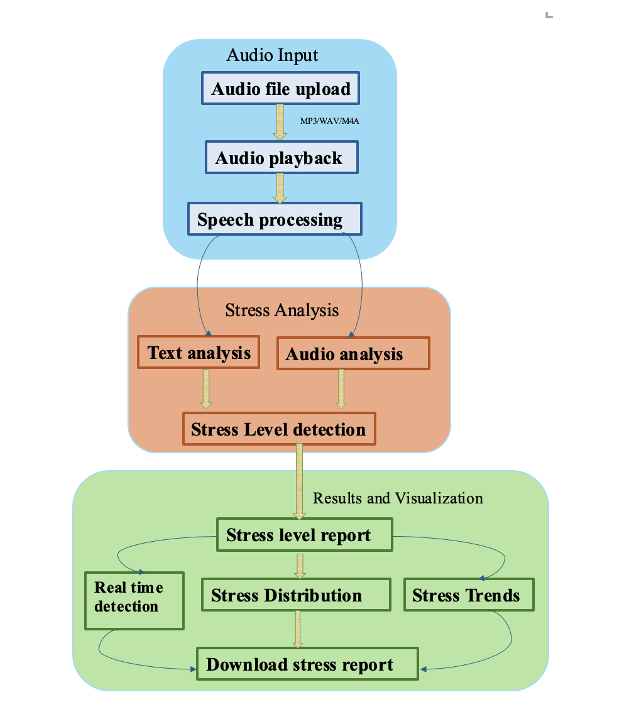
\includegraphics[width=1.1\columnwidth]{ap1.png}
    \caption{Overview of system approach}
    \label{fig:system_architecture}
\end{figure}
\vspace{10pt} % Add space to prevent overlap

  %\section{Significance of the Study}
 % This research contributes to the fields of mental health care, AI ethics, and multimodal AI by developing a system that combines advanced stress detection with interactive support.
  \section{Scope and Limitations}
 \textbf{Scope:}
 Focuses on voice-based stress detection and designs a stress trend module for user support.
 \textbf{Limitations:}
Does not include physiological signal data or longitudinal studies of user impact.
\section{Thesis Organization}
This thesis is structured into six chapters, each presenting a particular aspect of the study. Below is a brief overview of each chapter:
  \begin{enumerate} 
  \item  Chapter 1 cover  the research background, highlighting the importance of stress detection in mental health monitoring. It outlines the motivation, problem statement, research objectives, research questions, the significance of the study and scope and limitations, and the thesis organization. 
   \item Chapter 2 The literature review assesses previous work related to stress detection, focusing on speech-based and text-based emotion recognition, Social Signal Processing (SSP), and the role of deep learning and large language models, limitations in current stress detection and conversational AI systems. It highlights the lacking in current methods and shows the need for a multimodal strategy. 
   \item Chapter 3 This chapter describes the design and progress of the proposed multimodal stress detection system. It outlines the collection of dataset, data pre-processing procedures, and the two main modules: audio-based and text-based stress detection. Additionally, it describes the model designs, training and validation procedures and multimodal fusion techniques. 
   \item Chapter 4 This chapter highlights the actual implementation of proposed system. It describes the architecture and workflow, including speech-to-text processing, feature extraction. The chapter also describes the development of the user interface (UI), highlighting features such as real-time stress visualization and stress trend tracking, and report generation.
  \item  Chapter 5 This  chapter evaluates the performance of the proposed models, comparing their accuracy, precision, and recall across different approaches. It also includes experimental results between stress trend analysis system and human subjective analysis for stress. So, it highlights the system advantages and disadvantages.
  \item  Chapter 6 This chapter covers summary of the study, limitations and future considerations. Highlighting the research's contributions to the field of stress detection, the final chapter provides a summary of the main findings. In addition to discussing the shortcomings of the current system, it suggests future research objectives, such as real-time deployment, dataset enlargement, and interaction with other modalities including physiological data.

   \end{enumerate}
\chapter{Literature Review}
\clearpage 
  \section{Stress and Mental Health: A Psychological Perspective}
  Stress has a major impact on mental health and well-being through changes in physiological, emotional, and cognitive reactions. Effective techniques for early diagnosis and intervention are required because prolonged stress has been associated with a number of psychiatric diseases, such as anxiety and depression. Although the study (\citet{sebastiao2024}) showed on stress and mental health in COVID-19 emphasizes the importance of psychological flexibility and emotional schemas, it has a number of drawbacks. Avoid making judgments about causality by using a cross-sectional strategy. Potential biases are introduced by relying solely on self-reported data. Generalizability is limited by the sample. Results may also be affected by unmeasured variables, including socioeconomic status and previous mental health problems. Finally, results are impacted by the pandemic environment, which reduces their generalisability in non-pandemic scenarios. Despite these drawbacks, the study offers valuable information on the dynamics of mental health in emergencies. Traditional stress assessment relies on self-reported questionnaires such as the Perceived Stress Scale (PSS) and physiological measures such as heart rate variability (HRV) and cortisol levels. However, these methods can be intrusive, subjective, or impractical for continuous monitoring, leading to the need for automated non-invasive stress detection systems.
  In order to detect stress, (\citet{aristizabal2021})investigates the combination of self-reported data and wearable physiological sensors. In addition to self-reported stress levels, participants' electrodermal activity (EDA), heart rate (HR), and skin temperature were tracked using wearable technology as they performed stress-inducing tasks. These data streams were analysed by deep learning systems, which showed excellent accuracy in differentiating between stress levels. The study's semi-controlled laboratory environment, which would not accurately mimic stressors in the real world, and possible sample size and diversity restrictions, which would restrict generalisability, are some of its drawbacks. Reliability may also be impacted by sensor errors brought on by motion artefacts, self-report biases, and difficulties capturing quick shifts in stress.
  \section{Voice-Based Stress Detection}
  The communication medium Speech is a rich medium for detecting stress as it carries both linguistic and paralinguistic markers indicating stress. Research in speech emotion recognition (SER) has identified variations in prosodic features, such as pitch, intensity, speech rate, and spectral characteristics, as key indicators of stress with 97.1%
  accuracy utilising the Crema-D and TESS datasets, (\cite{chyan2022}) "A Deep Learning Approach for Stress Detection Through Speech with Audio Feature Analysis" investigates the use of CNN models for classifying stressed and unstressed speech based on Mel Spectrogram and MFCC characteristics. Nevertheless, the study has disadvantages, such as a controlled environment that does not replicate naturalistic noise situations, a binary classification approach that ignores shifting stress levels, and dataset constraints that do not represent real-world speech changes. Furthermore, the model's real-time applicability has not been validated, and its reliance on a small number of audio variables may ignore other elements. the study shows how deep learning may be used for speech-based stress detection and establishes the foundation for upcoming advancements in practical applications. 
This work employed the Toronto Emotional Speech Set (TESS), a popular dataset for emotion identification that includes vocal expressions from a range of emotional states. Convolutional neural networks (CNNs) and long short-term memory (LSTM) networks have been used in a number of research to extract and analyse voice data in order to classify emotions. While LSTMs capture temporal dependencies in sequential data, CNNs have been especially successful in processing spectrograms, which graphically depict frequency and amplitude fluctuations over time. By utilising both spatial and temporal feature representations, the hybrid models' integration of these architectures  will increase the accuracy of stress detection.
\section{Text based stress detection}
 in this study, author (\citet{yoon2020})investigates stress detection using semantic analysis of textual data, including private messages and postings on social media. The article analyses the approach on pertinent datasets to show its efficacy and finds linguistic patterns linked to stress using natural language processing (NLP) techniques. Nevertheless, there are a number of drawbacks, such as dataset restrictions that can fail to account for linguistic variation, contextual subtleties that could result in incorrect categorisation, and the lack of multimodal data like visual or aural signals. Furthermore, the model can have trouble keeping up with changing linguistic trends, necessitating frequent updates, and it poses privacy issues with relation to the use of personal data. 
\section{Social Signal Processing (SSP) in Mental Health Systems}
In this study, author(\citet{singh2019}) examines how SSP can be used to evaluate conversations by examining sentiment and emotional indicators. In order to better comprehend human interactions, SSP looks at non-verbal cues including gestures, vocal intonation, and facial expressions. This is especially important in industries like banking and finance, where it's critical to identify client dissatisfaction. The work intends to increase dialogue analysis for customer experience and service improvement by assessing emotional intensity in large data sets. However, the study has challenges, such as contextual limits because emotional expressions depend on conversational context and data quality issues because noisy or missing data might impair accuracy. Cultural differences also affect how nonverbal cues are interpreted, and deployment is complicated by the high computational resources required for real-time processing. Furthermore, analysing chats without the express consent of the user raises privacy problems. 

  \section{Machine Learning and Deep Learning for Stress Detection}
  The application of Machine Learning (ML) and deep learning (DL) approaches to stress detection and mental health monitoring is examined in this article\cite{razavi2024}. It draws attention to the efficacy of models such as Support Vector Machines (SVMs), Neural Networks (NNs), and Random Forest RFs, which use physiological data like skin reaction, heart rate variability (HRV), and heart rate (HR) as important stress indicators. In order to improve model performance, the study also highlights the significance of data preparation methods including feature selection and noise reduction. Nevertheless, there are a number of drawbacks, such as the inability to customise ML/DL models, which hinders their ability to adjust to different stress patterns, and their poor interpretability, which makes them less clear for clinical usage. Furthermore, the majority of research is carried out in controlled settings, which restricts its relevance in the real world, and real-time processing is still in its infancy, which makes real time interventions less feasible.
  In order to increase classification accuracy, the \cite{yao2021} presents a technique for stress detection that combines linguistic cues from text with acoustic data from speech. Compared to unimodal systems that only use text or audio, the multimodal method performs better because it uses machine learning techniques to analyse the interaction between language and vocal emotions. The lack of high-quality, labelled datasets with both text and audio components is one of the study's flaws though, and it may limit generalisability. Implementation is resource-intensive due to the contextual diversity in stress expression between cultures and individuals, which necessitates substantial training on varied datasets. In real-time processing, where accuracy and low latency must be preserved in dynamic situations, the system also faces difficulties. Error sources may also be introduced by the difficulties in synchronising text and auditory data. 
  \cite{hilmy2021} emphasises how well machine learning models like Support Vector Machines (SVMs) and Mel-Frequency Cepstral Coefficients (MFCCs) work for categorising stress and extracting spectral information from speech. While SVMs have strong classification capabilities, MFCCs are especially good at capturing speech characteristics that distinguish between stressed and neutral states. Studies have shown that this method may identify stress with high accuracy rates 88 Nevertheless, drawbacks include reliance on varied and high-quality datasets, which are frequently challenging to get by, and environmental noise, which can reduce the precision of feature extraction. Furthermore, the computing needs of SVM classification and MFCC extraction create problems for real-time processing. Model generalisability is also impacted by individual variations in speech patterns, such as accents and speaking styles, which calls for customised or adaptive methods. 


  \section{Role of Large Language Models (LLMs) in stress Analysis}
  In this research, author (\citet{shen2024}) investigates if Large Language Models (LLMs) undergo similar performance variations to humans when under stress. According to the Yerkes-Dodson law, which states that excessive or insufficient stress lowers efficiency, researchers discovered that LLMs operate best under moderate stress using StressPrompt, a series of stress-inducing prompts based on psychological theories. The study also showed that LLMs' internal brain representations were impacted by stress-altering stimuli, which mirrored human stress reactions. Nevertheless, there are a number of drawbacks, including as the limited generalisability of prompt-based stress induction—which may not accurately mimic real stress experiences—and the fact that results may differ depending on the LLM design. Furthermore, because the study was carried out in controlled environments and LLMs do not have human-like physiological reactions, it lacks real-world validation, which may affect how accurately stress comparisons are made. 
  \section{Limitations in Current Stress Detection and Conversational AI Systems}
 in this study, author (\citet{teye2022}) investigates how contextual and cultural factors affect conversational AI systems' ability to recognise emotions. In order to classify seven fundamental emotions, including sarcasm, the study created an emotion prediction model that included voice and picture data, with accuracies ranging from 85\% to 95\%. In order to increase the dependability and moral coherence of emotion detection systems across a range of demographics, the authors stress the importance of taking environmental factors and cultural quirks into account. However, the study has drawbacks, such as difficulties with data representation because datasets are frequently undiversified, which impairs the model's cross-cultural generalisability. Furthermore, despite efforts to balance, biases in datasets continue to exist, which could diminish fairness. Because sarcasm is nuanced and context-dependent, it is still very difficult to detect. The performance of the system can also be impacted by environmental fluctuations, including background noise.
  By utilising real-time data fusion from several sources, including environmental sensors, biometric devices, and Internet of Things systems, the combination of sensor technologies and conversational AI allows for context-sensitive interactions. By improving AI's comprehension of user context, physical circumstances, and environment, author \cite{kush2025} enables more intelligent and flexible interactions. For instance, conversational AI in healthcare enhances the responsiveness and personalisation of virtual health aides by integrating data such as temperature, stress levels, and heart rate. To fully realise the potential of these systems, however, issues like interoperability, scalability, and data heterogeneity must be resolved. The ability of sensor-integrated AI to provide real-time, context-aware help is demonstrated by real-world implementations, such as Mercedes-Benz's integration of Google's conversational AI agent into cars, opening the door for cutting-edge solutions across industries.
  \section{Ethical Challenges in AI-Driven Stress Detection}
  In the paper, author (\citet{sriramprakash2017}) examines the expanding use of AI in mental health care, emphasizing how it can enhance early identification, accessibility, and personalized care. Virtual assistants and AI-powered chatbots offer prompt assistance, and predictive analytics can help spot mental health problems before they get out of hand. The study also identifies problems that make it difficult to understand AI-driven decisions, including algorithmic transparency issues, lack of human empathy in AI interactions, and data privacy concerns. Along with difficulties in incorporating AI into conventional healthcare systems due to patient and practitioner reluctance, ethical issues such as consent and autonomy continue to be crucial. In order to guarantee that AI improves mental health care while upholding ethical standards, further developments in emotionally intelligent AI, improved integration with healthcare services, and robust regulatory frameworks will be crucial.
 % \renewcommand{\arraystretch}{1.2} % Adjust row height
 %\renewcommand{\arraystretch}{1.0} % Tighter row spacing
  \vspace{-5mm} % Reduce vertical space before the table
 \begin{table}[H]
\centering
\caption{Summary of literature review}
\label{tab:correlation_table}
%\small % Reduce the font size of the entire table
\begin{tabular}{|p{1.8cm}|p{2.8cm}|p{4.3cm}|p{4.3cm}|}
\hline
 Author & Technique & Findings & Limitations \\ \hline
 Chyan et al\cite{chyan2022}  & CNN for speech-based stress detection & Utilizes MFCCs and Mel Spectrograms to classify stress in speech with high accuracy (97.1\%). & Controlled setup; binary classification misses stress gradation; lacks real-time validation; ignores real-world noise.\\ \hline
 Study on LLMs \cite{teye2022} & StressPrompt for stress analysis in LLMs & Demonstrates performance variations in LLMs under stress using psychological prompts. & Lacks real-world validation; results depend on specific LLM design and controlled settings; no physiological equivalence to humans\\ \hline
\cite{yoon2020} & Semantic analysis of textual data & Identifies linguistic patterns in private messages and social media posts to detect stress using NLP & Dataset limitations; lacks multimodal data; struggles with linguistic trends and contextual subtleties; raises privacy concerns.\\ \hline
\cite{singh2019} & Social Signal Processing (SSP) for emotion detection & Analyses sentiment through non-verbal cues such as gestures and intonation. & Data quality issues; computationally intensive; contextual limitations; privacy concerns in analyzing conversations\\ \hline
 Multimodal Study \cite{razavi2024} & Combining text and audio signals & Outperforms unimodal approaches by integrating linguistic cues and vocal emotions; uses ML for interaction analysis. & Resource-intensive; lacks high-quality multimodal datasets; difficulties in synchronizing text and audio data for real-time application\\ \hline
 \cite{teye2022} & Ethical AI in mental health care & Highlights AI’s potential for early intervention and personalized care. & Challenges in algorithmic transparency; lack of human empathy in AI; privacy concerns. \\ \hline % resistance from patients and practitioners; difficulty in integrating AI into conventional systems.\\ \hline
\end{tabular}
\end{table}
\vspace{-5mm} % Reduce vertical space after the table
%%%%%%%
%\begin{table}[p] % Use [H] to place the table here
%\centering
%\caption{Summary}
%\label{tab:dataset_table} % Optional, for referencing the table
%\begin{tabular}{|p{2.5cm}|p{3cm}|p{4.5cm}|p{4.5cm}|} % Adjusted column widths
%\hline
%\raggedright \textbf{Year \& Author(s)} &
%\raggedright \textbf{Techniques/Methods} &
%\raggedright \textbf{Findings} &
%\raggedright \textbf{Limitations} \\
%\hline

%\hline
%2024, Chyan et al. & CNN for speech-based stress detection & Utilizes MFCCs and Mel Spectrograms to classify stress in speech with high accuracy (97.1\%). & Controlled setup; binary classification misses stress gradation; lacks real-time validation; ignores real-world noise and dataset variability. \\
%\hline
%2022, Study on ML/DL Models & SVM, RF, and NN for physiological data & Highlights the utility of feature selection, skin reaction, HRV, and HR for stress detection with ML/DL models. & Lack of adaptability; controlled setups limit real-world application; low interpretability for clinical use; real-time implementation remains immature. \\
%\hline
%2024, Multimodal Study & Combining text and audio signals & Outperforms unimodal approaches by integrating linguistic cues and vocal emotions; uses machine learning for interaction analysis. & Resource-intensive; lacks high-quality multimodal datasets; cultural and individual diversity challenges; difficulties in synchronizing text and audio data for real-time application. \\
%\hline
%2024, Yiqun et al. & SVM with MFCCs & High accuracy for stress classification by extracting spectral features from speech. & Requires diverse and high-quality datasets; affected by environmental noise; computational challenges for real-time use; individual variability limits model generalizability. \\
%\hline
%2024, Study on LLMs & StressPrompt for stress analysis in LLMs & Demonstrates performance variations in LLMs under stress using psychological prompts; identifies internal representation shifts similar to humans. & Lacks real-world validation; limited generalizability; results depend on specific LLM design and controlled settings; no physiological equivalence to humans. \\
%\hline
%2024, Macháček et al. & Cultural and contextual emotion detection via AI & Combines voice and image data to classify emotions; achieves accuracies from 85\% to 95\%. & Struggles with sarcasm detection; dataset biases reduce generalizability; environmental noise impacts performance; challenges in ensuring fairness and cross-cultural consistency. \\
%\hline
%2024, Ranjan \& Thakur & IoT and biometric integration in conversational AI & Enhances contextual and environmental understanding for AI in healthcare; integrates biometric data for improved personalization and real-time response. & Issues with scalability, interoperability, and data heterogeneity; computationally intensive for real-time fusion of multiple data sources. \\
%\hline
%2024, Teye et al. & Ethical AI in mental health care & Highlights AI’s potential for early intervention and personalized care; emphasizes the need for regulatory frameworks and ethical standards. & Challenges in algorithmic transparency; lack of human empathy in AI; privacy concerns; resistance from patients and practitioners; difficulty in integrating AI into conventional systems. \\
%\hline
%\end{tabular}
%\end{table}

  \section{Research Gaps and Opportunities}
The majority of the research that has been done on stress detection has been either text-based or audio-based. Even while CNNs and LSTMs have shown excellent accuracy in identifying speech emotions, feature selection and dataset quality changes depending on dataset. LLMs have shown promise in extracting stress-related linguistic features, but their effectiveness in combination with voice analysis is still being explored. In order to fill this gap, this study proposes a multimodal stress detection system that uses both textual and auditory signals. A real-time user interface (UI) with stress trend tracking is also created to enhance accessibility and user interaction. In order to facilitate practical uses in mental health monitoring and emotional well-being, the results of this study assist in establishing solid and interpretable stress detection frameworks.
\section{Summary of the review}
Despite significant advancements in text and audio-based stress detection, current approaches as shown in Table 2.1 lack the accuracy and contextual understanding needed for real-time applications. This review highlights the need for multimodal systems that integrate linguistic and paralinguistic cues, offering a foundation for this study.
\chapter{System Design}
\clearpage 
Text and audio embeddings are the two main modules that comprise up system. The system is thoughtfully designed to effectively combine both textual and audio information, creating a strong foundation for multimodal stress detection.The ability of the system to produce responses that resemble those of a human is directly influenced by the textual interpretation with whisper and GPT-4analysis.Key aspects of the design include well-structured pipelines, efficient deployment strategies, and thorough dataset preparation. Each element has been carefully crafted to enhance the system's usability, scalability, and accuracy, ensuring it delivers reliable and practical results.
\section{System architecture}
Using multimodal inputs, the suggested system combines several parts to identify and display stress levels. The architecture is separated into three main modules, as seen in Figure 3.1: 
Frontend (Streamlit): In handling user interaction, including audio file uploads and results visualisation.  
Backend (Flask): Manages essential features including stress analysis, speech-to-text conversion, and external service interaction. 
External Services: These comprise advanced text analysis APIs such as OpenAI for GPT-4. 
These parts work together seamlessly ensuring that the system is scalable, responsive, and able to process inputs in real time. 
\begin{figure}[h]
    \centering
    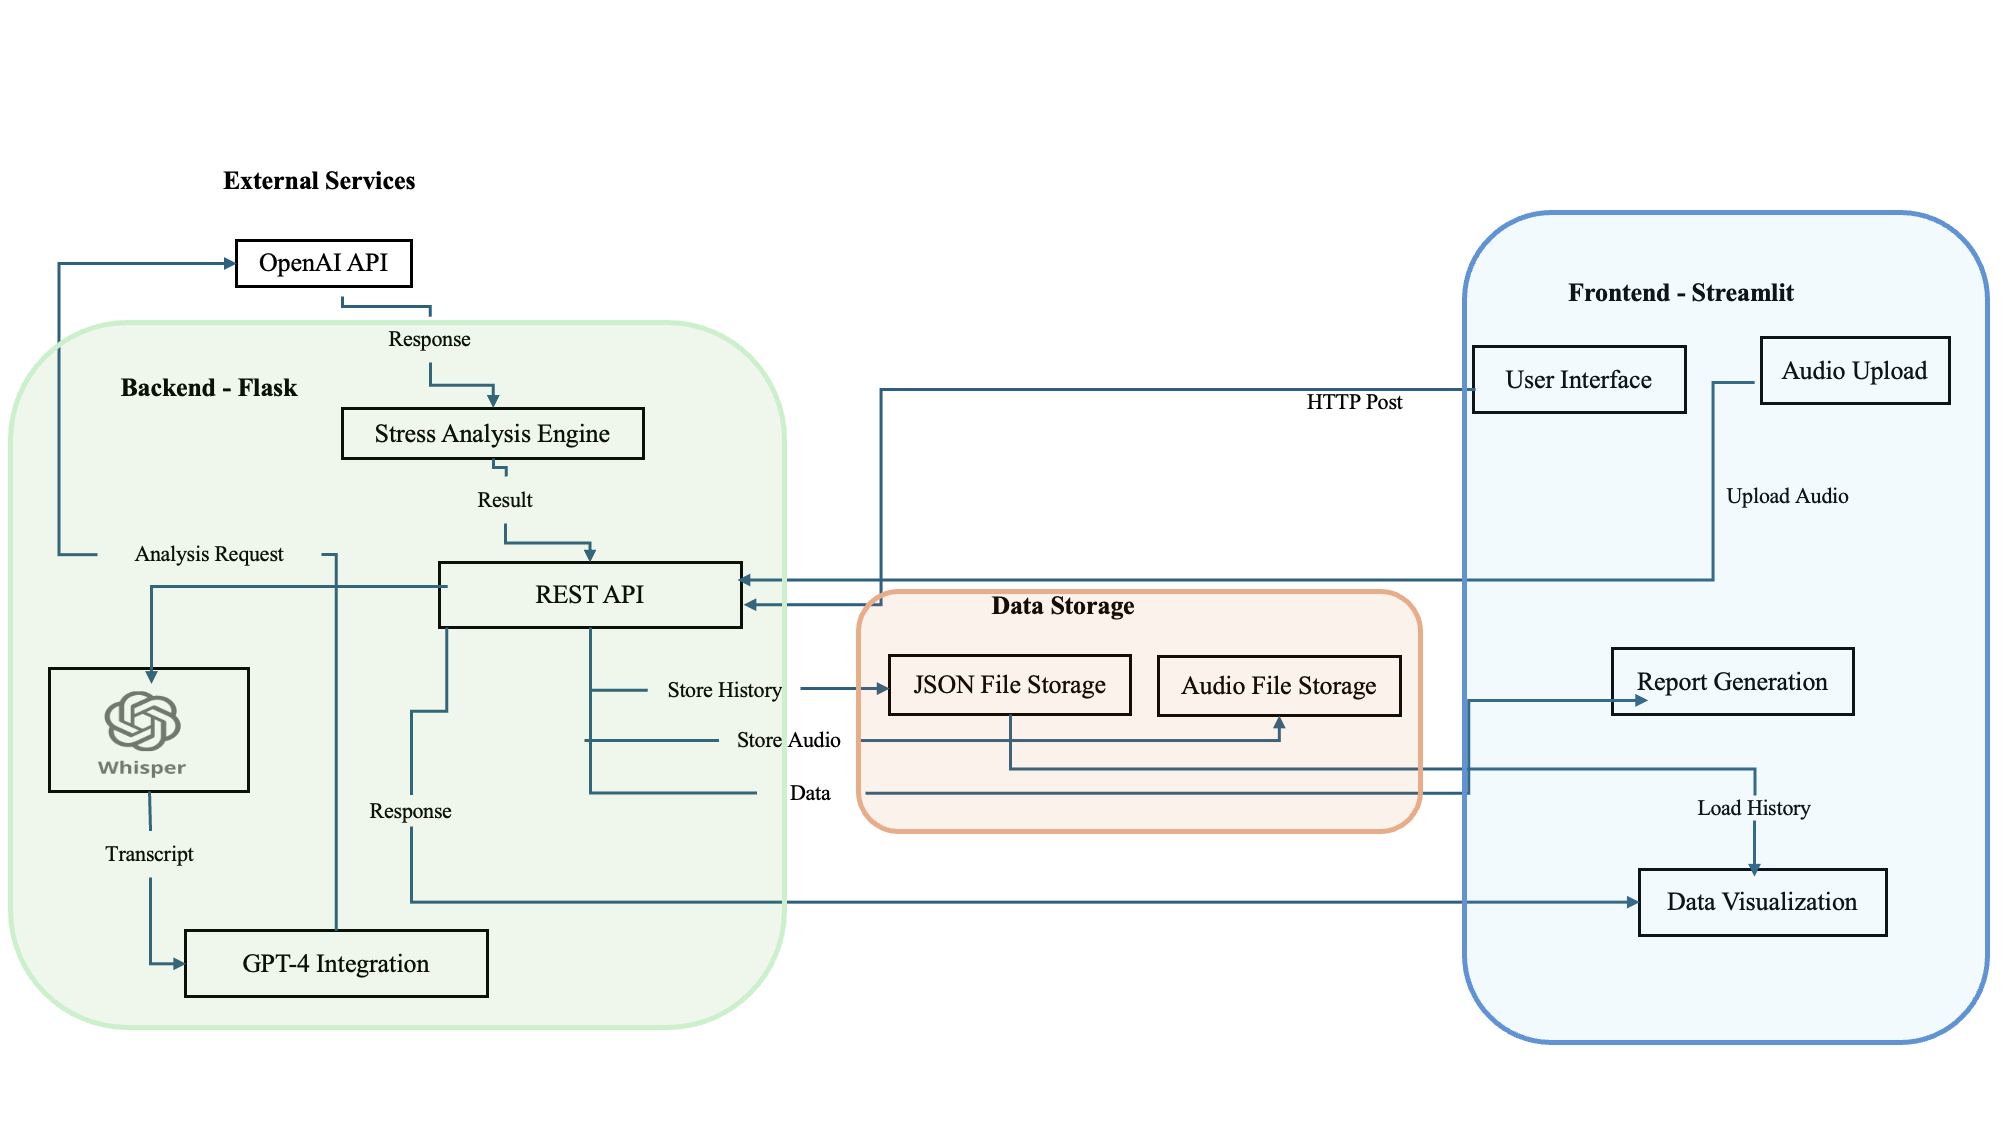
\includegraphics[width=1.1\columnwidth]{allreferences/systemdesigndia.png}
    \caption{Proposed System Architecture}
    \label{fig:system_architecture}
\end{figure}
\section{Dataset Description}
  A limited number of audio recordings was used to generate and illustrate the functioning of the stress detection system's user interface (UI) and user experience (UX) components. These recordings, which come from openly accessible websites like Google, feature speech samples with a range of psychological tones. Even though the audio files don't represent a formal or standardized dataset, they are a useful tool for demonstrating the system's features, like trend monitoring and real-time stress level visualization. I used the audio file to capture voice at different stress levels. After processing these data, stress detection outputs were simulated and shown on the user interface. These samples are primarily being used to test and validate the stress visualisation features of interface and illustrate how stress trend tracking works throughout several sessions. Also checking interface is capable of handlingvarious stressful aspects.
\begin{table}[p] % Use [H] to keep the table close to the text
\centering
\caption{Dataset Description}
\label{tab:dataset_table} % Optional, for referencing the table
\begin{tabular}{|c|p{8cm}|} % Adjusted column width for better text wrapping
\hline
\textbf{Audio} & \textbf{Text in the Audio} \\ \hline
Audio1 & I wonder what this is about \\ \hline
Fire & The place is on fire, please send help \\ \hline
Test1 & Loans that we can offer with this or farm ownership loans, operating lines of credit, or equipment and capital improvement need loans. The benefit to the \\ \hline
sad.Wav & The best food novel count me on the edge of my side \\ \hline
New recording 19.wav & 時間が戻れば私はあの時間に戻りたいま一回 \\ \hline
New recording 16.wav & So um... I'm sick. But my friend wanted me to be a deity myself because we always had to really cool. So uh... Yeah, here it is. Do you want me to sing? Oh, it sounds really good singing. \\ \hline
new recording 23.wav & Life is difficult, but you are loved. You are loved and important, and you bring to this world things that no one else can so hold on \\ \hline
Airplane.wav & The airplane is almost full.\\ \hline
Gamer.mp3 & Why would you not want to fight for what you believe in? \\ \hline
Sad.mp3 & The delicious aroma of freshly baked bread filled the bakery. \\ \hline
1008TIE.wav & That is exactly what happened.\\ \hline
New recording 25.wav & Us comfort help isn't given up. It's refusing to give up. To use fall for a reason, and to use strength and weakness. I think... \\ \hline
\end{tabular}
\end{table}
\section{Text Processing workflow}
%\clearpage  % Forces all previous content to be placed before this point
The Text Processing Workflow describes the procedures for evaluating and interpreting the text to detect stress. Figure 3.2 shows the text processing workflow, which consists of the following steps: Whisper converts audio into raw text. Using semantic context, GPT-4 analyzes the text to find stress signals. The system uses stress scale to classify stress levels (Low, Moderate, High). The system gives feedback, including stress management tips, based on the user's degree of stress. Each component in a text processing flow is responsible for handling a specific task. For example, an input handler handles text input from audio or manual entry, while an analysis engine uses GPT-4 to analyze text for stress content and analyze numerical stress levels. The formatter gets the results ready to be shown. The report generator generates reports that can be downloaded, while the display handler manages visual representation. It focuses on the processing of textual information obtained from speech. Whisper and GPT-4 are the main tools used in this workflow for the transcribed text's semantic analysis.
 %\clearpage  % Forces all previous content to be placed before this point
%\vspace{-5mm} % Reduce vertical space
\begin{figure}[!htbp]
\centering
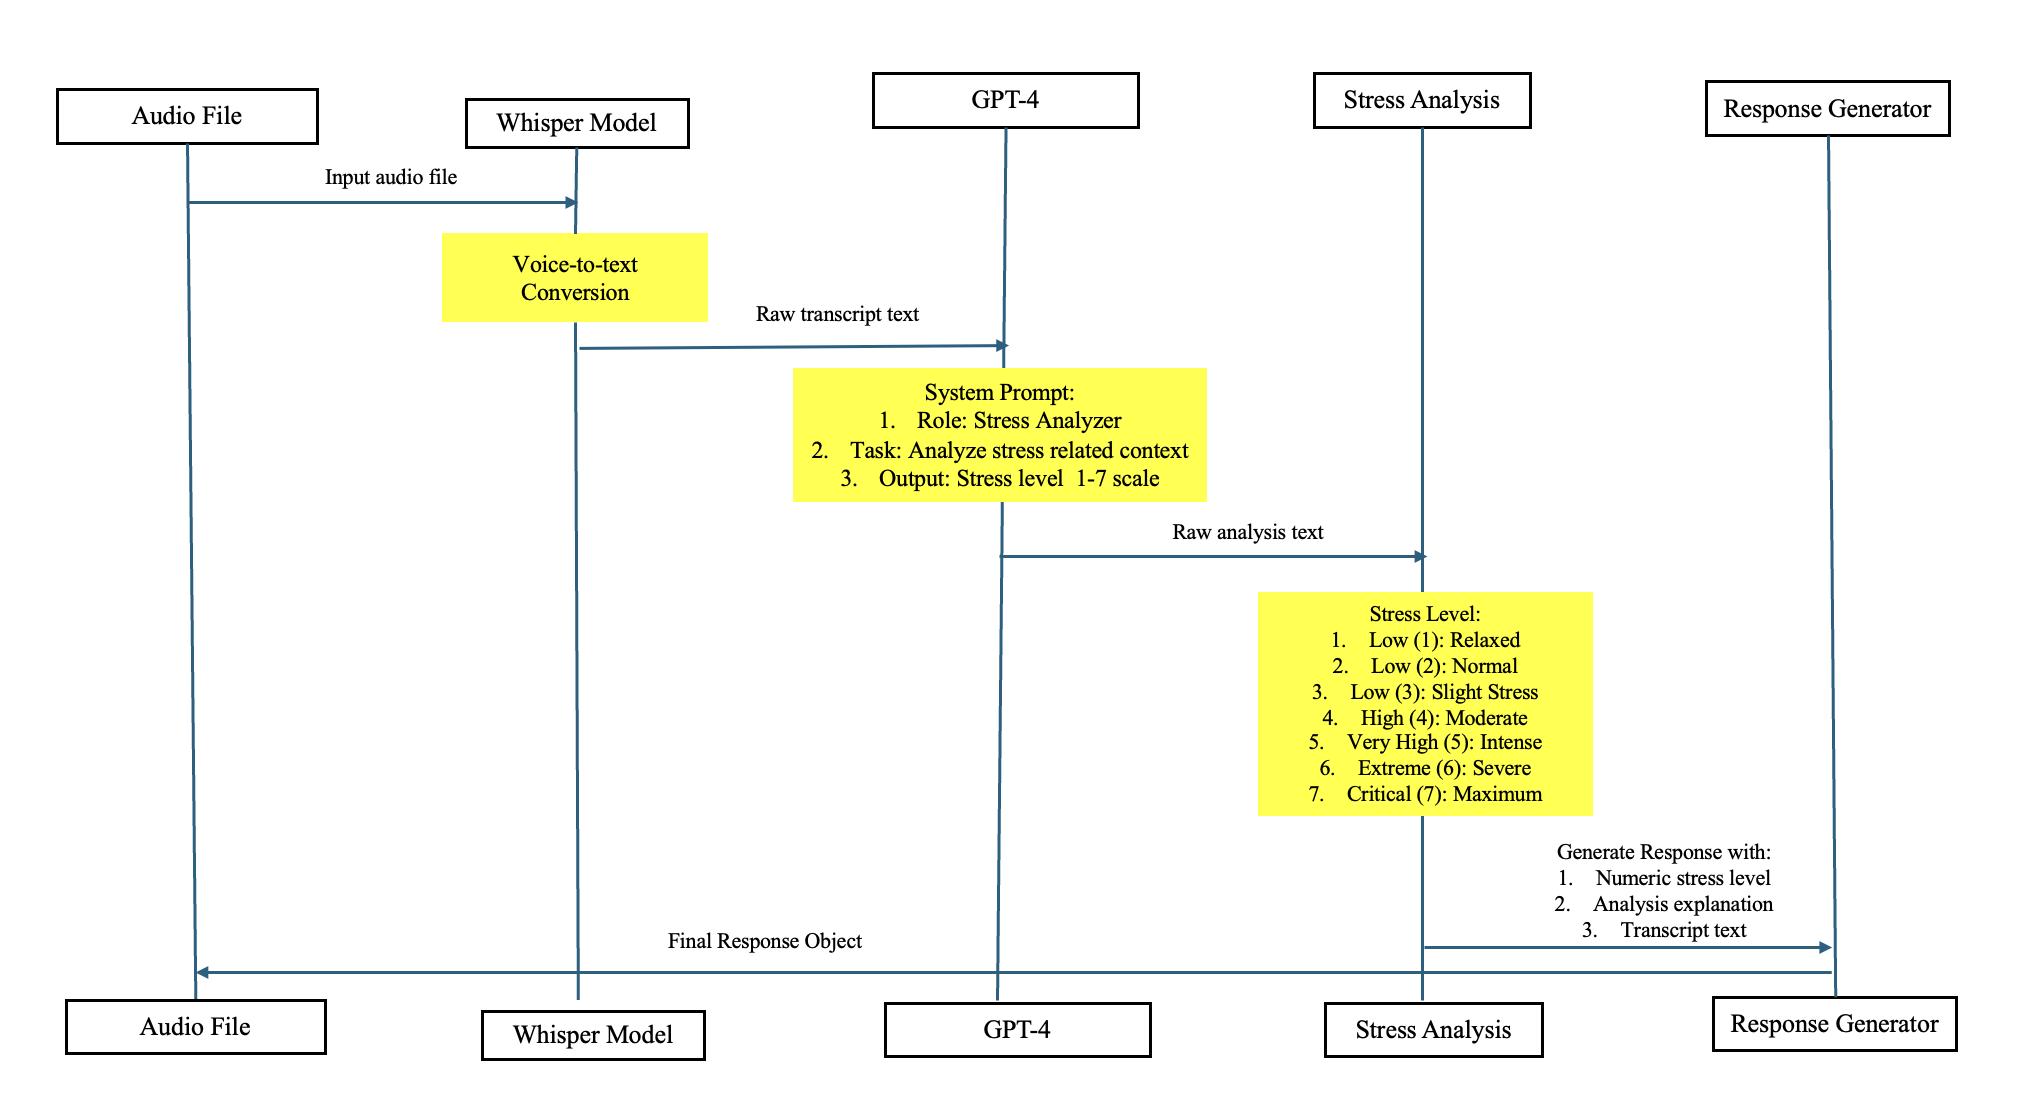
\includegraphics[width=1.2\textwidth]{allreferences/textprocessingworkflow.png}
\caption{Text processing flow}
\label{fig:text flow}
\end{figure}
\subsection{Speech to Text Conversion (Whisper)}
\noindent
\begin{minipage}{\textwidth}
The use of Whisper\cite{machaek2023} for accurate transcription. For the flow of text generation This text processing module combines the manual transcript input option, text cleaning and preparation, and whisper to convert speech to text. Whisper converts speech to text.Draw attention to Whisper's main function of converting audio into text transcripts.  This module transcribes user speech into text and performs language analysis to detect stress-related context. Identifies specific words and phrases associated with stress, using GPT-4's capabilities to interpret context. The system captures the audio. The raw audio is passed into the speech recognition API. OpenAI‘s Whisper to convert into text. The voice in the audio file is converted into a textual transcript. For text formatting, the transcript is formed as cleaned or standardized and removing unnecessary pauses or artifacts. 
 The significance of text preparation for analysis, noise reduction, and transcription accuracy is emphasized.The Whisper model processes audio inputs and generates a transcript with a high degree of accuracy, filtering out noise and ensuring that only meaningful words are passed to the next stage.
 %\clearpage % Forces all previous content to finish
%\vspace{-5mm} % Adjust the value as needed to reduce the gap
\vspace{10pt} % Add space to prevent overlap
\FloatBarrier
\begin{figure}[H]
\centering
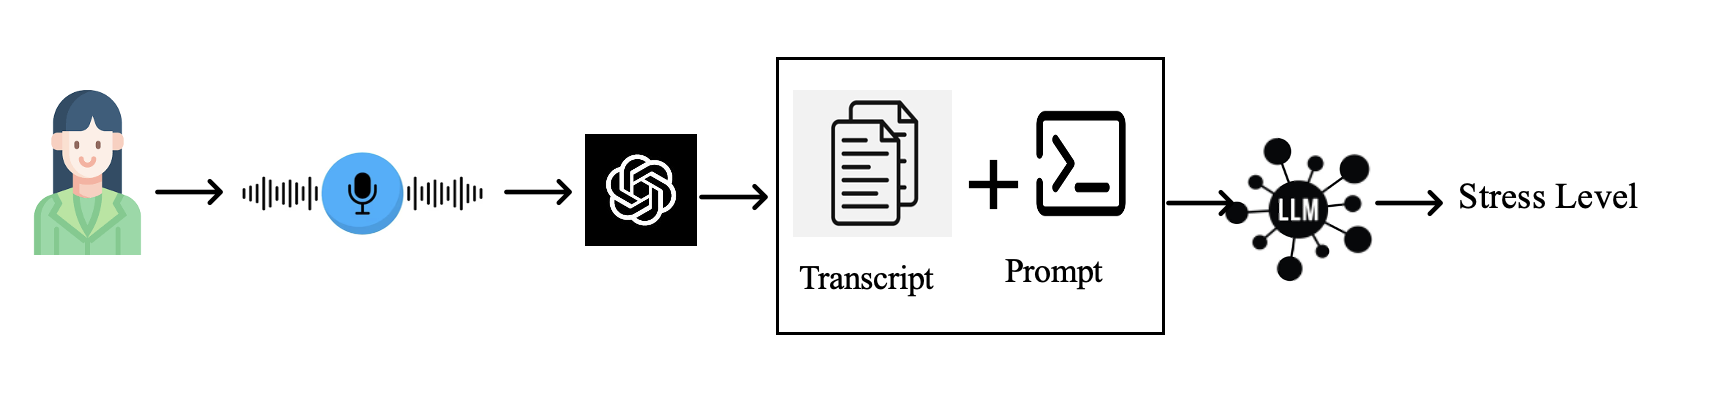
\includegraphics[width=1.0\columnwidth]{allreferences/textualnetwork2.png}
\caption{Textual analysis}
\label{fig:system_architecture}
\end{figure}
\end{minipage}
\vspace{10pt} % Add space to prevent overlap
%\subsection{GPT-4 analysis setup}
%GPT-4 is set up to detect stress patterns and analyze the context. And also measures the stress level from 1 to 7 and provides an explanation. GPT-4 interprets textual input to identify contextual and semantic stress signals and its natural language processing (NLP) skills to find contextual meanings and phrases that cause stress. 
%For instance: "GPT-4 analyses the transcript by detecting linguistic cues and contextual stress indicators, such as emotional word choices or abrupt sentence patterns." 
%\subsection{Stress level scale}
 %The scale utilized to classify the intensity of stress and discuss how textual cues, such as sentence structure and word choice, affect the identification of stress levels.
 %For instance: "Stress levels are determined based on linguistic patterns like frequent use of negative words, abrupt transitions in tone, and word repetition." 
%\subsection{Response generation}
%The system generates customized feedback. The result was processed using explanation formatting, colour coding according to level, and numerical stress level mapping. The display feature consists of the original transcript, detailed analysis text, and color-coded stress indicators. The ability of the system to produce responses that resemble those of a human is directly influenced by the textual interpretation. 
%For instance: "The generated response includes stress-relieving suggestions that are directly informed by the context of the transcribed text." 

\section{Audio Processing workflow} 
The main focus of the Audio Processing Workflow is the analysis of text data along with raw audio characteristics like pitch, tone, and frequency. This section describes how the use of voice characteristics in audio data enhances the stress detection system. Figure 3.3 illustrates the audio processing process that combines GPT-4, Whisper, and the backend to analyse stress. Important actions consist of utilising the frontend to upload the audio file. Whisper audio to text conversion. Using GPT-4 to perform stress analysis and storing audio files and JSON results for tracking history. The processing pipeline goes as follows: Whisper converts audio to a transcript, the frontend uploads the audio file to the Flask backend, which keeps it temporarily. The transcript is then submitted to GPT-4 for stress analysis, the results are kept in a JSON history, and the frontend receives the response. Using a REST API design, the system's frontend and backend operate on the default ports of Streamlit and Flask, respectively. They communicate via HTTP POST requests, file transfers take place via multipart/form-data, and JSON is delivered as the result. 
\vspace{10pt} % Add space to prevent overlap
\begin{figure}[H]
    \centering
    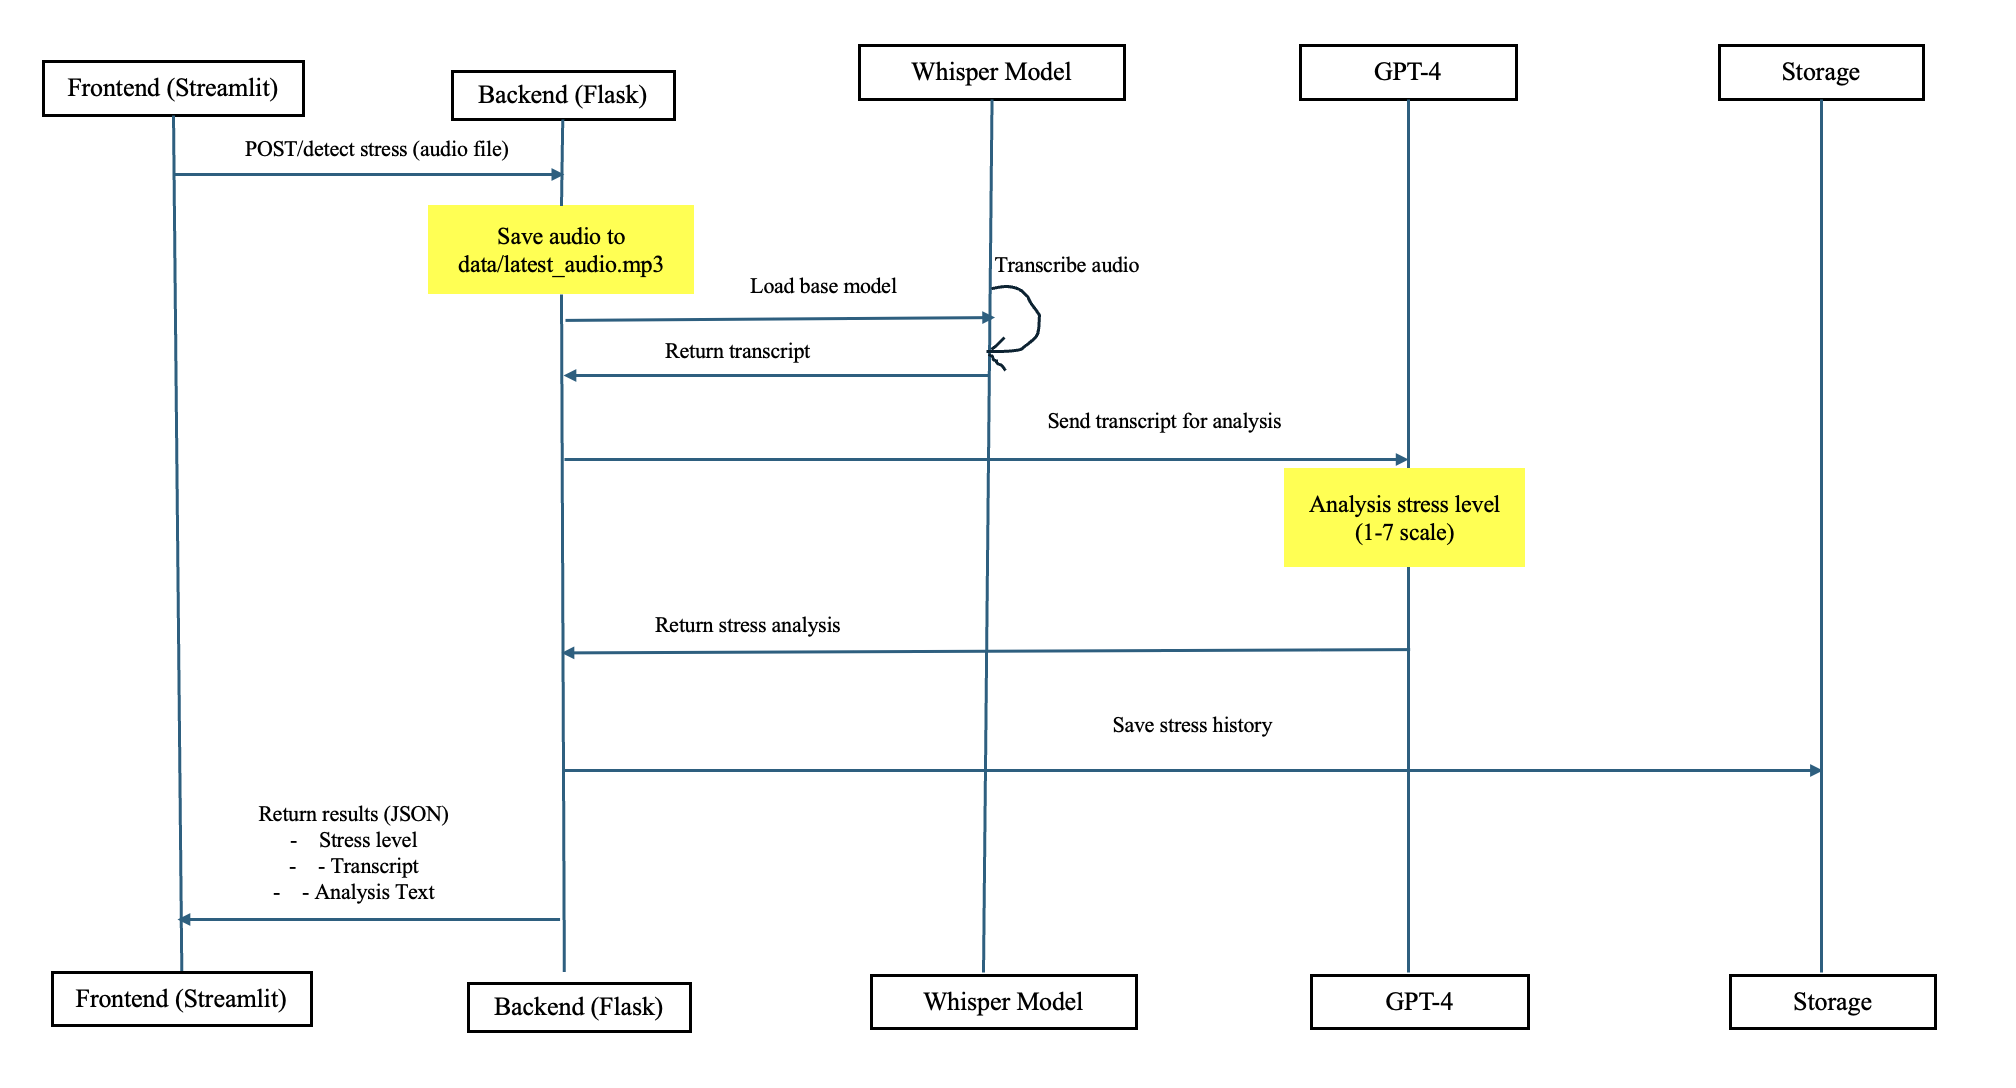
\includegraphics[width=1.1\columnwidth]{allreferences/audioflow.png}
    \caption{Audio processing flow}
    \label{fig:system_architecture}
\end{figure}
\vspace{10pt} % Add space to prevent overlap
%\subsection{Whisper for Speech-to-Text:}
%Whisper handles transcription. Distinguish by highlighting  how the impact of audio pre-processing (such as managing background noise and accents) on transcription quality. Whisper's capacity to retain vocal inflections for stress analysis later on. 
%For instance: "Whisper not only transcribes audio into text but also captures subtle vocal characteristics, such as tone fluctuations, which are critical for stress detection." 
%\subsection{GPT-4 for Stress Analysis}
%GPT-4's role in detecting stress patterns.
%In GPT-4's analysis, focus to how audio characteristics (such tone or pitch) enhance the text and discuss about how GPT-4 improves accuracy by combining vocal stress signals with semantic context. 
%For instance: "GPT-4 combines the tonal data from the audio with semantic analysis of the transcript, creating a holistic view of the user's stress levels." 
\subsection{Frontend to Backend Connection and Backend API Endpoint}
Data flows between the user interface and backend. How audio files are uploaded and routed to the backend for processing, highlighting the variations in data flow. 
For instance: "The frontend enables seamless audio file uploads, which are processed through APIs to generate real-time stress analysis results." 
APIs are utilized for seamless communication and emphasizing how the backend responds to demands for processing that are particular to audio in a different way than it does to text. 
For instance: "Backend APIs facilitate efficient data flow, ensuring that both audio features and their textual representations are analyzed synchronously." 
\section{Stress visualization workflow}
This section describes an intuitive and interactive way for users to view their stress levels. Users can see their stress levels in an easy-to-understand format with the help of the stress visualization workflow (Figure 3.4). Stress data recorded in JSON is loaded by users interacting with the UI. Plotly and other libraries are used to process data and produce pie charts and other graphics. Interactive elements and insights into stress distribution are two of the visualization's main characteristics. Interactive elements such as Legend for reference, Click-to-hide sections and hover tooltips that display precise percentages. Clear patterns and stress percentages are displayed in visualisations, which aid users in efficiently interpreting their data.By choosing the option to "View stress trends," the user starts the process. A slider is then used by the user to select a time range for stress visualization. The process of retrieving and preprocessing. In data loading and Processing portion invloves of fetching stress data (from JSON) and get it ready for visualization. In this procedure, user-selected data is loaded according to the designated time frame. Arranging and preprocessing data in preparation for analysis. Explains how stress levels are represented by colour coding: red for excessive stress, yellow for moderate stress, and green for low stress. Consistency and clarity in visual representation are assured by this arrangement of data. It shows how graphical outputs are generated from the analyzed stress data. The proportions of various stress levels are displayed using a pie chart. The Plotly library makes it easier to create dynamic charts with features such as Precise labels. Interactive sections, such as click-to-hide. Stress data is represented graphically. Visuals are rendered on the user interface, draws attention to the way the Streamlit user interface renders the images: Interactive elements and the pie chart are shown in the application. The visualizations make it simple for users to explore their stress data
%\vspace{-5mm} % Adjust the value to control the spacing
\vspace{10pt} % Add space to prevent overlap
% Example
\FloatBarrier
\begin{figure}[H]
    \centering
    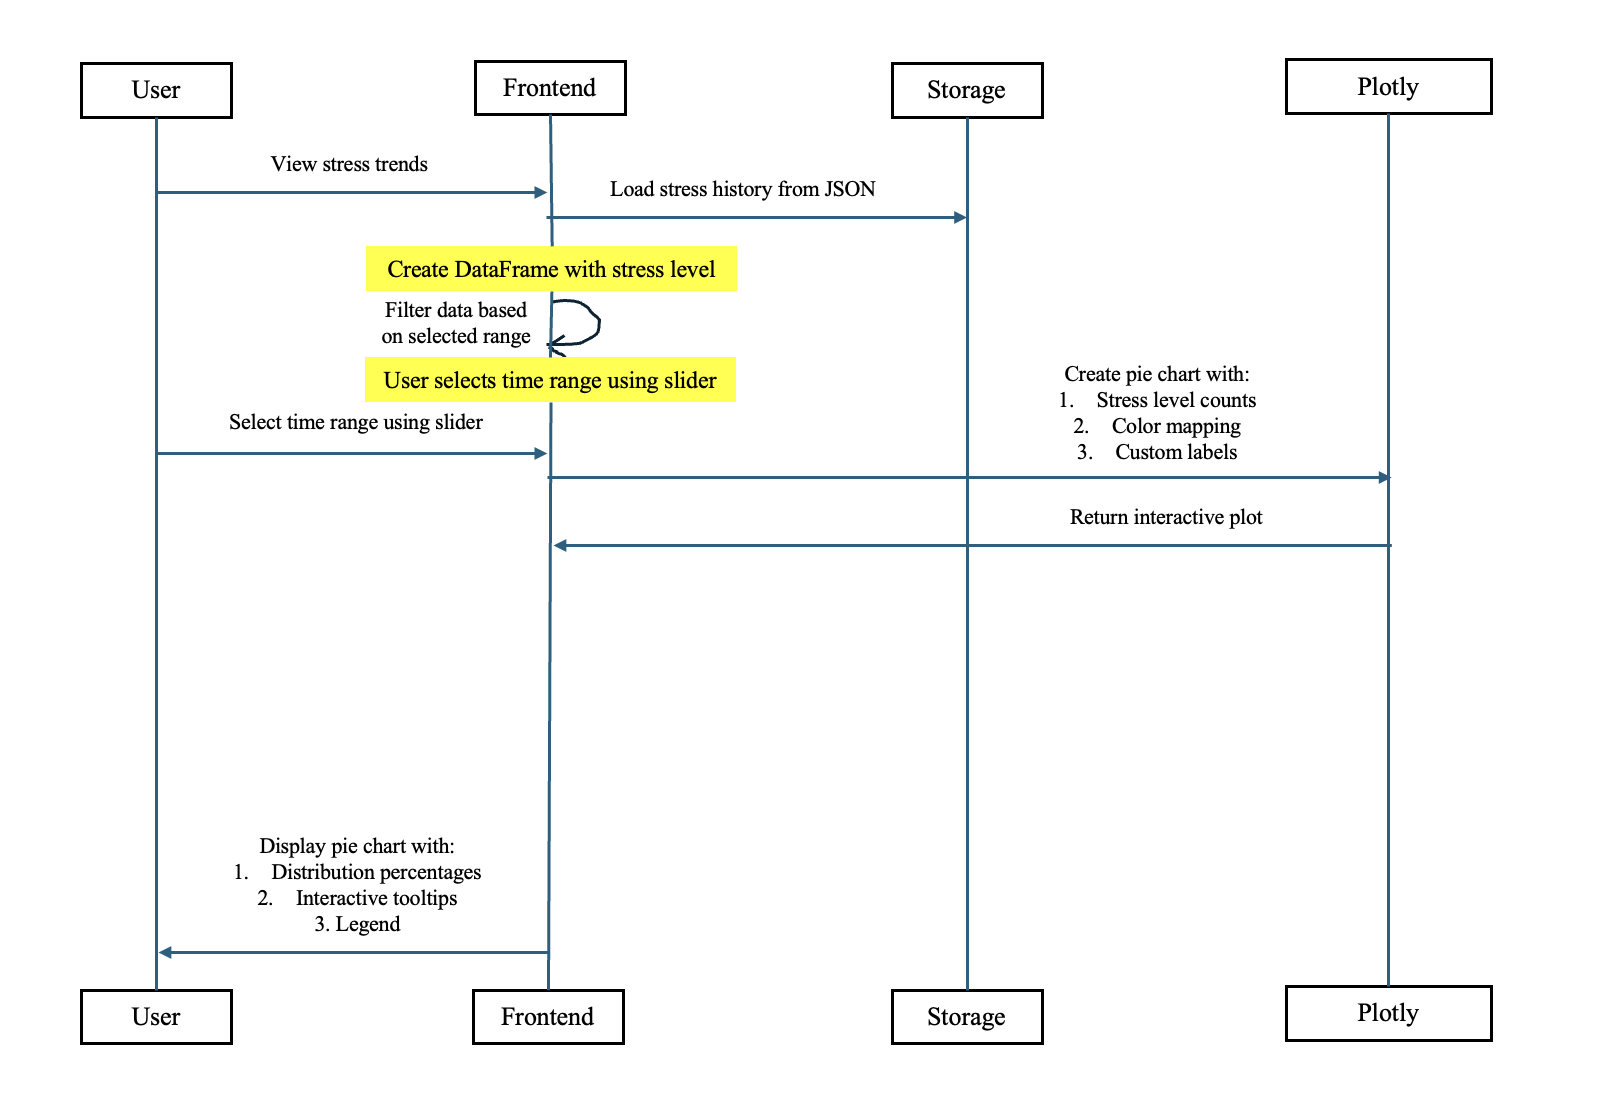
\includegraphics[width=1.0\columnwidth]{allreferences/piestressvisual.png}
    \caption{Stress Visualization Flow}
    \label{fig:system_architecture}
\end{figure}
\FloatBarrier
\vspace{10pt} % Add space to prevent overlap
%\subsection{Data Loading and Processing}
%By choosing the option to "View stress trends," the user starts the process. A slider is then used by the user to select a time range for stress visualization. The process of retrieving and preprocessing. In data loading and Processing portion invloves of fetching stress data (from JSON) and get it ready for visualization. In this procedure, user-selected data is loaded according to the designated time frame. Arranging and preprocessing data in preparation for analysis. 

%\subsection{Color Mapping Setup}
%This subsection explains how stress levels are represented by colour coding: red for excessive stress, yellow for moderate stress, and green for low stress. Consistency and clarity in visual representation are assured by this arrangement of data. It shows how graphical outputs are generated from the analyzed stress data. The proportions of various stress levels are displayed using a pie chart. The Plotly library makes it easier to create dynamic charts with features such as Precise labels. Interactive sections, such as click-to-hide. Stress data is represented graphically. Visuals are rendered on the user interface, draws attention to the way the Streamlit user interface renders the images: Interactive elements and the pie chart are shown in the application. The visualizations make it simple for users to explore their stress data.
\section{Stress trend analysis workflow}
Changes in stress levels over time are monitored via the stress trend analysis workflow (Figure 3.5). To examine certain sessions, users can use time ranges to filter data and to improve insights and smooth out volatility, the system computes moving averages. Trends are displayed using interactive charts that can be customized. Interactive features include zoom and pan controls, a time range slider for filtering data, hover tooltips for displaying precise values, and a legend for trend lines and stress levels. 
\vspace{10pt} % Add space to prevent overlap
\begin{figure}[H]
    \centering
    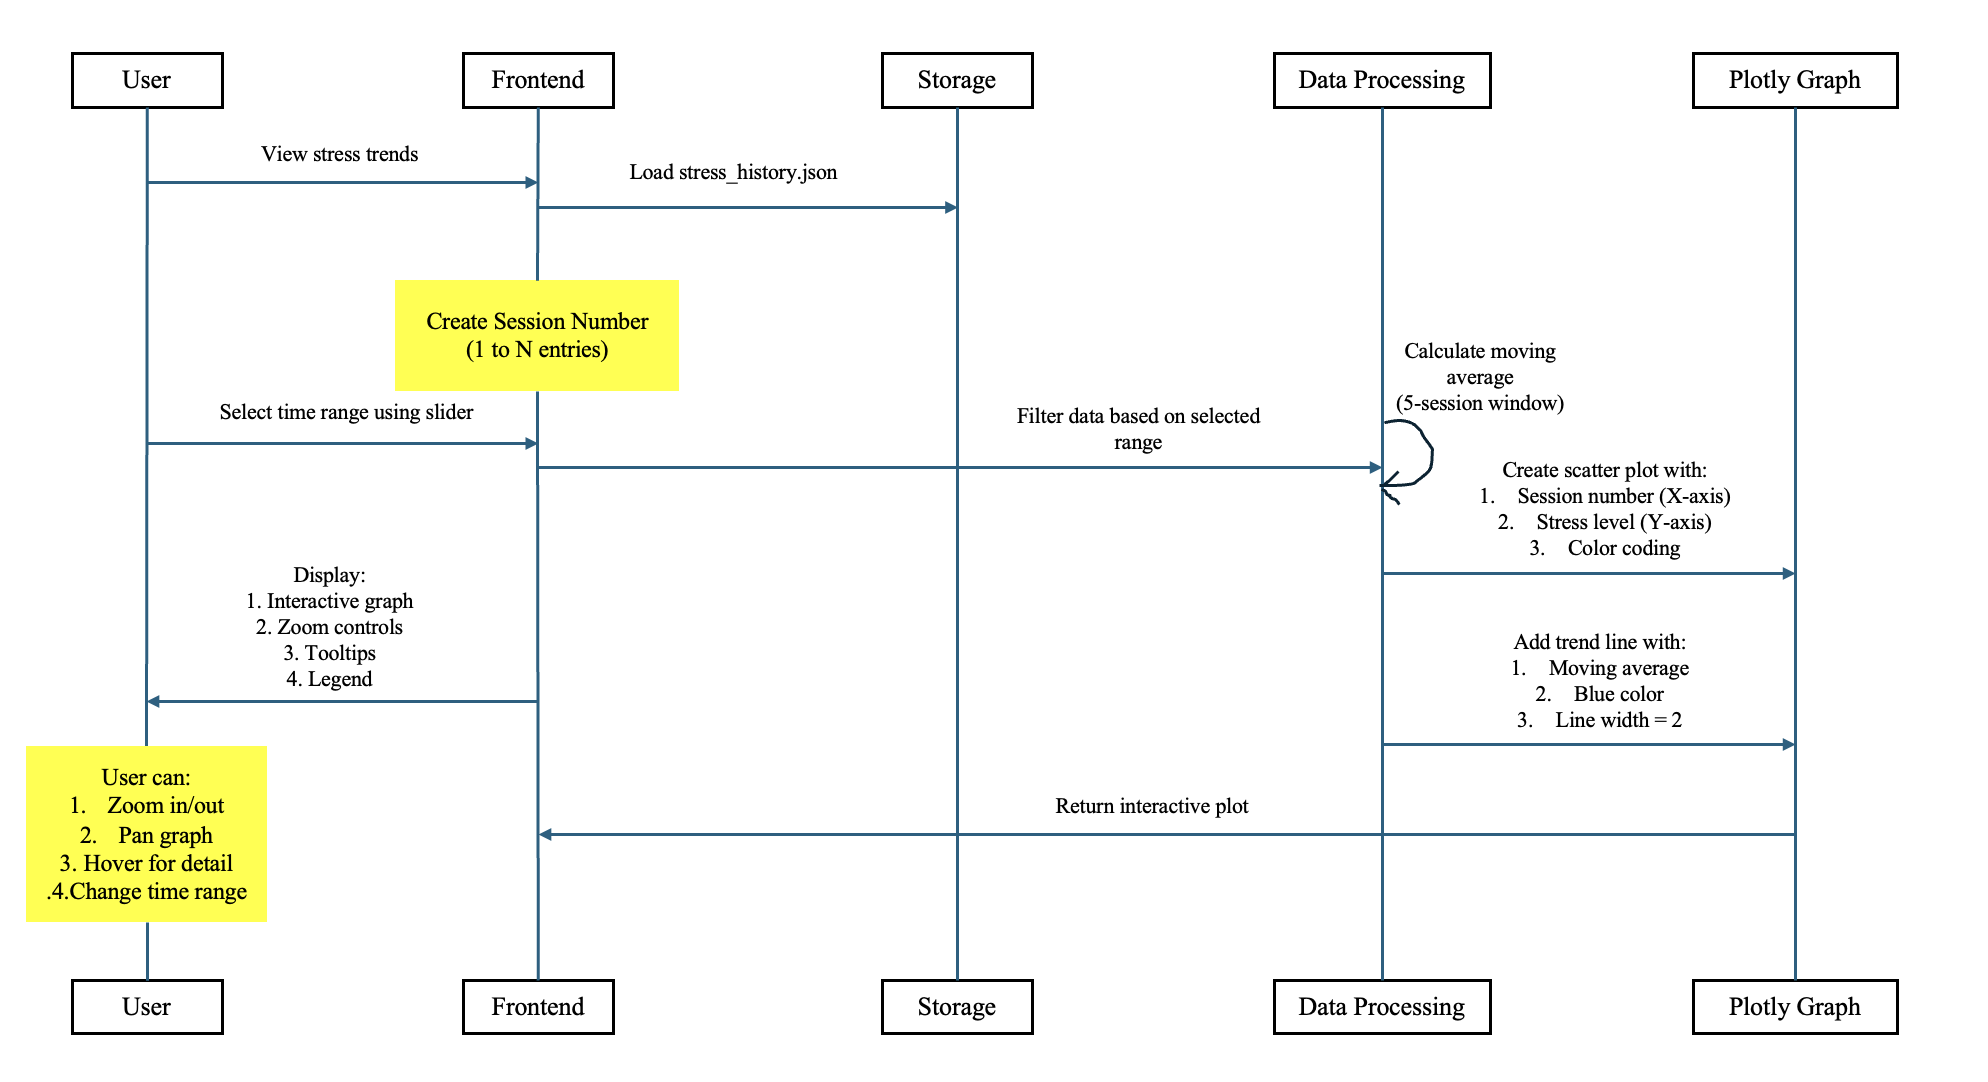
\includegraphics[width=1.1\columnwidth]{allreferences/stresstrendflow.png}
    \caption{Stress trend analysis workflow}
    \label{fig:system_architecture}
\end{figure}
\vspace{10pt} % Add space to prevent overlap
\subsection{Data Loading and Time Range Selection}
This subsection explains how stress data is retrieved from storage and filtered based on the selected time range. It emphasizes the user’s role in selecting the desired range and how this choice influences the subsequent data analysis steps. %the process by which stress data is retrieved and filtered.
\subsection{Moving Average Calculation}
The process utilized for highlighting the patterns and focusses on how patterns in stress data are highlighted through calculation. To smooth out variations and identify patterns in the data, a moving average is calculated across a specified session window.
\subsection{Interactive Plot Creation}
The tools and techniques for dynamic visualizations. Explains how dynamic visualizations are made using various tools and techniques. By enabling zooming, panning, and hovering, interactive graphs give viewers an in-depth assessment of stress patterns
\subsection{Customizing Plot Layout}
 Chances to use personalization to improve user interaction. The personalisation options available to enhance user interaction are described in this subsection. Plots can be altered by users to fit their tastes in terms of colour schemes, line styles, and data presentation.
\chapter{System Implementation and Results}
\clearpage 
 This chapter shows how the theoretical concept described in Chapter 3 has been realised by addressing the stress detection system's actual implementation and presenting its output. The implementation of the system are covered in this chapter, with a focus devoted to the UI/UX design, which emphasizes the visual components, interaction flow, and links to the backend procedures.  Examples, visual outputs, and screenshots are provided to demonstrate the system's operation. UI/UX components that improve user engagement and experience receive particular emphasis.The chapter also outlines the concepts, techniques, and tools used to create an usable and intuitive system that supports the goals of stress visualization and detection.
 \section{System overview}
 The stress detection system gives users insightful information about their stress levels by combining voice feature analysis and visualisation. In order to establish a connection the design (Chapter 3) and implementation, this section briefly restates the system's main elements.
\textbf{Important elements:}
\begin{enumerate}
\item Frontend (Streamlit): Manages input processing, output visualisation, and user interaction.(\cite{pillai2024})
\item  Backend (Flask): Controls response generation, model integration, and data processing.(\citet{relan2019}). 
\section{Frontend Implementation}
 Implementing the UI/UX components mentioned above and creating a useful interface are the main goals of the frontend. The following are the frontend implementation's salient features:
 \begin{enumerate}
\item Playback and Upload of Audio:
Users can submit.wav files for examination. And a built-in audio player lets users listen to their input again. 
\item  Visualization Integration: Line graphs showing stress trends are changed dynamically in context of analysis and Pie charts with distinct colour coding are used to display the stress level distribution. 
\item Downloadable reports: Users have the option to obtain comprehensive reports with stress analyses in PDF format. 
\item  Frontend Interaction Flow: Effortless transitions between sections for analysis, feedback, and file upload. 
\end{enumerate}
 \section{Backend Implementation}
 The backend combines models, processes text and audio inputs, and sends the output back to the frontend. Important implementation specifics consist of: 
\begin{enumerate}
\item Audio Processing: Whisper is used to transcribe audio files. In order to analyze stress, features are extracted. 
\item Stress detection using GPT-4:  GPT-4 analyzes the raw transcript to determine the stress levels (1–7). 
\item API Communication: To ensure smooth data transmission, the backend and frontend communicate over secure endpoints. 
\item Response Generation: Produces numerical stress levels, thorough explanations and analysis-based advice. 
\end{enumerate}
%\subsection{Input phase: Speech to Text Conversion (Whisper)}

%\vspace{-5mm} % Reduce vertical space
%\vspace{10pt} % Add space to prevent overlap
 %\begin{figure}[p]
    %\centering
   % \includegraphics[width=1.1\columnwidth]{allreferences/whisper1.png}
   % \caption{Speech to text conversion}
  %  \label{fig:system_architecture}
%\end{figure}
\vspace{10pt} % Add space to prevent overlap
\subsection{Audio Processing}
The built-in st.audio() function in Streamlit handles the audio playback. In the web interface, Streamlit's st.audio() component offers a native HTML5 audio player and it allows the common audio formats like MP3, WAV, and M4A. It also reads the audio file in bytes and shows a simple player interface on the web. Basic functions like play/pause, seek, and volume control are included with the player, along with a audio player interface that includes a progress bar.The stress detection system's audio processing interface is depicted in the figure 4.1. It offers an easy-to-use interface for managing and uploading audio recordings, making speech analysis for stress detection possible. Audio files up to 200 MB in size can be uploaded by users in different formats.
%\clearpage  % Forces all previous content to be placed before this point
\FloatBarrier
\vspace{-5pt}
\begin{figure}[htbp!] % More flexible placement
    \centering
    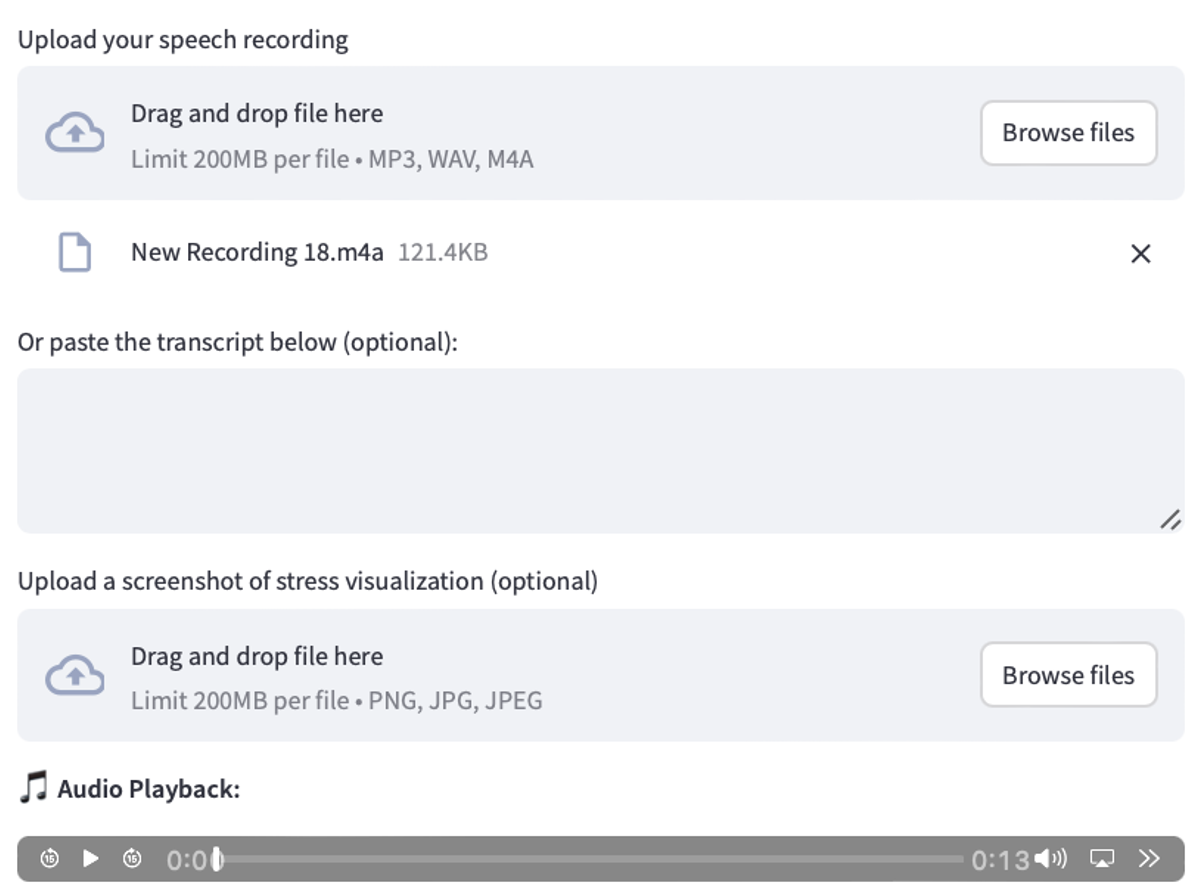
\includegraphics[width=0.9\columnwidth]{allreferences/audiofunc1.png}
    \caption{Audio Processing}
    \label{fig:audio_processing}
\end{figure}
\subsection{GPT-4 Analysis phase}
Once the transcript is ready, a prompt is formulated. The prompt includes instructions to analyze the transcript for emotional content or specific stress indicators. This can be done using a template-based approach or dynamic prompt creation, where certain keywords (example: “fire,”“help”) trigger stress-related prompts. The transcript and prompt are fed into an LLM . This step involves packaging the input as a query that the LLM understands, potentially formatted as 'prompt': "from now you are expert in finding any stress in the following voice transcript”; and "You are an assistant designed to analyze the stress level in speech. Focus on identifying emotional intensity, such as regret, nostalgia, uneasiness, or conflict, and scale it to a stress level from 1 to 7. Provide an explanation for the level."
\vspace{10pt} % Add space to prevent overlap
 \begin{figure}[htbp!]  %[h!]
    \centering
    \includegraphics[width=1.0\columnwidth]{allreferences/gpt4textprocessing2.png}
    \caption{GPT4 analysis phase}
    \label{fig:system_architecture}
\end{figure}
\vspace{10pt} % Add space to prevent overlap
\subsection{Output phase:Response generation} % 4.4.3
Then, LLM processes the prompt and transcript, using its pre-trained knowledge of language patterns, semantics, and emotional cues to analyze the text. The LLM evaluates both the content ('fire', 'help') and the context (the urgency in the sentence structure) shown in figure 4.4.
\vspace{10pt} % Add space to prevent overlap
 \begin{figure}[htbp!] %[h!]
    \centering
    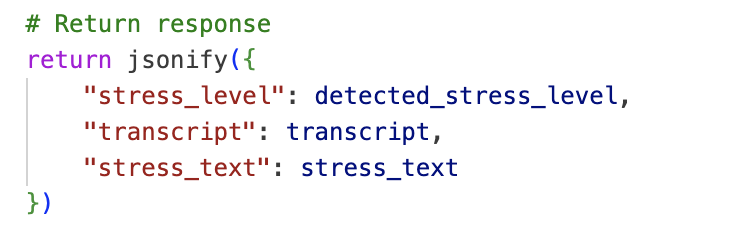
\includegraphics[width=1.1\columnwidth]{allreferences/responsegentext1.png}
    \caption{Response generation}
    \label{fig:system_architecture}
\end{figure}
\vspace{10pt} % Add space to prevent overlap
\end{enumerate}
 \section{UI/UX enhancements}
 The UI/UX design\cite{akhmedov2023} is essential to developing a user-friendly and engaging stress detection system. The main facets of UI/UX design and their application are listed below.
 \begin{enumerate}
 \item Adaptive UI Design: The system uses dynamic colour schemes that alter according to the stress levels that are identified (for instance, red for high stress). 
\item Features for User Accessibility: Supports several languages, such as English and Japanese and easy navigation that reduces cognitive effort with a clear visual hierarchy. 
\item Interactive Visualisations: Instantaneous feedback via pie charts, line graphs, and reports that can be downloaded. 
\item Feedback and Error Handling: Shows individualised guidance and real-time stress feedback and offers advice and error messages for missing or erroneous input.
\end{enumerate}
%\vspace{10pt} % Add space to prevent overlap
% \begin{figure}[p] %[h!]
   % \centering
   % \includegraphics[width=1.1\columnwidth]%{allreferences/textprooutput1.png}
   % \caption{Analysis and explanation}
    %\label{fig:system_architecture}
%\end{figure}
 \subsection{Development with Streamlit}
The primary tool for creating my user interface is Streamlit[17]. Interactive elements such as the file uploader and audio player are used. Styled text using Markdown (st.markdown()). Messages that handle errors (st.error(), st.success()). Important UX Elements Applied with Streamlit
Stress-level-based adaptive user nterface (colour-coded messages)
Spinners are being loaded st.spinner() to improve feedback.
When the file upload fails, error messages appear.
After every upload, the graph is updated in real time.

\subsection{UX Enhancements for User Engagement}
    Data visualisation methods, backend processing, and frontend technologies are all used in UX (User Experience) enhancements.
    \subsubsection{ Flask as Backend API}
    The backend API for processing the uploaded audio and returning the findings of the stress analysis is Flask. Flask manages the Speech Analysis work by utilising GPT-4o (stress analysis) and Whisper (voice-to-text) to handle the uploaded audio file. Additionally, it provides real-time feedback and promptly returns stress levels and explanations, assuring a low latency and seamless user experience also offers error handling. Flask produces concise error messages for the frontend to see in the event of issues (such as a missing audio file or an API failure). Further,  handle the data Processing which Formats the stress level data before sending it to Streamlit, ensuring consistent responses. 
        \subsubsection{Whisper (Speech-to-Text Transcription)}
Translates audio to text for stress analysis, make sure speech is recognised correctly before sending it to GPT-4, and adjusts for accents and tones for greater accuracy. Whisper was used to implement the following important UX features: Enhanced accessibility for non-text inputs;  Accurate transcription for stress assessment; Smooth speech-to-text conversion. Figure 4.4 shows the transcription of the audio. After uploading the audio it transcribes the audio. the transcription result and summarization is shown in the figure.
%\clearpage  % Forces all previous content to be placed before this point
\vspace{10pt} % Add space to prevent overlap
\begin{figure}[htbp!]
    \centering
    \includegraphics[width=1.0\columnwidth]{allreferences/fire2transcribe.png}
    \caption{Transcription from audio}
    \label{fig:system_architecture}
\end{figure}
\vspace{10pt} % Add space to prevent overlap
%Figure 4.8  also shows the transcription of the audio. After uploading the audio it transcribes the audio. the transcription result and summarization is shown in the figure. 
%\vspace{10pt} % Add space to prevent overlap
%\clearpage  % Forces all previous content to be placed before this point
%\vspace{10pt} % Add space to prevent overlap
%\begin{figure}[p]
   % \centering
    %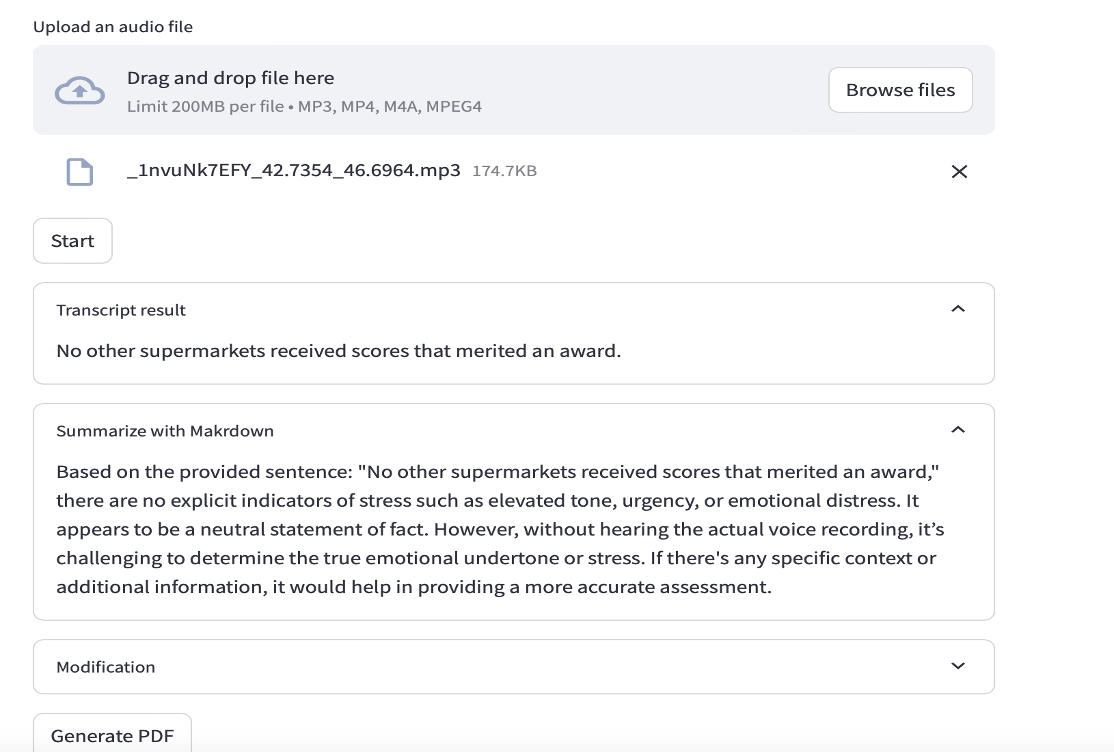
\includegraphics[width=1.0\columnwidth]{allreferences/supermarket.png}
    %\caption{Transcription from audio}
    %\label{fig:system_architecture}
%\end{figure}
\vspace{10pt} % Add space to prevent overlap
   \subsubsection{GPT-4o for Stress Analysis}
    GPT-4o uses voice analysis to identify stress levels in transcriptions. Gives thorough contextual stress explanation instead of only numerical values. It contributes to the humanisation and intuitiveness of stress evaluation. Detailed stress level explanations (rather than just numbers) are one of the key UX features implemented with GPT-4. Context-based stress analysis such as the urgency of speech patterns comes in second. And lastly it enhanced accuracy over conventional numerical classifiers.
\subsubsection{Explanation and advice}
The system analyses the speech transcript using GPT-4 to determine the user's intent, tone, and emotional context. For example Figure 4.6 shows the expression "If time could go back" is understood to mean regret or desire, which is classified as a stress-related mental state. The identified stress level (Level 3) is assigned by the method to a matching database category, such as "internal stress or conflict due to dissatisfaction or nostalgia." There is guidance associated with each stress level. 
%\clearpage  % Forces all previous content to be placed before this point
\begin{figure}[H]
    \centering
    \includegraphics[width=0.9\columnwidth]{advice3.png}
    \caption{Explanation and Advice}
    \label{fig:advice1}
\end{figure} 
For instance: "Take breaks, practise mindfulness, stay hydrated." is the Level 3 Stress Advice. Tailored to stress context for making it easy to use and actionable, the advice is straightforward, generic, and practical. Also The system successfully offers advise based on identified stress intensity, as seen in Figure 4.6. The system determined that the intensity in this case was moderate and assigned a Stress Level of 3. The system showed its ability to provide guidance for handling elevated stresss, even if the detected stress was primarily enthusiasm and engagement. This demonstrates how the system works to give people practical advice regardless of their mental state, which promotes general awareness and control.  
\vspace{10pt} % Add space to prevent overlap
%\vspace{-5mm} % Reduce vertical space
\begin{figure}[htbp!]
    \centering
    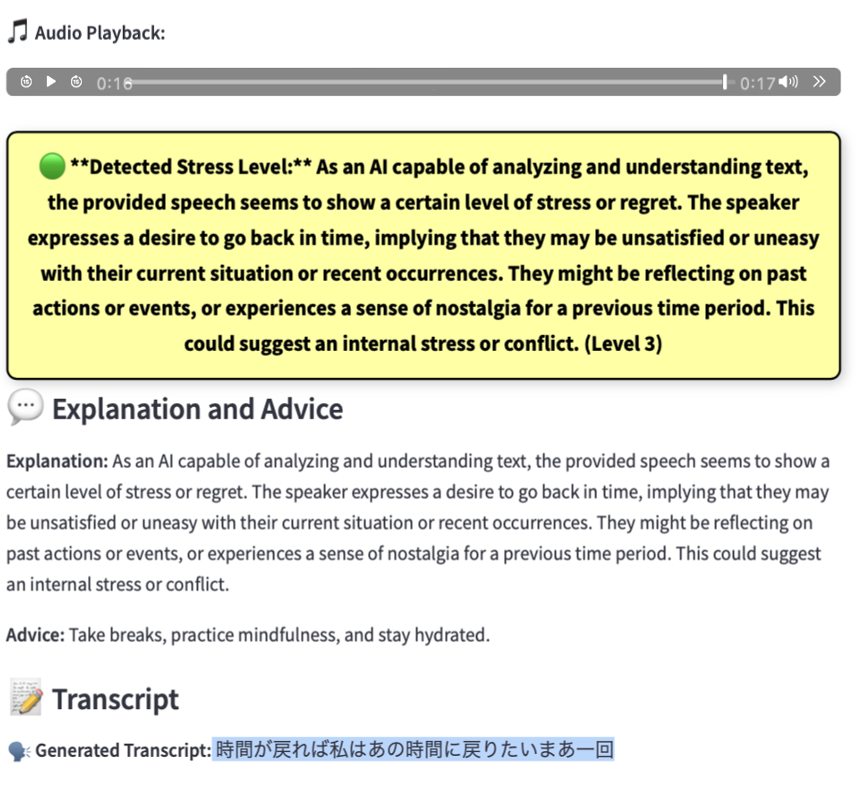
\includegraphics[width=1.0\columnwidth]{advice4.png}
    \caption{Explanation and Advice}
    \label{fig:system_architecture}
\end{figure} 
\vspace{10pt} % Add space to prevent overlap
  \subsubsection{ Stress visualization}
Figure 4.7 displays the percentage distribution of stress levels. Low stress (levels 1-3) is represented by green, mild stress (levels 4-5) by orange, and high stress (levels 6-7) by red. Interactive elements such as Legend for reference, Click-to-hide sections and hover tooltips that display precise percentages Insights like stress distribution patterns and percentages are provided by visualizations.  The implementation involved with tools like Plotly for graphical representations and connects stress data that has been captured in JSON with the user interface (UI). 
% \clearpage  % Forces all previous content to be placed before this point
\vspace{10pt} % Add space to prevent overlap
\begin{figure}[htbp!]
    \centering
    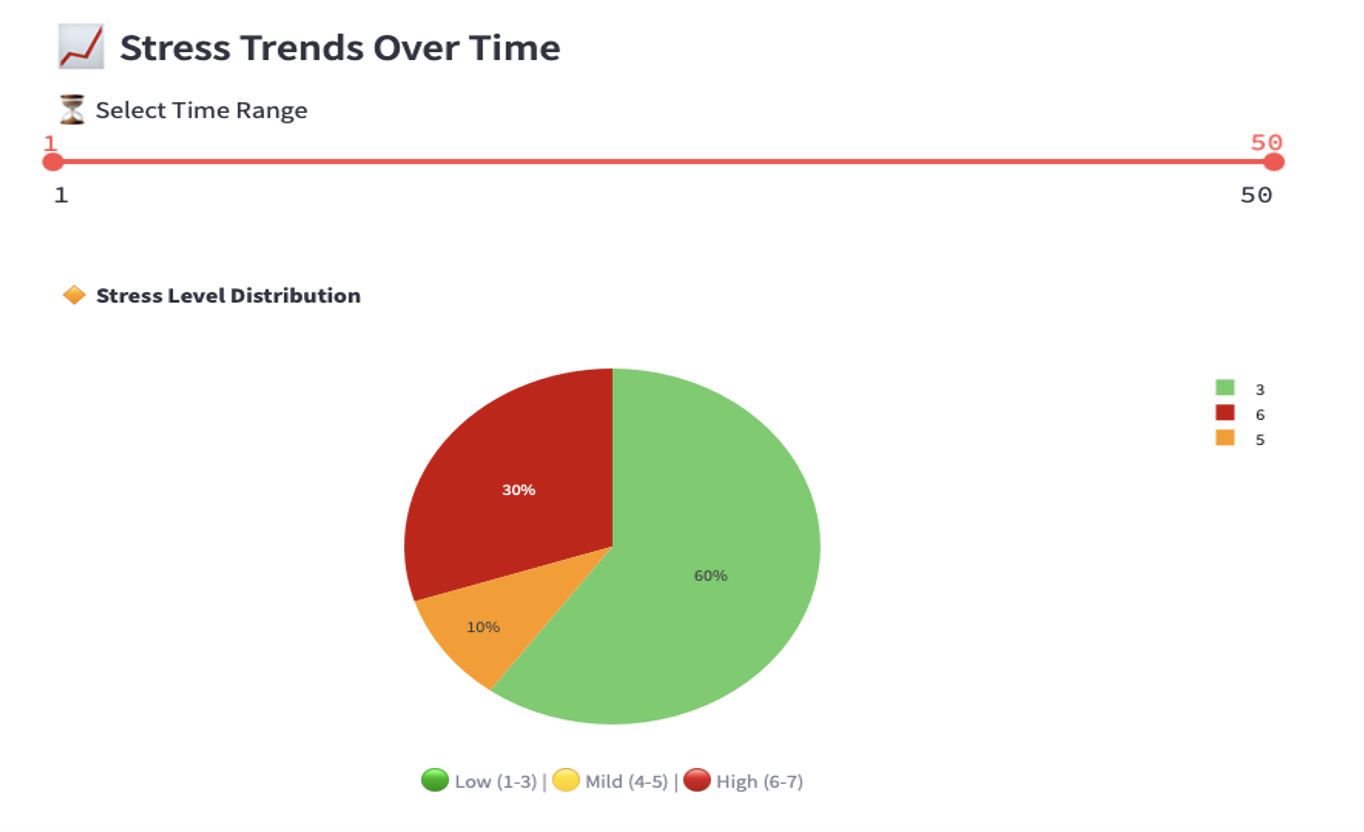
\includegraphics[width=0.8\textwidth]{allreferences/stressvisualpie.png}
    \caption{Stress Visualization}
    \label{fig:system_architecture}
\end{figure}
\vspace{10pt} % Add space to prevent overlap
    \subsubsection{ Stress Trend Tracking Feature}
     Using Matplotlib stress patterns over time using is plotted, which used to visualize stress trends. To help track past stress levels for long-term insights, figure 4.8 present line graphs with markers to visualize user stress patterns.  The moving average is displayed by the blue trend line. The X-axis displays the session numbers. Y-axis representing stress levels from 1 to 7. Interactive features include zoom and pan controls, a time range slider for filtering data, hover tooltips for displaying precise values, and a legend for trend lines and stress levels are used. The dynamic stress trend graph which automatically updates upon each upload, improved readability with larger markers, bold labels, and annotations on each point to display stress values. 
%\clearpage  % Forces all previous content to be placed before this point
\vspace{10pt} % Add space to prevent overlap
     \begin{figure}[htbp!]
    \centering
    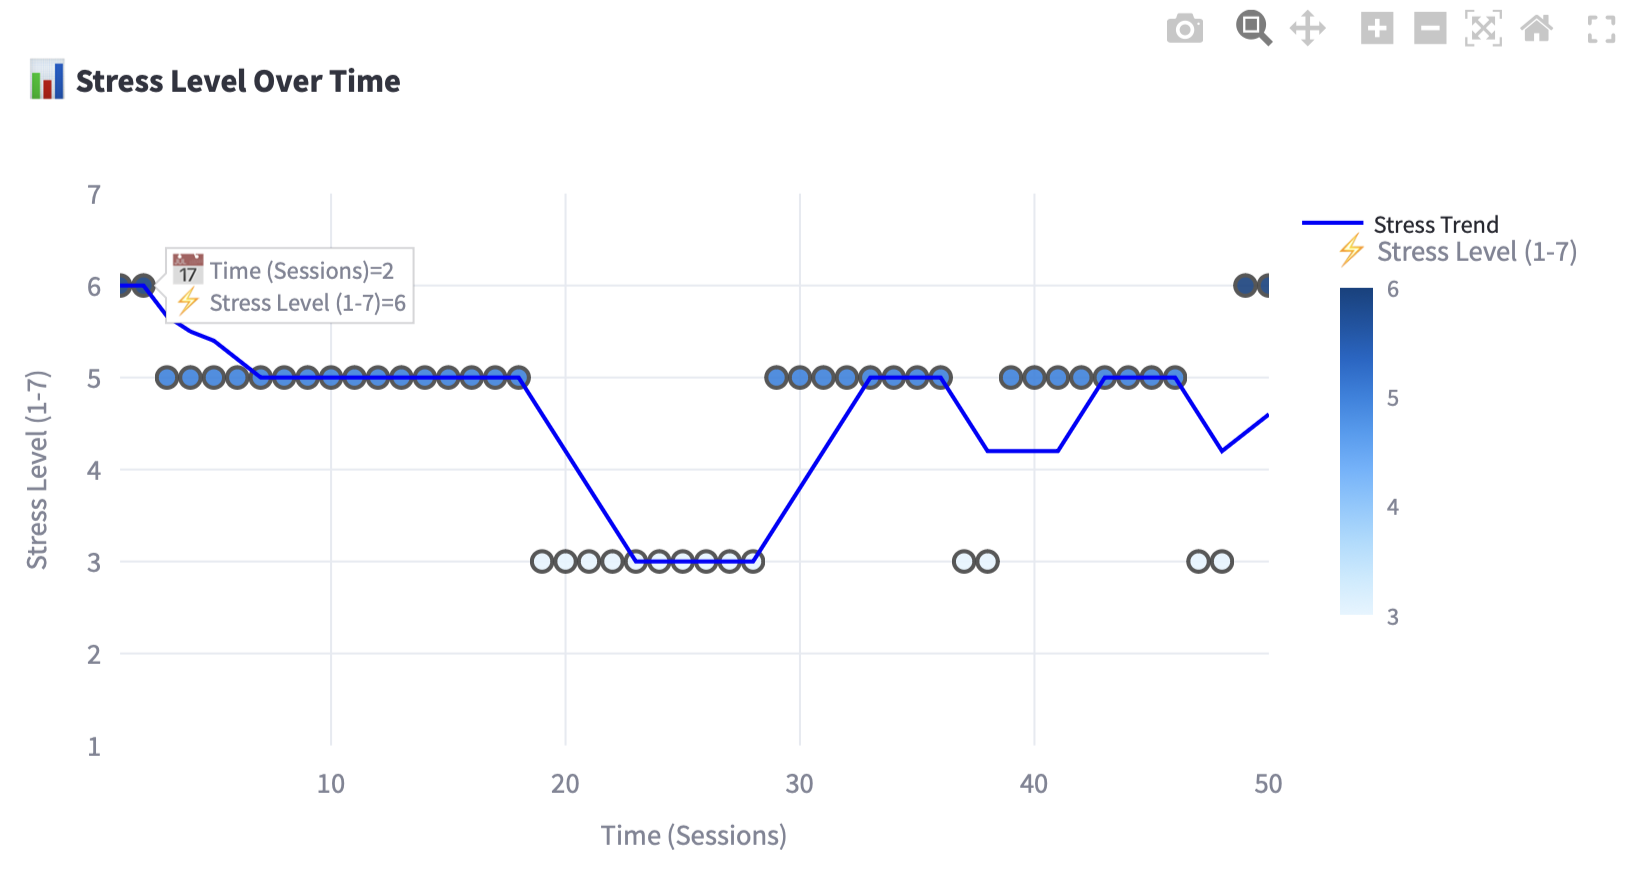
\includegraphics[width=1.0\columnwidth]{stresstrend3.png}
    \caption{Stress Trend Tracking History}
    \label{fig:system_architecture}
\end{figure}
\vspace{10pt} % Add space to prevent overlap
    \subsubsection{ JSON (Local Data Storage for Stress Trends)}
    Figure 4.9 shows the stress report. JSON stores the history of stress levels locally. When the page is refreshed, previous stress levels are not lost and makes it possible to track previous sessions for long-term insights. The principal UX Elements applied Through JSON to avoid excessive data building, the stress history is kept for the last 50 sessions and is persistent over repeated uploads.
    % \clearpage  % Forces all previous content to be placed before this point
%\vspace{-5pt} % Reduces space above
%\FloatBarrier % Ensures figure stays within section
%\begin{figure}[htbp!]
  %  \centering
   % 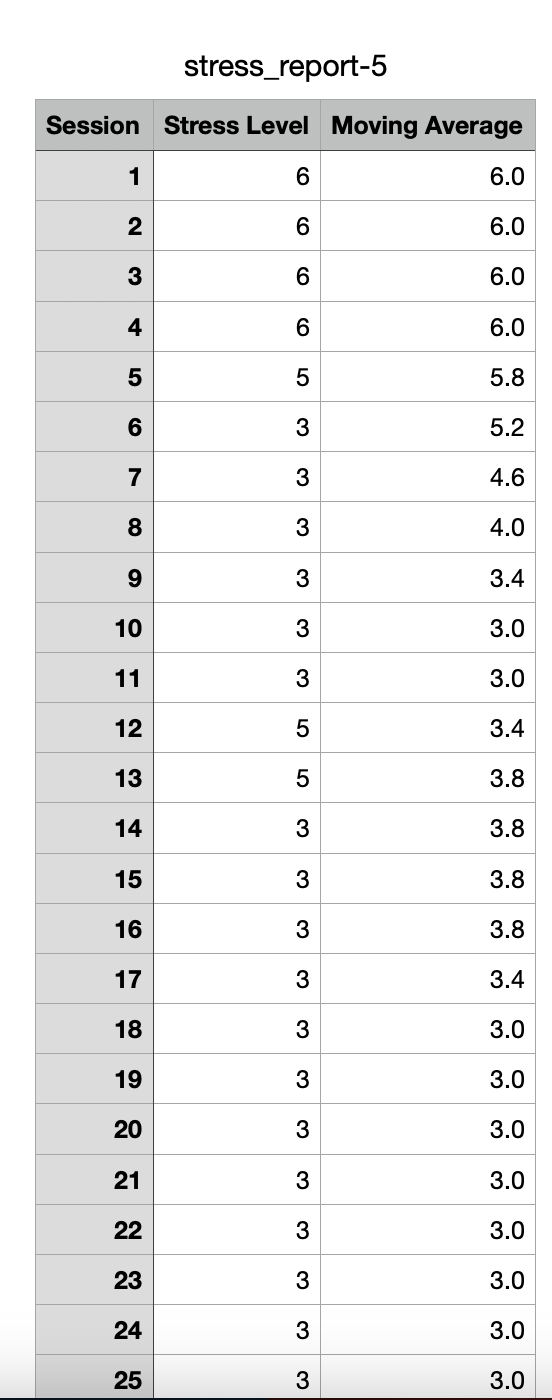
\includegraphics[width=0.7\textwidth]{allreferences/stressreportdownload.png}
   % \caption{Stress report}
   % \label{fig:stress_report}
%\end{figure}
%\vspace{-10pt} % Reduces space below
 \section{Implementation output}
The frontend and backend are smoothly connected via the system's interaction flow. Through the interface, users can enter text or upload audio. Calculates stress levels by processing inputs using Whisper and GPT-4.The frontend receives the results for feedback and visualization. Key outputs produced by the system to verify its operation are shown in this section:
\begin{enumerate}
\item Stress Analysis Findings: Audio file transcriptions. 
Stress levels were identified and categorized, such as Severe, Slight stress and relaxed. 
\item Visualization Outcomes: Line graphs illustrating temporal trends in stress. 
Pie charts that show the distribution of stress levels. 
\item Reports and Feedback: Downloadable reports and tailored guidance.
\end{enumerate} 
 \begin{figure}[p]
    \centering
    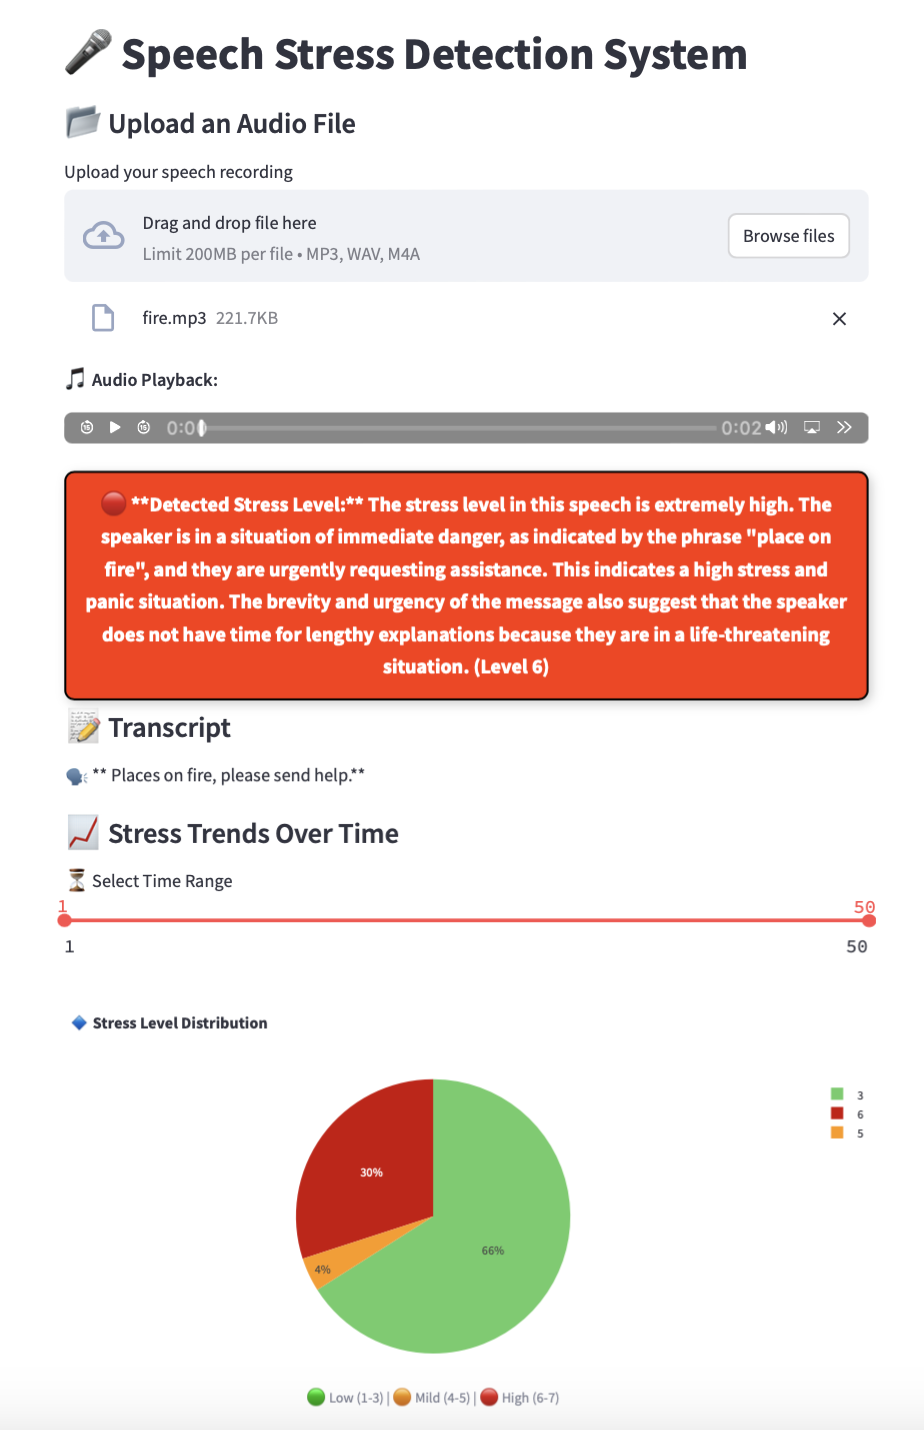
\includegraphics[width=0.9\columnwidth]{aovrall1.png}
    \caption{Stress Level Detection System}
    \label{fig:system_architecture}
\end{figure} 
 \begin{figure}[p]
    \centering
    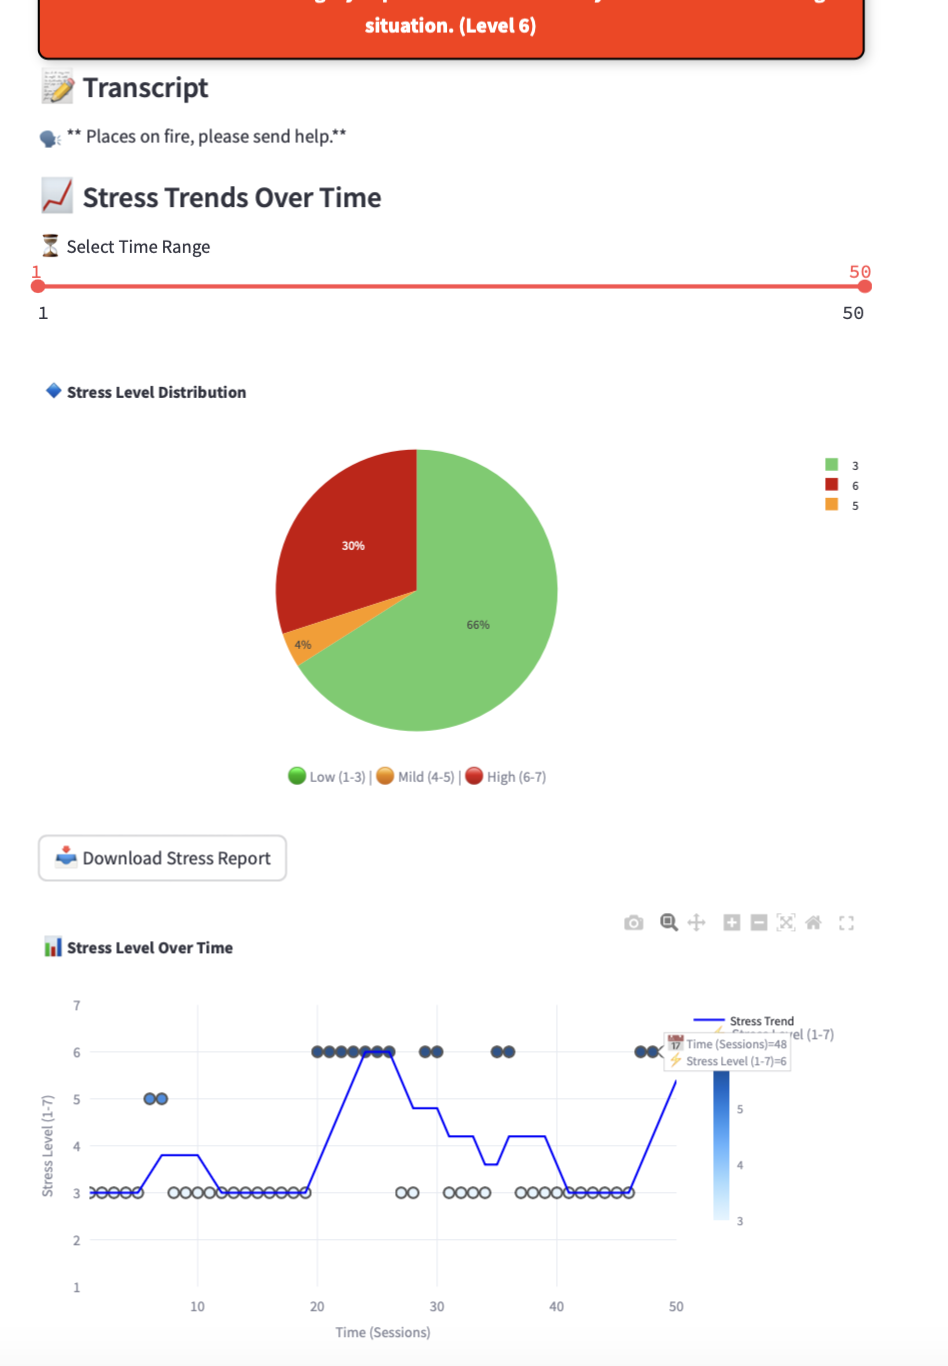
\includegraphics[width=0.9\columnwidth]{aoverall2.png}
    \caption{Stress Level Detection System}
    \label{fig:system_architecture}
\end{figure}
The main features of the Speech Stress Detection System are shown in Figures 4.9 and 4.10, an intuitive and engaging user interface. In order to verify the input, users can listen to audio recordings that they have uploaded in supported formats such as MP3, WAV. Stress levels are detected by the system and shown clearly in a banner with colour coding. It provides context for the state by clarifying whether the detected intensity is indicative of high or low stress. To provide transparency and usability, the analyzed speech is transcribed and presented for the user's reference. A line graph helps users keep an eye on their mental health by showing changes in stress levels over time. A pie chart offers a thorough overview of stress levels by classifying them as low, medium, or high intensity  which demonstrate the system's emphasis on improving user experience by providing actionable information.
\chapter{Experiment and evaluation}
\clearpage 
  \section{Evaluation of Stress Detection}
  To evaluate the performance of the system, a questionnaire form was developed and shared with participants via social networking platforms (SNS). The form included 12 audio samples, and participants were asked to provide subjective ratings for each audio. The average human rating for an audio reflects the collective perception of stress levels from 40 participants. This is statistically valid because averaging reduces individual biases and represents a more reliable measure. These human ratings were then compared with the system-generated outputs for the same audio samples. Table 5.1 shows the average human rating and system output. After collecting the responses, the correlation coefficient between the human ratings and the system output was calculated to assess the strength of their relationship, and a scatter plot was created to visually represent this correlation and overall trends. To further analyze the data, a bar chart was plotted to compare the average human ratings with the system outputs, highlighting the differences and similarities. Additionally, a line chart was used to show the trends of human ratings and system outputs across all samples, providing a clear representation of their alignment or divergence. Key statistical measures, including the T-value and P-value, were calculated to determine the significance of the findings, while the Mean Absolute Error (MAE) was computed to quantify the average difference between human ratings and system outputs. These analyses, combining visualizations and statistical evaluations, offer comprehensive insights into the system’s performance, its ability to align with human judgment, and areas for further improvement. 
  \begin{table}[h!] % Optional, h! ensures the table stays close to where it's defined
\centering
\caption{Average Human Rating & System Output}
\label{tab:correlation_table} % Optional, for referencing in the text
\begin{tabular}{|c|c|c|}
\hline
Audio & Average Human Rating & System Output \\ \hline
Audio1 & 5.000000 & 6 \\ \hline
Audio2 & 6.125000 & 7 \\ \hline
Audio3 & 5.925000 & 6 \\ \hline
Audio4 & 3.550000 & 3 \\ \hline
Audio5 & 3.666667 & 3 \\ \hline
Audio6 & 5.875000 & 6 \\ \hline
Audio7 & 3.700000 & 3 \\ \hline
Audio8 & 3.875000 & 3 \\ \hline
Audio9 & 5.825000& 7 \\ \hline
Audio10 & 3.525000 & 3 \\ \hline
Audio11 & 4.900000& 4 \\ \hline
Audio12 & 5.950000 & 7 \\ \hline
\end{tabular}
\end{table}
    \section{Correlation of coefficient between system output and human estimation}
    A statistical measure known as the "correlation coefficient," which ranges from -1 (perfect negative correlation) to +1 (perfect positive correlation), is used to analyse the relationship between two variables. It shows the strength and direction of the linear association between the variables. \cite{schober2018correlation}. The correlation coefficient provides a single numerical value that quantifies the strength and direction of the relationship between human ratings and system predictions. A single numerical value that expresses the direction and degree of the relationship between system predictions and human ratings is provided by the correlation coefficient. A high correlation (close to 1) means that human assessments and the system agree well. A low correlation (close to 0) indicates that human judgements and the system's predictions are unrelated. An inverse connection is implied by negative correlation, whereby system outputs fall as human assessments rise.  The correlation coefficient acts as a validation metric for proposed system. It shows whether the system reliably captures the stress levels perceived by humans. The system's practical usefulness is supported by a high correlation, which indicates that its stress detection is in accordance with human perception.. The outputs of the stress detection system were compared with human estimations obtained via a survey in order to assess the system's performance. On a 7-point rating system, survey respondents were asked to assess the stress levels of 12 audio samples. The system's predictions and the average human ratings showed a very significant positive connection, as indicated by the analysis's correlation coefficient of 0.96. Figure 5.1, which visualises the relationship between the system outputs and human ratings, was created to further highlight this link using a scatter plot with a trend line. The visual depiction and strong correlation value show that the system's stress predictions closely match human experience, hence verifying its functionality.
    \vspace{10pt} % Add space to prevent overlap
\begin{figure}[H]
    \centering
    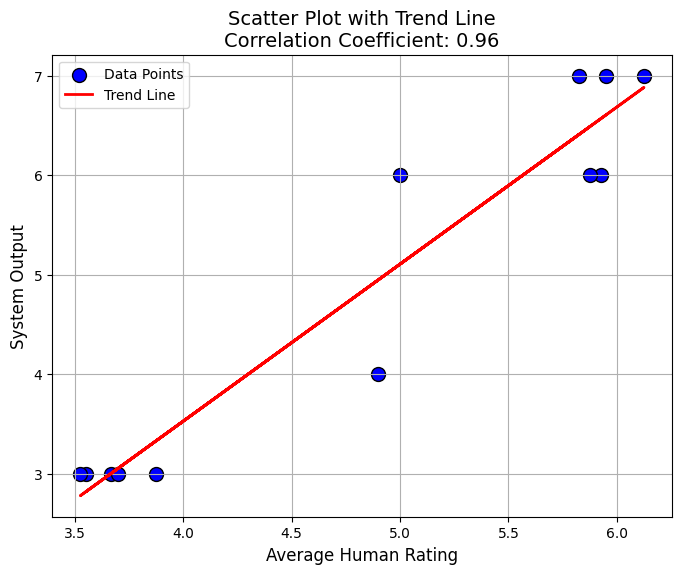
\includegraphics[width=1.0\columnwidth]{coeff40.png}
    \caption{Average human rating and system outputs}
    \label{fig:system_architecture}
\end{figure}
\vspace{10pt} % Add space to prevent overlap
\section{Visual comparisons of human ratings and system outputs }
The comparative analysis demonstrates how well and accurately the system  can reproduce human estimations.
\subsection{Comparison of  Human rating  vs system rating }
For every audio sample, the system outputs and human ratings were compared side by side in a bar chart in figure 5.2.
\vspace{10pt} % Add space to prevent overlap
 \begin{figure}[H]
    \centering
    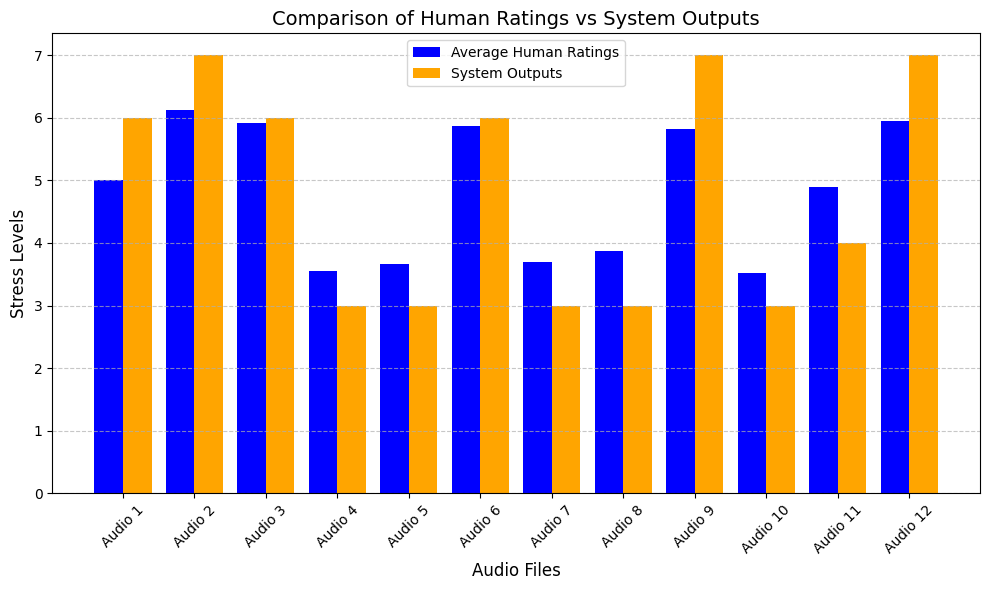
\includegraphics[width=1.0\columnwidth]{bar40.png}
    \caption{Trend Comparison between human rating vs system outputs}
    \label{fig:system_architecture}
\end{figure}
\vspace{10pt} % Add space to prevent overlap
\subsection{Trend Comparison of  Human rating  vs system rating }
The trends of system outputs and human ratings for each of the 12 audio samples were displayed in a line chart in figure 5.3. The trend line displays the comparison between system outputs and human ratings for various audio files. The average human assessments are shown by the blue line. The system's predictions are shown by the orange line. The system's predictions are in good agreement with human judgements when the orange and blue lines are close to adjacent ones.  A mismatch occurs when there is a discernible space between the two lines, meaning that the system's forecast deviates from the average for humans. This trend line identifies distinct audios in which the system works effectively.
\vspace{10pt} % Add space to prevent overlap
\begin{figure}[H]
    \centering
    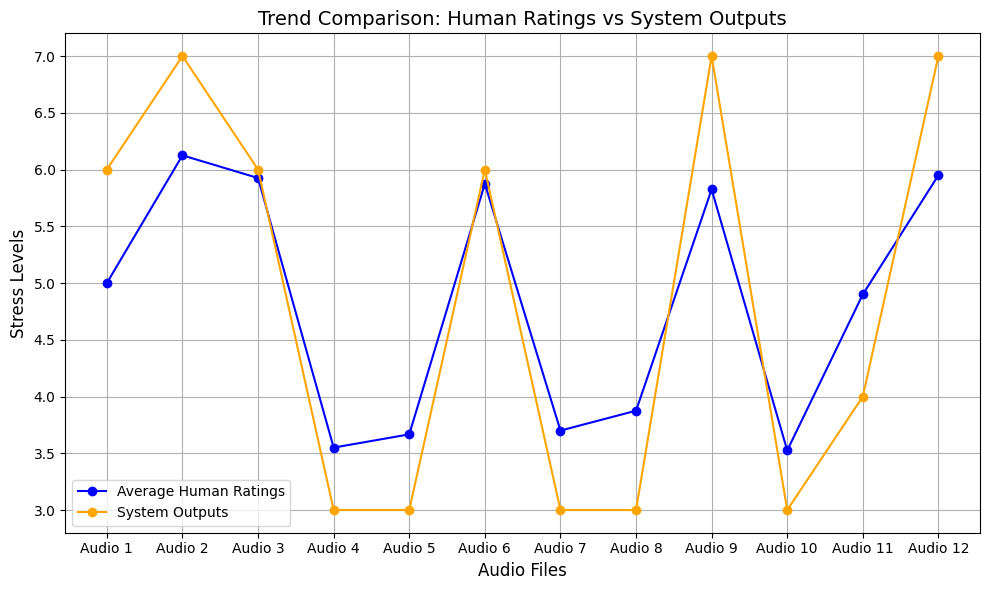
\includegraphics[width=1.0\columnwidth]{trend40.png}
    \caption{Comparison between human rating vs system outputs}
    \label{fig:system_architecture}
\end{figure} 
\vspace{10pt} % Add space to prevent overlap
\subsection{Histogram of Error Distribution}
The distribution of errors between system outputs and human assessments was shown using a histogram in figure 5.4. The distribution of differences (errors) between the system outputs and human ratings is displayed by the histogram. The x-axis shows the magnitude of the difference between the human ratings and the system output for each audio sample. A difference of 0.2  means the system output was very close to the human average. Larger values such as 1.0 indicate a greater disparity between the two. The Y-Axis shows how many audio files have a given error value. The y-axis indicates the number of audio samples (frequency) that fall into each range of difference. For instance, if the bar at 0.6  has a height of 4, it means there are 4 audio samples for which the difference between the human rating and the system output lies within the range around 0.6.
Proposed system's predictions are, on average, one point off from human evaluations, with the majority of errors centred around 1.0. A narrow and centred histogram shows that the system's predictions closely match the human assessments. The bars represent how many samples fall within specific ranges of difference. The highest frequency in this figure is at a difference of around 0.6, indicating that most samples had a moderate discrepancy between human ratings and system outputs.
%The X-Axis shows the absolute difference (error) between system predictions and human ratings
MAE: 
\vspace{10pt} % Add space to prevent overlap
 \begin{figure}[H]
    \centering
    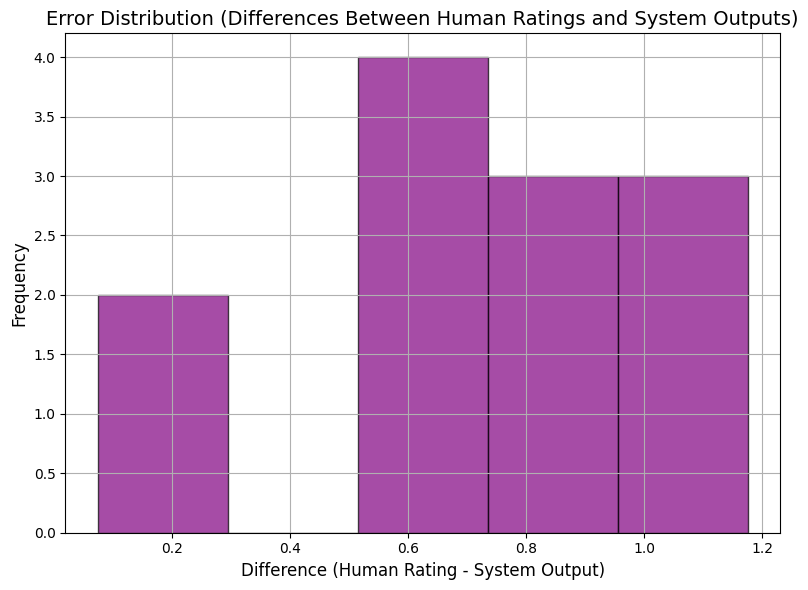
\includegraphics[width=1.0\columnwidth]{histo40.png}
    \caption{Histogram of error distribution}
    \label{fig:system_architecture}
\end{figure}
\vspace{10pt} % Add space to prevent overlap
\section{Statistical analysis}
The performance of the stress detection system was evaluated by comparing its outputs to human ratings using statistical metrics. A t-test was conducted to assess the statistical significance of the difference between the system outputs and human ratings. The resulting t-statistic and p-value of showed no significant difference, supporting the hypothesis that the system outputs align closely with human perception. A paired t-test (\citet{pairedttest2025}) compares the means of two related groups such as human ratings and system outputs for the same audio files. The goal is to determine if the mean difference between the two groups is significantly different from 0.
\begin{table}[H] % Optional, h! ensures the table stays close to where it's defined
\centering
\caption{Statistical Value} 
\label{tab:correlation_table} % Optional, for referencing in the text
 \begin{tabular}{|c|c|c|}
        \hline
         Mean Absolute Error(MAE) & T-statistic & P-value \\ \hline
            0.71 &  -0.03 & 0.97 \\ \hline
    \end{tabular}%
   \end{table}
   \vspace{10pt} % Add space to prevent overlap

\subsection{Mean Absolute Error (MAE)}
The average absolute difference between the system outputs and human ratings is measured by MAE. Regardless of direction, it shows how far the system's predicts vary from human assessments.  The system outputs are more compatible with human assessments when the MAE is smaller, which denotes higher performance. An MAE of 0.71 indicates that, on average, the system's predictions and human ratings on the stress rating scale diverge by roughly 0.71 units. This is a minor error, indicating that the system functions properly in general.
\subsection{T-Statistic: }
T-Statistic: The T-statistic measures how much the average human rating deviates from the system output, standardized by the variability in the human ratings. A high positive or negative T-statistic indicates a large difference between the human ratings and system outputs. The t-statistic determines if the average difference between human ratings and system outputs deviates from 0 in a statistically significant way. The mean difference between the system outputs and human assessments is insignificant when the t-statistic is around zero such as -0.03.On average, the system's output closely resembles human ratings, showing no bias towards overestimation or underestimation.
\subsection{P value }
P-Value: Indicates whether the observed difference is statistically significant.The P-value represents the probability that the observed difference between human ratings and system outputs occurred by random chance.A common threshold for significance is p<0.05p<0.05. If the P-value is below this threshold, the difference is considered statistically significant. A p-value of 0.9771 is much larger than the common significance threshold of 0.05.  There is no statistically significant difference between the system's outputs and the human ratings. This suggests that the system's performance is very much aligned with human perception
\section{Interpretation of T-statistic and P-value }
The overall p-value (0.97) shown in Table 5.2 explain that these values represent the system's general performance across all audio files. A detailed table 5.3 is shown above with t-statistics and p-values for each audio file.
\vspace{10pt} % Add space to prevent overlap
\begin{table}[H] % Optional, h! ensures the table stays close to where it's defined
\centering
\caption{T-statistic and P-value}
\label{tab:correlation_table} % Optional, for referencing in the text
 \begin{tabular}{|c|c|c|c|c|}
        \hline
        Audio  & T-statistic & P-value \\ \hline
        Audio1 & -5.186 & 0.000007\\ \hline
        Audio2 &  -6.271 & 0.000000\\ \hline
        Audio3 & -0.386 & 0.486333 \\ \hline
        Audio4 &  1.629 & 0.111\\ \hline
        Audio5 &  2.000& 0.053 \\ \hline
        Audio6 &   -0.589 &  0.560 \\ \hline
        Audio7 & 2.004 & 0.052  \\ \hline
        Audio8 &  2.588 &  0.014  \\ \hline
        Audio9 &  -8.806 & 0.000000 \\ \hline
        Audio10 &  4.620 &  0.000041 \\ \hline
        Audio11 &  5.383 & 0.000004\\ \hline
        Audio12 & -5.450 & 0.000003\\ \hline
    \end{tabular}%
   \end{table}
\vspace{10pt} % Add space to prevent overlap
%\noindent
%\textbf{Audio 1:} \\
%\textbf{T-Statistic:} -5.186 \\
%\textbf{P-Value:} 0.000007 (very small) \\
%\textbf{Interpretation:} There is a statistically significant difference between human ratings and system output. The system's stress rating is likely overestimating compared to the human ratings.\par
%\noindent
%\textbf{Audio 2:} \\
%\justifying
%\textbf{T-Statistic:} -6.271 \\
%\textbf{P-Value:} 0.000000  (very small) \\
%\textbf{Interpretation:} The system output differs significantly from human ratings, suggesting overestimation of stress for this audio.\par
%\noindent
%\textbf{Audio 3:} \\
%\textbf{T-Statistic:} -0.386\\
%\textbf{P-Value:}  0.701  (not significant) \\
%\textbf{Interpretation:} There is no statistically significant difference. The system's output aligns well with human ratings.P-value = 0.701,this is much greater than 0.05, indicating that the system's output is not statistically significantly different from the human ratings. A small t-statistic -0.386 also supports that the difference is minimal. Since the system's output is close to the human ratings and the difference is statistically insignificant, interpreting this as good between the system and human ratings. This means that the system's prediction for this audio is consistent with how humans perceive stress.\par
%\noindent
%\textbf{Audio 4:} \\
%\textbf{T-Statistic:} 1.629\\
%\textbf{P-Value:}  0.111  (not significant) \\
%\textbf{Interpretation:} No significant difference between the human ratings and system output, suggesting reasonable agreement.\par
%\noindent
%\textbf{Audio 5:} \\
%\textbf{T-Statistic:} 2.000\\
%\textbf{P-Value:}  0.0533 (borderline significance) \\
%\textbf{Interpretation:} The p-value is close to the 0.05 threshold, suggesting a marginally significant difference.\par
%\noindent
%\textbf{Audio 6:} \\
%\textbf{T-Statistic:} -0.589\\
%\textbf{P-Value:}  0.560 (not significant) \\
%\textbf{Interpretation:} No significant difference, indicating good alignment between human ratings and system output.\par
%\noindent
%\textbf{Audio 7:} \\
%\textbf{T-Statistic:} 2.004\\
%\textbf{P-Value:}  0.052 (borderline significance) \\
%\textbf{Interpretation:} The p-value is close to the threshold, suggesting a marginally significant difference that could require further examination.\par
%\noindent
%\textbf{Audio 8:} \\
%\textbf{T-Statistic:}2.588\\
%\textbf{P-Value:} 0.014 (significant)\\
%\textbf{Interpretation:} Statistically significant difference, with the system likely underestimating stress compared to human ratings\par
%\noindent
%\textbf{Audio 9:} \\
%\textbf{T-Statistic:}-8.806\\
%\textbf{P-Value:} 0.000000 (very small)\\
%\textbf{Interpretation:} Strongly significant difference, with the system likely overestimating stress. \par
%\noindent
%\textbf{Audio 10:} \\
%\textbf{T-Statistic:}4.620\\
%\textbf{P-Value:} 0.000041 (very small)\\
%\textbf{Interpretation:} Statistically significant difference, with the system likely underestimating stress \par
%\noindent
%\textbf{Audio 11:} \\
%\textbf{T-Statistic:} 5.383\\
%\textbf{P-Value:} 0.000004 (very small)\\
%\textbf{Interpretation:} Statistically significant difference, with the system likely underestimating stress \par
%\noindent
%\textbf{Audio 12:} \\
%\textbf{T-Statistic:}-5.450\\
%\textbf{P-Value:} 0.000003 (very small)\\
%\textbf{Interpretation:} Statistically significant difference, with the system likely underestimating stress \par


\textbf{Significant Differences (P < 0.05)}: Audio 1, 2, 8, 9, 10, 11, 12 show significant differences between system outputs and human ratings. These indicate areas where the system does not align well with human perception of stress and requires adjustment.\par
\textbf{No Significant Differences (P ≥ 0.05)}: Audio 3, 4, 5, 6, 7 show no significant differences, suggesting that the system performs reasonably well for these cases. For instance, the system's output aligns well with human ratings.P-value = 0.701 for audio 3,this is much greater than 0.05, indicating that the system's output is not statistically significantly different from the human ratings. A small t-statistic -0.386 also supports that the difference is minimal. Since the system's output is close to the human ratings and the difference is statistically insignificant, interpreting this as good between the system and human ratings. This means that the system's prediction for this audio is consistent with how humans perceive stress. \par
\textbf{Improvement}
Focus on audio files with significant differences to improve system accuracy and enhancements such as retraining the system with more diverse datasets and refine the model for edge cases. Incorporate feedback loops to fine-tune system outputs based on human assessment.

  \section{Discussion of Results}
    \subsection{Key Findings}
    \begin{enumerate}
\item Strong Correlation: The system predictions and human ratings show a strong alignment, as indicated by the correlation coefficient of 0.96. \item  Minimal Error: The system produces accurate predictions with minimal variances, as indicated by the MAE of 0.71. 
\item Statistical Validation: The system's outputs and human ratings do not differ statistically significantly, according to the findings of the paired t-test (τ-statistic: -0.03, p-value: 0.97). 
\end{enumerate}
 \subsection{Insights on Multimodal Data Integration}
For stress detection, the system's integration of Large Language Models (LLM) and Social Signal Processing functioned well.The multimodal approach enabled:
\begin{enumerate}
\item Proper audio input transcription. 
 \item  Accurate assessment of stress levels using linguistic and vocal content. 
\end{enumerate}
\section{Advantages and Limitations of the System}
\textbf{Advantages:}
\begin{enumerate}
    \item A strong correlation with human evaluations confirms the reliability of the system.
    \item Stress detection is made easier by an intuitive user interface (UI).
    \item A low prediction error improves system accuracy.
\end{enumerate}
\textbf{Limitations:}
\begin{enumerate}
\item  Despite the high correlation, certain audio files showed significant differences, which warrants further analysis and improvement in the model's performance.
    \item Minor variations in certain audio samples indicate potential for improvement.
    \item Performance in noisy environments may be impacted by reliance on high-quality audio inputs.
\end{enumerate}
\chapter{Conclusion and Future Work}
\clearpage 
  \section{Summary of the Research}
  This study presented a multimodal stress detection system that uses large language models (LLMs) and Social signal Processing to combine text-based and speech-based stress analysis. The method was created to identify stress levels by merging GPT-4-based textual analysis with audio analysis with transcription. User-centred Stress Visualisation Streamlit was used to create an interactive real-time user interface (UI) that lets users upload audio samples, get stress scores, and see their stress levels on user-friendly dashboards. This research introduced stress trend visualization, which allows users to follow stress changes over numerous sessions, in contrast to traditional stress detection methods that provide immediate assessments. An interactive stress level indicator, trend graphs, and a downloadable stress report were among the UX improvements that improved the system's readability and usefulness for mental health applications. %These results demonstrate how well deep learning-based stress detection works and how crucial UX enhancements are to developing intuitive, real-time stress monitoring solutions.
  \section{Contributions of the Study}
   \begin{enumerate}
   \item Creation of a Multimodal Stress Detection System integrated vocal analysis and LLM-based text analysis.  
 \item Deployment of Long-Term Monitoring Stress Trend Visualisation 
 Added a dynamic stress trend monitoring function that allows users to examine stress trends over time. 
Enhanced applications for mental health monitoring by offering a historical perspective on stress variations. 
 \item UX Improvements for Accessibility and User Interaction 
Developed an interactive user interface with stress visualisation to improve the interpretability and actionability of stress detection results. 
Added downloadable stress reports, stress level indicators, and real-time feedback, improving the usefulness of stress detection tools. 
\end{enumerate}
Through the integration of deep learning, multimodal AI, and user-centred design, these contributions enhance the real-world implementation of stress detection systems.
 
  \section{Limitations of the Proposed System}
Despite the positive results of this study, a number of limitations need to be taken into account. Instead of recording live speech inputs, the system processes pre-recorded speech, which restricts the possibility of real-time engagement.
 
  \section{Recommendations for Future Research}
   \begin{enumerate}
   \item To enhance generalisation, include real-time stress datasets from a variety of speakers.To increase robustness, use datasets with unplanned speech instead of recordings.
 \item  Expand the system to accommodate real-time speech input processing, enabling ongoing stress monitoring. Create an adaptable user interface (UI) that adapts to the stress levels of its users and offers tailored suggestions and feedback.
 \item Combining Multimodal Physiological Information For a more comprehensive stress evaluation, combine physiological cues (such as skin conductivity and heart rate) with speech-based stress detection. Investigate integrating wearable technology (such as smartwatches) for multimodal stress detection in real time.
 \item To offer individualized stress management techniques, consider integration with mental health conversation systems. 
 \item Make the CNN-LSTM model faster on edge devices by optimizing it. Examine compact deep learning architectures that can be implemented on embedded and mobile devices. 
 
The feasibility, scalability, and impact of AI-driven stress detection systems for mental health applications are the goals of these future areas. 
 \end{enumerate}
 \section{Practical Applications of the Study}
 The research research on stress detection systems has several practical applications, particularly in mental health monitoring, workplace wellness, and personal well-being tracking. The work's potential applications span a variety of sectors where stress evaluation and long-term tracking can be beneficial, as it focusses on developing an interactive, user-friendly stress monitoring interface.
%\textbf{Mental Health and Well-being Tracking} \newline
%\makebox[\textwidth][l]{\textbf{Mental Health and Well-being Tracking}} \\
%\parbox{\textwidth}{\textbf{Mental Health and Well-being Tracking}}\\ 
\begin{flushleft}
\textbf{ Workplace Stress Monitoring} 
\justifying
The system can be used by organisations to measure and control workplace stress levels as part of employee wellness initiatives. Managers and HR professionals can use the system's stress trend visualisation to comprehend how stress changes over time and create plans for reducing stress at work. could be used to business mindfulness programs where staff members monitor their psychological health and get stress-reduction advice.
 \end{flushleft}
  \begin{flushleft}
\textbf{Mental Health and Well-being Tracking} \\
\justifying
Individuals can use the stress trend tracking feature to monitor their mental state over time. The system can provide visual insights into stress patterns, helping users recognize triggers and take proactive steps for stress management. It can be integrated into digital mental health platforms to support therapy and self-care.
 \end{flushleft}
 \begin{flushleft}
\textbf{Education} \\
\justifying
The interface can serve as a basis for research on user behaviour in stress detection systems by academic institutions and researchers in the fields of psychology, UX/UI design, and Human-Computer Interaction (HCI). Additional features could be added to the framework to test various stress tracking visualisation techniques. The method can be used by researchers in the future to investigate the effects of interactive stress tracking on user engagement and mental health outcomes.
 \end{flushleft}
\begin{flushleft}
\textbf{Self-Improvement and Personal Productivity} \\
\justifying
Individuals practicing self-care and mindfulness can use the stress tracking feature to measure how relaxation techniques such as meditation, deep breathing impact their stress over time. Can be beneficial for content creators and app developers building self-improvement tools, where users track their mental states alongside productivity habits.
  \end{flushleft}
 \begin{flushleft}
\textbf{Health Tech and Digital Apps} \\
\justifying
The system can be integrated into mobile health (mHealth) applications, providing users with an accessible and interactive stress monitoring tool. Can be paired with wearables or smart assistants to track real-time stress trends based on speech input. Useful for telemedicine platforms, where doctors and psychologists can review stress reports and provide better mental health support.
  \end{flushleft}
  \section{Final Thoughts}
This study introduces a multimodal and user-friendly stress detection system which advances the expanding field of AI-driven mental health care. This system improves stress monitoring, visualization, and interpretability through large language models and UX-focused design. The results show that real-time stress tracking combined with voice and text-based analysis can produce insightful information on mental health. This system could be used as a useful tool for stress monitoring and mental health support with more improvements and real-world validations, bridging the gap between AI-based stress detection and practical applications.
%\appendix
%\chapter{Appendices}

%\bibliographystyle{apalike}
\bibliographystyle{plainnat} % or another style like IEEEtran
\bibliography{ref} % Use the name of your .bib file without the .bib extension

%\bibliographystyle{IEEEtran}
%\bibliography{references}
%\begin{thebibliography}{99}
%\setlength{\itemsep}{0pt} % Adjust spacing between bibliography entrie
%\bibitem{ref1}Sriramprakash, Senthil, Vadana D. Prasanna, and OV Ramana Murthy. "Stress detection in working people." Procedia computer science 115 (2017): 359-366 `
%\bibitem{ref2} Kafková, Júlia, et al. "A New Era in Stress Monitoring: A Review of Embedded Devices and Tools for Detecting Stress in the Workplace." Electronics 13.19 (2024): 3899.
%\bibitem{ref3} Liu, Feng, et al. "Artificial intelligence in mental health: Innovations brought by artificial intelligence techniques in stress detection and interventions of building resilience." Current Opinion in Behavioral Sciences 60 (2024): 101452.
%\bibitem{ref4} Sebastião, Rita, and David Dias Neto. "Stress and mental health: The role of emotional schemas and psychological flexibility in the context of COVID-19." Journal of Contextual Behavioral Science 32 (2024): 100736.
 %\bibitem{ref5}Aristizabal, Sara, et al. "The feasibility of wearable and self-report stress detection measures in a semi-controlled lab environment." IEEE Access 9 (2021): 102053-102068.
%\bibitem{ref6} Chyan, Phie, et al. "A deep learning approach for stress detection through speech with audio feature analysis." 2022 6th International Conference on Information Technology, Information Systems and Electrical Engineering (ICITISEE). IEEE, 2022.
%\bibitem{ref7} Yoon, S., et al. "Text-based stress detection using %semantic analysis." Journal of Computational Linguistics, 2020.
%\bibitem{ref8} Singh, Praveen, et al. "Social signal processing for evaluating conversations using emotion analysis and sentiment detection." 2019 Second International Conference on Advanced Computational and Communication Paradigms (ICACCP). IEEE, 2019.
%\bibitem{ref9} Razavi, Moein, et al. "Machine learning, deep learning, and data preprocessing techniques for detecting, predicting, and monitoring stress and stress-related mental disorders: Scoping review." JMIR Mental Health 11 (2024): e53714.
%\bibitem{ref10}Yao, Yiqun, et al. "Muser: Multimodal stress detection using emotion recognition as an auxiliary task." arXiv preprint arXiv:2105.08146 (2021).
%\bibitem{ref11}Hilmy, Muhammad Syazani Hafiy, et al. "Stress classification based on speech analysis of MFCC feature via Machine Learning." 2021 8th International Conference on Computer and Communication Engineering (ICCCE). IEEE, 2021.
%bibitem{ref12} Shen, Guobin, et al. "StressPrompt: Does Stress Impact Large Language Models and Human Performance Similarly?." arXiv preprint arXiv:2409.17167 (2024).

%\bibitem{ref9} Olawade, David B., et al. "Enhancing mental health with Artificial Intelligence: Current trends and future prospects." Journal of medicine, surgery, and public health (2024): 100099.


%\bibitem{ref12} Graham, Calbert, and Nathan Roll. "Evaluating OpenAI's Whisper ASR: Performance analysis across diverse accents and speaker traits." JASA Express Letters 4.2 (2024).
%\bibitem{ref13} Teye, Martha T., et al. "Evaluation of conversational agents: understanding culture, context and environment in emotion detection." IEEE Access 10 (2022): 24976-24984.

%\bibitem{ref14} Kush, Joseph C. "Integrating Sensor Technologies with Conversational AI: Enhancing Context-Sensitive Interaction Through Real-Time Data Fusion." Sensors 25.1 (2025): 249.
%\bibitem{ref15}Sriramprakash, Senthil, Vadana D. Prasanna, and OV Ramana Murthy. "Stress detection in working people." Procedia computer science 115 (2017): 359-366
%\bibitem{ref16}Macháček, Dominik, Raj Dabre, and Ondřej Bojar. "Turning whisper into real-time transcription system." arXiv preprint arXiv:2307.14743 (2023).
 
 %\bibitem{ref13}Ricker, George R., et al. "Transiting exoplanet survey satellite (tess)." American Astronomical Society Meeting Abstracts\# 215. Vol. 215. 2010.
 %\bibitem{ref14}Ranjan, Rajeev, and Abhishek Thakur. "Analysis of feature extraction techniques for speech recognition system." International Journal of Innovative Technology and Exploring Engineering 8.7C2 (2019): 197-200.
 %\bibitem{ref15}Yan, Mengzhu, and Xue Wu. "Prosody in linguistic journals: a bibliometric analysis." Humanities and Social Sciences Communications 11.1 (2024): 1-15.
%\bibitem{17}Pillai, Mukesh, and Pallavi Thakur. "Developing a Website to Analyze and Validate Projects Using LangChain and Streamlit." 2024 2nd International Conference on Intelligent Data Communication Technologies and Internet of Things (IDCIoT). IEEE, 2024.
%\bibitem{ref18}Relan, Kunal. "Building REST APIs with Flask." Building REST APIs with Flask (2019).
 %\bibitem{ref19}Akhmedov, Nurkhon. Designing and prototyping a learning and testing platform for user experience (UX) and user interface (UI) designers with the aim of improving knowledge and establishing a standard evaluation benchmark for UX/UI design skills and competencies. Diss. Technische Hochschule Ingolstadt, 2023..
%\end{thebibliography}
% Add additional references here

% use section* for acknowledgement
\chapter*{Acknowledgements}

 I would like to start by thanking ALLAH, the Ever Most Generous, for granting me this wonderful opportunity to study at this institution. His countless blessings have given me the health, strength, and clarity of mind to undertake and complete this thesis.

I extend my deepest appreciation to my supervisor, Prof. Shiramatsu, for his valuable guidance, insightful feedback, and unwavering support throughout this research. His expertise and encouragement have been instrumental in shaping my work and strengthening my understanding of my research field. 

A special thanks to my dear parents and Jobair Al Rafi for their unconditional support, patience, and encouragement during this journey. Their belief in me has been my greatest source of motivation, especially during challenging times.

Furthermore, I would like to give special thanks to Aichi Monozukuri Scholarship for providing the financial support during my master’s program and Aichi Prefecture International Department for their generous support.

I would like to thank all the members from Shiramatsu Laboratory. I am also sincerely grateful to the NITech International Affairs Division  and Japanese teachers for their continuous support.

Lastly, I would like to take this opportunity to express my sincere gratitude to many people who helped me with this project who played a significant role by providing the necessary resources and support. This research would not have been possible without the collective efforts, guidance, and encouragement of so many individuals, and for that, I am truly grateful.



\addcontentsline{toc}{chapter}{List of Tables}
%\listoftables
\addcontentsline{toc}{chapter}{List of Figures}
%\listoffigures

% that's all folks
\end{document}



\cleardoublepage
\thispagestyle{empty}
\chapter{Introduction}
\clearpage
\documentclass[Arial,12pt,openright,twoside]{book}
%\documentclass[a4paper,12pt]{report}  % Use "article" or "book" if applicable
%\usepackage[a4paper, margin=25mm]{geometry} % Ensures correct A4 alignment

\usepackage{xeCJK}
\setCJKmainfont{ipaexm.ttf}
\usepackage[T1]{fontenc}
\usepackage[dvipdfm]{graphicx}
\usepackage{amsmath,amssymb,amsfonts}
\usepackage{algorithmic}
\usepackage{pdfpages}
\usepackage{float} % Add this to your preamble modiiii
\usepackage{natbib} % modi
\usepackage[authoryear]{natbib}
%\usepackage[numbers,round]{natbib} % Or omit "numbers" for pure author-year
\bibliographystyle{plainnat}
%\bibliographystyle{apalike} % modifi
% For \citeauthor command etc
% For headers
\usepackage{longtable} % modification
\usepackage{fancyhdr}
\pagestyle{fancy}
\fancypagestyle{plain}{ % Redefine plain page style
    \fancyhf{} % Clear all headers and footers
    \fancyhead[LE]{\thepage} % Page number on top-left for even pages
    \fancyhead[RO]{\thepage} % Page number on top-right for odd pages
    \renewcommand{\headrulewidth}{0pt} % Remove the header rule
    \renewcommand{\footrulewidth}{0pt} % Remove the footer rule
}
\fancyhf{} % Clear all headers and footers
\fancyhead[RE]{\leftmark}
\fancyhead[RO]{\thepage}
\fancyhead[LO]{\leftmark}
\fancyhead[LE]{\thepage}
\fancyfoot[RO]{\rightmark}
\fancyfoot[LE]{\rightmark}
\usepackage{emptypage}
\usepackage{ragged2e} %% modification
\justifying % modification
\usepackage{color}   %May be necessary if you want to color links
\usepackage[breaklinks=true]{hyperref}
\usepackage{breakcites} % otherwise they don't wrap
\usepackage{microtype} % otherwise they don't wrap
\usepackage{apalike}
\usepackage{tikz}
\usepackage{multirow}
\usepackage{filecontents}
\usepackage{caption}
\usepackage{tablefootnote}
\usepackage{placeins}% modi
% \usepackage{cite} % modi 

\raggedbottom % modi

\captionsetup[table]{skip=5pt}

%\setlength{\textfloatsep}{5pt} % Space between figure and text % modi
%\setlength{\intextsep}{5pt}    % Space for in-text figures% modi
\setlength{\abovecaptionskip}{5pt} % Space above captions % modi
\setlength{\belowcaptionskip}{5pt} % Space below captions % modi
\setlength{\textfloatsep}{8pt} % Adjust space between text and figures
\setlength{\intextsep}{8pt}    % Space for inline figures
%\setlength{\parindent}{15pt} % Default indentation size


\graphicspath{{./images/}}
%\titlespacing*{\subsection}{0pt}{10pt}{5pt} % Adjust subsection spacing

\usetikzlibrary{shapes.geometric, shapes.symbols, shadows, arrows}
\tikzset{
  multidocument/.style={
    shape=tape,
    draw,
    fill=white,
    tape bend top=none,
    double copy shadow}
    }
\hypersetup{
 	linktocpage,
     colorlinks=true, %set true if you want colored links
     linktoc=all,     %set to all if you want both sections and subsections linked
     linkcolor=blue,  %choose some color if you want links to stand out
 	citecolor=black,
 	filecolor=black,
 	linkcolor=black,
 	urlcolor=black
 }
 
 % correct bad hyphenation here
\hyphenation{pre-processing pre-processed pre-training pre-trained}
\usepackage{array}

\usepackage{listings}
\lstset{
basicstyle=\small\ttfamily,
columns=flexible,
breaklines=true,
frame = single
}

\makeatletter
\newcommand*{\da@rightarrow}{\mathchar"0\hexnumber@\symAMSa 4B }
\newcommand*{\xdashrightarrow}[2][]{%
  \mathrel{%
    \mathpalette{\da@xarrow{#1}{#2}{}\da@rightarrow{\,}{}}{}%
  }%
}
\makeatletter
\def\endthebibliography{%
  \def\@noitemerr{\@latex@warning{Empty `thebibliography' environment}}%
  \endlist
}
\makeatother

%\pagenumbering{arabic}%ここからページ数開始

\input{commands}

\begin{document}

\cleardoublepage
%!TEX root = ../../main.tex
% タイトルページ
%\documentclass[a4j,12pt]{jreport}
%\usepackage{graphicx}
%\usepackage{times}
%\usepackage{selectp}
%\usepackage{epsf}
%\usepackage{epsbox}
%\usepackage{graphicx}
%\usepackage{verbatimfiles}
%\usepackage{here}
%%\usepackage{url}
%\usepackage{fancyhdr}
%\usepackage{algorithm}
%\usepackage{cite}
%\usepackage{ascmac}
%\usepackage{amsmath}
%\usepackage{amsthm}
%\usepackage{amssymb}
%\usepackage{latexsym}

%\usepackage{thesis}
%\input{mymacros}
%\begin{document}

\oddsidemargin=17mm
\evensidemargin=-4mm

\thispagestyle{empty}
% タイトル
\def \englishtitle{
A Multimodal System for Stress Detection and Visualization using Social Signal Processing and Large Language Models}
\def \japanesetitle{
社会的信号処理とLLMを用いたマルチモーダルなストレス検出・可視化システムの開発
}
% 著者
\def \author{HOSSAIN Syeda Tanzina}
% 提出日
\def \date{\today}
% 指導教官名
\def \teacher{Shun~SHIRAMATSU}
% 指導教官の肩書き
\def \teacherrank{Prof.}
% 所属
\def \belong{Dept. of Computer Science\\Graduate School of Engineering\\Nagoya Institute of Technology}
% 入学年度
\def \year{2023}
% 学籍番号
\def \regnum{35414100}

% Font sizes for layout
\def\sizeLL#1{\Huge #1}
\def\sizeL#1{\LARGE #1}
\def\sizeM#1{\Large #1}
\def\sizeS#1{\large #1}

% Title decorations
\def\REYrule{\hbox to 5cm{\leaders\hrule height 1pt\hfill}}
\newbox\REYbox
\def\announce#1{
  \setbox\REYbox=\hbox{\REYrule\quad{\Large\bf #1}\quad\raise3pt\REYrule}%
  \gdef\REYbigrule{\hbox to \wd\REYbox{\leaders\hrule height 1pt \hfill}}%
  \centerline{\raise3pt\REYrule\vspace*{2mm}\quad{\LARGE #1}\quad\raise3pt\REYrule}}
\def\endannounce{\par\centerline{\REYbigrule}}

% Title page
\begin{titlepage}
 \begin{center}
  \vspace*{5mm} % Slight space at the top
  \sizeLL{Master Thesis}\\
  \vspace*{5mm} % Space after the main title
  \begin{announce}{(Title)}
   \sizeL{\englishtitle}\\ % English Title
   \textbf{{\CJKfamily{ipaexm}\sizeM{\japanesetitle}}} % Japanese Title in CJK font
  \end{announce}
  \vspace*{5mm} % Space before the supervisor details
  \sizeL{Supervisor:~}\sizeM{\teacherrank~\teacher}\\
  \vspace*{5mm} % Space before the department details
  \sizeM{\belong}\\
  \vspace*{5mm} % Space before enrollment details
  \sizeM{Enrolment:~April 1, \year}\\
  \vspace*{5mm} % Space before the table
  \begin{table}[h!]
    \centering
    \begin{tabular}{cl}
      \sizeM{(Student ID):} & \sizeL{\underline{~\regnum~}} \\
      \sizeM{(Name):}       & \sizeL{\underline{~\author~}} \\
    \end{tabular}
  \end{table}
  \vspace*{5mm} % Space before the submission date
  \sizeS{(Submission Date: February 3, 2025)} % Submission Date
 \end{center}
\end{titlepage}


%\include{part/abstract/abstract}

\tableofcontents
%\addcontents{Abstract}
\addcontentsline{toc}{chapter}{Abstract}
\listoftables
%\addcontentsline{toc}{chapter}{List of Figures}
\listoffigures

\chapter*{Abstract}

Stress detection is increasingly crucial for mental health monitoring, yet traditional approaches relying on single-modal data, such as text or audio, often lack accuracy and contextual understanding. This research introduces a multimodal stress detection system that integrates Social Signal Processing (SSP) techniques, voice feature analysis, and Large Language Models (LLMs). By combining linguistic (text-based) and paralinguistic (audio-based) cues, the system enhances stress estimation through a hybrid approach. The system accepts audio inputs in various formats such as MP3, WAV, M4A and processes them to extract linguistic content and vocal stress indicators. By combining features such as tone detection, Linguistic content, including lexical choices, syntactic structures, and sentiment-based expression sand vocal attributes like pitch and intensity, the system employs to estimate stress levels. To enhance user interaction and usability, the system is implemented with a Streamlit-based UI for real-time stress visualization. Current UX improvements focus on integrating stress trend history tracking to provide users with longitudinal insights into their stress patterns. %Future work aims to refine accessibility, usability, and multimodal fusion techniques to further improve stress recognition capabilities.
This study contributes to the field of voice-based stress analysis by integrating  with an interactive user interface, making stress detection more accessible and interpretable for real-world mental health applications.

%\tableofcontents
%\listoffigures
%\listoftables

\chapter{Introduction}
\clearpage  % Forces all previous content to be placed before this point
  \section{Background}
  In today's world, stress is an ongoing issue that affects both physical and mental health, influencing everything from mood and productivity to long-term well-being. Stress is a natural phenomenon that causes physical and emotional tension. Chronic stress is associated with serious diseases such as heart disease, anxiety, depression and immunosuppression. Stress is analyzed by expression, tone , pitch and physiological signals. The process of detecting when someone is stressed by measuring their physiological signals is known as stress detection. To analyze these signals and classify them as stressed or relaxed, some techniques are used. The physiological signals of a person are measured by physiological sensors such as the pulse of blood volume (BVP), the galvanic skin response (GSR), and the electrocardiograms (ECGs) (\citet{sriramprakash2017}). In mental health care, intelligent technology has shown significant promise in delivering personalized treatments and real-time stress detection. (\cite{kafkova2024} ) and (\cite{liu2024}).  Due to this, early and precise stress detection is vital for workplace wellness, healthcare, and personal well-being. However, many existing systems use single-modal data, such as text or voice, which limits their ability to capture all aspects of stress symptoms. This study explores the development of a versatile and ethical multimodal AI system designed for real-time stress detection. The system integrates voice and textual context to provide a comprehensive and accurate assessment of stress levels.
  \section{Motivation of the research}
  Stress has become a global problem that impacts not only mental health but also lifestyles and productivity. Due to the absence of easily accessible, reliable, and non-invasive methods, many people face obstacles in monitoring their stress. Conventional methods, such as self-assessment questionnaires or physiological monitoring, are inadequate in terms of timely insights or are impractical for daily use. Innovative systems that can effectively identify stress in real-world situations are, therefore, becoming more and more necessary.
The voice is a perfect medium for stress detection because it is a natural source of emotional information. It transmits paralinguistic clues like tone, pitch, and rhythm in addition to linguistic content, which can reveal a person's emotional condition. Powerful tools like Large Language Models (LLMs), which can analyze textual material for deeper contextual and emotional insights, have been made possible by breakthroughs in Natural Language Processing (NLP). The majority of stress detection systems now only accept single input, which restricts the precision and usefulness. 
Current systems' emphasis on immediate stress assessments, which overlooks long-term patterns and trends, is another major drawback. Furthermore, existing tools often lack user-friendly interfaces, user cannot use without technical expertise.
This study is motivated by an urge to develop a multimodal system that enhances the accuracy of stress detection by integrating text-based and voice-based analysis. Using LLMs for text analysis and deep learning models for audio processing, this study aims to close the gap between state-of-the-art AI technology. A more precise and user-friendly method of tracking stress over time is provided by incorporating interactive features like stress trend tracking, which also enables users to take proactive measures for improved mental health.

  \section{Problem Statement}
  Current stress detection systems often suffer from ethical concerns regarding data privacy, and a lack of adaptive intervention mechanisms. How can we design an ethical, adaptive, and multimodal AI system that not only detects stress accurately but also provides meaningful support to promote mental well-being?
\section{Research Objectives}
\begin{enumerate}
    \item To develop a system that estimates and visualizes user stress levels using Social Signal Processing (SSP) techniques, including voice analysis for both linguistic (text-based) and paralinguistic (audio-based).
    \item To develop a multimodal AI system that integrates voice analysis and large language models (GPT-4o) for real-time stress detection.
    \item To evaluate the performance of proposed model in detecting stress from audio data.
    \item To design an interactive  Adaptive UI for clear stress visualization
    \item Designing a long term stress trends for identifying stress patterns and helps user for self-regulation and stress trend graph improves readability
    \item Supporting metacognition and mental health care.
    \item To ensure ethical data usage and privacy preservation in the proposed system.
\end{enumerate}
  \section{Overview of system approach}
  The proposed system as shown in figure 1.1 detects and visualizes stress levels through a three-stage workflow: Audio Input, Stress Analysis, and Results and Visualization. Users upload audio files in formats such as MP3, WAV, or M4A, with playback support for review. The system processes the audio to extract textual and acoustic features. Text analysis identifies stress-related linguistic patterns, while audio analysis examines acoustic properties like pitch and tone. The results are visualized through stress reports, distribution charts, and historical trends, with an option to download detailed reports. The system also supports real-time detection, providing immediate feedback for enhanced usability
  \vspace{10pt} % Add space to prevent overlap
  \begin{figure}[p]
    \centering
    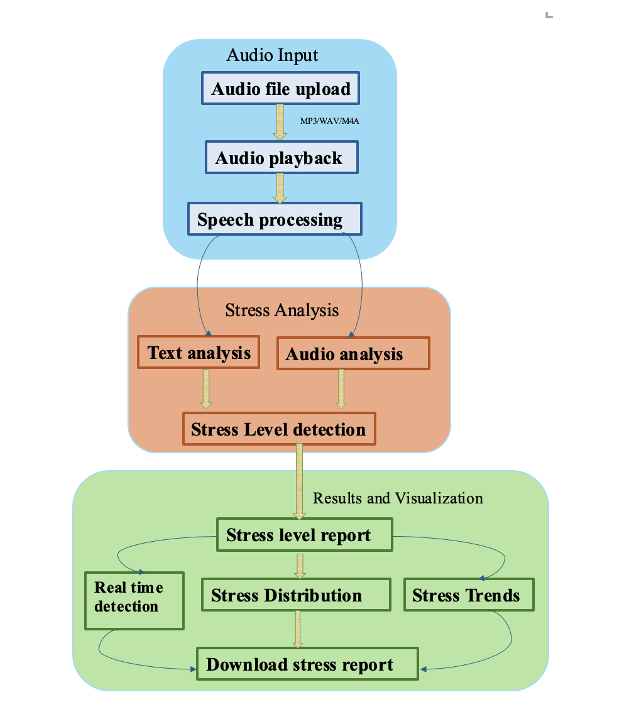
\includegraphics[width=1.1\columnwidth]{ap1.png}
    \caption{Overview of system approach}
    \label{fig:system_architecture}
\end{figure}
\vspace{10pt} % Add space to prevent overlap

  %\section{Significance of the Study}
 % This research contributes to the fields of mental health care, AI ethics, and multimodal AI by developing a system that combines advanced stress detection with interactive support.
  \section{Scope and Limitations}
 \textbf{Scope:}
 Focuses on voice-based stress detection and designs a stress trend module for user support.
 \textbf{Limitations:}
Does not include physiological signal data or longitudinal studies of user impact.
\section{Thesis Organization}
This thesis is structured into six chapters, each presenting a particular aspect of the study. Below is a brief overview of each chapter:
  \begin{enumerate} 
  \item  Chapter 1 cover  the research background, highlighting the importance of stress detection in mental health monitoring. It outlines the motivation, problem statement, research objectives, research questions, the significance of the study and scope and limitations, and the thesis organization. 
   \item Chapter 2 The literature review assesses previous work related to stress detection, focusing on speech-based and text-based emotion recognition, Social Signal Processing (SSP), and the role of deep learning and large language models, limitations in current stress detection and conversational AI systems. It highlights the lacking in current methods and shows the need for a multimodal strategy. 
   \item Chapter 3 This chapter describes the design and progress of the proposed multimodal stress detection system. It outlines the collection of dataset, data pre-processing procedures, and the two main modules: audio-based and text-based stress detection. Additionally, it describes the model designs, training and validation procedures and multimodal fusion techniques. 
   \item Chapter 4 This chapter highlights the actual implementation of proposed system. It describes the architecture and workflow, including speech-to-text processing, feature extraction. The chapter also describes the development of the user interface (UI), highlighting features such as real-time stress visualization and stress trend tracking, and report generation.
  \item  Chapter 5 This  chapter evaluates the performance of the proposed models, comparing their accuracy, precision, and recall across different approaches. It also includes experimental results between stress trend analysis system and human subjective analysis for stress. So, it highlights the system advantages and disadvantages.
  \item  Chapter 6 This chapter covers summary of the study, limitations and future considerations. Highlighting the research's contributions to the field of stress detection, the final chapter provides a summary of the main findings. In addition to discussing the shortcomings of the current system, it suggests future research objectives, such as real-time deployment, dataset enlargement, and interaction with other modalities including physiological data.

   \end{enumerate}
\chapter{Literature Review}
\clearpage 
  \section{Stress and Mental Health: A Psychological Perspective}
  Stress has a major impact on mental health and well-being through changes in physiological, emotional, and cognitive reactions. Effective techniques for early diagnosis and intervention are required because prolonged stress has been associated with a number of psychiatric diseases, such as anxiety and depression. Although the study (\citet{sebastiao2024}) showed on stress and mental health in COVID-19 emphasizes the importance of psychological flexibility and emotional schemas, it has a number of drawbacks. Avoid making judgments about causality by using a cross-sectional strategy. Potential biases are introduced by relying solely on self-reported data. Generalizability is limited by the sample. Results may also be affected by unmeasured variables, including socioeconomic status and previous mental health problems. Finally, results are impacted by the pandemic environment, which reduces their generalisability in non-pandemic scenarios. Despite these drawbacks, the study offers valuable information on the dynamics of mental health in emergencies. Traditional stress assessment relies on self-reported questionnaires such as the Perceived Stress Scale (PSS) and physiological measures such as heart rate variability (HRV) and cortisol levels. However, these methods can be intrusive, subjective, or impractical for continuous monitoring, leading to the need for automated non-invasive stress detection systems.
  In order to detect stress, (\citet{aristizabal2021})investigates the combination of self-reported data and wearable physiological sensors. In addition to self-reported stress levels, participants' electrodermal activity (EDA), heart rate (HR), and skin temperature were tracked using wearable technology as they performed stress-inducing tasks. These data streams were analysed by deep learning systems, which showed excellent accuracy in differentiating between stress levels. The study's semi-controlled laboratory environment, which would not accurately mimic stressors in the real world, and possible sample size and diversity restrictions, which would restrict generalisability, are some of its drawbacks. Reliability may also be impacted by sensor errors brought on by motion artefacts, self-report biases, and difficulties capturing quick shifts in stress.
  \section{Voice-Based Stress Detection}
  The communication medium Speech is a rich medium for detecting stress as it carries both linguistic and paralinguistic markers indicating stress. Research in speech emotion recognition (SER) has identified variations in prosodic features, such as pitch, intensity, speech rate, and spectral characteristics, as key indicators of stress with 97.1%
  accuracy utilising the Crema-D and TESS datasets, (\cite{chyan2022}) "A Deep Learning Approach for Stress Detection Through Speech with Audio Feature Analysis" investigates the use of CNN models for classifying stressed and unstressed speech based on Mel Spectrogram and MFCC characteristics. Nevertheless, the study has disadvantages, such as a controlled environment that does not replicate naturalistic noise situations, a binary classification approach that ignores shifting stress levels, and dataset constraints that do not represent real-world speech changes. Furthermore, the model's real-time applicability has not been validated, and its reliance on a small number of audio variables may ignore other elements. the study shows how deep learning may be used for speech-based stress detection and establishes the foundation for upcoming advancements in practical applications. 
This work employed the Toronto Emotional Speech Set (TESS), a popular dataset for emotion identification that includes vocal expressions from a range of emotional states. Convolutional neural networks (CNNs) and long short-term memory (LSTM) networks have been used in a number of research to extract and analyse voice data in order to classify emotions. While LSTMs capture temporal dependencies in sequential data, CNNs have been especially successful in processing spectrograms, which graphically depict frequency and amplitude fluctuations over time. By utilising both spatial and temporal feature representations, the hybrid models' integration of these architectures  will increase the accuracy of stress detection.
\section{Text based stress detection}
 in this study, author (\citet{yoon2020})investigates stress detection using semantic analysis of textual data, including private messages and postings on social media. The article analyses the approach on pertinent datasets to show its efficacy and finds linguistic patterns linked to stress using natural language processing (NLP) techniques. Nevertheless, there are a number of drawbacks, such as dataset restrictions that can fail to account for linguistic variation, contextual subtleties that could result in incorrect categorisation, and the lack of multimodal data like visual or aural signals. Furthermore, the model can have trouble keeping up with changing linguistic trends, necessitating frequent updates, and it poses privacy issues with relation to the use of personal data. 
\section{Social Signal Processing (SSP) in Mental Health Systems}
In this study, author(\citet{singh2019}) examines how SSP can be used to evaluate conversations by examining sentiment and emotional indicators. In order to better comprehend human interactions, SSP looks at non-verbal cues including gestures, vocal intonation, and facial expressions. This is especially important in industries like banking and finance, where it's critical to identify client dissatisfaction. The work intends to increase dialogue analysis for customer experience and service improvement by assessing emotional intensity in large data sets. However, the study has challenges, such as contextual limits because emotional expressions depend on conversational context and data quality issues because noisy or missing data might impair accuracy. Cultural differences also affect how nonverbal cues are interpreted, and deployment is complicated by the high computational resources required for real-time processing. Furthermore, analysing chats without the express consent of the user raises privacy problems. 

  \section{Machine Learning and Deep Learning for Stress Detection}
  The application of Machine Learning (ML) and deep learning (DL) approaches to stress detection and mental health monitoring is examined in this article\cite{razavi2024}. It draws attention to the efficacy of models such as Support Vector Machines (SVMs), Neural Networks (NNs), and Random Forest RFs, which use physiological data like skin reaction, heart rate variability (HRV), and heart rate (HR) as important stress indicators. In order to improve model performance, the study also highlights the significance of data preparation methods including feature selection and noise reduction. Nevertheless, there are a number of drawbacks, such as the inability to customise ML/DL models, which hinders their ability to adjust to different stress patterns, and their poor interpretability, which makes them less clear for clinical usage. Furthermore, the majority of research is carried out in controlled settings, which restricts its relevance in the real world, and real-time processing is still in its infancy, which makes real time interventions less feasible.
  In order to increase classification accuracy, the \cite{yao2021} presents a technique for stress detection that combines linguistic cues from text with acoustic data from speech. Compared to unimodal systems that only use text or audio, the multimodal method performs better because it uses machine learning techniques to analyse the interaction between language and vocal emotions. The lack of high-quality, labelled datasets with both text and audio components is one of the study's flaws though, and it may limit generalisability. Implementation is resource-intensive due to the contextual diversity in stress expression between cultures and individuals, which necessitates substantial training on varied datasets. In real-time processing, where accuracy and low latency must be preserved in dynamic situations, the system also faces difficulties. Error sources may also be introduced by the difficulties in synchronising text and auditory data. 
  \cite{hilmy2021} emphasises how well machine learning models like Support Vector Machines (SVMs) and Mel-Frequency Cepstral Coefficients (MFCCs) work for categorising stress and extracting spectral information from speech. While SVMs have strong classification capabilities, MFCCs are especially good at capturing speech characteristics that distinguish between stressed and neutral states. Studies have shown that this method may identify stress with high accuracy rates 88 Nevertheless, drawbacks include reliance on varied and high-quality datasets, which are frequently challenging to get by, and environmental noise, which can reduce the precision of feature extraction. Furthermore, the computing needs of SVM classification and MFCC extraction create problems for real-time processing. Model generalisability is also impacted by individual variations in speech patterns, such as accents and speaking styles, which calls for customised or adaptive methods. 


  \section{Role of Large Language Models (LLMs) in stress Analysis}
  In this research, author (\citet{shen2024}) investigates if Large Language Models (LLMs) undergo similar performance variations to humans when under stress. According to the Yerkes-Dodson law, which states that excessive or insufficient stress lowers efficiency, researchers discovered that LLMs operate best under moderate stress using StressPrompt, a series of stress-inducing prompts based on psychological theories. The study also showed that LLMs' internal brain representations were impacted by stress-altering stimuli, which mirrored human stress reactions. Nevertheless, there are a number of drawbacks, including as the limited generalisability of prompt-based stress induction—which may not accurately mimic real stress experiences—and the fact that results may differ depending on the LLM design. Furthermore, because the study was carried out in controlled environments and LLMs do not have human-like physiological reactions, it lacks real-world validation, which may affect how accurately stress comparisons are made. 
  \section{Limitations in Current Stress Detection and Conversational AI Systems}
 in this study, author (\citet{teye2022}) investigates how contextual and cultural factors affect conversational AI systems' ability to recognise emotions. In order to classify seven fundamental emotions, including sarcasm, the study created an emotion prediction model that included voice and picture data, with accuracies ranging from 85\% to 95\%. In order to increase the dependability and moral coherence of emotion detection systems across a range of demographics, the authors stress the importance of taking environmental factors and cultural quirks into account. However, the study has drawbacks, such as difficulties with data representation because datasets are frequently undiversified, which impairs the model's cross-cultural generalisability. Furthermore, despite efforts to balance, biases in datasets continue to exist, which could diminish fairness. Because sarcasm is nuanced and context-dependent, it is still very difficult to detect. The performance of the system can also be impacted by environmental fluctuations, including background noise.
  By utilising real-time data fusion from several sources, including environmental sensors, biometric devices, and Internet of Things systems, the combination of sensor technologies and conversational AI allows for context-sensitive interactions. By improving AI's comprehension of user context, physical circumstances, and environment, author \cite{kush2025} enables more intelligent and flexible interactions. For instance, conversational AI in healthcare enhances the responsiveness and personalisation of virtual health aides by integrating data such as temperature, stress levels, and heart rate. To fully realise the potential of these systems, however, issues like interoperability, scalability, and data heterogeneity must be resolved. The ability of sensor-integrated AI to provide real-time, context-aware help is demonstrated by real-world implementations, such as Mercedes-Benz's integration of Google's conversational AI agent into cars, opening the door for cutting-edge solutions across industries.
  \section{Ethical Challenges in AI-Driven Stress Detection}
  In the paper, author (\citet{sriramprakash2017}) examines the expanding use of AI in mental health care, emphasizing how it can enhance early identification, accessibility, and personalized care. Virtual assistants and AI-powered chatbots offer prompt assistance, and predictive analytics can help spot mental health problems before they get out of hand. The study also identifies problems that make it difficult to understand AI-driven decisions, including algorithmic transparency issues, lack of human empathy in AI interactions, and data privacy concerns. Along with difficulties in incorporating AI into conventional healthcare systems due to patient and practitioner reluctance, ethical issues such as consent and autonomy continue to be crucial. In order to guarantee that AI improves mental health care while upholding ethical standards, further developments in emotionally intelligent AI, improved integration with healthcare services, and robust regulatory frameworks will be crucial.
 % \renewcommand{\arraystretch}{1.2} % Adjust row height
 %\renewcommand{\arraystretch}{1.0} % Tighter row spacing
  \vspace{-5mm} % Reduce vertical space before the table
 \begin{table}[H]
\centering
\caption{Summary of literature review}
\label{tab:correlation_table}
%\small % Reduce the font size of the entire table
\begin{tabular}{|p{1.8cm}|p{2.8cm}|p{4.3cm}|p{4.3cm}|}
\hline
 Author & Technique & Findings & Limitations \\ \hline
 Chyan et al\cite{chyan2022}  & CNN for speech-based stress detection & Utilizes MFCCs and Mel Spectrograms to classify stress in speech with high accuracy (97.1\%). & Controlled setup; binary classification misses stress gradation; lacks real-time validation; ignores real-world noise.\\ \hline
 Study on LLMs \cite{teye2022} & StressPrompt for stress analysis in LLMs & Demonstrates performance variations in LLMs under stress using psychological prompts. & Lacks real-world validation; results depend on specific LLM design and controlled settings; no physiological equivalence to humans\\ \hline
\cite{yoon2020} & Semantic analysis of textual data & Identifies linguistic patterns in private messages and social media posts to detect stress using NLP & Dataset limitations; lacks multimodal data; struggles with linguistic trends and contextual subtleties; raises privacy concerns.\\ \hline
\cite{singh2019} & Social Signal Processing (SSP) for emotion detection & Analyses sentiment through non-verbal cues such as gestures and intonation. & Data quality issues; computationally intensive; contextual limitations; privacy concerns in analyzing conversations\\ \hline
 Multimodal Study \cite{razavi2024} & Combining text and audio signals & Outperforms unimodal approaches by integrating linguistic cues and vocal emotions; uses ML for interaction analysis. & Resource-intensive; lacks high-quality multimodal datasets; difficulties in synchronizing text and audio data for real-time application\\ \hline
 \cite{teye2022} & Ethical AI in mental health care & Highlights AI’s potential for early intervention and personalized care. & Challenges in algorithmic transparency; lack of human empathy in AI; privacy concerns. \\ \hline % resistance from patients and practitioners; difficulty in integrating AI into conventional systems.\\ \hline
\end{tabular}
\end{table}
\vspace{-5mm} % Reduce vertical space after the table
%%%%%%%
%\begin{table}[p] % Use [H] to place the table here
%\centering
%\caption{Summary}
%\label{tab:dataset_table} % Optional, for referencing the table
%\begin{tabular}{|p{2.5cm}|p{3cm}|p{4.5cm}|p{4.5cm}|} % Adjusted column widths
%\hline
%\raggedright \textbf{Year \& Author(s)} &
%\raggedright \textbf{Techniques/Methods} &
%\raggedright \textbf{Findings} &
%\raggedright \textbf{Limitations} \\
%\hline

%\hline
%2024, Chyan et al. & CNN for speech-based stress detection & Utilizes MFCCs and Mel Spectrograms to classify stress in speech with high accuracy (97.1\%). & Controlled setup; binary classification misses stress gradation; lacks real-time validation; ignores real-world noise and dataset variability. \\
%\hline
%2022, Study on ML/DL Models & SVM, RF, and NN for physiological data & Highlights the utility of feature selection, skin reaction, HRV, and HR for stress detection with ML/DL models. & Lack of adaptability; controlled setups limit real-world application; low interpretability for clinical use; real-time implementation remains immature. \\
%\hline
%2024, Multimodal Study & Combining text and audio signals & Outperforms unimodal approaches by integrating linguistic cues and vocal emotions; uses machine learning for interaction analysis. & Resource-intensive; lacks high-quality multimodal datasets; cultural and individual diversity challenges; difficulties in synchronizing text and audio data for real-time application. \\
%\hline
%2024, Yiqun et al. & SVM with MFCCs & High accuracy for stress classification by extracting spectral features from speech. & Requires diverse and high-quality datasets; affected by environmental noise; computational challenges for real-time use; individual variability limits model generalizability. \\
%\hline
%2024, Study on LLMs & StressPrompt for stress analysis in LLMs & Demonstrates performance variations in LLMs under stress using psychological prompts; identifies internal representation shifts similar to humans. & Lacks real-world validation; limited generalizability; results depend on specific LLM design and controlled settings; no physiological equivalence to humans. \\
%\hline
%2024, Macháček et al. & Cultural and contextual emotion detection via AI & Combines voice and image data to classify emotions; achieves accuracies from 85\% to 95\%. & Struggles with sarcasm detection; dataset biases reduce generalizability; environmental noise impacts performance; challenges in ensuring fairness and cross-cultural consistency. \\
%\hline
%2024, Ranjan \& Thakur & IoT and biometric integration in conversational AI & Enhances contextual and environmental understanding for AI in healthcare; integrates biometric data for improved personalization and real-time response. & Issues with scalability, interoperability, and data heterogeneity; computationally intensive for real-time fusion of multiple data sources. \\
%\hline
%2024, Teye et al. & Ethical AI in mental health care & Highlights AI’s potential for early intervention and personalized care; emphasizes the need for regulatory frameworks and ethical standards. & Challenges in algorithmic transparency; lack of human empathy in AI; privacy concerns; resistance from patients and practitioners; difficulty in integrating AI into conventional systems. \\
%\hline
%\end{tabular}
%\end{table}

  \section{Research Gaps and Opportunities}
The majority of the research that has been done on stress detection has been either text-based or audio-based. Even while CNNs and LSTMs have shown excellent accuracy in identifying speech emotions, feature selection and dataset quality changes depending on dataset. LLMs have shown promise in extracting stress-related linguistic features, but their effectiveness in combination with voice analysis is still being explored. In order to fill this gap, this study proposes a multimodal stress detection system that uses both textual and auditory signals. A real-time user interface (UI) with stress trend tracking is also created to enhance accessibility and user interaction. In order to facilitate practical uses in mental health monitoring and emotional well-being, the results of this study assist in establishing solid and interpretable stress detection frameworks.
\section{Summary of the review}
Despite significant advancements in text and audio-based stress detection, current approaches as shown in Table 2.1 lack the accuracy and contextual understanding needed for real-time applications. This review highlights the need for multimodal systems that integrate linguistic and paralinguistic cues, offering a foundation for this study.
\chapter{System Design}
\clearpage 
Text and audio embeddings are the two main modules that comprise up system. The system is thoughtfully designed to effectively combine both textual and audio information, creating a strong foundation for multimodal stress detection.The ability of the system to produce responses that resemble those of a human is directly influenced by the textual interpretation with whisper and GPT-4analysis.Key aspects of the design include well-structured pipelines, efficient deployment strategies, and thorough dataset preparation. Each element has been carefully crafted to enhance the system's usability, scalability, and accuracy, ensuring it delivers reliable and practical results.
\section{System architecture}
Using multimodal inputs, the suggested system combines several parts to identify and display stress levels. The architecture is separated into three main modules, as seen in Figure 3.1: 
Frontend (Streamlit): In handling user interaction, including audio file uploads and results visualisation.  
Backend (Flask): Manages essential features including stress analysis, speech-to-text conversion, and external service interaction. 
External Services: These comprise advanced text analysis APIs such as OpenAI for GPT-4. 
These parts work together seamlessly ensuring that the system is scalable, responsive, and able to process inputs in real time. 
\begin{figure}[h]
    \centering
    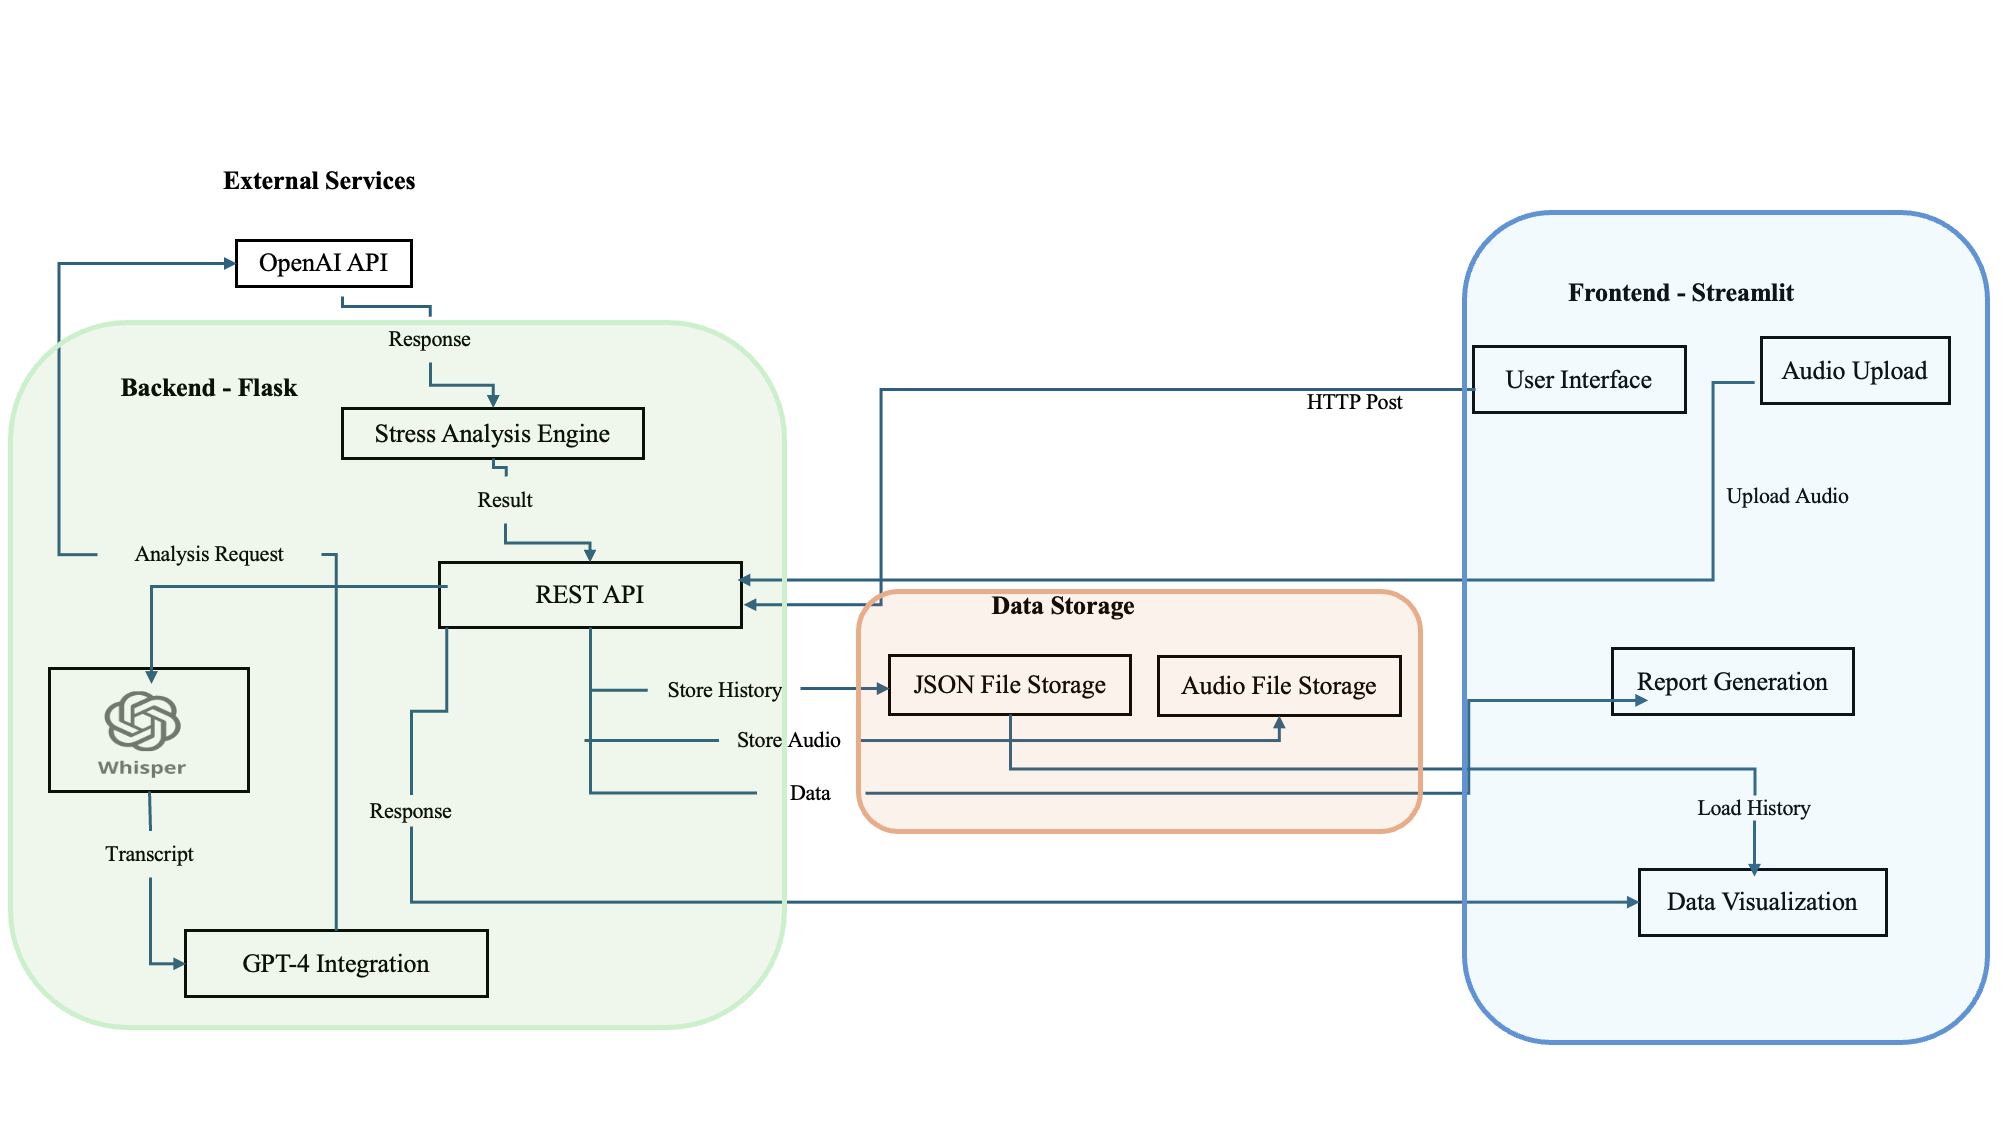
\includegraphics[width=1.1\columnwidth]{allreferences/systemdesigndia.png}
    \caption{Proposed System Architecture}
    \label{fig:system_architecture}
\end{figure}
\section{Dataset Description}
  A limited number of audio recordings was used to generate and illustrate the functioning of the stress detection system's user interface (UI) and user experience (UX) components. These recordings, which come from openly accessible websites like Google, feature speech samples with a range of psychological tones. Even though the audio files don't represent a formal or standardized dataset, they are a useful tool for demonstrating the system's features, like trend monitoring and real-time stress level visualization. I used the audio file to capture voice at different stress levels. After processing these data, stress detection outputs were simulated and shown on the user interface. These samples are primarily being used to test and validate the stress visualisation features of interface and illustrate how stress trend tracking works throughout several sessions. Also checking interface is capable of handlingvarious stressful aspects.
\begin{table}[p] % Use [H] to keep the table close to the text
\centering
\caption{Dataset Description}
\label{tab:dataset_table} % Optional, for referencing the table
\begin{tabular}{|c|p{8cm}|} % Adjusted column width for better text wrapping
\hline
\textbf{Audio} & \textbf{Text in the Audio} \\ \hline
Audio1 & I wonder what this is about \\ \hline
Fire & The place is on fire, please send help \\ \hline
Test1 & Loans that we can offer with this or farm ownership loans, operating lines of credit, or equipment and capital improvement need loans. The benefit to the \\ \hline
sad.Wav & The best food novel count me on the edge of my side \\ \hline
New recording 19.wav & 時間が戻れば私はあの時間に戻りたいま一回 \\ \hline
New recording 16.wav & So um... I'm sick. But my friend wanted me to be a deity myself because we always had to really cool. So uh... Yeah, here it is. Do you want me to sing? Oh, it sounds really good singing. \\ \hline
new recording 23.wav & Life is difficult, but you are loved. You are loved and important, and you bring to this world things that no one else can so hold on \\ \hline
Airplane.wav & The airplane is almost full.\\ \hline
Gamer.mp3 & Why would you not want to fight for what you believe in? \\ \hline
Sad.mp3 & The delicious aroma of freshly baked bread filled the bakery. \\ \hline
1008TIE.wav & That is exactly what happened.\\ \hline
New recording 25.wav & Us comfort help isn't given up. It's refusing to give up. To use fall for a reason, and to use strength and weakness. I think... \\ \hline
\end{tabular}
\end{table}
\section{Text Processing workflow}
%\clearpage  % Forces all previous content to be placed before this point
The Text Processing Workflow describes the procedures for evaluating and interpreting the text to detect stress. Figure 3.2 shows the text processing workflow, which consists of the following steps: Whisper converts audio into raw text. Using semantic context, GPT-4 analyzes the text to find stress signals. The system uses stress scale to classify stress levels (Low, Moderate, High). The system gives feedback, including stress management tips, based on the user's degree of stress. Each component in a text processing flow is responsible for handling a specific task. For example, an input handler handles text input from audio or manual entry, while an analysis engine uses GPT-4 to analyze text for stress content and analyze numerical stress levels. The formatter gets the results ready to be shown. The report generator generates reports that can be downloaded, while the display handler manages visual representation. It focuses on the processing of textual information obtained from speech. Whisper and GPT-4 are the main tools used in this workflow for the transcribed text's semantic analysis.
 %\clearpage  % Forces all previous content to be placed before this point
%\vspace{-5mm} % Reduce vertical space
\begin{figure}[!htbp]
\centering
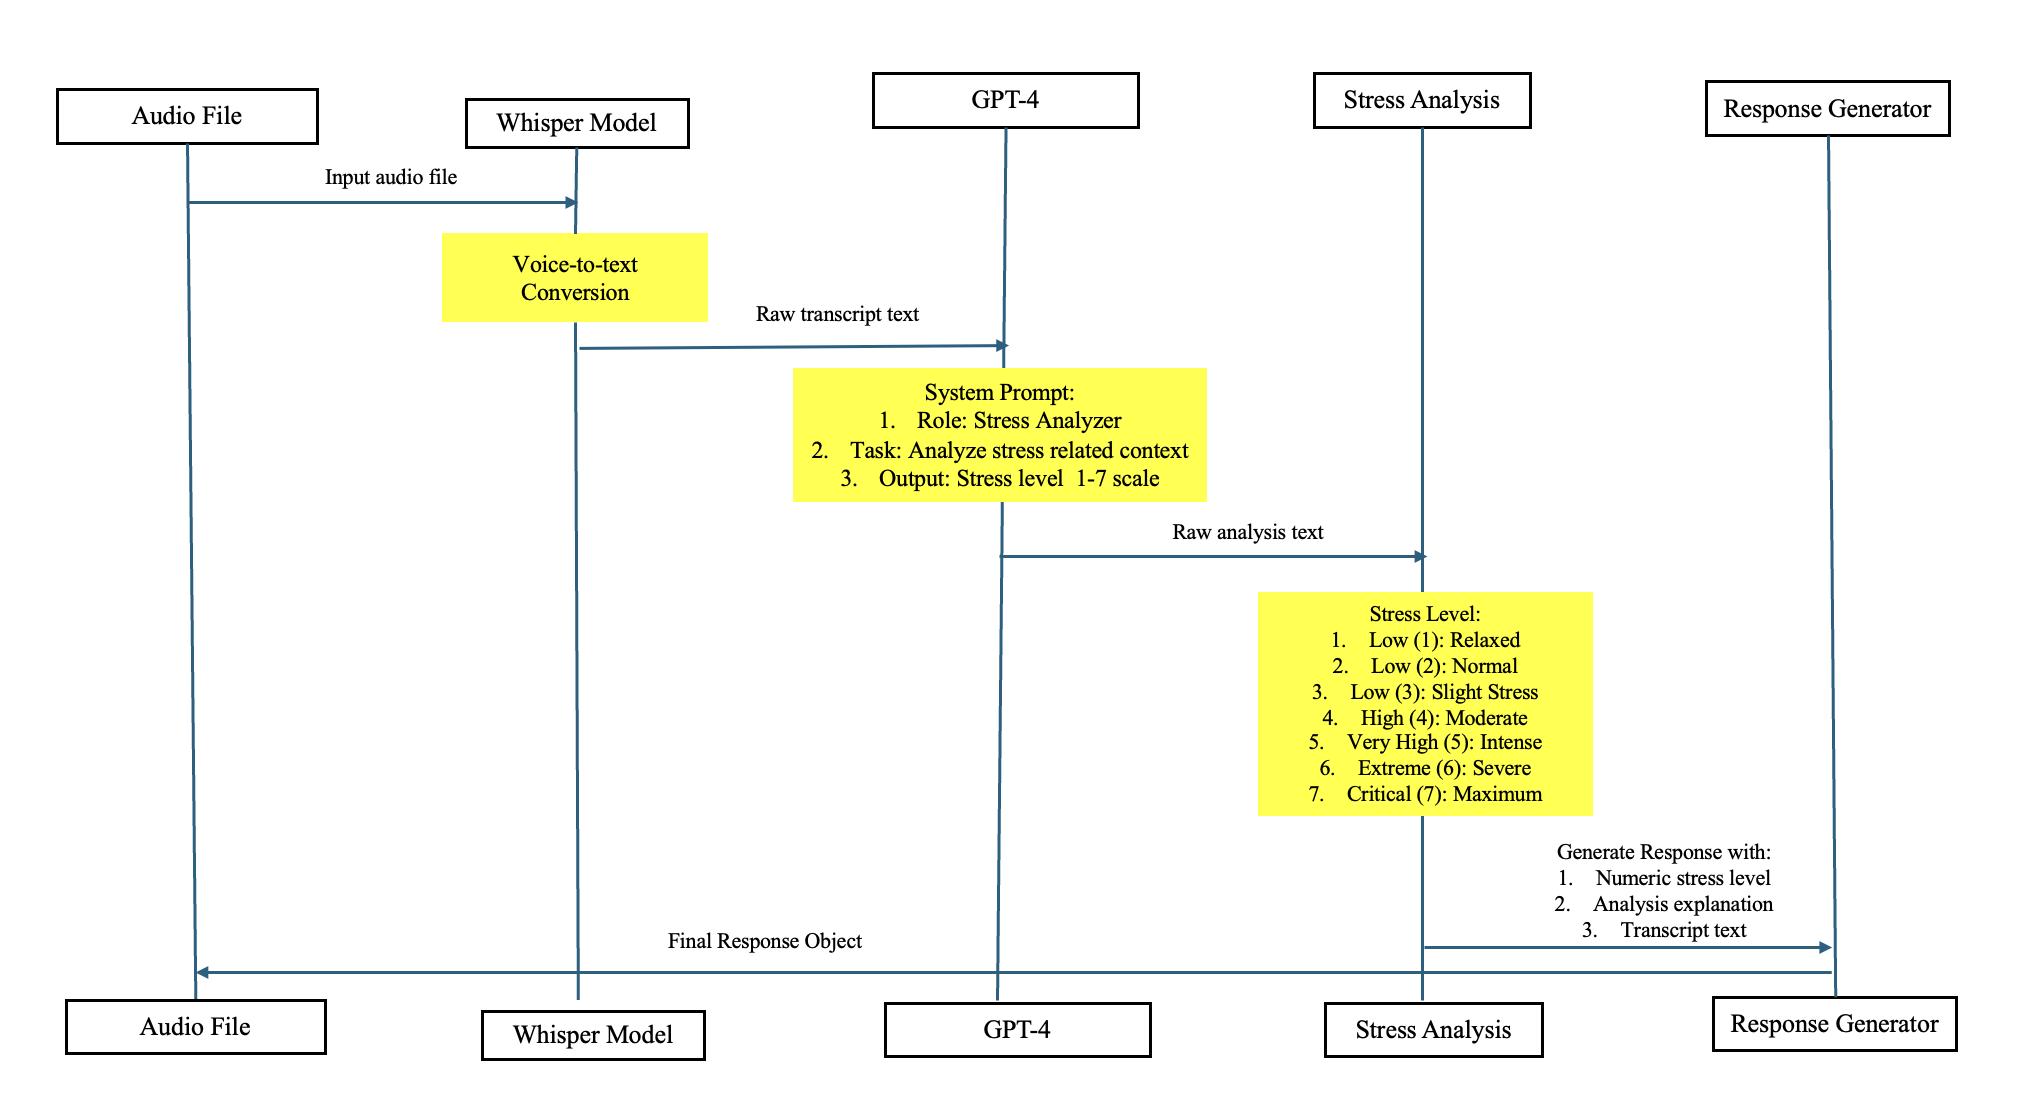
\includegraphics[width=1.2\textwidth]{allreferences/textprocessingworkflow.png}
\caption{Text processing flow}
\label{fig:text flow}
\end{figure}
\subsection{Speech to Text Conversion (Whisper)}
\noindent
\begin{minipage}{\textwidth}
The use of Whisper\cite{machaek2023} for accurate transcription. For the flow of text generation This text processing module combines the manual transcript input option, text cleaning and preparation, and whisper to convert speech to text. Whisper converts speech to text.Draw attention to Whisper's main function of converting audio into text transcripts.  This module transcribes user speech into text and performs language analysis to detect stress-related context. Identifies specific words and phrases associated with stress, using GPT-4's capabilities to interpret context. The system captures the audio. The raw audio is passed into the speech recognition API. OpenAI‘s Whisper to convert into text. The voice in the audio file is converted into a textual transcript. For text formatting, the transcript is formed as cleaned or standardized and removing unnecessary pauses or artifacts. 
 The significance of text preparation for analysis, noise reduction, and transcription accuracy is emphasized.The Whisper model processes audio inputs and generates a transcript with a high degree of accuracy, filtering out noise and ensuring that only meaningful words are passed to the next stage.
 %\clearpage % Forces all previous content to finish
%\vspace{-5mm} % Adjust the value as needed to reduce the gap
\vspace{10pt} % Add space to prevent overlap
\FloatBarrier
\begin{figure}[H]
\centering
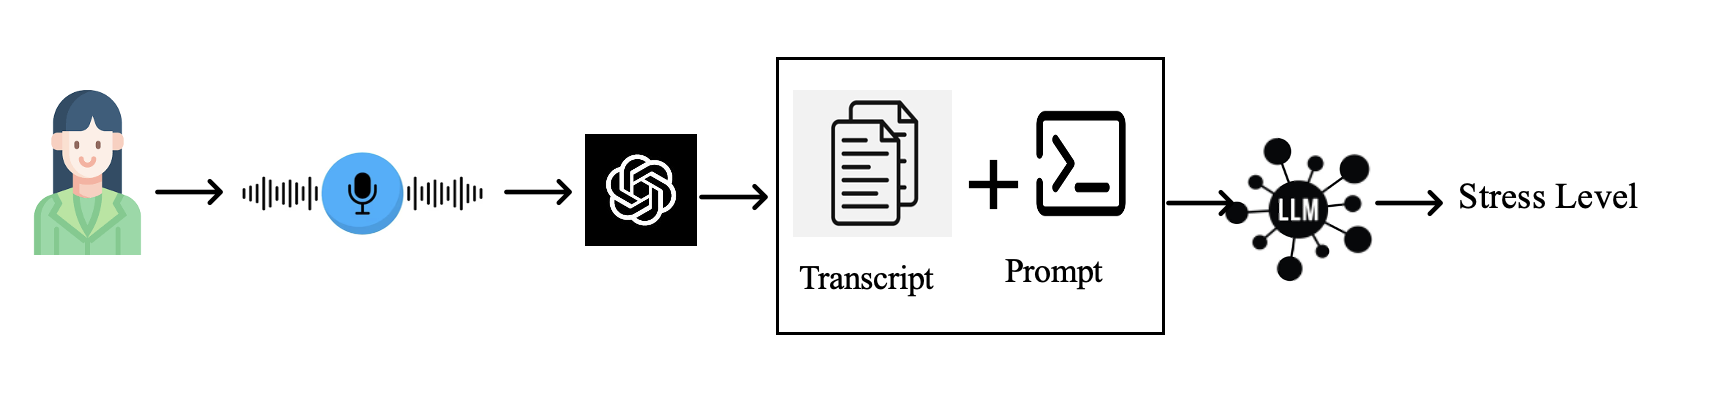
\includegraphics[width=1.0\columnwidth]{allreferences/textualnetwork2.png}
\caption{Textual analysis}
\label{fig:system_architecture}
\end{figure}
\end{minipage}
\vspace{10pt} % Add space to prevent overlap
%\subsection{GPT-4 analysis setup}
%GPT-4 is set up to detect stress patterns and analyze the context. And also measures the stress level from 1 to 7 and provides an explanation. GPT-4 interprets textual input to identify contextual and semantic stress signals and its natural language processing (NLP) skills to find contextual meanings and phrases that cause stress. 
%For instance: "GPT-4 analyses the transcript by detecting linguistic cues and contextual stress indicators, such as emotional word choices or abrupt sentence patterns." 
%\subsection{Stress level scale}
 %The scale utilized to classify the intensity of stress and discuss how textual cues, such as sentence structure and word choice, affect the identification of stress levels.
 %For instance: "Stress levels are determined based on linguistic patterns like frequent use of negative words, abrupt transitions in tone, and word repetition." 
%\subsection{Response generation}
%The system generates customized feedback. The result was processed using explanation formatting, colour coding according to level, and numerical stress level mapping. The display feature consists of the original transcript, detailed analysis text, and color-coded stress indicators. The ability of the system to produce responses that resemble those of a human is directly influenced by the textual interpretation. 
%For instance: "The generated response includes stress-relieving suggestions that are directly informed by the context of the transcribed text." 

\section{Audio Processing workflow} 
The main focus of the Audio Processing Workflow is the analysis of text data along with raw audio characteristics like pitch, tone, and frequency. This section describes how the use of voice characteristics in audio data enhances the stress detection system. Figure 3.3 illustrates the audio processing process that combines GPT-4, Whisper, and the backend to analyse stress. Important actions consist of utilising the frontend to upload the audio file. Whisper audio to text conversion. Using GPT-4 to perform stress analysis and storing audio files and JSON results for tracking history. The processing pipeline goes as follows: Whisper converts audio to a transcript, the frontend uploads the audio file to the Flask backend, which keeps it temporarily. The transcript is then submitted to GPT-4 for stress analysis, the results are kept in a JSON history, and the frontend receives the response. Using a REST API design, the system's frontend and backend operate on the default ports of Streamlit and Flask, respectively. They communicate via HTTP POST requests, file transfers take place via multipart/form-data, and JSON is delivered as the result. 
\vspace{10pt} % Add space to prevent overlap
\begin{figure}[H]
    \centering
    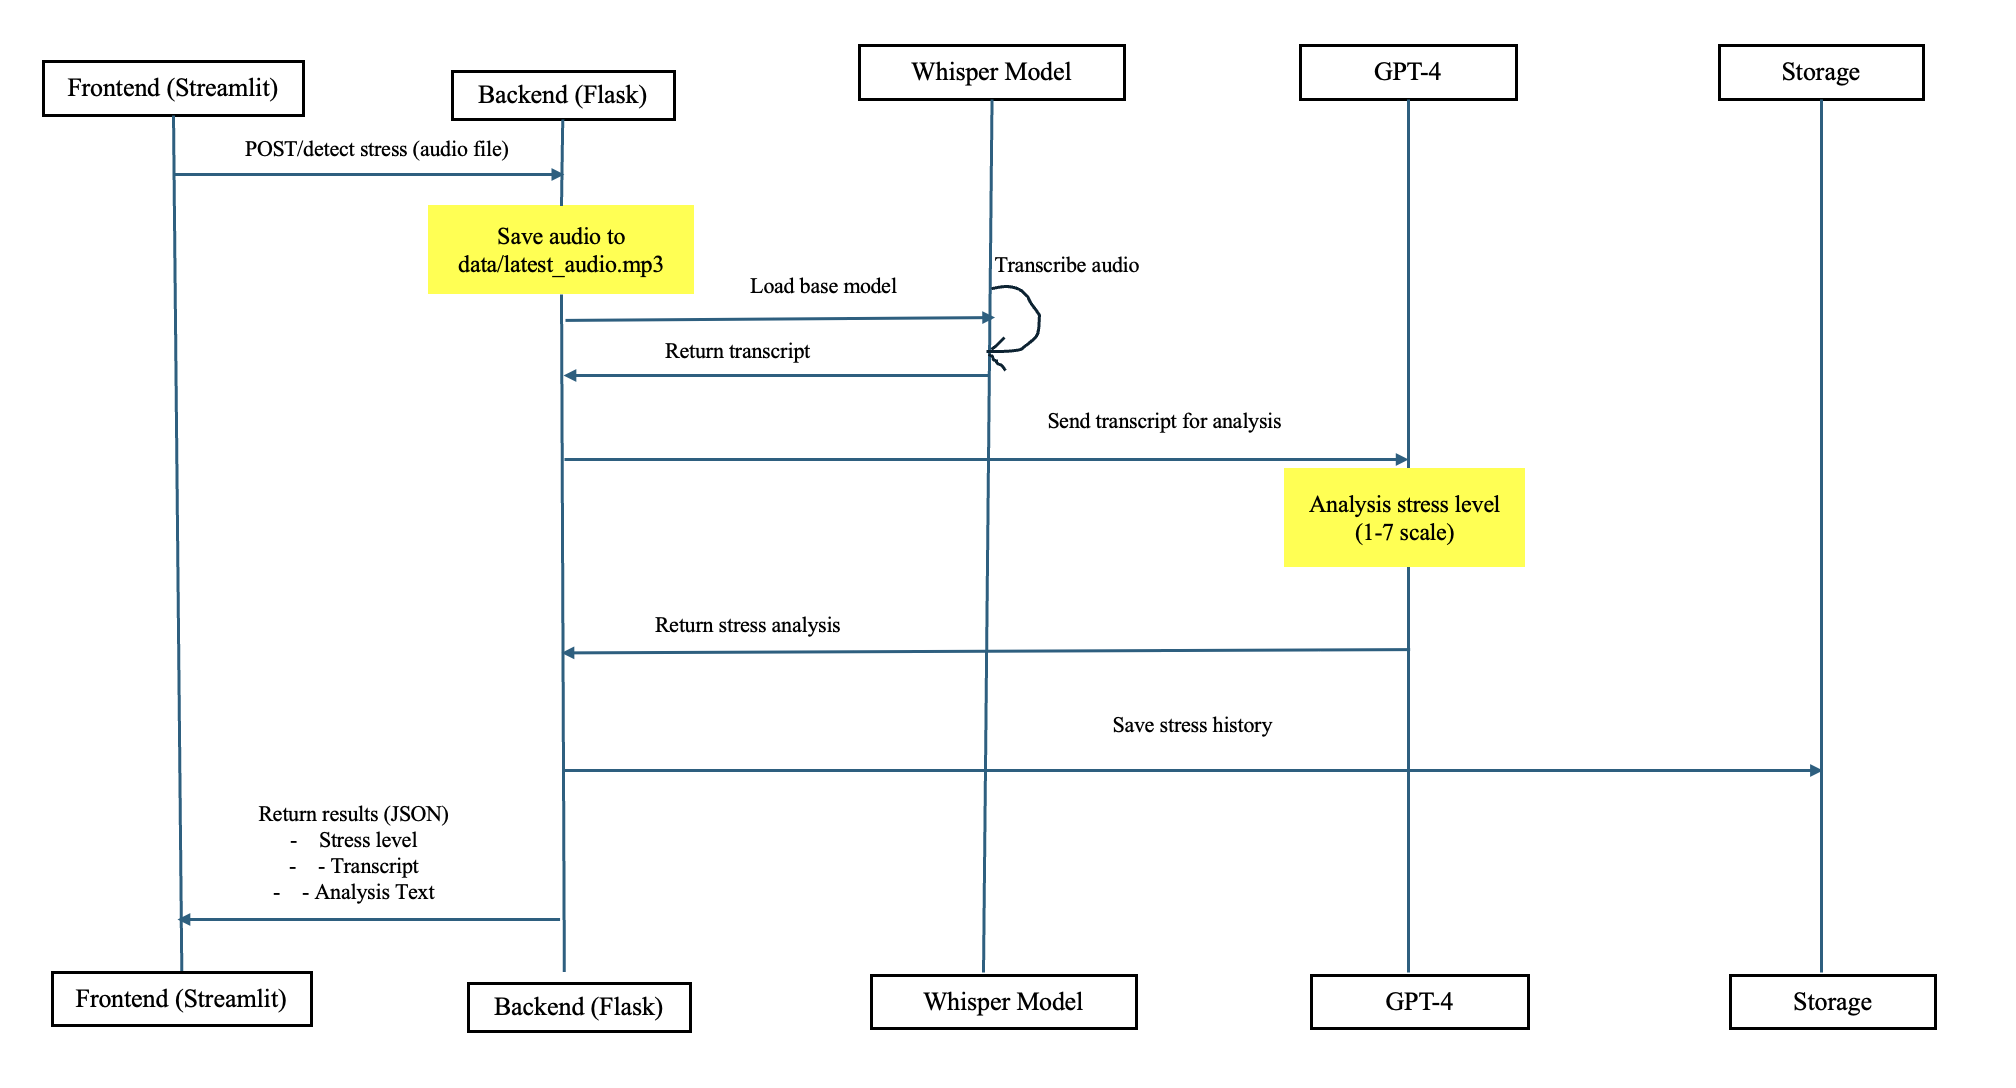
\includegraphics[width=1.1\columnwidth]{allreferences/audioflow.png}
    \caption{Audio processing flow}
    \label{fig:system_architecture}
\end{figure}
\vspace{10pt} % Add space to prevent overlap
%\subsection{Whisper for Speech-to-Text:}
%Whisper handles transcription. Distinguish by highlighting  how the impact of audio pre-processing (such as managing background noise and accents) on transcription quality. Whisper's capacity to retain vocal inflections for stress analysis later on. 
%For instance: "Whisper not only transcribes audio into text but also captures subtle vocal characteristics, such as tone fluctuations, which are critical for stress detection." 
%\subsection{GPT-4 for Stress Analysis}
%GPT-4's role in detecting stress patterns.
%In GPT-4's analysis, focus to how audio characteristics (such tone or pitch) enhance the text and discuss about how GPT-4 improves accuracy by combining vocal stress signals with semantic context. 
%For instance: "GPT-4 combines the tonal data from the audio with semantic analysis of the transcript, creating a holistic view of the user's stress levels." 
\subsection{Frontend to Backend Connection and Backend API Endpoint}
Data flows between the user interface and backend. How audio files are uploaded and routed to the backend for processing, highlighting the variations in data flow. 
For instance: "The frontend enables seamless audio file uploads, which are processed through APIs to generate real-time stress analysis results." 
APIs are utilized for seamless communication and emphasizing how the backend responds to demands for processing that are particular to audio in a different way than it does to text. 
For instance: "Backend APIs facilitate efficient data flow, ensuring that both audio features and their textual representations are analyzed synchronously." 
\section{Stress visualization workflow}
This section describes an intuitive and interactive way for users to view their stress levels. Users can see their stress levels in an easy-to-understand format with the help of the stress visualization workflow (Figure 3.4). Stress data recorded in JSON is loaded by users interacting with the UI. Plotly and other libraries are used to process data and produce pie charts and other graphics. Interactive elements and insights into stress distribution are two of the visualization's main characteristics. Interactive elements such as Legend for reference, Click-to-hide sections and hover tooltips that display precise percentages. Clear patterns and stress percentages are displayed in visualisations, which aid users in efficiently interpreting their data.By choosing the option to "View stress trends," the user starts the process. A slider is then used by the user to select a time range for stress visualization. The process of retrieving and preprocessing. In data loading and Processing portion invloves of fetching stress data (from JSON) and get it ready for visualization. In this procedure, user-selected data is loaded according to the designated time frame. Arranging and preprocessing data in preparation for analysis. Explains how stress levels are represented by colour coding: red for excessive stress, yellow for moderate stress, and green for low stress. Consistency and clarity in visual representation are assured by this arrangement of data. It shows how graphical outputs are generated from the analyzed stress data. The proportions of various stress levels are displayed using a pie chart. The Plotly library makes it easier to create dynamic charts with features such as Precise labels. Interactive sections, such as click-to-hide. Stress data is represented graphically. Visuals are rendered on the user interface, draws attention to the way the Streamlit user interface renders the images: Interactive elements and the pie chart are shown in the application. The visualizations make it simple for users to explore their stress data
%\vspace{-5mm} % Adjust the value to control the spacing
\vspace{10pt} % Add space to prevent overlap
% Example
\FloatBarrier
\begin{figure}[H]
    \centering
    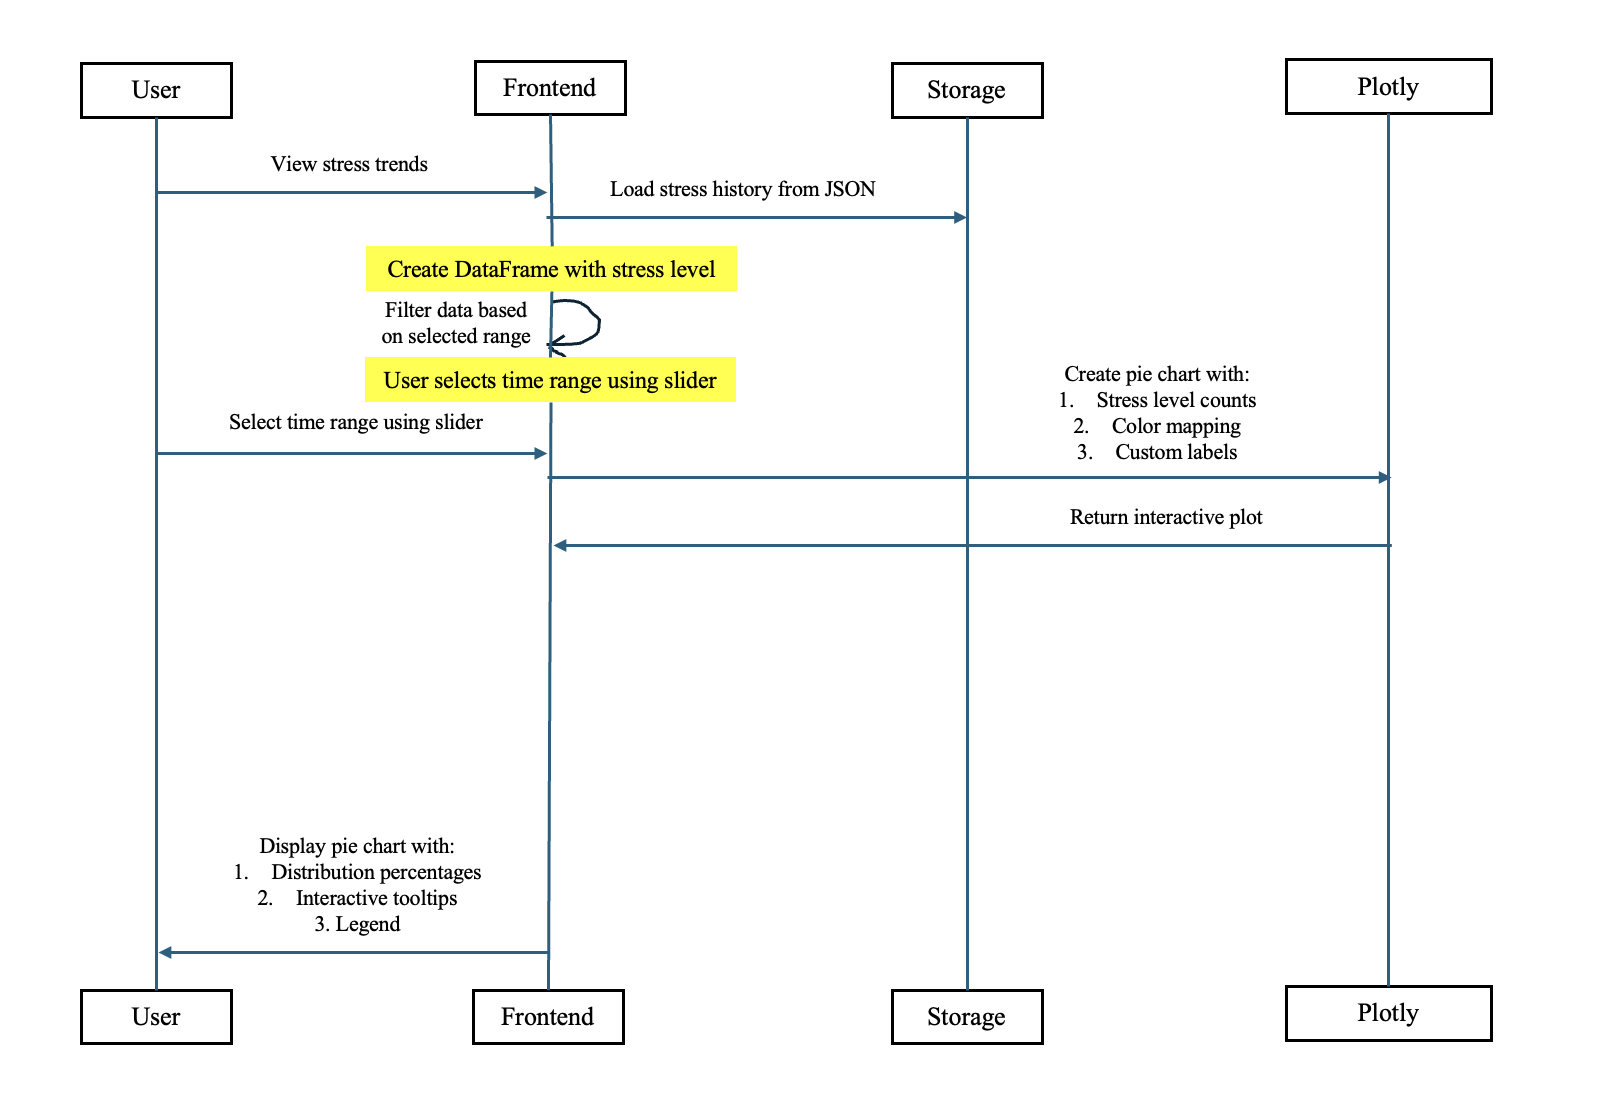
\includegraphics[width=1.0\columnwidth]{allreferences/piestressvisual.png}
    \caption{Stress Visualization Flow}
    \label{fig:system_architecture}
\end{figure}
\FloatBarrier
\vspace{10pt} % Add space to prevent overlap
%\subsection{Data Loading and Processing}
%By choosing the option to "View stress trends," the user starts the process. A slider is then used by the user to select a time range for stress visualization. The process of retrieving and preprocessing. In data loading and Processing portion invloves of fetching stress data (from JSON) and get it ready for visualization. In this procedure, user-selected data is loaded according to the designated time frame. Arranging and preprocessing data in preparation for analysis. 

%\subsection{Color Mapping Setup}
%This subsection explains how stress levels are represented by colour coding: red for excessive stress, yellow for moderate stress, and green for low stress. Consistency and clarity in visual representation are assured by this arrangement of data. It shows how graphical outputs are generated from the analyzed stress data. The proportions of various stress levels are displayed using a pie chart. The Plotly library makes it easier to create dynamic charts with features such as Precise labels. Interactive sections, such as click-to-hide. Stress data is represented graphically. Visuals are rendered on the user interface, draws attention to the way the Streamlit user interface renders the images: Interactive elements and the pie chart are shown in the application. The visualizations make it simple for users to explore their stress data.
\section{Stress trend analysis workflow}
Changes in stress levels over time are monitored via the stress trend analysis workflow (Figure 3.5). To examine certain sessions, users can use time ranges to filter data and to improve insights and smooth out volatility, the system computes moving averages. Trends are displayed using interactive charts that can be customized. Interactive features include zoom and pan controls, a time range slider for filtering data, hover tooltips for displaying precise values, and a legend for trend lines and stress levels. 
\vspace{10pt} % Add space to prevent overlap
\begin{figure}[H]
    \centering
    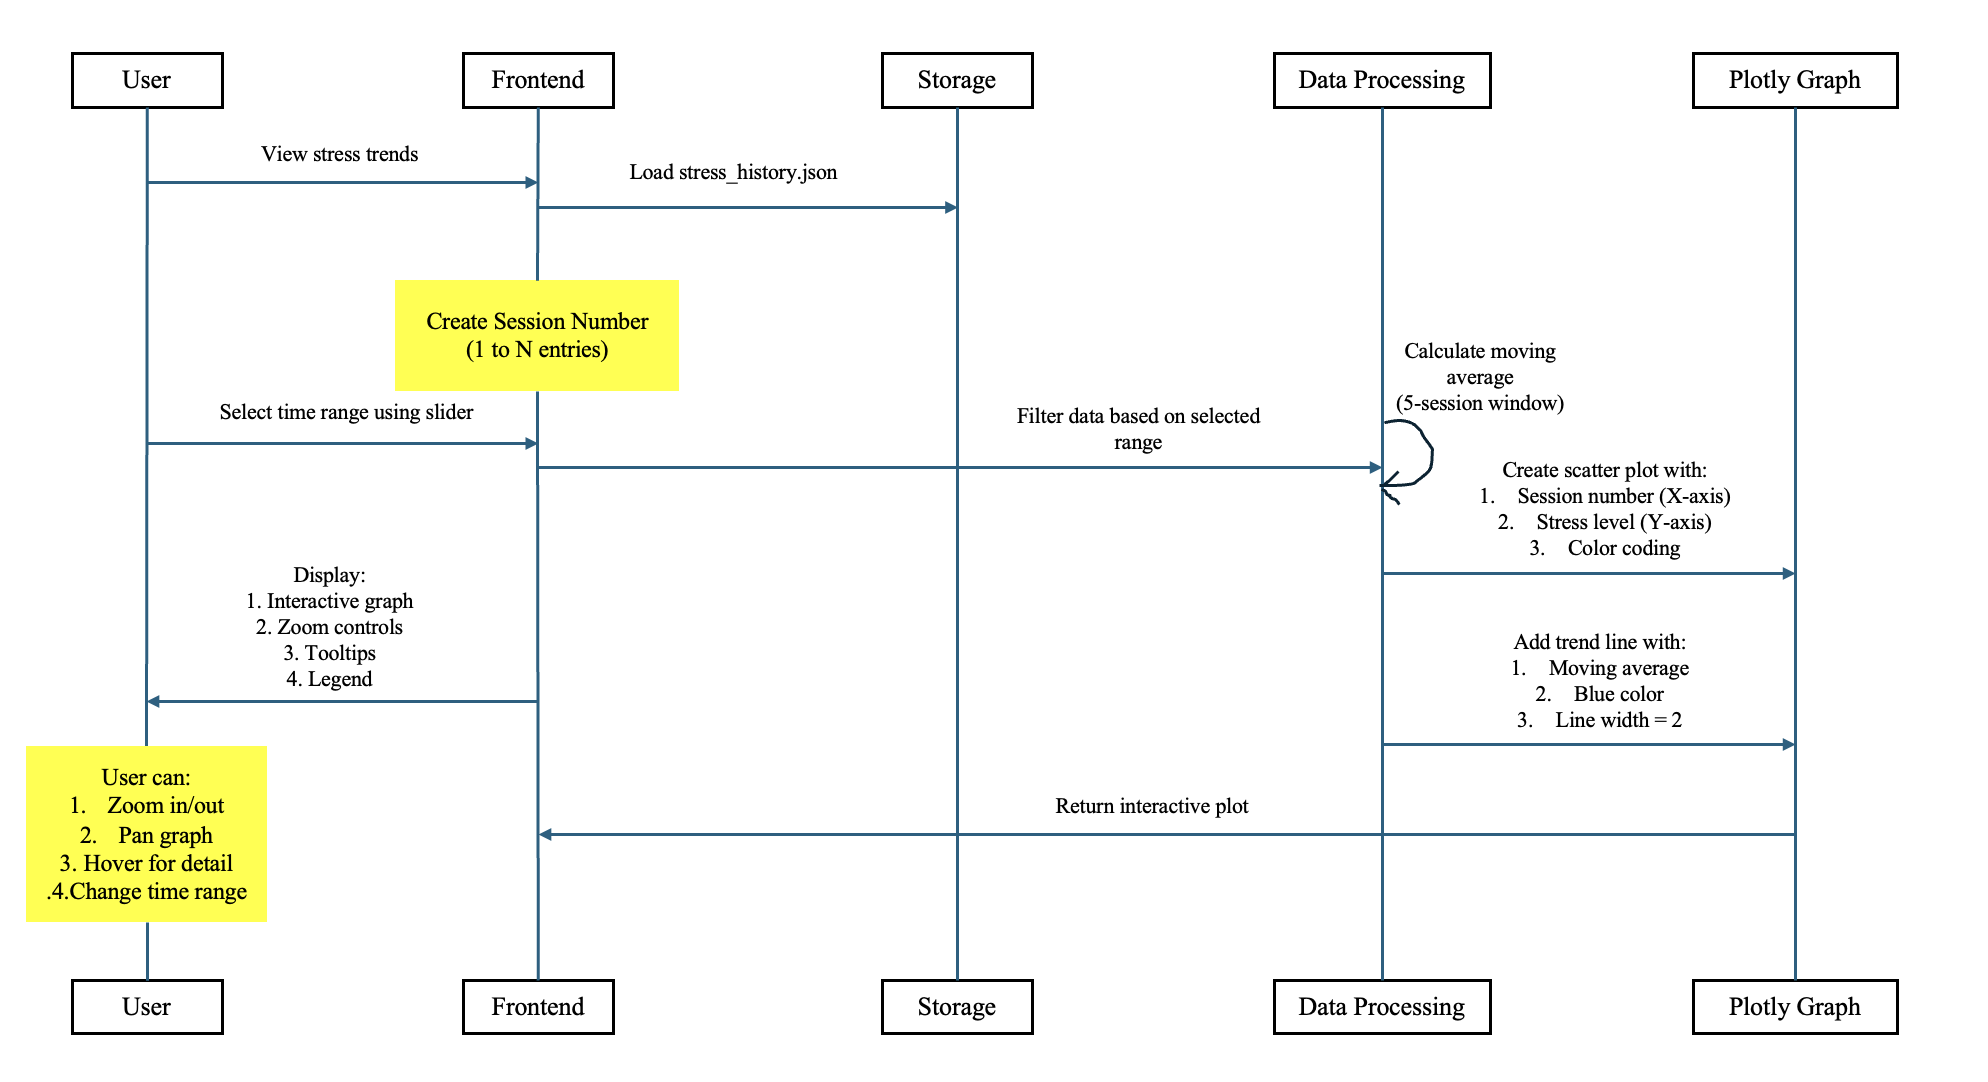
\includegraphics[width=1.1\columnwidth]{allreferences/stresstrendflow.png}
    \caption{Stress trend analysis workflow}
    \label{fig:system_architecture}
\end{figure}
\vspace{10pt} % Add space to prevent overlap
\subsection{Data Loading and Time Range Selection}
This subsection explains how stress data is retrieved from storage and filtered based on the selected time range. It emphasizes the user’s role in selecting the desired range and how this choice influences the subsequent data analysis steps. %the process by which stress data is retrieved and filtered.
\subsection{Moving Average Calculation}
The process utilized for highlighting the patterns and focusses on how patterns in stress data are highlighted through calculation. To smooth out variations and identify patterns in the data, a moving average is calculated across a specified session window.
\subsection{Interactive Plot Creation}
The tools and techniques for dynamic visualizations. Explains how dynamic visualizations are made using various tools and techniques. By enabling zooming, panning, and hovering, interactive graphs give viewers an in-depth assessment of stress patterns
\subsection{Customizing Plot Layout}
 Chances to use personalization to improve user interaction. The personalisation options available to enhance user interaction are described in this subsection. Plots can be altered by users to fit their tastes in terms of colour schemes, line styles, and data presentation.
\chapter{System Implementation and Results}
\clearpage 
 This chapter shows how the theoretical concept described in Chapter 3 has been realised by addressing the stress detection system's actual implementation and presenting its output. The implementation of the system are covered in this chapter, with a focus devoted to the UI/UX design, which emphasizes the visual components, interaction flow, and links to the backend procedures.  Examples, visual outputs, and screenshots are provided to demonstrate the system's operation. UI/UX components that improve user engagement and experience receive particular emphasis.The chapter also outlines the concepts, techniques, and tools used to create an usable and intuitive system that supports the goals of stress visualization and detection.
 \section{System overview}
 The stress detection system gives users insightful information about their stress levels by combining voice feature analysis and visualisation. In order to establish a connection the design (Chapter 3) and implementation, this section briefly restates the system's main elements.
\textbf{Important elements:}
\begin{enumerate}
\item Frontend (Streamlit): Manages input processing, output visualisation, and user interaction.(\cite{pillai2024})
\item  Backend (Flask): Controls response generation, model integration, and data processing.(\citet{relan2019}). 
\section{Frontend Implementation}
 Implementing the UI/UX components mentioned above and creating a useful interface are the main goals of the frontend. The following are the frontend implementation's salient features:
 \begin{enumerate}
\item Playback and Upload of Audio:
Users can submit.wav files for examination. And a built-in audio player lets users listen to their input again. 
\item  Visualization Integration: Line graphs showing stress trends are changed dynamically in context of analysis and Pie charts with distinct colour coding are used to display the stress level distribution. 
\item Downloadable reports: Users have the option to obtain comprehensive reports with stress analyses in PDF format. 
\item  Frontend Interaction Flow: Effortless transitions between sections for analysis, feedback, and file upload. 
\end{enumerate}
 \section{Backend Implementation}
 The backend combines models, processes text and audio inputs, and sends the output back to the frontend. Important implementation specifics consist of: 
\begin{enumerate}
\item Audio Processing: Whisper is used to transcribe audio files. In order to analyze stress, features are extracted. 
\item Stress detection using GPT-4:  GPT-4 analyzes the raw transcript to determine the stress levels (1–7). 
\item API Communication: To ensure smooth data transmission, the backend and frontend communicate over secure endpoints. 
\item Response Generation: Produces numerical stress levels, thorough explanations and analysis-based advice. 
\end{enumerate}
%\subsection{Input phase: Speech to Text Conversion (Whisper)}

%\vspace{-5mm} % Reduce vertical space
%\vspace{10pt} % Add space to prevent overlap
 %\begin{figure}[p]
    %\centering
   % \includegraphics[width=1.1\columnwidth]{allreferences/whisper1.png}
   % \caption{Speech to text conversion}
  %  \label{fig:system_architecture}
%\end{figure}
\vspace{10pt} % Add space to prevent overlap
\subsection{Audio Processing}
The built-in st.audio() function in Streamlit handles the audio playback. In the web interface, Streamlit's st.audio() component offers a native HTML5 audio player and it allows the common audio formats like MP3, WAV, and M4A. It also reads the audio file in bytes and shows a simple player interface on the web. Basic functions like play/pause, seek, and volume control are included with the player, along with a audio player interface that includes a progress bar.The stress detection system's audio processing interface is depicted in the figure 4.1. It offers an easy-to-use interface for managing and uploading audio recordings, making speech analysis for stress detection possible. Audio files up to 200 MB in size can be uploaded by users in different formats.
%\clearpage  % Forces all previous content to be placed before this point
\FloatBarrier
\vspace{-5pt}
\begin{figure}[htbp!] % More flexible placement
    \centering
    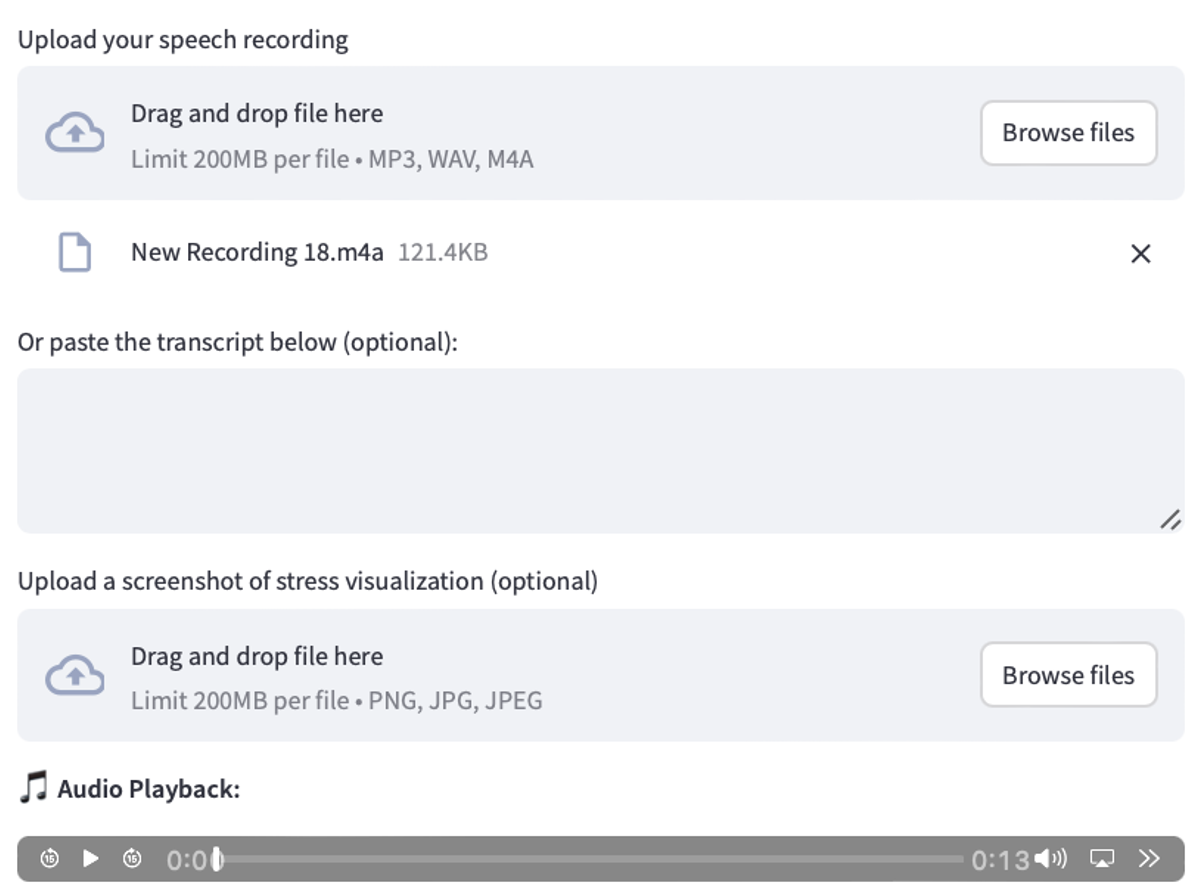
\includegraphics[width=0.9\columnwidth]{allreferences/audiofunc1.png}
    \caption{Audio Processing}
    \label{fig:audio_processing}
\end{figure}
\subsection{GPT-4 Analysis phase}
Once the transcript is ready, a prompt is formulated. The prompt includes instructions to analyze the transcript for emotional content or specific stress indicators. This can be done using a template-based approach or dynamic prompt creation, where certain keywords (example: “fire,”“help”) trigger stress-related prompts. The transcript and prompt are fed into an LLM . This step involves packaging the input as a query that the LLM understands, potentially formatted as 'prompt': "from now you are expert in finding any stress in the following voice transcript”; and "You are an assistant designed to analyze the stress level in speech. Focus on identifying emotional intensity, such as regret, nostalgia, uneasiness, or conflict, and scale it to a stress level from 1 to 7. Provide an explanation for the level."
\vspace{10pt} % Add space to prevent overlap
 \begin{figure}[htbp!]  %[h!]
    \centering
    \includegraphics[width=1.0\columnwidth]{allreferences/gpt4textprocessing2.png}
    \caption{GPT4 analysis phase}
    \label{fig:system_architecture}
\end{figure}
\vspace{10pt} % Add space to prevent overlap
\subsection{Output phase:Response generation} % 4.4.3
Then, LLM processes the prompt and transcript, using its pre-trained knowledge of language patterns, semantics, and emotional cues to analyze the text. The LLM evaluates both the content ('fire', 'help') and the context (the urgency in the sentence structure) shown in figure 4.4.
\vspace{10pt} % Add space to prevent overlap
 \begin{figure}[htbp!] %[h!]
    \centering
    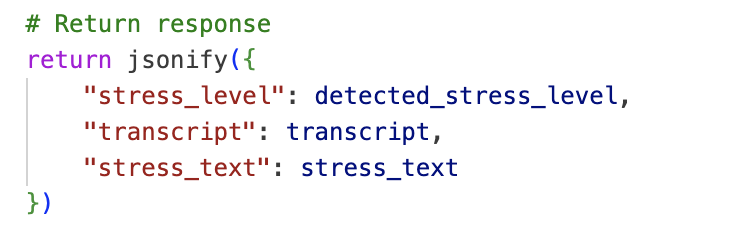
\includegraphics[width=1.1\columnwidth]{allreferences/responsegentext1.png}
    \caption{Response generation}
    \label{fig:system_architecture}
\end{figure}
\vspace{10pt} % Add space to prevent overlap
\end{enumerate}
 \section{UI/UX enhancements}
 The UI/UX design\cite{akhmedov2023} is essential to developing a user-friendly and engaging stress detection system. The main facets of UI/UX design and their application are listed below.
 \begin{enumerate}
 \item Adaptive UI Design: The system uses dynamic colour schemes that alter according to the stress levels that are identified (for instance, red for high stress). 
\item Features for User Accessibility: Supports several languages, such as English and Japanese and easy navigation that reduces cognitive effort with a clear visual hierarchy. 
\item Interactive Visualisations: Instantaneous feedback via pie charts, line graphs, and reports that can be downloaded. 
\item Feedback and Error Handling: Shows individualised guidance and real-time stress feedback and offers advice and error messages for missing or erroneous input.
\end{enumerate}
%\vspace{10pt} % Add space to prevent overlap
% \begin{figure}[p] %[h!]
   % \centering
   % \includegraphics[width=1.1\columnwidth]%{allreferences/textprooutput1.png}
   % \caption{Analysis and explanation}
    %\label{fig:system_architecture}
%\end{figure}
 \subsection{Development with Streamlit}
The primary tool for creating my user interface is Streamlit[17]. Interactive elements such as the file uploader and audio player are used. Styled text using Markdown (st.markdown()). Messages that handle errors (st.error(), st.success()). Important UX Elements Applied with Streamlit
Stress-level-based adaptive user nterface (colour-coded messages)
Spinners are being loaded st.spinner() to improve feedback.
When the file upload fails, error messages appear.
After every upload, the graph is updated in real time.

\subsection{UX Enhancements for User Engagement}
    Data visualisation methods, backend processing, and frontend technologies are all used in UX (User Experience) enhancements.
    \subsubsection{ Flask as Backend API}
    The backend API for processing the uploaded audio and returning the findings of the stress analysis is Flask. Flask manages the Speech Analysis work by utilising GPT-4o (stress analysis) and Whisper (voice-to-text) to handle the uploaded audio file. Additionally, it provides real-time feedback and promptly returns stress levels and explanations, assuring a low latency and seamless user experience also offers error handling. Flask produces concise error messages for the frontend to see in the event of issues (such as a missing audio file or an API failure). Further,  handle the data Processing which Formats the stress level data before sending it to Streamlit, ensuring consistent responses. 
        \subsubsection{Whisper (Speech-to-Text Transcription)}
Translates audio to text for stress analysis, make sure speech is recognised correctly before sending it to GPT-4, and adjusts for accents and tones for greater accuracy. Whisper was used to implement the following important UX features: Enhanced accessibility for non-text inputs;  Accurate transcription for stress assessment; Smooth speech-to-text conversion. Figure 4.4 shows the transcription of the audio. After uploading the audio it transcribes the audio. the transcription result and summarization is shown in the figure.
%\clearpage  % Forces all previous content to be placed before this point
\vspace{10pt} % Add space to prevent overlap
\begin{figure}[htbp!]
    \centering
    \includegraphics[width=1.0\columnwidth]{allreferences/fire2transcribe.png}
    \caption{Transcription from audio}
    \label{fig:system_architecture}
\end{figure}
\vspace{10pt} % Add space to prevent overlap
%Figure 4.8  also shows the transcription of the audio. After uploading the audio it transcribes the audio. the transcription result and summarization is shown in the figure. 
%\vspace{10pt} % Add space to prevent overlap
%\clearpage  % Forces all previous content to be placed before this point
%\vspace{10pt} % Add space to prevent overlap
%\begin{figure}[p]
   % \centering
    %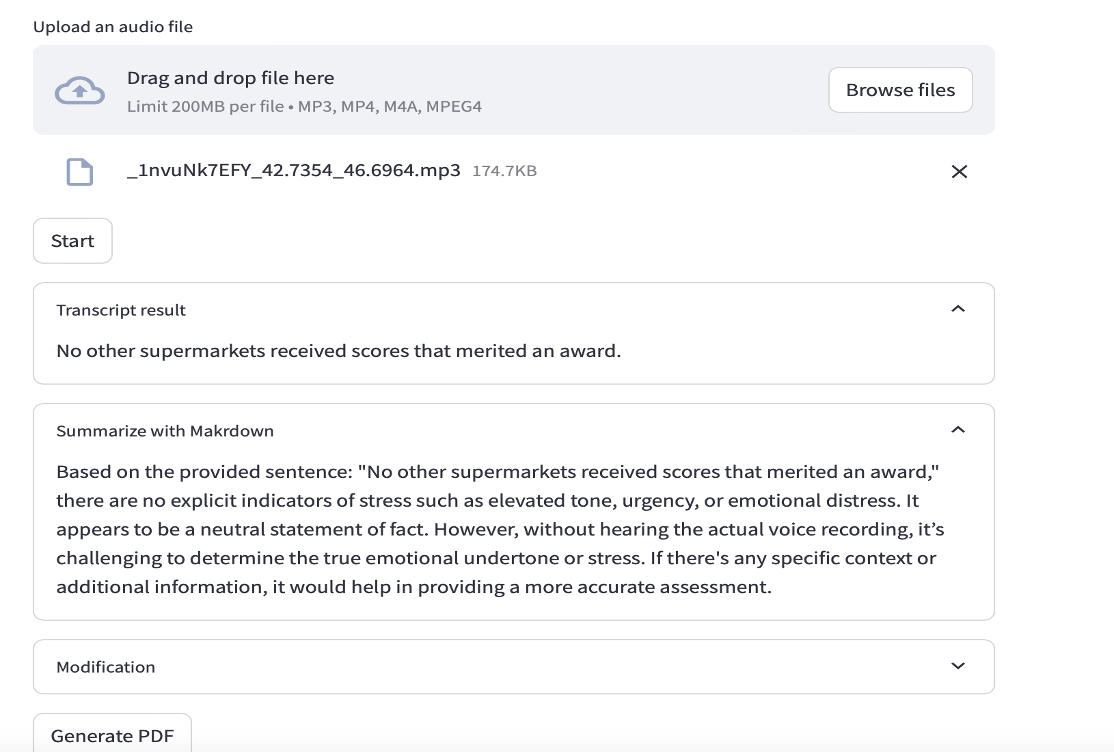
\includegraphics[width=1.0\columnwidth]{allreferences/supermarket.png}
    %\caption{Transcription from audio}
    %\label{fig:system_architecture}
%\end{figure}
\vspace{10pt} % Add space to prevent overlap
   \subsubsection{GPT-4o for Stress Analysis}
    GPT-4o uses voice analysis to identify stress levels in transcriptions. Gives thorough contextual stress explanation instead of only numerical values. It contributes to the humanisation and intuitiveness of stress evaluation. Detailed stress level explanations (rather than just numbers) are one of the key UX features implemented with GPT-4. Context-based stress analysis such as the urgency of speech patterns comes in second. And lastly it enhanced accuracy over conventional numerical classifiers.
\subsubsection{Explanation and advice}
The system analyses the speech transcript using GPT-4 to determine the user's intent, tone, and emotional context. For example Figure 4.6 shows the expression "If time could go back" is understood to mean regret or desire, which is classified as a stress-related mental state. The identified stress level (Level 3) is assigned by the method to a matching database category, such as "internal stress or conflict due to dissatisfaction or nostalgia." There is guidance associated with each stress level. 
%\clearpage  % Forces all previous content to be placed before this point
\begin{figure}[H]
    \centering
    \includegraphics[width=0.9\columnwidth]{advice3.png}
    \caption{Explanation and Advice}
    \label{fig:advice1}
\end{figure} 
For instance: "Take breaks, practise mindfulness, stay hydrated." is the Level 3 Stress Advice. Tailored to stress context for making it easy to use and actionable, the advice is straightforward, generic, and practical. Also The system successfully offers advise based on identified stress intensity, as seen in Figure 4.6. The system determined that the intensity in this case was moderate and assigned a Stress Level of 3. The system showed its ability to provide guidance for handling elevated stresss, even if the detected stress was primarily enthusiasm and engagement. This demonstrates how the system works to give people practical advice regardless of their mental state, which promotes general awareness and control.  
\vspace{10pt} % Add space to prevent overlap
%\vspace{-5mm} % Reduce vertical space
\begin{figure}[htbp!]
    \centering
    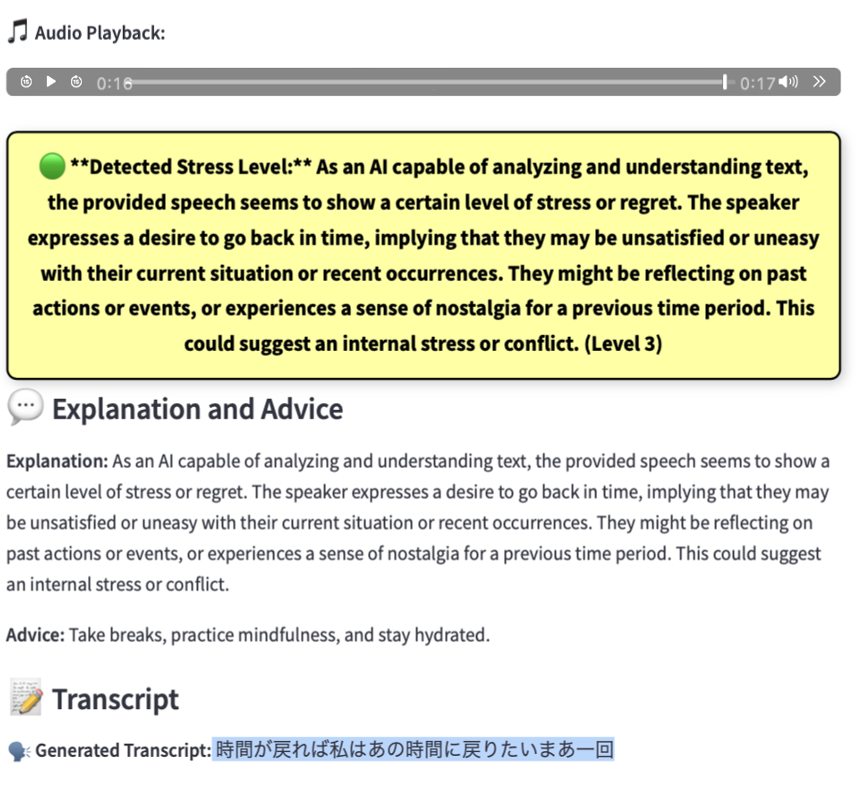
\includegraphics[width=1.0\columnwidth]{advice4.png}
    \caption{Explanation and Advice}
    \label{fig:system_architecture}
\end{figure} 
\vspace{10pt} % Add space to prevent overlap
  \subsubsection{ Stress visualization}
Figure 4.7 displays the percentage distribution of stress levels. Low stress (levels 1-3) is represented by green, mild stress (levels 4-5) by orange, and high stress (levels 6-7) by red. Interactive elements such as Legend for reference, Click-to-hide sections and hover tooltips that display precise percentages Insights like stress distribution patterns and percentages are provided by visualizations.  The implementation involved with tools like Plotly for graphical representations and connects stress data that has been captured in JSON with the user interface (UI). 
% \clearpage  % Forces all previous content to be placed before this point
\vspace{10pt} % Add space to prevent overlap
\begin{figure}[htbp!]
    \centering
    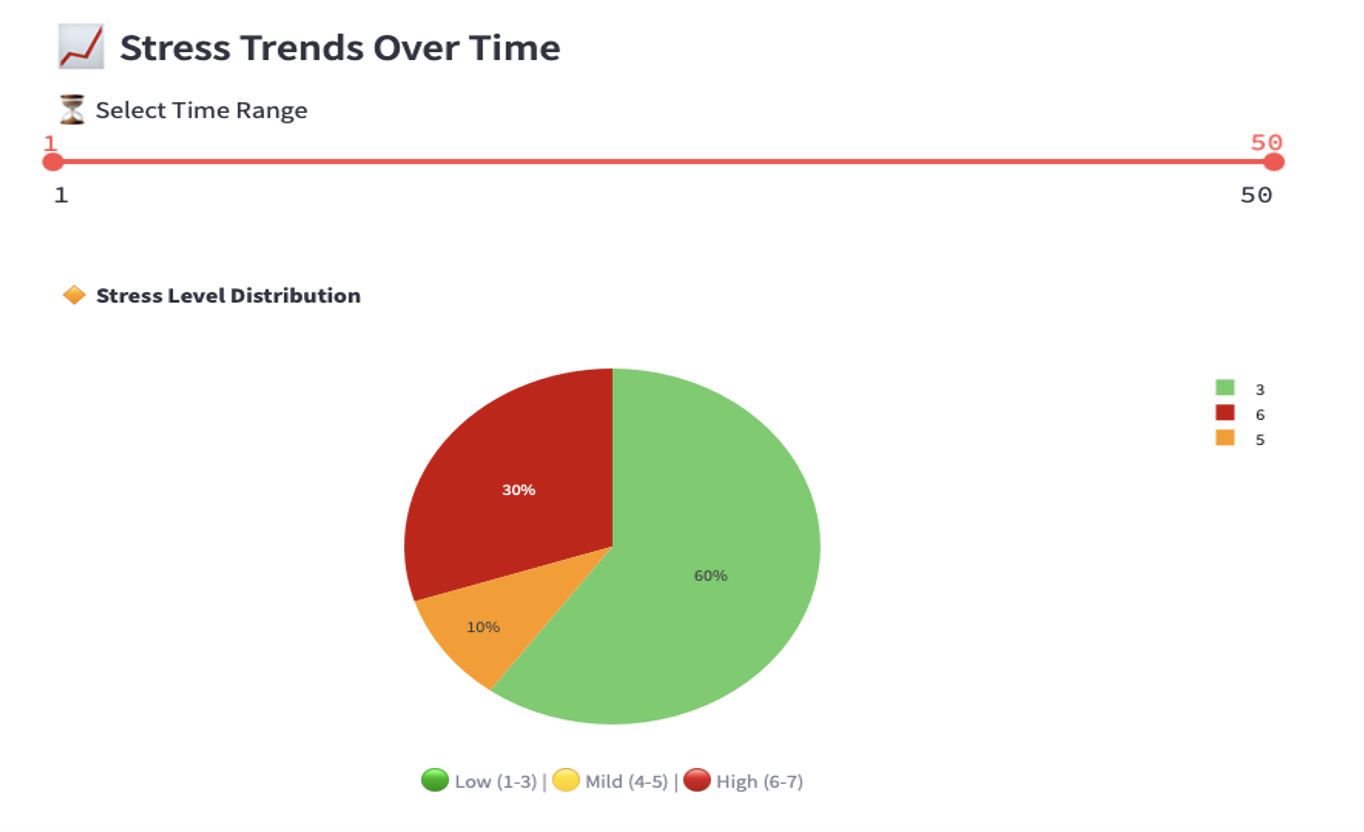
\includegraphics[width=0.8\textwidth]{allreferences/stressvisualpie.png}
    \caption{Stress Visualization}
    \label{fig:system_architecture}
\end{figure}
\vspace{10pt} % Add space to prevent overlap
    \subsubsection{ Stress Trend Tracking Feature}
     Using Matplotlib stress patterns over time using is plotted, which used to visualize stress trends. To help track past stress levels for long-term insights, figure 4.8 present line graphs with markers to visualize user stress patterns.  The moving average is displayed by the blue trend line. The X-axis displays the session numbers. Y-axis representing stress levels from 1 to 7. Interactive features include zoom and pan controls, a time range slider for filtering data, hover tooltips for displaying precise values, and a legend for trend lines and stress levels are used. The dynamic stress trend graph which automatically updates upon each upload, improved readability with larger markers, bold labels, and annotations on each point to display stress values. 
%\clearpage  % Forces all previous content to be placed before this point
\vspace{10pt} % Add space to prevent overlap
     \begin{figure}[htbp!]
    \centering
    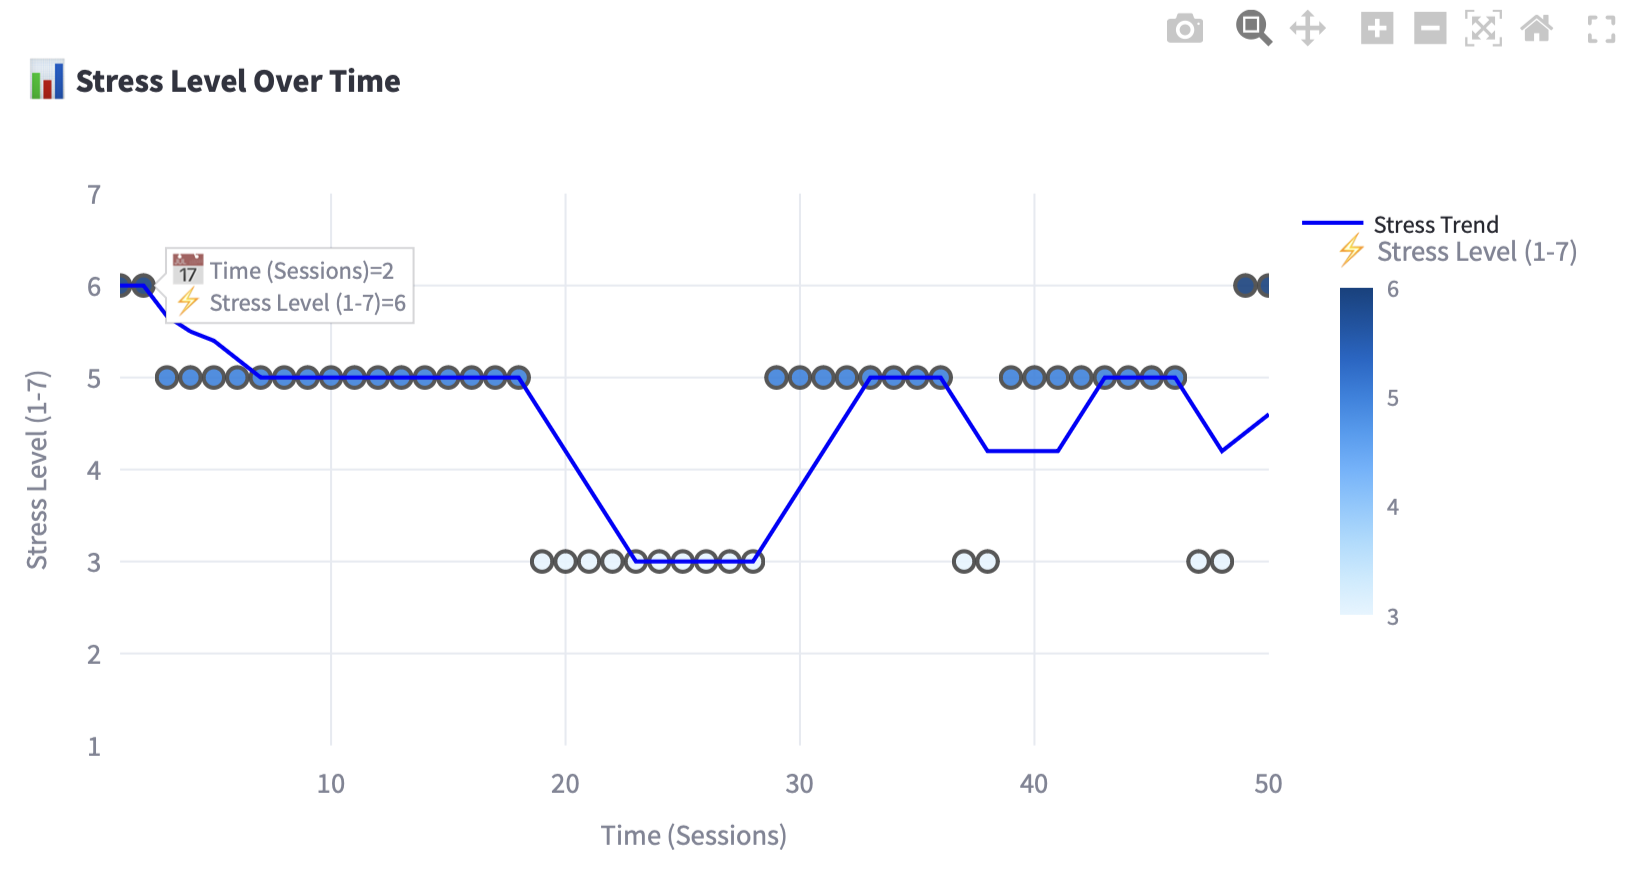
\includegraphics[width=1.0\columnwidth]{stresstrend3.png}
    \caption{Stress Trend Tracking History}
    \label{fig:system_architecture}
\end{figure}
\vspace{10pt} % Add space to prevent overlap
    \subsubsection{ JSON (Local Data Storage for Stress Trends)}
    Figure 4.9 shows the stress report. JSON stores the history of stress levels locally. When the page is refreshed, previous stress levels are not lost and makes it possible to track previous sessions for long-term insights. The principal UX Elements applied Through JSON to avoid excessive data building, the stress history is kept for the last 50 sessions and is persistent over repeated uploads.
    % \clearpage  % Forces all previous content to be placed before this point
%\vspace{-5pt} % Reduces space above
%\FloatBarrier % Ensures figure stays within section
%\begin{figure}[htbp!]
  %  \centering
   % 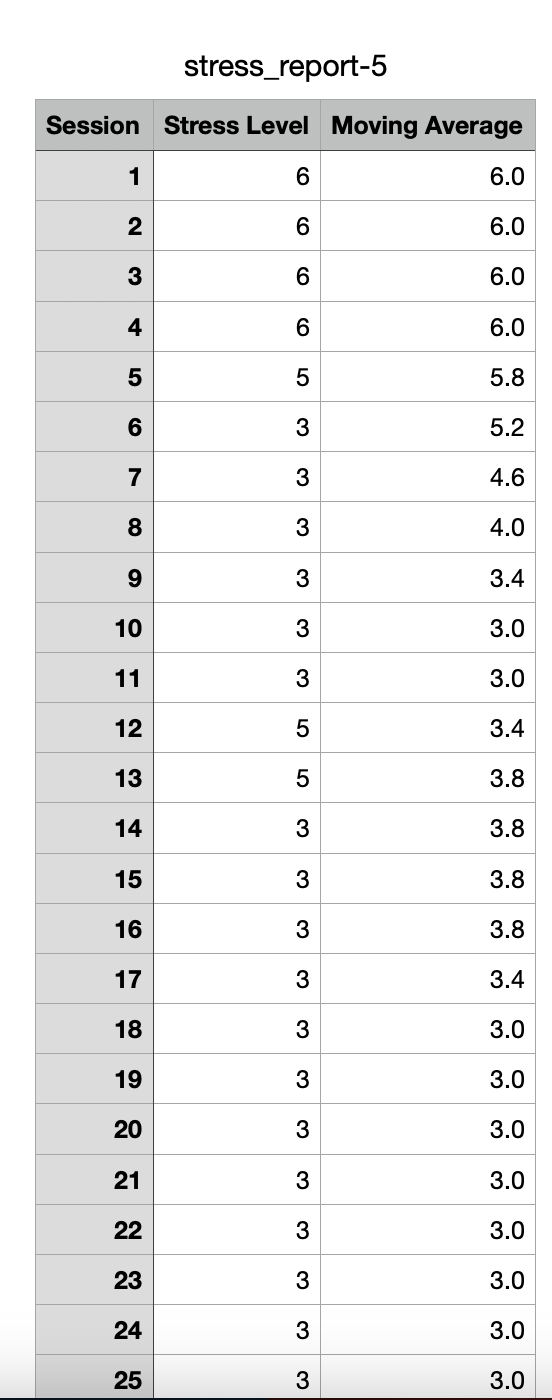
\includegraphics[width=0.7\textwidth]{allreferences/stressreportdownload.png}
   % \caption{Stress report}
   % \label{fig:stress_report}
%\end{figure}
%\vspace{-10pt} % Reduces space below
 \section{Implementation output}
The frontend and backend are smoothly connected via the system's interaction flow. Through the interface, users can enter text or upload audio. Calculates stress levels by processing inputs using Whisper and GPT-4.The frontend receives the results for feedback and visualization. Key outputs produced by the system to verify its operation are shown in this section:
\begin{enumerate}
\item Stress Analysis Findings: Audio file transcriptions. 
Stress levels were identified and categorized, such as Severe, Slight stress and relaxed. 
\item Visualization Outcomes: Line graphs illustrating temporal trends in stress. 
Pie charts that show the distribution of stress levels. 
\item Reports and Feedback: Downloadable reports and tailored guidance.
\end{enumerate} 
 \begin{figure}[p]
    \centering
    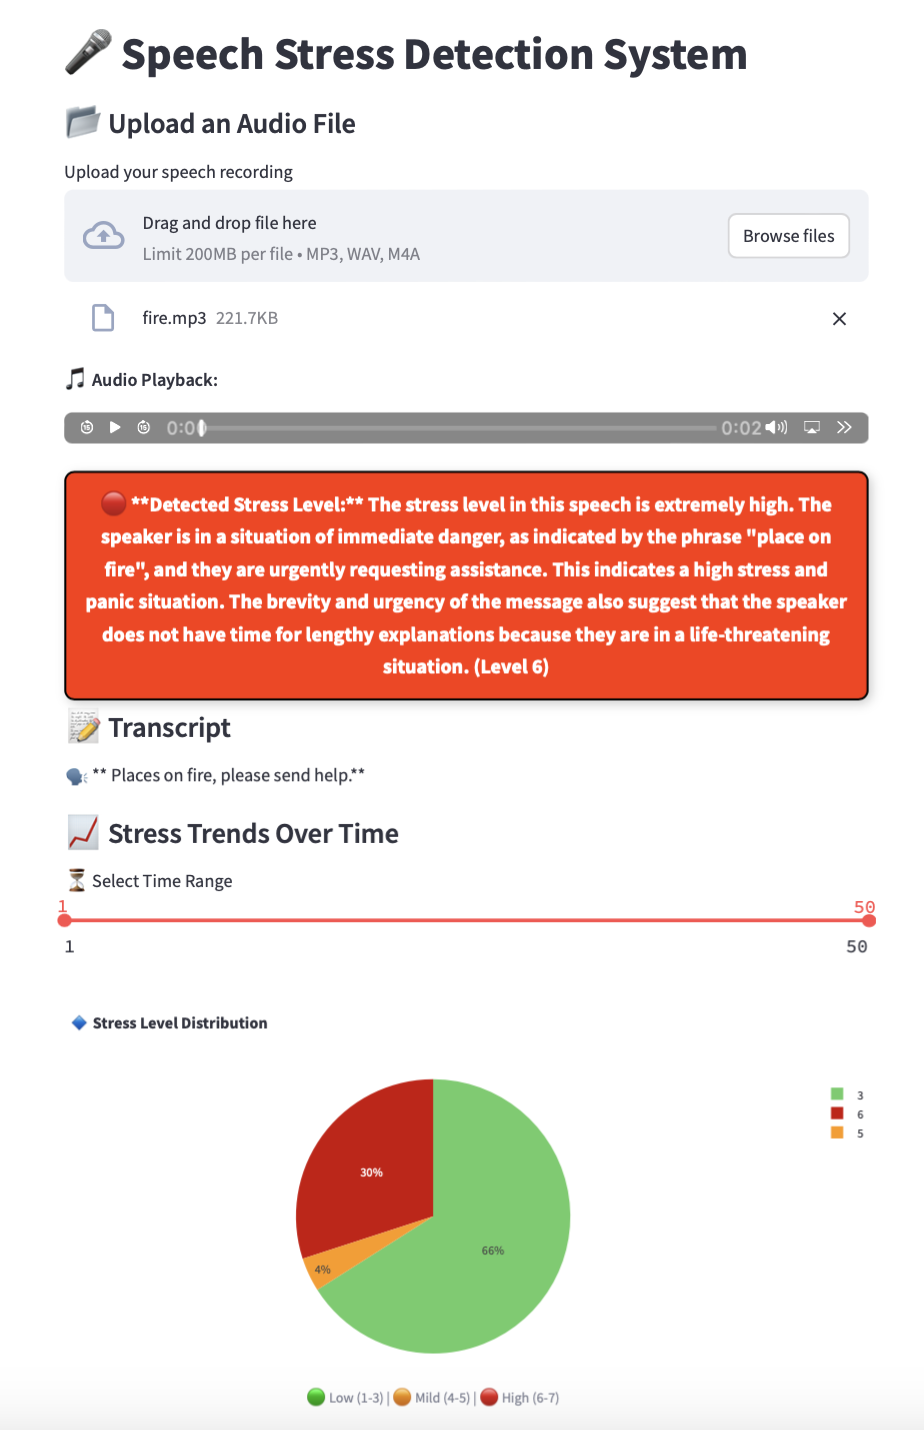
\includegraphics[width=0.9\columnwidth]{aovrall1.png}
    \caption{Stress Level Detection System}
    \label{fig:system_architecture}
\end{figure} 
 \begin{figure}[p]
    \centering
    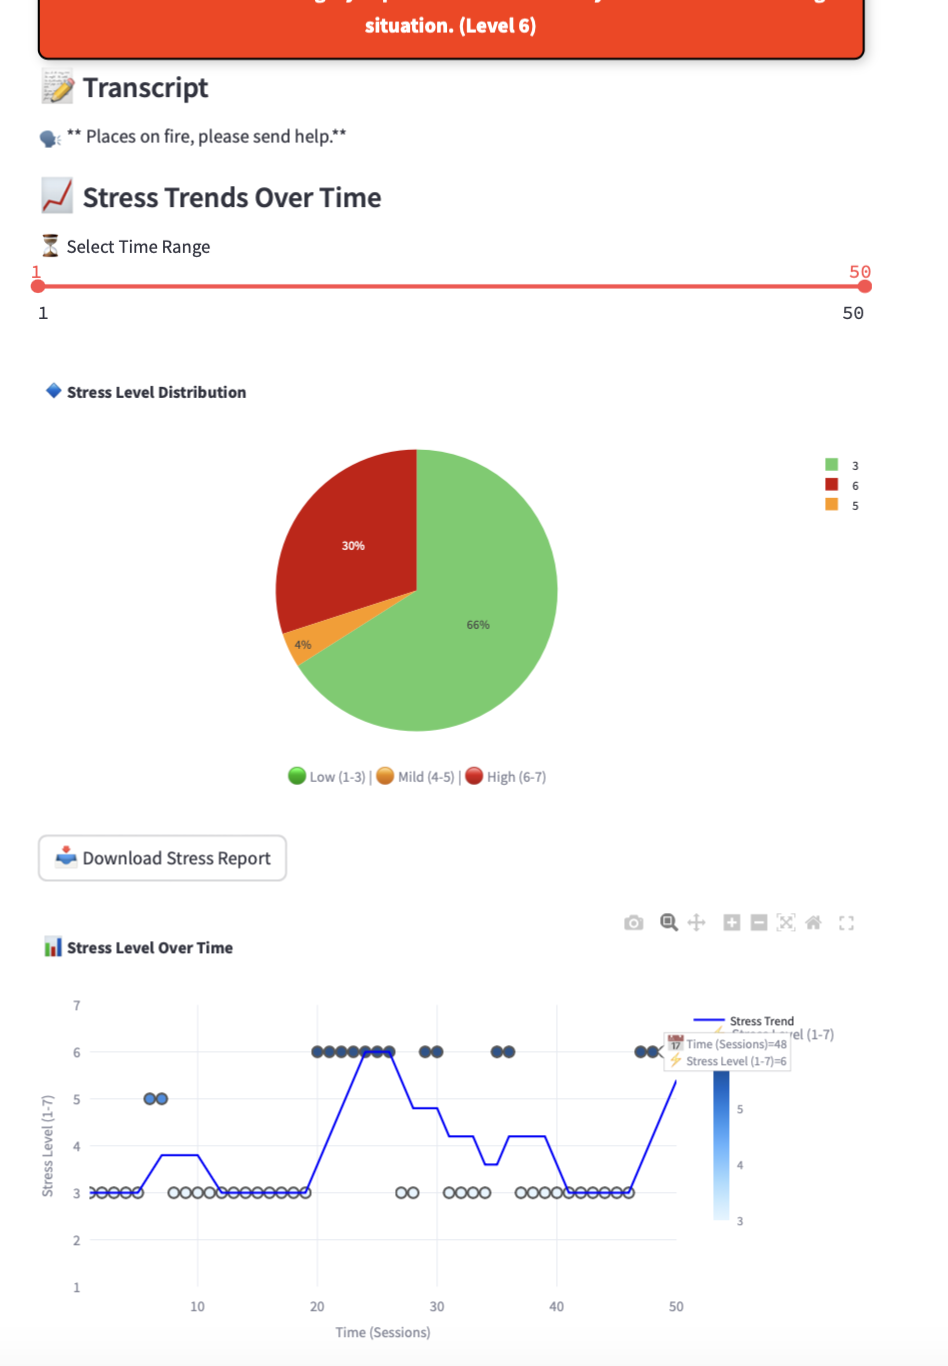
\includegraphics[width=0.9\columnwidth]{aoverall2.png}
    \caption{Stress Level Detection System}
    \label{fig:system_architecture}
\end{figure}
The main features of the Speech Stress Detection System are shown in Figures 4.9 and 4.10, an intuitive and engaging user interface. In order to verify the input, users can listen to audio recordings that they have uploaded in supported formats such as MP3, WAV. Stress levels are detected by the system and shown clearly in a banner with colour coding. It provides context for the state by clarifying whether the detected intensity is indicative of high or low stress. To provide transparency and usability, the analyzed speech is transcribed and presented for the user's reference. A line graph helps users keep an eye on their mental health by showing changes in stress levels over time. A pie chart offers a thorough overview of stress levels by classifying them as low, medium, or high intensity  which demonstrate the system's emphasis on improving user experience by providing actionable information.
\chapter{Experiment and evaluation}
\clearpage 
  \section{Evaluation of Stress Detection}
  To evaluate the performance of the system, a questionnaire form was developed and shared with participants via social networking platforms (SNS). The form included 12 audio samples, and participants were asked to provide subjective ratings for each audio. The average human rating for an audio reflects the collective perception of stress levels from 40 participants. This is statistically valid because averaging reduces individual biases and represents a more reliable measure. These human ratings were then compared with the system-generated outputs for the same audio samples. Table 5.1 shows the average human rating and system output. After collecting the responses, the correlation coefficient between the human ratings and the system output was calculated to assess the strength of their relationship, and a scatter plot was created to visually represent this correlation and overall trends. To further analyze the data, a bar chart was plotted to compare the average human ratings with the system outputs, highlighting the differences and similarities. Additionally, a line chart was used to show the trends of human ratings and system outputs across all samples, providing a clear representation of their alignment or divergence. Key statistical measures, including the T-value and P-value, were calculated to determine the significance of the findings, while the Mean Absolute Error (MAE) was computed to quantify the average difference between human ratings and system outputs. These analyses, combining visualizations and statistical evaluations, offer comprehensive insights into the system’s performance, its ability to align with human judgment, and areas for further improvement. 
  \begin{table}[h!] % Optional, h! ensures the table stays close to where it's defined
\centering
\caption{Average Human Rating & System Output}
\label{tab:correlation_table} % Optional, for referencing in the text
\begin{tabular}{|c|c|c|}
\hline
Audio & Average Human Rating & System Output \\ \hline
Audio1 & 5.000000 & 6 \\ \hline
Audio2 & 6.125000 & 7 \\ \hline
Audio3 & 5.925000 & 6 \\ \hline
Audio4 & 3.550000 & 3 \\ \hline
Audio5 & 3.666667 & 3 \\ \hline
Audio6 & 5.875000 & 6 \\ \hline
Audio7 & 3.700000 & 3 \\ \hline
Audio8 & 3.875000 & 3 \\ \hline
Audio9 & 5.825000& 7 \\ \hline
Audio10 & 3.525000 & 3 \\ \hline
Audio11 & 4.900000& 4 \\ \hline
Audio12 & 5.950000 & 7 \\ \hline
\end{tabular}
\end{table}
    \section{Correlation of coefficient between system output and human estimation}
    A statistical measure known as the "correlation coefficient," which ranges from -1 (perfect negative correlation) to +1 (perfect positive correlation), is used to analyse the relationship between two variables. It shows the strength and direction of the linear association between the variables. \cite{schober2018correlation}. The correlation coefficient provides a single numerical value that quantifies the strength and direction of the relationship between human ratings and system predictions. A single numerical value that expresses the direction and degree of the relationship between system predictions and human ratings is provided by the correlation coefficient. A high correlation (close to 1) means that human assessments and the system agree well. A low correlation (close to 0) indicates that human judgements and the system's predictions are unrelated. An inverse connection is implied by negative correlation, whereby system outputs fall as human assessments rise.  The correlation coefficient acts as a validation metric for proposed system. It shows whether the system reliably captures the stress levels perceived by humans. The system's practical usefulness is supported by a high correlation, which indicates that its stress detection is in accordance with human perception.. The outputs of the stress detection system were compared with human estimations obtained via a survey in order to assess the system's performance. On a 7-point rating system, survey respondents were asked to assess the stress levels of 12 audio samples. The system's predictions and the average human ratings showed a very significant positive connection, as indicated by the analysis's correlation coefficient of 0.96. Figure 5.1, which visualises the relationship between the system outputs and human ratings, was created to further highlight this link using a scatter plot with a trend line. The visual depiction and strong correlation value show that the system's stress predictions closely match human experience, hence verifying its functionality.
    \vspace{10pt} % Add space to prevent overlap
\begin{figure}[H]
    \centering
    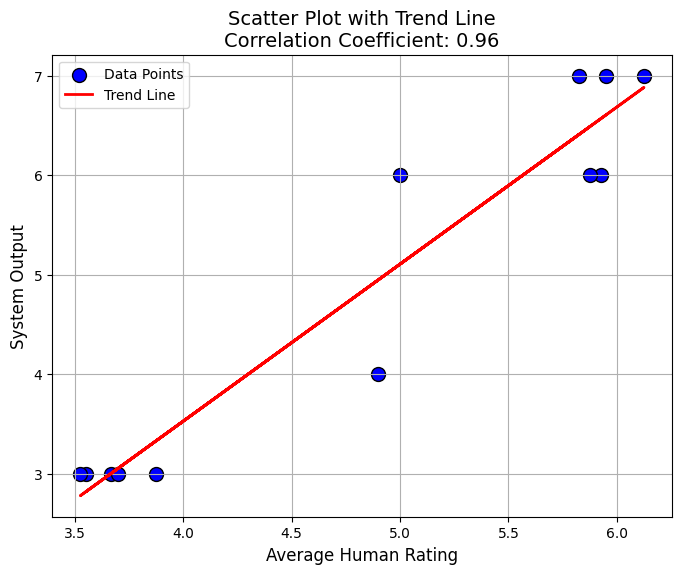
\includegraphics[width=1.0\columnwidth]{coeff40.png}
    \caption{Average human rating and system outputs}
    \label{fig:system_architecture}
\end{figure}
\vspace{10pt} % Add space to prevent overlap
\section{Visual comparisons of human ratings and system outputs }
The comparative analysis demonstrates how well and accurately the system  can reproduce human estimations.
\subsection{Comparison of  Human rating  vs system rating }
For every audio sample, the system outputs and human ratings were compared side by side in a bar chart in figure 5.2.
\vspace{10pt} % Add space to prevent overlap
 \begin{figure}[H]
    \centering
    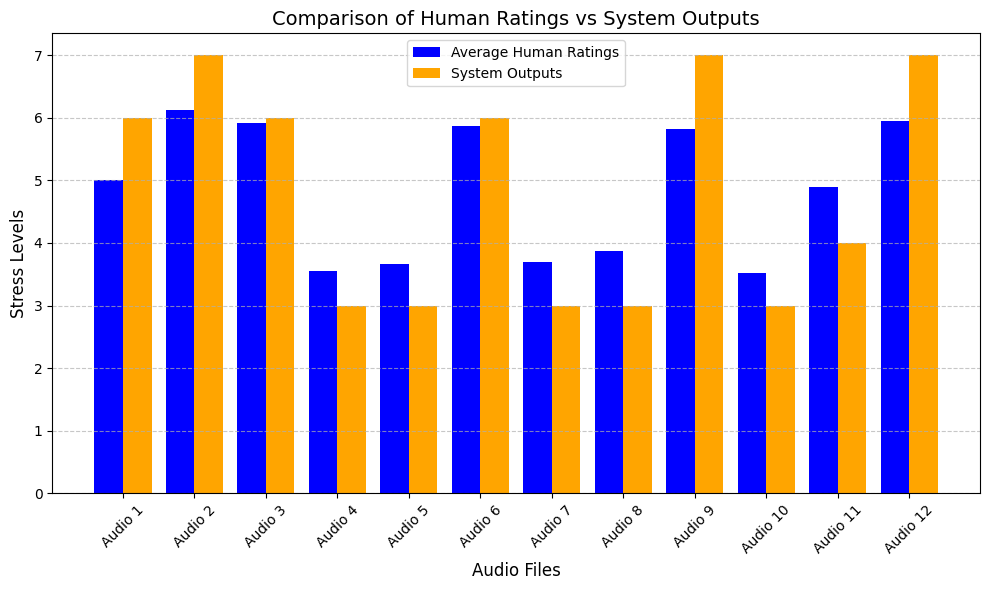
\includegraphics[width=1.0\columnwidth]{bar40.png}
    \caption{Trend Comparison between human rating vs system outputs}
    \label{fig:system_architecture}
\end{figure}
\vspace{10pt} % Add space to prevent overlap
\subsection{Trend Comparison of  Human rating  vs system rating }
The trends of system outputs and human ratings for each of the 12 audio samples were displayed in a line chart in figure 5.3. The trend line displays the comparison between system outputs and human ratings for various audio files. The average human assessments are shown by the blue line. The system's predictions are shown by the orange line. The system's predictions are in good agreement with human judgements when the orange and blue lines are close to adjacent ones.  A mismatch occurs when there is a discernible space between the two lines, meaning that the system's forecast deviates from the average for humans. This trend line identifies distinct audios in which the system works effectively.
\vspace{10pt} % Add space to prevent overlap
\begin{figure}[H]
    \centering
    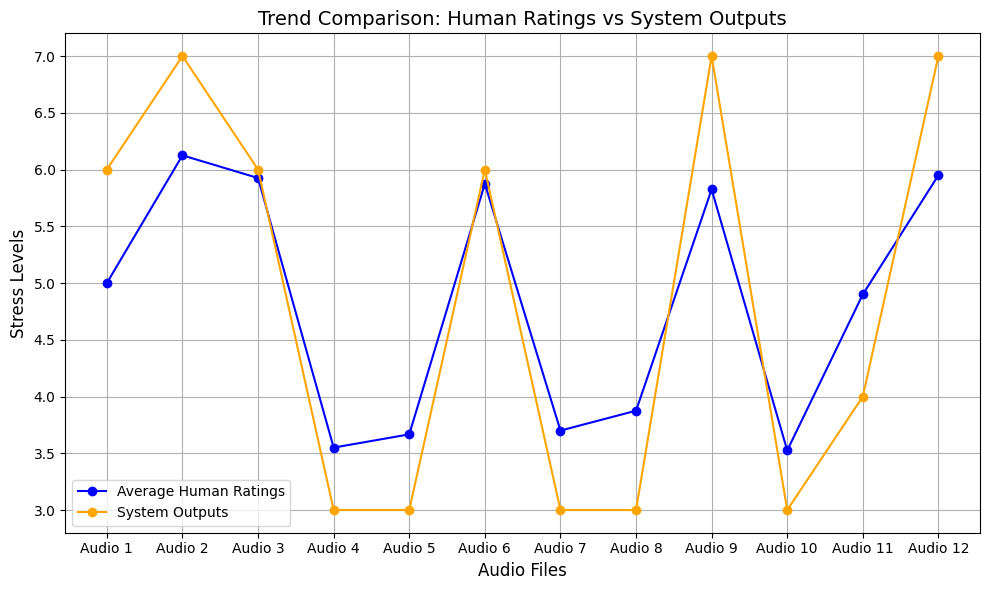
\includegraphics[width=1.0\columnwidth]{trend40.png}
    \caption{Comparison between human rating vs system outputs}
    \label{fig:system_architecture}
\end{figure} 
\vspace{10pt} % Add space to prevent overlap
\subsection{Histogram of Error Distribution}
The distribution of errors between system outputs and human assessments was shown using a histogram in figure 5.4. The distribution of differences (errors) between the system outputs and human ratings is displayed by the histogram. The x-axis shows the magnitude of the difference between the human ratings and the system output for each audio sample. A difference of 0.2  means the system output was very close to the human average. Larger values such as 1.0 indicate a greater disparity between the two. The Y-Axis shows how many audio files have a given error value. The y-axis indicates the number of audio samples (frequency) that fall into each range of difference. For instance, if the bar at 0.6  has a height of 4, it means there are 4 audio samples for which the difference between the human rating and the system output lies within the range around 0.6.
Proposed system's predictions are, on average, one point off from human evaluations, with the majority of errors centred around 1.0. A narrow and centred histogram shows that the system's predictions closely match the human assessments. The bars represent how many samples fall within specific ranges of difference. The highest frequency in this figure is at a difference of around 0.6, indicating that most samples had a moderate discrepancy between human ratings and system outputs.
%The X-Axis shows the absolute difference (error) between system predictions and human ratings
MAE: 
\vspace{10pt} % Add space to prevent overlap
 \begin{figure}[H]
    \centering
    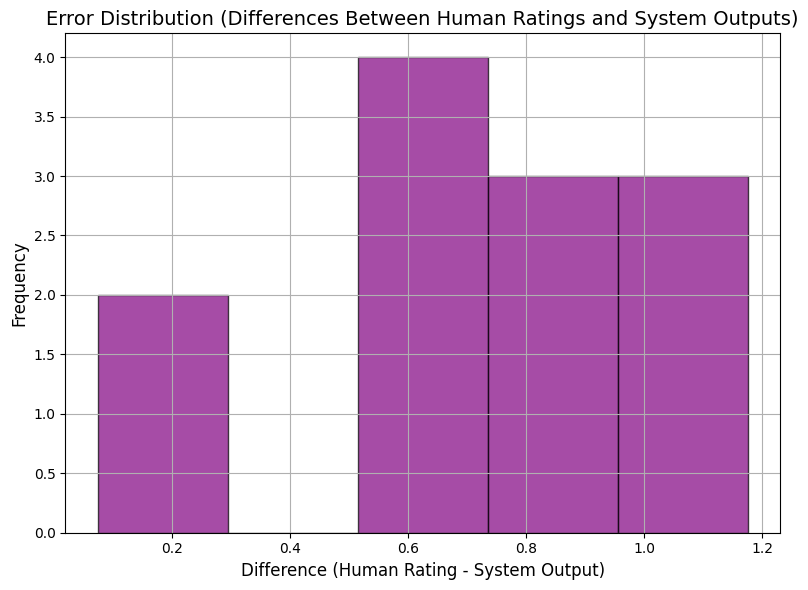
\includegraphics[width=1.0\columnwidth]{histo40.png}
    \caption{Histogram of error distribution}
    \label{fig:system_architecture}
\end{figure}
\vspace{10pt} % Add space to prevent overlap
\section{Statistical analysis}
The performance of the stress detection system was evaluated by comparing its outputs to human ratings using statistical metrics. A t-test was conducted to assess the statistical significance of the difference between the system outputs and human ratings. The resulting t-statistic and p-value of showed no significant difference, supporting the hypothesis that the system outputs align closely with human perception. A paired t-test (\citet{pairedttest2025}) compares the means of two related groups such as human ratings and system outputs for the same audio files. The goal is to determine if the mean difference between the two groups is significantly different from 0.
\begin{table}[H] % Optional, h! ensures the table stays close to where it's defined
\centering
\caption{Statistical Value} 
\label{tab:correlation_table} % Optional, for referencing in the text
 \begin{tabular}{|c|c|c|}
        \hline
         Mean Absolute Error(MAE) & T-statistic & P-value \\ \hline
            0.71 &  -0.03 & 0.97 \\ \hline
    \end{tabular}%
   \end{table}
   \vspace{10pt} % Add space to prevent overlap

\subsection{Mean Absolute Error (MAE)}
The average absolute difference between the system outputs and human ratings is measured by MAE. Regardless of direction, it shows how far the system's predicts vary from human assessments.  The system outputs are more compatible with human assessments when the MAE is smaller, which denotes higher performance. An MAE of 0.71 indicates that, on average, the system's predictions and human ratings on the stress rating scale diverge by roughly 0.71 units. This is a minor error, indicating that the system functions properly in general.
\subsection{T-Statistic: }
T-Statistic: The T-statistic measures how much the average human rating deviates from the system output, standardized by the variability in the human ratings. A high positive or negative T-statistic indicates a large difference between the human ratings and system outputs. The t-statistic determines if the average difference between human ratings and system outputs deviates from 0 in a statistically significant way. The mean difference between the system outputs and human assessments is insignificant when the t-statistic is around zero such as -0.03.On average, the system's output closely resembles human ratings, showing no bias towards overestimation or underestimation.
\subsection{P value }
P-Value: Indicates whether the observed difference is statistically significant.The P-value represents the probability that the observed difference between human ratings and system outputs occurred by random chance.A common threshold for significance is p<0.05p<0.05. If the P-value is below this threshold, the difference is considered statistically significant. A p-value of 0.9771 is much larger than the common significance threshold of 0.05.  There is no statistically significant difference between the system's outputs and the human ratings. This suggests that the system's performance is very much aligned with human perception
\section{Interpretation of T-statistic and P-value }
The overall p-value (0.97) shown in Table 5.2 explain that these values represent the system's general performance across all audio files. A detailed table 5.3 is shown above with t-statistics and p-values for each audio file.
\vspace{10pt} % Add space to prevent overlap
\begin{table}[H] % Optional, h! ensures the table stays close to where it's defined
\centering
\caption{T-statistic and P-value}
\label{tab:correlation_table} % Optional, for referencing in the text
 \begin{tabular}{|c|c|c|c|c|}
        \hline
        Audio  & T-statistic & P-value \\ \hline
        Audio1 & -5.186 & 0.000007\\ \hline
        Audio2 &  -6.271 & 0.000000\\ \hline
        Audio3 & -0.386 & 0.486333 \\ \hline
        Audio4 &  1.629 & 0.111\\ \hline
        Audio5 &  2.000& 0.053 \\ \hline
        Audio6 &   -0.589 &  0.560 \\ \hline
        Audio7 & 2.004 & 0.052  \\ \hline
        Audio8 &  2.588 &  0.014  \\ \hline
        Audio9 &  -8.806 & 0.000000 \\ \hline
        Audio10 &  4.620 &  0.000041 \\ \hline
        Audio11 &  5.383 & 0.000004\\ \hline
        Audio12 & -5.450 & 0.000003\\ \hline
    \end{tabular}%
   \end{table}
\vspace{10pt} % Add space to prevent overlap
%\noindent
%\textbf{Audio 1:} \\
%\textbf{T-Statistic:} -5.186 \\
%\textbf{P-Value:} 0.000007 (very small) \\
%\textbf{Interpretation:} There is a statistically significant difference between human ratings and system output. The system's stress rating is likely overestimating compared to the human ratings.\par
%\noindent
%\textbf{Audio 2:} \\
%\justifying
%\textbf{T-Statistic:} -6.271 \\
%\textbf{P-Value:} 0.000000  (very small) \\
%\textbf{Interpretation:} The system output differs significantly from human ratings, suggesting overestimation of stress for this audio.\par
%\noindent
%\textbf{Audio 3:} \\
%\textbf{T-Statistic:} -0.386\\
%\textbf{P-Value:}  0.701  (not significant) \\
%\textbf{Interpretation:} There is no statistically significant difference. The system's output aligns well with human ratings.P-value = 0.701,this is much greater than 0.05, indicating that the system's output is not statistically significantly different from the human ratings. A small t-statistic -0.386 also supports that the difference is minimal. Since the system's output is close to the human ratings and the difference is statistically insignificant, interpreting this as good between the system and human ratings. This means that the system's prediction for this audio is consistent with how humans perceive stress.\par
%\noindent
%\textbf{Audio 4:} \\
%\textbf{T-Statistic:} 1.629\\
%\textbf{P-Value:}  0.111  (not significant) \\
%\textbf{Interpretation:} No significant difference between the human ratings and system output, suggesting reasonable agreement.\par
%\noindent
%\textbf{Audio 5:} \\
%\textbf{T-Statistic:} 2.000\\
%\textbf{P-Value:}  0.0533 (borderline significance) \\
%\textbf{Interpretation:} The p-value is close to the 0.05 threshold, suggesting a marginally significant difference.\par
%\noindent
%\textbf{Audio 6:} \\
%\textbf{T-Statistic:} -0.589\\
%\textbf{P-Value:}  0.560 (not significant) \\
%\textbf{Interpretation:} No significant difference, indicating good alignment between human ratings and system output.\par
%\noindent
%\textbf{Audio 7:} \\
%\textbf{T-Statistic:} 2.004\\
%\textbf{P-Value:}  0.052 (borderline significance) \\
%\textbf{Interpretation:} The p-value is close to the threshold, suggesting a marginally significant difference that could require further examination.\par
%\noindent
%\textbf{Audio 8:} \\
%\textbf{T-Statistic:}2.588\\
%\textbf{P-Value:} 0.014 (significant)\\
%\textbf{Interpretation:} Statistically significant difference, with the system likely underestimating stress compared to human ratings\par
%\noindent
%\textbf{Audio 9:} \\
%\textbf{T-Statistic:}-8.806\\
%\textbf{P-Value:} 0.000000 (very small)\\
%\textbf{Interpretation:} Strongly significant difference, with the system likely overestimating stress. \par
%\noindent
%\textbf{Audio 10:} \\
%\textbf{T-Statistic:}4.620\\
%\textbf{P-Value:} 0.000041 (very small)\\
%\textbf{Interpretation:} Statistically significant difference, with the system likely underestimating stress \par
%\noindent
%\textbf{Audio 11:} \\
%\textbf{T-Statistic:} 5.383\\
%\textbf{P-Value:} 0.000004 (very small)\\
%\textbf{Interpretation:} Statistically significant difference, with the system likely underestimating stress \par
%\noindent
%\textbf{Audio 12:} \\
%\textbf{T-Statistic:}-5.450\\
%\textbf{P-Value:} 0.000003 (very small)\\
%\textbf{Interpretation:} Statistically significant difference, with the system likely underestimating stress \par


\textbf{Significant Differences (P < 0.05)}: Audio 1, 2, 8, 9, 10, 11, 12 show significant differences between system outputs and human ratings. These indicate areas where the system does not align well with human perception of stress and requires adjustment.\par
\textbf{No Significant Differences (P ≥ 0.05)}: Audio 3, 4, 5, 6, 7 show no significant differences, suggesting that the system performs reasonably well for these cases. For instance, the system's output aligns well with human ratings.P-value = 0.701 for audio 3,this is much greater than 0.05, indicating that the system's output is not statistically significantly different from the human ratings. A small t-statistic -0.386 also supports that the difference is minimal. Since the system's output is close to the human ratings and the difference is statistically insignificant, interpreting this as good between the system and human ratings. This means that the system's prediction for this audio is consistent with how humans perceive stress. \par
\textbf{Improvement}
Focus on audio files with significant differences to improve system accuracy and enhancements such as retraining the system with more diverse datasets and refine the model for edge cases. Incorporate feedback loops to fine-tune system outputs based on human assessment.

  \section{Discussion of Results}
    \subsection{Key Findings}
    \begin{enumerate}
\item Strong Correlation: The system predictions and human ratings show a strong alignment, as indicated by the correlation coefficient of 0.96. \item  Minimal Error: The system produces accurate predictions with minimal variances, as indicated by the MAE of 0.71. 
\item Statistical Validation: The system's outputs and human ratings do not differ statistically significantly, according to the findings of the paired t-test (τ-statistic: -0.03, p-value: 0.97). 
\end{enumerate}
 \subsection{Insights on Multimodal Data Integration}
For stress detection, the system's integration of Large Language Models (LLM) and Social Signal Processing functioned well.The multimodal approach enabled:
\begin{enumerate}
\item Proper audio input transcription. 
 \item  Accurate assessment of stress levels using linguistic and vocal content. 
\end{enumerate}
\section{Advantages and Limitations of the System}
\textbf{Advantages:}
\begin{enumerate}
    \item A strong correlation with human evaluations confirms the reliability of the system.
    \item Stress detection is made easier by an intuitive user interface (UI).
    \item A low prediction error improves system accuracy.
\end{enumerate}
\textbf{Limitations:}
\begin{enumerate}
\item  Despite the high correlation, certain audio files showed significant differences, which warrants further analysis and improvement in the model's performance.
    \item Minor variations in certain audio samples indicate potential for improvement.
    \item Performance in noisy environments may be impacted by reliance on high-quality audio inputs.
\end{enumerate}
\chapter{Conclusion and Future Work}
\clearpage 
  \section{Summary of the Research}
  This study presented a multimodal stress detection system that uses large language models (LLMs) and Social signal Processing to combine text-based and speech-based stress analysis. The method was created to identify stress levels by merging GPT-4-based textual analysis with audio analysis with transcription. User-centred Stress Visualisation Streamlit was used to create an interactive real-time user interface (UI) that lets users upload audio samples, get stress scores, and see their stress levels on user-friendly dashboards. This research introduced stress trend visualization, which allows users to follow stress changes over numerous sessions, in contrast to traditional stress detection methods that provide immediate assessments. An interactive stress level indicator, trend graphs, and a downloadable stress report were among the UX improvements that improved the system's readability and usefulness for mental health applications. %These results demonstrate how well deep learning-based stress detection works and how crucial UX enhancements are to developing intuitive, real-time stress monitoring solutions.
  \section{Contributions of the Study}
   \begin{enumerate}
   \item Creation of a Multimodal Stress Detection System integrated vocal analysis and LLM-based text analysis.  
 \item Deployment of Long-Term Monitoring Stress Trend Visualisation 
 Added a dynamic stress trend monitoring function that allows users to examine stress trends over time. 
Enhanced applications for mental health monitoring by offering a historical perspective on stress variations. 
 \item UX Improvements for Accessibility and User Interaction 
Developed an interactive user interface with stress visualisation to improve the interpretability and actionability of stress detection results. 
Added downloadable stress reports, stress level indicators, and real-time feedback, improving the usefulness of stress detection tools. 
\end{enumerate}
Through the integration of deep learning, multimodal AI, and user-centred design, these contributions enhance the real-world implementation of stress detection systems.
 
  \section{Limitations of the Proposed System}
Despite the positive results of this study, a number of limitations need to be taken into account. Instead of recording live speech inputs, the system processes pre-recorded speech, which restricts the possibility of real-time engagement.
 
  \section{Recommendations for Future Research}
   \begin{enumerate}
   \item To enhance generalisation, include real-time stress datasets from a variety of speakers.To increase robustness, use datasets with unplanned speech instead of recordings.
 \item  Expand the system to accommodate real-time speech input processing, enabling ongoing stress monitoring. Create an adaptable user interface (UI) that adapts to the stress levels of its users and offers tailored suggestions and feedback.
 \item Combining Multimodal Physiological Information For a more comprehensive stress evaluation, combine physiological cues (such as skin conductivity and heart rate) with speech-based stress detection. Investigate integrating wearable technology (such as smartwatches) for multimodal stress detection in real time.
 \item To offer individualized stress management techniques, consider integration with mental health conversation systems. 
 \item Make the CNN-LSTM model faster on edge devices by optimizing it. Examine compact deep learning architectures that can be implemented on embedded and mobile devices. 
 
The feasibility, scalability, and impact of AI-driven stress detection systems for mental health applications are the goals of these future areas. 
 \end{enumerate}
 \section{Practical Applications of the Study}
 The research research on stress detection systems has several practical applications, particularly in mental health monitoring, workplace wellness, and personal well-being tracking. The work's potential applications span a variety of sectors where stress evaluation and long-term tracking can be beneficial, as it focusses on developing an interactive, user-friendly stress monitoring interface.
%\textbf{Mental Health and Well-being Tracking} \newline
%\makebox[\textwidth][l]{\textbf{Mental Health and Well-being Tracking}} \\
%\parbox{\textwidth}{\textbf{Mental Health and Well-being Tracking}}\\ 
\begin{flushleft}
\textbf{ Workplace Stress Monitoring} 
\justifying
The system can be used by organisations to measure and control workplace stress levels as part of employee wellness initiatives. Managers and HR professionals can use the system's stress trend visualisation to comprehend how stress changes over time and create plans for reducing stress at work. could be used to business mindfulness programs where staff members monitor their psychological health and get stress-reduction advice.
 \end{flushleft}
  \begin{flushleft}
\textbf{Mental Health and Well-being Tracking} \\
\justifying
Individuals can use the stress trend tracking feature to monitor their mental state over time. The system can provide visual insights into stress patterns, helping users recognize triggers and take proactive steps for stress management. It can be integrated into digital mental health platforms to support therapy and self-care.
 \end{flushleft}
 \begin{flushleft}
\textbf{Education} \\
\justifying
The interface can serve as a basis for research on user behaviour in stress detection systems by academic institutions and researchers in the fields of psychology, UX/UI design, and Human-Computer Interaction (HCI). Additional features could be added to the framework to test various stress tracking visualisation techniques. The method can be used by researchers in the future to investigate the effects of interactive stress tracking on user engagement and mental health outcomes.
 \end{flushleft}
\begin{flushleft}
\textbf{Self-Improvement and Personal Productivity} \\
\justifying
Individuals practicing self-care and mindfulness can use the stress tracking feature to measure how relaxation techniques such as meditation, deep breathing impact their stress over time. Can be beneficial for content creators and app developers building self-improvement tools, where users track their mental states alongside productivity habits.
  \end{flushleft}
 \begin{flushleft}
\textbf{Health Tech and Digital Apps} \\
\justifying
The system can be integrated into mobile health (mHealth) applications, providing users with an accessible and interactive stress monitoring tool. Can be paired with wearables or smart assistants to track real-time stress trends based on speech input. Useful for telemedicine platforms, where doctors and psychologists can review stress reports and provide better mental health support.
  \end{flushleft}
  \section{Final Thoughts}
This study introduces a multimodal and user-friendly stress detection system which advances the expanding field of AI-driven mental health care. This system improves stress monitoring, visualization, and interpretability through large language models and UX-focused design. The results show that real-time stress tracking combined with voice and text-based analysis can produce insightful information on mental health. This system could be used as a useful tool for stress monitoring and mental health support with more improvements and real-world validations, bridging the gap between AI-based stress detection and practical applications.
%\appendix
%\chapter{Appendices}

%\bibliographystyle{apalike}
\bibliographystyle{plainnat} % or another style like IEEEtran
\bibliography{ref} % Use the name of your .bib file without the .bib extension

%\bibliographystyle{IEEEtran}
%\bibliography{references}
%\begin{thebibliography}{99}
%\setlength{\itemsep}{0pt} % Adjust spacing between bibliography entrie
%\bibitem{ref1}Sriramprakash, Senthil, Vadana D. Prasanna, and OV Ramana Murthy. "Stress detection in working people." Procedia computer science 115 (2017): 359-366 `
%\bibitem{ref2} Kafková, Júlia, et al. "A New Era in Stress Monitoring: A Review of Embedded Devices and Tools for Detecting Stress in the Workplace." Electronics 13.19 (2024): 3899.
%\bibitem{ref3} Liu, Feng, et al. "Artificial intelligence in mental health: Innovations brought by artificial intelligence techniques in stress detection and interventions of building resilience." Current Opinion in Behavioral Sciences 60 (2024): 101452.
%\bibitem{ref4} Sebastião, Rita, and David Dias Neto. "Stress and mental health: The role of emotional schemas and psychological flexibility in the context of COVID-19." Journal of Contextual Behavioral Science 32 (2024): 100736.
 %\bibitem{ref5}Aristizabal, Sara, et al. "The feasibility of wearable and self-report stress detection measures in a semi-controlled lab environment." IEEE Access 9 (2021): 102053-102068.
%\bibitem{ref6} Chyan, Phie, et al. "A deep learning approach for stress detection through speech with audio feature analysis." 2022 6th International Conference on Information Technology, Information Systems and Electrical Engineering (ICITISEE). IEEE, 2022.
%\bibitem{ref7} Yoon, S., et al. "Text-based stress detection using %semantic analysis." Journal of Computational Linguistics, 2020.
%\bibitem{ref8} Singh, Praveen, et al. "Social signal processing for evaluating conversations using emotion analysis and sentiment detection." 2019 Second International Conference on Advanced Computational and Communication Paradigms (ICACCP). IEEE, 2019.
%\bibitem{ref9} Razavi, Moein, et al. "Machine learning, deep learning, and data preprocessing techniques for detecting, predicting, and monitoring stress and stress-related mental disorders: Scoping review." JMIR Mental Health 11 (2024): e53714.
%\bibitem{ref10}Yao, Yiqun, et al. "Muser: Multimodal stress detection using emotion recognition as an auxiliary task." arXiv preprint arXiv:2105.08146 (2021).
%\bibitem{ref11}Hilmy, Muhammad Syazani Hafiy, et al. "Stress classification based on speech analysis of MFCC feature via Machine Learning." 2021 8th International Conference on Computer and Communication Engineering (ICCCE). IEEE, 2021.
%bibitem{ref12} Shen, Guobin, et al. "StressPrompt: Does Stress Impact Large Language Models and Human Performance Similarly?." arXiv preprint arXiv:2409.17167 (2024).

%\bibitem{ref9} Olawade, David B., et al. "Enhancing mental health with Artificial Intelligence: Current trends and future prospects." Journal of medicine, surgery, and public health (2024): 100099.


%\bibitem{ref12} Graham, Calbert, and Nathan Roll. "Evaluating OpenAI's Whisper ASR: Performance analysis across diverse accents and speaker traits." JASA Express Letters 4.2 (2024).
%\bibitem{ref13} Teye, Martha T., et al. "Evaluation of conversational agents: understanding culture, context and environment in emotion detection." IEEE Access 10 (2022): 24976-24984.

%\bibitem{ref14} Kush, Joseph C. "Integrating Sensor Technologies with Conversational AI: Enhancing Context-Sensitive Interaction Through Real-Time Data Fusion." Sensors 25.1 (2025): 249.
%\bibitem{ref15}Sriramprakash, Senthil, Vadana D. Prasanna, and OV Ramana Murthy. "Stress detection in working people." Procedia computer science 115 (2017): 359-366
%\bibitem{ref16}Macháček, Dominik, Raj Dabre, and Ondřej Bojar. "Turning whisper into real-time transcription system." arXiv preprint arXiv:2307.14743 (2023).
 
 %\bibitem{ref13}Ricker, George R., et al. "Transiting exoplanet survey satellite (tess)." American Astronomical Society Meeting Abstracts\# 215. Vol. 215. 2010.
 %\bibitem{ref14}Ranjan, Rajeev, and Abhishek Thakur. "Analysis of feature extraction techniques for speech recognition system." International Journal of Innovative Technology and Exploring Engineering 8.7C2 (2019): 197-200.
 %\bibitem{ref15}Yan, Mengzhu, and Xue Wu. "Prosody in linguistic journals: a bibliometric analysis." Humanities and Social Sciences Communications 11.1 (2024): 1-15.
%\bibitem{17}Pillai, Mukesh, and Pallavi Thakur. "Developing a Website to Analyze and Validate Projects Using LangChain and Streamlit." 2024 2nd International Conference on Intelligent Data Communication Technologies and Internet of Things (IDCIoT). IEEE, 2024.
%\bibitem{ref18}Relan, Kunal. "Building REST APIs with Flask." Building REST APIs with Flask (2019).
 %\bibitem{ref19}Akhmedov, Nurkhon. Designing and prototyping a learning and testing platform for user experience (UX) and user interface (UI) designers with the aim of improving knowledge and establishing a standard evaluation benchmark for UX/UI design skills and competencies. Diss. Technische Hochschule Ingolstadt, 2023..
%\end{thebibliography}
% Add additional references here

% use section* for acknowledgement
\chapter*{Acknowledgements}

 I would like to start by thanking ALLAH, the Ever Most Generous, for granting me this wonderful opportunity to study at this institution. His countless blessings have given me the health, strength, and clarity of mind to undertake and complete this thesis.

I extend my deepest appreciation to my supervisor, Prof. Shiramatsu, for his valuable guidance, insightful feedback, and unwavering support throughout this research. His expertise and encouragement have been instrumental in shaping my work and strengthening my understanding of my research field. 

A special thanks to my dear parents and Jobair Al Rafi for their unconditional support, patience, and encouragement during this journey. Their belief in me has been my greatest source of motivation, especially during challenging times.

Furthermore, I would like to give special thanks to Aichi Monozukuri Scholarship for providing the financial support during my master’s program and Aichi Prefecture International Department for their generous support.

I would like to thank all the members from Shiramatsu Laboratory. I am also sincerely grateful to the NITech International Affairs Division  and Japanese teachers for their continuous support.

Lastly, I would like to take this opportunity to express my sincere gratitude to many people who helped me with this project who played a significant role by providing the necessary resources and support. This research would not have been possible without the collective efforts, guidance, and encouragement of so many individuals, and for that, I am truly grateful.



\addcontentsline{toc}{chapter}{List of Tables}
%\listoftables
\addcontentsline{toc}{chapter}{List of Figures}
%\listoffigures

% that's all folks
\end{document}



\cleardoublepage
\thispagestyle{empty}
\chapter{Introduction}
\clearpage
\documentclass[Arial,12pt,openright,twoside]{book}
%\documentclass[a4paper,12pt]{report}  % Use "article" or "book" if applicable
%\usepackage[a4paper, margin=25mm]{geometry} % Ensures correct A4 alignment

\usepackage{xeCJK}
\setCJKmainfont{ipaexm.ttf}
\usepackage[T1]{fontenc}
\usepackage[dvipdfm]{graphicx}
\usepackage{amsmath,amssymb,amsfonts}
\usepackage{algorithmic}
\usepackage{pdfpages}
\usepackage{float} % Add this to your preamble modiiii
\usepackage{natbib} % modi
\usepackage[authoryear]{natbib}
%\usepackage[numbers,round]{natbib} % Or omit "numbers" for pure author-year
\bibliographystyle{plainnat}
%\bibliographystyle{apalike} % modifi
% For \citeauthor command etc
% For headers
\usepackage{longtable} % modification
\usepackage{fancyhdr}
\pagestyle{fancy}
\fancypagestyle{plain}{ % Redefine plain page style
    \fancyhf{} % Clear all headers and footers
    \fancyhead[LE]{\thepage} % Page number on top-left for even pages
    \fancyhead[RO]{\thepage} % Page number on top-right for odd pages
    \renewcommand{\headrulewidth}{0pt} % Remove the header rule
    \renewcommand{\footrulewidth}{0pt} % Remove the footer rule
}
\fancyhf{} % Clear all headers and footers
\fancyhead[RE]{\leftmark}
\fancyhead[RO]{\thepage}
\fancyhead[LO]{\leftmark}
\fancyhead[LE]{\thepage}
\fancyfoot[RO]{\rightmark}
\fancyfoot[LE]{\rightmark}
\usepackage{emptypage}
\usepackage{ragged2e} %% modification
\justifying % modification
\usepackage{color}   %May be necessary if you want to color links
\usepackage[breaklinks=true]{hyperref}
\usepackage{breakcites} % otherwise they don't wrap
\usepackage{microtype} % otherwise they don't wrap
\usepackage{apalike}
\usepackage{tikz}
\usepackage{multirow}
\usepackage{filecontents}
\usepackage{caption}
\usepackage{tablefootnote}
\usepackage{placeins}% modi
% \usepackage{cite} % modi 

\raggedbottom % modi

\captionsetup[table]{skip=5pt}

%\setlength{\textfloatsep}{5pt} % Space between figure and text % modi
%\setlength{\intextsep}{5pt}    % Space for in-text figures% modi
\setlength{\abovecaptionskip}{5pt} % Space above captions % modi
\setlength{\belowcaptionskip}{5pt} % Space below captions % modi
\setlength{\textfloatsep}{8pt} % Adjust space between text and figures
\setlength{\intextsep}{8pt}    % Space for inline figures
%\setlength{\parindent}{15pt} % Default indentation size


\graphicspath{{./images/}}
%\titlespacing*{\subsection}{0pt}{10pt}{5pt} % Adjust subsection spacing

\usetikzlibrary{shapes.geometric, shapes.symbols, shadows, arrows}
\tikzset{
  multidocument/.style={
    shape=tape,
    draw,
    fill=white,
    tape bend top=none,
    double copy shadow}
    }
\hypersetup{
 	linktocpage,
     colorlinks=true, %set true if you want colored links
     linktoc=all,     %set to all if you want both sections and subsections linked
     linkcolor=blue,  %choose some color if you want links to stand out
 	citecolor=black,
 	filecolor=black,
 	linkcolor=black,
 	urlcolor=black
 }
 
 % correct bad hyphenation here
\hyphenation{pre-processing pre-processed pre-training pre-trained}
\usepackage{array}

\usepackage{listings}
\lstset{
basicstyle=\small\ttfamily,
columns=flexible,
breaklines=true,
frame = single
}

\makeatletter
\newcommand*{\da@rightarrow}{\mathchar"0\hexnumber@\symAMSa 4B }
\newcommand*{\xdashrightarrow}[2][]{%
  \mathrel{%
    \mathpalette{\da@xarrow{#1}{#2}{}\da@rightarrow{\,}{}}{}%
  }%
}
\makeatletter
\def\endthebibliography{%
  \def\@noitemerr{\@latex@warning{Empty `thebibliography' environment}}%
  \endlist
}
\makeatother

%\pagenumbering{arabic}%ここからページ数開始

\input{commands}

\begin{document}

\cleardoublepage
%!TEX root = ../../main.tex
% タイトルページ
%\documentclass[a4j,12pt]{jreport}
%\usepackage{graphicx}
%\usepackage{times}
%\usepackage{selectp}
%\usepackage{epsf}
%\usepackage{epsbox}
%\usepackage{graphicx}
%\usepackage{verbatimfiles}
%\usepackage{here}
%%\usepackage{url}
%\usepackage{fancyhdr}
%\usepackage{algorithm}
%\usepackage{cite}
%\usepackage{ascmac}
%\usepackage{amsmath}
%\usepackage{amsthm}
%\usepackage{amssymb}
%\usepackage{latexsym}

%\usepackage{thesis}
%\input{mymacros}
%\begin{document}

\oddsidemargin=17mm
\evensidemargin=-4mm

\thispagestyle{empty}
% タイトル
\def \englishtitle{
A Multimodal System for Stress Detection and Visualization using Social Signal Processing and Large Language Models}
\def \japanesetitle{
社会的信号処理とLLMを用いたマルチモーダルなストレス検出・可視化システムの開発
}
% 著者
\def \author{HOSSAIN Syeda Tanzina}
% 提出日
\def \date{\today}
% 指導教官名
\def \teacher{Shun~SHIRAMATSU}
% 指導教官の肩書き
\def \teacherrank{Prof.}
% 所属
\def \belong{Dept. of Computer Science\\Graduate School of Engineering\\Nagoya Institute of Technology}
% 入学年度
\def \year{2023}
% 学籍番号
\def \regnum{35414100}

% Font sizes for layout
\def\sizeLL#1{\Huge #1}
\def\sizeL#1{\LARGE #1}
\def\sizeM#1{\Large #1}
\def\sizeS#1{\large #1}

% Title decorations
\def\REYrule{\hbox to 5cm{\leaders\hrule height 1pt\hfill}}
\newbox\REYbox
\def\announce#1{
  \setbox\REYbox=\hbox{\REYrule\quad{\Large\bf #1}\quad\raise3pt\REYrule}%
  \gdef\REYbigrule{\hbox to \wd\REYbox{\leaders\hrule height 1pt \hfill}}%
  \centerline{\raise3pt\REYrule\vspace*{2mm}\quad{\LARGE #1}\quad\raise3pt\REYrule}}
\def\endannounce{\par\centerline{\REYbigrule}}

% Title page
\begin{titlepage}
 \begin{center}
  \vspace*{5mm} % Slight space at the top
  \sizeLL{Master Thesis}\\
  \vspace*{5mm} % Space after the main title
  \begin{announce}{(Title)}
   \sizeL{\englishtitle}\\ % English Title
   \textbf{{\CJKfamily{ipaexm}\sizeM{\japanesetitle}}} % Japanese Title in CJK font
  \end{announce}
  \vspace*{5mm} % Space before the supervisor details
  \sizeL{Supervisor:~}\sizeM{\teacherrank~\teacher}\\
  \vspace*{5mm} % Space before the department details
  \sizeM{\belong}\\
  \vspace*{5mm} % Space before enrollment details
  \sizeM{Enrolment:~April 1, \year}\\
  \vspace*{5mm} % Space before the table
  \begin{table}[h!]
    \centering
    \begin{tabular}{cl}
      \sizeM{(Student ID):} & \sizeL{\underline{~\regnum~}} \\
      \sizeM{(Name):}       & \sizeL{\underline{~\author~}} \\
    \end{tabular}
  \end{table}
  \vspace*{5mm} % Space before the submission date
  \sizeS{(Submission Date: February 3, 2025)} % Submission Date
 \end{center}
\end{titlepage}


%\include{part/abstract/abstract}

\tableofcontents
%\addcontents{Abstract}
\addcontentsline{toc}{chapter}{Abstract}
\listoftables
%\addcontentsline{toc}{chapter}{List of Figures}
\listoffigures

\chapter*{Abstract}

Stress detection is increasingly crucial for mental health monitoring, yet traditional approaches relying on single-modal data, such as text or audio, often lack accuracy and contextual understanding. This research introduces a multimodal stress detection system that integrates Social Signal Processing (SSP) techniques, voice feature analysis, and Large Language Models (LLMs). By combining linguistic (text-based) and paralinguistic (audio-based) cues, the system enhances stress estimation through a hybrid approach. The system accepts audio inputs in various formats such as MP3, WAV, M4A and processes them to extract linguistic content and vocal stress indicators. By combining features such as tone detection, Linguistic content, including lexical choices, syntactic structures, and sentiment-based expression sand vocal attributes like pitch and intensity, the system employs to estimate stress levels. To enhance user interaction and usability, the system is implemented with a Streamlit-based UI for real-time stress visualization. Current UX improvements focus on integrating stress trend history tracking to provide users with longitudinal insights into their stress patterns. %Future work aims to refine accessibility, usability, and multimodal fusion techniques to further improve stress recognition capabilities.
This study contributes to the field of voice-based stress analysis by integrating  with an interactive user interface, making stress detection more accessible and interpretable for real-world mental health applications.

%\tableofcontents
%\listoffigures
%\listoftables

\chapter{Introduction}
\clearpage  % Forces all previous content to be placed before this point
  \section{Background}
  In today's world, stress is an ongoing issue that affects both physical and mental health, influencing everything from mood and productivity to long-term well-being. Stress is a natural phenomenon that causes physical and emotional tension. Chronic stress is associated with serious diseases such as heart disease, anxiety, depression and immunosuppression. Stress is analyzed by expression, tone , pitch and physiological signals. The process of detecting when someone is stressed by measuring their physiological signals is known as stress detection. To analyze these signals and classify them as stressed or relaxed, some techniques are used. The physiological signals of a person are measured by physiological sensors such as the pulse of blood volume (BVP), the galvanic skin response (GSR), and the electrocardiograms (ECGs) (\citet{sriramprakash2017}). In mental health care, intelligent technology has shown significant promise in delivering personalized treatments and real-time stress detection. (\cite{kafkova2024} ) and (\cite{liu2024}).  Due to this, early and precise stress detection is vital for workplace wellness, healthcare, and personal well-being. However, many existing systems use single-modal data, such as text or voice, which limits their ability to capture all aspects of stress symptoms. This study explores the development of a versatile and ethical multimodal AI system designed for real-time stress detection. The system integrates voice and textual context to provide a comprehensive and accurate assessment of stress levels.
  \section{Motivation of the research}
  Stress has become a global problem that impacts not only mental health but also lifestyles and productivity. Due to the absence of easily accessible, reliable, and non-invasive methods, many people face obstacles in monitoring their stress. Conventional methods, such as self-assessment questionnaires or physiological monitoring, are inadequate in terms of timely insights or are impractical for daily use. Innovative systems that can effectively identify stress in real-world situations are, therefore, becoming more and more necessary.
The voice is a perfect medium for stress detection because it is a natural source of emotional information. It transmits paralinguistic clues like tone, pitch, and rhythm in addition to linguistic content, which can reveal a person's emotional condition. Powerful tools like Large Language Models (LLMs), which can analyze textual material for deeper contextual and emotional insights, have been made possible by breakthroughs in Natural Language Processing (NLP). The majority of stress detection systems now only accept single input, which restricts the precision and usefulness. 
Current systems' emphasis on immediate stress assessments, which overlooks long-term patterns and trends, is another major drawback. Furthermore, existing tools often lack user-friendly interfaces, user cannot use without technical expertise.
This study is motivated by an urge to develop a multimodal system that enhances the accuracy of stress detection by integrating text-based and voice-based analysis. Using LLMs for text analysis and deep learning models for audio processing, this study aims to close the gap between state-of-the-art AI technology. A more precise and user-friendly method of tracking stress over time is provided by incorporating interactive features like stress trend tracking, which also enables users to take proactive measures for improved mental health.

  \section{Problem Statement}
  Current stress detection systems often suffer from ethical concerns regarding data privacy, and a lack of adaptive intervention mechanisms. How can we design an ethical, adaptive, and multimodal AI system that not only detects stress accurately but also provides meaningful support to promote mental well-being?
\section{Research Objectives}
\begin{enumerate}
    \item To develop a system that estimates and visualizes user stress levels using Social Signal Processing (SSP) techniques, including voice analysis for both linguistic (text-based) and paralinguistic (audio-based).
    \item To develop a multimodal AI system that integrates voice analysis and large language models (GPT-4o) for real-time stress detection.
    \item To evaluate the performance of proposed model in detecting stress from audio data.
    \item To design an interactive  Adaptive UI for clear stress visualization
    \item Designing a long term stress trends for identifying stress patterns and helps user for self-regulation and stress trend graph improves readability
    \item Supporting metacognition and mental health care.
    \item To ensure ethical data usage and privacy preservation in the proposed system.
\end{enumerate}
  \section{Overview of system approach}
  The proposed system as shown in figure 1.1 detects and visualizes stress levels through a three-stage workflow: Audio Input, Stress Analysis, and Results and Visualization. Users upload audio files in formats such as MP3, WAV, or M4A, with playback support for review. The system processes the audio to extract textual and acoustic features. Text analysis identifies stress-related linguistic patterns, while audio analysis examines acoustic properties like pitch and tone. The results are visualized through stress reports, distribution charts, and historical trends, with an option to download detailed reports. The system also supports real-time detection, providing immediate feedback for enhanced usability
  \vspace{10pt} % Add space to prevent overlap
  \begin{figure}[p]
    \centering
    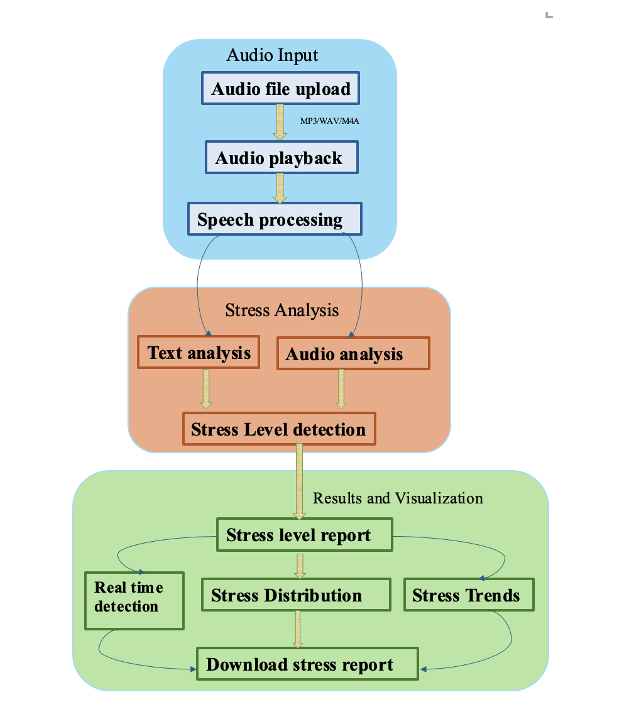
\includegraphics[width=1.1\columnwidth]{ap1.png}
    \caption{Overview of system approach}
    \label{fig:system_architecture}
\end{figure}
\vspace{10pt} % Add space to prevent overlap

  %\section{Significance of the Study}
 % This research contributes to the fields of mental health care, AI ethics, and multimodal AI by developing a system that combines advanced stress detection with interactive support.
  \section{Scope and Limitations}
 \textbf{Scope:}
 Focuses on voice-based stress detection and designs a stress trend module for user support.
 \textbf{Limitations:}
Does not include physiological signal data or longitudinal studies of user impact.
\section{Thesis Organization}
This thesis is structured into six chapters, each presenting a particular aspect of the study. Below is a brief overview of each chapter:
  \begin{enumerate} 
  \item  Chapter 1 cover  the research background, highlighting the importance of stress detection in mental health monitoring. It outlines the motivation, problem statement, research objectives, research questions, the significance of the study and scope and limitations, and the thesis organization. 
   \item Chapter 2 The literature review assesses previous work related to stress detection, focusing on speech-based and text-based emotion recognition, Social Signal Processing (SSP), and the role of deep learning and large language models, limitations in current stress detection and conversational AI systems. It highlights the lacking in current methods and shows the need for a multimodal strategy. 
   \item Chapter 3 This chapter describes the design and progress of the proposed multimodal stress detection system. It outlines the collection of dataset, data pre-processing procedures, and the two main modules: audio-based and text-based stress detection. Additionally, it describes the model designs, training and validation procedures and multimodal fusion techniques. 
   \item Chapter 4 This chapter highlights the actual implementation of proposed system. It describes the architecture and workflow, including speech-to-text processing, feature extraction. The chapter also describes the development of the user interface (UI), highlighting features such as real-time stress visualization and stress trend tracking, and report generation.
  \item  Chapter 5 This  chapter evaluates the performance of the proposed models, comparing their accuracy, precision, and recall across different approaches. It also includes experimental results between stress trend analysis system and human subjective analysis for stress. So, it highlights the system advantages and disadvantages.
  \item  Chapter 6 This chapter covers summary of the study, limitations and future considerations. Highlighting the research's contributions to the field of stress detection, the final chapter provides a summary of the main findings. In addition to discussing the shortcomings of the current system, it suggests future research objectives, such as real-time deployment, dataset enlargement, and interaction with other modalities including physiological data.

   \end{enumerate}
\chapter{Literature Review}
\clearpage 
  \section{Stress and Mental Health: A Psychological Perspective}
  Stress has a major impact on mental health and well-being through changes in physiological, emotional, and cognitive reactions. Effective techniques for early diagnosis and intervention are required because prolonged stress has been associated with a number of psychiatric diseases, such as anxiety and depression. Although the study (\citet{sebastiao2024}) showed on stress and mental health in COVID-19 emphasizes the importance of psychological flexibility and emotional schemas, it has a number of drawbacks. Avoid making judgments about causality by using a cross-sectional strategy. Potential biases are introduced by relying solely on self-reported data. Generalizability is limited by the sample. Results may also be affected by unmeasured variables, including socioeconomic status and previous mental health problems. Finally, results are impacted by the pandemic environment, which reduces their generalisability in non-pandemic scenarios. Despite these drawbacks, the study offers valuable information on the dynamics of mental health in emergencies. Traditional stress assessment relies on self-reported questionnaires such as the Perceived Stress Scale (PSS) and physiological measures such as heart rate variability (HRV) and cortisol levels. However, these methods can be intrusive, subjective, or impractical for continuous monitoring, leading to the need for automated non-invasive stress detection systems.
  In order to detect stress, (\citet{aristizabal2021})investigates the combination of self-reported data and wearable physiological sensors. In addition to self-reported stress levels, participants' electrodermal activity (EDA), heart rate (HR), and skin temperature were tracked using wearable technology as they performed stress-inducing tasks. These data streams were analysed by deep learning systems, which showed excellent accuracy in differentiating between stress levels. The study's semi-controlled laboratory environment, which would not accurately mimic stressors in the real world, and possible sample size and diversity restrictions, which would restrict generalisability, are some of its drawbacks. Reliability may also be impacted by sensor errors brought on by motion artefacts, self-report biases, and difficulties capturing quick shifts in stress.
  \section{Voice-Based Stress Detection}
  The communication medium Speech is a rich medium for detecting stress as it carries both linguistic and paralinguistic markers indicating stress. Research in speech emotion recognition (SER) has identified variations in prosodic features, such as pitch, intensity, speech rate, and spectral characteristics, as key indicators of stress with 97.1%
  accuracy utilising the Crema-D and TESS datasets, (\cite{chyan2022}) "A Deep Learning Approach for Stress Detection Through Speech with Audio Feature Analysis" investigates the use of CNN models for classifying stressed and unstressed speech based on Mel Spectrogram and MFCC characteristics. Nevertheless, the study has disadvantages, such as a controlled environment that does not replicate naturalistic noise situations, a binary classification approach that ignores shifting stress levels, and dataset constraints that do not represent real-world speech changes. Furthermore, the model's real-time applicability has not been validated, and its reliance on a small number of audio variables may ignore other elements. the study shows how deep learning may be used for speech-based stress detection and establishes the foundation for upcoming advancements in practical applications. 
This work employed the Toronto Emotional Speech Set (TESS), a popular dataset for emotion identification that includes vocal expressions from a range of emotional states. Convolutional neural networks (CNNs) and long short-term memory (LSTM) networks have been used in a number of research to extract and analyse voice data in order to classify emotions. While LSTMs capture temporal dependencies in sequential data, CNNs have been especially successful in processing spectrograms, which graphically depict frequency and amplitude fluctuations over time. By utilising both spatial and temporal feature representations, the hybrid models' integration of these architectures  will increase the accuracy of stress detection.
\section{Text based stress detection}
 in this study, author (\citet{yoon2020})investigates stress detection using semantic analysis of textual data, including private messages and postings on social media. The article analyses the approach on pertinent datasets to show its efficacy and finds linguistic patterns linked to stress using natural language processing (NLP) techniques. Nevertheless, there are a number of drawbacks, such as dataset restrictions that can fail to account for linguistic variation, contextual subtleties that could result in incorrect categorisation, and the lack of multimodal data like visual or aural signals. Furthermore, the model can have trouble keeping up with changing linguistic trends, necessitating frequent updates, and it poses privacy issues with relation to the use of personal data. 
\section{Social Signal Processing (SSP) in Mental Health Systems}
In this study, author(\citet{singh2019}) examines how SSP can be used to evaluate conversations by examining sentiment and emotional indicators. In order to better comprehend human interactions, SSP looks at non-verbal cues including gestures, vocal intonation, and facial expressions. This is especially important in industries like banking and finance, where it's critical to identify client dissatisfaction. The work intends to increase dialogue analysis for customer experience and service improvement by assessing emotional intensity in large data sets. However, the study has challenges, such as contextual limits because emotional expressions depend on conversational context and data quality issues because noisy or missing data might impair accuracy. Cultural differences also affect how nonverbal cues are interpreted, and deployment is complicated by the high computational resources required for real-time processing. Furthermore, analysing chats without the express consent of the user raises privacy problems. 

  \section{Machine Learning and Deep Learning for Stress Detection}
  The application of Machine Learning (ML) and deep learning (DL) approaches to stress detection and mental health monitoring is examined in this article\cite{razavi2024}. It draws attention to the efficacy of models such as Support Vector Machines (SVMs), Neural Networks (NNs), and Random Forest RFs, which use physiological data like skin reaction, heart rate variability (HRV), and heart rate (HR) as important stress indicators. In order to improve model performance, the study also highlights the significance of data preparation methods including feature selection and noise reduction. Nevertheless, there are a number of drawbacks, such as the inability to customise ML/DL models, which hinders their ability to adjust to different stress patterns, and their poor interpretability, which makes them less clear for clinical usage. Furthermore, the majority of research is carried out in controlled settings, which restricts its relevance in the real world, and real-time processing is still in its infancy, which makes real time interventions less feasible.
  In order to increase classification accuracy, the \cite{yao2021} presents a technique for stress detection that combines linguistic cues from text with acoustic data from speech. Compared to unimodal systems that only use text or audio, the multimodal method performs better because it uses machine learning techniques to analyse the interaction between language and vocal emotions. The lack of high-quality, labelled datasets with both text and audio components is one of the study's flaws though, and it may limit generalisability. Implementation is resource-intensive due to the contextual diversity in stress expression between cultures and individuals, which necessitates substantial training on varied datasets. In real-time processing, where accuracy and low latency must be preserved in dynamic situations, the system also faces difficulties. Error sources may also be introduced by the difficulties in synchronising text and auditory data. 
  \cite{hilmy2021} emphasises how well machine learning models like Support Vector Machines (SVMs) and Mel-Frequency Cepstral Coefficients (MFCCs) work for categorising stress and extracting spectral information from speech. While SVMs have strong classification capabilities, MFCCs are especially good at capturing speech characteristics that distinguish between stressed and neutral states. Studies have shown that this method may identify stress with high accuracy rates 88 Nevertheless, drawbacks include reliance on varied and high-quality datasets, which are frequently challenging to get by, and environmental noise, which can reduce the precision of feature extraction. Furthermore, the computing needs of SVM classification and MFCC extraction create problems for real-time processing. Model generalisability is also impacted by individual variations in speech patterns, such as accents and speaking styles, which calls for customised or adaptive methods. 


  \section{Role of Large Language Models (LLMs) in stress Analysis}
  In this research, author (\citet{shen2024}) investigates if Large Language Models (LLMs) undergo similar performance variations to humans when under stress. According to the Yerkes-Dodson law, which states that excessive or insufficient stress lowers efficiency, researchers discovered that LLMs operate best under moderate stress using StressPrompt, a series of stress-inducing prompts based on psychological theories. The study also showed that LLMs' internal brain representations were impacted by stress-altering stimuli, which mirrored human stress reactions. Nevertheless, there are a number of drawbacks, including as the limited generalisability of prompt-based stress induction—which may not accurately mimic real stress experiences—and the fact that results may differ depending on the LLM design. Furthermore, because the study was carried out in controlled environments and LLMs do not have human-like physiological reactions, it lacks real-world validation, which may affect how accurately stress comparisons are made. 
  \section{Limitations in Current Stress Detection and Conversational AI Systems}
 in this study, author (\citet{teye2022}) investigates how contextual and cultural factors affect conversational AI systems' ability to recognise emotions. In order to classify seven fundamental emotions, including sarcasm, the study created an emotion prediction model that included voice and picture data, with accuracies ranging from 85\% to 95\%. In order to increase the dependability and moral coherence of emotion detection systems across a range of demographics, the authors stress the importance of taking environmental factors and cultural quirks into account. However, the study has drawbacks, such as difficulties with data representation because datasets are frequently undiversified, which impairs the model's cross-cultural generalisability. Furthermore, despite efforts to balance, biases in datasets continue to exist, which could diminish fairness. Because sarcasm is nuanced and context-dependent, it is still very difficult to detect. The performance of the system can also be impacted by environmental fluctuations, including background noise.
  By utilising real-time data fusion from several sources, including environmental sensors, biometric devices, and Internet of Things systems, the combination of sensor technologies and conversational AI allows for context-sensitive interactions. By improving AI's comprehension of user context, physical circumstances, and environment, author \cite{kush2025} enables more intelligent and flexible interactions. For instance, conversational AI in healthcare enhances the responsiveness and personalisation of virtual health aides by integrating data such as temperature, stress levels, and heart rate. To fully realise the potential of these systems, however, issues like interoperability, scalability, and data heterogeneity must be resolved. The ability of sensor-integrated AI to provide real-time, context-aware help is demonstrated by real-world implementations, such as Mercedes-Benz's integration of Google's conversational AI agent into cars, opening the door for cutting-edge solutions across industries.
  \section{Ethical Challenges in AI-Driven Stress Detection}
  In the paper, author (\citet{sriramprakash2017}) examines the expanding use of AI in mental health care, emphasizing how it can enhance early identification, accessibility, and personalized care. Virtual assistants and AI-powered chatbots offer prompt assistance, and predictive analytics can help spot mental health problems before they get out of hand. The study also identifies problems that make it difficult to understand AI-driven decisions, including algorithmic transparency issues, lack of human empathy in AI interactions, and data privacy concerns. Along with difficulties in incorporating AI into conventional healthcare systems due to patient and practitioner reluctance, ethical issues such as consent and autonomy continue to be crucial. In order to guarantee that AI improves mental health care while upholding ethical standards, further developments in emotionally intelligent AI, improved integration with healthcare services, and robust regulatory frameworks will be crucial.
 % \renewcommand{\arraystretch}{1.2} % Adjust row height
 %\renewcommand{\arraystretch}{1.0} % Tighter row spacing
  \vspace{-5mm} % Reduce vertical space before the table
 \begin{table}[H]
\centering
\caption{Summary of literature review}
\label{tab:correlation_table}
%\small % Reduce the font size of the entire table
\begin{tabular}{|p{1.8cm}|p{2.8cm}|p{4.3cm}|p{4.3cm}|}
\hline
 Author & Technique & Findings & Limitations \\ \hline
 Chyan et al\cite{chyan2022}  & CNN for speech-based stress detection & Utilizes MFCCs and Mel Spectrograms to classify stress in speech with high accuracy (97.1\%). & Controlled setup; binary classification misses stress gradation; lacks real-time validation; ignores real-world noise.\\ \hline
 Study on LLMs \cite{teye2022} & StressPrompt for stress analysis in LLMs & Demonstrates performance variations in LLMs under stress using psychological prompts. & Lacks real-world validation; results depend on specific LLM design and controlled settings; no physiological equivalence to humans\\ \hline
\cite{yoon2020} & Semantic analysis of textual data & Identifies linguistic patterns in private messages and social media posts to detect stress using NLP & Dataset limitations; lacks multimodal data; struggles with linguistic trends and contextual subtleties; raises privacy concerns.\\ \hline
\cite{singh2019} & Social Signal Processing (SSP) for emotion detection & Analyses sentiment through non-verbal cues such as gestures and intonation. & Data quality issues; computationally intensive; contextual limitations; privacy concerns in analyzing conversations\\ \hline
 Multimodal Study \cite{razavi2024} & Combining text and audio signals & Outperforms unimodal approaches by integrating linguistic cues and vocal emotions; uses ML for interaction analysis. & Resource-intensive; lacks high-quality multimodal datasets; difficulties in synchronizing text and audio data for real-time application\\ \hline
 \cite{teye2022} & Ethical AI in mental health care & Highlights AI’s potential for early intervention and personalized care. & Challenges in algorithmic transparency; lack of human empathy in AI; privacy concerns. \\ \hline % resistance from patients and practitioners; difficulty in integrating AI into conventional systems.\\ \hline
\end{tabular}
\end{table}
\vspace{-5mm} % Reduce vertical space after the table
%%%%%%%
%\begin{table}[p] % Use [H] to place the table here
%\centering
%\caption{Summary}
%\label{tab:dataset_table} % Optional, for referencing the table
%\begin{tabular}{|p{2.5cm}|p{3cm}|p{4.5cm}|p{4.5cm}|} % Adjusted column widths
%\hline
%\raggedright \textbf{Year \& Author(s)} &
%\raggedright \textbf{Techniques/Methods} &
%\raggedright \textbf{Findings} &
%\raggedright \textbf{Limitations} \\
%\hline

%\hline
%2024, Chyan et al. & CNN for speech-based stress detection & Utilizes MFCCs and Mel Spectrograms to classify stress in speech with high accuracy (97.1\%). & Controlled setup; binary classification misses stress gradation; lacks real-time validation; ignores real-world noise and dataset variability. \\
%\hline
%2022, Study on ML/DL Models & SVM, RF, and NN for physiological data & Highlights the utility of feature selection, skin reaction, HRV, and HR for stress detection with ML/DL models. & Lack of adaptability; controlled setups limit real-world application; low interpretability for clinical use; real-time implementation remains immature. \\
%\hline
%2024, Multimodal Study & Combining text and audio signals & Outperforms unimodal approaches by integrating linguistic cues and vocal emotions; uses machine learning for interaction analysis. & Resource-intensive; lacks high-quality multimodal datasets; cultural and individual diversity challenges; difficulties in synchronizing text and audio data for real-time application. \\
%\hline
%2024, Yiqun et al. & SVM with MFCCs & High accuracy for stress classification by extracting spectral features from speech. & Requires diverse and high-quality datasets; affected by environmental noise; computational challenges for real-time use; individual variability limits model generalizability. \\
%\hline
%2024, Study on LLMs & StressPrompt for stress analysis in LLMs & Demonstrates performance variations in LLMs under stress using psychological prompts; identifies internal representation shifts similar to humans. & Lacks real-world validation; limited generalizability; results depend on specific LLM design and controlled settings; no physiological equivalence to humans. \\
%\hline
%2024, Macháček et al. & Cultural and contextual emotion detection via AI & Combines voice and image data to classify emotions; achieves accuracies from 85\% to 95\%. & Struggles with sarcasm detection; dataset biases reduce generalizability; environmental noise impacts performance; challenges in ensuring fairness and cross-cultural consistency. \\
%\hline
%2024, Ranjan \& Thakur & IoT and biometric integration in conversational AI & Enhances contextual and environmental understanding for AI in healthcare; integrates biometric data for improved personalization and real-time response. & Issues with scalability, interoperability, and data heterogeneity; computationally intensive for real-time fusion of multiple data sources. \\
%\hline
%2024, Teye et al. & Ethical AI in mental health care & Highlights AI’s potential for early intervention and personalized care; emphasizes the need for regulatory frameworks and ethical standards. & Challenges in algorithmic transparency; lack of human empathy in AI; privacy concerns; resistance from patients and practitioners; difficulty in integrating AI into conventional systems. \\
%\hline
%\end{tabular}
%\end{table}

  \section{Research Gaps and Opportunities}
The majority of the research that has been done on stress detection has been either text-based or audio-based. Even while CNNs and LSTMs have shown excellent accuracy in identifying speech emotions, feature selection and dataset quality changes depending on dataset. LLMs have shown promise in extracting stress-related linguistic features, but their effectiveness in combination with voice analysis is still being explored. In order to fill this gap, this study proposes a multimodal stress detection system that uses both textual and auditory signals. A real-time user interface (UI) with stress trend tracking is also created to enhance accessibility and user interaction. In order to facilitate practical uses in mental health monitoring and emotional well-being, the results of this study assist in establishing solid and interpretable stress detection frameworks.
\section{Summary of the review}
Despite significant advancements in text and audio-based stress detection, current approaches as shown in Table 2.1 lack the accuracy and contextual understanding needed for real-time applications. This review highlights the need for multimodal systems that integrate linguistic and paralinguistic cues, offering a foundation for this study.
\chapter{System Design}
\clearpage 
Text and audio embeddings are the two main modules that comprise up system. The system is thoughtfully designed to effectively combine both textual and audio information, creating a strong foundation for multimodal stress detection.The ability of the system to produce responses that resemble those of a human is directly influenced by the textual interpretation with whisper and GPT-4analysis.Key aspects of the design include well-structured pipelines, efficient deployment strategies, and thorough dataset preparation. Each element has been carefully crafted to enhance the system's usability, scalability, and accuracy, ensuring it delivers reliable and practical results.
\section{System architecture}
Using multimodal inputs, the suggested system combines several parts to identify and display stress levels. The architecture is separated into three main modules, as seen in Figure 3.1: 
Frontend (Streamlit): In handling user interaction, including audio file uploads and results visualisation.  
Backend (Flask): Manages essential features including stress analysis, speech-to-text conversion, and external service interaction. 
External Services: These comprise advanced text analysis APIs such as OpenAI for GPT-4. 
These parts work together seamlessly ensuring that the system is scalable, responsive, and able to process inputs in real time. 
\begin{figure}[h]
    \centering
    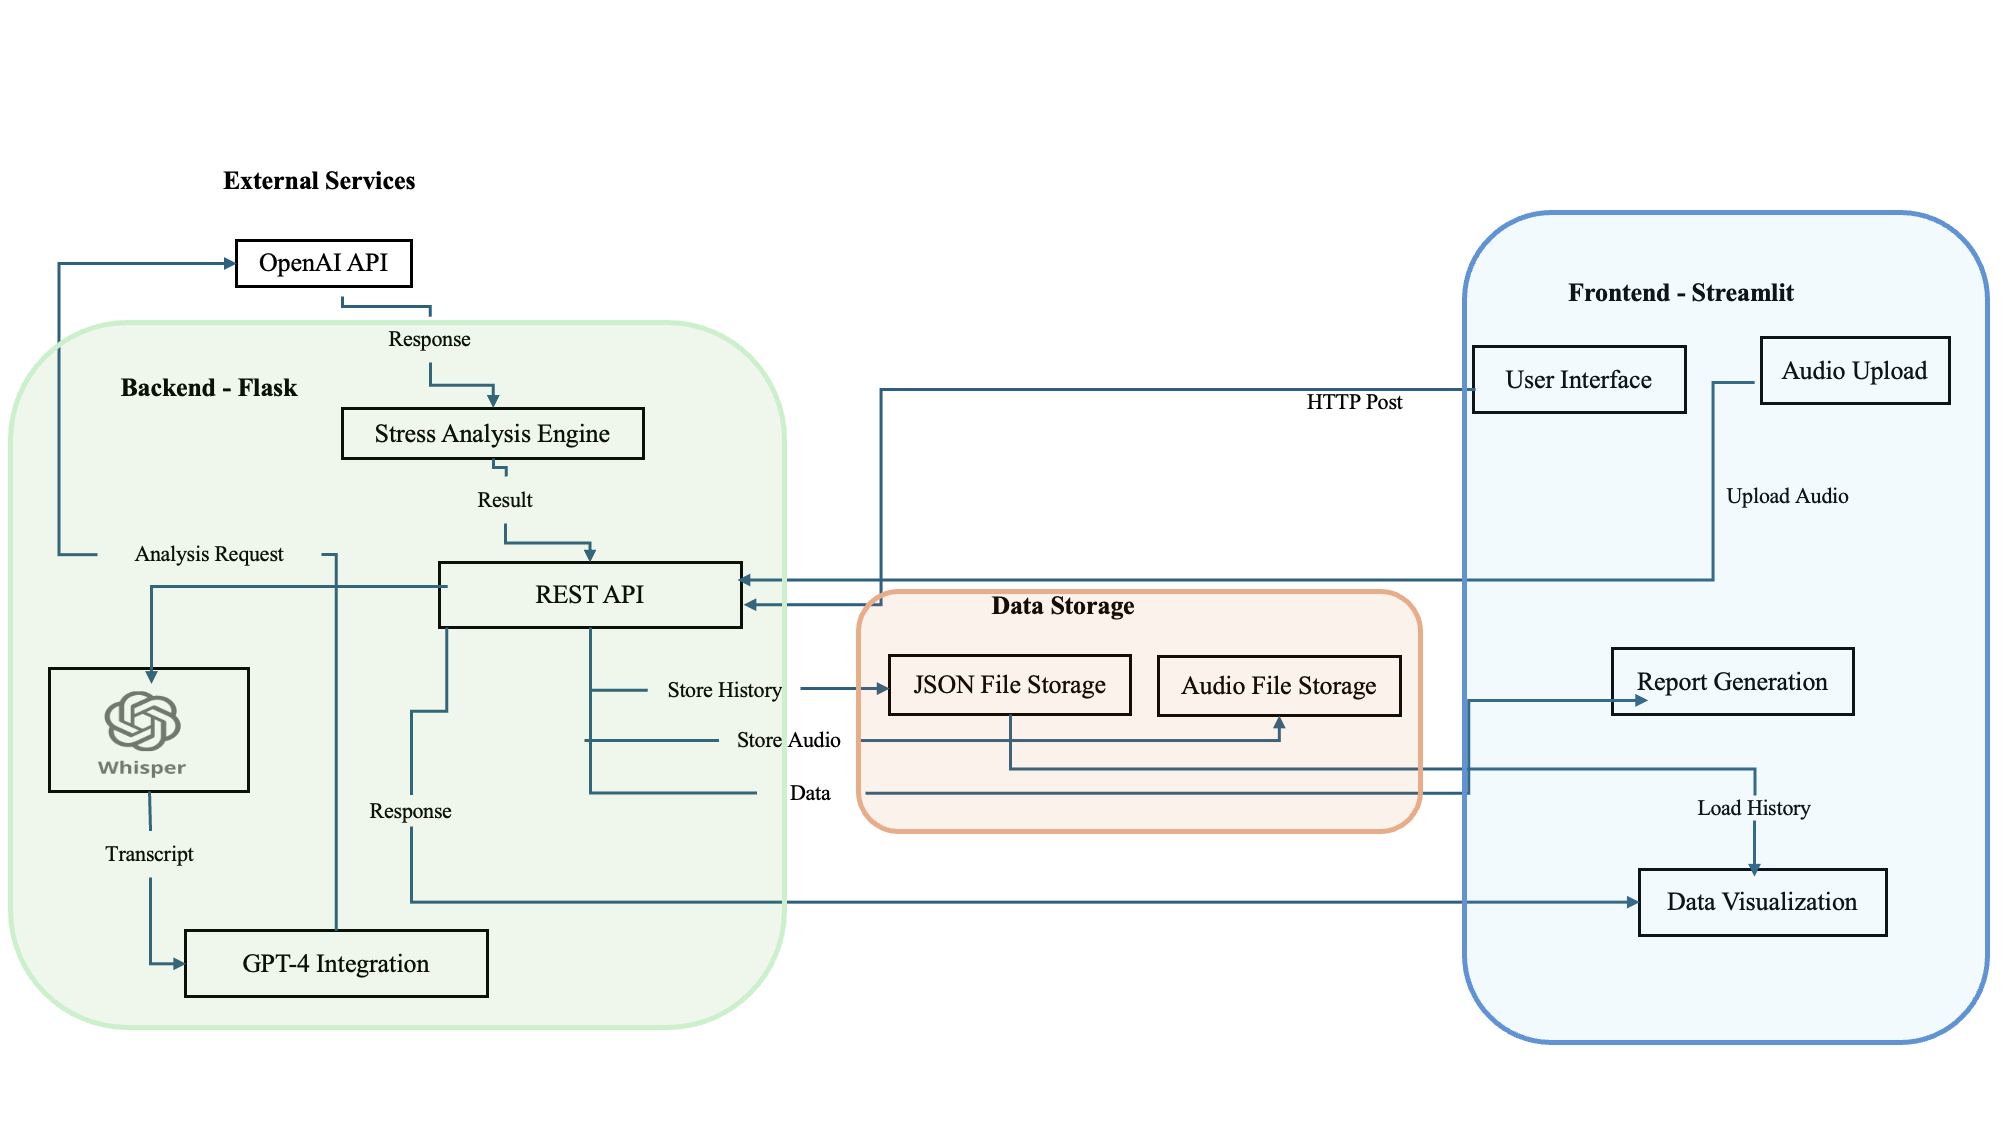
\includegraphics[width=1.1\columnwidth]{allreferences/systemdesigndia.png}
    \caption{Proposed System Architecture}
    \label{fig:system_architecture}
\end{figure}
\section{Dataset Description}
  A limited number of audio recordings was used to generate and illustrate the functioning of the stress detection system's user interface (UI) and user experience (UX) components. These recordings, which come from openly accessible websites like Google, feature speech samples with a range of psychological tones. Even though the audio files don't represent a formal or standardized dataset, they are a useful tool for demonstrating the system's features, like trend monitoring and real-time stress level visualization. I used the audio file to capture voice at different stress levels. After processing these data, stress detection outputs were simulated and shown on the user interface. These samples are primarily being used to test and validate the stress visualisation features of interface and illustrate how stress trend tracking works throughout several sessions. Also checking interface is capable of handlingvarious stressful aspects.
\begin{table}[p] % Use [H] to keep the table close to the text
\centering
\caption{Dataset Description}
\label{tab:dataset_table} % Optional, for referencing the table
\begin{tabular}{|c|p{8cm}|} % Adjusted column width for better text wrapping
\hline
\textbf{Audio} & \textbf{Text in the Audio} \\ \hline
Audio1 & I wonder what this is about \\ \hline
Fire & The place is on fire, please send help \\ \hline
Test1 & Loans that we can offer with this or farm ownership loans, operating lines of credit, or equipment and capital improvement need loans. The benefit to the \\ \hline
sad.Wav & The best food novel count me on the edge of my side \\ \hline
New recording 19.wav & 時間が戻れば私はあの時間に戻りたいま一回 \\ \hline
New recording 16.wav & So um... I'm sick. But my friend wanted me to be a deity myself because we always had to really cool. So uh... Yeah, here it is. Do you want me to sing? Oh, it sounds really good singing. \\ \hline
new recording 23.wav & Life is difficult, but you are loved. You are loved and important, and you bring to this world things that no one else can so hold on \\ \hline
Airplane.wav & The airplane is almost full.\\ \hline
Gamer.mp3 & Why would you not want to fight for what you believe in? \\ \hline
Sad.mp3 & The delicious aroma of freshly baked bread filled the bakery. \\ \hline
1008TIE.wav & That is exactly what happened.\\ \hline
New recording 25.wav & Us comfort help isn't given up. It's refusing to give up. To use fall for a reason, and to use strength and weakness. I think... \\ \hline
\end{tabular}
\end{table}
\section{Text Processing workflow}
%\clearpage  % Forces all previous content to be placed before this point
The Text Processing Workflow describes the procedures for evaluating and interpreting the text to detect stress. Figure 3.2 shows the text processing workflow, which consists of the following steps: Whisper converts audio into raw text. Using semantic context, GPT-4 analyzes the text to find stress signals. The system uses stress scale to classify stress levels (Low, Moderate, High). The system gives feedback, including stress management tips, based on the user's degree of stress. Each component in a text processing flow is responsible for handling a specific task. For example, an input handler handles text input from audio or manual entry, while an analysis engine uses GPT-4 to analyze text for stress content and analyze numerical stress levels. The formatter gets the results ready to be shown. The report generator generates reports that can be downloaded, while the display handler manages visual representation. It focuses on the processing of textual information obtained from speech. Whisper and GPT-4 are the main tools used in this workflow for the transcribed text's semantic analysis.
 %\clearpage  % Forces all previous content to be placed before this point
%\vspace{-5mm} % Reduce vertical space
\begin{figure}[!htbp]
\centering
\includegraphics[width=1.2\textwidth]{allreferences/textprocessingworkflow.png}
\caption{Text processing flow}
\label{fig:text flow}
\end{figure}
\subsection{Speech to Text Conversion (Whisper)}
\noindent
\begin{minipage}{\textwidth}
The use of Whisper\cite{machaek2023} for accurate transcription. For the flow of text generation This text processing module combines the manual transcript input option, text cleaning and preparation, and whisper to convert speech to text. Whisper converts speech to text.Draw attention to Whisper's main function of converting audio into text transcripts.  This module transcribes user speech into text and performs language analysis to detect stress-related context. Identifies specific words and phrases associated with stress, using GPT-4's capabilities to interpret context. The system captures the audio. The raw audio is passed into the speech recognition API. OpenAI‘s Whisper to convert into text. The voice in the audio file is converted into a textual transcript. For text formatting, the transcript is formed as cleaned or standardized and removing unnecessary pauses or artifacts. 
 The significance of text preparation for analysis, noise reduction, and transcription accuracy is emphasized.The Whisper model processes audio inputs and generates a transcript with a high degree of accuracy, filtering out noise and ensuring that only meaningful words are passed to the next stage.
 %\clearpage % Forces all previous content to finish
%\vspace{-5mm} % Adjust the value as needed to reduce the gap
\vspace{10pt} % Add space to prevent overlap
\FloatBarrier
\begin{figure}[H]
\centering
\includegraphics[width=1.0\columnwidth]{allreferences/textualnetwork2.png}
\caption{Textual analysis}
\label{fig:system_architecture}
\end{figure}
\end{minipage}
\vspace{10pt} % Add space to prevent overlap
%\subsection{GPT-4 analysis setup}
%GPT-4 is set up to detect stress patterns and analyze the context. And also measures the stress level from 1 to 7 and provides an explanation. GPT-4 interprets textual input to identify contextual and semantic stress signals and its natural language processing (NLP) skills to find contextual meanings and phrases that cause stress. 
%For instance: "GPT-4 analyses the transcript by detecting linguistic cues and contextual stress indicators, such as emotional word choices or abrupt sentence patterns." 
%\subsection{Stress level scale}
 %The scale utilized to classify the intensity of stress and discuss how textual cues, such as sentence structure and word choice, affect the identification of stress levels.
 %For instance: "Stress levels are determined based on linguistic patterns like frequent use of negative words, abrupt transitions in tone, and word repetition." 
%\subsection{Response generation}
%The system generates customized feedback. The result was processed using explanation formatting, colour coding according to level, and numerical stress level mapping. The display feature consists of the original transcript, detailed analysis text, and color-coded stress indicators. The ability of the system to produce responses that resemble those of a human is directly influenced by the textual interpretation. 
%For instance: "The generated response includes stress-relieving suggestions that are directly informed by the context of the transcribed text." 

\section{Audio Processing workflow} 
The main focus of the Audio Processing Workflow is the analysis of text data along with raw audio characteristics like pitch, tone, and frequency. This section describes how the use of voice characteristics in audio data enhances the stress detection system. Figure 3.3 illustrates the audio processing process that combines GPT-4, Whisper, and the backend to analyse stress. Important actions consist of utilising the frontend to upload the audio file. Whisper audio to text conversion. Using GPT-4 to perform stress analysis and storing audio files and JSON results for tracking history. The processing pipeline goes as follows: Whisper converts audio to a transcript, the frontend uploads the audio file to the Flask backend, which keeps it temporarily. The transcript is then submitted to GPT-4 for stress analysis, the results are kept in a JSON history, and the frontend receives the response. Using a REST API design, the system's frontend and backend operate on the default ports of Streamlit and Flask, respectively. They communicate via HTTP POST requests, file transfers take place via multipart/form-data, and JSON is delivered as the result. 
\vspace{10pt} % Add space to prevent overlap
\begin{figure}[H]
    \centering
    \includegraphics[width=1.1\columnwidth]{allreferences/audioflow.png}
    \caption{Audio processing flow}
    \label{fig:system_architecture}
\end{figure}
\vspace{10pt} % Add space to prevent overlap
%\subsection{Whisper for Speech-to-Text:}
%Whisper handles transcription. Distinguish by highlighting  how the impact of audio pre-processing (such as managing background noise and accents) on transcription quality. Whisper's capacity to retain vocal inflections for stress analysis later on. 
%For instance: "Whisper not only transcribes audio into text but also captures subtle vocal characteristics, such as tone fluctuations, which are critical for stress detection." 
%\subsection{GPT-4 for Stress Analysis}
%GPT-4's role in detecting stress patterns.
%In GPT-4's analysis, focus to how audio characteristics (such tone or pitch) enhance the text and discuss about how GPT-4 improves accuracy by combining vocal stress signals with semantic context. 
%For instance: "GPT-4 combines the tonal data from the audio with semantic analysis of the transcript, creating a holistic view of the user's stress levels." 
\subsection{Frontend to Backend Connection and Backend API Endpoint}
Data flows between the user interface and backend. How audio files are uploaded and routed to the backend for processing, highlighting the variations in data flow. 
For instance: "The frontend enables seamless audio file uploads, which are processed through APIs to generate real-time stress analysis results." 
APIs are utilized for seamless communication and emphasizing how the backend responds to demands for processing that are particular to audio in a different way than it does to text. 
For instance: "Backend APIs facilitate efficient data flow, ensuring that both audio features and their textual representations are analyzed synchronously." 
\section{Stress visualization workflow}
This section describes an intuitive and interactive way for users to view their stress levels. Users can see their stress levels in an easy-to-understand format with the help of the stress visualization workflow (Figure 3.4). Stress data recorded in JSON is loaded by users interacting with the UI. Plotly and other libraries are used to process data and produce pie charts and other graphics. Interactive elements and insights into stress distribution are two of the visualization's main characteristics. Interactive elements such as Legend for reference, Click-to-hide sections and hover tooltips that display precise percentages. Clear patterns and stress percentages are displayed in visualisations, which aid users in efficiently interpreting their data.By choosing the option to "View stress trends," the user starts the process. A slider is then used by the user to select a time range for stress visualization. The process of retrieving and preprocessing. In data loading and Processing portion invloves of fetching stress data (from JSON) and get it ready for visualization. In this procedure, user-selected data is loaded according to the designated time frame. Arranging and preprocessing data in preparation for analysis. Explains how stress levels are represented by colour coding: red for excessive stress, yellow for moderate stress, and green for low stress. Consistency and clarity in visual representation are assured by this arrangement of data. It shows how graphical outputs are generated from the analyzed stress data. The proportions of various stress levels are displayed using a pie chart. The Plotly library makes it easier to create dynamic charts with features such as Precise labels. Interactive sections, such as click-to-hide. Stress data is represented graphically. Visuals are rendered on the user interface, draws attention to the way the Streamlit user interface renders the images: Interactive elements and the pie chart are shown in the application. The visualizations make it simple for users to explore their stress data
%\vspace{-5mm} % Adjust the value to control the spacing
\vspace{10pt} % Add space to prevent overlap
% Example
\FloatBarrier
\begin{figure}[H]
    \centering
    \includegraphics[width=1.0\columnwidth]{allreferences/piestressvisual.png}
    \caption{Stress Visualization Flow}
    \label{fig:system_architecture}
\end{figure}
\FloatBarrier
\vspace{10pt} % Add space to prevent overlap
%\subsection{Data Loading and Processing}
%By choosing the option to "View stress trends," the user starts the process. A slider is then used by the user to select a time range for stress visualization. The process of retrieving and preprocessing. In data loading and Processing portion invloves of fetching stress data (from JSON) and get it ready for visualization. In this procedure, user-selected data is loaded according to the designated time frame. Arranging and preprocessing data in preparation for analysis. 

%\subsection{Color Mapping Setup}
%This subsection explains how stress levels are represented by colour coding: red for excessive stress, yellow for moderate stress, and green for low stress. Consistency and clarity in visual representation are assured by this arrangement of data. It shows how graphical outputs are generated from the analyzed stress data. The proportions of various stress levels are displayed using a pie chart. The Plotly library makes it easier to create dynamic charts with features such as Precise labels. Interactive sections, such as click-to-hide. Stress data is represented graphically. Visuals are rendered on the user interface, draws attention to the way the Streamlit user interface renders the images: Interactive elements and the pie chart are shown in the application. The visualizations make it simple for users to explore their stress data.
\section{Stress trend analysis workflow}
Changes in stress levels over time are monitored via the stress trend analysis workflow (Figure 3.5). To examine certain sessions, users can use time ranges to filter data and to improve insights and smooth out volatility, the system computes moving averages. Trends are displayed using interactive charts that can be customized. Interactive features include zoom and pan controls, a time range slider for filtering data, hover tooltips for displaying precise values, and a legend for trend lines and stress levels. 
\vspace{10pt} % Add space to prevent overlap
\begin{figure}[H]
    \centering
    \includegraphics[width=1.1\columnwidth]{allreferences/stresstrendflow.png}
    \caption{Stress trend analysis workflow}
    \label{fig:system_architecture}
\end{figure}
\vspace{10pt} % Add space to prevent overlap
\subsection{Data Loading and Time Range Selection}
This subsection explains how stress data is retrieved from storage and filtered based on the selected time range. It emphasizes the user’s role in selecting the desired range and how this choice influences the subsequent data analysis steps. %the process by which stress data is retrieved and filtered.
\subsection{Moving Average Calculation}
The process utilized for highlighting the patterns and focusses on how patterns in stress data are highlighted through calculation. To smooth out variations and identify patterns in the data, a moving average is calculated across a specified session window.
\subsection{Interactive Plot Creation}
The tools and techniques for dynamic visualizations. Explains how dynamic visualizations are made using various tools and techniques. By enabling zooming, panning, and hovering, interactive graphs give viewers an in-depth assessment of stress patterns
\subsection{Customizing Plot Layout}
 Chances to use personalization to improve user interaction. The personalisation options available to enhance user interaction are described in this subsection. Plots can be altered by users to fit their tastes in terms of colour schemes, line styles, and data presentation.
\chapter{System Implementation and Results}
\clearpage 
 This chapter shows how the theoretical concept described in Chapter 3 has been realised by addressing the stress detection system's actual implementation and presenting its output. The implementation of the system are covered in this chapter, with a focus devoted to the UI/UX design, which emphasizes the visual components, interaction flow, and links to the backend procedures.  Examples, visual outputs, and screenshots are provided to demonstrate the system's operation. UI/UX components that improve user engagement and experience receive particular emphasis.The chapter also outlines the concepts, techniques, and tools used to create an usable and intuitive system that supports the goals of stress visualization and detection.
 \section{System overview}
 The stress detection system gives users insightful information about their stress levels by combining voice feature analysis and visualisation. In order to establish a connection the design (Chapter 3) and implementation, this section briefly restates the system's main elements.
\textbf{Important elements:}
\begin{enumerate}
\item Frontend (Streamlit): Manages input processing, output visualisation, and user interaction.(\cite{pillai2024})
\item  Backend (Flask): Controls response generation, model integration, and data processing.(\citet{relan2019}). 
\section{Frontend Implementation}
 Implementing the UI/UX components mentioned above and creating a useful interface are the main goals of the frontend. The following are the frontend implementation's salient features:
 \begin{enumerate}
\item Playback and Upload of Audio:
Users can submit.wav files for examination. And a built-in audio player lets users listen to their input again. 
\item  Visualization Integration: Line graphs showing stress trends are changed dynamically in context of analysis and Pie charts with distinct colour coding are used to display the stress level distribution. 
\item Downloadable reports: Users have the option to obtain comprehensive reports with stress analyses in PDF format. 
\item  Frontend Interaction Flow: Effortless transitions between sections for analysis, feedback, and file upload. 
\end{enumerate}
 \section{Backend Implementation}
 The backend combines models, processes text and audio inputs, and sends the output back to the frontend. Important implementation specifics consist of: 
\begin{enumerate}
\item Audio Processing: Whisper is used to transcribe audio files. In order to analyze stress, features are extracted. 
\item Stress detection using GPT-4:  GPT-4 analyzes the raw transcript to determine the stress levels (1–7). 
\item API Communication: To ensure smooth data transmission, the backend and frontend communicate over secure endpoints. 
\item Response Generation: Produces numerical stress levels, thorough explanations and analysis-based advice. 
\end{enumerate}
%\subsection{Input phase: Speech to Text Conversion (Whisper)}

%\vspace{-5mm} % Reduce vertical space
%\vspace{10pt} % Add space to prevent overlap
 %\begin{figure}[p]
    %\centering
   % \includegraphics[width=1.1\columnwidth]{allreferences/whisper1.png}
   % \caption{Speech to text conversion}
  %  \label{fig:system_architecture}
%\end{figure}
\vspace{10pt} % Add space to prevent overlap
\subsection{Audio Processing}
The built-in st.audio() function in Streamlit handles the audio playback. In the web interface, Streamlit's st.audio() component offers a native HTML5 audio player and it allows the common audio formats like MP3, WAV, and M4A. It also reads the audio file in bytes and shows a simple player interface on the web. Basic functions like play/pause, seek, and volume control are included with the player, along with a audio player interface that includes a progress bar.The stress detection system's audio processing interface is depicted in the figure 4.1. It offers an easy-to-use interface for managing and uploading audio recordings, making speech analysis for stress detection possible. Audio files up to 200 MB in size can be uploaded by users in different formats.
%\clearpage  % Forces all previous content to be placed before this point
\FloatBarrier
\vspace{-5pt}
\begin{figure}[htbp!] % More flexible placement
    \centering
    \includegraphics[width=0.9\columnwidth]{allreferences/audiofunc1.png}
    \caption{Audio Processing}
    \label{fig:audio_processing}
\end{figure}
\subsection{GPT-4 Analysis phase}
Once the transcript is ready, a prompt is formulated. The prompt includes instructions to analyze the transcript for emotional content or specific stress indicators. This can be done using a template-based approach or dynamic prompt creation, where certain keywords (example: “fire,”“help”) trigger stress-related prompts. The transcript and prompt are fed into an LLM . This step involves packaging the input as a query that the LLM understands, potentially formatted as 'prompt': "from now you are expert in finding any stress in the following voice transcript”; and "You are an assistant designed to analyze the stress level in speech. Focus on identifying emotional intensity, such as regret, nostalgia, uneasiness, or conflict, and scale it to a stress level from 1 to 7. Provide an explanation for the level."
\vspace{10pt} % Add space to prevent overlap
 \begin{figure}[htbp!]  %[h!]
    \centering
    \includegraphics[width=1.0\columnwidth]{allreferences/gpt4textprocessing2.png}
    \caption{GPT4 analysis phase}
    \label{fig:system_architecture}
\end{figure}
\vspace{10pt} % Add space to prevent overlap
\subsection{Output phase:Response generation} % 4.4.3
Then, LLM processes the prompt and transcript, using its pre-trained knowledge of language patterns, semantics, and emotional cues to analyze the text. The LLM evaluates both the content ('fire', 'help') and the context (the urgency in the sentence structure) shown in figure 4.4.
\vspace{10pt} % Add space to prevent overlap
 \begin{figure}[htbp!] %[h!]
    \centering
    \includegraphics[width=1.1\columnwidth]{allreferences/responsegentext1.png}
    \caption{Response generation}
    \label{fig:system_architecture}
\end{figure}
\vspace{10pt} % Add space to prevent overlap
\end{enumerate}
 \section{UI/UX enhancements}
 The UI/UX design\cite{akhmedov2023} is essential to developing a user-friendly and engaging stress detection system. The main facets of UI/UX design and their application are listed below.
 \begin{enumerate}
 \item Adaptive UI Design: The system uses dynamic colour schemes that alter according to the stress levels that are identified (for instance, red for high stress). 
\item Features for User Accessibility: Supports several languages, such as English and Japanese and easy navigation that reduces cognitive effort with a clear visual hierarchy. 
\item Interactive Visualisations: Instantaneous feedback via pie charts, line graphs, and reports that can be downloaded. 
\item Feedback and Error Handling: Shows individualised guidance and real-time stress feedback and offers advice and error messages for missing or erroneous input.
\end{enumerate}
%\vspace{10pt} % Add space to prevent overlap
% \begin{figure}[p] %[h!]
   % \centering
   % \includegraphics[width=1.1\columnwidth]%{allreferences/textprooutput1.png}
   % \caption{Analysis and explanation}
    %\label{fig:system_architecture}
%\end{figure}
 \subsection{Development with Streamlit}
The primary tool for creating my user interface is Streamlit[17]. Interactive elements such as the file uploader and audio player are used. Styled text using Markdown (st.markdown()). Messages that handle errors (st.error(), st.success()). Important UX Elements Applied with Streamlit
Stress-level-based adaptive user nterface (colour-coded messages)
Spinners are being loaded st.spinner() to improve feedback.
When the file upload fails, error messages appear.
After every upload, the graph is updated in real time.

\subsection{UX Enhancements for User Engagement}
    Data visualisation methods, backend processing, and frontend technologies are all used in UX (User Experience) enhancements.
    \subsubsection{ Flask as Backend API}
    The backend API for processing the uploaded audio and returning the findings of the stress analysis is Flask. Flask manages the Speech Analysis work by utilising GPT-4o (stress analysis) and Whisper (voice-to-text) to handle the uploaded audio file. Additionally, it provides real-time feedback and promptly returns stress levels and explanations, assuring a low latency and seamless user experience also offers error handling. Flask produces concise error messages for the frontend to see in the event of issues (such as a missing audio file or an API failure). Further,  handle the data Processing which Formats the stress level data before sending it to Streamlit, ensuring consistent responses. 
        \subsubsection{Whisper (Speech-to-Text Transcription)}
Translates audio to text for stress analysis, make sure speech is recognised correctly before sending it to GPT-4, and adjusts for accents and tones for greater accuracy. Whisper was used to implement the following important UX features: Enhanced accessibility for non-text inputs;  Accurate transcription for stress assessment; Smooth speech-to-text conversion. Figure 4.4 shows the transcription of the audio. After uploading the audio it transcribes the audio. the transcription result and summarization is shown in the figure.
%\clearpage  % Forces all previous content to be placed before this point
\vspace{10pt} % Add space to prevent overlap
\begin{figure}[htbp!]
    \centering
    \includegraphics[width=1.0\columnwidth]{allreferences/fire2transcribe.png}
    \caption{Transcription from audio}
    \label{fig:system_architecture}
\end{figure}
\vspace{10pt} % Add space to prevent overlap
%Figure 4.8  also shows the transcription of the audio. After uploading the audio it transcribes the audio. the transcription result and summarization is shown in the figure. 
%\vspace{10pt} % Add space to prevent overlap
%\clearpage  % Forces all previous content to be placed before this point
%\vspace{10pt} % Add space to prevent overlap
%\begin{figure}[p]
   % \centering
    %\includegraphics[width=1.0\columnwidth]{allreferences/supermarket.png}
    %\caption{Transcription from audio}
    %\label{fig:system_architecture}
%\end{figure}
\vspace{10pt} % Add space to prevent overlap
   \subsubsection{GPT-4o for Stress Analysis}
    GPT-4o uses voice analysis to identify stress levels in transcriptions. Gives thorough contextual stress explanation instead of only numerical values. It contributes to the humanisation and intuitiveness of stress evaluation. Detailed stress level explanations (rather than just numbers) are one of the key UX features implemented with GPT-4. Context-based stress analysis such as the urgency of speech patterns comes in second. And lastly it enhanced accuracy over conventional numerical classifiers.
\subsubsection{Explanation and advice}
The system analyses the speech transcript using GPT-4 to determine the user's intent, tone, and emotional context. For example Figure 4.6 shows the expression "If time could go back" is understood to mean regret or desire, which is classified as a stress-related mental state. The identified stress level (Level 3) is assigned by the method to a matching database category, such as "internal stress or conflict due to dissatisfaction or nostalgia." There is guidance associated with each stress level. 
%\clearpage  % Forces all previous content to be placed before this point
\begin{figure}[H]
    \centering
    \includegraphics[width=0.9\columnwidth]{advice3.png}
    \caption{Explanation and Advice}
    \label{fig:advice1}
\end{figure} 
For instance: "Take breaks, practise mindfulness, stay hydrated." is the Level 3 Stress Advice. Tailored to stress context for making it easy to use and actionable, the advice is straightforward, generic, and practical. Also The system successfully offers advise based on identified stress intensity, as seen in Figure 4.6. The system determined that the intensity in this case was moderate and assigned a Stress Level of 3. The system showed its ability to provide guidance for handling elevated stresss, even if the detected stress was primarily enthusiasm and engagement. This demonstrates how the system works to give people practical advice regardless of their mental state, which promotes general awareness and control.  
\vspace{10pt} % Add space to prevent overlap
%\vspace{-5mm} % Reduce vertical space
\begin{figure}[htbp!]
    \centering
    \includegraphics[width=1.0\columnwidth]{advice4.png}
    \caption{Explanation and Advice}
    \label{fig:system_architecture}
\end{figure} 
\vspace{10pt} % Add space to prevent overlap
  \subsubsection{ Stress visualization}
Figure 4.7 displays the percentage distribution of stress levels. Low stress (levels 1-3) is represented by green, mild stress (levels 4-5) by orange, and high stress (levels 6-7) by red. Interactive elements such as Legend for reference, Click-to-hide sections and hover tooltips that display precise percentages Insights like stress distribution patterns and percentages are provided by visualizations.  The implementation involved with tools like Plotly for graphical representations and connects stress data that has been captured in JSON with the user interface (UI). 
% \clearpage  % Forces all previous content to be placed before this point
\vspace{10pt} % Add space to prevent overlap
\begin{figure}[htbp!]
    \centering
    \includegraphics[width=0.8\textwidth]{allreferences/stressvisualpie.png}
    \caption{Stress Visualization}
    \label{fig:system_architecture}
\end{figure}
\vspace{10pt} % Add space to prevent overlap
    \subsubsection{ Stress Trend Tracking Feature}
     Using Matplotlib stress patterns over time using is plotted, which used to visualize stress trends. To help track past stress levels for long-term insights, figure 4.8 present line graphs with markers to visualize user stress patterns.  The moving average is displayed by the blue trend line. The X-axis displays the session numbers. Y-axis representing stress levels from 1 to 7. Interactive features include zoom and pan controls, a time range slider for filtering data, hover tooltips for displaying precise values, and a legend for trend lines and stress levels are used. The dynamic stress trend graph which automatically updates upon each upload, improved readability with larger markers, bold labels, and annotations on each point to display stress values. 
%\clearpage  % Forces all previous content to be placed before this point
\vspace{10pt} % Add space to prevent overlap
     \begin{figure}[htbp!]
    \centering
    \includegraphics[width=1.0\columnwidth]{stresstrend3.png}
    \caption{Stress Trend Tracking History}
    \label{fig:system_architecture}
\end{figure}
\vspace{10pt} % Add space to prevent overlap
    \subsubsection{ JSON (Local Data Storage for Stress Trends)}
    Figure 4.9 shows the stress report. JSON stores the history of stress levels locally. When the page is refreshed, previous stress levels are not lost and makes it possible to track previous sessions for long-term insights. The principal UX Elements applied Through JSON to avoid excessive data building, the stress history is kept for the last 50 sessions and is persistent over repeated uploads.
    % \clearpage  % Forces all previous content to be placed before this point
%\vspace{-5pt} % Reduces space above
%\FloatBarrier % Ensures figure stays within section
%\begin{figure}[htbp!]
  %  \centering
   % \includegraphics[width=0.7\textwidth]{allreferences/stressreportdownload.png}
   % \caption{Stress report}
   % \label{fig:stress_report}
%\end{figure}
%\vspace{-10pt} % Reduces space below
 \section{Implementation output}
The frontend and backend are smoothly connected via the system's interaction flow. Through the interface, users can enter text or upload audio. Calculates stress levels by processing inputs using Whisper and GPT-4.The frontend receives the results for feedback and visualization. Key outputs produced by the system to verify its operation are shown in this section:
\begin{enumerate}
\item Stress Analysis Findings: Audio file transcriptions. 
Stress levels were identified and categorized, such as Severe, Slight stress and relaxed. 
\item Visualization Outcomes: Line graphs illustrating temporal trends in stress. 
Pie charts that show the distribution of stress levels. 
\item Reports and Feedback: Downloadable reports and tailored guidance.
\end{enumerate} 
 \begin{figure}[p]
    \centering
    \includegraphics[width=0.9\columnwidth]{aovrall1.png}
    \caption{Stress Level Detection System}
    \label{fig:system_architecture}
\end{figure} 
 \begin{figure}[p]
    \centering
    \includegraphics[width=0.9\columnwidth]{aoverall2.png}
    \caption{Stress Level Detection System}
    \label{fig:system_architecture}
\end{figure}
The main features of the Speech Stress Detection System are shown in Figures 4.9 and 4.10, an intuitive and engaging user interface. In order to verify the input, users can listen to audio recordings that they have uploaded in supported formats such as MP3, WAV. Stress levels are detected by the system and shown clearly in a banner with colour coding. It provides context for the state by clarifying whether the detected intensity is indicative of high or low stress. To provide transparency and usability, the analyzed speech is transcribed and presented for the user's reference. A line graph helps users keep an eye on their mental health by showing changes in stress levels over time. A pie chart offers a thorough overview of stress levels by classifying them as low, medium, or high intensity  which demonstrate the system's emphasis on improving user experience by providing actionable information.
\chapter{Experiment and evaluation}
\clearpage 
  \section{Evaluation of Stress Detection}
  To evaluate the performance of the system, a questionnaire form was developed and shared with participants via social networking platforms (SNS). The form included 12 audio samples, and participants were asked to provide subjective ratings for each audio. The average human rating for an audio reflects the collective perception of stress levels from 40 participants. This is statistically valid because averaging reduces individual biases and represents a more reliable measure. These human ratings were then compared with the system-generated outputs for the same audio samples. Table 5.1 shows the average human rating and system output. After collecting the responses, the correlation coefficient between the human ratings and the system output was calculated to assess the strength of their relationship, and a scatter plot was created to visually represent this correlation and overall trends. To further analyze the data, a bar chart was plotted to compare the average human ratings with the system outputs, highlighting the differences and similarities. Additionally, a line chart was used to show the trends of human ratings and system outputs across all samples, providing a clear representation of their alignment or divergence. Key statistical measures, including the T-value and P-value, were calculated to determine the significance of the findings, while the Mean Absolute Error (MAE) was computed to quantify the average difference between human ratings and system outputs. These analyses, combining visualizations and statistical evaluations, offer comprehensive insights into the system’s performance, its ability to align with human judgment, and areas for further improvement. 
  \begin{table}[h!] % Optional, h! ensures the table stays close to where it's defined
\centering
\caption{Average Human Rating & System Output}
\label{tab:correlation_table} % Optional, for referencing in the text
\begin{tabular}{|c|c|c|}
\hline
Audio & Average Human Rating & System Output \\ \hline
Audio1 & 5.000000 & 6 \\ \hline
Audio2 & 6.125000 & 7 \\ \hline
Audio3 & 5.925000 & 6 \\ \hline
Audio4 & 3.550000 & 3 \\ \hline
Audio5 & 3.666667 & 3 \\ \hline
Audio6 & 5.875000 & 6 \\ \hline
Audio7 & 3.700000 & 3 \\ \hline
Audio8 & 3.875000 & 3 \\ \hline
Audio9 & 5.825000& 7 \\ \hline
Audio10 & 3.525000 & 3 \\ \hline
Audio11 & 4.900000& 4 \\ \hline
Audio12 & 5.950000 & 7 \\ \hline
\end{tabular}
\end{table}
    \section{Correlation of coefficient between system output and human estimation}
    A statistical measure known as the "correlation coefficient," which ranges from -1 (perfect negative correlation) to +1 (perfect positive correlation), is used to analyse the relationship between two variables. It shows the strength and direction of the linear association between the variables. \cite{schober2018correlation}. The correlation coefficient provides a single numerical value that quantifies the strength and direction of the relationship between human ratings and system predictions. A single numerical value that expresses the direction and degree of the relationship between system predictions and human ratings is provided by the correlation coefficient. A high correlation (close to 1) means that human assessments and the system agree well. A low correlation (close to 0) indicates that human judgements and the system's predictions are unrelated. An inverse connection is implied by negative correlation, whereby system outputs fall as human assessments rise.  The correlation coefficient acts as a validation metric for proposed system. It shows whether the system reliably captures the stress levels perceived by humans. The system's practical usefulness is supported by a high correlation, which indicates that its stress detection is in accordance with human perception.. The outputs of the stress detection system were compared with human estimations obtained via a survey in order to assess the system's performance. On a 7-point rating system, survey respondents were asked to assess the stress levels of 12 audio samples. The system's predictions and the average human ratings showed a very significant positive connection, as indicated by the analysis's correlation coefficient of 0.96. Figure 5.1, which visualises the relationship between the system outputs and human ratings, was created to further highlight this link using a scatter plot with a trend line. The visual depiction and strong correlation value show that the system's stress predictions closely match human experience, hence verifying its functionality.
    \vspace{10pt} % Add space to prevent overlap
\begin{figure}[H]
    \centering
    \includegraphics[width=1.0\columnwidth]{coeff40.png}
    \caption{Average human rating and system outputs}
    \label{fig:system_architecture}
\end{figure}
\vspace{10pt} % Add space to prevent overlap
\section{Visual comparisons of human ratings and system outputs }
The comparative analysis demonstrates how well and accurately the system  can reproduce human estimations.
\subsection{Comparison of  Human rating  vs system rating }
For every audio sample, the system outputs and human ratings were compared side by side in a bar chart in figure 5.2.
\vspace{10pt} % Add space to prevent overlap
 \begin{figure}[H]
    \centering
    \includegraphics[width=1.0\columnwidth]{bar40.png}
    \caption{Trend Comparison between human rating vs system outputs}
    \label{fig:system_architecture}
\end{figure}
\vspace{10pt} % Add space to prevent overlap
\subsection{Trend Comparison of  Human rating  vs system rating }
The trends of system outputs and human ratings for each of the 12 audio samples were displayed in a line chart in figure 5.3. The trend line displays the comparison between system outputs and human ratings for various audio files. The average human assessments are shown by the blue line. The system's predictions are shown by the orange line. The system's predictions are in good agreement with human judgements when the orange and blue lines are close to adjacent ones.  A mismatch occurs when there is a discernible space between the two lines, meaning that the system's forecast deviates from the average for humans. This trend line identifies distinct audios in which the system works effectively.
\vspace{10pt} % Add space to prevent overlap
\begin{figure}[H]
    \centering
    \includegraphics[width=1.0\columnwidth]{trend40.png}
    \caption{Comparison between human rating vs system outputs}
    \label{fig:system_architecture}
\end{figure} 
\vspace{10pt} % Add space to prevent overlap
\subsection{Histogram of Error Distribution}
The distribution of errors between system outputs and human assessments was shown using a histogram in figure 5.4. The distribution of differences (errors) between the system outputs and human ratings is displayed by the histogram. The x-axis shows the magnitude of the difference between the human ratings and the system output for each audio sample. A difference of 0.2  means the system output was very close to the human average. Larger values such as 1.0 indicate a greater disparity between the two. The Y-Axis shows how many audio files have a given error value. The y-axis indicates the number of audio samples (frequency) that fall into each range of difference. For instance, if the bar at 0.6  has a height of 4, it means there are 4 audio samples for which the difference between the human rating and the system output lies within the range around 0.6.
Proposed system's predictions are, on average, one point off from human evaluations, with the majority of errors centred around 1.0. A narrow and centred histogram shows that the system's predictions closely match the human assessments. The bars represent how many samples fall within specific ranges of difference. The highest frequency in this figure is at a difference of around 0.6, indicating that most samples had a moderate discrepancy between human ratings and system outputs.
%The X-Axis shows the absolute difference (error) between system predictions and human ratings
MAE: 
\vspace{10pt} % Add space to prevent overlap
 \begin{figure}[H]
    \centering
    \includegraphics[width=1.0\columnwidth]{histo40.png}
    \caption{Histogram of error distribution}
    \label{fig:system_architecture}
\end{figure}
\vspace{10pt} % Add space to prevent overlap
\section{Statistical analysis}
The performance of the stress detection system was evaluated by comparing its outputs to human ratings using statistical metrics. A t-test was conducted to assess the statistical significance of the difference between the system outputs and human ratings. The resulting t-statistic and p-value of showed no significant difference, supporting the hypothesis that the system outputs align closely with human perception. A paired t-test (\citet{pairedttest2025}) compares the means of two related groups such as human ratings and system outputs for the same audio files. The goal is to determine if the mean difference between the two groups is significantly different from 0.
\begin{table}[H] % Optional, h! ensures the table stays close to where it's defined
\centering
\caption{Statistical Value} 
\label{tab:correlation_table} % Optional, for referencing in the text
 \begin{tabular}{|c|c|c|}
        \hline
         Mean Absolute Error(MAE) & T-statistic & P-value \\ \hline
            0.71 &  -0.03 & 0.97 \\ \hline
    \end{tabular}%
   \end{table}
   \vspace{10pt} % Add space to prevent overlap

\subsection{Mean Absolute Error (MAE)}
The average absolute difference between the system outputs and human ratings is measured by MAE. Regardless of direction, it shows how far the system's predicts vary from human assessments.  The system outputs are more compatible with human assessments when the MAE is smaller, which denotes higher performance. An MAE of 0.71 indicates that, on average, the system's predictions and human ratings on the stress rating scale diverge by roughly 0.71 units. This is a minor error, indicating that the system functions properly in general.
\subsection{T-Statistic: }
T-Statistic: The T-statistic measures how much the average human rating deviates from the system output, standardized by the variability in the human ratings. A high positive or negative T-statistic indicates a large difference between the human ratings and system outputs. The t-statistic determines if the average difference between human ratings and system outputs deviates from 0 in a statistically significant way. The mean difference between the system outputs and human assessments is insignificant when the t-statistic is around zero such as -0.03.On average, the system's output closely resembles human ratings, showing no bias towards overestimation or underestimation.
\subsection{P value }
P-Value: Indicates whether the observed difference is statistically significant.The P-value represents the probability that the observed difference between human ratings and system outputs occurred by random chance.A common threshold for significance is p<0.05p<0.05. If the P-value is below this threshold, the difference is considered statistically significant. A p-value of 0.9771 is much larger than the common significance threshold of 0.05.  There is no statistically significant difference between the system's outputs and the human ratings. This suggests that the system's performance is very much aligned with human perception
\section{Interpretation of T-statistic and P-value }
The overall p-value (0.97) shown in Table 5.2 explain that these values represent the system's general performance across all audio files. A detailed table 5.3 is shown above with t-statistics and p-values for each audio file.
\vspace{10pt} % Add space to prevent overlap
\begin{table}[H] % Optional, h! ensures the table stays close to where it's defined
\centering
\caption{T-statistic and P-value}
\label{tab:correlation_table} % Optional, for referencing in the text
 \begin{tabular}{|c|c|c|c|c|}
        \hline
        Audio  & T-statistic & P-value \\ \hline
        Audio1 & -5.186 & 0.000007\\ \hline
        Audio2 &  -6.271 & 0.000000\\ \hline
        Audio3 & -0.386 & 0.486333 \\ \hline
        Audio4 &  1.629 & 0.111\\ \hline
        Audio5 &  2.000& 0.053 \\ \hline
        Audio6 &   -0.589 &  0.560 \\ \hline
        Audio7 & 2.004 & 0.052  \\ \hline
        Audio8 &  2.588 &  0.014  \\ \hline
        Audio9 &  -8.806 & 0.000000 \\ \hline
        Audio10 &  4.620 &  0.000041 \\ \hline
        Audio11 &  5.383 & 0.000004\\ \hline
        Audio12 & -5.450 & 0.000003\\ \hline
    \end{tabular}%
   \end{table}
\vspace{10pt} % Add space to prevent overlap
%\noindent
%\textbf{Audio 1:} \\
%\textbf{T-Statistic:} -5.186 \\
%\textbf{P-Value:} 0.000007 (very small) \\
%\textbf{Interpretation:} There is a statistically significant difference between human ratings and system output. The system's stress rating is likely overestimating compared to the human ratings.\par
%\noindent
%\textbf{Audio 2:} \\
%\justifying
%\textbf{T-Statistic:} -6.271 \\
%\textbf{P-Value:} 0.000000  (very small) \\
%\textbf{Interpretation:} The system output differs significantly from human ratings, suggesting overestimation of stress for this audio.\par
%\noindent
%\textbf{Audio 3:} \\
%\textbf{T-Statistic:} -0.386\\
%\textbf{P-Value:}  0.701  (not significant) \\
%\textbf{Interpretation:} There is no statistically significant difference. The system's output aligns well with human ratings.P-value = 0.701,this is much greater than 0.05, indicating that the system's output is not statistically significantly different from the human ratings. A small t-statistic -0.386 also supports that the difference is minimal. Since the system's output is close to the human ratings and the difference is statistically insignificant, interpreting this as good between the system and human ratings. This means that the system's prediction for this audio is consistent with how humans perceive stress.\par
%\noindent
%\textbf{Audio 4:} \\
%\textbf{T-Statistic:} 1.629\\
%\textbf{P-Value:}  0.111  (not significant) \\
%\textbf{Interpretation:} No significant difference between the human ratings and system output, suggesting reasonable agreement.\par
%\noindent
%\textbf{Audio 5:} \\
%\textbf{T-Statistic:} 2.000\\
%\textbf{P-Value:}  0.0533 (borderline significance) \\
%\textbf{Interpretation:} The p-value is close to the 0.05 threshold, suggesting a marginally significant difference.\par
%\noindent
%\textbf{Audio 6:} \\
%\textbf{T-Statistic:} -0.589\\
%\textbf{P-Value:}  0.560 (not significant) \\
%\textbf{Interpretation:} No significant difference, indicating good alignment between human ratings and system output.\par
%\noindent
%\textbf{Audio 7:} \\
%\textbf{T-Statistic:} 2.004\\
%\textbf{P-Value:}  0.052 (borderline significance) \\
%\textbf{Interpretation:} The p-value is close to the threshold, suggesting a marginally significant difference that could require further examination.\par
%\noindent
%\textbf{Audio 8:} \\
%\textbf{T-Statistic:}2.588\\
%\textbf{P-Value:} 0.014 (significant)\\
%\textbf{Interpretation:} Statistically significant difference, with the system likely underestimating stress compared to human ratings\par
%\noindent
%\textbf{Audio 9:} \\
%\textbf{T-Statistic:}-8.806\\
%\textbf{P-Value:} 0.000000 (very small)\\
%\textbf{Interpretation:} Strongly significant difference, with the system likely overestimating stress. \par
%\noindent
%\textbf{Audio 10:} \\
%\textbf{T-Statistic:}4.620\\
%\textbf{P-Value:} 0.000041 (very small)\\
%\textbf{Interpretation:} Statistically significant difference, with the system likely underestimating stress \par
%\noindent
%\textbf{Audio 11:} \\
%\textbf{T-Statistic:} 5.383\\
%\textbf{P-Value:} 0.000004 (very small)\\
%\textbf{Interpretation:} Statistically significant difference, with the system likely underestimating stress \par
%\noindent
%\textbf{Audio 12:} \\
%\textbf{T-Statistic:}-5.450\\
%\textbf{P-Value:} 0.000003 (very small)\\
%\textbf{Interpretation:} Statistically significant difference, with the system likely underestimating stress \par


\textbf{Significant Differences (P < 0.05)}: Audio 1, 2, 8, 9, 10, 11, 12 show significant differences between system outputs and human ratings. These indicate areas where the system does not align well with human perception of stress and requires adjustment.\par
\textbf{No Significant Differences (P ≥ 0.05)}: Audio 3, 4, 5, 6, 7 show no significant differences, suggesting that the system performs reasonably well for these cases. For instance, the system's output aligns well with human ratings.P-value = 0.701 for audio 3,this is much greater than 0.05, indicating that the system's output is not statistically significantly different from the human ratings. A small t-statistic -0.386 also supports that the difference is minimal. Since the system's output is close to the human ratings and the difference is statistically insignificant, interpreting this as good between the system and human ratings. This means that the system's prediction for this audio is consistent with how humans perceive stress. \par
\textbf{Improvement}
Focus on audio files with significant differences to improve system accuracy and enhancements such as retraining the system with more diverse datasets and refine the model for edge cases. Incorporate feedback loops to fine-tune system outputs based on human assessment.

  \section{Discussion of Results}
    \subsection{Key Findings}
    \begin{enumerate}
\item Strong Correlation: The system predictions and human ratings show a strong alignment, as indicated by the correlation coefficient of 0.96. \item  Minimal Error: The system produces accurate predictions with minimal variances, as indicated by the MAE of 0.71. 
\item Statistical Validation: The system's outputs and human ratings do not differ statistically significantly, according to the findings of the paired t-test (τ-statistic: -0.03, p-value: 0.97). 
\end{enumerate}
 \subsection{Insights on Multimodal Data Integration}
For stress detection, the system's integration of Large Language Models (LLM) and Social Signal Processing functioned well.The multimodal approach enabled:
\begin{enumerate}
\item Proper audio input transcription. 
 \item  Accurate assessment of stress levels using linguistic and vocal content. 
\end{enumerate}
\section{Advantages and Limitations of the System}
\textbf{Advantages:}
\begin{enumerate}
    \item A strong correlation with human evaluations confirms the reliability of the system.
    \item Stress detection is made easier by an intuitive user interface (UI).
    \item A low prediction error improves system accuracy.
\end{enumerate}
\textbf{Limitations:}
\begin{enumerate}
\item  Despite the high correlation, certain audio files showed significant differences, which warrants further analysis and improvement in the model's performance.
    \item Minor variations in certain audio samples indicate potential for improvement.
    \item Performance in noisy environments may be impacted by reliance on high-quality audio inputs.
\end{enumerate}
\chapter{Conclusion and Future Work}
\clearpage 
  \section{Summary of the Research}
  This study presented a multimodal stress detection system that uses large language models (LLMs) and Social signal Processing to combine text-based and speech-based stress analysis. The method was created to identify stress levels by merging GPT-4-based textual analysis with audio analysis with transcription. User-centred Stress Visualisation Streamlit was used to create an interactive real-time user interface (UI) that lets users upload audio samples, get stress scores, and see their stress levels on user-friendly dashboards. This research introduced stress trend visualization, which allows users to follow stress changes over numerous sessions, in contrast to traditional stress detection methods that provide immediate assessments. An interactive stress level indicator, trend graphs, and a downloadable stress report were among the UX improvements that improved the system's readability and usefulness for mental health applications. %These results demonstrate how well deep learning-based stress detection works and how crucial UX enhancements are to developing intuitive, real-time stress monitoring solutions.
  \section{Contributions of the Study}
   \begin{enumerate}
   \item Creation of a Multimodal Stress Detection System integrated vocal analysis and LLM-based text analysis.  
 \item Deployment of Long-Term Monitoring Stress Trend Visualisation 
 Added a dynamic stress trend monitoring function that allows users to examine stress trends over time. 
Enhanced applications for mental health monitoring by offering a historical perspective on stress variations. 
 \item UX Improvements for Accessibility and User Interaction 
Developed an interactive user interface with stress visualisation to improve the interpretability and actionability of stress detection results. 
Added downloadable stress reports, stress level indicators, and real-time feedback, improving the usefulness of stress detection tools. 
\end{enumerate}
Through the integration of deep learning, multimodal AI, and user-centred design, these contributions enhance the real-world implementation of stress detection systems.
 
  \section{Limitations of the Proposed System}
Despite the positive results of this study, a number of limitations need to be taken into account. Instead of recording live speech inputs, the system processes pre-recorded speech, which restricts the possibility of real-time engagement.
 
  \section{Recommendations for Future Research}
   \begin{enumerate}
   \item To enhance generalisation, include real-time stress datasets from a variety of speakers.To increase robustness, use datasets with unplanned speech instead of recordings.
 \item  Expand the system to accommodate real-time speech input processing, enabling ongoing stress monitoring. Create an adaptable user interface (UI) that adapts to the stress levels of its users and offers tailored suggestions and feedback.
 \item Combining Multimodal Physiological Information For a more comprehensive stress evaluation, combine physiological cues (such as skin conductivity and heart rate) with speech-based stress detection. Investigate integrating wearable technology (such as smartwatches) for multimodal stress detection in real time.
 \item To offer individualized stress management techniques, consider integration with mental health conversation systems. 
 \item Make the CNN-LSTM model faster on edge devices by optimizing it. Examine compact deep learning architectures that can be implemented on embedded and mobile devices. 
 
The feasibility, scalability, and impact of AI-driven stress detection systems for mental health applications are the goals of these future areas. 
 \end{enumerate}
 \section{Practical Applications of the Study}
 The research research on stress detection systems has several practical applications, particularly in mental health monitoring, workplace wellness, and personal well-being tracking. The work's potential applications span a variety of sectors where stress evaluation and long-term tracking can be beneficial, as it focusses on developing an interactive, user-friendly stress monitoring interface.
%\textbf{Mental Health and Well-being Tracking} \newline
%\makebox[\textwidth][l]{\textbf{Mental Health and Well-being Tracking}} \\
%\parbox{\textwidth}{\textbf{Mental Health and Well-being Tracking}}\\ 
\begin{flushleft}
\textbf{ Workplace Stress Monitoring} 
\justifying
The system can be used by organisations to measure and control workplace stress levels as part of employee wellness initiatives. Managers and HR professionals can use the system's stress trend visualisation to comprehend how stress changes over time and create plans for reducing stress at work. could be used to business mindfulness programs where staff members monitor their psychological health and get stress-reduction advice.
 \end{flushleft}
  \begin{flushleft}
\textbf{Mental Health and Well-being Tracking} \\
\justifying
Individuals can use the stress trend tracking feature to monitor their mental state over time. The system can provide visual insights into stress patterns, helping users recognize triggers and take proactive steps for stress management. It can be integrated into digital mental health platforms to support therapy and self-care.
 \end{flushleft}
 \begin{flushleft}
\textbf{Education} \\
\justifying
The interface can serve as a basis for research on user behaviour in stress detection systems by academic institutions and researchers in the fields of psychology, UX/UI design, and Human-Computer Interaction (HCI). Additional features could be added to the framework to test various stress tracking visualisation techniques. The method can be used by researchers in the future to investigate the effects of interactive stress tracking on user engagement and mental health outcomes.
 \end{flushleft}
\begin{flushleft}
\textbf{Self-Improvement and Personal Productivity} \\
\justifying
Individuals practicing self-care and mindfulness can use the stress tracking feature to measure how relaxation techniques such as meditation, deep breathing impact their stress over time. Can be beneficial for content creators and app developers building self-improvement tools, where users track their mental states alongside productivity habits.
  \end{flushleft}
 \begin{flushleft}
\textbf{Health Tech and Digital Apps} \\
\justifying
The system can be integrated into mobile health (mHealth) applications, providing users with an accessible and interactive stress monitoring tool. Can be paired with wearables or smart assistants to track real-time stress trends based on speech input. Useful for telemedicine platforms, where doctors and psychologists can review stress reports and provide better mental health support.
  \end{flushleft}
  \section{Final Thoughts}
This study introduces a multimodal and user-friendly stress detection system which advances the expanding field of AI-driven mental health care. This system improves stress monitoring, visualization, and interpretability through large language models and UX-focused design. The results show that real-time stress tracking combined with voice and text-based analysis can produce insightful information on mental health. This system could be used as a useful tool for stress monitoring and mental health support with more improvements and real-world validations, bridging the gap between AI-based stress detection and practical applications.
%\appendix
%\chapter{Appendices}

%\bibliographystyle{apalike}
\bibliographystyle{plainnat} % or another style like IEEEtran
\bibliography{ref} % Use the name of your .bib file without the .bib extension

%\bibliographystyle{IEEEtran}
%\bibliography{references}
%\begin{thebibliography}{99}
%\setlength{\itemsep}{0pt} % Adjust spacing between bibliography entrie
%\bibitem{ref1}Sriramprakash, Senthil, Vadana D. Prasanna, and OV Ramana Murthy. "Stress detection in working people." Procedia computer science 115 (2017): 359-366 `
%\bibitem{ref2} Kafková, Júlia, et al. "A New Era in Stress Monitoring: A Review of Embedded Devices and Tools for Detecting Stress in the Workplace." Electronics 13.19 (2024): 3899.
%\bibitem{ref3} Liu, Feng, et al. "Artificial intelligence in mental health: Innovations brought by artificial intelligence techniques in stress detection and interventions of building resilience." Current Opinion in Behavioral Sciences 60 (2024): 101452.
%\bibitem{ref4} Sebastião, Rita, and David Dias Neto. "Stress and mental health: The role of emotional schemas and psychological flexibility in the context of COVID-19." Journal of Contextual Behavioral Science 32 (2024): 100736.
 %\bibitem{ref5}Aristizabal, Sara, et al. "The feasibility of wearable and self-report stress detection measures in a semi-controlled lab environment." IEEE Access 9 (2021): 102053-102068.
%\bibitem{ref6} Chyan, Phie, et al. "A deep learning approach for stress detection through speech with audio feature analysis." 2022 6th International Conference on Information Technology, Information Systems and Electrical Engineering (ICITISEE). IEEE, 2022.
%\bibitem{ref7} Yoon, S., et al. "Text-based stress detection using %semantic analysis." Journal of Computational Linguistics, 2020.
%\bibitem{ref8} Singh, Praveen, et al. "Social signal processing for evaluating conversations using emotion analysis and sentiment detection." 2019 Second International Conference on Advanced Computational and Communication Paradigms (ICACCP). IEEE, 2019.
%\bibitem{ref9} Razavi, Moein, et al. "Machine learning, deep learning, and data preprocessing techniques for detecting, predicting, and monitoring stress and stress-related mental disorders: Scoping review." JMIR Mental Health 11 (2024): e53714.
%\bibitem{ref10}Yao, Yiqun, et al. "Muser: Multimodal stress detection using emotion recognition as an auxiliary task." arXiv preprint arXiv:2105.08146 (2021).
%\bibitem{ref11}Hilmy, Muhammad Syazani Hafiy, et al. "Stress classification based on speech analysis of MFCC feature via Machine Learning." 2021 8th International Conference on Computer and Communication Engineering (ICCCE). IEEE, 2021.
%bibitem{ref12} Shen, Guobin, et al. "StressPrompt: Does Stress Impact Large Language Models and Human Performance Similarly?." arXiv preprint arXiv:2409.17167 (2024).

%\bibitem{ref9} Olawade, David B., et al. "Enhancing mental health with Artificial Intelligence: Current trends and future prospects." Journal of medicine, surgery, and public health (2024): 100099.


%\bibitem{ref12} Graham, Calbert, and Nathan Roll. "Evaluating OpenAI's Whisper ASR: Performance analysis across diverse accents and speaker traits." JASA Express Letters 4.2 (2024).
%\bibitem{ref13} Teye, Martha T., et al. "Evaluation of conversational agents: understanding culture, context and environment in emotion detection." IEEE Access 10 (2022): 24976-24984.

%\bibitem{ref14} Kush, Joseph C. "Integrating Sensor Technologies with Conversational AI: Enhancing Context-Sensitive Interaction Through Real-Time Data Fusion." Sensors 25.1 (2025): 249.
%\bibitem{ref15}Sriramprakash, Senthil, Vadana D. Prasanna, and OV Ramana Murthy. "Stress detection in working people." Procedia computer science 115 (2017): 359-366
%\bibitem{ref16}Macháček, Dominik, Raj Dabre, and Ondřej Bojar. "Turning whisper into real-time transcription system." arXiv preprint arXiv:2307.14743 (2023).
 
 %\bibitem{ref13}Ricker, George R., et al. "Transiting exoplanet survey satellite (tess)." American Astronomical Society Meeting Abstracts\# 215. Vol. 215. 2010.
 %\bibitem{ref14}Ranjan, Rajeev, and Abhishek Thakur. "Analysis of feature extraction techniques for speech recognition system." International Journal of Innovative Technology and Exploring Engineering 8.7C2 (2019): 197-200.
 %\bibitem{ref15}Yan, Mengzhu, and Xue Wu. "Prosody in linguistic journals: a bibliometric analysis." Humanities and Social Sciences Communications 11.1 (2024): 1-15.
%\bibitem{17}Pillai, Mukesh, and Pallavi Thakur. "Developing a Website to Analyze and Validate Projects Using LangChain and Streamlit." 2024 2nd International Conference on Intelligent Data Communication Technologies and Internet of Things (IDCIoT). IEEE, 2024.
%\bibitem{ref18}Relan, Kunal. "Building REST APIs with Flask." Building REST APIs with Flask (2019).
 %\bibitem{ref19}Akhmedov, Nurkhon. Designing and prototyping a learning and testing platform for user experience (UX) and user interface (UI) designers with the aim of improving knowledge and establishing a standard evaluation benchmark for UX/UI design skills and competencies. Diss. Technische Hochschule Ingolstadt, 2023..
%\end{thebibliography}
% Add additional references here

% use section* for acknowledgement
\chapter*{Acknowledgements}

 I would like to start by thanking ALLAH, the Ever Most Generous, for granting me this wonderful opportunity to study at this institution. His countless blessings have given me the health, strength, and clarity of mind to undertake and complete this thesis.

I extend my deepest appreciation to my supervisor, Prof. Shiramatsu, for his valuable guidance, insightful feedback, and unwavering support throughout this research. His expertise and encouragement have been instrumental in shaping my work and strengthening my understanding of my research field. 

A special thanks to my dear parents and Jobair Al Rafi for their unconditional support, patience, and encouragement during this journey. Their belief in me has been my greatest source of motivation, especially during challenging times.

Furthermore, I would like to give special thanks to Aichi Monozukuri Scholarship for providing the financial support during my master’s program and Aichi Prefecture International Department for their generous support.

I would like to thank all the members from Shiramatsu Laboratory. I am also sincerely grateful to the NITech International Affairs Division  and Japanese teachers for their continuous support.

Lastly, I would like to take this opportunity to express my sincere gratitude to many people who helped me with this project who played a significant role by providing the necessary resources and support. This research would not have been possible without the collective efforts, guidance, and encouragement of so many individuals, and for that, I am truly grateful.



\addcontentsline{toc}{chapter}{List of Tables}
%\listoftables
\addcontentsline{toc}{chapter}{List of Figures}
%\listoffigures

% that's all folks
\end{document}



\cleardoublepage
\thispagestyle{empty}
\chapter{Introduction}
\clearpage
\documentclass[Arial,12pt,openright,twoside]{book}
%\documentclass[a4paper,12pt]{report}  % Use "article" or "book" if applicable
%\usepackage[a4paper, margin=25mm]{geometry} % Ensures correct A4 alignment

\usepackage{xeCJK}
\setCJKmainfont{ipaexm.ttf}
\usepackage[T1]{fontenc}
\usepackage[dvipdfm]{graphicx}
\usepackage{amsmath,amssymb,amsfonts}
\usepackage{algorithmic}
\usepackage{pdfpages}
\usepackage{float} % Add this to your preamble modiiii
\usepackage{natbib} % modi
\usepackage[authoryear]{natbib}
%\usepackage[numbers,round]{natbib} % Or omit "numbers" for pure author-year
\bibliographystyle{plainnat}
%\bibliographystyle{apalike} % modifi
% For \citeauthor command etc
% For headers
\usepackage{longtable} % modification
\usepackage{fancyhdr}
\pagestyle{fancy}
\fancypagestyle{plain}{ % Redefine plain page style
    \fancyhf{} % Clear all headers and footers
    \fancyhead[LE]{\thepage} % Page number on top-left for even pages
    \fancyhead[RO]{\thepage} % Page number on top-right for odd pages
    \renewcommand{\headrulewidth}{0pt} % Remove the header rule
    \renewcommand{\footrulewidth}{0pt} % Remove the footer rule
}
\fancyhf{} % Clear all headers and footers
\fancyhead[RE]{\leftmark}
\fancyhead[RO]{\thepage}
\fancyhead[LO]{\leftmark}
\fancyhead[LE]{\thepage}
\fancyfoot[RO]{\rightmark}
\fancyfoot[LE]{\rightmark}
\usepackage{emptypage}
\usepackage{ragged2e} %% modification
\justifying % modification
\usepackage{color}   %May be necessary if you want to color links
\usepackage[breaklinks=true]{hyperref}
\usepackage{breakcites} % otherwise they don't wrap
\usepackage{microtype} % otherwise they don't wrap
\usepackage{apalike}
\usepackage{tikz}
\usepackage{multirow}
\usepackage{filecontents}
\usepackage{caption}
\usepackage{tablefootnote}
\usepackage{placeins}% modi
% \usepackage{cite} % modi 

\raggedbottom % modi

\captionsetup[table]{skip=5pt}

%\setlength{\textfloatsep}{5pt} % Space between figure and text % modi
%\setlength{\intextsep}{5pt}    % Space for in-text figures% modi
\setlength{\abovecaptionskip}{5pt} % Space above captions % modi
\setlength{\belowcaptionskip}{5pt} % Space below captions % modi
\setlength{\textfloatsep}{8pt} % Adjust space between text and figures
\setlength{\intextsep}{8pt}    % Space for inline figures
%\setlength{\parindent}{15pt} % Default indentation size


\graphicspath{{./images/}}
%\titlespacing*{\subsection}{0pt}{10pt}{5pt} % Adjust subsection spacing

\usetikzlibrary{shapes.geometric, shapes.symbols, shadows, arrows}
\tikzset{
  multidocument/.style={
    shape=tape,
    draw,
    fill=white,
    tape bend top=none,
    double copy shadow}
    }
\hypersetup{
 	linktocpage,
     colorlinks=true, %set true if you want colored links
     linktoc=all,     %set to all if you want both sections and subsections linked
     linkcolor=blue,  %choose some color if you want links to stand out
 	citecolor=black,
 	filecolor=black,
 	linkcolor=black,
 	urlcolor=black
 }
 
 % correct bad hyphenation here
\hyphenation{pre-processing pre-processed pre-training pre-trained}
\usepackage{array}

\usepackage{listings}
\lstset{
basicstyle=\small\ttfamily,
columns=flexible,
breaklines=true,
frame = single
}

\makeatletter
\newcommand*{\da@rightarrow}{\mathchar"0\hexnumber@\symAMSa 4B }
\newcommand*{\xdashrightarrow}[2][]{%
  \mathrel{%
    \mathpalette{\da@xarrow{#1}{#2}{}\da@rightarrow{\,}{}}{}%
  }%
}
\makeatletter
\def\endthebibliography{%
  \def\@noitemerr{\@latex@warning{Empty `thebibliography' environment}}%
  \endlist
}
\makeatother

%\pagenumbering{arabic}%ここからページ数開始

\input{commands}

\begin{document}

\cleardoublepage
\input{part/_title/title}

%\include{part/abstract/abstract}

\tableofcontents
%\addcontents{Abstract}
\addcontentsline{toc}{chapter}{Abstract}
\listoftables
%\addcontentsline{toc}{chapter}{List of Figures}
\listoffigures

\chapter*{Abstract}

Stress detection is increasingly crucial for mental health monitoring, yet traditional approaches relying on single-modal data, such as text or audio, often lack accuracy and contextual understanding. This research introduces a multimodal stress detection system that integrates Social Signal Processing (SSP) techniques, voice feature analysis, and Large Language Models (LLMs). By combining linguistic (text-based) and paralinguistic (audio-based) cues, the system enhances stress estimation through a hybrid approach. The system accepts audio inputs in various formats such as MP3, WAV, M4A and processes them to extract linguistic content and vocal stress indicators. By combining features such as tone detection, Linguistic content, including lexical choices, syntactic structures, and sentiment-based expression sand vocal attributes like pitch and intensity, the system employs to estimate stress levels. To enhance user interaction and usability, the system is implemented with a Streamlit-based UI for real-time stress visualization. Current UX improvements focus on integrating stress trend history tracking to provide users with longitudinal insights into their stress patterns. %Future work aims to refine accessibility, usability, and multimodal fusion techniques to further improve stress recognition capabilities.
This study contributes to the field of voice-based stress analysis by integrating  with an interactive user interface, making stress detection more accessible and interpretable for real-world mental health applications.

%\tableofcontents
%\listoffigures
%\listoftables

\chapter{Introduction}
\clearpage  % Forces all previous content to be placed before this point
  \section{Background}
  In today's world, stress is an ongoing issue that affects both physical and mental health, influencing everything from mood and productivity to long-term well-being. Stress is a natural phenomenon that causes physical and emotional tension. Chronic stress is associated with serious diseases such as heart disease, anxiety, depression and immunosuppression. Stress is analyzed by expression, tone , pitch and physiological signals. The process of detecting when someone is stressed by measuring their physiological signals is known as stress detection. To analyze these signals and classify them as stressed or relaxed, some techniques are used. The physiological signals of a person are measured by physiological sensors such as the pulse of blood volume (BVP), the galvanic skin response (GSR), and the electrocardiograms (ECGs) (\citet{sriramprakash2017}). In mental health care, intelligent technology has shown significant promise in delivering personalized treatments and real-time stress detection. (\cite{kafkova2024} ) and (\cite{liu2024}).  Due to this, early and precise stress detection is vital for workplace wellness, healthcare, and personal well-being. However, many existing systems use single-modal data, such as text or voice, which limits their ability to capture all aspects of stress symptoms. This study explores the development of a versatile and ethical multimodal AI system designed for real-time stress detection. The system integrates voice and textual context to provide a comprehensive and accurate assessment of stress levels.
  \section{Motivation of the research}
  Stress has become a global problem that impacts not only mental health but also lifestyles and productivity. Due to the absence of easily accessible, reliable, and non-invasive methods, many people face obstacles in monitoring their stress. Conventional methods, such as self-assessment questionnaires or physiological monitoring, are inadequate in terms of timely insights or are impractical for daily use. Innovative systems that can effectively identify stress in real-world situations are, therefore, becoming more and more necessary.
The voice is a perfect medium for stress detection because it is a natural source of emotional information. It transmits paralinguistic clues like tone, pitch, and rhythm in addition to linguistic content, which can reveal a person's emotional condition. Powerful tools like Large Language Models (LLMs), which can analyze textual material for deeper contextual and emotional insights, have been made possible by breakthroughs in Natural Language Processing (NLP). The majority of stress detection systems now only accept single input, which restricts the precision and usefulness. 
Current systems' emphasis on immediate stress assessments, which overlooks long-term patterns and trends, is another major drawback. Furthermore, existing tools often lack user-friendly interfaces, user cannot use without technical expertise.
This study is motivated by an urge to develop a multimodal system that enhances the accuracy of stress detection by integrating text-based and voice-based analysis. Using LLMs for text analysis and deep learning models for audio processing, this study aims to close the gap between state-of-the-art AI technology. A more precise and user-friendly method of tracking stress over time is provided by incorporating interactive features like stress trend tracking, which also enables users to take proactive measures for improved mental health.

  \section{Problem Statement}
  Current stress detection systems often suffer from ethical concerns regarding data privacy, and a lack of adaptive intervention mechanisms. How can we design an ethical, adaptive, and multimodal AI system that not only detects stress accurately but also provides meaningful support to promote mental well-being?
\section{Research Objectives}
\begin{enumerate}
    \item To develop a system that estimates and visualizes user stress levels using Social Signal Processing (SSP) techniques, including voice analysis for both linguistic (text-based) and paralinguistic (audio-based).
    \item To develop a multimodal AI system that integrates voice analysis and large language models (GPT-4o) for real-time stress detection.
    \item To evaluate the performance of proposed model in detecting stress from audio data.
    \item To design an interactive  Adaptive UI for clear stress visualization
    \item Designing a long term stress trends for identifying stress patterns and helps user for self-regulation and stress trend graph improves readability
    \item Supporting metacognition and mental health care.
    \item To ensure ethical data usage and privacy preservation in the proposed system.
\end{enumerate}
  \section{Overview of system approach}
  The proposed system as shown in figure 1.1 detects and visualizes stress levels through a three-stage workflow: Audio Input, Stress Analysis, and Results and Visualization. Users upload audio files in formats such as MP3, WAV, or M4A, with playback support for review. The system processes the audio to extract textual and acoustic features. Text analysis identifies stress-related linguistic patterns, while audio analysis examines acoustic properties like pitch and tone. The results are visualized through stress reports, distribution charts, and historical trends, with an option to download detailed reports. The system also supports real-time detection, providing immediate feedback for enhanced usability
  \vspace{10pt} % Add space to prevent overlap
  \begin{figure}[p]
    \centering
    \includegraphics[width=1.1\columnwidth]{ap1.png}
    \caption{Overview of system approach}
    \label{fig:system_architecture}
\end{figure}
\vspace{10pt} % Add space to prevent overlap

  %\section{Significance of the Study}
 % This research contributes to the fields of mental health care, AI ethics, and multimodal AI by developing a system that combines advanced stress detection with interactive support.
  \section{Scope and Limitations}
 \textbf{Scope:}
 Focuses on voice-based stress detection and designs a stress trend module for user support.
 \textbf{Limitations:}
Does not include physiological signal data or longitudinal studies of user impact.
\section{Thesis Organization}
This thesis is structured into six chapters, each presenting a particular aspect of the study. Below is a brief overview of each chapter:
  \begin{enumerate} 
  \item  Chapter 1 cover  the research background, highlighting the importance of stress detection in mental health monitoring. It outlines the motivation, problem statement, research objectives, research questions, the significance of the study and scope and limitations, and the thesis organization. 
   \item Chapter 2 The literature review assesses previous work related to stress detection, focusing on speech-based and text-based emotion recognition, Social Signal Processing (SSP), and the role of deep learning and large language models, limitations in current stress detection and conversational AI systems. It highlights the lacking in current methods and shows the need for a multimodal strategy. 
   \item Chapter 3 This chapter describes the design and progress of the proposed multimodal stress detection system. It outlines the collection of dataset, data pre-processing procedures, and the two main modules: audio-based and text-based stress detection. Additionally, it describes the model designs, training and validation procedures and multimodal fusion techniques. 
   \item Chapter 4 This chapter highlights the actual implementation of proposed system. It describes the architecture and workflow, including speech-to-text processing, feature extraction. The chapter also describes the development of the user interface (UI), highlighting features such as real-time stress visualization and stress trend tracking, and report generation.
  \item  Chapter 5 This  chapter evaluates the performance of the proposed models, comparing their accuracy, precision, and recall across different approaches. It also includes experimental results between stress trend analysis system and human subjective analysis for stress. So, it highlights the system advantages and disadvantages.
  \item  Chapter 6 This chapter covers summary of the study, limitations and future considerations. Highlighting the research's contributions to the field of stress detection, the final chapter provides a summary of the main findings. In addition to discussing the shortcomings of the current system, it suggests future research objectives, such as real-time deployment, dataset enlargement, and interaction with other modalities including physiological data.

   \end{enumerate}
\chapter{Literature Review}
\clearpage 
  \section{Stress and Mental Health: A Psychological Perspective}
  Stress has a major impact on mental health and well-being through changes in physiological, emotional, and cognitive reactions. Effective techniques for early diagnosis and intervention are required because prolonged stress has been associated with a number of psychiatric diseases, such as anxiety and depression. Although the study (\citet{sebastiao2024}) showed on stress and mental health in COVID-19 emphasizes the importance of psychological flexibility and emotional schemas, it has a number of drawbacks. Avoid making judgments about causality by using a cross-sectional strategy. Potential biases are introduced by relying solely on self-reported data. Generalizability is limited by the sample. Results may also be affected by unmeasured variables, including socioeconomic status and previous mental health problems. Finally, results are impacted by the pandemic environment, which reduces their generalisability in non-pandemic scenarios. Despite these drawbacks, the study offers valuable information on the dynamics of mental health in emergencies. Traditional stress assessment relies on self-reported questionnaires such as the Perceived Stress Scale (PSS) and physiological measures such as heart rate variability (HRV) and cortisol levels. However, these methods can be intrusive, subjective, or impractical for continuous monitoring, leading to the need for automated non-invasive stress detection systems.
  In order to detect stress, (\citet{aristizabal2021})investigates the combination of self-reported data and wearable physiological sensors. In addition to self-reported stress levels, participants' electrodermal activity (EDA), heart rate (HR), and skin temperature were tracked using wearable technology as they performed stress-inducing tasks. These data streams were analysed by deep learning systems, which showed excellent accuracy in differentiating between stress levels. The study's semi-controlled laboratory environment, which would not accurately mimic stressors in the real world, and possible sample size and diversity restrictions, which would restrict generalisability, are some of its drawbacks. Reliability may also be impacted by sensor errors brought on by motion artefacts, self-report biases, and difficulties capturing quick shifts in stress.
  \section{Voice-Based Stress Detection}
  The communication medium Speech is a rich medium for detecting stress as it carries both linguistic and paralinguistic markers indicating stress. Research in speech emotion recognition (SER) has identified variations in prosodic features, such as pitch, intensity, speech rate, and spectral characteristics, as key indicators of stress with 97.1%
  accuracy utilising the Crema-D and TESS datasets, (\cite{chyan2022}) "A Deep Learning Approach for Stress Detection Through Speech with Audio Feature Analysis" investigates the use of CNN models for classifying stressed and unstressed speech based on Mel Spectrogram and MFCC characteristics. Nevertheless, the study has disadvantages, such as a controlled environment that does not replicate naturalistic noise situations, a binary classification approach that ignores shifting stress levels, and dataset constraints that do not represent real-world speech changes. Furthermore, the model's real-time applicability has not been validated, and its reliance on a small number of audio variables may ignore other elements. the study shows how deep learning may be used for speech-based stress detection and establishes the foundation for upcoming advancements in practical applications. 
This work employed the Toronto Emotional Speech Set (TESS), a popular dataset for emotion identification that includes vocal expressions from a range of emotional states. Convolutional neural networks (CNNs) and long short-term memory (LSTM) networks have been used in a number of research to extract and analyse voice data in order to classify emotions. While LSTMs capture temporal dependencies in sequential data, CNNs have been especially successful in processing spectrograms, which graphically depict frequency and amplitude fluctuations over time. By utilising both spatial and temporal feature representations, the hybrid models' integration of these architectures  will increase the accuracy of stress detection.
\section{Text based stress detection}
 in this study, author (\citet{yoon2020})investigates stress detection using semantic analysis of textual data, including private messages and postings on social media. The article analyses the approach on pertinent datasets to show its efficacy and finds linguistic patterns linked to stress using natural language processing (NLP) techniques. Nevertheless, there are a number of drawbacks, such as dataset restrictions that can fail to account for linguistic variation, contextual subtleties that could result in incorrect categorisation, and the lack of multimodal data like visual or aural signals. Furthermore, the model can have trouble keeping up with changing linguistic trends, necessitating frequent updates, and it poses privacy issues with relation to the use of personal data. 
\section{Social Signal Processing (SSP) in Mental Health Systems}
In this study, author(\citet{singh2019}) examines how SSP can be used to evaluate conversations by examining sentiment and emotional indicators. In order to better comprehend human interactions, SSP looks at non-verbal cues including gestures, vocal intonation, and facial expressions. This is especially important in industries like banking and finance, where it's critical to identify client dissatisfaction. The work intends to increase dialogue analysis for customer experience and service improvement by assessing emotional intensity in large data sets. However, the study has challenges, such as contextual limits because emotional expressions depend on conversational context and data quality issues because noisy or missing data might impair accuracy. Cultural differences also affect how nonverbal cues are interpreted, and deployment is complicated by the high computational resources required for real-time processing. Furthermore, analysing chats without the express consent of the user raises privacy problems. 

  \section{Machine Learning and Deep Learning for Stress Detection}
  The application of Machine Learning (ML) and deep learning (DL) approaches to stress detection and mental health monitoring is examined in this article\cite{razavi2024}. It draws attention to the efficacy of models such as Support Vector Machines (SVMs), Neural Networks (NNs), and Random Forest RFs, which use physiological data like skin reaction, heart rate variability (HRV), and heart rate (HR) as important stress indicators. In order to improve model performance, the study also highlights the significance of data preparation methods including feature selection and noise reduction. Nevertheless, there are a number of drawbacks, such as the inability to customise ML/DL models, which hinders their ability to adjust to different stress patterns, and their poor interpretability, which makes them less clear for clinical usage. Furthermore, the majority of research is carried out in controlled settings, which restricts its relevance in the real world, and real-time processing is still in its infancy, which makes real time interventions less feasible.
  In order to increase classification accuracy, the \cite{yao2021} presents a technique for stress detection that combines linguistic cues from text with acoustic data from speech. Compared to unimodal systems that only use text or audio, the multimodal method performs better because it uses machine learning techniques to analyse the interaction between language and vocal emotions. The lack of high-quality, labelled datasets with both text and audio components is one of the study's flaws though, and it may limit generalisability. Implementation is resource-intensive due to the contextual diversity in stress expression between cultures and individuals, which necessitates substantial training on varied datasets. In real-time processing, where accuracy and low latency must be preserved in dynamic situations, the system also faces difficulties. Error sources may also be introduced by the difficulties in synchronising text and auditory data. 
  \cite{hilmy2021} emphasises how well machine learning models like Support Vector Machines (SVMs) and Mel-Frequency Cepstral Coefficients (MFCCs) work for categorising stress and extracting spectral information from speech. While SVMs have strong classification capabilities, MFCCs are especially good at capturing speech characteristics that distinguish between stressed and neutral states. Studies have shown that this method may identify stress with high accuracy rates 88 Nevertheless, drawbacks include reliance on varied and high-quality datasets, which are frequently challenging to get by, and environmental noise, which can reduce the precision of feature extraction. Furthermore, the computing needs of SVM classification and MFCC extraction create problems for real-time processing. Model generalisability is also impacted by individual variations in speech patterns, such as accents and speaking styles, which calls for customised or adaptive methods. 


  \section{Role of Large Language Models (LLMs) in stress Analysis}
  In this research, author (\citet{shen2024}) investigates if Large Language Models (LLMs) undergo similar performance variations to humans when under stress. According to the Yerkes-Dodson law, which states that excessive or insufficient stress lowers efficiency, researchers discovered that LLMs operate best under moderate stress using StressPrompt, a series of stress-inducing prompts based on psychological theories. The study also showed that LLMs' internal brain representations were impacted by stress-altering stimuli, which mirrored human stress reactions. Nevertheless, there are a number of drawbacks, including as the limited generalisability of prompt-based stress induction—which may not accurately mimic real stress experiences—and the fact that results may differ depending on the LLM design. Furthermore, because the study was carried out in controlled environments and LLMs do not have human-like physiological reactions, it lacks real-world validation, which may affect how accurately stress comparisons are made. 
  \section{Limitations in Current Stress Detection and Conversational AI Systems}
 in this study, author (\citet{teye2022}) investigates how contextual and cultural factors affect conversational AI systems' ability to recognise emotions. In order to classify seven fundamental emotions, including sarcasm, the study created an emotion prediction model that included voice and picture data, with accuracies ranging from 85\% to 95\%. In order to increase the dependability and moral coherence of emotion detection systems across a range of demographics, the authors stress the importance of taking environmental factors and cultural quirks into account. However, the study has drawbacks, such as difficulties with data representation because datasets are frequently undiversified, which impairs the model's cross-cultural generalisability. Furthermore, despite efforts to balance, biases in datasets continue to exist, which could diminish fairness. Because sarcasm is nuanced and context-dependent, it is still very difficult to detect. The performance of the system can also be impacted by environmental fluctuations, including background noise.
  By utilising real-time data fusion from several sources, including environmental sensors, biometric devices, and Internet of Things systems, the combination of sensor technologies and conversational AI allows for context-sensitive interactions. By improving AI's comprehension of user context, physical circumstances, and environment, author \cite{kush2025} enables more intelligent and flexible interactions. For instance, conversational AI in healthcare enhances the responsiveness and personalisation of virtual health aides by integrating data such as temperature, stress levels, and heart rate. To fully realise the potential of these systems, however, issues like interoperability, scalability, and data heterogeneity must be resolved. The ability of sensor-integrated AI to provide real-time, context-aware help is demonstrated by real-world implementations, such as Mercedes-Benz's integration of Google's conversational AI agent into cars, opening the door for cutting-edge solutions across industries.
  \section{Ethical Challenges in AI-Driven Stress Detection}
  In the paper, author (\citet{sriramprakash2017}) examines the expanding use of AI in mental health care, emphasizing how it can enhance early identification, accessibility, and personalized care. Virtual assistants and AI-powered chatbots offer prompt assistance, and predictive analytics can help spot mental health problems before they get out of hand. The study also identifies problems that make it difficult to understand AI-driven decisions, including algorithmic transparency issues, lack of human empathy in AI interactions, and data privacy concerns. Along with difficulties in incorporating AI into conventional healthcare systems due to patient and practitioner reluctance, ethical issues such as consent and autonomy continue to be crucial. In order to guarantee that AI improves mental health care while upholding ethical standards, further developments in emotionally intelligent AI, improved integration with healthcare services, and robust regulatory frameworks will be crucial.
 % \renewcommand{\arraystretch}{1.2} % Adjust row height
 %\renewcommand{\arraystretch}{1.0} % Tighter row spacing
  \vspace{-5mm} % Reduce vertical space before the table
 \begin{table}[H]
\centering
\caption{Summary of literature review}
\label{tab:correlation_table}
%\small % Reduce the font size of the entire table
\begin{tabular}{|p{1.8cm}|p{2.8cm}|p{4.3cm}|p{4.3cm}|}
\hline
 Author & Technique & Findings & Limitations \\ \hline
 Chyan et al\cite{chyan2022}  & CNN for speech-based stress detection & Utilizes MFCCs and Mel Spectrograms to classify stress in speech with high accuracy (97.1\%). & Controlled setup; binary classification misses stress gradation; lacks real-time validation; ignores real-world noise.\\ \hline
 Study on LLMs \cite{teye2022} & StressPrompt for stress analysis in LLMs & Demonstrates performance variations in LLMs under stress using psychological prompts. & Lacks real-world validation; results depend on specific LLM design and controlled settings; no physiological equivalence to humans\\ \hline
\cite{yoon2020} & Semantic analysis of textual data & Identifies linguistic patterns in private messages and social media posts to detect stress using NLP & Dataset limitations; lacks multimodal data; struggles with linguistic trends and contextual subtleties; raises privacy concerns.\\ \hline
\cite{singh2019} & Social Signal Processing (SSP) for emotion detection & Analyses sentiment through non-verbal cues such as gestures and intonation. & Data quality issues; computationally intensive; contextual limitations; privacy concerns in analyzing conversations\\ \hline
 Multimodal Study \cite{razavi2024} & Combining text and audio signals & Outperforms unimodal approaches by integrating linguistic cues and vocal emotions; uses ML for interaction analysis. & Resource-intensive; lacks high-quality multimodal datasets; difficulties in synchronizing text and audio data for real-time application\\ \hline
 \cite{teye2022} & Ethical AI in mental health care & Highlights AI’s potential for early intervention and personalized care. & Challenges in algorithmic transparency; lack of human empathy in AI; privacy concerns. \\ \hline % resistance from patients and practitioners; difficulty in integrating AI into conventional systems.\\ \hline
\end{tabular}
\end{table}
\vspace{-5mm} % Reduce vertical space after the table
%%%%%%%
%\begin{table}[p] % Use [H] to place the table here
%\centering
%\caption{Summary}
%\label{tab:dataset_table} % Optional, for referencing the table
%\begin{tabular}{|p{2.5cm}|p{3cm}|p{4.5cm}|p{4.5cm}|} % Adjusted column widths
%\hline
%\raggedright \textbf{Year \& Author(s)} &
%\raggedright \textbf{Techniques/Methods} &
%\raggedright \textbf{Findings} &
%\raggedright \textbf{Limitations} \\
%\hline

%\hline
%2024, Chyan et al. & CNN for speech-based stress detection & Utilizes MFCCs and Mel Spectrograms to classify stress in speech with high accuracy (97.1\%). & Controlled setup; binary classification misses stress gradation; lacks real-time validation; ignores real-world noise and dataset variability. \\
%\hline
%2022, Study on ML/DL Models & SVM, RF, and NN for physiological data & Highlights the utility of feature selection, skin reaction, HRV, and HR for stress detection with ML/DL models. & Lack of adaptability; controlled setups limit real-world application; low interpretability for clinical use; real-time implementation remains immature. \\
%\hline
%2024, Multimodal Study & Combining text and audio signals & Outperforms unimodal approaches by integrating linguistic cues and vocal emotions; uses machine learning for interaction analysis. & Resource-intensive; lacks high-quality multimodal datasets; cultural and individual diversity challenges; difficulties in synchronizing text and audio data for real-time application. \\
%\hline
%2024, Yiqun et al. & SVM with MFCCs & High accuracy for stress classification by extracting spectral features from speech. & Requires diverse and high-quality datasets; affected by environmental noise; computational challenges for real-time use; individual variability limits model generalizability. \\
%\hline
%2024, Study on LLMs & StressPrompt for stress analysis in LLMs & Demonstrates performance variations in LLMs under stress using psychological prompts; identifies internal representation shifts similar to humans. & Lacks real-world validation; limited generalizability; results depend on specific LLM design and controlled settings; no physiological equivalence to humans. \\
%\hline
%2024, Macháček et al. & Cultural and contextual emotion detection via AI & Combines voice and image data to classify emotions; achieves accuracies from 85\% to 95\%. & Struggles with sarcasm detection; dataset biases reduce generalizability; environmental noise impacts performance; challenges in ensuring fairness and cross-cultural consistency. \\
%\hline
%2024, Ranjan \& Thakur & IoT and biometric integration in conversational AI & Enhances contextual and environmental understanding for AI in healthcare; integrates biometric data for improved personalization and real-time response. & Issues with scalability, interoperability, and data heterogeneity; computationally intensive for real-time fusion of multiple data sources. \\
%\hline
%2024, Teye et al. & Ethical AI in mental health care & Highlights AI’s potential for early intervention and personalized care; emphasizes the need for regulatory frameworks and ethical standards. & Challenges in algorithmic transparency; lack of human empathy in AI; privacy concerns; resistance from patients and practitioners; difficulty in integrating AI into conventional systems. \\
%\hline
%\end{tabular}
%\end{table}

  \section{Research Gaps and Opportunities}
The majority of the research that has been done on stress detection has been either text-based or audio-based. Even while CNNs and LSTMs have shown excellent accuracy in identifying speech emotions, feature selection and dataset quality changes depending on dataset. LLMs have shown promise in extracting stress-related linguistic features, but their effectiveness in combination with voice analysis is still being explored. In order to fill this gap, this study proposes a multimodal stress detection system that uses both textual and auditory signals. A real-time user interface (UI) with stress trend tracking is also created to enhance accessibility and user interaction. In order to facilitate practical uses in mental health monitoring and emotional well-being, the results of this study assist in establishing solid and interpretable stress detection frameworks.
\section{Summary of the review}
Despite significant advancements in text and audio-based stress detection, current approaches as shown in Table 2.1 lack the accuracy and contextual understanding needed for real-time applications. This review highlights the need for multimodal systems that integrate linguistic and paralinguistic cues, offering a foundation for this study.
\chapter{System Design}
\clearpage 
Text and audio embeddings are the two main modules that comprise up system. The system is thoughtfully designed to effectively combine both textual and audio information, creating a strong foundation for multimodal stress detection.The ability of the system to produce responses that resemble those of a human is directly influenced by the textual interpretation with whisper and GPT-4analysis.Key aspects of the design include well-structured pipelines, efficient deployment strategies, and thorough dataset preparation. Each element has been carefully crafted to enhance the system's usability, scalability, and accuracy, ensuring it delivers reliable and practical results.
\section{System architecture}
Using multimodal inputs, the suggested system combines several parts to identify and display stress levels. The architecture is separated into three main modules, as seen in Figure 3.1: 
Frontend (Streamlit): In handling user interaction, including audio file uploads and results visualisation.  
Backend (Flask): Manages essential features including stress analysis, speech-to-text conversion, and external service interaction. 
External Services: These comprise advanced text analysis APIs such as OpenAI for GPT-4. 
These parts work together seamlessly ensuring that the system is scalable, responsive, and able to process inputs in real time. 
\begin{figure}[h]
    \centering
    \includegraphics[width=1.1\columnwidth]{allreferences/systemdesigndia.png}
    \caption{Proposed System Architecture}
    \label{fig:system_architecture}
\end{figure}
\section{Dataset Description}
  A limited number of audio recordings was used to generate and illustrate the functioning of the stress detection system's user interface (UI) and user experience (UX) components. These recordings, which come from openly accessible websites like Google, feature speech samples with a range of psychological tones. Even though the audio files don't represent a formal or standardized dataset, they are a useful tool for demonstrating the system's features, like trend monitoring and real-time stress level visualization. I used the audio file to capture voice at different stress levels. After processing these data, stress detection outputs were simulated and shown on the user interface. These samples are primarily being used to test and validate the stress visualisation features of interface and illustrate how stress trend tracking works throughout several sessions. Also checking interface is capable of handlingvarious stressful aspects.
\begin{table}[p] % Use [H] to keep the table close to the text
\centering
\caption{Dataset Description}
\label{tab:dataset_table} % Optional, for referencing the table
\begin{tabular}{|c|p{8cm}|} % Adjusted column width for better text wrapping
\hline
\textbf{Audio} & \textbf{Text in the Audio} \\ \hline
Audio1 & I wonder what this is about \\ \hline
Fire & The place is on fire, please send help \\ \hline
Test1 & Loans that we can offer with this or farm ownership loans, operating lines of credit, or equipment and capital improvement need loans. The benefit to the \\ \hline
sad.Wav & The best food novel count me on the edge of my side \\ \hline
New recording 19.wav & 時間が戻れば私はあの時間に戻りたいま一回 \\ \hline
New recording 16.wav & So um... I'm sick. But my friend wanted me to be a deity myself because we always had to really cool. So uh... Yeah, here it is. Do you want me to sing? Oh, it sounds really good singing. \\ \hline
new recording 23.wav & Life is difficult, but you are loved. You are loved and important, and you bring to this world things that no one else can so hold on \\ \hline
Airplane.wav & The airplane is almost full.\\ \hline
Gamer.mp3 & Why would you not want to fight for what you believe in? \\ \hline
Sad.mp3 & The delicious aroma of freshly baked bread filled the bakery. \\ \hline
1008TIE.wav & That is exactly what happened.\\ \hline
New recording 25.wav & Us comfort help isn't given up. It's refusing to give up. To use fall for a reason, and to use strength and weakness. I think... \\ \hline
\end{tabular}
\end{table}
\section{Text Processing workflow}
%\clearpage  % Forces all previous content to be placed before this point
The Text Processing Workflow describes the procedures for evaluating and interpreting the text to detect stress. Figure 3.2 shows the text processing workflow, which consists of the following steps: Whisper converts audio into raw text. Using semantic context, GPT-4 analyzes the text to find stress signals. The system uses stress scale to classify stress levels (Low, Moderate, High). The system gives feedback, including stress management tips, based on the user's degree of stress. Each component in a text processing flow is responsible for handling a specific task. For example, an input handler handles text input from audio or manual entry, while an analysis engine uses GPT-4 to analyze text for stress content and analyze numerical stress levels. The formatter gets the results ready to be shown. The report generator generates reports that can be downloaded, while the display handler manages visual representation. It focuses on the processing of textual information obtained from speech. Whisper and GPT-4 are the main tools used in this workflow for the transcribed text's semantic analysis.
 %\clearpage  % Forces all previous content to be placed before this point
%\vspace{-5mm} % Reduce vertical space
\begin{figure}[!htbp]
\centering
\includegraphics[width=1.2\textwidth]{allreferences/textprocessingworkflow.png}
\caption{Text processing flow}
\label{fig:text flow}
\end{figure}
\subsection{Speech to Text Conversion (Whisper)}
\noindent
\begin{minipage}{\textwidth}
The use of Whisper\cite{machaek2023} for accurate transcription. For the flow of text generation This text processing module combines the manual transcript input option, text cleaning and preparation, and whisper to convert speech to text. Whisper converts speech to text.Draw attention to Whisper's main function of converting audio into text transcripts.  This module transcribes user speech into text and performs language analysis to detect stress-related context. Identifies specific words and phrases associated with stress, using GPT-4's capabilities to interpret context. The system captures the audio. The raw audio is passed into the speech recognition API. OpenAI‘s Whisper to convert into text. The voice in the audio file is converted into a textual transcript. For text formatting, the transcript is formed as cleaned or standardized and removing unnecessary pauses or artifacts. 
 The significance of text preparation for analysis, noise reduction, and transcription accuracy is emphasized.The Whisper model processes audio inputs and generates a transcript with a high degree of accuracy, filtering out noise and ensuring that only meaningful words are passed to the next stage.
 %\clearpage % Forces all previous content to finish
%\vspace{-5mm} % Adjust the value as needed to reduce the gap
\vspace{10pt} % Add space to prevent overlap
\FloatBarrier
\begin{figure}[H]
\centering
\includegraphics[width=1.0\columnwidth]{allreferences/textualnetwork2.png}
\caption{Textual analysis}
\label{fig:system_architecture}
\end{figure}
\end{minipage}
\vspace{10pt} % Add space to prevent overlap
%\subsection{GPT-4 analysis setup}
%GPT-4 is set up to detect stress patterns and analyze the context. And also measures the stress level from 1 to 7 and provides an explanation. GPT-4 interprets textual input to identify contextual and semantic stress signals and its natural language processing (NLP) skills to find contextual meanings and phrases that cause stress. 
%For instance: "GPT-4 analyses the transcript by detecting linguistic cues and contextual stress indicators, such as emotional word choices or abrupt sentence patterns." 
%\subsection{Stress level scale}
 %The scale utilized to classify the intensity of stress and discuss how textual cues, such as sentence structure and word choice, affect the identification of stress levels.
 %For instance: "Stress levels are determined based on linguistic patterns like frequent use of negative words, abrupt transitions in tone, and word repetition." 
%\subsection{Response generation}
%The system generates customized feedback. The result was processed using explanation formatting, colour coding according to level, and numerical stress level mapping. The display feature consists of the original transcript, detailed analysis text, and color-coded stress indicators. The ability of the system to produce responses that resemble those of a human is directly influenced by the textual interpretation. 
%For instance: "The generated response includes stress-relieving suggestions that are directly informed by the context of the transcribed text." 

\section{Audio Processing workflow} 
The main focus of the Audio Processing Workflow is the analysis of text data along with raw audio characteristics like pitch, tone, and frequency. This section describes how the use of voice characteristics in audio data enhances the stress detection system. Figure 3.3 illustrates the audio processing process that combines GPT-4, Whisper, and the backend to analyse stress. Important actions consist of utilising the frontend to upload the audio file. Whisper audio to text conversion. Using GPT-4 to perform stress analysis and storing audio files and JSON results for tracking history. The processing pipeline goes as follows: Whisper converts audio to a transcript, the frontend uploads the audio file to the Flask backend, which keeps it temporarily. The transcript is then submitted to GPT-4 for stress analysis, the results are kept in a JSON history, and the frontend receives the response. Using a REST API design, the system's frontend and backend operate on the default ports of Streamlit and Flask, respectively. They communicate via HTTP POST requests, file transfers take place via multipart/form-data, and JSON is delivered as the result. 
\vspace{10pt} % Add space to prevent overlap
\begin{figure}[H]
    \centering
    \includegraphics[width=1.1\columnwidth]{allreferences/audioflow.png}
    \caption{Audio processing flow}
    \label{fig:system_architecture}
\end{figure}
\vspace{10pt} % Add space to prevent overlap
%\subsection{Whisper for Speech-to-Text:}
%Whisper handles transcription. Distinguish by highlighting  how the impact of audio pre-processing (such as managing background noise and accents) on transcription quality. Whisper's capacity to retain vocal inflections for stress analysis later on. 
%For instance: "Whisper not only transcribes audio into text but also captures subtle vocal characteristics, such as tone fluctuations, which are critical for stress detection." 
%\subsection{GPT-4 for Stress Analysis}
%GPT-4's role in detecting stress patterns.
%In GPT-4's analysis, focus to how audio characteristics (such tone or pitch) enhance the text and discuss about how GPT-4 improves accuracy by combining vocal stress signals with semantic context. 
%For instance: "GPT-4 combines the tonal data from the audio with semantic analysis of the transcript, creating a holistic view of the user's stress levels." 
\subsection{Frontend to Backend Connection and Backend API Endpoint}
Data flows between the user interface and backend. How audio files are uploaded and routed to the backend for processing, highlighting the variations in data flow. 
For instance: "The frontend enables seamless audio file uploads, which are processed through APIs to generate real-time stress analysis results." 
APIs are utilized for seamless communication and emphasizing how the backend responds to demands for processing that are particular to audio in a different way than it does to text. 
For instance: "Backend APIs facilitate efficient data flow, ensuring that both audio features and their textual representations are analyzed synchronously." 
\section{Stress visualization workflow}
This section describes an intuitive and interactive way for users to view their stress levels. Users can see their stress levels in an easy-to-understand format with the help of the stress visualization workflow (Figure 3.4). Stress data recorded in JSON is loaded by users interacting with the UI. Plotly and other libraries are used to process data and produce pie charts and other graphics. Interactive elements and insights into stress distribution are two of the visualization's main characteristics. Interactive elements such as Legend for reference, Click-to-hide sections and hover tooltips that display precise percentages. Clear patterns and stress percentages are displayed in visualisations, which aid users in efficiently interpreting their data.By choosing the option to "View stress trends," the user starts the process. A slider is then used by the user to select a time range for stress visualization. The process of retrieving and preprocessing. In data loading and Processing portion invloves of fetching stress data (from JSON) and get it ready for visualization. In this procedure, user-selected data is loaded according to the designated time frame. Arranging and preprocessing data in preparation for analysis. Explains how stress levels are represented by colour coding: red for excessive stress, yellow for moderate stress, and green for low stress. Consistency and clarity in visual representation are assured by this arrangement of data. It shows how graphical outputs are generated from the analyzed stress data. The proportions of various stress levels are displayed using a pie chart. The Plotly library makes it easier to create dynamic charts with features such as Precise labels. Interactive sections, such as click-to-hide. Stress data is represented graphically. Visuals are rendered on the user interface, draws attention to the way the Streamlit user interface renders the images: Interactive elements and the pie chart are shown in the application. The visualizations make it simple for users to explore their stress data
%\vspace{-5mm} % Adjust the value to control the spacing
\vspace{10pt} % Add space to prevent overlap
% Example
\FloatBarrier
\begin{figure}[H]
    \centering
    \includegraphics[width=1.0\columnwidth]{allreferences/piestressvisual.png}
    \caption{Stress Visualization Flow}
    \label{fig:system_architecture}
\end{figure}
\FloatBarrier
\vspace{10pt} % Add space to prevent overlap
%\subsection{Data Loading and Processing}
%By choosing the option to "View stress trends," the user starts the process. A slider is then used by the user to select a time range for stress visualization. The process of retrieving and preprocessing. In data loading and Processing portion invloves of fetching stress data (from JSON) and get it ready for visualization. In this procedure, user-selected data is loaded according to the designated time frame. Arranging and preprocessing data in preparation for analysis. 

%\subsection{Color Mapping Setup}
%This subsection explains how stress levels are represented by colour coding: red for excessive stress, yellow for moderate stress, and green for low stress. Consistency and clarity in visual representation are assured by this arrangement of data. It shows how graphical outputs are generated from the analyzed stress data. The proportions of various stress levels are displayed using a pie chart. The Plotly library makes it easier to create dynamic charts with features such as Precise labels. Interactive sections, such as click-to-hide. Stress data is represented graphically. Visuals are rendered on the user interface, draws attention to the way the Streamlit user interface renders the images: Interactive elements and the pie chart are shown in the application. The visualizations make it simple for users to explore their stress data.
\section{Stress trend analysis workflow}
Changes in stress levels over time are monitored via the stress trend analysis workflow (Figure 3.5). To examine certain sessions, users can use time ranges to filter data and to improve insights and smooth out volatility, the system computes moving averages. Trends are displayed using interactive charts that can be customized. Interactive features include zoom and pan controls, a time range slider for filtering data, hover tooltips for displaying precise values, and a legend for trend lines and stress levels. 
\vspace{10pt} % Add space to prevent overlap
\begin{figure}[H]
    \centering
    \includegraphics[width=1.1\columnwidth]{allreferences/stresstrendflow.png}
    \caption{Stress trend analysis workflow}
    \label{fig:system_architecture}
\end{figure}
\vspace{10pt} % Add space to prevent overlap
\subsection{Data Loading and Time Range Selection}
This subsection explains how stress data is retrieved from storage and filtered based on the selected time range. It emphasizes the user’s role in selecting the desired range and how this choice influences the subsequent data analysis steps. %the process by which stress data is retrieved and filtered.
\subsection{Moving Average Calculation}
The process utilized for highlighting the patterns and focusses on how patterns in stress data are highlighted through calculation. To smooth out variations and identify patterns in the data, a moving average is calculated across a specified session window.
\subsection{Interactive Plot Creation}
The tools and techniques for dynamic visualizations. Explains how dynamic visualizations are made using various tools and techniques. By enabling zooming, panning, and hovering, interactive graphs give viewers an in-depth assessment of stress patterns
\subsection{Customizing Plot Layout}
 Chances to use personalization to improve user interaction. The personalisation options available to enhance user interaction are described in this subsection. Plots can be altered by users to fit their tastes in terms of colour schemes, line styles, and data presentation.
\chapter{System Implementation and Results}
\clearpage 
 This chapter shows how the theoretical concept described in Chapter 3 has been realised by addressing the stress detection system's actual implementation and presenting its output. The implementation of the system are covered in this chapter, with a focus devoted to the UI/UX design, which emphasizes the visual components, interaction flow, and links to the backend procedures.  Examples, visual outputs, and screenshots are provided to demonstrate the system's operation. UI/UX components that improve user engagement and experience receive particular emphasis.The chapter also outlines the concepts, techniques, and tools used to create an usable and intuitive system that supports the goals of stress visualization and detection.
 \section{System overview}
 The stress detection system gives users insightful information about their stress levels by combining voice feature analysis and visualisation. In order to establish a connection the design (Chapter 3) and implementation, this section briefly restates the system's main elements.
\textbf{Important elements:}
\begin{enumerate}
\item Frontend (Streamlit): Manages input processing, output visualisation, and user interaction.(\cite{pillai2024})
\item  Backend (Flask): Controls response generation, model integration, and data processing.(\citet{relan2019}). 
\section{Frontend Implementation}
 Implementing the UI/UX components mentioned above and creating a useful interface are the main goals of the frontend. The following are the frontend implementation's salient features:
 \begin{enumerate}
\item Playback and Upload of Audio:
Users can submit.wav files for examination. And a built-in audio player lets users listen to their input again. 
\item  Visualization Integration: Line graphs showing stress trends are changed dynamically in context of analysis and Pie charts with distinct colour coding are used to display the stress level distribution. 
\item Downloadable reports: Users have the option to obtain comprehensive reports with stress analyses in PDF format. 
\item  Frontend Interaction Flow: Effortless transitions between sections for analysis, feedback, and file upload. 
\end{enumerate}
 \section{Backend Implementation}
 The backend combines models, processes text and audio inputs, and sends the output back to the frontend. Important implementation specifics consist of: 
\begin{enumerate}
\item Audio Processing: Whisper is used to transcribe audio files. In order to analyze stress, features are extracted. 
\item Stress detection using GPT-4:  GPT-4 analyzes the raw transcript to determine the stress levels (1–7). 
\item API Communication: To ensure smooth data transmission, the backend and frontend communicate over secure endpoints. 
\item Response Generation: Produces numerical stress levels, thorough explanations and analysis-based advice. 
\end{enumerate}
%\subsection{Input phase: Speech to Text Conversion (Whisper)}

%\vspace{-5mm} % Reduce vertical space
%\vspace{10pt} % Add space to prevent overlap
 %\begin{figure}[p]
    %\centering
   % \includegraphics[width=1.1\columnwidth]{allreferences/whisper1.png}
   % \caption{Speech to text conversion}
  %  \label{fig:system_architecture}
%\end{figure}
\vspace{10pt} % Add space to prevent overlap
\subsection{Audio Processing}
The built-in st.audio() function in Streamlit handles the audio playback. In the web interface, Streamlit's st.audio() component offers a native HTML5 audio player and it allows the common audio formats like MP3, WAV, and M4A. It also reads the audio file in bytes and shows a simple player interface on the web. Basic functions like play/pause, seek, and volume control are included with the player, along with a audio player interface that includes a progress bar.The stress detection system's audio processing interface is depicted in the figure 4.1. It offers an easy-to-use interface for managing and uploading audio recordings, making speech analysis for stress detection possible. Audio files up to 200 MB in size can be uploaded by users in different formats.
%\clearpage  % Forces all previous content to be placed before this point
\FloatBarrier
\vspace{-5pt}
\begin{figure}[htbp!] % More flexible placement
    \centering
    \includegraphics[width=0.9\columnwidth]{allreferences/audiofunc1.png}
    \caption{Audio Processing}
    \label{fig:audio_processing}
\end{figure}
\subsection{GPT-4 Analysis phase}
Once the transcript is ready, a prompt is formulated. The prompt includes instructions to analyze the transcript for emotional content or specific stress indicators. This can be done using a template-based approach or dynamic prompt creation, where certain keywords (example: “fire,”“help”) trigger stress-related prompts. The transcript and prompt are fed into an LLM . This step involves packaging the input as a query that the LLM understands, potentially formatted as 'prompt': "from now you are expert in finding any stress in the following voice transcript”; and "You are an assistant designed to analyze the stress level in speech. Focus on identifying emotional intensity, such as regret, nostalgia, uneasiness, or conflict, and scale it to a stress level from 1 to 7. Provide an explanation for the level."
\vspace{10pt} % Add space to prevent overlap
 \begin{figure}[htbp!]  %[h!]
    \centering
    \includegraphics[width=1.0\columnwidth]{allreferences/gpt4textprocessing2.png}
    \caption{GPT4 analysis phase}
    \label{fig:system_architecture}
\end{figure}
\vspace{10pt} % Add space to prevent overlap
\subsection{Output phase:Response generation} % 4.4.3
Then, LLM processes the prompt and transcript, using its pre-trained knowledge of language patterns, semantics, and emotional cues to analyze the text. The LLM evaluates both the content ('fire', 'help') and the context (the urgency in the sentence structure) shown in figure 4.4.
\vspace{10pt} % Add space to prevent overlap
 \begin{figure}[htbp!] %[h!]
    \centering
    \includegraphics[width=1.1\columnwidth]{allreferences/responsegentext1.png}
    \caption{Response generation}
    \label{fig:system_architecture}
\end{figure}
\vspace{10pt} % Add space to prevent overlap
\end{enumerate}
 \section{UI/UX enhancements}
 The UI/UX design\cite{akhmedov2023} is essential to developing a user-friendly and engaging stress detection system. The main facets of UI/UX design and their application are listed below.
 \begin{enumerate}
 \item Adaptive UI Design: The system uses dynamic colour schemes that alter according to the stress levels that are identified (for instance, red for high stress). 
\item Features for User Accessibility: Supports several languages, such as English and Japanese and easy navigation that reduces cognitive effort with a clear visual hierarchy. 
\item Interactive Visualisations: Instantaneous feedback via pie charts, line graphs, and reports that can be downloaded. 
\item Feedback and Error Handling: Shows individualised guidance and real-time stress feedback and offers advice and error messages for missing or erroneous input.
\end{enumerate}
%\vspace{10pt} % Add space to prevent overlap
% \begin{figure}[p] %[h!]
   % \centering
   % \includegraphics[width=1.1\columnwidth]%{allreferences/textprooutput1.png}
   % \caption{Analysis and explanation}
    %\label{fig:system_architecture}
%\end{figure}
 \subsection{Development with Streamlit}
The primary tool for creating my user interface is Streamlit[17]. Interactive elements such as the file uploader and audio player are used. Styled text using Markdown (st.markdown()). Messages that handle errors (st.error(), st.success()). Important UX Elements Applied with Streamlit
Stress-level-based adaptive user nterface (colour-coded messages)
Spinners are being loaded st.spinner() to improve feedback.
When the file upload fails, error messages appear.
After every upload, the graph is updated in real time.

\subsection{UX Enhancements for User Engagement}
    Data visualisation methods, backend processing, and frontend technologies are all used in UX (User Experience) enhancements.
    \subsubsection{ Flask as Backend API}
    The backend API for processing the uploaded audio and returning the findings of the stress analysis is Flask. Flask manages the Speech Analysis work by utilising GPT-4o (stress analysis) and Whisper (voice-to-text) to handle the uploaded audio file. Additionally, it provides real-time feedback and promptly returns stress levels and explanations, assuring a low latency and seamless user experience also offers error handling. Flask produces concise error messages for the frontend to see in the event of issues (such as a missing audio file or an API failure). Further,  handle the data Processing which Formats the stress level data before sending it to Streamlit, ensuring consistent responses. 
        \subsubsection{Whisper (Speech-to-Text Transcription)}
Translates audio to text for stress analysis, make sure speech is recognised correctly before sending it to GPT-4, and adjusts for accents and tones for greater accuracy. Whisper was used to implement the following important UX features: Enhanced accessibility for non-text inputs;  Accurate transcription for stress assessment; Smooth speech-to-text conversion. Figure 4.4 shows the transcription of the audio. After uploading the audio it transcribes the audio. the transcription result and summarization is shown in the figure.
%\clearpage  % Forces all previous content to be placed before this point
\vspace{10pt} % Add space to prevent overlap
\begin{figure}[htbp!]
    \centering
    \includegraphics[width=1.0\columnwidth]{allreferences/fire2transcribe.png}
    \caption{Transcription from audio}
    \label{fig:system_architecture}
\end{figure}
\vspace{10pt} % Add space to prevent overlap
%Figure 4.8  also shows the transcription of the audio. After uploading the audio it transcribes the audio. the transcription result and summarization is shown in the figure. 
%\vspace{10pt} % Add space to prevent overlap
%\clearpage  % Forces all previous content to be placed before this point
%\vspace{10pt} % Add space to prevent overlap
%\begin{figure}[p]
   % \centering
    %\includegraphics[width=1.0\columnwidth]{allreferences/supermarket.png}
    %\caption{Transcription from audio}
    %\label{fig:system_architecture}
%\end{figure}
\vspace{10pt} % Add space to prevent overlap
   \subsubsection{GPT-4o for Stress Analysis}
    GPT-4o uses voice analysis to identify stress levels in transcriptions. Gives thorough contextual stress explanation instead of only numerical values. It contributes to the humanisation and intuitiveness of stress evaluation. Detailed stress level explanations (rather than just numbers) are one of the key UX features implemented with GPT-4. Context-based stress analysis such as the urgency of speech patterns comes in second. And lastly it enhanced accuracy over conventional numerical classifiers.
\subsubsection{Explanation and advice}
The system analyses the speech transcript using GPT-4 to determine the user's intent, tone, and emotional context. For example Figure 4.6 shows the expression "If time could go back" is understood to mean regret or desire, which is classified as a stress-related mental state. The identified stress level (Level 3) is assigned by the method to a matching database category, such as "internal stress or conflict due to dissatisfaction or nostalgia." There is guidance associated with each stress level. 
%\clearpage  % Forces all previous content to be placed before this point
\begin{figure}[H]
    \centering
    \includegraphics[width=0.9\columnwidth]{advice3.png}
    \caption{Explanation and Advice}
    \label{fig:advice1}
\end{figure} 
For instance: "Take breaks, practise mindfulness, stay hydrated." is the Level 3 Stress Advice. Tailored to stress context for making it easy to use and actionable, the advice is straightforward, generic, and practical. Also The system successfully offers advise based on identified stress intensity, as seen in Figure 4.6. The system determined that the intensity in this case was moderate and assigned a Stress Level of 3. The system showed its ability to provide guidance for handling elevated stresss, even if the detected stress was primarily enthusiasm and engagement. This demonstrates how the system works to give people practical advice regardless of their mental state, which promotes general awareness and control.  
\vspace{10pt} % Add space to prevent overlap
%\vspace{-5mm} % Reduce vertical space
\begin{figure}[htbp!]
    \centering
    \includegraphics[width=1.0\columnwidth]{advice4.png}
    \caption{Explanation and Advice}
    \label{fig:system_architecture}
\end{figure} 
\vspace{10pt} % Add space to prevent overlap
  \subsubsection{ Stress visualization}
Figure 4.7 displays the percentage distribution of stress levels. Low stress (levels 1-3) is represented by green, mild stress (levels 4-5) by orange, and high stress (levels 6-7) by red. Interactive elements such as Legend for reference, Click-to-hide sections and hover tooltips that display precise percentages Insights like stress distribution patterns and percentages are provided by visualizations.  The implementation involved with tools like Plotly for graphical representations and connects stress data that has been captured in JSON with the user interface (UI). 
% \clearpage  % Forces all previous content to be placed before this point
\vspace{10pt} % Add space to prevent overlap
\begin{figure}[htbp!]
    \centering
    \includegraphics[width=0.8\textwidth]{allreferences/stressvisualpie.png}
    \caption{Stress Visualization}
    \label{fig:system_architecture}
\end{figure}
\vspace{10pt} % Add space to prevent overlap
    \subsubsection{ Stress Trend Tracking Feature}
     Using Matplotlib stress patterns over time using is plotted, which used to visualize stress trends. To help track past stress levels for long-term insights, figure 4.8 present line graphs with markers to visualize user stress patterns.  The moving average is displayed by the blue trend line. The X-axis displays the session numbers. Y-axis representing stress levels from 1 to 7. Interactive features include zoom and pan controls, a time range slider for filtering data, hover tooltips for displaying precise values, and a legend for trend lines and stress levels are used. The dynamic stress trend graph which automatically updates upon each upload, improved readability with larger markers, bold labels, and annotations on each point to display stress values. 
%\clearpage  % Forces all previous content to be placed before this point
\vspace{10pt} % Add space to prevent overlap
     \begin{figure}[htbp!]
    \centering
    \includegraphics[width=1.0\columnwidth]{stresstrend3.png}
    \caption{Stress Trend Tracking History}
    \label{fig:system_architecture}
\end{figure}
\vspace{10pt} % Add space to prevent overlap
    \subsubsection{ JSON (Local Data Storage for Stress Trends)}
    Figure 4.9 shows the stress report. JSON stores the history of stress levels locally. When the page is refreshed, previous stress levels are not lost and makes it possible to track previous sessions for long-term insights. The principal UX Elements applied Through JSON to avoid excessive data building, the stress history is kept for the last 50 sessions and is persistent over repeated uploads.
    % \clearpage  % Forces all previous content to be placed before this point
%\vspace{-5pt} % Reduces space above
%\FloatBarrier % Ensures figure stays within section
%\begin{figure}[htbp!]
  %  \centering
   % \includegraphics[width=0.7\textwidth]{allreferences/stressreportdownload.png}
   % \caption{Stress report}
   % \label{fig:stress_report}
%\end{figure}
%\vspace{-10pt} % Reduces space below
 \section{Implementation output}
The frontend and backend are smoothly connected via the system's interaction flow. Through the interface, users can enter text or upload audio. Calculates stress levels by processing inputs using Whisper and GPT-4.The frontend receives the results for feedback and visualization. Key outputs produced by the system to verify its operation are shown in this section:
\begin{enumerate}
\item Stress Analysis Findings: Audio file transcriptions. 
Stress levels were identified and categorized, such as Severe, Slight stress and relaxed. 
\item Visualization Outcomes: Line graphs illustrating temporal trends in stress. 
Pie charts that show the distribution of stress levels. 
\item Reports and Feedback: Downloadable reports and tailored guidance.
\end{enumerate} 
 \begin{figure}[p]
    \centering
    \includegraphics[width=0.9\columnwidth]{aovrall1.png}
    \caption{Stress Level Detection System}
    \label{fig:system_architecture}
\end{figure} 
 \begin{figure}[p]
    \centering
    \includegraphics[width=0.9\columnwidth]{aoverall2.png}
    \caption{Stress Level Detection System}
    \label{fig:system_architecture}
\end{figure}
The main features of the Speech Stress Detection System are shown in Figures 4.9 and 4.10, an intuitive and engaging user interface. In order to verify the input, users can listen to audio recordings that they have uploaded in supported formats such as MP3, WAV. Stress levels are detected by the system and shown clearly in a banner with colour coding. It provides context for the state by clarifying whether the detected intensity is indicative of high or low stress. To provide transparency and usability, the analyzed speech is transcribed and presented for the user's reference. A line graph helps users keep an eye on their mental health by showing changes in stress levels over time. A pie chart offers a thorough overview of stress levels by classifying them as low, medium, or high intensity  which demonstrate the system's emphasis on improving user experience by providing actionable information.
\chapter{Experiment and evaluation}
\clearpage 
  \section{Evaluation of Stress Detection}
  To evaluate the performance of the system, a questionnaire form was developed and shared with participants via social networking platforms (SNS). The form included 12 audio samples, and participants were asked to provide subjective ratings for each audio. The average human rating for an audio reflects the collective perception of stress levels from 40 participants. This is statistically valid because averaging reduces individual biases and represents a more reliable measure. These human ratings were then compared with the system-generated outputs for the same audio samples. Table 5.1 shows the average human rating and system output. After collecting the responses, the correlation coefficient between the human ratings and the system output was calculated to assess the strength of their relationship, and a scatter plot was created to visually represent this correlation and overall trends. To further analyze the data, a bar chart was plotted to compare the average human ratings with the system outputs, highlighting the differences and similarities. Additionally, a line chart was used to show the trends of human ratings and system outputs across all samples, providing a clear representation of their alignment or divergence. Key statistical measures, including the T-value and P-value, were calculated to determine the significance of the findings, while the Mean Absolute Error (MAE) was computed to quantify the average difference between human ratings and system outputs. These analyses, combining visualizations and statistical evaluations, offer comprehensive insights into the system’s performance, its ability to align with human judgment, and areas for further improvement. 
  \begin{table}[h!] % Optional, h! ensures the table stays close to where it's defined
\centering
\caption{Average Human Rating & System Output}
\label{tab:correlation_table} % Optional, for referencing in the text
\begin{tabular}{|c|c|c|}
\hline
Audio & Average Human Rating & System Output \\ \hline
Audio1 & 5.000000 & 6 \\ \hline
Audio2 & 6.125000 & 7 \\ \hline
Audio3 & 5.925000 & 6 \\ \hline
Audio4 & 3.550000 & 3 \\ \hline
Audio5 & 3.666667 & 3 \\ \hline
Audio6 & 5.875000 & 6 \\ \hline
Audio7 & 3.700000 & 3 \\ \hline
Audio8 & 3.875000 & 3 \\ \hline
Audio9 & 5.825000& 7 \\ \hline
Audio10 & 3.525000 & 3 \\ \hline
Audio11 & 4.900000& 4 \\ \hline
Audio12 & 5.950000 & 7 \\ \hline
\end{tabular}
\end{table}
    \section{Correlation of coefficient between system output and human estimation}
    A statistical measure known as the "correlation coefficient," which ranges from -1 (perfect negative correlation) to +1 (perfect positive correlation), is used to analyse the relationship between two variables. It shows the strength and direction of the linear association between the variables. \cite{schober2018correlation}. The correlation coefficient provides a single numerical value that quantifies the strength and direction of the relationship between human ratings and system predictions. A single numerical value that expresses the direction and degree of the relationship between system predictions and human ratings is provided by the correlation coefficient. A high correlation (close to 1) means that human assessments and the system agree well. A low correlation (close to 0) indicates that human judgements and the system's predictions are unrelated. An inverse connection is implied by negative correlation, whereby system outputs fall as human assessments rise.  The correlation coefficient acts as a validation metric for proposed system. It shows whether the system reliably captures the stress levels perceived by humans. The system's practical usefulness is supported by a high correlation, which indicates that its stress detection is in accordance with human perception.. The outputs of the stress detection system were compared with human estimations obtained via a survey in order to assess the system's performance. On a 7-point rating system, survey respondents were asked to assess the stress levels of 12 audio samples. The system's predictions and the average human ratings showed a very significant positive connection, as indicated by the analysis's correlation coefficient of 0.96. Figure 5.1, which visualises the relationship between the system outputs and human ratings, was created to further highlight this link using a scatter plot with a trend line. The visual depiction and strong correlation value show that the system's stress predictions closely match human experience, hence verifying its functionality.
    \vspace{10pt} % Add space to prevent overlap
\begin{figure}[H]
    \centering
    \includegraphics[width=1.0\columnwidth]{coeff40.png}
    \caption{Average human rating and system outputs}
    \label{fig:system_architecture}
\end{figure}
\vspace{10pt} % Add space to prevent overlap
\section{Visual comparisons of human ratings and system outputs }
The comparative analysis demonstrates how well and accurately the system  can reproduce human estimations.
\subsection{Comparison of  Human rating  vs system rating }
For every audio sample, the system outputs and human ratings were compared side by side in a bar chart in figure 5.2.
\vspace{10pt} % Add space to prevent overlap
 \begin{figure}[H]
    \centering
    \includegraphics[width=1.0\columnwidth]{bar40.png}
    \caption{Trend Comparison between human rating vs system outputs}
    \label{fig:system_architecture}
\end{figure}
\vspace{10pt} % Add space to prevent overlap
\subsection{Trend Comparison of  Human rating  vs system rating }
The trends of system outputs and human ratings for each of the 12 audio samples were displayed in a line chart in figure 5.3. The trend line displays the comparison between system outputs and human ratings for various audio files. The average human assessments are shown by the blue line. The system's predictions are shown by the orange line. The system's predictions are in good agreement with human judgements when the orange and blue lines are close to adjacent ones.  A mismatch occurs when there is a discernible space between the two lines, meaning that the system's forecast deviates from the average for humans. This trend line identifies distinct audios in which the system works effectively.
\vspace{10pt} % Add space to prevent overlap
\begin{figure}[H]
    \centering
    \includegraphics[width=1.0\columnwidth]{trend40.png}
    \caption{Comparison between human rating vs system outputs}
    \label{fig:system_architecture}
\end{figure} 
\vspace{10pt} % Add space to prevent overlap
\subsection{Histogram of Error Distribution}
The distribution of errors between system outputs and human assessments was shown using a histogram in figure 5.4. The distribution of differences (errors) between the system outputs and human ratings is displayed by the histogram. The x-axis shows the magnitude of the difference between the human ratings and the system output for each audio sample. A difference of 0.2  means the system output was very close to the human average. Larger values such as 1.0 indicate a greater disparity between the two. The Y-Axis shows how many audio files have a given error value. The y-axis indicates the number of audio samples (frequency) that fall into each range of difference. For instance, if the bar at 0.6  has a height of 4, it means there are 4 audio samples for which the difference between the human rating and the system output lies within the range around 0.6.
Proposed system's predictions are, on average, one point off from human evaluations, with the majority of errors centred around 1.0. A narrow and centred histogram shows that the system's predictions closely match the human assessments. The bars represent how many samples fall within specific ranges of difference. The highest frequency in this figure is at a difference of around 0.6, indicating that most samples had a moderate discrepancy between human ratings and system outputs.
%The X-Axis shows the absolute difference (error) between system predictions and human ratings
MAE: 
\vspace{10pt} % Add space to prevent overlap
 \begin{figure}[H]
    \centering
    \includegraphics[width=1.0\columnwidth]{histo40.png}
    \caption{Histogram of error distribution}
    \label{fig:system_architecture}
\end{figure}
\vspace{10pt} % Add space to prevent overlap
\section{Statistical analysis}
The performance of the stress detection system was evaluated by comparing its outputs to human ratings using statistical metrics. A t-test was conducted to assess the statistical significance of the difference between the system outputs and human ratings. The resulting t-statistic and p-value of showed no significant difference, supporting the hypothesis that the system outputs align closely with human perception. A paired t-test (\citet{pairedttest2025}) compares the means of two related groups such as human ratings and system outputs for the same audio files. The goal is to determine if the mean difference between the two groups is significantly different from 0.
\begin{table}[H] % Optional, h! ensures the table stays close to where it's defined
\centering
\caption{Statistical Value} 
\label{tab:correlation_table} % Optional, for referencing in the text
 \begin{tabular}{|c|c|c|}
        \hline
         Mean Absolute Error(MAE) & T-statistic & P-value \\ \hline
            0.71 &  -0.03 & 0.97 \\ \hline
    \end{tabular}%
   \end{table}
   \vspace{10pt} % Add space to prevent overlap

\subsection{Mean Absolute Error (MAE)}
The average absolute difference between the system outputs and human ratings is measured by MAE. Regardless of direction, it shows how far the system's predicts vary from human assessments.  The system outputs are more compatible with human assessments when the MAE is smaller, which denotes higher performance. An MAE of 0.71 indicates that, on average, the system's predictions and human ratings on the stress rating scale diverge by roughly 0.71 units. This is a minor error, indicating that the system functions properly in general.
\subsection{T-Statistic: }
T-Statistic: The T-statistic measures how much the average human rating deviates from the system output, standardized by the variability in the human ratings. A high positive or negative T-statistic indicates a large difference between the human ratings and system outputs. The t-statistic determines if the average difference between human ratings and system outputs deviates from 0 in a statistically significant way. The mean difference between the system outputs and human assessments is insignificant when the t-statistic is around zero such as -0.03.On average, the system's output closely resembles human ratings, showing no bias towards overestimation or underestimation.
\subsection{P value }
P-Value: Indicates whether the observed difference is statistically significant.The P-value represents the probability that the observed difference between human ratings and system outputs occurred by random chance.A common threshold for significance is p<0.05p<0.05. If the P-value is below this threshold, the difference is considered statistically significant. A p-value of 0.9771 is much larger than the common significance threshold of 0.05.  There is no statistically significant difference between the system's outputs and the human ratings. This suggests that the system's performance is very much aligned with human perception
\section{Interpretation of T-statistic and P-value }
The overall p-value (0.97) shown in Table 5.2 explain that these values represent the system's general performance across all audio files. A detailed table 5.3 is shown above with t-statistics and p-values for each audio file.
\vspace{10pt} % Add space to prevent overlap
\begin{table}[H] % Optional, h! ensures the table stays close to where it's defined
\centering
\caption{T-statistic and P-value}
\label{tab:correlation_table} % Optional, for referencing in the text
 \begin{tabular}{|c|c|c|c|c|}
        \hline
        Audio  & T-statistic & P-value \\ \hline
        Audio1 & -5.186 & 0.000007\\ \hline
        Audio2 &  -6.271 & 0.000000\\ \hline
        Audio3 & -0.386 & 0.486333 \\ \hline
        Audio4 &  1.629 & 0.111\\ \hline
        Audio5 &  2.000& 0.053 \\ \hline
        Audio6 &   -0.589 &  0.560 \\ \hline
        Audio7 & 2.004 & 0.052  \\ \hline
        Audio8 &  2.588 &  0.014  \\ \hline
        Audio9 &  -8.806 & 0.000000 \\ \hline
        Audio10 &  4.620 &  0.000041 \\ \hline
        Audio11 &  5.383 & 0.000004\\ \hline
        Audio12 & -5.450 & 0.000003\\ \hline
    \end{tabular}%
   \end{table}
\vspace{10pt} % Add space to prevent overlap
%\noindent
%\textbf{Audio 1:} \\
%\textbf{T-Statistic:} -5.186 \\
%\textbf{P-Value:} 0.000007 (very small) \\
%\textbf{Interpretation:} There is a statistically significant difference between human ratings and system output. The system's stress rating is likely overestimating compared to the human ratings.\par
%\noindent
%\textbf{Audio 2:} \\
%\justifying
%\textbf{T-Statistic:} -6.271 \\
%\textbf{P-Value:} 0.000000  (very small) \\
%\textbf{Interpretation:} The system output differs significantly from human ratings, suggesting overestimation of stress for this audio.\par
%\noindent
%\textbf{Audio 3:} \\
%\textbf{T-Statistic:} -0.386\\
%\textbf{P-Value:}  0.701  (not significant) \\
%\textbf{Interpretation:} There is no statistically significant difference. The system's output aligns well with human ratings.P-value = 0.701,this is much greater than 0.05, indicating that the system's output is not statistically significantly different from the human ratings. A small t-statistic -0.386 also supports that the difference is minimal. Since the system's output is close to the human ratings and the difference is statistically insignificant, interpreting this as good between the system and human ratings. This means that the system's prediction for this audio is consistent with how humans perceive stress.\par
%\noindent
%\textbf{Audio 4:} \\
%\textbf{T-Statistic:} 1.629\\
%\textbf{P-Value:}  0.111  (not significant) \\
%\textbf{Interpretation:} No significant difference between the human ratings and system output, suggesting reasonable agreement.\par
%\noindent
%\textbf{Audio 5:} \\
%\textbf{T-Statistic:} 2.000\\
%\textbf{P-Value:}  0.0533 (borderline significance) \\
%\textbf{Interpretation:} The p-value is close to the 0.05 threshold, suggesting a marginally significant difference.\par
%\noindent
%\textbf{Audio 6:} \\
%\textbf{T-Statistic:} -0.589\\
%\textbf{P-Value:}  0.560 (not significant) \\
%\textbf{Interpretation:} No significant difference, indicating good alignment between human ratings and system output.\par
%\noindent
%\textbf{Audio 7:} \\
%\textbf{T-Statistic:} 2.004\\
%\textbf{P-Value:}  0.052 (borderline significance) \\
%\textbf{Interpretation:} The p-value is close to the threshold, suggesting a marginally significant difference that could require further examination.\par
%\noindent
%\textbf{Audio 8:} \\
%\textbf{T-Statistic:}2.588\\
%\textbf{P-Value:} 0.014 (significant)\\
%\textbf{Interpretation:} Statistically significant difference, with the system likely underestimating stress compared to human ratings\par
%\noindent
%\textbf{Audio 9:} \\
%\textbf{T-Statistic:}-8.806\\
%\textbf{P-Value:} 0.000000 (very small)\\
%\textbf{Interpretation:} Strongly significant difference, with the system likely overestimating stress. \par
%\noindent
%\textbf{Audio 10:} \\
%\textbf{T-Statistic:}4.620\\
%\textbf{P-Value:} 0.000041 (very small)\\
%\textbf{Interpretation:} Statistically significant difference, with the system likely underestimating stress \par
%\noindent
%\textbf{Audio 11:} \\
%\textbf{T-Statistic:} 5.383\\
%\textbf{P-Value:} 0.000004 (very small)\\
%\textbf{Interpretation:} Statistically significant difference, with the system likely underestimating stress \par
%\noindent
%\textbf{Audio 12:} \\
%\textbf{T-Statistic:}-5.450\\
%\textbf{P-Value:} 0.000003 (very small)\\
%\textbf{Interpretation:} Statistically significant difference, with the system likely underestimating stress \par


\textbf{Significant Differences (P < 0.05)}: Audio 1, 2, 8, 9, 10, 11, 12 show significant differences between system outputs and human ratings. These indicate areas where the system does not align well with human perception of stress and requires adjustment.\par
\textbf{No Significant Differences (P ≥ 0.05)}: Audio 3, 4, 5, 6, 7 show no significant differences, suggesting that the system performs reasonably well for these cases. For instance, the system's output aligns well with human ratings.P-value = 0.701 for audio 3,this is much greater than 0.05, indicating that the system's output is not statistically significantly different from the human ratings. A small t-statistic -0.386 also supports that the difference is minimal. Since the system's output is close to the human ratings and the difference is statistically insignificant, interpreting this as good between the system and human ratings. This means that the system's prediction for this audio is consistent with how humans perceive stress. \par
\textbf{Improvement}
Focus on audio files with significant differences to improve system accuracy and enhancements such as retraining the system with more diverse datasets and refine the model for edge cases. Incorporate feedback loops to fine-tune system outputs based on human assessment.

  \section{Discussion of Results}
    \subsection{Key Findings}
    \begin{enumerate}
\item Strong Correlation: The system predictions and human ratings show a strong alignment, as indicated by the correlation coefficient of 0.96. \item  Minimal Error: The system produces accurate predictions with minimal variances, as indicated by the MAE of 0.71. 
\item Statistical Validation: The system's outputs and human ratings do not differ statistically significantly, according to the findings of the paired t-test (τ-statistic: -0.03, p-value: 0.97). 
\end{enumerate}
 \subsection{Insights on Multimodal Data Integration}
For stress detection, the system's integration of Large Language Models (LLM) and Social Signal Processing functioned well.The multimodal approach enabled:
\begin{enumerate}
\item Proper audio input transcription. 
 \item  Accurate assessment of stress levels using linguistic and vocal content. 
\end{enumerate}
\section{Advantages and Limitations of the System}
\textbf{Advantages:}
\begin{enumerate}
    \item A strong correlation with human evaluations confirms the reliability of the system.
    \item Stress detection is made easier by an intuitive user interface (UI).
    \item A low prediction error improves system accuracy.
\end{enumerate}
\textbf{Limitations:}
\begin{enumerate}
\item  Despite the high correlation, certain audio files showed significant differences, which warrants further analysis and improvement in the model's performance.
    \item Minor variations in certain audio samples indicate potential for improvement.
    \item Performance in noisy environments may be impacted by reliance on high-quality audio inputs.
\end{enumerate}
\chapter{Conclusion and Future Work}
\clearpage 
  \section{Summary of the Research}
  This study presented a multimodal stress detection system that uses large language models (LLMs) and Social signal Processing to combine text-based and speech-based stress analysis. The method was created to identify stress levels by merging GPT-4-based textual analysis with audio analysis with transcription. User-centred Stress Visualisation Streamlit was used to create an interactive real-time user interface (UI) that lets users upload audio samples, get stress scores, and see their stress levels on user-friendly dashboards. This research introduced stress trend visualization, which allows users to follow stress changes over numerous sessions, in contrast to traditional stress detection methods that provide immediate assessments. An interactive stress level indicator, trend graphs, and a downloadable stress report were among the UX improvements that improved the system's readability and usefulness for mental health applications. %These results demonstrate how well deep learning-based stress detection works and how crucial UX enhancements are to developing intuitive, real-time stress monitoring solutions.
  \section{Contributions of the Study}
   \begin{enumerate}
   \item Creation of a Multimodal Stress Detection System integrated vocal analysis and LLM-based text analysis.  
 \item Deployment of Long-Term Monitoring Stress Trend Visualisation 
 Added a dynamic stress trend monitoring function that allows users to examine stress trends over time. 
Enhanced applications for mental health monitoring by offering a historical perspective on stress variations. 
 \item UX Improvements for Accessibility and User Interaction 
Developed an interactive user interface with stress visualisation to improve the interpretability and actionability of stress detection results. 
Added downloadable stress reports, stress level indicators, and real-time feedback, improving the usefulness of stress detection tools. 
\end{enumerate}
Through the integration of deep learning, multimodal AI, and user-centred design, these contributions enhance the real-world implementation of stress detection systems.
 
  \section{Limitations of the Proposed System}
Despite the positive results of this study, a number of limitations need to be taken into account. Instead of recording live speech inputs, the system processes pre-recorded speech, which restricts the possibility of real-time engagement.
 
  \section{Recommendations for Future Research}
   \begin{enumerate}
   \item To enhance generalisation, include real-time stress datasets from a variety of speakers.To increase robustness, use datasets with unplanned speech instead of recordings.
 \item  Expand the system to accommodate real-time speech input processing, enabling ongoing stress monitoring. Create an adaptable user interface (UI) that adapts to the stress levels of its users and offers tailored suggestions and feedback.
 \item Combining Multimodal Physiological Information For a more comprehensive stress evaluation, combine physiological cues (such as skin conductivity and heart rate) with speech-based stress detection. Investigate integrating wearable technology (such as smartwatches) for multimodal stress detection in real time.
 \item To offer individualized stress management techniques, consider integration with mental health conversation systems. 
 \item Make the CNN-LSTM model faster on edge devices by optimizing it. Examine compact deep learning architectures that can be implemented on embedded and mobile devices. 
 
The feasibility, scalability, and impact of AI-driven stress detection systems for mental health applications are the goals of these future areas. 
 \end{enumerate}
 \section{Practical Applications of the Study}
 The research research on stress detection systems has several practical applications, particularly in mental health monitoring, workplace wellness, and personal well-being tracking. The work's potential applications span a variety of sectors where stress evaluation and long-term tracking can be beneficial, as it focusses on developing an interactive, user-friendly stress monitoring interface.
%\textbf{Mental Health and Well-being Tracking} \newline
%\makebox[\textwidth][l]{\textbf{Mental Health and Well-being Tracking}} \\
%\parbox{\textwidth}{\textbf{Mental Health and Well-being Tracking}}\\ 
\begin{flushleft}
\textbf{ Workplace Stress Monitoring} 
\justifying
The system can be used by organisations to measure and control workplace stress levels as part of employee wellness initiatives. Managers and HR professionals can use the system's stress trend visualisation to comprehend how stress changes over time and create plans for reducing stress at work. could be used to business mindfulness programs where staff members monitor their psychological health and get stress-reduction advice.
 \end{flushleft}
  \begin{flushleft}
\textbf{Mental Health and Well-being Tracking} \\
\justifying
Individuals can use the stress trend tracking feature to monitor their mental state over time. The system can provide visual insights into stress patterns, helping users recognize triggers and take proactive steps for stress management. It can be integrated into digital mental health platforms to support therapy and self-care.
 \end{flushleft}
 \begin{flushleft}
\textbf{Education} \\
\justifying
The interface can serve as a basis for research on user behaviour in stress detection systems by academic institutions and researchers in the fields of psychology, UX/UI design, and Human-Computer Interaction (HCI). Additional features could be added to the framework to test various stress tracking visualisation techniques. The method can be used by researchers in the future to investigate the effects of interactive stress tracking on user engagement and mental health outcomes.
 \end{flushleft}
\begin{flushleft}
\textbf{Self-Improvement and Personal Productivity} \\
\justifying
Individuals practicing self-care and mindfulness can use the stress tracking feature to measure how relaxation techniques such as meditation, deep breathing impact their stress over time. Can be beneficial for content creators and app developers building self-improvement tools, where users track their mental states alongside productivity habits.
  \end{flushleft}
 \begin{flushleft}
\textbf{Health Tech and Digital Apps} \\
\justifying
The system can be integrated into mobile health (mHealth) applications, providing users with an accessible and interactive stress monitoring tool. Can be paired with wearables or smart assistants to track real-time stress trends based on speech input. Useful for telemedicine platforms, where doctors and psychologists can review stress reports and provide better mental health support.
  \end{flushleft}
  \section{Final Thoughts}
This study introduces a multimodal and user-friendly stress detection system which advances the expanding field of AI-driven mental health care. This system improves stress monitoring, visualization, and interpretability through large language models and UX-focused design. The results show that real-time stress tracking combined with voice and text-based analysis can produce insightful information on mental health. This system could be used as a useful tool for stress monitoring and mental health support with more improvements and real-world validations, bridging the gap between AI-based stress detection and practical applications.
%\appendix
%\chapter{Appendices}

%\bibliographystyle{apalike}
\bibliographystyle{plainnat} % or another style like IEEEtran
\bibliography{ref} % Use the name of your .bib file without the .bib extension

%\bibliographystyle{IEEEtran}
%\bibliography{references}
%\begin{thebibliography}{99}
%\setlength{\itemsep}{0pt} % Adjust spacing between bibliography entrie
%\bibitem{ref1}Sriramprakash, Senthil, Vadana D. Prasanna, and OV Ramana Murthy. "Stress detection in working people." Procedia computer science 115 (2017): 359-366 `
%\bibitem{ref2} Kafková, Júlia, et al. "A New Era in Stress Monitoring: A Review of Embedded Devices and Tools for Detecting Stress in the Workplace." Electronics 13.19 (2024): 3899.
%\bibitem{ref3} Liu, Feng, et al. "Artificial intelligence in mental health: Innovations brought by artificial intelligence techniques in stress detection and interventions of building resilience." Current Opinion in Behavioral Sciences 60 (2024): 101452.
%\bibitem{ref4} Sebastião, Rita, and David Dias Neto. "Stress and mental health: The role of emotional schemas and psychological flexibility in the context of COVID-19." Journal of Contextual Behavioral Science 32 (2024): 100736.
 %\bibitem{ref5}Aristizabal, Sara, et al. "The feasibility of wearable and self-report stress detection measures in a semi-controlled lab environment." IEEE Access 9 (2021): 102053-102068.
%\bibitem{ref6} Chyan, Phie, et al. "A deep learning approach for stress detection through speech with audio feature analysis." 2022 6th International Conference on Information Technology, Information Systems and Electrical Engineering (ICITISEE). IEEE, 2022.
%\bibitem{ref7} Yoon, S., et al. "Text-based stress detection using %semantic analysis." Journal of Computational Linguistics, 2020.
%\bibitem{ref8} Singh, Praveen, et al. "Social signal processing for evaluating conversations using emotion analysis and sentiment detection." 2019 Second International Conference on Advanced Computational and Communication Paradigms (ICACCP). IEEE, 2019.
%\bibitem{ref9} Razavi, Moein, et al. "Machine learning, deep learning, and data preprocessing techniques for detecting, predicting, and monitoring stress and stress-related mental disorders: Scoping review." JMIR Mental Health 11 (2024): e53714.
%\bibitem{ref10}Yao, Yiqun, et al. "Muser: Multimodal stress detection using emotion recognition as an auxiliary task." arXiv preprint arXiv:2105.08146 (2021).
%\bibitem{ref11}Hilmy, Muhammad Syazani Hafiy, et al. "Stress classification based on speech analysis of MFCC feature via Machine Learning." 2021 8th International Conference on Computer and Communication Engineering (ICCCE). IEEE, 2021.
%bibitem{ref12} Shen, Guobin, et al. "StressPrompt: Does Stress Impact Large Language Models and Human Performance Similarly?." arXiv preprint arXiv:2409.17167 (2024).

%\bibitem{ref9} Olawade, David B., et al. "Enhancing mental health with Artificial Intelligence: Current trends and future prospects." Journal of medicine, surgery, and public health (2024): 100099.


%\bibitem{ref12} Graham, Calbert, and Nathan Roll. "Evaluating OpenAI's Whisper ASR: Performance analysis across diverse accents and speaker traits." JASA Express Letters 4.2 (2024).
%\bibitem{ref13} Teye, Martha T., et al. "Evaluation of conversational agents: understanding culture, context and environment in emotion detection." IEEE Access 10 (2022): 24976-24984.

%\bibitem{ref14} Kush, Joseph C. "Integrating Sensor Technologies with Conversational AI: Enhancing Context-Sensitive Interaction Through Real-Time Data Fusion." Sensors 25.1 (2025): 249.
%\bibitem{ref15}Sriramprakash, Senthil, Vadana D. Prasanna, and OV Ramana Murthy. "Stress detection in working people." Procedia computer science 115 (2017): 359-366
%\bibitem{ref16}Macháček, Dominik, Raj Dabre, and Ondřej Bojar. "Turning whisper into real-time transcription system." arXiv preprint arXiv:2307.14743 (2023).
 
 %\bibitem{ref13}Ricker, George R., et al. "Transiting exoplanet survey satellite (tess)." American Astronomical Society Meeting Abstracts\# 215. Vol. 215. 2010.
 %\bibitem{ref14}Ranjan, Rajeev, and Abhishek Thakur. "Analysis of feature extraction techniques for speech recognition system." International Journal of Innovative Technology and Exploring Engineering 8.7C2 (2019): 197-200.
 %\bibitem{ref15}Yan, Mengzhu, and Xue Wu. "Prosody in linguistic journals: a bibliometric analysis." Humanities and Social Sciences Communications 11.1 (2024): 1-15.
%\bibitem{17}Pillai, Mukesh, and Pallavi Thakur. "Developing a Website to Analyze and Validate Projects Using LangChain and Streamlit." 2024 2nd International Conference on Intelligent Data Communication Technologies and Internet of Things (IDCIoT). IEEE, 2024.
%\bibitem{ref18}Relan, Kunal. "Building REST APIs with Flask." Building REST APIs with Flask (2019).
 %\bibitem{ref19}Akhmedov, Nurkhon. Designing and prototyping a learning and testing platform for user experience (UX) and user interface (UI) designers with the aim of improving knowledge and establishing a standard evaluation benchmark for UX/UI design skills and competencies. Diss. Technische Hochschule Ingolstadt, 2023..
%\end{thebibliography}
% Add additional references here

% use section* for acknowledgement
\chapter*{Acknowledgements}

 I would like to start by thanking ALLAH, the Ever Most Generous, for granting me this wonderful opportunity to study at this institution. His countless blessings have given me the health, strength, and clarity of mind to undertake and complete this thesis.

I extend my deepest appreciation to my supervisor, Prof. Shiramatsu, for his valuable guidance, insightful feedback, and unwavering support throughout this research. His expertise and encouragement have been instrumental in shaping my work and strengthening my understanding of my research field. 

A special thanks to my dear parents and Jobair Al Rafi for their unconditional support, patience, and encouragement during this journey. Their belief in me has been my greatest source of motivation, especially during challenging times.

Furthermore, I would like to give special thanks to Aichi Monozukuri Scholarship for providing the financial support during my master’s program and Aichi Prefecture International Department for their generous support.

I would like to thank all the members from Shiramatsu Laboratory. I am also sincerely grateful to the NITech International Affairs Division  and Japanese teachers for their continuous support.

Lastly, I would like to take this opportunity to express my sincere gratitude to many people who helped me with this project who played a significant role by providing the necessary resources and support. This research would not have been possible without the collective efforts, guidance, and encouragement of so many individuals, and for that, I am truly grateful.



\addcontentsline{toc}{chapter}{List of Tables}
%\listoftables
\addcontentsline{toc}{chapter}{List of Figures}
%\listoffigures

% that's all folks
\end{document}



\cleardoublepage
\thispagestyle{empty}
\chapter{Introduction}
\clearpage
\input{part/introduction/main}

\cleardoublepage
\thispagestyle{empty}
\chapter{Related Study}
\clearpage
\input{part/literature survey/main}

\cleardoublepage
\thispagestyle{empty}
\chapter{Early Designs}
\clearpage
\include{part/prototypes/main}

\cleardoublepage
\thispagestyle{empty}
\chapter{Methodology}
\clearpage
\include{part/concepts/main}

\cleardoublepage
\thispagestyle{empty}
\chapter{Implementation}
\clearpage
\include{part/implementation/main}

\cleardoublepage
\thispagestyle{empty}
\chapter{Evaluation and Results}
\clearpage
\include{part/evaluation/main}

\cleardoublepage
\thispagestyle{empty}
\chapter{Discussion}
\clearpage
\include{part/discussion/main}

\cleardoublepage
\thispagestyle{empty}
\chapter{Conclusion}
\clearpage
\include{part/conclusion/main}

\cleardoublepage
\thispagestyle{empty}
\input{part/bibliography/bibliography}


\appendix
\include{part/appendix/appendix}

% conference chapters do not normally have an appendix

% use section* for acknowledgement
% \chapter*{Acknowledgements}

% that's all folks
\end{document}

\cleardoublepage
\thispagestyle{empty}
\chapter{Related Study}
\clearpage
\documentclass[Arial,12pt,openright,twoside]{book}
%\documentclass[a4paper,12pt]{report}  % Use "article" or "book" if applicable
%\usepackage[a4paper, margin=25mm]{geometry} % Ensures correct A4 alignment

\usepackage{xeCJK}
\setCJKmainfont{ipaexm.ttf}
\usepackage[T1]{fontenc}
\usepackage[dvipdfm]{graphicx}
\usepackage{amsmath,amssymb,amsfonts}
\usepackage{algorithmic}
\usepackage{pdfpages}
\usepackage{float} % Add this to your preamble modiiii
\usepackage{natbib} % modi
\usepackage[authoryear]{natbib}
%\usepackage[numbers,round]{natbib} % Or omit "numbers" for pure author-year
\bibliographystyle{plainnat}
%\bibliographystyle{apalike} % modifi
% For \citeauthor command etc
% For headers
\usepackage{longtable} % modification
\usepackage{fancyhdr}
\pagestyle{fancy}
\fancypagestyle{plain}{ % Redefine plain page style
    \fancyhf{} % Clear all headers and footers
    \fancyhead[LE]{\thepage} % Page number on top-left for even pages
    \fancyhead[RO]{\thepage} % Page number on top-right for odd pages
    \renewcommand{\headrulewidth}{0pt} % Remove the header rule
    \renewcommand{\footrulewidth}{0pt} % Remove the footer rule
}
\fancyhf{} % Clear all headers and footers
\fancyhead[RE]{\leftmark}
\fancyhead[RO]{\thepage}
\fancyhead[LO]{\leftmark}
\fancyhead[LE]{\thepage}
\fancyfoot[RO]{\rightmark}
\fancyfoot[LE]{\rightmark}
\usepackage{emptypage}
\usepackage{ragged2e} %% modification
\justifying % modification
\usepackage{color}   %May be necessary if you want to color links
\usepackage[breaklinks=true]{hyperref}
\usepackage{breakcites} % otherwise they don't wrap
\usepackage{microtype} % otherwise they don't wrap
\usepackage{apalike}
\usepackage{tikz}
\usepackage{multirow}
\usepackage{filecontents}
\usepackage{caption}
\usepackage{tablefootnote}
\usepackage{placeins}% modi
% \usepackage{cite} % modi 

\raggedbottom % modi

\captionsetup[table]{skip=5pt}

%\setlength{\textfloatsep}{5pt} % Space between figure and text % modi
%\setlength{\intextsep}{5pt}    % Space for in-text figures% modi
\setlength{\abovecaptionskip}{5pt} % Space above captions % modi
\setlength{\belowcaptionskip}{5pt} % Space below captions % modi
\setlength{\textfloatsep}{8pt} % Adjust space between text and figures
\setlength{\intextsep}{8pt}    % Space for inline figures
%\setlength{\parindent}{15pt} % Default indentation size


\graphicspath{{./images/}}
%\titlespacing*{\subsection}{0pt}{10pt}{5pt} % Adjust subsection spacing

\usetikzlibrary{shapes.geometric, shapes.symbols, shadows, arrows}
\tikzset{
  multidocument/.style={
    shape=tape,
    draw,
    fill=white,
    tape bend top=none,
    double copy shadow}
    }
\hypersetup{
 	linktocpage,
     colorlinks=true, %set true if you want colored links
     linktoc=all,     %set to all if you want both sections and subsections linked
     linkcolor=blue,  %choose some color if you want links to stand out
 	citecolor=black,
 	filecolor=black,
 	linkcolor=black,
 	urlcolor=black
 }
 
 % correct bad hyphenation here
\hyphenation{pre-processing pre-processed pre-training pre-trained}
\usepackage{array}

\usepackage{listings}
\lstset{
basicstyle=\small\ttfamily,
columns=flexible,
breaklines=true,
frame = single
}

\makeatletter
\newcommand*{\da@rightarrow}{\mathchar"0\hexnumber@\symAMSa 4B }
\newcommand*{\xdashrightarrow}[2][]{%
  \mathrel{%
    \mathpalette{\da@xarrow{#1}{#2}{}\da@rightarrow{\,}{}}{}%
  }%
}
\makeatletter
\def\endthebibliography{%
  \def\@noitemerr{\@latex@warning{Empty `thebibliography' environment}}%
  \endlist
}
\makeatother

%\pagenumbering{arabic}%ここからページ数開始

\input{commands}

\begin{document}

\cleardoublepage
\input{part/_title/title}

%\include{part/abstract/abstract}

\tableofcontents
%\addcontents{Abstract}
\addcontentsline{toc}{chapter}{Abstract}
\listoftables
%\addcontentsline{toc}{chapter}{List of Figures}
\listoffigures

\chapter*{Abstract}

Stress detection is increasingly crucial for mental health monitoring, yet traditional approaches relying on single-modal data, such as text or audio, often lack accuracy and contextual understanding. This research introduces a multimodal stress detection system that integrates Social Signal Processing (SSP) techniques, voice feature analysis, and Large Language Models (LLMs). By combining linguistic (text-based) and paralinguistic (audio-based) cues, the system enhances stress estimation through a hybrid approach. The system accepts audio inputs in various formats such as MP3, WAV, M4A and processes them to extract linguistic content and vocal stress indicators. By combining features such as tone detection, Linguistic content, including lexical choices, syntactic structures, and sentiment-based expression sand vocal attributes like pitch and intensity, the system employs to estimate stress levels. To enhance user interaction and usability, the system is implemented with a Streamlit-based UI for real-time stress visualization. Current UX improvements focus on integrating stress trend history tracking to provide users with longitudinal insights into their stress patterns. %Future work aims to refine accessibility, usability, and multimodal fusion techniques to further improve stress recognition capabilities.
This study contributes to the field of voice-based stress analysis by integrating  with an interactive user interface, making stress detection more accessible and interpretable for real-world mental health applications.

%\tableofcontents
%\listoffigures
%\listoftables

\chapter{Introduction}
\clearpage  % Forces all previous content to be placed before this point
  \section{Background}
  In today's world, stress is an ongoing issue that affects both physical and mental health, influencing everything from mood and productivity to long-term well-being. Stress is a natural phenomenon that causes physical and emotional tension. Chronic stress is associated with serious diseases such as heart disease, anxiety, depression and immunosuppression. Stress is analyzed by expression, tone , pitch and physiological signals. The process of detecting when someone is stressed by measuring their physiological signals is known as stress detection. To analyze these signals and classify them as stressed or relaxed, some techniques are used. The physiological signals of a person are measured by physiological sensors such as the pulse of blood volume (BVP), the galvanic skin response (GSR), and the electrocardiograms (ECGs) (\citet{sriramprakash2017}). In mental health care, intelligent technology has shown significant promise in delivering personalized treatments and real-time stress detection. (\cite{kafkova2024} ) and (\cite{liu2024}).  Due to this, early and precise stress detection is vital for workplace wellness, healthcare, and personal well-being. However, many existing systems use single-modal data, such as text or voice, which limits their ability to capture all aspects of stress symptoms. This study explores the development of a versatile and ethical multimodal AI system designed for real-time stress detection. The system integrates voice and textual context to provide a comprehensive and accurate assessment of stress levels.
  \section{Motivation of the research}
  Stress has become a global problem that impacts not only mental health but also lifestyles and productivity. Due to the absence of easily accessible, reliable, and non-invasive methods, many people face obstacles in monitoring their stress. Conventional methods, such as self-assessment questionnaires or physiological monitoring, are inadequate in terms of timely insights or are impractical for daily use. Innovative systems that can effectively identify stress in real-world situations are, therefore, becoming more and more necessary.
The voice is a perfect medium for stress detection because it is a natural source of emotional information. It transmits paralinguistic clues like tone, pitch, and rhythm in addition to linguistic content, which can reveal a person's emotional condition. Powerful tools like Large Language Models (LLMs), which can analyze textual material for deeper contextual and emotional insights, have been made possible by breakthroughs in Natural Language Processing (NLP). The majority of stress detection systems now only accept single input, which restricts the precision and usefulness. 
Current systems' emphasis on immediate stress assessments, which overlooks long-term patterns and trends, is another major drawback. Furthermore, existing tools often lack user-friendly interfaces, user cannot use without technical expertise.
This study is motivated by an urge to develop a multimodal system that enhances the accuracy of stress detection by integrating text-based and voice-based analysis. Using LLMs for text analysis and deep learning models for audio processing, this study aims to close the gap between state-of-the-art AI technology. A more precise and user-friendly method of tracking stress over time is provided by incorporating interactive features like stress trend tracking, which also enables users to take proactive measures for improved mental health.

  \section{Problem Statement}
  Current stress detection systems often suffer from ethical concerns regarding data privacy, and a lack of adaptive intervention mechanisms. How can we design an ethical, adaptive, and multimodal AI system that not only detects stress accurately but also provides meaningful support to promote mental well-being?
\section{Research Objectives}
\begin{enumerate}
    \item To develop a system that estimates and visualizes user stress levels using Social Signal Processing (SSP) techniques, including voice analysis for both linguistic (text-based) and paralinguistic (audio-based).
    \item To develop a multimodal AI system that integrates voice analysis and large language models (GPT-4o) for real-time stress detection.
    \item To evaluate the performance of proposed model in detecting stress from audio data.
    \item To design an interactive  Adaptive UI for clear stress visualization
    \item Designing a long term stress trends for identifying stress patterns and helps user for self-regulation and stress trend graph improves readability
    \item Supporting metacognition and mental health care.
    \item To ensure ethical data usage and privacy preservation in the proposed system.
\end{enumerate}
  \section{Overview of system approach}
  The proposed system as shown in figure 1.1 detects and visualizes stress levels through a three-stage workflow: Audio Input, Stress Analysis, and Results and Visualization. Users upload audio files in formats such as MP3, WAV, or M4A, with playback support for review. The system processes the audio to extract textual and acoustic features. Text analysis identifies stress-related linguistic patterns, while audio analysis examines acoustic properties like pitch and tone. The results are visualized through stress reports, distribution charts, and historical trends, with an option to download detailed reports. The system also supports real-time detection, providing immediate feedback for enhanced usability
  \vspace{10pt} % Add space to prevent overlap
  \begin{figure}[p]
    \centering
    \includegraphics[width=1.1\columnwidth]{ap1.png}
    \caption{Overview of system approach}
    \label{fig:system_architecture}
\end{figure}
\vspace{10pt} % Add space to prevent overlap

  %\section{Significance of the Study}
 % This research contributes to the fields of mental health care, AI ethics, and multimodal AI by developing a system that combines advanced stress detection with interactive support.
  \section{Scope and Limitations}
 \textbf{Scope:}
 Focuses on voice-based stress detection and designs a stress trend module for user support.
 \textbf{Limitations:}
Does not include physiological signal data or longitudinal studies of user impact.
\section{Thesis Organization}
This thesis is structured into six chapters, each presenting a particular aspect of the study. Below is a brief overview of each chapter:
  \begin{enumerate} 
  \item  Chapter 1 cover  the research background, highlighting the importance of stress detection in mental health monitoring. It outlines the motivation, problem statement, research objectives, research questions, the significance of the study and scope and limitations, and the thesis organization. 
   \item Chapter 2 The literature review assesses previous work related to stress detection, focusing on speech-based and text-based emotion recognition, Social Signal Processing (SSP), and the role of deep learning and large language models, limitations in current stress detection and conversational AI systems. It highlights the lacking in current methods and shows the need for a multimodal strategy. 
   \item Chapter 3 This chapter describes the design and progress of the proposed multimodal stress detection system. It outlines the collection of dataset, data pre-processing procedures, and the two main modules: audio-based and text-based stress detection. Additionally, it describes the model designs, training and validation procedures and multimodal fusion techniques. 
   \item Chapter 4 This chapter highlights the actual implementation of proposed system. It describes the architecture and workflow, including speech-to-text processing, feature extraction. The chapter also describes the development of the user interface (UI), highlighting features such as real-time stress visualization and stress trend tracking, and report generation.
  \item  Chapter 5 This  chapter evaluates the performance of the proposed models, comparing their accuracy, precision, and recall across different approaches. It also includes experimental results between stress trend analysis system and human subjective analysis for stress. So, it highlights the system advantages and disadvantages.
  \item  Chapter 6 This chapter covers summary of the study, limitations and future considerations. Highlighting the research's contributions to the field of stress detection, the final chapter provides a summary of the main findings. In addition to discussing the shortcomings of the current system, it suggests future research objectives, such as real-time deployment, dataset enlargement, and interaction with other modalities including physiological data.

   \end{enumerate}
\chapter{Literature Review}
\clearpage 
  \section{Stress and Mental Health: A Psychological Perspective}
  Stress has a major impact on mental health and well-being through changes in physiological, emotional, and cognitive reactions. Effective techniques for early diagnosis and intervention are required because prolonged stress has been associated with a number of psychiatric diseases, such as anxiety and depression. Although the study (\citet{sebastiao2024}) showed on stress and mental health in COVID-19 emphasizes the importance of psychological flexibility and emotional schemas, it has a number of drawbacks. Avoid making judgments about causality by using a cross-sectional strategy. Potential biases are introduced by relying solely on self-reported data. Generalizability is limited by the sample. Results may also be affected by unmeasured variables, including socioeconomic status and previous mental health problems. Finally, results are impacted by the pandemic environment, which reduces their generalisability in non-pandemic scenarios. Despite these drawbacks, the study offers valuable information on the dynamics of mental health in emergencies. Traditional stress assessment relies on self-reported questionnaires such as the Perceived Stress Scale (PSS) and physiological measures such as heart rate variability (HRV) and cortisol levels. However, these methods can be intrusive, subjective, or impractical for continuous monitoring, leading to the need for automated non-invasive stress detection systems.
  In order to detect stress, (\citet{aristizabal2021})investigates the combination of self-reported data and wearable physiological sensors. In addition to self-reported stress levels, participants' electrodermal activity (EDA), heart rate (HR), and skin temperature were tracked using wearable technology as they performed stress-inducing tasks. These data streams were analysed by deep learning systems, which showed excellent accuracy in differentiating between stress levels. The study's semi-controlled laboratory environment, which would not accurately mimic stressors in the real world, and possible sample size and diversity restrictions, which would restrict generalisability, are some of its drawbacks. Reliability may also be impacted by sensor errors brought on by motion artefacts, self-report biases, and difficulties capturing quick shifts in stress.
  \section{Voice-Based Stress Detection}
  The communication medium Speech is a rich medium for detecting stress as it carries both linguistic and paralinguistic markers indicating stress. Research in speech emotion recognition (SER) has identified variations in prosodic features, such as pitch, intensity, speech rate, and spectral characteristics, as key indicators of stress with 97.1%
  accuracy utilising the Crema-D and TESS datasets, (\cite{chyan2022}) "A Deep Learning Approach for Stress Detection Through Speech with Audio Feature Analysis" investigates the use of CNN models for classifying stressed and unstressed speech based on Mel Spectrogram and MFCC characteristics. Nevertheless, the study has disadvantages, such as a controlled environment that does not replicate naturalistic noise situations, a binary classification approach that ignores shifting stress levels, and dataset constraints that do not represent real-world speech changes. Furthermore, the model's real-time applicability has not been validated, and its reliance on a small number of audio variables may ignore other elements. the study shows how deep learning may be used for speech-based stress detection and establishes the foundation for upcoming advancements in practical applications. 
This work employed the Toronto Emotional Speech Set (TESS), a popular dataset for emotion identification that includes vocal expressions from a range of emotional states. Convolutional neural networks (CNNs) and long short-term memory (LSTM) networks have been used in a number of research to extract and analyse voice data in order to classify emotions. While LSTMs capture temporal dependencies in sequential data, CNNs have been especially successful in processing spectrograms, which graphically depict frequency and amplitude fluctuations over time. By utilising both spatial and temporal feature representations, the hybrid models' integration of these architectures  will increase the accuracy of stress detection.
\section{Text based stress detection}
 in this study, author (\citet{yoon2020})investigates stress detection using semantic analysis of textual data, including private messages and postings on social media. The article analyses the approach on pertinent datasets to show its efficacy and finds linguistic patterns linked to stress using natural language processing (NLP) techniques. Nevertheless, there are a number of drawbacks, such as dataset restrictions that can fail to account for linguistic variation, contextual subtleties that could result in incorrect categorisation, and the lack of multimodal data like visual or aural signals. Furthermore, the model can have trouble keeping up with changing linguistic trends, necessitating frequent updates, and it poses privacy issues with relation to the use of personal data. 
\section{Social Signal Processing (SSP) in Mental Health Systems}
In this study, author(\citet{singh2019}) examines how SSP can be used to evaluate conversations by examining sentiment and emotional indicators. In order to better comprehend human interactions, SSP looks at non-verbal cues including gestures, vocal intonation, and facial expressions. This is especially important in industries like banking and finance, where it's critical to identify client dissatisfaction. The work intends to increase dialogue analysis for customer experience and service improvement by assessing emotional intensity in large data sets. However, the study has challenges, such as contextual limits because emotional expressions depend on conversational context and data quality issues because noisy or missing data might impair accuracy. Cultural differences also affect how nonverbal cues are interpreted, and deployment is complicated by the high computational resources required for real-time processing. Furthermore, analysing chats without the express consent of the user raises privacy problems. 

  \section{Machine Learning and Deep Learning for Stress Detection}
  The application of Machine Learning (ML) and deep learning (DL) approaches to stress detection and mental health monitoring is examined in this article\cite{razavi2024}. It draws attention to the efficacy of models such as Support Vector Machines (SVMs), Neural Networks (NNs), and Random Forest RFs, which use physiological data like skin reaction, heart rate variability (HRV), and heart rate (HR) as important stress indicators. In order to improve model performance, the study also highlights the significance of data preparation methods including feature selection and noise reduction. Nevertheless, there are a number of drawbacks, such as the inability to customise ML/DL models, which hinders their ability to adjust to different stress patterns, and their poor interpretability, which makes them less clear for clinical usage. Furthermore, the majority of research is carried out in controlled settings, which restricts its relevance in the real world, and real-time processing is still in its infancy, which makes real time interventions less feasible.
  In order to increase classification accuracy, the \cite{yao2021} presents a technique for stress detection that combines linguistic cues from text with acoustic data from speech. Compared to unimodal systems that only use text or audio, the multimodal method performs better because it uses machine learning techniques to analyse the interaction between language and vocal emotions. The lack of high-quality, labelled datasets with both text and audio components is one of the study's flaws though, and it may limit generalisability. Implementation is resource-intensive due to the contextual diversity in stress expression between cultures and individuals, which necessitates substantial training on varied datasets. In real-time processing, where accuracy and low latency must be preserved in dynamic situations, the system also faces difficulties. Error sources may also be introduced by the difficulties in synchronising text and auditory data. 
  \cite{hilmy2021} emphasises how well machine learning models like Support Vector Machines (SVMs) and Mel-Frequency Cepstral Coefficients (MFCCs) work for categorising stress and extracting spectral information from speech. While SVMs have strong classification capabilities, MFCCs are especially good at capturing speech characteristics that distinguish between stressed and neutral states. Studies have shown that this method may identify stress with high accuracy rates 88 Nevertheless, drawbacks include reliance on varied and high-quality datasets, which are frequently challenging to get by, and environmental noise, which can reduce the precision of feature extraction. Furthermore, the computing needs of SVM classification and MFCC extraction create problems for real-time processing. Model generalisability is also impacted by individual variations in speech patterns, such as accents and speaking styles, which calls for customised or adaptive methods. 


  \section{Role of Large Language Models (LLMs) in stress Analysis}
  In this research, author (\citet{shen2024}) investigates if Large Language Models (LLMs) undergo similar performance variations to humans when under stress. According to the Yerkes-Dodson law, which states that excessive or insufficient stress lowers efficiency, researchers discovered that LLMs operate best under moderate stress using StressPrompt, a series of stress-inducing prompts based on psychological theories. The study also showed that LLMs' internal brain representations were impacted by stress-altering stimuli, which mirrored human stress reactions. Nevertheless, there are a number of drawbacks, including as the limited generalisability of prompt-based stress induction—which may not accurately mimic real stress experiences—and the fact that results may differ depending on the LLM design. Furthermore, because the study was carried out in controlled environments and LLMs do not have human-like physiological reactions, it lacks real-world validation, which may affect how accurately stress comparisons are made. 
  \section{Limitations in Current Stress Detection and Conversational AI Systems}
 in this study, author (\citet{teye2022}) investigates how contextual and cultural factors affect conversational AI systems' ability to recognise emotions. In order to classify seven fundamental emotions, including sarcasm, the study created an emotion prediction model that included voice and picture data, with accuracies ranging from 85\% to 95\%. In order to increase the dependability and moral coherence of emotion detection systems across a range of demographics, the authors stress the importance of taking environmental factors and cultural quirks into account. However, the study has drawbacks, such as difficulties with data representation because datasets are frequently undiversified, which impairs the model's cross-cultural generalisability. Furthermore, despite efforts to balance, biases in datasets continue to exist, which could diminish fairness. Because sarcasm is nuanced and context-dependent, it is still very difficult to detect. The performance of the system can also be impacted by environmental fluctuations, including background noise.
  By utilising real-time data fusion from several sources, including environmental sensors, biometric devices, and Internet of Things systems, the combination of sensor technologies and conversational AI allows for context-sensitive interactions. By improving AI's comprehension of user context, physical circumstances, and environment, author \cite{kush2025} enables more intelligent and flexible interactions. For instance, conversational AI in healthcare enhances the responsiveness and personalisation of virtual health aides by integrating data such as temperature, stress levels, and heart rate. To fully realise the potential of these systems, however, issues like interoperability, scalability, and data heterogeneity must be resolved. The ability of sensor-integrated AI to provide real-time, context-aware help is demonstrated by real-world implementations, such as Mercedes-Benz's integration of Google's conversational AI agent into cars, opening the door for cutting-edge solutions across industries.
  \section{Ethical Challenges in AI-Driven Stress Detection}
  In the paper, author (\citet{sriramprakash2017}) examines the expanding use of AI in mental health care, emphasizing how it can enhance early identification, accessibility, and personalized care. Virtual assistants and AI-powered chatbots offer prompt assistance, and predictive analytics can help spot mental health problems before they get out of hand. The study also identifies problems that make it difficult to understand AI-driven decisions, including algorithmic transparency issues, lack of human empathy in AI interactions, and data privacy concerns. Along with difficulties in incorporating AI into conventional healthcare systems due to patient and practitioner reluctance, ethical issues such as consent and autonomy continue to be crucial. In order to guarantee that AI improves mental health care while upholding ethical standards, further developments in emotionally intelligent AI, improved integration with healthcare services, and robust regulatory frameworks will be crucial.
 % \renewcommand{\arraystretch}{1.2} % Adjust row height
 %\renewcommand{\arraystretch}{1.0} % Tighter row spacing
  \vspace{-5mm} % Reduce vertical space before the table
 \begin{table}[H]
\centering
\caption{Summary of literature review}
\label{tab:correlation_table}
%\small % Reduce the font size of the entire table
\begin{tabular}{|p{1.8cm}|p{2.8cm}|p{4.3cm}|p{4.3cm}|}
\hline
 Author & Technique & Findings & Limitations \\ \hline
 Chyan et al\cite{chyan2022}  & CNN for speech-based stress detection & Utilizes MFCCs and Mel Spectrograms to classify stress in speech with high accuracy (97.1\%). & Controlled setup; binary classification misses stress gradation; lacks real-time validation; ignores real-world noise.\\ \hline
 Study on LLMs \cite{teye2022} & StressPrompt for stress analysis in LLMs & Demonstrates performance variations in LLMs under stress using psychological prompts. & Lacks real-world validation; results depend on specific LLM design and controlled settings; no physiological equivalence to humans\\ \hline
\cite{yoon2020} & Semantic analysis of textual data & Identifies linguistic patterns in private messages and social media posts to detect stress using NLP & Dataset limitations; lacks multimodal data; struggles with linguistic trends and contextual subtleties; raises privacy concerns.\\ \hline
\cite{singh2019} & Social Signal Processing (SSP) for emotion detection & Analyses sentiment through non-verbal cues such as gestures and intonation. & Data quality issues; computationally intensive; contextual limitations; privacy concerns in analyzing conversations\\ \hline
 Multimodal Study \cite{razavi2024} & Combining text and audio signals & Outperforms unimodal approaches by integrating linguistic cues and vocal emotions; uses ML for interaction analysis. & Resource-intensive; lacks high-quality multimodal datasets; difficulties in synchronizing text and audio data for real-time application\\ \hline
 \cite{teye2022} & Ethical AI in mental health care & Highlights AI’s potential for early intervention and personalized care. & Challenges in algorithmic transparency; lack of human empathy in AI; privacy concerns. \\ \hline % resistance from patients and practitioners; difficulty in integrating AI into conventional systems.\\ \hline
\end{tabular}
\end{table}
\vspace{-5mm} % Reduce vertical space after the table
%%%%%%%
%\begin{table}[p] % Use [H] to place the table here
%\centering
%\caption{Summary}
%\label{tab:dataset_table} % Optional, for referencing the table
%\begin{tabular}{|p{2.5cm}|p{3cm}|p{4.5cm}|p{4.5cm}|} % Adjusted column widths
%\hline
%\raggedright \textbf{Year \& Author(s)} &
%\raggedright \textbf{Techniques/Methods} &
%\raggedright \textbf{Findings} &
%\raggedright \textbf{Limitations} \\
%\hline

%\hline
%2024, Chyan et al. & CNN for speech-based stress detection & Utilizes MFCCs and Mel Spectrograms to classify stress in speech with high accuracy (97.1\%). & Controlled setup; binary classification misses stress gradation; lacks real-time validation; ignores real-world noise and dataset variability. \\
%\hline
%2022, Study on ML/DL Models & SVM, RF, and NN for physiological data & Highlights the utility of feature selection, skin reaction, HRV, and HR for stress detection with ML/DL models. & Lack of adaptability; controlled setups limit real-world application; low interpretability for clinical use; real-time implementation remains immature. \\
%\hline
%2024, Multimodal Study & Combining text and audio signals & Outperforms unimodal approaches by integrating linguistic cues and vocal emotions; uses machine learning for interaction analysis. & Resource-intensive; lacks high-quality multimodal datasets; cultural and individual diversity challenges; difficulties in synchronizing text and audio data for real-time application. \\
%\hline
%2024, Yiqun et al. & SVM with MFCCs & High accuracy for stress classification by extracting spectral features from speech. & Requires diverse and high-quality datasets; affected by environmental noise; computational challenges for real-time use; individual variability limits model generalizability. \\
%\hline
%2024, Study on LLMs & StressPrompt for stress analysis in LLMs & Demonstrates performance variations in LLMs under stress using psychological prompts; identifies internal representation shifts similar to humans. & Lacks real-world validation; limited generalizability; results depend on specific LLM design and controlled settings; no physiological equivalence to humans. \\
%\hline
%2024, Macháček et al. & Cultural and contextual emotion detection via AI & Combines voice and image data to classify emotions; achieves accuracies from 85\% to 95\%. & Struggles with sarcasm detection; dataset biases reduce generalizability; environmental noise impacts performance; challenges in ensuring fairness and cross-cultural consistency. \\
%\hline
%2024, Ranjan \& Thakur & IoT and biometric integration in conversational AI & Enhances contextual and environmental understanding for AI in healthcare; integrates biometric data for improved personalization and real-time response. & Issues with scalability, interoperability, and data heterogeneity; computationally intensive for real-time fusion of multiple data sources. \\
%\hline
%2024, Teye et al. & Ethical AI in mental health care & Highlights AI’s potential for early intervention and personalized care; emphasizes the need for regulatory frameworks and ethical standards. & Challenges in algorithmic transparency; lack of human empathy in AI; privacy concerns; resistance from patients and practitioners; difficulty in integrating AI into conventional systems. \\
%\hline
%\end{tabular}
%\end{table}

  \section{Research Gaps and Opportunities}
The majority of the research that has been done on stress detection has been either text-based or audio-based. Even while CNNs and LSTMs have shown excellent accuracy in identifying speech emotions, feature selection and dataset quality changes depending on dataset. LLMs have shown promise in extracting stress-related linguistic features, but their effectiveness in combination with voice analysis is still being explored. In order to fill this gap, this study proposes a multimodal stress detection system that uses both textual and auditory signals. A real-time user interface (UI) with stress trend tracking is also created to enhance accessibility and user interaction. In order to facilitate practical uses in mental health monitoring and emotional well-being, the results of this study assist in establishing solid and interpretable stress detection frameworks.
\section{Summary of the review}
Despite significant advancements in text and audio-based stress detection, current approaches as shown in Table 2.1 lack the accuracy and contextual understanding needed for real-time applications. This review highlights the need for multimodal systems that integrate linguistic and paralinguistic cues, offering a foundation for this study.
\chapter{System Design}
\clearpage 
Text and audio embeddings are the two main modules that comprise up system. The system is thoughtfully designed to effectively combine both textual and audio information, creating a strong foundation for multimodal stress detection.The ability of the system to produce responses that resemble those of a human is directly influenced by the textual interpretation with whisper and GPT-4analysis.Key aspects of the design include well-structured pipelines, efficient deployment strategies, and thorough dataset preparation. Each element has been carefully crafted to enhance the system's usability, scalability, and accuracy, ensuring it delivers reliable and practical results.
\section{System architecture}
Using multimodal inputs, the suggested system combines several parts to identify and display stress levels. The architecture is separated into three main modules, as seen in Figure 3.1: 
Frontend (Streamlit): In handling user interaction, including audio file uploads and results visualisation.  
Backend (Flask): Manages essential features including stress analysis, speech-to-text conversion, and external service interaction. 
External Services: These comprise advanced text analysis APIs such as OpenAI for GPT-4. 
These parts work together seamlessly ensuring that the system is scalable, responsive, and able to process inputs in real time. 
\begin{figure}[h]
    \centering
    \includegraphics[width=1.1\columnwidth]{allreferences/systemdesigndia.png}
    \caption{Proposed System Architecture}
    \label{fig:system_architecture}
\end{figure}
\section{Dataset Description}
  A limited number of audio recordings was used to generate and illustrate the functioning of the stress detection system's user interface (UI) and user experience (UX) components. These recordings, which come from openly accessible websites like Google, feature speech samples with a range of psychological tones. Even though the audio files don't represent a formal or standardized dataset, they are a useful tool for demonstrating the system's features, like trend monitoring and real-time stress level visualization. I used the audio file to capture voice at different stress levels. After processing these data, stress detection outputs were simulated and shown on the user interface. These samples are primarily being used to test and validate the stress visualisation features of interface and illustrate how stress trend tracking works throughout several sessions. Also checking interface is capable of handlingvarious stressful aspects.
\begin{table}[p] % Use [H] to keep the table close to the text
\centering
\caption{Dataset Description}
\label{tab:dataset_table} % Optional, for referencing the table
\begin{tabular}{|c|p{8cm}|} % Adjusted column width for better text wrapping
\hline
\textbf{Audio} & \textbf{Text in the Audio} \\ \hline
Audio1 & I wonder what this is about \\ \hline
Fire & The place is on fire, please send help \\ \hline
Test1 & Loans that we can offer with this or farm ownership loans, operating lines of credit, or equipment and capital improvement need loans. The benefit to the \\ \hline
sad.Wav & The best food novel count me on the edge of my side \\ \hline
New recording 19.wav & 時間が戻れば私はあの時間に戻りたいま一回 \\ \hline
New recording 16.wav & So um... I'm sick. But my friend wanted me to be a deity myself because we always had to really cool. So uh... Yeah, here it is. Do you want me to sing? Oh, it sounds really good singing. \\ \hline
new recording 23.wav & Life is difficult, but you are loved. You are loved and important, and you bring to this world things that no one else can so hold on \\ \hline
Airplane.wav & The airplane is almost full.\\ \hline
Gamer.mp3 & Why would you not want to fight for what you believe in? \\ \hline
Sad.mp3 & The delicious aroma of freshly baked bread filled the bakery. \\ \hline
1008TIE.wav & That is exactly what happened.\\ \hline
New recording 25.wav & Us comfort help isn't given up. It's refusing to give up. To use fall for a reason, and to use strength and weakness. I think... \\ \hline
\end{tabular}
\end{table}
\section{Text Processing workflow}
%\clearpage  % Forces all previous content to be placed before this point
The Text Processing Workflow describes the procedures for evaluating and interpreting the text to detect stress. Figure 3.2 shows the text processing workflow, which consists of the following steps: Whisper converts audio into raw text. Using semantic context, GPT-4 analyzes the text to find stress signals. The system uses stress scale to classify stress levels (Low, Moderate, High). The system gives feedback, including stress management tips, based on the user's degree of stress. Each component in a text processing flow is responsible for handling a specific task. For example, an input handler handles text input from audio or manual entry, while an analysis engine uses GPT-4 to analyze text for stress content and analyze numerical stress levels. The formatter gets the results ready to be shown. The report generator generates reports that can be downloaded, while the display handler manages visual representation. It focuses on the processing of textual information obtained from speech. Whisper and GPT-4 are the main tools used in this workflow for the transcribed text's semantic analysis.
 %\clearpage  % Forces all previous content to be placed before this point
%\vspace{-5mm} % Reduce vertical space
\begin{figure}[!htbp]
\centering
\includegraphics[width=1.2\textwidth]{allreferences/textprocessingworkflow.png}
\caption{Text processing flow}
\label{fig:text flow}
\end{figure}
\subsection{Speech to Text Conversion (Whisper)}
\noindent
\begin{minipage}{\textwidth}
The use of Whisper\cite{machaek2023} for accurate transcription. For the flow of text generation This text processing module combines the manual transcript input option, text cleaning and preparation, and whisper to convert speech to text. Whisper converts speech to text.Draw attention to Whisper's main function of converting audio into text transcripts.  This module transcribes user speech into text and performs language analysis to detect stress-related context. Identifies specific words and phrases associated with stress, using GPT-4's capabilities to interpret context. The system captures the audio. The raw audio is passed into the speech recognition API. OpenAI‘s Whisper to convert into text. The voice in the audio file is converted into a textual transcript. For text formatting, the transcript is formed as cleaned or standardized and removing unnecessary pauses or artifacts. 
 The significance of text preparation for analysis, noise reduction, and transcription accuracy is emphasized.The Whisper model processes audio inputs and generates a transcript with a high degree of accuracy, filtering out noise and ensuring that only meaningful words are passed to the next stage.
 %\clearpage % Forces all previous content to finish
%\vspace{-5mm} % Adjust the value as needed to reduce the gap
\vspace{10pt} % Add space to prevent overlap
\FloatBarrier
\begin{figure}[H]
\centering
\includegraphics[width=1.0\columnwidth]{allreferences/textualnetwork2.png}
\caption{Textual analysis}
\label{fig:system_architecture}
\end{figure}
\end{minipage}
\vspace{10pt} % Add space to prevent overlap
%\subsection{GPT-4 analysis setup}
%GPT-4 is set up to detect stress patterns and analyze the context. And also measures the stress level from 1 to 7 and provides an explanation. GPT-4 interprets textual input to identify contextual and semantic stress signals and its natural language processing (NLP) skills to find contextual meanings and phrases that cause stress. 
%For instance: "GPT-4 analyses the transcript by detecting linguistic cues and contextual stress indicators, such as emotional word choices or abrupt sentence patterns." 
%\subsection{Stress level scale}
 %The scale utilized to classify the intensity of stress and discuss how textual cues, such as sentence structure and word choice, affect the identification of stress levels.
 %For instance: "Stress levels are determined based on linguistic patterns like frequent use of negative words, abrupt transitions in tone, and word repetition." 
%\subsection{Response generation}
%The system generates customized feedback. The result was processed using explanation formatting, colour coding according to level, and numerical stress level mapping. The display feature consists of the original transcript, detailed analysis text, and color-coded stress indicators. The ability of the system to produce responses that resemble those of a human is directly influenced by the textual interpretation. 
%For instance: "The generated response includes stress-relieving suggestions that are directly informed by the context of the transcribed text." 

\section{Audio Processing workflow} 
The main focus of the Audio Processing Workflow is the analysis of text data along with raw audio characteristics like pitch, tone, and frequency. This section describes how the use of voice characteristics in audio data enhances the stress detection system. Figure 3.3 illustrates the audio processing process that combines GPT-4, Whisper, and the backend to analyse stress. Important actions consist of utilising the frontend to upload the audio file. Whisper audio to text conversion. Using GPT-4 to perform stress analysis and storing audio files and JSON results for tracking history. The processing pipeline goes as follows: Whisper converts audio to a transcript, the frontend uploads the audio file to the Flask backend, which keeps it temporarily. The transcript is then submitted to GPT-4 for stress analysis, the results are kept in a JSON history, and the frontend receives the response. Using a REST API design, the system's frontend and backend operate on the default ports of Streamlit and Flask, respectively. They communicate via HTTP POST requests, file transfers take place via multipart/form-data, and JSON is delivered as the result. 
\vspace{10pt} % Add space to prevent overlap
\begin{figure}[H]
    \centering
    \includegraphics[width=1.1\columnwidth]{allreferences/audioflow.png}
    \caption{Audio processing flow}
    \label{fig:system_architecture}
\end{figure}
\vspace{10pt} % Add space to prevent overlap
%\subsection{Whisper for Speech-to-Text:}
%Whisper handles transcription. Distinguish by highlighting  how the impact of audio pre-processing (such as managing background noise and accents) on transcription quality. Whisper's capacity to retain vocal inflections for stress analysis later on. 
%For instance: "Whisper not only transcribes audio into text but also captures subtle vocal characteristics, such as tone fluctuations, which are critical for stress detection." 
%\subsection{GPT-4 for Stress Analysis}
%GPT-4's role in detecting stress patterns.
%In GPT-4's analysis, focus to how audio characteristics (such tone or pitch) enhance the text and discuss about how GPT-4 improves accuracy by combining vocal stress signals with semantic context. 
%For instance: "GPT-4 combines the tonal data from the audio with semantic analysis of the transcript, creating a holistic view of the user's stress levels." 
\subsection{Frontend to Backend Connection and Backend API Endpoint}
Data flows between the user interface and backend. How audio files are uploaded and routed to the backend for processing, highlighting the variations in data flow. 
For instance: "The frontend enables seamless audio file uploads, which are processed through APIs to generate real-time stress analysis results." 
APIs are utilized for seamless communication and emphasizing how the backend responds to demands for processing that are particular to audio in a different way than it does to text. 
For instance: "Backend APIs facilitate efficient data flow, ensuring that both audio features and their textual representations are analyzed synchronously." 
\section{Stress visualization workflow}
This section describes an intuitive and interactive way for users to view their stress levels. Users can see their stress levels in an easy-to-understand format with the help of the stress visualization workflow (Figure 3.4). Stress data recorded in JSON is loaded by users interacting with the UI. Plotly and other libraries are used to process data and produce pie charts and other graphics. Interactive elements and insights into stress distribution are two of the visualization's main characteristics. Interactive elements such as Legend for reference, Click-to-hide sections and hover tooltips that display precise percentages. Clear patterns and stress percentages are displayed in visualisations, which aid users in efficiently interpreting their data.By choosing the option to "View stress trends," the user starts the process. A slider is then used by the user to select a time range for stress visualization. The process of retrieving and preprocessing. In data loading and Processing portion invloves of fetching stress data (from JSON) and get it ready for visualization. In this procedure, user-selected data is loaded according to the designated time frame. Arranging and preprocessing data in preparation for analysis. Explains how stress levels are represented by colour coding: red for excessive stress, yellow for moderate stress, and green for low stress. Consistency and clarity in visual representation are assured by this arrangement of data. It shows how graphical outputs are generated from the analyzed stress data. The proportions of various stress levels are displayed using a pie chart. The Plotly library makes it easier to create dynamic charts with features such as Precise labels. Interactive sections, such as click-to-hide. Stress data is represented graphically. Visuals are rendered on the user interface, draws attention to the way the Streamlit user interface renders the images: Interactive elements and the pie chart are shown in the application. The visualizations make it simple for users to explore their stress data
%\vspace{-5mm} % Adjust the value to control the spacing
\vspace{10pt} % Add space to prevent overlap
% Example
\FloatBarrier
\begin{figure}[H]
    \centering
    \includegraphics[width=1.0\columnwidth]{allreferences/piestressvisual.png}
    \caption{Stress Visualization Flow}
    \label{fig:system_architecture}
\end{figure}
\FloatBarrier
\vspace{10pt} % Add space to prevent overlap
%\subsection{Data Loading and Processing}
%By choosing the option to "View stress trends," the user starts the process. A slider is then used by the user to select a time range for stress visualization. The process of retrieving and preprocessing. In data loading and Processing portion invloves of fetching stress data (from JSON) and get it ready for visualization. In this procedure, user-selected data is loaded according to the designated time frame. Arranging and preprocessing data in preparation for analysis. 

%\subsection{Color Mapping Setup}
%This subsection explains how stress levels are represented by colour coding: red for excessive stress, yellow for moderate stress, and green for low stress. Consistency and clarity in visual representation are assured by this arrangement of data. It shows how graphical outputs are generated from the analyzed stress data. The proportions of various stress levels are displayed using a pie chart. The Plotly library makes it easier to create dynamic charts with features such as Precise labels. Interactive sections, such as click-to-hide. Stress data is represented graphically. Visuals are rendered on the user interface, draws attention to the way the Streamlit user interface renders the images: Interactive elements and the pie chart are shown in the application. The visualizations make it simple for users to explore their stress data.
\section{Stress trend analysis workflow}
Changes in stress levels over time are monitored via the stress trend analysis workflow (Figure 3.5). To examine certain sessions, users can use time ranges to filter data and to improve insights and smooth out volatility, the system computes moving averages. Trends are displayed using interactive charts that can be customized. Interactive features include zoom and pan controls, a time range slider for filtering data, hover tooltips for displaying precise values, and a legend for trend lines and stress levels. 
\vspace{10pt} % Add space to prevent overlap
\begin{figure}[H]
    \centering
    \includegraphics[width=1.1\columnwidth]{allreferences/stresstrendflow.png}
    \caption{Stress trend analysis workflow}
    \label{fig:system_architecture}
\end{figure}
\vspace{10pt} % Add space to prevent overlap
\subsection{Data Loading and Time Range Selection}
This subsection explains how stress data is retrieved from storage and filtered based on the selected time range. It emphasizes the user’s role in selecting the desired range and how this choice influences the subsequent data analysis steps. %the process by which stress data is retrieved and filtered.
\subsection{Moving Average Calculation}
The process utilized for highlighting the patterns and focusses on how patterns in stress data are highlighted through calculation. To smooth out variations and identify patterns in the data, a moving average is calculated across a specified session window.
\subsection{Interactive Plot Creation}
The tools and techniques for dynamic visualizations. Explains how dynamic visualizations are made using various tools and techniques. By enabling zooming, panning, and hovering, interactive graphs give viewers an in-depth assessment of stress patterns
\subsection{Customizing Plot Layout}
 Chances to use personalization to improve user interaction. The personalisation options available to enhance user interaction are described in this subsection. Plots can be altered by users to fit their tastes in terms of colour schemes, line styles, and data presentation.
\chapter{System Implementation and Results}
\clearpage 
 This chapter shows how the theoretical concept described in Chapter 3 has been realised by addressing the stress detection system's actual implementation and presenting its output. The implementation of the system are covered in this chapter, with a focus devoted to the UI/UX design, which emphasizes the visual components, interaction flow, and links to the backend procedures.  Examples, visual outputs, and screenshots are provided to demonstrate the system's operation. UI/UX components that improve user engagement and experience receive particular emphasis.The chapter also outlines the concepts, techniques, and tools used to create an usable and intuitive system that supports the goals of stress visualization and detection.
 \section{System overview}
 The stress detection system gives users insightful information about their stress levels by combining voice feature analysis and visualisation. In order to establish a connection the design (Chapter 3) and implementation, this section briefly restates the system's main elements.
\textbf{Important elements:}
\begin{enumerate}
\item Frontend (Streamlit): Manages input processing, output visualisation, and user interaction.(\cite{pillai2024})
\item  Backend (Flask): Controls response generation, model integration, and data processing.(\citet{relan2019}). 
\section{Frontend Implementation}
 Implementing the UI/UX components mentioned above and creating a useful interface are the main goals of the frontend. The following are the frontend implementation's salient features:
 \begin{enumerate}
\item Playback and Upload of Audio:
Users can submit.wav files for examination. And a built-in audio player lets users listen to their input again. 
\item  Visualization Integration: Line graphs showing stress trends are changed dynamically in context of analysis and Pie charts with distinct colour coding are used to display the stress level distribution. 
\item Downloadable reports: Users have the option to obtain comprehensive reports with stress analyses in PDF format. 
\item  Frontend Interaction Flow: Effortless transitions between sections for analysis, feedback, and file upload. 
\end{enumerate}
 \section{Backend Implementation}
 The backend combines models, processes text and audio inputs, and sends the output back to the frontend. Important implementation specifics consist of: 
\begin{enumerate}
\item Audio Processing: Whisper is used to transcribe audio files. In order to analyze stress, features are extracted. 
\item Stress detection using GPT-4:  GPT-4 analyzes the raw transcript to determine the stress levels (1–7). 
\item API Communication: To ensure smooth data transmission, the backend and frontend communicate over secure endpoints. 
\item Response Generation: Produces numerical stress levels, thorough explanations and analysis-based advice. 
\end{enumerate}
%\subsection{Input phase: Speech to Text Conversion (Whisper)}

%\vspace{-5mm} % Reduce vertical space
%\vspace{10pt} % Add space to prevent overlap
 %\begin{figure}[p]
    %\centering
   % \includegraphics[width=1.1\columnwidth]{allreferences/whisper1.png}
   % \caption{Speech to text conversion}
  %  \label{fig:system_architecture}
%\end{figure}
\vspace{10pt} % Add space to prevent overlap
\subsection{Audio Processing}
The built-in st.audio() function in Streamlit handles the audio playback. In the web interface, Streamlit's st.audio() component offers a native HTML5 audio player and it allows the common audio formats like MP3, WAV, and M4A. It also reads the audio file in bytes and shows a simple player interface on the web. Basic functions like play/pause, seek, and volume control are included with the player, along with a audio player interface that includes a progress bar.The stress detection system's audio processing interface is depicted in the figure 4.1. It offers an easy-to-use interface for managing and uploading audio recordings, making speech analysis for stress detection possible. Audio files up to 200 MB in size can be uploaded by users in different formats.
%\clearpage  % Forces all previous content to be placed before this point
\FloatBarrier
\vspace{-5pt}
\begin{figure}[htbp!] % More flexible placement
    \centering
    \includegraphics[width=0.9\columnwidth]{allreferences/audiofunc1.png}
    \caption{Audio Processing}
    \label{fig:audio_processing}
\end{figure}
\subsection{GPT-4 Analysis phase}
Once the transcript is ready, a prompt is formulated. The prompt includes instructions to analyze the transcript for emotional content or specific stress indicators. This can be done using a template-based approach or dynamic prompt creation, where certain keywords (example: “fire,”“help”) trigger stress-related prompts. The transcript and prompt are fed into an LLM . This step involves packaging the input as a query that the LLM understands, potentially formatted as 'prompt': "from now you are expert in finding any stress in the following voice transcript”; and "You are an assistant designed to analyze the stress level in speech. Focus on identifying emotional intensity, such as regret, nostalgia, uneasiness, or conflict, and scale it to a stress level from 1 to 7. Provide an explanation for the level."
\vspace{10pt} % Add space to prevent overlap
 \begin{figure}[htbp!]  %[h!]
    \centering
    \includegraphics[width=1.0\columnwidth]{allreferences/gpt4textprocessing2.png}
    \caption{GPT4 analysis phase}
    \label{fig:system_architecture}
\end{figure}
\vspace{10pt} % Add space to prevent overlap
\subsection{Output phase:Response generation} % 4.4.3
Then, LLM processes the prompt and transcript, using its pre-trained knowledge of language patterns, semantics, and emotional cues to analyze the text. The LLM evaluates both the content ('fire', 'help') and the context (the urgency in the sentence structure) shown in figure 4.4.
\vspace{10pt} % Add space to prevent overlap
 \begin{figure}[htbp!] %[h!]
    \centering
    \includegraphics[width=1.1\columnwidth]{allreferences/responsegentext1.png}
    \caption{Response generation}
    \label{fig:system_architecture}
\end{figure}
\vspace{10pt} % Add space to prevent overlap
\end{enumerate}
 \section{UI/UX enhancements}
 The UI/UX design\cite{akhmedov2023} is essential to developing a user-friendly and engaging stress detection system. The main facets of UI/UX design and their application are listed below.
 \begin{enumerate}
 \item Adaptive UI Design: The system uses dynamic colour schemes that alter according to the stress levels that are identified (for instance, red for high stress). 
\item Features for User Accessibility: Supports several languages, such as English and Japanese and easy navigation that reduces cognitive effort with a clear visual hierarchy. 
\item Interactive Visualisations: Instantaneous feedback via pie charts, line graphs, and reports that can be downloaded. 
\item Feedback and Error Handling: Shows individualised guidance and real-time stress feedback and offers advice and error messages for missing or erroneous input.
\end{enumerate}
%\vspace{10pt} % Add space to prevent overlap
% \begin{figure}[p] %[h!]
   % \centering
   % \includegraphics[width=1.1\columnwidth]%{allreferences/textprooutput1.png}
   % \caption{Analysis and explanation}
    %\label{fig:system_architecture}
%\end{figure}
 \subsection{Development with Streamlit}
The primary tool for creating my user interface is Streamlit[17]. Interactive elements such as the file uploader and audio player are used. Styled text using Markdown (st.markdown()). Messages that handle errors (st.error(), st.success()). Important UX Elements Applied with Streamlit
Stress-level-based adaptive user nterface (colour-coded messages)
Spinners are being loaded st.spinner() to improve feedback.
When the file upload fails, error messages appear.
After every upload, the graph is updated in real time.

\subsection{UX Enhancements for User Engagement}
    Data visualisation methods, backend processing, and frontend technologies are all used in UX (User Experience) enhancements.
    \subsubsection{ Flask as Backend API}
    The backend API for processing the uploaded audio and returning the findings of the stress analysis is Flask. Flask manages the Speech Analysis work by utilising GPT-4o (stress analysis) and Whisper (voice-to-text) to handle the uploaded audio file. Additionally, it provides real-time feedback and promptly returns stress levels and explanations, assuring a low latency and seamless user experience also offers error handling. Flask produces concise error messages for the frontend to see in the event of issues (such as a missing audio file or an API failure). Further,  handle the data Processing which Formats the stress level data before sending it to Streamlit, ensuring consistent responses. 
        \subsubsection{Whisper (Speech-to-Text Transcription)}
Translates audio to text for stress analysis, make sure speech is recognised correctly before sending it to GPT-4, and adjusts for accents and tones for greater accuracy. Whisper was used to implement the following important UX features: Enhanced accessibility for non-text inputs;  Accurate transcription for stress assessment; Smooth speech-to-text conversion. Figure 4.4 shows the transcription of the audio. After uploading the audio it transcribes the audio. the transcription result and summarization is shown in the figure.
%\clearpage  % Forces all previous content to be placed before this point
\vspace{10pt} % Add space to prevent overlap
\begin{figure}[htbp!]
    \centering
    \includegraphics[width=1.0\columnwidth]{allreferences/fire2transcribe.png}
    \caption{Transcription from audio}
    \label{fig:system_architecture}
\end{figure}
\vspace{10pt} % Add space to prevent overlap
%Figure 4.8  also shows the transcription of the audio. After uploading the audio it transcribes the audio. the transcription result and summarization is shown in the figure. 
%\vspace{10pt} % Add space to prevent overlap
%\clearpage  % Forces all previous content to be placed before this point
%\vspace{10pt} % Add space to prevent overlap
%\begin{figure}[p]
   % \centering
    %\includegraphics[width=1.0\columnwidth]{allreferences/supermarket.png}
    %\caption{Transcription from audio}
    %\label{fig:system_architecture}
%\end{figure}
\vspace{10pt} % Add space to prevent overlap
   \subsubsection{GPT-4o for Stress Analysis}
    GPT-4o uses voice analysis to identify stress levels in transcriptions. Gives thorough contextual stress explanation instead of only numerical values. It contributes to the humanisation and intuitiveness of stress evaluation. Detailed stress level explanations (rather than just numbers) are one of the key UX features implemented with GPT-4. Context-based stress analysis such as the urgency of speech patterns comes in second. And lastly it enhanced accuracy over conventional numerical classifiers.
\subsubsection{Explanation and advice}
The system analyses the speech transcript using GPT-4 to determine the user's intent, tone, and emotional context. For example Figure 4.6 shows the expression "If time could go back" is understood to mean regret or desire, which is classified as a stress-related mental state. The identified stress level (Level 3) is assigned by the method to a matching database category, such as "internal stress or conflict due to dissatisfaction or nostalgia." There is guidance associated with each stress level. 
%\clearpage  % Forces all previous content to be placed before this point
\begin{figure}[H]
    \centering
    \includegraphics[width=0.9\columnwidth]{advice3.png}
    \caption{Explanation and Advice}
    \label{fig:advice1}
\end{figure} 
For instance: "Take breaks, practise mindfulness, stay hydrated." is the Level 3 Stress Advice. Tailored to stress context for making it easy to use and actionable, the advice is straightforward, generic, and practical. Also The system successfully offers advise based on identified stress intensity, as seen in Figure 4.6. The system determined that the intensity in this case was moderate and assigned a Stress Level of 3. The system showed its ability to provide guidance for handling elevated stresss, even if the detected stress was primarily enthusiasm and engagement. This demonstrates how the system works to give people practical advice regardless of their mental state, which promotes general awareness and control.  
\vspace{10pt} % Add space to prevent overlap
%\vspace{-5mm} % Reduce vertical space
\begin{figure}[htbp!]
    \centering
    \includegraphics[width=1.0\columnwidth]{advice4.png}
    \caption{Explanation and Advice}
    \label{fig:system_architecture}
\end{figure} 
\vspace{10pt} % Add space to prevent overlap
  \subsubsection{ Stress visualization}
Figure 4.7 displays the percentage distribution of stress levels. Low stress (levels 1-3) is represented by green, mild stress (levels 4-5) by orange, and high stress (levels 6-7) by red. Interactive elements such as Legend for reference, Click-to-hide sections and hover tooltips that display precise percentages Insights like stress distribution patterns and percentages are provided by visualizations.  The implementation involved with tools like Plotly for graphical representations and connects stress data that has been captured in JSON with the user interface (UI). 
% \clearpage  % Forces all previous content to be placed before this point
\vspace{10pt} % Add space to prevent overlap
\begin{figure}[htbp!]
    \centering
    \includegraphics[width=0.8\textwidth]{allreferences/stressvisualpie.png}
    \caption{Stress Visualization}
    \label{fig:system_architecture}
\end{figure}
\vspace{10pt} % Add space to prevent overlap
    \subsubsection{ Stress Trend Tracking Feature}
     Using Matplotlib stress patterns over time using is plotted, which used to visualize stress trends. To help track past stress levels for long-term insights, figure 4.8 present line graphs with markers to visualize user stress patterns.  The moving average is displayed by the blue trend line. The X-axis displays the session numbers. Y-axis representing stress levels from 1 to 7. Interactive features include zoom and pan controls, a time range slider for filtering data, hover tooltips for displaying precise values, and a legend for trend lines and stress levels are used. The dynamic stress trend graph which automatically updates upon each upload, improved readability with larger markers, bold labels, and annotations on each point to display stress values. 
%\clearpage  % Forces all previous content to be placed before this point
\vspace{10pt} % Add space to prevent overlap
     \begin{figure}[htbp!]
    \centering
    \includegraphics[width=1.0\columnwidth]{stresstrend3.png}
    \caption{Stress Trend Tracking History}
    \label{fig:system_architecture}
\end{figure}
\vspace{10pt} % Add space to prevent overlap
    \subsubsection{ JSON (Local Data Storage for Stress Trends)}
    Figure 4.9 shows the stress report. JSON stores the history of stress levels locally. When the page is refreshed, previous stress levels are not lost and makes it possible to track previous sessions for long-term insights. The principal UX Elements applied Through JSON to avoid excessive data building, the stress history is kept for the last 50 sessions and is persistent over repeated uploads.
    % \clearpage  % Forces all previous content to be placed before this point
%\vspace{-5pt} % Reduces space above
%\FloatBarrier % Ensures figure stays within section
%\begin{figure}[htbp!]
  %  \centering
   % \includegraphics[width=0.7\textwidth]{allreferences/stressreportdownload.png}
   % \caption{Stress report}
   % \label{fig:stress_report}
%\end{figure}
%\vspace{-10pt} % Reduces space below
 \section{Implementation output}
The frontend and backend are smoothly connected via the system's interaction flow. Through the interface, users can enter text or upload audio. Calculates stress levels by processing inputs using Whisper and GPT-4.The frontend receives the results for feedback and visualization. Key outputs produced by the system to verify its operation are shown in this section:
\begin{enumerate}
\item Stress Analysis Findings: Audio file transcriptions. 
Stress levels were identified and categorized, such as Severe, Slight stress and relaxed. 
\item Visualization Outcomes: Line graphs illustrating temporal trends in stress. 
Pie charts that show the distribution of stress levels. 
\item Reports and Feedback: Downloadable reports and tailored guidance.
\end{enumerate} 
 \begin{figure}[p]
    \centering
    \includegraphics[width=0.9\columnwidth]{aovrall1.png}
    \caption{Stress Level Detection System}
    \label{fig:system_architecture}
\end{figure} 
 \begin{figure}[p]
    \centering
    \includegraphics[width=0.9\columnwidth]{aoverall2.png}
    \caption{Stress Level Detection System}
    \label{fig:system_architecture}
\end{figure}
The main features of the Speech Stress Detection System are shown in Figures 4.9 and 4.10, an intuitive and engaging user interface. In order to verify the input, users can listen to audio recordings that they have uploaded in supported formats such as MP3, WAV. Stress levels are detected by the system and shown clearly in a banner with colour coding. It provides context for the state by clarifying whether the detected intensity is indicative of high or low stress. To provide transparency and usability, the analyzed speech is transcribed and presented for the user's reference. A line graph helps users keep an eye on their mental health by showing changes in stress levels over time. A pie chart offers a thorough overview of stress levels by classifying them as low, medium, or high intensity  which demonstrate the system's emphasis on improving user experience by providing actionable information.
\chapter{Experiment and evaluation}
\clearpage 
  \section{Evaluation of Stress Detection}
  To evaluate the performance of the system, a questionnaire form was developed and shared with participants via social networking platforms (SNS). The form included 12 audio samples, and participants were asked to provide subjective ratings for each audio. The average human rating for an audio reflects the collective perception of stress levels from 40 participants. This is statistically valid because averaging reduces individual biases and represents a more reliable measure. These human ratings were then compared with the system-generated outputs for the same audio samples. Table 5.1 shows the average human rating and system output. After collecting the responses, the correlation coefficient between the human ratings and the system output was calculated to assess the strength of their relationship, and a scatter plot was created to visually represent this correlation and overall trends. To further analyze the data, a bar chart was plotted to compare the average human ratings with the system outputs, highlighting the differences and similarities. Additionally, a line chart was used to show the trends of human ratings and system outputs across all samples, providing a clear representation of their alignment or divergence. Key statistical measures, including the T-value and P-value, were calculated to determine the significance of the findings, while the Mean Absolute Error (MAE) was computed to quantify the average difference between human ratings and system outputs. These analyses, combining visualizations and statistical evaluations, offer comprehensive insights into the system’s performance, its ability to align with human judgment, and areas for further improvement. 
  \begin{table}[h!] % Optional, h! ensures the table stays close to where it's defined
\centering
\caption{Average Human Rating & System Output}
\label{tab:correlation_table} % Optional, for referencing in the text
\begin{tabular}{|c|c|c|}
\hline
Audio & Average Human Rating & System Output \\ \hline
Audio1 & 5.000000 & 6 \\ \hline
Audio2 & 6.125000 & 7 \\ \hline
Audio3 & 5.925000 & 6 \\ \hline
Audio4 & 3.550000 & 3 \\ \hline
Audio5 & 3.666667 & 3 \\ \hline
Audio6 & 5.875000 & 6 \\ \hline
Audio7 & 3.700000 & 3 \\ \hline
Audio8 & 3.875000 & 3 \\ \hline
Audio9 & 5.825000& 7 \\ \hline
Audio10 & 3.525000 & 3 \\ \hline
Audio11 & 4.900000& 4 \\ \hline
Audio12 & 5.950000 & 7 \\ \hline
\end{tabular}
\end{table}
    \section{Correlation of coefficient between system output and human estimation}
    A statistical measure known as the "correlation coefficient," which ranges from -1 (perfect negative correlation) to +1 (perfect positive correlation), is used to analyse the relationship between two variables. It shows the strength and direction of the linear association between the variables. \cite{schober2018correlation}. The correlation coefficient provides a single numerical value that quantifies the strength and direction of the relationship between human ratings and system predictions. A single numerical value that expresses the direction and degree of the relationship between system predictions and human ratings is provided by the correlation coefficient. A high correlation (close to 1) means that human assessments and the system agree well. A low correlation (close to 0) indicates that human judgements and the system's predictions are unrelated. An inverse connection is implied by negative correlation, whereby system outputs fall as human assessments rise.  The correlation coefficient acts as a validation metric for proposed system. It shows whether the system reliably captures the stress levels perceived by humans. The system's practical usefulness is supported by a high correlation, which indicates that its stress detection is in accordance with human perception.. The outputs of the stress detection system were compared with human estimations obtained via a survey in order to assess the system's performance. On a 7-point rating system, survey respondents were asked to assess the stress levels of 12 audio samples. The system's predictions and the average human ratings showed a very significant positive connection, as indicated by the analysis's correlation coefficient of 0.96. Figure 5.1, which visualises the relationship between the system outputs and human ratings, was created to further highlight this link using a scatter plot with a trend line. The visual depiction and strong correlation value show that the system's stress predictions closely match human experience, hence verifying its functionality.
    \vspace{10pt} % Add space to prevent overlap
\begin{figure}[H]
    \centering
    \includegraphics[width=1.0\columnwidth]{coeff40.png}
    \caption{Average human rating and system outputs}
    \label{fig:system_architecture}
\end{figure}
\vspace{10pt} % Add space to prevent overlap
\section{Visual comparisons of human ratings and system outputs }
The comparative analysis demonstrates how well and accurately the system  can reproduce human estimations.
\subsection{Comparison of  Human rating  vs system rating }
For every audio sample, the system outputs and human ratings were compared side by side in a bar chart in figure 5.2.
\vspace{10pt} % Add space to prevent overlap
 \begin{figure}[H]
    \centering
    \includegraphics[width=1.0\columnwidth]{bar40.png}
    \caption{Trend Comparison between human rating vs system outputs}
    \label{fig:system_architecture}
\end{figure}
\vspace{10pt} % Add space to prevent overlap
\subsection{Trend Comparison of  Human rating  vs system rating }
The trends of system outputs and human ratings for each of the 12 audio samples were displayed in a line chart in figure 5.3. The trend line displays the comparison between system outputs and human ratings for various audio files. The average human assessments are shown by the blue line. The system's predictions are shown by the orange line. The system's predictions are in good agreement with human judgements when the orange and blue lines are close to adjacent ones.  A mismatch occurs when there is a discernible space between the two lines, meaning that the system's forecast deviates from the average for humans. This trend line identifies distinct audios in which the system works effectively.
\vspace{10pt} % Add space to prevent overlap
\begin{figure}[H]
    \centering
    \includegraphics[width=1.0\columnwidth]{trend40.png}
    \caption{Comparison between human rating vs system outputs}
    \label{fig:system_architecture}
\end{figure} 
\vspace{10pt} % Add space to prevent overlap
\subsection{Histogram of Error Distribution}
The distribution of errors between system outputs and human assessments was shown using a histogram in figure 5.4. The distribution of differences (errors) between the system outputs and human ratings is displayed by the histogram. The x-axis shows the magnitude of the difference between the human ratings and the system output for each audio sample. A difference of 0.2  means the system output was very close to the human average. Larger values such as 1.0 indicate a greater disparity between the two. The Y-Axis shows how many audio files have a given error value. The y-axis indicates the number of audio samples (frequency) that fall into each range of difference. For instance, if the bar at 0.6  has a height of 4, it means there are 4 audio samples for which the difference between the human rating and the system output lies within the range around 0.6.
Proposed system's predictions are, on average, one point off from human evaluations, with the majority of errors centred around 1.0. A narrow and centred histogram shows that the system's predictions closely match the human assessments. The bars represent how many samples fall within specific ranges of difference. The highest frequency in this figure is at a difference of around 0.6, indicating that most samples had a moderate discrepancy between human ratings and system outputs.
%The X-Axis shows the absolute difference (error) between system predictions and human ratings
MAE: 
\vspace{10pt} % Add space to prevent overlap
 \begin{figure}[H]
    \centering
    \includegraphics[width=1.0\columnwidth]{histo40.png}
    \caption{Histogram of error distribution}
    \label{fig:system_architecture}
\end{figure}
\vspace{10pt} % Add space to prevent overlap
\section{Statistical analysis}
The performance of the stress detection system was evaluated by comparing its outputs to human ratings using statistical metrics. A t-test was conducted to assess the statistical significance of the difference between the system outputs and human ratings. The resulting t-statistic and p-value of showed no significant difference, supporting the hypothesis that the system outputs align closely with human perception. A paired t-test (\citet{pairedttest2025}) compares the means of two related groups such as human ratings and system outputs for the same audio files. The goal is to determine if the mean difference between the two groups is significantly different from 0.
\begin{table}[H] % Optional, h! ensures the table stays close to where it's defined
\centering
\caption{Statistical Value} 
\label{tab:correlation_table} % Optional, for referencing in the text
 \begin{tabular}{|c|c|c|}
        \hline
         Mean Absolute Error(MAE) & T-statistic & P-value \\ \hline
            0.71 &  -0.03 & 0.97 \\ \hline
    \end{tabular}%
   \end{table}
   \vspace{10pt} % Add space to prevent overlap

\subsection{Mean Absolute Error (MAE)}
The average absolute difference between the system outputs and human ratings is measured by MAE. Regardless of direction, it shows how far the system's predicts vary from human assessments.  The system outputs are more compatible with human assessments when the MAE is smaller, which denotes higher performance. An MAE of 0.71 indicates that, on average, the system's predictions and human ratings on the stress rating scale diverge by roughly 0.71 units. This is a minor error, indicating that the system functions properly in general.
\subsection{T-Statistic: }
T-Statistic: The T-statistic measures how much the average human rating deviates from the system output, standardized by the variability in the human ratings. A high positive or negative T-statistic indicates a large difference between the human ratings and system outputs. The t-statistic determines if the average difference between human ratings and system outputs deviates from 0 in a statistically significant way. The mean difference between the system outputs and human assessments is insignificant when the t-statistic is around zero such as -0.03.On average, the system's output closely resembles human ratings, showing no bias towards overestimation or underestimation.
\subsection{P value }
P-Value: Indicates whether the observed difference is statistically significant.The P-value represents the probability that the observed difference between human ratings and system outputs occurred by random chance.A common threshold for significance is p<0.05p<0.05. If the P-value is below this threshold, the difference is considered statistically significant. A p-value of 0.9771 is much larger than the common significance threshold of 0.05.  There is no statistically significant difference between the system's outputs and the human ratings. This suggests that the system's performance is very much aligned with human perception
\section{Interpretation of T-statistic and P-value }
The overall p-value (0.97) shown in Table 5.2 explain that these values represent the system's general performance across all audio files. A detailed table 5.3 is shown above with t-statistics and p-values for each audio file.
\vspace{10pt} % Add space to prevent overlap
\begin{table}[H] % Optional, h! ensures the table stays close to where it's defined
\centering
\caption{T-statistic and P-value}
\label{tab:correlation_table} % Optional, for referencing in the text
 \begin{tabular}{|c|c|c|c|c|}
        \hline
        Audio  & T-statistic & P-value \\ \hline
        Audio1 & -5.186 & 0.000007\\ \hline
        Audio2 &  -6.271 & 0.000000\\ \hline
        Audio3 & -0.386 & 0.486333 \\ \hline
        Audio4 &  1.629 & 0.111\\ \hline
        Audio5 &  2.000& 0.053 \\ \hline
        Audio6 &   -0.589 &  0.560 \\ \hline
        Audio7 & 2.004 & 0.052  \\ \hline
        Audio8 &  2.588 &  0.014  \\ \hline
        Audio9 &  -8.806 & 0.000000 \\ \hline
        Audio10 &  4.620 &  0.000041 \\ \hline
        Audio11 &  5.383 & 0.000004\\ \hline
        Audio12 & -5.450 & 0.000003\\ \hline
    \end{tabular}%
   \end{table}
\vspace{10pt} % Add space to prevent overlap
%\noindent
%\textbf{Audio 1:} \\
%\textbf{T-Statistic:} -5.186 \\
%\textbf{P-Value:} 0.000007 (very small) \\
%\textbf{Interpretation:} There is a statistically significant difference between human ratings and system output. The system's stress rating is likely overestimating compared to the human ratings.\par
%\noindent
%\textbf{Audio 2:} \\
%\justifying
%\textbf{T-Statistic:} -6.271 \\
%\textbf{P-Value:} 0.000000  (very small) \\
%\textbf{Interpretation:} The system output differs significantly from human ratings, suggesting overestimation of stress for this audio.\par
%\noindent
%\textbf{Audio 3:} \\
%\textbf{T-Statistic:} -0.386\\
%\textbf{P-Value:}  0.701  (not significant) \\
%\textbf{Interpretation:} There is no statistically significant difference. The system's output aligns well with human ratings.P-value = 0.701,this is much greater than 0.05, indicating that the system's output is not statistically significantly different from the human ratings. A small t-statistic -0.386 also supports that the difference is minimal. Since the system's output is close to the human ratings and the difference is statistically insignificant, interpreting this as good between the system and human ratings. This means that the system's prediction for this audio is consistent with how humans perceive stress.\par
%\noindent
%\textbf{Audio 4:} \\
%\textbf{T-Statistic:} 1.629\\
%\textbf{P-Value:}  0.111  (not significant) \\
%\textbf{Interpretation:} No significant difference between the human ratings and system output, suggesting reasonable agreement.\par
%\noindent
%\textbf{Audio 5:} \\
%\textbf{T-Statistic:} 2.000\\
%\textbf{P-Value:}  0.0533 (borderline significance) \\
%\textbf{Interpretation:} The p-value is close to the 0.05 threshold, suggesting a marginally significant difference.\par
%\noindent
%\textbf{Audio 6:} \\
%\textbf{T-Statistic:} -0.589\\
%\textbf{P-Value:}  0.560 (not significant) \\
%\textbf{Interpretation:} No significant difference, indicating good alignment between human ratings and system output.\par
%\noindent
%\textbf{Audio 7:} \\
%\textbf{T-Statistic:} 2.004\\
%\textbf{P-Value:}  0.052 (borderline significance) \\
%\textbf{Interpretation:} The p-value is close to the threshold, suggesting a marginally significant difference that could require further examination.\par
%\noindent
%\textbf{Audio 8:} \\
%\textbf{T-Statistic:}2.588\\
%\textbf{P-Value:} 0.014 (significant)\\
%\textbf{Interpretation:} Statistically significant difference, with the system likely underestimating stress compared to human ratings\par
%\noindent
%\textbf{Audio 9:} \\
%\textbf{T-Statistic:}-8.806\\
%\textbf{P-Value:} 0.000000 (very small)\\
%\textbf{Interpretation:} Strongly significant difference, with the system likely overestimating stress. \par
%\noindent
%\textbf{Audio 10:} \\
%\textbf{T-Statistic:}4.620\\
%\textbf{P-Value:} 0.000041 (very small)\\
%\textbf{Interpretation:} Statistically significant difference, with the system likely underestimating stress \par
%\noindent
%\textbf{Audio 11:} \\
%\textbf{T-Statistic:} 5.383\\
%\textbf{P-Value:} 0.000004 (very small)\\
%\textbf{Interpretation:} Statistically significant difference, with the system likely underestimating stress \par
%\noindent
%\textbf{Audio 12:} \\
%\textbf{T-Statistic:}-5.450\\
%\textbf{P-Value:} 0.000003 (very small)\\
%\textbf{Interpretation:} Statistically significant difference, with the system likely underestimating stress \par


\textbf{Significant Differences (P < 0.05)}: Audio 1, 2, 8, 9, 10, 11, 12 show significant differences between system outputs and human ratings. These indicate areas where the system does not align well with human perception of stress and requires adjustment.\par
\textbf{No Significant Differences (P ≥ 0.05)}: Audio 3, 4, 5, 6, 7 show no significant differences, suggesting that the system performs reasonably well for these cases. For instance, the system's output aligns well with human ratings.P-value = 0.701 for audio 3,this is much greater than 0.05, indicating that the system's output is not statistically significantly different from the human ratings. A small t-statistic -0.386 also supports that the difference is minimal. Since the system's output is close to the human ratings and the difference is statistically insignificant, interpreting this as good between the system and human ratings. This means that the system's prediction for this audio is consistent with how humans perceive stress. \par
\textbf{Improvement}
Focus on audio files with significant differences to improve system accuracy and enhancements such as retraining the system with more diverse datasets and refine the model for edge cases. Incorporate feedback loops to fine-tune system outputs based on human assessment.

  \section{Discussion of Results}
    \subsection{Key Findings}
    \begin{enumerate}
\item Strong Correlation: The system predictions and human ratings show a strong alignment, as indicated by the correlation coefficient of 0.96. \item  Minimal Error: The system produces accurate predictions with minimal variances, as indicated by the MAE of 0.71. 
\item Statistical Validation: The system's outputs and human ratings do not differ statistically significantly, according to the findings of the paired t-test (τ-statistic: -0.03, p-value: 0.97). 
\end{enumerate}
 \subsection{Insights on Multimodal Data Integration}
For stress detection, the system's integration of Large Language Models (LLM) and Social Signal Processing functioned well.The multimodal approach enabled:
\begin{enumerate}
\item Proper audio input transcription. 
 \item  Accurate assessment of stress levels using linguistic and vocal content. 
\end{enumerate}
\section{Advantages and Limitations of the System}
\textbf{Advantages:}
\begin{enumerate}
    \item A strong correlation with human evaluations confirms the reliability of the system.
    \item Stress detection is made easier by an intuitive user interface (UI).
    \item A low prediction error improves system accuracy.
\end{enumerate}
\textbf{Limitations:}
\begin{enumerate}
\item  Despite the high correlation, certain audio files showed significant differences, which warrants further analysis and improvement in the model's performance.
    \item Minor variations in certain audio samples indicate potential for improvement.
    \item Performance in noisy environments may be impacted by reliance on high-quality audio inputs.
\end{enumerate}
\chapter{Conclusion and Future Work}
\clearpage 
  \section{Summary of the Research}
  This study presented a multimodal stress detection system that uses large language models (LLMs) and Social signal Processing to combine text-based and speech-based stress analysis. The method was created to identify stress levels by merging GPT-4-based textual analysis with audio analysis with transcription. User-centred Stress Visualisation Streamlit was used to create an interactive real-time user interface (UI) that lets users upload audio samples, get stress scores, and see their stress levels on user-friendly dashboards. This research introduced stress trend visualization, which allows users to follow stress changes over numerous sessions, in contrast to traditional stress detection methods that provide immediate assessments. An interactive stress level indicator, trend graphs, and a downloadable stress report were among the UX improvements that improved the system's readability and usefulness for mental health applications. %These results demonstrate how well deep learning-based stress detection works and how crucial UX enhancements are to developing intuitive, real-time stress monitoring solutions.
  \section{Contributions of the Study}
   \begin{enumerate}
   \item Creation of a Multimodal Stress Detection System integrated vocal analysis and LLM-based text analysis.  
 \item Deployment of Long-Term Monitoring Stress Trend Visualisation 
 Added a dynamic stress trend monitoring function that allows users to examine stress trends over time. 
Enhanced applications for mental health monitoring by offering a historical perspective on stress variations. 
 \item UX Improvements for Accessibility and User Interaction 
Developed an interactive user interface with stress visualisation to improve the interpretability and actionability of stress detection results. 
Added downloadable stress reports, stress level indicators, and real-time feedback, improving the usefulness of stress detection tools. 
\end{enumerate}
Through the integration of deep learning, multimodal AI, and user-centred design, these contributions enhance the real-world implementation of stress detection systems.
 
  \section{Limitations of the Proposed System}
Despite the positive results of this study, a number of limitations need to be taken into account. Instead of recording live speech inputs, the system processes pre-recorded speech, which restricts the possibility of real-time engagement.
 
  \section{Recommendations for Future Research}
   \begin{enumerate}
   \item To enhance generalisation, include real-time stress datasets from a variety of speakers.To increase robustness, use datasets with unplanned speech instead of recordings.
 \item  Expand the system to accommodate real-time speech input processing, enabling ongoing stress monitoring. Create an adaptable user interface (UI) that adapts to the stress levels of its users and offers tailored suggestions and feedback.
 \item Combining Multimodal Physiological Information For a more comprehensive stress evaluation, combine physiological cues (such as skin conductivity and heart rate) with speech-based stress detection. Investigate integrating wearable technology (such as smartwatches) for multimodal stress detection in real time.
 \item To offer individualized stress management techniques, consider integration with mental health conversation systems. 
 \item Make the CNN-LSTM model faster on edge devices by optimizing it. Examine compact deep learning architectures that can be implemented on embedded and mobile devices. 
 
The feasibility, scalability, and impact of AI-driven stress detection systems for mental health applications are the goals of these future areas. 
 \end{enumerate}
 \section{Practical Applications of the Study}
 The research research on stress detection systems has several practical applications, particularly in mental health monitoring, workplace wellness, and personal well-being tracking. The work's potential applications span a variety of sectors where stress evaluation and long-term tracking can be beneficial, as it focusses on developing an interactive, user-friendly stress monitoring interface.
%\textbf{Mental Health and Well-being Tracking} \newline
%\makebox[\textwidth][l]{\textbf{Mental Health and Well-being Tracking}} \\
%\parbox{\textwidth}{\textbf{Mental Health and Well-being Tracking}}\\ 
\begin{flushleft}
\textbf{ Workplace Stress Monitoring} 
\justifying
The system can be used by organisations to measure and control workplace stress levels as part of employee wellness initiatives. Managers and HR professionals can use the system's stress trend visualisation to comprehend how stress changes over time and create plans for reducing stress at work. could be used to business mindfulness programs where staff members monitor their psychological health and get stress-reduction advice.
 \end{flushleft}
  \begin{flushleft}
\textbf{Mental Health and Well-being Tracking} \\
\justifying
Individuals can use the stress trend tracking feature to monitor their mental state over time. The system can provide visual insights into stress patterns, helping users recognize triggers and take proactive steps for stress management. It can be integrated into digital mental health platforms to support therapy and self-care.
 \end{flushleft}
 \begin{flushleft}
\textbf{Education} \\
\justifying
The interface can serve as a basis for research on user behaviour in stress detection systems by academic institutions and researchers in the fields of psychology, UX/UI design, and Human-Computer Interaction (HCI). Additional features could be added to the framework to test various stress tracking visualisation techniques. The method can be used by researchers in the future to investigate the effects of interactive stress tracking on user engagement and mental health outcomes.
 \end{flushleft}
\begin{flushleft}
\textbf{Self-Improvement and Personal Productivity} \\
\justifying
Individuals practicing self-care and mindfulness can use the stress tracking feature to measure how relaxation techniques such as meditation, deep breathing impact their stress over time. Can be beneficial for content creators and app developers building self-improvement tools, where users track their mental states alongside productivity habits.
  \end{flushleft}
 \begin{flushleft}
\textbf{Health Tech and Digital Apps} \\
\justifying
The system can be integrated into mobile health (mHealth) applications, providing users with an accessible and interactive stress monitoring tool. Can be paired with wearables or smart assistants to track real-time stress trends based on speech input. Useful for telemedicine platforms, where doctors and psychologists can review stress reports and provide better mental health support.
  \end{flushleft}
  \section{Final Thoughts}
This study introduces a multimodal and user-friendly stress detection system which advances the expanding field of AI-driven mental health care. This system improves stress monitoring, visualization, and interpretability through large language models and UX-focused design. The results show that real-time stress tracking combined with voice and text-based analysis can produce insightful information on mental health. This system could be used as a useful tool for stress monitoring and mental health support with more improvements and real-world validations, bridging the gap between AI-based stress detection and practical applications.
%\appendix
%\chapter{Appendices}

%\bibliographystyle{apalike}
\bibliographystyle{plainnat} % or another style like IEEEtran
\bibliography{ref} % Use the name of your .bib file without the .bib extension

%\bibliographystyle{IEEEtran}
%\bibliography{references}
%\begin{thebibliography}{99}
%\setlength{\itemsep}{0pt} % Adjust spacing between bibliography entrie
%\bibitem{ref1}Sriramprakash, Senthil, Vadana D. Prasanna, and OV Ramana Murthy. "Stress detection in working people." Procedia computer science 115 (2017): 359-366 `
%\bibitem{ref2} Kafková, Júlia, et al. "A New Era in Stress Monitoring: A Review of Embedded Devices and Tools for Detecting Stress in the Workplace." Electronics 13.19 (2024): 3899.
%\bibitem{ref3} Liu, Feng, et al. "Artificial intelligence in mental health: Innovations brought by artificial intelligence techniques in stress detection and interventions of building resilience." Current Opinion in Behavioral Sciences 60 (2024): 101452.
%\bibitem{ref4} Sebastião, Rita, and David Dias Neto. "Stress and mental health: The role of emotional schemas and psychological flexibility in the context of COVID-19." Journal of Contextual Behavioral Science 32 (2024): 100736.
 %\bibitem{ref5}Aristizabal, Sara, et al. "The feasibility of wearable and self-report stress detection measures in a semi-controlled lab environment." IEEE Access 9 (2021): 102053-102068.
%\bibitem{ref6} Chyan, Phie, et al. "A deep learning approach for stress detection through speech with audio feature analysis." 2022 6th International Conference on Information Technology, Information Systems and Electrical Engineering (ICITISEE). IEEE, 2022.
%\bibitem{ref7} Yoon, S., et al. "Text-based stress detection using %semantic analysis." Journal of Computational Linguistics, 2020.
%\bibitem{ref8} Singh, Praveen, et al. "Social signal processing for evaluating conversations using emotion analysis and sentiment detection." 2019 Second International Conference on Advanced Computational and Communication Paradigms (ICACCP). IEEE, 2019.
%\bibitem{ref9} Razavi, Moein, et al. "Machine learning, deep learning, and data preprocessing techniques for detecting, predicting, and monitoring stress and stress-related mental disorders: Scoping review." JMIR Mental Health 11 (2024): e53714.
%\bibitem{ref10}Yao, Yiqun, et al. "Muser: Multimodal stress detection using emotion recognition as an auxiliary task." arXiv preprint arXiv:2105.08146 (2021).
%\bibitem{ref11}Hilmy, Muhammad Syazani Hafiy, et al. "Stress classification based on speech analysis of MFCC feature via Machine Learning." 2021 8th International Conference on Computer and Communication Engineering (ICCCE). IEEE, 2021.
%bibitem{ref12} Shen, Guobin, et al. "StressPrompt: Does Stress Impact Large Language Models and Human Performance Similarly?." arXiv preprint arXiv:2409.17167 (2024).

%\bibitem{ref9} Olawade, David B., et al. "Enhancing mental health with Artificial Intelligence: Current trends and future prospects." Journal of medicine, surgery, and public health (2024): 100099.


%\bibitem{ref12} Graham, Calbert, and Nathan Roll. "Evaluating OpenAI's Whisper ASR: Performance analysis across diverse accents and speaker traits." JASA Express Letters 4.2 (2024).
%\bibitem{ref13} Teye, Martha T., et al. "Evaluation of conversational agents: understanding culture, context and environment in emotion detection." IEEE Access 10 (2022): 24976-24984.

%\bibitem{ref14} Kush, Joseph C. "Integrating Sensor Technologies with Conversational AI: Enhancing Context-Sensitive Interaction Through Real-Time Data Fusion." Sensors 25.1 (2025): 249.
%\bibitem{ref15}Sriramprakash, Senthil, Vadana D. Prasanna, and OV Ramana Murthy. "Stress detection in working people." Procedia computer science 115 (2017): 359-366
%\bibitem{ref16}Macháček, Dominik, Raj Dabre, and Ondřej Bojar. "Turning whisper into real-time transcription system." arXiv preprint arXiv:2307.14743 (2023).
 
 %\bibitem{ref13}Ricker, George R., et al. "Transiting exoplanet survey satellite (tess)." American Astronomical Society Meeting Abstracts\# 215. Vol. 215. 2010.
 %\bibitem{ref14}Ranjan, Rajeev, and Abhishek Thakur. "Analysis of feature extraction techniques for speech recognition system." International Journal of Innovative Technology and Exploring Engineering 8.7C2 (2019): 197-200.
 %\bibitem{ref15}Yan, Mengzhu, and Xue Wu. "Prosody in linguistic journals: a bibliometric analysis." Humanities and Social Sciences Communications 11.1 (2024): 1-15.
%\bibitem{17}Pillai, Mukesh, and Pallavi Thakur. "Developing a Website to Analyze and Validate Projects Using LangChain and Streamlit." 2024 2nd International Conference on Intelligent Data Communication Technologies and Internet of Things (IDCIoT). IEEE, 2024.
%\bibitem{ref18}Relan, Kunal. "Building REST APIs with Flask." Building REST APIs with Flask (2019).
 %\bibitem{ref19}Akhmedov, Nurkhon. Designing and prototyping a learning and testing platform for user experience (UX) and user interface (UI) designers with the aim of improving knowledge and establishing a standard evaluation benchmark for UX/UI design skills and competencies. Diss. Technische Hochschule Ingolstadt, 2023..
%\end{thebibliography}
% Add additional references here

% use section* for acknowledgement
\chapter*{Acknowledgements}

 I would like to start by thanking ALLAH, the Ever Most Generous, for granting me this wonderful opportunity to study at this institution. His countless blessings have given me the health, strength, and clarity of mind to undertake and complete this thesis.

I extend my deepest appreciation to my supervisor, Prof. Shiramatsu, for his valuable guidance, insightful feedback, and unwavering support throughout this research. His expertise and encouragement have been instrumental in shaping my work and strengthening my understanding of my research field. 

A special thanks to my dear parents and Jobair Al Rafi for their unconditional support, patience, and encouragement during this journey. Their belief in me has been my greatest source of motivation, especially during challenging times.

Furthermore, I would like to give special thanks to Aichi Monozukuri Scholarship for providing the financial support during my master’s program and Aichi Prefecture International Department for their generous support.

I would like to thank all the members from Shiramatsu Laboratory. I am also sincerely grateful to the NITech International Affairs Division  and Japanese teachers for their continuous support.

Lastly, I would like to take this opportunity to express my sincere gratitude to many people who helped me with this project who played a significant role by providing the necessary resources and support. This research would not have been possible without the collective efforts, guidance, and encouragement of so many individuals, and for that, I am truly grateful.



\addcontentsline{toc}{chapter}{List of Tables}
%\listoftables
\addcontentsline{toc}{chapter}{List of Figures}
%\listoffigures

% that's all folks
\end{document}



\cleardoublepage
\thispagestyle{empty}
\chapter{Introduction}
\clearpage
\input{part/introduction/main}

\cleardoublepage
\thispagestyle{empty}
\chapter{Related Study}
\clearpage
\input{part/literature survey/main}

\cleardoublepage
\thispagestyle{empty}
\chapter{Early Designs}
\clearpage
\include{part/prototypes/main}

\cleardoublepage
\thispagestyle{empty}
\chapter{Methodology}
\clearpage
\include{part/concepts/main}

\cleardoublepage
\thispagestyle{empty}
\chapter{Implementation}
\clearpage
\include{part/implementation/main}

\cleardoublepage
\thispagestyle{empty}
\chapter{Evaluation and Results}
\clearpage
\include{part/evaluation/main}

\cleardoublepage
\thispagestyle{empty}
\chapter{Discussion}
\clearpage
\include{part/discussion/main}

\cleardoublepage
\thispagestyle{empty}
\chapter{Conclusion}
\clearpage
\include{part/conclusion/main}

\cleardoublepage
\thispagestyle{empty}
\input{part/bibliography/bibliography}


\appendix
\include{part/appendix/appendix}

% conference chapters do not normally have an appendix

% use section* for acknowledgement
% \chapter*{Acknowledgements}

% that's all folks
\end{document}

\cleardoublepage
\thispagestyle{empty}
\chapter{Early Designs}
\clearpage
\documentclass[Arial,12pt,openright,twoside]{book}
%\documentclass[a4paper,12pt]{report}  % Use "article" or "book" if applicable
%\usepackage[a4paper, margin=25mm]{geometry} % Ensures correct A4 alignment

\usepackage{xeCJK}
\setCJKmainfont{ipaexm.ttf}
\usepackage[T1]{fontenc}
\usepackage[dvipdfm]{graphicx}
\usepackage{amsmath,amssymb,amsfonts}
\usepackage{algorithmic}
\usepackage{pdfpages}
\usepackage{float} % Add this to your preamble modiiii
\usepackage{natbib} % modi
\usepackage[authoryear]{natbib}
%\usepackage[numbers,round]{natbib} % Or omit "numbers" for pure author-year
\bibliographystyle{plainnat}
%\bibliographystyle{apalike} % modifi
% For \citeauthor command etc
% For headers
\usepackage{longtable} % modification
\usepackage{fancyhdr}
\pagestyle{fancy}
\fancypagestyle{plain}{ % Redefine plain page style
    \fancyhf{} % Clear all headers and footers
    \fancyhead[LE]{\thepage} % Page number on top-left for even pages
    \fancyhead[RO]{\thepage} % Page number on top-right for odd pages
    \renewcommand{\headrulewidth}{0pt} % Remove the header rule
    \renewcommand{\footrulewidth}{0pt} % Remove the footer rule
}
\fancyhf{} % Clear all headers and footers
\fancyhead[RE]{\leftmark}
\fancyhead[RO]{\thepage}
\fancyhead[LO]{\leftmark}
\fancyhead[LE]{\thepage}
\fancyfoot[RO]{\rightmark}
\fancyfoot[LE]{\rightmark}
\usepackage{emptypage}
\usepackage{ragged2e} %% modification
\justifying % modification
\usepackage{color}   %May be necessary if you want to color links
\usepackage[breaklinks=true]{hyperref}
\usepackage{breakcites} % otherwise they don't wrap
\usepackage{microtype} % otherwise they don't wrap
\usepackage{apalike}
\usepackage{tikz}
\usepackage{multirow}
\usepackage{filecontents}
\usepackage{caption}
\usepackage{tablefootnote}
\usepackage{placeins}% modi
% \usepackage{cite} % modi 

\raggedbottom % modi

\captionsetup[table]{skip=5pt}

%\setlength{\textfloatsep}{5pt} % Space between figure and text % modi
%\setlength{\intextsep}{5pt}    % Space for in-text figures% modi
\setlength{\abovecaptionskip}{5pt} % Space above captions % modi
\setlength{\belowcaptionskip}{5pt} % Space below captions % modi
\setlength{\textfloatsep}{8pt} % Adjust space between text and figures
\setlength{\intextsep}{8pt}    % Space for inline figures
%\setlength{\parindent}{15pt} % Default indentation size


\graphicspath{{./images/}}
%\titlespacing*{\subsection}{0pt}{10pt}{5pt} % Adjust subsection spacing

\usetikzlibrary{shapes.geometric, shapes.symbols, shadows, arrows}
\tikzset{
  multidocument/.style={
    shape=tape,
    draw,
    fill=white,
    tape bend top=none,
    double copy shadow}
    }
\hypersetup{
 	linktocpage,
     colorlinks=true, %set true if you want colored links
     linktoc=all,     %set to all if you want both sections and subsections linked
     linkcolor=blue,  %choose some color if you want links to stand out
 	citecolor=black,
 	filecolor=black,
 	linkcolor=black,
 	urlcolor=black
 }
 
 % correct bad hyphenation here
\hyphenation{pre-processing pre-processed pre-training pre-trained}
\usepackage{array}

\usepackage{listings}
\lstset{
basicstyle=\small\ttfamily,
columns=flexible,
breaklines=true,
frame = single
}

\makeatletter
\newcommand*{\da@rightarrow}{\mathchar"0\hexnumber@\symAMSa 4B }
\newcommand*{\xdashrightarrow}[2][]{%
  \mathrel{%
    \mathpalette{\da@xarrow{#1}{#2}{}\da@rightarrow{\,}{}}{}%
  }%
}
\makeatletter
\def\endthebibliography{%
  \def\@noitemerr{\@latex@warning{Empty `thebibliography' environment}}%
  \endlist
}
\makeatother

%\pagenumbering{arabic}%ここからページ数開始

\input{commands}

\begin{document}

\cleardoublepage
\input{part/_title/title}

%\include{part/abstract/abstract}

\tableofcontents
%\addcontents{Abstract}
\addcontentsline{toc}{chapter}{Abstract}
\listoftables
%\addcontentsline{toc}{chapter}{List of Figures}
\listoffigures

\chapter*{Abstract}

Stress detection is increasingly crucial for mental health monitoring, yet traditional approaches relying on single-modal data, such as text or audio, often lack accuracy and contextual understanding. This research introduces a multimodal stress detection system that integrates Social Signal Processing (SSP) techniques, voice feature analysis, and Large Language Models (LLMs). By combining linguistic (text-based) and paralinguistic (audio-based) cues, the system enhances stress estimation through a hybrid approach. The system accepts audio inputs in various formats such as MP3, WAV, M4A and processes them to extract linguistic content and vocal stress indicators. By combining features such as tone detection, Linguistic content, including lexical choices, syntactic structures, and sentiment-based expression sand vocal attributes like pitch and intensity, the system employs to estimate stress levels. To enhance user interaction and usability, the system is implemented with a Streamlit-based UI for real-time stress visualization. Current UX improvements focus on integrating stress trend history tracking to provide users with longitudinal insights into their stress patterns. %Future work aims to refine accessibility, usability, and multimodal fusion techniques to further improve stress recognition capabilities.
This study contributes to the field of voice-based stress analysis by integrating  with an interactive user interface, making stress detection more accessible and interpretable for real-world mental health applications.

%\tableofcontents
%\listoffigures
%\listoftables

\chapter{Introduction}
\clearpage  % Forces all previous content to be placed before this point
  \section{Background}
  In today's world, stress is an ongoing issue that affects both physical and mental health, influencing everything from mood and productivity to long-term well-being. Stress is a natural phenomenon that causes physical and emotional tension. Chronic stress is associated with serious diseases such as heart disease, anxiety, depression and immunosuppression. Stress is analyzed by expression, tone , pitch and physiological signals. The process of detecting when someone is stressed by measuring their physiological signals is known as stress detection. To analyze these signals and classify them as stressed or relaxed, some techniques are used. The physiological signals of a person are measured by physiological sensors such as the pulse of blood volume (BVP), the galvanic skin response (GSR), and the electrocardiograms (ECGs) (\citet{sriramprakash2017}). In mental health care, intelligent technology has shown significant promise in delivering personalized treatments and real-time stress detection. (\cite{kafkova2024} ) and (\cite{liu2024}).  Due to this, early and precise stress detection is vital for workplace wellness, healthcare, and personal well-being. However, many existing systems use single-modal data, such as text or voice, which limits their ability to capture all aspects of stress symptoms. This study explores the development of a versatile and ethical multimodal AI system designed for real-time stress detection. The system integrates voice and textual context to provide a comprehensive and accurate assessment of stress levels.
  \section{Motivation of the research}
  Stress has become a global problem that impacts not only mental health but also lifestyles and productivity. Due to the absence of easily accessible, reliable, and non-invasive methods, many people face obstacles in monitoring their stress. Conventional methods, such as self-assessment questionnaires or physiological monitoring, are inadequate in terms of timely insights or are impractical for daily use. Innovative systems that can effectively identify stress in real-world situations are, therefore, becoming more and more necessary.
The voice is a perfect medium for stress detection because it is a natural source of emotional information. It transmits paralinguistic clues like tone, pitch, and rhythm in addition to linguistic content, which can reveal a person's emotional condition. Powerful tools like Large Language Models (LLMs), which can analyze textual material for deeper contextual and emotional insights, have been made possible by breakthroughs in Natural Language Processing (NLP). The majority of stress detection systems now only accept single input, which restricts the precision and usefulness. 
Current systems' emphasis on immediate stress assessments, which overlooks long-term patterns and trends, is another major drawback. Furthermore, existing tools often lack user-friendly interfaces, user cannot use without technical expertise.
This study is motivated by an urge to develop a multimodal system that enhances the accuracy of stress detection by integrating text-based and voice-based analysis. Using LLMs for text analysis and deep learning models for audio processing, this study aims to close the gap between state-of-the-art AI technology. A more precise and user-friendly method of tracking stress over time is provided by incorporating interactive features like stress trend tracking, which also enables users to take proactive measures for improved mental health.

  \section{Problem Statement}
  Current stress detection systems often suffer from ethical concerns regarding data privacy, and a lack of adaptive intervention mechanisms. How can we design an ethical, adaptive, and multimodal AI system that not only detects stress accurately but also provides meaningful support to promote mental well-being?
\section{Research Objectives}
\begin{enumerate}
    \item To develop a system that estimates and visualizes user stress levels using Social Signal Processing (SSP) techniques, including voice analysis for both linguistic (text-based) and paralinguistic (audio-based).
    \item To develop a multimodal AI system that integrates voice analysis and large language models (GPT-4o) for real-time stress detection.
    \item To evaluate the performance of proposed model in detecting stress from audio data.
    \item To design an interactive  Adaptive UI for clear stress visualization
    \item Designing a long term stress trends for identifying stress patterns and helps user for self-regulation and stress trend graph improves readability
    \item Supporting metacognition and mental health care.
    \item To ensure ethical data usage and privacy preservation in the proposed system.
\end{enumerate}
  \section{Overview of system approach}
  The proposed system as shown in figure 1.1 detects and visualizes stress levels through a three-stage workflow: Audio Input, Stress Analysis, and Results and Visualization. Users upload audio files in formats such as MP3, WAV, or M4A, with playback support for review. The system processes the audio to extract textual and acoustic features. Text analysis identifies stress-related linguistic patterns, while audio analysis examines acoustic properties like pitch and tone. The results are visualized through stress reports, distribution charts, and historical trends, with an option to download detailed reports. The system also supports real-time detection, providing immediate feedback for enhanced usability
  \vspace{10pt} % Add space to prevent overlap
  \begin{figure}[p]
    \centering
    \includegraphics[width=1.1\columnwidth]{ap1.png}
    \caption{Overview of system approach}
    \label{fig:system_architecture}
\end{figure}
\vspace{10pt} % Add space to prevent overlap

  %\section{Significance of the Study}
 % This research contributes to the fields of mental health care, AI ethics, and multimodal AI by developing a system that combines advanced stress detection with interactive support.
  \section{Scope and Limitations}
 \textbf{Scope:}
 Focuses on voice-based stress detection and designs a stress trend module for user support.
 \textbf{Limitations:}
Does not include physiological signal data or longitudinal studies of user impact.
\section{Thesis Organization}
This thesis is structured into six chapters, each presenting a particular aspect of the study. Below is a brief overview of each chapter:
  \begin{enumerate} 
  \item  Chapter 1 cover  the research background, highlighting the importance of stress detection in mental health monitoring. It outlines the motivation, problem statement, research objectives, research questions, the significance of the study and scope and limitations, and the thesis organization. 
   \item Chapter 2 The literature review assesses previous work related to stress detection, focusing on speech-based and text-based emotion recognition, Social Signal Processing (SSP), and the role of deep learning and large language models, limitations in current stress detection and conversational AI systems. It highlights the lacking in current methods and shows the need for a multimodal strategy. 
   \item Chapter 3 This chapter describes the design and progress of the proposed multimodal stress detection system. It outlines the collection of dataset, data pre-processing procedures, and the two main modules: audio-based and text-based stress detection. Additionally, it describes the model designs, training and validation procedures and multimodal fusion techniques. 
   \item Chapter 4 This chapter highlights the actual implementation of proposed system. It describes the architecture and workflow, including speech-to-text processing, feature extraction. The chapter also describes the development of the user interface (UI), highlighting features such as real-time stress visualization and stress trend tracking, and report generation.
  \item  Chapter 5 This  chapter evaluates the performance of the proposed models, comparing their accuracy, precision, and recall across different approaches. It also includes experimental results between stress trend analysis system and human subjective analysis for stress. So, it highlights the system advantages and disadvantages.
  \item  Chapter 6 This chapter covers summary of the study, limitations and future considerations. Highlighting the research's contributions to the field of stress detection, the final chapter provides a summary of the main findings. In addition to discussing the shortcomings of the current system, it suggests future research objectives, such as real-time deployment, dataset enlargement, and interaction with other modalities including physiological data.

   \end{enumerate}
\chapter{Literature Review}
\clearpage 
  \section{Stress and Mental Health: A Psychological Perspective}
  Stress has a major impact on mental health and well-being through changes in physiological, emotional, and cognitive reactions. Effective techniques for early diagnosis and intervention are required because prolonged stress has been associated with a number of psychiatric diseases, such as anxiety and depression. Although the study (\citet{sebastiao2024}) showed on stress and mental health in COVID-19 emphasizes the importance of psychological flexibility and emotional schemas, it has a number of drawbacks. Avoid making judgments about causality by using a cross-sectional strategy. Potential biases are introduced by relying solely on self-reported data. Generalizability is limited by the sample. Results may also be affected by unmeasured variables, including socioeconomic status and previous mental health problems. Finally, results are impacted by the pandemic environment, which reduces their generalisability in non-pandemic scenarios. Despite these drawbacks, the study offers valuable information on the dynamics of mental health in emergencies. Traditional stress assessment relies on self-reported questionnaires such as the Perceived Stress Scale (PSS) and physiological measures such as heart rate variability (HRV) and cortisol levels. However, these methods can be intrusive, subjective, or impractical for continuous monitoring, leading to the need for automated non-invasive stress detection systems.
  In order to detect stress, (\citet{aristizabal2021})investigates the combination of self-reported data and wearable physiological sensors. In addition to self-reported stress levels, participants' electrodermal activity (EDA), heart rate (HR), and skin temperature were tracked using wearable technology as they performed stress-inducing tasks. These data streams were analysed by deep learning systems, which showed excellent accuracy in differentiating between stress levels. The study's semi-controlled laboratory environment, which would not accurately mimic stressors in the real world, and possible sample size and diversity restrictions, which would restrict generalisability, are some of its drawbacks. Reliability may also be impacted by sensor errors brought on by motion artefacts, self-report biases, and difficulties capturing quick shifts in stress.
  \section{Voice-Based Stress Detection}
  The communication medium Speech is a rich medium for detecting stress as it carries both linguistic and paralinguistic markers indicating stress. Research in speech emotion recognition (SER) has identified variations in prosodic features, such as pitch, intensity, speech rate, and spectral characteristics, as key indicators of stress with 97.1%
  accuracy utilising the Crema-D and TESS datasets, (\cite{chyan2022}) "A Deep Learning Approach for Stress Detection Through Speech with Audio Feature Analysis" investigates the use of CNN models for classifying stressed and unstressed speech based on Mel Spectrogram and MFCC characteristics. Nevertheless, the study has disadvantages, such as a controlled environment that does not replicate naturalistic noise situations, a binary classification approach that ignores shifting stress levels, and dataset constraints that do not represent real-world speech changes. Furthermore, the model's real-time applicability has not been validated, and its reliance on a small number of audio variables may ignore other elements. the study shows how deep learning may be used for speech-based stress detection and establishes the foundation for upcoming advancements in practical applications. 
This work employed the Toronto Emotional Speech Set (TESS), a popular dataset for emotion identification that includes vocal expressions from a range of emotional states. Convolutional neural networks (CNNs) and long short-term memory (LSTM) networks have been used in a number of research to extract and analyse voice data in order to classify emotions. While LSTMs capture temporal dependencies in sequential data, CNNs have been especially successful in processing spectrograms, which graphically depict frequency and amplitude fluctuations over time. By utilising both spatial and temporal feature representations, the hybrid models' integration of these architectures  will increase the accuracy of stress detection.
\section{Text based stress detection}
 in this study, author (\citet{yoon2020})investigates stress detection using semantic analysis of textual data, including private messages and postings on social media. The article analyses the approach on pertinent datasets to show its efficacy and finds linguistic patterns linked to stress using natural language processing (NLP) techniques. Nevertheless, there are a number of drawbacks, such as dataset restrictions that can fail to account for linguistic variation, contextual subtleties that could result in incorrect categorisation, and the lack of multimodal data like visual or aural signals. Furthermore, the model can have trouble keeping up with changing linguistic trends, necessitating frequent updates, and it poses privacy issues with relation to the use of personal data. 
\section{Social Signal Processing (SSP) in Mental Health Systems}
In this study, author(\citet{singh2019}) examines how SSP can be used to evaluate conversations by examining sentiment and emotional indicators. In order to better comprehend human interactions, SSP looks at non-verbal cues including gestures, vocal intonation, and facial expressions. This is especially important in industries like banking and finance, where it's critical to identify client dissatisfaction. The work intends to increase dialogue analysis for customer experience and service improvement by assessing emotional intensity in large data sets. However, the study has challenges, such as contextual limits because emotional expressions depend on conversational context and data quality issues because noisy or missing data might impair accuracy. Cultural differences also affect how nonverbal cues are interpreted, and deployment is complicated by the high computational resources required for real-time processing. Furthermore, analysing chats without the express consent of the user raises privacy problems. 

  \section{Machine Learning and Deep Learning for Stress Detection}
  The application of Machine Learning (ML) and deep learning (DL) approaches to stress detection and mental health monitoring is examined in this article\cite{razavi2024}. It draws attention to the efficacy of models such as Support Vector Machines (SVMs), Neural Networks (NNs), and Random Forest RFs, which use physiological data like skin reaction, heart rate variability (HRV), and heart rate (HR) as important stress indicators. In order to improve model performance, the study also highlights the significance of data preparation methods including feature selection and noise reduction. Nevertheless, there are a number of drawbacks, such as the inability to customise ML/DL models, which hinders their ability to adjust to different stress patterns, and their poor interpretability, which makes them less clear for clinical usage. Furthermore, the majority of research is carried out in controlled settings, which restricts its relevance in the real world, and real-time processing is still in its infancy, which makes real time interventions less feasible.
  In order to increase classification accuracy, the \cite{yao2021} presents a technique for stress detection that combines linguistic cues from text with acoustic data from speech. Compared to unimodal systems that only use text or audio, the multimodal method performs better because it uses machine learning techniques to analyse the interaction between language and vocal emotions. The lack of high-quality, labelled datasets with both text and audio components is one of the study's flaws though, and it may limit generalisability. Implementation is resource-intensive due to the contextual diversity in stress expression between cultures and individuals, which necessitates substantial training on varied datasets. In real-time processing, where accuracy and low latency must be preserved in dynamic situations, the system also faces difficulties. Error sources may also be introduced by the difficulties in synchronising text and auditory data. 
  \cite{hilmy2021} emphasises how well machine learning models like Support Vector Machines (SVMs) and Mel-Frequency Cepstral Coefficients (MFCCs) work for categorising stress and extracting spectral information from speech. While SVMs have strong classification capabilities, MFCCs are especially good at capturing speech characteristics that distinguish between stressed and neutral states. Studies have shown that this method may identify stress with high accuracy rates 88 Nevertheless, drawbacks include reliance on varied and high-quality datasets, which are frequently challenging to get by, and environmental noise, which can reduce the precision of feature extraction. Furthermore, the computing needs of SVM classification and MFCC extraction create problems for real-time processing. Model generalisability is also impacted by individual variations in speech patterns, such as accents and speaking styles, which calls for customised or adaptive methods. 


  \section{Role of Large Language Models (LLMs) in stress Analysis}
  In this research, author (\citet{shen2024}) investigates if Large Language Models (LLMs) undergo similar performance variations to humans when under stress. According to the Yerkes-Dodson law, which states that excessive or insufficient stress lowers efficiency, researchers discovered that LLMs operate best under moderate stress using StressPrompt, a series of stress-inducing prompts based on psychological theories. The study also showed that LLMs' internal brain representations were impacted by stress-altering stimuli, which mirrored human stress reactions. Nevertheless, there are a number of drawbacks, including as the limited generalisability of prompt-based stress induction—which may not accurately mimic real stress experiences—and the fact that results may differ depending on the LLM design. Furthermore, because the study was carried out in controlled environments and LLMs do not have human-like physiological reactions, it lacks real-world validation, which may affect how accurately stress comparisons are made. 
  \section{Limitations in Current Stress Detection and Conversational AI Systems}
 in this study, author (\citet{teye2022}) investigates how contextual and cultural factors affect conversational AI systems' ability to recognise emotions. In order to classify seven fundamental emotions, including sarcasm, the study created an emotion prediction model that included voice and picture data, with accuracies ranging from 85\% to 95\%. In order to increase the dependability and moral coherence of emotion detection systems across a range of demographics, the authors stress the importance of taking environmental factors and cultural quirks into account. However, the study has drawbacks, such as difficulties with data representation because datasets are frequently undiversified, which impairs the model's cross-cultural generalisability. Furthermore, despite efforts to balance, biases in datasets continue to exist, which could diminish fairness. Because sarcasm is nuanced and context-dependent, it is still very difficult to detect. The performance of the system can also be impacted by environmental fluctuations, including background noise.
  By utilising real-time data fusion from several sources, including environmental sensors, biometric devices, and Internet of Things systems, the combination of sensor technologies and conversational AI allows for context-sensitive interactions. By improving AI's comprehension of user context, physical circumstances, and environment, author \cite{kush2025} enables more intelligent and flexible interactions. For instance, conversational AI in healthcare enhances the responsiveness and personalisation of virtual health aides by integrating data such as temperature, stress levels, and heart rate. To fully realise the potential of these systems, however, issues like interoperability, scalability, and data heterogeneity must be resolved. The ability of sensor-integrated AI to provide real-time, context-aware help is demonstrated by real-world implementations, such as Mercedes-Benz's integration of Google's conversational AI agent into cars, opening the door for cutting-edge solutions across industries.
  \section{Ethical Challenges in AI-Driven Stress Detection}
  In the paper, author (\citet{sriramprakash2017}) examines the expanding use of AI in mental health care, emphasizing how it can enhance early identification, accessibility, and personalized care. Virtual assistants and AI-powered chatbots offer prompt assistance, and predictive analytics can help spot mental health problems before they get out of hand. The study also identifies problems that make it difficult to understand AI-driven decisions, including algorithmic transparency issues, lack of human empathy in AI interactions, and data privacy concerns. Along with difficulties in incorporating AI into conventional healthcare systems due to patient and practitioner reluctance, ethical issues such as consent and autonomy continue to be crucial. In order to guarantee that AI improves mental health care while upholding ethical standards, further developments in emotionally intelligent AI, improved integration with healthcare services, and robust regulatory frameworks will be crucial.
 % \renewcommand{\arraystretch}{1.2} % Adjust row height
 %\renewcommand{\arraystretch}{1.0} % Tighter row spacing
  \vspace{-5mm} % Reduce vertical space before the table
 \begin{table}[H]
\centering
\caption{Summary of literature review}
\label{tab:correlation_table}
%\small % Reduce the font size of the entire table
\begin{tabular}{|p{1.8cm}|p{2.8cm}|p{4.3cm}|p{4.3cm}|}
\hline
 Author & Technique & Findings & Limitations \\ \hline
 Chyan et al\cite{chyan2022}  & CNN for speech-based stress detection & Utilizes MFCCs and Mel Spectrograms to classify stress in speech with high accuracy (97.1\%). & Controlled setup; binary classification misses stress gradation; lacks real-time validation; ignores real-world noise.\\ \hline
 Study on LLMs \cite{teye2022} & StressPrompt for stress analysis in LLMs & Demonstrates performance variations in LLMs under stress using psychological prompts. & Lacks real-world validation; results depend on specific LLM design and controlled settings; no physiological equivalence to humans\\ \hline
\cite{yoon2020} & Semantic analysis of textual data & Identifies linguistic patterns in private messages and social media posts to detect stress using NLP & Dataset limitations; lacks multimodal data; struggles with linguistic trends and contextual subtleties; raises privacy concerns.\\ \hline
\cite{singh2019} & Social Signal Processing (SSP) for emotion detection & Analyses sentiment through non-verbal cues such as gestures and intonation. & Data quality issues; computationally intensive; contextual limitations; privacy concerns in analyzing conversations\\ \hline
 Multimodal Study \cite{razavi2024} & Combining text and audio signals & Outperforms unimodal approaches by integrating linguistic cues and vocal emotions; uses ML for interaction analysis. & Resource-intensive; lacks high-quality multimodal datasets; difficulties in synchronizing text and audio data for real-time application\\ \hline
 \cite{teye2022} & Ethical AI in mental health care & Highlights AI’s potential for early intervention and personalized care. & Challenges in algorithmic transparency; lack of human empathy in AI; privacy concerns. \\ \hline % resistance from patients and practitioners; difficulty in integrating AI into conventional systems.\\ \hline
\end{tabular}
\end{table}
\vspace{-5mm} % Reduce vertical space after the table
%%%%%%%
%\begin{table}[p] % Use [H] to place the table here
%\centering
%\caption{Summary}
%\label{tab:dataset_table} % Optional, for referencing the table
%\begin{tabular}{|p{2.5cm}|p{3cm}|p{4.5cm}|p{4.5cm}|} % Adjusted column widths
%\hline
%\raggedright \textbf{Year \& Author(s)} &
%\raggedright \textbf{Techniques/Methods} &
%\raggedright \textbf{Findings} &
%\raggedright \textbf{Limitations} \\
%\hline

%\hline
%2024, Chyan et al. & CNN for speech-based stress detection & Utilizes MFCCs and Mel Spectrograms to classify stress in speech with high accuracy (97.1\%). & Controlled setup; binary classification misses stress gradation; lacks real-time validation; ignores real-world noise and dataset variability. \\
%\hline
%2022, Study on ML/DL Models & SVM, RF, and NN for physiological data & Highlights the utility of feature selection, skin reaction, HRV, and HR for stress detection with ML/DL models. & Lack of adaptability; controlled setups limit real-world application; low interpretability for clinical use; real-time implementation remains immature. \\
%\hline
%2024, Multimodal Study & Combining text and audio signals & Outperforms unimodal approaches by integrating linguistic cues and vocal emotions; uses machine learning for interaction analysis. & Resource-intensive; lacks high-quality multimodal datasets; cultural and individual diversity challenges; difficulties in synchronizing text and audio data for real-time application. \\
%\hline
%2024, Yiqun et al. & SVM with MFCCs & High accuracy for stress classification by extracting spectral features from speech. & Requires diverse and high-quality datasets; affected by environmental noise; computational challenges for real-time use; individual variability limits model generalizability. \\
%\hline
%2024, Study on LLMs & StressPrompt for stress analysis in LLMs & Demonstrates performance variations in LLMs under stress using psychological prompts; identifies internal representation shifts similar to humans. & Lacks real-world validation; limited generalizability; results depend on specific LLM design and controlled settings; no physiological equivalence to humans. \\
%\hline
%2024, Macháček et al. & Cultural and contextual emotion detection via AI & Combines voice and image data to classify emotions; achieves accuracies from 85\% to 95\%. & Struggles with sarcasm detection; dataset biases reduce generalizability; environmental noise impacts performance; challenges in ensuring fairness and cross-cultural consistency. \\
%\hline
%2024, Ranjan \& Thakur & IoT and biometric integration in conversational AI & Enhances contextual and environmental understanding for AI in healthcare; integrates biometric data for improved personalization and real-time response. & Issues with scalability, interoperability, and data heterogeneity; computationally intensive for real-time fusion of multiple data sources. \\
%\hline
%2024, Teye et al. & Ethical AI in mental health care & Highlights AI’s potential for early intervention and personalized care; emphasizes the need for regulatory frameworks and ethical standards. & Challenges in algorithmic transparency; lack of human empathy in AI; privacy concerns; resistance from patients and practitioners; difficulty in integrating AI into conventional systems. \\
%\hline
%\end{tabular}
%\end{table}

  \section{Research Gaps and Opportunities}
The majority of the research that has been done on stress detection has been either text-based or audio-based. Even while CNNs and LSTMs have shown excellent accuracy in identifying speech emotions, feature selection and dataset quality changes depending on dataset. LLMs have shown promise in extracting stress-related linguistic features, but their effectiveness in combination with voice analysis is still being explored. In order to fill this gap, this study proposes a multimodal stress detection system that uses both textual and auditory signals. A real-time user interface (UI) with stress trend tracking is also created to enhance accessibility and user interaction. In order to facilitate practical uses in mental health monitoring and emotional well-being, the results of this study assist in establishing solid and interpretable stress detection frameworks.
\section{Summary of the review}
Despite significant advancements in text and audio-based stress detection, current approaches as shown in Table 2.1 lack the accuracy and contextual understanding needed for real-time applications. This review highlights the need for multimodal systems that integrate linguistic and paralinguistic cues, offering a foundation for this study.
\chapter{System Design}
\clearpage 
Text and audio embeddings are the two main modules that comprise up system. The system is thoughtfully designed to effectively combine both textual and audio information, creating a strong foundation for multimodal stress detection.The ability of the system to produce responses that resemble those of a human is directly influenced by the textual interpretation with whisper and GPT-4analysis.Key aspects of the design include well-structured pipelines, efficient deployment strategies, and thorough dataset preparation. Each element has been carefully crafted to enhance the system's usability, scalability, and accuracy, ensuring it delivers reliable and practical results.
\section{System architecture}
Using multimodal inputs, the suggested system combines several parts to identify and display stress levels. The architecture is separated into three main modules, as seen in Figure 3.1: 
Frontend (Streamlit): In handling user interaction, including audio file uploads and results visualisation.  
Backend (Flask): Manages essential features including stress analysis, speech-to-text conversion, and external service interaction. 
External Services: These comprise advanced text analysis APIs such as OpenAI for GPT-4. 
These parts work together seamlessly ensuring that the system is scalable, responsive, and able to process inputs in real time. 
\begin{figure}[h]
    \centering
    \includegraphics[width=1.1\columnwidth]{allreferences/systemdesigndia.png}
    \caption{Proposed System Architecture}
    \label{fig:system_architecture}
\end{figure}
\section{Dataset Description}
  A limited number of audio recordings was used to generate and illustrate the functioning of the stress detection system's user interface (UI) and user experience (UX) components. These recordings, which come from openly accessible websites like Google, feature speech samples with a range of psychological tones. Even though the audio files don't represent a formal or standardized dataset, they are a useful tool for demonstrating the system's features, like trend monitoring and real-time stress level visualization. I used the audio file to capture voice at different stress levels. After processing these data, stress detection outputs were simulated and shown on the user interface. These samples are primarily being used to test and validate the stress visualisation features of interface and illustrate how stress trend tracking works throughout several sessions. Also checking interface is capable of handlingvarious stressful aspects.
\begin{table}[p] % Use [H] to keep the table close to the text
\centering
\caption{Dataset Description}
\label{tab:dataset_table} % Optional, for referencing the table
\begin{tabular}{|c|p{8cm}|} % Adjusted column width for better text wrapping
\hline
\textbf{Audio} & \textbf{Text in the Audio} \\ \hline
Audio1 & I wonder what this is about \\ \hline
Fire & The place is on fire, please send help \\ \hline
Test1 & Loans that we can offer with this or farm ownership loans, operating lines of credit, or equipment and capital improvement need loans. The benefit to the \\ \hline
sad.Wav & The best food novel count me on the edge of my side \\ \hline
New recording 19.wav & 時間が戻れば私はあの時間に戻りたいま一回 \\ \hline
New recording 16.wav & So um... I'm sick. But my friend wanted me to be a deity myself because we always had to really cool. So uh... Yeah, here it is. Do you want me to sing? Oh, it sounds really good singing. \\ \hline
new recording 23.wav & Life is difficult, but you are loved. You are loved and important, and you bring to this world things that no one else can so hold on \\ \hline
Airplane.wav & The airplane is almost full.\\ \hline
Gamer.mp3 & Why would you not want to fight for what you believe in? \\ \hline
Sad.mp3 & The delicious aroma of freshly baked bread filled the bakery. \\ \hline
1008TIE.wav & That is exactly what happened.\\ \hline
New recording 25.wav & Us comfort help isn't given up. It's refusing to give up. To use fall for a reason, and to use strength and weakness. I think... \\ \hline
\end{tabular}
\end{table}
\section{Text Processing workflow}
%\clearpage  % Forces all previous content to be placed before this point
The Text Processing Workflow describes the procedures for evaluating and interpreting the text to detect stress. Figure 3.2 shows the text processing workflow, which consists of the following steps: Whisper converts audio into raw text. Using semantic context, GPT-4 analyzes the text to find stress signals. The system uses stress scale to classify stress levels (Low, Moderate, High). The system gives feedback, including stress management tips, based on the user's degree of stress. Each component in a text processing flow is responsible for handling a specific task. For example, an input handler handles text input from audio or manual entry, while an analysis engine uses GPT-4 to analyze text for stress content and analyze numerical stress levels. The formatter gets the results ready to be shown. The report generator generates reports that can be downloaded, while the display handler manages visual representation. It focuses on the processing of textual information obtained from speech. Whisper and GPT-4 are the main tools used in this workflow for the transcribed text's semantic analysis.
 %\clearpage  % Forces all previous content to be placed before this point
%\vspace{-5mm} % Reduce vertical space
\begin{figure}[!htbp]
\centering
\includegraphics[width=1.2\textwidth]{allreferences/textprocessingworkflow.png}
\caption{Text processing flow}
\label{fig:text flow}
\end{figure}
\subsection{Speech to Text Conversion (Whisper)}
\noindent
\begin{minipage}{\textwidth}
The use of Whisper\cite{machaek2023} for accurate transcription. For the flow of text generation This text processing module combines the manual transcript input option, text cleaning and preparation, and whisper to convert speech to text. Whisper converts speech to text.Draw attention to Whisper's main function of converting audio into text transcripts.  This module transcribes user speech into text and performs language analysis to detect stress-related context. Identifies specific words and phrases associated with stress, using GPT-4's capabilities to interpret context. The system captures the audio. The raw audio is passed into the speech recognition API. OpenAI‘s Whisper to convert into text. The voice in the audio file is converted into a textual transcript. For text formatting, the transcript is formed as cleaned or standardized and removing unnecessary pauses or artifacts. 
 The significance of text preparation for analysis, noise reduction, and transcription accuracy is emphasized.The Whisper model processes audio inputs and generates a transcript with a high degree of accuracy, filtering out noise and ensuring that only meaningful words are passed to the next stage.
 %\clearpage % Forces all previous content to finish
%\vspace{-5mm} % Adjust the value as needed to reduce the gap
\vspace{10pt} % Add space to prevent overlap
\FloatBarrier
\begin{figure}[H]
\centering
\includegraphics[width=1.0\columnwidth]{allreferences/textualnetwork2.png}
\caption{Textual analysis}
\label{fig:system_architecture}
\end{figure}
\end{minipage}
\vspace{10pt} % Add space to prevent overlap
%\subsection{GPT-4 analysis setup}
%GPT-4 is set up to detect stress patterns and analyze the context. And also measures the stress level from 1 to 7 and provides an explanation. GPT-4 interprets textual input to identify contextual and semantic stress signals and its natural language processing (NLP) skills to find contextual meanings and phrases that cause stress. 
%For instance: "GPT-4 analyses the transcript by detecting linguistic cues and contextual stress indicators, such as emotional word choices or abrupt sentence patterns." 
%\subsection{Stress level scale}
 %The scale utilized to classify the intensity of stress and discuss how textual cues, such as sentence structure and word choice, affect the identification of stress levels.
 %For instance: "Stress levels are determined based on linguistic patterns like frequent use of negative words, abrupt transitions in tone, and word repetition." 
%\subsection{Response generation}
%The system generates customized feedback. The result was processed using explanation formatting, colour coding according to level, and numerical stress level mapping. The display feature consists of the original transcript, detailed analysis text, and color-coded stress indicators. The ability of the system to produce responses that resemble those of a human is directly influenced by the textual interpretation. 
%For instance: "The generated response includes stress-relieving suggestions that are directly informed by the context of the transcribed text." 

\section{Audio Processing workflow} 
The main focus of the Audio Processing Workflow is the analysis of text data along with raw audio characteristics like pitch, tone, and frequency. This section describes how the use of voice characteristics in audio data enhances the stress detection system. Figure 3.3 illustrates the audio processing process that combines GPT-4, Whisper, and the backend to analyse stress. Important actions consist of utilising the frontend to upload the audio file. Whisper audio to text conversion. Using GPT-4 to perform stress analysis and storing audio files and JSON results for tracking history. The processing pipeline goes as follows: Whisper converts audio to a transcript, the frontend uploads the audio file to the Flask backend, which keeps it temporarily. The transcript is then submitted to GPT-4 for stress analysis, the results are kept in a JSON history, and the frontend receives the response. Using a REST API design, the system's frontend and backend operate on the default ports of Streamlit and Flask, respectively. They communicate via HTTP POST requests, file transfers take place via multipart/form-data, and JSON is delivered as the result. 
\vspace{10pt} % Add space to prevent overlap
\begin{figure}[H]
    \centering
    \includegraphics[width=1.1\columnwidth]{allreferences/audioflow.png}
    \caption{Audio processing flow}
    \label{fig:system_architecture}
\end{figure}
\vspace{10pt} % Add space to prevent overlap
%\subsection{Whisper for Speech-to-Text:}
%Whisper handles transcription. Distinguish by highlighting  how the impact of audio pre-processing (such as managing background noise and accents) on transcription quality. Whisper's capacity to retain vocal inflections for stress analysis later on. 
%For instance: "Whisper not only transcribes audio into text but also captures subtle vocal characteristics, such as tone fluctuations, which are critical for stress detection." 
%\subsection{GPT-4 for Stress Analysis}
%GPT-4's role in detecting stress patterns.
%In GPT-4's analysis, focus to how audio characteristics (such tone or pitch) enhance the text and discuss about how GPT-4 improves accuracy by combining vocal stress signals with semantic context. 
%For instance: "GPT-4 combines the tonal data from the audio with semantic analysis of the transcript, creating a holistic view of the user's stress levels." 
\subsection{Frontend to Backend Connection and Backend API Endpoint}
Data flows between the user interface and backend. How audio files are uploaded and routed to the backend for processing, highlighting the variations in data flow. 
For instance: "The frontend enables seamless audio file uploads, which are processed through APIs to generate real-time stress analysis results." 
APIs are utilized for seamless communication and emphasizing how the backend responds to demands for processing that are particular to audio in a different way than it does to text. 
For instance: "Backend APIs facilitate efficient data flow, ensuring that both audio features and their textual representations are analyzed synchronously." 
\section{Stress visualization workflow}
This section describes an intuitive and interactive way for users to view their stress levels. Users can see their stress levels in an easy-to-understand format with the help of the stress visualization workflow (Figure 3.4). Stress data recorded in JSON is loaded by users interacting with the UI. Plotly and other libraries are used to process data and produce pie charts and other graphics. Interactive elements and insights into stress distribution are two of the visualization's main characteristics. Interactive elements such as Legend for reference, Click-to-hide sections and hover tooltips that display precise percentages. Clear patterns and stress percentages are displayed in visualisations, which aid users in efficiently interpreting their data.By choosing the option to "View stress trends," the user starts the process. A slider is then used by the user to select a time range for stress visualization. The process of retrieving and preprocessing. In data loading and Processing portion invloves of fetching stress data (from JSON) and get it ready for visualization. In this procedure, user-selected data is loaded according to the designated time frame. Arranging and preprocessing data in preparation for analysis. Explains how stress levels are represented by colour coding: red for excessive stress, yellow for moderate stress, and green for low stress. Consistency and clarity in visual representation are assured by this arrangement of data. It shows how graphical outputs are generated from the analyzed stress data. The proportions of various stress levels are displayed using a pie chart. The Plotly library makes it easier to create dynamic charts with features such as Precise labels. Interactive sections, such as click-to-hide. Stress data is represented graphically. Visuals are rendered on the user interface, draws attention to the way the Streamlit user interface renders the images: Interactive elements and the pie chart are shown in the application. The visualizations make it simple for users to explore their stress data
%\vspace{-5mm} % Adjust the value to control the spacing
\vspace{10pt} % Add space to prevent overlap
% Example
\FloatBarrier
\begin{figure}[H]
    \centering
    \includegraphics[width=1.0\columnwidth]{allreferences/piestressvisual.png}
    \caption{Stress Visualization Flow}
    \label{fig:system_architecture}
\end{figure}
\FloatBarrier
\vspace{10pt} % Add space to prevent overlap
%\subsection{Data Loading and Processing}
%By choosing the option to "View stress trends," the user starts the process. A slider is then used by the user to select a time range for stress visualization. The process of retrieving and preprocessing. In data loading and Processing portion invloves of fetching stress data (from JSON) and get it ready for visualization. In this procedure, user-selected data is loaded according to the designated time frame. Arranging and preprocessing data in preparation for analysis. 

%\subsection{Color Mapping Setup}
%This subsection explains how stress levels are represented by colour coding: red for excessive stress, yellow for moderate stress, and green for low stress. Consistency and clarity in visual representation are assured by this arrangement of data. It shows how graphical outputs are generated from the analyzed stress data. The proportions of various stress levels are displayed using a pie chart. The Plotly library makes it easier to create dynamic charts with features such as Precise labels. Interactive sections, such as click-to-hide. Stress data is represented graphically. Visuals are rendered on the user interface, draws attention to the way the Streamlit user interface renders the images: Interactive elements and the pie chart are shown in the application. The visualizations make it simple for users to explore their stress data.
\section{Stress trend analysis workflow}
Changes in stress levels over time are monitored via the stress trend analysis workflow (Figure 3.5). To examine certain sessions, users can use time ranges to filter data and to improve insights and smooth out volatility, the system computes moving averages. Trends are displayed using interactive charts that can be customized. Interactive features include zoom and pan controls, a time range slider for filtering data, hover tooltips for displaying precise values, and a legend for trend lines and stress levels. 
\vspace{10pt} % Add space to prevent overlap
\begin{figure}[H]
    \centering
    \includegraphics[width=1.1\columnwidth]{allreferences/stresstrendflow.png}
    \caption{Stress trend analysis workflow}
    \label{fig:system_architecture}
\end{figure}
\vspace{10pt} % Add space to prevent overlap
\subsection{Data Loading and Time Range Selection}
This subsection explains how stress data is retrieved from storage and filtered based on the selected time range. It emphasizes the user’s role in selecting the desired range and how this choice influences the subsequent data analysis steps. %the process by which stress data is retrieved and filtered.
\subsection{Moving Average Calculation}
The process utilized for highlighting the patterns and focusses on how patterns in stress data are highlighted through calculation. To smooth out variations and identify patterns in the data, a moving average is calculated across a specified session window.
\subsection{Interactive Plot Creation}
The tools and techniques for dynamic visualizations. Explains how dynamic visualizations are made using various tools and techniques. By enabling zooming, panning, and hovering, interactive graphs give viewers an in-depth assessment of stress patterns
\subsection{Customizing Plot Layout}
 Chances to use personalization to improve user interaction. The personalisation options available to enhance user interaction are described in this subsection. Plots can be altered by users to fit their tastes in terms of colour schemes, line styles, and data presentation.
\chapter{System Implementation and Results}
\clearpage 
 This chapter shows how the theoretical concept described in Chapter 3 has been realised by addressing the stress detection system's actual implementation and presenting its output. The implementation of the system are covered in this chapter, with a focus devoted to the UI/UX design, which emphasizes the visual components, interaction flow, and links to the backend procedures.  Examples, visual outputs, and screenshots are provided to demonstrate the system's operation. UI/UX components that improve user engagement and experience receive particular emphasis.The chapter also outlines the concepts, techniques, and tools used to create an usable and intuitive system that supports the goals of stress visualization and detection.
 \section{System overview}
 The stress detection system gives users insightful information about their stress levels by combining voice feature analysis and visualisation. In order to establish a connection the design (Chapter 3) and implementation, this section briefly restates the system's main elements.
\textbf{Important elements:}
\begin{enumerate}
\item Frontend (Streamlit): Manages input processing, output visualisation, and user interaction.(\cite{pillai2024})
\item  Backend (Flask): Controls response generation, model integration, and data processing.(\citet{relan2019}). 
\section{Frontend Implementation}
 Implementing the UI/UX components mentioned above and creating a useful interface are the main goals of the frontend. The following are the frontend implementation's salient features:
 \begin{enumerate}
\item Playback and Upload of Audio:
Users can submit.wav files for examination. And a built-in audio player lets users listen to their input again. 
\item  Visualization Integration: Line graphs showing stress trends are changed dynamically in context of analysis and Pie charts with distinct colour coding are used to display the stress level distribution. 
\item Downloadable reports: Users have the option to obtain comprehensive reports with stress analyses in PDF format. 
\item  Frontend Interaction Flow: Effortless transitions between sections for analysis, feedback, and file upload. 
\end{enumerate}
 \section{Backend Implementation}
 The backend combines models, processes text and audio inputs, and sends the output back to the frontend. Important implementation specifics consist of: 
\begin{enumerate}
\item Audio Processing: Whisper is used to transcribe audio files. In order to analyze stress, features are extracted. 
\item Stress detection using GPT-4:  GPT-4 analyzes the raw transcript to determine the stress levels (1–7). 
\item API Communication: To ensure smooth data transmission, the backend and frontend communicate over secure endpoints. 
\item Response Generation: Produces numerical stress levels, thorough explanations and analysis-based advice. 
\end{enumerate}
%\subsection{Input phase: Speech to Text Conversion (Whisper)}

%\vspace{-5mm} % Reduce vertical space
%\vspace{10pt} % Add space to prevent overlap
 %\begin{figure}[p]
    %\centering
   % \includegraphics[width=1.1\columnwidth]{allreferences/whisper1.png}
   % \caption{Speech to text conversion}
  %  \label{fig:system_architecture}
%\end{figure}
\vspace{10pt} % Add space to prevent overlap
\subsection{Audio Processing}
The built-in st.audio() function in Streamlit handles the audio playback. In the web interface, Streamlit's st.audio() component offers a native HTML5 audio player and it allows the common audio formats like MP3, WAV, and M4A. It also reads the audio file in bytes and shows a simple player interface on the web. Basic functions like play/pause, seek, and volume control are included with the player, along with a audio player interface that includes a progress bar.The stress detection system's audio processing interface is depicted in the figure 4.1. It offers an easy-to-use interface for managing and uploading audio recordings, making speech analysis for stress detection possible. Audio files up to 200 MB in size can be uploaded by users in different formats.
%\clearpage  % Forces all previous content to be placed before this point
\FloatBarrier
\vspace{-5pt}
\begin{figure}[htbp!] % More flexible placement
    \centering
    \includegraphics[width=0.9\columnwidth]{allreferences/audiofunc1.png}
    \caption{Audio Processing}
    \label{fig:audio_processing}
\end{figure}
\subsection{GPT-4 Analysis phase}
Once the transcript is ready, a prompt is formulated. The prompt includes instructions to analyze the transcript for emotional content or specific stress indicators. This can be done using a template-based approach or dynamic prompt creation, where certain keywords (example: “fire,”“help”) trigger stress-related prompts. The transcript and prompt are fed into an LLM . This step involves packaging the input as a query that the LLM understands, potentially formatted as 'prompt': "from now you are expert in finding any stress in the following voice transcript”; and "You are an assistant designed to analyze the stress level in speech. Focus on identifying emotional intensity, such as regret, nostalgia, uneasiness, or conflict, and scale it to a stress level from 1 to 7. Provide an explanation for the level."
\vspace{10pt} % Add space to prevent overlap
 \begin{figure}[htbp!]  %[h!]
    \centering
    \includegraphics[width=1.0\columnwidth]{allreferences/gpt4textprocessing2.png}
    \caption{GPT4 analysis phase}
    \label{fig:system_architecture}
\end{figure}
\vspace{10pt} % Add space to prevent overlap
\subsection{Output phase:Response generation} % 4.4.3
Then, LLM processes the prompt and transcript, using its pre-trained knowledge of language patterns, semantics, and emotional cues to analyze the text. The LLM evaluates both the content ('fire', 'help') and the context (the urgency in the sentence structure) shown in figure 4.4.
\vspace{10pt} % Add space to prevent overlap
 \begin{figure}[htbp!] %[h!]
    \centering
    \includegraphics[width=1.1\columnwidth]{allreferences/responsegentext1.png}
    \caption{Response generation}
    \label{fig:system_architecture}
\end{figure}
\vspace{10pt} % Add space to prevent overlap
\end{enumerate}
 \section{UI/UX enhancements}
 The UI/UX design\cite{akhmedov2023} is essential to developing a user-friendly and engaging stress detection system. The main facets of UI/UX design and their application are listed below.
 \begin{enumerate}
 \item Adaptive UI Design: The system uses dynamic colour schemes that alter according to the stress levels that are identified (for instance, red for high stress). 
\item Features for User Accessibility: Supports several languages, such as English and Japanese and easy navigation that reduces cognitive effort with a clear visual hierarchy. 
\item Interactive Visualisations: Instantaneous feedback via pie charts, line graphs, and reports that can be downloaded. 
\item Feedback and Error Handling: Shows individualised guidance and real-time stress feedback and offers advice and error messages for missing or erroneous input.
\end{enumerate}
%\vspace{10pt} % Add space to prevent overlap
% \begin{figure}[p] %[h!]
   % \centering
   % \includegraphics[width=1.1\columnwidth]%{allreferences/textprooutput1.png}
   % \caption{Analysis and explanation}
    %\label{fig:system_architecture}
%\end{figure}
 \subsection{Development with Streamlit}
The primary tool for creating my user interface is Streamlit[17]. Interactive elements such as the file uploader and audio player are used. Styled text using Markdown (st.markdown()). Messages that handle errors (st.error(), st.success()). Important UX Elements Applied with Streamlit
Stress-level-based adaptive user nterface (colour-coded messages)
Spinners are being loaded st.spinner() to improve feedback.
When the file upload fails, error messages appear.
After every upload, the graph is updated in real time.

\subsection{UX Enhancements for User Engagement}
    Data visualisation methods, backend processing, and frontend technologies are all used in UX (User Experience) enhancements.
    \subsubsection{ Flask as Backend API}
    The backend API for processing the uploaded audio and returning the findings of the stress analysis is Flask. Flask manages the Speech Analysis work by utilising GPT-4o (stress analysis) and Whisper (voice-to-text) to handle the uploaded audio file. Additionally, it provides real-time feedback and promptly returns stress levels and explanations, assuring a low latency and seamless user experience also offers error handling. Flask produces concise error messages for the frontend to see in the event of issues (such as a missing audio file or an API failure). Further,  handle the data Processing which Formats the stress level data before sending it to Streamlit, ensuring consistent responses. 
        \subsubsection{Whisper (Speech-to-Text Transcription)}
Translates audio to text for stress analysis, make sure speech is recognised correctly before sending it to GPT-4, and adjusts for accents and tones for greater accuracy. Whisper was used to implement the following important UX features: Enhanced accessibility for non-text inputs;  Accurate transcription for stress assessment; Smooth speech-to-text conversion. Figure 4.4 shows the transcription of the audio. After uploading the audio it transcribes the audio. the transcription result and summarization is shown in the figure.
%\clearpage  % Forces all previous content to be placed before this point
\vspace{10pt} % Add space to prevent overlap
\begin{figure}[htbp!]
    \centering
    \includegraphics[width=1.0\columnwidth]{allreferences/fire2transcribe.png}
    \caption{Transcription from audio}
    \label{fig:system_architecture}
\end{figure}
\vspace{10pt} % Add space to prevent overlap
%Figure 4.8  also shows the transcription of the audio. After uploading the audio it transcribes the audio. the transcription result and summarization is shown in the figure. 
%\vspace{10pt} % Add space to prevent overlap
%\clearpage  % Forces all previous content to be placed before this point
%\vspace{10pt} % Add space to prevent overlap
%\begin{figure}[p]
   % \centering
    %\includegraphics[width=1.0\columnwidth]{allreferences/supermarket.png}
    %\caption{Transcription from audio}
    %\label{fig:system_architecture}
%\end{figure}
\vspace{10pt} % Add space to prevent overlap
   \subsubsection{GPT-4o for Stress Analysis}
    GPT-4o uses voice analysis to identify stress levels in transcriptions. Gives thorough contextual stress explanation instead of only numerical values. It contributes to the humanisation and intuitiveness of stress evaluation. Detailed stress level explanations (rather than just numbers) are one of the key UX features implemented with GPT-4. Context-based stress analysis such as the urgency of speech patterns comes in second. And lastly it enhanced accuracy over conventional numerical classifiers.
\subsubsection{Explanation and advice}
The system analyses the speech transcript using GPT-4 to determine the user's intent, tone, and emotional context. For example Figure 4.6 shows the expression "If time could go back" is understood to mean regret or desire, which is classified as a stress-related mental state. The identified stress level (Level 3) is assigned by the method to a matching database category, such as "internal stress or conflict due to dissatisfaction or nostalgia." There is guidance associated with each stress level. 
%\clearpage  % Forces all previous content to be placed before this point
\begin{figure}[H]
    \centering
    \includegraphics[width=0.9\columnwidth]{advice3.png}
    \caption{Explanation and Advice}
    \label{fig:advice1}
\end{figure} 
For instance: "Take breaks, practise mindfulness, stay hydrated." is the Level 3 Stress Advice. Tailored to stress context for making it easy to use and actionable, the advice is straightforward, generic, and practical. Also The system successfully offers advise based on identified stress intensity, as seen in Figure 4.6. The system determined that the intensity in this case was moderate and assigned a Stress Level of 3. The system showed its ability to provide guidance for handling elevated stresss, even if the detected stress was primarily enthusiasm and engagement. This demonstrates how the system works to give people practical advice regardless of their mental state, which promotes general awareness and control.  
\vspace{10pt} % Add space to prevent overlap
%\vspace{-5mm} % Reduce vertical space
\begin{figure}[htbp!]
    \centering
    \includegraphics[width=1.0\columnwidth]{advice4.png}
    \caption{Explanation and Advice}
    \label{fig:system_architecture}
\end{figure} 
\vspace{10pt} % Add space to prevent overlap
  \subsubsection{ Stress visualization}
Figure 4.7 displays the percentage distribution of stress levels. Low stress (levels 1-3) is represented by green, mild stress (levels 4-5) by orange, and high stress (levels 6-7) by red. Interactive elements such as Legend for reference, Click-to-hide sections and hover tooltips that display precise percentages Insights like stress distribution patterns and percentages are provided by visualizations.  The implementation involved with tools like Plotly for graphical representations and connects stress data that has been captured in JSON with the user interface (UI). 
% \clearpage  % Forces all previous content to be placed before this point
\vspace{10pt} % Add space to prevent overlap
\begin{figure}[htbp!]
    \centering
    \includegraphics[width=0.8\textwidth]{allreferences/stressvisualpie.png}
    \caption{Stress Visualization}
    \label{fig:system_architecture}
\end{figure}
\vspace{10pt} % Add space to prevent overlap
    \subsubsection{ Stress Trend Tracking Feature}
     Using Matplotlib stress patterns over time using is plotted, which used to visualize stress trends. To help track past stress levels for long-term insights, figure 4.8 present line graphs with markers to visualize user stress patterns.  The moving average is displayed by the blue trend line. The X-axis displays the session numbers. Y-axis representing stress levels from 1 to 7. Interactive features include zoom and pan controls, a time range slider for filtering data, hover tooltips for displaying precise values, and a legend for trend lines and stress levels are used. The dynamic stress trend graph which automatically updates upon each upload, improved readability with larger markers, bold labels, and annotations on each point to display stress values. 
%\clearpage  % Forces all previous content to be placed before this point
\vspace{10pt} % Add space to prevent overlap
     \begin{figure}[htbp!]
    \centering
    \includegraphics[width=1.0\columnwidth]{stresstrend3.png}
    \caption{Stress Trend Tracking History}
    \label{fig:system_architecture}
\end{figure}
\vspace{10pt} % Add space to prevent overlap
    \subsubsection{ JSON (Local Data Storage for Stress Trends)}
    Figure 4.9 shows the stress report. JSON stores the history of stress levels locally. When the page is refreshed, previous stress levels are not lost and makes it possible to track previous sessions for long-term insights. The principal UX Elements applied Through JSON to avoid excessive data building, the stress history is kept for the last 50 sessions and is persistent over repeated uploads.
    % \clearpage  % Forces all previous content to be placed before this point
%\vspace{-5pt} % Reduces space above
%\FloatBarrier % Ensures figure stays within section
%\begin{figure}[htbp!]
  %  \centering
   % \includegraphics[width=0.7\textwidth]{allreferences/stressreportdownload.png}
   % \caption{Stress report}
   % \label{fig:stress_report}
%\end{figure}
%\vspace{-10pt} % Reduces space below
 \section{Implementation output}
The frontend and backend are smoothly connected via the system's interaction flow. Through the interface, users can enter text or upload audio. Calculates stress levels by processing inputs using Whisper and GPT-4.The frontend receives the results for feedback and visualization. Key outputs produced by the system to verify its operation are shown in this section:
\begin{enumerate}
\item Stress Analysis Findings: Audio file transcriptions. 
Stress levels were identified and categorized, such as Severe, Slight stress and relaxed. 
\item Visualization Outcomes: Line graphs illustrating temporal trends in stress. 
Pie charts that show the distribution of stress levels. 
\item Reports and Feedback: Downloadable reports and tailored guidance.
\end{enumerate} 
 \begin{figure}[p]
    \centering
    \includegraphics[width=0.9\columnwidth]{aovrall1.png}
    \caption{Stress Level Detection System}
    \label{fig:system_architecture}
\end{figure} 
 \begin{figure}[p]
    \centering
    \includegraphics[width=0.9\columnwidth]{aoverall2.png}
    \caption{Stress Level Detection System}
    \label{fig:system_architecture}
\end{figure}
The main features of the Speech Stress Detection System are shown in Figures 4.9 and 4.10, an intuitive and engaging user interface. In order to verify the input, users can listen to audio recordings that they have uploaded in supported formats such as MP3, WAV. Stress levels are detected by the system and shown clearly in a banner with colour coding. It provides context for the state by clarifying whether the detected intensity is indicative of high or low stress. To provide transparency and usability, the analyzed speech is transcribed and presented for the user's reference. A line graph helps users keep an eye on their mental health by showing changes in stress levels over time. A pie chart offers a thorough overview of stress levels by classifying them as low, medium, or high intensity  which demonstrate the system's emphasis on improving user experience by providing actionable information.
\chapter{Experiment and evaluation}
\clearpage 
  \section{Evaluation of Stress Detection}
  To evaluate the performance of the system, a questionnaire form was developed and shared with participants via social networking platforms (SNS). The form included 12 audio samples, and participants were asked to provide subjective ratings for each audio. The average human rating for an audio reflects the collective perception of stress levels from 40 participants. This is statistically valid because averaging reduces individual biases and represents a more reliable measure. These human ratings were then compared with the system-generated outputs for the same audio samples. Table 5.1 shows the average human rating and system output. After collecting the responses, the correlation coefficient between the human ratings and the system output was calculated to assess the strength of their relationship, and a scatter plot was created to visually represent this correlation and overall trends. To further analyze the data, a bar chart was plotted to compare the average human ratings with the system outputs, highlighting the differences and similarities. Additionally, a line chart was used to show the trends of human ratings and system outputs across all samples, providing a clear representation of their alignment or divergence. Key statistical measures, including the T-value and P-value, were calculated to determine the significance of the findings, while the Mean Absolute Error (MAE) was computed to quantify the average difference between human ratings and system outputs. These analyses, combining visualizations and statistical evaluations, offer comprehensive insights into the system’s performance, its ability to align with human judgment, and areas for further improvement. 
  \begin{table}[h!] % Optional, h! ensures the table stays close to where it's defined
\centering
\caption{Average Human Rating & System Output}
\label{tab:correlation_table} % Optional, for referencing in the text
\begin{tabular}{|c|c|c|}
\hline
Audio & Average Human Rating & System Output \\ \hline
Audio1 & 5.000000 & 6 \\ \hline
Audio2 & 6.125000 & 7 \\ \hline
Audio3 & 5.925000 & 6 \\ \hline
Audio4 & 3.550000 & 3 \\ \hline
Audio5 & 3.666667 & 3 \\ \hline
Audio6 & 5.875000 & 6 \\ \hline
Audio7 & 3.700000 & 3 \\ \hline
Audio8 & 3.875000 & 3 \\ \hline
Audio9 & 5.825000& 7 \\ \hline
Audio10 & 3.525000 & 3 \\ \hline
Audio11 & 4.900000& 4 \\ \hline
Audio12 & 5.950000 & 7 \\ \hline
\end{tabular}
\end{table}
    \section{Correlation of coefficient between system output and human estimation}
    A statistical measure known as the "correlation coefficient," which ranges from -1 (perfect negative correlation) to +1 (perfect positive correlation), is used to analyse the relationship between two variables. It shows the strength and direction of the linear association between the variables. \cite{schober2018correlation}. The correlation coefficient provides a single numerical value that quantifies the strength and direction of the relationship between human ratings and system predictions. A single numerical value that expresses the direction and degree of the relationship between system predictions and human ratings is provided by the correlation coefficient. A high correlation (close to 1) means that human assessments and the system agree well. A low correlation (close to 0) indicates that human judgements and the system's predictions are unrelated. An inverse connection is implied by negative correlation, whereby system outputs fall as human assessments rise.  The correlation coefficient acts as a validation metric for proposed system. It shows whether the system reliably captures the stress levels perceived by humans. The system's practical usefulness is supported by a high correlation, which indicates that its stress detection is in accordance with human perception.. The outputs of the stress detection system were compared with human estimations obtained via a survey in order to assess the system's performance. On a 7-point rating system, survey respondents were asked to assess the stress levels of 12 audio samples. The system's predictions and the average human ratings showed a very significant positive connection, as indicated by the analysis's correlation coefficient of 0.96. Figure 5.1, which visualises the relationship between the system outputs and human ratings, was created to further highlight this link using a scatter plot with a trend line. The visual depiction and strong correlation value show that the system's stress predictions closely match human experience, hence verifying its functionality.
    \vspace{10pt} % Add space to prevent overlap
\begin{figure}[H]
    \centering
    \includegraphics[width=1.0\columnwidth]{coeff40.png}
    \caption{Average human rating and system outputs}
    \label{fig:system_architecture}
\end{figure}
\vspace{10pt} % Add space to prevent overlap
\section{Visual comparisons of human ratings and system outputs }
The comparative analysis demonstrates how well and accurately the system  can reproduce human estimations.
\subsection{Comparison of  Human rating  vs system rating }
For every audio sample, the system outputs and human ratings were compared side by side in a bar chart in figure 5.2.
\vspace{10pt} % Add space to prevent overlap
 \begin{figure}[H]
    \centering
    \includegraphics[width=1.0\columnwidth]{bar40.png}
    \caption{Trend Comparison between human rating vs system outputs}
    \label{fig:system_architecture}
\end{figure}
\vspace{10pt} % Add space to prevent overlap
\subsection{Trend Comparison of  Human rating  vs system rating }
The trends of system outputs and human ratings for each of the 12 audio samples were displayed in a line chart in figure 5.3. The trend line displays the comparison between system outputs and human ratings for various audio files. The average human assessments are shown by the blue line. The system's predictions are shown by the orange line. The system's predictions are in good agreement with human judgements when the orange and blue lines are close to adjacent ones.  A mismatch occurs when there is a discernible space between the two lines, meaning that the system's forecast deviates from the average for humans. This trend line identifies distinct audios in which the system works effectively.
\vspace{10pt} % Add space to prevent overlap
\begin{figure}[H]
    \centering
    \includegraphics[width=1.0\columnwidth]{trend40.png}
    \caption{Comparison between human rating vs system outputs}
    \label{fig:system_architecture}
\end{figure} 
\vspace{10pt} % Add space to prevent overlap
\subsection{Histogram of Error Distribution}
The distribution of errors between system outputs and human assessments was shown using a histogram in figure 5.4. The distribution of differences (errors) between the system outputs and human ratings is displayed by the histogram. The x-axis shows the magnitude of the difference between the human ratings and the system output for each audio sample. A difference of 0.2  means the system output was very close to the human average. Larger values such as 1.0 indicate a greater disparity between the two. The Y-Axis shows how many audio files have a given error value. The y-axis indicates the number of audio samples (frequency) that fall into each range of difference. For instance, if the bar at 0.6  has a height of 4, it means there are 4 audio samples for which the difference between the human rating and the system output lies within the range around 0.6.
Proposed system's predictions are, on average, one point off from human evaluations, with the majority of errors centred around 1.0. A narrow and centred histogram shows that the system's predictions closely match the human assessments. The bars represent how many samples fall within specific ranges of difference. The highest frequency in this figure is at a difference of around 0.6, indicating that most samples had a moderate discrepancy between human ratings and system outputs.
%The X-Axis shows the absolute difference (error) between system predictions and human ratings
MAE: 
\vspace{10pt} % Add space to prevent overlap
 \begin{figure}[H]
    \centering
    \includegraphics[width=1.0\columnwidth]{histo40.png}
    \caption{Histogram of error distribution}
    \label{fig:system_architecture}
\end{figure}
\vspace{10pt} % Add space to prevent overlap
\section{Statistical analysis}
The performance of the stress detection system was evaluated by comparing its outputs to human ratings using statistical metrics. A t-test was conducted to assess the statistical significance of the difference between the system outputs and human ratings. The resulting t-statistic and p-value of showed no significant difference, supporting the hypothesis that the system outputs align closely with human perception. A paired t-test (\citet{pairedttest2025}) compares the means of two related groups such as human ratings and system outputs for the same audio files. The goal is to determine if the mean difference between the two groups is significantly different from 0.
\begin{table}[H] % Optional, h! ensures the table stays close to where it's defined
\centering
\caption{Statistical Value} 
\label{tab:correlation_table} % Optional, for referencing in the text
 \begin{tabular}{|c|c|c|}
        \hline
         Mean Absolute Error(MAE) & T-statistic & P-value \\ \hline
            0.71 &  -0.03 & 0.97 \\ \hline
    \end{tabular}%
   \end{table}
   \vspace{10pt} % Add space to prevent overlap

\subsection{Mean Absolute Error (MAE)}
The average absolute difference between the system outputs and human ratings is measured by MAE. Regardless of direction, it shows how far the system's predicts vary from human assessments.  The system outputs are more compatible with human assessments when the MAE is smaller, which denotes higher performance. An MAE of 0.71 indicates that, on average, the system's predictions and human ratings on the stress rating scale diverge by roughly 0.71 units. This is a minor error, indicating that the system functions properly in general.
\subsection{T-Statistic: }
T-Statistic: The T-statistic measures how much the average human rating deviates from the system output, standardized by the variability in the human ratings. A high positive or negative T-statistic indicates a large difference between the human ratings and system outputs. The t-statistic determines if the average difference between human ratings and system outputs deviates from 0 in a statistically significant way. The mean difference between the system outputs and human assessments is insignificant when the t-statistic is around zero such as -0.03.On average, the system's output closely resembles human ratings, showing no bias towards overestimation or underestimation.
\subsection{P value }
P-Value: Indicates whether the observed difference is statistically significant.The P-value represents the probability that the observed difference between human ratings and system outputs occurred by random chance.A common threshold for significance is p<0.05p<0.05. If the P-value is below this threshold, the difference is considered statistically significant. A p-value of 0.9771 is much larger than the common significance threshold of 0.05.  There is no statistically significant difference between the system's outputs and the human ratings. This suggests that the system's performance is very much aligned with human perception
\section{Interpretation of T-statistic and P-value }
The overall p-value (0.97) shown in Table 5.2 explain that these values represent the system's general performance across all audio files. A detailed table 5.3 is shown above with t-statistics and p-values for each audio file.
\vspace{10pt} % Add space to prevent overlap
\begin{table}[H] % Optional, h! ensures the table stays close to where it's defined
\centering
\caption{T-statistic and P-value}
\label{tab:correlation_table} % Optional, for referencing in the text
 \begin{tabular}{|c|c|c|c|c|}
        \hline
        Audio  & T-statistic & P-value \\ \hline
        Audio1 & -5.186 & 0.000007\\ \hline
        Audio2 &  -6.271 & 0.000000\\ \hline
        Audio3 & -0.386 & 0.486333 \\ \hline
        Audio4 &  1.629 & 0.111\\ \hline
        Audio5 &  2.000& 0.053 \\ \hline
        Audio6 &   -0.589 &  0.560 \\ \hline
        Audio7 & 2.004 & 0.052  \\ \hline
        Audio8 &  2.588 &  0.014  \\ \hline
        Audio9 &  -8.806 & 0.000000 \\ \hline
        Audio10 &  4.620 &  0.000041 \\ \hline
        Audio11 &  5.383 & 0.000004\\ \hline
        Audio12 & -5.450 & 0.000003\\ \hline
    \end{tabular}%
   \end{table}
\vspace{10pt} % Add space to prevent overlap
%\noindent
%\textbf{Audio 1:} \\
%\textbf{T-Statistic:} -5.186 \\
%\textbf{P-Value:} 0.000007 (very small) \\
%\textbf{Interpretation:} There is a statistically significant difference between human ratings and system output. The system's stress rating is likely overestimating compared to the human ratings.\par
%\noindent
%\textbf{Audio 2:} \\
%\justifying
%\textbf{T-Statistic:} -6.271 \\
%\textbf{P-Value:} 0.000000  (very small) \\
%\textbf{Interpretation:} The system output differs significantly from human ratings, suggesting overestimation of stress for this audio.\par
%\noindent
%\textbf{Audio 3:} \\
%\textbf{T-Statistic:} -0.386\\
%\textbf{P-Value:}  0.701  (not significant) \\
%\textbf{Interpretation:} There is no statistically significant difference. The system's output aligns well with human ratings.P-value = 0.701,this is much greater than 0.05, indicating that the system's output is not statistically significantly different from the human ratings. A small t-statistic -0.386 also supports that the difference is minimal. Since the system's output is close to the human ratings and the difference is statistically insignificant, interpreting this as good between the system and human ratings. This means that the system's prediction for this audio is consistent with how humans perceive stress.\par
%\noindent
%\textbf{Audio 4:} \\
%\textbf{T-Statistic:} 1.629\\
%\textbf{P-Value:}  0.111  (not significant) \\
%\textbf{Interpretation:} No significant difference between the human ratings and system output, suggesting reasonable agreement.\par
%\noindent
%\textbf{Audio 5:} \\
%\textbf{T-Statistic:} 2.000\\
%\textbf{P-Value:}  0.0533 (borderline significance) \\
%\textbf{Interpretation:} The p-value is close to the 0.05 threshold, suggesting a marginally significant difference.\par
%\noindent
%\textbf{Audio 6:} \\
%\textbf{T-Statistic:} -0.589\\
%\textbf{P-Value:}  0.560 (not significant) \\
%\textbf{Interpretation:} No significant difference, indicating good alignment between human ratings and system output.\par
%\noindent
%\textbf{Audio 7:} \\
%\textbf{T-Statistic:} 2.004\\
%\textbf{P-Value:}  0.052 (borderline significance) \\
%\textbf{Interpretation:} The p-value is close to the threshold, suggesting a marginally significant difference that could require further examination.\par
%\noindent
%\textbf{Audio 8:} \\
%\textbf{T-Statistic:}2.588\\
%\textbf{P-Value:} 0.014 (significant)\\
%\textbf{Interpretation:} Statistically significant difference, with the system likely underestimating stress compared to human ratings\par
%\noindent
%\textbf{Audio 9:} \\
%\textbf{T-Statistic:}-8.806\\
%\textbf{P-Value:} 0.000000 (very small)\\
%\textbf{Interpretation:} Strongly significant difference, with the system likely overestimating stress. \par
%\noindent
%\textbf{Audio 10:} \\
%\textbf{T-Statistic:}4.620\\
%\textbf{P-Value:} 0.000041 (very small)\\
%\textbf{Interpretation:} Statistically significant difference, with the system likely underestimating stress \par
%\noindent
%\textbf{Audio 11:} \\
%\textbf{T-Statistic:} 5.383\\
%\textbf{P-Value:} 0.000004 (very small)\\
%\textbf{Interpretation:} Statistically significant difference, with the system likely underestimating stress \par
%\noindent
%\textbf{Audio 12:} \\
%\textbf{T-Statistic:}-5.450\\
%\textbf{P-Value:} 0.000003 (very small)\\
%\textbf{Interpretation:} Statistically significant difference, with the system likely underestimating stress \par


\textbf{Significant Differences (P < 0.05)}: Audio 1, 2, 8, 9, 10, 11, 12 show significant differences between system outputs and human ratings. These indicate areas where the system does not align well with human perception of stress and requires adjustment.\par
\textbf{No Significant Differences (P ≥ 0.05)}: Audio 3, 4, 5, 6, 7 show no significant differences, suggesting that the system performs reasonably well for these cases. For instance, the system's output aligns well with human ratings.P-value = 0.701 for audio 3,this is much greater than 0.05, indicating that the system's output is not statistically significantly different from the human ratings. A small t-statistic -0.386 also supports that the difference is minimal. Since the system's output is close to the human ratings and the difference is statistically insignificant, interpreting this as good between the system and human ratings. This means that the system's prediction for this audio is consistent with how humans perceive stress. \par
\textbf{Improvement}
Focus on audio files with significant differences to improve system accuracy and enhancements such as retraining the system with more diverse datasets and refine the model for edge cases. Incorporate feedback loops to fine-tune system outputs based on human assessment.

  \section{Discussion of Results}
    \subsection{Key Findings}
    \begin{enumerate}
\item Strong Correlation: The system predictions and human ratings show a strong alignment, as indicated by the correlation coefficient of 0.96. \item  Minimal Error: The system produces accurate predictions with minimal variances, as indicated by the MAE of 0.71. 
\item Statistical Validation: The system's outputs and human ratings do not differ statistically significantly, according to the findings of the paired t-test (τ-statistic: -0.03, p-value: 0.97). 
\end{enumerate}
 \subsection{Insights on Multimodal Data Integration}
For stress detection, the system's integration of Large Language Models (LLM) and Social Signal Processing functioned well.The multimodal approach enabled:
\begin{enumerate}
\item Proper audio input transcription. 
 \item  Accurate assessment of stress levels using linguistic and vocal content. 
\end{enumerate}
\section{Advantages and Limitations of the System}
\textbf{Advantages:}
\begin{enumerate}
    \item A strong correlation with human evaluations confirms the reliability of the system.
    \item Stress detection is made easier by an intuitive user interface (UI).
    \item A low prediction error improves system accuracy.
\end{enumerate}
\textbf{Limitations:}
\begin{enumerate}
\item  Despite the high correlation, certain audio files showed significant differences, which warrants further analysis and improvement in the model's performance.
    \item Minor variations in certain audio samples indicate potential for improvement.
    \item Performance in noisy environments may be impacted by reliance on high-quality audio inputs.
\end{enumerate}
\chapter{Conclusion and Future Work}
\clearpage 
  \section{Summary of the Research}
  This study presented a multimodal stress detection system that uses large language models (LLMs) and Social signal Processing to combine text-based and speech-based stress analysis. The method was created to identify stress levels by merging GPT-4-based textual analysis with audio analysis with transcription. User-centred Stress Visualisation Streamlit was used to create an interactive real-time user interface (UI) that lets users upload audio samples, get stress scores, and see their stress levels on user-friendly dashboards. This research introduced stress trend visualization, which allows users to follow stress changes over numerous sessions, in contrast to traditional stress detection methods that provide immediate assessments. An interactive stress level indicator, trend graphs, and a downloadable stress report were among the UX improvements that improved the system's readability and usefulness for mental health applications. %These results demonstrate how well deep learning-based stress detection works and how crucial UX enhancements are to developing intuitive, real-time stress monitoring solutions.
  \section{Contributions of the Study}
   \begin{enumerate}
   \item Creation of a Multimodal Stress Detection System integrated vocal analysis and LLM-based text analysis.  
 \item Deployment of Long-Term Monitoring Stress Trend Visualisation 
 Added a dynamic stress trend monitoring function that allows users to examine stress trends over time. 
Enhanced applications for mental health monitoring by offering a historical perspective on stress variations. 
 \item UX Improvements for Accessibility and User Interaction 
Developed an interactive user interface with stress visualisation to improve the interpretability and actionability of stress detection results. 
Added downloadable stress reports, stress level indicators, and real-time feedback, improving the usefulness of stress detection tools. 
\end{enumerate}
Through the integration of deep learning, multimodal AI, and user-centred design, these contributions enhance the real-world implementation of stress detection systems.
 
  \section{Limitations of the Proposed System}
Despite the positive results of this study, a number of limitations need to be taken into account. Instead of recording live speech inputs, the system processes pre-recorded speech, which restricts the possibility of real-time engagement.
 
  \section{Recommendations for Future Research}
   \begin{enumerate}
   \item To enhance generalisation, include real-time stress datasets from a variety of speakers.To increase robustness, use datasets with unplanned speech instead of recordings.
 \item  Expand the system to accommodate real-time speech input processing, enabling ongoing stress monitoring. Create an adaptable user interface (UI) that adapts to the stress levels of its users and offers tailored suggestions and feedback.
 \item Combining Multimodal Physiological Information For a more comprehensive stress evaluation, combine physiological cues (such as skin conductivity and heart rate) with speech-based stress detection. Investigate integrating wearable technology (such as smartwatches) for multimodal stress detection in real time.
 \item To offer individualized stress management techniques, consider integration with mental health conversation systems. 
 \item Make the CNN-LSTM model faster on edge devices by optimizing it. Examine compact deep learning architectures that can be implemented on embedded and mobile devices. 
 
The feasibility, scalability, and impact of AI-driven stress detection systems for mental health applications are the goals of these future areas. 
 \end{enumerate}
 \section{Practical Applications of the Study}
 The research research on stress detection systems has several practical applications, particularly in mental health monitoring, workplace wellness, and personal well-being tracking. The work's potential applications span a variety of sectors where stress evaluation and long-term tracking can be beneficial, as it focusses on developing an interactive, user-friendly stress monitoring interface.
%\textbf{Mental Health and Well-being Tracking} \newline
%\makebox[\textwidth][l]{\textbf{Mental Health and Well-being Tracking}} \\
%\parbox{\textwidth}{\textbf{Mental Health and Well-being Tracking}}\\ 
\begin{flushleft}
\textbf{ Workplace Stress Monitoring} 
\justifying
The system can be used by organisations to measure and control workplace stress levels as part of employee wellness initiatives. Managers and HR professionals can use the system's stress trend visualisation to comprehend how stress changes over time and create plans for reducing stress at work. could be used to business mindfulness programs where staff members monitor their psychological health and get stress-reduction advice.
 \end{flushleft}
  \begin{flushleft}
\textbf{Mental Health and Well-being Tracking} \\
\justifying
Individuals can use the stress trend tracking feature to monitor their mental state over time. The system can provide visual insights into stress patterns, helping users recognize triggers and take proactive steps for stress management. It can be integrated into digital mental health platforms to support therapy and self-care.
 \end{flushleft}
 \begin{flushleft}
\textbf{Education} \\
\justifying
The interface can serve as a basis for research on user behaviour in stress detection systems by academic institutions and researchers in the fields of psychology, UX/UI design, and Human-Computer Interaction (HCI). Additional features could be added to the framework to test various stress tracking visualisation techniques. The method can be used by researchers in the future to investigate the effects of interactive stress tracking on user engagement and mental health outcomes.
 \end{flushleft}
\begin{flushleft}
\textbf{Self-Improvement and Personal Productivity} \\
\justifying
Individuals practicing self-care and mindfulness can use the stress tracking feature to measure how relaxation techniques such as meditation, deep breathing impact their stress over time. Can be beneficial for content creators and app developers building self-improvement tools, where users track their mental states alongside productivity habits.
  \end{flushleft}
 \begin{flushleft}
\textbf{Health Tech and Digital Apps} \\
\justifying
The system can be integrated into mobile health (mHealth) applications, providing users with an accessible and interactive stress monitoring tool. Can be paired with wearables or smart assistants to track real-time stress trends based on speech input. Useful for telemedicine platforms, where doctors and psychologists can review stress reports and provide better mental health support.
  \end{flushleft}
  \section{Final Thoughts}
This study introduces a multimodal and user-friendly stress detection system which advances the expanding field of AI-driven mental health care. This system improves stress monitoring, visualization, and interpretability through large language models and UX-focused design. The results show that real-time stress tracking combined with voice and text-based analysis can produce insightful information on mental health. This system could be used as a useful tool for stress monitoring and mental health support with more improvements and real-world validations, bridging the gap between AI-based stress detection and practical applications.
%\appendix
%\chapter{Appendices}

%\bibliographystyle{apalike}
\bibliographystyle{plainnat} % or another style like IEEEtran
\bibliography{ref} % Use the name of your .bib file without the .bib extension

%\bibliographystyle{IEEEtran}
%\bibliography{references}
%\begin{thebibliography}{99}
%\setlength{\itemsep}{0pt} % Adjust spacing between bibliography entrie
%\bibitem{ref1}Sriramprakash, Senthil, Vadana D. Prasanna, and OV Ramana Murthy. "Stress detection in working people." Procedia computer science 115 (2017): 359-366 `
%\bibitem{ref2} Kafková, Júlia, et al. "A New Era in Stress Monitoring: A Review of Embedded Devices and Tools for Detecting Stress in the Workplace." Electronics 13.19 (2024): 3899.
%\bibitem{ref3} Liu, Feng, et al. "Artificial intelligence in mental health: Innovations brought by artificial intelligence techniques in stress detection and interventions of building resilience." Current Opinion in Behavioral Sciences 60 (2024): 101452.
%\bibitem{ref4} Sebastião, Rita, and David Dias Neto. "Stress and mental health: The role of emotional schemas and psychological flexibility in the context of COVID-19." Journal of Contextual Behavioral Science 32 (2024): 100736.
 %\bibitem{ref5}Aristizabal, Sara, et al. "The feasibility of wearable and self-report stress detection measures in a semi-controlled lab environment." IEEE Access 9 (2021): 102053-102068.
%\bibitem{ref6} Chyan, Phie, et al. "A deep learning approach for stress detection through speech with audio feature analysis." 2022 6th International Conference on Information Technology, Information Systems and Electrical Engineering (ICITISEE). IEEE, 2022.
%\bibitem{ref7} Yoon, S., et al. "Text-based stress detection using %semantic analysis." Journal of Computational Linguistics, 2020.
%\bibitem{ref8} Singh, Praveen, et al. "Social signal processing for evaluating conversations using emotion analysis and sentiment detection." 2019 Second International Conference on Advanced Computational and Communication Paradigms (ICACCP). IEEE, 2019.
%\bibitem{ref9} Razavi, Moein, et al. "Machine learning, deep learning, and data preprocessing techniques for detecting, predicting, and monitoring stress and stress-related mental disorders: Scoping review." JMIR Mental Health 11 (2024): e53714.
%\bibitem{ref10}Yao, Yiqun, et al. "Muser: Multimodal stress detection using emotion recognition as an auxiliary task." arXiv preprint arXiv:2105.08146 (2021).
%\bibitem{ref11}Hilmy, Muhammad Syazani Hafiy, et al. "Stress classification based on speech analysis of MFCC feature via Machine Learning." 2021 8th International Conference on Computer and Communication Engineering (ICCCE). IEEE, 2021.
%bibitem{ref12} Shen, Guobin, et al. "StressPrompt: Does Stress Impact Large Language Models and Human Performance Similarly?." arXiv preprint arXiv:2409.17167 (2024).

%\bibitem{ref9} Olawade, David B., et al. "Enhancing mental health with Artificial Intelligence: Current trends and future prospects." Journal of medicine, surgery, and public health (2024): 100099.


%\bibitem{ref12} Graham, Calbert, and Nathan Roll. "Evaluating OpenAI's Whisper ASR: Performance analysis across diverse accents and speaker traits." JASA Express Letters 4.2 (2024).
%\bibitem{ref13} Teye, Martha T., et al. "Evaluation of conversational agents: understanding culture, context and environment in emotion detection." IEEE Access 10 (2022): 24976-24984.

%\bibitem{ref14} Kush, Joseph C. "Integrating Sensor Technologies with Conversational AI: Enhancing Context-Sensitive Interaction Through Real-Time Data Fusion." Sensors 25.1 (2025): 249.
%\bibitem{ref15}Sriramprakash, Senthil, Vadana D. Prasanna, and OV Ramana Murthy. "Stress detection in working people." Procedia computer science 115 (2017): 359-366
%\bibitem{ref16}Macháček, Dominik, Raj Dabre, and Ondřej Bojar. "Turning whisper into real-time transcription system." arXiv preprint arXiv:2307.14743 (2023).
 
 %\bibitem{ref13}Ricker, George R., et al. "Transiting exoplanet survey satellite (tess)." American Astronomical Society Meeting Abstracts\# 215. Vol. 215. 2010.
 %\bibitem{ref14}Ranjan, Rajeev, and Abhishek Thakur. "Analysis of feature extraction techniques for speech recognition system." International Journal of Innovative Technology and Exploring Engineering 8.7C2 (2019): 197-200.
 %\bibitem{ref15}Yan, Mengzhu, and Xue Wu. "Prosody in linguistic journals: a bibliometric analysis." Humanities and Social Sciences Communications 11.1 (2024): 1-15.
%\bibitem{17}Pillai, Mukesh, and Pallavi Thakur. "Developing a Website to Analyze and Validate Projects Using LangChain and Streamlit." 2024 2nd International Conference on Intelligent Data Communication Technologies and Internet of Things (IDCIoT). IEEE, 2024.
%\bibitem{ref18}Relan, Kunal. "Building REST APIs with Flask." Building REST APIs with Flask (2019).
 %\bibitem{ref19}Akhmedov, Nurkhon. Designing and prototyping a learning and testing platform for user experience (UX) and user interface (UI) designers with the aim of improving knowledge and establishing a standard evaluation benchmark for UX/UI design skills and competencies. Diss. Technische Hochschule Ingolstadt, 2023..
%\end{thebibliography}
% Add additional references here

% use section* for acknowledgement
\chapter*{Acknowledgements}

 I would like to start by thanking ALLAH, the Ever Most Generous, for granting me this wonderful opportunity to study at this institution. His countless blessings have given me the health, strength, and clarity of mind to undertake and complete this thesis.

I extend my deepest appreciation to my supervisor, Prof. Shiramatsu, for his valuable guidance, insightful feedback, and unwavering support throughout this research. His expertise and encouragement have been instrumental in shaping my work and strengthening my understanding of my research field. 

A special thanks to my dear parents and Jobair Al Rafi for their unconditional support, patience, and encouragement during this journey. Their belief in me has been my greatest source of motivation, especially during challenging times.

Furthermore, I would like to give special thanks to Aichi Monozukuri Scholarship for providing the financial support during my master’s program and Aichi Prefecture International Department for their generous support.

I would like to thank all the members from Shiramatsu Laboratory. I am also sincerely grateful to the NITech International Affairs Division  and Japanese teachers for their continuous support.

Lastly, I would like to take this opportunity to express my sincere gratitude to many people who helped me with this project who played a significant role by providing the necessary resources and support. This research would not have been possible without the collective efforts, guidance, and encouragement of so many individuals, and for that, I am truly grateful.



\addcontentsline{toc}{chapter}{List of Tables}
%\listoftables
\addcontentsline{toc}{chapter}{List of Figures}
%\listoffigures

% that's all folks
\end{document}



\cleardoublepage
\thispagestyle{empty}
\chapter{Introduction}
\clearpage
\input{part/introduction/main}

\cleardoublepage
\thispagestyle{empty}
\chapter{Related Study}
\clearpage
\input{part/literature survey/main}

\cleardoublepage
\thispagestyle{empty}
\chapter{Early Designs}
\clearpage
\include{part/prototypes/main}

\cleardoublepage
\thispagestyle{empty}
\chapter{Methodology}
\clearpage
\include{part/concepts/main}

\cleardoublepage
\thispagestyle{empty}
\chapter{Implementation}
\clearpage
\include{part/implementation/main}

\cleardoublepage
\thispagestyle{empty}
\chapter{Evaluation and Results}
\clearpage
\include{part/evaluation/main}

\cleardoublepage
\thispagestyle{empty}
\chapter{Discussion}
\clearpage
\include{part/discussion/main}

\cleardoublepage
\thispagestyle{empty}
\chapter{Conclusion}
\clearpage
\include{part/conclusion/main}

\cleardoublepage
\thispagestyle{empty}
\input{part/bibliography/bibliography}


\appendix
\include{part/appendix/appendix}

% conference chapters do not normally have an appendix

% use section* for acknowledgement
% \chapter*{Acknowledgements}

% that's all folks
\end{document}

\cleardoublepage
\thispagestyle{empty}
\chapter{Methodology}
\clearpage
\documentclass[Arial,12pt,openright,twoside]{book}
%\documentclass[a4paper,12pt]{report}  % Use "article" or "book" if applicable
%\usepackage[a4paper, margin=25mm]{geometry} % Ensures correct A4 alignment

\usepackage{xeCJK}
\setCJKmainfont{ipaexm.ttf}
\usepackage[T1]{fontenc}
\usepackage[dvipdfm]{graphicx}
\usepackage{amsmath,amssymb,amsfonts}
\usepackage{algorithmic}
\usepackage{pdfpages}
\usepackage{float} % Add this to your preamble modiiii
\usepackage{natbib} % modi
\usepackage[authoryear]{natbib}
%\usepackage[numbers,round]{natbib} % Or omit "numbers" for pure author-year
\bibliographystyle{plainnat}
%\bibliographystyle{apalike} % modifi
% For \citeauthor command etc
% For headers
\usepackage{longtable} % modification
\usepackage{fancyhdr}
\pagestyle{fancy}
\fancypagestyle{plain}{ % Redefine plain page style
    \fancyhf{} % Clear all headers and footers
    \fancyhead[LE]{\thepage} % Page number on top-left for even pages
    \fancyhead[RO]{\thepage} % Page number on top-right for odd pages
    \renewcommand{\headrulewidth}{0pt} % Remove the header rule
    \renewcommand{\footrulewidth}{0pt} % Remove the footer rule
}
\fancyhf{} % Clear all headers and footers
\fancyhead[RE]{\leftmark}
\fancyhead[RO]{\thepage}
\fancyhead[LO]{\leftmark}
\fancyhead[LE]{\thepage}
\fancyfoot[RO]{\rightmark}
\fancyfoot[LE]{\rightmark}
\usepackage{emptypage}
\usepackage{ragged2e} %% modification
\justifying % modification
\usepackage{color}   %May be necessary if you want to color links
\usepackage[breaklinks=true]{hyperref}
\usepackage{breakcites} % otherwise they don't wrap
\usepackage{microtype} % otherwise they don't wrap
\usepackage{apalike}
\usepackage{tikz}
\usepackage{multirow}
\usepackage{filecontents}
\usepackage{caption}
\usepackage{tablefootnote}
\usepackage{placeins}% modi
% \usepackage{cite} % modi 

\raggedbottom % modi

\captionsetup[table]{skip=5pt}

%\setlength{\textfloatsep}{5pt} % Space between figure and text % modi
%\setlength{\intextsep}{5pt}    % Space for in-text figures% modi
\setlength{\abovecaptionskip}{5pt} % Space above captions % modi
\setlength{\belowcaptionskip}{5pt} % Space below captions % modi
\setlength{\textfloatsep}{8pt} % Adjust space between text and figures
\setlength{\intextsep}{8pt}    % Space for inline figures
%\setlength{\parindent}{15pt} % Default indentation size


\graphicspath{{./images/}}
%\titlespacing*{\subsection}{0pt}{10pt}{5pt} % Adjust subsection spacing

\usetikzlibrary{shapes.geometric, shapes.symbols, shadows, arrows}
\tikzset{
  multidocument/.style={
    shape=tape,
    draw,
    fill=white,
    tape bend top=none,
    double copy shadow}
    }
\hypersetup{
 	linktocpage,
     colorlinks=true, %set true if you want colored links
     linktoc=all,     %set to all if you want both sections and subsections linked
     linkcolor=blue,  %choose some color if you want links to stand out
 	citecolor=black,
 	filecolor=black,
 	linkcolor=black,
 	urlcolor=black
 }
 
 % correct bad hyphenation here
\hyphenation{pre-processing pre-processed pre-training pre-trained}
\usepackage{array}

\usepackage{listings}
\lstset{
basicstyle=\small\ttfamily,
columns=flexible,
breaklines=true,
frame = single
}

\makeatletter
\newcommand*{\da@rightarrow}{\mathchar"0\hexnumber@\symAMSa 4B }
\newcommand*{\xdashrightarrow}[2][]{%
  \mathrel{%
    \mathpalette{\da@xarrow{#1}{#2}{}\da@rightarrow{\,}{}}{}%
  }%
}
\makeatletter
\def\endthebibliography{%
  \def\@noitemerr{\@latex@warning{Empty `thebibliography' environment}}%
  \endlist
}
\makeatother

%\pagenumbering{arabic}%ここからページ数開始

\input{commands}

\begin{document}

\cleardoublepage
\input{part/_title/title}

%\include{part/abstract/abstract}

\tableofcontents
%\addcontents{Abstract}
\addcontentsline{toc}{chapter}{Abstract}
\listoftables
%\addcontentsline{toc}{chapter}{List of Figures}
\listoffigures

\chapter*{Abstract}

Stress detection is increasingly crucial for mental health monitoring, yet traditional approaches relying on single-modal data, such as text or audio, often lack accuracy and contextual understanding. This research introduces a multimodal stress detection system that integrates Social Signal Processing (SSP) techniques, voice feature analysis, and Large Language Models (LLMs). By combining linguistic (text-based) and paralinguistic (audio-based) cues, the system enhances stress estimation through a hybrid approach. The system accepts audio inputs in various formats such as MP3, WAV, M4A and processes them to extract linguistic content and vocal stress indicators. By combining features such as tone detection, Linguistic content, including lexical choices, syntactic structures, and sentiment-based expression sand vocal attributes like pitch and intensity, the system employs to estimate stress levels. To enhance user interaction and usability, the system is implemented with a Streamlit-based UI for real-time stress visualization. Current UX improvements focus on integrating stress trend history tracking to provide users with longitudinal insights into their stress patterns. %Future work aims to refine accessibility, usability, and multimodal fusion techniques to further improve stress recognition capabilities.
This study contributes to the field of voice-based stress analysis by integrating  with an interactive user interface, making stress detection more accessible and interpretable for real-world mental health applications.

%\tableofcontents
%\listoffigures
%\listoftables

\chapter{Introduction}
\clearpage  % Forces all previous content to be placed before this point
  \section{Background}
  In today's world, stress is an ongoing issue that affects both physical and mental health, influencing everything from mood and productivity to long-term well-being. Stress is a natural phenomenon that causes physical and emotional tension. Chronic stress is associated with serious diseases such as heart disease, anxiety, depression and immunosuppression. Stress is analyzed by expression, tone , pitch and physiological signals. The process of detecting when someone is stressed by measuring their physiological signals is known as stress detection. To analyze these signals and classify them as stressed or relaxed, some techniques are used. The physiological signals of a person are measured by physiological sensors such as the pulse of blood volume (BVP), the galvanic skin response (GSR), and the electrocardiograms (ECGs) (\citet{sriramprakash2017}). In mental health care, intelligent technology has shown significant promise in delivering personalized treatments and real-time stress detection. (\cite{kafkova2024} ) and (\cite{liu2024}).  Due to this, early and precise stress detection is vital for workplace wellness, healthcare, and personal well-being. However, many existing systems use single-modal data, such as text or voice, which limits their ability to capture all aspects of stress symptoms. This study explores the development of a versatile and ethical multimodal AI system designed for real-time stress detection. The system integrates voice and textual context to provide a comprehensive and accurate assessment of stress levels.
  \section{Motivation of the research}
  Stress has become a global problem that impacts not only mental health but also lifestyles and productivity. Due to the absence of easily accessible, reliable, and non-invasive methods, many people face obstacles in monitoring their stress. Conventional methods, such as self-assessment questionnaires or physiological monitoring, are inadequate in terms of timely insights or are impractical for daily use. Innovative systems that can effectively identify stress in real-world situations are, therefore, becoming more and more necessary.
The voice is a perfect medium for stress detection because it is a natural source of emotional information. It transmits paralinguistic clues like tone, pitch, and rhythm in addition to linguistic content, which can reveal a person's emotional condition. Powerful tools like Large Language Models (LLMs), which can analyze textual material for deeper contextual and emotional insights, have been made possible by breakthroughs in Natural Language Processing (NLP). The majority of stress detection systems now only accept single input, which restricts the precision and usefulness. 
Current systems' emphasis on immediate stress assessments, which overlooks long-term patterns and trends, is another major drawback. Furthermore, existing tools often lack user-friendly interfaces, user cannot use without technical expertise.
This study is motivated by an urge to develop a multimodal system that enhances the accuracy of stress detection by integrating text-based and voice-based analysis. Using LLMs for text analysis and deep learning models for audio processing, this study aims to close the gap between state-of-the-art AI technology. A more precise and user-friendly method of tracking stress over time is provided by incorporating interactive features like stress trend tracking, which also enables users to take proactive measures for improved mental health.

  \section{Problem Statement}
  Current stress detection systems often suffer from ethical concerns regarding data privacy, and a lack of adaptive intervention mechanisms. How can we design an ethical, adaptive, and multimodal AI system that not only detects stress accurately but also provides meaningful support to promote mental well-being?
\section{Research Objectives}
\begin{enumerate}
    \item To develop a system that estimates and visualizes user stress levels using Social Signal Processing (SSP) techniques, including voice analysis for both linguistic (text-based) and paralinguistic (audio-based).
    \item To develop a multimodal AI system that integrates voice analysis and large language models (GPT-4o) for real-time stress detection.
    \item To evaluate the performance of proposed model in detecting stress from audio data.
    \item To design an interactive  Adaptive UI for clear stress visualization
    \item Designing a long term stress trends for identifying stress patterns and helps user for self-regulation and stress trend graph improves readability
    \item Supporting metacognition and mental health care.
    \item To ensure ethical data usage and privacy preservation in the proposed system.
\end{enumerate}
  \section{Overview of system approach}
  The proposed system as shown in figure 1.1 detects and visualizes stress levels through a three-stage workflow: Audio Input, Stress Analysis, and Results and Visualization. Users upload audio files in formats such as MP3, WAV, or M4A, with playback support for review. The system processes the audio to extract textual and acoustic features. Text analysis identifies stress-related linguistic patterns, while audio analysis examines acoustic properties like pitch and tone. The results are visualized through stress reports, distribution charts, and historical trends, with an option to download detailed reports. The system also supports real-time detection, providing immediate feedback for enhanced usability
  \vspace{10pt} % Add space to prevent overlap
  \begin{figure}[p]
    \centering
    \includegraphics[width=1.1\columnwidth]{ap1.png}
    \caption{Overview of system approach}
    \label{fig:system_architecture}
\end{figure}
\vspace{10pt} % Add space to prevent overlap

  %\section{Significance of the Study}
 % This research contributes to the fields of mental health care, AI ethics, and multimodal AI by developing a system that combines advanced stress detection with interactive support.
  \section{Scope and Limitations}
 \textbf{Scope:}
 Focuses on voice-based stress detection and designs a stress trend module for user support.
 \textbf{Limitations:}
Does not include physiological signal data or longitudinal studies of user impact.
\section{Thesis Organization}
This thesis is structured into six chapters, each presenting a particular aspect of the study. Below is a brief overview of each chapter:
  \begin{enumerate} 
  \item  Chapter 1 cover  the research background, highlighting the importance of stress detection in mental health monitoring. It outlines the motivation, problem statement, research objectives, research questions, the significance of the study and scope and limitations, and the thesis organization. 
   \item Chapter 2 The literature review assesses previous work related to stress detection, focusing on speech-based and text-based emotion recognition, Social Signal Processing (SSP), and the role of deep learning and large language models, limitations in current stress detection and conversational AI systems. It highlights the lacking in current methods and shows the need for a multimodal strategy. 
   \item Chapter 3 This chapter describes the design and progress of the proposed multimodal stress detection system. It outlines the collection of dataset, data pre-processing procedures, and the two main modules: audio-based and text-based stress detection. Additionally, it describes the model designs, training and validation procedures and multimodal fusion techniques. 
   \item Chapter 4 This chapter highlights the actual implementation of proposed system. It describes the architecture and workflow, including speech-to-text processing, feature extraction. The chapter also describes the development of the user interface (UI), highlighting features such as real-time stress visualization and stress trend tracking, and report generation.
  \item  Chapter 5 This  chapter evaluates the performance of the proposed models, comparing their accuracy, precision, and recall across different approaches. It also includes experimental results between stress trend analysis system and human subjective analysis for stress. So, it highlights the system advantages and disadvantages.
  \item  Chapter 6 This chapter covers summary of the study, limitations and future considerations. Highlighting the research's contributions to the field of stress detection, the final chapter provides a summary of the main findings. In addition to discussing the shortcomings of the current system, it suggests future research objectives, such as real-time deployment, dataset enlargement, and interaction with other modalities including physiological data.

   \end{enumerate}
\chapter{Literature Review}
\clearpage 
  \section{Stress and Mental Health: A Psychological Perspective}
  Stress has a major impact on mental health and well-being through changes in physiological, emotional, and cognitive reactions. Effective techniques for early diagnosis and intervention are required because prolonged stress has been associated with a number of psychiatric diseases, such as anxiety and depression. Although the study (\citet{sebastiao2024}) showed on stress and mental health in COVID-19 emphasizes the importance of psychological flexibility and emotional schemas, it has a number of drawbacks. Avoid making judgments about causality by using a cross-sectional strategy. Potential biases are introduced by relying solely on self-reported data. Generalizability is limited by the sample. Results may also be affected by unmeasured variables, including socioeconomic status and previous mental health problems. Finally, results are impacted by the pandemic environment, which reduces their generalisability in non-pandemic scenarios. Despite these drawbacks, the study offers valuable information on the dynamics of mental health in emergencies. Traditional stress assessment relies on self-reported questionnaires such as the Perceived Stress Scale (PSS) and physiological measures such as heart rate variability (HRV) and cortisol levels. However, these methods can be intrusive, subjective, or impractical for continuous monitoring, leading to the need for automated non-invasive stress detection systems.
  In order to detect stress, (\citet{aristizabal2021})investigates the combination of self-reported data and wearable physiological sensors. In addition to self-reported stress levels, participants' electrodermal activity (EDA), heart rate (HR), and skin temperature were tracked using wearable technology as they performed stress-inducing tasks. These data streams were analysed by deep learning systems, which showed excellent accuracy in differentiating between stress levels. The study's semi-controlled laboratory environment, which would not accurately mimic stressors in the real world, and possible sample size and diversity restrictions, which would restrict generalisability, are some of its drawbacks. Reliability may also be impacted by sensor errors brought on by motion artefacts, self-report biases, and difficulties capturing quick shifts in stress.
  \section{Voice-Based Stress Detection}
  The communication medium Speech is a rich medium for detecting stress as it carries both linguistic and paralinguistic markers indicating stress. Research in speech emotion recognition (SER) has identified variations in prosodic features, such as pitch, intensity, speech rate, and spectral characteristics, as key indicators of stress with 97.1%
  accuracy utilising the Crema-D and TESS datasets, (\cite{chyan2022}) "A Deep Learning Approach for Stress Detection Through Speech with Audio Feature Analysis" investigates the use of CNN models for classifying stressed and unstressed speech based on Mel Spectrogram and MFCC characteristics. Nevertheless, the study has disadvantages, such as a controlled environment that does not replicate naturalistic noise situations, a binary classification approach that ignores shifting stress levels, and dataset constraints that do not represent real-world speech changes. Furthermore, the model's real-time applicability has not been validated, and its reliance on a small number of audio variables may ignore other elements. the study shows how deep learning may be used for speech-based stress detection and establishes the foundation for upcoming advancements in practical applications. 
This work employed the Toronto Emotional Speech Set (TESS), a popular dataset for emotion identification that includes vocal expressions from a range of emotional states. Convolutional neural networks (CNNs) and long short-term memory (LSTM) networks have been used in a number of research to extract and analyse voice data in order to classify emotions. While LSTMs capture temporal dependencies in sequential data, CNNs have been especially successful in processing spectrograms, which graphically depict frequency and amplitude fluctuations over time. By utilising both spatial and temporal feature representations, the hybrid models' integration of these architectures  will increase the accuracy of stress detection.
\section{Text based stress detection}
 in this study, author (\citet{yoon2020})investigates stress detection using semantic analysis of textual data, including private messages and postings on social media. The article analyses the approach on pertinent datasets to show its efficacy and finds linguistic patterns linked to stress using natural language processing (NLP) techniques. Nevertheless, there are a number of drawbacks, such as dataset restrictions that can fail to account for linguistic variation, contextual subtleties that could result in incorrect categorisation, and the lack of multimodal data like visual or aural signals. Furthermore, the model can have trouble keeping up with changing linguistic trends, necessitating frequent updates, and it poses privacy issues with relation to the use of personal data. 
\section{Social Signal Processing (SSP) in Mental Health Systems}
In this study, author(\citet{singh2019}) examines how SSP can be used to evaluate conversations by examining sentiment and emotional indicators. In order to better comprehend human interactions, SSP looks at non-verbal cues including gestures, vocal intonation, and facial expressions. This is especially important in industries like banking and finance, where it's critical to identify client dissatisfaction. The work intends to increase dialogue analysis for customer experience and service improvement by assessing emotional intensity in large data sets. However, the study has challenges, such as contextual limits because emotional expressions depend on conversational context and data quality issues because noisy or missing data might impair accuracy. Cultural differences also affect how nonverbal cues are interpreted, and deployment is complicated by the high computational resources required for real-time processing. Furthermore, analysing chats without the express consent of the user raises privacy problems. 

  \section{Machine Learning and Deep Learning for Stress Detection}
  The application of Machine Learning (ML) and deep learning (DL) approaches to stress detection and mental health monitoring is examined in this article\cite{razavi2024}. It draws attention to the efficacy of models such as Support Vector Machines (SVMs), Neural Networks (NNs), and Random Forest RFs, which use physiological data like skin reaction, heart rate variability (HRV), and heart rate (HR) as important stress indicators. In order to improve model performance, the study also highlights the significance of data preparation methods including feature selection and noise reduction. Nevertheless, there are a number of drawbacks, such as the inability to customise ML/DL models, which hinders their ability to adjust to different stress patterns, and their poor interpretability, which makes them less clear for clinical usage. Furthermore, the majority of research is carried out in controlled settings, which restricts its relevance in the real world, and real-time processing is still in its infancy, which makes real time interventions less feasible.
  In order to increase classification accuracy, the \cite{yao2021} presents a technique for stress detection that combines linguistic cues from text with acoustic data from speech. Compared to unimodal systems that only use text or audio, the multimodal method performs better because it uses machine learning techniques to analyse the interaction between language and vocal emotions. The lack of high-quality, labelled datasets with both text and audio components is one of the study's flaws though, and it may limit generalisability. Implementation is resource-intensive due to the contextual diversity in stress expression between cultures and individuals, which necessitates substantial training on varied datasets. In real-time processing, where accuracy and low latency must be preserved in dynamic situations, the system also faces difficulties. Error sources may also be introduced by the difficulties in synchronising text and auditory data. 
  \cite{hilmy2021} emphasises how well machine learning models like Support Vector Machines (SVMs) and Mel-Frequency Cepstral Coefficients (MFCCs) work for categorising stress and extracting spectral information from speech. While SVMs have strong classification capabilities, MFCCs are especially good at capturing speech characteristics that distinguish between stressed and neutral states. Studies have shown that this method may identify stress with high accuracy rates 88 Nevertheless, drawbacks include reliance on varied and high-quality datasets, which are frequently challenging to get by, and environmental noise, which can reduce the precision of feature extraction. Furthermore, the computing needs of SVM classification and MFCC extraction create problems for real-time processing. Model generalisability is also impacted by individual variations in speech patterns, such as accents and speaking styles, which calls for customised or adaptive methods. 


  \section{Role of Large Language Models (LLMs) in stress Analysis}
  In this research, author (\citet{shen2024}) investigates if Large Language Models (LLMs) undergo similar performance variations to humans when under stress. According to the Yerkes-Dodson law, which states that excessive or insufficient stress lowers efficiency, researchers discovered that LLMs operate best under moderate stress using StressPrompt, a series of stress-inducing prompts based on psychological theories. The study also showed that LLMs' internal brain representations were impacted by stress-altering stimuli, which mirrored human stress reactions. Nevertheless, there are a number of drawbacks, including as the limited generalisability of prompt-based stress induction—which may not accurately mimic real stress experiences—and the fact that results may differ depending on the LLM design. Furthermore, because the study was carried out in controlled environments and LLMs do not have human-like physiological reactions, it lacks real-world validation, which may affect how accurately stress comparisons are made. 
  \section{Limitations in Current Stress Detection and Conversational AI Systems}
 in this study, author (\citet{teye2022}) investigates how contextual and cultural factors affect conversational AI systems' ability to recognise emotions. In order to classify seven fundamental emotions, including sarcasm, the study created an emotion prediction model that included voice and picture data, with accuracies ranging from 85\% to 95\%. In order to increase the dependability and moral coherence of emotion detection systems across a range of demographics, the authors stress the importance of taking environmental factors and cultural quirks into account. However, the study has drawbacks, such as difficulties with data representation because datasets are frequently undiversified, which impairs the model's cross-cultural generalisability. Furthermore, despite efforts to balance, biases in datasets continue to exist, which could diminish fairness. Because sarcasm is nuanced and context-dependent, it is still very difficult to detect. The performance of the system can also be impacted by environmental fluctuations, including background noise.
  By utilising real-time data fusion from several sources, including environmental sensors, biometric devices, and Internet of Things systems, the combination of sensor technologies and conversational AI allows for context-sensitive interactions. By improving AI's comprehension of user context, physical circumstances, and environment, author \cite{kush2025} enables more intelligent and flexible interactions. For instance, conversational AI in healthcare enhances the responsiveness and personalisation of virtual health aides by integrating data such as temperature, stress levels, and heart rate. To fully realise the potential of these systems, however, issues like interoperability, scalability, and data heterogeneity must be resolved. The ability of sensor-integrated AI to provide real-time, context-aware help is demonstrated by real-world implementations, such as Mercedes-Benz's integration of Google's conversational AI agent into cars, opening the door for cutting-edge solutions across industries.
  \section{Ethical Challenges in AI-Driven Stress Detection}
  In the paper, author (\citet{sriramprakash2017}) examines the expanding use of AI in mental health care, emphasizing how it can enhance early identification, accessibility, and personalized care. Virtual assistants and AI-powered chatbots offer prompt assistance, and predictive analytics can help spot mental health problems before they get out of hand. The study also identifies problems that make it difficult to understand AI-driven decisions, including algorithmic transparency issues, lack of human empathy in AI interactions, and data privacy concerns. Along with difficulties in incorporating AI into conventional healthcare systems due to patient and practitioner reluctance, ethical issues such as consent and autonomy continue to be crucial. In order to guarantee that AI improves mental health care while upholding ethical standards, further developments in emotionally intelligent AI, improved integration with healthcare services, and robust regulatory frameworks will be crucial.
 % \renewcommand{\arraystretch}{1.2} % Adjust row height
 %\renewcommand{\arraystretch}{1.0} % Tighter row spacing
  \vspace{-5mm} % Reduce vertical space before the table
 \begin{table}[H]
\centering
\caption{Summary of literature review}
\label{tab:correlation_table}
%\small % Reduce the font size of the entire table
\begin{tabular}{|p{1.8cm}|p{2.8cm}|p{4.3cm}|p{4.3cm}|}
\hline
 Author & Technique & Findings & Limitations \\ \hline
 Chyan et al\cite{chyan2022}  & CNN for speech-based stress detection & Utilizes MFCCs and Mel Spectrograms to classify stress in speech with high accuracy (97.1\%). & Controlled setup; binary classification misses stress gradation; lacks real-time validation; ignores real-world noise.\\ \hline
 Study on LLMs \cite{teye2022} & StressPrompt for stress analysis in LLMs & Demonstrates performance variations in LLMs under stress using psychological prompts. & Lacks real-world validation; results depend on specific LLM design and controlled settings; no physiological equivalence to humans\\ \hline
\cite{yoon2020} & Semantic analysis of textual data & Identifies linguistic patterns in private messages and social media posts to detect stress using NLP & Dataset limitations; lacks multimodal data; struggles with linguistic trends and contextual subtleties; raises privacy concerns.\\ \hline
\cite{singh2019} & Social Signal Processing (SSP) for emotion detection & Analyses sentiment through non-verbal cues such as gestures and intonation. & Data quality issues; computationally intensive; contextual limitations; privacy concerns in analyzing conversations\\ \hline
 Multimodal Study \cite{razavi2024} & Combining text and audio signals & Outperforms unimodal approaches by integrating linguistic cues and vocal emotions; uses ML for interaction analysis. & Resource-intensive; lacks high-quality multimodal datasets; difficulties in synchronizing text and audio data for real-time application\\ \hline
 \cite{teye2022} & Ethical AI in mental health care & Highlights AI’s potential for early intervention and personalized care. & Challenges in algorithmic transparency; lack of human empathy in AI; privacy concerns. \\ \hline % resistance from patients and practitioners; difficulty in integrating AI into conventional systems.\\ \hline
\end{tabular}
\end{table}
\vspace{-5mm} % Reduce vertical space after the table
%%%%%%%
%\begin{table}[p] % Use [H] to place the table here
%\centering
%\caption{Summary}
%\label{tab:dataset_table} % Optional, for referencing the table
%\begin{tabular}{|p{2.5cm}|p{3cm}|p{4.5cm}|p{4.5cm}|} % Adjusted column widths
%\hline
%\raggedright \textbf{Year \& Author(s)} &
%\raggedright \textbf{Techniques/Methods} &
%\raggedright \textbf{Findings} &
%\raggedright \textbf{Limitations} \\
%\hline

%\hline
%2024, Chyan et al. & CNN for speech-based stress detection & Utilizes MFCCs and Mel Spectrograms to classify stress in speech with high accuracy (97.1\%). & Controlled setup; binary classification misses stress gradation; lacks real-time validation; ignores real-world noise and dataset variability. \\
%\hline
%2022, Study on ML/DL Models & SVM, RF, and NN for physiological data & Highlights the utility of feature selection, skin reaction, HRV, and HR for stress detection with ML/DL models. & Lack of adaptability; controlled setups limit real-world application; low interpretability for clinical use; real-time implementation remains immature. \\
%\hline
%2024, Multimodal Study & Combining text and audio signals & Outperforms unimodal approaches by integrating linguistic cues and vocal emotions; uses machine learning for interaction analysis. & Resource-intensive; lacks high-quality multimodal datasets; cultural and individual diversity challenges; difficulties in synchronizing text and audio data for real-time application. \\
%\hline
%2024, Yiqun et al. & SVM with MFCCs & High accuracy for stress classification by extracting spectral features from speech. & Requires diverse and high-quality datasets; affected by environmental noise; computational challenges for real-time use; individual variability limits model generalizability. \\
%\hline
%2024, Study on LLMs & StressPrompt for stress analysis in LLMs & Demonstrates performance variations in LLMs under stress using psychological prompts; identifies internal representation shifts similar to humans. & Lacks real-world validation; limited generalizability; results depend on specific LLM design and controlled settings; no physiological equivalence to humans. \\
%\hline
%2024, Macháček et al. & Cultural and contextual emotion detection via AI & Combines voice and image data to classify emotions; achieves accuracies from 85\% to 95\%. & Struggles with sarcasm detection; dataset biases reduce generalizability; environmental noise impacts performance; challenges in ensuring fairness and cross-cultural consistency. \\
%\hline
%2024, Ranjan \& Thakur & IoT and biometric integration in conversational AI & Enhances contextual and environmental understanding for AI in healthcare; integrates biometric data for improved personalization and real-time response. & Issues with scalability, interoperability, and data heterogeneity; computationally intensive for real-time fusion of multiple data sources. \\
%\hline
%2024, Teye et al. & Ethical AI in mental health care & Highlights AI’s potential for early intervention and personalized care; emphasizes the need for regulatory frameworks and ethical standards. & Challenges in algorithmic transparency; lack of human empathy in AI; privacy concerns; resistance from patients and practitioners; difficulty in integrating AI into conventional systems. \\
%\hline
%\end{tabular}
%\end{table}

  \section{Research Gaps and Opportunities}
The majority of the research that has been done on stress detection has been either text-based or audio-based. Even while CNNs and LSTMs have shown excellent accuracy in identifying speech emotions, feature selection and dataset quality changes depending on dataset. LLMs have shown promise in extracting stress-related linguistic features, but their effectiveness in combination with voice analysis is still being explored. In order to fill this gap, this study proposes a multimodal stress detection system that uses both textual and auditory signals. A real-time user interface (UI) with stress trend tracking is also created to enhance accessibility and user interaction. In order to facilitate practical uses in mental health monitoring and emotional well-being, the results of this study assist in establishing solid and interpretable stress detection frameworks.
\section{Summary of the review}
Despite significant advancements in text and audio-based stress detection, current approaches as shown in Table 2.1 lack the accuracy and contextual understanding needed for real-time applications. This review highlights the need for multimodal systems that integrate linguistic and paralinguistic cues, offering a foundation for this study.
\chapter{System Design}
\clearpage 
Text and audio embeddings are the two main modules that comprise up system. The system is thoughtfully designed to effectively combine both textual and audio information, creating a strong foundation for multimodal stress detection.The ability of the system to produce responses that resemble those of a human is directly influenced by the textual interpretation with whisper and GPT-4analysis.Key aspects of the design include well-structured pipelines, efficient deployment strategies, and thorough dataset preparation. Each element has been carefully crafted to enhance the system's usability, scalability, and accuracy, ensuring it delivers reliable and practical results.
\section{System architecture}
Using multimodal inputs, the suggested system combines several parts to identify and display stress levels. The architecture is separated into three main modules, as seen in Figure 3.1: 
Frontend (Streamlit): In handling user interaction, including audio file uploads and results visualisation.  
Backend (Flask): Manages essential features including stress analysis, speech-to-text conversion, and external service interaction. 
External Services: These comprise advanced text analysis APIs such as OpenAI for GPT-4. 
These parts work together seamlessly ensuring that the system is scalable, responsive, and able to process inputs in real time. 
\begin{figure}[h]
    \centering
    \includegraphics[width=1.1\columnwidth]{allreferences/systemdesigndia.png}
    \caption{Proposed System Architecture}
    \label{fig:system_architecture}
\end{figure}
\section{Dataset Description}
  A limited number of audio recordings was used to generate and illustrate the functioning of the stress detection system's user interface (UI) and user experience (UX) components. These recordings, which come from openly accessible websites like Google, feature speech samples with a range of psychological tones. Even though the audio files don't represent a formal or standardized dataset, they are a useful tool for demonstrating the system's features, like trend monitoring and real-time stress level visualization. I used the audio file to capture voice at different stress levels. After processing these data, stress detection outputs were simulated and shown on the user interface. These samples are primarily being used to test and validate the stress visualisation features of interface and illustrate how stress trend tracking works throughout several sessions. Also checking interface is capable of handlingvarious stressful aspects.
\begin{table}[p] % Use [H] to keep the table close to the text
\centering
\caption{Dataset Description}
\label{tab:dataset_table} % Optional, for referencing the table
\begin{tabular}{|c|p{8cm}|} % Adjusted column width for better text wrapping
\hline
\textbf{Audio} & \textbf{Text in the Audio} \\ \hline
Audio1 & I wonder what this is about \\ \hline
Fire & The place is on fire, please send help \\ \hline
Test1 & Loans that we can offer with this or farm ownership loans, operating lines of credit, or equipment and capital improvement need loans. The benefit to the \\ \hline
sad.Wav & The best food novel count me on the edge of my side \\ \hline
New recording 19.wav & 時間が戻れば私はあの時間に戻りたいま一回 \\ \hline
New recording 16.wav & So um... I'm sick. But my friend wanted me to be a deity myself because we always had to really cool. So uh... Yeah, here it is. Do you want me to sing? Oh, it sounds really good singing. \\ \hline
new recording 23.wav & Life is difficult, but you are loved. You are loved and important, and you bring to this world things that no one else can so hold on \\ \hline
Airplane.wav & The airplane is almost full.\\ \hline
Gamer.mp3 & Why would you not want to fight for what you believe in? \\ \hline
Sad.mp3 & The delicious aroma of freshly baked bread filled the bakery. \\ \hline
1008TIE.wav & That is exactly what happened.\\ \hline
New recording 25.wav & Us comfort help isn't given up. It's refusing to give up. To use fall for a reason, and to use strength and weakness. I think... \\ \hline
\end{tabular}
\end{table}
\section{Text Processing workflow}
%\clearpage  % Forces all previous content to be placed before this point
The Text Processing Workflow describes the procedures for evaluating and interpreting the text to detect stress. Figure 3.2 shows the text processing workflow, which consists of the following steps: Whisper converts audio into raw text. Using semantic context, GPT-4 analyzes the text to find stress signals. The system uses stress scale to classify stress levels (Low, Moderate, High). The system gives feedback, including stress management tips, based on the user's degree of stress. Each component in a text processing flow is responsible for handling a specific task. For example, an input handler handles text input from audio or manual entry, while an analysis engine uses GPT-4 to analyze text for stress content and analyze numerical stress levels. The formatter gets the results ready to be shown. The report generator generates reports that can be downloaded, while the display handler manages visual representation. It focuses on the processing of textual information obtained from speech. Whisper and GPT-4 are the main tools used in this workflow for the transcribed text's semantic analysis.
 %\clearpage  % Forces all previous content to be placed before this point
%\vspace{-5mm} % Reduce vertical space
\begin{figure}[!htbp]
\centering
\includegraphics[width=1.2\textwidth]{allreferences/textprocessingworkflow.png}
\caption{Text processing flow}
\label{fig:text flow}
\end{figure}
\subsection{Speech to Text Conversion (Whisper)}
\noindent
\begin{minipage}{\textwidth}
The use of Whisper\cite{machaek2023} for accurate transcription. For the flow of text generation This text processing module combines the manual transcript input option, text cleaning and preparation, and whisper to convert speech to text. Whisper converts speech to text.Draw attention to Whisper's main function of converting audio into text transcripts.  This module transcribes user speech into text and performs language analysis to detect stress-related context. Identifies specific words and phrases associated with stress, using GPT-4's capabilities to interpret context. The system captures the audio. The raw audio is passed into the speech recognition API. OpenAI‘s Whisper to convert into text. The voice in the audio file is converted into a textual transcript. For text formatting, the transcript is formed as cleaned or standardized and removing unnecessary pauses or artifacts. 
 The significance of text preparation for analysis, noise reduction, and transcription accuracy is emphasized.The Whisper model processes audio inputs and generates a transcript with a high degree of accuracy, filtering out noise and ensuring that only meaningful words are passed to the next stage.
 %\clearpage % Forces all previous content to finish
%\vspace{-5mm} % Adjust the value as needed to reduce the gap
\vspace{10pt} % Add space to prevent overlap
\FloatBarrier
\begin{figure}[H]
\centering
\includegraphics[width=1.0\columnwidth]{allreferences/textualnetwork2.png}
\caption{Textual analysis}
\label{fig:system_architecture}
\end{figure}
\end{minipage}
\vspace{10pt} % Add space to prevent overlap
%\subsection{GPT-4 analysis setup}
%GPT-4 is set up to detect stress patterns and analyze the context. And also measures the stress level from 1 to 7 and provides an explanation. GPT-4 interprets textual input to identify contextual and semantic stress signals and its natural language processing (NLP) skills to find contextual meanings and phrases that cause stress. 
%For instance: "GPT-4 analyses the transcript by detecting linguistic cues and contextual stress indicators, such as emotional word choices or abrupt sentence patterns." 
%\subsection{Stress level scale}
 %The scale utilized to classify the intensity of stress and discuss how textual cues, such as sentence structure and word choice, affect the identification of stress levels.
 %For instance: "Stress levels are determined based on linguistic patterns like frequent use of negative words, abrupt transitions in tone, and word repetition." 
%\subsection{Response generation}
%The system generates customized feedback. The result was processed using explanation formatting, colour coding according to level, and numerical stress level mapping. The display feature consists of the original transcript, detailed analysis text, and color-coded stress indicators. The ability of the system to produce responses that resemble those of a human is directly influenced by the textual interpretation. 
%For instance: "The generated response includes stress-relieving suggestions that are directly informed by the context of the transcribed text." 

\section{Audio Processing workflow} 
The main focus of the Audio Processing Workflow is the analysis of text data along with raw audio characteristics like pitch, tone, and frequency. This section describes how the use of voice characteristics in audio data enhances the stress detection system. Figure 3.3 illustrates the audio processing process that combines GPT-4, Whisper, and the backend to analyse stress. Important actions consist of utilising the frontend to upload the audio file. Whisper audio to text conversion. Using GPT-4 to perform stress analysis and storing audio files and JSON results for tracking history. The processing pipeline goes as follows: Whisper converts audio to a transcript, the frontend uploads the audio file to the Flask backend, which keeps it temporarily. The transcript is then submitted to GPT-4 for stress analysis, the results are kept in a JSON history, and the frontend receives the response. Using a REST API design, the system's frontend and backend operate on the default ports of Streamlit and Flask, respectively. They communicate via HTTP POST requests, file transfers take place via multipart/form-data, and JSON is delivered as the result. 
\vspace{10pt} % Add space to prevent overlap
\begin{figure}[H]
    \centering
    \includegraphics[width=1.1\columnwidth]{allreferences/audioflow.png}
    \caption{Audio processing flow}
    \label{fig:system_architecture}
\end{figure}
\vspace{10pt} % Add space to prevent overlap
%\subsection{Whisper for Speech-to-Text:}
%Whisper handles transcription. Distinguish by highlighting  how the impact of audio pre-processing (such as managing background noise and accents) on transcription quality. Whisper's capacity to retain vocal inflections for stress analysis later on. 
%For instance: "Whisper not only transcribes audio into text but also captures subtle vocal characteristics, such as tone fluctuations, which are critical for stress detection." 
%\subsection{GPT-4 for Stress Analysis}
%GPT-4's role in detecting stress patterns.
%In GPT-4's analysis, focus to how audio characteristics (such tone or pitch) enhance the text and discuss about how GPT-4 improves accuracy by combining vocal stress signals with semantic context. 
%For instance: "GPT-4 combines the tonal data from the audio with semantic analysis of the transcript, creating a holistic view of the user's stress levels." 
\subsection{Frontend to Backend Connection and Backend API Endpoint}
Data flows between the user interface and backend. How audio files are uploaded and routed to the backend for processing, highlighting the variations in data flow. 
For instance: "The frontend enables seamless audio file uploads, which are processed through APIs to generate real-time stress analysis results." 
APIs are utilized for seamless communication and emphasizing how the backend responds to demands for processing that are particular to audio in a different way than it does to text. 
For instance: "Backend APIs facilitate efficient data flow, ensuring that both audio features and their textual representations are analyzed synchronously." 
\section{Stress visualization workflow}
This section describes an intuitive and interactive way for users to view their stress levels. Users can see their stress levels in an easy-to-understand format with the help of the stress visualization workflow (Figure 3.4). Stress data recorded in JSON is loaded by users interacting with the UI. Plotly and other libraries are used to process data and produce pie charts and other graphics. Interactive elements and insights into stress distribution are two of the visualization's main characteristics. Interactive elements such as Legend for reference, Click-to-hide sections and hover tooltips that display precise percentages. Clear patterns and stress percentages are displayed in visualisations, which aid users in efficiently interpreting their data.By choosing the option to "View stress trends," the user starts the process. A slider is then used by the user to select a time range for stress visualization. The process of retrieving and preprocessing. In data loading and Processing portion invloves of fetching stress data (from JSON) and get it ready for visualization. In this procedure, user-selected data is loaded according to the designated time frame. Arranging and preprocessing data in preparation for analysis. Explains how stress levels are represented by colour coding: red for excessive stress, yellow for moderate stress, and green for low stress. Consistency and clarity in visual representation are assured by this arrangement of data. It shows how graphical outputs are generated from the analyzed stress data. The proportions of various stress levels are displayed using a pie chart. The Plotly library makes it easier to create dynamic charts with features such as Precise labels. Interactive sections, such as click-to-hide. Stress data is represented graphically. Visuals are rendered on the user interface, draws attention to the way the Streamlit user interface renders the images: Interactive elements and the pie chart are shown in the application. The visualizations make it simple for users to explore their stress data
%\vspace{-5mm} % Adjust the value to control the spacing
\vspace{10pt} % Add space to prevent overlap
% Example
\FloatBarrier
\begin{figure}[H]
    \centering
    \includegraphics[width=1.0\columnwidth]{allreferences/piestressvisual.png}
    \caption{Stress Visualization Flow}
    \label{fig:system_architecture}
\end{figure}
\FloatBarrier
\vspace{10pt} % Add space to prevent overlap
%\subsection{Data Loading and Processing}
%By choosing the option to "View stress trends," the user starts the process. A slider is then used by the user to select a time range for stress visualization. The process of retrieving and preprocessing. In data loading and Processing portion invloves of fetching stress data (from JSON) and get it ready for visualization. In this procedure, user-selected data is loaded according to the designated time frame. Arranging and preprocessing data in preparation for analysis. 

%\subsection{Color Mapping Setup}
%This subsection explains how stress levels are represented by colour coding: red for excessive stress, yellow for moderate stress, and green for low stress. Consistency and clarity in visual representation are assured by this arrangement of data. It shows how graphical outputs are generated from the analyzed stress data. The proportions of various stress levels are displayed using a pie chart. The Plotly library makes it easier to create dynamic charts with features such as Precise labels. Interactive sections, such as click-to-hide. Stress data is represented graphically. Visuals are rendered on the user interface, draws attention to the way the Streamlit user interface renders the images: Interactive elements and the pie chart are shown in the application. The visualizations make it simple for users to explore their stress data.
\section{Stress trend analysis workflow}
Changes in stress levels over time are monitored via the stress trend analysis workflow (Figure 3.5). To examine certain sessions, users can use time ranges to filter data and to improve insights and smooth out volatility, the system computes moving averages. Trends are displayed using interactive charts that can be customized. Interactive features include zoom and pan controls, a time range slider for filtering data, hover tooltips for displaying precise values, and a legend for trend lines and stress levels. 
\vspace{10pt} % Add space to prevent overlap
\begin{figure}[H]
    \centering
    \includegraphics[width=1.1\columnwidth]{allreferences/stresstrendflow.png}
    \caption{Stress trend analysis workflow}
    \label{fig:system_architecture}
\end{figure}
\vspace{10pt} % Add space to prevent overlap
\subsection{Data Loading and Time Range Selection}
This subsection explains how stress data is retrieved from storage and filtered based on the selected time range. It emphasizes the user’s role in selecting the desired range and how this choice influences the subsequent data analysis steps. %the process by which stress data is retrieved and filtered.
\subsection{Moving Average Calculation}
The process utilized for highlighting the patterns and focusses on how patterns in stress data are highlighted through calculation. To smooth out variations and identify patterns in the data, a moving average is calculated across a specified session window.
\subsection{Interactive Plot Creation}
The tools and techniques for dynamic visualizations. Explains how dynamic visualizations are made using various tools and techniques. By enabling zooming, panning, and hovering, interactive graphs give viewers an in-depth assessment of stress patterns
\subsection{Customizing Plot Layout}
 Chances to use personalization to improve user interaction. The personalisation options available to enhance user interaction are described in this subsection. Plots can be altered by users to fit their tastes in terms of colour schemes, line styles, and data presentation.
\chapter{System Implementation and Results}
\clearpage 
 This chapter shows how the theoretical concept described in Chapter 3 has been realised by addressing the stress detection system's actual implementation and presenting its output. The implementation of the system are covered in this chapter, with a focus devoted to the UI/UX design, which emphasizes the visual components, interaction flow, and links to the backend procedures.  Examples, visual outputs, and screenshots are provided to demonstrate the system's operation. UI/UX components that improve user engagement and experience receive particular emphasis.The chapter also outlines the concepts, techniques, and tools used to create an usable and intuitive system that supports the goals of stress visualization and detection.
 \section{System overview}
 The stress detection system gives users insightful information about their stress levels by combining voice feature analysis and visualisation. In order to establish a connection the design (Chapter 3) and implementation, this section briefly restates the system's main elements.
\textbf{Important elements:}
\begin{enumerate}
\item Frontend (Streamlit): Manages input processing, output visualisation, and user interaction.(\cite{pillai2024})
\item  Backend (Flask): Controls response generation, model integration, and data processing.(\citet{relan2019}). 
\section{Frontend Implementation}
 Implementing the UI/UX components mentioned above and creating a useful interface are the main goals of the frontend. The following are the frontend implementation's salient features:
 \begin{enumerate}
\item Playback and Upload of Audio:
Users can submit.wav files for examination. And a built-in audio player lets users listen to their input again. 
\item  Visualization Integration: Line graphs showing stress trends are changed dynamically in context of analysis and Pie charts with distinct colour coding are used to display the stress level distribution. 
\item Downloadable reports: Users have the option to obtain comprehensive reports with stress analyses in PDF format. 
\item  Frontend Interaction Flow: Effortless transitions between sections for analysis, feedback, and file upload. 
\end{enumerate}
 \section{Backend Implementation}
 The backend combines models, processes text and audio inputs, and sends the output back to the frontend. Important implementation specifics consist of: 
\begin{enumerate}
\item Audio Processing: Whisper is used to transcribe audio files. In order to analyze stress, features are extracted. 
\item Stress detection using GPT-4:  GPT-4 analyzes the raw transcript to determine the stress levels (1–7). 
\item API Communication: To ensure smooth data transmission, the backend and frontend communicate over secure endpoints. 
\item Response Generation: Produces numerical stress levels, thorough explanations and analysis-based advice. 
\end{enumerate}
%\subsection{Input phase: Speech to Text Conversion (Whisper)}

%\vspace{-5mm} % Reduce vertical space
%\vspace{10pt} % Add space to prevent overlap
 %\begin{figure}[p]
    %\centering
   % \includegraphics[width=1.1\columnwidth]{allreferences/whisper1.png}
   % \caption{Speech to text conversion}
  %  \label{fig:system_architecture}
%\end{figure}
\vspace{10pt} % Add space to prevent overlap
\subsection{Audio Processing}
The built-in st.audio() function in Streamlit handles the audio playback. In the web interface, Streamlit's st.audio() component offers a native HTML5 audio player and it allows the common audio formats like MP3, WAV, and M4A. It also reads the audio file in bytes and shows a simple player interface on the web. Basic functions like play/pause, seek, and volume control are included with the player, along with a audio player interface that includes a progress bar.The stress detection system's audio processing interface is depicted in the figure 4.1. It offers an easy-to-use interface for managing and uploading audio recordings, making speech analysis for stress detection possible. Audio files up to 200 MB in size can be uploaded by users in different formats.
%\clearpage  % Forces all previous content to be placed before this point
\FloatBarrier
\vspace{-5pt}
\begin{figure}[htbp!] % More flexible placement
    \centering
    \includegraphics[width=0.9\columnwidth]{allreferences/audiofunc1.png}
    \caption{Audio Processing}
    \label{fig:audio_processing}
\end{figure}
\subsection{GPT-4 Analysis phase}
Once the transcript is ready, a prompt is formulated. The prompt includes instructions to analyze the transcript for emotional content or specific stress indicators. This can be done using a template-based approach or dynamic prompt creation, where certain keywords (example: “fire,”“help”) trigger stress-related prompts. The transcript and prompt are fed into an LLM . This step involves packaging the input as a query that the LLM understands, potentially formatted as 'prompt': "from now you are expert in finding any stress in the following voice transcript”; and "You are an assistant designed to analyze the stress level in speech. Focus on identifying emotional intensity, such as regret, nostalgia, uneasiness, or conflict, and scale it to a stress level from 1 to 7. Provide an explanation for the level."
\vspace{10pt} % Add space to prevent overlap
 \begin{figure}[htbp!]  %[h!]
    \centering
    \includegraphics[width=1.0\columnwidth]{allreferences/gpt4textprocessing2.png}
    \caption{GPT4 analysis phase}
    \label{fig:system_architecture}
\end{figure}
\vspace{10pt} % Add space to prevent overlap
\subsection{Output phase:Response generation} % 4.4.3
Then, LLM processes the prompt and transcript, using its pre-trained knowledge of language patterns, semantics, and emotional cues to analyze the text. The LLM evaluates both the content ('fire', 'help') and the context (the urgency in the sentence structure) shown in figure 4.4.
\vspace{10pt} % Add space to prevent overlap
 \begin{figure}[htbp!] %[h!]
    \centering
    \includegraphics[width=1.1\columnwidth]{allreferences/responsegentext1.png}
    \caption{Response generation}
    \label{fig:system_architecture}
\end{figure}
\vspace{10pt} % Add space to prevent overlap
\end{enumerate}
 \section{UI/UX enhancements}
 The UI/UX design\cite{akhmedov2023} is essential to developing a user-friendly and engaging stress detection system. The main facets of UI/UX design and their application are listed below.
 \begin{enumerate}
 \item Adaptive UI Design: The system uses dynamic colour schemes that alter according to the stress levels that are identified (for instance, red for high stress). 
\item Features for User Accessibility: Supports several languages, such as English and Japanese and easy navigation that reduces cognitive effort with a clear visual hierarchy. 
\item Interactive Visualisations: Instantaneous feedback via pie charts, line graphs, and reports that can be downloaded. 
\item Feedback and Error Handling: Shows individualised guidance and real-time stress feedback and offers advice and error messages for missing or erroneous input.
\end{enumerate}
%\vspace{10pt} % Add space to prevent overlap
% \begin{figure}[p] %[h!]
   % \centering
   % \includegraphics[width=1.1\columnwidth]%{allreferences/textprooutput1.png}
   % \caption{Analysis and explanation}
    %\label{fig:system_architecture}
%\end{figure}
 \subsection{Development with Streamlit}
The primary tool for creating my user interface is Streamlit[17]. Interactive elements such as the file uploader and audio player are used. Styled text using Markdown (st.markdown()). Messages that handle errors (st.error(), st.success()). Important UX Elements Applied with Streamlit
Stress-level-based adaptive user nterface (colour-coded messages)
Spinners are being loaded st.spinner() to improve feedback.
When the file upload fails, error messages appear.
After every upload, the graph is updated in real time.

\subsection{UX Enhancements for User Engagement}
    Data visualisation methods, backend processing, and frontend technologies are all used in UX (User Experience) enhancements.
    \subsubsection{ Flask as Backend API}
    The backend API for processing the uploaded audio and returning the findings of the stress analysis is Flask. Flask manages the Speech Analysis work by utilising GPT-4o (stress analysis) and Whisper (voice-to-text) to handle the uploaded audio file. Additionally, it provides real-time feedback and promptly returns stress levels and explanations, assuring a low latency and seamless user experience also offers error handling. Flask produces concise error messages for the frontend to see in the event of issues (such as a missing audio file or an API failure). Further,  handle the data Processing which Formats the stress level data before sending it to Streamlit, ensuring consistent responses. 
        \subsubsection{Whisper (Speech-to-Text Transcription)}
Translates audio to text for stress analysis, make sure speech is recognised correctly before sending it to GPT-4, and adjusts for accents and tones for greater accuracy. Whisper was used to implement the following important UX features: Enhanced accessibility for non-text inputs;  Accurate transcription for stress assessment; Smooth speech-to-text conversion. Figure 4.4 shows the transcription of the audio. After uploading the audio it transcribes the audio. the transcription result and summarization is shown in the figure.
%\clearpage  % Forces all previous content to be placed before this point
\vspace{10pt} % Add space to prevent overlap
\begin{figure}[htbp!]
    \centering
    \includegraphics[width=1.0\columnwidth]{allreferences/fire2transcribe.png}
    \caption{Transcription from audio}
    \label{fig:system_architecture}
\end{figure}
\vspace{10pt} % Add space to prevent overlap
%Figure 4.8  also shows the transcription of the audio. After uploading the audio it transcribes the audio. the transcription result and summarization is shown in the figure. 
%\vspace{10pt} % Add space to prevent overlap
%\clearpage  % Forces all previous content to be placed before this point
%\vspace{10pt} % Add space to prevent overlap
%\begin{figure}[p]
   % \centering
    %\includegraphics[width=1.0\columnwidth]{allreferences/supermarket.png}
    %\caption{Transcription from audio}
    %\label{fig:system_architecture}
%\end{figure}
\vspace{10pt} % Add space to prevent overlap
   \subsubsection{GPT-4o for Stress Analysis}
    GPT-4o uses voice analysis to identify stress levels in transcriptions. Gives thorough contextual stress explanation instead of only numerical values. It contributes to the humanisation and intuitiveness of stress evaluation. Detailed stress level explanations (rather than just numbers) are one of the key UX features implemented with GPT-4. Context-based stress analysis such as the urgency of speech patterns comes in second. And lastly it enhanced accuracy over conventional numerical classifiers.
\subsubsection{Explanation and advice}
The system analyses the speech transcript using GPT-4 to determine the user's intent, tone, and emotional context. For example Figure 4.6 shows the expression "If time could go back" is understood to mean regret or desire, which is classified as a stress-related mental state. The identified stress level (Level 3) is assigned by the method to a matching database category, such as "internal stress or conflict due to dissatisfaction or nostalgia." There is guidance associated with each stress level. 
%\clearpage  % Forces all previous content to be placed before this point
\begin{figure}[H]
    \centering
    \includegraphics[width=0.9\columnwidth]{advice3.png}
    \caption{Explanation and Advice}
    \label{fig:advice1}
\end{figure} 
For instance: "Take breaks, practise mindfulness, stay hydrated." is the Level 3 Stress Advice. Tailored to stress context for making it easy to use and actionable, the advice is straightforward, generic, and practical. Also The system successfully offers advise based on identified stress intensity, as seen in Figure 4.6. The system determined that the intensity in this case was moderate and assigned a Stress Level of 3. The system showed its ability to provide guidance for handling elevated stresss, even if the detected stress was primarily enthusiasm and engagement. This demonstrates how the system works to give people practical advice regardless of their mental state, which promotes general awareness and control.  
\vspace{10pt} % Add space to prevent overlap
%\vspace{-5mm} % Reduce vertical space
\begin{figure}[htbp!]
    \centering
    \includegraphics[width=1.0\columnwidth]{advice4.png}
    \caption{Explanation and Advice}
    \label{fig:system_architecture}
\end{figure} 
\vspace{10pt} % Add space to prevent overlap
  \subsubsection{ Stress visualization}
Figure 4.7 displays the percentage distribution of stress levels. Low stress (levels 1-3) is represented by green, mild stress (levels 4-5) by orange, and high stress (levels 6-7) by red. Interactive elements such as Legend for reference, Click-to-hide sections and hover tooltips that display precise percentages Insights like stress distribution patterns and percentages are provided by visualizations.  The implementation involved with tools like Plotly for graphical representations and connects stress data that has been captured in JSON with the user interface (UI). 
% \clearpage  % Forces all previous content to be placed before this point
\vspace{10pt} % Add space to prevent overlap
\begin{figure}[htbp!]
    \centering
    \includegraphics[width=0.8\textwidth]{allreferences/stressvisualpie.png}
    \caption{Stress Visualization}
    \label{fig:system_architecture}
\end{figure}
\vspace{10pt} % Add space to prevent overlap
    \subsubsection{ Stress Trend Tracking Feature}
     Using Matplotlib stress patterns over time using is plotted, which used to visualize stress trends. To help track past stress levels for long-term insights, figure 4.8 present line graphs with markers to visualize user stress patterns.  The moving average is displayed by the blue trend line. The X-axis displays the session numbers. Y-axis representing stress levels from 1 to 7. Interactive features include zoom and pan controls, a time range slider for filtering data, hover tooltips for displaying precise values, and a legend for trend lines and stress levels are used. The dynamic stress trend graph which automatically updates upon each upload, improved readability with larger markers, bold labels, and annotations on each point to display stress values. 
%\clearpage  % Forces all previous content to be placed before this point
\vspace{10pt} % Add space to prevent overlap
     \begin{figure}[htbp!]
    \centering
    \includegraphics[width=1.0\columnwidth]{stresstrend3.png}
    \caption{Stress Trend Tracking History}
    \label{fig:system_architecture}
\end{figure}
\vspace{10pt} % Add space to prevent overlap
    \subsubsection{ JSON (Local Data Storage for Stress Trends)}
    Figure 4.9 shows the stress report. JSON stores the history of stress levels locally. When the page is refreshed, previous stress levels are not lost and makes it possible to track previous sessions for long-term insights. The principal UX Elements applied Through JSON to avoid excessive data building, the stress history is kept for the last 50 sessions and is persistent over repeated uploads.
    % \clearpage  % Forces all previous content to be placed before this point
%\vspace{-5pt} % Reduces space above
%\FloatBarrier % Ensures figure stays within section
%\begin{figure}[htbp!]
  %  \centering
   % \includegraphics[width=0.7\textwidth]{allreferences/stressreportdownload.png}
   % \caption{Stress report}
   % \label{fig:stress_report}
%\end{figure}
%\vspace{-10pt} % Reduces space below
 \section{Implementation output}
The frontend and backend are smoothly connected via the system's interaction flow. Through the interface, users can enter text or upload audio. Calculates stress levels by processing inputs using Whisper and GPT-4.The frontend receives the results for feedback and visualization. Key outputs produced by the system to verify its operation are shown in this section:
\begin{enumerate}
\item Stress Analysis Findings: Audio file transcriptions. 
Stress levels were identified and categorized, such as Severe, Slight stress and relaxed. 
\item Visualization Outcomes: Line graphs illustrating temporal trends in stress. 
Pie charts that show the distribution of stress levels. 
\item Reports and Feedback: Downloadable reports and tailored guidance.
\end{enumerate} 
 \begin{figure}[p]
    \centering
    \includegraphics[width=0.9\columnwidth]{aovrall1.png}
    \caption{Stress Level Detection System}
    \label{fig:system_architecture}
\end{figure} 
 \begin{figure}[p]
    \centering
    \includegraphics[width=0.9\columnwidth]{aoverall2.png}
    \caption{Stress Level Detection System}
    \label{fig:system_architecture}
\end{figure}
The main features of the Speech Stress Detection System are shown in Figures 4.9 and 4.10, an intuitive and engaging user interface. In order to verify the input, users can listen to audio recordings that they have uploaded in supported formats such as MP3, WAV. Stress levels are detected by the system and shown clearly in a banner with colour coding. It provides context for the state by clarifying whether the detected intensity is indicative of high or low stress. To provide transparency and usability, the analyzed speech is transcribed and presented for the user's reference. A line graph helps users keep an eye on their mental health by showing changes in stress levels over time. A pie chart offers a thorough overview of stress levels by classifying them as low, medium, or high intensity  which demonstrate the system's emphasis on improving user experience by providing actionable information.
\chapter{Experiment and evaluation}
\clearpage 
  \section{Evaluation of Stress Detection}
  To evaluate the performance of the system, a questionnaire form was developed and shared with participants via social networking platforms (SNS). The form included 12 audio samples, and participants were asked to provide subjective ratings for each audio. The average human rating for an audio reflects the collective perception of stress levels from 40 participants. This is statistically valid because averaging reduces individual biases and represents a more reliable measure. These human ratings were then compared with the system-generated outputs for the same audio samples. Table 5.1 shows the average human rating and system output. After collecting the responses, the correlation coefficient between the human ratings and the system output was calculated to assess the strength of their relationship, and a scatter plot was created to visually represent this correlation and overall trends. To further analyze the data, a bar chart was plotted to compare the average human ratings with the system outputs, highlighting the differences and similarities. Additionally, a line chart was used to show the trends of human ratings and system outputs across all samples, providing a clear representation of their alignment or divergence. Key statistical measures, including the T-value and P-value, were calculated to determine the significance of the findings, while the Mean Absolute Error (MAE) was computed to quantify the average difference between human ratings and system outputs. These analyses, combining visualizations and statistical evaluations, offer comprehensive insights into the system’s performance, its ability to align with human judgment, and areas for further improvement. 
  \begin{table}[h!] % Optional, h! ensures the table stays close to where it's defined
\centering
\caption{Average Human Rating & System Output}
\label{tab:correlation_table} % Optional, for referencing in the text
\begin{tabular}{|c|c|c|}
\hline
Audio & Average Human Rating & System Output \\ \hline
Audio1 & 5.000000 & 6 \\ \hline
Audio2 & 6.125000 & 7 \\ \hline
Audio3 & 5.925000 & 6 \\ \hline
Audio4 & 3.550000 & 3 \\ \hline
Audio5 & 3.666667 & 3 \\ \hline
Audio6 & 5.875000 & 6 \\ \hline
Audio7 & 3.700000 & 3 \\ \hline
Audio8 & 3.875000 & 3 \\ \hline
Audio9 & 5.825000& 7 \\ \hline
Audio10 & 3.525000 & 3 \\ \hline
Audio11 & 4.900000& 4 \\ \hline
Audio12 & 5.950000 & 7 \\ \hline
\end{tabular}
\end{table}
    \section{Correlation of coefficient between system output and human estimation}
    A statistical measure known as the "correlation coefficient," which ranges from -1 (perfect negative correlation) to +1 (perfect positive correlation), is used to analyse the relationship between two variables. It shows the strength and direction of the linear association between the variables. \cite{schober2018correlation}. The correlation coefficient provides a single numerical value that quantifies the strength and direction of the relationship between human ratings and system predictions. A single numerical value that expresses the direction and degree of the relationship between system predictions and human ratings is provided by the correlation coefficient. A high correlation (close to 1) means that human assessments and the system agree well. A low correlation (close to 0) indicates that human judgements and the system's predictions are unrelated. An inverse connection is implied by negative correlation, whereby system outputs fall as human assessments rise.  The correlation coefficient acts as a validation metric for proposed system. It shows whether the system reliably captures the stress levels perceived by humans. The system's practical usefulness is supported by a high correlation, which indicates that its stress detection is in accordance with human perception.. The outputs of the stress detection system were compared with human estimations obtained via a survey in order to assess the system's performance. On a 7-point rating system, survey respondents were asked to assess the stress levels of 12 audio samples. The system's predictions and the average human ratings showed a very significant positive connection, as indicated by the analysis's correlation coefficient of 0.96. Figure 5.1, which visualises the relationship between the system outputs and human ratings, was created to further highlight this link using a scatter plot with a trend line. The visual depiction and strong correlation value show that the system's stress predictions closely match human experience, hence verifying its functionality.
    \vspace{10pt} % Add space to prevent overlap
\begin{figure}[H]
    \centering
    \includegraphics[width=1.0\columnwidth]{coeff40.png}
    \caption{Average human rating and system outputs}
    \label{fig:system_architecture}
\end{figure}
\vspace{10pt} % Add space to prevent overlap
\section{Visual comparisons of human ratings and system outputs }
The comparative analysis demonstrates how well and accurately the system  can reproduce human estimations.
\subsection{Comparison of  Human rating  vs system rating }
For every audio sample, the system outputs and human ratings were compared side by side in a bar chart in figure 5.2.
\vspace{10pt} % Add space to prevent overlap
 \begin{figure}[H]
    \centering
    \includegraphics[width=1.0\columnwidth]{bar40.png}
    \caption{Trend Comparison between human rating vs system outputs}
    \label{fig:system_architecture}
\end{figure}
\vspace{10pt} % Add space to prevent overlap
\subsection{Trend Comparison of  Human rating  vs system rating }
The trends of system outputs and human ratings for each of the 12 audio samples were displayed in a line chart in figure 5.3. The trend line displays the comparison between system outputs and human ratings for various audio files. The average human assessments are shown by the blue line. The system's predictions are shown by the orange line. The system's predictions are in good agreement with human judgements when the orange and blue lines are close to adjacent ones.  A mismatch occurs when there is a discernible space between the two lines, meaning that the system's forecast deviates from the average for humans. This trend line identifies distinct audios in which the system works effectively.
\vspace{10pt} % Add space to prevent overlap
\begin{figure}[H]
    \centering
    \includegraphics[width=1.0\columnwidth]{trend40.png}
    \caption{Comparison between human rating vs system outputs}
    \label{fig:system_architecture}
\end{figure} 
\vspace{10pt} % Add space to prevent overlap
\subsection{Histogram of Error Distribution}
The distribution of errors between system outputs and human assessments was shown using a histogram in figure 5.4. The distribution of differences (errors) between the system outputs and human ratings is displayed by the histogram. The x-axis shows the magnitude of the difference between the human ratings and the system output for each audio sample. A difference of 0.2  means the system output was very close to the human average. Larger values such as 1.0 indicate a greater disparity between the two. The Y-Axis shows how many audio files have a given error value. The y-axis indicates the number of audio samples (frequency) that fall into each range of difference. For instance, if the bar at 0.6  has a height of 4, it means there are 4 audio samples for which the difference between the human rating and the system output lies within the range around 0.6.
Proposed system's predictions are, on average, one point off from human evaluations, with the majority of errors centred around 1.0. A narrow and centred histogram shows that the system's predictions closely match the human assessments. The bars represent how many samples fall within specific ranges of difference. The highest frequency in this figure is at a difference of around 0.6, indicating that most samples had a moderate discrepancy between human ratings and system outputs.
%The X-Axis shows the absolute difference (error) between system predictions and human ratings
MAE: 
\vspace{10pt} % Add space to prevent overlap
 \begin{figure}[H]
    \centering
    \includegraphics[width=1.0\columnwidth]{histo40.png}
    \caption{Histogram of error distribution}
    \label{fig:system_architecture}
\end{figure}
\vspace{10pt} % Add space to prevent overlap
\section{Statistical analysis}
The performance of the stress detection system was evaluated by comparing its outputs to human ratings using statistical metrics. A t-test was conducted to assess the statistical significance of the difference between the system outputs and human ratings. The resulting t-statistic and p-value of showed no significant difference, supporting the hypothesis that the system outputs align closely with human perception. A paired t-test (\citet{pairedttest2025}) compares the means of two related groups such as human ratings and system outputs for the same audio files. The goal is to determine if the mean difference between the two groups is significantly different from 0.
\begin{table}[H] % Optional, h! ensures the table stays close to where it's defined
\centering
\caption{Statistical Value} 
\label{tab:correlation_table} % Optional, for referencing in the text
 \begin{tabular}{|c|c|c|}
        \hline
         Mean Absolute Error(MAE) & T-statistic & P-value \\ \hline
            0.71 &  -0.03 & 0.97 \\ \hline
    \end{tabular}%
   \end{table}
   \vspace{10pt} % Add space to prevent overlap

\subsection{Mean Absolute Error (MAE)}
The average absolute difference between the system outputs and human ratings is measured by MAE. Regardless of direction, it shows how far the system's predicts vary from human assessments.  The system outputs are more compatible with human assessments when the MAE is smaller, which denotes higher performance. An MAE of 0.71 indicates that, on average, the system's predictions and human ratings on the stress rating scale diverge by roughly 0.71 units. This is a minor error, indicating that the system functions properly in general.
\subsection{T-Statistic: }
T-Statistic: The T-statistic measures how much the average human rating deviates from the system output, standardized by the variability in the human ratings. A high positive or negative T-statistic indicates a large difference between the human ratings and system outputs. The t-statistic determines if the average difference between human ratings and system outputs deviates from 0 in a statistically significant way. The mean difference between the system outputs and human assessments is insignificant when the t-statistic is around zero such as -0.03.On average, the system's output closely resembles human ratings, showing no bias towards overestimation or underestimation.
\subsection{P value }
P-Value: Indicates whether the observed difference is statistically significant.The P-value represents the probability that the observed difference between human ratings and system outputs occurred by random chance.A common threshold for significance is p<0.05p<0.05. If the P-value is below this threshold, the difference is considered statistically significant. A p-value of 0.9771 is much larger than the common significance threshold of 0.05.  There is no statistically significant difference between the system's outputs and the human ratings. This suggests that the system's performance is very much aligned with human perception
\section{Interpretation of T-statistic and P-value }
The overall p-value (0.97) shown in Table 5.2 explain that these values represent the system's general performance across all audio files. A detailed table 5.3 is shown above with t-statistics and p-values for each audio file.
\vspace{10pt} % Add space to prevent overlap
\begin{table}[H] % Optional, h! ensures the table stays close to where it's defined
\centering
\caption{T-statistic and P-value}
\label{tab:correlation_table} % Optional, for referencing in the text
 \begin{tabular}{|c|c|c|c|c|}
        \hline
        Audio  & T-statistic & P-value \\ \hline
        Audio1 & -5.186 & 0.000007\\ \hline
        Audio2 &  -6.271 & 0.000000\\ \hline
        Audio3 & -0.386 & 0.486333 \\ \hline
        Audio4 &  1.629 & 0.111\\ \hline
        Audio5 &  2.000& 0.053 \\ \hline
        Audio6 &   -0.589 &  0.560 \\ \hline
        Audio7 & 2.004 & 0.052  \\ \hline
        Audio8 &  2.588 &  0.014  \\ \hline
        Audio9 &  -8.806 & 0.000000 \\ \hline
        Audio10 &  4.620 &  0.000041 \\ \hline
        Audio11 &  5.383 & 0.000004\\ \hline
        Audio12 & -5.450 & 0.000003\\ \hline
    \end{tabular}%
   \end{table}
\vspace{10pt} % Add space to prevent overlap
%\noindent
%\textbf{Audio 1:} \\
%\textbf{T-Statistic:} -5.186 \\
%\textbf{P-Value:} 0.000007 (very small) \\
%\textbf{Interpretation:} There is a statistically significant difference between human ratings and system output. The system's stress rating is likely overestimating compared to the human ratings.\par
%\noindent
%\textbf{Audio 2:} \\
%\justifying
%\textbf{T-Statistic:} -6.271 \\
%\textbf{P-Value:} 0.000000  (very small) \\
%\textbf{Interpretation:} The system output differs significantly from human ratings, suggesting overestimation of stress for this audio.\par
%\noindent
%\textbf{Audio 3:} \\
%\textbf{T-Statistic:} -0.386\\
%\textbf{P-Value:}  0.701  (not significant) \\
%\textbf{Interpretation:} There is no statistically significant difference. The system's output aligns well with human ratings.P-value = 0.701,this is much greater than 0.05, indicating that the system's output is not statistically significantly different from the human ratings. A small t-statistic -0.386 also supports that the difference is minimal. Since the system's output is close to the human ratings and the difference is statistically insignificant, interpreting this as good between the system and human ratings. This means that the system's prediction for this audio is consistent with how humans perceive stress.\par
%\noindent
%\textbf{Audio 4:} \\
%\textbf{T-Statistic:} 1.629\\
%\textbf{P-Value:}  0.111  (not significant) \\
%\textbf{Interpretation:} No significant difference between the human ratings and system output, suggesting reasonable agreement.\par
%\noindent
%\textbf{Audio 5:} \\
%\textbf{T-Statistic:} 2.000\\
%\textbf{P-Value:}  0.0533 (borderline significance) \\
%\textbf{Interpretation:} The p-value is close to the 0.05 threshold, suggesting a marginally significant difference.\par
%\noindent
%\textbf{Audio 6:} \\
%\textbf{T-Statistic:} -0.589\\
%\textbf{P-Value:}  0.560 (not significant) \\
%\textbf{Interpretation:} No significant difference, indicating good alignment between human ratings and system output.\par
%\noindent
%\textbf{Audio 7:} \\
%\textbf{T-Statistic:} 2.004\\
%\textbf{P-Value:}  0.052 (borderline significance) \\
%\textbf{Interpretation:} The p-value is close to the threshold, suggesting a marginally significant difference that could require further examination.\par
%\noindent
%\textbf{Audio 8:} \\
%\textbf{T-Statistic:}2.588\\
%\textbf{P-Value:} 0.014 (significant)\\
%\textbf{Interpretation:} Statistically significant difference, with the system likely underestimating stress compared to human ratings\par
%\noindent
%\textbf{Audio 9:} \\
%\textbf{T-Statistic:}-8.806\\
%\textbf{P-Value:} 0.000000 (very small)\\
%\textbf{Interpretation:} Strongly significant difference, with the system likely overestimating stress. \par
%\noindent
%\textbf{Audio 10:} \\
%\textbf{T-Statistic:}4.620\\
%\textbf{P-Value:} 0.000041 (very small)\\
%\textbf{Interpretation:} Statistically significant difference, with the system likely underestimating stress \par
%\noindent
%\textbf{Audio 11:} \\
%\textbf{T-Statistic:} 5.383\\
%\textbf{P-Value:} 0.000004 (very small)\\
%\textbf{Interpretation:} Statistically significant difference, with the system likely underestimating stress \par
%\noindent
%\textbf{Audio 12:} \\
%\textbf{T-Statistic:}-5.450\\
%\textbf{P-Value:} 0.000003 (very small)\\
%\textbf{Interpretation:} Statistically significant difference, with the system likely underestimating stress \par


\textbf{Significant Differences (P < 0.05)}: Audio 1, 2, 8, 9, 10, 11, 12 show significant differences between system outputs and human ratings. These indicate areas where the system does not align well with human perception of stress and requires adjustment.\par
\textbf{No Significant Differences (P ≥ 0.05)}: Audio 3, 4, 5, 6, 7 show no significant differences, suggesting that the system performs reasonably well for these cases. For instance, the system's output aligns well with human ratings.P-value = 0.701 for audio 3,this is much greater than 0.05, indicating that the system's output is not statistically significantly different from the human ratings. A small t-statistic -0.386 also supports that the difference is minimal. Since the system's output is close to the human ratings and the difference is statistically insignificant, interpreting this as good between the system and human ratings. This means that the system's prediction for this audio is consistent with how humans perceive stress. \par
\textbf{Improvement}
Focus on audio files with significant differences to improve system accuracy and enhancements such as retraining the system with more diverse datasets and refine the model for edge cases. Incorporate feedback loops to fine-tune system outputs based on human assessment.

  \section{Discussion of Results}
    \subsection{Key Findings}
    \begin{enumerate}
\item Strong Correlation: The system predictions and human ratings show a strong alignment, as indicated by the correlation coefficient of 0.96. \item  Minimal Error: The system produces accurate predictions with minimal variances, as indicated by the MAE of 0.71. 
\item Statistical Validation: The system's outputs and human ratings do not differ statistically significantly, according to the findings of the paired t-test (τ-statistic: -0.03, p-value: 0.97). 
\end{enumerate}
 \subsection{Insights on Multimodal Data Integration}
For stress detection, the system's integration of Large Language Models (LLM) and Social Signal Processing functioned well.The multimodal approach enabled:
\begin{enumerate}
\item Proper audio input transcription. 
 \item  Accurate assessment of stress levels using linguistic and vocal content. 
\end{enumerate}
\section{Advantages and Limitations of the System}
\textbf{Advantages:}
\begin{enumerate}
    \item A strong correlation with human evaluations confirms the reliability of the system.
    \item Stress detection is made easier by an intuitive user interface (UI).
    \item A low prediction error improves system accuracy.
\end{enumerate}
\textbf{Limitations:}
\begin{enumerate}
\item  Despite the high correlation, certain audio files showed significant differences, which warrants further analysis and improvement in the model's performance.
    \item Minor variations in certain audio samples indicate potential for improvement.
    \item Performance in noisy environments may be impacted by reliance on high-quality audio inputs.
\end{enumerate}
\chapter{Conclusion and Future Work}
\clearpage 
  \section{Summary of the Research}
  This study presented a multimodal stress detection system that uses large language models (LLMs) and Social signal Processing to combine text-based and speech-based stress analysis. The method was created to identify stress levels by merging GPT-4-based textual analysis with audio analysis with transcription. User-centred Stress Visualisation Streamlit was used to create an interactive real-time user interface (UI) that lets users upload audio samples, get stress scores, and see their stress levels on user-friendly dashboards. This research introduced stress trend visualization, which allows users to follow stress changes over numerous sessions, in contrast to traditional stress detection methods that provide immediate assessments. An interactive stress level indicator, trend graphs, and a downloadable stress report were among the UX improvements that improved the system's readability and usefulness for mental health applications. %These results demonstrate how well deep learning-based stress detection works and how crucial UX enhancements are to developing intuitive, real-time stress monitoring solutions.
  \section{Contributions of the Study}
   \begin{enumerate}
   \item Creation of a Multimodal Stress Detection System integrated vocal analysis and LLM-based text analysis.  
 \item Deployment of Long-Term Monitoring Stress Trend Visualisation 
 Added a dynamic stress trend monitoring function that allows users to examine stress trends over time. 
Enhanced applications for mental health monitoring by offering a historical perspective on stress variations. 
 \item UX Improvements for Accessibility and User Interaction 
Developed an interactive user interface with stress visualisation to improve the interpretability and actionability of stress detection results. 
Added downloadable stress reports, stress level indicators, and real-time feedback, improving the usefulness of stress detection tools. 
\end{enumerate}
Through the integration of deep learning, multimodal AI, and user-centred design, these contributions enhance the real-world implementation of stress detection systems.
 
  \section{Limitations of the Proposed System}
Despite the positive results of this study, a number of limitations need to be taken into account. Instead of recording live speech inputs, the system processes pre-recorded speech, which restricts the possibility of real-time engagement.
 
  \section{Recommendations for Future Research}
   \begin{enumerate}
   \item To enhance generalisation, include real-time stress datasets from a variety of speakers.To increase robustness, use datasets with unplanned speech instead of recordings.
 \item  Expand the system to accommodate real-time speech input processing, enabling ongoing stress monitoring. Create an adaptable user interface (UI) that adapts to the stress levels of its users and offers tailored suggestions and feedback.
 \item Combining Multimodal Physiological Information For a more comprehensive stress evaluation, combine physiological cues (such as skin conductivity and heart rate) with speech-based stress detection. Investigate integrating wearable technology (such as smartwatches) for multimodal stress detection in real time.
 \item To offer individualized stress management techniques, consider integration with mental health conversation systems. 
 \item Make the CNN-LSTM model faster on edge devices by optimizing it. Examine compact deep learning architectures that can be implemented on embedded and mobile devices. 
 
The feasibility, scalability, and impact of AI-driven stress detection systems for mental health applications are the goals of these future areas. 
 \end{enumerate}
 \section{Practical Applications of the Study}
 The research research on stress detection systems has several practical applications, particularly in mental health monitoring, workplace wellness, and personal well-being tracking. The work's potential applications span a variety of sectors where stress evaluation and long-term tracking can be beneficial, as it focusses on developing an interactive, user-friendly stress monitoring interface.
%\textbf{Mental Health and Well-being Tracking} \newline
%\makebox[\textwidth][l]{\textbf{Mental Health and Well-being Tracking}} \\
%\parbox{\textwidth}{\textbf{Mental Health and Well-being Tracking}}\\ 
\begin{flushleft}
\textbf{ Workplace Stress Monitoring} 
\justifying
The system can be used by organisations to measure and control workplace stress levels as part of employee wellness initiatives. Managers and HR professionals can use the system's stress trend visualisation to comprehend how stress changes over time and create plans for reducing stress at work. could be used to business mindfulness programs where staff members monitor their psychological health and get stress-reduction advice.
 \end{flushleft}
  \begin{flushleft}
\textbf{Mental Health and Well-being Tracking} \\
\justifying
Individuals can use the stress trend tracking feature to monitor their mental state over time. The system can provide visual insights into stress patterns, helping users recognize triggers and take proactive steps for stress management. It can be integrated into digital mental health platforms to support therapy and self-care.
 \end{flushleft}
 \begin{flushleft}
\textbf{Education} \\
\justifying
The interface can serve as a basis for research on user behaviour in stress detection systems by academic institutions and researchers in the fields of psychology, UX/UI design, and Human-Computer Interaction (HCI). Additional features could be added to the framework to test various stress tracking visualisation techniques. The method can be used by researchers in the future to investigate the effects of interactive stress tracking on user engagement and mental health outcomes.
 \end{flushleft}
\begin{flushleft}
\textbf{Self-Improvement and Personal Productivity} \\
\justifying
Individuals practicing self-care and mindfulness can use the stress tracking feature to measure how relaxation techniques such as meditation, deep breathing impact their stress over time. Can be beneficial for content creators and app developers building self-improvement tools, where users track their mental states alongside productivity habits.
  \end{flushleft}
 \begin{flushleft}
\textbf{Health Tech and Digital Apps} \\
\justifying
The system can be integrated into mobile health (mHealth) applications, providing users with an accessible and interactive stress monitoring tool. Can be paired with wearables or smart assistants to track real-time stress trends based on speech input. Useful for telemedicine platforms, where doctors and psychologists can review stress reports and provide better mental health support.
  \end{flushleft}
  \section{Final Thoughts}
This study introduces a multimodal and user-friendly stress detection system which advances the expanding field of AI-driven mental health care. This system improves stress monitoring, visualization, and interpretability through large language models and UX-focused design. The results show that real-time stress tracking combined with voice and text-based analysis can produce insightful information on mental health. This system could be used as a useful tool for stress monitoring and mental health support with more improvements and real-world validations, bridging the gap between AI-based stress detection and practical applications.
%\appendix
%\chapter{Appendices}

%\bibliographystyle{apalike}
\bibliographystyle{plainnat} % or another style like IEEEtran
\bibliography{ref} % Use the name of your .bib file without the .bib extension

%\bibliographystyle{IEEEtran}
%\bibliography{references}
%\begin{thebibliography}{99}
%\setlength{\itemsep}{0pt} % Adjust spacing between bibliography entrie
%\bibitem{ref1}Sriramprakash, Senthil, Vadana D. Prasanna, and OV Ramana Murthy. "Stress detection in working people." Procedia computer science 115 (2017): 359-366 `
%\bibitem{ref2} Kafková, Júlia, et al. "A New Era in Stress Monitoring: A Review of Embedded Devices and Tools for Detecting Stress in the Workplace." Electronics 13.19 (2024): 3899.
%\bibitem{ref3} Liu, Feng, et al. "Artificial intelligence in mental health: Innovations brought by artificial intelligence techniques in stress detection and interventions of building resilience." Current Opinion in Behavioral Sciences 60 (2024): 101452.
%\bibitem{ref4} Sebastião, Rita, and David Dias Neto. "Stress and mental health: The role of emotional schemas and psychological flexibility in the context of COVID-19." Journal of Contextual Behavioral Science 32 (2024): 100736.
 %\bibitem{ref5}Aristizabal, Sara, et al. "The feasibility of wearable and self-report stress detection measures in a semi-controlled lab environment." IEEE Access 9 (2021): 102053-102068.
%\bibitem{ref6} Chyan, Phie, et al. "A deep learning approach for stress detection through speech with audio feature analysis." 2022 6th International Conference on Information Technology, Information Systems and Electrical Engineering (ICITISEE). IEEE, 2022.
%\bibitem{ref7} Yoon, S., et al. "Text-based stress detection using %semantic analysis." Journal of Computational Linguistics, 2020.
%\bibitem{ref8} Singh, Praveen, et al. "Social signal processing for evaluating conversations using emotion analysis and sentiment detection." 2019 Second International Conference on Advanced Computational and Communication Paradigms (ICACCP). IEEE, 2019.
%\bibitem{ref9} Razavi, Moein, et al. "Machine learning, deep learning, and data preprocessing techniques for detecting, predicting, and monitoring stress and stress-related mental disorders: Scoping review." JMIR Mental Health 11 (2024): e53714.
%\bibitem{ref10}Yao, Yiqun, et al. "Muser: Multimodal stress detection using emotion recognition as an auxiliary task." arXiv preprint arXiv:2105.08146 (2021).
%\bibitem{ref11}Hilmy, Muhammad Syazani Hafiy, et al. "Stress classification based on speech analysis of MFCC feature via Machine Learning." 2021 8th International Conference on Computer and Communication Engineering (ICCCE). IEEE, 2021.
%bibitem{ref12} Shen, Guobin, et al. "StressPrompt: Does Stress Impact Large Language Models and Human Performance Similarly?." arXiv preprint arXiv:2409.17167 (2024).

%\bibitem{ref9} Olawade, David B., et al. "Enhancing mental health with Artificial Intelligence: Current trends and future prospects." Journal of medicine, surgery, and public health (2024): 100099.


%\bibitem{ref12} Graham, Calbert, and Nathan Roll. "Evaluating OpenAI's Whisper ASR: Performance analysis across diverse accents and speaker traits." JASA Express Letters 4.2 (2024).
%\bibitem{ref13} Teye, Martha T., et al. "Evaluation of conversational agents: understanding culture, context and environment in emotion detection." IEEE Access 10 (2022): 24976-24984.

%\bibitem{ref14} Kush, Joseph C. "Integrating Sensor Technologies with Conversational AI: Enhancing Context-Sensitive Interaction Through Real-Time Data Fusion." Sensors 25.1 (2025): 249.
%\bibitem{ref15}Sriramprakash, Senthil, Vadana D. Prasanna, and OV Ramana Murthy. "Stress detection in working people." Procedia computer science 115 (2017): 359-366
%\bibitem{ref16}Macháček, Dominik, Raj Dabre, and Ondřej Bojar. "Turning whisper into real-time transcription system." arXiv preprint arXiv:2307.14743 (2023).
 
 %\bibitem{ref13}Ricker, George R., et al. "Transiting exoplanet survey satellite (tess)." American Astronomical Society Meeting Abstracts\# 215. Vol. 215. 2010.
 %\bibitem{ref14}Ranjan, Rajeev, and Abhishek Thakur. "Analysis of feature extraction techniques for speech recognition system." International Journal of Innovative Technology and Exploring Engineering 8.7C2 (2019): 197-200.
 %\bibitem{ref15}Yan, Mengzhu, and Xue Wu. "Prosody in linguistic journals: a bibliometric analysis." Humanities and Social Sciences Communications 11.1 (2024): 1-15.
%\bibitem{17}Pillai, Mukesh, and Pallavi Thakur. "Developing a Website to Analyze and Validate Projects Using LangChain and Streamlit." 2024 2nd International Conference on Intelligent Data Communication Technologies and Internet of Things (IDCIoT). IEEE, 2024.
%\bibitem{ref18}Relan, Kunal. "Building REST APIs with Flask." Building REST APIs with Flask (2019).
 %\bibitem{ref19}Akhmedov, Nurkhon. Designing and prototyping a learning and testing platform for user experience (UX) and user interface (UI) designers with the aim of improving knowledge and establishing a standard evaluation benchmark for UX/UI design skills and competencies. Diss. Technische Hochschule Ingolstadt, 2023..
%\end{thebibliography}
% Add additional references here

% use section* for acknowledgement
\chapter*{Acknowledgements}

 I would like to start by thanking ALLAH, the Ever Most Generous, for granting me this wonderful opportunity to study at this institution. His countless blessings have given me the health, strength, and clarity of mind to undertake and complete this thesis.

I extend my deepest appreciation to my supervisor, Prof. Shiramatsu, for his valuable guidance, insightful feedback, and unwavering support throughout this research. His expertise and encouragement have been instrumental in shaping my work and strengthening my understanding of my research field. 

A special thanks to my dear parents and Jobair Al Rafi for their unconditional support, patience, and encouragement during this journey. Their belief in me has been my greatest source of motivation, especially during challenging times.

Furthermore, I would like to give special thanks to Aichi Monozukuri Scholarship for providing the financial support during my master’s program and Aichi Prefecture International Department for their generous support.

I would like to thank all the members from Shiramatsu Laboratory. I am also sincerely grateful to the NITech International Affairs Division  and Japanese teachers for their continuous support.

Lastly, I would like to take this opportunity to express my sincere gratitude to many people who helped me with this project who played a significant role by providing the necessary resources and support. This research would not have been possible without the collective efforts, guidance, and encouragement of so many individuals, and for that, I am truly grateful.



\addcontentsline{toc}{chapter}{List of Tables}
%\listoftables
\addcontentsline{toc}{chapter}{List of Figures}
%\listoffigures

% that's all folks
\end{document}



\cleardoublepage
\thispagestyle{empty}
\chapter{Introduction}
\clearpage
\input{part/introduction/main}

\cleardoublepage
\thispagestyle{empty}
\chapter{Related Study}
\clearpage
\input{part/literature survey/main}

\cleardoublepage
\thispagestyle{empty}
\chapter{Early Designs}
\clearpage
\include{part/prototypes/main}

\cleardoublepage
\thispagestyle{empty}
\chapter{Methodology}
\clearpage
\include{part/concepts/main}

\cleardoublepage
\thispagestyle{empty}
\chapter{Implementation}
\clearpage
\include{part/implementation/main}

\cleardoublepage
\thispagestyle{empty}
\chapter{Evaluation and Results}
\clearpage
\include{part/evaluation/main}

\cleardoublepage
\thispagestyle{empty}
\chapter{Discussion}
\clearpage
\include{part/discussion/main}

\cleardoublepage
\thispagestyle{empty}
\chapter{Conclusion}
\clearpage
\include{part/conclusion/main}

\cleardoublepage
\thispagestyle{empty}
\input{part/bibliography/bibliography}


\appendix
\include{part/appendix/appendix}

% conference chapters do not normally have an appendix

% use section* for acknowledgement
% \chapter*{Acknowledgements}

% that's all folks
\end{document}

\cleardoublepage
\thispagestyle{empty}
\chapter{Implementation}
\clearpage
\documentclass[Arial,12pt,openright,twoside]{book}
%\documentclass[a4paper,12pt]{report}  % Use "article" or "book" if applicable
%\usepackage[a4paper, margin=25mm]{geometry} % Ensures correct A4 alignment

\usepackage{xeCJK}
\setCJKmainfont{ipaexm.ttf}
\usepackage[T1]{fontenc}
\usepackage[dvipdfm]{graphicx}
\usepackage{amsmath,amssymb,amsfonts}
\usepackage{algorithmic}
\usepackage{pdfpages}
\usepackage{float} % Add this to your preamble modiiii
\usepackage{natbib} % modi
\usepackage[authoryear]{natbib}
%\usepackage[numbers,round]{natbib} % Or omit "numbers" for pure author-year
\bibliographystyle{plainnat}
%\bibliographystyle{apalike} % modifi
% For \citeauthor command etc
% For headers
\usepackage{longtable} % modification
\usepackage{fancyhdr}
\pagestyle{fancy}
\fancypagestyle{plain}{ % Redefine plain page style
    \fancyhf{} % Clear all headers and footers
    \fancyhead[LE]{\thepage} % Page number on top-left for even pages
    \fancyhead[RO]{\thepage} % Page number on top-right for odd pages
    \renewcommand{\headrulewidth}{0pt} % Remove the header rule
    \renewcommand{\footrulewidth}{0pt} % Remove the footer rule
}
\fancyhf{} % Clear all headers and footers
\fancyhead[RE]{\leftmark}
\fancyhead[RO]{\thepage}
\fancyhead[LO]{\leftmark}
\fancyhead[LE]{\thepage}
\fancyfoot[RO]{\rightmark}
\fancyfoot[LE]{\rightmark}
\usepackage{emptypage}
\usepackage{ragged2e} %% modification
\justifying % modification
\usepackage{color}   %May be necessary if you want to color links
\usepackage[breaklinks=true]{hyperref}
\usepackage{breakcites} % otherwise they don't wrap
\usepackage{microtype} % otherwise they don't wrap
\usepackage{apalike}
\usepackage{tikz}
\usepackage{multirow}
\usepackage{filecontents}
\usepackage{caption}
\usepackage{tablefootnote}
\usepackage{placeins}% modi
% \usepackage{cite} % modi 

\raggedbottom % modi

\captionsetup[table]{skip=5pt}

%\setlength{\textfloatsep}{5pt} % Space between figure and text % modi
%\setlength{\intextsep}{5pt}    % Space for in-text figures% modi
\setlength{\abovecaptionskip}{5pt} % Space above captions % modi
\setlength{\belowcaptionskip}{5pt} % Space below captions % modi
\setlength{\textfloatsep}{8pt} % Adjust space between text and figures
\setlength{\intextsep}{8pt}    % Space for inline figures
%\setlength{\parindent}{15pt} % Default indentation size


\graphicspath{{./images/}}
%\titlespacing*{\subsection}{0pt}{10pt}{5pt} % Adjust subsection spacing

\usetikzlibrary{shapes.geometric, shapes.symbols, shadows, arrows}
\tikzset{
  multidocument/.style={
    shape=tape,
    draw,
    fill=white,
    tape bend top=none,
    double copy shadow}
    }
\hypersetup{
 	linktocpage,
     colorlinks=true, %set true if you want colored links
     linktoc=all,     %set to all if you want both sections and subsections linked
     linkcolor=blue,  %choose some color if you want links to stand out
 	citecolor=black,
 	filecolor=black,
 	linkcolor=black,
 	urlcolor=black
 }
 
 % correct bad hyphenation here
\hyphenation{pre-processing pre-processed pre-training pre-trained}
\usepackage{array}

\usepackage{listings}
\lstset{
basicstyle=\small\ttfamily,
columns=flexible,
breaklines=true,
frame = single
}

\makeatletter
\newcommand*{\da@rightarrow}{\mathchar"0\hexnumber@\symAMSa 4B }
\newcommand*{\xdashrightarrow}[2][]{%
  \mathrel{%
    \mathpalette{\da@xarrow{#1}{#2}{}\da@rightarrow{\,}{}}{}%
  }%
}
\makeatletter
\def\endthebibliography{%
  \def\@noitemerr{\@latex@warning{Empty `thebibliography' environment}}%
  \endlist
}
\makeatother

%\pagenumbering{arabic}%ここからページ数開始

\input{commands}

\begin{document}

\cleardoublepage
\input{part/_title/title}

%\include{part/abstract/abstract}

\tableofcontents
%\addcontents{Abstract}
\addcontentsline{toc}{chapter}{Abstract}
\listoftables
%\addcontentsline{toc}{chapter}{List of Figures}
\listoffigures

\chapter*{Abstract}

Stress detection is increasingly crucial for mental health monitoring, yet traditional approaches relying on single-modal data, such as text or audio, often lack accuracy and contextual understanding. This research introduces a multimodal stress detection system that integrates Social Signal Processing (SSP) techniques, voice feature analysis, and Large Language Models (LLMs). By combining linguistic (text-based) and paralinguistic (audio-based) cues, the system enhances stress estimation through a hybrid approach. The system accepts audio inputs in various formats such as MP3, WAV, M4A and processes them to extract linguistic content and vocal stress indicators. By combining features such as tone detection, Linguistic content, including lexical choices, syntactic structures, and sentiment-based expression sand vocal attributes like pitch and intensity, the system employs to estimate stress levels. To enhance user interaction and usability, the system is implemented with a Streamlit-based UI for real-time stress visualization. Current UX improvements focus on integrating stress trend history tracking to provide users with longitudinal insights into their stress patterns. %Future work aims to refine accessibility, usability, and multimodal fusion techniques to further improve stress recognition capabilities.
This study contributes to the field of voice-based stress analysis by integrating  with an interactive user interface, making stress detection more accessible and interpretable for real-world mental health applications.

%\tableofcontents
%\listoffigures
%\listoftables

\chapter{Introduction}
\clearpage  % Forces all previous content to be placed before this point
  \section{Background}
  In today's world, stress is an ongoing issue that affects both physical and mental health, influencing everything from mood and productivity to long-term well-being. Stress is a natural phenomenon that causes physical and emotional tension. Chronic stress is associated with serious diseases such as heart disease, anxiety, depression and immunosuppression. Stress is analyzed by expression, tone , pitch and physiological signals. The process of detecting when someone is stressed by measuring their physiological signals is known as stress detection. To analyze these signals and classify them as stressed or relaxed, some techniques are used. The physiological signals of a person are measured by physiological sensors such as the pulse of blood volume (BVP), the galvanic skin response (GSR), and the electrocardiograms (ECGs) (\citet{sriramprakash2017}). In mental health care, intelligent technology has shown significant promise in delivering personalized treatments and real-time stress detection. (\cite{kafkova2024} ) and (\cite{liu2024}).  Due to this, early and precise stress detection is vital for workplace wellness, healthcare, and personal well-being. However, many existing systems use single-modal data, such as text or voice, which limits their ability to capture all aspects of stress symptoms. This study explores the development of a versatile and ethical multimodal AI system designed for real-time stress detection. The system integrates voice and textual context to provide a comprehensive and accurate assessment of stress levels.
  \section{Motivation of the research}
  Stress has become a global problem that impacts not only mental health but also lifestyles and productivity. Due to the absence of easily accessible, reliable, and non-invasive methods, many people face obstacles in monitoring their stress. Conventional methods, such as self-assessment questionnaires or physiological monitoring, are inadequate in terms of timely insights or are impractical for daily use. Innovative systems that can effectively identify stress in real-world situations are, therefore, becoming more and more necessary.
The voice is a perfect medium for stress detection because it is a natural source of emotional information. It transmits paralinguistic clues like tone, pitch, and rhythm in addition to linguistic content, which can reveal a person's emotional condition. Powerful tools like Large Language Models (LLMs), which can analyze textual material for deeper contextual and emotional insights, have been made possible by breakthroughs in Natural Language Processing (NLP). The majority of stress detection systems now only accept single input, which restricts the precision and usefulness. 
Current systems' emphasis on immediate stress assessments, which overlooks long-term patterns and trends, is another major drawback. Furthermore, existing tools often lack user-friendly interfaces, user cannot use without technical expertise.
This study is motivated by an urge to develop a multimodal system that enhances the accuracy of stress detection by integrating text-based and voice-based analysis. Using LLMs for text analysis and deep learning models for audio processing, this study aims to close the gap between state-of-the-art AI technology. A more precise and user-friendly method of tracking stress over time is provided by incorporating interactive features like stress trend tracking, which also enables users to take proactive measures for improved mental health.

  \section{Problem Statement}
  Current stress detection systems often suffer from ethical concerns regarding data privacy, and a lack of adaptive intervention mechanisms. How can we design an ethical, adaptive, and multimodal AI system that not only detects stress accurately but also provides meaningful support to promote mental well-being?
\section{Research Objectives}
\begin{enumerate}
    \item To develop a system that estimates and visualizes user stress levels using Social Signal Processing (SSP) techniques, including voice analysis for both linguistic (text-based) and paralinguistic (audio-based).
    \item To develop a multimodal AI system that integrates voice analysis and large language models (GPT-4o) for real-time stress detection.
    \item To evaluate the performance of proposed model in detecting stress from audio data.
    \item To design an interactive  Adaptive UI for clear stress visualization
    \item Designing a long term stress trends for identifying stress patterns and helps user for self-regulation and stress trend graph improves readability
    \item Supporting metacognition and mental health care.
    \item To ensure ethical data usage and privacy preservation in the proposed system.
\end{enumerate}
  \section{Overview of system approach}
  The proposed system as shown in figure 1.1 detects and visualizes stress levels through a three-stage workflow: Audio Input, Stress Analysis, and Results and Visualization. Users upload audio files in formats such as MP3, WAV, or M4A, with playback support for review. The system processes the audio to extract textual and acoustic features. Text analysis identifies stress-related linguistic patterns, while audio analysis examines acoustic properties like pitch and tone. The results are visualized through stress reports, distribution charts, and historical trends, with an option to download detailed reports. The system also supports real-time detection, providing immediate feedback for enhanced usability
  \vspace{10pt} % Add space to prevent overlap
  \begin{figure}[p]
    \centering
    \includegraphics[width=1.1\columnwidth]{ap1.png}
    \caption{Overview of system approach}
    \label{fig:system_architecture}
\end{figure}
\vspace{10pt} % Add space to prevent overlap

  %\section{Significance of the Study}
 % This research contributes to the fields of mental health care, AI ethics, and multimodal AI by developing a system that combines advanced stress detection with interactive support.
  \section{Scope and Limitations}
 \textbf{Scope:}
 Focuses on voice-based stress detection and designs a stress trend module for user support.
 \textbf{Limitations:}
Does not include physiological signal data or longitudinal studies of user impact.
\section{Thesis Organization}
This thesis is structured into six chapters, each presenting a particular aspect of the study. Below is a brief overview of each chapter:
  \begin{enumerate} 
  \item  Chapter 1 cover  the research background, highlighting the importance of stress detection in mental health monitoring. It outlines the motivation, problem statement, research objectives, research questions, the significance of the study and scope and limitations, and the thesis organization. 
   \item Chapter 2 The literature review assesses previous work related to stress detection, focusing on speech-based and text-based emotion recognition, Social Signal Processing (SSP), and the role of deep learning and large language models, limitations in current stress detection and conversational AI systems. It highlights the lacking in current methods and shows the need for a multimodal strategy. 
   \item Chapter 3 This chapter describes the design and progress of the proposed multimodal stress detection system. It outlines the collection of dataset, data pre-processing procedures, and the two main modules: audio-based and text-based stress detection. Additionally, it describes the model designs, training and validation procedures and multimodal fusion techniques. 
   \item Chapter 4 This chapter highlights the actual implementation of proposed system. It describes the architecture and workflow, including speech-to-text processing, feature extraction. The chapter also describes the development of the user interface (UI), highlighting features such as real-time stress visualization and stress trend tracking, and report generation.
  \item  Chapter 5 This  chapter evaluates the performance of the proposed models, comparing their accuracy, precision, and recall across different approaches. It also includes experimental results between stress trend analysis system and human subjective analysis for stress. So, it highlights the system advantages and disadvantages.
  \item  Chapter 6 This chapter covers summary of the study, limitations and future considerations. Highlighting the research's contributions to the field of stress detection, the final chapter provides a summary of the main findings. In addition to discussing the shortcomings of the current system, it suggests future research objectives, such as real-time deployment, dataset enlargement, and interaction with other modalities including physiological data.

   \end{enumerate}
\chapter{Literature Review}
\clearpage 
  \section{Stress and Mental Health: A Psychological Perspective}
  Stress has a major impact on mental health and well-being through changes in physiological, emotional, and cognitive reactions. Effective techniques for early diagnosis and intervention are required because prolonged stress has been associated with a number of psychiatric diseases, such as anxiety and depression. Although the study (\citet{sebastiao2024}) showed on stress and mental health in COVID-19 emphasizes the importance of psychological flexibility and emotional schemas, it has a number of drawbacks. Avoid making judgments about causality by using a cross-sectional strategy. Potential biases are introduced by relying solely on self-reported data. Generalizability is limited by the sample. Results may also be affected by unmeasured variables, including socioeconomic status and previous mental health problems. Finally, results are impacted by the pandemic environment, which reduces their generalisability in non-pandemic scenarios. Despite these drawbacks, the study offers valuable information on the dynamics of mental health in emergencies. Traditional stress assessment relies on self-reported questionnaires such as the Perceived Stress Scale (PSS) and physiological measures such as heart rate variability (HRV) and cortisol levels. However, these methods can be intrusive, subjective, or impractical for continuous monitoring, leading to the need for automated non-invasive stress detection systems.
  In order to detect stress, (\citet{aristizabal2021})investigates the combination of self-reported data and wearable physiological sensors. In addition to self-reported stress levels, participants' electrodermal activity (EDA), heart rate (HR), and skin temperature were tracked using wearable technology as they performed stress-inducing tasks. These data streams were analysed by deep learning systems, which showed excellent accuracy in differentiating between stress levels. The study's semi-controlled laboratory environment, which would not accurately mimic stressors in the real world, and possible sample size and diversity restrictions, which would restrict generalisability, are some of its drawbacks. Reliability may also be impacted by sensor errors brought on by motion artefacts, self-report biases, and difficulties capturing quick shifts in stress.
  \section{Voice-Based Stress Detection}
  The communication medium Speech is a rich medium for detecting stress as it carries both linguistic and paralinguistic markers indicating stress. Research in speech emotion recognition (SER) has identified variations in prosodic features, such as pitch, intensity, speech rate, and spectral characteristics, as key indicators of stress with 97.1%
  accuracy utilising the Crema-D and TESS datasets, (\cite{chyan2022}) "A Deep Learning Approach for Stress Detection Through Speech with Audio Feature Analysis" investigates the use of CNN models for classifying stressed and unstressed speech based on Mel Spectrogram and MFCC characteristics. Nevertheless, the study has disadvantages, such as a controlled environment that does not replicate naturalistic noise situations, a binary classification approach that ignores shifting stress levels, and dataset constraints that do not represent real-world speech changes. Furthermore, the model's real-time applicability has not been validated, and its reliance on a small number of audio variables may ignore other elements. the study shows how deep learning may be used for speech-based stress detection and establishes the foundation for upcoming advancements in practical applications. 
This work employed the Toronto Emotional Speech Set (TESS), a popular dataset for emotion identification that includes vocal expressions from a range of emotional states. Convolutional neural networks (CNNs) and long short-term memory (LSTM) networks have been used in a number of research to extract and analyse voice data in order to classify emotions. While LSTMs capture temporal dependencies in sequential data, CNNs have been especially successful in processing spectrograms, which graphically depict frequency and amplitude fluctuations over time. By utilising both spatial and temporal feature representations, the hybrid models' integration of these architectures  will increase the accuracy of stress detection.
\section{Text based stress detection}
 in this study, author (\citet{yoon2020})investigates stress detection using semantic analysis of textual data, including private messages and postings on social media. The article analyses the approach on pertinent datasets to show its efficacy and finds linguistic patterns linked to stress using natural language processing (NLP) techniques. Nevertheless, there are a number of drawbacks, such as dataset restrictions that can fail to account for linguistic variation, contextual subtleties that could result in incorrect categorisation, and the lack of multimodal data like visual or aural signals. Furthermore, the model can have trouble keeping up with changing linguistic trends, necessitating frequent updates, and it poses privacy issues with relation to the use of personal data. 
\section{Social Signal Processing (SSP) in Mental Health Systems}
In this study, author(\citet{singh2019}) examines how SSP can be used to evaluate conversations by examining sentiment and emotional indicators. In order to better comprehend human interactions, SSP looks at non-verbal cues including gestures, vocal intonation, and facial expressions. This is especially important in industries like banking and finance, where it's critical to identify client dissatisfaction. The work intends to increase dialogue analysis for customer experience and service improvement by assessing emotional intensity in large data sets. However, the study has challenges, such as contextual limits because emotional expressions depend on conversational context and data quality issues because noisy or missing data might impair accuracy. Cultural differences also affect how nonverbal cues are interpreted, and deployment is complicated by the high computational resources required for real-time processing. Furthermore, analysing chats without the express consent of the user raises privacy problems. 

  \section{Machine Learning and Deep Learning for Stress Detection}
  The application of Machine Learning (ML) and deep learning (DL) approaches to stress detection and mental health monitoring is examined in this article\cite{razavi2024}. It draws attention to the efficacy of models such as Support Vector Machines (SVMs), Neural Networks (NNs), and Random Forest RFs, which use physiological data like skin reaction, heart rate variability (HRV), and heart rate (HR) as important stress indicators. In order to improve model performance, the study also highlights the significance of data preparation methods including feature selection and noise reduction. Nevertheless, there are a number of drawbacks, such as the inability to customise ML/DL models, which hinders their ability to adjust to different stress patterns, and their poor interpretability, which makes them less clear for clinical usage. Furthermore, the majority of research is carried out in controlled settings, which restricts its relevance in the real world, and real-time processing is still in its infancy, which makes real time interventions less feasible.
  In order to increase classification accuracy, the \cite{yao2021} presents a technique for stress detection that combines linguistic cues from text with acoustic data from speech. Compared to unimodal systems that only use text or audio, the multimodal method performs better because it uses machine learning techniques to analyse the interaction between language and vocal emotions. The lack of high-quality, labelled datasets with both text and audio components is one of the study's flaws though, and it may limit generalisability. Implementation is resource-intensive due to the contextual diversity in stress expression between cultures and individuals, which necessitates substantial training on varied datasets. In real-time processing, where accuracy and low latency must be preserved in dynamic situations, the system also faces difficulties. Error sources may also be introduced by the difficulties in synchronising text and auditory data. 
  \cite{hilmy2021} emphasises how well machine learning models like Support Vector Machines (SVMs) and Mel-Frequency Cepstral Coefficients (MFCCs) work for categorising stress and extracting spectral information from speech. While SVMs have strong classification capabilities, MFCCs are especially good at capturing speech characteristics that distinguish between stressed and neutral states. Studies have shown that this method may identify stress with high accuracy rates 88 Nevertheless, drawbacks include reliance on varied and high-quality datasets, which are frequently challenging to get by, and environmental noise, which can reduce the precision of feature extraction. Furthermore, the computing needs of SVM classification and MFCC extraction create problems for real-time processing. Model generalisability is also impacted by individual variations in speech patterns, such as accents and speaking styles, which calls for customised or adaptive methods. 


  \section{Role of Large Language Models (LLMs) in stress Analysis}
  In this research, author (\citet{shen2024}) investigates if Large Language Models (LLMs) undergo similar performance variations to humans when under stress. According to the Yerkes-Dodson law, which states that excessive or insufficient stress lowers efficiency, researchers discovered that LLMs operate best under moderate stress using StressPrompt, a series of stress-inducing prompts based on psychological theories. The study also showed that LLMs' internal brain representations were impacted by stress-altering stimuli, which mirrored human stress reactions. Nevertheless, there are a number of drawbacks, including as the limited generalisability of prompt-based stress induction—which may not accurately mimic real stress experiences—and the fact that results may differ depending on the LLM design. Furthermore, because the study was carried out in controlled environments and LLMs do not have human-like physiological reactions, it lacks real-world validation, which may affect how accurately stress comparisons are made. 
  \section{Limitations in Current Stress Detection and Conversational AI Systems}
 in this study, author (\citet{teye2022}) investigates how contextual and cultural factors affect conversational AI systems' ability to recognise emotions. In order to classify seven fundamental emotions, including sarcasm, the study created an emotion prediction model that included voice and picture data, with accuracies ranging from 85\% to 95\%. In order to increase the dependability and moral coherence of emotion detection systems across a range of demographics, the authors stress the importance of taking environmental factors and cultural quirks into account. However, the study has drawbacks, such as difficulties with data representation because datasets are frequently undiversified, which impairs the model's cross-cultural generalisability. Furthermore, despite efforts to balance, biases in datasets continue to exist, which could diminish fairness. Because sarcasm is nuanced and context-dependent, it is still very difficult to detect. The performance of the system can also be impacted by environmental fluctuations, including background noise.
  By utilising real-time data fusion from several sources, including environmental sensors, biometric devices, and Internet of Things systems, the combination of sensor technologies and conversational AI allows for context-sensitive interactions. By improving AI's comprehension of user context, physical circumstances, and environment, author \cite{kush2025} enables more intelligent and flexible interactions. For instance, conversational AI in healthcare enhances the responsiveness and personalisation of virtual health aides by integrating data such as temperature, stress levels, and heart rate. To fully realise the potential of these systems, however, issues like interoperability, scalability, and data heterogeneity must be resolved. The ability of sensor-integrated AI to provide real-time, context-aware help is demonstrated by real-world implementations, such as Mercedes-Benz's integration of Google's conversational AI agent into cars, opening the door for cutting-edge solutions across industries.
  \section{Ethical Challenges in AI-Driven Stress Detection}
  In the paper, author (\citet{sriramprakash2017}) examines the expanding use of AI in mental health care, emphasizing how it can enhance early identification, accessibility, and personalized care. Virtual assistants and AI-powered chatbots offer prompt assistance, and predictive analytics can help spot mental health problems before they get out of hand. The study also identifies problems that make it difficult to understand AI-driven decisions, including algorithmic transparency issues, lack of human empathy in AI interactions, and data privacy concerns. Along with difficulties in incorporating AI into conventional healthcare systems due to patient and practitioner reluctance, ethical issues such as consent and autonomy continue to be crucial. In order to guarantee that AI improves mental health care while upholding ethical standards, further developments in emotionally intelligent AI, improved integration with healthcare services, and robust regulatory frameworks will be crucial.
 % \renewcommand{\arraystretch}{1.2} % Adjust row height
 %\renewcommand{\arraystretch}{1.0} % Tighter row spacing
  \vspace{-5mm} % Reduce vertical space before the table
 \begin{table}[H]
\centering
\caption{Summary of literature review}
\label{tab:correlation_table}
%\small % Reduce the font size of the entire table
\begin{tabular}{|p{1.8cm}|p{2.8cm}|p{4.3cm}|p{4.3cm}|}
\hline
 Author & Technique & Findings & Limitations \\ \hline
 Chyan et al\cite{chyan2022}  & CNN for speech-based stress detection & Utilizes MFCCs and Mel Spectrograms to classify stress in speech with high accuracy (97.1\%). & Controlled setup; binary classification misses stress gradation; lacks real-time validation; ignores real-world noise.\\ \hline
 Study on LLMs \cite{teye2022} & StressPrompt for stress analysis in LLMs & Demonstrates performance variations in LLMs under stress using psychological prompts. & Lacks real-world validation; results depend on specific LLM design and controlled settings; no physiological equivalence to humans\\ \hline
\cite{yoon2020} & Semantic analysis of textual data & Identifies linguistic patterns in private messages and social media posts to detect stress using NLP & Dataset limitations; lacks multimodal data; struggles with linguistic trends and contextual subtleties; raises privacy concerns.\\ \hline
\cite{singh2019} & Social Signal Processing (SSP) for emotion detection & Analyses sentiment through non-verbal cues such as gestures and intonation. & Data quality issues; computationally intensive; contextual limitations; privacy concerns in analyzing conversations\\ \hline
 Multimodal Study \cite{razavi2024} & Combining text and audio signals & Outperforms unimodal approaches by integrating linguistic cues and vocal emotions; uses ML for interaction analysis. & Resource-intensive; lacks high-quality multimodal datasets; difficulties in synchronizing text and audio data for real-time application\\ \hline
 \cite{teye2022} & Ethical AI in mental health care & Highlights AI’s potential for early intervention and personalized care. & Challenges in algorithmic transparency; lack of human empathy in AI; privacy concerns. \\ \hline % resistance from patients and practitioners; difficulty in integrating AI into conventional systems.\\ \hline
\end{tabular}
\end{table}
\vspace{-5mm} % Reduce vertical space after the table
%%%%%%%
%\begin{table}[p] % Use [H] to place the table here
%\centering
%\caption{Summary}
%\label{tab:dataset_table} % Optional, for referencing the table
%\begin{tabular}{|p{2.5cm}|p{3cm}|p{4.5cm}|p{4.5cm}|} % Adjusted column widths
%\hline
%\raggedright \textbf{Year \& Author(s)} &
%\raggedright \textbf{Techniques/Methods} &
%\raggedright \textbf{Findings} &
%\raggedright \textbf{Limitations} \\
%\hline

%\hline
%2024, Chyan et al. & CNN for speech-based stress detection & Utilizes MFCCs and Mel Spectrograms to classify stress in speech with high accuracy (97.1\%). & Controlled setup; binary classification misses stress gradation; lacks real-time validation; ignores real-world noise and dataset variability. \\
%\hline
%2022, Study on ML/DL Models & SVM, RF, and NN for physiological data & Highlights the utility of feature selection, skin reaction, HRV, and HR for stress detection with ML/DL models. & Lack of adaptability; controlled setups limit real-world application; low interpretability for clinical use; real-time implementation remains immature. \\
%\hline
%2024, Multimodal Study & Combining text and audio signals & Outperforms unimodal approaches by integrating linguistic cues and vocal emotions; uses machine learning for interaction analysis. & Resource-intensive; lacks high-quality multimodal datasets; cultural and individual diversity challenges; difficulties in synchronizing text and audio data for real-time application. \\
%\hline
%2024, Yiqun et al. & SVM with MFCCs & High accuracy for stress classification by extracting spectral features from speech. & Requires diverse and high-quality datasets; affected by environmental noise; computational challenges for real-time use; individual variability limits model generalizability. \\
%\hline
%2024, Study on LLMs & StressPrompt for stress analysis in LLMs & Demonstrates performance variations in LLMs under stress using psychological prompts; identifies internal representation shifts similar to humans. & Lacks real-world validation; limited generalizability; results depend on specific LLM design and controlled settings; no physiological equivalence to humans. \\
%\hline
%2024, Macháček et al. & Cultural and contextual emotion detection via AI & Combines voice and image data to classify emotions; achieves accuracies from 85\% to 95\%. & Struggles with sarcasm detection; dataset biases reduce generalizability; environmental noise impacts performance; challenges in ensuring fairness and cross-cultural consistency. \\
%\hline
%2024, Ranjan \& Thakur & IoT and biometric integration in conversational AI & Enhances contextual and environmental understanding for AI in healthcare; integrates biometric data for improved personalization and real-time response. & Issues with scalability, interoperability, and data heterogeneity; computationally intensive for real-time fusion of multiple data sources. \\
%\hline
%2024, Teye et al. & Ethical AI in mental health care & Highlights AI’s potential for early intervention and personalized care; emphasizes the need for regulatory frameworks and ethical standards. & Challenges in algorithmic transparency; lack of human empathy in AI; privacy concerns; resistance from patients and practitioners; difficulty in integrating AI into conventional systems. \\
%\hline
%\end{tabular}
%\end{table}

  \section{Research Gaps and Opportunities}
The majority of the research that has been done on stress detection has been either text-based or audio-based. Even while CNNs and LSTMs have shown excellent accuracy in identifying speech emotions, feature selection and dataset quality changes depending on dataset. LLMs have shown promise in extracting stress-related linguistic features, but their effectiveness in combination with voice analysis is still being explored. In order to fill this gap, this study proposes a multimodal stress detection system that uses both textual and auditory signals. A real-time user interface (UI) with stress trend tracking is also created to enhance accessibility and user interaction. In order to facilitate practical uses in mental health monitoring and emotional well-being, the results of this study assist in establishing solid and interpretable stress detection frameworks.
\section{Summary of the review}
Despite significant advancements in text and audio-based stress detection, current approaches as shown in Table 2.1 lack the accuracy and contextual understanding needed for real-time applications. This review highlights the need for multimodal systems that integrate linguistic and paralinguistic cues, offering a foundation for this study.
\chapter{System Design}
\clearpage 
Text and audio embeddings are the two main modules that comprise up system. The system is thoughtfully designed to effectively combine both textual and audio information, creating a strong foundation for multimodal stress detection.The ability of the system to produce responses that resemble those of a human is directly influenced by the textual interpretation with whisper and GPT-4analysis.Key aspects of the design include well-structured pipelines, efficient deployment strategies, and thorough dataset preparation. Each element has been carefully crafted to enhance the system's usability, scalability, and accuracy, ensuring it delivers reliable and practical results.
\section{System architecture}
Using multimodal inputs, the suggested system combines several parts to identify and display stress levels. The architecture is separated into three main modules, as seen in Figure 3.1: 
Frontend (Streamlit): In handling user interaction, including audio file uploads and results visualisation.  
Backend (Flask): Manages essential features including stress analysis, speech-to-text conversion, and external service interaction. 
External Services: These comprise advanced text analysis APIs such as OpenAI for GPT-4. 
These parts work together seamlessly ensuring that the system is scalable, responsive, and able to process inputs in real time. 
\begin{figure}[h]
    \centering
    \includegraphics[width=1.1\columnwidth]{allreferences/systemdesigndia.png}
    \caption{Proposed System Architecture}
    \label{fig:system_architecture}
\end{figure}
\section{Dataset Description}
  A limited number of audio recordings was used to generate and illustrate the functioning of the stress detection system's user interface (UI) and user experience (UX) components. These recordings, which come from openly accessible websites like Google, feature speech samples with a range of psychological tones. Even though the audio files don't represent a formal or standardized dataset, they are a useful tool for demonstrating the system's features, like trend monitoring and real-time stress level visualization. I used the audio file to capture voice at different stress levels. After processing these data, stress detection outputs were simulated and shown on the user interface. These samples are primarily being used to test and validate the stress visualisation features of interface and illustrate how stress trend tracking works throughout several sessions. Also checking interface is capable of handlingvarious stressful aspects.
\begin{table}[p] % Use [H] to keep the table close to the text
\centering
\caption{Dataset Description}
\label{tab:dataset_table} % Optional, for referencing the table
\begin{tabular}{|c|p{8cm}|} % Adjusted column width for better text wrapping
\hline
\textbf{Audio} & \textbf{Text in the Audio} \\ \hline
Audio1 & I wonder what this is about \\ \hline
Fire & The place is on fire, please send help \\ \hline
Test1 & Loans that we can offer with this or farm ownership loans, operating lines of credit, or equipment and capital improvement need loans. The benefit to the \\ \hline
sad.Wav & The best food novel count me on the edge of my side \\ \hline
New recording 19.wav & 時間が戻れば私はあの時間に戻りたいま一回 \\ \hline
New recording 16.wav & So um... I'm sick. But my friend wanted me to be a deity myself because we always had to really cool. So uh... Yeah, here it is. Do you want me to sing? Oh, it sounds really good singing. \\ \hline
new recording 23.wav & Life is difficult, but you are loved. You are loved and important, and you bring to this world things that no one else can so hold on \\ \hline
Airplane.wav & The airplane is almost full.\\ \hline
Gamer.mp3 & Why would you not want to fight for what you believe in? \\ \hline
Sad.mp3 & The delicious aroma of freshly baked bread filled the bakery. \\ \hline
1008TIE.wav & That is exactly what happened.\\ \hline
New recording 25.wav & Us comfort help isn't given up. It's refusing to give up. To use fall for a reason, and to use strength and weakness. I think... \\ \hline
\end{tabular}
\end{table}
\section{Text Processing workflow}
%\clearpage  % Forces all previous content to be placed before this point
The Text Processing Workflow describes the procedures for evaluating and interpreting the text to detect stress. Figure 3.2 shows the text processing workflow, which consists of the following steps: Whisper converts audio into raw text. Using semantic context, GPT-4 analyzes the text to find stress signals. The system uses stress scale to classify stress levels (Low, Moderate, High). The system gives feedback, including stress management tips, based on the user's degree of stress. Each component in a text processing flow is responsible for handling a specific task. For example, an input handler handles text input from audio or manual entry, while an analysis engine uses GPT-4 to analyze text for stress content and analyze numerical stress levels. The formatter gets the results ready to be shown. The report generator generates reports that can be downloaded, while the display handler manages visual representation. It focuses on the processing of textual information obtained from speech. Whisper and GPT-4 are the main tools used in this workflow for the transcribed text's semantic analysis.
 %\clearpage  % Forces all previous content to be placed before this point
%\vspace{-5mm} % Reduce vertical space
\begin{figure}[!htbp]
\centering
\includegraphics[width=1.2\textwidth]{allreferences/textprocessingworkflow.png}
\caption{Text processing flow}
\label{fig:text flow}
\end{figure}
\subsection{Speech to Text Conversion (Whisper)}
\noindent
\begin{minipage}{\textwidth}
The use of Whisper\cite{machaek2023} for accurate transcription. For the flow of text generation This text processing module combines the manual transcript input option, text cleaning and preparation, and whisper to convert speech to text. Whisper converts speech to text.Draw attention to Whisper's main function of converting audio into text transcripts.  This module transcribes user speech into text and performs language analysis to detect stress-related context. Identifies specific words and phrases associated with stress, using GPT-4's capabilities to interpret context. The system captures the audio. The raw audio is passed into the speech recognition API. OpenAI‘s Whisper to convert into text. The voice in the audio file is converted into a textual transcript. For text formatting, the transcript is formed as cleaned or standardized and removing unnecessary pauses or artifacts. 
 The significance of text preparation for analysis, noise reduction, and transcription accuracy is emphasized.The Whisper model processes audio inputs and generates a transcript with a high degree of accuracy, filtering out noise and ensuring that only meaningful words are passed to the next stage.
 %\clearpage % Forces all previous content to finish
%\vspace{-5mm} % Adjust the value as needed to reduce the gap
\vspace{10pt} % Add space to prevent overlap
\FloatBarrier
\begin{figure}[H]
\centering
\includegraphics[width=1.0\columnwidth]{allreferences/textualnetwork2.png}
\caption{Textual analysis}
\label{fig:system_architecture}
\end{figure}
\end{minipage}
\vspace{10pt} % Add space to prevent overlap
%\subsection{GPT-4 analysis setup}
%GPT-4 is set up to detect stress patterns and analyze the context. And also measures the stress level from 1 to 7 and provides an explanation. GPT-4 interprets textual input to identify contextual and semantic stress signals and its natural language processing (NLP) skills to find contextual meanings and phrases that cause stress. 
%For instance: "GPT-4 analyses the transcript by detecting linguistic cues and contextual stress indicators, such as emotional word choices or abrupt sentence patterns." 
%\subsection{Stress level scale}
 %The scale utilized to classify the intensity of stress and discuss how textual cues, such as sentence structure and word choice, affect the identification of stress levels.
 %For instance: "Stress levels are determined based on linguistic patterns like frequent use of negative words, abrupt transitions in tone, and word repetition." 
%\subsection{Response generation}
%The system generates customized feedback. The result was processed using explanation formatting, colour coding according to level, and numerical stress level mapping. The display feature consists of the original transcript, detailed analysis text, and color-coded stress indicators. The ability of the system to produce responses that resemble those of a human is directly influenced by the textual interpretation. 
%For instance: "The generated response includes stress-relieving suggestions that are directly informed by the context of the transcribed text." 

\section{Audio Processing workflow} 
The main focus of the Audio Processing Workflow is the analysis of text data along with raw audio characteristics like pitch, tone, and frequency. This section describes how the use of voice characteristics in audio data enhances the stress detection system. Figure 3.3 illustrates the audio processing process that combines GPT-4, Whisper, and the backend to analyse stress. Important actions consist of utilising the frontend to upload the audio file. Whisper audio to text conversion. Using GPT-4 to perform stress analysis and storing audio files and JSON results for tracking history. The processing pipeline goes as follows: Whisper converts audio to a transcript, the frontend uploads the audio file to the Flask backend, which keeps it temporarily. The transcript is then submitted to GPT-4 for stress analysis, the results are kept in a JSON history, and the frontend receives the response. Using a REST API design, the system's frontend and backend operate on the default ports of Streamlit and Flask, respectively. They communicate via HTTP POST requests, file transfers take place via multipart/form-data, and JSON is delivered as the result. 
\vspace{10pt} % Add space to prevent overlap
\begin{figure}[H]
    \centering
    \includegraphics[width=1.1\columnwidth]{allreferences/audioflow.png}
    \caption{Audio processing flow}
    \label{fig:system_architecture}
\end{figure}
\vspace{10pt} % Add space to prevent overlap
%\subsection{Whisper for Speech-to-Text:}
%Whisper handles transcription. Distinguish by highlighting  how the impact of audio pre-processing (such as managing background noise and accents) on transcription quality. Whisper's capacity to retain vocal inflections for stress analysis later on. 
%For instance: "Whisper not only transcribes audio into text but also captures subtle vocal characteristics, such as tone fluctuations, which are critical for stress detection." 
%\subsection{GPT-4 for Stress Analysis}
%GPT-4's role in detecting stress patterns.
%In GPT-4's analysis, focus to how audio characteristics (such tone or pitch) enhance the text and discuss about how GPT-4 improves accuracy by combining vocal stress signals with semantic context. 
%For instance: "GPT-4 combines the tonal data from the audio with semantic analysis of the transcript, creating a holistic view of the user's stress levels." 
\subsection{Frontend to Backend Connection and Backend API Endpoint}
Data flows between the user interface and backend. How audio files are uploaded and routed to the backend for processing, highlighting the variations in data flow. 
For instance: "The frontend enables seamless audio file uploads, which are processed through APIs to generate real-time stress analysis results." 
APIs are utilized for seamless communication and emphasizing how the backend responds to demands for processing that are particular to audio in a different way than it does to text. 
For instance: "Backend APIs facilitate efficient data flow, ensuring that both audio features and their textual representations are analyzed synchronously." 
\section{Stress visualization workflow}
This section describes an intuitive and interactive way for users to view their stress levels. Users can see their stress levels in an easy-to-understand format with the help of the stress visualization workflow (Figure 3.4). Stress data recorded in JSON is loaded by users interacting with the UI. Plotly and other libraries are used to process data and produce pie charts and other graphics. Interactive elements and insights into stress distribution are two of the visualization's main characteristics. Interactive elements such as Legend for reference, Click-to-hide sections and hover tooltips that display precise percentages. Clear patterns and stress percentages are displayed in visualisations, which aid users in efficiently interpreting their data.By choosing the option to "View stress trends," the user starts the process. A slider is then used by the user to select a time range for stress visualization. The process of retrieving and preprocessing. In data loading and Processing portion invloves of fetching stress data (from JSON) and get it ready for visualization. In this procedure, user-selected data is loaded according to the designated time frame. Arranging and preprocessing data in preparation for analysis. Explains how stress levels are represented by colour coding: red for excessive stress, yellow for moderate stress, and green for low stress. Consistency and clarity in visual representation are assured by this arrangement of data. It shows how graphical outputs are generated from the analyzed stress data. The proportions of various stress levels are displayed using a pie chart. The Plotly library makes it easier to create dynamic charts with features such as Precise labels. Interactive sections, such as click-to-hide. Stress data is represented graphically. Visuals are rendered on the user interface, draws attention to the way the Streamlit user interface renders the images: Interactive elements and the pie chart are shown in the application. The visualizations make it simple for users to explore their stress data
%\vspace{-5mm} % Adjust the value to control the spacing
\vspace{10pt} % Add space to prevent overlap
% Example
\FloatBarrier
\begin{figure}[H]
    \centering
    \includegraphics[width=1.0\columnwidth]{allreferences/piestressvisual.png}
    \caption{Stress Visualization Flow}
    \label{fig:system_architecture}
\end{figure}
\FloatBarrier
\vspace{10pt} % Add space to prevent overlap
%\subsection{Data Loading and Processing}
%By choosing the option to "View stress trends," the user starts the process. A slider is then used by the user to select a time range for stress visualization. The process of retrieving and preprocessing. In data loading and Processing portion invloves of fetching stress data (from JSON) and get it ready for visualization. In this procedure, user-selected data is loaded according to the designated time frame. Arranging and preprocessing data in preparation for analysis. 

%\subsection{Color Mapping Setup}
%This subsection explains how stress levels are represented by colour coding: red for excessive stress, yellow for moderate stress, and green for low stress. Consistency and clarity in visual representation are assured by this arrangement of data. It shows how graphical outputs are generated from the analyzed stress data. The proportions of various stress levels are displayed using a pie chart. The Plotly library makes it easier to create dynamic charts with features such as Precise labels. Interactive sections, such as click-to-hide. Stress data is represented graphically. Visuals are rendered on the user interface, draws attention to the way the Streamlit user interface renders the images: Interactive elements and the pie chart are shown in the application. The visualizations make it simple for users to explore their stress data.
\section{Stress trend analysis workflow}
Changes in stress levels over time are monitored via the stress trend analysis workflow (Figure 3.5). To examine certain sessions, users can use time ranges to filter data and to improve insights and smooth out volatility, the system computes moving averages. Trends are displayed using interactive charts that can be customized. Interactive features include zoom and pan controls, a time range slider for filtering data, hover tooltips for displaying precise values, and a legend for trend lines and stress levels. 
\vspace{10pt} % Add space to prevent overlap
\begin{figure}[H]
    \centering
    \includegraphics[width=1.1\columnwidth]{allreferences/stresstrendflow.png}
    \caption{Stress trend analysis workflow}
    \label{fig:system_architecture}
\end{figure}
\vspace{10pt} % Add space to prevent overlap
\subsection{Data Loading and Time Range Selection}
This subsection explains how stress data is retrieved from storage and filtered based on the selected time range. It emphasizes the user’s role in selecting the desired range and how this choice influences the subsequent data analysis steps. %the process by which stress data is retrieved and filtered.
\subsection{Moving Average Calculation}
The process utilized for highlighting the patterns and focusses on how patterns in stress data are highlighted through calculation. To smooth out variations and identify patterns in the data, a moving average is calculated across a specified session window.
\subsection{Interactive Plot Creation}
The tools and techniques for dynamic visualizations. Explains how dynamic visualizations are made using various tools and techniques. By enabling zooming, panning, and hovering, interactive graphs give viewers an in-depth assessment of stress patterns
\subsection{Customizing Plot Layout}
 Chances to use personalization to improve user interaction. The personalisation options available to enhance user interaction are described in this subsection. Plots can be altered by users to fit their tastes in terms of colour schemes, line styles, and data presentation.
\chapter{System Implementation and Results}
\clearpage 
 This chapter shows how the theoretical concept described in Chapter 3 has been realised by addressing the stress detection system's actual implementation and presenting its output. The implementation of the system are covered in this chapter, with a focus devoted to the UI/UX design, which emphasizes the visual components, interaction flow, and links to the backend procedures.  Examples, visual outputs, and screenshots are provided to demonstrate the system's operation. UI/UX components that improve user engagement and experience receive particular emphasis.The chapter also outlines the concepts, techniques, and tools used to create an usable and intuitive system that supports the goals of stress visualization and detection.
 \section{System overview}
 The stress detection system gives users insightful information about their stress levels by combining voice feature analysis and visualisation. In order to establish a connection the design (Chapter 3) and implementation, this section briefly restates the system's main elements.
\textbf{Important elements:}
\begin{enumerate}
\item Frontend (Streamlit): Manages input processing, output visualisation, and user interaction.(\cite{pillai2024})
\item  Backend (Flask): Controls response generation, model integration, and data processing.(\citet{relan2019}). 
\section{Frontend Implementation}
 Implementing the UI/UX components mentioned above and creating a useful interface are the main goals of the frontend. The following are the frontend implementation's salient features:
 \begin{enumerate}
\item Playback and Upload of Audio:
Users can submit.wav files for examination. And a built-in audio player lets users listen to their input again. 
\item  Visualization Integration: Line graphs showing stress trends are changed dynamically in context of analysis and Pie charts with distinct colour coding are used to display the stress level distribution. 
\item Downloadable reports: Users have the option to obtain comprehensive reports with stress analyses in PDF format. 
\item  Frontend Interaction Flow: Effortless transitions between sections for analysis, feedback, and file upload. 
\end{enumerate}
 \section{Backend Implementation}
 The backend combines models, processes text and audio inputs, and sends the output back to the frontend. Important implementation specifics consist of: 
\begin{enumerate}
\item Audio Processing: Whisper is used to transcribe audio files. In order to analyze stress, features are extracted. 
\item Stress detection using GPT-4:  GPT-4 analyzes the raw transcript to determine the stress levels (1–7). 
\item API Communication: To ensure smooth data transmission, the backend and frontend communicate over secure endpoints. 
\item Response Generation: Produces numerical stress levels, thorough explanations and analysis-based advice. 
\end{enumerate}
%\subsection{Input phase: Speech to Text Conversion (Whisper)}

%\vspace{-5mm} % Reduce vertical space
%\vspace{10pt} % Add space to prevent overlap
 %\begin{figure}[p]
    %\centering
   % \includegraphics[width=1.1\columnwidth]{allreferences/whisper1.png}
   % \caption{Speech to text conversion}
  %  \label{fig:system_architecture}
%\end{figure}
\vspace{10pt} % Add space to prevent overlap
\subsection{Audio Processing}
The built-in st.audio() function in Streamlit handles the audio playback. In the web interface, Streamlit's st.audio() component offers a native HTML5 audio player and it allows the common audio formats like MP3, WAV, and M4A. It also reads the audio file in bytes and shows a simple player interface on the web. Basic functions like play/pause, seek, and volume control are included with the player, along with a audio player interface that includes a progress bar.The stress detection system's audio processing interface is depicted in the figure 4.1. It offers an easy-to-use interface for managing and uploading audio recordings, making speech analysis for stress detection possible. Audio files up to 200 MB in size can be uploaded by users in different formats.
%\clearpage  % Forces all previous content to be placed before this point
\FloatBarrier
\vspace{-5pt}
\begin{figure}[htbp!] % More flexible placement
    \centering
    \includegraphics[width=0.9\columnwidth]{allreferences/audiofunc1.png}
    \caption{Audio Processing}
    \label{fig:audio_processing}
\end{figure}
\subsection{GPT-4 Analysis phase}
Once the transcript is ready, a prompt is formulated. The prompt includes instructions to analyze the transcript for emotional content or specific stress indicators. This can be done using a template-based approach or dynamic prompt creation, where certain keywords (example: “fire,”“help”) trigger stress-related prompts. The transcript and prompt are fed into an LLM . This step involves packaging the input as a query that the LLM understands, potentially formatted as 'prompt': "from now you are expert in finding any stress in the following voice transcript”; and "You are an assistant designed to analyze the stress level in speech. Focus on identifying emotional intensity, such as regret, nostalgia, uneasiness, or conflict, and scale it to a stress level from 1 to 7. Provide an explanation for the level."
\vspace{10pt} % Add space to prevent overlap
 \begin{figure}[htbp!]  %[h!]
    \centering
    \includegraphics[width=1.0\columnwidth]{allreferences/gpt4textprocessing2.png}
    \caption{GPT4 analysis phase}
    \label{fig:system_architecture}
\end{figure}
\vspace{10pt} % Add space to prevent overlap
\subsection{Output phase:Response generation} % 4.4.3
Then, LLM processes the prompt and transcript, using its pre-trained knowledge of language patterns, semantics, and emotional cues to analyze the text. The LLM evaluates both the content ('fire', 'help') and the context (the urgency in the sentence structure) shown in figure 4.4.
\vspace{10pt} % Add space to prevent overlap
 \begin{figure}[htbp!] %[h!]
    \centering
    \includegraphics[width=1.1\columnwidth]{allreferences/responsegentext1.png}
    \caption{Response generation}
    \label{fig:system_architecture}
\end{figure}
\vspace{10pt} % Add space to prevent overlap
\end{enumerate}
 \section{UI/UX enhancements}
 The UI/UX design\cite{akhmedov2023} is essential to developing a user-friendly and engaging stress detection system. The main facets of UI/UX design and their application are listed below.
 \begin{enumerate}
 \item Adaptive UI Design: The system uses dynamic colour schemes that alter according to the stress levels that are identified (for instance, red for high stress). 
\item Features for User Accessibility: Supports several languages, such as English and Japanese and easy navigation that reduces cognitive effort with a clear visual hierarchy. 
\item Interactive Visualisations: Instantaneous feedback via pie charts, line graphs, and reports that can be downloaded. 
\item Feedback and Error Handling: Shows individualised guidance and real-time stress feedback and offers advice and error messages for missing or erroneous input.
\end{enumerate}
%\vspace{10pt} % Add space to prevent overlap
% \begin{figure}[p] %[h!]
   % \centering
   % \includegraphics[width=1.1\columnwidth]%{allreferences/textprooutput1.png}
   % \caption{Analysis and explanation}
    %\label{fig:system_architecture}
%\end{figure}
 \subsection{Development with Streamlit}
The primary tool for creating my user interface is Streamlit[17]. Interactive elements such as the file uploader and audio player are used. Styled text using Markdown (st.markdown()). Messages that handle errors (st.error(), st.success()). Important UX Elements Applied with Streamlit
Stress-level-based adaptive user nterface (colour-coded messages)
Spinners are being loaded st.spinner() to improve feedback.
When the file upload fails, error messages appear.
After every upload, the graph is updated in real time.

\subsection{UX Enhancements for User Engagement}
    Data visualisation methods, backend processing, and frontend technologies are all used in UX (User Experience) enhancements.
    \subsubsection{ Flask as Backend API}
    The backend API for processing the uploaded audio and returning the findings of the stress analysis is Flask. Flask manages the Speech Analysis work by utilising GPT-4o (stress analysis) and Whisper (voice-to-text) to handle the uploaded audio file. Additionally, it provides real-time feedback and promptly returns stress levels and explanations, assuring a low latency and seamless user experience also offers error handling. Flask produces concise error messages for the frontend to see in the event of issues (such as a missing audio file or an API failure). Further,  handle the data Processing which Formats the stress level data before sending it to Streamlit, ensuring consistent responses. 
        \subsubsection{Whisper (Speech-to-Text Transcription)}
Translates audio to text for stress analysis, make sure speech is recognised correctly before sending it to GPT-4, and adjusts for accents and tones for greater accuracy. Whisper was used to implement the following important UX features: Enhanced accessibility for non-text inputs;  Accurate transcription for stress assessment; Smooth speech-to-text conversion. Figure 4.4 shows the transcription of the audio. After uploading the audio it transcribes the audio. the transcription result and summarization is shown in the figure.
%\clearpage  % Forces all previous content to be placed before this point
\vspace{10pt} % Add space to prevent overlap
\begin{figure}[htbp!]
    \centering
    \includegraphics[width=1.0\columnwidth]{allreferences/fire2transcribe.png}
    \caption{Transcription from audio}
    \label{fig:system_architecture}
\end{figure}
\vspace{10pt} % Add space to prevent overlap
%Figure 4.8  also shows the transcription of the audio. After uploading the audio it transcribes the audio. the transcription result and summarization is shown in the figure. 
%\vspace{10pt} % Add space to prevent overlap
%\clearpage  % Forces all previous content to be placed before this point
%\vspace{10pt} % Add space to prevent overlap
%\begin{figure}[p]
   % \centering
    %\includegraphics[width=1.0\columnwidth]{allreferences/supermarket.png}
    %\caption{Transcription from audio}
    %\label{fig:system_architecture}
%\end{figure}
\vspace{10pt} % Add space to prevent overlap
   \subsubsection{GPT-4o for Stress Analysis}
    GPT-4o uses voice analysis to identify stress levels in transcriptions. Gives thorough contextual stress explanation instead of only numerical values. It contributes to the humanisation and intuitiveness of stress evaluation. Detailed stress level explanations (rather than just numbers) are one of the key UX features implemented with GPT-4. Context-based stress analysis such as the urgency of speech patterns comes in second. And lastly it enhanced accuracy over conventional numerical classifiers.
\subsubsection{Explanation and advice}
The system analyses the speech transcript using GPT-4 to determine the user's intent, tone, and emotional context. For example Figure 4.6 shows the expression "If time could go back" is understood to mean regret or desire, which is classified as a stress-related mental state. The identified stress level (Level 3) is assigned by the method to a matching database category, such as "internal stress or conflict due to dissatisfaction or nostalgia." There is guidance associated with each stress level. 
%\clearpage  % Forces all previous content to be placed before this point
\begin{figure}[H]
    \centering
    \includegraphics[width=0.9\columnwidth]{advice3.png}
    \caption{Explanation and Advice}
    \label{fig:advice1}
\end{figure} 
For instance: "Take breaks, practise mindfulness, stay hydrated." is the Level 3 Stress Advice. Tailored to stress context for making it easy to use and actionable, the advice is straightforward, generic, and practical. Also The system successfully offers advise based on identified stress intensity, as seen in Figure 4.6. The system determined that the intensity in this case was moderate and assigned a Stress Level of 3. The system showed its ability to provide guidance for handling elevated stresss, even if the detected stress was primarily enthusiasm and engagement. This demonstrates how the system works to give people practical advice regardless of their mental state, which promotes general awareness and control.  
\vspace{10pt} % Add space to prevent overlap
%\vspace{-5mm} % Reduce vertical space
\begin{figure}[htbp!]
    \centering
    \includegraphics[width=1.0\columnwidth]{advice4.png}
    \caption{Explanation and Advice}
    \label{fig:system_architecture}
\end{figure} 
\vspace{10pt} % Add space to prevent overlap
  \subsubsection{ Stress visualization}
Figure 4.7 displays the percentage distribution of stress levels. Low stress (levels 1-3) is represented by green, mild stress (levels 4-5) by orange, and high stress (levels 6-7) by red. Interactive elements such as Legend for reference, Click-to-hide sections and hover tooltips that display precise percentages Insights like stress distribution patterns and percentages are provided by visualizations.  The implementation involved with tools like Plotly for graphical representations and connects stress data that has been captured in JSON with the user interface (UI). 
% \clearpage  % Forces all previous content to be placed before this point
\vspace{10pt} % Add space to prevent overlap
\begin{figure}[htbp!]
    \centering
    \includegraphics[width=0.8\textwidth]{allreferences/stressvisualpie.png}
    \caption{Stress Visualization}
    \label{fig:system_architecture}
\end{figure}
\vspace{10pt} % Add space to prevent overlap
    \subsubsection{ Stress Trend Tracking Feature}
     Using Matplotlib stress patterns over time using is plotted, which used to visualize stress trends. To help track past stress levels for long-term insights, figure 4.8 present line graphs with markers to visualize user stress patterns.  The moving average is displayed by the blue trend line. The X-axis displays the session numbers. Y-axis representing stress levels from 1 to 7. Interactive features include zoom and pan controls, a time range slider for filtering data, hover tooltips for displaying precise values, and a legend for trend lines and stress levels are used. The dynamic stress trend graph which automatically updates upon each upload, improved readability with larger markers, bold labels, and annotations on each point to display stress values. 
%\clearpage  % Forces all previous content to be placed before this point
\vspace{10pt} % Add space to prevent overlap
     \begin{figure}[htbp!]
    \centering
    \includegraphics[width=1.0\columnwidth]{stresstrend3.png}
    \caption{Stress Trend Tracking History}
    \label{fig:system_architecture}
\end{figure}
\vspace{10pt} % Add space to prevent overlap
    \subsubsection{ JSON (Local Data Storage for Stress Trends)}
    Figure 4.9 shows the stress report. JSON stores the history of stress levels locally. When the page is refreshed, previous stress levels are not lost and makes it possible to track previous sessions for long-term insights. The principal UX Elements applied Through JSON to avoid excessive data building, the stress history is kept for the last 50 sessions and is persistent over repeated uploads.
    % \clearpage  % Forces all previous content to be placed before this point
%\vspace{-5pt} % Reduces space above
%\FloatBarrier % Ensures figure stays within section
%\begin{figure}[htbp!]
  %  \centering
   % \includegraphics[width=0.7\textwidth]{allreferences/stressreportdownload.png}
   % \caption{Stress report}
   % \label{fig:stress_report}
%\end{figure}
%\vspace{-10pt} % Reduces space below
 \section{Implementation output}
The frontend and backend are smoothly connected via the system's interaction flow. Through the interface, users can enter text or upload audio. Calculates stress levels by processing inputs using Whisper and GPT-4.The frontend receives the results for feedback and visualization. Key outputs produced by the system to verify its operation are shown in this section:
\begin{enumerate}
\item Stress Analysis Findings: Audio file transcriptions. 
Stress levels were identified and categorized, such as Severe, Slight stress and relaxed. 
\item Visualization Outcomes: Line graphs illustrating temporal trends in stress. 
Pie charts that show the distribution of stress levels. 
\item Reports and Feedback: Downloadable reports and tailored guidance.
\end{enumerate} 
 \begin{figure}[p]
    \centering
    \includegraphics[width=0.9\columnwidth]{aovrall1.png}
    \caption{Stress Level Detection System}
    \label{fig:system_architecture}
\end{figure} 
 \begin{figure}[p]
    \centering
    \includegraphics[width=0.9\columnwidth]{aoverall2.png}
    \caption{Stress Level Detection System}
    \label{fig:system_architecture}
\end{figure}
The main features of the Speech Stress Detection System are shown in Figures 4.9 and 4.10, an intuitive and engaging user interface. In order to verify the input, users can listen to audio recordings that they have uploaded in supported formats such as MP3, WAV. Stress levels are detected by the system and shown clearly in a banner with colour coding. It provides context for the state by clarifying whether the detected intensity is indicative of high or low stress. To provide transparency and usability, the analyzed speech is transcribed and presented for the user's reference. A line graph helps users keep an eye on their mental health by showing changes in stress levels over time. A pie chart offers a thorough overview of stress levels by classifying them as low, medium, or high intensity  which demonstrate the system's emphasis on improving user experience by providing actionable information.
\chapter{Experiment and evaluation}
\clearpage 
  \section{Evaluation of Stress Detection}
  To evaluate the performance of the system, a questionnaire form was developed and shared with participants via social networking platforms (SNS). The form included 12 audio samples, and participants were asked to provide subjective ratings for each audio. The average human rating for an audio reflects the collective perception of stress levels from 40 participants. This is statistically valid because averaging reduces individual biases and represents a more reliable measure. These human ratings were then compared with the system-generated outputs for the same audio samples. Table 5.1 shows the average human rating and system output. After collecting the responses, the correlation coefficient between the human ratings and the system output was calculated to assess the strength of their relationship, and a scatter plot was created to visually represent this correlation and overall trends. To further analyze the data, a bar chart was plotted to compare the average human ratings with the system outputs, highlighting the differences and similarities. Additionally, a line chart was used to show the trends of human ratings and system outputs across all samples, providing a clear representation of their alignment or divergence. Key statistical measures, including the T-value and P-value, were calculated to determine the significance of the findings, while the Mean Absolute Error (MAE) was computed to quantify the average difference between human ratings and system outputs. These analyses, combining visualizations and statistical evaluations, offer comprehensive insights into the system’s performance, its ability to align with human judgment, and areas for further improvement. 
  \begin{table}[h!] % Optional, h! ensures the table stays close to where it's defined
\centering
\caption{Average Human Rating & System Output}
\label{tab:correlation_table} % Optional, for referencing in the text
\begin{tabular}{|c|c|c|}
\hline
Audio & Average Human Rating & System Output \\ \hline
Audio1 & 5.000000 & 6 \\ \hline
Audio2 & 6.125000 & 7 \\ \hline
Audio3 & 5.925000 & 6 \\ \hline
Audio4 & 3.550000 & 3 \\ \hline
Audio5 & 3.666667 & 3 \\ \hline
Audio6 & 5.875000 & 6 \\ \hline
Audio7 & 3.700000 & 3 \\ \hline
Audio8 & 3.875000 & 3 \\ \hline
Audio9 & 5.825000& 7 \\ \hline
Audio10 & 3.525000 & 3 \\ \hline
Audio11 & 4.900000& 4 \\ \hline
Audio12 & 5.950000 & 7 \\ \hline
\end{tabular}
\end{table}
    \section{Correlation of coefficient between system output and human estimation}
    A statistical measure known as the "correlation coefficient," which ranges from -1 (perfect negative correlation) to +1 (perfect positive correlation), is used to analyse the relationship between two variables. It shows the strength and direction of the linear association between the variables. \cite{schober2018correlation}. The correlation coefficient provides a single numerical value that quantifies the strength and direction of the relationship between human ratings and system predictions. A single numerical value that expresses the direction and degree of the relationship between system predictions and human ratings is provided by the correlation coefficient. A high correlation (close to 1) means that human assessments and the system agree well. A low correlation (close to 0) indicates that human judgements and the system's predictions are unrelated. An inverse connection is implied by negative correlation, whereby system outputs fall as human assessments rise.  The correlation coefficient acts as a validation metric for proposed system. It shows whether the system reliably captures the stress levels perceived by humans. The system's practical usefulness is supported by a high correlation, which indicates that its stress detection is in accordance with human perception.. The outputs of the stress detection system were compared with human estimations obtained via a survey in order to assess the system's performance. On a 7-point rating system, survey respondents were asked to assess the stress levels of 12 audio samples. The system's predictions and the average human ratings showed a very significant positive connection, as indicated by the analysis's correlation coefficient of 0.96. Figure 5.1, which visualises the relationship between the system outputs and human ratings, was created to further highlight this link using a scatter plot with a trend line. The visual depiction and strong correlation value show that the system's stress predictions closely match human experience, hence verifying its functionality.
    \vspace{10pt} % Add space to prevent overlap
\begin{figure}[H]
    \centering
    \includegraphics[width=1.0\columnwidth]{coeff40.png}
    \caption{Average human rating and system outputs}
    \label{fig:system_architecture}
\end{figure}
\vspace{10pt} % Add space to prevent overlap
\section{Visual comparisons of human ratings and system outputs }
The comparative analysis demonstrates how well and accurately the system  can reproduce human estimations.
\subsection{Comparison of  Human rating  vs system rating }
For every audio sample, the system outputs and human ratings were compared side by side in a bar chart in figure 5.2.
\vspace{10pt} % Add space to prevent overlap
 \begin{figure}[H]
    \centering
    \includegraphics[width=1.0\columnwidth]{bar40.png}
    \caption{Trend Comparison between human rating vs system outputs}
    \label{fig:system_architecture}
\end{figure}
\vspace{10pt} % Add space to prevent overlap
\subsection{Trend Comparison of  Human rating  vs system rating }
The trends of system outputs and human ratings for each of the 12 audio samples were displayed in a line chart in figure 5.3. The trend line displays the comparison between system outputs and human ratings for various audio files. The average human assessments are shown by the blue line. The system's predictions are shown by the orange line. The system's predictions are in good agreement with human judgements when the orange and blue lines are close to adjacent ones.  A mismatch occurs when there is a discernible space between the two lines, meaning that the system's forecast deviates from the average for humans. This trend line identifies distinct audios in which the system works effectively.
\vspace{10pt} % Add space to prevent overlap
\begin{figure}[H]
    \centering
    \includegraphics[width=1.0\columnwidth]{trend40.png}
    \caption{Comparison between human rating vs system outputs}
    \label{fig:system_architecture}
\end{figure} 
\vspace{10pt} % Add space to prevent overlap
\subsection{Histogram of Error Distribution}
The distribution of errors between system outputs and human assessments was shown using a histogram in figure 5.4. The distribution of differences (errors) between the system outputs and human ratings is displayed by the histogram. The x-axis shows the magnitude of the difference between the human ratings and the system output for each audio sample. A difference of 0.2  means the system output was very close to the human average. Larger values such as 1.0 indicate a greater disparity between the two. The Y-Axis shows how many audio files have a given error value. The y-axis indicates the number of audio samples (frequency) that fall into each range of difference. For instance, if the bar at 0.6  has a height of 4, it means there are 4 audio samples for which the difference between the human rating and the system output lies within the range around 0.6.
Proposed system's predictions are, on average, one point off from human evaluations, with the majority of errors centred around 1.0. A narrow and centred histogram shows that the system's predictions closely match the human assessments. The bars represent how many samples fall within specific ranges of difference. The highest frequency in this figure is at a difference of around 0.6, indicating that most samples had a moderate discrepancy between human ratings and system outputs.
%The X-Axis shows the absolute difference (error) between system predictions and human ratings
MAE: 
\vspace{10pt} % Add space to prevent overlap
 \begin{figure}[H]
    \centering
    \includegraphics[width=1.0\columnwidth]{histo40.png}
    \caption{Histogram of error distribution}
    \label{fig:system_architecture}
\end{figure}
\vspace{10pt} % Add space to prevent overlap
\section{Statistical analysis}
The performance of the stress detection system was evaluated by comparing its outputs to human ratings using statistical metrics. A t-test was conducted to assess the statistical significance of the difference between the system outputs and human ratings. The resulting t-statistic and p-value of showed no significant difference, supporting the hypothesis that the system outputs align closely with human perception. A paired t-test (\citet{pairedttest2025}) compares the means of two related groups such as human ratings and system outputs for the same audio files. The goal is to determine if the mean difference between the two groups is significantly different from 0.
\begin{table}[H] % Optional, h! ensures the table stays close to where it's defined
\centering
\caption{Statistical Value} 
\label{tab:correlation_table} % Optional, for referencing in the text
 \begin{tabular}{|c|c|c|}
        \hline
         Mean Absolute Error(MAE) & T-statistic & P-value \\ \hline
            0.71 &  -0.03 & 0.97 \\ \hline
    \end{tabular}%
   \end{table}
   \vspace{10pt} % Add space to prevent overlap

\subsection{Mean Absolute Error (MAE)}
The average absolute difference between the system outputs and human ratings is measured by MAE. Regardless of direction, it shows how far the system's predicts vary from human assessments.  The system outputs are more compatible with human assessments when the MAE is smaller, which denotes higher performance. An MAE of 0.71 indicates that, on average, the system's predictions and human ratings on the stress rating scale diverge by roughly 0.71 units. This is a minor error, indicating that the system functions properly in general.
\subsection{T-Statistic: }
T-Statistic: The T-statistic measures how much the average human rating deviates from the system output, standardized by the variability in the human ratings. A high positive or negative T-statistic indicates a large difference between the human ratings and system outputs. The t-statistic determines if the average difference between human ratings and system outputs deviates from 0 in a statistically significant way. The mean difference between the system outputs and human assessments is insignificant when the t-statistic is around zero such as -0.03.On average, the system's output closely resembles human ratings, showing no bias towards overestimation or underestimation.
\subsection{P value }
P-Value: Indicates whether the observed difference is statistically significant.The P-value represents the probability that the observed difference between human ratings and system outputs occurred by random chance.A common threshold for significance is p<0.05p<0.05. If the P-value is below this threshold, the difference is considered statistically significant. A p-value of 0.9771 is much larger than the common significance threshold of 0.05.  There is no statistically significant difference between the system's outputs and the human ratings. This suggests that the system's performance is very much aligned with human perception
\section{Interpretation of T-statistic and P-value }
The overall p-value (0.97) shown in Table 5.2 explain that these values represent the system's general performance across all audio files. A detailed table 5.3 is shown above with t-statistics and p-values for each audio file.
\vspace{10pt} % Add space to prevent overlap
\begin{table}[H] % Optional, h! ensures the table stays close to where it's defined
\centering
\caption{T-statistic and P-value}
\label{tab:correlation_table} % Optional, for referencing in the text
 \begin{tabular}{|c|c|c|c|c|}
        \hline
        Audio  & T-statistic & P-value \\ \hline
        Audio1 & -5.186 & 0.000007\\ \hline
        Audio2 &  -6.271 & 0.000000\\ \hline
        Audio3 & -0.386 & 0.486333 \\ \hline
        Audio4 &  1.629 & 0.111\\ \hline
        Audio5 &  2.000& 0.053 \\ \hline
        Audio6 &   -0.589 &  0.560 \\ \hline
        Audio7 & 2.004 & 0.052  \\ \hline
        Audio8 &  2.588 &  0.014  \\ \hline
        Audio9 &  -8.806 & 0.000000 \\ \hline
        Audio10 &  4.620 &  0.000041 \\ \hline
        Audio11 &  5.383 & 0.000004\\ \hline
        Audio12 & -5.450 & 0.000003\\ \hline
    \end{tabular}%
   \end{table}
\vspace{10pt} % Add space to prevent overlap
%\noindent
%\textbf{Audio 1:} \\
%\textbf{T-Statistic:} -5.186 \\
%\textbf{P-Value:} 0.000007 (very small) \\
%\textbf{Interpretation:} There is a statistically significant difference between human ratings and system output. The system's stress rating is likely overestimating compared to the human ratings.\par
%\noindent
%\textbf{Audio 2:} \\
%\justifying
%\textbf{T-Statistic:} -6.271 \\
%\textbf{P-Value:} 0.000000  (very small) \\
%\textbf{Interpretation:} The system output differs significantly from human ratings, suggesting overestimation of stress for this audio.\par
%\noindent
%\textbf{Audio 3:} \\
%\textbf{T-Statistic:} -0.386\\
%\textbf{P-Value:}  0.701  (not significant) \\
%\textbf{Interpretation:} There is no statistically significant difference. The system's output aligns well with human ratings.P-value = 0.701,this is much greater than 0.05, indicating that the system's output is not statistically significantly different from the human ratings. A small t-statistic -0.386 also supports that the difference is minimal. Since the system's output is close to the human ratings and the difference is statistically insignificant, interpreting this as good between the system and human ratings. This means that the system's prediction for this audio is consistent with how humans perceive stress.\par
%\noindent
%\textbf{Audio 4:} \\
%\textbf{T-Statistic:} 1.629\\
%\textbf{P-Value:}  0.111  (not significant) \\
%\textbf{Interpretation:} No significant difference between the human ratings and system output, suggesting reasonable agreement.\par
%\noindent
%\textbf{Audio 5:} \\
%\textbf{T-Statistic:} 2.000\\
%\textbf{P-Value:}  0.0533 (borderline significance) \\
%\textbf{Interpretation:} The p-value is close to the 0.05 threshold, suggesting a marginally significant difference.\par
%\noindent
%\textbf{Audio 6:} \\
%\textbf{T-Statistic:} -0.589\\
%\textbf{P-Value:}  0.560 (not significant) \\
%\textbf{Interpretation:} No significant difference, indicating good alignment between human ratings and system output.\par
%\noindent
%\textbf{Audio 7:} \\
%\textbf{T-Statistic:} 2.004\\
%\textbf{P-Value:}  0.052 (borderline significance) \\
%\textbf{Interpretation:} The p-value is close to the threshold, suggesting a marginally significant difference that could require further examination.\par
%\noindent
%\textbf{Audio 8:} \\
%\textbf{T-Statistic:}2.588\\
%\textbf{P-Value:} 0.014 (significant)\\
%\textbf{Interpretation:} Statistically significant difference, with the system likely underestimating stress compared to human ratings\par
%\noindent
%\textbf{Audio 9:} \\
%\textbf{T-Statistic:}-8.806\\
%\textbf{P-Value:} 0.000000 (very small)\\
%\textbf{Interpretation:} Strongly significant difference, with the system likely overestimating stress. \par
%\noindent
%\textbf{Audio 10:} \\
%\textbf{T-Statistic:}4.620\\
%\textbf{P-Value:} 0.000041 (very small)\\
%\textbf{Interpretation:} Statistically significant difference, with the system likely underestimating stress \par
%\noindent
%\textbf{Audio 11:} \\
%\textbf{T-Statistic:} 5.383\\
%\textbf{P-Value:} 0.000004 (very small)\\
%\textbf{Interpretation:} Statistically significant difference, with the system likely underestimating stress \par
%\noindent
%\textbf{Audio 12:} \\
%\textbf{T-Statistic:}-5.450\\
%\textbf{P-Value:} 0.000003 (very small)\\
%\textbf{Interpretation:} Statistically significant difference, with the system likely underestimating stress \par


\textbf{Significant Differences (P < 0.05)}: Audio 1, 2, 8, 9, 10, 11, 12 show significant differences between system outputs and human ratings. These indicate areas where the system does not align well with human perception of stress and requires adjustment.\par
\textbf{No Significant Differences (P ≥ 0.05)}: Audio 3, 4, 5, 6, 7 show no significant differences, suggesting that the system performs reasonably well for these cases. For instance, the system's output aligns well with human ratings.P-value = 0.701 for audio 3,this is much greater than 0.05, indicating that the system's output is not statistically significantly different from the human ratings. A small t-statistic -0.386 also supports that the difference is minimal. Since the system's output is close to the human ratings and the difference is statistically insignificant, interpreting this as good between the system and human ratings. This means that the system's prediction for this audio is consistent with how humans perceive stress. \par
\textbf{Improvement}
Focus on audio files with significant differences to improve system accuracy and enhancements such as retraining the system with more diverse datasets and refine the model for edge cases. Incorporate feedback loops to fine-tune system outputs based on human assessment.

  \section{Discussion of Results}
    \subsection{Key Findings}
    \begin{enumerate}
\item Strong Correlation: The system predictions and human ratings show a strong alignment, as indicated by the correlation coefficient of 0.96. \item  Minimal Error: The system produces accurate predictions with minimal variances, as indicated by the MAE of 0.71. 
\item Statistical Validation: The system's outputs and human ratings do not differ statistically significantly, according to the findings of the paired t-test (τ-statistic: -0.03, p-value: 0.97). 
\end{enumerate}
 \subsection{Insights on Multimodal Data Integration}
For stress detection, the system's integration of Large Language Models (LLM) and Social Signal Processing functioned well.The multimodal approach enabled:
\begin{enumerate}
\item Proper audio input transcription. 
 \item  Accurate assessment of stress levels using linguistic and vocal content. 
\end{enumerate}
\section{Advantages and Limitations of the System}
\textbf{Advantages:}
\begin{enumerate}
    \item A strong correlation with human evaluations confirms the reliability of the system.
    \item Stress detection is made easier by an intuitive user interface (UI).
    \item A low prediction error improves system accuracy.
\end{enumerate}
\textbf{Limitations:}
\begin{enumerate}
\item  Despite the high correlation, certain audio files showed significant differences, which warrants further analysis and improvement in the model's performance.
    \item Minor variations in certain audio samples indicate potential for improvement.
    \item Performance in noisy environments may be impacted by reliance on high-quality audio inputs.
\end{enumerate}
\chapter{Conclusion and Future Work}
\clearpage 
  \section{Summary of the Research}
  This study presented a multimodal stress detection system that uses large language models (LLMs) and Social signal Processing to combine text-based and speech-based stress analysis. The method was created to identify stress levels by merging GPT-4-based textual analysis with audio analysis with transcription. User-centred Stress Visualisation Streamlit was used to create an interactive real-time user interface (UI) that lets users upload audio samples, get stress scores, and see their stress levels on user-friendly dashboards. This research introduced stress trend visualization, which allows users to follow stress changes over numerous sessions, in contrast to traditional stress detection methods that provide immediate assessments. An interactive stress level indicator, trend graphs, and a downloadable stress report were among the UX improvements that improved the system's readability and usefulness for mental health applications. %These results demonstrate how well deep learning-based stress detection works and how crucial UX enhancements are to developing intuitive, real-time stress monitoring solutions.
  \section{Contributions of the Study}
   \begin{enumerate}
   \item Creation of a Multimodal Stress Detection System integrated vocal analysis and LLM-based text analysis.  
 \item Deployment of Long-Term Monitoring Stress Trend Visualisation 
 Added a dynamic stress trend monitoring function that allows users to examine stress trends over time. 
Enhanced applications for mental health monitoring by offering a historical perspective on stress variations. 
 \item UX Improvements for Accessibility and User Interaction 
Developed an interactive user interface with stress visualisation to improve the interpretability and actionability of stress detection results. 
Added downloadable stress reports, stress level indicators, and real-time feedback, improving the usefulness of stress detection tools. 
\end{enumerate}
Through the integration of deep learning, multimodal AI, and user-centred design, these contributions enhance the real-world implementation of stress detection systems.
 
  \section{Limitations of the Proposed System}
Despite the positive results of this study, a number of limitations need to be taken into account. Instead of recording live speech inputs, the system processes pre-recorded speech, which restricts the possibility of real-time engagement.
 
  \section{Recommendations for Future Research}
   \begin{enumerate}
   \item To enhance generalisation, include real-time stress datasets from a variety of speakers.To increase robustness, use datasets with unplanned speech instead of recordings.
 \item  Expand the system to accommodate real-time speech input processing, enabling ongoing stress monitoring. Create an adaptable user interface (UI) that adapts to the stress levels of its users and offers tailored suggestions and feedback.
 \item Combining Multimodal Physiological Information For a more comprehensive stress evaluation, combine physiological cues (such as skin conductivity and heart rate) with speech-based stress detection. Investigate integrating wearable technology (such as smartwatches) for multimodal stress detection in real time.
 \item To offer individualized stress management techniques, consider integration with mental health conversation systems. 
 \item Make the CNN-LSTM model faster on edge devices by optimizing it. Examine compact deep learning architectures that can be implemented on embedded and mobile devices. 
 
The feasibility, scalability, and impact of AI-driven stress detection systems for mental health applications are the goals of these future areas. 
 \end{enumerate}
 \section{Practical Applications of the Study}
 The research research on stress detection systems has several practical applications, particularly in mental health monitoring, workplace wellness, and personal well-being tracking. The work's potential applications span a variety of sectors where stress evaluation and long-term tracking can be beneficial, as it focusses on developing an interactive, user-friendly stress monitoring interface.
%\textbf{Mental Health and Well-being Tracking} \newline
%\makebox[\textwidth][l]{\textbf{Mental Health and Well-being Tracking}} \\
%\parbox{\textwidth}{\textbf{Mental Health and Well-being Tracking}}\\ 
\begin{flushleft}
\textbf{ Workplace Stress Monitoring} 
\justifying
The system can be used by organisations to measure and control workplace stress levels as part of employee wellness initiatives. Managers and HR professionals can use the system's stress trend visualisation to comprehend how stress changes over time and create plans for reducing stress at work. could be used to business mindfulness programs where staff members monitor their psychological health and get stress-reduction advice.
 \end{flushleft}
  \begin{flushleft}
\textbf{Mental Health and Well-being Tracking} \\
\justifying
Individuals can use the stress trend tracking feature to monitor their mental state over time. The system can provide visual insights into stress patterns, helping users recognize triggers and take proactive steps for stress management. It can be integrated into digital mental health platforms to support therapy and self-care.
 \end{flushleft}
 \begin{flushleft}
\textbf{Education} \\
\justifying
The interface can serve as a basis for research on user behaviour in stress detection systems by academic institutions and researchers in the fields of psychology, UX/UI design, and Human-Computer Interaction (HCI). Additional features could be added to the framework to test various stress tracking visualisation techniques. The method can be used by researchers in the future to investigate the effects of interactive stress tracking on user engagement and mental health outcomes.
 \end{flushleft}
\begin{flushleft}
\textbf{Self-Improvement and Personal Productivity} \\
\justifying
Individuals practicing self-care and mindfulness can use the stress tracking feature to measure how relaxation techniques such as meditation, deep breathing impact their stress over time. Can be beneficial for content creators and app developers building self-improvement tools, where users track their mental states alongside productivity habits.
  \end{flushleft}
 \begin{flushleft}
\textbf{Health Tech and Digital Apps} \\
\justifying
The system can be integrated into mobile health (mHealth) applications, providing users with an accessible and interactive stress monitoring tool. Can be paired with wearables or smart assistants to track real-time stress trends based on speech input. Useful for telemedicine platforms, where doctors and psychologists can review stress reports and provide better mental health support.
  \end{flushleft}
  \section{Final Thoughts}
This study introduces a multimodal and user-friendly stress detection system which advances the expanding field of AI-driven mental health care. This system improves stress monitoring, visualization, and interpretability through large language models and UX-focused design. The results show that real-time stress tracking combined with voice and text-based analysis can produce insightful information on mental health. This system could be used as a useful tool for stress monitoring and mental health support with more improvements and real-world validations, bridging the gap between AI-based stress detection and practical applications.
%\appendix
%\chapter{Appendices}

%\bibliographystyle{apalike}
\bibliographystyle{plainnat} % or another style like IEEEtran
\bibliography{ref} % Use the name of your .bib file without the .bib extension

%\bibliographystyle{IEEEtran}
%\bibliography{references}
%\begin{thebibliography}{99}
%\setlength{\itemsep}{0pt} % Adjust spacing between bibliography entrie
%\bibitem{ref1}Sriramprakash, Senthil, Vadana D. Prasanna, and OV Ramana Murthy. "Stress detection in working people." Procedia computer science 115 (2017): 359-366 `
%\bibitem{ref2} Kafková, Júlia, et al. "A New Era in Stress Monitoring: A Review of Embedded Devices and Tools for Detecting Stress in the Workplace." Electronics 13.19 (2024): 3899.
%\bibitem{ref3} Liu, Feng, et al. "Artificial intelligence in mental health: Innovations brought by artificial intelligence techniques in stress detection and interventions of building resilience." Current Opinion in Behavioral Sciences 60 (2024): 101452.
%\bibitem{ref4} Sebastião, Rita, and David Dias Neto. "Stress and mental health: The role of emotional schemas and psychological flexibility in the context of COVID-19." Journal of Contextual Behavioral Science 32 (2024): 100736.
 %\bibitem{ref5}Aristizabal, Sara, et al. "The feasibility of wearable and self-report stress detection measures in a semi-controlled lab environment." IEEE Access 9 (2021): 102053-102068.
%\bibitem{ref6} Chyan, Phie, et al. "A deep learning approach for stress detection through speech with audio feature analysis." 2022 6th International Conference on Information Technology, Information Systems and Electrical Engineering (ICITISEE). IEEE, 2022.
%\bibitem{ref7} Yoon, S., et al. "Text-based stress detection using %semantic analysis." Journal of Computational Linguistics, 2020.
%\bibitem{ref8} Singh, Praveen, et al. "Social signal processing for evaluating conversations using emotion analysis and sentiment detection." 2019 Second International Conference on Advanced Computational and Communication Paradigms (ICACCP). IEEE, 2019.
%\bibitem{ref9} Razavi, Moein, et al. "Machine learning, deep learning, and data preprocessing techniques for detecting, predicting, and monitoring stress and stress-related mental disorders: Scoping review." JMIR Mental Health 11 (2024): e53714.
%\bibitem{ref10}Yao, Yiqun, et al. "Muser: Multimodal stress detection using emotion recognition as an auxiliary task." arXiv preprint arXiv:2105.08146 (2021).
%\bibitem{ref11}Hilmy, Muhammad Syazani Hafiy, et al. "Stress classification based on speech analysis of MFCC feature via Machine Learning." 2021 8th International Conference on Computer and Communication Engineering (ICCCE). IEEE, 2021.
%bibitem{ref12} Shen, Guobin, et al. "StressPrompt: Does Stress Impact Large Language Models and Human Performance Similarly?." arXiv preprint arXiv:2409.17167 (2024).

%\bibitem{ref9} Olawade, David B., et al. "Enhancing mental health with Artificial Intelligence: Current trends and future prospects." Journal of medicine, surgery, and public health (2024): 100099.


%\bibitem{ref12} Graham, Calbert, and Nathan Roll. "Evaluating OpenAI's Whisper ASR: Performance analysis across diverse accents and speaker traits." JASA Express Letters 4.2 (2024).
%\bibitem{ref13} Teye, Martha T., et al. "Evaluation of conversational agents: understanding culture, context and environment in emotion detection." IEEE Access 10 (2022): 24976-24984.

%\bibitem{ref14} Kush, Joseph C. "Integrating Sensor Technologies with Conversational AI: Enhancing Context-Sensitive Interaction Through Real-Time Data Fusion." Sensors 25.1 (2025): 249.
%\bibitem{ref15}Sriramprakash, Senthil, Vadana D. Prasanna, and OV Ramana Murthy. "Stress detection in working people." Procedia computer science 115 (2017): 359-366
%\bibitem{ref16}Macháček, Dominik, Raj Dabre, and Ondřej Bojar. "Turning whisper into real-time transcription system." arXiv preprint arXiv:2307.14743 (2023).
 
 %\bibitem{ref13}Ricker, George R., et al. "Transiting exoplanet survey satellite (tess)." American Astronomical Society Meeting Abstracts\# 215. Vol. 215. 2010.
 %\bibitem{ref14}Ranjan, Rajeev, and Abhishek Thakur. "Analysis of feature extraction techniques for speech recognition system." International Journal of Innovative Technology and Exploring Engineering 8.7C2 (2019): 197-200.
 %\bibitem{ref15}Yan, Mengzhu, and Xue Wu. "Prosody in linguistic journals: a bibliometric analysis." Humanities and Social Sciences Communications 11.1 (2024): 1-15.
%\bibitem{17}Pillai, Mukesh, and Pallavi Thakur. "Developing a Website to Analyze and Validate Projects Using LangChain and Streamlit." 2024 2nd International Conference on Intelligent Data Communication Technologies and Internet of Things (IDCIoT). IEEE, 2024.
%\bibitem{ref18}Relan, Kunal. "Building REST APIs with Flask." Building REST APIs with Flask (2019).
 %\bibitem{ref19}Akhmedov, Nurkhon. Designing and prototyping a learning and testing platform for user experience (UX) and user interface (UI) designers with the aim of improving knowledge and establishing a standard evaluation benchmark for UX/UI design skills and competencies. Diss. Technische Hochschule Ingolstadt, 2023..
%\end{thebibliography}
% Add additional references here

% use section* for acknowledgement
\chapter*{Acknowledgements}

 I would like to start by thanking ALLAH, the Ever Most Generous, for granting me this wonderful opportunity to study at this institution. His countless blessings have given me the health, strength, and clarity of mind to undertake and complete this thesis.

I extend my deepest appreciation to my supervisor, Prof. Shiramatsu, for his valuable guidance, insightful feedback, and unwavering support throughout this research. His expertise and encouragement have been instrumental in shaping my work and strengthening my understanding of my research field. 

A special thanks to my dear parents and Jobair Al Rafi for their unconditional support, patience, and encouragement during this journey. Their belief in me has been my greatest source of motivation, especially during challenging times.

Furthermore, I would like to give special thanks to Aichi Monozukuri Scholarship for providing the financial support during my master’s program and Aichi Prefecture International Department for their generous support.

I would like to thank all the members from Shiramatsu Laboratory. I am also sincerely grateful to the NITech International Affairs Division  and Japanese teachers for their continuous support.

Lastly, I would like to take this opportunity to express my sincere gratitude to many people who helped me with this project who played a significant role by providing the necessary resources and support. This research would not have been possible without the collective efforts, guidance, and encouragement of so many individuals, and for that, I am truly grateful.



\addcontentsline{toc}{chapter}{List of Tables}
%\listoftables
\addcontentsline{toc}{chapter}{List of Figures}
%\listoffigures

% that's all folks
\end{document}



\cleardoublepage
\thispagestyle{empty}
\chapter{Introduction}
\clearpage
\input{part/introduction/main}

\cleardoublepage
\thispagestyle{empty}
\chapter{Related Study}
\clearpage
\input{part/literature survey/main}

\cleardoublepage
\thispagestyle{empty}
\chapter{Early Designs}
\clearpage
\include{part/prototypes/main}

\cleardoublepage
\thispagestyle{empty}
\chapter{Methodology}
\clearpage
\include{part/concepts/main}

\cleardoublepage
\thispagestyle{empty}
\chapter{Implementation}
\clearpage
\include{part/implementation/main}

\cleardoublepage
\thispagestyle{empty}
\chapter{Evaluation and Results}
\clearpage
\include{part/evaluation/main}

\cleardoublepage
\thispagestyle{empty}
\chapter{Discussion}
\clearpage
\include{part/discussion/main}

\cleardoublepage
\thispagestyle{empty}
\chapter{Conclusion}
\clearpage
\include{part/conclusion/main}

\cleardoublepage
\thispagestyle{empty}
\input{part/bibliography/bibliography}


\appendix
\include{part/appendix/appendix}

% conference chapters do not normally have an appendix

% use section* for acknowledgement
% \chapter*{Acknowledgements}

% that's all folks
\end{document}

\cleardoublepage
\thispagestyle{empty}
\chapter{Evaluation and Results}
\clearpage
\documentclass[Arial,12pt,openright,twoside]{book}
%\documentclass[a4paper,12pt]{report}  % Use "article" or "book" if applicable
%\usepackage[a4paper, margin=25mm]{geometry} % Ensures correct A4 alignment

\usepackage{xeCJK}
\setCJKmainfont{ipaexm.ttf}
\usepackage[T1]{fontenc}
\usepackage[dvipdfm]{graphicx}
\usepackage{amsmath,amssymb,amsfonts}
\usepackage{algorithmic}
\usepackage{pdfpages}
\usepackage{float} % Add this to your preamble modiiii
\usepackage{natbib} % modi
\usepackage[authoryear]{natbib}
%\usepackage[numbers,round]{natbib} % Or omit "numbers" for pure author-year
\bibliographystyle{plainnat}
%\bibliographystyle{apalike} % modifi
% For \citeauthor command etc
% For headers
\usepackage{longtable} % modification
\usepackage{fancyhdr}
\pagestyle{fancy}
\fancypagestyle{plain}{ % Redefine plain page style
    \fancyhf{} % Clear all headers and footers
    \fancyhead[LE]{\thepage} % Page number on top-left for even pages
    \fancyhead[RO]{\thepage} % Page number on top-right for odd pages
    \renewcommand{\headrulewidth}{0pt} % Remove the header rule
    \renewcommand{\footrulewidth}{0pt} % Remove the footer rule
}
\fancyhf{} % Clear all headers and footers
\fancyhead[RE]{\leftmark}
\fancyhead[RO]{\thepage}
\fancyhead[LO]{\leftmark}
\fancyhead[LE]{\thepage}
\fancyfoot[RO]{\rightmark}
\fancyfoot[LE]{\rightmark}
\usepackage{emptypage}
\usepackage{ragged2e} %% modification
\justifying % modification
\usepackage{color}   %May be necessary if you want to color links
\usepackage[breaklinks=true]{hyperref}
\usepackage{breakcites} % otherwise they don't wrap
\usepackage{microtype} % otherwise they don't wrap
\usepackage{apalike}
\usepackage{tikz}
\usepackage{multirow}
\usepackage{filecontents}
\usepackage{caption}
\usepackage{tablefootnote}
\usepackage{placeins}% modi
% \usepackage{cite} % modi 

\raggedbottom % modi

\captionsetup[table]{skip=5pt}

%\setlength{\textfloatsep}{5pt} % Space between figure and text % modi
%\setlength{\intextsep}{5pt}    % Space for in-text figures% modi
\setlength{\abovecaptionskip}{5pt} % Space above captions % modi
\setlength{\belowcaptionskip}{5pt} % Space below captions % modi
\setlength{\textfloatsep}{8pt} % Adjust space between text and figures
\setlength{\intextsep}{8pt}    % Space for inline figures
%\setlength{\parindent}{15pt} % Default indentation size


\graphicspath{{./images/}}
%\titlespacing*{\subsection}{0pt}{10pt}{5pt} % Adjust subsection spacing

\usetikzlibrary{shapes.geometric, shapes.symbols, shadows, arrows}
\tikzset{
  multidocument/.style={
    shape=tape,
    draw,
    fill=white,
    tape bend top=none,
    double copy shadow}
    }
\hypersetup{
 	linktocpage,
     colorlinks=true, %set true if you want colored links
     linktoc=all,     %set to all if you want both sections and subsections linked
     linkcolor=blue,  %choose some color if you want links to stand out
 	citecolor=black,
 	filecolor=black,
 	linkcolor=black,
 	urlcolor=black
 }
 
 % correct bad hyphenation here
\hyphenation{pre-processing pre-processed pre-training pre-trained}
\usepackage{array}

\usepackage{listings}
\lstset{
basicstyle=\small\ttfamily,
columns=flexible,
breaklines=true,
frame = single
}

\makeatletter
\newcommand*{\da@rightarrow}{\mathchar"0\hexnumber@\symAMSa 4B }
\newcommand*{\xdashrightarrow}[2][]{%
  \mathrel{%
    \mathpalette{\da@xarrow{#1}{#2}{}\da@rightarrow{\,}{}}{}%
  }%
}
\makeatletter
\def\endthebibliography{%
  \def\@noitemerr{\@latex@warning{Empty `thebibliography' environment}}%
  \endlist
}
\makeatother

%\pagenumbering{arabic}%ここからページ数開始

\input{commands}

\begin{document}

\cleardoublepage
\input{part/_title/title}

%\include{part/abstract/abstract}

\tableofcontents
%\addcontents{Abstract}
\addcontentsline{toc}{chapter}{Abstract}
\listoftables
%\addcontentsline{toc}{chapter}{List of Figures}
\listoffigures

\chapter*{Abstract}

Stress detection is increasingly crucial for mental health monitoring, yet traditional approaches relying on single-modal data, such as text or audio, often lack accuracy and contextual understanding. This research introduces a multimodal stress detection system that integrates Social Signal Processing (SSP) techniques, voice feature analysis, and Large Language Models (LLMs). By combining linguistic (text-based) and paralinguistic (audio-based) cues, the system enhances stress estimation through a hybrid approach. The system accepts audio inputs in various formats such as MP3, WAV, M4A and processes them to extract linguistic content and vocal stress indicators. By combining features such as tone detection, Linguistic content, including lexical choices, syntactic structures, and sentiment-based expression sand vocal attributes like pitch and intensity, the system employs to estimate stress levels. To enhance user interaction and usability, the system is implemented with a Streamlit-based UI for real-time stress visualization. Current UX improvements focus on integrating stress trend history tracking to provide users with longitudinal insights into their stress patterns. %Future work aims to refine accessibility, usability, and multimodal fusion techniques to further improve stress recognition capabilities.
This study contributes to the field of voice-based stress analysis by integrating  with an interactive user interface, making stress detection more accessible and interpretable for real-world mental health applications.

%\tableofcontents
%\listoffigures
%\listoftables

\chapter{Introduction}
\clearpage  % Forces all previous content to be placed before this point
  \section{Background}
  In today's world, stress is an ongoing issue that affects both physical and mental health, influencing everything from mood and productivity to long-term well-being. Stress is a natural phenomenon that causes physical and emotional tension. Chronic stress is associated with serious diseases such as heart disease, anxiety, depression and immunosuppression. Stress is analyzed by expression, tone , pitch and physiological signals. The process of detecting when someone is stressed by measuring their physiological signals is known as stress detection. To analyze these signals and classify them as stressed or relaxed, some techniques are used. The physiological signals of a person are measured by physiological sensors such as the pulse of blood volume (BVP), the galvanic skin response (GSR), and the electrocardiograms (ECGs) (\citet{sriramprakash2017}). In mental health care, intelligent technology has shown significant promise in delivering personalized treatments and real-time stress detection. (\cite{kafkova2024} ) and (\cite{liu2024}).  Due to this, early and precise stress detection is vital for workplace wellness, healthcare, and personal well-being. However, many existing systems use single-modal data, such as text or voice, which limits their ability to capture all aspects of stress symptoms. This study explores the development of a versatile and ethical multimodal AI system designed for real-time stress detection. The system integrates voice and textual context to provide a comprehensive and accurate assessment of stress levels.
  \section{Motivation of the research}
  Stress has become a global problem that impacts not only mental health but also lifestyles and productivity. Due to the absence of easily accessible, reliable, and non-invasive methods, many people face obstacles in monitoring their stress. Conventional methods, such as self-assessment questionnaires or physiological monitoring, are inadequate in terms of timely insights or are impractical for daily use. Innovative systems that can effectively identify stress in real-world situations are, therefore, becoming more and more necessary.
The voice is a perfect medium for stress detection because it is a natural source of emotional information. It transmits paralinguistic clues like tone, pitch, and rhythm in addition to linguistic content, which can reveal a person's emotional condition. Powerful tools like Large Language Models (LLMs), which can analyze textual material for deeper contextual and emotional insights, have been made possible by breakthroughs in Natural Language Processing (NLP). The majority of stress detection systems now only accept single input, which restricts the precision and usefulness. 
Current systems' emphasis on immediate stress assessments, which overlooks long-term patterns and trends, is another major drawback. Furthermore, existing tools often lack user-friendly interfaces, user cannot use without technical expertise.
This study is motivated by an urge to develop a multimodal system that enhances the accuracy of stress detection by integrating text-based and voice-based analysis. Using LLMs for text analysis and deep learning models for audio processing, this study aims to close the gap between state-of-the-art AI technology. A more precise and user-friendly method of tracking stress over time is provided by incorporating interactive features like stress trend tracking, which also enables users to take proactive measures for improved mental health.

  \section{Problem Statement}
  Current stress detection systems often suffer from ethical concerns regarding data privacy, and a lack of adaptive intervention mechanisms. How can we design an ethical, adaptive, and multimodal AI system that not only detects stress accurately but also provides meaningful support to promote mental well-being?
\section{Research Objectives}
\begin{enumerate}
    \item To develop a system that estimates and visualizes user stress levels using Social Signal Processing (SSP) techniques, including voice analysis for both linguistic (text-based) and paralinguistic (audio-based).
    \item To develop a multimodal AI system that integrates voice analysis and large language models (GPT-4o) for real-time stress detection.
    \item To evaluate the performance of proposed model in detecting stress from audio data.
    \item To design an interactive  Adaptive UI for clear stress visualization
    \item Designing a long term stress trends for identifying stress patterns and helps user for self-regulation and stress trend graph improves readability
    \item Supporting metacognition and mental health care.
    \item To ensure ethical data usage and privacy preservation in the proposed system.
\end{enumerate}
  \section{Overview of system approach}
  The proposed system as shown in figure 1.1 detects and visualizes stress levels through a three-stage workflow: Audio Input, Stress Analysis, and Results and Visualization. Users upload audio files in formats such as MP3, WAV, or M4A, with playback support for review. The system processes the audio to extract textual and acoustic features. Text analysis identifies stress-related linguistic patterns, while audio analysis examines acoustic properties like pitch and tone. The results are visualized through stress reports, distribution charts, and historical trends, with an option to download detailed reports. The system also supports real-time detection, providing immediate feedback for enhanced usability
  \vspace{10pt} % Add space to prevent overlap
  \begin{figure}[p]
    \centering
    \includegraphics[width=1.1\columnwidth]{ap1.png}
    \caption{Overview of system approach}
    \label{fig:system_architecture}
\end{figure}
\vspace{10pt} % Add space to prevent overlap

  %\section{Significance of the Study}
 % This research contributes to the fields of mental health care, AI ethics, and multimodal AI by developing a system that combines advanced stress detection with interactive support.
  \section{Scope and Limitations}
 \textbf{Scope:}
 Focuses on voice-based stress detection and designs a stress trend module for user support.
 \textbf{Limitations:}
Does not include physiological signal data or longitudinal studies of user impact.
\section{Thesis Organization}
This thesis is structured into six chapters, each presenting a particular aspect of the study. Below is a brief overview of each chapter:
  \begin{enumerate} 
  \item  Chapter 1 cover  the research background, highlighting the importance of stress detection in mental health monitoring. It outlines the motivation, problem statement, research objectives, research questions, the significance of the study and scope and limitations, and the thesis organization. 
   \item Chapter 2 The literature review assesses previous work related to stress detection, focusing on speech-based and text-based emotion recognition, Social Signal Processing (SSP), and the role of deep learning and large language models, limitations in current stress detection and conversational AI systems. It highlights the lacking in current methods and shows the need for a multimodal strategy. 
   \item Chapter 3 This chapter describes the design and progress of the proposed multimodal stress detection system. It outlines the collection of dataset, data pre-processing procedures, and the two main modules: audio-based and text-based stress detection. Additionally, it describes the model designs, training and validation procedures and multimodal fusion techniques. 
   \item Chapter 4 This chapter highlights the actual implementation of proposed system. It describes the architecture and workflow, including speech-to-text processing, feature extraction. The chapter also describes the development of the user interface (UI), highlighting features such as real-time stress visualization and stress trend tracking, and report generation.
  \item  Chapter 5 This  chapter evaluates the performance of the proposed models, comparing their accuracy, precision, and recall across different approaches. It also includes experimental results between stress trend analysis system and human subjective analysis for stress. So, it highlights the system advantages and disadvantages.
  \item  Chapter 6 This chapter covers summary of the study, limitations and future considerations. Highlighting the research's contributions to the field of stress detection, the final chapter provides a summary of the main findings. In addition to discussing the shortcomings of the current system, it suggests future research objectives, such as real-time deployment, dataset enlargement, and interaction with other modalities including physiological data.

   \end{enumerate}
\chapter{Literature Review}
\clearpage 
  \section{Stress and Mental Health: A Psychological Perspective}
  Stress has a major impact on mental health and well-being through changes in physiological, emotional, and cognitive reactions. Effective techniques for early diagnosis and intervention are required because prolonged stress has been associated with a number of psychiatric diseases, such as anxiety and depression. Although the study (\citet{sebastiao2024}) showed on stress and mental health in COVID-19 emphasizes the importance of psychological flexibility and emotional schemas, it has a number of drawbacks. Avoid making judgments about causality by using a cross-sectional strategy. Potential biases are introduced by relying solely on self-reported data. Generalizability is limited by the sample. Results may also be affected by unmeasured variables, including socioeconomic status and previous mental health problems. Finally, results are impacted by the pandemic environment, which reduces their generalisability in non-pandemic scenarios. Despite these drawbacks, the study offers valuable information on the dynamics of mental health in emergencies. Traditional stress assessment relies on self-reported questionnaires such as the Perceived Stress Scale (PSS) and physiological measures such as heart rate variability (HRV) and cortisol levels. However, these methods can be intrusive, subjective, or impractical for continuous monitoring, leading to the need for automated non-invasive stress detection systems.
  In order to detect stress, (\citet{aristizabal2021})investigates the combination of self-reported data and wearable physiological sensors. In addition to self-reported stress levels, participants' electrodermal activity (EDA), heart rate (HR), and skin temperature were tracked using wearable technology as they performed stress-inducing tasks. These data streams were analysed by deep learning systems, which showed excellent accuracy in differentiating between stress levels. The study's semi-controlled laboratory environment, which would not accurately mimic stressors in the real world, and possible sample size and diversity restrictions, which would restrict generalisability, are some of its drawbacks. Reliability may also be impacted by sensor errors brought on by motion artefacts, self-report biases, and difficulties capturing quick shifts in stress.
  \section{Voice-Based Stress Detection}
  The communication medium Speech is a rich medium for detecting stress as it carries both linguistic and paralinguistic markers indicating stress. Research in speech emotion recognition (SER) has identified variations in prosodic features, such as pitch, intensity, speech rate, and spectral characteristics, as key indicators of stress with 97.1%
  accuracy utilising the Crema-D and TESS datasets, (\cite{chyan2022}) "A Deep Learning Approach for Stress Detection Through Speech with Audio Feature Analysis" investigates the use of CNN models for classifying stressed and unstressed speech based on Mel Spectrogram and MFCC characteristics. Nevertheless, the study has disadvantages, such as a controlled environment that does not replicate naturalistic noise situations, a binary classification approach that ignores shifting stress levels, and dataset constraints that do not represent real-world speech changes. Furthermore, the model's real-time applicability has not been validated, and its reliance on a small number of audio variables may ignore other elements. the study shows how deep learning may be used for speech-based stress detection and establishes the foundation for upcoming advancements in practical applications. 
This work employed the Toronto Emotional Speech Set (TESS), a popular dataset for emotion identification that includes vocal expressions from a range of emotional states. Convolutional neural networks (CNNs) and long short-term memory (LSTM) networks have been used in a number of research to extract and analyse voice data in order to classify emotions. While LSTMs capture temporal dependencies in sequential data, CNNs have been especially successful in processing spectrograms, which graphically depict frequency and amplitude fluctuations over time. By utilising both spatial and temporal feature representations, the hybrid models' integration of these architectures  will increase the accuracy of stress detection.
\section{Text based stress detection}
 in this study, author (\citet{yoon2020})investigates stress detection using semantic analysis of textual data, including private messages and postings on social media. The article analyses the approach on pertinent datasets to show its efficacy and finds linguistic patterns linked to stress using natural language processing (NLP) techniques. Nevertheless, there are a number of drawbacks, such as dataset restrictions that can fail to account for linguistic variation, contextual subtleties that could result in incorrect categorisation, and the lack of multimodal data like visual or aural signals. Furthermore, the model can have trouble keeping up with changing linguistic trends, necessitating frequent updates, and it poses privacy issues with relation to the use of personal data. 
\section{Social Signal Processing (SSP) in Mental Health Systems}
In this study, author(\citet{singh2019}) examines how SSP can be used to evaluate conversations by examining sentiment and emotional indicators. In order to better comprehend human interactions, SSP looks at non-verbal cues including gestures, vocal intonation, and facial expressions. This is especially important in industries like banking and finance, where it's critical to identify client dissatisfaction. The work intends to increase dialogue analysis for customer experience and service improvement by assessing emotional intensity in large data sets. However, the study has challenges, such as contextual limits because emotional expressions depend on conversational context and data quality issues because noisy or missing data might impair accuracy. Cultural differences also affect how nonverbal cues are interpreted, and deployment is complicated by the high computational resources required for real-time processing. Furthermore, analysing chats without the express consent of the user raises privacy problems. 

  \section{Machine Learning and Deep Learning for Stress Detection}
  The application of Machine Learning (ML) and deep learning (DL) approaches to stress detection and mental health monitoring is examined in this article\cite{razavi2024}. It draws attention to the efficacy of models such as Support Vector Machines (SVMs), Neural Networks (NNs), and Random Forest RFs, which use physiological data like skin reaction, heart rate variability (HRV), and heart rate (HR) as important stress indicators. In order to improve model performance, the study also highlights the significance of data preparation methods including feature selection and noise reduction. Nevertheless, there are a number of drawbacks, such as the inability to customise ML/DL models, which hinders their ability to adjust to different stress patterns, and their poor interpretability, which makes them less clear for clinical usage. Furthermore, the majority of research is carried out in controlled settings, which restricts its relevance in the real world, and real-time processing is still in its infancy, which makes real time interventions less feasible.
  In order to increase classification accuracy, the \cite{yao2021} presents a technique for stress detection that combines linguistic cues from text with acoustic data from speech. Compared to unimodal systems that only use text or audio, the multimodal method performs better because it uses machine learning techniques to analyse the interaction between language and vocal emotions. The lack of high-quality, labelled datasets with both text and audio components is one of the study's flaws though, and it may limit generalisability. Implementation is resource-intensive due to the contextual diversity in stress expression between cultures and individuals, which necessitates substantial training on varied datasets. In real-time processing, where accuracy and low latency must be preserved in dynamic situations, the system also faces difficulties. Error sources may also be introduced by the difficulties in synchronising text and auditory data. 
  \cite{hilmy2021} emphasises how well machine learning models like Support Vector Machines (SVMs) and Mel-Frequency Cepstral Coefficients (MFCCs) work for categorising stress and extracting spectral information from speech. While SVMs have strong classification capabilities, MFCCs are especially good at capturing speech characteristics that distinguish between stressed and neutral states. Studies have shown that this method may identify stress with high accuracy rates 88 Nevertheless, drawbacks include reliance on varied and high-quality datasets, which are frequently challenging to get by, and environmental noise, which can reduce the precision of feature extraction. Furthermore, the computing needs of SVM classification and MFCC extraction create problems for real-time processing. Model generalisability is also impacted by individual variations in speech patterns, such as accents and speaking styles, which calls for customised or adaptive methods. 


  \section{Role of Large Language Models (LLMs) in stress Analysis}
  In this research, author (\citet{shen2024}) investigates if Large Language Models (LLMs) undergo similar performance variations to humans when under stress. According to the Yerkes-Dodson law, which states that excessive or insufficient stress lowers efficiency, researchers discovered that LLMs operate best under moderate stress using StressPrompt, a series of stress-inducing prompts based on psychological theories. The study also showed that LLMs' internal brain representations were impacted by stress-altering stimuli, which mirrored human stress reactions. Nevertheless, there are a number of drawbacks, including as the limited generalisability of prompt-based stress induction—which may not accurately mimic real stress experiences—and the fact that results may differ depending on the LLM design. Furthermore, because the study was carried out in controlled environments and LLMs do not have human-like physiological reactions, it lacks real-world validation, which may affect how accurately stress comparisons are made. 
  \section{Limitations in Current Stress Detection and Conversational AI Systems}
 in this study, author (\citet{teye2022}) investigates how contextual and cultural factors affect conversational AI systems' ability to recognise emotions. In order to classify seven fundamental emotions, including sarcasm, the study created an emotion prediction model that included voice and picture data, with accuracies ranging from 85\% to 95\%. In order to increase the dependability and moral coherence of emotion detection systems across a range of demographics, the authors stress the importance of taking environmental factors and cultural quirks into account. However, the study has drawbacks, such as difficulties with data representation because datasets are frequently undiversified, which impairs the model's cross-cultural generalisability. Furthermore, despite efforts to balance, biases in datasets continue to exist, which could diminish fairness. Because sarcasm is nuanced and context-dependent, it is still very difficult to detect. The performance of the system can also be impacted by environmental fluctuations, including background noise.
  By utilising real-time data fusion from several sources, including environmental sensors, biometric devices, and Internet of Things systems, the combination of sensor technologies and conversational AI allows for context-sensitive interactions. By improving AI's comprehension of user context, physical circumstances, and environment, author \cite{kush2025} enables more intelligent and flexible interactions. For instance, conversational AI in healthcare enhances the responsiveness and personalisation of virtual health aides by integrating data such as temperature, stress levels, and heart rate. To fully realise the potential of these systems, however, issues like interoperability, scalability, and data heterogeneity must be resolved. The ability of sensor-integrated AI to provide real-time, context-aware help is demonstrated by real-world implementations, such as Mercedes-Benz's integration of Google's conversational AI agent into cars, opening the door for cutting-edge solutions across industries.
  \section{Ethical Challenges in AI-Driven Stress Detection}
  In the paper, author (\citet{sriramprakash2017}) examines the expanding use of AI in mental health care, emphasizing how it can enhance early identification, accessibility, and personalized care. Virtual assistants and AI-powered chatbots offer prompt assistance, and predictive analytics can help spot mental health problems before they get out of hand. The study also identifies problems that make it difficult to understand AI-driven decisions, including algorithmic transparency issues, lack of human empathy in AI interactions, and data privacy concerns. Along with difficulties in incorporating AI into conventional healthcare systems due to patient and practitioner reluctance, ethical issues such as consent and autonomy continue to be crucial. In order to guarantee that AI improves mental health care while upholding ethical standards, further developments in emotionally intelligent AI, improved integration with healthcare services, and robust regulatory frameworks will be crucial.
 % \renewcommand{\arraystretch}{1.2} % Adjust row height
 %\renewcommand{\arraystretch}{1.0} % Tighter row spacing
  \vspace{-5mm} % Reduce vertical space before the table
 \begin{table}[H]
\centering
\caption{Summary of literature review}
\label{tab:correlation_table}
%\small % Reduce the font size of the entire table
\begin{tabular}{|p{1.8cm}|p{2.8cm}|p{4.3cm}|p{4.3cm}|}
\hline
 Author & Technique & Findings & Limitations \\ \hline
 Chyan et al\cite{chyan2022}  & CNN for speech-based stress detection & Utilizes MFCCs and Mel Spectrograms to classify stress in speech with high accuracy (97.1\%). & Controlled setup; binary classification misses stress gradation; lacks real-time validation; ignores real-world noise.\\ \hline
 Study on LLMs \cite{teye2022} & StressPrompt for stress analysis in LLMs & Demonstrates performance variations in LLMs under stress using psychological prompts. & Lacks real-world validation; results depend on specific LLM design and controlled settings; no physiological equivalence to humans\\ \hline
\cite{yoon2020} & Semantic analysis of textual data & Identifies linguistic patterns in private messages and social media posts to detect stress using NLP & Dataset limitations; lacks multimodal data; struggles with linguistic trends and contextual subtleties; raises privacy concerns.\\ \hline
\cite{singh2019} & Social Signal Processing (SSP) for emotion detection & Analyses sentiment through non-verbal cues such as gestures and intonation. & Data quality issues; computationally intensive; contextual limitations; privacy concerns in analyzing conversations\\ \hline
 Multimodal Study \cite{razavi2024} & Combining text and audio signals & Outperforms unimodal approaches by integrating linguistic cues and vocal emotions; uses ML for interaction analysis. & Resource-intensive; lacks high-quality multimodal datasets; difficulties in synchronizing text and audio data for real-time application\\ \hline
 \cite{teye2022} & Ethical AI in mental health care & Highlights AI’s potential for early intervention and personalized care. & Challenges in algorithmic transparency; lack of human empathy in AI; privacy concerns. \\ \hline % resistance from patients and practitioners; difficulty in integrating AI into conventional systems.\\ \hline
\end{tabular}
\end{table}
\vspace{-5mm} % Reduce vertical space after the table
%%%%%%%
%\begin{table}[p] % Use [H] to place the table here
%\centering
%\caption{Summary}
%\label{tab:dataset_table} % Optional, for referencing the table
%\begin{tabular}{|p{2.5cm}|p{3cm}|p{4.5cm}|p{4.5cm}|} % Adjusted column widths
%\hline
%\raggedright \textbf{Year \& Author(s)} &
%\raggedright \textbf{Techniques/Methods} &
%\raggedright \textbf{Findings} &
%\raggedright \textbf{Limitations} \\
%\hline

%\hline
%2024, Chyan et al. & CNN for speech-based stress detection & Utilizes MFCCs and Mel Spectrograms to classify stress in speech with high accuracy (97.1\%). & Controlled setup; binary classification misses stress gradation; lacks real-time validation; ignores real-world noise and dataset variability. \\
%\hline
%2022, Study on ML/DL Models & SVM, RF, and NN for physiological data & Highlights the utility of feature selection, skin reaction, HRV, and HR for stress detection with ML/DL models. & Lack of adaptability; controlled setups limit real-world application; low interpretability for clinical use; real-time implementation remains immature. \\
%\hline
%2024, Multimodal Study & Combining text and audio signals & Outperforms unimodal approaches by integrating linguistic cues and vocal emotions; uses machine learning for interaction analysis. & Resource-intensive; lacks high-quality multimodal datasets; cultural and individual diversity challenges; difficulties in synchronizing text and audio data for real-time application. \\
%\hline
%2024, Yiqun et al. & SVM with MFCCs & High accuracy for stress classification by extracting spectral features from speech. & Requires diverse and high-quality datasets; affected by environmental noise; computational challenges for real-time use; individual variability limits model generalizability. \\
%\hline
%2024, Study on LLMs & StressPrompt for stress analysis in LLMs & Demonstrates performance variations in LLMs under stress using psychological prompts; identifies internal representation shifts similar to humans. & Lacks real-world validation; limited generalizability; results depend on specific LLM design and controlled settings; no physiological equivalence to humans. \\
%\hline
%2024, Macháček et al. & Cultural and contextual emotion detection via AI & Combines voice and image data to classify emotions; achieves accuracies from 85\% to 95\%. & Struggles with sarcasm detection; dataset biases reduce generalizability; environmental noise impacts performance; challenges in ensuring fairness and cross-cultural consistency. \\
%\hline
%2024, Ranjan \& Thakur & IoT and biometric integration in conversational AI & Enhances contextual and environmental understanding for AI in healthcare; integrates biometric data for improved personalization and real-time response. & Issues with scalability, interoperability, and data heterogeneity; computationally intensive for real-time fusion of multiple data sources. \\
%\hline
%2024, Teye et al. & Ethical AI in mental health care & Highlights AI’s potential for early intervention and personalized care; emphasizes the need for regulatory frameworks and ethical standards. & Challenges in algorithmic transparency; lack of human empathy in AI; privacy concerns; resistance from patients and practitioners; difficulty in integrating AI into conventional systems. \\
%\hline
%\end{tabular}
%\end{table}

  \section{Research Gaps and Opportunities}
The majority of the research that has been done on stress detection has been either text-based or audio-based. Even while CNNs and LSTMs have shown excellent accuracy in identifying speech emotions, feature selection and dataset quality changes depending on dataset. LLMs have shown promise in extracting stress-related linguistic features, but their effectiveness in combination with voice analysis is still being explored. In order to fill this gap, this study proposes a multimodal stress detection system that uses both textual and auditory signals. A real-time user interface (UI) with stress trend tracking is also created to enhance accessibility and user interaction. In order to facilitate practical uses in mental health monitoring and emotional well-being, the results of this study assist in establishing solid and interpretable stress detection frameworks.
\section{Summary of the review}
Despite significant advancements in text and audio-based stress detection, current approaches as shown in Table 2.1 lack the accuracy and contextual understanding needed for real-time applications. This review highlights the need for multimodal systems that integrate linguistic and paralinguistic cues, offering a foundation for this study.
\chapter{System Design}
\clearpage 
Text and audio embeddings are the two main modules that comprise up system. The system is thoughtfully designed to effectively combine both textual and audio information, creating a strong foundation for multimodal stress detection.The ability of the system to produce responses that resemble those of a human is directly influenced by the textual interpretation with whisper and GPT-4analysis.Key aspects of the design include well-structured pipelines, efficient deployment strategies, and thorough dataset preparation. Each element has been carefully crafted to enhance the system's usability, scalability, and accuracy, ensuring it delivers reliable and practical results.
\section{System architecture}
Using multimodal inputs, the suggested system combines several parts to identify and display stress levels. The architecture is separated into three main modules, as seen in Figure 3.1: 
Frontend (Streamlit): In handling user interaction, including audio file uploads and results visualisation.  
Backend (Flask): Manages essential features including stress analysis, speech-to-text conversion, and external service interaction. 
External Services: These comprise advanced text analysis APIs such as OpenAI for GPT-4. 
These parts work together seamlessly ensuring that the system is scalable, responsive, and able to process inputs in real time. 
\begin{figure}[h]
    \centering
    \includegraphics[width=1.1\columnwidth]{allreferences/systemdesigndia.png}
    \caption{Proposed System Architecture}
    \label{fig:system_architecture}
\end{figure}
\section{Dataset Description}
  A limited number of audio recordings was used to generate and illustrate the functioning of the stress detection system's user interface (UI) and user experience (UX) components. These recordings, which come from openly accessible websites like Google, feature speech samples with a range of psychological tones. Even though the audio files don't represent a formal or standardized dataset, they are a useful tool for demonstrating the system's features, like trend monitoring and real-time stress level visualization. I used the audio file to capture voice at different stress levels. After processing these data, stress detection outputs were simulated and shown on the user interface. These samples are primarily being used to test and validate the stress visualisation features of interface and illustrate how stress trend tracking works throughout several sessions. Also checking interface is capable of handlingvarious stressful aspects.
\begin{table}[p] % Use [H] to keep the table close to the text
\centering
\caption{Dataset Description}
\label{tab:dataset_table} % Optional, for referencing the table
\begin{tabular}{|c|p{8cm}|} % Adjusted column width for better text wrapping
\hline
\textbf{Audio} & \textbf{Text in the Audio} \\ \hline
Audio1 & I wonder what this is about \\ \hline
Fire & The place is on fire, please send help \\ \hline
Test1 & Loans that we can offer with this or farm ownership loans, operating lines of credit, or equipment and capital improvement need loans. The benefit to the \\ \hline
sad.Wav & The best food novel count me on the edge of my side \\ \hline
New recording 19.wav & 時間が戻れば私はあの時間に戻りたいま一回 \\ \hline
New recording 16.wav & So um... I'm sick. But my friend wanted me to be a deity myself because we always had to really cool. So uh... Yeah, here it is. Do you want me to sing? Oh, it sounds really good singing. \\ \hline
new recording 23.wav & Life is difficult, but you are loved. You are loved and important, and you bring to this world things that no one else can so hold on \\ \hline
Airplane.wav & The airplane is almost full.\\ \hline
Gamer.mp3 & Why would you not want to fight for what you believe in? \\ \hline
Sad.mp3 & The delicious aroma of freshly baked bread filled the bakery. \\ \hline
1008TIE.wav & That is exactly what happened.\\ \hline
New recording 25.wav & Us comfort help isn't given up. It's refusing to give up. To use fall for a reason, and to use strength and weakness. I think... \\ \hline
\end{tabular}
\end{table}
\section{Text Processing workflow}
%\clearpage  % Forces all previous content to be placed before this point
The Text Processing Workflow describes the procedures for evaluating and interpreting the text to detect stress. Figure 3.2 shows the text processing workflow, which consists of the following steps: Whisper converts audio into raw text. Using semantic context, GPT-4 analyzes the text to find stress signals. The system uses stress scale to classify stress levels (Low, Moderate, High). The system gives feedback, including stress management tips, based on the user's degree of stress. Each component in a text processing flow is responsible for handling a specific task. For example, an input handler handles text input from audio or manual entry, while an analysis engine uses GPT-4 to analyze text for stress content and analyze numerical stress levels. The formatter gets the results ready to be shown. The report generator generates reports that can be downloaded, while the display handler manages visual representation. It focuses on the processing of textual information obtained from speech. Whisper and GPT-4 are the main tools used in this workflow for the transcribed text's semantic analysis.
 %\clearpage  % Forces all previous content to be placed before this point
%\vspace{-5mm} % Reduce vertical space
\begin{figure}[!htbp]
\centering
\includegraphics[width=1.2\textwidth]{allreferences/textprocessingworkflow.png}
\caption{Text processing flow}
\label{fig:text flow}
\end{figure}
\subsection{Speech to Text Conversion (Whisper)}
\noindent
\begin{minipage}{\textwidth}
The use of Whisper\cite{machaek2023} for accurate transcription. For the flow of text generation This text processing module combines the manual transcript input option, text cleaning and preparation, and whisper to convert speech to text. Whisper converts speech to text.Draw attention to Whisper's main function of converting audio into text transcripts.  This module transcribes user speech into text and performs language analysis to detect stress-related context. Identifies specific words and phrases associated with stress, using GPT-4's capabilities to interpret context. The system captures the audio. The raw audio is passed into the speech recognition API. OpenAI‘s Whisper to convert into text. The voice in the audio file is converted into a textual transcript. For text formatting, the transcript is formed as cleaned or standardized and removing unnecessary pauses or artifacts. 
 The significance of text preparation for analysis, noise reduction, and transcription accuracy is emphasized.The Whisper model processes audio inputs and generates a transcript with a high degree of accuracy, filtering out noise and ensuring that only meaningful words are passed to the next stage.
 %\clearpage % Forces all previous content to finish
%\vspace{-5mm} % Adjust the value as needed to reduce the gap
\vspace{10pt} % Add space to prevent overlap
\FloatBarrier
\begin{figure}[H]
\centering
\includegraphics[width=1.0\columnwidth]{allreferences/textualnetwork2.png}
\caption{Textual analysis}
\label{fig:system_architecture}
\end{figure}
\end{minipage}
\vspace{10pt} % Add space to prevent overlap
%\subsection{GPT-4 analysis setup}
%GPT-4 is set up to detect stress patterns and analyze the context. And also measures the stress level from 1 to 7 and provides an explanation. GPT-4 interprets textual input to identify contextual and semantic stress signals and its natural language processing (NLP) skills to find contextual meanings and phrases that cause stress. 
%For instance: "GPT-4 analyses the transcript by detecting linguistic cues and contextual stress indicators, such as emotional word choices or abrupt sentence patterns." 
%\subsection{Stress level scale}
 %The scale utilized to classify the intensity of stress and discuss how textual cues, such as sentence structure and word choice, affect the identification of stress levels.
 %For instance: "Stress levels are determined based on linguistic patterns like frequent use of negative words, abrupt transitions in tone, and word repetition." 
%\subsection{Response generation}
%The system generates customized feedback. The result was processed using explanation formatting, colour coding according to level, and numerical stress level mapping. The display feature consists of the original transcript, detailed analysis text, and color-coded stress indicators. The ability of the system to produce responses that resemble those of a human is directly influenced by the textual interpretation. 
%For instance: "The generated response includes stress-relieving suggestions that are directly informed by the context of the transcribed text." 

\section{Audio Processing workflow} 
The main focus of the Audio Processing Workflow is the analysis of text data along with raw audio characteristics like pitch, tone, and frequency. This section describes how the use of voice characteristics in audio data enhances the stress detection system. Figure 3.3 illustrates the audio processing process that combines GPT-4, Whisper, and the backend to analyse stress. Important actions consist of utilising the frontend to upload the audio file. Whisper audio to text conversion. Using GPT-4 to perform stress analysis and storing audio files and JSON results for tracking history. The processing pipeline goes as follows: Whisper converts audio to a transcript, the frontend uploads the audio file to the Flask backend, which keeps it temporarily. The transcript is then submitted to GPT-4 for stress analysis, the results are kept in a JSON history, and the frontend receives the response. Using a REST API design, the system's frontend and backend operate on the default ports of Streamlit and Flask, respectively. They communicate via HTTP POST requests, file transfers take place via multipart/form-data, and JSON is delivered as the result. 
\vspace{10pt} % Add space to prevent overlap
\begin{figure}[H]
    \centering
    \includegraphics[width=1.1\columnwidth]{allreferences/audioflow.png}
    \caption{Audio processing flow}
    \label{fig:system_architecture}
\end{figure}
\vspace{10pt} % Add space to prevent overlap
%\subsection{Whisper for Speech-to-Text:}
%Whisper handles transcription. Distinguish by highlighting  how the impact of audio pre-processing (such as managing background noise and accents) on transcription quality. Whisper's capacity to retain vocal inflections for stress analysis later on. 
%For instance: "Whisper not only transcribes audio into text but also captures subtle vocal characteristics, such as tone fluctuations, which are critical for stress detection." 
%\subsection{GPT-4 for Stress Analysis}
%GPT-4's role in detecting stress patterns.
%In GPT-4's analysis, focus to how audio characteristics (such tone or pitch) enhance the text and discuss about how GPT-4 improves accuracy by combining vocal stress signals with semantic context. 
%For instance: "GPT-4 combines the tonal data from the audio with semantic analysis of the transcript, creating a holistic view of the user's stress levels." 
\subsection{Frontend to Backend Connection and Backend API Endpoint}
Data flows between the user interface and backend. How audio files are uploaded and routed to the backend for processing, highlighting the variations in data flow. 
For instance: "The frontend enables seamless audio file uploads, which are processed through APIs to generate real-time stress analysis results." 
APIs are utilized for seamless communication and emphasizing how the backend responds to demands for processing that are particular to audio in a different way than it does to text. 
For instance: "Backend APIs facilitate efficient data flow, ensuring that both audio features and their textual representations are analyzed synchronously." 
\section{Stress visualization workflow}
This section describes an intuitive and interactive way for users to view their stress levels. Users can see their stress levels in an easy-to-understand format with the help of the stress visualization workflow (Figure 3.4). Stress data recorded in JSON is loaded by users interacting with the UI. Plotly and other libraries are used to process data and produce pie charts and other graphics. Interactive elements and insights into stress distribution are two of the visualization's main characteristics. Interactive elements such as Legend for reference, Click-to-hide sections and hover tooltips that display precise percentages. Clear patterns and stress percentages are displayed in visualisations, which aid users in efficiently interpreting their data.By choosing the option to "View stress trends," the user starts the process. A slider is then used by the user to select a time range for stress visualization. The process of retrieving and preprocessing. In data loading and Processing portion invloves of fetching stress data (from JSON) and get it ready for visualization. In this procedure, user-selected data is loaded according to the designated time frame. Arranging and preprocessing data in preparation for analysis. Explains how stress levels are represented by colour coding: red for excessive stress, yellow for moderate stress, and green for low stress. Consistency and clarity in visual representation are assured by this arrangement of data. It shows how graphical outputs are generated from the analyzed stress data. The proportions of various stress levels are displayed using a pie chart. The Plotly library makes it easier to create dynamic charts with features such as Precise labels. Interactive sections, such as click-to-hide. Stress data is represented graphically. Visuals are rendered on the user interface, draws attention to the way the Streamlit user interface renders the images: Interactive elements and the pie chart are shown in the application. The visualizations make it simple for users to explore their stress data
%\vspace{-5mm} % Adjust the value to control the spacing
\vspace{10pt} % Add space to prevent overlap
% Example
\FloatBarrier
\begin{figure}[H]
    \centering
    \includegraphics[width=1.0\columnwidth]{allreferences/piestressvisual.png}
    \caption{Stress Visualization Flow}
    \label{fig:system_architecture}
\end{figure}
\FloatBarrier
\vspace{10pt} % Add space to prevent overlap
%\subsection{Data Loading and Processing}
%By choosing the option to "View stress trends," the user starts the process. A slider is then used by the user to select a time range for stress visualization. The process of retrieving and preprocessing. In data loading and Processing portion invloves of fetching stress data (from JSON) and get it ready for visualization. In this procedure, user-selected data is loaded according to the designated time frame. Arranging and preprocessing data in preparation for analysis. 

%\subsection{Color Mapping Setup}
%This subsection explains how stress levels are represented by colour coding: red for excessive stress, yellow for moderate stress, and green for low stress. Consistency and clarity in visual representation are assured by this arrangement of data. It shows how graphical outputs are generated from the analyzed stress data. The proportions of various stress levels are displayed using a pie chart. The Plotly library makes it easier to create dynamic charts with features such as Precise labels. Interactive sections, such as click-to-hide. Stress data is represented graphically. Visuals are rendered on the user interface, draws attention to the way the Streamlit user interface renders the images: Interactive elements and the pie chart are shown in the application. The visualizations make it simple for users to explore their stress data.
\section{Stress trend analysis workflow}
Changes in stress levels over time are monitored via the stress trend analysis workflow (Figure 3.5). To examine certain sessions, users can use time ranges to filter data and to improve insights and smooth out volatility, the system computes moving averages. Trends are displayed using interactive charts that can be customized. Interactive features include zoom and pan controls, a time range slider for filtering data, hover tooltips for displaying precise values, and a legend for trend lines and stress levels. 
\vspace{10pt} % Add space to prevent overlap
\begin{figure}[H]
    \centering
    \includegraphics[width=1.1\columnwidth]{allreferences/stresstrendflow.png}
    \caption{Stress trend analysis workflow}
    \label{fig:system_architecture}
\end{figure}
\vspace{10pt} % Add space to prevent overlap
\subsection{Data Loading and Time Range Selection}
This subsection explains how stress data is retrieved from storage and filtered based on the selected time range. It emphasizes the user’s role in selecting the desired range and how this choice influences the subsequent data analysis steps. %the process by which stress data is retrieved and filtered.
\subsection{Moving Average Calculation}
The process utilized for highlighting the patterns and focusses on how patterns in stress data are highlighted through calculation. To smooth out variations and identify patterns in the data, a moving average is calculated across a specified session window.
\subsection{Interactive Plot Creation}
The tools and techniques for dynamic visualizations. Explains how dynamic visualizations are made using various tools and techniques. By enabling zooming, panning, and hovering, interactive graphs give viewers an in-depth assessment of stress patterns
\subsection{Customizing Plot Layout}
 Chances to use personalization to improve user interaction. The personalisation options available to enhance user interaction are described in this subsection. Plots can be altered by users to fit their tastes in terms of colour schemes, line styles, and data presentation.
\chapter{System Implementation and Results}
\clearpage 
 This chapter shows how the theoretical concept described in Chapter 3 has been realised by addressing the stress detection system's actual implementation and presenting its output. The implementation of the system are covered in this chapter, with a focus devoted to the UI/UX design, which emphasizes the visual components, interaction flow, and links to the backend procedures.  Examples, visual outputs, and screenshots are provided to demonstrate the system's operation. UI/UX components that improve user engagement and experience receive particular emphasis.The chapter also outlines the concepts, techniques, and tools used to create an usable and intuitive system that supports the goals of stress visualization and detection.
 \section{System overview}
 The stress detection system gives users insightful information about their stress levels by combining voice feature analysis and visualisation. In order to establish a connection the design (Chapter 3) and implementation, this section briefly restates the system's main elements.
\textbf{Important elements:}
\begin{enumerate}
\item Frontend (Streamlit): Manages input processing, output visualisation, and user interaction.(\cite{pillai2024})
\item  Backend (Flask): Controls response generation, model integration, and data processing.(\citet{relan2019}). 
\section{Frontend Implementation}
 Implementing the UI/UX components mentioned above and creating a useful interface are the main goals of the frontend. The following are the frontend implementation's salient features:
 \begin{enumerate}
\item Playback and Upload of Audio:
Users can submit.wav files for examination. And a built-in audio player lets users listen to their input again. 
\item  Visualization Integration: Line graphs showing stress trends are changed dynamically in context of analysis and Pie charts with distinct colour coding are used to display the stress level distribution. 
\item Downloadable reports: Users have the option to obtain comprehensive reports with stress analyses in PDF format. 
\item  Frontend Interaction Flow: Effortless transitions between sections for analysis, feedback, and file upload. 
\end{enumerate}
 \section{Backend Implementation}
 The backend combines models, processes text and audio inputs, and sends the output back to the frontend. Important implementation specifics consist of: 
\begin{enumerate}
\item Audio Processing: Whisper is used to transcribe audio files. In order to analyze stress, features are extracted. 
\item Stress detection using GPT-4:  GPT-4 analyzes the raw transcript to determine the stress levels (1–7). 
\item API Communication: To ensure smooth data transmission, the backend and frontend communicate over secure endpoints. 
\item Response Generation: Produces numerical stress levels, thorough explanations and analysis-based advice. 
\end{enumerate}
%\subsection{Input phase: Speech to Text Conversion (Whisper)}

%\vspace{-5mm} % Reduce vertical space
%\vspace{10pt} % Add space to prevent overlap
 %\begin{figure}[p]
    %\centering
   % \includegraphics[width=1.1\columnwidth]{allreferences/whisper1.png}
   % \caption{Speech to text conversion}
  %  \label{fig:system_architecture}
%\end{figure}
\vspace{10pt} % Add space to prevent overlap
\subsection{Audio Processing}
The built-in st.audio() function in Streamlit handles the audio playback. In the web interface, Streamlit's st.audio() component offers a native HTML5 audio player and it allows the common audio formats like MP3, WAV, and M4A. It also reads the audio file in bytes and shows a simple player interface on the web. Basic functions like play/pause, seek, and volume control are included with the player, along with a audio player interface that includes a progress bar.The stress detection system's audio processing interface is depicted in the figure 4.1. It offers an easy-to-use interface for managing and uploading audio recordings, making speech analysis for stress detection possible. Audio files up to 200 MB in size can be uploaded by users in different formats.
%\clearpage  % Forces all previous content to be placed before this point
\FloatBarrier
\vspace{-5pt}
\begin{figure}[htbp!] % More flexible placement
    \centering
    \includegraphics[width=0.9\columnwidth]{allreferences/audiofunc1.png}
    \caption{Audio Processing}
    \label{fig:audio_processing}
\end{figure}
\subsection{GPT-4 Analysis phase}
Once the transcript is ready, a prompt is formulated. The prompt includes instructions to analyze the transcript for emotional content or specific stress indicators. This can be done using a template-based approach or dynamic prompt creation, where certain keywords (example: “fire,”“help”) trigger stress-related prompts. The transcript and prompt are fed into an LLM . This step involves packaging the input as a query that the LLM understands, potentially formatted as 'prompt': "from now you are expert in finding any stress in the following voice transcript”; and "You are an assistant designed to analyze the stress level in speech. Focus on identifying emotional intensity, such as regret, nostalgia, uneasiness, or conflict, and scale it to a stress level from 1 to 7. Provide an explanation for the level."
\vspace{10pt} % Add space to prevent overlap
 \begin{figure}[htbp!]  %[h!]
    \centering
    \includegraphics[width=1.0\columnwidth]{allreferences/gpt4textprocessing2.png}
    \caption{GPT4 analysis phase}
    \label{fig:system_architecture}
\end{figure}
\vspace{10pt} % Add space to prevent overlap
\subsection{Output phase:Response generation} % 4.4.3
Then, LLM processes the prompt and transcript, using its pre-trained knowledge of language patterns, semantics, and emotional cues to analyze the text. The LLM evaluates both the content ('fire', 'help') and the context (the urgency in the sentence structure) shown in figure 4.4.
\vspace{10pt} % Add space to prevent overlap
 \begin{figure}[htbp!] %[h!]
    \centering
    \includegraphics[width=1.1\columnwidth]{allreferences/responsegentext1.png}
    \caption{Response generation}
    \label{fig:system_architecture}
\end{figure}
\vspace{10pt} % Add space to prevent overlap
\end{enumerate}
 \section{UI/UX enhancements}
 The UI/UX design\cite{akhmedov2023} is essential to developing a user-friendly and engaging stress detection system. The main facets of UI/UX design and their application are listed below.
 \begin{enumerate}
 \item Adaptive UI Design: The system uses dynamic colour schemes that alter according to the stress levels that are identified (for instance, red for high stress). 
\item Features for User Accessibility: Supports several languages, such as English and Japanese and easy navigation that reduces cognitive effort with a clear visual hierarchy. 
\item Interactive Visualisations: Instantaneous feedback via pie charts, line graphs, and reports that can be downloaded. 
\item Feedback and Error Handling: Shows individualised guidance and real-time stress feedback and offers advice and error messages for missing or erroneous input.
\end{enumerate}
%\vspace{10pt} % Add space to prevent overlap
% \begin{figure}[p] %[h!]
   % \centering
   % \includegraphics[width=1.1\columnwidth]%{allreferences/textprooutput1.png}
   % \caption{Analysis and explanation}
    %\label{fig:system_architecture}
%\end{figure}
 \subsection{Development with Streamlit}
The primary tool for creating my user interface is Streamlit[17]. Interactive elements such as the file uploader and audio player are used. Styled text using Markdown (st.markdown()). Messages that handle errors (st.error(), st.success()). Important UX Elements Applied with Streamlit
Stress-level-based adaptive user nterface (colour-coded messages)
Spinners are being loaded st.spinner() to improve feedback.
When the file upload fails, error messages appear.
After every upload, the graph is updated in real time.

\subsection{UX Enhancements for User Engagement}
    Data visualisation methods, backend processing, and frontend technologies are all used in UX (User Experience) enhancements.
    \subsubsection{ Flask as Backend API}
    The backend API for processing the uploaded audio and returning the findings of the stress analysis is Flask. Flask manages the Speech Analysis work by utilising GPT-4o (stress analysis) and Whisper (voice-to-text) to handle the uploaded audio file. Additionally, it provides real-time feedback and promptly returns stress levels and explanations, assuring a low latency and seamless user experience also offers error handling. Flask produces concise error messages for the frontend to see in the event of issues (such as a missing audio file or an API failure). Further,  handle the data Processing which Formats the stress level data before sending it to Streamlit, ensuring consistent responses. 
        \subsubsection{Whisper (Speech-to-Text Transcription)}
Translates audio to text for stress analysis, make sure speech is recognised correctly before sending it to GPT-4, and adjusts for accents and tones for greater accuracy. Whisper was used to implement the following important UX features: Enhanced accessibility for non-text inputs;  Accurate transcription for stress assessment; Smooth speech-to-text conversion. Figure 4.4 shows the transcription of the audio. After uploading the audio it transcribes the audio. the transcription result and summarization is shown in the figure.
%\clearpage  % Forces all previous content to be placed before this point
\vspace{10pt} % Add space to prevent overlap
\begin{figure}[htbp!]
    \centering
    \includegraphics[width=1.0\columnwidth]{allreferences/fire2transcribe.png}
    \caption{Transcription from audio}
    \label{fig:system_architecture}
\end{figure}
\vspace{10pt} % Add space to prevent overlap
%Figure 4.8  also shows the transcription of the audio. After uploading the audio it transcribes the audio. the transcription result and summarization is shown in the figure. 
%\vspace{10pt} % Add space to prevent overlap
%\clearpage  % Forces all previous content to be placed before this point
%\vspace{10pt} % Add space to prevent overlap
%\begin{figure}[p]
   % \centering
    %\includegraphics[width=1.0\columnwidth]{allreferences/supermarket.png}
    %\caption{Transcription from audio}
    %\label{fig:system_architecture}
%\end{figure}
\vspace{10pt} % Add space to prevent overlap
   \subsubsection{GPT-4o for Stress Analysis}
    GPT-4o uses voice analysis to identify stress levels in transcriptions. Gives thorough contextual stress explanation instead of only numerical values. It contributes to the humanisation and intuitiveness of stress evaluation. Detailed stress level explanations (rather than just numbers) are one of the key UX features implemented with GPT-4. Context-based stress analysis such as the urgency of speech patterns comes in second. And lastly it enhanced accuracy over conventional numerical classifiers.
\subsubsection{Explanation and advice}
The system analyses the speech transcript using GPT-4 to determine the user's intent, tone, and emotional context. For example Figure 4.6 shows the expression "If time could go back" is understood to mean regret or desire, which is classified as a stress-related mental state. The identified stress level (Level 3) is assigned by the method to a matching database category, such as "internal stress or conflict due to dissatisfaction or nostalgia." There is guidance associated with each stress level. 
%\clearpage  % Forces all previous content to be placed before this point
\begin{figure}[H]
    \centering
    \includegraphics[width=0.9\columnwidth]{advice3.png}
    \caption{Explanation and Advice}
    \label{fig:advice1}
\end{figure} 
For instance: "Take breaks, practise mindfulness, stay hydrated." is the Level 3 Stress Advice. Tailored to stress context for making it easy to use and actionable, the advice is straightforward, generic, and practical. Also The system successfully offers advise based on identified stress intensity, as seen in Figure 4.6. The system determined that the intensity in this case was moderate and assigned a Stress Level of 3. The system showed its ability to provide guidance for handling elevated stresss, even if the detected stress was primarily enthusiasm and engagement. This demonstrates how the system works to give people practical advice regardless of their mental state, which promotes general awareness and control.  
\vspace{10pt} % Add space to prevent overlap
%\vspace{-5mm} % Reduce vertical space
\begin{figure}[htbp!]
    \centering
    \includegraphics[width=1.0\columnwidth]{advice4.png}
    \caption{Explanation and Advice}
    \label{fig:system_architecture}
\end{figure} 
\vspace{10pt} % Add space to prevent overlap
  \subsubsection{ Stress visualization}
Figure 4.7 displays the percentage distribution of stress levels. Low stress (levels 1-3) is represented by green, mild stress (levels 4-5) by orange, and high stress (levels 6-7) by red. Interactive elements such as Legend for reference, Click-to-hide sections and hover tooltips that display precise percentages Insights like stress distribution patterns and percentages are provided by visualizations.  The implementation involved with tools like Plotly for graphical representations and connects stress data that has been captured in JSON with the user interface (UI). 
% \clearpage  % Forces all previous content to be placed before this point
\vspace{10pt} % Add space to prevent overlap
\begin{figure}[htbp!]
    \centering
    \includegraphics[width=0.8\textwidth]{allreferences/stressvisualpie.png}
    \caption{Stress Visualization}
    \label{fig:system_architecture}
\end{figure}
\vspace{10pt} % Add space to prevent overlap
    \subsubsection{ Stress Trend Tracking Feature}
     Using Matplotlib stress patterns over time using is plotted, which used to visualize stress trends. To help track past stress levels for long-term insights, figure 4.8 present line graphs with markers to visualize user stress patterns.  The moving average is displayed by the blue trend line. The X-axis displays the session numbers. Y-axis representing stress levels from 1 to 7. Interactive features include zoom and pan controls, a time range slider for filtering data, hover tooltips for displaying precise values, and a legend for trend lines and stress levels are used. The dynamic stress trend graph which automatically updates upon each upload, improved readability with larger markers, bold labels, and annotations on each point to display stress values. 
%\clearpage  % Forces all previous content to be placed before this point
\vspace{10pt} % Add space to prevent overlap
     \begin{figure}[htbp!]
    \centering
    \includegraphics[width=1.0\columnwidth]{stresstrend3.png}
    \caption{Stress Trend Tracking History}
    \label{fig:system_architecture}
\end{figure}
\vspace{10pt} % Add space to prevent overlap
    \subsubsection{ JSON (Local Data Storage for Stress Trends)}
    Figure 4.9 shows the stress report. JSON stores the history of stress levels locally. When the page is refreshed, previous stress levels are not lost and makes it possible to track previous sessions for long-term insights. The principal UX Elements applied Through JSON to avoid excessive data building, the stress history is kept for the last 50 sessions and is persistent over repeated uploads.
    % \clearpage  % Forces all previous content to be placed before this point
%\vspace{-5pt} % Reduces space above
%\FloatBarrier % Ensures figure stays within section
%\begin{figure}[htbp!]
  %  \centering
   % \includegraphics[width=0.7\textwidth]{allreferences/stressreportdownload.png}
   % \caption{Stress report}
   % \label{fig:stress_report}
%\end{figure}
%\vspace{-10pt} % Reduces space below
 \section{Implementation output}
The frontend and backend are smoothly connected via the system's interaction flow. Through the interface, users can enter text or upload audio. Calculates stress levels by processing inputs using Whisper and GPT-4.The frontend receives the results for feedback and visualization. Key outputs produced by the system to verify its operation are shown in this section:
\begin{enumerate}
\item Stress Analysis Findings: Audio file transcriptions. 
Stress levels were identified and categorized, such as Severe, Slight stress and relaxed. 
\item Visualization Outcomes: Line graphs illustrating temporal trends in stress. 
Pie charts that show the distribution of stress levels. 
\item Reports and Feedback: Downloadable reports and tailored guidance.
\end{enumerate} 
 \begin{figure}[p]
    \centering
    \includegraphics[width=0.9\columnwidth]{aovrall1.png}
    \caption{Stress Level Detection System}
    \label{fig:system_architecture}
\end{figure} 
 \begin{figure}[p]
    \centering
    \includegraphics[width=0.9\columnwidth]{aoverall2.png}
    \caption{Stress Level Detection System}
    \label{fig:system_architecture}
\end{figure}
The main features of the Speech Stress Detection System are shown in Figures 4.9 and 4.10, an intuitive and engaging user interface. In order to verify the input, users can listen to audio recordings that they have uploaded in supported formats such as MP3, WAV. Stress levels are detected by the system and shown clearly in a banner with colour coding. It provides context for the state by clarifying whether the detected intensity is indicative of high or low stress. To provide transparency and usability, the analyzed speech is transcribed and presented for the user's reference. A line graph helps users keep an eye on their mental health by showing changes in stress levels over time. A pie chart offers a thorough overview of stress levels by classifying them as low, medium, or high intensity  which demonstrate the system's emphasis on improving user experience by providing actionable information.
\chapter{Experiment and evaluation}
\clearpage 
  \section{Evaluation of Stress Detection}
  To evaluate the performance of the system, a questionnaire form was developed and shared with participants via social networking platforms (SNS). The form included 12 audio samples, and participants were asked to provide subjective ratings for each audio. The average human rating for an audio reflects the collective perception of stress levels from 40 participants. This is statistically valid because averaging reduces individual biases and represents a more reliable measure. These human ratings were then compared with the system-generated outputs for the same audio samples. Table 5.1 shows the average human rating and system output. After collecting the responses, the correlation coefficient between the human ratings and the system output was calculated to assess the strength of their relationship, and a scatter plot was created to visually represent this correlation and overall trends. To further analyze the data, a bar chart was plotted to compare the average human ratings with the system outputs, highlighting the differences and similarities. Additionally, a line chart was used to show the trends of human ratings and system outputs across all samples, providing a clear representation of their alignment or divergence. Key statistical measures, including the T-value and P-value, were calculated to determine the significance of the findings, while the Mean Absolute Error (MAE) was computed to quantify the average difference between human ratings and system outputs. These analyses, combining visualizations and statistical evaluations, offer comprehensive insights into the system’s performance, its ability to align with human judgment, and areas for further improvement. 
  \begin{table}[h!] % Optional, h! ensures the table stays close to where it's defined
\centering
\caption{Average Human Rating & System Output}
\label{tab:correlation_table} % Optional, for referencing in the text
\begin{tabular}{|c|c|c|}
\hline
Audio & Average Human Rating & System Output \\ \hline
Audio1 & 5.000000 & 6 \\ \hline
Audio2 & 6.125000 & 7 \\ \hline
Audio3 & 5.925000 & 6 \\ \hline
Audio4 & 3.550000 & 3 \\ \hline
Audio5 & 3.666667 & 3 \\ \hline
Audio6 & 5.875000 & 6 \\ \hline
Audio7 & 3.700000 & 3 \\ \hline
Audio8 & 3.875000 & 3 \\ \hline
Audio9 & 5.825000& 7 \\ \hline
Audio10 & 3.525000 & 3 \\ \hline
Audio11 & 4.900000& 4 \\ \hline
Audio12 & 5.950000 & 7 \\ \hline
\end{tabular}
\end{table}
    \section{Correlation of coefficient between system output and human estimation}
    A statistical measure known as the "correlation coefficient," which ranges from -1 (perfect negative correlation) to +1 (perfect positive correlation), is used to analyse the relationship between two variables. It shows the strength and direction of the linear association between the variables. \cite{schober2018correlation}. The correlation coefficient provides a single numerical value that quantifies the strength and direction of the relationship between human ratings and system predictions. A single numerical value that expresses the direction and degree of the relationship between system predictions and human ratings is provided by the correlation coefficient. A high correlation (close to 1) means that human assessments and the system agree well. A low correlation (close to 0) indicates that human judgements and the system's predictions are unrelated. An inverse connection is implied by negative correlation, whereby system outputs fall as human assessments rise.  The correlation coefficient acts as a validation metric for proposed system. It shows whether the system reliably captures the stress levels perceived by humans. The system's practical usefulness is supported by a high correlation, which indicates that its stress detection is in accordance with human perception.. The outputs of the stress detection system were compared with human estimations obtained via a survey in order to assess the system's performance. On a 7-point rating system, survey respondents were asked to assess the stress levels of 12 audio samples. The system's predictions and the average human ratings showed a very significant positive connection, as indicated by the analysis's correlation coefficient of 0.96. Figure 5.1, which visualises the relationship between the system outputs and human ratings, was created to further highlight this link using a scatter plot with a trend line. The visual depiction and strong correlation value show that the system's stress predictions closely match human experience, hence verifying its functionality.
    \vspace{10pt} % Add space to prevent overlap
\begin{figure}[H]
    \centering
    \includegraphics[width=1.0\columnwidth]{coeff40.png}
    \caption{Average human rating and system outputs}
    \label{fig:system_architecture}
\end{figure}
\vspace{10pt} % Add space to prevent overlap
\section{Visual comparisons of human ratings and system outputs }
The comparative analysis demonstrates how well and accurately the system  can reproduce human estimations.
\subsection{Comparison of  Human rating  vs system rating }
For every audio sample, the system outputs and human ratings were compared side by side in a bar chart in figure 5.2.
\vspace{10pt} % Add space to prevent overlap
 \begin{figure}[H]
    \centering
    \includegraphics[width=1.0\columnwidth]{bar40.png}
    \caption{Trend Comparison between human rating vs system outputs}
    \label{fig:system_architecture}
\end{figure}
\vspace{10pt} % Add space to prevent overlap
\subsection{Trend Comparison of  Human rating  vs system rating }
The trends of system outputs and human ratings for each of the 12 audio samples were displayed in a line chart in figure 5.3. The trend line displays the comparison between system outputs and human ratings for various audio files. The average human assessments are shown by the blue line. The system's predictions are shown by the orange line. The system's predictions are in good agreement with human judgements when the orange and blue lines are close to adjacent ones.  A mismatch occurs when there is a discernible space between the two lines, meaning that the system's forecast deviates from the average for humans. This trend line identifies distinct audios in which the system works effectively.
\vspace{10pt} % Add space to prevent overlap
\begin{figure}[H]
    \centering
    \includegraphics[width=1.0\columnwidth]{trend40.png}
    \caption{Comparison between human rating vs system outputs}
    \label{fig:system_architecture}
\end{figure} 
\vspace{10pt} % Add space to prevent overlap
\subsection{Histogram of Error Distribution}
The distribution of errors between system outputs and human assessments was shown using a histogram in figure 5.4. The distribution of differences (errors) between the system outputs and human ratings is displayed by the histogram. The x-axis shows the magnitude of the difference between the human ratings and the system output for each audio sample. A difference of 0.2  means the system output was very close to the human average. Larger values such as 1.0 indicate a greater disparity between the two. The Y-Axis shows how many audio files have a given error value. The y-axis indicates the number of audio samples (frequency) that fall into each range of difference. For instance, if the bar at 0.6  has a height of 4, it means there are 4 audio samples for which the difference between the human rating and the system output lies within the range around 0.6.
Proposed system's predictions are, on average, one point off from human evaluations, with the majority of errors centred around 1.0. A narrow and centred histogram shows that the system's predictions closely match the human assessments. The bars represent how many samples fall within specific ranges of difference. The highest frequency in this figure is at a difference of around 0.6, indicating that most samples had a moderate discrepancy between human ratings and system outputs.
%The X-Axis shows the absolute difference (error) between system predictions and human ratings
MAE: 
\vspace{10pt} % Add space to prevent overlap
 \begin{figure}[H]
    \centering
    \includegraphics[width=1.0\columnwidth]{histo40.png}
    \caption{Histogram of error distribution}
    \label{fig:system_architecture}
\end{figure}
\vspace{10pt} % Add space to prevent overlap
\section{Statistical analysis}
The performance of the stress detection system was evaluated by comparing its outputs to human ratings using statistical metrics. A t-test was conducted to assess the statistical significance of the difference between the system outputs and human ratings. The resulting t-statistic and p-value of showed no significant difference, supporting the hypothesis that the system outputs align closely with human perception. A paired t-test (\citet{pairedttest2025}) compares the means of two related groups such as human ratings and system outputs for the same audio files. The goal is to determine if the mean difference between the two groups is significantly different from 0.
\begin{table}[H] % Optional, h! ensures the table stays close to where it's defined
\centering
\caption{Statistical Value} 
\label{tab:correlation_table} % Optional, for referencing in the text
 \begin{tabular}{|c|c|c|}
        \hline
         Mean Absolute Error(MAE) & T-statistic & P-value \\ \hline
            0.71 &  -0.03 & 0.97 \\ \hline
    \end{tabular}%
   \end{table}
   \vspace{10pt} % Add space to prevent overlap

\subsection{Mean Absolute Error (MAE)}
The average absolute difference between the system outputs and human ratings is measured by MAE. Regardless of direction, it shows how far the system's predicts vary from human assessments.  The system outputs are more compatible with human assessments when the MAE is smaller, which denotes higher performance. An MAE of 0.71 indicates that, on average, the system's predictions and human ratings on the stress rating scale diverge by roughly 0.71 units. This is a minor error, indicating that the system functions properly in general.
\subsection{T-Statistic: }
T-Statistic: The T-statistic measures how much the average human rating deviates from the system output, standardized by the variability in the human ratings. A high positive or negative T-statistic indicates a large difference between the human ratings and system outputs. The t-statistic determines if the average difference between human ratings and system outputs deviates from 0 in a statistically significant way. The mean difference between the system outputs and human assessments is insignificant when the t-statistic is around zero such as -0.03.On average, the system's output closely resembles human ratings, showing no bias towards overestimation or underestimation.
\subsection{P value }
P-Value: Indicates whether the observed difference is statistically significant.The P-value represents the probability that the observed difference between human ratings and system outputs occurred by random chance.A common threshold for significance is p<0.05p<0.05. If the P-value is below this threshold, the difference is considered statistically significant. A p-value of 0.9771 is much larger than the common significance threshold of 0.05.  There is no statistically significant difference between the system's outputs and the human ratings. This suggests that the system's performance is very much aligned with human perception
\section{Interpretation of T-statistic and P-value }
The overall p-value (0.97) shown in Table 5.2 explain that these values represent the system's general performance across all audio files. A detailed table 5.3 is shown above with t-statistics and p-values for each audio file.
\vspace{10pt} % Add space to prevent overlap
\begin{table}[H] % Optional, h! ensures the table stays close to where it's defined
\centering
\caption{T-statistic and P-value}
\label{tab:correlation_table} % Optional, for referencing in the text
 \begin{tabular}{|c|c|c|c|c|}
        \hline
        Audio  & T-statistic & P-value \\ \hline
        Audio1 & -5.186 & 0.000007\\ \hline
        Audio2 &  -6.271 & 0.000000\\ \hline
        Audio3 & -0.386 & 0.486333 \\ \hline
        Audio4 &  1.629 & 0.111\\ \hline
        Audio5 &  2.000& 0.053 \\ \hline
        Audio6 &   -0.589 &  0.560 \\ \hline
        Audio7 & 2.004 & 0.052  \\ \hline
        Audio8 &  2.588 &  0.014  \\ \hline
        Audio9 &  -8.806 & 0.000000 \\ \hline
        Audio10 &  4.620 &  0.000041 \\ \hline
        Audio11 &  5.383 & 0.000004\\ \hline
        Audio12 & -5.450 & 0.000003\\ \hline
    \end{tabular}%
   \end{table}
\vspace{10pt} % Add space to prevent overlap
%\noindent
%\textbf{Audio 1:} \\
%\textbf{T-Statistic:} -5.186 \\
%\textbf{P-Value:} 0.000007 (very small) \\
%\textbf{Interpretation:} There is a statistically significant difference between human ratings and system output. The system's stress rating is likely overestimating compared to the human ratings.\par
%\noindent
%\textbf{Audio 2:} \\
%\justifying
%\textbf{T-Statistic:} -6.271 \\
%\textbf{P-Value:} 0.000000  (very small) \\
%\textbf{Interpretation:} The system output differs significantly from human ratings, suggesting overestimation of stress for this audio.\par
%\noindent
%\textbf{Audio 3:} \\
%\textbf{T-Statistic:} -0.386\\
%\textbf{P-Value:}  0.701  (not significant) \\
%\textbf{Interpretation:} There is no statistically significant difference. The system's output aligns well with human ratings.P-value = 0.701,this is much greater than 0.05, indicating that the system's output is not statistically significantly different from the human ratings. A small t-statistic -0.386 also supports that the difference is minimal. Since the system's output is close to the human ratings and the difference is statistically insignificant, interpreting this as good between the system and human ratings. This means that the system's prediction for this audio is consistent with how humans perceive stress.\par
%\noindent
%\textbf{Audio 4:} \\
%\textbf{T-Statistic:} 1.629\\
%\textbf{P-Value:}  0.111  (not significant) \\
%\textbf{Interpretation:} No significant difference between the human ratings and system output, suggesting reasonable agreement.\par
%\noindent
%\textbf{Audio 5:} \\
%\textbf{T-Statistic:} 2.000\\
%\textbf{P-Value:}  0.0533 (borderline significance) \\
%\textbf{Interpretation:} The p-value is close to the 0.05 threshold, suggesting a marginally significant difference.\par
%\noindent
%\textbf{Audio 6:} \\
%\textbf{T-Statistic:} -0.589\\
%\textbf{P-Value:}  0.560 (not significant) \\
%\textbf{Interpretation:} No significant difference, indicating good alignment between human ratings and system output.\par
%\noindent
%\textbf{Audio 7:} \\
%\textbf{T-Statistic:} 2.004\\
%\textbf{P-Value:}  0.052 (borderline significance) \\
%\textbf{Interpretation:} The p-value is close to the threshold, suggesting a marginally significant difference that could require further examination.\par
%\noindent
%\textbf{Audio 8:} \\
%\textbf{T-Statistic:}2.588\\
%\textbf{P-Value:} 0.014 (significant)\\
%\textbf{Interpretation:} Statistically significant difference, with the system likely underestimating stress compared to human ratings\par
%\noindent
%\textbf{Audio 9:} \\
%\textbf{T-Statistic:}-8.806\\
%\textbf{P-Value:} 0.000000 (very small)\\
%\textbf{Interpretation:} Strongly significant difference, with the system likely overestimating stress. \par
%\noindent
%\textbf{Audio 10:} \\
%\textbf{T-Statistic:}4.620\\
%\textbf{P-Value:} 0.000041 (very small)\\
%\textbf{Interpretation:} Statistically significant difference, with the system likely underestimating stress \par
%\noindent
%\textbf{Audio 11:} \\
%\textbf{T-Statistic:} 5.383\\
%\textbf{P-Value:} 0.000004 (very small)\\
%\textbf{Interpretation:} Statistically significant difference, with the system likely underestimating stress \par
%\noindent
%\textbf{Audio 12:} \\
%\textbf{T-Statistic:}-5.450\\
%\textbf{P-Value:} 0.000003 (very small)\\
%\textbf{Interpretation:} Statistically significant difference, with the system likely underestimating stress \par


\textbf{Significant Differences (P < 0.05)}: Audio 1, 2, 8, 9, 10, 11, 12 show significant differences between system outputs and human ratings. These indicate areas where the system does not align well with human perception of stress and requires adjustment.\par
\textbf{No Significant Differences (P ≥ 0.05)}: Audio 3, 4, 5, 6, 7 show no significant differences, suggesting that the system performs reasonably well for these cases. For instance, the system's output aligns well with human ratings.P-value = 0.701 for audio 3,this is much greater than 0.05, indicating that the system's output is not statistically significantly different from the human ratings. A small t-statistic -0.386 also supports that the difference is minimal. Since the system's output is close to the human ratings and the difference is statistically insignificant, interpreting this as good between the system and human ratings. This means that the system's prediction for this audio is consistent with how humans perceive stress. \par
\textbf{Improvement}
Focus on audio files with significant differences to improve system accuracy and enhancements such as retraining the system with more diverse datasets and refine the model for edge cases. Incorporate feedback loops to fine-tune system outputs based on human assessment.

  \section{Discussion of Results}
    \subsection{Key Findings}
    \begin{enumerate}
\item Strong Correlation: The system predictions and human ratings show a strong alignment, as indicated by the correlation coefficient of 0.96. \item  Minimal Error: The system produces accurate predictions with minimal variances, as indicated by the MAE of 0.71. 
\item Statistical Validation: The system's outputs and human ratings do not differ statistically significantly, according to the findings of the paired t-test (τ-statistic: -0.03, p-value: 0.97). 
\end{enumerate}
 \subsection{Insights on Multimodal Data Integration}
For stress detection, the system's integration of Large Language Models (LLM) and Social Signal Processing functioned well.The multimodal approach enabled:
\begin{enumerate}
\item Proper audio input transcription. 
 \item  Accurate assessment of stress levels using linguistic and vocal content. 
\end{enumerate}
\section{Advantages and Limitations of the System}
\textbf{Advantages:}
\begin{enumerate}
    \item A strong correlation with human evaluations confirms the reliability of the system.
    \item Stress detection is made easier by an intuitive user interface (UI).
    \item A low prediction error improves system accuracy.
\end{enumerate}
\textbf{Limitations:}
\begin{enumerate}
\item  Despite the high correlation, certain audio files showed significant differences, which warrants further analysis and improvement in the model's performance.
    \item Minor variations in certain audio samples indicate potential for improvement.
    \item Performance in noisy environments may be impacted by reliance on high-quality audio inputs.
\end{enumerate}
\chapter{Conclusion and Future Work}
\clearpage 
  \section{Summary of the Research}
  This study presented a multimodal stress detection system that uses large language models (LLMs) and Social signal Processing to combine text-based and speech-based stress analysis. The method was created to identify stress levels by merging GPT-4-based textual analysis with audio analysis with transcription. User-centred Stress Visualisation Streamlit was used to create an interactive real-time user interface (UI) that lets users upload audio samples, get stress scores, and see their stress levels on user-friendly dashboards. This research introduced stress trend visualization, which allows users to follow stress changes over numerous sessions, in contrast to traditional stress detection methods that provide immediate assessments. An interactive stress level indicator, trend graphs, and a downloadable stress report were among the UX improvements that improved the system's readability and usefulness for mental health applications. %These results demonstrate how well deep learning-based stress detection works and how crucial UX enhancements are to developing intuitive, real-time stress monitoring solutions.
  \section{Contributions of the Study}
   \begin{enumerate}
   \item Creation of a Multimodal Stress Detection System integrated vocal analysis and LLM-based text analysis.  
 \item Deployment of Long-Term Monitoring Stress Trend Visualisation 
 Added a dynamic stress trend monitoring function that allows users to examine stress trends over time. 
Enhanced applications for mental health monitoring by offering a historical perspective on stress variations. 
 \item UX Improvements for Accessibility and User Interaction 
Developed an interactive user interface with stress visualisation to improve the interpretability and actionability of stress detection results. 
Added downloadable stress reports, stress level indicators, and real-time feedback, improving the usefulness of stress detection tools. 
\end{enumerate}
Through the integration of deep learning, multimodal AI, and user-centred design, these contributions enhance the real-world implementation of stress detection systems.
 
  \section{Limitations of the Proposed System}
Despite the positive results of this study, a number of limitations need to be taken into account. Instead of recording live speech inputs, the system processes pre-recorded speech, which restricts the possibility of real-time engagement.
 
  \section{Recommendations for Future Research}
   \begin{enumerate}
   \item To enhance generalisation, include real-time stress datasets from a variety of speakers.To increase robustness, use datasets with unplanned speech instead of recordings.
 \item  Expand the system to accommodate real-time speech input processing, enabling ongoing stress monitoring. Create an adaptable user interface (UI) that adapts to the stress levels of its users and offers tailored suggestions and feedback.
 \item Combining Multimodal Physiological Information For a more comprehensive stress evaluation, combine physiological cues (such as skin conductivity and heart rate) with speech-based stress detection. Investigate integrating wearable technology (such as smartwatches) for multimodal stress detection in real time.
 \item To offer individualized stress management techniques, consider integration with mental health conversation systems. 
 \item Make the CNN-LSTM model faster on edge devices by optimizing it. Examine compact deep learning architectures that can be implemented on embedded and mobile devices. 
 
The feasibility, scalability, and impact of AI-driven stress detection systems for mental health applications are the goals of these future areas. 
 \end{enumerate}
 \section{Practical Applications of the Study}
 The research research on stress detection systems has several practical applications, particularly in mental health monitoring, workplace wellness, and personal well-being tracking. The work's potential applications span a variety of sectors where stress evaluation and long-term tracking can be beneficial, as it focusses on developing an interactive, user-friendly stress monitoring interface.
%\textbf{Mental Health and Well-being Tracking} \newline
%\makebox[\textwidth][l]{\textbf{Mental Health and Well-being Tracking}} \\
%\parbox{\textwidth}{\textbf{Mental Health and Well-being Tracking}}\\ 
\begin{flushleft}
\textbf{ Workplace Stress Monitoring} 
\justifying
The system can be used by organisations to measure and control workplace stress levels as part of employee wellness initiatives. Managers and HR professionals can use the system's stress trend visualisation to comprehend how stress changes over time and create plans for reducing stress at work. could be used to business mindfulness programs where staff members monitor their psychological health and get stress-reduction advice.
 \end{flushleft}
  \begin{flushleft}
\textbf{Mental Health and Well-being Tracking} \\
\justifying
Individuals can use the stress trend tracking feature to monitor their mental state over time. The system can provide visual insights into stress patterns, helping users recognize triggers and take proactive steps for stress management. It can be integrated into digital mental health platforms to support therapy and self-care.
 \end{flushleft}
 \begin{flushleft}
\textbf{Education} \\
\justifying
The interface can serve as a basis for research on user behaviour in stress detection systems by academic institutions and researchers in the fields of psychology, UX/UI design, and Human-Computer Interaction (HCI). Additional features could be added to the framework to test various stress tracking visualisation techniques. The method can be used by researchers in the future to investigate the effects of interactive stress tracking on user engagement and mental health outcomes.
 \end{flushleft}
\begin{flushleft}
\textbf{Self-Improvement and Personal Productivity} \\
\justifying
Individuals practicing self-care and mindfulness can use the stress tracking feature to measure how relaxation techniques such as meditation, deep breathing impact their stress over time. Can be beneficial for content creators and app developers building self-improvement tools, where users track their mental states alongside productivity habits.
  \end{flushleft}
 \begin{flushleft}
\textbf{Health Tech and Digital Apps} \\
\justifying
The system can be integrated into mobile health (mHealth) applications, providing users with an accessible and interactive stress monitoring tool. Can be paired with wearables or smart assistants to track real-time stress trends based on speech input. Useful for telemedicine platforms, where doctors and psychologists can review stress reports and provide better mental health support.
  \end{flushleft}
  \section{Final Thoughts}
This study introduces a multimodal and user-friendly stress detection system which advances the expanding field of AI-driven mental health care. This system improves stress monitoring, visualization, and interpretability through large language models and UX-focused design. The results show that real-time stress tracking combined with voice and text-based analysis can produce insightful information on mental health. This system could be used as a useful tool for stress monitoring and mental health support with more improvements and real-world validations, bridging the gap between AI-based stress detection and practical applications.
%\appendix
%\chapter{Appendices}

%\bibliographystyle{apalike}
\bibliographystyle{plainnat} % or another style like IEEEtran
\bibliography{ref} % Use the name of your .bib file without the .bib extension

%\bibliographystyle{IEEEtran}
%\bibliography{references}
%\begin{thebibliography}{99}
%\setlength{\itemsep}{0pt} % Adjust spacing between bibliography entrie
%\bibitem{ref1}Sriramprakash, Senthil, Vadana D. Prasanna, and OV Ramana Murthy. "Stress detection in working people." Procedia computer science 115 (2017): 359-366 `
%\bibitem{ref2} Kafková, Júlia, et al. "A New Era in Stress Monitoring: A Review of Embedded Devices and Tools for Detecting Stress in the Workplace." Electronics 13.19 (2024): 3899.
%\bibitem{ref3} Liu, Feng, et al. "Artificial intelligence in mental health: Innovations brought by artificial intelligence techniques in stress detection and interventions of building resilience." Current Opinion in Behavioral Sciences 60 (2024): 101452.
%\bibitem{ref4} Sebastião, Rita, and David Dias Neto. "Stress and mental health: The role of emotional schemas and psychological flexibility in the context of COVID-19." Journal of Contextual Behavioral Science 32 (2024): 100736.
 %\bibitem{ref5}Aristizabal, Sara, et al. "The feasibility of wearable and self-report stress detection measures in a semi-controlled lab environment." IEEE Access 9 (2021): 102053-102068.
%\bibitem{ref6} Chyan, Phie, et al. "A deep learning approach for stress detection through speech with audio feature analysis." 2022 6th International Conference on Information Technology, Information Systems and Electrical Engineering (ICITISEE). IEEE, 2022.
%\bibitem{ref7} Yoon, S., et al. "Text-based stress detection using %semantic analysis." Journal of Computational Linguistics, 2020.
%\bibitem{ref8} Singh, Praveen, et al. "Social signal processing for evaluating conversations using emotion analysis and sentiment detection." 2019 Second International Conference on Advanced Computational and Communication Paradigms (ICACCP). IEEE, 2019.
%\bibitem{ref9} Razavi, Moein, et al. "Machine learning, deep learning, and data preprocessing techniques for detecting, predicting, and monitoring stress and stress-related mental disorders: Scoping review." JMIR Mental Health 11 (2024): e53714.
%\bibitem{ref10}Yao, Yiqun, et al. "Muser: Multimodal stress detection using emotion recognition as an auxiliary task." arXiv preprint arXiv:2105.08146 (2021).
%\bibitem{ref11}Hilmy, Muhammad Syazani Hafiy, et al. "Stress classification based on speech analysis of MFCC feature via Machine Learning." 2021 8th International Conference on Computer and Communication Engineering (ICCCE). IEEE, 2021.
%bibitem{ref12} Shen, Guobin, et al. "StressPrompt: Does Stress Impact Large Language Models and Human Performance Similarly?." arXiv preprint arXiv:2409.17167 (2024).

%\bibitem{ref9} Olawade, David B., et al. "Enhancing mental health with Artificial Intelligence: Current trends and future prospects." Journal of medicine, surgery, and public health (2024): 100099.


%\bibitem{ref12} Graham, Calbert, and Nathan Roll. "Evaluating OpenAI's Whisper ASR: Performance analysis across diverse accents and speaker traits." JASA Express Letters 4.2 (2024).
%\bibitem{ref13} Teye, Martha T., et al. "Evaluation of conversational agents: understanding culture, context and environment in emotion detection." IEEE Access 10 (2022): 24976-24984.

%\bibitem{ref14} Kush, Joseph C. "Integrating Sensor Technologies with Conversational AI: Enhancing Context-Sensitive Interaction Through Real-Time Data Fusion." Sensors 25.1 (2025): 249.
%\bibitem{ref15}Sriramprakash, Senthil, Vadana D. Prasanna, and OV Ramana Murthy. "Stress detection in working people." Procedia computer science 115 (2017): 359-366
%\bibitem{ref16}Macháček, Dominik, Raj Dabre, and Ondřej Bojar. "Turning whisper into real-time transcription system." arXiv preprint arXiv:2307.14743 (2023).
 
 %\bibitem{ref13}Ricker, George R., et al. "Transiting exoplanet survey satellite (tess)." American Astronomical Society Meeting Abstracts\# 215. Vol. 215. 2010.
 %\bibitem{ref14}Ranjan, Rajeev, and Abhishek Thakur. "Analysis of feature extraction techniques for speech recognition system." International Journal of Innovative Technology and Exploring Engineering 8.7C2 (2019): 197-200.
 %\bibitem{ref15}Yan, Mengzhu, and Xue Wu. "Prosody in linguistic journals: a bibliometric analysis." Humanities and Social Sciences Communications 11.1 (2024): 1-15.
%\bibitem{17}Pillai, Mukesh, and Pallavi Thakur. "Developing a Website to Analyze and Validate Projects Using LangChain and Streamlit." 2024 2nd International Conference on Intelligent Data Communication Technologies and Internet of Things (IDCIoT). IEEE, 2024.
%\bibitem{ref18}Relan, Kunal. "Building REST APIs with Flask." Building REST APIs with Flask (2019).
 %\bibitem{ref19}Akhmedov, Nurkhon. Designing and prototyping a learning and testing platform for user experience (UX) and user interface (UI) designers with the aim of improving knowledge and establishing a standard evaluation benchmark for UX/UI design skills and competencies. Diss. Technische Hochschule Ingolstadt, 2023..
%\end{thebibliography}
% Add additional references here

% use section* for acknowledgement
\chapter*{Acknowledgements}

 I would like to start by thanking ALLAH, the Ever Most Generous, for granting me this wonderful opportunity to study at this institution. His countless blessings have given me the health, strength, and clarity of mind to undertake and complete this thesis.

I extend my deepest appreciation to my supervisor, Prof. Shiramatsu, for his valuable guidance, insightful feedback, and unwavering support throughout this research. His expertise and encouragement have been instrumental in shaping my work and strengthening my understanding of my research field. 

A special thanks to my dear parents and Jobair Al Rafi for their unconditional support, patience, and encouragement during this journey. Their belief in me has been my greatest source of motivation, especially during challenging times.

Furthermore, I would like to give special thanks to Aichi Monozukuri Scholarship for providing the financial support during my master’s program and Aichi Prefecture International Department for their generous support.

I would like to thank all the members from Shiramatsu Laboratory. I am also sincerely grateful to the NITech International Affairs Division  and Japanese teachers for their continuous support.

Lastly, I would like to take this opportunity to express my sincere gratitude to many people who helped me with this project who played a significant role by providing the necessary resources and support. This research would not have been possible without the collective efforts, guidance, and encouragement of so many individuals, and for that, I am truly grateful.



\addcontentsline{toc}{chapter}{List of Tables}
%\listoftables
\addcontentsline{toc}{chapter}{List of Figures}
%\listoffigures

% that's all folks
\end{document}



\cleardoublepage
\thispagestyle{empty}
\chapter{Introduction}
\clearpage
\input{part/introduction/main}

\cleardoublepage
\thispagestyle{empty}
\chapter{Related Study}
\clearpage
\input{part/literature survey/main}

\cleardoublepage
\thispagestyle{empty}
\chapter{Early Designs}
\clearpage
\include{part/prototypes/main}

\cleardoublepage
\thispagestyle{empty}
\chapter{Methodology}
\clearpage
\include{part/concepts/main}

\cleardoublepage
\thispagestyle{empty}
\chapter{Implementation}
\clearpage
\include{part/implementation/main}

\cleardoublepage
\thispagestyle{empty}
\chapter{Evaluation and Results}
\clearpage
\include{part/evaluation/main}

\cleardoublepage
\thispagestyle{empty}
\chapter{Discussion}
\clearpage
\include{part/discussion/main}

\cleardoublepage
\thispagestyle{empty}
\chapter{Conclusion}
\clearpage
\include{part/conclusion/main}

\cleardoublepage
\thispagestyle{empty}
\input{part/bibliography/bibliography}


\appendix
\include{part/appendix/appendix}

% conference chapters do not normally have an appendix

% use section* for acknowledgement
% \chapter*{Acknowledgements}

% that's all folks
\end{document}

\cleardoublepage
\thispagestyle{empty}
\chapter{Discussion}
\clearpage
\documentclass[Arial,12pt,openright,twoside]{book}
%\documentclass[a4paper,12pt]{report}  % Use "article" or "book" if applicable
%\usepackage[a4paper, margin=25mm]{geometry} % Ensures correct A4 alignment

\usepackage{xeCJK}
\setCJKmainfont{ipaexm.ttf}
\usepackage[T1]{fontenc}
\usepackage[dvipdfm]{graphicx}
\usepackage{amsmath,amssymb,amsfonts}
\usepackage{algorithmic}
\usepackage{pdfpages}
\usepackage{float} % Add this to your preamble modiiii
\usepackage{natbib} % modi
\usepackage[authoryear]{natbib}
%\usepackage[numbers,round]{natbib} % Or omit "numbers" for pure author-year
\bibliographystyle{plainnat}
%\bibliographystyle{apalike} % modifi
% For \citeauthor command etc
% For headers
\usepackage{longtable} % modification
\usepackage{fancyhdr}
\pagestyle{fancy}
\fancypagestyle{plain}{ % Redefine plain page style
    \fancyhf{} % Clear all headers and footers
    \fancyhead[LE]{\thepage} % Page number on top-left for even pages
    \fancyhead[RO]{\thepage} % Page number on top-right for odd pages
    \renewcommand{\headrulewidth}{0pt} % Remove the header rule
    \renewcommand{\footrulewidth}{0pt} % Remove the footer rule
}
\fancyhf{} % Clear all headers and footers
\fancyhead[RE]{\leftmark}
\fancyhead[RO]{\thepage}
\fancyhead[LO]{\leftmark}
\fancyhead[LE]{\thepage}
\fancyfoot[RO]{\rightmark}
\fancyfoot[LE]{\rightmark}
\usepackage{emptypage}
\usepackage{ragged2e} %% modification
\justifying % modification
\usepackage{color}   %May be necessary if you want to color links
\usepackage[breaklinks=true]{hyperref}
\usepackage{breakcites} % otherwise they don't wrap
\usepackage{microtype} % otherwise they don't wrap
\usepackage{apalike}
\usepackage{tikz}
\usepackage{multirow}
\usepackage{filecontents}
\usepackage{caption}
\usepackage{tablefootnote}
\usepackage{placeins}% modi
% \usepackage{cite} % modi 

\raggedbottom % modi

\captionsetup[table]{skip=5pt}

%\setlength{\textfloatsep}{5pt} % Space between figure and text % modi
%\setlength{\intextsep}{5pt}    % Space for in-text figures% modi
\setlength{\abovecaptionskip}{5pt} % Space above captions % modi
\setlength{\belowcaptionskip}{5pt} % Space below captions % modi
\setlength{\textfloatsep}{8pt} % Adjust space between text and figures
\setlength{\intextsep}{8pt}    % Space for inline figures
%\setlength{\parindent}{15pt} % Default indentation size


\graphicspath{{./images/}}
%\titlespacing*{\subsection}{0pt}{10pt}{5pt} % Adjust subsection spacing

\usetikzlibrary{shapes.geometric, shapes.symbols, shadows, arrows}
\tikzset{
  multidocument/.style={
    shape=tape,
    draw,
    fill=white,
    tape bend top=none,
    double copy shadow}
    }
\hypersetup{
 	linktocpage,
     colorlinks=true, %set true if you want colored links
     linktoc=all,     %set to all if you want both sections and subsections linked
     linkcolor=blue,  %choose some color if you want links to stand out
 	citecolor=black,
 	filecolor=black,
 	linkcolor=black,
 	urlcolor=black
 }
 
 % correct bad hyphenation here
\hyphenation{pre-processing pre-processed pre-training pre-trained}
\usepackage{array}

\usepackage{listings}
\lstset{
basicstyle=\small\ttfamily,
columns=flexible,
breaklines=true,
frame = single
}

\makeatletter
\newcommand*{\da@rightarrow}{\mathchar"0\hexnumber@\symAMSa 4B }
\newcommand*{\xdashrightarrow}[2][]{%
  \mathrel{%
    \mathpalette{\da@xarrow{#1}{#2}{}\da@rightarrow{\,}{}}{}%
  }%
}
\makeatletter
\def\endthebibliography{%
  \def\@noitemerr{\@latex@warning{Empty `thebibliography' environment}}%
  \endlist
}
\makeatother

%\pagenumbering{arabic}%ここからページ数開始

\input{commands}

\begin{document}

\cleardoublepage
\input{part/_title/title}

%\include{part/abstract/abstract}

\tableofcontents
%\addcontents{Abstract}
\addcontentsline{toc}{chapter}{Abstract}
\listoftables
%\addcontentsline{toc}{chapter}{List of Figures}
\listoffigures

\chapter*{Abstract}

Stress detection is increasingly crucial for mental health monitoring, yet traditional approaches relying on single-modal data, such as text or audio, often lack accuracy and contextual understanding. This research introduces a multimodal stress detection system that integrates Social Signal Processing (SSP) techniques, voice feature analysis, and Large Language Models (LLMs). By combining linguistic (text-based) and paralinguistic (audio-based) cues, the system enhances stress estimation through a hybrid approach. The system accepts audio inputs in various formats such as MP3, WAV, M4A and processes them to extract linguistic content and vocal stress indicators. By combining features such as tone detection, Linguistic content, including lexical choices, syntactic structures, and sentiment-based expression sand vocal attributes like pitch and intensity, the system employs to estimate stress levels. To enhance user interaction and usability, the system is implemented with a Streamlit-based UI for real-time stress visualization. Current UX improvements focus on integrating stress trend history tracking to provide users with longitudinal insights into their stress patterns. %Future work aims to refine accessibility, usability, and multimodal fusion techniques to further improve stress recognition capabilities.
This study contributes to the field of voice-based stress analysis by integrating  with an interactive user interface, making stress detection more accessible and interpretable for real-world mental health applications.

%\tableofcontents
%\listoffigures
%\listoftables

\chapter{Introduction}
\clearpage  % Forces all previous content to be placed before this point
  \section{Background}
  In today's world, stress is an ongoing issue that affects both physical and mental health, influencing everything from mood and productivity to long-term well-being. Stress is a natural phenomenon that causes physical and emotional tension. Chronic stress is associated with serious diseases such as heart disease, anxiety, depression and immunosuppression. Stress is analyzed by expression, tone , pitch and physiological signals. The process of detecting when someone is stressed by measuring their physiological signals is known as stress detection. To analyze these signals and classify them as stressed or relaxed, some techniques are used. The physiological signals of a person are measured by physiological sensors such as the pulse of blood volume (BVP), the galvanic skin response (GSR), and the electrocardiograms (ECGs) (\citet{sriramprakash2017}). In mental health care, intelligent technology has shown significant promise in delivering personalized treatments and real-time stress detection. (\cite{kafkova2024} ) and (\cite{liu2024}).  Due to this, early and precise stress detection is vital for workplace wellness, healthcare, and personal well-being. However, many existing systems use single-modal data, such as text or voice, which limits their ability to capture all aspects of stress symptoms. This study explores the development of a versatile and ethical multimodal AI system designed for real-time stress detection. The system integrates voice and textual context to provide a comprehensive and accurate assessment of stress levels.
  \section{Motivation of the research}
  Stress has become a global problem that impacts not only mental health but also lifestyles and productivity. Due to the absence of easily accessible, reliable, and non-invasive methods, many people face obstacles in monitoring their stress. Conventional methods, such as self-assessment questionnaires or physiological monitoring, are inadequate in terms of timely insights or are impractical for daily use. Innovative systems that can effectively identify stress in real-world situations are, therefore, becoming more and more necessary.
The voice is a perfect medium for stress detection because it is a natural source of emotional information. It transmits paralinguistic clues like tone, pitch, and rhythm in addition to linguistic content, which can reveal a person's emotional condition. Powerful tools like Large Language Models (LLMs), which can analyze textual material for deeper contextual and emotional insights, have been made possible by breakthroughs in Natural Language Processing (NLP). The majority of stress detection systems now only accept single input, which restricts the precision and usefulness. 
Current systems' emphasis on immediate stress assessments, which overlooks long-term patterns and trends, is another major drawback. Furthermore, existing tools often lack user-friendly interfaces, user cannot use without technical expertise.
This study is motivated by an urge to develop a multimodal system that enhances the accuracy of stress detection by integrating text-based and voice-based analysis. Using LLMs for text analysis and deep learning models for audio processing, this study aims to close the gap between state-of-the-art AI technology. A more precise and user-friendly method of tracking stress over time is provided by incorporating interactive features like stress trend tracking, which also enables users to take proactive measures for improved mental health.

  \section{Problem Statement}
  Current stress detection systems often suffer from ethical concerns regarding data privacy, and a lack of adaptive intervention mechanisms. How can we design an ethical, adaptive, and multimodal AI system that not only detects stress accurately but also provides meaningful support to promote mental well-being?
\section{Research Objectives}
\begin{enumerate}
    \item To develop a system that estimates and visualizes user stress levels using Social Signal Processing (SSP) techniques, including voice analysis for both linguistic (text-based) and paralinguistic (audio-based).
    \item To develop a multimodal AI system that integrates voice analysis and large language models (GPT-4o) for real-time stress detection.
    \item To evaluate the performance of proposed model in detecting stress from audio data.
    \item To design an interactive  Adaptive UI for clear stress visualization
    \item Designing a long term stress trends for identifying stress patterns and helps user for self-regulation and stress trend graph improves readability
    \item Supporting metacognition and mental health care.
    \item To ensure ethical data usage and privacy preservation in the proposed system.
\end{enumerate}
  \section{Overview of system approach}
  The proposed system as shown in figure 1.1 detects and visualizes stress levels through a three-stage workflow: Audio Input, Stress Analysis, and Results and Visualization. Users upload audio files in formats such as MP3, WAV, or M4A, with playback support for review. The system processes the audio to extract textual and acoustic features. Text analysis identifies stress-related linguistic patterns, while audio analysis examines acoustic properties like pitch and tone. The results are visualized through stress reports, distribution charts, and historical trends, with an option to download detailed reports. The system also supports real-time detection, providing immediate feedback for enhanced usability
  \vspace{10pt} % Add space to prevent overlap
  \begin{figure}[p]
    \centering
    \includegraphics[width=1.1\columnwidth]{ap1.png}
    \caption{Overview of system approach}
    \label{fig:system_architecture}
\end{figure}
\vspace{10pt} % Add space to prevent overlap

  %\section{Significance of the Study}
 % This research contributes to the fields of mental health care, AI ethics, and multimodal AI by developing a system that combines advanced stress detection with interactive support.
  \section{Scope and Limitations}
 \textbf{Scope:}
 Focuses on voice-based stress detection and designs a stress trend module for user support.
 \textbf{Limitations:}
Does not include physiological signal data or longitudinal studies of user impact.
\section{Thesis Organization}
This thesis is structured into six chapters, each presenting a particular aspect of the study. Below is a brief overview of each chapter:
  \begin{enumerate} 
  \item  Chapter 1 cover  the research background, highlighting the importance of stress detection in mental health monitoring. It outlines the motivation, problem statement, research objectives, research questions, the significance of the study and scope and limitations, and the thesis organization. 
   \item Chapter 2 The literature review assesses previous work related to stress detection, focusing on speech-based and text-based emotion recognition, Social Signal Processing (SSP), and the role of deep learning and large language models, limitations in current stress detection and conversational AI systems. It highlights the lacking in current methods and shows the need for a multimodal strategy. 
   \item Chapter 3 This chapter describes the design and progress of the proposed multimodal stress detection system. It outlines the collection of dataset, data pre-processing procedures, and the two main modules: audio-based and text-based stress detection. Additionally, it describes the model designs, training and validation procedures and multimodal fusion techniques. 
   \item Chapter 4 This chapter highlights the actual implementation of proposed system. It describes the architecture and workflow, including speech-to-text processing, feature extraction. The chapter also describes the development of the user interface (UI), highlighting features such as real-time stress visualization and stress trend tracking, and report generation.
  \item  Chapter 5 This  chapter evaluates the performance of the proposed models, comparing their accuracy, precision, and recall across different approaches. It also includes experimental results between stress trend analysis system and human subjective analysis for stress. So, it highlights the system advantages and disadvantages.
  \item  Chapter 6 This chapter covers summary of the study, limitations and future considerations. Highlighting the research's contributions to the field of stress detection, the final chapter provides a summary of the main findings. In addition to discussing the shortcomings of the current system, it suggests future research objectives, such as real-time deployment, dataset enlargement, and interaction with other modalities including physiological data.

   \end{enumerate}
\chapter{Literature Review}
\clearpage 
  \section{Stress and Mental Health: A Psychological Perspective}
  Stress has a major impact on mental health and well-being through changes in physiological, emotional, and cognitive reactions. Effective techniques for early diagnosis and intervention are required because prolonged stress has been associated with a number of psychiatric diseases, such as anxiety and depression. Although the study (\citet{sebastiao2024}) showed on stress and mental health in COVID-19 emphasizes the importance of psychological flexibility and emotional schemas, it has a number of drawbacks. Avoid making judgments about causality by using a cross-sectional strategy. Potential biases are introduced by relying solely on self-reported data. Generalizability is limited by the sample. Results may also be affected by unmeasured variables, including socioeconomic status and previous mental health problems. Finally, results are impacted by the pandemic environment, which reduces their generalisability in non-pandemic scenarios. Despite these drawbacks, the study offers valuable information on the dynamics of mental health in emergencies. Traditional stress assessment relies on self-reported questionnaires such as the Perceived Stress Scale (PSS) and physiological measures such as heart rate variability (HRV) and cortisol levels. However, these methods can be intrusive, subjective, or impractical for continuous monitoring, leading to the need for automated non-invasive stress detection systems.
  In order to detect stress, (\citet{aristizabal2021})investigates the combination of self-reported data and wearable physiological sensors. In addition to self-reported stress levels, participants' electrodermal activity (EDA), heart rate (HR), and skin temperature were tracked using wearable technology as they performed stress-inducing tasks. These data streams were analysed by deep learning systems, which showed excellent accuracy in differentiating between stress levels. The study's semi-controlled laboratory environment, which would not accurately mimic stressors in the real world, and possible sample size and diversity restrictions, which would restrict generalisability, are some of its drawbacks. Reliability may also be impacted by sensor errors brought on by motion artefacts, self-report biases, and difficulties capturing quick shifts in stress.
  \section{Voice-Based Stress Detection}
  The communication medium Speech is a rich medium for detecting stress as it carries both linguistic and paralinguistic markers indicating stress. Research in speech emotion recognition (SER) has identified variations in prosodic features, such as pitch, intensity, speech rate, and spectral characteristics, as key indicators of stress with 97.1%
  accuracy utilising the Crema-D and TESS datasets, (\cite{chyan2022}) "A Deep Learning Approach for Stress Detection Through Speech with Audio Feature Analysis" investigates the use of CNN models for classifying stressed and unstressed speech based on Mel Spectrogram and MFCC characteristics. Nevertheless, the study has disadvantages, such as a controlled environment that does not replicate naturalistic noise situations, a binary classification approach that ignores shifting stress levels, and dataset constraints that do not represent real-world speech changes. Furthermore, the model's real-time applicability has not been validated, and its reliance on a small number of audio variables may ignore other elements. the study shows how deep learning may be used for speech-based stress detection and establishes the foundation for upcoming advancements in practical applications. 
This work employed the Toronto Emotional Speech Set (TESS), a popular dataset for emotion identification that includes vocal expressions from a range of emotional states. Convolutional neural networks (CNNs) and long short-term memory (LSTM) networks have been used in a number of research to extract and analyse voice data in order to classify emotions. While LSTMs capture temporal dependencies in sequential data, CNNs have been especially successful in processing spectrograms, which graphically depict frequency and amplitude fluctuations over time. By utilising both spatial and temporal feature representations, the hybrid models' integration of these architectures  will increase the accuracy of stress detection.
\section{Text based stress detection}
 in this study, author (\citet{yoon2020})investigates stress detection using semantic analysis of textual data, including private messages and postings on social media. The article analyses the approach on pertinent datasets to show its efficacy and finds linguistic patterns linked to stress using natural language processing (NLP) techniques. Nevertheless, there are a number of drawbacks, such as dataset restrictions that can fail to account for linguistic variation, contextual subtleties that could result in incorrect categorisation, and the lack of multimodal data like visual or aural signals. Furthermore, the model can have trouble keeping up with changing linguistic trends, necessitating frequent updates, and it poses privacy issues with relation to the use of personal data. 
\section{Social Signal Processing (SSP) in Mental Health Systems}
In this study, author(\citet{singh2019}) examines how SSP can be used to evaluate conversations by examining sentiment and emotional indicators. In order to better comprehend human interactions, SSP looks at non-verbal cues including gestures, vocal intonation, and facial expressions. This is especially important in industries like banking and finance, where it's critical to identify client dissatisfaction. The work intends to increase dialogue analysis for customer experience and service improvement by assessing emotional intensity in large data sets. However, the study has challenges, such as contextual limits because emotional expressions depend on conversational context and data quality issues because noisy or missing data might impair accuracy. Cultural differences also affect how nonverbal cues are interpreted, and deployment is complicated by the high computational resources required for real-time processing. Furthermore, analysing chats without the express consent of the user raises privacy problems. 

  \section{Machine Learning and Deep Learning for Stress Detection}
  The application of Machine Learning (ML) and deep learning (DL) approaches to stress detection and mental health monitoring is examined in this article\cite{razavi2024}. It draws attention to the efficacy of models such as Support Vector Machines (SVMs), Neural Networks (NNs), and Random Forest RFs, which use physiological data like skin reaction, heart rate variability (HRV), and heart rate (HR) as important stress indicators. In order to improve model performance, the study also highlights the significance of data preparation methods including feature selection and noise reduction. Nevertheless, there are a number of drawbacks, such as the inability to customise ML/DL models, which hinders their ability to adjust to different stress patterns, and their poor interpretability, which makes them less clear for clinical usage. Furthermore, the majority of research is carried out in controlled settings, which restricts its relevance in the real world, and real-time processing is still in its infancy, which makes real time interventions less feasible.
  In order to increase classification accuracy, the \cite{yao2021} presents a technique for stress detection that combines linguistic cues from text with acoustic data from speech. Compared to unimodal systems that only use text or audio, the multimodal method performs better because it uses machine learning techniques to analyse the interaction between language and vocal emotions. The lack of high-quality, labelled datasets with both text and audio components is one of the study's flaws though, and it may limit generalisability. Implementation is resource-intensive due to the contextual diversity in stress expression between cultures and individuals, which necessitates substantial training on varied datasets. In real-time processing, where accuracy and low latency must be preserved in dynamic situations, the system also faces difficulties. Error sources may also be introduced by the difficulties in synchronising text and auditory data. 
  \cite{hilmy2021} emphasises how well machine learning models like Support Vector Machines (SVMs) and Mel-Frequency Cepstral Coefficients (MFCCs) work for categorising stress and extracting spectral information from speech. While SVMs have strong classification capabilities, MFCCs are especially good at capturing speech characteristics that distinguish between stressed and neutral states. Studies have shown that this method may identify stress with high accuracy rates 88 Nevertheless, drawbacks include reliance on varied and high-quality datasets, which are frequently challenging to get by, and environmental noise, which can reduce the precision of feature extraction. Furthermore, the computing needs of SVM classification and MFCC extraction create problems for real-time processing. Model generalisability is also impacted by individual variations in speech patterns, such as accents and speaking styles, which calls for customised or adaptive methods. 


  \section{Role of Large Language Models (LLMs) in stress Analysis}
  In this research, author (\citet{shen2024}) investigates if Large Language Models (LLMs) undergo similar performance variations to humans when under stress. According to the Yerkes-Dodson law, which states that excessive or insufficient stress lowers efficiency, researchers discovered that LLMs operate best under moderate stress using StressPrompt, a series of stress-inducing prompts based on psychological theories. The study also showed that LLMs' internal brain representations were impacted by stress-altering stimuli, which mirrored human stress reactions. Nevertheless, there are a number of drawbacks, including as the limited generalisability of prompt-based stress induction—which may not accurately mimic real stress experiences—and the fact that results may differ depending on the LLM design. Furthermore, because the study was carried out in controlled environments and LLMs do not have human-like physiological reactions, it lacks real-world validation, which may affect how accurately stress comparisons are made. 
  \section{Limitations in Current Stress Detection and Conversational AI Systems}
 in this study, author (\citet{teye2022}) investigates how contextual and cultural factors affect conversational AI systems' ability to recognise emotions. In order to classify seven fundamental emotions, including sarcasm, the study created an emotion prediction model that included voice and picture data, with accuracies ranging from 85\% to 95\%. In order to increase the dependability and moral coherence of emotion detection systems across a range of demographics, the authors stress the importance of taking environmental factors and cultural quirks into account. However, the study has drawbacks, such as difficulties with data representation because datasets are frequently undiversified, which impairs the model's cross-cultural generalisability. Furthermore, despite efforts to balance, biases in datasets continue to exist, which could diminish fairness. Because sarcasm is nuanced and context-dependent, it is still very difficult to detect. The performance of the system can also be impacted by environmental fluctuations, including background noise.
  By utilising real-time data fusion from several sources, including environmental sensors, biometric devices, and Internet of Things systems, the combination of sensor technologies and conversational AI allows for context-sensitive interactions. By improving AI's comprehension of user context, physical circumstances, and environment, author \cite{kush2025} enables more intelligent and flexible interactions. For instance, conversational AI in healthcare enhances the responsiveness and personalisation of virtual health aides by integrating data such as temperature, stress levels, and heart rate. To fully realise the potential of these systems, however, issues like interoperability, scalability, and data heterogeneity must be resolved. The ability of sensor-integrated AI to provide real-time, context-aware help is demonstrated by real-world implementations, such as Mercedes-Benz's integration of Google's conversational AI agent into cars, opening the door for cutting-edge solutions across industries.
  \section{Ethical Challenges in AI-Driven Stress Detection}
  In the paper, author (\citet{sriramprakash2017}) examines the expanding use of AI in mental health care, emphasizing how it can enhance early identification, accessibility, and personalized care. Virtual assistants and AI-powered chatbots offer prompt assistance, and predictive analytics can help spot mental health problems before they get out of hand. The study also identifies problems that make it difficult to understand AI-driven decisions, including algorithmic transparency issues, lack of human empathy in AI interactions, and data privacy concerns. Along with difficulties in incorporating AI into conventional healthcare systems due to patient and practitioner reluctance, ethical issues such as consent and autonomy continue to be crucial. In order to guarantee that AI improves mental health care while upholding ethical standards, further developments in emotionally intelligent AI, improved integration with healthcare services, and robust regulatory frameworks will be crucial.
 % \renewcommand{\arraystretch}{1.2} % Adjust row height
 %\renewcommand{\arraystretch}{1.0} % Tighter row spacing
  \vspace{-5mm} % Reduce vertical space before the table
 \begin{table}[H]
\centering
\caption{Summary of literature review}
\label{tab:correlation_table}
%\small % Reduce the font size of the entire table
\begin{tabular}{|p{1.8cm}|p{2.8cm}|p{4.3cm}|p{4.3cm}|}
\hline
 Author & Technique & Findings & Limitations \\ \hline
 Chyan et al\cite{chyan2022}  & CNN for speech-based stress detection & Utilizes MFCCs and Mel Spectrograms to classify stress in speech with high accuracy (97.1\%). & Controlled setup; binary classification misses stress gradation; lacks real-time validation; ignores real-world noise.\\ \hline
 Study on LLMs \cite{teye2022} & StressPrompt for stress analysis in LLMs & Demonstrates performance variations in LLMs under stress using psychological prompts. & Lacks real-world validation; results depend on specific LLM design and controlled settings; no physiological equivalence to humans\\ \hline
\cite{yoon2020} & Semantic analysis of textual data & Identifies linguistic patterns in private messages and social media posts to detect stress using NLP & Dataset limitations; lacks multimodal data; struggles with linguistic trends and contextual subtleties; raises privacy concerns.\\ \hline
\cite{singh2019} & Social Signal Processing (SSP) for emotion detection & Analyses sentiment through non-verbal cues such as gestures and intonation. & Data quality issues; computationally intensive; contextual limitations; privacy concerns in analyzing conversations\\ \hline
 Multimodal Study \cite{razavi2024} & Combining text and audio signals & Outperforms unimodal approaches by integrating linguistic cues and vocal emotions; uses ML for interaction analysis. & Resource-intensive; lacks high-quality multimodal datasets; difficulties in synchronizing text and audio data for real-time application\\ \hline
 \cite{teye2022} & Ethical AI in mental health care & Highlights AI’s potential for early intervention and personalized care. & Challenges in algorithmic transparency; lack of human empathy in AI; privacy concerns. \\ \hline % resistance from patients and practitioners; difficulty in integrating AI into conventional systems.\\ \hline
\end{tabular}
\end{table}
\vspace{-5mm} % Reduce vertical space after the table
%%%%%%%
%\begin{table}[p] % Use [H] to place the table here
%\centering
%\caption{Summary}
%\label{tab:dataset_table} % Optional, for referencing the table
%\begin{tabular}{|p{2.5cm}|p{3cm}|p{4.5cm}|p{4.5cm}|} % Adjusted column widths
%\hline
%\raggedright \textbf{Year \& Author(s)} &
%\raggedright \textbf{Techniques/Methods} &
%\raggedright \textbf{Findings} &
%\raggedright \textbf{Limitations} \\
%\hline

%\hline
%2024, Chyan et al. & CNN for speech-based stress detection & Utilizes MFCCs and Mel Spectrograms to classify stress in speech with high accuracy (97.1\%). & Controlled setup; binary classification misses stress gradation; lacks real-time validation; ignores real-world noise and dataset variability. \\
%\hline
%2022, Study on ML/DL Models & SVM, RF, and NN for physiological data & Highlights the utility of feature selection, skin reaction, HRV, and HR for stress detection with ML/DL models. & Lack of adaptability; controlled setups limit real-world application; low interpretability for clinical use; real-time implementation remains immature. \\
%\hline
%2024, Multimodal Study & Combining text and audio signals & Outperforms unimodal approaches by integrating linguistic cues and vocal emotions; uses machine learning for interaction analysis. & Resource-intensive; lacks high-quality multimodal datasets; cultural and individual diversity challenges; difficulties in synchronizing text and audio data for real-time application. \\
%\hline
%2024, Yiqun et al. & SVM with MFCCs & High accuracy for stress classification by extracting spectral features from speech. & Requires diverse and high-quality datasets; affected by environmental noise; computational challenges for real-time use; individual variability limits model generalizability. \\
%\hline
%2024, Study on LLMs & StressPrompt for stress analysis in LLMs & Demonstrates performance variations in LLMs under stress using psychological prompts; identifies internal representation shifts similar to humans. & Lacks real-world validation; limited generalizability; results depend on specific LLM design and controlled settings; no physiological equivalence to humans. \\
%\hline
%2024, Macháček et al. & Cultural and contextual emotion detection via AI & Combines voice and image data to classify emotions; achieves accuracies from 85\% to 95\%. & Struggles with sarcasm detection; dataset biases reduce generalizability; environmental noise impacts performance; challenges in ensuring fairness and cross-cultural consistency. \\
%\hline
%2024, Ranjan \& Thakur & IoT and biometric integration in conversational AI & Enhances contextual and environmental understanding for AI in healthcare; integrates biometric data for improved personalization and real-time response. & Issues with scalability, interoperability, and data heterogeneity; computationally intensive for real-time fusion of multiple data sources. \\
%\hline
%2024, Teye et al. & Ethical AI in mental health care & Highlights AI’s potential for early intervention and personalized care; emphasizes the need for regulatory frameworks and ethical standards. & Challenges in algorithmic transparency; lack of human empathy in AI; privacy concerns; resistance from patients and practitioners; difficulty in integrating AI into conventional systems. \\
%\hline
%\end{tabular}
%\end{table}

  \section{Research Gaps and Opportunities}
The majority of the research that has been done on stress detection has been either text-based or audio-based. Even while CNNs and LSTMs have shown excellent accuracy in identifying speech emotions, feature selection and dataset quality changes depending on dataset. LLMs have shown promise in extracting stress-related linguistic features, but their effectiveness in combination with voice analysis is still being explored. In order to fill this gap, this study proposes a multimodal stress detection system that uses both textual and auditory signals. A real-time user interface (UI) with stress trend tracking is also created to enhance accessibility and user interaction. In order to facilitate practical uses in mental health monitoring and emotional well-being, the results of this study assist in establishing solid and interpretable stress detection frameworks.
\section{Summary of the review}
Despite significant advancements in text and audio-based stress detection, current approaches as shown in Table 2.1 lack the accuracy and contextual understanding needed for real-time applications. This review highlights the need for multimodal systems that integrate linguistic and paralinguistic cues, offering a foundation for this study.
\chapter{System Design}
\clearpage 
Text and audio embeddings are the two main modules that comprise up system. The system is thoughtfully designed to effectively combine both textual and audio information, creating a strong foundation for multimodal stress detection.The ability of the system to produce responses that resemble those of a human is directly influenced by the textual interpretation with whisper and GPT-4analysis.Key aspects of the design include well-structured pipelines, efficient deployment strategies, and thorough dataset preparation. Each element has been carefully crafted to enhance the system's usability, scalability, and accuracy, ensuring it delivers reliable and practical results.
\section{System architecture}
Using multimodal inputs, the suggested system combines several parts to identify and display stress levels. The architecture is separated into three main modules, as seen in Figure 3.1: 
Frontend (Streamlit): In handling user interaction, including audio file uploads and results visualisation.  
Backend (Flask): Manages essential features including stress analysis, speech-to-text conversion, and external service interaction. 
External Services: These comprise advanced text analysis APIs such as OpenAI for GPT-4. 
These parts work together seamlessly ensuring that the system is scalable, responsive, and able to process inputs in real time. 
\begin{figure}[h]
    \centering
    \includegraphics[width=1.1\columnwidth]{allreferences/systemdesigndia.png}
    \caption{Proposed System Architecture}
    \label{fig:system_architecture}
\end{figure}
\section{Dataset Description}
  A limited number of audio recordings was used to generate and illustrate the functioning of the stress detection system's user interface (UI) and user experience (UX) components. These recordings, which come from openly accessible websites like Google, feature speech samples with a range of psychological tones. Even though the audio files don't represent a formal or standardized dataset, they are a useful tool for demonstrating the system's features, like trend monitoring and real-time stress level visualization. I used the audio file to capture voice at different stress levels. After processing these data, stress detection outputs were simulated and shown on the user interface. These samples are primarily being used to test and validate the stress visualisation features of interface and illustrate how stress trend tracking works throughout several sessions. Also checking interface is capable of handlingvarious stressful aspects.
\begin{table}[p] % Use [H] to keep the table close to the text
\centering
\caption{Dataset Description}
\label{tab:dataset_table} % Optional, for referencing the table
\begin{tabular}{|c|p{8cm}|} % Adjusted column width for better text wrapping
\hline
\textbf{Audio} & \textbf{Text in the Audio} \\ \hline
Audio1 & I wonder what this is about \\ \hline
Fire & The place is on fire, please send help \\ \hline
Test1 & Loans that we can offer with this or farm ownership loans, operating lines of credit, or equipment and capital improvement need loans. The benefit to the \\ \hline
sad.Wav & The best food novel count me on the edge of my side \\ \hline
New recording 19.wav & 時間が戻れば私はあの時間に戻りたいま一回 \\ \hline
New recording 16.wav & So um... I'm sick. But my friend wanted me to be a deity myself because we always had to really cool. So uh... Yeah, here it is. Do you want me to sing? Oh, it sounds really good singing. \\ \hline
new recording 23.wav & Life is difficult, but you are loved. You are loved and important, and you bring to this world things that no one else can so hold on \\ \hline
Airplane.wav & The airplane is almost full.\\ \hline
Gamer.mp3 & Why would you not want to fight for what you believe in? \\ \hline
Sad.mp3 & The delicious aroma of freshly baked bread filled the bakery. \\ \hline
1008TIE.wav & That is exactly what happened.\\ \hline
New recording 25.wav & Us comfort help isn't given up. It's refusing to give up. To use fall for a reason, and to use strength and weakness. I think... \\ \hline
\end{tabular}
\end{table}
\section{Text Processing workflow}
%\clearpage  % Forces all previous content to be placed before this point
The Text Processing Workflow describes the procedures for evaluating and interpreting the text to detect stress. Figure 3.2 shows the text processing workflow, which consists of the following steps: Whisper converts audio into raw text. Using semantic context, GPT-4 analyzes the text to find stress signals. The system uses stress scale to classify stress levels (Low, Moderate, High). The system gives feedback, including stress management tips, based on the user's degree of stress. Each component in a text processing flow is responsible for handling a specific task. For example, an input handler handles text input from audio or manual entry, while an analysis engine uses GPT-4 to analyze text for stress content and analyze numerical stress levels. The formatter gets the results ready to be shown. The report generator generates reports that can be downloaded, while the display handler manages visual representation. It focuses on the processing of textual information obtained from speech. Whisper and GPT-4 are the main tools used in this workflow for the transcribed text's semantic analysis.
 %\clearpage  % Forces all previous content to be placed before this point
%\vspace{-5mm} % Reduce vertical space
\begin{figure}[!htbp]
\centering
\includegraphics[width=1.2\textwidth]{allreferences/textprocessingworkflow.png}
\caption{Text processing flow}
\label{fig:text flow}
\end{figure}
\subsection{Speech to Text Conversion (Whisper)}
\noindent
\begin{minipage}{\textwidth}
The use of Whisper\cite{machaek2023} for accurate transcription. For the flow of text generation This text processing module combines the manual transcript input option, text cleaning and preparation, and whisper to convert speech to text. Whisper converts speech to text.Draw attention to Whisper's main function of converting audio into text transcripts.  This module transcribes user speech into text and performs language analysis to detect stress-related context. Identifies specific words and phrases associated with stress, using GPT-4's capabilities to interpret context. The system captures the audio. The raw audio is passed into the speech recognition API. OpenAI‘s Whisper to convert into text. The voice in the audio file is converted into a textual transcript. For text formatting, the transcript is formed as cleaned or standardized and removing unnecessary pauses or artifacts. 
 The significance of text preparation for analysis, noise reduction, and transcription accuracy is emphasized.The Whisper model processes audio inputs and generates a transcript with a high degree of accuracy, filtering out noise and ensuring that only meaningful words are passed to the next stage.
 %\clearpage % Forces all previous content to finish
%\vspace{-5mm} % Adjust the value as needed to reduce the gap
\vspace{10pt} % Add space to prevent overlap
\FloatBarrier
\begin{figure}[H]
\centering
\includegraphics[width=1.0\columnwidth]{allreferences/textualnetwork2.png}
\caption{Textual analysis}
\label{fig:system_architecture}
\end{figure}
\end{minipage}
\vspace{10pt} % Add space to prevent overlap
%\subsection{GPT-4 analysis setup}
%GPT-4 is set up to detect stress patterns and analyze the context. And also measures the stress level from 1 to 7 and provides an explanation. GPT-4 interprets textual input to identify contextual and semantic stress signals and its natural language processing (NLP) skills to find contextual meanings and phrases that cause stress. 
%For instance: "GPT-4 analyses the transcript by detecting linguistic cues and contextual stress indicators, such as emotional word choices or abrupt sentence patterns." 
%\subsection{Stress level scale}
 %The scale utilized to classify the intensity of stress and discuss how textual cues, such as sentence structure and word choice, affect the identification of stress levels.
 %For instance: "Stress levels are determined based on linguistic patterns like frequent use of negative words, abrupt transitions in tone, and word repetition." 
%\subsection{Response generation}
%The system generates customized feedback. The result was processed using explanation formatting, colour coding according to level, and numerical stress level mapping. The display feature consists of the original transcript, detailed analysis text, and color-coded stress indicators. The ability of the system to produce responses that resemble those of a human is directly influenced by the textual interpretation. 
%For instance: "The generated response includes stress-relieving suggestions that are directly informed by the context of the transcribed text." 

\section{Audio Processing workflow} 
The main focus of the Audio Processing Workflow is the analysis of text data along with raw audio characteristics like pitch, tone, and frequency. This section describes how the use of voice characteristics in audio data enhances the stress detection system. Figure 3.3 illustrates the audio processing process that combines GPT-4, Whisper, and the backend to analyse stress. Important actions consist of utilising the frontend to upload the audio file. Whisper audio to text conversion. Using GPT-4 to perform stress analysis and storing audio files and JSON results for tracking history. The processing pipeline goes as follows: Whisper converts audio to a transcript, the frontend uploads the audio file to the Flask backend, which keeps it temporarily. The transcript is then submitted to GPT-4 for stress analysis, the results are kept in a JSON history, and the frontend receives the response. Using a REST API design, the system's frontend and backend operate on the default ports of Streamlit and Flask, respectively. They communicate via HTTP POST requests, file transfers take place via multipart/form-data, and JSON is delivered as the result. 
\vspace{10pt} % Add space to prevent overlap
\begin{figure}[H]
    \centering
    \includegraphics[width=1.1\columnwidth]{allreferences/audioflow.png}
    \caption{Audio processing flow}
    \label{fig:system_architecture}
\end{figure}
\vspace{10pt} % Add space to prevent overlap
%\subsection{Whisper for Speech-to-Text:}
%Whisper handles transcription. Distinguish by highlighting  how the impact of audio pre-processing (such as managing background noise and accents) on transcription quality. Whisper's capacity to retain vocal inflections for stress analysis later on. 
%For instance: "Whisper not only transcribes audio into text but also captures subtle vocal characteristics, such as tone fluctuations, which are critical for stress detection." 
%\subsection{GPT-4 for Stress Analysis}
%GPT-4's role in detecting stress patterns.
%In GPT-4's analysis, focus to how audio characteristics (such tone or pitch) enhance the text and discuss about how GPT-4 improves accuracy by combining vocal stress signals with semantic context. 
%For instance: "GPT-4 combines the tonal data from the audio with semantic analysis of the transcript, creating a holistic view of the user's stress levels." 
\subsection{Frontend to Backend Connection and Backend API Endpoint}
Data flows between the user interface and backend. How audio files are uploaded and routed to the backend for processing, highlighting the variations in data flow. 
For instance: "The frontend enables seamless audio file uploads, which are processed through APIs to generate real-time stress analysis results." 
APIs are utilized for seamless communication and emphasizing how the backend responds to demands for processing that are particular to audio in a different way than it does to text. 
For instance: "Backend APIs facilitate efficient data flow, ensuring that both audio features and their textual representations are analyzed synchronously." 
\section{Stress visualization workflow}
This section describes an intuitive and interactive way for users to view their stress levels. Users can see their stress levels in an easy-to-understand format with the help of the stress visualization workflow (Figure 3.4). Stress data recorded in JSON is loaded by users interacting with the UI. Plotly and other libraries are used to process data and produce pie charts and other graphics. Interactive elements and insights into stress distribution are two of the visualization's main characteristics. Interactive elements such as Legend for reference, Click-to-hide sections and hover tooltips that display precise percentages. Clear patterns and stress percentages are displayed in visualisations, which aid users in efficiently interpreting their data.By choosing the option to "View stress trends," the user starts the process. A slider is then used by the user to select a time range for stress visualization. The process of retrieving and preprocessing. In data loading and Processing portion invloves of fetching stress data (from JSON) and get it ready for visualization. In this procedure, user-selected data is loaded according to the designated time frame. Arranging and preprocessing data in preparation for analysis. Explains how stress levels are represented by colour coding: red for excessive stress, yellow for moderate stress, and green for low stress. Consistency and clarity in visual representation are assured by this arrangement of data. It shows how graphical outputs are generated from the analyzed stress data. The proportions of various stress levels are displayed using a pie chart. The Plotly library makes it easier to create dynamic charts with features such as Precise labels. Interactive sections, such as click-to-hide. Stress data is represented graphically. Visuals are rendered on the user interface, draws attention to the way the Streamlit user interface renders the images: Interactive elements and the pie chart are shown in the application. The visualizations make it simple for users to explore their stress data
%\vspace{-5mm} % Adjust the value to control the spacing
\vspace{10pt} % Add space to prevent overlap
% Example
\FloatBarrier
\begin{figure}[H]
    \centering
    \includegraphics[width=1.0\columnwidth]{allreferences/piestressvisual.png}
    \caption{Stress Visualization Flow}
    \label{fig:system_architecture}
\end{figure}
\FloatBarrier
\vspace{10pt} % Add space to prevent overlap
%\subsection{Data Loading and Processing}
%By choosing the option to "View stress trends," the user starts the process. A slider is then used by the user to select a time range for stress visualization. The process of retrieving and preprocessing. In data loading and Processing portion invloves of fetching stress data (from JSON) and get it ready for visualization. In this procedure, user-selected data is loaded according to the designated time frame. Arranging and preprocessing data in preparation for analysis. 

%\subsection{Color Mapping Setup}
%This subsection explains how stress levels are represented by colour coding: red for excessive stress, yellow for moderate stress, and green for low stress. Consistency and clarity in visual representation are assured by this arrangement of data. It shows how graphical outputs are generated from the analyzed stress data. The proportions of various stress levels are displayed using a pie chart. The Plotly library makes it easier to create dynamic charts with features such as Precise labels. Interactive sections, such as click-to-hide. Stress data is represented graphically. Visuals are rendered on the user interface, draws attention to the way the Streamlit user interface renders the images: Interactive elements and the pie chart are shown in the application. The visualizations make it simple for users to explore their stress data.
\section{Stress trend analysis workflow}
Changes in stress levels over time are monitored via the stress trend analysis workflow (Figure 3.5). To examine certain sessions, users can use time ranges to filter data and to improve insights and smooth out volatility, the system computes moving averages. Trends are displayed using interactive charts that can be customized. Interactive features include zoom and pan controls, a time range slider for filtering data, hover tooltips for displaying precise values, and a legend for trend lines and stress levels. 
\vspace{10pt} % Add space to prevent overlap
\begin{figure}[H]
    \centering
    \includegraphics[width=1.1\columnwidth]{allreferences/stresstrendflow.png}
    \caption{Stress trend analysis workflow}
    \label{fig:system_architecture}
\end{figure}
\vspace{10pt} % Add space to prevent overlap
\subsection{Data Loading and Time Range Selection}
This subsection explains how stress data is retrieved from storage and filtered based on the selected time range. It emphasizes the user’s role in selecting the desired range and how this choice influences the subsequent data analysis steps. %the process by which stress data is retrieved and filtered.
\subsection{Moving Average Calculation}
The process utilized for highlighting the patterns and focusses on how patterns in stress data are highlighted through calculation. To smooth out variations and identify patterns in the data, a moving average is calculated across a specified session window.
\subsection{Interactive Plot Creation}
The tools and techniques for dynamic visualizations. Explains how dynamic visualizations are made using various tools and techniques. By enabling zooming, panning, and hovering, interactive graphs give viewers an in-depth assessment of stress patterns
\subsection{Customizing Plot Layout}
 Chances to use personalization to improve user interaction. The personalisation options available to enhance user interaction are described in this subsection. Plots can be altered by users to fit their tastes in terms of colour schemes, line styles, and data presentation.
\chapter{System Implementation and Results}
\clearpage 
 This chapter shows how the theoretical concept described in Chapter 3 has been realised by addressing the stress detection system's actual implementation and presenting its output. The implementation of the system are covered in this chapter, with a focus devoted to the UI/UX design, which emphasizes the visual components, interaction flow, and links to the backend procedures.  Examples, visual outputs, and screenshots are provided to demonstrate the system's operation. UI/UX components that improve user engagement and experience receive particular emphasis.The chapter also outlines the concepts, techniques, and tools used to create an usable and intuitive system that supports the goals of stress visualization and detection.
 \section{System overview}
 The stress detection system gives users insightful information about their stress levels by combining voice feature analysis and visualisation. In order to establish a connection the design (Chapter 3) and implementation, this section briefly restates the system's main elements.
\textbf{Important elements:}
\begin{enumerate}
\item Frontend (Streamlit): Manages input processing, output visualisation, and user interaction.(\cite{pillai2024})
\item  Backend (Flask): Controls response generation, model integration, and data processing.(\citet{relan2019}). 
\section{Frontend Implementation}
 Implementing the UI/UX components mentioned above and creating a useful interface are the main goals of the frontend. The following are the frontend implementation's salient features:
 \begin{enumerate}
\item Playback and Upload of Audio:
Users can submit.wav files for examination. And a built-in audio player lets users listen to their input again. 
\item  Visualization Integration: Line graphs showing stress trends are changed dynamically in context of analysis and Pie charts with distinct colour coding are used to display the stress level distribution. 
\item Downloadable reports: Users have the option to obtain comprehensive reports with stress analyses in PDF format. 
\item  Frontend Interaction Flow: Effortless transitions between sections for analysis, feedback, and file upload. 
\end{enumerate}
 \section{Backend Implementation}
 The backend combines models, processes text and audio inputs, and sends the output back to the frontend. Important implementation specifics consist of: 
\begin{enumerate}
\item Audio Processing: Whisper is used to transcribe audio files. In order to analyze stress, features are extracted. 
\item Stress detection using GPT-4:  GPT-4 analyzes the raw transcript to determine the stress levels (1–7). 
\item API Communication: To ensure smooth data transmission, the backend and frontend communicate over secure endpoints. 
\item Response Generation: Produces numerical stress levels, thorough explanations and analysis-based advice. 
\end{enumerate}
%\subsection{Input phase: Speech to Text Conversion (Whisper)}

%\vspace{-5mm} % Reduce vertical space
%\vspace{10pt} % Add space to prevent overlap
 %\begin{figure}[p]
    %\centering
   % \includegraphics[width=1.1\columnwidth]{allreferences/whisper1.png}
   % \caption{Speech to text conversion}
  %  \label{fig:system_architecture}
%\end{figure}
\vspace{10pt} % Add space to prevent overlap
\subsection{Audio Processing}
The built-in st.audio() function in Streamlit handles the audio playback. In the web interface, Streamlit's st.audio() component offers a native HTML5 audio player and it allows the common audio formats like MP3, WAV, and M4A. It also reads the audio file in bytes and shows a simple player interface on the web. Basic functions like play/pause, seek, and volume control are included with the player, along with a audio player interface that includes a progress bar.The stress detection system's audio processing interface is depicted in the figure 4.1. It offers an easy-to-use interface for managing and uploading audio recordings, making speech analysis for stress detection possible. Audio files up to 200 MB in size can be uploaded by users in different formats.
%\clearpage  % Forces all previous content to be placed before this point
\FloatBarrier
\vspace{-5pt}
\begin{figure}[htbp!] % More flexible placement
    \centering
    \includegraphics[width=0.9\columnwidth]{allreferences/audiofunc1.png}
    \caption{Audio Processing}
    \label{fig:audio_processing}
\end{figure}
\subsection{GPT-4 Analysis phase}
Once the transcript is ready, a prompt is formulated. The prompt includes instructions to analyze the transcript for emotional content or specific stress indicators. This can be done using a template-based approach or dynamic prompt creation, where certain keywords (example: “fire,”“help”) trigger stress-related prompts. The transcript and prompt are fed into an LLM . This step involves packaging the input as a query that the LLM understands, potentially formatted as 'prompt': "from now you are expert in finding any stress in the following voice transcript”; and "You are an assistant designed to analyze the stress level in speech. Focus on identifying emotional intensity, such as regret, nostalgia, uneasiness, or conflict, and scale it to a stress level from 1 to 7. Provide an explanation for the level."
\vspace{10pt} % Add space to prevent overlap
 \begin{figure}[htbp!]  %[h!]
    \centering
    \includegraphics[width=1.0\columnwidth]{allreferences/gpt4textprocessing2.png}
    \caption{GPT4 analysis phase}
    \label{fig:system_architecture}
\end{figure}
\vspace{10pt} % Add space to prevent overlap
\subsection{Output phase:Response generation} % 4.4.3
Then, LLM processes the prompt and transcript, using its pre-trained knowledge of language patterns, semantics, and emotional cues to analyze the text. The LLM evaluates both the content ('fire', 'help') and the context (the urgency in the sentence structure) shown in figure 4.4.
\vspace{10pt} % Add space to prevent overlap
 \begin{figure}[htbp!] %[h!]
    \centering
    \includegraphics[width=1.1\columnwidth]{allreferences/responsegentext1.png}
    \caption{Response generation}
    \label{fig:system_architecture}
\end{figure}
\vspace{10pt} % Add space to prevent overlap
\end{enumerate}
 \section{UI/UX enhancements}
 The UI/UX design\cite{akhmedov2023} is essential to developing a user-friendly and engaging stress detection system. The main facets of UI/UX design and their application are listed below.
 \begin{enumerate}
 \item Adaptive UI Design: The system uses dynamic colour schemes that alter according to the stress levels that are identified (for instance, red for high stress). 
\item Features for User Accessibility: Supports several languages, such as English and Japanese and easy navigation that reduces cognitive effort with a clear visual hierarchy. 
\item Interactive Visualisations: Instantaneous feedback via pie charts, line graphs, and reports that can be downloaded. 
\item Feedback and Error Handling: Shows individualised guidance and real-time stress feedback and offers advice and error messages for missing or erroneous input.
\end{enumerate}
%\vspace{10pt} % Add space to prevent overlap
% \begin{figure}[p] %[h!]
   % \centering
   % \includegraphics[width=1.1\columnwidth]%{allreferences/textprooutput1.png}
   % \caption{Analysis and explanation}
    %\label{fig:system_architecture}
%\end{figure}
 \subsection{Development with Streamlit}
The primary tool for creating my user interface is Streamlit[17]. Interactive elements such as the file uploader and audio player are used. Styled text using Markdown (st.markdown()). Messages that handle errors (st.error(), st.success()). Important UX Elements Applied with Streamlit
Stress-level-based adaptive user nterface (colour-coded messages)
Spinners are being loaded st.spinner() to improve feedback.
When the file upload fails, error messages appear.
After every upload, the graph is updated in real time.

\subsection{UX Enhancements for User Engagement}
    Data visualisation methods, backend processing, and frontend technologies are all used in UX (User Experience) enhancements.
    \subsubsection{ Flask as Backend API}
    The backend API for processing the uploaded audio and returning the findings of the stress analysis is Flask. Flask manages the Speech Analysis work by utilising GPT-4o (stress analysis) and Whisper (voice-to-text) to handle the uploaded audio file. Additionally, it provides real-time feedback and promptly returns stress levels and explanations, assuring a low latency and seamless user experience also offers error handling. Flask produces concise error messages for the frontend to see in the event of issues (such as a missing audio file or an API failure). Further,  handle the data Processing which Formats the stress level data before sending it to Streamlit, ensuring consistent responses. 
        \subsubsection{Whisper (Speech-to-Text Transcription)}
Translates audio to text for stress analysis, make sure speech is recognised correctly before sending it to GPT-4, and adjusts for accents and tones for greater accuracy. Whisper was used to implement the following important UX features: Enhanced accessibility for non-text inputs;  Accurate transcription for stress assessment; Smooth speech-to-text conversion. Figure 4.4 shows the transcription of the audio. After uploading the audio it transcribes the audio. the transcription result and summarization is shown in the figure.
%\clearpage  % Forces all previous content to be placed before this point
\vspace{10pt} % Add space to prevent overlap
\begin{figure}[htbp!]
    \centering
    \includegraphics[width=1.0\columnwidth]{allreferences/fire2transcribe.png}
    \caption{Transcription from audio}
    \label{fig:system_architecture}
\end{figure}
\vspace{10pt} % Add space to prevent overlap
%Figure 4.8  also shows the transcription of the audio. After uploading the audio it transcribes the audio. the transcription result and summarization is shown in the figure. 
%\vspace{10pt} % Add space to prevent overlap
%\clearpage  % Forces all previous content to be placed before this point
%\vspace{10pt} % Add space to prevent overlap
%\begin{figure}[p]
   % \centering
    %\includegraphics[width=1.0\columnwidth]{allreferences/supermarket.png}
    %\caption{Transcription from audio}
    %\label{fig:system_architecture}
%\end{figure}
\vspace{10pt} % Add space to prevent overlap
   \subsubsection{GPT-4o for Stress Analysis}
    GPT-4o uses voice analysis to identify stress levels in transcriptions. Gives thorough contextual stress explanation instead of only numerical values. It contributes to the humanisation and intuitiveness of stress evaluation. Detailed stress level explanations (rather than just numbers) are one of the key UX features implemented with GPT-4. Context-based stress analysis such as the urgency of speech patterns comes in second. And lastly it enhanced accuracy over conventional numerical classifiers.
\subsubsection{Explanation and advice}
The system analyses the speech transcript using GPT-4 to determine the user's intent, tone, and emotional context. For example Figure 4.6 shows the expression "If time could go back" is understood to mean regret or desire, which is classified as a stress-related mental state. The identified stress level (Level 3) is assigned by the method to a matching database category, such as "internal stress or conflict due to dissatisfaction or nostalgia." There is guidance associated with each stress level. 
%\clearpage  % Forces all previous content to be placed before this point
\begin{figure}[H]
    \centering
    \includegraphics[width=0.9\columnwidth]{advice3.png}
    \caption{Explanation and Advice}
    \label{fig:advice1}
\end{figure} 
For instance: "Take breaks, practise mindfulness, stay hydrated." is the Level 3 Stress Advice. Tailored to stress context for making it easy to use and actionable, the advice is straightforward, generic, and practical. Also The system successfully offers advise based on identified stress intensity, as seen in Figure 4.6. The system determined that the intensity in this case was moderate and assigned a Stress Level of 3. The system showed its ability to provide guidance for handling elevated stresss, even if the detected stress was primarily enthusiasm and engagement. This demonstrates how the system works to give people practical advice regardless of their mental state, which promotes general awareness and control.  
\vspace{10pt} % Add space to prevent overlap
%\vspace{-5mm} % Reduce vertical space
\begin{figure}[htbp!]
    \centering
    \includegraphics[width=1.0\columnwidth]{advice4.png}
    \caption{Explanation and Advice}
    \label{fig:system_architecture}
\end{figure} 
\vspace{10pt} % Add space to prevent overlap
  \subsubsection{ Stress visualization}
Figure 4.7 displays the percentage distribution of stress levels. Low stress (levels 1-3) is represented by green, mild stress (levels 4-5) by orange, and high stress (levels 6-7) by red. Interactive elements such as Legend for reference, Click-to-hide sections and hover tooltips that display precise percentages Insights like stress distribution patterns and percentages are provided by visualizations.  The implementation involved with tools like Plotly for graphical representations and connects stress data that has been captured in JSON with the user interface (UI). 
% \clearpage  % Forces all previous content to be placed before this point
\vspace{10pt} % Add space to prevent overlap
\begin{figure}[htbp!]
    \centering
    \includegraphics[width=0.8\textwidth]{allreferences/stressvisualpie.png}
    \caption{Stress Visualization}
    \label{fig:system_architecture}
\end{figure}
\vspace{10pt} % Add space to prevent overlap
    \subsubsection{ Stress Trend Tracking Feature}
     Using Matplotlib stress patterns over time using is plotted, which used to visualize stress trends. To help track past stress levels for long-term insights, figure 4.8 present line graphs with markers to visualize user stress patterns.  The moving average is displayed by the blue trend line. The X-axis displays the session numbers. Y-axis representing stress levels from 1 to 7. Interactive features include zoom and pan controls, a time range slider for filtering data, hover tooltips for displaying precise values, and a legend for trend lines and stress levels are used. The dynamic stress trend graph which automatically updates upon each upload, improved readability with larger markers, bold labels, and annotations on each point to display stress values. 
%\clearpage  % Forces all previous content to be placed before this point
\vspace{10pt} % Add space to prevent overlap
     \begin{figure}[htbp!]
    \centering
    \includegraphics[width=1.0\columnwidth]{stresstrend3.png}
    \caption{Stress Trend Tracking History}
    \label{fig:system_architecture}
\end{figure}
\vspace{10pt} % Add space to prevent overlap
    \subsubsection{ JSON (Local Data Storage for Stress Trends)}
    Figure 4.9 shows the stress report. JSON stores the history of stress levels locally. When the page is refreshed, previous stress levels are not lost and makes it possible to track previous sessions for long-term insights. The principal UX Elements applied Through JSON to avoid excessive data building, the stress history is kept for the last 50 sessions and is persistent over repeated uploads.
    % \clearpage  % Forces all previous content to be placed before this point
%\vspace{-5pt} % Reduces space above
%\FloatBarrier % Ensures figure stays within section
%\begin{figure}[htbp!]
  %  \centering
   % \includegraphics[width=0.7\textwidth]{allreferences/stressreportdownload.png}
   % \caption{Stress report}
   % \label{fig:stress_report}
%\end{figure}
%\vspace{-10pt} % Reduces space below
 \section{Implementation output}
The frontend and backend are smoothly connected via the system's interaction flow. Through the interface, users can enter text or upload audio. Calculates stress levels by processing inputs using Whisper and GPT-4.The frontend receives the results for feedback and visualization. Key outputs produced by the system to verify its operation are shown in this section:
\begin{enumerate}
\item Stress Analysis Findings: Audio file transcriptions. 
Stress levels were identified and categorized, such as Severe, Slight stress and relaxed. 
\item Visualization Outcomes: Line graphs illustrating temporal trends in stress. 
Pie charts that show the distribution of stress levels. 
\item Reports and Feedback: Downloadable reports and tailored guidance.
\end{enumerate} 
 \begin{figure}[p]
    \centering
    \includegraphics[width=0.9\columnwidth]{aovrall1.png}
    \caption{Stress Level Detection System}
    \label{fig:system_architecture}
\end{figure} 
 \begin{figure}[p]
    \centering
    \includegraphics[width=0.9\columnwidth]{aoverall2.png}
    \caption{Stress Level Detection System}
    \label{fig:system_architecture}
\end{figure}
The main features of the Speech Stress Detection System are shown in Figures 4.9 and 4.10, an intuitive and engaging user interface. In order to verify the input, users can listen to audio recordings that they have uploaded in supported formats such as MP3, WAV. Stress levels are detected by the system and shown clearly in a banner with colour coding. It provides context for the state by clarifying whether the detected intensity is indicative of high or low stress. To provide transparency and usability, the analyzed speech is transcribed and presented for the user's reference. A line graph helps users keep an eye on their mental health by showing changes in stress levels over time. A pie chart offers a thorough overview of stress levels by classifying them as low, medium, or high intensity  which demonstrate the system's emphasis on improving user experience by providing actionable information.
\chapter{Experiment and evaluation}
\clearpage 
  \section{Evaluation of Stress Detection}
  To evaluate the performance of the system, a questionnaire form was developed and shared with participants via social networking platforms (SNS). The form included 12 audio samples, and participants were asked to provide subjective ratings for each audio. The average human rating for an audio reflects the collective perception of stress levels from 40 participants. This is statistically valid because averaging reduces individual biases and represents a more reliable measure. These human ratings were then compared with the system-generated outputs for the same audio samples. Table 5.1 shows the average human rating and system output. After collecting the responses, the correlation coefficient between the human ratings and the system output was calculated to assess the strength of their relationship, and a scatter plot was created to visually represent this correlation and overall trends. To further analyze the data, a bar chart was plotted to compare the average human ratings with the system outputs, highlighting the differences and similarities. Additionally, a line chart was used to show the trends of human ratings and system outputs across all samples, providing a clear representation of their alignment or divergence. Key statistical measures, including the T-value and P-value, were calculated to determine the significance of the findings, while the Mean Absolute Error (MAE) was computed to quantify the average difference between human ratings and system outputs. These analyses, combining visualizations and statistical evaluations, offer comprehensive insights into the system’s performance, its ability to align with human judgment, and areas for further improvement. 
  \begin{table}[h!] % Optional, h! ensures the table stays close to where it's defined
\centering
\caption{Average Human Rating & System Output}
\label{tab:correlation_table} % Optional, for referencing in the text
\begin{tabular}{|c|c|c|}
\hline
Audio & Average Human Rating & System Output \\ \hline
Audio1 & 5.000000 & 6 \\ \hline
Audio2 & 6.125000 & 7 \\ \hline
Audio3 & 5.925000 & 6 \\ \hline
Audio4 & 3.550000 & 3 \\ \hline
Audio5 & 3.666667 & 3 \\ \hline
Audio6 & 5.875000 & 6 \\ \hline
Audio7 & 3.700000 & 3 \\ \hline
Audio8 & 3.875000 & 3 \\ \hline
Audio9 & 5.825000& 7 \\ \hline
Audio10 & 3.525000 & 3 \\ \hline
Audio11 & 4.900000& 4 \\ \hline
Audio12 & 5.950000 & 7 \\ \hline
\end{tabular}
\end{table}
    \section{Correlation of coefficient between system output and human estimation}
    A statistical measure known as the "correlation coefficient," which ranges from -1 (perfect negative correlation) to +1 (perfect positive correlation), is used to analyse the relationship between two variables. It shows the strength and direction of the linear association between the variables. \cite{schober2018correlation}. The correlation coefficient provides a single numerical value that quantifies the strength and direction of the relationship between human ratings and system predictions. A single numerical value that expresses the direction and degree of the relationship between system predictions and human ratings is provided by the correlation coefficient. A high correlation (close to 1) means that human assessments and the system agree well. A low correlation (close to 0) indicates that human judgements and the system's predictions are unrelated. An inverse connection is implied by negative correlation, whereby system outputs fall as human assessments rise.  The correlation coefficient acts as a validation metric for proposed system. It shows whether the system reliably captures the stress levels perceived by humans. The system's practical usefulness is supported by a high correlation, which indicates that its stress detection is in accordance with human perception.. The outputs of the stress detection system were compared with human estimations obtained via a survey in order to assess the system's performance. On a 7-point rating system, survey respondents were asked to assess the stress levels of 12 audio samples. The system's predictions and the average human ratings showed a very significant positive connection, as indicated by the analysis's correlation coefficient of 0.96. Figure 5.1, which visualises the relationship between the system outputs and human ratings, was created to further highlight this link using a scatter plot with a trend line. The visual depiction and strong correlation value show that the system's stress predictions closely match human experience, hence verifying its functionality.
    \vspace{10pt} % Add space to prevent overlap
\begin{figure}[H]
    \centering
    \includegraphics[width=1.0\columnwidth]{coeff40.png}
    \caption{Average human rating and system outputs}
    \label{fig:system_architecture}
\end{figure}
\vspace{10pt} % Add space to prevent overlap
\section{Visual comparisons of human ratings and system outputs }
The comparative analysis demonstrates how well and accurately the system  can reproduce human estimations.
\subsection{Comparison of  Human rating  vs system rating }
For every audio sample, the system outputs and human ratings were compared side by side in a bar chart in figure 5.2.
\vspace{10pt} % Add space to prevent overlap
 \begin{figure}[H]
    \centering
    \includegraphics[width=1.0\columnwidth]{bar40.png}
    \caption{Trend Comparison between human rating vs system outputs}
    \label{fig:system_architecture}
\end{figure}
\vspace{10pt} % Add space to prevent overlap
\subsection{Trend Comparison of  Human rating  vs system rating }
The trends of system outputs and human ratings for each of the 12 audio samples were displayed in a line chart in figure 5.3. The trend line displays the comparison between system outputs and human ratings for various audio files. The average human assessments are shown by the blue line. The system's predictions are shown by the orange line. The system's predictions are in good agreement with human judgements when the orange and blue lines are close to adjacent ones.  A mismatch occurs when there is a discernible space between the two lines, meaning that the system's forecast deviates from the average for humans. This trend line identifies distinct audios in which the system works effectively.
\vspace{10pt} % Add space to prevent overlap
\begin{figure}[H]
    \centering
    \includegraphics[width=1.0\columnwidth]{trend40.png}
    \caption{Comparison between human rating vs system outputs}
    \label{fig:system_architecture}
\end{figure} 
\vspace{10pt} % Add space to prevent overlap
\subsection{Histogram of Error Distribution}
The distribution of errors between system outputs and human assessments was shown using a histogram in figure 5.4. The distribution of differences (errors) between the system outputs and human ratings is displayed by the histogram. The x-axis shows the magnitude of the difference between the human ratings and the system output for each audio sample. A difference of 0.2  means the system output was very close to the human average. Larger values such as 1.0 indicate a greater disparity between the two. The Y-Axis shows how many audio files have a given error value. The y-axis indicates the number of audio samples (frequency) that fall into each range of difference. For instance, if the bar at 0.6  has a height of 4, it means there are 4 audio samples for which the difference between the human rating and the system output lies within the range around 0.6.
Proposed system's predictions are, on average, one point off from human evaluations, with the majority of errors centred around 1.0. A narrow and centred histogram shows that the system's predictions closely match the human assessments. The bars represent how many samples fall within specific ranges of difference. The highest frequency in this figure is at a difference of around 0.6, indicating that most samples had a moderate discrepancy between human ratings and system outputs.
%The X-Axis shows the absolute difference (error) between system predictions and human ratings
MAE: 
\vspace{10pt} % Add space to prevent overlap
 \begin{figure}[H]
    \centering
    \includegraphics[width=1.0\columnwidth]{histo40.png}
    \caption{Histogram of error distribution}
    \label{fig:system_architecture}
\end{figure}
\vspace{10pt} % Add space to prevent overlap
\section{Statistical analysis}
The performance of the stress detection system was evaluated by comparing its outputs to human ratings using statistical metrics. A t-test was conducted to assess the statistical significance of the difference between the system outputs and human ratings. The resulting t-statistic and p-value of showed no significant difference, supporting the hypothesis that the system outputs align closely with human perception. A paired t-test (\citet{pairedttest2025}) compares the means of two related groups such as human ratings and system outputs for the same audio files. The goal is to determine if the mean difference between the two groups is significantly different from 0.
\begin{table}[H] % Optional, h! ensures the table stays close to where it's defined
\centering
\caption{Statistical Value} 
\label{tab:correlation_table} % Optional, for referencing in the text
 \begin{tabular}{|c|c|c|}
        \hline
         Mean Absolute Error(MAE) & T-statistic & P-value \\ \hline
            0.71 &  -0.03 & 0.97 \\ \hline
    \end{tabular}%
   \end{table}
   \vspace{10pt} % Add space to prevent overlap

\subsection{Mean Absolute Error (MAE)}
The average absolute difference between the system outputs and human ratings is measured by MAE. Regardless of direction, it shows how far the system's predicts vary from human assessments.  The system outputs are more compatible with human assessments when the MAE is smaller, which denotes higher performance. An MAE of 0.71 indicates that, on average, the system's predictions and human ratings on the stress rating scale diverge by roughly 0.71 units. This is a minor error, indicating that the system functions properly in general.
\subsection{T-Statistic: }
T-Statistic: The T-statistic measures how much the average human rating deviates from the system output, standardized by the variability in the human ratings. A high positive or negative T-statistic indicates a large difference between the human ratings and system outputs. The t-statistic determines if the average difference between human ratings and system outputs deviates from 0 in a statistically significant way. The mean difference between the system outputs and human assessments is insignificant when the t-statistic is around zero such as -0.03.On average, the system's output closely resembles human ratings, showing no bias towards overestimation or underestimation.
\subsection{P value }
P-Value: Indicates whether the observed difference is statistically significant.The P-value represents the probability that the observed difference between human ratings and system outputs occurred by random chance.A common threshold for significance is p<0.05p<0.05. If the P-value is below this threshold, the difference is considered statistically significant. A p-value of 0.9771 is much larger than the common significance threshold of 0.05.  There is no statistically significant difference between the system's outputs and the human ratings. This suggests that the system's performance is very much aligned with human perception
\section{Interpretation of T-statistic and P-value }
The overall p-value (0.97) shown in Table 5.2 explain that these values represent the system's general performance across all audio files. A detailed table 5.3 is shown above with t-statistics and p-values for each audio file.
\vspace{10pt} % Add space to prevent overlap
\begin{table}[H] % Optional, h! ensures the table stays close to where it's defined
\centering
\caption{T-statistic and P-value}
\label{tab:correlation_table} % Optional, for referencing in the text
 \begin{tabular}{|c|c|c|c|c|}
        \hline
        Audio  & T-statistic & P-value \\ \hline
        Audio1 & -5.186 & 0.000007\\ \hline
        Audio2 &  -6.271 & 0.000000\\ \hline
        Audio3 & -0.386 & 0.486333 \\ \hline
        Audio4 &  1.629 & 0.111\\ \hline
        Audio5 &  2.000& 0.053 \\ \hline
        Audio6 &   -0.589 &  0.560 \\ \hline
        Audio7 & 2.004 & 0.052  \\ \hline
        Audio8 &  2.588 &  0.014  \\ \hline
        Audio9 &  -8.806 & 0.000000 \\ \hline
        Audio10 &  4.620 &  0.000041 \\ \hline
        Audio11 &  5.383 & 0.000004\\ \hline
        Audio12 & -5.450 & 0.000003\\ \hline
    \end{tabular}%
   \end{table}
\vspace{10pt} % Add space to prevent overlap
%\noindent
%\textbf{Audio 1:} \\
%\textbf{T-Statistic:} -5.186 \\
%\textbf{P-Value:} 0.000007 (very small) \\
%\textbf{Interpretation:} There is a statistically significant difference between human ratings and system output. The system's stress rating is likely overestimating compared to the human ratings.\par
%\noindent
%\textbf{Audio 2:} \\
%\justifying
%\textbf{T-Statistic:} -6.271 \\
%\textbf{P-Value:} 0.000000  (very small) \\
%\textbf{Interpretation:} The system output differs significantly from human ratings, suggesting overestimation of stress for this audio.\par
%\noindent
%\textbf{Audio 3:} \\
%\textbf{T-Statistic:} -0.386\\
%\textbf{P-Value:}  0.701  (not significant) \\
%\textbf{Interpretation:} There is no statistically significant difference. The system's output aligns well with human ratings.P-value = 0.701,this is much greater than 0.05, indicating that the system's output is not statistically significantly different from the human ratings. A small t-statistic -0.386 also supports that the difference is minimal. Since the system's output is close to the human ratings and the difference is statistically insignificant, interpreting this as good between the system and human ratings. This means that the system's prediction for this audio is consistent with how humans perceive stress.\par
%\noindent
%\textbf{Audio 4:} \\
%\textbf{T-Statistic:} 1.629\\
%\textbf{P-Value:}  0.111  (not significant) \\
%\textbf{Interpretation:} No significant difference between the human ratings and system output, suggesting reasonable agreement.\par
%\noindent
%\textbf{Audio 5:} \\
%\textbf{T-Statistic:} 2.000\\
%\textbf{P-Value:}  0.0533 (borderline significance) \\
%\textbf{Interpretation:} The p-value is close to the 0.05 threshold, suggesting a marginally significant difference.\par
%\noindent
%\textbf{Audio 6:} \\
%\textbf{T-Statistic:} -0.589\\
%\textbf{P-Value:}  0.560 (not significant) \\
%\textbf{Interpretation:} No significant difference, indicating good alignment between human ratings and system output.\par
%\noindent
%\textbf{Audio 7:} \\
%\textbf{T-Statistic:} 2.004\\
%\textbf{P-Value:}  0.052 (borderline significance) \\
%\textbf{Interpretation:} The p-value is close to the threshold, suggesting a marginally significant difference that could require further examination.\par
%\noindent
%\textbf{Audio 8:} \\
%\textbf{T-Statistic:}2.588\\
%\textbf{P-Value:} 0.014 (significant)\\
%\textbf{Interpretation:} Statistically significant difference, with the system likely underestimating stress compared to human ratings\par
%\noindent
%\textbf{Audio 9:} \\
%\textbf{T-Statistic:}-8.806\\
%\textbf{P-Value:} 0.000000 (very small)\\
%\textbf{Interpretation:} Strongly significant difference, with the system likely overestimating stress. \par
%\noindent
%\textbf{Audio 10:} \\
%\textbf{T-Statistic:}4.620\\
%\textbf{P-Value:} 0.000041 (very small)\\
%\textbf{Interpretation:} Statistically significant difference, with the system likely underestimating stress \par
%\noindent
%\textbf{Audio 11:} \\
%\textbf{T-Statistic:} 5.383\\
%\textbf{P-Value:} 0.000004 (very small)\\
%\textbf{Interpretation:} Statistically significant difference, with the system likely underestimating stress \par
%\noindent
%\textbf{Audio 12:} \\
%\textbf{T-Statistic:}-5.450\\
%\textbf{P-Value:} 0.000003 (very small)\\
%\textbf{Interpretation:} Statistically significant difference, with the system likely underestimating stress \par


\textbf{Significant Differences (P < 0.05)}: Audio 1, 2, 8, 9, 10, 11, 12 show significant differences between system outputs and human ratings. These indicate areas where the system does not align well with human perception of stress and requires adjustment.\par
\textbf{No Significant Differences (P ≥ 0.05)}: Audio 3, 4, 5, 6, 7 show no significant differences, suggesting that the system performs reasonably well for these cases. For instance, the system's output aligns well with human ratings.P-value = 0.701 for audio 3,this is much greater than 0.05, indicating that the system's output is not statistically significantly different from the human ratings. A small t-statistic -0.386 also supports that the difference is minimal. Since the system's output is close to the human ratings and the difference is statistically insignificant, interpreting this as good between the system and human ratings. This means that the system's prediction for this audio is consistent with how humans perceive stress. \par
\textbf{Improvement}
Focus on audio files with significant differences to improve system accuracy and enhancements such as retraining the system with more diverse datasets and refine the model for edge cases. Incorporate feedback loops to fine-tune system outputs based on human assessment.

  \section{Discussion of Results}
    \subsection{Key Findings}
    \begin{enumerate}
\item Strong Correlation: The system predictions and human ratings show a strong alignment, as indicated by the correlation coefficient of 0.96. \item  Minimal Error: The system produces accurate predictions with minimal variances, as indicated by the MAE of 0.71. 
\item Statistical Validation: The system's outputs and human ratings do not differ statistically significantly, according to the findings of the paired t-test (τ-statistic: -0.03, p-value: 0.97). 
\end{enumerate}
 \subsection{Insights on Multimodal Data Integration}
For stress detection, the system's integration of Large Language Models (LLM) and Social Signal Processing functioned well.The multimodal approach enabled:
\begin{enumerate}
\item Proper audio input transcription. 
 \item  Accurate assessment of stress levels using linguistic and vocal content. 
\end{enumerate}
\section{Advantages and Limitations of the System}
\textbf{Advantages:}
\begin{enumerate}
    \item A strong correlation with human evaluations confirms the reliability of the system.
    \item Stress detection is made easier by an intuitive user interface (UI).
    \item A low prediction error improves system accuracy.
\end{enumerate}
\textbf{Limitations:}
\begin{enumerate}
\item  Despite the high correlation, certain audio files showed significant differences, which warrants further analysis and improvement in the model's performance.
    \item Minor variations in certain audio samples indicate potential for improvement.
    \item Performance in noisy environments may be impacted by reliance on high-quality audio inputs.
\end{enumerate}
\chapter{Conclusion and Future Work}
\clearpage 
  \section{Summary of the Research}
  This study presented a multimodal stress detection system that uses large language models (LLMs) and Social signal Processing to combine text-based and speech-based stress analysis. The method was created to identify stress levels by merging GPT-4-based textual analysis with audio analysis with transcription. User-centred Stress Visualisation Streamlit was used to create an interactive real-time user interface (UI) that lets users upload audio samples, get stress scores, and see their stress levels on user-friendly dashboards. This research introduced stress trend visualization, which allows users to follow stress changes over numerous sessions, in contrast to traditional stress detection methods that provide immediate assessments. An interactive stress level indicator, trend graphs, and a downloadable stress report were among the UX improvements that improved the system's readability and usefulness for mental health applications. %These results demonstrate how well deep learning-based stress detection works and how crucial UX enhancements are to developing intuitive, real-time stress monitoring solutions.
  \section{Contributions of the Study}
   \begin{enumerate}
   \item Creation of a Multimodal Stress Detection System integrated vocal analysis and LLM-based text analysis.  
 \item Deployment of Long-Term Monitoring Stress Trend Visualisation 
 Added a dynamic stress trend monitoring function that allows users to examine stress trends over time. 
Enhanced applications for mental health monitoring by offering a historical perspective on stress variations. 
 \item UX Improvements for Accessibility and User Interaction 
Developed an interactive user interface with stress visualisation to improve the interpretability and actionability of stress detection results. 
Added downloadable stress reports, stress level indicators, and real-time feedback, improving the usefulness of stress detection tools. 
\end{enumerate}
Through the integration of deep learning, multimodal AI, and user-centred design, these contributions enhance the real-world implementation of stress detection systems.
 
  \section{Limitations of the Proposed System}
Despite the positive results of this study, a number of limitations need to be taken into account. Instead of recording live speech inputs, the system processes pre-recorded speech, which restricts the possibility of real-time engagement.
 
  \section{Recommendations for Future Research}
   \begin{enumerate}
   \item To enhance generalisation, include real-time stress datasets from a variety of speakers.To increase robustness, use datasets with unplanned speech instead of recordings.
 \item  Expand the system to accommodate real-time speech input processing, enabling ongoing stress monitoring. Create an adaptable user interface (UI) that adapts to the stress levels of its users and offers tailored suggestions and feedback.
 \item Combining Multimodal Physiological Information For a more comprehensive stress evaluation, combine physiological cues (such as skin conductivity and heart rate) with speech-based stress detection. Investigate integrating wearable technology (such as smartwatches) for multimodal stress detection in real time.
 \item To offer individualized stress management techniques, consider integration with mental health conversation systems. 
 \item Make the CNN-LSTM model faster on edge devices by optimizing it. Examine compact deep learning architectures that can be implemented on embedded and mobile devices. 
 
The feasibility, scalability, and impact of AI-driven stress detection systems for mental health applications are the goals of these future areas. 
 \end{enumerate}
 \section{Practical Applications of the Study}
 The research research on stress detection systems has several practical applications, particularly in mental health monitoring, workplace wellness, and personal well-being tracking. The work's potential applications span a variety of sectors where stress evaluation and long-term tracking can be beneficial, as it focusses on developing an interactive, user-friendly stress monitoring interface.
%\textbf{Mental Health and Well-being Tracking} \newline
%\makebox[\textwidth][l]{\textbf{Mental Health and Well-being Tracking}} \\
%\parbox{\textwidth}{\textbf{Mental Health and Well-being Tracking}}\\ 
\begin{flushleft}
\textbf{ Workplace Stress Monitoring} 
\justifying
The system can be used by organisations to measure and control workplace stress levels as part of employee wellness initiatives. Managers and HR professionals can use the system's stress trend visualisation to comprehend how stress changes over time and create plans for reducing stress at work. could be used to business mindfulness programs where staff members monitor their psychological health and get stress-reduction advice.
 \end{flushleft}
  \begin{flushleft}
\textbf{Mental Health and Well-being Tracking} \\
\justifying
Individuals can use the stress trend tracking feature to monitor their mental state over time. The system can provide visual insights into stress patterns, helping users recognize triggers and take proactive steps for stress management. It can be integrated into digital mental health platforms to support therapy and self-care.
 \end{flushleft}
 \begin{flushleft}
\textbf{Education} \\
\justifying
The interface can serve as a basis for research on user behaviour in stress detection systems by academic institutions and researchers in the fields of psychology, UX/UI design, and Human-Computer Interaction (HCI). Additional features could be added to the framework to test various stress tracking visualisation techniques. The method can be used by researchers in the future to investigate the effects of interactive stress tracking on user engagement and mental health outcomes.
 \end{flushleft}
\begin{flushleft}
\textbf{Self-Improvement and Personal Productivity} \\
\justifying
Individuals practicing self-care and mindfulness can use the stress tracking feature to measure how relaxation techniques such as meditation, deep breathing impact their stress over time. Can be beneficial for content creators and app developers building self-improvement tools, where users track their mental states alongside productivity habits.
  \end{flushleft}
 \begin{flushleft}
\textbf{Health Tech and Digital Apps} \\
\justifying
The system can be integrated into mobile health (mHealth) applications, providing users with an accessible and interactive stress monitoring tool. Can be paired with wearables or smart assistants to track real-time stress trends based on speech input. Useful for telemedicine platforms, where doctors and psychologists can review stress reports and provide better mental health support.
  \end{flushleft}
  \section{Final Thoughts}
This study introduces a multimodal and user-friendly stress detection system which advances the expanding field of AI-driven mental health care. This system improves stress monitoring, visualization, and interpretability through large language models and UX-focused design. The results show that real-time stress tracking combined with voice and text-based analysis can produce insightful information on mental health. This system could be used as a useful tool for stress monitoring and mental health support with more improvements and real-world validations, bridging the gap between AI-based stress detection and practical applications.
%\appendix
%\chapter{Appendices}

%\bibliographystyle{apalike}
\bibliographystyle{plainnat} % or another style like IEEEtran
\bibliography{ref} % Use the name of your .bib file without the .bib extension

%\bibliographystyle{IEEEtran}
%\bibliography{references}
%\begin{thebibliography}{99}
%\setlength{\itemsep}{0pt} % Adjust spacing between bibliography entrie
%\bibitem{ref1}Sriramprakash, Senthil, Vadana D. Prasanna, and OV Ramana Murthy. "Stress detection in working people." Procedia computer science 115 (2017): 359-366 `
%\bibitem{ref2} Kafková, Júlia, et al. "A New Era in Stress Monitoring: A Review of Embedded Devices and Tools for Detecting Stress in the Workplace." Electronics 13.19 (2024): 3899.
%\bibitem{ref3} Liu, Feng, et al. "Artificial intelligence in mental health: Innovations brought by artificial intelligence techniques in stress detection and interventions of building resilience." Current Opinion in Behavioral Sciences 60 (2024): 101452.
%\bibitem{ref4} Sebastião, Rita, and David Dias Neto. "Stress and mental health: The role of emotional schemas and psychological flexibility in the context of COVID-19." Journal of Contextual Behavioral Science 32 (2024): 100736.
 %\bibitem{ref5}Aristizabal, Sara, et al. "The feasibility of wearable and self-report stress detection measures in a semi-controlled lab environment." IEEE Access 9 (2021): 102053-102068.
%\bibitem{ref6} Chyan, Phie, et al. "A deep learning approach for stress detection through speech with audio feature analysis." 2022 6th International Conference on Information Technology, Information Systems and Electrical Engineering (ICITISEE). IEEE, 2022.
%\bibitem{ref7} Yoon, S., et al. "Text-based stress detection using %semantic analysis." Journal of Computational Linguistics, 2020.
%\bibitem{ref8} Singh, Praveen, et al. "Social signal processing for evaluating conversations using emotion analysis and sentiment detection." 2019 Second International Conference on Advanced Computational and Communication Paradigms (ICACCP). IEEE, 2019.
%\bibitem{ref9} Razavi, Moein, et al. "Machine learning, deep learning, and data preprocessing techniques for detecting, predicting, and monitoring stress and stress-related mental disorders: Scoping review." JMIR Mental Health 11 (2024): e53714.
%\bibitem{ref10}Yao, Yiqun, et al. "Muser: Multimodal stress detection using emotion recognition as an auxiliary task." arXiv preprint arXiv:2105.08146 (2021).
%\bibitem{ref11}Hilmy, Muhammad Syazani Hafiy, et al. "Stress classification based on speech analysis of MFCC feature via Machine Learning." 2021 8th International Conference on Computer and Communication Engineering (ICCCE). IEEE, 2021.
%bibitem{ref12} Shen, Guobin, et al. "StressPrompt: Does Stress Impact Large Language Models and Human Performance Similarly?." arXiv preprint arXiv:2409.17167 (2024).

%\bibitem{ref9} Olawade, David B., et al. "Enhancing mental health with Artificial Intelligence: Current trends and future prospects." Journal of medicine, surgery, and public health (2024): 100099.


%\bibitem{ref12} Graham, Calbert, and Nathan Roll. "Evaluating OpenAI's Whisper ASR: Performance analysis across diverse accents and speaker traits." JASA Express Letters 4.2 (2024).
%\bibitem{ref13} Teye, Martha T., et al. "Evaluation of conversational agents: understanding culture, context and environment in emotion detection." IEEE Access 10 (2022): 24976-24984.

%\bibitem{ref14} Kush, Joseph C. "Integrating Sensor Technologies with Conversational AI: Enhancing Context-Sensitive Interaction Through Real-Time Data Fusion." Sensors 25.1 (2025): 249.
%\bibitem{ref15}Sriramprakash, Senthil, Vadana D. Prasanna, and OV Ramana Murthy. "Stress detection in working people." Procedia computer science 115 (2017): 359-366
%\bibitem{ref16}Macháček, Dominik, Raj Dabre, and Ondřej Bojar. "Turning whisper into real-time transcription system." arXiv preprint arXiv:2307.14743 (2023).
 
 %\bibitem{ref13}Ricker, George R., et al. "Transiting exoplanet survey satellite (tess)." American Astronomical Society Meeting Abstracts\# 215. Vol. 215. 2010.
 %\bibitem{ref14}Ranjan, Rajeev, and Abhishek Thakur. "Analysis of feature extraction techniques for speech recognition system." International Journal of Innovative Technology and Exploring Engineering 8.7C2 (2019): 197-200.
 %\bibitem{ref15}Yan, Mengzhu, and Xue Wu. "Prosody in linguistic journals: a bibliometric analysis." Humanities and Social Sciences Communications 11.1 (2024): 1-15.
%\bibitem{17}Pillai, Mukesh, and Pallavi Thakur. "Developing a Website to Analyze and Validate Projects Using LangChain and Streamlit." 2024 2nd International Conference on Intelligent Data Communication Technologies and Internet of Things (IDCIoT). IEEE, 2024.
%\bibitem{ref18}Relan, Kunal. "Building REST APIs with Flask." Building REST APIs with Flask (2019).
 %\bibitem{ref19}Akhmedov, Nurkhon. Designing and prototyping a learning and testing platform for user experience (UX) and user interface (UI) designers with the aim of improving knowledge and establishing a standard evaluation benchmark for UX/UI design skills and competencies. Diss. Technische Hochschule Ingolstadt, 2023..
%\end{thebibliography}
% Add additional references here

% use section* for acknowledgement
\chapter*{Acknowledgements}

 I would like to start by thanking ALLAH, the Ever Most Generous, for granting me this wonderful opportunity to study at this institution. His countless blessings have given me the health, strength, and clarity of mind to undertake and complete this thesis.

I extend my deepest appreciation to my supervisor, Prof. Shiramatsu, for his valuable guidance, insightful feedback, and unwavering support throughout this research. His expertise and encouragement have been instrumental in shaping my work and strengthening my understanding of my research field. 

A special thanks to my dear parents and Jobair Al Rafi for their unconditional support, patience, and encouragement during this journey. Their belief in me has been my greatest source of motivation, especially during challenging times.

Furthermore, I would like to give special thanks to Aichi Monozukuri Scholarship for providing the financial support during my master’s program and Aichi Prefecture International Department for their generous support.

I would like to thank all the members from Shiramatsu Laboratory. I am also sincerely grateful to the NITech International Affairs Division  and Japanese teachers for their continuous support.

Lastly, I would like to take this opportunity to express my sincere gratitude to many people who helped me with this project who played a significant role by providing the necessary resources and support. This research would not have been possible without the collective efforts, guidance, and encouragement of so many individuals, and for that, I am truly grateful.



\addcontentsline{toc}{chapter}{List of Tables}
%\listoftables
\addcontentsline{toc}{chapter}{List of Figures}
%\listoffigures

% that's all folks
\end{document}



\cleardoublepage
\thispagestyle{empty}
\chapter{Introduction}
\clearpage
\input{part/introduction/main}

\cleardoublepage
\thispagestyle{empty}
\chapter{Related Study}
\clearpage
\input{part/literature survey/main}

\cleardoublepage
\thispagestyle{empty}
\chapter{Early Designs}
\clearpage
\include{part/prototypes/main}

\cleardoublepage
\thispagestyle{empty}
\chapter{Methodology}
\clearpage
\include{part/concepts/main}

\cleardoublepage
\thispagestyle{empty}
\chapter{Implementation}
\clearpage
\include{part/implementation/main}

\cleardoublepage
\thispagestyle{empty}
\chapter{Evaluation and Results}
\clearpage
\include{part/evaluation/main}

\cleardoublepage
\thispagestyle{empty}
\chapter{Discussion}
\clearpage
\include{part/discussion/main}

\cleardoublepage
\thispagestyle{empty}
\chapter{Conclusion}
\clearpage
\include{part/conclusion/main}

\cleardoublepage
\thispagestyle{empty}
\input{part/bibliography/bibliography}


\appendix
\include{part/appendix/appendix}

% conference chapters do not normally have an appendix

% use section* for acknowledgement
% \chapter*{Acknowledgements}

% that's all folks
\end{document}

\cleardoublepage
\thispagestyle{empty}
\chapter{Conclusion}
\clearpage
\documentclass[Arial,12pt,openright,twoside]{book}
%\documentclass[a4paper,12pt]{report}  % Use "article" or "book" if applicable
%\usepackage[a4paper, margin=25mm]{geometry} % Ensures correct A4 alignment

\usepackage{xeCJK}
\setCJKmainfont{ipaexm.ttf}
\usepackage[T1]{fontenc}
\usepackage[dvipdfm]{graphicx}
\usepackage{amsmath,amssymb,amsfonts}
\usepackage{algorithmic}
\usepackage{pdfpages}
\usepackage{float} % Add this to your preamble modiiii
\usepackage{natbib} % modi
\usepackage[authoryear]{natbib}
%\usepackage[numbers,round]{natbib} % Or omit "numbers" for pure author-year
\bibliographystyle{plainnat}
%\bibliographystyle{apalike} % modifi
% For \citeauthor command etc
% For headers
\usepackage{longtable} % modification
\usepackage{fancyhdr}
\pagestyle{fancy}
\fancypagestyle{plain}{ % Redefine plain page style
    \fancyhf{} % Clear all headers and footers
    \fancyhead[LE]{\thepage} % Page number on top-left for even pages
    \fancyhead[RO]{\thepage} % Page number on top-right for odd pages
    \renewcommand{\headrulewidth}{0pt} % Remove the header rule
    \renewcommand{\footrulewidth}{0pt} % Remove the footer rule
}
\fancyhf{} % Clear all headers and footers
\fancyhead[RE]{\leftmark}
\fancyhead[RO]{\thepage}
\fancyhead[LO]{\leftmark}
\fancyhead[LE]{\thepage}
\fancyfoot[RO]{\rightmark}
\fancyfoot[LE]{\rightmark}
\usepackage{emptypage}
\usepackage{ragged2e} %% modification
\justifying % modification
\usepackage{color}   %May be necessary if you want to color links
\usepackage[breaklinks=true]{hyperref}
\usepackage{breakcites} % otherwise they don't wrap
\usepackage{microtype} % otherwise they don't wrap
\usepackage{apalike}
\usepackage{tikz}
\usepackage{multirow}
\usepackage{filecontents}
\usepackage{caption}
\usepackage{tablefootnote}
\usepackage{placeins}% modi
% \usepackage{cite} % modi 

\raggedbottom % modi

\captionsetup[table]{skip=5pt}

%\setlength{\textfloatsep}{5pt} % Space between figure and text % modi
%\setlength{\intextsep}{5pt}    % Space for in-text figures% modi
\setlength{\abovecaptionskip}{5pt} % Space above captions % modi
\setlength{\belowcaptionskip}{5pt} % Space below captions % modi
\setlength{\textfloatsep}{8pt} % Adjust space between text and figures
\setlength{\intextsep}{8pt}    % Space for inline figures
%\setlength{\parindent}{15pt} % Default indentation size


\graphicspath{{./images/}}
%\titlespacing*{\subsection}{0pt}{10pt}{5pt} % Adjust subsection spacing

\usetikzlibrary{shapes.geometric, shapes.symbols, shadows, arrows}
\tikzset{
  multidocument/.style={
    shape=tape,
    draw,
    fill=white,
    tape bend top=none,
    double copy shadow}
    }
\hypersetup{
 	linktocpage,
     colorlinks=true, %set true if you want colored links
     linktoc=all,     %set to all if you want both sections and subsections linked
     linkcolor=blue,  %choose some color if you want links to stand out
 	citecolor=black,
 	filecolor=black,
 	linkcolor=black,
 	urlcolor=black
 }
 
 % correct bad hyphenation here
\hyphenation{pre-processing pre-processed pre-training pre-trained}
\usepackage{array}

\usepackage{listings}
\lstset{
basicstyle=\small\ttfamily,
columns=flexible,
breaklines=true,
frame = single
}

\makeatletter
\newcommand*{\da@rightarrow}{\mathchar"0\hexnumber@\symAMSa 4B }
\newcommand*{\xdashrightarrow}[2][]{%
  \mathrel{%
    \mathpalette{\da@xarrow{#1}{#2}{}\da@rightarrow{\,}{}}{}%
  }%
}
\makeatletter
\def\endthebibliography{%
  \def\@noitemerr{\@latex@warning{Empty `thebibliography' environment}}%
  \endlist
}
\makeatother

%\pagenumbering{arabic}%ここからページ数開始

\input{commands}

\begin{document}

\cleardoublepage
\input{part/_title/title}

%\include{part/abstract/abstract}

\tableofcontents
%\addcontents{Abstract}
\addcontentsline{toc}{chapter}{Abstract}
\listoftables
%\addcontentsline{toc}{chapter}{List of Figures}
\listoffigures

\chapter*{Abstract}

Stress detection is increasingly crucial for mental health monitoring, yet traditional approaches relying on single-modal data, such as text or audio, often lack accuracy and contextual understanding. This research introduces a multimodal stress detection system that integrates Social Signal Processing (SSP) techniques, voice feature analysis, and Large Language Models (LLMs). By combining linguistic (text-based) and paralinguistic (audio-based) cues, the system enhances stress estimation through a hybrid approach. The system accepts audio inputs in various formats such as MP3, WAV, M4A and processes them to extract linguistic content and vocal stress indicators. By combining features such as tone detection, Linguistic content, including lexical choices, syntactic structures, and sentiment-based expression sand vocal attributes like pitch and intensity, the system employs to estimate stress levels. To enhance user interaction and usability, the system is implemented with a Streamlit-based UI for real-time stress visualization. Current UX improvements focus on integrating stress trend history tracking to provide users with longitudinal insights into their stress patterns. %Future work aims to refine accessibility, usability, and multimodal fusion techniques to further improve stress recognition capabilities.
This study contributes to the field of voice-based stress analysis by integrating  with an interactive user interface, making stress detection more accessible and interpretable for real-world mental health applications.

%\tableofcontents
%\listoffigures
%\listoftables

\chapter{Introduction}
\clearpage  % Forces all previous content to be placed before this point
  \section{Background}
  In today's world, stress is an ongoing issue that affects both physical and mental health, influencing everything from mood and productivity to long-term well-being. Stress is a natural phenomenon that causes physical and emotional tension. Chronic stress is associated with serious diseases such as heart disease, anxiety, depression and immunosuppression. Stress is analyzed by expression, tone , pitch and physiological signals. The process of detecting when someone is stressed by measuring their physiological signals is known as stress detection. To analyze these signals and classify them as stressed or relaxed, some techniques are used. The physiological signals of a person are measured by physiological sensors such as the pulse of blood volume (BVP), the galvanic skin response (GSR), and the electrocardiograms (ECGs) (\citet{sriramprakash2017}). In mental health care, intelligent technology has shown significant promise in delivering personalized treatments and real-time stress detection. (\cite{kafkova2024} ) and (\cite{liu2024}).  Due to this, early and precise stress detection is vital for workplace wellness, healthcare, and personal well-being. However, many existing systems use single-modal data, such as text or voice, which limits their ability to capture all aspects of stress symptoms. This study explores the development of a versatile and ethical multimodal AI system designed for real-time stress detection. The system integrates voice and textual context to provide a comprehensive and accurate assessment of stress levels.
  \section{Motivation of the research}
  Stress has become a global problem that impacts not only mental health but also lifestyles and productivity. Due to the absence of easily accessible, reliable, and non-invasive methods, many people face obstacles in monitoring their stress. Conventional methods, such as self-assessment questionnaires or physiological monitoring, are inadequate in terms of timely insights or are impractical for daily use. Innovative systems that can effectively identify stress in real-world situations are, therefore, becoming more and more necessary.
The voice is a perfect medium for stress detection because it is a natural source of emotional information. It transmits paralinguistic clues like tone, pitch, and rhythm in addition to linguistic content, which can reveal a person's emotional condition. Powerful tools like Large Language Models (LLMs), which can analyze textual material for deeper contextual and emotional insights, have been made possible by breakthroughs in Natural Language Processing (NLP). The majority of stress detection systems now only accept single input, which restricts the precision and usefulness. 
Current systems' emphasis on immediate stress assessments, which overlooks long-term patterns and trends, is another major drawback. Furthermore, existing tools often lack user-friendly interfaces, user cannot use without technical expertise.
This study is motivated by an urge to develop a multimodal system that enhances the accuracy of stress detection by integrating text-based and voice-based analysis. Using LLMs for text analysis and deep learning models for audio processing, this study aims to close the gap between state-of-the-art AI technology. A more precise and user-friendly method of tracking stress over time is provided by incorporating interactive features like stress trend tracking, which also enables users to take proactive measures for improved mental health.

  \section{Problem Statement}
  Current stress detection systems often suffer from ethical concerns regarding data privacy, and a lack of adaptive intervention mechanisms. How can we design an ethical, adaptive, and multimodal AI system that not only detects stress accurately but also provides meaningful support to promote mental well-being?
\section{Research Objectives}
\begin{enumerate}
    \item To develop a system that estimates and visualizes user stress levels using Social Signal Processing (SSP) techniques, including voice analysis for both linguistic (text-based) and paralinguistic (audio-based).
    \item To develop a multimodal AI system that integrates voice analysis and large language models (GPT-4o) for real-time stress detection.
    \item To evaluate the performance of proposed model in detecting stress from audio data.
    \item To design an interactive  Adaptive UI for clear stress visualization
    \item Designing a long term stress trends for identifying stress patterns and helps user for self-regulation and stress trend graph improves readability
    \item Supporting metacognition and mental health care.
    \item To ensure ethical data usage and privacy preservation in the proposed system.
\end{enumerate}
  \section{Overview of system approach}
  The proposed system as shown in figure 1.1 detects and visualizes stress levels through a three-stage workflow: Audio Input, Stress Analysis, and Results and Visualization. Users upload audio files in formats such as MP3, WAV, or M4A, with playback support for review. The system processes the audio to extract textual and acoustic features. Text analysis identifies stress-related linguistic patterns, while audio analysis examines acoustic properties like pitch and tone. The results are visualized through stress reports, distribution charts, and historical trends, with an option to download detailed reports. The system also supports real-time detection, providing immediate feedback for enhanced usability
  \vspace{10pt} % Add space to prevent overlap
  \begin{figure}[p]
    \centering
    \includegraphics[width=1.1\columnwidth]{ap1.png}
    \caption{Overview of system approach}
    \label{fig:system_architecture}
\end{figure}
\vspace{10pt} % Add space to prevent overlap

  %\section{Significance of the Study}
 % This research contributes to the fields of mental health care, AI ethics, and multimodal AI by developing a system that combines advanced stress detection with interactive support.
  \section{Scope and Limitations}
 \textbf{Scope:}
 Focuses on voice-based stress detection and designs a stress trend module for user support.
 \textbf{Limitations:}
Does not include physiological signal data or longitudinal studies of user impact.
\section{Thesis Organization}
This thesis is structured into six chapters, each presenting a particular aspect of the study. Below is a brief overview of each chapter:
  \begin{enumerate} 
  \item  Chapter 1 cover  the research background, highlighting the importance of stress detection in mental health monitoring. It outlines the motivation, problem statement, research objectives, research questions, the significance of the study and scope and limitations, and the thesis organization. 
   \item Chapter 2 The literature review assesses previous work related to stress detection, focusing on speech-based and text-based emotion recognition, Social Signal Processing (SSP), and the role of deep learning and large language models, limitations in current stress detection and conversational AI systems. It highlights the lacking in current methods and shows the need for a multimodal strategy. 
   \item Chapter 3 This chapter describes the design and progress of the proposed multimodal stress detection system. It outlines the collection of dataset, data pre-processing procedures, and the two main modules: audio-based and text-based stress detection. Additionally, it describes the model designs, training and validation procedures and multimodal fusion techniques. 
   \item Chapter 4 This chapter highlights the actual implementation of proposed system. It describes the architecture and workflow, including speech-to-text processing, feature extraction. The chapter also describes the development of the user interface (UI), highlighting features such as real-time stress visualization and stress trend tracking, and report generation.
  \item  Chapter 5 This  chapter evaluates the performance of the proposed models, comparing their accuracy, precision, and recall across different approaches. It also includes experimental results between stress trend analysis system and human subjective analysis for stress. So, it highlights the system advantages and disadvantages.
  \item  Chapter 6 This chapter covers summary of the study, limitations and future considerations. Highlighting the research's contributions to the field of stress detection, the final chapter provides a summary of the main findings. In addition to discussing the shortcomings of the current system, it suggests future research objectives, such as real-time deployment, dataset enlargement, and interaction with other modalities including physiological data.

   \end{enumerate}
\chapter{Literature Review}
\clearpage 
  \section{Stress and Mental Health: A Psychological Perspective}
  Stress has a major impact on mental health and well-being through changes in physiological, emotional, and cognitive reactions. Effective techniques for early diagnosis and intervention are required because prolonged stress has been associated with a number of psychiatric diseases, such as anxiety and depression. Although the study (\citet{sebastiao2024}) showed on stress and mental health in COVID-19 emphasizes the importance of psychological flexibility and emotional schemas, it has a number of drawbacks. Avoid making judgments about causality by using a cross-sectional strategy. Potential biases are introduced by relying solely on self-reported data. Generalizability is limited by the sample. Results may also be affected by unmeasured variables, including socioeconomic status and previous mental health problems. Finally, results are impacted by the pandemic environment, which reduces their generalisability in non-pandemic scenarios. Despite these drawbacks, the study offers valuable information on the dynamics of mental health in emergencies. Traditional stress assessment relies on self-reported questionnaires such as the Perceived Stress Scale (PSS) and physiological measures such as heart rate variability (HRV) and cortisol levels. However, these methods can be intrusive, subjective, or impractical for continuous monitoring, leading to the need for automated non-invasive stress detection systems.
  In order to detect stress, (\citet{aristizabal2021})investigates the combination of self-reported data and wearable physiological sensors. In addition to self-reported stress levels, participants' electrodermal activity (EDA), heart rate (HR), and skin temperature were tracked using wearable technology as they performed stress-inducing tasks. These data streams were analysed by deep learning systems, which showed excellent accuracy in differentiating between stress levels. The study's semi-controlled laboratory environment, which would not accurately mimic stressors in the real world, and possible sample size and diversity restrictions, which would restrict generalisability, are some of its drawbacks. Reliability may also be impacted by sensor errors brought on by motion artefacts, self-report biases, and difficulties capturing quick shifts in stress.
  \section{Voice-Based Stress Detection}
  The communication medium Speech is a rich medium for detecting stress as it carries both linguistic and paralinguistic markers indicating stress. Research in speech emotion recognition (SER) has identified variations in prosodic features, such as pitch, intensity, speech rate, and spectral characteristics, as key indicators of stress with 97.1%
  accuracy utilising the Crema-D and TESS datasets, (\cite{chyan2022}) "A Deep Learning Approach for Stress Detection Through Speech with Audio Feature Analysis" investigates the use of CNN models for classifying stressed and unstressed speech based on Mel Spectrogram and MFCC characteristics. Nevertheless, the study has disadvantages, such as a controlled environment that does not replicate naturalistic noise situations, a binary classification approach that ignores shifting stress levels, and dataset constraints that do not represent real-world speech changes. Furthermore, the model's real-time applicability has not been validated, and its reliance on a small number of audio variables may ignore other elements. the study shows how deep learning may be used for speech-based stress detection and establishes the foundation for upcoming advancements in practical applications. 
This work employed the Toronto Emotional Speech Set (TESS), a popular dataset for emotion identification that includes vocal expressions from a range of emotional states. Convolutional neural networks (CNNs) and long short-term memory (LSTM) networks have been used in a number of research to extract and analyse voice data in order to classify emotions. While LSTMs capture temporal dependencies in sequential data, CNNs have been especially successful in processing spectrograms, which graphically depict frequency and amplitude fluctuations over time. By utilising both spatial and temporal feature representations, the hybrid models' integration of these architectures  will increase the accuracy of stress detection.
\section{Text based stress detection}
 in this study, author (\citet{yoon2020})investigates stress detection using semantic analysis of textual data, including private messages and postings on social media. The article analyses the approach on pertinent datasets to show its efficacy and finds linguistic patterns linked to stress using natural language processing (NLP) techniques. Nevertheless, there are a number of drawbacks, such as dataset restrictions that can fail to account for linguistic variation, contextual subtleties that could result in incorrect categorisation, and the lack of multimodal data like visual or aural signals. Furthermore, the model can have trouble keeping up with changing linguistic trends, necessitating frequent updates, and it poses privacy issues with relation to the use of personal data. 
\section{Social Signal Processing (SSP) in Mental Health Systems}
In this study, author(\citet{singh2019}) examines how SSP can be used to evaluate conversations by examining sentiment and emotional indicators. In order to better comprehend human interactions, SSP looks at non-verbal cues including gestures, vocal intonation, and facial expressions. This is especially important in industries like banking and finance, where it's critical to identify client dissatisfaction. The work intends to increase dialogue analysis for customer experience and service improvement by assessing emotional intensity in large data sets. However, the study has challenges, such as contextual limits because emotional expressions depend on conversational context and data quality issues because noisy or missing data might impair accuracy. Cultural differences also affect how nonverbal cues are interpreted, and deployment is complicated by the high computational resources required for real-time processing. Furthermore, analysing chats without the express consent of the user raises privacy problems. 

  \section{Machine Learning and Deep Learning for Stress Detection}
  The application of Machine Learning (ML) and deep learning (DL) approaches to stress detection and mental health monitoring is examined in this article\cite{razavi2024}. It draws attention to the efficacy of models such as Support Vector Machines (SVMs), Neural Networks (NNs), and Random Forest RFs, which use physiological data like skin reaction, heart rate variability (HRV), and heart rate (HR) as important stress indicators. In order to improve model performance, the study also highlights the significance of data preparation methods including feature selection and noise reduction. Nevertheless, there are a number of drawbacks, such as the inability to customise ML/DL models, which hinders their ability to adjust to different stress patterns, and their poor interpretability, which makes them less clear for clinical usage. Furthermore, the majority of research is carried out in controlled settings, which restricts its relevance in the real world, and real-time processing is still in its infancy, which makes real time interventions less feasible.
  In order to increase classification accuracy, the \cite{yao2021} presents a technique for stress detection that combines linguistic cues from text with acoustic data from speech. Compared to unimodal systems that only use text or audio, the multimodal method performs better because it uses machine learning techniques to analyse the interaction between language and vocal emotions. The lack of high-quality, labelled datasets with both text and audio components is one of the study's flaws though, and it may limit generalisability. Implementation is resource-intensive due to the contextual diversity in stress expression between cultures and individuals, which necessitates substantial training on varied datasets. In real-time processing, where accuracy and low latency must be preserved in dynamic situations, the system also faces difficulties. Error sources may also be introduced by the difficulties in synchronising text and auditory data. 
  \cite{hilmy2021} emphasises how well machine learning models like Support Vector Machines (SVMs) and Mel-Frequency Cepstral Coefficients (MFCCs) work for categorising stress and extracting spectral information from speech. While SVMs have strong classification capabilities, MFCCs are especially good at capturing speech characteristics that distinguish between stressed and neutral states. Studies have shown that this method may identify stress with high accuracy rates 88 Nevertheless, drawbacks include reliance on varied and high-quality datasets, which are frequently challenging to get by, and environmental noise, which can reduce the precision of feature extraction. Furthermore, the computing needs of SVM classification and MFCC extraction create problems for real-time processing. Model generalisability is also impacted by individual variations in speech patterns, such as accents and speaking styles, which calls for customised or adaptive methods. 


  \section{Role of Large Language Models (LLMs) in stress Analysis}
  In this research, author (\citet{shen2024}) investigates if Large Language Models (LLMs) undergo similar performance variations to humans when under stress. According to the Yerkes-Dodson law, which states that excessive or insufficient stress lowers efficiency, researchers discovered that LLMs operate best under moderate stress using StressPrompt, a series of stress-inducing prompts based on psychological theories. The study also showed that LLMs' internal brain representations were impacted by stress-altering stimuli, which mirrored human stress reactions. Nevertheless, there are a number of drawbacks, including as the limited generalisability of prompt-based stress induction—which may not accurately mimic real stress experiences—and the fact that results may differ depending on the LLM design. Furthermore, because the study was carried out in controlled environments and LLMs do not have human-like physiological reactions, it lacks real-world validation, which may affect how accurately stress comparisons are made. 
  \section{Limitations in Current Stress Detection and Conversational AI Systems}
 in this study, author (\citet{teye2022}) investigates how contextual and cultural factors affect conversational AI systems' ability to recognise emotions. In order to classify seven fundamental emotions, including sarcasm, the study created an emotion prediction model that included voice and picture data, with accuracies ranging from 85\% to 95\%. In order to increase the dependability and moral coherence of emotion detection systems across a range of demographics, the authors stress the importance of taking environmental factors and cultural quirks into account. However, the study has drawbacks, such as difficulties with data representation because datasets are frequently undiversified, which impairs the model's cross-cultural generalisability. Furthermore, despite efforts to balance, biases in datasets continue to exist, which could diminish fairness. Because sarcasm is nuanced and context-dependent, it is still very difficult to detect. The performance of the system can also be impacted by environmental fluctuations, including background noise.
  By utilising real-time data fusion from several sources, including environmental sensors, biometric devices, and Internet of Things systems, the combination of sensor technologies and conversational AI allows for context-sensitive interactions. By improving AI's comprehension of user context, physical circumstances, and environment, author \cite{kush2025} enables more intelligent and flexible interactions. For instance, conversational AI in healthcare enhances the responsiveness and personalisation of virtual health aides by integrating data such as temperature, stress levels, and heart rate. To fully realise the potential of these systems, however, issues like interoperability, scalability, and data heterogeneity must be resolved. The ability of sensor-integrated AI to provide real-time, context-aware help is demonstrated by real-world implementations, such as Mercedes-Benz's integration of Google's conversational AI agent into cars, opening the door for cutting-edge solutions across industries.
  \section{Ethical Challenges in AI-Driven Stress Detection}
  In the paper, author (\citet{sriramprakash2017}) examines the expanding use of AI in mental health care, emphasizing how it can enhance early identification, accessibility, and personalized care. Virtual assistants and AI-powered chatbots offer prompt assistance, and predictive analytics can help spot mental health problems before they get out of hand. The study also identifies problems that make it difficult to understand AI-driven decisions, including algorithmic transparency issues, lack of human empathy in AI interactions, and data privacy concerns. Along with difficulties in incorporating AI into conventional healthcare systems due to patient and practitioner reluctance, ethical issues such as consent and autonomy continue to be crucial. In order to guarantee that AI improves mental health care while upholding ethical standards, further developments in emotionally intelligent AI, improved integration with healthcare services, and robust regulatory frameworks will be crucial.
 % \renewcommand{\arraystretch}{1.2} % Adjust row height
 %\renewcommand{\arraystretch}{1.0} % Tighter row spacing
  \vspace{-5mm} % Reduce vertical space before the table
 \begin{table}[H]
\centering
\caption{Summary of literature review}
\label{tab:correlation_table}
%\small % Reduce the font size of the entire table
\begin{tabular}{|p{1.8cm}|p{2.8cm}|p{4.3cm}|p{4.3cm}|}
\hline
 Author & Technique & Findings & Limitations \\ \hline
 Chyan et al\cite{chyan2022}  & CNN for speech-based stress detection & Utilizes MFCCs and Mel Spectrograms to classify stress in speech with high accuracy (97.1\%). & Controlled setup; binary classification misses stress gradation; lacks real-time validation; ignores real-world noise.\\ \hline
 Study on LLMs \cite{teye2022} & StressPrompt for stress analysis in LLMs & Demonstrates performance variations in LLMs under stress using psychological prompts. & Lacks real-world validation; results depend on specific LLM design and controlled settings; no physiological equivalence to humans\\ \hline
\cite{yoon2020} & Semantic analysis of textual data & Identifies linguistic patterns in private messages and social media posts to detect stress using NLP & Dataset limitations; lacks multimodal data; struggles with linguistic trends and contextual subtleties; raises privacy concerns.\\ \hline
\cite{singh2019} & Social Signal Processing (SSP) for emotion detection & Analyses sentiment through non-verbal cues such as gestures and intonation. & Data quality issues; computationally intensive; contextual limitations; privacy concerns in analyzing conversations\\ \hline
 Multimodal Study \cite{razavi2024} & Combining text and audio signals & Outperforms unimodal approaches by integrating linguistic cues and vocal emotions; uses ML for interaction analysis. & Resource-intensive; lacks high-quality multimodal datasets; difficulties in synchronizing text and audio data for real-time application\\ \hline
 \cite{teye2022} & Ethical AI in mental health care & Highlights AI’s potential for early intervention and personalized care. & Challenges in algorithmic transparency; lack of human empathy in AI; privacy concerns. \\ \hline % resistance from patients and practitioners; difficulty in integrating AI into conventional systems.\\ \hline
\end{tabular}
\end{table}
\vspace{-5mm} % Reduce vertical space after the table
%%%%%%%
%\begin{table}[p] % Use [H] to place the table here
%\centering
%\caption{Summary}
%\label{tab:dataset_table} % Optional, for referencing the table
%\begin{tabular}{|p{2.5cm}|p{3cm}|p{4.5cm}|p{4.5cm}|} % Adjusted column widths
%\hline
%\raggedright \textbf{Year \& Author(s)} &
%\raggedright \textbf{Techniques/Methods} &
%\raggedright \textbf{Findings} &
%\raggedright \textbf{Limitations} \\
%\hline

%\hline
%2024, Chyan et al. & CNN for speech-based stress detection & Utilizes MFCCs and Mel Spectrograms to classify stress in speech with high accuracy (97.1\%). & Controlled setup; binary classification misses stress gradation; lacks real-time validation; ignores real-world noise and dataset variability. \\
%\hline
%2022, Study on ML/DL Models & SVM, RF, and NN for physiological data & Highlights the utility of feature selection, skin reaction, HRV, and HR for stress detection with ML/DL models. & Lack of adaptability; controlled setups limit real-world application; low interpretability for clinical use; real-time implementation remains immature. \\
%\hline
%2024, Multimodal Study & Combining text and audio signals & Outperforms unimodal approaches by integrating linguistic cues and vocal emotions; uses machine learning for interaction analysis. & Resource-intensive; lacks high-quality multimodal datasets; cultural and individual diversity challenges; difficulties in synchronizing text and audio data for real-time application. \\
%\hline
%2024, Yiqun et al. & SVM with MFCCs & High accuracy for stress classification by extracting spectral features from speech. & Requires diverse and high-quality datasets; affected by environmental noise; computational challenges for real-time use; individual variability limits model generalizability. \\
%\hline
%2024, Study on LLMs & StressPrompt for stress analysis in LLMs & Demonstrates performance variations in LLMs under stress using psychological prompts; identifies internal representation shifts similar to humans. & Lacks real-world validation; limited generalizability; results depend on specific LLM design and controlled settings; no physiological equivalence to humans. \\
%\hline
%2024, Macháček et al. & Cultural and contextual emotion detection via AI & Combines voice and image data to classify emotions; achieves accuracies from 85\% to 95\%. & Struggles with sarcasm detection; dataset biases reduce generalizability; environmental noise impacts performance; challenges in ensuring fairness and cross-cultural consistency. \\
%\hline
%2024, Ranjan \& Thakur & IoT and biometric integration in conversational AI & Enhances contextual and environmental understanding for AI in healthcare; integrates biometric data for improved personalization and real-time response. & Issues with scalability, interoperability, and data heterogeneity; computationally intensive for real-time fusion of multiple data sources. \\
%\hline
%2024, Teye et al. & Ethical AI in mental health care & Highlights AI’s potential for early intervention and personalized care; emphasizes the need for regulatory frameworks and ethical standards. & Challenges in algorithmic transparency; lack of human empathy in AI; privacy concerns; resistance from patients and practitioners; difficulty in integrating AI into conventional systems. \\
%\hline
%\end{tabular}
%\end{table}

  \section{Research Gaps and Opportunities}
The majority of the research that has been done on stress detection has been either text-based or audio-based. Even while CNNs and LSTMs have shown excellent accuracy in identifying speech emotions, feature selection and dataset quality changes depending on dataset. LLMs have shown promise in extracting stress-related linguistic features, but their effectiveness in combination with voice analysis is still being explored. In order to fill this gap, this study proposes a multimodal stress detection system that uses both textual and auditory signals. A real-time user interface (UI) with stress trend tracking is also created to enhance accessibility and user interaction. In order to facilitate practical uses in mental health monitoring and emotional well-being, the results of this study assist in establishing solid and interpretable stress detection frameworks.
\section{Summary of the review}
Despite significant advancements in text and audio-based stress detection, current approaches as shown in Table 2.1 lack the accuracy and contextual understanding needed for real-time applications. This review highlights the need for multimodal systems that integrate linguistic and paralinguistic cues, offering a foundation for this study.
\chapter{System Design}
\clearpage 
Text and audio embeddings are the two main modules that comprise up system. The system is thoughtfully designed to effectively combine both textual and audio information, creating a strong foundation for multimodal stress detection.The ability of the system to produce responses that resemble those of a human is directly influenced by the textual interpretation with whisper and GPT-4analysis.Key aspects of the design include well-structured pipelines, efficient deployment strategies, and thorough dataset preparation. Each element has been carefully crafted to enhance the system's usability, scalability, and accuracy, ensuring it delivers reliable and practical results.
\section{System architecture}
Using multimodal inputs, the suggested system combines several parts to identify and display stress levels. The architecture is separated into three main modules, as seen in Figure 3.1: 
Frontend (Streamlit): In handling user interaction, including audio file uploads and results visualisation.  
Backend (Flask): Manages essential features including stress analysis, speech-to-text conversion, and external service interaction. 
External Services: These comprise advanced text analysis APIs such as OpenAI for GPT-4. 
These parts work together seamlessly ensuring that the system is scalable, responsive, and able to process inputs in real time. 
\begin{figure}[h]
    \centering
    \includegraphics[width=1.1\columnwidth]{allreferences/systemdesigndia.png}
    \caption{Proposed System Architecture}
    \label{fig:system_architecture}
\end{figure}
\section{Dataset Description}
  A limited number of audio recordings was used to generate and illustrate the functioning of the stress detection system's user interface (UI) and user experience (UX) components. These recordings, which come from openly accessible websites like Google, feature speech samples with a range of psychological tones. Even though the audio files don't represent a formal or standardized dataset, they are a useful tool for demonstrating the system's features, like trend monitoring and real-time stress level visualization. I used the audio file to capture voice at different stress levels. After processing these data, stress detection outputs were simulated and shown on the user interface. These samples are primarily being used to test and validate the stress visualisation features of interface and illustrate how stress trend tracking works throughout several sessions. Also checking interface is capable of handlingvarious stressful aspects.
\begin{table}[p] % Use [H] to keep the table close to the text
\centering
\caption{Dataset Description}
\label{tab:dataset_table} % Optional, for referencing the table
\begin{tabular}{|c|p{8cm}|} % Adjusted column width for better text wrapping
\hline
\textbf{Audio} & \textbf{Text in the Audio} \\ \hline
Audio1 & I wonder what this is about \\ \hline
Fire & The place is on fire, please send help \\ \hline
Test1 & Loans that we can offer with this or farm ownership loans, operating lines of credit, or equipment and capital improvement need loans. The benefit to the \\ \hline
sad.Wav & The best food novel count me on the edge of my side \\ \hline
New recording 19.wav & 時間が戻れば私はあの時間に戻りたいま一回 \\ \hline
New recording 16.wav & So um... I'm sick. But my friend wanted me to be a deity myself because we always had to really cool. So uh... Yeah, here it is. Do you want me to sing? Oh, it sounds really good singing. \\ \hline
new recording 23.wav & Life is difficult, but you are loved. You are loved and important, and you bring to this world things that no one else can so hold on \\ \hline
Airplane.wav & The airplane is almost full.\\ \hline
Gamer.mp3 & Why would you not want to fight for what you believe in? \\ \hline
Sad.mp3 & The delicious aroma of freshly baked bread filled the bakery. \\ \hline
1008TIE.wav & That is exactly what happened.\\ \hline
New recording 25.wav & Us comfort help isn't given up. It's refusing to give up. To use fall for a reason, and to use strength and weakness. I think... \\ \hline
\end{tabular}
\end{table}
\section{Text Processing workflow}
%\clearpage  % Forces all previous content to be placed before this point
The Text Processing Workflow describes the procedures for evaluating and interpreting the text to detect stress. Figure 3.2 shows the text processing workflow, which consists of the following steps: Whisper converts audio into raw text. Using semantic context, GPT-4 analyzes the text to find stress signals. The system uses stress scale to classify stress levels (Low, Moderate, High). The system gives feedback, including stress management tips, based on the user's degree of stress. Each component in a text processing flow is responsible for handling a specific task. For example, an input handler handles text input from audio or manual entry, while an analysis engine uses GPT-4 to analyze text for stress content and analyze numerical stress levels. The formatter gets the results ready to be shown. The report generator generates reports that can be downloaded, while the display handler manages visual representation. It focuses on the processing of textual information obtained from speech. Whisper and GPT-4 are the main tools used in this workflow for the transcribed text's semantic analysis.
 %\clearpage  % Forces all previous content to be placed before this point
%\vspace{-5mm} % Reduce vertical space
\begin{figure}[!htbp]
\centering
\includegraphics[width=1.2\textwidth]{allreferences/textprocessingworkflow.png}
\caption{Text processing flow}
\label{fig:text flow}
\end{figure}
\subsection{Speech to Text Conversion (Whisper)}
\noindent
\begin{minipage}{\textwidth}
The use of Whisper\cite{machaek2023} for accurate transcription. For the flow of text generation This text processing module combines the manual transcript input option, text cleaning and preparation, and whisper to convert speech to text. Whisper converts speech to text.Draw attention to Whisper's main function of converting audio into text transcripts.  This module transcribes user speech into text and performs language analysis to detect stress-related context. Identifies specific words and phrases associated with stress, using GPT-4's capabilities to interpret context. The system captures the audio. The raw audio is passed into the speech recognition API. OpenAI‘s Whisper to convert into text. The voice in the audio file is converted into a textual transcript. For text formatting, the transcript is formed as cleaned or standardized and removing unnecessary pauses or artifacts. 
 The significance of text preparation for analysis, noise reduction, and transcription accuracy is emphasized.The Whisper model processes audio inputs and generates a transcript with a high degree of accuracy, filtering out noise and ensuring that only meaningful words are passed to the next stage.
 %\clearpage % Forces all previous content to finish
%\vspace{-5mm} % Adjust the value as needed to reduce the gap
\vspace{10pt} % Add space to prevent overlap
\FloatBarrier
\begin{figure}[H]
\centering
\includegraphics[width=1.0\columnwidth]{allreferences/textualnetwork2.png}
\caption{Textual analysis}
\label{fig:system_architecture}
\end{figure}
\end{minipage}
\vspace{10pt} % Add space to prevent overlap
%\subsection{GPT-4 analysis setup}
%GPT-4 is set up to detect stress patterns and analyze the context. And also measures the stress level from 1 to 7 and provides an explanation. GPT-4 interprets textual input to identify contextual and semantic stress signals and its natural language processing (NLP) skills to find contextual meanings and phrases that cause stress. 
%For instance: "GPT-4 analyses the transcript by detecting linguistic cues and contextual stress indicators, such as emotional word choices or abrupt sentence patterns." 
%\subsection{Stress level scale}
 %The scale utilized to classify the intensity of stress and discuss how textual cues, such as sentence structure and word choice, affect the identification of stress levels.
 %For instance: "Stress levels are determined based on linguistic patterns like frequent use of negative words, abrupt transitions in tone, and word repetition." 
%\subsection{Response generation}
%The system generates customized feedback. The result was processed using explanation formatting, colour coding according to level, and numerical stress level mapping. The display feature consists of the original transcript, detailed analysis text, and color-coded stress indicators. The ability of the system to produce responses that resemble those of a human is directly influenced by the textual interpretation. 
%For instance: "The generated response includes stress-relieving suggestions that are directly informed by the context of the transcribed text." 

\section{Audio Processing workflow} 
The main focus of the Audio Processing Workflow is the analysis of text data along with raw audio characteristics like pitch, tone, and frequency. This section describes how the use of voice characteristics in audio data enhances the stress detection system. Figure 3.3 illustrates the audio processing process that combines GPT-4, Whisper, and the backend to analyse stress. Important actions consist of utilising the frontend to upload the audio file. Whisper audio to text conversion. Using GPT-4 to perform stress analysis and storing audio files and JSON results for tracking history. The processing pipeline goes as follows: Whisper converts audio to a transcript, the frontend uploads the audio file to the Flask backend, which keeps it temporarily. The transcript is then submitted to GPT-4 for stress analysis, the results are kept in a JSON history, and the frontend receives the response. Using a REST API design, the system's frontend and backend operate on the default ports of Streamlit and Flask, respectively. They communicate via HTTP POST requests, file transfers take place via multipart/form-data, and JSON is delivered as the result. 
\vspace{10pt} % Add space to prevent overlap
\begin{figure}[H]
    \centering
    \includegraphics[width=1.1\columnwidth]{allreferences/audioflow.png}
    \caption{Audio processing flow}
    \label{fig:system_architecture}
\end{figure}
\vspace{10pt} % Add space to prevent overlap
%\subsection{Whisper for Speech-to-Text:}
%Whisper handles transcription. Distinguish by highlighting  how the impact of audio pre-processing (such as managing background noise and accents) on transcription quality. Whisper's capacity to retain vocal inflections for stress analysis later on. 
%For instance: "Whisper not only transcribes audio into text but also captures subtle vocal characteristics, such as tone fluctuations, which are critical for stress detection." 
%\subsection{GPT-4 for Stress Analysis}
%GPT-4's role in detecting stress patterns.
%In GPT-4's analysis, focus to how audio characteristics (such tone or pitch) enhance the text and discuss about how GPT-4 improves accuracy by combining vocal stress signals with semantic context. 
%For instance: "GPT-4 combines the tonal data from the audio with semantic analysis of the transcript, creating a holistic view of the user's stress levels." 
\subsection{Frontend to Backend Connection and Backend API Endpoint}
Data flows between the user interface and backend. How audio files are uploaded and routed to the backend for processing, highlighting the variations in data flow. 
For instance: "The frontend enables seamless audio file uploads, which are processed through APIs to generate real-time stress analysis results." 
APIs are utilized for seamless communication and emphasizing how the backend responds to demands for processing that are particular to audio in a different way than it does to text. 
For instance: "Backend APIs facilitate efficient data flow, ensuring that both audio features and their textual representations are analyzed synchronously." 
\section{Stress visualization workflow}
This section describes an intuitive and interactive way for users to view their stress levels. Users can see their stress levels in an easy-to-understand format with the help of the stress visualization workflow (Figure 3.4). Stress data recorded in JSON is loaded by users interacting with the UI. Plotly and other libraries are used to process data and produce pie charts and other graphics. Interactive elements and insights into stress distribution are two of the visualization's main characteristics. Interactive elements such as Legend for reference, Click-to-hide sections and hover tooltips that display precise percentages. Clear patterns and stress percentages are displayed in visualisations, which aid users in efficiently interpreting their data.By choosing the option to "View stress trends," the user starts the process. A slider is then used by the user to select a time range for stress visualization. The process of retrieving and preprocessing. In data loading and Processing portion invloves of fetching stress data (from JSON) and get it ready for visualization. In this procedure, user-selected data is loaded according to the designated time frame. Arranging and preprocessing data in preparation for analysis. Explains how stress levels are represented by colour coding: red for excessive stress, yellow for moderate stress, and green for low stress. Consistency and clarity in visual representation are assured by this arrangement of data. It shows how graphical outputs are generated from the analyzed stress data. The proportions of various stress levels are displayed using a pie chart. The Plotly library makes it easier to create dynamic charts with features such as Precise labels. Interactive sections, such as click-to-hide. Stress data is represented graphically. Visuals are rendered on the user interface, draws attention to the way the Streamlit user interface renders the images: Interactive elements and the pie chart are shown in the application. The visualizations make it simple for users to explore their stress data
%\vspace{-5mm} % Adjust the value to control the spacing
\vspace{10pt} % Add space to prevent overlap
% Example
\FloatBarrier
\begin{figure}[H]
    \centering
    \includegraphics[width=1.0\columnwidth]{allreferences/piestressvisual.png}
    \caption{Stress Visualization Flow}
    \label{fig:system_architecture}
\end{figure}
\FloatBarrier
\vspace{10pt} % Add space to prevent overlap
%\subsection{Data Loading and Processing}
%By choosing the option to "View stress trends," the user starts the process. A slider is then used by the user to select a time range for stress visualization. The process of retrieving and preprocessing. In data loading and Processing portion invloves of fetching stress data (from JSON) and get it ready for visualization. In this procedure, user-selected data is loaded according to the designated time frame. Arranging and preprocessing data in preparation for analysis. 

%\subsection{Color Mapping Setup}
%This subsection explains how stress levels are represented by colour coding: red for excessive stress, yellow for moderate stress, and green for low stress. Consistency and clarity in visual representation are assured by this arrangement of data. It shows how graphical outputs are generated from the analyzed stress data. The proportions of various stress levels are displayed using a pie chart. The Plotly library makes it easier to create dynamic charts with features such as Precise labels. Interactive sections, such as click-to-hide. Stress data is represented graphically. Visuals are rendered on the user interface, draws attention to the way the Streamlit user interface renders the images: Interactive elements and the pie chart are shown in the application. The visualizations make it simple for users to explore their stress data.
\section{Stress trend analysis workflow}
Changes in stress levels over time are monitored via the stress trend analysis workflow (Figure 3.5). To examine certain sessions, users can use time ranges to filter data and to improve insights and smooth out volatility, the system computes moving averages. Trends are displayed using interactive charts that can be customized. Interactive features include zoom and pan controls, a time range slider for filtering data, hover tooltips for displaying precise values, and a legend for trend lines and stress levels. 
\vspace{10pt} % Add space to prevent overlap
\begin{figure}[H]
    \centering
    \includegraphics[width=1.1\columnwidth]{allreferences/stresstrendflow.png}
    \caption{Stress trend analysis workflow}
    \label{fig:system_architecture}
\end{figure}
\vspace{10pt} % Add space to prevent overlap
\subsection{Data Loading and Time Range Selection}
This subsection explains how stress data is retrieved from storage and filtered based on the selected time range. It emphasizes the user’s role in selecting the desired range and how this choice influences the subsequent data analysis steps. %the process by which stress data is retrieved and filtered.
\subsection{Moving Average Calculation}
The process utilized for highlighting the patterns and focusses on how patterns in stress data are highlighted through calculation. To smooth out variations and identify patterns in the data, a moving average is calculated across a specified session window.
\subsection{Interactive Plot Creation}
The tools and techniques for dynamic visualizations. Explains how dynamic visualizations are made using various tools and techniques. By enabling zooming, panning, and hovering, interactive graphs give viewers an in-depth assessment of stress patterns
\subsection{Customizing Plot Layout}
 Chances to use personalization to improve user interaction. The personalisation options available to enhance user interaction are described in this subsection. Plots can be altered by users to fit their tastes in terms of colour schemes, line styles, and data presentation.
\chapter{System Implementation and Results}
\clearpage 
 This chapter shows how the theoretical concept described in Chapter 3 has been realised by addressing the stress detection system's actual implementation and presenting its output. The implementation of the system are covered in this chapter, with a focus devoted to the UI/UX design, which emphasizes the visual components, interaction flow, and links to the backend procedures.  Examples, visual outputs, and screenshots are provided to demonstrate the system's operation. UI/UX components that improve user engagement and experience receive particular emphasis.The chapter also outlines the concepts, techniques, and tools used to create an usable and intuitive system that supports the goals of stress visualization and detection.
 \section{System overview}
 The stress detection system gives users insightful information about their stress levels by combining voice feature analysis and visualisation. In order to establish a connection the design (Chapter 3) and implementation, this section briefly restates the system's main elements.
\textbf{Important elements:}
\begin{enumerate}
\item Frontend (Streamlit): Manages input processing, output visualisation, and user interaction.(\cite{pillai2024})
\item  Backend (Flask): Controls response generation, model integration, and data processing.(\citet{relan2019}). 
\section{Frontend Implementation}
 Implementing the UI/UX components mentioned above and creating a useful interface are the main goals of the frontend. The following are the frontend implementation's salient features:
 \begin{enumerate}
\item Playback and Upload of Audio:
Users can submit.wav files for examination. And a built-in audio player lets users listen to their input again. 
\item  Visualization Integration: Line graphs showing stress trends are changed dynamically in context of analysis and Pie charts with distinct colour coding are used to display the stress level distribution. 
\item Downloadable reports: Users have the option to obtain comprehensive reports with stress analyses in PDF format. 
\item  Frontend Interaction Flow: Effortless transitions between sections for analysis, feedback, and file upload. 
\end{enumerate}
 \section{Backend Implementation}
 The backend combines models, processes text and audio inputs, and sends the output back to the frontend. Important implementation specifics consist of: 
\begin{enumerate}
\item Audio Processing: Whisper is used to transcribe audio files. In order to analyze stress, features are extracted. 
\item Stress detection using GPT-4:  GPT-4 analyzes the raw transcript to determine the stress levels (1–7). 
\item API Communication: To ensure smooth data transmission, the backend and frontend communicate over secure endpoints. 
\item Response Generation: Produces numerical stress levels, thorough explanations and analysis-based advice. 
\end{enumerate}
%\subsection{Input phase: Speech to Text Conversion (Whisper)}

%\vspace{-5mm} % Reduce vertical space
%\vspace{10pt} % Add space to prevent overlap
 %\begin{figure}[p]
    %\centering
   % \includegraphics[width=1.1\columnwidth]{allreferences/whisper1.png}
   % \caption{Speech to text conversion}
  %  \label{fig:system_architecture}
%\end{figure}
\vspace{10pt} % Add space to prevent overlap
\subsection{Audio Processing}
The built-in st.audio() function in Streamlit handles the audio playback. In the web interface, Streamlit's st.audio() component offers a native HTML5 audio player and it allows the common audio formats like MP3, WAV, and M4A. It also reads the audio file in bytes and shows a simple player interface on the web. Basic functions like play/pause, seek, and volume control are included with the player, along with a audio player interface that includes a progress bar.The stress detection system's audio processing interface is depicted in the figure 4.1. It offers an easy-to-use interface for managing and uploading audio recordings, making speech analysis for stress detection possible. Audio files up to 200 MB in size can be uploaded by users in different formats.
%\clearpage  % Forces all previous content to be placed before this point
\FloatBarrier
\vspace{-5pt}
\begin{figure}[htbp!] % More flexible placement
    \centering
    \includegraphics[width=0.9\columnwidth]{allreferences/audiofunc1.png}
    \caption{Audio Processing}
    \label{fig:audio_processing}
\end{figure}
\subsection{GPT-4 Analysis phase}
Once the transcript is ready, a prompt is formulated. The prompt includes instructions to analyze the transcript for emotional content or specific stress indicators. This can be done using a template-based approach or dynamic prompt creation, where certain keywords (example: “fire,”“help”) trigger stress-related prompts. The transcript and prompt are fed into an LLM . This step involves packaging the input as a query that the LLM understands, potentially formatted as 'prompt': "from now you are expert in finding any stress in the following voice transcript”; and "You are an assistant designed to analyze the stress level in speech. Focus on identifying emotional intensity, such as regret, nostalgia, uneasiness, or conflict, and scale it to a stress level from 1 to 7. Provide an explanation for the level."
\vspace{10pt} % Add space to prevent overlap
 \begin{figure}[htbp!]  %[h!]
    \centering
    \includegraphics[width=1.0\columnwidth]{allreferences/gpt4textprocessing2.png}
    \caption{GPT4 analysis phase}
    \label{fig:system_architecture}
\end{figure}
\vspace{10pt} % Add space to prevent overlap
\subsection{Output phase:Response generation} % 4.4.3
Then, LLM processes the prompt and transcript, using its pre-trained knowledge of language patterns, semantics, and emotional cues to analyze the text. The LLM evaluates both the content ('fire', 'help') and the context (the urgency in the sentence structure) shown in figure 4.4.
\vspace{10pt} % Add space to prevent overlap
 \begin{figure}[htbp!] %[h!]
    \centering
    \includegraphics[width=1.1\columnwidth]{allreferences/responsegentext1.png}
    \caption{Response generation}
    \label{fig:system_architecture}
\end{figure}
\vspace{10pt} % Add space to prevent overlap
\end{enumerate}
 \section{UI/UX enhancements}
 The UI/UX design\cite{akhmedov2023} is essential to developing a user-friendly and engaging stress detection system. The main facets of UI/UX design and their application are listed below.
 \begin{enumerate}
 \item Adaptive UI Design: The system uses dynamic colour schemes that alter according to the stress levels that are identified (for instance, red for high stress). 
\item Features for User Accessibility: Supports several languages, such as English and Japanese and easy navigation that reduces cognitive effort with a clear visual hierarchy. 
\item Interactive Visualisations: Instantaneous feedback via pie charts, line graphs, and reports that can be downloaded. 
\item Feedback and Error Handling: Shows individualised guidance and real-time stress feedback and offers advice and error messages for missing or erroneous input.
\end{enumerate}
%\vspace{10pt} % Add space to prevent overlap
% \begin{figure}[p] %[h!]
   % \centering
   % \includegraphics[width=1.1\columnwidth]%{allreferences/textprooutput1.png}
   % \caption{Analysis and explanation}
    %\label{fig:system_architecture}
%\end{figure}
 \subsection{Development with Streamlit}
The primary tool for creating my user interface is Streamlit[17]. Interactive elements such as the file uploader and audio player are used. Styled text using Markdown (st.markdown()). Messages that handle errors (st.error(), st.success()). Important UX Elements Applied with Streamlit
Stress-level-based adaptive user nterface (colour-coded messages)
Spinners are being loaded st.spinner() to improve feedback.
When the file upload fails, error messages appear.
After every upload, the graph is updated in real time.

\subsection{UX Enhancements for User Engagement}
    Data visualisation methods, backend processing, and frontend technologies are all used in UX (User Experience) enhancements.
    \subsubsection{ Flask as Backend API}
    The backend API for processing the uploaded audio and returning the findings of the stress analysis is Flask. Flask manages the Speech Analysis work by utilising GPT-4o (stress analysis) and Whisper (voice-to-text) to handle the uploaded audio file. Additionally, it provides real-time feedback and promptly returns stress levels and explanations, assuring a low latency and seamless user experience also offers error handling. Flask produces concise error messages for the frontend to see in the event of issues (such as a missing audio file or an API failure). Further,  handle the data Processing which Formats the stress level data before sending it to Streamlit, ensuring consistent responses. 
        \subsubsection{Whisper (Speech-to-Text Transcription)}
Translates audio to text for stress analysis, make sure speech is recognised correctly before sending it to GPT-4, and adjusts for accents and tones for greater accuracy. Whisper was used to implement the following important UX features: Enhanced accessibility for non-text inputs;  Accurate transcription for stress assessment; Smooth speech-to-text conversion. Figure 4.4 shows the transcription of the audio. After uploading the audio it transcribes the audio. the transcription result and summarization is shown in the figure.
%\clearpage  % Forces all previous content to be placed before this point
\vspace{10pt} % Add space to prevent overlap
\begin{figure}[htbp!]
    \centering
    \includegraphics[width=1.0\columnwidth]{allreferences/fire2transcribe.png}
    \caption{Transcription from audio}
    \label{fig:system_architecture}
\end{figure}
\vspace{10pt} % Add space to prevent overlap
%Figure 4.8  also shows the transcription of the audio. After uploading the audio it transcribes the audio. the transcription result and summarization is shown in the figure. 
%\vspace{10pt} % Add space to prevent overlap
%\clearpage  % Forces all previous content to be placed before this point
%\vspace{10pt} % Add space to prevent overlap
%\begin{figure}[p]
   % \centering
    %\includegraphics[width=1.0\columnwidth]{allreferences/supermarket.png}
    %\caption{Transcription from audio}
    %\label{fig:system_architecture}
%\end{figure}
\vspace{10pt} % Add space to prevent overlap
   \subsubsection{GPT-4o for Stress Analysis}
    GPT-4o uses voice analysis to identify stress levels in transcriptions. Gives thorough contextual stress explanation instead of only numerical values. It contributes to the humanisation and intuitiveness of stress evaluation. Detailed stress level explanations (rather than just numbers) are one of the key UX features implemented with GPT-4. Context-based stress analysis such as the urgency of speech patterns comes in second. And lastly it enhanced accuracy over conventional numerical classifiers.
\subsubsection{Explanation and advice}
The system analyses the speech transcript using GPT-4 to determine the user's intent, tone, and emotional context. For example Figure 4.6 shows the expression "If time could go back" is understood to mean regret or desire, which is classified as a stress-related mental state. The identified stress level (Level 3) is assigned by the method to a matching database category, such as "internal stress or conflict due to dissatisfaction or nostalgia." There is guidance associated with each stress level. 
%\clearpage  % Forces all previous content to be placed before this point
\begin{figure}[H]
    \centering
    \includegraphics[width=0.9\columnwidth]{advice3.png}
    \caption{Explanation and Advice}
    \label{fig:advice1}
\end{figure} 
For instance: "Take breaks, practise mindfulness, stay hydrated." is the Level 3 Stress Advice. Tailored to stress context for making it easy to use and actionable, the advice is straightforward, generic, and practical. Also The system successfully offers advise based on identified stress intensity, as seen in Figure 4.6. The system determined that the intensity in this case was moderate and assigned a Stress Level of 3. The system showed its ability to provide guidance for handling elevated stresss, even if the detected stress was primarily enthusiasm and engagement. This demonstrates how the system works to give people practical advice regardless of their mental state, which promotes general awareness and control.  
\vspace{10pt} % Add space to prevent overlap
%\vspace{-5mm} % Reduce vertical space
\begin{figure}[htbp!]
    \centering
    \includegraphics[width=1.0\columnwidth]{advice4.png}
    \caption{Explanation and Advice}
    \label{fig:system_architecture}
\end{figure} 
\vspace{10pt} % Add space to prevent overlap
  \subsubsection{ Stress visualization}
Figure 4.7 displays the percentage distribution of stress levels. Low stress (levels 1-3) is represented by green, mild stress (levels 4-5) by orange, and high stress (levels 6-7) by red. Interactive elements such as Legend for reference, Click-to-hide sections and hover tooltips that display precise percentages Insights like stress distribution patterns and percentages are provided by visualizations.  The implementation involved with tools like Plotly for graphical representations and connects stress data that has been captured in JSON with the user interface (UI). 
% \clearpage  % Forces all previous content to be placed before this point
\vspace{10pt} % Add space to prevent overlap
\begin{figure}[htbp!]
    \centering
    \includegraphics[width=0.8\textwidth]{allreferences/stressvisualpie.png}
    \caption{Stress Visualization}
    \label{fig:system_architecture}
\end{figure}
\vspace{10pt} % Add space to prevent overlap
    \subsubsection{ Stress Trend Tracking Feature}
     Using Matplotlib stress patterns over time using is plotted, which used to visualize stress trends. To help track past stress levels for long-term insights, figure 4.8 present line graphs with markers to visualize user stress patterns.  The moving average is displayed by the blue trend line. The X-axis displays the session numbers. Y-axis representing stress levels from 1 to 7. Interactive features include zoom and pan controls, a time range slider for filtering data, hover tooltips for displaying precise values, and a legend for trend lines and stress levels are used. The dynamic stress trend graph which automatically updates upon each upload, improved readability with larger markers, bold labels, and annotations on each point to display stress values. 
%\clearpage  % Forces all previous content to be placed before this point
\vspace{10pt} % Add space to prevent overlap
     \begin{figure}[htbp!]
    \centering
    \includegraphics[width=1.0\columnwidth]{stresstrend3.png}
    \caption{Stress Trend Tracking History}
    \label{fig:system_architecture}
\end{figure}
\vspace{10pt} % Add space to prevent overlap
    \subsubsection{ JSON (Local Data Storage for Stress Trends)}
    Figure 4.9 shows the stress report. JSON stores the history of stress levels locally. When the page is refreshed, previous stress levels are not lost and makes it possible to track previous sessions for long-term insights. The principal UX Elements applied Through JSON to avoid excessive data building, the stress history is kept for the last 50 sessions and is persistent over repeated uploads.
    % \clearpage  % Forces all previous content to be placed before this point
%\vspace{-5pt} % Reduces space above
%\FloatBarrier % Ensures figure stays within section
%\begin{figure}[htbp!]
  %  \centering
   % \includegraphics[width=0.7\textwidth]{allreferences/stressreportdownload.png}
   % \caption{Stress report}
   % \label{fig:stress_report}
%\end{figure}
%\vspace{-10pt} % Reduces space below
 \section{Implementation output}
The frontend and backend are smoothly connected via the system's interaction flow. Through the interface, users can enter text or upload audio. Calculates stress levels by processing inputs using Whisper and GPT-4.The frontend receives the results for feedback and visualization. Key outputs produced by the system to verify its operation are shown in this section:
\begin{enumerate}
\item Stress Analysis Findings: Audio file transcriptions. 
Stress levels were identified and categorized, such as Severe, Slight stress and relaxed. 
\item Visualization Outcomes: Line graphs illustrating temporal trends in stress. 
Pie charts that show the distribution of stress levels. 
\item Reports and Feedback: Downloadable reports and tailored guidance.
\end{enumerate} 
 \begin{figure}[p]
    \centering
    \includegraphics[width=0.9\columnwidth]{aovrall1.png}
    \caption{Stress Level Detection System}
    \label{fig:system_architecture}
\end{figure} 
 \begin{figure}[p]
    \centering
    \includegraphics[width=0.9\columnwidth]{aoverall2.png}
    \caption{Stress Level Detection System}
    \label{fig:system_architecture}
\end{figure}
The main features of the Speech Stress Detection System are shown in Figures 4.9 and 4.10, an intuitive and engaging user interface. In order to verify the input, users can listen to audio recordings that they have uploaded in supported formats such as MP3, WAV. Stress levels are detected by the system and shown clearly in a banner with colour coding. It provides context for the state by clarifying whether the detected intensity is indicative of high or low stress. To provide transparency and usability, the analyzed speech is transcribed and presented for the user's reference. A line graph helps users keep an eye on their mental health by showing changes in stress levels over time. A pie chart offers a thorough overview of stress levels by classifying them as low, medium, or high intensity  which demonstrate the system's emphasis on improving user experience by providing actionable information.
\chapter{Experiment and evaluation}
\clearpage 
  \section{Evaluation of Stress Detection}
  To evaluate the performance of the system, a questionnaire form was developed and shared with participants via social networking platforms (SNS). The form included 12 audio samples, and participants were asked to provide subjective ratings for each audio. The average human rating for an audio reflects the collective perception of stress levels from 40 participants. This is statistically valid because averaging reduces individual biases and represents a more reliable measure. These human ratings were then compared with the system-generated outputs for the same audio samples. Table 5.1 shows the average human rating and system output. After collecting the responses, the correlation coefficient between the human ratings and the system output was calculated to assess the strength of their relationship, and a scatter plot was created to visually represent this correlation and overall trends. To further analyze the data, a bar chart was plotted to compare the average human ratings with the system outputs, highlighting the differences and similarities. Additionally, a line chart was used to show the trends of human ratings and system outputs across all samples, providing a clear representation of their alignment or divergence. Key statistical measures, including the T-value and P-value, were calculated to determine the significance of the findings, while the Mean Absolute Error (MAE) was computed to quantify the average difference between human ratings and system outputs. These analyses, combining visualizations and statistical evaluations, offer comprehensive insights into the system’s performance, its ability to align with human judgment, and areas for further improvement. 
  \begin{table}[h!] % Optional, h! ensures the table stays close to where it's defined
\centering
\caption{Average Human Rating & System Output}
\label{tab:correlation_table} % Optional, for referencing in the text
\begin{tabular}{|c|c|c|}
\hline
Audio & Average Human Rating & System Output \\ \hline
Audio1 & 5.000000 & 6 \\ \hline
Audio2 & 6.125000 & 7 \\ \hline
Audio3 & 5.925000 & 6 \\ \hline
Audio4 & 3.550000 & 3 \\ \hline
Audio5 & 3.666667 & 3 \\ \hline
Audio6 & 5.875000 & 6 \\ \hline
Audio7 & 3.700000 & 3 \\ \hline
Audio8 & 3.875000 & 3 \\ \hline
Audio9 & 5.825000& 7 \\ \hline
Audio10 & 3.525000 & 3 \\ \hline
Audio11 & 4.900000& 4 \\ \hline
Audio12 & 5.950000 & 7 \\ \hline
\end{tabular}
\end{table}
    \section{Correlation of coefficient between system output and human estimation}
    A statistical measure known as the "correlation coefficient," which ranges from -1 (perfect negative correlation) to +1 (perfect positive correlation), is used to analyse the relationship between two variables. It shows the strength and direction of the linear association between the variables. \cite{schober2018correlation}. The correlation coefficient provides a single numerical value that quantifies the strength and direction of the relationship between human ratings and system predictions. A single numerical value that expresses the direction and degree of the relationship between system predictions and human ratings is provided by the correlation coefficient. A high correlation (close to 1) means that human assessments and the system agree well. A low correlation (close to 0) indicates that human judgements and the system's predictions are unrelated. An inverse connection is implied by negative correlation, whereby system outputs fall as human assessments rise.  The correlation coefficient acts as a validation metric for proposed system. It shows whether the system reliably captures the stress levels perceived by humans. The system's practical usefulness is supported by a high correlation, which indicates that its stress detection is in accordance with human perception.. The outputs of the stress detection system were compared with human estimations obtained via a survey in order to assess the system's performance. On a 7-point rating system, survey respondents were asked to assess the stress levels of 12 audio samples. The system's predictions and the average human ratings showed a very significant positive connection, as indicated by the analysis's correlation coefficient of 0.96. Figure 5.1, which visualises the relationship between the system outputs and human ratings, was created to further highlight this link using a scatter plot with a trend line. The visual depiction and strong correlation value show that the system's stress predictions closely match human experience, hence verifying its functionality.
    \vspace{10pt} % Add space to prevent overlap
\begin{figure}[H]
    \centering
    \includegraphics[width=1.0\columnwidth]{coeff40.png}
    \caption{Average human rating and system outputs}
    \label{fig:system_architecture}
\end{figure}
\vspace{10pt} % Add space to prevent overlap
\section{Visual comparisons of human ratings and system outputs }
The comparative analysis demonstrates how well and accurately the system  can reproduce human estimations.
\subsection{Comparison of  Human rating  vs system rating }
For every audio sample, the system outputs and human ratings were compared side by side in a bar chart in figure 5.2.
\vspace{10pt} % Add space to prevent overlap
 \begin{figure}[H]
    \centering
    \includegraphics[width=1.0\columnwidth]{bar40.png}
    \caption{Trend Comparison between human rating vs system outputs}
    \label{fig:system_architecture}
\end{figure}
\vspace{10pt} % Add space to prevent overlap
\subsection{Trend Comparison of  Human rating  vs system rating }
The trends of system outputs and human ratings for each of the 12 audio samples were displayed in a line chart in figure 5.3. The trend line displays the comparison between system outputs and human ratings for various audio files. The average human assessments are shown by the blue line. The system's predictions are shown by the orange line. The system's predictions are in good agreement with human judgements when the orange and blue lines are close to adjacent ones.  A mismatch occurs when there is a discernible space between the two lines, meaning that the system's forecast deviates from the average for humans. This trend line identifies distinct audios in which the system works effectively.
\vspace{10pt} % Add space to prevent overlap
\begin{figure}[H]
    \centering
    \includegraphics[width=1.0\columnwidth]{trend40.png}
    \caption{Comparison between human rating vs system outputs}
    \label{fig:system_architecture}
\end{figure} 
\vspace{10pt} % Add space to prevent overlap
\subsection{Histogram of Error Distribution}
The distribution of errors between system outputs and human assessments was shown using a histogram in figure 5.4. The distribution of differences (errors) between the system outputs and human ratings is displayed by the histogram. The x-axis shows the magnitude of the difference between the human ratings and the system output for each audio sample. A difference of 0.2  means the system output was very close to the human average. Larger values such as 1.0 indicate a greater disparity between the two. The Y-Axis shows how many audio files have a given error value. The y-axis indicates the number of audio samples (frequency) that fall into each range of difference. For instance, if the bar at 0.6  has a height of 4, it means there are 4 audio samples for which the difference between the human rating and the system output lies within the range around 0.6.
Proposed system's predictions are, on average, one point off from human evaluations, with the majority of errors centred around 1.0. A narrow and centred histogram shows that the system's predictions closely match the human assessments. The bars represent how many samples fall within specific ranges of difference. The highest frequency in this figure is at a difference of around 0.6, indicating that most samples had a moderate discrepancy between human ratings and system outputs.
%The X-Axis shows the absolute difference (error) between system predictions and human ratings
MAE: 
\vspace{10pt} % Add space to prevent overlap
 \begin{figure}[H]
    \centering
    \includegraphics[width=1.0\columnwidth]{histo40.png}
    \caption{Histogram of error distribution}
    \label{fig:system_architecture}
\end{figure}
\vspace{10pt} % Add space to prevent overlap
\section{Statistical analysis}
The performance of the stress detection system was evaluated by comparing its outputs to human ratings using statistical metrics. A t-test was conducted to assess the statistical significance of the difference between the system outputs and human ratings. The resulting t-statistic and p-value of showed no significant difference, supporting the hypothesis that the system outputs align closely with human perception. A paired t-test (\citet{pairedttest2025}) compares the means of two related groups such as human ratings and system outputs for the same audio files. The goal is to determine if the mean difference between the two groups is significantly different from 0.
\begin{table}[H] % Optional, h! ensures the table stays close to where it's defined
\centering
\caption{Statistical Value} 
\label{tab:correlation_table} % Optional, for referencing in the text
 \begin{tabular}{|c|c|c|}
        \hline
         Mean Absolute Error(MAE) & T-statistic & P-value \\ \hline
            0.71 &  -0.03 & 0.97 \\ \hline
    \end{tabular}%
   \end{table}
   \vspace{10pt} % Add space to prevent overlap

\subsection{Mean Absolute Error (MAE)}
The average absolute difference between the system outputs and human ratings is measured by MAE. Regardless of direction, it shows how far the system's predicts vary from human assessments.  The system outputs are more compatible with human assessments when the MAE is smaller, which denotes higher performance. An MAE of 0.71 indicates that, on average, the system's predictions and human ratings on the stress rating scale diverge by roughly 0.71 units. This is a minor error, indicating that the system functions properly in general.
\subsection{T-Statistic: }
T-Statistic: The T-statistic measures how much the average human rating deviates from the system output, standardized by the variability in the human ratings. A high positive or negative T-statistic indicates a large difference between the human ratings and system outputs. The t-statistic determines if the average difference between human ratings and system outputs deviates from 0 in a statistically significant way. The mean difference between the system outputs and human assessments is insignificant when the t-statistic is around zero such as -0.03.On average, the system's output closely resembles human ratings, showing no bias towards overestimation or underestimation.
\subsection{P value }
P-Value: Indicates whether the observed difference is statistically significant.The P-value represents the probability that the observed difference between human ratings and system outputs occurred by random chance.A common threshold for significance is p<0.05p<0.05. If the P-value is below this threshold, the difference is considered statistically significant. A p-value of 0.9771 is much larger than the common significance threshold of 0.05.  There is no statistically significant difference between the system's outputs and the human ratings. This suggests that the system's performance is very much aligned with human perception
\section{Interpretation of T-statistic and P-value }
The overall p-value (0.97) shown in Table 5.2 explain that these values represent the system's general performance across all audio files. A detailed table 5.3 is shown above with t-statistics and p-values for each audio file.
\vspace{10pt} % Add space to prevent overlap
\begin{table}[H] % Optional, h! ensures the table stays close to where it's defined
\centering
\caption{T-statistic and P-value}
\label{tab:correlation_table} % Optional, for referencing in the text
 \begin{tabular}{|c|c|c|c|c|}
        \hline
        Audio  & T-statistic & P-value \\ \hline
        Audio1 & -5.186 & 0.000007\\ \hline
        Audio2 &  -6.271 & 0.000000\\ \hline
        Audio3 & -0.386 & 0.486333 \\ \hline
        Audio4 &  1.629 & 0.111\\ \hline
        Audio5 &  2.000& 0.053 \\ \hline
        Audio6 &   -0.589 &  0.560 \\ \hline
        Audio7 & 2.004 & 0.052  \\ \hline
        Audio8 &  2.588 &  0.014  \\ \hline
        Audio9 &  -8.806 & 0.000000 \\ \hline
        Audio10 &  4.620 &  0.000041 \\ \hline
        Audio11 &  5.383 & 0.000004\\ \hline
        Audio12 & -5.450 & 0.000003\\ \hline
    \end{tabular}%
   \end{table}
\vspace{10pt} % Add space to prevent overlap
%\noindent
%\textbf{Audio 1:} \\
%\textbf{T-Statistic:} -5.186 \\
%\textbf{P-Value:} 0.000007 (very small) \\
%\textbf{Interpretation:} There is a statistically significant difference between human ratings and system output. The system's stress rating is likely overestimating compared to the human ratings.\par
%\noindent
%\textbf{Audio 2:} \\
%\justifying
%\textbf{T-Statistic:} -6.271 \\
%\textbf{P-Value:} 0.000000  (very small) \\
%\textbf{Interpretation:} The system output differs significantly from human ratings, suggesting overestimation of stress for this audio.\par
%\noindent
%\textbf{Audio 3:} \\
%\textbf{T-Statistic:} -0.386\\
%\textbf{P-Value:}  0.701  (not significant) \\
%\textbf{Interpretation:} There is no statistically significant difference. The system's output aligns well with human ratings.P-value = 0.701,this is much greater than 0.05, indicating that the system's output is not statistically significantly different from the human ratings. A small t-statistic -0.386 also supports that the difference is minimal. Since the system's output is close to the human ratings and the difference is statistically insignificant, interpreting this as good between the system and human ratings. This means that the system's prediction for this audio is consistent with how humans perceive stress.\par
%\noindent
%\textbf{Audio 4:} \\
%\textbf{T-Statistic:} 1.629\\
%\textbf{P-Value:}  0.111  (not significant) \\
%\textbf{Interpretation:} No significant difference between the human ratings and system output, suggesting reasonable agreement.\par
%\noindent
%\textbf{Audio 5:} \\
%\textbf{T-Statistic:} 2.000\\
%\textbf{P-Value:}  0.0533 (borderline significance) \\
%\textbf{Interpretation:} The p-value is close to the 0.05 threshold, suggesting a marginally significant difference.\par
%\noindent
%\textbf{Audio 6:} \\
%\textbf{T-Statistic:} -0.589\\
%\textbf{P-Value:}  0.560 (not significant) \\
%\textbf{Interpretation:} No significant difference, indicating good alignment between human ratings and system output.\par
%\noindent
%\textbf{Audio 7:} \\
%\textbf{T-Statistic:} 2.004\\
%\textbf{P-Value:}  0.052 (borderline significance) \\
%\textbf{Interpretation:} The p-value is close to the threshold, suggesting a marginally significant difference that could require further examination.\par
%\noindent
%\textbf{Audio 8:} \\
%\textbf{T-Statistic:}2.588\\
%\textbf{P-Value:} 0.014 (significant)\\
%\textbf{Interpretation:} Statistically significant difference, with the system likely underestimating stress compared to human ratings\par
%\noindent
%\textbf{Audio 9:} \\
%\textbf{T-Statistic:}-8.806\\
%\textbf{P-Value:} 0.000000 (very small)\\
%\textbf{Interpretation:} Strongly significant difference, with the system likely overestimating stress. \par
%\noindent
%\textbf{Audio 10:} \\
%\textbf{T-Statistic:}4.620\\
%\textbf{P-Value:} 0.000041 (very small)\\
%\textbf{Interpretation:} Statistically significant difference, with the system likely underestimating stress \par
%\noindent
%\textbf{Audio 11:} \\
%\textbf{T-Statistic:} 5.383\\
%\textbf{P-Value:} 0.000004 (very small)\\
%\textbf{Interpretation:} Statistically significant difference, with the system likely underestimating stress \par
%\noindent
%\textbf{Audio 12:} \\
%\textbf{T-Statistic:}-5.450\\
%\textbf{P-Value:} 0.000003 (very small)\\
%\textbf{Interpretation:} Statistically significant difference, with the system likely underestimating stress \par


\textbf{Significant Differences (P < 0.05)}: Audio 1, 2, 8, 9, 10, 11, 12 show significant differences between system outputs and human ratings. These indicate areas where the system does not align well with human perception of stress and requires adjustment.\par
\textbf{No Significant Differences (P ≥ 0.05)}: Audio 3, 4, 5, 6, 7 show no significant differences, suggesting that the system performs reasonably well for these cases. For instance, the system's output aligns well with human ratings.P-value = 0.701 for audio 3,this is much greater than 0.05, indicating that the system's output is not statistically significantly different from the human ratings. A small t-statistic -0.386 also supports that the difference is minimal. Since the system's output is close to the human ratings and the difference is statistically insignificant, interpreting this as good between the system and human ratings. This means that the system's prediction for this audio is consistent with how humans perceive stress. \par
\textbf{Improvement}
Focus on audio files with significant differences to improve system accuracy and enhancements such as retraining the system with more diverse datasets and refine the model for edge cases. Incorporate feedback loops to fine-tune system outputs based on human assessment.

  \section{Discussion of Results}
    \subsection{Key Findings}
    \begin{enumerate}
\item Strong Correlation: The system predictions and human ratings show a strong alignment, as indicated by the correlation coefficient of 0.96. \item  Minimal Error: The system produces accurate predictions with minimal variances, as indicated by the MAE of 0.71. 
\item Statistical Validation: The system's outputs and human ratings do not differ statistically significantly, according to the findings of the paired t-test (τ-statistic: -0.03, p-value: 0.97). 
\end{enumerate}
 \subsection{Insights on Multimodal Data Integration}
For stress detection, the system's integration of Large Language Models (LLM) and Social Signal Processing functioned well.The multimodal approach enabled:
\begin{enumerate}
\item Proper audio input transcription. 
 \item  Accurate assessment of stress levels using linguistic and vocal content. 
\end{enumerate}
\section{Advantages and Limitations of the System}
\textbf{Advantages:}
\begin{enumerate}
    \item A strong correlation with human evaluations confirms the reliability of the system.
    \item Stress detection is made easier by an intuitive user interface (UI).
    \item A low prediction error improves system accuracy.
\end{enumerate}
\textbf{Limitations:}
\begin{enumerate}
\item  Despite the high correlation, certain audio files showed significant differences, which warrants further analysis and improvement in the model's performance.
    \item Minor variations in certain audio samples indicate potential for improvement.
    \item Performance in noisy environments may be impacted by reliance on high-quality audio inputs.
\end{enumerate}
\chapter{Conclusion and Future Work}
\clearpage 
  \section{Summary of the Research}
  This study presented a multimodal stress detection system that uses large language models (LLMs) and Social signal Processing to combine text-based and speech-based stress analysis. The method was created to identify stress levels by merging GPT-4-based textual analysis with audio analysis with transcription. User-centred Stress Visualisation Streamlit was used to create an interactive real-time user interface (UI) that lets users upload audio samples, get stress scores, and see their stress levels on user-friendly dashboards. This research introduced stress trend visualization, which allows users to follow stress changes over numerous sessions, in contrast to traditional stress detection methods that provide immediate assessments. An interactive stress level indicator, trend graphs, and a downloadable stress report were among the UX improvements that improved the system's readability and usefulness for mental health applications. %These results demonstrate how well deep learning-based stress detection works and how crucial UX enhancements are to developing intuitive, real-time stress monitoring solutions.
  \section{Contributions of the Study}
   \begin{enumerate}
   \item Creation of a Multimodal Stress Detection System integrated vocal analysis and LLM-based text analysis.  
 \item Deployment of Long-Term Monitoring Stress Trend Visualisation 
 Added a dynamic stress trend monitoring function that allows users to examine stress trends over time. 
Enhanced applications for mental health monitoring by offering a historical perspective on stress variations. 
 \item UX Improvements for Accessibility and User Interaction 
Developed an interactive user interface with stress visualisation to improve the interpretability and actionability of stress detection results. 
Added downloadable stress reports, stress level indicators, and real-time feedback, improving the usefulness of stress detection tools. 
\end{enumerate}
Through the integration of deep learning, multimodal AI, and user-centred design, these contributions enhance the real-world implementation of stress detection systems.
 
  \section{Limitations of the Proposed System}
Despite the positive results of this study, a number of limitations need to be taken into account. Instead of recording live speech inputs, the system processes pre-recorded speech, which restricts the possibility of real-time engagement.
 
  \section{Recommendations for Future Research}
   \begin{enumerate}
   \item To enhance generalisation, include real-time stress datasets from a variety of speakers.To increase robustness, use datasets with unplanned speech instead of recordings.
 \item  Expand the system to accommodate real-time speech input processing, enabling ongoing stress monitoring. Create an adaptable user interface (UI) that adapts to the stress levels of its users and offers tailored suggestions and feedback.
 \item Combining Multimodal Physiological Information For a more comprehensive stress evaluation, combine physiological cues (such as skin conductivity and heart rate) with speech-based stress detection. Investigate integrating wearable technology (such as smartwatches) for multimodal stress detection in real time.
 \item To offer individualized stress management techniques, consider integration with mental health conversation systems. 
 \item Make the CNN-LSTM model faster on edge devices by optimizing it. Examine compact deep learning architectures that can be implemented on embedded and mobile devices. 
 
The feasibility, scalability, and impact of AI-driven stress detection systems for mental health applications are the goals of these future areas. 
 \end{enumerate}
 \section{Practical Applications of the Study}
 The research research on stress detection systems has several practical applications, particularly in mental health monitoring, workplace wellness, and personal well-being tracking. The work's potential applications span a variety of sectors where stress evaluation and long-term tracking can be beneficial, as it focusses on developing an interactive, user-friendly stress monitoring interface.
%\textbf{Mental Health and Well-being Tracking} \newline
%\makebox[\textwidth][l]{\textbf{Mental Health and Well-being Tracking}} \\
%\parbox{\textwidth}{\textbf{Mental Health and Well-being Tracking}}\\ 
\begin{flushleft}
\textbf{ Workplace Stress Monitoring} 
\justifying
The system can be used by organisations to measure and control workplace stress levels as part of employee wellness initiatives. Managers and HR professionals can use the system's stress trend visualisation to comprehend how stress changes over time and create plans for reducing stress at work. could be used to business mindfulness programs where staff members monitor their psychological health and get stress-reduction advice.
 \end{flushleft}
  \begin{flushleft}
\textbf{Mental Health and Well-being Tracking} \\
\justifying
Individuals can use the stress trend tracking feature to monitor their mental state over time. The system can provide visual insights into stress patterns, helping users recognize triggers and take proactive steps for stress management. It can be integrated into digital mental health platforms to support therapy and self-care.
 \end{flushleft}
 \begin{flushleft}
\textbf{Education} \\
\justifying
The interface can serve as a basis for research on user behaviour in stress detection systems by academic institutions and researchers in the fields of psychology, UX/UI design, and Human-Computer Interaction (HCI). Additional features could be added to the framework to test various stress tracking visualisation techniques. The method can be used by researchers in the future to investigate the effects of interactive stress tracking on user engagement and mental health outcomes.
 \end{flushleft}
\begin{flushleft}
\textbf{Self-Improvement and Personal Productivity} \\
\justifying
Individuals practicing self-care and mindfulness can use the stress tracking feature to measure how relaxation techniques such as meditation, deep breathing impact their stress over time. Can be beneficial for content creators and app developers building self-improvement tools, where users track their mental states alongside productivity habits.
  \end{flushleft}
 \begin{flushleft}
\textbf{Health Tech and Digital Apps} \\
\justifying
The system can be integrated into mobile health (mHealth) applications, providing users with an accessible and interactive stress monitoring tool. Can be paired with wearables or smart assistants to track real-time stress trends based on speech input. Useful for telemedicine platforms, where doctors and psychologists can review stress reports and provide better mental health support.
  \end{flushleft}
  \section{Final Thoughts}
This study introduces a multimodal and user-friendly stress detection system which advances the expanding field of AI-driven mental health care. This system improves stress monitoring, visualization, and interpretability through large language models and UX-focused design. The results show that real-time stress tracking combined with voice and text-based analysis can produce insightful information on mental health. This system could be used as a useful tool for stress monitoring and mental health support with more improvements and real-world validations, bridging the gap between AI-based stress detection and practical applications.
%\appendix
%\chapter{Appendices}

%\bibliographystyle{apalike}
\bibliographystyle{plainnat} % or another style like IEEEtran
\bibliography{ref} % Use the name of your .bib file without the .bib extension

%\bibliographystyle{IEEEtran}
%\bibliography{references}
%\begin{thebibliography}{99}
%\setlength{\itemsep}{0pt} % Adjust spacing between bibliography entrie
%\bibitem{ref1}Sriramprakash, Senthil, Vadana D. Prasanna, and OV Ramana Murthy. "Stress detection in working people." Procedia computer science 115 (2017): 359-366 `
%\bibitem{ref2} Kafková, Júlia, et al. "A New Era in Stress Monitoring: A Review of Embedded Devices and Tools for Detecting Stress in the Workplace." Electronics 13.19 (2024): 3899.
%\bibitem{ref3} Liu, Feng, et al. "Artificial intelligence in mental health: Innovations brought by artificial intelligence techniques in stress detection and interventions of building resilience." Current Opinion in Behavioral Sciences 60 (2024): 101452.
%\bibitem{ref4} Sebastião, Rita, and David Dias Neto. "Stress and mental health: The role of emotional schemas and psychological flexibility in the context of COVID-19." Journal of Contextual Behavioral Science 32 (2024): 100736.
 %\bibitem{ref5}Aristizabal, Sara, et al. "The feasibility of wearable and self-report stress detection measures in a semi-controlled lab environment." IEEE Access 9 (2021): 102053-102068.
%\bibitem{ref6} Chyan, Phie, et al. "A deep learning approach for stress detection through speech with audio feature analysis." 2022 6th International Conference on Information Technology, Information Systems and Electrical Engineering (ICITISEE). IEEE, 2022.
%\bibitem{ref7} Yoon, S., et al. "Text-based stress detection using %semantic analysis." Journal of Computational Linguistics, 2020.
%\bibitem{ref8} Singh, Praveen, et al. "Social signal processing for evaluating conversations using emotion analysis and sentiment detection." 2019 Second International Conference on Advanced Computational and Communication Paradigms (ICACCP). IEEE, 2019.
%\bibitem{ref9} Razavi, Moein, et al. "Machine learning, deep learning, and data preprocessing techniques for detecting, predicting, and monitoring stress and stress-related mental disorders: Scoping review." JMIR Mental Health 11 (2024): e53714.
%\bibitem{ref10}Yao, Yiqun, et al. "Muser: Multimodal stress detection using emotion recognition as an auxiliary task." arXiv preprint arXiv:2105.08146 (2021).
%\bibitem{ref11}Hilmy, Muhammad Syazani Hafiy, et al. "Stress classification based on speech analysis of MFCC feature via Machine Learning." 2021 8th International Conference on Computer and Communication Engineering (ICCCE). IEEE, 2021.
%bibitem{ref12} Shen, Guobin, et al. "StressPrompt: Does Stress Impact Large Language Models and Human Performance Similarly?." arXiv preprint arXiv:2409.17167 (2024).

%\bibitem{ref9} Olawade, David B., et al. "Enhancing mental health with Artificial Intelligence: Current trends and future prospects." Journal of medicine, surgery, and public health (2024): 100099.


%\bibitem{ref12} Graham, Calbert, and Nathan Roll. "Evaluating OpenAI's Whisper ASR: Performance analysis across diverse accents and speaker traits." JASA Express Letters 4.2 (2024).
%\bibitem{ref13} Teye, Martha T., et al. "Evaluation of conversational agents: understanding culture, context and environment in emotion detection." IEEE Access 10 (2022): 24976-24984.

%\bibitem{ref14} Kush, Joseph C. "Integrating Sensor Technologies with Conversational AI: Enhancing Context-Sensitive Interaction Through Real-Time Data Fusion." Sensors 25.1 (2025): 249.
%\bibitem{ref15}Sriramprakash, Senthil, Vadana D. Prasanna, and OV Ramana Murthy. "Stress detection in working people." Procedia computer science 115 (2017): 359-366
%\bibitem{ref16}Macháček, Dominik, Raj Dabre, and Ondřej Bojar. "Turning whisper into real-time transcription system." arXiv preprint arXiv:2307.14743 (2023).
 
 %\bibitem{ref13}Ricker, George R., et al. "Transiting exoplanet survey satellite (tess)." American Astronomical Society Meeting Abstracts\# 215. Vol. 215. 2010.
 %\bibitem{ref14}Ranjan, Rajeev, and Abhishek Thakur. "Analysis of feature extraction techniques for speech recognition system." International Journal of Innovative Technology and Exploring Engineering 8.7C2 (2019): 197-200.
 %\bibitem{ref15}Yan, Mengzhu, and Xue Wu. "Prosody in linguistic journals: a bibliometric analysis." Humanities and Social Sciences Communications 11.1 (2024): 1-15.
%\bibitem{17}Pillai, Mukesh, and Pallavi Thakur. "Developing a Website to Analyze and Validate Projects Using LangChain and Streamlit." 2024 2nd International Conference on Intelligent Data Communication Technologies and Internet of Things (IDCIoT). IEEE, 2024.
%\bibitem{ref18}Relan, Kunal. "Building REST APIs with Flask." Building REST APIs with Flask (2019).
 %\bibitem{ref19}Akhmedov, Nurkhon. Designing and prototyping a learning and testing platform for user experience (UX) and user interface (UI) designers with the aim of improving knowledge and establishing a standard evaluation benchmark for UX/UI design skills and competencies. Diss. Technische Hochschule Ingolstadt, 2023..
%\end{thebibliography}
% Add additional references here

% use section* for acknowledgement
\chapter*{Acknowledgements}

 I would like to start by thanking ALLAH, the Ever Most Generous, for granting me this wonderful opportunity to study at this institution. His countless blessings have given me the health, strength, and clarity of mind to undertake and complete this thesis.

I extend my deepest appreciation to my supervisor, Prof. Shiramatsu, for his valuable guidance, insightful feedback, and unwavering support throughout this research. His expertise and encouragement have been instrumental in shaping my work and strengthening my understanding of my research field. 

A special thanks to my dear parents and Jobair Al Rafi for their unconditional support, patience, and encouragement during this journey. Their belief in me has been my greatest source of motivation, especially during challenging times.

Furthermore, I would like to give special thanks to Aichi Monozukuri Scholarship for providing the financial support during my master’s program and Aichi Prefecture International Department for their generous support.

I would like to thank all the members from Shiramatsu Laboratory. I am also sincerely grateful to the NITech International Affairs Division  and Japanese teachers for their continuous support.

Lastly, I would like to take this opportunity to express my sincere gratitude to many people who helped me with this project who played a significant role by providing the necessary resources and support. This research would not have been possible without the collective efforts, guidance, and encouragement of so many individuals, and for that, I am truly grateful.



\addcontentsline{toc}{chapter}{List of Tables}
%\listoftables
\addcontentsline{toc}{chapter}{List of Figures}
%\listoffigures

% that's all folks
\end{document}



\cleardoublepage
\thispagestyle{empty}
\chapter{Introduction}
\clearpage
\input{part/introduction/main}

\cleardoublepage
\thispagestyle{empty}
\chapter{Related Study}
\clearpage
\input{part/literature survey/main}

\cleardoublepage
\thispagestyle{empty}
\chapter{Early Designs}
\clearpage
\include{part/prototypes/main}

\cleardoublepage
\thispagestyle{empty}
\chapter{Methodology}
\clearpage
\include{part/concepts/main}

\cleardoublepage
\thispagestyle{empty}
\chapter{Implementation}
\clearpage
\include{part/implementation/main}

\cleardoublepage
\thispagestyle{empty}
\chapter{Evaluation and Results}
\clearpage
\include{part/evaluation/main}

\cleardoublepage
\thispagestyle{empty}
\chapter{Discussion}
\clearpage
\include{part/discussion/main}

\cleardoublepage
\thispagestyle{empty}
\chapter{Conclusion}
\clearpage
\include{part/conclusion/main}

\cleardoublepage
\thispagestyle{empty}
\input{part/bibliography/bibliography}


\appendix
\include{part/appendix/appendix}

% conference chapters do not normally have an appendix

% use section* for acknowledgement
% \chapter*{Acknowledgements}

% that's all folks
\end{document}

\cleardoublepage
\thispagestyle{empty}
\input{part/bibliography/bibliography}


\appendix
\include{part/appendix/appendix}

% conference chapters do not normally have an appendix

% use section* for acknowledgement
% \chapter*{Acknowledgements}

% that's all folks
\end{document}

\cleardoublepage
\thispagestyle{empty}
\chapter{Related Study}
\clearpage
\documentclass[Arial,12pt,openright,twoside]{book}
%\documentclass[a4paper,12pt]{report}  % Use "article" or "book" if applicable
%\usepackage[a4paper, margin=25mm]{geometry} % Ensures correct A4 alignment

\usepackage{xeCJK}
\setCJKmainfont{ipaexm.ttf}
\usepackage[T1]{fontenc}
\usepackage[dvipdfm]{graphicx}
\usepackage{amsmath,amssymb,amsfonts}
\usepackage{algorithmic}
\usepackage{pdfpages}
\usepackage{float} % Add this to your preamble modiiii
\usepackage{natbib} % modi
\usepackage[authoryear]{natbib}
%\usepackage[numbers,round]{natbib} % Or omit "numbers" for pure author-year
\bibliographystyle{plainnat}
%\bibliographystyle{apalike} % modifi
% For \citeauthor command etc
% For headers
\usepackage{longtable} % modification
\usepackage{fancyhdr}
\pagestyle{fancy}
\fancypagestyle{plain}{ % Redefine plain page style
    \fancyhf{} % Clear all headers and footers
    \fancyhead[LE]{\thepage} % Page number on top-left for even pages
    \fancyhead[RO]{\thepage} % Page number on top-right for odd pages
    \renewcommand{\headrulewidth}{0pt} % Remove the header rule
    \renewcommand{\footrulewidth}{0pt} % Remove the footer rule
}
\fancyhf{} % Clear all headers and footers
\fancyhead[RE]{\leftmark}
\fancyhead[RO]{\thepage}
\fancyhead[LO]{\leftmark}
\fancyhead[LE]{\thepage}
\fancyfoot[RO]{\rightmark}
\fancyfoot[LE]{\rightmark}
\usepackage{emptypage}
\usepackage{ragged2e} %% modification
\justifying % modification
\usepackage{color}   %May be necessary if you want to color links
\usepackage[breaklinks=true]{hyperref}
\usepackage{breakcites} % otherwise they don't wrap
\usepackage{microtype} % otherwise they don't wrap
\usepackage{apalike}
\usepackage{tikz}
\usepackage{multirow}
\usepackage{filecontents}
\usepackage{caption}
\usepackage{tablefootnote}
\usepackage{placeins}% modi
% \usepackage{cite} % modi 

\raggedbottom % modi

\captionsetup[table]{skip=5pt}

%\setlength{\textfloatsep}{5pt} % Space between figure and text % modi
%\setlength{\intextsep}{5pt}    % Space for in-text figures% modi
\setlength{\abovecaptionskip}{5pt} % Space above captions % modi
\setlength{\belowcaptionskip}{5pt} % Space below captions % modi
\setlength{\textfloatsep}{8pt} % Adjust space between text and figures
\setlength{\intextsep}{8pt}    % Space for inline figures
%\setlength{\parindent}{15pt} % Default indentation size


\graphicspath{{./images/}}
%\titlespacing*{\subsection}{0pt}{10pt}{5pt} % Adjust subsection spacing

\usetikzlibrary{shapes.geometric, shapes.symbols, shadows, arrows}
\tikzset{
  multidocument/.style={
    shape=tape,
    draw,
    fill=white,
    tape bend top=none,
    double copy shadow}
    }
\hypersetup{
 	linktocpage,
     colorlinks=true, %set true if you want colored links
     linktoc=all,     %set to all if you want both sections and subsections linked
     linkcolor=blue,  %choose some color if you want links to stand out
 	citecolor=black,
 	filecolor=black,
 	linkcolor=black,
 	urlcolor=black
 }
 
 % correct bad hyphenation here
\hyphenation{pre-processing pre-processed pre-training pre-trained}
\usepackage{array}

\usepackage{listings}
\lstset{
basicstyle=\small\ttfamily,
columns=flexible,
breaklines=true,
frame = single
}

\makeatletter
\newcommand*{\da@rightarrow}{\mathchar"0\hexnumber@\symAMSa 4B }
\newcommand*{\xdashrightarrow}[2][]{%
  \mathrel{%
    \mathpalette{\da@xarrow{#1}{#2}{}\da@rightarrow{\,}{}}{}%
  }%
}
\makeatletter
\def\endthebibliography{%
  \def\@noitemerr{\@latex@warning{Empty `thebibliography' environment}}%
  \endlist
}
\makeatother

%\pagenumbering{arabic}%ここからページ数開始

\input{commands}

\begin{document}

\cleardoublepage
%!TEX root = ../../main.tex
% タイトルページ
%\documentclass[a4j,12pt]{jreport}
%\usepackage{graphicx}
%\usepackage{times}
%\usepackage{selectp}
%\usepackage{epsf}
%\usepackage{epsbox}
%\usepackage{graphicx}
%\usepackage{verbatimfiles}
%\usepackage{here}
%%\usepackage{url}
%\usepackage{fancyhdr}
%\usepackage{algorithm}
%\usepackage{cite}
%\usepackage{ascmac}
%\usepackage{amsmath}
%\usepackage{amsthm}
%\usepackage{amssymb}
%\usepackage{latexsym}

%\usepackage{thesis}
%\input{mymacros}
%\begin{document}

\oddsidemargin=17mm
\evensidemargin=-4mm

\thispagestyle{empty}
% タイトル
\def \englishtitle{
A Multimodal System for Stress Detection and Visualization using Social Signal Processing and Large Language Models}
\def \japanesetitle{
社会的信号処理とLLMを用いたマルチモーダルなストレス検出・可視化システムの開発
}
% 著者
\def \author{HOSSAIN Syeda Tanzina}
% 提出日
\def \date{\today}
% 指導教官名
\def \teacher{Shun~SHIRAMATSU}
% 指導教官の肩書き
\def \teacherrank{Prof.}
% 所属
\def \belong{Dept. of Computer Science\\Graduate School of Engineering\\Nagoya Institute of Technology}
% 入学年度
\def \year{2023}
% 学籍番号
\def \regnum{35414100}

% Font sizes for layout
\def\sizeLL#1{\Huge #1}
\def\sizeL#1{\LARGE #1}
\def\sizeM#1{\Large #1}
\def\sizeS#1{\large #1}

% Title decorations
\def\REYrule{\hbox to 5cm{\leaders\hrule height 1pt\hfill}}
\newbox\REYbox
\def\announce#1{
  \setbox\REYbox=\hbox{\REYrule\quad{\Large\bf #1}\quad\raise3pt\REYrule}%
  \gdef\REYbigrule{\hbox to \wd\REYbox{\leaders\hrule height 1pt \hfill}}%
  \centerline{\raise3pt\REYrule\vspace*{2mm}\quad{\LARGE #1}\quad\raise3pt\REYrule}}
\def\endannounce{\par\centerline{\REYbigrule}}

% Title page
\begin{titlepage}
 \begin{center}
  \vspace*{5mm} % Slight space at the top
  \sizeLL{Master Thesis}\\
  \vspace*{5mm} % Space after the main title
  \begin{announce}{(Title)}
   \sizeL{\englishtitle}\\ % English Title
   \textbf{{\CJKfamily{ipaexm}\sizeM{\japanesetitle}}} % Japanese Title in CJK font
  \end{announce}
  \vspace*{5mm} % Space before the supervisor details
  \sizeL{Supervisor:~}\sizeM{\teacherrank~\teacher}\\
  \vspace*{5mm} % Space before the department details
  \sizeM{\belong}\\
  \vspace*{5mm} % Space before enrollment details
  \sizeM{Enrolment:~April 1, \year}\\
  \vspace*{5mm} % Space before the table
  \begin{table}[h!]
    \centering
    \begin{tabular}{cl}
      \sizeM{(Student ID):} & \sizeL{\underline{~\regnum~}} \\
      \sizeM{(Name):}       & \sizeL{\underline{~\author~}} \\
    \end{tabular}
  \end{table}
  \vspace*{5mm} % Space before the submission date
  \sizeS{(Submission Date: February 3, 2025)} % Submission Date
 \end{center}
\end{titlepage}


%\include{part/abstract/abstract}

\tableofcontents
%\addcontents{Abstract}
\addcontentsline{toc}{chapter}{Abstract}
\listoftables
%\addcontentsline{toc}{chapter}{List of Figures}
\listoffigures

\chapter*{Abstract}

Stress detection is increasingly crucial for mental health monitoring, yet traditional approaches relying on single-modal data, such as text or audio, often lack accuracy and contextual understanding. This research introduces a multimodal stress detection system that integrates Social Signal Processing (SSP) techniques, voice feature analysis, and Large Language Models (LLMs). By combining linguistic (text-based) and paralinguistic (audio-based) cues, the system enhances stress estimation through a hybrid approach. The system accepts audio inputs in various formats such as MP3, WAV, M4A and processes them to extract linguistic content and vocal stress indicators. By combining features such as tone detection, Linguistic content, including lexical choices, syntactic structures, and sentiment-based expression sand vocal attributes like pitch and intensity, the system employs to estimate stress levels. To enhance user interaction and usability, the system is implemented with a Streamlit-based UI for real-time stress visualization. Current UX improvements focus on integrating stress trend history tracking to provide users with longitudinal insights into their stress patterns. %Future work aims to refine accessibility, usability, and multimodal fusion techniques to further improve stress recognition capabilities.
This study contributes to the field of voice-based stress analysis by integrating  with an interactive user interface, making stress detection more accessible and interpretable for real-world mental health applications.

%\tableofcontents
%\listoffigures
%\listoftables

\chapter{Introduction}
\clearpage  % Forces all previous content to be placed before this point
  \section{Background}
  In today's world, stress is an ongoing issue that affects both physical and mental health, influencing everything from mood and productivity to long-term well-being. Stress is a natural phenomenon that causes physical and emotional tension. Chronic stress is associated with serious diseases such as heart disease, anxiety, depression and immunosuppression. Stress is analyzed by expression, tone , pitch and physiological signals. The process of detecting when someone is stressed by measuring their physiological signals is known as stress detection. To analyze these signals and classify them as stressed or relaxed, some techniques are used. The physiological signals of a person are measured by physiological sensors such as the pulse of blood volume (BVP), the galvanic skin response (GSR), and the electrocardiograms (ECGs) (\citet{sriramprakash2017}). In mental health care, intelligent technology has shown significant promise in delivering personalized treatments and real-time stress detection. (\cite{kafkova2024} ) and (\cite{liu2024}).  Due to this, early and precise stress detection is vital for workplace wellness, healthcare, and personal well-being. However, many existing systems use single-modal data, such as text or voice, which limits their ability to capture all aspects of stress symptoms. This study explores the development of a versatile and ethical multimodal AI system designed for real-time stress detection. The system integrates voice and textual context to provide a comprehensive and accurate assessment of stress levels.
  \section{Motivation of the research}
  Stress has become a global problem that impacts not only mental health but also lifestyles and productivity. Due to the absence of easily accessible, reliable, and non-invasive methods, many people face obstacles in monitoring their stress. Conventional methods, such as self-assessment questionnaires or physiological monitoring, are inadequate in terms of timely insights or are impractical for daily use. Innovative systems that can effectively identify stress in real-world situations are, therefore, becoming more and more necessary.
The voice is a perfect medium for stress detection because it is a natural source of emotional information. It transmits paralinguistic clues like tone, pitch, and rhythm in addition to linguistic content, which can reveal a person's emotional condition. Powerful tools like Large Language Models (LLMs), which can analyze textual material for deeper contextual and emotional insights, have been made possible by breakthroughs in Natural Language Processing (NLP). The majority of stress detection systems now only accept single input, which restricts the precision and usefulness. 
Current systems' emphasis on immediate stress assessments, which overlooks long-term patterns and trends, is another major drawback. Furthermore, existing tools often lack user-friendly interfaces, user cannot use without technical expertise.
This study is motivated by an urge to develop a multimodal system that enhances the accuracy of stress detection by integrating text-based and voice-based analysis. Using LLMs for text analysis and deep learning models for audio processing, this study aims to close the gap between state-of-the-art AI technology. A more precise and user-friendly method of tracking stress over time is provided by incorporating interactive features like stress trend tracking, which also enables users to take proactive measures for improved mental health.

  \section{Problem Statement}
  Current stress detection systems often suffer from ethical concerns regarding data privacy, and a lack of adaptive intervention mechanisms. How can we design an ethical, adaptive, and multimodal AI system that not only detects stress accurately but also provides meaningful support to promote mental well-being?
\section{Research Objectives}
\begin{enumerate}
    \item To develop a system that estimates and visualizes user stress levels using Social Signal Processing (SSP) techniques, including voice analysis for both linguistic (text-based) and paralinguistic (audio-based).
    \item To develop a multimodal AI system that integrates voice analysis and large language models (GPT-4o) for real-time stress detection.
    \item To evaluate the performance of proposed model in detecting stress from audio data.
    \item To design an interactive  Adaptive UI for clear stress visualization
    \item Designing a long term stress trends for identifying stress patterns and helps user for self-regulation and stress trend graph improves readability
    \item Supporting metacognition and mental health care.
    \item To ensure ethical data usage and privacy preservation in the proposed system.
\end{enumerate}
  \section{Overview of system approach}
  The proposed system as shown in figure 1.1 detects and visualizes stress levels through a three-stage workflow: Audio Input, Stress Analysis, and Results and Visualization. Users upload audio files in formats such as MP3, WAV, or M4A, with playback support for review. The system processes the audio to extract textual and acoustic features. Text analysis identifies stress-related linguistic patterns, while audio analysis examines acoustic properties like pitch and tone. The results are visualized through stress reports, distribution charts, and historical trends, with an option to download detailed reports. The system also supports real-time detection, providing immediate feedback for enhanced usability
  \vspace{10pt} % Add space to prevent overlap
  \begin{figure}[p]
    \centering
    \includegraphics[width=1.1\columnwidth]{ap1.png}
    \caption{Overview of system approach}
    \label{fig:system_architecture}
\end{figure}
\vspace{10pt} % Add space to prevent overlap

  %\section{Significance of the Study}
 % This research contributes to the fields of mental health care, AI ethics, and multimodal AI by developing a system that combines advanced stress detection with interactive support.
  \section{Scope and Limitations}
 \textbf{Scope:}
 Focuses on voice-based stress detection and designs a stress trend module for user support.
 \textbf{Limitations:}
Does not include physiological signal data or longitudinal studies of user impact.
\section{Thesis Organization}
This thesis is structured into six chapters, each presenting a particular aspect of the study. Below is a brief overview of each chapter:
  \begin{enumerate} 
  \item  Chapter 1 cover  the research background, highlighting the importance of stress detection in mental health monitoring. It outlines the motivation, problem statement, research objectives, research questions, the significance of the study and scope and limitations, and the thesis organization. 
   \item Chapter 2 The literature review assesses previous work related to stress detection, focusing on speech-based and text-based emotion recognition, Social Signal Processing (SSP), and the role of deep learning and large language models, limitations in current stress detection and conversational AI systems. It highlights the lacking in current methods and shows the need for a multimodal strategy. 
   \item Chapter 3 This chapter describes the design and progress of the proposed multimodal stress detection system. It outlines the collection of dataset, data pre-processing procedures, and the two main modules: audio-based and text-based stress detection. Additionally, it describes the model designs, training and validation procedures and multimodal fusion techniques. 
   \item Chapter 4 This chapter highlights the actual implementation of proposed system. It describes the architecture and workflow, including speech-to-text processing, feature extraction. The chapter also describes the development of the user interface (UI), highlighting features such as real-time stress visualization and stress trend tracking, and report generation.
  \item  Chapter 5 This  chapter evaluates the performance of the proposed models, comparing their accuracy, precision, and recall across different approaches. It also includes experimental results between stress trend analysis system and human subjective analysis for stress. So, it highlights the system advantages and disadvantages.
  \item  Chapter 6 This chapter covers summary of the study, limitations and future considerations. Highlighting the research's contributions to the field of stress detection, the final chapter provides a summary of the main findings. In addition to discussing the shortcomings of the current system, it suggests future research objectives, such as real-time deployment, dataset enlargement, and interaction with other modalities including physiological data.

   \end{enumerate}
\chapter{Literature Review}
\clearpage 
  \section{Stress and Mental Health: A Psychological Perspective}
  Stress has a major impact on mental health and well-being through changes in physiological, emotional, and cognitive reactions. Effective techniques for early diagnosis and intervention are required because prolonged stress has been associated with a number of psychiatric diseases, such as anxiety and depression. Although the study (\citet{sebastiao2024}) showed on stress and mental health in COVID-19 emphasizes the importance of psychological flexibility and emotional schemas, it has a number of drawbacks. Avoid making judgments about causality by using a cross-sectional strategy. Potential biases are introduced by relying solely on self-reported data. Generalizability is limited by the sample. Results may also be affected by unmeasured variables, including socioeconomic status and previous mental health problems. Finally, results are impacted by the pandemic environment, which reduces their generalisability in non-pandemic scenarios. Despite these drawbacks, the study offers valuable information on the dynamics of mental health in emergencies. Traditional stress assessment relies on self-reported questionnaires such as the Perceived Stress Scale (PSS) and physiological measures such as heart rate variability (HRV) and cortisol levels. However, these methods can be intrusive, subjective, or impractical for continuous monitoring, leading to the need for automated non-invasive stress detection systems.
  In order to detect stress, (\citet{aristizabal2021})investigates the combination of self-reported data and wearable physiological sensors. In addition to self-reported stress levels, participants' electrodermal activity (EDA), heart rate (HR), and skin temperature were tracked using wearable technology as they performed stress-inducing tasks. These data streams were analysed by deep learning systems, which showed excellent accuracy in differentiating between stress levels. The study's semi-controlled laboratory environment, which would not accurately mimic stressors in the real world, and possible sample size and diversity restrictions, which would restrict generalisability, are some of its drawbacks. Reliability may also be impacted by sensor errors brought on by motion artefacts, self-report biases, and difficulties capturing quick shifts in stress.
  \section{Voice-Based Stress Detection}
  The communication medium Speech is a rich medium for detecting stress as it carries both linguistic and paralinguistic markers indicating stress. Research in speech emotion recognition (SER) has identified variations in prosodic features, such as pitch, intensity, speech rate, and spectral characteristics, as key indicators of stress with 97.1%
  accuracy utilising the Crema-D and TESS datasets, (\cite{chyan2022}) "A Deep Learning Approach for Stress Detection Through Speech with Audio Feature Analysis" investigates the use of CNN models for classifying stressed and unstressed speech based on Mel Spectrogram and MFCC characteristics. Nevertheless, the study has disadvantages, such as a controlled environment that does not replicate naturalistic noise situations, a binary classification approach that ignores shifting stress levels, and dataset constraints that do not represent real-world speech changes. Furthermore, the model's real-time applicability has not been validated, and its reliance on a small number of audio variables may ignore other elements. the study shows how deep learning may be used for speech-based stress detection and establishes the foundation for upcoming advancements in practical applications. 
This work employed the Toronto Emotional Speech Set (TESS), a popular dataset for emotion identification that includes vocal expressions from a range of emotional states. Convolutional neural networks (CNNs) and long short-term memory (LSTM) networks have been used in a number of research to extract and analyse voice data in order to classify emotions. While LSTMs capture temporal dependencies in sequential data, CNNs have been especially successful in processing spectrograms, which graphically depict frequency and amplitude fluctuations over time. By utilising both spatial and temporal feature representations, the hybrid models' integration of these architectures  will increase the accuracy of stress detection.
\section{Text based stress detection}
 in this study, author (\citet{yoon2020})investigates stress detection using semantic analysis of textual data, including private messages and postings on social media. The article analyses the approach on pertinent datasets to show its efficacy and finds linguistic patterns linked to stress using natural language processing (NLP) techniques. Nevertheless, there are a number of drawbacks, such as dataset restrictions that can fail to account for linguistic variation, contextual subtleties that could result in incorrect categorisation, and the lack of multimodal data like visual or aural signals. Furthermore, the model can have trouble keeping up with changing linguistic trends, necessitating frequent updates, and it poses privacy issues with relation to the use of personal data. 
\section{Social Signal Processing (SSP) in Mental Health Systems}
In this study, author(\citet{singh2019}) examines how SSP can be used to evaluate conversations by examining sentiment and emotional indicators. In order to better comprehend human interactions, SSP looks at non-verbal cues including gestures, vocal intonation, and facial expressions. This is especially important in industries like banking and finance, where it's critical to identify client dissatisfaction. The work intends to increase dialogue analysis for customer experience and service improvement by assessing emotional intensity in large data sets. However, the study has challenges, such as contextual limits because emotional expressions depend on conversational context and data quality issues because noisy or missing data might impair accuracy. Cultural differences also affect how nonverbal cues are interpreted, and deployment is complicated by the high computational resources required for real-time processing. Furthermore, analysing chats without the express consent of the user raises privacy problems. 

  \section{Machine Learning and Deep Learning for Stress Detection}
  The application of Machine Learning (ML) and deep learning (DL) approaches to stress detection and mental health monitoring is examined in this article\cite{razavi2024}. It draws attention to the efficacy of models such as Support Vector Machines (SVMs), Neural Networks (NNs), and Random Forest RFs, which use physiological data like skin reaction, heart rate variability (HRV), and heart rate (HR) as important stress indicators. In order to improve model performance, the study also highlights the significance of data preparation methods including feature selection and noise reduction. Nevertheless, there are a number of drawbacks, such as the inability to customise ML/DL models, which hinders their ability to adjust to different stress patterns, and their poor interpretability, which makes them less clear for clinical usage. Furthermore, the majority of research is carried out in controlled settings, which restricts its relevance in the real world, and real-time processing is still in its infancy, which makes real time interventions less feasible.
  In order to increase classification accuracy, the \cite{yao2021} presents a technique for stress detection that combines linguistic cues from text with acoustic data from speech. Compared to unimodal systems that only use text or audio, the multimodal method performs better because it uses machine learning techniques to analyse the interaction between language and vocal emotions. The lack of high-quality, labelled datasets with both text and audio components is one of the study's flaws though, and it may limit generalisability. Implementation is resource-intensive due to the contextual diversity in stress expression between cultures and individuals, which necessitates substantial training on varied datasets. In real-time processing, where accuracy and low latency must be preserved in dynamic situations, the system also faces difficulties. Error sources may also be introduced by the difficulties in synchronising text and auditory data. 
  \cite{hilmy2021} emphasises how well machine learning models like Support Vector Machines (SVMs) and Mel-Frequency Cepstral Coefficients (MFCCs) work for categorising stress and extracting spectral information from speech. While SVMs have strong classification capabilities, MFCCs are especially good at capturing speech characteristics that distinguish between stressed and neutral states. Studies have shown that this method may identify stress with high accuracy rates 88 Nevertheless, drawbacks include reliance on varied and high-quality datasets, which are frequently challenging to get by, and environmental noise, which can reduce the precision of feature extraction. Furthermore, the computing needs of SVM classification and MFCC extraction create problems for real-time processing. Model generalisability is also impacted by individual variations in speech patterns, such as accents and speaking styles, which calls for customised or adaptive methods. 


  \section{Role of Large Language Models (LLMs) in stress Analysis}
  In this research, author (\citet{shen2024}) investigates if Large Language Models (LLMs) undergo similar performance variations to humans when under stress. According to the Yerkes-Dodson law, which states that excessive or insufficient stress lowers efficiency, researchers discovered that LLMs operate best under moderate stress using StressPrompt, a series of stress-inducing prompts based on psychological theories. The study also showed that LLMs' internal brain representations were impacted by stress-altering stimuli, which mirrored human stress reactions. Nevertheless, there are a number of drawbacks, including as the limited generalisability of prompt-based stress induction—which may not accurately mimic real stress experiences—and the fact that results may differ depending on the LLM design. Furthermore, because the study was carried out in controlled environments and LLMs do not have human-like physiological reactions, it lacks real-world validation, which may affect how accurately stress comparisons are made. 
  \section{Limitations in Current Stress Detection and Conversational AI Systems}
 in this study, author (\citet{teye2022}) investigates how contextual and cultural factors affect conversational AI systems' ability to recognise emotions. In order to classify seven fundamental emotions, including sarcasm, the study created an emotion prediction model that included voice and picture data, with accuracies ranging from 85\% to 95\%. In order to increase the dependability and moral coherence of emotion detection systems across a range of demographics, the authors stress the importance of taking environmental factors and cultural quirks into account. However, the study has drawbacks, such as difficulties with data representation because datasets are frequently undiversified, which impairs the model's cross-cultural generalisability. Furthermore, despite efforts to balance, biases in datasets continue to exist, which could diminish fairness. Because sarcasm is nuanced and context-dependent, it is still very difficult to detect. The performance of the system can also be impacted by environmental fluctuations, including background noise.
  By utilising real-time data fusion from several sources, including environmental sensors, biometric devices, and Internet of Things systems, the combination of sensor technologies and conversational AI allows for context-sensitive interactions. By improving AI's comprehension of user context, physical circumstances, and environment, author \cite{kush2025} enables more intelligent and flexible interactions. For instance, conversational AI in healthcare enhances the responsiveness and personalisation of virtual health aides by integrating data such as temperature, stress levels, and heart rate. To fully realise the potential of these systems, however, issues like interoperability, scalability, and data heterogeneity must be resolved. The ability of sensor-integrated AI to provide real-time, context-aware help is demonstrated by real-world implementations, such as Mercedes-Benz's integration of Google's conversational AI agent into cars, opening the door for cutting-edge solutions across industries.
  \section{Ethical Challenges in AI-Driven Stress Detection}
  In the paper, author (\citet{sriramprakash2017}) examines the expanding use of AI in mental health care, emphasizing how it can enhance early identification, accessibility, and personalized care. Virtual assistants and AI-powered chatbots offer prompt assistance, and predictive analytics can help spot mental health problems before they get out of hand. The study also identifies problems that make it difficult to understand AI-driven decisions, including algorithmic transparency issues, lack of human empathy in AI interactions, and data privacy concerns. Along with difficulties in incorporating AI into conventional healthcare systems due to patient and practitioner reluctance, ethical issues such as consent and autonomy continue to be crucial. In order to guarantee that AI improves mental health care while upholding ethical standards, further developments in emotionally intelligent AI, improved integration with healthcare services, and robust regulatory frameworks will be crucial.
 % \renewcommand{\arraystretch}{1.2} % Adjust row height
 %\renewcommand{\arraystretch}{1.0} % Tighter row spacing
  \vspace{-5mm} % Reduce vertical space before the table
 \begin{table}[H]
\centering
\caption{Summary of literature review}
\label{tab:correlation_table}
%\small % Reduce the font size of the entire table
\begin{tabular}{|p{1.8cm}|p{2.8cm}|p{4.3cm}|p{4.3cm}|}
\hline
 Author & Technique & Findings & Limitations \\ \hline
 Chyan et al\cite{chyan2022}  & CNN for speech-based stress detection & Utilizes MFCCs and Mel Spectrograms to classify stress in speech with high accuracy (97.1\%). & Controlled setup; binary classification misses stress gradation; lacks real-time validation; ignores real-world noise.\\ \hline
 Study on LLMs \cite{teye2022} & StressPrompt for stress analysis in LLMs & Demonstrates performance variations in LLMs under stress using psychological prompts. & Lacks real-world validation; results depend on specific LLM design and controlled settings; no physiological equivalence to humans\\ \hline
\cite{yoon2020} & Semantic analysis of textual data & Identifies linguistic patterns in private messages and social media posts to detect stress using NLP & Dataset limitations; lacks multimodal data; struggles with linguistic trends and contextual subtleties; raises privacy concerns.\\ \hline
\cite{singh2019} & Social Signal Processing (SSP) for emotion detection & Analyses sentiment through non-verbal cues such as gestures and intonation. & Data quality issues; computationally intensive; contextual limitations; privacy concerns in analyzing conversations\\ \hline
 Multimodal Study \cite{razavi2024} & Combining text and audio signals & Outperforms unimodal approaches by integrating linguistic cues and vocal emotions; uses ML for interaction analysis. & Resource-intensive; lacks high-quality multimodal datasets; difficulties in synchronizing text and audio data for real-time application\\ \hline
 \cite{teye2022} & Ethical AI in mental health care & Highlights AI’s potential for early intervention and personalized care. & Challenges in algorithmic transparency; lack of human empathy in AI; privacy concerns. \\ \hline % resistance from patients and practitioners; difficulty in integrating AI into conventional systems.\\ \hline
\end{tabular}
\end{table}
\vspace{-5mm} % Reduce vertical space after the table
%%%%%%%
%\begin{table}[p] % Use [H] to place the table here
%\centering
%\caption{Summary}
%\label{tab:dataset_table} % Optional, for referencing the table
%\begin{tabular}{|p{2.5cm}|p{3cm}|p{4.5cm}|p{4.5cm}|} % Adjusted column widths
%\hline
%\raggedright \textbf{Year \& Author(s)} &
%\raggedright \textbf{Techniques/Methods} &
%\raggedright \textbf{Findings} &
%\raggedright \textbf{Limitations} \\
%\hline

%\hline
%2024, Chyan et al. & CNN for speech-based stress detection & Utilizes MFCCs and Mel Spectrograms to classify stress in speech with high accuracy (97.1\%). & Controlled setup; binary classification misses stress gradation; lacks real-time validation; ignores real-world noise and dataset variability. \\
%\hline
%2022, Study on ML/DL Models & SVM, RF, and NN for physiological data & Highlights the utility of feature selection, skin reaction, HRV, and HR for stress detection with ML/DL models. & Lack of adaptability; controlled setups limit real-world application; low interpretability for clinical use; real-time implementation remains immature. \\
%\hline
%2024, Multimodal Study & Combining text and audio signals & Outperforms unimodal approaches by integrating linguistic cues and vocal emotions; uses machine learning for interaction analysis. & Resource-intensive; lacks high-quality multimodal datasets; cultural and individual diversity challenges; difficulties in synchronizing text and audio data for real-time application. \\
%\hline
%2024, Yiqun et al. & SVM with MFCCs & High accuracy for stress classification by extracting spectral features from speech. & Requires diverse and high-quality datasets; affected by environmental noise; computational challenges for real-time use; individual variability limits model generalizability. \\
%\hline
%2024, Study on LLMs & StressPrompt for stress analysis in LLMs & Demonstrates performance variations in LLMs under stress using psychological prompts; identifies internal representation shifts similar to humans. & Lacks real-world validation; limited generalizability; results depend on specific LLM design and controlled settings; no physiological equivalence to humans. \\
%\hline
%2024, Macháček et al. & Cultural and contextual emotion detection via AI & Combines voice and image data to classify emotions; achieves accuracies from 85\% to 95\%. & Struggles with sarcasm detection; dataset biases reduce generalizability; environmental noise impacts performance; challenges in ensuring fairness and cross-cultural consistency. \\
%\hline
%2024, Ranjan \& Thakur & IoT and biometric integration in conversational AI & Enhances contextual and environmental understanding for AI in healthcare; integrates biometric data for improved personalization and real-time response. & Issues with scalability, interoperability, and data heterogeneity; computationally intensive for real-time fusion of multiple data sources. \\
%\hline
%2024, Teye et al. & Ethical AI in mental health care & Highlights AI’s potential for early intervention and personalized care; emphasizes the need for regulatory frameworks and ethical standards. & Challenges in algorithmic transparency; lack of human empathy in AI; privacy concerns; resistance from patients and practitioners; difficulty in integrating AI into conventional systems. \\
%\hline
%\end{tabular}
%\end{table}

  \section{Research Gaps and Opportunities}
The majority of the research that has been done on stress detection has been either text-based or audio-based. Even while CNNs and LSTMs have shown excellent accuracy in identifying speech emotions, feature selection and dataset quality changes depending on dataset. LLMs have shown promise in extracting stress-related linguistic features, but their effectiveness in combination with voice analysis is still being explored. In order to fill this gap, this study proposes a multimodal stress detection system that uses both textual and auditory signals. A real-time user interface (UI) with stress trend tracking is also created to enhance accessibility and user interaction. In order to facilitate practical uses in mental health monitoring and emotional well-being, the results of this study assist in establishing solid and interpretable stress detection frameworks.
\section{Summary of the review}
Despite significant advancements in text and audio-based stress detection, current approaches as shown in Table 2.1 lack the accuracy and contextual understanding needed for real-time applications. This review highlights the need for multimodal systems that integrate linguistic and paralinguistic cues, offering a foundation for this study.
\chapter{System Design}
\clearpage 
Text and audio embeddings are the two main modules that comprise up system. The system is thoughtfully designed to effectively combine both textual and audio information, creating a strong foundation for multimodal stress detection.The ability of the system to produce responses that resemble those of a human is directly influenced by the textual interpretation with whisper and GPT-4analysis.Key aspects of the design include well-structured pipelines, efficient deployment strategies, and thorough dataset preparation. Each element has been carefully crafted to enhance the system's usability, scalability, and accuracy, ensuring it delivers reliable and practical results.
\section{System architecture}
Using multimodal inputs, the suggested system combines several parts to identify and display stress levels. The architecture is separated into three main modules, as seen in Figure 3.1: 
Frontend (Streamlit): In handling user interaction, including audio file uploads and results visualisation.  
Backend (Flask): Manages essential features including stress analysis, speech-to-text conversion, and external service interaction. 
External Services: These comprise advanced text analysis APIs such as OpenAI for GPT-4. 
These parts work together seamlessly ensuring that the system is scalable, responsive, and able to process inputs in real time. 
\begin{figure}[h]
    \centering
    \includegraphics[width=1.1\columnwidth]{allreferences/systemdesigndia.png}
    \caption{Proposed System Architecture}
    \label{fig:system_architecture}
\end{figure}
\section{Dataset Description}
  A limited number of audio recordings was used to generate and illustrate the functioning of the stress detection system's user interface (UI) and user experience (UX) components. These recordings, which come from openly accessible websites like Google, feature speech samples with a range of psychological tones. Even though the audio files don't represent a formal or standardized dataset, they are a useful tool for demonstrating the system's features, like trend monitoring and real-time stress level visualization. I used the audio file to capture voice at different stress levels. After processing these data, stress detection outputs were simulated and shown on the user interface. These samples are primarily being used to test and validate the stress visualisation features of interface and illustrate how stress trend tracking works throughout several sessions. Also checking interface is capable of handlingvarious stressful aspects.
\begin{table}[p] % Use [H] to keep the table close to the text
\centering
\caption{Dataset Description}
\label{tab:dataset_table} % Optional, for referencing the table
\begin{tabular}{|c|p{8cm}|} % Adjusted column width for better text wrapping
\hline
\textbf{Audio} & \textbf{Text in the Audio} \\ \hline
Audio1 & I wonder what this is about \\ \hline
Fire & The place is on fire, please send help \\ \hline
Test1 & Loans that we can offer with this or farm ownership loans, operating lines of credit, or equipment and capital improvement need loans. The benefit to the \\ \hline
sad.Wav & The best food novel count me on the edge of my side \\ \hline
New recording 19.wav & 時間が戻れば私はあの時間に戻りたいま一回 \\ \hline
New recording 16.wav & So um... I'm sick. But my friend wanted me to be a deity myself because we always had to really cool. So uh... Yeah, here it is. Do you want me to sing? Oh, it sounds really good singing. \\ \hline
new recording 23.wav & Life is difficult, but you are loved. You are loved and important, and you bring to this world things that no one else can so hold on \\ \hline
Airplane.wav & The airplane is almost full.\\ \hline
Gamer.mp3 & Why would you not want to fight for what you believe in? \\ \hline
Sad.mp3 & The delicious aroma of freshly baked bread filled the bakery. \\ \hline
1008TIE.wav & That is exactly what happened.\\ \hline
New recording 25.wav & Us comfort help isn't given up. It's refusing to give up. To use fall for a reason, and to use strength and weakness. I think... \\ \hline
\end{tabular}
\end{table}
\section{Text Processing workflow}
%\clearpage  % Forces all previous content to be placed before this point
The Text Processing Workflow describes the procedures for evaluating and interpreting the text to detect stress. Figure 3.2 shows the text processing workflow, which consists of the following steps: Whisper converts audio into raw text. Using semantic context, GPT-4 analyzes the text to find stress signals. The system uses stress scale to classify stress levels (Low, Moderate, High). The system gives feedback, including stress management tips, based on the user's degree of stress. Each component in a text processing flow is responsible for handling a specific task. For example, an input handler handles text input from audio or manual entry, while an analysis engine uses GPT-4 to analyze text for stress content and analyze numerical stress levels. The formatter gets the results ready to be shown. The report generator generates reports that can be downloaded, while the display handler manages visual representation. It focuses on the processing of textual information obtained from speech. Whisper and GPT-4 are the main tools used in this workflow for the transcribed text's semantic analysis.
 %\clearpage  % Forces all previous content to be placed before this point
%\vspace{-5mm} % Reduce vertical space
\begin{figure}[!htbp]
\centering
\includegraphics[width=1.2\textwidth]{allreferences/textprocessingworkflow.png}
\caption{Text processing flow}
\label{fig:text flow}
\end{figure}
\subsection{Speech to Text Conversion (Whisper)}
\noindent
\begin{minipage}{\textwidth}
The use of Whisper\cite{machaek2023} for accurate transcription. For the flow of text generation This text processing module combines the manual transcript input option, text cleaning and preparation, and whisper to convert speech to text. Whisper converts speech to text.Draw attention to Whisper's main function of converting audio into text transcripts.  This module transcribes user speech into text and performs language analysis to detect stress-related context. Identifies specific words and phrases associated with stress, using GPT-4's capabilities to interpret context. The system captures the audio. The raw audio is passed into the speech recognition API. OpenAI‘s Whisper to convert into text. The voice in the audio file is converted into a textual transcript. For text formatting, the transcript is formed as cleaned or standardized and removing unnecessary pauses or artifacts. 
 The significance of text preparation for analysis, noise reduction, and transcription accuracy is emphasized.The Whisper model processes audio inputs and generates a transcript with a high degree of accuracy, filtering out noise and ensuring that only meaningful words are passed to the next stage.
 %\clearpage % Forces all previous content to finish
%\vspace{-5mm} % Adjust the value as needed to reduce the gap
\vspace{10pt} % Add space to prevent overlap
\FloatBarrier
\begin{figure}[H]
\centering
\includegraphics[width=1.0\columnwidth]{allreferences/textualnetwork2.png}
\caption{Textual analysis}
\label{fig:system_architecture}
\end{figure}
\end{minipage}
\vspace{10pt} % Add space to prevent overlap
%\subsection{GPT-4 analysis setup}
%GPT-4 is set up to detect stress patterns and analyze the context. And also measures the stress level from 1 to 7 and provides an explanation. GPT-4 interprets textual input to identify contextual and semantic stress signals and its natural language processing (NLP) skills to find contextual meanings and phrases that cause stress. 
%For instance: "GPT-4 analyses the transcript by detecting linguistic cues and contextual stress indicators, such as emotional word choices or abrupt sentence patterns." 
%\subsection{Stress level scale}
 %The scale utilized to classify the intensity of stress and discuss how textual cues, such as sentence structure and word choice, affect the identification of stress levels.
 %For instance: "Stress levels are determined based on linguistic patterns like frequent use of negative words, abrupt transitions in tone, and word repetition." 
%\subsection{Response generation}
%The system generates customized feedback. The result was processed using explanation formatting, colour coding according to level, and numerical stress level mapping. The display feature consists of the original transcript, detailed analysis text, and color-coded stress indicators. The ability of the system to produce responses that resemble those of a human is directly influenced by the textual interpretation. 
%For instance: "The generated response includes stress-relieving suggestions that are directly informed by the context of the transcribed text." 

\section{Audio Processing workflow} 
The main focus of the Audio Processing Workflow is the analysis of text data along with raw audio characteristics like pitch, tone, and frequency. This section describes how the use of voice characteristics in audio data enhances the stress detection system. Figure 3.3 illustrates the audio processing process that combines GPT-4, Whisper, and the backend to analyse stress. Important actions consist of utilising the frontend to upload the audio file. Whisper audio to text conversion. Using GPT-4 to perform stress analysis and storing audio files and JSON results for tracking history. The processing pipeline goes as follows: Whisper converts audio to a transcript, the frontend uploads the audio file to the Flask backend, which keeps it temporarily. The transcript is then submitted to GPT-4 for stress analysis, the results are kept in a JSON history, and the frontend receives the response. Using a REST API design, the system's frontend and backend operate on the default ports of Streamlit and Flask, respectively. They communicate via HTTP POST requests, file transfers take place via multipart/form-data, and JSON is delivered as the result. 
\vspace{10pt} % Add space to prevent overlap
\begin{figure}[H]
    \centering
    \includegraphics[width=1.1\columnwidth]{allreferences/audioflow.png}
    \caption{Audio processing flow}
    \label{fig:system_architecture}
\end{figure}
\vspace{10pt} % Add space to prevent overlap
%\subsection{Whisper for Speech-to-Text:}
%Whisper handles transcription. Distinguish by highlighting  how the impact of audio pre-processing (such as managing background noise and accents) on transcription quality. Whisper's capacity to retain vocal inflections for stress analysis later on. 
%For instance: "Whisper not only transcribes audio into text but also captures subtle vocal characteristics, such as tone fluctuations, which are critical for stress detection." 
%\subsection{GPT-4 for Stress Analysis}
%GPT-4's role in detecting stress patterns.
%In GPT-4's analysis, focus to how audio characteristics (such tone or pitch) enhance the text and discuss about how GPT-4 improves accuracy by combining vocal stress signals with semantic context. 
%For instance: "GPT-4 combines the tonal data from the audio with semantic analysis of the transcript, creating a holistic view of the user's stress levels." 
\subsection{Frontend to Backend Connection and Backend API Endpoint}
Data flows between the user interface and backend. How audio files are uploaded and routed to the backend for processing, highlighting the variations in data flow. 
For instance: "The frontend enables seamless audio file uploads, which are processed through APIs to generate real-time stress analysis results." 
APIs are utilized for seamless communication and emphasizing how the backend responds to demands for processing that are particular to audio in a different way than it does to text. 
For instance: "Backend APIs facilitate efficient data flow, ensuring that both audio features and their textual representations are analyzed synchronously." 
\section{Stress visualization workflow}
This section describes an intuitive and interactive way for users to view their stress levels. Users can see their stress levels in an easy-to-understand format with the help of the stress visualization workflow (Figure 3.4). Stress data recorded in JSON is loaded by users interacting with the UI. Plotly and other libraries are used to process data and produce pie charts and other graphics. Interactive elements and insights into stress distribution are two of the visualization's main characteristics. Interactive elements such as Legend for reference, Click-to-hide sections and hover tooltips that display precise percentages. Clear patterns and stress percentages are displayed in visualisations, which aid users in efficiently interpreting their data.By choosing the option to "View stress trends," the user starts the process. A slider is then used by the user to select a time range for stress visualization. The process of retrieving and preprocessing. In data loading and Processing portion invloves of fetching stress data (from JSON) and get it ready for visualization. In this procedure, user-selected data is loaded according to the designated time frame. Arranging and preprocessing data in preparation for analysis. Explains how stress levels are represented by colour coding: red for excessive stress, yellow for moderate stress, and green for low stress. Consistency and clarity in visual representation are assured by this arrangement of data. It shows how graphical outputs are generated from the analyzed stress data. The proportions of various stress levels are displayed using a pie chart. The Plotly library makes it easier to create dynamic charts with features such as Precise labels. Interactive sections, such as click-to-hide. Stress data is represented graphically. Visuals are rendered on the user interface, draws attention to the way the Streamlit user interface renders the images: Interactive elements and the pie chart are shown in the application. The visualizations make it simple for users to explore their stress data
%\vspace{-5mm} % Adjust the value to control the spacing
\vspace{10pt} % Add space to prevent overlap
% Example
\FloatBarrier
\begin{figure}[H]
    \centering
    \includegraphics[width=1.0\columnwidth]{allreferences/piestressvisual.png}
    \caption{Stress Visualization Flow}
    \label{fig:system_architecture}
\end{figure}
\FloatBarrier
\vspace{10pt} % Add space to prevent overlap
%\subsection{Data Loading and Processing}
%By choosing the option to "View stress trends," the user starts the process. A slider is then used by the user to select a time range for stress visualization. The process of retrieving and preprocessing. In data loading and Processing portion invloves of fetching stress data (from JSON) and get it ready for visualization. In this procedure, user-selected data is loaded according to the designated time frame. Arranging and preprocessing data in preparation for analysis. 

%\subsection{Color Mapping Setup}
%This subsection explains how stress levels are represented by colour coding: red for excessive stress, yellow for moderate stress, and green for low stress. Consistency and clarity in visual representation are assured by this arrangement of data. It shows how graphical outputs are generated from the analyzed stress data. The proportions of various stress levels are displayed using a pie chart. The Plotly library makes it easier to create dynamic charts with features such as Precise labels. Interactive sections, such as click-to-hide. Stress data is represented graphically. Visuals are rendered on the user interface, draws attention to the way the Streamlit user interface renders the images: Interactive elements and the pie chart are shown in the application. The visualizations make it simple for users to explore their stress data.
\section{Stress trend analysis workflow}
Changes in stress levels over time are monitored via the stress trend analysis workflow (Figure 3.5). To examine certain sessions, users can use time ranges to filter data and to improve insights and smooth out volatility, the system computes moving averages. Trends are displayed using interactive charts that can be customized. Interactive features include zoom and pan controls, a time range slider for filtering data, hover tooltips for displaying precise values, and a legend for trend lines and stress levels. 
\vspace{10pt} % Add space to prevent overlap
\begin{figure}[H]
    \centering
    \includegraphics[width=1.1\columnwidth]{allreferences/stresstrendflow.png}
    \caption{Stress trend analysis workflow}
    \label{fig:system_architecture}
\end{figure}
\vspace{10pt} % Add space to prevent overlap
\subsection{Data Loading and Time Range Selection}
This subsection explains how stress data is retrieved from storage and filtered based on the selected time range. It emphasizes the user’s role in selecting the desired range and how this choice influences the subsequent data analysis steps. %the process by which stress data is retrieved and filtered.
\subsection{Moving Average Calculation}
The process utilized for highlighting the patterns and focusses on how patterns in stress data are highlighted through calculation. To smooth out variations and identify patterns in the data, a moving average is calculated across a specified session window.
\subsection{Interactive Plot Creation}
The tools and techniques for dynamic visualizations. Explains how dynamic visualizations are made using various tools and techniques. By enabling zooming, panning, and hovering, interactive graphs give viewers an in-depth assessment of stress patterns
\subsection{Customizing Plot Layout}
 Chances to use personalization to improve user interaction. The personalisation options available to enhance user interaction are described in this subsection. Plots can be altered by users to fit their tastes in terms of colour schemes, line styles, and data presentation.
\chapter{System Implementation and Results}
\clearpage 
 This chapter shows how the theoretical concept described in Chapter 3 has been realised by addressing the stress detection system's actual implementation and presenting its output. The implementation of the system are covered in this chapter, with a focus devoted to the UI/UX design, which emphasizes the visual components, interaction flow, and links to the backend procedures.  Examples, visual outputs, and screenshots are provided to demonstrate the system's operation. UI/UX components that improve user engagement and experience receive particular emphasis.The chapter also outlines the concepts, techniques, and tools used to create an usable and intuitive system that supports the goals of stress visualization and detection.
 \section{System overview}
 The stress detection system gives users insightful information about their stress levels by combining voice feature analysis and visualisation. In order to establish a connection the design (Chapter 3) and implementation, this section briefly restates the system's main elements.
\textbf{Important elements:}
\begin{enumerate}
\item Frontend (Streamlit): Manages input processing, output visualisation, and user interaction.(\cite{pillai2024})
\item  Backend (Flask): Controls response generation, model integration, and data processing.(\citet{relan2019}). 
\section{Frontend Implementation}
 Implementing the UI/UX components mentioned above and creating a useful interface are the main goals of the frontend. The following are the frontend implementation's salient features:
 \begin{enumerate}
\item Playback and Upload of Audio:
Users can submit.wav files for examination. And a built-in audio player lets users listen to their input again. 
\item  Visualization Integration: Line graphs showing stress trends are changed dynamically in context of analysis and Pie charts with distinct colour coding are used to display the stress level distribution. 
\item Downloadable reports: Users have the option to obtain comprehensive reports with stress analyses in PDF format. 
\item  Frontend Interaction Flow: Effortless transitions between sections for analysis, feedback, and file upload. 
\end{enumerate}
 \section{Backend Implementation}
 The backend combines models, processes text and audio inputs, and sends the output back to the frontend. Important implementation specifics consist of: 
\begin{enumerate}
\item Audio Processing: Whisper is used to transcribe audio files. In order to analyze stress, features are extracted. 
\item Stress detection using GPT-4:  GPT-4 analyzes the raw transcript to determine the stress levels (1–7). 
\item API Communication: To ensure smooth data transmission, the backend and frontend communicate over secure endpoints. 
\item Response Generation: Produces numerical stress levels, thorough explanations and analysis-based advice. 
\end{enumerate}
%\subsection{Input phase: Speech to Text Conversion (Whisper)}

%\vspace{-5mm} % Reduce vertical space
%\vspace{10pt} % Add space to prevent overlap
 %\begin{figure}[p]
    %\centering
   % \includegraphics[width=1.1\columnwidth]{allreferences/whisper1.png}
   % \caption{Speech to text conversion}
  %  \label{fig:system_architecture}
%\end{figure}
\vspace{10pt} % Add space to prevent overlap
\subsection{Audio Processing}
The built-in st.audio() function in Streamlit handles the audio playback. In the web interface, Streamlit's st.audio() component offers a native HTML5 audio player and it allows the common audio formats like MP3, WAV, and M4A. It also reads the audio file in bytes and shows a simple player interface on the web. Basic functions like play/pause, seek, and volume control are included with the player, along with a audio player interface that includes a progress bar.The stress detection system's audio processing interface is depicted in the figure 4.1. It offers an easy-to-use interface for managing and uploading audio recordings, making speech analysis for stress detection possible. Audio files up to 200 MB in size can be uploaded by users in different formats.
%\clearpage  % Forces all previous content to be placed before this point
\FloatBarrier
\vspace{-5pt}
\begin{figure}[htbp!] % More flexible placement
    \centering
    \includegraphics[width=0.9\columnwidth]{allreferences/audiofunc1.png}
    \caption{Audio Processing}
    \label{fig:audio_processing}
\end{figure}
\subsection{GPT-4 Analysis phase}
Once the transcript is ready, a prompt is formulated. The prompt includes instructions to analyze the transcript for emotional content or specific stress indicators. This can be done using a template-based approach or dynamic prompt creation, where certain keywords (example: “fire,”“help”) trigger stress-related prompts. The transcript and prompt are fed into an LLM . This step involves packaging the input as a query that the LLM understands, potentially formatted as 'prompt': "from now you are expert in finding any stress in the following voice transcript”; and "You are an assistant designed to analyze the stress level in speech. Focus on identifying emotional intensity, such as regret, nostalgia, uneasiness, or conflict, and scale it to a stress level from 1 to 7. Provide an explanation for the level."
\vspace{10pt} % Add space to prevent overlap
 \begin{figure}[htbp!]  %[h!]
    \centering
    \includegraphics[width=1.0\columnwidth]{allreferences/gpt4textprocessing2.png}
    \caption{GPT4 analysis phase}
    \label{fig:system_architecture}
\end{figure}
\vspace{10pt} % Add space to prevent overlap
\subsection{Output phase:Response generation} % 4.4.3
Then, LLM processes the prompt and transcript, using its pre-trained knowledge of language patterns, semantics, and emotional cues to analyze the text. The LLM evaluates both the content ('fire', 'help') and the context (the urgency in the sentence structure) shown in figure 4.4.
\vspace{10pt} % Add space to prevent overlap
 \begin{figure}[htbp!] %[h!]
    \centering
    \includegraphics[width=1.1\columnwidth]{allreferences/responsegentext1.png}
    \caption{Response generation}
    \label{fig:system_architecture}
\end{figure}
\vspace{10pt} % Add space to prevent overlap
\end{enumerate}
 \section{UI/UX enhancements}
 The UI/UX design\cite{akhmedov2023} is essential to developing a user-friendly and engaging stress detection system. The main facets of UI/UX design and their application are listed below.
 \begin{enumerate}
 \item Adaptive UI Design: The system uses dynamic colour schemes that alter according to the stress levels that are identified (for instance, red for high stress). 
\item Features for User Accessibility: Supports several languages, such as English and Japanese and easy navigation that reduces cognitive effort with a clear visual hierarchy. 
\item Interactive Visualisations: Instantaneous feedback via pie charts, line graphs, and reports that can be downloaded. 
\item Feedback and Error Handling: Shows individualised guidance and real-time stress feedback and offers advice and error messages for missing or erroneous input.
\end{enumerate}
%\vspace{10pt} % Add space to prevent overlap
% \begin{figure}[p] %[h!]
   % \centering
   % \includegraphics[width=1.1\columnwidth]%{allreferences/textprooutput1.png}
   % \caption{Analysis and explanation}
    %\label{fig:system_architecture}
%\end{figure}
 \subsection{Development with Streamlit}
The primary tool for creating my user interface is Streamlit[17]. Interactive elements such as the file uploader and audio player are used. Styled text using Markdown (st.markdown()). Messages that handle errors (st.error(), st.success()). Important UX Elements Applied with Streamlit
Stress-level-based adaptive user nterface (colour-coded messages)
Spinners are being loaded st.spinner() to improve feedback.
When the file upload fails, error messages appear.
After every upload, the graph is updated in real time.

\subsection{UX Enhancements for User Engagement}
    Data visualisation methods, backend processing, and frontend technologies are all used in UX (User Experience) enhancements.
    \subsubsection{ Flask as Backend API}
    The backend API for processing the uploaded audio and returning the findings of the stress analysis is Flask. Flask manages the Speech Analysis work by utilising GPT-4o (stress analysis) and Whisper (voice-to-text) to handle the uploaded audio file. Additionally, it provides real-time feedback and promptly returns stress levels and explanations, assuring a low latency and seamless user experience also offers error handling. Flask produces concise error messages for the frontend to see in the event of issues (such as a missing audio file or an API failure). Further,  handle the data Processing which Formats the stress level data before sending it to Streamlit, ensuring consistent responses. 
        \subsubsection{Whisper (Speech-to-Text Transcription)}
Translates audio to text for stress analysis, make sure speech is recognised correctly before sending it to GPT-4, and adjusts for accents and tones for greater accuracy. Whisper was used to implement the following important UX features: Enhanced accessibility for non-text inputs;  Accurate transcription for stress assessment; Smooth speech-to-text conversion. Figure 4.4 shows the transcription of the audio. After uploading the audio it transcribes the audio. the transcription result and summarization is shown in the figure.
%\clearpage  % Forces all previous content to be placed before this point
\vspace{10pt} % Add space to prevent overlap
\begin{figure}[htbp!]
    \centering
    \includegraphics[width=1.0\columnwidth]{allreferences/fire2transcribe.png}
    \caption{Transcription from audio}
    \label{fig:system_architecture}
\end{figure}
\vspace{10pt} % Add space to prevent overlap
%Figure 4.8  also shows the transcription of the audio. After uploading the audio it transcribes the audio. the transcription result and summarization is shown in the figure. 
%\vspace{10pt} % Add space to prevent overlap
%\clearpage  % Forces all previous content to be placed before this point
%\vspace{10pt} % Add space to prevent overlap
%\begin{figure}[p]
   % \centering
    %\includegraphics[width=1.0\columnwidth]{allreferences/supermarket.png}
    %\caption{Transcription from audio}
    %\label{fig:system_architecture}
%\end{figure}
\vspace{10pt} % Add space to prevent overlap
   \subsubsection{GPT-4o for Stress Analysis}
    GPT-4o uses voice analysis to identify stress levels in transcriptions. Gives thorough contextual stress explanation instead of only numerical values. It contributes to the humanisation and intuitiveness of stress evaluation. Detailed stress level explanations (rather than just numbers) are one of the key UX features implemented with GPT-4. Context-based stress analysis such as the urgency of speech patterns comes in second. And lastly it enhanced accuracy over conventional numerical classifiers.
\subsubsection{Explanation and advice}
The system analyses the speech transcript using GPT-4 to determine the user's intent, tone, and emotional context. For example Figure 4.6 shows the expression "If time could go back" is understood to mean regret or desire, which is classified as a stress-related mental state. The identified stress level (Level 3) is assigned by the method to a matching database category, such as "internal stress or conflict due to dissatisfaction or nostalgia." There is guidance associated with each stress level. 
%\clearpage  % Forces all previous content to be placed before this point
\begin{figure}[H]
    \centering
    \includegraphics[width=0.9\columnwidth]{advice3.png}
    \caption{Explanation and Advice}
    \label{fig:advice1}
\end{figure} 
For instance: "Take breaks, practise mindfulness, stay hydrated." is the Level 3 Stress Advice. Tailored to stress context for making it easy to use and actionable, the advice is straightforward, generic, and practical. Also The system successfully offers advise based on identified stress intensity, as seen in Figure 4.6. The system determined that the intensity in this case was moderate and assigned a Stress Level of 3. The system showed its ability to provide guidance for handling elevated stresss, even if the detected stress was primarily enthusiasm and engagement. This demonstrates how the system works to give people practical advice regardless of their mental state, which promotes general awareness and control.  
\vspace{10pt} % Add space to prevent overlap
%\vspace{-5mm} % Reduce vertical space
\begin{figure}[htbp!]
    \centering
    \includegraphics[width=1.0\columnwidth]{advice4.png}
    \caption{Explanation and Advice}
    \label{fig:system_architecture}
\end{figure} 
\vspace{10pt} % Add space to prevent overlap
  \subsubsection{ Stress visualization}
Figure 4.7 displays the percentage distribution of stress levels. Low stress (levels 1-3) is represented by green, mild stress (levels 4-5) by orange, and high stress (levels 6-7) by red. Interactive elements such as Legend for reference, Click-to-hide sections and hover tooltips that display precise percentages Insights like stress distribution patterns and percentages are provided by visualizations.  The implementation involved with tools like Plotly for graphical representations and connects stress data that has been captured in JSON with the user interface (UI). 
% \clearpage  % Forces all previous content to be placed before this point
\vspace{10pt} % Add space to prevent overlap
\begin{figure}[htbp!]
    \centering
    \includegraphics[width=0.8\textwidth]{allreferences/stressvisualpie.png}
    \caption{Stress Visualization}
    \label{fig:system_architecture}
\end{figure}
\vspace{10pt} % Add space to prevent overlap
    \subsubsection{ Stress Trend Tracking Feature}
     Using Matplotlib stress patterns over time using is plotted, which used to visualize stress trends. To help track past stress levels for long-term insights, figure 4.8 present line graphs with markers to visualize user stress patterns.  The moving average is displayed by the blue trend line. The X-axis displays the session numbers. Y-axis representing stress levels from 1 to 7. Interactive features include zoom and pan controls, a time range slider for filtering data, hover tooltips for displaying precise values, and a legend for trend lines and stress levels are used. The dynamic stress trend graph which automatically updates upon each upload, improved readability with larger markers, bold labels, and annotations on each point to display stress values. 
%\clearpage  % Forces all previous content to be placed before this point
\vspace{10pt} % Add space to prevent overlap
     \begin{figure}[htbp!]
    \centering
    \includegraphics[width=1.0\columnwidth]{stresstrend3.png}
    \caption{Stress Trend Tracking History}
    \label{fig:system_architecture}
\end{figure}
\vspace{10pt} % Add space to prevent overlap
    \subsubsection{ JSON (Local Data Storage for Stress Trends)}
    Figure 4.9 shows the stress report. JSON stores the history of stress levels locally. When the page is refreshed, previous stress levels are not lost and makes it possible to track previous sessions for long-term insights. The principal UX Elements applied Through JSON to avoid excessive data building, the stress history is kept for the last 50 sessions and is persistent over repeated uploads.
    % \clearpage  % Forces all previous content to be placed before this point
%\vspace{-5pt} % Reduces space above
%\FloatBarrier % Ensures figure stays within section
%\begin{figure}[htbp!]
  %  \centering
   % \includegraphics[width=0.7\textwidth]{allreferences/stressreportdownload.png}
   % \caption{Stress report}
   % \label{fig:stress_report}
%\end{figure}
%\vspace{-10pt} % Reduces space below
 \section{Implementation output}
The frontend and backend are smoothly connected via the system's interaction flow. Through the interface, users can enter text or upload audio. Calculates stress levels by processing inputs using Whisper and GPT-4.The frontend receives the results for feedback and visualization. Key outputs produced by the system to verify its operation are shown in this section:
\begin{enumerate}
\item Stress Analysis Findings: Audio file transcriptions. 
Stress levels were identified and categorized, such as Severe, Slight stress and relaxed. 
\item Visualization Outcomes: Line graphs illustrating temporal trends in stress. 
Pie charts that show the distribution of stress levels. 
\item Reports and Feedback: Downloadable reports and tailored guidance.
\end{enumerate} 
 \begin{figure}[p]
    \centering
    \includegraphics[width=0.9\columnwidth]{aovrall1.png}
    \caption{Stress Level Detection System}
    \label{fig:system_architecture}
\end{figure} 
 \begin{figure}[p]
    \centering
    \includegraphics[width=0.9\columnwidth]{aoverall2.png}
    \caption{Stress Level Detection System}
    \label{fig:system_architecture}
\end{figure}
The main features of the Speech Stress Detection System are shown in Figures 4.9 and 4.10, an intuitive and engaging user interface. In order to verify the input, users can listen to audio recordings that they have uploaded in supported formats such as MP3, WAV. Stress levels are detected by the system and shown clearly in a banner with colour coding. It provides context for the state by clarifying whether the detected intensity is indicative of high or low stress. To provide transparency and usability, the analyzed speech is transcribed and presented for the user's reference. A line graph helps users keep an eye on their mental health by showing changes in stress levels over time. A pie chart offers a thorough overview of stress levels by classifying them as low, medium, or high intensity  which demonstrate the system's emphasis on improving user experience by providing actionable information.
\chapter{Experiment and evaluation}
\clearpage 
  \section{Evaluation of Stress Detection}
  To evaluate the performance of the system, a questionnaire form was developed and shared with participants via social networking platforms (SNS). The form included 12 audio samples, and participants were asked to provide subjective ratings for each audio. The average human rating for an audio reflects the collective perception of stress levels from 40 participants. This is statistically valid because averaging reduces individual biases and represents a more reliable measure. These human ratings were then compared with the system-generated outputs for the same audio samples. Table 5.1 shows the average human rating and system output. After collecting the responses, the correlation coefficient between the human ratings and the system output was calculated to assess the strength of their relationship, and a scatter plot was created to visually represent this correlation and overall trends. To further analyze the data, a bar chart was plotted to compare the average human ratings with the system outputs, highlighting the differences and similarities. Additionally, a line chart was used to show the trends of human ratings and system outputs across all samples, providing a clear representation of their alignment or divergence. Key statistical measures, including the T-value and P-value, were calculated to determine the significance of the findings, while the Mean Absolute Error (MAE) was computed to quantify the average difference between human ratings and system outputs. These analyses, combining visualizations and statistical evaluations, offer comprehensive insights into the system’s performance, its ability to align with human judgment, and areas for further improvement. 
  \begin{table}[h!] % Optional, h! ensures the table stays close to where it's defined
\centering
\caption{Average Human Rating & System Output}
\label{tab:correlation_table} % Optional, for referencing in the text
\begin{tabular}{|c|c|c|}
\hline
Audio & Average Human Rating & System Output \\ \hline
Audio1 & 5.000000 & 6 \\ \hline
Audio2 & 6.125000 & 7 \\ \hline
Audio3 & 5.925000 & 6 \\ \hline
Audio4 & 3.550000 & 3 \\ \hline
Audio5 & 3.666667 & 3 \\ \hline
Audio6 & 5.875000 & 6 \\ \hline
Audio7 & 3.700000 & 3 \\ \hline
Audio8 & 3.875000 & 3 \\ \hline
Audio9 & 5.825000& 7 \\ \hline
Audio10 & 3.525000 & 3 \\ \hline
Audio11 & 4.900000& 4 \\ \hline
Audio12 & 5.950000 & 7 \\ \hline
\end{tabular}
\end{table}
    \section{Correlation of coefficient between system output and human estimation}
    A statistical measure known as the "correlation coefficient," which ranges from -1 (perfect negative correlation) to +1 (perfect positive correlation), is used to analyse the relationship between two variables. It shows the strength and direction of the linear association between the variables. \cite{schober2018correlation}. The correlation coefficient provides a single numerical value that quantifies the strength and direction of the relationship between human ratings and system predictions. A single numerical value that expresses the direction and degree of the relationship between system predictions and human ratings is provided by the correlation coefficient. A high correlation (close to 1) means that human assessments and the system agree well. A low correlation (close to 0) indicates that human judgements and the system's predictions are unrelated. An inverse connection is implied by negative correlation, whereby system outputs fall as human assessments rise.  The correlation coefficient acts as a validation metric for proposed system. It shows whether the system reliably captures the stress levels perceived by humans. The system's practical usefulness is supported by a high correlation, which indicates that its stress detection is in accordance with human perception.. The outputs of the stress detection system were compared with human estimations obtained via a survey in order to assess the system's performance. On a 7-point rating system, survey respondents were asked to assess the stress levels of 12 audio samples. The system's predictions and the average human ratings showed a very significant positive connection, as indicated by the analysis's correlation coefficient of 0.96. Figure 5.1, which visualises the relationship between the system outputs and human ratings, was created to further highlight this link using a scatter plot with a trend line. The visual depiction and strong correlation value show that the system's stress predictions closely match human experience, hence verifying its functionality.
    \vspace{10pt} % Add space to prevent overlap
\begin{figure}[H]
    \centering
    \includegraphics[width=1.0\columnwidth]{coeff40.png}
    \caption{Average human rating and system outputs}
    \label{fig:system_architecture}
\end{figure}
\vspace{10pt} % Add space to prevent overlap
\section{Visual comparisons of human ratings and system outputs }
The comparative analysis demonstrates how well and accurately the system  can reproduce human estimations.
\subsection{Comparison of  Human rating  vs system rating }
For every audio sample, the system outputs and human ratings were compared side by side in a bar chart in figure 5.2.
\vspace{10pt} % Add space to prevent overlap
 \begin{figure}[H]
    \centering
    \includegraphics[width=1.0\columnwidth]{bar40.png}
    \caption{Trend Comparison between human rating vs system outputs}
    \label{fig:system_architecture}
\end{figure}
\vspace{10pt} % Add space to prevent overlap
\subsection{Trend Comparison of  Human rating  vs system rating }
The trends of system outputs and human ratings for each of the 12 audio samples were displayed in a line chart in figure 5.3. The trend line displays the comparison between system outputs and human ratings for various audio files. The average human assessments are shown by the blue line. The system's predictions are shown by the orange line. The system's predictions are in good agreement with human judgements when the orange and blue lines are close to adjacent ones.  A mismatch occurs when there is a discernible space between the two lines, meaning that the system's forecast deviates from the average for humans. This trend line identifies distinct audios in which the system works effectively.
\vspace{10pt} % Add space to prevent overlap
\begin{figure}[H]
    \centering
    \includegraphics[width=1.0\columnwidth]{trend40.png}
    \caption{Comparison between human rating vs system outputs}
    \label{fig:system_architecture}
\end{figure} 
\vspace{10pt} % Add space to prevent overlap
\subsection{Histogram of Error Distribution}
The distribution of errors between system outputs and human assessments was shown using a histogram in figure 5.4. The distribution of differences (errors) between the system outputs and human ratings is displayed by the histogram. The x-axis shows the magnitude of the difference between the human ratings and the system output for each audio sample. A difference of 0.2  means the system output was very close to the human average. Larger values such as 1.0 indicate a greater disparity between the two. The Y-Axis shows how many audio files have a given error value. The y-axis indicates the number of audio samples (frequency) that fall into each range of difference. For instance, if the bar at 0.6  has a height of 4, it means there are 4 audio samples for which the difference between the human rating and the system output lies within the range around 0.6.
Proposed system's predictions are, on average, one point off from human evaluations, with the majority of errors centred around 1.0. A narrow and centred histogram shows that the system's predictions closely match the human assessments. The bars represent how many samples fall within specific ranges of difference. The highest frequency in this figure is at a difference of around 0.6, indicating that most samples had a moderate discrepancy between human ratings and system outputs.
%The X-Axis shows the absolute difference (error) between system predictions and human ratings
MAE: 
\vspace{10pt} % Add space to prevent overlap
 \begin{figure}[H]
    \centering
    \includegraphics[width=1.0\columnwidth]{histo40.png}
    \caption{Histogram of error distribution}
    \label{fig:system_architecture}
\end{figure}
\vspace{10pt} % Add space to prevent overlap
\section{Statistical analysis}
The performance of the stress detection system was evaluated by comparing its outputs to human ratings using statistical metrics. A t-test was conducted to assess the statistical significance of the difference between the system outputs and human ratings. The resulting t-statistic and p-value of showed no significant difference, supporting the hypothesis that the system outputs align closely with human perception. A paired t-test (\citet{pairedttest2025}) compares the means of two related groups such as human ratings and system outputs for the same audio files. The goal is to determine if the mean difference between the two groups is significantly different from 0.
\begin{table}[H] % Optional, h! ensures the table stays close to where it's defined
\centering
\caption{Statistical Value} 
\label{tab:correlation_table} % Optional, for referencing in the text
 \begin{tabular}{|c|c|c|}
        \hline
         Mean Absolute Error(MAE) & T-statistic & P-value \\ \hline
            0.71 &  -0.03 & 0.97 \\ \hline
    \end{tabular}%
   \end{table}
   \vspace{10pt} % Add space to prevent overlap

\subsection{Mean Absolute Error (MAE)}
The average absolute difference between the system outputs and human ratings is measured by MAE. Regardless of direction, it shows how far the system's predicts vary from human assessments.  The system outputs are more compatible with human assessments when the MAE is smaller, which denotes higher performance. An MAE of 0.71 indicates that, on average, the system's predictions and human ratings on the stress rating scale diverge by roughly 0.71 units. This is a minor error, indicating that the system functions properly in general.
\subsection{T-Statistic: }
T-Statistic: The T-statistic measures how much the average human rating deviates from the system output, standardized by the variability in the human ratings. A high positive or negative T-statistic indicates a large difference between the human ratings and system outputs. The t-statistic determines if the average difference between human ratings and system outputs deviates from 0 in a statistically significant way. The mean difference between the system outputs and human assessments is insignificant when the t-statistic is around zero such as -0.03.On average, the system's output closely resembles human ratings, showing no bias towards overestimation or underestimation.
\subsection{P value }
P-Value: Indicates whether the observed difference is statistically significant.The P-value represents the probability that the observed difference between human ratings and system outputs occurred by random chance.A common threshold for significance is p<0.05p<0.05. If the P-value is below this threshold, the difference is considered statistically significant. A p-value of 0.9771 is much larger than the common significance threshold of 0.05.  There is no statistically significant difference between the system's outputs and the human ratings. This suggests that the system's performance is very much aligned with human perception
\section{Interpretation of T-statistic and P-value }
The overall p-value (0.97) shown in Table 5.2 explain that these values represent the system's general performance across all audio files. A detailed table 5.3 is shown above with t-statistics and p-values for each audio file.
\vspace{10pt} % Add space to prevent overlap
\begin{table}[H] % Optional, h! ensures the table stays close to where it's defined
\centering
\caption{T-statistic and P-value}
\label{tab:correlation_table} % Optional, for referencing in the text
 \begin{tabular}{|c|c|c|c|c|}
        \hline
        Audio  & T-statistic & P-value \\ \hline
        Audio1 & -5.186 & 0.000007\\ \hline
        Audio2 &  -6.271 & 0.000000\\ \hline
        Audio3 & -0.386 & 0.486333 \\ \hline
        Audio4 &  1.629 & 0.111\\ \hline
        Audio5 &  2.000& 0.053 \\ \hline
        Audio6 &   -0.589 &  0.560 \\ \hline
        Audio7 & 2.004 & 0.052  \\ \hline
        Audio8 &  2.588 &  0.014  \\ \hline
        Audio9 &  -8.806 & 0.000000 \\ \hline
        Audio10 &  4.620 &  0.000041 \\ \hline
        Audio11 &  5.383 & 0.000004\\ \hline
        Audio12 & -5.450 & 0.000003\\ \hline
    \end{tabular}%
   \end{table}
\vspace{10pt} % Add space to prevent overlap
%\noindent
%\textbf{Audio 1:} \\
%\textbf{T-Statistic:} -5.186 \\
%\textbf{P-Value:} 0.000007 (very small) \\
%\textbf{Interpretation:} There is a statistically significant difference between human ratings and system output. The system's stress rating is likely overestimating compared to the human ratings.\par
%\noindent
%\textbf{Audio 2:} \\
%\justifying
%\textbf{T-Statistic:} -6.271 \\
%\textbf{P-Value:} 0.000000  (very small) \\
%\textbf{Interpretation:} The system output differs significantly from human ratings, suggesting overestimation of stress for this audio.\par
%\noindent
%\textbf{Audio 3:} \\
%\textbf{T-Statistic:} -0.386\\
%\textbf{P-Value:}  0.701  (not significant) \\
%\textbf{Interpretation:} There is no statistically significant difference. The system's output aligns well with human ratings.P-value = 0.701,this is much greater than 0.05, indicating that the system's output is not statistically significantly different from the human ratings. A small t-statistic -0.386 also supports that the difference is minimal. Since the system's output is close to the human ratings and the difference is statistically insignificant, interpreting this as good between the system and human ratings. This means that the system's prediction for this audio is consistent with how humans perceive stress.\par
%\noindent
%\textbf{Audio 4:} \\
%\textbf{T-Statistic:} 1.629\\
%\textbf{P-Value:}  0.111  (not significant) \\
%\textbf{Interpretation:} No significant difference between the human ratings and system output, suggesting reasonable agreement.\par
%\noindent
%\textbf{Audio 5:} \\
%\textbf{T-Statistic:} 2.000\\
%\textbf{P-Value:}  0.0533 (borderline significance) \\
%\textbf{Interpretation:} The p-value is close to the 0.05 threshold, suggesting a marginally significant difference.\par
%\noindent
%\textbf{Audio 6:} \\
%\textbf{T-Statistic:} -0.589\\
%\textbf{P-Value:}  0.560 (not significant) \\
%\textbf{Interpretation:} No significant difference, indicating good alignment between human ratings and system output.\par
%\noindent
%\textbf{Audio 7:} \\
%\textbf{T-Statistic:} 2.004\\
%\textbf{P-Value:}  0.052 (borderline significance) \\
%\textbf{Interpretation:} The p-value is close to the threshold, suggesting a marginally significant difference that could require further examination.\par
%\noindent
%\textbf{Audio 8:} \\
%\textbf{T-Statistic:}2.588\\
%\textbf{P-Value:} 0.014 (significant)\\
%\textbf{Interpretation:} Statistically significant difference, with the system likely underestimating stress compared to human ratings\par
%\noindent
%\textbf{Audio 9:} \\
%\textbf{T-Statistic:}-8.806\\
%\textbf{P-Value:} 0.000000 (very small)\\
%\textbf{Interpretation:} Strongly significant difference, with the system likely overestimating stress. \par
%\noindent
%\textbf{Audio 10:} \\
%\textbf{T-Statistic:}4.620\\
%\textbf{P-Value:} 0.000041 (very small)\\
%\textbf{Interpretation:} Statistically significant difference, with the system likely underestimating stress \par
%\noindent
%\textbf{Audio 11:} \\
%\textbf{T-Statistic:} 5.383\\
%\textbf{P-Value:} 0.000004 (very small)\\
%\textbf{Interpretation:} Statistically significant difference, with the system likely underestimating stress \par
%\noindent
%\textbf{Audio 12:} \\
%\textbf{T-Statistic:}-5.450\\
%\textbf{P-Value:} 0.000003 (very small)\\
%\textbf{Interpretation:} Statistically significant difference, with the system likely underestimating stress \par


\textbf{Significant Differences (P < 0.05)}: Audio 1, 2, 8, 9, 10, 11, 12 show significant differences between system outputs and human ratings. These indicate areas where the system does not align well with human perception of stress and requires adjustment.\par
\textbf{No Significant Differences (P ≥ 0.05)}: Audio 3, 4, 5, 6, 7 show no significant differences, suggesting that the system performs reasonably well for these cases. For instance, the system's output aligns well with human ratings.P-value = 0.701 for audio 3,this is much greater than 0.05, indicating that the system's output is not statistically significantly different from the human ratings. A small t-statistic -0.386 also supports that the difference is minimal. Since the system's output is close to the human ratings and the difference is statistically insignificant, interpreting this as good between the system and human ratings. This means that the system's prediction for this audio is consistent with how humans perceive stress. \par
\textbf{Improvement}
Focus on audio files with significant differences to improve system accuracy and enhancements such as retraining the system with more diverse datasets and refine the model for edge cases. Incorporate feedback loops to fine-tune system outputs based on human assessment.

  \section{Discussion of Results}
    \subsection{Key Findings}
    \begin{enumerate}
\item Strong Correlation: The system predictions and human ratings show a strong alignment, as indicated by the correlation coefficient of 0.96. \item  Minimal Error: The system produces accurate predictions with minimal variances, as indicated by the MAE of 0.71. 
\item Statistical Validation: The system's outputs and human ratings do not differ statistically significantly, according to the findings of the paired t-test (τ-statistic: -0.03, p-value: 0.97). 
\end{enumerate}
 \subsection{Insights on Multimodal Data Integration}
For stress detection, the system's integration of Large Language Models (LLM) and Social Signal Processing functioned well.The multimodal approach enabled:
\begin{enumerate}
\item Proper audio input transcription. 
 \item  Accurate assessment of stress levels using linguistic and vocal content. 
\end{enumerate}
\section{Advantages and Limitations of the System}
\textbf{Advantages:}
\begin{enumerate}
    \item A strong correlation with human evaluations confirms the reliability of the system.
    \item Stress detection is made easier by an intuitive user interface (UI).
    \item A low prediction error improves system accuracy.
\end{enumerate}
\textbf{Limitations:}
\begin{enumerate}
\item  Despite the high correlation, certain audio files showed significant differences, which warrants further analysis and improvement in the model's performance.
    \item Minor variations in certain audio samples indicate potential for improvement.
    \item Performance in noisy environments may be impacted by reliance on high-quality audio inputs.
\end{enumerate}
\chapter{Conclusion and Future Work}
\clearpage 
  \section{Summary of the Research}
  This study presented a multimodal stress detection system that uses large language models (LLMs) and Social signal Processing to combine text-based and speech-based stress analysis. The method was created to identify stress levels by merging GPT-4-based textual analysis with audio analysis with transcription. User-centred Stress Visualisation Streamlit was used to create an interactive real-time user interface (UI) that lets users upload audio samples, get stress scores, and see their stress levels on user-friendly dashboards. This research introduced stress trend visualization, which allows users to follow stress changes over numerous sessions, in contrast to traditional stress detection methods that provide immediate assessments. An interactive stress level indicator, trend graphs, and a downloadable stress report were among the UX improvements that improved the system's readability and usefulness for mental health applications. %These results demonstrate how well deep learning-based stress detection works and how crucial UX enhancements are to developing intuitive, real-time stress monitoring solutions.
  \section{Contributions of the Study}
   \begin{enumerate}
   \item Creation of a Multimodal Stress Detection System integrated vocal analysis and LLM-based text analysis.  
 \item Deployment of Long-Term Monitoring Stress Trend Visualisation 
 Added a dynamic stress trend monitoring function that allows users to examine stress trends over time. 
Enhanced applications for mental health monitoring by offering a historical perspective on stress variations. 
 \item UX Improvements for Accessibility and User Interaction 
Developed an interactive user interface with stress visualisation to improve the interpretability and actionability of stress detection results. 
Added downloadable stress reports, stress level indicators, and real-time feedback, improving the usefulness of stress detection tools. 
\end{enumerate}
Through the integration of deep learning, multimodal AI, and user-centred design, these contributions enhance the real-world implementation of stress detection systems.
 
  \section{Limitations of the Proposed System}
Despite the positive results of this study, a number of limitations need to be taken into account. Instead of recording live speech inputs, the system processes pre-recorded speech, which restricts the possibility of real-time engagement.
 
  \section{Recommendations for Future Research}
   \begin{enumerate}
   \item To enhance generalisation, include real-time stress datasets from a variety of speakers.To increase robustness, use datasets with unplanned speech instead of recordings.
 \item  Expand the system to accommodate real-time speech input processing, enabling ongoing stress monitoring. Create an adaptable user interface (UI) that adapts to the stress levels of its users and offers tailored suggestions and feedback.
 \item Combining Multimodal Physiological Information For a more comprehensive stress evaluation, combine physiological cues (such as skin conductivity and heart rate) with speech-based stress detection. Investigate integrating wearable technology (such as smartwatches) for multimodal stress detection in real time.
 \item To offer individualized stress management techniques, consider integration with mental health conversation systems. 
 \item Make the CNN-LSTM model faster on edge devices by optimizing it. Examine compact deep learning architectures that can be implemented on embedded and mobile devices. 
 
The feasibility, scalability, and impact of AI-driven stress detection systems for mental health applications are the goals of these future areas. 
 \end{enumerate}
 \section{Practical Applications of the Study}
 The research research on stress detection systems has several practical applications, particularly in mental health monitoring, workplace wellness, and personal well-being tracking. The work's potential applications span a variety of sectors where stress evaluation and long-term tracking can be beneficial, as it focusses on developing an interactive, user-friendly stress monitoring interface.
%\textbf{Mental Health and Well-being Tracking} \newline
%\makebox[\textwidth][l]{\textbf{Mental Health and Well-being Tracking}} \\
%\parbox{\textwidth}{\textbf{Mental Health and Well-being Tracking}}\\ 
\begin{flushleft}
\textbf{ Workplace Stress Monitoring} 
\justifying
The system can be used by organisations to measure and control workplace stress levels as part of employee wellness initiatives. Managers and HR professionals can use the system's stress trend visualisation to comprehend how stress changes over time and create plans for reducing stress at work. could be used to business mindfulness programs where staff members monitor their psychological health and get stress-reduction advice.
 \end{flushleft}
  \begin{flushleft}
\textbf{Mental Health and Well-being Tracking} \\
\justifying
Individuals can use the stress trend tracking feature to monitor their mental state over time. The system can provide visual insights into stress patterns, helping users recognize triggers and take proactive steps for stress management. It can be integrated into digital mental health platforms to support therapy and self-care.
 \end{flushleft}
 \begin{flushleft}
\textbf{Education} \\
\justifying
The interface can serve as a basis for research on user behaviour in stress detection systems by academic institutions and researchers in the fields of psychology, UX/UI design, and Human-Computer Interaction (HCI). Additional features could be added to the framework to test various stress tracking visualisation techniques. The method can be used by researchers in the future to investigate the effects of interactive stress tracking on user engagement and mental health outcomes.
 \end{flushleft}
\begin{flushleft}
\textbf{Self-Improvement and Personal Productivity} \\
\justifying
Individuals practicing self-care and mindfulness can use the stress tracking feature to measure how relaxation techniques such as meditation, deep breathing impact their stress over time. Can be beneficial for content creators and app developers building self-improvement tools, where users track their mental states alongside productivity habits.
  \end{flushleft}
 \begin{flushleft}
\textbf{Health Tech and Digital Apps} \\
\justifying
The system can be integrated into mobile health (mHealth) applications, providing users with an accessible and interactive stress monitoring tool. Can be paired with wearables or smart assistants to track real-time stress trends based on speech input. Useful for telemedicine platforms, where doctors and psychologists can review stress reports and provide better mental health support.
  \end{flushleft}
  \section{Final Thoughts}
This study introduces a multimodal and user-friendly stress detection system which advances the expanding field of AI-driven mental health care. This system improves stress monitoring, visualization, and interpretability through large language models and UX-focused design. The results show that real-time stress tracking combined with voice and text-based analysis can produce insightful information on mental health. This system could be used as a useful tool for stress monitoring and mental health support with more improvements and real-world validations, bridging the gap between AI-based stress detection and practical applications.
%\appendix
%\chapter{Appendices}

%\bibliographystyle{apalike}
\bibliographystyle{plainnat} % or another style like IEEEtran
\bibliography{ref} % Use the name of your .bib file without the .bib extension

%\bibliographystyle{IEEEtran}
%\bibliography{references}
%\begin{thebibliography}{99}
%\setlength{\itemsep}{0pt} % Adjust spacing between bibliography entrie
%\bibitem{ref1}Sriramprakash, Senthil, Vadana D. Prasanna, and OV Ramana Murthy. "Stress detection in working people." Procedia computer science 115 (2017): 359-366 `
%\bibitem{ref2} Kafková, Júlia, et al. "A New Era in Stress Monitoring: A Review of Embedded Devices and Tools for Detecting Stress in the Workplace." Electronics 13.19 (2024): 3899.
%\bibitem{ref3} Liu, Feng, et al. "Artificial intelligence in mental health: Innovations brought by artificial intelligence techniques in stress detection and interventions of building resilience." Current Opinion in Behavioral Sciences 60 (2024): 101452.
%\bibitem{ref4} Sebastião, Rita, and David Dias Neto. "Stress and mental health: The role of emotional schemas and psychological flexibility in the context of COVID-19." Journal of Contextual Behavioral Science 32 (2024): 100736.
 %\bibitem{ref5}Aristizabal, Sara, et al. "The feasibility of wearable and self-report stress detection measures in a semi-controlled lab environment." IEEE Access 9 (2021): 102053-102068.
%\bibitem{ref6} Chyan, Phie, et al. "A deep learning approach for stress detection through speech with audio feature analysis." 2022 6th International Conference on Information Technology, Information Systems and Electrical Engineering (ICITISEE). IEEE, 2022.
%\bibitem{ref7} Yoon, S., et al. "Text-based stress detection using %semantic analysis." Journal of Computational Linguistics, 2020.
%\bibitem{ref8} Singh, Praveen, et al. "Social signal processing for evaluating conversations using emotion analysis and sentiment detection." 2019 Second International Conference on Advanced Computational and Communication Paradigms (ICACCP). IEEE, 2019.
%\bibitem{ref9} Razavi, Moein, et al. "Machine learning, deep learning, and data preprocessing techniques for detecting, predicting, and monitoring stress and stress-related mental disorders: Scoping review." JMIR Mental Health 11 (2024): e53714.
%\bibitem{ref10}Yao, Yiqun, et al. "Muser: Multimodal stress detection using emotion recognition as an auxiliary task." arXiv preprint arXiv:2105.08146 (2021).
%\bibitem{ref11}Hilmy, Muhammad Syazani Hafiy, et al. "Stress classification based on speech analysis of MFCC feature via Machine Learning." 2021 8th International Conference on Computer and Communication Engineering (ICCCE). IEEE, 2021.
%bibitem{ref12} Shen, Guobin, et al. "StressPrompt: Does Stress Impact Large Language Models and Human Performance Similarly?." arXiv preprint arXiv:2409.17167 (2024).

%\bibitem{ref9} Olawade, David B., et al. "Enhancing mental health with Artificial Intelligence: Current trends and future prospects." Journal of medicine, surgery, and public health (2024): 100099.


%\bibitem{ref12} Graham, Calbert, and Nathan Roll. "Evaluating OpenAI's Whisper ASR: Performance analysis across diverse accents and speaker traits." JASA Express Letters 4.2 (2024).
%\bibitem{ref13} Teye, Martha T., et al. "Evaluation of conversational agents: understanding culture, context and environment in emotion detection." IEEE Access 10 (2022): 24976-24984.

%\bibitem{ref14} Kush, Joseph C. "Integrating Sensor Technologies with Conversational AI: Enhancing Context-Sensitive Interaction Through Real-Time Data Fusion." Sensors 25.1 (2025): 249.
%\bibitem{ref15}Sriramprakash, Senthil, Vadana D. Prasanna, and OV Ramana Murthy. "Stress detection in working people." Procedia computer science 115 (2017): 359-366
%\bibitem{ref16}Macháček, Dominik, Raj Dabre, and Ondřej Bojar. "Turning whisper into real-time transcription system." arXiv preprint arXiv:2307.14743 (2023).
 
 %\bibitem{ref13}Ricker, George R., et al. "Transiting exoplanet survey satellite (tess)." American Astronomical Society Meeting Abstracts\# 215. Vol. 215. 2010.
 %\bibitem{ref14}Ranjan, Rajeev, and Abhishek Thakur. "Analysis of feature extraction techniques for speech recognition system." International Journal of Innovative Technology and Exploring Engineering 8.7C2 (2019): 197-200.
 %\bibitem{ref15}Yan, Mengzhu, and Xue Wu. "Prosody in linguistic journals: a bibliometric analysis." Humanities and Social Sciences Communications 11.1 (2024): 1-15.
%\bibitem{17}Pillai, Mukesh, and Pallavi Thakur. "Developing a Website to Analyze and Validate Projects Using LangChain and Streamlit." 2024 2nd International Conference on Intelligent Data Communication Technologies and Internet of Things (IDCIoT). IEEE, 2024.
%\bibitem{ref18}Relan, Kunal. "Building REST APIs with Flask." Building REST APIs with Flask (2019).
 %\bibitem{ref19}Akhmedov, Nurkhon. Designing and prototyping a learning and testing platform for user experience (UX) and user interface (UI) designers with the aim of improving knowledge and establishing a standard evaluation benchmark for UX/UI design skills and competencies. Diss. Technische Hochschule Ingolstadt, 2023..
%\end{thebibliography}
% Add additional references here

% use section* for acknowledgement
\chapter*{Acknowledgements}

 I would like to start by thanking ALLAH, the Ever Most Generous, for granting me this wonderful opportunity to study at this institution. His countless blessings have given me the health, strength, and clarity of mind to undertake and complete this thesis.

I extend my deepest appreciation to my supervisor, Prof. Shiramatsu, for his valuable guidance, insightful feedback, and unwavering support throughout this research. His expertise and encouragement have been instrumental in shaping my work and strengthening my understanding of my research field. 

A special thanks to my dear parents and Jobair Al Rafi for their unconditional support, patience, and encouragement during this journey. Their belief in me has been my greatest source of motivation, especially during challenging times.

Furthermore, I would like to give special thanks to Aichi Monozukuri Scholarship for providing the financial support during my master’s program and Aichi Prefecture International Department for their generous support.

I would like to thank all the members from Shiramatsu Laboratory. I am also sincerely grateful to the NITech International Affairs Division  and Japanese teachers for their continuous support.

Lastly, I would like to take this opportunity to express my sincere gratitude to many people who helped me with this project who played a significant role by providing the necessary resources and support. This research would not have been possible without the collective efforts, guidance, and encouragement of so many individuals, and for that, I am truly grateful.



\addcontentsline{toc}{chapter}{List of Tables}
%\listoftables
\addcontentsline{toc}{chapter}{List of Figures}
%\listoffigures

% that's all folks
\end{document}



\cleardoublepage
\thispagestyle{empty}
\chapter{Introduction}
\clearpage
\documentclass[Arial,12pt,openright,twoside]{book}
%\documentclass[a4paper,12pt]{report}  % Use "article" or "book" if applicable
%\usepackage[a4paper, margin=25mm]{geometry} % Ensures correct A4 alignment

\usepackage{xeCJK}
\setCJKmainfont{ipaexm.ttf}
\usepackage[T1]{fontenc}
\usepackage[dvipdfm]{graphicx}
\usepackage{amsmath,amssymb,amsfonts}
\usepackage{algorithmic}
\usepackage{pdfpages}
\usepackage{float} % Add this to your preamble modiiii
\usepackage{natbib} % modi
\usepackage[authoryear]{natbib}
%\usepackage[numbers,round]{natbib} % Or omit "numbers" for pure author-year
\bibliographystyle{plainnat}
%\bibliographystyle{apalike} % modifi
% For \citeauthor command etc
% For headers
\usepackage{longtable} % modification
\usepackage{fancyhdr}
\pagestyle{fancy}
\fancypagestyle{plain}{ % Redefine plain page style
    \fancyhf{} % Clear all headers and footers
    \fancyhead[LE]{\thepage} % Page number on top-left for even pages
    \fancyhead[RO]{\thepage} % Page number on top-right for odd pages
    \renewcommand{\headrulewidth}{0pt} % Remove the header rule
    \renewcommand{\footrulewidth}{0pt} % Remove the footer rule
}
\fancyhf{} % Clear all headers and footers
\fancyhead[RE]{\leftmark}
\fancyhead[RO]{\thepage}
\fancyhead[LO]{\leftmark}
\fancyhead[LE]{\thepage}
\fancyfoot[RO]{\rightmark}
\fancyfoot[LE]{\rightmark}
\usepackage{emptypage}
\usepackage{ragged2e} %% modification
\justifying % modification
\usepackage{color}   %May be necessary if you want to color links
\usepackage[breaklinks=true]{hyperref}
\usepackage{breakcites} % otherwise they don't wrap
\usepackage{microtype} % otherwise they don't wrap
\usepackage{apalike}
\usepackage{tikz}
\usepackage{multirow}
\usepackage{filecontents}
\usepackage{caption}
\usepackage{tablefootnote}
\usepackage{placeins}% modi
% \usepackage{cite} % modi 

\raggedbottom % modi

\captionsetup[table]{skip=5pt}

%\setlength{\textfloatsep}{5pt} % Space between figure and text % modi
%\setlength{\intextsep}{5pt}    % Space for in-text figures% modi
\setlength{\abovecaptionskip}{5pt} % Space above captions % modi
\setlength{\belowcaptionskip}{5pt} % Space below captions % modi
\setlength{\textfloatsep}{8pt} % Adjust space between text and figures
\setlength{\intextsep}{8pt}    % Space for inline figures
%\setlength{\parindent}{15pt} % Default indentation size


\graphicspath{{./images/}}
%\titlespacing*{\subsection}{0pt}{10pt}{5pt} % Adjust subsection spacing

\usetikzlibrary{shapes.geometric, shapes.symbols, shadows, arrows}
\tikzset{
  multidocument/.style={
    shape=tape,
    draw,
    fill=white,
    tape bend top=none,
    double copy shadow}
    }
\hypersetup{
 	linktocpage,
     colorlinks=true, %set true if you want colored links
     linktoc=all,     %set to all if you want both sections and subsections linked
     linkcolor=blue,  %choose some color if you want links to stand out
 	citecolor=black,
 	filecolor=black,
 	linkcolor=black,
 	urlcolor=black
 }
 
 % correct bad hyphenation here
\hyphenation{pre-processing pre-processed pre-training pre-trained}
\usepackage{array}

\usepackage{listings}
\lstset{
basicstyle=\small\ttfamily,
columns=flexible,
breaklines=true,
frame = single
}

\makeatletter
\newcommand*{\da@rightarrow}{\mathchar"0\hexnumber@\symAMSa 4B }
\newcommand*{\xdashrightarrow}[2][]{%
  \mathrel{%
    \mathpalette{\da@xarrow{#1}{#2}{}\da@rightarrow{\,}{}}{}%
  }%
}
\makeatletter
\def\endthebibliography{%
  \def\@noitemerr{\@latex@warning{Empty `thebibliography' environment}}%
  \endlist
}
\makeatother

%\pagenumbering{arabic}%ここからページ数開始

\input{commands}

\begin{document}

\cleardoublepage
\input{part/_title/title}

%\include{part/abstract/abstract}

\tableofcontents
%\addcontents{Abstract}
\addcontentsline{toc}{chapter}{Abstract}
\listoftables
%\addcontentsline{toc}{chapter}{List of Figures}
\listoffigures

\chapter*{Abstract}

Stress detection is increasingly crucial for mental health monitoring, yet traditional approaches relying on single-modal data, such as text or audio, often lack accuracy and contextual understanding. This research introduces a multimodal stress detection system that integrates Social Signal Processing (SSP) techniques, voice feature analysis, and Large Language Models (LLMs). By combining linguistic (text-based) and paralinguistic (audio-based) cues, the system enhances stress estimation through a hybrid approach. The system accepts audio inputs in various formats such as MP3, WAV, M4A and processes them to extract linguistic content and vocal stress indicators. By combining features such as tone detection, Linguistic content, including lexical choices, syntactic structures, and sentiment-based expression sand vocal attributes like pitch and intensity, the system employs to estimate stress levels. To enhance user interaction and usability, the system is implemented with a Streamlit-based UI for real-time stress visualization. Current UX improvements focus on integrating stress trend history tracking to provide users with longitudinal insights into their stress patterns. %Future work aims to refine accessibility, usability, and multimodal fusion techniques to further improve stress recognition capabilities.
This study contributes to the field of voice-based stress analysis by integrating  with an interactive user interface, making stress detection more accessible and interpretable for real-world mental health applications.

%\tableofcontents
%\listoffigures
%\listoftables

\chapter{Introduction}
\clearpage  % Forces all previous content to be placed before this point
  \section{Background}
  In today's world, stress is an ongoing issue that affects both physical and mental health, influencing everything from mood and productivity to long-term well-being. Stress is a natural phenomenon that causes physical and emotional tension. Chronic stress is associated with serious diseases such as heart disease, anxiety, depression and immunosuppression. Stress is analyzed by expression, tone , pitch and physiological signals. The process of detecting when someone is stressed by measuring their physiological signals is known as stress detection. To analyze these signals and classify them as stressed or relaxed, some techniques are used. The physiological signals of a person are measured by physiological sensors such as the pulse of blood volume (BVP), the galvanic skin response (GSR), and the electrocardiograms (ECGs) (\citet{sriramprakash2017}). In mental health care, intelligent technology has shown significant promise in delivering personalized treatments and real-time stress detection. (\cite{kafkova2024} ) and (\cite{liu2024}).  Due to this, early and precise stress detection is vital for workplace wellness, healthcare, and personal well-being. However, many existing systems use single-modal data, such as text or voice, which limits their ability to capture all aspects of stress symptoms. This study explores the development of a versatile and ethical multimodal AI system designed for real-time stress detection. The system integrates voice and textual context to provide a comprehensive and accurate assessment of stress levels.
  \section{Motivation of the research}
  Stress has become a global problem that impacts not only mental health but also lifestyles and productivity. Due to the absence of easily accessible, reliable, and non-invasive methods, many people face obstacles in monitoring their stress. Conventional methods, such as self-assessment questionnaires or physiological monitoring, are inadequate in terms of timely insights or are impractical for daily use. Innovative systems that can effectively identify stress in real-world situations are, therefore, becoming more and more necessary.
The voice is a perfect medium for stress detection because it is a natural source of emotional information. It transmits paralinguistic clues like tone, pitch, and rhythm in addition to linguistic content, which can reveal a person's emotional condition. Powerful tools like Large Language Models (LLMs), which can analyze textual material for deeper contextual and emotional insights, have been made possible by breakthroughs in Natural Language Processing (NLP). The majority of stress detection systems now only accept single input, which restricts the precision and usefulness. 
Current systems' emphasis on immediate stress assessments, which overlooks long-term patterns and trends, is another major drawback. Furthermore, existing tools often lack user-friendly interfaces, user cannot use without technical expertise.
This study is motivated by an urge to develop a multimodal system that enhances the accuracy of stress detection by integrating text-based and voice-based analysis. Using LLMs for text analysis and deep learning models for audio processing, this study aims to close the gap between state-of-the-art AI technology. A more precise and user-friendly method of tracking stress over time is provided by incorporating interactive features like stress trend tracking, which also enables users to take proactive measures for improved mental health.

  \section{Problem Statement}
  Current stress detection systems often suffer from ethical concerns regarding data privacy, and a lack of adaptive intervention mechanisms. How can we design an ethical, adaptive, and multimodal AI system that not only detects stress accurately but also provides meaningful support to promote mental well-being?
\section{Research Objectives}
\begin{enumerate}
    \item To develop a system that estimates and visualizes user stress levels using Social Signal Processing (SSP) techniques, including voice analysis for both linguistic (text-based) and paralinguistic (audio-based).
    \item To develop a multimodal AI system that integrates voice analysis and large language models (GPT-4o) for real-time stress detection.
    \item To evaluate the performance of proposed model in detecting stress from audio data.
    \item To design an interactive  Adaptive UI for clear stress visualization
    \item Designing a long term stress trends for identifying stress patterns and helps user for self-regulation and stress trend graph improves readability
    \item Supporting metacognition and mental health care.
    \item To ensure ethical data usage and privacy preservation in the proposed system.
\end{enumerate}
  \section{Overview of system approach}
  The proposed system as shown in figure 1.1 detects and visualizes stress levels through a three-stage workflow: Audio Input, Stress Analysis, and Results and Visualization. Users upload audio files in formats such as MP3, WAV, or M4A, with playback support for review. The system processes the audio to extract textual and acoustic features. Text analysis identifies stress-related linguistic patterns, while audio analysis examines acoustic properties like pitch and tone. The results are visualized through stress reports, distribution charts, and historical trends, with an option to download detailed reports. The system also supports real-time detection, providing immediate feedback for enhanced usability
  \vspace{10pt} % Add space to prevent overlap
  \begin{figure}[p]
    \centering
    \includegraphics[width=1.1\columnwidth]{ap1.png}
    \caption{Overview of system approach}
    \label{fig:system_architecture}
\end{figure}
\vspace{10pt} % Add space to prevent overlap

  %\section{Significance of the Study}
 % This research contributes to the fields of mental health care, AI ethics, and multimodal AI by developing a system that combines advanced stress detection with interactive support.
  \section{Scope and Limitations}
 \textbf{Scope:}
 Focuses on voice-based stress detection and designs a stress trend module for user support.
 \textbf{Limitations:}
Does not include physiological signal data or longitudinal studies of user impact.
\section{Thesis Organization}
This thesis is structured into six chapters, each presenting a particular aspect of the study. Below is a brief overview of each chapter:
  \begin{enumerate} 
  \item  Chapter 1 cover  the research background, highlighting the importance of stress detection in mental health monitoring. It outlines the motivation, problem statement, research objectives, research questions, the significance of the study and scope and limitations, and the thesis organization. 
   \item Chapter 2 The literature review assesses previous work related to stress detection, focusing on speech-based and text-based emotion recognition, Social Signal Processing (SSP), and the role of deep learning and large language models, limitations in current stress detection and conversational AI systems. It highlights the lacking in current methods and shows the need for a multimodal strategy. 
   \item Chapter 3 This chapter describes the design and progress of the proposed multimodal stress detection system. It outlines the collection of dataset, data pre-processing procedures, and the two main modules: audio-based and text-based stress detection. Additionally, it describes the model designs, training and validation procedures and multimodal fusion techniques. 
   \item Chapter 4 This chapter highlights the actual implementation of proposed system. It describes the architecture and workflow, including speech-to-text processing, feature extraction. The chapter also describes the development of the user interface (UI), highlighting features such as real-time stress visualization and stress trend tracking, and report generation.
  \item  Chapter 5 This  chapter evaluates the performance of the proposed models, comparing their accuracy, precision, and recall across different approaches. It also includes experimental results between stress trend analysis system and human subjective analysis for stress. So, it highlights the system advantages and disadvantages.
  \item  Chapter 6 This chapter covers summary of the study, limitations and future considerations. Highlighting the research's contributions to the field of stress detection, the final chapter provides a summary of the main findings. In addition to discussing the shortcomings of the current system, it suggests future research objectives, such as real-time deployment, dataset enlargement, and interaction with other modalities including physiological data.

   \end{enumerate}
\chapter{Literature Review}
\clearpage 
  \section{Stress and Mental Health: A Psychological Perspective}
  Stress has a major impact on mental health and well-being through changes in physiological, emotional, and cognitive reactions. Effective techniques for early diagnosis and intervention are required because prolonged stress has been associated with a number of psychiatric diseases, such as anxiety and depression. Although the study (\citet{sebastiao2024}) showed on stress and mental health in COVID-19 emphasizes the importance of psychological flexibility and emotional schemas, it has a number of drawbacks. Avoid making judgments about causality by using a cross-sectional strategy. Potential biases are introduced by relying solely on self-reported data. Generalizability is limited by the sample. Results may also be affected by unmeasured variables, including socioeconomic status and previous mental health problems. Finally, results are impacted by the pandemic environment, which reduces their generalisability in non-pandemic scenarios. Despite these drawbacks, the study offers valuable information on the dynamics of mental health in emergencies. Traditional stress assessment relies on self-reported questionnaires such as the Perceived Stress Scale (PSS) and physiological measures such as heart rate variability (HRV) and cortisol levels. However, these methods can be intrusive, subjective, or impractical for continuous monitoring, leading to the need for automated non-invasive stress detection systems.
  In order to detect stress, (\citet{aristizabal2021})investigates the combination of self-reported data and wearable physiological sensors. In addition to self-reported stress levels, participants' electrodermal activity (EDA), heart rate (HR), and skin temperature were tracked using wearable technology as they performed stress-inducing tasks. These data streams were analysed by deep learning systems, which showed excellent accuracy in differentiating between stress levels. The study's semi-controlled laboratory environment, which would not accurately mimic stressors in the real world, and possible sample size and diversity restrictions, which would restrict generalisability, are some of its drawbacks. Reliability may also be impacted by sensor errors brought on by motion artefacts, self-report biases, and difficulties capturing quick shifts in stress.
  \section{Voice-Based Stress Detection}
  The communication medium Speech is a rich medium for detecting stress as it carries both linguistic and paralinguistic markers indicating stress. Research in speech emotion recognition (SER) has identified variations in prosodic features, such as pitch, intensity, speech rate, and spectral characteristics, as key indicators of stress with 97.1%
  accuracy utilising the Crema-D and TESS datasets, (\cite{chyan2022}) "A Deep Learning Approach for Stress Detection Through Speech with Audio Feature Analysis" investigates the use of CNN models for classifying stressed and unstressed speech based on Mel Spectrogram and MFCC characteristics. Nevertheless, the study has disadvantages, such as a controlled environment that does not replicate naturalistic noise situations, a binary classification approach that ignores shifting stress levels, and dataset constraints that do not represent real-world speech changes. Furthermore, the model's real-time applicability has not been validated, and its reliance on a small number of audio variables may ignore other elements. the study shows how deep learning may be used for speech-based stress detection and establishes the foundation for upcoming advancements in practical applications. 
This work employed the Toronto Emotional Speech Set (TESS), a popular dataset for emotion identification that includes vocal expressions from a range of emotional states. Convolutional neural networks (CNNs) and long short-term memory (LSTM) networks have been used in a number of research to extract and analyse voice data in order to classify emotions. While LSTMs capture temporal dependencies in sequential data, CNNs have been especially successful in processing spectrograms, which graphically depict frequency and amplitude fluctuations over time. By utilising both spatial and temporal feature representations, the hybrid models' integration of these architectures  will increase the accuracy of stress detection.
\section{Text based stress detection}
 in this study, author (\citet{yoon2020})investigates stress detection using semantic analysis of textual data, including private messages and postings on social media. The article analyses the approach on pertinent datasets to show its efficacy and finds linguistic patterns linked to stress using natural language processing (NLP) techniques. Nevertheless, there are a number of drawbacks, such as dataset restrictions that can fail to account for linguistic variation, contextual subtleties that could result in incorrect categorisation, and the lack of multimodal data like visual or aural signals. Furthermore, the model can have trouble keeping up with changing linguistic trends, necessitating frequent updates, and it poses privacy issues with relation to the use of personal data. 
\section{Social Signal Processing (SSP) in Mental Health Systems}
In this study, author(\citet{singh2019}) examines how SSP can be used to evaluate conversations by examining sentiment and emotional indicators. In order to better comprehend human interactions, SSP looks at non-verbal cues including gestures, vocal intonation, and facial expressions. This is especially important in industries like banking and finance, where it's critical to identify client dissatisfaction. The work intends to increase dialogue analysis for customer experience and service improvement by assessing emotional intensity in large data sets. However, the study has challenges, such as contextual limits because emotional expressions depend on conversational context and data quality issues because noisy or missing data might impair accuracy. Cultural differences also affect how nonverbal cues are interpreted, and deployment is complicated by the high computational resources required for real-time processing. Furthermore, analysing chats without the express consent of the user raises privacy problems. 

  \section{Machine Learning and Deep Learning for Stress Detection}
  The application of Machine Learning (ML) and deep learning (DL) approaches to stress detection and mental health monitoring is examined in this article\cite{razavi2024}. It draws attention to the efficacy of models such as Support Vector Machines (SVMs), Neural Networks (NNs), and Random Forest RFs, which use physiological data like skin reaction, heart rate variability (HRV), and heart rate (HR) as important stress indicators. In order to improve model performance, the study also highlights the significance of data preparation methods including feature selection and noise reduction. Nevertheless, there are a number of drawbacks, such as the inability to customise ML/DL models, which hinders their ability to adjust to different stress patterns, and their poor interpretability, which makes them less clear for clinical usage. Furthermore, the majority of research is carried out in controlled settings, which restricts its relevance in the real world, and real-time processing is still in its infancy, which makes real time interventions less feasible.
  In order to increase classification accuracy, the \cite{yao2021} presents a technique for stress detection that combines linguistic cues from text with acoustic data from speech. Compared to unimodal systems that only use text or audio, the multimodal method performs better because it uses machine learning techniques to analyse the interaction between language and vocal emotions. The lack of high-quality, labelled datasets with both text and audio components is one of the study's flaws though, and it may limit generalisability. Implementation is resource-intensive due to the contextual diversity in stress expression between cultures and individuals, which necessitates substantial training on varied datasets. In real-time processing, where accuracy and low latency must be preserved in dynamic situations, the system also faces difficulties. Error sources may also be introduced by the difficulties in synchronising text and auditory data. 
  \cite{hilmy2021} emphasises how well machine learning models like Support Vector Machines (SVMs) and Mel-Frequency Cepstral Coefficients (MFCCs) work for categorising stress and extracting spectral information from speech. While SVMs have strong classification capabilities, MFCCs are especially good at capturing speech characteristics that distinguish between stressed and neutral states. Studies have shown that this method may identify stress with high accuracy rates 88 Nevertheless, drawbacks include reliance on varied and high-quality datasets, which are frequently challenging to get by, and environmental noise, which can reduce the precision of feature extraction. Furthermore, the computing needs of SVM classification and MFCC extraction create problems for real-time processing. Model generalisability is also impacted by individual variations in speech patterns, such as accents and speaking styles, which calls for customised or adaptive methods. 


  \section{Role of Large Language Models (LLMs) in stress Analysis}
  In this research, author (\citet{shen2024}) investigates if Large Language Models (LLMs) undergo similar performance variations to humans when under stress. According to the Yerkes-Dodson law, which states that excessive or insufficient stress lowers efficiency, researchers discovered that LLMs operate best under moderate stress using StressPrompt, a series of stress-inducing prompts based on psychological theories. The study also showed that LLMs' internal brain representations were impacted by stress-altering stimuli, which mirrored human stress reactions. Nevertheless, there are a number of drawbacks, including as the limited generalisability of prompt-based stress induction—which may not accurately mimic real stress experiences—and the fact that results may differ depending on the LLM design. Furthermore, because the study was carried out in controlled environments and LLMs do not have human-like physiological reactions, it lacks real-world validation, which may affect how accurately stress comparisons are made. 
  \section{Limitations in Current Stress Detection and Conversational AI Systems}
 in this study, author (\citet{teye2022}) investigates how contextual and cultural factors affect conversational AI systems' ability to recognise emotions. In order to classify seven fundamental emotions, including sarcasm, the study created an emotion prediction model that included voice and picture data, with accuracies ranging from 85\% to 95\%. In order to increase the dependability and moral coherence of emotion detection systems across a range of demographics, the authors stress the importance of taking environmental factors and cultural quirks into account. However, the study has drawbacks, such as difficulties with data representation because datasets are frequently undiversified, which impairs the model's cross-cultural generalisability. Furthermore, despite efforts to balance, biases in datasets continue to exist, which could diminish fairness. Because sarcasm is nuanced and context-dependent, it is still very difficult to detect. The performance of the system can also be impacted by environmental fluctuations, including background noise.
  By utilising real-time data fusion from several sources, including environmental sensors, biometric devices, and Internet of Things systems, the combination of sensor technologies and conversational AI allows for context-sensitive interactions. By improving AI's comprehension of user context, physical circumstances, and environment, author \cite{kush2025} enables more intelligent and flexible interactions. For instance, conversational AI in healthcare enhances the responsiveness and personalisation of virtual health aides by integrating data such as temperature, stress levels, and heart rate. To fully realise the potential of these systems, however, issues like interoperability, scalability, and data heterogeneity must be resolved. The ability of sensor-integrated AI to provide real-time, context-aware help is demonstrated by real-world implementations, such as Mercedes-Benz's integration of Google's conversational AI agent into cars, opening the door for cutting-edge solutions across industries.
  \section{Ethical Challenges in AI-Driven Stress Detection}
  In the paper, author (\citet{sriramprakash2017}) examines the expanding use of AI in mental health care, emphasizing how it can enhance early identification, accessibility, and personalized care. Virtual assistants and AI-powered chatbots offer prompt assistance, and predictive analytics can help spot mental health problems before they get out of hand. The study also identifies problems that make it difficult to understand AI-driven decisions, including algorithmic transparency issues, lack of human empathy in AI interactions, and data privacy concerns. Along with difficulties in incorporating AI into conventional healthcare systems due to patient and practitioner reluctance, ethical issues such as consent and autonomy continue to be crucial. In order to guarantee that AI improves mental health care while upholding ethical standards, further developments in emotionally intelligent AI, improved integration with healthcare services, and robust regulatory frameworks will be crucial.
 % \renewcommand{\arraystretch}{1.2} % Adjust row height
 %\renewcommand{\arraystretch}{1.0} % Tighter row spacing
  \vspace{-5mm} % Reduce vertical space before the table
 \begin{table}[H]
\centering
\caption{Summary of literature review}
\label{tab:correlation_table}
%\small % Reduce the font size of the entire table
\begin{tabular}{|p{1.8cm}|p{2.8cm}|p{4.3cm}|p{4.3cm}|}
\hline
 Author & Technique & Findings & Limitations \\ \hline
 Chyan et al\cite{chyan2022}  & CNN for speech-based stress detection & Utilizes MFCCs and Mel Spectrograms to classify stress in speech with high accuracy (97.1\%). & Controlled setup; binary classification misses stress gradation; lacks real-time validation; ignores real-world noise.\\ \hline
 Study on LLMs \cite{teye2022} & StressPrompt for stress analysis in LLMs & Demonstrates performance variations in LLMs under stress using psychological prompts. & Lacks real-world validation; results depend on specific LLM design and controlled settings; no physiological equivalence to humans\\ \hline
\cite{yoon2020} & Semantic analysis of textual data & Identifies linguistic patterns in private messages and social media posts to detect stress using NLP & Dataset limitations; lacks multimodal data; struggles with linguistic trends and contextual subtleties; raises privacy concerns.\\ \hline
\cite{singh2019} & Social Signal Processing (SSP) for emotion detection & Analyses sentiment through non-verbal cues such as gestures and intonation. & Data quality issues; computationally intensive; contextual limitations; privacy concerns in analyzing conversations\\ \hline
 Multimodal Study \cite{razavi2024} & Combining text and audio signals & Outperforms unimodal approaches by integrating linguistic cues and vocal emotions; uses ML for interaction analysis. & Resource-intensive; lacks high-quality multimodal datasets; difficulties in synchronizing text and audio data for real-time application\\ \hline
 \cite{teye2022} & Ethical AI in mental health care & Highlights AI’s potential for early intervention and personalized care. & Challenges in algorithmic transparency; lack of human empathy in AI; privacy concerns. \\ \hline % resistance from patients and practitioners; difficulty in integrating AI into conventional systems.\\ \hline
\end{tabular}
\end{table}
\vspace{-5mm} % Reduce vertical space after the table
%%%%%%%
%\begin{table}[p] % Use [H] to place the table here
%\centering
%\caption{Summary}
%\label{tab:dataset_table} % Optional, for referencing the table
%\begin{tabular}{|p{2.5cm}|p{3cm}|p{4.5cm}|p{4.5cm}|} % Adjusted column widths
%\hline
%\raggedright \textbf{Year \& Author(s)} &
%\raggedright \textbf{Techniques/Methods} &
%\raggedright \textbf{Findings} &
%\raggedright \textbf{Limitations} \\
%\hline

%\hline
%2024, Chyan et al. & CNN for speech-based stress detection & Utilizes MFCCs and Mel Spectrograms to classify stress in speech with high accuracy (97.1\%). & Controlled setup; binary classification misses stress gradation; lacks real-time validation; ignores real-world noise and dataset variability. \\
%\hline
%2022, Study on ML/DL Models & SVM, RF, and NN for physiological data & Highlights the utility of feature selection, skin reaction, HRV, and HR for stress detection with ML/DL models. & Lack of adaptability; controlled setups limit real-world application; low interpretability for clinical use; real-time implementation remains immature. \\
%\hline
%2024, Multimodal Study & Combining text and audio signals & Outperforms unimodal approaches by integrating linguistic cues and vocal emotions; uses machine learning for interaction analysis. & Resource-intensive; lacks high-quality multimodal datasets; cultural and individual diversity challenges; difficulties in synchronizing text and audio data for real-time application. \\
%\hline
%2024, Yiqun et al. & SVM with MFCCs & High accuracy for stress classification by extracting spectral features from speech. & Requires diverse and high-quality datasets; affected by environmental noise; computational challenges for real-time use; individual variability limits model generalizability. \\
%\hline
%2024, Study on LLMs & StressPrompt for stress analysis in LLMs & Demonstrates performance variations in LLMs under stress using psychological prompts; identifies internal representation shifts similar to humans. & Lacks real-world validation; limited generalizability; results depend on specific LLM design and controlled settings; no physiological equivalence to humans. \\
%\hline
%2024, Macháček et al. & Cultural and contextual emotion detection via AI & Combines voice and image data to classify emotions; achieves accuracies from 85\% to 95\%. & Struggles with sarcasm detection; dataset biases reduce generalizability; environmental noise impacts performance; challenges in ensuring fairness and cross-cultural consistency. \\
%\hline
%2024, Ranjan \& Thakur & IoT and biometric integration in conversational AI & Enhances contextual and environmental understanding for AI in healthcare; integrates biometric data for improved personalization and real-time response. & Issues with scalability, interoperability, and data heterogeneity; computationally intensive for real-time fusion of multiple data sources. \\
%\hline
%2024, Teye et al. & Ethical AI in mental health care & Highlights AI’s potential for early intervention and personalized care; emphasizes the need for regulatory frameworks and ethical standards. & Challenges in algorithmic transparency; lack of human empathy in AI; privacy concerns; resistance from patients and practitioners; difficulty in integrating AI into conventional systems. \\
%\hline
%\end{tabular}
%\end{table}

  \section{Research Gaps and Opportunities}
The majority of the research that has been done on stress detection has been either text-based or audio-based. Even while CNNs and LSTMs have shown excellent accuracy in identifying speech emotions, feature selection and dataset quality changes depending on dataset. LLMs have shown promise in extracting stress-related linguistic features, but their effectiveness in combination with voice analysis is still being explored. In order to fill this gap, this study proposes a multimodal stress detection system that uses both textual and auditory signals. A real-time user interface (UI) with stress trend tracking is also created to enhance accessibility and user interaction. In order to facilitate practical uses in mental health monitoring and emotional well-being, the results of this study assist in establishing solid and interpretable stress detection frameworks.
\section{Summary of the review}
Despite significant advancements in text and audio-based stress detection, current approaches as shown in Table 2.1 lack the accuracy and contextual understanding needed for real-time applications. This review highlights the need for multimodal systems that integrate linguistic and paralinguistic cues, offering a foundation for this study.
\chapter{System Design}
\clearpage 
Text and audio embeddings are the two main modules that comprise up system. The system is thoughtfully designed to effectively combine both textual and audio information, creating a strong foundation for multimodal stress detection.The ability of the system to produce responses that resemble those of a human is directly influenced by the textual interpretation with whisper and GPT-4analysis.Key aspects of the design include well-structured pipelines, efficient deployment strategies, and thorough dataset preparation. Each element has been carefully crafted to enhance the system's usability, scalability, and accuracy, ensuring it delivers reliable and practical results.
\section{System architecture}
Using multimodal inputs, the suggested system combines several parts to identify and display stress levels. The architecture is separated into three main modules, as seen in Figure 3.1: 
Frontend (Streamlit): In handling user interaction, including audio file uploads and results visualisation.  
Backend (Flask): Manages essential features including stress analysis, speech-to-text conversion, and external service interaction. 
External Services: These comprise advanced text analysis APIs such as OpenAI for GPT-4. 
These parts work together seamlessly ensuring that the system is scalable, responsive, and able to process inputs in real time. 
\begin{figure}[h]
    \centering
    \includegraphics[width=1.1\columnwidth]{allreferences/systemdesigndia.png}
    \caption{Proposed System Architecture}
    \label{fig:system_architecture}
\end{figure}
\section{Dataset Description}
  A limited number of audio recordings was used to generate and illustrate the functioning of the stress detection system's user interface (UI) and user experience (UX) components. These recordings, which come from openly accessible websites like Google, feature speech samples with a range of psychological tones. Even though the audio files don't represent a formal or standardized dataset, they are a useful tool for demonstrating the system's features, like trend monitoring and real-time stress level visualization. I used the audio file to capture voice at different stress levels. After processing these data, stress detection outputs were simulated and shown on the user interface. These samples are primarily being used to test and validate the stress visualisation features of interface and illustrate how stress trend tracking works throughout several sessions. Also checking interface is capable of handlingvarious stressful aspects.
\begin{table}[p] % Use [H] to keep the table close to the text
\centering
\caption{Dataset Description}
\label{tab:dataset_table} % Optional, for referencing the table
\begin{tabular}{|c|p{8cm}|} % Adjusted column width for better text wrapping
\hline
\textbf{Audio} & \textbf{Text in the Audio} \\ \hline
Audio1 & I wonder what this is about \\ \hline
Fire & The place is on fire, please send help \\ \hline
Test1 & Loans that we can offer with this or farm ownership loans, operating lines of credit, or equipment and capital improvement need loans. The benefit to the \\ \hline
sad.Wav & The best food novel count me on the edge of my side \\ \hline
New recording 19.wav & 時間が戻れば私はあの時間に戻りたいま一回 \\ \hline
New recording 16.wav & So um... I'm sick. But my friend wanted me to be a deity myself because we always had to really cool. So uh... Yeah, here it is. Do you want me to sing? Oh, it sounds really good singing. \\ \hline
new recording 23.wav & Life is difficult, but you are loved. You are loved and important, and you bring to this world things that no one else can so hold on \\ \hline
Airplane.wav & The airplane is almost full.\\ \hline
Gamer.mp3 & Why would you not want to fight for what you believe in? \\ \hline
Sad.mp3 & The delicious aroma of freshly baked bread filled the bakery. \\ \hline
1008TIE.wav & That is exactly what happened.\\ \hline
New recording 25.wav & Us comfort help isn't given up. It's refusing to give up. To use fall for a reason, and to use strength and weakness. I think... \\ \hline
\end{tabular}
\end{table}
\section{Text Processing workflow}
%\clearpage  % Forces all previous content to be placed before this point
The Text Processing Workflow describes the procedures for evaluating and interpreting the text to detect stress. Figure 3.2 shows the text processing workflow, which consists of the following steps: Whisper converts audio into raw text. Using semantic context, GPT-4 analyzes the text to find stress signals. The system uses stress scale to classify stress levels (Low, Moderate, High). The system gives feedback, including stress management tips, based on the user's degree of stress. Each component in a text processing flow is responsible for handling a specific task. For example, an input handler handles text input from audio or manual entry, while an analysis engine uses GPT-4 to analyze text for stress content and analyze numerical stress levels. The formatter gets the results ready to be shown. The report generator generates reports that can be downloaded, while the display handler manages visual representation. It focuses on the processing of textual information obtained from speech. Whisper and GPT-4 are the main tools used in this workflow for the transcribed text's semantic analysis.
 %\clearpage  % Forces all previous content to be placed before this point
%\vspace{-5mm} % Reduce vertical space
\begin{figure}[!htbp]
\centering
\includegraphics[width=1.2\textwidth]{allreferences/textprocessingworkflow.png}
\caption{Text processing flow}
\label{fig:text flow}
\end{figure}
\subsection{Speech to Text Conversion (Whisper)}
\noindent
\begin{minipage}{\textwidth}
The use of Whisper\cite{machaek2023} for accurate transcription. For the flow of text generation This text processing module combines the manual transcript input option, text cleaning and preparation, and whisper to convert speech to text. Whisper converts speech to text.Draw attention to Whisper's main function of converting audio into text transcripts.  This module transcribes user speech into text and performs language analysis to detect stress-related context. Identifies specific words and phrases associated with stress, using GPT-4's capabilities to interpret context. The system captures the audio. The raw audio is passed into the speech recognition API. OpenAI‘s Whisper to convert into text. The voice in the audio file is converted into a textual transcript. For text formatting, the transcript is formed as cleaned or standardized and removing unnecessary pauses or artifacts. 
 The significance of text preparation for analysis, noise reduction, and transcription accuracy is emphasized.The Whisper model processes audio inputs and generates a transcript with a high degree of accuracy, filtering out noise and ensuring that only meaningful words are passed to the next stage.
 %\clearpage % Forces all previous content to finish
%\vspace{-5mm} % Adjust the value as needed to reduce the gap
\vspace{10pt} % Add space to prevent overlap
\FloatBarrier
\begin{figure}[H]
\centering
\includegraphics[width=1.0\columnwidth]{allreferences/textualnetwork2.png}
\caption{Textual analysis}
\label{fig:system_architecture}
\end{figure}
\end{minipage}
\vspace{10pt} % Add space to prevent overlap
%\subsection{GPT-4 analysis setup}
%GPT-4 is set up to detect stress patterns and analyze the context. And also measures the stress level from 1 to 7 and provides an explanation. GPT-4 interprets textual input to identify contextual and semantic stress signals and its natural language processing (NLP) skills to find contextual meanings and phrases that cause stress. 
%For instance: "GPT-4 analyses the transcript by detecting linguistic cues and contextual stress indicators, such as emotional word choices or abrupt sentence patterns." 
%\subsection{Stress level scale}
 %The scale utilized to classify the intensity of stress and discuss how textual cues, such as sentence structure and word choice, affect the identification of stress levels.
 %For instance: "Stress levels are determined based on linguistic patterns like frequent use of negative words, abrupt transitions in tone, and word repetition." 
%\subsection{Response generation}
%The system generates customized feedback. The result was processed using explanation formatting, colour coding according to level, and numerical stress level mapping. The display feature consists of the original transcript, detailed analysis text, and color-coded stress indicators. The ability of the system to produce responses that resemble those of a human is directly influenced by the textual interpretation. 
%For instance: "The generated response includes stress-relieving suggestions that are directly informed by the context of the transcribed text." 

\section{Audio Processing workflow} 
The main focus of the Audio Processing Workflow is the analysis of text data along with raw audio characteristics like pitch, tone, and frequency. This section describes how the use of voice characteristics in audio data enhances the stress detection system. Figure 3.3 illustrates the audio processing process that combines GPT-4, Whisper, and the backend to analyse stress. Important actions consist of utilising the frontend to upload the audio file. Whisper audio to text conversion. Using GPT-4 to perform stress analysis and storing audio files and JSON results for tracking history. The processing pipeline goes as follows: Whisper converts audio to a transcript, the frontend uploads the audio file to the Flask backend, which keeps it temporarily. The transcript is then submitted to GPT-4 for stress analysis, the results are kept in a JSON history, and the frontend receives the response. Using a REST API design, the system's frontend and backend operate on the default ports of Streamlit and Flask, respectively. They communicate via HTTP POST requests, file transfers take place via multipart/form-data, and JSON is delivered as the result. 
\vspace{10pt} % Add space to prevent overlap
\begin{figure}[H]
    \centering
    \includegraphics[width=1.1\columnwidth]{allreferences/audioflow.png}
    \caption{Audio processing flow}
    \label{fig:system_architecture}
\end{figure}
\vspace{10pt} % Add space to prevent overlap
%\subsection{Whisper for Speech-to-Text:}
%Whisper handles transcription. Distinguish by highlighting  how the impact of audio pre-processing (such as managing background noise and accents) on transcription quality. Whisper's capacity to retain vocal inflections for stress analysis later on. 
%For instance: "Whisper not only transcribes audio into text but also captures subtle vocal characteristics, such as tone fluctuations, which are critical for stress detection." 
%\subsection{GPT-4 for Stress Analysis}
%GPT-4's role in detecting stress patterns.
%In GPT-4's analysis, focus to how audio characteristics (such tone or pitch) enhance the text and discuss about how GPT-4 improves accuracy by combining vocal stress signals with semantic context. 
%For instance: "GPT-4 combines the tonal data from the audio with semantic analysis of the transcript, creating a holistic view of the user's stress levels." 
\subsection{Frontend to Backend Connection and Backend API Endpoint}
Data flows between the user interface and backend. How audio files are uploaded and routed to the backend for processing, highlighting the variations in data flow. 
For instance: "The frontend enables seamless audio file uploads, which are processed through APIs to generate real-time stress analysis results." 
APIs are utilized for seamless communication and emphasizing how the backend responds to demands for processing that are particular to audio in a different way than it does to text. 
For instance: "Backend APIs facilitate efficient data flow, ensuring that both audio features and their textual representations are analyzed synchronously." 
\section{Stress visualization workflow}
This section describes an intuitive and interactive way for users to view their stress levels. Users can see their stress levels in an easy-to-understand format with the help of the stress visualization workflow (Figure 3.4). Stress data recorded in JSON is loaded by users interacting with the UI. Plotly and other libraries are used to process data and produce pie charts and other graphics. Interactive elements and insights into stress distribution are two of the visualization's main characteristics. Interactive elements such as Legend for reference, Click-to-hide sections and hover tooltips that display precise percentages. Clear patterns and stress percentages are displayed in visualisations, which aid users in efficiently interpreting their data.By choosing the option to "View stress trends," the user starts the process. A slider is then used by the user to select a time range for stress visualization. The process of retrieving and preprocessing. In data loading and Processing portion invloves of fetching stress data (from JSON) and get it ready for visualization. In this procedure, user-selected data is loaded according to the designated time frame. Arranging and preprocessing data in preparation for analysis. Explains how stress levels are represented by colour coding: red for excessive stress, yellow for moderate stress, and green for low stress. Consistency and clarity in visual representation are assured by this arrangement of data. It shows how graphical outputs are generated from the analyzed stress data. The proportions of various stress levels are displayed using a pie chart. The Plotly library makes it easier to create dynamic charts with features such as Precise labels. Interactive sections, such as click-to-hide. Stress data is represented graphically. Visuals are rendered on the user interface, draws attention to the way the Streamlit user interface renders the images: Interactive elements and the pie chart are shown in the application. The visualizations make it simple for users to explore their stress data
%\vspace{-5mm} % Adjust the value to control the spacing
\vspace{10pt} % Add space to prevent overlap
% Example
\FloatBarrier
\begin{figure}[H]
    \centering
    \includegraphics[width=1.0\columnwidth]{allreferences/piestressvisual.png}
    \caption{Stress Visualization Flow}
    \label{fig:system_architecture}
\end{figure}
\FloatBarrier
\vspace{10pt} % Add space to prevent overlap
%\subsection{Data Loading and Processing}
%By choosing the option to "View stress trends," the user starts the process. A slider is then used by the user to select a time range for stress visualization. The process of retrieving and preprocessing. In data loading and Processing portion invloves of fetching stress data (from JSON) and get it ready for visualization. In this procedure, user-selected data is loaded according to the designated time frame. Arranging and preprocessing data in preparation for analysis. 

%\subsection{Color Mapping Setup}
%This subsection explains how stress levels are represented by colour coding: red for excessive stress, yellow for moderate stress, and green for low stress. Consistency and clarity in visual representation are assured by this arrangement of data. It shows how graphical outputs are generated from the analyzed stress data. The proportions of various stress levels are displayed using a pie chart. The Plotly library makes it easier to create dynamic charts with features such as Precise labels. Interactive sections, such as click-to-hide. Stress data is represented graphically. Visuals are rendered on the user interface, draws attention to the way the Streamlit user interface renders the images: Interactive elements and the pie chart are shown in the application. The visualizations make it simple for users to explore their stress data.
\section{Stress trend analysis workflow}
Changes in stress levels over time are monitored via the stress trend analysis workflow (Figure 3.5). To examine certain sessions, users can use time ranges to filter data and to improve insights and smooth out volatility, the system computes moving averages. Trends are displayed using interactive charts that can be customized. Interactive features include zoom and pan controls, a time range slider for filtering data, hover tooltips for displaying precise values, and a legend for trend lines and stress levels. 
\vspace{10pt} % Add space to prevent overlap
\begin{figure}[H]
    \centering
    \includegraphics[width=1.1\columnwidth]{allreferences/stresstrendflow.png}
    \caption{Stress trend analysis workflow}
    \label{fig:system_architecture}
\end{figure}
\vspace{10pt} % Add space to prevent overlap
\subsection{Data Loading and Time Range Selection}
This subsection explains how stress data is retrieved from storage and filtered based on the selected time range. It emphasizes the user’s role in selecting the desired range and how this choice influences the subsequent data analysis steps. %the process by which stress data is retrieved and filtered.
\subsection{Moving Average Calculation}
The process utilized for highlighting the patterns and focusses on how patterns in stress data are highlighted through calculation. To smooth out variations and identify patterns in the data, a moving average is calculated across a specified session window.
\subsection{Interactive Plot Creation}
The tools and techniques for dynamic visualizations. Explains how dynamic visualizations are made using various tools and techniques. By enabling zooming, panning, and hovering, interactive graphs give viewers an in-depth assessment of stress patterns
\subsection{Customizing Plot Layout}
 Chances to use personalization to improve user interaction. The personalisation options available to enhance user interaction are described in this subsection. Plots can be altered by users to fit their tastes in terms of colour schemes, line styles, and data presentation.
\chapter{System Implementation and Results}
\clearpage 
 This chapter shows how the theoretical concept described in Chapter 3 has been realised by addressing the stress detection system's actual implementation and presenting its output. The implementation of the system are covered in this chapter, with a focus devoted to the UI/UX design, which emphasizes the visual components, interaction flow, and links to the backend procedures.  Examples, visual outputs, and screenshots are provided to demonstrate the system's operation. UI/UX components that improve user engagement and experience receive particular emphasis.The chapter also outlines the concepts, techniques, and tools used to create an usable and intuitive system that supports the goals of stress visualization and detection.
 \section{System overview}
 The stress detection system gives users insightful information about their stress levels by combining voice feature analysis and visualisation. In order to establish a connection the design (Chapter 3) and implementation, this section briefly restates the system's main elements.
\textbf{Important elements:}
\begin{enumerate}
\item Frontend (Streamlit): Manages input processing, output visualisation, and user interaction.(\cite{pillai2024})
\item  Backend (Flask): Controls response generation, model integration, and data processing.(\citet{relan2019}). 
\section{Frontend Implementation}
 Implementing the UI/UX components mentioned above and creating a useful interface are the main goals of the frontend. The following are the frontend implementation's salient features:
 \begin{enumerate}
\item Playback and Upload of Audio:
Users can submit.wav files for examination. And a built-in audio player lets users listen to their input again. 
\item  Visualization Integration: Line graphs showing stress trends are changed dynamically in context of analysis and Pie charts with distinct colour coding are used to display the stress level distribution. 
\item Downloadable reports: Users have the option to obtain comprehensive reports with stress analyses in PDF format. 
\item  Frontend Interaction Flow: Effortless transitions between sections for analysis, feedback, and file upload. 
\end{enumerate}
 \section{Backend Implementation}
 The backend combines models, processes text and audio inputs, and sends the output back to the frontend. Important implementation specifics consist of: 
\begin{enumerate}
\item Audio Processing: Whisper is used to transcribe audio files. In order to analyze stress, features are extracted. 
\item Stress detection using GPT-4:  GPT-4 analyzes the raw transcript to determine the stress levels (1–7). 
\item API Communication: To ensure smooth data transmission, the backend and frontend communicate over secure endpoints. 
\item Response Generation: Produces numerical stress levels, thorough explanations and analysis-based advice. 
\end{enumerate}
%\subsection{Input phase: Speech to Text Conversion (Whisper)}

%\vspace{-5mm} % Reduce vertical space
%\vspace{10pt} % Add space to prevent overlap
 %\begin{figure}[p]
    %\centering
   % \includegraphics[width=1.1\columnwidth]{allreferences/whisper1.png}
   % \caption{Speech to text conversion}
  %  \label{fig:system_architecture}
%\end{figure}
\vspace{10pt} % Add space to prevent overlap
\subsection{Audio Processing}
The built-in st.audio() function in Streamlit handles the audio playback. In the web interface, Streamlit's st.audio() component offers a native HTML5 audio player and it allows the common audio formats like MP3, WAV, and M4A. It also reads the audio file in bytes and shows a simple player interface on the web. Basic functions like play/pause, seek, and volume control are included with the player, along with a audio player interface that includes a progress bar.The stress detection system's audio processing interface is depicted in the figure 4.1. It offers an easy-to-use interface for managing and uploading audio recordings, making speech analysis for stress detection possible. Audio files up to 200 MB in size can be uploaded by users in different formats.
%\clearpage  % Forces all previous content to be placed before this point
\FloatBarrier
\vspace{-5pt}
\begin{figure}[htbp!] % More flexible placement
    \centering
    \includegraphics[width=0.9\columnwidth]{allreferences/audiofunc1.png}
    \caption{Audio Processing}
    \label{fig:audio_processing}
\end{figure}
\subsection{GPT-4 Analysis phase}
Once the transcript is ready, a prompt is formulated. The prompt includes instructions to analyze the transcript for emotional content or specific stress indicators. This can be done using a template-based approach or dynamic prompt creation, where certain keywords (example: “fire,”“help”) trigger stress-related prompts. The transcript and prompt are fed into an LLM . This step involves packaging the input as a query that the LLM understands, potentially formatted as 'prompt': "from now you are expert in finding any stress in the following voice transcript”; and "You are an assistant designed to analyze the stress level in speech. Focus on identifying emotional intensity, such as regret, nostalgia, uneasiness, or conflict, and scale it to a stress level from 1 to 7. Provide an explanation for the level."
\vspace{10pt} % Add space to prevent overlap
 \begin{figure}[htbp!]  %[h!]
    \centering
    \includegraphics[width=1.0\columnwidth]{allreferences/gpt4textprocessing2.png}
    \caption{GPT4 analysis phase}
    \label{fig:system_architecture}
\end{figure}
\vspace{10pt} % Add space to prevent overlap
\subsection{Output phase:Response generation} % 4.4.3
Then, LLM processes the prompt and transcript, using its pre-trained knowledge of language patterns, semantics, and emotional cues to analyze the text. The LLM evaluates both the content ('fire', 'help') and the context (the urgency in the sentence structure) shown in figure 4.4.
\vspace{10pt} % Add space to prevent overlap
 \begin{figure}[htbp!] %[h!]
    \centering
    \includegraphics[width=1.1\columnwidth]{allreferences/responsegentext1.png}
    \caption{Response generation}
    \label{fig:system_architecture}
\end{figure}
\vspace{10pt} % Add space to prevent overlap
\end{enumerate}
 \section{UI/UX enhancements}
 The UI/UX design\cite{akhmedov2023} is essential to developing a user-friendly and engaging stress detection system. The main facets of UI/UX design and their application are listed below.
 \begin{enumerate}
 \item Adaptive UI Design: The system uses dynamic colour schemes that alter according to the stress levels that are identified (for instance, red for high stress). 
\item Features for User Accessibility: Supports several languages, such as English and Japanese and easy navigation that reduces cognitive effort with a clear visual hierarchy. 
\item Interactive Visualisations: Instantaneous feedback via pie charts, line graphs, and reports that can be downloaded. 
\item Feedback and Error Handling: Shows individualised guidance and real-time stress feedback and offers advice and error messages for missing or erroneous input.
\end{enumerate}
%\vspace{10pt} % Add space to prevent overlap
% \begin{figure}[p] %[h!]
   % \centering
   % \includegraphics[width=1.1\columnwidth]%{allreferences/textprooutput1.png}
   % \caption{Analysis and explanation}
    %\label{fig:system_architecture}
%\end{figure}
 \subsection{Development with Streamlit}
The primary tool for creating my user interface is Streamlit[17]. Interactive elements such as the file uploader and audio player are used. Styled text using Markdown (st.markdown()). Messages that handle errors (st.error(), st.success()). Important UX Elements Applied with Streamlit
Stress-level-based adaptive user nterface (colour-coded messages)
Spinners are being loaded st.spinner() to improve feedback.
When the file upload fails, error messages appear.
After every upload, the graph is updated in real time.

\subsection{UX Enhancements for User Engagement}
    Data visualisation methods, backend processing, and frontend technologies are all used in UX (User Experience) enhancements.
    \subsubsection{ Flask as Backend API}
    The backend API for processing the uploaded audio and returning the findings of the stress analysis is Flask. Flask manages the Speech Analysis work by utilising GPT-4o (stress analysis) and Whisper (voice-to-text) to handle the uploaded audio file. Additionally, it provides real-time feedback and promptly returns stress levels and explanations, assuring a low latency and seamless user experience also offers error handling. Flask produces concise error messages for the frontend to see in the event of issues (such as a missing audio file or an API failure). Further,  handle the data Processing which Formats the stress level data before sending it to Streamlit, ensuring consistent responses. 
        \subsubsection{Whisper (Speech-to-Text Transcription)}
Translates audio to text for stress analysis, make sure speech is recognised correctly before sending it to GPT-4, and adjusts for accents and tones for greater accuracy. Whisper was used to implement the following important UX features: Enhanced accessibility for non-text inputs;  Accurate transcription for stress assessment; Smooth speech-to-text conversion. Figure 4.4 shows the transcription of the audio. After uploading the audio it transcribes the audio. the transcription result and summarization is shown in the figure.
%\clearpage  % Forces all previous content to be placed before this point
\vspace{10pt} % Add space to prevent overlap
\begin{figure}[htbp!]
    \centering
    \includegraphics[width=1.0\columnwidth]{allreferences/fire2transcribe.png}
    \caption{Transcription from audio}
    \label{fig:system_architecture}
\end{figure}
\vspace{10pt} % Add space to prevent overlap
%Figure 4.8  also shows the transcription of the audio. After uploading the audio it transcribes the audio. the transcription result and summarization is shown in the figure. 
%\vspace{10pt} % Add space to prevent overlap
%\clearpage  % Forces all previous content to be placed before this point
%\vspace{10pt} % Add space to prevent overlap
%\begin{figure}[p]
   % \centering
    %\includegraphics[width=1.0\columnwidth]{allreferences/supermarket.png}
    %\caption{Transcription from audio}
    %\label{fig:system_architecture}
%\end{figure}
\vspace{10pt} % Add space to prevent overlap
   \subsubsection{GPT-4o for Stress Analysis}
    GPT-4o uses voice analysis to identify stress levels in transcriptions. Gives thorough contextual stress explanation instead of only numerical values. It contributes to the humanisation and intuitiveness of stress evaluation. Detailed stress level explanations (rather than just numbers) are one of the key UX features implemented with GPT-4. Context-based stress analysis such as the urgency of speech patterns comes in second. And lastly it enhanced accuracy over conventional numerical classifiers.
\subsubsection{Explanation and advice}
The system analyses the speech transcript using GPT-4 to determine the user's intent, tone, and emotional context. For example Figure 4.6 shows the expression "If time could go back" is understood to mean regret or desire, which is classified as a stress-related mental state. The identified stress level (Level 3) is assigned by the method to a matching database category, such as "internal stress or conflict due to dissatisfaction or nostalgia." There is guidance associated with each stress level. 
%\clearpage  % Forces all previous content to be placed before this point
\begin{figure}[H]
    \centering
    \includegraphics[width=0.9\columnwidth]{advice3.png}
    \caption{Explanation and Advice}
    \label{fig:advice1}
\end{figure} 
For instance: "Take breaks, practise mindfulness, stay hydrated." is the Level 3 Stress Advice. Tailored to stress context for making it easy to use and actionable, the advice is straightforward, generic, and practical. Also The system successfully offers advise based on identified stress intensity, as seen in Figure 4.6. The system determined that the intensity in this case was moderate and assigned a Stress Level of 3. The system showed its ability to provide guidance for handling elevated stresss, even if the detected stress was primarily enthusiasm and engagement. This demonstrates how the system works to give people practical advice regardless of their mental state, which promotes general awareness and control.  
\vspace{10pt} % Add space to prevent overlap
%\vspace{-5mm} % Reduce vertical space
\begin{figure}[htbp!]
    \centering
    \includegraphics[width=1.0\columnwidth]{advice4.png}
    \caption{Explanation and Advice}
    \label{fig:system_architecture}
\end{figure} 
\vspace{10pt} % Add space to prevent overlap
  \subsubsection{ Stress visualization}
Figure 4.7 displays the percentage distribution of stress levels. Low stress (levels 1-3) is represented by green, mild stress (levels 4-5) by orange, and high stress (levels 6-7) by red. Interactive elements such as Legend for reference, Click-to-hide sections and hover tooltips that display precise percentages Insights like stress distribution patterns and percentages are provided by visualizations.  The implementation involved with tools like Plotly for graphical representations and connects stress data that has been captured in JSON with the user interface (UI). 
% \clearpage  % Forces all previous content to be placed before this point
\vspace{10pt} % Add space to prevent overlap
\begin{figure}[htbp!]
    \centering
    \includegraphics[width=0.8\textwidth]{allreferences/stressvisualpie.png}
    \caption{Stress Visualization}
    \label{fig:system_architecture}
\end{figure}
\vspace{10pt} % Add space to prevent overlap
    \subsubsection{ Stress Trend Tracking Feature}
     Using Matplotlib stress patterns over time using is plotted, which used to visualize stress trends. To help track past stress levels for long-term insights, figure 4.8 present line graphs with markers to visualize user stress patterns.  The moving average is displayed by the blue trend line. The X-axis displays the session numbers. Y-axis representing stress levels from 1 to 7. Interactive features include zoom and pan controls, a time range slider for filtering data, hover tooltips for displaying precise values, and a legend for trend lines and stress levels are used. The dynamic stress trend graph which automatically updates upon each upload, improved readability with larger markers, bold labels, and annotations on each point to display stress values. 
%\clearpage  % Forces all previous content to be placed before this point
\vspace{10pt} % Add space to prevent overlap
     \begin{figure}[htbp!]
    \centering
    \includegraphics[width=1.0\columnwidth]{stresstrend3.png}
    \caption{Stress Trend Tracking History}
    \label{fig:system_architecture}
\end{figure}
\vspace{10pt} % Add space to prevent overlap
    \subsubsection{ JSON (Local Data Storage for Stress Trends)}
    Figure 4.9 shows the stress report. JSON stores the history of stress levels locally. When the page is refreshed, previous stress levels are not lost and makes it possible to track previous sessions for long-term insights. The principal UX Elements applied Through JSON to avoid excessive data building, the stress history is kept for the last 50 sessions and is persistent over repeated uploads.
    % \clearpage  % Forces all previous content to be placed before this point
%\vspace{-5pt} % Reduces space above
%\FloatBarrier % Ensures figure stays within section
%\begin{figure}[htbp!]
  %  \centering
   % \includegraphics[width=0.7\textwidth]{allreferences/stressreportdownload.png}
   % \caption{Stress report}
   % \label{fig:stress_report}
%\end{figure}
%\vspace{-10pt} % Reduces space below
 \section{Implementation output}
The frontend and backend are smoothly connected via the system's interaction flow. Through the interface, users can enter text or upload audio. Calculates stress levels by processing inputs using Whisper and GPT-4.The frontend receives the results for feedback and visualization. Key outputs produced by the system to verify its operation are shown in this section:
\begin{enumerate}
\item Stress Analysis Findings: Audio file transcriptions. 
Stress levels were identified and categorized, such as Severe, Slight stress and relaxed. 
\item Visualization Outcomes: Line graphs illustrating temporal trends in stress. 
Pie charts that show the distribution of stress levels. 
\item Reports and Feedback: Downloadable reports and tailored guidance.
\end{enumerate} 
 \begin{figure}[p]
    \centering
    \includegraphics[width=0.9\columnwidth]{aovrall1.png}
    \caption{Stress Level Detection System}
    \label{fig:system_architecture}
\end{figure} 
 \begin{figure}[p]
    \centering
    \includegraphics[width=0.9\columnwidth]{aoverall2.png}
    \caption{Stress Level Detection System}
    \label{fig:system_architecture}
\end{figure}
The main features of the Speech Stress Detection System are shown in Figures 4.9 and 4.10, an intuitive and engaging user interface. In order to verify the input, users can listen to audio recordings that they have uploaded in supported formats such as MP3, WAV. Stress levels are detected by the system and shown clearly in a banner with colour coding. It provides context for the state by clarifying whether the detected intensity is indicative of high or low stress. To provide transparency and usability, the analyzed speech is transcribed and presented for the user's reference. A line graph helps users keep an eye on their mental health by showing changes in stress levels over time. A pie chart offers a thorough overview of stress levels by classifying them as low, medium, or high intensity  which demonstrate the system's emphasis on improving user experience by providing actionable information.
\chapter{Experiment and evaluation}
\clearpage 
  \section{Evaluation of Stress Detection}
  To evaluate the performance of the system, a questionnaire form was developed and shared with participants via social networking platforms (SNS). The form included 12 audio samples, and participants were asked to provide subjective ratings for each audio. The average human rating for an audio reflects the collective perception of stress levels from 40 participants. This is statistically valid because averaging reduces individual biases and represents a more reliable measure. These human ratings were then compared with the system-generated outputs for the same audio samples. Table 5.1 shows the average human rating and system output. After collecting the responses, the correlation coefficient between the human ratings and the system output was calculated to assess the strength of their relationship, and a scatter plot was created to visually represent this correlation and overall trends. To further analyze the data, a bar chart was plotted to compare the average human ratings with the system outputs, highlighting the differences and similarities. Additionally, a line chart was used to show the trends of human ratings and system outputs across all samples, providing a clear representation of their alignment or divergence. Key statistical measures, including the T-value and P-value, were calculated to determine the significance of the findings, while the Mean Absolute Error (MAE) was computed to quantify the average difference between human ratings and system outputs. These analyses, combining visualizations and statistical evaluations, offer comprehensive insights into the system’s performance, its ability to align with human judgment, and areas for further improvement. 
  \begin{table}[h!] % Optional, h! ensures the table stays close to where it's defined
\centering
\caption{Average Human Rating & System Output}
\label{tab:correlation_table} % Optional, for referencing in the text
\begin{tabular}{|c|c|c|}
\hline
Audio & Average Human Rating & System Output \\ \hline
Audio1 & 5.000000 & 6 \\ \hline
Audio2 & 6.125000 & 7 \\ \hline
Audio3 & 5.925000 & 6 \\ \hline
Audio4 & 3.550000 & 3 \\ \hline
Audio5 & 3.666667 & 3 \\ \hline
Audio6 & 5.875000 & 6 \\ \hline
Audio7 & 3.700000 & 3 \\ \hline
Audio8 & 3.875000 & 3 \\ \hline
Audio9 & 5.825000& 7 \\ \hline
Audio10 & 3.525000 & 3 \\ \hline
Audio11 & 4.900000& 4 \\ \hline
Audio12 & 5.950000 & 7 \\ \hline
\end{tabular}
\end{table}
    \section{Correlation of coefficient between system output and human estimation}
    A statistical measure known as the "correlation coefficient," which ranges from -1 (perfect negative correlation) to +1 (perfect positive correlation), is used to analyse the relationship between two variables. It shows the strength and direction of the linear association between the variables. \cite{schober2018correlation}. The correlation coefficient provides a single numerical value that quantifies the strength and direction of the relationship between human ratings and system predictions. A single numerical value that expresses the direction and degree of the relationship between system predictions and human ratings is provided by the correlation coefficient. A high correlation (close to 1) means that human assessments and the system agree well. A low correlation (close to 0) indicates that human judgements and the system's predictions are unrelated. An inverse connection is implied by negative correlation, whereby system outputs fall as human assessments rise.  The correlation coefficient acts as a validation metric for proposed system. It shows whether the system reliably captures the stress levels perceived by humans. The system's practical usefulness is supported by a high correlation, which indicates that its stress detection is in accordance with human perception.. The outputs of the stress detection system were compared with human estimations obtained via a survey in order to assess the system's performance. On a 7-point rating system, survey respondents were asked to assess the stress levels of 12 audio samples. The system's predictions and the average human ratings showed a very significant positive connection, as indicated by the analysis's correlation coefficient of 0.96. Figure 5.1, which visualises the relationship between the system outputs and human ratings, was created to further highlight this link using a scatter plot with a trend line. The visual depiction and strong correlation value show that the system's stress predictions closely match human experience, hence verifying its functionality.
    \vspace{10pt} % Add space to prevent overlap
\begin{figure}[H]
    \centering
    \includegraphics[width=1.0\columnwidth]{coeff40.png}
    \caption{Average human rating and system outputs}
    \label{fig:system_architecture}
\end{figure}
\vspace{10pt} % Add space to prevent overlap
\section{Visual comparisons of human ratings and system outputs }
The comparative analysis demonstrates how well and accurately the system  can reproduce human estimations.
\subsection{Comparison of  Human rating  vs system rating }
For every audio sample, the system outputs and human ratings were compared side by side in a bar chart in figure 5.2.
\vspace{10pt} % Add space to prevent overlap
 \begin{figure}[H]
    \centering
    \includegraphics[width=1.0\columnwidth]{bar40.png}
    \caption{Trend Comparison between human rating vs system outputs}
    \label{fig:system_architecture}
\end{figure}
\vspace{10pt} % Add space to prevent overlap
\subsection{Trend Comparison of  Human rating  vs system rating }
The trends of system outputs and human ratings for each of the 12 audio samples were displayed in a line chart in figure 5.3. The trend line displays the comparison between system outputs and human ratings for various audio files. The average human assessments are shown by the blue line. The system's predictions are shown by the orange line. The system's predictions are in good agreement with human judgements when the orange and blue lines are close to adjacent ones.  A mismatch occurs when there is a discernible space between the two lines, meaning that the system's forecast deviates from the average for humans. This trend line identifies distinct audios in which the system works effectively.
\vspace{10pt} % Add space to prevent overlap
\begin{figure}[H]
    \centering
    \includegraphics[width=1.0\columnwidth]{trend40.png}
    \caption{Comparison between human rating vs system outputs}
    \label{fig:system_architecture}
\end{figure} 
\vspace{10pt} % Add space to prevent overlap
\subsection{Histogram of Error Distribution}
The distribution of errors between system outputs and human assessments was shown using a histogram in figure 5.4. The distribution of differences (errors) between the system outputs and human ratings is displayed by the histogram. The x-axis shows the magnitude of the difference between the human ratings and the system output for each audio sample. A difference of 0.2  means the system output was very close to the human average. Larger values such as 1.0 indicate a greater disparity between the two. The Y-Axis shows how many audio files have a given error value. The y-axis indicates the number of audio samples (frequency) that fall into each range of difference. For instance, if the bar at 0.6  has a height of 4, it means there are 4 audio samples for which the difference between the human rating and the system output lies within the range around 0.6.
Proposed system's predictions are, on average, one point off from human evaluations, with the majority of errors centred around 1.0. A narrow and centred histogram shows that the system's predictions closely match the human assessments. The bars represent how many samples fall within specific ranges of difference. The highest frequency in this figure is at a difference of around 0.6, indicating that most samples had a moderate discrepancy between human ratings and system outputs.
%The X-Axis shows the absolute difference (error) between system predictions and human ratings
MAE: 
\vspace{10pt} % Add space to prevent overlap
 \begin{figure}[H]
    \centering
    \includegraphics[width=1.0\columnwidth]{histo40.png}
    \caption{Histogram of error distribution}
    \label{fig:system_architecture}
\end{figure}
\vspace{10pt} % Add space to prevent overlap
\section{Statistical analysis}
The performance of the stress detection system was evaluated by comparing its outputs to human ratings using statistical metrics. A t-test was conducted to assess the statistical significance of the difference between the system outputs and human ratings. The resulting t-statistic and p-value of showed no significant difference, supporting the hypothesis that the system outputs align closely with human perception. A paired t-test (\citet{pairedttest2025}) compares the means of two related groups such as human ratings and system outputs for the same audio files. The goal is to determine if the mean difference between the two groups is significantly different from 0.
\begin{table}[H] % Optional, h! ensures the table stays close to where it's defined
\centering
\caption{Statistical Value} 
\label{tab:correlation_table} % Optional, for referencing in the text
 \begin{tabular}{|c|c|c|}
        \hline
         Mean Absolute Error(MAE) & T-statistic & P-value \\ \hline
            0.71 &  -0.03 & 0.97 \\ \hline
    \end{tabular}%
   \end{table}
   \vspace{10pt} % Add space to prevent overlap

\subsection{Mean Absolute Error (MAE)}
The average absolute difference between the system outputs and human ratings is measured by MAE. Regardless of direction, it shows how far the system's predicts vary from human assessments.  The system outputs are more compatible with human assessments when the MAE is smaller, which denotes higher performance. An MAE of 0.71 indicates that, on average, the system's predictions and human ratings on the stress rating scale diverge by roughly 0.71 units. This is a minor error, indicating that the system functions properly in general.
\subsection{T-Statistic: }
T-Statistic: The T-statistic measures how much the average human rating deviates from the system output, standardized by the variability in the human ratings. A high positive or negative T-statistic indicates a large difference between the human ratings and system outputs. The t-statistic determines if the average difference between human ratings and system outputs deviates from 0 in a statistically significant way. The mean difference between the system outputs and human assessments is insignificant when the t-statistic is around zero such as -0.03.On average, the system's output closely resembles human ratings, showing no bias towards overestimation or underestimation.
\subsection{P value }
P-Value: Indicates whether the observed difference is statistically significant.The P-value represents the probability that the observed difference between human ratings and system outputs occurred by random chance.A common threshold for significance is p<0.05p<0.05. If the P-value is below this threshold, the difference is considered statistically significant. A p-value of 0.9771 is much larger than the common significance threshold of 0.05.  There is no statistically significant difference between the system's outputs and the human ratings. This suggests that the system's performance is very much aligned with human perception
\section{Interpretation of T-statistic and P-value }
The overall p-value (0.97) shown in Table 5.2 explain that these values represent the system's general performance across all audio files. A detailed table 5.3 is shown above with t-statistics and p-values for each audio file.
\vspace{10pt} % Add space to prevent overlap
\begin{table}[H] % Optional, h! ensures the table stays close to where it's defined
\centering
\caption{T-statistic and P-value}
\label{tab:correlation_table} % Optional, for referencing in the text
 \begin{tabular}{|c|c|c|c|c|}
        \hline
        Audio  & T-statistic & P-value \\ \hline
        Audio1 & -5.186 & 0.000007\\ \hline
        Audio2 &  -6.271 & 0.000000\\ \hline
        Audio3 & -0.386 & 0.486333 \\ \hline
        Audio4 &  1.629 & 0.111\\ \hline
        Audio5 &  2.000& 0.053 \\ \hline
        Audio6 &   -0.589 &  0.560 \\ \hline
        Audio7 & 2.004 & 0.052  \\ \hline
        Audio8 &  2.588 &  0.014  \\ \hline
        Audio9 &  -8.806 & 0.000000 \\ \hline
        Audio10 &  4.620 &  0.000041 \\ \hline
        Audio11 &  5.383 & 0.000004\\ \hline
        Audio12 & -5.450 & 0.000003\\ \hline
    \end{tabular}%
   \end{table}
\vspace{10pt} % Add space to prevent overlap
%\noindent
%\textbf{Audio 1:} \\
%\textbf{T-Statistic:} -5.186 \\
%\textbf{P-Value:} 0.000007 (very small) \\
%\textbf{Interpretation:} There is a statistically significant difference between human ratings and system output. The system's stress rating is likely overestimating compared to the human ratings.\par
%\noindent
%\textbf{Audio 2:} \\
%\justifying
%\textbf{T-Statistic:} -6.271 \\
%\textbf{P-Value:} 0.000000  (very small) \\
%\textbf{Interpretation:} The system output differs significantly from human ratings, suggesting overestimation of stress for this audio.\par
%\noindent
%\textbf{Audio 3:} \\
%\textbf{T-Statistic:} -0.386\\
%\textbf{P-Value:}  0.701  (not significant) \\
%\textbf{Interpretation:} There is no statistically significant difference. The system's output aligns well with human ratings.P-value = 0.701,this is much greater than 0.05, indicating that the system's output is not statistically significantly different from the human ratings. A small t-statistic -0.386 also supports that the difference is minimal. Since the system's output is close to the human ratings and the difference is statistically insignificant, interpreting this as good between the system and human ratings. This means that the system's prediction for this audio is consistent with how humans perceive stress.\par
%\noindent
%\textbf{Audio 4:} \\
%\textbf{T-Statistic:} 1.629\\
%\textbf{P-Value:}  0.111  (not significant) \\
%\textbf{Interpretation:} No significant difference between the human ratings and system output, suggesting reasonable agreement.\par
%\noindent
%\textbf{Audio 5:} \\
%\textbf{T-Statistic:} 2.000\\
%\textbf{P-Value:}  0.0533 (borderline significance) \\
%\textbf{Interpretation:} The p-value is close to the 0.05 threshold, suggesting a marginally significant difference.\par
%\noindent
%\textbf{Audio 6:} \\
%\textbf{T-Statistic:} -0.589\\
%\textbf{P-Value:}  0.560 (not significant) \\
%\textbf{Interpretation:} No significant difference, indicating good alignment between human ratings and system output.\par
%\noindent
%\textbf{Audio 7:} \\
%\textbf{T-Statistic:} 2.004\\
%\textbf{P-Value:}  0.052 (borderline significance) \\
%\textbf{Interpretation:} The p-value is close to the threshold, suggesting a marginally significant difference that could require further examination.\par
%\noindent
%\textbf{Audio 8:} \\
%\textbf{T-Statistic:}2.588\\
%\textbf{P-Value:} 0.014 (significant)\\
%\textbf{Interpretation:} Statistically significant difference, with the system likely underestimating stress compared to human ratings\par
%\noindent
%\textbf{Audio 9:} \\
%\textbf{T-Statistic:}-8.806\\
%\textbf{P-Value:} 0.000000 (very small)\\
%\textbf{Interpretation:} Strongly significant difference, with the system likely overestimating stress. \par
%\noindent
%\textbf{Audio 10:} \\
%\textbf{T-Statistic:}4.620\\
%\textbf{P-Value:} 0.000041 (very small)\\
%\textbf{Interpretation:} Statistically significant difference, with the system likely underestimating stress \par
%\noindent
%\textbf{Audio 11:} \\
%\textbf{T-Statistic:} 5.383\\
%\textbf{P-Value:} 0.000004 (very small)\\
%\textbf{Interpretation:} Statistically significant difference, with the system likely underestimating stress \par
%\noindent
%\textbf{Audio 12:} \\
%\textbf{T-Statistic:}-5.450\\
%\textbf{P-Value:} 0.000003 (very small)\\
%\textbf{Interpretation:} Statistically significant difference, with the system likely underestimating stress \par


\textbf{Significant Differences (P < 0.05)}: Audio 1, 2, 8, 9, 10, 11, 12 show significant differences between system outputs and human ratings. These indicate areas where the system does not align well with human perception of stress and requires adjustment.\par
\textbf{No Significant Differences (P ≥ 0.05)}: Audio 3, 4, 5, 6, 7 show no significant differences, suggesting that the system performs reasonably well for these cases. For instance, the system's output aligns well with human ratings.P-value = 0.701 for audio 3,this is much greater than 0.05, indicating that the system's output is not statistically significantly different from the human ratings. A small t-statistic -0.386 also supports that the difference is minimal. Since the system's output is close to the human ratings and the difference is statistically insignificant, interpreting this as good between the system and human ratings. This means that the system's prediction for this audio is consistent with how humans perceive stress. \par
\textbf{Improvement}
Focus on audio files with significant differences to improve system accuracy and enhancements such as retraining the system with more diverse datasets and refine the model for edge cases. Incorporate feedback loops to fine-tune system outputs based on human assessment.

  \section{Discussion of Results}
    \subsection{Key Findings}
    \begin{enumerate}
\item Strong Correlation: The system predictions and human ratings show a strong alignment, as indicated by the correlation coefficient of 0.96. \item  Minimal Error: The system produces accurate predictions with minimal variances, as indicated by the MAE of 0.71. 
\item Statistical Validation: The system's outputs and human ratings do not differ statistically significantly, according to the findings of the paired t-test (τ-statistic: -0.03, p-value: 0.97). 
\end{enumerate}
 \subsection{Insights on Multimodal Data Integration}
For stress detection, the system's integration of Large Language Models (LLM) and Social Signal Processing functioned well.The multimodal approach enabled:
\begin{enumerate}
\item Proper audio input transcription. 
 \item  Accurate assessment of stress levels using linguistic and vocal content. 
\end{enumerate}
\section{Advantages and Limitations of the System}
\textbf{Advantages:}
\begin{enumerate}
    \item A strong correlation with human evaluations confirms the reliability of the system.
    \item Stress detection is made easier by an intuitive user interface (UI).
    \item A low prediction error improves system accuracy.
\end{enumerate}
\textbf{Limitations:}
\begin{enumerate}
\item  Despite the high correlation, certain audio files showed significant differences, which warrants further analysis and improvement in the model's performance.
    \item Minor variations in certain audio samples indicate potential for improvement.
    \item Performance in noisy environments may be impacted by reliance on high-quality audio inputs.
\end{enumerate}
\chapter{Conclusion and Future Work}
\clearpage 
  \section{Summary of the Research}
  This study presented a multimodal stress detection system that uses large language models (LLMs) and Social signal Processing to combine text-based and speech-based stress analysis. The method was created to identify stress levels by merging GPT-4-based textual analysis with audio analysis with transcription. User-centred Stress Visualisation Streamlit was used to create an interactive real-time user interface (UI) that lets users upload audio samples, get stress scores, and see their stress levels on user-friendly dashboards. This research introduced stress trend visualization, which allows users to follow stress changes over numerous sessions, in contrast to traditional stress detection methods that provide immediate assessments. An interactive stress level indicator, trend graphs, and a downloadable stress report were among the UX improvements that improved the system's readability and usefulness for mental health applications. %These results demonstrate how well deep learning-based stress detection works and how crucial UX enhancements are to developing intuitive, real-time stress monitoring solutions.
  \section{Contributions of the Study}
   \begin{enumerate}
   \item Creation of a Multimodal Stress Detection System integrated vocal analysis and LLM-based text analysis.  
 \item Deployment of Long-Term Monitoring Stress Trend Visualisation 
 Added a dynamic stress trend monitoring function that allows users to examine stress trends over time. 
Enhanced applications for mental health monitoring by offering a historical perspective on stress variations. 
 \item UX Improvements for Accessibility and User Interaction 
Developed an interactive user interface with stress visualisation to improve the interpretability and actionability of stress detection results. 
Added downloadable stress reports, stress level indicators, and real-time feedback, improving the usefulness of stress detection tools. 
\end{enumerate}
Through the integration of deep learning, multimodal AI, and user-centred design, these contributions enhance the real-world implementation of stress detection systems.
 
  \section{Limitations of the Proposed System}
Despite the positive results of this study, a number of limitations need to be taken into account. Instead of recording live speech inputs, the system processes pre-recorded speech, which restricts the possibility of real-time engagement.
 
  \section{Recommendations for Future Research}
   \begin{enumerate}
   \item To enhance generalisation, include real-time stress datasets from a variety of speakers.To increase robustness, use datasets with unplanned speech instead of recordings.
 \item  Expand the system to accommodate real-time speech input processing, enabling ongoing stress monitoring. Create an adaptable user interface (UI) that adapts to the stress levels of its users and offers tailored suggestions and feedback.
 \item Combining Multimodal Physiological Information For a more comprehensive stress evaluation, combine physiological cues (such as skin conductivity and heart rate) with speech-based stress detection. Investigate integrating wearable technology (such as smartwatches) for multimodal stress detection in real time.
 \item To offer individualized stress management techniques, consider integration with mental health conversation systems. 
 \item Make the CNN-LSTM model faster on edge devices by optimizing it. Examine compact deep learning architectures that can be implemented on embedded and mobile devices. 
 
The feasibility, scalability, and impact of AI-driven stress detection systems for mental health applications are the goals of these future areas. 
 \end{enumerate}
 \section{Practical Applications of the Study}
 The research research on stress detection systems has several practical applications, particularly in mental health monitoring, workplace wellness, and personal well-being tracking. The work's potential applications span a variety of sectors where stress evaluation and long-term tracking can be beneficial, as it focusses on developing an interactive, user-friendly stress monitoring interface.
%\textbf{Mental Health and Well-being Tracking} \newline
%\makebox[\textwidth][l]{\textbf{Mental Health and Well-being Tracking}} \\
%\parbox{\textwidth}{\textbf{Mental Health and Well-being Tracking}}\\ 
\begin{flushleft}
\textbf{ Workplace Stress Monitoring} 
\justifying
The system can be used by organisations to measure and control workplace stress levels as part of employee wellness initiatives. Managers and HR professionals can use the system's stress trend visualisation to comprehend how stress changes over time and create plans for reducing stress at work. could be used to business mindfulness programs where staff members monitor their psychological health and get stress-reduction advice.
 \end{flushleft}
  \begin{flushleft}
\textbf{Mental Health and Well-being Tracking} \\
\justifying
Individuals can use the stress trend tracking feature to monitor their mental state over time. The system can provide visual insights into stress patterns, helping users recognize triggers and take proactive steps for stress management. It can be integrated into digital mental health platforms to support therapy and self-care.
 \end{flushleft}
 \begin{flushleft}
\textbf{Education} \\
\justifying
The interface can serve as a basis for research on user behaviour in stress detection systems by academic institutions and researchers in the fields of psychology, UX/UI design, and Human-Computer Interaction (HCI). Additional features could be added to the framework to test various stress tracking visualisation techniques. The method can be used by researchers in the future to investigate the effects of interactive stress tracking on user engagement and mental health outcomes.
 \end{flushleft}
\begin{flushleft}
\textbf{Self-Improvement and Personal Productivity} \\
\justifying
Individuals practicing self-care and mindfulness can use the stress tracking feature to measure how relaxation techniques such as meditation, deep breathing impact their stress over time. Can be beneficial for content creators and app developers building self-improvement tools, where users track their mental states alongside productivity habits.
  \end{flushleft}
 \begin{flushleft}
\textbf{Health Tech and Digital Apps} \\
\justifying
The system can be integrated into mobile health (mHealth) applications, providing users with an accessible and interactive stress monitoring tool. Can be paired with wearables or smart assistants to track real-time stress trends based on speech input. Useful for telemedicine platforms, where doctors and psychologists can review stress reports and provide better mental health support.
  \end{flushleft}
  \section{Final Thoughts}
This study introduces a multimodal and user-friendly stress detection system which advances the expanding field of AI-driven mental health care. This system improves stress monitoring, visualization, and interpretability through large language models and UX-focused design. The results show that real-time stress tracking combined with voice and text-based analysis can produce insightful information on mental health. This system could be used as a useful tool for stress monitoring and mental health support with more improvements and real-world validations, bridging the gap between AI-based stress detection and practical applications.
%\appendix
%\chapter{Appendices}

%\bibliographystyle{apalike}
\bibliographystyle{plainnat} % or another style like IEEEtran
\bibliography{ref} % Use the name of your .bib file without the .bib extension

%\bibliographystyle{IEEEtran}
%\bibliography{references}
%\begin{thebibliography}{99}
%\setlength{\itemsep}{0pt} % Adjust spacing between bibliography entrie
%\bibitem{ref1}Sriramprakash, Senthil, Vadana D. Prasanna, and OV Ramana Murthy. "Stress detection in working people." Procedia computer science 115 (2017): 359-366 `
%\bibitem{ref2} Kafková, Júlia, et al. "A New Era in Stress Monitoring: A Review of Embedded Devices and Tools for Detecting Stress in the Workplace." Electronics 13.19 (2024): 3899.
%\bibitem{ref3} Liu, Feng, et al. "Artificial intelligence in mental health: Innovations brought by artificial intelligence techniques in stress detection and interventions of building resilience." Current Opinion in Behavioral Sciences 60 (2024): 101452.
%\bibitem{ref4} Sebastião, Rita, and David Dias Neto. "Stress and mental health: The role of emotional schemas and psychological flexibility in the context of COVID-19." Journal of Contextual Behavioral Science 32 (2024): 100736.
 %\bibitem{ref5}Aristizabal, Sara, et al. "The feasibility of wearable and self-report stress detection measures in a semi-controlled lab environment." IEEE Access 9 (2021): 102053-102068.
%\bibitem{ref6} Chyan, Phie, et al. "A deep learning approach for stress detection through speech with audio feature analysis." 2022 6th International Conference on Information Technology, Information Systems and Electrical Engineering (ICITISEE). IEEE, 2022.
%\bibitem{ref7} Yoon, S., et al. "Text-based stress detection using %semantic analysis." Journal of Computational Linguistics, 2020.
%\bibitem{ref8} Singh, Praveen, et al. "Social signal processing for evaluating conversations using emotion analysis and sentiment detection." 2019 Second International Conference on Advanced Computational and Communication Paradigms (ICACCP). IEEE, 2019.
%\bibitem{ref9} Razavi, Moein, et al. "Machine learning, deep learning, and data preprocessing techniques for detecting, predicting, and monitoring stress and stress-related mental disorders: Scoping review." JMIR Mental Health 11 (2024): e53714.
%\bibitem{ref10}Yao, Yiqun, et al. "Muser: Multimodal stress detection using emotion recognition as an auxiliary task." arXiv preprint arXiv:2105.08146 (2021).
%\bibitem{ref11}Hilmy, Muhammad Syazani Hafiy, et al. "Stress classification based on speech analysis of MFCC feature via Machine Learning." 2021 8th International Conference on Computer and Communication Engineering (ICCCE). IEEE, 2021.
%bibitem{ref12} Shen, Guobin, et al. "StressPrompt: Does Stress Impact Large Language Models and Human Performance Similarly?." arXiv preprint arXiv:2409.17167 (2024).

%\bibitem{ref9} Olawade, David B., et al. "Enhancing mental health with Artificial Intelligence: Current trends and future prospects." Journal of medicine, surgery, and public health (2024): 100099.


%\bibitem{ref12} Graham, Calbert, and Nathan Roll. "Evaluating OpenAI's Whisper ASR: Performance analysis across diverse accents and speaker traits." JASA Express Letters 4.2 (2024).
%\bibitem{ref13} Teye, Martha T., et al. "Evaluation of conversational agents: understanding culture, context and environment in emotion detection." IEEE Access 10 (2022): 24976-24984.

%\bibitem{ref14} Kush, Joseph C. "Integrating Sensor Technologies with Conversational AI: Enhancing Context-Sensitive Interaction Through Real-Time Data Fusion." Sensors 25.1 (2025): 249.
%\bibitem{ref15}Sriramprakash, Senthil, Vadana D. Prasanna, and OV Ramana Murthy. "Stress detection in working people." Procedia computer science 115 (2017): 359-366
%\bibitem{ref16}Macháček, Dominik, Raj Dabre, and Ondřej Bojar. "Turning whisper into real-time transcription system." arXiv preprint arXiv:2307.14743 (2023).
 
 %\bibitem{ref13}Ricker, George R., et al. "Transiting exoplanet survey satellite (tess)." American Astronomical Society Meeting Abstracts\# 215. Vol. 215. 2010.
 %\bibitem{ref14}Ranjan, Rajeev, and Abhishek Thakur. "Analysis of feature extraction techniques for speech recognition system." International Journal of Innovative Technology and Exploring Engineering 8.7C2 (2019): 197-200.
 %\bibitem{ref15}Yan, Mengzhu, and Xue Wu. "Prosody in linguistic journals: a bibliometric analysis." Humanities and Social Sciences Communications 11.1 (2024): 1-15.
%\bibitem{17}Pillai, Mukesh, and Pallavi Thakur. "Developing a Website to Analyze and Validate Projects Using LangChain and Streamlit." 2024 2nd International Conference on Intelligent Data Communication Technologies and Internet of Things (IDCIoT). IEEE, 2024.
%\bibitem{ref18}Relan, Kunal. "Building REST APIs with Flask." Building REST APIs with Flask (2019).
 %\bibitem{ref19}Akhmedov, Nurkhon. Designing and prototyping a learning and testing platform for user experience (UX) and user interface (UI) designers with the aim of improving knowledge and establishing a standard evaluation benchmark for UX/UI design skills and competencies. Diss. Technische Hochschule Ingolstadt, 2023..
%\end{thebibliography}
% Add additional references here

% use section* for acknowledgement
\chapter*{Acknowledgements}

 I would like to start by thanking ALLAH, the Ever Most Generous, for granting me this wonderful opportunity to study at this institution. His countless blessings have given me the health, strength, and clarity of mind to undertake and complete this thesis.

I extend my deepest appreciation to my supervisor, Prof. Shiramatsu, for his valuable guidance, insightful feedback, and unwavering support throughout this research. His expertise and encouragement have been instrumental in shaping my work and strengthening my understanding of my research field. 

A special thanks to my dear parents and Jobair Al Rafi for their unconditional support, patience, and encouragement during this journey. Their belief in me has been my greatest source of motivation, especially during challenging times.

Furthermore, I would like to give special thanks to Aichi Monozukuri Scholarship for providing the financial support during my master’s program and Aichi Prefecture International Department for their generous support.

I would like to thank all the members from Shiramatsu Laboratory. I am also sincerely grateful to the NITech International Affairs Division  and Japanese teachers for their continuous support.

Lastly, I would like to take this opportunity to express my sincere gratitude to many people who helped me with this project who played a significant role by providing the necessary resources and support. This research would not have been possible without the collective efforts, guidance, and encouragement of so many individuals, and for that, I am truly grateful.



\addcontentsline{toc}{chapter}{List of Tables}
%\listoftables
\addcontentsline{toc}{chapter}{List of Figures}
%\listoffigures

% that's all folks
\end{document}



\cleardoublepage
\thispagestyle{empty}
\chapter{Introduction}
\clearpage
\input{part/introduction/main}

\cleardoublepage
\thispagestyle{empty}
\chapter{Related Study}
\clearpage
\input{part/literature survey/main}

\cleardoublepage
\thispagestyle{empty}
\chapter{Early Designs}
\clearpage
\include{part/prototypes/main}

\cleardoublepage
\thispagestyle{empty}
\chapter{Methodology}
\clearpage
\include{part/concepts/main}

\cleardoublepage
\thispagestyle{empty}
\chapter{Implementation}
\clearpage
\include{part/implementation/main}

\cleardoublepage
\thispagestyle{empty}
\chapter{Evaluation and Results}
\clearpage
\include{part/evaluation/main}

\cleardoublepage
\thispagestyle{empty}
\chapter{Discussion}
\clearpage
\include{part/discussion/main}

\cleardoublepage
\thispagestyle{empty}
\chapter{Conclusion}
\clearpage
\include{part/conclusion/main}

\cleardoublepage
\thispagestyle{empty}
\input{part/bibliography/bibliography}


\appendix
\include{part/appendix/appendix}

% conference chapters do not normally have an appendix

% use section* for acknowledgement
% \chapter*{Acknowledgements}

% that's all folks
\end{document}

\cleardoublepage
\thispagestyle{empty}
\chapter{Related Study}
\clearpage
\documentclass[Arial,12pt,openright,twoside]{book}
%\documentclass[a4paper,12pt]{report}  % Use "article" or "book" if applicable
%\usepackage[a4paper, margin=25mm]{geometry} % Ensures correct A4 alignment

\usepackage{xeCJK}
\setCJKmainfont{ipaexm.ttf}
\usepackage[T1]{fontenc}
\usepackage[dvipdfm]{graphicx}
\usepackage{amsmath,amssymb,amsfonts}
\usepackage{algorithmic}
\usepackage{pdfpages}
\usepackage{float} % Add this to your preamble modiiii
\usepackage{natbib} % modi
\usepackage[authoryear]{natbib}
%\usepackage[numbers,round]{natbib} % Or omit "numbers" for pure author-year
\bibliographystyle{plainnat}
%\bibliographystyle{apalike} % modifi
% For \citeauthor command etc
% For headers
\usepackage{longtable} % modification
\usepackage{fancyhdr}
\pagestyle{fancy}
\fancypagestyle{plain}{ % Redefine plain page style
    \fancyhf{} % Clear all headers and footers
    \fancyhead[LE]{\thepage} % Page number on top-left for even pages
    \fancyhead[RO]{\thepage} % Page number on top-right for odd pages
    \renewcommand{\headrulewidth}{0pt} % Remove the header rule
    \renewcommand{\footrulewidth}{0pt} % Remove the footer rule
}
\fancyhf{} % Clear all headers and footers
\fancyhead[RE]{\leftmark}
\fancyhead[RO]{\thepage}
\fancyhead[LO]{\leftmark}
\fancyhead[LE]{\thepage}
\fancyfoot[RO]{\rightmark}
\fancyfoot[LE]{\rightmark}
\usepackage{emptypage}
\usepackage{ragged2e} %% modification
\justifying % modification
\usepackage{color}   %May be necessary if you want to color links
\usepackage[breaklinks=true]{hyperref}
\usepackage{breakcites} % otherwise they don't wrap
\usepackage{microtype} % otherwise they don't wrap
\usepackage{apalike}
\usepackage{tikz}
\usepackage{multirow}
\usepackage{filecontents}
\usepackage{caption}
\usepackage{tablefootnote}
\usepackage{placeins}% modi
% \usepackage{cite} % modi 

\raggedbottom % modi

\captionsetup[table]{skip=5pt}

%\setlength{\textfloatsep}{5pt} % Space between figure and text % modi
%\setlength{\intextsep}{5pt}    % Space for in-text figures% modi
\setlength{\abovecaptionskip}{5pt} % Space above captions % modi
\setlength{\belowcaptionskip}{5pt} % Space below captions % modi
\setlength{\textfloatsep}{8pt} % Adjust space between text and figures
\setlength{\intextsep}{8pt}    % Space for inline figures
%\setlength{\parindent}{15pt} % Default indentation size


\graphicspath{{./images/}}
%\titlespacing*{\subsection}{0pt}{10pt}{5pt} % Adjust subsection spacing

\usetikzlibrary{shapes.geometric, shapes.symbols, shadows, arrows}
\tikzset{
  multidocument/.style={
    shape=tape,
    draw,
    fill=white,
    tape bend top=none,
    double copy shadow}
    }
\hypersetup{
 	linktocpage,
     colorlinks=true, %set true if you want colored links
     linktoc=all,     %set to all if you want both sections and subsections linked
     linkcolor=blue,  %choose some color if you want links to stand out
 	citecolor=black,
 	filecolor=black,
 	linkcolor=black,
 	urlcolor=black
 }
 
 % correct bad hyphenation here
\hyphenation{pre-processing pre-processed pre-training pre-trained}
\usepackage{array}

\usepackage{listings}
\lstset{
basicstyle=\small\ttfamily,
columns=flexible,
breaklines=true,
frame = single
}

\makeatletter
\newcommand*{\da@rightarrow}{\mathchar"0\hexnumber@\symAMSa 4B }
\newcommand*{\xdashrightarrow}[2][]{%
  \mathrel{%
    \mathpalette{\da@xarrow{#1}{#2}{}\da@rightarrow{\,}{}}{}%
  }%
}
\makeatletter
\def\endthebibliography{%
  \def\@noitemerr{\@latex@warning{Empty `thebibliography' environment}}%
  \endlist
}
\makeatother

%\pagenumbering{arabic}%ここからページ数開始

\input{commands}

\begin{document}

\cleardoublepage
\input{part/_title/title}

%\include{part/abstract/abstract}

\tableofcontents
%\addcontents{Abstract}
\addcontentsline{toc}{chapter}{Abstract}
\listoftables
%\addcontentsline{toc}{chapter}{List of Figures}
\listoffigures

\chapter*{Abstract}

Stress detection is increasingly crucial for mental health monitoring, yet traditional approaches relying on single-modal data, such as text or audio, often lack accuracy and contextual understanding. This research introduces a multimodal stress detection system that integrates Social Signal Processing (SSP) techniques, voice feature analysis, and Large Language Models (LLMs). By combining linguistic (text-based) and paralinguistic (audio-based) cues, the system enhances stress estimation through a hybrid approach. The system accepts audio inputs in various formats such as MP3, WAV, M4A and processes them to extract linguistic content and vocal stress indicators. By combining features such as tone detection, Linguistic content, including lexical choices, syntactic structures, and sentiment-based expression sand vocal attributes like pitch and intensity, the system employs to estimate stress levels. To enhance user interaction and usability, the system is implemented with a Streamlit-based UI for real-time stress visualization. Current UX improvements focus on integrating stress trend history tracking to provide users with longitudinal insights into their stress patterns. %Future work aims to refine accessibility, usability, and multimodal fusion techniques to further improve stress recognition capabilities.
This study contributes to the field of voice-based stress analysis by integrating  with an interactive user interface, making stress detection more accessible and interpretable for real-world mental health applications.

%\tableofcontents
%\listoffigures
%\listoftables

\chapter{Introduction}
\clearpage  % Forces all previous content to be placed before this point
  \section{Background}
  In today's world, stress is an ongoing issue that affects both physical and mental health, influencing everything from mood and productivity to long-term well-being. Stress is a natural phenomenon that causes physical and emotional tension. Chronic stress is associated with serious diseases such as heart disease, anxiety, depression and immunosuppression. Stress is analyzed by expression, tone , pitch and physiological signals. The process of detecting when someone is stressed by measuring their physiological signals is known as stress detection. To analyze these signals and classify them as stressed or relaxed, some techniques are used. The physiological signals of a person are measured by physiological sensors such as the pulse of blood volume (BVP), the galvanic skin response (GSR), and the electrocardiograms (ECGs) (\citet{sriramprakash2017}). In mental health care, intelligent technology has shown significant promise in delivering personalized treatments and real-time stress detection. (\cite{kafkova2024} ) and (\cite{liu2024}).  Due to this, early and precise stress detection is vital for workplace wellness, healthcare, and personal well-being. However, many existing systems use single-modal data, such as text or voice, which limits their ability to capture all aspects of stress symptoms. This study explores the development of a versatile and ethical multimodal AI system designed for real-time stress detection. The system integrates voice and textual context to provide a comprehensive and accurate assessment of stress levels.
  \section{Motivation of the research}
  Stress has become a global problem that impacts not only mental health but also lifestyles and productivity. Due to the absence of easily accessible, reliable, and non-invasive methods, many people face obstacles in monitoring their stress. Conventional methods, such as self-assessment questionnaires or physiological monitoring, are inadequate in terms of timely insights or are impractical for daily use. Innovative systems that can effectively identify stress in real-world situations are, therefore, becoming more and more necessary.
The voice is a perfect medium for stress detection because it is a natural source of emotional information. It transmits paralinguistic clues like tone, pitch, and rhythm in addition to linguistic content, which can reveal a person's emotional condition. Powerful tools like Large Language Models (LLMs), which can analyze textual material for deeper contextual and emotional insights, have been made possible by breakthroughs in Natural Language Processing (NLP). The majority of stress detection systems now only accept single input, which restricts the precision and usefulness. 
Current systems' emphasis on immediate stress assessments, which overlooks long-term patterns and trends, is another major drawback. Furthermore, existing tools often lack user-friendly interfaces, user cannot use without technical expertise.
This study is motivated by an urge to develop a multimodal system that enhances the accuracy of stress detection by integrating text-based and voice-based analysis. Using LLMs for text analysis and deep learning models for audio processing, this study aims to close the gap between state-of-the-art AI technology. A more precise and user-friendly method of tracking stress over time is provided by incorporating interactive features like stress trend tracking, which also enables users to take proactive measures for improved mental health.

  \section{Problem Statement}
  Current stress detection systems often suffer from ethical concerns regarding data privacy, and a lack of adaptive intervention mechanisms. How can we design an ethical, adaptive, and multimodal AI system that not only detects stress accurately but also provides meaningful support to promote mental well-being?
\section{Research Objectives}
\begin{enumerate}
    \item To develop a system that estimates and visualizes user stress levels using Social Signal Processing (SSP) techniques, including voice analysis for both linguistic (text-based) and paralinguistic (audio-based).
    \item To develop a multimodal AI system that integrates voice analysis and large language models (GPT-4o) for real-time stress detection.
    \item To evaluate the performance of proposed model in detecting stress from audio data.
    \item To design an interactive  Adaptive UI for clear stress visualization
    \item Designing a long term stress trends for identifying stress patterns and helps user for self-regulation and stress trend graph improves readability
    \item Supporting metacognition and mental health care.
    \item To ensure ethical data usage and privacy preservation in the proposed system.
\end{enumerate}
  \section{Overview of system approach}
  The proposed system as shown in figure 1.1 detects and visualizes stress levels through a three-stage workflow: Audio Input, Stress Analysis, and Results and Visualization. Users upload audio files in formats such as MP3, WAV, or M4A, with playback support for review. The system processes the audio to extract textual and acoustic features. Text analysis identifies stress-related linguistic patterns, while audio analysis examines acoustic properties like pitch and tone. The results are visualized through stress reports, distribution charts, and historical trends, with an option to download detailed reports. The system also supports real-time detection, providing immediate feedback for enhanced usability
  \vspace{10pt} % Add space to prevent overlap
  \begin{figure}[p]
    \centering
    \includegraphics[width=1.1\columnwidth]{ap1.png}
    \caption{Overview of system approach}
    \label{fig:system_architecture}
\end{figure}
\vspace{10pt} % Add space to prevent overlap

  %\section{Significance of the Study}
 % This research contributes to the fields of mental health care, AI ethics, and multimodal AI by developing a system that combines advanced stress detection with interactive support.
  \section{Scope and Limitations}
 \textbf{Scope:}
 Focuses on voice-based stress detection and designs a stress trend module for user support.
 \textbf{Limitations:}
Does not include physiological signal data or longitudinal studies of user impact.
\section{Thesis Organization}
This thesis is structured into six chapters, each presenting a particular aspect of the study. Below is a brief overview of each chapter:
  \begin{enumerate} 
  \item  Chapter 1 cover  the research background, highlighting the importance of stress detection in mental health monitoring. It outlines the motivation, problem statement, research objectives, research questions, the significance of the study and scope and limitations, and the thesis organization. 
   \item Chapter 2 The literature review assesses previous work related to stress detection, focusing on speech-based and text-based emotion recognition, Social Signal Processing (SSP), and the role of deep learning and large language models, limitations in current stress detection and conversational AI systems. It highlights the lacking in current methods and shows the need for a multimodal strategy. 
   \item Chapter 3 This chapter describes the design and progress of the proposed multimodal stress detection system. It outlines the collection of dataset, data pre-processing procedures, and the two main modules: audio-based and text-based stress detection. Additionally, it describes the model designs, training and validation procedures and multimodal fusion techniques. 
   \item Chapter 4 This chapter highlights the actual implementation of proposed system. It describes the architecture and workflow, including speech-to-text processing, feature extraction. The chapter also describes the development of the user interface (UI), highlighting features such as real-time stress visualization and stress trend tracking, and report generation.
  \item  Chapter 5 This  chapter evaluates the performance of the proposed models, comparing their accuracy, precision, and recall across different approaches. It also includes experimental results between stress trend analysis system and human subjective analysis for stress. So, it highlights the system advantages and disadvantages.
  \item  Chapter 6 This chapter covers summary of the study, limitations and future considerations. Highlighting the research's contributions to the field of stress detection, the final chapter provides a summary of the main findings. In addition to discussing the shortcomings of the current system, it suggests future research objectives, such as real-time deployment, dataset enlargement, and interaction with other modalities including physiological data.

   \end{enumerate}
\chapter{Literature Review}
\clearpage 
  \section{Stress and Mental Health: A Psychological Perspective}
  Stress has a major impact on mental health and well-being through changes in physiological, emotional, and cognitive reactions. Effective techniques for early diagnosis and intervention are required because prolonged stress has been associated with a number of psychiatric diseases, such as anxiety and depression. Although the study (\citet{sebastiao2024}) showed on stress and mental health in COVID-19 emphasizes the importance of psychological flexibility and emotional schemas, it has a number of drawbacks. Avoid making judgments about causality by using a cross-sectional strategy. Potential biases are introduced by relying solely on self-reported data. Generalizability is limited by the sample. Results may also be affected by unmeasured variables, including socioeconomic status and previous mental health problems. Finally, results are impacted by the pandemic environment, which reduces their generalisability in non-pandemic scenarios. Despite these drawbacks, the study offers valuable information on the dynamics of mental health in emergencies. Traditional stress assessment relies on self-reported questionnaires such as the Perceived Stress Scale (PSS) and physiological measures such as heart rate variability (HRV) and cortisol levels. However, these methods can be intrusive, subjective, or impractical for continuous monitoring, leading to the need for automated non-invasive stress detection systems.
  In order to detect stress, (\citet{aristizabal2021})investigates the combination of self-reported data and wearable physiological sensors. In addition to self-reported stress levels, participants' electrodermal activity (EDA), heart rate (HR), and skin temperature were tracked using wearable technology as they performed stress-inducing tasks. These data streams were analysed by deep learning systems, which showed excellent accuracy in differentiating between stress levels. The study's semi-controlled laboratory environment, which would not accurately mimic stressors in the real world, and possible sample size and diversity restrictions, which would restrict generalisability, are some of its drawbacks. Reliability may also be impacted by sensor errors brought on by motion artefacts, self-report biases, and difficulties capturing quick shifts in stress.
  \section{Voice-Based Stress Detection}
  The communication medium Speech is a rich medium for detecting stress as it carries both linguistic and paralinguistic markers indicating stress. Research in speech emotion recognition (SER) has identified variations in prosodic features, such as pitch, intensity, speech rate, and spectral characteristics, as key indicators of stress with 97.1%
  accuracy utilising the Crema-D and TESS datasets, (\cite{chyan2022}) "A Deep Learning Approach for Stress Detection Through Speech with Audio Feature Analysis" investigates the use of CNN models for classifying stressed and unstressed speech based on Mel Spectrogram and MFCC characteristics. Nevertheless, the study has disadvantages, such as a controlled environment that does not replicate naturalistic noise situations, a binary classification approach that ignores shifting stress levels, and dataset constraints that do not represent real-world speech changes. Furthermore, the model's real-time applicability has not been validated, and its reliance on a small number of audio variables may ignore other elements. the study shows how deep learning may be used for speech-based stress detection and establishes the foundation for upcoming advancements in practical applications. 
This work employed the Toronto Emotional Speech Set (TESS), a popular dataset for emotion identification that includes vocal expressions from a range of emotional states. Convolutional neural networks (CNNs) and long short-term memory (LSTM) networks have been used in a number of research to extract and analyse voice data in order to classify emotions. While LSTMs capture temporal dependencies in sequential data, CNNs have been especially successful in processing spectrograms, which graphically depict frequency and amplitude fluctuations over time. By utilising both spatial and temporal feature representations, the hybrid models' integration of these architectures  will increase the accuracy of stress detection.
\section{Text based stress detection}
 in this study, author (\citet{yoon2020})investigates stress detection using semantic analysis of textual data, including private messages and postings on social media. The article analyses the approach on pertinent datasets to show its efficacy and finds linguistic patterns linked to stress using natural language processing (NLP) techniques. Nevertheless, there are a number of drawbacks, such as dataset restrictions that can fail to account for linguistic variation, contextual subtleties that could result in incorrect categorisation, and the lack of multimodal data like visual or aural signals. Furthermore, the model can have trouble keeping up with changing linguistic trends, necessitating frequent updates, and it poses privacy issues with relation to the use of personal data. 
\section{Social Signal Processing (SSP) in Mental Health Systems}
In this study, author(\citet{singh2019}) examines how SSP can be used to evaluate conversations by examining sentiment and emotional indicators. In order to better comprehend human interactions, SSP looks at non-verbal cues including gestures, vocal intonation, and facial expressions. This is especially important in industries like banking and finance, where it's critical to identify client dissatisfaction. The work intends to increase dialogue analysis for customer experience and service improvement by assessing emotional intensity in large data sets. However, the study has challenges, such as contextual limits because emotional expressions depend on conversational context and data quality issues because noisy or missing data might impair accuracy. Cultural differences also affect how nonverbal cues are interpreted, and deployment is complicated by the high computational resources required for real-time processing. Furthermore, analysing chats without the express consent of the user raises privacy problems. 

  \section{Machine Learning and Deep Learning for Stress Detection}
  The application of Machine Learning (ML) and deep learning (DL) approaches to stress detection and mental health monitoring is examined in this article\cite{razavi2024}. It draws attention to the efficacy of models such as Support Vector Machines (SVMs), Neural Networks (NNs), and Random Forest RFs, which use physiological data like skin reaction, heart rate variability (HRV), and heart rate (HR) as important stress indicators. In order to improve model performance, the study also highlights the significance of data preparation methods including feature selection and noise reduction. Nevertheless, there are a number of drawbacks, such as the inability to customise ML/DL models, which hinders their ability to adjust to different stress patterns, and their poor interpretability, which makes them less clear for clinical usage. Furthermore, the majority of research is carried out in controlled settings, which restricts its relevance in the real world, and real-time processing is still in its infancy, which makes real time interventions less feasible.
  In order to increase classification accuracy, the \cite{yao2021} presents a technique for stress detection that combines linguistic cues from text with acoustic data from speech. Compared to unimodal systems that only use text or audio, the multimodal method performs better because it uses machine learning techniques to analyse the interaction between language and vocal emotions. The lack of high-quality, labelled datasets with both text and audio components is one of the study's flaws though, and it may limit generalisability. Implementation is resource-intensive due to the contextual diversity in stress expression between cultures and individuals, which necessitates substantial training on varied datasets. In real-time processing, where accuracy and low latency must be preserved in dynamic situations, the system also faces difficulties. Error sources may also be introduced by the difficulties in synchronising text and auditory data. 
  \cite{hilmy2021} emphasises how well machine learning models like Support Vector Machines (SVMs) and Mel-Frequency Cepstral Coefficients (MFCCs) work for categorising stress and extracting spectral information from speech. While SVMs have strong classification capabilities, MFCCs are especially good at capturing speech characteristics that distinguish between stressed and neutral states. Studies have shown that this method may identify stress with high accuracy rates 88 Nevertheless, drawbacks include reliance on varied and high-quality datasets, which are frequently challenging to get by, and environmental noise, which can reduce the precision of feature extraction. Furthermore, the computing needs of SVM classification and MFCC extraction create problems for real-time processing. Model generalisability is also impacted by individual variations in speech patterns, such as accents and speaking styles, which calls for customised or adaptive methods. 


  \section{Role of Large Language Models (LLMs) in stress Analysis}
  In this research, author (\citet{shen2024}) investigates if Large Language Models (LLMs) undergo similar performance variations to humans when under stress. According to the Yerkes-Dodson law, which states that excessive or insufficient stress lowers efficiency, researchers discovered that LLMs operate best under moderate stress using StressPrompt, a series of stress-inducing prompts based on psychological theories. The study also showed that LLMs' internal brain representations were impacted by stress-altering stimuli, which mirrored human stress reactions. Nevertheless, there are a number of drawbacks, including as the limited generalisability of prompt-based stress induction—which may not accurately mimic real stress experiences—and the fact that results may differ depending on the LLM design. Furthermore, because the study was carried out in controlled environments and LLMs do not have human-like physiological reactions, it lacks real-world validation, which may affect how accurately stress comparisons are made. 
  \section{Limitations in Current Stress Detection and Conversational AI Systems}
 in this study, author (\citet{teye2022}) investigates how contextual and cultural factors affect conversational AI systems' ability to recognise emotions. In order to classify seven fundamental emotions, including sarcasm, the study created an emotion prediction model that included voice and picture data, with accuracies ranging from 85\% to 95\%. In order to increase the dependability and moral coherence of emotion detection systems across a range of demographics, the authors stress the importance of taking environmental factors and cultural quirks into account. However, the study has drawbacks, such as difficulties with data representation because datasets are frequently undiversified, which impairs the model's cross-cultural generalisability. Furthermore, despite efforts to balance, biases in datasets continue to exist, which could diminish fairness. Because sarcasm is nuanced and context-dependent, it is still very difficult to detect. The performance of the system can also be impacted by environmental fluctuations, including background noise.
  By utilising real-time data fusion from several sources, including environmental sensors, biometric devices, and Internet of Things systems, the combination of sensor technologies and conversational AI allows for context-sensitive interactions. By improving AI's comprehension of user context, physical circumstances, and environment, author \cite{kush2025} enables more intelligent and flexible interactions. For instance, conversational AI in healthcare enhances the responsiveness and personalisation of virtual health aides by integrating data such as temperature, stress levels, and heart rate. To fully realise the potential of these systems, however, issues like interoperability, scalability, and data heterogeneity must be resolved. The ability of sensor-integrated AI to provide real-time, context-aware help is demonstrated by real-world implementations, such as Mercedes-Benz's integration of Google's conversational AI agent into cars, opening the door for cutting-edge solutions across industries.
  \section{Ethical Challenges in AI-Driven Stress Detection}
  In the paper, author (\citet{sriramprakash2017}) examines the expanding use of AI in mental health care, emphasizing how it can enhance early identification, accessibility, and personalized care. Virtual assistants and AI-powered chatbots offer prompt assistance, and predictive analytics can help spot mental health problems before they get out of hand. The study also identifies problems that make it difficult to understand AI-driven decisions, including algorithmic transparency issues, lack of human empathy in AI interactions, and data privacy concerns. Along with difficulties in incorporating AI into conventional healthcare systems due to patient and practitioner reluctance, ethical issues such as consent and autonomy continue to be crucial. In order to guarantee that AI improves mental health care while upholding ethical standards, further developments in emotionally intelligent AI, improved integration with healthcare services, and robust regulatory frameworks will be crucial.
 % \renewcommand{\arraystretch}{1.2} % Adjust row height
 %\renewcommand{\arraystretch}{1.0} % Tighter row spacing
  \vspace{-5mm} % Reduce vertical space before the table
 \begin{table}[H]
\centering
\caption{Summary of literature review}
\label{tab:correlation_table}
%\small % Reduce the font size of the entire table
\begin{tabular}{|p{1.8cm}|p{2.8cm}|p{4.3cm}|p{4.3cm}|}
\hline
 Author & Technique & Findings & Limitations \\ \hline
 Chyan et al\cite{chyan2022}  & CNN for speech-based stress detection & Utilizes MFCCs and Mel Spectrograms to classify stress in speech with high accuracy (97.1\%). & Controlled setup; binary classification misses stress gradation; lacks real-time validation; ignores real-world noise.\\ \hline
 Study on LLMs \cite{teye2022} & StressPrompt for stress analysis in LLMs & Demonstrates performance variations in LLMs under stress using psychological prompts. & Lacks real-world validation; results depend on specific LLM design and controlled settings; no physiological equivalence to humans\\ \hline
\cite{yoon2020} & Semantic analysis of textual data & Identifies linguistic patterns in private messages and social media posts to detect stress using NLP & Dataset limitations; lacks multimodal data; struggles with linguistic trends and contextual subtleties; raises privacy concerns.\\ \hline
\cite{singh2019} & Social Signal Processing (SSP) for emotion detection & Analyses sentiment through non-verbal cues such as gestures and intonation. & Data quality issues; computationally intensive; contextual limitations; privacy concerns in analyzing conversations\\ \hline
 Multimodal Study \cite{razavi2024} & Combining text and audio signals & Outperforms unimodal approaches by integrating linguistic cues and vocal emotions; uses ML for interaction analysis. & Resource-intensive; lacks high-quality multimodal datasets; difficulties in synchronizing text and audio data for real-time application\\ \hline
 \cite{teye2022} & Ethical AI in mental health care & Highlights AI’s potential for early intervention and personalized care. & Challenges in algorithmic transparency; lack of human empathy in AI; privacy concerns. \\ \hline % resistance from patients and practitioners; difficulty in integrating AI into conventional systems.\\ \hline
\end{tabular}
\end{table}
\vspace{-5mm} % Reduce vertical space after the table
%%%%%%%
%\begin{table}[p] % Use [H] to place the table here
%\centering
%\caption{Summary}
%\label{tab:dataset_table} % Optional, for referencing the table
%\begin{tabular}{|p{2.5cm}|p{3cm}|p{4.5cm}|p{4.5cm}|} % Adjusted column widths
%\hline
%\raggedright \textbf{Year \& Author(s)} &
%\raggedright \textbf{Techniques/Methods} &
%\raggedright \textbf{Findings} &
%\raggedright \textbf{Limitations} \\
%\hline

%\hline
%2024, Chyan et al. & CNN for speech-based stress detection & Utilizes MFCCs and Mel Spectrograms to classify stress in speech with high accuracy (97.1\%). & Controlled setup; binary classification misses stress gradation; lacks real-time validation; ignores real-world noise and dataset variability. \\
%\hline
%2022, Study on ML/DL Models & SVM, RF, and NN for physiological data & Highlights the utility of feature selection, skin reaction, HRV, and HR for stress detection with ML/DL models. & Lack of adaptability; controlled setups limit real-world application; low interpretability for clinical use; real-time implementation remains immature. \\
%\hline
%2024, Multimodal Study & Combining text and audio signals & Outperforms unimodal approaches by integrating linguistic cues and vocal emotions; uses machine learning for interaction analysis. & Resource-intensive; lacks high-quality multimodal datasets; cultural and individual diversity challenges; difficulties in synchronizing text and audio data for real-time application. \\
%\hline
%2024, Yiqun et al. & SVM with MFCCs & High accuracy for stress classification by extracting spectral features from speech. & Requires diverse and high-quality datasets; affected by environmental noise; computational challenges for real-time use; individual variability limits model generalizability. \\
%\hline
%2024, Study on LLMs & StressPrompt for stress analysis in LLMs & Demonstrates performance variations in LLMs under stress using psychological prompts; identifies internal representation shifts similar to humans. & Lacks real-world validation; limited generalizability; results depend on specific LLM design and controlled settings; no physiological equivalence to humans. \\
%\hline
%2024, Macháček et al. & Cultural and contextual emotion detection via AI & Combines voice and image data to classify emotions; achieves accuracies from 85\% to 95\%. & Struggles with sarcasm detection; dataset biases reduce generalizability; environmental noise impacts performance; challenges in ensuring fairness and cross-cultural consistency. \\
%\hline
%2024, Ranjan \& Thakur & IoT and biometric integration in conversational AI & Enhances contextual and environmental understanding for AI in healthcare; integrates biometric data for improved personalization and real-time response. & Issues with scalability, interoperability, and data heterogeneity; computationally intensive for real-time fusion of multiple data sources. \\
%\hline
%2024, Teye et al. & Ethical AI in mental health care & Highlights AI’s potential for early intervention and personalized care; emphasizes the need for regulatory frameworks and ethical standards. & Challenges in algorithmic transparency; lack of human empathy in AI; privacy concerns; resistance from patients and practitioners; difficulty in integrating AI into conventional systems. \\
%\hline
%\end{tabular}
%\end{table}

  \section{Research Gaps and Opportunities}
The majority of the research that has been done on stress detection has been either text-based or audio-based. Even while CNNs and LSTMs have shown excellent accuracy in identifying speech emotions, feature selection and dataset quality changes depending on dataset. LLMs have shown promise in extracting stress-related linguistic features, but their effectiveness in combination with voice analysis is still being explored. In order to fill this gap, this study proposes a multimodal stress detection system that uses both textual and auditory signals. A real-time user interface (UI) with stress trend tracking is also created to enhance accessibility and user interaction. In order to facilitate practical uses in mental health monitoring and emotional well-being, the results of this study assist in establishing solid and interpretable stress detection frameworks.
\section{Summary of the review}
Despite significant advancements in text and audio-based stress detection, current approaches as shown in Table 2.1 lack the accuracy and contextual understanding needed for real-time applications. This review highlights the need for multimodal systems that integrate linguistic and paralinguistic cues, offering a foundation for this study.
\chapter{System Design}
\clearpage 
Text and audio embeddings are the two main modules that comprise up system. The system is thoughtfully designed to effectively combine both textual and audio information, creating a strong foundation for multimodal stress detection.The ability of the system to produce responses that resemble those of a human is directly influenced by the textual interpretation with whisper and GPT-4analysis.Key aspects of the design include well-structured pipelines, efficient deployment strategies, and thorough dataset preparation. Each element has been carefully crafted to enhance the system's usability, scalability, and accuracy, ensuring it delivers reliable and practical results.
\section{System architecture}
Using multimodal inputs, the suggested system combines several parts to identify and display stress levels. The architecture is separated into three main modules, as seen in Figure 3.1: 
Frontend (Streamlit): In handling user interaction, including audio file uploads and results visualisation.  
Backend (Flask): Manages essential features including stress analysis, speech-to-text conversion, and external service interaction. 
External Services: These comprise advanced text analysis APIs such as OpenAI for GPT-4. 
These parts work together seamlessly ensuring that the system is scalable, responsive, and able to process inputs in real time. 
\begin{figure}[h]
    \centering
    \includegraphics[width=1.1\columnwidth]{allreferences/systemdesigndia.png}
    \caption{Proposed System Architecture}
    \label{fig:system_architecture}
\end{figure}
\section{Dataset Description}
  A limited number of audio recordings was used to generate and illustrate the functioning of the stress detection system's user interface (UI) and user experience (UX) components. These recordings, which come from openly accessible websites like Google, feature speech samples with a range of psychological tones. Even though the audio files don't represent a formal or standardized dataset, they are a useful tool for demonstrating the system's features, like trend monitoring and real-time stress level visualization. I used the audio file to capture voice at different stress levels. After processing these data, stress detection outputs were simulated and shown on the user interface. These samples are primarily being used to test and validate the stress visualisation features of interface and illustrate how stress trend tracking works throughout several sessions. Also checking interface is capable of handlingvarious stressful aspects.
\begin{table}[p] % Use [H] to keep the table close to the text
\centering
\caption{Dataset Description}
\label{tab:dataset_table} % Optional, for referencing the table
\begin{tabular}{|c|p{8cm}|} % Adjusted column width for better text wrapping
\hline
\textbf{Audio} & \textbf{Text in the Audio} \\ \hline
Audio1 & I wonder what this is about \\ \hline
Fire & The place is on fire, please send help \\ \hline
Test1 & Loans that we can offer with this or farm ownership loans, operating lines of credit, or equipment and capital improvement need loans. The benefit to the \\ \hline
sad.Wav & The best food novel count me on the edge of my side \\ \hline
New recording 19.wav & 時間が戻れば私はあの時間に戻りたいま一回 \\ \hline
New recording 16.wav & So um... I'm sick. But my friend wanted me to be a deity myself because we always had to really cool. So uh... Yeah, here it is. Do you want me to sing? Oh, it sounds really good singing. \\ \hline
new recording 23.wav & Life is difficult, but you are loved. You are loved and important, and you bring to this world things that no one else can so hold on \\ \hline
Airplane.wav & The airplane is almost full.\\ \hline
Gamer.mp3 & Why would you not want to fight for what you believe in? \\ \hline
Sad.mp3 & The delicious aroma of freshly baked bread filled the bakery. \\ \hline
1008TIE.wav & That is exactly what happened.\\ \hline
New recording 25.wav & Us comfort help isn't given up. It's refusing to give up. To use fall for a reason, and to use strength and weakness. I think... \\ \hline
\end{tabular}
\end{table}
\section{Text Processing workflow}
%\clearpage  % Forces all previous content to be placed before this point
The Text Processing Workflow describes the procedures for evaluating and interpreting the text to detect stress. Figure 3.2 shows the text processing workflow, which consists of the following steps: Whisper converts audio into raw text. Using semantic context, GPT-4 analyzes the text to find stress signals. The system uses stress scale to classify stress levels (Low, Moderate, High). The system gives feedback, including stress management tips, based on the user's degree of stress. Each component in a text processing flow is responsible for handling a specific task. For example, an input handler handles text input from audio or manual entry, while an analysis engine uses GPT-4 to analyze text for stress content and analyze numerical stress levels. The formatter gets the results ready to be shown. The report generator generates reports that can be downloaded, while the display handler manages visual representation. It focuses on the processing of textual information obtained from speech. Whisper and GPT-4 are the main tools used in this workflow for the transcribed text's semantic analysis.
 %\clearpage  % Forces all previous content to be placed before this point
%\vspace{-5mm} % Reduce vertical space
\begin{figure}[!htbp]
\centering
\includegraphics[width=1.2\textwidth]{allreferences/textprocessingworkflow.png}
\caption{Text processing flow}
\label{fig:text flow}
\end{figure}
\subsection{Speech to Text Conversion (Whisper)}
\noindent
\begin{minipage}{\textwidth}
The use of Whisper\cite{machaek2023} for accurate transcription. For the flow of text generation This text processing module combines the manual transcript input option, text cleaning and preparation, and whisper to convert speech to text. Whisper converts speech to text.Draw attention to Whisper's main function of converting audio into text transcripts.  This module transcribes user speech into text and performs language analysis to detect stress-related context. Identifies specific words and phrases associated with stress, using GPT-4's capabilities to interpret context. The system captures the audio. The raw audio is passed into the speech recognition API. OpenAI‘s Whisper to convert into text. The voice in the audio file is converted into a textual transcript. For text formatting, the transcript is formed as cleaned or standardized and removing unnecessary pauses or artifacts. 
 The significance of text preparation for analysis, noise reduction, and transcription accuracy is emphasized.The Whisper model processes audio inputs and generates a transcript with a high degree of accuracy, filtering out noise and ensuring that only meaningful words are passed to the next stage.
 %\clearpage % Forces all previous content to finish
%\vspace{-5mm} % Adjust the value as needed to reduce the gap
\vspace{10pt} % Add space to prevent overlap
\FloatBarrier
\begin{figure}[H]
\centering
\includegraphics[width=1.0\columnwidth]{allreferences/textualnetwork2.png}
\caption{Textual analysis}
\label{fig:system_architecture}
\end{figure}
\end{minipage}
\vspace{10pt} % Add space to prevent overlap
%\subsection{GPT-4 analysis setup}
%GPT-4 is set up to detect stress patterns and analyze the context. And also measures the stress level from 1 to 7 and provides an explanation. GPT-4 interprets textual input to identify contextual and semantic stress signals and its natural language processing (NLP) skills to find contextual meanings and phrases that cause stress. 
%For instance: "GPT-4 analyses the transcript by detecting linguistic cues and contextual stress indicators, such as emotional word choices or abrupt sentence patterns." 
%\subsection{Stress level scale}
 %The scale utilized to classify the intensity of stress and discuss how textual cues, such as sentence structure and word choice, affect the identification of stress levels.
 %For instance: "Stress levels are determined based on linguistic patterns like frequent use of negative words, abrupt transitions in tone, and word repetition." 
%\subsection{Response generation}
%The system generates customized feedback. The result was processed using explanation formatting, colour coding according to level, and numerical stress level mapping. The display feature consists of the original transcript, detailed analysis text, and color-coded stress indicators. The ability of the system to produce responses that resemble those of a human is directly influenced by the textual interpretation. 
%For instance: "The generated response includes stress-relieving suggestions that are directly informed by the context of the transcribed text." 

\section{Audio Processing workflow} 
The main focus of the Audio Processing Workflow is the analysis of text data along with raw audio characteristics like pitch, tone, and frequency. This section describes how the use of voice characteristics in audio data enhances the stress detection system. Figure 3.3 illustrates the audio processing process that combines GPT-4, Whisper, and the backend to analyse stress. Important actions consist of utilising the frontend to upload the audio file. Whisper audio to text conversion. Using GPT-4 to perform stress analysis and storing audio files and JSON results for tracking history. The processing pipeline goes as follows: Whisper converts audio to a transcript, the frontend uploads the audio file to the Flask backend, which keeps it temporarily. The transcript is then submitted to GPT-4 for stress analysis, the results are kept in a JSON history, and the frontend receives the response. Using a REST API design, the system's frontend and backend operate on the default ports of Streamlit and Flask, respectively. They communicate via HTTP POST requests, file transfers take place via multipart/form-data, and JSON is delivered as the result. 
\vspace{10pt} % Add space to prevent overlap
\begin{figure}[H]
    \centering
    \includegraphics[width=1.1\columnwidth]{allreferences/audioflow.png}
    \caption{Audio processing flow}
    \label{fig:system_architecture}
\end{figure}
\vspace{10pt} % Add space to prevent overlap
%\subsection{Whisper for Speech-to-Text:}
%Whisper handles transcription. Distinguish by highlighting  how the impact of audio pre-processing (such as managing background noise and accents) on transcription quality. Whisper's capacity to retain vocal inflections for stress analysis later on. 
%For instance: "Whisper not only transcribes audio into text but also captures subtle vocal characteristics, such as tone fluctuations, which are critical for stress detection." 
%\subsection{GPT-4 for Stress Analysis}
%GPT-4's role in detecting stress patterns.
%In GPT-4's analysis, focus to how audio characteristics (such tone or pitch) enhance the text and discuss about how GPT-4 improves accuracy by combining vocal stress signals with semantic context. 
%For instance: "GPT-4 combines the tonal data from the audio with semantic analysis of the transcript, creating a holistic view of the user's stress levels." 
\subsection{Frontend to Backend Connection and Backend API Endpoint}
Data flows between the user interface and backend. How audio files are uploaded and routed to the backend for processing, highlighting the variations in data flow. 
For instance: "The frontend enables seamless audio file uploads, which are processed through APIs to generate real-time stress analysis results." 
APIs are utilized for seamless communication and emphasizing how the backend responds to demands for processing that are particular to audio in a different way than it does to text. 
For instance: "Backend APIs facilitate efficient data flow, ensuring that both audio features and their textual representations are analyzed synchronously." 
\section{Stress visualization workflow}
This section describes an intuitive and interactive way for users to view their stress levels. Users can see their stress levels in an easy-to-understand format with the help of the stress visualization workflow (Figure 3.4). Stress data recorded in JSON is loaded by users interacting with the UI. Plotly and other libraries are used to process data and produce pie charts and other graphics. Interactive elements and insights into stress distribution are two of the visualization's main characteristics. Interactive elements such as Legend for reference, Click-to-hide sections and hover tooltips that display precise percentages. Clear patterns and stress percentages are displayed in visualisations, which aid users in efficiently interpreting their data.By choosing the option to "View stress trends," the user starts the process. A slider is then used by the user to select a time range for stress visualization. The process of retrieving and preprocessing. In data loading and Processing portion invloves of fetching stress data (from JSON) and get it ready for visualization. In this procedure, user-selected data is loaded according to the designated time frame. Arranging and preprocessing data in preparation for analysis. Explains how stress levels are represented by colour coding: red for excessive stress, yellow for moderate stress, and green for low stress. Consistency and clarity in visual representation are assured by this arrangement of data. It shows how graphical outputs are generated from the analyzed stress data. The proportions of various stress levels are displayed using a pie chart. The Plotly library makes it easier to create dynamic charts with features such as Precise labels. Interactive sections, such as click-to-hide. Stress data is represented graphically. Visuals are rendered on the user interface, draws attention to the way the Streamlit user interface renders the images: Interactive elements and the pie chart are shown in the application. The visualizations make it simple for users to explore their stress data
%\vspace{-5mm} % Adjust the value to control the spacing
\vspace{10pt} % Add space to prevent overlap
% Example
\FloatBarrier
\begin{figure}[H]
    \centering
    \includegraphics[width=1.0\columnwidth]{allreferences/piestressvisual.png}
    \caption{Stress Visualization Flow}
    \label{fig:system_architecture}
\end{figure}
\FloatBarrier
\vspace{10pt} % Add space to prevent overlap
%\subsection{Data Loading and Processing}
%By choosing the option to "View stress trends," the user starts the process. A slider is then used by the user to select a time range for stress visualization. The process of retrieving and preprocessing. In data loading and Processing portion invloves of fetching stress data (from JSON) and get it ready for visualization. In this procedure, user-selected data is loaded according to the designated time frame. Arranging and preprocessing data in preparation for analysis. 

%\subsection{Color Mapping Setup}
%This subsection explains how stress levels are represented by colour coding: red for excessive stress, yellow for moderate stress, and green for low stress. Consistency and clarity in visual representation are assured by this arrangement of data. It shows how graphical outputs are generated from the analyzed stress data. The proportions of various stress levels are displayed using a pie chart. The Plotly library makes it easier to create dynamic charts with features such as Precise labels. Interactive sections, such as click-to-hide. Stress data is represented graphically. Visuals are rendered on the user interface, draws attention to the way the Streamlit user interface renders the images: Interactive elements and the pie chart are shown in the application. The visualizations make it simple for users to explore their stress data.
\section{Stress trend analysis workflow}
Changes in stress levels over time are monitored via the stress trend analysis workflow (Figure 3.5). To examine certain sessions, users can use time ranges to filter data and to improve insights and smooth out volatility, the system computes moving averages. Trends are displayed using interactive charts that can be customized. Interactive features include zoom and pan controls, a time range slider for filtering data, hover tooltips for displaying precise values, and a legend for trend lines and stress levels. 
\vspace{10pt} % Add space to prevent overlap
\begin{figure}[H]
    \centering
    \includegraphics[width=1.1\columnwidth]{allreferences/stresstrendflow.png}
    \caption{Stress trend analysis workflow}
    \label{fig:system_architecture}
\end{figure}
\vspace{10pt} % Add space to prevent overlap
\subsection{Data Loading and Time Range Selection}
This subsection explains how stress data is retrieved from storage and filtered based on the selected time range. It emphasizes the user’s role in selecting the desired range and how this choice influences the subsequent data analysis steps. %the process by which stress data is retrieved and filtered.
\subsection{Moving Average Calculation}
The process utilized for highlighting the patterns and focusses on how patterns in stress data are highlighted through calculation. To smooth out variations and identify patterns in the data, a moving average is calculated across a specified session window.
\subsection{Interactive Plot Creation}
The tools and techniques for dynamic visualizations. Explains how dynamic visualizations are made using various tools and techniques. By enabling zooming, panning, and hovering, interactive graphs give viewers an in-depth assessment of stress patterns
\subsection{Customizing Plot Layout}
 Chances to use personalization to improve user interaction. The personalisation options available to enhance user interaction are described in this subsection. Plots can be altered by users to fit their tastes in terms of colour schemes, line styles, and data presentation.
\chapter{System Implementation and Results}
\clearpage 
 This chapter shows how the theoretical concept described in Chapter 3 has been realised by addressing the stress detection system's actual implementation and presenting its output. The implementation of the system are covered in this chapter, with a focus devoted to the UI/UX design, which emphasizes the visual components, interaction flow, and links to the backend procedures.  Examples, visual outputs, and screenshots are provided to demonstrate the system's operation. UI/UX components that improve user engagement and experience receive particular emphasis.The chapter also outlines the concepts, techniques, and tools used to create an usable and intuitive system that supports the goals of stress visualization and detection.
 \section{System overview}
 The stress detection system gives users insightful information about their stress levels by combining voice feature analysis and visualisation. In order to establish a connection the design (Chapter 3) and implementation, this section briefly restates the system's main elements.
\textbf{Important elements:}
\begin{enumerate}
\item Frontend (Streamlit): Manages input processing, output visualisation, and user interaction.(\cite{pillai2024})
\item  Backend (Flask): Controls response generation, model integration, and data processing.(\citet{relan2019}). 
\section{Frontend Implementation}
 Implementing the UI/UX components mentioned above and creating a useful interface are the main goals of the frontend. The following are the frontend implementation's salient features:
 \begin{enumerate}
\item Playback and Upload of Audio:
Users can submit.wav files for examination. And a built-in audio player lets users listen to their input again. 
\item  Visualization Integration: Line graphs showing stress trends are changed dynamically in context of analysis and Pie charts with distinct colour coding are used to display the stress level distribution. 
\item Downloadable reports: Users have the option to obtain comprehensive reports with stress analyses in PDF format. 
\item  Frontend Interaction Flow: Effortless transitions between sections for analysis, feedback, and file upload. 
\end{enumerate}
 \section{Backend Implementation}
 The backend combines models, processes text and audio inputs, and sends the output back to the frontend. Important implementation specifics consist of: 
\begin{enumerate}
\item Audio Processing: Whisper is used to transcribe audio files. In order to analyze stress, features are extracted. 
\item Stress detection using GPT-4:  GPT-4 analyzes the raw transcript to determine the stress levels (1–7). 
\item API Communication: To ensure smooth data transmission, the backend and frontend communicate over secure endpoints. 
\item Response Generation: Produces numerical stress levels, thorough explanations and analysis-based advice. 
\end{enumerate}
%\subsection{Input phase: Speech to Text Conversion (Whisper)}

%\vspace{-5mm} % Reduce vertical space
%\vspace{10pt} % Add space to prevent overlap
 %\begin{figure}[p]
    %\centering
   % \includegraphics[width=1.1\columnwidth]{allreferences/whisper1.png}
   % \caption{Speech to text conversion}
  %  \label{fig:system_architecture}
%\end{figure}
\vspace{10pt} % Add space to prevent overlap
\subsection{Audio Processing}
The built-in st.audio() function in Streamlit handles the audio playback. In the web interface, Streamlit's st.audio() component offers a native HTML5 audio player and it allows the common audio formats like MP3, WAV, and M4A. It also reads the audio file in bytes and shows a simple player interface on the web. Basic functions like play/pause, seek, and volume control are included with the player, along with a audio player interface that includes a progress bar.The stress detection system's audio processing interface is depicted in the figure 4.1. It offers an easy-to-use interface for managing and uploading audio recordings, making speech analysis for stress detection possible. Audio files up to 200 MB in size can be uploaded by users in different formats.
%\clearpage  % Forces all previous content to be placed before this point
\FloatBarrier
\vspace{-5pt}
\begin{figure}[htbp!] % More flexible placement
    \centering
    \includegraphics[width=0.9\columnwidth]{allreferences/audiofunc1.png}
    \caption{Audio Processing}
    \label{fig:audio_processing}
\end{figure}
\subsection{GPT-4 Analysis phase}
Once the transcript is ready, a prompt is formulated. The prompt includes instructions to analyze the transcript for emotional content or specific stress indicators. This can be done using a template-based approach or dynamic prompt creation, where certain keywords (example: “fire,”“help”) trigger stress-related prompts. The transcript and prompt are fed into an LLM . This step involves packaging the input as a query that the LLM understands, potentially formatted as 'prompt': "from now you are expert in finding any stress in the following voice transcript”; and "You are an assistant designed to analyze the stress level in speech. Focus on identifying emotional intensity, such as regret, nostalgia, uneasiness, or conflict, and scale it to a stress level from 1 to 7. Provide an explanation for the level."
\vspace{10pt} % Add space to prevent overlap
 \begin{figure}[htbp!]  %[h!]
    \centering
    \includegraphics[width=1.0\columnwidth]{allreferences/gpt4textprocessing2.png}
    \caption{GPT4 analysis phase}
    \label{fig:system_architecture}
\end{figure}
\vspace{10pt} % Add space to prevent overlap
\subsection{Output phase:Response generation} % 4.4.3
Then, LLM processes the prompt and transcript, using its pre-trained knowledge of language patterns, semantics, and emotional cues to analyze the text. The LLM evaluates both the content ('fire', 'help') and the context (the urgency in the sentence structure) shown in figure 4.4.
\vspace{10pt} % Add space to prevent overlap
 \begin{figure}[htbp!] %[h!]
    \centering
    \includegraphics[width=1.1\columnwidth]{allreferences/responsegentext1.png}
    \caption{Response generation}
    \label{fig:system_architecture}
\end{figure}
\vspace{10pt} % Add space to prevent overlap
\end{enumerate}
 \section{UI/UX enhancements}
 The UI/UX design\cite{akhmedov2023} is essential to developing a user-friendly and engaging stress detection system. The main facets of UI/UX design and their application are listed below.
 \begin{enumerate}
 \item Adaptive UI Design: The system uses dynamic colour schemes that alter according to the stress levels that are identified (for instance, red for high stress). 
\item Features for User Accessibility: Supports several languages, such as English and Japanese and easy navigation that reduces cognitive effort with a clear visual hierarchy. 
\item Interactive Visualisations: Instantaneous feedback via pie charts, line graphs, and reports that can be downloaded. 
\item Feedback and Error Handling: Shows individualised guidance and real-time stress feedback and offers advice and error messages for missing or erroneous input.
\end{enumerate}
%\vspace{10pt} % Add space to prevent overlap
% \begin{figure}[p] %[h!]
   % \centering
   % \includegraphics[width=1.1\columnwidth]%{allreferences/textprooutput1.png}
   % \caption{Analysis and explanation}
    %\label{fig:system_architecture}
%\end{figure}
 \subsection{Development with Streamlit}
The primary tool for creating my user interface is Streamlit[17]. Interactive elements such as the file uploader and audio player are used. Styled text using Markdown (st.markdown()). Messages that handle errors (st.error(), st.success()). Important UX Elements Applied with Streamlit
Stress-level-based adaptive user nterface (colour-coded messages)
Spinners are being loaded st.spinner() to improve feedback.
When the file upload fails, error messages appear.
After every upload, the graph is updated in real time.

\subsection{UX Enhancements for User Engagement}
    Data visualisation methods, backend processing, and frontend technologies are all used in UX (User Experience) enhancements.
    \subsubsection{ Flask as Backend API}
    The backend API for processing the uploaded audio and returning the findings of the stress analysis is Flask. Flask manages the Speech Analysis work by utilising GPT-4o (stress analysis) and Whisper (voice-to-text) to handle the uploaded audio file. Additionally, it provides real-time feedback and promptly returns stress levels and explanations, assuring a low latency and seamless user experience also offers error handling. Flask produces concise error messages for the frontend to see in the event of issues (such as a missing audio file or an API failure). Further,  handle the data Processing which Formats the stress level data before sending it to Streamlit, ensuring consistent responses. 
        \subsubsection{Whisper (Speech-to-Text Transcription)}
Translates audio to text for stress analysis, make sure speech is recognised correctly before sending it to GPT-4, and adjusts for accents and tones for greater accuracy. Whisper was used to implement the following important UX features: Enhanced accessibility for non-text inputs;  Accurate transcription for stress assessment; Smooth speech-to-text conversion. Figure 4.4 shows the transcription of the audio. After uploading the audio it transcribes the audio. the transcription result and summarization is shown in the figure.
%\clearpage  % Forces all previous content to be placed before this point
\vspace{10pt} % Add space to prevent overlap
\begin{figure}[htbp!]
    \centering
    \includegraphics[width=1.0\columnwidth]{allreferences/fire2transcribe.png}
    \caption{Transcription from audio}
    \label{fig:system_architecture}
\end{figure}
\vspace{10pt} % Add space to prevent overlap
%Figure 4.8  also shows the transcription of the audio. After uploading the audio it transcribes the audio. the transcription result and summarization is shown in the figure. 
%\vspace{10pt} % Add space to prevent overlap
%\clearpage  % Forces all previous content to be placed before this point
%\vspace{10pt} % Add space to prevent overlap
%\begin{figure}[p]
   % \centering
    %\includegraphics[width=1.0\columnwidth]{allreferences/supermarket.png}
    %\caption{Transcription from audio}
    %\label{fig:system_architecture}
%\end{figure}
\vspace{10pt} % Add space to prevent overlap
   \subsubsection{GPT-4o for Stress Analysis}
    GPT-4o uses voice analysis to identify stress levels in transcriptions. Gives thorough contextual stress explanation instead of only numerical values. It contributes to the humanisation and intuitiveness of stress evaluation. Detailed stress level explanations (rather than just numbers) are one of the key UX features implemented with GPT-4. Context-based stress analysis such as the urgency of speech patterns comes in second. And lastly it enhanced accuracy over conventional numerical classifiers.
\subsubsection{Explanation and advice}
The system analyses the speech transcript using GPT-4 to determine the user's intent, tone, and emotional context. For example Figure 4.6 shows the expression "If time could go back" is understood to mean regret or desire, which is classified as a stress-related mental state. The identified stress level (Level 3) is assigned by the method to a matching database category, such as "internal stress or conflict due to dissatisfaction or nostalgia." There is guidance associated with each stress level. 
%\clearpage  % Forces all previous content to be placed before this point
\begin{figure}[H]
    \centering
    \includegraphics[width=0.9\columnwidth]{advice3.png}
    \caption{Explanation and Advice}
    \label{fig:advice1}
\end{figure} 
For instance: "Take breaks, practise mindfulness, stay hydrated." is the Level 3 Stress Advice. Tailored to stress context for making it easy to use and actionable, the advice is straightforward, generic, and practical. Also The system successfully offers advise based on identified stress intensity, as seen in Figure 4.6. The system determined that the intensity in this case was moderate and assigned a Stress Level of 3. The system showed its ability to provide guidance for handling elevated stresss, even if the detected stress was primarily enthusiasm and engagement. This demonstrates how the system works to give people practical advice regardless of their mental state, which promotes general awareness and control.  
\vspace{10pt} % Add space to prevent overlap
%\vspace{-5mm} % Reduce vertical space
\begin{figure}[htbp!]
    \centering
    \includegraphics[width=1.0\columnwidth]{advice4.png}
    \caption{Explanation and Advice}
    \label{fig:system_architecture}
\end{figure} 
\vspace{10pt} % Add space to prevent overlap
  \subsubsection{ Stress visualization}
Figure 4.7 displays the percentage distribution of stress levels. Low stress (levels 1-3) is represented by green, mild stress (levels 4-5) by orange, and high stress (levels 6-7) by red. Interactive elements such as Legend for reference, Click-to-hide sections and hover tooltips that display precise percentages Insights like stress distribution patterns and percentages are provided by visualizations.  The implementation involved with tools like Plotly for graphical representations and connects stress data that has been captured in JSON with the user interface (UI). 
% \clearpage  % Forces all previous content to be placed before this point
\vspace{10pt} % Add space to prevent overlap
\begin{figure}[htbp!]
    \centering
    \includegraphics[width=0.8\textwidth]{allreferences/stressvisualpie.png}
    \caption{Stress Visualization}
    \label{fig:system_architecture}
\end{figure}
\vspace{10pt} % Add space to prevent overlap
    \subsubsection{ Stress Trend Tracking Feature}
     Using Matplotlib stress patterns over time using is plotted, which used to visualize stress trends. To help track past stress levels for long-term insights, figure 4.8 present line graphs with markers to visualize user stress patterns.  The moving average is displayed by the blue trend line. The X-axis displays the session numbers. Y-axis representing stress levels from 1 to 7. Interactive features include zoom and pan controls, a time range slider for filtering data, hover tooltips for displaying precise values, and a legend for trend lines and stress levels are used. The dynamic stress trend graph which automatically updates upon each upload, improved readability with larger markers, bold labels, and annotations on each point to display stress values. 
%\clearpage  % Forces all previous content to be placed before this point
\vspace{10pt} % Add space to prevent overlap
     \begin{figure}[htbp!]
    \centering
    \includegraphics[width=1.0\columnwidth]{stresstrend3.png}
    \caption{Stress Trend Tracking History}
    \label{fig:system_architecture}
\end{figure}
\vspace{10pt} % Add space to prevent overlap
    \subsubsection{ JSON (Local Data Storage for Stress Trends)}
    Figure 4.9 shows the stress report. JSON stores the history of stress levels locally. When the page is refreshed, previous stress levels are not lost and makes it possible to track previous sessions for long-term insights. The principal UX Elements applied Through JSON to avoid excessive data building, the stress history is kept for the last 50 sessions and is persistent over repeated uploads.
    % \clearpage  % Forces all previous content to be placed before this point
%\vspace{-5pt} % Reduces space above
%\FloatBarrier % Ensures figure stays within section
%\begin{figure}[htbp!]
  %  \centering
   % \includegraphics[width=0.7\textwidth]{allreferences/stressreportdownload.png}
   % \caption{Stress report}
   % \label{fig:stress_report}
%\end{figure}
%\vspace{-10pt} % Reduces space below
 \section{Implementation output}
The frontend and backend are smoothly connected via the system's interaction flow. Through the interface, users can enter text or upload audio. Calculates stress levels by processing inputs using Whisper and GPT-4.The frontend receives the results for feedback and visualization. Key outputs produced by the system to verify its operation are shown in this section:
\begin{enumerate}
\item Stress Analysis Findings: Audio file transcriptions. 
Stress levels were identified and categorized, such as Severe, Slight stress and relaxed. 
\item Visualization Outcomes: Line graphs illustrating temporal trends in stress. 
Pie charts that show the distribution of stress levels. 
\item Reports and Feedback: Downloadable reports and tailored guidance.
\end{enumerate} 
 \begin{figure}[p]
    \centering
    \includegraphics[width=0.9\columnwidth]{aovrall1.png}
    \caption{Stress Level Detection System}
    \label{fig:system_architecture}
\end{figure} 
 \begin{figure}[p]
    \centering
    \includegraphics[width=0.9\columnwidth]{aoverall2.png}
    \caption{Stress Level Detection System}
    \label{fig:system_architecture}
\end{figure}
The main features of the Speech Stress Detection System are shown in Figures 4.9 and 4.10, an intuitive and engaging user interface. In order to verify the input, users can listen to audio recordings that they have uploaded in supported formats such as MP3, WAV. Stress levels are detected by the system and shown clearly in a banner with colour coding. It provides context for the state by clarifying whether the detected intensity is indicative of high or low stress. To provide transparency and usability, the analyzed speech is transcribed and presented for the user's reference. A line graph helps users keep an eye on their mental health by showing changes in stress levels over time. A pie chart offers a thorough overview of stress levels by classifying them as low, medium, or high intensity  which demonstrate the system's emphasis on improving user experience by providing actionable information.
\chapter{Experiment and evaluation}
\clearpage 
  \section{Evaluation of Stress Detection}
  To evaluate the performance of the system, a questionnaire form was developed and shared with participants via social networking platforms (SNS). The form included 12 audio samples, and participants were asked to provide subjective ratings for each audio. The average human rating for an audio reflects the collective perception of stress levels from 40 participants. This is statistically valid because averaging reduces individual biases and represents a more reliable measure. These human ratings were then compared with the system-generated outputs for the same audio samples. Table 5.1 shows the average human rating and system output. After collecting the responses, the correlation coefficient between the human ratings and the system output was calculated to assess the strength of their relationship, and a scatter plot was created to visually represent this correlation and overall trends. To further analyze the data, a bar chart was plotted to compare the average human ratings with the system outputs, highlighting the differences and similarities. Additionally, a line chart was used to show the trends of human ratings and system outputs across all samples, providing a clear representation of their alignment or divergence. Key statistical measures, including the T-value and P-value, were calculated to determine the significance of the findings, while the Mean Absolute Error (MAE) was computed to quantify the average difference between human ratings and system outputs. These analyses, combining visualizations and statistical evaluations, offer comprehensive insights into the system’s performance, its ability to align with human judgment, and areas for further improvement. 
  \begin{table}[h!] % Optional, h! ensures the table stays close to where it's defined
\centering
\caption{Average Human Rating & System Output}
\label{tab:correlation_table} % Optional, for referencing in the text
\begin{tabular}{|c|c|c|}
\hline
Audio & Average Human Rating & System Output \\ \hline
Audio1 & 5.000000 & 6 \\ \hline
Audio2 & 6.125000 & 7 \\ \hline
Audio3 & 5.925000 & 6 \\ \hline
Audio4 & 3.550000 & 3 \\ \hline
Audio5 & 3.666667 & 3 \\ \hline
Audio6 & 5.875000 & 6 \\ \hline
Audio7 & 3.700000 & 3 \\ \hline
Audio8 & 3.875000 & 3 \\ \hline
Audio9 & 5.825000& 7 \\ \hline
Audio10 & 3.525000 & 3 \\ \hline
Audio11 & 4.900000& 4 \\ \hline
Audio12 & 5.950000 & 7 \\ \hline
\end{tabular}
\end{table}
    \section{Correlation of coefficient between system output and human estimation}
    A statistical measure known as the "correlation coefficient," which ranges from -1 (perfect negative correlation) to +1 (perfect positive correlation), is used to analyse the relationship between two variables. It shows the strength and direction of the linear association between the variables. \cite{schober2018correlation}. The correlation coefficient provides a single numerical value that quantifies the strength and direction of the relationship between human ratings and system predictions. A single numerical value that expresses the direction and degree of the relationship between system predictions and human ratings is provided by the correlation coefficient. A high correlation (close to 1) means that human assessments and the system agree well. A low correlation (close to 0) indicates that human judgements and the system's predictions are unrelated. An inverse connection is implied by negative correlation, whereby system outputs fall as human assessments rise.  The correlation coefficient acts as a validation metric for proposed system. It shows whether the system reliably captures the stress levels perceived by humans. The system's practical usefulness is supported by a high correlation, which indicates that its stress detection is in accordance with human perception.. The outputs of the stress detection system were compared with human estimations obtained via a survey in order to assess the system's performance. On a 7-point rating system, survey respondents were asked to assess the stress levels of 12 audio samples. The system's predictions and the average human ratings showed a very significant positive connection, as indicated by the analysis's correlation coefficient of 0.96. Figure 5.1, which visualises the relationship between the system outputs and human ratings, was created to further highlight this link using a scatter plot with a trend line. The visual depiction and strong correlation value show that the system's stress predictions closely match human experience, hence verifying its functionality.
    \vspace{10pt} % Add space to prevent overlap
\begin{figure}[H]
    \centering
    \includegraphics[width=1.0\columnwidth]{coeff40.png}
    \caption{Average human rating and system outputs}
    \label{fig:system_architecture}
\end{figure}
\vspace{10pt} % Add space to prevent overlap
\section{Visual comparisons of human ratings and system outputs }
The comparative analysis demonstrates how well and accurately the system  can reproduce human estimations.
\subsection{Comparison of  Human rating  vs system rating }
For every audio sample, the system outputs and human ratings were compared side by side in a bar chart in figure 5.2.
\vspace{10pt} % Add space to prevent overlap
 \begin{figure}[H]
    \centering
    \includegraphics[width=1.0\columnwidth]{bar40.png}
    \caption{Trend Comparison between human rating vs system outputs}
    \label{fig:system_architecture}
\end{figure}
\vspace{10pt} % Add space to prevent overlap
\subsection{Trend Comparison of  Human rating  vs system rating }
The trends of system outputs and human ratings for each of the 12 audio samples were displayed in a line chart in figure 5.3. The trend line displays the comparison between system outputs and human ratings for various audio files. The average human assessments are shown by the blue line. The system's predictions are shown by the orange line. The system's predictions are in good agreement with human judgements when the orange and blue lines are close to adjacent ones.  A mismatch occurs when there is a discernible space between the two lines, meaning that the system's forecast deviates from the average for humans. This trend line identifies distinct audios in which the system works effectively.
\vspace{10pt} % Add space to prevent overlap
\begin{figure}[H]
    \centering
    \includegraphics[width=1.0\columnwidth]{trend40.png}
    \caption{Comparison between human rating vs system outputs}
    \label{fig:system_architecture}
\end{figure} 
\vspace{10pt} % Add space to prevent overlap
\subsection{Histogram of Error Distribution}
The distribution of errors between system outputs and human assessments was shown using a histogram in figure 5.4. The distribution of differences (errors) between the system outputs and human ratings is displayed by the histogram. The x-axis shows the magnitude of the difference between the human ratings and the system output for each audio sample. A difference of 0.2  means the system output was very close to the human average. Larger values such as 1.0 indicate a greater disparity between the two. The Y-Axis shows how many audio files have a given error value. The y-axis indicates the number of audio samples (frequency) that fall into each range of difference. For instance, if the bar at 0.6  has a height of 4, it means there are 4 audio samples for which the difference between the human rating and the system output lies within the range around 0.6.
Proposed system's predictions are, on average, one point off from human evaluations, with the majority of errors centred around 1.0. A narrow and centred histogram shows that the system's predictions closely match the human assessments. The bars represent how many samples fall within specific ranges of difference. The highest frequency in this figure is at a difference of around 0.6, indicating that most samples had a moderate discrepancy between human ratings and system outputs.
%The X-Axis shows the absolute difference (error) between system predictions and human ratings
MAE: 
\vspace{10pt} % Add space to prevent overlap
 \begin{figure}[H]
    \centering
    \includegraphics[width=1.0\columnwidth]{histo40.png}
    \caption{Histogram of error distribution}
    \label{fig:system_architecture}
\end{figure}
\vspace{10pt} % Add space to prevent overlap
\section{Statistical analysis}
The performance of the stress detection system was evaluated by comparing its outputs to human ratings using statistical metrics. A t-test was conducted to assess the statistical significance of the difference between the system outputs and human ratings. The resulting t-statistic and p-value of showed no significant difference, supporting the hypothesis that the system outputs align closely with human perception. A paired t-test (\citet{pairedttest2025}) compares the means of two related groups such as human ratings and system outputs for the same audio files. The goal is to determine if the mean difference between the two groups is significantly different from 0.
\begin{table}[H] % Optional, h! ensures the table stays close to where it's defined
\centering
\caption{Statistical Value} 
\label{tab:correlation_table} % Optional, for referencing in the text
 \begin{tabular}{|c|c|c|}
        \hline
         Mean Absolute Error(MAE) & T-statistic & P-value \\ \hline
            0.71 &  -0.03 & 0.97 \\ \hline
    \end{tabular}%
   \end{table}
   \vspace{10pt} % Add space to prevent overlap

\subsection{Mean Absolute Error (MAE)}
The average absolute difference between the system outputs and human ratings is measured by MAE. Regardless of direction, it shows how far the system's predicts vary from human assessments.  The system outputs are more compatible with human assessments when the MAE is smaller, which denotes higher performance. An MAE of 0.71 indicates that, on average, the system's predictions and human ratings on the stress rating scale diverge by roughly 0.71 units. This is a minor error, indicating that the system functions properly in general.
\subsection{T-Statistic: }
T-Statistic: The T-statistic measures how much the average human rating deviates from the system output, standardized by the variability in the human ratings. A high positive or negative T-statistic indicates a large difference between the human ratings and system outputs. The t-statistic determines if the average difference between human ratings and system outputs deviates from 0 in a statistically significant way. The mean difference between the system outputs and human assessments is insignificant when the t-statistic is around zero such as -0.03.On average, the system's output closely resembles human ratings, showing no bias towards overestimation or underestimation.
\subsection{P value }
P-Value: Indicates whether the observed difference is statistically significant.The P-value represents the probability that the observed difference between human ratings and system outputs occurred by random chance.A common threshold for significance is p<0.05p<0.05. If the P-value is below this threshold, the difference is considered statistically significant. A p-value of 0.9771 is much larger than the common significance threshold of 0.05.  There is no statistically significant difference between the system's outputs and the human ratings. This suggests that the system's performance is very much aligned with human perception
\section{Interpretation of T-statistic and P-value }
The overall p-value (0.97) shown in Table 5.2 explain that these values represent the system's general performance across all audio files. A detailed table 5.3 is shown above with t-statistics and p-values for each audio file.
\vspace{10pt} % Add space to prevent overlap
\begin{table}[H] % Optional, h! ensures the table stays close to where it's defined
\centering
\caption{T-statistic and P-value}
\label{tab:correlation_table} % Optional, for referencing in the text
 \begin{tabular}{|c|c|c|c|c|}
        \hline
        Audio  & T-statistic & P-value \\ \hline
        Audio1 & -5.186 & 0.000007\\ \hline
        Audio2 &  -6.271 & 0.000000\\ \hline
        Audio3 & -0.386 & 0.486333 \\ \hline
        Audio4 &  1.629 & 0.111\\ \hline
        Audio5 &  2.000& 0.053 \\ \hline
        Audio6 &   -0.589 &  0.560 \\ \hline
        Audio7 & 2.004 & 0.052  \\ \hline
        Audio8 &  2.588 &  0.014  \\ \hline
        Audio9 &  -8.806 & 0.000000 \\ \hline
        Audio10 &  4.620 &  0.000041 \\ \hline
        Audio11 &  5.383 & 0.000004\\ \hline
        Audio12 & -5.450 & 0.000003\\ \hline
    \end{tabular}%
   \end{table}
\vspace{10pt} % Add space to prevent overlap
%\noindent
%\textbf{Audio 1:} \\
%\textbf{T-Statistic:} -5.186 \\
%\textbf{P-Value:} 0.000007 (very small) \\
%\textbf{Interpretation:} There is a statistically significant difference between human ratings and system output. The system's stress rating is likely overestimating compared to the human ratings.\par
%\noindent
%\textbf{Audio 2:} \\
%\justifying
%\textbf{T-Statistic:} -6.271 \\
%\textbf{P-Value:} 0.000000  (very small) \\
%\textbf{Interpretation:} The system output differs significantly from human ratings, suggesting overestimation of stress for this audio.\par
%\noindent
%\textbf{Audio 3:} \\
%\textbf{T-Statistic:} -0.386\\
%\textbf{P-Value:}  0.701  (not significant) \\
%\textbf{Interpretation:} There is no statistically significant difference. The system's output aligns well with human ratings.P-value = 0.701,this is much greater than 0.05, indicating that the system's output is not statistically significantly different from the human ratings. A small t-statistic -0.386 also supports that the difference is minimal. Since the system's output is close to the human ratings and the difference is statistically insignificant, interpreting this as good between the system and human ratings. This means that the system's prediction for this audio is consistent with how humans perceive stress.\par
%\noindent
%\textbf{Audio 4:} \\
%\textbf{T-Statistic:} 1.629\\
%\textbf{P-Value:}  0.111  (not significant) \\
%\textbf{Interpretation:} No significant difference between the human ratings and system output, suggesting reasonable agreement.\par
%\noindent
%\textbf{Audio 5:} \\
%\textbf{T-Statistic:} 2.000\\
%\textbf{P-Value:}  0.0533 (borderline significance) \\
%\textbf{Interpretation:} The p-value is close to the 0.05 threshold, suggesting a marginally significant difference.\par
%\noindent
%\textbf{Audio 6:} \\
%\textbf{T-Statistic:} -0.589\\
%\textbf{P-Value:}  0.560 (not significant) \\
%\textbf{Interpretation:} No significant difference, indicating good alignment between human ratings and system output.\par
%\noindent
%\textbf{Audio 7:} \\
%\textbf{T-Statistic:} 2.004\\
%\textbf{P-Value:}  0.052 (borderline significance) \\
%\textbf{Interpretation:} The p-value is close to the threshold, suggesting a marginally significant difference that could require further examination.\par
%\noindent
%\textbf{Audio 8:} \\
%\textbf{T-Statistic:}2.588\\
%\textbf{P-Value:} 0.014 (significant)\\
%\textbf{Interpretation:} Statistically significant difference, with the system likely underestimating stress compared to human ratings\par
%\noindent
%\textbf{Audio 9:} \\
%\textbf{T-Statistic:}-8.806\\
%\textbf{P-Value:} 0.000000 (very small)\\
%\textbf{Interpretation:} Strongly significant difference, with the system likely overestimating stress. \par
%\noindent
%\textbf{Audio 10:} \\
%\textbf{T-Statistic:}4.620\\
%\textbf{P-Value:} 0.000041 (very small)\\
%\textbf{Interpretation:} Statistically significant difference, with the system likely underestimating stress \par
%\noindent
%\textbf{Audio 11:} \\
%\textbf{T-Statistic:} 5.383\\
%\textbf{P-Value:} 0.000004 (very small)\\
%\textbf{Interpretation:} Statistically significant difference, with the system likely underestimating stress \par
%\noindent
%\textbf{Audio 12:} \\
%\textbf{T-Statistic:}-5.450\\
%\textbf{P-Value:} 0.000003 (very small)\\
%\textbf{Interpretation:} Statistically significant difference, with the system likely underestimating stress \par


\textbf{Significant Differences (P < 0.05)}: Audio 1, 2, 8, 9, 10, 11, 12 show significant differences between system outputs and human ratings. These indicate areas where the system does not align well with human perception of stress and requires adjustment.\par
\textbf{No Significant Differences (P ≥ 0.05)}: Audio 3, 4, 5, 6, 7 show no significant differences, suggesting that the system performs reasonably well for these cases. For instance, the system's output aligns well with human ratings.P-value = 0.701 for audio 3,this is much greater than 0.05, indicating that the system's output is not statistically significantly different from the human ratings. A small t-statistic -0.386 also supports that the difference is minimal. Since the system's output is close to the human ratings and the difference is statistically insignificant, interpreting this as good between the system and human ratings. This means that the system's prediction for this audio is consistent with how humans perceive stress. \par
\textbf{Improvement}
Focus on audio files with significant differences to improve system accuracy and enhancements such as retraining the system with more diverse datasets and refine the model for edge cases. Incorporate feedback loops to fine-tune system outputs based on human assessment.

  \section{Discussion of Results}
    \subsection{Key Findings}
    \begin{enumerate}
\item Strong Correlation: The system predictions and human ratings show a strong alignment, as indicated by the correlation coefficient of 0.96. \item  Minimal Error: The system produces accurate predictions with minimal variances, as indicated by the MAE of 0.71. 
\item Statistical Validation: The system's outputs and human ratings do not differ statistically significantly, according to the findings of the paired t-test (τ-statistic: -0.03, p-value: 0.97). 
\end{enumerate}
 \subsection{Insights on Multimodal Data Integration}
For stress detection, the system's integration of Large Language Models (LLM) and Social Signal Processing functioned well.The multimodal approach enabled:
\begin{enumerate}
\item Proper audio input transcription. 
 \item  Accurate assessment of stress levels using linguistic and vocal content. 
\end{enumerate}
\section{Advantages and Limitations of the System}
\textbf{Advantages:}
\begin{enumerate}
    \item A strong correlation with human evaluations confirms the reliability of the system.
    \item Stress detection is made easier by an intuitive user interface (UI).
    \item A low prediction error improves system accuracy.
\end{enumerate}
\textbf{Limitations:}
\begin{enumerate}
\item  Despite the high correlation, certain audio files showed significant differences, which warrants further analysis and improvement in the model's performance.
    \item Minor variations in certain audio samples indicate potential for improvement.
    \item Performance in noisy environments may be impacted by reliance on high-quality audio inputs.
\end{enumerate}
\chapter{Conclusion and Future Work}
\clearpage 
  \section{Summary of the Research}
  This study presented a multimodal stress detection system that uses large language models (LLMs) and Social signal Processing to combine text-based and speech-based stress analysis. The method was created to identify stress levels by merging GPT-4-based textual analysis with audio analysis with transcription. User-centred Stress Visualisation Streamlit was used to create an interactive real-time user interface (UI) that lets users upload audio samples, get stress scores, and see their stress levels on user-friendly dashboards. This research introduced stress trend visualization, which allows users to follow stress changes over numerous sessions, in contrast to traditional stress detection methods that provide immediate assessments. An interactive stress level indicator, trend graphs, and a downloadable stress report were among the UX improvements that improved the system's readability and usefulness for mental health applications. %These results demonstrate how well deep learning-based stress detection works and how crucial UX enhancements are to developing intuitive, real-time stress monitoring solutions.
  \section{Contributions of the Study}
   \begin{enumerate}
   \item Creation of a Multimodal Stress Detection System integrated vocal analysis and LLM-based text analysis.  
 \item Deployment of Long-Term Monitoring Stress Trend Visualisation 
 Added a dynamic stress trend monitoring function that allows users to examine stress trends over time. 
Enhanced applications for mental health monitoring by offering a historical perspective on stress variations. 
 \item UX Improvements for Accessibility and User Interaction 
Developed an interactive user interface with stress visualisation to improve the interpretability and actionability of stress detection results. 
Added downloadable stress reports, stress level indicators, and real-time feedback, improving the usefulness of stress detection tools. 
\end{enumerate}
Through the integration of deep learning, multimodal AI, and user-centred design, these contributions enhance the real-world implementation of stress detection systems.
 
  \section{Limitations of the Proposed System}
Despite the positive results of this study, a number of limitations need to be taken into account. Instead of recording live speech inputs, the system processes pre-recorded speech, which restricts the possibility of real-time engagement.
 
  \section{Recommendations for Future Research}
   \begin{enumerate}
   \item To enhance generalisation, include real-time stress datasets from a variety of speakers.To increase robustness, use datasets with unplanned speech instead of recordings.
 \item  Expand the system to accommodate real-time speech input processing, enabling ongoing stress monitoring. Create an adaptable user interface (UI) that adapts to the stress levels of its users and offers tailored suggestions and feedback.
 \item Combining Multimodal Physiological Information For a more comprehensive stress evaluation, combine physiological cues (such as skin conductivity and heart rate) with speech-based stress detection. Investigate integrating wearable technology (such as smartwatches) for multimodal stress detection in real time.
 \item To offer individualized stress management techniques, consider integration with mental health conversation systems. 
 \item Make the CNN-LSTM model faster on edge devices by optimizing it. Examine compact deep learning architectures that can be implemented on embedded and mobile devices. 
 
The feasibility, scalability, and impact of AI-driven stress detection systems for mental health applications are the goals of these future areas. 
 \end{enumerate}
 \section{Practical Applications of the Study}
 The research research on stress detection systems has several practical applications, particularly in mental health monitoring, workplace wellness, and personal well-being tracking. The work's potential applications span a variety of sectors where stress evaluation and long-term tracking can be beneficial, as it focusses on developing an interactive, user-friendly stress monitoring interface.
%\textbf{Mental Health and Well-being Tracking} \newline
%\makebox[\textwidth][l]{\textbf{Mental Health and Well-being Tracking}} \\
%\parbox{\textwidth}{\textbf{Mental Health and Well-being Tracking}}\\ 
\begin{flushleft}
\textbf{ Workplace Stress Monitoring} 
\justifying
The system can be used by organisations to measure and control workplace stress levels as part of employee wellness initiatives. Managers and HR professionals can use the system's stress trend visualisation to comprehend how stress changes over time and create plans for reducing stress at work. could be used to business mindfulness programs where staff members monitor their psychological health and get stress-reduction advice.
 \end{flushleft}
  \begin{flushleft}
\textbf{Mental Health and Well-being Tracking} \\
\justifying
Individuals can use the stress trend tracking feature to monitor their mental state over time. The system can provide visual insights into stress patterns, helping users recognize triggers and take proactive steps for stress management. It can be integrated into digital mental health platforms to support therapy and self-care.
 \end{flushleft}
 \begin{flushleft}
\textbf{Education} \\
\justifying
The interface can serve as a basis for research on user behaviour in stress detection systems by academic institutions and researchers in the fields of psychology, UX/UI design, and Human-Computer Interaction (HCI). Additional features could be added to the framework to test various stress tracking visualisation techniques. The method can be used by researchers in the future to investigate the effects of interactive stress tracking on user engagement and mental health outcomes.
 \end{flushleft}
\begin{flushleft}
\textbf{Self-Improvement and Personal Productivity} \\
\justifying
Individuals practicing self-care and mindfulness can use the stress tracking feature to measure how relaxation techniques such as meditation, deep breathing impact their stress over time. Can be beneficial for content creators and app developers building self-improvement tools, where users track their mental states alongside productivity habits.
  \end{flushleft}
 \begin{flushleft}
\textbf{Health Tech and Digital Apps} \\
\justifying
The system can be integrated into mobile health (mHealth) applications, providing users with an accessible and interactive stress monitoring tool. Can be paired with wearables or smart assistants to track real-time stress trends based on speech input. Useful for telemedicine platforms, where doctors and psychologists can review stress reports and provide better mental health support.
  \end{flushleft}
  \section{Final Thoughts}
This study introduces a multimodal and user-friendly stress detection system which advances the expanding field of AI-driven mental health care. This system improves stress monitoring, visualization, and interpretability through large language models and UX-focused design. The results show that real-time stress tracking combined with voice and text-based analysis can produce insightful information on mental health. This system could be used as a useful tool for stress monitoring and mental health support with more improvements and real-world validations, bridging the gap between AI-based stress detection and practical applications.
%\appendix
%\chapter{Appendices}

%\bibliographystyle{apalike}
\bibliographystyle{plainnat} % or another style like IEEEtran
\bibliography{ref} % Use the name of your .bib file without the .bib extension

%\bibliographystyle{IEEEtran}
%\bibliography{references}
%\begin{thebibliography}{99}
%\setlength{\itemsep}{0pt} % Adjust spacing between bibliography entrie
%\bibitem{ref1}Sriramprakash, Senthil, Vadana D. Prasanna, and OV Ramana Murthy. "Stress detection in working people." Procedia computer science 115 (2017): 359-366 `
%\bibitem{ref2} Kafková, Júlia, et al. "A New Era in Stress Monitoring: A Review of Embedded Devices and Tools for Detecting Stress in the Workplace." Electronics 13.19 (2024): 3899.
%\bibitem{ref3} Liu, Feng, et al. "Artificial intelligence in mental health: Innovations brought by artificial intelligence techniques in stress detection and interventions of building resilience." Current Opinion in Behavioral Sciences 60 (2024): 101452.
%\bibitem{ref4} Sebastião, Rita, and David Dias Neto. "Stress and mental health: The role of emotional schemas and psychological flexibility in the context of COVID-19." Journal of Contextual Behavioral Science 32 (2024): 100736.
 %\bibitem{ref5}Aristizabal, Sara, et al. "The feasibility of wearable and self-report stress detection measures in a semi-controlled lab environment." IEEE Access 9 (2021): 102053-102068.
%\bibitem{ref6} Chyan, Phie, et al. "A deep learning approach for stress detection through speech with audio feature analysis." 2022 6th International Conference on Information Technology, Information Systems and Electrical Engineering (ICITISEE). IEEE, 2022.
%\bibitem{ref7} Yoon, S., et al. "Text-based stress detection using %semantic analysis." Journal of Computational Linguistics, 2020.
%\bibitem{ref8} Singh, Praveen, et al. "Social signal processing for evaluating conversations using emotion analysis and sentiment detection." 2019 Second International Conference on Advanced Computational and Communication Paradigms (ICACCP). IEEE, 2019.
%\bibitem{ref9} Razavi, Moein, et al. "Machine learning, deep learning, and data preprocessing techniques for detecting, predicting, and monitoring stress and stress-related mental disorders: Scoping review." JMIR Mental Health 11 (2024): e53714.
%\bibitem{ref10}Yao, Yiqun, et al. "Muser: Multimodal stress detection using emotion recognition as an auxiliary task." arXiv preprint arXiv:2105.08146 (2021).
%\bibitem{ref11}Hilmy, Muhammad Syazani Hafiy, et al. "Stress classification based on speech analysis of MFCC feature via Machine Learning." 2021 8th International Conference on Computer and Communication Engineering (ICCCE). IEEE, 2021.
%bibitem{ref12} Shen, Guobin, et al. "StressPrompt: Does Stress Impact Large Language Models and Human Performance Similarly?." arXiv preprint arXiv:2409.17167 (2024).

%\bibitem{ref9} Olawade, David B., et al. "Enhancing mental health with Artificial Intelligence: Current trends and future prospects." Journal of medicine, surgery, and public health (2024): 100099.


%\bibitem{ref12} Graham, Calbert, and Nathan Roll. "Evaluating OpenAI's Whisper ASR: Performance analysis across diverse accents and speaker traits." JASA Express Letters 4.2 (2024).
%\bibitem{ref13} Teye, Martha T., et al. "Evaluation of conversational agents: understanding culture, context and environment in emotion detection." IEEE Access 10 (2022): 24976-24984.

%\bibitem{ref14} Kush, Joseph C. "Integrating Sensor Technologies with Conversational AI: Enhancing Context-Sensitive Interaction Through Real-Time Data Fusion." Sensors 25.1 (2025): 249.
%\bibitem{ref15}Sriramprakash, Senthil, Vadana D. Prasanna, and OV Ramana Murthy. "Stress detection in working people." Procedia computer science 115 (2017): 359-366
%\bibitem{ref16}Macháček, Dominik, Raj Dabre, and Ondřej Bojar. "Turning whisper into real-time transcription system." arXiv preprint arXiv:2307.14743 (2023).
 
 %\bibitem{ref13}Ricker, George R., et al. "Transiting exoplanet survey satellite (tess)." American Astronomical Society Meeting Abstracts\# 215. Vol. 215. 2010.
 %\bibitem{ref14}Ranjan, Rajeev, and Abhishek Thakur. "Analysis of feature extraction techniques for speech recognition system." International Journal of Innovative Technology and Exploring Engineering 8.7C2 (2019): 197-200.
 %\bibitem{ref15}Yan, Mengzhu, and Xue Wu. "Prosody in linguistic journals: a bibliometric analysis." Humanities and Social Sciences Communications 11.1 (2024): 1-15.
%\bibitem{17}Pillai, Mukesh, and Pallavi Thakur. "Developing a Website to Analyze and Validate Projects Using LangChain and Streamlit." 2024 2nd International Conference on Intelligent Data Communication Technologies and Internet of Things (IDCIoT). IEEE, 2024.
%\bibitem{ref18}Relan, Kunal. "Building REST APIs with Flask." Building REST APIs with Flask (2019).
 %\bibitem{ref19}Akhmedov, Nurkhon. Designing and prototyping a learning and testing platform for user experience (UX) and user interface (UI) designers with the aim of improving knowledge and establishing a standard evaluation benchmark for UX/UI design skills and competencies. Diss. Technische Hochschule Ingolstadt, 2023..
%\end{thebibliography}
% Add additional references here

% use section* for acknowledgement
\chapter*{Acknowledgements}

 I would like to start by thanking ALLAH, the Ever Most Generous, for granting me this wonderful opportunity to study at this institution. His countless blessings have given me the health, strength, and clarity of mind to undertake and complete this thesis.

I extend my deepest appreciation to my supervisor, Prof. Shiramatsu, for his valuable guidance, insightful feedback, and unwavering support throughout this research. His expertise and encouragement have been instrumental in shaping my work and strengthening my understanding of my research field. 

A special thanks to my dear parents and Jobair Al Rafi for their unconditional support, patience, and encouragement during this journey. Their belief in me has been my greatest source of motivation, especially during challenging times.

Furthermore, I would like to give special thanks to Aichi Monozukuri Scholarship for providing the financial support during my master’s program and Aichi Prefecture International Department for their generous support.

I would like to thank all the members from Shiramatsu Laboratory. I am also sincerely grateful to the NITech International Affairs Division  and Japanese teachers for their continuous support.

Lastly, I would like to take this opportunity to express my sincere gratitude to many people who helped me with this project who played a significant role by providing the necessary resources and support. This research would not have been possible without the collective efforts, guidance, and encouragement of so many individuals, and for that, I am truly grateful.



\addcontentsline{toc}{chapter}{List of Tables}
%\listoftables
\addcontentsline{toc}{chapter}{List of Figures}
%\listoffigures

% that's all folks
\end{document}



\cleardoublepage
\thispagestyle{empty}
\chapter{Introduction}
\clearpage
\input{part/introduction/main}

\cleardoublepage
\thispagestyle{empty}
\chapter{Related Study}
\clearpage
\input{part/literature survey/main}

\cleardoublepage
\thispagestyle{empty}
\chapter{Early Designs}
\clearpage
\include{part/prototypes/main}

\cleardoublepage
\thispagestyle{empty}
\chapter{Methodology}
\clearpage
\include{part/concepts/main}

\cleardoublepage
\thispagestyle{empty}
\chapter{Implementation}
\clearpage
\include{part/implementation/main}

\cleardoublepage
\thispagestyle{empty}
\chapter{Evaluation and Results}
\clearpage
\include{part/evaluation/main}

\cleardoublepage
\thispagestyle{empty}
\chapter{Discussion}
\clearpage
\include{part/discussion/main}

\cleardoublepage
\thispagestyle{empty}
\chapter{Conclusion}
\clearpage
\include{part/conclusion/main}

\cleardoublepage
\thispagestyle{empty}
\input{part/bibliography/bibliography}


\appendix
\include{part/appendix/appendix}

% conference chapters do not normally have an appendix

% use section* for acknowledgement
% \chapter*{Acknowledgements}

% that's all folks
\end{document}

\cleardoublepage
\thispagestyle{empty}
\chapter{Early Designs}
\clearpage
\documentclass[Arial,12pt,openright,twoside]{book}
%\documentclass[a4paper,12pt]{report}  % Use "article" or "book" if applicable
%\usepackage[a4paper, margin=25mm]{geometry} % Ensures correct A4 alignment

\usepackage{xeCJK}
\setCJKmainfont{ipaexm.ttf}
\usepackage[T1]{fontenc}
\usepackage[dvipdfm]{graphicx}
\usepackage{amsmath,amssymb,amsfonts}
\usepackage{algorithmic}
\usepackage{pdfpages}
\usepackage{float} % Add this to your preamble modiiii
\usepackage{natbib} % modi
\usepackage[authoryear]{natbib}
%\usepackage[numbers,round]{natbib} % Or omit "numbers" for pure author-year
\bibliographystyle{plainnat}
%\bibliographystyle{apalike} % modifi
% For \citeauthor command etc
% For headers
\usepackage{longtable} % modification
\usepackage{fancyhdr}
\pagestyle{fancy}
\fancypagestyle{plain}{ % Redefine plain page style
    \fancyhf{} % Clear all headers and footers
    \fancyhead[LE]{\thepage} % Page number on top-left for even pages
    \fancyhead[RO]{\thepage} % Page number on top-right for odd pages
    \renewcommand{\headrulewidth}{0pt} % Remove the header rule
    \renewcommand{\footrulewidth}{0pt} % Remove the footer rule
}
\fancyhf{} % Clear all headers and footers
\fancyhead[RE]{\leftmark}
\fancyhead[RO]{\thepage}
\fancyhead[LO]{\leftmark}
\fancyhead[LE]{\thepage}
\fancyfoot[RO]{\rightmark}
\fancyfoot[LE]{\rightmark}
\usepackage{emptypage}
\usepackage{ragged2e} %% modification
\justifying % modification
\usepackage{color}   %May be necessary if you want to color links
\usepackage[breaklinks=true]{hyperref}
\usepackage{breakcites} % otherwise they don't wrap
\usepackage{microtype} % otherwise they don't wrap
\usepackage{apalike}
\usepackage{tikz}
\usepackage{multirow}
\usepackage{filecontents}
\usepackage{caption}
\usepackage{tablefootnote}
\usepackage{placeins}% modi
% \usepackage{cite} % modi 

\raggedbottom % modi

\captionsetup[table]{skip=5pt}

%\setlength{\textfloatsep}{5pt} % Space between figure and text % modi
%\setlength{\intextsep}{5pt}    % Space for in-text figures% modi
\setlength{\abovecaptionskip}{5pt} % Space above captions % modi
\setlength{\belowcaptionskip}{5pt} % Space below captions % modi
\setlength{\textfloatsep}{8pt} % Adjust space between text and figures
\setlength{\intextsep}{8pt}    % Space for inline figures
%\setlength{\parindent}{15pt} % Default indentation size


\graphicspath{{./images/}}
%\titlespacing*{\subsection}{0pt}{10pt}{5pt} % Adjust subsection spacing

\usetikzlibrary{shapes.geometric, shapes.symbols, shadows, arrows}
\tikzset{
  multidocument/.style={
    shape=tape,
    draw,
    fill=white,
    tape bend top=none,
    double copy shadow}
    }
\hypersetup{
 	linktocpage,
     colorlinks=true, %set true if you want colored links
     linktoc=all,     %set to all if you want both sections and subsections linked
     linkcolor=blue,  %choose some color if you want links to stand out
 	citecolor=black,
 	filecolor=black,
 	linkcolor=black,
 	urlcolor=black
 }
 
 % correct bad hyphenation here
\hyphenation{pre-processing pre-processed pre-training pre-trained}
\usepackage{array}

\usepackage{listings}
\lstset{
basicstyle=\small\ttfamily,
columns=flexible,
breaklines=true,
frame = single
}

\makeatletter
\newcommand*{\da@rightarrow}{\mathchar"0\hexnumber@\symAMSa 4B }
\newcommand*{\xdashrightarrow}[2][]{%
  \mathrel{%
    \mathpalette{\da@xarrow{#1}{#2}{}\da@rightarrow{\,}{}}{}%
  }%
}
\makeatletter
\def\endthebibliography{%
  \def\@noitemerr{\@latex@warning{Empty `thebibliography' environment}}%
  \endlist
}
\makeatother

%\pagenumbering{arabic}%ここからページ数開始

\input{commands}

\begin{document}

\cleardoublepage
\input{part/_title/title}

%\include{part/abstract/abstract}

\tableofcontents
%\addcontents{Abstract}
\addcontentsline{toc}{chapter}{Abstract}
\listoftables
%\addcontentsline{toc}{chapter}{List of Figures}
\listoffigures

\chapter*{Abstract}

Stress detection is increasingly crucial for mental health monitoring, yet traditional approaches relying on single-modal data, such as text or audio, often lack accuracy and contextual understanding. This research introduces a multimodal stress detection system that integrates Social Signal Processing (SSP) techniques, voice feature analysis, and Large Language Models (LLMs). By combining linguistic (text-based) and paralinguistic (audio-based) cues, the system enhances stress estimation through a hybrid approach. The system accepts audio inputs in various formats such as MP3, WAV, M4A and processes them to extract linguistic content and vocal stress indicators. By combining features such as tone detection, Linguistic content, including lexical choices, syntactic structures, and sentiment-based expression sand vocal attributes like pitch and intensity, the system employs to estimate stress levels. To enhance user interaction and usability, the system is implemented with a Streamlit-based UI for real-time stress visualization. Current UX improvements focus on integrating stress trend history tracking to provide users with longitudinal insights into their stress patterns. %Future work aims to refine accessibility, usability, and multimodal fusion techniques to further improve stress recognition capabilities.
This study contributes to the field of voice-based stress analysis by integrating  with an interactive user interface, making stress detection more accessible and interpretable for real-world mental health applications.

%\tableofcontents
%\listoffigures
%\listoftables

\chapter{Introduction}
\clearpage  % Forces all previous content to be placed before this point
  \section{Background}
  In today's world, stress is an ongoing issue that affects both physical and mental health, influencing everything from mood and productivity to long-term well-being. Stress is a natural phenomenon that causes physical and emotional tension. Chronic stress is associated with serious diseases such as heart disease, anxiety, depression and immunosuppression. Stress is analyzed by expression, tone , pitch and physiological signals. The process of detecting when someone is stressed by measuring their physiological signals is known as stress detection. To analyze these signals and classify them as stressed or relaxed, some techniques are used. The physiological signals of a person are measured by physiological sensors such as the pulse of blood volume (BVP), the galvanic skin response (GSR), and the electrocardiograms (ECGs) (\citet{sriramprakash2017}). In mental health care, intelligent technology has shown significant promise in delivering personalized treatments and real-time stress detection. (\cite{kafkova2024} ) and (\cite{liu2024}).  Due to this, early and precise stress detection is vital for workplace wellness, healthcare, and personal well-being. However, many existing systems use single-modal data, such as text or voice, which limits their ability to capture all aspects of stress symptoms. This study explores the development of a versatile and ethical multimodal AI system designed for real-time stress detection. The system integrates voice and textual context to provide a comprehensive and accurate assessment of stress levels.
  \section{Motivation of the research}
  Stress has become a global problem that impacts not only mental health but also lifestyles and productivity. Due to the absence of easily accessible, reliable, and non-invasive methods, many people face obstacles in monitoring their stress. Conventional methods, such as self-assessment questionnaires or physiological monitoring, are inadequate in terms of timely insights or are impractical for daily use. Innovative systems that can effectively identify stress in real-world situations are, therefore, becoming more and more necessary.
The voice is a perfect medium for stress detection because it is a natural source of emotional information. It transmits paralinguistic clues like tone, pitch, and rhythm in addition to linguistic content, which can reveal a person's emotional condition. Powerful tools like Large Language Models (LLMs), which can analyze textual material for deeper contextual and emotional insights, have been made possible by breakthroughs in Natural Language Processing (NLP). The majority of stress detection systems now only accept single input, which restricts the precision and usefulness. 
Current systems' emphasis on immediate stress assessments, which overlooks long-term patterns and trends, is another major drawback. Furthermore, existing tools often lack user-friendly interfaces, user cannot use without technical expertise.
This study is motivated by an urge to develop a multimodal system that enhances the accuracy of stress detection by integrating text-based and voice-based analysis. Using LLMs for text analysis and deep learning models for audio processing, this study aims to close the gap between state-of-the-art AI technology. A more precise and user-friendly method of tracking stress over time is provided by incorporating interactive features like stress trend tracking, which also enables users to take proactive measures for improved mental health.

  \section{Problem Statement}
  Current stress detection systems often suffer from ethical concerns regarding data privacy, and a lack of adaptive intervention mechanisms. How can we design an ethical, adaptive, and multimodal AI system that not only detects stress accurately but also provides meaningful support to promote mental well-being?
\section{Research Objectives}
\begin{enumerate}
    \item To develop a system that estimates and visualizes user stress levels using Social Signal Processing (SSP) techniques, including voice analysis for both linguistic (text-based) and paralinguistic (audio-based).
    \item To develop a multimodal AI system that integrates voice analysis and large language models (GPT-4o) for real-time stress detection.
    \item To evaluate the performance of proposed model in detecting stress from audio data.
    \item To design an interactive  Adaptive UI for clear stress visualization
    \item Designing a long term stress trends for identifying stress patterns and helps user for self-regulation and stress trend graph improves readability
    \item Supporting metacognition and mental health care.
    \item To ensure ethical data usage and privacy preservation in the proposed system.
\end{enumerate}
  \section{Overview of system approach}
  The proposed system as shown in figure 1.1 detects and visualizes stress levels through a three-stage workflow: Audio Input, Stress Analysis, and Results and Visualization. Users upload audio files in formats such as MP3, WAV, or M4A, with playback support for review. The system processes the audio to extract textual and acoustic features. Text analysis identifies stress-related linguistic patterns, while audio analysis examines acoustic properties like pitch and tone. The results are visualized through stress reports, distribution charts, and historical trends, with an option to download detailed reports. The system also supports real-time detection, providing immediate feedback for enhanced usability
  \vspace{10pt} % Add space to prevent overlap
  \begin{figure}[p]
    \centering
    \includegraphics[width=1.1\columnwidth]{ap1.png}
    \caption{Overview of system approach}
    \label{fig:system_architecture}
\end{figure}
\vspace{10pt} % Add space to prevent overlap

  %\section{Significance of the Study}
 % This research contributes to the fields of mental health care, AI ethics, and multimodal AI by developing a system that combines advanced stress detection with interactive support.
  \section{Scope and Limitations}
 \textbf{Scope:}
 Focuses on voice-based stress detection and designs a stress trend module for user support.
 \textbf{Limitations:}
Does not include physiological signal data or longitudinal studies of user impact.
\section{Thesis Organization}
This thesis is structured into six chapters, each presenting a particular aspect of the study. Below is a brief overview of each chapter:
  \begin{enumerate} 
  \item  Chapter 1 cover  the research background, highlighting the importance of stress detection in mental health monitoring. It outlines the motivation, problem statement, research objectives, research questions, the significance of the study and scope and limitations, and the thesis organization. 
   \item Chapter 2 The literature review assesses previous work related to stress detection, focusing on speech-based and text-based emotion recognition, Social Signal Processing (SSP), and the role of deep learning and large language models, limitations in current stress detection and conversational AI systems. It highlights the lacking in current methods and shows the need for a multimodal strategy. 
   \item Chapter 3 This chapter describes the design and progress of the proposed multimodal stress detection system. It outlines the collection of dataset, data pre-processing procedures, and the two main modules: audio-based and text-based stress detection. Additionally, it describes the model designs, training and validation procedures and multimodal fusion techniques. 
   \item Chapter 4 This chapter highlights the actual implementation of proposed system. It describes the architecture and workflow, including speech-to-text processing, feature extraction. The chapter also describes the development of the user interface (UI), highlighting features such as real-time stress visualization and stress trend tracking, and report generation.
  \item  Chapter 5 This  chapter evaluates the performance of the proposed models, comparing their accuracy, precision, and recall across different approaches. It also includes experimental results between stress trend analysis system and human subjective analysis for stress. So, it highlights the system advantages and disadvantages.
  \item  Chapter 6 This chapter covers summary of the study, limitations and future considerations. Highlighting the research's contributions to the field of stress detection, the final chapter provides a summary of the main findings. In addition to discussing the shortcomings of the current system, it suggests future research objectives, such as real-time deployment, dataset enlargement, and interaction with other modalities including physiological data.

   \end{enumerate}
\chapter{Literature Review}
\clearpage 
  \section{Stress and Mental Health: A Psychological Perspective}
  Stress has a major impact on mental health and well-being through changes in physiological, emotional, and cognitive reactions. Effective techniques for early diagnosis and intervention are required because prolonged stress has been associated with a number of psychiatric diseases, such as anxiety and depression. Although the study (\citet{sebastiao2024}) showed on stress and mental health in COVID-19 emphasizes the importance of psychological flexibility and emotional schemas, it has a number of drawbacks. Avoid making judgments about causality by using a cross-sectional strategy. Potential biases are introduced by relying solely on self-reported data. Generalizability is limited by the sample. Results may also be affected by unmeasured variables, including socioeconomic status and previous mental health problems. Finally, results are impacted by the pandemic environment, which reduces their generalisability in non-pandemic scenarios. Despite these drawbacks, the study offers valuable information on the dynamics of mental health in emergencies. Traditional stress assessment relies on self-reported questionnaires such as the Perceived Stress Scale (PSS) and physiological measures such as heart rate variability (HRV) and cortisol levels. However, these methods can be intrusive, subjective, or impractical for continuous monitoring, leading to the need for automated non-invasive stress detection systems.
  In order to detect stress, (\citet{aristizabal2021})investigates the combination of self-reported data and wearable physiological sensors. In addition to self-reported stress levels, participants' electrodermal activity (EDA), heart rate (HR), and skin temperature were tracked using wearable technology as they performed stress-inducing tasks. These data streams were analysed by deep learning systems, which showed excellent accuracy in differentiating between stress levels. The study's semi-controlled laboratory environment, which would not accurately mimic stressors in the real world, and possible sample size and diversity restrictions, which would restrict generalisability, are some of its drawbacks. Reliability may also be impacted by sensor errors brought on by motion artefacts, self-report biases, and difficulties capturing quick shifts in stress.
  \section{Voice-Based Stress Detection}
  The communication medium Speech is a rich medium for detecting stress as it carries both linguistic and paralinguistic markers indicating stress. Research in speech emotion recognition (SER) has identified variations in prosodic features, such as pitch, intensity, speech rate, and spectral characteristics, as key indicators of stress with 97.1%
  accuracy utilising the Crema-D and TESS datasets, (\cite{chyan2022}) "A Deep Learning Approach for Stress Detection Through Speech with Audio Feature Analysis" investigates the use of CNN models for classifying stressed and unstressed speech based on Mel Spectrogram and MFCC characteristics. Nevertheless, the study has disadvantages, such as a controlled environment that does not replicate naturalistic noise situations, a binary classification approach that ignores shifting stress levels, and dataset constraints that do not represent real-world speech changes. Furthermore, the model's real-time applicability has not been validated, and its reliance on a small number of audio variables may ignore other elements. the study shows how deep learning may be used for speech-based stress detection and establishes the foundation for upcoming advancements in practical applications. 
This work employed the Toronto Emotional Speech Set (TESS), a popular dataset for emotion identification that includes vocal expressions from a range of emotional states. Convolutional neural networks (CNNs) and long short-term memory (LSTM) networks have been used in a number of research to extract and analyse voice data in order to classify emotions. While LSTMs capture temporal dependencies in sequential data, CNNs have been especially successful in processing spectrograms, which graphically depict frequency and amplitude fluctuations over time. By utilising both spatial and temporal feature representations, the hybrid models' integration of these architectures  will increase the accuracy of stress detection.
\section{Text based stress detection}
 in this study, author (\citet{yoon2020})investigates stress detection using semantic analysis of textual data, including private messages and postings on social media. The article analyses the approach on pertinent datasets to show its efficacy and finds linguistic patterns linked to stress using natural language processing (NLP) techniques. Nevertheless, there are a number of drawbacks, such as dataset restrictions that can fail to account for linguistic variation, contextual subtleties that could result in incorrect categorisation, and the lack of multimodal data like visual or aural signals. Furthermore, the model can have trouble keeping up with changing linguistic trends, necessitating frequent updates, and it poses privacy issues with relation to the use of personal data. 
\section{Social Signal Processing (SSP) in Mental Health Systems}
In this study, author(\citet{singh2019}) examines how SSP can be used to evaluate conversations by examining sentiment and emotional indicators. In order to better comprehend human interactions, SSP looks at non-verbal cues including gestures, vocal intonation, and facial expressions. This is especially important in industries like banking and finance, where it's critical to identify client dissatisfaction. The work intends to increase dialogue analysis for customer experience and service improvement by assessing emotional intensity in large data sets. However, the study has challenges, such as contextual limits because emotional expressions depend on conversational context and data quality issues because noisy or missing data might impair accuracy. Cultural differences also affect how nonverbal cues are interpreted, and deployment is complicated by the high computational resources required for real-time processing. Furthermore, analysing chats without the express consent of the user raises privacy problems. 

  \section{Machine Learning and Deep Learning for Stress Detection}
  The application of Machine Learning (ML) and deep learning (DL) approaches to stress detection and mental health monitoring is examined in this article\cite{razavi2024}. It draws attention to the efficacy of models such as Support Vector Machines (SVMs), Neural Networks (NNs), and Random Forest RFs, which use physiological data like skin reaction, heart rate variability (HRV), and heart rate (HR) as important stress indicators. In order to improve model performance, the study also highlights the significance of data preparation methods including feature selection and noise reduction. Nevertheless, there are a number of drawbacks, such as the inability to customise ML/DL models, which hinders their ability to adjust to different stress patterns, and their poor interpretability, which makes them less clear for clinical usage. Furthermore, the majority of research is carried out in controlled settings, which restricts its relevance in the real world, and real-time processing is still in its infancy, which makes real time interventions less feasible.
  In order to increase classification accuracy, the \cite{yao2021} presents a technique for stress detection that combines linguistic cues from text with acoustic data from speech. Compared to unimodal systems that only use text or audio, the multimodal method performs better because it uses machine learning techniques to analyse the interaction between language and vocal emotions. The lack of high-quality, labelled datasets with both text and audio components is one of the study's flaws though, and it may limit generalisability. Implementation is resource-intensive due to the contextual diversity in stress expression between cultures and individuals, which necessitates substantial training on varied datasets. In real-time processing, where accuracy and low latency must be preserved in dynamic situations, the system also faces difficulties. Error sources may also be introduced by the difficulties in synchronising text and auditory data. 
  \cite{hilmy2021} emphasises how well machine learning models like Support Vector Machines (SVMs) and Mel-Frequency Cepstral Coefficients (MFCCs) work for categorising stress and extracting spectral information from speech. While SVMs have strong classification capabilities, MFCCs are especially good at capturing speech characteristics that distinguish between stressed and neutral states. Studies have shown that this method may identify stress with high accuracy rates 88 Nevertheless, drawbacks include reliance on varied and high-quality datasets, which are frequently challenging to get by, and environmental noise, which can reduce the precision of feature extraction. Furthermore, the computing needs of SVM classification and MFCC extraction create problems for real-time processing. Model generalisability is also impacted by individual variations in speech patterns, such as accents and speaking styles, which calls for customised or adaptive methods. 


  \section{Role of Large Language Models (LLMs) in stress Analysis}
  In this research, author (\citet{shen2024}) investigates if Large Language Models (LLMs) undergo similar performance variations to humans when under stress. According to the Yerkes-Dodson law, which states that excessive or insufficient stress lowers efficiency, researchers discovered that LLMs operate best under moderate stress using StressPrompt, a series of stress-inducing prompts based on psychological theories. The study also showed that LLMs' internal brain representations were impacted by stress-altering stimuli, which mirrored human stress reactions. Nevertheless, there are a number of drawbacks, including as the limited generalisability of prompt-based stress induction—which may not accurately mimic real stress experiences—and the fact that results may differ depending on the LLM design. Furthermore, because the study was carried out in controlled environments and LLMs do not have human-like physiological reactions, it lacks real-world validation, which may affect how accurately stress comparisons are made. 
  \section{Limitations in Current Stress Detection and Conversational AI Systems}
 in this study, author (\citet{teye2022}) investigates how contextual and cultural factors affect conversational AI systems' ability to recognise emotions. In order to classify seven fundamental emotions, including sarcasm, the study created an emotion prediction model that included voice and picture data, with accuracies ranging from 85\% to 95\%. In order to increase the dependability and moral coherence of emotion detection systems across a range of demographics, the authors stress the importance of taking environmental factors and cultural quirks into account. However, the study has drawbacks, such as difficulties with data representation because datasets are frequently undiversified, which impairs the model's cross-cultural generalisability. Furthermore, despite efforts to balance, biases in datasets continue to exist, which could diminish fairness. Because sarcasm is nuanced and context-dependent, it is still very difficult to detect. The performance of the system can also be impacted by environmental fluctuations, including background noise.
  By utilising real-time data fusion from several sources, including environmental sensors, biometric devices, and Internet of Things systems, the combination of sensor technologies and conversational AI allows for context-sensitive interactions. By improving AI's comprehension of user context, physical circumstances, and environment, author \cite{kush2025} enables more intelligent and flexible interactions. For instance, conversational AI in healthcare enhances the responsiveness and personalisation of virtual health aides by integrating data such as temperature, stress levels, and heart rate. To fully realise the potential of these systems, however, issues like interoperability, scalability, and data heterogeneity must be resolved. The ability of sensor-integrated AI to provide real-time, context-aware help is demonstrated by real-world implementations, such as Mercedes-Benz's integration of Google's conversational AI agent into cars, opening the door for cutting-edge solutions across industries.
  \section{Ethical Challenges in AI-Driven Stress Detection}
  In the paper, author (\citet{sriramprakash2017}) examines the expanding use of AI in mental health care, emphasizing how it can enhance early identification, accessibility, and personalized care. Virtual assistants and AI-powered chatbots offer prompt assistance, and predictive analytics can help spot mental health problems before they get out of hand. The study also identifies problems that make it difficult to understand AI-driven decisions, including algorithmic transparency issues, lack of human empathy in AI interactions, and data privacy concerns. Along with difficulties in incorporating AI into conventional healthcare systems due to patient and practitioner reluctance, ethical issues such as consent and autonomy continue to be crucial. In order to guarantee that AI improves mental health care while upholding ethical standards, further developments in emotionally intelligent AI, improved integration with healthcare services, and robust regulatory frameworks will be crucial.
 % \renewcommand{\arraystretch}{1.2} % Adjust row height
 %\renewcommand{\arraystretch}{1.0} % Tighter row spacing
  \vspace{-5mm} % Reduce vertical space before the table
 \begin{table}[H]
\centering
\caption{Summary of literature review}
\label{tab:correlation_table}
%\small % Reduce the font size of the entire table
\begin{tabular}{|p{1.8cm}|p{2.8cm}|p{4.3cm}|p{4.3cm}|}
\hline
 Author & Technique & Findings & Limitations \\ \hline
 Chyan et al\cite{chyan2022}  & CNN for speech-based stress detection & Utilizes MFCCs and Mel Spectrograms to classify stress in speech with high accuracy (97.1\%). & Controlled setup; binary classification misses stress gradation; lacks real-time validation; ignores real-world noise.\\ \hline
 Study on LLMs \cite{teye2022} & StressPrompt for stress analysis in LLMs & Demonstrates performance variations in LLMs under stress using psychological prompts. & Lacks real-world validation; results depend on specific LLM design and controlled settings; no physiological equivalence to humans\\ \hline
\cite{yoon2020} & Semantic analysis of textual data & Identifies linguistic patterns in private messages and social media posts to detect stress using NLP & Dataset limitations; lacks multimodal data; struggles with linguistic trends and contextual subtleties; raises privacy concerns.\\ \hline
\cite{singh2019} & Social Signal Processing (SSP) for emotion detection & Analyses sentiment through non-verbal cues such as gestures and intonation. & Data quality issues; computationally intensive; contextual limitations; privacy concerns in analyzing conversations\\ \hline
 Multimodal Study \cite{razavi2024} & Combining text and audio signals & Outperforms unimodal approaches by integrating linguistic cues and vocal emotions; uses ML for interaction analysis. & Resource-intensive; lacks high-quality multimodal datasets; difficulties in synchronizing text and audio data for real-time application\\ \hline
 \cite{teye2022} & Ethical AI in mental health care & Highlights AI’s potential for early intervention and personalized care. & Challenges in algorithmic transparency; lack of human empathy in AI; privacy concerns. \\ \hline % resistance from patients and practitioners; difficulty in integrating AI into conventional systems.\\ \hline
\end{tabular}
\end{table}
\vspace{-5mm} % Reduce vertical space after the table
%%%%%%%
%\begin{table}[p] % Use [H] to place the table here
%\centering
%\caption{Summary}
%\label{tab:dataset_table} % Optional, for referencing the table
%\begin{tabular}{|p{2.5cm}|p{3cm}|p{4.5cm}|p{4.5cm}|} % Adjusted column widths
%\hline
%\raggedright \textbf{Year \& Author(s)} &
%\raggedright \textbf{Techniques/Methods} &
%\raggedright \textbf{Findings} &
%\raggedright \textbf{Limitations} \\
%\hline

%\hline
%2024, Chyan et al. & CNN for speech-based stress detection & Utilizes MFCCs and Mel Spectrograms to classify stress in speech with high accuracy (97.1\%). & Controlled setup; binary classification misses stress gradation; lacks real-time validation; ignores real-world noise and dataset variability. \\
%\hline
%2022, Study on ML/DL Models & SVM, RF, and NN for physiological data & Highlights the utility of feature selection, skin reaction, HRV, and HR for stress detection with ML/DL models. & Lack of adaptability; controlled setups limit real-world application; low interpretability for clinical use; real-time implementation remains immature. \\
%\hline
%2024, Multimodal Study & Combining text and audio signals & Outperforms unimodal approaches by integrating linguistic cues and vocal emotions; uses machine learning for interaction analysis. & Resource-intensive; lacks high-quality multimodal datasets; cultural and individual diversity challenges; difficulties in synchronizing text and audio data for real-time application. \\
%\hline
%2024, Yiqun et al. & SVM with MFCCs & High accuracy for stress classification by extracting spectral features from speech. & Requires diverse and high-quality datasets; affected by environmental noise; computational challenges for real-time use; individual variability limits model generalizability. \\
%\hline
%2024, Study on LLMs & StressPrompt for stress analysis in LLMs & Demonstrates performance variations in LLMs under stress using psychological prompts; identifies internal representation shifts similar to humans. & Lacks real-world validation; limited generalizability; results depend on specific LLM design and controlled settings; no physiological equivalence to humans. \\
%\hline
%2024, Macháček et al. & Cultural and contextual emotion detection via AI & Combines voice and image data to classify emotions; achieves accuracies from 85\% to 95\%. & Struggles with sarcasm detection; dataset biases reduce generalizability; environmental noise impacts performance; challenges in ensuring fairness and cross-cultural consistency. \\
%\hline
%2024, Ranjan \& Thakur & IoT and biometric integration in conversational AI & Enhances contextual and environmental understanding for AI in healthcare; integrates biometric data for improved personalization and real-time response. & Issues with scalability, interoperability, and data heterogeneity; computationally intensive for real-time fusion of multiple data sources. \\
%\hline
%2024, Teye et al. & Ethical AI in mental health care & Highlights AI’s potential for early intervention and personalized care; emphasizes the need for regulatory frameworks and ethical standards. & Challenges in algorithmic transparency; lack of human empathy in AI; privacy concerns; resistance from patients and practitioners; difficulty in integrating AI into conventional systems. \\
%\hline
%\end{tabular}
%\end{table}

  \section{Research Gaps and Opportunities}
The majority of the research that has been done on stress detection has been either text-based or audio-based. Even while CNNs and LSTMs have shown excellent accuracy in identifying speech emotions, feature selection and dataset quality changes depending on dataset. LLMs have shown promise in extracting stress-related linguistic features, but their effectiveness in combination with voice analysis is still being explored. In order to fill this gap, this study proposes a multimodal stress detection system that uses both textual and auditory signals. A real-time user interface (UI) with stress trend tracking is also created to enhance accessibility and user interaction. In order to facilitate practical uses in mental health monitoring and emotional well-being, the results of this study assist in establishing solid and interpretable stress detection frameworks.
\section{Summary of the review}
Despite significant advancements in text and audio-based stress detection, current approaches as shown in Table 2.1 lack the accuracy and contextual understanding needed for real-time applications. This review highlights the need for multimodal systems that integrate linguistic and paralinguistic cues, offering a foundation for this study.
\chapter{System Design}
\clearpage 
Text and audio embeddings are the two main modules that comprise up system. The system is thoughtfully designed to effectively combine both textual and audio information, creating a strong foundation for multimodal stress detection.The ability of the system to produce responses that resemble those of a human is directly influenced by the textual interpretation with whisper and GPT-4analysis.Key aspects of the design include well-structured pipelines, efficient deployment strategies, and thorough dataset preparation. Each element has been carefully crafted to enhance the system's usability, scalability, and accuracy, ensuring it delivers reliable and practical results.
\section{System architecture}
Using multimodal inputs, the suggested system combines several parts to identify and display stress levels. The architecture is separated into three main modules, as seen in Figure 3.1: 
Frontend (Streamlit): In handling user interaction, including audio file uploads and results visualisation.  
Backend (Flask): Manages essential features including stress analysis, speech-to-text conversion, and external service interaction. 
External Services: These comprise advanced text analysis APIs such as OpenAI for GPT-4. 
These parts work together seamlessly ensuring that the system is scalable, responsive, and able to process inputs in real time. 
\begin{figure}[h]
    \centering
    \includegraphics[width=1.1\columnwidth]{allreferences/systemdesigndia.png}
    \caption{Proposed System Architecture}
    \label{fig:system_architecture}
\end{figure}
\section{Dataset Description}
  A limited number of audio recordings was used to generate and illustrate the functioning of the stress detection system's user interface (UI) and user experience (UX) components. These recordings, which come from openly accessible websites like Google, feature speech samples with a range of psychological tones. Even though the audio files don't represent a formal or standardized dataset, they are a useful tool for demonstrating the system's features, like trend monitoring and real-time stress level visualization. I used the audio file to capture voice at different stress levels. After processing these data, stress detection outputs were simulated and shown on the user interface. These samples are primarily being used to test and validate the stress visualisation features of interface and illustrate how stress trend tracking works throughout several sessions. Also checking interface is capable of handlingvarious stressful aspects.
\begin{table}[p] % Use [H] to keep the table close to the text
\centering
\caption{Dataset Description}
\label{tab:dataset_table} % Optional, for referencing the table
\begin{tabular}{|c|p{8cm}|} % Adjusted column width for better text wrapping
\hline
\textbf{Audio} & \textbf{Text in the Audio} \\ \hline
Audio1 & I wonder what this is about \\ \hline
Fire & The place is on fire, please send help \\ \hline
Test1 & Loans that we can offer with this or farm ownership loans, operating lines of credit, or equipment and capital improvement need loans. The benefit to the \\ \hline
sad.Wav & The best food novel count me on the edge of my side \\ \hline
New recording 19.wav & 時間が戻れば私はあの時間に戻りたいま一回 \\ \hline
New recording 16.wav & So um... I'm sick. But my friend wanted me to be a deity myself because we always had to really cool. So uh... Yeah, here it is. Do you want me to sing? Oh, it sounds really good singing. \\ \hline
new recording 23.wav & Life is difficult, but you are loved. You are loved and important, and you bring to this world things that no one else can so hold on \\ \hline
Airplane.wav & The airplane is almost full.\\ \hline
Gamer.mp3 & Why would you not want to fight for what you believe in? \\ \hline
Sad.mp3 & The delicious aroma of freshly baked bread filled the bakery. \\ \hline
1008TIE.wav & That is exactly what happened.\\ \hline
New recording 25.wav & Us comfort help isn't given up. It's refusing to give up. To use fall for a reason, and to use strength and weakness. I think... \\ \hline
\end{tabular}
\end{table}
\section{Text Processing workflow}
%\clearpage  % Forces all previous content to be placed before this point
The Text Processing Workflow describes the procedures for evaluating and interpreting the text to detect stress. Figure 3.2 shows the text processing workflow, which consists of the following steps: Whisper converts audio into raw text. Using semantic context, GPT-4 analyzes the text to find stress signals. The system uses stress scale to classify stress levels (Low, Moderate, High). The system gives feedback, including stress management tips, based on the user's degree of stress. Each component in a text processing flow is responsible for handling a specific task. For example, an input handler handles text input from audio or manual entry, while an analysis engine uses GPT-4 to analyze text for stress content and analyze numerical stress levels. The formatter gets the results ready to be shown. The report generator generates reports that can be downloaded, while the display handler manages visual representation. It focuses on the processing of textual information obtained from speech. Whisper and GPT-4 are the main tools used in this workflow for the transcribed text's semantic analysis.
 %\clearpage  % Forces all previous content to be placed before this point
%\vspace{-5mm} % Reduce vertical space
\begin{figure}[!htbp]
\centering
\includegraphics[width=1.2\textwidth]{allreferences/textprocessingworkflow.png}
\caption{Text processing flow}
\label{fig:text flow}
\end{figure}
\subsection{Speech to Text Conversion (Whisper)}
\noindent
\begin{minipage}{\textwidth}
The use of Whisper\cite{machaek2023} for accurate transcription. For the flow of text generation This text processing module combines the manual transcript input option, text cleaning and preparation, and whisper to convert speech to text. Whisper converts speech to text.Draw attention to Whisper's main function of converting audio into text transcripts.  This module transcribes user speech into text and performs language analysis to detect stress-related context. Identifies specific words and phrases associated with stress, using GPT-4's capabilities to interpret context. The system captures the audio. The raw audio is passed into the speech recognition API. OpenAI‘s Whisper to convert into text. The voice in the audio file is converted into a textual transcript. For text formatting, the transcript is formed as cleaned or standardized and removing unnecessary pauses or artifacts. 
 The significance of text preparation for analysis, noise reduction, and transcription accuracy is emphasized.The Whisper model processes audio inputs and generates a transcript with a high degree of accuracy, filtering out noise and ensuring that only meaningful words are passed to the next stage.
 %\clearpage % Forces all previous content to finish
%\vspace{-5mm} % Adjust the value as needed to reduce the gap
\vspace{10pt} % Add space to prevent overlap
\FloatBarrier
\begin{figure}[H]
\centering
\includegraphics[width=1.0\columnwidth]{allreferences/textualnetwork2.png}
\caption{Textual analysis}
\label{fig:system_architecture}
\end{figure}
\end{minipage}
\vspace{10pt} % Add space to prevent overlap
%\subsection{GPT-4 analysis setup}
%GPT-4 is set up to detect stress patterns and analyze the context. And also measures the stress level from 1 to 7 and provides an explanation. GPT-4 interprets textual input to identify contextual and semantic stress signals and its natural language processing (NLP) skills to find contextual meanings and phrases that cause stress. 
%For instance: "GPT-4 analyses the transcript by detecting linguistic cues and contextual stress indicators, such as emotional word choices or abrupt sentence patterns." 
%\subsection{Stress level scale}
 %The scale utilized to classify the intensity of stress and discuss how textual cues, such as sentence structure and word choice, affect the identification of stress levels.
 %For instance: "Stress levels are determined based on linguistic patterns like frequent use of negative words, abrupt transitions in tone, and word repetition." 
%\subsection{Response generation}
%The system generates customized feedback. The result was processed using explanation formatting, colour coding according to level, and numerical stress level mapping. The display feature consists of the original transcript, detailed analysis text, and color-coded stress indicators. The ability of the system to produce responses that resemble those of a human is directly influenced by the textual interpretation. 
%For instance: "The generated response includes stress-relieving suggestions that are directly informed by the context of the transcribed text." 

\section{Audio Processing workflow} 
The main focus of the Audio Processing Workflow is the analysis of text data along with raw audio characteristics like pitch, tone, and frequency. This section describes how the use of voice characteristics in audio data enhances the stress detection system. Figure 3.3 illustrates the audio processing process that combines GPT-4, Whisper, and the backend to analyse stress. Important actions consist of utilising the frontend to upload the audio file. Whisper audio to text conversion. Using GPT-4 to perform stress analysis and storing audio files and JSON results for tracking history. The processing pipeline goes as follows: Whisper converts audio to a transcript, the frontend uploads the audio file to the Flask backend, which keeps it temporarily. The transcript is then submitted to GPT-4 for stress analysis, the results are kept in a JSON history, and the frontend receives the response. Using a REST API design, the system's frontend and backend operate on the default ports of Streamlit and Flask, respectively. They communicate via HTTP POST requests, file transfers take place via multipart/form-data, and JSON is delivered as the result. 
\vspace{10pt} % Add space to prevent overlap
\begin{figure}[H]
    \centering
    \includegraphics[width=1.1\columnwidth]{allreferences/audioflow.png}
    \caption{Audio processing flow}
    \label{fig:system_architecture}
\end{figure}
\vspace{10pt} % Add space to prevent overlap
%\subsection{Whisper for Speech-to-Text:}
%Whisper handles transcription. Distinguish by highlighting  how the impact of audio pre-processing (such as managing background noise and accents) on transcription quality. Whisper's capacity to retain vocal inflections for stress analysis later on. 
%For instance: "Whisper not only transcribes audio into text but also captures subtle vocal characteristics, such as tone fluctuations, which are critical for stress detection." 
%\subsection{GPT-4 for Stress Analysis}
%GPT-4's role in detecting stress patterns.
%In GPT-4's analysis, focus to how audio characteristics (such tone or pitch) enhance the text and discuss about how GPT-4 improves accuracy by combining vocal stress signals with semantic context. 
%For instance: "GPT-4 combines the tonal data from the audio with semantic analysis of the transcript, creating a holistic view of the user's stress levels." 
\subsection{Frontend to Backend Connection and Backend API Endpoint}
Data flows between the user interface and backend. How audio files are uploaded and routed to the backend for processing, highlighting the variations in data flow. 
For instance: "The frontend enables seamless audio file uploads, which are processed through APIs to generate real-time stress analysis results." 
APIs are utilized for seamless communication and emphasizing how the backend responds to demands for processing that are particular to audio in a different way than it does to text. 
For instance: "Backend APIs facilitate efficient data flow, ensuring that both audio features and their textual representations are analyzed synchronously." 
\section{Stress visualization workflow}
This section describes an intuitive and interactive way for users to view their stress levels. Users can see their stress levels in an easy-to-understand format with the help of the stress visualization workflow (Figure 3.4). Stress data recorded in JSON is loaded by users interacting with the UI. Plotly and other libraries are used to process data and produce pie charts and other graphics. Interactive elements and insights into stress distribution are two of the visualization's main characteristics. Interactive elements such as Legend for reference, Click-to-hide sections and hover tooltips that display precise percentages. Clear patterns and stress percentages are displayed in visualisations, which aid users in efficiently interpreting their data.By choosing the option to "View stress trends," the user starts the process. A slider is then used by the user to select a time range for stress visualization. The process of retrieving and preprocessing. In data loading and Processing portion invloves of fetching stress data (from JSON) and get it ready for visualization. In this procedure, user-selected data is loaded according to the designated time frame. Arranging and preprocessing data in preparation for analysis. Explains how stress levels are represented by colour coding: red for excessive stress, yellow for moderate stress, and green for low stress. Consistency and clarity in visual representation are assured by this arrangement of data. It shows how graphical outputs are generated from the analyzed stress data. The proportions of various stress levels are displayed using a pie chart. The Plotly library makes it easier to create dynamic charts with features such as Precise labels. Interactive sections, such as click-to-hide. Stress data is represented graphically. Visuals are rendered on the user interface, draws attention to the way the Streamlit user interface renders the images: Interactive elements and the pie chart are shown in the application. The visualizations make it simple for users to explore their stress data
%\vspace{-5mm} % Adjust the value to control the spacing
\vspace{10pt} % Add space to prevent overlap
% Example
\FloatBarrier
\begin{figure}[H]
    \centering
    \includegraphics[width=1.0\columnwidth]{allreferences/piestressvisual.png}
    \caption{Stress Visualization Flow}
    \label{fig:system_architecture}
\end{figure}
\FloatBarrier
\vspace{10pt} % Add space to prevent overlap
%\subsection{Data Loading and Processing}
%By choosing the option to "View stress trends," the user starts the process. A slider is then used by the user to select a time range for stress visualization. The process of retrieving and preprocessing. In data loading and Processing portion invloves of fetching stress data (from JSON) and get it ready for visualization. In this procedure, user-selected data is loaded according to the designated time frame. Arranging and preprocessing data in preparation for analysis. 

%\subsection{Color Mapping Setup}
%This subsection explains how stress levels are represented by colour coding: red for excessive stress, yellow for moderate stress, and green for low stress. Consistency and clarity in visual representation are assured by this arrangement of data. It shows how graphical outputs are generated from the analyzed stress data. The proportions of various stress levels are displayed using a pie chart. The Plotly library makes it easier to create dynamic charts with features such as Precise labels. Interactive sections, such as click-to-hide. Stress data is represented graphically. Visuals are rendered on the user interface, draws attention to the way the Streamlit user interface renders the images: Interactive elements and the pie chart are shown in the application. The visualizations make it simple for users to explore their stress data.
\section{Stress trend analysis workflow}
Changes in stress levels over time are monitored via the stress trend analysis workflow (Figure 3.5). To examine certain sessions, users can use time ranges to filter data and to improve insights and smooth out volatility, the system computes moving averages. Trends are displayed using interactive charts that can be customized. Interactive features include zoom and pan controls, a time range slider for filtering data, hover tooltips for displaying precise values, and a legend for trend lines and stress levels. 
\vspace{10pt} % Add space to prevent overlap
\begin{figure}[H]
    \centering
    \includegraphics[width=1.1\columnwidth]{allreferences/stresstrendflow.png}
    \caption{Stress trend analysis workflow}
    \label{fig:system_architecture}
\end{figure}
\vspace{10pt} % Add space to prevent overlap
\subsection{Data Loading and Time Range Selection}
This subsection explains how stress data is retrieved from storage and filtered based on the selected time range. It emphasizes the user’s role in selecting the desired range and how this choice influences the subsequent data analysis steps. %the process by which stress data is retrieved and filtered.
\subsection{Moving Average Calculation}
The process utilized for highlighting the patterns and focusses on how patterns in stress data are highlighted through calculation. To smooth out variations and identify patterns in the data, a moving average is calculated across a specified session window.
\subsection{Interactive Plot Creation}
The tools and techniques for dynamic visualizations. Explains how dynamic visualizations are made using various tools and techniques. By enabling zooming, panning, and hovering, interactive graphs give viewers an in-depth assessment of stress patterns
\subsection{Customizing Plot Layout}
 Chances to use personalization to improve user interaction. The personalisation options available to enhance user interaction are described in this subsection. Plots can be altered by users to fit their tastes in terms of colour schemes, line styles, and data presentation.
\chapter{System Implementation and Results}
\clearpage 
 This chapter shows how the theoretical concept described in Chapter 3 has been realised by addressing the stress detection system's actual implementation and presenting its output. The implementation of the system are covered in this chapter, with a focus devoted to the UI/UX design, which emphasizes the visual components, interaction flow, and links to the backend procedures.  Examples, visual outputs, and screenshots are provided to demonstrate the system's operation. UI/UX components that improve user engagement and experience receive particular emphasis.The chapter also outlines the concepts, techniques, and tools used to create an usable and intuitive system that supports the goals of stress visualization and detection.
 \section{System overview}
 The stress detection system gives users insightful information about their stress levels by combining voice feature analysis and visualisation. In order to establish a connection the design (Chapter 3) and implementation, this section briefly restates the system's main elements.
\textbf{Important elements:}
\begin{enumerate}
\item Frontend (Streamlit): Manages input processing, output visualisation, and user interaction.(\cite{pillai2024})
\item  Backend (Flask): Controls response generation, model integration, and data processing.(\citet{relan2019}). 
\section{Frontend Implementation}
 Implementing the UI/UX components mentioned above and creating a useful interface are the main goals of the frontend. The following are the frontend implementation's salient features:
 \begin{enumerate}
\item Playback and Upload of Audio:
Users can submit.wav files for examination. And a built-in audio player lets users listen to their input again. 
\item  Visualization Integration: Line graphs showing stress trends are changed dynamically in context of analysis and Pie charts with distinct colour coding are used to display the stress level distribution. 
\item Downloadable reports: Users have the option to obtain comprehensive reports with stress analyses in PDF format. 
\item  Frontend Interaction Flow: Effortless transitions between sections for analysis, feedback, and file upload. 
\end{enumerate}
 \section{Backend Implementation}
 The backend combines models, processes text and audio inputs, and sends the output back to the frontend. Important implementation specifics consist of: 
\begin{enumerate}
\item Audio Processing: Whisper is used to transcribe audio files. In order to analyze stress, features are extracted. 
\item Stress detection using GPT-4:  GPT-4 analyzes the raw transcript to determine the stress levels (1–7). 
\item API Communication: To ensure smooth data transmission, the backend and frontend communicate over secure endpoints. 
\item Response Generation: Produces numerical stress levels, thorough explanations and analysis-based advice. 
\end{enumerate}
%\subsection{Input phase: Speech to Text Conversion (Whisper)}

%\vspace{-5mm} % Reduce vertical space
%\vspace{10pt} % Add space to prevent overlap
 %\begin{figure}[p]
    %\centering
   % \includegraphics[width=1.1\columnwidth]{allreferences/whisper1.png}
   % \caption{Speech to text conversion}
  %  \label{fig:system_architecture}
%\end{figure}
\vspace{10pt} % Add space to prevent overlap
\subsection{Audio Processing}
The built-in st.audio() function in Streamlit handles the audio playback. In the web interface, Streamlit's st.audio() component offers a native HTML5 audio player and it allows the common audio formats like MP3, WAV, and M4A. It also reads the audio file in bytes and shows a simple player interface on the web. Basic functions like play/pause, seek, and volume control are included with the player, along with a audio player interface that includes a progress bar.The stress detection system's audio processing interface is depicted in the figure 4.1. It offers an easy-to-use interface for managing and uploading audio recordings, making speech analysis for stress detection possible. Audio files up to 200 MB in size can be uploaded by users in different formats.
%\clearpage  % Forces all previous content to be placed before this point
\FloatBarrier
\vspace{-5pt}
\begin{figure}[htbp!] % More flexible placement
    \centering
    \includegraphics[width=0.9\columnwidth]{allreferences/audiofunc1.png}
    \caption{Audio Processing}
    \label{fig:audio_processing}
\end{figure}
\subsection{GPT-4 Analysis phase}
Once the transcript is ready, a prompt is formulated. The prompt includes instructions to analyze the transcript for emotional content or specific stress indicators. This can be done using a template-based approach or dynamic prompt creation, where certain keywords (example: “fire,”“help”) trigger stress-related prompts. The transcript and prompt are fed into an LLM . This step involves packaging the input as a query that the LLM understands, potentially formatted as 'prompt': "from now you are expert in finding any stress in the following voice transcript”; and "You are an assistant designed to analyze the stress level in speech. Focus on identifying emotional intensity, such as regret, nostalgia, uneasiness, or conflict, and scale it to a stress level from 1 to 7. Provide an explanation for the level."
\vspace{10pt} % Add space to prevent overlap
 \begin{figure}[htbp!]  %[h!]
    \centering
    \includegraphics[width=1.0\columnwidth]{allreferences/gpt4textprocessing2.png}
    \caption{GPT4 analysis phase}
    \label{fig:system_architecture}
\end{figure}
\vspace{10pt} % Add space to prevent overlap
\subsection{Output phase:Response generation} % 4.4.3
Then, LLM processes the prompt and transcript, using its pre-trained knowledge of language patterns, semantics, and emotional cues to analyze the text. The LLM evaluates both the content ('fire', 'help') and the context (the urgency in the sentence structure) shown in figure 4.4.
\vspace{10pt} % Add space to prevent overlap
 \begin{figure}[htbp!] %[h!]
    \centering
    \includegraphics[width=1.1\columnwidth]{allreferences/responsegentext1.png}
    \caption{Response generation}
    \label{fig:system_architecture}
\end{figure}
\vspace{10pt} % Add space to prevent overlap
\end{enumerate}
 \section{UI/UX enhancements}
 The UI/UX design\cite{akhmedov2023} is essential to developing a user-friendly and engaging stress detection system. The main facets of UI/UX design and their application are listed below.
 \begin{enumerate}
 \item Adaptive UI Design: The system uses dynamic colour schemes that alter according to the stress levels that are identified (for instance, red for high stress). 
\item Features for User Accessibility: Supports several languages, such as English and Japanese and easy navigation that reduces cognitive effort with a clear visual hierarchy. 
\item Interactive Visualisations: Instantaneous feedback via pie charts, line graphs, and reports that can be downloaded. 
\item Feedback and Error Handling: Shows individualised guidance and real-time stress feedback and offers advice and error messages for missing or erroneous input.
\end{enumerate}
%\vspace{10pt} % Add space to prevent overlap
% \begin{figure}[p] %[h!]
   % \centering
   % \includegraphics[width=1.1\columnwidth]%{allreferences/textprooutput1.png}
   % \caption{Analysis and explanation}
    %\label{fig:system_architecture}
%\end{figure}
 \subsection{Development with Streamlit}
The primary tool for creating my user interface is Streamlit[17]. Interactive elements such as the file uploader and audio player are used. Styled text using Markdown (st.markdown()). Messages that handle errors (st.error(), st.success()). Important UX Elements Applied with Streamlit
Stress-level-based adaptive user nterface (colour-coded messages)
Spinners are being loaded st.spinner() to improve feedback.
When the file upload fails, error messages appear.
After every upload, the graph is updated in real time.

\subsection{UX Enhancements for User Engagement}
    Data visualisation methods, backend processing, and frontend technologies are all used in UX (User Experience) enhancements.
    \subsubsection{ Flask as Backend API}
    The backend API for processing the uploaded audio and returning the findings of the stress analysis is Flask. Flask manages the Speech Analysis work by utilising GPT-4o (stress analysis) and Whisper (voice-to-text) to handle the uploaded audio file. Additionally, it provides real-time feedback and promptly returns stress levels and explanations, assuring a low latency and seamless user experience also offers error handling. Flask produces concise error messages for the frontend to see in the event of issues (such as a missing audio file or an API failure). Further,  handle the data Processing which Formats the stress level data before sending it to Streamlit, ensuring consistent responses. 
        \subsubsection{Whisper (Speech-to-Text Transcription)}
Translates audio to text for stress analysis, make sure speech is recognised correctly before sending it to GPT-4, and adjusts for accents and tones for greater accuracy. Whisper was used to implement the following important UX features: Enhanced accessibility for non-text inputs;  Accurate transcription for stress assessment; Smooth speech-to-text conversion. Figure 4.4 shows the transcription of the audio. After uploading the audio it transcribes the audio. the transcription result and summarization is shown in the figure.
%\clearpage  % Forces all previous content to be placed before this point
\vspace{10pt} % Add space to prevent overlap
\begin{figure}[htbp!]
    \centering
    \includegraphics[width=1.0\columnwidth]{allreferences/fire2transcribe.png}
    \caption{Transcription from audio}
    \label{fig:system_architecture}
\end{figure}
\vspace{10pt} % Add space to prevent overlap
%Figure 4.8  also shows the transcription of the audio. After uploading the audio it transcribes the audio. the transcription result and summarization is shown in the figure. 
%\vspace{10pt} % Add space to prevent overlap
%\clearpage  % Forces all previous content to be placed before this point
%\vspace{10pt} % Add space to prevent overlap
%\begin{figure}[p]
   % \centering
    %\includegraphics[width=1.0\columnwidth]{allreferences/supermarket.png}
    %\caption{Transcription from audio}
    %\label{fig:system_architecture}
%\end{figure}
\vspace{10pt} % Add space to prevent overlap
   \subsubsection{GPT-4o for Stress Analysis}
    GPT-4o uses voice analysis to identify stress levels in transcriptions. Gives thorough contextual stress explanation instead of only numerical values. It contributes to the humanisation and intuitiveness of stress evaluation. Detailed stress level explanations (rather than just numbers) are one of the key UX features implemented with GPT-4. Context-based stress analysis such as the urgency of speech patterns comes in second. And lastly it enhanced accuracy over conventional numerical classifiers.
\subsubsection{Explanation and advice}
The system analyses the speech transcript using GPT-4 to determine the user's intent, tone, and emotional context. For example Figure 4.6 shows the expression "If time could go back" is understood to mean regret or desire, which is classified as a stress-related mental state. The identified stress level (Level 3) is assigned by the method to a matching database category, such as "internal stress or conflict due to dissatisfaction or nostalgia." There is guidance associated with each stress level. 
%\clearpage  % Forces all previous content to be placed before this point
\begin{figure}[H]
    \centering
    \includegraphics[width=0.9\columnwidth]{advice3.png}
    \caption{Explanation and Advice}
    \label{fig:advice1}
\end{figure} 
For instance: "Take breaks, practise mindfulness, stay hydrated." is the Level 3 Stress Advice. Tailored to stress context for making it easy to use and actionable, the advice is straightforward, generic, and practical. Also The system successfully offers advise based on identified stress intensity, as seen in Figure 4.6. The system determined that the intensity in this case was moderate and assigned a Stress Level of 3. The system showed its ability to provide guidance for handling elevated stresss, even if the detected stress was primarily enthusiasm and engagement. This demonstrates how the system works to give people practical advice regardless of their mental state, which promotes general awareness and control.  
\vspace{10pt} % Add space to prevent overlap
%\vspace{-5mm} % Reduce vertical space
\begin{figure}[htbp!]
    \centering
    \includegraphics[width=1.0\columnwidth]{advice4.png}
    \caption{Explanation and Advice}
    \label{fig:system_architecture}
\end{figure} 
\vspace{10pt} % Add space to prevent overlap
  \subsubsection{ Stress visualization}
Figure 4.7 displays the percentage distribution of stress levels. Low stress (levels 1-3) is represented by green, mild stress (levels 4-5) by orange, and high stress (levels 6-7) by red. Interactive elements such as Legend for reference, Click-to-hide sections and hover tooltips that display precise percentages Insights like stress distribution patterns and percentages are provided by visualizations.  The implementation involved with tools like Plotly for graphical representations and connects stress data that has been captured in JSON with the user interface (UI). 
% \clearpage  % Forces all previous content to be placed before this point
\vspace{10pt} % Add space to prevent overlap
\begin{figure}[htbp!]
    \centering
    \includegraphics[width=0.8\textwidth]{allreferences/stressvisualpie.png}
    \caption{Stress Visualization}
    \label{fig:system_architecture}
\end{figure}
\vspace{10pt} % Add space to prevent overlap
    \subsubsection{ Stress Trend Tracking Feature}
     Using Matplotlib stress patterns over time using is plotted, which used to visualize stress trends. To help track past stress levels for long-term insights, figure 4.8 present line graphs with markers to visualize user stress patterns.  The moving average is displayed by the blue trend line. The X-axis displays the session numbers. Y-axis representing stress levels from 1 to 7. Interactive features include zoom and pan controls, a time range slider for filtering data, hover tooltips for displaying precise values, and a legend for trend lines and stress levels are used. The dynamic stress trend graph which automatically updates upon each upload, improved readability with larger markers, bold labels, and annotations on each point to display stress values. 
%\clearpage  % Forces all previous content to be placed before this point
\vspace{10pt} % Add space to prevent overlap
     \begin{figure}[htbp!]
    \centering
    \includegraphics[width=1.0\columnwidth]{stresstrend3.png}
    \caption{Stress Trend Tracking History}
    \label{fig:system_architecture}
\end{figure}
\vspace{10pt} % Add space to prevent overlap
    \subsubsection{ JSON (Local Data Storage for Stress Trends)}
    Figure 4.9 shows the stress report. JSON stores the history of stress levels locally. When the page is refreshed, previous stress levels are not lost and makes it possible to track previous sessions for long-term insights. The principal UX Elements applied Through JSON to avoid excessive data building, the stress history is kept for the last 50 sessions and is persistent over repeated uploads.
    % \clearpage  % Forces all previous content to be placed before this point
%\vspace{-5pt} % Reduces space above
%\FloatBarrier % Ensures figure stays within section
%\begin{figure}[htbp!]
  %  \centering
   % \includegraphics[width=0.7\textwidth]{allreferences/stressreportdownload.png}
   % \caption{Stress report}
   % \label{fig:stress_report}
%\end{figure}
%\vspace{-10pt} % Reduces space below
 \section{Implementation output}
The frontend and backend are smoothly connected via the system's interaction flow. Through the interface, users can enter text or upload audio. Calculates stress levels by processing inputs using Whisper and GPT-4.The frontend receives the results for feedback and visualization. Key outputs produced by the system to verify its operation are shown in this section:
\begin{enumerate}
\item Stress Analysis Findings: Audio file transcriptions. 
Stress levels were identified and categorized, such as Severe, Slight stress and relaxed. 
\item Visualization Outcomes: Line graphs illustrating temporal trends in stress. 
Pie charts that show the distribution of stress levels. 
\item Reports and Feedback: Downloadable reports and tailored guidance.
\end{enumerate} 
 \begin{figure}[p]
    \centering
    \includegraphics[width=0.9\columnwidth]{aovrall1.png}
    \caption{Stress Level Detection System}
    \label{fig:system_architecture}
\end{figure} 
 \begin{figure}[p]
    \centering
    \includegraphics[width=0.9\columnwidth]{aoverall2.png}
    \caption{Stress Level Detection System}
    \label{fig:system_architecture}
\end{figure}
The main features of the Speech Stress Detection System are shown in Figures 4.9 and 4.10, an intuitive and engaging user interface. In order to verify the input, users can listen to audio recordings that they have uploaded in supported formats such as MP3, WAV. Stress levels are detected by the system and shown clearly in a banner with colour coding. It provides context for the state by clarifying whether the detected intensity is indicative of high or low stress. To provide transparency and usability, the analyzed speech is transcribed and presented for the user's reference. A line graph helps users keep an eye on their mental health by showing changes in stress levels over time. A pie chart offers a thorough overview of stress levels by classifying them as low, medium, or high intensity  which demonstrate the system's emphasis on improving user experience by providing actionable information.
\chapter{Experiment and evaluation}
\clearpage 
  \section{Evaluation of Stress Detection}
  To evaluate the performance of the system, a questionnaire form was developed and shared with participants via social networking platforms (SNS). The form included 12 audio samples, and participants were asked to provide subjective ratings for each audio. The average human rating for an audio reflects the collective perception of stress levels from 40 participants. This is statistically valid because averaging reduces individual biases and represents a more reliable measure. These human ratings were then compared with the system-generated outputs for the same audio samples. Table 5.1 shows the average human rating and system output. After collecting the responses, the correlation coefficient between the human ratings and the system output was calculated to assess the strength of their relationship, and a scatter plot was created to visually represent this correlation and overall trends. To further analyze the data, a bar chart was plotted to compare the average human ratings with the system outputs, highlighting the differences and similarities. Additionally, a line chart was used to show the trends of human ratings and system outputs across all samples, providing a clear representation of their alignment or divergence. Key statistical measures, including the T-value and P-value, were calculated to determine the significance of the findings, while the Mean Absolute Error (MAE) was computed to quantify the average difference between human ratings and system outputs. These analyses, combining visualizations and statistical evaluations, offer comprehensive insights into the system’s performance, its ability to align with human judgment, and areas for further improvement. 
  \begin{table}[h!] % Optional, h! ensures the table stays close to where it's defined
\centering
\caption{Average Human Rating & System Output}
\label{tab:correlation_table} % Optional, for referencing in the text
\begin{tabular}{|c|c|c|}
\hline
Audio & Average Human Rating & System Output \\ \hline
Audio1 & 5.000000 & 6 \\ \hline
Audio2 & 6.125000 & 7 \\ \hline
Audio3 & 5.925000 & 6 \\ \hline
Audio4 & 3.550000 & 3 \\ \hline
Audio5 & 3.666667 & 3 \\ \hline
Audio6 & 5.875000 & 6 \\ \hline
Audio7 & 3.700000 & 3 \\ \hline
Audio8 & 3.875000 & 3 \\ \hline
Audio9 & 5.825000& 7 \\ \hline
Audio10 & 3.525000 & 3 \\ \hline
Audio11 & 4.900000& 4 \\ \hline
Audio12 & 5.950000 & 7 \\ \hline
\end{tabular}
\end{table}
    \section{Correlation of coefficient between system output and human estimation}
    A statistical measure known as the "correlation coefficient," which ranges from -1 (perfect negative correlation) to +1 (perfect positive correlation), is used to analyse the relationship between two variables. It shows the strength and direction of the linear association between the variables. \cite{schober2018correlation}. The correlation coefficient provides a single numerical value that quantifies the strength and direction of the relationship between human ratings and system predictions. A single numerical value that expresses the direction and degree of the relationship between system predictions and human ratings is provided by the correlation coefficient. A high correlation (close to 1) means that human assessments and the system agree well. A low correlation (close to 0) indicates that human judgements and the system's predictions are unrelated. An inverse connection is implied by negative correlation, whereby system outputs fall as human assessments rise.  The correlation coefficient acts as a validation metric for proposed system. It shows whether the system reliably captures the stress levels perceived by humans. The system's practical usefulness is supported by a high correlation, which indicates that its stress detection is in accordance with human perception.. The outputs of the stress detection system were compared with human estimations obtained via a survey in order to assess the system's performance. On a 7-point rating system, survey respondents were asked to assess the stress levels of 12 audio samples. The system's predictions and the average human ratings showed a very significant positive connection, as indicated by the analysis's correlation coefficient of 0.96. Figure 5.1, which visualises the relationship between the system outputs and human ratings, was created to further highlight this link using a scatter plot with a trend line. The visual depiction and strong correlation value show that the system's stress predictions closely match human experience, hence verifying its functionality.
    \vspace{10pt} % Add space to prevent overlap
\begin{figure}[H]
    \centering
    \includegraphics[width=1.0\columnwidth]{coeff40.png}
    \caption{Average human rating and system outputs}
    \label{fig:system_architecture}
\end{figure}
\vspace{10pt} % Add space to prevent overlap
\section{Visual comparisons of human ratings and system outputs }
The comparative analysis demonstrates how well and accurately the system  can reproduce human estimations.
\subsection{Comparison of  Human rating  vs system rating }
For every audio sample, the system outputs and human ratings were compared side by side in a bar chart in figure 5.2.
\vspace{10pt} % Add space to prevent overlap
 \begin{figure}[H]
    \centering
    \includegraphics[width=1.0\columnwidth]{bar40.png}
    \caption{Trend Comparison between human rating vs system outputs}
    \label{fig:system_architecture}
\end{figure}
\vspace{10pt} % Add space to prevent overlap
\subsection{Trend Comparison of  Human rating  vs system rating }
The trends of system outputs and human ratings for each of the 12 audio samples were displayed in a line chart in figure 5.3. The trend line displays the comparison between system outputs and human ratings for various audio files. The average human assessments are shown by the blue line. The system's predictions are shown by the orange line. The system's predictions are in good agreement with human judgements when the orange and blue lines are close to adjacent ones.  A mismatch occurs when there is a discernible space between the two lines, meaning that the system's forecast deviates from the average for humans. This trend line identifies distinct audios in which the system works effectively.
\vspace{10pt} % Add space to prevent overlap
\begin{figure}[H]
    \centering
    \includegraphics[width=1.0\columnwidth]{trend40.png}
    \caption{Comparison between human rating vs system outputs}
    \label{fig:system_architecture}
\end{figure} 
\vspace{10pt} % Add space to prevent overlap
\subsection{Histogram of Error Distribution}
The distribution of errors between system outputs and human assessments was shown using a histogram in figure 5.4. The distribution of differences (errors) between the system outputs and human ratings is displayed by the histogram. The x-axis shows the magnitude of the difference between the human ratings and the system output for each audio sample. A difference of 0.2  means the system output was very close to the human average. Larger values such as 1.0 indicate a greater disparity between the two. The Y-Axis shows how many audio files have a given error value. The y-axis indicates the number of audio samples (frequency) that fall into each range of difference. For instance, if the bar at 0.6  has a height of 4, it means there are 4 audio samples for which the difference between the human rating and the system output lies within the range around 0.6.
Proposed system's predictions are, on average, one point off from human evaluations, with the majority of errors centred around 1.0. A narrow and centred histogram shows that the system's predictions closely match the human assessments. The bars represent how many samples fall within specific ranges of difference. The highest frequency in this figure is at a difference of around 0.6, indicating that most samples had a moderate discrepancy between human ratings and system outputs.
%The X-Axis shows the absolute difference (error) between system predictions and human ratings
MAE: 
\vspace{10pt} % Add space to prevent overlap
 \begin{figure}[H]
    \centering
    \includegraphics[width=1.0\columnwidth]{histo40.png}
    \caption{Histogram of error distribution}
    \label{fig:system_architecture}
\end{figure}
\vspace{10pt} % Add space to prevent overlap
\section{Statistical analysis}
The performance of the stress detection system was evaluated by comparing its outputs to human ratings using statistical metrics. A t-test was conducted to assess the statistical significance of the difference between the system outputs and human ratings. The resulting t-statistic and p-value of showed no significant difference, supporting the hypothesis that the system outputs align closely with human perception. A paired t-test (\citet{pairedttest2025}) compares the means of two related groups such as human ratings and system outputs for the same audio files. The goal is to determine if the mean difference between the two groups is significantly different from 0.
\begin{table}[H] % Optional, h! ensures the table stays close to where it's defined
\centering
\caption{Statistical Value} 
\label{tab:correlation_table} % Optional, for referencing in the text
 \begin{tabular}{|c|c|c|}
        \hline
         Mean Absolute Error(MAE) & T-statistic & P-value \\ \hline
            0.71 &  -0.03 & 0.97 \\ \hline
    \end{tabular}%
   \end{table}
   \vspace{10pt} % Add space to prevent overlap

\subsection{Mean Absolute Error (MAE)}
The average absolute difference between the system outputs and human ratings is measured by MAE. Regardless of direction, it shows how far the system's predicts vary from human assessments.  The system outputs are more compatible with human assessments when the MAE is smaller, which denotes higher performance. An MAE of 0.71 indicates that, on average, the system's predictions and human ratings on the stress rating scale diverge by roughly 0.71 units. This is a minor error, indicating that the system functions properly in general.
\subsection{T-Statistic: }
T-Statistic: The T-statistic measures how much the average human rating deviates from the system output, standardized by the variability in the human ratings. A high positive or negative T-statistic indicates a large difference between the human ratings and system outputs. The t-statistic determines if the average difference between human ratings and system outputs deviates from 0 in a statistically significant way. The mean difference between the system outputs and human assessments is insignificant when the t-statistic is around zero such as -0.03.On average, the system's output closely resembles human ratings, showing no bias towards overestimation or underestimation.
\subsection{P value }
P-Value: Indicates whether the observed difference is statistically significant.The P-value represents the probability that the observed difference between human ratings and system outputs occurred by random chance.A common threshold for significance is p<0.05p<0.05. If the P-value is below this threshold, the difference is considered statistically significant. A p-value of 0.9771 is much larger than the common significance threshold of 0.05.  There is no statistically significant difference between the system's outputs and the human ratings. This suggests that the system's performance is very much aligned with human perception
\section{Interpretation of T-statistic and P-value }
The overall p-value (0.97) shown in Table 5.2 explain that these values represent the system's general performance across all audio files. A detailed table 5.3 is shown above with t-statistics and p-values for each audio file.
\vspace{10pt} % Add space to prevent overlap
\begin{table}[H] % Optional, h! ensures the table stays close to where it's defined
\centering
\caption{T-statistic and P-value}
\label{tab:correlation_table} % Optional, for referencing in the text
 \begin{tabular}{|c|c|c|c|c|}
        \hline
        Audio  & T-statistic & P-value \\ \hline
        Audio1 & -5.186 & 0.000007\\ \hline
        Audio2 &  -6.271 & 0.000000\\ \hline
        Audio3 & -0.386 & 0.486333 \\ \hline
        Audio4 &  1.629 & 0.111\\ \hline
        Audio5 &  2.000& 0.053 \\ \hline
        Audio6 &   -0.589 &  0.560 \\ \hline
        Audio7 & 2.004 & 0.052  \\ \hline
        Audio8 &  2.588 &  0.014  \\ \hline
        Audio9 &  -8.806 & 0.000000 \\ \hline
        Audio10 &  4.620 &  0.000041 \\ \hline
        Audio11 &  5.383 & 0.000004\\ \hline
        Audio12 & -5.450 & 0.000003\\ \hline
    \end{tabular}%
   \end{table}
\vspace{10pt} % Add space to prevent overlap
%\noindent
%\textbf{Audio 1:} \\
%\textbf{T-Statistic:} -5.186 \\
%\textbf{P-Value:} 0.000007 (very small) \\
%\textbf{Interpretation:} There is a statistically significant difference between human ratings and system output. The system's stress rating is likely overestimating compared to the human ratings.\par
%\noindent
%\textbf{Audio 2:} \\
%\justifying
%\textbf{T-Statistic:} -6.271 \\
%\textbf{P-Value:} 0.000000  (very small) \\
%\textbf{Interpretation:} The system output differs significantly from human ratings, suggesting overestimation of stress for this audio.\par
%\noindent
%\textbf{Audio 3:} \\
%\textbf{T-Statistic:} -0.386\\
%\textbf{P-Value:}  0.701  (not significant) \\
%\textbf{Interpretation:} There is no statistically significant difference. The system's output aligns well with human ratings.P-value = 0.701,this is much greater than 0.05, indicating that the system's output is not statistically significantly different from the human ratings. A small t-statistic -0.386 also supports that the difference is minimal. Since the system's output is close to the human ratings and the difference is statistically insignificant, interpreting this as good between the system and human ratings. This means that the system's prediction for this audio is consistent with how humans perceive stress.\par
%\noindent
%\textbf{Audio 4:} \\
%\textbf{T-Statistic:} 1.629\\
%\textbf{P-Value:}  0.111  (not significant) \\
%\textbf{Interpretation:} No significant difference between the human ratings and system output, suggesting reasonable agreement.\par
%\noindent
%\textbf{Audio 5:} \\
%\textbf{T-Statistic:} 2.000\\
%\textbf{P-Value:}  0.0533 (borderline significance) \\
%\textbf{Interpretation:} The p-value is close to the 0.05 threshold, suggesting a marginally significant difference.\par
%\noindent
%\textbf{Audio 6:} \\
%\textbf{T-Statistic:} -0.589\\
%\textbf{P-Value:}  0.560 (not significant) \\
%\textbf{Interpretation:} No significant difference, indicating good alignment between human ratings and system output.\par
%\noindent
%\textbf{Audio 7:} \\
%\textbf{T-Statistic:} 2.004\\
%\textbf{P-Value:}  0.052 (borderline significance) \\
%\textbf{Interpretation:} The p-value is close to the threshold, suggesting a marginally significant difference that could require further examination.\par
%\noindent
%\textbf{Audio 8:} \\
%\textbf{T-Statistic:}2.588\\
%\textbf{P-Value:} 0.014 (significant)\\
%\textbf{Interpretation:} Statistically significant difference, with the system likely underestimating stress compared to human ratings\par
%\noindent
%\textbf{Audio 9:} \\
%\textbf{T-Statistic:}-8.806\\
%\textbf{P-Value:} 0.000000 (very small)\\
%\textbf{Interpretation:} Strongly significant difference, with the system likely overestimating stress. \par
%\noindent
%\textbf{Audio 10:} \\
%\textbf{T-Statistic:}4.620\\
%\textbf{P-Value:} 0.000041 (very small)\\
%\textbf{Interpretation:} Statistically significant difference, with the system likely underestimating stress \par
%\noindent
%\textbf{Audio 11:} \\
%\textbf{T-Statistic:} 5.383\\
%\textbf{P-Value:} 0.000004 (very small)\\
%\textbf{Interpretation:} Statistically significant difference, with the system likely underestimating stress \par
%\noindent
%\textbf{Audio 12:} \\
%\textbf{T-Statistic:}-5.450\\
%\textbf{P-Value:} 0.000003 (very small)\\
%\textbf{Interpretation:} Statistically significant difference, with the system likely underestimating stress \par


\textbf{Significant Differences (P < 0.05)}: Audio 1, 2, 8, 9, 10, 11, 12 show significant differences between system outputs and human ratings. These indicate areas where the system does not align well with human perception of stress and requires adjustment.\par
\textbf{No Significant Differences (P ≥ 0.05)}: Audio 3, 4, 5, 6, 7 show no significant differences, suggesting that the system performs reasonably well for these cases. For instance, the system's output aligns well with human ratings.P-value = 0.701 for audio 3,this is much greater than 0.05, indicating that the system's output is not statistically significantly different from the human ratings. A small t-statistic -0.386 also supports that the difference is minimal. Since the system's output is close to the human ratings and the difference is statistically insignificant, interpreting this as good between the system and human ratings. This means that the system's prediction for this audio is consistent with how humans perceive stress. \par
\textbf{Improvement}
Focus on audio files with significant differences to improve system accuracy and enhancements such as retraining the system with more diverse datasets and refine the model for edge cases. Incorporate feedback loops to fine-tune system outputs based on human assessment.

  \section{Discussion of Results}
    \subsection{Key Findings}
    \begin{enumerate}
\item Strong Correlation: The system predictions and human ratings show a strong alignment, as indicated by the correlation coefficient of 0.96. \item  Minimal Error: The system produces accurate predictions with minimal variances, as indicated by the MAE of 0.71. 
\item Statistical Validation: The system's outputs and human ratings do not differ statistically significantly, according to the findings of the paired t-test (τ-statistic: -0.03, p-value: 0.97). 
\end{enumerate}
 \subsection{Insights on Multimodal Data Integration}
For stress detection, the system's integration of Large Language Models (LLM) and Social Signal Processing functioned well.The multimodal approach enabled:
\begin{enumerate}
\item Proper audio input transcription. 
 \item  Accurate assessment of stress levels using linguistic and vocal content. 
\end{enumerate}
\section{Advantages and Limitations of the System}
\textbf{Advantages:}
\begin{enumerate}
    \item A strong correlation with human evaluations confirms the reliability of the system.
    \item Stress detection is made easier by an intuitive user interface (UI).
    \item A low prediction error improves system accuracy.
\end{enumerate}
\textbf{Limitations:}
\begin{enumerate}
\item  Despite the high correlation, certain audio files showed significant differences, which warrants further analysis and improvement in the model's performance.
    \item Minor variations in certain audio samples indicate potential for improvement.
    \item Performance in noisy environments may be impacted by reliance on high-quality audio inputs.
\end{enumerate}
\chapter{Conclusion and Future Work}
\clearpage 
  \section{Summary of the Research}
  This study presented a multimodal stress detection system that uses large language models (LLMs) and Social signal Processing to combine text-based and speech-based stress analysis. The method was created to identify stress levels by merging GPT-4-based textual analysis with audio analysis with transcription. User-centred Stress Visualisation Streamlit was used to create an interactive real-time user interface (UI) that lets users upload audio samples, get stress scores, and see their stress levels on user-friendly dashboards. This research introduced stress trend visualization, which allows users to follow stress changes over numerous sessions, in contrast to traditional stress detection methods that provide immediate assessments. An interactive stress level indicator, trend graphs, and a downloadable stress report were among the UX improvements that improved the system's readability and usefulness for mental health applications. %These results demonstrate how well deep learning-based stress detection works and how crucial UX enhancements are to developing intuitive, real-time stress monitoring solutions.
  \section{Contributions of the Study}
   \begin{enumerate}
   \item Creation of a Multimodal Stress Detection System integrated vocal analysis and LLM-based text analysis.  
 \item Deployment of Long-Term Monitoring Stress Trend Visualisation 
 Added a dynamic stress trend monitoring function that allows users to examine stress trends over time. 
Enhanced applications for mental health monitoring by offering a historical perspective on stress variations. 
 \item UX Improvements for Accessibility and User Interaction 
Developed an interactive user interface with stress visualisation to improve the interpretability and actionability of stress detection results. 
Added downloadable stress reports, stress level indicators, and real-time feedback, improving the usefulness of stress detection tools. 
\end{enumerate}
Through the integration of deep learning, multimodal AI, and user-centred design, these contributions enhance the real-world implementation of stress detection systems.
 
  \section{Limitations of the Proposed System}
Despite the positive results of this study, a number of limitations need to be taken into account. Instead of recording live speech inputs, the system processes pre-recorded speech, which restricts the possibility of real-time engagement.
 
  \section{Recommendations for Future Research}
   \begin{enumerate}
   \item To enhance generalisation, include real-time stress datasets from a variety of speakers.To increase robustness, use datasets with unplanned speech instead of recordings.
 \item  Expand the system to accommodate real-time speech input processing, enabling ongoing stress monitoring. Create an adaptable user interface (UI) that adapts to the stress levels of its users and offers tailored suggestions and feedback.
 \item Combining Multimodal Physiological Information For a more comprehensive stress evaluation, combine physiological cues (such as skin conductivity and heart rate) with speech-based stress detection. Investigate integrating wearable technology (such as smartwatches) for multimodal stress detection in real time.
 \item To offer individualized stress management techniques, consider integration with mental health conversation systems. 
 \item Make the CNN-LSTM model faster on edge devices by optimizing it. Examine compact deep learning architectures that can be implemented on embedded and mobile devices. 
 
The feasibility, scalability, and impact of AI-driven stress detection systems for mental health applications are the goals of these future areas. 
 \end{enumerate}
 \section{Practical Applications of the Study}
 The research research on stress detection systems has several practical applications, particularly in mental health monitoring, workplace wellness, and personal well-being tracking. The work's potential applications span a variety of sectors where stress evaluation and long-term tracking can be beneficial, as it focusses on developing an interactive, user-friendly stress monitoring interface.
%\textbf{Mental Health and Well-being Tracking} \newline
%\makebox[\textwidth][l]{\textbf{Mental Health and Well-being Tracking}} \\
%\parbox{\textwidth}{\textbf{Mental Health and Well-being Tracking}}\\ 
\begin{flushleft}
\textbf{ Workplace Stress Monitoring} 
\justifying
The system can be used by organisations to measure and control workplace stress levels as part of employee wellness initiatives. Managers and HR professionals can use the system's stress trend visualisation to comprehend how stress changes over time and create plans for reducing stress at work. could be used to business mindfulness programs where staff members monitor their psychological health and get stress-reduction advice.
 \end{flushleft}
  \begin{flushleft}
\textbf{Mental Health and Well-being Tracking} \\
\justifying
Individuals can use the stress trend tracking feature to monitor their mental state over time. The system can provide visual insights into stress patterns, helping users recognize triggers and take proactive steps for stress management. It can be integrated into digital mental health platforms to support therapy and self-care.
 \end{flushleft}
 \begin{flushleft}
\textbf{Education} \\
\justifying
The interface can serve as a basis for research on user behaviour in stress detection systems by academic institutions and researchers in the fields of psychology, UX/UI design, and Human-Computer Interaction (HCI). Additional features could be added to the framework to test various stress tracking visualisation techniques. The method can be used by researchers in the future to investigate the effects of interactive stress tracking on user engagement and mental health outcomes.
 \end{flushleft}
\begin{flushleft}
\textbf{Self-Improvement and Personal Productivity} \\
\justifying
Individuals practicing self-care and mindfulness can use the stress tracking feature to measure how relaxation techniques such as meditation, deep breathing impact their stress over time. Can be beneficial for content creators and app developers building self-improvement tools, where users track their mental states alongside productivity habits.
  \end{flushleft}
 \begin{flushleft}
\textbf{Health Tech and Digital Apps} \\
\justifying
The system can be integrated into mobile health (mHealth) applications, providing users with an accessible and interactive stress monitoring tool. Can be paired with wearables or smart assistants to track real-time stress trends based on speech input. Useful for telemedicine platforms, where doctors and psychologists can review stress reports and provide better mental health support.
  \end{flushleft}
  \section{Final Thoughts}
This study introduces a multimodal and user-friendly stress detection system which advances the expanding field of AI-driven mental health care. This system improves stress monitoring, visualization, and interpretability through large language models and UX-focused design. The results show that real-time stress tracking combined with voice and text-based analysis can produce insightful information on mental health. This system could be used as a useful tool for stress monitoring and mental health support with more improvements and real-world validations, bridging the gap between AI-based stress detection and practical applications.
%\appendix
%\chapter{Appendices}

%\bibliographystyle{apalike}
\bibliographystyle{plainnat} % or another style like IEEEtran
\bibliography{ref} % Use the name of your .bib file without the .bib extension

%\bibliographystyle{IEEEtran}
%\bibliography{references}
%\begin{thebibliography}{99}
%\setlength{\itemsep}{0pt} % Adjust spacing between bibliography entrie
%\bibitem{ref1}Sriramprakash, Senthil, Vadana D. Prasanna, and OV Ramana Murthy. "Stress detection in working people." Procedia computer science 115 (2017): 359-366 `
%\bibitem{ref2} Kafková, Júlia, et al. "A New Era in Stress Monitoring: A Review of Embedded Devices and Tools for Detecting Stress in the Workplace." Electronics 13.19 (2024): 3899.
%\bibitem{ref3} Liu, Feng, et al. "Artificial intelligence in mental health: Innovations brought by artificial intelligence techniques in stress detection and interventions of building resilience." Current Opinion in Behavioral Sciences 60 (2024): 101452.
%\bibitem{ref4} Sebastião, Rita, and David Dias Neto. "Stress and mental health: The role of emotional schemas and psychological flexibility in the context of COVID-19." Journal of Contextual Behavioral Science 32 (2024): 100736.
 %\bibitem{ref5}Aristizabal, Sara, et al. "The feasibility of wearable and self-report stress detection measures in a semi-controlled lab environment." IEEE Access 9 (2021): 102053-102068.
%\bibitem{ref6} Chyan, Phie, et al. "A deep learning approach for stress detection through speech with audio feature analysis." 2022 6th International Conference on Information Technology, Information Systems and Electrical Engineering (ICITISEE). IEEE, 2022.
%\bibitem{ref7} Yoon, S., et al. "Text-based stress detection using %semantic analysis." Journal of Computational Linguistics, 2020.
%\bibitem{ref8} Singh, Praveen, et al. "Social signal processing for evaluating conversations using emotion analysis and sentiment detection." 2019 Second International Conference on Advanced Computational and Communication Paradigms (ICACCP). IEEE, 2019.
%\bibitem{ref9} Razavi, Moein, et al. "Machine learning, deep learning, and data preprocessing techniques for detecting, predicting, and monitoring stress and stress-related mental disorders: Scoping review." JMIR Mental Health 11 (2024): e53714.
%\bibitem{ref10}Yao, Yiqun, et al. "Muser: Multimodal stress detection using emotion recognition as an auxiliary task." arXiv preprint arXiv:2105.08146 (2021).
%\bibitem{ref11}Hilmy, Muhammad Syazani Hafiy, et al. "Stress classification based on speech analysis of MFCC feature via Machine Learning." 2021 8th International Conference on Computer and Communication Engineering (ICCCE). IEEE, 2021.
%bibitem{ref12} Shen, Guobin, et al. "StressPrompt: Does Stress Impact Large Language Models and Human Performance Similarly?." arXiv preprint arXiv:2409.17167 (2024).

%\bibitem{ref9} Olawade, David B., et al. "Enhancing mental health with Artificial Intelligence: Current trends and future prospects." Journal of medicine, surgery, and public health (2024): 100099.


%\bibitem{ref12} Graham, Calbert, and Nathan Roll. "Evaluating OpenAI's Whisper ASR: Performance analysis across diverse accents and speaker traits." JASA Express Letters 4.2 (2024).
%\bibitem{ref13} Teye, Martha T., et al. "Evaluation of conversational agents: understanding culture, context and environment in emotion detection." IEEE Access 10 (2022): 24976-24984.

%\bibitem{ref14} Kush, Joseph C. "Integrating Sensor Technologies with Conversational AI: Enhancing Context-Sensitive Interaction Through Real-Time Data Fusion." Sensors 25.1 (2025): 249.
%\bibitem{ref15}Sriramprakash, Senthil, Vadana D. Prasanna, and OV Ramana Murthy. "Stress detection in working people." Procedia computer science 115 (2017): 359-366
%\bibitem{ref16}Macháček, Dominik, Raj Dabre, and Ondřej Bojar. "Turning whisper into real-time transcription system." arXiv preprint arXiv:2307.14743 (2023).
 
 %\bibitem{ref13}Ricker, George R., et al. "Transiting exoplanet survey satellite (tess)." American Astronomical Society Meeting Abstracts\# 215. Vol. 215. 2010.
 %\bibitem{ref14}Ranjan, Rajeev, and Abhishek Thakur. "Analysis of feature extraction techniques for speech recognition system." International Journal of Innovative Technology and Exploring Engineering 8.7C2 (2019): 197-200.
 %\bibitem{ref15}Yan, Mengzhu, and Xue Wu. "Prosody in linguistic journals: a bibliometric analysis." Humanities and Social Sciences Communications 11.1 (2024): 1-15.
%\bibitem{17}Pillai, Mukesh, and Pallavi Thakur. "Developing a Website to Analyze and Validate Projects Using LangChain and Streamlit." 2024 2nd International Conference on Intelligent Data Communication Technologies and Internet of Things (IDCIoT). IEEE, 2024.
%\bibitem{ref18}Relan, Kunal. "Building REST APIs with Flask." Building REST APIs with Flask (2019).
 %\bibitem{ref19}Akhmedov, Nurkhon. Designing and prototyping a learning and testing platform for user experience (UX) and user interface (UI) designers with the aim of improving knowledge and establishing a standard evaluation benchmark for UX/UI design skills and competencies. Diss. Technische Hochschule Ingolstadt, 2023..
%\end{thebibliography}
% Add additional references here

% use section* for acknowledgement
\chapter*{Acknowledgements}

 I would like to start by thanking ALLAH, the Ever Most Generous, for granting me this wonderful opportunity to study at this institution. His countless blessings have given me the health, strength, and clarity of mind to undertake and complete this thesis.

I extend my deepest appreciation to my supervisor, Prof. Shiramatsu, for his valuable guidance, insightful feedback, and unwavering support throughout this research. His expertise and encouragement have been instrumental in shaping my work and strengthening my understanding of my research field. 

A special thanks to my dear parents and Jobair Al Rafi for their unconditional support, patience, and encouragement during this journey. Their belief in me has been my greatest source of motivation, especially during challenging times.

Furthermore, I would like to give special thanks to Aichi Monozukuri Scholarship for providing the financial support during my master’s program and Aichi Prefecture International Department for their generous support.

I would like to thank all the members from Shiramatsu Laboratory. I am also sincerely grateful to the NITech International Affairs Division  and Japanese teachers for their continuous support.

Lastly, I would like to take this opportunity to express my sincere gratitude to many people who helped me with this project who played a significant role by providing the necessary resources and support. This research would not have been possible without the collective efforts, guidance, and encouragement of so many individuals, and for that, I am truly grateful.



\addcontentsline{toc}{chapter}{List of Tables}
%\listoftables
\addcontentsline{toc}{chapter}{List of Figures}
%\listoffigures

% that's all folks
\end{document}



\cleardoublepage
\thispagestyle{empty}
\chapter{Introduction}
\clearpage
\input{part/introduction/main}

\cleardoublepage
\thispagestyle{empty}
\chapter{Related Study}
\clearpage
\input{part/literature survey/main}

\cleardoublepage
\thispagestyle{empty}
\chapter{Early Designs}
\clearpage
\include{part/prototypes/main}

\cleardoublepage
\thispagestyle{empty}
\chapter{Methodology}
\clearpage
\include{part/concepts/main}

\cleardoublepage
\thispagestyle{empty}
\chapter{Implementation}
\clearpage
\include{part/implementation/main}

\cleardoublepage
\thispagestyle{empty}
\chapter{Evaluation and Results}
\clearpage
\include{part/evaluation/main}

\cleardoublepage
\thispagestyle{empty}
\chapter{Discussion}
\clearpage
\include{part/discussion/main}

\cleardoublepage
\thispagestyle{empty}
\chapter{Conclusion}
\clearpage
\include{part/conclusion/main}

\cleardoublepage
\thispagestyle{empty}
\input{part/bibliography/bibliography}


\appendix
\include{part/appendix/appendix}

% conference chapters do not normally have an appendix

% use section* for acknowledgement
% \chapter*{Acknowledgements}

% that's all folks
\end{document}

\cleardoublepage
\thispagestyle{empty}
\chapter{Methodology}
\clearpage
\documentclass[Arial,12pt,openright,twoside]{book}
%\documentclass[a4paper,12pt]{report}  % Use "article" or "book" if applicable
%\usepackage[a4paper, margin=25mm]{geometry} % Ensures correct A4 alignment

\usepackage{xeCJK}
\setCJKmainfont{ipaexm.ttf}
\usepackage[T1]{fontenc}
\usepackage[dvipdfm]{graphicx}
\usepackage{amsmath,amssymb,amsfonts}
\usepackage{algorithmic}
\usepackage{pdfpages}
\usepackage{float} % Add this to your preamble modiiii
\usepackage{natbib} % modi
\usepackage[authoryear]{natbib}
%\usepackage[numbers,round]{natbib} % Or omit "numbers" for pure author-year
\bibliographystyle{plainnat}
%\bibliographystyle{apalike} % modifi
% For \citeauthor command etc
% For headers
\usepackage{longtable} % modification
\usepackage{fancyhdr}
\pagestyle{fancy}
\fancypagestyle{plain}{ % Redefine plain page style
    \fancyhf{} % Clear all headers and footers
    \fancyhead[LE]{\thepage} % Page number on top-left for even pages
    \fancyhead[RO]{\thepage} % Page number on top-right for odd pages
    \renewcommand{\headrulewidth}{0pt} % Remove the header rule
    \renewcommand{\footrulewidth}{0pt} % Remove the footer rule
}
\fancyhf{} % Clear all headers and footers
\fancyhead[RE]{\leftmark}
\fancyhead[RO]{\thepage}
\fancyhead[LO]{\leftmark}
\fancyhead[LE]{\thepage}
\fancyfoot[RO]{\rightmark}
\fancyfoot[LE]{\rightmark}
\usepackage{emptypage}
\usepackage{ragged2e} %% modification
\justifying % modification
\usepackage{color}   %May be necessary if you want to color links
\usepackage[breaklinks=true]{hyperref}
\usepackage{breakcites} % otherwise they don't wrap
\usepackage{microtype} % otherwise they don't wrap
\usepackage{apalike}
\usepackage{tikz}
\usepackage{multirow}
\usepackage{filecontents}
\usepackage{caption}
\usepackage{tablefootnote}
\usepackage{placeins}% modi
% \usepackage{cite} % modi 

\raggedbottom % modi

\captionsetup[table]{skip=5pt}

%\setlength{\textfloatsep}{5pt} % Space between figure and text % modi
%\setlength{\intextsep}{5pt}    % Space for in-text figures% modi
\setlength{\abovecaptionskip}{5pt} % Space above captions % modi
\setlength{\belowcaptionskip}{5pt} % Space below captions % modi
\setlength{\textfloatsep}{8pt} % Adjust space between text and figures
\setlength{\intextsep}{8pt}    % Space for inline figures
%\setlength{\parindent}{15pt} % Default indentation size


\graphicspath{{./images/}}
%\titlespacing*{\subsection}{0pt}{10pt}{5pt} % Adjust subsection spacing

\usetikzlibrary{shapes.geometric, shapes.symbols, shadows, arrows}
\tikzset{
  multidocument/.style={
    shape=tape,
    draw,
    fill=white,
    tape bend top=none,
    double copy shadow}
    }
\hypersetup{
 	linktocpage,
     colorlinks=true, %set true if you want colored links
     linktoc=all,     %set to all if you want both sections and subsections linked
     linkcolor=blue,  %choose some color if you want links to stand out
 	citecolor=black,
 	filecolor=black,
 	linkcolor=black,
 	urlcolor=black
 }
 
 % correct bad hyphenation here
\hyphenation{pre-processing pre-processed pre-training pre-trained}
\usepackage{array}

\usepackage{listings}
\lstset{
basicstyle=\small\ttfamily,
columns=flexible,
breaklines=true,
frame = single
}

\makeatletter
\newcommand*{\da@rightarrow}{\mathchar"0\hexnumber@\symAMSa 4B }
\newcommand*{\xdashrightarrow}[2][]{%
  \mathrel{%
    \mathpalette{\da@xarrow{#1}{#2}{}\da@rightarrow{\,}{}}{}%
  }%
}
\makeatletter
\def\endthebibliography{%
  \def\@noitemerr{\@latex@warning{Empty `thebibliography' environment}}%
  \endlist
}
\makeatother

%\pagenumbering{arabic}%ここからページ数開始

\input{commands}

\begin{document}

\cleardoublepage
\input{part/_title/title}

%\include{part/abstract/abstract}

\tableofcontents
%\addcontents{Abstract}
\addcontentsline{toc}{chapter}{Abstract}
\listoftables
%\addcontentsline{toc}{chapter}{List of Figures}
\listoffigures

\chapter*{Abstract}

Stress detection is increasingly crucial for mental health monitoring, yet traditional approaches relying on single-modal data, such as text or audio, often lack accuracy and contextual understanding. This research introduces a multimodal stress detection system that integrates Social Signal Processing (SSP) techniques, voice feature analysis, and Large Language Models (LLMs). By combining linguistic (text-based) and paralinguistic (audio-based) cues, the system enhances stress estimation through a hybrid approach. The system accepts audio inputs in various formats such as MP3, WAV, M4A and processes them to extract linguistic content and vocal stress indicators. By combining features such as tone detection, Linguistic content, including lexical choices, syntactic structures, and sentiment-based expression sand vocal attributes like pitch and intensity, the system employs to estimate stress levels. To enhance user interaction and usability, the system is implemented with a Streamlit-based UI for real-time stress visualization. Current UX improvements focus on integrating stress trend history tracking to provide users with longitudinal insights into their stress patterns. %Future work aims to refine accessibility, usability, and multimodal fusion techniques to further improve stress recognition capabilities.
This study contributes to the field of voice-based stress analysis by integrating  with an interactive user interface, making stress detection more accessible and interpretable for real-world mental health applications.

%\tableofcontents
%\listoffigures
%\listoftables

\chapter{Introduction}
\clearpage  % Forces all previous content to be placed before this point
  \section{Background}
  In today's world, stress is an ongoing issue that affects both physical and mental health, influencing everything from mood and productivity to long-term well-being. Stress is a natural phenomenon that causes physical and emotional tension. Chronic stress is associated with serious diseases such as heart disease, anxiety, depression and immunosuppression. Stress is analyzed by expression, tone , pitch and physiological signals. The process of detecting when someone is stressed by measuring their physiological signals is known as stress detection. To analyze these signals and classify them as stressed or relaxed, some techniques are used. The physiological signals of a person are measured by physiological sensors such as the pulse of blood volume (BVP), the galvanic skin response (GSR), and the electrocardiograms (ECGs) (\citet{sriramprakash2017}). In mental health care, intelligent technology has shown significant promise in delivering personalized treatments and real-time stress detection. (\cite{kafkova2024} ) and (\cite{liu2024}).  Due to this, early and precise stress detection is vital for workplace wellness, healthcare, and personal well-being. However, many existing systems use single-modal data, such as text or voice, which limits their ability to capture all aspects of stress symptoms. This study explores the development of a versatile and ethical multimodal AI system designed for real-time stress detection. The system integrates voice and textual context to provide a comprehensive and accurate assessment of stress levels.
  \section{Motivation of the research}
  Stress has become a global problem that impacts not only mental health but also lifestyles and productivity. Due to the absence of easily accessible, reliable, and non-invasive methods, many people face obstacles in monitoring their stress. Conventional methods, such as self-assessment questionnaires or physiological monitoring, are inadequate in terms of timely insights or are impractical for daily use. Innovative systems that can effectively identify stress in real-world situations are, therefore, becoming more and more necessary.
The voice is a perfect medium for stress detection because it is a natural source of emotional information. It transmits paralinguistic clues like tone, pitch, and rhythm in addition to linguistic content, which can reveal a person's emotional condition. Powerful tools like Large Language Models (LLMs), which can analyze textual material for deeper contextual and emotional insights, have been made possible by breakthroughs in Natural Language Processing (NLP). The majority of stress detection systems now only accept single input, which restricts the precision and usefulness. 
Current systems' emphasis on immediate stress assessments, which overlooks long-term patterns and trends, is another major drawback. Furthermore, existing tools often lack user-friendly interfaces, user cannot use without technical expertise.
This study is motivated by an urge to develop a multimodal system that enhances the accuracy of stress detection by integrating text-based and voice-based analysis. Using LLMs for text analysis and deep learning models for audio processing, this study aims to close the gap between state-of-the-art AI technology. A more precise and user-friendly method of tracking stress over time is provided by incorporating interactive features like stress trend tracking, which also enables users to take proactive measures for improved mental health.

  \section{Problem Statement}
  Current stress detection systems often suffer from ethical concerns regarding data privacy, and a lack of adaptive intervention mechanisms. How can we design an ethical, adaptive, and multimodal AI system that not only detects stress accurately but also provides meaningful support to promote mental well-being?
\section{Research Objectives}
\begin{enumerate}
    \item To develop a system that estimates and visualizes user stress levels using Social Signal Processing (SSP) techniques, including voice analysis for both linguistic (text-based) and paralinguistic (audio-based).
    \item To develop a multimodal AI system that integrates voice analysis and large language models (GPT-4o) for real-time stress detection.
    \item To evaluate the performance of proposed model in detecting stress from audio data.
    \item To design an interactive  Adaptive UI for clear stress visualization
    \item Designing a long term stress trends for identifying stress patterns and helps user for self-regulation and stress trend graph improves readability
    \item Supporting metacognition and mental health care.
    \item To ensure ethical data usage and privacy preservation in the proposed system.
\end{enumerate}
  \section{Overview of system approach}
  The proposed system as shown in figure 1.1 detects and visualizes stress levels through a three-stage workflow: Audio Input, Stress Analysis, and Results and Visualization. Users upload audio files in formats such as MP3, WAV, or M4A, with playback support for review. The system processes the audio to extract textual and acoustic features. Text analysis identifies stress-related linguistic patterns, while audio analysis examines acoustic properties like pitch and tone. The results are visualized through stress reports, distribution charts, and historical trends, with an option to download detailed reports. The system also supports real-time detection, providing immediate feedback for enhanced usability
  \vspace{10pt} % Add space to prevent overlap
  \begin{figure}[p]
    \centering
    \includegraphics[width=1.1\columnwidth]{ap1.png}
    \caption{Overview of system approach}
    \label{fig:system_architecture}
\end{figure}
\vspace{10pt} % Add space to prevent overlap

  %\section{Significance of the Study}
 % This research contributes to the fields of mental health care, AI ethics, and multimodal AI by developing a system that combines advanced stress detection with interactive support.
  \section{Scope and Limitations}
 \textbf{Scope:}
 Focuses on voice-based stress detection and designs a stress trend module for user support.
 \textbf{Limitations:}
Does not include physiological signal data or longitudinal studies of user impact.
\section{Thesis Organization}
This thesis is structured into six chapters, each presenting a particular aspect of the study. Below is a brief overview of each chapter:
  \begin{enumerate} 
  \item  Chapter 1 cover  the research background, highlighting the importance of stress detection in mental health monitoring. It outlines the motivation, problem statement, research objectives, research questions, the significance of the study and scope and limitations, and the thesis organization. 
   \item Chapter 2 The literature review assesses previous work related to stress detection, focusing on speech-based and text-based emotion recognition, Social Signal Processing (SSP), and the role of deep learning and large language models, limitations in current stress detection and conversational AI systems. It highlights the lacking in current methods and shows the need for a multimodal strategy. 
   \item Chapter 3 This chapter describes the design and progress of the proposed multimodal stress detection system. It outlines the collection of dataset, data pre-processing procedures, and the two main modules: audio-based and text-based stress detection. Additionally, it describes the model designs, training and validation procedures and multimodal fusion techniques. 
   \item Chapter 4 This chapter highlights the actual implementation of proposed system. It describes the architecture and workflow, including speech-to-text processing, feature extraction. The chapter also describes the development of the user interface (UI), highlighting features such as real-time stress visualization and stress trend tracking, and report generation.
  \item  Chapter 5 This  chapter evaluates the performance of the proposed models, comparing their accuracy, precision, and recall across different approaches. It also includes experimental results between stress trend analysis system and human subjective analysis for stress. So, it highlights the system advantages and disadvantages.
  \item  Chapter 6 This chapter covers summary of the study, limitations and future considerations. Highlighting the research's contributions to the field of stress detection, the final chapter provides a summary of the main findings. In addition to discussing the shortcomings of the current system, it suggests future research objectives, such as real-time deployment, dataset enlargement, and interaction with other modalities including physiological data.

   \end{enumerate}
\chapter{Literature Review}
\clearpage 
  \section{Stress and Mental Health: A Psychological Perspective}
  Stress has a major impact on mental health and well-being through changes in physiological, emotional, and cognitive reactions. Effective techniques for early diagnosis and intervention are required because prolonged stress has been associated with a number of psychiatric diseases, such as anxiety and depression. Although the study (\citet{sebastiao2024}) showed on stress and mental health in COVID-19 emphasizes the importance of psychological flexibility and emotional schemas, it has a number of drawbacks. Avoid making judgments about causality by using a cross-sectional strategy. Potential biases are introduced by relying solely on self-reported data. Generalizability is limited by the sample. Results may also be affected by unmeasured variables, including socioeconomic status and previous mental health problems. Finally, results are impacted by the pandemic environment, which reduces their generalisability in non-pandemic scenarios. Despite these drawbacks, the study offers valuable information on the dynamics of mental health in emergencies. Traditional stress assessment relies on self-reported questionnaires such as the Perceived Stress Scale (PSS) and physiological measures such as heart rate variability (HRV) and cortisol levels. However, these methods can be intrusive, subjective, or impractical for continuous monitoring, leading to the need for automated non-invasive stress detection systems.
  In order to detect stress, (\citet{aristizabal2021})investigates the combination of self-reported data and wearable physiological sensors. In addition to self-reported stress levels, participants' electrodermal activity (EDA), heart rate (HR), and skin temperature were tracked using wearable technology as they performed stress-inducing tasks. These data streams were analysed by deep learning systems, which showed excellent accuracy in differentiating between stress levels. The study's semi-controlled laboratory environment, which would not accurately mimic stressors in the real world, and possible sample size and diversity restrictions, which would restrict generalisability, are some of its drawbacks. Reliability may also be impacted by sensor errors brought on by motion artefacts, self-report biases, and difficulties capturing quick shifts in stress.
  \section{Voice-Based Stress Detection}
  The communication medium Speech is a rich medium for detecting stress as it carries both linguistic and paralinguistic markers indicating stress. Research in speech emotion recognition (SER) has identified variations in prosodic features, such as pitch, intensity, speech rate, and spectral characteristics, as key indicators of stress with 97.1%
  accuracy utilising the Crema-D and TESS datasets, (\cite{chyan2022}) "A Deep Learning Approach for Stress Detection Through Speech with Audio Feature Analysis" investigates the use of CNN models for classifying stressed and unstressed speech based on Mel Spectrogram and MFCC characteristics. Nevertheless, the study has disadvantages, such as a controlled environment that does not replicate naturalistic noise situations, a binary classification approach that ignores shifting stress levels, and dataset constraints that do not represent real-world speech changes. Furthermore, the model's real-time applicability has not been validated, and its reliance on a small number of audio variables may ignore other elements. the study shows how deep learning may be used for speech-based stress detection and establishes the foundation for upcoming advancements in practical applications. 
This work employed the Toronto Emotional Speech Set (TESS), a popular dataset for emotion identification that includes vocal expressions from a range of emotional states. Convolutional neural networks (CNNs) and long short-term memory (LSTM) networks have been used in a number of research to extract and analyse voice data in order to classify emotions. While LSTMs capture temporal dependencies in sequential data, CNNs have been especially successful in processing spectrograms, which graphically depict frequency and amplitude fluctuations over time. By utilising both spatial and temporal feature representations, the hybrid models' integration of these architectures  will increase the accuracy of stress detection.
\section{Text based stress detection}
 in this study, author (\citet{yoon2020})investigates stress detection using semantic analysis of textual data, including private messages and postings on social media. The article analyses the approach on pertinent datasets to show its efficacy and finds linguistic patterns linked to stress using natural language processing (NLP) techniques. Nevertheless, there are a number of drawbacks, such as dataset restrictions that can fail to account for linguistic variation, contextual subtleties that could result in incorrect categorisation, and the lack of multimodal data like visual or aural signals. Furthermore, the model can have trouble keeping up with changing linguistic trends, necessitating frequent updates, and it poses privacy issues with relation to the use of personal data. 
\section{Social Signal Processing (SSP) in Mental Health Systems}
In this study, author(\citet{singh2019}) examines how SSP can be used to evaluate conversations by examining sentiment and emotional indicators. In order to better comprehend human interactions, SSP looks at non-verbal cues including gestures, vocal intonation, and facial expressions. This is especially important in industries like banking and finance, where it's critical to identify client dissatisfaction. The work intends to increase dialogue analysis for customer experience and service improvement by assessing emotional intensity in large data sets. However, the study has challenges, such as contextual limits because emotional expressions depend on conversational context and data quality issues because noisy or missing data might impair accuracy. Cultural differences also affect how nonverbal cues are interpreted, and deployment is complicated by the high computational resources required for real-time processing. Furthermore, analysing chats without the express consent of the user raises privacy problems. 

  \section{Machine Learning and Deep Learning for Stress Detection}
  The application of Machine Learning (ML) and deep learning (DL) approaches to stress detection and mental health monitoring is examined in this article\cite{razavi2024}. It draws attention to the efficacy of models such as Support Vector Machines (SVMs), Neural Networks (NNs), and Random Forest RFs, which use physiological data like skin reaction, heart rate variability (HRV), and heart rate (HR) as important stress indicators. In order to improve model performance, the study also highlights the significance of data preparation methods including feature selection and noise reduction. Nevertheless, there are a number of drawbacks, such as the inability to customise ML/DL models, which hinders their ability to adjust to different stress patterns, and their poor interpretability, which makes them less clear for clinical usage. Furthermore, the majority of research is carried out in controlled settings, which restricts its relevance in the real world, and real-time processing is still in its infancy, which makes real time interventions less feasible.
  In order to increase classification accuracy, the \cite{yao2021} presents a technique for stress detection that combines linguistic cues from text with acoustic data from speech. Compared to unimodal systems that only use text or audio, the multimodal method performs better because it uses machine learning techniques to analyse the interaction between language and vocal emotions. The lack of high-quality, labelled datasets with both text and audio components is one of the study's flaws though, and it may limit generalisability. Implementation is resource-intensive due to the contextual diversity in stress expression between cultures and individuals, which necessitates substantial training on varied datasets. In real-time processing, where accuracy and low latency must be preserved in dynamic situations, the system also faces difficulties. Error sources may also be introduced by the difficulties in synchronising text and auditory data. 
  \cite{hilmy2021} emphasises how well machine learning models like Support Vector Machines (SVMs) and Mel-Frequency Cepstral Coefficients (MFCCs) work for categorising stress and extracting spectral information from speech. While SVMs have strong classification capabilities, MFCCs are especially good at capturing speech characteristics that distinguish between stressed and neutral states. Studies have shown that this method may identify stress with high accuracy rates 88 Nevertheless, drawbacks include reliance on varied and high-quality datasets, which are frequently challenging to get by, and environmental noise, which can reduce the precision of feature extraction. Furthermore, the computing needs of SVM classification and MFCC extraction create problems for real-time processing. Model generalisability is also impacted by individual variations in speech patterns, such as accents and speaking styles, which calls for customised or adaptive methods. 


  \section{Role of Large Language Models (LLMs) in stress Analysis}
  In this research, author (\citet{shen2024}) investigates if Large Language Models (LLMs) undergo similar performance variations to humans when under stress. According to the Yerkes-Dodson law, which states that excessive or insufficient stress lowers efficiency, researchers discovered that LLMs operate best under moderate stress using StressPrompt, a series of stress-inducing prompts based on psychological theories. The study also showed that LLMs' internal brain representations were impacted by stress-altering stimuli, which mirrored human stress reactions. Nevertheless, there are a number of drawbacks, including as the limited generalisability of prompt-based stress induction—which may not accurately mimic real stress experiences—and the fact that results may differ depending on the LLM design. Furthermore, because the study was carried out in controlled environments and LLMs do not have human-like physiological reactions, it lacks real-world validation, which may affect how accurately stress comparisons are made. 
  \section{Limitations in Current Stress Detection and Conversational AI Systems}
 in this study, author (\citet{teye2022}) investigates how contextual and cultural factors affect conversational AI systems' ability to recognise emotions. In order to classify seven fundamental emotions, including sarcasm, the study created an emotion prediction model that included voice and picture data, with accuracies ranging from 85\% to 95\%. In order to increase the dependability and moral coherence of emotion detection systems across a range of demographics, the authors stress the importance of taking environmental factors and cultural quirks into account. However, the study has drawbacks, such as difficulties with data representation because datasets are frequently undiversified, which impairs the model's cross-cultural generalisability. Furthermore, despite efforts to balance, biases in datasets continue to exist, which could diminish fairness. Because sarcasm is nuanced and context-dependent, it is still very difficult to detect. The performance of the system can also be impacted by environmental fluctuations, including background noise.
  By utilising real-time data fusion from several sources, including environmental sensors, biometric devices, and Internet of Things systems, the combination of sensor technologies and conversational AI allows for context-sensitive interactions. By improving AI's comprehension of user context, physical circumstances, and environment, author \cite{kush2025} enables more intelligent and flexible interactions. For instance, conversational AI in healthcare enhances the responsiveness and personalisation of virtual health aides by integrating data such as temperature, stress levels, and heart rate. To fully realise the potential of these systems, however, issues like interoperability, scalability, and data heterogeneity must be resolved. The ability of sensor-integrated AI to provide real-time, context-aware help is demonstrated by real-world implementations, such as Mercedes-Benz's integration of Google's conversational AI agent into cars, opening the door for cutting-edge solutions across industries.
  \section{Ethical Challenges in AI-Driven Stress Detection}
  In the paper, author (\citet{sriramprakash2017}) examines the expanding use of AI in mental health care, emphasizing how it can enhance early identification, accessibility, and personalized care. Virtual assistants and AI-powered chatbots offer prompt assistance, and predictive analytics can help spot mental health problems before they get out of hand. The study also identifies problems that make it difficult to understand AI-driven decisions, including algorithmic transparency issues, lack of human empathy in AI interactions, and data privacy concerns. Along with difficulties in incorporating AI into conventional healthcare systems due to patient and practitioner reluctance, ethical issues such as consent and autonomy continue to be crucial. In order to guarantee that AI improves mental health care while upholding ethical standards, further developments in emotionally intelligent AI, improved integration with healthcare services, and robust regulatory frameworks will be crucial.
 % \renewcommand{\arraystretch}{1.2} % Adjust row height
 %\renewcommand{\arraystretch}{1.0} % Tighter row spacing
  \vspace{-5mm} % Reduce vertical space before the table
 \begin{table}[H]
\centering
\caption{Summary of literature review}
\label{tab:correlation_table}
%\small % Reduce the font size of the entire table
\begin{tabular}{|p{1.8cm}|p{2.8cm}|p{4.3cm}|p{4.3cm}|}
\hline
 Author & Technique & Findings & Limitations \\ \hline
 Chyan et al\cite{chyan2022}  & CNN for speech-based stress detection & Utilizes MFCCs and Mel Spectrograms to classify stress in speech with high accuracy (97.1\%). & Controlled setup; binary classification misses stress gradation; lacks real-time validation; ignores real-world noise.\\ \hline
 Study on LLMs \cite{teye2022} & StressPrompt for stress analysis in LLMs & Demonstrates performance variations in LLMs under stress using psychological prompts. & Lacks real-world validation; results depend on specific LLM design and controlled settings; no physiological equivalence to humans\\ \hline
\cite{yoon2020} & Semantic analysis of textual data & Identifies linguistic patterns in private messages and social media posts to detect stress using NLP & Dataset limitations; lacks multimodal data; struggles with linguistic trends and contextual subtleties; raises privacy concerns.\\ \hline
\cite{singh2019} & Social Signal Processing (SSP) for emotion detection & Analyses sentiment through non-verbal cues such as gestures and intonation. & Data quality issues; computationally intensive; contextual limitations; privacy concerns in analyzing conversations\\ \hline
 Multimodal Study \cite{razavi2024} & Combining text and audio signals & Outperforms unimodal approaches by integrating linguistic cues and vocal emotions; uses ML for interaction analysis. & Resource-intensive; lacks high-quality multimodal datasets; difficulties in synchronizing text and audio data for real-time application\\ \hline
 \cite{teye2022} & Ethical AI in mental health care & Highlights AI’s potential for early intervention and personalized care. & Challenges in algorithmic transparency; lack of human empathy in AI; privacy concerns. \\ \hline % resistance from patients and practitioners; difficulty in integrating AI into conventional systems.\\ \hline
\end{tabular}
\end{table}
\vspace{-5mm} % Reduce vertical space after the table
%%%%%%%
%\begin{table}[p] % Use [H] to place the table here
%\centering
%\caption{Summary}
%\label{tab:dataset_table} % Optional, for referencing the table
%\begin{tabular}{|p{2.5cm}|p{3cm}|p{4.5cm}|p{4.5cm}|} % Adjusted column widths
%\hline
%\raggedright \textbf{Year \& Author(s)} &
%\raggedright \textbf{Techniques/Methods} &
%\raggedright \textbf{Findings} &
%\raggedright \textbf{Limitations} \\
%\hline

%\hline
%2024, Chyan et al. & CNN for speech-based stress detection & Utilizes MFCCs and Mel Spectrograms to classify stress in speech with high accuracy (97.1\%). & Controlled setup; binary classification misses stress gradation; lacks real-time validation; ignores real-world noise and dataset variability. \\
%\hline
%2022, Study on ML/DL Models & SVM, RF, and NN for physiological data & Highlights the utility of feature selection, skin reaction, HRV, and HR for stress detection with ML/DL models. & Lack of adaptability; controlled setups limit real-world application; low interpretability for clinical use; real-time implementation remains immature. \\
%\hline
%2024, Multimodal Study & Combining text and audio signals & Outperforms unimodal approaches by integrating linguistic cues and vocal emotions; uses machine learning for interaction analysis. & Resource-intensive; lacks high-quality multimodal datasets; cultural and individual diversity challenges; difficulties in synchronizing text and audio data for real-time application. \\
%\hline
%2024, Yiqun et al. & SVM with MFCCs & High accuracy for stress classification by extracting spectral features from speech. & Requires diverse and high-quality datasets; affected by environmental noise; computational challenges for real-time use; individual variability limits model generalizability. \\
%\hline
%2024, Study on LLMs & StressPrompt for stress analysis in LLMs & Demonstrates performance variations in LLMs under stress using psychological prompts; identifies internal representation shifts similar to humans. & Lacks real-world validation; limited generalizability; results depend on specific LLM design and controlled settings; no physiological equivalence to humans. \\
%\hline
%2024, Macháček et al. & Cultural and contextual emotion detection via AI & Combines voice and image data to classify emotions; achieves accuracies from 85\% to 95\%. & Struggles with sarcasm detection; dataset biases reduce generalizability; environmental noise impacts performance; challenges in ensuring fairness and cross-cultural consistency. \\
%\hline
%2024, Ranjan \& Thakur & IoT and biometric integration in conversational AI & Enhances contextual and environmental understanding for AI in healthcare; integrates biometric data for improved personalization and real-time response. & Issues with scalability, interoperability, and data heterogeneity; computationally intensive for real-time fusion of multiple data sources. \\
%\hline
%2024, Teye et al. & Ethical AI in mental health care & Highlights AI’s potential for early intervention and personalized care; emphasizes the need for regulatory frameworks and ethical standards. & Challenges in algorithmic transparency; lack of human empathy in AI; privacy concerns; resistance from patients and practitioners; difficulty in integrating AI into conventional systems. \\
%\hline
%\end{tabular}
%\end{table}

  \section{Research Gaps and Opportunities}
The majority of the research that has been done on stress detection has been either text-based or audio-based. Even while CNNs and LSTMs have shown excellent accuracy in identifying speech emotions, feature selection and dataset quality changes depending on dataset. LLMs have shown promise in extracting stress-related linguistic features, but their effectiveness in combination with voice analysis is still being explored. In order to fill this gap, this study proposes a multimodal stress detection system that uses both textual and auditory signals. A real-time user interface (UI) with stress trend tracking is also created to enhance accessibility and user interaction. In order to facilitate practical uses in mental health monitoring and emotional well-being, the results of this study assist in establishing solid and interpretable stress detection frameworks.
\section{Summary of the review}
Despite significant advancements in text and audio-based stress detection, current approaches as shown in Table 2.1 lack the accuracy and contextual understanding needed for real-time applications. This review highlights the need for multimodal systems that integrate linguistic and paralinguistic cues, offering a foundation for this study.
\chapter{System Design}
\clearpage 
Text and audio embeddings are the two main modules that comprise up system. The system is thoughtfully designed to effectively combine both textual and audio information, creating a strong foundation for multimodal stress detection.The ability of the system to produce responses that resemble those of a human is directly influenced by the textual interpretation with whisper and GPT-4analysis.Key aspects of the design include well-structured pipelines, efficient deployment strategies, and thorough dataset preparation. Each element has been carefully crafted to enhance the system's usability, scalability, and accuracy, ensuring it delivers reliable and practical results.
\section{System architecture}
Using multimodal inputs, the suggested system combines several parts to identify and display stress levels. The architecture is separated into three main modules, as seen in Figure 3.1: 
Frontend (Streamlit): In handling user interaction, including audio file uploads and results visualisation.  
Backend (Flask): Manages essential features including stress analysis, speech-to-text conversion, and external service interaction. 
External Services: These comprise advanced text analysis APIs such as OpenAI for GPT-4. 
These parts work together seamlessly ensuring that the system is scalable, responsive, and able to process inputs in real time. 
\begin{figure}[h]
    \centering
    \includegraphics[width=1.1\columnwidth]{allreferences/systemdesigndia.png}
    \caption{Proposed System Architecture}
    \label{fig:system_architecture}
\end{figure}
\section{Dataset Description}
  A limited number of audio recordings was used to generate and illustrate the functioning of the stress detection system's user interface (UI) and user experience (UX) components. These recordings, which come from openly accessible websites like Google, feature speech samples with a range of psychological tones. Even though the audio files don't represent a formal or standardized dataset, they are a useful tool for demonstrating the system's features, like trend monitoring and real-time stress level visualization. I used the audio file to capture voice at different stress levels. After processing these data, stress detection outputs were simulated and shown on the user interface. These samples are primarily being used to test and validate the stress visualisation features of interface and illustrate how stress trend tracking works throughout several sessions. Also checking interface is capable of handlingvarious stressful aspects.
\begin{table}[p] % Use [H] to keep the table close to the text
\centering
\caption{Dataset Description}
\label{tab:dataset_table} % Optional, for referencing the table
\begin{tabular}{|c|p{8cm}|} % Adjusted column width for better text wrapping
\hline
\textbf{Audio} & \textbf{Text in the Audio} \\ \hline
Audio1 & I wonder what this is about \\ \hline
Fire & The place is on fire, please send help \\ \hline
Test1 & Loans that we can offer with this or farm ownership loans, operating lines of credit, or equipment and capital improvement need loans. The benefit to the \\ \hline
sad.Wav & The best food novel count me on the edge of my side \\ \hline
New recording 19.wav & 時間が戻れば私はあの時間に戻りたいま一回 \\ \hline
New recording 16.wav & So um... I'm sick. But my friend wanted me to be a deity myself because we always had to really cool. So uh... Yeah, here it is. Do you want me to sing? Oh, it sounds really good singing. \\ \hline
new recording 23.wav & Life is difficult, but you are loved. You are loved and important, and you bring to this world things that no one else can so hold on \\ \hline
Airplane.wav & The airplane is almost full.\\ \hline
Gamer.mp3 & Why would you not want to fight for what you believe in? \\ \hline
Sad.mp3 & The delicious aroma of freshly baked bread filled the bakery. \\ \hline
1008TIE.wav & That is exactly what happened.\\ \hline
New recording 25.wav & Us comfort help isn't given up. It's refusing to give up. To use fall for a reason, and to use strength and weakness. I think... \\ \hline
\end{tabular}
\end{table}
\section{Text Processing workflow}
%\clearpage  % Forces all previous content to be placed before this point
The Text Processing Workflow describes the procedures for evaluating and interpreting the text to detect stress. Figure 3.2 shows the text processing workflow, which consists of the following steps: Whisper converts audio into raw text. Using semantic context, GPT-4 analyzes the text to find stress signals. The system uses stress scale to classify stress levels (Low, Moderate, High). The system gives feedback, including stress management tips, based on the user's degree of stress. Each component in a text processing flow is responsible for handling a specific task. For example, an input handler handles text input from audio or manual entry, while an analysis engine uses GPT-4 to analyze text for stress content and analyze numerical stress levels. The formatter gets the results ready to be shown. The report generator generates reports that can be downloaded, while the display handler manages visual representation. It focuses on the processing of textual information obtained from speech. Whisper and GPT-4 are the main tools used in this workflow for the transcribed text's semantic analysis.
 %\clearpage  % Forces all previous content to be placed before this point
%\vspace{-5mm} % Reduce vertical space
\begin{figure}[!htbp]
\centering
\includegraphics[width=1.2\textwidth]{allreferences/textprocessingworkflow.png}
\caption{Text processing flow}
\label{fig:text flow}
\end{figure}
\subsection{Speech to Text Conversion (Whisper)}
\noindent
\begin{minipage}{\textwidth}
The use of Whisper\cite{machaek2023} for accurate transcription. For the flow of text generation This text processing module combines the manual transcript input option, text cleaning and preparation, and whisper to convert speech to text. Whisper converts speech to text.Draw attention to Whisper's main function of converting audio into text transcripts.  This module transcribes user speech into text and performs language analysis to detect stress-related context. Identifies specific words and phrases associated with stress, using GPT-4's capabilities to interpret context. The system captures the audio. The raw audio is passed into the speech recognition API. OpenAI‘s Whisper to convert into text. The voice in the audio file is converted into a textual transcript. For text formatting, the transcript is formed as cleaned or standardized and removing unnecessary pauses or artifacts. 
 The significance of text preparation for analysis, noise reduction, and transcription accuracy is emphasized.The Whisper model processes audio inputs and generates a transcript with a high degree of accuracy, filtering out noise and ensuring that only meaningful words are passed to the next stage.
 %\clearpage % Forces all previous content to finish
%\vspace{-5mm} % Adjust the value as needed to reduce the gap
\vspace{10pt} % Add space to prevent overlap
\FloatBarrier
\begin{figure}[H]
\centering
\includegraphics[width=1.0\columnwidth]{allreferences/textualnetwork2.png}
\caption{Textual analysis}
\label{fig:system_architecture}
\end{figure}
\end{minipage}
\vspace{10pt} % Add space to prevent overlap
%\subsection{GPT-4 analysis setup}
%GPT-4 is set up to detect stress patterns and analyze the context. And also measures the stress level from 1 to 7 and provides an explanation. GPT-4 interprets textual input to identify contextual and semantic stress signals and its natural language processing (NLP) skills to find contextual meanings and phrases that cause stress. 
%For instance: "GPT-4 analyses the transcript by detecting linguistic cues and contextual stress indicators, such as emotional word choices or abrupt sentence patterns." 
%\subsection{Stress level scale}
 %The scale utilized to classify the intensity of stress and discuss how textual cues, such as sentence structure and word choice, affect the identification of stress levels.
 %For instance: "Stress levels are determined based on linguistic patterns like frequent use of negative words, abrupt transitions in tone, and word repetition." 
%\subsection{Response generation}
%The system generates customized feedback. The result was processed using explanation formatting, colour coding according to level, and numerical stress level mapping. The display feature consists of the original transcript, detailed analysis text, and color-coded stress indicators. The ability of the system to produce responses that resemble those of a human is directly influenced by the textual interpretation. 
%For instance: "The generated response includes stress-relieving suggestions that are directly informed by the context of the transcribed text." 

\section{Audio Processing workflow} 
The main focus of the Audio Processing Workflow is the analysis of text data along with raw audio characteristics like pitch, tone, and frequency. This section describes how the use of voice characteristics in audio data enhances the stress detection system. Figure 3.3 illustrates the audio processing process that combines GPT-4, Whisper, and the backend to analyse stress. Important actions consist of utilising the frontend to upload the audio file. Whisper audio to text conversion. Using GPT-4 to perform stress analysis and storing audio files and JSON results for tracking history. The processing pipeline goes as follows: Whisper converts audio to a transcript, the frontend uploads the audio file to the Flask backend, which keeps it temporarily. The transcript is then submitted to GPT-4 for stress analysis, the results are kept in a JSON history, and the frontend receives the response. Using a REST API design, the system's frontend and backend operate on the default ports of Streamlit and Flask, respectively. They communicate via HTTP POST requests, file transfers take place via multipart/form-data, and JSON is delivered as the result. 
\vspace{10pt} % Add space to prevent overlap
\begin{figure}[H]
    \centering
    \includegraphics[width=1.1\columnwidth]{allreferences/audioflow.png}
    \caption{Audio processing flow}
    \label{fig:system_architecture}
\end{figure}
\vspace{10pt} % Add space to prevent overlap
%\subsection{Whisper for Speech-to-Text:}
%Whisper handles transcription. Distinguish by highlighting  how the impact of audio pre-processing (such as managing background noise and accents) on transcription quality. Whisper's capacity to retain vocal inflections for stress analysis later on. 
%For instance: "Whisper not only transcribes audio into text but also captures subtle vocal characteristics, such as tone fluctuations, which are critical for stress detection." 
%\subsection{GPT-4 for Stress Analysis}
%GPT-4's role in detecting stress patterns.
%In GPT-4's analysis, focus to how audio characteristics (such tone or pitch) enhance the text and discuss about how GPT-4 improves accuracy by combining vocal stress signals with semantic context. 
%For instance: "GPT-4 combines the tonal data from the audio with semantic analysis of the transcript, creating a holistic view of the user's stress levels." 
\subsection{Frontend to Backend Connection and Backend API Endpoint}
Data flows between the user interface and backend. How audio files are uploaded and routed to the backend for processing, highlighting the variations in data flow. 
For instance: "The frontend enables seamless audio file uploads, which are processed through APIs to generate real-time stress analysis results." 
APIs are utilized for seamless communication and emphasizing how the backend responds to demands for processing that are particular to audio in a different way than it does to text. 
For instance: "Backend APIs facilitate efficient data flow, ensuring that both audio features and their textual representations are analyzed synchronously." 
\section{Stress visualization workflow}
This section describes an intuitive and interactive way for users to view their stress levels. Users can see their stress levels in an easy-to-understand format with the help of the stress visualization workflow (Figure 3.4). Stress data recorded in JSON is loaded by users interacting with the UI. Plotly and other libraries are used to process data and produce pie charts and other graphics. Interactive elements and insights into stress distribution are two of the visualization's main characteristics. Interactive elements such as Legend for reference, Click-to-hide sections and hover tooltips that display precise percentages. Clear patterns and stress percentages are displayed in visualisations, which aid users in efficiently interpreting their data.By choosing the option to "View stress trends," the user starts the process. A slider is then used by the user to select a time range for stress visualization. The process of retrieving and preprocessing. In data loading and Processing portion invloves of fetching stress data (from JSON) and get it ready for visualization. In this procedure, user-selected data is loaded according to the designated time frame. Arranging and preprocessing data in preparation for analysis. Explains how stress levels are represented by colour coding: red for excessive stress, yellow for moderate stress, and green for low stress. Consistency and clarity in visual representation are assured by this arrangement of data. It shows how graphical outputs are generated from the analyzed stress data. The proportions of various stress levels are displayed using a pie chart. The Plotly library makes it easier to create dynamic charts with features such as Precise labels. Interactive sections, such as click-to-hide. Stress data is represented graphically. Visuals are rendered on the user interface, draws attention to the way the Streamlit user interface renders the images: Interactive elements and the pie chart are shown in the application. The visualizations make it simple for users to explore their stress data
%\vspace{-5mm} % Adjust the value to control the spacing
\vspace{10pt} % Add space to prevent overlap
% Example
\FloatBarrier
\begin{figure}[H]
    \centering
    \includegraphics[width=1.0\columnwidth]{allreferences/piestressvisual.png}
    \caption{Stress Visualization Flow}
    \label{fig:system_architecture}
\end{figure}
\FloatBarrier
\vspace{10pt} % Add space to prevent overlap
%\subsection{Data Loading and Processing}
%By choosing the option to "View stress trends," the user starts the process. A slider is then used by the user to select a time range for stress visualization. The process of retrieving and preprocessing. In data loading and Processing portion invloves of fetching stress data (from JSON) and get it ready for visualization. In this procedure, user-selected data is loaded according to the designated time frame. Arranging and preprocessing data in preparation for analysis. 

%\subsection{Color Mapping Setup}
%This subsection explains how stress levels are represented by colour coding: red for excessive stress, yellow for moderate stress, and green for low stress. Consistency and clarity in visual representation are assured by this arrangement of data. It shows how graphical outputs are generated from the analyzed stress data. The proportions of various stress levels are displayed using a pie chart. The Plotly library makes it easier to create dynamic charts with features such as Precise labels. Interactive sections, such as click-to-hide. Stress data is represented graphically. Visuals are rendered on the user interface, draws attention to the way the Streamlit user interface renders the images: Interactive elements and the pie chart are shown in the application. The visualizations make it simple for users to explore their stress data.
\section{Stress trend analysis workflow}
Changes in stress levels over time are monitored via the stress trend analysis workflow (Figure 3.5). To examine certain sessions, users can use time ranges to filter data and to improve insights and smooth out volatility, the system computes moving averages. Trends are displayed using interactive charts that can be customized. Interactive features include zoom and pan controls, a time range slider for filtering data, hover tooltips for displaying precise values, and a legend for trend lines and stress levels. 
\vspace{10pt} % Add space to prevent overlap
\begin{figure}[H]
    \centering
    \includegraphics[width=1.1\columnwidth]{allreferences/stresstrendflow.png}
    \caption{Stress trend analysis workflow}
    \label{fig:system_architecture}
\end{figure}
\vspace{10pt} % Add space to prevent overlap
\subsection{Data Loading and Time Range Selection}
This subsection explains how stress data is retrieved from storage and filtered based on the selected time range. It emphasizes the user’s role in selecting the desired range and how this choice influences the subsequent data analysis steps. %the process by which stress data is retrieved and filtered.
\subsection{Moving Average Calculation}
The process utilized for highlighting the patterns and focusses on how patterns in stress data are highlighted through calculation. To smooth out variations and identify patterns in the data, a moving average is calculated across a specified session window.
\subsection{Interactive Plot Creation}
The tools and techniques for dynamic visualizations. Explains how dynamic visualizations are made using various tools and techniques. By enabling zooming, panning, and hovering, interactive graphs give viewers an in-depth assessment of stress patterns
\subsection{Customizing Plot Layout}
 Chances to use personalization to improve user interaction. The personalisation options available to enhance user interaction are described in this subsection. Plots can be altered by users to fit their tastes in terms of colour schemes, line styles, and data presentation.
\chapter{System Implementation and Results}
\clearpage 
 This chapter shows how the theoretical concept described in Chapter 3 has been realised by addressing the stress detection system's actual implementation and presenting its output. The implementation of the system are covered in this chapter, with a focus devoted to the UI/UX design, which emphasizes the visual components, interaction flow, and links to the backend procedures.  Examples, visual outputs, and screenshots are provided to demonstrate the system's operation. UI/UX components that improve user engagement and experience receive particular emphasis.The chapter also outlines the concepts, techniques, and tools used to create an usable and intuitive system that supports the goals of stress visualization and detection.
 \section{System overview}
 The stress detection system gives users insightful information about their stress levels by combining voice feature analysis and visualisation. In order to establish a connection the design (Chapter 3) and implementation, this section briefly restates the system's main elements.
\textbf{Important elements:}
\begin{enumerate}
\item Frontend (Streamlit): Manages input processing, output visualisation, and user interaction.(\cite{pillai2024})
\item  Backend (Flask): Controls response generation, model integration, and data processing.(\citet{relan2019}). 
\section{Frontend Implementation}
 Implementing the UI/UX components mentioned above and creating a useful interface are the main goals of the frontend. The following are the frontend implementation's salient features:
 \begin{enumerate}
\item Playback and Upload of Audio:
Users can submit.wav files for examination. And a built-in audio player lets users listen to their input again. 
\item  Visualization Integration: Line graphs showing stress trends are changed dynamically in context of analysis and Pie charts with distinct colour coding are used to display the stress level distribution. 
\item Downloadable reports: Users have the option to obtain comprehensive reports with stress analyses in PDF format. 
\item  Frontend Interaction Flow: Effortless transitions between sections for analysis, feedback, and file upload. 
\end{enumerate}
 \section{Backend Implementation}
 The backend combines models, processes text and audio inputs, and sends the output back to the frontend. Important implementation specifics consist of: 
\begin{enumerate}
\item Audio Processing: Whisper is used to transcribe audio files. In order to analyze stress, features are extracted. 
\item Stress detection using GPT-4:  GPT-4 analyzes the raw transcript to determine the stress levels (1–7). 
\item API Communication: To ensure smooth data transmission, the backend and frontend communicate over secure endpoints. 
\item Response Generation: Produces numerical stress levels, thorough explanations and analysis-based advice. 
\end{enumerate}
%\subsection{Input phase: Speech to Text Conversion (Whisper)}

%\vspace{-5mm} % Reduce vertical space
%\vspace{10pt} % Add space to prevent overlap
 %\begin{figure}[p]
    %\centering
   % \includegraphics[width=1.1\columnwidth]{allreferences/whisper1.png}
   % \caption{Speech to text conversion}
  %  \label{fig:system_architecture}
%\end{figure}
\vspace{10pt} % Add space to prevent overlap
\subsection{Audio Processing}
The built-in st.audio() function in Streamlit handles the audio playback. In the web interface, Streamlit's st.audio() component offers a native HTML5 audio player and it allows the common audio formats like MP3, WAV, and M4A. It also reads the audio file in bytes and shows a simple player interface on the web. Basic functions like play/pause, seek, and volume control are included with the player, along with a audio player interface that includes a progress bar.The stress detection system's audio processing interface is depicted in the figure 4.1. It offers an easy-to-use interface for managing and uploading audio recordings, making speech analysis for stress detection possible. Audio files up to 200 MB in size can be uploaded by users in different formats.
%\clearpage  % Forces all previous content to be placed before this point
\FloatBarrier
\vspace{-5pt}
\begin{figure}[htbp!] % More flexible placement
    \centering
    \includegraphics[width=0.9\columnwidth]{allreferences/audiofunc1.png}
    \caption{Audio Processing}
    \label{fig:audio_processing}
\end{figure}
\subsection{GPT-4 Analysis phase}
Once the transcript is ready, a prompt is formulated. The prompt includes instructions to analyze the transcript for emotional content or specific stress indicators. This can be done using a template-based approach or dynamic prompt creation, where certain keywords (example: “fire,”“help”) trigger stress-related prompts. The transcript and prompt are fed into an LLM . This step involves packaging the input as a query that the LLM understands, potentially formatted as 'prompt': "from now you are expert in finding any stress in the following voice transcript”; and "You are an assistant designed to analyze the stress level in speech. Focus on identifying emotional intensity, such as regret, nostalgia, uneasiness, or conflict, and scale it to a stress level from 1 to 7. Provide an explanation for the level."
\vspace{10pt} % Add space to prevent overlap
 \begin{figure}[htbp!]  %[h!]
    \centering
    \includegraphics[width=1.0\columnwidth]{allreferences/gpt4textprocessing2.png}
    \caption{GPT4 analysis phase}
    \label{fig:system_architecture}
\end{figure}
\vspace{10pt} % Add space to prevent overlap
\subsection{Output phase:Response generation} % 4.4.3
Then, LLM processes the prompt and transcript, using its pre-trained knowledge of language patterns, semantics, and emotional cues to analyze the text. The LLM evaluates both the content ('fire', 'help') and the context (the urgency in the sentence structure) shown in figure 4.4.
\vspace{10pt} % Add space to prevent overlap
 \begin{figure}[htbp!] %[h!]
    \centering
    \includegraphics[width=1.1\columnwidth]{allreferences/responsegentext1.png}
    \caption{Response generation}
    \label{fig:system_architecture}
\end{figure}
\vspace{10pt} % Add space to prevent overlap
\end{enumerate}
 \section{UI/UX enhancements}
 The UI/UX design\cite{akhmedov2023} is essential to developing a user-friendly and engaging stress detection system. The main facets of UI/UX design and their application are listed below.
 \begin{enumerate}
 \item Adaptive UI Design: The system uses dynamic colour schemes that alter according to the stress levels that are identified (for instance, red for high stress). 
\item Features for User Accessibility: Supports several languages, such as English and Japanese and easy navigation that reduces cognitive effort with a clear visual hierarchy. 
\item Interactive Visualisations: Instantaneous feedback via pie charts, line graphs, and reports that can be downloaded. 
\item Feedback and Error Handling: Shows individualised guidance and real-time stress feedback and offers advice and error messages for missing or erroneous input.
\end{enumerate}
%\vspace{10pt} % Add space to prevent overlap
% \begin{figure}[p] %[h!]
   % \centering
   % \includegraphics[width=1.1\columnwidth]%{allreferences/textprooutput1.png}
   % \caption{Analysis and explanation}
    %\label{fig:system_architecture}
%\end{figure}
 \subsection{Development with Streamlit}
The primary tool for creating my user interface is Streamlit[17]. Interactive elements such as the file uploader and audio player are used. Styled text using Markdown (st.markdown()). Messages that handle errors (st.error(), st.success()). Important UX Elements Applied with Streamlit
Stress-level-based adaptive user nterface (colour-coded messages)
Spinners are being loaded st.spinner() to improve feedback.
When the file upload fails, error messages appear.
After every upload, the graph is updated in real time.

\subsection{UX Enhancements for User Engagement}
    Data visualisation methods, backend processing, and frontend technologies are all used in UX (User Experience) enhancements.
    \subsubsection{ Flask as Backend API}
    The backend API for processing the uploaded audio and returning the findings of the stress analysis is Flask. Flask manages the Speech Analysis work by utilising GPT-4o (stress analysis) and Whisper (voice-to-text) to handle the uploaded audio file. Additionally, it provides real-time feedback and promptly returns stress levels and explanations, assuring a low latency and seamless user experience also offers error handling. Flask produces concise error messages for the frontend to see in the event of issues (such as a missing audio file or an API failure). Further,  handle the data Processing which Formats the stress level data before sending it to Streamlit, ensuring consistent responses. 
        \subsubsection{Whisper (Speech-to-Text Transcription)}
Translates audio to text for stress analysis, make sure speech is recognised correctly before sending it to GPT-4, and adjusts for accents and tones for greater accuracy. Whisper was used to implement the following important UX features: Enhanced accessibility for non-text inputs;  Accurate transcription for stress assessment; Smooth speech-to-text conversion. Figure 4.4 shows the transcription of the audio. After uploading the audio it transcribes the audio. the transcription result and summarization is shown in the figure.
%\clearpage  % Forces all previous content to be placed before this point
\vspace{10pt} % Add space to prevent overlap
\begin{figure}[htbp!]
    \centering
    \includegraphics[width=1.0\columnwidth]{allreferences/fire2transcribe.png}
    \caption{Transcription from audio}
    \label{fig:system_architecture}
\end{figure}
\vspace{10pt} % Add space to prevent overlap
%Figure 4.8  also shows the transcription of the audio. After uploading the audio it transcribes the audio. the transcription result and summarization is shown in the figure. 
%\vspace{10pt} % Add space to prevent overlap
%\clearpage  % Forces all previous content to be placed before this point
%\vspace{10pt} % Add space to prevent overlap
%\begin{figure}[p]
   % \centering
    %\includegraphics[width=1.0\columnwidth]{allreferences/supermarket.png}
    %\caption{Transcription from audio}
    %\label{fig:system_architecture}
%\end{figure}
\vspace{10pt} % Add space to prevent overlap
   \subsubsection{GPT-4o for Stress Analysis}
    GPT-4o uses voice analysis to identify stress levels in transcriptions. Gives thorough contextual stress explanation instead of only numerical values. It contributes to the humanisation and intuitiveness of stress evaluation. Detailed stress level explanations (rather than just numbers) are one of the key UX features implemented with GPT-4. Context-based stress analysis such as the urgency of speech patterns comes in second. And lastly it enhanced accuracy over conventional numerical classifiers.
\subsubsection{Explanation and advice}
The system analyses the speech transcript using GPT-4 to determine the user's intent, tone, and emotional context. For example Figure 4.6 shows the expression "If time could go back" is understood to mean regret or desire, which is classified as a stress-related mental state. The identified stress level (Level 3) is assigned by the method to a matching database category, such as "internal stress or conflict due to dissatisfaction or nostalgia." There is guidance associated with each stress level. 
%\clearpage  % Forces all previous content to be placed before this point
\begin{figure}[H]
    \centering
    \includegraphics[width=0.9\columnwidth]{advice3.png}
    \caption{Explanation and Advice}
    \label{fig:advice1}
\end{figure} 
For instance: "Take breaks, practise mindfulness, stay hydrated." is the Level 3 Stress Advice. Tailored to stress context for making it easy to use and actionable, the advice is straightforward, generic, and practical. Also The system successfully offers advise based on identified stress intensity, as seen in Figure 4.6. The system determined that the intensity in this case was moderate and assigned a Stress Level of 3. The system showed its ability to provide guidance for handling elevated stresss, even if the detected stress was primarily enthusiasm and engagement. This demonstrates how the system works to give people practical advice regardless of their mental state, which promotes general awareness and control.  
\vspace{10pt} % Add space to prevent overlap
%\vspace{-5mm} % Reduce vertical space
\begin{figure}[htbp!]
    \centering
    \includegraphics[width=1.0\columnwidth]{advice4.png}
    \caption{Explanation and Advice}
    \label{fig:system_architecture}
\end{figure} 
\vspace{10pt} % Add space to prevent overlap
  \subsubsection{ Stress visualization}
Figure 4.7 displays the percentage distribution of stress levels. Low stress (levels 1-3) is represented by green, mild stress (levels 4-5) by orange, and high stress (levels 6-7) by red. Interactive elements such as Legend for reference, Click-to-hide sections and hover tooltips that display precise percentages Insights like stress distribution patterns and percentages are provided by visualizations.  The implementation involved with tools like Plotly for graphical representations and connects stress data that has been captured in JSON with the user interface (UI). 
% \clearpage  % Forces all previous content to be placed before this point
\vspace{10pt} % Add space to prevent overlap
\begin{figure}[htbp!]
    \centering
    \includegraphics[width=0.8\textwidth]{allreferences/stressvisualpie.png}
    \caption{Stress Visualization}
    \label{fig:system_architecture}
\end{figure}
\vspace{10pt} % Add space to prevent overlap
    \subsubsection{ Stress Trend Tracking Feature}
     Using Matplotlib stress patterns over time using is plotted, which used to visualize stress trends. To help track past stress levels for long-term insights, figure 4.8 present line graphs with markers to visualize user stress patterns.  The moving average is displayed by the blue trend line. The X-axis displays the session numbers. Y-axis representing stress levels from 1 to 7. Interactive features include zoom and pan controls, a time range slider for filtering data, hover tooltips for displaying precise values, and a legend for trend lines and stress levels are used. The dynamic stress trend graph which automatically updates upon each upload, improved readability with larger markers, bold labels, and annotations on each point to display stress values. 
%\clearpage  % Forces all previous content to be placed before this point
\vspace{10pt} % Add space to prevent overlap
     \begin{figure}[htbp!]
    \centering
    \includegraphics[width=1.0\columnwidth]{stresstrend3.png}
    \caption{Stress Trend Tracking History}
    \label{fig:system_architecture}
\end{figure}
\vspace{10pt} % Add space to prevent overlap
    \subsubsection{ JSON (Local Data Storage for Stress Trends)}
    Figure 4.9 shows the stress report. JSON stores the history of stress levels locally. When the page is refreshed, previous stress levels are not lost and makes it possible to track previous sessions for long-term insights. The principal UX Elements applied Through JSON to avoid excessive data building, the stress history is kept for the last 50 sessions and is persistent over repeated uploads.
    % \clearpage  % Forces all previous content to be placed before this point
%\vspace{-5pt} % Reduces space above
%\FloatBarrier % Ensures figure stays within section
%\begin{figure}[htbp!]
  %  \centering
   % \includegraphics[width=0.7\textwidth]{allreferences/stressreportdownload.png}
   % \caption{Stress report}
   % \label{fig:stress_report}
%\end{figure}
%\vspace{-10pt} % Reduces space below
 \section{Implementation output}
The frontend and backend are smoothly connected via the system's interaction flow. Through the interface, users can enter text or upload audio. Calculates stress levels by processing inputs using Whisper and GPT-4.The frontend receives the results for feedback and visualization. Key outputs produced by the system to verify its operation are shown in this section:
\begin{enumerate}
\item Stress Analysis Findings: Audio file transcriptions. 
Stress levels were identified and categorized, such as Severe, Slight stress and relaxed. 
\item Visualization Outcomes: Line graphs illustrating temporal trends in stress. 
Pie charts that show the distribution of stress levels. 
\item Reports and Feedback: Downloadable reports and tailored guidance.
\end{enumerate} 
 \begin{figure}[p]
    \centering
    \includegraphics[width=0.9\columnwidth]{aovrall1.png}
    \caption{Stress Level Detection System}
    \label{fig:system_architecture}
\end{figure} 
 \begin{figure}[p]
    \centering
    \includegraphics[width=0.9\columnwidth]{aoverall2.png}
    \caption{Stress Level Detection System}
    \label{fig:system_architecture}
\end{figure}
The main features of the Speech Stress Detection System are shown in Figures 4.9 and 4.10, an intuitive and engaging user interface. In order to verify the input, users can listen to audio recordings that they have uploaded in supported formats such as MP3, WAV. Stress levels are detected by the system and shown clearly in a banner with colour coding. It provides context for the state by clarifying whether the detected intensity is indicative of high or low stress. To provide transparency and usability, the analyzed speech is transcribed and presented for the user's reference. A line graph helps users keep an eye on their mental health by showing changes in stress levels over time. A pie chart offers a thorough overview of stress levels by classifying them as low, medium, or high intensity  which demonstrate the system's emphasis on improving user experience by providing actionable information.
\chapter{Experiment and evaluation}
\clearpage 
  \section{Evaluation of Stress Detection}
  To evaluate the performance of the system, a questionnaire form was developed and shared with participants via social networking platforms (SNS). The form included 12 audio samples, and participants were asked to provide subjective ratings for each audio. The average human rating for an audio reflects the collective perception of stress levels from 40 participants. This is statistically valid because averaging reduces individual biases and represents a more reliable measure. These human ratings were then compared with the system-generated outputs for the same audio samples. Table 5.1 shows the average human rating and system output. After collecting the responses, the correlation coefficient between the human ratings and the system output was calculated to assess the strength of their relationship, and a scatter plot was created to visually represent this correlation and overall trends. To further analyze the data, a bar chart was plotted to compare the average human ratings with the system outputs, highlighting the differences and similarities. Additionally, a line chart was used to show the trends of human ratings and system outputs across all samples, providing a clear representation of their alignment or divergence. Key statistical measures, including the T-value and P-value, were calculated to determine the significance of the findings, while the Mean Absolute Error (MAE) was computed to quantify the average difference between human ratings and system outputs. These analyses, combining visualizations and statistical evaluations, offer comprehensive insights into the system’s performance, its ability to align with human judgment, and areas for further improvement. 
  \begin{table}[h!] % Optional, h! ensures the table stays close to where it's defined
\centering
\caption{Average Human Rating & System Output}
\label{tab:correlation_table} % Optional, for referencing in the text
\begin{tabular}{|c|c|c|}
\hline
Audio & Average Human Rating & System Output \\ \hline
Audio1 & 5.000000 & 6 \\ \hline
Audio2 & 6.125000 & 7 \\ \hline
Audio3 & 5.925000 & 6 \\ \hline
Audio4 & 3.550000 & 3 \\ \hline
Audio5 & 3.666667 & 3 \\ \hline
Audio6 & 5.875000 & 6 \\ \hline
Audio7 & 3.700000 & 3 \\ \hline
Audio8 & 3.875000 & 3 \\ \hline
Audio9 & 5.825000& 7 \\ \hline
Audio10 & 3.525000 & 3 \\ \hline
Audio11 & 4.900000& 4 \\ \hline
Audio12 & 5.950000 & 7 \\ \hline
\end{tabular}
\end{table}
    \section{Correlation of coefficient between system output and human estimation}
    A statistical measure known as the "correlation coefficient," which ranges from -1 (perfect negative correlation) to +1 (perfect positive correlation), is used to analyse the relationship between two variables. It shows the strength and direction of the linear association between the variables. \cite{schober2018correlation}. The correlation coefficient provides a single numerical value that quantifies the strength and direction of the relationship between human ratings and system predictions. A single numerical value that expresses the direction and degree of the relationship between system predictions and human ratings is provided by the correlation coefficient. A high correlation (close to 1) means that human assessments and the system agree well. A low correlation (close to 0) indicates that human judgements and the system's predictions are unrelated. An inverse connection is implied by negative correlation, whereby system outputs fall as human assessments rise.  The correlation coefficient acts as a validation metric for proposed system. It shows whether the system reliably captures the stress levels perceived by humans. The system's practical usefulness is supported by a high correlation, which indicates that its stress detection is in accordance with human perception.. The outputs of the stress detection system were compared with human estimations obtained via a survey in order to assess the system's performance. On a 7-point rating system, survey respondents were asked to assess the stress levels of 12 audio samples. The system's predictions and the average human ratings showed a very significant positive connection, as indicated by the analysis's correlation coefficient of 0.96. Figure 5.1, which visualises the relationship between the system outputs and human ratings, was created to further highlight this link using a scatter plot with a trend line. The visual depiction and strong correlation value show that the system's stress predictions closely match human experience, hence verifying its functionality.
    \vspace{10pt} % Add space to prevent overlap
\begin{figure}[H]
    \centering
    \includegraphics[width=1.0\columnwidth]{coeff40.png}
    \caption{Average human rating and system outputs}
    \label{fig:system_architecture}
\end{figure}
\vspace{10pt} % Add space to prevent overlap
\section{Visual comparisons of human ratings and system outputs }
The comparative analysis demonstrates how well and accurately the system  can reproduce human estimations.
\subsection{Comparison of  Human rating  vs system rating }
For every audio sample, the system outputs and human ratings were compared side by side in a bar chart in figure 5.2.
\vspace{10pt} % Add space to prevent overlap
 \begin{figure}[H]
    \centering
    \includegraphics[width=1.0\columnwidth]{bar40.png}
    \caption{Trend Comparison between human rating vs system outputs}
    \label{fig:system_architecture}
\end{figure}
\vspace{10pt} % Add space to prevent overlap
\subsection{Trend Comparison of  Human rating  vs system rating }
The trends of system outputs and human ratings for each of the 12 audio samples were displayed in a line chart in figure 5.3. The trend line displays the comparison between system outputs and human ratings for various audio files. The average human assessments are shown by the blue line. The system's predictions are shown by the orange line. The system's predictions are in good agreement with human judgements when the orange and blue lines are close to adjacent ones.  A mismatch occurs when there is a discernible space between the two lines, meaning that the system's forecast deviates from the average for humans. This trend line identifies distinct audios in which the system works effectively.
\vspace{10pt} % Add space to prevent overlap
\begin{figure}[H]
    \centering
    \includegraphics[width=1.0\columnwidth]{trend40.png}
    \caption{Comparison between human rating vs system outputs}
    \label{fig:system_architecture}
\end{figure} 
\vspace{10pt} % Add space to prevent overlap
\subsection{Histogram of Error Distribution}
The distribution of errors between system outputs and human assessments was shown using a histogram in figure 5.4. The distribution of differences (errors) between the system outputs and human ratings is displayed by the histogram. The x-axis shows the magnitude of the difference between the human ratings and the system output for each audio sample. A difference of 0.2  means the system output was very close to the human average. Larger values such as 1.0 indicate a greater disparity between the two. The Y-Axis shows how many audio files have a given error value. The y-axis indicates the number of audio samples (frequency) that fall into each range of difference. For instance, if the bar at 0.6  has a height of 4, it means there are 4 audio samples for which the difference between the human rating and the system output lies within the range around 0.6.
Proposed system's predictions are, on average, one point off from human evaluations, with the majority of errors centred around 1.0. A narrow and centred histogram shows that the system's predictions closely match the human assessments. The bars represent how many samples fall within specific ranges of difference. The highest frequency in this figure is at a difference of around 0.6, indicating that most samples had a moderate discrepancy between human ratings and system outputs.
%The X-Axis shows the absolute difference (error) between system predictions and human ratings
MAE: 
\vspace{10pt} % Add space to prevent overlap
 \begin{figure}[H]
    \centering
    \includegraphics[width=1.0\columnwidth]{histo40.png}
    \caption{Histogram of error distribution}
    \label{fig:system_architecture}
\end{figure}
\vspace{10pt} % Add space to prevent overlap
\section{Statistical analysis}
The performance of the stress detection system was evaluated by comparing its outputs to human ratings using statistical metrics. A t-test was conducted to assess the statistical significance of the difference between the system outputs and human ratings. The resulting t-statistic and p-value of showed no significant difference, supporting the hypothesis that the system outputs align closely with human perception. A paired t-test (\citet{pairedttest2025}) compares the means of two related groups such as human ratings and system outputs for the same audio files. The goal is to determine if the mean difference between the two groups is significantly different from 0.
\begin{table}[H] % Optional, h! ensures the table stays close to where it's defined
\centering
\caption{Statistical Value} 
\label{tab:correlation_table} % Optional, for referencing in the text
 \begin{tabular}{|c|c|c|}
        \hline
         Mean Absolute Error(MAE) & T-statistic & P-value \\ \hline
            0.71 &  -0.03 & 0.97 \\ \hline
    \end{tabular}%
   \end{table}
   \vspace{10pt} % Add space to prevent overlap

\subsection{Mean Absolute Error (MAE)}
The average absolute difference between the system outputs and human ratings is measured by MAE. Regardless of direction, it shows how far the system's predicts vary from human assessments.  The system outputs are more compatible with human assessments when the MAE is smaller, which denotes higher performance. An MAE of 0.71 indicates that, on average, the system's predictions and human ratings on the stress rating scale diverge by roughly 0.71 units. This is a minor error, indicating that the system functions properly in general.
\subsection{T-Statistic: }
T-Statistic: The T-statistic measures how much the average human rating deviates from the system output, standardized by the variability in the human ratings. A high positive or negative T-statistic indicates a large difference between the human ratings and system outputs. The t-statistic determines if the average difference between human ratings and system outputs deviates from 0 in a statistically significant way. The mean difference between the system outputs and human assessments is insignificant when the t-statistic is around zero such as -0.03.On average, the system's output closely resembles human ratings, showing no bias towards overestimation or underestimation.
\subsection{P value }
P-Value: Indicates whether the observed difference is statistically significant.The P-value represents the probability that the observed difference between human ratings and system outputs occurred by random chance.A common threshold for significance is p<0.05p<0.05. If the P-value is below this threshold, the difference is considered statistically significant. A p-value of 0.9771 is much larger than the common significance threshold of 0.05.  There is no statistically significant difference between the system's outputs and the human ratings. This suggests that the system's performance is very much aligned with human perception
\section{Interpretation of T-statistic and P-value }
The overall p-value (0.97) shown in Table 5.2 explain that these values represent the system's general performance across all audio files. A detailed table 5.3 is shown above with t-statistics and p-values for each audio file.
\vspace{10pt} % Add space to prevent overlap
\begin{table}[H] % Optional, h! ensures the table stays close to where it's defined
\centering
\caption{T-statistic and P-value}
\label{tab:correlation_table} % Optional, for referencing in the text
 \begin{tabular}{|c|c|c|c|c|}
        \hline
        Audio  & T-statistic & P-value \\ \hline
        Audio1 & -5.186 & 0.000007\\ \hline
        Audio2 &  -6.271 & 0.000000\\ \hline
        Audio3 & -0.386 & 0.486333 \\ \hline
        Audio4 &  1.629 & 0.111\\ \hline
        Audio5 &  2.000& 0.053 \\ \hline
        Audio6 &   -0.589 &  0.560 \\ \hline
        Audio7 & 2.004 & 0.052  \\ \hline
        Audio8 &  2.588 &  0.014  \\ \hline
        Audio9 &  -8.806 & 0.000000 \\ \hline
        Audio10 &  4.620 &  0.000041 \\ \hline
        Audio11 &  5.383 & 0.000004\\ \hline
        Audio12 & -5.450 & 0.000003\\ \hline
    \end{tabular}%
   \end{table}
\vspace{10pt} % Add space to prevent overlap
%\noindent
%\textbf{Audio 1:} \\
%\textbf{T-Statistic:} -5.186 \\
%\textbf{P-Value:} 0.000007 (very small) \\
%\textbf{Interpretation:} There is a statistically significant difference between human ratings and system output. The system's stress rating is likely overestimating compared to the human ratings.\par
%\noindent
%\textbf{Audio 2:} \\
%\justifying
%\textbf{T-Statistic:} -6.271 \\
%\textbf{P-Value:} 0.000000  (very small) \\
%\textbf{Interpretation:} The system output differs significantly from human ratings, suggesting overestimation of stress for this audio.\par
%\noindent
%\textbf{Audio 3:} \\
%\textbf{T-Statistic:} -0.386\\
%\textbf{P-Value:}  0.701  (not significant) \\
%\textbf{Interpretation:} There is no statistically significant difference. The system's output aligns well with human ratings.P-value = 0.701,this is much greater than 0.05, indicating that the system's output is not statistically significantly different from the human ratings. A small t-statistic -0.386 also supports that the difference is minimal. Since the system's output is close to the human ratings and the difference is statistically insignificant, interpreting this as good between the system and human ratings. This means that the system's prediction for this audio is consistent with how humans perceive stress.\par
%\noindent
%\textbf{Audio 4:} \\
%\textbf{T-Statistic:} 1.629\\
%\textbf{P-Value:}  0.111  (not significant) \\
%\textbf{Interpretation:} No significant difference between the human ratings and system output, suggesting reasonable agreement.\par
%\noindent
%\textbf{Audio 5:} \\
%\textbf{T-Statistic:} 2.000\\
%\textbf{P-Value:}  0.0533 (borderline significance) \\
%\textbf{Interpretation:} The p-value is close to the 0.05 threshold, suggesting a marginally significant difference.\par
%\noindent
%\textbf{Audio 6:} \\
%\textbf{T-Statistic:} -0.589\\
%\textbf{P-Value:}  0.560 (not significant) \\
%\textbf{Interpretation:} No significant difference, indicating good alignment between human ratings and system output.\par
%\noindent
%\textbf{Audio 7:} \\
%\textbf{T-Statistic:} 2.004\\
%\textbf{P-Value:}  0.052 (borderline significance) \\
%\textbf{Interpretation:} The p-value is close to the threshold, suggesting a marginally significant difference that could require further examination.\par
%\noindent
%\textbf{Audio 8:} \\
%\textbf{T-Statistic:}2.588\\
%\textbf{P-Value:} 0.014 (significant)\\
%\textbf{Interpretation:} Statistically significant difference, with the system likely underestimating stress compared to human ratings\par
%\noindent
%\textbf{Audio 9:} \\
%\textbf{T-Statistic:}-8.806\\
%\textbf{P-Value:} 0.000000 (very small)\\
%\textbf{Interpretation:} Strongly significant difference, with the system likely overestimating stress. \par
%\noindent
%\textbf{Audio 10:} \\
%\textbf{T-Statistic:}4.620\\
%\textbf{P-Value:} 0.000041 (very small)\\
%\textbf{Interpretation:} Statistically significant difference, with the system likely underestimating stress \par
%\noindent
%\textbf{Audio 11:} \\
%\textbf{T-Statistic:} 5.383\\
%\textbf{P-Value:} 0.000004 (very small)\\
%\textbf{Interpretation:} Statistically significant difference, with the system likely underestimating stress \par
%\noindent
%\textbf{Audio 12:} \\
%\textbf{T-Statistic:}-5.450\\
%\textbf{P-Value:} 0.000003 (very small)\\
%\textbf{Interpretation:} Statistically significant difference, with the system likely underestimating stress \par


\textbf{Significant Differences (P < 0.05)}: Audio 1, 2, 8, 9, 10, 11, 12 show significant differences between system outputs and human ratings. These indicate areas where the system does not align well with human perception of stress and requires adjustment.\par
\textbf{No Significant Differences (P ≥ 0.05)}: Audio 3, 4, 5, 6, 7 show no significant differences, suggesting that the system performs reasonably well for these cases. For instance, the system's output aligns well with human ratings.P-value = 0.701 for audio 3,this is much greater than 0.05, indicating that the system's output is not statistically significantly different from the human ratings. A small t-statistic -0.386 also supports that the difference is minimal. Since the system's output is close to the human ratings and the difference is statistically insignificant, interpreting this as good between the system and human ratings. This means that the system's prediction for this audio is consistent with how humans perceive stress. \par
\textbf{Improvement}
Focus on audio files with significant differences to improve system accuracy and enhancements such as retraining the system with more diverse datasets and refine the model for edge cases. Incorporate feedback loops to fine-tune system outputs based on human assessment.

  \section{Discussion of Results}
    \subsection{Key Findings}
    \begin{enumerate}
\item Strong Correlation: The system predictions and human ratings show a strong alignment, as indicated by the correlation coefficient of 0.96. \item  Minimal Error: The system produces accurate predictions with minimal variances, as indicated by the MAE of 0.71. 
\item Statistical Validation: The system's outputs and human ratings do not differ statistically significantly, according to the findings of the paired t-test (τ-statistic: -0.03, p-value: 0.97). 
\end{enumerate}
 \subsection{Insights on Multimodal Data Integration}
For stress detection, the system's integration of Large Language Models (LLM) and Social Signal Processing functioned well.The multimodal approach enabled:
\begin{enumerate}
\item Proper audio input transcription. 
 \item  Accurate assessment of stress levels using linguistic and vocal content. 
\end{enumerate}
\section{Advantages and Limitations of the System}
\textbf{Advantages:}
\begin{enumerate}
    \item A strong correlation with human evaluations confirms the reliability of the system.
    \item Stress detection is made easier by an intuitive user interface (UI).
    \item A low prediction error improves system accuracy.
\end{enumerate}
\textbf{Limitations:}
\begin{enumerate}
\item  Despite the high correlation, certain audio files showed significant differences, which warrants further analysis and improvement in the model's performance.
    \item Minor variations in certain audio samples indicate potential for improvement.
    \item Performance in noisy environments may be impacted by reliance on high-quality audio inputs.
\end{enumerate}
\chapter{Conclusion and Future Work}
\clearpage 
  \section{Summary of the Research}
  This study presented a multimodal stress detection system that uses large language models (LLMs) and Social signal Processing to combine text-based and speech-based stress analysis. The method was created to identify stress levels by merging GPT-4-based textual analysis with audio analysis with transcription. User-centred Stress Visualisation Streamlit was used to create an interactive real-time user interface (UI) that lets users upload audio samples, get stress scores, and see their stress levels on user-friendly dashboards. This research introduced stress trend visualization, which allows users to follow stress changes over numerous sessions, in contrast to traditional stress detection methods that provide immediate assessments. An interactive stress level indicator, trend graphs, and a downloadable stress report were among the UX improvements that improved the system's readability and usefulness for mental health applications. %These results demonstrate how well deep learning-based stress detection works and how crucial UX enhancements are to developing intuitive, real-time stress monitoring solutions.
  \section{Contributions of the Study}
   \begin{enumerate}
   \item Creation of a Multimodal Stress Detection System integrated vocal analysis and LLM-based text analysis.  
 \item Deployment of Long-Term Monitoring Stress Trend Visualisation 
 Added a dynamic stress trend monitoring function that allows users to examine stress trends over time. 
Enhanced applications for mental health monitoring by offering a historical perspective on stress variations. 
 \item UX Improvements for Accessibility and User Interaction 
Developed an interactive user interface with stress visualisation to improve the interpretability and actionability of stress detection results. 
Added downloadable stress reports, stress level indicators, and real-time feedback, improving the usefulness of stress detection tools. 
\end{enumerate}
Through the integration of deep learning, multimodal AI, and user-centred design, these contributions enhance the real-world implementation of stress detection systems.
 
  \section{Limitations of the Proposed System}
Despite the positive results of this study, a number of limitations need to be taken into account. Instead of recording live speech inputs, the system processes pre-recorded speech, which restricts the possibility of real-time engagement.
 
  \section{Recommendations for Future Research}
   \begin{enumerate}
   \item To enhance generalisation, include real-time stress datasets from a variety of speakers.To increase robustness, use datasets with unplanned speech instead of recordings.
 \item  Expand the system to accommodate real-time speech input processing, enabling ongoing stress monitoring. Create an adaptable user interface (UI) that adapts to the stress levels of its users and offers tailored suggestions and feedback.
 \item Combining Multimodal Physiological Information For a more comprehensive stress evaluation, combine physiological cues (such as skin conductivity and heart rate) with speech-based stress detection. Investigate integrating wearable technology (such as smartwatches) for multimodal stress detection in real time.
 \item To offer individualized stress management techniques, consider integration with mental health conversation systems. 
 \item Make the CNN-LSTM model faster on edge devices by optimizing it. Examine compact deep learning architectures that can be implemented on embedded and mobile devices. 
 
The feasibility, scalability, and impact of AI-driven stress detection systems for mental health applications are the goals of these future areas. 
 \end{enumerate}
 \section{Practical Applications of the Study}
 The research research on stress detection systems has several practical applications, particularly in mental health monitoring, workplace wellness, and personal well-being tracking. The work's potential applications span a variety of sectors where stress evaluation and long-term tracking can be beneficial, as it focusses on developing an interactive, user-friendly stress monitoring interface.
%\textbf{Mental Health and Well-being Tracking} \newline
%\makebox[\textwidth][l]{\textbf{Mental Health and Well-being Tracking}} \\
%\parbox{\textwidth}{\textbf{Mental Health and Well-being Tracking}}\\ 
\begin{flushleft}
\textbf{ Workplace Stress Monitoring} 
\justifying
The system can be used by organisations to measure and control workplace stress levels as part of employee wellness initiatives. Managers and HR professionals can use the system's stress trend visualisation to comprehend how stress changes over time and create plans for reducing stress at work. could be used to business mindfulness programs where staff members monitor their psychological health and get stress-reduction advice.
 \end{flushleft}
  \begin{flushleft}
\textbf{Mental Health and Well-being Tracking} \\
\justifying
Individuals can use the stress trend tracking feature to monitor their mental state over time. The system can provide visual insights into stress patterns, helping users recognize triggers and take proactive steps for stress management. It can be integrated into digital mental health platforms to support therapy and self-care.
 \end{flushleft}
 \begin{flushleft}
\textbf{Education} \\
\justifying
The interface can serve as a basis for research on user behaviour in stress detection systems by academic institutions and researchers in the fields of psychology, UX/UI design, and Human-Computer Interaction (HCI). Additional features could be added to the framework to test various stress tracking visualisation techniques. The method can be used by researchers in the future to investigate the effects of interactive stress tracking on user engagement and mental health outcomes.
 \end{flushleft}
\begin{flushleft}
\textbf{Self-Improvement and Personal Productivity} \\
\justifying
Individuals practicing self-care and mindfulness can use the stress tracking feature to measure how relaxation techniques such as meditation, deep breathing impact their stress over time. Can be beneficial for content creators and app developers building self-improvement tools, where users track their mental states alongside productivity habits.
  \end{flushleft}
 \begin{flushleft}
\textbf{Health Tech and Digital Apps} \\
\justifying
The system can be integrated into mobile health (mHealth) applications, providing users with an accessible and interactive stress monitoring tool. Can be paired with wearables or smart assistants to track real-time stress trends based on speech input. Useful for telemedicine platforms, where doctors and psychologists can review stress reports and provide better mental health support.
  \end{flushleft}
  \section{Final Thoughts}
This study introduces a multimodal and user-friendly stress detection system which advances the expanding field of AI-driven mental health care. This system improves stress monitoring, visualization, and interpretability through large language models and UX-focused design. The results show that real-time stress tracking combined with voice and text-based analysis can produce insightful information on mental health. This system could be used as a useful tool for stress monitoring and mental health support with more improvements and real-world validations, bridging the gap between AI-based stress detection and practical applications.
%\appendix
%\chapter{Appendices}

%\bibliographystyle{apalike}
\bibliographystyle{plainnat} % or another style like IEEEtran
\bibliography{ref} % Use the name of your .bib file without the .bib extension

%\bibliographystyle{IEEEtran}
%\bibliography{references}
%\begin{thebibliography}{99}
%\setlength{\itemsep}{0pt} % Adjust spacing between bibliography entrie
%\bibitem{ref1}Sriramprakash, Senthil, Vadana D. Prasanna, and OV Ramana Murthy. "Stress detection in working people." Procedia computer science 115 (2017): 359-366 `
%\bibitem{ref2} Kafková, Júlia, et al. "A New Era in Stress Monitoring: A Review of Embedded Devices and Tools for Detecting Stress in the Workplace." Electronics 13.19 (2024): 3899.
%\bibitem{ref3} Liu, Feng, et al. "Artificial intelligence in mental health: Innovations brought by artificial intelligence techniques in stress detection and interventions of building resilience." Current Opinion in Behavioral Sciences 60 (2024): 101452.
%\bibitem{ref4} Sebastião, Rita, and David Dias Neto. "Stress and mental health: The role of emotional schemas and psychological flexibility in the context of COVID-19." Journal of Contextual Behavioral Science 32 (2024): 100736.
 %\bibitem{ref5}Aristizabal, Sara, et al. "The feasibility of wearable and self-report stress detection measures in a semi-controlled lab environment." IEEE Access 9 (2021): 102053-102068.
%\bibitem{ref6} Chyan, Phie, et al. "A deep learning approach for stress detection through speech with audio feature analysis." 2022 6th International Conference on Information Technology, Information Systems and Electrical Engineering (ICITISEE). IEEE, 2022.
%\bibitem{ref7} Yoon, S., et al. "Text-based stress detection using %semantic analysis." Journal of Computational Linguistics, 2020.
%\bibitem{ref8} Singh, Praveen, et al. "Social signal processing for evaluating conversations using emotion analysis and sentiment detection." 2019 Second International Conference on Advanced Computational and Communication Paradigms (ICACCP). IEEE, 2019.
%\bibitem{ref9} Razavi, Moein, et al. "Machine learning, deep learning, and data preprocessing techniques for detecting, predicting, and monitoring stress and stress-related mental disorders: Scoping review." JMIR Mental Health 11 (2024): e53714.
%\bibitem{ref10}Yao, Yiqun, et al. "Muser: Multimodal stress detection using emotion recognition as an auxiliary task." arXiv preprint arXiv:2105.08146 (2021).
%\bibitem{ref11}Hilmy, Muhammad Syazani Hafiy, et al. "Stress classification based on speech analysis of MFCC feature via Machine Learning." 2021 8th International Conference on Computer and Communication Engineering (ICCCE). IEEE, 2021.
%bibitem{ref12} Shen, Guobin, et al. "StressPrompt: Does Stress Impact Large Language Models and Human Performance Similarly?." arXiv preprint arXiv:2409.17167 (2024).

%\bibitem{ref9} Olawade, David B., et al. "Enhancing mental health with Artificial Intelligence: Current trends and future prospects." Journal of medicine, surgery, and public health (2024): 100099.


%\bibitem{ref12} Graham, Calbert, and Nathan Roll. "Evaluating OpenAI's Whisper ASR: Performance analysis across diverse accents and speaker traits." JASA Express Letters 4.2 (2024).
%\bibitem{ref13} Teye, Martha T., et al. "Evaluation of conversational agents: understanding culture, context and environment in emotion detection." IEEE Access 10 (2022): 24976-24984.

%\bibitem{ref14} Kush, Joseph C. "Integrating Sensor Technologies with Conversational AI: Enhancing Context-Sensitive Interaction Through Real-Time Data Fusion." Sensors 25.1 (2025): 249.
%\bibitem{ref15}Sriramprakash, Senthil, Vadana D. Prasanna, and OV Ramana Murthy. "Stress detection in working people." Procedia computer science 115 (2017): 359-366
%\bibitem{ref16}Macháček, Dominik, Raj Dabre, and Ondřej Bojar. "Turning whisper into real-time transcription system." arXiv preprint arXiv:2307.14743 (2023).
 
 %\bibitem{ref13}Ricker, George R., et al. "Transiting exoplanet survey satellite (tess)." American Astronomical Society Meeting Abstracts\# 215. Vol. 215. 2010.
 %\bibitem{ref14}Ranjan, Rajeev, and Abhishek Thakur. "Analysis of feature extraction techniques for speech recognition system." International Journal of Innovative Technology and Exploring Engineering 8.7C2 (2019): 197-200.
 %\bibitem{ref15}Yan, Mengzhu, and Xue Wu. "Prosody in linguistic journals: a bibliometric analysis." Humanities and Social Sciences Communications 11.1 (2024): 1-15.
%\bibitem{17}Pillai, Mukesh, and Pallavi Thakur. "Developing a Website to Analyze and Validate Projects Using LangChain and Streamlit." 2024 2nd International Conference on Intelligent Data Communication Technologies and Internet of Things (IDCIoT). IEEE, 2024.
%\bibitem{ref18}Relan, Kunal. "Building REST APIs with Flask." Building REST APIs with Flask (2019).
 %\bibitem{ref19}Akhmedov, Nurkhon. Designing and prototyping a learning and testing platform for user experience (UX) and user interface (UI) designers with the aim of improving knowledge and establishing a standard evaluation benchmark for UX/UI design skills and competencies. Diss. Technische Hochschule Ingolstadt, 2023..
%\end{thebibliography}
% Add additional references here

% use section* for acknowledgement
\chapter*{Acknowledgements}

 I would like to start by thanking ALLAH, the Ever Most Generous, for granting me this wonderful opportunity to study at this institution. His countless blessings have given me the health, strength, and clarity of mind to undertake and complete this thesis.

I extend my deepest appreciation to my supervisor, Prof. Shiramatsu, for his valuable guidance, insightful feedback, and unwavering support throughout this research. His expertise and encouragement have been instrumental in shaping my work and strengthening my understanding of my research field. 

A special thanks to my dear parents and Jobair Al Rafi for their unconditional support, patience, and encouragement during this journey. Their belief in me has been my greatest source of motivation, especially during challenging times.

Furthermore, I would like to give special thanks to Aichi Monozukuri Scholarship for providing the financial support during my master’s program and Aichi Prefecture International Department for their generous support.

I would like to thank all the members from Shiramatsu Laboratory. I am also sincerely grateful to the NITech International Affairs Division  and Japanese teachers for their continuous support.

Lastly, I would like to take this opportunity to express my sincere gratitude to many people who helped me with this project who played a significant role by providing the necessary resources and support. This research would not have been possible without the collective efforts, guidance, and encouragement of so many individuals, and for that, I am truly grateful.



\addcontentsline{toc}{chapter}{List of Tables}
%\listoftables
\addcontentsline{toc}{chapter}{List of Figures}
%\listoffigures

% that's all folks
\end{document}



\cleardoublepage
\thispagestyle{empty}
\chapter{Introduction}
\clearpage
\input{part/introduction/main}

\cleardoublepage
\thispagestyle{empty}
\chapter{Related Study}
\clearpage
\input{part/literature survey/main}

\cleardoublepage
\thispagestyle{empty}
\chapter{Early Designs}
\clearpage
\include{part/prototypes/main}

\cleardoublepage
\thispagestyle{empty}
\chapter{Methodology}
\clearpage
\include{part/concepts/main}

\cleardoublepage
\thispagestyle{empty}
\chapter{Implementation}
\clearpage
\include{part/implementation/main}

\cleardoublepage
\thispagestyle{empty}
\chapter{Evaluation and Results}
\clearpage
\include{part/evaluation/main}

\cleardoublepage
\thispagestyle{empty}
\chapter{Discussion}
\clearpage
\include{part/discussion/main}

\cleardoublepage
\thispagestyle{empty}
\chapter{Conclusion}
\clearpage
\include{part/conclusion/main}

\cleardoublepage
\thispagestyle{empty}
\input{part/bibliography/bibliography}


\appendix
\include{part/appendix/appendix}

% conference chapters do not normally have an appendix

% use section* for acknowledgement
% \chapter*{Acknowledgements}

% that's all folks
\end{document}

\cleardoublepage
\thispagestyle{empty}
\chapter{Implementation}
\clearpage
\documentclass[Arial,12pt,openright,twoside]{book}
%\documentclass[a4paper,12pt]{report}  % Use "article" or "book" if applicable
%\usepackage[a4paper, margin=25mm]{geometry} % Ensures correct A4 alignment

\usepackage{xeCJK}
\setCJKmainfont{ipaexm.ttf}
\usepackage[T1]{fontenc}
\usepackage[dvipdfm]{graphicx}
\usepackage{amsmath,amssymb,amsfonts}
\usepackage{algorithmic}
\usepackage{pdfpages}
\usepackage{float} % Add this to your preamble modiiii
\usepackage{natbib} % modi
\usepackage[authoryear]{natbib}
%\usepackage[numbers,round]{natbib} % Or omit "numbers" for pure author-year
\bibliographystyle{plainnat}
%\bibliographystyle{apalike} % modifi
% For \citeauthor command etc
% For headers
\usepackage{longtable} % modification
\usepackage{fancyhdr}
\pagestyle{fancy}
\fancypagestyle{plain}{ % Redefine plain page style
    \fancyhf{} % Clear all headers and footers
    \fancyhead[LE]{\thepage} % Page number on top-left for even pages
    \fancyhead[RO]{\thepage} % Page number on top-right for odd pages
    \renewcommand{\headrulewidth}{0pt} % Remove the header rule
    \renewcommand{\footrulewidth}{0pt} % Remove the footer rule
}
\fancyhf{} % Clear all headers and footers
\fancyhead[RE]{\leftmark}
\fancyhead[RO]{\thepage}
\fancyhead[LO]{\leftmark}
\fancyhead[LE]{\thepage}
\fancyfoot[RO]{\rightmark}
\fancyfoot[LE]{\rightmark}
\usepackage{emptypage}
\usepackage{ragged2e} %% modification
\justifying % modification
\usepackage{color}   %May be necessary if you want to color links
\usepackage[breaklinks=true]{hyperref}
\usepackage{breakcites} % otherwise they don't wrap
\usepackage{microtype} % otherwise they don't wrap
\usepackage{apalike}
\usepackage{tikz}
\usepackage{multirow}
\usepackage{filecontents}
\usepackage{caption}
\usepackage{tablefootnote}
\usepackage{placeins}% modi
% \usepackage{cite} % modi 

\raggedbottom % modi

\captionsetup[table]{skip=5pt}

%\setlength{\textfloatsep}{5pt} % Space between figure and text % modi
%\setlength{\intextsep}{5pt}    % Space for in-text figures% modi
\setlength{\abovecaptionskip}{5pt} % Space above captions % modi
\setlength{\belowcaptionskip}{5pt} % Space below captions % modi
\setlength{\textfloatsep}{8pt} % Adjust space between text and figures
\setlength{\intextsep}{8pt}    % Space for inline figures
%\setlength{\parindent}{15pt} % Default indentation size


\graphicspath{{./images/}}
%\titlespacing*{\subsection}{0pt}{10pt}{5pt} % Adjust subsection spacing

\usetikzlibrary{shapes.geometric, shapes.symbols, shadows, arrows}
\tikzset{
  multidocument/.style={
    shape=tape,
    draw,
    fill=white,
    tape bend top=none,
    double copy shadow}
    }
\hypersetup{
 	linktocpage,
     colorlinks=true, %set true if you want colored links
     linktoc=all,     %set to all if you want both sections and subsections linked
     linkcolor=blue,  %choose some color if you want links to stand out
 	citecolor=black,
 	filecolor=black,
 	linkcolor=black,
 	urlcolor=black
 }
 
 % correct bad hyphenation here
\hyphenation{pre-processing pre-processed pre-training pre-trained}
\usepackage{array}

\usepackage{listings}
\lstset{
basicstyle=\small\ttfamily,
columns=flexible,
breaklines=true,
frame = single
}

\makeatletter
\newcommand*{\da@rightarrow}{\mathchar"0\hexnumber@\symAMSa 4B }
\newcommand*{\xdashrightarrow}[2][]{%
  \mathrel{%
    \mathpalette{\da@xarrow{#1}{#2}{}\da@rightarrow{\,}{}}{}%
  }%
}
\makeatletter
\def\endthebibliography{%
  \def\@noitemerr{\@latex@warning{Empty `thebibliography' environment}}%
  \endlist
}
\makeatother

%\pagenumbering{arabic}%ここからページ数開始

\input{commands}

\begin{document}

\cleardoublepage
\input{part/_title/title}

%\include{part/abstract/abstract}

\tableofcontents
%\addcontents{Abstract}
\addcontentsline{toc}{chapter}{Abstract}
\listoftables
%\addcontentsline{toc}{chapter}{List of Figures}
\listoffigures

\chapter*{Abstract}

Stress detection is increasingly crucial for mental health monitoring, yet traditional approaches relying on single-modal data, such as text or audio, often lack accuracy and contextual understanding. This research introduces a multimodal stress detection system that integrates Social Signal Processing (SSP) techniques, voice feature analysis, and Large Language Models (LLMs). By combining linguistic (text-based) and paralinguistic (audio-based) cues, the system enhances stress estimation through a hybrid approach. The system accepts audio inputs in various formats such as MP3, WAV, M4A and processes them to extract linguistic content and vocal stress indicators. By combining features such as tone detection, Linguistic content, including lexical choices, syntactic structures, and sentiment-based expression sand vocal attributes like pitch and intensity, the system employs to estimate stress levels. To enhance user interaction and usability, the system is implemented with a Streamlit-based UI for real-time stress visualization. Current UX improvements focus on integrating stress trend history tracking to provide users with longitudinal insights into their stress patterns. %Future work aims to refine accessibility, usability, and multimodal fusion techniques to further improve stress recognition capabilities.
This study contributes to the field of voice-based stress analysis by integrating  with an interactive user interface, making stress detection more accessible and interpretable for real-world mental health applications.

%\tableofcontents
%\listoffigures
%\listoftables

\chapter{Introduction}
\clearpage  % Forces all previous content to be placed before this point
  \section{Background}
  In today's world, stress is an ongoing issue that affects both physical and mental health, influencing everything from mood and productivity to long-term well-being. Stress is a natural phenomenon that causes physical and emotional tension. Chronic stress is associated with serious diseases such as heart disease, anxiety, depression and immunosuppression. Stress is analyzed by expression, tone , pitch and physiological signals. The process of detecting when someone is stressed by measuring their physiological signals is known as stress detection. To analyze these signals and classify them as stressed or relaxed, some techniques are used. The physiological signals of a person are measured by physiological sensors such as the pulse of blood volume (BVP), the galvanic skin response (GSR), and the electrocardiograms (ECGs) (\citet{sriramprakash2017}). In mental health care, intelligent technology has shown significant promise in delivering personalized treatments and real-time stress detection. (\cite{kafkova2024} ) and (\cite{liu2024}).  Due to this, early and precise stress detection is vital for workplace wellness, healthcare, and personal well-being. However, many existing systems use single-modal data, such as text or voice, which limits their ability to capture all aspects of stress symptoms. This study explores the development of a versatile and ethical multimodal AI system designed for real-time stress detection. The system integrates voice and textual context to provide a comprehensive and accurate assessment of stress levels.
  \section{Motivation of the research}
  Stress has become a global problem that impacts not only mental health but also lifestyles and productivity. Due to the absence of easily accessible, reliable, and non-invasive methods, many people face obstacles in monitoring their stress. Conventional methods, such as self-assessment questionnaires or physiological monitoring, are inadequate in terms of timely insights or are impractical for daily use. Innovative systems that can effectively identify stress in real-world situations are, therefore, becoming more and more necessary.
The voice is a perfect medium for stress detection because it is a natural source of emotional information. It transmits paralinguistic clues like tone, pitch, and rhythm in addition to linguistic content, which can reveal a person's emotional condition. Powerful tools like Large Language Models (LLMs), which can analyze textual material for deeper contextual and emotional insights, have been made possible by breakthroughs in Natural Language Processing (NLP). The majority of stress detection systems now only accept single input, which restricts the precision and usefulness. 
Current systems' emphasis on immediate stress assessments, which overlooks long-term patterns and trends, is another major drawback. Furthermore, existing tools often lack user-friendly interfaces, user cannot use without technical expertise.
This study is motivated by an urge to develop a multimodal system that enhances the accuracy of stress detection by integrating text-based and voice-based analysis. Using LLMs for text analysis and deep learning models for audio processing, this study aims to close the gap between state-of-the-art AI technology. A more precise and user-friendly method of tracking stress over time is provided by incorporating interactive features like stress trend tracking, which also enables users to take proactive measures for improved mental health.

  \section{Problem Statement}
  Current stress detection systems often suffer from ethical concerns regarding data privacy, and a lack of adaptive intervention mechanisms. How can we design an ethical, adaptive, and multimodal AI system that not only detects stress accurately but also provides meaningful support to promote mental well-being?
\section{Research Objectives}
\begin{enumerate}
    \item To develop a system that estimates and visualizes user stress levels using Social Signal Processing (SSP) techniques, including voice analysis for both linguistic (text-based) and paralinguistic (audio-based).
    \item To develop a multimodal AI system that integrates voice analysis and large language models (GPT-4o) for real-time stress detection.
    \item To evaluate the performance of proposed model in detecting stress from audio data.
    \item To design an interactive  Adaptive UI for clear stress visualization
    \item Designing a long term stress trends for identifying stress patterns and helps user for self-regulation and stress trend graph improves readability
    \item Supporting metacognition and mental health care.
    \item To ensure ethical data usage and privacy preservation in the proposed system.
\end{enumerate}
  \section{Overview of system approach}
  The proposed system as shown in figure 1.1 detects and visualizes stress levels through a three-stage workflow: Audio Input, Stress Analysis, and Results and Visualization. Users upload audio files in formats such as MP3, WAV, or M4A, with playback support for review. The system processes the audio to extract textual and acoustic features. Text analysis identifies stress-related linguistic patterns, while audio analysis examines acoustic properties like pitch and tone. The results are visualized through stress reports, distribution charts, and historical trends, with an option to download detailed reports. The system also supports real-time detection, providing immediate feedback for enhanced usability
  \vspace{10pt} % Add space to prevent overlap
  \begin{figure}[p]
    \centering
    \includegraphics[width=1.1\columnwidth]{ap1.png}
    \caption{Overview of system approach}
    \label{fig:system_architecture}
\end{figure}
\vspace{10pt} % Add space to prevent overlap

  %\section{Significance of the Study}
 % This research contributes to the fields of mental health care, AI ethics, and multimodal AI by developing a system that combines advanced stress detection with interactive support.
  \section{Scope and Limitations}
 \textbf{Scope:}
 Focuses on voice-based stress detection and designs a stress trend module for user support.
 \textbf{Limitations:}
Does not include physiological signal data or longitudinal studies of user impact.
\section{Thesis Organization}
This thesis is structured into six chapters, each presenting a particular aspect of the study. Below is a brief overview of each chapter:
  \begin{enumerate} 
  \item  Chapter 1 cover  the research background, highlighting the importance of stress detection in mental health monitoring. It outlines the motivation, problem statement, research objectives, research questions, the significance of the study and scope and limitations, and the thesis organization. 
   \item Chapter 2 The literature review assesses previous work related to stress detection, focusing on speech-based and text-based emotion recognition, Social Signal Processing (SSP), and the role of deep learning and large language models, limitations in current stress detection and conversational AI systems. It highlights the lacking in current methods and shows the need for a multimodal strategy. 
   \item Chapter 3 This chapter describes the design and progress of the proposed multimodal stress detection system. It outlines the collection of dataset, data pre-processing procedures, and the two main modules: audio-based and text-based stress detection. Additionally, it describes the model designs, training and validation procedures and multimodal fusion techniques. 
   \item Chapter 4 This chapter highlights the actual implementation of proposed system. It describes the architecture and workflow, including speech-to-text processing, feature extraction. The chapter also describes the development of the user interface (UI), highlighting features such as real-time stress visualization and stress trend tracking, and report generation.
  \item  Chapter 5 This  chapter evaluates the performance of the proposed models, comparing their accuracy, precision, and recall across different approaches. It also includes experimental results between stress trend analysis system and human subjective analysis for stress. So, it highlights the system advantages and disadvantages.
  \item  Chapter 6 This chapter covers summary of the study, limitations and future considerations. Highlighting the research's contributions to the field of stress detection, the final chapter provides a summary of the main findings. In addition to discussing the shortcomings of the current system, it suggests future research objectives, such as real-time deployment, dataset enlargement, and interaction with other modalities including physiological data.

   \end{enumerate}
\chapter{Literature Review}
\clearpage 
  \section{Stress and Mental Health: A Psychological Perspective}
  Stress has a major impact on mental health and well-being through changes in physiological, emotional, and cognitive reactions. Effective techniques for early diagnosis and intervention are required because prolonged stress has been associated with a number of psychiatric diseases, such as anxiety and depression. Although the study (\citet{sebastiao2024}) showed on stress and mental health in COVID-19 emphasizes the importance of psychological flexibility and emotional schemas, it has a number of drawbacks. Avoid making judgments about causality by using a cross-sectional strategy. Potential biases are introduced by relying solely on self-reported data. Generalizability is limited by the sample. Results may also be affected by unmeasured variables, including socioeconomic status and previous mental health problems. Finally, results are impacted by the pandemic environment, which reduces their generalisability in non-pandemic scenarios. Despite these drawbacks, the study offers valuable information on the dynamics of mental health in emergencies. Traditional stress assessment relies on self-reported questionnaires such as the Perceived Stress Scale (PSS) and physiological measures such as heart rate variability (HRV) and cortisol levels. However, these methods can be intrusive, subjective, or impractical for continuous monitoring, leading to the need for automated non-invasive stress detection systems.
  In order to detect stress, (\citet{aristizabal2021})investigates the combination of self-reported data and wearable physiological sensors. In addition to self-reported stress levels, participants' electrodermal activity (EDA), heart rate (HR), and skin temperature were tracked using wearable technology as they performed stress-inducing tasks. These data streams were analysed by deep learning systems, which showed excellent accuracy in differentiating between stress levels. The study's semi-controlled laboratory environment, which would not accurately mimic stressors in the real world, and possible sample size and diversity restrictions, which would restrict generalisability, are some of its drawbacks. Reliability may also be impacted by sensor errors brought on by motion artefacts, self-report biases, and difficulties capturing quick shifts in stress.
  \section{Voice-Based Stress Detection}
  The communication medium Speech is a rich medium for detecting stress as it carries both linguistic and paralinguistic markers indicating stress. Research in speech emotion recognition (SER) has identified variations in prosodic features, such as pitch, intensity, speech rate, and spectral characteristics, as key indicators of stress with 97.1%
  accuracy utilising the Crema-D and TESS datasets, (\cite{chyan2022}) "A Deep Learning Approach for Stress Detection Through Speech with Audio Feature Analysis" investigates the use of CNN models for classifying stressed and unstressed speech based on Mel Spectrogram and MFCC characteristics. Nevertheless, the study has disadvantages, such as a controlled environment that does not replicate naturalistic noise situations, a binary classification approach that ignores shifting stress levels, and dataset constraints that do not represent real-world speech changes. Furthermore, the model's real-time applicability has not been validated, and its reliance on a small number of audio variables may ignore other elements. the study shows how deep learning may be used for speech-based stress detection and establishes the foundation for upcoming advancements in practical applications. 
This work employed the Toronto Emotional Speech Set (TESS), a popular dataset for emotion identification that includes vocal expressions from a range of emotional states. Convolutional neural networks (CNNs) and long short-term memory (LSTM) networks have been used in a number of research to extract and analyse voice data in order to classify emotions. While LSTMs capture temporal dependencies in sequential data, CNNs have been especially successful in processing spectrograms, which graphically depict frequency and amplitude fluctuations over time. By utilising both spatial and temporal feature representations, the hybrid models' integration of these architectures  will increase the accuracy of stress detection.
\section{Text based stress detection}
 in this study, author (\citet{yoon2020})investigates stress detection using semantic analysis of textual data, including private messages and postings on social media. The article analyses the approach on pertinent datasets to show its efficacy and finds linguistic patterns linked to stress using natural language processing (NLP) techniques. Nevertheless, there are a number of drawbacks, such as dataset restrictions that can fail to account for linguistic variation, contextual subtleties that could result in incorrect categorisation, and the lack of multimodal data like visual or aural signals. Furthermore, the model can have trouble keeping up with changing linguistic trends, necessitating frequent updates, and it poses privacy issues with relation to the use of personal data. 
\section{Social Signal Processing (SSP) in Mental Health Systems}
In this study, author(\citet{singh2019}) examines how SSP can be used to evaluate conversations by examining sentiment and emotional indicators. In order to better comprehend human interactions, SSP looks at non-verbal cues including gestures, vocal intonation, and facial expressions. This is especially important in industries like banking and finance, where it's critical to identify client dissatisfaction. The work intends to increase dialogue analysis for customer experience and service improvement by assessing emotional intensity in large data sets. However, the study has challenges, such as contextual limits because emotional expressions depend on conversational context and data quality issues because noisy or missing data might impair accuracy. Cultural differences also affect how nonverbal cues are interpreted, and deployment is complicated by the high computational resources required for real-time processing. Furthermore, analysing chats without the express consent of the user raises privacy problems. 

  \section{Machine Learning and Deep Learning for Stress Detection}
  The application of Machine Learning (ML) and deep learning (DL) approaches to stress detection and mental health monitoring is examined in this article\cite{razavi2024}. It draws attention to the efficacy of models such as Support Vector Machines (SVMs), Neural Networks (NNs), and Random Forest RFs, which use physiological data like skin reaction, heart rate variability (HRV), and heart rate (HR) as important stress indicators. In order to improve model performance, the study also highlights the significance of data preparation methods including feature selection and noise reduction. Nevertheless, there are a number of drawbacks, such as the inability to customise ML/DL models, which hinders their ability to adjust to different stress patterns, and their poor interpretability, which makes them less clear for clinical usage. Furthermore, the majority of research is carried out in controlled settings, which restricts its relevance in the real world, and real-time processing is still in its infancy, which makes real time interventions less feasible.
  In order to increase classification accuracy, the \cite{yao2021} presents a technique for stress detection that combines linguistic cues from text with acoustic data from speech. Compared to unimodal systems that only use text or audio, the multimodal method performs better because it uses machine learning techniques to analyse the interaction between language and vocal emotions. The lack of high-quality, labelled datasets with both text and audio components is one of the study's flaws though, and it may limit generalisability. Implementation is resource-intensive due to the contextual diversity in stress expression between cultures and individuals, which necessitates substantial training on varied datasets. In real-time processing, where accuracy and low latency must be preserved in dynamic situations, the system also faces difficulties. Error sources may also be introduced by the difficulties in synchronising text and auditory data. 
  \cite{hilmy2021} emphasises how well machine learning models like Support Vector Machines (SVMs) and Mel-Frequency Cepstral Coefficients (MFCCs) work for categorising stress and extracting spectral information from speech. While SVMs have strong classification capabilities, MFCCs are especially good at capturing speech characteristics that distinguish between stressed and neutral states. Studies have shown that this method may identify stress with high accuracy rates 88 Nevertheless, drawbacks include reliance on varied and high-quality datasets, which are frequently challenging to get by, and environmental noise, which can reduce the precision of feature extraction. Furthermore, the computing needs of SVM classification and MFCC extraction create problems for real-time processing. Model generalisability is also impacted by individual variations in speech patterns, such as accents and speaking styles, which calls for customised or adaptive methods. 


  \section{Role of Large Language Models (LLMs) in stress Analysis}
  In this research, author (\citet{shen2024}) investigates if Large Language Models (LLMs) undergo similar performance variations to humans when under stress. According to the Yerkes-Dodson law, which states that excessive or insufficient stress lowers efficiency, researchers discovered that LLMs operate best under moderate stress using StressPrompt, a series of stress-inducing prompts based on psychological theories. The study also showed that LLMs' internal brain representations were impacted by stress-altering stimuli, which mirrored human stress reactions. Nevertheless, there are a number of drawbacks, including as the limited generalisability of prompt-based stress induction—which may not accurately mimic real stress experiences—and the fact that results may differ depending on the LLM design. Furthermore, because the study was carried out in controlled environments and LLMs do not have human-like physiological reactions, it lacks real-world validation, which may affect how accurately stress comparisons are made. 
  \section{Limitations in Current Stress Detection and Conversational AI Systems}
 in this study, author (\citet{teye2022}) investigates how contextual and cultural factors affect conversational AI systems' ability to recognise emotions. In order to classify seven fundamental emotions, including sarcasm, the study created an emotion prediction model that included voice and picture data, with accuracies ranging from 85\% to 95\%. In order to increase the dependability and moral coherence of emotion detection systems across a range of demographics, the authors stress the importance of taking environmental factors and cultural quirks into account. However, the study has drawbacks, such as difficulties with data representation because datasets are frequently undiversified, which impairs the model's cross-cultural generalisability. Furthermore, despite efforts to balance, biases in datasets continue to exist, which could diminish fairness. Because sarcasm is nuanced and context-dependent, it is still very difficult to detect. The performance of the system can also be impacted by environmental fluctuations, including background noise.
  By utilising real-time data fusion from several sources, including environmental sensors, biometric devices, and Internet of Things systems, the combination of sensor technologies and conversational AI allows for context-sensitive interactions. By improving AI's comprehension of user context, physical circumstances, and environment, author \cite{kush2025} enables more intelligent and flexible interactions. For instance, conversational AI in healthcare enhances the responsiveness and personalisation of virtual health aides by integrating data such as temperature, stress levels, and heart rate. To fully realise the potential of these systems, however, issues like interoperability, scalability, and data heterogeneity must be resolved. The ability of sensor-integrated AI to provide real-time, context-aware help is demonstrated by real-world implementations, such as Mercedes-Benz's integration of Google's conversational AI agent into cars, opening the door for cutting-edge solutions across industries.
  \section{Ethical Challenges in AI-Driven Stress Detection}
  In the paper, author (\citet{sriramprakash2017}) examines the expanding use of AI in mental health care, emphasizing how it can enhance early identification, accessibility, and personalized care. Virtual assistants and AI-powered chatbots offer prompt assistance, and predictive analytics can help spot mental health problems before they get out of hand. The study also identifies problems that make it difficult to understand AI-driven decisions, including algorithmic transparency issues, lack of human empathy in AI interactions, and data privacy concerns. Along with difficulties in incorporating AI into conventional healthcare systems due to patient and practitioner reluctance, ethical issues such as consent and autonomy continue to be crucial. In order to guarantee that AI improves mental health care while upholding ethical standards, further developments in emotionally intelligent AI, improved integration with healthcare services, and robust regulatory frameworks will be crucial.
 % \renewcommand{\arraystretch}{1.2} % Adjust row height
 %\renewcommand{\arraystretch}{1.0} % Tighter row spacing
  \vspace{-5mm} % Reduce vertical space before the table
 \begin{table}[H]
\centering
\caption{Summary of literature review}
\label{tab:correlation_table}
%\small % Reduce the font size of the entire table
\begin{tabular}{|p{1.8cm}|p{2.8cm}|p{4.3cm}|p{4.3cm}|}
\hline
 Author & Technique & Findings & Limitations \\ \hline
 Chyan et al\cite{chyan2022}  & CNN for speech-based stress detection & Utilizes MFCCs and Mel Spectrograms to classify stress in speech with high accuracy (97.1\%). & Controlled setup; binary classification misses stress gradation; lacks real-time validation; ignores real-world noise.\\ \hline
 Study on LLMs \cite{teye2022} & StressPrompt for stress analysis in LLMs & Demonstrates performance variations in LLMs under stress using psychological prompts. & Lacks real-world validation; results depend on specific LLM design and controlled settings; no physiological equivalence to humans\\ \hline
\cite{yoon2020} & Semantic analysis of textual data & Identifies linguistic patterns in private messages and social media posts to detect stress using NLP & Dataset limitations; lacks multimodal data; struggles with linguistic trends and contextual subtleties; raises privacy concerns.\\ \hline
\cite{singh2019} & Social Signal Processing (SSP) for emotion detection & Analyses sentiment through non-verbal cues such as gestures and intonation. & Data quality issues; computationally intensive; contextual limitations; privacy concerns in analyzing conversations\\ \hline
 Multimodal Study \cite{razavi2024} & Combining text and audio signals & Outperforms unimodal approaches by integrating linguistic cues and vocal emotions; uses ML for interaction analysis. & Resource-intensive; lacks high-quality multimodal datasets; difficulties in synchronizing text and audio data for real-time application\\ \hline
 \cite{teye2022} & Ethical AI in mental health care & Highlights AI’s potential for early intervention and personalized care. & Challenges in algorithmic transparency; lack of human empathy in AI; privacy concerns. \\ \hline % resistance from patients and practitioners; difficulty in integrating AI into conventional systems.\\ \hline
\end{tabular}
\end{table}
\vspace{-5mm} % Reduce vertical space after the table
%%%%%%%
%\begin{table}[p] % Use [H] to place the table here
%\centering
%\caption{Summary}
%\label{tab:dataset_table} % Optional, for referencing the table
%\begin{tabular}{|p{2.5cm}|p{3cm}|p{4.5cm}|p{4.5cm}|} % Adjusted column widths
%\hline
%\raggedright \textbf{Year \& Author(s)} &
%\raggedright \textbf{Techniques/Methods} &
%\raggedright \textbf{Findings} &
%\raggedright \textbf{Limitations} \\
%\hline

%\hline
%2024, Chyan et al. & CNN for speech-based stress detection & Utilizes MFCCs and Mel Spectrograms to classify stress in speech with high accuracy (97.1\%). & Controlled setup; binary classification misses stress gradation; lacks real-time validation; ignores real-world noise and dataset variability. \\
%\hline
%2022, Study on ML/DL Models & SVM, RF, and NN for physiological data & Highlights the utility of feature selection, skin reaction, HRV, and HR for stress detection with ML/DL models. & Lack of adaptability; controlled setups limit real-world application; low interpretability for clinical use; real-time implementation remains immature. \\
%\hline
%2024, Multimodal Study & Combining text and audio signals & Outperforms unimodal approaches by integrating linguistic cues and vocal emotions; uses machine learning for interaction analysis. & Resource-intensive; lacks high-quality multimodal datasets; cultural and individual diversity challenges; difficulties in synchronizing text and audio data for real-time application. \\
%\hline
%2024, Yiqun et al. & SVM with MFCCs & High accuracy for stress classification by extracting spectral features from speech. & Requires diverse and high-quality datasets; affected by environmental noise; computational challenges for real-time use; individual variability limits model generalizability. \\
%\hline
%2024, Study on LLMs & StressPrompt for stress analysis in LLMs & Demonstrates performance variations in LLMs under stress using psychological prompts; identifies internal representation shifts similar to humans. & Lacks real-world validation; limited generalizability; results depend on specific LLM design and controlled settings; no physiological equivalence to humans. \\
%\hline
%2024, Macháček et al. & Cultural and contextual emotion detection via AI & Combines voice and image data to classify emotions; achieves accuracies from 85\% to 95\%. & Struggles with sarcasm detection; dataset biases reduce generalizability; environmental noise impacts performance; challenges in ensuring fairness and cross-cultural consistency. \\
%\hline
%2024, Ranjan \& Thakur & IoT and biometric integration in conversational AI & Enhances contextual and environmental understanding for AI in healthcare; integrates biometric data for improved personalization and real-time response. & Issues with scalability, interoperability, and data heterogeneity; computationally intensive for real-time fusion of multiple data sources. \\
%\hline
%2024, Teye et al. & Ethical AI in mental health care & Highlights AI’s potential for early intervention and personalized care; emphasizes the need for regulatory frameworks and ethical standards. & Challenges in algorithmic transparency; lack of human empathy in AI; privacy concerns; resistance from patients and practitioners; difficulty in integrating AI into conventional systems. \\
%\hline
%\end{tabular}
%\end{table}

  \section{Research Gaps and Opportunities}
The majority of the research that has been done on stress detection has been either text-based or audio-based. Even while CNNs and LSTMs have shown excellent accuracy in identifying speech emotions, feature selection and dataset quality changes depending on dataset. LLMs have shown promise in extracting stress-related linguistic features, but their effectiveness in combination with voice analysis is still being explored. In order to fill this gap, this study proposes a multimodal stress detection system that uses both textual and auditory signals. A real-time user interface (UI) with stress trend tracking is also created to enhance accessibility and user interaction. In order to facilitate practical uses in mental health monitoring and emotional well-being, the results of this study assist in establishing solid and interpretable stress detection frameworks.
\section{Summary of the review}
Despite significant advancements in text and audio-based stress detection, current approaches as shown in Table 2.1 lack the accuracy and contextual understanding needed for real-time applications. This review highlights the need for multimodal systems that integrate linguistic and paralinguistic cues, offering a foundation for this study.
\chapter{System Design}
\clearpage 
Text and audio embeddings are the two main modules that comprise up system. The system is thoughtfully designed to effectively combine both textual and audio information, creating a strong foundation for multimodal stress detection.The ability of the system to produce responses that resemble those of a human is directly influenced by the textual interpretation with whisper and GPT-4analysis.Key aspects of the design include well-structured pipelines, efficient deployment strategies, and thorough dataset preparation. Each element has been carefully crafted to enhance the system's usability, scalability, and accuracy, ensuring it delivers reliable and practical results.
\section{System architecture}
Using multimodal inputs, the suggested system combines several parts to identify and display stress levels. The architecture is separated into three main modules, as seen in Figure 3.1: 
Frontend (Streamlit): In handling user interaction, including audio file uploads and results visualisation.  
Backend (Flask): Manages essential features including stress analysis, speech-to-text conversion, and external service interaction. 
External Services: These comprise advanced text analysis APIs such as OpenAI for GPT-4. 
These parts work together seamlessly ensuring that the system is scalable, responsive, and able to process inputs in real time. 
\begin{figure}[h]
    \centering
    \includegraphics[width=1.1\columnwidth]{allreferences/systemdesigndia.png}
    \caption{Proposed System Architecture}
    \label{fig:system_architecture}
\end{figure}
\section{Dataset Description}
  A limited number of audio recordings was used to generate and illustrate the functioning of the stress detection system's user interface (UI) and user experience (UX) components. These recordings, which come from openly accessible websites like Google, feature speech samples with a range of psychological tones. Even though the audio files don't represent a formal or standardized dataset, they are a useful tool for demonstrating the system's features, like trend monitoring and real-time stress level visualization. I used the audio file to capture voice at different stress levels. After processing these data, stress detection outputs were simulated and shown on the user interface. These samples are primarily being used to test and validate the stress visualisation features of interface and illustrate how stress trend tracking works throughout several sessions. Also checking interface is capable of handlingvarious stressful aspects.
\begin{table}[p] % Use [H] to keep the table close to the text
\centering
\caption{Dataset Description}
\label{tab:dataset_table} % Optional, for referencing the table
\begin{tabular}{|c|p{8cm}|} % Adjusted column width for better text wrapping
\hline
\textbf{Audio} & \textbf{Text in the Audio} \\ \hline
Audio1 & I wonder what this is about \\ \hline
Fire & The place is on fire, please send help \\ \hline
Test1 & Loans that we can offer with this or farm ownership loans, operating lines of credit, or equipment and capital improvement need loans. The benefit to the \\ \hline
sad.Wav & The best food novel count me on the edge of my side \\ \hline
New recording 19.wav & 時間が戻れば私はあの時間に戻りたいま一回 \\ \hline
New recording 16.wav & So um... I'm sick. But my friend wanted me to be a deity myself because we always had to really cool. So uh... Yeah, here it is. Do you want me to sing? Oh, it sounds really good singing. \\ \hline
new recording 23.wav & Life is difficult, but you are loved. You are loved and important, and you bring to this world things that no one else can so hold on \\ \hline
Airplane.wav & The airplane is almost full.\\ \hline
Gamer.mp3 & Why would you not want to fight for what you believe in? \\ \hline
Sad.mp3 & The delicious aroma of freshly baked bread filled the bakery. \\ \hline
1008TIE.wav & That is exactly what happened.\\ \hline
New recording 25.wav & Us comfort help isn't given up. It's refusing to give up. To use fall for a reason, and to use strength and weakness. I think... \\ \hline
\end{tabular}
\end{table}
\section{Text Processing workflow}
%\clearpage  % Forces all previous content to be placed before this point
The Text Processing Workflow describes the procedures for evaluating and interpreting the text to detect stress. Figure 3.2 shows the text processing workflow, which consists of the following steps: Whisper converts audio into raw text. Using semantic context, GPT-4 analyzes the text to find stress signals. The system uses stress scale to classify stress levels (Low, Moderate, High). The system gives feedback, including stress management tips, based on the user's degree of stress. Each component in a text processing flow is responsible for handling a specific task. For example, an input handler handles text input from audio or manual entry, while an analysis engine uses GPT-4 to analyze text for stress content and analyze numerical stress levels. The formatter gets the results ready to be shown. The report generator generates reports that can be downloaded, while the display handler manages visual representation. It focuses on the processing of textual information obtained from speech. Whisper and GPT-4 are the main tools used in this workflow for the transcribed text's semantic analysis.
 %\clearpage  % Forces all previous content to be placed before this point
%\vspace{-5mm} % Reduce vertical space
\begin{figure}[!htbp]
\centering
\includegraphics[width=1.2\textwidth]{allreferences/textprocessingworkflow.png}
\caption{Text processing flow}
\label{fig:text flow}
\end{figure}
\subsection{Speech to Text Conversion (Whisper)}
\noindent
\begin{minipage}{\textwidth}
The use of Whisper\cite{machaek2023} for accurate transcription. For the flow of text generation This text processing module combines the manual transcript input option, text cleaning and preparation, and whisper to convert speech to text. Whisper converts speech to text.Draw attention to Whisper's main function of converting audio into text transcripts.  This module transcribes user speech into text and performs language analysis to detect stress-related context. Identifies specific words and phrases associated with stress, using GPT-4's capabilities to interpret context. The system captures the audio. The raw audio is passed into the speech recognition API. OpenAI‘s Whisper to convert into text. The voice in the audio file is converted into a textual transcript. For text formatting, the transcript is formed as cleaned or standardized and removing unnecessary pauses or artifacts. 
 The significance of text preparation for analysis, noise reduction, and transcription accuracy is emphasized.The Whisper model processes audio inputs and generates a transcript with a high degree of accuracy, filtering out noise and ensuring that only meaningful words are passed to the next stage.
 %\clearpage % Forces all previous content to finish
%\vspace{-5mm} % Adjust the value as needed to reduce the gap
\vspace{10pt} % Add space to prevent overlap
\FloatBarrier
\begin{figure}[H]
\centering
\includegraphics[width=1.0\columnwidth]{allreferences/textualnetwork2.png}
\caption{Textual analysis}
\label{fig:system_architecture}
\end{figure}
\end{minipage}
\vspace{10pt} % Add space to prevent overlap
%\subsection{GPT-4 analysis setup}
%GPT-4 is set up to detect stress patterns and analyze the context. And also measures the stress level from 1 to 7 and provides an explanation. GPT-4 interprets textual input to identify contextual and semantic stress signals and its natural language processing (NLP) skills to find contextual meanings and phrases that cause stress. 
%For instance: "GPT-4 analyses the transcript by detecting linguistic cues and contextual stress indicators, such as emotional word choices or abrupt sentence patterns." 
%\subsection{Stress level scale}
 %The scale utilized to classify the intensity of stress and discuss how textual cues, such as sentence structure and word choice, affect the identification of stress levels.
 %For instance: "Stress levels are determined based on linguistic patterns like frequent use of negative words, abrupt transitions in tone, and word repetition." 
%\subsection{Response generation}
%The system generates customized feedback. The result was processed using explanation formatting, colour coding according to level, and numerical stress level mapping. The display feature consists of the original transcript, detailed analysis text, and color-coded stress indicators. The ability of the system to produce responses that resemble those of a human is directly influenced by the textual interpretation. 
%For instance: "The generated response includes stress-relieving suggestions that are directly informed by the context of the transcribed text." 

\section{Audio Processing workflow} 
The main focus of the Audio Processing Workflow is the analysis of text data along with raw audio characteristics like pitch, tone, and frequency. This section describes how the use of voice characteristics in audio data enhances the stress detection system. Figure 3.3 illustrates the audio processing process that combines GPT-4, Whisper, and the backend to analyse stress. Important actions consist of utilising the frontend to upload the audio file. Whisper audio to text conversion. Using GPT-4 to perform stress analysis and storing audio files and JSON results for tracking history. The processing pipeline goes as follows: Whisper converts audio to a transcript, the frontend uploads the audio file to the Flask backend, which keeps it temporarily. The transcript is then submitted to GPT-4 for stress analysis, the results are kept in a JSON history, and the frontend receives the response. Using a REST API design, the system's frontend and backend operate on the default ports of Streamlit and Flask, respectively. They communicate via HTTP POST requests, file transfers take place via multipart/form-data, and JSON is delivered as the result. 
\vspace{10pt} % Add space to prevent overlap
\begin{figure}[H]
    \centering
    \includegraphics[width=1.1\columnwidth]{allreferences/audioflow.png}
    \caption{Audio processing flow}
    \label{fig:system_architecture}
\end{figure}
\vspace{10pt} % Add space to prevent overlap
%\subsection{Whisper for Speech-to-Text:}
%Whisper handles transcription. Distinguish by highlighting  how the impact of audio pre-processing (such as managing background noise and accents) on transcription quality. Whisper's capacity to retain vocal inflections for stress analysis later on. 
%For instance: "Whisper not only transcribes audio into text but also captures subtle vocal characteristics, such as tone fluctuations, which are critical for stress detection." 
%\subsection{GPT-4 for Stress Analysis}
%GPT-4's role in detecting stress patterns.
%In GPT-4's analysis, focus to how audio characteristics (such tone or pitch) enhance the text and discuss about how GPT-4 improves accuracy by combining vocal stress signals with semantic context. 
%For instance: "GPT-4 combines the tonal data from the audio with semantic analysis of the transcript, creating a holistic view of the user's stress levels." 
\subsection{Frontend to Backend Connection and Backend API Endpoint}
Data flows between the user interface and backend. How audio files are uploaded and routed to the backend for processing, highlighting the variations in data flow. 
For instance: "The frontend enables seamless audio file uploads, which are processed through APIs to generate real-time stress analysis results." 
APIs are utilized for seamless communication and emphasizing how the backend responds to demands for processing that are particular to audio in a different way than it does to text. 
For instance: "Backend APIs facilitate efficient data flow, ensuring that both audio features and their textual representations are analyzed synchronously." 
\section{Stress visualization workflow}
This section describes an intuitive and interactive way for users to view their stress levels. Users can see their stress levels in an easy-to-understand format with the help of the stress visualization workflow (Figure 3.4). Stress data recorded in JSON is loaded by users interacting with the UI. Plotly and other libraries are used to process data and produce pie charts and other graphics. Interactive elements and insights into stress distribution are two of the visualization's main characteristics. Interactive elements such as Legend for reference, Click-to-hide sections and hover tooltips that display precise percentages. Clear patterns and stress percentages are displayed in visualisations, which aid users in efficiently interpreting their data.By choosing the option to "View stress trends," the user starts the process. A slider is then used by the user to select a time range for stress visualization. The process of retrieving and preprocessing. In data loading and Processing portion invloves of fetching stress data (from JSON) and get it ready for visualization. In this procedure, user-selected data is loaded according to the designated time frame. Arranging and preprocessing data in preparation for analysis. Explains how stress levels are represented by colour coding: red for excessive stress, yellow for moderate stress, and green for low stress. Consistency and clarity in visual representation are assured by this arrangement of data. It shows how graphical outputs are generated from the analyzed stress data. The proportions of various stress levels are displayed using a pie chart. The Plotly library makes it easier to create dynamic charts with features such as Precise labels. Interactive sections, such as click-to-hide. Stress data is represented graphically. Visuals are rendered on the user interface, draws attention to the way the Streamlit user interface renders the images: Interactive elements and the pie chart are shown in the application. The visualizations make it simple for users to explore their stress data
%\vspace{-5mm} % Adjust the value to control the spacing
\vspace{10pt} % Add space to prevent overlap
% Example
\FloatBarrier
\begin{figure}[H]
    \centering
    \includegraphics[width=1.0\columnwidth]{allreferences/piestressvisual.png}
    \caption{Stress Visualization Flow}
    \label{fig:system_architecture}
\end{figure}
\FloatBarrier
\vspace{10pt} % Add space to prevent overlap
%\subsection{Data Loading and Processing}
%By choosing the option to "View stress trends," the user starts the process. A slider is then used by the user to select a time range for stress visualization. The process of retrieving and preprocessing. In data loading and Processing portion invloves of fetching stress data (from JSON) and get it ready for visualization. In this procedure, user-selected data is loaded according to the designated time frame. Arranging and preprocessing data in preparation for analysis. 

%\subsection{Color Mapping Setup}
%This subsection explains how stress levels are represented by colour coding: red for excessive stress, yellow for moderate stress, and green for low stress. Consistency and clarity in visual representation are assured by this arrangement of data. It shows how graphical outputs are generated from the analyzed stress data. The proportions of various stress levels are displayed using a pie chart. The Plotly library makes it easier to create dynamic charts with features such as Precise labels. Interactive sections, such as click-to-hide. Stress data is represented graphically. Visuals are rendered on the user interface, draws attention to the way the Streamlit user interface renders the images: Interactive elements and the pie chart are shown in the application. The visualizations make it simple for users to explore their stress data.
\section{Stress trend analysis workflow}
Changes in stress levels over time are monitored via the stress trend analysis workflow (Figure 3.5). To examine certain sessions, users can use time ranges to filter data and to improve insights and smooth out volatility, the system computes moving averages. Trends are displayed using interactive charts that can be customized. Interactive features include zoom and pan controls, a time range slider for filtering data, hover tooltips for displaying precise values, and a legend for trend lines and stress levels. 
\vspace{10pt} % Add space to prevent overlap
\begin{figure}[H]
    \centering
    \includegraphics[width=1.1\columnwidth]{allreferences/stresstrendflow.png}
    \caption{Stress trend analysis workflow}
    \label{fig:system_architecture}
\end{figure}
\vspace{10pt} % Add space to prevent overlap
\subsection{Data Loading and Time Range Selection}
This subsection explains how stress data is retrieved from storage and filtered based on the selected time range. It emphasizes the user’s role in selecting the desired range and how this choice influences the subsequent data analysis steps. %the process by which stress data is retrieved and filtered.
\subsection{Moving Average Calculation}
The process utilized for highlighting the patterns and focusses on how patterns in stress data are highlighted through calculation. To smooth out variations and identify patterns in the data, a moving average is calculated across a specified session window.
\subsection{Interactive Plot Creation}
The tools and techniques for dynamic visualizations. Explains how dynamic visualizations are made using various tools and techniques. By enabling zooming, panning, and hovering, interactive graphs give viewers an in-depth assessment of stress patterns
\subsection{Customizing Plot Layout}
 Chances to use personalization to improve user interaction. The personalisation options available to enhance user interaction are described in this subsection. Plots can be altered by users to fit their tastes in terms of colour schemes, line styles, and data presentation.
\chapter{System Implementation and Results}
\clearpage 
 This chapter shows how the theoretical concept described in Chapter 3 has been realised by addressing the stress detection system's actual implementation and presenting its output. The implementation of the system are covered in this chapter, with a focus devoted to the UI/UX design, which emphasizes the visual components, interaction flow, and links to the backend procedures.  Examples, visual outputs, and screenshots are provided to demonstrate the system's operation. UI/UX components that improve user engagement and experience receive particular emphasis.The chapter also outlines the concepts, techniques, and tools used to create an usable and intuitive system that supports the goals of stress visualization and detection.
 \section{System overview}
 The stress detection system gives users insightful information about their stress levels by combining voice feature analysis and visualisation. In order to establish a connection the design (Chapter 3) and implementation, this section briefly restates the system's main elements.
\textbf{Important elements:}
\begin{enumerate}
\item Frontend (Streamlit): Manages input processing, output visualisation, and user interaction.(\cite{pillai2024})
\item  Backend (Flask): Controls response generation, model integration, and data processing.(\citet{relan2019}). 
\section{Frontend Implementation}
 Implementing the UI/UX components mentioned above and creating a useful interface are the main goals of the frontend. The following are the frontend implementation's salient features:
 \begin{enumerate}
\item Playback and Upload of Audio:
Users can submit.wav files for examination. And a built-in audio player lets users listen to their input again. 
\item  Visualization Integration: Line graphs showing stress trends are changed dynamically in context of analysis and Pie charts with distinct colour coding are used to display the stress level distribution. 
\item Downloadable reports: Users have the option to obtain comprehensive reports with stress analyses in PDF format. 
\item  Frontend Interaction Flow: Effortless transitions between sections for analysis, feedback, and file upload. 
\end{enumerate}
 \section{Backend Implementation}
 The backend combines models, processes text and audio inputs, and sends the output back to the frontend. Important implementation specifics consist of: 
\begin{enumerate}
\item Audio Processing: Whisper is used to transcribe audio files. In order to analyze stress, features are extracted. 
\item Stress detection using GPT-4:  GPT-4 analyzes the raw transcript to determine the stress levels (1–7). 
\item API Communication: To ensure smooth data transmission, the backend and frontend communicate over secure endpoints. 
\item Response Generation: Produces numerical stress levels, thorough explanations and analysis-based advice. 
\end{enumerate}
%\subsection{Input phase: Speech to Text Conversion (Whisper)}

%\vspace{-5mm} % Reduce vertical space
%\vspace{10pt} % Add space to prevent overlap
 %\begin{figure}[p]
    %\centering
   % \includegraphics[width=1.1\columnwidth]{allreferences/whisper1.png}
   % \caption{Speech to text conversion}
  %  \label{fig:system_architecture}
%\end{figure}
\vspace{10pt} % Add space to prevent overlap
\subsection{Audio Processing}
The built-in st.audio() function in Streamlit handles the audio playback. In the web interface, Streamlit's st.audio() component offers a native HTML5 audio player and it allows the common audio formats like MP3, WAV, and M4A. It also reads the audio file in bytes and shows a simple player interface on the web. Basic functions like play/pause, seek, and volume control are included with the player, along with a audio player interface that includes a progress bar.The stress detection system's audio processing interface is depicted in the figure 4.1. It offers an easy-to-use interface for managing and uploading audio recordings, making speech analysis for stress detection possible. Audio files up to 200 MB in size can be uploaded by users in different formats.
%\clearpage  % Forces all previous content to be placed before this point
\FloatBarrier
\vspace{-5pt}
\begin{figure}[htbp!] % More flexible placement
    \centering
    \includegraphics[width=0.9\columnwidth]{allreferences/audiofunc1.png}
    \caption{Audio Processing}
    \label{fig:audio_processing}
\end{figure}
\subsection{GPT-4 Analysis phase}
Once the transcript is ready, a prompt is formulated. The prompt includes instructions to analyze the transcript for emotional content or specific stress indicators. This can be done using a template-based approach or dynamic prompt creation, where certain keywords (example: “fire,”“help”) trigger stress-related prompts. The transcript and prompt are fed into an LLM . This step involves packaging the input as a query that the LLM understands, potentially formatted as 'prompt': "from now you are expert in finding any stress in the following voice transcript”; and "You are an assistant designed to analyze the stress level in speech. Focus on identifying emotional intensity, such as regret, nostalgia, uneasiness, or conflict, and scale it to a stress level from 1 to 7. Provide an explanation for the level."
\vspace{10pt} % Add space to prevent overlap
 \begin{figure}[htbp!]  %[h!]
    \centering
    \includegraphics[width=1.0\columnwidth]{allreferences/gpt4textprocessing2.png}
    \caption{GPT4 analysis phase}
    \label{fig:system_architecture}
\end{figure}
\vspace{10pt} % Add space to prevent overlap
\subsection{Output phase:Response generation} % 4.4.3
Then, LLM processes the prompt and transcript, using its pre-trained knowledge of language patterns, semantics, and emotional cues to analyze the text. The LLM evaluates both the content ('fire', 'help') and the context (the urgency in the sentence structure) shown in figure 4.4.
\vspace{10pt} % Add space to prevent overlap
 \begin{figure}[htbp!] %[h!]
    \centering
    \includegraphics[width=1.1\columnwidth]{allreferences/responsegentext1.png}
    \caption{Response generation}
    \label{fig:system_architecture}
\end{figure}
\vspace{10pt} % Add space to prevent overlap
\end{enumerate}
 \section{UI/UX enhancements}
 The UI/UX design\cite{akhmedov2023} is essential to developing a user-friendly and engaging stress detection system. The main facets of UI/UX design and their application are listed below.
 \begin{enumerate}
 \item Adaptive UI Design: The system uses dynamic colour schemes that alter according to the stress levels that are identified (for instance, red for high stress). 
\item Features for User Accessibility: Supports several languages, such as English and Japanese and easy navigation that reduces cognitive effort with a clear visual hierarchy. 
\item Interactive Visualisations: Instantaneous feedback via pie charts, line graphs, and reports that can be downloaded. 
\item Feedback and Error Handling: Shows individualised guidance and real-time stress feedback and offers advice and error messages for missing or erroneous input.
\end{enumerate}
%\vspace{10pt} % Add space to prevent overlap
% \begin{figure}[p] %[h!]
   % \centering
   % \includegraphics[width=1.1\columnwidth]%{allreferences/textprooutput1.png}
   % \caption{Analysis and explanation}
    %\label{fig:system_architecture}
%\end{figure}
 \subsection{Development with Streamlit}
The primary tool for creating my user interface is Streamlit[17]. Interactive elements such as the file uploader and audio player are used. Styled text using Markdown (st.markdown()). Messages that handle errors (st.error(), st.success()). Important UX Elements Applied with Streamlit
Stress-level-based adaptive user nterface (colour-coded messages)
Spinners are being loaded st.spinner() to improve feedback.
When the file upload fails, error messages appear.
After every upload, the graph is updated in real time.

\subsection{UX Enhancements for User Engagement}
    Data visualisation methods, backend processing, and frontend technologies are all used in UX (User Experience) enhancements.
    \subsubsection{ Flask as Backend API}
    The backend API for processing the uploaded audio and returning the findings of the stress analysis is Flask. Flask manages the Speech Analysis work by utilising GPT-4o (stress analysis) and Whisper (voice-to-text) to handle the uploaded audio file. Additionally, it provides real-time feedback and promptly returns stress levels and explanations, assuring a low latency and seamless user experience also offers error handling. Flask produces concise error messages for the frontend to see in the event of issues (such as a missing audio file or an API failure). Further,  handle the data Processing which Formats the stress level data before sending it to Streamlit, ensuring consistent responses. 
        \subsubsection{Whisper (Speech-to-Text Transcription)}
Translates audio to text for stress analysis, make sure speech is recognised correctly before sending it to GPT-4, and adjusts for accents and tones for greater accuracy. Whisper was used to implement the following important UX features: Enhanced accessibility for non-text inputs;  Accurate transcription for stress assessment; Smooth speech-to-text conversion. Figure 4.4 shows the transcription of the audio. After uploading the audio it transcribes the audio. the transcription result and summarization is shown in the figure.
%\clearpage  % Forces all previous content to be placed before this point
\vspace{10pt} % Add space to prevent overlap
\begin{figure}[htbp!]
    \centering
    \includegraphics[width=1.0\columnwidth]{allreferences/fire2transcribe.png}
    \caption{Transcription from audio}
    \label{fig:system_architecture}
\end{figure}
\vspace{10pt} % Add space to prevent overlap
%Figure 4.8  also shows the transcription of the audio. After uploading the audio it transcribes the audio. the transcription result and summarization is shown in the figure. 
%\vspace{10pt} % Add space to prevent overlap
%\clearpage  % Forces all previous content to be placed before this point
%\vspace{10pt} % Add space to prevent overlap
%\begin{figure}[p]
   % \centering
    %\includegraphics[width=1.0\columnwidth]{allreferences/supermarket.png}
    %\caption{Transcription from audio}
    %\label{fig:system_architecture}
%\end{figure}
\vspace{10pt} % Add space to prevent overlap
   \subsubsection{GPT-4o for Stress Analysis}
    GPT-4o uses voice analysis to identify stress levels in transcriptions. Gives thorough contextual stress explanation instead of only numerical values. It contributes to the humanisation and intuitiveness of stress evaluation. Detailed stress level explanations (rather than just numbers) are one of the key UX features implemented with GPT-4. Context-based stress analysis such as the urgency of speech patterns comes in second. And lastly it enhanced accuracy over conventional numerical classifiers.
\subsubsection{Explanation and advice}
The system analyses the speech transcript using GPT-4 to determine the user's intent, tone, and emotional context. For example Figure 4.6 shows the expression "If time could go back" is understood to mean regret or desire, which is classified as a stress-related mental state. The identified stress level (Level 3) is assigned by the method to a matching database category, such as "internal stress or conflict due to dissatisfaction or nostalgia." There is guidance associated with each stress level. 
%\clearpage  % Forces all previous content to be placed before this point
\begin{figure}[H]
    \centering
    \includegraphics[width=0.9\columnwidth]{advice3.png}
    \caption{Explanation and Advice}
    \label{fig:advice1}
\end{figure} 
For instance: "Take breaks, practise mindfulness, stay hydrated." is the Level 3 Stress Advice. Tailored to stress context for making it easy to use and actionable, the advice is straightforward, generic, and practical. Also The system successfully offers advise based on identified stress intensity, as seen in Figure 4.6. The system determined that the intensity in this case was moderate and assigned a Stress Level of 3. The system showed its ability to provide guidance for handling elevated stresss, even if the detected stress was primarily enthusiasm and engagement. This demonstrates how the system works to give people practical advice regardless of their mental state, which promotes general awareness and control.  
\vspace{10pt} % Add space to prevent overlap
%\vspace{-5mm} % Reduce vertical space
\begin{figure}[htbp!]
    \centering
    \includegraphics[width=1.0\columnwidth]{advice4.png}
    \caption{Explanation and Advice}
    \label{fig:system_architecture}
\end{figure} 
\vspace{10pt} % Add space to prevent overlap
  \subsubsection{ Stress visualization}
Figure 4.7 displays the percentage distribution of stress levels. Low stress (levels 1-3) is represented by green, mild stress (levels 4-5) by orange, and high stress (levels 6-7) by red. Interactive elements such as Legend for reference, Click-to-hide sections and hover tooltips that display precise percentages Insights like stress distribution patterns and percentages are provided by visualizations.  The implementation involved with tools like Plotly for graphical representations and connects stress data that has been captured in JSON with the user interface (UI). 
% \clearpage  % Forces all previous content to be placed before this point
\vspace{10pt} % Add space to prevent overlap
\begin{figure}[htbp!]
    \centering
    \includegraphics[width=0.8\textwidth]{allreferences/stressvisualpie.png}
    \caption{Stress Visualization}
    \label{fig:system_architecture}
\end{figure}
\vspace{10pt} % Add space to prevent overlap
    \subsubsection{ Stress Trend Tracking Feature}
     Using Matplotlib stress patterns over time using is plotted, which used to visualize stress trends. To help track past stress levels for long-term insights, figure 4.8 present line graphs with markers to visualize user stress patterns.  The moving average is displayed by the blue trend line. The X-axis displays the session numbers. Y-axis representing stress levels from 1 to 7. Interactive features include zoom and pan controls, a time range slider for filtering data, hover tooltips for displaying precise values, and a legend for trend lines and stress levels are used. The dynamic stress trend graph which automatically updates upon each upload, improved readability with larger markers, bold labels, and annotations on each point to display stress values. 
%\clearpage  % Forces all previous content to be placed before this point
\vspace{10pt} % Add space to prevent overlap
     \begin{figure}[htbp!]
    \centering
    \includegraphics[width=1.0\columnwidth]{stresstrend3.png}
    \caption{Stress Trend Tracking History}
    \label{fig:system_architecture}
\end{figure}
\vspace{10pt} % Add space to prevent overlap
    \subsubsection{ JSON (Local Data Storage for Stress Trends)}
    Figure 4.9 shows the stress report. JSON stores the history of stress levels locally. When the page is refreshed, previous stress levels are not lost and makes it possible to track previous sessions for long-term insights. The principal UX Elements applied Through JSON to avoid excessive data building, the stress history is kept for the last 50 sessions and is persistent over repeated uploads.
    % \clearpage  % Forces all previous content to be placed before this point
%\vspace{-5pt} % Reduces space above
%\FloatBarrier % Ensures figure stays within section
%\begin{figure}[htbp!]
  %  \centering
   % \includegraphics[width=0.7\textwidth]{allreferences/stressreportdownload.png}
   % \caption{Stress report}
   % \label{fig:stress_report}
%\end{figure}
%\vspace{-10pt} % Reduces space below
 \section{Implementation output}
The frontend and backend are smoothly connected via the system's interaction flow. Through the interface, users can enter text or upload audio. Calculates stress levels by processing inputs using Whisper and GPT-4.The frontend receives the results for feedback and visualization. Key outputs produced by the system to verify its operation are shown in this section:
\begin{enumerate}
\item Stress Analysis Findings: Audio file transcriptions. 
Stress levels were identified and categorized, such as Severe, Slight stress and relaxed. 
\item Visualization Outcomes: Line graphs illustrating temporal trends in stress. 
Pie charts that show the distribution of stress levels. 
\item Reports and Feedback: Downloadable reports and tailored guidance.
\end{enumerate} 
 \begin{figure}[p]
    \centering
    \includegraphics[width=0.9\columnwidth]{aovrall1.png}
    \caption{Stress Level Detection System}
    \label{fig:system_architecture}
\end{figure} 
 \begin{figure}[p]
    \centering
    \includegraphics[width=0.9\columnwidth]{aoverall2.png}
    \caption{Stress Level Detection System}
    \label{fig:system_architecture}
\end{figure}
The main features of the Speech Stress Detection System are shown in Figures 4.9 and 4.10, an intuitive and engaging user interface. In order to verify the input, users can listen to audio recordings that they have uploaded in supported formats such as MP3, WAV. Stress levels are detected by the system and shown clearly in a banner with colour coding. It provides context for the state by clarifying whether the detected intensity is indicative of high or low stress. To provide transparency and usability, the analyzed speech is transcribed and presented for the user's reference. A line graph helps users keep an eye on their mental health by showing changes in stress levels over time. A pie chart offers a thorough overview of stress levels by classifying them as low, medium, or high intensity  which demonstrate the system's emphasis on improving user experience by providing actionable information.
\chapter{Experiment and evaluation}
\clearpage 
  \section{Evaluation of Stress Detection}
  To evaluate the performance of the system, a questionnaire form was developed and shared with participants via social networking platforms (SNS). The form included 12 audio samples, and participants were asked to provide subjective ratings for each audio. The average human rating for an audio reflects the collective perception of stress levels from 40 participants. This is statistically valid because averaging reduces individual biases and represents a more reliable measure. These human ratings were then compared with the system-generated outputs for the same audio samples. Table 5.1 shows the average human rating and system output. After collecting the responses, the correlation coefficient between the human ratings and the system output was calculated to assess the strength of their relationship, and a scatter plot was created to visually represent this correlation and overall trends. To further analyze the data, a bar chart was plotted to compare the average human ratings with the system outputs, highlighting the differences and similarities. Additionally, a line chart was used to show the trends of human ratings and system outputs across all samples, providing a clear representation of their alignment or divergence. Key statistical measures, including the T-value and P-value, were calculated to determine the significance of the findings, while the Mean Absolute Error (MAE) was computed to quantify the average difference between human ratings and system outputs. These analyses, combining visualizations and statistical evaluations, offer comprehensive insights into the system’s performance, its ability to align with human judgment, and areas for further improvement. 
  \begin{table}[h!] % Optional, h! ensures the table stays close to where it's defined
\centering
\caption{Average Human Rating & System Output}
\label{tab:correlation_table} % Optional, for referencing in the text
\begin{tabular}{|c|c|c|}
\hline
Audio & Average Human Rating & System Output \\ \hline
Audio1 & 5.000000 & 6 \\ \hline
Audio2 & 6.125000 & 7 \\ \hline
Audio3 & 5.925000 & 6 \\ \hline
Audio4 & 3.550000 & 3 \\ \hline
Audio5 & 3.666667 & 3 \\ \hline
Audio6 & 5.875000 & 6 \\ \hline
Audio7 & 3.700000 & 3 \\ \hline
Audio8 & 3.875000 & 3 \\ \hline
Audio9 & 5.825000& 7 \\ \hline
Audio10 & 3.525000 & 3 \\ \hline
Audio11 & 4.900000& 4 \\ \hline
Audio12 & 5.950000 & 7 \\ \hline
\end{tabular}
\end{table}
    \section{Correlation of coefficient between system output and human estimation}
    A statistical measure known as the "correlation coefficient," which ranges from -1 (perfect negative correlation) to +1 (perfect positive correlation), is used to analyse the relationship between two variables. It shows the strength and direction of the linear association between the variables. \cite{schober2018correlation}. The correlation coefficient provides a single numerical value that quantifies the strength and direction of the relationship between human ratings and system predictions. A single numerical value that expresses the direction and degree of the relationship between system predictions and human ratings is provided by the correlation coefficient. A high correlation (close to 1) means that human assessments and the system agree well. A low correlation (close to 0) indicates that human judgements and the system's predictions are unrelated. An inverse connection is implied by negative correlation, whereby system outputs fall as human assessments rise.  The correlation coefficient acts as a validation metric for proposed system. It shows whether the system reliably captures the stress levels perceived by humans. The system's practical usefulness is supported by a high correlation, which indicates that its stress detection is in accordance with human perception.. The outputs of the stress detection system were compared with human estimations obtained via a survey in order to assess the system's performance. On a 7-point rating system, survey respondents were asked to assess the stress levels of 12 audio samples. The system's predictions and the average human ratings showed a very significant positive connection, as indicated by the analysis's correlation coefficient of 0.96. Figure 5.1, which visualises the relationship between the system outputs and human ratings, was created to further highlight this link using a scatter plot with a trend line. The visual depiction and strong correlation value show that the system's stress predictions closely match human experience, hence verifying its functionality.
    \vspace{10pt} % Add space to prevent overlap
\begin{figure}[H]
    \centering
    \includegraphics[width=1.0\columnwidth]{coeff40.png}
    \caption{Average human rating and system outputs}
    \label{fig:system_architecture}
\end{figure}
\vspace{10pt} % Add space to prevent overlap
\section{Visual comparisons of human ratings and system outputs }
The comparative analysis demonstrates how well and accurately the system  can reproduce human estimations.
\subsection{Comparison of  Human rating  vs system rating }
For every audio sample, the system outputs and human ratings were compared side by side in a bar chart in figure 5.2.
\vspace{10pt} % Add space to prevent overlap
 \begin{figure}[H]
    \centering
    \includegraphics[width=1.0\columnwidth]{bar40.png}
    \caption{Trend Comparison between human rating vs system outputs}
    \label{fig:system_architecture}
\end{figure}
\vspace{10pt} % Add space to prevent overlap
\subsection{Trend Comparison of  Human rating  vs system rating }
The trends of system outputs and human ratings for each of the 12 audio samples were displayed in a line chart in figure 5.3. The trend line displays the comparison between system outputs and human ratings for various audio files. The average human assessments are shown by the blue line. The system's predictions are shown by the orange line. The system's predictions are in good agreement with human judgements when the orange and blue lines are close to adjacent ones.  A mismatch occurs when there is a discernible space between the two lines, meaning that the system's forecast deviates from the average for humans. This trend line identifies distinct audios in which the system works effectively.
\vspace{10pt} % Add space to prevent overlap
\begin{figure}[H]
    \centering
    \includegraphics[width=1.0\columnwidth]{trend40.png}
    \caption{Comparison between human rating vs system outputs}
    \label{fig:system_architecture}
\end{figure} 
\vspace{10pt} % Add space to prevent overlap
\subsection{Histogram of Error Distribution}
The distribution of errors between system outputs and human assessments was shown using a histogram in figure 5.4. The distribution of differences (errors) between the system outputs and human ratings is displayed by the histogram. The x-axis shows the magnitude of the difference between the human ratings and the system output for each audio sample. A difference of 0.2  means the system output was very close to the human average. Larger values such as 1.0 indicate a greater disparity between the two. The Y-Axis shows how many audio files have a given error value. The y-axis indicates the number of audio samples (frequency) that fall into each range of difference. For instance, if the bar at 0.6  has a height of 4, it means there are 4 audio samples for which the difference between the human rating and the system output lies within the range around 0.6.
Proposed system's predictions are, on average, one point off from human evaluations, with the majority of errors centred around 1.0. A narrow and centred histogram shows that the system's predictions closely match the human assessments. The bars represent how many samples fall within specific ranges of difference. The highest frequency in this figure is at a difference of around 0.6, indicating that most samples had a moderate discrepancy between human ratings and system outputs.
%The X-Axis shows the absolute difference (error) between system predictions and human ratings
MAE: 
\vspace{10pt} % Add space to prevent overlap
 \begin{figure}[H]
    \centering
    \includegraphics[width=1.0\columnwidth]{histo40.png}
    \caption{Histogram of error distribution}
    \label{fig:system_architecture}
\end{figure}
\vspace{10pt} % Add space to prevent overlap
\section{Statistical analysis}
The performance of the stress detection system was evaluated by comparing its outputs to human ratings using statistical metrics. A t-test was conducted to assess the statistical significance of the difference between the system outputs and human ratings. The resulting t-statistic and p-value of showed no significant difference, supporting the hypothesis that the system outputs align closely with human perception. A paired t-test (\citet{pairedttest2025}) compares the means of two related groups such as human ratings and system outputs for the same audio files. The goal is to determine if the mean difference between the two groups is significantly different from 0.
\begin{table}[H] % Optional, h! ensures the table stays close to where it's defined
\centering
\caption{Statistical Value} 
\label{tab:correlation_table} % Optional, for referencing in the text
 \begin{tabular}{|c|c|c|}
        \hline
         Mean Absolute Error(MAE) & T-statistic & P-value \\ \hline
            0.71 &  -0.03 & 0.97 \\ \hline
    \end{tabular}%
   \end{table}
   \vspace{10pt} % Add space to prevent overlap

\subsection{Mean Absolute Error (MAE)}
The average absolute difference between the system outputs and human ratings is measured by MAE. Regardless of direction, it shows how far the system's predicts vary from human assessments.  The system outputs are more compatible with human assessments when the MAE is smaller, which denotes higher performance. An MAE of 0.71 indicates that, on average, the system's predictions and human ratings on the stress rating scale diverge by roughly 0.71 units. This is a minor error, indicating that the system functions properly in general.
\subsection{T-Statistic: }
T-Statistic: The T-statistic measures how much the average human rating deviates from the system output, standardized by the variability in the human ratings. A high positive or negative T-statistic indicates a large difference between the human ratings and system outputs. The t-statistic determines if the average difference between human ratings and system outputs deviates from 0 in a statistically significant way. The mean difference between the system outputs and human assessments is insignificant when the t-statistic is around zero such as -0.03.On average, the system's output closely resembles human ratings, showing no bias towards overestimation or underestimation.
\subsection{P value }
P-Value: Indicates whether the observed difference is statistically significant.The P-value represents the probability that the observed difference between human ratings and system outputs occurred by random chance.A common threshold for significance is p<0.05p<0.05. If the P-value is below this threshold, the difference is considered statistically significant. A p-value of 0.9771 is much larger than the common significance threshold of 0.05.  There is no statistically significant difference between the system's outputs and the human ratings. This suggests that the system's performance is very much aligned with human perception
\section{Interpretation of T-statistic and P-value }
The overall p-value (0.97) shown in Table 5.2 explain that these values represent the system's general performance across all audio files. A detailed table 5.3 is shown above with t-statistics and p-values for each audio file.
\vspace{10pt} % Add space to prevent overlap
\begin{table}[H] % Optional, h! ensures the table stays close to where it's defined
\centering
\caption{T-statistic and P-value}
\label{tab:correlation_table} % Optional, for referencing in the text
 \begin{tabular}{|c|c|c|c|c|}
        \hline
        Audio  & T-statistic & P-value \\ \hline
        Audio1 & -5.186 & 0.000007\\ \hline
        Audio2 &  -6.271 & 0.000000\\ \hline
        Audio3 & -0.386 & 0.486333 \\ \hline
        Audio4 &  1.629 & 0.111\\ \hline
        Audio5 &  2.000& 0.053 \\ \hline
        Audio6 &   -0.589 &  0.560 \\ \hline
        Audio7 & 2.004 & 0.052  \\ \hline
        Audio8 &  2.588 &  0.014  \\ \hline
        Audio9 &  -8.806 & 0.000000 \\ \hline
        Audio10 &  4.620 &  0.000041 \\ \hline
        Audio11 &  5.383 & 0.000004\\ \hline
        Audio12 & -5.450 & 0.000003\\ \hline
    \end{tabular}%
   \end{table}
\vspace{10pt} % Add space to prevent overlap
%\noindent
%\textbf{Audio 1:} \\
%\textbf{T-Statistic:} -5.186 \\
%\textbf{P-Value:} 0.000007 (very small) \\
%\textbf{Interpretation:} There is a statistically significant difference between human ratings and system output. The system's stress rating is likely overestimating compared to the human ratings.\par
%\noindent
%\textbf{Audio 2:} \\
%\justifying
%\textbf{T-Statistic:} -6.271 \\
%\textbf{P-Value:} 0.000000  (very small) \\
%\textbf{Interpretation:} The system output differs significantly from human ratings, suggesting overestimation of stress for this audio.\par
%\noindent
%\textbf{Audio 3:} \\
%\textbf{T-Statistic:} -0.386\\
%\textbf{P-Value:}  0.701  (not significant) \\
%\textbf{Interpretation:} There is no statistically significant difference. The system's output aligns well with human ratings.P-value = 0.701,this is much greater than 0.05, indicating that the system's output is not statistically significantly different from the human ratings. A small t-statistic -0.386 also supports that the difference is minimal. Since the system's output is close to the human ratings and the difference is statistically insignificant, interpreting this as good between the system and human ratings. This means that the system's prediction for this audio is consistent with how humans perceive stress.\par
%\noindent
%\textbf{Audio 4:} \\
%\textbf{T-Statistic:} 1.629\\
%\textbf{P-Value:}  0.111  (not significant) \\
%\textbf{Interpretation:} No significant difference between the human ratings and system output, suggesting reasonable agreement.\par
%\noindent
%\textbf{Audio 5:} \\
%\textbf{T-Statistic:} 2.000\\
%\textbf{P-Value:}  0.0533 (borderline significance) \\
%\textbf{Interpretation:} The p-value is close to the 0.05 threshold, suggesting a marginally significant difference.\par
%\noindent
%\textbf{Audio 6:} \\
%\textbf{T-Statistic:} -0.589\\
%\textbf{P-Value:}  0.560 (not significant) \\
%\textbf{Interpretation:} No significant difference, indicating good alignment between human ratings and system output.\par
%\noindent
%\textbf{Audio 7:} \\
%\textbf{T-Statistic:} 2.004\\
%\textbf{P-Value:}  0.052 (borderline significance) \\
%\textbf{Interpretation:} The p-value is close to the threshold, suggesting a marginally significant difference that could require further examination.\par
%\noindent
%\textbf{Audio 8:} \\
%\textbf{T-Statistic:}2.588\\
%\textbf{P-Value:} 0.014 (significant)\\
%\textbf{Interpretation:} Statistically significant difference, with the system likely underestimating stress compared to human ratings\par
%\noindent
%\textbf{Audio 9:} \\
%\textbf{T-Statistic:}-8.806\\
%\textbf{P-Value:} 0.000000 (very small)\\
%\textbf{Interpretation:} Strongly significant difference, with the system likely overestimating stress. \par
%\noindent
%\textbf{Audio 10:} \\
%\textbf{T-Statistic:}4.620\\
%\textbf{P-Value:} 0.000041 (very small)\\
%\textbf{Interpretation:} Statistically significant difference, with the system likely underestimating stress \par
%\noindent
%\textbf{Audio 11:} \\
%\textbf{T-Statistic:} 5.383\\
%\textbf{P-Value:} 0.000004 (very small)\\
%\textbf{Interpretation:} Statistically significant difference, with the system likely underestimating stress \par
%\noindent
%\textbf{Audio 12:} \\
%\textbf{T-Statistic:}-5.450\\
%\textbf{P-Value:} 0.000003 (very small)\\
%\textbf{Interpretation:} Statistically significant difference, with the system likely underestimating stress \par


\textbf{Significant Differences (P < 0.05)}: Audio 1, 2, 8, 9, 10, 11, 12 show significant differences between system outputs and human ratings. These indicate areas where the system does not align well with human perception of stress and requires adjustment.\par
\textbf{No Significant Differences (P ≥ 0.05)}: Audio 3, 4, 5, 6, 7 show no significant differences, suggesting that the system performs reasonably well for these cases. For instance, the system's output aligns well with human ratings.P-value = 0.701 for audio 3,this is much greater than 0.05, indicating that the system's output is not statistically significantly different from the human ratings. A small t-statistic -0.386 also supports that the difference is minimal. Since the system's output is close to the human ratings and the difference is statistically insignificant, interpreting this as good between the system and human ratings. This means that the system's prediction for this audio is consistent with how humans perceive stress. \par
\textbf{Improvement}
Focus on audio files with significant differences to improve system accuracy and enhancements such as retraining the system with more diverse datasets and refine the model for edge cases. Incorporate feedback loops to fine-tune system outputs based on human assessment.

  \section{Discussion of Results}
    \subsection{Key Findings}
    \begin{enumerate}
\item Strong Correlation: The system predictions and human ratings show a strong alignment, as indicated by the correlation coefficient of 0.96. \item  Minimal Error: The system produces accurate predictions with minimal variances, as indicated by the MAE of 0.71. 
\item Statistical Validation: The system's outputs and human ratings do not differ statistically significantly, according to the findings of the paired t-test (τ-statistic: -0.03, p-value: 0.97). 
\end{enumerate}
 \subsection{Insights on Multimodal Data Integration}
For stress detection, the system's integration of Large Language Models (LLM) and Social Signal Processing functioned well.The multimodal approach enabled:
\begin{enumerate}
\item Proper audio input transcription. 
 \item  Accurate assessment of stress levels using linguistic and vocal content. 
\end{enumerate}
\section{Advantages and Limitations of the System}
\textbf{Advantages:}
\begin{enumerate}
    \item A strong correlation with human evaluations confirms the reliability of the system.
    \item Stress detection is made easier by an intuitive user interface (UI).
    \item A low prediction error improves system accuracy.
\end{enumerate}
\textbf{Limitations:}
\begin{enumerate}
\item  Despite the high correlation, certain audio files showed significant differences, which warrants further analysis and improvement in the model's performance.
    \item Minor variations in certain audio samples indicate potential for improvement.
    \item Performance in noisy environments may be impacted by reliance on high-quality audio inputs.
\end{enumerate}
\chapter{Conclusion and Future Work}
\clearpage 
  \section{Summary of the Research}
  This study presented a multimodal stress detection system that uses large language models (LLMs) and Social signal Processing to combine text-based and speech-based stress analysis. The method was created to identify stress levels by merging GPT-4-based textual analysis with audio analysis with transcription. User-centred Stress Visualisation Streamlit was used to create an interactive real-time user interface (UI) that lets users upload audio samples, get stress scores, and see their stress levels on user-friendly dashboards. This research introduced stress trend visualization, which allows users to follow stress changes over numerous sessions, in contrast to traditional stress detection methods that provide immediate assessments. An interactive stress level indicator, trend graphs, and a downloadable stress report were among the UX improvements that improved the system's readability and usefulness for mental health applications. %These results demonstrate how well deep learning-based stress detection works and how crucial UX enhancements are to developing intuitive, real-time stress monitoring solutions.
  \section{Contributions of the Study}
   \begin{enumerate}
   \item Creation of a Multimodal Stress Detection System integrated vocal analysis and LLM-based text analysis.  
 \item Deployment of Long-Term Monitoring Stress Trend Visualisation 
 Added a dynamic stress trend monitoring function that allows users to examine stress trends over time. 
Enhanced applications for mental health monitoring by offering a historical perspective on stress variations. 
 \item UX Improvements for Accessibility and User Interaction 
Developed an interactive user interface with stress visualisation to improve the interpretability and actionability of stress detection results. 
Added downloadable stress reports, stress level indicators, and real-time feedback, improving the usefulness of stress detection tools. 
\end{enumerate}
Through the integration of deep learning, multimodal AI, and user-centred design, these contributions enhance the real-world implementation of stress detection systems.
 
  \section{Limitations of the Proposed System}
Despite the positive results of this study, a number of limitations need to be taken into account. Instead of recording live speech inputs, the system processes pre-recorded speech, which restricts the possibility of real-time engagement.
 
  \section{Recommendations for Future Research}
   \begin{enumerate}
   \item To enhance generalisation, include real-time stress datasets from a variety of speakers.To increase robustness, use datasets with unplanned speech instead of recordings.
 \item  Expand the system to accommodate real-time speech input processing, enabling ongoing stress monitoring. Create an adaptable user interface (UI) that adapts to the stress levels of its users and offers tailored suggestions and feedback.
 \item Combining Multimodal Physiological Information For a more comprehensive stress evaluation, combine physiological cues (such as skin conductivity and heart rate) with speech-based stress detection. Investigate integrating wearable technology (such as smartwatches) for multimodal stress detection in real time.
 \item To offer individualized stress management techniques, consider integration with mental health conversation systems. 
 \item Make the CNN-LSTM model faster on edge devices by optimizing it. Examine compact deep learning architectures that can be implemented on embedded and mobile devices. 
 
The feasibility, scalability, and impact of AI-driven stress detection systems for mental health applications are the goals of these future areas. 
 \end{enumerate}
 \section{Practical Applications of the Study}
 The research research on stress detection systems has several practical applications, particularly in mental health monitoring, workplace wellness, and personal well-being tracking. The work's potential applications span a variety of sectors where stress evaluation and long-term tracking can be beneficial, as it focusses on developing an interactive, user-friendly stress monitoring interface.
%\textbf{Mental Health and Well-being Tracking} \newline
%\makebox[\textwidth][l]{\textbf{Mental Health and Well-being Tracking}} \\
%\parbox{\textwidth}{\textbf{Mental Health and Well-being Tracking}}\\ 
\begin{flushleft}
\textbf{ Workplace Stress Monitoring} 
\justifying
The system can be used by organisations to measure and control workplace stress levels as part of employee wellness initiatives. Managers and HR professionals can use the system's stress trend visualisation to comprehend how stress changes over time and create plans for reducing stress at work. could be used to business mindfulness programs where staff members monitor their psychological health and get stress-reduction advice.
 \end{flushleft}
  \begin{flushleft}
\textbf{Mental Health and Well-being Tracking} \\
\justifying
Individuals can use the stress trend tracking feature to monitor their mental state over time. The system can provide visual insights into stress patterns, helping users recognize triggers and take proactive steps for stress management. It can be integrated into digital mental health platforms to support therapy and self-care.
 \end{flushleft}
 \begin{flushleft}
\textbf{Education} \\
\justifying
The interface can serve as a basis for research on user behaviour in stress detection systems by academic institutions and researchers in the fields of psychology, UX/UI design, and Human-Computer Interaction (HCI). Additional features could be added to the framework to test various stress tracking visualisation techniques. The method can be used by researchers in the future to investigate the effects of interactive stress tracking on user engagement and mental health outcomes.
 \end{flushleft}
\begin{flushleft}
\textbf{Self-Improvement and Personal Productivity} \\
\justifying
Individuals practicing self-care and mindfulness can use the stress tracking feature to measure how relaxation techniques such as meditation, deep breathing impact their stress over time. Can be beneficial for content creators and app developers building self-improvement tools, where users track their mental states alongside productivity habits.
  \end{flushleft}
 \begin{flushleft}
\textbf{Health Tech and Digital Apps} \\
\justifying
The system can be integrated into mobile health (mHealth) applications, providing users with an accessible and interactive stress monitoring tool. Can be paired with wearables or smart assistants to track real-time stress trends based on speech input. Useful for telemedicine platforms, where doctors and psychologists can review stress reports and provide better mental health support.
  \end{flushleft}
  \section{Final Thoughts}
This study introduces a multimodal and user-friendly stress detection system which advances the expanding field of AI-driven mental health care. This system improves stress monitoring, visualization, and interpretability through large language models and UX-focused design. The results show that real-time stress tracking combined with voice and text-based analysis can produce insightful information on mental health. This system could be used as a useful tool for stress monitoring and mental health support with more improvements and real-world validations, bridging the gap between AI-based stress detection and practical applications.
%\appendix
%\chapter{Appendices}

%\bibliographystyle{apalike}
\bibliographystyle{plainnat} % or another style like IEEEtran
\bibliography{ref} % Use the name of your .bib file without the .bib extension

%\bibliographystyle{IEEEtran}
%\bibliography{references}
%\begin{thebibliography}{99}
%\setlength{\itemsep}{0pt} % Adjust spacing between bibliography entrie
%\bibitem{ref1}Sriramprakash, Senthil, Vadana D. Prasanna, and OV Ramana Murthy. "Stress detection in working people." Procedia computer science 115 (2017): 359-366 `
%\bibitem{ref2} Kafková, Júlia, et al. "A New Era in Stress Monitoring: A Review of Embedded Devices and Tools for Detecting Stress in the Workplace." Electronics 13.19 (2024): 3899.
%\bibitem{ref3} Liu, Feng, et al. "Artificial intelligence in mental health: Innovations brought by artificial intelligence techniques in stress detection and interventions of building resilience." Current Opinion in Behavioral Sciences 60 (2024): 101452.
%\bibitem{ref4} Sebastião, Rita, and David Dias Neto. "Stress and mental health: The role of emotional schemas and psychological flexibility in the context of COVID-19." Journal of Contextual Behavioral Science 32 (2024): 100736.
 %\bibitem{ref5}Aristizabal, Sara, et al. "The feasibility of wearable and self-report stress detection measures in a semi-controlled lab environment." IEEE Access 9 (2021): 102053-102068.
%\bibitem{ref6} Chyan, Phie, et al. "A deep learning approach for stress detection through speech with audio feature analysis." 2022 6th International Conference on Information Technology, Information Systems and Electrical Engineering (ICITISEE). IEEE, 2022.
%\bibitem{ref7} Yoon, S., et al. "Text-based stress detection using %semantic analysis." Journal of Computational Linguistics, 2020.
%\bibitem{ref8} Singh, Praveen, et al. "Social signal processing for evaluating conversations using emotion analysis and sentiment detection." 2019 Second International Conference on Advanced Computational and Communication Paradigms (ICACCP). IEEE, 2019.
%\bibitem{ref9} Razavi, Moein, et al. "Machine learning, deep learning, and data preprocessing techniques for detecting, predicting, and monitoring stress and stress-related mental disorders: Scoping review." JMIR Mental Health 11 (2024): e53714.
%\bibitem{ref10}Yao, Yiqun, et al. "Muser: Multimodal stress detection using emotion recognition as an auxiliary task." arXiv preprint arXiv:2105.08146 (2021).
%\bibitem{ref11}Hilmy, Muhammad Syazani Hafiy, et al. "Stress classification based on speech analysis of MFCC feature via Machine Learning." 2021 8th International Conference on Computer and Communication Engineering (ICCCE). IEEE, 2021.
%bibitem{ref12} Shen, Guobin, et al. "StressPrompt: Does Stress Impact Large Language Models and Human Performance Similarly?." arXiv preprint arXiv:2409.17167 (2024).

%\bibitem{ref9} Olawade, David B., et al. "Enhancing mental health with Artificial Intelligence: Current trends and future prospects." Journal of medicine, surgery, and public health (2024): 100099.


%\bibitem{ref12} Graham, Calbert, and Nathan Roll. "Evaluating OpenAI's Whisper ASR: Performance analysis across diverse accents and speaker traits." JASA Express Letters 4.2 (2024).
%\bibitem{ref13} Teye, Martha T., et al. "Evaluation of conversational agents: understanding culture, context and environment in emotion detection." IEEE Access 10 (2022): 24976-24984.

%\bibitem{ref14} Kush, Joseph C. "Integrating Sensor Technologies with Conversational AI: Enhancing Context-Sensitive Interaction Through Real-Time Data Fusion." Sensors 25.1 (2025): 249.
%\bibitem{ref15}Sriramprakash, Senthil, Vadana D. Prasanna, and OV Ramana Murthy. "Stress detection in working people." Procedia computer science 115 (2017): 359-366
%\bibitem{ref16}Macháček, Dominik, Raj Dabre, and Ondřej Bojar. "Turning whisper into real-time transcription system." arXiv preprint arXiv:2307.14743 (2023).
 
 %\bibitem{ref13}Ricker, George R., et al. "Transiting exoplanet survey satellite (tess)." American Astronomical Society Meeting Abstracts\# 215. Vol. 215. 2010.
 %\bibitem{ref14}Ranjan, Rajeev, and Abhishek Thakur. "Analysis of feature extraction techniques for speech recognition system." International Journal of Innovative Technology and Exploring Engineering 8.7C2 (2019): 197-200.
 %\bibitem{ref15}Yan, Mengzhu, and Xue Wu. "Prosody in linguistic journals: a bibliometric analysis." Humanities and Social Sciences Communications 11.1 (2024): 1-15.
%\bibitem{17}Pillai, Mukesh, and Pallavi Thakur. "Developing a Website to Analyze and Validate Projects Using LangChain and Streamlit." 2024 2nd International Conference on Intelligent Data Communication Technologies and Internet of Things (IDCIoT). IEEE, 2024.
%\bibitem{ref18}Relan, Kunal. "Building REST APIs with Flask." Building REST APIs with Flask (2019).
 %\bibitem{ref19}Akhmedov, Nurkhon. Designing and prototyping a learning and testing platform for user experience (UX) and user interface (UI) designers with the aim of improving knowledge and establishing a standard evaluation benchmark for UX/UI design skills and competencies. Diss. Technische Hochschule Ingolstadt, 2023..
%\end{thebibliography}
% Add additional references here

% use section* for acknowledgement
\chapter*{Acknowledgements}

 I would like to start by thanking ALLAH, the Ever Most Generous, for granting me this wonderful opportunity to study at this institution. His countless blessings have given me the health, strength, and clarity of mind to undertake and complete this thesis.

I extend my deepest appreciation to my supervisor, Prof. Shiramatsu, for his valuable guidance, insightful feedback, and unwavering support throughout this research. His expertise and encouragement have been instrumental in shaping my work and strengthening my understanding of my research field. 

A special thanks to my dear parents and Jobair Al Rafi for their unconditional support, patience, and encouragement during this journey. Their belief in me has been my greatest source of motivation, especially during challenging times.

Furthermore, I would like to give special thanks to Aichi Monozukuri Scholarship for providing the financial support during my master’s program and Aichi Prefecture International Department for their generous support.

I would like to thank all the members from Shiramatsu Laboratory. I am also sincerely grateful to the NITech International Affairs Division  and Japanese teachers for their continuous support.

Lastly, I would like to take this opportunity to express my sincere gratitude to many people who helped me with this project who played a significant role by providing the necessary resources and support. This research would not have been possible without the collective efforts, guidance, and encouragement of so many individuals, and for that, I am truly grateful.



\addcontentsline{toc}{chapter}{List of Tables}
%\listoftables
\addcontentsline{toc}{chapter}{List of Figures}
%\listoffigures

% that's all folks
\end{document}



\cleardoublepage
\thispagestyle{empty}
\chapter{Introduction}
\clearpage
\input{part/introduction/main}

\cleardoublepage
\thispagestyle{empty}
\chapter{Related Study}
\clearpage
\input{part/literature survey/main}

\cleardoublepage
\thispagestyle{empty}
\chapter{Early Designs}
\clearpage
\include{part/prototypes/main}

\cleardoublepage
\thispagestyle{empty}
\chapter{Methodology}
\clearpage
\include{part/concepts/main}

\cleardoublepage
\thispagestyle{empty}
\chapter{Implementation}
\clearpage
\include{part/implementation/main}

\cleardoublepage
\thispagestyle{empty}
\chapter{Evaluation and Results}
\clearpage
\include{part/evaluation/main}

\cleardoublepage
\thispagestyle{empty}
\chapter{Discussion}
\clearpage
\include{part/discussion/main}

\cleardoublepage
\thispagestyle{empty}
\chapter{Conclusion}
\clearpage
\include{part/conclusion/main}

\cleardoublepage
\thispagestyle{empty}
\input{part/bibliography/bibliography}


\appendix
\include{part/appendix/appendix}

% conference chapters do not normally have an appendix

% use section* for acknowledgement
% \chapter*{Acknowledgements}

% that's all folks
\end{document}

\cleardoublepage
\thispagestyle{empty}
\chapter{Evaluation and Results}
\clearpage
\documentclass[Arial,12pt,openright,twoside]{book}
%\documentclass[a4paper,12pt]{report}  % Use "article" or "book" if applicable
%\usepackage[a4paper, margin=25mm]{geometry} % Ensures correct A4 alignment

\usepackage{xeCJK}
\setCJKmainfont{ipaexm.ttf}
\usepackage[T1]{fontenc}
\usepackage[dvipdfm]{graphicx}
\usepackage{amsmath,amssymb,amsfonts}
\usepackage{algorithmic}
\usepackage{pdfpages}
\usepackage{float} % Add this to your preamble modiiii
\usepackage{natbib} % modi
\usepackage[authoryear]{natbib}
%\usepackage[numbers,round]{natbib} % Or omit "numbers" for pure author-year
\bibliographystyle{plainnat}
%\bibliographystyle{apalike} % modifi
% For \citeauthor command etc
% For headers
\usepackage{longtable} % modification
\usepackage{fancyhdr}
\pagestyle{fancy}
\fancypagestyle{plain}{ % Redefine plain page style
    \fancyhf{} % Clear all headers and footers
    \fancyhead[LE]{\thepage} % Page number on top-left for even pages
    \fancyhead[RO]{\thepage} % Page number on top-right for odd pages
    \renewcommand{\headrulewidth}{0pt} % Remove the header rule
    \renewcommand{\footrulewidth}{0pt} % Remove the footer rule
}
\fancyhf{} % Clear all headers and footers
\fancyhead[RE]{\leftmark}
\fancyhead[RO]{\thepage}
\fancyhead[LO]{\leftmark}
\fancyhead[LE]{\thepage}
\fancyfoot[RO]{\rightmark}
\fancyfoot[LE]{\rightmark}
\usepackage{emptypage}
\usepackage{ragged2e} %% modification
\justifying % modification
\usepackage{color}   %May be necessary if you want to color links
\usepackage[breaklinks=true]{hyperref}
\usepackage{breakcites} % otherwise they don't wrap
\usepackage{microtype} % otherwise they don't wrap
\usepackage{apalike}
\usepackage{tikz}
\usepackage{multirow}
\usepackage{filecontents}
\usepackage{caption}
\usepackage{tablefootnote}
\usepackage{placeins}% modi
% \usepackage{cite} % modi 

\raggedbottom % modi

\captionsetup[table]{skip=5pt}

%\setlength{\textfloatsep}{5pt} % Space between figure and text % modi
%\setlength{\intextsep}{5pt}    % Space for in-text figures% modi
\setlength{\abovecaptionskip}{5pt} % Space above captions % modi
\setlength{\belowcaptionskip}{5pt} % Space below captions % modi
\setlength{\textfloatsep}{8pt} % Adjust space between text and figures
\setlength{\intextsep}{8pt}    % Space for inline figures
%\setlength{\parindent}{15pt} % Default indentation size


\graphicspath{{./images/}}
%\titlespacing*{\subsection}{0pt}{10pt}{5pt} % Adjust subsection spacing

\usetikzlibrary{shapes.geometric, shapes.symbols, shadows, arrows}
\tikzset{
  multidocument/.style={
    shape=tape,
    draw,
    fill=white,
    tape bend top=none,
    double copy shadow}
    }
\hypersetup{
 	linktocpage,
     colorlinks=true, %set true if you want colored links
     linktoc=all,     %set to all if you want both sections and subsections linked
     linkcolor=blue,  %choose some color if you want links to stand out
 	citecolor=black,
 	filecolor=black,
 	linkcolor=black,
 	urlcolor=black
 }
 
 % correct bad hyphenation here
\hyphenation{pre-processing pre-processed pre-training pre-trained}
\usepackage{array}

\usepackage{listings}
\lstset{
basicstyle=\small\ttfamily,
columns=flexible,
breaklines=true,
frame = single
}

\makeatletter
\newcommand*{\da@rightarrow}{\mathchar"0\hexnumber@\symAMSa 4B }
\newcommand*{\xdashrightarrow}[2][]{%
  \mathrel{%
    \mathpalette{\da@xarrow{#1}{#2}{}\da@rightarrow{\,}{}}{}%
  }%
}
\makeatletter
\def\endthebibliography{%
  \def\@noitemerr{\@latex@warning{Empty `thebibliography' environment}}%
  \endlist
}
\makeatother

%\pagenumbering{arabic}%ここからページ数開始

\input{commands}

\begin{document}

\cleardoublepage
\input{part/_title/title}

%\include{part/abstract/abstract}

\tableofcontents
%\addcontents{Abstract}
\addcontentsline{toc}{chapter}{Abstract}
\listoftables
%\addcontentsline{toc}{chapter}{List of Figures}
\listoffigures

\chapter*{Abstract}

Stress detection is increasingly crucial for mental health monitoring, yet traditional approaches relying on single-modal data, such as text or audio, often lack accuracy and contextual understanding. This research introduces a multimodal stress detection system that integrates Social Signal Processing (SSP) techniques, voice feature analysis, and Large Language Models (LLMs). By combining linguistic (text-based) and paralinguistic (audio-based) cues, the system enhances stress estimation through a hybrid approach. The system accepts audio inputs in various formats such as MP3, WAV, M4A and processes them to extract linguistic content and vocal stress indicators. By combining features such as tone detection, Linguistic content, including lexical choices, syntactic structures, and sentiment-based expression sand vocal attributes like pitch and intensity, the system employs to estimate stress levels. To enhance user interaction and usability, the system is implemented with a Streamlit-based UI for real-time stress visualization. Current UX improvements focus on integrating stress trend history tracking to provide users with longitudinal insights into their stress patterns. %Future work aims to refine accessibility, usability, and multimodal fusion techniques to further improve stress recognition capabilities.
This study contributes to the field of voice-based stress analysis by integrating  with an interactive user interface, making stress detection more accessible and interpretable for real-world mental health applications.

%\tableofcontents
%\listoffigures
%\listoftables

\chapter{Introduction}
\clearpage  % Forces all previous content to be placed before this point
  \section{Background}
  In today's world, stress is an ongoing issue that affects both physical and mental health, influencing everything from mood and productivity to long-term well-being. Stress is a natural phenomenon that causes physical and emotional tension. Chronic stress is associated with serious diseases such as heart disease, anxiety, depression and immunosuppression. Stress is analyzed by expression, tone , pitch and physiological signals. The process of detecting when someone is stressed by measuring their physiological signals is known as stress detection. To analyze these signals and classify them as stressed or relaxed, some techniques are used. The physiological signals of a person are measured by physiological sensors such as the pulse of blood volume (BVP), the galvanic skin response (GSR), and the electrocardiograms (ECGs) (\citet{sriramprakash2017}). In mental health care, intelligent technology has shown significant promise in delivering personalized treatments and real-time stress detection. (\cite{kafkova2024} ) and (\cite{liu2024}).  Due to this, early and precise stress detection is vital for workplace wellness, healthcare, and personal well-being. However, many existing systems use single-modal data, such as text or voice, which limits their ability to capture all aspects of stress symptoms. This study explores the development of a versatile and ethical multimodal AI system designed for real-time stress detection. The system integrates voice and textual context to provide a comprehensive and accurate assessment of stress levels.
  \section{Motivation of the research}
  Stress has become a global problem that impacts not only mental health but also lifestyles and productivity. Due to the absence of easily accessible, reliable, and non-invasive methods, many people face obstacles in monitoring their stress. Conventional methods, such as self-assessment questionnaires or physiological monitoring, are inadequate in terms of timely insights or are impractical for daily use. Innovative systems that can effectively identify stress in real-world situations are, therefore, becoming more and more necessary.
The voice is a perfect medium for stress detection because it is a natural source of emotional information. It transmits paralinguistic clues like tone, pitch, and rhythm in addition to linguistic content, which can reveal a person's emotional condition. Powerful tools like Large Language Models (LLMs), which can analyze textual material for deeper contextual and emotional insights, have been made possible by breakthroughs in Natural Language Processing (NLP). The majority of stress detection systems now only accept single input, which restricts the precision and usefulness. 
Current systems' emphasis on immediate stress assessments, which overlooks long-term patterns and trends, is another major drawback. Furthermore, existing tools often lack user-friendly interfaces, user cannot use without technical expertise.
This study is motivated by an urge to develop a multimodal system that enhances the accuracy of stress detection by integrating text-based and voice-based analysis. Using LLMs for text analysis and deep learning models for audio processing, this study aims to close the gap between state-of-the-art AI technology. A more precise and user-friendly method of tracking stress over time is provided by incorporating interactive features like stress trend tracking, which also enables users to take proactive measures for improved mental health.

  \section{Problem Statement}
  Current stress detection systems often suffer from ethical concerns regarding data privacy, and a lack of adaptive intervention mechanisms. How can we design an ethical, adaptive, and multimodal AI system that not only detects stress accurately but also provides meaningful support to promote mental well-being?
\section{Research Objectives}
\begin{enumerate}
    \item To develop a system that estimates and visualizes user stress levels using Social Signal Processing (SSP) techniques, including voice analysis for both linguistic (text-based) and paralinguistic (audio-based).
    \item To develop a multimodal AI system that integrates voice analysis and large language models (GPT-4o) for real-time stress detection.
    \item To evaluate the performance of proposed model in detecting stress from audio data.
    \item To design an interactive  Adaptive UI for clear stress visualization
    \item Designing a long term stress trends for identifying stress patterns and helps user for self-regulation and stress trend graph improves readability
    \item Supporting metacognition and mental health care.
    \item To ensure ethical data usage and privacy preservation in the proposed system.
\end{enumerate}
  \section{Overview of system approach}
  The proposed system as shown in figure 1.1 detects and visualizes stress levels through a three-stage workflow: Audio Input, Stress Analysis, and Results and Visualization. Users upload audio files in formats such as MP3, WAV, or M4A, with playback support for review. The system processes the audio to extract textual and acoustic features. Text analysis identifies stress-related linguistic patterns, while audio analysis examines acoustic properties like pitch and tone. The results are visualized through stress reports, distribution charts, and historical trends, with an option to download detailed reports. The system also supports real-time detection, providing immediate feedback for enhanced usability
  \vspace{10pt} % Add space to prevent overlap
  \begin{figure}[p]
    \centering
    \includegraphics[width=1.1\columnwidth]{ap1.png}
    \caption{Overview of system approach}
    \label{fig:system_architecture}
\end{figure}
\vspace{10pt} % Add space to prevent overlap

  %\section{Significance of the Study}
 % This research contributes to the fields of mental health care, AI ethics, and multimodal AI by developing a system that combines advanced stress detection with interactive support.
  \section{Scope and Limitations}
 \textbf{Scope:}
 Focuses on voice-based stress detection and designs a stress trend module for user support.
 \textbf{Limitations:}
Does not include physiological signal data or longitudinal studies of user impact.
\section{Thesis Organization}
This thesis is structured into six chapters, each presenting a particular aspect of the study. Below is a brief overview of each chapter:
  \begin{enumerate} 
  \item  Chapter 1 cover  the research background, highlighting the importance of stress detection in mental health monitoring. It outlines the motivation, problem statement, research objectives, research questions, the significance of the study and scope and limitations, and the thesis organization. 
   \item Chapter 2 The literature review assesses previous work related to stress detection, focusing on speech-based and text-based emotion recognition, Social Signal Processing (SSP), and the role of deep learning and large language models, limitations in current stress detection and conversational AI systems. It highlights the lacking in current methods and shows the need for a multimodal strategy. 
   \item Chapter 3 This chapter describes the design and progress of the proposed multimodal stress detection system. It outlines the collection of dataset, data pre-processing procedures, and the two main modules: audio-based and text-based stress detection. Additionally, it describes the model designs, training and validation procedures and multimodal fusion techniques. 
   \item Chapter 4 This chapter highlights the actual implementation of proposed system. It describes the architecture and workflow, including speech-to-text processing, feature extraction. The chapter also describes the development of the user interface (UI), highlighting features such as real-time stress visualization and stress trend tracking, and report generation.
  \item  Chapter 5 This  chapter evaluates the performance of the proposed models, comparing their accuracy, precision, and recall across different approaches. It also includes experimental results between stress trend analysis system and human subjective analysis for stress. So, it highlights the system advantages and disadvantages.
  \item  Chapter 6 This chapter covers summary of the study, limitations and future considerations. Highlighting the research's contributions to the field of stress detection, the final chapter provides a summary of the main findings. In addition to discussing the shortcomings of the current system, it suggests future research objectives, such as real-time deployment, dataset enlargement, and interaction with other modalities including physiological data.

   \end{enumerate}
\chapter{Literature Review}
\clearpage 
  \section{Stress and Mental Health: A Psychological Perspective}
  Stress has a major impact on mental health and well-being through changes in physiological, emotional, and cognitive reactions. Effective techniques for early diagnosis and intervention are required because prolonged stress has been associated with a number of psychiatric diseases, such as anxiety and depression. Although the study (\citet{sebastiao2024}) showed on stress and mental health in COVID-19 emphasizes the importance of psychological flexibility and emotional schemas, it has a number of drawbacks. Avoid making judgments about causality by using a cross-sectional strategy. Potential biases are introduced by relying solely on self-reported data. Generalizability is limited by the sample. Results may also be affected by unmeasured variables, including socioeconomic status and previous mental health problems. Finally, results are impacted by the pandemic environment, which reduces their generalisability in non-pandemic scenarios. Despite these drawbacks, the study offers valuable information on the dynamics of mental health in emergencies. Traditional stress assessment relies on self-reported questionnaires such as the Perceived Stress Scale (PSS) and physiological measures such as heart rate variability (HRV) and cortisol levels. However, these methods can be intrusive, subjective, or impractical for continuous monitoring, leading to the need for automated non-invasive stress detection systems.
  In order to detect stress, (\citet{aristizabal2021})investigates the combination of self-reported data and wearable physiological sensors. In addition to self-reported stress levels, participants' electrodermal activity (EDA), heart rate (HR), and skin temperature were tracked using wearable technology as they performed stress-inducing tasks. These data streams were analysed by deep learning systems, which showed excellent accuracy in differentiating between stress levels. The study's semi-controlled laboratory environment, which would not accurately mimic stressors in the real world, and possible sample size and diversity restrictions, which would restrict generalisability, are some of its drawbacks. Reliability may also be impacted by sensor errors brought on by motion artefacts, self-report biases, and difficulties capturing quick shifts in stress.
  \section{Voice-Based Stress Detection}
  The communication medium Speech is a rich medium for detecting stress as it carries both linguistic and paralinguistic markers indicating stress. Research in speech emotion recognition (SER) has identified variations in prosodic features, such as pitch, intensity, speech rate, and spectral characteristics, as key indicators of stress with 97.1%
  accuracy utilising the Crema-D and TESS datasets, (\cite{chyan2022}) "A Deep Learning Approach for Stress Detection Through Speech with Audio Feature Analysis" investigates the use of CNN models for classifying stressed and unstressed speech based on Mel Spectrogram and MFCC characteristics. Nevertheless, the study has disadvantages, such as a controlled environment that does not replicate naturalistic noise situations, a binary classification approach that ignores shifting stress levels, and dataset constraints that do not represent real-world speech changes. Furthermore, the model's real-time applicability has not been validated, and its reliance on a small number of audio variables may ignore other elements. the study shows how deep learning may be used for speech-based stress detection and establishes the foundation for upcoming advancements in practical applications. 
This work employed the Toronto Emotional Speech Set (TESS), a popular dataset for emotion identification that includes vocal expressions from a range of emotional states. Convolutional neural networks (CNNs) and long short-term memory (LSTM) networks have been used in a number of research to extract and analyse voice data in order to classify emotions. While LSTMs capture temporal dependencies in sequential data, CNNs have been especially successful in processing spectrograms, which graphically depict frequency and amplitude fluctuations over time. By utilising both spatial and temporal feature representations, the hybrid models' integration of these architectures  will increase the accuracy of stress detection.
\section{Text based stress detection}
 in this study, author (\citet{yoon2020})investigates stress detection using semantic analysis of textual data, including private messages and postings on social media. The article analyses the approach on pertinent datasets to show its efficacy and finds linguistic patterns linked to stress using natural language processing (NLP) techniques. Nevertheless, there are a number of drawbacks, such as dataset restrictions that can fail to account for linguistic variation, contextual subtleties that could result in incorrect categorisation, and the lack of multimodal data like visual or aural signals. Furthermore, the model can have trouble keeping up with changing linguistic trends, necessitating frequent updates, and it poses privacy issues with relation to the use of personal data. 
\section{Social Signal Processing (SSP) in Mental Health Systems}
In this study, author(\citet{singh2019}) examines how SSP can be used to evaluate conversations by examining sentiment and emotional indicators. In order to better comprehend human interactions, SSP looks at non-verbal cues including gestures, vocal intonation, and facial expressions. This is especially important in industries like banking and finance, where it's critical to identify client dissatisfaction. The work intends to increase dialogue analysis for customer experience and service improvement by assessing emotional intensity in large data sets. However, the study has challenges, such as contextual limits because emotional expressions depend on conversational context and data quality issues because noisy or missing data might impair accuracy. Cultural differences also affect how nonverbal cues are interpreted, and deployment is complicated by the high computational resources required for real-time processing. Furthermore, analysing chats without the express consent of the user raises privacy problems. 

  \section{Machine Learning and Deep Learning for Stress Detection}
  The application of Machine Learning (ML) and deep learning (DL) approaches to stress detection and mental health monitoring is examined in this article\cite{razavi2024}. It draws attention to the efficacy of models such as Support Vector Machines (SVMs), Neural Networks (NNs), and Random Forest RFs, which use physiological data like skin reaction, heart rate variability (HRV), and heart rate (HR) as important stress indicators. In order to improve model performance, the study also highlights the significance of data preparation methods including feature selection and noise reduction. Nevertheless, there are a number of drawbacks, such as the inability to customise ML/DL models, which hinders their ability to adjust to different stress patterns, and their poor interpretability, which makes them less clear for clinical usage. Furthermore, the majority of research is carried out in controlled settings, which restricts its relevance in the real world, and real-time processing is still in its infancy, which makes real time interventions less feasible.
  In order to increase classification accuracy, the \cite{yao2021} presents a technique for stress detection that combines linguistic cues from text with acoustic data from speech. Compared to unimodal systems that only use text or audio, the multimodal method performs better because it uses machine learning techniques to analyse the interaction between language and vocal emotions. The lack of high-quality, labelled datasets with both text and audio components is one of the study's flaws though, and it may limit generalisability. Implementation is resource-intensive due to the contextual diversity in stress expression between cultures and individuals, which necessitates substantial training on varied datasets. In real-time processing, where accuracy and low latency must be preserved in dynamic situations, the system also faces difficulties. Error sources may also be introduced by the difficulties in synchronising text and auditory data. 
  \cite{hilmy2021} emphasises how well machine learning models like Support Vector Machines (SVMs) and Mel-Frequency Cepstral Coefficients (MFCCs) work for categorising stress and extracting spectral information from speech. While SVMs have strong classification capabilities, MFCCs are especially good at capturing speech characteristics that distinguish between stressed and neutral states. Studies have shown that this method may identify stress with high accuracy rates 88 Nevertheless, drawbacks include reliance on varied and high-quality datasets, which are frequently challenging to get by, and environmental noise, which can reduce the precision of feature extraction. Furthermore, the computing needs of SVM classification and MFCC extraction create problems for real-time processing. Model generalisability is also impacted by individual variations in speech patterns, such as accents and speaking styles, which calls for customised or adaptive methods. 


  \section{Role of Large Language Models (LLMs) in stress Analysis}
  In this research, author (\citet{shen2024}) investigates if Large Language Models (LLMs) undergo similar performance variations to humans when under stress. According to the Yerkes-Dodson law, which states that excessive or insufficient stress lowers efficiency, researchers discovered that LLMs operate best under moderate stress using StressPrompt, a series of stress-inducing prompts based on psychological theories. The study also showed that LLMs' internal brain representations were impacted by stress-altering stimuli, which mirrored human stress reactions. Nevertheless, there are a number of drawbacks, including as the limited generalisability of prompt-based stress induction—which may not accurately mimic real stress experiences—and the fact that results may differ depending on the LLM design. Furthermore, because the study was carried out in controlled environments and LLMs do not have human-like physiological reactions, it lacks real-world validation, which may affect how accurately stress comparisons are made. 
  \section{Limitations in Current Stress Detection and Conversational AI Systems}
 in this study, author (\citet{teye2022}) investigates how contextual and cultural factors affect conversational AI systems' ability to recognise emotions. In order to classify seven fundamental emotions, including sarcasm, the study created an emotion prediction model that included voice and picture data, with accuracies ranging from 85\% to 95\%. In order to increase the dependability and moral coherence of emotion detection systems across a range of demographics, the authors stress the importance of taking environmental factors and cultural quirks into account. However, the study has drawbacks, such as difficulties with data representation because datasets are frequently undiversified, which impairs the model's cross-cultural generalisability. Furthermore, despite efforts to balance, biases in datasets continue to exist, which could diminish fairness. Because sarcasm is nuanced and context-dependent, it is still very difficult to detect. The performance of the system can also be impacted by environmental fluctuations, including background noise.
  By utilising real-time data fusion from several sources, including environmental sensors, biometric devices, and Internet of Things systems, the combination of sensor technologies and conversational AI allows for context-sensitive interactions. By improving AI's comprehension of user context, physical circumstances, and environment, author \cite{kush2025} enables more intelligent and flexible interactions. For instance, conversational AI in healthcare enhances the responsiveness and personalisation of virtual health aides by integrating data such as temperature, stress levels, and heart rate. To fully realise the potential of these systems, however, issues like interoperability, scalability, and data heterogeneity must be resolved. The ability of sensor-integrated AI to provide real-time, context-aware help is demonstrated by real-world implementations, such as Mercedes-Benz's integration of Google's conversational AI agent into cars, opening the door for cutting-edge solutions across industries.
  \section{Ethical Challenges in AI-Driven Stress Detection}
  In the paper, author (\citet{sriramprakash2017}) examines the expanding use of AI in mental health care, emphasizing how it can enhance early identification, accessibility, and personalized care. Virtual assistants and AI-powered chatbots offer prompt assistance, and predictive analytics can help spot mental health problems before they get out of hand. The study also identifies problems that make it difficult to understand AI-driven decisions, including algorithmic transparency issues, lack of human empathy in AI interactions, and data privacy concerns. Along with difficulties in incorporating AI into conventional healthcare systems due to patient and practitioner reluctance, ethical issues such as consent and autonomy continue to be crucial. In order to guarantee that AI improves mental health care while upholding ethical standards, further developments in emotionally intelligent AI, improved integration with healthcare services, and robust regulatory frameworks will be crucial.
 % \renewcommand{\arraystretch}{1.2} % Adjust row height
 %\renewcommand{\arraystretch}{1.0} % Tighter row spacing
  \vspace{-5mm} % Reduce vertical space before the table
 \begin{table}[H]
\centering
\caption{Summary of literature review}
\label{tab:correlation_table}
%\small % Reduce the font size of the entire table
\begin{tabular}{|p{1.8cm}|p{2.8cm}|p{4.3cm}|p{4.3cm}|}
\hline
 Author & Technique & Findings & Limitations \\ \hline
 Chyan et al\cite{chyan2022}  & CNN for speech-based stress detection & Utilizes MFCCs and Mel Spectrograms to classify stress in speech with high accuracy (97.1\%). & Controlled setup; binary classification misses stress gradation; lacks real-time validation; ignores real-world noise.\\ \hline
 Study on LLMs \cite{teye2022} & StressPrompt for stress analysis in LLMs & Demonstrates performance variations in LLMs under stress using psychological prompts. & Lacks real-world validation; results depend on specific LLM design and controlled settings; no physiological equivalence to humans\\ \hline
\cite{yoon2020} & Semantic analysis of textual data & Identifies linguistic patterns in private messages and social media posts to detect stress using NLP & Dataset limitations; lacks multimodal data; struggles with linguistic trends and contextual subtleties; raises privacy concerns.\\ \hline
\cite{singh2019} & Social Signal Processing (SSP) for emotion detection & Analyses sentiment through non-verbal cues such as gestures and intonation. & Data quality issues; computationally intensive; contextual limitations; privacy concerns in analyzing conversations\\ \hline
 Multimodal Study \cite{razavi2024} & Combining text and audio signals & Outperforms unimodal approaches by integrating linguistic cues and vocal emotions; uses ML for interaction analysis. & Resource-intensive; lacks high-quality multimodal datasets; difficulties in synchronizing text and audio data for real-time application\\ \hline
 \cite{teye2022} & Ethical AI in mental health care & Highlights AI’s potential for early intervention and personalized care. & Challenges in algorithmic transparency; lack of human empathy in AI; privacy concerns. \\ \hline % resistance from patients and practitioners; difficulty in integrating AI into conventional systems.\\ \hline
\end{tabular}
\end{table}
\vspace{-5mm} % Reduce vertical space after the table
%%%%%%%
%\begin{table}[p] % Use [H] to place the table here
%\centering
%\caption{Summary}
%\label{tab:dataset_table} % Optional, for referencing the table
%\begin{tabular}{|p{2.5cm}|p{3cm}|p{4.5cm}|p{4.5cm}|} % Adjusted column widths
%\hline
%\raggedright \textbf{Year \& Author(s)} &
%\raggedright \textbf{Techniques/Methods} &
%\raggedright \textbf{Findings} &
%\raggedright \textbf{Limitations} \\
%\hline

%\hline
%2024, Chyan et al. & CNN for speech-based stress detection & Utilizes MFCCs and Mel Spectrograms to classify stress in speech with high accuracy (97.1\%). & Controlled setup; binary classification misses stress gradation; lacks real-time validation; ignores real-world noise and dataset variability. \\
%\hline
%2022, Study on ML/DL Models & SVM, RF, and NN for physiological data & Highlights the utility of feature selection, skin reaction, HRV, and HR for stress detection with ML/DL models. & Lack of adaptability; controlled setups limit real-world application; low interpretability for clinical use; real-time implementation remains immature. \\
%\hline
%2024, Multimodal Study & Combining text and audio signals & Outperforms unimodal approaches by integrating linguistic cues and vocal emotions; uses machine learning for interaction analysis. & Resource-intensive; lacks high-quality multimodal datasets; cultural and individual diversity challenges; difficulties in synchronizing text and audio data for real-time application. \\
%\hline
%2024, Yiqun et al. & SVM with MFCCs & High accuracy for stress classification by extracting spectral features from speech. & Requires diverse and high-quality datasets; affected by environmental noise; computational challenges for real-time use; individual variability limits model generalizability. \\
%\hline
%2024, Study on LLMs & StressPrompt for stress analysis in LLMs & Demonstrates performance variations in LLMs under stress using psychological prompts; identifies internal representation shifts similar to humans. & Lacks real-world validation; limited generalizability; results depend on specific LLM design and controlled settings; no physiological equivalence to humans. \\
%\hline
%2024, Macháček et al. & Cultural and contextual emotion detection via AI & Combines voice and image data to classify emotions; achieves accuracies from 85\% to 95\%. & Struggles with sarcasm detection; dataset biases reduce generalizability; environmental noise impacts performance; challenges in ensuring fairness and cross-cultural consistency. \\
%\hline
%2024, Ranjan \& Thakur & IoT and biometric integration in conversational AI & Enhances contextual and environmental understanding for AI in healthcare; integrates biometric data for improved personalization and real-time response. & Issues with scalability, interoperability, and data heterogeneity; computationally intensive for real-time fusion of multiple data sources. \\
%\hline
%2024, Teye et al. & Ethical AI in mental health care & Highlights AI’s potential for early intervention and personalized care; emphasizes the need for regulatory frameworks and ethical standards. & Challenges in algorithmic transparency; lack of human empathy in AI; privacy concerns; resistance from patients and practitioners; difficulty in integrating AI into conventional systems. \\
%\hline
%\end{tabular}
%\end{table}

  \section{Research Gaps and Opportunities}
The majority of the research that has been done on stress detection has been either text-based or audio-based. Even while CNNs and LSTMs have shown excellent accuracy in identifying speech emotions, feature selection and dataset quality changes depending on dataset. LLMs have shown promise in extracting stress-related linguistic features, but their effectiveness in combination with voice analysis is still being explored. In order to fill this gap, this study proposes a multimodal stress detection system that uses both textual and auditory signals. A real-time user interface (UI) with stress trend tracking is also created to enhance accessibility and user interaction. In order to facilitate practical uses in mental health monitoring and emotional well-being, the results of this study assist in establishing solid and interpretable stress detection frameworks.
\section{Summary of the review}
Despite significant advancements in text and audio-based stress detection, current approaches as shown in Table 2.1 lack the accuracy and contextual understanding needed for real-time applications. This review highlights the need for multimodal systems that integrate linguistic and paralinguistic cues, offering a foundation for this study.
\chapter{System Design}
\clearpage 
Text and audio embeddings are the two main modules that comprise up system. The system is thoughtfully designed to effectively combine both textual and audio information, creating a strong foundation for multimodal stress detection.The ability of the system to produce responses that resemble those of a human is directly influenced by the textual interpretation with whisper and GPT-4analysis.Key aspects of the design include well-structured pipelines, efficient deployment strategies, and thorough dataset preparation. Each element has been carefully crafted to enhance the system's usability, scalability, and accuracy, ensuring it delivers reliable and practical results.
\section{System architecture}
Using multimodal inputs, the suggested system combines several parts to identify and display stress levels. The architecture is separated into three main modules, as seen in Figure 3.1: 
Frontend (Streamlit): In handling user interaction, including audio file uploads and results visualisation.  
Backend (Flask): Manages essential features including stress analysis, speech-to-text conversion, and external service interaction. 
External Services: These comprise advanced text analysis APIs such as OpenAI for GPT-4. 
These parts work together seamlessly ensuring that the system is scalable, responsive, and able to process inputs in real time. 
\begin{figure}[h]
    \centering
    \includegraphics[width=1.1\columnwidth]{allreferences/systemdesigndia.png}
    \caption{Proposed System Architecture}
    \label{fig:system_architecture}
\end{figure}
\section{Dataset Description}
  A limited number of audio recordings was used to generate and illustrate the functioning of the stress detection system's user interface (UI) and user experience (UX) components. These recordings, which come from openly accessible websites like Google, feature speech samples with a range of psychological tones. Even though the audio files don't represent a formal or standardized dataset, they are a useful tool for demonstrating the system's features, like trend monitoring and real-time stress level visualization. I used the audio file to capture voice at different stress levels. After processing these data, stress detection outputs were simulated and shown on the user interface. These samples are primarily being used to test and validate the stress visualisation features of interface and illustrate how stress trend tracking works throughout several sessions. Also checking interface is capable of handlingvarious stressful aspects.
\begin{table}[p] % Use [H] to keep the table close to the text
\centering
\caption{Dataset Description}
\label{tab:dataset_table} % Optional, for referencing the table
\begin{tabular}{|c|p{8cm}|} % Adjusted column width for better text wrapping
\hline
\textbf{Audio} & \textbf{Text in the Audio} \\ \hline
Audio1 & I wonder what this is about \\ \hline
Fire & The place is on fire, please send help \\ \hline
Test1 & Loans that we can offer with this or farm ownership loans, operating lines of credit, or equipment and capital improvement need loans. The benefit to the \\ \hline
sad.Wav & The best food novel count me on the edge of my side \\ \hline
New recording 19.wav & 時間が戻れば私はあの時間に戻りたいま一回 \\ \hline
New recording 16.wav & So um... I'm sick. But my friend wanted me to be a deity myself because we always had to really cool. So uh... Yeah, here it is. Do you want me to sing? Oh, it sounds really good singing. \\ \hline
new recording 23.wav & Life is difficult, but you are loved. You are loved and important, and you bring to this world things that no one else can so hold on \\ \hline
Airplane.wav & The airplane is almost full.\\ \hline
Gamer.mp3 & Why would you not want to fight for what you believe in? \\ \hline
Sad.mp3 & The delicious aroma of freshly baked bread filled the bakery. \\ \hline
1008TIE.wav & That is exactly what happened.\\ \hline
New recording 25.wav & Us comfort help isn't given up. It's refusing to give up. To use fall for a reason, and to use strength and weakness. I think... \\ \hline
\end{tabular}
\end{table}
\section{Text Processing workflow}
%\clearpage  % Forces all previous content to be placed before this point
The Text Processing Workflow describes the procedures for evaluating and interpreting the text to detect stress. Figure 3.2 shows the text processing workflow, which consists of the following steps: Whisper converts audio into raw text. Using semantic context, GPT-4 analyzes the text to find stress signals. The system uses stress scale to classify stress levels (Low, Moderate, High). The system gives feedback, including stress management tips, based on the user's degree of stress. Each component in a text processing flow is responsible for handling a specific task. For example, an input handler handles text input from audio or manual entry, while an analysis engine uses GPT-4 to analyze text for stress content and analyze numerical stress levels. The formatter gets the results ready to be shown. The report generator generates reports that can be downloaded, while the display handler manages visual representation. It focuses on the processing of textual information obtained from speech. Whisper and GPT-4 are the main tools used in this workflow for the transcribed text's semantic analysis.
 %\clearpage  % Forces all previous content to be placed before this point
%\vspace{-5mm} % Reduce vertical space
\begin{figure}[!htbp]
\centering
\includegraphics[width=1.2\textwidth]{allreferences/textprocessingworkflow.png}
\caption{Text processing flow}
\label{fig:text flow}
\end{figure}
\subsection{Speech to Text Conversion (Whisper)}
\noindent
\begin{minipage}{\textwidth}
The use of Whisper\cite{machaek2023} for accurate transcription. For the flow of text generation This text processing module combines the manual transcript input option, text cleaning and preparation, and whisper to convert speech to text. Whisper converts speech to text.Draw attention to Whisper's main function of converting audio into text transcripts.  This module transcribes user speech into text and performs language analysis to detect stress-related context. Identifies specific words and phrases associated with stress, using GPT-4's capabilities to interpret context. The system captures the audio. The raw audio is passed into the speech recognition API. OpenAI‘s Whisper to convert into text. The voice in the audio file is converted into a textual transcript. For text formatting, the transcript is formed as cleaned or standardized and removing unnecessary pauses or artifacts. 
 The significance of text preparation for analysis, noise reduction, and transcription accuracy is emphasized.The Whisper model processes audio inputs and generates a transcript with a high degree of accuracy, filtering out noise and ensuring that only meaningful words are passed to the next stage.
 %\clearpage % Forces all previous content to finish
%\vspace{-5mm} % Adjust the value as needed to reduce the gap
\vspace{10pt} % Add space to prevent overlap
\FloatBarrier
\begin{figure}[H]
\centering
\includegraphics[width=1.0\columnwidth]{allreferences/textualnetwork2.png}
\caption{Textual analysis}
\label{fig:system_architecture}
\end{figure}
\end{minipage}
\vspace{10pt} % Add space to prevent overlap
%\subsection{GPT-4 analysis setup}
%GPT-4 is set up to detect stress patterns and analyze the context. And also measures the stress level from 1 to 7 and provides an explanation. GPT-4 interprets textual input to identify contextual and semantic stress signals and its natural language processing (NLP) skills to find contextual meanings and phrases that cause stress. 
%For instance: "GPT-4 analyses the transcript by detecting linguistic cues and contextual stress indicators, such as emotional word choices or abrupt sentence patterns." 
%\subsection{Stress level scale}
 %The scale utilized to classify the intensity of stress and discuss how textual cues, such as sentence structure and word choice, affect the identification of stress levels.
 %For instance: "Stress levels are determined based on linguistic patterns like frequent use of negative words, abrupt transitions in tone, and word repetition." 
%\subsection{Response generation}
%The system generates customized feedback. The result was processed using explanation formatting, colour coding according to level, and numerical stress level mapping. The display feature consists of the original transcript, detailed analysis text, and color-coded stress indicators. The ability of the system to produce responses that resemble those of a human is directly influenced by the textual interpretation. 
%For instance: "The generated response includes stress-relieving suggestions that are directly informed by the context of the transcribed text." 

\section{Audio Processing workflow} 
The main focus of the Audio Processing Workflow is the analysis of text data along with raw audio characteristics like pitch, tone, and frequency. This section describes how the use of voice characteristics in audio data enhances the stress detection system. Figure 3.3 illustrates the audio processing process that combines GPT-4, Whisper, and the backend to analyse stress. Important actions consist of utilising the frontend to upload the audio file. Whisper audio to text conversion. Using GPT-4 to perform stress analysis and storing audio files and JSON results for tracking history. The processing pipeline goes as follows: Whisper converts audio to a transcript, the frontend uploads the audio file to the Flask backend, which keeps it temporarily. The transcript is then submitted to GPT-4 for stress analysis, the results are kept in a JSON history, and the frontend receives the response. Using a REST API design, the system's frontend and backend operate on the default ports of Streamlit and Flask, respectively. They communicate via HTTP POST requests, file transfers take place via multipart/form-data, and JSON is delivered as the result. 
\vspace{10pt} % Add space to prevent overlap
\begin{figure}[H]
    \centering
    \includegraphics[width=1.1\columnwidth]{allreferences/audioflow.png}
    \caption{Audio processing flow}
    \label{fig:system_architecture}
\end{figure}
\vspace{10pt} % Add space to prevent overlap
%\subsection{Whisper for Speech-to-Text:}
%Whisper handles transcription. Distinguish by highlighting  how the impact of audio pre-processing (such as managing background noise and accents) on transcription quality. Whisper's capacity to retain vocal inflections for stress analysis later on. 
%For instance: "Whisper not only transcribes audio into text but also captures subtle vocal characteristics, such as tone fluctuations, which are critical for stress detection." 
%\subsection{GPT-4 for Stress Analysis}
%GPT-4's role in detecting stress patterns.
%In GPT-4's analysis, focus to how audio characteristics (such tone or pitch) enhance the text and discuss about how GPT-4 improves accuracy by combining vocal stress signals with semantic context. 
%For instance: "GPT-4 combines the tonal data from the audio with semantic analysis of the transcript, creating a holistic view of the user's stress levels." 
\subsection{Frontend to Backend Connection and Backend API Endpoint}
Data flows between the user interface and backend. How audio files are uploaded and routed to the backend for processing, highlighting the variations in data flow. 
For instance: "The frontend enables seamless audio file uploads, which are processed through APIs to generate real-time stress analysis results." 
APIs are utilized for seamless communication and emphasizing how the backend responds to demands for processing that are particular to audio in a different way than it does to text. 
For instance: "Backend APIs facilitate efficient data flow, ensuring that both audio features and their textual representations are analyzed synchronously." 
\section{Stress visualization workflow}
This section describes an intuitive and interactive way for users to view their stress levels. Users can see their stress levels in an easy-to-understand format with the help of the stress visualization workflow (Figure 3.4). Stress data recorded in JSON is loaded by users interacting with the UI. Plotly and other libraries are used to process data and produce pie charts and other graphics. Interactive elements and insights into stress distribution are two of the visualization's main characteristics. Interactive elements such as Legend for reference, Click-to-hide sections and hover tooltips that display precise percentages. Clear patterns and stress percentages are displayed in visualisations, which aid users in efficiently interpreting their data.By choosing the option to "View stress trends," the user starts the process. A slider is then used by the user to select a time range for stress visualization. The process of retrieving and preprocessing. In data loading and Processing portion invloves of fetching stress data (from JSON) and get it ready for visualization. In this procedure, user-selected data is loaded according to the designated time frame. Arranging and preprocessing data in preparation for analysis. Explains how stress levels are represented by colour coding: red for excessive stress, yellow for moderate stress, and green for low stress. Consistency and clarity in visual representation are assured by this arrangement of data. It shows how graphical outputs are generated from the analyzed stress data. The proportions of various stress levels are displayed using a pie chart. The Plotly library makes it easier to create dynamic charts with features such as Precise labels. Interactive sections, such as click-to-hide. Stress data is represented graphically. Visuals are rendered on the user interface, draws attention to the way the Streamlit user interface renders the images: Interactive elements and the pie chart are shown in the application. The visualizations make it simple for users to explore their stress data
%\vspace{-5mm} % Adjust the value to control the spacing
\vspace{10pt} % Add space to prevent overlap
% Example
\FloatBarrier
\begin{figure}[H]
    \centering
    \includegraphics[width=1.0\columnwidth]{allreferences/piestressvisual.png}
    \caption{Stress Visualization Flow}
    \label{fig:system_architecture}
\end{figure}
\FloatBarrier
\vspace{10pt} % Add space to prevent overlap
%\subsection{Data Loading and Processing}
%By choosing the option to "View stress trends," the user starts the process. A slider is then used by the user to select a time range for stress visualization. The process of retrieving and preprocessing. In data loading and Processing portion invloves of fetching stress data (from JSON) and get it ready for visualization. In this procedure, user-selected data is loaded according to the designated time frame. Arranging and preprocessing data in preparation for analysis. 

%\subsection{Color Mapping Setup}
%This subsection explains how stress levels are represented by colour coding: red for excessive stress, yellow for moderate stress, and green for low stress. Consistency and clarity in visual representation are assured by this arrangement of data. It shows how graphical outputs are generated from the analyzed stress data. The proportions of various stress levels are displayed using a pie chart. The Plotly library makes it easier to create dynamic charts with features such as Precise labels. Interactive sections, such as click-to-hide. Stress data is represented graphically. Visuals are rendered on the user interface, draws attention to the way the Streamlit user interface renders the images: Interactive elements and the pie chart are shown in the application. The visualizations make it simple for users to explore their stress data.
\section{Stress trend analysis workflow}
Changes in stress levels over time are monitored via the stress trend analysis workflow (Figure 3.5). To examine certain sessions, users can use time ranges to filter data and to improve insights and smooth out volatility, the system computes moving averages. Trends are displayed using interactive charts that can be customized. Interactive features include zoom and pan controls, a time range slider for filtering data, hover tooltips for displaying precise values, and a legend for trend lines and stress levels. 
\vspace{10pt} % Add space to prevent overlap
\begin{figure}[H]
    \centering
    \includegraphics[width=1.1\columnwidth]{allreferences/stresstrendflow.png}
    \caption{Stress trend analysis workflow}
    \label{fig:system_architecture}
\end{figure}
\vspace{10pt} % Add space to prevent overlap
\subsection{Data Loading and Time Range Selection}
This subsection explains how stress data is retrieved from storage and filtered based on the selected time range. It emphasizes the user’s role in selecting the desired range and how this choice influences the subsequent data analysis steps. %the process by which stress data is retrieved and filtered.
\subsection{Moving Average Calculation}
The process utilized for highlighting the patterns and focusses on how patterns in stress data are highlighted through calculation. To smooth out variations and identify patterns in the data, a moving average is calculated across a specified session window.
\subsection{Interactive Plot Creation}
The tools and techniques for dynamic visualizations. Explains how dynamic visualizations are made using various tools and techniques. By enabling zooming, panning, and hovering, interactive graphs give viewers an in-depth assessment of stress patterns
\subsection{Customizing Plot Layout}
 Chances to use personalization to improve user interaction. The personalisation options available to enhance user interaction are described in this subsection. Plots can be altered by users to fit their tastes in terms of colour schemes, line styles, and data presentation.
\chapter{System Implementation and Results}
\clearpage 
 This chapter shows how the theoretical concept described in Chapter 3 has been realised by addressing the stress detection system's actual implementation and presenting its output. The implementation of the system are covered in this chapter, with a focus devoted to the UI/UX design, which emphasizes the visual components, interaction flow, and links to the backend procedures.  Examples, visual outputs, and screenshots are provided to demonstrate the system's operation. UI/UX components that improve user engagement and experience receive particular emphasis.The chapter also outlines the concepts, techniques, and tools used to create an usable and intuitive system that supports the goals of stress visualization and detection.
 \section{System overview}
 The stress detection system gives users insightful information about their stress levels by combining voice feature analysis and visualisation. In order to establish a connection the design (Chapter 3) and implementation, this section briefly restates the system's main elements.
\textbf{Important elements:}
\begin{enumerate}
\item Frontend (Streamlit): Manages input processing, output visualisation, and user interaction.(\cite{pillai2024})
\item  Backend (Flask): Controls response generation, model integration, and data processing.(\citet{relan2019}). 
\section{Frontend Implementation}
 Implementing the UI/UX components mentioned above and creating a useful interface are the main goals of the frontend. The following are the frontend implementation's salient features:
 \begin{enumerate}
\item Playback and Upload of Audio:
Users can submit.wav files for examination. And a built-in audio player lets users listen to their input again. 
\item  Visualization Integration: Line graphs showing stress trends are changed dynamically in context of analysis and Pie charts with distinct colour coding are used to display the stress level distribution. 
\item Downloadable reports: Users have the option to obtain comprehensive reports with stress analyses in PDF format. 
\item  Frontend Interaction Flow: Effortless transitions between sections for analysis, feedback, and file upload. 
\end{enumerate}
 \section{Backend Implementation}
 The backend combines models, processes text and audio inputs, and sends the output back to the frontend. Important implementation specifics consist of: 
\begin{enumerate}
\item Audio Processing: Whisper is used to transcribe audio files. In order to analyze stress, features are extracted. 
\item Stress detection using GPT-4:  GPT-4 analyzes the raw transcript to determine the stress levels (1–7). 
\item API Communication: To ensure smooth data transmission, the backend and frontend communicate over secure endpoints. 
\item Response Generation: Produces numerical stress levels, thorough explanations and analysis-based advice. 
\end{enumerate}
%\subsection{Input phase: Speech to Text Conversion (Whisper)}

%\vspace{-5mm} % Reduce vertical space
%\vspace{10pt} % Add space to prevent overlap
 %\begin{figure}[p]
    %\centering
   % \includegraphics[width=1.1\columnwidth]{allreferences/whisper1.png}
   % \caption{Speech to text conversion}
  %  \label{fig:system_architecture}
%\end{figure}
\vspace{10pt} % Add space to prevent overlap
\subsection{Audio Processing}
The built-in st.audio() function in Streamlit handles the audio playback. In the web interface, Streamlit's st.audio() component offers a native HTML5 audio player and it allows the common audio formats like MP3, WAV, and M4A. It also reads the audio file in bytes and shows a simple player interface on the web. Basic functions like play/pause, seek, and volume control are included with the player, along with a audio player interface that includes a progress bar.The stress detection system's audio processing interface is depicted in the figure 4.1. It offers an easy-to-use interface for managing and uploading audio recordings, making speech analysis for stress detection possible. Audio files up to 200 MB in size can be uploaded by users in different formats.
%\clearpage  % Forces all previous content to be placed before this point
\FloatBarrier
\vspace{-5pt}
\begin{figure}[htbp!] % More flexible placement
    \centering
    \includegraphics[width=0.9\columnwidth]{allreferences/audiofunc1.png}
    \caption{Audio Processing}
    \label{fig:audio_processing}
\end{figure}
\subsection{GPT-4 Analysis phase}
Once the transcript is ready, a prompt is formulated. The prompt includes instructions to analyze the transcript for emotional content or specific stress indicators. This can be done using a template-based approach or dynamic prompt creation, where certain keywords (example: “fire,”“help”) trigger stress-related prompts. The transcript and prompt are fed into an LLM . This step involves packaging the input as a query that the LLM understands, potentially formatted as 'prompt': "from now you are expert in finding any stress in the following voice transcript”; and "You are an assistant designed to analyze the stress level in speech. Focus on identifying emotional intensity, such as regret, nostalgia, uneasiness, or conflict, and scale it to a stress level from 1 to 7. Provide an explanation for the level."
\vspace{10pt} % Add space to prevent overlap
 \begin{figure}[htbp!]  %[h!]
    \centering
    \includegraphics[width=1.0\columnwidth]{allreferences/gpt4textprocessing2.png}
    \caption{GPT4 analysis phase}
    \label{fig:system_architecture}
\end{figure}
\vspace{10pt} % Add space to prevent overlap
\subsection{Output phase:Response generation} % 4.4.3
Then, LLM processes the prompt and transcript, using its pre-trained knowledge of language patterns, semantics, and emotional cues to analyze the text. The LLM evaluates both the content ('fire', 'help') and the context (the urgency in the sentence structure) shown in figure 4.4.
\vspace{10pt} % Add space to prevent overlap
 \begin{figure}[htbp!] %[h!]
    \centering
    \includegraphics[width=1.1\columnwidth]{allreferences/responsegentext1.png}
    \caption{Response generation}
    \label{fig:system_architecture}
\end{figure}
\vspace{10pt} % Add space to prevent overlap
\end{enumerate}
 \section{UI/UX enhancements}
 The UI/UX design\cite{akhmedov2023} is essential to developing a user-friendly and engaging stress detection system. The main facets of UI/UX design and their application are listed below.
 \begin{enumerate}
 \item Adaptive UI Design: The system uses dynamic colour schemes that alter according to the stress levels that are identified (for instance, red for high stress). 
\item Features for User Accessibility: Supports several languages, such as English and Japanese and easy navigation that reduces cognitive effort with a clear visual hierarchy. 
\item Interactive Visualisations: Instantaneous feedback via pie charts, line graphs, and reports that can be downloaded. 
\item Feedback and Error Handling: Shows individualised guidance and real-time stress feedback and offers advice and error messages for missing or erroneous input.
\end{enumerate}
%\vspace{10pt} % Add space to prevent overlap
% \begin{figure}[p] %[h!]
   % \centering
   % \includegraphics[width=1.1\columnwidth]%{allreferences/textprooutput1.png}
   % \caption{Analysis and explanation}
    %\label{fig:system_architecture}
%\end{figure}
 \subsection{Development with Streamlit}
The primary tool for creating my user interface is Streamlit[17]. Interactive elements such as the file uploader and audio player are used. Styled text using Markdown (st.markdown()). Messages that handle errors (st.error(), st.success()). Important UX Elements Applied with Streamlit
Stress-level-based adaptive user nterface (colour-coded messages)
Spinners are being loaded st.spinner() to improve feedback.
When the file upload fails, error messages appear.
After every upload, the graph is updated in real time.

\subsection{UX Enhancements for User Engagement}
    Data visualisation methods, backend processing, and frontend technologies are all used in UX (User Experience) enhancements.
    \subsubsection{ Flask as Backend API}
    The backend API for processing the uploaded audio and returning the findings of the stress analysis is Flask. Flask manages the Speech Analysis work by utilising GPT-4o (stress analysis) and Whisper (voice-to-text) to handle the uploaded audio file. Additionally, it provides real-time feedback and promptly returns stress levels and explanations, assuring a low latency and seamless user experience also offers error handling. Flask produces concise error messages for the frontend to see in the event of issues (such as a missing audio file or an API failure). Further,  handle the data Processing which Formats the stress level data before sending it to Streamlit, ensuring consistent responses. 
        \subsubsection{Whisper (Speech-to-Text Transcription)}
Translates audio to text for stress analysis, make sure speech is recognised correctly before sending it to GPT-4, and adjusts for accents and tones for greater accuracy. Whisper was used to implement the following important UX features: Enhanced accessibility for non-text inputs;  Accurate transcription for stress assessment; Smooth speech-to-text conversion. Figure 4.4 shows the transcription of the audio. After uploading the audio it transcribes the audio. the transcription result and summarization is shown in the figure.
%\clearpage  % Forces all previous content to be placed before this point
\vspace{10pt} % Add space to prevent overlap
\begin{figure}[htbp!]
    \centering
    \includegraphics[width=1.0\columnwidth]{allreferences/fire2transcribe.png}
    \caption{Transcription from audio}
    \label{fig:system_architecture}
\end{figure}
\vspace{10pt} % Add space to prevent overlap
%Figure 4.8  also shows the transcription of the audio. After uploading the audio it transcribes the audio. the transcription result and summarization is shown in the figure. 
%\vspace{10pt} % Add space to prevent overlap
%\clearpage  % Forces all previous content to be placed before this point
%\vspace{10pt} % Add space to prevent overlap
%\begin{figure}[p]
   % \centering
    %\includegraphics[width=1.0\columnwidth]{allreferences/supermarket.png}
    %\caption{Transcription from audio}
    %\label{fig:system_architecture}
%\end{figure}
\vspace{10pt} % Add space to prevent overlap
   \subsubsection{GPT-4o for Stress Analysis}
    GPT-4o uses voice analysis to identify stress levels in transcriptions. Gives thorough contextual stress explanation instead of only numerical values. It contributes to the humanisation and intuitiveness of stress evaluation. Detailed stress level explanations (rather than just numbers) are one of the key UX features implemented with GPT-4. Context-based stress analysis such as the urgency of speech patterns comes in second. And lastly it enhanced accuracy over conventional numerical classifiers.
\subsubsection{Explanation and advice}
The system analyses the speech transcript using GPT-4 to determine the user's intent, tone, and emotional context. For example Figure 4.6 shows the expression "If time could go back" is understood to mean regret or desire, which is classified as a stress-related mental state. The identified stress level (Level 3) is assigned by the method to a matching database category, such as "internal stress or conflict due to dissatisfaction or nostalgia." There is guidance associated with each stress level. 
%\clearpage  % Forces all previous content to be placed before this point
\begin{figure}[H]
    \centering
    \includegraphics[width=0.9\columnwidth]{advice3.png}
    \caption{Explanation and Advice}
    \label{fig:advice1}
\end{figure} 
For instance: "Take breaks, practise mindfulness, stay hydrated." is the Level 3 Stress Advice. Tailored to stress context for making it easy to use and actionable, the advice is straightforward, generic, and practical. Also The system successfully offers advise based on identified stress intensity, as seen in Figure 4.6. The system determined that the intensity in this case was moderate and assigned a Stress Level of 3. The system showed its ability to provide guidance for handling elevated stresss, even if the detected stress was primarily enthusiasm and engagement. This demonstrates how the system works to give people practical advice regardless of their mental state, which promotes general awareness and control.  
\vspace{10pt} % Add space to prevent overlap
%\vspace{-5mm} % Reduce vertical space
\begin{figure}[htbp!]
    \centering
    \includegraphics[width=1.0\columnwidth]{advice4.png}
    \caption{Explanation and Advice}
    \label{fig:system_architecture}
\end{figure} 
\vspace{10pt} % Add space to prevent overlap
  \subsubsection{ Stress visualization}
Figure 4.7 displays the percentage distribution of stress levels. Low stress (levels 1-3) is represented by green, mild stress (levels 4-5) by orange, and high stress (levels 6-7) by red. Interactive elements such as Legend for reference, Click-to-hide sections and hover tooltips that display precise percentages Insights like stress distribution patterns and percentages are provided by visualizations.  The implementation involved with tools like Plotly for graphical representations and connects stress data that has been captured in JSON with the user interface (UI). 
% \clearpage  % Forces all previous content to be placed before this point
\vspace{10pt} % Add space to prevent overlap
\begin{figure}[htbp!]
    \centering
    \includegraphics[width=0.8\textwidth]{allreferences/stressvisualpie.png}
    \caption{Stress Visualization}
    \label{fig:system_architecture}
\end{figure}
\vspace{10pt} % Add space to prevent overlap
    \subsubsection{ Stress Trend Tracking Feature}
     Using Matplotlib stress patterns over time using is plotted, which used to visualize stress trends. To help track past stress levels for long-term insights, figure 4.8 present line graphs with markers to visualize user stress patterns.  The moving average is displayed by the blue trend line. The X-axis displays the session numbers. Y-axis representing stress levels from 1 to 7. Interactive features include zoom and pan controls, a time range slider for filtering data, hover tooltips for displaying precise values, and a legend for trend lines and stress levels are used. The dynamic stress trend graph which automatically updates upon each upload, improved readability with larger markers, bold labels, and annotations on each point to display stress values. 
%\clearpage  % Forces all previous content to be placed before this point
\vspace{10pt} % Add space to prevent overlap
     \begin{figure}[htbp!]
    \centering
    \includegraphics[width=1.0\columnwidth]{stresstrend3.png}
    \caption{Stress Trend Tracking History}
    \label{fig:system_architecture}
\end{figure}
\vspace{10pt} % Add space to prevent overlap
    \subsubsection{ JSON (Local Data Storage for Stress Trends)}
    Figure 4.9 shows the stress report. JSON stores the history of stress levels locally. When the page is refreshed, previous stress levels are not lost and makes it possible to track previous sessions for long-term insights. The principal UX Elements applied Through JSON to avoid excessive data building, the stress history is kept for the last 50 sessions and is persistent over repeated uploads.
    % \clearpage  % Forces all previous content to be placed before this point
%\vspace{-5pt} % Reduces space above
%\FloatBarrier % Ensures figure stays within section
%\begin{figure}[htbp!]
  %  \centering
   % \includegraphics[width=0.7\textwidth]{allreferences/stressreportdownload.png}
   % \caption{Stress report}
   % \label{fig:stress_report}
%\end{figure}
%\vspace{-10pt} % Reduces space below
 \section{Implementation output}
The frontend and backend are smoothly connected via the system's interaction flow. Through the interface, users can enter text or upload audio. Calculates stress levels by processing inputs using Whisper and GPT-4.The frontend receives the results for feedback and visualization. Key outputs produced by the system to verify its operation are shown in this section:
\begin{enumerate}
\item Stress Analysis Findings: Audio file transcriptions. 
Stress levels were identified and categorized, such as Severe, Slight stress and relaxed. 
\item Visualization Outcomes: Line graphs illustrating temporal trends in stress. 
Pie charts that show the distribution of stress levels. 
\item Reports and Feedback: Downloadable reports and tailored guidance.
\end{enumerate} 
 \begin{figure}[p]
    \centering
    \includegraphics[width=0.9\columnwidth]{aovrall1.png}
    \caption{Stress Level Detection System}
    \label{fig:system_architecture}
\end{figure} 
 \begin{figure}[p]
    \centering
    \includegraphics[width=0.9\columnwidth]{aoverall2.png}
    \caption{Stress Level Detection System}
    \label{fig:system_architecture}
\end{figure}
The main features of the Speech Stress Detection System are shown in Figures 4.9 and 4.10, an intuitive and engaging user interface. In order to verify the input, users can listen to audio recordings that they have uploaded in supported formats such as MP3, WAV. Stress levels are detected by the system and shown clearly in a banner with colour coding. It provides context for the state by clarifying whether the detected intensity is indicative of high or low stress. To provide transparency and usability, the analyzed speech is transcribed and presented for the user's reference. A line graph helps users keep an eye on their mental health by showing changes in stress levels over time. A pie chart offers a thorough overview of stress levels by classifying them as low, medium, or high intensity  which demonstrate the system's emphasis on improving user experience by providing actionable information.
\chapter{Experiment and evaluation}
\clearpage 
  \section{Evaluation of Stress Detection}
  To evaluate the performance of the system, a questionnaire form was developed and shared with participants via social networking platforms (SNS). The form included 12 audio samples, and participants were asked to provide subjective ratings for each audio. The average human rating for an audio reflects the collective perception of stress levels from 40 participants. This is statistically valid because averaging reduces individual biases and represents a more reliable measure. These human ratings were then compared with the system-generated outputs for the same audio samples. Table 5.1 shows the average human rating and system output. After collecting the responses, the correlation coefficient between the human ratings and the system output was calculated to assess the strength of their relationship, and a scatter plot was created to visually represent this correlation and overall trends. To further analyze the data, a bar chart was plotted to compare the average human ratings with the system outputs, highlighting the differences and similarities. Additionally, a line chart was used to show the trends of human ratings and system outputs across all samples, providing a clear representation of their alignment or divergence. Key statistical measures, including the T-value and P-value, were calculated to determine the significance of the findings, while the Mean Absolute Error (MAE) was computed to quantify the average difference between human ratings and system outputs. These analyses, combining visualizations and statistical evaluations, offer comprehensive insights into the system’s performance, its ability to align with human judgment, and areas for further improvement. 
  \begin{table}[h!] % Optional, h! ensures the table stays close to where it's defined
\centering
\caption{Average Human Rating & System Output}
\label{tab:correlation_table} % Optional, for referencing in the text
\begin{tabular}{|c|c|c|}
\hline
Audio & Average Human Rating & System Output \\ \hline
Audio1 & 5.000000 & 6 \\ \hline
Audio2 & 6.125000 & 7 \\ \hline
Audio3 & 5.925000 & 6 \\ \hline
Audio4 & 3.550000 & 3 \\ \hline
Audio5 & 3.666667 & 3 \\ \hline
Audio6 & 5.875000 & 6 \\ \hline
Audio7 & 3.700000 & 3 \\ \hline
Audio8 & 3.875000 & 3 \\ \hline
Audio9 & 5.825000& 7 \\ \hline
Audio10 & 3.525000 & 3 \\ \hline
Audio11 & 4.900000& 4 \\ \hline
Audio12 & 5.950000 & 7 \\ \hline
\end{tabular}
\end{table}
    \section{Correlation of coefficient between system output and human estimation}
    A statistical measure known as the "correlation coefficient," which ranges from -1 (perfect negative correlation) to +1 (perfect positive correlation), is used to analyse the relationship between two variables. It shows the strength and direction of the linear association between the variables. \cite{schober2018correlation}. The correlation coefficient provides a single numerical value that quantifies the strength and direction of the relationship between human ratings and system predictions. A single numerical value that expresses the direction and degree of the relationship between system predictions and human ratings is provided by the correlation coefficient. A high correlation (close to 1) means that human assessments and the system agree well. A low correlation (close to 0) indicates that human judgements and the system's predictions are unrelated. An inverse connection is implied by negative correlation, whereby system outputs fall as human assessments rise.  The correlation coefficient acts as a validation metric for proposed system. It shows whether the system reliably captures the stress levels perceived by humans. The system's practical usefulness is supported by a high correlation, which indicates that its stress detection is in accordance with human perception.. The outputs of the stress detection system were compared with human estimations obtained via a survey in order to assess the system's performance. On a 7-point rating system, survey respondents were asked to assess the stress levels of 12 audio samples. The system's predictions and the average human ratings showed a very significant positive connection, as indicated by the analysis's correlation coefficient of 0.96. Figure 5.1, which visualises the relationship between the system outputs and human ratings, was created to further highlight this link using a scatter plot with a trend line. The visual depiction and strong correlation value show that the system's stress predictions closely match human experience, hence verifying its functionality.
    \vspace{10pt} % Add space to prevent overlap
\begin{figure}[H]
    \centering
    \includegraphics[width=1.0\columnwidth]{coeff40.png}
    \caption{Average human rating and system outputs}
    \label{fig:system_architecture}
\end{figure}
\vspace{10pt} % Add space to prevent overlap
\section{Visual comparisons of human ratings and system outputs }
The comparative analysis demonstrates how well and accurately the system  can reproduce human estimations.
\subsection{Comparison of  Human rating  vs system rating }
For every audio sample, the system outputs and human ratings were compared side by side in a bar chart in figure 5.2.
\vspace{10pt} % Add space to prevent overlap
 \begin{figure}[H]
    \centering
    \includegraphics[width=1.0\columnwidth]{bar40.png}
    \caption{Trend Comparison between human rating vs system outputs}
    \label{fig:system_architecture}
\end{figure}
\vspace{10pt} % Add space to prevent overlap
\subsection{Trend Comparison of  Human rating  vs system rating }
The trends of system outputs and human ratings for each of the 12 audio samples were displayed in a line chart in figure 5.3. The trend line displays the comparison between system outputs and human ratings for various audio files. The average human assessments are shown by the blue line. The system's predictions are shown by the orange line. The system's predictions are in good agreement with human judgements when the orange and blue lines are close to adjacent ones.  A mismatch occurs when there is a discernible space between the two lines, meaning that the system's forecast deviates from the average for humans. This trend line identifies distinct audios in which the system works effectively.
\vspace{10pt} % Add space to prevent overlap
\begin{figure}[H]
    \centering
    \includegraphics[width=1.0\columnwidth]{trend40.png}
    \caption{Comparison between human rating vs system outputs}
    \label{fig:system_architecture}
\end{figure} 
\vspace{10pt} % Add space to prevent overlap
\subsection{Histogram of Error Distribution}
The distribution of errors between system outputs and human assessments was shown using a histogram in figure 5.4. The distribution of differences (errors) between the system outputs and human ratings is displayed by the histogram. The x-axis shows the magnitude of the difference between the human ratings and the system output for each audio sample. A difference of 0.2  means the system output was very close to the human average. Larger values such as 1.0 indicate a greater disparity between the two. The Y-Axis shows how many audio files have a given error value. The y-axis indicates the number of audio samples (frequency) that fall into each range of difference. For instance, if the bar at 0.6  has a height of 4, it means there are 4 audio samples for which the difference between the human rating and the system output lies within the range around 0.6.
Proposed system's predictions are, on average, one point off from human evaluations, with the majority of errors centred around 1.0. A narrow and centred histogram shows that the system's predictions closely match the human assessments. The bars represent how many samples fall within specific ranges of difference. The highest frequency in this figure is at a difference of around 0.6, indicating that most samples had a moderate discrepancy between human ratings and system outputs.
%The X-Axis shows the absolute difference (error) between system predictions and human ratings
MAE: 
\vspace{10pt} % Add space to prevent overlap
 \begin{figure}[H]
    \centering
    \includegraphics[width=1.0\columnwidth]{histo40.png}
    \caption{Histogram of error distribution}
    \label{fig:system_architecture}
\end{figure}
\vspace{10pt} % Add space to prevent overlap
\section{Statistical analysis}
The performance of the stress detection system was evaluated by comparing its outputs to human ratings using statistical metrics. A t-test was conducted to assess the statistical significance of the difference between the system outputs and human ratings. The resulting t-statistic and p-value of showed no significant difference, supporting the hypothesis that the system outputs align closely with human perception. A paired t-test (\citet{pairedttest2025}) compares the means of two related groups such as human ratings and system outputs for the same audio files. The goal is to determine if the mean difference between the two groups is significantly different from 0.
\begin{table}[H] % Optional, h! ensures the table stays close to where it's defined
\centering
\caption{Statistical Value} 
\label{tab:correlation_table} % Optional, for referencing in the text
 \begin{tabular}{|c|c|c|}
        \hline
         Mean Absolute Error(MAE) & T-statistic & P-value \\ \hline
            0.71 &  -0.03 & 0.97 \\ \hline
    \end{tabular}%
   \end{table}
   \vspace{10pt} % Add space to prevent overlap

\subsection{Mean Absolute Error (MAE)}
The average absolute difference between the system outputs and human ratings is measured by MAE. Regardless of direction, it shows how far the system's predicts vary from human assessments.  The system outputs are more compatible with human assessments when the MAE is smaller, which denotes higher performance. An MAE of 0.71 indicates that, on average, the system's predictions and human ratings on the stress rating scale diverge by roughly 0.71 units. This is a minor error, indicating that the system functions properly in general.
\subsection{T-Statistic: }
T-Statistic: The T-statistic measures how much the average human rating deviates from the system output, standardized by the variability in the human ratings. A high positive or negative T-statistic indicates a large difference between the human ratings and system outputs. The t-statistic determines if the average difference between human ratings and system outputs deviates from 0 in a statistically significant way. The mean difference between the system outputs and human assessments is insignificant when the t-statistic is around zero such as -0.03.On average, the system's output closely resembles human ratings, showing no bias towards overestimation or underestimation.
\subsection{P value }
P-Value: Indicates whether the observed difference is statistically significant.The P-value represents the probability that the observed difference between human ratings and system outputs occurred by random chance.A common threshold for significance is p<0.05p<0.05. If the P-value is below this threshold, the difference is considered statistically significant. A p-value of 0.9771 is much larger than the common significance threshold of 0.05.  There is no statistically significant difference between the system's outputs and the human ratings. This suggests that the system's performance is very much aligned with human perception
\section{Interpretation of T-statistic and P-value }
The overall p-value (0.97) shown in Table 5.2 explain that these values represent the system's general performance across all audio files. A detailed table 5.3 is shown above with t-statistics and p-values for each audio file.
\vspace{10pt} % Add space to prevent overlap
\begin{table}[H] % Optional, h! ensures the table stays close to where it's defined
\centering
\caption{T-statistic and P-value}
\label{tab:correlation_table} % Optional, for referencing in the text
 \begin{tabular}{|c|c|c|c|c|}
        \hline
        Audio  & T-statistic & P-value \\ \hline
        Audio1 & -5.186 & 0.000007\\ \hline
        Audio2 &  -6.271 & 0.000000\\ \hline
        Audio3 & -0.386 & 0.486333 \\ \hline
        Audio4 &  1.629 & 0.111\\ \hline
        Audio5 &  2.000& 0.053 \\ \hline
        Audio6 &   -0.589 &  0.560 \\ \hline
        Audio7 & 2.004 & 0.052  \\ \hline
        Audio8 &  2.588 &  0.014  \\ \hline
        Audio9 &  -8.806 & 0.000000 \\ \hline
        Audio10 &  4.620 &  0.000041 \\ \hline
        Audio11 &  5.383 & 0.000004\\ \hline
        Audio12 & -5.450 & 0.000003\\ \hline
    \end{tabular}%
   \end{table}
\vspace{10pt} % Add space to prevent overlap
%\noindent
%\textbf{Audio 1:} \\
%\textbf{T-Statistic:} -5.186 \\
%\textbf{P-Value:} 0.000007 (very small) \\
%\textbf{Interpretation:} There is a statistically significant difference between human ratings and system output. The system's stress rating is likely overestimating compared to the human ratings.\par
%\noindent
%\textbf{Audio 2:} \\
%\justifying
%\textbf{T-Statistic:} -6.271 \\
%\textbf{P-Value:} 0.000000  (very small) \\
%\textbf{Interpretation:} The system output differs significantly from human ratings, suggesting overestimation of stress for this audio.\par
%\noindent
%\textbf{Audio 3:} \\
%\textbf{T-Statistic:} -0.386\\
%\textbf{P-Value:}  0.701  (not significant) \\
%\textbf{Interpretation:} There is no statistically significant difference. The system's output aligns well with human ratings.P-value = 0.701,this is much greater than 0.05, indicating that the system's output is not statistically significantly different from the human ratings. A small t-statistic -0.386 also supports that the difference is minimal. Since the system's output is close to the human ratings and the difference is statistically insignificant, interpreting this as good between the system and human ratings. This means that the system's prediction for this audio is consistent with how humans perceive stress.\par
%\noindent
%\textbf{Audio 4:} \\
%\textbf{T-Statistic:} 1.629\\
%\textbf{P-Value:}  0.111  (not significant) \\
%\textbf{Interpretation:} No significant difference between the human ratings and system output, suggesting reasonable agreement.\par
%\noindent
%\textbf{Audio 5:} \\
%\textbf{T-Statistic:} 2.000\\
%\textbf{P-Value:}  0.0533 (borderline significance) \\
%\textbf{Interpretation:} The p-value is close to the 0.05 threshold, suggesting a marginally significant difference.\par
%\noindent
%\textbf{Audio 6:} \\
%\textbf{T-Statistic:} -0.589\\
%\textbf{P-Value:}  0.560 (not significant) \\
%\textbf{Interpretation:} No significant difference, indicating good alignment between human ratings and system output.\par
%\noindent
%\textbf{Audio 7:} \\
%\textbf{T-Statistic:} 2.004\\
%\textbf{P-Value:}  0.052 (borderline significance) \\
%\textbf{Interpretation:} The p-value is close to the threshold, suggesting a marginally significant difference that could require further examination.\par
%\noindent
%\textbf{Audio 8:} \\
%\textbf{T-Statistic:}2.588\\
%\textbf{P-Value:} 0.014 (significant)\\
%\textbf{Interpretation:} Statistically significant difference, with the system likely underestimating stress compared to human ratings\par
%\noindent
%\textbf{Audio 9:} \\
%\textbf{T-Statistic:}-8.806\\
%\textbf{P-Value:} 0.000000 (very small)\\
%\textbf{Interpretation:} Strongly significant difference, with the system likely overestimating stress. \par
%\noindent
%\textbf{Audio 10:} \\
%\textbf{T-Statistic:}4.620\\
%\textbf{P-Value:} 0.000041 (very small)\\
%\textbf{Interpretation:} Statistically significant difference, with the system likely underestimating stress \par
%\noindent
%\textbf{Audio 11:} \\
%\textbf{T-Statistic:} 5.383\\
%\textbf{P-Value:} 0.000004 (very small)\\
%\textbf{Interpretation:} Statistically significant difference, with the system likely underestimating stress \par
%\noindent
%\textbf{Audio 12:} \\
%\textbf{T-Statistic:}-5.450\\
%\textbf{P-Value:} 0.000003 (very small)\\
%\textbf{Interpretation:} Statistically significant difference, with the system likely underestimating stress \par


\textbf{Significant Differences (P < 0.05)}: Audio 1, 2, 8, 9, 10, 11, 12 show significant differences between system outputs and human ratings. These indicate areas where the system does not align well with human perception of stress and requires adjustment.\par
\textbf{No Significant Differences (P ≥ 0.05)}: Audio 3, 4, 5, 6, 7 show no significant differences, suggesting that the system performs reasonably well for these cases. For instance, the system's output aligns well with human ratings.P-value = 0.701 for audio 3,this is much greater than 0.05, indicating that the system's output is not statistically significantly different from the human ratings. A small t-statistic -0.386 also supports that the difference is minimal. Since the system's output is close to the human ratings and the difference is statistically insignificant, interpreting this as good between the system and human ratings. This means that the system's prediction for this audio is consistent with how humans perceive stress. \par
\textbf{Improvement}
Focus on audio files with significant differences to improve system accuracy and enhancements such as retraining the system with more diverse datasets and refine the model for edge cases. Incorporate feedback loops to fine-tune system outputs based on human assessment.

  \section{Discussion of Results}
    \subsection{Key Findings}
    \begin{enumerate}
\item Strong Correlation: The system predictions and human ratings show a strong alignment, as indicated by the correlation coefficient of 0.96. \item  Minimal Error: The system produces accurate predictions with minimal variances, as indicated by the MAE of 0.71. 
\item Statistical Validation: The system's outputs and human ratings do not differ statistically significantly, according to the findings of the paired t-test (τ-statistic: -0.03, p-value: 0.97). 
\end{enumerate}
 \subsection{Insights on Multimodal Data Integration}
For stress detection, the system's integration of Large Language Models (LLM) and Social Signal Processing functioned well.The multimodal approach enabled:
\begin{enumerate}
\item Proper audio input transcription. 
 \item  Accurate assessment of stress levels using linguistic and vocal content. 
\end{enumerate}
\section{Advantages and Limitations of the System}
\textbf{Advantages:}
\begin{enumerate}
    \item A strong correlation with human evaluations confirms the reliability of the system.
    \item Stress detection is made easier by an intuitive user interface (UI).
    \item A low prediction error improves system accuracy.
\end{enumerate}
\textbf{Limitations:}
\begin{enumerate}
\item  Despite the high correlation, certain audio files showed significant differences, which warrants further analysis and improvement in the model's performance.
    \item Minor variations in certain audio samples indicate potential for improvement.
    \item Performance in noisy environments may be impacted by reliance on high-quality audio inputs.
\end{enumerate}
\chapter{Conclusion and Future Work}
\clearpage 
  \section{Summary of the Research}
  This study presented a multimodal stress detection system that uses large language models (LLMs) and Social signal Processing to combine text-based and speech-based stress analysis. The method was created to identify stress levels by merging GPT-4-based textual analysis with audio analysis with transcription. User-centred Stress Visualisation Streamlit was used to create an interactive real-time user interface (UI) that lets users upload audio samples, get stress scores, and see their stress levels on user-friendly dashboards. This research introduced stress trend visualization, which allows users to follow stress changes over numerous sessions, in contrast to traditional stress detection methods that provide immediate assessments. An interactive stress level indicator, trend graphs, and a downloadable stress report were among the UX improvements that improved the system's readability and usefulness for mental health applications. %These results demonstrate how well deep learning-based stress detection works and how crucial UX enhancements are to developing intuitive, real-time stress monitoring solutions.
  \section{Contributions of the Study}
   \begin{enumerate}
   \item Creation of a Multimodal Stress Detection System integrated vocal analysis and LLM-based text analysis.  
 \item Deployment of Long-Term Monitoring Stress Trend Visualisation 
 Added a dynamic stress trend monitoring function that allows users to examine stress trends over time. 
Enhanced applications for mental health monitoring by offering a historical perspective on stress variations. 
 \item UX Improvements for Accessibility and User Interaction 
Developed an interactive user interface with stress visualisation to improve the interpretability and actionability of stress detection results. 
Added downloadable stress reports, stress level indicators, and real-time feedback, improving the usefulness of stress detection tools. 
\end{enumerate}
Through the integration of deep learning, multimodal AI, and user-centred design, these contributions enhance the real-world implementation of stress detection systems.
 
  \section{Limitations of the Proposed System}
Despite the positive results of this study, a number of limitations need to be taken into account. Instead of recording live speech inputs, the system processes pre-recorded speech, which restricts the possibility of real-time engagement.
 
  \section{Recommendations for Future Research}
   \begin{enumerate}
   \item To enhance generalisation, include real-time stress datasets from a variety of speakers.To increase robustness, use datasets with unplanned speech instead of recordings.
 \item  Expand the system to accommodate real-time speech input processing, enabling ongoing stress monitoring. Create an adaptable user interface (UI) that adapts to the stress levels of its users and offers tailored suggestions and feedback.
 \item Combining Multimodal Physiological Information For a more comprehensive stress evaluation, combine physiological cues (such as skin conductivity and heart rate) with speech-based stress detection. Investigate integrating wearable technology (such as smartwatches) for multimodal stress detection in real time.
 \item To offer individualized stress management techniques, consider integration with mental health conversation systems. 
 \item Make the CNN-LSTM model faster on edge devices by optimizing it. Examine compact deep learning architectures that can be implemented on embedded and mobile devices. 
 
The feasibility, scalability, and impact of AI-driven stress detection systems for mental health applications are the goals of these future areas. 
 \end{enumerate}
 \section{Practical Applications of the Study}
 The research research on stress detection systems has several practical applications, particularly in mental health monitoring, workplace wellness, and personal well-being tracking. The work's potential applications span a variety of sectors where stress evaluation and long-term tracking can be beneficial, as it focusses on developing an interactive, user-friendly stress monitoring interface.
%\textbf{Mental Health and Well-being Tracking} \newline
%\makebox[\textwidth][l]{\textbf{Mental Health and Well-being Tracking}} \\
%\parbox{\textwidth}{\textbf{Mental Health and Well-being Tracking}}\\ 
\begin{flushleft}
\textbf{ Workplace Stress Monitoring} 
\justifying
The system can be used by organisations to measure and control workplace stress levels as part of employee wellness initiatives. Managers and HR professionals can use the system's stress trend visualisation to comprehend how stress changes over time and create plans for reducing stress at work. could be used to business mindfulness programs where staff members monitor their psychological health and get stress-reduction advice.
 \end{flushleft}
  \begin{flushleft}
\textbf{Mental Health and Well-being Tracking} \\
\justifying
Individuals can use the stress trend tracking feature to monitor their mental state over time. The system can provide visual insights into stress patterns, helping users recognize triggers and take proactive steps for stress management. It can be integrated into digital mental health platforms to support therapy and self-care.
 \end{flushleft}
 \begin{flushleft}
\textbf{Education} \\
\justifying
The interface can serve as a basis for research on user behaviour in stress detection systems by academic institutions and researchers in the fields of psychology, UX/UI design, and Human-Computer Interaction (HCI). Additional features could be added to the framework to test various stress tracking visualisation techniques. The method can be used by researchers in the future to investigate the effects of interactive stress tracking on user engagement and mental health outcomes.
 \end{flushleft}
\begin{flushleft}
\textbf{Self-Improvement and Personal Productivity} \\
\justifying
Individuals practicing self-care and mindfulness can use the stress tracking feature to measure how relaxation techniques such as meditation, deep breathing impact their stress over time. Can be beneficial for content creators and app developers building self-improvement tools, where users track their mental states alongside productivity habits.
  \end{flushleft}
 \begin{flushleft}
\textbf{Health Tech and Digital Apps} \\
\justifying
The system can be integrated into mobile health (mHealth) applications, providing users with an accessible and interactive stress monitoring tool. Can be paired with wearables or smart assistants to track real-time stress trends based on speech input. Useful for telemedicine platforms, where doctors and psychologists can review stress reports and provide better mental health support.
  \end{flushleft}
  \section{Final Thoughts}
This study introduces a multimodal and user-friendly stress detection system which advances the expanding field of AI-driven mental health care. This system improves stress monitoring, visualization, and interpretability through large language models and UX-focused design. The results show that real-time stress tracking combined with voice and text-based analysis can produce insightful information on mental health. This system could be used as a useful tool for stress monitoring and mental health support with more improvements and real-world validations, bridging the gap between AI-based stress detection and practical applications.
%\appendix
%\chapter{Appendices}

%\bibliographystyle{apalike}
\bibliographystyle{plainnat} % or another style like IEEEtran
\bibliography{ref} % Use the name of your .bib file without the .bib extension

%\bibliographystyle{IEEEtran}
%\bibliography{references}
%\begin{thebibliography}{99}
%\setlength{\itemsep}{0pt} % Adjust spacing between bibliography entrie
%\bibitem{ref1}Sriramprakash, Senthil, Vadana D. Prasanna, and OV Ramana Murthy. "Stress detection in working people." Procedia computer science 115 (2017): 359-366 `
%\bibitem{ref2} Kafková, Júlia, et al. "A New Era in Stress Monitoring: A Review of Embedded Devices and Tools for Detecting Stress in the Workplace." Electronics 13.19 (2024): 3899.
%\bibitem{ref3} Liu, Feng, et al. "Artificial intelligence in mental health: Innovations brought by artificial intelligence techniques in stress detection and interventions of building resilience." Current Opinion in Behavioral Sciences 60 (2024): 101452.
%\bibitem{ref4} Sebastião, Rita, and David Dias Neto. "Stress and mental health: The role of emotional schemas and psychological flexibility in the context of COVID-19." Journal of Contextual Behavioral Science 32 (2024): 100736.
 %\bibitem{ref5}Aristizabal, Sara, et al. "The feasibility of wearable and self-report stress detection measures in a semi-controlled lab environment." IEEE Access 9 (2021): 102053-102068.
%\bibitem{ref6} Chyan, Phie, et al. "A deep learning approach for stress detection through speech with audio feature analysis." 2022 6th International Conference on Information Technology, Information Systems and Electrical Engineering (ICITISEE). IEEE, 2022.
%\bibitem{ref7} Yoon, S., et al. "Text-based stress detection using %semantic analysis." Journal of Computational Linguistics, 2020.
%\bibitem{ref8} Singh, Praveen, et al. "Social signal processing for evaluating conversations using emotion analysis and sentiment detection." 2019 Second International Conference on Advanced Computational and Communication Paradigms (ICACCP). IEEE, 2019.
%\bibitem{ref9} Razavi, Moein, et al. "Machine learning, deep learning, and data preprocessing techniques for detecting, predicting, and monitoring stress and stress-related mental disorders: Scoping review." JMIR Mental Health 11 (2024): e53714.
%\bibitem{ref10}Yao, Yiqun, et al. "Muser: Multimodal stress detection using emotion recognition as an auxiliary task." arXiv preprint arXiv:2105.08146 (2021).
%\bibitem{ref11}Hilmy, Muhammad Syazani Hafiy, et al. "Stress classification based on speech analysis of MFCC feature via Machine Learning." 2021 8th International Conference on Computer and Communication Engineering (ICCCE). IEEE, 2021.
%bibitem{ref12} Shen, Guobin, et al. "StressPrompt: Does Stress Impact Large Language Models and Human Performance Similarly?." arXiv preprint arXiv:2409.17167 (2024).

%\bibitem{ref9} Olawade, David B., et al. "Enhancing mental health with Artificial Intelligence: Current trends and future prospects." Journal of medicine, surgery, and public health (2024): 100099.


%\bibitem{ref12} Graham, Calbert, and Nathan Roll. "Evaluating OpenAI's Whisper ASR: Performance analysis across diverse accents and speaker traits." JASA Express Letters 4.2 (2024).
%\bibitem{ref13} Teye, Martha T., et al. "Evaluation of conversational agents: understanding culture, context and environment in emotion detection." IEEE Access 10 (2022): 24976-24984.

%\bibitem{ref14} Kush, Joseph C. "Integrating Sensor Technologies with Conversational AI: Enhancing Context-Sensitive Interaction Through Real-Time Data Fusion." Sensors 25.1 (2025): 249.
%\bibitem{ref15}Sriramprakash, Senthil, Vadana D. Prasanna, and OV Ramana Murthy. "Stress detection in working people." Procedia computer science 115 (2017): 359-366
%\bibitem{ref16}Macháček, Dominik, Raj Dabre, and Ondřej Bojar. "Turning whisper into real-time transcription system." arXiv preprint arXiv:2307.14743 (2023).
 
 %\bibitem{ref13}Ricker, George R., et al. "Transiting exoplanet survey satellite (tess)." American Astronomical Society Meeting Abstracts\# 215. Vol. 215. 2010.
 %\bibitem{ref14}Ranjan, Rajeev, and Abhishek Thakur. "Analysis of feature extraction techniques for speech recognition system." International Journal of Innovative Technology and Exploring Engineering 8.7C2 (2019): 197-200.
 %\bibitem{ref15}Yan, Mengzhu, and Xue Wu. "Prosody in linguistic journals: a bibliometric analysis." Humanities and Social Sciences Communications 11.1 (2024): 1-15.
%\bibitem{17}Pillai, Mukesh, and Pallavi Thakur. "Developing a Website to Analyze and Validate Projects Using LangChain and Streamlit." 2024 2nd International Conference on Intelligent Data Communication Technologies and Internet of Things (IDCIoT). IEEE, 2024.
%\bibitem{ref18}Relan, Kunal. "Building REST APIs with Flask." Building REST APIs with Flask (2019).
 %\bibitem{ref19}Akhmedov, Nurkhon. Designing and prototyping a learning and testing platform for user experience (UX) and user interface (UI) designers with the aim of improving knowledge and establishing a standard evaluation benchmark for UX/UI design skills and competencies. Diss. Technische Hochschule Ingolstadt, 2023..
%\end{thebibliography}
% Add additional references here

% use section* for acknowledgement
\chapter*{Acknowledgements}

 I would like to start by thanking ALLAH, the Ever Most Generous, for granting me this wonderful opportunity to study at this institution. His countless blessings have given me the health, strength, and clarity of mind to undertake and complete this thesis.

I extend my deepest appreciation to my supervisor, Prof. Shiramatsu, for his valuable guidance, insightful feedback, and unwavering support throughout this research. His expertise and encouragement have been instrumental in shaping my work and strengthening my understanding of my research field. 

A special thanks to my dear parents and Jobair Al Rafi for their unconditional support, patience, and encouragement during this journey. Their belief in me has been my greatest source of motivation, especially during challenging times.

Furthermore, I would like to give special thanks to Aichi Monozukuri Scholarship for providing the financial support during my master’s program and Aichi Prefecture International Department for their generous support.

I would like to thank all the members from Shiramatsu Laboratory. I am also sincerely grateful to the NITech International Affairs Division  and Japanese teachers for their continuous support.

Lastly, I would like to take this opportunity to express my sincere gratitude to many people who helped me with this project who played a significant role by providing the necessary resources and support. This research would not have been possible without the collective efforts, guidance, and encouragement of so many individuals, and for that, I am truly grateful.



\addcontentsline{toc}{chapter}{List of Tables}
%\listoftables
\addcontentsline{toc}{chapter}{List of Figures}
%\listoffigures

% that's all folks
\end{document}



\cleardoublepage
\thispagestyle{empty}
\chapter{Introduction}
\clearpage
\input{part/introduction/main}

\cleardoublepage
\thispagestyle{empty}
\chapter{Related Study}
\clearpage
\input{part/literature survey/main}

\cleardoublepage
\thispagestyle{empty}
\chapter{Early Designs}
\clearpage
\include{part/prototypes/main}

\cleardoublepage
\thispagestyle{empty}
\chapter{Methodology}
\clearpage
\include{part/concepts/main}

\cleardoublepage
\thispagestyle{empty}
\chapter{Implementation}
\clearpage
\include{part/implementation/main}

\cleardoublepage
\thispagestyle{empty}
\chapter{Evaluation and Results}
\clearpage
\include{part/evaluation/main}

\cleardoublepage
\thispagestyle{empty}
\chapter{Discussion}
\clearpage
\include{part/discussion/main}

\cleardoublepage
\thispagestyle{empty}
\chapter{Conclusion}
\clearpage
\include{part/conclusion/main}

\cleardoublepage
\thispagestyle{empty}
\input{part/bibliography/bibliography}


\appendix
\include{part/appendix/appendix}

% conference chapters do not normally have an appendix

% use section* for acknowledgement
% \chapter*{Acknowledgements}

% that's all folks
\end{document}

\cleardoublepage
\thispagestyle{empty}
\chapter{Discussion}
\clearpage
\documentclass[Arial,12pt,openright,twoside]{book}
%\documentclass[a4paper,12pt]{report}  % Use "article" or "book" if applicable
%\usepackage[a4paper, margin=25mm]{geometry} % Ensures correct A4 alignment

\usepackage{xeCJK}
\setCJKmainfont{ipaexm.ttf}
\usepackage[T1]{fontenc}
\usepackage[dvipdfm]{graphicx}
\usepackage{amsmath,amssymb,amsfonts}
\usepackage{algorithmic}
\usepackage{pdfpages}
\usepackage{float} % Add this to your preamble modiiii
\usepackage{natbib} % modi
\usepackage[authoryear]{natbib}
%\usepackage[numbers,round]{natbib} % Or omit "numbers" for pure author-year
\bibliographystyle{plainnat}
%\bibliographystyle{apalike} % modifi
% For \citeauthor command etc
% For headers
\usepackage{longtable} % modification
\usepackage{fancyhdr}
\pagestyle{fancy}
\fancypagestyle{plain}{ % Redefine plain page style
    \fancyhf{} % Clear all headers and footers
    \fancyhead[LE]{\thepage} % Page number on top-left for even pages
    \fancyhead[RO]{\thepage} % Page number on top-right for odd pages
    \renewcommand{\headrulewidth}{0pt} % Remove the header rule
    \renewcommand{\footrulewidth}{0pt} % Remove the footer rule
}
\fancyhf{} % Clear all headers and footers
\fancyhead[RE]{\leftmark}
\fancyhead[RO]{\thepage}
\fancyhead[LO]{\leftmark}
\fancyhead[LE]{\thepage}
\fancyfoot[RO]{\rightmark}
\fancyfoot[LE]{\rightmark}
\usepackage{emptypage}
\usepackage{ragged2e} %% modification
\justifying % modification
\usepackage{color}   %May be necessary if you want to color links
\usepackage[breaklinks=true]{hyperref}
\usepackage{breakcites} % otherwise they don't wrap
\usepackage{microtype} % otherwise they don't wrap
\usepackage{apalike}
\usepackage{tikz}
\usepackage{multirow}
\usepackage{filecontents}
\usepackage{caption}
\usepackage{tablefootnote}
\usepackage{placeins}% modi
% \usepackage{cite} % modi 

\raggedbottom % modi

\captionsetup[table]{skip=5pt}

%\setlength{\textfloatsep}{5pt} % Space between figure and text % modi
%\setlength{\intextsep}{5pt}    % Space for in-text figures% modi
\setlength{\abovecaptionskip}{5pt} % Space above captions % modi
\setlength{\belowcaptionskip}{5pt} % Space below captions % modi
\setlength{\textfloatsep}{8pt} % Adjust space between text and figures
\setlength{\intextsep}{8pt}    % Space for inline figures
%\setlength{\parindent}{15pt} % Default indentation size


\graphicspath{{./images/}}
%\titlespacing*{\subsection}{0pt}{10pt}{5pt} % Adjust subsection spacing

\usetikzlibrary{shapes.geometric, shapes.symbols, shadows, arrows}
\tikzset{
  multidocument/.style={
    shape=tape,
    draw,
    fill=white,
    tape bend top=none,
    double copy shadow}
    }
\hypersetup{
 	linktocpage,
     colorlinks=true, %set true if you want colored links
     linktoc=all,     %set to all if you want both sections and subsections linked
     linkcolor=blue,  %choose some color if you want links to stand out
 	citecolor=black,
 	filecolor=black,
 	linkcolor=black,
 	urlcolor=black
 }
 
 % correct bad hyphenation here
\hyphenation{pre-processing pre-processed pre-training pre-trained}
\usepackage{array}

\usepackage{listings}
\lstset{
basicstyle=\small\ttfamily,
columns=flexible,
breaklines=true,
frame = single
}

\makeatletter
\newcommand*{\da@rightarrow}{\mathchar"0\hexnumber@\symAMSa 4B }
\newcommand*{\xdashrightarrow}[2][]{%
  \mathrel{%
    \mathpalette{\da@xarrow{#1}{#2}{}\da@rightarrow{\,}{}}{}%
  }%
}
\makeatletter
\def\endthebibliography{%
  \def\@noitemerr{\@latex@warning{Empty `thebibliography' environment}}%
  \endlist
}
\makeatother

%\pagenumbering{arabic}%ここからページ数開始

\input{commands}

\begin{document}

\cleardoublepage
\input{part/_title/title}

%\include{part/abstract/abstract}

\tableofcontents
%\addcontents{Abstract}
\addcontentsline{toc}{chapter}{Abstract}
\listoftables
%\addcontentsline{toc}{chapter}{List of Figures}
\listoffigures

\chapter*{Abstract}

Stress detection is increasingly crucial for mental health monitoring, yet traditional approaches relying on single-modal data, such as text or audio, often lack accuracy and contextual understanding. This research introduces a multimodal stress detection system that integrates Social Signal Processing (SSP) techniques, voice feature analysis, and Large Language Models (LLMs). By combining linguistic (text-based) and paralinguistic (audio-based) cues, the system enhances stress estimation through a hybrid approach. The system accepts audio inputs in various formats such as MP3, WAV, M4A and processes them to extract linguistic content and vocal stress indicators. By combining features such as tone detection, Linguistic content, including lexical choices, syntactic structures, and sentiment-based expression sand vocal attributes like pitch and intensity, the system employs to estimate stress levels. To enhance user interaction and usability, the system is implemented with a Streamlit-based UI for real-time stress visualization. Current UX improvements focus on integrating stress trend history tracking to provide users with longitudinal insights into their stress patterns. %Future work aims to refine accessibility, usability, and multimodal fusion techniques to further improve stress recognition capabilities.
This study contributes to the field of voice-based stress analysis by integrating  with an interactive user interface, making stress detection more accessible and interpretable for real-world mental health applications.

%\tableofcontents
%\listoffigures
%\listoftables

\chapter{Introduction}
\clearpage  % Forces all previous content to be placed before this point
  \section{Background}
  In today's world, stress is an ongoing issue that affects both physical and mental health, influencing everything from mood and productivity to long-term well-being. Stress is a natural phenomenon that causes physical and emotional tension. Chronic stress is associated with serious diseases such as heart disease, anxiety, depression and immunosuppression. Stress is analyzed by expression, tone , pitch and physiological signals. The process of detecting when someone is stressed by measuring their physiological signals is known as stress detection. To analyze these signals and classify them as stressed or relaxed, some techniques are used. The physiological signals of a person are measured by physiological sensors such as the pulse of blood volume (BVP), the galvanic skin response (GSR), and the electrocardiograms (ECGs) (\citet{sriramprakash2017}). In mental health care, intelligent technology has shown significant promise in delivering personalized treatments and real-time stress detection. (\cite{kafkova2024} ) and (\cite{liu2024}).  Due to this, early and precise stress detection is vital for workplace wellness, healthcare, and personal well-being. However, many existing systems use single-modal data, such as text or voice, which limits their ability to capture all aspects of stress symptoms. This study explores the development of a versatile and ethical multimodal AI system designed for real-time stress detection. The system integrates voice and textual context to provide a comprehensive and accurate assessment of stress levels.
  \section{Motivation of the research}
  Stress has become a global problem that impacts not only mental health but also lifestyles and productivity. Due to the absence of easily accessible, reliable, and non-invasive methods, many people face obstacles in monitoring their stress. Conventional methods, such as self-assessment questionnaires or physiological monitoring, are inadequate in terms of timely insights or are impractical for daily use. Innovative systems that can effectively identify stress in real-world situations are, therefore, becoming more and more necessary.
The voice is a perfect medium for stress detection because it is a natural source of emotional information. It transmits paralinguistic clues like tone, pitch, and rhythm in addition to linguistic content, which can reveal a person's emotional condition. Powerful tools like Large Language Models (LLMs), which can analyze textual material for deeper contextual and emotional insights, have been made possible by breakthroughs in Natural Language Processing (NLP). The majority of stress detection systems now only accept single input, which restricts the precision and usefulness. 
Current systems' emphasis on immediate stress assessments, which overlooks long-term patterns and trends, is another major drawback. Furthermore, existing tools often lack user-friendly interfaces, user cannot use without technical expertise.
This study is motivated by an urge to develop a multimodal system that enhances the accuracy of stress detection by integrating text-based and voice-based analysis. Using LLMs for text analysis and deep learning models for audio processing, this study aims to close the gap between state-of-the-art AI technology. A more precise and user-friendly method of tracking stress over time is provided by incorporating interactive features like stress trend tracking, which also enables users to take proactive measures for improved mental health.

  \section{Problem Statement}
  Current stress detection systems often suffer from ethical concerns regarding data privacy, and a lack of adaptive intervention mechanisms. How can we design an ethical, adaptive, and multimodal AI system that not only detects stress accurately but also provides meaningful support to promote mental well-being?
\section{Research Objectives}
\begin{enumerate}
    \item To develop a system that estimates and visualizes user stress levels using Social Signal Processing (SSP) techniques, including voice analysis for both linguistic (text-based) and paralinguistic (audio-based).
    \item To develop a multimodal AI system that integrates voice analysis and large language models (GPT-4o) for real-time stress detection.
    \item To evaluate the performance of proposed model in detecting stress from audio data.
    \item To design an interactive  Adaptive UI for clear stress visualization
    \item Designing a long term stress trends for identifying stress patterns and helps user for self-regulation and stress trend graph improves readability
    \item Supporting metacognition and mental health care.
    \item To ensure ethical data usage and privacy preservation in the proposed system.
\end{enumerate}
  \section{Overview of system approach}
  The proposed system as shown in figure 1.1 detects and visualizes stress levels through a three-stage workflow: Audio Input, Stress Analysis, and Results and Visualization. Users upload audio files in formats such as MP3, WAV, or M4A, with playback support for review. The system processes the audio to extract textual and acoustic features. Text analysis identifies stress-related linguistic patterns, while audio analysis examines acoustic properties like pitch and tone. The results are visualized through stress reports, distribution charts, and historical trends, with an option to download detailed reports. The system also supports real-time detection, providing immediate feedback for enhanced usability
  \vspace{10pt} % Add space to prevent overlap
  \begin{figure}[p]
    \centering
    \includegraphics[width=1.1\columnwidth]{ap1.png}
    \caption{Overview of system approach}
    \label{fig:system_architecture}
\end{figure}
\vspace{10pt} % Add space to prevent overlap

  %\section{Significance of the Study}
 % This research contributes to the fields of mental health care, AI ethics, and multimodal AI by developing a system that combines advanced stress detection with interactive support.
  \section{Scope and Limitations}
 \textbf{Scope:}
 Focuses on voice-based stress detection and designs a stress trend module for user support.
 \textbf{Limitations:}
Does not include physiological signal data or longitudinal studies of user impact.
\section{Thesis Organization}
This thesis is structured into six chapters, each presenting a particular aspect of the study. Below is a brief overview of each chapter:
  \begin{enumerate} 
  \item  Chapter 1 cover  the research background, highlighting the importance of stress detection in mental health monitoring. It outlines the motivation, problem statement, research objectives, research questions, the significance of the study and scope and limitations, and the thesis organization. 
   \item Chapter 2 The literature review assesses previous work related to stress detection, focusing on speech-based and text-based emotion recognition, Social Signal Processing (SSP), and the role of deep learning and large language models, limitations in current stress detection and conversational AI systems. It highlights the lacking in current methods and shows the need for a multimodal strategy. 
   \item Chapter 3 This chapter describes the design and progress of the proposed multimodal stress detection system. It outlines the collection of dataset, data pre-processing procedures, and the two main modules: audio-based and text-based stress detection. Additionally, it describes the model designs, training and validation procedures and multimodal fusion techniques. 
   \item Chapter 4 This chapter highlights the actual implementation of proposed system. It describes the architecture and workflow, including speech-to-text processing, feature extraction. The chapter also describes the development of the user interface (UI), highlighting features such as real-time stress visualization and stress trend tracking, and report generation.
  \item  Chapter 5 This  chapter evaluates the performance of the proposed models, comparing their accuracy, precision, and recall across different approaches. It also includes experimental results between stress trend analysis system and human subjective analysis for stress. So, it highlights the system advantages and disadvantages.
  \item  Chapter 6 This chapter covers summary of the study, limitations and future considerations. Highlighting the research's contributions to the field of stress detection, the final chapter provides a summary of the main findings. In addition to discussing the shortcomings of the current system, it suggests future research objectives, such as real-time deployment, dataset enlargement, and interaction with other modalities including physiological data.

   \end{enumerate}
\chapter{Literature Review}
\clearpage 
  \section{Stress and Mental Health: A Psychological Perspective}
  Stress has a major impact on mental health and well-being through changes in physiological, emotional, and cognitive reactions. Effective techniques for early diagnosis and intervention are required because prolonged stress has been associated with a number of psychiatric diseases, such as anxiety and depression. Although the study (\citet{sebastiao2024}) showed on stress and mental health in COVID-19 emphasizes the importance of psychological flexibility and emotional schemas, it has a number of drawbacks. Avoid making judgments about causality by using a cross-sectional strategy. Potential biases are introduced by relying solely on self-reported data. Generalizability is limited by the sample. Results may also be affected by unmeasured variables, including socioeconomic status and previous mental health problems. Finally, results are impacted by the pandemic environment, which reduces their generalisability in non-pandemic scenarios. Despite these drawbacks, the study offers valuable information on the dynamics of mental health in emergencies. Traditional stress assessment relies on self-reported questionnaires such as the Perceived Stress Scale (PSS) and physiological measures such as heart rate variability (HRV) and cortisol levels. However, these methods can be intrusive, subjective, or impractical for continuous monitoring, leading to the need for automated non-invasive stress detection systems.
  In order to detect stress, (\citet{aristizabal2021})investigates the combination of self-reported data and wearable physiological sensors. In addition to self-reported stress levels, participants' electrodermal activity (EDA), heart rate (HR), and skin temperature were tracked using wearable technology as they performed stress-inducing tasks. These data streams were analysed by deep learning systems, which showed excellent accuracy in differentiating between stress levels. The study's semi-controlled laboratory environment, which would not accurately mimic stressors in the real world, and possible sample size and diversity restrictions, which would restrict generalisability, are some of its drawbacks. Reliability may also be impacted by sensor errors brought on by motion artefacts, self-report biases, and difficulties capturing quick shifts in stress.
  \section{Voice-Based Stress Detection}
  The communication medium Speech is a rich medium for detecting stress as it carries both linguistic and paralinguistic markers indicating stress. Research in speech emotion recognition (SER) has identified variations in prosodic features, such as pitch, intensity, speech rate, and spectral characteristics, as key indicators of stress with 97.1%
  accuracy utilising the Crema-D and TESS datasets, (\cite{chyan2022}) "A Deep Learning Approach for Stress Detection Through Speech with Audio Feature Analysis" investigates the use of CNN models for classifying stressed and unstressed speech based on Mel Spectrogram and MFCC characteristics. Nevertheless, the study has disadvantages, such as a controlled environment that does not replicate naturalistic noise situations, a binary classification approach that ignores shifting stress levels, and dataset constraints that do not represent real-world speech changes. Furthermore, the model's real-time applicability has not been validated, and its reliance on a small number of audio variables may ignore other elements. the study shows how deep learning may be used for speech-based stress detection and establishes the foundation for upcoming advancements in practical applications. 
This work employed the Toronto Emotional Speech Set (TESS), a popular dataset for emotion identification that includes vocal expressions from a range of emotional states. Convolutional neural networks (CNNs) and long short-term memory (LSTM) networks have been used in a number of research to extract and analyse voice data in order to classify emotions. While LSTMs capture temporal dependencies in sequential data, CNNs have been especially successful in processing spectrograms, which graphically depict frequency and amplitude fluctuations over time. By utilising both spatial and temporal feature representations, the hybrid models' integration of these architectures  will increase the accuracy of stress detection.
\section{Text based stress detection}
 in this study, author (\citet{yoon2020})investigates stress detection using semantic analysis of textual data, including private messages and postings on social media. The article analyses the approach on pertinent datasets to show its efficacy and finds linguistic patterns linked to stress using natural language processing (NLP) techniques. Nevertheless, there are a number of drawbacks, such as dataset restrictions that can fail to account for linguistic variation, contextual subtleties that could result in incorrect categorisation, and the lack of multimodal data like visual or aural signals. Furthermore, the model can have trouble keeping up with changing linguistic trends, necessitating frequent updates, and it poses privacy issues with relation to the use of personal data. 
\section{Social Signal Processing (SSP) in Mental Health Systems}
In this study, author(\citet{singh2019}) examines how SSP can be used to evaluate conversations by examining sentiment and emotional indicators. In order to better comprehend human interactions, SSP looks at non-verbal cues including gestures, vocal intonation, and facial expressions. This is especially important in industries like banking and finance, where it's critical to identify client dissatisfaction. The work intends to increase dialogue analysis for customer experience and service improvement by assessing emotional intensity in large data sets. However, the study has challenges, such as contextual limits because emotional expressions depend on conversational context and data quality issues because noisy or missing data might impair accuracy. Cultural differences also affect how nonverbal cues are interpreted, and deployment is complicated by the high computational resources required for real-time processing. Furthermore, analysing chats without the express consent of the user raises privacy problems. 

  \section{Machine Learning and Deep Learning for Stress Detection}
  The application of Machine Learning (ML) and deep learning (DL) approaches to stress detection and mental health monitoring is examined in this article\cite{razavi2024}. It draws attention to the efficacy of models such as Support Vector Machines (SVMs), Neural Networks (NNs), and Random Forest RFs, which use physiological data like skin reaction, heart rate variability (HRV), and heart rate (HR) as important stress indicators. In order to improve model performance, the study also highlights the significance of data preparation methods including feature selection and noise reduction. Nevertheless, there are a number of drawbacks, such as the inability to customise ML/DL models, which hinders their ability to adjust to different stress patterns, and their poor interpretability, which makes them less clear for clinical usage. Furthermore, the majority of research is carried out in controlled settings, which restricts its relevance in the real world, and real-time processing is still in its infancy, which makes real time interventions less feasible.
  In order to increase classification accuracy, the \cite{yao2021} presents a technique for stress detection that combines linguistic cues from text with acoustic data from speech. Compared to unimodal systems that only use text or audio, the multimodal method performs better because it uses machine learning techniques to analyse the interaction between language and vocal emotions. The lack of high-quality, labelled datasets with both text and audio components is one of the study's flaws though, and it may limit generalisability. Implementation is resource-intensive due to the contextual diversity in stress expression between cultures and individuals, which necessitates substantial training on varied datasets. In real-time processing, where accuracy and low latency must be preserved in dynamic situations, the system also faces difficulties. Error sources may also be introduced by the difficulties in synchronising text and auditory data. 
  \cite{hilmy2021} emphasises how well machine learning models like Support Vector Machines (SVMs) and Mel-Frequency Cepstral Coefficients (MFCCs) work for categorising stress and extracting spectral information from speech. While SVMs have strong classification capabilities, MFCCs are especially good at capturing speech characteristics that distinguish between stressed and neutral states. Studies have shown that this method may identify stress with high accuracy rates 88 Nevertheless, drawbacks include reliance on varied and high-quality datasets, which are frequently challenging to get by, and environmental noise, which can reduce the precision of feature extraction. Furthermore, the computing needs of SVM classification and MFCC extraction create problems for real-time processing. Model generalisability is also impacted by individual variations in speech patterns, such as accents and speaking styles, which calls for customised or adaptive methods. 


  \section{Role of Large Language Models (LLMs) in stress Analysis}
  In this research, author (\citet{shen2024}) investigates if Large Language Models (LLMs) undergo similar performance variations to humans when under stress. According to the Yerkes-Dodson law, which states that excessive or insufficient stress lowers efficiency, researchers discovered that LLMs operate best under moderate stress using StressPrompt, a series of stress-inducing prompts based on psychological theories. The study also showed that LLMs' internal brain representations were impacted by stress-altering stimuli, which mirrored human stress reactions. Nevertheless, there are a number of drawbacks, including as the limited generalisability of prompt-based stress induction—which may not accurately mimic real stress experiences—and the fact that results may differ depending on the LLM design. Furthermore, because the study was carried out in controlled environments and LLMs do not have human-like physiological reactions, it lacks real-world validation, which may affect how accurately stress comparisons are made. 
  \section{Limitations in Current Stress Detection and Conversational AI Systems}
 in this study, author (\citet{teye2022}) investigates how contextual and cultural factors affect conversational AI systems' ability to recognise emotions. In order to classify seven fundamental emotions, including sarcasm, the study created an emotion prediction model that included voice and picture data, with accuracies ranging from 85\% to 95\%. In order to increase the dependability and moral coherence of emotion detection systems across a range of demographics, the authors stress the importance of taking environmental factors and cultural quirks into account. However, the study has drawbacks, such as difficulties with data representation because datasets are frequently undiversified, which impairs the model's cross-cultural generalisability. Furthermore, despite efforts to balance, biases in datasets continue to exist, which could diminish fairness. Because sarcasm is nuanced and context-dependent, it is still very difficult to detect. The performance of the system can also be impacted by environmental fluctuations, including background noise.
  By utilising real-time data fusion from several sources, including environmental sensors, biometric devices, and Internet of Things systems, the combination of sensor technologies and conversational AI allows for context-sensitive interactions. By improving AI's comprehension of user context, physical circumstances, and environment, author \cite{kush2025} enables more intelligent and flexible interactions. For instance, conversational AI in healthcare enhances the responsiveness and personalisation of virtual health aides by integrating data such as temperature, stress levels, and heart rate. To fully realise the potential of these systems, however, issues like interoperability, scalability, and data heterogeneity must be resolved. The ability of sensor-integrated AI to provide real-time, context-aware help is demonstrated by real-world implementations, such as Mercedes-Benz's integration of Google's conversational AI agent into cars, opening the door for cutting-edge solutions across industries.
  \section{Ethical Challenges in AI-Driven Stress Detection}
  In the paper, author (\citet{sriramprakash2017}) examines the expanding use of AI in mental health care, emphasizing how it can enhance early identification, accessibility, and personalized care. Virtual assistants and AI-powered chatbots offer prompt assistance, and predictive analytics can help spot mental health problems before they get out of hand. The study also identifies problems that make it difficult to understand AI-driven decisions, including algorithmic transparency issues, lack of human empathy in AI interactions, and data privacy concerns. Along with difficulties in incorporating AI into conventional healthcare systems due to patient and practitioner reluctance, ethical issues such as consent and autonomy continue to be crucial. In order to guarantee that AI improves mental health care while upholding ethical standards, further developments in emotionally intelligent AI, improved integration with healthcare services, and robust regulatory frameworks will be crucial.
 % \renewcommand{\arraystretch}{1.2} % Adjust row height
 %\renewcommand{\arraystretch}{1.0} % Tighter row spacing
  \vspace{-5mm} % Reduce vertical space before the table
 \begin{table}[H]
\centering
\caption{Summary of literature review}
\label{tab:correlation_table}
%\small % Reduce the font size of the entire table
\begin{tabular}{|p{1.8cm}|p{2.8cm}|p{4.3cm}|p{4.3cm}|}
\hline
 Author & Technique & Findings & Limitations \\ \hline
 Chyan et al\cite{chyan2022}  & CNN for speech-based stress detection & Utilizes MFCCs and Mel Spectrograms to classify stress in speech with high accuracy (97.1\%). & Controlled setup; binary classification misses stress gradation; lacks real-time validation; ignores real-world noise.\\ \hline
 Study on LLMs \cite{teye2022} & StressPrompt for stress analysis in LLMs & Demonstrates performance variations in LLMs under stress using psychological prompts. & Lacks real-world validation; results depend on specific LLM design and controlled settings; no physiological equivalence to humans\\ \hline
\cite{yoon2020} & Semantic analysis of textual data & Identifies linguistic patterns in private messages and social media posts to detect stress using NLP & Dataset limitations; lacks multimodal data; struggles with linguistic trends and contextual subtleties; raises privacy concerns.\\ \hline
\cite{singh2019} & Social Signal Processing (SSP) for emotion detection & Analyses sentiment through non-verbal cues such as gestures and intonation. & Data quality issues; computationally intensive; contextual limitations; privacy concerns in analyzing conversations\\ \hline
 Multimodal Study \cite{razavi2024} & Combining text and audio signals & Outperforms unimodal approaches by integrating linguistic cues and vocal emotions; uses ML for interaction analysis. & Resource-intensive; lacks high-quality multimodal datasets; difficulties in synchronizing text and audio data for real-time application\\ \hline
 \cite{teye2022} & Ethical AI in mental health care & Highlights AI’s potential for early intervention and personalized care. & Challenges in algorithmic transparency; lack of human empathy in AI; privacy concerns. \\ \hline % resistance from patients and practitioners; difficulty in integrating AI into conventional systems.\\ \hline
\end{tabular}
\end{table}
\vspace{-5mm} % Reduce vertical space after the table
%%%%%%%
%\begin{table}[p] % Use [H] to place the table here
%\centering
%\caption{Summary}
%\label{tab:dataset_table} % Optional, for referencing the table
%\begin{tabular}{|p{2.5cm}|p{3cm}|p{4.5cm}|p{4.5cm}|} % Adjusted column widths
%\hline
%\raggedright \textbf{Year \& Author(s)} &
%\raggedright \textbf{Techniques/Methods} &
%\raggedright \textbf{Findings} &
%\raggedright \textbf{Limitations} \\
%\hline

%\hline
%2024, Chyan et al. & CNN for speech-based stress detection & Utilizes MFCCs and Mel Spectrograms to classify stress in speech with high accuracy (97.1\%). & Controlled setup; binary classification misses stress gradation; lacks real-time validation; ignores real-world noise and dataset variability. \\
%\hline
%2022, Study on ML/DL Models & SVM, RF, and NN for physiological data & Highlights the utility of feature selection, skin reaction, HRV, and HR for stress detection with ML/DL models. & Lack of adaptability; controlled setups limit real-world application; low interpretability for clinical use; real-time implementation remains immature. \\
%\hline
%2024, Multimodal Study & Combining text and audio signals & Outperforms unimodal approaches by integrating linguistic cues and vocal emotions; uses machine learning for interaction analysis. & Resource-intensive; lacks high-quality multimodal datasets; cultural and individual diversity challenges; difficulties in synchronizing text and audio data for real-time application. \\
%\hline
%2024, Yiqun et al. & SVM with MFCCs & High accuracy for stress classification by extracting spectral features from speech. & Requires diverse and high-quality datasets; affected by environmental noise; computational challenges for real-time use; individual variability limits model generalizability. \\
%\hline
%2024, Study on LLMs & StressPrompt for stress analysis in LLMs & Demonstrates performance variations in LLMs under stress using psychological prompts; identifies internal representation shifts similar to humans. & Lacks real-world validation; limited generalizability; results depend on specific LLM design and controlled settings; no physiological equivalence to humans. \\
%\hline
%2024, Macháček et al. & Cultural and contextual emotion detection via AI & Combines voice and image data to classify emotions; achieves accuracies from 85\% to 95\%. & Struggles with sarcasm detection; dataset biases reduce generalizability; environmental noise impacts performance; challenges in ensuring fairness and cross-cultural consistency. \\
%\hline
%2024, Ranjan \& Thakur & IoT and biometric integration in conversational AI & Enhances contextual and environmental understanding for AI in healthcare; integrates biometric data for improved personalization and real-time response. & Issues with scalability, interoperability, and data heterogeneity; computationally intensive for real-time fusion of multiple data sources. \\
%\hline
%2024, Teye et al. & Ethical AI in mental health care & Highlights AI’s potential for early intervention and personalized care; emphasizes the need for regulatory frameworks and ethical standards. & Challenges in algorithmic transparency; lack of human empathy in AI; privacy concerns; resistance from patients and practitioners; difficulty in integrating AI into conventional systems. \\
%\hline
%\end{tabular}
%\end{table}

  \section{Research Gaps and Opportunities}
The majority of the research that has been done on stress detection has been either text-based or audio-based. Even while CNNs and LSTMs have shown excellent accuracy in identifying speech emotions, feature selection and dataset quality changes depending on dataset. LLMs have shown promise in extracting stress-related linguistic features, but their effectiveness in combination with voice analysis is still being explored. In order to fill this gap, this study proposes a multimodal stress detection system that uses both textual and auditory signals. A real-time user interface (UI) with stress trend tracking is also created to enhance accessibility and user interaction. In order to facilitate practical uses in mental health monitoring and emotional well-being, the results of this study assist in establishing solid and interpretable stress detection frameworks.
\section{Summary of the review}
Despite significant advancements in text and audio-based stress detection, current approaches as shown in Table 2.1 lack the accuracy and contextual understanding needed for real-time applications. This review highlights the need for multimodal systems that integrate linguistic and paralinguistic cues, offering a foundation for this study.
\chapter{System Design}
\clearpage 
Text and audio embeddings are the two main modules that comprise up system. The system is thoughtfully designed to effectively combine both textual and audio information, creating a strong foundation for multimodal stress detection.The ability of the system to produce responses that resemble those of a human is directly influenced by the textual interpretation with whisper and GPT-4analysis.Key aspects of the design include well-structured pipelines, efficient deployment strategies, and thorough dataset preparation. Each element has been carefully crafted to enhance the system's usability, scalability, and accuracy, ensuring it delivers reliable and practical results.
\section{System architecture}
Using multimodal inputs, the suggested system combines several parts to identify and display stress levels. The architecture is separated into three main modules, as seen in Figure 3.1: 
Frontend (Streamlit): In handling user interaction, including audio file uploads and results visualisation.  
Backend (Flask): Manages essential features including stress analysis, speech-to-text conversion, and external service interaction. 
External Services: These comprise advanced text analysis APIs such as OpenAI for GPT-4. 
These parts work together seamlessly ensuring that the system is scalable, responsive, and able to process inputs in real time. 
\begin{figure}[h]
    \centering
    \includegraphics[width=1.1\columnwidth]{allreferences/systemdesigndia.png}
    \caption{Proposed System Architecture}
    \label{fig:system_architecture}
\end{figure}
\section{Dataset Description}
  A limited number of audio recordings was used to generate and illustrate the functioning of the stress detection system's user interface (UI) and user experience (UX) components. These recordings, which come from openly accessible websites like Google, feature speech samples with a range of psychological tones. Even though the audio files don't represent a formal or standardized dataset, they are a useful tool for demonstrating the system's features, like trend monitoring and real-time stress level visualization. I used the audio file to capture voice at different stress levels. After processing these data, stress detection outputs were simulated and shown on the user interface. These samples are primarily being used to test and validate the stress visualisation features of interface and illustrate how stress trend tracking works throughout several sessions. Also checking interface is capable of handlingvarious stressful aspects.
\begin{table}[p] % Use [H] to keep the table close to the text
\centering
\caption{Dataset Description}
\label{tab:dataset_table} % Optional, for referencing the table
\begin{tabular}{|c|p{8cm}|} % Adjusted column width for better text wrapping
\hline
\textbf{Audio} & \textbf{Text in the Audio} \\ \hline
Audio1 & I wonder what this is about \\ \hline
Fire & The place is on fire, please send help \\ \hline
Test1 & Loans that we can offer with this or farm ownership loans, operating lines of credit, or equipment and capital improvement need loans. The benefit to the \\ \hline
sad.Wav & The best food novel count me on the edge of my side \\ \hline
New recording 19.wav & 時間が戻れば私はあの時間に戻りたいま一回 \\ \hline
New recording 16.wav & So um... I'm sick. But my friend wanted me to be a deity myself because we always had to really cool. So uh... Yeah, here it is. Do you want me to sing? Oh, it sounds really good singing. \\ \hline
new recording 23.wav & Life is difficult, but you are loved. You are loved and important, and you bring to this world things that no one else can so hold on \\ \hline
Airplane.wav & The airplane is almost full.\\ \hline
Gamer.mp3 & Why would you not want to fight for what you believe in? \\ \hline
Sad.mp3 & The delicious aroma of freshly baked bread filled the bakery. \\ \hline
1008TIE.wav & That is exactly what happened.\\ \hline
New recording 25.wav & Us comfort help isn't given up. It's refusing to give up. To use fall for a reason, and to use strength and weakness. I think... \\ \hline
\end{tabular}
\end{table}
\section{Text Processing workflow}
%\clearpage  % Forces all previous content to be placed before this point
The Text Processing Workflow describes the procedures for evaluating and interpreting the text to detect stress. Figure 3.2 shows the text processing workflow, which consists of the following steps: Whisper converts audio into raw text. Using semantic context, GPT-4 analyzes the text to find stress signals. The system uses stress scale to classify stress levels (Low, Moderate, High). The system gives feedback, including stress management tips, based on the user's degree of stress. Each component in a text processing flow is responsible for handling a specific task. For example, an input handler handles text input from audio or manual entry, while an analysis engine uses GPT-4 to analyze text for stress content and analyze numerical stress levels. The formatter gets the results ready to be shown. The report generator generates reports that can be downloaded, while the display handler manages visual representation. It focuses on the processing of textual information obtained from speech. Whisper and GPT-4 are the main tools used in this workflow for the transcribed text's semantic analysis.
 %\clearpage  % Forces all previous content to be placed before this point
%\vspace{-5mm} % Reduce vertical space
\begin{figure}[!htbp]
\centering
\includegraphics[width=1.2\textwidth]{allreferences/textprocessingworkflow.png}
\caption{Text processing flow}
\label{fig:text flow}
\end{figure}
\subsection{Speech to Text Conversion (Whisper)}
\noindent
\begin{minipage}{\textwidth}
The use of Whisper\cite{machaek2023} for accurate transcription. For the flow of text generation This text processing module combines the manual transcript input option, text cleaning and preparation, and whisper to convert speech to text. Whisper converts speech to text.Draw attention to Whisper's main function of converting audio into text transcripts.  This module transcribes user speech into text and performs language analysis to detect stress-related context. Identifies specific words and phrases associated with stress, using GPT-4's capabilities to interpret context. The system captures the audio. The raw audio is passed into the speech recognition API. OpenAI‘s Whisper to convert into text. The voice in the audio file is converted into a textual transcript. For text formatting, the transcript is formed as cleaned or standardized and removing unnecessary pauses or artifacts. 
 The significance of text preparation for analysis, noise reduction, and transcription accuracy is emphasized.The Whisper model processes audio inputs and generates a transcript with a high degree of accuracy, filtering out noise and ensuring that only meaningful words are passed to the next stage.
 %\clearpage % Forces all previous content to finish
%\vspace{-5mm} % Adjust the value as needed to reduce the gap
\vspace{10pt} % Add space to prevent overlap
\FloatBarrier
\begin{figure}[H]
\centering
\includegraphics[width=1.0\columnwidth]{allreferences/textualnetwork2.png}
\caption{Textual analysis}
\label{fig:system_architecture}
\end{figure}
\end{minipage}
\vspace{10pt} % Add space to prevent overlap
%\subsection{GPT-4 analysis setup}
%GPT-4 is set up to detect stress patterns and analyze the context. And also measures the stress level from 1 to 7 and provides an explanation. GPT-4 interprets textual input to identify contextual and semantic stress signals and its natural language processing (NLP) skills to find contextual meanings and phrases that cause stress. 
%For instance: "GPT-4 analyses the transcript by detecting linguistic cues and contextual stress indicators, such as emotional word choices or abrupt sentence patterns." 
%\subsection{Stress level scale}
 %The scale utilized to classify the intensity of stress and discuss how textual cues, such as sentence structure and word choice, affect the identification of stress levels.
 %For instance: "Stress levels are determined based on linguistic patterns like frequent use of negative words, abrupt transitions in tone, and word repetition." 
%\subsection{Response generation}
%The system generates customized feedback. The result was processed using explanation formatting, colour coding according to level, and numerical stress level mapping. The display feature consists of the original transcript, detailed analysis text, and color-coded stress indicators. The ability of the system to produce responses that resemble those of a human is directly influenced by the textual interpretation. 
%For instance: "The generated response includes stress-relieving suggestions that are directly informed by the context of the transcribed text." 

\section{Audio Processing workflow} 
The main focus of the Audio Processing Workflow is the analysis of text data along with raw audio characteristics like pitch, tone, and frequency. This section describes how the use of voice characteristics in audio data enhances the stress detection system. Figure 3.3 illustrates the audio processing process that combines GPT-4, Whisper, and the backend to analyse stress. Important actions consist of utilising the frontend to upload the audio file. Whisper audio to text conversion. Using GPT-4 to perform stress analysis and storing audio files and JSON results for tracking history. The processing pipeline goes as follows: Whisper converts audio to a transcript, the frontend uploads the audio file to the Flask backend, which keeps it temporarily. The transcript is then submitted to GPT-4 for stress analysis, the results are kept in a JSON history, and the frontend receives the response. Using a REST API design, the system's frontend and backend operate on the default ports of Streamlit and Flask, respectively. They communicate via HTTP POST requests, file transfers take place via multipart/form-data, and JSON is delivered as the result. 
\vspace{10pt} % Add space to prevent overlap
\begin{figure}[H]
    \centering
    \includegraphics[width=1.1\columnwidth]{allreferences/audioflow.png}
    \caption{Audio processing flow}
    \label{fig:system_architecture}
\end{figure}
\vspace{10pt} % Add space to prevent overlap
%\subsection{Whisper for Speech-to-Text:}
%Whisper handles transcription. Distinguish by highlighting  how the impact of audio pre-processing (such as managing background noise and accents) on transcription quality. Whisper's capacity to retain vocal inflections for stress analysis later on. 
%For instance: "Whisper not only transcribes audio into text but also captures subtle vocal characteristics, such as tone fluctuations, which are critical for stress detection." 
%\subsection{GPT-4 for Stress Analysis}
%GPT-4's role in detecting stress patterns.
%In GPT-4's analysis, focus to how audio characteristics (such tone or pitch) enhance the text and discuss about how GPT-4 improves accuracy by combining vocal stress signals with semantic context. 
%For instance: "GPT-4 combines the tonal data from the audio with semantic analysis of the transcript, creating a holistic view of the user's stress levels." 
\subsection{Frontend to Backend Connection and Backend API Endpoint}
Data flows between the user interface and backend. How audio files are uploaded and routed to the backend for processing, highlighting the variations in data flow. 
For instance: "The frontend enables seamless audio file uploads, which are processed through APIs to generate real-time stress analysis results." 
APIs are utilized for seamless communication and emphasizing how the backend responds to demands for processing that are particular to audio in a different way than it does to text. 
For instance: "Backend APIs facilitate efficient data flow, ensuring that both audio features and their textual representations are analyzed synchronously." 
\section{Stress visualization workflow}
This section describes an intuitive and interactive way for users to view their stress levels. Users can see their stress levels in an easy-to-understand format with the help of the stress visualization workflow (Figure 3.4). Stress data recorded in JSON is loaded by users interacting with the UI. Plotly and other libraries are used to process data and produce pie charts and other graphics. Interactive elements and insights into stress distribution are two of the visualization's main characteristics. Interactive elements such as Legend for reference, Click-to-hide sections and hover tooltips that display precise percentages. Clear patterns and stress percentages are displayed in visualisations, which aid users in efficiently interpreting their data.By choosing the option to "View stress trends," the user starts the process. A slider is then used by the user to select a time range for stress visualization. The process of retrieving and preprocessing. In data loading and Processing portion invloves of fetching stress data (from JSON) and get it ready for visualization. In this procedure, user-selected data is loaded according to the designated time frame. Arranging and preprocessing data in preparation for analysis. Explains how stress levels are represented by colour coding: red for excessive stress, yellow for moderate stress, and green for low stress. Consistency and clarity in visual representation are assured by this arrangement of data. It shows how graphical outputs are generated from the analyzed stress data. The proportions of various stress levels are displayed using a pie chart. The Plotly library makes it easier to create dynamic charts with features such as Precise labels. Interactive sections, such as click-to-hide. Stress data is represented graphically. Visuals are rendered on the user interface, draws attention to the way the Streamlit user interface renders the images: Interactive elements and the pie chart are shown in the application. The visualizations make it simple for users to explore their stress data
%\vspace{-5mm} % Adjust the value to control the spacing
\vspace{10pt} % Add space to prevent overlap
% Example
\FloatBarrier
\begin{figure}[H]
    \centering
    \includegraphics[width=1.0\columnwidth]{allreferences/piestressvisual.png}
    \caption{Stress Visualization Flow}
    \label{fig:system_architecture}
\end{figure}
\FloatBarrier
\vspace{10pt} % Add space to prevent overlap
%\subsection{Data Loading and Processing}
%By choosing the option to "View stress trends," the user starts the process. A slider is then used by the user to select a time range for stress visualization. The process of retrieving and preprocessing. In data loading and Processing portion invloves of fetching stress data (from JSON) and get it ready for visualization. In this procedure, user-selected data is loaded according to the designated time frame. Arranging and preprocessing data in preparation for analysis. 

%\subsection{Color Mapping Setup}
%This subsection explains how stress levels are represented by colour coding: red for excessive stress, yellow for moderate stress, and green for low stress. Consistency and clarity in visual representation are assured by this arrangement of data. It shows how graphical outputs are generated from the analyzed stress data. The proportions of various stress levels are displayed using a pie chart. The Plotly library makes it easier to create dynamic charts with features such as Precise labels. Interactive sections, such as click-to-hide. Stress data is represented graphically. Visuals are rendered on the user interface, draws attention to the way the Streamlit user interface renders the images: Interactive elements and the pie chart are shown in the application. The visualizations make it simple for users to explore their stress data.
\section{Stress trend analysis workflow}
Changes in stress levels over time are monitored via the stress trend analysis workflow (Figure 3.5). To examine certain sessions, users can use time ranges to filter data and to improve insights and smooth out volatility, the system computes moving averages. Trends are displayed using interactive charts that can be customized. Interactive features include zoom and pan controls, a time range slider for filtering data, hover tooltips for displaying precise values, and a legend for trend lines and stress levels. 
\vspace{10pt} % Add space to prevent overlap
\begin{figure}[H]
    \centering
    \includegraphics[width=1.1\columnwidth]{allreferences/stresstrendflow.png}
    \caption{Stress trend analysis workflow}
    \label{fig:system_architecture}
\end{figure}
\vspace{10pt} % Add space to prevent overlap
\subsection{Data Loading and Time Range Selection}
This subsection explains how stress data is retrieved from storage and filtered based on the selected time range. It emphasizes the user’s role in selecting the desired range and how this choice influences the subsequent data analysis steps. %the process by which stress data is retrieved and filtered.
\subsection{Moving Average Calculation}
The process utilized for highlighting the patterns and focusses on how patterns in stress data are highlighted through calculation. To smooth out variations and identify patterns in the data, a moving average is calculated across a specified session window.
\subsection{Interactive Plot Creation}
The tools and techniques for dynamic visualizations. Explains how dynamic visualizations are made using various tools and techniques. By enabling zooming, panning, and hovering, interactive graphs give viewers an in-depth assessment of stress patterns
\subsection{Customizing Plot Layout}
 Chances to use personalization to improve user interaction. The personalisation options available to enhance user interaction are described in this subsection. Plots can be altered by users to fit their tastes in terms of colour schemes, line styles, and data presentation.
\chapter{System Implementation and Results}
\clearpage 
 This chapter shows how the theoretical concept described in Chapter 3 has been realised by addressing the stress detection system's actual implementation and presenting its output. The implementation of the system are covered in this chapter, with a focus devoted to the UI/UX design, which emphasizes the visual components, interaction flow, and links to the backend procedures.  Examples, visual outputs, and screenshots are provided to demonstrate the system's operation. UI/UX components that improve user engagement and experience receive particular emphasis.The chapter also outlines the concepts, techniques, and tools used to create an usable and intuitive system that supports the goals of stress visualization and detection.
 \section{System overview}
 The stress detection system gives users insightful information about their stress levels by combining voice feature analysis and visualisation. In order to establish a connection the design (Chapter 3) and implementation, this section briefly restates the system's main elements.
\textbf{Important elements:}
\begin{enumerate}
\item Frontend (Streamlit): Manages input processing, output visualisation, and user interaction.(\cite{pillai2024})
\item  Backend (Flask): Controls response generation, model integration, and data processing.(\citet{relan2019}). 
\section{Frontend Implementation}
 Implementing the UI/UX components mentioned above and creating a useful interface are the main goals of the frontend. The following are the frontend implementation's salient features:
 \begin{enumerate}
\item Playback and Upload of Audio:
Users can submit.wav files for examination. And a built-in audio player lets users listen to their input again. 
\item  Visualization Integration: Line graphs showing stress trends are changed dynamically in context of analysis and Pie charts with distinct colour coding are used to display the stress level distribution. 
\item Downloadable reports: Users have the option to obtain comprehensive reports with stress analyses in PDF format. 
\item  Frontend Interaction Flow: Effortless transitions between sections for analysis, feedback, and file upload. 
\end{enumerate}
 \section{Backend Implementation}
 The backend combines models, processes text and audio inputs, and sends the output back to the frontend. Important implementation specifics consist of: 
\begin{enumerate}
\item Audio Processing: Whisper is used to transcribe audio files. In order to analyze stress, features are extracted. 
\item Stress detection using GPT-4:  GPT-4 analyzes the raw transcript to determine the stress levels (1–7). 
\item API Communication: To ensure smooth data transmission, the backend and frontend communicate over secure endpoints. 
\item Response Generation: Produces numerical stress levels, thorough explanations and analysis-based advice. 
\end{enumerate}
%\subsection{Input phase: Speech to Text Conversion (Whisper)}

%\vspace{-5mm} % Reduce vertical space
%\vspace{10pt} % Add space to prevent overlap
 %\begin{figure}[p]
    %\centering
   % \includegraphics[width=1.1\columnwidth]{allreferences/whisper1.png}
   % \caption{Speech to text conversion}
  %  \label{fig:system_architecture}
%\end{figure}
\vspace{10pt} % Add space to prevent overlap
\subsection{Audio Processing}
The built-in st.audio() function in Streamlit handles the audio playback. In the web interface, Streamlit's st.audio() component offers a native HTML5 audio player and it allows the common audio formats like MP3, WAV, and M4A. It also reads the audio file in bytes and shows a simple player interface on the web. Basic functions like play/pause, seek, and volume control are included with the player, along with a audio player interface that includes a progress bar.The stress detection system's audio processing interface is depicted in the figure 4.1. It offers an easy-to-use interface for managing and uploading audio recordings, making speech analysis for stress detection possible. Audio files up to 200 MB in size can be uploaded by users in different formats.
%\clearpage  % Forces all previous content to be placed before this point
\FloatBarrier
\vspace{-5pt}
\begin{figure}[htbp!] % More flexible placement
    \centering
    \includegraphics[width=0.9\columnwidth]{allreferences/audiofunc1.png}
    \caption{Audio Processing}
    \label{fig:audio_processing}
\end{figure}
\subsection{GPT-4 Analysis phase}
Once the transcript is ready, a prompt is formulated. The prompt includes instructions to analyze the transcript for emotional content or specific stress indicators. This can be done using a template-based approach or dynamic prompt creation, where certain keywords (example: “fire,”“help”) trigger stress-related prompts. The transcript and prompt are fed into an LLM . This step involves packaging the input as a query that the LLM understands, potentially formatted as 'prompt': "from now you are expert in finding any stress in the following voice transcript”; and "You are an assistant designed to analyze the stress level in speech. Focus on identifying emotional intensity, such as regret, nostalgia, uneasiness, or conflict, and scale it to a stress level from 1 to 7. Provide an explanation for the level."
\vspace{10pt} % Add space to prevent overlap
 \begin{figure}[htbp!]  %[h!]
    \centering
    \includegraphics[width=1.0\columnwidth]{allreferences/gpt4textprocessing2.png}
    \caption{GPT4 analysis phase}
    \label{fig:system_architecture}
\end{figure}
\vspace{10pt} % Add space to prevent overlap
\subsection{Output phase:Response generation} % 4.4.3
Then, LLM processes the prompt and transcript, using its pre-trained knowledge of language patterns, semantics, and emotional cues to analyze the text. The LLM evaluates both the content ('fire', 'help') and the context (the urgency in the sentence structure) shown in figure 4.4.
\vspace{10pt} % Add space to prevent overlap
 \begin{figure}[htbp!] %[h!]
    \centering
    \includegraphics[width=1.1\columnwidth]{allreferences/responsegentext1.png}
    \caption{Response generation}
    \label{fig:system_architecture}
\end{figure}
\vspace{10pt} % Add space to prevent overlap
\end{enumerate}
 \section{UI/UX enhancements}
 The UI/UX design\cite{akhmedov2023} is essential to developing a user-friendly and engaging stress detection system. The main facets of UI/UX design and their application are listed below.
 \begin{enumerate}
 \item Adaptive UI Design: The system uses dynamic colour schemes that alter according to the stress levels that are identified (for instance, red for high stress). 
\item Features for User Accessibility: Supports several languages, such as English and Japanese and easy navigation that reduces cognitive effort with a clear visual hierarchy. 
\item Interactive Visualisations: Instantaneous feedback via pie charts, line graphs, and reports that can be downloaded. 
\item Feedback and Error Handling: Shows individualised guidance and real-time stress feedback and offers advice and error messages for missing or erroneous input.
\end{enumerate}
%\vspace{10pt} % Add space to prevent overlap
% \begin{figure}[p] %[h!]
   % \centering
   % \includegraphics[width=1.1\columnwidth]%{allreferences/textprooutput1.png}
   % \caption{Analysis and explanation}
    %\label{fig:system_architecture}
%\end{figure}
 \subsection{Development with Streamlit}
The primary tool for creating my user interface is Streamlit[17]. Interactive elements such as the file uploader and audio player are used. Styled text using Markdown (st.markdown()). Messages that handle errors (st.error(), st.success()). Important UX Elements Applied with Streamlit
Stress-level-based adaptive user nterface (colour-coded messages)
Spinners are being loaded st.spinner() to improve feedback.
When the file upload fails, error messages appear.
After every upload, the graph is updated in real time.

\subsection{UX Enhancements for User Engagement}
    Data visualisation methods, backend processing, and frontend technologies are all used in UX (User Experience) enhancements.
    \subsubsection{ Flask as Backend API}
    The backend API for processing the uploaded audio and returning the findings of the stress analysis is Flask. Flask manages the Speech Analysis work by utilising GPT-4o (stress analysis) and Whisper (voice-to-text) to handle the uploaded audio file. Additionally, it provides real-time feedback and promptly returns stress levels and explanations, assuring a low latency and seamless user experience also offers error handling. Flask produces concise error messages for the frontend to see in the event of issues (such as a missing audio file or an API failure). Further,  handle the data Processing which Formats the stress level data before sending it to Streamlit, ensuring consistent responses. 
        \subsubsection{Whisper (Speech-to-Text Transcription)}
Translates audio to text for stress analysis, make sure speech is recognised correctly before sending it to GPT-4, and adjusts for accents and tones for greater accuracy. Whisper was used to implement the following important UX features: Enhanced accessibility for non-text inputs;  Accurate transcription for stress assessment; Smooth speech-to-text conversion. Figure 4.4 shows the transcription of the audio. After uploading the audio it transcribes the audio. the transcription result and summarization is shown in the figure.
%\clearpage  % Forces all previous content to be placed before this point
\vspace{10pt} % Add space to prevent overlap
\begin{figure}[htbp!]
    \centering
    \includegraphics[width=1.0\columnwidth]{allreferences/fire2transcribe.png}
    \caption{Transcription from audio}
    \label{fig:system_architecture}
\end{figure}
\vspace{10pt} % Add space to prevent overlap
%Figure 4.8  also shows the transcription of the audio. After uploading the audio it transcribes the audio. the transcription result and summarization is shown in the figure. 
%\vspace{10pt} % Add space to prevent overlap
%\clearpage  % Forces all previous content to be placed before this point
%\vspace{10pt} % Add space to prevent overlap
%\begin{figure}[p]
   % \centering
    %\includegraphics[width=1.0\columnwidth]{allreferences/supermarket.png}
    %\caption{Transcription from audio}
    %\label{fig:system_architecture}
%\end{figure}
\vspace{10pt} % Add space to prevent overlap
   \subsubsection{GPT-4o for Stress Analysis}
    GPT-4o uses voice analysis to identify stress levels in transcriptions. Gives thorough contextual stress explanation instead of only numerical values. It contributes to the humanisation and intuitiveness of stress evaluation. Detailed stress level explanations (rather than just numbers) are one of the key UX features implemented with GPT-4. Context-based stress analysis such as the urgency of speech patterns comes in second. And lastly it enhanced accuracy over conventional numerical classifiers.
\subsubsection{Explanation and advice}
The system analyses the speech transcript using GPT-4 to determine the user's intent, tone, and emotional context. For example Figure 4.6 shows the expression "If time could go back" is understood to mean regret or desire, which is classified as a stress-related mental state. The identified stress level (Level 3) is assigned by the method to a matching database category, such as "internal stress or conflict due to dissatisfaction or nostalgia." There is guidance associated with each stress level. 
%\clearpage  % Forces all previous content to be placed before this point
\begin{figure}[H]
    \centering
    \includegraphics[width=0.9\columnwidth]{advice3.png}
    \caption{Explanation and Advice}
    \label{fig:advice1}
\end{figure} 
For instance: "Take breaks, practise mindfulness, stay hydrated." is the Level 3 Stress Advice. Tailored to stress context for making it easy to use and actionable, the advice is straightforward, generic, and practical. Also The system successfully offers advise based on identified stress intensity, as seen in Figure 4.6. The system determined that the intensity in this case was moderate and assigned a Stress Level of 3. The system showed its ability to provide guidance for handling elevated stresss, even if the detected stress was primarily enthusiasm and engagement. This demonstrates how the system works to give people practical advice regardless of their mental state, which promotes general awareness and control.  
\vspace{10pt} % Add space to prevent overlap
%\vspace{-5mm} % Reduce vertical space
\begin{figure}[htbp!]
    \centering
    \includegraphics[width=1.0\columnwidth]{advice4.png}
    \caption{Explanation and Advice}
    \label{fig:system_architecture}
\end{figure} 
\vspace{10pt} % Add space to prevent overlap
  \subsubsection{ Stress visualization}
Figure 4.7 displays the percentage distribution of stress levels. Low stress (levels 1-3) is represented by green, mild stress (levels 4-5) by orange, and high stress (levels 6-7) by red. Interactive elements such as Legend for reference, Click-to-hide sections and hover tooltips that display precise percentages Insights like stress distribution patterns and percentages are provided by visualizations.  The implementation involved with tools like Plotly for graphical representations and connects stress data that has been captured in JSON with the user interface (UI). 
% \clearpage  % Forces all previous content to be placed before this point
\vspace{10pt} % Add space to prevent overlap
\begin{figure}[htbp!]
    \centering
    \includegraphics[width=0.8\textwidth]{allreferences/stressvisualpie.png}
    \caption{Stress Visualization}
    \label{fig:system_architecture}
\end{figure}
\vspace{10pt} % Add space to prevent overlap
    \subsubsection{ Stress Trend Tracking Feature}
     Using Matplotlib stress patterns over time using is plotted, which used to visualize stress trends. To help track past stress levels for long-term insights, figure 4.8 present line graphs with markers to visualize user stress patterns.  The moving average is displayed by the blue trend line. The X-axis displays the session numbers. Y-axis representing stress levels from 1 to 7. Interactive features include zoom and pan controls, a time range slider for filtering data, hover tooltips for displaying precise values, and a legend for trend lines and stress levels are used. The dynamic stress trend graph which automatically updates upon each upload, improved readability with larger markers, bold labels, and annotations on each point to display stress values. 
%\clearpage  % Forces all previous content to be placed before this point
\vspace{10pt} % Add space to prevent overlap
     \begin{figure}[htbp!]
    \centering
    \includegraphics[width=1.0\columnwidth]{stresstrend3.png}
    \caption{Stress Trend Tracking History}
    \label{fig:system_architecture}
\end{figure}
\vspace{10pt} % Add space to prevent overlap
    \subsubsection{ JSON (Local Data Storage for Stress Trends)}
    Figure 4.9 shows the stress report. JSON stores the history of stress levels locally. When the page is refreshed, previous stress levels are not lost and makes it possible to track previous sessions for long-term insights. The principal UX Elements applied Through JSON to avoid excessive data building, the stress history is kept for the last 50 sessions and is persistent over repeated uploads.
    % \clearpage  % Forces all previous content to be placed before this point
%\vspace{-5pt} % Reduces space above
%\FloatBarrier % Ensures figure stays within section
%\begin{figure}[htbp!]
  %  \centering
   % \includegraphics[width=0.7\textwidth]{allreferences/stressreportdownload.png}
   % \caption{Stress report}
   % \label{fig:stress_report}
%\end{figure}
%\vspace{-10pt} % Reduces space below
 \section{Implementation output}
The frontend and backend are smoothly connected via the system's interaction flow. Through the interface, users can enter text or upload audio. Calculates stress levels by processing inputs using Whisper and GPT-4.The frontend receives the results for feedback and visualization. Key outputs produced by the system to verify its operation are shown in this section:
\begin{enumerate}
\item Stress Analysis Findings: Audio file transcriptions. 
Stress levels were identified and categorized, such as Severe, Slight stress and relaxed. 
\item Visualization Outcomes: Line graphs illustrating temporal trends in stress. 
Pie charts that show the distribution of stress levels. 
\item Reports and Feedback: Downloadable reports and tailored guidance.
\end{enumerate} 
 \begin{figure}[p]
    \centering
    \includegraphics[width=0.9\columnwidth]{aovrall1.png}
    \caption{Stress Level Detection System}
    \label{fig:system_architecture}
\end{figure} 
 \begin{figure}[p]
    \centering
    \includegraphics[width=0.9\columnwidth]{aoverall2.png}
    \caption{Stress Level Detection System}
    \label{fig:system_architecture}
\end{figure}
The main features of the Speech Stress Detection System are shown in Figures 4.9 and 4.10, an intuitive and engaging user interface. In order to verify the input, users can listen to audio recordings that they have uploaded in supported formats such as MP3, WAV. Stress levels are detected by the system and shown clearly in a banner with colour coding. It provides context for the state by clarifying whether the detected intensity is indicative of high or low stress. To provide transparency and usability, the analyzed speech is transcribed and presented for the user's reference. A line graph helps users keep an eye on their mental health by showing changes in stress levels over time. A pie chart offers a thorough overview of stress levels by classifying them as low, medium, or high intensity  which demonstrate the system's emphasis on improving user experience by providing actionable information.
\chapter{Experiment and evaluation}
\clearpage 
  \section{Evaluation of Stress Detection}
  To evaluate the performance of the system, a questionnaire form was developed and shared with participants via social networking platforms (SNS). The form included 12 audio samples, and participants were asked to provide subjective ratings for each audio. The average human rating for an audio reflects the collective perception of stress levels from 40 participants. This is statistically valid because averaging reduces individual biases and represents a more reliable measure. These human ratings were then compared with the system-generated outputs for the same audio samples. Table 5.1 shows the average human rating and system output. After collecting the responses, the correlation coefficient between the human ratings and the system output was calculated to assess the strength of their relationship, and a scatter plot was created to visually represent this correlation and overall trends. To further analyze the data, a bar chart was plotted to compare the average human ratings with the system outputs, highlighting the differences and similarities. Additionally, a line chart was used to show the trends of human ratings and system outputs across all samples, providing a clear representation of their alignment or divergence. Key statistical measures, including the T-value and P-value, were calculated to determine the significance of the findings, while the Mean Absolute Error (MAE) was computed to quantify the average difference between human ratings and system outputs. These analyses, combining visualizations and statistical evaluations, offer comprehensive insights into the system’s performance, its ability to align with human judgment, and areas for further improvement. 
  \begin{table}[h!] % Optional, h! ensures the table stays close to where it's defined
\centering
\caption{Average Human Rating & System Output}
\label{tab:correlation_table} % Optional, for referencing in the text
\begin{tabular}{|c|c|c|}
\hline
Audio & Average Human Rating & System Output \\ \hline
Audio1 & 5.000000 & 6 \\ \hline
Audio2 & 6.125000 & 7 \\ \hline
Audio3 & 5.925000 & 6 \\ \hline
Audio4 & 3.550000 & 3 \\ \hline
Audio5 & 3.666667 & 3 \\ \hline
Audio6 & 5.875000 & 6 \\ \hline
Audio7 & 3.700000 & 3 \\ \hline
Audio8 & 3.875000 & 3 \\ \hline
Audio9 & 5.825000& 7 \\ \hline
Audio10 & 3.525000 & 3 \\ \hline
Audio11 & 4.900000& 4 \\ \hline
Audio12 & 5.950000 & 7 \\ \hline
\end{tabular}
\end{table}
    \section{Correlation of coefficient between system output and human estimation}
    A statistical measure known as the "correlation coefficient," which ranges from -1 (perfect negative correlation) to +1 (perfect positive correlation), is used to analyse the relationship between two variables. It shows the strength and direction of the linear association between the variables. \cite{schober2018correlation}. The correlation coefficient provides a single numerical value that quantifies the strength and direction of the relationship between human ratings and system predictions. A single numerical value that expresses the direction and degree of the relationship between system predictions and human ratings is provided by the correlation coefficient. A high correlation (close to 1) means that human assessments and the system agree well. A low correlation (close to 0) indicates that human judgements and the system's predictions are unrelated. An inverse connection is implied by negative correlation, whereby system outputs fall as human assessments rise.  The correlation coefficient acts as a validation metric for proposed system. It shows whether the system reliably captures the stress levels perceived by humans. The system's practical usefulness is supported by a high correlation, which indicates that its stress detection is in accordance with human perception.. The outputs of the stress detection system were compared with human estimations obtained via a survey in order to assess the system's performance. On a 7-point rating system, survey respondents were asked to assess the stress levels of 12 audio samples. The system's predictions and the average human ratings showed a very significant positive connection, as indicated by the analysis's correlation coefficient of 0.96. Figure 5.1, which visualises the relationship between the system outputs and human ratings, was created to further highlight this link using a scatter plot with a trend line. The visual depiction and strong correlation value show that the system's stress predictions closely match human experience, hence verifying its functionality.
    \vspace{10pt} % Add space to prevent overlap
\begin{figure}[H]
    \centering
    \includegraphics[width=1.0\columnwidth]{coeff40.png}
    \caption{Average human rating and system outputs}
    \label{fig:system_architecture}
\end{figure}
\vspace{10pt} % Add space to prevent overlap
\section{Visual comparisons of human ratings and system outputs }
The comparative analysis demonstrates how well and accurately the system  can reproduce human estimations.
\subsection{Comparison of  Human rating  vs system rating }
For every audio sample, the system outputs and human ratings were compared side by side in a bar chart in figure 5.2.
\vspace{10pt} % Add space to prevent overlap
 \begin{figure}[H]
    \centering
    \includegraphics[width=1.0\columnwidth]{bar40.png}
    \caption{Trend Comparison between human rating vs system outputs}
    \label{fig:system_architecture}
\end{figure}
\vspace{10pt} % Add space to prevent overlap
\subsection{Trend Comparison of  Human rating  vs system rating }
The trends of system outputs and human ratings for each of the 12 audio samples were displayed in a line chart in figure 5.3. The trend line displays the comparison between system outputs and human ratings for various audio files. The average human assessments are shown by the blue line. The system's predictions are shown by the orange line. The system's predictions are in good agreement with human judgements when the orange and blue lines are close to adjacent ones.  A mismatch occurs when there is a discernible space between the two lines, meaning that the system's forecast deviates from the average for humans. This trend line identifies distinct audios in which the system works effectively.
\vspace{10pt} % Add space to prevent overlap
\begin{figure}[H]
    \centering
    \includegraphics[width=1.0\columnwidth]{trend40.png}
    \caption{Comparison between human rating vs system outputs}
    \label{fig:system_architecture}
\end{figure} 
\vspace{10pt} % Add space to prevent overlap
\subsection{Histogram of Error Distribution}
The distribution of errors between system outputs and human assessments was shown using a histogram in figure 5.4. The distribution of differences (errors) between the system outputs and human ratings is displayed by the histogram. The x-axis shows the magnitude of the difference between the human ratings and the system output for each audio sample. A difference of 0.2  means the system output was very close to the human average. Larger values such as 1.0 indicate a greater disparity between the two. The Y-Axis shows how many audio files have a given error value. The y-axis indicates the number of audio samples (frequency) that fall into each range of difference. For instance, if the bar at 0.6  has a height of 4, it means there are 4 audio samples for which the difference between the human rating and the system output lies within the range around 0.6.
Proposed system's predictions are, on average, one point off from human evaluations, with the majority of errors centred around 1.0. A narrow and centred histogram shows that the system's predictions closely match the human assessments. The bars represent how many samples fall within specific ranges of difference. The highest frequency in this figure is at a difference of around 0.6, indicating that most samples had a moderate discrepancy between human ratings and system outputs.
%The X-Axis shows the absolute difference (error) between system predictions and human ratings
MAE: 
\vspace{10pt} % Add space to prevent overlap
 \begin{figure}[H]
    \centering
    \includegraphics[width=1.0\columnwidth]{histo40.png}
    \caption{Histogram of error distribution}
    \label{fig:system_architecture}
\end{figure}
\vspace{10pt} % Add space to prevent overlap
\section{Statistical analysis}
The performance of the stress detection system was evaluated by comparing its outputs to human ratings using statistical metrics. A t-test was conducted to assess the statistical significance of the difference between the system outputs and human ratings. The resulting t-statistic and p-value of showed no significant difference, supporting the hypothesis that the system outputs align closely with human perception. A paired t-test (\citet{pairedttest2025}) compares the means of two related groups such as human ratings and system outputs for the same audio files. The goal is to determine if the mean difference between the two groups is significantly different from 0.
\begin{table}[H] % Optional, h! ensures the table stays close to where it's defined
\centering
\caption{Statistical Value} 
\label{tab:correlation_table} % Optional, for referencing in the text
 \begin{tabular}{|c|c|c|}
        \hline
         Mean Absolute Error(MAE) & T-statistic & P-value \\ \hline
            0.71 &  -0.03 & 0.97 \\ \hline
    \end{tabular}%
   \end{table}
   \vspace{10pt} % Add space to prevent overlap

\subsection{Mean Absolute Error (MAE)}
The average absolute difference between the system outputs and human ratings is measured by MAE. Regardless of direction, it shows how far the system's predicts vary from human assessments.  The system outputs are more compatible with human assessments when the MAE is smaller, which denotes higher performance. An MAE of 0.71 indicates that, on average, the system's predictions and human ratings on the stress rating scale diverge by roughly 0.71 units. This is a minor error, indicating that the system functions properly in general.
\subsection{T-Statistic: }
T-Statistic: The T-statistic measures how much the average human rating deviates from the system output, standardized by the variability in the human ratings. A high positive or negative T-statistic indicates a large difference between the human ratings and system outputs. The t-statistic determines if the average difference between human ratings and system outputs deviates from 0 in a statistically significant way. The mean difference between the system outputs and human assessments is insignificant when the t-statistic is around zero such as -0.03.On average, the system's output closely resembles human ratings, showing no bias towards overestimation or underestimation.
\subsection{P value }
P-Value: Indicates whether the observed difference is statistically significant.The P-value represents the probability that the observed difference between human ratings and system outputs occurred by random chance.A common threshold for significance is p<0.05p<0.05. If the P-value is below this threshold, the difference is considered statistically significant. A p-value of 0.9771 is much larger than the common significance threshold of 0.05.  There is no statistically significant difference between the system's outputs and the human ratings. This suggests that the system's performance is very much aligned with human perception
\section{Interpretation of T-statistic and P-value }
The overall p-value (0.97) shown in Table 5.2 explain that these values represent the system's general performance across all audio files. A detailed table 5.3 is shown above with t-statistics and p-values for each audio file.
\vspace{10pt} % Add space to prevent overlap
\begin{table}[H] % Optional, h! ensures the table stays close to where it's defined
\centering
\caption{T-statistic and P-value}
\label{tab:correlation_table} % Optional, for referencing in the text
 \begin{tabular}{|c|c|c|c|c|}
        \hline
        Audio  & T-statistic & P-value \\ \hline
        Audio1 & -5.186 & 0.000007\\ \hline
        Audio2 &  -6.271 & 0.000000\\ \hline
        Audio3 & -0.386 & 0.486333 \\ \hline
        Audio4 &  1.629 & 0.111\\ \hline
        Audio5 &  2.000& 0.053 \\ \hline
        Audio6 &   -0.589 &  0.560 \\ \hline
        Audio7 & 2.004 & 0.052  \\ \hline
        Audio8 &  2.588 &  0.014  \\ \hline
        Audio9 &  -8.806 & 0.000000 \\ \hline
        Audio10 &  4.620 &  0.000041 \\ \hline
        Audio11 &  5.383 & 0.000004\\ \hline
        Audio12 & -5.450 & 0.000003\\ \hline
    \end{tabular}%
   \end{table}
\vspace{10pt} % Add space to prevent overlap
%\noindent
%\textbf{Audio 1:} \\
%\textbf{T-Statistic:} -5.186 \\
%\textbf{P-Value:} 0.000007 (very small) \\
%\textbf{Interpretation:} There is a statistically significant difference between human ratings and system output. The system's stress rating is likely overestimating compared to the human ratings.\par
%\noindent
%\textbf{Audio 2:} \\
%\justifying
%\textbf{T-Statistic:} -6.271 \\
%\textbf{P-Value:} 0.000000  (very small) \\
%\textbf{Interpretation:} The system output differs significantly from human ratings, suggesting overestimation of stress for this audio.\par
%\noindent
%\textbf{Audio 3:} \\
%\textbf{T-Statistic:} -0.386\\
%\textbf{P-Value:}  0.701  (not significant) \\
%\textbf{Interpretation:} There is no statistically significant difference. The system's output aligns well with human ratings.P-value = 0.701,this is much greater than 0.05, indicating that the system's output is not statistically significantly different from the human ratings. A small t-statistic -0.386 also supports that the difference is minimal. Since the system's output is close to the human ratings and the difference is statistically insignificant, interpreting this as good between the system and human ratings. This means that the system's prediction for this audio is consistent with how humans perceive stress.\par
%\noindent
%\textbf{Audio 4:} \\
%\textbf{T-Statistic:} 1.629\\
%\textbf{P-Value:}  0.111  (not significant) \\
%\textbf{Interpretation:} No significant difference between the human ratings and system output, suggesting reasonable agreement.\par
%\noindent
%\textbf{Audio 5:} \\
%\textbf{T-Statistic:} 2.000\\
%\textbf{P-Value:}  0.0533 (borderline significance) \\
%\textbf{Interpretation:} The p-value is close to the 0.05 threshold, suggesting a marginally significant difference.\par
%\noindent
%\textbf{Audio 6:} \\
%\textbf{T-Statistic:} -0.589\\
%\textbf{P-Value:}  0.560 (not significant) \\
%\textbf{Interpretation:} No significant difference, indicating good alignment between human ratings and system output.\par
%\noindent
%\textbf{Audio 7:} \\
%\textbf{T-Statistic:} 2.004\\
%\textbf{P-Value:}  0.052 (borderline significance) \\
%\textbf{Interpretation:} The p-value is close to the threshold, suggesting a marginally significant difference that could require further examination.\par
%\noindent
%\textbf{Audio 8:} \\
%\textbf{T-Statistic:}2.588\\
%\textbf{P-Value:} 0.014 (significant)\\
%\textbf{Interpretation:} Statistically significant difference, with the system likely underestimating stress compared to human ratings\par
%\noindent
%\textbf{Audio 9:} \\
%\textbf{T-Statistic:}-8.806\\
%\textbf{P-Value:} 0.000000 (very small)\\
%\textbf{Interpretation:} Strongly significant difference, with the system likely overestimating stress. \par
%\noindent
%\textbf{Audio 10:} \\
%\textbf{T-Statistic:}4.620\\
%\textbf{P-Value:} 0.000041 (very small)\\
%\textbf{Interpretation:} Statistically significant difference, with the system likely underestimating stress \par
%\noindent
%\textbf{Audio 11:} \\
%\textbf{T-Statistic:} 5.383\\
%\textbf{P-Value:} 0.000004 (very small)\\
%\textbf{Interpretation:} Statistically significant difference, with the system likely underestimating stress \par
%\noindent
%\textbf{Audio 12:} \\
%\textbf{T-Statistic:}-5.450\\
%\textbf{P-Value:} 0.000003 (very small)\\
%\textbf{Interpretation:} Statistically significant difference, with the system likely underestimating stress \par


\textbf{Significant Differences (P < 0.05)}: Audio 1, 2, 8, 9, 10, 11, 12 show significant differences between system outputs and human ratings. These indicate areas where the system does not align well with human perception of stress and requires adjustment.\par
\textbf{No Significant Differences (P ≥ 0.05)}: Audio 3, 4, 5, 6, 7 show no significant differences, suggesting that the system performs reasonably well for these cases. For instance, the system's output aligns well with human ratings.P-value = 0.701 for audio 3,this is much greater than 0.05, indicating that the system's output is not statistically significantly different from the human ratings. A small t-statistic -0.386 also supports that the difference is minimal. Since the system's output is close to the human ratings and the difference is statistically insignificant, interpreting this as good between the system and human ratings. This means that the system's prediction for this audio is consistent with how humans perceive stress. \par
\textbf{Improvement}
Focus on audio files with significant differences to improve system accuracy and enhancements such as retraining the system with more diverse datasets and refine the model for edge cases. Incorporate feedback loops to fine-tune system outputs based on human assessment.

  \section{Discussion of Results}
    \subsection{Key Findings}
    \begin{enumerate}
\item Strong Correlation: The system predictions and human ratings show a strong alignment, as indicated by the correlation coefficient of 0.96. \item  Minimal Error: The system produces accurate predictions with minimal variances, as indicated by the MAE of 0.71. 
\item Statistical Validation: The system's outputs and human ratings do not differ statistically significantly, according to the findings of the paired t-test (τ-statistic: -0.03, p-value: 0.97). 
\end{enumerate}
 \subsection{Insights on Multimodal Data Integration}
For stress detection, the system's integration of Large Language Models (LLM) and Social Signal Processing functioned well.The multimodal approach enabled:
\begin{enumerate}
\item Proper audio input transcription. 
 \item  Accurate assessment of stress levels using linguistic and vocal content. 
\end{enumerate}
\section{Advantages and Limitations of the System}
\textbf{Advantages:}
\begin{enumerate}
    \item A strong correlation with human evaluations confirms the reliability of the system.
    \item Stress detection is made easier by an intuitive user interface (UI).
    \item A low prediction error improves system accuracy.
\end{enumerate}
\textbf{Limitations:}
\begin{enumerate}
\item  Despite the high correlation, certain audio files showed significant differences, which warrants further analysis and improvement in the model's performance.
    \item Minor variations in certain audio samples indicate potential for improvement.
    \item Performance in noisy environments may be impacted by reliance on high-quality audio inputs.
\end{enumerate}
\chapter{Conclusion and Future Work}
\clearpage 
  \section{Summary of the Research}
  This study presented a multimodal stress detection system that uses large language models (LLMs) and Social signal Processing to combine text-based and speech-based stress analysis. The method was created to identify stress levels by merging GPT-4-based textual analysis with audio analysis with transcription. User-centred Stress Visualisation Streamlit was used to create an interactive real-time user interface (UI) that lets users upload audio samples, get stress scores, and see their stress levels on user-friendly dashboards. This research introduced stress trend visualization, which allows users to follow stress changes over numerous sessions, in contrast to traditional stress detection methods that provide immediate assessments. An interactive stress level indicator, trend graphs, and a downloadable stress report were among the UX improvements that improved the system's readability and usefulness for mental health applications. %These results demonstrate how well deep learning-based stress detection works and how crucial UX enhancements are to developing intuitive, real-time stress monitoring solutions.
  \section{Contributions of the Study}
   \begin{enumerate}
   \item Creation of a Multimodal Stress Detection System integrated vocal analysis and LLM-based text analysis.  
 \item Deployment of Long-Term Monitoring Stress Trend Visualisation 
 Added a dynamic stress trend monitoring function that allows users to examine stress trends over time. 
Enhanced applications for mental health monitoring by offering a historical perspective on stress variations. 
 \item UX Improvements for Accessibility and User Interaction 
Developed an interactive user interface with stress visualisation to improve the interpretability and actionability of stress detection results. 
Added downloadable stress reports, stress level indicators, and real-time feedback, improving the usefulness of stress detection tools. 
\end{enumerate}
Through the integration of deep learning, multimodal AI, and user-centred design, these contributions enhance the real-world implementation of stress detection systems.
 
  \section{Limitations of the Proposed System}
Despite the positive results of this study, a number of limitations need to be taken into account. Instead of recording live speech inputs, the system processes pre-recorded speech, which restricts the possibility of real-time engagement.
 
  \section{Recommendations for Future Research}
   \begin{enumerate}
   \item To enhance generalisation, include real-time stress datasets from a variety of speakers.To increase robustness, use datasets with unplanned speech instead of recordings.
 \item  Expand the system to accommodate real-time speech input processing, enabling ongoing stress monitoring. Create an adaptable user interface (UI) that adapts to the stress levels of its users and offers tailored suggestions and feedback.
 \item Combining Multimodal Physiological Information For a more comprehensive stress evaluation, combine physiological cues (such as skin conductivity and heart rate) with speech-based stress detection. Investigate integrating wearable technology (such as smartwatches) for multimodal stress detection in real time.
 \item To offer individualized stress management techniques, consider integration with mental health conversation systems. 
 \item Make the CNN-LSTM model faster on edge devices by optimizing it. Examine compact deep learning architectures that can be implemented on embedded and mobile devices. 
 
The feasibility, scalability, and impact of AI-driven stress detection systems for mental health applications are the goals of these future areas. 
 \end{enumerate}
 \section{Practical Applications of the Study}
 The research research on stress detection systems has several practical applications, particularly in mental health monitoring, workplace wellness, and personal well-being tracking. The work's potential applications span a variety of sectors where stress evaluation and long-term tracking can be beneficial, as it focusses on developing an interactive, user-friendly stress monitoring interface.
%\textbf{Mental Health and Well-being Tracking} \newline
%\makebox[\textwidth][l]{\textbf{Mental Health and Well-being Tracking}} \\
%\parbox{\textwidth}{\textbf{Mental Health and Well-being Tracking}}\\ 
\begin{flushleft}
\textbf{ Workplace Stress Monitoring} 
\justifying
The system can be used by organisations to measure and control workplace stress levels as part of employee wellness initiatives. Managers and HR professionals can use the system's stress trend visualisation to comprehend how stress changes over time and create plans for reducing stress at work. could be used to business mindfulness programs where staff members monitor their psychological health and get stress-reduction advice.
 \end{flushleft}
  \begin{flushleft}
\textbf{Mental Health and Well-being Tracking} \\
\justifying
Individuals can use the stress trend tracking feature to monitor their mental state over time. The system can provide visual insights into stress patterns, helping users recognize triggers and take proactive steps for stress management. It can be integrated into digital mental health platforms to support therapy and self-care.
 \end{flushleft}
 \begin{flushleft}
\textbf{Education} \\
\justifying
The interface can serve as a basis for research on user behaviour in stress detection systems by academic institutions and researchers in the fields of psychology, UX/UI design, and Human-Computer Interaction (HCI). Additional features could be added to the framework to test various stress tracking visualisation techniques. The method can be used by researchers in the future to investigate the effects of interactive stress tracking on user engagement and mental health outcomes.
 \end{flushleft}
\begin{flushleft}
\textbf{Self-Improvement and Personal Productivity} \\
\justifying
Individuals practicing self-care and mindfulness can use the stress tracking feature to measure how relaxation techniques such as meditation, deep breathing impact their stress over time. Can be beneficial for content creators and app developers building self-improvement tools, where users track their mental states alongside productivity habits.
  \end{flushleft}
 \begin{flushleft}
\textbf{Health Tech and Digital Apps} \\
\justifying
The system can be integrated into mobile health (mHealth) applications, providing users with an accessible and interactive stress monitoring tool. Can be paired with wearables or smart assistants to track real-time stress trends based on speech input. Useful for telemedicine platforms, where doctors and psychologists can review stress reports and provide better mental health support.
  \end{flushleft}
  \section{Final Thoughts}
This study introduces a multimodal and user-friendly stress detection system which advances the expanding field of AI-driven mental health care. This system improves stress monitoring, visualization, and interpretability through large language models and UX-focused design. The results show that real-time stress tracking combined with voice and text-based analysis can produce insightful information on mental health. This system could be used as a useful tool for stress monitoring and mental health support with more improvements and real-world validations, bridging the gap between AI-based stress detection and practical applications.
%\appendix
%\chapter{Appendices}

%\bibliographystyle{apalike}
\bibliographystyle{plainnat} % or another style like IEEEtran
\bibliography{ref} % Use the name of your .bib file without the .bib extension

%\bibliographystyle{IEEEtran}
%\bibliography{references}
%\begin{thebibliography}{99}
%\setlength{\itemsep}{0pt} % Adjust spacing between bibliography entrie
%\bibitem{ref1}Sriramprakash, Senthil, Vadana D. Prasanna, and OV Ramana Murthy. "Stress detection in working people." Procedia computer science 115 (2017): 359-366 `
%\bibitem{ref2} Kafková, Júlia, et al. "A New Era in Stress Monitoring: A Review of Embedded Devices and Tools for Detecting Stress in the Workplace." Electronics 13.19 (2024): 3899.
%\bibitem{ref3} Liu, Feng, et al. "Artificial intelligence in mental health: Innovations brought by artificial intelligence techniques in stress detection and interventions of building resilience." Current Opinion in Behavioral Sciences 60 (2024): 101452.
%\bibitem{ref4} Sebastião, Rita, and David Dias Neto. "Stress and mental health: The role of emotional schemas and psychological flexibility in the context of COVID-19." Journal of Contextual Behavioral Science 32 (2024): 100736.
 %\bibitem{ref5}Aristizabal, Sara, et al. "The feasibility of wearable and self-report stress detection measures in a semi-controlled lab environment." IEEE Access 9 (2021): 102053-102068.
%\bibitem{ref6} Chyan, Phie, et al. "A deep learning approach for stress detection through speech with audio feature analysis." 2022 6th International Conference on Information Technology, Information Systems and Electrical Engineering (ICITISEE). IEEE, 2022.
%\bibitem{ref7} Yoon, S., et al. "Text-based stress detection using %semantic analysis." Journal of Computational Linguistics, 2020.
%\bibitem{ref8} Singh, Praveen, et al. "Social signal processing for evaluating conversations using emotion analysis and sentiment detection." 2019 Second International Conference on Advanced Computational and Communication Paradigms (ICACCP). IEEE, 2019.
%\bibitem{ref9} Razavi, Moein, et al. "Machine learning, deep learning, and data preprocessing techniques for detecting, predicting, and monitoring stress and stress-related mental disorders: Scoping review." JMIR Mental Health 11 (2024): e53714.
%\bibitem{ref10}Yao, Yiqun, et al. "Muser: Multimodal stress detection using emotion recognition as an auxiliary task." arXiv preprint arXiv:2105.08146 (2021).
%\bibitem{ref11}Hilmy, Muhammad Syazani Hafiy, et al. "Stress classification based on speech analysis of MFCC feature via Machine Learning." 2021 8th International Conference on Computer and Communication Engineering (ICCCE). IEEE, 2021.
%bibitem{ref12} Shen, Guobin, et al. "StressPrompt: Does Stress Impact Large Language Models and Human Performance Similarly?." arXiv preprint arXiv:2409.17167 (2024).

%\bibitem{ref9} Olawade, David B., et al. "Enhancing mental health with Artificial Intelligence: Current trends and future prospects." Journal of medicine, surgery, and public health (2024): 100099.


%\bibitem{ref12} Graham, Calbert, and Nathan Roll. "Evaluating OpenAI's Whisper ASR: Performance analysis across diverse accents and speaker traits." JASA Express Letters 4.2 (2024).
%\bibitem{ref13} Teye, Martha T., et al. "Evaluation of conversational agents: understanding culture, context and environment in emotion detection." IEEE Access 10 (2022): 24976-24984.

%\bibitem{ref14} Kush, Joseph C. "Integrating Sensor Technologies with Conversational AI: Enhancing Context-Sensitive Interaction Through Real-Time Data Fusion." Sensors 25.1 (2025): 249.
%\bibitem{ref15}Sriramprakash, Senthil, Vadana D. Prasanna, and OV Ramana Murthy. "Stress detection in working people." Procedia computer science 115 (2017): 359-366
%\bibitem{ref16}Macháček, Dominik, Raj Dabre, and Ondřej Bojar. "Turning whisper into real-time transcription system." arXiv preprint arXiv:2307.14743 (2023).
 
 %\bibitem{ref13}Ricker, George R., et al. "Transiting exoplanet survey satellite (tess)." American Astronomical Society Meeting Abstracts\# 215. Vol. 215. 2010.
 %\bibitem{ref14}Ranjan, Rajeev, and Abhishek Thakur. "Analysis of feature extraction techniques for speech recognition system." International Journal of Innovative Technology and Exploring Engineering 8.7C2 (2019): 197-200.
 %\bibitem{ref15}Yan, Mengzhu, and Xue Wu. "Prosody in linguistic journals: a bibliometric analysis." Humanities and Social Sciences Communications 11.1 (2024): 1-15.
%\bibitem{17}Pillai, Mukesh, and Pallavi Thakur. "Developing a Website to Analyze and Validate Projects Using LangChain and Streamlit." 2024 2nd International Conference on Intelligent Data Communication Technologies and Internet of Things (IDCIoT). IEEE, 2024.
%\bibitem{ref18}Relan, Kunal. "Building REST APIs with Flask." Building REST APIs with Flask (2019).
 %\bibitem{ref19}Akhmedov, Nurkhon. Designing and prototyping a learning and testing platform for user experience (UX) and user interface (UI) designers with the aim of improving knowledge and establishing a standard evaluation benchmark for UX/UI design skills and competencies. Diss. Technische Hochschule Ingolstadt, 2023..
%\end{thebibliography}
% Add additional references here

% use section* for acknowledgement
\chapter*{Acknowledgements}

 I would like to start by thanking ALLAH, the Ever Most Generous, for granting me this wonderful opportunity to study at this institution. His countless blessings have given me the health, strength, and clarity of mind to undertake and complete this thesis.

I extend my deepest appreciation to my supervisor, Prof. Shiramatsu, for his valuable guidance, insightful feedback, and unwavering support throughout this research. His expertise and encouragement have been instrumental in shaping my work and strengthening my understanding of my research field. 

A special thanks to my dear parents and Jobair Al Rafi for their unconditional support, patience, and encouragement during this journey. Their belief in me has been my greatest source of motivation, especially during challenging times.

Furthermore, I would like to give special thanks to Aichi Monozukuri Scholarship for providing the financial support during my master’s program and Aichi Prefecture International Department for their generous support.

I would like to thank all the members from Shiramatsu Laboratory. I am also sincerely grateful to the NITech International Affairs Division  and Japanese teachers for their continuous support.

Lastly, I would like to take this opportunity to express my sincere gratitude to many people who helped me with this project who played a significant role by providing the necessary resources and support. This research would not have been possible without the collective efforts, guidance, and encouragement of so many individuals, and for that, I am truly grateful.



\addcontentsline{toc}{chapter}{List of Tables}
%\listoftables
\addcontentsline{toc}{chapter}{List of Figures}
%\listoffigures

% that's all folks
\end{document}



\cleardoublepage
\thispagestyle{empty}
\chapter{Introduction}
\clearpage
\input{part/introduction/main}

\cleardoublepage
\thispagestyle{empty}
\chapter{Related Study}
\clearpage
\input{part/literature survey/main}

\cleardoublepage
\thispagestyle{empty}
\chapter{Early Designs}
\clearpage
\include{part/prototypes/main}

\cleardoublepage
\thispagestyle{empty}
\chapter{Methodology}
\clearpage
\include{part/concepts/main}

\cleardoublepage
\thispagestyle{empty}
\chapter{Implementation}
\clearpage
\include{part/implementation/main}

\cleardoublepage
\thispagestyle{empty}
\chapter{Evaluation and Results}
\clearpage
\include{part/evaluation/main}

\cleardoublepage
\thispagestyle{empty}
\chapter{Discussion}
\clearpage
\include{part/discussion/main}

\cleardoublepage
\thispagestyle{empty}
\chapter{Conclusion}
\clearpage
\include{part/conclusion/main}

\cleardoublepage
\thispagestyle{empty}
\input{part/bibliography/bibliography}


\appendix
\include{part/appendix/appendix}

% conference chapters do not normally have an appendix

% use section* for acknowledgement
% \chapter*{Acknowledgements}

% that's all folks
\end{document}

\cleardoublepage
\thispagestyle{empty}
\chapter{Conclusion}
\clearpage
\documentclass[Arial,12pt,openright,twoside]{book}
%\documentclass[a4paper,12pt]{report}  % Use "article" or "book" if applicable
%\usepackage[a4paper, margin=25mm]{geometry} % Ensures correct A4 alignment

\usepackage{xeCJK}
\setCJKmainfont{ipaexm.ttf}
\usepackage[T1]{fontenc}
\usepackage[dvipdfm]{graphicx}
\usepackage{amsmath,amssymb,amsfonts}
\usepackage{algorithmic}
\usepackage{pdfpages}
\usepackage{float} % Add this to your preamble modiiii
\usepackage{natbib} % modi
\usepackage[authoryear]{natbib}
%\usepackage[numbers,round]{natbib} % Or omit "numbers" for pure author-year
\bibliographystyle{plainnat}
%\bibliographystyle{apalike} % modifi
% For \citeauthor command etc
% For headers
\usepackage{longtable} % modification
\usepackage{fancyhdr}
\pagestyle{fancy}
\fancypagestyle{plain}{ % Redefine plain page style
    \fancyhf{} % Clear all headers and footers
    \fancyhead[LE]{\thepage} % Page number on top-left for even pages
    \fancyhead[RO]{\thepage} % Page number on top-right for odd pages
    \renewcommand{\headrulewidth}{0pt} % Remove the header rule
    \renewcommand{\footrulewidth}{0pt} % Remove the footer rule
}
\fancyhf{} % Clear all headers and footers
\fancyhead[RE]{\leftmark}
\fancyhead[RO]{\thepage}
\fancyhead[LO]{\leftmark}
\fancyhead[LE]{\thepage}
\fancyfoot[RO]{\rightmark}
\fancyfoot[LE]{\rightmark}
\usepackage{emptypage}
\usepackage{ragged2e} %% modification
\justifying % modification
\usepackage{color}   %May be necessary if you want to color links
\usepackage[breaklinks=true]{hyperref}
\usepackage{breakcites} % otherwise they don't wrap
\usepackage{microtype} % otherwise they don't wrap
\usepackage{apalike}
\usepackage{tikz}
\usepackage{multirow}
\usepackage{filecontents}
\usepackage{caption}
\usepackage{tablefootnote}
\usepackage{placeins}% modi
% \usepackage{cite} % modi 

\raggedbottom % modi

\captionsetup[table]{skip=5pt}

%\setlength{\textfloatsep}{5pt} % Space between figure and text % modi
%\setlength{\intextsep}{5pt}    % Space for in-text figures% modi
\setlength{\abovecaptionskip}{5pt} % Space above captions % modi
\setlength{\belowcaptionskip}{5pt} % Space below captions % modi
\setlength{\textfloatsep}{8pt} % Adjust space between text and figures
\setlength{\intextsep}{8pt}    % Space for inline figures
%\setlength{\parindent}{15pt} % Default indentation size


\graphicspath{{./images/}}
%\titlespacing*{\subsection}{0pt}{10pt}{5pt} % Adjust subsection spacing

\usetikzlibrary{shapes.geometric, shapes.symbols, shadows, arrows}
\tikzset{
  multidocument/.style={
    shape=tape,
    draw,
    fill=white,
    tape bend top=none,
    double copy shadow}
    }
\hypersetup{
 	linktocpage,
     colorlinks=true, %set true if you want colored links
     linktoc=all,     %set to all if you want both sections and subsections linked
     linkcolor=blue,  %choose some color if you want links to stand out
 	citecolor=black,
 	filecolor=black,
 	linkcolor=black,
 	urlcolor=black
 }
 
 % correct bad hyphenation here
\hyphenation{pre-processing pre-processed pre-training pre-trained}
\usepackage{array}

\usepackage{listings}
\lstset{
basicstyle=\small\ttfamily,
columns=flexible,
breaklines=true,
frame = single
}

\makeatletter
\newcommand*{\da@rightarrow}{\mathchar"0\hexnumber@\symAMSa 4B }
\newcommand*{\xdashrightarrow}[2][]{%
  \mathrel{%
    \mathpalette{\da@xarrow{#1}{#2}{}\da@rightarrow{\,}{}}{}%
  }%
}
\makeatletter
\def\endthebibliography{%
  \def\@noitemerr{\@latex@warning{Empty `thebibliography' environment}}%
  \endlist
}
\makeatother

%\pagenumbering{arabic}%ここからページ数開始

\input{commands}

\begin{document}

\cleardoublepage
\input{part/_title/title}

%\include{part/abstract/abstract}

\tableofcontents
%\addcontents{Abstract}
\addcontentsline{toc}{chapter}{Abstract}
\listoftables
%\addcontentsline{toc}{chapter}{List of Figures}
\listoffigures

\chapter*{Abstract}

Stress detection is increasingly crucial for mental health monitoring, yet traditional approaches relying on single-modal data, such as text or audio, often lack accuracy and contextual understanding. This research introduces a multimodal stress detection system that integrates Social Signal Processing (SSP) techniques, voice feature analysis, and Large Language Models (LLMs). By combining linguistic (text-based) and paralinguistic (audio-based) cues, the system enhances stress estimation through a hybrid approach. The system accepts audio inputs in various formats such as MP3, WAV, M4A and processes them to extract linguistic content and vocal stress indicators. By combining features such as tone detection, Linguistic content, including lexical choices, syntactic structures, and sentiment-based expression sand vocal attributes like pitch and intensity, the system employs to estimate stress levels. To enhance user interaction and usability, the system is implemented with a Streamlit-based UI for real-time stress visualization. Current UX improvements focus on integrating stress trend history tracking to provide users with longitudinal insights into their stress patterns. %Future work aims to refine accessibility, usability, and multimodal fusion techniques to further improve stress recognition capabilities.
This study contributes to the field of voice-based stress analysis by integrating  with an interactive user interface, making stress detection more accessible and interpretable for real-world mental health applications.

%\tableofcontents
%\listoffigures
%\listoftables

\chapter{Introduction}
\clearpage  % Forces all previous content to be placed before this point
  \section{Background}
  In today's world, stress is an ongoing issue that affects both physical and mental health, influencing everything from mood and productivity to long-term well-being. Stress is a natural phenomenon that causes physical and emotional tension. Chronic stress is associated with serious diseases such as heart disease, anxiety, depression and immunosuppression. Stress is analyzed by expression, tone , pitch and physiological signals. The process of detecting when someone is stressed by measuring their physiological signals is known as stress detection. To analyze these signals and classify them as stressed or relaxed, some techniques are used. The physiological signals of a person are measured by physiological sensors such as the pulse of blood volume (BVP), the galvanic skin response (GSR), and the electrocardiograms (ECGs) (\citet{sriramprakash2017}). In mental health care, intelligent technology has shown significant promise in delivering personalized treatments and real-time stress detection. (\cite{kafkova2024} ) and (\cite{liu2024}).  Due to this, early and precise stress detection is vital for workplace wellness, healthcare, and personal well-being. However, many existing systems use single-modal data, such as text or voice, which limits their ability to capture all aspects of stress symptoms. This study explores the development of a versatile and ethical multimodal AI system designed for real-time stress detection. The system integrates voice and textual context to provide a comprehensive and accurate assessment of stress levels.
  \section{Motivation of the research}
  Stress has become a global problem that impacts not only mental health but also lifestyles and productivity. Due to the absence of easily accessible, reliable, and non-invasive methods, many people face obstacles in monitoring their stress. Conventional methods, such as self-assessment questionnaires or physiological monitoring, are inadequate in terms of timely insights or are impractical for daily use. Innovative systems that can effectively identify stress in real-world situations are, therefore, becoming more and more necessary.
The voice is a perfect medium for stress detection because it is a natural source of emotional information. It transmits paralinguistic clues like tone, pitch, and rhythm in addition to linguistic content, which can reveal a person's emotional condition. Powerful tools like Large Language Models (LLMs), which can analyze textual material for deeper contextual and emotional insights, have been made possible by breakthroughs in Natural Language Processing (NLP). The majority of stress detection systems now only accept single input, which restricts the precision and usefulness. 
Current systems' emphasis on immediate stress assessments, which overlooks long-term patterns and trends, is another major drawback. Furthermore, existing tools often lack user-friendly interfaces, user cannot use without technical expertise.
This study is motivated by an urge to develop a multimodal system that enhances the accuracy of stress detection by integrating text-based and voice-based analysis. Using LLMs for text analysis and deep learning models for audio processing, this study aims to close the gap between state-of-the-art AI technology. A more precise and user-friendly method of tracking stress over time is provided by incorporating interactive features like stress trend tracking, which also enables users to take proactive measures for improved mental health.

  \section{Problem Statement}
  Current stress detection systems often suffer from ethical concerns regarding data privacy, and a lack of adaptive intervention mechanisms. How can we design an ethical, adaptive, and multimodal AI system that not only detects stress accurately but also provides meaningful support to promote mental well-being?
\section{Research Objectives}
\begin{enumerate}
    \item To develop a system that estimates and visualizes user stress levels using Social Signal Processing (SSP) techniques, including voice analysis for both linguistic (text-based) and paralinguistic (audio-based).
    \item To develop a multimodal AI system that integrates voice analysis and large language models (GPT-4o) for real-time stress detection.
    \item To evaluate the performance of proposed model in detecting stress from audio data.
    \item To design an interactive  Adaptive UI for clear stress visualization
    \item Designing a long term stress trends for identifying stress patterns and helps user for self-regulation and stress trend graph improves readability
    \item Supporting metacognition and mental health care.
    \item To ensure ethical data usage and privacy preservation in the proposed system.
\end{enumerate}
  \section{Overview of system approach}
  The proposed system as shown in figure 1.1 detects and visualizes stress levels through a three-stage workflow: Audio Input, Stress Analysis, and Results and Visualization. Users upload audio files in formats such as MP3, WAV, or M4A, with playback support for review. The system processes the audio to extract textual and acoustic features. Text analysis identifies stress-related linguistic patterns, while audio analysis examines acoustic properties like pitch and tone. The results are visualized through stress reports, distribution charts, and historical trends, with an option to download detailed reports. The system also supports real-time detection, providing immediate feedback for enhanced usability
  \vspace{10pt} % Add space to prevent overlap
  \begin{figure}[p]
    \centering
    \includegraphics[width=1.1\columnwidth]{ap1.png}
    \caption{Overview of system approach}
    \label{fig:system_architecture}
\end{figure}
\vspace{10pt} % Add space to prevent overlap

  %\section{Significance of the Study}
 % This research contributes to the fields of mental health care, AI ethics, and multimodal AI by developing a system that combines advanced stress detection with interactive support.
  \section{Scope and Limitations}
 \textbf{Scope:}
 Focuses on voice-based stress detection and designs a stress trend module for user support.
 \textbf{Limitations:}
Does not include physiological signal data or longitudinal studies of user impact.
\section{Thesis Organization}
This thesis is structured into six chapters, each presenting a particular aspect of the study. Below is a brief overview of each chapter:
  \begin{enumerate} 
  \item  Chapter 1 cover  the research background, highlighting the importance of stress detection in mental health monitoring. It outlines the motivation, problem statement, research objectives, research questions, the significance of the study and scope and limitations, and the thesis organization. 
   \item Chapter 2 The literature review assesses previous work related to stress detection, focusing on speech-based and text-based emotion recognition, Social Signal Processing (SSP), and the role of deep learning and large language models, limitations in current stress detection and conversational AI systems. It highlights the lacking in current methods and shows the need for a multimodal strategy. 
   \item Chapter 3 This chapter describes the design and progress of the proposed multimodal stress detection system. It outlines the collection of dataset, data pre-processing procedures, and the two main modules: audio-based and text-based stress detection. Additionally, it describes the model designs, training and validation procedures and multimodal fusion techniques. 
   \item Chapter 4 This chapter highlights the actual implementation of proposed system. It describes the architecture and workflow, including speech-to-text processing, feature extraction. The chapter also describes the development of the user interface (UI), highlighting features such as real-time stress visualization and stress trend tracking, and report generation.
  \item  Chapter 5 This  chapter evaluates the performance of the proposed models, comparing their accuracy, precision, and recall across different approaches. It also includes experimental results between stress trend analysis system and human subjective analysis for stress. So, it highlights the system advantages and disadvantages.
  \item  Chapter 6 This chapter covers summary of the study, limitations and future considerations. Highlighting the research's contributions to the field of stress detection, the final chapter provides a summary of the main findings. In addition to discussing the shortcomings of the current system, it suggests future research objectives, such as real-time deployment, dataset enlargement, and interaction with other modalities including physiological data.

   \end{enumerate}
\chapter{Literature Review}
\clearpage 
  \section{Stress and Mental Health: A Psychological Perspective}
  Stress has a major impact on mental health and well-being through changes in physiological, emotional, and cognitive reactions. Effective techniques for early diagnosis and intervention are required because prolonged stress has been associated with a number of psychiatric diseases, such as anxiety and depression. Although the study (\citet{sebastiao2024}) showed on stress and mental health in COVID-19 emphasizes the importance of psychological flexibility and emotional schemas, it has a number of drawbacks. Avoid making judgments about causality by using a cross-sectional strategy. Potential biases are introduced by relying solely on self-reported data. Generalizability is limited by the sample. Results may also be affected by unmeasured variables, including socioeconomic status and previous mental health problems. Finally, results are impacted by the pandemic environment, which reduces their generalisability in non-pandemic scenarios. Despite these drawbacks, the study offers valuable information on the dynamics of mental health in emergencies. Traditional stress assessment relies on self-reported questionnaires such as the Perceived Stress Scale (PSS) and physiological measures such as heart rate variability (HRV) and cortisol levels. However, these methods can be intrusive, subjective, or impractical for continuous monitoring, leading to the need for automated non-invasive stress detection systems.
  In order to detect stress, (\citet{aristizabal2021})investigates the combination of self-reported data and wearable physiological sensors. In addition to self-reported stress levels, participants' electrodermal activity (EDA), heart rate (HR), and skin temperature were tracked using wearable technology as they performed stress-inducing tasks. These data streams were analysed by deep learning systems, which showed excellent accuracy in differentiating between stress levels. The study's semi-controlled laboratory environment, which would not accurately mimic stressors in the real world, and possible sample size and diversity restrictions, which would restrict generalisability, are some of its drawbacks. Reliability may also be impacted by sensor errors brought on by motion artefacts, self-report biases, and difficulties capturing quick shifts in stress.
  \section{Voice-Based Stress Detection}
  The communication medium Speech is a rich medium for detecting stress as it carries both linguistic and paralinguistic markers indicating stress. Research in speech emotion recognition (SER) has identified variations in prosodic features, such as pitch, intensity, speech rate, and spectral characteristics, as key indicators of stress with 97.1%
  accuracy utilising the Crema-D and TESS datasets, (\cite{chyan2022}) "A Deep Learning Approach for Stress Detection Through Speech with Audio Feature Analysis" investigates the use of CNN models for classifying stressed and unstressed speech based on Mel Spectrogram and MFCC characteristics. Nevertheless, the study has disadvantages, such as a controlled environment that does not replicate naturalistic noise situations, a binary classification approach that ignores shifting stress levels, and dataset constraints that do not represent real-world speech changes. Furthermore, the model's real-time applicability has not been validated, and its reliance on a small number of audio variables may ignore other elements. the study shows how deep learning may be used for speech-based stress detection and establishes the foundation for upcoming advancements in practical applications. 
This work employed the Toronto Emotional Speech Set (TESS), a popular dataset for emotion identification that includes vocal expressions from a range of emotional states. Convolutional neural networks (CNNs) and long short-term memory (LSTM) networks have been used in a number of research to extract and analyse voice data in order to classify emotions. While LSTMs capture temporal dependencies in sequential data, CNNs have been especially successful in processing spectrograms, which graphically depict frequency and amplitude fluctuations over time. By utilising both spatial and temporal feature representations, the hybrid models' integration of these architectures  will increase the accuracy of stress detection.
\section{Text based stress detection}
 in this study, author (\citet{yoon2020})investigates stress detection using semantic analysis of textual data, including private messages and postings on social media. The article analyses the approach on pertinent datasets to show its efficacy and finds linguistic patterns linked to stress using natural language processing (NLP) techniques. Nevertheless, there are a number of drawbacks, such as dataset restrictions that can fail to account for linguistic variation, contextual subtleties that could result in incorrect categorisation, and the lack of multimodal data like visual or aural signals. Furthermore, the model can have trouble keeping up with changing linguistic trends, necessitating frequent updates, and it poses privacy issues with relation to the use of personal data. 
\section{Social Signal Processing (SSP) in Mental Health Systems}
In this study, author(\citet{singh2019}) examines how SSP can be used to evaluate conversations by examining sentiment and emotional indicators. In order to better comprehend human interactions, SSP looks at non-verbal cues including gestures, vocal intonation, and facial expressions. This is especially important in industries like banking and finance, where it's critical to identify client dissatisfaction. The work intends to increase dialogue analysis for customer experience and service improvement by assessing emotional intensity in large data sets. However, the study has challenges, such as contextual limits because emotional expressions depend on conversational context and data quality issues because noisy or missing data might impair accuracy. Cultural differences also affect how nonverbal cues are interpreted, and deployment is complicated by the high computational resources required for real-time processing. Furthermore, analysing chats without the express consent of the user raises privacy problems. 

  \section{Machine Learning and Deep Learning for Stress Detection}
  The application of Machine Learning (ML) and deep learning (DL) approaches to stress detection and mental health monitoring is examined in this article\cite{razavi2024}. It draws attention to the efficacy of models such as Support Vector Machines (SVMs), Neural Networks (NNs), and Random Forest RFs, which use physiological data like skin reaction, heart rate variability (HRV), and heart rate (HR) as important stress indicators. In order to improve model performance, the study also highlights the significance of data preparation methods including feature selection and noise reduction. Nevertheless, there are a number of drawbacks, such as the inability to customise ML/DL models, which hinders their ability to adjust to different stress patterns, and their poor interpretability, which makes them less clear for clinical usage. Furthermore, the majority of research is carried out in controlled settings, which restricts its relevance in the real world, and real-time processing is still in its infancy, which makes real time interventions less feasible.
  In order to increase classification accuracy, the \cite{yao2021} presents a technique for stress detection that combines linguistic cues from text with acoustic data from speech. Compared to unimodal systems that only use text or audio, the multimodal method performs better because it uses machine learning techniques to analyse the interaction between language and vocal emotions. The lack of high-quality, labelled datasets with both text and audio components is one of the study's flaws though, and it may limit generalisability. Implementation is resource-intensive due to the contextual diversity in stress expression between cultures and individuals, which necessitates substantial training on varied datasets. In real-time processing, where accuracy and low latency must be preserved in dynamic situations, the system also faces difficulties. Error sources may also be introduced by the difficulties in synchronising text and auditory data. 
  \cite{hilmy2021} emphasises how well machine learning models like Support Vector Machines (SVMs) and Mel-Frequency Cepstral Coefficients (MFCCs) work for categorising stress and extracting spectral information from speech. While SVMs have strong classification capabilities, MFCCs are especially good at capturing speech characteristics that distinguish between stressed and neutral states. Studies have shown that this method may identify stress with high accuracy rates 88 Nevertheless, drawbacks include reliance on varied and high-quality datasets, which are frequently challenging to get by, and environmental noise, which can reduce the precision of feature extraction. Furthermore, the computing needs of SVM classification and MFCC extraction create problems for real-time processing. Model generalisability is also impacted by individual variations in speech patterns, such as accents and speaking styles, which calls for customised or adaptive methods. 


  \section{Role of Large Language Models (LLMs) in stress Analysis}
  In this research, author (\citet{shen2024}) investigates if Large Language Models (LLMs) undergo similar performance variations to humans when under stress. According to the Yerkes-Dodson law, which states that excessive or insufficient stress lowers efficiency, researchers discovered that LLMs operate best under moderate stress using StressPrompt, a series of stress-inducing prompts based on psychological theories. The study also showed that LLMs' internal brain representations were impacted by stress-altering stimuli, which mirrored human stress reactions. Nevertheless, there are a number of drawbacks, including as the limited generalisability of prompt-based stress induction—which may not accurately mimic real stress experiences—and the fact that results may differ depending on the LLM design. Furthermore, because the study was carried out in controlled environments and LLMs do not have human-like physiological reactions, it lacks real-world validation, which may affect how accurately stress comparisons are made. 
  \section{Limitations in Current Stress Detection and Conversational AI Systems}
 in this study, author (\citet{teye2022}) investigates how contextual and cultural factors affect conversational AI systems' ability to recognise emotions. In order to classify seven fundamental emotions, including sarcasm, the study created an emotion prediction model that included voice and picture data, with accuracies ranging from 85\% to 95\%. In order to increase the dependability and moral coherence of emotion detection systems across a range of demographics, the authors stress the importance of taking environmental factors and cultural quirks into account. However, the study has drawbacks, such as difficulties with data representation because datasets are frequently undiversified, which impairs the model's cross-cultural generalisability. Furthermore, despite efforts to balance, biases in datasets continue to exist, which could diminish fairness. Because sarcasm is nuanced and context-dependent, it is still very difficult to detect. The performance of the system can also be impacted by environmental fluctuations, including background noise.
  By utilising real-time data fusion from several sources, including environmental sensors, biometric devices, and Internet of Things systems, the combination of sensor technologies and conversational AI allows for context-sensitive interactions. By improving AI's comprehension of user context, physical circumstances, and environment, author \cite{kush2025} enables more intelligent and flexible interactions. For instance, conversational AI in healthcare enhances the responsiveness and personalisation of virtual health aides by integrating data such as temperature, stress levels, and heart rate. To fully realise the potential of these systems, however, issues like interoperability, scalability, and data heterogeneity must be resolved. The ability of sensor-integrated AI to provide real-time, context-aware help is demonstrated by real-world implementations, such as Mercedes-Benz's integration of Google's conversational AI agent into cars, opening the door for cutting-edge solutions across industries.
  \section{Ethical Challenges in AI-Driven Stress Detection}
  In the paper, author (\citet{sriramprakash2017}) examines the expanding use of AI in mental health care, emphasizing how it can enhance early identification, accessibility, and personalized care. Virtual assistants and AI-powered chatbots offer prompt assistance, and predictive analytics can help spot mental health problems before they get out of hand. The study also identifies problems that make it difficult to understand AI-driven decisions, including algorithmic transparency issues, lack of human empathy in AI interactions, and data privacy concerns. Along with difficulties in incorporating AI into conventional healthcare systems due to patient and practitioner reluctance, ethical issues such as consent and autonomy continue to be crucial. In order to guarantee that AI improves mental health care while upholding ethical standards, further developments in emotionally intelligent AI, improved integration with healthcare services, and robust regulatory frameworks will be crucial.
 % \renewcommand{\arraystretch}{1.2} % Adjust row height
 %\renewcommand{\arraystretch}{1.0} % Tighter row spacing
  \vspace{-5mm} % Reduce vertical space before the table
 \begin{table}[H]
\centering
\caption{Summary of literature review}
\label{tab:correlation_table}
%\small % Reduce the font size of the entire table
\begin{tabular}{|p{1.8cm}|p{2.8cm}|p{4.3cm}|p{4.3cm}|}
\hline
 Author & Technique & Findings & Limitations \\ \hline
 Chyan et al\cite{chyan2022}  & CNN for speech-based stress detection & Utilizes MFCCs and Mel Spectrograms to classify stress in speech with high accuracy (97.1\%). & Controlled setup; binary classification misses stress gradation; lacks real-time validation; ignores real-world noise.\\ \hline
 Study on LLMs \cite{teye2022} & StressPrompt for stress analysis in LLMs & Demonstrates performance variations in LLMs under stress using psychological prompts. & Lacks real-world validation; results depend on specific LLM design and controlled settings; no physiological equivalence to humans\\ \hline
\cite{yoon2020} & Semantic analysis of textual data & Identifies linguistic patterns in private messages and social media posts to detect stress using NLP & Dataset limitations; lacks multimodal data; struggles with linguistic trends and contextual subtleties; raises privacy concerns.\\ \hline
\cite{singh2019} & Social Signal Processing (SSP) for emotion detection & Analyses sentiment through non-verbal cues such as gestures and intonation. & Data quality issues; computationally intensive; contextual limitations; privacy concerns in analyzing conversations\\ \hline
 Multimodal Study \cite{razavi2024} & Combining text and audio signals & Outperforms unimodal approaches by integrating linguistic cues and vocal emotions; uses ML for interaction analysis. & Resource-intensive; lacks high-quality multimodal datasets; difficulties in synchronizing text and audio data for real-time application\\ \hline
 \cite{teye2022} & Ethical AI in mental health care & Highlights AI’s potential for early intervention and personalized care. & Challenges in algorithmic transparency; lack of human empathy in AI; privacy concerns. \\ \hline % resistance from patients and practitioners; difficulty in integrating AI into conventional systems.\\ \hline
\end{tabular}
\end{table}
\vspace{-5mm} % Reduce vertical space after the table
%%%%%%%
%\begin{table}[p] % Use [H] to place the table here
%\centering
%\caption{Summary}
%\label{tab:dataset_table} % Optional, for referencing the table
%\begin{tabular}{|p{2.5cm}|p{3cm}|p{4.5cm}|p{4.5cm}|} % Adjusted column widths
%\hline
%\raggedright \textbf{Year \& Author(s)} &
%\raggedright \textbf{Techniques/Methods} &
%\raggedright \textbf{Findings} &
%\raggedright \textbf{Limitations} \\
%\hline

%\hline
%2024, Chyan et al. & CNN for speech-based stress detection & Utilizes MFCCs and Mel Spectrograms to classify stress in speech with high accuracy (97.1\%). & Controlled setup; binary classification misses stress gradation; lacks real-time validation; ignores real-world noise and dataset variability. \\
%\hline
%2022, Study on ML/DL Models & SVM, RF, and NN for physiological data & Highlights the utility of feature selection, skin reaction, HRV, and HR for stress detection with ML/DL models. & Lack of adaptability; controlled setups limit real-world application; low interpretability for clinical use; real-time implementation remains immature. \\
%\hline
%2024, Multimodal Study & Combining text and audio signals & Outperforms unimodal approaches by integrating linguistic cues and vocal emotions; uses machine learning for interaction analysis. & Resource-intensive; lacks high-quality multimodal datasets; cultural and individual diversity challenges; difficulties in synchronizing text and audio data for real-time application. \\
%\hline
%2024, Yiqun et al. & SVM with MFCCs & High accuracy for stress classification by extracting spectral features from speech. & Requires diverse and high-quality datasets; affected by environmental noise; computational challenges for real-time use; individual variability limits model generalizability. \\
%\hline
%2024, Study on LLMs & StressPrompt for stress analysis in LLMs & Demonstrates performance variations in LLMs under stress using psychological prompts; identifies internal representation shifts similar to humans. & Lacks real-world validation; limited generalizability; results depend on specific LLM design and controlled settings; no physiological equivalence to humans. \\
%\hline
%2024, Macháček et al. & Cultural and contextual emotion detection via AI & Combines voice and image data to classify emotions; achieves accuracies from 85\% to 95\%. & Struggles with sarcasm detection; dataset biases reduce generalizability; environmental noise impacts performance; challenges in ensuring fairness and cross-cultural consistency. \\
%\hline
%2024, Ranjan \& Thakur & IoT and biometric integration in conversational AI & Enhances contextual and environmental understanding for AI in healthcare; integrates biometric data for improved personalization and real-time response. & Issues with scalability, interoperability, and data heterogeneity; computationally intensive for real-time fusion of multiple data sources. \\
%\hline
%2024, Teye et al. & Ethical AI in mental health care & Highlights AI’s potential for early intervention and personalized care; emphasizes the need for regulatory frameworks and ethical standards. & Challenges in algorithmic transparency; lack of human empathy in AI; privacy concerns; resistance from patients and practitioners; difficulty in integrating AI into conventional systems. \\
%\hline
%\end{tabular}
%\end{table}

  \section{Research Gaps and Opportunities}
The majority of the research that has been done on stress detection has been either text-based or audio-based. Even while CNNs and LSTMs have shown excellent accuracy in identifying speech emotions, feature selection and dataset quality changes depending on dataset. LLMs have shown promise in extracting stress-related linguistic features, but their effectiveness in combination with voice analysis is still being explored. In order to fill this gap, this study proposes a multimodal stress detection system that uses both textual and auditory signals. A real-time user interface (UI) with stress trend tracking is also created to enhance accessibility and user interaction. In order to facilitate practical uses in mental health monitoring and emotional well-being, the results of this study assist in establishing solid and interpretable stress detection frameworks.
\section{Summary of the review}
Despite significant advancements in text and audio-based stress detection, current approaches as shown in Table 2.1 lack the accuracy and contextual understanding needed for real-time applications. This review highlights the need for multimodal systems that integrate linguistic and paralinguistic cues, offering a foundation for this study.
\chapter{System Design}
\clearpage 
Text and audio embeddings are the two main modules that comprise up system. The system is thoughtfully designed to effectively combine both textual and audio information, creating a strong foundation for multimodal stress detection.The ability of the system to produce responses that resemble those of a human is directly influenced by the textual interpretation with whisper and GPT-4analysis.Key aspects of the design include well-structured pipelines, efficient deployment strategies, and thorough dataset preparation. Each element has been carefully crafted to enhance the system's usability, scalability, and accuracy, ensuring it delivers reliable and practical results.
\section{System architecture}
Using multimodal inputs, the suggested system combines several parts to identify and display stress levels. The architecture is separated into three main modules, as seen in Figure 3.1: 
Frontend (Streamlit): In handling user interaction, including audio file uploads and results visualisation.  
Backend (Flask): Manages essential features including stress analysis, speech-to-text conversion, and external service interaction. 
External Services: These comprise advanced text analysis APIs such as OpenAI for GPT-4. 
These parts work together seamlessly ensuring that the system is scalable, responsive, and able to process inputs in real time. 
\begin{figure}[h]
    \centering
    \includegraphics[width=1.1\columnwidth]{allreferences/systemdesigndia.png}
    \caption{Proposed System Architecture}
    \label{fig:system_architecture}
\end{figure}
\section{Dataset Description}
  A limited number of audio recordings was used to generate and illustrate the functioning of the stress detection system's user interface (UI) and user experience (UX) components. These recordings, which come from openly accessible websites like Google, feature speech samples with a range of psychological tones. Even though the audio files don't represent a formal or standardized dataset, they are a useful tool for demonstrating the system's features, like trend monitoring and real-time stress level visualization. I used the audio file to capture voice at different stress levels. After processing these data, stress detection outputs were simulated and shown on the user interface. These samples are primarily being used to test and validate the stress visualisation features of interface and illustrate how stress trend tracking works throughout several sessions. Also checking interface is capable of handlingvarious stressful aspects.
\begin{table}[p] % Use [H] to keep the table close to the text
\centering
\caption{Dataset Description}
\label{tab:dataset_table} % Optional, for referencing the table
\begin{tabular}{|c|p{8cm}|} % Adjusted column width for better text wrapping
\hline
\textbf{Audio} & \textbf{Text in the Audio} \\ \hline
Audio1 & I wonder what this is about \\ \hline
Fire & The place is on fire, please send help \\ \hline
Test1 & Loans that we can offer with this or farm ownership loans, operating lines of credit, or equipment and capital improvement need loans. The benefit to the \\ \hline
sad.Wav & The best food novel count me on the edge of my side \\ \hline
New recording 19.wav & 時間が戻れば私はあの時間に戻りたいま一回 \\ \hline
New recording 16.wav & So um... I'm sick. But my friend wanted me to be a deity myself because we always had to really cool. So uh... Yeah, here it is. Do you want me to sing? Oh, it sounds really good singing. \\ \hline
new recording 23.wav & Life is difficult, but you are loved. You are loved and important, and you bring to this world things that no one else can so hold on \\ \hline
Airplane.wav & The airplane is almost full.\\ \hline
Gamer.mp3 & Why would you not want to fight for what you believe in? \\ \hline
Sad.mp3 & The delicious aroma of freshly baked bread filled the bakery. \\ \hline
1008TIE.wav & That is exactly what happened.\\ \hline
New recording 25.wav & Us comfort help isn't given up. It's refusing to give up. To use fall for a reason, and to use strength and weakness. I think... \\ \hline
\end{tabular}
\end{table}
\section{Text Processing workflow}
%\clearpage  % Forces all previous content to be placed before this point
The Text Processing Workflow describes the procedures for evaluating and interpreting the text to detect stress. Figure 3.2 shows the text processing workflow, which consists of the following steps: Whisper converts audio into raw text. Using semantic context, GPT-4 analyzes the text to find stress signals. The system uses stress scale to classify stress levels (Low, Moderate, High). The system gives feedback, including stress management tips, based on the user's degree of stress. Each component in a text processing flow is responsible for handling a specific task. For example, an input handler handles text input from audio or manual entry, while an analysis engine uses GPT-4 to analyze text for stress content and analyze numerical stress levels. The formatter gets the results ready to be shown. The report generator generates reports that can be downloaded, while the display handler manages visual representation. It focuses on the processing of textual information obtained from speech. Whisper and GPT-4 are the main tools used in this workflow for the transcribed text's semantic analysis.
 %\clearpage  % Forces all previous content to be placed before this point
%\vspace{-5mm} % Reduce vertical space
\begin{figure}[!htbp]
\centering
\includegraphics[width=1.2\textwidth]{allreferences/textprocessingworkflow.png}
\caption{Text processing flow}
\label{fig:text flow}
\end{figure}
\subsection{Speech to Text Conversion (Whisper)}
\noindent
\begin{minipage}{\textwidth}
The use of Whisper\cite{machaek2023} for accurate transcription. For the flow of text generation This text processing module combines the manual transcript input option, text cleaning and preparation, and whisper to convert speech to text. Whisper converts speech to text.Draw attention to Whisper's main function of converting audio into text transcripts.  This module transcribes user speech into text and performs language analysis to detect stress-related context. Identifies specific words and phrases associated with stress, using GPT-4's capabilities to interpret context. The system captures the audio. The raw audio is passed into the speech recognition API. OpenAI‘s Whisper to convert into text. The voice in the audio file is converted into a textual transcript. For text formatting, the transcript is formed as cleaned or standardized and removing unnecessary pauses or artifacts. 
 The significance of text preparation for analysis, noise reduction, and transcription accuracy is emphasized.The Whisper model processes audio inputs and generates a transcript with a high degree of accuracy, filtering out noise and ensuring that only meaningful words are passed to the next stage.
 %\clearpage % Forces all previous content to finish
%\vspace{-5mm} % Adjust the value as needed to reduce the gap
\vspace{10pt} % Add space to prevent overlap
\FloatBarrier
\begin{figure}[H]
\centering
\includegraphics[width=1.0\columnwidth]{allreferences/textualnetwork2.png}
\caption{Textual analysis}
\label{fig:system_architecture}
\end{figure}
\end{minipage}
\vspace{10pt} % Add space to prevent overlap
%\subsection{GPT-4 analysis setup}
%GPT-4 is set up to detect stress patterns and analyze the context. And also measures the stress level from 1 to 7 and provides an explanation. GPT-4 interprets textual input to identify contextual and semantic stress signals and its natural language processing (NLP) skills to find contextual meanings and phrases that cause stress. 
%For instance: "GPT-4 analyses the transcript by detecting linguistic cues and contextual stress indicators, such as emotional word choices or abrupt sentence patterns." 
%\subsection{Stress level scale}
 %The scale utilized to classify the intensity of stress and discuss how textual cues, such as sentence structure and word choice, affect the identification of stress levels.
 %For instance: "Stress levels are determined based on linguistic patterns like frequent use of negative words, abrupt transitions in tone, and word repetition." 
%\subsection{Response generation}
%The system generates customized feedback. The result was processed using explanation formatting, colour coding according to level, and numerical stress level mapping. The display feature consists of the original transcript, detailed analysis text, and color-coded stress indicators. The ability of the system to produce responses that resemble those of a human is directly influenced by the textual interpretation. 
%For instance: "The generated response includes stress-relieving suggestions that are directly informed by the context of the transcribed text." 

\section{Audio Processing workflow} 
The main focus of the Audio Processing Workflow is the analysis of text data along with raw audio characteristics like pitch, tone, and frequency. This section describes how the use of voice characteristics in audio data enhances the stress detection system. Figure 3.3 illustrates the audio processing process that combines GPT-4, Whisper, and the backend to analyse stress. Important actions consist of utilising the frontend to upload the audio file. Whisper audio to text conversion. Using GPT-4 to perform stress analysis and storing audio files and JSON results for tracking history. The processing pipeline goes as follows: Whisper converts audio to a transcript, the frontend uploads the audio file to the Flask backend, which keeps it temporarily. The transcript is then submitted to GPT-4 for stress analysis, the results are kept in a JSON history, and the frontend receives the response. Using a REST API design, the system's frontend and backend operate on the default ports of Streamlit and Flask, respectively. They communicate via HTTP POST requests, file transfers take place via multipart/form-data, and JSON is delivered as the result. 
\vspace{10pt} % Add space to prevent overlap
\begin{figure}[H]
    \centering
    \includegraphics[width=1.1\columnwidth]{allreferences/audioflow.png}
    \caption{Audio processing flow}
    \label{fig:system_architecture}
\end{figure}
\vspace{10pt} % Add space to prevent overlap
%\subsection{Whisper for Speech-to-Text:}
%Whisper handles transcription. Distinguish by highlighting  how the impact of audio pre-processing (such as managing background noise and accents) on transcription quality. Whisper's capacity to retain vocal inflections for stress analysis later on. 
%For instance: "Whisper not only transcribes audio into text but also captures subtle vocal characteristics, such as tone fluctuations, which are critical for stress detection." 
%\subsection{GPT-4 for Stress Analysis}
%GPT-4's role in detecting stress patterns.
%In GPT-4's analysis, focus to how audio characteristics (such tone or pitch) enhance the text and discuss about how GPT-4 improves accuracy by combining vocal stress signals with semantic context. 
%For instance: "GPT-4 combines the tonal data from the audio with semantic analysis of the transcript, creating a holistic view of the user's stress levels." 
\subsection{Frontend to Backend Connection and Backend API Endpoint}
Data flows between the user interface and backend. How audio files are uploaded and routed to the backend for processing, highlighting the variations in data flow. 
For instance: "The frontend enables seamless audio file uploads, which are processed through APIs to generate real-time stress analysis results." 
APIs are utilized for seamless communication and emphasizing how the backend responds to demands for processing that are particular to audio in a different way than it does to text. 
For instance: "Backend APIs facilitate efficient data flow, ensuring that both audio features and their textual representations are analyzed synchronously." 
\section{Stress visualization workflow}
This section describes an intuitive and interactive way for users to view their stress levels. Users can see their stress levels in an easy-to-understand format with the help of the stress visualization workflow (Figure 3.4). Stress data recorded in JSON is loaded by users interacting with the UI. Plotly and other libraries are used to process data and produce pie charts and other graphics. Interactive elements and insights into stress distribution are two of the visualization's main characteristics. Interactive elements such as Legend for reference, Click-to-hide sections and hover tooltips that display precise percentages. Clear patterns and stress percentages are displayed in visualisations, which aid users in efficiently interpreting their data.By choosing the option to "View stress trends," the user starts the process. A slider is then used by the user to select a time range for stress visualization. The process of retrieving and preprocessing. In data loading and Processing portion invloves of fetching stress data (from JSON) and get it ready for visualization. In this procedure, user-selected data is loaded according to the designated time frame. Arranging and preprocessing data in preparation for analysis. Explains how stress levels are represented by colour coding: red for excessive stress, yellow for moderate stress, and green for low stress. Consistency and clarity in visual representation are assured by this arrangement of data. It shows how graphical outputs are generated from the analyzed stress data. The proportions of various stress levels are displayed using a pie chart. The Plotly library makes it easier to create dynamic charts with features such as Precise labels. Interactive sections, such as click-to-hide. Stress data is represented graphically. Visuals are rendered on the user interface, draws attention to the way the Streamlit user interface renders the images: Interactive elements and the pie chart are shown in the application. The visualizations make it simple for users to explore their stress data
%\vspace{-5mm} % Adjust the value to control the spacing
\vspace{10pt} % Add space to prevent overlap
% Example
\FloatBarrier
\begin{figure}[H]
    \centering
    \includegraphics[width=1.0\columnwidth]{allreferences/piestressvisual.png}
    \caption{Stress Visualization Flow}
    \label{fig:system_architecture}
\end{figure}
\FloatBarrier
\vspace{10pt} % Add space to prevent overlap
%\subsection{Data Loading and Processing}
%By choosing the option to "View stress trends," the user starts the process. A slider is then used by the user to select a time range for stress visualization. The process of retrieving and preprocessing. In data loading and Processing portion invloves of fetching stress data (from JSON) and get it ready for visualization. In this procedure, user-selected data is loaded according to the designated time frame. Arranging and preprocessing data in preparation for analysis. 

%\subsection{Color Mapping Setup}
%This subsection explains how stress levels are represented by colour coding: red for excessive stress, yellow for moderate stress, and green for low stress. Consistency and clarity in visual representation are assured by this arrangement of data. It shows how graphical outputs are generated from the analyzed stress data. The proportions of various stress levels are displayed using a pie chart. The Plotly library makes it easier to create dynamic charts with features such as Precise labels. Interactive sections, such as click-to-hide. Stress data is represented graphically. Visuals are rendered on the user interface, draws attention to the way the Streamlit user interface renders the images: Interactive elements and the pie chart are shown in the application. The visualizations make it simple for users to explore their stress data.
\section{Stress trend analysis workflow}
Changes in stress levels over time are monitored via the stress trend analysis workflow (Figure 3.5). To examine certain sessions, users can use time ranges to filter data and to improve insights and smooth out volatility, the system computes moving averages. Trends are displayed using interactive charts that can be customized. Interactive features include zoom and pan controls, a time range slider for filtering data, hover tooltips for displaying precise values, and a legend for trend lines and stress levels. 
\vspace{10pt} % Add space to prevent overlap
\begin{figure}[H]
    \centering
    \includegraphics[width=1.1\columnwidth]{allreferences/stresstrendflow.png}
    \caption{Stress trend analysis workflow}
    \label{fig:system_architecture}
\end{figure}
\vspace{10pt} % Add space to prevent overlap
\subsection{Data Loading and Time Range Selection}
This subsection explains how stress data is retrieved from storage and filtered based on the selected time range. It emphasizes the user’s role in selecting the desired range and how this choice influences the subsequent data analysis steps. %the process by which stress data is retrieved and filtered.
\subsection{Moving Average Calculation}
The process utilized for highlighting the patterns and focusses on how patterns in stress data are highlighted through calculation. To smooth out variations and identify patterns in the data, a moving average is calculated across a specified session window.
\subsection{Interactive Plot Creation}
The tools and techniques for dynamic visualizations. Explains how dynamic visualizations are made using various tools and techniques. By enabling zooming, panning, and hovering, interactive graphs give viewers an in-depth assessment of stress patterns
\subsection{Customizing Plot Layout}
 Chances to use personalization to improve user interaction. The personalisation options available to enhance user interaction are described in this subsection. Plots can be altered by users to fit their tastes in terms of colour schemes, line styles, and data presentation.
\chapter{System Implementation and Results}
\clearpage 
 This chapter shows how the theoretical concept described in Chapter 3 has been realised by addressing the stress detection system's actual implementation and presenting its output. The implementation of the system are covered in this chapter, with a focus devoted to the UI/UX design, which emphasizes the visual components, interaction flow, and links to the backend procedures.  Examples, visual outputs, and screenshots are provided to demonstrate the system's operation. UI/UX components that improve user engagement and experience receive particular emphasis.The chapter also outlines the concepts, techniques, and tools used to create an usable and intuitive system that supports the goals of stress visualization and detection.
 \section{System overview}
 The stress detection system gives users insightful information about their stress levels by combining voice feature analysis and visualisation. In order to establish a connection the design (Chapter 3) and implementation, this section briefly restates the system's main elements.
\textbf{Important elements:}
\begin{enumerate}
\item Frontend (Streamlit): Manages input processing, output visualisation, and user interaction.(\cite{pillai2024})
\item  Backend (Flask): Controls response generation, model integration, and data processing.(\citet{relan2019}). 
\section{Frontend Implementation}
 Implementing the UI/UX components mentioned above and creating a useful interface are the main goals of the frontend. The following are the frontend implementation's salient features:
 \begin{enumerate}
\item Playback and Upload of Audio:
Users can submit.wav files for examination. And a built-in audio player lets users listen to their input again. 
\item  Visualization Integration: Line graphs showing stress trends are changed dynamically in context of analysis and Pie charts with distinct colour coding are used to display the stress level distribution. 
\item Downloadable reports: Users have the option to obtain comprehensive reports with stress analyses in PDF format. 
\item  Frontend Interaction Flow: Effortless transitions between sections for analysis, feedback, and file upload. 
\end{enumerate}
 \section{Backend Implementation}
 The backend combines models, processes text and audio inputs, and sends the output back to the frontend. Important implementation specifics consist of: 
\begin{enumerate}
\item Audio Processing: Whisper is used to transcribe audio files. In order to analyze stress, features are extracted. 
\item Stress detection using GPT-4:  GPT-4 analyzes the raw transcript to determine the stress levels (1–7). 
\item API Communication: To ensure smooth data transmission, the backend and frontend communicate over secure endpoints. 
\item Response Generation: Produces numerical stress levels, thorough explanations and analysis-based advice. 
\end{enumerate}
%\subsection{Input phase: Speech to Text Conversion (Whisper)}

%\vspace{-5mm} % Reduce vertical space
%\vspace{10pt} % Add space to prevent overlap
 %\begin{figure}[p]
    %\centering
   % \includegraphics[width=1.1\columnwidth]{allreferences/whisper1.png}
   % \caption{Speech to text conversion}
  %  \label{fig:system_architecture}
%\end{figure}
\vspace{10pt} % Add space to prevent overlap
\subsection{Audio Processing}
The built-in st.audio() function in Streamlit handles the audio playback. In the web interface, Streamlit's st.audio() component offers a native HTML5 audio player and it allows the common audio formats like MP3, WAV, and M4A. It also reads the audio file in bytes and shows a simple player interface on the web. Basic functions like play/pause, seek, and volume control are included with the player, along with a audio player interface that includes a progress bar.The stress detection system's audio processing interface is depicted in the figure 4.1. It offers an easy-to-use interface for managing and uploading audio recordings, making speech analysis for stress detection possible. Audio files up to 200 MB in size can be uploaded by users in different formats.
%\clearpage  % Forces all previous content to be placed before this point
\FloatBarrier
\vspace{-5pt}
\begin{figure}[htbp!] % More flexible placement
    \centering
    \includegraphics[width=0.9\columnwidth]{allreferences/audiofunc1.png}
    \caption{Audio Processing}
    \label{fig:audio_processing}
\end{figure}
\subsection{GPT-4 Analysis phase}
Once the transcript is ready, a prompt is formulated. The prompt includes instructions to analyze the transcript for emotional content or specific stress indicators. This can be done using a template-based approach or dynamic prompt creation, where certain keywords (example: “fire,”“help”) trigger stress-related prompts. The transcript and prompt are fed into an LLM . This step involves packaging the input as a query that the LLM understands, potentially formatted as 'prompt': "from now you are expert in finding any stress in the following voice transcript”; and "You are an assistant designed to analyze the stress level in speech. Focus on identifying emotional intensity, such as regret, nostalgia, uneasiness, or conflict, and scale it to a stress level from 1 to 7. Provide an explanation for the level."
\vspace{10pt} % Add space to prevent overlap
 \begin{figure}[htbp!]  %[h!]
    \centering
    \includegraphics[width=1.0\columnwidth]{allreferences/gpt4textprocessing2.png}
    \caption{GPT4 analysis phase}
    \label{fig:system_architecture}
\end{figure}
\vspace{10pt} % Add space to prevent overlap
\subsection{Output phase:Response generation} % 4.4.3
Then, LLM processes the prompt and transcript, using its pre-trained knowledge of language patterns, semantics, and emotional cues to analyze the text. The LLM evaluates both the content ('fire', 'help') and the context (the urgency in the sentence structure) shown in figure 4.4.
\vspace{10pt} % Add space to prevent overlap
 \begin{figure}[htbp!] %[h!]
    \centering
    \includegraphics[width=1.1\columnwidth]{allreferences/responsegentext1.png}
    \caption{Response generation}
    \label{fig:system_architecture}
\end{figure}
\vspace{10pt} % Add space to prevent overlap
\end{enumerate}
 \section{UI/UX enhancements}
 The UI/UX design\cite{akhmedov2023} is essential to developing a user-friendly and engaging stress detection system. The main facets of UI/UX design and their application are listed below.
 \begin{enumerate}
 \item Adaptive UI Design: The system uses dynamic colour schemes that alter according to the stress levels that are identified (for instance, red for high stress). 
\item Features for User Accessibility: Supports several languages, such as English and Japanese and easy navigation that reduces cognitive effort with a clear visual hierarchy. 
\item Interactive Visualisations: Instantaneous feedback via pie charts, line graphs, and reports that can be downloaded. 
\item Feedback and Error Handling: Shows individualised guidance and real-time stress feedback and offers advice and error messages for missing or erroneous input.
\end{enumerate}
%\vspace{10pt} % Add space to prevent overlap
% \begin{figure}[p] %[h!]
   % \centering
   % \includegraphics[width=1.1\columnwidth]%{allreferences/textprooutput1.png}
   % \caption{Analysis and explanation}
    %\label{fig:system_architecture}
%\end{figure}
 \subsection{Development with Streamlit}
The primary tool for creating my user interface is Streamlit[17]. Interactive elements such as the file uploader and audio player are used. Styled text using Markdown (st.markdown()). Messages that handle errors (st.error(), st.success()). Important UX Elements Applied with Streamlit
Stress-level-based adaptive user nterface (colour-coded messages)
Spinners are being loaded st.spinner() to improve feedback.
When the file upload fails, error messages appear.
After every upload, the graph is updated in real time.

\subsection{UX Enhancements for User Engagement}
    Data visualisation methods, backend processing, and frontend technologies are all used in UX (User Experience) enhancements.
    \subsubsection{ Flask as Backend API}
    The backend API for processing the uploaded audio and returning the findings of the stress analysis is Flask. Flask manages the Speech Analysis work by utilising GPT-4o (stress analysis) and Whisper (voice-to-text) to handle the uploaded audio file. Additionally, it provides real-time feedback and promptly returns stress levels and explanations, assuring a low latency and seamless user experience also offers error handling. Flask produces concise error messages for the frontend to see in the event of issues (such as a missing audio file or an API failure). Further,  handle the data Processing which Formats the stress level data before sending it to Streamlit, ensuring consistent responses. 
        \subsubsection{Whisper (Speech-to-Text Transcription)}
Translates audio to text for stress analysis, make sure speech is recognised correctly before sending it to GPT-4, and adjusts for accents and tones for greater accuracy. Whisper was used to implement the following important UX features: Enhanced accessibility for non-text inputs;  Accurate transcription for stress assessment; Smooth speech-to-text conversion. Figure 4.4 shows the transcription of the audio. After uploading the audio it transcribes the audio. the transcription result and summarization is shown in the figure.
%\clearpage  % Forces all previous content to be placed before this point
\vspace{10pt} % Add space to prevent overlap
\begin{figure}[htbp!]
    \centering
    \includegraphics[width=1.0\columnwidth]{allreferences/fire2transcribe.png}
    \caption{Transcription from audio}
    \label{fig:system_architecture}
\end{figure}
\vspace{10pt} % Add space to prevent overlap
%Figure 4.8  also shows the transcription of the audio. After uploading the audio it transcribes the audio. the transcription result and summarization is shown in the figure. 
%\vspace{10pt} % Add space to prevent overlap
%\clearpage  % Forces all previous content to be placed before this point
%\vspace{10pt} % Add space to prevent overlap
%\begin{figure}[p]
   % \centering
    %\includegraphics[width=1.0\columnwidth]{allreferences/supermarket.png}
    %\caption{Transcription from audio}
    %\label{fig:system_architecture}
%\end{figure}
\vspace{10pt} % Add space to prevent overlap
   \subsubsection{GPT-4o for Stress Analysis}
    GPT-4o uses voice analysis to identify stress levels in transcriptions. Gives thorough contextual stress explanation instead of only numerical values. It contributes to the humanisation and intuitiveness of stress evaluation. Detailed stress level explanations (rather than just numbers) are one of the key UX features implemented with GPT-4. Context-based stress analysis such as the urgency of speech patterns comes in second. And lastly it enhanced accuracy over conventional numerical classifiers.
\subsubsection{Explanation and advice}
The system analyses the speech transcript using GPT-4 to determine the user's intent, tone, and emotional context. For example Figure 4.6 shows the expression "If time could go back" is understood to mean regret or desire, which is classified as a stress-related mental state. The identified stress level (Level 3) is assigned by the method to a matching database category, such as "internal stress or conflict due to dissatisfaction or nostalgia." There is guidance associated with each stress level. 
%\clearpage  % Forces all previous content to be placed before this point
\begin{figure}[H]
    \centering
    \includegraphics[width=0.9\columnwidth]{advice3.png}
    \caption{Explanation and Advice}
    \label{fig:advice1}
\end{figure} 
For instance: "Take breaks, practise mindfulness, stay hydrated." is the Level 3 Stress Advice. Tailored to stress context for making it easy to use and actionable, the advice is straightforward, generic, and practical. Also The system successfully offers advise based on identified stress intensity, as seen in Figure 4.6. The system determined that the intensity in this case was moderate and assigned a Stress Level of 3. The system showed its ability to provide guidance for handling elevated stresss, even if the detected stress was primarily enthusiasm and engagement. This demonstrates how the system works to give people practical advice regardless of their mental state, which promotes general awareness and control.  
\vspace{10pt} % Add space to prevent overlap
%\vspace{-5mm} % Reduce vertical space
\begin{figure}[htbp!]
    \centering
    \includegraphics[width=1.0\columnwidth]{advice4.png}
    \caption{Explanation and Advice}
    \label{fig:system_architecture}
\end{figure} 
\vspace{10pt} % Add space to prevent overlap
  \subsubsection{ Stress visualization}
Figure 4.7 displays the percentage distribution of stress levels. Low stress (levels 1-3) is represented by green, mild stress (levels 4-5) by orange, and high stress (levels 6-7) by red. Interactive elements such as Legend for reference, Click-to-hide sections and hover tooltips that display precise percentages Insights like stress distribution patterns and percentages are provided by visualizations.  The implementation involved with tools like Plotly for graphical representations and connects stress data that has been captured in JSON with the user interface (UI). 
% \clearpage  % Forces all previous content to be placed before this point
\vspace{10pt} % Add space to prevent overlap
\begin{figure}[htbp!]
    \centering
    \includegraphics[width=0.8\textwidth]{allreferences/stressvisualpie.png}
    \caption{Stress Visualization}
    \label{fig:system_architecture}
\end{figure}
\vspace{10pt} % Add space to prevent overlap
    \subsubsection{ Stress Trend Tracking Feature}
     Using Matplotlib stress patterns over time using is plotted, which used to visualize stress trends. To help track past stress levels for long-term insights, figure 4.8 present line graphs with markers to visualize user stress patterns.  The moving average is displayed by the blue trend line. The X-axis displays the session numbers. Y-axis representing stress levels from 1 to 7. Interactive features include zoom and pan controls, a time range slider for filtering data, hover tooltips for displaying precise values, and a legend for trend lines and stress levels are used. The dynamic stress trend graph which automatically updates upon each upload, improved readability with larger markers, bold labels, and annotations on each point to display stress values. 
%\clearpage  % Forces all previous content to be placed before this point
\vspace{10pt} % Add space to prevent overlap
     \begin{figure}[htbp!]
    \centering
    \includegraphics[width=1.0\columnwidth]{stresstrend3.png}
    \caption{Stress Trend Tracking History}
    \label{fig:system_architecture}
\end{figure}
\vspace{10pt} % Add space to prevent overlap
    \subsubsection{ JSON (Local Data Storage for Stress Trends)}
    Figure 4.9 shows the stress report. JSON stores the history of stress levels locally. When the page is refreshed, previous stress levels are not lost and makes it possible to track previous sessions for long-term insights. The principal UX Elements applied Through JSON to avoid excessive data building, the stress history is kept for the last 50 sessions and is persistent over repeated uploads.
    % \clearpage  % Forces all previous content to be placed before this point
%\vspace{-5pt} % Reduces space above
%\FloatBarrier % Ensures figure stays within section
%\begin{figure}[htbp!]
  %  \centering
   % \includegraphics[width=0.7\textwidth]{allreferences/stressreportdownload.png}
   % \caption{Stress report}
   % \label{fig:stress_report}
%\end{figure}
%\vspace{-10pt} % Reduces space below
 \section{Implementation output}
The frontend and backend are smoothly connected via the system's interaction flow. Through the interface, users can enter text or upload audio. Calculates stress levels by processing inputs using Whisper and GPT-4.The frontend receives the results for feedback and visualization. Key outputs produced by the system to verify its operation are shown in this section:
\begin{enumerate}
\item Stress Analysis Findings: Audio file transcriptions. 
Stress levels were identified and categorized, such as Severe, Slight stress and relaxed. 
\item Visualization Outcomes: Line graphs illustrating temporal trends in stress. 
Pie charts that show the distribution of stress levels. 
\item Reports and Feedback: Downloadable reports and tailored guidance.
\end{enumerate} 
 \begin{figure}[p]
    \centering
    \includegraphics[width=0.9\columnwidth]{aovrall1.png}
    \caption{Stress Level Detection System}
    \label{fig:system_architecture}
\end{figure} 
 \begin{figure}[p]
    \centering
    \includegraphics[width=0.9\columnwidth]{aoverall2.png}
    \caption{Stress Level Detection System}
    \label{fig:system_architecture}
\end{figure}
The main features of the Speech Stress Detection System are shown in Figures 4.9 and 4.10, an intuitive and engaging user interface. In order to verify the input, users can listen to audio recordings that they have uploaded in supported formats such as MP3, WAV. Stress levels are detected by the system and shown clearly in a banner with colour coding. It provides context for the state by clarifying whether the detected intensity is indicative of high or low stress. To provide transparency and usability, the analyzed speech is transcribed and presented for the user's reference. A line graph helps users keep an eye on their mental health by showing changes in stress levels over time. A pie chart offers a thorough overview of stress levels by classifying them as low, medium, or high intensity  which demonstrate the system's emphasis on improving user experience by providing actionable information.
\chapter{Experiment and evaluation}
\clearpage 
  \section{Evaluation of Stress Detection}
  To evaluate the performance of the system, a questionnaire form was developed and shared with participants via social networking platforms (SNS). The form included 12 audio samples, and participants were asked to provide subjective ratings for each audio. The average human rating for an audio reflects the collective perception of stress levels from 40 participants. This is statistically valid because averaging reduces individual biases and represents a more reliable measure. These human ratings were then compared with the system-generated outputs for the same audio samples. Table 5.1 shows the average human rating and system output. After collecting the responses, the correlation coefficient between the human ratings and the system output was calculated to assess the strength of their relationship, and a scatter plot was created to visually represent this correlation and overall trends. To further analyze the data, a bar chart was plotted to compare the average human ratings with the system outputs, highlighting the differences and similarities. Additionally, a line chart was used to show the trends of human ratings and system outputs across all samples, providing a clear representation of their alignment or divergence. Key statistical measures, including the T-value and P-value, were calculated to determine the significance of the findings, while the Mean Absolute Error (MAE) was computed to quantify the average difference between human ratings and system outputs. These analyses, combining visualizations and statistical evaluations, offer comprehensive insights into the system’s performance, its ability to align with human judgment, and areas for further improvement. 
  \begin{table}[h!] % Optional, h! ensures the table stays close to where it's defined
\centering
\caption{Average Human Rating & System Output}
\label{tab:correlation_table} % Optional, for referencing in the text
\begin{tabular}{|c|c|c|}
\hline
Audio & Average Human Rating & System Output \\ \hline
Audio1 & 5.000000 & 6 \\ \hline
Audio2 & 6.125000 & 7 \\ \hline
Audio3 & 5.925000 & 6 \\ \hline
Audio4 & 3.550000 & 3 \\ \hline
Audio5 & 3.666667 & 3 \\ \hline
Audio6 & 5.875000 & 6 \\ \hline
Audio7 & 3.700000 & 3 \\ \hline
Audio8 & 3.875000 & 3 \\ \hline
Audio9 & 5.825000& 7 \\ \hline
Audio10 & 3.525000 & 3 \\ \hline
Audio11 & 4.900000& 4 \\ \hline
Audio12 & 5.950000 & 7 \\ \hline
\end{tabular}
\end{table}
    \section{Correlation of coefficient between system output and human estimation}
    A statistical measure known as the "correlation coefficient," which ranges from -1 (perfect negative correlation) to +1 (perfect positive correlation), is used to analyse the relationship between two variables. It shows the strength and direction of the linear association between the variables. \cite{schober2018correlation}. The correlation coefficient provides a single numerical value that quantifies the strength and direction of the relationship between human ratings and system predictions. A single numerical value that expresses the direction and degree of the relationship between system predictions and human ratings is provided by the correlation coefficient. A high correlation (close to 1) means that human assessments and the system agree well. A low correlation (close to 0) indicates that human judgements and the system's predictions are unrelated. An inverse connection is implied by negative correlation, whereby system outputs fall as human assessments rise.  The correlation coefficient acts as a validation metric for proposed system. It shows whether the system reliably captures the stress levels perceived by humans. The system's practical usefulness is supported by a high correlation, which indicates that its stress detection is in accordance with human perception.. The outputs of the stress detection system were compared with human estimations obtained via a survey in order to assess the system's performance. On a 7-point rating system, survey respondents were asked to assess the stress levels of 12 audio samples. The system's predictions and the average human ratings showed a very significant positive connection, as indicated by the analysis's correlation coefficient of 0.96. Figure 5.1, which visualises the relationship between the system outputs and human ratings, was created to further highlight this link using a scatter plot with a trend line. The visual depiction and strong correlation value show that the system's stress predictions closely match human experience, hence verifying its functionality.
    \vspace{10pt} % Add space to prevent overlap
\begin{figure}[H]
    \centering
    \includegraphics[width=1.0\columnwidth]{coeff40.png}
    \caption{Average human rating and system outputs}
    \label{fig:system_architecture}
\end{figure}
\vspace{10pt} % Add space to prevent overlap
\section{Visual comparisons of human ratings and system outputs }
The comparative analysis demonstrates how well and accurately the system  can reproduce human estimations.
\subsection{Comparison of  Human rating  vs system rating }
For every audio sample, the system outputs and human ratings were compared side by side in a bar chart in figure 5.2.
\vspace{10pt} % Add space to prevent overlap
 \begin{figure}[H]
    \centering
    \includegraphics[width=1.0\columnwidth]{bar40.png}
    \caption{Trend Comparison between human rating vs system outputs}
    \label{fig:system_architecture}
\end{figure}
\vspace{10pt} % Add space to prevent overlap
\subsection{Trend Comparison of  Human rating  vs system rating }
The trends of system outputs and human ratings for each of the 12 audio samples were displayed in a line chart in figure 5.3. The trend line displays the comparison between system outputs and human ratings for various audio files. The average human assessments are shown by the blue line. The system's predictions are shown by the orange line. The system's predictions are in good agreement with human judgements when the orange and blue lines are close to adjacent ones.  A mismatch occurs when there is a discernible space between the two lines, meaning that the system's forecast deviates from the average for humans. This trend line identifies distinct audios in which the system works effectively.
\vspace{10pt} % Add space to prevent overlap
\begin{figure}[H]
    \centering
    \includegraphics[width=1.0\columnwidth]{trend40.png}
    \caption{Comparison between human rating vs system outputs}
    \label{fig:system_architecture}
\end{figure} 
\vspace{10pt} % Add space to prevent overlap
\subsection{Histogram of Error Distribution}
The distribution of errors between system outputs and human assessments was shown using a histogram in figure 5.4. The distribution of differences (errors) between the system outputs and human ratings is displayed by the histogram. The x-axis shows the magnitude of the difference between the human ratings and the system output for each audio sample. A difference of 0.2  means the system output was very close to the human average. Larger values such as 1.0 indicate a greater disparity between the two. The Y-Axis shows how many audio files have a given error value. The y-axis indicates the number of audio samples (frequency) that fall into each range of difference. For instance, if the bar at 0.6  has a height of 4, it means there are 4 audio samples for which the difference between the human rating and the system output lies within the range around 0.6.
Proposed system's predictions are, on average, one point off from human evaluations, with the majority of errors centred around 1.0. A narrow and centred histogram shows that the system's predictions closely match the human assessments. The bars represent how many samples fall within specific ranges of difference. The highest frequency in this figure is at a difference of around 0.6, indicating that most samples had a moderate discrepancy between human ratings and system outputs.
%The X-Axis shows the absolute difference (error) between system predictions and human ratings
MAE: 
\vspace{10pt} % Add space to prevent overlap
 \begin{figure}[H]
    \centering
    \includegraphics[width=1.0\columnwidth]{histo40.png}
    \caption{Histogram of error distribution}
    \label{fig:system_architecture}
\end{figure}
\vspace{10pt} % Add space to prevent overlap
\section{Statistical analysis}
The performance of the stress detection system was evaluated by comparing its outputs to human ratings using statistical metrics. A t-test was conducted to assess the statistical significance of the difference between the system outputs and human ratings. The resulting t-statistic and p-value of showed no significant difference, supporting the hypothesis that the system outputs align closely with human perception. A paired t-test (\citet{pairedttest2025}) compares the means of two related groups such as human ratings and system outputs for the same audio files. The goal is to determine if the mean difference between the two groups is significantly different from 0.
\begin{table}[H] % Optional, h! ensures the table stays close to where it's defined
\centering
\caption{Statistical Value} 
\label{tab:correlation_table} % Optional, for referencing in the text
 \begin{tabular}{|c|c|c|}
        \hline
         Mean Absolute Error(MAE) & T-statistic & P-value \\ \hline
            0.71 &  -0.03 & 0.97 \\ \hline
    \end{tabular}%
   \end{table}
   \vspace{10pt} % Add space to prevent overlap

\subsection{Mean Absolute Error (MAE)}
The average absolute difference between the system outputs and human ratings is measured by MAE. Regardless of direction, it shows how far the system's predicts vary from human assessments.  The system outputs are more compatible with human assessments when the MAE is smaller, which denotes higher performance. An MAE of 0.71 indicates that, on average, the system's predictions and human ratings on the stress rating scale diverge by roughly 0.71 units. This is a minor error, indicating that the system functions properly in general.
\subsection{T-Statistic: }
T-Statistic: The T-statistic measures how much the average human rating deviates from the system output, standardized by the variability in the human ratings. A high positive or negative T-statistic indicates a large difference between the human ratings and system outputs. The t-statistic determines if the average difference between human ratings and system outputs deviates from 0 in a statistically significant way. The mean difference between the system outputs and human assessments is insignificant when the t-statistic is around zero such as -0.03.On average, the system's output closely resembles human ratings, showing no bias towards overestimation or underestimation.
\subsection{P value }
P-Value: Indicates whether the observed difference is statistically significant.The P-value represents the probability that the observed difference between human ratings and system outputs occurred by random chance.A common threshold for significance is p<0.05p<0.05. If the P-value is below this threshold, the difference is considered statistically significant. A p-value of 0.9771 is much larger than the common significance threshold of 0.05.  There is no statistically significant difference between the system's outputs and the human ratings. This suggests that the system's performance is very much aligned with human perception
\section{Interpretation of T-statistic and P-value }
The overall p-value (0.97) shown in Table 5.2 explain that these values represent the system's general performance across all audio files. A detailed table 5.3 is shown above with t-statistics and p-values for each audio file.
\vspace{10pt} % Add space to prevent overlap
\begin{table}[H] % Optional, h! ensures the table stays close to where it's defined
\centering
\caption{T-statistic and P-value}
\label{tab:correlation_table} % Optional, for referencing in the text
 \begin{tabular}{|c|c|c|c|c|}
        \hline
        Audio  & T-statistic & P-value \\ \hline
        Audio1 & -5.186 & 0.000007\\ \hline
        Audio2 &  -6.271 & 0.000000\\ \hline
        Audio3 & -0.386 & 0.486333 \\ \hline
        Audio4 &  1.629 & 0.111\\ \hline
        Audio5 &  2.000& 0.053 \\ \hline
        Audio6 &   -0.589 &  0.560 \\ \hline
        Audio7 & 2.004 & 0.052  \\ \hline
        Audio8 &  2.588 &  0.014  \\ \hline
        Audio9 &  -8.806 & 0.000000 \\ \hline
        Audio10 &  4.620 &  0.000041 \\ \hline
        Audio11 &  5.383 & 0.000004\\ \hline
        Audio12 & -5.450 & 0.000003\\ \hline
    \end{tabular}%
   \end{table}
\vspace{10pt} % Add space to prevent overlap
%\noindent
%\textbf{Audio 1:} \\
%\textbf{T-Statistic:} -5.186 \\
%\textbf{P-Value:} 0.000007 (very small) \\
%\textbf{Interpretation:} There is a statistically significant difference between human ratings and system output. The system's stress rating is likely overestimating compared to the human ratings.\par
%\noindent
%\textbf{Audio 2:} \\
%\justifying
%\textbf{T-Statistic:} -6.271 \\
%\textbf{P-Value:} 0.000000  (very small) \\
%\textbf{Interpretation:} The system output differs significantly from human ratings, suggesting overestimation of stress for this audio.\par
%\noindent
%\textbf{Audio 3:} \\
%\textbf{T-Statistic:} -0.386\\
%\textbf{P-Value:}  0.701  (not significant) \\
%\textbf{Interpretation:} There is no statistically significant difference. The system's output aligns well with human ratings.P-value = 0.701,this is much greater than 0.05, indicating that the system's output is not statistically significantly different from the human ratings. A small t-statistic -0.386 also supports that the difference is minimal. Since the system's output is close to the human ratings and the difference is statistically insignificant, interpreting this as good between the system and human ratings. This means that the system's prediction for this audio is consistent with how humans perceive stress.\par
%\noindent
%\textbf{Audio 4:} \\
%\textbf{T-Statistic:} 1.629\\
%\textbf{P-Value:}  0.111  (not significant) \\
%\textbf{Interpretation:} No significant difference between the human ratings and system output, suggesting reasonable agreement.\par
%\noindent
%\textbf{Audio 5:} \\
%\textbf{T-Statistic:} 2.000\\
%\textbf{P-Value:}  0.0533 (borderline significance) \\
%\textbf{Interpretation:} The p-value is close to the 0.05 threshold, suggesting a marginally significant difference.\par
%\noindent
%\textbf{Audio 6:} \\
%\textbf{T-Statistic:} -0.589\\
%\textbf{P-Value:}  0.560 (not significant) \\
%\textbf{Interpretation:} No significant difference, indicating good alignment between human ratings and system output.\par
%\noindent
%\textbf{Audio 7:} \\
%\textbf{T-Statistic:} 2.004\\
%\textbf{P-Value:}  0.052 (borderline significance) \\
%\textbf{Interpretation:} The p-value is close to the threshold, suggesting a marginally significant difference that could require further examination.\par
%\noindent
%\textbf{Audio 8:} \\
%\textbf{T-Statistic:}2.588\\
%\textbf{P-Value:} 0.014 (significant)\\
%\textbf{Interpretation:} Statistically significant difference, with the system likely underestimating stress compared to human ratings\par
%\noindent
%\textbf{Audio 9:} \\
%\textbf{T-Statistic:}-8.806\\
%\textbf{P-Value:} 0.000000 (very small)\\
%\textbf{Interpretation:} Strongly significant difference, with the system likely overestimating stress. \par
%\noindent
%\textbf{Audio 10:} \\
%\textbf{T-Statistic:}4.620\\
%\textbf{P-Value:} 0.000041 (very small)\\
%\textbf{Interpretation:} Statistically significant difference, with the system likely underestimating stress \par
%\noindent
%\textbf{Audio 11:} \\
%\textbf{T-Statistic:} 5.383\\
%\textbf{P-Value:} 0.000004 (very small)\\
%\textbf{Interpretation:} Statistically significant difference, with the system likely underestimating stress \par
%\noindent
%\textbf{Audio 12:} \\
%\textbf{T-Statistic:}-5.450\\
%\textbf{P-Value:} 0.000003 (very small)\\
%\textbf{Interpretation:} Statistically significant difference, with the system likely underestimating stress \par


\textbf{Significant Differences (P < 0.05)}: Audio 1, 2, 8, 9, 10, 11, 12 show significant differences between system outputs and human ratings. These indicate areas where the system does not align well with human perception of stress and requires adjustment.\par
\textbf{No Significant Differences (P ≥ 0.05)}: Audio 3, 4, 5, 6, 7 show no significant differences, suggesting that the system performs reasonably well for these cases. For instance, the system's output aligns well with human ratings.P-value = 0.701 for audio 3,this is much greater than 0.05, indicating that the system's output is not statistically significantly different from the human ratings. A small t-statistic -0.386 also supports that the difference is minimal. Since the system's output is close to the human ratings and the difference is statistically insignificant, interpreting this as good between the system and human ratings. This means that the system's prediction for this audio is consistent with how humans perceive stress. \par
\textbf{Improvement}
Focus on audio files with significant differences to improve system accuracy and enhancements such as retraining the system with more diverse datasets and refine the model for edge cases. Incorporate feedback loops to fine-tune system outputs based on human assessment.

  \section{Discussion of Results}
    \subsection{Key Findings}
    \begin{enumerate}
\item Strong Correlation: The system predictions and human ratings show a strong alignment, as indicated by the correlation coefficient of 0.96. \item  Minimal Error: The system produces accurate predictions with minimal variances, as indicated by the MAE of 0.71. 
\item Statistical Validation: The system's outputs and human ratings do not differ statistically significantly, according to the findings of the paired t-test (τ-statistic: -0.03, p-value: 0.97). 
\end{enumerate}
 \subsection{Insights on Multimodal Data Integration}
For stress detection, the system's integration of Large Language Models (LLM) and Social Signal Processing functioned well.The multimodal approach enabled:
\begin{enumerate}
\item Proper audio input transcription. 
 \item  Accurate assessment of stress levels using linguistic and vocal content. 
\end{enumerate}
\section{Advantages and Limitations of the System}
\textbf{Advantages:}
\begin{enumerate}
    \item A strong correlation with human evaluations confirms the reliability of the system.
    \item Stress detection is made easier by an intuitive user interface (UI).
    \item A low prediction error improves system accuracy.
\end{enumerate}
\textbf{Limitations:}
\begin{enumerate}
\item  Despite the high correlation, certain audio files showed significant differences, which warrants further analysis and improvement in the model's performance.
    \item Minor variations in certain audio samples indicate potential for improvement.
    \item Performance in noisy environments may be impacted by reliance on high-quality audio inputs.
\end{enumerate}
\chapter{Conclusion and Future Work}
\clearpage 
  \section{Summary of the Research}
  This study presented a multimodal stress detection system that uses large language models (LLMs) and Social signal Processing to combine text-based and speech-based stress analysis. The method was created to identify stress levels by merging GPT-4-based textual analysis with audio analysis with transcription. User-centred Stress Visualisation Streamlit was used to create an interactive real-time user interface (UI) that lets users upload audio samples, get stress scores, and see their stress levels on user-friendly dashboards. This research introduced stress trend visualization, which allows users to follow stress changes over numerous sessions, in contrast to traditional stress detection methods that provide immediate assessments. An interactive stress level indicator, trend graphs, and a downloadable stress report were among the UX improvements that improved the system's readability and usefulness for mental health applications. %These results demonstrate how well deep learning-based stress detection works and how crucial UX enhancements are to developing intuitive, real-time stress monitoring solutions.
  \section{Contributions of the Study}
   \begin{enumerate}
   \item Creation of a Multimodal Stress Detection System integrated vocal analysis and LLM-based text analysis.  
 \item Deployment of Long-Term Monitoring Stress Trend Visualisation 
 Added a dynamic stress trend monitoring function that allows users to examine stress trends over time. 
Enhanced applications for mental health monitoring by offering a historical perspective on stress variations. 
 \item UX Improvements for Accessibility and User Interaction 
Developed an interactive user interface with stress visualisation to improve the interpretability and actionability of stress detection results. 
Added downloadable stress reports, stress level indicators, and real-time feedback, improving the usefulness of stress detection tools. 
\end{enumerate}
Through the integration of deep learning, multimodal AI, and user-centred design, these contributions enhance the real-world implementation of stress detection systems.
 
  \section{Limitations of the Proposed System}
Despite the positive results of this study, a number of limitations need to be taken into account. Instead of recording live speech inputs, the system processes pre-recorded speech, which restricts the possibility of real-time engagement.
 
  \section{Recommendations for Future Research}
   \begin{enumerate}
   \item To enhance generalisation, include real-time stress datasets from a variety of speakers.To increase robustness, use datasets with unplanned speech instead of recordings.
 \item  Expand the system to accommodate real-time speech input processing, enabling ongoing stress monitoring. Create an adaptable user interface (UI) that adapts to the stress levels of its users and offers tailored suggestions and feedback.
 \item Combining Multimodal Physiological Information For a more comprehensive stress evaluation, combine physiological cues (such as skin conductivity and heart rate) with speech-based stress detection. Investigate integrating wearable technology (such as smartwatches) for multimodal stress detection in real time.
 \item To offer individualized stress management techniques, consider integration with mental health conversation systems. 
 \item Make the CNN-LSTM model faster on edge devices by optimizing it. Examine compact deep learning architectures that can be implemented on embedded and mobile devices. 
 
The feasibility, scalability, and impact of AI-driven stress detection systems for mental health applications are the goals of these future areas. 
 \end{enumerate}
 \section{Practical Applications of the Study}
 The research research on stress detection systems has several practical applications, particularly in mental health monitoring, workplace wellness, and personal well-being tracking. The work's potential applications span a variety of sectors where stress evaluation and long-term tracking can be beneficial, as it focusses on developing an interactive, user-friendly stress monitoring interface.
%\textbf{Mental Health and Well-being Tracking} \newline
%\makebox[\textwidth][l]{\textbf{Mental Health and Well-being Tracking}} \\
%\parbox{\textwidth}{\textbf{Mental Health and Well-being Tracking}}\\ 
\begin{flushleft}
\textbf{ Workplace Stress Monitoring} 
\justifying
The system can be used by organisations to measure and control workplace stress levels as part of employee wellness initiatives. Managers and HR professionals can use the system's stress trend visualisation to comprehend how stress changes over time and create plans for reducing stress at work. could be used to business mindfulness programs where staff members monitor their psychological health and get stress-reduction advice.
 \end{flushleft}
  \begin{flushleft}
\textbf{Mental Health and Well-being Tracking} \\
\justifying
Individuals can use the stress trend tracking feature to monitor their mental state over time. The system can provide visual insights into stress patterns, helping users recognize triggers and take proactive steps for stress management. It can be integrated into digital mental health platforms to support therapy and self-care.
 \end{flushleft}
 \begin{flushleft}
\textbf{Education} \\
\justifying
The interface can serve as a basis for research on user behaviour in stress detection systems by academic institutions and researchers in the fields of psychology, UX/UI design, and Human-Computer Interaction (HCI). Additional features could be added to the framework to test various stress tracking visualisation techniques. The method can be used by researchers in the future to investigate the effects of interactive stress tracking on user engagement and mental health outcomes.
 \end{flushleft}
\begin{flushleft}
\textbf{Self-Improvement and Personal Productivity} \\
\justifying
Individuals practicing self-care and mindfulness can use the stress tracking feature to measure how relaxation techniques such as meditation, deep breathing impact their stress over time. Can be beneficial for content creators and app developers building self-improvement tools, where users track their mental states alongside productivity habits.
  \end{flushleft}
 \begin{flushleft}
\textbf{Health Tech and Digital Apps} \\
\justifying
The system can be integrated into mobile health (mHealth) applications, providing users with an accessible and interactive stress monitoring tool. Can be paired with wearables or smart assistants to track real-time stress trends based on speech input. Useful for telemedicine platforms, where doctors and psychologists can review stress reports and provide better mental health support.
  \end{flushleft}
  \section{Final Thoughts}
This study introduces a multimodal and user-friendly stress detection system which advances the expanding field of AI-driven mental health care. This system improves stress monitoring, visualization, and interpretability through large language models and UX-focused design. The results show that real-time stress tracking combined with voice and text-based analysis can produce insightful information on mental health. This system could be used as a useful tool for stress monitoring and mental health support with more improvements and real-world validations, bridging the gap between AI-based stress detection and practical applications.
%\appendix
%\chapter{Appendices}

%\bibliographystyle{apalike}
\bibliographystyle{plainnat} % or another style like IEEEtran
\bibliography{ref} % Use the name of your .bib file without the .bib extension

%\bibliographystyle{IEEEtran}
%\bibliography{references}
%\begin{thebibliography}{99}
%\setlength{\itemsep}{0pt} % Adjust spacing between bibliography entrie
%\bibitem{ref1}Sriramprakash, Senthil, Vadana D. Prasanna, and OV Ramana Murthy. "Stress detection in working people." Procedia computer science 115 (2017): 359-366 `
%\bibitem{ref2} Kafková, Júlia, et al. "A New Era in Stress Monitoring: A Review of Embedded Devices and Tools for Detecting Stress in the Workplace." Electronics 13.19 (2024): 3899.
%\bibitem{ref3} Liu, Feng, et al. "Artificial intelligence in mental health: Innovations brought by artificial intelligence techniques in stress detection and interventions of building resilience." Current Opinion in Behavioral Sciences 60 (2024): 101452.
%\bibitem{ref4} Sebastião, Rita, and David Dias Neto. "Stress and mental health: The role of emotional schemas and psychological flexibility in the context of COVID-19." Journal of Contextual Behavioral Science 32 (2024): 100736.
 %\bibitem{ref5}Aristizabal, Sara, et al. "The feasibility of wearable and self-report stress detection measures in a semi-controlled lab environment." IEEE Access 9 (2021): 102053-102068.
%\bibitem{ref6} Chyan, Phie, et al. "A deep learning approach for stress detection through speech with audio feature analysis." 2022 6th International Conference on Information Technology, Information Systems and Electrical Engineering (ICITISEE). IEEE, 2022.
%\bibitem{ref7} Yoon, S., et al. "Text-based stress detection using %semantic analysis." Journal of Computational Linguistics, 2020.
%\bibitem{ref8} Singh, Praveen, et al. "Social signal processing for evaluating conversations using emotion analysis and sentiment detection." 2019 Second International Conference on Advanced Computational and Communication Paradigms (ICACCP). IEEE, 2019.
%\bibitem{ref9} Razavi, Moein, et al. "Machine learning, deep learning, and data preprocessing techniques for detecting, predicting, and monitoring stress and stress-related mental disorders: Scoping review." JMIR Mental Health 11 (2024): e53714.
%\bibitem{ref10}Yao, Yiqun, et al. "Muser: Multimodal stress detection using emotion recognition as an auxiliary task." arXiv preprint arXiv:2105.08146 (2021).
%\bibitem{ref11}Hilmy, Muhammad Syazani Hafiy, et al. "Stress classification based on speech analysis of MFCC feature via Machine Learning." 2021 8th International Conference on Computer and Communication Engineering (ICCCE). IEEE, 2021.
%bibitem{ref12} Shen, Guobin, et al. "StressPrompt: Does Stress Impact Large Language Models and Human Performance Similarly?." arXiv preprint arXiv:2409.17167 (2024).

%\bibitem{ref9} Olawade, David B., et al. "Enhancing mental health with Artificial Intelligence: Current trends and future prospects." Journal of medicine, surgery, and public health (2024): 100099.


%\bibitem{ref12} Graham, Calbert, and Nathan Roll. "Evaluating OpenAI's Whisper ASR: Performance analysis across diverse accents and speaker traits." JASA Express Letters 4.2 (2024).
%\bibitem{ref13} Teye, Martha T., et al. "Evaluation of conversational agents: understanding culture, context and environment in emotion detection." IEEE Access 10 (2022): 24976-24984.

%\bibitem{ref14} Kush, Joseph C. "Integrating Sensor Technologies with Conversational AI: Enhancing Context-Sensitive Interaction Through Real-Time Data Fusion." Sensors 25.1 (2025): 249.
%\bibitem{ref15}Sriramprakash, Senthil, Vadana D. Prasanna, and OV Ramana Murthy. "Stress detection in working people." Procedia computer science 115 (2017): 359-366
%\bibitem{ref16}Macháček, Dominik, Raj Dabre, and Ondřej Bojar. "Turning whisper into real-time transcription system." arXiv preprint arXiv:2307.14743 (2023).
 
 %\bibitem{ref13}Ricker, George R., et al. "Transiting exoplanet survey satellite (tess)." American Astronomical Society Meeting Abstracts\# 215. Vol. 215. 2010.
 %\bibitem{ref14}Ranjan, Rajeev, and Abhishek Thakur. "Analysis of feature extraction techniques for speech recognition system." International Journal of Innovative Technology and Exploring Engineering 8.7C2 (2019): 197-200.
 %\bibitem{ref15}Yan, Mengzhu, and Xue Wu. "Prosody in linguistic journals: a bibliometric analysis." Humanities and Social Sciences Communications 11.1 (2024): 1-15.
%\bibitem{17}Pillai, Mukesh, and Pallavi Thakur. "Developing a Website to Analyze and Validate Projects Using LangChain and Streamlit." 2024 2nd International Conference on Intelligent Data Communication Technologies and Internet of Things (IDCIoT). IEEE, 2024.
%\bibitem{ref18}Relan, Kunal. "Building REST APIs with Flask." Building REST APIs with Flask (2019).
 %\bibitem{ref19}Akhmedov, Nurkhon. Designing and prototyping a learning and testing platform for user experience (UX) and user interface (UI) designers with the aim of improving knowledge and establishing a standard evaluation benchmark for UX/UI design skills and competencies. Diss. Technische Hochschule Ingolstadt, 2023..
%\end{thebibliography}
% Add additional references here

% use section* for acknowledgement
\chapter*{Acknowledgements}

 I would like to start by thanking ALLAH, the Ever Most Generous, for granting me this wonderful opportunity to study at this institution. His countless blessings have given me the health, strength, and clarity of mind to undertake and complete this thesis.

I extend my deepest appreciation to my supervisor, Prof. Shiramatsu, for his valuable guidance, insightful feedback, and unwavering support throughout this research. His expertise and encouragement have been instrumental in shaping my work and strengthening my understanding of my research field. 

A special thanks to my dear parents and Jobair Al Rafi for their unconditional support, patience, and encouragement during this journey. Their belief in me has been my greatest source of motivation, especially during challenging times.

Furthermore, I would like to give special thanks to Aichi Monozukuri Scholarship for providing the financial support during my master’s program and Aichi Prefecture International Department for their generous support.

I would like to thank all the members from Shiramatsu Laboratory. I am also sincerely grateful to the NITech International Affairs Division  and Japanese teachers for their continuous support.

Lastly, I would like to take this opportunity to express my sincere gratitude to many people who helped me with this project who played a significant role by providing the necessary resources and support. This research would not have been possible without the collective efforts, guidance, and encouragement of so many individuals, and for that, I am truly grateful.



\addcontentsline{toc}{chapter}{List of Tables}
%\listoftables
\addcontentsline{toc}{chapter}{List of Figures}
%\listoffigures

% that's all folks
\end{document}



\cleardoublepage
\thispagestyle{empty}
\chapter{Introduction}
\clearpage
\input{part/introduction/main}

\cleardoublepage
\thispagestyle{empty}
\chapter{Related Study}
\clearpage
\input{part/literature survey/main}

\cleardoublepage
\thispagestyle{empty}
\chapter{Early Designs}
\clearpage
\include{part/prototypes/main}

\cleardoublepage
\thispagestyle{empty}
\chapter{Methodology}
\clearpage
\include{part/concepts/main}

\cleardoublepage
\thispagestyle{empty}
\chapter{Implementation}
\clearpage
\include{part/implementation/main}

\cleardoublepage
\thispagestyle{empty}
\chapter{Evaluation and Results}
\clearpage
\include{part/evaluation/main}

\cleardoublepage
\thispagestyle{empty}
\chapter{Discussion}
\clearpage
\include{part/discussion/main}

\cleardoublepage
\thispagestyle{empty}
\chapter{Conclusion}
\clearpage
\include{part/conclusion/main}

\cleardoublepage
\thispagestyle{empty}
\input{part/bibliography/bibliography}


\appendix
\include{part/appendix/appendix}

% conference chapters do not normally have an appendix

% use section* for acknowledgement
% \chapter*{Acknowledgements}

% that's all folks
\end{document}

\cleardoublepage
\thispagestyle{empty}
\input{part/bibliography/bibliography}


\appendix
\include{part/appendix/appendix}

% conference chapters do not normally have an appendix

% use section* for acknowledgement
% \chapter*{Acknowledgements}

% that's all folks
\end{document}

\cleardoublepage
\thispagestyle{empty}
\chapter{Early Designs}
\clearpage
\documentclass[Arial,12pt,openright,twoside]{book}
%\documentclass[a4paper,12pt]{report}  % Use "article" or "book" if applicable
%\usepackage[a4paper, margin=25mm]{geometry} % Ensures correct A4 alignment

\usepackage{xeCJK}
\setCJKmainfont{ipaexm.ttf}
\usepackage[T1]{fontenc}
\usepackage[dvipdfm]{graphicx}
\usepackage{amsmath,amssymb,amsfonts}
\usepackage{algorithmic}
\usepackage{pdfpages}
\usepackage{float} % Add this to your preamble modiiii
\usepackage{natbib} % modi
\usepackage[authoryear]{natbib}
%\usepackage[numbers,round]{natbib} % Or omit "numbers" for pure author-year
\bibliographystyle{plainnat}
%\bibliographystyle{apalike} % modifi
% For \citeauthor command etc
% For headers
\usepackage{longtable} % modification
\usepackage{fancyhdr}
\pagestyle{fancy}
\fancypagestyle{plain}{ % Redefine plain page style
    \fancyhf{} % Clear all headers and footers
    \fancyhead[LE]{\thepage} % Page number on top-left for even pages
    \fancyhead[RO]{\thepage} % Page number on top-right for odd pages
    \renewcommand{\headrulewidth}{0pt} % Remove the header rule
    \renewcommand{\footrulewidth}{0pt} % Remove the footer rule
}
\fancyhf{} % Clear all headers and footers
\fancyhead[RE]{\leftmark}
\fancyhead[RO]{\thepage}
\fancyhead[LO]{\leftmark}
\fancyhead[LE]{\thepage}
\fancyfoot[RO]{\rightmark}
\fancyfoot[LE]{\rightmark}
\usepackage{emptypage}
\usepackage{ragged2e} %% modification
\justifying % modification
\usepackage{color}   %May be necessary if you want to color links
\usepackage[breaklinks=true]{hyperref}
\usepackage{breakcites} % otherwise they don't wrap
\usepackage{microtype} % otherwise they don't wrap
\usepackage{apalike}
\usepackage{tikz}
\usepackage{multirow}
\usepackage{filecontents}
\usepackage{caption}
\usepackage{tablefootnote}
\usepackage{placeins}% modi
% \usepackage{cite} % modi 

\raggedbottom % modi

\captionsetup[table]{skip=5pt}

%\setlength{\textfloatsep}{5pt} % Space between figure and text % modi
%\setlength{\intextsep}{5pt}    % Space for in-text figures% modi
\setlength{\abovecaptionskip}{5pt} % Space above captions % modi
\setlength{\belowcaptionskip}{5pt} % Space below captions % modi
\setlength{\textfloatsep}{8pt} % Adjust space between text and figures
\setlength{\intextsep}{8pt}    % Space for inline figures
%\setlength{\parindent}{15pt} % Default indentation size


\graphicspath{{./images/}}
%\titlespacing*{\subsection}{0pt}{10pt}{5pt} % Adjust subsection spacing

\usetikzlibrary{shapes.geometric, shapes.symbols, shadows, arrows}
\tikzset{
  multidocument/.style={
    shape=tape,
    draw,
    fill=white,
    tape bend top=none,
    double copy shadow}
    }
\hypersetup{
 	linktocpage,
     colorlinks=true, %set true if you want colored links
     linktoc=all,     %set to all if you want both sections and subsections linked
     linkcolor=blue,  %choose some color if you want links to stand out
 	citecolor=black,
 	filecolor=black,
 	linkcolor=black,
 	urlcolor=black
 }
 
 % correct bad hyphenation here
\hyphenation{pre-processing pre-processed pre-training pre-trained}
\usepackage{array}

\usepackage{listings}
\lstset{
basicstyle=\small\ttfamily,
columns=flexible,
breaklines=true,
frame = single
}

\makeatletter
\newcommand*{\da@rightarrow}{\mathchar"0\hexnumber@\symAMSa 4B }
\newcommand*{\xdashrightarrow}[2][]{%
  \mathrel{%
    \mathpalette{\da@xarrow{#1}{#2}{}\da@rightarrow{\,}{}}{}%
  }%
}
\makeatletter
\def\endthebibliography{%
  \def\@noitemerr{\@latex@warning{Empty `thebibliography' environment}}%
  \endlist
}
\makeatother

%\pagenumbering{arabic}%ここからページ数開始

\input{commands}

\begin{document}

\cleardoublepage
%!TEX root = ../../main.tex
% タイトルページ
%\documentclass[a4j,12pt]{jreport}
%\usepackage{graphicx}
%\usepackage{times}
%\usepackage{selectp}
%\usepackage{epsf}
%\usepackage{epsbox}
%\usepackage{graphicx}
%\usepackage{verbatimfiles}
%\usepackage{here}
%%\usepackage{url}
%\usepackage{fancyhdr}
%\usepackage{algorithm}
%\usepackage{cite}
%\usepackage{ascmac}
%\usepackage{amsmath}
%\usepackage{amsthm}
%\usepackage{amssymb}
%\usepackage{latexsym}

%\usepackage{thesis}
%\input{mymacros}
%\begin{document}

\oddsidemargin=17mm
\evensidemargin=-4mm

\thispagestyle{empty}
% タイトル
\def \englishtitle{
A Multimodal System for Stress Detection and Visualization using Social Signal Processing and Large Language Models}
\def \japanesetitle{
社会的信号処理とLLMを用いたマルチモーダルなストレス検出・可視化システムの開発
}
% 著者
\def \author{HOSSAIN Syeda Tanzina}
% 提出日
\def \date{\today}
% 指導教官名
\def \teacher{Shun~SHIRAMATSU}
% 指導教官の肩書き
\def \teacherrank{Prof.}
% 所属
\def \belong{Dept. of Computer Science\\Graduate School of Engineering\\Nagoya Institute of Technology}
% 入学年度
\def \year{2023}
% 学籍番号
\def \regnum{35414100}

% Font sizes for layout
\def\sizeLL#1{\Huge #1}
\def\sizeL#1{\LARGE #1}
\def\sizeM#1{\Large #1}
\def\sizeS#1{\large #1}

% Title decorations
\def\REYrule{\hbox to 5cm{\leaders\hrule height 1pt\hfill}}
\newbox\REYbox
\def\announce#1{
  \setbox\REYbox=\hbox{\REYrule\quad{\Large\bf #1}\quad\raise3pt\REYrule}%
  \gdef\REYbigrule{\hbox to \wd\REYbox{\leaders\hrule height 1pt \hfill}}%
  \centerline{\raise3pt\REYrule\vspace*{2mm}\quad{\LARGE #1}\quad\raise3pt\REYrule}}
\def\endannounce{\par\centerline{\REYbigrule}}

% Title page
\begin{titlepage}
 \begin{center}
  \vspace*{5mm} % Slight space at the top
  \sizeLL{Master Thesis}\\
  \vspace*{5mm} % Space after the main title
  \begin{announce}{(Title)}
   \sizeL{\englishtitle}\\ % English Title
   \textbf{{\CJKfamily{ipaexm}\sizeM{\japanesetitle}}} % Japanese Title in CJK font
  \end{announce}
  \vspace*{5mm} % Space before the supervisor details
  \sizeL{Supervisor:~}\sizeM{\teacherrank~\teacher}\\
  \vspace*{5mm} % Space before the department details
  \sizeM{\belong}\\
  \vspace*{5mm} % Space before enrollment details
  \sizeM{Enrolment:~April 1, \year}\\
  \vspace*{5mm} % Space before the table
  \begin{table}[h!]
    \centering
    \begin{tabular}{cl}
      \sizeM{(Student ID):} & \sizeL{\underline{~\regnum~}} \\
      \sizeM{(Name):}       & \sizeL{\underline{~\author~}} \\
    \end{tabular}
  \end{table}
  \vspace*{5mm} % Space before the submission date
  \sizeS{(Submission Date: February 3, 2025)} % Submission Date
 \end{center}
\end{titlepage}


%\include{part/abstract/abstract}

\tableofcontents
%\addcontents{Abstract}
\addcontentsline{toc}{chapter}{Abstract}
\listoftables
%\addcontentsline{toc}{chapter}{List of Figures}
\listoffigures

\chapter*{Abstract}

Stress detection is increasingly crucial for mental health monitoring, yet traditional approaches relying on single-modal data, such as text or audio, often lack accuracy and contextual understanding. This research introduces a multimodal stress detection system that integrates Social Signal Processing (SSP) techniques, voice feature analysis, and Large Language Models (LLMs). By combining linguistic (text-based) and paralinguistic (audio-based) cues, the system enhances stress estimation through a hybrid approach. The system accepts audio inputs in various formats such as MP3, WAV, M4A and processes them to extract linguistic content and vocal stress indicators. By combining features such as tone detection, Linguistic content, including lexical choices, syntactic structures, and sentiment-based expression sand vocal attributes like pitch and intensity, the system employs to estimate stress levels. To enhance user interaction and usability, the system is implemented with a Streamlit-based UI for real-time stress visualization. Current UX improvements focus on integrating stress trend history tracking to provide users with longitudinal insights into their stress patterns. %Future work aims to refine accessibility, usability, and multimodal fusion techniques to further improve stress recognition capabilities.
This study contributes to the field of voice-based stress analysis by integrating  with an interactive user interface, making stress detection more accessible and interpretable for real-world mental health applications.

%\tableofcontents
%\listoffigures
%\listoftables

\chapter{Introduction}
\clearpage  % Forces all previous content to be placed before this point
  \section{Background}
  In today's world, stress is an ongoing issue that affects both physical and mental health, influencing everything from mood and productivity to long-term well-being. Stress is a natural phenomenon that causes physical and emotional tension. Chronic stress is associated with serious diseases such as heart disease, anxiety, depression and immunosuppression. Stress is analyzed by expression, tone , pitch and physiological signals. The process of detecting when someone is stressed by measuring their physiological signals is known as stress detection. To analyze these signals and classify them as stressed or relaxed, some techniques are used. The physiological signals of a person are measured by physiological sensors such as the pulse of blood volume (BVP), the galvanic skin response (GSR), and the electrocardiograms (ECGs) (\citet{sriramprakash2017}). In mental health care, intelligent technology has shown significant promise in delivering personalized treatments and real-time stress detection. (\cite{kafkova2024} ) and (\cite{liu2024}).  Due to this, early and precise stress detection is vital for workplace wellness, healthcare, and personal well-being. However, many existing systems use single-modal data, such as text or voice, which limits their ability to capture all aspects of stress symptoms. This study explores the development of a versatile and ethical multimodal AI system designed for real-time stress detection. The system integrates voice and textual context to provide a comprehensive and accurate assessment of stress levels.
  \section{Motivation of the research}
  Stress has become a global problem that impacts not only mental health but also lifestyles and productivity. Due to the absence of easily accessible, reliable, and non-invasive methods, many people face obstacles in monitoring their stress. Conventional methods, such as self-assessment questionnaires or physiological monitoring, are inadequate in terms of timely insights or are impractical for daily use. Innovative systems that can effectively identify stress in real-world situations are, therefore, becoming more and more necessary.
The voice is a perfect medium for stress detection because it is a natural source of emotional information. It transmits paralinguistic clues like tone, pitch, and rhythm in addition to linguistic content, which can reveal a person's emotional condition. Powerful tools like Large Language Models (LLMs), which can analyze textual material for deeper contextual and emotional insights, have been made possible by breakthroughs in Natural Language Processing (NLP). The majority of stress detection systems now only accept single input, which restricts the precision and usefulness. 
Current systems' emphasis on immediate stress assessments, which overlooks long-term patterns and trends, is another major drawback. Furthermore, existing tools often lack user-friendly interfaces, user cannot use without technical expertise.
This study is motivated by an urge to develop a multimodal system that enhances the accuracy of stress detection by integrating text-based and voice-based analysis. Using LLMs for text analysis and deep learning models for audio processing, this study aims to close the gap between state-of-the-art AI technology. A more precise and user-friendly method of tracking stress over time is provided by incorporating interactive features like stress trend tracking, which also enables users to take proactive measures for improved mental health.

  \section{Problem Statement}
  Current stress detection systems often suffer from ethical concerns regarding data privacy, and a lack of adaptive intervention mechanisms. How can we design an ethical, adaptive, and multimodal AI system that not only detects stress accurately but also provides meaningful support to promote mental well-being?
\section{Research Objectives}
\begin{enumerate}
    \item To develop a system that estimates and visualizes user stress levels using Social Signal Processing (SSP) techniques, including voice analysis for both linguistic (text-based) and paralinguistic (audio-based).
    \item To develop a multimodal AI system that integrates voice analysis and large language models (GPT-4o) for real-time stress detection.
    \item To evaluate the performance of proposed model in detecting stress from audio data.
    \item To design an interactive  Adaptive UI for clear stress visualization
    \item Designing a long term stress trends for identifying stress patterns and helps user for self-regulation and stress trend graph improves readability
    \item Supporting metacognition and mental health care.
    \item To ensure ethical data usage and privacy preservation in the proposed system.
\end{enumerate}
  \section{Overview of system approach}
  The proposed system as shown in figure 1.1 detects and visualizes stress levels through a three-stage workflow: Audio Input, Stress Analysis, and Results and Visualization. Users upload audio files in formats such as MP3, WAV, or M4A, with playback support for review. The system processes the audio to extract textual and acoustic features. Text analysis identifies stress-related linguistic patterns, while audio analysis examines acoustic properties like pitch and tone. The results are visualized through stress reports, distribution charts, and historical trends, with an option to download detailed reports. The system also supports real-time detection, providing immediate feedback for enhanced usability
  \vspace{10pt} % Add space to prevent overlap
  \begin{figure}[p]
    \centering
    \includegraphics[width=1.1\columnwidth]{ap1.png}
    \caption{Overview of system approach}
    \label{fig:system_architecture}
\end{figure}
\vspace{10pt} % Add space to prevent overlap

  %\section{Significance of the Study}
 % This research contributes to the fields of mental health care, AI ethics, and multimodal AI by developing a system that combines advanced stress detection with interactive support.
  \section{Scope and Limitations}
 \textbf{Scope:}
 Focuses on voice-based stress detection and designs a stress trend module for user support.
 \textbf{Limitations:}
Does not include physiological signal data or longitudinal studies of user impact.
\section{Thesis Organization}
This thesis is structured into six chapters, each presenting a particular aspect of the study. Below is a brief overview of each chapter:
  \begin{enumerate} 
  \item  Chapter 1 cover  the research background, highlighting the importance of stress detection in mental health monitoring. It outlines the motivation, problem statement, research objectives, research questions, the significance of the study and scope and limitations, and the thesis organization. 
   \item Chapter 2 The literature review assesses previous work related to stress detection, focusing on speech-based and text-based emotion recognition, Social Signal Processing (SSP), and the role of deep learning and large language models, limitations in current stress detection and conversational AI systems. It highlights the lacking in current methods and shows the need for a multimodal strategy. 
   \item Chapter 3 This chapter describes the design and progress of the proposed multimodal stress detection system. It outlines the collection of dataset, data pre-processing procedures, and the two main modules: audio-based and text-based stress detection. Additionally, it describes the model designs, training and validation procedures and multimodal fusion techniques. 
   \item Chapter 4 This chapter highlights the actual implementation of proposed system. It describes the architecture and workflow, including speech-to-text processing, feature extraction. The chapter also describes the development of the user interface (UI), highlighting features such as real-time stress visualization and stress trend tracking, and report generation.
  \item  Chapter 5 This  chapter evaluates the performance of the proposed models, comparing their accuracy, precision, and recall across different approaches. It also includes experimental results between stress trend analysis system and human subjective analysis for stress. So, it highlights the system advantages and disadvantages.
  \item  Chapter 6 This chapter covers summary of the study, limitations and future considerations. Highlighting the research's contributions to the field of stress detection, the final chapter provides a summary of the main findings. In addition to discussing the shortcomings of the current system, it suggests future research objectives, such as real-time deployment, dataset enlargement, and interaction with other modalities including physiological data.

   \end{enumerate}
\chapter{Literature Review}
\clearpage 
  \section{Stress and Mental Health: A Psychological Perspective}
  Stress has a major impact on mental health and well-being through changes in physiological, emotional, and cognitive reactions. Effective techniques for early diagnosis and intervention are required because prolonged stress has been associated with a number of psychiatric diseases, such as anxiety and depression. Although the study (\citet{sebastiao2024}) showed on stress and mental health in COVID-19 emphasizes the importance of psychological flexibility and emotional schemas, it has a number of drawbacks. Avoid making judgments about causality by using a cross-sectional strategy. Potential biases are introduced by relying solely on self-reported data. Generalizability is limited by the sample. Results may also be affected by unmeasured variables, including socioeconomic status and previous mental health problems. Finally, results are impacted by the pandemic environment, which reduces their generalisability in non-pandemic scenarios. Despite these drawbacks, the study offers valuable information on the dynamics of mental health in emergencies. Traditional stress assessment relies on self-reported questionnaires such as the Perceived Stress Scale (PSS) and physiological measures such as heart rate variability (HRV) and cortisol levels. However, these methods can be intrusive, subjective, or impractical for continuous monitoring, leading to the need for automated non-invasive stress detection systems.
  In order to detect stress, (\citet{aristizabal2021})investigates the combination of self-reported data and wearable physiological sensors. In addition to self-reported stress levels, participants' electrodermal activity (EDA), heart rate (HR), and skin temperature were tracked using wearable technology as they performed stress-inducing tasks. These data streams were analysed by deep learning systems, which showed excellent accuracy in differentiating between stress levels. The study's semi-controlled laboratory environment, which would not accurately mimic stressors in the real world, and possible sample size and diversity restrictions, which would restrict generalisability, are some of its drawbacks. Reliability may also be impacted by sensor errors brought on by motion artefacts, self-report biases, and difficulties capturing quick shifts in stress.
  \section{Voice-Based Stress Detection}
  The communication medium Speech is a rich medium for detecting stress as it carries both linguistic and paralinguistic markers indicating stress. Research in speech emotion recognition (SER) has identified variations in prosodic features, such as pitch, intensity, speech rate, and spectral characteristics, as key indicators of stress with 97.1%
  accuracy utilising the Crema-D and TESS datasets, (\cite{chyan2022}) "A Deep Learning Approach for Stress Detection Through Speech with Audio Feature Analysis" investigates the use of CNN models for classifying stressed and unstressed speech based on Mel Spectrogram and MFCC characteristics. Nevertheless, the study has disadvantages, such as a controlled environment that does not replicate naturalistic noise situations, a binary classification approach that ignores shifting stress levels, and dataset constraints that do not represent real-world speech changes. Furthermore, the model's real-time applicability has not been validated, and its reliance on a small number of audio variables may ignore other elements. the study shows how deep learning may be used for speech-based stress detection and establishes the foundation for upcoming advancements in practical applications. 
This work employed the Toronto Emotional Speech Set (TESS), a popular dataset for emotion identification that includes vocal expressions from a range of emotional states. Convolutional neural networks (CNNs) and long short-term memory (LSTM) networks have been used in a number of research to extract and analyse voice data in order to classify emotions. While LSTMs capture temporal dependencies in sequential data, CNNs have been especially successful in processing spectrograms, which graphically depict frequency and amplitude fluctuations over time. By utilising both spatial and temporal feature representations, the hybrid models' integration of these architectures  will increase the accuracy of stress detection.
\section{Text based stress detection}
 in this study, author (\citet{yoon2020})investigates stress detection using semantic analysis of textual data, including private messages and postings on social media. The article analyses the approach on pertinent datasets to show its efficacy and finds linguistic patterns linked to stress using natural language processing (NLP) techniques. Nevertheless, there are a number of drawbacks, such as dataset restrictions that can fail to account for linguistic variation, contextual subtleties that could result in incorrect categorisation, and the lack of multimodal data like visual or aural signals. Furthermore, the model can have trouble keeping up with changing linguistic trends, necessitating frequent updates, and it poses privacy issues with relation to the use of personal data. 
\section{Social Signal Processing (SSP) in Mental Health Systems}
In this study, author(\citet{singh2019}) examines how SSP can be used to evaluate conversations by examining sentiment and emotional indicators. In order to better comprehend human interactions, SSP looks at non-verbal cues including gestures, vocal intonation, and facial expressions. This is especially important in industries like banking and finance, where it's critical to identify client dissatisfaction. The work intends to increase dialogue analysis for customer experience and service improvement by assessing emotional intensity in large data sets. However, the study has challenges, such as contextual limits because emotional expressions depend on conversational context and data quality issues because noisy or missing data might impair accuracy. Cultural differences also affect how nonverbal cues are interpreted, and deployment is complicated by the high computational resources required for real-time processing. Furthermore, analysing chats without the express consent of the user raises privacy problems. 

  \section{Machine Learning and Deep Learning for Stress Detection}
  The application of Machine Learning (ML) and deep learning (DL) approaches to stress detection and mental health monitoring is examined in this article\cite{razavi2024}. It draws attention to the efficacy of models such as Support Vector Machines (SVMs), Neural Networks (NNs), and Random Forest RFs, which use physiological data like skin reaction, heart rate variability (HRV), and heart rate (HR) as important stress indicators. In order to improve model performance, the study also highlights the significance of data preparation methods including feature selection and noise reduction. Nevertheless, there are a number of drawbacks, such as the inability to customise ML/DL models, which hinders their ability to adjust to different stress patterns, and their poor interpretability, which makes them less clear for clinical usage. Furthermore, the majority of research is carried out in controlled settings, which restricts its relevance in the real world, and real-time processing is still in its infancy, which makes real time interventions less feasible.
  In order to increase classification accuracy, the \cite{yao2021} presents a technique for stress detection that combines linguistic cues from text with acoustic data from speech. Compared to unimodal systems that only use text or audio, the multimodal method performs better because it uses machine learning techniques to analyse the interaction between language and vocal emotions. The lack of high-quality, labelled datasets with both text and audio components is one of the study's flaws though, and it may limit generalisability. Implementation is resource-intensive due to the contextual diversity in stress expression between cultures and individuals, which necessitates substantial training on varied datasets. In real-time processing, where accuracy and low latency must be preserved in dynamic situations, the system also faces difficulties. Error sources may also be introduced by the difficulties in synchronising text and auditory data. 
  \cite{hilmy2021} emphasises how well machine learning models like Support Vector Machines (SVMs) and Mel-Frequency Cepstral Coefficients (MFCCs) work for categorising stress and extracting spectral information from speech. While SVMs have strong classification capabilities, MFCCs are especially good at capturing speech characteristics that distinguish between stressed and neutral states. Studies have shown that this method may identify stress with high accuracy rates 88 Nevertheless, drawbacks include reliance on varied and high-quality datasets, which are frequently challenging to get by, and environmental noise, which can reduce the precision of feature extraction. Furthermore, the computing needs of SVM classification and MFCC extraction create problems for real-time processing. Model generalisability is also impacted by individual variations in speech patterns, such as accents and speaking styles, which calls for customised or adaptive methods. 


  \section{Role of Large Language Models (LLMs) in stress Analysis}
  In this research, author (\citet{shen2024}) investigates if Large Language Models (LLMs) undergo similar performance variations to humans when under stress. According to the Yerkes-Dodson law, which states that excessive or insufficient stress lowers efficiency, researchers discovered that LLMs operate best under moderate stress using StressPrompt, a series of stress-inducing prompts based on psychological theories. The study also showed that LLMs' internal brain representations were impacted by stress-altering stimuli, which mirrored human stress reactions. Nevertheless, there are a number of drawbacks, including as the limited generalisability of prompt-based stress induction—which may not accurately mimic real stress experiences—and the fact that results may differ depending on the LLM design. Furthermore, because the study was carried out in controlled environments and LLMs do not have human-like physiological reactions, it lacks real-world validation, which may affect how accurately stress comparisons are made. 
  \section{Limitations in Current Stress Detection and Conversational AI Systems}
 in this study, author (\citet{teye2022}) investigates how contextual and cultural factors affect conversational AI systems' ability to recognise emotions. In order to classify seven fundamental emotions, including sarcasm, the study created an emotion prediction model that included voice and picture data, with accuracies ranging from 85\% to 95\%. In order to increase the dependability and moral coherence of emotion detection systems across a range of demographics, the authors stress the importance of taking environmental factors and cultural quirks into account. However, the study has drawbacks, such as difficulties with data representation because datasets are frequently undiversified, which impairs the model's cross-cultural generalisability. Furthermore, despite efforts to balance, biases in datasets continue to exist, which could diminish fairness. Because sarcasm is nuanced and context-dependent, it is still very difficult to detect. The performance of the system can also be impacted by environmental fluctuations, including background noise.
  By utilising real-time data fusion from several sources, including environmental sensors, biometric devices, and Internet of Things systems, the combination of sensor technologies and conversational AI allows for context-sensitive interactions. By improving AI's comprehension of user context, physical circumstances, and environment, author \cite{kush2025} enables more intelligent and flexible interactions. For instance, conversational AI in healthcare enhances the responsiveness and personalisation of virtual health aides by integrating data such as temperature, stress levels, and heart rate. To fully realise the potential of these systems, however, issues like interoperability, scalability, and data heterogeneity must be resolved. The ability of sensor-integrated AI to provide real-time, context-aware help is demonstrated by real-world implementations, such as Mercedes-Benz's integration of Google's conversational AI agent into cars, opening the door for cutting-edge solutions across industries.
  \section{Ethical Challenges in AI-Driven Stress Detection}
  In the paper, author (\citet{sriramprakash2017}) examines the expanding use of AI in mental health care, emphasizing how it can enhance early identification, accessibility, and personalized care. Virtual assistants and AI-powered chatbots offer prompt assistance, and predictive analytics can help spot mental health problems before they get out of hand. The study also identifies problems that make it difficult to understand AI-driven decisions, including algorithmic transparency issues, lack of human empathy in AI interactions, and data privacy concerns. Along with difficulties in incorporating AI into conventional healthcare systems due to patient and practitioner reluctance, ethical issues such as consent and autonomy continue to be crucial. In order to guarantee that AI improves mental health care while upholding ethical standards, further developments in emotionally intelligent AI, improved integration with healthcare services, and robust regulatory frameworks will be crucial.
 % \renewcommand{\arraystretch}{1.2} % Adjust row height
 %\renewcommand{\arraystretch}{1.0} % Tighter row spacing
  \vspace{-5mm} % Reduce vertical space before the table
 \begin{table}[H]
\centering
\caption{Summary of literature review}
\label{tab:correlation_table}
%\small % Reduce the font size of the entire table
\begin{tabular}{|p{1.8cm}|p{2.8cm}|p{4.3cm}|p{4.3cm}|}
\hline
 Author & Technique & Findings & Limitations \\ \hline
 Chyan et al\cite{chyan2022}  & CNN for speech-based stress detection & Utilizes MFCCs and Mel Spectrograms to classify stress in speech with high accuracy (97.1\%). & Controlled setup; binary classification misses stress gradation; lacks real-time validation; ignores real-world noise.\\ \hline
 Study on LLMs \cite{teye2022} & StressPrompt for stress analysis in LLMs & Demonstrates performance variations in LLMs under stress using psychological prompts. & Lacks real-world validation; results depend on specific LLM design and controlled settings; no physiological equivalence to humans\\ \hline
\cite{yoon2020} & Semantic analysis of textual data & Identifies linguistic patterns in private messages and social media posts to detect stress using NLP & Dataset limitations; lacks multimodal data; struggles with linguistic trends and contextual subtleties; raises privacy concerns.\\ \hline
\cite{singh2019} & Social Signal Processing (SSP) for emotion detection & Analyses sentiment through non-verbal cues such as gestures and intonation. & Data quality issues; computationally intensive; contextual limitations; privacy concerns in analyzing conversations\\ \hline
 Multimodal Study \cite{razavi2024} & Combining text and audio signals & Outperforms unimodal approaches by integrating linguistic cues and vocal emotions; uses ML for interaction analysis. & Resource-intensive; lacks high-quality multimodal datasets; difficulties in synchronizing text and audio data for real-time application\\ \hline
 \cite{teye2022} & Ethical AI in mental health care & Highlights AI’s potential for early intervention and personalized care. & Challenges in algorithmic transparency; lack of human empathy in AI; privacy concerns. \\ \hline % resistance from patients and practitioners; difficulty in integrating AI into conventional systems.\\ \hline
\end{tabular}
\end{table}
\vspace{-5mm} % Reduce vertical space after the table
%%%%%%%
%\begin{table}[p] % Use [H] to place the table here
%\centering
%\caption{Summary}
%\label{tab:dataset_table} % Optional, for referencing the table
%\begin{tabular}{|p{2.5cm}|p{3cm}|p{4.5cm}|p{4.5cm}|} % Adjusted column widths
%\hline
%\raggedright \textbf{Year \& Author(s)} &
%\raggedright \textbf{Techniques/Methods} &
%\raggedright \textbf{Findings} &
%\raggedright \textbf{Limitations} \\
%\hline

%\hline
%2024, Chyan et al. & CNN for speech-based stress detection & Utilizes MFCCs and Mel Spectrograms to classify stress in speech with high accuracy (97.1\%). & Controlled setup; binary classification misses stress gradation; lacks real-time validation; ignores real-world noise and dataset variability. \\
%\hline
%2022, Study on ML/DL Models & SVM, RF, and NN for physiological data & Highlights the utility of feature selection, skin reaction, HRV, and HR for stress detection with ML/DL models. & Lack of adaptability; controlled setups limit real-world application; low interpretability for clinical use; real-time implementation remains immature. \\
%\hline
%2024, Multimodal Study & Combining text and audio signals & Outperforms unimodal approaches by integrating linguistic cues and vocal emotions; uses machine learning for interaction analysis. & Resource-intensive; lacks high-quality multimodal datasets; cultural and individual diversity challenges; difficulties in synchronizing text and audio data for real-time application. \\
%\hline
%2024, Yiqun et al. & SVM with MFCCs & High accuracy for stress classification by extracting spectral features from speech. & Requires diverse and high-quality datasets; affected by environmental noise; computational challenges for real-time use; individual variability limits model generalizability. \\
%\hline
%2024, Study on LLMs & StressPrompt for stress analysis in LLMs & Demonstrates performance variations in LLMs under stress using psychological prompts; identifies internal representation shifts similar to humans. & Lacks real-world validation; limited generalizability; results depend on specific LLM design and controlled settings; no physiological equivalence to humans. \\
%\hline
%2024, Macháček et al. & Cultural and contextual emotion detection via AI & Combines voice and image data to classify emotions; achieves accuracies from 85\% to 95\%. & Struggles with sarcasm detection; dataset biases reduce generalizability; environmental noise impacts performance; challenges in ensuring fairness and cross-cultural consistency. \\
%\hline
%2024, Ranjan \& Thakur & IoT and biometric integration in conversational AI & Enhances contextual and environmental understanding for AI in healthcare; integrates biometric data for improved personalization and real-time response. & Issues with scalability, interoperability, and data heterogeneity; computationally intensive for real-time fusion of multiple data sources. \\
%\hline
%2024, Teye et al. & Ethical AI in mental health care & Highlights AI’s potential for early intervention and personalized care; emphasizes the need for regulatory frameworks and ethical standards. & Challenges in algorithmic transparency; lack of human empathy in AI; privacy concerns; resistance from patients and practitioners; difficulty in integrating AI into conventional systems. \\
%\hline
%\end{tabular}
%\end{table}

  \section{Research Gaps and Opportunities}
The majority of the research that has been done on stress detection has been either text-based or audio-based. Even while CNNs and LSTMs have shown excellent accuracy in identifying speech emotions, feature selection and dataset quality changes depending on dataset. LLMs have shown promise in extracting stress-related linguistic features, but their effectiveness in combination with voice analysis is still being explored. In order to fill this gap, this study proposes a multimodal stress detection system that uses both textual and auditory signals. A real-time user interface (UI) with stress trend tracking is also created to enhance accessibility and user interaction. In order to facilitate practical uses in mental health monitoring and emotional well-being, the results of this study assist in establishing solid and interpretable stress detection frameworks.
\section{Summary of the review}
Despite significant advancements in text and audio-based stress detection, current approaches as shown in Table 2.1 lack the accuracy and contextual understanding needed for real-time applications. This review highlights the need for multimodal systems that integrate linguistic and paralinguistic cues, offering a foundation for this study.
\chapter{System Design}
\clearpage 
Text and audio embeddings are the two main modules that comprise up system. The system is thoughtfully designed to effectively combine both textual and audio information, creating a strong foundation for multimodal stress detection.The ability of the system to produce responses that resemble those of a human is directly influenced by the textual interpretation with whisper and GPT-4analysis.Key aspects of the design include well-structured pipelines, efficient deployment strategies, and thorough dataset preparation. Each element has been carefully crafted to enhance the system's usability, scalability, and accuracy, ensuring it delivers reliable and practical results.
\section{System architecture}
Using multimodal inputs, the suggested system combines several parts to identify and display stress levels. The architecture is separated into three main modules, as seen in Figure 3.1: 
Frontend (Streamlit): In handling user interaction, including audio file uploads and results visualisation.  
Backend (Flask): Manages essential features including stress analysis, speech-to-text conversion, and external service interaction. 
External Services: These comprise advanced text analysis APIs such as OpenAI for GPT-4. 
These parts work together seamlessly ensuring that the system is scalable, responsive, and able to process inputs in real time. 
\begin{figure}[h]
    \centering
    \includegraphics[width=1.1\columnwidth]{allreferences/systemdesigndia.png}
    \caption{Proposed System Architecture}
    \label{fig:system_architecture}
\end{figure}
\section{Dataset Description}
  A limited number of audio recordings was used to generate and illustrate the functioning of the stress detection system's user interface (UI) and user experience (UX) components. These recordings, which come from openly accessible websites like Google, feature speech samples with a range of psychological tones. Even though the audio files don't represent a formal or standardized dataset, they are a useful tool for demonstrating the system's features, like trend monitoring and real-time stress level visualization. I used the audio file to capture voice at different stress levels. After processing these data, stress detection outputs were simulated and shown on the user interface. These samples are primarily being used to test and validate the stress visualisation features of interface and illustrate how stress trend tracking works throughout several sessions. Also checking interface is capable of handlingvarious stressful aspects.
\begin{table}[p] % Use [H] to keep the table close to the text
\centering
\caption{Dataset Description}
\label{tab:dataset_table} % Optional, for referencing the table
\begin{tabular}{|c|p{8cm}|} % Adjusted column width for better text wrapping
\hline
\textbf{Audio} & \textbf{Text in the Audio} \\ \hline
Audio1 & I wonder what this is about \\ \hline
Fire & The place is on fire, please send help \\ \hline
Test1 & Loans that we can offer with this or farm ownership loans, operating lines of credit, or equipment and capital improvement need loans. The benefit to the \\ \hline
sad.Wav & The best food novel count me on the edge of my side \\ \hline
New recording 19.wav & 時間が戻れば私はあの時間に戻りたいま一回 \\ \hline
New recording 16.wav & So um... I'm sick. But my friend wanted me to be a deity myself because we always had to really cool. So uh... Yeah, here it is. Do you want me to sing? Oh, it sounds really good singing. \\ \hline
new recording 23.wav & Life is difficult, but you are loved. You are loved and important, and you bring to this world things that no one else can so hold on \\ \hline
Airplane.wav & The airplane is almost full.\\ \hline
Gamer.mp3 & Why would you not want to fight for what you believe in? \\ \hline
Sad.mp3 & The delicious aroma of freshly baked bread filled the bakery. \\ \hline
1008TIE.wav & That is exactly what happened.\\ \hline
New recording 25.wav & Us comfort help isn't given up. It's refusing to give up. To use fall for a reason, and to use strength and weakness. I think... \\ \hline
\end{tabular}
\end{table}
\section{Text Processing workflow}
%\clearpage  % Forces all previous content to be placed before this point
The Text Processing Workflow describes the procedures for evaluating and interpreting the text to detect stress. Figure 3.2 shows the text processing workflow, which consists of the following steps: Whisper converts audio into raw text. Using semantic context, GPT-4 analyzes the text to find stress signals. The system uses stress scale to classify stress levels (Low, Moderate, High). The system gives feedback, including stress management tips, based on the user's degree of stress. Each component in a text processing flow is responsible for handling a specific task. For example, an input handler handles text input from audio or manual entry, while an analysis engine uses GPT-4 to analyze text for stress content and analyze numerical stress levels. The formatter gets the results ready to be shown. The report generator generates reports that can be downloaded, while the display handler manages visual representation. It focuses on the processing of textual information obtained from speech. Whisper and GPT-4 are the main tools used in this workflow for the transcribed text's semantic analysis.
 %\clearpage  % Forces all previous content to be placed before this point
%\vspace{-5mm} % Reduce vertical space
\begin{figure}[!htbp]
\centering
\includegraphics[width=1.2\textwidth]{allreferences/textprocessingworkflow.png}
\caption{Text processing flow}
\label{fig:text flow}
\end{figure}
\subsection{Speech to Text Conversion (Whisper)}
\noindent
\begin{minipage}{\textwidth}
The use of Whisper\cite{machaek2023} for accurate transcription. For the flow of text generation This text processing module combines the manual transcript input option, text cleaning and preparation, and whisper to convert speech to text. Whisper converts speech to text.Draw attention to Whisper's main function of converting audio into text transcripts.  This module transcribes user speech into text and performs language analysis to detect stress-related context. Identifies specific words and phrases associated with stress, using GPT-4's capabilities to interpret context. The system captures the audio. The raw audio is passed into the speech recognition API. OpenAI‘s Whisper to convert into text. The voice in the audio file is converted into a textual transcript. For text formatting, the transcript is formed as cleaned or standardized and removing unnecessary pauses or artifacts. 
 The significance of text preparation for analysis, noise reduction, and transcription accuracy is emphasized.The Whisper model processes audio inputs and generates a transcript with a high degree of accuracy, filtering out noise and ensuring that only meaningful words are passed to the next stage.
 %\clearpage % Forces all previous content to finish
%\vspace{-5mm} % Adjust the value as needed to reduce the gap
\vspace{10pt} % Add space to prevent overlap
\FloatBarrier
\begin{figure}[H]
\centering
\includegraphics[width=1.0\columnwidth]{allreferences/textualnetwork2.png}
\caption{Textual analysis}
\label{fig:system_architecture}
\end{figure}
\end{minipage}
\vspace{10pt} % Add space to prevent overlap
%\subsection{GPT-4 analysis setup}
%GPT-4 is set up to detect stress patterns and analyze the context. And also measures the stress level from 1 to 7 and provides an explanation. GPT-4 interprets textual input to identify contextual and semantic stress signals and its natural language processing (NLP) skills to find contextual meanings and phrases that cause stress. 
%For instance: "GPT-4 analyses the transcript by detecting linguistic cues and contextual stress indicators, such as emotional word choices or abrupt sentence patterns." 
%\subsection{Stress level scale}
 %The scale utilized to classify the intensity of stress and discuss how textual cues, such as sentence structure and word choice, affect the identification of stress levels.
 %For instance: "Stress levels are determined based on linguistic patterns like frequent use of negative words, abrupt transitions in tone, and word repetition." 
%\subsection{Response generation}
%The system generates customized feedback. The result was processed using explanation formatting, colour coding according to level, and numerical stress level mapping. The display feature consists of the original transcript, detailed analysis text, and color-coded stress indicators. The ability of the system to produce responses that resemble those of a human is directly influenced by the textual interpretation. 
%For instance: "The generated response includes stress-relieving suggestions that are directly informed by the context of the transcribed text." 

\section{Audio Processing workflow} 
The main focus of the Audio Processing Workflow is the analysis of text data along with raw audio characteristics like pitch, tone, and frequency. This section describes how the use of voice characteristics in audio data enhances the stress detection system. Figure 3.3 illustrates the audio processing process that combines GPT-4, Whisper, and the backend to analyse stress. Important actions consist of utilising the frontend to upload the audio file. Whisper audio to text conversion. Using GPT-4 to perform stress analysis and storing audio files and JSON results for tracking history. The processing pipeline goes as follows: Whisper converts audio to a transcript, the frontend uploads the audio file to the Flask backend, which keeps it temporarily. The transcript is then submitted to GPT-4 for stress analysis, the results are kept in a JSON history, and the frontend receives the response. Using a REST API design, the system's frontend and backend operate on the default ports of Streamlit and Flask, respectively. They communicate via HTTP POST requests, file transfers take place via multipart/form-data, and JSON is delivered as the result. 
\vspace{10pt} % Add space to prevent overlap
\begin{figure}[H]
    \centering
    \includegraphics[width=1.1\columnwidth]{allreferences/audioflow.png}
    \caption{Audio processing flow}
    \label{fig:system_architecture}
\end{figure}
\vspace{10pt} % Add space to prevent overlap
%\subsection{Whisper for Speech-to-Text:}
%Whisper handles transcription. Distinguish by highlighting  how the impact of audio pre-processing (such as managing background noise and accents) on transcription quality. Whisper's capacity to retain vocal inflections for stress analysis later on. 
%For instance: "Whisper not only transcribes audio into text but also captures subtle vocal characteristics, such as tone fluctuations, which are critical for stress detection." 
%\subsection{GPT-4 for Stress Analysis}
%GPT-4's role in detecting stress patterns.
%In GPT-4's analysis, focus to how audio characteristics (such tone or pitch) enhance the text and discuss about how GPT-4 improves accuracy by combining vocal stress signals with semantic context. 
%For instance: "GPT-4 combines the tonal data from the audio with semantic analysis of the transcript, creating a holistic view of the user's stress levels." 
\subsection{Frontend to Backend Connection and Backend API Endpoint}
Data flows between the user interface and backend. How audio files are uploaded and routed to the backend for processing, highlighting the variations in data flow. 
For instance: "The frontend enables seamless audio file uploads, which are processed through APIs to generate real-time stress analysis results." 
APIs are utilized for seamless communication and emphasizing how the backend responds to demands for processing that are particular to audio in a different way than it does to text. 
For instance: "Backend APIs facilitate efficient data flow, ensuring that both audio features and their textual representations are analyzed synchronously." 
\section{Stress visualization workflow}
This section describes an intuitive and interactive way for users to view their stress levels. Users can see their stress levels in an easy-to-understand format with the help of the stress visualization workflow (Figure 3.4). Stress data recorded in JSON is loaded by users interacting with the UI. Plotly and other libraries are used to process data and produce pie charts and other graphics. Interactive elements and insights into stress distribution are two of the visualization's main characteristics. Interactive elements such as Legend for reference, Click-to-hide sections and hover tooltips that display precise percentages. Clear patterns and stress percentages are displayed in visualisations, which aid users in efficiently interpreting their data.By choosing the option to "View stress trends," the user starts the process. A slider is then used by the user to select a time range for stress visualization. The process of retrieving and preprocessing. In data loading and Processing portion invloves of fetching stress data (from JSON) and get it ready for visualization. In this procedure, user-selected data is loaded according to the designated time frame. Arranging and preprocessing data in preparation for analysis. Explains how stress levels are represented by colour coding: red for excessive stress, yellow for moderate stress, and green for low stress. Consistency and clarity in visual representation are assured by this arrangement of data. It shows how graphical outputs are generated from the analyzed stress data. The proportions of various stress levels are displayed using a pie chart. The Plotly library makes it easier to create dynamic charts with features such as Precise labels. Interactive sections, such as click-to-hide. Stress data is represented graphically. Visuals are rendered on the user interface, draws attention to the way the Streamlit user interface renders the images: Interactive elements and the pie chart are shown in the application. The visualizations make it simple for users to explore their stress data
%\vspace{-5mm} % Adjust the value to control the spacing
\vspace{10pt} % Add space to prevent overlap
% Example
\FloatBarrier
\begin{figure}[H]
    \centering
    \includegraphics[width=1.0\columnwidth]{allreferences/piestressvisual.png}
    \caption{Stress Visualization Flow}
    \label{fig:system_architecture}
\end{figure}
\FloatBarrier
\vspace{10pt} % Add space to prevent overlap
%\subsection{Data Loading and Processing}
%By choosing the option to "View stress trends," the user starts the process. A slider is then used by the user to select a time range for stress visualization. The process of retrieving and preprocessing. In data loading and Processing portion invloves of fetching stress data (from JSON) and get it ready for visualization. In this procedure, user-selected data is loaded according to the designated time frame. Arranging and preprocessing data in preparation for analysis. 

%\subsection{Color Mapping Setup}
%This subsection explains how stress levels are represented by colour coding: red for excessive stress, yellow for moderate stress, and green for low stress. Consistency and clarity in visual representation are assured by this arrangement of data. It shows how graphical outputs are generated from the analyzed stress data. The proportions of various stress levels are displayed using a pie chart. The Plotly library makes it easier to create dynamic charts with features such as Precise labels. Interactive sections, such as click-to-hide. Stress data is represented graphically. Visuals are rendered on the user interface, draws attention to the way the Streamlit user interface renders the images: Interactive elements and the pie chart are shown in the application. The visualizations make it simple for users to explore their stress data.
\section{Stress trend analysis workflow}
Changes in stress levels over time are monitored via the stress trend analysis workflow (Figure 3.5). To examine certain sessions, users can use time ranges to filter data and to improve insights and smooth out volatility, the system computes moving averages. Trends are displayed using interactive charts that can be customized. Interactive features include zoom and pan controls, a time range slider for filtering data, hover tooltips for displaying precise values, and a legend for trend lines and stress levels. 
\vspace{10pt} % Add space to prevent overlap
\begin{figure}[H]
    \centering
    \includegraphics[width=1.1\columnwidth]{allreferences/stresstrendflow.png}
    \caption{Stress trend analysis workflow}
    \label{fig:system_architecture}
\end{figure}
\vspace{10pt} % Add space to prevent overlap
\subsection{Data Loading and Time Range Selection}
This subsection explains how stress data is retrieved from storage and filtered based on the selected time range. It emphasizes the user’s role in selecting the desired range and how this choice influences the subsequent data analysis steps. %the process by which stress data is retrieved and filtered.
\subsection{Moving Average Calculation}
The process utilized for highlighting the patterns and focusses on how patterns in stress data are highlighted through calculation. To smooth out variations and identify patterns in the data, a moving average is calculated across a specified session window.
\subsection{Interactive Plot Creation}
The tools and techniques for dynamic visualizations. Explains how dynamic visualizations are made using various tools and techniques. By enabling zooming, panning, and hovering, interactive graphs give viewers an in-depth assessment of stress patterns
\subsection{Customizing Plot Layout}
 Chances to use personalization to improve user interaction. The personalisation options available to enhance user interaction are described in this subsection. Plots can be altered by users to fit their tastes in terms of colour schemes, line styles, and data presentation.
\chapter{System Implementation and Results}
\clearpage 
 This chapter shows how the theoretical concept described in Chapter 3 has been realised by addressing the stress detection system's actual implementation and presenting its output. The implementation of the system are covered in this chapter, with a focus devoted to the UI/UX design, which emphasizes the visual components, interaction flow, and links to the backend procedures.  Examples, visual outputs, and screenshots are provided to demonstrate the system's operation. UI/UX components that improve user engagement and experience receive particular emphasis.The chapter also outlines the concepts, techniques, and tools used to create an usable and intuitive system that supports the goals of stress visualization and detection.
 \section{System overview}
 The stress detection system gives users insightful information about their stress levels by combining voice feature analysis and visualisation. In order to establish a connection the design (Chapter 3) and implementation, this section briefly restates the system's main elements.
\textbf{Important elements:}
\begin{enumerate}
\item Frontend (Streamlit): Manages input processing, output visualisation, and user interaction.(\cite{pillai2024})
\item  Backend (Flask): Controls response generation, model integration, and data processing.(\citet{relan2019}). 
\section{Frontend Implementation}
 Implementing the UI/UX components mentioned above and creating a useful interface are the main goals of the frontend. The following are the frontend implementation's salient features:
 \begin{enumerate}
\item Playback and Upload of Audio:
Users can submit.wav files for examination. And a built-in audio player lets users listen to their input again. 
\item  Visualization Integration: Line graphs showing stress trends are changed dynamically in context of analysis and Pie charts with distinct colour coding are used to display the stress level distribution. 
\item Downloadable reports: Users have the option to obtain comprehensive reports with stress analyses in PDF format. 
\item  Frontend Interaction Flow: Effortless transitions between sections for analysis, feedback, and file upload. 
\end{enumerate}
 \section{Backend Implementation}
 The backend combines models, processes text and audio inputs, and sends the output back to the frontend. Important implementation specifics consist of: 
\begin{enumerate}
\item Audio Processing: Whisper is used to transcribe audio files. In order to analyze stress, features are extracted. 
\item Stress detection using GPT-4:  GPT-4 analyzes the raw transcript to determine the stress levels (1–7). 
\item API Communication: To ensure smooth data transmission, the backend and frontend communicate over secure endpoints. 
\item Response Generation: Produces numerical stress levels, thorough explanations and analysis-based advice. 
\end{enumerate}
%\subsection{Input phase: Speech to Text Conversion (Whisper)}

%\vspace{-5mm} % Reduce vertical space
%\vspace{10pt} % Add space to prevent overlap
 %\begin{figure}[p]
    %\centering
   % \includegraphics[width=1.1\columnwidth]{allreferences/whisper1.png}
   % \caption{Speech to text conversion}
  %  \label{fig:system_architecture}
%\end{figure}
\vspace{10pt} % Add space to prevent overlap
\subsection{Audio Processing}
The built-in st.audio() function in Streamlit handles the audio playback. In the web interface, Streamlit's st.audio() component offers a native HTML5 audio player and it allows the common audio formats like MP3, WAV, and M4A. It also reads the audio file in bytes and shows a simple player interface on the web. Basic functions like play/pause, seek, and volume control are included with the player, along with a audio player interface that includes a progress bar.The stress detection system's audio processing interface is depicted in the figure 4.1. It offers an easy-to-use interface for managing and uploading audio recordings, making speech analysis for stress detection possible. Audio files up to 200 MB in size can be uploaded by users in different formats.
%\clearpage  % Forces all previous content to be placed before this point
\FloatBarrier
\vspace{-5pt}
\begin{figure}[htbp!] % More flexible placement
    \centering
    \includegraphics[width=0.9\columnwidth]{allreferences/audiofunc1.png}
    \caption{Audio Processing}
    \label{fig:audio_processing}
\end{figure}
\subsection{GPT-4 Analysis phase}
Once the transcript is ready, a prompt is formulated. The prompt includes instructions to analyze the transcript for emotional content or specific stress indicators. This can be done using a template-based approach or dynamic prompt creation, where certain keywords (example: “fire,”“help”) trigger stress-related prompts. The transcript and prompt are fed into an LLM . This step involves packaging the input as a query that the LLM understands, potentially formatted as 'prompt': "from now you are expert in finding any stress in the following voice transcript”; and "You are an assistant designed to analyze the stress level in speech. Focus on identifying emotional intensity, such as regret, nostalgia, uneasiness, or conflict, and scale it to a stress level from 1 to 7. Provide an explanation for the level."
\vspace{10pt} % Add space to prevent overlap
 \begin{figure}[htbp!]  %[h!]
    \centering
    \includegraphics[width=1.0\columnwidth]{allreferences/gpt4textprocessing2.png}
    \caption{GPT4 analysis phase}
    \label{fig:system_architecture}
\end{figure}
\vspace{10pt} % Add space to prevent overlap
\subsection{Output phase:Response generation} % 4.4.3
Then, LLM processes the prompt and transcript, using its pre-trained knowledge of language patterns, semantics, and emotional cues to analyze the text. The LLM evaluates both the content ('fire', 'help') and the context (the urgency in the sentence structure) shown in figure 4.4.
\vspace{10pt} % Add space to prevent overlap
 \begin{figure}[htbp!] %[h!]
    \centering
    \includegraphics[width=1.1\columnwidth]{allreferences/responsegentext1.png}
    \caption{Response generation}
    \label{fig:system_architecture}
\end{figure}
\vspace{10pt} % Add space to prevent overlap
\end{enumerate}
 \section{UI/UX enhancements}
 The UI/UX design\cite{akhmedov2023} is essential to developing a user-friendly and engaging stress detection system. The main facets of UI/UX design and their application are listed below.
 \begin{enumerate}
 \item Adaptive UI Design: The system uses dynamic colour schemes that alter according to the stress levels that are identified (for instance, red for high stress). 
\item Features for User Accessibility: Supports several languages, such as English and Japanese and easy navigation that reduces cognitive effort with a clear visual hierarchy. 
\item Interactive Visualisations: Instantaneous feedback via pie charts, line graphs, and reports that can be downloaded. 
\item Feedback and Error Handling: Shows individualised guidance and real-time stress feedback and offers advice and error messages for missing or erroneous input.
\end{enumerate}
%\vspace{10pt} % Add space to prevent overlap
% \begin{figure}[p] %[h!]
   % \centering
   % \includegraphics[width=1.1\columnwidth]%{allreferences/textprooutput1.png}
   % \caption{Analysis and explanation}
    %\label{fig:system_architecture}
%\end{figure}
 \subsection{Development with Streamlit}
The primary tool for creating my user interface is Streamlit[17]. Interactive elements such as the file uploader and audio player are used. Styled text using Markdown (st.markdown()). Messages that handle errors (st.error(), st.success()). Important UX Elements Applied with Streamlit
Stress-level-based adaptive user nterface (colour-coded messages)
Spinners are being loaded st.spinner() to improve feedback.
When the file upload fails, error messages appear.
After every upload, the graph is updated in real time.

\subsection{UX Enhancements for User Engagement}
    Data visualisation methods, backend processing, and frontend technologies are all used in UX (User Experience) enhancements.
    \subsubsection{ Flask as Backend API}
    The backend API for processing the uploaded audio and returning the findings of the stress analysis is Flask. Flask manages the Speech Analysis work by utilising GPT-4o (stress analysis) and Whisper (voice-to-text) to handle the uploaded audio file. Additionally, it provides real-time feedback and promptly returns stress levels and explanations, assuring a low latency and seamless user experience also offers error handling. Flask produces concise error messages for the frontend to see in the event of issues (such as a missing audio file or an API failure). Further,  handle the data Processing which Formats the stress level data before sending it to Streamlit, ensuring consistent responses. 
        \subsubsection{Whisper (Speech-to-Text Transcription)}
Translates audio to text for stress analysis, make sure speech is recognised correctly before sending it to GPT-4, and adjusts for accents and tones for greater accuracy. Whisper was used to implement the following important UX features: Enhanced accessibility for non-text inputs;  Accurate transcription for stress assessment; Smooth speech-to-text conversion. Figure 4.4 shows the transcription of the audio. After uploading the audio it transcribes the audio. the transcription result and summarization is shown in the figure.
%\clearpage  % Forces all previous content to be placed before this point
\vspace{10pt} % Add space to prevent overlap
\begin{figure}[htbp!]
    \centering
    \includegraphics[width=1.0\columnwidth]{allreferences/fire2transcribe.png}
    \caption{Transcription from audio}
    \label{fig:system_architecture}
\end{figure}
\vspace{10pt} % Add space to prevent overlap
%Figure 4.8  also shows the transcription of the audio. After uploading the audio it transcribes the audio. the transcription result and summarization is shown in the figure. 
%\vspace{10pt} % Add space to prevent overlap
%\clearpage  % Forces all previous content to be placed before this point
%\vspace{10pt} % Add space to prevent overlap
%\begin{figure}[p]
   % \centering
    %\includegraphics[width=1.0\columnwidth]{allreferences/supermarket.png}
    %\caption{Transcription from audio}
    %\label{fig:system_architecture}
%\end{figure}
\vspace{10pt} % Add space to prevent overlap
   \subsubsection{GPT-4o for Stress Analysis}
    GPT-4o uses voice analysis to identify stress levels in transcriptions. Gives thorough contextual stress explanation instead of only numerical values. It contributes to the humanisation and intuitiveness of stress evaluation. Detailed stress level explanations (rather than just numbers) are one of the key UX features implemented with GPT-4. Context-based stress analysis such as the urgency of speech patterns comes in second. And lastly it enhanced accuracy over conventional numerical classifiers.
\subsubsection{Explanation and advice}
The system analyses the speech transcript using GPT-4 to determine the user's intent, tone, and emotional context. For example Figure 4.6 shows the expression "If time could go back" is understood to mean regret or desire, which is classified as a stress-related mental state. The identified stress level (Level 3) is assigned by the method to a matching database category, such as "internal stress or conflict due to dissatisfaction or nostalgia." There is guidance associated with each stress level. 
%\clearpage  % Forces all previous content to be placed before this point
\begin{figure}[H]
    \centering
    \includegraphics[width=0.9\columnwidth]{advice3.png}
    \caption{Explanation and Advice}
    \label{fig:advice1}
\end{figure} 
For instance: "Take breaks, practise mindfulness, stay hydrated." is the Level 3 Stress Advice. Tailored to stress context for making it easy to use and actionable, the advice is straightforward, generic, and practical. Also The system successfully offers advise based on identified stress intensity, as seen in Figure 4.6. The system determined that the intensity in this case was moderate and assigned a Stress Level of 3. The system showed its ability to provide guidance for handling elevated stresss, even if the detected stress was primarily enthusiasm and engagement. This demonstrates how the system works to give people practical advice regardless of their mental state, which promotes general awareness and control.  
\vspace{10pt} % Add space to prevent overlap
%\vspace{-5mm} % Reduce vertical space
\begin{figure}[htbp!]
    \centering
    \includegraphics[width=1.0\columnwidth]{advice4.png}
    \caption{Explanation and Advice}
    \label{fig:system_architecture}
\end{figure} 
\vspace{10pt} % Add space to prevent overlap
  \subsubsection{ Stress visualization}
Figure 4.7 displays the percentage distribution of stress levels. Low stress (levels 1-3) is represented by green, mild stress (levels 4-5) by orange, and high stress (levels 6-7) by red. Interactive elements such as Legend for reference, Click-to-hide sections and hover tooltips that display precise percentages Insights like stress distribution patterns and percentages are provided by visualizations.  The implementation involved with tools like Plotly for graphical representations and connects stress data that has been captured in JSON with the user interface (UI). 
% \clearpage  % Forces all previous content to be placed before this point
\vspace{10pt} % Add space to prevent overlap
\begin{figure}[htbp!]
    \centering
    \includegraphics[width=0.8\textwidth]{allreferences/stressvisualpie.png}
    \caption{Stress Visualization}
    \label{fig:system_architecture}
\end{figure}
\vspace{10pt} % Add space to prevent overlap
    \subsubsection{ Stress Trend Tracking Feature}
     Using Matplotlib stress patterns over time using is plotted, which used to visualize stress trends. To help track past stress levels for long-term insights, figure 4.8 present line graphs with markers to visualize user stress patterns.  The moving average is displayed by the blue trend line. The X-axis displays the session numbers. Y-axis representing stress levels from 1 to 7. Interactive features include zoom and pan controls, a time range slider for filtering data, hover tooltips for displaying precise values, and a legend for trend lines and stress levels are used. The dynamic stress trend graph which automatically updates upon each upload, improved readability with larger markers, bold labels, and annotations on each point to display stress values. 
%\clearpage  % Forces all previous content to be placed before this point
\vspace{10pt} % Add space to prevent overlap
     \begin{figure}[htbp!]
    \centering
    \includegraphics[width=1.0\columnwidth]{stresstrend3.png}
    \caption{Stress Trend Tracking History}
    \label{fig:system_architecture}
\end{figure}
\vspace{10pt} % Add space to prevent overlap
    \subsubsection{ JSON (Local Data Storage for Stress Trends)}
    Figure 4.9 shows the stress report. JSON stores the history of stress levels locally. When the page is refreshed, previous stress levels are not lost and makes it possible to track previous sessions for long-term insights. The principal UX Elements applied Through JSON to avoid excessive data building, the stress history is kept for the last 50 sessions and is persistent over repeated uploads.
    % \clearpage  % Forces all previous content to be placed before this point
%\vspace{-5pt} % Reduces space above
%\FloatBarrier % Ensures figure stays within section
%\begin{figure}[htbp!]
  %  \centering
   % \includegraphics[width=0.7\textwidth]{allreferences/stressreportdownload.png}
   % \caption{Stress report}
   % \label{fig:stress_report}
%\end{figure}
%\vspace{-10pt} % Reduces space below
 \section{Implementation output}
The frontend and backend are smoothly connected via the system's interaction flow. Through the interface, users can enter text or upload audio. Calculates stress levels by processing inputs using Whisper and GPT-4.The frontend receives the results for feedback and visualization. Key outputs produced by the system to verify its operation are shown in this section:
\begin{enumerate}
\item Stress Analysis Findings: Audio file transcriptions. 
Stress levels were identified and categorized, such as Severe, Slight stress and relaxed. 
\item Visualization Outcomes: Line graphs illustrating temporal trends in stress. 
Pie charts that show the distribution of stress levels. 
\item Reports and Feedback: Downloadable reports and tailored guidance.
\end{enumerate} 
 \begin{figure}[p]
    \centering
    \includegraphics[width=0.9\columnwidth]{aovrall1.png}
    \caption{Stress Level Detection System}
    \label{fig:system_architecture}
\end{figure} 
 \begin{figure}[p]
    \centering
    \includegraphics[width=0.9\columnwidth]{aoverall2.png}
    \caption{Stress Level Detection System}
    \label{fig:system_architecture}
\end{figure}
The main features of the Speech Stress Detection System are shown in Figures 4.9 and 4.10, an intuitive and engaging user interface. In order to verify the input, users can listen to audio recordings that they have uploaded in supported formats such as MP3, WAV. Stress levels are detected by the system and shown clearly in a banner with colour coding. It provides context for the state by clarifying whether the detected intensity is indicative of high or low stress. To provide transparency and usability, the analyzed speech is transcribed and presented for the user's reference. A line graph helps users keep an eye on their mental health by showing changes in stress levels over time. A pie chart offers a thorough overview of stress levels by classifying them as low, medium, or high intensity  which demonstrate the system's emphasis on improving user experience by providing actionable information.
\chapter{Experiment and evaluation}
\clearpage 
  \section{Evaluation of Stress Detection}
  To evaluate the performance of the system, a questionnaire form was developed and shared with participants via social networking platforms (SNS). The form included 12 audio samples, and participants were asked to provide subjective ratings for each audio. The average human rating for an audio reflects the collective perception of stress levels from 40 participants. This is statistically valid because averaging reduces individual biases and represents a more reliable measure. These human ratings were then compared with the system-generated outputs for the same audio samples. Table 5.1 shows the average human rating and system output. After collecting the responses, the correlation coefficient between the human ratings and the system output was calculated to assess the strength of their relationship, and a scatter plot was created to visually represent this correlation and overall trends. To further analyze the data, a bar chart was plotted to compare the average human ratings with the system outputs, highlighting the differences and similarities. Additionally, a line chart was used to show the trends of human ratings and system outputs across all samples, providing a clear representation of their alignment or divergence. Key statistical measures, including the T-value and P-value, were calculated to determine the significance of the findings, while the Mean Absolute Error (MAE) was computed to quantify the average difference between human ratings and system outputs. These analyses, combining visualizations and statistical evaluations, offer comprehensive insights into the system’s performance, its ability to align with human judgment, and areas for further improvement. 
  \begin{table}[h!] % Optional, h! ensures the table stays close to where it's defined
\centering
\caption{Average Human Rating & System Output}
\label{tab:correlation_table} % Optional, for referencing in the text
\begin{tabular}{|c|c|c|}
\hline
Audio & Average Human Rating & System Output \\ \hline
Audio1 & 5.000000 & 6 \\ \hline
Audio2 & 6.125000 & 7 \\ \hline
Audio3 & 5.925000 & 6 \\ \hline
Audio4 & 3.550000 & 3 \\ \hline
Audio5 & 3.666667 & 3 \\ \hline
Audio6 & 5.875000 & 6 \\ \hline
Audio7 & 3.700000 & 3 \\ \hline
Audio8 & 3.875000 & 3 \\ \hline
Audio9 & 5.825000& 7 \\ \hline
Audio10 & 3.525000 & 3 \\ \hline
Audio11 & 4.900000& 4 \\ \hline
Audio12 & 5.950000 & 7 \\ \hline
\end{tabular}
\end{table}
    \section{Correlation of coefficient between system output and human estimation}
    A statistical measure known as the "correlation coefficient," which ranges from -1 (perfect negative correlation) to +1 (perfect positive correlation), is used to analyse the relationship between two variables. It shows the strength and direction of the linear association between the variables. \cite{schober2018correlation}. The correlation coefficient provides a single numerical value that quantifies the strength and direction of the relationship between human ratings and system predictions. A single numerical value that expresses the direction and degree of the relationship between system predictions and human ratings is provided by the correlation coefficient. A high correlation (close to 1) means that human assessments and the system agree well. A low correlation (close to 0) indicates that human judgements and the system's predictions are unrelated. An inverse connection is implied by negative correlation, whereby system outputs fall as human assessments rise.  The correlation coefficient acts as a validation metric for proposed system. It shows whether the system reliably captures the stress levels perceived by humans. The system's practical usefulness is supported by a high correlation, which indicates that its stress detection is in accordance with human perception.. The outputs of the stress detection system were compared with human estimations obtained via a survey in order to assess the system's performance. On a 7-point rating system, survey respondents were asked to assess the stress levels of 12 audio samples. The system's predictions and the average human ratings showed a very significant positive connection, as indicated by the analysis's correlation coefficient of 0.96. Figure 5.1, which visualises the relationship between the system outputs and human ratings, was created to further highlight this link using a scatter plot with a trend line. The visual depiction and strong correlation value show that the system's stress predictions closely match human experience, hence verifying its functionality.
    \vspace{10pt} % Add space to prevent overlap
\begin{figure}[H]
    \centering
    \includegraphics[width=1.0\columnwidth]{coeff40.png}
    \caption{Average human rating and system outputs}
    \label{fig:system_architecture}
\end{figure}
\vspace{10pt} % Add space to prevent overlap
\section{Visual comparisons of human ratings and system outputs }
The comparative analysis demonstrates how well and accurately the system  can reproduce human estimations.
\subsection{Comparison of  Human rating  vs system rating }
For every audio sample, the system outputs and human ratings were compared side by side in a bar chart in figure 5.2.
\vspace{10pt} % Add space to prevent overlap
 \begin{figure}[H]
    \centering
    \includegraphics[width=1.0\columnwidth]{bar40.png}
    \caption{Trend Comparison between human rating vs system outputs}
    \label{fig:system_architecture}
\end{figure}
\vspace{10pt} % Add space to prevent overlap
\subsection{Trend Comparison of  Human rating  vs system rating }
The trends of system outputs and human ratings for each of the 12 audio samples were displayed in a line chart in figure 5.3. The trend line displays the comparison between system outputs and human ratings for various audio files. The average human assessments are shown by the blue line. The system's predictions are shown by the orange line. The system's predictions are in good agreement with human judgements when the orange and blue lines are close to adjacent ones.  A mismatch occurs when there is a discernible space between the two lines, meaning that the system's forecast deviates from the average for humans. This trend line identifies distinct audios in which the system works effectively.
\vspace{10pt} % Add space to prevent overlap
\begin{figure}[H]
    \centering
    \includegraphics[width=1.0\columnwidth]{trend40.png}
    \caption{Comparison between human rating vs system outputs}
    \label{fig:system_architecture}
\end{figure} 
\vspace{10pt} % Add space to prevent overlap
\subsection{Histogram of Error Distribution}
The distribution of errors between system outputs and human assessments was shown using a histogram in figure 5.4. The distribution of differences (errors) between the system outputs and human ratings is displayed by the histogram. The x-axis shows the magnitude of the difference between the human ratings and the system output for each audio sample. A difference of 0.2  means the system output was very close to the human average. Larger values such as 1.0 indicate a greater disparity between the two. The Y-Axis shows how many audio files have a given error value. The y-axis indicates the number of audio samples (frequency) that fall into each range of difference. For instance, if the bar at 0.6  has a height of 4, it means there are 4 audio samples for which the difference between the human rating and the system output lies within the range around 0.6.
Proposed system's predictions are, on average, one point off from human evaluations, with the majority of errors centred around 1.0. A narrow and centred histogram shows that the system's predictions closely match the human assessments. The bars represent how many samples fall within specific ranges of difference. The highest frequency in this figure is at a difference of around 0.6, indicating that most samples had a moderate discrepancy between human ratings and system outputs.
%The X-Axis shows the absolute difference (error) between system predictions and human ratings
MAE: 
\vspace{10pt} % Add space to prevent overlap
 \begin{figure}[H]
    \centering
    \includegraphics[width=1.0\columnwidth]{histo40.png}
    \caption{Histogram of error distribution}
    \label{fig:system_architecture}
\end{figure}
\vspace{10pt} % Add space to prevent overlap
\section{Statistical analysis}
The performance of the stress detection system was evaluated by comparing its outputs to human ratings using statistical metrics. A t-test was conducted to assess the statistical significance of the difference between the system outputs and human ratings. The resulting t-statistic and p-value of showed no significant difference, supporting the hypothesis that the system outputs align closely with human perception. A paired t-test (\citet{pairedttest2025}) compares the means of two related groups such as human ratings and system outputs for the same audio files. The goal is to determine if the mean difference between the two groups is significantly different from 0.
\begin{table}[H] % Optional, h! ensures the table stays close to where it's defined
\centering
\caption{Statistical Value} 
\label{tab:correlation_table} % Optional, for referencing in the text
 \begin{tabular}{|c|c|c|}
        \hline
         Mean Absolute Error(MAE) & T-statistic & P-value \\ \hline
            0.71 &  -0.03 & 0.97 \\ \hline
    \end{tabular}%
   \end{table}
   \vspace{10pt} % Add space to prevent overlap

\subsection{Mean Absolute Error (MAE)}
The average absolute difference between the system outputs and human ratings is measured by MAE. Regardless of direction, it shows how far the system's predicts vary from human assessments.  The system outputs are more compatible with human assessments when the MAE is smaller, which denotes higher performance. An MAE of 0.71 indicates that, on average, the system's predictions and human ratings on the stress rating scale diverge by roughly 0.71 units. This is a minor error, indicating that the system functions properly in general.
\subsection{T-Statistic: }
T-Statistic: The T-statistic measures how much the average human rating deviates from the system output, standardized by the variability in the human ratings. A high positive or negative T-statistic indicates a large difference between the human ratings and system outputs. The t-statistic determines if the average difference between human ratings and system outputs deviates from 0 in a statistically significant way. The mean difference between the system outputs and human assessments is insignificant when the t-statistic is around zero such as -0.03.On average, the system's output closely resembles human ratings, showing no bias towards overestimation or underestimation.
\subsection{P value }
P-Value: Indicates whether the observed difference is statistically significant.The P-value represents the probability that the observed difference between human ratings and system outputs occurred by random chance.A common threshold for significance is p<0.05p<0.05. If the P-value is below this threshold, the difference is considered statistically significant. A p-value of 0.9771 is much larger than the common significance threshold of 0.05.  There is no statistically significant difference between the system's outputs and the human ratings. This suggests that the system's performance is very much aligned with human perception
\section{Interpretation of T-statistic and P-value }
The overall p-value (0.97) shown in Table 5.2 explain that these values represent the system's general performance across all audio files. A detailed table 5.3 is shown above with t-statistics and p-values for each audio file.
\vspace{10pt} % Add space to prevent overlap
\begin{table}[H] % Optional, h! ensures the table stays close to where it's defined
\centering
\caption{T-statistic and P-value}
\label{tab:correlation_table} % Optional, for referencing in the text
 \begin{tabular}{|c|c|c|c|c|}
        \hline
        Audio  & T-statistic & P-value \\ \hline
        Audio1 & -5.186 & 0.000007\\ \hline
        Audio2 &  -6.271 & 0.000000\\ \hline
        Audio3 & -0.386 & 0.486333 \\ \hline
        Audio4 &  1.629 & 0.111\\ \hline
        Audio5 &  2.000& 0.053 \\ \hline
        Audio6 &   -0.589 &  0.560 \\ \hline
        Audio7 & 2.004 & 0.052  \\ \hline
        Audio8 &  2.588 &  0.014  \\ \hline
        Audio9 &  -8.806 & 0.000000 \\ \hline
        Audio10 &  4.620 &  0.000041 \\ \hline
        Audio11 &  5.383 & 0.000004\\ \hline
        Audio12 & -5.450 & 0.000003\\ \hline
    \end{tabular}%
   \end{table}
\vspace{10pt} % Add space to prevent overlap
%\noindent
%\textbf{Audio 1:} \\
%\textbf{T-Statistic:} -5.186 \\
%\textbf{P-Value:} 0.000007 (very small) \\
%\textbf{Interpretation:} There is a statistically significant difference between human ratings and system output. The system's stress rating is likely overestimating compared to the human ratings.\par
%\noindent
%\textbf{Audio 2:} \\
%\justifying
%\textbf{T-Statistic:} -6.271 \\
%\textbf{P-Value:} 0.000000  (very small) \\
%\textbf{Interpretation:} The system output differs significantly from human ratings, suggesting overestimation of stress for this audio.\par
%\noindent
%\textbf{Audio 3:} \\
%\textbf{T-Statistic:} -0.386\\
%\textbf{P-Value:}  0.701  (not significant) \\
%\textbf{Interpretation:} There is no statistically significant difference. The system's output aligns well with human ratings.P-value = 0.701,this is much greater than 0.05, indicating that the system's output is not statistically significantly different from the human ratings. A small t-statistic -0.386 also supports that the difference is minimal. Since the system's output is close to the human ratings and the difference is statistically insignificant, interpreting this as good between the system and human ratings. This means that the system's prediction for this audio is consistent with how humans perceive stress.\par
%\noindent
%\textbf{Audio 4:} \\
%\textbf{T-Statistic:} 1.629\\
%\textbf{P-Value:}  0.111  (not significant) \\
%\textbf{Interpretation:} No significant difference between the human ratings and system output, suggesting reasonable agreement.\par
%\noindent
%\textbf{Audio 5:} \\
%\textbf{T-Statistic:} 2.000\\
%\textbf{P-Value:}  0.0533 (borderline significance) \\
%\textbf{Interpretation:} The p-value is close to the 0.05 threshold, suggesting a marginally significant difference.\par
%\noindent
%\textbf{Audio 6:} \\
%\textbf{T-Statistic:} -0.589\\
%\textbf{P-Value:}  0.560 (not significant) \\
%\textbf{Interpretation:} No significant difference, indicating good alignment between human ratings and system output.\par
%\noindent
%\textbf{Audio 7:} \\
%\textbf{T-Statistic:} 2.004\\
%\textbf{P-Value:}  0.052 (borderline significance) \\
%\textbf{Interpretation:} The p-value is close to the threshold, suggesting a marginally significant difference that could require further examination.\par
%\noindent
%\textbf{Audio 8:} \\
%\textbf{T-Statistic:}2.588\\
%\textbf{P-Value:} 0.014 (significant)\\
%\textbf{Interpretation:} Statistically significant difference, with the system likely underestimating stress compared to human ratings\par
%\noindent
%\textbf{Audio 9:} \\
%\textbf{T-Statistic:}-8.806\\
%\textbf{P-Value:} 0.000000 (very small)\\
%\textbf{Interpretation:} Strongly significant difference, with the system likely overestimating stress. \par
%\noindent
%\textbf{Audio 10:} \\
%\textbf{T-Statistic:}4.620\\
%\textbf{P-Value:} 0.000041 (very small)\\
%\textbf{Interpretation:} Statistically significant difference, with the system likely underestimating stress \par
%\noindent
%\textbf{Audio 11:} \\
%\textbf{T-Statistic:} 5.383\\
%\textbf{P-Value:} 0.000004 (very small)\\
%\textbf{Interpretation:} Statistically significant difference, with the system likely underestimating stress \par
%\noindent
%\textbf{Audio 12:} \\
%\textbf{T-Statistic:}-5.450\\
%\textbf{P-Value:} 0.000003 (very small)\\
%\textbf{Interpretation:} Statistically significant difference, with the system likely underestimating stress \par


\textbf{Significant Differences (P < 0.05)}: Audio 1, 2, 8, 9, 10, 11, 12 show significant differences between system outputs and human ratings. These indicate areas where the system does not align well with human perception of stress and requires adjustment.\par
\textbf{No Significant Differences (P ≥ 0.05)}: Audio 3, 4, 5, 6, 7 show no significant differences, suggesting that the system performs reasonably well for these cases. For instance, the system's output aligns well with human ratings.P-value = 0.701 for audio 3,this is much greater than 0.05, indicating that the system's output is not statistically significantly different from the human ratings. A small t-statistic -0.386 also supports that the difference is minimal. Since the system's output is close to the human ratings and the difference is statistically insignificant, interpreting this as good between the system and human ratings. This means that the system's prediction for this audio is consistent with how humans perceive stress. \par
\textbf{Improvement}
Focus on audio files with significant differences to improve system accuracy and enhancements such as retraining the system with more diverse datasets and refine the model for edge cases. Incorporate feedback loops to fine-tune system outputs based on human assessment.

  \section{Discussion of Results}
    \subsection{Key Findings}
    \begin{enumerate}
\item Strong Correlation: The system predictions and human ratings show a strong alignment, as indicated by the correlation coefficient of 0.96. \item  Minimal Error: The system produces accurate predictions with minimal variances, as indicated by the MAE of 0.71. 
\item Statistical Validation: The system's outputs and human ratings do not differ statistically significantly, according to the findings of the paired t-test (τ-statistic: -0.03, p-value: 0.97). 
\end{enumerate}
 \subsection{Insights on Multimodal Data Integration}
For stress detection, the system's integration of Large Language Models (LLM) and Social Signal Processing functioned well.The multimodal approach enabled:
\begin{enumerate}
\item Proper audio input transcription. 
 \item  Accurate assessment of stress levels using linguistic and vocal content. 
\end{enumerate}
\section{Advantages and Limitations of the System}
\textbf{Advantages:}
\begin{enumerate}
    \item A strong correlation with human evaluations confirms the reliability of the system.
    \item Stress detection is made easier by an intuitive user interface (UI).
    \item A low prediction error improves system accuracy.
\end{enumerate}
\textbf{Limitations:}
\begin{enumerate}
\item  Despite the high correlation, certain audio files showed significant differences, which warrants further analysis and improvement in the model's performance.
    \item Minor variations in certain audio samples indicate potential for improvement.
    \item Performance in noisy environments may be impacted by reliance on high-quality audio inputs.
\end{enumerate}
\chapter{Conclusion and Future Work}
\clearpage 
  \section{Summary of the Research}
  This study presented a multimodal stress detection system that uses large language models (LLMs) and Social signal Processing to combine text-based and speech-based stress analysis. The method was created to identify stress levels by merging GPT-4-based textual analysis with audio analysis with transcription. User-centred Stress Visualisation Streamlit was used to create an interactive real-time user interface (UI) that lets users upload audio samples, get stress scores, and see their stress levels on user-friendly dashboards. This research introduced stress trend visualization, which allows users to follow stress changes over numerous sessions, in contrast to traditional stress detection methods that provide immediate assessments. An interactive stress level indicator, trend graphs, and a downloadable stress report were among the UX improvements that improved the system's readability and usefulness for mental health applications. %These results demonstrate how well deep learning-based stress detection works and how crucial UX enhancements are to developing intuitive, real-time stress monitoring solutions.
  \section{Contributions of the Study}
   \begin{enumerate}
   \item Creation of a Multimodal Stress Detection System integrated vocal analysis and LLM-based text analysis.  
 \item Deployment of Long-Term Monitoring Stress Trend Visualisation 
 Added a dynamic stress trend monitoring function that allows users to examine stress trends over time. 
Enhanced applications for mental health monitoring by offering a historical perspective on stress variations. 
 \item UX Improvements for Accessibility and User Interaction 
Developed an interactive user interface with stress visualisation to improve the interpretability and actionability of stress detection results. 
Added downloadable stress reports, stress level indicators, and real-time feedback, improving the usefulness of stress detection tools. 
\end{enumerate}
Through the integration of deep learning, multimodal AI, and user-centred design, these contributions enhance the real-world implementation of stress detection systems.
 
  \section{Limitations of the Proposed System}
Despite the positive results of this study, a number of limitations need to be taken into account. Instead of recording live speech inputs, the system processes pre-recorded speech, which restricts the possibility of real-time engagement.
 
  \section{Recommendations for Future Research}
   \begin{enumerate}
   \item To enhance generalisation, include real-time stress datasets from a variety of speakers.To increase robustness, use datasets with unplanned speech instead of recordings.
 \item  Expand the system to accommodate real-time speech input processing, enabling ongoing stress monitoring. Create an adaptable user interface (UI) that adapts to the stress levels of its users and offers tailored suggestions and feedback.
 \item Combining Multimodal Physiological Information For a more comprehensive stress evaluation, combine physiological cues (such as skin conductivity and heart rate) with speech-based stress detection. Investigate integrating wearable technology (such as smartwatches) for multimodal stress detection in real time.
 \item To offer individualized stress management techniques, consider integration with mental health conversation systems. 
 \item Make the CNN-LSTM model faster on edge devices by optimizing it. Examine compact deep learning architectures that can be implemented on embedded and mobile devices. 
 
The feasibility, scalability, and impact of AI-driven stress detection systems for mental health applications are the goals of these future areas. 
 \end{enumerate}
 \section{Practical Applications of the Study}
 The research research on stress detection systems has several practical applications, particularly in mental health monitoring, workplace wellness, and personal well-being tracking. The work's potential applications span a variety of sectors where stress evaluation and long-term tracking can be beneficial, as it focusses on developing an interactive, user-friendly stress monitoring interface.
%\textbf{Mental Health and Well-being Tracking} \newline
%\makebox[\textwidth][l]{\textbf{Mental Health and Well-being Tracking}} \\
%\parbox{\textwidth}{\textbf{Mental Health and Well-being Tracking}}\\ 
\begin{flushleft}
\textbf{ Workplace Stress Monitoring} 
\justifying
The system can be used by organisations to measure and control workplace stress levels as part of employee wellness initiatives. Managers and HR professionals can use the system's stress trend visualisation to comprehend how stress changes over time and create plans for reducing stress at work. could be used to business mindfulness programs where staff members monitor their psychological health and get stress-reduction advice.
 \end{flushleft}
  \begin{flushleft}
\textbf{Mental Health and Well-being Tracking} \\
\justifying
Individuals can use the stress trend tracking feature to monitor their mental state over time. The system can provide visual insights into stress patterns, helping users recognize triggers and take proactive steps for stress management. It can be integrated into digital mental health platforms to support therapy and self-care.
 \end{flushleft}
 \begin{flushleft}
\textbf{Education} \\
\justifying
The interface can serve as a basis for research on user behaviour in stress detection systems by academic institutions and researchers in the fields of psychology, UX/UI design, and Human-Computer Interaction (HCI). Additional features could be added to the framework to test various stress tracking visualisation techniques. The method can be used by researchers in the future to investigate the effects of interactive stress tracking on user engagement and mental health outcomes.
 \end{flushleft}
\begin{flushleft}
\textbf{Self-Improvement and Personal Productivity} \\
\justifying
Individuals practicing self-care and mindfulness can use the stress tracking feature to measure how relaxation techniques such as meditation, deep breathing impact their stress over time. Can be beneficial for content creators and app developers building self-improvement tools, where users track their mental states alongside productivity habits.
  \end{flushleft}
 \begin{flushleft}
\textbf{Health Tech and Digital Apps} \\
\justifying
The system can be integrated into mobile health (mHealth) applications, providing users with an accessible and interactive stress monitoring tool. Can be paired with wearables or smart assistants to track real-time stress trends based on speech input. Useful for telemedicine platforms, where doctors and psychologists can review stress reports and provide better mental health support.
  \end{flushleft}
  \section{Final Thoughts}
This study introduces a multimodal and user-friendly stress detection system which advances the expanding field of AI-driven mental health care. This system improves stress monitoring, visualization, and interpretability through large language models and UX-focused design. The results show that real-time stress tracking combined with voice and text-based analysis can produce insightful information on mental health. This system could be used as a useful tool for stress monitoring and mental health support with more improvements and real-world validations, bridging the gap between AI-based stress detection and practical applications.
%\appendix
%\chapter{Appendices}

%\bibliographystyle{apalike}
\bibliographystyle{plainnat} % or another style like IEEEtran
\bibliography{ref} % Use the name of your .bib file without the .bib extension

%\bibliographystyle{IEEEtran}
%\bibliography{references}
%\begin{thebibliography}{99}
%\setlength{\itemsep}{0pt} % Adjust spacing between bibliography entrie
%\bibitem{ref1}Sriramprakash, Senthil, Vadana D. Prasanna, and OV Ramana Murthy. "Stress detection in working people." Procedia computer science 115 (2017): 359-366 `
%\bibitem{ref2} Kafková, Júlia, et al. "A New Era in Stress Monitoring: A Review of Embedded Devices and Tools for Detecting Stress in the Workplace." Electronics 13.19 (2024): 3899.
%\bibitem{ref3} Liu, Feng, et al. "Artificial intelligence in mental health: Innovations brought by artificial intelligence techniques in stress detection and interventions of building resilience." Current Opinion in Behavioral Sciences 60 (2024): 101452.
%\bibitem{ref4} Sebastião, Rita, and David Dias Neto. "Stress and mental health: The role of emotional schemas and psychological flexibility in the context of COVID-19." Journal of Contextual Behavioral Science 32 (2024): 100736.
 %\bibitem{ref5}Aristizabal, Sara, et al. "The feasibility of wearable and self-report stress detection measures in a semi-controlled lab environment." IEEE Access 9 (2021): 102053-102068.
%\bibitem{ref6} Chyan, Phie, et al. "A deep learning approach for stress detection through speech with audio feature analysis." 2022 6th International Conference on Information Technology, Information Systems and Electrical Engineering (ICITISEE). IEEE, 2022.
%\bibitem{ref7} Yoon, S., et al. "Text-based stress detection using %semantic analysis." Journal of Computational Linguistics, 2020.
%\bibitem{ref8} Singh, Praveen, et al. "Social signal processing for evaluating conversations using emotion analysis and sentiment detection." 2019 Second International Conference on Advanced Computational and Communication Paradigms (ICACCP). IEEE, 2019.
%\bibitem{ref9} Razavi, Moein, et al. "Machine learning, deep learning, and data preprocessing techniques for detecting, predicting, and monitoring stress and stress-related mental disorders: Scoping review." JMIR Mental Health 11 (2024): e53714.
%\bibitem{ref10}Yao, Yiqun, et al. "Muser: Multimodal stress detection using emotion recognition as an auxiliary task." arXiv preprint arXiv:2105.08146 (2021).
%\bibitem{ref11}Hilmy, Muhammad Syazani Hafiy, et al. "Stress classification based on speech analysis of MFCC feature via Machine Learning." 2021 8th International Conference on Computer and Communication Engineering (ICCCE). IEEE, 2021.
%bibitem{ref12} Shen, Guobin, et al. "StressPrompt: Does Stress Impact Large Language Models and Human Performance Similarly?." arXiv preprint arXiv:2409.17167 (2024).

%\bibitem{ref9} Olawade, David B., et al. "Enhancing mental health with Artificial Intelligence: Current trends and future prospects." Journal of medicine, surgery, and public health (2024): 100099.


%\bibitem{ref12} Graham, Calbert, and Nathan Roll. "Evaluating OpenAI's Whisper ASR: Performance analysis across diverse accents and speaker traits." JASA Express Letters 4.2 (2024).
%\bibitem{ref13} Teye, Martha T., et al. "Evaluation of conversational agents: understanding culture, context and environment in emotion detection." IEEE Access 10 (2022): 24976-24984.

%\bibitem{ref14} Kush, Joseph C. "Integrating Sensor Technologies with Conversational AI: Enhancing Context-Sensitive Interaction Through Real-Time Data Fusion." Sensors 25.1 (2025): 249.
%\bibitem{ref15}Sriramprakash, Senthil, Vadana D. Prasanna, and OV Ramana Murthy. "Stress detection in working people." Procedia computer science 115 (2017): 359-366
%\bibitem{ref16}Macháček, Dominik, Raj Dabre, and Ondřej Bojar. "Turning whisper into real-time transcription system." arXiv preprint arXiv:2307.14743 (2023).
 
 %\bibitem{ref13}Ricker, George R., et al. "Transiting exoplanet survey satellite (tess)." American Astronomical Society Meeting Abstracts\# 215. Vol. 215. 2010.
 %\bibitem{ref14}Ranjan, Rajeev, and Abhishek Thakur. "Analysis of feature extraction techniques for speech recognition system." International Journal of Innovative Technology and Exploring Engineering 8.7C2 (2019): 197-200.
 %\bibitem{ref15}Yan, Mengzhu, and Xue Wu. "Prosody in linguistic journals: a bibliometric analysis." Humanities and Social Sciences Communications 11.1 (2024): 1-15.
%\bibitem{17}Pillai, Mukesh, and Pallavi Thakur. "Developing a Website to Analyze and Validate Projects Using LangChain and Streamlit." 2024 2nd International Conference on Intelligent Data Communication Technologies and Internet of Things (IDCIoT). IEEE, 2024.
%\bibitem{ref18}Relan, Kunal. "Building REST APIs with Flask." Building REST APIs with Flask (2019).
 %\bibitem{ref19}Akhmedov, Nurkhon. Designing and prototyping a learning and testing platform for user experience (UX) and user interface (UI) designers with the aim of improving knowledge and establishing a standard evaluation benchmark for UX/UI design skills and competencies. Diss. Technische Hochschule Ingolstadt, 2023..
%\end{thebibliography}
% Add additional references here

% use section* for acknowledgement
\chapter*{Acknowledgements}

 I would like to start by thanking ALLAH, the Ever Most Generous, for granting me this wonderful opportunity to study at this institution. His countless blessings have given me the health, strength, and clarity of mind to undertake and complete this thesis.

I extend my deepest appreciation to my supervisor, Prof. Shiramatsu, for his valuable guidance, insightful feedback, and unwavering support throughout this research. His expertise and encouragement have been instrumental in shaping my work and strengthening my understanding of my research field. 

A special thanks to my dear parents and Jobair Al Rafi for their unconditional support, patience, and encouragement during this journey. Their belief in me has been my greatest source of motivation, especially during challenging times.

Furthermore, I would like to give special thanks to Aichi Monozukuri Scholarship for providing the financial support during my master’s program and Aichi Prefecture International Department for their generous support.

I would like to thank all the members from Shiramatsu Laboratory. I am also sincerely grateful to the NITech International Affairs Division  and Japanese teachers for their continuous support.

Lastly, I would like to take this opportunity to express my sincere gratitude to many people who helped me with this project who played a significant role by providing the necessary resources and support. This research would not have been possible without the collective efforts, guidance, and encouragement of so many individuals, and for that, I am truly grateful.



\addcontentsline{toc}{chapter}{List of Tables}
%\listoftables
\addcontentsline{toc}{chapter}{List of Figures}
%\listoffigures

% that's all folks
\end{document}



\cleardoublepage
\thispagestyle{empty}
\chapter{Introduction}
\clearpage
\documentclass[Arial,12pt,openright,twoside]{book}
%\documentclass[a4paper,12pt]{report}  % Use "article" or "book" if applicable
%\usepackage[a4paper, margin=25mm]{geometry} % Ensures correct A4 alignment

\usepackage{xeCJK}
\setCJKmainfont{ipaexm.ttf}
\usepackage[T1]{fontenc}
\usepackage[dvipdfm]{graphicx}
\usepackage{amsmath,amssymb,amsfonts}
\usepackage{algorithmic}
\usepackage{pdfpages}
\usepackage{float} % Add this to your preamble modiiii
\usepackage{natbib} % modi
\usepackage[authoryear]{natbib}
%\usepackage[numbers,round]{natbib} % Or omit "numbers" for pure author-year
\bibliographystyle{plainnat}
%\bibliographystyle{apalike} % modifi
% For \citeauthor command etc
% For headers
\usepackage{longtable} % modification
\usepackage{fancyhdr}
\pagestyle{fancy}
\fancypagestyle{plain}{ % Redefine plain page style
    \fancyhf{} % Clear all headers and footers
    \fancyhead[LE]{\thepage} % Page number on top-left for even pages
    \fancyhead[RO]{\thepage} % Page number on top-right for odd pages
    \renewcommand{\headrulewidth}{0pt} % Remove the header rule
    \renewcommand{\footrulewidth}{0pt} % Remove the footer rule
}
\fancyhf{} % Clear all headers and footers
\fancyhead[RE]{\leftmark}
\fancyhead[RO]{\thepage}
\fancyhead[LO]{\leftmark}
\fancyhead[LE]{\thepage}
\fancyfoot[RO]{\rightmark}
\fancyfoot[LE]{\rightmark}
\usepackage{emptypage}
\usepackage{ragged2e} %% modification
\justifying % modification
\usepackage{color}   %May be necessary if you want to color links
\usepackage[breaklinks=true]{hyperref}
\usepackage{breakcites} % otherwise they don't wrap
\usepackage{microtype} % otherwise they don't wrap
\usepackage{apalike}
\usepackage{tikz}
\usepackage{multirow}
\usepackage{filecontents}
\usepackage{caption}
\usepackage{tablefootnote}
\usepackage{placeins}% modi
% \usepackage{cite} % modi 

\raggedbottom % modi

\captionsetup[table]{skip=5pt}

%\setlength{\textfloatsep}{5pt} % Space between figure and text % modi
%\setlength{\intextsep}{5pt}    % Space for in-text figures% modi
\setlength{\abovecaptionskip}{5pt} % Space above captions % modi
\setlength{\belowcaptionskip}{5pt} % Space below captions % modi
\setlength{\textfloatsep}{8pt} % Adjust space between text and figures
\setlength{\intextsep}{8pt}    % Space for inline figures
%\setlength{\parindent}{15pt} % Default indentation size


\graphicspath{{./images/}}
%\titlespacing*{\subsection}{0pt}{10pt}{5pt} % Adjust subsection spacing

\usetikzlibrary{shapes.geometric, shapes.symbols, shadows, arrows}
\tikzset{
  multidocument/.style={
    shape=tape,
    draw,
    fill=white,
    tape bend top=none,
    double copy shadow}
    }
\hypersetup{
 	linktocpage,
     colorlinks=true, %set true if you want colored links
     linktoc=all,     %set to all if you want both sections and subsections linked
     linkcolor=blue,  %choose some color if you want links to stand out
 	citecolor=black,
 	filecolor=black,
 	linkcolor=black,
 	urlcolor=black
 }
 
 % correct bad hyphenation here
\hyphenation{pre-processing pre-processed pre-training pre-trained}
\usepackage{array}

\usepackage{listings}
\lstset{
basicstyle=\small\ttfamily,
columns=flexible,
breaklines=true,
frame = single
}

\makeatletter
\newcommand*{\da@rightarrow}{\mathchar"0\hexnumber@\symAMSa 4B }
\newcommand*{\xdashrightarrow}[2][]{%
  \mathrel{%
    \mathpalette{\da@xarrow{#1}{#2}{}\da@rightarrow{\,}{}}{}%
  }%
}
\makeatletter
\def\endthebibliography{%
  \def\@noitemerr{\@latex@warning{Empty `thebibliography' environment}}%
  \endlist
}
\makeatother

%\pagenumbering{arabic}%ここからページ数開始

\input{commands}

\begin{document}

\cleardoublepage
\input{part/_title/title}

%\include{part/abstract/abstract}

\tableofcontents
%\addcontents{Abstract}
\addcontentsline{toc}{chapter}{Abstract}
\listoftables
%\addcontentsline{toc}{chapter}{List of Figures}
\listoffigures

\chapter*{Abstract}

Stress detection is increasingly crucial for mental health monitoring, yet traditional approaches relying on single-modal data, such as text or audio, often lack accuracy and contextual understanding. This research introduces a multimodal stress detection system that integrates Social Signal Processing (SSP) techniques, voice feature analysis, and Large Language Models (LLMs). By combining linguistic (text-based) and paralinguistic (audio-based) cues, the system enhances stress estimation through a hybrid approach. The system accepts audio inputs in various formats such as MP3, WAV, M4A and processes them to extract linguistic content and vocal stress indicators. By combining features such as tone detection, Linguistic content, including lexical choices, syntactic structures, and sentiment-based expression sand vocal attributes like pitch and intensity, the system employs to estimate stress levels. To enhance user interaction and usability, the system is implemented with a Streamlit-based UI for real-time stress visualization. Current UX improvements focus on integrating stress trend history tracking to provide users with longitudinal insights into their stress patterns. %Future work aims to refine accessibility, usability, and multimodal fusion techniques to further improve stress recognition capabilities.
This study contributes to the field of voice-based stress analysis by integrating  with an interactive user interface, making stress detection more accessible and interpretable for real-world mental health applications.

%\tableofcontents
%\listoffigures
%\listoftables

\chapter{Introduction}
\clearpage  % Forces all previous content to be placed before this point
  \section{Background}
  In today's world, stress is an ongoing issue that affects both physical and mental health, influencing everything from mood and productivity to long-term well-being. Stress is a natural phenomenon that causes physical and emotional tension. Chronic stress is associated with serious diseases such as heart disease, anxiety, depression and immunosuppression. Stress is analyzed by expression, tone , pitch and physiological signals. The process of detecting when someone is stressed by measuring their physiological signals is known as stress detection. To analyze these signals and classify them as stressed or relaxed, some techniques are used. The physiological signals of a person are measured by physiological sensors such as the pulse of blood volume (BVP), the galvanic skin response (GSR), and the electrocardiograms (ECGs) (\citet{sriramprakash2017}). In mental health care, intelligent technology has shown significant promise in delivering personalized treatments and real-time stress detection. (\cite{kafkova2024} ) and (\cite{liu2024}).  Due to this, early and precise stress detection is vital for workplace wellness, healthcare, and personal well-being. However, many existing systems use single-modal data, such as text or voice, which limits their ability to capture all aspects of stress symptoms. This study explores the development of a versatile and ethical multimodal AI system designed for real-time stress detection. The system integrates voice and textual context to provide a comprehensive and accurate assessment of stress levels.
  \section{Motivation of the research}
  Stress has become a global problem that impacts not only mental health but also lifestyles and productivity. Due to the absence of easily accessible, reliable, and non-invasive methods, many people face obstacles in monitoring their stress. Conventional methods, such as self-assessment questionnaires or physiological monitoring, are inadequate in terms of timely insights or are impractical for daily use. Innovative systems that can effectively identify stress in real-world situations are, therefore, becoming more and more necessary.
The voice is a perfect medium for stress detection because it is a natural source of emotional information. It transmits paralinguistic clues like tone, pitch, and rhythm in addition to linguistic content, which can reveal a person's emotional condition. Powerful tools like Large Language Models (LLMs), which can analyze textual material for deeper contextual and emotional insights, have been made possible by breakthroughs in Natural Language Processing (NLP). The majority of stress detection systems now only accept single input, which restricts the precision and usefulness. 
Current systems' emphasis on immediate stress assessments, which overlooks long-term patterns and trends, is another major drawback. Furthermore, existing tools often lack user-friendly interfaces, user cannot use without technical expertise.
This study is motivated by an urge to develop a multimodal system that enhances the accuracy of stress detection by integrating text-based and voice-based analysis. Using LLMs for text analysis and deep learning models for audio processing, this study aims to close the gap between state-of-the-art AI technology. A more precise and user-friendly method of tracking stress over time is provided by incorporating interactive features like stress trend tracking, which also enables users to take proactive measures for improved mental health.

  \section{Problem Statement}
  Current stress detection systems often suffer from ethical concerns regarding data privacy, and a lack of adaptive intervention mechanisms. How can we design an ethical, adaptive, and multimodal AI system that not only detects stress accurately but also provides meaningful support to promote mental well-being?
\section{Research Objectives}
\begin{enumerate}
    \item To develop a system that estimates and visualizes user stress levels using Social Signal Processing (SSP) techniques, including voice analysis for both linguistic (text-based) and paralinguistic (audio-based).
    \item To develop a multimodal AI system that integrates voice analysis and large language models (GPT-4o) for real-time stress detection.
    \item To evaluate the performance of proposed model in detecting stress from audio data.
    \item To design an interactive  Adaptive UI for clear stress visualization
    \item Designing a long term stress trends for identifying stress patterns and helps user for self-regulation and stress trend graph improves readability
    \item Supporting metacognition and mental health care.
    \item To ensure ethical data usage and privacy preservation in the proposed system.
\end{enumerate}
  \section{Overview of system approach}
  The proposed system as shown in figure 1.1 detects and visualizes stress levels through a three-stage workflow: Audio Input, Stress Analysis, and Results and Visualization. Users upload audio files in formats such as MP3, WAV, or M4A, with playback support for review. The system processes the audio to extract textual and acoustic features. Text analysis identifies stress-related linguistic patterns, while audio analysis examines acoustic properties like pitch and tone. The results are visualized through stress reports, distribution charts, and historical trends, with an option to download detailed reports. The system also supports real-time detection, providing immediate feedback for enhanced usability
  \vspace{10pt} % Add space to prevent overlap
  \begin{figure}[p]
    \centering
    \includegraphics[width=1.1\columnwidth]{ap1.png}
    \caption{Overview of system approach}
    \label{fig:system_architecture}
\end{figure}
\vspace{10pt} % Add space to prevent overlap

  %\section{Significance of the Study}
 % This research contributes to the fields of mental health care, AI ethics, and multimodal AI by developing a system that combines advanced stress detection with interactive support.
  \section{Scope and Limitations}
 \textbf{Scope:}
 Focuses on voice-based stress detection and designs a stress trend module for user support.
 \textbf{Limitations:}
Does not include physiological signal data or longitudinal studies of user impact.
\section{Thesis Organization}
This thesis is structured into six chapters, each presenting a particular aspect of the study. Below is a brief overview of each chapter:
  \begin{enumerate} 
  \item  Chapter 1 cover  the research background, highlighting the importance of stress detection in mental health monitoring. It outlines the motivation, problem statement, research objectives, research questions, the significance of the study and scope and limitations, and the thesis organization. 
   \item Chapter 2 The literature review assesses previous work related to stress detection, focusing on speech-based and text-based emotion recognition, Social Signal Processing (SSP), and the role of deep learning and large language models, limitations in current stress detection and conversational AI systems. It highlights the lacking in current methods and shows the need for a multimodal strategy. 
   \item Chapter 3 This chapter describes the design and progress of the proposed multimodal stress detection system. It outlines the collection of dataset, data pre-processing procedures, and the two main modules: audio-based and text-based stress detection. Additionally, it describes the model designs, training and validation procedures and multimodal fusion techniques. 
   \item Chapter 4 This chapter highlights the actual implementation of proposed system. It describes the architecture and workflow, including speech-to-text processing, feature extraction. The chapter also describes the development of the user interface (UI), highlighting features such as real-time stress visualization and stress trend tracking, and report generation.
  \item  Chapter 5 This  chapter evaluates the performance of the proposed models, comparing their accuracy, precision, and recall across different approaches. It also includes experimental results between stress trend analysis system and human subjective analysis for stress. So, it highlights the system advantages and disadvantages.
  \item  Chapter 6 This chapter covers summary of the study, limitations and future considerations. Highlighting the research's contributions to the field of stress detection, the final chapter provides a summary of the main findings. In addition to discussing the shortcomings of the current system, it suggests future research objectives, such as real-time deployment, dataset enlargement, and interaction with other modalities including physiological data.

   \end{enumerate}
\chapter{Literature Review}
\clearpage 
  \section{Stress and Mental Health: A Psychological Perspective}
  Stress has a major impact on mental health and well-being through changes in physiological, emotional, and cognitive reactions. Effective techniques for early diagnosis and intervention are required because prolonged stress has been associated with a number of psychiatric diseases, such as anxiety and depression. Although the study (\citet{sebastiao2024}) showed on stress and mental health in COVID-19 emphasizes the importance of psychological flexibility and emotional schemas, it has a number of drawbacks. Avoid making judgments about causality by using a cross-sectional strategy. Potential biases are introduced by relying solely on self-reported data. Generalizability is limited by the sample. Results may also be affected by unmeasured variables, including socioeconomic status and previous mental health problems. Finally, results are impacted by the pandemic environment, which reduces their generalisability in non-pandemic scenarios. Despite these drawbacks, the study offers valuable information on the dynamics of mental health in emergencies. Traditional stress assessment relies on self-reported questionnaires such as the Perceived Stress Scale (PSS) and physiological measures such as heart rate variability (HRV) and cortisol levels. However, these methods can be intrusive, subjective, or impractical for continuous monitoring, leading to the need for automated non-invasive stress detection systems.
  In order to detect stress, (\citet{aristizabal2021})investigates the combination of self-reported data and wearable physiological sensors. In addition to self-reported stress levels, participants' electrodermal activity (EDA), heart rate (HR), and skin temperature were tracked using wearable technology as they performed stress-inducing tasks. These data streams were analysed by deep learning systems, which showed excellent accuracy in differentiating between stress levels. The study's semi-controlled laboratory environment, which would not accurately mimic stressors in the real world, and possible sample size and diversity restrictions, which would restrict generalisability, are some of its drawbacks. Reliability may also be impacted by sensor errors brought on by motion artefacts, self-report biases, and difficulties capturing quick shifts in stress.
  \section{Voice-Based Stress Detection}
  The communication medium Speech is a rich medium for detecting stress as it carries both linguistic and paralinguistic markers indicating stress. Research in speech emotion recognition (SER) has identified variations in prosodic features, such as pitch, intensity, speech rate, and spectral characteristics, as key indicators of stress with 97.1%
  accuracy utilising the Crema-D and TESS datasets, (\cite{chyan2022}) "A Deep Learning Approach for Stress Detection Through Speech with Audio Feature Analysis" investigates the use of CNN models for classifying stressed and unstressed speech based on Mel Spectrogram and MFCC characteristics. Nevertheless, the study has disadvantages, such as a controlled environment that does not replicate naturalistic noise situations, a binary classification approach that ignores shifting stress levels, and dataset constraints that do not represent real-world speech changes. Furthermore, the model's real-time applicability has not been validated, and its reliance on a small number of audio variables may ignore other elements. the study shows how deep learning may be used for speech-based stress detection and establishes the foundation for upcoming advancements in practical applications. 
This work employed the Toronto Emotional Speech Set (TESS), a popular dataset for emotion identification that includes vocal expressions from a range of emotional states. Convolutional neural networks (CNNs) and long short-term memory (LSTM) networks have been used in a number of research to extract and analyse voice data in order to classify emotions. While LSTMs capture temporal dependencies in sequential data, CNNs have been especially successful in processing spectrograms, which graphically depict frequency and amplitude fluctuations over time. By utilising both spatial and temporal feature representations, the hybrid models' integration of these architectures  will increase the accuracy of stress detection.
\section{Text based stress detection}
 in this study, author (\citet{yoon2020})investigates stress detection using semantic analysis of textual data, including private messages and postings on social media. The article analyses the approach on pertinent datasets to show its efficacy and finds linguistic patterns linked to stress using natural language processing (NLP) techniques. Nevertheless, there are a number of drawbacks, such as dataset restrictions that can fail to account for linguistic variation, contextual subtleties that could result in incorrect categorisation, and the lack of multimodal data like visual or aural signals. Furthermore, the model can have trouble keeping up with changing linguistic trends, necessitating frequent updates, and it poses privacy issues with relation to the use of personal data. 
\section{Social Signal Processing (SSP) in Mental Health Systems}
In this study, author(\citet{singh2019}) examines how SSP can be used to evaluate conversations by examining sentiment and emotional indicators. In order to better comprehend human interactions, SSP looks at non-verbal cues including gestures, vocal intonation, and facial expressions. This is especially important in industries like banking and finance, where it's critical to identify client dissatisfaction. The work intends to increase dialogue analysis for customer experience and service improvement by assessing emotional intensity in large data sets. However, the study has challenges, such as contextual limits because emotional expressions depend on conversational context and data quality issues because noisy or missing data might impair accuracy. Cultural differences also affect how nonverbal cues are interpreted, and deployment is complicated by the high computational resources required for real-time processing. Furthermore, analysing chats without the express consent of the user raises privacy problems. 

  \section{Machine Learning and Deep Learning for Stress Detection}
  The application of Machine Learning (ML) and deep learning (DL) approaches to stress detection and mental health monitoring is examined in this article\cite{razavi2024}. It draws attention to the efficacy of models such as Support Vector Machines (SVMs), Neural Networks (NNs), and Random Forest RFs, which use physiological data like skin reaction, heart rate variability (HRV), and heart rate (HR) as important stress indicators. In order to improve model performance, the study also highlights the significance of data preparation methods including feature selection and noise reduction. Nevertheless, there are a number of drawbacks, such as the inability to customise ML/DL models, which hinders their ability to adjust to different stress patterns, and their poor interpretability, which makes them less clear for clinical usage. Furthermore, the majority of research is carried out in controlled settings, which restricts its relevance in the real world, and real-time processing is still in its infancy, which makes real time interventions less feasible.
  In order to increase classification accuracy, the \cite{yao2021} presents a technique for stress detection that combines linguistic cues from text with acoustic data from speech. Compared to unimodal systems that only use text or audio, the multimodal method performs better because it uses machine learning techniques to analyse the interaction between language and vocal emotions. The lack of high-quality, labelled datasets with both text and audio components is one of the study's flaws though, and it may limit generalisability. Implementation is resource-intensive due to the contextual diversity in stress expression between cultures and individuals, which necessitates substantial training on varied datasets. In real-time processing, where accuracy and low latency must be preserved in dynamic situations, the system also faces difficulties. Error sources may also be introduced by the difficulties in synchronising text and auditory data. 
  \cite{hilmy2021} emphasises how well machine learning models like Support Vector Machines (SVMs) and Mel-Frequency Cepstral Coefficients (MFCCs) work for categorising stress and extracting spectral information from speech. While SVMs have strong classification capabilities, MFCCs are especially good at capturing speech characteristics that distinguish between stressed and neutral states. Studies have shown that this method may identify stress with high accuracy rates 88 Nevertheless, drawbacks include reliance on varied and high-quality datasets, which are frequently challenging to get by, and environmental noise, which can reduce the precision of feature extraction. Furthermore, the computing needs of SVM classification and MFCC extraction create problems for real-time processing. Model generalisability is also impacted by individual variations in speech patterns, such as accents and speaking styles, which calls for customised or adaptive methods. 


  \section{Role of Large Language Models (LLMs) in stress Analysis}
  In this research, author (\citet{shen2024}) investigates if Large Language Models (LLMs) undergo similar performance variations to humans when under stress. According to the Yerkes-Dodson law, which states that excessive or insufficient stress lowers efficiency, researchers discovered that LLMs operate best under moderate stress using StressPrompt, a series of stress-inducing prompts based on psychological theories. The study also showed that LLMs' internal brain representations were impacted by stress-altering stimuli, which mirrored human stress reactions. Nevertheless, there are a number of drawbacks, including as the limited generalisability of prompt-based stress induction—which may not accurately mimic real stress experiences—and the fact that results may differ depending on the LLM design. Furthermore, because the study was carried out in controlled environments and LLMs do not have human-like physiological reactions, it lacks real-world validation, which may affect how accurately stress comparisons are made. 
  \section{Limitations in Current Stress Detection and Conversational AI Systems}
 in this study, author (\citet{teye2022}) investigates how contextual and cultural factors affect conversational AI systems' ability to recognise emotions. In order to classify seven fundamental emotions, including sarcasm, the study created an emotion prediction model that included voice and picture data, with accuracies ranging from 85\% to 95\%. In order to increase the dependability and moral coherence of emotion detection systems across a range of demographics, the authors stress the importance of taking environmental factors and cultural quirks into account. However, the study has drawbacks, such as difficulties with data representation because datasets are frequently undiversified, which impairs the model's cross-cultural generalisability. Furthermore, despite efforts to balance, biases in datasets continue to exist, which could diminish fairness. Because sarcasm is nuanced and context-dependent, it is still very difficult to detect. The performance of the system can also be impacted by environmental fluctuations, including background noise.
  By utilising real-time data fusion from several sources, including environmental sensors, biometric devices, and Internet of Things systems, the combination of sensor technologies and conversational AI allows for context-sensitive interactions. By improving AI's comprehension of user context, physical circumstances, and environment, author \cite{kush2025} enables more intelligent and flexible interactions. For instance, conversational AI in healthcare enhances the responsiveness and personalisation of virtual health aides by integrating data such as temperature, stress levels, and heart rate. To fully realise the potential of these systems, however, issues like interoperability, scalability, and data heterogeneity must be resolved. The ability of sensor-integrated AI to provide real-time, context-aware help is demonstrated by real-world implementations, such as Mercedes-Benz's integration of Google's conversational AI agent into cars, opening the door for cutting-edge solutions across industries.
  \section{Ethical Challenges in AI-Driven Stress Detection}
  In the paper, author (\citet{sriramprakash2017}) examines the expanding use of AI in mental health care, emphasizing how it can enhance early identification, accessibility, and personalized care. Virtual assistants and AI-powered chatbots offer prompt assistance, and predictive analytics can help spot mental health problems before they get out of hand. The study also identifies problems that make it difficult to understand AI-driven decisions, including algorithmic transparency issues, lack of human empathy in AI interactions, and data privacy concerns. Along with difficulties in incorporating AI into conventional healthcare systems due to patient and practitioner reluctance, ethical issues such as consent and autonomy continue to be crucial. In order to guarantee that AI improves mental health care while upholding ethical standards, further developments in emotionally intelligent AI, improved integration with healthcare services, and robust regulatory frameworks will be crucial.
 % \renewcommand{\arraystretch}{1.2} % Adjust row height
 %\renewcommand{\arraystretch}{1.0} % Tighter row spacing
  \vspace{-5mm} % Reduce vertical space before the table
 \begin{table}[H]
\centering
\caption{Summary of literature review}
\label{tab:correlation_table}
%\small % Reduce the font size of the entire table
\begin{tabular}{|p{1.8cm}|p{2.8cm}|p{4.3cm}|p{4.3cm}|}
\hline
 Author & Technique & Findings & Limitations \\ \hline
 Chyan et al\cite{chyan2022}  & CNN for speech-based stress detection & Utilizes MFCCs and Mel Spectrograms to classify stress in speech with high accuracy (97.1\%). & Controlled setup; binary classification misses stress gradation; lacks real-time validation; ignores real-world noise.\\ \hline
 Study on LLMs \cite{teye2022} & StressPrompt for stress analysis in LLMs & Demonstrates performance variations in LLMs under stress using psychological prompts. & Lacks real-world validation; results depend on specific LLM design and controlled settings; no physiological equivalence to humans\\ \hline
\cite{yoon2020} & Semantic analysis of textual data & Identifies linguistic patterns in private messages and social media posts to detect stress using NLP & Dataset limitations; lacks multimodal data; struggles with linguistic trends and contextual subtleties; raises privacy concerns.\\ \hline
\cite{singh2019} & Social Signal Processing (SSP) for emotion detection & Analyses sentiment through non-verbal cues such as gestures and intonation. & Data quality issues; computationally intensive; contextual limitations; privacy concerns in analyzing conversations\\ \hline
 Multimodal Study \cite{razavi2024} & Combining text and audio signals & Outperforms unimodal approaches by integrating linguistic cues and vocal emotions; uses ML for interaction analysis. & Resource-intensive; lacks high-quality multimodal datasets; difficulties in synchronizing text and audio data for real-time application\\ \hline
 \cite{teye2022} & Ethical AI in mental health care & Highlights AI’s potential for early intervention and personalized care. & Challenges in algorithmic transparency; lack of human empathy in AI; privacy concerns. \\ \hline % resistance from patients and practitioners; difficulty in integrating AI into conventional systems.\\ \hline
\end{tabular}
\end{table}
\vspace{-5mm} % Reduce vertical space after the table
%%%%%%%
%\begin{table}[p] % Use [H] to place the table here
%\centering
%\caption{Summary}
%\label{tab:dataset_table} % Optional, for referencing the table
%\begin{tabular}{|p{2.5cm}|p{3cm}|p{4.5cm}|p{4.5cm}|} % Adjusted column widths
%\hline
%\raggedright \textbf{Year \& Author(s)} &
%\raggedright \textbf{Techniques/Methods} &
%\raggedright \textbf{Findings} &
%\raggedright \textbf{Limitations} \\
%\hline

%\hline
%2024, Chyan et al. & CNN for speech-based stress detection & Utilizes MFCCs and Mel Spectrograms to classify stress in speech with high accuracy (97.1\%). & Controlled setup; binary classification misses stress gradation; lacks real-time validation; ignores real-world noise and dataset variability. \\
%\hline
%2022, Study on ML/DL Models & SVM, RF, and NN for physiological data & Highlights the utility of feature selection, skin reaction, HRV, and HR for stress detection with ML/DL models. & Lack of adaptability; controlled setups limit real-world application; low interpretability for clinical use; real-time implementation remains immature. \\
%\hline
%2024, Multimodal Study & Combining text and audio signals & Outperforms unimodal approaches by integrating linguistic cues and vocal emotions; uses machine learning for interaction analysis. & Resource-intensive; lacks high-quality multimodal datasets; cultural and individual diversity challenges; difficulties in synchronizing text and audio data for real-time application. \\
%\hline
%2024, Yiqun et al. & SVM with MFCCs & High accuracy for stress classification by extracting spectral features from speech. & Requires diverse and high-quality datasets; affected by environmental noise; computational challenges for real-time use; individual variability limits model generalizability. \\
%\hline
%2024, Study on LLMs & StressPrompt for stress analysis in LLMs & Demonstrates performance variations in LLMs under stress using psychological prompts; identifies internal representation shifts similar to humans. & Lacks real-world validation; limited generalizability; results depend on specific LLM design and controlled settings; no physiological equivalence to humans. \\
%\hline
%2024, Macháček et al. & Cultural and contextual emotion detection via AI & Combines voice and image data to classify emotions; achieves accuracies from 85\% to 95\%. & Struggles with sarcasm detection; dataset biases reduce generalizability; environmental noise impacts performance; challenges in ensuring fairness and cross-cultural consistency. \\
%\hline
%2024, Ranjan \& Thakur & IoT and biometric integration in conversational AI & Enhances contextual and environmental understanding for AI in healthcare; integrates biometric data for improved personalization and real-time response. & Issues with scalability, interoperability, and data heterogeneity; computationally intensive for real-time fusion of multiple data sources. \\
%\hline
%2024, Teye et al. & Ethical AI in mental health care & Highlights AI’s potential for early intervention and personalized care; emphasizes the need for regulatory frameworks and ethical standards. & Challenges in algorithmic transparency; lack of human empathy in AI; privacy concerns; resistance from patients and practitioners; difficulty in integrating AI into conventional systems. \\
%\hline
%\end{tabular}
%\end{table}

  \section{Research Gaps and Opportunities}
The majority of the research that has been done on stress detection has been either text-based or audio-based. Even while CNNs and LSTMs have shown excellent accuracy in identifying speech emotions, feature selection and dataset quality changes depending on dataset. LLMs have shown promise in extracting stress-related linguistic features, but their effectiveness in combination with voice analysis is still being explored. In order to fill this gap, this study proposes a multimodal stress detection system that uses both textual and auditory signals. A real-time user interface (UI) with stress trend tracking is also created to enhance accessibility and user interaction. In order to facilitate practical uses in mental health monitoring and emotional well-being, the results of this study assist in establishing solid and interpretable stress detection frameworks.
\section{Summary of the review}
Despite significant advancements in text and audio-based stress detection, current approaches as shown in Table 2.1 lack the accuracy and contextual understanding needed for real-time applications. This review highlights the need for multimodal systems that integrate linguistic and paralinguistic cues, offering a foundation for this study.
\chapter{System Design}
\clearpage 
Text and audio embeddings are the two main modules that comprise up system. The system is thoughtfully designed to effectively combine both textual and audio information, creating a strong foundation for multimodal stress detection.The ability of the system to produce responses that resemble those of a human is directly influenced by the textual interpretation with whisper and GPT-4analysis.Key aspects of the design include well-structured pipelines, efficient deployment strategies, and thorough dataset preparation. Each element has been carefully crafted to enhance the system's usability, scalability, and accuracy, ensuring it delivers reliable and practical results.
\section{System architecture}
Using multimodal inputs, the suggested system combines several parts to identify and display stress levels. The architecture is separated into three main modules, as seen in Figure 3.1: 
Frontend (Streamlit): In handling user interaction, including audio file uploads and results visualisation.  
Backend (Flask): Manages essential features including stress analysis, speech-to-text conversion, and external service interaction. 
External Services: These comprise advanced text analysis APIs such as OpenAI for GPT-4. 
These parts work together seamlessly ensuring that the system is scalable, responsive, and able to process inputs in real time. 
\begin{figure}[h]
    \centering
    \includegraphics[width=1.1\columnwidth]{allreferences/systemdesigndia.png}
    \caption{Proposed System Architecture}
    \label{fig:system_architecture}
\end{figure}
\section{Dataset Description}
  A limited number of audio recordings was used to generate and illustrate the functioning of the stress detection system's user interface (UI) and user experience (UX) components. These recordings, which come from openly accessible websites like Google, feature speech samples with a range of psychological tones. Even though the audio files don't represent a formal or standardized dataset, they are a useful tool for demonstrating the system's features, like trend monitoring and real-time stress level visualization. I used the audio file to capture voice at different stress levels. After processing these data, stress detection outputs were simulated and shown on the user interface. These samples are primarily being used to test and validate the stress visualisation features of interface and illustrate how stress trend tracking works throughout several sessions. Also checking interface is capable of handlingvarious stressful aspects.
\begin{table}[p] % Use [H] to keep the table close to the text
\centering
\caption{Dataset Description}
\label{tab:dataset_table} % Optional, for referencing the table
\begin{tabular}{|c|p{8cm}|} % Adjusted column width for better text wrapping
\hline
\textbf{Audio} & \textbf{Text in the Audio} \\ \hline
Audio1 & I wonder what this is about \\ \hline
Fire & The place is on fire, please send help \\ \hline
Test1 & Loans that we can offer with this or farm ownership loans, operating lines of credit, or equipment and capital improvement need loans. The benefit to the \\ \hline
sad.Wav & The best food novel count me on the edge of my side \\ \hline
New recording 19.wav & 時間が戻れば私はあの時間に戻りたいま一回 \\ \hline
New recording 16.wav & So um... I'm sick. But my friend wanted me to be a deity myself because we always had to really cool. So uh... Yeah, here it is. Do you want me to sing? Oh, it sounds really good singing. \\ \hline
new recording 23.wav & Life is difficult, but you are loved. You are loved and important, and you bring to this world things that no one else can so hold on \\ \hline
Airplane.wav & The airplane is almost full.\\ \hline
Gamer.mp3 & Why would you not want to fight for what you believe in? \\ \hline
Sad.mp3 & The delicious aroma of freshly baked bread filled the bakery. \\ \hline
1008TIE.wav & That is exactly what happened.\\ \hline
New recording 25.wav & Us comfort help isn't given up. It's refusing to give up. To use fall for a reason, and to use strength and weakness. I think... \\ \hline
\end{tabular}
\end{table}
\section{Text Processing workflow}
%\clearpage  % Forces all previous content to be placed before this point
The Text Processing Workflow describes the procedures for evaluating and interpreting the text to detect stress. Figure 3.2 shows the text processing workflow, which consists of the following steps: Whisper converts audio into raw text. Using semantic context, GPT-4 analyzes the text to find stress signals. The system uses stress scale to classify stress levels (Low, Moderate, High). The system gives feedback, including stress management tips, based on the user's degree of stress. Each component in a text processing flow is responsible for handling a specific task. For example, an input handler handles text input from audio or manual entry, while an analysis engine uses GPT-4 to analyze text for stress content and analyze numerical stress levels. The formatter gets the results ready to be shown. The report generator generates reports that can be downloaded, while the display handler manages visual representation. It focuses on the processing of textual information obtained from speech. Whisper and GPT-4 are the main tools used in this workflow for the transcribed text's semantic analysis.
 %\clearpage  % Forces all previous content to be placed before this point
%\vspace{-5mm} % Reduce vertical space
\begin{figure}[!htbp]
\centering
\includegraphics[width=1.2\textwidth]{allreferences/textprocessingworkflow.png}
\caption{Text processing flow}
\label{fig:text flow}
\end{figure}
\subsection{Speech to Text Conversion (Whisper)}
\noindent
\begin{minipage}{\textwidth}
The use of Whisper\cite{machaek2023} for accurate transcription. For the flow of text generation This text processing module combines the manual transcript input option, text cleaning and preparation, and whisper to convert speech to text. Whisper converts speech to text.Draw attention to Whisper's main function of converting audio into text transcripts.  This module transcribes user speech into text and performs language analysis to detect stress-related context. Identifies specific words and phrases associated with stress, using GPT-4's capabilities to interpret context. The system captures the audio. The raw audio is passed into the speech recognition API. OpenAI‘s Whisper to convert into text. The voice in the audio file is converted into a textual transcript. For text formatting, the transcript is formed as cleaned or standardized and removing unnecessary pauses or artifacts. 
 The significance of text preparation for analysis, noise reduction, and transcription accuracy is emphasized.The Whisper model processes audio inputs and generates a transcript with a high degree of accuracy, filtering out noise and ensuring that only meaningful words are passed to the next stage.
 %\clearpage % Forces all previous content to finish
%\vspace{-5mm} % Adjust the value as needed to reduce the gap
\vspace{10pt} % Add space to prevent overlap
\FloatBarrier
\begin{figure}[H]
\centering
\includegraphics[width=1.0\columnwidth]{allreferences/textualnetwork2.png}
\caption{Textual analysis}
\label{fig:system_architecture}
\end{figure}
\end{minipage}
\vspace{10pt} % Add space to prevent overlap
%\subsection{GPT-4 analysis setup}
%GPT-4 is set up to detect stress patterns and analyze the context. And also measures the stress level from 1 to 7 and provides an explanation. GPT-4 interprets textual input to identify contextual and semantic stress signals and its natural language processing (NLP) skills to find contextual meanings and phrases that cause stress. 
%For instance: "GPT-4 analyses the transcript by detecting linguistic cues and contextual stress indicators, such as emotional word choices or abrupt sentence patterns." 
%\subsection{Stress level scale}
 %The scale utilized to classify the intensity of stress and discuss how textual cues, such as sentence structure and word choice, affect the identification of stress levels.
 %For instance: "Stress levels are determined based on linguistic patterns like frequent use of negative words, abrupt transitions in tone, and word repetition." 
%\subsection{Response generation}
%The system generates customized feedback. The result was processed using explanation formatting, colour coding according to level, and numerical stress level mapping. The display feature consists of the original transcript, detailed analysis text, and color-coded stress indicators. The ability of the system to produce responses that resemble those of a human is directly influenced by the textual interpretation. 
%For instance: "The generated response includes stress-relieving suggestions that are directly informed by the context of the transcribed text." 

\section{Audio Processing workflow} 
The main focus of the Audio Processing Workflow is the analysis of text data along with raw audio characteristics like pitch, tone, and frequency. This section describes how the use of voice characteristics in audio data enhances the stress detection system. Figure 3.3 illustrates the audio processing process that combines GPT-4, Whisper, and the backend to analyse stress. Important actions consist of utilising the frontend to upload the audio file. Whisper audio to text conversion. Using GPT-4 to perform stress analysis and storing audio files and JSON results for tracking history. The processing pipeline goes as follows: Whisper converts audio to a transcript, the frontend uploads the audio file to the Flask backend, which keeps it temporarily. The transcript is then submitted to GPT-4 for stress analysis, the results are kept in a JSON history, and the frontend receives the response. Using a REST API design, the system's frontend and backend operate on the default ports of Streamlit and Flask, respectively. They communicate via HTTP POST requests, file transfers take place via multipart/form-data, and JSON is delivered as the result. 
\vspace{10pt} % Add space to prevent overlap
\begin{figure}[H]
    \centering
    \includegraphics[width=1.1\columnwidth]{allreferences/audioflow.png}
    \caption{Audio processing flow}
    \label{fig:system_architecture}
\end{figure}
\vspace{10pt} % Add space to prevent overlap
%\subsection{Whisper for Speech-to-Text:}
%Whisper handles transcription. Distinguish by highlighting  how the impact of audio pre-processing (such as managing background noise and accents) on transcription quality. Whisper's capacity to retain vocal inflections for stress analysis later on. 
%For instance: "Whisper not only transcribes audio into text but also captures subtle vocal characteristics, such as tone fluctuations, which are critical for stress detection." 
%\subsection{GPT-4 for Stress Analysis}
%GPT-4's role in detecting stress patterns.
%In GPT-4's analysis, focus to how audio characteristics (such tone or pitch) enhance the text and discuss about how GPT-4 improves accuracy by combining vocal stress signals with semantic context. 
%For instance: "GPT-4 combines the tonal data from the audio with semantic analysis of the transcript, creating a holistic view of the user's stress levels." 
\subsection{Frontend to Backend Connection and Backend API Endpoint}
Data flows between the user interface and backend. How audio files are uploaded and routed to the backend for processing, highlighting the variations in data flow. 
For instance: "The frontend enables seamless audio file uploads, which are processed through APIs to generate real-time stress analysis results." 
APIs are utilized for seamless communication and emphasizing how the backend responds to demands for processing that are particular to audio in a different way than it does to text. 
For instance: "Backend APIs facilitate efficient data flow, ensuring that both audio features and their textual representations are analyzed synchronously." 
\section{Stress visualization workflow}
This section describes an intuitive and interactive way for users to view their stress levels. Users can see their stress levels in an easy-to-understand format with the help of the stress visualization workflow (Figure 3.4). Stress data recorded in JSON is loaded by users interacting with the UI. Plotly and other libraries are used to process data and produce pie charts and other graphics. Interactive elements and insights into stress distribution are two of the visualization's main characteristics. Interactive elements such as Legend for reference, Click-to-hide sections and hover tooltips that display precise percentages. Clear patterns and stress percentages are displayed in visualisations, which aid users in efficiently interpreting their data.By choosing the option to "View stress trends," the user starts the process. A slider is then used by the user to select a time range for stress visualization. The process of retrieving and preprocessing. In data loading and Processing portion invloves of fetching stress data (from JSON) and get it ready for visualization. In this procedure, user-selected data is loaded according to the designated time frame. Arranging and preprocessing data in preparation for analysis. Explains how stress levels are represented by colour coding: red for excessive stress, yellow for moderate stress, and green for low stress. Consistency and clarity in visual representation are assured by this arrangement of data. It shows how graphical outputs are generated from the analyzed stress data. The proportions of various stress levels are displayed using a pie chart. The Plotly library makes it easier to create dynamic charts with features such as Precise labels. Interactive sections, such as click-to-hide. Stress data is represented graphically. Visuals are rendered on the user interface, draws attention to the way the Streamlit user interface renders the images: Interactive elements and the pie chart are shown in the application. The visualizations make it simple for users to explore their stress data
%\vspace{-5mm} % Adjust the value to control the spacing
\vspace{10pt} % Add space to prevent overlap
% Example
\FloatBarrier
\begin{figure}[H]
    \centering
    \includegraphics[width=1.0\columnwidth]{allreferences/piestressvisual.png}
    \caption{Stress Visualization Flow}
    \label{fig:system_architecture}
\end{figure}
\FloatBarrier
\vspace{10pt} % Add space to prevent overlap
%\subsection{Data Loading and Processing}
%By choosing the option to "View stress trends," the user starts the process. A slider is then used by the user to select a time range for stress visualization. The process of retrieving and preprocessing. In data loading and Processing portion invloves of fetching stress data (from JSON) and get it ready for visualization. In this procedure, user-selected data is loaded according to the designated time frame. Arranging and preprocessing data in preparation for analysis. 

%\subsection{Color Mapping Setup}
%This subsection explains how stress levels are represented by colour coding: red for excessive stress, yellow for moderate stress, and green for low stress. Consistency and clarity in visual representation are assured by this arrangement of data. It shows how graphical outputs are generated from the analyzed stress data. The proportions of various stress levels are displayed using a pie chart. The Plotly library makes it easier to create dynamic charts with features such as Precise labels. Interactive sections, such as click-to-hide. Stress data is represented graphically. Visuals are rendered on the user interface, draws attention to the way the Streamlit user interface renders the images: Interactive elements and the pie chart are shown in the application. The visualizations make it simple for users to explore their stress data.
\section{Stress trend analysis workflow}
Changes in stress levels over time are monitored via the stress trend analysis workflow (Figure 3.5). To examine certain sessions, users can use time ranges to filter data and to improve insights and smooth out volatility, the system computes moving averages. Trends are displayed using interactive charts that can be customized. Interactive features include zoom and pan controls, a time range slider for filtering data, hover tooltips for displaying precise values, and a legend for trend lines and stress levels. 
\vspace{10pt} % Add space to prevent overlap
\begin{figure}[H]
    \centering
    \includegraphics[width=1.1\columnwidth]{allreferences/stresstrendflow.png}
    \caption{Stress trend analysis workflow}
    \label{fig:system_architecture}
\end{figure}
\vspace{10pt} % Add space to prevent overlap
\subsection{Data Loading and Time Range Selection}
This subsection explains how stress data is retrieved from storage and filtered based on the selected time range. It emphasizes the user’s role in selecting the desired range and how this choice influences the subsequent data analysis steps. %the process by which stress data is retrieved and filtered.
\subsection{Moving Average Calculation}
The process utilized for highlighting the patterns and focusses on how patterns in stress data are highlighted through calculation. To smooth out variations and identify patterns in the data, a moving average is calculated across a specified session window.
\subsection{Interactive Plot Creation}
The tools and techniques for dynamic visualizations. Explains how dynamic visualizations are made using various tools and techniques. By enabling zooming, panning, and hovering, interactive graphs give viewers an in-depth assessment of stress patterns
\subsection{Customizing Plot Layout}
 Chances to use personalization to improve user interaction. The personalisation options available to enhance user interaction are described in this subsection. Plots can be altered by users to fit their tastes in terms of colour schemes, line styles, and data presentation.
\chapter{System Implementation and Results}
\clearpage 
 This chapter shows how the theoretical concept described in Chapter 3 has been realised by addressing the stress detection system's actual implementation and presenting its output. The implementation of the system are covered in this chapter, with a focus devoted to the UI/UX design, which emphasizes the visual components, interaction flow, and links to the backend procedures.  Examples, visual outputs, and screenshots are provided to demonstrate the system's operation. UI/UX components that improve user engagement and experience receive particular emphasis.The chapter also outlines the concepts, techniques, and tools used to create an usable and intuitive system that supports the goals of stress visualization and detection.
 \section{System overview}
 The stress detection system gives users insightful information about their stress levels by combining voice feature analysis and visualisation. In order to establish a connection the design (Chapter 3) and implementation, this section briefly restates the system's main elements.
\textbf{Important elements:}
\begin{enumerate}
\item Frontend (Streamlit): Manages input processing, output visualisation, and user interaction.(\cite{pillai2024})
\item  Backend (Flask): Controls response generation, model integration, and data processing.(\citet{relan2019}). 
\section{Frontend Implementation}
 Implementing the UI/UX components mentioned above and creating a useful interface are the main goals of the frontend. The following are the frontend implementation's salient features:
 \begin{enumerate}
\item Playback and Upload of Audio:
Users can submit.wav files for examination. And a built-in audio player lets users listen to their input again. 
\item  Visualization Integration: Line graphs showing stress trends are changed dynamically in context of analysis and Pie charts with distinct colour coding are used to display the stress level distribution. 
\item Downloadable reports: Users have the option to obtain comprehensive reports with stress analyses in PDF format. 
\item  Frontend Interaction Flow: Effortless transitions between sections for analysis, feedback, and file upload. 
\end{enumerate}
 \section{Backend Implementation}
 The backend combines models, processes text and audio inputs, and sends the output back to the frontend. Important implementation specifics consist of: 
\begin{enumerate}
\item Audio Processing: Whisper is used to transcribe audio files. In order to analyze stress, features are extracted. 
\item Stress detection using GPT-4:  GPT-4 analyzes the raw transcript to determine the stress levels (1–7). 
\item API Communication: To ensure smooth data transmission, the backend and frontend communicate over secure endpoints. 
\item Response Generation: Produces numerical stress levels, thorough explanations and analysis-based advice. 
\end{enumerate}
%\subsection{Input phase: Speech to Text Conversion (Whisper)}

%\vspace{-5mm} % Reduce vertical space
%\vspace{10pt} % Add space to prevent overlap
 %\begin{figure}[p]
    %\centering
   % \includegraphics[width=1.1\columnwidth]{allreferences/whisper1.png}
   % \caption{Speech to text conversion}
  %  \label{fig:system_architecture}
%\end{figure}
\vspace{10pt} % Add space to prevent overlap
\subsection{Audio Processing}
The built-in st.audio() function in Streamlit handles the audio playback. In the web interface, Streamlit's st.audio() component offers a native HTML5 audio player and it allows the common audio formats like MP3, WAV, and M4A. It also reads the audio file in bytes and shows a simple player interface on the web. Basic functions like play/pause, seek, and volume control are included with the player, along with a audio player interface that includes a progress bar.The stress detection system's audio processing interface is depicted in the figure 4.1. It offers an easy-to-use interface for managing and uploading audio recordings, making speech analysis for stress detection possible. Audio files up to 200 MB in size can be uploaded by users in different formats.
%\clearpage  % Forces all previous content to be placed before this point
\FloatBarrier
\vspace{-5pt}
\begin{figure}[htbp!] % More flexible placement
    \centering
    \includegraphics[width=0.9\columnwidth]{allreferences/audiofunc1.png}
    \caption{Audio Processing}
    \label{fig:audio_processing}
\end{figure}
\subsection{GPT-4 Analysis phase}
Once the transcript is ready, a prompt is formulated. The prompt includes instructions to analyze the transcript for emotional content or specific stress indicators. This can be done using a template-based approach or dynamic prompt creation, where certain keywords (example: “fire,”“help”) trigger stress-related prompts. The transcript and prompt are fed into an LLM . This step involves packaging the input as a query that the LLM understands, potentially formatted as 'prompt': "from now you are expert in finding any stress in the following voice transcript”; and "You are an assistant designed to analyze the stress level in speech. Focus on identifying emotional intensity, such as regret, nostalgia, uneasiness, or conflict, and scale it to a stress level from 1 to 7. Provide an explanation for the level."
\vspace{10pt} % Add space to prevent overlap
 \begin{figure}[htbp!]  %[h!]
    \centering
    \includegraphics[width=1.0\columnwidth]{allreferences/gpt4textprocessing2.png}
    \caption{GPT4 analysis phase}
    \label{fig:system_architecture}
\end{figure}
\vspace{10pt} % Add space to prevent overlap
\subsection{Output phase:Response generation} % 4.4.3
Then, LLM processes the prompt and transcript, using its pre-trained knowledge of language patterns, semantics, and emotional cues to analyze the text. The LLM evaluates both the content ('fire', 'help') and the context (the urgency in the sentence structure) shown in figure 4.4.
\vspace{10pt} % Add space to prevent overlap
 \begin{figure}[htbp!] %[h!]
    \centering
    \includegraphics[width=1.1\columnwidth]{allreferences/responsegentext1.png}
    \caption{Response generation}
    \label{fig:system_architecture}
\end{figure}
\vspace{10pt} % Add space to prevent overlap
\end{enumerate}
 \section{UI/UX enhancements}
 The UI/UX design\cite{akhmedov2023} is essential to developing a user-friendly and engaging stress detection system. The main facets of UI/UX design and their application are listed below.
 \begin{enumerate}
 \item Adaptive UI Design: The system uses dynamic colour schemes that alter according to the stress levels that are identified (for instance, red for high stress). 
\item Features for User Accessibility: Supports several languages, such as English and Japanese and easy navigation that reduces cognitive effort with a clear visual hierarchy. 
\item Interactive Visualisations: Instantaneous feedback via pie charts, line graphs, and reports that can be downloaded. 
\item Feedback and Error Handling: Shows individualised guidance and real-time stress feedback and offers advice and error messages for missing or erroneous input.
\end{enumerate}
%\vspace{10pt} % Add space to prevent overlap
% \begin{figure}[p] %[h!]
   % \centering
   % \includegraphics[width=1.1\columnwidth]%{allreferences/textprooutput1.png}
   % \caption{Analysis and explanation}
    %\label{fig:system_architecture}
%\end{figure}
 \subsection{Development with Streamlit}
The primary tool for creating my user interface is Streamlit[17]. Interactive elements such as the file uploader and audio player are used. Styled text using Markdown (st.markdown()). Messages that handle errors (st.error(), st.success()). Important UX Elements Applied with Streamlit
Stress-level-based adaptive user nterface (colour-coded messages)
Spinners are being loaded st.spinner() to improve feedback.
When the file upload fails, error messages appear.
After every upload, the graph is updated in real time.

\subsection{UX Enhancements for User Engagement}
    Data visualisation methods, backend processing, and frontend technologies are all used in UX (User Experience) enhancements.
    \subsubsection{ Flask as Backend API}
    The backend API for processing the uploaded audio and returning the findings of the stress analysis is Flask. Flask manages the Speech Analysis work by utilising GPT-4o (stress analysis) and Whisper (voice-to-text) to handle the uploaded audio file. Additionally, it provides real-time feedback and promptly returns stress levels and explanations, assuring a low latency and seamless user experience also offers error handling. Flask produces concise error messages for the frontend to see in the event of issues (such as a missing audio file or an API failure). Further,  handle the data Processing which Formats the stress level data before sending it to Streamlit, ensuring consistent responses. 
        \subsubsection{Whisper (Speech-to-Text Transcription)}
Translates audio to text for stress analysis, make sure speech is recognised correctly before sending it to GPT-4, and adjusts for accents and tones for greater accuracy. Whisper was used to implement the following important UX features: Enhanced accessibility for non-text inputs;  Accurate transcription for stress assessment; Smooth speech-to-text conversion. Figure 4.4 shows the transcription of the audio. After uploading the audio it transcribes the audio. the transcription result and summarization is shown in the figure.
%\clearpage  % Forces all previous content to be placed before this point
\vspace{10pt} % Add space to prevent overlap
\begin{figure}[htbp!]
    \centering
    \includegraphics[width=1.0\columnwidth]{allreferences/fire2transcribe.png}
    \caption{Transcription from audio}
    \label{fig:system_architecture}
\end{figure}
\vspace{10pt} % Add space to prevent overlap
%Figure 4.8  also shows the transcription of the audio. After uploading the audio it transcribes the audio. the transcription result and summarization is shown in the figure. 
%\vspace{10pt} % Add space to prevent overlap
%\clearpage  % Forces all previous content to be placed before this point
%\vspace{10pt} % Add space to prevent overlap
%\begin{figure}[p]
   % \centering
    %\includegraphics[width=1.0\columnwidth]{allreferences/supermarket.png}
    %\caption{Transcription from audio}
    %\label{fig:system_architecture}
%\end{figure}
\vspace{10pt} % Add space to prevent overlap
   \subsubsection{GPT-4o for Stress Analysis}
    GPT-4o uses voice analysis to identify stress levels in transcriptions. Gives thorough contextual stress explanation instead of only numerical values. It contributes to the humanisation and intuitiveness of stress evaluation. Detailed stress level explanations (rather than just numbers) are one of the key UX features implemented with GPT-4. Context-based stress analysis such as the urgency of speech patterns comes in second. And lastly it enhanced accuracy over conventional numerical classifiers.
\subsubsection{Explanation and advice}
The system analyses the speech transcript using GPT-4 to determine the user's intent, tone, and emotional context. For example Figure 4.6 shows the expression "If time could go back" is understood to mean regret or desire, which is classified as a stress-related mental state. The identified stress level (Level 3) is assigned by the method to a matching database category, such as "internal stress or conflict due to dissatisfaction or nostalgia." There is guidance associated with each stress level. 
%\clearpage  % Forces all previous content to be placed before this point
\begin{figure}[H]
    \centering
    \includegraphics[width=0.9\columnwidth]{advice3.png}
    \caption{Explanation and Advice}
    \label{fig:advice1}
\end{figure} 
For instance: "Take breaks, practise mindfulness, stay hydrated." is the Level 3 Stress Advice. Tailored to stress context for making it easy to use and actionable, the advice is straightforward, generic, and practical. Also The system successfully offers advise based on identified stress intensity, as seen in Figure 4.6. The system determined that the intensity in this case was moderate and assigned a Stress Level of 3. The system showed its ability to provide guidance for handling elevated stresss, even if the detected stress was primarily enthusiasm and engagement. This demonstrates how the system works to give people practical advice regardless of their mental state, which promotes general awareness and control.  
\vspace{10pt} % Add space to prevent overlap
%\vspace{-5mm} % Reduce vertical space
\begin{figure}[htbp!]
    \centering
    \includegraphics[width=1.0\columnwidth]{advice4.png}
    \caption{Explanation and Advice}
    \label{fig:system_architecture}
\end{figure} 
\vspace{10pt} % Add space to prevent overlap
  \subsubsection{ Stress visualization}
Figure 4.7 displays the percentage distribution of stress levels. Low stress (levels 1-3) is represented by green, mild stress (levels 4-5) by orange, and high stress (levels 6-7) by red. Interactive elements such as Legend for reference, Click-to-hide sections and hover tooltips that display precise percentages Insights like stress distribution patterns and percentages are provided by visualizations.  The implementation involved with tools like Plotly for graphical representations and connects stress data that has been captured in JSON with the user interface (UI). 
% \clearpage  % Forces all previous content to be placed before this point
\vspace{10pt} % Add space to prevent overlap
\begin{figure}[htbp!]
    \centering
    \includegraphics[width=0.8\textwidth]{allreferences/stressvisualpie.png}
    \caption{Stress Visualization}
    \label{fig:system_architecture}
\end{figure}
\vspace{10pt} % Add space to prevent overlap
    \subsubsection{ Stress Trend Tracking Feature}
     Using Matplotlib stress patterns over time using is plotted, which used to visualize stress trends. To help track past stress levels for long-term insights, figure 4.8 present line graphs with markers to visualize user stress patterns.  The moving average is displayed by the blue trend line. The X-axis displays the session numbers. Y-axis representing stress levels from 1 to 7. Interactive features include zoom and pan controls, a time range slider for filtering data, hover tooltips for displaying precise values, and a legend for trend lines and stress levels are used. The dynamic stress trend graph which automatically updates upon each upload, improved readability with larger markers, bold labels, and annotations on each point to display stress values. 
%\clearpage  % Forces all previous content to be placed before this point
\vspace{10pt} % Add space to prevent overlap
     \begin{figure}[htbp!]
    \centering
    \includegraphics[width=1.0\columnwidth]{stresstrend3.png}
    \caption{Stress Trend Tracking History}
    \label{fig:system_architecture}
\end{figure}
\vspace{10pt} % Add space to prevent overlap
    \subsubsection{ JSON (Local Data Storage for Stress Trends)}
    Figure 4.9 shows the stress report. JSON stores the history of stress levels locally. When the page is refreshed, previous stress levels are not lost and makes it possible to track previous sessions for long-term insights. The principal UX Elements applied Through JSON to avoid excessive data building, the stress history is kept for the last 50 sessions and is persistent over repeated uploads.
    % \clearpage  % Forces all previous content to be placed before this point
%\vspace{-5pt} % Reduces space above
%\FloatBarrier % Ensures figure stays within section
%\begin{figure}[htbp!]
  %  \centering
   % \includegraphics[width=0.7\textwidth]{allreferences/stressreportdownload.png}
   % \caption{Stress report}
   % \label{fig:stress_report}
%\end{figure}
%\vspace{-10pt} % Reduces space below
 \section{Implementation output}
The frontend and backend are smoothly connected via the system's interaction flow. Through the interface, users can enter text or upload audio. Calculates stress levels by processing inputs using Whisper and GPT-4.The frontend receives the results for feedback and visualization. Key outputs produced by the system to verify its operation are shown in this section:
\begin{enumerate}
\item Stress Analysis Findings: Audio file transcriptions. 
Stress levels were identified and categorized, such as Severe, Slight stress and relaxed. 
\item Visualization Outcomes: Line graphs illustrating temporal trends in stress. 
Pie charts that show the distribution of stress levels. 
\item Reports and Feedback: Downloadable reports and tailored guidance.
\end{enumerate} 
 \begin{figure}[p]
    \centering
    \includegraphics[width=0.9\columnwidth]{aovrall1.png}
    \caption{Stress Level Detection System}
    \label{fig:system_architecture}
\end{figure} 
 \begin{figure}[p]
    \centering
    \includegraphics[width=0.9\columnwidth]{aoverall2.png}
    \caption{Stress Level Detection System}
    \label{fig:system_architecture}
\end{figure}
The main features of the Speech Stress Detection System are shown in Figures 4.9 and 4.10, an intuitive and engaging user interface. In order to verify the input, users can listen to audio recordings that they have uploaded in supported formats such as MP3, WAV. Stress levels are detected by the system and shown clearly in a banner with colour coding. It provides context for the state by clarifying whether the detected intensity is indicative of high or low stress. To provide transparency and usability, the analyzed speech is transcribed and presented for the user's reference. A line graph helps users keep an eye on their mental health by showing changes in stress levels over time. A pie chart offers a thorough overview of stress levels by classifying them as low, medium, or high intensity  which demonstrate the system's emphasis on improving user experience by providing actionable information.
\chapter{Experiment and evaluation}
\clearpage 
  \section{Evaluation of Stress Detection}
  To evaluate the performance of the system, a questionnaire form was developed and shared with participants via social networking platforms (SNS). The form included 12 audio samples, and participants were asked to provide subjective ratings for each audio. The average human rating for an audio reflects the collective perception of stress levels from 40 participants. This is statistically valid because averaging reduces individual biases and represents a more reliable measure. These human ratings were then compared with the system-generated outputs for the same audio samples. Table 5.1 shows the average human rating and system output. After collecting the responses, the correlation coefficient between the human ratings and the system output was calculated to assess the strength of their relationship, and a scatter plot was created to visually represent this correlation and overall trends. To further analyze the data, a bar chart was plotted to compare the average human ratings with the system outputs, highlighting the differences and similarities. Additionally, a line chart was used to show the trends of human ratings and system outputs across all samples, providing a clear representation of their alignment or divergence. Key statistical measures, including the T-value and P-value, were calculated to determine the significance of the findings, while the Mean Absolute Error (MAE) was computed to quantify the average difference between human ratings and system outputs. These analyses, combining visualizations and statistical evaluations, offer comprehensive insights into the system’s performance, its ability to align with human judgment, and areas for further improvement. 
  \begin{table}[h!] % Optional, h! ensures the table stays close to where it's defined
\centering
\caption{Average Human Rating & System Output}
\label{tab:correlation_table} % Optional, for referencing in the text
\begin{tabular}{|c|c|c|}
\hline
Audio & Average Human Rating & System Output \\ \hline
Audio1 & 5.000000 & 6 \\ \hline
Audio2 & 6.125000 & 7 \\ \hline
Audio3 & 5.925000 & 6 \\ \hline
Audio4 & 3.550000 & 3 \\ \hline
Audio5 & 3.666667 & 3 \\ \hline
Audio6 & 5.875000 & 6 \\ \hline
Audio7 & 3.700000 & 3 \\ \hline
Audio8 & 3.875000 & 3 \\ \hline
Audio9 & 5.825000& 7 \\ \hline
Audio10 & 3.525000 & 3 \\ \hline
Audio11 & 4.900000& 4 \\ \hline
Audio12 & 5.950000 & 7 \\ \hline
\end{tabular}
\end{table}
    \section{Correlation of coefficient between system output and human estimation}
    A statistical measure known as the "correlation coefficient," which ranges from -1 (perfect negative correlation) to +1 (perfect positive correlation), is used to analyse the relationship between two variables. It shows the strength and direction of the linear association between the variables. \cite{schober2018correlation}. The correlation coefficient provides a single numerical value that quantifies the strength and direction of the relationship between human ratings and system predictions. A single numerical value that expresses the direction and degree of the relationship between system predictions and human ratings is provided by the correlation coefficient. A high correlation (close to 1) means that human assessments and the system agree well. A low correlation (close to 0) indicates that human judgements and the system's predictions are unrelated. An inverse connection is implied by negative correlation, whereby system outputs fall as human assessments rise.  The correlation coefficient acts as a validation metric for proposed system. It shows whether the system reliably captures the stress levels perceived by humans. The system's practical usefulness is supported by a high correlation, which indicates that its stress detection is in accordance with human perception.. The outputs of the stress detection system were compared with human estimations obtained via a survey in order to assess the system's performance. On a 7-point rating system, survey respondents were asked to assess the stress levels of 12 audio samples. The system's predictions and the average human ratings showed a very significant positive connection, as indicated by the analysis's correlation coefficient of 0.96. Figure 5.1, which visualises the relationship between the system outputs and human ratings, was created to further highlight this link using a scatter plot with a trend line. The visual depiction and strong correlation value show that the system's stress predictions closely match human experience, hence verifying its functionality.
    \vspace{10pt} % Add space to prevent overlap
\begin{figure}[H]
    \centering
    \includegraphics[width=1.0\columnwidth]{coeff40.png}
    \caption{Average human rating and system outputs}
    \label{fig:system_architecture}
\end{figure}
\vspace{10pt} % Add space to prevent overlap
\section{Visual comparisons of human ratings and system outputs }
The comparative analysis demonstrates how well and accurately the system  can reproduce human estimations.
\subsection{Comparison of  Human rating  vs system rating }
For every audio sample, the system outputs and human ratings were compared side by side in a bar chart in figure 5.2.
\vspace{10pt} % Add space to prevent overlap
 \begin{figure}[H]
    \centering
    \includegraphics[width=1.0\columnwidth]{bar40.png}
    \caption{Trend Comparison between human rating vs system outputs}
    \label{fig:system_architecture}
\end{figure}
\vspace{10pt} % Add space to prevent overlap
\subsection{Trend Comparison of  Human rating  vs system rating }
The trends of system outputs and human ratings for each of the 12 audio samples were displayed in a line chart in figure 5.3. The trend line displays the comparison between system outputs and human ratings for various audio files. The average human assessments are shown by the blue line. The system's predictions are shown by the orange line. The system's predictions are in good agreement with human judgements when the orange and blue lines are close to adjacent ones.  A mismatch occurs when there is a discernible space between the two lines, meaning that the system's forecast deviates from the average for humans. This trend line identifies distinct audios in which the system works effectively.
\vspace{10pt} % Add space to prevent overlap
\begin{figure}[H]
    \centering
    \includegraphics[width=1.0\columnwidth]{trend40.png}
    \caption{Comparison between human rating vs system outputs}
    \label{fig:system_architecture}
\end{figure} 
\vspace{10pt} % Add space to prevent overlap
\subsection{Histogram of Error Distribution}
The distribution of errors between system outputs and human assessments was shown using a histogram in figure 5.4. The distribution of differences (errors) between the system outputs and human ratings is displayed by the histogram. The x-axis shows the magnitude of the difference between the human ratings and the system output for each audio sample. A difference of 0.2  means the system output was very close to the human average. Larger values such as 1.0 indicate a greater disparity between the two. The Y-Axis shows how many audio files have a given error value. The y-axis indicates the number of audio samples (frequency) that fall into each range of difference. For instance, if the bar at 0.6  has a height of 4, it means there are 4 audio samples for which the difference between the human rating and the system output lies within the range around 0.6.
Proposed system's predictions are, on average, one point off from human evaluations, with the majority of errors centred around 1.0. A narrow and centred histogram shows that the system's predictions closely match the human assessments. The bars represent how many samples fall within specific ranges of difference. The highest frequency in this figure is at a difference of around 0.6, indicating that most samples had a moderate discrepancy between human ratings and system outputs.
%The X-Axis shows the absolute difference (error) between system predictions and human ratings
MAE: 
\vspace{10pt} % Add space to prevent overlap
 \begin{figure}[H]
    \centering
    \includegraphics[width=1.0\columnwidth]{histo40.png}
    \caption{Histogram of error distribution}
    \label{fig:system_architecture}
\end{figure}
\vspace{10pt} % Add space to prevent overlap
\section{Statistical analysis}
The performance of the stress detection system was evaluated by comparing its outputs to human ratings using statistical metrics. A t-test was conducted to assess the statistical significance of the difference between the system outputs and human ratings. The resulting t-statistic and p-value of showed no significant difference, supporting the hypothesis that the system outputs align closely with human perception. A paired t-test (\citet{pairedttest2025}) compares the means of two related groups such as human ratings and system outputs for the same audio files. The goal is to determine if the mean difference between the two groups is significantly different from 0.
\begin{table}[H] % Optional, h! ensures the table stays close to where it's defined
\centering
\caption{Statistical Value} 
\label{tab:correlation_table} % Optional, for referencing in the text
 \begin{tabular}{|c|c|c|}
        \hline
         Mean Absolute Error(MAE) & T-statistic & P-value \\ \hline
            0.71 &  -0.03 & 0.97 \\ \hline
    \end{tabular}%
   \end{table}
   \vspace{10pt} % Add space to prevent overlap

\subsection{Mean Absolute Error (MAE)}
The average absolute difference between the system outputs and human ratings is measured by MAE. Regardless of direction, it shows how far the system's predicts vary from human assessments.  The system outputs are more compatible with human assessments when the MAE is smaller, which denotes higher performance. An MAE of 0.71 indicates that, on average, the system's predictions and human ratings on the stress rating scale diverge by roughly 0.71 units. This is a minor error, indicating that the system functions properly in general.
\subsection{T-Statistic: }
T-Statistic: The T-statistic measures how much the average human rating deviates from the system output, standardized by the variability in the human ratings. A high positive or negative T-statistic indicates a large difference between the human ratings and system outputs. The t-statistic determines if the average difference between human ratings and system outputs deviates from 0 in a statistically significant way. The mean difference between the system outputs and human assessments is insignificant when the t-statistic is around zero such as -0.03.On average, the system's output closely resembles human ratings, showing no bias towards overestimation or underestimation.
\subsection{P value }
P-Value: Indicates whether the observed difference is statistically significant.The P-value represents the probability that the observed difference between human ratings and system outputs occurred by random chance.A common threshold for significance is p<0.05p<0.05. If the P-value is below this threshold, the difference is considered statistically significant. A p-value of 0.9771 is much larger than the common significance threshold of 0.05.  There is no statistically significant difference between the system's outputs and the human ratings. This suggests that the system's performance is very much aligned with human perception
\section{Interpretation of T-statistic and P-value }
The overall p-value (0.97) shown in Table 5.2 explain that these values represent the system's general performance across all audio files. A detailed table 5.3 is shown above with t-statistics and p-values for each audio file.
\vspace{10pt} % Add space to prevent overlap
\begin{table}[H] % Optional, h! ensures the table stays close to where it's defined
\centering
\caption{T-statistic and P-value}
\label{tab:correlation_table} % Optional, for referencing in the text
 \begin{tabular}{|c|c|c|c|c|}
        \hline
        Audio  & T-statistic & P-value \\ \hline
        Audio1 & -5.186 & 0.000007\\ \hline
        Audio2 &  -6.271 & 0.000000\\ \hline
        Audio3 & -0.386 & 0.486333 \\ \hline
        Audio4 &  1.629 & 0.111\\ \hline
        Audio5 &  2.000& 0.053 \\ \hline
        Audio6 &   -0.589 &  0.560 \\ \hline
        Audio7 & 2.004 & 0.052  \\ \hline
        Audio8 &  2.588 &  0.014  \\ \hline
        Audio9 &  -8.806 & 0.000000 \\ \hline
        Audio10 &  4.620 &  0.000041 \\ \hline
        Audio11 &  5.383 & 0.000004\\ \hline
        Audio12 & -5.450 & 0.000003\\ \hline
    \end{tabular}%
   \end{table}
\vspace{10pt} % Add space to prevent overlap
%\noindent
%\textbf{Audio 1:} \\
%\textbf{T-Statistic:} -5.186 \\
%\textbf{P-Value:} 0.000007 (very small) \\
%\textbf{Interpretation:} There is a statistically significant difference between human ratings and system output. The system's stress rating is likely overestimating compared to the human ratings.\par
%\noindent
%\textbf{Audio 2:} \\
%\justifying
%\textbf{T-Statistic:} -6.271 \\
%\textbf{P-Value:} 0.000000  (very small) \\
%\textbf{Interpretation:} The system output differs significantly from human ratings, suggesting overestimation of stress for this audio.\par
%\noindent
%\textbf{Audio 3:} \\
%\textbf{T-Statistic:} -0.386\\
%\textbf{P-Value:}  0.701  (not significant) \\
%\textbf{Interpretation:} There is no statistically significant difference. The system's output aligns well with human ratings.P-value = 0.701,this is much greater than 0.05, indicating that the system's output is not statistically significantly different from the human ratings. A small t-statistic -0.386 also supports that the difference is minimal. Since the system's output is close to the human ratings and the difference is statistically insignificant, interpreting this as good between the system and human ratings. This means that the system's prediction for this audio is consistent with how humans perceive stress.\par
%\noindent
%\textbf{Audio 4:} \\
%\textbf{T-Statistic:} 1.629\\
%\textbf{P-Value:}  0.111  (not significant) \\
%\textbf{Interpretation:} No significant difference between the human ratings and system output, suggesting reasonable agreement.\par
%\noindent
%\textbf{Audio 5:} \\
%\textbf{T-Statistic:} 2.000\\
%\textbf{P-Value:}  0.0533 (borderline significance) \\
%\textbf{Interpretation:} The p-value is close to the 0.05 threshold, suggesting a marginally significant difference.\par
%\noindent
%\textbf{Audio 6:} \\
%\textbf{T-Statistic:} -0.589\\
%\textbf{P-Value:}  0.560 (not significant) \\
%\textbf{Interpretation:} No significant difference, indicating good alignment between human ratings and system output.\par
%\noindent
%\textbf{Audio 7:} \\
%\textbf{T-Statistic:} 2.004\\
%\textbf{P-Value:}  0.052 (borderline significance) \\
%\textbf{Interpretation:} The p-value is close to the threshold, suggesting a marginally significant difference that could require further examination.\par
%\noindent
%\textbf{Audio 8:} \\
%\textbf{T-Statistic:}2.588\\
%\textbf{P-Value:} 0.014 (significant)\\
%\textbf{Interpretation:} Statistically significant difference, with the system likely underestimating stress compared to human ratings\par
%\noindent
%\textbf{Audio 9:} \\
%\textbf{T-Statistic:}-8.806\\
%\textbf{P-Value:} 0.000000 (very small)\\
%\textbf{Interpretation:} Strongly significant difference, with the system likely overestimating stress. \par
%\noindent
%\textbf{Audio 10:} \\
%\textbf{T-Statistic:}4.620\\
%\textbf{P-Value:} 0.000041 (very small)\\
%\textbf{Interpretation:} Statistically significant difference, with the system likely underestimating stress \par
%\noindent
%\textbf{Audio 11:} \\
%\textbf{T-Statistic:} 5.383\\
%\textbf{P-Value:} 0.000004 (very small)\\
%\textbf{Interpretation:} Statistically significant difference, with the system likely underestimating stress \par
%\noindent
%\textbf{Audio 12:} \\
%\textbf{T-Statistic:}-5.450\\
%\textbf{P-Value:} 0.000003 (very small)\\
%\textbf{Interpretation:} Statistically significant difference, with the system likely underestimating stress \par


\textbf{Significant Differences (P < 0.05)}: Audio 1, 2, 8, 9, 10, 11, 12 show significant differences between system outputs and human ratings. These indicate areas where the system does not align well with human perception of stress and requires adjustment.\par
\textbf{No Significant Differences (P ≥ 0.05)}: Audio 3, 4, 5, 6, 7 show no significant differences, suggesting that the system performs reasonably well for these cases. For instance, the system's output aligns well with human ratings.P-value = 0.701 for audio 3,this is much greater than 0.05, indicating that the system's output is not statistically significantly different from the human ratings. A small t-statistic -0.386 also supports that the difference is minimal. Since the system's output is close to the human ratings and the difference is statistically insignificant, interpreting this as good between the system and human ratings. This means that the system's prediction for this audio is consistent with how humans perceive stress. \par
\textbf{Improvement}
Focus on audio files with significant differences to improve system accuracy and enhancements such as retraining the system with more diverse datasets and refine the model for edge cases. Incorporate feedback loops to fine-tune system outputs based on human assessment.

  \section{Discussion of Results}
    \subsection{Key Findings}
    \begin{enumerate}
\item Strong Correlation: The system predictions and human ratings show a strong alignment, as indicated by the correlation coefficient of 0.96. \item  Minimal Error: The system produces accurate predictions with minimal variances, as indicated by the MAE of 0.71. 
\item Statistical Validation: The system's outputs and human ratings do not differ statistically significantly, according to the findings of the paired t-test (τ-statistic: -0.03, p-value: 0.97). 
\end{enumerate}
 \subsection{Insights on Multimodal Data Integration}
For stress detection, the system's integration of Large Language Models (LLM) and Social Signal Processing functioned well.The multimodal approach enabled:
\begin{enumerate}
\item Proper audio input transcription. 
 \item  Accurate assessment of stress levels using linguistic and vocal content. 
\end{enumerate}
\section{Advantages and Limitations of the System}
\textbf{Advantages:}
\begin{enumerate}
    \item A strong correlation with human evaluations confirms the reliability of the system.
    \item Stress detection is made easier by an intuitive user interface (UI).
    \item A low prediction error improves system accuracy.
\end{enumerate}
\textbf{Limitations:}
\begin{enumerate}
\item  Despite the high correlation, certain audio files showed significant differences, which warrants further analysis and improvement in the model's performance.
    \item Minor variations in certain audio samples indicate potential for improvement.
    \item Performance in noisy environments may be impacted by reliance on high-quality audio inputs.
\end{enumerate}
\chapter{Conclusion and Future Work}
\clearpage 
  \section{Summary of the Research}
  This study presented a multimodal stress detection system that uses large language models (LLMs) and Social signal Processing to combine text-based and speech-based stress analysis. The method was created to identify stress levels by merging GPT-4-based textual analysis with audio analysis with transcription. User-centred Stress Visualisation Streamlit was used to create an interactive real-time user interface (UI) that lets users upload audio samples, get stress scores, and see their stress levels on user-friendly dashboards. This research introduced stress trend visualization, which allows users to follow stress changes over numerous sessions, in contrast to traditional stress detection methods that provide immediate assessments. An interactive stress level indicator, trend graphs, and a downloadable stress report were among the UX improvements that improved the system's readability and usefulness for mental health applications. %These results demonstrate how well deep learning-based stress detection works and how crucial UX enhancements are to developing intuitive, real-time stress monitoring solutions.
  \section{Contributions of the Study}
   \begin{enumerate}
   \item Creation of a Multimodal Stress Detection System integrated vocal analysis and LLM-based text analysis.  
 \item Deployment of Long-Term Monitoring Stress Trend Visualisation 
 Added a dynamic stress trend monitoring function that allows users to examine stress trends over time. 
Enhanced applications for mental health monitoring by offering a historical perspective on stress variations. 
 \item UX Improvements for Accessibility and User Interaction 
Developed an interactive user interface with stress visualisation to improve the interpretability and actionability of stress detection results. 
Added downloadable stress reports, stress level indicators, and real-time feedback, improving the usefulness of stress detection tools. 
\end{enumerate}
Through the integration of deep learning, multimodal AI, and user-centred design, these contributions enhance the real-world implementation of stress detection systems.
 
  \section{Limitations of the Proposed System}
Despite the positive results of this study, a number of limitations need to be taken into account. Instead of recording live speech inputs, the system processes pre-recorded speech, which restricts the possibility of real-time engagement.
 
  \section{Recommendations for Future Research}
   \begin{enumerate}
   \item To enhance generalisation, include real-time stress datasets from a variety of speakers.To increase robustness, use datasets with unplanned speech instead of recordings.
 \item  Expand the system to accommodate real-time speech input processing, enabling ongoing stress monitoring. Create an adaptable user interface (UI) that adapts to the stress levels of its users and offers tailored suggestions and feedback.
 \item Combining Multimodal Physiological Information For a more comprehensive stress evaluation, combine physiological cues (such as skin conductivity and heart rate) with speech-based stress detection. Investigate integrating wearable technology (such as smartwatches) for multimodal stress detection in real time.
 \item To offer individualized stress management techniques, consider integration with mental health conversation systems. 
 \item Make the CNN-LSTM model faster on edge devices by optimizing it. Examine compact deep learning architectures that can be implemented on embedded and mobile devices. 
 
The feasibility, scalability, and impact of AI-driven stress detection systems for mental health applications are the goals of these future areas. 
 \end{enumerate}
 \section{Practical Applications of the Study}
 The research research on stress detection systems has several practical applications, particularly in mental health monitoring, workplace wellness, and personal well-being tracking. The work's potential applications span a variety of sectors where stress evaluation and long-term tracking can be beneficial, as it focusses on developing an interactive, user-friendly stress monitoring interface.
%\textbf{Mental Health and Well-being Tracking} \newline
%\makebox[\textwidth][l]{\textbf{Mental Health and Well-being Tracking}} \\
%\parbox{\textwidth}{\textbf{Mental Health and Well-being Tracking}}\\ 
\begin{flushleft}
\textbf{ Workplace Stress Monitoring} 
\justifying
The system can be used by organisations to measure and control workplace stress levels as part of employee wellness initiatives. Managers and HR professionals can use the system's stress trend visualisation to comprehend how stress changes over time and create plans for reducing stress at work. could be used to business mindfulness programs where staff members monitor their psychological health and get stress-reduction advice.
 \end{flushleft}
  \begin{flushleft}
\textbf{Mental Health and Well-being Tracking} \\
\justifying
Individuals can use the stress trend tracking feature to monitor their mental state over time. The system can provide visual insights into stress patterns, helping users recognize triggers and take proactive steps for stress management. It can be integrated into digital mental health platforms to support therapy and self-care.
 \end{flushleft}
 \begin{flushleft}
\textbf{Education} \\
\justifying
The interface can serve as a basis for research on user behaviour in stress detection systems by academic institutions and researchers in the fields of psychology, UX/UI design, and Human-Computer Interaction (HCI). Additional features could be added to the framework to test various stress tracking visualisation techniques. The method can be used by researchers in the future to investigate the effects of interactive stress tracking on user engagement and mental health outcomes.
 \end{flushleft}
\begin{flushleft}
\textbf{Self-Improvement and Personal Productivity} \\
\justifying
Individuals practicing self-care and mindfulness can use the stress tracking feature to measure how relaxation techniques such as meditation, deep breathing impact their stress over time. Can be beneficial for content creators and app developers building self-improvement tools, where users track their mental states alongside productivity habits.
  \end{flushleft}
 \begin{flushleft}
\textbf{Health Tech and Digital Apps} \\
\justifying
The system can be integrated into mobile health (mHealth) applications, providing users with an accessible and interactive stress monitoring tool. Can be paired with wearables or smart assistants to track real-time stress trends based on speech input. Useful for telemedicine platforms, where doctors and psychologists can review stress reports and provide better mental health support.
  \end{flushleft}
  \section{Final Thoughts}
This study introduces a multimodal and user-friendly stress detection system which advances the expanding field of AI-driven mental health care. This system improves stress monitoring, visualization, and interpretability through large language models and UX-focused design. The results show that real-time stress tracking combined with voice and text-based analysis can produce insightful information on mental health. This system could be used as a useful tool for stress monitoring and mental health support with more improvements and real-world validations, bridging the gap between AI-based stress detection and practical applications.
%\appendix
%\chapter{Appendices}

%\bibliographystyle{apalike}
\bibliographystyle{plainnat} % or another style like IEEEtran
\bibliography{ref} % Use the name of your .bib file without the .bib extension

%\bibliographystyle{IEEEtran}
%\bibliography{references}
%\begin{thebibliography}{99}
%\setlength{\itemsep}{0pt} % Adjust spacing between bibliography entrie
%\bibitem{ref1}Sriramprakash, Senthil, Vadana D. Prasanna, and OV Ramana Murthy. "Stress detection in working people." Procedia computer science 115 (2017): 359-366 `
%\bibitem{ref2} Kafková, Júlia, et al. "A New Era in Stress Monitoring: A Review of Embedded Devices and Tools for Detecting Stress in the Workplace." Electronics 13.19 (2024): 3899.
%\bibitem{ref3} Liu, Feng, et al. "Artificial intelligence in mental health: Innovations brought by artificial intelligence techniques in stress detection and interventions of building resilience." Current Opinion in Behavioral Sciences 60 (2024): 101452.
%\bibitem{ref4} Sebastião, Rita, and David Dias Neto. "Stress and mental health: The role of emotional schemas and psychological flexibility in the context of COVID-19." Journal of Contextual Behavioral Science 32 (2024): 100736.
 %\bibitem{ref5}Aristizabal, Sara, et al. "The feasibility of wearable and self-report stress detection measures in a semi-controlled lab environment." IEEE Access 9 (2021): 102053-102068.
%\bibitem{ref6} Chyan, Phie, et al. "A deep learning approach for stress detection through speech with audio feature analysis." 2022 6th International Conference on Information Technology, Information Systems and Electrical Engineering (ICITISEE). IEEE, 2022.
%\bibitem{ref7} Yoon, S., et al. "Text-based stress detection using %semantic analysis." Journal of Computational Linguistics, 2020.
%\bibitem{ref8} Singh, Praveen, et al. "Social signal processing for evaluating conversations using emotion analysis and sentiment detection." 2019 Second International Conference on Advanced Computational and Communication Paradigms (ICACCP). IEEE, 2019.
%\bibitem{ref9} Razavi, Moein, et al. "Machine learning, deep learning, and data preprocessing techniques for detecting, predicting, and monitoring stress and stress-related mental disorders: Scoping review." JMIR Mental Health 11 (2024): e53714.
%\bibitem{ref10}Yao, Yiqun, et al. "Muser: Multimodal stress detection using emotion recognition as an auxiliary task." arXiv preprint arXiv:2105.08146 (2021).
%\bibitem{ref11}Hilmy, Muhammad Syazani Hafiy, et al. "Stress classification based on speech analysis of MFCC feature via Machine Learning." 2021 8th International Conference on Computer and Communication Engineering (ICCCE). IEEE, 2021.
%bibitem{ref12} Shen, Guobin, et al. "StressPrompt: Does Stress Impact Large Language Models and Human Performance Similarly?." arXiv preprint arXiv:2409.17167 (2024).

%\bibitem{ref9} Olawade, David B., et al. "Enhancing mental health with Artificial Intelligence: Current trends and future prospects." Journal of medicine, surgery, and public health (2024): 100099.


%\bibitem{ref12} Graham, Calbert, and Nathan Roll. "Evaluating OpenAI's Whisper ASR: Performance analysis across diverse accents and speaker traits." JASA Express Letters 4.2 (2024).
%\bibitem{ref13} Teye, Martha T., et al. "Evaluation of conversational agents: understanding culture, context and environment in emotion detection." IEEE Access 10 (2022): 24976-24984.

%\bibitem{ref14} Kush, Joseph C. "Integrating Sensor Technologies with Conversational AI: Enhancing Context-Sensitive Interaction Through Real-Time Data Fusion." Sensors 25.1 (2025): 249.
%\bibitem{ref15}Sriramprakash, Senthil, Vadana D. Prasanna, and OV Ramana Murthy. "Stress detection in working people." Procedia computer science 115 (2017): 359-366
%\bibitem{ref16}Macháček, Dominik, Raj Dabre, and Ondřej Bojar. "Turning whisper into real-time transcription system." arXiv preprint arXiv:2307.14743 (2023).
 
 %\bibitem{ref13}Ricker, George R., et al. "Transiting exoplanet survey satellite (tess)." American Astronomical Society Meeting Abstracts\# 215. Vol. 215. 2010.
 %\bibitem{ref14}Ranjan, Rajeev, and Abhishek Thakur. "Analysis of feature extraction techniques for speech recognition system." International Journal of Innovative Technology and Exploring Engineering 8.7C2 (2019): 197-200.
 %\bibitem{ref15}Yan, Mengzhu, and Xue Wu. "Prosody in linguistic journals: a bibliometric analysis." Humanities and Social Sciences Communications 11.1 (2024): 1-15.
%\bibitem{17}Pillai, Mukesh, and Pallavi Thakur. "Developing a Website to Analyze and Validate Projects Using LangChain and Streamlit." 2024 2nd International Conference on Intelligent Data Communication Technologies and Internet of Things (IDCIoT). IEEE, 2024.
%\bibitem{ref18}Relan, Kunal. "Building REST APIs with Flask." Building REST APIs with Flask (2019).
 %\bibitem{ref19}Akhmedov, Nurkhon. Designing and prototyping a learning and testing platform for user experience (UX) and user interface (UI) designers with the aim of improving knowledge and establishing a standard evaluation benchmark for UX/UI design skills and competencies. Diss. Technische Hochschule Ingolstadt, 2023..
%\end{thebibliography}
% Add additional references here

% use section* for acknowledgement
\chapter*{Acknowledgements}

 I would like to start by thanking ALLAH, the Ever Most Generous, for granting me this wonderful opportunity to study at this institution. His countless blessings have given me the health, strength, and clarity of mind to undertake and complete this thesis.

I extend my deepest appreciation to my supervisor, Prof. Shiramatsu, for his valuable guidance, insightful feedback, and unwavering support throughout this research. His expertise and encouragement have been instrumental in shaping my work and strengthening my understanding of my research field. 

A special thanks to my dear parents and Jobair Al Rafi for their unconditional support, patience, and encouragement during this journey. Their belief in me has been my greatest source of motivation, especially during challenging times.

Furthermore, I would like to give special thanks to Aichi Monozukuri Scholarship for providing the financial support during my master’s program and Aichi Prefecture International Department for their generous support.

I would like to thank all the members from Shiramatsu Laboratory. I am also sincerely grateful to the NITech International Affairs Division  and Japanese teachers for their continuous support.

Lastly, I would like to take this opportunity to express my sincere gratitude to many people who helped me with this project who played a significant role by providing the necessary resources and support. This research would not have been possible without the collective efforts, guidance, and encouragement of so many individuals, and for that, I am truly grateful.



\addcontentsline{toc}{chapter}{List of Tables}
%\listoftables
\addcontentsline{toc}{chapter}{List of Figures}
%\listoffigures

% that's all folks
\end{document}



\cleardoublepage
\thispagestyle{empty}
\chapter{Introduction}
\clearpage
\input{part/introduction/main}

\cleardoublepage
\thispagestyle{empty}
\chapter{Related Study}
\clearpage
\input{part/literature survey/main}

\cleardoublepage
\thispagestyle{empty}
\chapter{Early Designs}
\clearpage
\include{part/prototypes/main}

\cleardoublepage
\thispagestyle{empty}
\chapter{Methodology}
\clearpage
\include{part/concepts/main}

\cleardoublepage
\thispagestyle{empty}
\chapter{Implementation}
\clearpage
\include{part/implementation/main}

\cleardoublepage
\thispagestyle{empty}
\chapter{Evaluation and Results}
\clearpage
\include{part/evaluation/main}

\cleardoublepage
\thispagestyle{empty}
\chapter{Discussion}
\clearpage
\include{part/discussion/main}

\cleardoublepage
\thispagestyle{empty}
\chapter{Conclusion}
\clearpage
\include{part/conclusion/main}

\cleardoublepage
\thispagestyle{empty}
\input{part/bibliography/bibliography}


\appendix
\include{part/appendix/appendix}

% conference chapters do not normally have an appendix

% use section* for acknowledgement
% \chapter*{Acknowledgements}

% that's all folks
\end{document}

\cleardoublepage
\thispagestyle{empty}
\chapter{Related Study}
\clearpage
\documentclass[Arial,12pt,openright,twoside]{book}
%\documentclass[a4paper,12pt]{report}  % Use "article" or "book" if applicable
%\usepackage[a4paper, margin=25mm]{geometry} % Ensures correct A4 alignment

\usepackage{xeCJK}
\setCJKmainfont{ipaexm.ttf}
\usepackage[T1]{fontenc}
\usepackage[dvipdfm]{graphicx}
\usepackage{amsmath,amssymb,amsfonts}
\usepackage{algorithmic}
\usepackage{pdfpages}
\usepackage{float} % Add this to your preamble modiiii
\usepackage{natbib} % modi
\usepackage[authoryear]{natbib}
%\usepackage[numbers,round]{natbib} % Or omit "numbers" for pure author-year
\bibliographystyle{plainnat}
%\bibliographystyle{apalike} % modifi
% For \citeauthor command etc
% For headers
\usepackage{longtable} % modification
\usepackage{fancyhdr}
\pagestyle{fancy}
\fancypagestyle{plain}{ % Redefine plain page style
    \fancyhf{} % Clear all headers and footers
    \fancyhead[LE]{\thepage} % Page number on top-left for even pages
    \fancyhead[RO]{\thepage} % Page number on top-right for odd pages
    \renewcommand{\headrulewidth}{0pt} % Remove the header rule
    \renewcommand{\footrulewidth}{0pt} % Remove the footer rule
}
\fancyhf{} % Clear all headers and footers
\fancyhead[RE]{\leftmark}
\fancyhead[RO]{\thepage}
\fancyhead[LO]{\leftmark}
\fancyhead[LE]{\thepage}
\fancyfoot[RO]{\rightmark}
\fancyfoot[LE]{\rightmark}
\usepackage{emptypage}
\usepackage{ragged2e} %% modification
\justifying % modification
\usepackage{color}   %May be necessary if you want to color links
\usepackage[breaklinks=true]{hyperref}
\usepackage{breakcites} % otherwise they don't wrap
\usepackage{microtype} % otherwise they don't wrap
\usepackage{apalike}
\usepackage{tikz}
\usepackage{multirow}
\usepackage{filecontents}
\usepackage{caption}
\usepackage{tablefootnote}
\usepackage{placeins}% modi
% \usepackage{cite} % modi 

\raggedbottom % modi

\captionsetup[table]{skip=5pt}

%\setlength{\textfloatsep}{5pt} % Space between figure and text % modi
%\setlength{\intextsep}{5pt}    % Space for in-text figures% modi
\setlength{\abovecaptionskip}{5pt} % Space above captions % modi
\setlength{\belowcaptionskip}{5pt} % Space below captions % modi
\setlength{\textfloatsep}{8pt} % Adjust space between text and figures
\setlength{\intextsep}{8pt}    % Space for inline figures
%\setlength{\parindent}{15pt} % Default indentation size


\graphicspath{{./images/}}
%\titlespacing*{\subsection}{0pt}{10pt}{5pt} % Adjust subsection spacing

\usetikzlibrary{shapes.geometric, shapes.symbols, shadows, arrows}
\tikzset{
  multidocument/.style={
    shape=tape,
    draw,
    fill=white,
    tape bend top=none,
    double copy shadow}
    }
\hypersetup{
 	linktocpage,
     colorlinks=true, %set true if you want colored links
     linktoc=all,     %set to all if you want both sections and subsections linked
     linkcolor=blue,  %choose some color if you want links to stand out
 	citecolor=black,
 	filecolor=black,
 	linkcolor=black,
 	urlcolor=black
 }
 
 % correct bad hyphenation here
\hyphenation{pre-processing pre-processed pre-training pre-trained}
\usepackage{array}

\usepackage{listings}
\lstset{
basicstyle=\small\ttfamily,
columns=flexible,
breaklines=true,
frame = single
}

\makeatletter
\newcommand*{\da@rightarrow}{\mathchar"0\hexnumber@\symAMSa 4B }
\newcommand*{\xdashrightarrow}[2][]{%
  \mathrel{%
    \mathpalette{\da@xarrow{#1}{#2}{}\da@rightarrow{\,}{}}{}%
  }%
}
\makeatletter
\def\endthebibliography{%
  \def\@noitemerr{\@latex@warning{Empty `thebibliography' environment}}%
  \endlist
}
\makeatother

%\pagenumbering{arabic}%ここからページ数開始

\input{commands}

\begin{document}

\cleardoublepage
\input{part/_title/title}

%\include{part/abstract/abstract}

\tableofcontents
%\addcontents{Abstract}
\addcontentsline{toc}{chapter}{Abstract}
\listoftables
%\addcontentsline{toc}{chapter}{List of Figures}
\listoffigures

\chapter*{Abstract}

Stress detection is increasingly crucial for mental health monitoring, yet traditional approaches relying on single-modal data, such as text or audio, often lack accuracy and contextual understanding. This research introduces a multimodal stress detection system that integrates Social Signal Processing (SSP) techniques, voice feature analysis, and Large Language Models (LLMs). By combining linguistic (text-based) and paralinguistic (audio-based) cues, the system enhances stress estimation through a hybrid approach. The system accepts audio inputs in various formats such as MP3, WAV, M4A and processes them to extract linguistic content and vocal stress indicators. By combining features such as tone detection, Linguistic content, including lexical choices, syntactic structures, and sentiment-based expression sand vocal attributes like pitch and intensity, the system employs to estimate stress levels. To enhance user interaction and usability, the system is implemented with a Streamlit-based UI for real-time stress visualization. Current UX improvements focus on integrating stress trend history tracking to provide users with longitudinal insights into their stress patterns. %Future work aims to refine accessibility, usability, and multimodal fusion techniques to further improve stress recognition capabilities.
This study contributes to the field of voice-based stress analysis by integrating  with an interactive user interface, making stress detection more accessible and interpretable for real-world mental health applications.

%\tableofcontents
%\listoffigures
%\listoftables

\chapter{Introduction}
\clearpage  % Forces all previous content to be placed before this point
  \section{Background}
  In today's world, stress is an ongoing issue that affects both physical and mental health, influencing everything from mood and productivity to long-term well-being. Stress is a natural phenomenon that causes physical and emotional tension. Chronic stress is associated with serious diseases such as heart disease, anxiety, depression and immunosuppression. Stress is analyzed by expression, tone , pitch and physiological signals. The process of detecting when someone is stressed by measuring their physiological signals is known as stress detection. To analyze these signals and classify them as stressed or relaxed, some techniques are used. The physiological signals of a person are measured by physiological sensors such as the pulse of blood volume (BVP), the galvanic skin response (GSR), and the electrocardiograms (ECGs) (\citet{sriramprakash2017}). In mental health care, intelligent technology has shown significant promise in delivering personalized treatments and real-time stress detection. (\cite{kafkova2024} ) and (\cite{liu2024}).  Due to this, early and precise stress detection is vital for workplace wellness, healthcare, and personal well-being. However, many existing systems use single-modal data, such as text or voice, which limits their ability to capture all aspects of stress symptoms. This study explores the development of a versatile and ethical multimodal AI system designed for real-time stress detection. The system integrates voice and textual context to provide a comprehensive and accurate assessment of stress levels.
  \section{Motivation of the research}
  Stress has become a global problem that impacts not only mental health but also lifestyles and productivity. Due to the absence of easily accessible, reliable, and non-invasive methods, many people face obstacles in monitoring their stress. Conventional methods, such as self-assessment questionnaires or physiological monitoring, are inadequate in terms of timely insights or are impractical for daily use. Innovative systems that can effectively identify stress in real-world situations are, therefore, becoming more and more necessary.
The voice is a perfect medium for stress detection because it is a natural source of emotional information. It transmits paralinguistic clues like tone, pitch, and rhythm in addition to linguistic content, which can reveal a person's emotional condition. Powerful tools like Large Language Models (LLMs), which can analyze textual material for deeper contextual and emotional insights, have been made possible by breakthroughs in Natural Language Processing (NLP). The majority of stress detection systems now only accept single input, which restricts the precision and usefulness. 
Current systems' emphasis on immediate stress assessments, which overlooks long-term patterns and trends, is another major drawback. Furthermore, existing tools often lack user-friendly interfaces, user cannot use without technical expertise.
This study is motivated by an urge to develop a multimodal system that enhances the accuracy of stress detection by integrating text-based and voice-based analysis. Using LLMs for text analysis and deep learning models for audio processing, this study aims to close the gap between state-of-the-art AI technology. A more precise and user-friendly method of tracking stress over time is provided by incorporating interactive features like stress trend tracking, which also enables users to take proactive measures for improved mental health.

  \section{Problem Statement}
  Current stress detection systems often suffer from ethical concerns regarding data privacy, and a lack of adaptive intervention mechanisms. How can we design an ethical, adaptive, and multimodal AI system that not only detects stress accurately but also provides meaningful support to promote mental well-being?
\section{Research Objectives}
\begin{enumerate}
    \item To develop a system that estimates and visualizes user stress levels using Social Signal Processing (SSP) techniques, including voice analysis for both linguistic (text-based) and paralinguistic (audio-based).
    \item To develop a multimodal AI system that integrates voice analysis and large language models (GPT-4o) for real-time stress detection.
    \item To evaluate the performance of proposed model in detecting stress from audio data.
    \item To design an interactive  Adaptive UI for clear stress visualization
    \item Designing a long term stress trends for identifying stress patterns and helps user for self-regulation and stress trend graph improves readability
    \item Supporting metacognition and mental health care.
    \item To ensure ethical data usage and privacy preservation in the proposed system.
\end{enumerate}
  \section{Overview of system approach}
  The proposed system as shown in figure 1.1 detects and visualizes stress levels through a three-stage workflow: Audio Input, Stress Analysis, and Results and Visualization. Users upload audio files in formats such as MP3, WAV, or M4A, with playback support for review. The system processes the audio to extract textual and acoustic features. Text analysis identifies stress-related linguistic patterns, while audio analysis examines acoustic properties like pitch and tone. The results are visualized through stress reports, distribution charts, and historical trends, with an option to download detailed reports. The system also supports real-time detection, providing immediate feedback for enhanced usability
  \vspace{10pt} % Add space to prevent overlap
  \begin{figure}[p]
    \centering
    \includegraphics[width=1.1\columnwidth]{ap1.png}
    \caption{Overview of system approach}
    \label{fig:system_architecture}
\end{figure}
\vspace{10pt} % Add space to prevent overlap

  %\section{Significance of the Study}
 % This research contributes to the fields of mental health care, AI ethics, and multimodal AI by developing a system that combines advanced stress detection with interactive support.
  \section{Scope and Limitations}
 \textbf{Scope:}
 Focuses on voice-based stress detection and designs a stress trend module for user support.
 \textbf{Limitations:}
Does not include physiological signal data or longitudinal studies of user impact.
\section{Thesis Organization}
This thesis is structured into six chapters, each presenting a particular aspect of the study. Below is a brief overview of each chapter:
  \begin{enumerate} 
  \item  Chapter 1 cover  the research background, highlighting the importance of stress detection in mental health monitoring. It outlines the motivation, problem statement, research objectives, research questions, the significance of the study and scope and limitations, and the thesis organization. 
   \item Chapter 2 The literature review assesses previous work related to stress detection, focusing on speech-based and text-based emotion recognition, Social Signal Processing (SSP), and the role of deep learning and large language models, limitations in current stress detection and conversational AI systems. It highlights the lacking in current methods and shows the need for a multimodal strategy. 
   \item Chapter 3 This chapter describes the design and progress of the proposed multimodal stress detection system. It outlines the collection of dataset, data pre-processing procedures, and the two main modules: audio-based and text-based stress detection. Additionally, it describes the model designs, training and validation procedures and multimodal fusion techniques. 
   \item Chapter 4 This chapter highlights the actual implementation of proposed system. It describes the architecture and workflow, including speech-to-text processing, feature extraction. The chapter also describes the development of the user interface (UI), highlighting features such as real-time stress visualization and stress trend tracking, and report generation.
  \item  Chapter 5 This  chapter evaluates the performance of the proposed models, comparing their accuracy, precision, and recall across different approaches. It also includes experimental results between stress trend analysis system and human subjective analysis for stress. So, it highlights the system advantages and disadvantages.
  \item  Chapter 6 This chapter covers summary of the study, limitations and future considerations. Highlighting the research's contributions to the field of stress detection, the final chapter provides a summary of the main findings. In addition to discussing the shortcomings of the current system, it suggests future research objectives, such as real-time deployment, dataset enlargement, and interaction with other modalities including physiological data.

   \end{enumerate}
\chapter{Literature Review}
\clearpage 
  \section{Stress and Mental Health: A Psychological Perspective}
  Stress has a major impact on mental health and well-being through changes in physiological, emotional, and cognitive reactions. Effective techniques for early diagnosis and intervention are required because prolonged stress has been associated with a number of psychiatric diseases, such as anxiety and depression. Although the study (\citet{sebastiao2024}) showed on stress and mental health in COVID-19 emphasizes the importance of psychological flexibility and emotional schemas, it has a number of drawbacks. Avoid making judgments about causality by using a cross-sectional strategy. Potential biases are introduced by relying solely on self-reported data. Generalizability is limited by the sample. Results may also be affected by unmeasured variables, including socioeconomic status and previous mental health problems. Finally, results are impacted by the pandemic environment, which reduces their generalisability in non-pandemic scenarios. Despite these drawbacks, the study offers valuable information on the dynamics of mental health in emergencies. Traditional stress assessment relies on self-reported questionnaires such as the Perceived Stress Scale (PSS) and physiological measures such as heart rate variability (HRV) and cortisol levels. However, these methods can be intrusive, subjective, or impractical for continuous monitoring, leading to the need for automated non-invasive stress detection systems.
  In order to detect stress, (\citet{aristizabal2021})investigates the combination of self-reported data and wearable physiological sensors. In addition to self-reported stress levels, participants' electrodermal activity (EDA), heart rate (HR), and skin temperature were tracked using wearable technology as they performed stress-inducing tasks. These data streams were analysed by deep learning systems, which showed excellent accuracy in differentiating between stress levels. The study's semi-controlled laboratory environment, which would not accurately mimic stressors in the real world, and possible sample size and diversity restrictions, which would restrict generalisability, are some of its drawbacks. Reliability may also be impacted by sensor errors brought on by motion artefacts, self-report biases, and difficulties capturing quick shifts in stress.
  \section{Voice-Based Stress Detection}
  The communication medium Speech is a rich medium for detecting stress as it carries both linguistic and paralinguistic markers indicating stress. Research in speech emotion recognition (SER) has identified variations in prosodic features, such as pitch, intensity, speech rate, and spectral characteristics, as key indicators of stress with 97.1%
  accuracy utilising the Crema-D and TESS datasets, (\cite{chyan2022}) "A Deep Learning Approach for Stress Detection Through Speech with Audio Feature Analysis" investigates the use of CNN models for classifying stressed and unstressed speech based on Mel Spectrogram and MFCC characteristics. Nevertheless, the study has disadvantages, such as a controlled environment that does not replicate naturalistic noise situations, a binary classification approach that ignores shifting stress levels, and dataset constraints that do not represent real-world speech changes. Furthermore, the model's real-time applicability has not been validated, and its reliance on a small number of audio variables may ignore other elements. the study shows how deep learning may be used for speech-based stress detection and establishes the foundation for upcoming advancements in practical applications. 
This work employed the Toronto Emotional Speech Set (TESS), a popular dataset for emotion identification that includes vocal expressions from a range of emotional states. Convolutional neural networks (CNNs) and long short-term memory (LSTM) networks have been used in a number of research to extract and analyse voice data in order to classify emotions. While LSTMs capture temporal dependencies in sequential data, CNNs have been especially successful in processing spectrograms, which graphically depict frequency and amplitude fluctuations over time. By utilising both spatial and temporal feature representations, the hybrid models' integration of these architectures  will increase the accuracy of stress detection.
\section{Text based stress detection}
 in this study, author (\citet{yoon2020})investigates stress detection using semantic analysis of textual data, including private messages and postings on social media. The article analyses the approach on pertinent datasets to show its efficacy and finds linguistic patterns linked to stress using natural language processing (NLP) techniques. Nevertheless, there are a number of drawbacks, such as dataset restrictions that can fail to account for linguistic variation, contextual subtleties that could result in incorrect categorisation, and the lack of multimodal data like visual or aural signals. Furthermore, the model can have trouble keeping up with changing linguistic trends, necessitating frequent updates, and it poses privacy issues with relation to the use of personal data. 
\section{Social Signal Processing (SSP) in Mental Health Systems}
In this study, author(\citet{singh2019}) examines how SSP can be used to evaluate conversations by examining sentiment and emotional indicators. In order to better comprehend human interactions, SSP looks at non-verbal cues including gestures, vocal intonation, and facial expressions. This is especially important in industries like banking and finance, where it's critical to identify client dissatisfaction. The work intends to increase dialogue analysis for customer experience and service improvement by assessing emotional intensity in large data sets. However, the study has challenges, such as contextual limits because emotional expressions depend on conversational context and data quality issues because noisy or missing data might impair accuracy. Cultural differences also affect how nonverbal cues are interpreted, and deployment is complicated by the high computational resources required for real-time processing. Furthermore, analysing chats without the express consent of the user raises privacy problems. 

  \section{Machine Learning and Deep Learning for Stress Detection}
  The application of Machine Learning (ML) and deep learning (DL) approaches to stress detection and mental health monitoring is examined in this article\cite{razavi2024}. It draws attention to the efficacy of models such as Support Vector Machines (SVMs), Neural Networks (NNs), and Random Forest RFs, which use physiological data like skin reaction, heart rate variability (HRV), and heart rate (HR) as important stress indicators. In order to improve model performance, the study also highlights the significance of data preparation methods including feature selection and noise reduction. Nevertheless, there are a number of drawbacks, such as the inability to customise ML/DL models, which hinders their ability to adjust to different stress patterns, and their poor interpretability, which makes them less clear for clinical usage. Furthermore, the majority of research is carried out in controlled settings, which restricts its relevance in the real world, and real-time processing is still in its infancy, which makes real time interventions less feasible.
  In order to increase classification accuracy, the \cite{yao2021} presents a technique for stress detection that combines linguistic cues from text with acoustic data from speech. Compared to unimodal systems that only use text or audio, the multimodal method performs better because it uses machine learning techniques to analyse the interaction between language and vocal emotions. The lack of high-quality, labelled datasets with both text and audio components is one of the study's flaws though, and it may limit generalisability. Implementation is resource-intensive due to the contextual diversity in stress expression between cultures and individuals, which necessitates substantial training on varied datasets. In real-time processing, where accuracy and low latency must be preserved in dynamic situations, the system also faces difficulties. Error sources may also be introduced by the difficulties in synchronising text and auditory data. 
  \cite{hilmy2021} emphasises how well machine learning models like Support Vector Machines (SVMs) and Mel-Frequency Cepstral Coefficients (MFCCs) work for categorising stress and extracting spectral information from speech. While SVMs have strong classification capabilities, MFCCs are especially good at capturing speech characteristics that distinguish between stressed and neutral states. Studies have shown that this method may identify stress with high accuracy rates 88 Nevertheless, drawbacks include reliance on varied and high-quality datasets, which are frequently challenging to get by, and environmental noise, which can reduce the precision of feature extraction. Furthermore, the computing needs of SVM classification and MFCC extraction create problems for real-time processing. Model generalisability is also impacted by individual variations in speech patterns, such as accents and speaking styles, which calls for customised or adaptive methods. 


  \section{Role of Large Language Models (LLMs) in stress Analysis}
  In this research, author (\citet{shen2024}) investigates if Large Language Models (LLMs) undergo similar performance variations to humans when under stress. According to the Yerkes-Dodson law, which states that excessive or insufficient stress lowers efficiency, researchers discovered that LLMs operate best under moderate stress using StressPrompt, a series of stress-inducing prompts based on psychological theories. The study also showed that LLMs' internal brain representations were impacted by stress-altering stimuli, which mirrored human stress reactions. Nevertheless, there are a number of drawbacks, including as the limited generalisability of prompt-based stress induction—which may not accurately mimic real stress experiences—and the fact that results may differ depending on the LLM design. Furthermore, because the study was carried out in controlled environments and LLMs do not have human-like physiological reactions, it lacks real-world validation, which may affect how accurately stress comparisons are made. 
  \section{Limitations in Current Stress Detection and Conversational AI Systems}
 in this study, author (\citet{teye2022}) investigates how contextual and cultural factors affect conversational AI systems' ability to recognise emotions. In order to classify seven fundamental emotions, including sarcasm, the study created an emotion prediction model that included voice and picture data, with accuracies ranging from 85\% to 95\%. In order to increase the dependability and moral coherence of emotion detection systems across a range of demographics, the authors stress the importance of taking environmental factors and cultural quirks into account. However, the study has drawbacks, such as difficulties with data representation because datasets are frequently undiversified, which impairs the model's cross-cultural generalisability. Furthermore, despite efforts to balance, biases in datasets continue to exist, which could diminish fairness. Because sarcasm is nuanced and context-dependent, it is still very difficult to detect. The performance of the system can also be impacted by environmental fluctuations, including background noise.
  By utilising real-time data fusion from several sources, including environmental sensors, biometric devices, and Internet of Things systems, the combination of sensor technologies and conversational AI allows for context-sensitive interactions. By improving AI's comprehension of user context, physical circumstances, and environment, author \cite{kush2025} enables more intelligent and flexible interactions. For instance, conversational AI in healthcare enhances the responsiveness and personalisation of virtual health aides by integrating data such as temperature, stress levels, and heart rate. To fully realise the potential of these systems, however, issues like interoperability, scalability, and data heterogeneity must be resolved. The ability of sensor-integrated AI to provide real-time, context-aware help is demonstrated by real-world implementations, such as Mercedes-Benz's integration of Google's conversational AI agent into cars, opening the door for cutting-edge solutions across industries.
  \section{Ethical Challenges in AI-Driven Stress Detection}
  In the paper, author (\citet{sriramprakash2017}) examines the expanding use of AI in mental health care, emphasizing how it can enhance early identification, accessibility, and personalized care. Virtual assistants and AI-powered chatbots offer prompt assistance, and predictive analytics can help spot mental health problems before they get out of hand. The study also identifies problems that make it difficult to understand AI-driven decisions, including algorithmic transparency issues, lack of human empathy in AI interactions, and data privacy concerns. Along with difficulties in incorporating AI into conventional healthcare systems due to patient and practitioner reluctance, ethical issues such as consent and autonomy continue to be crucial. In order to guarantee that AI improves mental health care while upholding ethical standards, further developments in emotionally intelligent AI, improved integration with healthcare services, and robust regulatory frameworks will be crucial.
 % \renewcommand{\arraystretch}{1.2} % Adjust row height
 %\renewcommand{\arraystretch}{1.0} % Tighter row spacing
  \vspace{-5mm} % Reduce vertical space before the table
 \begin{table}[H]
\centering
\caption{Summary of literature review}
\label{tab:correlation_table}
%\small % Reduce the font size of the entire table
\begin{tabular}{|p{1.8cm}|p{2.8cm}|p{4.3cm}|p{4.3cm}|}
\hline
 Author & Technique & Findings & Limitations \\ \hline
 Chyan et al\cite{chyan2022}  & CNN for speech-based stress detection & Utilizes MFCCs and Mel Spectrograms to classify stress in speech with high accuracy (97.1\%). & Controlled setup; binary classification misses stress gradation; lacks real-time validation; ignores real-world noise.\\ \hline
 Study on LLMs \cite{teye2022} & StressPrompt for stress analysis in LLMs & Demonstrates performance variations in LLMs under stress using psychological prompts. & Lacks real-world validation; results depend on specific LLM design and controlled settings; no physiological equivalence to humans\\ \hline
\cite{yoon2020} & Semantic analysis of textual data & Identifies linguistic patterns in private messages and social media posts to detect stress using NLP & Dataset limitations; lacks multimodal data; struggles with linguistic trends and contextual subtleties; raises privacy concerns.\\ \hline
\cite{singh2019} & Social Signal Processing (SSP) for emotion detection & Analyses sentiment through non-verbal cues such as gestures and intonation. & Data quality issues; computationally intensive; contextual limitations; privacy concerns in analyzing conversations\\ \hline
 Multimodal Study \cite{razavi2024} & Combining text and audio signals & Outperforms unimodal approaches by integrating linguistic cues and vocal emotions; uses ML for interaction analysis. & Resource-intensive; lacks high-quality multimodal datasets; difficulties in synchronizing text and audio data for real-time application\\ \hline
 \cite{teye2022} & Ethical AI in mental health care & Highlights AI’s potential for early intervention and personalized care. & Challenges in algorithmic transparency; lack of human empathy in AI; privacy concerns. \\ \hline % resistance from patients and practitioners; difficulty in integrating AI into conventional systems.\\ \hline
\end{tabular}
\end{table}
\vspace{-5mm} % Reduce vertical space after the table
%%%%%%%
%\begin{table}[p] % Use [H] to place the table here
%\centering
%\caption{Summary}
%\label{tab:dataset_table} % Optional, for referencing the table
%\begin{tabular}{|p{2.5cm}|p{3cm}|p{4.5cm}|p{4.5cm}|} % Adjusted column widths
%\hline
%\raggedright \textbf{Year \& Author(s)} &
%\raggedright \textbf{Techniques/Methods} &
%\raggedright \textbf{Findings} &
%\raggedright \textbf{Limitations} \\
%\hline

%\hline
%2024, Chyan et al. & CNN for speech-based stress detection & Utilizes MFCCs and Mel Spectrograms to classify stress in speech with high accuracy (97.1\%). & Controlled setup; binary classification misses stress gradation; lacks real-time validation; ignores real-world noise and dataset variability. \\
%\hline
%2022, Study on ML/DL Models & SVM, RF, and NN for physiological data & Highlights the utility of feature selection, skin reaction, HRV, and HR for stress detection with ML/DL models. & Lack of adaptability; controlled setups limit real-world application; low interpretability for clinical use; real-time implementation remains immature. \\
%\hline
%2024, Multimodal Study & Combining text and audio signals & Outperforms unimodal approaches by integrating linguistic cues and vocal emotions; uses machine learning for interaction analysis. & Resource-intensive; lacks high-quality multimodal datasets; cultural and individual diversity challenges; difficulties in synchronizing text and audio data for real-time application. \\
%\hline
%2024, Yiqun et al. & SVM with MFCCs & High accuracy for stress classification by extracting spectral features from speech. & Requires diverse and high-quality datasets; affected by environmental noise; computational challenges for real-time use; individual variability limits model generalizability. \\
%\hline
%2024, Study on LLMs & StressPrompt for stress analysis in LLMs & Demonstrates performance variations in LLMs under stress using psychological prompts; identifies internal representation shifts similar to humans. & Lacks real-world validation; limited generalizability; results depend on specific LLM design and controlled settings; no physiological equivalence to humans. \\
%\hline
%2024, Macháček et al. & Cultural and contextual emotion detection via AI & Combines voice and image data to classify emotions; achieves accuracies from 85\% to 95\%. & Struggles with sarcasm detection; dataset biases reduce generalizability; environmental noise impacts performance; challenges in ensuring fairness and cross-cultural consistency. \\
%\hline
%2024, Ranjan \& Thakur & IoT and biometric integration in conversational AI & Enhances contextual and environmental understanding for AI in healthcare; integrates biometric data for improved personalization and real-time response. & Issues with scalability, interoperability, and data heterogeneity; computationally intensive for real-time fusion of multiple data sources. \\
%\hline
%2024, Teye et al. & Ethical AI in mental health care & Highlights AI’s potential for early intervention and personalized care; emphasizes the need for regulatory frameworks and ethical standards. & Challenges in algorithmic transparency; lack of human empathy in AI; privacy concerns; resistance from patients and practitioners; difficulty in integrating AI into conventional systems. \\
%\hline
%\end{tabular}
%\end{table}

  \section{Research Gaps and Opportunities}
The majority of the research that has been done on stress detection has been either text-based or audio-based. Even while CNNs and LSTMs have shown excellent accuracy in identifying speech emotions, feature selection and dataset quality changes depending on dataset. LLMs have shown promise in extracting stress-related linguistic features, but their effectiveness in combination with voice analysis is still being explored. In order to fill this gap, this study proposes a multimodal stress detection system that uses both textual and auditory signals. A real-time user interface (UI) with stress trend tracking is also created to enhance accessibility and user interaction. In order to facilitate practical uses in mental health monitoring and emotional well-being, the results of this study assist in establishing solid and interpretable stress detection frameworks.
\section{Summary of the review}
Despite significant advancements in text and audio-based stress detection, current approaches as shown in Table 2.1 lack the accuracy and contextual understanding needed for real-time applications. This review highlights the need for multimodal systems that integrate linguistic and paralinguistic cues, offering a foundation for this study.
\chapter{System Design}
\clearpage 
Text and audio embeddings are the two main modules that comprise up system. The system is thoughtfully designed to effectively combine both textual and audio information, creating a strong foundation for multimodal stress detection.The ability of the system to produce responses that resemble those of a human is directly influenced by the textual interpretation with whisper and GPT-4analysis.Key aspects of the design include well-structured pipelines, efficient deployment strategies, and thorough dataset preparation. Each element has been carefully crafted to enhance the system's usability, scalability, and accuracy, ensuring it delivers reliable and practical results.
\section{System architecture}
Using multimodal inputs, the suggested system combines several parts to identify and display stress levels. The architecture is separated into three main modules, as seen in Figure 3.1: 
Frontend (Streamlit): In handling user interaction, including audio file uploads and results visualisation.  
Backend (Flask): Manages essential features including stress analysis, speech-to-text conversion, and external service interaction. 
External Services: These comprise advanced text analysis APIs such as OpenAI for GPT-4. 
These parts work together seamlessly ensuring that the system is scalable, responsive, and able to process inputs in real time. 
\begin{figure}[h]
    \centering
    \includegraphics[width=1.1\columnwidth]{allreferences/systemdesigndia.png}
    \caption{Proposed System Architecture}
    \label{fig:system_architecture}
\end{figure}
\section{Dataset Description}
  A limited number of audio recordings was used to generate and illustrate the functioning of the stress detection system's user interface (UI) and user experience (UX) components. These recordings, which come from openly accessible websites like Google, feature speech samples with a range of psychological tones. Even though the audio files don't represent a formal or standardized dataset, they are a useful tool for demonstrating the system's features, like trend monitoring and real-time stress level visualization. I used the audio file to capture voice at different stress levels. After processing these data, stress detection outputs were simulated and shown on the user interface. These samples are primarily being used to test and validate the stress visualisation features of interface and illustrate how stress trend tracking works throughout several sessions. Also checking interface is capable of handlingvarious stressful aspects.
\begin{table}[p] % Use [H] to keep the table close to the text
\centering
\caption{Dataset Description}
\label{tab:dataset_table} % Optional, for referencing the table
\begin{tabular}{|c|p{8cm}|} % Adjusted column width for better text wrapping
\hline
\textbf{Audio} & \textbf{Text in the Audio} \\ \hline
Audio1 & I wonder what this is about \\ \hline
Fire & The place is on fire, please send help \\ \hline
Test1 & Loans that we can offer with this or farm ownership loans, operating lines of credit, or equipment and capital improvement need loans. The benefit to the \\ \hline
sad.Wav & The best food novel count me on the edge of my side \\ \hline
New recording 19.wav & 時間が戻れば私はあの時間に戻りたいま一回 \\ \hline
New recording 16.wav & So um... I'm sick. But my friend wanted me to be a deity myself because we always had to really cool. So uh... Yeah, here it is. Do you want me to sing? Oh, it sounds really good singing. \\ \hline
new recording 23.wav & Life is difficult, but you are loved. You are loved and important, and you bring to this world things that no one else can so hold on \\ \hline
Airplane.wav & The airplane is almost full.\\ \hline
Gamer.mp3 & Why would you not want to fight for what you believe in? \\ \hline
Sad.mp3 & The delicious aroma of freshly baked bread filled the bakery. \\ \hline
1008TIE.wav & That is exactly what happened.\\ \hline
New recording 25.wav & Us comfort help isn't given up. It's refusing to give up. To use fall for a reason, and to use strength and weakness. I think... \\ \hline
\end{tabular}
\end{table}
\section{Text Processing workflow}
%\clearpage  % Forces all previous content to be placed before this point
The Text Processing Workflow describes the procedures for evaluating and interpreting the text to detect stress. Figure 3.2 shows the text processing workflow, which consists of the following steps: Whisper converts audio into raw text. Using semantic context, GPT-4 analyzes the text to find stress signals. The system uses stress scale to classify stress levels (Low, Moderate, High). The system gives feedback, including stress management tips, based on the user's degree of stress. Each component in a text processing flow is responsible for handling a specific task. For example, an input handler handles text input from audio or manual entry, while an analysis engine uses GPT-4 to analyze text for stress content and analyze numerical stress levels. The formatter gets the results ready to be shown. The report generator generates reports that can be downloaded, while the display handler manages visual representation. It focuses on the processing of textual information obtained from speech. Whisper and GPT-4 are the main tools used in this workflow for the transcribed text's semantic analysis.
 %\clearpage  % Forces all previous content to be placed before this point
%\vspace{-5mm} % Reduce vertical space
\begin{figure}[!htbp]
\centering
\includegraphics[width=1.2\textwidth]{allreferences/textprocessingworkflow.png}
\caption{Text processing flow}
\label{fig:text flow}
\end{figure}
\subsection{Speech to Text Conversion (Whisper)}
\noindent
\begin{minipage}{\textwidth}
The use of Whisper\cite{machaek2023} for accurate transcription. For the flow of text generation This text processing module combines the manual transcript input option, text cleaning and preparation, and whisper to convert speech to text. Whisper converts speech to text.Draw attention to Whisper's main function of converting audio into text transcripts.  This module transcribes user speech into text and performs language analysis to detect stress-related context. Identifies specific words and phrases associated with stress, using GPT-4's capabilities to interpret context. The system captures the audio. The raw audio is passed into the speech recognition API. OpenAI‘s Whisper to convert into text. The voice in the audio file is converted into a textual transcript. For text formatting, the transcript is formed as cleaned or standardized and removing unnecessary pauses or artifacts. 
 The significance of text preparation for analysis, noise reduction, and transcription accuracy is emphasized.The Whisper model processes audio inputs and generates a transcript with a high degree of accuracy, filtering out noise and ensuring that only meaningful words are passed to the next stage.
 %\clearpage % Forces all previous content to finish
%\vspace{-5mm} % Adjust the value as needed to reduce the gap
\vspace{10pt} % Add space to prevent overlap
\FloatBarrier
\begin{figure}[H]
\centering
\includegraphics[width=1.0\columnwidth]{allreferences/textualnetwork2.png}
\caption{Textual analysis}
\label{fig:system_architecture}
\end{figure}
\end{minipage}
\vspace{10pt} % Add space to prevent overlap
%\subsection{GPT-4 analysis setup}
%GPT-4 is set up to detect stress patterns and analyze the context. And also measures the stress level from 1 to 7 and provides an explanation. GPT-4 interprets textual input to identify contextual and semantic stress signals and its natural language processing (NLP) skills to find contextual meanings and phrases that cause stress. 
%For instance: "GPT-4 analyses the transcript by detecting linguistic cues and contextual stress indicators, such as emotional word choices or abrupt sentence patterns." 
%\subsection{Stress level scale}
 %The scale utilized to classify the intensity of stress and discuss how textual cues, such as sentence structure and word choice, affect the identification of stress levels.
 %For instance: "Stress levels are determined based on linguistic patterns like frequent use of negative words, abrupt transitions in tone, and word repetition." 
%\subsection{Response generation}
%The system generates customized feedback. The result was processed using explanation formatting, colour coding according to level, and numerical stress level mapping. The display feature consists of the original transcript, detailed analysis text, and color-coded stress indicators. The ability of the system to produce responses that resemble those of a human is directly influenced by the textual interpretation. 
%For instance: "The generated response includes stress-relieving suggestions that are directly informed by the context of the transcribed text." 

\section{Audio Processing workflow} 
The main focus of the Audio Processing Workflow is the analysis of text data along with raw audio characteristics like pitch, tone, and frequency. This section describes how the use of voice characteristics in audio data enhances the stress detection system. Figure 3.3 illustrates the audio processing process that combines GPT-4, Whisper, and the backend to analyse stress. Important actions consist of utilising the frontend to upload the audio file. Whisper audio to text conversion. Using GPT-4 to perform stress analysis and storing audio files and JSON results for tracking history. The processing pipeline goes as follows: Whisper converts audio to a transcript, the frontend uploads the audio file to the Flask backend, which keeps it temporarily. The transcript is then submitted to GPT-4 for stress analysis, the results are kept in a JSON history, and the frontend receives the response. Using a REST API design, the system's frontend and backend operate on the default ports of Streamlit and Flask, respectively. They communicate via HTTP POST requests, file transfers take place via multipart/form-data, and JSON is delivered as the result. 
\vspace{10pt} % Add space to prevent overlap
\begin{figure}[H]
    \centering
    \includegraphics[width=1.1\columnwidth]{allreferences/audioflow.png}
    \caption{Audio processing flow}
    \label{fig:system_architecture}
\end{figure}
\vspace{10pt} % Add space to prevent overlap
%\subsection{Whisper for Speech-to-Text:}
%Whisper handles transcription. Distinguish by highlighting  how the impact of audio pre-processing (such as managing background noise and accents) on transcription quality. Whisper's capacity to retain vocal inflections for stress analysis later on. 
%For instance: "Whisper not only transcribes audio into text but also captures subtle vocal characteristics, such as tone fluctuations, which are critical for stress detection." 
%\subsection{GPT-4 for Stress Analysis}
%GPT-4's role in detecting stress patterns.
%In GPT-4's analysis, focus to how audio characteristics (such tone or pitch) enhance the text and discuss about how GPT-4 improves accuracy by combining vocal stress signals with semantic context. 
%For instance: "GPT-4 combines the tonal data from the audio with semantic analysis of the transcript, creating a holistic view of the user's stress levels." 
\subsection{Frontend to Backend Connection and Backend API Endpoint}
Data flows between the user interface and backend. How audio files are uploaded and routed to the backend for processing, highlighting the variations in data flow. 
For instance: "The frontend enables seamless audio file uploads, which are processed through APIs to generate real-time stress analysis results." 
APIs are utilized for seamless communication and emphasizing how the backend responds to demands for processing that are particular to audio in a different way than it does to text. 
For instance: "Backend APIs facilitate efficient data flow, ensuring that both audio features and their textual representations are analyzed synchronously." 
\section{Stress visualization workflow}
This section describes an intuitive and interactive way for users to view their stress levels. Users can see their stress levels in an easy-to-understand format with the help of the stress visualization workflow (Figure 3.4). Stress data recorded in JSON is loaded by users interacting with the UI. Plotly and other libraries are used to process data and produce pie charts and other graphics. Interactive elements and insights into stress distribution are two of the visualization's main characteristics. Interactive elements such as Legend for reference, Click-to-hide sections and hover tooltips that display precise percentages. Clear patterns and stress percentages are displayed in visualisations, which aid users in efficiently interpreting their data.By choosing the option to "View stress trends," the user starts the process. A slider is then used by the user to select a time range for stress visualization. The process of retrieving and preprocessing. In data loading and Processing portion invloves of fetching stress data (from JSON) and get it ready for visualization. In this procedure, user-selected data is loaded according to the designated time frame. Arranging and preprocessing data in preparation for analysis. Explains how stress levels are represented by colour coding: red for excessive stress, yellow for moderate stress, and green for low stress. Consistency and clarity in visual representation are assured by this arrangement of data. It shows how graphical outputs are generated from the analyzed stress data. The proportions of various stress levels are displayed using a pie chart. The Plotly library makes it easier to create dynamic charts with features such as Precise labels. Interactive sections, such as click-to-hide. Stress data is represented graphically. Visuals are rendered on the user interface, draws attention to the way the Streamlit user interface renders the images: Interactive elements and the pie chart are shown in the application. The visualizations make it simple for users to explore their stress data
%\vspace{-5mm} % Adjust the value to control the spacing
\vspace{10pt} % Add space to prevent overlap
% Example
\FloatBarrier
\begin{figure}[H]
    \centering
    \includegraphics[width=1.0\columnwidth]{allreferences/piestressvisual.png}
    \caption{Stress Visualization Flow}
    \label{fig:system_architecture}
\end{figure}
\FloatBarrier
\vspace{10pt} % Add space to prevent overlap
%\subsection{Data Loading and Processing}
%By choosing the option to "View stress trends," the user starts the process. A slider is then used by the user to select a time range for stress visualization. The process of retrieving and preprocessing. In data loading and Processing portion invloves of fetching stress data (from JSON) and get it ready for visualization. In this procedure, user-selected data is loaded according to the designated time frame. Arranging and preprocessing data in preparation for analysis. 

%\subsection{Color Mapping Setup}
%This subsection explains how stress levels are represented by colour coding: red for excessive stress, yellow for moderate stress, and green for low stress. Consistency and clarity in visual representation are assured by this arrangement of data. It shows how graphical outputs are generated from the analyzed stress data. The proportions of various stress levels are displayed using a pie chart. The Plotly library makes it easier to create dynamic charts with features such as Precise labels. Interactive sections, such as click-to-hide. Stress data is represented graphically. Visuals are rendered on the user interface, draws attention to the way the Streamlit user interface renders the images: Interactive elements and the pie chart are shown in the application. The visualizations make it simple for users to explore their stress data.
\section{Stress trend analysis workflow}
Changes in stress levels over time are monitored via the stress trend analysis workflow (Figure 3.5). To examine certain sessions, users can use time ranges to filter data and to improve insights and smooth out volatility, the system computes moving averages. Trends are displayed using interactive charts that can be customized. Interactive features include zoom and pan controls, a time range slider for filtering data, hover tooltips for displaying precise values, and a legend for trend lines and stress levels. 
\vspace{10pt} % Add space to prevent overlap
\begin{figure}[H]
    \centering
    \includegraphics[width=1.1\columnwidth]{allreferences/stresstrendflow.png}
    \caption{Stress trend analysis workflow}
    \label{fig:system_architecture}
\end{figure}
\vspace{10pt} % Add space to prevent overlap
\subsection{Data Loading and Time Range Selection}
This subsection explains how stress data is retrieved from storage and filtered based on the selected time range. It emphasizes the user’s role in selecting the desired range and how this choice influences the subsequent data analysis steps. %the process by which stress data is retrieved and filtered.
\subsection{Moving Average Calculation}
The process utilized for highlighting the patterns and focusses on how patterns in stress data are highlighted through calculation. To smooth out variations and identify patterns in the data, a moving average is calculated across a specified session window.
\subsection{Interactive Plot Creation}
The tools and techniques for dynamic visualizations. Explains how dynamic visualizations are made using various tools and techniques. By enabling zooming, panning, and hovering, interactive graphs give viewers an in-depth assessment of stress patterns
\subsection{Customizing Plot Layout}
 Chances to use personalization to improve user interaction. The personalisation options available to enhance user interaction are described in this subsection. Plots can be altered by users to fit their tastes in terms of colour schemes, line styles, and data presentation.
\chapter{System Implementation and Results}
\clearpage 
 This chapter shows how the theoretical concept described in Chapter 3 has been realised by addressing the stress detection system's actual implementation and presenting its output. The implementation of the system are covered in this chapter, with a focus devoted to the UI/UX design, which emphasizes the visual components, interaction flow, and links to the backend procedures.  Examples, visual outputs, and screenshots are provided to demonstrate the system's operation. UI/UX components that improve user engagement and experience receive particular emphasis.The chapter also outlines the concepts, techniques, and tools used to create an usable and intuitive system that supports the goals of stress visualization and detection.
 \section{System overview}
 The stress detection system gives users insightful information about their stress levels by combining voice feature analysis and visualisation. In order to establish a connection the design (Chapter 3) and implementation, this section briefly restates the system's main elements.
\textbf{Important elements:}
\begin{enumerate}
\item Frontend (Streamlit): Manages input processing, output visualisation, and user interaction.(\cite{pillai2024})
\item  Backend (Flask): Controls response generation, model integration, and data processing.(\citet{relan2019}). 
\section{Frontend Implementation}
 Implementing the UI/UX components mentioned above and creating a useful interface are the main goals of the frontend. The following are the frontend implementation's salient features:
 \begin{enumerate}
\item Playback and Upload of Audio:
Users can submit.wav files for examination. And a built-in audio player lets users listen to their input again. 
\item  Visualization Integration: Line graphs showing stress trends are changed dynamically in context of analysis and Pie charts with distinct colour coding are used to display the stress level distribution. 
\item Downloadable reports: Users have the option to obtain comprehensive reports with stress analyses in PDF format. 
\item  Frontend Interaction Flow: Effortless transitions between sections for analysis, feedback, and file upload. 
\end{enumerate}
 \section{Backend Implementation}
 The backend combines models, processes text and audio inputs, and sends the output back to the frontend. Important implementation specifics consist of: 
\begin{enumerate}
\item Audio Processing: Whisper is used to transcribe audio files. In order to analyze stress, features are extracted. 
\item Stress detection using GPT-4:  GPT-4 analyzes the raw transcript to determine the stress levels (1–7). 
\item API Communication: To ensure smooth data transmission, the backend and frontend communicate over secure endpoints. 
\item Response Generation: Produces numerical stress levels, thorough explanations and analysis-based advice. 
\end{enumerate}
%\subsection{Input phase: Speech to Text Conversion (Whisper)}

%\vspace{-5mm} % Reduce vertical space
%\vspace{10pt} % Add space to prevent overlap
 %\begin{figure}[p]
    %\centering
   % \includegraphics[width=1.1\columnwidth]{allreferences/whisper1.png}
   % \caption{Speech to text conversion}
  %  \label{fig:system_architecture}
%\end{figure}
\vspace{10pt} % Add space to prevent overlap
\subsection{Audio Processing}
The built-in st.audio() function in Streamlit handles the audio playback. In the web interface, Streamlit's st.audio() component offers a native HTML5 audio player and it allows the common audio formats like MP3, WAV, and M4A. It also reads the audio file in bytes and shows a simple player interface on the web. Basic functions like play/pause, seek, and volume control are included with the player, along with a audio player interface that includes a progress bar.The stress detection system's audio processing interface is depicted in the figure 4.1. It offers an easy-to-use interface for managing and uploading audio recordings, making speech analysis for stress detection possible. Audio files up to 200 MB in size can be uploaded by users in different formats.
%\clearpage  % Forces all previous content to be placed before this point
\FloatBarrier
\vspace{-5pt}
\begin{figure}[htbp!] % More flexible placement
    \centering
    \includegraphics[width=0.9\columnwidth]{allreferences/audiofunc1.png}
    \caption{Audio Processing}
    \label{fig:audio_processing}
\end{figure}
\subsection{GPT-4 Analysis phase}
Once the transcript is ready, a prompt is formulated. The prompt includes instructions to analyze the transcript for emotional content or specific stress indicators. This can be done using a template-based approach or dynamic prompt creation, where certain keywords (example: “fire,”“help”) trigger stress-related prompts. The transcript and prompt are fed into an LLM . This step involves packaging the input as a query that the LLM understands, potentially formatted as 'prompt': "from now you are expert in finding any stress in the following voice transcript”; and "You are an assistant designed to analyze the stress level in speech. Focus on identifying emotional intensity, such as regret, nostalgia, uneasiness, or conflict, and scale it to a stress level from 1 to 7. Provide an explanation for the level."
\vspace{10pt} % Add space to prevent overlap
 \begin{figure}[htbp!]  %[h!]
    \centering
    \includegraphics[width=1.0\columnwidth]{allreferences/gpt4textprocessing2.png}
    \caption{GPT4 analysis phase}
    \label{fig:system_architecture}
\end{figure}
\vspace{10pt} % Add space to prevent overlap
\subsection{Output phase:Response generation} % 4.4.3
Then, LLM processes the prompt and transcript, using its pre-trained knowledge of language patterns, semantics, and emotional cues to analyze the text. The LLM evaluates both the content ('fire', 'help') and the context (the urgency in the sentence structure) shown in figure 4.4.
\vspace{10pt} % Add space to prevent overlap
 \begin{figure}[htbp!] %[h!]
    \centering
    \includegraphics[width=1.1\columnwidth]{allreferences/responsegentext1.png}
    \caption{Response generation}
    \label{fig:system_architecture}
\end{figure}
\vspace{10pt} % Add space to prevent overlap
\end{enumerate}
 \section{UI/UX enhancements}
 The UI/UX design\cite{akhmedov2023} is essential to developing a user-friendly and engaging stress detection system. The main facets of UI/UX design and their application are listed below.
 \begin{enumerate}
 \item Adaptive UI Design: The system uses dynamic colour schemes that alter according to the stress levels that are identified (for instance, red for high stress). 
\item Features for User Accessibility: Supports several languages, such as English and Japanese and easy navigation that reduces cognitive effort with a clear visual hierarchy. 
\item Interactive Visualisations: Instantaneous feedback via pie charts, line graphs, and reports that can be downloaded. 
\item Feedback and Error Handling: Shows individualised guidance and real-time stress feedback and offers advice and error messages for missing or erroneous input.
\end{enumerate}
%\vspace{10pt} % Add space to prevent overlap
% \begin{figure}[p] %[h!]
   % \centering
   % \includegraphics[width=1.1\columnwidth]%{allreferences/textprooutput1.png}
   % \caption{Analysis and explanation}
    %\label{fig:system_architecture}
%\end{figure}
 \subsection{Development with Streamlit}
The primary tool for creating my user interface is Streamlit[17]. Interactive elements such as the file uploader and audio player are used. Styled text using Markdown (st.markdown()). Messages that handle errors (st.error(), st.success()). Important UX Elements Applied with Streamlit
Stress-level-based adaptive user nterface (colour-coded messages)
Spinners are being loaded st.spinner() to improve feedback.
When the file upload fails, error messages appear.
After every upload, the graph is updated in real time.

\subsection{UX Enhancements for User Engagement}
    Data visualisation methods, backend processing, and frontend technologies are all used in UX (User Experience) enhancements.
    \subsubsection{ Flask as Backend API}
    The backend API for processing the uploaded audio and returning the findings of the stress analysis is Flask. Flask manages the Speech Analysis work by utilising GPT-4o (stress analysis) and Whisper (voice-to-text) to handle the uploaded audio file. Additionally, it provides real-time feedback and promptly returns stress levels and explanations, assuring a low latency and seamless user experience also offers error handling. Flask produces concise error messages for the frontend to see in the event of issues (such as a missing audio file or an API failure). Further,  handle the data Processing which Formats the stress level data before sending it to Streamlit, ensuring consistent responses. 
        \subsubsection{Whisper (Speech-to-Text Transcription)}
Translates audio to text for stress analysis, make sure speech is recognised correctly before sending it to GPT-4, and adjusts for accents and tones for greater accuracy. Whisper was used to implement the following important UX features: Enhanced accessibility for non-text inputs;  Accurate transcription for stress assessment; Smooth speech-to-text conversion. Figure 4.4 shows the transcription of the audio. After uploading the audio it transcribes the audio. the transcription result and summarization is shown in the figure.
%\clearpage  % Forces all previous content to be placed before this point
\vspace{10pt} % Add space to prevent overlap
\begin{figure}[htbp!]
    \centering
    \includegraphics[width=1.0\columnwidth]{allreferences/fire2transcribe.png}
    \caption{Transcription from audio}
    \label{fig:system_architecture}
\end{figure}
\vspace{10pt} % Add space to prevent overlap
%Figure 4.8  also shows the transcription of the audio. After uploading the audio it transcribes the audio. the transcription result and summarization is shown in the figure. 
%\vspace{10pt} % Add space to prevent overlap
%\clearpage  % Forces all previous content to be placed before this point
%\vspace{10pt} % Add space to prevent overlap
%\begin{figure}[p]
   % \centering
    %\includegraphics[width=1.0\columnwidth]{allreferences/supermarket.png}
    %\caption{Transcription from audio}
    %\label{fig:system_architecture}
%\end{figure}
\vspace{10pt} % Add space to prevent overlap
   \subsubsection{GPT-4o for Stress Analysis}
    GPT-4o uses voice analysis to identify stress levels in transcriptions. Gives thorough contextual stress explanation instead of only numerical values. It contributes to the humanisation and intuitiveness of stress evaluation. Detailed stress level explanations (rather than just numbers) are one of the key UX features implemented with GPT-4. Context-based stress analysis such as the urgency of speech patterns comes in second. And lastly it enhanced accuracy over conventional numerical classifiers.
\subsubsection{Explanation and advice}
The system analyses the speech transcript using GPT-4 to determine the user's intent, tone, and emotional context. For example Figure 4.6 shows the expression "If time could go back" is understood to mean regret or desire, which is classified as a stress-related mental state. The identified stress level (Level 3) is assigned by the method to a matching database category, such as "internal stress or conflict due to dissatisfaction or nostalgia." There is guidance associated with each stress level. 
%\clearpage  % Forces all previous content to be placed before this point
\begin{figure}[H]
    \centering
    \includegraphics[width=0.9\columnwidth]{advice3.png}
    \caption{Explanation and Advice}
    \label{fig:advice1}
\end{figure} 
For instance: "Take breaks, practise mindfulness, stay hydrated." is the Level 3 Stress Advice. Tailored to stress context for making it easy to use and actionable, the advice is straightforward, generic, and practical. Also The system successfully offers advise based on identified stress intensity, as seen in Figure 4.6. The system determined that the intensity in this case was moderate and assigned a Stress Level of 3. The system showed its ability to provide guidance for handling elevated stresss, even if the detected stress was primarily enthusiasm and engagement. This demonstrates how the system works to give people practical advice regardless of their mental state, which promotes general awareness and control.  
\vspace{10pt} % Add space to prevent overlap
%\vspace{-5mm} % Reduce vertical space
\begin{figure}[htbp!]
    \centering
    \includegraphics[width=1.0\columnwidth]{advice4.png}
    \caption{Explanation and Advice}
    \label{fig:system_architecture}
\end{figure} 
\vspace{10pt} % Add space to prevent overlap
  \subsubsection{ Stress visualization}
Figure 4.7 displays the percentage distribution of stress levels. Low stress (levels 1-3) is represented by green, mild stress (levels 4-5) by orange, and high stress (levels 6-7) by red. Interactive elements such as Legend for reference, Click-to-hide sections and hover tooltips that display precise percentages Insights like stress distribution patterns and percentages are provided by visualizations.  The implementation involved with tools like Plotly for graphical representations and connects stress data that has been captured in JSON with the user interface (UI). 
% \clearpage  % Forces all previous content to be placed before this point
\vspace{10pt} % Add space to prevent overlap
\begin{figure}[htbp!]
    \centering
    \includegraphics[width=0.8\textwidth]{allreferences/stressvisualpie.png}
    \caption{Stress Visualization}
    \label{fig:system_architecture}
\end{figure}
\vspace{10pt} % Add space to prevent overlap
    \subsubsection{ Stress Trend Tracking Feature}
     Using Matplotlib stress patterns over time using is plotted, which used to visualize stress trends. To help track past stress levels for long-term insights, figure 4.8 present line graphs with markers to visualize user stress patterns.  The moving average is displayed by the blue trend line. The X-axis displays the session numbers. Y-axis representing stress levels from 1 to 7. Interactive features include zoom and pan controls, a time range slider for filtering data, hover tooltips for displaying precise values, and a legend for trend lines and stress levels are used. The dynamic stress trend graph which automatically updates upon each upload, improved readability with larger markers, bold labels, and annotations on each point to display stress values. 
%\clearpage  % Forces all previous content to be placed before this point
\vspace{10pt} % Add space to prevent overlap
     \begin{figure}[htbp!]
    \centering
    \includegraphics[width=1.0\columnwidth]{stresstrend3.png}
    \caption{Stress Trend Tracking History}
    \label{fig:system_architecture}
\end{figure}
\vspace{10pt} % Add space to prevent overlap
    \subsubsection{ JSON (Local Data Storage for Stress Trends)}
    Figure 4.9 shows the stress report. JSON stores the history of stress levels locally. When the page is refreshed, previous stress levels are not lost and makes it possible to track previous sessions for long-term insights. The principal UX Elements applied Through JSON to avoid excessive data building, the stress history is kept for the last 50 sessions and is persistent over repeated uploads.
    % \clearpage  % Forces all previous content to be placed before this point
%\vspace{-5pt} % Reduces space above
%\FloatBarrier % Ensures figure stays within section
%\begin{figure}[htbp!]
  %  \centering
   % \includegraphics[width=0.7\textwidth]{allreferences/stressreportdownload.png}
   % \caption{Stress report}
   % \label{fig:stress_report}
%\end{figure}
%\vspace{-10pt} % Reduces space below
 \section{Implementation output}
The frontend and backend are smoothly connected via the system's interaction flow. Through the interface, users can enter text or upload audio. Calculates stress levels by processing inputs using Whisper and GPT-4.The frontend receives the results for feedback and visualization. Key outputs produced by the system to verify its operation are shown in this section:
\begin{enumerate}
\item Stress Analysis Findings: Audio file transcriptions. 
Stress levels were identified and categorized, such as Severe, Slight stress and relaxed. 
\item Visualization Outcomes: Line graphs illustrating temporal trends in stress. 
Pie charts that show the distribution of stress levels. 
\item Reports and Feedback: Downloadable reports and tailored guidance.
\end{enumerate} 
 \begin{figure}[p]
    \centering
    \includegraphics[width=0.9\columnwidth]{aovrall1.png}
    \caption{Stress Level Detection System}
    \label{fig:system_architecture}
\end{figure} 
 \begin{figure}[p]
    \centering
    \includegraphics[width=0.9\columnwidth]{aoverall2.png}
    \caption{Stress Level Detection System}
    \label{fig:system_architecture}
\end{figure}
The main features of the Speech Stress Detection System are shown in Figures 4.9 and 4.10, an intuitive and engaging user interface. In order to verify the input, users can listen to audio recordings that they have uploaded in supported formats such as MP3, WAV. Stress levels are detected by the system and shown clearly in a banner with colour coding. It provides context for the state by clarifying whether the detected intensity is indicative of high or low stress. To provide transparency and usability, the analyzed speech is transcribed and presented for the user's reference. A line graph helps users keep an eye on their mental health by showing changes in stress levels over time. A pie chart offers a thorough overview of stress levels by classifying them as low, medium, or high intensity  which demonstrate the system's emphasis on improving user experience by providing actionable information.
\chapter{Experiment and evaluation}
\clearpage 
  \section{Evaluation of Stress Detection}
  To evaluate the performance of the system, a questionnaire form was developed and shared with participants via social networking platforms (SNS). The form included 12 audio samples, and participants were asked to provide subjective ratings for each audio. The average human rating for an audio reflects the collective perception of stress levels from 40 participants. This is statistically valid because averaging reduces individual biases and represents a more reliable measure. These human ratings were then compared with the system-generated outputs for the same audio samples. Table 5.1 shows the average human rating and system output. After collecting the responses, the correlation coefficient between the human ratings and the system output was calculated to assess the strength of their relationship, and a scatter plot was created to visually represent this correlation and overall trends. To further analyze the data, a bar chart was plotted to compare the average human ratings with the system outputs, highlighting the differences and similarities. Additionally, a line chart was used to show the trends of human ratings and system outputs across all samples, providing a clear representation of their alignment or divergence. Key statistical measures, including the T-value and P-value, were calculated to determine the significance of the findings, while the Mean Absolute Error (MAE) was computed to quantify the average difference between human ratings and system outputs. These analyses, combining visualizations and statistical evaluations, offer comprehensive insights into the system’s performance, its ability to align with human judgment, and areas for further improvement. 
  \begin{table}[h!] % Optional, h! ensures the table stays close to where it's defined
\centering
\caption{Average Human Rating & System Output}
\label{tab:correlation_table} % Optional, for referencing in the text
\begin{tabular}{|c|c|c|}
\hline
Audio & Average Human Rating & System Output \\ \hline
Audio1 & 5.000000 & 6 \\ \hline
Audio2 & 6.125000 & 7 \\ \hline
Audio3 & 5.925000 & 6 \\ \hline
Audio4 & 3.550000 & 3 \\ \hline
Audio5 & 3.666667 & 3 \\ \hline
Audio6 & 5.875000 & 6 \\ \hline
Audio7 & 3.700000 & 3 \\ \hline
Audio8 & 3.875000 & 3 \\ \hline
Audio9 & 5.825000& 7 \\ \hline
Audio10 & 3.525000 & 3 \\ \hline
Audio11 & 4.900000& 4 \\ \hline
Audio12 & 5.950000 & 7 \\ \hline
\end{tabular}
\end{table}
    \section{Correlation of coefficient between system output and human estimation}
    A statistical measure known as the "correlation coefficient," which ranges from -1 (perfect negative correlation) to +1 (perfect positive correlation), is used to analyse the relationship between two variables. It shows the strength and direction of the linear association between the variables. \cite{schober2018correlation}. The correlation coefficient provides a single numerical value that quantifies the strength and direction of the relationship between human ratings and system predictions. A single numerical value that expresses the direction and degree of the relationship between system predictions and human ratings is provided by the correlation coefficient. A high correlation (close to 1) means that human assessments and the system agree well. A low correlation (close to 0) indicates that human judgements and the system's predictions are unrelated. An inverse connection is implied by negative correlation, whereby system outputs fall as human assessments rise.  The correlation coefficient acts as a validation metric for proposed system. It shows whether the system reliably captures the stress levels perceived by humans. The system's practical usefulness is supported by a high correlation, which indicates that its stress detection is in accordance with human perception.. The outputs of the stress detection system were compared with human estimations obtained via a survey in order to assess the system's performance. On a 7-point rating system, survey respondents were asked to assess the stress levels of 12 audio samples. The system's predictions and the average human ratings showed a very significant positive connection, as indicated by the analysis's correlation coefficient of 0.96. Figure 5.1, which visualises the relationship between the system outputs and human ratings, was created to further highlight this link using a scatter plot with a trend line. The visual depiction and strong correlation value show that the system's stress predictions closely match human experience, hence verifying its functionality.
    \vspace{10pt} % Add space to prevent overlap
\begin{figure}[H]
    \centering
    \includegraphics[width=1.0\columnwidth]{coeff40.png}
    \caption{Average human rating and system outputs}
    \label{fig:system_architecture}
\end{figure}
\vspace{10pt} % Add space to prevent overlap
\section{Visual comparisons of human ratings and system outputs }
The comparative analysis demonstrates how well and accurately the system  can reproduce human estimations.
\subsection{Comparison of  Human rating  vs system rating }
For every audio sample, the system outputs and human ratings were compared side by side in a bar chart in figure 5.2.
\vspace{10pt} % Add space to prevent overlap
 \begin{figure}[H]
    \centering
    \includegraphics[width=1.0\columnwidth]{bar40.png}
    \caption{Trend Comparison between human rating vs system outputs}
    \label{fig:system_architecture}
\end{figure}
\vspace{10pt} % Add space to prevent overlap
\subsection{Trend Comparison of  Human rating  vs system rating }
The trends of system outputs and human ratings for each of the 12 audio samples were displayed in a line chart in figure 5.3. The trend line displays the comparison between system outputs and human ratings for various audio files. The average human assessments are shown by the blue line. The system's predictions are shown by the orange line. The system's predictions are in good agreement with human judgements when the orange and blue lines are close to adjacent ones.  A mismatch occurs when there is a discernible space between the two lines, meaning that the system's forecast deviates from the average for humans. This trend line identifies distinct audios in which the system works effectively.
\vspace{10pt} % Add space to prevent overlap
\begin{figure}[H]
    \centering
    \includegraphics[width=1.0\columnwidth]{trend40.png}
    \caption{Comparison between human rating vs system outputs}
    \label{fig:system_architecture}
\end{figure} 
\vspace{10pt} % Add space to prevent overlap
\subsection{Histogram of Error Distribution}
The distribution of errors between system outputs and human assessments was shown using a histogram in figure 5.4. The distribution of differences (errors) between the system outputs and human ratings is displayed by the histogram. The x-axis shows the magnitude of the difference between the human ratings and the system output for each audio sample. A difference of 0.2  means the system output was very close to the human average. Larger values such as 1.0 indicate a greater disparity between the two. The Y-Axis shows how many audio files have a given error value. The y-axis indicates the number of audio samples (frequency) that fall into each range of difference. For instance, if the bar at 0.6  has a height of 4, it means there are 4 audio samples for which the difference between the human rating and the system output lies within the range around 0.6.
Proposed system's predictions are, on average, one point off from human evaluations, with the majority of errors centred around 1.0. A narrow and centred histogram shows that the system's predictions closely match the human assessments. The bars represent how many samples fall within specific ranges of difference. The highest frequency in this figure is at a difference of around 0.6, indicating that most samples had a moderate discrepancy between human ratings and system outputs.
%The X-Axis shows the absolute difference (error) between system predictions and human ratings
MAE: 
\vspace{10pt} % Add space to prevent overlap
 \begin{figure}[H]
    \centering
    \includegraphics[width=1.0\columnwidth]{histo40.png}
    \caption{Histogram of error distribution}
    \label{fig:system_architecture}
\end{figure}
\vspace{10pt} % Add space to prevent overlap
\section{Statistical analysis}
The performance of the stress detection system was evaluated by comparing its outputs to human ratings using statistical metrics. A t-test was conducted to assess the statistical significance of the difference between the system outputs and human ratings. The resulting t-statistic and p-value of showed no significant difference, supporting the hypothesis that the system outputs align closely with human perception. A paired t-test (\citet{pairedttest2025}) compares the means of two related groups such as human ratings and system outputs for the same audio files. The goal is to determine if the mean difference between the two groups is significantly different from 0.
\begin{table}[H] % Optional, h! ensures the table stays close to where it's defined
\centering
\caption{Statistical Value} 
\label{tab:correlation_table} % Optional, for referencing in the text
 \begin{tabular}{|c|c|c|}
        \hline
         Mean Absolute Error(MAE) & T-statistic & P-value \\ \hline
            0.71 &  -0.03 & 0.97 \\ \hline
    \end{tabular}%
   \end{table}
   \vspace{10pt} % Add space to prevent overlap

\subsection{Mean Absolute Error (MAE)}
The average absolute difference between the system outputs and human ratings is measured by MAE. Regardless of direction, it shows how far the system's predicts vary from human assessments.  The system outputs are more compatible with human assessments when the MAE is smaller, which denotes higher performance. An MAE of 0.71 indicates that, on average, the system's predictions and human ratings on the stress rating scale diverge by roughly 0.71 units. This is a minor error, indicating that the system functions properly in general.
\subsection{T-Statistic: }
T-Statistic: The T-statistic measures how much the average human rating deviates from the system output, standardized by the variability in the human ratings. A high positive or negative T-statistic indicates a large difference between the human ratings and system outputs. The t-statistic determines if the average difference between human ratings and system outputs deviates from 0 in a statistically significant way. The mean difference between the system outputs and human assessments is insignificant when the t-statistic is around zero such as -0.03.On average, the system's output closely resembles human ratings, showing no bias towards overestimation or underestimation.
\subsection{P value }
P-Value: Indicates whether the observed difference is statistically significant.The P-value represents the probability that the observed difference between human ratings and system outputs occurred by random chance.A common threshold for significance is p<0.05p<0.05. If the P-value is below this threshold, the difference is considered statistically significant. A p-value of 0.9771 is much larger than the common significance threshold of 0.05.  There is no statistically significant difference between the system's outputs and the human ratings. This suggests that the system's performance is very much aligned with human perception
\section{Interpretation of T-statistic and P-value }
The overall p-value (0.97) shown in Table 5.2 explain that these values represent the system's general performance across all audio files. A detailed table 5.3 is shown above with t-statistics and p-values for each audio file.
\vspace{10pt} % Add space to prevent overlap
\begin{table}[H] % Optional, h! ensures the table stays close to where it's defined
\centering
\caption{T-statistic and P-value}
\label{tab:correlation_table} % Optional, for referencing in the text
 \begin{tabular}{|c|c|c|c|c|}
        \hline
        Audio  & T-statistic & P-value \\ \hline
        Audio1 & -5.186 & 0.000007\\ \hline
        Audio2 &  -6.271 & 0.000000\\ \hline
        Audio3 & -0.386 & 0.486333 \\ \hline
        Audio4 &  1.629 & 0.111\\ \hline
        Audio5 &  2.000& 0.053 \\ \hline
        Audio6 &   -0.589 &  0.560 \\ \hline
        Audio7 & 2.004 & 0.052  \\ \hline
        Audio8 &  2.588 &  0.014  \\ \hline
        Audio9 &  -8.806 & 0.000000 \\ \hline
        Audio10 &  4.620 &  0.000041 \\ \hline
        Audio11 &  5.383 & 0.000004\\ \hline
        Audio12 & -5.450 & 0.000003\\ \hline
    \end{tabular}%
   \end{table}
\vspace{10pt} % Add space to prevent overlap
%\noindent
%\textbf{Audio 1:} \\
%\textbf{T-Statistic:} -5.186 \\
%\textbf{P-Value:} 0.000007 (very small) \\
%\textbf{Interpretation:} There is a statistically significant difference between human ratings and system output. The system's stress rating is likely overestimating compared to the human ratings.\par
%\noindent
%\textbf{Audio 2:} \\
%\justifying
%\textbf{T-Statistic:} -6.271 \\
%\textbf{P-Value:} 0.000000  (very small) \\
%\textbf{Interpretation:} The system output differs significantly from human ratings, suggesting overestimation of stress for this audio.\par
%\noindent
%\textbf{Audio 3:} \\
%\textbf{T-Statistic:} -0.386\\
%\textbf{P-Value:}  0.701  (not significant) \\
%\textbf{Interpretation:} There is no statistically significant difference. The system's output aligns well with human ratings.P-value = 0.701,this is much greater than 0.05, indicating that the system's output is not statistically significantly different from the human ratings. A small t-statistic -0.386 also supports that the difference is minimal. Since the system's output is close to the human ratings and the difference is statistically insignificant, interpreting this as good between the system and human ratings. This means that the system's prediction for this audio is consistent with how humans perceive stress.\par
%\noindent
%\textbf{Audio 4:} \\
%\textbf{T-Statistic:} 1.629\\
%\textbf{P-Value:}  0.111  (not significant) \\
%\textbf{Interpretation:} No significant difference between the human ratings and system output, suggesting reasonable agreement.\par
%\noindent
%\textbf{Audio 5:} \\
%\textbf{T-Statistic:} 2.000\\
%\textbf{P-Value:}  0.0533 (borderline significance) \\
%\textbf{Interpretation:} The p-value is close to the 0.05 threshold, suggesting a marginally significant difference.\par
%\noindent
%\textbf{Audio 6:} \\
%\textbf{T-Statistic:} -0.589\\
%\textbf{P-Value:}  0.560 (not significant) \\
%\textbf{Interpretation:} No significant difference, indicating good alignment between human ratings and system output.\par
%\noindent
%\textbf{Audio 7:} \\
%\textbf{T-Statistic:} 2.004\\
%\textbf{P-Value:}  0.052 (borderline significance) \\
%\textbf{Interpretation:} The p-value is close to the threshold, suggesting a marginally significant difference that could require further examination.\par
%\noindent
%\textbf{Audio 8:} \\
%\textbf{T-Statistic:}2.588\\
%\textbf{P-Value:} 0.014 (significant)\\
%\textbf{Interpretation:} Statistically significant difference, with the system likely underestimating stress compared to human ratings\par
%\noindent
%\textbf{Audio 9:} \\
%\textbf{T-Statistic:}-8.806\\
%\textbf{P-Value:} 0.000000 (very small)\\
%\textbf{Interpretation:} Strongly significant difference, with the system likely overestimating stress. \par
%\noindent
%\textbf{Audio 10:} \\
%\textbf{T-Statistic:}4.620\\
%\textbf{P-Value:} 0.000041 (very small)\\
%\textbf{Interpretation:} Statistically significant difference, with the system likely underestimating stress \par
%\noindent
%\textbf{Audio 11:} \\
%\textbf{T-Statistic:} 5.383\\
%\textbf{P-Value:} 0.000004 (very small)\\
%\textbf{Interpretation:} Statistically significant difference, with the system likely underestimating stress \par
%\noindent
%\textbf{Audio 12:} \\
%\textbf{T-Statistic:}-5.450\\
%\textbf{P-Value:} 0.000003 (very small)\\
%\textbf{Interpretation:} Statistically significant difference, with the system likely underestimating stress \par


\textbf{Significant Differences (P < 0.05)}: Audio 1, 2, 8, 9, 10, 11, 12 show significant differences between system outputs and human ratings. These indicate areas where the system does not align well with human perception of stress and requires adjustment.\par
\textbf{No Significant Differences (P ≥ 0.05)}: Audio 3, 4, 5, 6, 7 show no significant differences, suggesting that the system performs reasonably well for these cases. For instance, the system's output aligns well with human ratings.P-value = 0.701 for audio 3,this is much greater than 0.05, indicating that the system's output is not statistically significantly different from the human ratings. A small t-statistic -0.386 also supports that the difference is minimal. Since the system's output is close to the human ratings and the difference is statistically insignificant, interpreting this as good between the system and human ratings. This means that the system's prediction for this audio is consistent with how humans perceive stress. \par
\textbf{Improvement}
Focus on audio files with significant differences to improve system accuracy and enhancements such as retraining the system with more diverse datasets and refine the model for edge cases. Incorporate feedback loops to fine-tune system outputs based on human assessment.

  \section{Discussion of Results}
    \subsection{Key Findings}
    \begin{enumerate}
\item Strong Correlation: The system predictions and human ratings show a strong alignment, as indicated by the correlation coefficient of 0.96. \item  Minimal Error: The system produces accurate predictions with minimal variances, as indicated by the MAE of 0.71. 
\item Statistical Validation: The system's outputs and human ratings do not differ statistically significantly, according to the findings of the paired t-test (τ-statistic: -0.03, p-value: 0.97). 
\end{enumerate}
 \subsection{Insights on Multimodal Data Integration}
For stress detection, the system's integration of Large Language Models (LLM) and Social Signal Processing functioned well.The multimodal approach enabled:
\begin{enumerate}
\item Proper audio input transcription. 
 \item  Accurate assessment of stress levels using linguistic and vocal content. 
\end{enumerate}
\section{Advantages and Limitations of the System}
\textbf{Advantages:}
\begin{enumerate}
    \item A strong correlation with human evaluations confirms the reliability of the system.
    \item Stress detection is made easier by an intuitive user interface (UI).
    \item A low prediction error improves system accuracy.
\end{enumerate}
\textbf{Limitations:}
\begin{enumerate}
\item  Despite the high correlation, certain audio files showed significant differences, which warrants further analysis and improvement in the model's performance.
    \item Minor variations in certain audio samples indicate potential for improvement.
    \item Performance in noisy environments may be impacted by reliance on high-quality audio inputs.
\end{enumerate}
\chapter{Conclusion and Future Work}
\clearpage 
  \section{Summary of the Research}
  This study presented a multimodal stress detection system that uses large language models (LLMs) and Social signal Processing to combine text-based and speech-based stress analysis. The method was created to identify stress levels by merging GPT-4-based textual analysis with audio analysis with transcription. User-centred Stress Visualisation Streamlit was used to create an interactive real-time user interface (UI) that lets users upload audio samples, get stress scores, and see their stress levels on user-friendly dashboards. This research introduced stress trend visualization, which allows users to follow stress changes over numerous sessions, in contrast to traditional stress detection methods that provide immediate assessments. An interactive stress level indicator, trend graphs, and a downloadable stress report were among the UX improvements that improved the system's readability and usefulness for mental health applications. %These results demonstrate how well deep learning-based stress detection works and how crucial UX enhancements are to developing intuitive, real-time stress monitoring solutions.
  \section{Contributions of the Study}
   \begin{enumerate}
   \item Creation of a Multimodal Stress Detection System integrated vocal analysis and LLM-based text analysis.  
 \item Deployment of Long-Term Monitoring Stress Trend Visualisation 
 Added a dynamic stress trend monitoring function that allows users to examine stress trends over time. 
Enhanced applications for mental health monitoring by offering a historical perspective on stress variations. 
 \item UX Improvements for Accessibility and User Interaction 
Developed an interactive user interface with stress visualisation to improve the interpretability and actionability of stress detection results. 
Added downloadable stress reports, stress level indicators, and real-time feedback, improving the usefulness of stress detection tools. 
\end{enumerate}
Through the integration of deep learning, multimodal AI, and user-centred design, these contributions enhance the real-world implementation of stress detection systems.
 
  \section{Limitations of the Proposed System}
Despite the positive results of this study, a number of limitations need to be taken into account. Instead of recording live speech inputs, the system processes pre-recorded speech, which restricts the possibility of real-time engagement.
 
  \section{Recommendations for Future Research}
   \begin{enumerate}
   \item To enhance generalisation, include real-time stress datasets from a variety of speakers.To increase robustness, use datasets with unplanned speech instead of recordings.
 \item  Expand the system to accommodate real-time speech input processing, enabling ongoing stress monitoring. Create an adaptable user interface (UI) that adapts to the stress levels of its users and offers tailored suggestions and feedback.
 \item Combining Multimodal Physiological Information For a more comprehensive stress evaluation, combine physiological cues (such as skin conductivity and heart rate) with speech-based stress detection. Investigate integrating wearable technology (such as smartwatches) for multimodal stress detection in real time.
 \item To offer individualized stress management techniques, consider integration with mental health conversation systems. 
 \item Make the CNN-LSTM model faster on edge devices by optimizing it. Examine compact deep learning architectures that can be implemented on embedded and mobile devices. 
 
The feasibility, scalability, and impact of AI-driven stress detection systems for mental health applications are the goals of these future areas. 
 \end{enumerate}
 \section{Practical Applications of the Study}
 The research research on stress detection systems has several practical applications, particularly in mental health monitoring, workplace wellness, and personal well-being tracking. The work's potential applications span a variety of sectors where stress evaluation and long-term tracking can be beneficial, as it focusses on developing an interactive, user-friendly stress monitoring interface.
%\textbf{Mental Health and Well-being Tracking} \newline
%\makebox[\textwidth][l]{\textbf{Mental Health and Well-being Tracking}} \\
%\parbox{\textwidth}{\textbf{Mental Health and Well-being Tracking}}\\ 
\begin{flushleft}
\textbf{ Workplace Stress Monitoring} 
\justifying
The system can be used by organisations to measure and control workplace stress levels as part of employee wellness initiatives. Managers and HR professionals can use the system's stress trend visualisation to comprehend how stress changes over time and create plans for reducing stress at work. could be used to business mindfulness programs where staff members monitor their psychological health and get stress-reduction advice.
 \end{flushleft}
  \begin{flushleft}
\textbf{Mental Health and Well-being Tracking} \\
\justifying
Individuals can use the stress trend tracking feature to monitor their mental state over time. The system can provide visual insights into stress patterns, helping users recognize triggers and take proactive steps for stress management. It can be integrated into digital mental health platforms to support therapy and self-care.
 \end{flushleft}
 \begin{flushleft}
\textbf{Education} \\
\justifying
The interface can serve as a basis for research on user behaviour in stress detection systems by academic institutions and researchers in the fields of psychology, UX/UI design, and Human-Computer Interaction (HCI). Additional features could be added to the framework to test various stress tracking visualisation techniques. The method can be used by researchers in the future to investigate the effects of interactive stress tracking on user engagement and mental health outcomes.
 \end{flushleft}
\begin{flushleft}
\textbf{Self-Improvement and Personal Productivity} \\
\justifying
Individuals practicing self-care and mindfulness can use the stress tracking feature to measure how relaxation techniques such as meditation, deep breathing impact their stress over time. Can be beneficial for content creators and app developers building self-improvement tools, where users track their mental states alongside productivity habits.
  \end{flushleft}
 \begin{flushleft}
\textbf{Health Tech and Digital Apps} \\
\justifying
The system can be integrated into mobile health (mHealth) applications, providing users with an accessible and interactive stress monitoring tool. Can be paired with wearables or smart assistants to track real-time stress trends based on speech input. Useful for telemedicine platforms, where doctors and psychologists can review stress reports and provide better mental health support.
  \end{flushleft}
  \section{Final Thoughts}
This study introduces a multimodal and user-friendly stress detection system which advances the expanding field of AI-driven mental health care. This system improves stress monitoring, visualization, and interpretability through large language models and UX-focused design. The results show that real-time stress tracking combined with voice and text-based analysis can produce insightful information on mental health. This system could be used as a useful tool for stress monitoring and mental health support with more improvements and real-world validations, bridging the gap between AI-based stress detection and practical applications.
%\appendix
%\chapter{Appendices}

%\bibliographystyle{apalike}
\bibliographystyle{plainnat} % or another style like IEEEtran
\bibliography{ref} % Use the name of your .bib file without the .bib extension

%\bibliographystyle{IEEEtran}
%\bibliography{references}
%\begin{thebibliography}{99}
%\setlength{\itemsep}{0pt} % Adjust spacing between bibliography entrie
%\bibitem{ref1}Sriramprakash, Senthil, Vadana D. Prasanna, and OV Ramana Murthy. "Stress detection in working people." Procedia computer science 115 (2017): 359-366 `
%\bibitem{ref2} Kafková, Júlia, et al. "A New Era in Stress Monitoring: A Review of Embedded Devices and Tools for Detecting Stress in the Workplace." Electronics 13.19 (2024): 3899.
%\bibitem{ref3} Liu, Feng, et al. "Artificial intelligence in mental health: Innovations brought by artificial intelligence techniques in stress detection and interventions of building resilience." Current Opinion in Behavioral Sciences 60 (2024): 101452.
%\bibitem{ref4} Sebastião, Rita, and David Dias Neto. "Stress and mental health: The role of emotional schemas and psychological flexibility in the context of COVID-19." Journal of Contextual Behavioral Science 32 (2024): 100736.
 %\bibitem{ref5}Aristizabal, Sara, et al. "The feasibility of wearable and self-report stress detection measures in a semi-controlled lab environment." IEEE Access 9 (2021): 102053-102068.
%\bibitem{ref6} Chyan, Phie, et al. "A deep learning approach for stress detection through speech with audio feature analysis." 2022 6th International Conference on Information Technology, Information Systems and Electrical Engineering (ICITISEE). IEEE, 2022.
%\bibitem{ref7} Yoon, S., et al. "Text-based stress detection using %semantic analysis." Journal of Computational Linguistics, 2020.
%\bibitem{ref8} Singh, Praveen, et al. "Social signal processing for evaluating conversations using emotion analysis and sentiment detection." 2019 Second International Conference on Advanced Computational and Communication Paradigms (ICACCP). IEEE, 2019.
%\bibitem{ref9} Razavi, Moein, et al. "Machine learning, deep learning, and data preprocessing techniques for detecting, predicting, and monitoring stress and stress-related mental disorders: Scoping review." JMIR Mental Health 11 (2024): e53714.
%\bibitem{ref10}Yao, Yiqun, et al. "Muser: Multimodal stress detection using emotion recognition as an auxiliary task." arXiv preprint arXiv:2105.08146 (2021).
%\bibitem{ref11}Hilmy, Muhammad Syazani Hafiy, et al. "Stress classification based on speech analysis of MFCC feature via Machine Learning." 2021 8th International Conference on Computer and Communication Engineering (ICCCE). IEEE, 2021.
%bibitem{ref12} Shen, Guobin, et al. "StressPrompt: Does Stress Impact Large Language Models and Human Performance Similarly?." arXiv preprint arXiv:2409.17167 (2024).

%\bibitem{ref9} Olawade, David B., et al. "Enhancing mental health with Artificial Intelligence: Current trends and future prospects." Journal of medicine, surgery, and public health (2024): 100099.


%\bibitem{ref12} Graham, Calbert, and Nathan Roll. "Evaluating OpenAI's Whisper ASR: Performance analysis across diverse accents and speaker traits." JASA Express Letters 4.2 (2024).
%\bibitem{ref13} Teye, Martha T., et al. "Evaluation of conversational agents: understanding culture, context and environment in emotion detection." IEEE Access 10 (2022): 24976-24984.

%\bibitem{ref14} Kush, Joseph C. "Integrating Sensor Technologies with Conversational AI: Enhancing Context-Sensitive Interaction Through Real-Time Data Fusion." Sensors 25.1 (2025): 249.
%\bibitem{ref15}Sriramprakash, Senthil, Vadana D. Prasanna, and OV Ramana Murthy. "Stress detection in working people." Procedia computer science 115 (2017): 359-366
%\bibitem{ref16}Macháček, Dominik, Raj Dabre, and Ondřej Bojar. "Turning whisper into real-time transcription system." arXiv preprint arXiv:2307.14743 (2023).
 
 %\bibitem{ref13}Ricker, George R., et al. "Transiting exoplanet survey satellite (tess)." American Astronomical Society Meeting Abstracts\# 215. Vol. 215. 2010.
 %\bibitem{ref14}Ranjan, Rajeev, and Abhishek Thakur. "Analysis of feature extraction techniques for speech recognition system." International Journal of Innovative Technology and Exploring Engineering 8.7C2 (2019): 197-200.
 %\bibitem{ref15}Yan, Mengzhu, and Xue Wu. "Prosody in linguistic journals: a bibliometric analysis." Humanities and Social Sciences Communications 11.1 (2024): 1-15.
%\bibitem{17}Pillai, Mukesh, and Pallavi Thakur. "Developing a Website to Analyze and Validate Projects Using LangChain and Streamlit." 2024 2nd International Conference on Intelligent Data Communication Technologies and Internet of Things (IDCIoT). IEEE, 2024.
%\bibitem{ref18}Relan, Kunal. "Building REST APIs with Flask." Building REST APIs with Flask (2019).
 %\bibitem{ref19}Akhmedov, Nurkhon. Designing and prototyping a learning and testing platform for user experience (UX) and user interface (UI) designers with the aim of improving knowledge and establishing a standard evaluation benchmark for UX/UI design skills and competencies. Diss. Technische Hochschule Ingolstadt, 2023..
%\end{thebibliography}
% Add additional references here

% use section* for acknowledgement
\chapter*{Acknowledgements}

 I would like to start by thanking ALLAH, the Ever Most Generous, for granting me this wonderful opportunity to study at this institution. His countless blessings have given me the health, strength, and clarity of mind to undertake and complete this thesis.

I extend my deepest appreciation to my supervisor, Prof. Shiramatsu, for his valuable guidance, insightful feedback, and unwavering support throughout this research. His expertise and encouragement have been instrumental in shaping my work and strengthening my understanding of my research field. 

A special thanks to my dear parents and Jobair Al Rafi for their unconditional support, patience, and encouragement during this journey. Their belief in me has been my greatest source of motivation, especially during challenging times.

Furthermore, I would like to give special thanks to Aichi Monozukuri Scholarship for providing the financial support during my master’s program and Aichi Prefecture International Department for their generous support.

I would like to thank all the members from Shiramatsu Laboratory. I am also sincerely grateful to the NITech International Affairs Division  and Japanese teachers for their continuous support.

Lastly, I would like to take this opportunity to express my sincere gratitude to many people who helped me with this project who played a significant role by providing the necessary resources and support. This research would not have been possible without the collective efforts, guidance, and encouragement of so many individuals, and for that, I am truly grateful.



\addcontentsline{toc}{chapter}{List of Tables}
%\listoftables
\addcontentsline{toc}{chapter}{List of Figures}
%\listoffigures

% that's all folks
\end{document}



\cleardoublepage
\thispagestyle{empty}
\chapter{Introduction}
\clearpage
\input{part/introduction/main}

\cleardoublepage
\thispagestyle{empty}
\chapter{Related Study}
\clearpage
\input{part/literature survey/main}

\cleardoublepage
\thispagestyle{empty}
\chapter{Early Designs}
\clearpage
\include{part/prototypes/main}

\cleardoublepage
\thispagestyle{empty}
\chapter{Methodology}
\clearpage
\include{part/concepts/main}

\cleardoublepage
\thispagestyle{empty}
\chapter{Implementation}
\clearpage
\include{part/implementation/main}

\cleardoublepage
\thispagestyle{empty}
\chapter{Evaluation and Results}
\clearpage
\include{part/evaluation/main}

\cleardoublepage
\thispagestyle{empty}
\chapter{Discussion}
\clearpage
\include{part/discussion/main}

\cleardoublepage
\thispagestyle{empty}
\chapter{Conclusion}
\clearpage
\include{part/conclusion/main}

\cleardoublepage
\thispagestyle{empty}
\input{part/bibliography/bibliography}


\appendix
\include{part/appendix/appendix}

% conference chapters do not normally have an appendix

% use section* for acknowledgement
% \chapter*{Acknowledgements}

% that's all folks
\end{document}

\cleardoublepage
\thispagestyle{empty}
\chapter{Early Designs}
\clearpage
\documentclass[Arial,12pt,openright,twoside]{book}
%\documentclass[a4paper,12pt]{report}  % Use "article" or "book" if applicable
%\usepackage[a4paper, margin=25mm]{geometry} % Ensures correct A4 alignment

\usepackage{xeCJK}
\setCJKmainfont{ipaexm.ttf}
\usepackage[T1]{fontenc}
\usepackage[dvipdfm]{graphicx}
\usepackage{amsmath,amssymb,amsfonts}
\usepackage{algorithmic}
\usepackage{pdfpages}
\usepackage{float} % Add this to your preamble modiiii
\usepackage{natbib} % modi
\usepackage[authoryear]{natbib}
%\usepackage[numbers,round]{natbib} % Or omit "numbers" for pure author-year
\bibliographystyle{plainnat}
%\bibliographystyle{apalike} % modifi
% For \citeauthor command etc
% For headers
\usepackage{longtable} % modification
\usepackage{fancyhdr}
\pagestyle{fancy}
\fancypagestyle{plain}{ % Redefine plain page style
    \fancyhf{} % Clear all headers and footers
    \fancyhead[LE]{\thepage} % Page number on top-left for even pages
    \fancyhead[RO]{\thepage} % Page number on top-right for odd pages
    \renewcommand{\headrulewidth}{0pt} % Remove the header rule
    \renewcommand{\footrulewidth}{0pt} % Remove the footer rule
}
\fancyhf{} % Clear all headers and footers
\fancyhead[RE]{\leftmark}
\fancyhead[RO]{\thepage}
\fancyhead[LO]{\leftmark}
\fancyhead[LE]{\thepage}
\fancyfoot[RO]{\rightmark}
\fancyfoot[LE]{\rightmark}
\usepackage{emptypage}
\usepackage{ragged2e} %% modification
\justifying % modification
\usepackage{color}   %May be necessary if you want to color links
\usepackage[breaklinks=true]{hyperref}
\usepackage{breakcites} % otherwise they don't wrap
\usepackage{microtype} % otherwise they don't wrap
\usepackage{apalike}
\usepackage{tikz}
\usepackage{multirow}
\usepackage{filecontents}
\usepackage{caption}
\usepackage{tablefootnote}
\usepackage{placeins}% modi
% \usepackage{cite} % modi 

\raggedbottom % modi

\captionsetup[table]{skip=5pt}

%\setlength{\textfloatsep}{5pt} % Space between figure and text % modi
%\setlength{\intextsep}{5pt}    % Space for in-text figures% modi
\setlength{\abovecaptionskip}{5pt} % Space above captions % modi
\setlength{\belowcaptionskip}{5pt} % Space below captions % modi
\setlength{\textfloatsep}{8pt} % Adjust space between text and figures
\setlength{\intextsep}{8pt}    % Space for inline figures
%\setlength{\parindent}{15pt} % Default indentation size


\graphicspath{{./images/}}
%\titlespacing*{\subsection}{0pt}{10pt}{5pt} % Adjust subsection spacing

\usetikzlibrary{shapes.geometric, shapes.symbols, shadows, arrows}
\tikzset{
  multidocument/.style={
    shape=tape,
    draw,
    fill=white,
    tape bend top=none,
    double copy shadow}
    }
\hypersetup{
 	linktocpage,
     colorlinks=true, %set true if you want colored links
     linktoc=all,     %set to all if you want both sections and subsections linked
     linkcolor=blue,  %choose some color if you want links to stand out
 	citecolor=black,
 	filecolor=black,
 	linkcolor=black,
 	urlcolor=black
 }
 
 % correct bad hyphenation here
\hyphenation{pre-processing pre-processed pre-training pre-trained}
\usepackage{array}

\usepackage{listings}
\lstset{
basicstyle=\small\ttfamily,
columns=flexible,
breaklines=true,
frame = single
}

\makeatletter
\newcommand*{\da@rightarrow}{\mathchar"0\hexnumber@\symAMSa 4B }
\newcommand*{\xdashrightarrow}[2][]{%
  \mathrel{%
    \mathpalette{\da@xarrow{#1}{#2}{}\da@rightarrow{\,}{}}{}%
  }%
}
\makeatletter
\def\endthebibliography{%
  \def\@noitemerr{\@latex@warning{Empty `thebibliography' environment}}%
  \endlist
}
\makeatother

%\pagenumbering{arabic}%ここからページ数開始

\input{commands}

\begin{document}

\cleardoublepage
\input{part/_title/title}

%\include{part/abstract/abstract}

\tableofcontents
%\addcontents{Abstract}
\addcontentsline{toc}{chapter}{Abstract}
\listoftables
%\addcontentsline{toc}{chapter}{List of Figures}
\listoffigures

\chapter*{Abstract}

Stress detection is increasingly crucial for mental health monitoring, yet traditional approaches relying on single-modal data, such as text or audio, often lack accuracy and contextual understanding. This research introduces a multimodal stress detection system that integrates Social Signal Processing (SSP) techniques, voice feature analysis, and Large Language Models (LLMs). By combining linguistic (text-based) and paralinguistic (audio-based) cues, the system enhances stress estimation through a hybrid approach. The system accepts audio inputs in various formats such as MP3, WAV, M4A and processes them to extract linguistic content and vocal stress indicators. By combining features such as tone detection, Linguistic content, including lexical choices, syntactic structures, and sentiment-based expression sand vocal attributes like pitch and intensity, the system employs to estimate stress levels. To enhance user interaction and usability, the system is implemented with a Streamlit-based UI for real-time stress visualization. Current UX improvements focus on integrating stress trend history tracking to provide users with longitudinal insights into their stress patterns. %Future work aims to refine accessibility, usability, and multimodal fusion techniques to further improve stress recognition capabilities.
This study contributes to the field of voice-based stress analysis by integrating  with an interactive user interface, making stress detection more accessible and interpretable for real-world mental health applications.

%\tableofcontents
%\listoffigures
%\listoftables

\chapter{Introduction}
\clearpage  % Forces all previous content to be placed before this point
  \section{Background}
  In today's world, stress is an ongoing issue that affects both physical and mental health, influencing everything from mood and productivity to long-term well-being. Stress is a natural phenomenon that causes physical and emotional tension. Chronic stress is associated with serious diseases such as heart disease, anxiety, depression and immunosuppression. Stress is analyzed by expression, tone , pitch and physiological signals. The process of detecting when someone is stressed by measuring their physiological signals is known as stress detection. To analyze these signals and classify them as stressed or relaxed, some techniques are used. The physiological signals of a person are measured by physiological sensors such as the pulse of blood volume (BVP), the galvanic skin response (GSR), and the electrocardiograms (ECGs) (\citet{sriramprakash2017}). In mental health care, intelligent technology has shown significant promise in delivering personalized treatments and real-time stress detection. (\cite{kafkova2024} ) and (\cite{liu2024}).  Due to this, early and precise stress detection is vital for workplace wellness, healthcare, and personal well-being. However, many existing systems use single-modal data, such as text or voice, which limits their ability to capture all aspects of stress symptoms. This study explores the development of a versatile and ethical multimodal AI system designed for real-time stress detection. The system integrates voice and textual context to provide a comprehensive and accurate assessment of stress levels.
  \section{Motivation of the research}
  Stress has become a global problem that impacts not only mental health but also lifestyles and productivity. Due to the absence of easily accessible, reliable, and non-invasive methods, many people face obstacles in monitoring their stress. Conventional methods, such as self-assessment questionnaires or physiological monitoring, are inadequate in terms of timely insights or are impractical for daily use. Innovative systems that can effectively identify stress in real-world situations are, therefore, becoming more and more necessary.
The voice is a perfect medium for stress detection because it is a natural source of emotional information. It transmits paralinguistic clues like tone, pitch, and rhythm in addition to linguistic content, which can reveal a person's emotional condition. Powerful tools like Large Language Models (LLMs), which can analyze textual material for deeper contextual and emotional insights, have been made possible by breakthroughs in Natural Language Processing (NLP). The majority of stress detection systems now only accept single input, which restricts the precision and usefulness. 
Current systems' emphasis on immediate stress assessments, which overlooks long-term patterns and trends, is another major drawback. Furthermore, existing tools often lack user-friendly interfaces, user cannot use without technical expertise.
This study is motivated by an urge to develop a multimodal system that enhances the accuracy of stress detection by integrating text-based and voice-based analysis. Using LLMs for text analysis and deep learning models for audio processing, this study aims to close the gap between state-of-the-art AI technology. A more precise and user-friendly method of tracking stress over time is provided by incorporating interactive features like stress trend tracking, which also enables users to take proactive measures for improved mental health.

  \section{Problem Statement}
  Current stress detection systems often suffer from ethical concerns regarding data privacy, and a lack of adaptive intervention mechanisms. How can we design an ethical, adaptive, and multimodal AI system that not only detects stress accurately but also provides meaningful support to promote mental well-being?
\section{Research Objectives}
\begin{enumerate}
    \item To develop a system that estimates and visualizes user stress levels using Social Signal Processing (SSP) techniques, including voice analysis for both linguistic (text-based) and paralinguistic (audio-based).
    \item To develop a multimodal AI system that integrates voice analysis and large language models (GPT-4o) for real-time stress detection.
    \item To evaluate the performance of proposed model in detecting stress from audio data.
    \item To design an interactive  Adaptive UI for clear stress visualization
    \item Designing a long term stress trends for identifying stress patterns and helps user for self-regulation and stress trend graph improves readability
    \item Supporting metacognition and mental health care.
    \item To ensure ethical data usage and privacy preservation in the proposed system.
\end{enumerate}
  \section{Overview of system approach}
  The proposed system as shown in figure 1.1 detects and visualizes stress levels through a three-stage workflow: Audio Input, Stress Analysis, and Results and Visualization. Users upload audio files in formats such as MP3, WAV, or M4A, with playback support for review. The system processes the audio to extract textual and acoustic features. Text analysis identifies stress-related linguistic patterns, while audio analysis examines acoustic properties like pitch and tone. The results are visualized through stress reports, distribution charts, and historical trends, with an option to download detailed reports. The system also supports real-time detection, providing immediate feedback for enhanced usability
  \vspace{10pt} % Add space to prevent overlap
  \begin{figure}[p]
    \centering
    \includegraphics[width=1.1\columnwidth]{ap1.png}
    \caption{Overview of system approach}
    \label{fig:system_architecture}
\end{figure}
\vspace{10pt} % Add space to prevent overlap

  %\section{Significance of the Study}
 % This research contributes to the fields of mental health care, AI ethics, and multimodal AI by developing a system that combines advanced stress detection with interactive support.
  \section{Scope and Limitations}
 \textbf{Scope:}
 Focuses on voice-based stress detection and designs a stress trend module for user support.
 \textbf{Limitations:}
Does not include physiological signal data or longitudinal studies of user impact.
\section{Thesis Organization}
This thesis is structured into six chapters, each presenting a particular aspect of the study. Below is a brief overview of each chapter:
  \begin{enumerate} 
  \item  Chapter 1 cover  the research background, highlighting the importance of stress detection in mental health monitoring. It outlines the motivation, problem statement, research objectives, research questions, the significance of the study and scope and limitations, and the thesis organization. 
   \item Chapter 2 The literature review assesses previous work related to stress detection, focusing on speech-based and text-based emotion recognition, Social Signal Processing (SSP), and the role of deep learning and large language models, limitations in current stress detection and conversational AI systems. It highlights the lacking in current methods and shows the need for a multimodal strategy. 
   \item Chapter 3 This chapter describes the design and progress of the proposed multimodal stress detection system. It outlines the collection of dataset, data pre-processing procedures, and the two main modules: audio-based and text-based stress detection. Additionally, it describes the model designs, training and validation procedures and multimodal fusion techniques. 
   \item Chapter 4 This chapter highlights the actual implementation of proposed system. It describes the architecture and workflow, including speech-to-text processing, feature extraction. The chapter also describes the development of the user interface (UI), highlighting features such as real-time stress visualization and stress trend tracking, and report generation.
  \item  Chapter 5 This  chapter evaluates the performance of the proposed models, comparing their accuracy, precision, and recall across different approaches. It also includes experimental results between stress trend analysis system and human subjective analysis for stress. So, it highlights the system advantages and disadvantages.
  \item  Chapter 6 This chapter covers summary of the study, limitations and future considerations. Highlighting the research's contributions to the field of stress detection, the final chapter provides a summary of the main findings. In addition to discussing the shortcomings of the current system, it suggests future research objectives, such as real-time deployment, dataset enlargement, and interaction with other modalities including physiological data.

   \end{enumerate}
\chapter{Literature Review}
\clearpage 
  \section{Stress and Mental Health: A Psychological Perspective}
  Stress has a major impact on mental health and well-being through changes in physiological, emotional, and cognitive reactions. Effective techniques for early diagnosis and intervention are required because prolonged stress has been associated with a number of psychiatric diseases, such as anxiety and depression. Although the study (\citet{sebastiao2024}) showed on stress and mental health in COVID-19 emphasizes the importance of psychological flexibility and emotional schemas, it has a number of drawbacks. Avoid making judgments about causality by using a cross-sectional strategy. Potential biases are introduced by relying solely on self-reported data. Generalizability is limited by the sample. Results may also be affected by unmeasured variables, including socioeconomic status and previous mental health problems. Finally, results are impacted by the pandemic environment, which reduces their generalisability in non-pandemic scenarios. Despite these drawbacks, the study offers valuable information on the dynamics of mental health in emergencies. Traditional stress assessment relies on self-reported questionnaires such as the Perceived Stress Scale (PSS) and physiological measures such as heart rate variability (HRV) and cortisol levels. However, these methods can be intrusive, subjective, or impractical for continuous monitoring, leading to the need for automated non-invasive stress detection systems.
  In order to detect stress, (\citet{aristizabal2021})investigates the combination of self-reported data and wearable physiological sensors. In addition to self-reported stress levels, participants' electrodermal activity (EDA), heart rate (HR), and skin temperature were tracked using wearable technology as they performed stress-inducing tasks. These data streams were analysed by deep learning systems, which showed excellent accuracy in differentiating between stress levels. The study's semi-controlled laboratory environment, which would not accurately mimic stressors in the real world, and possible sample size and diversity restrictions, which would restrict generalisability, are some of its drawbacks. Reliability may also be impacted by sensor errors brought on by motion artefacts, self-report biases, and difficulties capturing quick shifts in stress.
  \section{Voice-Based Stress Detection}
  The communication medium Speech is a rich medium for detecting stress as it carries both linguistic and paralinguistic markers indicating stress. Research in speech emotion recognition (SER) has identified variations in prosodic features, such as pitch, intensity, speech rate, and spectral characteristics, as key indicators of stress with 97.1%
  accuracy utilising the Crema-D and TESS datasets, (\cite{chyan2022}) "A Deep Learning Approach for Stress Detection Through Speech with Audio Feature Analysis" investigates the use of CNN models for classifying stressed and unstressed speech based on Mel Spectrogram and MFCC characteristics. Nevertheless, the study has disadvantages, such as a controlled environment that does not replicate naturalistic noise situations, a binary classification approach that ignores shifting stress levels, and dataset constraints that do not represent real-world speech changes. Furthermore, the model's real-time applicability has not been validated, and its reliance on a small number of audio variables may ignore other elements. the study shows how deep learning may be used for speech-based stress detection and establishes the foundation for upcoming advancements in practical applications. 
This work employed the Toronto Emotional Speech Set (TESS), a popular dataset for emotion identification that includes vocal expressions from a range of emotional states. Convolutional neural networks (CNNs) and long short-term memory (LSTM) networks have been used in a number of research to extract and analyse voice data in order to classify emotions. While LSTMs capture temporal dependencies in sequential data, CNNs have been especially successful in processing spectrograms, which graphically depict frequency and amplitude fluctuations over time. By utilising both spatial and temporal feature representations, the hybrid models' integration of these architectures  will increase the accuracy of stress detection.
\section{Text based stress detection}
 in this study, author (\citet{yoon2020})investigates stress detection using semantic analysis of textual data, including private messages and postings on social media. The article analyses the approach on pertinent datasets to show its efficacy and finds linguistic patterns linked to stress using natural language processing (NLP) techniques. Nevertheless, there are a number of drawbacks, such as dataset restrictions that can fail to account for linguistic variation, contextual subtleties that could result in incorrect categorisation, and the lack of multimodal data like visual or aural signals. Furthermore, the model can have trouble keeping up with changing linguistic trends, necessitating frequent updates, and it poses privacy issues with relation to the use of personal data. 
\section{Social Signal Processing (SSP) in Mental Health Systems}
In this study, author(\citet{singh2019}) examines how SSP can be used to evaluate conversations by examining sentiment and emotional indicators. In order to better comprehend human interactions, SSP looks at non-verbal cues including gestures, vocal intonation, and facial expressions. This is especially important in industries like banking and finance, where it's critical to identify client dissatisfaction. The work intends to increase dialogue analysis for customer experience and service improvement by assessing emotional intensity in large data sets. However, the study has challenges, such as contextual limits because emotional expressions depend on conversational context and data quality issues because noisy or missing data might impair accuracy. Cultural differences also affect how nonverbal cues are interpreted, and deployment is complicated by the high computational resources required for real-time processing. Furthermore, analysing chats without the express consent of the user raises privacy problems. 

  \section{Machine Learning and Deep Learning for Stress Detection}
  The application of Machine Learning (ML) and deep learning (DL) approaches to stress detection and mental health monitoring is examined in this article\cite{razavi2024}. It draws attention to the efficacy of models such as Support Vector Machines (SVMs), Neural Networks (NNs), and Random Forest RFs, which use physiological data like skin reaction, heart rate variability (HRV), and heart rate (HR) as important stress indicators. In order to improve model performance, the study also highlights the significance of data preparation methods including feature selection and noise reduction. Nevertheless, there are a number of drawbacks, such as the inability to customise ML/DL models, which hinders their ability to adjust to different stress patterns, and their poor interpretability, which makes them less clear for clinical usage. Furthermore, the majority of research is carried out in controlled settings, which restricts its relevance in the real world, and real-time processing is still in its infancy, which makes real time interventions less feasible.
  In order to increase classification accuracy, the \cite{yao2021} presents a technique for stress detection that combines linguistic cues from text with acoustic data from speech. Compared to unimodal systems that only use text or audio, the multimodal method performs better because it uses machine learning techniques to analyse the interaction between language and vocal emotions. The lack of high-quality, labelled datasets with both text and audio components is one of the study's flaws though, and it may limit generalisability. Implementation is resource-intensive due to the contextual diversity in stress expression between cultures and individuals, which necessitates substantial training on varied datasets. In real-time processing, where accuracy and low latency must be preserved in dynamic situations, the system also faces difficulties. Error sources may also be introduced by the difficulties in synchronising text and auditory data. 
  \cite{hilmy2021} emphasises how well machine learning models like Support Vector Machines (SVMs) and Mel-Frequency Cepstral Coefficients (MFCCs) work for categorising stress and extracting spectral information from speech. While SVMs have strong classification capabilities, MFCCs are especially good at capturing speech characteristics that distinguish between stressed and neutral states. Studies have shown that this method may identify stress with high accuracy rates 88 Nevertheless, drawbacks include reliance on varied and high-quality datasets, which are frequently challenging to get by, and environmental noise, which can reduce the precision of feature extraction. Furthermore, the computing needs of SVM classification and MFCC extraction create problems for real-time processing. Model generalisability is also impacted by individual variations in speech patterns, such as accents and speaking styles, which calls for customised or adaptive methods. 


  \section{Role of Large Language Models (LLMs) in stress Analysis}
  In this research, author (\citet{shen2024}) investigates if Large Language Models (LLMs) undergo similar performance variations to humans when under stress. According to the Yerkes-Dodson law, which states that excessive or insufficient stress lowers efficiency, researchers discovered that LLMs operate best under moderate stress using StressPrompt, a series of stress-inducing prompts based on psychological theories. The study also showed that LLMs' internal brain representations were impacted by stress-altering stimuli, which mirrored human stress reactions. Nevertheless, there are a number of drawbacks, including as the limited generalisability of prompt-based stress induction—which may not accurately mimic real stress experiences—and the fact that results may differ depending on the LLM design. Furthermore, because the study was carried out in controlled environments and LLMs do not have human-like physiological reactions, it lacks real-world validation, which may affect how accurately stress comparisons are made. 
  \section{Limitations in Current Stress Detection and Conversational AI Systems}
 in this study, author (\citet{teye2022}) investigates how contextual and cultural factors affect conversational AI systems' ability to recognise emotions. In order to classify seven fundamental emotions, including sarcasm, the study created an emotion prediction model that included voice and picture data, with accuracies ranging from 85\% to 95\%. In order to increase the dependability and moral coherence of emotion detection systems across a range of demographics, the authors stress the importance of taking environmental factors and cultural quirks into account. However, the study has drawbacks, such as difficulties with data representation because datasets are frequently undiversified, which impairs the model's cross-cultural generalisability. Furthermore, despite efforts to balance, biases in datasets continue to exist, which could diminish fairness. Because sarcasm is nuanced and context-dependent, it is still very difficult to detect. The performance of the system can also be impacted by environmental fluctuations, including background noise.
  By utilising real-time data fusion from several sources, including environmental sensors, biometric devices, and Internet of Things systems, the combination of sensor technologies and conversational AI allows for context-sensitive interactions. By improving AI's comprehension of user context, physical circumstances, and environment, author \cite{kush2025} enables more intelligent and flexible interactions. For instance, conversational AI in healthcare enhances the responsiveness and personalisation of virtual health aides by integrating data such as temperature, stress levels, and heart rate. To fully realise the potential of these systems, however, issues like interoperability, scalability, and data heterogeneity must be resolved. The ability of sensor-integrated AI to provide real-time, context-aware help is demonstrated by real-world implementations, such as Mercedes-Benz's integration of Google's conversational AI agent into cars, opening the door for cutting-edge solutions across industries.
  \section{Ethical Challenges in AI-Driven Stress Detection}
  In the paper, author (\citet{sriramprakash2017}) examines the expanding use of AI in mental health care, emphasizing how it can enhance early identification, accessibility, and personalized care. Virtual assistants and AI-powered chatbots offer prompt assistance, and predictive analytics can help spot mental health problems before they get out of hand. The study also identifies problems that make it difficult to understand AI-driven decisions, including algorithmic transparency issues, lack of human empathy in AI interactions, and data privacy concerns. Along with difficulties in incorporating AI into conventional healthcare systems due to patient and practitioner reluctance, ethical issues such as consent and autonomy continue to be crucial. In order to guarantee that AI improves mental health care while upholding ethical standards, further developments in emotionally intelligent AI, improved integration with healthcare services, and robust regulatory frameworks will be crucial.
 % \renewcommand{\arraystretch}{1.2} % Adjust row height
 %\renewcommand{\arraystretch}{1.0} % Tighter row spacing
  \vspace{-5mm} % Reduce vertical space before the table
 \begin{table}[H]
\centering
\caption{Summary of literature review}
\label{tab:correlation_table}
%\small % Reduce the font size of the entire table
\begin{tabular}{|p{1.8cm}|p{2.8cm}|p{4.3cm}|p{4.3cm}|}
\hline
 Author & Technique & Findings & Limitations \\ \hline
 Chyan et al\cite{chyan2022}  & CNN for speech-based stress detection & Utilizes MFCCs and Mel Spectrograms to classify stress in speech with high accuracy (97.1\%). & Controlled setup; binary classification misses stress gradation; lacks real-time validation; ignores real-world noise.\\ \hline
 Study on LLMs \cite{teye2022} & StressPrompt for stress analysis in LLMs & Demonstrates performance variations in LLMs under stress using psychological prompts. & Lacks real-world validation; results depend on specific LLM design and controlled settings; no physiological equivalence to humans\\ \hline
\cite{yoon2020} & Semantic analysis of textual data & Identifies linguistic patterns in private messages and social media posts to detect stress using NLP & Dataset limitations; lacks multimodal data; struggles with linguistic trends and contextual subtleties; raises privacy concerns.\\ \hline
\cite{singh2019} & Social Signal Processing (SSP) for emotion detection & Analyses sentiment through non-verbal cues such as gestures and intonation. & Data quality issues; computationally intensive; contextual limitations; privacy concerns in analyzing conversations\\ \hline
 Multimodal Study \cite{razavi2024} & Combining text and audio signals & Outperforms unimodal approaches by integrating linguistic cues and vocal emotions; uses ML for interaction analysis. & Resource-intensive; lacks high-quality multimodal datasets; difficulties in synchronizing text and audio data for real-time application\\ \hline
 \cite{teye2022} & Ethical AI in mental health care & Highlights AI’s potential for early intervention and personalized care. & Challenges in algorithmic transparency; lack of human empathy in AI; privacy concerns. \\ \hline % resistance from patients and practitioners; difficulty in integrating AI into conventional systems.\\ \hline
\end{tabular}
\end{table}
\vspace{-5mm} % Reduce vertical space after the table
%%%%%%%
%\begin{table}[p] % Use [H] to place the table here
%\centering
%\caption{Summary}
%\label{tab:dataset_table} % Optional, for referencing the table
%\begin{tabular}{|p{2.5cm}|p{3cm}|p{4.5cm}|p{4.5cm}|} % Adjusted column widths
%\hline
%\raggedright \textbf{Year \& Author(s)} &
%\raggedright \textbf{Techniques/Methods} &
%\raggedright \textbf{Findings} &
%\raggedright \textbf{Limitations} \\
%\hline

%\hline
%2024, Chyan et al. & CNN for speech-based stress detection & Utilizes MFCCs and Mel Spectrograms to classify stress in speech with high accuracy (97.1\%). & Controlled setup; binary classification misses stress gradation; lacks real-time validation; ignores real-world noise and dataset variability. \\
%\hline
%2022, Study on ML/DL Models & SVM, RF, and NN for physiological data & Highlights the utility of feature selection, skin reaction, HRV, and HR for stress detection with ML/DL models. & Lack of adaptability; controlled setups limit real-world application; low interpretability for clinical use; real-time implementation remains immature. \\
%\hline
%2024, Multimodal Study & Combining text and audio signals & Outperforms unimodal approaches by integrating linguistic cues and vocal emotions; uses machine learning for interaction analysis. & Resource-intensive; lacks high-quality multimodal datasets; cultural and individual diversity challenges; difficulties in synchronizing text and audio data for real-time application. \\
%\hline
%2024, Yiqun et al. & SVM with MFCCs & High accuracy for stress classification by extracting spectral features from speech. & Requires diverse and high-quality datasets; affected by environmental noise; computational challenges for real-time use; individual variability limits model generalizability. \\
%\hline
%2024, Study on LLMs & StressPrompt for stress analysis in LLMs & Demonstrates performance variations in LLMs under stress using psychological prompts; identifies internal representation shifts similar to humans. & Lacks real-world validation; limited generalizability; results depend on specific LLM design and controlled settings; no physiological equivalence to humans. \\
%\hline
%2024, Macháček et al. & Cultural and contextual emotion detection via AI & Combines voice and image data to classify emotions; achieves accuracies from 85\% to 95\%. & Struggles with sarcasm detection; dataset biases reduce generalizability; environmental noise impacts performance; challenges in ensuring fairness and cross-cultural consistency. \\
%\hline
%2024, Ranjan \& Thakur & IoT and biometric integration in conversational AI & Enhances contextual and environmental understanding for AI in healthcare; integrates biometric data for improved personalization and real-time response. & Issues with scalability, interoperability, and data heterogeneity; computationally intensive for real-time fusion of multiple data sources. \\
%\hline
%2024, Teye et al. & Ethical AI in mental health care & Highlights AI’s potential for early intervention and personalized care; emphasizes the need for regulatory frameworks and ethical standards. & Challenges in algorithmic transparency; lack of human empathy in AI; privacy concerns; resistance from patients and practitioners; difficulty in integrating AI into conventional systems. \\
%\hline
%\end{tabular}
%\end{table}

  \section{Research Gaps and Opportunities}
The majority of the research that has been done on stress detection has been either text-based or audio-based. Even while CNNs and LSTMs have shown excellent accuracy in identifying speech emotions, feature selection and dataset quality changes depending on dataset. LLMs have shown promise in extracting stress-related linguistic features, but their effectiveness in combination with voice analysis is still being explored. In order to fill this gap, this study proposes a multimodal stress detection system that uses both textual and auditory signals. A real-time user interface (UI) with stress trend tracking is also created to enhance accessibility and user interaction. In order to facilitate practical uses in mental health monitoring and emotional well-being, the results of this study assist in establishing solid and interpretable stress detection frameworks.
\section{Summary of the review}
Despite significant advancements in text and audio-based stress detection, current approaches as shown in Table 2.1 lack the accuracy and contextual understanding needed for real-time applications. This review highlights the need for multimodal systems that integrate linguistic and paralinguistic cues, offering a foundation for this study.
\chapter{System Design}
\clearpage 
Text and audio embeddings are the two main modules that comprise up system. The system is thoughtfully designed to effectively combine both textual and audio information, creating a strong foundation for multimodal stress detection.The ability of the system to produce responses that resemble those of a human is directly influenced by the textual interpretation with whisper and GPT-4analysis.Key aspects of the design include well-structured pipelines, efficient deployment strategies, and thorough dataset preparation. Each element has been carefully crafted to enhance the system's usability, scalability, and accuracy, ensuring it delivers reliable and practical results.
\section{System architecture}
Using multimodal inputs, the suggested system combines several parts to identify and display stress levels. The architecture is separated into three main modules, as seen in Figure 3.1: 
Frontend (Streamlit): In handling user interaction, including audio file uploads and results visualisation.  
Backend (Flask): Manages essential features including stress analysis, speech-to-text conversion, and external service interaction. 
External Services: These comprise advanced text analysis APIs such as OpenAI for GPT-4. 
These parts work together seamlessly ensuring that the system is scalable, responsive, and able to process inputs in real time. 
\begin{figure}[h]
    \centering
    \includegraphics[width=1.1\columnwidth]{allreferences/systemdesigndia.png}
    \caption{Proposed System Architecture}
    \label{fig:system_architecture}
\end{figure}
\section{Dataset Description}
  A limited number of audio recordings was used to generate and illustrate the functioning of the stress detection system's user interface (UI) and user experience (UX) components. These recordings, which come from openly accessible websites like Google, feature speech samples with a range of psychological tones. Even though the audio files don't represent a formal or standardized dataset, they are a useful tool for demonstrating the system's features, like trend monitoring and real-time stress level visualization. I used the audio file to capture voice at different stress levels. After processing these data, stress detection outputs were simulated and shown on the user interface. These samples are primarily being used to test and validate the stress visualisation features of interface and illustrate how stress trend tracking works throughout several sessions. Also checking interface is capable of handlingvarious stressful aspects.
\begin{table}[p] % Use [H] to keep the table close to the text
\centering
\caption{Dataset Description}
\label{tab:dataset_table} % Optional, for referencing the table
\begin{tabular}{|c|p{8cm}|} % Adjusted column width for better text wrapping
\hline
\textbf{Audio} & \textbf{Text in the Audio} \\ \hline
Audio1 & I wonder what this is about \\ \hline
Fire & The place is on fire, please send help \\ \hline
Test1 & Loans that we can offer with this or farm ownership loans, operating lines of credit, or equipment and capital improvement need loans. The benefit to the \\ \hline
sad.Wav & The best food novel count me on the edge of my side \\ \hline
New recording 19.wav & 時間が戻れば私はあの時間に戻りたいま一回 \\ \hline
New recording 16.wav & So um... I'm sick. But my friend wanted me to be a deity myself because we always had to really cool. So uh... Yeah, here it is. Do you want me to sing? Oh, it sounds really good singing. \\ \hline
new recording 23.wav & Life is difficult, but you are loved. You are loved and important, and you bring to this world things that no one else can so hold on \\ \hline
Airplane.wav & The airplane is almost full.\\ \hline
Gamer.mp3 & Why would you not want to fight for what you believe in? \\ \hline
Sad.mp3 & The delicious aroma of freshly baked bread filled the bakery. \\ \hline
1008TIE.wav & That is exactly what happened.\\ \hline
New recording 25.wav & Us comfort help isn't given up. It's refusing to give up. To use fall for a reason, and to use strength and weakness. I think... \\ \hline
\end{tabular}
\end{table}
\section{Text Processing workflow}
%\clearpage  % Forces all previous content to be placed before this point
The Text Processing Workflow describes the procedures for evaluating and interpreting the text to detect stress. Figure 3.2 shows the text processing workflow, which consists of the following steps: Whisper converts audio into raw text. Using semantic context, GPT-4 analyzes the text to find stress signals. The system uses stress scale to classify stress levels (Low, Moderate, High). The system gives feedback, including stress management tips, based on the user's degree of stress. Each component in a text processing flow is responsible for handling a specific task. For example, an input handler handles text input from audio or manual entry, while an analysis engine uses GPT-4 to analyze text for stress content and analyze numerical stress levels. The formatter gets the results ready to be shown. The report generator generates reports that can be downloaded, while the display handler manages visual representation. It focuses on the processing of textual information obtained from speech. Whisper and GPT-4 are the main tools used in this workflow for the transcribed text's semantic analysis.
 %\clearpage  % Forces all previous content to be placed before this point
%\vspace{-5mm} % Reduce vertical space
\begin{figure}[!htbp]
\centering
\includegraphics[width=1.2\textwidth]{allreferences/textprocessingworkflow.png}
\caption{Text processing flow}
\label{fig:text flow}
\end{figure}
\subsection{Speech to Text Conversion (Whisper)}
\noindent
\begin{minipage}{\textwidth}
The use of Whisper\cite{machaek2023} for accurate transcription. For the flow of text generation This text processing module combines the manual transcript input option, text cleaning and preparation, and whisper to convert speech to text. Whisper converts speech to text.Draw attention to Whisper's main function of converting audio into text transcripts.  This module transcribes user speech into text and performs language analysis to detect stress-related context. Identifies specific words and phrases associated with stress, using GPT-4's capabilities to interpret context. The system captures the audio. The raw audio is passed into the speech recognition API. OpenAI‘s Whisper to convert into text. The voice in the audio file is converted into a textual transcript. For text formatting, the transcript is formed as cleaned or standardized and removing unnecessary pauses or artifacts. 
 The significance of text preparation for analysis, noise reduction, and transcription accuracy is emphasized.The Whisper model processes audio inputs and generates a transcript with a high degree of accuracy, filtering out noise and ensuring that only meaningful words are passed to the next stage.
 %\clearpage % Forces all previous content to finish
%\vspace{-5mm} % Adjust the value as needed to reduce the gap
\vspace{10pt} % Add space to prevent overlap
\FloatBarrier
\begin{figure}[H]
\centering
\includegraphics[width=1.0\columnwidth]{allreferences/textualnetwork2.png}
\caption{Textual analysis}
\label{fig:system_architecture}
\end{figure}
\end{minipage}
\vspace{10pt} % Add space to prevent overlap
%\subsection{GPT-4 analysis setup}
%GPT-4 is set up to detect stress patterns and analyze the context. And also measures the stress level from 1 to 7 and provides an explanation. GPT-4 interprets textual input to identify contextual and semantic stress signals and its natural language processing (NLP) skills to find contextual meanings and phrases that cause stress. 
%For instance: "GPT-4 analyses the transcript by detecting linguistic cues and contextual stress indicators, such as emotional word choices or abrupt sentence patterns." 
%\subsection{Stress level scale}
 %The scale utilized to classify the intensity of stress and discuss how textual cues, such as sentence structure and word choice, affect the identification of stress levels.
 %For instance: "Stress levels are determined based on linguistic patterns like frequent use of negative words, abrupt transitions in tone, and word repetition." 
%\subsection{Response generation}
%The system generates customized feedback. The result was processed using explanation formatting, colour coding according to level, and numerical stress level mapping. The display feature consists of the original transcript, detailed analysis text, and color-coded stress indicators. The ability of the system to produce responses that resemble those of a human is directly influenced by the textual interpretation. 
%For instance: "The generated response includes stress-relieving suggestions that are directly informed by the context of the transcribed text." 

\section{Audio Processing workflow} 
The main focus of the Audio Processing Workflow is the analysis of text data along with raw audio characteristics like pitch, tone, and frequency. This section describes how the use of voice characteristics in audio data enhances the stress detection system. Figure 3.3 illustrates the audio processing process that combines GPT-4, Whisper, and the backend to analyse stress. Important actions consist of utilising the frontend to upload the audio file. Whisper audio to text conversion. Using GPT-4 to perform stress analysis and storing audio files and JSON results for tracking history. The processing pipeline goes as follows: Whisper converts audio to a transcript, the frontend uploads the audio file to the Flask backend, which keeps it temporarily. The transcript is then submitted to GPT-4 for stress analysis, the results are kept in a JSON history, and the frontend receives the response. Using a REST API design, the system's frontend and backend operate on the default ports of Streamlit and Flask, respectively. They communicate via HTTP POST requests, file transfers take place via multipart/form-data, and JSON is delivered as the result. 
\vspace{10pt} % Add space to prevent overlap
\begin{figure}[H]
    \centering
    \includegraphics[width=1.1\columnwidth]{allreferences/audioflow.png}
    \caption{Audio processing flow}
    \label{fig:system_architecture}
\end{figure}
\vspace{10pt} % Add space to prevent overlap
%\subsection{Whisper for Speech-to-Text:}
%Whisper handles transcription. Distinguish by highlighting  how the impact of audio pre-processing (such as managing background noise and accents) on transcription quality. Whisper's capacity to retain vocal inflections for stress analysis later on. 
%For instance: "Whisper not only transcribes audio into text but also captures subtle vocal characteristics, such as tone fluctuations, which are critical for stress detection." 
%\subsection{GPT-4 for Stress Analysis}
%GPT-4's role in detecting stress patterns.
%In GPT-4's analysis, focus to how audio characteristics (such tone or pitch) enhance the text and discuss about how GPT-4 improves accuracy by combining vocal stress signals with semantic context. 
%For instance: "GPT-4 combines the tonal data from the audio with semantic analysis of the transcript, creating a holistic view of the user's stress levels." 
\subsection{Frontend to Backend Connection and Backend API Endpoint}
Data flows between the user interface and backend. How audio files are uploaded and routed to the backend for processing, highlighting the variations in data flow. 
For instance: "The frontend enables seamless audio file uploads, which are processed through APIs to generate real-time stress analysis results." 
APIs are utilized for seamless communication and emphasizing how the backend responds to demands for processing that are particular to audio in a different way than it does to text. 
For instance: "Backend APIs facilitate efficient data flow, ensuring that both audio features and their textual representations are analyzed synchronously." 
\section{Stress visualization workflow}
This section describes an intuitive and interactive way for users to view their stress levels. Users can see their stress levels in an easy-to-understand format with the help of the stress visualization workflow (Figure 3.4). Stress data recorded in JSON is loaded by users interacting with the UI. Plotly and other libraries are used to process data and produce pie charts and other graphics. Interactive elements and insights into stress distribution are two of the visualization's main characteristics. Interactive elements such as Legend for reference, Click-to-hide sections and hover tooltips that display precise percentages. Clear patterns and stress percentages are displayed in visualisations, which aid users in efficiently interpreting their data.By choosing the option to "View stress trends," the user starts the process. A slider is then used by the user to select a time range for stress visualization. The process of retrieving and preprocessing. In data loading and Processing portion invloves of fetching stress data (from JSON) and get it ready for visualization. In this procedure, user-selected data is loaded according to the designated time frame. Arranging and preprocessing data in preparation for analysis. Explains how stress levels are represented by colour coding: red for excessive stress, yellow for moderate stress, and green for low stress. Consistency and clarity in visual representation are assured by this arrangement of data. It shows how graphical outputs are generated from the analyzed stress data. The proportions of various stress levels are displayed using a pie chart. The Plotly library makes it easier to create dynamic charts with features such as Precise labels. Interactive sections, such as click-to-hide. Stress data is represented graphically. Visuals are rendered on the user interface, draws attention to the way the Streamlit user interface renders the images: Interactive elements and the pie chart are shown in the application. The visualizations make it simple for users to explore their stress data
%\vspace{-5mm} % Adjust the value to control the spacing
\vspace{10pt} % Add space to prevent overlap
% Example
\FloatBarrier
\begin{figure}[H]
    \centering
    \includegraphics[width=1.0\columnwidth]{allreferences/piestressvisual.png}
    \caption{Stress Visualization Flow}
    \label{fig:system_architecture}
\end{figure}
\FloatBarrier
\vspace{10pt} % Add space to prevent overlap
%\subsection{Data Loading and Processing}
%By choosing the option to "View stress trends," the user starts the process. A slider is then used by the user to select a time range for stress visualization. The process of retrieving and preprocessing. In data loading and Processing portion invloves of fetching stress data (from JSON) and get it ready for visualization. In this procedure, user-selected data is loaded according to the designated time frame. Arranging and preprocessing data in preparation for analysis. 

%\subsection{Color Mapping Setup}
%This subsection explains how stress levels are represented by colour coding: red for excessive stress, yellow for moderate stress, and green for low stress. Consistency and clarity in visual representation are assured by this arrangement of data. It shows how graphical outputs are generated from the analyzed stress data. The proportions of various stress levels are displayed using a pie chart. The Plotly library makes it easier to create dynamic charts with features such as Precise labels. Interactive sections, such as click-to-hide. Stress data is represented graphically. Visuals are rendered on the user interface, draws attention to the way the Streamlit user interface renders the images: Interactive elements and the pie chart are shown in the application. The visualizations make it simple for users to explore their stress data.
\section{Stress trend analysis workflow}
Changes in stress levels over time are monitored via the stress trend analysis workflow (Figure 3.5). To examine certain sessions, users can use time ranges to filter data and to improve insights and smooth out volatility, the system computes moving averages. Trends are displayed using interactive charts that can be customized. Interactive features include zoom and pan controls, a time range slider for filtering data, hover tooltips for displaying precise values, and a legend for trend lines and stress levels. 
\vspace{10pt} % Add space to prevent overlap
\begin{figure}[H]
    \centering
    \includegraphics[width=1.1\columnwidth]{allreferences/stresstrendflow.png}
    \caption{Stress trend analysis workflow}
    \label{fig:system_architecture}
\end{figure}
\vspace{10pt} % Add space to prevent overlap
\subsection{Data Loading and Time Range Selection}
This subsection explains how stress data is retrieved from storage and filtered based on the selected time range. It emphasizes the user’s role in selecting the desired range and how this choice influences the subsequent data analysis steps. %the process by which stress data is retrieved and filtered.
\subsection{Moving Average Calculation}
The process utilized for highlighting the patterns and focusses on how patterns in stress data are highlighted through calculation. To smooth out variations and identify patterns in the data, a moving average is calculated across a specified session window.
\subsection{Interactive Plot Creation}
The tools and techniques for dynamic visualizations. Explains how dynamic visualizations are made using various tools and techniques. By enabling zooming, panning, and hovering, interactive graphs give viewers an in-depth assessment of stress patterns
\subsection{Customizing Plot Layout}
 Chances to use personalization to improve user interaction. The personalisation options available to enhance user interaction are described in this subsection. Plots can be altered by users to fit their tastes in terms of colour schemes, line styles, and data presentation.
\chapter{System Implementation and Results}
\clearpage 
 This chapter shows how the theoretical concept described in Chapter 3 has been realised by addressing the stress detection system's actual implementation and presenting its output. The implementation of the system are covered in this chapter, with a focus devoted to the UI/UX design, which emphasizes the visual components, interaction flow, and links to the backend procedures.  Examples, visual outputs, and screenshots are provided to demonstrate the system's operation. UI/UX components that improve user engagement and experience receive particular emphasis.The chapter also outlines the concepts, techniques, and tools used to create an usable and intuitive system that supports the goals of stress visualization and detection.
 \section{System overview}
 The stress detection system gives users insightful information about their stress levels by combining voice feature analysis and visualisation. In order to establish a connection the design (Chapter 3) and implementation, this section briefly restates the system's main elements.
\textbf{Important elements:}
\begin{enumerate}
\item Frontend (Streamlit): Manages input processing, output visualisation, and user interaction.(\cite{pillai2024})
\item  Backend (Flask): Controls response generation, model integration, and data processing.(\citet{relan2019}). 
\section{Frontend Implementation}
 Implementing the UI/UX components mentioned above and creating a useful interface are the main goals of the frontend. The following are the frontend implementation's salient features:
 \begin{enumerate}
\item Playback and Upload of Audio:
Users can submit.wav files for examination. And a built-in audio player lets users listen to their input again. 
\item  Visualization Integration: Line graphs showing stress trends are changed dynamically in context of analysis and Pie charts with distinct colour coding are used to display the stress level distribution. 
\item Downloadable reports: Users have the option to obtain comprehensive reports with stress analyses in PDF format. 
\item  Frontend Interaction Flow: Effortless transitions between sections for analysis, feedback, and file upload. 
\end{enumerate}
 \section{Backend Implementation}
 The backend combines models, processes text and audio inputs, and sends the output back to the frontend. Important implementation specifics consist of: 
\begin{enumerate}
\item Audio Processing: Whisper is used to transcribe audio files. In order to analyze stress, features are extracted. 
\item Stress detection using GPT-4:  GPT-4 analyzes the raw transcript to determine the stress levels (1–7). 
\item API Communication: To ensure smooth data transmission, the backend and frontend communicate over secure endpoints. 
\item Response Generation: Produces numerical stress levels, thorough explanations and analysis-based advice. 
\end{enumerate}
%\subsection{Input phase: Speech to Text Conversion (Whisper)}

%\vspace{-5mm} % Reduce vertical space
%\vspace{10pt} % Add space to prevent overlap
 %\begin{figure}[p]
    %\centering
   % \includegraphics[width=1.1\columnwidth]{allreferences/whisper1.png}
   % \caption{Speech to text conversion}
  %  \label{fig:system_architecture}
%\end{figure}
\vspace{10pt} % Add space to prevent overlap
\subsection{Audio Processing}
The built-in st.audio() function in Streamlit handles the audio playback. In the web interface, Streamlit's st.audio() component offers a native HTML5 audio player and it allows the common audio formats like MP3, WAV, and M4A. It also reads the audio file in bytes and shows a simple player interface on the web. Basic functions like play/pause, seek, and volume control are included with the player, along with a audio player interface that includes a progress bar.The stress detection system's audio processing interface is depicted in the figure 4.1. It offers an easy-to-use interface for managing and uploading audio recordings, making speech analysis for stress detection possible. Audio files up to 200 MB in size can be uploaded by users in different formats.
%\clearpage  % Forces all previous content to be placed before this point
\FloatBarrier
\vspace{-5pt}
\begin{figure}[htbp!] % More flexible placement
    \centering
    \includegraphics[width=0.9\columnwidth]{allreferences/audiofunc1.png}
    \caption{Audio Processing}
    \label{fig:audio_processing}
\end{figure}
\subsection{GPT-4 Analysis phase}
Once the transcript is ready, a prompt is formulated. The prompt includes instructions to analyze the transcript for emotional content or specific stress indicators. This can be done using a template-based approach or dynamic prompt creation, where certain keywords (example: “fire,”“help”) trigger stress-related prompts. The transcript and prompt are fed into an LLM . This step involves packaging the input as a query that the LLM understands, potentially formatted as 'prompt': "from now you are expert in finding any stress in the following voice transcript”; and "You are an assistant designed to analyze the stress level in speech. Focus on identifying emotional intensity, such as regret, nostalgia, uneasiness, or conflict, and scale it to a stress level from 1 to 7. Provide an explanation for the level."
\vspace{10pt} % Add space to prevent overlap
 \begin{figure}[htbp!]  %[h!]
    \centering
    \includegraphics[width=1.0\columnwidth]{allreferences/gpt4textprocessing2.png}
    \caption{GPT4 analysis phase}
    \label{fig:system_architecture}
\end{figure}
\vspace{10pt} % Add space to prevent overlap
\subsection{Output phase:Response generation} % 4.4.3
Then, LLM processes the prompt and transcript, using its pre-trained knowledge of language patterns, semantics, and emotional cues to analyze the text. The LLM evaluates both the content ('fire', 'help') and the context (the urgency in the sentence structure) shown in figure 4.4.
\vspace{10pt} % Add space to prevent overlap
 \begin{figure}[htbp!] %[h!]
    \centering
    \includegraphics[width=1.1\columnwidth]{allreferences/responsegentext1.png}
    \caption{Response generation}
    \label{fig:system_architecture}
\end{figure}
\vspace{10pt} % Add space to prevent overlap
\end{enumerate}
 \section{UI/UX enhancements}
 The UI/UX design\cite{akhmedov2023} is essential to developing a user-friendly and engaging stress detection system. The main facets of UI/UX design and their application are listed below.
 \begin{enumerate}
 \item Adaptive UI Design: The system uses dynamic colour schemes that alter according to the stress levels that are identified (for instance, red for high stress). 
\item Features for User Accessibility: Supports several languages, such as English and Japanese and easy navigation that reduces cognitive effort with a clear visual hierarchy. 
\item Interactive Visualisations: Instantaneous feedback via pie charts, line graphs, and reports that can be downloaded. 
\item Feedback and Error Handling: Shows individualised guidance and real-time stress feedback and offers advice and error messages for missing or erroneous input.
\end{enumerate}
%\vspace{10pt} % Add space to prevent overlap
% \begin{figure}[p] %[h!]
   % \centering
   % \includegraphics[width=1.1\columnwidth]%{allreferences/textprooutput1.png}
   % \caption{Analysis and explanation}
    %\label{fig:system_architecture}
%\end{figure}
 \subsection{Development with Streamlit}
The primary tool for creating my user interface is Streamlit[17]. Interactive elements such as the file uploader and audio player are used. Styled text using Markdown (st.markdown()). Messages that handle errors (st.error(), st.success()). Important UX Elements Applied with Streamlit
Stress-level-based adaptive user nterface (colour-coded messages)
Spinners are being loaded st.spinner() to improve feedback.
When the file upload fails, error messages appear.
After every upload, the graph is updated in real time.

\subsection{UX Enhancements for User Engagement}
    Data visualisation methods, backend processing, and frontend technologies are all used in UX (User Experience) enhancements.
    \subsubsection{ Flask as Backend API}
    The backend API for processing the uploaded audio and returning the findings of the stress analysis is Flask. Flask manages the Speech Analysis work by utilising GPT-4o (stress analysis) and Whisper (voice-to-text) to handle the uploaded audio file. Additionally, it provides real-time feedback and promptly returns stress levels and explanations, assuring a low latency and seamless user experience also offers error handling. Flask produces concise error messages for the frontend to see in the event of issues (such as a missing audio file or an API failure). Further,  handle the data Processing which Formats the stress level data before sending it to Streamlit, ensuring consistent responses. 
        \subsubsection{Whisper (Speech-to-Text Transcription)}
Translates audio to text for stress analysis, make sure speech is recognised correctly before sending it to GPT-4, and adjusts for accents and tones for greater accuracy. Whisper was used to implement the following important UX features: Enhanced accessibility for non-text inputs;  Accurate transcription for stress assessment; Smooth speech-to-text conversion. Figure 4.4 shows the transcription of the audio. After uploading the audio it transcribes the audio. the transcription result and summarization is shown in the figure.
%\clearpage  % Forces all previous content to be placed before this point
\vspace{10pt} % Add space to prevent overlap
\begin{figure}[htbp!]
    \centering
    \includegraphics[width=1.0\columnwidth]{allreferences/fire2transcribe.png}
    \caption{Transcription from audio}
    \label{fig:system_architecture}
\end{figure}
\vspace{10pt} % Add space to prevent overlap
%Figure 4.8  also shows the transcription of the audio. After uploading the audio it transcribes the audio. the transcription result and summarization is shown in the figure. 
%\vspace{10pt} % Add space to prevent overlap
%\clearpage  % Forces all previous content to be placed before this point
%\vspace{10pt} % Add space to prevent overlap
%\begin{figure}[p]
   % \centering
    %\includegraphics[width=1.0\columnwidth]{allreferences/supermarket.png}
    %\caption{Transcription from audio}
    %\label{fig:system_architecture}
%\end{figure}
\vspace{10pt} % Add space to prevent overlap
   \subsubsection{GPT-4o for Stress Analysis}
    GPT-4o uses voice analysis to identify stress levels in transcriptions. Gives thorough contextual stress explanation instead of only numerical values. It contributes to the humanisation and intuitiveness of stress evaluation. Detailed stress level explanations (rather than just numbers) are one of the key UX features implemented with GPT-4. Context-based stress analysis such as the urgency of speech patterns comes in second. And lastly it enhanced accuracy over conventional numerical classifiers.
\subsubsection{Explanation and advice}
The system analyses the speech transcript using GPT-4 to determine the user's intent, tone, and emotional context. For example Figure 4.6 shows the expression "If time could go back" is understood to mean regret or desire, which is classified as a stress-related mental state. The identified stress level (Level 3) is assigned by the method to a matching database category, such as "internal stress or conflict due to dissatisfaction or nostalgia." There is guidance associated with each stress level. 
%\clearpage  % Forces all previous content to be placed before this point
\begin{figure}[H]
    \centering
    \includegraphics[width=0.9\columnwidth]{advice3.png}
    \caption{Explanation and Advice}
    \label{fig:advice1}
\end{figure} 
For instance: "Take breaks, practise mindfulness, stay hydrated." is the Level 3 Stress Advice. Tailored to stress context for making it easy to use and actionable, the advice is straightforward, generic, and practical. Also The system successfully offers advise based on identified stress intensity, as seen in Figure 4.6. The system determined that the intensity in this case was moderate and assigned a Stress Level of 3. The system showed its ability to provide guidance for handling elevated stresss, even if the detected stress was primarily enthusiasm and engagement. This demonstrates how the system works to give people practical advice regardless of their mental state, which promotes general awareness and control.  
\vspace{10pt} % Add space to prevent overlap
%\vspace{-5mm} % Reduce vertical space
\begin{figure}[htbp!]
    \centering
    \includegraphics[width=1.0\columnwidth]{advice4.png}
    \caption{Explanation and Advice}
    \label{fig:system_architecture}
\end{figure} 
\vspace{10pt} % Add space to prevent overlap
  \subsubsection{ Stress visualization}
Figure 4.7 displays the percentage distribution of stress levels. Low stress (levels 1-3) is represented by green, mild stress (levels 4-5) by orange, and high stress (levels 6-7) by red. Interactive elements such as Legend for reference, Click-to-hide sections and hover tooltips that display precise percentages Insights like stress distribution patterns and percentages are provided by visualizations.  The implementation involved with tools like Plotly for graphical representations and connects stress data that has been captured in JSON with the user interface (UI). 
% \clearpage  % Forces all previous content to be placed before this point
\vspace{10pt} % Add space to prevent overlap
\begin{figure}[htbp!]
    \centering
    \includegraphics[width=0.8\textwidth]{allreferences/stressvisualpie.png}
    \caption{Stress Visualization}
    \label{fig:system_architecture}
\end{figure}
\vspace{10pt} % Add space to prevent overlap
    \subsubsection{ Stress Trend Tracking Feature}
     Using Matplotlib stress patterns over time using is plotted, which used to visualize stress trends. To help track past stress levels for long-term insights, figure 4.8 present line graphs with markers to visualize user stress patterns.  The moving average is displayed by the blue trend line. The X-axis displays the session numbers. Y-axis representing stress levels from 1 to 7. Interactive features include zoom and pan controls, a time range slider for filtering data, hover tooltips for displaying precise values, and a legend for trend lines and stress levels are used. The dynamic stress trend graph which automatically updates upon each upload, improved readability with larger markers, bold labels, and annotations on each point to display stress values. 
%\clearpage  % Forces all previous content to be placed before this point
\vspace{10pt} % Add space to prevent overlap
     \begin{figure}[htbp!]
    \centering
    \includegraphics[width=1.0\columnwidth]{stresstrend3.png}
    \caption{Stress Trend Tracking History}
    \label{fig:system_architecture}
\end{figure}
\vspace{10pt} % Add space to prevent overlap
    \subsubsection{ JSON (Local Data Storage for Stress Trends)}
    Figure 4.9 shows the stress report. JSON stores the history of stress levels locally. When the page is refreshed, previous stress levels are not lost and makes it possible to track previous sessions for long-term insights. The principal UX Elements applied Through JSON to avoid excessive data building, the stress history is kept for the last 50 sessions and is persistent over repeated uploads.
    % \clearpage  % Forces all previous content to be placed before this point
%\vspace{-5pt} % Reduces space above
%\FloatBarrier % Ensures figure stays within section
%\begin{figure}[htbp!]
  %  \centering
   % \includegraphics[width=0.7\textwidth]{allreferences/stressreportdownload.png}
   % \caption{Stress report}
   % \label{fig:stress_report}
%\end{figure}
%\vspace{-10pt} % Reduces space below
 \section{Implementation output}
The frontend and backend are smoothly connected via the system's interaction flow. Through the interface, users can enter text or upload audio. Calculates stress levels by processing inputs using Whisper and GPT-4.The frontend receives the results for feedback and visualization. Key outputs produced by the system to verify its operation are shown in this section:
\begin{enumerate}
\item Stress Analysis Findings: Audio file transcriptions. 
Stress levels were identified and categorized, such as Severe, Slight stress and relaxed. 
\item Visualization Outcomes: Line graphs illustrating temporal trends in stress. 
Pie charts that show the distribution of stress levels. 
\item Reports and Feedback: Downloadable reports and tailored guidance.
\end{enumerate} 
 \begin{figure}[p]
    \centering
    \includegraphics[width=0.9\columnwidth]{aovrall1.png}
    \caption{Stress Level Detection System}
    \label{fig:system_architecture}
\end{figure} 
 \begin{figure}[p]
    \centering
    \includegraphics[width=0.9\columnwidth]{aoverall2.png}
    \caption{Stress Level Detection System}
    \label{fig:system_architecture}
\end{figure}
The main features of the Speech Stress Detection System are shown in Figures 4.9 and 4.10, an intuitive and engaging user interface. In order to verify the input, users can listen to audio recordings that they have uploaded in supported formats such as MP3, WAV. Stress levels are detected by the system and shown clearly in a banner with colour coding. It provides context for the state by clarifying whether the detected intensity is indicative of high or low stress. To provide transparency and usability, the analyzed speech is transcribed and presented for the user's reference. A line graph helps users keep an eye on their mental health by showing changes in stress levels over time. A pie chart offers a thorough overview of stress levels by classifying them as low, medium, or high intensity  which demonstrate the system's emphasis on improving user experience by providing actionable information.
\chapter{Experiment and evaluation}
\clearpage 
  \section{Evaluation of Stress Detection}
  To evaluate the performance of the system, a questionnaire form was developed and shared with participants via social networking platforms (SNS). The form included 12 audio samples, and participants were asked to provide subjective ratings for each audio. The average human rating for an audio reflects the collective perception of stress levels from 40 participants. This is statistically valid because averaging reduces individual biases and represents a more reliable measure. These human ratings were then compared with the system-generated outputs for the same audio samples. Table 5.1 shows the average human rating and system output. After collecting the responses, the correlation coefficient between the human ratings and the system output was calculated to assess the strength of their relationship, and a scatter plot was created to visually represent this correlation and overall trends. To further analyze the data, a bar chart was plotted to compare the average human ratings with the system outputs, highlighting the differences and similarities. Additionally, a line chart was used to show the trends of human ratings and system outputs across all samples, providing a clear representation of their alignment or divergence. Key statistical measures, including the T-value and P-value, were calculated to determine the significance of the findings, while the Mean Absolute Error (MAE) was computed to quantify the average difference between human ratings and system outputs. These analyses, combining visualizations and statistical evaluations, offer comprehensive insights into the system’s performance, its ability to align with human judgment, and areas for further improvement. 
  \begin{table}[h!] % Optional, h! ensures the table stays close to where it's defined
\centering
\caption{Average Human Rating & System Output}
\label{tab:correlation_table} % Optional, for referencing in the text
\begin{tabular}{|c|c|c|}
\hline
Audio & Average Human Rating & System Output \\ \hline
Audio1 & 5.000000 & 6 \\ \hline
Audio2 & 6.125000 & 7 \\ \hline
Audio3 & 5.925000 & 6 \\ \hline
Audio4 & 3.550000 & 3 \\ \hline
Audio5 & 3.666667 & 3 \\ \hline
Audio6 & 5.875000 & 6 \\ \hline
Audio7 & 3.700000 & 3 \\ \hline
Audio8 & 3.875000 & 3 \\ \hline
Audio9 & 5.825000& 7 \\ \hline
Audio10 & 3.525000 & 3 \\ \hline
Audio11 & 4.900000& 4 \\ \hline
Audio12 & 5.950000 & 7 \\ \hline
\end{tabular}
\end{table}
    \section{Correlation of coefficient between system output and human estimation}
    A statistical measure known as the "correlation coefficient," which ranges from -1 (perfect negative correlation) to +1 (perfect positive correlation), is used to analyse the relationship between two variables. It shows the strength and direction of the linear association between the variables. \cite{schober2018correlation}. The correlation coefficient provides a single numerical value that quantifies the strength and direction of the relationship between human ratings and system predictions. A single numerical value that expresses the direction and degree of the relationship between system predictions and human ratings is provided by the correlation coefficient. A high correlation (close to 1) means that human assessments and the system agree well. A low correlation (close to 0) indicates that human judgements and the system's predictions are unrelated. An inverse connection is implied by negative correlation, whereby system outputs fall as human assessments rise.  The correlation coefficient acts as a validation metric for proposed system. It shows whether the system reliably captures the stress levels perceived by humans. The system's practical usefulness is supported by a high correlation, which indicates that its stress detection is in accordance with human perception.. The outputs of the stress detection system were compared with human estimations obtained via a survey in order to assess the system's performance. On a 7-point rating system, survey respondents were asked to assess the stress levels of 12 audio samples. The system's predictions and the average human ratings showed a very significant positive connection, as indicated by the analysis's correlation coefficient of 0.96. Figure 5.1, which visualises the relationship between the system outputs and human ratings, was created to further highlight this link using a scatter plot with a trend line. The visual depiction and strong correlation value show that the system's stress predictions closely match human experience, hence verifying its functionality.
    \vspace{10pt} % Add space to prevent overlap
\begin{figure}[H]
    \centering
    \includegraphics[width=1.0\columnwidth]{coeff40.png}
    \caption{Average human rating and system outputs}
    \label{fig:system_architecture}
\end{figure}
\vspace{10pt} % Add space to prevent overlap
\section{Visual comparisons of human ratings and system outputs }
The comparative analysis demonstrates how well and accurately the system  can reproduce human estimations.
\subsection{Comparison of  Human rating  vs system rating }
For every audio sample, the system outputs and human ratings were compared side by side in a bar chart in figure 5.2.
\vspace{10pt} % Add space to prevent overlap
 \begin{figure}[H]
    \centering
    \includegraphics[width=1.0\columnwidth]{bar40.png}
    \caption{Trend Comparison between human rating vs system outputs}
    \label{fig:system_architecture}
\end{figure}
\vspace{10pt} % Add space to prevent overlap
\subsection{Trend Comparison of  Human rating  vs system rating }
The trends of system outputs and human ratings for each of the 12 audio samples were displayed in a line chart in figure 5.3. The trend line displays the comparison between system outputs and human ratings for various audio files. The average human assessments are shown by the blue line. The system's predictions are shown by the orange line. The system's predictions are in good agreement with human judgements when the orange and blue lines are close to adjacent ones.  A mismatch occurs when there is a discernible space between the two lines, meaning that the system's forecast deviates from the average for humans. This trend line identifies distinct audios in which the system works effectively.
\vspace{10pt} % Add space to prevent overlap
\begin{figure}[H]
    \centering
    \includegraphics[width=1.0\columnwidth]{trend40.png}
    \caption{Comparison between human rating vs system outputs}
    \label{fig:system_architecture}
\end{figure} 
\vspace{10pt} % Add space to prevent overlap
\subsection{Histogram of Error Distribution}
The distribution of errors between system outputs and human assessments was shown using a histogram in figure 5.4. The distribution of differences (errors) between the system outputs and human ratings is displayed by the histogram. The x-axis shows the magnitude of the difference between the human ratings and the system output for each audio sample. A difference of 0.2  means the system output was very close to the human average. Larger values such as 1.0 indicate a greater disparity between the two. The Y-Axis shows how many audio files have a given error value. The y-axis indicates the number of audio samples (frequency) that fall into each range of difference. For instance, if the bar at 0.6  has a height of 4, it means there are 4 audio samples for which the difference between the human rating and the system output lies within the range around 0.6.
Proposed system's predictions are, on average, one point off from human evaluations, with the majority of errors centred around 1.0. A narrow and centred histogram shows that the system's predictions closely match the human assessments. The bars represent how many samples fall within specific ranges of difference. The highest frequency in this figure is at a difference of around 0.6, indicating that most samples had a moderate discrepancy between human ratings and system outputs.
%The X-Axis shows the absolute difference (error) between system predictions and human ratings
MAE: 
\vspace{10pt} % Add space to prevent overlap
 \begin{figure}[H]
    \centering
    \includegraphics[width=1.0\columnwidth]{histo40.png}
    \caption{Histogram of error distribution}
    \label{fig:system_architecture}
\end{figure}
\vspace{10pt} % Add space to prevent overlap
\section{Statistical analysis}
The performance of the stress detection system was evaluated by comparing its outputs to human ratings using statistical metrics. A t-test was conducted to assess the statistical significance of the difference between the system outputs and human ratings. The resulting t-statistic and p-value of showed no significant difference, supporting the hypothesis that the system outputs align closely with human perception. A paired t-test (\citet{pairedttest2025}) compares the means of two related groups such as human ratings and system outputs for the same audio files. The goal is to determine if the mean difference between the two groups is significantly different from 0.
\begin{table}[H] % Optional, h! ensures the table stays close to where it's defined
\centering
\caption{Statistical Value} 
\label{tab:correlation_table} % Optional, for referencing in the text
 \begin{tabular}{|c|c|c|}
        \hline
         Mean Absolute Error(MAE) & T-statistic & P-value \\ \hline
            0.71 &  -0.03 & 0.97 \\ \hline
    \end{tabular}%
   \end{table}
   \vspace{10pt} % Add space to prevent overlap

\subsection{Mean Absolute Error (MAE)}
The average absolute difference between the system outputs and human ratings is measured by MAE. Regardless of direction, it shows how far the system's predicts vary from human assessments.  The system outputs are more compatible with human assessments when the MAE is smaller, which denotes higher performance. An MAE of 0.71 indicates that, on average, the system's predictions and human ratings on the stress rating scale diverge by roughly 0.71 units. This is a minor error, indicating that the system functions properly in general.
\subsection{T-Statistic: }
T-Statistic: The T-statistic measures how much the average human rating deviates from the system output, standardized by the variability in the human ratings. A high positive or negative T-statistic indicates a large difference between the human ratings and system outputs. The t-statistic determines if the average difference between human ratings and system outputs deviates from 0 in a statistically significant way. The mean difference between the system outputs and human assessments is insignificant when the t-statistic is around zero such as -0.03.On average, the system's output closely resembles human ratings, showing no bias towards overestimation or underestimation.
\subsection{P value }
P-Value: Indicates whether the observed difference is statistically significant.The P-value represents the probability that the observed difference between human ratings and system outputs occurred by random chance.A common threshold for significance is p<0.05p<0.05. If the P-value is below this threshold, the difference is considered statistically significant. A p-value of 0.9771 is much larger than the common significance threshold of 0.05.  There is no statistically significant difference between the system's outputs and the human ratings. This suggests that the system's performance is very much aligned with human perception
\section{Interpretation of T-statistic and P-value }
The overall p-value (0.97) shown in Table 5.2 explain that these values represent the system's general performance across all audio files. A detailed table 5.3 is shown above with t-statistics and p-values for each audio file.
\vspace{10pt} % Add space to prevent overlap
\begin{table}[H] % Optional, h! ensures the table stays close to where it's defined
\centering
\caption{T-statistic and P-value}
\label{tab:correlation_table} % Optional, for referencing in the text
 \begin{tabular}{|c|c|c|c|c|}
        \hline
        Audio  & T-statistic & P-value \\ \hline
        Audio1 & -5.186 & 0.000007\\ \hline
        Audio2 &  -6.271 & 0.000000\\ \hline
        Audio3 & -0.386 & 0.486333 \\ \hline
        Audio4 &  1.629 & 0.111\\ \hline
        Audio5 &  2.000& 0.053 \\ \hline
        Audio6 &   -0.589 &  0.560 \\ \hline
        Audio7 & 2.004 & 0.052  \\ \hline
        Audio8 &  2.588 &  0.014  \\ \hline
        Audio9 &  -8.806 & 0.000000 \\ \hline
        Audio10 &  4.620 &  0.000041 \\ \hline
        Audio11 &  5.383 & 0.000004\\ \hline
        Audio12 & -5.450 & 0.000003\\ \hline
    \end{tabular}%
   \end{table}
\vspace{10pt} % Add space to prevent overlap
%\noindent
%\textbf{Audio 1:} \\
%\textbf{T-Statistic:} -5.186 \\
%\textbf{P-Value:} 0.000007 (very small) \\
%\textbf{Interpretation:} There is a statistically significant difference between human ratings and system output. The system's stress rating is likely overestimating compared to the human ratings.\par
%\noindent
%\textbf{Audio 2:} \\
%\justifying
%\textbf{T-Statistic:} -6.271 \\
%\textbf{P-Value:} 0.000000  (very small) \\
%\textbf{Interpretation:} The system output differs significantly from human ratings, suggesting overestimation of stress for this audio.\par
%\noindent
%\textbf{Audio 3:} \\
%\textbf{T-Statistic:} -0.386\\
%\textbf{P-Value:}  0.701  (not significant) \\
%\textbf{Interpretation:} There is no statistically significant difference. The system's output aligns well with human ratings.P-value = 0.701,this is much greater than 0.05, indicating that the system's output is not statistically significantly different from the human ratings. A small t-statistic -0.386 also supports that the difference is minimal. Since the system's output is close to the human ratings and the difference is statistically insignificant, interpreting this as good between the system and human ratings. This means that the system's prediction for this audio is consistent with how humans perceive stress.\par
%\noindent
%\textbf{Audio 4:} \\
%\textbf{T-Statistic:} 1.629\\
%\textbf{P-Value:}  0.111  (not significant) \\
%\textbf{Interpretation:} No significant difference between the human ratings and system output, suggesting reasonable agreement.\par
%\noindent
%\textbf{Audio 5:} \\
%\textbf{T-Statistic:} 2.000\\
%\textbf{P-Value:}  0.0533 (borderline significance) \\
%\textbf{Interpretation:} The p-value is close to the 0.05 threshold, suggesting a marginally significant difference.\par
%\noindent
%\textbf{Audio 6:} \\
%\textbf{T-Statistic:} -0.589\\
%\textbf{P-Value:}  0.560 (not significant) \\
%\textbf{Interpretation:} No significant difference, indicating good alignment between human ratings and system output.\par
%\noindent
%\textbf{Audio 7:} \\
%\textbf{T-Statistic:} 2.004\\
%\textbf{P-Value:}  0.052 (borderline significance) \\
%\textbf{Interpretation:} The p-value is close to the threshold, suggesting a marginally significant difference that could require further examination.\par
%\noindent
%\textbf{Audio 8:} \\
%\textbf{T-Statistic:}2.588\\
%\textbf{P-Value:} 0.014 (significant)\\
%\textbf{Interpretation:} Statistically significant difference, with the system likely underestimating stress compared to human ratings\par
%\noindent
%\textbf{Audio 9:} \\
%\textbf{T-Statistic:}-8.806\\
%\textbf{P-Value:} 0.000000 (very small)\\
%\textbf{Interpretation:} Strongly significant difference, with the system likely overestimating stress. \par
%\noindent
%\textbf{Audio 10:} \\
%\textbf{T-Statistic:}4.620\\
%\textbf{P-Value:} 0.000041 (very small)\\
%\textbf{Interpretation:} Statistically significant difference, with the system likely underestimating stress \par
%\noindent
%\textbf{Audio 11:} \\
%\textbf{T-Statistic:} 5.383\\
%\textbf{P-Value:} 0.000004 (very small)\\
%\textbf{Interpretation:} Statistically significant difference, with the system likely underestimating stress \par
%\noindent
%\textbf{Audio 12:} \\
%\textbf{T-Statistic:}-5.450\\
%\textbf{P-Value:} 0.000003 (very small)\\
%\textbf{Interpretation:} Statistically significant difference, with the system likely underestimating stress \par


\textbf{Significant Differences (P < 0.05)}: Audio 1, 2, 8, 9, 10, 11, 12 show significant differences between system outputs and human ratings. These indicate areas where the system does not align well with human perception of stress and requires adjustment.\par
\textbf{No Significant Differences (P ≥ 0.05)}: Audio 3, 4, 5, 6, 7 show no significant differences, suggesting that the system performs reasonably well for these cases. For instance, the system's output aligns well with human ratings.P-value = 0.701 for audio 3,this is much greater than 0.05, indicating that the system's output is not statistically significantly different from the human ratings. A small t-statistic -0.386 also supports that the difference is minimal. Since the system's output is close to the human ratings and the difference is statistically insignificant, interpreting this as good between the system and human ratings. This means that the system's prediction for this audio is consistent with how humans perceive stress. \par
\textbf{Improvement}
Focus on audio files with significant differences to improve system accuracy and enhancements such as retraining the system with more diverse datasets and refine the model for edge cases. Incorporate feedback loops to fine-tune system outputs based on human assessment.

  \section{Discussion of Results}
    \subsection{Key Findings}
    \begin{enumerate}
\item Strong Correlation: The system predictions and human ratings show a strong alignment, as indicated by the correlation coefficient of 0.96. \item  Minimal Error: The system produces accurate predictions with minimal variances, as indicated by the MAE of 0.71. 
\item Statistical Validation: The system's outputs and human ratings do not differ statistically significantly, according to the findings of the paired t-test (τ-statistic: -0.03, p-value: 0.97). 
\end{enumerate}
 \subsection{Insights on Multimodal Data Integration}
For stress detection, the system's integration of Large Language Models (LLM) and Social Signal Processing functioned well.The multimodal approach enabled:
\begin{enumerate}
\item Proper audio input transcription. 
 \item  Accurate assessment of stress levels using linguistic and vocal content. 
\end{enumerate}
\section{Advantages and Limitations of the System}
\textbf{Advantages:}
\begin{enumerate}
    \item A strong correlation with human evaluations confirms the reliability of the system.
    \item Stress detection is made easier by an intuitive user interface (UI).
    \item A low prediction error improves system accuracy.
\end{enumerate}
\textbf{Limitations:}
\begin{enumerate}
\item  Despite the high correlation, certain audio files showed significant differences, which warrants further analysis and improvement in the model's performance.
    \item Minor variations in certain audio samples indicate potential for improvement.
    \item Performance in noisy environments may be impacted by reliance on high-quality audio inputs.
\end{enumerate}
\chapter{Conclusion and Future Work}
\clearpage 
  \section{Summary of the Research}
  This study presented a multimodal stress detection system that uses large language models (LLMs) and Social signal Processing to combine text-based and speech-based stress analysis. The method was created to identify stress levels by merging GPT-4-based textual analysis with audio analysis with transcription. User-centred Stress Visualisation Streamlit was used to create an interactive real-time user interface (UI) that lets users upload audio samples, get stress scores, and see their stress levels on user-friendly dashboards. This research introduced stress trend visualization, which allows users to follow stress changes over numerous sessions, in contrast to traditional stress detection methods that provide immediate assessments. An interactive stress level indicator, trend graphs, and a downloadable stress report were among the UX improvements that improved the system's readability and usefulness for mental health applications. %These results demonstrate how well deep learning-based stress detection works and how crucial UX enhancements are to developing intuitive, real-time stress monitoring solutions.
  \section{Contributions of the Study}
   \begin{enumerate}
   \item Creation of a Multimodal Stress Detection System integrated vocal analysis and LLM-based text analysis.  
 \item Deployment of Long-Term Monitoring Stress Trend Visualisation 
 Added a dynamic stress trend monitoring function that allows users to examine stress trends over time. 
Enhanced applications for mental health monitoring by offering a historical perspective on stress variations. 
 \item UX Improvements for Accessibility and User Interaction 
Developed an interactive user interface with stress visualisation to improve the interpretability and actionability of stress detection results. 
Added downloadable stress reports, stress level indicators, and real-time feedback, improving the usefulness of stress detection tools. 
\end{enumerate}
Through the integration of deep learning, multimodal AI, and user-centred design, these contributions enhance the real-world implementation of stress detection systems.
 
  \section{Limitations of the Proposed System}
Despite the positive results of this study, a number of limitations need to be taken into account. Instead of recording live speech inputs, the system processes pre-recorded speech, which restricts the possibility of real-time engagement.
 
  \section{Recommendations for Future Research}
   \begin{enumerate}
   \item To enhance generalisation, include real-time stress datasets from a variety of speakers.To increase robustness, use datasets with unplanned speech instead of recordings.
 \item  Expand the system to accommodate real-time speech input processing, enabling ongoing stress monitoring. Create an adaptable user interface (UI) that adapts to the stress levels of its users and offers tailored suggestions and feedback.
 \item Combining Multimodal Physiological Information For a more comprehensive stress evaluation, combine physiological cues (such as skin conductivity and heart rate) with speech-based stress detection. Investigate integrating wearable technology (such as smartwatches) for multimodal stress detection in real time.
 \item To offer individualized stress management techniques, consider integration with mental health conversation systems. 
 \item Make the CNN-LSTM model faster on edge devices by optimizing it. Examine compact deep learning architectures that can be implemented on embedded and mobile devices. 
 
The feasibility, scalability, and impact of AI-driven stress detection systems for mental health applications are the goals of these future areas. 
 \end{enumerate}
 \section{Practical Applications of the Study}
 The research research on stress detection systems has several practical applications, particularly in mental health monitoring, workplace wellness, and personal well-being tracking. The work's potential applications span a variety of sectors where stress evaluation and long-term tracking can be beneficial, as it focusses on developing an interactive, user-friendly stress monitoring interface.
%\textbf{Mental Health and Well-being Tracking} \newline
%\makebox[\textwidth][l]{\textbf{Mental Health and Well-being Tracking}} \\
%\parbox{\textwidth}{\textbf{Mental Health and Well-being Tracking}}\\ 
\begin{flushleft}
\textbf{ Workplace Stress Monitoring} 
\justifying
The system can be used by organisations to measure and control workplace stress levels as part of employee wellness initiatives. Managers and HR professionals can use the system's stress trend visualisation to comprehend how stress changes over time and create plans for reducing stress at work. could be used to business mindfulness programs where staff members monitor their psychological health and get stress-reduction advice.
 \end{flushleft}
  \begin{flushleft}
\textbf{Mental Health and Well-being Tracking} \\
\justifying
Individuals can use the stress trend tracking feature to monitor their mental state over time. The system can provide visual insights into stress patterns, helping users recognize triggers and take proactive steps for stress management. It can be integrated into digital mental health platforms to support therapy and self-care.
 \end{flushleft}
 \begin{flushleft}
\textbf{Education} \\
\justifying
The interface can serve as a basis for research on user behaviour in stress detection systems by academic institutions and researchers in the fields of psychology, UX/UI design, and Human-Computer Interaction (HCI). Additional features could be added to the framework to test various stress tracking visualisation techniques. The method can be used by researchers in the future to investigate the effects of interactive stress tracking on user engagement and mental health outcomes.
 \end{flushleft}
\begin{flushleft}
\textbf{Self-Improvement and Personal Productivity} \\
\justifying
Individuals practicing self-care and mindfulness can use the stress tracking feature to measure how relaxation techniques such as meditation, deep breathing impact their stress over time. Can be beneficial for content creators and app developers building self-improvement tools, where users track their mental states alongside productivity habits.
  \end{flushleft}
 \begin{flushleft}
\textbf{Health Tech and Digital Apps} \\
\justifying
The system can be integrated into mobile health (mHealth) applications, providing users with an accessible and interactive stress monitoring tool. Can be paired with wearables or smart assistants to track real-time stress trends based on speech input. Useful for telemedicine platforms, where doctors and psychologists can review stress reports and provide better mental health support.
  \end{flushleft}
  \section{Final Thoughts}
This study introduces a multimodal and user-friendly stress detection system which advances the expanding field of AI-driven mental health care. This system improves stress monitoring, visualization, and interpretability through large language models and UX-focused design. The results show that real-time stress tracking combined with voice and text-based analysis can produce insightful information on mental health. This system could be used as a useful tool for stress monitoring and mental health support with more improvements and real-world validations, bridging the gap between AI-based stress detection and practical applications.
%\appendix
%\chapter{Appendices}

%\bibliographystyle{apalike}
\bibliographystyle{plainnat} % or another style like IEEEtran
\bibliography{ref} % Use the name of your .bib file without the .bib extension

%\bibliographystyle{IEEEtran}
%\bibliography{references}
%\begin{thebibliography}{99}
%\setlength{\itemsep}{0pt} % Adjust spacing between bibliography entrie
%\bibitem{ref1}Sriramprakash, Senthil, Vadana D. Prasanna, and OV Ramana Murthy. "Stress detection in working people." Procedia computer science 115 (2017): 359-366 `
%\bibitem{ref2} Kafková, Júlia, et al. "A New Era in Stress Monitoring: A Review of Embedded Devices and Tools for Detecting Stress in the Workplace." Electronics 13.19 (2024): 3899.
%\bibitem{ref3} Liu, Feng, et al. "Artificial intelligence in mental health: Innovations brought by artificial intelligence techniques in stress detection and interventions of building resilience." Current Opinion in Behavioral Sciences 60 (2024): 101452.
%\bibitem{ref4} Sebastião, Rita, and David Dias Neto. "Stress and mental health: The role of emotional schemas and psychological flexibility in the context of COVID-19." Journal of Contextual Behavioral Science 32 (2024): 100736.
 %\bibitem{ref5}Aristizabal, Sara, et al. "The feasibility of wearable and self-report stress detection measures in a semi-controlled lab environment." IEEE Access 9 (2021): 102053-102068.
%\bibitem{ref6} Chyan, Phie, et al. "A deep learning approach for stress detection through speech with audio feature analysis." 2022 6th International Conference on Information Technology, Information Systems and Electrical Engineering (ICITISEE). IEEE, 2022.
%\bibitem{ref7} Yoon, S., et al. "Text-based stress detection using %semantic analysis." Journal of Computational Linguistics, 2020.
%\bibitem{ref8} Singh, Praveen, et al. "Social signal processing for evaluating conversations using emotion analysis and sentiment detection." 2019 Second International Conference on Advanced Computational and Communication Paradigms (ICACCP). IEEE, 2019.
%\bibitem{ref9} Razavi, Moein, et al. "Machine learning, deep learning, and data preprocessing techniques for detecting, predicting, and monitoring stress and stress-related mental disorders: Scoping review." JMIR Mental Health 11 (2024): e53714.
%\bibitem{ref10}Yao, Yiqun, et al. "Muser: Multimodal stress detection using emotion recognition as an auxiliary task." arXiv preprint arXiv:2105.08146 (2021).
%\bibitem{ref11}Hilmy, Muhammad Syazani Hafiy, et al. "Stress classification based on speech analysis of MFCC feature via Machine Learning." 2021 8th International Conference on Computer and Communication Engineering (ICCCE). IEEE, 2021.
%bibitem{ref12} Shen, Guobin, et al. "StressPrompt: Does Stress Impact Large Language Models and Human Performance Similarly?." arXiv preprint arXiv:2409.17167 (2024).

%\bibitem{ref9} Olawade, David B., et al. "Enhancing mental health with Artificial Intelligence: Current trends and future prospects." Journal of medicine, surgery, and public health (2024): 100099.


%\bibitem{ref12} Graham, Calbert, and Nathan Roll. "Evaluating OpenAI's Whisper ASR: Performance analysis across diverse accents and speaker traits." JASA Express Letters 4.2 (2024).
%\bibitem{ref13} Teye, Martha T., et al. "Evaluation of conversational agents: understanding culture, context and environment in emotion detection." IEEE Access 10 (2022): 24976-24984.

%\bibitem{ref14} Kush, Joseph C. "Integrating Sensor Technologies with Conversational AI: Enhancing Context-Sensitive Interaction Through Real-Time Data Fusion." Sensors 25.1 (2025): 249.
%\bibitem{ref15}Sriramprakash, Senthil, Vadana D. Prasanna, and OV Ramana Murthy. "Stress detection in working people." Procedia computer science 115 (2017): 359-366
%\bibitem{ref16}Macháček, Dominik, Raj Dabre, and Ondřej Bojar. "Turning whisper into real-time transcription system." arXiv preprint arXiv:2307.14743 (2023).
 
 %\bibitem{ref13}Ricker, George R., et al. "Transiting exoplanet survey satellite (tess)." American Astronomical Society Meeting Abstracts\# 215. Vol. 215. 2010.
 %\bibitem{ref14}Ranjan, Rajeev, and Abhishek Thakur. "Analysis of feature extraction techniques for speech recognition system." International Journal of Innovative Technology and Exploring Engineering 8.7C2 (2019): 197-200.
 %\bibitem{ref15}Yan, Mengzhu, and Xue Wu. "Prosody in linguistic journals: a bibliometric analysis." Humanities and Social Sciences Communications 11.1 (2024): 1-15.
%\bibitem{17}Pillai, Mukesh, and Pallavi Thakur. "Developing a Website to Analyze and Validate Projects Using LangChain and Streamlit." 2024 2nd International Conference on Intelligent Data Communication Technologies and Internet of Things (IDCIoT). IEEE, 2024.
%\bibitem{ref18}Relan, Kunal. "Building REST APIs with Flask." Building REST APIs with Flask (2019).
 %\bibitem{ref19}Akhmedov, Nurkhon. Designing and prototyping a learning and testing platform for user experience (UX) and user interface (UI) designers with the aim of improving knowledge and establishing a standard evaluation benchmark for UX/UI design skills and competencies. Diss. Technische Hochschule Ingolstadt, 2023..
%\end{thebibliography}
% Add additional references here

% use section* for acknowledgement
\chapter*{Acknowledgements}

 I would like to start by thanking ALLAH, the Ever Most Generous, for granting me this wonderful opportunity to study at this institution. His countless blessings have given me the health, strength, and clarity of mind to undertake and complete this thesis.

I extend my deepest appreciation to my supervisor, Prof. Shiramatsu, for his valuable guidance, insightful feedback, and unwavering support throughout this research. His expertise and encouragement have been instrumental in shaping my work and strengthening my understanding of my research field. 

A special thanks to my dear parents and Jobair Al Rafi for their unconditional support, patience, and encouragement during this journey. Their belief in me has been my greatest source of motivation, especially during challenging times.

Furthermore, I would like to give special thanks to Aichi Monozukuri Scholarship for providing the financial support during my master’s program and Aichi Prefecture International Department for their generous support.

I would like to thank all the members from Shiramatsu Laboratory. I am also sincerely grateful to the NITech International Affairs Division  and Japanese teachers for their continuous support.

Lastly, I would like to take this opportunity to express my sincere gratitude to many people who helped me with this project who played a significant role by providing the necessary resources and support. This research would not have been possible without the collective efforts, guidance, and encouragement of so many individuals, and for that, I am truly grateful.



\addcontentsline{toc}{chapter}{List of Tables}
%\listoftables
\addcontentsline{toc}{chapter}{List of Figures}
%\listoffigures

% that's all folks
\end{document}



\cleardoublepage
\thispagestyle{empty}
\chapter{Introduction}
\clearpage
\input{part/introduction/main}

\cleardoublepage
\thispagestyle{empty}
\chapter{Related Study}
\clearpage
\input{part/literature survey/main}

\cleardoublepage
\thispagestyle{empty}
\chapter{Early Designs}
\clearpage
\include{part/prototypes/main}

\cleardoublepage
\thispagestyle{empty}
\chapter{Methodology}
\clearpage
\include{part/concepts/main}

\cleardoublepage
\thispagestyle{empty}
\chapter{Implementation}
\clearpage
\include{part/implementation/main}

\cleardoublepage
\thispagestyle{empty}
\chapter{Evaluation and Results}
\clearpage
\include{part/evaluation/main}

\cleardoublepage
\thispagestyle{empty}
\chapter{Discussion}
\clearpage
\include{part/discussion/main}

\cleardoublepage
\thispagestyle{empty}
\chapter{Conclusion}
\clearpage
\include{part/conclusion/main}

\cleardoublepage
\thispagestyle{empty}
\input{part/bibliography/bibliography}


\appendix
\include{part/appendix/appendix}

% conference chapters do not normally have an appendix

% use section* for acknowledgement
% \chapter*{Acknowledgements}

% that's all folks
\end{document}

\cleardoublepage
\thispagestyle{empty}
\chapter{Methodology}
\clearpage
\documentclass[Arial,12pt,openright,twoside]{book}
%\documentclass[a4paper,12pt]{report}  % Use "article" or "book" if applicable
%\usepackage[a4paper, margin=25mm]{geometry} % Ensures correct A4 alignment

\usepackage{xeCJK}
\setCJKmainfont{ipaexm.ttf}
\usepackage[T1]{fontenc}
\usepackage[dvipdfm]{graphicx}
\usepackage{amsmath,amssymb,amsfonts}
\usepackage{algorithmic}
\usepackage{pdfpages}
\usepackage{float} % Add this to your preamble modiiii
\usepackage{natbib} % modi
\usepackage[authoryear]{natbib}
%\usepackage[numbers,round]{natbib} % Or omit "numbers" for pure author-year
\bibliographystyle{plainnat}
%\bibliographystyle{apalike} % modifi
% For \citeauthor command etc
% For headers
\usepackage{longtable} % modification
\usepackage{fancyhdr}
\pagestyle{fancy}
\fancypagestyle{plain}{ % Redefine plain page style
    \fancyhf{} % Clear all headers and footers
    \fancyhead[LE]{\thepage} % Page number on top-left for even pages
    \fancyhead[RO]{\thepage} % Page number on top-right for odd pages
    \renewcommand{\headrulewidth}{0pt} % Remove the header rule
    \renewcommand{\footrulewidth}{0pt} % Remove the footer rule
}
\fancyhf{} % Clear all headers and footers
\fancyhead[RE]{\leftmark}
\fancyhead[RO]{\thepage}
\fancyhead[LO]{\leftmark}
\fancyhead[LE]{\thepage}
\fancyfoot[RO]{\rightmark}
\fancyfoot[LE]{\rightmark}
\usepackage{emptypage}
\usepackage{ragged2e} %% modification
\justifying % modification
\usepackage{color}   %May be necessary if you want to color links
\usepackage[breaklinks=true]{hyperref}
\usepackage{breakcites} % otherwise they don't wrap
\usepackage{microtype} % otherwise they don't wrap
\usepackage{apalike}
\usepackage{tikz}
\usepackage{multirow}
\usepackage{filecontents}
\usepackage{caption}
\usepackage{tablefootnote}
\usepackage{placeins}% modi
% \usepackage{cite} % modi 

\raggedbottom % modi

\captionsetup[table]{skip=5pt}

%\setlength{\textfloatsep}{5pt} % Space between figure and text % modi
%\setlength{\intextsep}{5pt}    % Space for in-text figures% modi
\setlength{\abovecaptionskip}{5pt} % Space above captions % modi
\setlength{\belowcaptionskip}{5pt} % Space below captions % modi
\setlength{\textfloatsep}{8pt} % Adjust space between text and figures
\setlength{\intextsep}{8pt}    % Space for inline figures
%\setlength{\parindent}{15pt} % Default indentation size


\graphicspath{{./images/}}
%\titlespacing*{\subsection}{0pt}{10pt}{5pt} % Adjust subsection spacing

\usetikzlibrary{shapes.geometric, shapes.symbols, shadows, arrows}
\tikzset{
  multidocument/.style={
    shape=tape,
    draw,
    fill=white,
    tape bend top=none,
    double copy shadow}
    }
\hypersetup{
 	linktocpage,
     colorlinks=true, %set true if you want colored links
     linktoc=all,     %set to all if you want both sections and subsections linked
     linkcolor=blue,  %choose some color if you want links to stand out
 	citecolor=black,
 	filecolor=black,
 	linkcolor=black,
 	urlcolor=black
 }
 
 % correct bad hyphenation here
\hyphenation{pre-processing pre-processed pre-training pre-trained}
\usepackage{array}

\usepackage{listings}
\lstset{
basicstyle=\small\ttfamily,
columns=flexible,
breaklines=true,
frame = single
}

\makeatletter
\newcommand*{\da@rightarrow}{\mathchar"0\hexnumber@\symAMSa 4B }
\newcommand*{\xdashrightarrow}[2][]{%
  \mathrel{%
    \mathpalette{\da@xarrow{#1}{#2}{}\da@rightarrow{\,}{}}{}%
  }%
}
\makeatletter
\def\endthebibliography{%
  \def\@noitemerr{\@latex@warning{Empty `thebibliography' environment}}%
  \endlist
}
\makeatother

%\pagenumbering{arabic}%ここからページ数開始

\input{commands}

\begin{document}

\cleardoublepage
\input{part/_title/title}

%\include{part/abstract/abstract}

\tableofcontents
%\addcontents{Abstract}
\addcontentsline{toc}{chapter}{Abstract}
\listoftables
%\addcontentsline{toc}{chapter}{List of Figures}
\listoffigures

\chapter*{Abstract}

Stress detection is increasingly crucial for mental health monitoring, yet traditional approaches relying on single-modal data, such as text or audio, often lack accuracy and contextual understanding. This research introduces a multimodal stress detection system that integrates Social Signal Processing (SSP) techniques, voice feature analysis, and Large Language Models (LLMs). By combining linguistic (text-based) and paralinguistic (audio-based) cues, the system enhances stress estimation through a hybrid approach. The system accepts audio inputs in various formats such as MP3, WAV, M4A and processes them to extract linguistic content and vocal stress indicators. By combining features such as tone detection, Linguistic content, including lexical choices, syntactic structures, and sentiment-based expression sand vocal attributes like pitch and intensity, the system employs to estimate stress levels. To enhance user interaction and usability, the system is implemented with a Streamlit-based UI for real-time stress visualization. Current UX improvements focus on integrating stress trend history tracking to provide users with longitudinal insights into their stress patterns. %Future work aims to refine accessibility, usability, and multimodal fusion techniques to further improve stress recognition capabilities.
This study contributes to the field of voice-based stress analysis by integrating  with an interactive user interface, making stress detection more accessible and interpretable for real-world mental health applications.

%\tableofcontents
%\listoffigures
%\listoftables

\chapter{Introduction}
\clearpage  % Forces all previous content to be placed before this point
  \section{Background}
  In today's world, stress is an ongoing issue that affects both physical and mental health, influencing everything from mood and productivity to long-term well-being. Stress is a natural phenomenon that causes physical and emotional tension. Chronic stress is associated with serious diseases such as heart disease, anxiety, depression and immunosuppression. Stress is analyzed by expression, tone , pitch and physiological signals. The process of detecting when someone is stressed by measuring their physiological signals is known as stress detection. To analyze these signals and classify them as stressed or relaxed, some techniques are used. The physiological signals of a person are measured by physiological sensors such as the pulse of blood volume (BVP), the galvanic skin response (GSR), and the electrocardiograms (ECGs) (\citet{sriramprakash2017}). In mental health care, intelligent technology has shown significant promise in delivering personalized treatments and real-time stress detection. (\cite{kafkova2024} ) and (\cite{liu2024}).  Due to this, early and precise stress detection is vital for workplace wellness, healthcare, and personal well-being. However, many existing systems use single-modal data, such as text or voice, which limits their ability to capture all aspects of stress symptoms. This study explores the development of a versatile and ethical multimodal AI system designed for real-time stress detection. The system integrates voice and textual context to provide a comprehensive and accurate assessment of stress levels.
  \section{Motivation of the research}
  Stress has become a global problem that impacts not only mental health but also lifestyles and productivity. Due to the absence of easily accessible, reliable, and non-invasive methods, many people face obstacles in monitoring their stress. Conventional methods, such as self-assessment questionnaires or physiological monitoring, are inadequate in terms of timely insights or are impractical for daily use. Innovative systems that can effectively identify stress in real-world situations are, therefore, becoming more and more necessary.
The voice is a perfect medium for stress detection because it is a natural source of emotional information. It transmits paralinguistic clues like tone, pitch, and rhythm in addition to linguistic content, which can reveal a person's emotional condition. Powerful tools like Large Language Models (LLMs), which can analyze textual material for deeper contextual and emotional insights, have been made possible by breakthroughs in Natural Language Processing (NLP). The majority of stress detection systems now only accept single input, which restricts the precision and usefulness. 
Current systems' emphasis on immediate stress assessments, which overlooks long-term patterns and trends, is another major drawback. Furthermore, existing tools often lack user-friendly interfaces, user cannot use without technical expertise.
This study is motivated by an urge to develop a multimodal system that enhances the accuracy of stress detection by integrating text-based and voice-based analysis. Using LLMs for text analysis and deep learning models for audio processing, this study aims to close the gap between state-of-the-art AI technology. A more precise and user-friendly method of tracking stress over time is provided by incorporating interactive features like stress trend tracking, which also enables users to take proactive measures for improved mental health.

  \section{Problem Statement}
  Current stress detection systems often suffer from ethical concerns regarding data privacy, and a lack of adaptive intervention mechanisms. How can we design an ethical, adaptive, and multimodal AI system that not only detects stress accurately but also provides meaningful support to promote mental well-being?
\section{Research Objectives}
\begin{enumerate}
    \item To develop a system that estimates and visualizes user stress levels using Social Signal Processing (SSP) techniques, including voice analysis for both linguistic (text-based) and paralinguistic (audio-based).
    \item To develop a multimodal AI system that integrates voice analysis and large language models (GPT-4o) for real-time stress detection.
    \item To evaluate the performance of proposed model in detecting stress from audio data.
    \item To design an interactive  Adaptive UI for clear stress visualization
    \item Designing a long term stress trends for identifying stress patterns and helps user for self-regulation and stress trend graph improves readability
    \item Supporting metacognition and mental health care.
    \item To ensure ethical data usage and privacy preservation in the proposed system.
\end{enumerate}
  \section{Overview of system approach}
  The proposed system as shown in figure 1.1 detects and visualizes stress levels through a three-stage workflow: Audio Input, Stress Analysis, and Results and Visualization. Users upload audio files in formats such as MP3, WAV, or M4A, with playback support for review. The system processes the audio to extract textual and acoustic features. Text analysis identifies stress-related linguistic patterns, while audio analysis examines acoustic properties like pitch and tone. The results are visualized through stress reports, distribution charts, and historical trends, with an option to download detailed reports. The system also supports real-time detection, providing immediate feedback for enhanced usability
  \vspace{10pt} % Add space to prevent overlap
  \begin{figure}[p]
    \centering
    \includegraphics[width=1.1\columnwidth]{ap1.png}
    \caption{Overview of system approach}
    \label{fig:system_architecture}
\end{figure}
\vspace{10pt} % Add space to prevent overlap

  %\section{Significance of the Study}
 % This research contributes to the fields of mental health care, AI ethics, and multimodal AI by developing a system that combines advanced stress detection with interactive support.
  \section{Scope and Limitations}
 \textbf{Scope:}
 Focuses on voice-based stress detection and designs a stress trend module for user support.
 \textbf{Limitations:}
Does not include physiological signal data or longitudinal studies of user impact.
\section{Thesis Organization}
This thesis is structured into six chapters, each presenting a particular aspect of the study. Below is a brief overview of each chapter:
  \begin{enumerate} 
  \item  Chapter 1 cover  the research background, highlighting the importance of stress detection in mental health monitoring. It outlines the motivation, problem statement, research objectives, research questions, the significance of the study and scope and limitations, and the thesis organization. 
   \item Chapter 2 The literature review assesses previous work related to stress detection, focusing on speech-based and text-based emotion recognition, Social Signal Processing (SSP), and the role of deep learning and large language models, limitations in current stress detection and conversational AI systems. It highlights the lacking in current methods and shows the need for a multimodal strategy. 
   \item Chapter 3 This chapter describes the design and progress of the proposed multimodal stress detection system. It outlines the collection of dataset, data pre-processing procedures, and the two main modules: audio-based and text-based stress detection. Additionally, it describes the model designs, training and validation procedures and multimodal fusion techniques. 
   \item Chapter 4 This chapter highlights the actual implementation of proposed system. It describes the architecture and workflow, including speech-to-text processing, feature extraction. The chapter also describes the development of the user interface (UI), highlighting features such as real-time stress visualization and stress trend tracking, and report generation.
  \item  Chapter 5 This  chapter evaluates the performance of the proposed models, comparing their accuracy, precision, and recall across different approaches. It also includes experimental results between stress trend analysis system and human subjective analysis for stress. So, it highlights the system advantages and disadvantages.
  \item  Chapter 6 This chapter covers summary of the study, limitations and future considerations. Highlighting the research's contributions to the field of stress detection, the final chapter provides a summary of the main findings. In addition to discussing the shortcomings of the current system, it suggests future research objectives, such as real-time deployment, dataset enlargement, and interaction with other modalities including physiological data.

   \end{enumerate}
\chapter{Literature Review}
\clearpage 
  \section{Stress and Mental Health: A Psychological Perspective}
  Stress has a major impact on mental health and well-being through changes in physiological, emotional, and cognitive reactions. Effective techniques for early diagnosis and intervention are required because prolonged stress has been associated with a number of psychiatric diseases, such as anxiety and depression. Although the study (\citet{sebastiao2024}) showed on stress and mental health in COVID-19 emphasizes the importance of psychological flexibility and emotional schemas, it has a number of drawbacks. Avoid making judgments about causality by using a cross-sectional strategy. Potential biases are introduced by relying solely on self-reported data. Generalizability is limited by the sample. Results may also be affected by unmeasured variables, including socioeconomic status and previous mental health problems. Finally, results are impacted by the pandemic environment, which reduces their generalisability in non-pandemic scenarios. Despite these drawbacks, the study offers valuable information on the dynamics of mental health in emergencies. Traditional stress assessment relies on self-reported questionnaires such as the Perceived Stress Scale (PSS) and physiological measures such as heart rate variability (HRV) and cortisol levels. However, these methods can be intrusive, subjective, or impractical for continuous monitoring, leading to the need for automated non-invasive stress detection systems.
  In order to detect stress, (\citet{aristizabal2021})investigates the combination of self-reported data and wearable physiological sensors. In addition to self-reported stress levels, participants' electrodermal activity (EDA), heart rate (HR), and skin temperature were tracked using wearable technology as they performed stress-inducing tasks. These data streams were analysed by deep learning systems, which showed excellent accuracy in differentiating between stress levels. The study's semi-controlled laboratory environment, which would not accurately mimic stressors in the real world, and possible sample size and diversity restrictions, which would restrict generalisability, are some of its drawbacks. Reliability may also be impacted by sensor errors brought on by motion artefacts, self-report biases, and difficulties capturing quick shifts in stress.
  \section{Voice-Based Stress Detection}
  The communication medium Speech is a rich medium for detecting stress as it carries both linguistic and paralinguistic markers indicating stress. Research in speech emotion recognition (SER) has identified variations in prosodic features, such as pitch, intensity, speech rate, and spectral characteristics, as key indicators of stress with 97.1%
  accuracy utilising the Crema-D and TESS datasets, (\cite{chyan2022}) "A Deep Learning Approach for Stress Detection Through Speech with Audio Feature Analysis" investigates the use of CNN models for classifying stressed and unstressed speech based on Mel Spectrogram and MFCC characteristics. Nevertheless, the study has disadvantages, such as a controlled environment that does not replicate naturalistic noise situations, a binary classification approach that ignores shifting stress levels, and dataset constraints that do not represent real-world speech changes. Furthermore, the model's real-time applicability has not been validated, and its reliance on a small number of audio variables may ignore other elements. the study shows how deep learning may be used for speech-based stress detection and establishes the foundation for upcoming advancements in practical applications. 
This work employed the Toronto Emotional Speech Set (TESS), a popular dataset for emotion identification that includes vocal expressions from a range of emotional states. Convolutional neural networks (CNNs) and long short-term memory (LSTM) networks have been used in a number of research to extract and analyse voice data in order to classify emotions. While LSTMs capture temporal dependencies in sequential data, CNNs have been especially successful in processing spectrograms, which graphically depict frequency and amplitude fluctuations over time. By utilising both spatial and temporal feature representations, the hybrid models' integration of these architectures  will increase the accuracy of stress detection.
\section{Text based stress detection}
 in this study, author (\citet{yoon2020})investigates stress detection using semantic analysis of textual data, including private messages and postings on social media. The article analyses the approach on pertinent datasets to show its efficacy and finds linguistic patterns linked to stress using natural language processing (NLP) techniques. Nevertheless, there are a number of drawbacks, such as dataset restrictions that can fail to account for linguistic variation, contextual subtleties that could result in incorrect categorisation, and the lack of multimodal data like visual or aural signals. Furthermore, the model can have trouble keeping up with changing linguistic trends, necessitating frequent updates, and it poses privacy issues with relation to the use of personal data. 
\section{Social Signal Processing (SSP) in Mental Health Systems}
In this study, author(\citet{singh2019}) examines how SSP can be used to evaluate conversations by examining sentiment and emotional indicators. In order to better comprehend human interactions, SSP looks at non-verbal cues including gestures, vocal intonation, and facial expressions. This is especially important in industries like banking and finance, where it's critical to identify client dissatisfaction. The work intends to increase dialogue analysis for customer experience and service improvement by assessing emotional intensity in large data sets. However, the study has challenges, such as contextual limits because emotional expressions depend on conversational context and data quality issues because noisy or missing data might impair accuracy. Cultural differences also affect how nonverbal cues are interpreted, and deployment is complicated by the high computational resources required for real-time processing. Furthermore, analysing chats without the express consent of the user raises privacy problems. 

  \section{Machine Learning and Deep Learning for Stress Detection}
  The application of Machine Learning (ML) and deep learning (DL) approaches to stress detection and mental health monitoring is examined in this article\cite{razavi2024}. It draws attention to the efficacy of models such as Support Vector Machines (SVMs), Neural Networks (NNs), and Random Forest RFs, which use physiological data like skin reaction, heart rate variability (HRV), and heart rate (HR) as important stress indicators. In order to improve model performance, the study also highlights the significance of data preparation methods including feature selection and noise reduction. Nevertheless, there are a number of drawbacks, such as the inability to customise ML/DL models, which hinders their ability to adjust to different stress patterns, and their poor interpretability, which makes them less clear for clinical usage. Furthermore, the majority of research is carried out in controlled settings, which restricts its relevance in the real world, and real-time processing is still in its infancy, which makes real time interventions less feasible.
  In order to increase classification accuracy, the \cite{yao2021} presents a technique for stress detection that combines linguistic cues from text with acoustic data from speech. Compared to unimodal systems that only use text or audio, the multimodal method performs better because it uses machine learning techniques to analyse the interaction between language and vocal emotions. The lack of high-quality, labelled datasets with both text and audio components is one of the study's flaws though, and it may limit generalisability. Implementation is resource-intensive due to the contextual diversity in stress expression between cultures and individuals, which necessitates substantial training on varied datasets. In real-time processing, where accuracy and low latency must be preserved in dynamic situations, the system also faces difficulties. Error sources may also be introduced by the difficulties in synchronising text and auditory data. 
  \cite{hilmy2021} emphasises how well machine learning models like Support Vector Machines (SVMs) and Mel-Frequency Cepstral Coefficients (MFCCs) work for categorising stress and extracting spectral information from speech. While SVMs have strong classification capabilities, MFCCs are especially good at capturing speech characteristics that distinguish between stressed and neutral states. Studies have shown that this method may identify stress with high accuracy rates 88 Nevertheless, drawbacks include reliance on varied and high-quality datasets, which are frequently challenging to get by, and environmental noise, which can reduce the precision of feature extraction. Furthermore, the computing needs of SVM classification and MFCC extraction create problems for real-time processing. Model generalisability is also impacted by individual variations in speech patterns, such as accents and speaking styles, which calls for customised or adaptive methods. 


  \section{Role of Large Language Models (LLMs) in stress Analysis}
  In this research, author (\citet{shen2024}) investigates if Large Language Models (LLMs) undergo similar performance variations to humans when under stress. According to the Yerkes-Dodson law, which states that excessive or insufficient stress lowers efficiency, researchers discovered that LLMs operate best under moderate stress using StressPrompt, a series of stress-inducing prompts based on psychological theories. The study also showed that LLMs' internal brain representations were impacted by stress-altering stimuli, which mirrored human stress reactions. Nevertheless, there are a number of drawbacks, including as the limited generalisability of prompt-based stress induction—which may not accurately mimic real stress experiences—and the fact that results may differ depending on the LLM design. Furthermore, because the study was carried out in controlled environments and LLMs do not have human-like physiological reactions, it lacks real-world validation, which may affect how accurately stress comparisons are made. 
  \section{Limitations in Current Stress Detection and Conversational AI Systems}
 in this study, author (\citet{teye2022}) investigates how contextual and cultural factors affect conversational AI systems' ability to recognise emotions. In order to classify seven fundamental emotions, including sarcasm, the study created an emotion prediction model that included voice and picture data, with accuracies ranging from 85\% to 95\%. In order to increase the dependability and moral coherence of emotion detection systems across a range of demographics, the authors stress the importance of taking environmental factors and cultural quirks into account. However, the study has drawbacks, such as difficulties with data representation because datasets are frequently undiversified, which impairs the model's cross-cultural generalisability. Furthermore, despite efforts to balance, biases in datasets continue to exist, which could diminish fairness. Because sarcasm is nuanced and context-dependent, it is still very difficult to detect. The performance of the system can also be impacted by environmental fluctuations, including background noise.
  By utilising real-time data fusion from several sources, including environmental sensors, biometric devices, and Internet of Things systems, the combination of sensor technologies and conversational AI allows for context-sensitive interactions. By improving AI's comprehension of user context, physical circumstances, and environment, author \cite{kush2025} enables more intelligent and flexible interactions. For instance, conversational AI in healthcare enhances the responsiveness and personalisation of virtual health aides by integrating data such as temperature, stress levels, and heart rate. To fully realise the potential of these systems, however, issues like interoperability, scalability, and data heterogeneity must be resolved. The ability of sensor-integrated AI to provide real-time, context-aware help is demonstrated by real-world implementations, such as Mercedes-Benz's integration of Google's conversational AI agent into cars, opening the door for cutting-edge solutions across industries.
  \section{Ethical Challenges in AI-Driven Stress Detection}
  In the paper, author (\citet{sriramprakash2017}) examines the expanding use of AI in mental health care, emphasizing how it can enhance early identification, accessibility, and personalized care. Virtual assistants and AI-powered chatbots offer prompt assistance, and predictive analytics can help spot mental health problems before they get out of hand. The study also identifies problems that make it difficult to understand AI-driven decisions, including algorithmic transparency issues, lack of human empathy in AI interactions, and data privacy concerns. Along with difficulties in incorporating AI into conventional healthcare systems due to patient and practitioner reluctance, ethical issues such as consent and autonomy continue to be crucial. In order to guarantee that AI improves mental health care while upholding ethical standards, further developments in emotionally intelligent AI, improved integration with healthcare services, and robust regulatory frameworks will be crucial.
 % \renewcommand{\arraystretch}{1.2} % Adjust row height
 %\renewcommand{\arraystretch}{1.0} % Tighter row spacing
  \vspace{-5mm} % Reduce vertical space before the table
 \begin{table}[H]
\centering
\caption{Summary of literature review}
\label{tab:correlation_table}
%\small % Reduce the font size of the entire table
\begin{tabular}{|p{1.8cm}|p{2.8cm}|p{4.3cm}|p{4.3cm}|}
\hline
 Author & Technique & Findings & Limitations \\ \hline
 Chyan et al\cite{chyan2022}  & CNN for speech-based stress detection & Utilizes MFCCs and Mel Spectrograms to classify stress in speech with high accuracy (97.1\%). & Controlled setup; binary classification misses stress gradation; lacks real-time validation; ignores real-world noise.\\ \hline
 Study on LLMs \cite{teye2022} & StressPrompt for stress analysis in LLMs & Demonstrates performance variations in LLMs under stress using psychological prompts. & Lacks real-world validation; results depend on specific LLM design and controlled settings; no physiological equivalence to humans\\ \hline
\cite{yoon2020} & Semantic analysis of textual data & Identifies linguistic patterns in private messages and social media posts to detect stress using NLP & Dataset limitations; lacks multimodal data; struggles with linguistic trends and contextual subtleties; raises privacy concerns.\\ \hline
\cite{singh2019} & Social Signal Processing (SSP) for emotion detection & Analyses sentiment through non-verbal cues such as gestures and intonation. & Data quality issues; computationally intensive; contextual limitations; privacy concerns in analyzing conversations\\ \hline
 Multimodal Study \cite{razavi2024} & Combining text and audio signals & Outperforms unimodal approaches by integrating linguistic cues and vocal emotions; uses ML for interaction analysis. & Resource-intensive; lacks high-quality multimodal datasets; difficulties in synchronizing text and audio data for real-time application\\ \hline
 \cite{teye2022} & Ethical AI in mental health care & Highlights AI’s potential for early intervention and personalized care. & Challenges in algorithmic transparency; lack of human empathy in AI; privacy concerns. \\ \hline % resistance from patients and practitioners; difficulty in integrating AI into conventional systems.\\ \hline
\end{tabular}
\end{table}
\vspace{-5mm} % Reduce vertical space after the table
%%%%%%%
%\begin{table}[p] % Use [H] to place the table here
%\centering
%\caption{Summary}
%\label{tab:dataset_table} % Optional, for referencing the table
%\begin{tabular}{|p{2.5cm}|p{3cm}|p{4.5cm}|p{4.5cm}|} % Adjusted column widths
%\hline
%\raggedright \textbf{Year \& Author(s)} &
%\raggedright \textbf{Techniques/Methods} &
%\raggedright \textbf{Findings} &
%\raggedright \textbf{Limitations} \\
%\hline

%\hline
%2024, Chyan et al. & CNN for speech-based stress detection & Utilizes MFCCs and Mel Spectrograms to classify stress in speech with high accuracy (97.1\%). & Controlled setup; binary classification misses stress gradation; lacks real-time validation; ignores real-world noise and dataset variability. \\
%\hline
%2022, Study on ML/DL Models & SVM, RF, and NN for physiological data & Highlights the utility of feature selection, skin reaction, HRV, and HR for stress detection with ML/DL models. & Lack of adaptability; controlled setups limit real-world application; low interpretability for clinical use; real-time implementation remains immature. \\
%\hline
%2024, Multimodal Study & Combining text and audio signals & Outperforms unimodal approaches by integrating linguistic cues and vocal emotions; uses machine learning for interaction analysis. & Resource-intensive; lacks high-quality multimodal datasets; cultural and individual diversity challenges; difficulties in synchronizing text and audio data for real-time application. \\
%\hline
%2024, Yiqun et al. & SVM with MFCCs & High accuracy for stress classification by extracting spectral features from speech. & Requires diverse and high-quality datasets; affected by environmental noise; computational challenges for real-time use; individual variability limits model generalizability. \\
%\hline
%2024, Study on LLMs & StressPrompt for stress analysis in LLMs & Demonstrates performance variations in LLMs under stress using psychological prompts; identifies internal representation shifts similar to humans. & Lacks real-world validation; limited generalizability; results depend on specific LLM design and controlled settings; no physiological equivalence to humans. \\
%\hline
%2024, Macháček et al. & Cultural and contextual emotion detection via AI & Combines voice and image data to classify emotions; achieves accuracies from 85\% to 95\%. & Struggles with sarcasm detection; dataset biases reduce generalizability; environmental noise impacts performance; challenges in ensuring fairness and cross-cultural consistency. \\
%\hline
%2024, Ranjan \& Thakur & IoT and biometric integration in conversational AI & Enhances contextual and environmental understanding for AI in healthcare; integrates biometric data for improved personalization and real-time response. & Issues with scalability, interoperability, and data heterogeneity; computationally intensive for real-time fusion of multiple data sources. \\
%\hline
%2024, Teye et al. & Ethical AI in mental health care & Highlights AI’s potential for early intervention and personalized care; emphasizes the need for regulatory frameworks and ethical standards. & Challenges in algorithmic transparency; lack of human empathy in AI; privacy concerns; resistance from patients and practitioners; difficulty in integrating AI into conventional systems. \\
%\hline
%\end{tabular}
%\end{table}

  \section{Research Gaps and Opportunities}
The majority of the research that has been done on stress detection has been either text-based or audio-based. Even while CNNs and LSTMs have shown excellent accuracy in identifying speech emotions, feature selection and dataset quality changes depending on dataset. LLMs have shown promise in extracting stress-related linguistic features, but their effectiveness in combination with voice analysis is still being explored. In order to fill this gap, this study proposes a multimodal stress detection system that uses both textual and auditory signals. A real-time user interface (UI) with stress trend tracking is also created to enhance accessibility and user interaction. In order to facilitate practical uses in mental health monitoring and emotional well-being, the results of this study assist in establishing solid and interpretable stress detection frameworks.
\section{Summary of the review}
Despite significant advancements in text and audio-based stress detection, current approaches as shown in Table 2.1 lack the accuracy and contextual understanding needed for real-time applications. This review highlights the need for multimodal systems that integrate linguistic and paralinguistic cues, offering a foundation for this study.
\chapter{System Design}
\clearpage 
Text and audio embeddings are the two main modules that comprise up system. The system is thoughtfully designed to effectively combine both textual and audio information, creating a strong foundation for multimodal stress detection.The ability of the system to produce responses that resemble those of a human is directly influenced by the textual interpretation with whisper and GPT-4analysis.Key aspects of the design include well-structured pipelines, efficient deployment strategies, and thorough dataset preparation. Each element has been carefully crafted to enhance the system's usability, scalability, and accuracy, ensuring it delivers reliable and practical results.
\section{System architecture}
Using multimodal inputs, the suggested system combines several parts to identify and display stress levels. The architecture is separated into three main modules, as seen in Figure 3.1: 
Frontend (Streamlit): In handling user interaction, including audio file uploads and results visualisation.  
Backend (Flask): Manages essential features including stress analysis, speech-to-text conversion, and external service interaction. 
External Services: These comprise advanced text analysis APIs such as OpenAI for GPT-4. 
These parts work together seamlessly ensuring that the system is scalable, responsive, and able to process inputs in real time. 
\begin{figure}[h]
    \centering
    \includegraphics[width=1.1\columnwidth]{allreferences/systemdesigndia.png}
    \caption{Proposed System Architecture}
    \label{fig:system_architecture}
\end{figure}
\section{Dataset Description}
  A limited number of audio recordings was used to generate and illustrate the functioning of the stress detection system's user interface (UI) and user experience (UX) components. These recordings, which come from openly accessible websites like Google, feature speech samples with a range of psychological tones. Even though the audio files don't represent a formal or standardized dataset, they are a useful tool for demonstrating the system's features, like trend monitoring and real-time stress level visualization. I used the audio file to capture voice at different stress levels. After processing these data, stress detection outputs were simulated and shown on the user interface. These samples are primarily being used to test and validate the stress visualisation features of interface and illustrate how stress trend tracking works throughout several sessions. Also checking interface is capable of handlingvarious stressful aspects.
\begin{table}[p] % Use [H] to keep the table close to the text
\centering
\caption{Dataset Description}
\label{tab:dataset_table} % Optional, for referencing the table
\begin{tabular}{|c|p{8cm}|} % Adjusted column width for better text wrapping
\hline
\textbf{Audio} & \textbf{Text in the Audio} \\ \hline
Audio1 & I wonder what this is about \\ \hline
Fire & The place is on fire, please send help \\ \hline
Test1 & Loans that we can offer with this or farm ownership loans, operating lines of credit, or equipment and capital improvement need loans. The benefit to the \\ \hline
sad.Wav & The best food novel count me on the edge of my side \\ \hline
New recording 19.wav & 時間が戻れば私はあの時間に戻りたいま一回 \\ \hline
New recording 16.wav & So um... I'm sick. But my friend wanted me to be a deity myself because we always had to really cool. So uh... Yeah, here it is. Do you want me to sing? Oh, it sounds really good singing. \\ \hline
new recording 23.wav & Life is difficult, but you are loved. You are loved and important, and you bring to this world things that no one else can so hold on \\ \hline
Airplane.wav & The airplane is almost full.\\ \hline
Gamer.mp3 & Why would you not want to fight for what you believe in? \\ \hline
Sad.mp3 & The delicious aroma of freshly baked bread filled the bakery. \\ \hline
1008TIE.wav & That is exactly what happened.\\ \hline
New recording 25.wav & Us comfort help isn't given up. It's refusing to give up. To use fall for a reason, and to use strength and weakness. I think... \\ \hline
\end{tabular}
\end{table}
\section{Text Processing workflow}
%\clearpage  % Forces all previous content to be placed before this point
The Text Processing Workflow describes the procedures for evaluating and interpreting the text to detect stress. Figure 3.2 shows the text processing workflow, which consists of the following steps: Whisper converts audio into raw text. Using semantic context, GPT-4 analyzes the text to find stress signals. The system uses stress scale to classify stress levels (Low, Moderate, High). The system gives feedback, including stress management tips, based on the user's degree of stress. Each component in a text processing flow is responsible for handling a specific task. For example, an input handler handles text input from audio or manual entry, while an analysis engine uses GPT-4 to analyze text for stress content and analyze numerical stress levels. The formatter gets the results ready to be shown. The report generator generates reports that can be downloaded, while the display handler manages visual representation. It focuses on the processing of textual information obtained from speech. Whisper and GPT-4 are the main tools used in this workflow for the transcribed text's semantic analysis.
 %\clearpage  % Forces all previous content to be placed before this point
%\vspace{-5mm} % Reduce vertical space
\begin{figure}[!htbp]
\centering
\includegraphics[width=1.2\textwidth]{allreferences/textprocessingworkflow.png}
\caption{Text processing flow}
\label{fig:text flow}
\end{figure}
\subsection{Speech to Text Conversion (Whisper)}
\noindent
\begin{minipage}{\textwidth}
The use of Whisper\cite{machaek2023} for accurate transcription. For the flow of text generation This text processing module combines the manual transcript input option, text cleaning and preparation, and whisper to convert speech to text. Whisper converts speech to text.Draw attention to Whisper's main function of converting audio into text transcripts.  This module transcribes user speech into text and performs language analysis to detect stress-related context. Identifies specific words and phrases associated with stress, using GPT-4's capabilities to interpret context. The system captures the audio. The raw audio is passed into the speech recognition API. OpenAI‘s Whisper to convert into text. The voice in the audio file is converted into a textual transcript. For text formatting, the transcript is formed as cleaned or standardized and removing unnecessary pauses or artifacts. 
 The significance of text preparation for analysis, noise reduction, and transcription accuracy is emphasized.The Whisper model processes audio inputs and generates a transcript with a high degree of accuracy, filtering out noise and ensuring that only meaningful words are passed to the next stage.
 %\clearpage % Forces all previous content to finish
%\vspace{-5mm} % Adjust the value as needed to reduce the gap
\vspace{10pt} % Add space to prevent overlap
\FloatBarrier
\begin{figure}[H]
\centering
\includegraphics[width=1.0\columnwidth]{allreferences/textualnetwork2.png}
\caption{Textual analysis}
\label{fig:system_architecture}
\end{figure}
\end{minipage}
\vspace{10pt} % Add space to prevent overlap
%\subsection{GPT-4 analysis setup}
%GPT-4 is set up to detect stress patterns and analyze the context. And also measures the stress level from 1 to 7 and provides an explanation. GPT-4 interprets textual input to identify contextual and semantic stress signals and its natural language processing (NLP) skills to find contextual meanings and phrases that cause stress. 
%For instance: "GPT-4 analyses the transcript by detecting linguistic cues and contextual stress indicators, such as emotional word choices or abrupt sentence patterns." 
%\subsection{Stress level scale}
 %The scale utilized to classify the intensity of stress and discuss how textual cues, such as sentence structure and word choice, affect the identification of stress levels.
 %For instance: "Stress levels are determined based on linguistic patterns like frequent use of negative words, abrupt transitions in tone, and word repetition." 
%\subsection{Response generation}
%The system generates customized feedback. The result was processed using explanation formatting, colour coding according to level, and numerical stress level mapping. The display feature consists of the original transcript, detailed analysis text, and color-coded stress indicators. The ability of the system to produce responses that resemble those of a human is directly influenced by the textual interpretation. 
%For instance: "The generated response includes stress-relieving suggestions that are directly informed by the context of the transcribed text." 

\section{Audio Processing workflow} 
The main focus of the Audio Processing Workflow is the analysis of text data along with raw audio characteristics like pitch, tone, and frequency. This section describes how the use of voice characteristics in audio data enhances the stress detection system. Figure 3.3 illustrates the audio processing process that combines GPT-4, Whisper, and the backend to analyse stress. Important actions consist of utilising the frontend to upload the audio file. Whisper audio to text conversion. Using GPT-4 to perform stress analysis and storing audio files and JSON results for tracking history. The processing pipeline goes as follows: Whisper converts audio to a transcript, the frontend uploads the audio file to the Flask backend, which keeps it temporarily. The transcript is then submitted to GPT-4 for stress analysis, the results are kept in a JSON history, and the frontend receives the response. Using a REST API design, the system's frontend and backend operate on the default ports of Streamlit and Flask, respectively. They communicate via HTTP POST requests, file transfers take place via multipart/form-data, and JSON is delivered as the result. 
\vspace{10pt} % Add space to prevent overlap
\begin{figure}[H]
    \centering
    \includegraphics[width=1.1\columnwidth]{allreferences/audioflow.png}
    \caption{Audio processing flow}
    \label{fig:system_architecture}
\end{figure}
\vspace{10pt} % Add space to prevent overlap
%\subsection{Whisper for Speech-to-Text:}
%Whisper handles transcription. Distinguish by highlighting  how the impact of audio pre-processing (such as managing background noise and accents) on transcription quality. Whisper's capacity to retain vocal inflections for stress analysis later on. 
%For instance: "Whisper not only transcribes audio into text but also captures subtle vocal characteristics, such as tone fluctuations, which are critical for stress detection." 
%\subsection{GPT-4 for Stress Analysis}
%GPT-4's role in detecting stress patterns.
%In GPT-4's analysis, focus to how audio characteristics (such tone or pitch) enhance the text and discuss about how GPT-4 improves accuracy by combining vocal stress signals with semantic context. 
%For instance: "GPT-4 combines the tonal data from the audio with semantic analysis of the transcript, creating a holistic view of the user's stress levels." 
\subsection{Frontend to Backend Connection and Backend API Endpoint}
Data flows between the user interface and backend. How audio files are uploaded and routed to the backend for processing, highlighting the variations in data flow. 
For instance: "The frontend enables seamless audio file uploads, which are processed through APIs to generate real-time stress analysis results." 
APIs are utilized for seamless communication and emphasizing how the backend responds to demands for processing that are particular to audio in a different way than it does to text. 
For instance: "Backend APIs facilitate efficient data flow, ensuring that both audio features and their textual representations are analyzed synchronously." 
\section{Stress visualization workflow}
This section describes an intuitive and interactive way for users to view their stress levels. Users can see their stress levels in an easy-to-understand format with the help of the stress visualization workflow (Figure 3.4). Stress data recorded in JSON is loaded by users interacting with the UI. Plotly and other libraries are used to process data and produce pie charts and other graphics. Interactive elements and insights into stress distribution are two of the visualization's main characteristics. Interactive elements such as Legend for reference, Click-to-hide sections and hover tooltips that display precise percentages. Clear patterns and stress percentages are displayed in visualisations, which aid users in efficiently interpreting their data.By choosing the option to "View stress trends," the user starts the process. A slider is then used by the user to select a time range for stress visualization. The process of retrieving and preprocessing. In data loading and Processing portion invloves of fetching stress data (from JSON) and get it ready for visualization. In this procedure, user-selected data is loaded according to the designated time frame. Arranging and preprocessing data in preparation for analysis. Explains how stress levels are represented by colour coding: red for excessive stress, yellow for moderate stress, and green for low stress. Consistency and clarity in visual representation are assured by this arrangement of data. It shows how graphical outputs are generated from the analyzed stress data. The proportions of various stress levels are displayed using a pie chart. The Plotly library makes it easier to create dynamic charts with features such as Precise labels. Interactive sections, such as click-to-hide. Stress data is represented graphically. Visuals are rendered on the user interface, draws attention to the way the Streamlit user interface renders the images: Interactive elements and the pie chart are shown in the application. The visualizations make it simple for users to explore their stress data
%\vspace{-5mm} % Adjust the value to control the spacing
\vspace{10pt} % Add space to prevent overlap
% Example
\FloatBarrier
\begin{figure}[H]
    \centering
    \includegraphics[width=1.0\columnwidth]{allreferences/piestressvisual.png}
    \caption{Stress Visualization Flow}
    \label{fig:system_architecture}
\end{figure}
\FloatBarrier
\vspace{10pt} % Add space to prevent overlap
%\subsection{Data Loading and Processing}
%By choosing the option to "View stress trends," the user starts the process. A slider is then used by the user to select a time range for stress visualization. The process of retrieving and preprocessing. In data loading and Processing portion invloves of fetching stress data (from JSON) and get it ready for visualization. In this procedure, user-selected data is loaded according to the designated time frame. Arranging and preprocessing data in preparation for analysis. 

%\subsection{Color Mapping Setup}
%This subsection explains how stress levels are represented by colour coding: red for excessive stress, yellow for moderate stress, and green for low stress. Consistency and clarity in visual representation are assured by this arrangement of data. It shows how graphical outputs are generated from the analyzed stress data. The proportions of various stress levels are displayed using a pie chart. The Plotly library makes it easier to create dynamic charts with features such as Precise labels. Interactive sections, such as click-to-hide. Stress data is represented graphically. Visuals are rendered on the user interface, draws attention to the way the Streamlit user interface renders the images: Interactive elements and the pie chart are shown in the application. The visualizations make it simple for users to explore their stress data.
\section{Stress trend analysis workflow}
Changes in stress levels over time are monitored via the stress trend analysis workflow (Figure 3.5). To examine certain sessions, users can use time ranges to filter data and to improve insights and smooth out volatility, the system computes moving averages. Trends are displayed using interactive charts that can be customized. Interactive features include zoom and pan controls, a time range slider for filtering data, hover tooltips for displaying precise values, and a legend for trend lines and stress levels. 
\vspace{10pt} % Add space to prevent overlap
\begin{figure}[H]
    \centering
    \includegraphics[width=1.1\columnwidth]{allreferences/stresstrendflow.png}
    \caption{Stress trend analysis workflow}
    \label{fig:system_architecture}
\end{figure}
\vspace{10pt} % Add space to prevent overlap
\subsection{Data Loading and Time Range Selection}
This subsection explains how stress data is retrieved from storage and filtered based on the selected time range. It emphasizes the user’s role in selecting the desired range and how this choice influences the subsequent data analysis steps. %the process by which stress data is retrieved and filtered.
\subsection{Moving Average Calculation}
The process utilized for highlighting the patterns and focusses on how patterns in stress data are highlighted through calculation. To smooth out variations and identify patterns in the data, a moving average is calculated across a specified session window.
\subsection{Interactive Plot Creation}
The tools and techniques for dynamic visualizations. Explains how dynamic visualizations are made using various tools and techniques. By enabling zooming, panning, and hovering, interactive graphs give viewers an in-depth assessment of stress patterns
\subsection{Customizing Plot Layout}
 Chances to use personalization to improve user interaction. The personalisation options available to enhance user interaction are described in this subsection. Plots can be altered by users to fit their tastes in terms of colour schemes, line styles, and data presentation.
\chapter{System Implementation and Results}
\clearpage 
 This chapter shows how the theoretical concept described in Chapter 3 has been realised by addressing the stress detection system's actual implementation and presenting its output. The implementation of the system are covered in this chapter, with a focus devoted to the UI/UX design, which emphasizes the visual components, interaction flow, and links to the backend procedures.  Examples, visual outputs, and screenshots are provided to demonstrate the system's operation. UI/UX components that improve user engagement and experience receive particular emphasis.The chapter also outlines the concepts, techniques, and tools used to create an usable and intuitive system that supports the goals of stress visualization and detection.
 \section{System overview}
 The stress detection system gives users insightful information about their stress levels by combining voice feature analysis and visualisation. In order to establish a connection the design (Chapter 3) and implementation, this section briefly restates the system's main elements.
\textbf{Important elements:}
\begin{enumerate}
\item Frontend (Streamlit): Manages input processing, output visualisation, and user interaction.(\cite{pillai2024})
\item  Backend (Flask): Controls response generation, model integration, and data processing.(\citet{relan2019}). 
\section{Frontend Implementation}
 Implementing the UI/UX components mentioned above and creating a useful interface are the main goals of the frontend. The following are the frontend implementation's salient features:
 \begin{enumerate}
\item Playback and Upload of Audio:
Users can submit.wav files for examination. And a built-in audio player lets users listen to their input again. 
\item  Visualization Integration: Line graphs showing stress trends are changed dynamically in context of analysis and Pie charts with distinct colour coding are used to display the stress level distribution. 
\item Downloadable reports: Users have the option to obtain comprehensive reports with stress analyses in PDF format. 
\item  Frontend Interaction Flow: Effortless transitions between sections for analysis, feedback, and file upload. 
\end{enumerate}
 \section{Backend Implementation}
 The backend combines models, processes text and audio inputs, and sends the output back to the frontend. Important implementation specifics consist of: 
\begin{enumerate}
\item Audio Processing: Whisper is used to transcribe audio files. In order to analyze stress, features are extracted. 
\item Stress detection using GPT-4:  GPT-4 analyzes the raw transcript to determine the stress levels (1–7). 
\item API Communication: To ensure smooth data transmission, the backend and frontend communicate over secure endpoints. 
\item Response Generation: Produces numerical stress levels, thorough explanations and analysis-based advice. 
\end{enumerate}
%\subsection{Input phase: Speech to Text Conversion (Whisper)}

%\vspace{-5mm} % Reduce vertical space
%\vspace{10pt} % Add space to prevent overlap
 %\begin{figure}[p]
    %\centering
   % \includegraphics[width=1.1\columnwidth]{allreferences/whisper1.png}
   % \caption{Speech to text conversion}
  %  \label{fig:system_architecture}
%\end{figure}
\vspace{10pt} % Add space to prevent overlap
\subsection{Audio Processing}
The built-in st.audio() function in Streamlit handles the audio playback. In the web interface, Streamlit's st.audio() component offers a native HTML5 audio player and it allows the common audio formats like MP3, WAV, and M4A. It also reads the audio file in bytes and shows a simple player interface on the web. Basic functions like play/pause, seek, and volume control are included with the player, along with a audio player interface that includes a progress bar.The stress detection system's audio processing interface is depicted in the figure 4.1. It offers an easy-to-use interface for managing and uploading audio recordings, making speech analysis for stress detection possible. Audio files up to 200 MB in size can be uploaded by users in different formats.
%\clearpage  % Forces all previous content to be placed before this point
\FloatBarrier
\vspace{-5pt}
\begin{figure}[htbp!] % More flexible placement
    \centering
    \includegraphics[width=0.9\columnwidth]{allreferences/audiofunc1.png}
    \caption{Audio Processing}
    \label{fig:audio_processing}
\end{figure}
\subsection{GPT-4 Analysis phase}
Once the transcript is ready, a prompt is formulated. The prompt includes instructions to analyze the transcript for emotional content or specific stress indicators. This can be done using a template-based approach or dynamic prompt creation, where certain keywords (example: “fire,”“help”) trigger stress-related prompts. The transcript and prompt are fed into an LLM . This step involves packaging the input as a query that the LLM understands, potentially formatted as 'prompt': "from now you are expert in finding any stress in the following voice transcript”; and "You are an assistant designed to analyze the stress level in speech. Focus on identifying emotional intensity, such as regret, nostalgia, uneasiness, or conflict, and scale it to a stress level from 1 to 7. Provide an explanation for the level."
\vspace{10pt} % Add space to prevent overlap
 \begin{figure}[htbp!]  %[h!]
    \centering
    \includegraphics[width=1.0\columnwidth]{allreferences/gpt4textprocessing2.png}
    \caption{GPT4 analysis phase}
    \label{fig:system_architecture}
\end{figure}
\vspace{10pt} % Add space to prevent overlap
\subsection{Output phase:Response generation} % 4.4.3
Then, LLM processes the prompt and transcript, using its pre-trained knowledge of language patterns, semantics, and emotional cues to analyze the text. The LLM evaluates both the content ('fire', 'help') and the context (the urgency in the sentence structure) shown in figure 4.4.
\vspace{10pt} % Add space to prevent overlap
 \begin{figure}[htbp!] %[h!]
    \centering
    \includegraphics[width=1.1\columnwidth]{allreferences/responsegentext1.png}
    \caption{Response generation}
    \label{fig:system_architecture}
\end{figure}
\vspace{10pt} % Add space to prevent overlap
\end{enumerate}
 \section{UI/UX enhancements}
 The UI/UX design\cite{akhmedov2023} is essential to developing a user-friendly and engaging stress detection system. The main facets of UI/UX design and their application are listed below.
 \begin{enumerate}
 \item Adaptive UI Design: The system uses dynamic colour schemes that alter according to the stress levels that are identified (for instance, red for high stress). 
\item Features for User Accessibility: Supports several languages, such as English and Japanese and easy navigation that reduces cognitive effort with a clear visual hierarchy. 
\item Interactive Visualisations: Instantaneous feedback via pie charts, line graphs, and reports that can be downloaded. 
\item Feedback and Error Handling: Shows individualised guidance and real-time stress feedback and offers advice and error messages for missing or erroneous input.
\end{enumerate}
%\vspace{10pt} % Add space to prevent overlap
% \begin{figure}[p] %[h!]
   % \centering
   % \includegraphics[width=1.1\columnwidth]%{allreferences/textprooutput1.png}
   % \caption{Analysis and explanation}
    %\label{fig:system_architecture}
%\end{figure}
 \subsection{Development with Streamlit}
The primary tool for creating my user interface is Streamlit[17]. Interactive elements such as the file uploader and audio player are used. Styled text using Markdown (st.markdown()). Messages that handle errors (st.error(), st.success()). Important UX Elements Applied with Streamlit
Stress-level-based adaptive user nterface (colour-coded messages)
Spinners are being loaded st.spinner() to improve feedback.
When the file upload fails, error messages appear.
After every upload, the graph is updated in real time.

\subsection{UX Enhancements for User Engagement}
    Data visualisation methods, backend processing, and frontend technologies are all used in UX (User Experience) enhancements.
    \subsubsection{ Flask as Backend API}
    The backend API for processing the uploaded audio and returning the findings of the stress analysis is Flask. Flask manages the Speech Analysis work by utilising GPT-4o (stress analysis) and Whisper (voice-to-text) to handle the uploaded audio file. Additionally, it provides real-time feedback and promptly returns stress levels and explanations, assuring a low latency and seamless user experience also offers error handling. Flask produces concise error messages for the frontend to see in the event of issues (such as a missing audio file or an API failure). Further,  handle the data Processing which Formats the stress level data before sending it to Streamlit, ensuring consistent responses. 
        \subsubsection{Whisper (Speech-to-Text Transcription)}
Translates audio to text for stress analysis, make sure speech is recognised correctly before sending it to GPT-4, and adjusts for accents and tones for greater accuracy. Whisper was used to implement the following important UX features: Enhanced accessibility for non-text inputs;  Accurate transcription for stress assessment; Smooth speech-to-text conversion. Figure 4.4 shows the transcription of the audio. After uploading the audio it transcribes the audio. the transcription result and summarization is shown in the figure.
%\clearpage  % Forces all previous content to be placed before this point
\vspace{10pt} % Add space to prevent overlap
\begin{figure}[htbp!]
    \centering
    \includegraphics[width=1.0\columnwidth]{allreferences/fire2transcribe.png}
    \caption{Transcription from audio}
    \label{fig:system_architecture}
\end{figure}
\vspace{10pt} % Add space to prevent overlap
%Figure 4.8  also shows the transcription of the audio. After uploading the audio it transcribes the audio. the transcription result and summarization is shown in the figure. 
%\vspace{10pt} % Add space to prevent overlap
%\clearpage  % Forces all previous content to be placed before this point
%\vspace{10pt} % Add space to prevent overlap
%\begin{figure}[p]
   % \centering
    %\includegraphics[width=1.0\columnwidth]{allreferences/supermarket.png}
    %\caption{Transcription from audio}
    %\label{fig:system_architecture}
%\end{figure}
\vspace{10pt} % Add space to prevent overlap
   \subsubsection{GPT-4o for Stress Analysis}
    GPT-4o uses voice analysis to identify stress levels in transcriptions. Gives thorough contextual stress explanation instead of only numerical values. It contributes to the humanisation and intuitiveness of stress evaluation. Detailed stress level explanations (rather than just numbers) are one of the key UX features implemented with GPT-4. Context-based stress analysis such as the urgency of speech patterns comes in second. And lastly it enhanced accuracy over conventional numerical classifiers.
\subsubsection{Explanation and advice}
The system analyses the speech transcript using GPT-4 to determine the user's intent, tone, and emotional context. For example Figure 4.6 shows the expression "If time could go back" is understood to mean regret or desire, which is classified as a stress-related mental state. The identified stress level (Level 3) is assigned by the method to a matching database category, such as "internal stress or conflict due to dissatisfaction or nostalgia." There is guidance associated with each stress level. 
%\clearpage  % Forces all previous content to be placed before this point
\begin{figure}[H]
    \centering
    \includegraphics[width=0.9\columnwidth]{advice3.png}
    \caption{Explanation and Advice}
    \label{fig:advice1}
\end{figure} 
For instance: "Take breaks, practise mindfulness, stay hydrated." is the Level 3 Stress Advice. Tailored to stress context for making it easy to use and actionable, the advice is straightforward, generic, and practical. Also The system successfully offers advise based on identified stress intensity, as seen in Figure 4.6. The system determined that the intensity in this case was moderate and assigned a Stress Level of 3. The system showed its ability to provide guidance for handling elevated stresss, even if the detected stress was primarily enthusiasm and engagement. This demonstrates how the system works to give people practical advice regardless of their mental state, which promotes general awareness and control.  
\vspace{10pt} % Add space to prevent overlap
%\vspace{-5mm} % Reduce vertical space
\begin{figure}[htbp!]
    \centering
    \includegraphics[width=1.0\columnwidth]{advice4.png}
    \caption{Explanation and Advice}
    \label{fig:system_architecture}
\end{figure} 
\vspace{10pt} % Add space to prevent overlap
  \subsubsection{ Stress visualization}
Figure 4.7 displays the percentage distribution of stress levels. Low stress (levels 1-3) is represented by green, mild stress (levels 4-5) by orange, and high stress (levels 6-7) by red. Interactive elements such as Legend for reference, Click-to-hide sections and hover tooltips that display precise percentages Insights like stress distribution patterns and percentages are provided by visualizations.  The implementation involved with tools like Plotly for graphical representations and connects stress data that has been captured in JSON with the user interface (UI). 
% \clearpage  % Forces all previous content to be placed before this point
\vspace{10pt} % Add space to prevent overlap
\begin{figure}[htbp!]
    \centering
    \includegraphics[width=0.8\textwidth]{allreferences/stressvisualpie.png}
    \caption{Stress Visualization}
    \label{fig:system_architecture}
\end{figure}
\vspace{10pt} % Add space to prevent overlap
    \subsubsection{ Stress Trend Tracking Feature}
     Using Matplotlib stress patterns over time using is plotted, which used to visualize stress trends. To help track past stress levels for long-term insights, figure 4.8 present line graphs with markers to visualize user stress patterns.  The moving average is displayed by the blue trend line. The X-axis displays the session numbers. Y-axis representing stress levels from 1 to 7. Interactive features include zoom and pan controls, a time range slider for filtering data, hover tooltips for displaying precise values, and a legend for trend lines and stress levels are used. The dynamic stress trend graph which automatically updates upon each upload, improved readability with larger markers, bold labels, and annotations on each point to display stress values. 
%\clearpage  % Forces all previous content to be placed before this point
\vspace{10pt} % Add space to prevent overlap
     \begin{figure}[htbp!]
    \centering
    \includegraphics[width=1.0\columnwidth]{stresstrend3.png}
    \caption{Stress Trend Tracking History}
    \label{fig:system_architecture}
\end{figure}
\vspace{10pt} % Add space to prevent overlap
    \subsubsection{ JSON (Local Data Storage for Stress Trends)}
    Figure 4.9 shows the stress report. JSON stores the history of stress levels locally. When the page is refreshed, previous stress levels are not lost and makes it possible to track previous sessions for long-term insights. The principal UX Elements applied Through JSON to avoid excessive data building, the stress history is kept for the last 50 sessions and is persistent over repeated uploads.
    % \clearpage  % Forces all previous content to be placed before this point
%\vspace{-5pt} % Reduces space above
%\FloatBarrier % Ensures figure stays within section
%\begin{figure}[htbp!]
  %  \centering
   % \includegraphics[width=0.7\textwidth]{allreferences/stressreportdownload.png}
   % \caption{Stress report}
   % \label{fig:stress_report}
%\end{figure}
%\vspace{-10pt} % Reduces space below
 \section{Implementation output}
The frontend and backend are smoothly connected via the system's interaction flow. Through the interface, users can enter text or upload audio. Calculates stress levels by processing inputs using Whisper and GPT-4.The frontend receives the results for feedback and visualization. Key outputs produced by the system to verify its operation are shown in this section:
\begin{enumerate}
\item Stress Analysis Findings: Audio file transcriptions. 
Stress levels were identified and categorized, such as Severe, Slight stress and relaxed. 
\item Visualization Outcomes: Line graphs illustrating temporal trends in stress. 
Pie charts that show the distribution of stress levels. 
\item Reports and Feedback: Downloadable reports and tailored guidance.
\end{enumerate} 
 \begin{figure}[p]
    \centering
    \includegraphics[width=0.9\columnwidth]{aovrall1.png}
    \caption{Stress Level Detection System}
    \label{fig:system_architecture}
\end{figure} 
 \begin{figure}[p]
    \centering
    \includegraphics[width=0.9\columnwidth]{aoverall2.png}
    \caption{Stress Level Detection System}
    \label{fig:system_architecture}
\end{figure}
The main features of the Speech Stress Detection System are shown in Figures 4.9 and 4.10, an intuitive and engaging user interface. In order to verify the input, users can listen to audio recordings that they have uploaded in supported formats such as MP3, WAV. Stress levels are detected by the system and shown clearly in a banner with colour coding. It provides context for the state by clarifying whether the detected intensity is indicative of high or low stress. To provide transparency and usability, the analyzed speech is transcribed and presented for the user's reference. A line graph helps users keep an eye on their mental health by showing changes in stress levels over time. A pie chart offers a thorough overview of stress levels by classifying them as low, medium, or high intensity  which demonstrate the system's emphasis on improving user experience by providing actionable information.
\chapter{Experiment and evaluation}
\clearpage 
  \section{Evaluation of Stress Detection}
  To evaluate the performance of the system, a questionnaire form was developed and shared with participants via social networking platforms (SNS). The form included 12 audio samples, and participants were asked to provide subjective ratings for each audio. The average human rating for an audio reflects the collective perception of stress levels from 40 participants. This is statistically valid because averaging reduces individual biases and represents a more reliable measure. These human ratings were then compared with the system-generated outputs for the same audio samples. Table 5.1 shows the average human rating and system output. After collecting the responses, the correlation coefficient between the human ratings and the system output was calculated to assess the strength of their relationship, and a scatter plot was created to visually represent this correlation and overall trends. To further analyze the data, a bar chart was plotted to compare the average human ratings with the system outputs, highlighting the differences and similarities. Additionally, a line chart was used to show the trends of human ratings and system outputs across all samples, providing a clear representation of their alignment or divergence. Key statistical measures, including the T-value and P-value, were calculated to determine the significance of the findings, while the Mean Absolute Error (MAE) was computed to quantify the average difference between human ratings and system outputs. These analyses, combining visualizations and statistical evaluations, offer comprehensive insights into the system’s performance, its ability to align with human judgment, and areas for further improvement. 
  \begin{table}[h!] % Optional, h! ensures the table stays close to where it's defined
\centering
\caption{Average Human Rating & System Output}
\label{tab:correlation_table} % Optional, for referencing in the text
\begin{tabular}{|c|c|c|}
\hline
Audio & Average Human Rating & System Output \\ \hline
Audio1 & 5.000000 & 6 \\ \hline
Audio2 & 6.125000 & 7 \\ \hline
Audio3 & 5.925000 & 6 \\ \hline
Audio4 & 3.550000 & 3 \\ \hline
Audio5 & 3.666667 & 3 \\ \hline
Audio6 & 5.875000 & 6 \\ \hline
Audio7 & 3.700000 & 3 \\ \hline
Audio8 & 3.875000 & 3 \\ \hline
Audio9 & 5.825000& 7 \\ \hline
Audio10 & 3.525000 & 3 \\ \hline
Audio11 & 4.900000& 4 \\ \hline
Audio12 & 5.950000 & 7 \\ \hline
\end{tabular}
\end{table}
    \section{Correlation of coefficient between system output and human estimation}
    A statistical measure known as the "correlation coefficient," which ranges from -1 (perfect negative correlation) to +1 (perfect positive correlation), is used to analyse the relationship between two variables. It shows the strength and direction of the linear association between the variables. \cite{schober2018correlation}. The correlation coefficient provides a single numerical value that quantifies the strength and direction of the relationship between human ratings and system predictions. A single numerical value that expresses the direction and degree of the relationship between system predictions and human ratings is provided by the correlation coefficient. A high correlation (close to 1) means that human assessments and the system agree well. A low correlation (close to 0) indicates that human judgements and the system's predictions are unrelated. An inverse connection is implied by negative correlation, whereby system outputs fall as human assessments rise.  The correlation coefficient acts as a validation metric for proposed system. It shows whether the system reliably captures the stress levels perceived by humans. The system's practical usefulness is supported by a high correlation, which indicates that its stress detection is in accordance with human perception.. The outputs of the stress detection system were compared with human estimations obtained via a survey in order to assess the system's performance. On a 7-point rating system, survey respondents were asked to assess the stress levels of 12 audio samples. The system's predictions and the average human ratings showed a very significant positive connection, as indicated by the analysis's correlation coefficient of 0.96. Figure 5.1, which visualises the relationship between the system outputs and human ratings, was created to further highlight this link using a scatter plot with a trend line. The visual depiction and strong correlation value show that the system's stress predictions closely match human experience, hence verifying its functionality.
    \vspace{10pt} % Add space to prevent overlap
\begin{figure}[H]
    \centering
    \includegraphics[width=1.0\columnwidth]{coeff40.png}
    \caption{Average human rating and system outputs}
    \label{fig:system_architecture}
\end{figure}
\vspace{10pt} % Add space to prevent overlap
\section{Visual comparisons of human ratings and system outputs }
The comparative analysis demonstrates how well and accurately the system  can reproduce human estimations.
\subsection{Comparison of  Human rating  vs system rating }
For every audio sample, the system outputs and human ratings were compared side by side in a bar chart in figure 5.2.
\vspace{10pt} % Add space to prevent overlap
 \begin{figure}[H]
    \centering
    \includegraphics[width=1.0\columnwidth]{bar40.png}
    \caption{Trend Comparison between human rating vs system outputs}
    \label{fig:system_architecture}
\end{figure}
\vspace{10pt} % Add space to prevent overlap
\subsection{Trend Comparison of  Human rating  vs system rating }
The trends of system outputs and human ratings for each of the 12 audio samples were displayed in a line chart in figure 5.3. The trend line displays the comparison between system outputs and human ratings for various audio files. The average human assessments are shown by the blue line. The system's predictions are shown by the orange line. The system's predictions are in good agreement with human judgements when the orange and blue lines are close to adjacent ones.  A mismatch occurs when there is a discernible space between the two lines, meaning that the system's forecast deviates from the average for humans. This trend line identifies distinct audios in which the system works effectively.
\vspace{10pt} % Add space to prevent overlap
\begin{figure}[H]
    \centering
    \includegraphics[width=1.0\columnwidth]{trend40.png}
    \caption{Comparison between human rating vs system outputs}
    \label{fig:system_architecture}
\end{figure} 
\vspace{10pt} % Add space to prevent overlap
\subsection{Histogram of Error Distribution}
The distribution of errors between system outputs and human assessments was shown using a histogram in figure 5.4. The distribution of differences (errors) between the system outputs and human ratings is displayed by the histogram. The x-axis shows the magnitude of the difference between the human ratings and the system output for each audio sample. A difference of 0.2  means the system output was very close to the human average. Larger values such as 1.0 indicate a greater disparity between the two. The Y-Axis shows how many audio files have a given error value. The y-axis indicates the number of audio samples (frequency) that fall into each range of difference. For instance, if the bar at 0.6  has a height of 4, it means there are 4 audio samples for which the difference between the human rating and the system output lies within the range around 0.6.
Proposed system's predictions are, on average, one point off from human evaluations, with the majority of errors centred around 1.0. A narrow and centred histogram shows that the system's predictions closely match the human assessments. The bars represent how many samples fall within specific ranges of difference. The highest frequency in this figure is at a difference of around 0.6, indicating that most samples had a moderate discrepancy between human ratings and system outputs.
%The X-Axis shows the absolute difference (error) between system predictions and human ratings
MAE: 
\vspace{10pt} % Add space to prevent overlap
 \begin{figure}[H]
    \centering
    \includegraphics[width=1.0\columnwidth]{histo40.png}
    \caption{Histogram of error distribution}
    \label{fig:system_architecture}
\end{figure}
\vspace{10pt} % Add space to prevent overlap
\section{Statistical analysis}
The performance of the stress detection system was evaluated by comparing its outputs to human ratings using statistical metrics. A t-test was conducted to assess the statistical significance of the difference between the system outputs and human ratings. The resulting t-statistic and p-value of showed no significant difference, supporting the hypothesis that the system outputs align closely with human perception. A paired t-test (\citet{pairedttest2025}) compares the means of two related groups such as human ratings and system outputs for the same audio files. The goal is to determine if the mean difference between the two groups is significantly different from 0.
\begin{table}[H] % Optional, h! ensures the table stays close to where it's defined
\centering
\caption{Statistical Value} 
\label{tab:correlation_table} % Optional, for referencing in the text
 \begin{tabular}{|c|c|c|}
        \hline
         Mean Absolute Error(MAE) & T-statistic & P-value \\ \hline
            0.71 &  -0.03 & 0.97 \\ \hline
    \end{tabular}%
   \end{table}
   \vspace{10pt} % Add space to prevent overlap

\subsection{Mean Absolute Error (MAE)}
The average absolute difference between the system outputs and human ratings is measured by MAE. Regardless of direction, it shows how far the system's predicts vary from human assessments.  The system outputs are more compatible with human assessments when the MAE is smaller, which denotes higher performance. An MAE of 0.71 indicates that, on average, the system's predictions and human ratings on the stress rating scale diverge by roughly 0.71 units. This is a minor error, indicating that the system functions properly in general.
\subsection{T-Statistic: }
T-Statistic: The T-statistic measures how much the average human rating deviates from the system output, standardized by the variability in the human ratings. A high positive or negative T-statistic indicates a large difference between the human ratings and system outputs. The t-statistic determines if the average difference between human ratings and system outputs deviates from 0 in a statistically significant way. The mean difference between the system outputs and human assessments is insignificant when the t-statistic is around zero such as -0.03.On average, the system's output closely resembles human ratings, showing no bias towards overestimation or underestimation.
\subsection{P value }
P-Value: Indicates whether the observed difference is statistically significant.The P-value represents the probability that the observed difference between human ratings and system outputs occurred by random chance.A common threshold for significance is p<0.05p<0.05. If the P-value is below this threshold, the difference is considered statistically significant. A p-value of 0.9771 is much larger than the common significance threshold of 0.05.  There is no statistically significant difference between the system's outputs and the human ratings. This suggests that the system's performance is very much aligned with human perception
\section{Interpretation of T-statistic and P-value }
The overall p-value (0.97) shown in Table 5.2 explain that these values represent the system's general performance across all audio files. A detailed table 5.3 is shown above with t-statistics and p-values for each audio file.
\vspace{10pt} % Add space to prevent overlap
\begin{table}[H] % Optional, h! ensures the table stays close to where it's defined
\centering
\caption{T-statistic and P-value}
\label{tab:correlation_table} % Optional, for referencing in the text
 \begin{tabular}{|c|c|c|c|c|}
        \hline
        Audio  & T-statistic & P-value \\ \hline
        Audio1 & -5.186 & 0.000007\\ \hline
        Audio2 &  -6.271 & 0.000000\\ \hline
        Audio3 & -0.386 & 0.486333 \\ \hline
        Audio4 &  1.629 & 0.111\\ \hline
        Audio5 &  2.000& 0.053 \\ \hline
        Audio6 &   -0.589 &  0.560 \\ \hline
        Audio7 & 2.004 & 0.052  \\ \hline
        Audio8 &  2.588 &  0.014  \\ \hline
        Audio9 &  -8.806 & 0.000000 \\ \hline
        Audio10 &  4.620 &  0.000041 \\ \hline
        Audio11 &  5.383 & 0.000004\\ \hline
        Audio12 & -5.450 & 0.000003\\ \hline
    \end{tabular}%
   \end{table}
\vspace{10pt} % Add space to prevent overlap
%\noindent
%\textbf{Audio 1:} \\
%\textbf{T-Statistic:} -5.186 \\
%\textbf{P-Value:} 0.000007 (very small) \\
%\textbf{Interpretation:} There is a statistically significant difference between human ratings and system output. The system's stress rating is likely overestimating compared to the human ratings.\par
%\noindent
%\textbf{Audio 2:} \\
%\justifying
%\textbf{T-Statistic:} -6.271 \\
%\textbf{P-Value:} 0.000000  (very small) \\
%\textbf{Interpretation:} The system output differs significantly from human ratings, suggesting overestimation of stress for this audio.\par
%\noindent
%\textbf{Audio 3:} \\
%\textbf{T-Statistic:} -0.386\\
%\textbf{P-Value:}  0.701  (not significant) \\
%\textbf{Interpretation:} There is no statistically significant difference. The system's output aligns well with human ratings.P-value = 0.701,this is much greater than 0.05, indicating that the system's output is not statistically significantly different from the human ratings. A small t-statistic -0.386 also supports that the difference is minimal. Since the system's output is close to the human ratings and the difference is statistically insignificant, interpreting this as good between the system and human ratings. This means that the system's prediction for this audio is consistent with how humans perceive stress.\par
%\noindent
%\textbf{Audio 4:} \\
%\textbf{T-Statistic:} 1.629\\
%\textbf{P-Value:}  0.111  (not significant) \\
%\textbf{Interpretation:} No significant difference between the human ratings and system output, suggesting reasonable agreement.\par
%\noindent
%\textbf{Audio 5:} \\
%\textbf{T-Statistic:} 2.000\\
%\textbf{P-Value:}  0.0533 (borderline significance) \\
%\textbf{Interpretation:} The p-value is close to the 0.05 threshold, suggesting a marginally significant difference.\par
%\noindent
%\textbf{Audio 6:} \\
%\textbf{T-Statistic:} -0.589\\
%\textbf{P-Value:}  0.560 (not significant) \\
%\textbf{Interpretation:} No significant difference, indicating good alignment between human ratings and system output.\par
%\noindent
%\textbf{Audio 7:} \\
%\textbf{T-Statistic:} 2.004\\
%\textbf{P-Value:}  0.052 (borderline significance) \\
%\textbf{Interpretation:} The p-value is close to the threshold, suggesting a marginally significant difference that could require further examination.\par
%\noindent
%\textbf{Audio 8:} \\
%\textbf{T-Statistic:}2.588\\
%\textbf{P-Value:} 0.014 (significant)\\
%\textbf{Interpretation:} Statistically significant difference, with the system likely underestimating stress compared to human ratings\par
%\noindent
%\textbf{Audio 9:} \\
%\textbf{T-Statistic:}-8.806\\
%\textbf{P-Value:} 0.000000 (very small)\\
%\textbf{Interpretation:} Strongly significant difference, with the system likely overestimating stress. \par
%\noindent
%\textbf{Audio 10:} \\
%\textbf{T-Statistic:}4.620\\
%\textbf{P-Value:} 0.000041 (very small)\\
%\textbf{Interpretation:} Statistically significant difference, with the system likely underestimating stress \par
%\noindent
%\textbf{Audio 11:} \\
%\textbf{T-Statistic:} 5.383\\
%\textbf{P-Value:} 0.000004 (very small)\\
%\textbf{Interpretation:} Statistically significant difference, with the system likely underestimating stress \par
%\noindent
%\textbf{Audio 12:} \\
%\textbf{T-Statistic:}-5.450\\
%\textbf{P-Value:} 0.000003 (very small)\\
%\textbf{Interpretation:} Statistically significant difference, with the system likely underestimating stress \par


\textbf{Significant Differences (P < 0.05)}: Audio 1, 2, 8, 9, 10, 11, 12 show significant differences between system outputs and human ratings. These indicate areas where the system does not align well with human perception of stress and requires adjustment.\par
\textbf{No Significant Differences (P ≥ 0.05)}: Audio 3, 4, 5, 6, 7 show no significant differences, suggesting that the system performs reasonably well for these cases. For instance, the system's output aligns well with human ratings.P-value = 0.701 for audio 3,this is much greater than 0.05, indicating that the system's output is not statistically significantly different from the human ratings. A small t-statistic -0.386 also supports that the difference is minimal. Since the system's output is close to the human ratings and the difference is statistically insignificant, interpreting this as good between the system and human ratings. This means that the system's prediction for this audio is consistent with how humans perceive stress. \par
\textbf{Improvement}
Focus on audio files with significant differences to improve system accuracy and enhancements such as retraining the system with more diverse datasets and refine the model for edge cases. Incorporate feedback loops to fine-tune system outputs based on human assessment.

  \section{Discussion of Results}
    \subsection{Key Findings}
    \begin{enumerate}
\item Strong Correlation: The system predictions and human ratings show a strong alignment, as indicated by the correlation coefficient of 0.96. \item  Minimal Error: The system produces accurate predictions with minimal variances, as indicated by the MAE of 0.71. 
\item Statistical Validation: The system's outputs and human ratings do not differ statistically significantly, according to the findings of the paired t-test (τ-statistic: -0.03, p-value: 0.97). 
\end{enumerate}
 \subsection{Insights on Multimodal Data Integration}
For stress detection, the system's integration of Large Language Models (LLM) and Social Signal Processing functioned well.The multimodal approach enabled:
\begin{enumerate}
\item Proper audio input transcription. 
 \item  Accurate assessment of stress levels using linguistic and vocal content. 
\end{enumerate}
\section{Advantages and Limitations of the System}
\textbf{Advantages:}
\begin{enumerate}
    \item A strong correlation with human evaluations confirms the reliability of the system.
    \item Stress detection is made easier by an intuitive user interface (UI).
    \item A low prediction error improves system accuracy.
\end{enumerate}
\textbf{Limitations:}
\begin{enumerate}
\item  Despite the high correlation, certain audio files showed significant differences, which warrants further analysis and improvement in the model's performance.
    \item Minor variations in certain audio samples indicate potential for improvement.
    \item Performance in noisy environments may be impacted by reliance on high-quality audio inputs.
\end{enumerate}
\chapter{Conclusion and Future Work}
\clearpage 
  \section{Summary of the Research}
  This study presented a multimodal stress detection system that uses large language models (LLMs) and Social signal Processing to combine text-based and speech-based stress analysis. The method was created to identify stress levels by merging GPT-4-based textual analysis with audio analysis with transcription. User-centred Stress Visualisation Streamlit was used to create an interactive real-time user interface (UI) that lets users upload audio samples, get stress scores, and see their stress levels on user-friendly dashboards. This research introduced stress trend visualization, which allows users to follow stress changes over numerous sessions, in contrast to traditional stress detection methods that provide immediate assessments. An interactive stress level indicator, trend graphs, and a downloadable stress report were among the UX improvements that improved the system's readability and usefulness for mental health applications. %These results demonstrate how well deep learning-based stress detection works and how crucial UX enhancements are to developing intuitive, real-time stress monitoring solutions.
  \section{Contributions of the Study}
   \begin{enumerate}
   \item Creation of a Multimodal Stress Detection System integrated vocal analysis and LLM-based text analysis.  
 \item Deployment of Long-Term Monitoring Stress Trend Visualisation 
 Added a dynamic stress trend monitoring function that allows users to examine stress trends over time. 
Enhanced applications for mental health monitoring by offering a historical perspective on stress variations. 
 \item UX Improvements for Accessibility and User Interaction 
Developed an interactive user interface with stress visualisation to improve the interpretability and actionability of stress detection results. 
Added downloadable stress reports, stress level indicators, and real-time feedback, improving the usefulness of stress detection tools. 
\end{enumerate}
Through the integration of deep learning, multimodal AI, and user-centred design, these contributions enhance the real-world implementation of stress detection systems.
 
  \section{Limitations of the Proposed System}
Despite the positive results of this study, a number of limitations need to be taken into account. Instead of recording live speech inputs, the system processes pre-recorded speech, which restricts the possibility of real-time engagement.
 
  \section{Recommendations for Future Research}
   \begin{enumerate}
   \item To enhance generalisation, include real-time stress datasets from a variety of speakers.To increase robustness, use datasets with unplanned speech instead of recordings.
 \item  Expand the system to accommodate real-time speech input processing, enabling ongoing stress monitoring. Create an adaptable user interface (UI) that adapts to the stress levels of its users and offers tailored suggestions and feedback.
 \item Combining Multimodal Physiological Information For a more comprehensive stress evaluation, combine physiological cues (such as skin conductivity and heart rate) with speech-based stress detection. Investigate integrating wearable technology (such as smartwatches) for multimodal stress detection in real time.
 \item To offer individualized stress management techniques, consider integration with mental health conversation systems. 
 \item Make the CNN-LSTM model faster on edge devices by optimizing it. Examine compact deep learning architectures that can be implemented on embedded and mobile devices. 
 
The feasibility, scalability, and impact of AI-driven stress detection systems for mental health applications are the goals of these future areas. 
 \end{enumerate}
 \section{Practical Applications of the Study}
 The research research on stress detection systems has several practical applications, particularly in mental health monitoring, workplace wellness, and personal well-being tracking. The work's potential applications span a variety of sectors where stress evaluation and long-term tracking can be beneficial, as it focusses on developing an interactive, user-friendly stress monitoring interface.
%\textbf{Mental Health and Well-being Tracking} \newline
%\makebox[\textwidth][l]{\textbf{Mental Health and Well-being Tracking}} \\
%\parbox{\textwidth}{\textbf{Mental Health and Well-being Tracking}}\\ 
\begin{flushleft}
\textbf{ Workplace Stress Monitoring} 
\justifying
The system can be used by organisations to measure and control workplace stress levels as part of employee wellness initiatives. Managers and HR professionals can use the system's stress trend visualisation to comprehend how stress changes over time and create plans for reducing stress at work. could be used to business mindfulness programs where staff members monitor their psychological health and get stress-reduction advice.
 \end{flushleft}
  \begin{flushleft}
\textbf{Mental Health and Well-being Tracking} \\
\justifying
Individuals can use the stress trend tracking feature to monitor their mental state over time. The system can provide visual insights into stress patterns, helping users recognize triggers and take proactive steps for stress management. It can be integrated into digital mental health platforms to support therapy and self-care.
 \end{flushleft}
 \begin{flushleft}
\textbf{Education} \\
\justifying
The interface can serve as a basis for research on user behaviour in stress detection systems by academic institutions and researchers in the fields of psychology, UX/UI design, and Human-Computer Interaction (HCI). Additional features could be added to the framework to test various stress tracking visualisation techniques. The method can be used by researchers in the future to investigate the effects of interactive stress tracking on user engagement and mental health outcomes.
 \end{flushleft}
\begin{flushleft}
\textbf{Self-Improvement and Personal Productivity} \\
\justifying
Individuals practicing self-care and mindfulness can use the stress tracking feature to measure how relaxation techniques such as meditation, deep breathing impact their stress over time. Can be beneficial for content creators and app developers building self-improvement tools, where users track their mental states alongside productivity habits.
  \end{flushleft}
 \begin{flushleft}
\textbf{Health Tech and Digital Apps} \\
\justifying
The system can be integrated into mobile health (mHealth) applications, providing users with an accessible and interactive stress monitoring tool. Can be paired with wearables or smart assistants to track real-time stress trends based on speech input. Useful for telemedicine platforms, where doctors and psychologists can review stress reports and provide better mental health support.
  \end{flushleft}
  \section{Final Thoughts}
This study introduces a multimodal and user-friendly stress detection system which advances the expanding field of AI-driven mental health care. This system improves stress monitoring, visualization, and interpretability through large language models and UX-focused design. The results show that real-time stress tracking combined with voice and text-based analysis can produce insightful information on mental health. This system could be used as a useful tool for stress monitoring and mental health support with more improvements and real-world validations, bridging the gap between AI-based stress detection and practical applications.
%\appendix
%\chapter{Appendices}

%\bibliographystyle{apalike}
\bibliographystyle{plainnat} % or another style like IEEEtran
\bibliography{ref} % Use the name of your .bib file without the .bib extension

%\bibliographystyle{IEEEtran}
%\bibliography{references}
%\begin{thebibliography}{99}
%\setlength{\itemsep}{0pt} % Adjust spacing between bibliography entrie
%\bibitem{ref1}Sriramprakash, Senthil, Vadana D. Prasanna, and OV Ramana Murthy. "Stress detection in working people." Procedia computer science 115 (2017): 359-366 `
%\bibitem{ref2} Kafková, Júlia, et al. "A New Era in Stress Monitoring: A Review of Embedded Devices and Tools for Detecting Stress in the Workplace." Electronics 13.19 (2024): 3899.
%\bibitem{ref3} Liu, Feng, et al. "Artificial intelligence in mental health: Innovations brought by artificial intelligence techniques in stress detection and interventions of building resilience." Current Opinion in Behavioral Sciences 60 (2024): 101452.
%\bibitem{ref4} Sebastião, Rita, and David Dias Neto. "Stress and mental health: The role of emotional schemas and psychological flexibility in the context of COVID-19." Journal of Contextual Behavioral Science 32 (2024): 100736.
 %\bibitem{ref5}Aristizabal, Sara, et al. "The feasibility of wearable and self-report stress detection measures in a semi-controlled lab environment." IEEE Access 9 (2021): 102053-102068.
%\bibitem{ref6} Chyan, Phie, et al. "A deep learning approach for stress detection through speech with audio feature analysis." 2022 6th International Conference on Information Technology, Information Systems and Electrical Engineering (ICITISEE). IEEE, 2022.
%\bibitem{ref7} Yoon, S., et al. "Text-based stress detection using %semantic analysis." Journal of Computational Linguistics, 2020.
%\bibitem{ref8} Singh, Praveen, et al. "Social signal processing for evaluating conversations using emotion analysis and sentiment detection." 2019 Second International Conference on Advanced Computational and Communication Paradigms (ICACCP). IEEE, 2019.
%\bibitem{ref9} Razavi, Moein, et al. "Machine learning, deep learning, and data preprocessing techniques for detecting, predicting, and monitoring stress and stress-related mental disorders: Scoping review." JMIR Mental Health 11 (2024): e53714.
%\bibitem{ref10}Yao, Yiqun, et al. "Muser: Multimodal stress detection using emotion recognition as an auxiliary task." arXiv preprint arXiv:2105.08146 (2021).
%\bibitem{ref11}Hilmy, Muhammad Syazani Hafiy, et al. "Stress classification based on speech analysis of MFCC feature via Machine Learning." 2021 8th International Conference on Computer and Communication Engineering (ICCCE). IEEE, 2021.
%bibitem{ref12} Shen, Guobin, et al. "StressPrompt: Does Stress Impact Large Language Models and Human Performance Similarly?." arXiv preprint arXiv:2409.17167 (2024).

%\bibitem{ref9} Olawade, David B., et al. "Enhancing mental health with Artificial Intelligence: Current trends and future prospects." Journal of medicine, surgery, and public health (2024): 100099.


%\bibitem{ref12} Graham, Calbert, and Nathan Roll. "Evaluating OpenAI's Whisper ASR: Performance analysis across diverse accents and speaker traits." JASA Express Letters 4.2 (2024).
%\bibitem{ref13} Teye, Martha T., et al. "Evaluation of conversational agents: understanding culture, context and environment in emotion detection." IEEE Access 10 (2022): 24976-24984.

%\bibitem{ref14} Kush, Joseph C. "Integrating Sensor Technologies with Conversational AI: Enhancing Context-Sensitive Interaction Through Real-Time Data Fusion." Sensors 25.1 (2025): 249.
%\bibitem{ref15}Sriramprakash, Senthil, Vadana D. Prasanna, and OV Ramana Murthy. "Stress detection in working people." Procedia computer science 115 (2017): 359-366
%\bibitem{ref16}Macháček, Dominik, Raj Dabre, and Ondřej Bojar. "Turning whisper into real-time transcription system." arXiv preprint arXiv:2307.14743 (2023).
 
 %\bibitem{ref13}Ricker, George R., et al. "Transiting exoplanet survey satellite (tess)." American Astronomical Society Meeting Abstracts\# 215. Vol. 215. 2010.
 %\bibitem{ref14}Ranjan, Rajeev, and Abhishek Thakur. "Analysis of feature extraction techniques for speech recognition system." International Journal of Innovative Technology and Exploring Engineering 8.7C2 (2019): 197-200.
 %\bibitem{ref15}Yan, Mengzhu, and Xue Wu. "Prosody in linguistic journals: a bibliometric analysis." Humanities and Social Sciences Communications 11.1 (2024): 1-15.
%\bibitem{17}Pillai, Mukesh, and Pallavi Thakur. "Developing a Website to Analyze and Validate Projects Using LangChain and Streamlit." 2024 2nd International Conference on Intelligent Data Communication Technologies and Internet of Things (IDCIoT). IEEE, 2024.
%\bibitem{ref18}Relan, Kunal. "Building REST APIs with Flask." Building REST APIs with Flask (2019).
 %\bibitem{ref19}Akhmedov, Nurkhon. Designing and prototyping a learning and testing platform for user experience (UX) and user interface (UI) designers with the aim of improving knowledge and establishing a standard evaluation benchmark for UX/UI design skills and competencies. Diss. Technische Hochschule Ingolstadt, 2023..
%\end{thebibliography}
% Add additional references here

% use section* for acknowledgement
\chapter*{Acknowledgements}

 I would like to start by thanking ALLAH, the Ever Most Generous, for granting me this wonderful opportunity to study at this institution. His countless blessings have given me the health, strength, and clarity of mind to undertake and complete this thesis.

I extend my deepest appreciation to my supervisor, Prof. Shiramatsu, for his valuable guidance, insightful feedback, and unwavering support throughout this research. His expertise and encouragement have been instrumental in shaping my work and strengthening my understanding of my research field. 

A special thanks to my dear parents and Jobair Al Rafi for their unconditional support, patience, and encouragement during this journey. Their belief in me has been my greatest source of motivation, especially during challenging times.

Furthermore, I would like to give special thanks to Aichi Monozukuri Scholarship for providing the financial support during my master’s program and Aichi Prefecture International Department for their generous support.

I would like to thank all the members from Shiramatsu Laboratory. I am also sincerely grateful to the NITech International Affairs Division  and Japanese teachers for their continuous support.

Lastly, I would like to take this opportunity to express my sincere gratitude to many people who helped me with this project who played a significant role by providing the necessary resources and support. This research would not have been possible without the collective efforts, guidance, and encouragement of so many individuals, and for that, I am truly grateful.



\addcontentsline{toc}{chapter}{List of Tables}
%\listoftables
\addcontentsline{toc}{chapter}{List of Figures}
%\listoffigures

% that's all folks
\end{document}



\cleardoublepage
\thispagestyle{empty}
\chapter{Introduction}
\clearpage
\input{part/introduction/main}

\cleardoublepage
\thispagestyle{empty}
\chapter{Related Study}
\clearpage
\input{part/literature survey/main}

\cleardoublepage
\thispagestyle{empty}
\chapter{Early Designs}
\clearpage
\include{part/prototypes/main}

\cleardoublepage
\thispagestyle{empty}
\chapter{Methodology}
\clearpage
\include{part/concepts/main}

\cleardoublepage
\thispagestyle{empty}
\chapter{Implementation}
\clearpage
\include{part/implementation/main}

\cleardoublepage
\thispagestyle{empty}
\chapter{Evaluation and Results}
\clearpage
\include{part/evaluation/main}

\cleardoublepage
\thispagestyle{empty}
\chapter{Discussion}
\clearpage
\include{part/discussion/main}

\cleardoublepage
\thispagestyle{empty}
\chapter{Conclusion}
\clearpage
\include{part/conclusion/main}

\cleardoublepage
\thispagestyle{empty}
\input{part/bibliography/bibliography}


\appendix
\include{part/appendix/appendix}

% conference chapters do not normally have an appendix

% use section* for acknowledgement
% \chapter*{Acknowledgements}

% that's all folks
\end{document}

\cleardoublepage
\thispagestyle{empty}
\chapter{Implementation}
\clearpage
\documentclass[Arial,12pt,openright,twoside]{book}
%\documentclass[a4paper,12pt]{report}  % Use "article" or "book" if applicable
%\usepackage[a4paper, margin=25mm]{geometry} % Ensures correct A4 alignment

\usepackage{xeCJK}
\setCJKmainfont{ipaexm.ttf}
\usepackage[T1]{fontenc}
\usepackage[dvipdfm]{graphicx}
\usepackage{amsmath,amssymb,amsfonts}
\usepackage{algorithmic}
\usepackage{pdfpages}
\usepackage{float} % Add this to your preamble modiiii
\usepackage{natbib} % modi
\usepackage[authoryear]{natbib}
%\usepackage[numbers,round]{natbib} % Or omit "numbers" for pure author-year
\bibliographystyle{plainnat}
%\bibliographystyle{apalike} % modifi
% For \citeauthor command etc
% For headers
\usepackage{longtable} % modification
\usepackage{fancyhdr}
\pagestyle{fancy}
\fancypagestyle{plain}{ % Redefine plain page style
    \fancyhf{} % Clear all headers and footers
    \fancyhead[LE]{\thepage} % Page number on top-left for even pages
    \fancyhead[RO]{\thepage} % Page number on top-right for odd pages
    \renewcommand{\headrulewidth}{0pt} % Remove the header rule
    \renewcommand{\footrulewidth}{0pt} % Remove the footer rule
}
\fancyhf{} % Clear all headers and footers
\fancyhead[RE]{\leftmark}
\fancyhead[RO]{\thepage}
\fancyhead[LO]{\leftmark}
\fancyhead[LE]{\thepage}
\fancyfoot[RO]{\rightmark}
\fancyfoot[LE]{\rightmark}
\usepackage{emptypage}
\usepackage{ragged2e} %% modification
\justifying % modification
\usepackage{color}   %May be necessary if you want to color links
\usepackage[breaklinks=true]{hyperref}
\usepackage{breakcites} % otherwise they don't wrap
\usepackage{microtype} % otherwise they don't wrap
\usepackage{apalike}
\usepackage{tikz}
\usepackage{multirow}
\usepackage{filecontents}
\usepackage{caption}
\usepackage{tablefootnote}
\usepackage{placeins}% modi
% \usepackage{cite} % modi 

\raggedbottom % modi

\captionsetup[table]{skip=5pt}

%\setlength{\textfloatsep}{5pt} % Space between figure and text % modi
%\setlength{\intextsep}{5pt}    % Space for in-text figures% modi
\setlength{\abovecaptionskip}{5pt} % Space above captions % modi
\setlength{\belowcaptionskip}{5pt} % Space below captions % modi
\setlength{\textfloatsep}{8pt} % Adjust space between text and figures
\setlength{\intextsep}{8pt}    % Space for inline figures
%\setlength{\parindent}{15pt} % Default indentation size


\graphicspath{{./images/}}
%\titlespacing*{\subsection}{0pt}{10pt}{5pt} % Adjust subsection spacing

\usetikzlibrary{shapes.geometric, shapes.symbols, shadows, arrows}
\tikzset{
  multidocument/.style={
    shape=tape,
    draw,
    fill=white,
    tape bend top=none,
    double copy shadow}
    }
\hypersetup{
 	linktocpage,
     colorlinks=true, %set true if you want colored links
     linktoc=all,     %set to all if you want both sections and subsections linked
     linkcolor=blue,  %choose some color if you want links to stand out
 	citecolor=black,
 	filecolor=black,
 	linkcolor=black,
 	urlcolor=black
 }
 
 % correct bad hyphenation here
\hyphenation{pre-processing pre-processed pre-training pre-trained}
\usepackage{array}

\usepackage{listings}
\lstset{
basicstyle=\small\ttfamily,
columns=flexible,
breaklines=true,
frame = single
}

\makeatletter
\newcommand*{\da@rightarrow}{\mathchar"0\hexnumber@\symAMSa 4B }
\newcommand*{\xdashrightarrow}[2][]{%
  \mathrel{%
    \mathpalette{\da@xarrow{#1}{#2}{}\da@rightarrow{\,}{}}{}%
  }%
}
\makeatletter
\def\endthebibliography{%
  \def\@noitemerr{\@latex@warning{Empty `thebibliography' environment}}%
  \endlist
}
\makeatother

%\pagenumbering{arabic}%ここからページ数開始

\input{commands}

\begin{document}

\cleardoublepage
\input{part/_title/title}

%\include{part/abstract/abstract}

\tableofcontents
%\addcontents{Abstract}
\addcontentsline{toc}{chapter}{Abstract}
\listoftables
%\addcontentsline{toc}{chapter}{List of Figures}
\listoffigures

\chapter*{Abstract}

Stress detection is increasingly crucial for mental health monitoring, yet traditional approaches relying on single-modal data, such as text or audio, often lack accuracy and contextual understanding. This research introduces a multimodal stress detection system that integrates Social Signal Processing (SSP) techniques, voice feature analysis, and Large Language Models (LLMs). By combining linguistic (text-based) and paralinguistic (audio-based) cues, the system enhances stress estimation through a hybrid approach. The system accepts audio inputs in various formats such as MP3, WAV, M4A and processes them to extract linguistic content and vocal stress indicators. By combining features such as tone detection, Linguistic content, including lexical choices, syntactic structures, and sentiment-based expression sand vocal attributes like pitch and intensity, the system employs to estimate stress levels. To enhance user interaction and usability, the system is implemented with a Streamlit-based UI for real-time stress visualization. Current UX improvements focus on integrating stress trend history tracking to provide users with longitudinal insights into their stress patterns. %Future work aims to refine accessibility, usability, and multimodal fusion techniques to further improve stress recognition capabilities.
This study contributes to the field of voice-based stress analysis by integrating  with an interactive user interface, making stress detection more accessible and interpretable for real-world mental health applications.

%\tableofcontents
%\listoffigures
%\listoftables

\chapter{Introduction}
\clearpage  % Forces all previous content to be placed before this point
  \section{Background}
  In today's world, stress is an ongoing issue that affects both physical and mental health, influencing everything from mood and productivity to long-term well-being. Stress is a natural phenomenon that causes physical and emotional tension. Chronic stress is associated with serious diseases such as heart disease, anxiety, depression and immunosuppression. Stress is analyzed by expression, tone , pitch and physiological signals. The process of detecting when someone is stressed by measuring their physiological signals is known as stress detection. To analyze these signals and classify them as stressed or relaxed, some techniques are used. The physiological signals of a person are measured by physiological sensors such as the pulse of blood volume (BVP), the galvanic skin response (GSR), and the electrocardiograms (ECGs) (\citet{sriramprakash2017}). In mental health care, intelligent technology has shown significant promise in delivering personalized treatments and real-time stress detection. (\cite{kafkova2024} ) and (\cite{liu2024}).  Due to this, early and precise stress detection is vital for workplace wellness, healthcare, and personal well-being. However, many existing systems use single-modal data, such as text or voice, which limits their ability to capture all aspects of stress symptoms. This study explores the development of a versatile and ethical multimodal AI system designed for real-time stress detection. The system integrates voice and textual context to provide a comprehensive and accurate assessment of stress levels.
  \section{Motivation of the research}
  Stress has become a global problem that impacts not only mental health but also lifestyles and productivity. Due to the absence of easily accessible, reliable, and non-invasive methods, many people face obstacles in monitoring their stress. Conventional methods, such as self-assessment questionnaires or physiological monitoring, are inadequate in terms of timely insights or are impractical for daily use. Innovative systems that can effectively identify stress in real-world situations are, therefore, becoming more and more necessary.
The voice is a perfect medium for stress detection because it is a natural source of emotional information. It transmits paralinguistic clues like tone, pitch, and rhythm in addition to linguistic content, which can reveal a person's emotional condition. Powerful tools like Large Language Models (LLMs), which can analyze textual material for deeper contextual and emotional insights, have been made possible by breakthroughs in Natural Language Processing (NLP). The majority of stress detection systems now only accept single input, which restricts the precision and usefulness. 
Current systems' emphasis on immediate stress assessments, which overlooks long-term patterns and trends, is another major drawback. Furthermore, existing tools often lack user-friendly interfaces, user cannot use without technical expertise.
This study is motivated by an urge to develop a multimodal system that enhances the accuracy of stress detection by integrating text-based and voice-based analysis. Using LLMs for text analysis and deep learning models for audio processing, this study aims to close the gap between state-of-the-art AI technology. A more precise and user-friendly method of tracking stress over time is provided by incorporating interactive features like stress trend tracking, which also enables users to take proactive measures for improved mental health.

  \section{Problem Statement}
  Current stress detection systems often suffer from ethical concerns regarding data privacy, and a lack of adaptive intervention mechanisms. How can we design an ethical, adaptive, and multimodal AI system that not only detects stress accurately but also provides meaningful support to promote mental well-being?
\section{Research Objectives}
\begin{enumerate}
    \item To develop a system that estimates and visualizes user stress levels using Social Signal Processing (SSP) techniques, including voice analysis for both linguistic (text-based) and paralinguistic (audio-based).
    \item To develop a multimodal AI system that integrates voice analysis and large language models (GPT-4o) for real-time stress detection.
    \item To evaluate the performance of proposed model in detecting stress from audio data.
    \item To design an interactive  Adaptive UI for clear stress visualization
    \item Designing a long term stress trends for identifying stress patterns and helps user for self-regulation and stress trend graph improves readability
    \item Supporting metacognition and mental health care.
    \item To ensure ethical data usage and privacy preservation in the proposed system.
\end{enumerate}
  \section{Overview of system approach}
  The proposed system as shown in figure 1.1 detects and visualizes stress levels through a three-stage workflow: Audio Input, Stress Analysis, and Results and Visualization. Users upload audio files in formats such as MP3, WAV, or M4A, with playback support for review. The system processes the audio to extract textual and acoustic features. Text analysis identifies stress-related linguistic patterns, while audio analysis examines acoustic properties like pitch and tone. The results are visualized through stress reports, distribution charts, and historical trends, with an option to download detailed reports. The system also supports real-time detection, providing immediate feedback for enhanced usability
  \vspace{10pt} % Add space to prevent overlap
  \begin{figure}[p]
    \centering
    \includegraphics[width=1.1\columnwidth]{ap1.png}
    \caption{Overview of system approach}
    \label{fig:system_architecture}
\end{figure}
\vspace{10pt} % Add space to prevent overlap

  %\section{Significance of the Study}
 % This research contributes to the fields of mental health care, AI ethics, and multimodal AI by developing a system that combines advanced stress detection with interactive support.
  \section{Scope and Limitations}
 \textbf{Scope:}
 Focuses on voice-based stress detection and designs a stress trend module for user support.
 \textbf{Limitations:}
Does not include physiological signal data or longitudinal studies of user impact.
\section{Thesis Organization}
This thesis is structured into six chapters, each presenting a particular aspect of the study. Below is a brief overview of each chapter:
  \begin{enumerate} 
  \item  Chapter 1 cover  the research background, highlighting the importance of stress detection in mental health monitoring. It outlines the motivation, problem statement, research objectives, research questions, the significance of the study and scope and limitations, and the thesis organization. 
   \item Chapter 2 The literature review assesses previous work related to stress detection, focusing on speech-based and text-based emotion recognition, Social Signal Processing (SSP), and the role of deep learning and large language models, limitations in current stress detection and conversational AI systems. It highlights the lacking in current methods and shows the need for a multimodal strategy. 
   \item Chapter 3 This chapter describes the design and progress of the proposed multimodal stress detection system. It outlines the collection of dataset, data pre-processing procedures, and the two main modules: audio-based and text-based stress detection. Additionally, it describes the model designs, training and validation procedures and multimodal fusion techniques. 
   \item Chapter 4 This chapter highlights the actual implementation of proposed system. It describes the architecture and workflow, including speech-to-text processing, feature extraction. The chapter also describes the development of the user interface (UI), highlighting features such as real-time stress visualization and stress trend tracking, and report generation.
  \item  Chapter 5 This  chapter evaluates the performance of the proposed models, comparing their accuracy, precision, and recall across different approaches. It also includes experimental results between stress trend analysis system and human subjective analysis for stress. So, it highlights the system advantages and disadvantages.
  \item  Chapter 6 This chapter covers summary of the study, limitations and future considerations. Highlighting the research's contributions to the field of stress detection, the final chapter provides a summary of the main findings. In addition to discussing the shortcomings of the current system, it suggests future research objectives, such as real-time deployment, dataset enlargement, and interaction with other modalities including physiological data.

   \end{enumerate}
\chapter{Literature Review}
\clearpage 
  \section{Stress and Mental Health: A Psychological Perspective}
  Stress has a major impact on mental health and well-being through changes in physiological, emotional, and cognitive reactions. Effective techniques for early diagnosis and intervention are required because prolonged stress has been associated with a number of psychiatric diseases, such as anxiety and depression. Although the study (\citet{sebastiao2024}) showed on stress and mental health in COVID-19 emphasizes the importance of psychological flexibility and emotional schemas, it has a number of drawbacks. Avoid making judgments about causality by using a cross-sectional strategy. Potential biases are introduced by relying solely on self-reported data. Generalizability is limited by the sample. Results may also be affected by unmeasured variables, including socioeconomic status and previous mental health problems. Finally, results are impacted by the pandemic environment, which reduces their generalisability in non-pandemic scenarios. Despite these drawbacks, the study offers valuable information on the dynamics of mental health in emergencies. Traditional stress assessment relies on self-reported questionnaires such as the Perceived Stress Scale (PSS) and physiological measures such as heart rate variability (HRV) and cortisol levels. However, these methods can be intrusive, subjective, or impractical for continuous monitoring, leading to the need for automated non-invasive stress detection systems.
  In order to detect stress, (\citet{aristizabal2021})investigates the combination of self-reported data and wearable physiological sensors. In addition to self-reported stress levels, participants' electrodermal activity (EDA), heart rate (HR), and skin temperature were tracked using wearable technology as they performed stress-inducing tasks. These data streams were analysed by deep learning systems, which showed excellent accuracy in differentiating between stress levels. The study's semi-controlled laboratory environment, which would not accurately mimic stressors in the real world, and possible sample size and diversity restrictions, which would restrict generalisability, are some of its drawbacks. Reliability may also be impacted by sensor errors brought on by motion artefacts, self-report biases, and difficulties capturing quick shifts in stress.
  \section{Voice-Based Stress Detection}
  The communication medium Speech is a rich medium for detecting stress as it carries both linguistic and paralinguistic markers indicating stress. Research in speech emotion recognition (SER) has identified variations in prosodic features, such as pitch, intensity, speech rate, and spectral characteristics, as key indicators of stress with 97.1%
  accuracy utilising the Crema-D and TESS datasets, (\cite{chyan2022}) "A Deep Learning Approach for Stress Detection Through Speech with Audio Feature Analysis" investigates the use of CNN models for classifying stressed and unstressed speech based on Mel Spectrogram and MFCC characteristics. Nevertheless, the study has disadvantages, such as a controlled environment that does not replicate naturalistic noise situations, a binary classification approach that ignores shifting stress levels, and dataset constraints that do not represent real-world speech changes. Furthermore, the model's real-time applicability has not been validated, and its reliance on a small number of audio variables may ignore other elements. the study shows how deep learning may be used for speech-based stress detection and establishes the foundation for upcoming advancements in practical applications. 
This work employed the Toronto Emotional Speech Set (TESS), a popular dataset for emotion identification that includes vocal expressions from a range of emotional states. Convolutional neural networks (CNNs) and long short-term memory (LSTM) networks have been used in a number of research to extract and analyse voice data in order to classify emotions. While LSTMs capture temporal dependencies in sequential data, CNNs have been especially successful in processing spectrograms, which graphically depict frequency and amplitude fluctuations over time. By utilising both spatial and temporal feature representations, the hybrid models' integration of these architectures  will increase the accuracy of stress detection.
\section{Text based stress detection}
 in this study, author (\citet{yoon2020})investigates stress detection using semantic analysis of textual data, including private messages and postings on social media. The article analyses the approach on pertinent datasets to show its efficacy and finds linguistic patterns linked to stress using natural language processing (NLP) techniques. Nevertheless, there are a number of drawbacks, such as dataset restrictions that can fail to account for linguistic variation, contextual subtleties that could result in incorrect categorisation, and the lack of multimodal data like visual or aural signals. Furthermore, the model can have trouble keeping up with changing linguistic trends, necessitating frequent updates, and it poses privacy issues with relation to the use of personal data. 
\section{Social Signal Processing (SSP) in Mental Health Systems}
In this study, author(\citet{singh2019}) examines how SSP can be used to evaluate conversations by examining sentiment and emotional indicators. In order to better comprehend human interactions, SSP looks at non-verbal cues including gestures, vocal intonation, and facial expressions. This is especially important in industries like banking and finance, where it's critical to identify client dissatisfaction. The work intends to increase dialogue analysis for customer experience and service improvement by assessing emotional intensity in large data sets. However, the study has challenges, such as contextual limits because emotional expressions depend on conversational context and data quality issues because noisy or missing data might impair accuracy. Cultural differences also affect how nonverbal cues are interpreted, and deployment is complicated by the high computational resources required for real-time processing. Furthermore, analysing chats without the express consent of the user raises privacy problems. 

  \section{Machine Learning and Deep Learning for Stress Detection}
  The application of Machine Learning (ML) and deep learning (DL) approaches to stress detection and mental health monitoring is examined in this article\cite{razavi2024}. It draws attention to the efficacy of models such as Support Vector Machines (SVMs), Neural Networks (NNs), and Random Forest RFs, which use physiological data like skin reaction, heart rate variability (HRV), and heart rate (HR) as important stress indicators. In order to improve model performance, the study also highlights the significance of data preparation methods including feature selection and noise reduction. Nevertheless, there are a number of drawbacks, such as the inability to customise ML/DL models, which hinders their ability to adjust to different stress patterns, and their poor interpretability, which makes them less clear for clinical usage. Furthermore, the majority of research is carried out in controlled settings, which restricts its relevance in the real world, and real-time processing is still in its infancy, which makes real time interventions less feasible.
  In order to increase classification accuracy, the \cite{yao2021} presents a technique for stress detection that combines linguistic cues from text with acoustic data from speech. Compared to unimodal systems that only use text or audio, the multimodal method performs better because it uses machine learning techniques to analyse the interaction between language and vocal emotions. The lack of high-quality, labelled datasets with both text and audio components is one of the study's flaws though, and it may limit generalisability. Implementation is resource-intensive due to the contextual diversity in stress expression between cultures and individuals, which necessitates substantial training on varied datasets. In real-time processing, where accuracy and low latency must be preserved in dynamic situations, the system also faces difficulties. Error sources may also be introduced by the difficulties in synchronising text and auditory data. 
  \cite{hilmy2021} emphasises how well machine learning models like Support Vector Machines (SVMs) and Mel-Frequency Cepstral Coefficients (MFCCs) work for categorising stress and extracting spectral information from speech. While SVMs have strong classification capabilities, MFCCs are especially good at capturing speech characteristics that distinguish between stressed and neutral states. Studies have shown that this method may identify stress with high accuracy rates 88 Nevertheless, drawbacks include reliance on varied and high-quality datasets, which are frequently challenging to get by, and environmental noise, which can reduce the precision of feature extraction. Furthermore, the computing needs of SVM classification and MFCC extraction create problems for real-time processing. Model generalisability is also impacted by individual variations in speech patterns, such as accents and speaking styles, which calls for customised or adaptive methods. 


  \section{Role of Large Language Models (LLMs) in stress Analysis}
  In this research, author (\citet{shen2024}) investigates if Large Language Models (LLMs) undergo similar performance variations to humans when under stress. According to the Yerkes-Dodson law, which states that excessive or insufficient stress lowers efficiency, researchers discovered that LLMs operate best under moderate stress using StressPrompt, a series of stress-inducing prompts based on psychological theories. The study also showed that LLMs' internal brain representations were impacted by stress-altering stimuli, which mirrored human stress reactions. Nevertheless, there are a number of drawbacks, including as the limited generalisability of prompt-based stress induction—which may not accurately mimic real stress experiences—and the fact that results may differ depending on the LLM design. Furthermore, because the study was carried out in controlled environments and LLMs do not have human-like physiological reactions, it lacks real-world validation, which may affect how accurately stress comparisons are made. 
  \section{Limitations in Current Stress Detection and Conversational AI Systems}
 in this study, author (\citet{teye2022}) investigates how contextual and cultural factors affect conversational AI systems' ability to recognise emotions. In order to classify seven fundamental emotions, including sarcasm, the study created an emotion prediction model that included voice and picture data, with accuracies ranging from 85\% to 95\%. In order to increase the dependability and moral coherence of emotion detection systems across a range of demographics, the authors stress the importance of taking environmental factors and cultural quirks into account. However, the study has drawbacks, such as difficulties with data representation because datasets are frequently undiversified, which impairs the model's cross-cultural generalisability. Furthermore, despite efforts to balance, biases in datasets continue to exist, which could diminish fairness. Because sarcasm is nuanced and context-dependent, it is still very difficult to detect. The performance of the system can also be impacted by environmental fluctuations, including background noise.
  By utilising real-time data fusion from several sources, including environmental sensors, biometric devices, and Internet of Things systems, the combination of sensor technologies and conversational AI allows for context-sensitive interactions. By improving AI's comprehension of user context, physical circumstances, and environment, author \cite{kush2025} enables more intelligent and flexible interactions. For instance, conversational AI in healthcare enhances the responsiveness and personalisation of virtual health aides by integrating data such as temperature, stress levels, and heart rate. To fully realise the potential of these systems, however, issues like interoperability, scalability, and data heterogeneity must be resolved. The ability of sensor-integrated AI to provide real-time, context-aware help is demonstrated by real-world implementations, such as Mercedes-Benz's integration of Google's conversational AI agent into cars, opening the door for cutting-edge solutions across industries.
  \section{Ethical Challenges in AI-Driven Stress Detection}
  In the paper, author (\citet{sriramprakash2017}) examines the expanding use of AI in mental health care, emphasizing how it can enhance early identification, accessibility, and personalized care. Virtual assistants and AI-powered chatbots offer prompt assistance, and predictive analytics can help spot mental health problems before they get out of hand. The study also identifies problems that make it difficult to understand AI-driven decisions, including algorithmic transparency issues, lack of human empathy in AI interactions, and data privacy concerns. Along with difficulties in incorporating AI into conventional healthcare systems due to patient and practitioner reluctance, ethical issues such as consent and autonomy continue to be crucial. In order to guarantee that AI improves mental health care while upholding ethical standards, further developments in emotionally intelligent AI, improved integration with healthcare services, and robust regulatory frameworks will be crucial.
 % \renewcommand{\arraystretch}{1.2} % Adjust row height
 %\renewcommand{\arraystretch}{1.0} % Tighter row spacing
  \vspace{-5mm} % Reduce vertical space before the table
 \begin{table}[H]
\centering
\caption{Summary of literature review}
\label{tab:correlation_table}
%\small % Reduce the font size of the entire table
\begin{tabular}{|p{1.8cm}|p{2.8cm}|p{4.3cm}|p{4.3cm}|}
\hline
 Author & Technique & Findings & Limitations \\ \hline
 Chyan et al\cite{chyan2022}  & CNN for speech-based stress detection & Utilizes MFCCs and Mel Spectrograms to classify stress in speech with high accuracy (97.1\%). & Controlled setup; binary classification misses stress gradation; lacks real-time validation; ignores real-world noise.\\ \hline
 Study on LLMs \cite{teye2022} & StressPrompt for stress analysis in LLMs & Demonstrates performance variations in LLMs under stress using psychological prompts. & Lacks real-world validation; results depend on specific LLM design and controlled settings; no physiological equivalence to humans\\ \hline
\cite{yoon2020} & Semantic analysis of textual data & Identifies linguistic patterns in private messages and social media posts to detect stress using NLP & Dataset limitations; lacks multimodal data; struggles with linguistic trends and contextual subtleties; raises privacy concerns.\\ \hline
\cite{singh2019} & Social Signal Processing (SSP) for emotion detection & Analyses sentiment through non-verbal cues such as gestures and intonation. & Data quality issues; computationally intensive; contextual limitations; privacy concerns in analyzing conversations\\ \hline
 Multimodal Study \cite{razavi2024} & Combining text and audio signals & Outperforms unimodal approaches by integrating linguistic cues and vocal emotions; uses ML for interaction analysis. & Resource-intensive; lacks high-quality multimodal datasets; difficulties in synchronizing text and audio data for real-time application\\ \hline
 \cite{teye2022} & Ethical AI in mental health care & Highlights AI’s potential for early intervention and personalized care. & Challenges in algorithmic transparency; lack of human empathy in AI; privacy concerns. \\ \hline % resistance from patients and practitioners; difficulty in integrating AI into conventional systems.\\ \hline
\end{tabular}
\end{table}
\vspace{-5mm} % Reduce vertical space after the table
%%%%%%%
%\begin{table}[p] % Use [H] to place the table here
%\centering
%\caption{Summary}
%\label{tab:dataset_table} % Optional, for referencing the table
%\begin{tabular}{|p{2.5cm}|p{3cm}|p{4.5cm}|p{4.5cm}|} % Adjusted column widths
%\hline
%\raggedright \textbf{Year \& Author(s)} &
%\raggedright \textbf{Techniques/Methods} &
%\raggedright \textbf{Findings} &
%\raggedright \textbf{Limitations} \\
%\hline

%\hline
%2024, Chyan et al. & CNN for speech-based stress detection & Utilizes MFCCs and Mel Spectrograms to classify stress in speech with high accuracy (97.1\%). & Controlled setup; binary classification misses stress gradation; lacks real-time validation; ignores real-world noise and dataset variability. \\
%\hline
%2022, Study on ML/DL Models & SVM, RF, and NN for physiological data & Highlights the utility of feature selection, skin reaction, HRV, and HR for stress detection with ML/DL models. & Lack of adaptability; controlled setups limit real-world application; low interpretability for clinical use; real-time implementation remains immature. \\
%\hline
%2024, Multimodal Study & Combining text and audio signals & Outperforms unimodal approaches by integrating linguistic cues and vocal emotions; uses machine learning for interaction analysis. & Resource-intensive; lacks high-quality multimodal datasets; cultural and individual diversity challenges; difficulties in synchronizing text and audio data for real-time application. \\
%\hline
%2024, Yiqun et al. & SVM with MFCCs & High accuracy for stress classification by extracting spectral features from speech. & Requires diverse and high-quality datasets; affected by environmental noise; computational challenges for real-time use; individual variability limits model generalizability. \\
%\hline
%2024, Study on LLMs & StressPrompt for stress analysis in LLMs & Demonstrates performance variations in LLMs under stress using psychological prompts; identifies internal representation shifts similar to humans. & Lacks real-world validation; limited generalizability; results depend on specific LLM design and controlled settings; no physiological equivalence to humans. \\
%\hline
%2024, Macháček et al. & Cultural and contextual emotion detection via AI & Combines voice and image data to classify emotions; achieves accuracies from 85\% to 95\%. & Struggles with sarcasm detection; dataset biases reduce generalizability; environmental noise impacts performance; challenges in ensuring fairness and cross-cultural consistency. \\
%\hline
%2024, Ranjan \& Thakur & IoT and biometric integration in conversational AI & Enhances contextual and environmental understanding for AI in healthcare; integrates biometric data for improved personalization and real-time response. & Issues with scalability, interoperability, and data heterogeneity; computationally intensive for real-time fusion of multiple data sources. \\
%\hline
%2024, Teye et al. & Ethical AI in mental health care & Highlights AI’s potential for early intervention and personalized care; emphasizes the need for regulatory frameworks and ethical standards. & Challenges in algorithmic transparency; lack of human empathy in AI; privacy concerns; resistance from patients and practitioners; difficulty in integrating AI into conventional systems. \\
%\hline
%\end{tabular}
%\end{table}

  \section{Research Gaps and Opportunities}
The majority of the research that has been done on stress detection has been either text-based or audio-based. Even while CNNs and LSTMs have shown excellent accuracy in identifying speech emotions, feature selection and dataset quality changes depending on dataset. LLMs have shown promise in extracting stress-related linguistic features, but their effectiveness in combination with voice analysis is still being explored. In order to fill this gap, this study proposes a multimodal stress detection system that uses both textual and auditory signals. A real-time user interface (UI) with stress trend tracking is also created to enhance accessibility and user interaction. In order to facilitate practical uses in mental health monitoring and emotional well-being, the results of this study assist in establishing solid and interpretable stress detection frameworks.
\section{Summary of the review}
Despite significant advancements in text and audio-based stress detection, current approaches as shown in Table 2.1 lack the accuracy and contextual understanding needed for real-time applications. This review highlights the need for multimodal systems that integrate linguistic and paralinguistic cues, offering a foundation for this study.
\chapter{System Design}
\clearpage 
Text and audio embeddings are the two main modules that comprise up system. The system is thoughtfully designed to effectively combine both textual and audio information, creating a strong foundation for multimodal stress detection.The ability of the system to produce responses that resemble those of a human is directly influenced by the textual interpretation with whisper and GPT-4analysis.Key aspects of the design include well-structured pipelines, efficient deployment strategies, and thorough dataset preparation. Each element has been carefully crafted to enhance the system's usability, scalability, and accuracy, ensuring it delivers reliable and practical results.
\section{System architecture}
Using multimodal inputs, the suggested system combines several parts to identify and display stress levels. The architecture is separated into three main modules, as seen in Figure 3.1: 
Frontend (Streamlit): In handling user interaction, including audio file uploads and results visualisation.  
Backend (Flask): Manages essential features including stress analysis, speech-to-text conversion, and external service interaction. 
External Services: These comprise advanced text analysis APIs such as OpenAI for GPT-4. 
These parts work together seamlessly ensuring that the system is scalable, responsive, and able to process inputs in real time. 
\begin{figure}[h]
    \centering
    \includegraphics[width=1.1\columnwidth]{allreferences/systemdesigndia.png}
    \caption{Proposed System Architecture}
    \label{fig:system_architecture}
\end{figure}
\section{Dataset Description}
  A limited number of audio recordings was used to generate and illustrate the functioning of the stress detection system's user interface (UI) and user experience (UX) components. These recordings, which come from openly accessible websites like Google, feature speech samples with a range of psychological tones. Even though the audio files don't represent a formal or standardized dataset, they are a useful tool for demonstrating the system's features, like trend monitoring and real-time stress level visualization. I used the audio file to capture voice at different stress levels. After processing these data, stress detection outputs were simulated and shown on the user interface. These samples are primarily being used to test and validate the stress visualisation features of interface and illustrate how stress trend tracking works throughout several sessions. Also checking interface is capable of handlingvarious stressful aspects.
\begin{table}[p] % Use [H] to keep the table close to the text
\centering
\caption{Dataset Description}
\label{tab:dataset_table} % Optional, for referencing the table
\begin{tabular}{|c|p{8cm}|} % Adjusted column width for better text wrapping
\hline
\textbf{Audio} & \textbf{Text in the Audio} \\ \hline
Audio1 & I wonder what this is about \\ \hline
Fire & The place is on fire, please send help \\ \hline
Test1 & Loans that we can offer with this or farm ownership loans, operating lines of credit, or equipment and capital improvement need loans. The benefit to the \\ \hline
sad.Wav & The best food novel count me on the edge of my side \\ \hline
New recording 19.wav & 時間が戻れば私はあの時間に戻りたいま一回 \\ \hline
New recording 16.wav & So um... I'm sick. But my friend wanted me to be a deity myself because we always had to really cool. So uh... Yeah, here it is. Do you want me to sing? Oh, it sounds really good singing. \\ \hline
new recording 23.wav & Life is difficult, but you are loved. You are loved and important, and you bring to this world things that no one else can so hold on \\ \hline
Airplane.wav & The airplane is almost full.\\ \hline
Gamer.mp3 & Why would you not want to fight for what you believe in? \\ \hline
Sad.mp3 & The delicious aroma of freshly baked bread filled the bakery. \\ \hline
1008TIE.wav & That is exactly what happened.\\ \hline
New recording 25.wav & Us comfort help isn't given up. It's refusing to give up. To use fall for a reason, and to use strength and weakness. I think... \\ \hline
\end{tabular}
\end{table}
\section{Text Processing workflow}
%\clearpage  % Forces all previous content to be placed before this point
The Text Processing Workflow describes the procedures for evaluating and interpreting the text to detect stress. Figure 3.2 shows the text processing workflow, which consists of the following steps: Whisper converts audio into raw text. Using semantic context, GPT-4 analyzes the text to find stress signals. The system uses stress scale to classify stress levels (Low, Moderate, High). The system gives feedback, including stress management tips, based on the user's degree of stress. Each component in a text processing flow is responsible for handling a specific task. For example, an input handler handles text input from audio or manual entry, while an analysis engine uses GPT-4 to analyze text for stress content and analyze numerical stress levels. The formatter gets the results ready to be shown. The report generator generates reports that can be downloaded, while the display handler manages visual representation. It focuses on the processing of textual information obtained from speech. Whisper and GPT-4 are the main tools used in this workflow for the transcribed text's semantic analysis.
 %\clearpage  % Forces all previous content to be placed before this point
%\vspace{-5mm} % Reduce vertical space
\begin{figure}[!htbp]
\centering
\includegraphics[width=1.2\textwidth]{allreferences/textprocessingworkflow.png}
\caption{Text processing flow}
\label{fig:text flow}
\end{figure}
\subsection{Speech to Text Conversion (Whisper)}
\noindent
\begin{minipage}{\textwidth}
The use of Whisper\cite{machaek2023} for accurate transcription. For the flow of text generation This text processing module combines the manual transcript input option, text cleaning and preparation, and whisper to convert speech to text. Whisper converts speech to text.Draw attention to Whisper's main function of converting audio into text transcripts.  This module transcribes user speech into text and performs language analysis to detect stress-related context. Identifies specific words and phrases associated with stress, using GPT-4's capabilities to interpret context. The system captures the audio. The raw audio is passed into the speech recognition API. OpenAI‘s Whisper to convert into text. The voice in the audio file is converted into a textual transcript. For text formatting, the transcript is formed as cleaned or standardized and removing unnecessary pauses or artifacts. 
 The significance of text preparation for analysis, noise reduction, and transcription accuracy is emphasized.The Whisper model processes audio inputs and generates a transcript with a high degree of accuracy, filtering out noise and ensuring that only meaningful words are passed to the next stage.
 %\clearpage % Forces all previous content to finish
%\vspace{-5mm} % Adjust the value as needed to reduce the gap
\vspace{10pt} % Add space to prevent overlap
\FloatBarrier
\begin{figure}[H]
\centering
\includegraphics[width=1.0\columnwidth]{allreferences/textualnetwork2.png}
\caption{Textual analysis}
\label{fig:system_architecture}
\end{figure}
\end{minipage}
\vspace{10pt} % Add space to prevent overlap
%\subsection{GPT-4 analysis setup}
%GPT-4 is set up to detect stress patterns and analyze the context. And also measures the stress level from 1 to 7 and provides an explanation. GPT-4 interprets textual input to identify contextual and semantic stress signals and its natural language processing (NLP) skills to find contextual meanings and phrases that cause stress. 
%For instance: "GPT-4 analyses the transcript by detecting linguistic cues and contextual stress indicators, such as emotional word choices or abrupt sentence patterns." 
%\subsection{Stress level scale}
 %The scale utilized to classify the intensity of stress and discuss how textual cues, such as sentence structure and word choice, affect the identification of stress levels.
 %For instance: "Stress levels are determined based on linguistic patterns like frequent use of negative words, abrupt transitions in tone, and word repetition." 
%\subsection{Response generation}
%The system generates customized feedback. The result was processed using explanation formatting, colour coding according to level, and numerical stress level mapping. The display feature consists of the original transcript, detailed analysis text, and color-coded stress indicators. The ability of the system to produce responses that resemble those of a human is directly influenced by the textual interpretation. 
%For instance: "The generated response includes stress-relieving suggestions that are directly informed by the context of the transcribed text." 

\section{Audio Processing workflow} 
The main focus of the Audio Processing Workflow is the analysis of text data along with raw audio characteristics like pitch, tone, and frequency. This section describes how the use of voice characteristics in audio data enhances the stress detection system. Figure 3.3 illustrates the audio processing process that combines GPT-4, Whisper, and the backend to analyse stress. Important actions consist of utilising the frontend to upload the audio file. Whisper audio to text conversion. Using GPT-4 to perform stress analysis and storing audio files and JSON results for tracking history. The processing pipeline goes as follows: Whisper converts audio to a transcript, the frontend uploads the audio file to the Flask backend, which keeps it temporarily. The transcript is then submitted to GPT-4 for stress analysis, the results are kept in a JSON history, and the frontend receives the response. Using a REST API design, the system's frontend and backend operate on the default ports of Streamlit and Flask, respectively. They communicate via HTTP POST requests, file transfers take place via multipart/form-data, and JSON is delivered as the result. 
\vspace{10pt} % Add space to prevent overlap
\begin{figure}[H]
    \centering
    \includegraphics[width=1.1\columnwidth]{allreferences/audioflow.png}
    \caption{Audio processing flow}
    \label{fig:system_architecture}
\end{figure}
\vspace{10pt} % Add space to prevent overlap
%\subsection{Whisper for Speech-to-Text:}
%Whisper handles transcription. Distinguish by highlighting  how the impact of audio pre-processing (such as managing background noise and accents) on transcription quality. Whisper's capacity to retain vocal inflections for stress analysis later on. 
%For instance: "Whisper not only transcribes audio into text but also captures subtle vocal characteristics, such as tone fluctuations, which are critical for stress detection." 
%\subsection{GPT-4 for Stress Analysis}
%GPT-4's role in detecting stress patterns.
%In GPT-4's analysis, focus to how audio characteristics (such tone or pitch) enhance the text and discuss about how GPT-4 improves accuracy by combining vocal stress signals with semantic context. 
%For instance: "GPT-4 combines the tonal data from the audio with semantic analysis of the transcript, creating a holistic view of the user's stress levels." 
\subsection{Frontend to Backend Connection and Backend API Endpoint}
Data flows between the user interface and backend. How audio files are uploaded and routed to the backend for processing, highlighting the variations in data flow. 
For instance: "The frontend enables seamless audio file uploads, which are processed through APIs to generate real-time stress analysis results." 
APIs are utilized for seamless communication and emphasizing how the backend responds to demands for processing that are particular to audio in a different way than it does to text. 
For instance: "Backend APIs facilitate efficient data flow, ensuring that both audio features and their textual representations are analyzed synchronously." 
\section{Stress visualization workflow}
This section describes an intuitive and interactive way for users to view their stress levels. Users can see their stress levels in an easy-to-understand format with the help of the stress visualization workflow (Figure 3.4). Stress data recorded in JSON is loaded by users interacting with the UI. Plotly and other libraries are used to process data and produce pie charts and other graphics. Interactive elements and insights into stress distribution are two of the visualization's main characteristics. Interactive elements such as Legend for reference, Click-to-hide sections and hover tooltips that display precise percentages. Clear patterns and stress percentages are displayed in visualisations, which aid users in efficiently interpreting their data.By choosing the option to "View stress trends," the user starts the process. A slider is then used by the user to select a time range for stress visualization. The process of retrieving and preprocessing. In data loading and Processing portion invloves of fetching stress data (from JSON) and get it ready for visualization. In this procedure, user-selected data is loaded according to the designated time frame. Arranging and preprocessing data in preparation for analysis. Explains how stress levels are represented by colour coding: red for excessive stress, yellow for moderate stress, and green for low stress. Consistency and clarity in visual representation are assured by this arrangement of data. It shows how graphical outputs are generated from the analyzed stress data. The proportions of various stress levels are displayed using a pie chart. The Plotly library makes it easier to create dynamic charts with features such as Precise labels. Interactive sections, such as click-to-hide. Stress data is represented graphically. Visuals are rendered on the user interface, draws attention to the way the Streamlit user interface renders the images: Interactive elements and the pie chart are shown in the application. The visualizations make it simple for users to explore their stress data
%\vspace{-5mm} % Adjust the value to control the spacing
\vspace{10pt} % Add space to prevent overlap
% Example
\FloatBarrier
\begin{figure}[H]
    \centering
    \includegraphics[width=1.0\columnwidth]{allreferences/piestressvisual.png}
    \caption{Stress Visualization Flow}
    \label{fig:system_architecture}
\end{figure}
\FloatBarrier
\vspace{10pt} % Add space to prevent overlap
%\subsection{Data Loading and Processing}
%By choosing the option to "View stress trends," the user starts the process. A slider is then used by the user to select a time range for stress visualization. The process of retrieving and preprocessing. In data loading and Processing portion invloves of fetching stress data (from JSON) and get it ready for visualization. In this procedure, user-selected data is loaded according to the designated time frame. Arranging and preprocessing data in preparation for analysis. 

%\subsection{Color Mapping Setup}
%This subsection explains how stress levels are represented by colour coding: red for excessive stress, yellow for moderate stress, and green for low stress. Consistency and clarity in visual representation are assured by this arrangement of data. It shows how graphical outputs are generated from the analyzed stress data. The proportions of various stress levels are displayed using a pie chart. The Plotly library makes it easier to create dynamic charts with features such as Precise labels. Interactive sections, such as click-to-hide. Stress data is represented graphically. Visuals are rendered on the user interface, draws attention to the way the Streamlit user interface renders the images: Interactive elements and the pie chart are shown in the application. The visualizations make it simple for users to explore their stress data.
\section{Stress trend analysis workflow}
Changes in stress levels over time are monitored via the stress trend analysis workflow (Figure 3.5). To examine certain sessions, users can use time ranges to filter data and to improve insights and smooth out volatility, the system computes moving averages. Trends are displayed using interactive charts that can be customized. Interactive features include zoom and pan controls, a time range slider for filtering data, hover tooltips for displaying precise values, and a legend for trend lines and stress levels. 
\vspace{10pt} % Add space to prevent overlap
\begin{figure}[H]
    \centering
    \includegraphics[width=1.1\columnwidth]{allreferences/stresstrendflow.png}
    \caption{Stress trend analysis workflow}
    \label{fig:system_architecture}
\end{figure}
\vspace{10pt} % Add space to prevent overlap
\subsection{Data Loading and Time Range Selection}
This subsection explains how stress data is retrieved from storage and filtered based on the selected time range. It emphasizes the user’s role in selecting the desired range and how this choice influences the subsequent data analysis steps. %the process by which stress data is retrieved and filtered.
\subsection{Moving Average Calculation}
The process utilized for highlighting the patterns and focusses on how patterns in stress data are highlighted through calculation. To smooth out variations and identify patterns in the data, a moving average is calculated across a specified session window.
\subsection{Interactive Plot Creation}
The tools and techniques for dynamic visualizations. Explains how dynamic visualizations are made using various tools and techniques. By enabling zooming, panning, and hovering, interactive graphs give viewers an in-depth assessment of stress patterns
\subsection{Customizing Plot Layout}
 Chances to use personalization to improve user interaction. The personalisation options available to enhance user interaction are described in this subsection. Plots can be altered by users to fit their tastes in terms of colour schemes, line styles, and data presentation.
\chapter{System Implementation and Results}
\clearpage 
 This chapter shows how the theoretical concept described in Chapter 3 has been realised by addressing the stress detection system's actual implementation and presenting its output. The implementation of the system are covered in this chapter, with a focus devoted to the UI/UX design, which emphasizes the visual components, interaction flow, and links to the backend procedures.  Examples, visual outputs, and screenshots are provided to demonstrate the system's operation. UI/UX components that improve user engagement and experience receive particular emphasis.The chapter also outlines the concepts, techniques, and tools used to create an usable and intuitive system that supports the goals of stress visualization and detection.
 \section{System overview}
 The stress detection system gives users insightful information about their stress levels by combining voice feature analysis and visualisation. In order to establish a connection the design (Chapter 3) and implementation, this section briefly restates the system's main elements.
\textbf{Important elements:}
\begin{enumerate}
\item Frontend (Streamlit): Manages input processing, output visualisation, and user interaction.(\cite{pillai2024})
\item  Backend (Flask): Controls response generation, model integration, and data processing.(\citet{relan2019}). 
\section{Frontend Implementation}
 Implementing the UI/UX components mentioned above and creating a useful interface are the main goals of the frontend. The following are the frontend implementation's salient features:
 \begin{enumerate}
\item Playback and Upload of Audio:
Users can submit.wav files for examination. And a built-in audio player lets users listen to their input again. 
\item  Visualization Integration: Line graphs showing stress trends are changed dynamically in context of analysis and Pie charts with distinct colour coding are used to display the stress level distribution. 
\item Downloadable reports: Users have the option to obtain comprehensive reports with stress analyses in PDF format. 
\item  Frontend Interaction Flow: Effortless transitions between sections for analysis, feedback, and file upload. 
\end{enumerate}
 \section{Backend Implementation}
 The backend combines models, processes text and audio inputs, and sends the output back to the frontend. Important implementation specifics consist of: 
\begin{enumerate}
\item Audio Processing: Whisper is used to transcribe audio files. In order to analyze stress, features are extracted. 
\item Stress detection using GPT-4:  GPT-4 analyzes the raw transcript to determine the stress levels (1–7). 
\item API Communication: To ensure smooth data transmission, the backend and frontend communicate over secure endpoints. 
\item Response Generation: Produces numerical stress levels, thorough explanations and analysis-based advice. 
\end{enumerate}
%\subsection{Input phase: Speech to Text Conversion (Whisper)}

%\vspace{-5mm} % Reduce vertical space
%\vspace{10pt} % Add space to prevent overlap
 %\begin{figure}[p]
    %\centering
   % \includegraphics[width=1.1\columnwidth]{allreferences/whisper1.png}
   % \caption{Speech to text conversion}
  %  \label{fig:system_architecture}
%\end{figure}
\vspace{10pt} % Add space to prevent overlap
\subsection{Audio Processing}
The built-in st.audio() function in Streamlit handles the audio playback. In the web interface, Streamlit's st.audio() component offers a native HTML5 audio player and it allows the common audio formats like MP3, WAV, and M4A. It also reads the audio file in bytes and shows a simple player interface on the web. Basic functions like play/pause, seek, and volume control are included with the player, along with a audio player interface that includes a progress bar.The stress detection system's audio processing interface is depicted in the figure 4.1. It offers an easy-to-use interface for managing and uploading audio recordings, making speech analysis for stress detection possible. Audio files up to 200 MB in size can be uploaded by users in different formats.
%\clearpage  % Forces all previous content to be placed before this point
\FloatBarrier
\vspace{-5pt}
\begin{figure}[htbp!] % More flexible placement
    \centering
    \includegraphics[width=0.9\columnwidth]{allreferences/audiofunc1.png}
    \caption{Audio Processing}
    \label{fig:audio_processing}
\end{figure}
\subsection{GPT-4 Analysis phase}
Once the transcript is ready, a prompt is formulated. The prompt includes instructions to analyze the transcript for emotional content or specific stress indicators. This can be done using a template-based approach or dynamic prompt creation, where certain keywords (example: “fire,”“help”) trigger stress-related prompts. The transcript and prompt are fed into an LLM . This step involves packaging the input as a query that the LLM understands, potentially formatted as 'prompt': "from now you are expert in finding any stress in the following voice transcript”; and "You are an assistant designed to analyze the stress level in speech. Focus on identifying emotional intensity, such as regret, nostalgia, uneasiness, or conflict, and scale it to a stress level from 1 to 7. Provide an explanation for the level."
\vspace{10pt} % Add space to prevent overlap
 \begin{figure}[htbp!]  %[h!]
    \centering
    \includegraphics[width=1.0\columnwidth]{allreferences/gpt4textprocessing2.png}
    \caption{GPT4 analysis phase}
    \label{fig:system_architecture}
\end{figure}
\vspace{10pt} % Add space to prevent overlap
\subsection{Output phase:Response generation} % 4.4.3
Then, LLM processes the prompt and transcript, using its pre-trained knowledge of language patterns, semantics, and emotional cues to analyze the text. The LLM evaluates both the content ('fire', 'help') and the context (the urgency in the sentence structure) shown in figure 4.4.
\vspace{10pt} % Add space to prevent overlap
 \begin{figure}[htbp!] %[h!]
    \centering
    \includegraphics[width=1.1\columnwidth]{allreferences/responsegentext1.png}
    \caption{Response generation}
    \label{fig:system_architecture}
\end{figure}
\vspace{10pt} % Add space to prevent overlap
\end{enumerate}
 \section{UI/UX enhancements}
 The UI/UX design\cite{akhmedov2023} is essential to developing a user-friendly and engaging stress detection system. The main facets of UI/UX design and their application are listed below.
 \begin{enumerate}
 \item Adaptive UI Design: The system uses dynamic colour schemes that alter according to the stress levels that are identified (for instance, red for high stress). 
\item Features for User Accessibility: Supports several languages, such as English and Japanese and easy navigation that reduces cognitive effort with a clear visual hierarchy. 
\item Interactive Visualisations: Instantaneous feedback via pie charts, line graphs, and reports that can be downloaded. 
\item Feedback and Error Handling: Shows individualised guidance and real-time stress feedback and offers advice and error messages for missing or erroneous input.
\end{enumerate}
%\vspace{10pt} % Add space to prevent overlap
% \begin{figure}[p] %[h!]
   % \centering
   % \includegraphics[width=1.1\columnwidth]%{allreferences/textprooutput1.png}
   % \caption{Analysis and explanation}
    %\label{fig:system_architecture}
%\end{figure}
 \subsection{Development with Streamlit}
The primary tool for creating my user interface is Streamlit[17]. Interactive elements such as the file uploader and audio player are used. Styled text using Markdown (st.markdown()). Messages that handle errors (st.error(), st.success()). Important UX Elements Applied with Streamlit
Stress-level-based adaptive user nterface (colour-coded messages)
Spinners are being loaded st.spinner() to improve feedback.
When the file upload fails, error messages appear.
After every upload, the graph is updated in real time.

\subsection{UX Enhancements for User Engagement}
    Data visualisation methods, backend processing, and frontend technologies are all used in UX (User Experience) enhancements.
    \subsubsection{ Flask as Backend API}
    The backend API for processing the uploaded audio and returning the findings of the stress analysis is Flask. Flask manages the Speech Analysis work by utilising GPT-4o (stress analysis) and Whisper (voice-to-text) to handle the uploaded audio file. Additionally, it provides real-time feedback and promptly returns stress levels and explanations, assuring a low latency and seamless user experience also offers error handling. Flask produces concise error messages for the frontend to see in the event of issues (such as a missing audio file or an API failure). Further,  handle the data Processing which Formats the stress level data before sending it to Streamlit, ensuring consistent responses. 
        \subsubsection{Whisper (Speech-to-Text Transcription)}
Translates audio to text for stress analysis, make sure speech is recognised correctly before sending it to GPT-4, and adjusts for accents and tones for greater accuracy. Whisper was used to implement the following important UX features: Enhanced accessibility for non-text inputs;  Accurate transcription for stress assessment; Smooth speech-to-text conversion. Figure 4.4 shows the transcription of the audio. After uploading the audio it transcribes the audio. the transcription result and summarization is shown in the figure.
%\clearpage  % Forces all previous content to be placed before this point
\vspace{10pt} % Add space to prevent overlap
\begin{figure}[htbp!]
    \centering
    \includegraphics[width=1.0\columnwidth]{allreferences/fire2transcribe.png}
    \caption{Transcription from audio}
    \label{fig:system_architecture}
\end{figure}
\vspace{10pt} % Add space to prevent overlap
%Figure 4.8  also shows the transcription of the audio. After uploading the audio it transcribes the audio. the transcription result and summarization is shown in the figure. 
%\vspace{10pt} % Add space to prevent overlap
%\clearpage  % Forces all previous content to be placed before this point
%\vspace{10pt} % Add space to prevent overlap
%\begin{figure}[p]
   % \centering
    %\includegraphics[width=1.0\columnwidth]{allreferences/supermarket.png}
    %\caption{Transcription from audio}
    %\label{fig:system_architecture}
%\end{figure}
\vspace{10pt} % Add space to prevent overlap
   \subsubsection{GPT-4o for Stress Analysis}
    GPT-4o uses voice analysis to identify stress levels in transcriptions. Gives thorough contextual stress explanation instead of only numerical values. It contributes to the humanisation and intuitiveness of stress evaluation. Detailed stress level explanations (rather than just numbers) are one of the key UX features implemented with GPT-4. Context-based stress analysis such as the urgency of speech patterns comes in second. And lastly it enhanced accuracy over conventional numerical classifiers.
\subsubsection{Explanation and advice}
The system analyses the speech transcript using GPT-4 to determine the user's intent, tone, and emotional context. For example Figure 4.6 shows the expression "If time could go back" is understood to mean regret or desire, which is classified as a stress-related mental state. The identified stress level (Level 3) is assigned by the method to a matching database category, such as "internal stress or conflict due to dissatisfaction or nostalgia." There is guidance associated with each stress level. 
%\clearpage  % Forces all previous content to be placed before this point
\begin{figure}[H]
    \centering
    \includegraphics[width=0.9\columnwidth]{advice3.png}
    \caption{Explanation and Advice}
    \label{fig:advice1}
\end{figure} 
For instance: "Take breaks, practise mindfulness, stay hydrated." is the Level 3 Stress Advice. Tailored to stress context for making it easy to use and actionable, the advice is straightforward, generic, and practical. Also The system successfully offers advise based on identified stress intensity, as seen in Figure 4.6. The system determined that the intensity in this case was moderate and assigned a Stress Level of 3. The system showed its ability to provide guidance for handling elevated stresss, even if the detected stress was primarily enthusiasm and engagement. This demonstrates how the system works to give people practical advice regardless of their mental state, which promotes general awareness and control.  
\vspace{10pt} % Add space to prevent overlap
%\vspace{-5mm} % Reduce vertical space
\begin{figure}[htbp!]
    \centering
    \includegraphics[width=1.0\columnwidth]{advice4.png}
    \caption{Explanation and Advice}
    \label{fig:system_architecture}
\end{figure} 
\vspace{10pt} % Add space to prevent overlap
  \subsubsection{ Stress visualization}
Figure 4.7 displays the percentage distribution of stress levels. Low stress (levels 1-3) is represented by green, mild stress (levels 4-5) by orange, and high stress (levels 6-7) by red. Interactive elements such as Legend for reference, Click-to-hide sections and hover tooltips that display precise percentages Insights like stress distribution patterns and percentages are provided by visualizations.  The implementation involved with tools like Plotly for graphical representations and connects stress data that has been captured in JSON with the user interface (UI). 
% \clearpage  % Forces all previous content to be placed before this point
\vspace{10pt} % Add space to prevent overlap
\begin{figure}[htbp!]
    \centering
    \includegraphics[width=0.8\textwidth]{allreferences/stressvisualpie.png}
    \caption{Stress Visualization}
    \label{fig:system_architecture}
\end{figure}
\vspace{10pt} % Add space to prevent overlap
    \subsubsection{ Stress Trend Tracking Feature}
     Using Matplotlib stress patterns over time using is plotted, which used to visualize stress trends. To help track past stress levels for long-term insights, figure 4.8 present line graphs with markers to visualize user stress patterns.  The moving average is displayed by the blue trend line. The X-axis displays the session numbers. Y-axis representing stress levels from 1 to 7. Interactive features include zoom and pan controls, a time range slider for filtering data, hover tooltips for displaying precise values, and a legend for trend lines and stress levels are used. The dynamic stress trend graph which automatically updates upon each upload, improved readability with larger markers, bold labels, and annotations on each point to display stress values. 
%\clearpage  % Forces all previous content to be placed before this point
\vspace{10pt} % Add space to prevent overlap
     \begin{figure}[htbp!]
    \centering
    \includegraphics[width=1.0\columnwidth]{stresstrend3.png}
    \caption{Stress Trend Tracking History}
    \label{fig:system_architecture}
\end{figure}
\vspace{10pt} % Add space to prevent overlap
    \subsubsection{ JSON (Local Data Storage for Stress Trends)}
    Figure 4.9 shows the stress report. JSON stores the history of stress levels locally. When the page is refreshed, previous stress levels are not lost and makes it possible to track previous sessions for long-term insights. The principal UX Elements applied Through JSON to avoid excessive data building, the stress history is kept for the last 50 sessions and is persistent over repeated uploads.
    % \clearpage  % Forces all previous content to be placed before this point
%\vspace{-5pt} % Reduces space above
%\FloatBarrier % Ensures figure stays within section
%\begin{figure}[htbp!]
  %  \centering
   % \includegraphics[width=0.7\textwidth]{allreferences/stressreportdownload.png}
   % \caption{Stress report}
   % \label{fig:stress_report}
%\end{figure}
%\vspace{-10pt} % Reduces space below
 \section{Implementation output}
The frontend and backend are smoothly connected via the system's interaction flow. Through the interface, users can enter text or upload audio. Calculates stress levels by processing inputs using Whisper and GPT-4.The frontend receives the results for feedback and visualization. Key outputs produced by the system to verify its operation are shown in this section:
\begin{enumerate}
\item Stress Analysis Findings: Audio file transcriptions. 
Stress levels were identified and categorized, such as Severe, Slight stress and relaxed. 
\item Visualization Outcomes: Line graphs illustrating temporal trends in stress. 
Pie charts that show the distribution of stress levels. 
\item Reports and Feedback: Downloadable reports and tailored guidance.
\end{enumerate} 
 \begin{figure}[p]
    \centering
    \includegraphics[width=0.9\columnwidth]{aovrall1.png}
    \caption{Stress Level Detection System}
    \label{fig:system_architecture}
\end{figure} 
 \begin{figure}[p]
    \centering
    \includegraphics[width=0.9\columnwidth]{aoverall2.png}
    \caption{Stress Level Detection System}
    \label{fig:system_architecture}
\end{figure}
The main features of the Speech Stress Detection System are shown in Figures 4.9 and 4.10, an intuitive and engaging user interface. In order to verify the input, users can listen to audio recordings that they have uploaded in supported formats such as MP3, WAV. Stress levels are detected by the system and shown clearly in a banner with colour coding. It provides context for the state by clarifying whether the detected intensity is indicative of high or low stress. To provide transparency and usability, the analyzed speech is transcribed and presented for the user's reference. A line graph helps users keep an eye on their mental health by showing changes in stress levels over time. A pie chart offers a thorough overview of stress levels by classifying them as low, medium, or high intensity  which demonstrate the system's emphasis on improving user experience by providing actionable information.
\chapter{Experiment and evaluation}
\clearpage 
  \section{Evaluation of Stress Detection}
  To evaluate the performance of the system, a questionnaire form was developed and shared with participants via social networking platforms (SNS). The form included 12 audio samples, and participants were asked to provide subjective ratings for each audio. The average human rating for an audio reflects the collective perception of stress levels from 40 participants. This is statistically valid because averaging reduces individual biases and represents a more reliable measure. These human ratings were then compared with the system-generated outputs for the same audio samples. Table 5.1 shows the average human rating and system output. After collecting the responses, the correlation coefficient between the human ratings and the system output was calculated to assess the strength of their relationship, and a scatter plot was created to visually represent this correlation and overall trends. To further analyze the data, a bar chart was plotted to compare the average human ratings with the system outputs, highlighting the differences and similarities. Additionally, a line chart was used to show the trends of human ratings and system outputs across all samples, providing a clear representation of their alignment or divergence. Key statistical measures, including the T-value and P-value, were calculated to determine the significance of the findings, while the Mean Absolute Error (MAE) was computed to quantify the average difference between human ratings and system outputs. These analyses, combining visualizations and statistical evaluations, offer comprehensive insights into the system’s performance, its ability to align with human judgment, and areas for further improvement. 
  \begin{table}[h!] % Optional, h! ensures the table stays close to where it's defined
\centering
\caption{Average Human Rating & System Output}
\label{tab:correlation_table} % Optional, for referencing in the text
\begin{tabular}{|c|c|c|}
\hline
Audio & Average Human Rating & System Output \\ \hline
Audio1 & 5.000000 & 6 \\ \hline
Audio2 & 6.125000 & 7 \\ \hline
Audio3 & 5.925000 & 6 \\ \hline
Audio4 & 3.550000 & 3 \\ \hline
Audio5 & 3.666667 & 3 \\ \hline
Audio6 & 5.875000 & 6 \\ \hline
Audio7 & 3.700000 & 3 \\ \hline
Audio8 & 3.875000 & 3 \\ \hline
Audio9 & 5.825000& 7 \\ \hline
Audio10 & 3.525000 & 3 \\ \hline
Audio11 & 4.900000& 4 \\ \hline
Audio12 & 5.950000 & 7 \\ \hline
\end{tabular}
\end{table}
    \section{Correlation of coefficient between system output and human estimation}
    A statistical measure known as the "correlation coefficient," which ranges from -1 (perfect negative correlation) to +1 (perfect positive correlation), is used to analyse the relationship between two variables. It shows the strength and direction of the linear association between the variables. \cite{schober2018correlation}. The correlation coefficient provides a single numerical value that quantifies the strength and direction of the relationship between human ratings and system predictions. A single numerical value that expresses the direction and degree of the relationship between system predictions and human ratings is provided by the correlation coefficient. A high correlation (close to 1) means that human assessments and the system agree well. A low correlation (close to 0) indicates that human judgements and the system's predictions are unrelated. An inverse connection is implied by negative correlation, whereby system outputs fall as human assessments rise.  The correlation coefficient acts as a validation metric for proposed system. It shows whether the system reliably captures the stress levels perceived by humans. The system's practical usefulness is supported by a high correlation, which indicates that its stress detection is in accordance with human perception.. The outputs of the stress detection system were compared with human estimations obtained via a survey in order to assess the system's performance. On a 7-point rating system, survey respondents were asked to assess the stress levels of 12 audio samples. The system's predictions and the average human ratings showed a very significant positive connection, as indicated by the analysis's correlation coefficient of 0.96. Figure 5.1, which visualises the relationship between the system outputs and human ratings, was created to further highlight this link using a scatter plot with a trend line. The visual depiction and strong correlation value show that the system's stress predictions closely match human experience, hence verifying its functionality.
    \vspace{10pt} % Add space to prevent overlap
\begin{figure}[H]
    \centering
    \includegraphics[width=1.0\columnwidth]{coeff40.png}
    \caption{Average human rating and system outputs}
    \label{fig:system_architecture}
\end{figure}
\vspace{10pt} % Add space to prevent overlap
\section{Visual comparisons of human ratings and system outputs }
The comparative analysis demonstrates how well and accurately the system  can reproduce human estimations.
\subsection{Comparison of  Human rating  vs system rating }
For every audio sample, the system outputs and human ratings were compared side by side in a bar chart in figure 5.2.
\vspace{10pt} % Add space to prevent overlap
 \begin{figure}[H]
    \centering
    \includegraphics[width=1.0\columnwidth]{bar40.png}
    \caption{Trend Comparison between human rating vs system outputs}
    \label{fig:system_architecture}
\end{figure}
\vspace{10pt} % Add space to prevent overlap
\subsection{Trend Comparison of  Human rating  vs system rating }
The trends of system outputs and human ratings for each of the 12 audio samples were displayed in a line chart in figure 5.3. The trend line displays the comparison between system outputs and human ratings for various audio files. The average human assessments are shown by the blue line. The system's predictions are shown by the orange line. The system's predictions are in good agreement with human judgements when the orange and blue lines are close to adjacent ones.  A mismatch occurs when there is a discernible space between the two lines, meaning that the system's forecast deviates from the average for humans. This trend line identifies distinct audios in which the system works effectively.
\vspace{10pt} % Add space to prevent overlap
\begin{figure}[H]
    \centering
    \includegraphics[width=1.0\columnwidth]{trend40.png}
    \caption{Comparison between human rating vs system outputs}
    \label{fig:system_architecture}
\end{figure} 
\vspace{10pt} % Add space to prevent overlap
\subsection{Histogram of Error Distribution}
The distribution of errors between system outputs and human assessments was shown using a histogram in figure 5.4. The distribution of differences (errors) between the system outputs and human ratings is displayed by the histogram. The x-axis shows the magnitude of the difference between the human ratings and the system output for each audio sample. A difference of 0.2  means the system output was very close to the human average. Larger values such as 1.0 indicate a greater disparity between the two. The Y-Axis shows how many audio files have a given error value. The y-axis indicates the number of audio samples (frequency) that fall into each range of difference. For instance, if the bar at 0.6  has a height of 4, it means there are 4 audio samples for which the difference between the human rating and the system output lies within the range around 0.6.
Proposed system's predictions are, on average, one point off from human evaluations, with the majority of errors centred around 1.0. A narrow and centred histogram shows that the system's predictions closely match the human assessments. The bars represent how many samples fall within specific ranges of difference. The highest frequency in this figure is at a difference of around 0.6, indicating that most samples had a moderate discrepancy between human ratings and system outputs.
%The X-Axis shows the absolute difference (error) between system predictions and human ratings
MAE: 
\vspace{10pt} % Add space to prevent overlap
 \begin{figure}[H]
    \centering
    \includegraphics[width=1.0\columnwidth]{histo40.png}
    \caption{Histogram of error distribution}
    \label{fig:system_architecture}
\end{figure}
\vspace{10pt} % Add space to prevent overlap
\section{Statistical analysis}
The performance of the stress detection system was evaluated by comparing its outputs to human ratings using statistical metrics. A t-test was conducted to assess the statistical significance of the difference between the system outputs and human ratings. The resulting t-statistic and p-value of showed no significant difference, supporting the hypothesis that the system outputs align closely with human perception. A paired t-test (\citet{pairedttest2025}) compares the means of two related groups such as human ratings and system outputs for the same audio files. The goal is to determine if the mean difference between the two groups is significantly different from 0.
\begin{table}[H] % Optional, h! ensures the table stays close to where it's defined
\centering
\caption{Statistical Value} 
\label{tab:correlation_table} % Optional, for referencing in the text
 \begin{tabular}{|c|c|c|}
        \hline
         Mean Absolute Error(MAE) & T-statistic & P-value \\ \hline
            0.71 &  -0.03 & 0.97 \\ \hline
    \end{tabular}%
   \end{table}
   \vspace{10pt} % Add space to prevent overlap

\subsection{Mean Absolute Error (MAE)}
The average absolute difference between the system outputs and human ratings is measured by MAE. Regardless of direction, it shows how far the system's predicts vary from human assessments.  The system outputs are more compatible with human assessments when the MAE is smaller, which denotes higher performance. An MAE of 0.71 indicates that, on average, the system's predictions and human ratings on the stress rating scale diverge by roughly 0.71 units. This is a minor error, indicating that the system functions properly in general.
\subsection{T-Statistic: }
T-Statistic: The T-statistic measures how much the average human rating deviates from the system output, standardized by the variability in the human ratings. A high positive or negative T-statistic indicates a large difference between the human ratings and system outputs. The t-statistic determines if the average difference between human ratings and system outputs deviates from 0 in a statistically significant way. The mean difference between the system outputs and human assessments is insignificant when the t-statistic is around zero such as -0.03.On average, the system's output closely resembles human ratings, showing no bias towards overestimation or underestimation.
\subsection{P value }
P-Value: Indicates whether the observed difference is statistically significant.The P-value represents the probability that the observed difference between human ratings and system outputs occurred by random chance.A common threshold for significance is p<0.05p<0.05. If the P-value is below this threshold, the difference is considered statistically significant. A p-value of 0.9771 is much larger than the common significance threshold of 0.05.  There is no statistically significant difference between the system's outputs and the human ratings. This suggests that the system's performance is very much aligned with human perception
\section{Interpretation of T-statistic and P-value }
The overall p-value (0.97) shown in Table 5.2 explain that these values represent the system's general performance across all audio files. A detailed table 5.3 is shown above with t-statistics and p-values for each audio file.
\vspace{10pt} % Add space to prevent overlap
\begin{table}[H] % Optional, h! ensures the table stays close to where it's defined
\centering
\caption{T-statistic and P-value}
\label{tab:correlation_table} % Optional, for referencing in the text
 \begin{tabular}{|c|c|c|c|c|}
        \hline
        Audio  & T-statistic & P-value \\ \hline
        Audio1 & -5.186 & 0.000007\\ \hline
        Audio2 &  -6.271 & 0.000000\\ \hline
        Audio3 & -0.386 & 0.486333 \\ \hline
        Audio4 &  1.629 & 0.111\\ \hline
        Audio5 &  2.000& 0.053 \\ \hline
        Audio6 &   -0.589 &  0.560 \\ \hline
        Audio7 & 2.004 & 0.052  \\ \hline
        Audio8 &  2.588 &  0.014  \\ \hline
        Audio9 &  -8.806 & 0.000000 \\ \hline
        Audio10 &  4.620 &  0.000041 \\ \hline
        Audio11 &  5.383 & 0.000004\\ \hline
        Audio12 & -5.450 & 0.000003\\ \hline
    \end{tabular}%
   \end{table}
\vspace{10pt} % Add space to prevent overlap
%\noindent
%\textbf{Audio 1:} \\
%\textbf{T-Statistic:} -5.186 \\
%\textbf{P-Value:} 0.000007 (very small) \\
%\textbf{Interpretation:} There is a statistically significant difference between human ratings and system output. The system's stress rating is likely overestimating compared to the human ratings.\par
%\noindent
%\textbf{Audio 2:} \\
%\justifying
%\textbf{T-Statistic:} -6.271 \\
%\textbf{P-Value:} 0.000000  (very small) \\
%\textbf{Interpretation:} The system output differs significantly from human ratings, suggesting overestimation of stress for this audio.\par
%\noindent
%\textbf{Audio 3:} \\
%\textbf{T-Statistic:} -0.386\\
%\textbf{P-Value:}  0.701  (not significant) \\
%\textbf{Interpretation:} There is no statistically significant difference. The system's output aligns well with human ratings.P-value = 0.701,this is much greater than 0.05, indicating that the system's output is not statistically significantly different from the human ratings. A small t-statistic -0.386 also supports that the difference is minimal. Since the system's output is close to the human ratings and the difference is statistically insignificant, interpreting this as good between the system and human ratings. This means that the system's prediction for this audio is consistent with how humans perceive stress.\par
%\noindent
%\textbf{Audio 4:} \\
%\textbf{T-Statistic:} 1.629\\
%\textbf{P-Value:}  0.111  (not significant) \\
%\textbf{Interpretation:} No significant difference between the human ratings and system output, suggesting reasonable agreement.\par
%\noindent
%\textbf{Audio 5:} \\
%\textbf{T-Statistic:} 2.000\\
%\textbf{P-Value:}  0.0533 (borderline significance) \\
%\textbf{Interpretation:} The p-value is close to the 0.05 threshold, suggesting a marginally significant difference.\par
%\noindent
%\textbf{Audio 6:} \\
%\textbf{T-Statistic:} -0.589\\
%\textbf{P-Value:}  0.560 (not significant) \\
%\textbf{Interpretation:} No significant difference, indicating good alignment between human ratings and system output.\par
%\noindent
%\textbf{Audio 7:} \\
%\textbf{T-Statistic:} 2.004\\
%\textbf{P-Value:}  0.052 (borderline significance) \\
%\textbf{Interpretation:} The p-value is close to the threshold, suggesting a marginally significant difference that could require further examination.\par
%\noindent
%\textbf{Audio 8:} \\
%\textbf{T-Statistic:}2.588\\
%\textbf{P-Value:} 0.014 (significant)\\
%\textbf{Interpretation:} Statistically significant difference, with the system likely underestimating stress compared to human ratings\par
%\noindent
%\textbf{Audio 9:} \\
%\textbf{T-Statistic:}-8.806\\
%\textbf{P-Value:} 0.000000 (very small)\\
%\textbf{Interpretation:} Strongly significant difference, with the system likely overestimating stress. \par
%\noindent
%\textbf{Audio 10:} \\
%\textbf{T-Statistic:}4.620\\
%\textbf{P-Value:} 0.000041 (very small)\\
%\textbf{Interpretation:} Statistically significant difference, with the system likely underestimating stress \par
%\noindent
%\textbf{Audio 11:} \\
%\textbf{T-Statistic:} 5.383\\
%\textbf{P-Value:} 0.000004 (very small)\\
%\textbf{Interpretation:} Statistically significant difference, with the system likely underestimating stress \par
%\noindent
%\textbf{Audio 12:} \\
%\textbf{T-Statistic:}-5.450\\
%\textbf{P-Value:} 0.000003 (very small)\\
%\textbf{Interpretation:} Statistically significant difference, with the system likely underestimating stress \par


\textbf{Significant Differences (P < 0.05)}: Audio 1, 2, 8, 9, 10, 11, 12 show significant differences between system outputs and human ratings. These indicate areas where the system does not align well with human perception of stress and requires adjustment.\par
\textbf{No Significant Differences (P ≥ 0.05)}: Audio 3, 4, 5, 6, 7 show no significant differences, suggesting that the system performs reasonably well for these cases. For instance, the system's output aligns well with human ratings.P-value = 0.701 for audio 3,this is much greater than 0.05, indicating that the system's output is not statistically significantly different from the human ratings. A small t-statistic -0.386 also supports that the difference is minimal. Since the system's output is close to the human ratings and the difference is statistically insignificant, interpreting this as good between the system and human ratings. This means that the system's prediction for this audio is consistent with how humans perceive stress. \par
\textbf{Improvement}
Focus on audio files with significant differences to improve system accuracy and enhancements such as retraining the system with more diverse datasets and refine the model for edge cases. Incorporate feedback loops to fine-tune system outputs based on human assessment.

  \section{Discussion of Results}
    \subsection{Key Findings}
    \begin{enumerate}
\item Strong Correlation: The system predictions and human ratings show a strong alignment, as indicated by the correlation coefficient of 0.96. \item  Minimal Error: The system produces accurate predictions with minimal variances, as indicated by the MAE of 0.71. 
\item Statistical Validation: The system's outputs and human ratings do not differ statistically significantly, according to the findings of the paired t-test (τ-statistic: -0.03, p-value: 0.97). 
\end{enumerate}
 \subsection{Insights on Multimodal Data Integration}
For stress detection, the system's integration of Large Language Models (LLM) and Social Signal Processing functioned well.The multimodal approach enabled:
\begin{enumerate}
\item Proper audio input transcription. 
 \item  Accurate assessment of stress levels using linguistic and vocal content. 
\end{enumerate}
\section{Advantages and Limitations of the System}
\textbf{Advantages:}
\begin{enumerate}
    \item A strong correlation with human evaluations confirms the reliability of the system.
    \item Stress detection is made easier by an intuitive user interface (UI).
    \item A low prediction error improves system accuracy.
\end{enumerate}
\textbf{Limitations:}
\begin{enumerate}
\item  Despite the high correlation, certain audio files showed significant differences, which warrants further analysis and improvement in the model's performance.
    \item Minor variations in certain audio samples indicate potential for improvement.
    \item Performance in noisy environments may be impacted by reliance on high-quality audio inputs.
\end{enumerate}
\chapter{Conclusion and Future Work}
\clearpage 
  \section{Summary of the Research}
  This study presented a multimodal stress detection system that uses large language models (LLMs) and Social signal Processing to combine text-based and speech-based stress analysis. The method was created to identify stress levels by merging GPT-4-based textual analysis with audio analysis with transcription. User-centred Stress Visualisation Streamlit was used to create an interactive real-time user interface (UI) that lets users upload audio samples, get stress scores, and see their stress levels on user-friendly dashboards. This research introduced stress trend visualization, which allows users to follow stress changes over numerous sessions, in contrast to traditional stress detection methods that provide immediate assessments. An interactive stress level indicator, trend graphs, and a downloadable stress report were among the UX improvements that improved the system's readability and usefulness for mental health applications. %These results demonstrate how well deep learning-based stress detection works and how crucial UX enhancements are to developing intuitive, real-time stress monitoring solutions.
  \section{Contributions of the Study}
   \begin{enumerate}
   \item Creation of a Multimodal Stress Detection System integrated vocal analysis and LLM-based text analysis.  
 \item Deployment of Long-Term Monitoring Stress Trend Visualisation 
 Added a dynamic stress trend monitoring function that allows users to examine stress trends over time. 
Enhanced applications for mental health monitoring by offering a historical perspective on stress variations. 
 \item UX Improvements for Accessibility and User Interaction 
Developed an interactive user interface with stress visualisation to improve the interpretability and actionability of stress detection results. 
Added downloadable stress reports, stress level indicators, and real-time feedback, improving the usefulness of stress detection tools. 
\end{enumerate}
Through the integration of deep learning, multimodal AI, and user-centred design, these contributions enhance the real-world implementation of stress detection systems.
 
  \section{Limitations of the Proposed System}
Despite the positive results of this study, a number of limitations need to be taken into account. Instead of recording live speech inputs, the system processes pre-recorded speech, which restricts the possibility of real-time engagement.
 
  \section{Recommendations for Future Research}
   \begin{enumerate}
   \item To enhance generalisation, include real-time stress datasets from a variety of speakers.To increase robustness, use datasets with unplanned speech instead of recordings.
 \item  Expand the system to accommodate real-time speech input processing, enabling ongoing stress monitoring. Create an adaptable user interface (UI) that adapts to the stress levels of its users and offers tailored suggestions and feedback.
 \item Combining Multimodal Physiological Information For a more comprehensive stress evaluation, combine physiological cues (such as skin conductivity and heart rate) with speech-based stress detection. Investigate integrating wearable technology (such as smartwatches) for multimodal stress detection in real time.
 \item To offer individualized stress management techniques, consider integration with mental health conversation systems. 
 \item Make the CNN-LSTM model faster on edge devices by optimizing it. Examine compact deep learning architectures that can be implemented on embedded and mobile devices. 
 
The feasibility, scalability, and impact of AI-driven stress detection systems for mental health applications are the goals of these future areas. 
 \end{enumerate}
 \section{Practical Applications of the Study}
 The research research on stress detection systems has several practical applications, particularly in mental health monitoring, workplace wellness, and personal well-being tracking. The work's potential applications span a variety of sectors where stress evaluation and long-term tracking can be beneficial, as it focusses on developing an interactive, user-friendly stress monitoring interface.
%\textbf{Mental Health and Well-being Tracking} \newline
%\makebox[\textwidth][l]{\textbf{Mental Health and Well-being Tracking}} \\
%\parbox{\textwidth}{\textbf{Mental Health and Well-being Tracking}}\\ 
\begin{flushleft}
\textbf{ Workplace Stress Monitoring} 
\justifying
The system can be used by organisations to measure and control workplace stress levels as part of employee wellness initiatives. Managers and HR professionals can use the system's stress trend visualisation to comprehend how stress changes over time and create plans for reducing stress at work. could be used to business mindfulness programs where staff members monitor their psychological health and get stress-reduction advice.
 \end{flushleft}
  \begin{flushleft}
\textbf{Mental Health and Well-being Tracking} \\
\justifying
Individuals can use the stress trend tracking feature to monitor their mental state over time. The system can provide visual insights into stress patterns, helping users recognize triggers and take proactive steps for stress management. It can be integrated into digital mental health platforms to support therapy and self-care.
 \end{flushleft}
 \begin{flushleft}
\textbf{Education} \\
\justifying
The interface can serve as a basis for research on user behaviour in stress detection systems by academic institutions and researchers in the fields of psychology, UX/UI design, and Human-Computer Interaction (HCI). Additional features could be added to the framework to test various stress tracking visualisation techniques. The method can be used by researchers in the future to investigate the effects of interactive stress tracking on user engagement and mental health outcomes.
 \end{flushleft}
\begin{flushleft}
\textbf{Self-Improvement and Personal Productivity} \\
\justifying
Individuals practicing self-care and mindfulness can use the stress tracking feature to measure how relaxation techniques such as meditation, deep breathing impact their stress over time. Can be beneficial for content creators and app developers building self-improvement tools, where users track their mental states alongside productivity habits.
  \end{flushleft}
 \begin{flushleft}
\textbf{Health Tech and Digital Apps} \\
\justifying
The system can be integrated into mobile health (mHealth) applications, providing users with an accessible and interactive stress monitoring tool. Can be paired with wearables or smart assistants to track real-time stress trends based on speech input. Useful for telemedicine platforms, where doctors and psychologists can review stress reports and provide better mental health support.
  \end{flushleft}
  \section{Final Thoughts}
This study introduces a multimodal and user-friendly stress detection system which advances the expanding field of AI-driven mental health care. This system improves stress monitoring, visualization, and interpretability through large language models and UX-focused design. The results show that real-time stress tracking combined with voice and text-based analysis can produce insightful information on mental health. This system could be used as a useful tool for stress monitoring and mental health support with more improvements and real-world validations, bridging the gap between AI-based stress detection and practical applications.
%\appendix
%\chapter{Appendices}

%\bibliographystyle{apalike}
\bibliographystyle{plainnat} % or another style like IEEEtran
\bibliography{ref} % Use the name of your .bib file without the .bib extension

%\bibliographystyle{IEEEtran}
%\bibliography{references}
%\begin{thebibliography}{99}
%\setlength{\itemsep}{0pt} % Adjust spacing between bibliography entrie
%\bibitem{ref1}Sriramprakash, Senthil, Vadana D. Prasanna, and OV Ramana Murthy. "Stress detection in working people." Procedia computer science 115 (2017): 359-366 `
%\bibitem{ref2} Kafková, Júlia, et al. "A New Era in Stress Monitoring: A Review of Embedded Devices and Tools for Detecting Stress in the Workplace." Electronics 13.19 (2024): 3899.
%\bibitem{ref3} Liu, Feng, et al. "Artificial intelligence in mental health: Innovations brought by artificial intelligence techniques in stress detection and interventions of building resilience." Current Opinion in Behavioral Sciences 60 (2024): 101452.
%\bibitem{ref4} Sebastião, Rita, and David Dias Neto. "Stress and mental health: The role of emotional schemas and psychological flexibility in the context of COVID-19." Journal of Contextual Behavioral Science 32 (2024): 100736.
 %\bibitem{ref5}Aristizabal, Sara, et al. "The feasibility of wearable and self-report stress detection measures in a semi-controlled lab environment." IEEE Access 9 (2021): 102053-102068.
%\bibitem{ref6} Chyan, Phie, et al. "A deep learning approach for stress detection through speech with audio feature analysis." 2022 6th International Conference on Information Technology, Information Systems and Electrical Engineering (ICITISEE). IEEE, 2022.
%\bibitem{ref7} Yoon, S., et al. "Text-based stress detection using %semantic analysis." Journal of Computational Linguistics, 2020.
%\bibitem{ref8} Singh, Praveen, et al. "Social signal processing for evaluating conversations using emotion analysis and sentiment detection." 2019 Second International Conference on Advanced Computational and Communication Paradigms (ICACCP). IEEE, 2019.
%\bibitem{ref9} Razavi, Moein, et al. "Machine learning, deep learning, and data preprocessing techniques for detecting, predicting, and monitoring stress and stress-related mental disorders: Scoping review." JMIR Mental Health 11 (2024): e53714.
%\bibitem{ref10}Yao, Yiqun, et al. "Muser: Multimodal stress detection using emotion recognition as an auxiliary task." arXiv preprint arXiv:2105.08146 (2021).
%\bibitem{ref11}Hilmy, Muhammad Syazani Hafiy, et al. "Stress classification based on speech analysis of MFCC feature via Machine Learning." 2021 8th International Conference on Computer and Communication Engineering (ICCCE). IEEE, 2021.
%bibitem{ref12} Shen, Guobin, et al. "StressPrompt: Does Stress Impact Large Language Models and Human Performance Similarly?." arXiv preprint arXiv:2409.17167 (2024).

%\bibitem{ref9} Olawade, David B., et al. "Enhancing mental health with Artificial Intelligence: Current trends and future prospects." Journal of medicine, surgery, and public health (2024): 100099.


%\bibitem{ref12} Graham, Calbert, and Nathan Roll. "Evaluating OpenAI's Whisper ASR: Performance analysis across diverse accents and speaker traits." JASA Express Letters 4.2 (2024).
%\bibitem{ref13} Teye, Martha T., et al. "Evaluation of conversational agents: understanding culture, context and environment in emotion detection." IEEE Access 10 (2022): 24976-24984.

%\bibitem{ref14} Kush, Joseph C. "Integrating Sensor Technologies with Conversational AI: Enhancing Context-Sensitive Interaction Through Real-Time Data Fusion." Sensors 25.1 (2025): 249.
%\bibitem{ref15}Sriramprakash, Senthil, Vadana D. Prasanna, and OV Ramana Murthy. "Stress detection in working people." Procedia computer science 115 (2017): 359-366
%\bibitem{ref16}Macháček, Dominik, Raj Dabre, and Ondřej Bojar. "Turning whisper into real-time transcription system." arXiv preprint arXiv:2307.14743 (2023).
 
 %\bibitem{ref13}Ricker, George R., et al. "Transiting exoplanet survey satellite (tess)." American Astronomical Society Meeting Abstracts\# 215. Vol. 215. 2010.
 %\bibitem{ref14}Ranjan, Rajeev, and Abhishek Thakur. "Analysis of feature extraction techniques for speech recognition system." International Journal of Innovative Technology and Exploring Engineering 8.7C2 (2019): 197-200.
 %\bibitem{ref15}Yan, Mengzhu, and Xue Wu. "Prosody in linguistic journals: a bibliometric analysis." Humanities and Social Sciences Communications 11.1 (2024): 1-15.
%\bibitem{17}Pillai, Mukesh, and Pallavi Thakur. "Developing a Website to Analyze and Validate Projects Using LangChain and Streamlit." 2024 2nd International Conference on Intelligent Data Communication Technologies and Internet of Things (IDCIoT). IEEE, 2024.
%\bibitem{ref18}Relan, Kunal. "Building REST APIs with Flask." Building REST APIs with Flask (2019).
 %\bibitem{ref19}Akhmedov, Nurkhon. Designing and prototyping a learning and testing platform for user experience (UX) and user interface (UI) designers with the aim of improving knowledge and establishing a standard evaluation benchmark for UX/UI design skills and competencies. Diss. Technische Hochschule Ingolstadt, 2023..
%\end{thebibliography}
% Add additional references here

% use section* for acknowledgement
\chapter*{Acknowledgements}

 I would like to start by thanking ALLAH, the Ever Most Generous, for granting me this wonderful opportunity to study at this institution. His countless blessings have given me the health, strength, and clarity of mind to undertake and complete this thesis.

I extend my deepest appreciation to my supervisor, Prof. Shiramatsu, for his valuable guidance, insightful feedback, and unwavering support throughout this research. His expertise and encouragement have been instrumental in shaping my work and strengthening my understanding of my research field. 

A special thanks to my dear parents and Jobair Al Rafi for their unconditional support, patience, and encouragement during this journey. Their belief in me has been my greatest source of motivation, especially during challenging times.

Furthermore, I would like to give special thanks to Aichi Monozukuri Scholarship for providing the financial support during my master’s program and Aichi Prefecture International Department for their generous support.

I would like to thank all the members from Shiramatsu Laboratory. I am also sincerely grateful to the NITech International Affairs Division  and Japanese teachers for their continuous support.

Lastly, I would like to take this opportunity to express my sincere gratitude to many people who helped me with this project who played a significant role by providing the necessary resources and support. This research would not have been possible without the collective efforts, guidance, and encouragement of so many individuals, and for that, I am truly grateful.



\addcontentsline{toc}{chapter}{List of Tables}
%\listoftables
\addcontentsline{toc}{chapter}{List of Figures}
%\listoffigures

% that's all folks
\end{document}



\cleardoublepage
\thispagestyle{empty}
\chapter{Introduction}
\clearpage
\input{part/introduction/main}

\cleardoublepage
\thispagestyle{empty}
\chapter{Related Study}
\clearpage
\input{part/literature survey/main}

\cleardoublepage
\thispagestyle{empty}
\chapter{Early Designs}
\clearpage
\include{part/prototypes/main}

\cleardoublepage
\thispagestyle{empty}
\chapter{Methodology}
\clearpage
\include{part/concepts/main}

\cleardoublepage
\thispagestyle{empty}
\chapter{Implementation}
\clearpage
\include{part/implementation/main}

\cleardoublepage
\thispagestyle{empty}
\chapter{Evaluation and Results}
\clearpage
\include{part/evaluation/main}

\cleardoublepage
\thispagestyle{empty}
\chapter{Discussion}
\clearpage
\include{part/discussion/main}

\cleardoublepage
\thispagestyle{empty}
\chapter{Conclusion}
\clearpage
\include{part/conclusion/main}

\cleardoublepage
\thispagestyle{empty}
\input{part/bibliography/bibliography}


\appendix
\include{part/appendix/appendix}

% conference chapters do not normally have an appendix

% use section* for acknowledgement
% \chapter*{Acknowledgements}

% that's all folks
\end{document}

\cleardoublepage
\thispagestyle{empty}
\chapter{Evaluation and Results}
\clearpage
\documentclass[Arial,12pt,openright,twoside]{book}
%\documentclass[a4paper,12pt]{report}  % Use "article" or "book" if applicable
%\usepackage[a4paper, margin=25mm]{geometry} % Ensures correct A4 alignment

\usepackage{xeCJK}
\setCJKmainfont{ipaexm.ttf}
\usepackage[T1]{fontenc}
\usepackage[dvipdfm]{graphicx}
\usepackage{amsmath,amssymb,amsfonts}
\usepackage{algorithmic}
\usepackage{pdfpages}
\usepackage{float} % Add this to your preamble modiiii
\usepackage{natbib} % modi
\usepackage[authoryear]{natbib}
%\usepackage[numbers,round]{natbib} % Or omit "numbers" for pure author-year
\bibliographystyle{plainnat}
%\bibliographystyle{apalike} % modifi
% For \citeauthor command etc
% For headers
\usepackage{longtable} % modification
\usepackage{fancyhdr}
\pagestyle{fancy}
\fancypagestyle{plain}{ % Redefine plain page style
    \fancyhf{} % Clear all headers and footers
    \fancyhead[LE]{\thepage} % Page number on top-left for even pages
    \fancyhead[RO]{\thepage} % Page number on top-right for odd pages
    \renewcommand{\headrulewidth}{0pt} % Remove the header rule
    \renewcommand{\footrulewidth}{0pt} % Remove the footer rule
}
\fancyhf{} % Clear all headers and footers
\fancyhead[RE]{\leftmark}
\fancyhead[RO]{\thepage}
\fancyhead[LO]{\leftmark}
\fancyhead[LE]{\thepage}
\fancyfoot[RO]{\rightmark}
\fancyfoot[LE]{\rightmark}
\usepackage{emptypage}
\usepackage{ragged2e} %% modification
\justifying % modification
\usepackage{color}   %May be necessary if you want to color links
\usepackage[breaklinks=true]{hyperref}
\usepackage{breakcites} % otherwise they don't wrap
\usepackage{microtype} % otherwise they don't wrap
\usepackage{apalike}
\usepackage{tikz}
\usepackage{multirow}
\usepackage{filecontents}
\usepackage{caption}
\usepackage{tablefootnote}
\usepackage{placeins}% modi
% \usepackage{cite} % modi 

\raggedbottom % modi

\captionsetup[table]{skip=5pt}

%\setlength{\textfloatsep}{5pt} % Space between figure and text % modi
%\setlength{\intextsep}{5pt}    % Space for in-text figures% modi
\setlength{\abovecaptionskip}{5pt} % Space above captions % modi
\setlength{\belowcaptionskip}{5pt} % Space below captions % modi
\setlength{\textfloatsep}{8pt} % Adjust space between text and figures
\setlength{\intextsep}{8pt}    % Space for inline figures
%\setlength{\parindent}{15pt} % Default indentation size


\graphicspath{{./images/}}
%\titlespacing*{\subsection}{0pt}{10pt}{5pt} % Adjust subsection spacing

\usetikzlibrary{shapes.geometric, shapes.symbols, shadows, arrows}
\tikzset{
  multidocument/.style={
    shape=tape,
    draw,
    fill=white,
    tape bend top=none,
    double copy shadow}
    }
\hypersetup{
 	linktocpage,
     colorlinks=true, %set true if you want colored links
     linktoc=all,     %set to all if you want both sections and subsections linked
     linkcolor=blue,  %choose some color if you want links to stand out
 	citecolor=black,
 	filecolor=black,
 	linkcolor=black,
 	urlcolor=black
 }
 
 % correct bad hyphenation here
\hyphenation{pre-processing pre-processed pre-training pre-trained}
\usepackage{array}

\usepackage{listings}
\lstset{
basicstyle=\small\ttfamily,
columns=flexible,
breaklines=true,
frame = single
}

\makeatletter
\newcommand*{\da@rightarrow}{\mathchar"0\hexnumber@\symAMSa 4B }
\newcommand*{\xdashrightarrow}[2][]{%
  \mathrel{%
    \mathpalette{\da@xarrow{#1}{#2}{}\da@rightarrow{\,}{}}{}%
  }%
}
\makeatletter
\def\endthebibliography{%
  \def\@noitemerr{\@latex@warning{Empty `thebibliography' environment}}%
  \endlist
}
\makeatother

%\pagenumbering{arabic}%ここからページ数開始

\input{commands}

\begin{document}

\cleardoublepage
\input{part/_title/title}

%\include{part/abstract/abstract}

\tableofcontents
%\addcontents{Abstract}
\addcontentsline{toc}{chapter}{Abstract}
\listoftables
%\addcontentsline{toc}{chapter}{List of Figures}
\listoffigures

\chapter*{Abstract}

Stress detection is increasingly crucial for mental health monitoring, yet traditional approaches relying on single-modal data, such as text or audio, often lack accuracy and contextual understanding. This research introduces a multimodal stress detection system that integrates Social Signal Processing (SSP) techniques, voice feature analysis, and Large Language Models (LLMs). By combining linguistic (text-based) and paralinguistic (audio-based) cues, the system enhances stress estimation through a hybrid approach. The system accepts audio inputs in various formats such as MP3, WAV, M4A and processes them to extract linguistic content and vocal stress indicators. By combining features such as tone detection, Linguistic content, including lexical choices, syntactic structures, and sentiment-based expression sand vocal attributes like pitch and intensity, the system employs to estimate stress levels. To enhance user interaction and usability, the system is implemented with a Streamlit-based UI for real-time stress visualization. Current UX improvements focus on integrating stress trend history tracking to provide users with longitudinal insights into their stress patterns. %Future work aims to refine accessibility, usability, and multimodal fusion techniques to further improve stress recognition capabilities.
This study contributes to the field of voice-based stress analysis by integrating  with an interactive user interface, making stress detection more accessible and interpretable for real-world mental health applications.

%\tableofcontents
%\listoffigures
%\listoftables

\chapter{Introduction}
\clearpage  % Forces all previous content to be placed before this point
  \section{Background}
  In today's world, stress is an ongoing issue that affects both physical and mental health, influencing everything from mood and productivity to long-term well-being. Stress is a natural phenomenon that causes physical and emotional tension. Chronic stress is associated with serious diseases such as heart disease, anxiety, depression and immunosuppression. Stress is analyzed by expression, tone , pitch and physiological signals. The process of detecting when someone is stressed by measuring their physiological signals is known as stress detection. To analyze these signals and classify them as stressed or relaxed, some techniques are used. The physiological signals of a person are measured by physiological sensors such as the pulse of blood volume (BVP), the galvanic skin response (GSR), and the electrocardiograms (ECGs) (\citet{sriramprakash2017}). In mental health care, intelligent technology has shown significant promise in delivering personalized treatments and real-time stress detection. (\cite{kafkova2024} ) and (\cite{liu2024}).  Due to this, early and precise stress detection is vital for workplace wellness, healthcare, and personal well-being. However, many existing systems use single-modal data, such as text or voice, which limits their ability to capture all aspects of stress symptoms. This study explores the development of a versatile and ethical multimodal AI system designed for real-time stress detection. The system integrates voice and textual context to provide a comprehensive and accurate assessment of stress levels.
  \section{Motivation of the research}
  Stress has become a global problem that impacts not only mental health but also lifestyles and productivity. Due to the absence of easily accessible, reliable, and non-invasive methods, many people face obstacles in monitoring their stress. Conventional methods, such as self-assessment questionnaires or physiological monitoring, are inadequate in terms of timely insights or are impractical for daily use. Innovative systems that can effectively identify stress in real-world situations are, therefore, becoming more and more necessary.
The voice is a perfect medium for stress detection because it is a natural source of emotional information. It transmits paralinguistic clues like tone, pitch, and rhythm in addition to linguistic content, which can reveal a person's emotional condition. Powerful tools like Large Language Models (LLMs), which can analyze textual material for deeper contextual and emotional insights, have been made possible by breakthroughs in Natural Language Processing (NLP). The majority of stress detection systems now only accept single input, which restricts the precision and usefulness. 
Current systems' emphasis on immediate stress assessments, which overlooks long-term patterns and trends, is another major drawback. Furthermore, existing tools often lack user-friendly interfaces, user cannot use without technical expertise.
This study is motivated by an urge to develop a multimodal system that enhances the accuracy of stress detection by integrating text-based and voice-based analysis. Using LLMs for text analysis and deep learning models for audio processing, this study aims to close the gap between state-of-the-art AI technology. A more precise and user-friendly method of tracking stress over time is provided by incorporating interactive features like stress trend tracking, which also enables users to take proactive measures for improved mental health.

  \section{Problem Statement}
  Current stress detection systems often suffer from ethical concerns regarding data privacy, and a lack of adaptive intervention mechanisms. How can we design an ethical, adaptive, and multimodal AI system that not only detects stress accurately but also provides meaningful support to promote mental well-being?
\section{Research Objectives}
\begin{enumerate}
    \item To develop a system that estimates and visualizes user stress levels using Social Signal Processing (SSP) techniques, including voice analysis for both linguistic (text-based) and paralinguistic (audio-based).
    \item To develop a multimodal AI system that integrates voice analysis and large language models (GPT-4o) for real-time stress detection.
    \item To evaluate the performance of proposed model in detecting stress from audio data.
    \item To design an interactive  Adaptive UI for clear stress visualization
    \item Designing a long term stress trends for identifying stress patterns and helps user for self-regulation and stress trend graph improves readability
    \item Supporting metacognition and mental health care.
    \item To ensure ethical data usage and privacy preservation in the proposed system.
\end{enumerate}
  \section{Overview of system approach}
  The proposed system as shown in figure 1.1 detects and visualizes stress levels through a three-stage workflow: Audio Input, Stress Analysis, and Results and Visualization. Users upload audio files in formats such as MP3, WAV, or M4A, with playback support for review. The system processes the audio to extract textual and acoustic features. Text analysis identifies stress-related linguistic patterns, while audio analysis examines acoustic properties like pitch and tone. The results are visualized through stress reports, distribution charts, and historical trends, with an option to download detailed reports. The system also supports real-time detection, providing immediate feedback for enhanced usability
  \vspace{10pt} % Add space to prevent overlap
  \begin{figure}[p]
    \centering
    \includegraphics[width=1.1\columnwidth]{ap1.png}
    \caption{Overview of system approach}
    \label{fig:system_architecture}
\end{figure}
\vspace{10pt} % Add space to prevent overlap

  %\section{Significance of the Study}
 % This research contributes to the fields of mental health care, AI ethics, and multimodal AI by developing a system that combines advanced stress detection with interactive support.
  \section{Scope and Limitations}
 \textbf{Scope:}
 Focuses on voice-based stress detection and designs a stress trend module for user support.
 \textbf{Limitations:}
Does not include physiological signal data or longitudinal studies of user impact.
\section{Thesis Organization}
This thesis is structured into six chapters, each presenting a particular aspect of the study. Below is a brief overview of each chapter:
  \begin{enumerate} 
  \item  Chapter 1 cover  the research background, highlighting the importance of stress detection in mental health monitoring. It outlines the motivation, problem statement, research objectives, research questions, the significance of the study and scope and limitations, and the thesis organization. 
   \item Chapter 2 The literature review assesses previous work related to stress detection, focusing on speech-based and text-based emotion recognition, Social Signal Processing (SSP), and the role of deep learning and large language models, limitations in current stress detection and conversational AI systems. It highlights the lacking in current methods and shows the need for a multimodal strategy. 
   \item Chapter 3 This chapter describes the design and progress of the proposed multimodal stress detection system. It outlines the collection of dataset, data pre-processing procedures, and the two main modules: audio-based and text-based stress detection. Additionally, it describes the model designs, training and validation procedures and multimodal fusion techniques. 
   \item Chapter 4 This chapter highlights the actual implementation of proposed system. It describes the architecture and workflow, including speech-to-text processing, feature extraction. The chapter also describes the development of the user interface (UI), highlighting features such as real-time stress visualization and stress trend tracking, and report generation.
  \item  Chapter 5 This  chapter evaluates the performance of the proposed models, comparing their accuracy, precision, and recall across different approaches. It also includes experimental results between stress trend analysis system and human subjective analysis for stress. So, it highlights the system advantages and disadvantages.
  \item  Chapter 6 This chapter covers summary of the study, limitations and future considerations. Highlighting the research's contributions to the field of stress detection, the final chapter provides a summary of the main findings. In addition to discussing the shortcomings of the current system, it suggests future research objectives, such as real-time deployment, dataset enlargement, and interaction with other modalities including physiological data.

   \end{enumerate}
\chapter{Literature Review}
\clearpage 
  \section{Stress and Mental Health: A Psychological Perspective}
  Stress has a major impact on mental health and well-being through changes in physiological, emotional, and cognitive reactions. Effective techniques for early diagnosis and intervention are required because prolonged stress has been associated with a number of psychiatric diseases, such as anxiety and depression. Although the study (\citet{sebastiao2024}) showed on stress and mental health in COVID-19 emphasizes the importance of psychological flexibility and emotional schemas, it has a number of drawbacks. Avoid making judgments about causality by using a cross-sectional strategy. Potential biases are introduced by relying solely on self-reported data. Generalizability is limited by the sample. Results may also be affected by unmeasured variables, including socioeconomic status and previous mental health problems. Finally, results are impacted by the pandemic environment, which reduces their generalisability in non-pandemic scenarios. Despite these drawbacks, the study offers valuable information on the dynamics of mental health in emergencies. Traditional stress assessment relies on self-reported questionnaires such as the Perceived Stress Scale (PSS) and physiological measures such as heart rate variability (HRV) and cortisol levels. However, these methods can be intrusive, subjective, or impractical for continuous monitoring, leading to the need for automated non-invasive stress detection systems.
  In order to detect stress, (\citet{aristizabal2021})investigates the combination of self-reported data and wearable physiological sensors. In addition to self-reported stress levels, participants' electrodermal activity (EDA), heart rate (HR), and skin temperature were tracked using wearable technology as they performed stress-inducing tasks. These data streams were analysed by deep learning systems, which showed excellent accuracy in differentiating between stress levels. The study's semi-controlled laboratory environment, which would not accurately mimic stressors in the real world, and possible sample size and diversity restrictions, which would restrict generalisability, are some of its drawbacks. Reliability may also be impacted by sensor errors brought on by motion artefacts, self-report biases, and difficulties capturing quick shifts in stress.
  \section{Voice-Based Stress Detection}
  The communication medium Speech is a rich medium for detecting stress as it carries both linguistic and paralinguistic markers indicating stress. Research in speech emotion recognition (SER) has identified variations in prosodic features, such as pitch, intensity, speech rate, and spectral characteristics, as key indicators of stress with 97.1%
  accuracy utilising the Crema-D and TESS datasets, (\cite{chyan2022}) "A Deep Learning Approach for Stress Detection Through Speech with Audio Feature Analysis" investigates the use of CNN models for classifying stressed and unstressed speech based on Mel Spectrogram and MFCC characteristics. Nevertheless, the study has disadvantages, such as a controlled environment that does not replicate naturalistic noise situations, a binary classification approach that ignores shifting stress levels, and dataset constraints that do not represent real-world speech changes. Furthermore, the model's real-time applicability has not been validated, and its reliance on a small number of audio variables may ignore other elements. the study shows how deep learning may be used for speech-based stress detection and establishes the foundation for upcoming advancements in practical applications. 
This work employed the Toronto Emotional Speech Set (TESS), a popular dataset for emotion identification that includes vocal expressions from a range of emotional states. Convolutional neural networks (CNNs) and long short-term memory (LSTM) networks have been used in a number of research to extract and analyse voice data in order to classify emotions. While LSTMs capture temporal dependencies in sequential data, CNNs have been especially successful in processing spectrograms, which graphically depict frequency and amplitude fluctuations over time. By utilising both spatial and temporal feature representations, the hybrid models' integration of these architectures  will increase the accuracy of stress detection.
\section{Text based stress detection}
 in this study, author (\citet{yoon2020})investigates stress detection using semantic analysis of textual data, including private messages and postings on social media. The article analyses the approach on pertinent datasets to show its efficacy and finds linguistic patterns linked to stress using natural language processing (NLP) techniques. Nevertheless, there are a number of drawbacks, such as dataset restrictions that can fail to account for linguistic variation, contextual subtleties that could result in incorrect categorisation, and the lack of multimodal data like visual or aural signals. Furthermore, the model can have trouble keeping up with changing linguistic trends, necessitating frequent updates, and it poses privacy issues with relation to the use of personal data. 
\section{Social Signal Processing (SSP) in Mental Health Systems}
In this study, author(\citet{singh2019}) examines how SSP can be used to evaluate conversations by examining sentiment and emotional indicators. In order to better comprehend human interactions, SSP looks at non-verbal cues including gestures, vocal intonation, and facial expressions. This is especially important in industries like banking and finance, where it's critical to identify client dissatisfaction. The work intends to increase dialogue analysis for customer experience and service improvement by assessing emotional intensity in large data sets. However, the study has challenges, such as contextual limits because emotional expressions depend on conversational context and data quality issues because noisy or missing data might impair accuracy. Cultural differences also affect how nonverbal cues are interpreted, and deployment is complicated by the high computational resources required for real-time processing. Furthermore, analysing chats without the express consent of the user raises privacy problems. 

  \section{Machine Learning and Deep Learning for Stress Detection}
  The application of Machine Learning (ML) and deep learning (DL) approaches to stress detection and mental health monitoring is examined in this article\cite{razavi2024}. It draws attention to the efficacy of models such as Support Vector Machines (SVMs), Neural Networks (NNs), and Random Forest RFs, which use physiological data like skin reaction, heart rate variability (HRV), and heart rate (HR) as important stress indicators. In order to improve model performance, the study also highlights the significance of data preparation methods including feature selection and noise reduction. Nevertheless, there are a number of drawbacks, such as the inability to customise ML/DL models, which hinders their ability to adjust to different stress patterns, and their poor interpretability, which makes them less clear for clinical usage. Furthermore, the majority of research is carried out in controlled settings, which restricts its relevance in the real world, and real-time processing is still in its infancy, which makes real time interventions less feasible.
  In order to increase classification accuracy, the \cite{yao2021} presents a technique for stress detection that combines linguistic cues from text with acoustic data from speech. Compared to unimodal systems that only use text or audio, the multimodal method performs better because it uses machine learning techniques to analyse the interaction between language and vocal emotions. The lack of high-quality, labelled datasets with both text and audio components is one of the study's flaws though, and it may limit generalisability. Implementation is resource-intensive due to the contextual diversity in stress expression between cultures and individuals, which necessitates substantial training on varied datasets. In real-time processing, where accuracy and low latency must be preserved in dynamic situations, the system also faces difficulties. Error sources may also be introduced by the difficulties in synchronising text and auditory data. 
  \cite{hilmy2021} emphasises how well machine learning models like Support Vector Machines (SVMs) and Mel-Frequency Cepstral Coefficients (MFCCs) work for categorising stress and extracting spectral information from speech. While SVMs have strong classification capabilities, MFCCs are especially good at capturing speech characteristics that distinguish between stressed and neutral states. Studies have shown that this method may identify stress with high accuracy rates 88 Nevertheless, drawbacks include reliance on varied and high-quality datasets, which are frequently challenging to get by, and environmental noise, which can reduce the precision of feature extraction. Furthermore, the computing needs of SVM classification and MFCC extraction create problems for real-time processing. Model generalisability is also impacted by individual variations in speech patterns, such as accents and speaking styles, which calls for customised or adaptive methods. 


  \section{Role of Large Language Models (LLMs) in stress Analysis}
  In this research, author (\citet{shen2024}) investigates if Large Language Models (LLMs) undergo similar performance variations to humans when under stress. According to the Yerkes-Dodson law, which states that excessive or insufficient stress lowers efficiency, researchers discovered that LLMs operate best under moderate stress using StressPrompt, a series of stress-inducing prompts based on psychological theories. The study also showed that LLMs' internal brain representations were impacted by stress-altering stimuli, which mirrored human stress reactions. Nevertheless, there are a number of drawbacks, including as the limited generalisability of prompt-based stress induction—which may not accurately mimic real stress experiences—and the fact that results may differ depending on the LLM design. Furthermore, because the study was carried out in controlled environments and LLMs do not have human-like physiological reactions, it lacks real-world validation, which may affect how accurately stress comparisons are made. 
  \section{Limitations in Current Stress Detection and Conversational AI Systems}
 in this study, author (\citet{teye2022}) investigates how contextual and cultural factors affect conversational AI systems' ability to recognise emotions. In order to classify seven fundamental emotions, including sarcasm, the study created an emotion prediction model that included voice and picture data, with accuracies ranging from 85\% to 95\%. In order to increase the dependability and moral coherence of emotion detection systems across a range of demographics, the authors stress the importance of taking environmental factors and cultural quirks into account. However, the study has drawbacks, such as difficulties with data representation because datasets are frequently undiversified, which impairs the model's cross-cultural generalisability. Furthermore, despite efforts to balance, biases in datasets continue to exist, which could diminish fairness. Because sarcasm is nuanced and context-dependent, it is still very difficult to detect. The performance of the system can also be impacted by environmental fluctuations, including background noise.
  By utilising real-time data fusion from several sources, including environmental sensors, biometric devices, and Internet of Things systems, the combination of sensor technologies and conversational AI allows for context-sensitive interactions. By improving AI's comprehension of user context, physical circumstances, and environment, author \cite{kush2025} enables more intelligent and flexible interactions. For instance, conversational AI in healthcare enhances the responsiveness and personalisation of virtual health aides by integrating data such as temperature, stress levels, and heart rate. To fully realise the potential of these systems, however, issues like interoperability, scalability, and data heterogeneity must be resolved. The ability of sensor-integrated AI to provide real-time, context-aware help is demonstrated by real-world implementations, such as Mercedes-Benz's integration of Google's conversational AI agent into cars, opening the door for cutting-edge solutions across industries.
  \section{Ethical Challenges in AI-Driven Stress Detection}
  In the paper, author (\citet{sriramprakash2017}) examines the expanding use of AI in mental health care, emphasizing how it can enhance early identification, accessibility, and personalized care. Virtual assistants and AI-powered chatbots offer prompt assistance, and predictive analytics can help spot mental health problems before they get out of hand. The study also identifies problems that make it difficult to understand AI-driven decisions, including algorithmic transparency issues, lack of human empathy in AI interactions, and data privacy concerns. Along with difficulties in incorporating AI into conventional healthcare systems due to patient and practitioner reluctance, ethical issues such as consent and autonomy continue to be crucial. In order to guarantee that AI improves mental health care while upholding ethical standards, further developments in emotionally intelligent AI, improved integration with healthcare services, and robust regulatory frameworks will be crucial.
 % \renewcommand{\arraystretch}{1.2} % Adjust row height
 %\renewcommand{\arraystretch}{1.0} % Tighter row spacing
  \vspace{-5mm} % Reduce vertical space before the table
 \begin{table}[H]
\centering
\caption{Summary of literature review}
\label{tab:correlation_table}
%\small % Reduce the font size of the entire table
\begin{tabular}{|p{1.8cm}|p{2.8cm}|p{4.3cm}|p{4.3cm}|}
\hline
 Author & Technique & Findings & Limitations \\ \hline
 Chyan et al\cite{chyan2022}  & CNN for speech-based stress detection & Utilizes MFCCs and Mel Spectrograms to classify stress in speech with high accuracy (97.1\%). & Controlled setup; binary classification misses stress gradation; lacks real-time validation; ignores real-world noise.\\ \hline
 Study on LLMs \cite{teye2022} & StressPrompt for stress analysis in LLMs & Demonstrates performance variations in LLMs under stress using psychological prompts. & Lacks real-world validation; results depend on specific LLM design and controlled settings; no physiological equivalence to humans\\ \hline
\cite{yoon2020} & Semantic analysis of textual data & Identifies linguistic patterns in private messages and social media posts to detect stress using NLP & Dataset limitations; lacks multimodal data; struggles with linguistic trends and contextual subtleties; raises privacy concerns.\\ \hline
\cite{singh2019} & Social Signal Processing (SSP) for emotion detection & Analyses sentiment through non-verbal cues such as gestures and intonation. & Data quality issues; computationally intensive; contextual limitations; privacy concerns in analyzing conversations\\ \hline
 Multimodal Study \cite{razavi2024} & Combining text and audio signals & Outperforms unimodal approaches by integrating linguistic cues and vocal emotions; uses ML for interaction analysis. & Resource-intensive; lacks high-quality multimodal datasets; difficulties in synchronizing text and audio data for real-time application\\ \hline
 \cite{teye2022} & Ethical AI in mental health care & Highlights AI’s potential for early intervention and personalized care. & Challenges in algorithmic transparency; lack of human empathy in AI; privacy concerns. \\ \hline % resistance from patients and practitioners; difficulty in integrating AI into conventional systems.\\ \hline
\end{tabular}
\end{table}
\vspace{-5mm} % Reduce vertical space after the table
%%%%%%%
%\begin{table}[p] % Use [H] to place the table here
%\centering
%\caption{Summary}
%\label{tab:dataset_table} % Optional, for referencing the table
%\begin{tabular}{|p{2.5cm}|p{3cm}|p{4.5cm}|p{4.5cm}|} % Adjusted column widths
%\hline
%\raggedright \textbf{Year \& Author(s)} &
%\raggedright \textbf{Techniques/Methods} &
%\raggedright \textbf{Findings} &
%\raggedright \textbf{Limitations} \\
%\hline

%\hline
%2024, Chyan et al. & CNN for speech-based stress detection & Utilizes MFCCs and Mel Spectrograms to classify stress in speech with high accuracy (97.1\%). & Controlled setup; binary classification misses stress gradation; lacks real-time validation; ignores real-world noise and dataset variability. \\
%\hline
%2022, Study on ML/DL Models & SVM, RF, and NN for physiological data & Highlights the utility of feature selection, skin reaction, HRV, and HR for stress detection with ML/DL models. & Lack of adaptability; controlled setups limit real-world application; low interpretability for clinical use; real-time implementation remains immature. \\
%\hline
%2024, Multimodal Study & Combining text and audio signals & Outperforms unimodal approaches by integrating linguistic cues and vocal emotions; uses machine learning for interaction analysis. & Resource-intensive; lacks high-quality multimodal datasets; cultural and individual diversity challenges; difficulties in synchronizing text and audio data for real-time application. \\
%\hline
%2024, Yiqun et al. & SVM with MFCCs & High accuracy for stress classification by extracting spectral features from speech. & Requires diverse and high-quality datasets; affected by environmental noise; computational challenges for real-time use; individual variability limits model generalizability. \\
%\hline
%2024, Study on LLMs & StressPrompt for stress analysis in LLMs & Demonstrates performance variations in LLMs under stress using psychological prompts; identifies internal representation shifts similar to humans. & Lacks real-world validation; limited generalizability; results depend on specific LLM design and controlled settings; no physiological equivalence to humans. \\
%\hline
%2024, Macháček et al. & Cultural and contextual emotion detection via AI & Combines voice and image data to classify emotions; achieves accuracies from 85\% to 95\%. & Struggles with sarcasm detection; dataset biases reduce generalizability; environmental noise impacts performance; challenges in ensuring fairness and cross-cultural consistency. \\
%\hline
%2024, Ranjan \& Thakur & IoT and biometric integration in conversational AI & Enhances contextual and environmental understanding for AI in healthcare; integrates biometric data for improved personalization and real-time response. & Issues with scalability, interoperability, and data heterogeneity; computationally intensive for real-time fusion of multiple data sources. \\
%\hline
%2024, Teye et al. & Ethical AI in mental health care & Highlights AI’s potential for early intervention and personalized care; emphasizes the need for regulatory frameworks and ethical standards. & Challenges in algorithmic transparency; lack of human empathy in AI; privacy concerns; resistance from patients and practitioners; difficulty in integrating AI into conventional systems. \\
%\hline
%\end{tabular}
%\end{table}

  \section{Research Gaps and Opportunities}
The majority of the research that has been done on stress detection has been either text-based or audio-based. Even while CNNs and LSTMs have shown excellent accuracy in identifying speech emotions, feature selection and dataset quality changes depending on dataset. LLMs have shown promise in extracting stress-related linguistic features, but their effectiveness in combination with voice analysis is still being explored. In order to fill this gap, this study proposes a multimodal stress detection system that uses both textual and auditory signals. A real-time user interface (UI) with stress trend tracking is also created to enhance accessibility and user interaction. In order to facilitate practical uses in mental health monitoring and emotional well-being, the results of this study assist in establishing solid and interpretable stress detection frameworks.
\section{Summary of the review}
Despite significant advancements in text and audio-based stress detection, current approaches as shown in Table 2.1 lack the accuracy and contextual understanding needed for real-time applications. This review highlights the need for multimodal systems that integrate linguistic and paralinguistic cues, offering a foundation for this study.
\chapter{System Design}
\clearpage 
Text and audio embeddings are the two main modules that comprise up system. The system is thoughtfully designed to effectively combine both textual and audio information, creating a strong foundation for multimodal stress detection.The ability of the system to produce responses that resemble those of a human is directly influenced by the textual interpretation with whisper and GPT-4analysis.Key aspects of the design include well-structured pipelines, efficient deployment strategies, and thorough dataset preparation. Each element has been carefully crafted to enhance the system's usability, scalability, and accuracy, ensuring it delivers reliable and practical results.
\section{System architecture}
Using multimodal inputs, the suggested system combines several parts to identify and display stress levels. The architecture is separated into three main modules, as seen in Figure 3.1: 
Frontend (Streamlit): In handling user interaction, including audio file uploads and results visualisation.  
Backend (Flask): Manages essential features including stress analysis, speech-to-text conversion, and external service interaction. 
External Services: These comprise advanced text analysis APIs such as OpenAI for GPT-4. 
These parts work together seamlessly ensuring that the system is scalable, responsive, and able to process inputs in real time. 
\begin{figure}[h]
    \centering
    \includegraphics[width=1.1\columnwidth]{allreferences/systemdesigndia.png}
    \caption{Proposed System Architecture}
    \label{fig:system_architecture}
\end{figure}
\section{Dataset Description}
  A limited number of audio recordings was used to generate and illustrate the functioning of the stress detection system's user interface (UI) and user experience (UX) components. These recordings, which come from openly accessible websites like Google, feature speech samples with a range of psychological tones. Even though the audio files don't represent a formal or standardized dataset, they are a useful tool for demonstrating the system's features, like trend monitoring and real-time stress level visualization. I used the audio file to capture voice at different stress levels. After processing these data, stress detection outputs were simulated and shown on the user interface. These samples are primarily being used to test and validate the stress visualisation features of interface and illustrate how stress trend tracking works throughout several sessions. Also checking interface is capable of handlingvarious stressful aspects.
\begin{table}[p] % Use [H] to keep the table close to the text
\centering
\caption{Dataset Description}
\label{tab:dataset_table} % Optional, for referencing the table
\begin{tabular}{|c|p{8cm}|} % Adjusted column width for better text wrapping
\hline
\textbf{Audio} & \textbf{Text in the Audio} \\ \hline
Audio1 & I wonder what this is about \\ \hline
Fire & The place is on fire, please send help \\ \hline
Test1 & Loans that we can offer with this or farm ownership loans, operating lines of credit, or equipment and capital improvement need loans. The benefit to the \\ \hline
sad.Wav & The best food novel count me on the edge of my side \\ \hline
New recording 19.wav & 時間が戻れば私はあの時間に戻りたいま一回 \\ \hline
New recording 16.wav & So um... I'm sick. But my friend wanted me to be a deity myself because we always had to really cool. So uh... Yeah, here it is. Do you want me to sing? Oh, it sounds really good singing. \\ \hline
new recording 23.wav & Life is difficult, but you are loved. You are loved and important, and you bring to this world things that no one else can so hold on \\ \hline
Airplane.wav & The airplane is almost full.\\ \hline
Gamer.mp3 & Why would you not want to fight for what you believe in? \\ \hline
Sad.mp3 & The delicious aroma of freshly baked bread filled the bakery. \\ \hline
1008TIE.wav & That is exactly what happened.\\ \hline
New recording 25.wav & Us comfort help isn't given up. It's refusing to give up. To use fall for a reason, and to use strength and weakness. I think... \\ \hline
\end{tabular}
\end{table}
\section{Text Processing workflow}
%\clearpage  % Forces all previous content to be placed before this point
The Text Processing Workflow describes the procedures for evaluating and interpreting the text to detect stress. Figure 3.2 shows the text processing workflow, which consists of the following steps: Whisper converts audio into raw text. Using semantic context, GPT-4 analyzes the text to find stress signals. The system uses stress scale to classify stress levels (Low, Moderate, High). The system gives feedback, including stress management tips, based on the user's degree of stress. Each component in a text processing flow is responsible for handling a specific task. For example, an input handler handles text input from audio or manual entry, while an analysis engine uses GPT-4 to analyze text for stress content and analyze numerical stress levels. The formatter gets the results ready to be shown. The report generator generates reports that can be downloaded, while the display handler manages visual representation. It focuses on the processing of textual information obtained from speech. Whisper and GPT-4 are the main tools used in this workflow for the transcribed text's semantic analysis.
 %\clearpage  % Forces all previous content to be placed before this point
%\vspace{-5mm} % Reduce vertical space
\begin{figure}[!htbp]
\centering
\includegraphics[width=1.2\textwidth]{allreferences/textprocessingworkflow.png}
\caption{Text processing flow}
\label{fig:text flow}
\end{figure}
\subsection{Speech to Text Conversion (Whisper)}
\noindent
\begin{minipage}{\textwidth}
The use of Whisper\cite{machaek2023} for accurate transcription. For the flow of text generation This text processing module combines the manual transcript input option, text cleaning and preparation, and whisper to convert speech to text. Whisper converts speech to text.Draw attention to Whisper's main function of converting audio into text transcripts.  This module transcribes user speech into text and performs language analysis to detect stress-related context. Identifies specific words and phrases associated with stress, using GPT-4's capabilities to interpret context. The system captures the audio. The raw audio is passed into the speech recognition API. OpenAI‘s Whisper to convert into text. The voice in the audio file is converted into a textual transcript. For text formatting, the transcript is formed as cleaned or standardized and removing unnecessary pauses or artifacts. 
 The significance of text preparation for analysis, noise reduction, and transcription accuracy is emphasized.The Whisper model processes audio inputs and generates a transcript with a high degree of accuracy, filtering out noise and ensuring that only meaningful words are passed to the next stage.
 %\clearpage % Forces all previous content to finish
%\vspace{-5mm} % Adjust the value as needed to reduce the gap
\vspace{10pt} % Add space to prevent overlap
\FloatBarrier
\begin{figure}[H]
\centering
\includegraphics[width=1.0\columnwidth]{allreferences/textualnetwork2.png}
\caption{Textual analysis}
\label{fig:system_architecture}
\end{figure}
\end{minipage}
\vspace{10pt} % Add space to prevent overlap
%\subsection{GPT-4 analysis setup}
%GPT-4 is set up to detect stress patterns and analyze the context. And also measures the stress level from 1 to 7 and provides an explanation. GPT-4 interprets textual input to identify contextual and semantic stress signals and its natural language processing (NLP) skills to find contextual meanings and phrases that cause stress. 
%For instance: "GPT-4 analyses the transcript by detecting linguistic cues and contextual stress indicators, such as emotional word choices or abrupt sentence patterns." 
%\subsection{Stress level scale}
 %The scale utilized to classify the intensity of stress and discuss how textual cues, such as sentence structure and word choice, affect the identification of stress levels.
 %For instance: "Stress levels are determined based on linguistic patterns like frequent use of negative words, abrupt transitions in tone, and word repetition." 
%\subsection{Response generation}
%The system generates customized feedback. The result was processed using explanation formatting, colour coding according to level, and numerical stress level mapping. The display feature consists of the original transcript, detailed analysis text, and color-coded stress indicators. The ability of the system to produce responses that resemble those of a human is directly influenced by the textual interpretation. 
%For instance: "The generated response includes stress-relieving suggestions that are directly informed by the context of the transcribed text." 

\section{Audio Processing workflow} 
The main focus of the Audio Processing Workflow is the analysis of text data along with raw audio characteristics like pitch, tone, and frequency. This section describes how the use of voice characteristics in audio data enhances the stress detection system. Figure 3.3 illustrates the audio processing process that combines GPT-4, Whisper, and the backend to analyse stress. Important actions consist of utilising the frontend to upload the audio file. Whisper audio to text conversion. Using GPT-4 to perform stress analysis and storing audio files and JSON results for tracking history. The processing pipeline goes as follows: Whisper converts audio to a transcript, the frontend uploads the audio file to the Flask backend, which keeps it temporarily. The transcript is then submitted to GPT-4 for stress analysis, the results are kept in a JSON history, and the frontend receives the response. Using a REST API design, the system's frontend and backend operate on the default ports of Streamlit and Flask, respectively. They communicate via HTTP POST requests, file transfers take place via multipart/form-data, and JSON is delivered as the result. 
\vspace{10pt} % Add space to prevent overlap
\begin{figure}[H]
    \centering
    \includegraphics[width=1.1\columnwidth]{allreferences/audioflow.png}
    \caption{Audio processing flow}
    \label{fig:system_architecture}
\end{figure}
\vspace{10pt} % Add space to prevent overlap
%\subsection{Whisper for Speech-to-Text:}
%Whisper handles transcription. Distinguish by highlighting  how the impact of audio pre-processing (such as managing background noise and accents) on transcription quality. Whisper's capacity to retain vocal inflections for stress analysis later on. 
%For instance: "Whisper not only transcribes audio into text but also captures subtle vocal characteristics, such as tone fluctuations, which are critical for stress detection." 
%\subsection{GPT-4 for Stress Analysis}
%GPT-4's role in detecting stress patterns.
%In GPT-4's analysis, focus to how audio characteristics (such tone or pitch) enhance the text and discuss about how GPT-4 improves accuracy by combining vocal stress signals with semantic context. 
%For instance: "GPT-4 combines the tonal data from the audio with semantic analysis of the transcript, creating a holistic view of the user's stress levels." 
\subsection{Frontend to Backend Connection and Backend API Endpoint}
Data flows between the user interface and backend. How audio files are uploaded and routed to the backend for processing, highlighting the variations in data flow. 
For instance: "The frontend enables seamless audio file uploads, which are processed through APIs to generate real-time stress analysis results." 
APIs are utilized for seamless communication and emphasizing how the backend responds to demands for processing that are particular to audio in a different way than it does to text. 
For instance: "Backend APIs facilitate efficient data flow, ensuring that both audio features and their textual representations are analyzed synchronously." 
\section{Stress visualization workflow}
This section describes an intuitive and interactive way for users to view their stress levels. Users can see their stress levels in an easy-to-understand format with the help of the stress visualization workflow (Figure 3.4). Stress data recorded in JSON is loaded by users interacting with the UI. Plotly and other libraries are used to process data and produce pie charts and other graphics. Interactive elements and insights into stress distribution are two of the visualization's main characteristics. Interactive elements such as Legend for reference, Click-to-hide sections and hover tooltips that display precise percentages. Clear patterns and stress percentages are displayed in visualisations, which aid users in efficiently interpreting their data.By choosing the option to "View stress trends," the user starts the process. A slider is then used by the user to select a time range for stress visualization. The process of retrieving and preprocessing. In data loading and Processing portion invloves of fetching stress data (from JSON) and get it ready for visualization. In this procedure, user-selected data is loaded according to the designated time frame. Arranging and preprocessing data in preparation for analysis. Explains how stress levels are represented by colour coding: red for excessive stress, yellow for moderate stress, and green for low stress. Consistency and clarity in visual representation are assured by this arrangement of data. It shows how graphical outputs are generated from the analyzed stress data. The proportions of various stress levels are displayed using a pie chart. The Plotly library makes it easier to create dynamic charts with features such as Precise labels. Interactive sections, such as click-to-hide. Stress data is represented graphically. Visuals are rendered on the user interface, draws attention to the way the Streamlit user interface renders the images: Interactive elements and the pie chart are shown in the application. The visualizations make it simple for users to explore their stress data
%\vspace{-5mm} % Adjust the value to control the spacing
\vspace{10pt} % Add space to prevent overlap
% Example
\FloatBarrier
\begin{figure}[H]
    \centering
    \includegraphics[width=1.0\columnwidth]{allreferences/piestressvisual.png}
    \caption{Stress Visualization Flow}
    \label{fig:system_architecture}
\end{figure}
\FloatBarrier
\vspace{10pt} % Add space to prevent overlap
%\subsection{Data Loading and Processing}
%By choosing the option to "View stress trends," the user starts the process. A slider is then used by the user to select a time range for stress visualization. The process of retrieving and preprocessing. In data loading and Processing portion invloves of fetching stress data (from JSON) and get it ready for visualization. In this procedure, user-selected data is loaded according to the designated time frame. Arranging and preprocessing data in preparation for analysis. 

%\subsection{Color Mapping Setup}
%This subsection explains how stress levels are represented by colour coding: red for excessive stress, yellow for moderate stress, and green for low stress. Consistency and clarity in visual representation are assured by this arrangement of data. It shows how graphical outputs are generated from the analyzed stress data. The proportions of various stress levels are displayed using a pie chart. The Plotly library makes it easier to create dynamic charts with features such as Precise labels. Interactive sections, such as click-to-hide. Stress data is represented graphically. Visuals are rendered on the user interface, draws attention to the way the Streamlit user interface renders the images: Interactive elements and the pie chart are shown in the application. The visualizations make it simple for users to explore their stress data.
\section{Stress trend analysis workflow}
Changes in stress levels over time are monitored via the stress trend analysis workflow (Figure 3.5). To examine certain sessions, users can use time ranges to filter data and to improve insights and smooth out volatility, the system computes moving averages. Trends are displayed using interactive charts that can be customized. Interactive features include zoom and pan controls, a time range slider for filtering data, hover tooltips for displaying precise values, and a legend for trend lines and stress levels. 
\vspace{10pt} % Add space to prevent overlap
\begin{figure}[H]
    \centering
    \includegraphics[width=1.1\columnwidth]{allreferences/stresstrendflow.png}
    \caption{Stress trend analysis workflow}
    \label{fig:system_architecture}
\end{figure}
\vspace{10pt} % Add space to prevent overlap
\subsection{Data Loading and Time Range Selection}
This subsection explains how stress data is retrieved from storage and filtered based on the selected time range. It emphasizes the user’s role in selecting the desired range and how this choice influences the subsequent data analysis steps. %the process by which stress data is retrieved and filtered.
\subsection{Moving Average Calculation}
The process utilized for highlighting the patterns and focusses on how patterns in stress data are highlighted through calculation. To smooth out variations and identify patterns in the data, a moving average is calculated across a specified session window.
\subsection{Interactive Plot Creation}
The tools and techniques for dynamic visualizations. Explains how dynamic visualizations are made using various tools and techniques. By enabling zooming, panning, and hovering, interactive graphs give viewers an in-depth assessment of stress patterns
\subsection{Customizing Plot Layout}
 Chances to use personalization to improve user interaction. The personalisation options available to enhance user interaction are described in this subsection. Plots can be altered by users to fit their tastes in terms of colour schemes, line styles, and data presentation.
\chapter{System Implementation and Results}
\clearpage 
 This chapter shows how the theoretical concept described in Chapter 3 has been realised by addressing the stress detection system's actual implementation and presenting its output. The implementation of the system are covered in this chapter, with a focus devoted to the UI/UX design, which emphasizes the visual components, interaction flow, and links to the backend procedures.  Examples, visual outputs, and screenshots are provided to demonstrate the system's operation. UI/UX components that improve user engagement and experience receive particular emphasis.The chapter also outlines the concepts, techniques, and tools used to create an usable and intuitive system that supports the goals of stress visualization and detection.
 \section{System overview}
 The stress detection system gives users insightful information about their stress levels by combining voice feature analysis and visualisation. In order to establish a connection the design (Chapter 3) and implementation, this section briefly restates the system's main elements.
\textbf{Important elements:}
\begin{enumerate}
\item Frontend (Streamlit): Manages input processing, output visualisation, and user interaction.(\cite{pillai2024})
\item  Backend (Flask): Controls response generation, model integration, and data processing.(\citet{relan2019}). 
\section{Frontend Implementation}
 Implementing the UI/UX components mentioned above and creating a useful interface are the main goals of the frontend. The following are the frontend implementation's salient features:
 \begin{enumerate}
\item Playback and Upload of Audio:
Users can submit.wav files for examination. And a built-in audio player lets users listen to their input again. 
\item  Visualization Integration: Line graphs showing stress trends are changed dynamically in context of analysis and Pie charts with distinct colour coding are used to display the stress level distribution. 
\item Downloadable reports: Users have the option to obtain comprehensive reports with stress analyses in PDF format. 
\item  Frontend Interaction Flow: Effortless transitions between sections for analysis, feedback, and file upload. 
\end{enumerate}
 \section{Backend Implementation}
 The backend combines models, processes text and audio inputs, and sends the output back to the frontend. Important implementation specifics consist of: 
\begin{enumerate}
\item Audio Processing: Whisper is used to transcribe audio files. In order to analyze stress, features are extracted. 
\item Stress detection using GPT-4:  GPT-4 analyzes the raw transcript to determine the stress levels (1–7). 
\item API Communication: To ensure smooth data transmission, the backend and frontend communicate over secure endpoints. 
\item Response Generation: Produces numerical stress levels, thorough explanations and analysis-based advice. 
\end{enumerate}
%\subsection{Input phase: Speech to Text Conversion (Whisper)}

%\vspace{-5mm} % Reduce vertical space
%\vspace{10pt} % Add space to prevent overlap
 %\begin{figure}[p]
    %\centering
   % \includegraphics[width=1.1\columnwidth]{allreferences/whisper1.png}
   % \caption{Speech to text conversion}
  %  \label{fig:system_architecture}
%\end{figure}
\vspace{10pt} % Add space to prevent overlap
\subsection{Audio Processing}
The built-in st.audio() function in Streamlit handles the audio playback. In the web interface, Streamlit's st.audio() component offers a native HTML5 audio player and it allows the common audio formats like MP3, WAV, and M4A. It also reads the audio file in bytes and shows a simple player interface on the web. Basic functions like play/pause, seek, and volume control are included with the player, along with a audio player interface that includes a progress bar.The stress detection system's audio processing interface is depicted in the figure 4.1. It offers an easy-to-use interface for managing and uploading audio recordings, making speech analysis for stress detection possible. Audio files up to 200 MB in size can be uploaded by users in different formats.
%\clearpage  % Forces all previous content to be placed before this point
\FloatBarrier
\vspace{-5pt}
\begin{figure}[htbp!] % More flexible placement
    \centering
    \includegraphics[width=0.9\columnwidth]{allreferences/audiofunc1.png}
    \caption{Audio Processing}
    \label{fig:audio_processing}
\end{figure}
\subsection{GPT-4 Analysis phase}
Once the transcript is ready, a prompt is formulated. The prompt includes instructions to analyze the transcript for emotional content or specific stress indicators. This can be done using a template-based approach or dynamic prompt creation, where certain keywords (example: “fire,”“help”) trigger stress-related prompts. The transcript and prompt are fed into an LLM . This step involves packaging the input as a query that the LLM understands, potentially formatted as 'prompt': "from now you are expert in finding any stress in the following voice transcript”; and "You are an assistant designed to analyze the stress level in speech. Focus on identifying emotional intensity, such as regret, nostalgia, uneasiness, or conflict, and scale it to a stress level from 1 to 7. Provide an explanation for the level."
\vspace{10pt} % Add space to prevent overlap
 \begin{figure}[htbp!]  %[h!]
    \centering
    \includegraphics[width=1.0\columnwidth]{allreferences/gpt4textprocessing2.png}
    \caption{GPT4 analysis phase}
    \label{fig:system_architecture}
\end{figure}
\vspace{10pt} % Add space to prevent overlap
\subsection{Output phase:Response generation} % 4.4.3
Then, LLM processes the prompt and transcript, using its pre-trained knowledge of language patterns, semantics, and emotional cues to analyze the text. The LLM evaluates both the content ('fire', 'help') and the context (the urgency in the sentence structure) shown in figure 4.4.
\vspace{10pt} % Add space to prevent overlap
 \begin{figure}[htbp!] %[h!]
    \centering
    \includegraphics[width=1.1\columnwidth]{allreferences/responsegentext1.png}
    \caption{Response generation}
    \label{fig:system_architecture}
\end{figure}
\vspace{10pt} % Add space to prevent overlap
\end{enumerate}
 \section{UI/UX enhancements}
 The UI/UX design\cite{akhmedov2023} is essential to developing a user-friendly and engaging stress detection system. The main facets of UI/UX design and their application are listed below.
 \begin{enumerate}
 \item Adaptive UI Design: The system uses dynamic colour schemes that alter according to the stress levels that are identified (for instance, red for high stress). 
\item Features for User Accessibility: Supports several languages, such as English and Japanese and easy navigation that reduces cognitive effort with a clear visual hierarchy. 
\item Interactive Visualisations: Instantaneous feedback via pie charts, line graphs, and reports that can be downloaded. 
\item Feedback and Error Handling: Shows individualised guidance and real-time stress feedback and offers advice and error messages for missing or erroneous input.
\end{enumerate}
%\vspace{10pt} % Add space to prevent overlap
% \begin{figure}[p] %[h!]
   % \centering
   % \includegraphics[width=1.1\columnwidth]%{allreferences/textprooutput1.png}
   % \caption{Analysis and explanation}
    %\label{fig:system_architecture}
%\end{figure}
 \subsection{Development with Streamlit}
The primary tool for creating my user interface is Streamlit[17]. Interactive elements such as the file uploader and audio player are used. Styled text using Markdown (st.markdown()). Messages that handle errors (st.error(), st.success()). Important UX Elements Applied with Streamlit
Stress-level-based adaptive user nterface (colour-coded messages)
Spinners are being loaded st.spinner() to improve feedback.
When the file upload fails, error messages appear.
After every upload, the graph is updated in real time.

\subsection{UX Enhancements for User Engagement}
    Data visualisation methods, backend processing, and frontend technologies are all used in UX (User Experience) enhancements.
    \subsubsection{ Flask as Backend API}
    The backend API for processing the uploaded audio and returning the findings of the stress analysis is Flask. Flask manages the Speech Analysis work by utilising GPT-4o (stress analysis) and Whisper (voice-to-text) to handle the uploaded audio file. Additionally, it provides real-time feedback and promptly returns stress levels and explanations, assuring a low latency and seamless user experience also offers error handling. Flask produces concise error messages for the frontend to see in the event of issues (such as a missing audio file or an API failure). Further,  handle the data Processing which Formats the stress level data before sending it to Streamlit, ensuring consistent responses. 
        \subsubsection{Whisper (Speech-to-Text Transcription)}
Translates audio to text for stress analysis, make sure speech is recognised correctly before sending it to GPT-4, and adjusts for accents and tones for greater accuracy. Whisper was used to implement the following important UX features: Enhanced accessibility for non-text inputs;  Accurate transcription for stress assessment; Smooth speech-to-text conversion. Figure 4.4 shows the transcription of the audio. After uploading the audio it transcribes the audio. the transcription result and summarization is shown in the figure.
%\clearpage  % Forces all previous content to be placed before this point
\vspace{10pt} % Add space to prevent overlap
\begin{figure}[htbp!]
    \centering
    \includegraphics[width=1.0\columnwidth]{allreferences/fire2transcribe.png}
    \caption{Transcription from audio}
    \label{fig:system_architecture}
\end{figure}
\vspace{10pt} % Add space to prevent overlap
%Figure 4.8  also shows the transcription of the audio. After uploading the audio it transcribes the audio. the transcription result and summarization is shown in the figure. 
%\vspace{10pt} % Add space to prevent overlap
%\clearpage  % Forces all previous content to be placed before this point
%\vspace{10pt} % Add space to prevent overlap
%\begin{figure}[p]
   % \centering
    %\includegraphics[width=1.0\columnwidth]{allreferences/supermarket.png}
    %\caption{Transcription from audio}
    %\label{fig:system_architecture}
%\end{figure}
\vspace{10pt} % Add space to prevent overlap
   \subsubsection{GPT-4o for Stress Analysis}
    GPT-4o uses voice analysis to identify stress levels in transcriptions. Gives thorough contextual stress explanation instead of only numerical values. It contributes to the humanisation and intuitiveness of stress evaluation. Detailed stress level explanations (rather than just numbers) are one of the key UX features implemented with GPT-4. Context-based stress analysis such as the urgency of speech patterns comes in second. And lastly it enhanced accuracy over conventional numerical classifiers.
\subsubsection{Explanation and advice}
The system analyses the speech transcript using GPT-4 to determine the user's intent, tone, and emotional context. For example Figure 4.6 shows the expression "If time could go back" is understood to mean regret or desire, which is classified as a stress-related mental state. The identified stress level (Level 3) is assigned by the method to a matching database category, such as "internal stress or conflict due to dissatisfaction or nostalgia." There is guidance associated with each stress level. 
%\clearpage  % Forces all previous content to be placed before this point
\begin{figure}[H]
    \centering
    \includegraphics[width=0.9\columnwidth]{advice3.png}
    \caption{Explanation and Advice}
    \label{fig:advice1}
\end{figure} 
For instance: "Take breaks, practise mindfulness, stay hydrated." is the Level 3 Stress Advice. Tailored to stress context for making it easy to use and actionable, the advice is straightforward, generic, and practical. Also The system successfully offers advise based on identified stress intensity, as seen in Figure 4.6. The system determined that the intensity in this case was moderate and assigned a Stress Level of 3. The system showed its ability to provide guidance for handling elevated stresss, even if the detected stress was primarily enthusiasm and engagement. This demonstrates how the system works to give people practical advice regardless of their mental state, which promotes general awareness and control.  
\vspace{10pt} % Add space to prevent overlap
%\vspace{-5mm} % Reduce vertical space
\begin{figure}[htbp!]
    \centering
    \includegraphics[width=1.0\columnwidth]{advice4.png}
    \caption{Explanation and Advice}
    \label{fig:system_architecture}
\end{figure} 
\vspace{10pt} % Add space to prevent overlap
  \subsubsection{ Stress visualization}
Figure 4.7 displays the percentage distribution of stress levels. Low stress (levels 1-3) is represented by green, mild stress (levels 4-5) by orange, and high stress (levels 6-7) by red. Interactive elements such as Legend for reference, Click-to-hide sections and hover tooltips that display precise percentages Insights like stress distribution patterns and percentages are provided by visualizations.  The implementation involved with tools like Plotly for graphical representations and connects stress data that has been captured in JSON with the user interface (UI). 
% \clearpage  % Forces all previous content to be placed before this point
\vspace{10pt} % Add space to prevent overlap
\begin{figure}[htbp!]
    \centering
    \includegraphics[width=0.8\textwidth]{allreferences/stressvisualpie.png}
    \caption{Stress Visualization}
    \label{fig:system_architecture}
\end{figure}
\vspace{10pt} % Add space to prevent overlap
    \subsubsection{ Stress Trend Tracking Feature}
     Using Matplotlib stress patterns over time using is plotted, which used to visualize stress trends. To help track past stress levels for long-term insights, figure 4.8 present line graphs with markers to visualize user stress patterns.  The moving average is displayed by the blue trend line. The X-axis displays the session numbers. Y-axis representing stress levels from 1 to 7. Interactive features include zoom and pan controls, a time range slider for filtering data, hover tooltips for displaying precise values, and a legend for trend lines and stress levels are used. The dynamic stress trend graph which automatically updates upon each upload, improved readability with larger markers, bold labels, and annotations on each point to display stress values. 
%\clearpage  % Forces all previous content to be placed before this point
\vspace{10pt} % Add space to prevent overlap
     \begin{figure}[htbp!]
    \centering
    \includegraphics[width=1.0\columnwidth]{stresstrend3.png}
    \caption{Stress Trend Tracking History}
    \label{fig:system_architecture}
\end{figure}
\vspace{10pt} % Add space to prevent overlap
    \subsubsection{ JSON (Local Data Storage for Stress Trends)}
    Figure 4.9 shows the stress report. JSON stores the history of stress levels locally. When the page is refreshed, previous stress levels are not lost and makes it possible to track previous sessions for long-term insights. The principal UX Elements applied Through JSON to avoid excessive data building, the stress history is kept for the last 50 sessions and is persistent over repeated uploads.
    % \clearpage  % Forces all previous content to be placed before this point
%\vspace{-5pt} % Reduces space above
%\FloatBarrier % Ensures figure stays within section
%\begin{figure}[htbp!]
  %  \centering
   % \includegraphics[width=0.7\textwidth]{allreferences/stressreportdownload.png}
   % \caption{Stress report}
   % \label{fig:stress_report}
%\end{figure}
%\vspace{-10pt} % Reduces space below
 \section{Implementation output}
The frontend and backend are smoothly connected via the system's interaction flow. Through the interface, users can enter text or upload audio. Calculates stress levels by processing inputs using Whisper and GPT-4.The frontend receives the results for feedback and visualization. Key outputs produced by the system to verify its operation are shown in this section:
\begin{enumerate}
\item Stress Analysis Findings: Audio file transcriptions. 
Stress levels were identified and categorized, such as Severe, Slight stress and relaxed. 
\item Visualization Outcomes: Line graphs illustrating temporal trends in stress. 
Pie charts that show the distribution of stress levels. 
\item Reports and Feedback: Downloadable reports and tailored guidance.
\end{enumerate} 
 \begin{figure}[p]
    \centering
    \includegraphics[width=0.9\columnwidth]{aovrall1.png}
    \caption{Stress Level Detection System}
    \label{fig:system_architecture}
\end{figure} 
 \begin{figure}[p]
    \centering
    \includegraphics[width=0.9\columnwidth]{aoverall2.png}
    \caption{Stress Level Detection System}
    \label{fig:system_architecture}
\end{figure}
The main features of the Speech Stress Detection System are shown in Figures 4.9 and 4.10, an intuitive and engaging user interface. In order to verify the input, users can listen to audio recordings that they have uploaded in supported formats such as MP3, WAV. Stress levels are detected by the system and shown clearly in a banner with colour coding. It provides context for the state by clarifying whether the detected intensity is indicative of high or low stress. To provide transparency and usability, the analyzed speech is transcribed and presented for the user's reference. A line graph helps users keep an eye on their mental health by showing changes in stress levels over time. A pie chart offers a thorough overview of stress levels by classifying them as low, medium, or high intensity  which demonstrate the system's emphasis on improving user experience by providing actionable information.
\chapter{Experiment and evaluation}
\clearpage 
  \section{Evaluation of Stress Detection}
  To evaluate the performance of the system, a questionnaire form was developed and shared with participants via social networking platforms (SNS). The form included 12 audio samples, and participants were asked to provide subjective ratings for each audio. The average human rating for an audio reflects the collective perception of stress levels from 40 participants. This is statistically valid because averaging reduces individual biases and represents a more reliable measure. These human ratings were then compared with the system-generated outputs for the same audio samples. Table 5.1 shows the average human rating and system output. After collecting the responses, the correlation coefficient between the human ratings and the system output was calculated to assess the strength of their relationship, and a scatter plot was created to visually represent this correlation and overall trends. To further analyze the data, a bar chart was plotted to compare the average human ratings with the system outputs, highlighting the differences and similarities. Additionally, a line chart was used to show the trends of human ratings and system outputs across all samples, providing a clear representation of their alignment or divergence. Key statistical measures, including the T-value and P-value, were calculated to determine the significance of the findings, while the Mean Absolute Error (MAE) was computed to quantify the average difference between human ratings and system outputs. These analyses, combining visualizations and statistical evaluations, offer comprehensive insights into the system’s performance, its ability to align with human judgment, and areas for further improvement. 
  \begin{table}[h!] % Optional, h! ensures the table stays close to where it's defined
\centering
\caption{Average Human Rating & System Output}
\label{tab:correlation_table} % Optional, for referencing in the text
\begin{tabular}{|c|c|c|}
\hline
Audio & Average Human Rating & System Output \\ \hline
Audio1 & 5.000000 & 6 \\ \hline
Audio2 & 6.125000 & 7 \\ \hline
Audio3 & 5.925000 & 6 \\ \hline
Audio4 & 3.550000 & 3 \\ \hline
Audio5 & 3.666667 & 3 \\ \hline
Audio6 & 5.875000 & 6 \\ \hline
Audio7 & 3.700000 & 3 \\ \hline
Audio8 & 3.875000 & 3 \\ \hline
Audio9 & 5.825000& 7 \\ \hline
Audio10 & 3.525000 & 3 \\ \hline
Audio11 & 4.900000& 4 \\ \hline
Audio12 & 5.950000 & 7 \\ \hline
\end{tabular}
\end{table}
    \section{Correlation of coefficient between system output and human estimation}
    A statistical measure known as the "correlation coefficient," which ranges from -1 (perfect negative correlation) to +1 (perfect positive correlation), is used to analyse the relationship between two variables. It shows the strength and direction of the linear association between the variables. \cite{schober2018correlation}. The correlation coefficient provides a single numerical value that quantifies the strength and direction of the relationship between human ratings and system predictions. A single numerical value that expresses the direction and degree of the relationship between system predictions and human ratings is provided by the correlation coefficient. A high correlation (close to 1) means that human assessments and the system agree well. A low correlation (close to 0) indicates that human judgements and the system's predictions are unrelated. An inverse connection is implied by negative correlation, whereby system outputs fall as human assessments rise.  The correlation coefficient acts as a validation metric for proposed system. It shows whether the system reliably captures the stress levels perceived by humans. The system's practical usefulness is supported by a high correlation, which indicates that its stress detection is in accordance with human perception.. The outputs of the stress detection system were compared with human estimations obtained via a survey in order to assess the system's performance. On a 7-point rating system, survey respondents were asked to assess the stress levels of 12 audio samples. The system's predictions and the average human ratings showed a very significant positive connection, as indicated by the analysis's correlation coefficient of 0.96. Figure 5.1, which visualises the relationship between the system outputs and human ratings, was created to further highlight this link using a scatter plot with a trend line. The visual depiction and strong correlation value show that the system's stress predictions closely match human experience, hence verifying its functionality.
    \vspace{10pt} % Add space to prevent overlap
\begin{figure}[H]
    \centering
    \includegraphics[width=1.0\columnwidth]{coeff40.png}
    \caption{Average human rating and system outputs}
    \label{fig:system_architecture}
\end{figure}
\vspace{10pt} % Add space to prevent overlap
\section{Visual comparisons of human ratings and system outputs }
The comparative analysis demonstrates how well and accurately the system  can reproduce human estimations.
\subsection{Comparison of  Human rating  vs system rating }
For every audio sample, the system outputs and human ratings were compared side by side in a bar chart in figure 5.2.
\vspace{10pt} % Add space to prevent overlap
 \begin{figure}[H]
    \centering
    \includegraphics[width=1.0\columnwidth]{bar40.png}
    \caption{Trend Comparison between human rating vs system outputs}
    \label{fig:system_architecture}
\end{figure}
\vspace{10pt} % Add space to prevent overlap
\subsection{Trend Comparison of  Human rating  vs system rating }
The trends of system outputs and human ratings for each of the 12 audio samples were displayed in a line chart in figure 5.3. The trend line displays the comparison between system outputs and human ratings for various audio files. The average human assessments are shown by the blue line. The system's predictions are shown by the orange line. The system's predictions are in good agreement with human judgements when the orange and blue lines are close to adjacent ones.  A mismatch occurs when there is a discernible space between the two lines, meaning that the system's forecast deviates from the average for humans. This trend line identifies distinct audios in which the system works effectively.
\vspace{10pt} % Add space to prevent overlap
\begin{figure}[H]
    \centering
    \includegraphics[width=1.0\columnwidth]{trend40.png}
    \caption{Comparison between human rating vs system outputs}
    \label{fig:system_architecture}
\end{figure} 
\vspace{10pt} % Add space to prevent overlap
\subsection{Histogram of Error Distribution}
The distribution of errors between system outputs and human assessments was shown using a histogram in figure 5.4. The distribution of differences (errors) between the system outputs and human ratings is displayed by the histogram. The x-axis shows the magnitude of the difference between the human ratings and the system output for each audio sample. A difference of 0.2  means the system output was very close to the human average. Larger values such as 1.0 indicate a greater disparity between the two. The Y-Axis shows how many audio files have a given error value. The y-axis indicates the number of audio samples (frequency) that fall into each range of difference. For instance, if the bar at 0.6  has a height of 4, it means there are 4 audio samples for which the difference between the human rating and the system output lies within the range around 0.6.
Proposed system's predictions are, on average, one point off from human evaluations, with the majority of errors centred around 1.0. A narrow and centred histogram shows that the system's predictions closely match the human assessments. The bars represent how many samples fall within specific ranges of difference. The highest frequency in this figure is at a difference of around 0.6, indicating that most samples had a moderate discrepancy between human ratings and system outputs.
%The X-Axis shows the absolute difference (error) between system predictions and human ratings
MAE: 
\vspace{10pt} % Add space to prevent overlap
 \begin{figure}[H]
    \centering
    \includegraphics[width=1.0\columnwidth]{histo40.png}
    \caption{Histogram of error distribution}
    \label{fig:system_architecture}
\end{figure}
\vspace{10pt} % Add space to prevent overlap
\section{Statistical analysis}
The performance of the stress detection system was evaluated by comparing its outputs to human ratings using statistical metrics. A t-test was conducted to assess the statistical significance of the difference between the system outputs and human ratings. The resulting t-statistic and p-value of showed no significant difference, supporting the hypothesis that the system outputs align closely with human perception. A paired t-test (\citet{pairedttest2025}) compares the means of two related groups such as human ratings and system outputs for the same audio files. The goal is to determine if the mean difference between the two groups is significantly different from 0.
\begin{table}[H] % Optional, h! ensures the table stays close to where it's defined
\centering
\caption{Statistical Value} 
\label{tab:correlation_table} % Optional, for referencing in the text
 \begin{tabular}{|c|c|c|}
        \hline
         Mean Absolute Error(MAE) & T-statistic & P-value \\ \hline
            0.71 &  -0.03 & 0.97 \\ \hline
    \end{tabular}%
   \end{table}
   \vspace{10pt} % Add space to prevent overlap

\subsection{Mean Absolute Error (MAE)}
The average absolute difference between the system outputs and human ratings is measured by MAE. Regardless of direction, it shows how far the system's predicts vary from human assessments.  The system outputs are more compatible with human assessments when the MAE is smaller, which denotes higher performance. An MAE of 0.71 indicates that, on average, the system's predictions and human ratings on the stress rating scale diverge by roughly 0.71 units. This is a minor error, indicating that the system functions properly in general.
\subsection{T-Statistic: }
T-Statistic: The T-statistic measures how much the average human rating deviates from the system output, standardized by the variability in the human ratings. A high positive or negative T-statistic indicates a large difference between the human ratings and system outputs. The t-statistic determines if the average difference between human ratings and system outputs deviates from 0 in a statistically significant way. The mean difference between the system outputs and human assessments is insignificant when the t-statistic is around zero such as -0.03.On average, the system's output closely resembles human ratings, showing no bias towards overestimation or underestimation.
\subsection{P value }
P-Value: Indicates whether the observed difference is statistically significant.The P-value represents the probability that the observed difference between human ratings and system outputs occurred by random chance.A common threshold for significance is p<0.05p<0.05. If the P-value is below this threshold, the difference is considered statistically significant. A p-value of 0.9771 is much larger than the common significance threshold of 0.05.  There is no statistically significant difference between the system's outputs and the human ratings. This suggests that the system's performance is very much aligned with human perception
\section{Interpretation of T-statistic and P-value }
The overall p-value (0.97) shown in Table 5.2 explain that these values represent the system's general performance across all audio files. A detailed table 5.3 is shown above with t-statistics and p-values for each audio file.
\vspace{10pt} % Add space to prevent overlap
\begin{table}[H] % Optional, h! ensures the table stays close to where it's defined
\centering
\caption{T-statistic and P-value}
\label{tab:correlation_table} % Optional, for referencing in the text
 \begin{tabular}{|c|c|c|c|c|}
        \hline
        Audio  & T-statistic & P-value \\ \hline
        Audio1 & -5.186 & 0.000007\\ \hline
        Audio2 &  -6.271 & 0.000000\\ \hline
        Audio3 & -0.386 & 0.486333 \\ \hline
        Audio4 &  1.629 & 0.111\\ \hline
        Audio5 &  2.000& 0.053 \\ \hline
        Audio6 &   -0.589 &  0.560 \\ \hline
        Audio7 & 2.004 & 0.052  \\ \hline
        Audio8 &  2.588 &  0.014  \\ \hline
        Audio9 &  -8.806 & 0.000000 \\ \hline
        Audio10 &  4.620 &  0.000041 \\ \hline
        Audio11 &  5.383 & 0.000004\\ \hline
        Audio12 & -5.450 & 0.000003\\ \hline
    \end{tabular}%
   \end{table}
\vspace{10pt} % Add space to prevent overlap
%\noindent
%\textbf{Audio 1:} \\
%\textbf{T-Statistic:} -5.186 \\
%\textbf{P-Value:} 0.000007 (very small) \\
%\textbf{Interpretation:} There is a statistically significant difference between human ratings and system output. The system's stress rating is likely overestimating compared to the human ratings.\par
%\noindent
%\textbf{Audio 2:} \\
%\justifying
%\textbf{T-Statistic:} -6.271 \\
%\textbf{P-Value:} 0.000000  (very small) \\
%\textbf{Interpretation:} The system output differs significantly from human ratings, suggesting overestimation of stress for this audio.\par
%\noindent
%\textbf{Audio 3:} \\
%\textbf{T-Statistic:} -0.386\\
%\textbf{P-Value:}  0.701  (not significant) \\
%\textbf{Interpretation:} There is no statistically significant difference. The system's output aligns well with human ratings.P-value = 0.701,this is much greater than 0.05, indicating that the system's output is not statistically significantly different from the human ratings. A small t-statistic -0.386 also supports that the difference is minimal. Since the system's output is close to the human ratings and the difference is statistically insignificant, interpreting this as good between the system and human ratings. This means that the system's prediction for this audio is consistent with how humans perceive stress.\par
%\noindent
%\textbf{Audio 4:} \\
%\textbf{T-Statistic:} 1.629\\
%\textbf{P-Value:}  0.111  (not significant) \\
%\textbf{Interpretation:} No significant difference between the human ratings and system output, suggesting reasonable agreement.\par
%\noindent
%\textbf{Audio 5:} \\
%\textbf{T-Statistic:} 2.000\\
%\textbf{P-Value:}  0.0533 (borderline significance) \\
%\textbf{Interpretation:} The p-value is close to the 0.05 threshold, suggesting a marginally significant difference.\par
%\noindent
%\textbf{Audio 6:} \\
%\textbf{T-Statistic:} -0.589\\
%\textbf{P-Value:}  0.560 (not significant) \\
%\textbf{Interpretation:} No significant difference, indicating good alignment between human ratings and system output.\par
%\noindent
%\textbf{Audio 7:} \\
%\textbf{T-Statistic:} 2.004\\
%\textbf{P-Value:}  0.052 (borderline significance) \\
%\textbf{Interpretation:} The p-value is close to the threshold, suggesting a marginally significant difference that could require further examination.\par
%\noindent
%\textbf{Audio 8:} \\
%\textbf{T-Statistic:}2.588\\
%\textbf{P-Value:} 0.014 (significant)\\
%\textbf{Interpretation:} Statistically significant difference, with the system likely underestimating stress compared to human ratings\par
%\noindent
%\textbf{Audio 9:} \\
%\textbf{T-Statistic:}-8.806\\
%\textbf{P-Value:} 0.000000 (very small)\\
%\textbf{Interpretation:} Strongly significant difference, with the system likely overestimating stress. \par
%\noindent
%\textbf{Audio 10:} \\
%\textbf{T-Statistic:}4.620\\
%\textbf{P-Value:} 0.000041 (very small)\\
%\textbf{Interpretation:} Statistically significant difference, with the system likely underestimating stress \par
%\noindent
%\textbf{Audio 11:} \\
%\textbf{T-Statistic:} 5.383\\
%\textbf{P-Value:} 0.000004 (very small)\\
%\textbf{Interpretation:} Statistically significant difference, with the system likely underestimating stress \par
%\noindent
%\textbf{Audio 12:} \\
%\textbf{T-Statistic:}-5.450\\
%\textbf{P-Value:} 0.000003 (very small)\\
%\textbf{Interpretation:} Statistically significant difference, with the system likely underestimating stress \par


\textbf{Significant Differences (P < 0.05)}: Audio 1, 2, 8, 9, 10, 11, 12 show significant differences between system outputs and human ratings. These indicate areas where the system does not align well with human perception of stress and requires adjustment.\par
\textbf{No Significant Differences (P ≥ 0.05)}: Audio 3, 4, 5, 6, 7 show no significant differences, suggesting that the system performs reasonably well for these cases. For instance, the system's output aligns well with human ratings.P-value = 0.701 for audio 3,this is much greater than 0.05, indicating that the system's output is not statistically significantly different from the human ratings. A small t-statistic -0.386 also supports that the difference is minimal. Since the system's output is close to the human ratings and the difference is statistically insignificant, interpreting this as good between the system and human ratings. This means that the system's prediction for this audio is consistent with how humans perceive stress. \par
\textbf{Improvement}
Focus on audio files with significant differences to improve system accuracy and enhancements such as retraining the system with more diverse datasets and refine the model for edge cases. Incorporate feedback loops to fine-tune system outputs based on human assessment.

  \section{Discussion of Results}
    \subsection{Key Findings}
    \begin{enumerate}
\item Strong Correlation: The system predictions and human ratings show a strong alignment, as indicated by the correlation coefficient of 0.96. \item  Minimal Error: The system produces accurate predictions with minimal variances, as indicated by the MAE of 0.71. 
\item Statistical Validation: The system's outputs and human ratings do not differ statistically significantly, according to the findings of the paired t-test (τ-statistic: -0.03, p-value: 0.97). 
\end{enumerate}
 \subsection{Insights on Multimodal Data Integration}
For stress detection, the system's integration of Large Language Models (LLM) and Social Signal Processing functioned well.The multimodal approach enabled:
\begin{enumerate}
\item Proper audio input transcription. 
 \item  Accurate assessment of stress levels using linguistic and vocal content. 
\end{enumerate}
\section{Advantages and Limitations of the System}
\textbf{Advantages:}
\begin{enumerate}
    \item A strong correlation with human evaluations confirms the reliability of the system.
    \item Stress detection is made easier by an intuitive user interface (UI).
    \item A low prediction error improves system accuracy.
\end{enumerate}
\textbf{Limitations:}
\begin{enumerate}
\item  Despite the high correlation, certain audio files showed significant differences, which warrants further analysis and improvement in the model's performance.
    \item Minor variations in certain audio samples indicate potential for improvement.
    \item Performance in noisy environments may be impacted by reliance on high-quality audio inputs.
\end{enumerate}
\chapter{Conclusion and Future Work}
\clearpage 
  \section{Summary of the Research}
  This study presented a multimodal stress detection system that uses large language models (LLMs) and Social signal Processing to combine text-based and speech-based stress analysis. The method was created to identify stress levels by merging GPT-4-based textual analysis with audio analysis with transcription. User-centred Stress Visualisation Streamlit was used to create an interactive real-time user interface (UI) that lets users upload audio samples, get stress scores, and see their stress levels on user-friendly dashboards. This research introduced stress trend visualization, which allows users to follow stress changes over numerous sessions, in contrast to traditional stress detection methods that provide immediate assessments. An interactive stress level indicator, trend graphs, and a downloadable stress report were among the UX improvements that improved the system's readability and usefulness for mental health applications. %These results demonstrate how well deep learning-based stress detection works and how crucial UX enhancements are to developing intuitive, real-time stress monitoring solutions.
  \section{Contributions of the Study}
   \begin{enumerate}
   \item Creation of a Multimodal Stress Detection System integrated vocal analysis and LLM-based text analysis.  
 \item Deployment of Long-Term Monitoring Stress Trend Visualisation 
 Added a dynamic stress trend monitoring function that allows users to examine stress trends over time. 
Enhanced applications for mental health monitoring by offering a historical perspective on stress variations. 
 \item UX Improvements for Accessibility and User Interaction 
Developed an interactive user interface with stress visualisation to improve the interpretability and actionability of stress detection results. 
Added downloadable stress reports, stress level indicators, and real-time feedback, improving the usefulness of stress detection tools. 
\end{enumerate}
Through the integration of deep learning, multimodal AI, and user-centred design, these contributions enhance the real-world implementation of stress detection systems.
 
  \section{Limitations of the Proposed System}
Despite the positive results of this study, a number of limitations need to be taken into account. Instead of recording live speech inputs, the system processes pre-recorded speech, which restricts the possibility of real-time engagement.
 
  \section{Recommendations for Future Research}
   \begin{enumerate}
   \item To enhance generalisation, include real-time stress datasets from a variety of speakers.To increase robustness, use datasets with unplanned speech instead of recordings.
 \item  Expand the system to accommodate real-time speech input processing, enabling ongoing stress monitoring. Create an adaptable user interface (UI) that adapts to the stress levels of its users and offers tailored suggestions and feedback.
 \item Combining Multimodal Physiological Information For a more comprehensive stress evaluation, combine physiological cues (such as skin conductivity and heart rate) with speech-based stress detection. Investigate integrating wearable technology (such as smartwatches) for multimodal stress detection in real time.
 \item To offer individualized stress management techniques, consider integration with mental health conversation systems. 
 \item Make the CNN-LSTM model faster on edge devices by optimizing it. Examine compact deep learning architectures that can be implemented on embedded and mobile devices. 
 
The feasibility, scalability, and impact of AI-driven stress detection systems for mental health applications are the goals of these future areas. 
 \end{enumerate}
 \section{Practical Applications of the Study}
 The research research on stress detection systems has several practical applications, particularly in mental health monitoring, workplace wellness, and personal well-being tracking. The work's potential applications span a variety of sectors where stress evaluation and long-term tracking can be beneficial, as it focusses on developing an interactive, user-friendly stress monitoring interface.
%\textbf{Mental Health and Well-being Tracking} \newline
%\makebox[\textwidth][l]{\textbf{Mental Health and Well-being Tracking}} \\
%\parbox{\textwidth}{\textbf{Mental Health and Well-being Tracking}}\\ 
\begin{flushleft}
\textbf{ Workplace Stress Monitoring} 
\justifying
The system can be used by organisations to measure and control workplace stress levels as part of employee wellness initiatives. Managers and HR professionals can use the system's stress trend visualisation to comprehend how stress changes over time and create plans for reducing stress at work. could be used to business mindfulness programs where staff members monitor their psychological health and get stress-reduction advice.
 \end{flushleft}
  \begin{flushleft}
\textbf{Mental Health and Well-being Tracking} \\
\justifying
Individuals can use the stress trend tracking feature to monitor their mental state over time. The system can provide visual insights into stress patterns, helping users recognize triggers and take proactive steps for stress management. It can be integrated into digital mental health platforms to support therapy and self-care.
 \end{flushleft}
 \begin{flushleft}
\textbf{Education} \\
\justifying
The interface can serve as a basis for research on user behaviour in stress detection systems by academic institutions and researchers in the fields of psychology, UX/UI design, and Human-Computer Interaction (HCI). Additional features could be added to the framework to test various stress tracking visualisation techniques. The method can be used by researchers in the future to investigate the effects of interactive stress tracking on user engagement and mental health outcomes.
 \end{flushleft}
\begin{flushleft}
\textbf{Self-Improvement and Personal Productivity} \\
\justifying
Individuals practicing self-care and mindfulness can use the stress tracking feature to measure how relaxation techniques such as meditation, deep breathing impact their stress over time. Can be beneficial for content creators and app developers building self-improvement tools, where users track their mental states alongside productivity habits.
  \end{flushleft}
 \begin{flushleft}
\textbf{Health Tech and Digital Apps} \\
\justifying
The system can be integrated into mobile health (mHealth) applications, providing users with an accessible and interactive stress monitoring tool. Can be paired with wearables or smart assistants to track real-time stress trends based on speech input. Useful for telemedicine platforms, where doctors and psychologists can review stress reports and provide better mental health support.
  \end{flushleft}
  \section{Final Thoughts}
This study introduces a multimodal and user-friendly stress detection system which advances the expanding field of AI-driven mental health care. This system improves stress monitoring, visualization, and interpretability through large language models and UX-focused design. The results show that real-time stress tracking combined with voice and text-based analysis can produce insightful information on mental health. This system could be used as a useful tool for stress monitoring and mental health support with more improvements and real-world validations, bridging the gap between AI-based stress detection and practical applications.
%\appendix
%\chapter{Appendices}

%\bibliographystyle{apalike}
\bibliographystyle{plainnat} % or another style like IEEEtran
\bibliography{ref} % Use the name of your .bib file without the .bib extension

%\bibliographystyle{IEEEtran}
%\bibliography{references}
%\begin{thebibliography}{99}
%\setlength{\itemsep}{0pt} % Adjust spacing between bibliography entrie
%\bibitem{ref1}Sriramprakash, Senthil, Vadana D. Prasanna, and OV Ramana Murthy. "Stress detection in working people." Procedia computer science 115 (2017): 359-366 `
%\bibitem{ref2} Kafková, Júlia, et al. "A New Era in Stress Monitoring: A Review of Embedded Devices and Tools for Detecting Stress in the Workplace." Electronics 13.19 (2024): 3899.
%\bibitem{ref3} Liu, Feng, et al. "Artificial intelligence in mental health: Innovations brought by artificial intelligence techniques in stress detection and interventions of building resilience." Current Opinion in Behavioral Sciences 60 (2024): 101452.
%\bibitem{ref4} Sebastião, Rita, and David Dias Neto. "Stress and mental health: The role of emotional schemas and psychological flexibility in the context of COVID-19." Journal of Contextual Behavioral Science 32 (2024): 100736.
 %\bibitem{ref5}Aristizabal, Sara, et al. "The feasibility of wearable and self-report stress detection measures in a semi-controlled lab environment." IEEE Access 9 (2021): 102053-102068.
%\bibitem{ref6} Chyan, Phie, et al. "A deep learning approach for stress detection through speech with audio feature analysis." 2022 6th International Conference on Information Technology, Information Systems and Electrical Engineering (ICITISEE). IEEE, 2022.
%\bibitem{ref7} Yoon, S., et al. "Text-based stress detection using %semantic analysis." Journal of Computational Linguistics, 2020.
%\bibitem{ref8} Singh, Praveen, et al. "Social signal processing for evaluating conversations using emotion analysis and sentiment detection." 2019 Second International Conference on Advanced Computational and Communication Paradigms (ICACCP). IEEE, 2019.
%\bibitem{ref9} Razavi, Moein, et al. "Machine learning, deep learning, and data preprocessing techniques for detecting, predicting, and monitoring stress and stress-related mental disorders: Scoping review." JMIR Mental Health 11 (2024): e53714.
%\bibitem{ref10}Yao, Yiqun, et al. "Muser: Multimodal stress detection using emotion recognition as an auxiliary task." arXiv preprint arXiv:2105.08146 (2021).
%\bibitem{ref11}Hilmy, Muhammad Syazani Hafiy, et al. "Stress classification based on speech analysis of MFCC feature via Machine Learning." 2021 8th International Conference on Computer and Communication Engineering (ICCCE). IEEE, 2021.
%bibitem{ref12} Shen, Guobin, et al. "StressPrompt: Does Stress Impact Large Language Models and Human Performance Similarly?." arXiv preprint arXiv:2409.17167 (2024).

%\bibitem{ref9} Olawade, David B., et al. "Enhancing mental health with Artificial Intelligence: Current trends and future prospects." Journal of medicine, surgery, and public health (2024): 100099.


%\bibitem{ref12} Graham, Calbert, and Nathan Roll. "Evaluating OpenAI's Whisper ASR: Performance analysis across diverse accents and speaker traits." JASA Express Letters 4.2 (2024).
%\bibitem{ref13} Teye, Martha T., et al. "Evaluation of conversational agents: understanding culture, context and environment in emotion detection." IEEE Access 10 (2022): 24976-24984.

%\bibitem{ref14} Kush, Joseph C. "Integrating Sensor Technologies with Conversational AI: Enhancing Context-Sensitive Interaction Through Real-Time Data Fusion." Sensors 25.1 (2025): 249.
%\bibitem{ref15}Sriramprakash, Senthil, Vadana D. Prasanna, and OV Ramana Murthy. "Stress detection in working people." Procedia computer science 115 (2017): 359-366
%\bibitem{ref16}Macháček, Dominik, Raj Dabre, and Ondřej Bojar. "Turning whisper into real-time transcription system." arXiv preprint arXiv:2307.14743 (2023).
 
 %\bibitem{ref13}Ricker, George R., et al. "Transiting exoplanet survey satellite (tess)." American Astronomical Society Meeting Abstracts\# 215. Vol. 215. 2010.
 %\bibitem{ref14}Ranjan, Rajeev, and Abhishek Thakur. "Analysis of feature extraction techniques for speech recognition system." International Journal of Innovative Technology and Exploring Engineering 8.7C2 (2019): 197-200.
 %\bibitem{ref15}Yan, Mengzhu, and Xue Wu. "Prosody in linguistic journals: a bibliometric analysis." Humanities and Social Sciences Communications 11.1 (2024): 1-15.
%\bibitem{17}Pillai, Mukesh, and Pallavi Thakur. "Developing a Website to Analyze and Validate Projects Using LangChain and Streamlit." 2024 2nd International Conference on Intelligent Data Communication Technologies and Internet of Things (IDCIoT). IEEE, 2024.
%\bibitem{ref18}Relan, Kunal. "Building REST APIs with Flask." Building REST APIs with Flask (2019).
 %\bibitem{ref19}Akhmedov, Nurkhon. Designing and prototyping a learning and testing platform for user experience (UX) and user interface (UI) designers with the aim of improving knowledge and establishing a standard evaluation benchmark for UX/UI design skills and competencies. Diss. Technische Hochschule Ingolstadt, 2023..
%\end{thebibliography}
% Add additional references here

% use section* for acknowledgement
\chapter*{Acknowledgements}

 I would like to start by thanking ALLAH, the Ever Most Generous, for granting me this wonderful opportunity to study at this institution. His countless blessings have given me the health, strength, and clarity of mind to undertake and complete this thesis.

I extend my deepest appreciation to my supervisor, Prof. Shiramatsu, for his valuable guidance, insightful feedback, and unwavering support throughout this research. His expertise and encouragement have been instrumental in shaping my work and strengthening my understanding of my research field. 

A special thanks to my dear parents and Jobair Al Rafi for their unconditional support, patience, and encouragement during this journey. Their belief in me has been my greatest source of motivation, especially during challenging times.

Furthermore, I would like to give special thanks to Aichi Monozukuri Scholarship for providing the financial support during my master’s program and Aichi Prefecture International Department for their generous support.

I would like to thank all the members from Shiramatsu Laboratory. I am also sincerely grateful to the NITech International Affairs Division  and Japanese teachers for their continuous support.

Lastly, I would like to take this opportunity to express my sincere gratitude to many people who helped me with this project who played a significant role by providing the necessary resources and support. This research would not have been possible without the collective efforts, guidance, and encouragement of so many individuals, and for that, I am truly grateful.



\addcontentsline{toc}{chapter}{List of Tables}
%\listoftables
\addcontentsline{toc}{chapter}{List of Figures}
%\listoffigures

% that's all folks
\end{document}



\cleardoublepage
\thispagestyle{empty}
\chapter{Introduction}
\clearpage
\input{part/introduction/main}

\cleardoublepage
\thispagestyle{empty}
\chapter{Related Study}
\clearpage
\input{part/literature survey/main}

\cleardoublepage
\thispagestyle{empty}
\chapter{Early Designs}
\clearpage
\include{part/prototypes/main}

\cleardoublepage
\thispagestyle{empty}
\chapter{Methodology}
\clearpage
\include{part/concepts/main}

\cleardoublepage
\thispagestyle{empty}
\chapter{Implementation}
\clearpage
\include{part/implementation/main}

\cleardoublepage
\thispagestyle{empty}
\chapter{Evaluation and Results}
\clearpage
\include{part/evaluation/main}

\cleardoublepage
\thispagestyle{empty}
\chapter{Discussion}
\clearpage
\include{part/discussion/main}

\cleardoublepage
\thispagestyle{empty}
\chapter{Conclusion}
\clearpage
\include{part/conclusion/main}

\cleardoublepage
\thispagestyle{empty}
\input{part/bibliography/bibliography}


\appendix
\include{part/appendix/appendix}

% conference chapters do not normally have an appendix

% use section* for acknowledgement
% \chapter*{Acknowledgements}

% that's all folks
\end{document}

\cleardoublepage
\thispagestyle{empty}
\chapter{Discussion}
\clearpage
\documentclass[Arial,12pt,openright,twoside]{book}
%\documentclass[a4paper,12pt]{report}  % Use "article" or "book" if applicable
%\usepackage[a4paper, margin=25mm]{geometry} % Ensures correct A4 alignment

\usepackage{xeCJK}
\setCJKmainfont{ipaexm.ttf}
\usepackage[T1]{fontenc}
\usepackage[dvipdfm]{graphicx}
\usepackage{amsmath,amssymb,amsfonts}
\usepackage{algorithmic}
\usepackage{pdfpages}
\usepackage{float} % Add this to your preamble modiiii
\usepackage{natbib} % modi
\usepackage[authoryear]{natbib}
%\usepackage[numbers,round]{natbib} % Or omit "numbers" for pure author-year
\bibliographystyle{plainnat}
%\bibliographystyle{apalike} % modifi
% For \citeauthor command etc
% For headers
\usepackage{longtable} % modification
\usepackage{fancyhdr}
\pagestyle{fancy}
\fancypagestyle{plain}{ % Redefine plain page style
    \fancyhf{} % Clear all headers and footers
    \fancyhead[LE]{\thepage} % Page number on top-left for even pages
    \fancyhead[RO]{\thepage} % Page number on top-right for odd pages
    \renewcommand{\headrulewidth}{0pt} % Remove the header rule
    \renewcommand{\footrulewidth}{0pt} % Remove the footer rule
}
\fancyhf{} % Clear all headers and footers
\fancyhead[RE]{\leftmark}
\fancyhead[RO]{\thepage}
\fancyhead[LO]{\leftmark}
\fancyhead[LE]{\thepage}
\fancyfoot[RO]{\rightmark}
\fancyfoot[LE]{\rightmark}
\usepackage{emptypage}
\usepackage{ragged2e} %% modification
\justifying % modification
\usepackage{color}   %May be necessary if you want to color links
\usepackage[breaklinks=true]{hyperref}
\usepackage{breakcites} % otherwise they don't wrap
\usepackage{microtype} % otherwise they don't wrap
\usepackage{apalike}
\usepackage{tikz}
\usepackage{multirow}
\usepackage{filecontents}
\usepackage{caption}
\usepackage{tablefootnote}
\usepackage{placeins}% modi
% \usepackage{cite} % modi 

\raggedbottom % modi

\captionsetup[table]{skip=5pt}

%\setlength{\textfloatsep}{5pt} % Space between figure and text % modi
%\setlength{\intextsep}{5pt}    % Space for in-text figures% modi
\setlength{\abovecaptionskip}{5pt} % Space above captions % modi
\setlength{\belowcaptionskip}{5pt} % Space below captions % modi
\setlength{\textfloatsep}{8pt} % Adjust space between text and figures
\setlength{\intextsep}{8pt}    % Space for inline figures
%\setlength{\parindent}{15pt} % Default indentation size


\graphicspath{{./images/}}
%\titlespacing*{\subsection}{0pt}{10pt}{5pt} % Adjust subsection spacing

\usetikzlibrary{shapes.geometric, shapes.symbols, shadows, arrows}
\tikzset{
  multidocument/.style={
    shape=tape,
    draw,
    fill=white,
    tape bend top=none,
    double copy shadow}
    }
\hypersetup{
 	linktocpage,
     colorlinks=true, %set true if you want colored links
     linktoc=all,     %set to all if you want both sections and subsections linked
     linkcolor=blue,  %choose some color if you want links to stand out
 	citecolor=black,
 	filecolor=black,
 	linkcolor=black,
 	urlcolor=black
 }
 
 % correct bad hyphenation here
\hyphenation{pre-processing pre-processed pre-training pre-trained}
\usepackage{array}

\usepackage{listings}
\lstset{
basicstyle=\small\ttfamily,
columns=flexible,
breaklines=true,
frame = single
}

\makeatletter
\newcommand*{\da@rightarrow}{\mathchar"0\hexnumber@\symAMSa 4B }
\newcommand*{\xdashrightarrow}[2][]{%
  \mathrel{%
    \mathpalette{\da@xarrow{#1}{#2}{}\da@rightarrow{\,}{}}{}%
  }%
}
\makeatletter
\def\endthebibliography{%
  \def\@noitemerr{\@latex@warning{Empty `thebibliography' environment}}%
  \endlist
}
\makeatother

%\pagenumbering{arabic}%ここからページ数開始

\input{commands}

\begin{document}

\cleardoublepage
\input{part/_title/title}

%\include{part/abstract/abstract}

\tableofcontents
%\addcontents{Abstract}
\addcontentsline{toc}{chapter}{Abstract}
\listoftables
%\addcontentsline{toc}{chapter}{List of Figures}
\listoffigures

\chapter*{Abstract}

Stress detection is increasingly crucial for mental health monitoring, yet traditional approaches relying on single-modal data, such as text or audio, often lack accuracy and contextual understanding. This research introduces a multimodal stress detection system that integrates Social Signal Processing (SSP) techniques, voice feature analysis, and Large Language Models (LLMs). By combining linguistic (text-based) and paralinguistic (audio-based) cues, the system enhances stress estimation through a hybrid approach. The system accepts audio inputs in various formats such as MP3, WAV, M4A and processes them to extract linguistic content and vocal stress indicators. By combining features such as tone detection, Linguistic content, including lexical choices, syntactic structures, and sentiment-based expression sand vocal attributes like pitch and intensity, the system employs to estimate stress levels. To enhance user interaction and usability, the system is implemented with a Streamlit-based UI for real-time stress visualization. Current UX improvements focus on integrating stress trend history tracking to provide users with longitudinal insights into their stress patterns. %Future work aims to refine accessibility, usability, and multimodal fusion techniques to further improve stress recognition capabilities.
This study contributes to the field of voice-based stress analysis by integrating  with an interactive user interface, making stress detection more accessible and interpretable for real-world mental health applications.

%\tableofcontents
%\listoffigures
%\listoftables

\chapter{Introduction}
\clearpage  % Forces all previous content to be placed before this point
  \section{Background}
  In today's world, stress is an ongoing issue that affects both physical and mental health, influencing everything from mood and productivity to long-term well-being. Stress is a natural phenomenon that causes physical and emotional tension. Chronic stress is associated with serious diseases such as heart disease, anxiety, depression and immunosuppression. Stress is analyzed by expression, tone , pitch and physiological signals. The process of detecting when someone is stressed by measuring their physiological signals is known as stress detection. To analyze these signals and classify them as stressed or relaxed, some techniques are used. The physiological signals of a person are measured by physiological sensors such as the pulse of blood volume (BVP), the galvanic skin response (GSR), and the electrocardiograms (ECGs) (\citet{sriramprakash2017}). In mental health care, intelligent technology has shown significant promise in delivering personalized treatments and real-time stress detection. (\cite{kafkova2024} ) and (\cite{liu2024}).  Due to this, early and precise stress detection is vital for workplace wellness, healthcare, and personal well-being. However, many existing systems use single-modal data, such as text or voice, which limits their ability to capture all aspects of stress symptoms. This study explores the development of a versatile and ethical multimodal AI system designed for real-time stress detection. The system integrates voice and textual context to provide a comprehensive and accurate assessment of stress levels.
  \section{Motivation of the research}
  Stress has become a global problem that impacts not only mental health but also lifestyles and productivity. Due to the absence of easily accessible, reliable, and non-invasive methods, many people face obstacles in monitoring their stress. Conventional methods, such as self-assessment questionnaires or physiological monitoring, are inadequate in terms of timely insights or are impractical for daily use. Innovative systems that can effectively identify stress in real-world situations are, therefore, becoming more and more necessary.
The voice is a perfect medium for stress detection because it is a natural source of emotional information. It transmits paralinguistic clues like tone, pitch, and rhythm in addition to linguistic content, which can reveal a person's emotional condition. Powerful tools like Large Language Models (LLMs), which can analyze textual material for deeper contextual and emotional insights, have been made possible by breakthroughs in Natural Language Processing (NLP). The majority of stress detection systems now only accept single input, which restricts the precision and usefulness. 
Current systems' emphasis on immediate stress assessments, which overlooks long-term patterns and trends, is another major drawback. Furthermore, existing tools often lack user-friendly interfaces, user cannot use without technical expertise.
This study is motivated by an urge to develop a multimodal system that enhances the accuracy of stress detection by integrating text-based and voice-based analysis. Using LLMs for text analysis and deep learning models for audio processing, this study aims to close the gap between state-of-the-art AI technology. A more precise and user-friendly method of tracking stress over time is provided by incorporating interactive features like stress trend tracking, which also enables users to take proactive measures for improved mental health.

  \section{Problem Statement}
  Current stress detection systems often suffer from ethical concerns regarding data privacy, and a lack of adaptive intervention mechanisms. How can we design an ethical, adaptive, and multimodal AI system that not only detects stress accurately but also provides meaningful support to promote mental well-being?
\section{Research Objectives}
\begin{enumerate}
    \item To develop a system that estimates and visualizes user stress levels using Social Signal Processing (SSP) techniques, including voice analysis for both linguistic (text-based) and paralinguistic (audio-based).
    \item To develop a multimodal AI system that integrates voice analysis and large language models (GPT-4o) for real-time stress detection.
    \item To evaluate the performance of proposed model in detecting stress from audio data.
    \item To design an interactive  Adaptive UI for clear stress visualization
    \item Designing a long term stress trends for identifying stress patterns and helps user for self-regulation and stress trend graph improves readability
    \item Supporting metacognition and mental health care.
    \item To ensure ethical data usage and privacy preservation in the proposed system.
\end{enumerate}
  \section{Overview of system approach}
  The proposed system as shown in figure 1.1 detects and visualizes stress levels through a three-stage workflow: Audio Input, Stress Analysis, and Results and Visualization. Users upload audio files in formats such as MP3, WAV, or M4A, with playback support for review. The system processes the audio to extract textual and acoustic features. Text analysis identifies stress-related linguistic patterns, while audio analysis examines acoustic properties like pitch and tone. The results are visualized through stress reports, distribution charts, and historical trends, with an option to download detailed reports. The system also supports real-time detection, providing immediate feedback for enhanced usability
  \vspace{10pt} % Add space to prevent overlap
  \begin{figure}[p]
    \centering
    \includegraphics[width=1.1\columnwidth]{ap1.png}
    \caption{Overview of system approach}
    \label{fig:system_architecture}
\end{figure}
\vspace{10pt} % Add space to prevent overlap

  %\section{Significance of the Study}
 % This research contributes to the fields of mental health care, AI ethics, and multimodal AI by developing a system that combines advanced stress detection with interactive support.
  \section{Scope and Limitations}
 \textbf{Scope:}
 Focuses on voice-based stress detection and designs a stress trend module for user support.
 \textbf{Limitations:}
Does not include physiological signal data or longitudinal studies of user impact.
\section{Thesis Organization}
This thesis is structured into six chapters, each presenting a particular aspect of the study. Below is a brief overview of each chapter:
  \begin{enumerate} 
  \item  Chapter 1 cover  the research background, highlighting the importance of stress detection in mental health monitoring. It outlines the motivation, problem statement, research objectives, research questions, the significance of the study and scope and limitations, and the thesis organization. 
   \item Chapter 2 The literature review assesses previous work related to stress detection, focusing on speech-based and text-based emotion recognition, Social Signal Processing (SSP), and the role of deep learning and large language models, limitations in current stress detection and conversational AI systems. It highlights the lacking in current methods and shows the need for a multimodal strategy. 
   \item Chapter 3 This chapter describes the design and progress of the proposed multimodal stress detection system. It outlines the collection of dataset, data pre-processing procedures, and the two main modules: audio-based and text-based stress detection. Additionally, it describes the model designs, training and validation procedures and multimodal fusion techniques. 
   \item Chapter 4 This chapter highlights the actual implementation of proposed system. It describes the architecture and workflow, including speech-to-text processing, feature extraction. The chapter also describes the development of the user interface (UI), highlighting features such as real-time stress visualization and stress trend tracking, and report generation.
  \item  Chapter 5 This  chapter evaluates the performance of the proposed models, comparing their accuracy, precision, and recall across different approaches. It also includes experimental results between stress trend analysis system and human subjective analysis for stress. So, it highlights the system advantages and disadvantages.
  \item  Chapter 6 This chapter covers summary of the study, limitations and future considerations. Highlighting the research's contributions to the field of stress detection, the final chapter provides a summary of the main findings. In addition to discussing the shortcomings of the current system, it suggests future research objectives, such as real-time deployment, dataset enlargement, and interaction with other modalities including physiological data.

   \end{enumerate}
\chapter{Literature Review}
\clearpage 
  \section{Stress and Mental Health: A Psychological Perspective}
  Stress has a major impact on mental health and well-being through changes in physiological, emotional, and cognitive reactions. Effective techniques for early diagnosis and intervention are required because prolonged stress has been associated with a number of psychiatric diseases, such as anxiety and depression. Although the study (\citet{sebastiao2024}) showed on stress and mental health in COVID-19 emphasizes the importance of psychological flexibility and emotional schemas, it has a number of drawbacks. Avoid making judgments about causality by using a cross-sectional strategy. Potential biases are introduced by relying solely on self-reported data. Generalizability is limited by the sample. Results may also be affected by unmeasured variables, including socioeconomic status and previous mental health problems. Finally, results are impacted by the pandemic environment, which reduces their generalisability in non-pandemic scenarios. Despite these drawbacks, the study offers valuable information on the dynamics of mental health in emergencies. Traditional stress assessment relies on self-reported questionnaires such as the Perceived Stress Scale (PSS) and physiological measures such as heart rate variability (HRV) and cortisol levels. However, these methods can be intrusive, subjective, or impractical for continuous monitoring, leading to the need for automated non-invasive stress detection systems.
  In order to detect stress, (\citet{aristizabal2021})investigates the combination of self-reported data and wearable physiological sensors. In addition to self-reported stress levels, participants' electrodermal activity (EDA), heart rate (HR), and skin temperature were tracked using wearable technology as they performed stress-inducing tasks. These data streams were analysed by deep learning systems, which showed excellent accuracy in differentiating between stress levels. The study's semi-controlled laboratory environment, which would not accurately mimic stressors in the real world, and possible sample size and diversity restrictions, which would restrict generalisability, are some of its drawbacks. Reliability may also be impacted by sensor errors brought on by motion artefacts, self-report biases, and difficulties capturing quick shifts in stress.
  \section{Voice-Based Stress Detection}
  The communication medium Speech is a rich medium for detecting stress as it carries both linguistic and paralinguistic markers indicating stress. Research in speech emotion recognition (SER) has identified variations in prosodic features, such as pitch, intensity, speech rate, and spectral characteristics, as key indicators of stress with 97.1%
  accuracy utilising the Crema-D and TESS datasets, (\cite{chyan2022}) "A Deep Learning Approach for Stress Detection Through Speech with Audio Feature Analysis" investigates the use of CNN models for classifying stressed and unstressed speech based on Mel Spectrogram and MFCC characteristics. Nevertheless, the study has disadvantages, such as a controlled environment that does not replicate naturalistic noise situations, a binary classification approach that ignores shifting stress levels, and dataset constraints that do not represent real-world speech changes. Furthermore, the model's real-time applicability has not been validated, and its reliance on a small number of audio variables may ignore other elements. the study shows how deep learning may be used for speech-based stress detection and establishes the foundation for upcoming advancements in practical applications. 
This work employed the Toronto Emotional Speech Set (TESS), a popular dataset for emotion identification that includes vocal expressions from a range of emotional states. Convolutional neural networks (CNNs) and long short-term memory (LSTM) networks have been used in a number of research to extract and analyse voice data in order to classify emotions. While LSTMs capture temporal dependencies in sequential data, CNNs have been especially successful in processing spectrograms, which graphically depict frequency and amplitude fluctuations over time. By utilising both spatial and temporal feature representations, the hybrid models' integration of these architectures  will increase the accuracy of stress detection.
\section{Text based stress detection}
 in this study, author (\citet{yoon2020})investigates stress detection using semantic analysis of textual data, including private messages and postings on social media. The article analyses the approach on pertinent datasets to show its efficacy and finds linguistic patterns linked to stress using natural language processing (NLP) techniques. Nevertheless, there are a number of drawbacks, such as dataset restrictions that can fail to account for linguistic variation, contextual subtleties that could result in incorrect categorisation, and the lack of multimodal data like visual or aural signals. Furthermore, the model can have trouble keeping up with changing linguistic trends, necessitating frequent updates, and it poses privacy issues with relation to the use of personal data. 
\section{Social Signal Processing (SSP) in Mental Health Systems}
In this study, author(\citet{singh2019}) examines how SSP can be used to evaluate conversations by examining sentiment and emotional indicators. In order to better comprehend human interactions, SSP looks at non-verbal cues including gestures, vocal intonation, and facial expressions. This is especially important in industries like banking and finance, where it's critical to identify client dissatisfaction. The work intends to increase dialogue analysis for customer experience and service improvement by assessing emotional intensity in large data sets. However, the study has challenges, such as contextual limits because emotional expressions depend on conversational context and data quality issues because noisy or missing data might impair accuracy. Cultural differences also affect how nonverbal cues are interpreted, and deployment is complicated by the high computational resources required for real-time processing. Furthermore, analysing chats without the express consent of the user raises privacy problems. 

  \section{Machine Learning and Deep Learning for Stress Detection}
  The application of Machine Learning (ML) and deep learning (DL) approaches to stress detection and mental health monitoring is examined in this article\cite{razavi2024}. It draws attention to the efficacy of models such as Support Vector Machines (SVMs), Neural Networks (NNs), and Random Forest RFs, which use physiological data like skin reaction, heart rate variability (HRV), and heart rate (HR) as important stress indicators. In order to improve model performance, the study also highlights the significance of data preparation methods including feature selection and noise reduction. Nevertheless, there are a number of drawbacks, such as the inability to customise ML/DL models, which hinders their ability to adjust to different stress patterns, and their poor interpretability, which makes them less clear for clinical usage. Furthermore, the majority of research is carried out in controlled settings, which restricts its relevance in the real world, and real-time processing is still in its infancy, which makes real time interventions less feasible.
  In order to increase classification accuracy, the \cite{yao2021} presents a technique for stress detection that combines linguistic cues from text with acoustic data from speech. Compared to unimodal systems that only use text or audio, the multimodal method performs better because it uses machine learning techniques to analyse the interaction between language and vocal emotions. The lack of high-quality, labelled datasets with both text and audio components is one of the study's flaws though, and it may limit generalisability. Implementation is resource-intensive due to the contextual diversity in stress expression between cultures and individuals, which necessitates substantial training on varied datasets. In real-time processing, where accuracy and low latency must be preserved in dynamic situations, the system also faces difficulties. Error sources may also be introduced by the difficulties in synchronising text and auditory data. 
  \cite{hilmy2021} emphasises how well machine learning models like Support Vector Machines (SVMs) and Mel-Frequency Cepstral Coefficients (MFCCs) work for categorising stress and extracting spectral information from speech. While SVMs have strong classification capabilities, MFCCs are especially good at capturing speech characteristics that distinguish between stressed and neutral states. Studies have shown that this method may identify stress with high accuracy rates 88 Nevertheless, drawbacks include reliance on varied and high-quality datasets, which are frequently challenging to get by, and environmental noise, which can reduce the precision of feature extraction. Furthermore, the computing needs of SVM classification and MFCC extraction create problems for real-time processing. Model generalisability is also impacted by individual variations in speech patterns, such as accents and speaking styles, which calls for customised or adaptive methods. 


  \section{Role of Large Language Models (LLMs) in stress Analysis}
  In this research, author (\citet{shen2024}) investigates if Large Language Models (LLMs) undergo similar performance variations to humans when under stress. According to the Yerkes-Dodson law, which states that excessive or insufficient stress lowers efficiency, researchers discovered that LLMs operate best under moderate stress using StressPrompt, a series of stress-inducing prompts based on psychological theories. The study also showed that LLMs' internal brain representations were impacted by stress-altering stimuli, which mirrored human stress reactions. Nevertheless, there are a number of drawbacks, including as the limited generalisability of prompt-based stress induction—which may not accurately mimic real stress experiences—and the fact that results may differ depending on the LLM design. Furthermore, because the study was carried out in controlled environments and LLMs do not have human-like physiological reactions, it lacks real-world validation, which may affect how accurately stress comparisons are made. 
  \section{Limitations in Current Stress Detection and Conversational AI Systems}
 in this study, author (\citet{teye2022}) investigates how contextual and cultural factors affect conversational AI systems' ability to recognise emotions. In order to classify seven fundamental emotions, including sarcasm, the study created an emotion prediction model that included voice and picture data, with accuracies ranging from 85\% to 95\%. In order to increase the dependability and moral coherence of emotion detection systems across a range of demographics, the authors stress the importance of taking environmental factors and cultural quirks into account. However, the study has drawbacks, such as difficulties with data representation because datasets are frequently undiversified, which impairs the model's cross-cultural generalisability. Furthermore, despite efforts to balance, biases in datasets continue to exist, which could diminish fairness. Because sarcasm is nuanced and context-dependent, it is still very difficult to detect. The performance of the system can also be impacted by environmental fluctuations, including background noise.
  By utilising real-time data fusion from several sources, including environmental sensors, biometric devices, and Internet of Things systems, the combination of sensor technologies and conversational AI allows for context-sensitive interactions. By improving AI's comprehension of user context, physical circumstances, and environment, author \cite{kush2025} enables more intelligent and flexible interactions. For instance, conversational AI in healthcare enhances the responsiveness and personalisation of virtual health aides by integrating data such as temperature, stress levels, and heart rate. To fully realise the potential of these systems, however, issues like interoperability, scalability, and data heterogeneity must be resolved. The ability of sensor-integrated AI to provide real-time, context-aware help is demonstrated by real-world implementations, such as Mercedes-Benz's integration of Google's conversational AI agent into cars, opening the door for cutting-edge solutions across industries.
  \section{Ethical Challenges in AI-Driven Stress Detection}
  In the paper, author (\citet{sriramprakash2017}) examines the expanding use of AI in mental health care, emphasizing how it can enhance early identification, accessibility, and personalized care. Virtual assistants and AI-powered chatbots offer prompt assistance, and predictive analytics can help spot mental health problems before they get out of hand. The study also identifies problems that make it difficult to understand AI-driven decisions, including algorithmic transparency issues, lack of human empathy in AI interactions, and data privacy concerns. Along with difficulties in incorporating AI into conventional healthcare systems due to patient and practitioner reluctance, ethical issues such as consent and autonomy continue to be crucial. In order to guarantee that AI improves mental health care while upholding ethical standards, further developments in emotionally intelligent AI, improved integration with healthcare services, and robust regulatory frameworks will be crucial.
 % \renewcommand{\arraystretch}{1.2} % Adjust row height
 %\renewcommand{\arraystretch}{1.0} % Tighter row spacing
  \vspace{-5mm} % Reduce vertical space before the table
 \begin{table}[H]
\centering
\caption{Summary of literature review}
\label{tab:correlation_table}
%\small % Reduce the font size of the entire table
\begin{tabular}{|p{1.8cm}|p{2.8cm}|p{4.3cm}|p{4.3cm}|}
\hline
 Author & Technique & Findings & Limitations \\ \hline
 Chyan et al\cite{chyan2022}  & CNN for speech-based stress detection & Utilizes MFCCs and Mel Spectrograms to classify stress in speech with high accuracy (97.1\%). & Controlled setup; binary classification misses stress gradation; lacks real-time validation; ignores real-world noise.\\ \hline
 Study on LLMs \cite{teye2022} & StressPrompt for stress analysis in LLMs & Demonstrates performance variations in LLMs under stress using psychological prompts. & Lacks real-world validation; results depend on specific LLM design and controlled settings; no physiological equivalence to humans\\ \hline
\cite{yoon2020} & Semantic analysis of textual data & Identifies linguistic patterns in private messages and social media posts to detect stress using NLP & Dataset limitations; lacks multimodal data; struggles with linguistic trends and contextual subtleties; raises privacy concerns.\\ \hline
\cite{singh2019} & Social Signal Processing (SSP) for emotion detection & Analyses sentiment through non-verbal cues such as gestures and intonation. & Data quality issues; computationally intensive; contextual limitations; privacy concerns in analyzing conversations\\ \hline
 Multimodal Study \cite{razavi2024} & Combining text and audio signals & Outperforms unimodal approaches by integrating linguistic cues and vocal emotions; uses ML for interaction analysis. & Resource-intensive; lacks high-quality multimodal datasets; difficulties in synchronizing text and audio data for real-time application\\ \hline
 \cite{teye2022} & Ethical AI in mental health care & Highlights AI’s potential for early intervention and personalized care. & Challenges in algorithmic transparency; lack of human empathy in AI; privacy concerns. \\ \hline % resistance from patients and practitioners; difficulty in integrating AI into conventional systems.\\ \hline
\end{tabular}
\end{table}
\vspace{-5mm} % Reduce vertical space after the table
%%%%%%%
%\begin{table}[p] % Use [H] to place the table here
%\centering
%\caption{Summary}
%\label{tab:dataset_table} % Optional, for referencing the table
%\begin{tabular}{|p{2.5cm}|p{3cm}|p{4.5cm}|p{4.5cm}|} % Adjusted column widths
%\hline
%\raggedright \textbf{Year \& Author(s)} &
%\raggedright \textbf{Techniques/Methods} &
%\raggedright \textbf{Findings} &
%\raggedright \textbf{Limitations} \\
%\hline

%\hline
%2024, Chyan et al. & CNN for speech-based stress detection & Utilizes MFCCs and Mel Spectrograms to classify stress in speech with high accuracy (97.1\%). & Controlled setup; binary classification misses stress gradation; lacks real-time validation; ignores real-world noise and dataset variability. \\
%\hline
%2022, Study on ML/DL Models & SVM, RF, and NN for physiological data & Highlights the utility of feature selection, skin reaction, HRV, and HR for stress detection with ML/DL models. & Lack of adaptability; controlled setups limit real-world application; low interpretability for clinical use; real-time implementation remains immature. \\
%\hline
%2024, Multimodal Study & Combining text and audio signals & Outperforms unimodal approaches by integrating linguistic cues and vocal emotions; uses machine learning for interaction analysis. & Resource-intensive; lacks high-quality multimodal datasets; cultural and individual diversity challenges; difficulties in synchronizing text and audio data for real-time application. \\
%\hline
%2024, Yiqun et al. & SVM with MFCCs & High accuracy for stress classification by extracting spectral features from speech. & Requires diverse and high-quality datasets; affected by environmental noise; computational challenges for real-time use; individual variability limits model generalizability. \\
%\hline
%2024, Study on LLMs & StressPrompt for stress analysis in LLMs & Demonstrates performance variations in LLMs under stress using psychological prompts; identifies internal representation shifts similar to humans. & Lacks real-world validation; limited generalizability; results depend on specific LLM design and controlled settings; no physiological equivalence to humans. \\
%\hline
%2024, Macháček et al. & Cultural and contextual emotion detection via AI & Combines voice and image data to classify emotions; achieves accuracies from 85\% to 95\%. & Struggles with sarcasm detection; dataset biases reduce generalizability; environmental noise impacts performance; challenges in ensuring fairness and cross-cultural consistency. \\
%\hline
%2024, Ranjan \& Thakur & IoT and biometric integration in conversational AI & Enhances contextual and environmental understanding for AI in healthcare; integrates biometric data for improved personalization and real-time response. & Issues with scalability, interoperability, and data heterogeneity; computationally intensive for real-time fusion of multiple data sources. \\
%\hline
%2024, Teye et al. & Ethical AI in mental health care & Highlights AI’s potential for early intervention and personalized care; emphasizes the need for regulatory frameworks and ethical standards. & Challenges in algorithmic transparency; lack of human empathy in AI; privacy concerns; resistance from patients and practitioners; difficulty in integrating AI into conventional systems. \\
%\hline
%\end{tabular}
%\end{table}

  \section{Research Gaps and Opportunities}
The majority of the research that has been done on stress detection has been either text-based or audio-based. Even while CNNs and LSTMs have shown excellent accuracy in identifying speech emotions, feature selection and dataset quality changes depending on dataset. LLMs have shown promise in extracting stress-related linguistic features, but their effectiveness in combination with voice analysis is still being explored. In order to fill this gap, this study proposes a multimodal stress detection system that uses both textual and auditory signals. A real-time user interface (UI) with stress trend tracking is also created to enhance accessibility and user interaction. In order to facilitate practical uses in mental health monitoring and emotional well-being, the results of this study assist in establishing solid and interpretable stress detection frameworks.
\section{Summary of the review}
Despite significant advancements in text and audio-based stress detection, current approaches as shown in Table 2.1 lack the accuracy and contextual understanding needed for real-time applications. This review highlights the need for multimodal systems that integrate linguistic and paralinguistic cues, offering a foundation for this study.
\chapter{System Design}
\clearpage 
Text and audio embeddings are the two main modules that comprise up system. The system is thoughtfully designed to effectively combine both textual and audio information, creating a strong foundation for multimodal stress detection.The ability of the system to produce responses that resemble those of a human is directly influenced by the textual interpretation with whisper and GPT-4analysis.Key aspects of the design include well-structured pipelines, efficient deployment strategies, and thorough dataset preparation. Each element has been carefully crafted to enhance the system's usability, scalability, and accuracy, ensuring it delivers reliable and practical results.
\section{System architecture}
Using multimodal inputs, the suggested system combines several parts to identify and display stress levels. The architecture is separated into three main modules, as seen in Figure 3.1: 
Frontend (Streamlit): In handling user interaction, including audio file uploads and results visualisation.  
Backend (Flask): Manages essential features including stress analysis, speech-to-text conversion, and external service interaction. 
External Services: These comprise advanced text analysis APIs such as OpenAI for GPT-4. 
These parts work together seamlessly ensuring that the system is scalable, responsive, and able to process inputs in real time. 
\begin{figure}[h]
    \centering
    \includegraphics[width=1.1\columnwidth]{allreferences/systemdesigndia.png}
    \caption{Proposed System Architecture}
    \label{fig:system_architecture}
\end{figure}
\section{Dataset Description}
  A limited number of audio recordings was used to generate and illustrate the functioning of the stress detection system's user interface (UI) and user experience (UX) components. These recordings, which come from openly accessible websites like Google, feature speech samples with a range of psychological tones. Even though the audio files don't represent a formal or standardized dataset, they are a useful tool for demonstrating the system's features, like trend monitoring and real-time stress level visualization. I used the audio file to capture voice at different stress levels. After processing these data, stress detection outputs were simulated and shown on the user interface. These samples are primarily being used to test and validate the stress visualisation features of interface and illustrate how stress trend tracking works throughout several sessions. Also checking interface is capable of handlingvarious stressful aspects.
\begin{table}[p] % Use [H] to keep the table close to the text
\centering
\caption{Dataset Description}
\label{tab:dataset_table} % Optional, for referencing the table
\begin{tabular}{|c|p{8cm}|} % Adjusted column width for better text wrapping
\hline
\textbf{Audio} & \textbf{Text in the Audio} \\ \hline
Audio1 & I wonder what this is about \\ \hline
Fire & The place is on fire, please send help \\ \hline
Test1 & Loans that we can offer with this or farm ownership loans, operating lines of credit, or equipment and capital improvement need loans. The benefit to the \\ \hline
sad.Wav & The best food novel count me on the edge of my side \\ \hline
New recording 19.wav & 時間が戻れば私はあの時間に戻りたいま一回 \\ \hline
New recording 16.wav & So um... I'm sick. But my friend wanted me to be a deity myself because we always had to really cool. So uh... Yeah, here it is. Do you want me to sing? Oh, it sounds really good singing. \\ \hline
new recording 23.wav & Life is difficult, but you are loved. You are loved and important, and you bring to this world things that no one else can so hold on \\ \hline
Airplane.wav & The airplane is almost full.\\ \hline
Gamer.mp3 & Why would you not want to fight for what you believe in? \\ \hline
Sad.mp3 & The delicious aroma of freshly baked bread filled the bakery. \\ \hline
1008TIE.wav & That is exactly what happened.\\ \hline
New recording 25.wav & Us comfort help isn't given up. It's refusing to give up. To use fall for a reason, and to use strength and weakness. I think... \\ \hline
\end{tabular}
\end{table}
\section{Text Processing workflow}
%\clearpage  % Forces all previous content to be placed before this point
The Text Processing Workflow describes the procedures for evaluating and interpreting the text to detect stress. Figure 3.2 shows the text processing workflow, which consists of the following steps: Whisper converts audio into raw text. Using semantic context, GPT-4 analyzes the text to find stress signals. The system uses stress scale to classify stress levels (Low, Moderate, High). The system gives feedback, including stress management tips, based on the user's degree of stress. Each component in a text processing flow is responsible for handling a specific task. For example, an input handler handles text input from audio or manual entry, while an analysis engine uses GPT-4 to analyze text for stress content and analyze numerical stress levels. The formatter gets the results ready to be shown. The report generator generates reports that can be downloaded, while the display handler manages visual representation. It focuses on the processing of textual information obtained from speech. Whisper and GPT-4 are the main tools used in this workflow for the transcribed text's semantic analysis.
 %\clearpage  % Forces all previous content to be placed before this point
%\vspace{-5mm} % Reduce vertical space
\begin{figure}[!htbp]
\centering
\includegraphics[width=1.2\textwidth]{allreferences/textprocessingworkflow.png}
\caption{Text processing flow}
\label{fig:text flow}
\end{figure}
\subsection{Speech to Text Conversion (Whisper)}
\noindent
\begin{minipage}{\textwidth}
The use of Whisper\cite{machaek2023} for accurate transcription. For the flow of text generation This text processing module combines the manual transcript input option, text cleaning and preparation, and whisper to convert speech to text. Whisper converts speech to text.Draw attention to Whisper's main function of converting audio into text transcripts.  This module transcribes user speech into text and performs language analysis to detect stress-related context. Identifies specific words and phrases associated with stress, using GPT-4's capabilities to interpret context. The system captures the audio. The raw audio is passed into the speech recognition API. OpenAI‘s Whisper to convert into text. The voice in the audio file is converted into a textual transcript. For text formatting, the transcript is formed as cleaned or standardized and removing unnecessary pauses or artifacts. 
 The significance of text preparation for analysis, noise reduction, and transcription accuracy is emphasized.The Whisper model processes audio inputs and generates a transcript with a high degree of accuracy, filtering out noise and ensuring that only meaningful words are passed to the next stage.
 %\clearpage % Forces all previous content to finish
%\vspace{-5mm} % Adjust the value as needed to reduce the gap
\vspace{10pt} % Add space to prevent overlap
\FloatBarrier
\begin{figure}[H]
\centering
\includegraphics[width=1.0\columnwidth]{allreferences/textualnetwork2.png}
\caption{Textual analysis}
\label{fig:system_architecture}
\end{figure}
\end{minipage}
\vspace{10pt} % Add space to prevent overlap
%\subsection{GPT-4 analysis setup}
%GPT-4 is set up to detect stress patterns and analyze the context. And also measures the stress level from 1 to 7 and provides an explanation. GPT-4 interprets textual input to identify contextual and semantic stress signals and its natural language processing (NLP) skills to find contextual meanings and phrases that cause stress. 
%For instance: "GPT-4 analyses the transcript by detecting linguistic cues and contextual stress indicators, such as emotional word choices or abrupt sentence patterns." 
%\subsection{Stress level scale}
 %The scale utilized to classify the intensity of stress and discuss how textual cues, such as sentence structure and word choice, affect the identification of stress levels.
 %For instance: "Stress levels are determined based on linguistic patterns like frequent use of negative words, abrupt transitions in tone, and word repetition." 
%\subsection{Response generation}
%The system generates customized feedback. The result was processed using explanation formatting, colour coding according to level, and numerical stress level mapping. The display feature consists of the original transcript, detailed analysis text, and color-coded stress indicators. The ability of the system to produce responses that resemble those of a human is directly influenced by the textual interpretation. 
%For instance: "The generated response includes stress-relieving suggestions that are directly informed by the context of the transcribed text." 

\section{Audio Processing workflow} 
The main focus of the Audio Processing Workflow is the analysis of text data along with raw audio characteristics like pitch, tone, and frequency. This section describes how the use of voice characteristics in audio data enhances the stress detection system. Figure 3.3 illustrates the audio processing process that combines GPT-4, Whisper, and the backend to analyse stress. Important actions consist of utilising the frontend to upload the audio file. Whisper audio to text conversion. Using GPT-4 to perform stress analysis and storing audio files and JSON results for tracking history. The processing pipeline goes as follows: Whisper converts audio to a transcript, the frontend uploads the audio file to the Flask backend, which keeps it temporarily. The transcript is then submitted to GPT-4 for stress analysis, the results are kept in a JSON history, and the frontend receives the response. Using a REST API design, the system's frontend and backend operate on the default ports of Streamlit and Flask, respectively. They communicate via HTTP POST requests, file transfers take place via multipart/form-data, and JSON is delivered as the result. 
\vspace{10pt} % Add space to prevent overlap
\begin{figure}[H]
    \centering
    \includegraphics[width=1.1\columnwidth]{allreferences/audioflow.png}
    \caption{Audio processing flow}
    \label{fig:system_architecture}
\end{figure}
\vspace{10pt} % Add space to prevent overlap
%\subsection{Whisper for Speech-to-Text:}
%Whisper handles transcription. Distinguish by highlighting  how the impact of audio pre-processing (such as managing background noise and accents) on transcription quality. Whisper's capacity to retain vocal inflections for stress analysis later on. 
%For instance: "Whisper not only transcribes audio into text but also captures subtle vocal characteristics, such as tone fluctuations, which are critical for stress detection." 
%\subsection{GPT-4 for Stress Analysis}
%GPT-4's role in detecting stress patterns.
%In GPT-4's analysis, focus to how audio characteristics (such tone or pitch) enhance the text and discuss about how GPT-4 improves accuracy by combining vocal stress signals with semantic context. 
%For instance: "GPT-4 combines the tonal data from the audio with semantic analysis of the transcript, creating a holistic view of the user's stress levels." 
\subsection{Frontend to Backend Connection and Backend API Endpoint}
Data flows between the user interface and backend. How audio files are uploaded and routed to the backend for processing, highlighting the variations in data flow. 
For instance: "The frontend enables seamless audio file uploads, which are processed through APIs to generate real-time stress analysis results." 
APIs are utilized for seamless communication and emphasizing how the backend responds to demands for processing that are particular to audio in a different way than it does to text. 
For instance: "Backend APIs facilitate efficient data flow, ensuring that both audio features and their textual representations are analyzed synchronously." 
\section{Stress visualization workflow}
This section describes an intuitive and interactive way for users to view their stress levels. Users can see their stress levels in an easy-to-understand format with the help of the stress visualization workflow (Figure 3.4). Stress data recorded in JSON is loaded by users interacting with the UI. Plotly and other libraries are used to process data and produce pie charts and other graphics. Interactive elements and insights into stress distribution are two of the visualization's main characteristics. Interactive elements such as Legend for reference, Click-to-hide sections and hover tooltips that display precise percentages. Clear patterns and stress percentages are displayed in visualisations, which aid users in efficiently interpreting their data.By choosing the option to "View stress trends," the user starts the process. A slider is then used by the user to select a time range for stress visualization. The process of retrieving and preprocessing. In data loading and Processing portion invloves of fetching stress data (from JSON) and get it ready for visualization. In this procedure, user-selected data is loaded according to the designated time frame. Arranging and preprocessing data in preparation for analysis. Explains how stress levels are represented by colour coding: red for excessive stress, yellow for moderate stress, and green for low stress. Consistency and clarity in visual representation are assured by this arrangement of data. It shows how graphical outputs are generated from the analyzed stress data. The proportions of various stress levels are displayed using a pie chart. The Plotly library makes it easier to create dynamic charts with features such as Precise labels. Interactive sections, such as click-to-hide. Stress data is represented graphically. Visuals are rendered on the user interface, draws attention to the way the Streamlit user interface renders the images: Interactive elements and the pie chart are shown in the application. The visualizations make it simple for users to explore their stress data
%\vspace{-5mm} % Adjust the value to control the spacing
\vspace{10pt} % Add space to prevent overlap
% Example
\FloatBarrier
\begin{figure}[H]
    \centering
    \includegraphics[width=1.0\columnwidth]{allreferences/piestressvisual.png}
    \caption{Stress Visualization Flow}
    \label{fig:system_architecture}
\end{figure}
\FloatBarrier
\vspace{10pt} % Add space to prevent overlap
%\subsection{Data Loading and Processing}
%By choosing the option to "View stress trends," the user starts the process. A slider is then used by the user to select a time range for stress visualization. The process of retrieving and preprocessing. In data loading and Processing portion invloves of fetching stress data (from JSON) and get it ready for visualization. In this procedure, user-selected data is loaded according to the designated time frame. Arranging and preprocessing data in preparation for analysis. 

%\subsection{Color Mapping Setup}
%This subsection explains how stress levels are represented by colour coding: red for excessive stress, yellow for moderate stress, and green for low stress. Consistency and clarity in visual representation are assured by this arrangement of data. It shows how graphical outputs are generated from the analyzed stress data. The proportions of various stress levels are displayed using a pie chart. The Plotly library makes it easier to create dynamic charts with features such as Precise labels. Interactive sections, such as click-to-hide. Stress data is represented graphically. Visuals are rendered on the user interface, draws attention to the way the Streamlit user interface renders the images: Interactive elements and the pie chart are shown in the application. The visualizations make it simple for users to explore their stress data.
\section{Stress trend analysis workflow}
Changes in stress levels over time are monitored via the stress trend analysis workflow (Figure 3.5). To examine certain sessions, users can use time ranges to filter data and to improve insights and smooth out volatility, the system computes moving averages. Trends are displayed using interactive charts that can be customized. Interactive features include zoom and pan controls, a time range slider for filtering data, hover tooltips for displaying precise values, and a legend for trend lines and stress levels. 
\vspace{10pt} % Add space to prevent overlap
\begin{figure}[H]
    \centering
    \includegraphics[width=1.1\columnwidth]{allreferences/stresstrendflow.png}
    \caption{Stress trend analysis workflow}
    \label{fig:system_architecture}
\end{figure}
\vspace{10pt} % Add space to prevent overlap
\subsection{Data Loading and Time Range Selection}
This subsection explains how stress data is retrieved from storage and filtered based on the selected time range. It emphasizes the user’s role in selecting the desired range and how this choice influences the subsequent data analysis steps. %the process by which stress data is retrieved and filtered.
\subsection{Moving Average Calculation}
The process utilized for highlighting the patterns and focusses on how patterns in stress data are highlighted through calculation. To smooth out variations and identify patterns in the data, a moving average is calculated across a specified session window.
\subsection{Interactive Plot Creation}
The tools and techniques for dynamic visualizations. Explains how dynamic visualizations are made using various tools and techniques. By enabling zooming, panning, and hovering, interactive graphs give viewers an in-depth assessment of stress patterns
\subsection{Customizing Plot Layout}
 Chances to use personalization to improve user interaction. The personalisation options available to enhance user interaction are described in this subsection. Plots can be altered by users to fit their tastes in terms of colour schemes, line styles, and data presentation.
\chapter{System Implementation and Results}
\clearpage 
 This chapter shows how the theoretical concept described in Chapter 3 has been realised by addressing the stress detection system's actual implementation and presenting its output. The implementation of the system are covered in this chapter, with a focus devoted to the UI/UX design, which emphasizes the visual components, interaction flow, and links to the backend procedures.  Examples, visual outputs, and screenshots are provided to demonstrate the system's operation. UI/UX components that improve user engagement and experience receive particular emphasis.The chapter also outlines the concepts, techniques, and tools used to create an usable and intuitive system that supports the goals of stress visualization and detection.
 \section{System overview}
 The stress detection system gives users insightful information about their stress levels by combining voice feature analysis and visualisation. In order to establish a connection the design (Chapter 3) and implementation, this section briefly restates the system's main elements.
\textbf{Important elements:}
\begin{enumerate}
\item Frontend (Streamlit): Manages input processing, output visualisation, and user interaction.(\cite{pillai2024})
\item  Backend (Flask): Controls response generation, model integration, and data processing.(\citet{relan2019}). 
\section{Frontend Implementation}
 Implementing the UI/UX components mentioned above and creating a useful interface are the main goals of the frontend. The following are the frontend implementation's salient features:
 \begin{enumerate}
\item Playback and Upload of Audio:
Users can submit.wav files for examination. And a built-in audio player lets users listen to their input again. 
\item  Visualization Integration: Line graphs showing stress trends are changed dynamically in context of analysis and Pie charts with distinct colour coding are used to display the stress level distribution. 
\item Downloadable reports: Users have the option to obtain comprehensive reports with stress analyses in PDF format. 
\item  Frontend Interaction Flow: Effortless transitions between sections for analysis, feedback, and file upload. 
\end{enumerate}
 \section{Backend Implementation}
 The backend combines models, processes text and audio inputs, and sends the output back to the frontend. Important implementation specifics consist of: 
\begin{enumerate}
\item Audio Processing: Whisper is used to transcribe audio files. In order to analyze stress, features are extracted. 
\item Stress detection using GPT-4:  GPT-4 analyzes the raw transcript to determine the stress levels (1–7). 
\item API Communication: To ensure smooth data transmission, the backend and frontend communicate over secure endpoints. 
\item Response Generation: Produces numerical stress levels, thorough explanations and analysis-based advice. 
\end{enumerate}
%\subsection{Input phase: Speech to Text Conversion (Whisper)}

%\vspace{-5mm} % Reduce vertical space
%\vspace{10pt} % Add space to prevent overlap
 %\begin{figure}[p]
    %\centering
   % \includegraphics[width=1.1\columnwidth]{allreferences/whisper1.png}
   % \caption{Speech to text conversion}
  %  \label{fig:system_architecture}
%\end{figure}
\vspace{10pt} % Add space to prevent overlap
\subsection{Audio Processing}
The built-in st.audio() function in Streamlit handles the audio playback. In the web interface, Streamlit's st.audio() component offers a native HTML5 audio player and it allows the common audio formats like MP3, WAV, and M4A. It also reads the audio file in bytes and shows a simple player interface on the web. Basic functions like play/pause, seek, and volume control are included with the player, along with a audio player interface that includes a progress bar.The stress detection system's audio processing interface is depicted in the figure 4.1. It offers an easy-to-use interface for managing and uploading audio recordings, making speech analysis for stress detection possible. Audio files up to 200 MB in size can be uploaded by users in different formats.
%\clearpage  % Forces all previous content to be placed before this point
\FloatBarrier
\vspace{-5pt}
\begin{figure}[htbp!] % More flexible placement
    \centering
    \includegraphics[width=0.9\columnwidth]{allreferences/audiofunc1.png}
    \caption{Audio Processing}
    \label{fig:audio_processing}
\end{figure}
\subsection{GPT-4 Analysis phase}
Once the transcript is ready, a prompt is formulated. The prompt includes instructions to analyze the transcript for emotional content or specific stress indicators. This can be done using a template-based approach or dynamic prompt creation, where certain keywords (example: “fire,”“help”) trigger stress-related prompts. The transcript and prompt are fed into an LLM . This step involves packaging the input as a query that the LLM understands, potentially formatted as 'prompt': "from now you are expert in finding any stress in the following voice transcript”; and "You are an assistant designed to analyze the stress level in speech. Focus on identifying emotional intensity, such as regret, nostalgia, uneasiness, or conflict, and scale it to a stress level from 1 to 7. Provide an explanation for the level."
\vspace{10pt} % Add space to prevent overlap
 \begin{figure}[htbp!]  %[h!]
    \centering
    \includegraphics[width=1.0\columnwidth]{allreferences/gpt4textprocessing2.png}
    \caption{GPT4 analysis phase}
    \label{fig:system_architecture}
\end{figure}
\vspace{10pt} % Add space to prevent overlap
\subsection{Output phase:Response generation} % 4.4.3
Then, LLM processes the prompt and transcript, using its pre-trained knowledge of language patterns, semantics, and emotional cues to analyze the text. The LLM evaluates both the content ('fire', 'help') and the context (the urgency in the sentence structure) shown in figure 4.4.
\vspace{10pt} % Add space to prevent overlap
 \begin{figure}[htbp!] %[h!]
    \centering
    \includegraphics[width=1.1\columnwidth]{allreferences/responsegentext1.png}
    \caption{Response generation}
    \label{fig:system_architecture}
\end{figure}
\vspace{10pt} % Add space to prevent overlap
\end{enumerate}
 \section{UI/UX enhancements}
 The UI/UX design\cite{akhmedov2023} is essential to developing a user-friendly and engaging stress detection system. The main facets of UI/UX design and their application are listed below.
 \begin{enumerate}
 \item Adaptive UI Design: The system uses dynamic colour schemes that alter according to the stress levels that are identified (for instance, red for high stress). 
\item Features for User Accessibility: Supports several languages, such as English and Japanese and easy navigation that reduces cognitive effort with a clear visual hierarchy. 
\item Interactive Visualisations: Instantaneous feedback via pie charts, line graphs, and reports that can be downloaded. 
\item Feedback and Error Handling: Shows individualised guidance and real-time stress feedback and offers advice and error messages for missing or erroneous input.
\end{enumerate}
%\vspace{10pt} % Add space to prevent overlap
% \begin{figure}[p] %[h!]
   % \centering
   % \includegraphics[width=1.1\columnwidth]%{allreferences/textprooutput1.png}
   % \caption{Analysis and explanation}
    %\label{fig:system_architecture}
%\end{figure}
 \subsection{Development with Streamlit}
The primary tool for creating my user interface is Streamlit[17]. Interactive elements such as the file uploader and audio player are used. Styled text using Markdown (st.markdown()). Messages that handle errors (st.error(), st.success()). Important UX Elements Applied with Streamlit
Stress-level-based adaptive user nterface (colour-coded messages)
Spinners are being loaded st.spinner() to improve feedback.
When the file upload fails, error messages appear.
After every upload, the graph is updated in real time.

\subsection{UX Enhancements for User Engagement}
    Data visualisation methods, backend processing, and frontend technologies are all used in UX (User Experience) enhancements.
    \subsubsection{ Flask as Backend API}
    The backend API for processing the uploaded audio and returning the findings of the stress analysis is Flask. Flask manages the Speech Analysis work by utilising GPT-4o (stress analysis) and Whisper (voice-to-text) to handle the uploaded audio file. Additionally, it provides real-time feedback and promptly returns stress levels and explanations, assuring a low latency and seamless user experience also offers error handling. Flask produces concise error messages for the frontend to see in the event of issues (such as a missing audio file or an API failure). Further,  handle the data Processing which Formats the stress level data before sending it to Streamlit, ensuring consistent responses. 
        \subsubsection{Whisper (Speech-to-Text Transcription)}
Translates audio to text for stress analysis, make sure speech is recognised correctly before sending it to GPT-4, and adjusts for accents and tones for greater accuracy. Whisper was used to implement the following important UX features: Enhanced accessibility for non-text inputs;  Accurate transcription for stress assessment; Smooth speech-to-text conversion. Figure 4.4 shows the transcription of the audio. After uploading the audio it transcribes the audio. the transcription result and summarization is shown in the figure.
%\clearpage  % Forces all previous content to be placed before this point
\vspace{10pt} % Add space to prevent overlap
\begin{figure}[htbp!]
    \centering
    \includegraphics[width=1.0\columnwidth]{allreferences/fire2transcribe.png}
    \caption{Transcription from audio}
    \label{fig:system_architecture}
\end{figure}
\vspace{10pt} % Add space to prevent overlap
%Figure 4.8  also shows the transcription of the audio. After uploading the audio it transcribes the audio. the transcription result and summarization is shown in the figure. 
%\vspace{10pt} % Add space to prevent overlap
%\clearpage  % Forces all previous content to be placed before this point
%\vspace{10pt} % Add space to prevent overlap
%\begin{figure}[p]
   % \centering
    %\includegraphics[width=1.0\columnwidth]{allreferences/supermarket.png}
    %\caption{Transcription from audio}
    %\label{fig:system_architecture}
%\end{figure}
\vspace{10pt} % Add space to prevent overlap
   \subsubsection{GPT-4o for Stress Analysis}
    GPT-4o uses voice analysis to identify stress levels in transcriptions. Gives thorough contextual stress explanation instead of only numerical values. It contributes to the humanisation and intuitiveness of stress evaluation. Detailed stress level explanations (rather than just numbers) are one of the key UX features implemented with GPT-4. Context-based stress analysis such as the urgency of speech patterns comes in second. And lastly it enhanced accuracy over conventional numerical classifiers.
\subsubsection{Explanation and advice}
The system analyses the speech transcript using GPT-4 to determine the user's intent, tone, and emotional context. For example Figure 4.6 shows the expression "If time could go back" is understood to mean regret or desire, which is classified as a stress-related mental state. The identified stress level (Level 3) is assigned by the method to a matching database category, such as "internal stress or conflict due to dissatisfaction or nostalgia." There is guidance associated with each stress level. 
%\clearpage  % Forces all previous content to be placed before this point
\begin{figure}[H]
    \centering
    \includegraphics[width=0.9\columnwidth]{advice3.png}
    \caption{Explanation and Advice}
    \label{fig:advice1}
\end{figure} 
For instance: "Take breaks, practise mindfulness, stay hydrated." is the Level 3 Stress Advice. Tailored to stress context for making it easy to use and actionable, the advice is straightforward, generic, and practical. Also The system successfully offers advise based on identified stress intensity, as seen in Figure 4.6. The system determined that the intensity in this case was moderate and assigned a Stress Level of 3. The system showed its ability to provide guidance for handling elevated stresss, even if the detected stress was primarily enthusiasm and engagement. This demonstrates how the system works to give people practical advice regardless of their mental state, which promotes general awareness and control.  
\vspace{10pt} % Add space to prevent overlap
%\vspace{-5mm} % Reduce vertical space
\begin{figure}[htbp!]
    \centering
    \includegraphics[width=1.0\columnwidth]{advice4.png}
    \caption{Explanation and Advice}
    \label{fig:system_architecture}
\end{figure} 
\vspace{10pt} % Add space to prevent overlap
  \subsubsection{ Stress visualization}
Figure 4.7 displays the percentage distribution of stress levels. Low stress (levels 1-3) is represented by green, mild stress (levels 4-5) by orange, and high stress (levels 6-7) by red. Interactive elements such as Legend for reference, Click-to-hide sections and hover tooltips that display precise percentages Insights like stress distribution patterns and percentages are provided by visualizations.  The implementation involved with tools like Plotly for graphical representations and connects stress data that has been captured in JSON with the user interface (UI). 
% \clearpage  % Forces all previous content to be placed before this point
\vspace{10pt} % Add space to prevent overlap
\begin{figure}[htbp!]
    \centering
    \includegraphics[width=0.8\textwidth]{allreferences/stressvisualpie.png}
    \caption{Stress Visualization}
    \label{fig:system_architecture}
\end{figure}
\vspace{10pt} % Add space to prevent overlap
    \subsubsection{ Stress Trend Tracking Feature}
     Using Matplotlib stress patterns over time using is plotted, which used to visualize stress trends. To help track past stress levels for long-term insights, figure 4.8 present line graphs with markers to visualize user stress patterns.  The moving average is displayed by the blue trend line. The X-axis displays the session numbers. Y-axis representing stress levels from 1 to 7. Interactive features include zoom and pan controls, a time range slider for filtering data, hover tooltips for displaying precise values, and a legend for trend lines and stress levels are used. The dynamic stress trend graph which automatically updates upon each upload, improved readability with larger markers, bold labels, and annotations on each point to display stress values. 
%\clearpage  % Forces all previous content to be placed before this point
\vspace{10pt} % Add space to prevent overlap
     \begin{figure}[htbp!]
    \centering
    \includegraphics[width=1.0\columnwidth]{stresstrend3.png}
    \caption{Stress Trend Tracking History}
    \label{fig:system_architecture}
\end{figure}
\vspace{10pt} % Add space to prevent overlap
    \subsubsection{ JSON (Local Data Storage for Stress Trends)}
    Figure 4.9 shows the stress report. JSON stores the history of stress levels locally. When the page is refreshed, previous stress levels are not lost and makes it possible to track previous sessions for long-term insights. The principal UX Elements applied Through JSON to avoid excessive data building, the stress history is kept for the last 50 sessions and is persistent over repeated uploads.
    % \clearpage  % Forces all previous content to be placed before this point
%\vspace{-5pt} % Reduces space above
%\FloatBarrier % Ensures figure stays within section
%\begin{figure}[htbp!]
  %  \centering
   % \includegraphics[width=0.7\textwidth]{allreferences/stressreportdownload.png}
   % \caption{Stress report}
   % \label{fig:stress_report}
%\end{figure}
%\vspace{-10pt} % Reduces space below
 \section{Implementation output}
The frontend and backend are smoothly connected via the system's interaction flow. Through the interface, users can enter text or upload audio. Calculates stress levels by processing inputs using Whisper and GPT-4.The frontend receives the results for feedback and visualization. Key outputs produced by the system to verify its operation are shown in this section:
\begin{enumerate}
\item Stress Analysis Findings: Audio file transcriptions. 
Stress levels were identified and categorized, such as Severe, Slight stress and relaxed. 
\item Visualization Outcomes: Line graphs illustrating temporal trends in stress. 
Pie charts that show the distribution of stress levels. 
\item Reports and Feedback: Downloadable reports and tailored guidance.
\end{enumerate} 
 \begin{figure}[p]
    \centering
    \includegraphics[width=0.9\columnwidth]{aovrall1.png}
    \caption{Stress Level Detection System}
    \label{fig:system_architecture}
\end{figure} 
 \begin{figure}[p]
    \centering
    \includegraphics[width=0.9\columnwidth]{aoverall2.png}
    \caption{Stress Level Detection System}
    \label{fig:system_architecture}
\end{figure}
The main features of the Speech Stress Detection System are shown in Figures 4.9 and 4.10, an intuitive and engaging user interface. In order to verify the input, users can listen to audio recordings that they have uploaded in supported formats such as MP3, WAV. Stress levels are detected by the system and shown clearly in a banner with colour coding. It provides context for the state by clarifying whether the detected intensity is indicative of high or low stress. To provide transparency and usability, the analyzed speech is transcribed and presented for the user's reference. A line graph helps users keep an eye on their mental health by showing changes in stress levels over time. A pie chart offers a thorough overview of stress levels by classifying them as low, medium, or high intensity  which demonstrate the system's emphasis on improving user experience by providing actionable information.
\chapter{Experiment and evaluation}
\clearpage 
  \section{Evaluation of Stress Detection}
  To evaluate the performance of the system, a questionnaire form was developed and shared with participants via social networking platforms (SNS). The form included 12 audio samples, and participants were asked to provide subjective ratings for each audio. The average human rating for an audio reflects the collective perception of stress levels from 40 participants. This is statistically valid because averaging reduces individual biases and represents a more reliable measure. These human ratings were then compared with the system-generated outputs for the same audio samples. Table 5.1 shows the average human rating and system output. After collecting the responses, the correlation coefficient between the human ratings and the system output was calculated to assess the strength of their relationship, and a scatter plot was created to visually represent this correlation and overall trends. To further analyze the data, a bar chart was plotted to compare the average human ratings with the system outputs, highlighting the differences and similarities. Additionally, a line chart was used to show the trends of human ratings and system outputs across all samples, providing a clear representation of their alignment or divergence. Key statistical measures, including the T-value and P-value, were calculated to determine the significance of the findings, while the Mean Absolute Error (MAE) was computed to quantify the average difference between human ratings and system outputs. These analyses, combining visualizations and statistical evaluations, offer comprehensive insights into the system’s performance, its ability to align with human judgment, and areas for further improvement. 
  \begin{table}[h!] % Optional, h! ensures the table stays close to where it's defined
\centering
\caption{Average Human Rating & System Output}
\label{tab:correlation_table} % Optional, for referencing in the text
\begin{tabular}{|c|c|c|}
\hline
Audio & Average Human Rating & System Output \\ \hline
Audio1 & 5.000000 & 6 \\ \hline
Audio2 & 6.125000 & 7 \\ \hline
Audio3 & 5.925000 & 6 \\ \hline
Audio4 & 3.550000 & 3 \\ \hline
Audio5 & 3.666667 & 3 \\ \hline
Audio6 & 5.875000 & 6 \\ \hline
Audio7 & 3.700000 & 3 \\ \hline
Audio8 & 3.875000 & 3 \\ \hline
Audio9 & 5.825000& 7 \\ \hline
Audio10 & 3.525000 & 3 \\ \hline
Audio11 & 4.900000& 4 \\ \hline
Audio12 & 5.950000 & 7 \\ \hline
\end{tabular}
\end{table}
    \section{Correlation of coefficient between system output and human estimation}
    A statistical measure known as the "correlation coefficient," which ranges from -1 (perfect negative correlation) to +1 (perfect positive correlation), is used to analyse the relationship between two variables. It shows the strength and direction of the linear association between the variables. \cite{schober2018correlation}. The correlation coefficient provides a single numerical value that quantifies the strength and direction of the relationship between human ratings and system predictions. A single numerical value that expresses the direction and degree of the relationship between system predictions and human ratings is provided by the correlation coefficient. A high correlation (close to 1) means that human assessments and the system agree well. A low correlation (close to 0) indicates that human judgements and the system's predictions are unrelated. An inverse connection is implied by negative correlation, whereby system outputs fall as human assessments rise.  The correlation coefficient acts as a validation metric for proposed system. It shows whether the system reliably captures the stress levels perceived by humans. The system's practical usefulness is supported by a high correlation, which indicates that its stress detection is in accordance with human perception.. The outputs of the stress detection system were compared with human estimations obtained via a survey in order to assess the system's performance. On a 7-point rating system, survey respondents were asked to assess the stress levels of 12 audio samples. The system's predictions and the average human ratings showed a very significant positive connection, as indicated by the analysis's correlation coefficient of 0.96. Figure 5.1, which visualises the relationship between the system outputs and human ratings, was created to further highlight this link using a scatter plot with a trend line. The visual depiction and strong correlation value show that the system's stress predictions closely match human experience, hence verifying its functionality.
    \vspace{10pt} % Add space to prevent overlap
\begin{figure}[H]
    \centering
    \includegraphics[width=1.0\columnwidth]{coeff40.png}
    \caption{Average human rating and system outputs}
    \label{fig:system_architecture}
\end{figure}
\vspace{10pt} % Add space to prevent overlap
\section{Visual comparisons of human ratings and system outputs }
The comparative analysis demonstrates how well and accurately the system  can reproduce human estimations.
\subsection{Comparison of  Human rating  vs system rating }
For every audio sample, the system outputs and human ratings were compared side by side in a bar chart in figure 5.2.
\vspace{10pt} % Add space to prevent overlap
 \begin{figure}[H]
    \centering
    \includegraphics[width=1.0\columnwidth]{bar40.png}
    \caption{Trend Comparison between human rating vs system outputs}
    \label{fig:system_architecture}
\end{figure}
\vspace{10pt} % Add space to prevent overlap
\subsection{Trend Comparison of  Human rating  vs system rating }
The trends of system outputs and human ratings for each of the 12 audio samples were displayed in a line chart in figure 5.3. The trend line displays the comparison between system outputs and human ratings for various audio files. The average human assessments are shown by the blue line. The system's predictions are shown by the orange line. The system's predictions are in good agreement with human judgements when the orange and blue lines are close to adjacent ones.  A mismatch occurs when there is a discernible space between the two lines, meaning that the system's forecast deviates from the average for humans. This trend line identifies distinct audios in which the system works effectively.
\vspace{10pt} % Add space to prevent overlap
\begin{figure}[H]
    \centering
    \includegraphics[width=1.0\columnwidth]{trend40.png}
    \caption{Comparison between human rating vs system outputs}
    \label{fig:system_architecture}
\end{figure} 
\vspace{10pt} % Add space to prevent overlap
\subsection{Histogram of Error Distribution}
The distribution of errors between system outputs and human assessments was shown using a histogram in figure 5.4. The distribution of differences (errors) between the system outputs and human ratings is displayed by the histogram. The x-axis shows the magnitude of the difference between the human ratings and the system output for each audio sample. A difference of 0.2  means the system output was very close to the human average. Larger values such as 1.0 indicate a greater disparity between the two. The Y-Axis shows how many audio files have a given error value. The y-axis indicates the number of audio samples (frequency) that fall into each range of difference. For instance, if the bar at 0.6  has a height of 4, it means there are 4 audio samples for which the difference between the human rating and the system output lies within the range around 0.6.
Proposed system's predictions are, on average, one point off from human evaluations, with the majority of errors centred around 1.0. A narrow and centred histogram shows that the system's predictions closely match the human assessments. The bars represent how many samples fall within specific ranges of difference. The highest frequency in this figure is at a difference of around 0.6, indicating that most samples had a moderate discrepancy between human ratings and system outputs.
%The X-Axis shows the absolute difference (error) between system predictions and human ratings
MAE: 
\vspace{10pt} % Add space to prevent overlap
 \begin{figure}[H]
    \centering
    \includegraphics[width=1.0\columnwidth]{histo40.png}
    \caption{Histogram of error distribution}
    \label{fig:system_architecture}
\end{figure}
\vspace{10pt} % Add space to prevent overlap
\section{Statistical analysis}
The performance of the stress detection system was evaluated by comparing its outputs to human ratings using statistical metrics. A t-test was conducted to assess the statistical significance of the difference between the system outputs and human ratings. The resulting t-statistic and p-value of showed no significant difference, supporting the hypothesis that the system outputs align closely with human perception. A paired t-test (\citet{pairedttest2025}) compares the means of two related groups such as human ratings and system outputs for the same audio files. The goal is to determine if the mean difference between the two groups is significantly different from 0.
\begin{table}[H] % Optional, h! ensures the table stays close to where it's defined
\centering
\caption{Statistical Value} 
\label{tab:correlation_table} % Optional, for referencing in the text
 \begin{tabular}{|c|c|c|}
        \hline
         Mean Absolute Error(MAE) & T-statistic & P-value \\ \hline
            0.71 &  -0.03 & 0.97 \\ \hline
    \end{tabular}%
   \end{table}
   \vspace{10pt} % Add space to prevent overlap

\subsection{Mean Absolute Error (MAE)}
The average absolute difference between the system outputs and human ratings is measured by MAE. Regardless of direction, it shows how far the system's predicts vary from human assessments.  The system outputs are more compatible with human assessments when the MAE is smaller, which denotes higher performance. An MAE of 0.71 indicates that, on average, the system's predictions and human ratings on the stress rating scale diverge by roughly 0.71 units. This is a minor error, indicating that the system functions properly in general.
\subsection{T-Statistic: }
T-Statistic: The T-statistic measures how much the average human rating deviates from the system output, standardized by the variability in the human ratings. A high positive or negative T-statistic indicates a large difference between the human ratings and system outputs. The t-statistic determines if the average difference between human ratings and system outputs deviates from 0 in a statistically significant way. The mean difference between the system outputs and human assessments is insignificant when the t-statistic is around zero such as -0.03.On average, the system's output closely resembles human ratings, showing no bias towards overestimation or underestimation.
\subsection{P value }
P-Value: Indicates whether the observed difference is statistically significant.The P-value represents the probability that the observed difference between human ratings and system outputs occurred by random chance.A common threshold for significance is p<0.05p<0.05. If the P-value is below this threshold, the difference is considered statistically significant. A p-value of 0.9771 is much larger than the common significance threshold of 0.05.  There is no statistically significant difference between the system's outputs and the human ratings. This suggests that the system's performance is very much aligned with human perception
\section{Interpretation of T-statistic and P-value }
The overall p-value (0.97) shown in Table 5.2 explain that these values represent the system's general performance across all audio files. A detailed table 5.3 is shown above with t-statistics and p-values for each audio file.
\vspace{10pt} % Add space to prevent overlap
\begin{table}[H] % Optional, h! ensures the table stays close to where it's defined
\centering
\caption{T-statistic and P-value}
\label{tab:correlation_table} % Optional, for referencing in the text
 \begin{tabular}{|c|c|c|c|c|}
        \hline
        Audio  & T-statistic & P-value \\ \hline
        Audio1 & -5.186 & 0.000007\\ \hline
        Audio2 &  -6.271 & 0.000000\\ \hline
        Audio3 & -0.386 & 0.486333 \\ \hline
        Audio4 &  1.629 & 0.111\\ \hline
        Audio5 &  2.000& 0.053 \\ \hline
        Audio6 &   -0.589 &  0.560 \\ \hline
        Audio7 & 2.004 & 0.052  \\ \hline
        Audio8 &  2.588 &  0.014  \\ \hline
        Audio9 &  -8.806 & 0.000000 \\ \hline
        Audio10 &  4.620 &  0.000041 \\ \hline
        Audio11 &  5.383 & 0.000004\\ \hline
        Audio12 & -5.450 & 0.000003\\ \hline
    \end{tabular}%
   \end{table}
\vspace{10pt} % Add space to prevent overlap
%\noindent
%\textbf{Audio 1:} \\
%\textbf{T-Statistic:} -5.186 \\
%\textbf{P-Value:} 0.000007 (very small) \\
%\textbf{Interpretation:} There is a statistically significant difference between human ratings and system output. The system's stress rating is likely overestimating compared to the human ratings.\par
%\noindent
%\textbf{Audio 2:} \\
%\justifying
%\textbf{T-Statistic:} -6.271 \\
%\textbf{P-Value:} 0.000000  (very small) \\
%\textbf{Interpretation:} The system output differs significantly from human ratings, suggesting overestimation of stress for this audio.\par
%\noindent
%\textbf{Audio 3:} \\
%\textbf{T-Statistic:} -0.386\\
%\textbf{P-Value:}  0.701  (not significant) \\
%\textbf{Interpretation:} There is no statistically significant difference. The system's output aligns well with human ratings.P-value = 0.701,this is much greater than 0.05, indicating that the system's output is not statistically significantly different from the human ratings. A small t-statistic -0.386 also supports that the difference is minimal. Since the system's output is close to the human ratings and the difference is statistically insignificant, interpreting this as good between the system and human ratings. This means that the system's prediction for this audio is consistent with how humans perceive stress.\par
%\noindent
%\textbf{Audio 4:} \\
%\textbf{T-Statistic:} 1.629\\
%\textbf{P-Value:}  0.111  (not significant) \\
%\textbf{Interpretation:} No significant difference between the human ratings and system output, suggesting reasonable agreement.\par
%\noindent
%\textbf{Audio 5:} \\
%\textbf{T-Statistic:} 2.000\\
%\textbf{P-Value:}  0.0533 (borderline significance) \\
%\textbf{Interpretation:} The p-value is close to the 0.05 threshold, suggesting a marginally significant difference.\par
%\noindent
%\textbf{Audio 6:} \\
%\textbf{T-Statistic:} -0.589\\
%\textbf{P-Value:}  0.560 (not significant) \\
%\textbf{Interpretation:} No significant difference, indicating good alignment between human ratings and system output.\par
%\noindent
%\textbf{Audio 7:} \\
%\textbf{T-Statistic:} 2.004\\
%\textbf{P-Value:}  0.052 (borderline significance) \\
%\textbf{Interpretation:} The p-value is close to the threshold, suggesting a marginally significant difference that could require further examination.\par
%\noindent
%\textbf{Audio 8:} \\
%\textbf{T-Statistic:}2.588\\
%\textbf{P-Value:} 0.014 (significant)\\
%\textbf{Interpretation:} Statistically significant difference, with the system likely underestimating stress compared to human ratings\par
%\noindent
%\textbf{Audio 9:} \\
%\textbf{T-Statistic:}-8.806\\
%\textbf{P-Value:} 0.000000 (very small)\\
%\textbf{Interpretation:} Strongly significant difference, with the system likely overestimating stress. \par
%\noindent
%\textbf{Audio 10:} \\
%\textbf{T-Statistic:}4.620\\
%\textbf{P-Value:} 0.000041 (very small)\\
%\textbf{Interpretation:} Statistically significant difference, with the system likely underestimating stress \par
%\noindent
%\textbf{Audio 11:} \\
%\textbf{T-Statistic:} 5.383\\
%\textbf{P-Value:} 0.000004 (very small)\\
%\textbf{Interpretation:} Statistically significant difference, with the system likely underestimating stress \par
%\noindent
%\textbf{Audio 12:} \\
%\textbf{T-Statistic:}-5.450\\
%\textbf{P-Value:} 0.000003 (very small)\\
%\textbf{Interpretation:} Statistically significant difference, with the system likely underestimating stress \par


\textbf{Significant Differences (P < 0.05)}: Audio 1, 2, 8, 9, 10, 11, 12 show significant differences between system outputs and human ratings. These indicate areas where the system does not align well with human perception of stress and requires adjustment.\par
\textbf{No Significant Differences (P ≥ 0.05)}: Audio 3, 4, 5, 6, 7 show no significant differences, suggesting that the system performs reasonably well for these cases. For instance, the system's output aligns well with human ratings.P-value = 0.701 for audio 3,this is much greater than 0.05, indicating that the system's output is not statistically significantly different from the human ratings. A small t-statistic -0.386 also supports that the difference is minimal. Since the system's output is close to the human ratings and the difference is statistically insignificant, interpreting this as good between the system and human ratings. This means that the system's prediction for this audio is consistent with how humans perceive stress. \par
\textbf{Improvement}
Focus on audio files with significant differences to improve system accuracy and enhancements such as retraining the system with more diverse datasets and refine the model for edge cases. Incorporate feedback loops to fine-tune system outputs based on human assessment.

  \section{Discussion of Results}
    \subsection{Key Findings}
    \begin{enumerate}
\item Strong Correlation: The system predictions and human ratings show a strong alignment, as indicated by the correlation coefficient of 0.96. \item  Minimal Error: The system produces accurate predictions with minimal variances, as indicated by the MAE of 0.71. 
\item Statistical Validation: The system's outputs and human ratings do not differ statistically significantly, according to the findings of the paired t-test (τ-statistic: -0.03, p-value: 0.97). 
\end{enumerate}
 \subsection{Insights on Multimodal Data Integration}
For stress detection, the system's integration of Large Language Models (LLM) and Social Signal Processing functioned well.The multimodal approach enabled:
\begin{enumerate}
\item Proper audio input transcription. 
 \item  Accurate assessment of stress levels using linguistic and vocal content. 
\end{enumerate}
\section{Advantages and Limitations of the System}
\textbf{Advantages:}
\begin{enumerate}
    \item A strong correlation with human evaluations confirms the reliability of the system.
    \item Stress detection is made easier by an intuitive user interface (UI).
    \item A low prediction error improves system accuracy.
\end{enumerate}
\textbf{Limitations:}
\begin{enumerate}
\item  Despite the high correlation, certain audio files showed significant differences, which warrants further analysis and improvement in the model's performance.
    \item Minor variations in certain audio samples indicate potential for improvement.
    \item Performance in noisy environments may be impacted by reliance on high-quality audio inputs.
\end{enumerate}
\chapter{Conclusion and Future Work}
\clearpage 
  \section{Summary of the Research}
  This study presented a multimodal stress detection system that uses large language models (LLMs) and Social signal Processing to combine text-based and speech-based stress analysis. The method was created to identify stress levels by merging GPT-4-based textual analysis with audio analysis with transcription. User-centred Stress Visualisation Streamlit was used to create an interactive real-time user interface (UI) that lets users upload audio samples, get stress scores, and see their stress levels on user-friendly dashboards. This research introduced stress trend visualization, which allows users to follow stress changes over numerous sessions, in contrast to traditional stress detection methods that provide immediate assessments. An interactive stress level indicator, trend graphs, and a downloadable stress report were among the UX improvements that improved the system's readability and usefulness for mental health applications. %These results demonstrate how well deep learning-based stress detection works and how crucial UX enhancements are to developing intuitive, real-time stress monitoring solutions.
  \section{Contributions of the Study}
   \begin{enumerate}
   \item Creation of a Multimodal Stress Detection System integrated vocal analysis and LLM-based text analysis.  
 \item Deployment of Long-Term Monitoring Stress Trend Visualisation 
 Added a dynamic stress trend monitoring function that allows users to examine stress trends over time. 
Enhanced applications for mental health monitoring by offering a historical perspective on stress variations. 
 \item UX Improvements for Accessibility and User Interaction 
Developed an interactive user interface with stress visualisation to improve the interpretability and actionability of stress detection results. 
Added downloadable stress reports, stress level indicators, and real-time feedback, improving the usefulness of stress detection tools. 
\end{enumerate}
Through the integration of deep learning, multimodal AI, and user-centred design, these contributions enhance the real-world implementation of stress detection systems.
 
  \section{Limitations of the Proposed System}
Despite the positive results of this study, a number of limitations need to be taken into account. Instead of recording live speech inputs, the system processes pre-recorded speech, which restricts the possibility of real-time engagement.
 
  \section{Recommendations for Future Research}
   \begin{enumerate}
   \item To enhance generalisation, include real-time stress datasets from a variety of speakers.To increase robustness, use datasets with unplanned speech instead of recordings.
 \item  Expand the system to accommodate real-time speech input processing, enabling ongoing stress monitoring. Create an adaptable user interface (UI) that adapts to the stress levels of its users and offers tailored suggestions and feedback.
 \item Combining Multimodal Physiological Information For a more comprehensive stress evaluation, combine physiological cues (such as skin conductivity and heart rate) with speech-based stress detection. Investigate integrating wearable technology (such as smartwatches) for multimodal stress detection in real time.
 \item To offer individualized stress management techniques, consider integration with mental health conversation systems. 
 \item Make the CNN-LSTM model faster on edge devices by optimizing it. Examine compact deep learning architectures that can be implemented on embedded and mobile devices. 
 
The feasibility, scalability, and impact of AI-driven stress detection systems for mental health applications are the goals of these future areas. 
 \end{enumerate}
 \section{Practical Applications of the Study}
 The research research on stress detection systems has several practical applications, particularly in mental health monitoring, workplace wellness, and personal well-being tracking. The work's potential applications span a variety of sectors where stress evaluation and long-term tracking can be beneficial, as it focusses on developing an interactive, user-friendly stress monitoring interface.
%\textbf{Mental Health and Well-being Tracking} \newline
%\makebox[\textwidth][l]{\textbf{Mental Health and Well-being Tracking}} \\
%\parbox{\textwidth}{\textbf{Mental Health and Well-being Tracking}}\\ 
\begin{flushleft}
\textbf{ Workplace Stress Monitoring} 
\justifying
The system can be used by organisations to measure and control workplace stress levels as part of employee wellness initiatives. Managers and HR professionals can use the system's stress trend visualisation to comprehend how stress changes over time and create plans for reducing stress at work. could be used to business mindfulness programs where staff members monitor their psychological health and get stress-reduction advice.
 \end{flushleft}
  \begin{flushleft}
\textbf{Mental Health and Well-being Tracking} \\
\justifying
Individuals can use the stress trend tracking feature to monitor their mental state over time. The system can provide visual insights into stress patterns, helping users recognize triggers and take proactive steps for stress management. It can be integrated into digital mental health platforms to support therapy and self-care.
 \end{flushleft}
 \begin{flushleft}
\textbf{Education} \\
\justifying
The interface can serve as a basis for research on user behaviour in stress detection systems by academic institutions and researchers in the fields of psychology, UX/UI design, and Human-Computer Interaction (HCI). Additional features could be added to the framework to test various stress tracking visualisation techniques. The method can be used by researchers in the future to investigate the effects of interactive stress tracking on user engagement and mental health outcomes.
 \end{flushleft}
\begin{flushleft}
\textbf{Self-Improvement and Personal Productivity} \\
\justifying
Individuals practicing self-care and mindfulness can use the stress tracking feature to measure how relaxation techniques such as meditation, deep breathing impact their stress over time. Can be beneficial for content creators and app developers building self-improvement tools, where users track their mental states alongside productivity habits.
  \end{flushleft}
 \begin{flushleft}
\textbf{Health Tech and Digital Apps} \\
\justifying
The system can be integrated into mobile health (mHealth) applications, providing users with an accessible and interactive stress monitoring tool. Can be paired with wearables or smart assistants to track real-time stress trends based on speech input. Useful for telemedicine platforms, where doctors and psychologists can review stress reports and provide better mental health support.
  \end{flushleft}
  \section{Final Thoughts}
This study introduces a multimodal and user-friendly stress detection system which advances the expanding field of AI-driven mental health care. This system improves stress monitoring, visualization, and interpretability through large language models and UX-focused design. The results show that real-time stress tracking combined with voice and text-based analysis can produce insightful information on mental health. This system could be used as a useful tool for stress monitoring and mental health support with more improvements and real-world validations, bridging the gap between AI-based stress detection and practical applications.
%\appendix
%\chapter{Appendices}

%\bibliographystyle{apalike}
\bibliographystyle{plainnat} % or another style like IEEEtran
\bibliography{ref} % Use the name of your .bib file without the .bib extension

%\bibliographystyle{IEEEtran}
%\bibliography{references}
%\begin{thebibliography}{99}
%\setlength{\itemsep}{0pt} % Adjust spacing between bibliography entrie
%\bibitem{ref1}Sriramprakash, Senthil, Vadana D. Prasanna, and OV Ramana Murthy. "Stress detection in working people." Procedia computer science 115 (2017): 359-366 `
%\bibitem{ref2} Kafková, Júlia, et al. "A New Era in Stress Monitoring: A Review of Embedded Devices and Tools for Detecting Stress in the Workplace." Electronics 13.19 (2024): 3899.
%\bibitem{ref3} Liu, Feng, et al. "Artificial intelligence in mental health: Innovations brought by artificial intelligence techniques in stress detection and interventions of building resilience." Current Opinion in Behavioral Sciences 60 (2024): 101452.
%\bibitem{ref4} Sebastião, Rita, and David Dias Neto. "Stress and mental health: The role of emotional schemas and psychological flexibility in the context of COVID-19." Journal of Contextual Behavioral Science 32 (2024): 100736.
 %\bibitem{ref5}Aristizabal, Sara, et al. "The feasibility of wearable and self-report stress detection measures in a semi-controlled lab environment." IEEE Access 9 (2021): 102053-102068.
%\bibitem{ref6} Chyan, Phie, et al. "A deep learning approach for stress detection through speech with audio feature analysis." 2022 6th International Conference on Information Technology, Information Systems and Electrical Engineering (ICITISEE). IEEE, 2022.
%\bibitem{ref7} Yoon, S., et al. "Text-based stress detection using %semantic analysis." Journal of Computational Linguistics, 2020.
%\bibitem{ref8} Singh, Praveen, et al. "Social signal processing for evaluating conversations using emotion analysis and sentiment detection." 2019 Second International Conference on Advanced Computational and Communication Paradigms (ICACCP). IEEE, 2019.
%\bibitem{ref9} Razavi, Moein, et al. "Machine learning, deep learning, and data preprocessing techniques for detecting, predicting, and monitoring stress and stress-related mental disorders: Scoping review." JMIR Mental Health 11 (2024): e53714.
%\bibitem{ref10}Yao, Yiqun, et al. "Muser: Multimodal stress detection using emotion recognition as an auxiliary task." arXiv preprint arXiv:2105.08146 (2021).
%\bibitem{ref11}Hilmy, Muhammad Syazani Hafiy, et al. "Stress classification based on speech analysis of MFCC feature via Machine Learning." 2021 8th International Conference on Computer and Communication Engineering (ICCCE). IEEE, 2021.
%bibitem{ref12} Shen, Guobin, et al. "StressPrompt: Does Stress Impact Large Language Models and Human Performance Similarly?." arXiv preprint arXiv:2409.17167 (2024).

%\bibitem{ref9} Olawade, David B., et al. "Enhancing mental health with Artificial Intelligence: Current trends and future prospects." Journal of medicine, surgery, and public health (2024): 100099.


%\bibitem{ref12} Graham, Calbert, and Nathan Roll. "Evaluating OpenAI's Whisper ASR: Performance analysis across diverse accents and speaker traits." JASA Express Letters 4.2 (2024).
%\bibitem{ref13} Teye, Martha T., et al. "Evaluation of conversational agents: understanding culture, context and environment in emotion detection." IEEE Access 10 (2022): 24976-24984.

%\bibitem{ref14} Kush, Joseph C. "Integrating Sensor Technologies with Conversational AI: Enhancing Context-Sensitive Interaction Through Real-Time Data Fusion." Sensors 25.1 (2025): 249.
%\bibitem{ref15}Sriramprakash, Senthil, Vadana D. Prasanna, and OV Ramana Murthy. "Stress detection in working people." Procedia computer science 115 (2017): 359-366
%\bibitem{ref16}Macháček, Dominik, Raj Dabre, and Ondřej Bojar. "Turning whisper into real-time transcription system." arXiv preprint arXiv:2307.14743 (2023).
 
 %\bibitem{ref13}Ricker, George R., et al. "Transiting exoplanet survey satellite (tess)." American Astronomical Society Meeting Abstracts\# 215. Vol. 215. 2010.
 %\bibitem{ref14}Ranjan, Rajeev, and Abhishek Thakur. "Analysis of feature extraction techniques for speech recognition system." International Journal of Innovative Technology and Exploring Engineering 8.7C2 (2019): 197-200.
 %\bibitem{ref15}Yan, Mengzhu, and Xue Wu. "Prosody in linguistic journals: a bibliometric analysis." Humanities and Social Sciences Communications 11.1 (2024): 1-15.
%\bibitem{17}Pillai, Mukesh, and Pallavi Thakur. "Developing a Website to Analyze and Validate Projects Using LangChain and Streamlit." 2024 2nd International Conference on Intelligent Data Communication Technologies and Internet of Things (IDCIoT). IEEE, 2024.
%\bibitem{ref18}Relan, Kunal. "Building REST APIs with Flask." Building REST APIs with Flask (2019).
 %\bibitem{ref19}Akhmedov, Nurkhon. Designing and prototyping a learning and testing platform for user experience (UX) and user interface (UI) designers with the aim of improving knowledge and establishing a standard evaluation benchmark for UX/UI design skills and competencies. Diss. Technische Hochschule Ingolstadt, 2023..
%\end{thebibliography}
% Add additional references here

% use section* for acknowledgement
\chapter*{Acknowledgements}

 I would like to start by thanking ALLAH, the Ever Most Generous, for granting me this wonderful opportunity to study at this institution. His countless blessings have given me the health, strength, and clarity of mind to undertake and complete this thesis.

I extend my deepest appreciation to my supervisor, Prof. Shiramatsu, for his valuable guidance, insightful feedback, and unwavering support throughout this research. His expertise and encouragement have been instrumental in shaping my work and strengthening my understanding of my research field. 

A special thanks to my dear parents and Jobair Al Rafi for their unconditional support, patience, and encouragement during this journey. Their belief in me has been my greatest source of motivation, especially during challenging times.

Furthermore, I would like to give special thanks to Aichi Monozukuri Scholarship for providing the financial support during my master’s program and Aichi Prefecture International Department for their generous support.

I would like to thank all the members from Shiramatsu Laboratory. I am also sincerely grateful to the NITech International Affairs Division  and Japanese teachers for their continuous support.

Lastly, I would like to take this opportunity to express my sincere gratitude to many people who helped me with this project who played a significant role by providing the necessary resources and support. This research would not have been possible without the collective efforts, guidance, and encouragement of so many individuals, and for that, I am truly grateful.



\addcontentsline{toc}{chapter}{List of Tables}
%\listoftables
\addcontentsline{toc}{chapter}{List of Figures}
%\listoffigures

% that's all folks
\end{document}



\cleardoublepage
\thispagestyle{empty}
\chapter{Introduction}
\clearpage
\input{part/introduction/main}

\cleardoublepage
\thispagestyle{empty}
\chapter{Related Study}
\clearpage
\input{part/literature survey/main}

\cleardoublepage
\thispagestyle{empty}
\chapter{Early Designs}
\clearpage
\include{part/prototypes/main}

\cleardoublepage
\thispagestyle{empty}
\chapter{Methodology}
\clearpage
\include{part/concepts/main}

\cleardoublepage
\thispagestyle{empty}
\chapter{Implementation}
\clearpage
\include{part/implementation/main}

\cleardoublepage
\thispagestyle{empty}
\chapter{Evaluation and Results}
\clearpage
\include{part/evaluation/main}

\cleardoublepage
\thispagestyle{empty}
\chapter{Discussion}
\clearpage
\include{part/discussion/main}

\cleardoublepage
\thispagestyle{empty}
\chapter{Conclusion}
\clearpage
\include{part/conclusion/main}

\cleardoublepage
\thispagestyle{empty}
\input{part/bibliography/bibliography}


\appendix
\include{part/appendix/appendix}

% conference chapters do not normally have an appendix

% use section* for acknowledgement
% \chapter*{Acknowledgements}

% that's all folks
\end{document}

\cleardoublepage
\thispagestyle{empty}
\chapter{Conclusion}
\clearpage
\documentclass[Arial,12pt,openright,twoside]{book}
%\documentclass[a4paper,12pt]{report}  % Use "article" or "book" if applicable
%\usepackage[a4paper, margin=25mm]{geometry} % Ensures correct A4 alignment

\usepackage{xeCJK}
\setCJKmainfont{ipaexm.ttf}
\usepackage[T1]{fontenc}
\usepackage[dvipdfm]{graphicx}
\usepackage{amsmath,amssymb,amsfonts}
\usepackage{algorithmic}
\usepackage{pdfpages}
\usepackage{float} % Add this to your preamble modiiii
\usepackage{natbib} % modi
\usepackage[authoryear]{natbib}
%\usepackage[numbers,round]{natbib} % Or omit "numbers" for pure author-year
\bibliographystyle{plainnat}
%\bibliographystyle{apalike} % modifi
% For \citeauthor command etc
% For headers
\usepackage{longtable} % modification
\usepackage{fancyhdr}
\pagestyle{fancy}
\fancypagestyle{plain}{ % Redefine plain page style
    \fancyhf{} % Clear all headers and footers
    \fancyhead[LE]{\thepage} % Page number on top-left for even pages
    \fancyhead[RO]{\thepage} % Page number on top-right for odd pages
    \renewcommand{\headrulewidth}{0pt} % Remove the header rule
    \renewcommand{\footrulewidth}{0pt} % Remove the footer rule
}
\fancyhf{} % Clear all headers and footers
\fancyhead[RE]{\leftmark}
\fancyhead[RO]{\thepage}
\fancyhead[LO]{\leftmark}
\fancyhead[LE]{\thepage}
\fancyfoot[RO]{\rightmark}
\fancyfoot[LE]{\rightmark}
\usepackage{emptypage}
\usepackage{ragged2e} %% modification
\justifying % modification
\usepackage{color}   %May be necessary if you want to color links
\usepackage[breaklinks=true]{hyperref}
\usepackage{breakcites} % otherwise they don't wrap
\usepackage{microtype} % otherwise they don't wrap
\usepackage{apalike}
\usepackage{tikz}
\usepackage{multirow}
\usepackage{filecontents}
\usepackage{caption}
\usepackage{tablefootnote}
\usepackage{placeins}% modi
% \usepackage{cite} % modi 

\raggedbottom % modi

\captionsetup[table]{skip=5pt}

%\setlength{\textfloatsep}{5pt} % Space between figure and text % modi
%\setlength{\intextsep}{5pt}    % Space for in-text figures% modi
\setlength{\abovecaptionskip}{5pt} % Space above captions % modi
\setlength{\belowcaptionskip}{5pt} % Space below captions % modi
\setlength{\textfloatsep}{8pt} % Adjust space between text and figures
\setlength{\intextsep}{8pt}    % Space for inline figures
%\setlength{\parindent}{15pt} % Default indentation size


\graphicspath{{./images/}}
%\titlespacing*{\subsection}{0pt}{10pt}{5pt} % Adjust subsection spacing

\usetikzlibrary{shapes.geometric, shapes.symbols, shadows, arrows}
\tikzset{
  multidocument/.style={
    shape=tape,
    draw,
    fill=white,
    tape bend top=none,
    double copy shadow}
    }
\hypersetup{
 	linktocpage,
     colorlinks=true, %set true if you want colored links
     linktoc=all,     %set to all if you want both sections and subsections linked
     linkcolor=blue,  %choose some color if you want links to stand out
 	citecolor=black,
 	filecolor=black,
 	linkcolor=black,
 	urlcolor=black
 }
 
 % correct bad hyphenation here
\hyphenation{pre-processing pre-processed pre-training pre-trained}
\usepackage{array}

\usepackage{listings}
\lstset{
basicstyle=\small\ttfamily,
columns=flexible,
breaklines=true,
frame = single
}

\makeatletter
\newcommand*{\da@rightarrow}{\mathchar"0\hexnumber@\symAMSa 4B }
\newcommand*{\xdashrightarrow}[2][]{%
  \mathrel{%
    \mathpalette{\da@xarrow{#1}{#2}{}\da@rightarrow{\,}{}}{}%
  }%
}
\makeatletter
\def\endthebibliography{%
  \def\@noitemerr{\@latex@warning{Empty `thebibliography' environment}}%
  \endlist
}
\makeatother

%\pagenumbering{arabic}%ここからページ数開始

\input{commands}

\begin{document}

\cleardoublepage
\input{part/_title/title}

%\include{part/abstract/abstract}

\tableofcontents
%\addcontents{Abstract}
\addcontentsline{toc}{chapter}{Abstract}
\listoftables
%\addcontentsline{toc}{chapter}{List of Figures}
\listoffigures

\chapter*{Abstract}

Stress detection is increasingly crucial for mental health monitoring, yet traditional approaches relying on single-modal data, such as text or audio, often lack accuracy and contextual understanding. This research introduces a multimodal stress detection system that integrates Social Signal Processing (SSP) techniques, voice feature analysis, and Large Language Models (LLMs). By combining linguistic (text-based) and paralinguistic (audio-based) cues, the system enhances stress estimation through a hybrid approach. The system accepts audio inputs in various formats such as MP3, WAV, M4A and processes them to extract linguistic content and vocal stress indicators. By combining features such as tone detection, Linguistic content, including lexical choices, syntactic structures, and sentiment-based expression sand vocal attributes like pitch and intensity, the system employs to estimate stress levels. To enhance user interaction and usability, the system is implemented with a Streamlit-based UI for real-time stress visualization. Current UX improvements focus on integrating stress trend history tracking to provide users with longitudinal insights into their stress patterns. %Future work aims to refine accessibility, usability, and multimodal fusion techniques to further improve stress recognition capabilities.
This study contributes to the field of voice-based stress analysis by integrating  with an interactive user interface, making stress detection more accessible and interpretable for real-world mental health applications.

%\tableofcontents
%\listoffigures
%\listoftables

\chapter{Introduction}
\clearpage  % Forces all previous content to be placed before this point
  \section{Background}
  In today's world, stress is an ongoing issue that affects both physical and mental health, influencing everything from mood and productivity to long-term well-being. Stress is a natural phenomenon that causes physical and emotional tension. Chronic stress is associated with serious diseases such as heart disease, anxiety, depression and immunosuppression. Stress is analyzed by expression, tone , pitch and physiological signals. The process of detecting when someone is stressed by measuring their physiological signals is known as stress detection. To analyze these signals and classify them as stressed or relaxed, some techniques are used. The physiological signals of a person are measured by physiological sensors such as the pulse of blood volume (BVP), the galvanic skin response (GSR), and the electrocardiograms (ECGs) (\citet{sriramprakash2017}). In mental health care, intelligent technology has shown significant promise in delivering personalized treatments and real-time stress detection. (\cite{kafkova2024} ) and (\cite{liu2024}).  Due to this, early and precise stress detection is vital for workplace wellness, healthcare, and personal well-being. However, many existing systems use single-modal data, such as text or voice, which limits their ability to capture all aspects of stress symptoms. This study explores the development of a versatile and ethical multimodal AI system designed for real-time stress detection. The system integrates voice and textual context to provide a comprehensive and accurate assessment of stress levels.
  \section{Motivation of the research}
  Stress has become a global problem that impacts not only mental health but also lifestyles and productivity. Due to the absence of easily accessible, reliable, and non-invasive methods, many people face obstacles in monitoring their stress. Conventional methods, such as self-assessment questionnaires or physiological monitoring, are inadequate in terms of timely insights or are impractical for daily use. Innovative systems that can effectively identify stress in real-world situations are, therefore, becoming more and more necessary.
The voice is a perfect medium for stress detection because it is a natural source of emotional information. It transmits paralinguistic clues like tone, pitch, and rhythm in addition to linguistic content, which can reveal a person's emotional condition. Powerful tools like Large Language Models (LLMs), which can analyze textual material for deeper contextual and emotional insights, have been made possible by breakthroughs in Natural Language Processing (NLP). The majority of stress detection systems now only accept single input, which restricts the precision and usefulness. 
Current systems' emphasis on immediate stress assessments, which overlooks long-term patterns and trends, is another major drawback. Furthermore, existing tools often lack user-friendly interfaces, user cannot use without technical expertise.
This study is motivated by an urge to develop a multimodal system that enhances the accuracy of stress detection by integrating text-based and voice-based analysis. Using LLMs for text analysis and deep learning models for audio processing, this study aims to close the gap between state-of-the-art AI technology. A more precise and user-friendly method of tracking stress over time is provided by incorporating interactive features like stress trend tracking, which also enables users to take proactive measures for improved mental health.

  \section{Problem Statement}
  Current stress detection systems often suffer from ethical concerns regarding data privacy, and a lack of adaptive intervention mechanisms. How can we design an ethical, adaptive, and multimodal AI system that not only detects stress accurately but also provides meaningful support to promote mental well-being?
\section{Research Objectives}
\begin{enumerate}
    \item To develop a system that estimates and visualizes user stress levels using Social Signal Processing (SSP) techniques, including voice analysis for both linguistic (text-based) and paralinguistic (audio-based).
    \item To develop a multimodal AI system that integrates voice analysis and large language models (GPT-4o) for real-time stress detection.
    \item To evaluate the performance of proposed model in detecting stress from audio data.
    \item To design an interactive  Adaptive UI for clear stress visualization
    \item Designing a long term stress trends for identifying stress patterns and helps user for self-regulation and stress trend graph improves readability
    \item Supporting metacognition and mental health care.
    \item To ensure ethical data usage and privacy preservation in the proposed system.
\end{enumerate}
  \section{Overview of system approach}
  The proposed system as shown in figure 1.1 detects and visualizes stress levels through a three-stage workflow: Audio Input, Stress Analysis, and Results and Visualization. Users upload audio files in formats such as MP3, WAV, or M4A, with playback support for review. The system processes the audio to extract textual and acoustic features. Text analysis identifies stress-related linguistic patterns, while audio analysis examines acoustic properties like pitch and tone. The results are visualized through stress reports, distribution charts, and historical trends, with an option to download detailed reports. The system also supports real-time detection, providing immediate feedback for enhanced usability
  \vspace{10pt} % Add space to prevent overlap
  \begin{figure}[p]
    \centering
    \includegraphics[width=1.1\columnwidth]{ap1.png}
    \caption{Overview of system approach}
    \label{fig:system_architecture}
\end{figure}
\vspace{10pt} % Add space to prevent overlap

  %\section{Significance of the Study}
 % This research contributes to the fields of mental health care, AI ethics, and multimodal AI by developing a system that combines advanced stress detection with interactive support.
  \section{Scope and Limitations}
 \textbf{Scope:}
 Focuses on voice-based stress detection and designs a stress trend module for user support.
 \textbf{Limitations:}
Does not include physiological signal data or longitudinal studies of user impact.
\section{Thesis Organization}
This thesis is structured into six chapters, each presenting a particular aspect of the study. Below is a brief overview of each chapter:
  \begin{enumerate} 
  \item  Chapter 1 cover  the research background, highlighting the importance of stress detection in mental health monitoring. It outlines the motivation, problem statement, research objectives, research questions, the significance of the study and scope and limitations, and the thesis organization. 
   \item Chapter 2 The literature review assesses previous work related to stress detection, focusing on speech-based and text-based emotion recognition, Social Signal Processing (SSP), and the role of deep learning and large language models, limitations in current stress detection and conversational AI systems. It highlights the lacking in current methods and shows the need for a multimodal strategy. 
   \item Chapter 3 This chapter describes the design and progress of the proposed multimodal stress detection system. It outlines the collection of dataset, data pre-processing procedures, and the two main modules: audio-based and text-based stress detection. Additionally, it describes the model designs, training and validation procedures and multimodal fusion techniques. 
   \item Chapter 4 This chapter highlights the actual implementation of proposed system. It describes the architecture and workflow, including speech-to-text processing, feature extraction. The chapter also describes the development of the user interface (UI), highlighting features such as real-time stress visualization and stress trend tracking, and report generation.
  \item  Chapter 5 This  chapter evaluates the performance of the proposed models, comparing their accuracy, precision, and recall across different approaches. It also includes experimental results between stress trend analysis system and human subjective analysis for stress. So, it highlights the system advantages and disadvantages.
  \item  Chapter 6 This chapter covers summary of the study, limitations and future considerations. Highlighting the research's contributions to the field of stress detection, the final chapter provides a summary of the main findings. In addition to discussing the shortcomings of the current system, it suggests future research objectives, such as real-time deployment, dataset enlargement, and interaction with other modalities including physiological data.

   \end{enumerate}
\chapter{Literature Review}
\clearpage 
  \section{Stress and Mental Health: A Psychological Perspective}
  Stress has a major impact on mental health and well-being through changes in physiological, emotional, and cognitive reactions. Effective techniques for early diagnosis and intervention are required because prolonged stress has been associated with a number of psychiatric diseases, such as anxiety and depression. Although the study (\citet{sebastiao2024}) showed on stress and mental health in COVID-19 emphasizes the importance of psychological flexibility and emotional schemas, it has a number of drawbacks. Avoid making judgments about causality by using a cross-sectional strategy. Potential biases are introduced by relying solely on self-reported data. Generalizability is limited by the sample. Results may also be affected by unmeasured variables, including socioeconomic status and previous mental health problems. Finally, results are impacted by the pandemic environment, which reduces their generalisability in non-pandemic scenarios. Despite these drawbacks, the study offers valuable information on the dynamics of mental health in emergencies. Traditional stress assessment relies on self-reported questionnaires such as the Perceived Stress Scale (PSS) and physiological measures such as heart rate variability (HRV) and cortisol levels. However, these methods can be intrusive, subjective, or impractical for continuous monitoring, leading to the need for automated non-invasive stress detection systems.
  In order to detect stress, (\citet{aristizabal2021})investigates the combination of self-reported data and wearable physiological sensors. In addition to self-reported stress levels, participants' electrodermal activity (EDA), heart rate (HR), and skin temperature were tracked using wearable technology as they performed stress-inducing tasks. These data streams were analysed by deep learning systems, which showed excellent accuracy in differentiating between stress levels. The study's semi-controlled laboratory environment, which would not accurately mimic stressors in the real world, and possible sample size and diversity restrictions, which would restrict generalisability, are some of its drawbacks. Reliability may also be impacted by sensor errors brought on by motion artefacts, self-report biases, and difficulties capturing quick shifts in stress.
  \section{Voice-Based Stress Detection}
  The communication medium Speech is a rich medium for detecting stress as it carries both linguistic and paralinguistic markers indicating stress. Research in speech emotion recognition (SER) has identified variations in prosodic features, such as pitch, intensity, speech rate, and spectral characteristics, as key indicators of stress with 97.1%
  accuracy utilising the Crema-D and TESS datasets, (\cite{chyan2022}) "A Deep Learning Approach for Stress Detection Through Speech with Audio Feature Analysis" investigates the use of CNN models for classifying stressed and unstressed speech based on Mel Spectrogram and MFCC characteristics. Nevertheless, the study has disadvantages, such as a controlled environment that does not replicate naturalistic noise situations, a binary classification approach that ignores shifting stress levels, and dataset constraints that do not represent real-world speech changes. Furthermore, the model's real-time applicability has not been validated, and its reliance on a small number of audio variables may ignore other elements. the study shows how deep learning may be used for speech-based stress detection and establishes the foundation for upcoming advancements in practical applications. 
This work employed the Toronto Emotional Speech Set (TESS), a popular dataset for emotion identification that includes vocal expressions from a range of emotional states. Convolutional neural networks (CNNs) and long short-term memory (LSTM) networks have been used in a number of research to extract and analyse voice data in order to classify emotions. While LSTMs capture temporal dependencies in sequential data, CNNs have been especially successful in processing spectrograms, which graphically depict frequency and amplitude fluctuations over time. By utilising both spatial and temporal feature representations, the hybrid models' integration of these architectures  will increase the accuracy of stress detection.
\section{Text based stress detection}
 in this study, author (\citet{yoon2020})investigates stress detection using semantic analysis of textual data, including private messages and postings on social media. The article analyses the approach on pertinent datasets to show its efficacy and finds linguistic patterns linked to stress using natural language processing (NLP) techniques. Nevertheless, there are a number of drawbacks, such as dataset restrictions that can fail to account for linguistic variation, contextual subtleties that could result in incorrect categorisation, and the lack of multimodal data like visual or aural signals. Furthermore, the model can have trouble keeping up with changing linguistic trends, necessitating frequent updates, and it poses privacy issues with relation to the use of personal data. 
\section{Social Signal Processing (SSP) in Mental Health Systems}
In this study, author(\citet{singh2019}) examines how SSP can be used to evaluate conversations by examining sentiment and emotional indicators. In order to better comprehend human interactions, SSP looks at non-verbal cues including gestures, vocal intonation, and facial expressions. This is especially important in industries like banking and finance, where it's critical to identify client dissatisfaction. The work intends to increase dialogue analysis for customer experience and service improvement by assessing emotional intensity in large data sets. However, the study has challenges, such as contextual limits because emotional expressions depend on conversational context and data quality issues because noisy or missing data might impair accuracy. Cultural differences also affect how nonverbal cues are interpreted, and deployment is complicated by the high computational resources required for real-time processing. Furthermore, analysing chats without the express consent of the user raises privacy problems. 

  \section{Machine Learning and Deep Learning for Stress Detection}
  The application of Machine Learning (ML) and deep learning (DL) approaches to stress detection and mental health monitoring is examined in this article\cite{razavi2024}. It draws attention to the efficacy of models such as Support Vector Machines (SVMs), Neural Networks (NNs), and Random Forest RFs, which use physiological data like skin reaction, heart rate variability (HRV), and heart rate (HR) as important stress indicators. In order to improve model performance, the study also highlights the significance of data preparation methods including feature selection and noise reduction. Nevertheless, there are a number of drawbacks, such as the inability to customise ML/DL models, which hinders their ability to adjust to different stress patterns, and their poor interpretability, which makes them less clear for clinical usage. Furthermore, the majority of research is carried out in controlled settings, which restricts its relevance in the real world, and real-time processing is still in its infancy, which makes real time interventions less feasible.
  In order to increase classification accuracy, the \cite{yao2021} presents a technique for stress detection that combines linguistic cues from text with acoustic data from speech. Compared to unimodal systems that only use text or audio, the multimodal method performs better because it uses machine learning techniques to analyse the interaction between language and vocal emotions. The lack of high-quality, labelled datasets with both text and audio components is one of the study's flaws though, and it may limit generalisability. Implementation is resource-intensive due to the contextual diversity in stress expression between cultures and individuals, which necessitates substantial training on varied datasets. In real-time processing, where accuracy and low latency must be preserved in dynamic situations, the system also faces difficulties. Error sources may also be introduced by the difficulties in synchronising text and auditory data. 
  \cite{hilmy2021} emphasises how well machine learning models like Support Vector Machines (SVMs) and Mel-Frequency Cepstral Coefficients (MFCCs) work for categorising stress and extracting spectral information from speech. While SVMs have strong classification capabilities, MFCCs are especially good at capturing speech characteristics that distinguish between stressed and neutral states. Studies have shown that this method may identify stress with high accuracy rates 88 Nevertheless, drawbacks include reliance on varied and high-quality datasets, which are frequently challenging to get by, and environmental noise, which can reduce the precision of feature extraction. Furthermore, the computing needs of SVM classification and MFCC extraction create problems for real-time processing. Model generalisability is also impacted by individual variations in speech patterns, such as accents and speaking styles, which calls for customised or adaptive methods. 


  \section{Role of Large Language Models (LLMs) in stress Analysis}
  In this research, author (\citet{shen2024}) investigates if Large Language Models (LLMs) undergo similar performance variations to humans when under stress. According to the Yerkes-Dodson law, which states that excessive or insufficient stress lowers efficiency, researchers discovered that LLMs operate best under moderate stress using StressPrompt, a series of stress-inducing prompts based on psychological theories. The study also showed that LLMs' internal brain representations were impacted by stress-altering stimuli, which mirrored human stress reactions. Nevertheless, there are a number of drawbacks, including as the limited generalisability of prompt-based stress induction—which may not accurately mimic real stress experiences—and the fact that results may differ depending on the LLM design. Furthermore, because the study was carried out in controlled environments and LLMs do not have human-like physiological reactions, it lacks real-world validation, which may affect how accurately stress comparisons are made. 
  \section{Limitations in Current Stress Detection and Conversational AI Systems}
 in this study, author (\citet{teye2022}) investigates how contextual and cultural factors affect conversational AI systems' ability to recognise emotions. In order to classify seven fundamental emotions, including sarcasm, the study created an emotion prediction model that included voice and picture data, with accuracies ranging from 85\% to 95\%. In order to increase the dependability and moral coherence of emotion detection systems across a range of demographics, the authors stress the importance of taking environmental factors and cultural quirks into account. However, the study has drawbacks, such as difficulties with data representation because datasets are frequently undiversified, which impairs the model's cross-cultural generalisability. Furthermore, despite efforts to balance, biases in datasets continue to exist, which could diminish fairness. Because sarcasm is nuanced and context-dependent, it is still very difficult to detect. The performance of the system can also be impacted by environmental fluctuations, including background noise.
  By utilising real-time data fusion from several sources, including environmental sensors, biometric devices, and Internet of Things systems, the combination of sensor technologies and conversational AI allows for context-sensitive interactions. By improving AI's comprehension of user context, physical circumstances, and environment, author \cite{kush2025} enables more intelligent and flexible interactions. For instance, conversational AI in healthcare enhances the responsiveness and personalisation of virtual health aides by integrating data such as temperature, stress levels, and heart rate. To fully realise the potential of these systems, however, issues like interoperability, scalability, and data heterogeneity must be resolved. The ability of sensor-integrated AI to provide real-time, context-aware help is demonstrated by real-world implementations, such as Mercedes-Benz's integration of Google's conversational AI agent into cars, opening the door for cutting-edge solutions across industries.
  \section{Ethical Challenges in AI-Driven Stress Detection}
  In the paper, author (\citet{sriramprakash2017}) examines the expanding use of AI in mental health care, emphasizing how it can enhance early identification, accessibility, and personalized care. Virtual assistants and AI-powered chatbots offer prompt assistance, and predictive analytics can help spot mental health problems before they get out of hand. The study also identifies problems that make it difficult to understand AI-driven decisions, including algorithmic transparency issues, lack of human empathy in AI interactions, and data privacy concerns. Along with difficulties in incorporating AI into conventional healthcare systems due to patient and practitioner reluctance, ethical issues such as consent and autonomy continue to be crucial. In order to guarantee that AI improves mental health care while upholding ethical standards, further developments in emotionally intelligent AI, improved integration with healthcare services, and robust regulatory frameworks will be crucial.
 % \renewcommand{\arraystretch}{1.2} % Adjust row height
 %\renewcommand{\arraystretch}{1.0} % Tighter row spacing
  \vspace{-5mm} % Reduce vertical space before the table
 \begin{table}[H]
\centering
\caption{Summary of literature review}
\label{tab:correlation_table}
%\small % Reduce the font size of the entire table
\begin{tabular}{|p{1.8cm}|p{2.8cm}|p{4.3cm}|p{4.3cm}|}
\hline
 Author & Technique & Findings & Limitations \\ \hline
 Chyan et al\cite{chyan2022}  & CNN for speech-based stress detection & Utilizes MFCCs and Mel Spectrograms to classify stress in speech with high accuracy (97.1\%). & Controlled setup; binary classification misses stress gradation; lacks real-time validation; ignores real-world noise.\\ \hline
 Study on LLMs \cite{teye2022} & StressPrompt for stress analysis in LLMs & Demonstrates performance variations in LLMs under stress using psychological prompts. & Lacks real-world validation; results depend on specific LLM design and controlled settings; no physiological equivalence to humans\\ \hline
\cite{yoon2020} & Semantic analysis of textual data & Identifies linguistic patterns in private messages and social media posts to detect stress using NLP & Dataset limitations; lacks multimodal data; struggles with linguistic trends and contextual subtleties; raises privacy concerns.\\ \hline
\cite{singh2019} & Social Signal Processing (SSP) for emotion detection & Analyses sentiment through non-verbal cues such as gestures and intonation. & Data quality issues; computationally intensive; contextual limitations; privacy concerns in analyzing conversations\\ \hline
 Multimodal Study \cite{razavi2024} & Combining text and audio signals & Outperforms unimodal approaches by integrating linguistic cues and vocal emotions; uses ML for interaction analysis. & Resource-intensive; lacks high-quality multimodal datasets; difficulties in synchronizing text and audio data for real-time application\\ \hline
 \cite{teye2022} & Ethical AI in mental health care & Highlights AI’s potential for early intervention and personalized care. & Challenges in algorithmic transparency; lack of human empathy in AI; privacy concerns. \\ \hline % resistance from patients and practitioners; difficulty in integrating AI into conventional systems.\\ \hline
\end{tabular}
\end{table}
\vspace{-5mm} % Reduce vertical space after the table
%%%%%%%
%\begin{table}[p] % Use [H] to place the table here
%\centering
%\caption{Summary}
%\label{tab:dataset_table} % Optional, for referencing the table
%\begin{tabular}{|p{2.5cm}|p{3cm}|p{4.5cm}|p{4.5cm}|} % Adjusted column widths
%\hline
%\raggedright \textbf{Year \& Author(s)} &
%\raggedright \textbf{Techniques/Methods} &
%\raggedright \textbf{Findings} &
%\raggedright \textbf{Limitations} \\
%\hline

%\hline
%2024, Chyan et al. & CNN for speech-based stress detection & Utilizes MFCCs and Mel Spectrograms to classify stress in speech with high accuracy (97.1\%). & Controlled setup; binary classification misses stress gradation; lacks real-time validation; ignores real-world noise and dataset variability. \\
%\hline
%2022, Study on ML/DL Models & SVM, RF, and NN for physiological data & Highlights the utility of feature selection, skin reaction, HRV, and HR for stress detection with ML/DL models. & Lack of adaptability; controlled setups limit real-world application; low interpretability for clinical use; real-time implementation remains immature. \\
%\hline
%2024, Multimodal Study & Combining text and audio signals & Outperforms unimodal approaches by integrating linguistic cues and vocal emotions; uses machine learning for interaction analysis. & Resource-intensive; lacks high-quality multimodal datasets; cultural and individual diversity challenges; difficulties in synchronizing text and audio data for real-time application. \\
%\hline
%2024, Yiqun et al. & SVM with MFCCs & High accuracy for stress classification by extracting spectral features from speech. & Requires diverse and high-quality datasets; affected by environmental noise; computational challenges for real-time use; individual variability limits model generalizability. \\
%\hline
%2024, Study on LLMs & StressPrompt for stress analysis in LLMs & Demonstrates performance variations in LLMs under stress using psychological prompts; identifies internal representation shifts similar to humans. & Lacks real-world validation; limited generalizability; results depend on specific LLM design and controlled settings; no physiological equivalence to humans. \\
%\hline
%2024, Macháček et al. & Cultural and contextual emotion detection via AI & Combines voice and image data to classify emotions; achieves accuracies from 85\% to 95\%. & Struggles with sarcasm detection; dataset biases reduce generalizability; environmental noise impacts performance; challenges in ensuring fairness and cross-cultural consistency. \\
%\hline
%2024, Ranjan \& Thakur & IoT and biometric integration in conversational AI & Enhances contextual and environmental understanding for AI in healthcare; integrates biometric data for improved personalization and real-time response. & Issues with scalability, interoperability, and data heterogeneity; computationally intensive for real-time fusion of multiple data sources. \\
%\hline
%2024, Teye et al. & Ethical AI in mental health care & Highlights AI’s potential for early intervention and personalized care; emphasizes the need for regulatory frameworks and ethical standards. & Challenges in algorithmic transparency; lack of human empathy in AI; privacy concerns; resistance from patients and practitioners; difficulty in integrating AI into conventional systems. \\
%\hline
%\end{tabular}
%\end{table}

  \section{Research Gaps and Opportunities}
The majority of the research that has been done on stress detection has been either text-based or audio-based. Even while CNNs and LSTMs have shown excellent accuracy in identifying speech emotions, feature selection and dataset quality changes depending on dataset. LLMs have shown promise in extracting stress-related linguistic features, but their effectiveness in combination with voice analysis is still being explored. In order to fill this gap, this study proposes a multimodal stress detection system that uses both textual and auditory signals. A real-time user interface (UI) with stress trend tracking is also created to enhance accessibility and user interaction. In order to facilitate practical uses in mental health monitoring and emotional well-being, the results of this study assist in establishing solid and interpretable stress detection frameworks.
\section{Summary of the review}
Despite significant advancements in text and audio-based stress detection, current approaches as shown in Table 2.1 lack the accuracy and contextual understanding needed for real-time applications. This review highlights the need for multimodal systems that integrate linguistic and paralinguistic cues, offering a foundation for this study.
\chapter{System Design}
\clearpage 
Text and audio embeddings are the two main modules that comprise up system. The system is thoughtfully designed to effectively combine both textual and audio information, creating a strong foundation for multimodal stress detection.The ability of the system to produce responses that resemble those of a human is directly influenced by the textual interpretation with whisper and GPT-4analysis.Key aspects of the design include well-structured pipelines, efficient deployment strategies, and thorough dataset preparation. Each element has been carefully crafted to enhance the system's usability, scalability, and accuracy, ensuring it delivers reliable and practical results.
\section{System architecture}
Using multimodal inputs, the suggested system combines several parts to identify and display stress levels. The architecture is separated into three main modules, as seen in Figure 3.1: 
Frontend (Streamlit): In handling user interaction, including audio file uploads and results visualisation.  
Backend (Flask): Manages essential features including stress analysis, speech-to-text conversion, and external service interaction. 
External Services: These comprise advanced text analysis APIs such as OpenAI for GPT-4. 
These parts work together seamlessly ensuring that the system is scalable, responsive, and able to process inputs in real time. 
\begin{figure}[h]
    \centering
    \includegraphics[width=1.1\columnwidth]{allreferences/systemdesigndia.png}
    \caption{Proposed System Architecture}
    \label{fig:system_architecture}
\end{figure}
\section{Dataset Description}
  A limited number of audio recordings was used to generate and illustrate the functioning of the stress detection system's user interface (UI) and user experience (UX) components. These recordings, which come from openly accessible websites like Google, feature speech samples with a range of psychological tones. Even though the audio files don't represent a formal or standardized dataset, they are a useful tool for demonstrating the system's features, like trend monitoring and real-time stress level visualization. I used the audio file to capture voice at different stress levels. After processing these data, stress detection outputs were simulated and shown on the user interface. These samples are primarily being used to test and validate the stress visualisation features of interface and illustrate how stress trend tracking works throughout several sessions. Also checking interface is capable of handlingvarious stressful aspects.
\begin{table}[p] % Use [H] to keep the table close to the text
\centering
\caption{Dataset Description}
\label{tab:dataset_table} % Optional, for referencing the table
\begin{tabular}{|c|p{8cm}|} % Adjusted column width for better text wrapping
\hline
\textbf{Audio} & \textbf{Text in the Audio} \\ \hline
Audio1 & I wonder what this is about \\ \hline
Fire & The place is on fire, please send help \\ \hline
Test1 & Loans that we can offer with this or farm ownership loans, operating lines of credit, or equipment and capital improvement need loans. The benefit to the \\ \hline
sad.Wav & The best food novel count me on the edge of my side \\ \hline
New recording 19.wav & 時間が戻れば私はあの時間に戻りたいま一回 \\ \hline
New recording 16.wav & So um... I'm sick. But my friend wanted me to be a deity myself because we always had to really cool. So uh... Yeah, here it is. Do you want me to sing? Oh, it sounds really good singing. \\ \hline
new recording 23.wav & Life is difficult, but you are loved. You are loved and important, and you bring to this world things that no one else can so hold on \\ \hline
Airplane.wav & The airplane is almost full.\\ \hline
Gamer.mp3 & Why would you not want to fight for what you believe in? \\ \hline
Sad.mp3 & The delicious aroma of freshly baked bread filled the bakery. \\ \hline
1008TIE.wav & That is exactly what happened.\\ \hline
New recording 25.wav & Us comfort help isn't given up. It's refusing to give up. To use fall for a reason, and to use strength and weakness. I think... \\ \hline
\end{tabular}
\end{table}
\section{Text Processing workflow}
%\clearpage  % Forces all previous content to be placed before this point
The Text Processing Workflow describes the procedures for evaluating and interpreting the text to detect stress. Figure 3.2 shows the text processing workflow, which consists of the following steps: Whisper converts audio into raw text. Using semantic context, GPT-4 analyzes the text to find stress signals. The system uses stress scale to classify stress levels (Low, Moderate, High). The system gives feedback, including stress management tips, based on the user's degree of stress. Each component in a text processing flow is responsible for handling a specific task. For example, an input handler handles text input from audio or manual entry, while an analysis engine uses GPT-4 to analyze text for stress content and analyze numerical stress levels. The formatter gets the results ready to be shown. The report generator generates reports that can be downloaded, while the display handler manages visual representation. It focuses on the processing of textual information obtained from speech. Whisper and GPT-4 are the main tools used in this workflow for the transcribed text's semantic analysis.
 %\clearpage  % Forces all previous content to be placed before this point
%\vspace{-5mm} % Reduce vertical space
\begin{figure}[!htbp]
\centering
\includegraphics[width=1.2\textwidth]{allreferences/textprocessingworkflow.png}
\caption{Text processing flow}
\label{fig:text flow}
\end{figure}
\subsection{Speech to Text Conversion (Whisper)}
\noindent
\begin{minipage}{\textwidth}
The use of Whisper\cite{machaek2023} for accurate transcription. For the flow of text generation This text processing module combines the manual transcript input option, text cleaning and preparation, and whisper to convert speech to text. Whisper converts speech to text.Draw attention to Whisper's main function of converting audio into text transcripts.  This module transcribes user speech into text and performs language analysis to detect stress-related context. Identifies specific words and phrases associated with stress, using GPT-4's capabilities to interpret context. The system captures the audio. The raw audio is passed into the speech recognition API. OpenAI‘s Whisper to convert into text. The voice in the audio file is converted into a textual transcript. For text formatting, the transcript is formed as cleaned or standardized and removing unnecessary pauses or artifacts. 
 The significance of text preparation for analysis, noise reduction, and transcription accuracy is emphasized.The Whisper model processes audio inputs and generates a transcript with a high degree of accuracy, filtering out noise and ensuring that only meaningful words are passed to the next stage.
 %\clearpage % Forces all previous content to finish
%\vspace{-5mm} % Adjust the value as needed to reduce the gap
\vspace{10pt} % Add space to prevent overlap
\FloatBarrier
\begin{figure}[H]
\centering
\includegraphics[width=1.0\columnwidth]{allreferences/textualnetwork2.png}
\caption{Textual analysis}
\label{fig:system_architecture}
\end{figure}
\end{minipage}
\vspace{10pt} % Add space to prevent overlap
%\subsection{GPT-4 analysis setup}
%GPT-4 is set up to detect stress patterns and analyze the context. And also measures the stress level from 1 to 7 and provides an explanation. GPT-4 interprets textual input to identify contextual and semantic stress signals and its natural language processing (NLP) skills to find contextual meanings and phrases that cause stress. 
%For instance: "GPT-4 analyses the transcript by detecting linguistic cues and contextual stress indicators, such as emotional word choices or abrupt sentence patterns." 
%\subsection{Stress level scale}
 %The scale utilized to classify the intensity of stress and discuss how textual cues, such as sentence structure and word choice, affect the identification of stress levels.
 %For instance: "Stress levels are determined based on linguistic patterns like frequent use of negative words, abrupt transitions in tone, and word repetition." 
%\subsection{Response generation}
%The system generates customized feedback. The result was processed using explanation formatting, colour coding according to level, and numerical stress level mapping. The display feature consists of the original transcript, detailed analysis text, and color-coded stress indicators. The ability of the system to produce responses that resemble those of a human is directly influenced by the textual interpretation. 
%For instance: "The generated response includes stress-relieving suggestions that are directly informed by the context of the transcribed text." 

\section{Audio Processing workflow} 
The main focus of the Audio Processing Workflow is the analysis of text data along with raw audio characteristics like pitch, tone, and frequency. This section describes how the use of voice characteristics in audio data enhances the stress detection system. Figure 3.3 illustrates the audio processing process that combines GPT-4, Whisper, and the backend to analyse stress. Important actions consist of utilising the frontend to upload the audio file. Whisper audio to text conversion. Using GPT-4 to perform stress analysis and storing audio files and JSON results for tracking history. The processing pipeline goes as follows: Whisper converts audio to a transcript, the frontend uploads the audio file to the Flask backend, which keeps it temporarily. The transcript is then submitted to GPT-4 for stress analysis, the results are kept in a JSON history, and the frontend receives the response. Using a REST API design, the system's frontend and backend operate on the default ports of Streamlit and Flask, respectively. They communicate via HTTP POST requests, file transfers take place via multipart/form-data, and JSON is delivered as the result. 
\vspace{10pt} % Add space to prevent overlap
\begin{figure}[H]
    \centering
    \includegraphics[width=1.1\columnwidth]{allreferences/audioflow.png}
    \caption{Audio processing flow}
    \label{fig:system_architecture}
\end{figure}
\vspace{10pt} % Add space to prevent overlap
%\subsection{Whisper for Speech-to-Text:}
%Whisper handles transcription. Distinguish by highlighting  how the impact of audio pre-processing (such as managing background noise and accents) on transcription quality. Whisper's capacity to retain vocal inflections for stress analysis later on. 
%For instance: "Whisper not only transcribes audio into text but also captures subtle vocal characteristics, such as tone fluctuations, which are critical for stress detection." 
%\subsection{GPT-4 for Stress Analysis}
%GPT-4's role in detecting stress patterns.
%In GPT-4's analysis, focus to how audio characteristics (such tone or pitch) enhance the text and discuss about how GPT-4 improves accuracy by combining vocal stress signals with semantic context. 
%For instance: "GPT-4 combines the tonal data from the audio with semantic analysis of the transcript, creating a holistic view of the user's stress levels." 
\subsection{Frontend to Backend Connection and Backend API Endpoint}
Data flows between the user interface and backend. How audio files are uploaded and routed to the backend for processing, highlighting the variations in data flow. 
For instance: "The frontend enables seamless audio file uploads, which are processed through APIs to generate real-time stress analysis results." 
APIs are utilized for seamless communication and emphasizing how the backend responds to demands for processing that are particular to audio in a different way than it does to text. 
For instance: "Backend APIs facilitate efficient data flow, ensuring that both audio features and their textual representations are analyzed synchronously." 
\section{Stress visualization workflow}
This section describes an intuitive and interactive way for users to view their stress levels. Users can see their stress levels in an easy-to-understand format with the help of the stress visualization workflow (Figure 3.4). Stress data recorded in JSON is loaded by users interacting with the UI. Plotly and other libraries are used to process data and produce pie charts and other graphics. Interactive elements and insights into stress distribution are two of the visualization's main characteristics. Interactive elements such as Legend for reference, Click-to-hide sections and hover tooltips that display precise percentages. Clear patterns and stress percentages are displayed in visualisations, which aid users in efficiently interpreting their data.By choosing the option to "View stress trends," the user starts the process. A slider is then used by the user to select a time range for stress visualization. The process of retrieving and preprocessing. In data loading and Processing portion invloves of fetching stress data (from JSON) and get it ready for visualization. In this procedure, user-selected data is loaded according to the designated time frame. Arranging and preprocessing data in preparation for analysis. Explains how stress levels are represented by colour coding: red for excessive stress, yellow for moderate stress, and green for low stress. Consistency and clarity in visual representation are assured by this arrangement of data. It shows how graphical outputs are generated from the analyzed stress data. The proportions of various stress levels are displayed using a pie chart. The Plotly library makes it easier to create dynamic charts with features such as Precise labels. Interactive sections, such as click-to-hide. Stress data is represented graphically. Visuals are rendered on the user interface, draws attention to the way the Streamlit user interface renders the images: Interactive elements and the pie chart are shown in the application. The visualizations make it simple for users to explore their stress data
%\vspace{-5mm} % Adjust the value to control the spacing
\vspace{10pt} % Add space to prevent overlap
% Example
\FloatBarrier
\begin{figure}[H]
    \centering
    \includegraphics[width=1.0\columnwidth]{allreferences/piestressvisual.png}
    \caption{Stress Visualization Flow}
    \label{fig:system_architecture}
\end{figure}
\FloatBarrier
\vspace{10pt} % Add space to prevent overlap
%\subsection{Data Loading and Processing}
%By choosing the option to "View stress trends," the user starts the process. A slider is then used by the user to select a time range for stress visualization. The process of retrieving and preprocessing. In data loading and Processing portion invloves of fetching stress data (from JSON) and get it ready for visualization. In this procedure, user-selected data is loaded according to the designated time frame. Arranging and preprocessing data in preparation for analysis. 

%\subsection{Color Mapping Setup}
%This subsection explains how stress levels are represented by colour coding: red for excessive stress, yellow for moderate stress, and green for low stress. Consistency and clarity in visual representation are assured by this arrangement of data. It shows how graphical outputs are generated from the analyzed stress data. The proportions of various stress levels are displayed using a pie chart. The Plotly library makes it easier to create dynamic charts with features such as Precise labels. Interactive sections, such as click-to-hide. Stress data is represented graphically. Visuals are rendered on the user interface, draws attention to the way the Streamlit user interface renders the images: Interactive elements and the pie chart are shown in the application. The visualizations make it simple for users to explore their stress data.
\section{Stress trend analysis workflow}
Changes in stress levels over time are monitored via the stress trend analysis workflow (Figure 3.5). To examine certain sessions, users can use time ranges to filter data and to improve insights and smooth out volatility, the system computes moving averages. Trends are displayed using interactive charts that can be customized. Interactive features include zoom and pan controls, a time range slider for filtering data, hover tooltips for displaying precise values, and a legend for trend lines and stress levels. 
\vspace{10pt} % Add space to prevent overlap
\begin{figure}[H]
    \centering
    \includegraphics[width=1.1\columnwidth]{allreferences/stresstrendflow.png}
    \caption{Stress trend analysis workflow}
    \label{fig:system_architecture}
\end{figure}
\vspace{10pt} % Add space to prevent overlap
\subsection{Data Loading and Time Range Selection}
This subsection explains how stress data is retrieved from storage and filtered based on the selected time range. It emphasizes the user’s role in selecting the desired range and how this choice influences the subsequent data analysis steps. %the process by which stress data is retrieved and filtered.
\subsection{Moving Average Calculation}
The process utilized for highlighting the patterns and focusses on how patterns in stress data are highlighted through calculation. To smooth out variations and identify patterns in the data, a moving average is calculated across a specified session window.
\subsection{Interactive Plot Creation}
The tools and techniques for dynamic visualizations. Explains how dynamic visualizations are made using various tools and techniques. By enabling zooming, panning, and hovering, interactive graphs give viewers an in-depth assessment of stress patterns
\subsection{Customizing Plot Layout}
 Chances to use personalization to improve user interaction. The personalisation options available to enhance user interaction are described in this subsection. Plots can be altered by users to fit their tastes in terms of colour schemes, line styles, and data presentation.
\chapter{System Implementation and Results}
\clearpage 
 This chapter shows how the theoretical concept described in Chapter 3 has been realised by addressing the stress detection system's actual implementation and presenting its output. The implementation of the system are covered in this chapter, with a focus devoted to the UI/UX design, which emphasizes the visual components, interaction flow, and links to the backend procedures.  Examples, visual outputs, and screenshots are provided to demonstrate the system's operation. UI/UX components that improve user engagement and experience receive particular emphasis.The chapter also outlines the concepts, techniques, and tools used to create an usable and intuitive system that supports the goals of stress visualization and detection.
 \section{System overview}
 The stress detection system gives users insightful information about their stress levels by combining voice feature analysis and visualisation. In order to establish a connection the design (Chapter 3) and implementation, this section briefly restates the system's main elements.
\textbf{Important elements:}
\begin{enumerate}
\item Frontend (Streamlit): Manages input processing, output visualisation, and user interaction.(\cite{pillai2024})
\item  Backend (Flask): Controls response generation, model integration, and data processing.(\citet{relan2019}). 
\section{Frontend Implementation}
 Implementing the UI/UX components mentioned above and creating a useful interface are the main goals of the frontend. The following are the frontend implementation's salient features:
 \begin{enumerate}
\item Playback and Upload of Audio:
Users can submit.wav files for examination. And a built-in audio player lets users listen to their input again. 
\item  Visualization Integration: Line graphs showing stress trends are changed dynamically in context of analysis and Pie charts with distinct colour coding are used to display the stress level distribution. 
\item Downloadable reports: Users have the option to obtain comprehensive reports with stress analyses in PDF format. 
\item  Frontend Interaction Flow: Effortless transitions between sections for analysis, feedback, and file upload. 
\end{enumerate}
 \section{Backend Implementation}
 The backend combines models, processes text and audio inputs, and sends the output back to the frontend. Important implementation specifics consist of: 
\begin{enumerate}
\item Audio Processing: Whisper is used to transcribe audio files. In order to analyze stress, features are extracted. 
\item Stress detection using GPT-4:  GPT-4 analyzes the raw transcript to determine the stress levels (1–7). 
\item API Communication: To ensure smooth data transmission, the backend and frontend communicate over secure endpoints. 
\item Response Generation: Produces numerical stress levels, thorough explanations and analysis-based advice. 
\end{enumerate}
%\subsection{Input phase: Speech to Text Conversion (Whisper)}

%\vspace{-5mm} % Reduce vertical space
%\vspace{10pt} % Add space to prevent overlap
 %\begin{figure}[p]
    %\centering
   % \includegraphics[width=1.1\columnwidth]{allreferences/whisper1.png}
   % \caption{Speech to text conversion}
  %  \label{fig:system_architecture}
%\end{figure}
\vspace{10pt} % Add space to prevent overlap
\subsection{Audio Processing}
The built-in st.audio() function in Streamlit handles the audio playback. In the web interface, Streamlit's st.audio() component offers a native HTML5 audio player and it allows the common audio formats like MP3, WAV, and M4A. It also reads the audio file in bytes and shows a simple player interface on the web. Basic functions like play/pause, seek, and volume control are included with the player, along with a audio player interface that includes a progress bar.The stress detection system's audio processing interface is depicted in the figure 4.1. It offers an easy-to-use interface for managing and uploading audio recordings, making speech analysis for stress detection possible. Audio files up to 200 MB in size can be uploaded by users in different formats.
%\clearpage  % Forces all previous content to be placed before this point
\FloatBarrier
\vspace{-5pt}
\begin{figure}[htbp!] % More flexible placement
    \centering
    \includegraphics[width=0.9\columnwidth]{allreferences/audiofunc1.png}
    \caption{Audio Processing}
    \label{fig:audio_processing}
\end{figure}
\subsection{GPT-4 Analysis phase}
Once the transcript is ready, a prompt is formulated. The prompt includes instructions to analyze the transcript for emotional content or specific stress indicators. This can be done using a template-based approach or dynamic prompt creation, where certain keywords (example: “fire,”“help”) trigger stress-related prompts. The transcript and prompt are fed into an LLM . This step involves packaging the input as a query that the LLM understands, potentially formatted as 'prompt': "from now you are expert in finding any stress in the following voice transcript”; and "You are an assistant designed to analyze the stress level in speech. Focus on identifying emotional intensity, such as regret, nostalgia, uneasiness, or conflict, and scale it to a stress level from 1 to 7. Provide an explanation for the level."
\vspace{10pt} % Add space to prevent overlap
 \begin{figure}[htbp!]  %[h!]
    \centering
    \includegraphics[width=1.0\columnwidth]{allreferences/gpt4textprocessing2.png}
    \caption{GPT4 analysis phase}
    \label{fig:system_architecture}
\end{figure}
\vspace{10pt} % Add space to prevent overlap
\subsection{Output phase:Response generation} % 4.4.3
Then, LLM processes the prompt and transcript, using its pre-trained knowledge of language patterns, semantics, and emotional cues to analyze the text. The LLM evaluates both the content ('fire', 'help') and the context (the urgency in the sentence structure) shown in figure 4.4.
\vspace{10pt} % Add space to prevent overlap
 \begin{figure}[htbp!] %[h!]
    \centering
    \includegraphics[width=1.1\columnwidth]{allreferences/responsegentext1.png}
    \caption{Response generation}
    \label{fig:system_architecture}
\end{figure}
\vspace{10pt} % Add space to prevent overlap
\end{enumerate}
 \section{UI/UX enhancements}
 The UI/UX design\cite{akhmedov2023} is essential to developing a user-friendly and engaging stress detection system. The main facets of UI/UX design and their application are listed below.
 \begin{enumerate}
 \item Adaptive UI Design: The system uses dynamic colour schemes that alter according to the stress levels that are identified (for instance, red for high stress). 
\item Features for User Accessibility: Supports several languages, such as English and Japanese and easy navigation that reduces cognitive effort with a clear visual hierarchy. 
\item Interactive Visualisations: Instantaneous feedback via pie charts, line graphs, and reports that can be downloaded. 
\item Feedback and Error Handling: Shows individualised guidance and real-time stress feedback and offers advice and error messages for missing or erroneous input.
\end{enumerate}
%\vspace{10pt} % Add space to prevent overlap
% \begin{figure}[p] %[h!]
   % \centering
   % \includegraphics[width=1.1\columnwidth]%{allreferences/textprooutput1.png}
   % \caption{Analysis and explanation}
    %\label{fig:system_architecture}
%\end{figure}
 \subsection{Development with Streamlit}
The primary tool for creating my user interface is Streamlit[17]. Interactive elements such as the file uploader and audio player are used. Styled text using Markdown (st.markdown()). Messages that handle errors (st.error(), st.success()). Important UX Elements Applied with Streamlit
Stress-level-based adaptive user nterface (colour-coded messages)
Spinners are being loaded st.spinner() to improve feedback.
When the file upload fails, error messages appear.
After every upload, the graph is updated in real time.

\subsection{UX Enhancements for User Engagement}
    Data visualisation methods, backend processing, and frontend technologies are all used in UX (User Experience) enhancements.
    \subsubsection{ Flask as Backend API}
    The backend API for processing the uploaded audio and returning the findings of the stress analysis is Flask. Flask manages the Speech Analysis work by utilising GPT-4o (stress analysis) and Whisper (voice-to-text) to handle the uploaded audio file. Additionally, it provides real-time feedback and promptly returns stress levels and explanations, assuring a low latency and seamless user experience also offers error handling. Flask produces concise error messages for the frontend to see in the event of issues (such as a missing audio file or an API failure). Further,  handle the data Processing which Formats the stress level data before sending it to Streamlit, ensuring consistent responses. 
        \subsubsection{Whisper (Speech-to-Text Transcription)}
Translates audio to text for stress analysis, make sure speech is recognised correctly before sending it to GPT-4, and adjusts for accents and tones for greater accuracy. Whisper was used to implement the following important UX features: Enhanced accessibility for non-text inputs;  Accurate transcription for stress assessment; Smooth speech-to-text conversion. Figure 4.4 shows the transcription of the audio. After uploading the audio it transcribes the audio. the transcription result and summarization is shown in the figure.
%\clearpage  % Forces all previous content to be placed before this point
\vspace{10pt} % Add space to prevent overlap
\begin{figure}[htbp!]
    \centering
    \includegraphics[width=1.0\columnwidth]{allreferences/fire2transcribe.png}
    \caption{Transcription from audio}
    \label{fig:system_architecture}
\end{figure}
\vspace{10pt} % Add space to prevent overlap
%Figure 4.8  also shows the transcription of the audio. After uploading the audio it transcribes the audio. the transcription result and summarization is shown in the figure. 
%\vspace{10pt} % Add space to prevent overlap
%\clearpage  % Forces all previous content to be placed before this point
%\vspace{10pt} % Add space to prevent overlap
%\begin{figure}[p]
   % \centering
    %\includegraphics[width=1.0\columnwidth]{allreferences/supermarket.png}
    %\caption{Transcription from audio}
    %\label{fig:system_architecture}
%\end{figure}
\vspace{10pt} % Add space to prevent overlap
   \subsubsection{GPT-4o for Stress Analysis}
    GPT-4o uses voice analysis to identify stress levels in transcriptions. Gives thorough contextual stress explanation instead of only numerical values. It contributes to the humanisation and intuitiveness of stress evaluation. Detailed stress level explanations (rather than just numbers) are one of the key UX features implemented with GPT-4. Context-based stress analysis such as the urgency of speech patterns comes in second. And lastly it enhanced accuracy over conventional numerical classifiers.
\subsubsection{Explanation and advice}
The system analyses the speech transcript using GPT-4 to determine the user's intent, tone, and emotional context. For example Figure 4.6 shows the expression "If time could go back" is understood to mean regret or desire, which is classified as a stress-related mental state. The identified stress level (Level 3) is assigned by the method to a matching database category, such as "internal stress or conflict due to dissatisfaction or nostalgia." There is guidance associated with each stress level. 
%\clearpage  % Forces all previous content to be placed before this point
\begin{figure}[H]
    \centering
    \includegraphics[width=0.9\columnwidth]{advice3.png}
    \caption{Explanation and Advice}
    \label{fig:advice1}
\end{figure} 
For instance: "Take breaks, practise mindfulness, stay hydrated." is the Level 3 Stress Advice. Tailored to stress context for making it easy to use and actionable, the advice is straightforward, generic, and practical. Also The system successfully offers advise based on identified stress intensity, as seen in Figure 4.6. The system determined that the intensity in this case was moderate and assigned a Stress Level of 3. The system showed its ability to provide guidance for handling elevated stresss, even if the detected stress was primarily enthusiasm and engagement. This demonstrates how the system works to give people practical advice regardless of their mental state, which promotes general awareness and control.  
\vspace{10pt} % Add space to prevent overlap
%\vspace{-5mm} % Reduce vertical space
\begin{figure}[htbp!]
    \centering
    \includegraphics[width=1.0\columnwidth]{advice4.png}
    \caption{Explanation and Advice}
    \label{fig:system_architecture}
\end{figure} 
\vspace{10pt} % Add space to prevent overlap
  \subsubsection{ Stress visualization}
Figure 4.7 displays the percentage distribution of stress levels. Low stress (levels 1-3) is represented by green, mild stress (levels 4-5) by orange, and high stress (levels 6-7) by red. Interactive elements such as Legend for reference, Click-to-hide sections and hover tooltips that display precise percentages Insights like stress distribution patterns and percentages are provided by visualizations.  The implementation involved with tools like Plotly for graphical representations and connects stress data that has been captured in JSON with the user interface (UI). 
% \clearpage  % Forces all previous content to be placed before this point
\vspace{10pt} % Add space to prevent overlap
\begin{figure}[htbp!]
    \centering
    \includegraphics[width=0.8\textwidth]{allreferences/stressvisualpie.png}
    \caption{Stress Visualization}
    \label{fig:system_architecture}
\end{figure}
\vspace{10pt} % Add space to prevent overlap
    \subsubsection{ Stress Trend Tracking Feature}
     Using Matplotlib stress patterns over time using is plotted, which used to visualize stress trends. To help track past stress levels for long-term insights, figure 4.8 present line graphs with markers to visualize user stress patterns.  The moving average is displayed by the blue trend line. The X-axis displays the session numbers. Y-axis representing stress levels from 1 to 7. Interactive features include zoom and pan controls, a time range slider for filtering data, hover tooltips for displaying precise values, and a legend for trend lines and stress levels are used. The dynamic stress trend graph which automatically updates upon each upload, improved readability with larger markers, bold labels, and annotations on each point to display stress values. 
%\clearpage  % Forces all previous content to be placed before this point
\vspace{10pt} % Add space to prevent overlap
     \begin{figure}[htbp!]
    \centering
    \includegraphics[width=1.0\columnwidth]{stresstrend3.png}
    \caption{Stress Trend Tracking History}
    \label{fig:system_architecture}
\end{figure}
\vspace{10pt} % Add space to prevent overlap
    \subsubsection{ JSON (Local Data Storage for Stress Trends)}
    Figure 4.9 shows the stress report. JSON stores the history of stress levels locally. When the page is refreshed, previous stress levels are not lost and makes it possible to track previous sessions for long-term insights. The principal UX Elements applied Through JSON to avoid excessive data building, the stress history is kept for the last 50 sessions and is persistent over repeated uploads.
    % \clearpage  % Forces all previous content to be placed before this point
%\vspace{-5pt} % Reduces space above
%\FloatBarrier % Ensures figure stays within section
%\begin{figure}[htbp!]
  %  \centering
   % \includegraphics[width=0.7\textwidth]{allreferences/stressreportdownload.png}
   % \caption{Stress report}
   % \label{fig:stress_report}
%\end{figure}
%\vspace{-10pt} % Reduces space below
 \section{Implementation output}
The frontend and backend are smoothly connected via the system's interaction flow. Through the interface, users can enter text or upload audio. Calculates stress levels by processing inputs using Whisper and GPT-4.The frontend receives the results for feedback and visualization. Key outputs produced by the system to verify its operation are shown in this section:
\begin{enumerate}
\item Stress Analysis Findings: Audio file transcriptions. 
Stress levels were identified and categorized, such as Severe, Slight stress and relaxed. 
\item Visualization Outcomes: Line graphs illustrating temporal trends in stress. 
Pie charts that show the distribution of stress levels. 
\item Reports and Feedback: Downloadable reports and tailored guidance.
\end{enumerate} 
 \begin{figure}[p]
    \centering
    \includegraphics[width=0.9\columnwidth]{aovrall1.png}
    \caption{Stress Level Detection System}
    \label{fig:system_architecture}
\end{figure} 
 \begin{figure}[p]
    \centering
    \includegraphics[width=0.9\columnwidth]{aoverall2.png}
    \caption{Stress Level Detection System}
    \label{fig:system_architecture}
\end{figure}
The main features of the Speech Stress Detection System are shown in Figures 4.9 and 4.10, an intuitive and engaging user interface. In order to verify the input, users can listen to audio recordings that they have uploaded in supported formats such as MP3, WAV. Stress levels are detected by the system and shown clearly in a banner with colour coding. It provides context for the state by clarifying whether the detected intensity is indicative of high or low stress. To provide transparency and usability, the analyzed speech is transcribed and presented for the user's reference. A line graph helps users keep an eye on their mental health by showing changes in stress levels over time. A pie chart offers a thorough overview of stress levels by classifying them as low, medium, or high intensity  which demonstrate the system's emphasis on improving user experience by providing actionable information.
\chapter{Experiment and evaluation}
\clearpage 
  \section{Evaluation of Stress Detection}
  To evaluate the performance of the system, a questionnaire form was developed and shared with participants via social networking platforms (SNS). The form included 12 audio samples, and participants were asked to provide subjective ratings for each audio. The average human rating for an audio reflects the collective perception of stress levels from 40 participants. This is statistically valid because averaging reduces individual biases and represents a more reliable measure. These human ratings were then compared with the system-generated outputs for the same audio samples. Table 5.1 shows the average human rating and system output. After collecting the responses, the correlation coefficient between the human ratings and the system output was calculated to assess the strength of their relationship, and a scatter plot was created to visually represent this correlation and overall trends. To further analyze the data, a bar chart was plotted to compare the average human ratings with the system outputs, highlighting the differences and similarities. Additionally, a line chart was used to show the trends of human ratings and system outputs across all samples, providing a clear representation of their alignment or divergence. Key statistical measures, including the T-value and P-value, were calculated to determine the significance of the findings, while the Mean Absolute Error (MAE) was computed to quantify the average difference between human ratings and system outputs. These analyses, combining visualizations and statistical evaluations, offer comprehensive insights into the system’s performance, its ability to align with human judgment, and areas for further improvement. 
  \begin{table}[h!] % Optional, h! ensures the table stays close to where it's defined
\centering
\caption{Average Human Rating & System Output}
\label{tab:correlation_table} % Optional, for referencing in the text
\begin{tabular}{|c|c|c|}
\hline
Audio & Average Human Rating & System Output \\ \hline
Audio1 & 5.000000 & 6 \\ \hline
Audio2 & 6.125000 & 7 \\ \hline
Audio3 & 5.925000 & 6 \\ \hline
Audio4 & 3.550000 & 3 \\ \hline
Audio5 & 3.666667 & 3 \\ \hline
Audio6 & 5.875000 & 6 \\ \hline
Audio7 & 3.700000 & 3 \\ \hline
Audio8 & 3.875000 & 3 \\ \hline
Audio9 & 5.825000& 7 \\ \hline
Audio10 & 3.525000 & 3 \\ \hline
Audio11 & 4.900000& 4 \\ \hline
Audio12 & 5.950000 & 7 \\ \hline
\end{tabular}
\end{table}
    \section{Correlation of coefficient between system output and human estimation}
    A statistical measure known as the "correlation coefficient," which ranges from -1 (perfect negative correlation) to +1 (perfect positive correlation), is used to analyse the relationship between two variables. It shows the strength and direction of the linear association between the variables. \cite{schober2018correlation}. The correlation coefficient provides a single numerical value that quantifies the strength and direction of the relationship between human ratings and system predictions. A single numerical value that expresses the direction and degree of the relationship between system predictions and human ratings is provided by the correlation coefficient. A high correlation (close to 1) means that human assessments and the system agree well. A low correlation (close to 0) indicates that human judgements and the system's predictions are unrelated. An inverse connection is implied by negative correlation, whereby system outputs fall as human assessments rise.  The correlation coefficient acts as a validation metric for proposed system. It shows whether the system reliably captures the stress levels perceived by humans. The system's practical usefulness is supported by a high correlation, which indicates that its stress detection is in accordance with human perception.. The outputs of the stress detection system were compared with human estimations obtained via a survey in order to assess the system's performance. On a 7-point rating system, survey respondents were asked to assess the stress levels of 12 audio samples. The system's predictions and the average human ratings showed a very significant positive connection, as indicated by the analysis's correlation coefficient of 0.96. Figure 5.1, which visualises the relationship between the system outputs and human ratings, was created to further highlight this link using a scatter plot with a trend line. The visual depiction and strong correlation value show that the system's stress predictions closely match human experience, hence verifying its functionality.
    \vspace{10pt} % Add space to prevent overlap
\begin{figure}[H]
    \centering
    \includegraphics[width=1.0\columnwidth]{coeff40.png}
    \caption{Average human rating and system outputs}
    \label{fig:system_architecture}
\end{figure}
\vspace{10pt} % Add space to prevent overlap
\section{Visual comparisons of human ratings and system outputs }
The comparative analysis demonstrates how well and accurately the system  can reproduce human estimations.
\subsection{Comparison of  Human rating  vs system rating }
For every audio sample, the system outputs and human ratings were compared side by side in a bar chart in figure 5.2.
\vspace{10pt} % Add space to prevent overlap
 \begin{figure}[H]
    \centering
    \includegraphics[width=1.0\columnwidth]{bar40.png}
    \caption{Trend Comparison between human rating vs system outputs}
    \label{fig:system_architecture}
\end{figure}
\vspace{10pt} % Add space to prevent overlap
\subsection{Trend Comparison of  Human rating  vs system rating }
The trends of system outputs and human ratings for each of the 12 audio samples were displayed in a line chart in figure 5.3. The trend line displays the comparison between system outputs and human ratings for various audio files. The average human assessments are shown by the blue line. The system's predictions are shown by the orange line. The system's predictions are in good agreement with human judgements when the orange and blue lines are close to adjacent ones.  A mismatch occurs when there is a discernible space between the two lines, meaning that the system's forecast deviates from the average for humans. This trend line identifies distinct audios in which the system works effectively.
\vspace{10pt} % Add space to prevent overlap
\begin{figure}[H]
    \centering
    \includegraphics[width=1.0\columnwidth]{trend40.png}
    \caption{Comparison between human rating vs system outputs}
    \label{fig:system_architecture}
\end{figure} 
\vspace{10pt} % Add space to prevent overlap
\subsection{Histogram of Error Distribution}
The distribution of errors between system outputs and human assessments was shown using a histogram in figure 5.4. The distribution of differences (errors) between the system outputs and human ratings is displayed by the histogram. The x-axis shows the magnitude of the difference between the human ratings and the system output for each audio sample. A difference of 0.2  means the system output was very close to the human average. Larger values such as 1.0 indicate a greater disparity between the two. The Y-Axis shows how many audio files have a given error value. The y-axis indicates the number of audio samples (frequency) that fall into each range of difference. For instance, if the bar at 0.6  has a height of 4, it means there are 4 audio samples for which the difference between the human rating and the system output lies within the range around 0.6.
Proposed system's predictions are, on average, one point off from human evaluations, with the majority of errors centred around 1.0. A narrow and centred histogram shows that the system's predictions closely match the human assessments. The bars represent how many samples fall within specific ranges of difference. The highest frequency in this figure is at a difference of around 0.6, indicating that most samples had a moderate discrepancy between human ratings and system outputs.
%The X-Axis shows the absolute difference (error) between system predictions and human ratings
MAE: 
\vspace{10pt} % Add space to prevent overlap
 \begin{figure}[H]
    \centering
    \includegraphics[width=1.0\columnwidth]{histo40.png}
    \caption{Histogram of error distribution}
    \label{fig:system_architecture}
\end{figure}
\vspace{10pt} % Add space to prevent overlap
\section{Statistical analysis}
The performance of the stress detection system was evaluated by comparing its outputs to human ratings using statistical metrics. A t-test was conducted to assess the statistical significance of the difference between the system outputs and human ratings. The resulting t-statistic and p-value of showed no significant difference, supporting the hypothesis that the system outputs align closely with human perception. A paired t-test (\citet{pairedttest2025}) compares the means of two related groups such as human ratings and system outputs for the same audio files. The goal is to determine if the mean difference between the two groups is significantly different from 0.
\begin{table}[H] % Optional, h! ensures the table stays close to where it's defined
\centering
\caption{Statistical Value} 
\label{tab:correlation_table} % Optional, for referencing in the text
 \begin{tabular}{|c|c|c|}
        \hline
         Mean Absolute Error(MAE) & T-statistic & P-value \\ \hline
            0.71 &  -0.03 & 0.97 \\ \hline
    \end{tabular}%
   \end{table}
   \vspace{10pt} % Add space to prevent overlap

\subsection{Mean Absolute Error (MAE)}
The average absolute difference between the system outputs and human ratings is measured by MAE. Regardless of direction, it shows how far the system's predicts vary from human assessments.  The system outputs are more compatible with human assessments when the MAE is smaller, which denotes higher performance. An MAE of 0.71 indicates that, on average, the system's predictions and human ratings on the stress rating scale diverge by roughly 0.71 units. This is a minor error, indicating that the system functions properly in general.
\subsection{T-Statistic: }
T-Statistic: The T-statistic measures how much the average human rating deviates from the system output, standardized by the variability in the human ratings. A high positive or negative T-statistic indicates a large difference between the human ratings and system outputs. The t-statistic determines if the average difference between human ratings and system outputs deviates from 0 in a statistically significant way. The mean difference between the system outputs and human assessments is insignificant when the t-statistic is around zero such as -0.03.On average, the system's output closely resembles human ratings, showing no bias towards overestimation or underestimation.
\subsection{P value }
P-Value: Indicates whether the observed difference is statistically significant.The P-value represents the probability that the observed difference between human ratings and system outputs occurred by random chance.A common threshold for significance is p<0.05p<0.05. If the P-value is below this threshold, the difference is considered statistically significant. A p-value of 0.9771 is much larger than the common significance threshold of 0.05.  There is no statistically significant difference between the system's outputs and the human ratings. This suggests that the system's performance is very much aligned with human perception
\section{Interpretation of T-statistic and P-value }
The overall p-value (0.97) shown in Table 5.2 explain that these values represent the system's general performance across all audio files. A detailed table 5.3 is shown above with t-statistics and p-values for each audio file.
\vspace{10pt} % Add space to prevent overlap
\begin{table}[H] % Optional, h! ensures the table stays close to where it's defined
\centering
\caption{T-statistic and P-value}
\label{tab:correlation_table} % Optional, for referencing in the text
 \begin{tabular}{|c|c|c|c|c|}
        \hline
        Audio  & T-statistic & P-value \\ \hline
        Audio1 & -5.186 & 0.000007\\ \hline
        Audio2 &  -6.271 & 0.000000\\ \hline
        Audio3 & -0.386 & 0.486333 \\ \hline
        Audio4 &  1.629 & 0.111\\ \hline
        Audio5 &  2.000& 0.053 \\ \hline
        Audio6 &   -0.589 &  0.560 \\ \hline
        Audio7 & 2.004 & 0.052  \\ \hline
        Audio8 &  2.588 &  0.014  \\ \hline
        Audio9 &  -8.806 & 0.000000 \\ \hline
        Audio10 &  4.620 &  0.000041 \\ \hline
        Audio11 &  5.383 & 0.000004\\ \hline
        Audio12 & -5.450 & 0.000003\\ \hline
    \end{tabular}%
   \end{table}
\vspace{10pt} % Add space to prevent overlap
%\noindent
%\textbf{Audio 1:} \\
%\textbf{T-Statistic:} -5.186 \\
%\textbf{P-Value:} 0.000007 (very small) \\
%\textbf{Interpretation:} There is a statistically significant difference between human ratings and system output. The system's stress rating is likely overestimating compared to the human ratings.\par
%\noindent
%\textbf{Audio 2:} \\
%\justifying
%\textbf{T-Statistic:} -6.271 \\
%\textbf{P-Value:} 0.000000  (very small) \\
%\textbf{Interpretation:} The system output differs significantly from human ratings, suggesting overestimation of stress for this audio.\par
%\noindent
%\textbf{Audio 3:} \\
%\textbf{T-Statistic:} -0.386\\
%\textbf{P-Value:}  0.701  (not significant) \\
%\textbf{Interpretation:} There is no statistically significant difference. The system's output aligns well with human ratings.P-value = 0.701,this is much greater than 0.05, indicating that the system's output is not statistically significantly different from the human ratings. A small t-statistic -0.386 also supports that the difference is minimal. Since the system's output is close to the human ratings and the difference is statistically insignificant, interpreting this as good between the system and human ratings. This means that the system's prediction for this audio is consistent with how humans perceive stress.\par
%\noindent
%\textbf{Audio 4:} \\
%\textbf{T-Statistic:} 1.629\\
%\textbf{P-Value:}  0.111  (not significant) \\
%\textbf{Interpretation:} No significant difference between the human ratings and system output, suggesting reasonable agreement.\par
%\noindent
%\textbf{Audio 5:} \\
%\textbf{T-Statistic:} 2.000\\
%\textbf{P-Value:}  0.0533 (borderline significance) \\
%\textbf{Interpretation:} The p-value is close to the 0.05 threshold, suggesting a marginally significant difference.\par
%\noindent
%\textbf{Audio 6:} \\
%\textbf{T-Statistic:} -0.589\\
%\textbf{P-Value:}  0.560 (not significant) \\
%\textbf{Interpretation:} No significant difference, indicating good alignment between human ratings and system output.\par
%\noindent
%\textbf{Audio 7:} \\
%\textbf{T-Statistic:} 2.004\\
%\textbf{P-Value:}  0.052 (borderline significance) \\
%\textbf{Interpretation:} The p-value is close to the threshold, suggesting a marginally significant difference that could require further examination.\par
%\noindent
%\textbf{Audio 8:} \\
%\textbf{T-Statistic:}2.588\\
%\textbf{P-Value:} 0.014 (significant)\\
%\textbf{Interpretation:} Statistically significant difference, with the system likely underestimating stress compared to human ratings\par
%\noindent
%\textbf{Audio 9:} \\
%\textbf{T-Statistic:}-8.806\\
%\textbf{P-Value:} 0.000000 (very small)\\
%\textbf{Interpretation:} Strongly significant difference, with the system likely overestimating stress. \par
%\noindent
%\textbf{Audio 10:} \\
%\textbf{T-Statistic:}4.620\\
%\textbf{P-Value:} 0.000041 (very small)\\
%\textbf{Interpretation:} Statistically significant difference, with the system likely underestimating stress \par
%\noindent
%\textbf{Audio 11:} \\
%\textbf{T-Statistic:} 5.383\\
%\textbf{P-Value:} 0.000004 (very small)\\
%\textbf{Interpretation:} Statistically significant difference, with the system likely underestimating stress \par
%\noindent
%\textbf{Audio 12:} \\
%\textbf{T-Statistic:}-5.450\\
%\textbf{P-Value:} 0.000003 (very small)\\
%\textbf{Interpretation:} Statistically significant difference, with the system likely underestimating stress \par


\textbf{Significant Differences (P < 0.05)}: Audio 1, 2, 8, 9, 10, 11, 12 show significant differences between system outputs and human ratings. These indicate areas where the system does not align well with human perception of stress and requires adjustment.\par
\textbf{No Significant Differences (P ≥ 0.05)}: Audio 3, 4, 5, 6, 7 show no significant differences, suggesting that the system performs reasonably well for these cases. For instance, the system's output aligns well with human ratings.P-value = 0.701 for audio 3,this is much greater than 0.05, indicating that the system's output is not statistically significantly different from the human ratings. A small t-statistic -0.386 also supports that the difference is minimal. Since the system's output is close to the human ratings and the difference is statistically insignificant, interpreting this as good between the system and human ratings. This means that the system's prediction for this audio is consistent with how humans perceive stress. \par
\textbf{Improvement}
Focus on audio files with significant differences to improve system accuracy and enhancements such as retraining the system with more diverse datasets and refine the model for edge cases. Incorporate feedback loops to fine-tune system outputs based on human assessment.

  \section{Discussion of Results}
    \subsection{Key Findings}
    \begin{enumerate}
\item Strong Correlation: The system predictions and human ratings show a strong alignment, as indicated by the correlation coefficient of 0.96. \item  Minimal Error: The system produces accurate predictions with minimal variances, as indicated by the MAE of 0.71. 
\item Statistical Validation: The system's outputs and human ratings do not differ statistically significantly, according to the findings of the paired t-test (τ-statistic: -0.03, p-value: 0.97). 
\end{enumerate}
 \subsection{Insights on Multimodal Data Integration}
For stress detection, the system's integration of Large Language Models (LLM) and Social Signal Processing functioned well.The multimodal approach enabled:
\begin{enumerate}
\item Proper audio input transcription. 
 \item  Accurate assessment of stress levels using linguistic and vocal content. 
\end{enumerate}
\section{Advantages and Limitations of the System}
\textbf{Advantages:}
\begin{enumerate}
    \item A strong correlation with human evaluations confirms the reliability of the system.
    \item Stress detection is made easier by an intuitive user interface (UI).
    \item A low prediction error improves system accuracy.
\end{enumerate}
\textbf{Limitations:}
\begin{enumerate}
\item  Despite the high correlation, certain audio files showed significant differences, which warrants further analysis and improvement in the model's performance.
    \item Minor variations in certain audio samples indicate potential for improvement.
    \item Performance in noisy environments may be impacted by reliance on high-quality audio inputs.
\end{enumerate}
\chapter{Conclusion and Future Work}
\clearpage 
  \section{Summary of the Research}
  This study presented a multimodal stress detection system that uses large language models (LLMs) and Social signal Processing to combine text-based and speech-based stress analysis. The method was created to identify stress levels by merging GPT-4-based textual analysis with audio analysis with transcription. User-centred Stress Visualisation Streamlit was used to create an interactive real-time user interface (UI) that lets users upload audio samples, get stress scores, and see their stress levels on user-friendly dashboards. This research introduced stress trend visualization, which allows users to follow stress changes over numerous sessions, in contrast to traditional stress detection methods that provide immediate assessments. An interactive stress level indicator, trend graphs, and a downloadable stress report were among the UX improvements that improved the system's readability and usefulness for mental health applications. %These results demonstrate how well deep learning-based stress detection works and how crucial UX enhancements are to developing intuitive, real-time stress monitoring solutions.
  \section{Contributions of the Study}
   \begin{enumerate}
   \item Creation of a Multimodal Stress Detection System integrated vocal analysis and LLM-based text analysis.  
 \item Deployment of Long-Term Monitoring Stress Trend Visualisation 
 Added a dynamic stress trend monitoring function that allows users to examine stress trends over time. 
Enhanced applications for mental health monitoring by offering a historical perspective on stress variations. 
 \item UX Improvements for Accessibility and User Interaction 
Developed an interactive user interface with stress visualisation to improve the interpretability and actionability of stress detection results. 
Added downloadable stress reports, stress level indicators, and real-time feedback, improving the usefulness of stress detection tools. 
\end{enumerate}
Through the integration of deep learning, multimodal AI, and user-centred design, these contributions enhance the real-world implementation of stress detection systems.
 
  \section{Limitations of the Proposed System}
Despite the positive results of this study, a number of limitations need to be taken into account. Instead of recording live speech inputs, the system processes pre-recorded speech, which restricts the possibility of real-time engagement.
 
  \section{Recommendations for Future Research}
   \begin{enumerate}
   \item To enhance generalisation, include real-time stress datasets from a variety of speakers.To increase robustness, use datasets with unplanned speech instead of recordings.
 \item  Expand the system to accommodate real-time speech input processing, enabling ongoing stress monitoring. Create an adaptable user interface (UI) that adapts to the stress levels of its users and offers tailored suggestions and feedback.
 \item Combining Multimodal Physiological Information For a more comprehensive stress evaluation, combine physiological cues (such as skin conductivity and heart rate) with speech-based stress detection. Investigate integrating wearable technology (such as smartwatches) for multimodal stress detection in real time.
 \item To offer individualized stress management techniques, consider integration with mental health conversation systems. 
 \item Make the CNN-LSTM model faster on edge devices by optimizing it. Examine compact deep learning architectures that can be implemented on embedded and mobile devices. 
 
The feasibility, scalability, and impact of AI-driven stress detection systems for mental health applications are the goals of these future areas. 
 \end{enumerate}
 \section{Practical Applications of the Study}
 The research research on stress detection systems has several practical applications, particularly in mental health monitoring, workplace wellness, and personal well-being tracking. The work's potential applications span a variety of sectors where stress evaluation and long-term tracking can be beneficial, as it focusses on developing an interactive, user-friendly stress monitoring interface.
%\textbf{Mental Health and Well-being Tracking} \newline
%\makebox[\textwidth][l]{\textbf{Mental Health and Well-being Tracking}} \\
%\parbox{\textwidth}{\textbf{Mental Health and Well-being Tracking}}\\ 
\begin{flushleft}
\textbf{ Workplace Stress Monitoring} 
\justifying
The system can be used by organisations to measure and control workplace stress levels as part of employee wellness initiatives. Managers and HR professionals can use the system's stress trend visualisation to comprehend how stress changes over time and create plans for reducing stress at work. could be used to business mindfulness programs where staff members monitor their psychological health and get stress-reduction advice.
 \end{flushleft}
  \begin{flushleft}
\textbf{Mental Health and Well-being Tracking} \\
\justifying
Individuals can use the stress trend tracking feature to monitor their mental state over time. The system can provide visual insights into stress patterns, helping users recognize triggers and take proactive steps for stress management. It can be integrated into digital mental health platforms to support therapy and self-care.
 \end{flushleft}
 \begin{flushleft}
\textbf{Education} \\
\justifying
The interface can serve as a basis for research on user behaviour in stress detection systems by academic institutions and researchers in the fields of psychology, UX/UI design, and Human-Computer Interaction (HCI). Additional features could be added to the framework to test various stress tracking visualisation techniques. The method can be used by researchers in the future to investigate the effects of interactive stress tracking on user engagement and mental health outcomes.
 \end{flushleft}
\begin{flushleft}
\textbf{Self-Improvement and Personal Productivity} \\
\justifying
Individuals practicing self-care and mindfulness can use the stress tracking feature to measure how relaxation techniques such as meditation, deep breathing impact their stress over time. Can be beneficial for content creators and app developers building self-improvement tools, where users track their mental states alongside productivity habits.
  \end{flushleft}
 \begin{flushleft}
\textbf{Health Tech and Digital Apps} \\
\justifying
The system can be integrated into mobile health (mHealth) applications, providing users with an accessible and interactive stress monitoring tool. Can be paired with wearables or smart assistants to track real-time stress trends based on speech input. Useful for telemedicine platforms, where doctors and psychologists can review stress reports and provide better mental health support.
  \end{flushleft}
  \section{Final Thoughts}
This study introduces a multimodal and user-friendly stress detection system which advances the expanding field of AI-driven mental health care. This system improves stress monitoring, visualization, and interpretability through large language models and UX-focused design. The results show that real-time stress tracking combined with voice and text-based analysis can produce insightful information on mental health. This system could be used as a useful tool for stress monitoring and mental health support with more improvements and real-world validations, bridging the gap between AI-based stress detection and practical applications.
%\appendix
%\chapter{Appendices}

%\bibliographystyle{apalike}
\bibliographystyle{plainnat} % or another style like IEEEtran
\bibliography{ref} % Use the name of your .bib file without the .bib extension

%\bibliographystyle{IEEEtran}
%\bibliography{references}
%\begin{thebibliography}{99}
%\setlength{\itemsep}{0pt} % Adjust spacing between bibliography entrie
%\bibitem{ref1}Sriramprakash, Senthil, Vadana D. Prasanna, and OV Ramana Murthy. "Stress detection in working people." Procedia computer science 115 (2017): 359-366 `
%\bibitem{ref2} Kafková, Júlia, et al. "A New Era in Stress Monitoring: A Review of Embedded Devices and Tools for Detecting Stress in the Workplace." Electronics 13.19 (2024): 3899.
%\bibitem{ref3} Liu, Feng, et al. "Artificial intelligence in mental health: Innovations brought by artificial intelligence techniques in stress detection and interventions of building resilience." Current Opinion in Behavioral Sciences 60 (2024): 101452.
%\bibitem{ref4} Sebastião, Rita, and David Dias Neto. "Stress and mental health: The role of emotional schemas and psychological flexibility in the context of COVID-19." Journal of Contextual Behavioral Science 32 (2024): 100736.
 %\bibitem{ref5}Aristizabal, Sara, et al. "The feasibility of wearable and self-report stress detection measures in a semi-controlled lab environment." IEEE Access 9 (2021): 102053-102068.
%\bibitem{ref6} Chyan, Phie, et al. "A deep learning approach for stress detection through speech with audio feature analysis." 2022 6th International Conference on Information Technology, Information Systems and Electrical Engineering (ICITISEE). IEEE, 2022.
%\bibitem{ref7} Yoon, S., et al. "Text-based stress detection using %semantic analysis." Journal of Computational Linguistics, 2020.
%\bibitem{ref8} Singh, Praveen, et al. "Social signal processing for evaluating conversations using emotion analysis and sentiment detection." 2019 Second International Conference on Advanced Computational and Communication Paradigms (ICACCP). IEEE, 2019.
%\bibitem{ref9} Razavi, Moein, et al. "Machine learning, deep learning, and data preprocessing techniques for detecting, predicting, and monitoring stress and stress-related mental disorders: Scoping review." JMIR Mental Health 11 (2024): e53714.
%\bibitem{ref10}Yao, Yiqun, et al. "Muser: Multimodal stress detection using emotion recognition as an auxiliary task." arXiv preprint arXiv:2105.08146 (2021).
%\bibitem{ref11}Hilmy, Muhammad Syazani Hafiy, et al. "Stress classification based on speech analysis of MFCC feature via Machine Learning." 2021 8th International Conference on Computer and Communication Engineering (ICCCE). IEEE, 2021.
%bibitem{ref12} Shen, Guobin, et al. "StressPrompt: Does Stress Impact Large Language Models and Human Performance Similarly?." arXiv preprint arXiv:2409.17167 (2024).

%\bibitem{ref9} Olawade, David B., et al. "Enhancing mental health with Artificial Intelligence: Current trends and future prospects." Journal of medicine, surgery, and public health (2024): 100099.


%\bibitem{ref12} Graham, Calbert, and Nathan Roll. "Evaluating OpenAI's Whisper ASR: Performance analysis across diverse accents and speaker traits." JASA Express Letters 4.2 (2024).
%\bibitem{ref13} Teye, Martha T., et al. "Evaluation of conversational agents: understanding culture, context and environment in emotion detection." IEEE Access 10 (2022): 24976-24984.

%\bibitem{ref14} Kush, Joseph C. "Integrating Sensor Technologies with Conversational AI: Enhancing Context-Sensitive Interaction Through Real-Time Data Fusion." Sensors 25.1 (2025): 249.
%\bibitem{ref15}Sriramprakash, Senthil, Vadana D. Prasanna, and OV Ramana Murthy. "Stress detection in working people." Procedia computer science 115 (2017): 359-366
%\bibitem{ref16}Macháček, Dominik, Raj Dabre, and Ondřej Bojar. "Turning whisper into real-time transcription system." arXiv preprint arXiv:2307.14743 (2023).
 
 %\bibitem{ref13}Ricker, George R., et al. "Transiting exoplanet survey satellite (tess)." American Astronomical Society Meeting Abstracts\# 215. Vol. 215. 2010.
 %\bibitem{ref14}Ranjan, Rajeev, and Abhishek Thakur. "Analysis of feature extraction techniques for speech recognition system." International Journal of Innovative Technology and Exploring Engineering 8.7C2 (2019): 197-200.
 %\bibitem{ref15}Yan, Mengzhu, and Xue Wu. "Prosody in linguistic journals: a bibliometric analysis." Humanities and Social Sciences Communications 11.1 (2024): 1-15.
%\bibitem{17}Pillai, Mukesh, and Pallavi Thakur. "Developing a Website to Analyze and Validate Projects Using LangChain and Streamlit." 2024 2nd International Conference on Intelligent Data Communication Technologies and Internet of Things (IDCIoT). IEEE, 2024.
%\bibitem{ref18}Relan, Kunal. "Building REST APIs with Flask." Building REST APIs with Flask (2019).
 %\bibitem{ref19}Akhmedov, Nurkhon. Designing and prototyping a learning and testing platform for user experience (UX) and user interface (UI) designers with the aim of improving knowledge and establishing a standard evaluation benchmark for UX/UI design skills and competencies. Diss. Technische Hochschule Ingolstadt, 2023..
%\end{thebibliography}
% Add additional references here

% use section* for acknowledgement
\chapter*{Acknowledgements}

 I would like to start by thanking ALLAH, the Ever Most Generous, for granting me this wonderful opportunity to study at this institution. His countless blessings have given me the health, strength, and clarity of mind to undertake and complete this thesis.

I extend my deepest appreciation to my supervisor, Prof. Shiramatsu, for his valuable guidance, insightful feedback, and unwavering support throughout this research. His expertise and encouragement have been instrumental in shaping my work and strengthening my understanding of my research field. 

A special thanks to my dear parents and Jobair Al Rafi for their unconditional support, patience, and encouragement during this journey. Their belief in me has been my greatest source of motivation, especially during challenging times.

Furthermore, I would like to give special thanks to Aichi Monozukuri Scholarship for providing the financial support during my master’s program and Aichi Prefecture International Department for their generous support.

I would like to thank all the members from Shiramatsu Laboratory. I am also sincerely grateful to the NITech International Affairs Division  and Japanese teachers for their continuous support.

Lastly, I would like to take this opportunity to express my sincere gratitude to many people who helped me with this project who played a significant role by providing the necessary resources and support. This research would not have been possible without the collective efforts, guidance, and encouragement of so many individuals, and for that, I am truly grateful.



\addcontentsline{toc}{chapter}{List of Tables}
%\listoftables
\addcontentsline{toc}{chapter}{List of Figures}
%\listoffigures

% that's all folks
\end{document}



\cleardoublepage
\thispagestyle{empty}
\chapter{Introduction}
\clearpage
\input{part/introduction/main}

\cleardoublepage
\thispagestyle{empty}
\chapter{Related Study}
\clearpage
\input{part/literature survey/main}

\cleardoublepage
\thispagestyle{empty}
\chapter{Early Designs}
\clearpage
\include{part/prototypes/main}

\cleardoublepage
\thispagestyle{empty}
\chapter{Methodology}
\clearpage
\include{part/concepts/main}

\cleardoublepage
\thispagestyle{empty}
\chapter{Implementation}
\clearpage
\include{part/implementation/main}

\cleardoublepage
\thispagestyle{empty}
\chapter{Evaluation and Results}
\clearpage
\include{part/evaluation/main}

\cleardoublepage
\thispagestyle{empty}
\chapter{Discussion}
\clearpage
\include{part/discussion/main}

\cleardoublepage
\thispagestyle{empty}
\chapter{Conclusion}
\clearpage
\include{part/conclusion/main}

\cleardoublepage
\thispagestyle{empty}
\input{part/bibliography/bibliography}


\appendix
\include{part/appendix/appendix}

% conference chapters do not normally have an appendix

% use section* for acknowledgement
% \chapter*{Acknowledgements}

% that's all folks
\end{document}

\cleardoublepage
\thispagestyle{empty}
\input{part/bibliography/bibliography}


\appendix
\include{part/appendix/appendix}

% conference chapters do not normally have an appendix

% use section* for acknowledgement
% \chapter*{Acknowledgements}

% that's all folks
\end{document}

\cleardoublepage
\thispagestyle{empty}
\chapter{Methodology}
\clearpage
\documentclass[Arial,12pt,openright,twoside]{book}
%\documentclass[a4paper,12pt]{report}  % Use "article" or "book" if applicable
%\usepackage[a4paper, margin=25mm]{geometry} % Ensures correct A4 alignment

\usepackage{xeCJK}
\setCJKmainfont{ipaexm.ttf}
\usepackage[T1]{fontenc}
\usepackage[dvipdfm]{graphicx}
\usepackage{amsmath,amssymb,amsfonts}
\usepackage{algorithmic}
\usepackage{pdfpages}
\usepackage{float} % Add this to your preamble modiiii
\usepackage{natbib} % modi
\usepackage[authoryear]{natbib}
%\usepackage[numbers,round]{natbib} % Or omit "numbers" for pure author-year
\bibliographystyle{plainnat}
%\bibliographystyle{apalike} % modifi
% For \citeauthor command etc
% For headers
\usepackage{longtable} % modification
\usepackage{fancyhdr}
\pagestyle{fancy}
\fancypagestyle{plain}{ % Redefine plain page style
    \fancyhf{} % Clear all headers and footers
    \fancyhead[LE]{\thepage} % Page number on top-left for even pages
    \fancyhead[RO]{\thepage} % Page number on top-right for odd pages
    \renewcommand{\headrulewidth}{0pt} % Remove the header rule
    \renewcommand{\footrulewidth}{0pt} % Remove the footer rule
}
\fancyhf{} % Clear all headers and footers
\fancyhead[RE]{\leftmark}
\fancyhead[RO]{\thepage}
\fancyhead[LO]{\leftmark}
\fancyhead[LE]{\thepage}
\fancyfoot[RO]{\rightmark}
\fancyfoot[LE]{\rightmark}
\usepackage{emptypage}
\usepackage{ragged2e} %% modification
\justifying % modification
\usepackage{color}   %May be necessary if you want to color links
\usepackage[breaklinks=true]{hyperref}
\usepackage{breakcites} % otherwise they don't wrap
\usepackage{microtype} % otherwise they don't wrap
\usepackage{apalike}
\usepackage{tikz}
\usepackage{multirow}
\usepackage{filecontents}
\usepackage{caption}
\usepackage{tablefootnote}
\usepackage{placeins}% modi
% \usepackage{cite} % modi 

\raggedbottom % modi

\captionsetup[table]{skip=5pt}

%\setlength{\textfloatsep}{5pt} % Space between figure and text % modi
%\setlength{\intextsep}{5pt}    % Space for in-text figures% modi
\setlength{\abovecaptionskip}{5pt} % Space above captions % modi
\setlength{\belowcaptionskip}{5pt} % Space below captions % modi
\setlength{\textfloatsep}{8pt} % Adjust space between text and figures
\setlength{\intextsep}{8pt}    % Space for inline figures
%\setlength{\parindent}{15pt} % Default indentation size


\graphicspath{{./images/}}
%\titlespacing*{\subsection}{0pt}{10pt}{5pt} % Adjust subsection spacing

\usetikzlibrary{shapes.geometric, shapes.symbols, shadows, arrows}
\tikzset{
  multidocument/.style={
    shape=tape,
    draw,
    fill=white,
    tape bend top=none,
    double copy shadow}
    }
\hypersetup{
 	linktocpage,
     colorlinks=true, %set true if you want colored links
     linktoc=all,     %set to all if you want both sections and subsections linked
     linkcolor=blue,  %choose some color if you want links to stand out
 	citecolor=black,
 	filecolor=black,
 	linkcolor=black,
 	urlcolor=black
 }
 
 % correct bad hyphenation here
\hyphenation{pre-processing pre-processed pre-training pre-trained}
\usepackage{array}

\usepackage{listings}
\lstset{
basicstyle=\small\ttfamily,
columns=flexible,
breaklines=true,
frame = single
}

\makeatletter
\newcommand*{\da@rightarrow}{\mathchar"0\hexnumber@\symAMSa 4B }
\newcommand*{\xdashrightarrow}[2][]{%
  \mathrel{%
    \mathpalette{\da@xarrow{#1}{#2}{}\da@rightarrow{\,}{}}{}%
  }%
}
\makeatletter
\def\endthebibliography{%
  \def\@noitemerr{\@latex@warning{Empty `thebibliography' environment}}%
  \endlist
}
\makeatother

%\pagenumbering{arabic}%ここからページ数開始

\input{commands}

\begin{document}

\cleardoublepage
%!TEX root = ../../main.tex
% タイトルページ
%\documentclass[a4j,12pt]{jreport}
%\usepackage{graphicx}
%\usepackage{times}
%\usepackage{selectp}
%\usepackage{epsf}
%\usepackage{epsbox}
%\usepackage{graphicx}
%\usepackage{verbatimfiles}
%\usepackage{here}
%%\usepackage{url}
%\usepackage{fancyhdr}
%\usepackage{algorithm}
%\usepackage{cite}
%\usepackage{ascmac}
%\usepackage{amsmath}
%\usepackage{amsthm}
%\usepackage{amssymb}
%\usepackage{latexsym}

%\usepackage{thesis}
%\input{mymacros}
%\begin{document}

\oddsidemargin=17mm
\evensidemargin=-4mm

\thispagestyle{empty}
% タイトル
\def \englishtitle{
A Multimodal System for Stress Detection and Visualization using Social Signal Processing and Large Language Models}
\def \japanesetitle{
社会的信号処理とLLMを用いたマルチモーダルなストレス検出・可視化システムの開発
}
% 著者
\def \author{HOSSAIN Syeda Tanzina}
% 提出日
\def \date{\today}
% 指導教官名
\def \teacher{Shun~SHIRAMATSU}
% 指導教官の肩書き
\def \teacherrank{Prof.}
% 所属
\def \belong{Dept. of Computer Science\\Graduate School of Engineering\\Nagoya Institute of Technology}
% 入学年度
\def \year{2023}
% 学籍番号
\def \regnum{35414100}

% Font sizes for layout
\def\sizeLL#1{\Huge #1}
\def\sizeL#1{\LARGE #1}
\def\sizeM#1{\Large #1}
\def\sizeS#1{\large #1}

% Title decorations
\def\REYrule{\hbox to 5cm{\leaders\hrule height 1pt\hfill}}
\newbox\REYbox
\def\announce#1{
  \setbox\REYbox=\hbox{\REYrule\quad{\Large\bf #1}\quad\raise3pt\REYrule}%
  \gdef\REYbigrule{\hbox to \wd\REYbox{\leaders\hrule height 1pt \hfill}}%
  \centerline{\raise3pt\REYrule\vspace*{2mm}\quad{\LARGE #1}\quad\raise3pt\REYrule}}
\def\endannounce{\par\centerline{\REYbigrule}}

% Title page
\begin{titlepage}
 \begin{center}
  \vspace*{5mm} % Slight space at the top
  \sizeLL{Master Thesis}\\
  \vspace*{5mm} % Space after the main title
  \begin{announce}{(Title)}
   \sizeL{\englishtitle}\\ % English Title
   \textbf{{\CJKfamily{ipaexm}\sizeM{\japanesetitle}}} % Japanese Title in CJK font
  \end{announce}
  \vspace*{5mm} % Space before the supervisor details
  \sizeL{Supervisor:~}\sizeM{\teacherrank~\teacher}\\
  \vspace*{5mm} % Space before the department details
  \sizeM{\belong}\\
  \vspace*{5mm} % Space before enrollment details
  \sizeM{Enrolment:~April 1, \year}\\
  \vspace*{5mm} % Space before the table
  \begin{table}[h!]
    \centering
    \begin{tabular}{cl}
      \sizeM{(Student ID):} & \sizeL{\underline{~\regnum~}} \\
      \sizeM{(Name):}       & \sizeL{\underline{~\author~}} \\
    \end{tabular}
  \end{table}
  \vspace*{5mm} % Space before the submission date
  \sizeS{(Submission Date: February 3, 2025)} % Submission Date
 \end{center}
\end{titlepage}


%\include{part/abstract/abstract}

\tableofcontents
%\addcontents{Abstract}
\addcontentsline{toc}{chapter}{Abstract}
\listoftables
%\addcontentsline{toc}{chapter}{List of Figures}
\listoffigures

\chapter*{Abstract}

Stress detection is increasingly crucial for mental health monitoring, yet traditional approaches relying on single-modal data, such as text or audio, often lack accuracy and contextual understanding. This research introduces a multimodal stress detection system that integrates Social Signal Processing (SSP) techniques, voice feature analysis, and Large Language Models (LLMs). By combining linguistic (text-based) and paralinguistic (audio-based) cues, the system enhances stress estimation through a hybrid approach. The system accepts audio inputs in various formats such as MP3, WAV, M4A and processes them to extract linguistic content and vocal stress indicators. By combining features such as tone detection, Linguistic content, including lexical choices, syntactic structures, and sentiment-based expression sand vocal attributes like pitch and intensity, the system employs to estimate stress levels. To enhance user interaction and usability, the system is implemented with a Streamlit-based UI for real-time stress visualization. Current UX improvements focus on integrating stress trend history tracking to provide users with longitudinal insights into their stress patterns. %Future work aims to refine accessibility, usability, and multimodal fusion techniques to further improve stress recognition capabilities.
This study contributes to the field of voice-based stress analysis by integrating  with an interactive user interface, making stress detection more accessible and interpretable for real-world mental health applications.

%\tableofcontents
%\listoffigures
%\listoftables

\chapter{Introduction}
\clearpage  % Forces all previous content to be placed before this point
  \section{Background}
  In today's world, stress is an ongoing issue that affects both physical and mental health, influencing everything from mood and productivity to long-term well-being. Stress is a natural phenomenon that causes physical and emotional tension. Chronic stress is associated with serious diseases such as heart disease, anxiety, depression and immunosuppression. Stress is analyzed by expression, tone , pitch and physiological signals. The process of detecting when someone is stressed by measuring their physiological signals is known as stress detection. To analyze these signals and classify them as stressed or relaxed, some techniques are used. The physiological signals of a person are measured by physiological sensors such as the pulse of blood volume (BVP), the galvanic skin response (GSR), and the electrocardiograms (ECGs) (\citet{sriramprakash2017}). In mental health care, intelligent technology has shown significant promise in delivering personalized treatments and real-time stress detection. (\cite{kafkova2024} ) and (\cite{liu2024}).  Due to this, early and precise stress detection is vital for workplace wellness, healthcare, and personal well-being. However, many existing systems use single-modal data, such as text or voice, which limits their ability to capture all aspects of stress symptoms. This study explores the development of a versatile and ethical multimodal AI system designed for real-time stress detection. The system integrates voice and textual context to provide a comprehensive and accurate assessment of stress levels.
  \section{Motivation of the research}
  Stress has become a global problem that impacts not only mental health but also lifestyles and productivity. Due to the absence of easily accessible, reliable, and non-invasive methods, many people face obstacles in monitoring their stress. Conventional methods, such as self-assessment questionnaires or physiological monitoring, are inadequate in terms of timely insights or are impractical for daily use. Innovative systems that can effectively identify stress in real-world situations are, therefore, becoming more and more necessary.
The voice is a perfect medium for stress detection because it is a natural source of emotional information. It transmits paralinguistic clues like tone, pitch, and rhythm in addition to linguistic content, which can reveal a person's emotional condition. Powerful tools like Large Language Models (LLMs), which can analyze textual material for deeper contextual and emotional insights, have been made possible by breakthroughs in Natural Language Processing (NLP). The majority of stress detection systems now only accept single input, which restricts the precision and usefulness. 
Current systems' emphasis on immediate stress assessments, which overlooks long-term patterns and trends, is another major drawback. Furthermore, existing tools often lack user-friendly interfaces, user cannot use without technical expertise.
This study is motivated by an urge to develop a multimodal system that enhances the accuracy of stress detection by integrating text-based and voice-based analysis. Using LLMs for text analysis and deep learning models for audio processing, this study aims to close the gap between state-of-the-art AI technology. A more precise and user-friendly method of tracking stress over time is provided by incorporating interactive features like stress trend tracking, which also enables users to take proactive measures for improved mental health.

  \section{Problem Statement}
  Current stress detection systems often suffer from ethical concerns regarding data privacy, and a lack of adaptive intervention mechanisms. How can we design an ethical, adaptive, and multimodal AI system that not only detects stress accurately but also provides meaningful support to promote mental well-being?
\section{Research Objectives}
\begin{enumerate}
    \item To develop a system that estimates and visualizes user stress levels using Social Signal Processing (SSP) techniques, including voice analysis for both linguistic (text-based) and paralinguistic (audio-based).
    \item To develop a multimodal AI system that integrates voice analysis and large language models (GPT-4o) for real-time stress detection.
    \item To evaluate the performance of proposed model in detecting stress from audio data.
    \item To design an interactive  Adaptive UI for clear stress visualization
    \item Designing a long term stress trends for identifying stress patterns and helps user for self-regulation and stress trend graph improves readability
    \item Supporting metacognition and mental health care.
    \item To ensure ethical data usage and privacy preservation in the proposed system.
\end{enumerate}
  \section{Overview of system approach}
  The proposed system as shown in figure 1.1 detects and visualizes stress levels through a three-stage workflow: Audio Input, Stress Analysis, and Results and Visualization. Users upload audio files in formats such as MP3, WAV, or M4A, with playback support for review. The system processes the audio to extract textual and acoustic features. Text analysis identifies stress-related linguistic patterns, while audio analysis examines acoustic properties like pitch and tone. The results are visualized through stress reports, distribution charts, and historical trends, with an option to download detailed reports. The system also supports real-time detection, providing immediate feedback for enhanced usability
  \vspace{10pt} % Add space to prevent overlap
  \begin{figure}[p]
    \centering
    \includegraphics[width=1.1\columnwidth]{ap1.png}
    \caption{Overview of system approach}
    \label{fig:system_architecture}
\end{figure}
\vspace{10pt} % Add space to prevent overlap

  %\section{Significance of the Study}
 % This research contributes to the fields of mental health care, AI ethics, and multimodal AI by developing a system that combines advanced stress detection with interactive support.
  \section{Scope and Limitations}
 \textbf{Scope:}
 Focuses on voice-based stress detection and designs a stress trend module for user support.
 \textbf{Limitations:}
Does not include physiological signal data or longitudinal studies of user impact.
\section{Thesis Organization}
This thesis is structured into six chapters, each presenting a particular aspect of the study. Below is a brief overview of each chapter:
  \begin{enumerate} 
  \item  Chapter 1 cover  the research background, highlighting the importance of stress detection in mental health monitoring. It outlines the motivation, problem statement, research objectives, research questions, the significance of the study and scope and limitations, and the thesis organization. 
   \item Chapter 2 The literature review assesses previous work related to stress detection, focusing on speech-based and text-based emotion recognition, Social Signal Processing (SSP), and the role of deep learning and large language models, limitations in current stress detection and conversational AI systems. It highlights the lacking in current methods and shows the need for a multimodal strategy. 
   \item Chapter 3 This chapter describes the design and progress of the proposed multimodal stress detection system. It outlines the collection of dataset, data pre-processing procedures, and the two main modules: audio-based and text-based stress detection. Additionally, it describes the model designs, training and validation procedures and multimodal fusion techniques. 
   \item Chapter 4 This chapter highlights the actual implementation of proposed system. It describes the architecture and workflow, including speech-to-text processing, feature extraction. The chapter also describes the development of the user interface (UI), highlighting features such as real-time stress visualization and stress trend tracking, and report generation.
  \item  Chapter 5 This  chapter evaluates the performance of the proposed models, comparing their accuracy, precision, and recall across different approaches. It also includes experimental results between stress trend analysis system and human subjective analysis for stress. So, it highlights the system advantages and disadvantages.
  \item  Chapter 6 This chapter covers summary of the study, limitations and future considerations. Highlighting the research's contributions to the field of stress detection, the final chapter provides a summary of the main findings. In addition to discussing the shortcomings of the current system, it suggests future research objectives, such as real-time deployment, dataset enlargement, and interaction with other modalities including physiological data.

   \end{enumerate}
\chapter{Literature Review}
\clearpage 
  \section{Stress and Mental Health: A Psychological Perspective}
  Stress has a major impact on mental health and well-being through changes in physiological, emotional, and cognitive reactions. Effective techniques for early diagnosis and intervention are required because prolonged stress has been associated with a number of psychiatric diseases, such as anxiety and depression. Although the study (\citet{sebastiao2024}) showed on stress and mental health in COVID-19 emphasizes the importance of psychological flexibility and emotional schemas, it has a number of drawbacks. Avoid making judgments about causality by using a cross-sectional strategy. Potential biases are introduced by relying solely on self-reported data. Generalizability is limited by the sample. Results may also be affected by unmeasured variables, including socioeconomic status and previous mental health problems. Finally, results are impacted by the pandemic environment, which reduces their generalisability in non-pandemic scenarios. Despite these drawbacks, the study offers valuable information on the dynamics of mental health in emergencies. Traditional stress assessment relies on self-reported questionnaires such as the Perceived Stress Scale (PSS) and physiological measures such as heart rate variability (HRV) and cortisol levels. However, these methods can be intrusive, subjective, or impractical for continuous monitoring, leading to the need for automated non-invasive stress detection systems.
  In order to detect stress, (\citet{aristizabal2021})investigates the combination of self-reported data and wearable physiological sensors. In addition to self-reported stress levels, participants' electrodermal activity (EDA), heart rate (HR), and skin temperature were tracked using wearable technology as they performed stress-inducing tasks. These data streams were analysed by deep learning systems, which showed excellent accuracy in differentiating between stress levels. The study's semi-controlled laboratory environment, which would not accurately mimic stressors in the real world, and possible sample size and diversity restrictions, which would restrict generalisability, are some of its drawbacks. Reliability may also be impacted by sensor errors brought on by motion artefacts, self-report biases, and difficulties capturing quick shifts in stress.
  \section{Voice-Based Stress Detection}
  The communication medium Speech is a rich medium for detecting stress as it carries both linguistic and paralinguistic markers indicating stress. Research in speech emotion recognition (SER) has identified variations in prosodic features, such as pitch, intensity, speech rate, and spectral characteristics, as key indicators of stress with 97.1%
  accuracy utilising the Crema-D and TESS datasets, (\cite{chyan2022}) "A Deep Learning Approach for Stress Detection Through Speech with Audio Feature Analysis" investigates the use of CNN models for classifying stressed and unstressed speech based on Mel Spectrogram and MFCC characteristics. Nevertheless, the study has disadvantages, such as a controlled environment that does not replicate naturalistic noise situations, a binary classification approach that ignores shifting stress levels, and dataset constraints that do not represent real-world speech changes. Furthermore, the model's real-time applicability has not been validated, and its reliance on a small number of audio variables may ignore other elements. the study shows how deep learning may be used for speech-based stress detection and establishes the foundation for upcoming advancements in practical applications. 
This work employed the Toronto Emotional Speech Set (TESS), a popular dataset for emotion identification that includes vocal expressions from a range of emotional states. Convolutional neural networks (CNNs) and long short-term memory (LSTM) networks have been used in a number of research to extract and analyse voice data in order to classify emotions. While LSTMs capture temporal dependencies in sequential data, CNNs have been especially successful in processing spectrograms, which graphically depict frequency and amplitude fluctuations over time. By utilising both spatial and temporal feature representations, the hybrid models' integration of these architectures  will increase the accuracy of stress detection.
\section{Text based stress detection}
 in this study, author (\citet{yoon2020})investigates stress detection using semantic analysis of textual data, including private messages and postings on social media. The article analyses the approach on pertinent datasets to show its efficacy and finds linguistic patterns linked to stress using natural language processing (NLP) techniques. Nevertheless, there are a number of drawbacks, such as dataset restrictions that can fail to account for linguistic variation, contextual subtleties that could result in incorrect categorisation, and the lack of multimodal data like visual or aural signals. Furthermore, the model can have trouble keeping up with changing linguistic trends, necessitating frequent updates, and it poses privacy issues with relation to the use of personal data. 
\section{Social Signal Processing (SSP) in Mental Health Systems}
In this study, author(\citet{singh2019}) examines how SSP can be used to evaluate conversations by examining sentiment and emotional indicators. In order to better comprehend human interactions, SSP looks at non-verbal cues including gestures, vocal intonation, and facial expressions. This is especially important in industries like banking and finance, where it's critical to identify client dissatisfaction. The work intends to increase dialogue analysis for customer experience and service improvement by assessing emotional intensity in large data sets. However, the study has challenges, such as contextual limits because emotional expressions depend on conversational context and data quality issues because noisy or missing data might impair accuracy. Cultural differences also affect how nonverbal cues are interpreted, and deployment is complicated by the high computational resources required for real-time processing. Furthermore, analysing chats without the express consent of the user raises privacy problems. 

  \section{Machine Learning and Deep Learning for Stress Detection}
  The application of Machine Learning (ML) and deep learning (DL) approaches to stress detection and mental health monitoring is examined in this article\cite{razavi2024}. It draws attention to the efficacy of models such as Support Vector Machines (SVMs), Neural Networks (NNs), and Random Forest RFs, which use physiological data like skin reaction, heart rate variability (HRV), and heart rate (HR) as important stress indicators. In order to improve model performance, the study also highlights the significance of data preparation methods including feature selection and noise reduction. Nevertheless, there are a number of drawbacks, such as the inability to customise ML/DL models, which hinders their ability to adjust to different stress patterns, and their poor interpretability, which makes them less clear for clinical usage. Furthermore, the majority of research is carried out in controlled settings, which restricts its relevance in the real world, and real-time processing is still in its infancy, which makes real time interventions less feasible.
  In order to increase classification accuracy, the \cite{yao2021} presents a technique for stress detection that combines linguistic cues from text with acoustic data from speech. Compared to unimodal systems that only use text or audio, the multimodal method performs better because it uses machine learning techniques to analyse the interaction between language and vocal emotions. The lack of high-quality, labelled datasets with both text and audio components is one of the study's flaws though, and it may limit generalisability. Implementation is resource-intensive due to the contextual diversity in stress expression between cultures and individuals, which necessitates substantial training on varied datasets. In real-time processing, where accuracy and low latency must be preserved in dynamic situations, the system also faces difficulties. Error sources may also be introduced by the difficulties in synchronising text and auditory data. 
  \cite{hilmy2021} emphasises how well machine learning models like Support Vector Machines (SVMs) and Mel-Frequency Cepstral Coefficients (MFCCs) work for categorising stress and extracting spectral information from speech. While SVMs have strong classification capabilities, MFCCs are especially good at capturing speech characteristics that distinguish between stressed and neutral states. Studies have shown that this method may identify stress with high accuracy rates 88 Nevertheless, drawbacks include reliance on varied and high-quality datasets, which are frequently challenging to get by, and environmental noise, which can reduce the precision of feature extraction. Furthermore, the computing needs of SVM classification and MFCC extraction create problems for real-time processing. Model generalisability is also impacted by individual variations in speech patterns, such as accents and speaking styles, which calls for customised or adaptive methods. 


  \section{Role of Large Language Models (LLMs) in stress Analysis}
  In this research, author (\citet{shen2024}) investigates if Large Language Models (LLMs) undergo similar performance variations to humans when under stress. According to the Yerkes-Dodson law, which states that excessive or insufficient stress lowers efficiency, researchers discovered that LLMs operate best under moderate stress using StressPrompt, a series of stress-inducing prompts based on psychological theories. The study also showed that LLMs' internal brain representations were impacted by stress-altering stimuli, which mirrored human stress reactions. Nevertheless, there are a number of drawbacks, including as the limited generalisability of prompt-based stress induction—which may not accurately mimic real stress experiences—and the fact that results may differ depending on the LLM design. Furthermore, because the study was carried out in controlled environments and LLMs do not have human-like physiological reactions, it lacks real-world validation, which may affect how accurately stress comparisons are made. 
  \section{Limitations in Current Stress Detection and Conversational AI Systems}
 in this study, author (\citet{teye2022}) investigates how contextual and cultural factors affect conversational AI systems' ability to recognise emotions. In order to classify seven fundamental emotions, including sarcasm, the study created an emotion prediction model that included voice and picture data, with accuracies ranging from 85\% to 95\%. In order to increase the dependability and moral coherence of emotion detection systems across a range of demographics, the authors stress the importance of taking environmental factors and cultural quirks into account. However, the study has drawbacks, such as difficulties with data representation because datasets are frequently undiversified, which impairs the model's cross-cultural generalisability. Furthermore, despite efforts to balance, biases in datasets continue to exist, which could diminish fairness. Because sarcasm is nuanced and context-dependent, it is still very difficult to detect. The performance of the system can also be impacted by environmental fluctuations, including background noise.
  By utilising real-time data fusion from several sources, including environmental sensors, biometric devices, and Internet of Things systems, the combination of sensor technologies and conversational AI allows for context-sensitive interactions. By improving AI's comprehension of user context, physical circumstances, and environment, author \cite{kush2025} enables more intelligent and flexible interactions. For instance, conversational AI in healthcare enhances the responsiveness and personalisation of virtual health aides by integrating data such as temperature, stress levels, and heart rate. To fully realise the potential of these systems, however, issues like interoperability, scalability, and data heterogeneity must be resolved. The ability of sensor-integrated AI to provide real-time, context-aware help is demonstrated by real-world implementations, such as Mercedes-Benz's integration of Google's conversational AI agent into cars, opening the door for cutting-edge solutions across industries.
  \section{Ethical Challenges in AI-Driven Stress Detection}
  In the paper, author (\citet{sriramprakash2017}) examines the expanding use of AI in mental health care, emphasizing how it can enhance early identification, accessibility, and personalized care. Virtual assistants and AI-powered chatbots offer prompt assistance, and predictive analytics can help spot mental health problems before they get out of hand. The study also identifies problems that make it difficult to understand AI-driven decisions, including algorithmic transparency issues, lack of human empathy in AI interactions, and data privacy concerns. Along with difficulties in incorporating AI into conventional healthcare systems due to patient and practitioner reluctance, ethical issues such as consent and autonomy continue to be crucial. In order to guarantee that AI improves mental health care while upholding ethical standards, further developments in emotionally intelligent AI, improved integration with healthcare services, and robust regulatory frameworks will be crucial.
 % \renewcommand{\arraystretch}{1.2} % Adjust row height
 %\renewcommand{\arraystretch}{1.0} % Tighter row spacing
  \vspace{-5mm} % Reduce vertical space before the table
 \begin{table}[H]
\centering
\caption{Summary of literature review}
\label{tab:correlation_table}
%\small % Reduce the font size of the entire table
\begin{tabular}{|p{1.8cm}|p{2.8cm}|p{4.3cm}|p{4.3cm}|}
\hline
 Author & Technique & Findings & Limitations \\ \hline
 Chyan et al\cite{chyan2022}  & CNN for speech-based stress detection & Utilizes MFCCs and Mel Spectrograms to classify stress in speech with high accuracy (97.1\%). & Controlled setup; binary classification misses stress gradation; lacks real-time validation; ignores real-world noise.\\ \hline
 Study on LLMs \cite{teye2022} & StressPrompt for stress analysis in LLMs & Demonstrates performance variations in LLMs under stress using psychological prompts. & Lacks real-world validation; results depend on specific LLM design and controlled settings; no physiological equivalence to humans\\ \hline
\cite{yoon2020} & Semantic analysis of textual data & Identifies linguistic patterns in private messages and social media posts to detect stress using NLP & Dataset limitations; lacks multimodal data; struggles with linguistic trends and contextual subtleties; raises privacy concerns.\\ \hline
\cite{singh2019} & Social Signal Processing (SSP) for emotion detection & Analyses sentiment through non-verbal cues such as gestures and intonation. & Data quality issues; computationally intensive; contextual limitations; privacy concerns in analyzing conversations\\ \hline
 Multimodal Study \cite{razavi2024} & Combining text and audio signals & Outperforms unimodal approaches by integrating linguistic cues and vocal emotions; uses ML for interaction analysis. & Resource-intensive; lacks high-quality multimodal datasets; difficulties in synchronizing text and audio data for real-time application\\ \hline
 \cite{teye2022} & Ethical AI in mental health care & Highlights AI’s potential for early intervention and personalized care. & Challenges in algorithmic transparency; lack of human empathy in AI; privacy concerns. \\ \hline % resistance from patients and practitioners; difficulty in integrating AI into conventional systems.\\ \hline
\end{tabular}
\end{table}
\vspace{-5mm} % Reduce vertical space after the table
%%%%%%%
%\begin{table}[p] % Use [H] to place the table here
%\centering
%\caption{Summary}
%\label{tab:dataset_table} % Optional, for referencing the table
%\begin{tabular}{|p{2.5cm}|p{3cm}|p{4.5cm}|p{4.5cm}|} % Adjusted column widths
%\hline
%\raggedright \textbf{Year \& Author(s)} &
%\raggedright \textbf{Techniques/Methods} &
%\raggedright \textbf{Findings} &
%\raggedright \textbf{Limitations} \\
%\hline

%\hline
%2024, Chyan et al. & CNN for speech-based stress detection & Utilizes MFCCs and Mel Spectrograms to classify stress in speech with high accuracy (97.1\%). & Controlled setup; binary classification misses stress gradation; lacks real-time validation; ignores real-world noise and dataset variability. \\
%\hline
%2022, Study on ML/DL Models & SVM, RF, and NN for physiological data & Highlights the utility of feature selection, skin reaction, HRV, and HR for stress detection with ML/DL models. & Lack of adaptability; controlled setups limit real-world application; low interpretability for clinical use; real-time implementation remains immature. \\
%\hline
%2024, Multimodal Study & Combining text and audio signals & Outperforms unimodal approaches by integrating linguistic cues and vocal emotions; uses machine learning for interaction analysis. & Resource-intensive; lacks high-quality multimodal datasets; cultural and individual diversity challenges; difficulties in synchronizing text and audio data for real-time application. \\
%\hline
%2024, Yiqun et al. & SVM with MFCCs & High accuracy for stress classification by extracting spectral features from speech. & Requires diverse and high-quality datasets; affected by environmental noise; computational challenges for real-time use; individual variability limits model generalizability. \\
%\hline
%2024, Study on LLMs & StressPrompt for stress analysis in LLMs & Demonstrates performance variations in LLMs under stress using psychological prompts; identifies internal representation shifts similar to humans. & Lacks real-world validation; limited generalizability; results depend on specific LLM design and controlled settings; no physiological equivalence to humans. \\
%\hline
%2024, Macháček et al. & Cultural and contextual emotion detection via AI & Combines voice and image data to classify emotions; achieves accuracies from 85\% to 95\%. & Struggles with sarcasm detection; dataset biases reduce generalizability; environmental noise impacts performance; challenges in ensuring fairness and cross-cultural consistency. \\
%\hline
%2024, Ranjan \& Thakur & IoT and biometric integration in conversational AI & Enhances contextual and environmental understanding for AI in healthcare; integrates biometric data for improved personalization and real-time response. & Issues with scalability, interoperability, and data heterogeneity; computationally intensive for real-time fusion of multiple data sources. \\
%\hline
%2024, Teye et al. & Ethical AI in mental health care & Highlights AI’s potential for early intervention and personalized care; emphasizes the need for regulatory frameworks and ethical standards. & Challenges in algorithmic transparency; lack of human empathy in AI; privacy concerns; resistance from patients and practitioners; difficulty in integrating AI into conventional systems. \\
%\hline
%\end{tabular}
%\end{table}

  \section{Research Gaps and Opportunities}
The majority of the research that has been done on stress detection has been either text-based or audio-based. Even while CNNs and LSTMs have shown excellent accuracy in identifying speech emotions, feature selection and dataset quality changes depending on dataset. LLMs have shown promise in extracting stress-related linguistic features, but their effectiveness in combination with voice analysis is still being explored. In order to fill this gap, this study proposes a multimodal stress detection system that uses both textual and auditory signals. A real-time user interface (UI) with stress trend tracking is also created to enhance accessibility and user interaction. In order to facilitate practical uses in mental health monitoring and emotional well-being, the results of this study assist in establishing solid and interpretable stress detection frameworks.
\section{Summary of the review}
Despite significant advancements in text and audio-based stress detection, current approaches as shown in Table 2.1 lack the accuracy and contextual understanding needed for real-time applications. This review highlights the need for multimodal systems that integrate linguistic and paralinguistic cues, offering a foundation for this study.
\chapter{System Design}
\clearpage 
Text and audio embeddings are the two main modules that comprise up system. The system is thoughtfully designed to effectively combine both textual and audio information, creating a strong foundation for multimodal stress detection.The ability of the system to produce responses that resemble those of a human is directly influenced by the textual interpretation with whisper and GPT-4analysis.Key aspects of the design include well-structured pipelines, efficient deployment strategies, and thorough dataset preparation. Each element has been carefully crafted to enhance the system's usability, scalability, and accuracy, ensuring it delivers reliable and practical results.
\section{System architecture}
Using multimodal inputs, the suggested system combines several parts to identify and display stress levels. The architecture is separated into three main modules, as seen in Figure 3.1: 
Frontend (Streamlit): In handling user interaction, including audio file uploads and results visualisation.  
Backend (Flask): Manages essential features including stress analysis, speech-to-text conversion, and external service interaction. 
External Services: These comprise advanced text analysis APIs such as OpenAI for GPT-4. 
These parts work together seamlessly ensuring that the system is scalable, responsive, and able to process inputs in real time. 
\begin{figure}[h]
    \centering
    \includegraphics[width=1.1\columnwidth]{allreferences/systemdesigndia.png}
    \caption{Proposed System Architecture}
    \label{fig:system_architecture}
\end{figure}
\section{Dataset Description}
  A limited number of audio recordings was used to generate and illustrate the functioning of the stress detection system's user interface (UI) and user experience (UX) components. These recordings, which come from openly accessible websites like Google, feature speech samples with a range of psychological tones. Even though the audio files don't represent a formal or standardized dataset, they are a useful tool for demonstrating the system's features, like trend monitoring and real-time stress level visualization. I used the audio file to capture voice at different stress levels. After processing these data, stress detection outputs were simulated and shown on the user interface. These samples are primarily being used to test and validate the stress visualisation features of interface and illustrate how stress trend tracking works throughout several sessions. Also checking interface is capable of handlingvarious stressful aspects.
\begin{table}[p] % Use [H] to keep the table close to the text
\centering
\caption{Dataset Description}
\label{tab:dataset_table} % Optional, for referencing the table
\begin{tabular}{|c|p{8cm}|} % Adjusted column width for better text wrapping
\hline
\textbf{Audio} & \textbf{Text in the Audio} \\ \hline
Audio1 & I wonder what this is about \\ \hline
Fire & The place is on fire, please send help \\ \hline
Test1 & Loans that we can offer with this or farm ownership loans, operating lines of credit, or equipment and capital improvement need loans. The benefit to the \\ \hline
sad.Wav & The best food novel count me on the edge of my side \\ \hline
New recording 19.wav & 時間が戻れば私はあの時間に戻りたいま一回 \\ \hline
New recording 16.wav & So um... I'm sick. But my friend wanted me to be a deity myself because we always had to really cool. So uh... Yeah, here it is. Do you want me to sing? Oh, it sounds really good singing. \\ \hline
new recording 23.wav & Life is difficult, but you are loved. You are loved and important, and you bring to this world things that no one else can so hold on \\ \hline
Airplane.wav & The airplane is almost full.\\ \hline
Gamer.mp3 & Why would you not want to fight for what you believe in? \\ \hline
Sad.mp3 & The delicious aroma of freshly baked bread filled the bakery. \\ \hline
1008TIE.wav & That is exactly what happened.\\ \hline
New recording 25.wav & Us comfort help isn't given up. It's refusing to give up. To use fall for a reason, and to use strength and weakness. I think... \\ \hline
\end{tabular}
\end{table}
\section{Text Processing workflow}
%\clearpage  % Forces all previous content to be placed before this point
The Text Processing Workflow describes the procedures for evaluating and interpreting the text to detect stress. Figure 3.2 shows the text processing workflow, which consists of the following steps: Whisper converts audio into raw text. Using semantic context, GPT-4 analyzes the text to find stress signals. The system uses stress scale to classify stress levels (Low, Moderate, High). The system gives feedback, including stress management tips, based on the user's degree of stress. Each component in a text processing flow is responsible for handling a specific task. For example, an input handler handles text input from audio or manual entry, while an analysis engine uses GPT-4 to analyze text for stress content and analyze numerical stress levels. The formatter gets the results ready to be shown. The report generator generates reports that can be downloaded, while the display handler manages visual representation. It focuses on the processing of textual information obtained from speech. Whisper and GPT-4 are the main tools used in this workflow for the transcribed text's semantic analysis.
 %\clearpage  % Forces all previous content to be placed before this point
%\vspace{-5mm} % Reduce vertical space
\begin{figure}[!htbp]
\centering
\includegraphics[width=1.2\textwidth]{allreferences/textprocessingworkflow.png}
\caption{Text processing flow}
\label{fig:text flow}
\end{figure}
\subsection{Speech to Text Conversion (Whisper)}
\noindent
\begin{minipage}{\textwidth}
The use of Whisper\cite{machaek2023} for accurate transcription. For the flow of text generation This text processing module combines the manual transcript input option, text cleaning and preparation, and whisper to convert speech to text. Whisper converts speech to text.Draw attention to Whisper's main function of converting audio into text transcripts.  This module transcribes user speech into text and performs language analysis to detect stress-related context. Identifies specific words and phrases associated with stress, using GPT-4's capabilities to interpret context. The system captures the audio. The raw audio is passed into the speech recognition API. OpenAI‘s Whisper to convert into text. The voice in the audio file is converted into a textual transcript. For text formatting, the transcript is formed as cleaned or standardized and removing unnecessary pauses or artifacts. 
 The significance of text preparation for analysis, noise reduction, and transcription accuracy is emphasized.The Whisper model processes audio inputs and generates a transcript with a high degree of accuracy, filtering out noise and ensuring that only meaningful words are passed to the next stage.
 %\clearpage % Forces all previous content to finish
%\vspace{-5mm} % Adjust the value as needed to reduce the gap
\vspace{10pt} % Add space to prevent overlap
\FloatBarrier
\begin{figure}[H]
\centering
\includegraphics[width=1.0\columnwidth]{allreferences/textualnetwork2.png}
\caption{Textual analysis}
\label{fig:system_architecture}
\end{figure}
\end{minipage}
\vspace{10pt} % Add space to prevent overlap
%\subsection{GPT-4 analysis setup}
%GPT-4 is set up to detect stress patterns and analyze the context. And also measures the stress level from 1 to 7 and provides an explanation. GPT-4 interprets textual input to identify contextual and semantic stress signals and its natural language processing (NLP) skills to find contextual meanings and phrases that cause stress. 
%For instance: "GPT-4 analyses the transcript by detecting linguistic cues and contextual stress indicators, such as emotional word choices or abrupt sentence patterns." 
%\subsection{Stress level scale}
 %The scale utilized to classify the intensity of stress and discuss how textual cues, such as sentence structure and word choice, affect the identification of stress levels.
 %For instance: "Stress levels are determined based on linguistic patterns like frequent use of negative words, abrupt transitions in tone, and word repetition." 
%\subsection{Response generation}
%The system generates customized feedback. The result was processed using explanation formatting, colour coding according to level, and numerical stress level mapping. The display feature consists of the original transcript, detailed analysis text, and color-coded stress indicators. The ability of the system to produce responses that resemble those of a human is directly influenced by the textual interpretation. 
%For instance: "The generated response includes stress-relieving suggestions that are directly informed by the context of the transcribed text." 

\section{Audio Processing workflow} 
The main focus of the Audio Processing Workflow is the analysis of text data along with raw audio characteristics like pitch, tone, and frequency. This section describes how the use of voice characteristics in audio data enhances the stress detection system. Figure 3.3 illustrates the audio processing process that combines GPT-4, Whisper, and the backend to analyse stress. Important actions consist of utilising the frontend to upload the audio file. Whisper audio to text conversion. Using GPT-4 to perform stress analysis and storing audio files and JSON results for tracking history. The processing pipeline goes as follows: Whisper converts audio to a transcript, the frontend uploads the audio file to the Flask backend, which keeps it temporarily. The transcript is then submitted to GPT-4 for stress analysis, the results are kept in a JSON history, and the frontend receives the response. Using a REST API design, the system's frontend and backend operate on the default ports of Streamlit and Flask, respectively. They communicate via HTTP POST requests, file transfers take place via multipart/form-data, and JSON is delivered as the result. 
\vspace{10pt} % Add space to prevent overlap
\begin{figure}[H]
    \centering
    \includegraphics[width=1.1\columnwidth]{allreferences/audioflow.png}
    \caption{Audio processing flow}
    \label{fig:system_architecture}
\end{figure}
\vspace{10pt} % Add space to prevent overlap
%\subsection{Whisper for Speech-to-Text:}
%Whisper handles transcription. Distinguish by highlighting  how the impact of audio pre-processing (such as managing background noise and accents) on transcription quality. Whisper's capacity to retain vocal inflections for stress analysis later on. 
%For instance: "Whisper not only transcribes audio into text but also captures subtle vocal characteristics, such as tone fluctuations, which are critical for stress detection." 
%\subsection{GPT-4 for Stress Analysis}
%GPT-4's role in detecting stress patterns.
%In GPT-4's analysis, focus to how audio characteristics (such tone or pitch) enhance the text and discuss about how GPT-4 improves accuracy by combining vocal stress signals with semantic context. 
%For instance: "GPT-4 combines the tonal data from the audio with semantic analysis of the transcript, creating a holistic view of the user's stress levels." 
\subsection{Frontend to Backend Connection and Backend API Endpoint}
Data flows between the user interface and backend. How audio files are uploaded and routed to the backend for processing, highlighting the variations in data flow. 
For instance: "The frontend enables seamless audio file uploads, which are processed through APIs to generate real-time stress analysis results." 
APIs are utilized for seamless communication and emphasizing how the backend responds to demands for processing that are particular to audio in a different way than it does to text. 
For instance: "Backend APIs facilitate efficient data flow, ensuring that both audio features and their textual representations are analyzed synchronously." 
\section{Stress visualization workflow}
This section describes an intuitive and interactive way for users to view their stress levels. Users can see their stress levels in an easy-to-understand format with the help of the stress visualization workflow (Figure 3.4). Stress data recorded in JSON is loaded by users interacting with the UI. Plotly and other libraries are used to process data and produce pie charts and other graphics. Interactive elements and insights into stress distribution are two of the visualization's main characteristics. Interactive elements such as Legend for reference, Click-to-hide sections and hover tooltips that display precise percentages. Clear patterns and stress percentages are displayed in visualisations, which aid users in efficiently interpreting their data.By choosing the option to "View stress trends," the user starts the process. A slider is then used by the user to select a time range for stress visualization. The process of retrieving and preprocessing. In data loading and Processing portion invloves of fetching stress data (from JSON) and get it ready for visualization. In this procedure, user-selected data is loaded according to the designated time frame. Arranging and preprocessing data in preparation for analysis. Explains how stress levels are represented by colour coding: red for excessive stress, yellow for moderate stress, and green for low stress. Consistency and clarity in visual representation are assured by this arrangement of data. It shows how graphical outputs are generated from the analyzed stress data. The proportions of various stress levels are displayed using a pie chart. The Plotly library makes it easier to create dynamic charts with features such as Precise labels. Interactive sections, such as click-to-hide. Stress data is represented graphically. Visuals are rendered on the user interface, draws attention to the way the Streamlit user interface renders the images: Interactive elements and the pie chart are shown in the application. The visualizations make it simple for users to explore their stress data
%\vspace{-5mm} % Adjust the value to control the spacing
\vspace{10pt} % Add space to prevent overlap
% Example
\FloatBarrier
\begin{figure}[H]
    \centering
    \includegraphics[width=1.0\columnwidth]{allreferences/piestressvisual.png}
    \caption{Stress Visualization Flow}
    \label{fig:system_architecture}
\end{figure}
\FloatBarrier
\vspace{10pt} % Add space to prevent overlap
%\subsection{Data Loading and Processing}
%By choosing the option to "View stress trends," the user starts the process. A slider is then used by the user to select a time range for stress visualization. The process of retrieving and preprocessing. In data loading and Processing portion invloves of fetching stress data (from JSON) and get it ready for visualization. In this procedure, user-selected data is loaded according to the designated time frame. Arranging and preprocessing data in preparation for analysis. 

%\subsection{Color Mapping Setup}
%This subsection explains how stress levels are represented by colour coding: red for excessive stress, yellow for moderate stress, and green for low stress. Consistency and clarity in visual representation are assured by this arrangement of data. It shows how graphical outputs are generated from the analyzed stress data. The proportions of various stress levels are displayed using a pie chart. The Plotly library makes it easier to create dynamic charts with features such as Precise labels. Interactive sections, such as click-to-hide. Stress data is represented graphically. Visuals are rendered on the user interface, draws attention to the way the Streamlit user interface renders the images: Interactive elements and the pie chart are shown in the application. The visualizations make it simple for users to explore their stress data.
\section{Stress trend analysis workflow}
Changes in stress levels over time are monitored via the stress trend analysis workflow (Figure 3.5). To examine certain sessions, users can use time ranges to filter data and to improve insights and smooth out volatility, the system computes moving averages. Trends are displayed using interactive charts that can be customized. Interactive features include zoom and pan controls, a time range slider for filtering data, hover tooltips for displaying precise values, and a legend for trend lines and stress levels. 
\vspace{10pt} % Add space to prevent overlap
\begin{figure}[H]
    \centering
    \includegraphics[width=1.1\columnwidth]{allreferences/stresstrendflow.png}
    \caption{Stress trend analysis workflow}
    \label{fig:system_architecture}
\end{figure}
\vspace{10pt} % Add space to prevent overlap
\subsection{Data Loading and Time Range Selection}
This subsection explains how stress data is retrieved from storage and filtered based on the selected time range. It emphasizes the user’s role in selecting the desired range and how this choice influences the subsequent data analysis steps. %the process by which stress data is retrieved and filtered.
\subsection{Moving Average Calculation}
The process utilized for highlighting the patterns and focusses on how patterns in stress data are highlighted through calculation. To smooth out variations and identify patterns in the data, a moving average is calculated across a specified session window.
\subsection{Interactive Plot Creation}
The tools and techniques for dynamic visualizations. Explains how dynamic visualizations are made using various tools and techniques. By enabling zooming, panning, and hovering, interactive graphs give viewers an in-depth assessment of stress patterns
\subsection{Customizing Plot Layout}
 Chances to use personalization to improve user interaction. The personalisation options available to enhance user interaction are described in this subsection. Plots can be altered by users to fit their tastes in terms of colour schemes, line styles, and data presentation.
\chapter{System Implementation and Results}
\clearpage 
 This chapter shows how the theoretical concept described in Chapter 3 has been realised by addressing the stress detection system's actual implementation and presenting its output. The implementation of the system are covered in this chapter, with a focus devoted to the UI/UX design, which emphasizes the visual components, interaction flow, and links to the backend procedures.  Examples, visual outputs, and screenshots are provided to demonstrate the system's operation. UI/UX components that improve user engagement and experience receive particular emphasis.The chapter also outlines the concepts, techniques, and tools used to create an usable and intuitive system that supports the goals of stress visualization and detection.
 \section{System overview}
 The stress detection system gives users insightful information about their stress levels by combining voice feature analysis and visualisation. In order to establish a connection the design (Chapter 3) and implementation, this section briefly restates the system's main elements.
\textbf{Important elements:}
\begin{enumerate}
\item Frontend (Streamlit): Manages input processing, output visualisation, and user interaction.(\cite{pillai2024})
\item  Backend (Flask): Controls response generation, model integration, and data processing.(\citet{relan2019}). 
\section{Frontend Implementation}
 Implementing the UI/UX components mentioned above and creating a useful interface are the main goals of the frontend. The following are the frontend implementation's salient features:
 \begin{enumerate}
\item Playback and Upload of Audio:
Users can submit.wav files for examination. And a built-in audio player lets users listen to their input again. 
\item  Visualization Integration: Line graphs showing stress trends are changed dynamically in context of analysis and Pie charts with distinct colour coding are used to display the stress level distribution. 
\item Downloadable reports: Users have the option to obtain comprehensive reports with stress analyses in PDF format. 
\item  Frontend Interaction Flow: Effortless transitions between sections for analysis, feedback, and file upload. 
\end{enumerate}
 \section{Backend Implementation}
 The backend combines models, processes text and audio inputs, and sends the output back to the frontend. Important implementation specifics consist of: 
\begin{enumerate}
\item Audio Processing: Whisper is used to transcribe audio files. In order to analyze stress, features are extracted. 
\item Stress detection using GPT-4:  GPT-4 analyzes the raw transcript to determine the stress levels (1–7). 
\item API Communication: To ensure smooth data transmission, the backend and frontend communicate over secure endpoints. 
\item Response Generation: Produces numerical stress levels, thorough explanations and analysis-based advice. 
\end{enumerate}
%\subsection{Input phase: Speech to Text Conversion (Whisper)}

%\vspace{-5mm} % Reduce vertical space
%\vspace{10pt} % Add space to prevent overlap
 %\begin{figure}[p]
    %\centering
   % \includegraphics[width=1.1\columnwidth]{allreferences/whisper1.png}
   % \caption{Speech to text conversion}
  %  \label{fig:system_architecture}
%\end{figure}
\vspace{10pt} % Add space to prevent overlap
\subsection{Audio Processing}
The built-in st.audio() function in Streamlit handles the audio playback. In the web interface, Streamlit's st.audio() component offers a native HTML5 audio player and it allows the common audio formats like MP3, WAV, and M4A. It also reads the audio file in bytes and shows a simple player interface on the web. Basic functions like play/pause, seek, and volume control are included with the player, along with a audio player interface that includes a progress bar.The stress detection system's audio processing interface is depicted in the figure 4.1. It offers an easy-to-use interface for managing and uploading audio recordings, making speech analysis for stress detection possible. Audio files up to 200 MB in size can be uploaded by users in different formats.
%\clearpage  % Forces all previous content to be placed before this point
\FloatBarrier
\vspace{-5pt}
\begin{figure}[htbp!] % More flexible placement
    \centering
    \includegraphics[width=0.9\columnwidth]{allreferences/audiofunc1.png}
    \caption{Audio Processing}
    \label{fig:audio_processing}
\end{figure}
\subsection{GPT-4 Analysis phase}
Once the transcript is ready, a prompt is formulated. The prompt includes instructions to analyze the transcript for emotional content or specific stress indicators. This can be done using a template-based approach or dynamic prompt creation, where certain keywords (example: “fire,”“help”) trigger stress-related prompts. The transcript and prompt are fed into an LLM . This step involves packaging the input as a query that the LLM understands, potentially formatted as 'prompt': "from now you are expert in finding any stress in the following voice transcript”; and "You are an assistant designed to analyze the stress level in speech. Focus on identifying emotional intensity, such as regret, nostalgia, uneasiness, or conflict, and scale it to a stress level from 1 to 7. Provide an explanation for the level."
\vspace{10pt} % Add space to prevent overlap
 \begin{figure}[htbp!]  %[h!]
    \centering
    \includegraphics[width=1.0\columnwidth]{allreferences/gpt4textprocessing2.png}
    \caption{GPT4 analysis phase}
    \label{fig:system_architecture}
\end{figure}
\vspace{10pt} % Add space to prevent overlap
\subsection{Output phase:Response generation} % 4.4.3
Then, LLM processes the prompt and transcript, using its pre-trained knowledge of language patterns, semantics, and emotional cues to analyze the text. The LLM evaluates both the content ('fire', 'help') and the context (the urgency in the sentence structure) shown in figure 4.4.
\vspace{10pt} % Add space to prevent overlap
 \begin{figure}[htbp!] %[h!]
    \centering
    \includegraphics[width=1.1\columnwidth]{allreferences/responsegentext1.png}
    \caption{Response generation}
    \label{fig:system_architecture}
\end{figure}
\vspace{10pt} % Add space to prevent overlap
\end{enumerate}
 \section{UI/UX enhancements}
 The UI/UX design\cite{akhmedov2023} is essential to developing a user-friendly and engaging stress detection system. The main facets of UI/UX design and their application are listed below.
 \begin{enumerate}
 \item Adaptive UI Design: The system uses dynamic colour schemes that alter according to the stress levels that are identified (for instance, red for high stress). 
\item Features for User Accessibility: Supports several languages, such as English and Japanese and easy navigation that reduces cognitive effort with a clear visual hierarchy. 
\item Interactive Visualisations: Instantaneous feedback via pie charts, line graphs, and reports that can be downloaded. 
\item Feedback and Error Handling: Shows individualised guidance and real-time stress feedback and offers advice and error messages for missing or erroneous input.
\end{enumerate}
%\vspace{10pt} % Add space to prevent overlap
% \begin{figure}[p] %[h!]
   % \centering
   % \includegraphics[width=1.1\columnwidth]%{allreferences/textprooutput1.png}
   % \caption{Analysis and explanation}
    %\label{fig:system_architecture}
%\end{figure}
 \subsection{Development with Streamlit}
The primary tool for creating my user interface is Streamlit[17]. Interactive elements such as the file uploader and audio player are used. Styled text using Markdown (st.markdown()). Messages that handle errors (st.error(), st.success()). Important UX Elements Applied with Streamlit
Stress-level-based adaptive user nterface (colour-coded messages)
Spinners are being loaded st.spinner() to improve feedback.
When the file upload fails, error messages appear.
After every upload, the graph is updated in real time.

\subsection{UX Enhancements for User Engagement}
    Data visualisation methods, backend processing, and frontend technologies are all used in UX (User Experience) enhancements.
    \subsubsection{ Flask as Backend API}
    The backend API for processing the uploaded audio and returning the findings of the stress analysis is Flask. Flask manages the Speech Analysis work by utilising GPT-4o (stress analysis) and Whisper (voice-to-text) to handle the uploaded audio file. Additionally, it provides real-time feedback and promptly returns stress levels and explanations, assuring a low latency and seamless user experience also offers error handling. Flask produces concise error messages for the frontend to see in the event of issues (such as a missing audio file or an API failure). Further,  handle the data Processing which Formats the stress level data before sending it to Streamlit, ensuring consistent responses. 
        \subsubsection{Whisper (Speech-to-Text Transcription)}
Translates audio to text for stress analysis, make sure speech is recognised correctly before sending it to GPT-4, and adjusts for accents and tones for greater accuracy. Whisper was used to implement the following important UX features: Enhanced accessibility for non-text inputs;  Accurate transcription for stress assessment; Smooth speech-to-text conversion. Figure 4.4 shows the transcription of the audio. After uploading the audio it transcribes the audio. the transcription result and summarization is shown in the figure.
%\clearpage  % Forces all previous content to be placed before this point
\vspace{10pt} % Add space to prevent overlap
\begin{figure}[htbp!]
    \centering
    \includegraphics[width=1.0\columnwidth]{allreferences/fire2transcribe.png}
    \caption{Transcription from audio}
    \label{fig:system_architecture}
\end{figure}
\vspace{10pt} % Add space to prevent overlap
%Figure 4.8  also shows the transcription of the audio. After uploading the audio it transcribes the audio. the transcription result and summarization is shown in the figure. 
%\vspace{10pt} % Add space to prevent overlap
%\clearpage  % Forces all previous content to be placed before this point
%\vspace{10pt} % Add space to prevent overlap
%\begin{figure}[p]
   % \centering
    %\includegraphics[width=1.0\columnwidth]{allreferences/supermarket.png}
    %\caption{Transcription from audio}
    %\label{fig:system_architecture}
%\end{figure}
\vspace{10pt} % Add space to prevent overlap
   \subsubsection{GPT-4o for Stress Analysis}
    GPT-4o uses voice analysis to identify stress levels in transcriptions. Gives thorough contextual stress explanation instead of only numerical values. It contributes to the humanisation and intuitiveness of stress evaluation. Detailed stress level explanations (rather than just numbers) are one of the key UX features implemented with GPT-4. Context-based stress analysis such as the urgency of speech patterns comes in second. And lastly it enhanced accuracy over conventional numerical classifiers.
\subsubsection{Explanation and advice}
The system analyses the speech transcript using GPT-4 to determine the user's intent, tone, and emotional context. For example Figure 4.6 shows the expression "If time could go back" is understood to mean regret or desire, which is classified as a stress-related mental state. The identified stress level (Level 3) is assigned by the method to a matching database category, such as "internal stress or conflict due to dissatisfaction or nostalgia." There is guidance associated with each stress level. 
%\clearpage  % Forces all previous content to be placed before this point
\begin{figure}[H]
    \centering
    \includegraphics[width=0.9\columnwidth]{advice3.png}
    \caption{Explanation and Advice}
    \label{fig:advice1}
\end{figure} 
For instance: "Take breaks, practise mindfulness, stay hydrated." is the Level 3 Stress Advice. Tailored to stress context for making it easy to use and actionable, the advice is straightforward, generic, and practical. Also The system successfully offers advise based on identified stress intensity, as seen in Figure 4.6. The system determined that the intensity in this case was moderate and assigned a Stress Level of 3. The system showed its ability to provide guidance for handling elevated stresss, even if the detected stress was primarily enthusiasm and engagement. This demonstrates how the system works to give people practical advice regardless of their mental state, which promotes general awareness and control.  
\vspace{10pt} % Add space to prevent overlap
%\vspace{-5mm} % Reduce vertical space
\begin{figure}[htbp!]
    \centering
    \includegraphics[width=1.0\columnwidth]{advice4.png}
    \caption{Explanation and Advice}
    \label{fig:system_architecture}
\end{figure} 
\vspace{10pt} % Add space to prevent overlap
  \subsubsection{ Stress visualization}
Figure 4.7 displays the percentage distribution of stress levels. Low stress (levels 1-3) is represented by green, mild stress (levels 4-5) by orange, and high stress (levels 6-7) by red. Interactive elements such as Legend for reference, Click-to-hide sections and hover tooltips that display precise percentages Insights like stress distribution patterns and percentages are provided by visualizations.  The implementation involved with tools like Plotly for graphical representations and connects stress data that has been captured in JSON with the user interface (UI). 
% \clearpage  % Forces all previous content to be placed before this point
\vspace{10pt} % Add space to prevent overlap
\begin{figure}[htbp!]
    \centering
    \includegraphics[width=0.8\textwidth]{allreferences/stressvisualpie.png}
    \caption{Stress Visualization}
    \label{fig:system_architecture}
\end{figure}
\vspace{10pt} % Add space to prevent overlap
    \subsubsection{ Stress Trend Tracking Feature}
     Using Matplotlib stress patterns over time using is plotted, which used to visualize stress trends. To help track past stress levels for long-term insights, figure 4.8 present line graphs with markers to visualize user stress patterns.  The moving average is displayed by the blue trend line. The X-axis displays the session numbers. Y-axis representing stress levels from 1 to 7. Interactive features include zoom and pan controls, a time range slider for filtering data, hover tooltips for displaying precise values, and a legend for trend lines and stress levels are used. The dynamic stress trend graph which automatically updates upon each upload, improved readability with larger markers, bold labels, and annotations on each point to display stress values. 
%\clearpage  % Forces all previous content to be placed before this point
\vspace{10pt} % Add space to prevent overlap
     \begin{figure}[htbp!]
    \centering
    \includegraphics[width=1.0\columnwidth]{stresstrend3.png}
    \caption{Stress Trend Tracking History}
    \label{fig:system_architecture}
\end{figure}
\vspace{10pt} % Add space to prevent overlap
    \subsubsection{ JSON (Local Data Storage for Stress Trends)}
    Figure 4.9 shows the stress report. JSON stores the history of stress levels locally. When the page is refreshed, previous stress levels are not lost and makes it possible to track previous sessions for long-term insights. The principal UX Elements applied Through JSON to avoid excessive data building, the stress history is kept for the last 50 sessions and is persistent over repeated uploads.
    % \clearpage  % Forces all previous content to be placed before this point
%\vspace{-5pt} % Reduces space above
%\FloatBarrier % Ensures figure stays within section
%\begin{figure}[htbp!]
  %  \centering
   % \includegraphics[width=0.7\textwidth]{allreferences/stressreportdownload.png}
   % \caption{Stress report}
   % \label{fig:stress_report}
%\end{figure}
%\vspace{-10pt} % Reduces space below
 \section{Implementation output}
The frontend and backend are smoothly connected via the system's interaction flow. Through the interface, users can enter text or upload audio. Calculates stress levels by processing inputs using Whisper and GPT-4.The frontend receives the results for feedback and visualization. Key outputs produced by the system to verify its operation are shown in this section:
\begin{enumerate}
\item Stress Analysis Findings: Audio file transcriptions. 
Stress levels were identified and categorized, such as Severe, Slight stress and relaxed. 
\item Visualization Outcomes: Line graphs illustrating temporal trends in stress. 
Pie charts that show the distribution of stress levels. 
\item Reports and Feedback: Downloadable reports and tailored guidance.
\end{enumerate} 
 \begin{figure}[p]
    \centering
    \includegraphics[width=0.9\columnwidth]{aovrall1.png}
    \caption{Stress Level Detection System}
    \label{fig:system_architecture}
\end{figure} 
 \begin{figure}[p]
    \centering
    \includegraphics[width=0.9\columnwidth]{aoverall2.png}
    \caption{Stress Level Detection System}
    \label{fig:system_architecture}
\end{figure}
The main features of the Speech Stress Detection System are shown in Figures 4.9 and 4.10, an intuitive and engaging user interface. In order to verify the input, users can listen to audio recordings that they have uploaded in supported formats such as MP3, WAV. Stress levels are detected by the system and shown clearly in a banner with colour coding. It provides context for the state by clarifying whether the detected intensity is indicative of high or low stress. To provide transparency and usability, the analyzed speech is transcribed and presented for the user's reference. A line graph helps users keep an eye on their mental health by showing changes in stress levels over time. A pie chart offers a thorough overview of stress levels by classifying them as low, medium, or high intensity  which demonstrate the system's emphasis on improving user experience by providing actionable information.
\chapter{Experiment and evaluation}
\clearpage 
  \section{Evaluation of Stress Detection}
  To evaluate the performance of the system, a questionnaire form was developed and shared with participants via social networking platforms (SNS). The form included 12 audio samples, and participants were asked to provide subjective ratings for each audio. The average human rating for an audio reflects the collective perception of stress levels from 40 participants. This is statistically valid because averaging reduces individual biases and represents a more reliable measure. These human ratings were then compared with the system-generated outputs for the same audio samples. Table 5.1 shows the average human rating and system output. After collecting the responses, the correlation coefficient between the human ratings and the system output was calculated to assess the strength of their relationship, and a scatter plot was created to visually represent this correlation and overall trends. To further analyze the data, a bar chart was plotted to compare the average human ratings with the system outputs, highlighting the differences and similarities. Additionally, a line chart was used to show the trends of human ratings and system outputs across all samples, providing a clear representation of their alignment or divergence. Key statistical measures, including the T-value and P-value, were calculated to determine the significance of the findings, while the Mean Absolute Error (MAE) was computed to quantify the average difference between human ratings and system outputs. These analyses, combining visualizations and statistical evaluations, offer comprehensive insights into the system’s performance, its ability to align with human judgment, and areas for further improvement. 
  \begin{table}[h!] % Optional, h! ensures the table stays close to where it's defined
\centering
\caption{Average Human Rating & System Output}
\label{tab:correlation_table} % Optional, for referencing in the text
\begin{tabular}{|c|c|c|}
\hline
Audio & Average Human Rating & System Output \\ \hline
Audio1 & 5.000000 & 6 \\ \hline
Audio2 & 6.125000 & 7 \\ \hline
Audio3 & 5.925000 & 6 \\ \hline
Audio4 & 3.550000 & 3 \\ \hline
Audio5 & 3.666667 & 3 \\ \hline
Audio6 & 5.875000 & 6 \\ \hline
Audio7 & 3.700000 & 3 \\ \hline
Audio8 & 3.875000 & 3 \\ \hline
Audio9 & 5.825000& 7 \\ \hline
Audio10 & 3.525000 & 3 \\ \hline
Audio11 & 4.900000& 4 \\ \hline
Audio12 & 5.950000 & 7 \\ \hline
\end{tabular}
\end{table}
    \section{Correlation of coefficient between system output and human estimation}
    A statistical measure known as the "correlation coefficient," which ranges from -1 (perfect negative correlation) to +1 (perfect positive correlation), is used to analyse the relationship between two variables. It shows the strength and direction of the linear association between the variables. \cite{schober2018correlation}. The correlation coefficient provides a single numerical value that quantifies the strength and direction of the relationship between human ratings and system predictions. A single numerical value that expresses the direction and degree of the relationship between system predictions and human ratings is provided by the correlation coefficient. A high correlation (close to 1) means that human assessments and the system agree well. A low correlation (close to 0) indicates that human judgements and the system's predictions are unrelated. An inverse connection is implied by negative correlation, whereby system outputs fall as human assessments rise.  The correlation coefficient acts as a validation metric for proposed system. It shows whether the system reliably captures the stress levels perceived by humans. The system's practical usefulness is supported by a high correlation, which indicates that its stress detection is in accordance with human perception.. The outputs of the stress detection system were compared with human estimations obtained via a survey in order to assess the system's performance. On a 7-point rating system, survey respondents were asked to assess the stress levels of 12 audio samples. The system's predictions and the average human ratings showed a very significant positive connection, as indicated by the analysis's correlation coefficient of 0.96. Figure 5.1, which visualises the relationship between the system outputs and human ratings, was created to further highlight this link using a scatter plot with a trend line. The visual depiction and strong correlation value show that the system's stress predictions closely match human experience, hence verifying its functionality.
    \vspace{10pt} % Add space to prevent overlap
\begin{figure}[H]
    \centering
    \includegraphics[width=1.0\columnwidth]{coeff40.png}
    \caption{Average human rating and system outputs}
    \label{fig:system_architecture}
\end{figure}
\vspace{10pt} % Add space to prevent overlap
\section{Visual comparisons of human ratings and system outputs }
The comparative analysis demonstrates how well and accurately the system  can reproduce human estimations.
\subsection{Comparison of  Human rating  vs system rating }
For every audio sample, the system outputs and human ratings were compared side by side in a bar chart in figure 5.2.
\vspace{10pt} % Add space to prevent overlap
 \begin{figure}[H]
    \centering
    \includegraphics[width=1.0\columnwidth]{bar40.png}
    \caption{Trend Comparison between human rating vs system outputs}
    \label{fig:system_architecture}
\end{figure}
\vspace{10pt} % Add space to prevent overlap
\subsection{Trend Comparison of  Human rating  vs system rating }
The trends of system outputs and human ratings for each of the 12 audio samples were displayed in a line chart in figure 5.3. The trend line displays the comparison between system outputs and human ratings for various audio files. The average human assessments are shown by the blue line. The system's predictions are shown by the orange line. The system's predictions are in good agreement with human judgements when the orange and blue lines are close to adjacent ones.  A mismatch occurs when there is a discernible space between the two lines, meaning that the system's forecast deviates from the average for humans. This trend line identifies distinct audios in which the system works effectively.
\vspace{10pt} % Add space to prevent overlap
\begin{figure}[H]
    \centering
    \includegraphics[width=1.0\columnwidth]{trend40.png}
    \caption{Comparison between human rating vs system outputs}
    \label{fig:system_architecture}
\end{figure} 
\vspace{10pt} % Add space to prevent overlap
\subsection{Histogram of Error Distribution}
The distribution of errors between system outputs and human assessments was shown using a histogram in figure 5.4. The distribution of differences (errors) between the system outputs and human ratings is displayed by the histogram. The x-axis shows the magnitude of the difference between the human ratings and the system output for each audio sample. A difference of 0.2  means the system output was very close to the human average. Larger values such as 1.0 indicate a greater disparity between the two. The Y-Axis shows how many audio files have a given error value. The y-axis indicates the number of audio samples (frequency) that fall into each range of difference. For instance, if the bar at 0.6  has a height of 4, it means there are 4 audio samples for which the difference between the human rating and the system output lies within the range around 0.6.
Proposed system's predictions are, on average, one point off from human evaluations, with the majority of errors centred around 1.0. A narrow and centred histogram shows that the system's predictions closely match the human assessments. The bars represent how many samples fall within specific ranges of difference. The highest frequency in this figure is at a difference of around 0.6, indicating that most samples had a moderate discrepancy between human ratings and system outputs.
%The X-Axis shows the absolute difference (error) between system predictions and human ratings
MAE: 
\vspace{10pt} % Add space to prevent overlap
 \begin{figure}[H]
    \centering
    \includegraphics[width=1.0\columnwidth]{histo40.png}
    \caption{Histogram of error distribution}
    \label{fig:system_architecture}
\end{figure}
\vspace{10pt} % Add space to prevent overlap
\section{Statistical analysis}
The performance of the stress detection system was evaluated by comparing its outputs to human ratings using statistical metrics. A t-test was conducted to assess the statistical significance of the difference between the system outputs and human ratings. The resulting t-statistic and p-value of showed no significant difference, supporting the hypothesis that the system outputs align closely with human perception. A paired t-test (\citet{pairedttest2025}) compares the means of two related groups such as human ratings and system outputs for the same audio files. The goal is to determine if the mean difference between the two groups is significantly different from 0.
\begin{table}[H] % Optional, h! ensures the table stays close to where it's defined
\centering
\caption{Statistical Value} 
\label{tab:correlation_table} % Optional, for referencing in the text
 \begin{tabular}{|c|c|c|}
        \hline
         Mean Absolute Error(MAE) & T-statistic & P-value \\ \hline
            0.71 &  -0.03 & 0.97 \\ \hline
    \end{tabular}%
   \end{table}
   \vspace{10pt} % Add space to prevent overlap

\subsection{Mean Absolute Error (MAE)}
The average absolute difference between the system outputs and human ratings is measured by MAE. Regardless of direction, it shows how far the system's predicts vary from human assessments.  The system outputs are more compatible with human assessments when the MAE is smaller, which denotes higher performance. An MAE of 0.71 indicates that, on average, the system's predictions and human ratings on the stress rating scale diverge by roughly 0.71 units. This is a minor error, indicating that the system functions properly in general.
\subsection{T-Statistic: }
T-Statistic: The T-statistic measures how much the average human rating deviates from the system output, standardized by the variability in the human ratings. A high positive or negative T-statistic indicates a large difference between the human ratings and system outputs. The t-statistic determines if the average difference between human ratings and system outputs deviates from 0 in a statistically significant way. The mean difference between the system outputs and human assessments is insignificant when the t-statistic is around zero such as -0.03.On average, the system's output closely resembles human ratings, showing no bias towards overestimation or underestimation.
\subsection{P value }
P-Value: Indicates whether the observed difference is statistically significant.The P-value represents the probability that the observed difference between human ratings and system outputs occurred by random chance.A common threshold for significance is p<0.05p<0.05. If the P-value is below this threshold, the difference is considered statistically significant. A p-value of 0.9771 is much larger than the common significance threshold of 0.05.  There is no statistically significant difference between the system's outputs and the human ratings. This suggests that the system's performance is very much aligned with human perception
\section{Interpretation of T-statistic and P-value }
The overall p-value (0.97) shown in Table 5.2 explain that these values represent the system's general performance across all audio files. A detailed table 5.3 is shown above with t-statistics and p-values for each audio file.
\vspace{10pt} % Add space to prevent overlap
\begin{table}[H] % Optional, h! ensures the table stays close to where it's defined
\centering
\caption{T-statistic and P-value}
\label{tab:correlation_table} % Optional, for referencing in the text
 \begin{tabular}{|c|c|c|c|c|}
        \hline
        Audio  & T-statistic & P-value \\ \hline
        Audio1 & -5.186 & 0.000007\\ \hline
        Audio2 &  -6.271 & 0.000000\\ \hline
        Audio3 & -0.386 & 0.486333 \\ \hline
        Audio4 &  1.629 & 0.111\\ \hline
        Audio5 &  2.000& 0.053 \\ \hline
        Audio6 &   -0.589 &  0.560 \\ \hline
        Audio7 & 2.004 & 0.052  \\ \hline
        Audio8 &  2.588 &  0.014  \\ \hline
        Audio9 &  -8.806 & 0.000000 \\ \hline
        Audio10 &  4.620 &  0.000041 \\ \hline
        Audio11 &  5.383 & 0.000004\\ \hline
        Audio12 & -5.450 & 0.000003\\ \hline
    \end{tabular}%
   \end{table}
\vspace{10pt} % Add space to prevent overlap
%\noindent
%\textbf{Audio 1:} \\
%\textbf{T-Statistic:} -5.186 \\
%\textbf{P-Value:} 0.000007 (very small) \\
%\textbf{Interpretation:} There is a statistically significant difference between human ratings and system output. The system's stress rating is likely overestimating compared to the human ratings.\par
%\noindent
%\textbf{Audio 2:} \\
%\justifying
%\textbf{T-Statistic:} -6.271 \\
%\textbf{P-Value:} 0.000000  (very small) \\
%\textbf{Interpretation:} The system output differs significantly from human ratings, suggesting overestimation of stress for this audio.\par
%\noindent
%\textbf{Audio 3:} \\
%\textbf{T-Statistic:} -0.386\\
%\textbf{P-Value:}  0.701  (not significant) \\
%\textbf{Interpretation:} There is no statistically significant difference. The system's output aligns well with human ratings.P-value = 0.701,this is much greater than 0.05, indicating that the system's output is not statistically significantly different from the human ratings. A small t-statistic -0.386 also supports that the difference is minimal. Since the system's output is close to the human ratings and the difference is statistically insignificant, interpreting this as good between the system and human ratings. This means that the system's prediction for this audio is consistent with how humans perceive stress.\par
%\noindent
%\textbf{Audio 4:} \\
%\textbf{T-Statistic:} 1.629\\
%\textbf{P-Value:}  0.111  (not significant) \\
%\textbf{Interpretation:} No significant difference between the human ratings and system output, suggesting reasonable agreement.\par
%\noindent
%\textbf{Audio 5:} \\
%\textbf{T-Statistic:} 2.000\\
%\textbf{P-Value:}  0.0533 (borderline significance) \\
%\textbf{Interpretation:} The p-value is close to the 0.05 threshold, suggesting a marginally significant difference.\par
%\noindent
%\textbf{Audio 6:} \\
%\textbf{T-Statistic:} -0.589\\
%\textbf{P-Value:}  0.560 (not significant) \\
%\textbf{Interpretation:} No significant difference, indicating good alignment between human ratings and system output.\par
%\noindent
%\textbf{Audio 7:} \\
%\textbf{T-Statistic:} 2.004\\
%\textbf{P-Value:}  0.052 (borderline significance) \\
%\textbf{Interpretation:} The p-value is close to the threshold, suggesting a marginally significant difference that could require further examination.\par
%\noindent
%\textbf{Audio 8:} \\
%\textbf{T-Statistic:}2.588\\
%\textbf{P-Value:} 0.014 (significant)\\
%\textbf{Interpretation:} Statistically significant difference, with the system likely underestimating stress compared to human ratings\par
%\noindent
%\textbf{Audio 9:} \\
%\textbf{T-Statistic:}-8.806\\
%\textbf{P-Value:} 0.000000 (very small)\\
%\textbf{Interpretation:} Strongly significant difference, with the system likely overestimating stress. \par
%\noindent
%\textbf{Audio 10:} \\
%\textbf{T-Statistic:}4.620\\
%\textbf{P-Value:} 0.000041 (very small)\\
%\textbf{Interpretation:} Statistically significant difference, with the system likely underestimating stress \par
%\noindent
%\textbf{Audio 11:} \\
%\textbf{T-Statistic:} 5.383\\
%\textbf{P-Value:} 0.000004 (very small)\\
%\textbf{Interpretation:} Statistically significant difference, with the system likely underestimating stress \par
%\noindent
%\textbf{Audio 12:} \\
%\textbf{T-Statistic:}-5.450\\
%\textbf{P-Value:} 0.000003 (very small)\\
%\textbf{Interpretation:} Statistically significant difference, with the system likely underestimating stress \par


\textbf{Significant Differences (P < 0.05)}: Audio 1, 2, 8, 9, 10, 11, 12 show significant differences between system outputs and human ratings. These indicate areas where the system does not align well with human perception of stress and requires adjustment.\par
\textbf{No Significant Differences (P ≥ 0.05)}: Audio 3, 4, 5, 6, 7 show no significant differences, suggesting that the system performs reasonably well for these cases. For instance, the system's output aligns well with human ratings.P-value = 0.701 for audio 3,this is much greater than 0.05, indicating that the system's output is not statistically significantly different from the human ratings. A small t-statistic -0.386 also supports that the difference is minimal. Since the system's output is close to the human ratings and the difference is statistically insignificant, interpreting this as good between the system and human ratings. This means that the system's prediction for this audio is consistent with how humans perceive stress. \par
\textbf{Improvement}
Focus on audio files with significant differences to improve system accuracy and enhancements such as retraining the system with more diverse datasets and refine the model for edge cases. Incorporate feedback loops to fine-tune system outputs based on human assessment.

  \section{Discussion of Results}
    \subsection{Key Findings}
    \begin{enumerate}
\item Strong Correlation: The system predictions and human ratings show a strong alignment, as indicated by the correlation coefficient of 0.96. \item  Minimal Error: The system produces accurate predictions with minimal variances, as indicated by the MAE of 0.71. 
\item Statistical Validation: The system's outputs and human ratings do not differ statistically significantly, according to the findings of the paired t-test (τ-statistic: -0.03, p-value: 0.97). 
\end{enumerate}
 \subsection{Insights on Multimodal Data Integration}
For stress detection, the system's integration of Large Language Models (LLM) and Social Signal Processing functioned well.The multimodal approach enabled:
\begin{enumerate}
\item Proper audio input transcription. 
 \item  Accurate assessment of stress levels using linguistic and vocal content. 
\end{enumerate}
\section{Advantages and Limitations of the System}
\textbf{Advantages:}
\begin{enumerate}
    \item A strong correlation with human evaluations confirms the reliability of the system.
    \item Stress detection is made easier by an intuitive user interface (UI).
    \item A low prediction error improves system accuracy.
\end{enumerate}
\textbf{Limitations:}
\begin{enumerate}
\item  Despite the high correlation, certain audio files showed significant differences, which warrants further analysis and improvement in the model's performance.
    \item Minor variations in certain audio samples indicate potential for improvement.
    \item Performance in noisy environments may be impacted by reliance on high-quality audio inputs.
\end{enumerate}
\chapter{Conclusion and Future Work}
\clearpage 
  \section{Summary of the Research}
  This study presented a multimodal stress detection system that uses large language models (LLMs) and Social signal Processing to combine text-based and speech-based stress analysis. The method was created to identify stress levels by merging GPT-4-based textual analysis with audio analysis with transcription. User-centred Stress Visualisation Streamlit was used to create an interactive real-time user interface (UI) that lets users upload audio samples, get stress scores, and see their stress levels on user-friendly dashboards. This research introduced stress trend visualization, which allows users to follow stress changes over numerous sessions, in contrast to traditional stress detection methods that provide immediate assessments. An interactive stress level indicator, trend graphs, and a downloadable stress report were among the UX improvements that improved the system's readability and usefulness for mental health applications. %These results demonstrate how well deep learning-based stress detection works and how crucial UX enhancements are to developing intuitive, real-time stress monitoring solutions.
  \section{Contributions of the Study}
   \begin{enumerate}
   \item Creation of a Multimodal Stress Detection System integrated vocal analysis and LLM-based text analysis.  
 \item Deployment of Long-Term Monitoring Stress Trend Visualisation 
 Added a dynamic stress trend monitoring function that allows users to examine stress trends over time. 
Enhanced applications for mental health monitoring by offering a historical perspective on stress variations. 
 \item UX Improvements for Accessibility and User Interaction 
Developed an interactive user interface with stress visualisation to improve the interpretability and actionability of stress detection results. 
Added downloadable stress reports, stress level indicators, and real-time feedback, improving the usefulness of stress detection tools. 
\end{enumerate}
Through the integration of deep learning, multimodal AI, and user-centred design, these contributions enhance the real-world implementation of stress detection systems.
 
  \section{Limitations of the Proposed System}
Despite the positive results of this study, a number of limitations need to be taken into account. Instead of recording live speech inputs, the system processes pre-recorded speech, which restricts the possibility of real-time engagement.
 
  \section{Recommendations for Future Research}
   \begin{enumerate}
   \item To enhance generalisation, include real-time stress datasets from a variety of speakers.To increase robustness, use datasets with unplanned speech instead of recordings.
 \item  Expand the system to accommodate real-time speech input processing, enabling ongoing stress monitoring. Create an adaptable user interface (UI) that adapts to the stress levels of its users and offers tailored suggestions and feedback.
 \item Combining Multimodal Physiological Information For a more comprehensive stress evaluation, combine physiological cues (such as skin conductivity and heart rate) with speech-based stress detection. Investigate integrating wearable technology (such as smartwatches) for multimodal stress detection in real time.
 \item To offer individualized stress management techniques, consider integration with mental health conversation systems. 
 \item Make the CNN-LSTM model faster on edge devices by optimizing it. Examine compact deep learning architectures that can be implemented on embedded and mobile devices. 
 
The feasibility, scalability, and impact of AI-driven stress detection systems for mental health applications are the goals of these future areas. 
 \end{enumerate}
 \section{Practical Applications of the Study}
 The research research on stress detection systems has several practical applications, particularly in mental health monitoring, workplace wellness, and personal well-being tracking. The work's potential applications span a variety of sectors where stress evaluation and long-term tracking can be beneficial, as it focusses on developing an interactive, user-friendly stress monitoring interface.
%\textbf{Mental Health and Well-being Tracking} \newline
%\makebox[\textwidth][l]{\textbf{Mental Health and Well-being Tracking}} \\
%\parbox{\textwidth}{\textbf{Mental Health and Well-being Tracking}}\\ 
\begin{flushleft}
\textbf{ Workplace Stress Monitoring} 
\justifying
The system can be used by organisations to measure and control workplace stress levels as part of employee wellness initiatives. Managers and HR professionals can use the system's stress trend visualisation to comprehend how stress changes over time and create plans for reducing stress at work. could be used to business mindfulness programs where staff members monitor their psychological health and get stress-reduction advice.
 \end{flushleft}
  \begin{flushleft}
\textbf{Mental Health and Well-being Tracking} \\
\justifying
Individuals can use the stress trend tracking feature to monitor their mental state over time. The system can provide visual insights into stress patterns, helping users recognize triggers and take proactive steps for stress management. It can be integrated into digital mental health platforms to support therapy and self-care.
 \end{flushleft}
 \begin{flushleft}
\textbf{Education} \\
\justifying
The interface can serve as a basis for research on user behaviour in stress detection systems by academic institutions and researchers in the fields of psychology, UX/UI design, and Human-Computer Interaction (HCI). Additional features could be added to the framework to test various stress tracking visualisation techniques. The method can be used by researchers in the future to investigate the effects of interactive stress tracking on user engagement and mental health outcomes.
 \end{flushleft}
\begin{flushleft}
\textbf{Self-Improvement and Personal Productivity} \\
\justifying
Individuals practicing self-care and mindfulness can use the stress tracking feature to measure how relaxation techniques such as meditation, deep breathing impact their stress over time. Can be beneficial for content creators and app developers building self-improvement tools, where users track their mental states alongside productivity habits.
  \end{flushleft}
 \begin{flushleft}
\textbf{Health Tech and Digital Apps} \\
\justifying
The system can be integrated into mobile health (mHealth) applications, providing users with an accessible and interactive stress monitoring tool. Can be paired with wearables or smart assistants to track real-time stress trends based on speech input. Useful for telemedicine platforms, where doctors and psychologists can review stress reports and provide better mental health support.
  \end{flushleft}
  \section{Final Thoughts}
This study introduces a multimodal and user-friendly stress detection system which advances the expanding field of AI-driven mental health care. This system improves stress monitoring, visualization, and interpretability through large language models and UX-focused design. The results show that real-time stress tracking combined with voice and text-based analysis can produce insightful information on mental health. This system could be used as a useful tool for stress monitoring and mental health support with more improvements and real-world validations, bridging the gap between AI-based stress detection and practical applications.
%\appendix
%\chapter{Appendices}

%\bibliographystyle{apalike}
\bibliographystyle{plainnat} % or another style like IEEEtran
\bibliography{ref} % Use the name of your .bib file without the .bib extension

%\bibliographystyle{IEEEtran}
%\bibliography{references}
%\begin{thebibliography}{99}
%\setlength{\itemsep}{0pt} % Adjust spacing between bibliography entrie
%\bibitem{ref1}Sriramprakash, Senthil, Vadana D. Prasanna, and OV Ramana Murthy. "Stress detection in working people." Procedia computer science 115 (2017): 359-366 `
%\bibitem{ref2} Kafková, Júlia, et al. "A New Era in Stress Monitoring: A Review of Embedded Devices and Tools for Detecting Stress in the Workplace." Electronics 13.19 (2024): 3899.
%\bibitem{ref3} Liu, Feng, et al. "Artificial intelligence in mental health: Innovations brought by artificial intelligence techniques in stress detection and interventions of building resilience." Current Opinion in Behavioral Sciences 60 (2024): 101452.
%\bibitem{ref4} Sebastião, Rita, and David Dias Neto. "Stress and mental health: The role of emotional schemas and psychological flexibility in the context of COVID-19." Journal of Contextual Behavioral Science 32 (2024): 100736.
 %\bibitem{ref5}Aristizabal, Sara, et al. "The feasibility of wearable and self-report stress detection measures in a semi-controlled lab environment." IEEE Access 9 (2021): 102053-102068.
%\bibitem{ref6} Chyan, Phie, et al. "A deep learning approach for stress detection through speech with audio feature analysis." 2022 6th International Conference on Information Technology, Information Systems and Electrical Engineering (ICITISEE). IEEE, 2022.
%\bibitem{ref7} Yoon, S., et al. "Text-based stress detection using %semantic analysis." Journal of Computational Linguistics, 2020.
%\bibitem{ref8} Singh, Praveen, et al. "Social signal processing for evaluating conversations using emotion analysis and sentiment detection." 2019 Second International Conference on Advanced Computational and Communication Paradigms (ICACCP). IEEE, 2019.
%\bibitem{ref9} Razavi, Moein, et al. "Machine learning, deep learning, and data preprocessing techniques for detecting, predicting, and monitoring stress and stress-related mental disorders: Scoping review." JMIR Mental Health 11 (2024): e53714.
%\bibitem{ref10}Yao, Yiqun, et al. "Muser: Multimodal stress detection using emotion recognition as an auxiliary task." arXiv preprint arXiv:2105.08146 (2021).
%\bibitem{ref11}Hilmy, Muhammad Syazani Hafiy, et al. "Stress classification based on speech analysis of MFCC feature via Machine Learning." 2021 8th International Conference on Computer and Communication Engineering (ICCCE). IEEE, 2021.
%bibitem{ref12} Shen, Guobin, et al. "StressPrompt: Does Stress Impact Large Language Models and Human Performance Similarly?." arXiv preprint arXiv:2409.17167 (2024).

%\bibitem{ref9} Olawade, David B., et al. "Enhancing mental health with Artificial Intelligence: Current trends and future prospects." Journal of medicine, surgery, and public health (2024): 100099.


%\bibitem{ref12} Graham, Calbert, and Nathan Roll. "Evaluating OpenAI's Whisper ASR: Performance analysis across diverse accents and speaker traits." JASA Express Letters 4.2 (2024).
%\bibitem{ref13} Teye, Martha T., et al. "Evaluation of conversational agents: understanding culture, context and environment in emotion detection." IEEE Access 10 (2022): 24976-24984.

%\bibitem{ref14} Kush, Joseph C. "Integrating Sensor Technologies with Conversational AI: Enhancing Context-Sensitive Interaction Through Real-Time Data Fusion." Sensors 25.1 (2025): 249.
%\bibitem{ref15}Sriramprakash, Senthil, Vadana D. Prasanna, and OV Ramana Murthy. "Stress detection in working people." Procedia computer science 115 (2017): 359-366
%\bibitem{ref16}Macháček, Dominik, Raj Dabre, and Ondřej Bojar. "Turning whisper into real-time transcription system." arXiv preprint arXiv:2307.14743 (2023).
 
 %\bibitem{ref13}Ricker, George R., et al. "Transiting exoplanet survey satellite (tess)." American Astronomical Society Meeting Abstracts\# 215. Vol. 215. 2010.
 %\bibitem{ref14}Ranjan, Rajeev, and Abhishek Thakur. "Analysis of feature extraction techniques for speech recognition system." International Journal of Innovative Technology and Exploring Engineering 8.7C2 (2019): 197-200.
 %\bibitem{ref15}Yan, Mengzhu, and Xue Wu. "Prosody in linguistic journals: a bibliometric analysis." Humanities and Social Sciences Communications 11.1 (2024): 1-15.
%\bibitem{17}Pillai, Mukesh, and Pallavi Thakur. "Developing a Website to Analyze and Validate Projects Using LangChain and Streamlit." 2024 2nd International Conference on Intelligent Data Communication Technologies and Internet of Things (IDCIoT). IEEE, 2024.
%\bibitem{ref18}Relan, Kunal. "Building REST APIs with Flask." Building REST APIs with Flask (2019).
 %\bibitem{ref19}Akhmedov, Nurkhon. Designing and prototyping a learning and testing platform for user experience (UX) and user interface (UI) designers with the aim of improving knowledge and establishing a standard evaluation benchmark for UX/UI design skills and competencies. Diss. Technische Hochschule Ingolstadt, 2023..
%\end{thebibliography}
% Add additional references here

% use section* for acknowledgement
\chapter*{Acknowledgements}

 I would like to start by thanking ALLAH, the Ever Most Generous, for granting me this wonderful opportunity to study at this institution. His countless blessings have given me the health, strength, and clarity of mind to undertake and complete this thesis.

I extend my deepest appreciation to my supervisor, Prof. Shiramatsu, for his valuable guidance, insightful feedback, and unwavering support throughout this research. His expertise and encouragement have been instrumental in shaping my work and strengthening my understanding of my research field. 

A special thanks to my dear parents and Jobair Al Rafi for their unconditional support, patience, and encouragement during this journey. Their belief in me has been my greatest source of motivation, especially during challenging times.

Furthermore, I would like to give special thanks to Aichi Monozukuri Scholarship for providing the financial support during my master’s program and Aichi Prefecture International Department for their generous support.

I would like to thank all the members from Shiramatsu Laboratory. I am also sincerely grateful to the NITech International Affairs Division  and Japanese teachers for their continuous support.

Lastly, I would like to take this opportunity to express my sincere gratitude to many people who helped me with this project who played a significant role by providing the necessary resources and support. This research would not have been possible without the collective efforts, guidance, and encouragement of so many individuals, and for that, I am truly grateful.



\addcontentsline{toc}{chapter}{List of Tables}
%\listoftables
\addcontentsline{toc}{chapter}{List of Figures}
%\listoffigures

% that's all folks
\end{document}



\cleardoublepage
\thispagestyle{empty}
\chapter{Introduction}
\clearpage
\documentclass[Arial,12pt,openright,twoside]{book}
%\documentclass[a4paper,12pt]{report}  % Use "article" or "book" if applicable
%\usepackage[a4paper, margin=25mm]{geometry} % Ensures correct A4 alignment

\usepackage{xeCJK}
\setCJKmainfont{ipaexm.ttf}
\usepackage[T1]{fontenc}
\usepackage[dvipdfm]{graphicx}
\usepackage{amsmath,amssymb,amsfonts}
\usepackage{algorithmic}
\usepackage{pdfpages}
\usepackage{float} % Add this to your preamble modiiii
\usepackage{natbib} % modi
\usepackage[authoryear]{natbib}
%\usepackage[numbers,round]{natbib} % Or omit "numbers" for pure author-year
\bibliographystyle{plainnat}
%\bibliographystyle{apalike} % modifi
% For \citeauthor command etc
% For headers
\usepackage{longtable} % modification
\usepackage{fancyhdr}
\pagestyle{fancy}
\fancypagestyle{plain}{ % Redefine plain page style
    \fancyhf{} % Clear all headers and footers
    \fancyhead[LE]{\thepage} % Page number on top-left for even pages
    \fancyhead[RO]{\thepage} % Page number on top-right for odd pages
    \renewcommand{\headrulewidth}{0pt} % Remove the header rule
    \renewcommand{\footrulewidth}{0pt} % Remove the footer rule
}
\fancyhf{} % Clear all headers and footers
\fancyhead[RE]{\leftmark}
\fancyhead[RO]{\thepage}
\fancyhead[LO]{\leftmark}
\fancyhead[LE]{\thepage}
\fancyfoot[RO]{\rightmark}
\fancyfoot[LE]{\rightmark}
\usepackage{emptypage}
\usepackage{ragged2e} %% modification
\justifying % modification
\usepackage{color}   %May be necessary if you want to color links
\usepackage[breaklinks=true]{hyperref}
\usepackage{breakcites} % otherwise they don't wrap
\usepackage{microtype} % otherwise they don't wrap
\usepackage{apalike}
\usepackage{tikz}
\usepackage{multirow}
\usepackage{filecontents}
\usepackage{caption}
\usepackage{tablefootnote}
\usepackage{placeins}% modi
% \usepackage{cite} % modi 

\raggedbottom % modi

\captionsetup[table]{skip=5pt}

%\setlength{\textfloatsep}{5pt} % Space between figure and text % modi
%\setlength{\intextsep}{5pt}    % Space for in-text figures% modi
\setlength{\abovecaptionskip}{5pt} % Space above captions % modi
\setlength{\belowcaptionskip}{5pt} % Space below captions % modi
\setlength{\textfloatsep}{8pt} % Adjust space between text and figures
\setlength{\intextsep}{8pt}    % Space for inline figures
%\setlength{\parindent}{15pt} % Default indentation size


\graphicspath{{./images/}}
%\titlespacing*{\subsection}{0pt}{10pt}{5pt} % Adjust subsection spacing

\usetikzlibrary{shapes.geometric, shapes.symbols, shadows, arrows}
\tikzset{
  multidocument/.style={
    shape=tape,
    draw,
    fill=white,
    tape bend top=none,
    double copy shadow}
    }
\hypersetup{
 	linktocpage,
     colorlinks=true, %set true if you want colored links
     linktoc=all,     %set to all if you want both sections and subsections linked
     linkcolor=blue,  %choose some color if you want links to stand out
 	citecolor=black,
 	filecolor=black,
 	linkcolor=black,
 	urlcolor=black
 }
 
 % correct bad hyphenation here
\hyphenation{pre-processing pre-processed pre-training pre-trained}
\usepackage{array}

\usepackage{listings}
\lstset{
basicstyle=\small\ttfamily,
columns=flexible,
breaklines=true,
frame = single
}

\makeatletter
\newcommand*{\da@rightarrow}{\mathchar"0\hexnumber@\symAMSa 4B }
\newcommand*{\xdashrightarrow}[2][]{%
  \mathrel{%
    \mathpalette{\da@xarrow{#1}{#2}{}\da@rightarrow{\,}{}}{}%
  }%
}
\makeatletter
\def\endthebibliography{%
  \def\@noitemerr{\@latex@warning{Empty `thebibliography' environment}}%
  \endlist
}
\makeatother

%\pagenumbering{arabic}%ここからページ数開始

\input{commands}

\begin{document}

\cleardoublepage
\input{part/_title/title}

%\include{part/abstract/abstract}

\tableofcontents
%\addcontents{Abstract}
\addcontentsline{toc}{chapter}{Abstract}
\listoftables
%\addcontentsline{toc}{chapter}{List of Figures}
\listoffigures

\chapter*{Abstract}

Stress detection is increasingly crucial for mental health monitoring, yet traditional approaches relying on single-modal data, such as text or audio, often lack accuracy and contextual understanding. This research introduces a multimodal stress detection system that integrates Social Signal Processing (SSP) techniques, voice feature analysis, and Large Language Models (LLMs). By combining linguistic (text-based) and paralinguistic (audio-based) cues, the system enhances stress estimation through a hybrid approach. The system accepts audio inputs in various formats such as MP3, WAV, M4A and processes them to extract linguistic content and vocal stress indicators. By combining features such as tone detection, Linguistic content, including lexical choices, syntactic structures, and sentiment-based expression sand vocal attributes like pitch and intensity, the system employs to estimate stress levels. To enhance user interaction and usability, the system is implemented with a Streamlit-based UI for real-time stress visualization. Current UX improvements focus on integrating stress trend history tracking to provide users with longitudinal insights into their stress patterns. %Future work aims to refine accessibility, usability, and multimodal fusion techniques to further improve stress recognition capabilities.
This study contributes to the field of voice-based stress analysis by integrating  with an interactive user interface, making stress detection more accessible and interpretable for real-world mental health applications.

%\tableofcontents
%\listoffigures
%\listoftables

\chapter{Introduction}
\clearpage  % Forces all previous content to be placed before this point
  \section{Background}
  In today's world, stress is an ongoing issue that affects both physical and mental health, influencing everything from mood and productivity to long-term well-being. Stress is a natural phenomenon that causes physical and emotional tension. Chronic stress is associated with serious diseases such as heart disease, anxiety, depression and immunosuppression. Stress is analyzed by expression, tone , pitch and physiological signals. The process of detecting when someone is stressed by measuring their physiological signals is known as stress detection. To analyze these signals and classify them as stressed or relaxed, some techniques are used. The physiological signals of a person are measured by physiological sensors such as the pulse of blood volume (BVP), the galvanic skin response (GSR), and the electrocardiograms (ECGs) (\citet{sriramprakash2017}). In mental health care, intelligent technology has shown significant promise in delivering personalized treatments and real-time stress detection. (\cite{kafkova2024} ) and (\cite{liu2024}).  Due to this, early and precise stress detection is vital for workplace wellness, healthcare, and personal well-being. However, many existing systems use single-modal data, such as text or voice, which limits their ability to capture all aspects of stress symptoms. This study explores the development of a versatile and ethical multimodal AI system designed for real-time stress detection. The system integrates voice and textual context to provide a comprehensive and accurate assessment of stress levels.
  \section{Motivation of the research}
  Stress has become a global problem that impacts not only mental health but also lifestyles and productivity. Due to the absence of easily accessible, reliable, and non-invasive methods, many people face obstacles in monitoring their stress. Conventional methods, such as self-assessment questionnaires or physiological monitoring, are inadequate in terms of timely insights or are impractical for daily use. Innovative systems that can effectively identify stress in real-world situations are, therefore, becoming more and more necessary.
The voice is a perfect medium for stress detection because it is a natural source of emotional information. It transmits paralinguistic clues like tone, pitch, and rhythm in addition to linguistic content, which can reveal a person's emotional condition. Powerful tools like Large Language Models (LLMs), which can analyze textual material for deeper contextual and emotional insights, have been made possible by breakthroughs in Natural Language Processing (NLP). The majority of stress detection systems now only accept single input, which restricts the precision and usefulness. 
Current systems' emphasis on immediate stress assessments, which overlooks long-term patterns and trends, is another major drawback. Furthermore, existing tools often lack user-friendly interfaces, user cannot use without technical expertise.
This study is motivated by an urge to develop a multimodal system that enhances the accuracy of stress detection by integrating text-based and voice-based analysis. Using LLMs for text analysis and deep learning models for audio processing, this study aims to close the gap between state-of-the-art AI technology. A more precise and user-friendly method of tracking stress over time is provided by incorporating interactive features like stress trend tracking, which also enables users to take proactive measures for improved mental health.

  \section{Problem Statement}
  Current stress detection systems often suffer from ethical concerns regarding data privacy, and a lack of adaptive intervention mechanisms. How can we design an ethical, adaptive, and multimodal AI system that not only detects stress accurately but also provides meaningful support to promote mental well-being?
\section{Research Objectives}
\begin{enumerate}
    \item To develop a system that estimates and visualizes user stress levels using Social Signal Processing (SSP) techniques, including voice analysis for both linguistic (text-based) and paralinguistic (audio-based).
    \item To develop a multimodal AI system that integrates voice analysis and large language models (GPT-4o) for real-time stress detection.
    \item To evaluate the performance of proposed model in detecting stress from audio data.
    \item To design an interactive  Adaptive UI for clear stress visualization
    \item Designing a long term stress trends for identifying stress patterns and helps user for self-regulation and stress trend graph improves readability
    \item Supporting metacognition and mental health care.
    \item To ensure ethical data usage and privacy preservation in the proposed system.
\end{enumerate}
  \section{Overview of system approach}
  The proposed system as shown in figure 1.1 detects and visualizes stress levels through a three-stage workflow: Audio Input, Stress Analysis, and Results and Visualization. Users upload audio files in formats such as MP3, WAV, or M4A, with playback support for review. The system processes the audio to extract textual and acoustic features. Text analysis identifies stress-related linguistic patterns, while audio analysis examines acoustic properties like pitch and tone. The results are visualized through stress reports, distribution charts, and historical trends, with an option to download detailed reports. The system also supports real-time detection, providing immediate feedback for enhanced usability
  \vspace{10pt} % Add space to prevent overlap
  \begin{figure}[p]
    \centering
    \includegraphics[width=1.1\columnwidth]{ap1.png}
    \caption{Overview of system approach}
    \label{fig:system_architecture}
\end{figure}
\vspace{10pt} % Add space to prevent overlap

  %\section{Significance of the Study}
 % This research contributes to the fields of mental health care, AI ethics, and multimodal AI by developing a system that combines advanced stress detection with interactive support.
  \section{Scope and Limitations}
 \textbf{Scope:}
 Focuses on voice-based stress detection and designs a stress trend module for user support.
 \textbf{Limitations:}
Does not include physiological signal data or longitudinal studies of user impact.
\section{Thesis Organization}
This thesis is structured into six chapters, each presenting a particular aspect of the study. Below is a brief overview of each chapter:
  \begin{enumerate} 
  \item  Chapter 1 cover  the research background, highlighting the importance of stress detection in mental health monitoring. It outlines the motivation, problem statement, research objectives, research questions, the significance of the study and scope and limitations, and the thesis organization. 
   \item Chapter 2 The literature review assesses previous work related to stress detection, focusing on speech-based and text-based emotion recognition, Social Signal Processing (SSP), and the role of deep learning and large language models, limitations in current stress detection and conversational AI systems. It highlights the lacking in current methods and shows the need for a multimodal strategy. 
   \item Chapter 3 This chapter describes the design and progress of the proposed multimodal stress detection system. It outlines the collection of dataset, data pre-processing procedures, and the two main modules: audio-based and text-based stress detection. Additionally, it describes the model designs, training and validation procedures and multimodal fusion techniques. 
   \item Chapter 4 This chapter highlights the actual implementation of proposed system. It describes the architecture and workflow, including speech-to-text processing, feature extraction. The chapter also describes the development of the user interface (UI), highlighting features such as real-time stress visualization and stress trend tracking, and report generation.
  \item  Chapter 5 This  chapter evaluates the performance of the proposed models, comparing their accuracy, precision, and recall across different approaches. It also includes experimental results between stress trend analysis system and human subjective analysis for stress. So, it highlights the system advantages and disadvantages.
  \item  Chapter 6 This chapter covers summary of the study, limitations and future considerations. Highlighting the research's contributions to the field of stress detection, the final chapter provides a summary of the main findings. In addition to discussing the shortcomings of the current system, it suggests future research objectives, such as real-time deployment, dataset enlargement, and interaction with other modalities including physiological data.

   \end{enumerate}
\chapter{Literature Review}
\clearpage 
  \section{Stress and Mental Health: A Psychological Perspective}
  Stress has a major impact on mental health and well-being through changes in physiological, emotional, and cognitive reactions. Effective techniques for early diagnosis and intervention are required because prolonged stress has been associated with a number of psychiatric diseases, such as anxiety and depression. Although the study (\citet{sebastiao2024}) showed on stress and mental health in COVID-19 emphasizes the importance of psychological flexibility and emotional schemas, it has a number of drawbacks. Avoid making judgments about causality by using a cross-sectional strategy. Potential biases are introduced by relying solely on self-reported data. Generalizability is limited by the sample. Results may also be affected by unmeasured variables, including socioeconomic status and previous mental health problems. Finally, results are impacted by the pandemic environment, which reduces their generalisability in non-pandemic scenarios. Despite these drawbacks, the study offers valuable information on the dynamics of mental health in emergencies. Traditional stress assessment relies on self-reported questionnaires such as the Perceived Stress Scale (PSS) and physiological measures such as heart rate variability (HRV) and cortisol levels. However, these methods can be intrusive, subjective, or impractical for continuous monitoring, leading to the need for automated non-invasive stress detection systems.
  In order to detect stress, (\citet{aristizabal2021})investigates the combination of self-reported data and wearable physiological sensors. In addition to self-reported stress levels, participants' electrodermal activity (EDA), heart rate (HR), and skin temperature were tracked using wearable technology as they performed stress-inducing tasks. These data streams were analysed by deep learning systems, which showed excellent accuracy in differentiating between stress levels. The study's semi-controlled laboratory environment, which would not accurately mimic stressors in the real world, and possible sample size and diversity restrictions, which would restrict generalisability, are some of its drawbacks. Reliability may also be impacted by sensor errors brought on by motion artefacts, self-report biases, and difficulties capturing quick shifts in stress.
  \section{Voice-Based Stress Detection}
  The communication medium Speech is a rich medium for detecting stress as it carries both linguistic and paralinguistic markers indicating stress. Research in speech emotion recognition (SER) has identified variations in prosodic features, such as pitch, intensity, speech rate, and spectral characteristics, as key indicators of stress with 97.1%
  accuracy utilising the Crema-D and TESS datasets, (\cite{chyan2022}) "A Deep Learning Approach for Stress Detection Through Speech with Audio Feature Analysis" investigates the use of CNN models for classifying stressed and unstressed speech based on Mel Spectrogram and MFCC characteristics. Nevertheless, the study has disadvantages, such as a controlled environment that does not replicate naturalistic noise situations, a binary classification approach that ignores shifting stress levels, and dataset constraints that do not represent real-world speech changes. Furthermore, the model's real-time applicability has not been validated, and its reliance on a small number of audio variables may ignore other elements. the study shows how deep learning may be used for speech-based stress detection and establishes the foundation for upcoming advancements in practical applications. 
This work employed the Toronto Emotional Speech Set (TESS), a popular dataset for emotion identification that includes vocal expressions from a range of emotional states. Convolutional neural networks (CNNs) and long short-term memory (LSTM) networks have been used in a number of research to extract and analyse voice data in order to classify emotions. While LSTMs capture temporal dependencies in sequential data, CNNs have been especially successful in processing spectrograms, which graphically depict frequency and amplitude fluctuations over time. By utilising both spatial and temporal feature representations, the hybrid models' integration of these architectures  will increase the accuracy of stress detection.
\section{Text based stress detection}
 in this study, author (\citet{yoon2020})investigates stress detection using semantic analysis of textual data, including private messages and postings on social media. The article analyses the approach on pertinent datasets to show its efficacy and finds linguistic patterns linked to stress using natural language processing (NLP) techniques. Nevertheless, there are a number of drawbacks, such as dataset restrictions that can fail to account for linguistic variation, contextual subtleties that could result in incorrect categorisation, and the lack of multimodal data like visual or aural signals. Furthermore, the model can have trouble keeping up with changing linguistic trends, necessitating frequent updates, and it poses privacy issues with relation to the use of personal data. 
\section{Social Signal Processing (SSP) in Mental Health Systems}
In this study, author(\citet{singh2019}) examines how SSP can be used to evaluate conversations by examining sentiment and emotional indicators. In order to better comprehend human interactions, SSP looks at non-verbal cues including gestures, vocal intonation, and facial expressions. This is especially important in industries like banking and finance, where it's critical to identify client dissatisfaction. The work intends to increase dialogue analysis for customer experience and service improvement by assessing emotional intensity in large data sets. However, the study has challenges, such as contextual limits because emotional expressions depend on conversational context and data quality issues because noisy or missing data might impair accuracy. Cultural differences also affect how nonverbal cues are interpreted, and deployment is complicated by the high computational resources required for real-time processing. Furthermore, analysing chats without the express consent of the user raises privacy problems. 

  \section{Machine Learning and Deep Learning for Stress Detection}
  The application of Machine Learning (ML) and deep learning (DL) approaches to stress detection and mental health monitoring is examined in this article\cite{razavi2024}. It draws attention to the efficacy of models such as Support Vector Machines (SVMs), Neural Networks (NNs), and Random Forest RFs, which use physiological data like skin reaction, heart rate variability (HRV), and heart rate (HR) as important stress indicators. In order to improve model performance, the study also highlights the significance of data preparation methods including feature selection and noise reduction. Nevertheless, there are a number of drawbacks, such as the inability to customise ML/DL models, which hinders their ability to adjust to different stress patterns, and their poor interpretability, which makes them less clear for clinical usage. Furthermore, the majority of research is carried out in controlled settings, which restricts its relevance in the real world, and real-time processing is still in its infancy, which makes real time interventions less feasible.
  In order to increase classification accuracy, the \cite{yao2021} presents a technique for stress detection that combines linguistic cues from text with acoustic data from speech. Compared to unimodal systems that only use text or audio, the multimodal method performs better because it uses machine learning techniques to analyse the interaction between language and vocal emotions. The lack of high-quality, labelled datasets with both text and audio components is one of the study's flaws though, and it may limit generalisability. Implementation is resource-intensive due to the contextual diversity in stress expression between cultures and individuals, which necessitates substantial training on varied datasets. In real-time processing, where accuracy and low latency must be preserved in dynamic situations, the system also faces difficulties. Error sources may also be introduced by the difficulties in synchronising text and auditory data. 
  \cite{hilmy2021} emphasises how well machine learning models like Support Vector Machines (SVMs) and Mel-Frequency Cepstral Coefficients (MFCCs) work for categorising stress and extracting spectral information from speech. While SVMs have strong classification capabilities, MFCCs are especially good at capturing speech characteristics that distinguish between stressed and neutral states. Studies have shown that this method may identify stress with high accuracy rates 88 Nevertheless, drawbacks include reliance on varied and high-quality datasets, which are frequently challenging to get by, and environmental noise, which can reduce the precision of feature extraction. Furthermore, the computing needs of SVM classification and MFCC extraction create problems for real-time processing. Model generalisability is also impacted by individual variations in speech patterns, such as accents and speaking styles, which calls for customised or adaptive methods. 


  \section{Role of Large Language Models (LLMs) in stress Analysis}
  In this research, author (\citet{shen2024}) investigates if Large Language Models (LLMs) undergo similar performance variations to humans when under stress. According to the Yerkes-Dodson law, which states that excessive or insufficient stress lowers efficiency, researchers discovered that LLMs operate best under moderate stress using StressPrompt, a series of stress-inducing prompts based on psychological theories. The study also showed that LLMs' internal brain representations were impacted by stress-altering stimuli, which mirrored human stress reactions. Nevertheless, there are a number of drawbacks, including as the limited generalisability of prompt-based stress induction—which may not accurately mimic real stress experiences—and the fact that results may differ depending on the LLM design. Furthermore, because the study was carried out in controlled environments and LLMs do not have human-like physiological reactions, it lacks real-world validation, which may affect how accurately stress comparisons are made. 
  \section{Limitations in Current Stress Detection and Conversational AI Systems}
 in this study, author (\citet{teye2022}) investigates how contextual and cultural factors affect conversational AI systems' ability to recognise emotions. In order to classify seven fundamental emotions, including sarcasm, the study created an emotion prediction model that included voice and picture data, with accuracies ranging from 85\% to 95\%. In order to increase the dependability and moral coherence of emotion detection systems across a range of demographics, the authors stress the importance of taking environmental factors and cultural quirks into account. However, the study has drawbacks, such as difficulties with data representation because datasets are frequently undiversified, which impairs the model's cross-cultural generalisability. Furthermore, despite efforts to balance, biases in datasets continue to exist, which could diminish fairness. Because sarcasm is nuanced and context-dependent, it is still very difficult to detect. The performance of the system can also be impacted by environmental fluctuations, including background noise.
  By utilising real-time data fusion from several sources, including environmental sensors, biometric devices, and Internet of Things systems, the combination of sensor technologies and conversational AI allows for context-sensitive interactions. By improving AI's comprehension of user context, physical circumstances, and environment, author \cite{kush2025} enables more intelligent and flexible interactions. For instance, conversational AI in healthcare enhances the responsiveness and personalisation of virtual health aides by integrating data such as temperature, stress levels, and heart rate. To fully realise the potential of these systems, however, issues like interoperability, scalability, and data heterogeneity must be resolved. The ability of sensor-integrated AI to provide real-time, context-aware help is demonstrated by real-world implementations, such as Mercedes-Benz's integration of Google's conversational AI agent into cars, opening the door for cutting-edge solutions across industries.
  \section{Ethical Challenges in AI-Driven Stress Detection}
  In the paper, author (\citet{sriramprakash2017}) examines the expanding use of AI in mental health care, emphasizing how it can enhance early identification, accessibility, and personalized care. Virtual assistants and AI-powered chatbots offer prompt assistance, and predictive analytics can help spot mental health problems before they get out of hand. The study also identifies problems that make it difficult to understand AI-driven decisions, including algorithmic transparency issues, lack of human empathy in AI interactions, and data privacy concerns. Along with difficulties in incorporating AI into conventional healthcare systems due to patient and practitioner reluctance, ethical issues such as consent and autonomy continue to be crucial. In order to guarantee that AI improves mental health care while upholding ethical standards, further developments in emotionally intelligent AI, improved integration with healthcare services, and robust regulatory frameworks will be crucial.
 % \renewcommand{\arraystretch}{1.2} % Adjust row height
 %\renewcommand{\arraystretch}{1.0} % Tighter row spacing
  \vspace{-5mm} % Reduce vertical space before the table
 \begin{table}[H]
\centering
\caption{Summary of literature review}
\label{tab:correlation_table}
%\small % Reduce the font size of the entire table
\begin{tabular}{|p{1.8cm}|p{2.8cm}|p{4.3cm}|p{4.3cm}|}
\hline
 Author & Technique & Findings & Limitations \\ \hline
 Chyan et al\cite{chyan2022}  & CNN for speech-based stress detection & Utilizes MFCCs and Mel Spectrograms to classify stress in speech with high accuracy (97.1\%). & Controlled setup; binary classification misses stress gradation; lacks real-time validation; ignores real-world noise.\\ \hline
 Study on LLMs \cite{teye2022} & StressPrompt for stress analysis in LLMs & Demonstrates performance variations in LLMs under stress using psychological prompts. & Lacks real-world validation; results depend on specific LLM design and controlled settings; no physiological equivalence to humans\\ \hline
\cite{yoon2020} & Semantic analysis of textual data & Identifies linguistic patterns in private messages and social media posts to detect stress using NLP & Dataset limitations; lacks multimodal data; struggles with linguistic trends and contextual subtleties; raises privacy concerns.\\ \hline
\cite{singh2019} & Social Signal Processing (SSP) for emotion detection & Analyses sentiment through non-verbal cues such as gestures and intonation. & Data quality issues; computationally intensive; contextual limitations; privacy concerns in analyzing conversations\\ \hline
 Multimodal Study \cite{razavi2024} & Combining text and audio signals & Outperforms unimodal approaches by integrating linguistic cues and vocal emotions; uses ML for interaction analysis. & Resource-intensive; lacks high-quality multimodal datasets; difficulties in synchronizing text and audio data for real-time application\\ \hline
 \cite{teye2022} & Ethical AI in mental health care & Highlights AI’s potential for early intervention and personalized care. & Challenges in algorithmic transparency; lack of human empathy in AI; privacy concerns. \\ \hline % resistance from patients and practitioners; difficulty in integrating AI into conventional systems.\\ \hline
\end{tabular}
\end{table}
\vspace{-5mm} % Reduce vertical space after the table
%%%%%%%
%\begin{table}[p] % Use [H] to place the table here
%\centering
%\caption{Summary}
%\label{tab:dataset_table} % Optional, for referencing the table
%\begin{tabular}{|p{2.5cm}|p{3cm}|p{4.5cm}|p{4.5cm}|} % Adjusted column widths
%\hline
%\raggedright \textbf{Year \& Author(s)} &
%\raggedright \textbf{Techniques/Methods} &
%\raggedright \textbf{Findings} &
%\raggedright \textbf{Limitations} \\
%\hline

%\hline
%2024, Chyan et al. & CNN for speech-based stress detection & Utilizes MFCCs and Mel Spectrograms to classify stress in speech with high accuracy (97.1\%). & Controlled setup; binary classification misses stress gradation; lacks real-time validation; ignores real-world noise and dataset variability. \\
%\hline
%2022, Study on ML/DL Models & SVM, RF, and NN for physiological data & Highlights the utility of feature selection, skin reaction, HRV, and HR for stress detection with ML/DL models. & Lack of adaptability; controlled setups limit real-world application; low interpretability for clinical use; real-time implementation remains immature. \\
%\hline
%2024, Multimodal Study & Combining text and audio signals & Outperforms unimodal approaches by integrating linguistic cues and vocal emotions; uses machine learning for interaction analysis. & Resource-intensive; lacks high-quality multimodal datasets; cultural and individual diversity challenges; difficulties in synchronizing text and audio data for real-time application. \\
%\hline
%2024, Yiqun et al. & SVM with MFCCs & High accuracy for stress classification by extracting spectral features from speech. & Requires diverse and high-quality datasets; affected by environmental noise; computational challenges for real-time use; individual variability limits model generalizability. \\
%\hline
%2024, Study on LLMs & StressPrompt for stress analysis in LLMs & Demonstrates performance variations in LLMs under stress using psychological prompts; identifies internal representation shifts similar to humans. & Lacks real-world validation; limited generalizability; results depend on specific LLM design and controlled settings; no physiological equivalence to humans. \\
%\hline
%2024, Macháček et al. & Cultural and contextual emotion detection via AI & Combines voice and image data to classify emotions; achieves accuracies from 85\% to 95\%. & Struggles with sarcasm detection; dataset biases reduce generalizability; environmental noise impacts performance; challenges in ensuring fairness and cross-cultural consistency. \\
%\hline
%2024, Ranjan \& Thakur & IoT and biometric integration in conversational AI & Enhances contextual and environmental understanding for AI in healthcare; integrates biometric data for improved personalization and real-time response. & Issues with scalability, interoperability, and data heterogeneity; computationally intensive for real-time fusion of multiple data sources. \\
%\hline
%2024, Teye et al. & Ethical AI in mental health care & Highlights AI’s potential for early intervention and personalized care; emphasizes the need for regulatory frameworks and ethical standards. & Challenges in algorithmic transparency; lack of human empathy in AI; privacy concerns; resistance from patients and practitioners; difficulty in integrating AI into conventional systems. \\
%\hline
%\end{tabular}
%\end{table}

  \section{Research Gaps and Opportunities}
The majority of the research that has been done on stress detection has been either text-based or audio-based. Even while CNNs and LSTMs have shown excellent accuracy in identifying speech emotions, feature selection and dataset quality changes depending on dataset. LLMs have shown promise in extracting stress-related linguistic features, but their effectiveness in combination with voice analysis is still being explored. In order to fill this gap, this study proposes a multimodal stress detection system that uses both textual and auditory signals. A real-time user interface (UI) with stress trend tracking is also created to enhance accessibility and user interaction. In order to facilitate practical uses in mental health monitoring and emotional well-being, the results of this study assist in establishing solid and interpretable stress detection frameworks.
\section{Summary of the review}
Despite significant advancements in text and audio-based stress detection, current approaches as shown in Table 2.1 lack the accuracy and contextual understanding needed for real-time applications. This review highlights the need for multimodal systems that integrate linguistic and paralinguistic cues, offering a foundation for this study.
\chapter{System Design}
\clearpage 
Text and audio embeddings are the two main modules that comprise up system. The system is thoughtfully designed to effectively combine both textual and audio information, creating a strong foundation for multimodal stress detection.The ability of the system to produce responses that resemble those of a human is directly influenced by the textual interpretation with whisper and GPT-4analysis.Key aspects of the design include well-structured pipelines, efficient deployment strategies, and thorough dataset preparation. Each element has been carefully crafted to enhance the system's usability, scalability, and accuracy, ensuring it delivers reliable and practical results.
\section{System architecture}
Using multimodal inputs, the suggested system combines several parts to identify and display stress levels. The architecture is separated into three main modules, as seen in Figure 3.1: 
Frontend (Streamlit): In handling user interaction, including audio file uploads and results visualisation.  
Backend (Flask): Manages essential features including stress analysis, speech-to-text conversion, and external service interaction. 
External Services: These comprise advanced text analysis APIs such as OpenAI for GPT-4. 
These parts work together seamlessly ensuring that the system is scalable, responsive, and able to process inputs in real time. 
\begin{figure}[h]
    \centering
    \includegraphics[width=1.1\columnwidth]{allreferences/systemdesigndia.png}
    \caption{Proposed System Architecture}
    \label{fig:system_architecture}
\end{figure}
\section{Dataset Description}
  A limited number of audio recordings was used to generate and illustrate the functioning of the stress detection system's user interface (UI) and user experience (UX) components. These recordings, which come from openly accessible websites like Google, feature speech samples with a range of psychological tones. Even though the audio files don't represent a formal or standardized dataset, they are a useful tool for demonstrating the system's features, like trend monitoring and real-time stress level visualization. I used the audio file to capture voice at different stress levels. After processing these data, stress detection outputs were simulated and shown on the user interface. These samples are primarily being used to test and validate the stress visualisation features of interface and illustrate how stress trend tracking works throughout several sessions. Also checking interface is capable of handlingvarious stressful aspects.
\begin{table}[p] % Use [H] to keep the table close to the text
\centering
\caption{Dataset Description}
\label{tab:dataset_table} % Optional, for referencing the table
\begin{tabular}{|c|p{8cm}|} % Adjusted column width for better text wrapping
\hline
\textbf{Audio} & \textbf{Text in the Audio} \\ \hline
Audio1 & I wonder what this is about \\ \hline
Fire & The place is on fire, please send help \\ \hline
Test1 & Loans that we can offer with this or farm ownership loans, operating lines of credit, or equipment and capital improvement need loans. The benefit to the \\ \hline
sad.Wav & The best food novel count me on the edge of my side \\ \hline
New recording 19.wav & 時間が戻れば私はあの時間に戻りたいま一回 \\ \hline
New recording 16.wav & So um... I'm sick. But my friend wanted me to be a deity myself because we always had to really cool. So uh... Yeah, here it is. Do you want me to sing? Oh, it sounds really good singing. \\ \hline
new recording 23.wav & Life is difficult, but you are loved. You are loved and important, and you bring to this world things that no one else can so hold on \\ \hline
Airplane.wav & The airplane is almost full.\\ \hline
Gamer.mp3 & Why would you not want to fight for what you believe in? \\ \hline
Sad.mp3 & The delicious aroma of freshly baked bread filled the bakery. \\ \hline
1008TIE.wav & That is exactly what happened.\\ \hline
New recording 25.wav & Us comfort help isn't given up. It's refusing to give up. To use fall for a reason, and to use strength and weakness. I think... \\ \hline
\end{tabular}
\end{table}
\section{Text Processing workflow}
%\clearpage  % Forces all previous content to be placed before this point
The Text Processing Workflow describes the procedures for evaluating and interpreting the text to detect stress. Figure 3.2 shows the text processing workflow, which consists of the following steps: Whisper converts audio into raw text. Using semantic context, GPT-4 analyzes the text to find stress signals. The system uses stress scale to classify stress levels (Low, Moderate, High). The system gives feedback, including stress management tips, based on the user's degree of stress. Each component in a text processing flow is responsible for handling a specific task. For example, an input handler handles text input from audio or manual entry, while an analysis engine uses GPT-4 to analyze text for stress content and analyze numerical stress levels. The formatter gets the results ready to be shown. The report generator generates reports that can be downloaded, while the display handler manages visual representation. It focuses on the processing of textual information obtained from speech. Whisper and GPT-4 are the main tools used in this workflow for the transcribed text's semantic analysis.
 %\clearpage  % Forces all previous content to be placed before this point
%\vspace{-5mm} % Reduce vertical space
\begin{figure}[!htbp]
\centering
\includegraphics[width=1.2\textwidth]{allreferences/textprocessingworkflow.png}
\caption{Text processing flow}
\label{fig:text flow}
\end{figure}
\subsection{Speech to Text Conversion (Whisper)}
\noindent
\begin{minipage}{\textwidth}
The use of Whisper\cite{machaek2023} for accurate transcription. For the flow of text generation This text processing module combines the manual transcript input option, text cleaning and preparation, and whisper to convert speech to text. Whisper converts speech to text.Draw attention to Whisper's main function of converting audio into text transcripts.  This module transcribes user speech into text and performs language analysis to detect stress-related context. Identifies specific words and phrases associated with stress, using GPT-4's capabilities to interpret context. The system captures the audio. The raw audio is passed into the speech recognition API. OpenAI‘s Whisper to convert into text. The voice in the audio file is converted into a textual transcript. For text formatting, the transcript is formed as cleaned or standardized and removing unnecessary pauses or artifacts. 
 The significance of text preparation for analysis, noise reduction, and transcription accuracy is emphasized.The Whisper model processes audio inputs and generates a transcript with a high degree of accuracy, filtering out noise and ensuring that only meaningful words are passed to the next stage.
 %\clearpage % Forces all previous content to finish
%\vspace{-5mm} % Adjust the value as needed to reduce the gap
\vspace{10pt} % Add space to prevent overlap
\FloatBarrier
\begin{figure}[H]
\centering
\includegraphics[width=1.0\columnwidth]{allreferences/textualnetwork2.png}
\caption{Textual analysis}
\label{fig:system_architecture}
\end{figure}
\end{minipage}
\vspace{10pt} % Add space to prevent overlap
%\subsection{GPT-4 analysis setup}
%GPT-4 is set up to detect stress patterns and analyze the context. And also measures the stress level from 1 to 7 and provides an explanation. GPT-4 interprets textual input to identify contextual and semantic stress signals and its natural language processing (NLP) skills to find contextual meanings and phrases that cause stress. 
%For instance: "GPT-4 analyses the transcript by detecting linguistic cues and contextual stress indicators, such as emotional word choices or abrupt sentence patterns." 
%\subsection{Stress level scale}
 %The scale utilized to classify the intensity of stress and discuss how textual cues, such as sentence structure and word choice, affect the identification of stress levels.
 %For instance: "Stress levels are determined based on linguistic patterns like frequent use of negative words, abrupt transitions in tone, and word repetition." 
%\subsection{Response generation}
%The system generates customized feedback. The result was processed using explanation formatting, colour coding according to level, and numerical stress level mapping. The display feature consists of the original transcript, detailed analysis text, and color-coded stress indicators. The ability of the system to produce responses that resemble those of a human is directly influenced by the textual interpretation. 
%For instance: "The generated response includes stress-relieving suggestions that are directly informed by the context of the transcribed text." 

\section{Audio Processing workflow} 
The main focus of the Audio Processing Workflow is the analysis of text data along with raw audio characteristics like pitch, tone, and frequency. This section describes how the use of voice characteristics in audio data enhances the stress detection system. Figure 3.3 illustrates the audio processing process that combines GPT-4, Whisper, and the backend to analyse stress. Important actions consist of utilising the frontend to upload the audio file. Whisper audio to text conversion. Using GPT-4 to perform stress analysis and storing audio files and JSON results for tracking history. The processing pipeline goes as follows: Whisper converts audio to a transcript, the frontend uploads the audio file to the Flask backend, which keeps it temporarily. The transcript is then submitted to GPT-4 for stress analysis, the results are kept in a JSON history, and the frontend receives the response. Using a REST API design, the system's frontend and backend operate on the default ports of Streamlit and Flask, respectively. They communicate via HTTP POST requests, file transfers take place via multipart/form-data, and JSON is delivered as the result. 
\vspace{10pt} % Add space to prevent overlap
\begin{figure}[H]
    \centering
    \includegraphics[width=1.1\columnwidth]{allreferences/audioflow.png}
    \caption{Audio processing flow}
    \label{fig:system_architecture}
\end{figure}
\vspace{10pt} % Add space to prevent overlap
%\subsection{Whisper for Speech-to-Text:}
%Whisper handles transcription. Distinguish by highlighting  how the impact of audio pre-processing (such as managing background noise and accents) on transcription quality. Whisper's capacity to retain vocal inflections for stress analysis later on. 
%For instance: "Whisper not only transcribes audio into text but also captures subtle vocal characteristics, such as tone fluctuations, which are critical for stress detection." 
%\subsection{GPT-4 for Stress Analysis}
%GPT-4's role in detecting stress patterns.
%In GPT-4's analysis, focus to how audio characteristics (such tone or pitch) enhance the text and discuss about how GPT-4 improves accuracy by combining vocal stress signals with semantic context. 
%For instance: "GPT-4 combines the tonal data from the audio with semantic analysis of the transcript, creating a holistic view of the user's stress levels." 
\subsection{Frontend to Backend Connection and Backend API Endpoint}
Data flows between the user interface and backend. How audio files are uploaded and routed to the backend for processing, highlighting the variations in data flow. 
For instance: "The frontend enables seamless audio file uploads, which are processed through APIs to generate real-time stress analysis results." 
APIs are utilized for seamless communication and emphasizing how the backend responds to demands for processing that are particular to audio in a different way than it does to text. 
For instance: "Backend APIs facilitate efficient data flow, ensuring that both audio features and their textual representations are analyzed synchronously." 
\section{Stress visualization workflow}
This section describes an intuitive and interactive way for users to view their stress levels. Users can see their stress levels in an easy-to-understand format with the help of the stress visualization workflow (Figure 3.4). Stress data recorded in JSON is loaded by users interacting with the UI. Plotly and other libraries are used to process data and produce pie charts and other graphics. Interactive elements and insights into stress distribution are two of the visualization's main characteristics. Interactive elements such as Legend for reference, Click-to-hide sections and hover tooltips that display precise percentages. Clear patterns and stress percentages are displayed in visualisations, which aid users in efficiently interpreting their data.By choosing the option to "View stress trends," the user starts the process. A slider is then used by the user to select a time range for stress visualization. The process of retrieving and preprocessing. In data loading and Processing portion invloves of fetching stress data (from JSON) and get it ready for visualization. In this procedure, user-selected data is loaded according to the designated time frame. Arranging and preprocessing data in preparation for analysis. Explains how stress levels are represented by colour coding: red for excessive stress, yellow for moderate stress, and green for low stress. Consistency and clarity in visual representation are assured by this arrangement of data. It shows how graphical outputs are generated from the analyzed stress data. The proportions of various stress levels are displayed using a pie chart. The Plotly library makes it easier to create dynamic charts with features such as Precise labels. Interactive sections, such as click-to-hide. Stress data is represented graphically. Visuals are rendered on the user interface, draws attention to the way the Streamlit user interface renders the images: Interactive elements and the pie chart are shown in the application. The visualizations make it simple for users to explore their stress data
%\vspace{-5mm} % Adjust the value to control the spacing
\vspace{10pt} % Add space to prevent overlap
% Example
\FloatBarrier
\begin{figure}[H]
    \centering
    \includegraphics[width=1.0\columnwidth]{allreferences/piestressvisual.png}
    \caption{Stress Visualization Flow}
    \label{fig:system_architecture}
\end{figure}
\FloatBarrier
\vspace{10pt} % Add space to prevent overlap
%\subsection{Data Loading and Processing}
%By choosing the option to "View stress trends," the user starts the process. A slider is then used by the user to select a time range for stress visualization. The process of retrieving and preprocessing. In data loading and Processing portion invloves of fetching stress data (from JSON) and get it ready for visualization. In this procedure, user-selected data is loaded according to the designated time frame. Arranging and preprocessing data in preparation for analysis. 

%\subsection{Color Mapping Setup}
%This subsection explains how stress levels are represented by colour coding: red for excessive stress, yellow for moderate stress, and green for low stress. Consistency and clarity in visual representation are assured by this arrangement of data. It shows how graphical outputs are generated from the analyzed stress data. The proportions of various stress levels are displayed using a pie chart. The Plotly library makes it easier to create dynamic charts with features such as Precise labels. Interactive sections, such as click-to-hide. Stress data is represented graphically. Visuals are rendered on the user interface, draws attention to the way the Streamlit user interface renders the images: Interactive elements and the pie chart are shown in the application. The visualizations make it simple for users to explore their stress data.
\section{Stress trend analysis workflow}
Changes in stress levels over time are monitored via the stress trend analysis workflow (Figure 3.5). To examine certain sessions, users can use time ranges to filter data and to improve insights and smooth out volatility, the system computes moving averages. Trends are displayed using interactive charts that can be customized. Interactive features include zoom and pan controls, a time range slider for filtering data, hover tooltips for displaying precise values, and a legend for trend lines and stress levels. 
\vspace{10pt} % Add space to prevent overlap
\begin{figure}[H]
    \centering
    \includegraphics[width=1.1\columnwidth]{allreferences/stresstrendflow.png}
    \caption{Stress trend analysis workflow}
    \label{fig:system_architecture}
\end{figure}
\vspace{10pt} % Add space to prevent overlap
\subsection{Data Loading and Time Range Selection}
This subsection explains how stress data is retrieved from storage and filtered based on the selected time range. It emphasizes the user’s role in selecting the desired range and how this choice influences the subsequent data analysis steps. %the process by which stress data is retrieved and filtered.
\subsection{Moving Average Calculation}
The process utilized for highlighting the patterns and focusses on how patterns in stress data are highlighted through calculation. To smooth out variations and identify patterns in the data, a moving average is calculated across a specified session window.
\subsection{Interactive Plot Creation}
The tools and techniques for dynamic visualizations. Explains how dynamic visualizations are made using various tools and techniques. By enabling zooming, panning, and hovering, interactive graphs give viewers an in-depth assessment of stress patterns
\subsection{Customizing Plot Layout}
 Chances to use personalization to improve user interaction. The personalisation options available to enhance user interaction are described in this subsection. Plots can be altered by users to fit their tastes in terms of colour schemes, line styles, and data presentation.
\chapter{System Implementation and Results}
\clearpage 
 This chapter shows how the theoretical concept described in Chapter 3 has been realised by addressing the stress detection system's actual implementation and presenting its output. The implementation of the system are covered in this chapter, with a focus devoted to the UI/UX design, which emphasizes the visual components, interaction flow, and links to the backend procedures.  Examples, visual outputs, and screenshots are provided to demonstrate the system's operation. UI/UX components that improve user engagement and experience receive particular emphasis.The chapter also outlines the concepts, techniques, and tools used to create an usable and intuitive system that supports the goals of stress visualization and detection.
 \section{System overview}
 The stress detection system gives users insightful information about their stress levels by combining voice feature analysis and visualisation. In order to establish a connection the design (Chapter 3) and implementation, this section briefly restates the system's main elements.
\textbf{Important elements:}
\begin{enumerate}
\item Frontend (Streamlit): Manages input processing, output visualisation, and user interaction.(\cite{pillai2024})
\item  Backend (Flask): Controls response generation, model integration, and data processing.(\citet{relan2019}). 
\section{Frontend Implementation}
 Implementing the UI/UX components mentioned above and creating a useful interface are the main goals of the frontend. The following are the frontend implementation's salient features:
 \begin{enumerate}
\item Playback and Upload of Audio:
Users can submit.wav files for examination. And a built-in audio player lets users listen to their input again. 
\item  Visualization Integration: Line graphs showing stress trends are changed dynamically in context of analysis and Pie charts with distinct colour coding are used to display the stress level distribution. 
\item Downloadable reports: Users have the option to obtain comprehensive reports with stress analyses in PDF format. 
\item  Frontend Interaction Flow: Effortless transitions between sections for analysis, feedback, and file upload. 
\end{enumerate}
 \section{Backend Implementation}
 The backend combines models, processes text and audio inputs, and sends the output back to the frontend. Important implementation specifics consist of: 
\begin{enumerate}
\item Audio Processing: Whisper is used to transcribe audio files. In order to analyze stress, features are extracted. 
\item Stress detection using GPT-4:  GPT-4 analyzes the raw transcript to determine the stress levels (1–7). 
\item API Communication: To ensure smooth data transmission, the backend and frontend communicate over secure endpoints. 
\item Response Generation: Produces numerical stress levels, thorough explanations and analysis-based advice. 
\end{enumerate}
%\subsection{Input phase: Speech to Text Conversion (Whisper)}

%\vspace{-5mm} % Reduce vertical space
%\vspace{10pt} % Add space to prevent overlap
 %\begin{figure}[p]
    %\centering
   % \includegraphics[width=1.1\columnwidth]{allreferences/whisper1.png}
   % \caption{Speech to text conversion}
  %  \label{fig:system_architecture}
%\end{figure}
\vspace{10pt} % Add space to prevent overlap
\subsection{Audio Processing}
The built-in st.audio() function in Streamlit handles the audio playback. In the web interface, Streamlit's st.audio() component offers a native HTML5 audio player and it allows the common audio formats like MP3, WAV, and M4A. It also reads the audio file in bytes and shows a simple player interface on the web. Basic functions like play/pause, seek, and volume control are included with the player, along with a audio player interface that includes a progress bar.The stress detection system's audio processing interface is depicted in the figure 4.1. It offers an easy-to-use interface for managing and uploading audio recordings, making speech analysis for stress detection possible. Audio files up to 200 MB in size can be uploaded by users in different formats.
%\clearpage  % Forces all previous content to be placed before this point
\FloatBarrier
\vspace{-5pt}
\begin{figure}[htbp!] % More flexible placement
    \centering
    \includegraphics[width=0.9\columnwidth]{allreferences/audiofunc1.png}
    \caption{Audio Processing}
    \label{fig:audio_processing}
\end{figure}
\subsection{GPT-4 Analysis phase}
Once the transcript is ready, a prompt is formulated. The prompt includes instructions to analyze the transcript for emotional content or specific stress indicators. This can be done using a template-based approach or dynamic prompt creation, where certain keywords (example: “fire,”“help”) trigger stress-related prompts. The transcript and prompt are fed into an LLM . This step involves packaging the input as a query that the LLM understands, potentially formatted as 'prompt': "from now you are expert in finding any stress in the following voice transcript”; and "You are an assistant designed to analyze the stress level in speech. Focus on identifying emotional intensity, such as regret, nostalgia, uneasiness, or conflict, and scale it to a stress level from 1 to 7. Provide an explanation for the level."
\vspace{10pt} % Add space to prevent overlap
 \begin{figure}[htbp!]  %[h!]
    \centering
    \includegraphics[width=1.0\columnwidth]{allreferences/gpt4textprocessing2.png}
    \caption{GPT4 analysis phase}
    \label{fig:system_architecture}
\end{figure}
\vspace{10pt} % Add space to prevent overlap
\subsection{Output phase:Response generation} % 4.4.3
Then, LLM processes the prompt and transcript, using its pre-trained knowledge of language patterns, semantics, and emotional cues to analyze the text. The LLM evaluates both the content ('fire', 'help') and the context (the urgency in the sentence structure) shown in figure 4.4.
\vspace{10pt} % Add space to prevent overlap
 \begin{figure}[htbp!] %[h!]
    \centering
    \includegraphics[width=1.1\columnwidth]{allreferences/responsegentext1.png}
    \caption{Response generation}
    \label{fig:system_architecture}
\end{figure}
\vspace{10pt} % Add space to prevent overlap
\end{enumerate}
 \section{UI/UX enhancements}
 The UI/UX design\cite{akhmedov2023} is essential to developing a user-friendly and engaging stress detection system. The main facets of UI/UX design and their application are listed below.
 \begin{enumerate}
 \item Adaptive UI Design: The system uses dynamic colour schemes that alter according to the stress levels that are identified (for instance, red for high stress). 
\item Features for User Accessibility: Supports several languages, such as English and Japanese and easy navigation that reduces cognitive effort with a clear visual hierarchy. 
\item Interactive Visualisations: Instantaneous feedback via pie charts, line graphs, and reports that can be downloaded. 
\item Feedback and Error Handling: Shows individualised guidance and real-time stress feedback and offers advice and error messages for missing or erroneous input.
\end{enumerate}
%\vspace{10pt} % Add space to prevent overlap
% \begin{figure}[p] %[h!]
   % \centering
   % \includegraphics[width=1.1\columnwidth]%{allreferences/textprooutput1.png}
   % \caption{Analysis and explanation}
    %\label{fig:system_architecture}
%\end{figure}
 \subsection{Development with Streamlit}
The primary tool for creating my user interface is Streamlit[17]. Interactive elements such as the file uploader and audio player are used. Styled text using Markdown (st.markdown()). Messages that handle errors (st.error(), st.success()). Important UX Elements Applied with Streamlit
Stress-level-based adaptive user nterface (colour-coded messages)
Spinners are being loaded st.spinner() to improve feedback.
When the file upload fails, error messages appear.
After every upload, the graph is updated in real time.

\subsection{UX Enhancements for User Engagement}
    Data visualisation methods, backend processing, and frontend technologies are all used in UX (User Experience) enhancements.
    \subsubsection{ Flask as Backend API}
    The backend API for processing the uploaded audio and returning the findings of the stress analysis is Flask. Flask manages the Speech Analysis work by utilising GPT-4o (stress analysis) and Whisper (voice-to-text) to handle the uploaded audio file. Additionally, it provides real-time feedback and promptly returns stress levels and explanations, assuring a low latency and seamless user experience also offers error handling. Flask produces concise error messages for the frontend to see in the event of issues (such as a missing audio file or an API failure). Further,  handle the data Processing which Formats the stress level data before sending it to Streamlit, ensuring consistent responses. 
        \subsubsection{Whisper (Speech-to-Text Transcription)}
Translates audio to text for stress analysis, make sure speech is recognised correctly before sending it to GPT-4, and adjusts for accents and tones for greater accuracy. Whisper was used to implement the following important UX features: Enhanced accessibility for non-text inputs;  Accurate transcription for stress assessment; Smooth speech-to-text conversion. Figure 4.4 shows the transcription of the audio. After uploading the audio it transcribes the audio. the transcription result and summarization is shown in the figure.
%\clearpage  % Forces all previous content to be placed before this point
\vspace{10pt} % Add space to prevent overlap
\begin{figure}[htbp!]
    \centering
    \includegraphics[width=1.0\columnwidth]{allreferences/fire2transcribe.png}
    \caption{Transcription from audio}
    \label{fig:system_architecture}
\end{figure}
\vspace{10pt} % Add space to prevent overlap
%Figure 4.8  also shows the transcription of the audio. After uploading the audio it transcribes the audio. the transcription result and summarization is shown in the figure. 
%\vspace{10pt} % Add space to prevent overlap
%\clearpage  % Forces all previous content to be placed before this point
%\vspace{10pt} % Add space to prevent overlap
%\begin{figure}[p]
   % \centering
    %\includegraphics[width=1.0\columnwidth]{allreferences/supermarket.png}
    %\caption{Transcription from audio}
    %\label{fig:system_architecture}
%\end{figure}
\vspace{10pt} % Add space to prevent overlap
   \subsubsection{GPT-4o for Stress Analysis}
    GPT-4o uses voice analysis to identify stress levels in transcriptions. Gives thorough contextual stress explanation instead of only numerical values. It contributes to the humanisation and intuitiveness of stress evaluation. Detailed stress level explanations (rather than just numbers) are one of the key UX features implemented with GPT-4. Context-based stress analysis such as the urgency of speech patterns comes in second. And lastly it enhanced accuracy over conventional numerical classifiers.
\subsubsection{Explanation and advice}
The system analyses the speech transcript using GPT-4 to determine the user's intent, tone, and emotional context. For example Figure 4.6 shows the expression "If time could go back" is understood to mean regret or desire, which is classified as a stress-related mental state. The identified stress level (Level 3) is assigned by the method to a matching database category, such as "internal stress or conflict due to dissatisfaction or nostalgia." There is guidance associated with each stress level. 
%\clearpage  % Forces all previous content to be placed before this point
\begin{figure}[H]
    \centering
    \includegraphics[width=0.9\columnwidth]{advice3.png}
    \caption{Explanation and Advice}
    \label{fig:advice1}
\end{figure} 
For instance: "Take breaks, practise mindfulness, stay hydrated." is the Level 3 Stress Advice. Tailored to stress context for making it easy to use and actionable, the advice is straightforward, generic, and practical. Also The system successfully offers advise based on identified stress intensity, as seen in Figure 4.6. The system determined that the intensity in this case was moderate and assigned a Stress Level of 3. The system showed its ability to provide guidance for handling elevated stresss, even if the detected stress was primarily enthusiasm and engagement. This demonstrates how the system works to give people practical advice regardless of their mental state, which promotes general awareness and control.  
\vspace{10pt} % Add space to prevent overlap
%\vspace{-5mm} % Reduce vertical space
\begin{figure}[htbp!]
    \centering
    \includegraphics[width=1.0\columnwidth]{advice4.png}
    \caption{Explanation and Advice}
    \label{fig:system_architecture}
\end{figure} 
\vspace{10pt} % Add space to prevent overlap
  \subsubsection{ Stress visualization}
Figure 4.7 displays the percentage distribution of stress levels. Low stress (levels 1-3) is represented by green, mild stress (levels 4-5) by orange, and high stress (levels 6-7) by red. Interactive elements such as Legend for reference, Click-to-hide sections and hover tooltips that display precise percentages Insights like stress distribution patterns and percentages are provided by visualizations.  The implementation involved with tools like Plotly for graphical representations and connects stress data that has been captured in JSON with the user interface (UI). 
% \clearpage  % Forces all previous content to be placed before this point
\vspace{10pt} % Add space to prevent overlap
\begin{figure}[htbp!]
    \centering
    \includegraphics[width=0.8\textwidth]{allreferences/stressvisualpie.png}
    \caption{Stress Visualization}
    \label{fig:system_architecture}
\end{figure}
\vspace{10pt} % Add space to prevent overlap
    \subsubsection{ Stress Trend Tracking Feature}
     Using Matplotlib stress patterns over time using is plotted, which used to visualize stress trends. To help track past stress levels for long-term insights, figure 4.8 present line graphs with markers to visualize user stress patterns.  The moving average is displayed by the blue trend line. The X-axis displays the session numbers. Y-axis representing stress levels from 1 to 7. Interactive features include zoom and pan controls, a time range slider for filtering data, hover tooltips for displaying precise values, and a legend for trend lines and stress levels are used. The dynamic stress trend graph which automatically updates upon each upload, improved readability with larger markers, bold labels, and annotations on each point to display stress values. 
%\clearpage  % Forces all previous content to be placed before this point
\vspace{10pt} % Add space to prevent overlap
     \begin{figure}[htbp!]
    \centering
    \includegraphics[width=1.0\columnwidth]{stresstrend3.png}
    \caption{Stress Trend Tracking History}
    \label{fig:system_architecture}
\end{figure}
\vspace{10pt} % Add space to prevent overlap
    \subsubsection{ JSON (Local Data Storage for Stress Trends)}
    Figure 4.9 shows the stress report. JSON stores the history of stress levels locally. When the page is refreshed, previous stress levels are not lost and makes it possible to track previous sessions for long-term insights. The principal UX Elements applied Through JSON to avoid excessive data building, the stress history is kept for the last 50 sessions and is persistent over repeated uploads.
    % \clearpage  % Forces all previous content to be placed before this point
%\vspace{-5pt} % Reduces space above
%\FloatBarrier % Ensures figure stays within section
%\begin{figure}[htbp!]
  %  \centering
   % \includegraphics[width=0.7\textwidth]{allreferences/stressreportdownload.png}
   % \caption{Stress report}
   % \label{fig:stress_report}
%\end{figure}
%\vspace{-10pt} % Reduces space below
 \section{Implementation output}
The frontend and backend are smoothly connected via the system's interaction flow. Through the interface, users can enter text or upload audio. Calculates stress levels by processing inputs using Whisper and GPT-4.The frontend receives the results for feedback and visualization. Key outputs produced by the system to verify its operation are shown in this section:
\begin{enumerate}
\item Stress Analysis Findings: Audio file transcriptions. 
Stress levels were identified and categorized, such as Severe, Slight stress and relaxed. 
\item Visualization Outcomes: Line graphs illustrating temporal trends in stress. 
Pie charts that show the distribution of stress levels. 
\item Reports and Feedback: Downloadable reports and tailored guidance.
\end{enumerate} 
 \begin{figure}[p]
    \centering
    \includegraphics[width=0.9\columnwidth]{aovrall1.png}
    \caption{Stress Level Detection System}
    \label{fig:system_architecture}
\end{figure} 
 \begin{figure}[p]
    \centering
    \includegraphics[width=0.9\columnwidth]{aoverall2.png}
    \caption{Stress Level Detection System}
    \label{fig:system_architecture}
\end{figure}
The main features of the Speech Stress Detection System are shown in Figures 4.9 and 4.10, an intuitive and engaging user interface. In order to verify the input, users can listen to audio recordings that they have uploaded in supported formats such as MP3, WAV. Stress levels are detected by the system and shown clearly in a banner with colour coding. It provides context for the state by clarifying whether the detected intensity is indicative of high or low stress. To provide transparency and usability, the analyzed speech is transcribed and presented for the user's reference. A line graph helps users keep an eye on their mental health by showing changes in stress levels over time. A pie chart offers a thorough overview of stress levels by classifying them as low, medium, or high intensity  which demonstrate the system's emphasis on improving user experience by providing actionable information.
\chapter{Experiment and evaluation}
\clearpage 
  \section{Evaluation of Stress Detection}
  To evaluate the performance of the system, a questionnaire form was developed and shared with participants via social networking platforms (SNS). The form included 12 audio samples, and participants were asked to provide subjective ratings for each audio. The average human rating for an audio reflects the collective perception of stress levels from 40 participants. This is statistically valid because averaging reduces individual biases and represents a more reliable measure. These human ratings were then compared with the system-generated outputs for the same audio samples. Table 5.1 shows the average human rating and system output. After collecting the responses, the correlation coefficient between the human ratings and the system output was calculated to assess the strength of their relationship, and a scatter plot was created to visually represent this correlation and overall trends. To further analyze the data, a bar chart was plotted to compare the average human ratings with the system outputs, highlighting the differences and similarities. Additionally, a line chart was used to show the trends of human ratings and system outputs across all samples, providing a clear representation of their alignment or divergence. Key statistical measures, including the T-value and P-value, were calculated to determine the significance of the findings, while the Mean Absolute Error (MAE) was computed to quantify the average difference between human ratings and system outputs. These analyses, combining visualizations and statistical evaluations, offer comprehensive insights into the system’s performance, its ability to align with human judgment, and areas for further improvement. 
  \begin{table}[h!] % Optional, h! ensures the table stays close to where it's defined
\centering
\caption{Average Human Rating & System Output}
\label{tab:correlation_table} % Optional, for referencing in the text
\begin{tabular}{|c|c|c|}
\hline
Audio & Average Human Rating & System Output \\ \hline
Audio1 & 5.000000 & 6 \\ \hline
Audio2 & 6.125000 & 7 \\ \hline
Audio3 & 5.925000 & 6 \\ \hline
Audio4 & 3.550000 & 3 \\ \hline
Audio5 & 3.666667 & 3 \\ \hline
Audio6 & 5.875000 & 6 \\ \hline
Audio7 & 3.700000 & 3 \\ \hline
Audio8 & 3.875000 & 3 \\ \hline
Audio9 & 5.825000& 7 \\ \hline
Audio10 & 3.525000 & 3 \\ \hline
Audio11 & 4.900000& 4 \\ \hline
Audio12 & 5.950000 & 7 \\ \hline
\end{tabular}
\end{table}
    \section{Correlation of coefficient between system output and human estimation}
    A statistical measure known as the "correlation coefficient," which ranges from -1 (perfect negative correlation) to +1 (perfect positive correlation), is used to analyse the relationship between two variables. It shows the strength and direction of the linear association between the variables. \cite{schober2018correlation}. The correlation coefficient provides a single numerical value that quantifies the strength and direction of the relationship between human ratings and system predictions. A single numerical value that expresses the direction and degree of the relationship between system predictions and human ratings is provided by the correlation coefficient. A high correlation (close to 1) means that human assessments and the system agree well. A low correlation (close to 0) indicates that human judgements and the system's predictions are unrelated. An inverse connection is implied by negative correlation, whereby system outputs fall as human assessments rise.  The correlation coefficient acts as a validation metric for proposed system. It shows whether the system reliably captures the stress levels perceived by humans. The system's practical usefulness is supported by a high correlation, which indicates that its stress detection is in accordance with human perception.. The outputs of the stress detection system were compared with human estimations obtained via a survey in order to assess the system's performance. On a 7-point rating system, survey respondents were asked to assess the stress levels of 12 audio samples. The system's predictions and the average human ratings showed a very significant positive connection, as indicated by the analysis's correlation coefficient of 0.96. Figure 5.1, which visualises the relationship between the system outputs and human ratings, was created to further highlight this link using a scatter plot with a trend line. The visual depiction and strong correlation value show that the system's stress predictions closely match human experience, hence verifying its functionality.
    \vspace{10pt} % Add space to prevent overlap
\begin{figure}[H]
    \centering
    \includegraphics[width=1.0\columnwidth]{coeff40.png}
    \caption{Average human rating and system outputs}
    \label{fig:system_architecture}
\end{figure}
\vspace{10pt} % Add space to prevent overlap
\section{Visual comparisons of human ratings and system outputs }
The comparative analysis demonstrates how well and accurately the system  can reproduce human estimations.
\subsection{Comparison of  Human rating  vs system rating }
For every audio sample, the system outputs and human ratings were compared side by side in a bar chart in figure 5.2.
\vspace{10pt} % Add space to prevent overlap
 \begin{figure}[H]
    \centering
    \includegraphics[width=1.0\columnwidth]{bar40.png}
    \caption{Trend Comparison between human rating vs system outputs}
    \label{fig:system_architecture}
\end{figure}
\vspace{10pt} % Add space to prevent overlap
\subsection{Trend Comparison of  Human rating  vs system rating }
The trends of system outputs and human ratings for each of the 12 audio samples were displayed in a line chart in figure 5.3. The trend line displays the comparison between system outputs and human ratings for various audio files. The average human assessments are shown by the blue line. The system's predictions are shown by the orange line. The system's predictions are in good agreement with human judgements when the orange and blue lines are close to adjacent ones.  A mismatch occurs when there is a discernible space between the two lines, meaning that the system's forecast deviates from the average for humans. This trend line identifies distinct audios in which the system works effectively.
\vspace{10pt} % Add space to prevent overlap
\begin{figure}[H]
    \centering
    \includegraphics[width=1.0\columnwidth]{trend40.png}
    \caption{Comparison between human rating vs system outputs}
    \label{fig:system_architecture}
\end{figure} 
\vspace{10pt} % Add space to prevent overlap
\subsection{Histogram of Error Distribution}
The distribution of errors between system outputs and human assessments was shown using a histogram in figure 5.4. The distribution of differences (errors) between the system outputs and human ratings is displayed by the histogram. The x-axis shows the magnitude of the difference between the human ratings and the system output for each audio sample. A difference of 0.2  means the system output was very close to the human average. Larger values such as 1.0 indicate a greater disparity between the two. The Y-Axis shows how many audio files have a given error value. The y-axis indicates the number of audio samples (frequency) that fall into each range of difference. For instance, if the bar at 0.6  has a height of 4, it means there are 4 audio samples for which the difference between the human rating and the system output lies within the range around 0.6.
Proposed system's predictions are, on average, one point off from human evaluations, with the majority of errors centred around 1.0. A narrow and centred histogram shows that the system's predictions closely match the human assessments. The bars represent how many samples fall within specific ranges of difference. The highest frequency in this figure is at a difference of around 0.6, indicating that most samples had a moderate discrepancy between human ratings and system outputs.
%The X-Axis shows the absolute difference (error) between system predictions and human ratings
MAE: 
\vspace{10pt} % Add space to prevent overlap
 \begin{figure}[H]
    \centering
    \includegraphics[width=1.0\columnwidth]{histo40.png}
    \caption{Histogram of error distribution}
    \label{fig:system_architecture}
\end{figure}
\vspace{10pt} % Add space to prevent overlap
\section{Statistical analysis}
The performance of the stress detection system was evaluated by comparing its outputs to human ratings using statistical metrics. A t-test was conducted to assess the statistical significance of the difference between the system outputs and human ratings. The resulting t-statistic and p-value of showed no significant difference, supporting the hypothesis that the system outputs align closely with human perception. A paired t-test (\citet{pairedttest2025}) compares the means of two related groups such as human ratings and system outputs for the same audio files. The goal is to determine if the mean difference between the two groups is significantly different from 0.
\begin{table}[H] % Optional, h! ensures the table stays close to where it's defined
\centering
\caption{Statistical Value} 
\label{tab:correlation_table} % Optional, for referencing in the text
 \begin{tabular}{|c|c|c|}
        \hline
         Mean Absolute Error(MAE) & T-statistic & P-value \\ \hline
            0.71 &  -0.03 & 0.97 \\ \hline
    \end{tabular}%
   \end{table}
   \vspace{10pt} % Add space to prevent overlap

\subsection{Mean Absolute Error (MAE)}
The average absolute difference between the system outputs and human ratings is measured by MAE. Regardless of direction, it shows how far the system's predicts vary from human assessments.  The system outputs are more compatible with human assessments when the MAE is smaller, which denotes higher performance. An MAE of 0.71 indicates that, on average, the system's predictions and human ratings on the stress rating scale diverge by roughly 0.71 units. This is a minor error, indicating that the system functions properly in general.
\subsection{T-Statistic: }
T-Statistic: The T-statistic measures how much the average human rating deviates from the system output, standardized by the variability in the human ratings. A high positive or negative T-statistic indicates a large difference between the human ratings and system outputs. The t-statistic determines if the average difference between human ratings and system outputs deviates from 0 in a statistically significant way. The mean difference between the system outputs and human assessments is insignificant when the t-statistic is around zero such as -0.03.On average, the system's output closely resembles human ratings, showing no bias towards overestimation or underestimation.
\subsection{P value }
P-Value: Indicates whether the observed difference is statistically significant.The P-value represents the probability that the observed difference between human ratings and system outputs occurred by random chance.A common threshold for significance is p<0.05p<0.05. If the P-value is below this threshold, the difference is considered statistically significant. A p-value of 0.9771 is much larger than the common significance threshold of 0.05.  There is no statistically significant difference between the system's outputs and the human ratings. This suggests that the system's performance is very much aligned with human perception
\section{Interpretation of T-statistic and P-value }
The overall p-value (0.97) shown in Table 5.2 explain that these values represent the system's general performance across all audio files. A detailed table 5.3 is shown above with t-statistics and p-values for each audio file.
\vspace{10pt} % Add space to prevent overlap
\begin{table}[H] % Optional, h! ensures the table stays close to where it's defined
\centering
\caption{T-statistic and P-value}
\label{tab:correlation_table} % Optional, for referencing in the text
 \begin{tabular}{|c|c|c|c|c|}
        \hline
        Audio  & T-statistic & P-value \\ \hline
        Audio1 & -5.186 & 0.000007\\ \hline
        Audio2 &  -6.271 & 0.000000\\ \hline
        Audio3 & -0.386 & 0.486333 \\ \hline
        Audio4 &  1.629 & 0.111\\ \hline
        Audio5 &  2.000& 0.053 \\ \hline
        Audio6 &   -0.589 &  0.560 \\ \hline
        Audio7 & 2.004 & 0.052  \\ \hline
        Audio8 &  2.588 &  0.014  \\ \hline
        Audio9 &  -8.806 & 0.000000 \\ \hline
        Audio10 &  4.620 &  0.000041 \\ \hline
        Audio11 &  5.383 & 0.000004\\ \hline
        Audio12 & -5.450 & 0.000003\\ \hline
    \end{tabular}%
   \end{table}
\vspace{10pt} % Add space to prevent overlap
%\noindent
%\textbf{Audio 1:} \\
%\textbf{T-Statistic:} -5.186 \\
%\textbf{P-Value:} 0.000007 (very small) \\
%\textbf{Interpretation:} There is a statistically significant difference between human ratings and system output. The system's stress rating is likely overestimating compared to the human ratings.\par
%\noindent
%\textbf{Audio 2:} \\
%\justifying
%\textbf{T-Statistic:} -6.271 \\
%\textbf{P-Value:} 0.000000  (very small) \\
%\textbf{Interpretation:} The system output differs significantly from human ratings, suggesting overestimation of stress for this audio.\par
%\noindent
%\textbf{Audio 3:} \\
%\textbf{T-Statistic:} -0.386\\
%\textbf{P-Value:}  0.701  (not significant) \\
%\textbf{Interpretation:} There is no statistically significant difference. The system's output aligns well with human ratings.P-value = 0.701,this is much greater than 0.05, indicating that the system's output is not statistically significantly different from the human ratings. A small t-statistic -0.386 also supports that the difference is minimal. Since the system's output is close to the human ratings and the difference is statistically insignificant, interpreting this as good between the system and human ratings. This means that the system's prediction for this audio is consistent with how humans perceive stress.\par
%\noindent
%\textbf{Audio 4:} \\
%\textbf{T-Statistic:} 1.629\\
%\textbf{P-Value:}  0.111  (not significant) \\
%\textbf{Interpretation:} No significant difference between the human ratings and system output, suggesting reasonable agreement.\par
%\noindent
%\textbf{Audio 5:} \\
%\textbf{T-Statistic:} 2.000\\
%\textbf{P-Value:}  0.0533 (borderline significance) \\
%\textbf{Interpretation:} The p-value is close to the 0.05 threshold, suggesting a marginally significant difference.\par
%\noindent
%\textbf{Audio 6:} \\
%\textbf{T-Statistic:} -0.589\\
%\textbf{P-Value:}  0.560 (not significant) \\
%\textbf{Interpretation:} No significant difference, indicating good alignment between human ratings and system output.\par
%\noindent
%\textbf{Audio 7:} \\
%\textbf{T-Statistic:} 2.004\\
%\textbf{P-Value:}  0.052 (borderline significance) \\
%\textbf{Interpretation:} The p-value is close to the threshold, suggesting a marginally significant difference that could require further examination.\par
%\noindent
%\textbf{Audio 8:} \\
%\textbf{T-Statistic:}2.588\\
%\textbf{P-Value:} 0.014 (significant)\\
%\textbf{Interpretation:} Statistically significant difference, with the system likely underestimating stress compared to human ratings\par
%\noindent
%\textbf{Audio 9:} \\
%\textbf{T-Statistic:}-8.806\\
%\textbf{P-Value:} 0.000000 (very small)\\
%\textbf{Interpretation:} Strongly significant difference, with the system likely overestimating stress. \par
%\noindent
%\textbf{Audio 10:} \\
%\textbf{T-Statistic:}4.620\\
%\textbf{P-Value:} 0.000041 (very small)\\
%\textbf{Interpretation:} Statistically significant difference, with the system likely underestimating stress \par
%\noindent
%\textbf{Audio 11:} \\
%\textbf{T-Statistic:} 5.383\\
%\textbf{P-Value:} 0.000004 (very small)\\
%\textbf{Interpretation:} Statistically significant difference, with the system likely underestimating stress \par
%\noindent
%\textbf{Audio 12:} \\
%\textbf{T-Statistic:}-5.450\\
%\textbf{P-Value:} 0.000003 (very small)\\
%\textbf{Interpretation:} Statistically significant difference, with the system likely underestimating stress \par


\textbf{Significant Differences (P < 0.05)}: Audio 1, 2, 8, 9, 10, 11, 12 show significant differences between system outputs and human ratings. These indicate areas where the system does not align well with human perception of stress and requires adjustment.\par
\textbf{No Significant Differences (P ≥ 0.05)}: Audio 3, 4, 5, 6, 7 show no significant differences, suggesting that the system performs reasonably well for these cases. For instance, the system's output aligns well with human ratings.P-value = 0.701 for audio 3,this is much greater than 0.05, indicating that the system's output is not statistically significantly different from the human ratings. A small t-statistic -0.386 also supports that the difference is minimal. Since the system's output is close to the human ratings and the difference is statistically insignificant, interpreting this as good between the system and human ratings. This means that the system's prediction for this audio is consistent with how humans perceive stress. \par
\textbf{Improvement}
Focus on audio files with significant differences to improve system accuracy and enhancements such as retraining the system with more diverse datasets and refine the model for edge cases. Incorporate feedback loops to fine-tune system outputs based on human assessment.

  \section{Discussion of Results}
    \subsection{Key Findings}
    \begin{enumerate}
\item Strong Correlation: The system predictions and human ratings show a strong alignment, as indicated by the correlation coefficient of 0.96. \item  Minimal Error: The system produces accurate predictions with minimal variances, as indicated by the MAE of 0.71. 
\item Statistical Validation: The system's outputs and human ratings do not differ statistically significantly, according to the findings of the paired t-test (τ-statistic: -0.03, p-value: 0.97). 
\end{enumerate}
 \subsection{Insights on Multimodal Data Integration}
For stress detection, the system's integration of Large Language Models (LLM) and Social Signal Processing functioned well.The multimodal approach enabled:
\begin{enumerate}
\item Proper audio input transcription. 
 \item  Accurate assessment of stress levels using linguistic and vocal content. 
\end{enumerate}
\section{Advantages and Limitations of the System}
\textbf{Advantages:}
\begin{enumerate}
    \item A strong correlation with human evaluations confirms the reliability of the system.
    \item Stress detection is made easier by an intuitive user interface (UI).
    \item A low prediction error improves system accuracy.
\end{enumerate}
\textbf{Limitations:}
\begin{enumerate}
\item  Despite the high correlation, certain audio files showed significant differences, which warrants further analysis and improvement in the model's performance.
    \item Minor variations in certain audio samples indicate potential for improvement.
    \item Performance in noisy environments may be impacted by reliance on high-quality audio inputs.
\end{enumerate}
\chapter{Conclusion and Future Work}
\clearpage 
  \section{Summary of the Research}
  This study presented a multimodal stress detection system that uses large language models (LLMs) and Social signal Processing to combine text-based and speech-based stress analysis. The method was created to identify stress levels by merging GPT-4-based textual analysis with audio analysis with transcription. User-centred Stress Visualisation Streamlit was used to create an interactive real-time user interface (UI) that lets users upload audio samples, get stress scores, and see their stress levels on user-friendly dashboards. This research introduced stress trend visualization, which allows users to follow stress changes over numerous sessions, in contrast to traditional stress detection methods that provide immediate assessments. An interactive stress level indicator, trend graphs, and a downloadable stress report were among the UX improvements that improved the system's readability and usefulness for mental health applications. %These results demonstrate how well deep learning-based stress detection works and how crucial UX enhancements are to developing intuitive, real-time stress monitoring solutions.
  \section{Contributions of the Study}
   \begin{enumerate}
   \item Creation of a Multimodal Stress Detection System integrated vocal analysis and LLM-based text analysis.  
 \item Deployment of Long-Term Monitoring Stress Trend Visualisation 
 Added a dynamic stress trend monitoring function that allows users to examine stress trends over time. 
Enhanced applications for mental health monitoring by offering a historical perspective on stress variations. 
 \item UX Improvements for Accessibility and User Interaction 
Developed an interactive user interface with stress visualisation to improve the interpretability and actionability of stress detection results. 
Added downloadable stress reports, stress level indicators, and real-time feedback, improving the usefulness of stress detection tools. 
\end{enumerate}
Through the integration of deep learning, multimodal AI, and user-centred design, these contributions enhance the real-world implementation of stress detection systems.
 
  \section{Limitations of the Proposed System}
Despite the positive results of this study, a number of limitations need to be taken into account. Instead of recording live speech inputs, the system processes pre-recorded speech, which restricts the possibility of real-time engagement.
 
  \section{Recommendations for Future Research}
   \begin{enumerate}
   \item To enhance generalisation, include real-time stress datasets from a variety of speakers.To increase robustness, use datasets with unplanned speech instead of recordings.
 \item  Expand the system to accommodate real-time speech input processing, enabling ongoing stress monitoring. Create an adaptable user interface (UI) that adapts to the stress levels of its users and offers tailored suggestions and feedback.
 \item Combining Multimodal Physiological Information For a more comprehensive stress evaluation, combine physiological cues (such as skin conductivity and heart rate) with speech-based stress detection. Investigate integrating wearable technology (such as smartwatches) for multimodal stress detection in real time.
 \item To offer individualized stress management techniques, consider integration with mental health conversation systems. 
 \item Make the CNN-LSTM model faster on edge devices by optimizing it. Examine compact deep learning architectures that can be implemented on embedded and mobile devices. 
 
The feasibility, scalability, and impact of AI-driven stress detection systems for mental health applications are the goals of these future areas. 
 \end{enumerate}
 \section{Practical Applications of the Study}
 The research research on stress detection systems has several practical applications, particularly in mental health monitoring, workplace wellness, and personal well-being tracking. The work's potential applications span a variety of sectors where stress evaluation and long-term tracking can be beneficial, as it focusses on developing an interactive, user-friendly stress monitoring interface.
%\textbf{Mental Health and Well-being Tracking} \newline
%\makebox[\textwidth][l]{\textbf{Mental Health and Well-being Tracking}} \\
%\parbox{\textwidth}{\textbf{Mental Health and Well-being Tracking}}\\ 
\begin{flushleft}
\textbf{ Workplace Stress Monitoring} 
\justifying
The system can be used by organisations to measure and control workplace stress levels as part of employee wellness initiatives. Managers and HR professionals can use the system's stress trend visualisation to comprehend how stress changes over time and create plans for reducing stress at work. could be used to business mindfulness programs where staff members monitor their psychological health and get stress-reduction advice.
 \end{flushleft}
  \begin{flushleft}
\textbf{Mental Health and Well-being Tracking} \\
\justifying
Individuals can use the stress trend tracking feature to monitor their mental state over time. The system can provide visual insights into stress patterns, helping users recognize triggers and take proactive steps for stress management. It can be integrated into digital mental health platforms to support therapy and self-care.
 \end{flushleft}
 \begin{flushleft}
\textbf{Education} \\
\justifying
The interface can serve as a basis for research on user behaviour in stress detection systems by academic institutions and researchers in the fields of psychology, UX/UI design, and Human-Computer Interaction (HCI). Additional features could be added to the framework to test various stress tracking visualisation techniques. The method can be used by researchers in the future to investigate the effects of interactive stress tracking on user engagement and mental health outcomes.
 \end{flushleft}
\begin{flushleft}
\textbf{Self-Improvement and Personal Productivity} \\
\justifying
Individuals practicing self-care and mindfulness can use the stress tracking feature to measure how relaxation techniques such as meditation, deep breathing impact their stress over time. Can be beneficial for content creators and app developers building self-improvement tools, where users track their mental states alongside productivity habits.
  \end{flushleft}
 \begin{flushleft}
\textbf{Health Tech and Digital Apps} \\
\justifying
The system can be integrated into mobile health (mHealth) applications, providing users with an accessible and interactive stress monitoring tool. Can be paired with wearables or smart assistants to track real-time stress trends based on speech input. Useful for telemedicine platforms, where doctors and psychologists can review stress reports and provide better mental health support.
  \end{flushleft}
  \section{Final Thoughts}
This study introduces a multimodal and user-friendly stress detection system which advances the expanding field of AI-driven mental health care. This system improves stress monitoring, visualization, and interpretability through large language models and UX-focused design. The results show that real-time stress tracking combined with voice and text-based analysis can produce insightful information on mental health. This system could be used as a useful tool for stress monitoring and mental health support with more improvements and real-world validations, bridging the gap between AI-based stress detection and practical applications.
%\appendix
%\chapter{Appendices}

%\bibliographystyle{apalike}
\bibliographystyle{plainnat} % or another style like IEEEtran
\bibliography{ref} % Use the name of your .bib file without the .bib extension

%\bibliographystyle{IEEEtran}
%\bibliography{references}
%\begin{thebibliography}{99}
%\setlength{\itemsep}{0pt} % Adjust spacing between bibliography entrie
%\bibitem{ref1}Sriramprakash, Senthil, Vadana D. Prasanna, and OV Ramana Murthy. "Stress detection in working people." Procedia computer science 115 (2017): 359-366 `
%\bibitem{ref2} Kafková, Júlia, et al. "A New Era in Stress Monitoring: A Review of Embedded Devices and Tools for Detecting Stress in the Workplace." Electronics 13.19 (2024): 3899.
%\bibitem{ref3} Liu, Feng, et al. "Artificial intelligence in mental health: Innovations brought by artificial intelligence techniques in stress detection and interventions of building resilience." Current Opinion in Behavioral Sciences 60 (2024): 101452.
%\bibitem{ref4} Sebastião, Rita, and David Dias Neto. "Stress and mental health: The role of emotional schemas and psychological flexibility in the context of COVID-19." Journal of Contextual Behavioral Science 32 (2024): 100736.
 %\bibitem{ref5}Aristizabal, Sara, et al. "The feasibility of wearable and self-report stress detection measures in a semi-controlled lab environment." IEEE Access 9 (2021): 102053-102068.
%\bibitem{ref6} Chyan, Phie, et al. "A deep learning approach for stress detection through speech with audio feature analysis." 2022 6th International Conference on Information Technology, Information Systems and Electrical Engineering (ICITISEE). IEEE, 2022.
%\bibitem{ref7} Yoon, S., et al. "Text-based stress detection using %semantic analysis." Journal of Computational Linguistics, 2020.
%\bibitem{ref8} Singh, Praveen, et al. "Social signal processing for evaluating conversations using emotion analysis and sentiment detection." 2019 Second International Conference on Advanced Computational and Communication Paradigms (ICACCP). IEEE, 2019.
%\bibitem{ref9} Razavi, Moein, et al. "Machine learning, deep learning, and data preprocessing techniques for detecting, predicting, and monitoring stress and stress-related mental disorders: Scoping review." JMIR Mental Health 11 (2024): e53714.
%\bibitem{ref10}Yao, Yiqun, et al. "Muser: Multimodal stress detection using emotion recognition as an auxiliary task." arXiv preprint arXiv:2105.08146 (2021).
%\bibitem{ref11}Hilmy, Muhammad Syazani Hafiy, et al. "Stress classification based on speech analysis of MFCC feature via Machine Learning." 2021 8th International Conference on Computer and Communication Engineering (ICCCE). IEEE, 2021.
%bibitem{ref12} Shen, Guobin, et al. "StressPrompt: Does Stress Impact Large Language Models and Human Performance Similarly?." arXiv preprint arXiv:2409.17167 (2024).

%\bibitem{ref9} Olawade, David B., et al. "Enhancing mental health with Artificial Intelligence: Current trends and future prospects." Journal of medicine, surgery, and public health (2024): 100099.


%\bibitem{ref12} Graham, Calbert, and Nathan Roll. "Evaluating OpenAI's Whisper ASR: Performance analysis across diverse accents and speaker traits." JASA Express Letters 4.2 (2024).
%\bibitem{ref13} Teye, Martha T., et al. "Evaluation of conversational agents: understanding culture, context and environment in emotion detection." IEEE Access 10 (2022): 24976-24984.

%\bibitem{ref14} Kush, Joseph C. "Integrating Sensor Technologies with Conversational AI: Enhancing Context-Sensitive Interaction Through Real-Time Data Fusion." Sensors 25.1 (2025): 249.
%\bibitem{ref15}Sriramprakash, Senthil, Vadana D. Prasanna, and OV Ramana Murthy. "Stress detection in working people." Procedia computer science 115 (2017): 359-366
%\bibitem{ref16}Macháček, Dominik, Raj Dabre, and Ondřej Bojar. "Turning whisper into real-time transcription system." arXiv preprint arXiv:2307.14743 (2023).
 
 %\bibitem{ref13}Ricker, George R., et al. "Transiting exoplanet survey satellite (tess)." American Astronomical Society Meeting Abstracts\# 215. Vol. 215. 2010.
 %\bibitem{ref14}Ranjan, Rajeev, and Abhishek Thakur. "Analysis of feature extraction techniques for speech recognition system." International Journal of Innovative Technology and Exploring Engineering 8.7C2 (2019): 197-200.
 %\bibitem{ref15}Yan, Mengzhu, and Xue Wu. "Prosody in linguistic journals: a bibliometric analysis." Humanities and Social Sciences Communications 11.1 (2024): 1-15.
%\bibitem{17}Pillai, Mukesh, and Pallavi Thakur. "Developing a Website to Analyze and Validate Projects Using LangChain and Streamlit." 2024 2nd International Conference on Intelligent Data Communication Technologies and Internet of Things (IDCIoT). IEEE, 2024.
%\bibitem{ref18}Relan, Kunal. "Building REST APIs with Flask." Building REST APIs with Flask (2019).
 %\bibitem{ref19}Akhmedov, Nurkhon. Designing and prototyping a learning and testing platform for user experience (UX) and user interface (UI) designers with the aim of improving knowledge and establishing a standard evaluation benchmark for UX/UI design skills and competencies. Diss. Technische Hochschule Ingolstadt, 2023..
%\end{thebibliography}
% Add additional references here

% use section* for acknowledgement
\chapter*{Acknowledgements}

 I would like to start by thanking ALLAH, the Ever Most Generous, for granting me this wonderful opportunity to study at this institution. His countless blessings have given me the health, strength, and clarity of mind to undertake and complete this thesis.

I extend my deepest appreciation to my supervisor, Prof. Shiramatsu, for his valuable guidance, insightful feedback, and unwavering support throughout this research. His expertise and encouragement have been instrumental in shaping my work and strengthening my understanding of my research field. 

A special thanks to my dear parents and Jobair Al Rafi for their unconditional support, patience, and encouragement during this journey. Their belief in me has been my greatest source of motivation, especially during challenging times.

Furthermore, I would like to give special thanks to Aichi Monozukuri Scholarship for providing the financial support during my master’s program and Aichi Prefecture International Department for their generous support.

I would like to thank all the members from Shiramatsu Laboratory. I am also sincerely grateful to the NITech International Affairs Division  and Japanese teachers for their continuous support.

Lastly, I would like to take this opportunity to express my sincere gratitude to many people who helped me with this project who played a significant role by providing the necessary resources and support. This research would not have been possible without the collective efforts, guidance, and encouragement of so many individuals, and for that, I am truly grateful.



\addcontentsline{toc}{chapter}{List of Tables}
%\listoftables
\addcontentsline{toc}{chapter}{List of Figures}
%\listoffigures

% that's all folks
\end{document}



\cleardoublepage
\thispagestyle{empty}
\chapter{Introduction}
\clearpage
\input{part/introduction/main}

\cleardoublepage
\thispagestyle{empty}
\chapter{Related Study}
\clearpage
\input{part/literature survey/main}

\cleardoublepage
\thispagestyle{empty}
\chapter{Early Designs}
\clearpage
\include{part/prototypes/main}

\cleardoublepage
\thispagestyle{empty}
\chapter{Methodology}
\clearpage
\include{part/concepts/main}

\cleardoublepage
\thispagestyle{empty}
\chapter{Implementation}
\clearpage
\include{part/implementation/main}

\cleardoublepage
\thispagestyle{empty}
\chapter{Evaluation and Results}
\clearpage
\include{part/evaluation/main}

\cleardoublepage
\thispagestyle{empty}
\chapter{Discussion}
\clearpage
\include{part/discussion/main}

\cleardoublepage
\thispagestyle{empty}
\chapter{Conclusion}
\clearpage
\include{part/conclusion/main}

\cleardoublepage
\thispagestyle{empty}
\input{part/bibliography/bibliography}


\appendix
\include{part/appendix/appendix}

% conference chapters do not normally have an appendix

% use section* for acknowledgement
% \chapter*{Acknowledgements}

% that's all folks
\end{document}

\cleardoublepage
\thispagestyle{empty}
\chapter{Related Study}
\clearpage
\documentclass[Arial,12pt,openright,twoside]{book}
%\documentclass[a4paper,12pt]{report}  % Use "article" or "book" if applicable
%\usepackage[a4paper, margin=25mm]{geometry} % Ensures correct A4 alignment

\usepackage{xeCJK}
\setCJKmainfont{ipaexm.ttf}
\usepackage[T1]{fontenc}
\usepackage[dvipdfm]{graphicx}
\usepackage{amsmath,amssymb,amsfonts}
\usepackage{algorithmic}
\usepackage{pdfpages}
\usepackage{float} % Add this to your preamble modiiii
\usepackage{natbib} % modi
\usepackage[authoryear]{natbib}
%\usepackage[numbers,round]{natbib} % Or omit "numbers" for pure author-year
\bibliographystyle{plainnat}
%\bibliographystyle{apalike} % modifi
% For \citeauthor command etc
% For headers
\usepackage{longtable} % modification
\usepackage{fancyhdr}
\pagestyle{fancy}
\fancypagestyle{plain}{ % Redefine plain page style
    \fancyhf{} % Clear all headers and footers
    \fancyhead[LE]{\thepage} % Page number on top-left for even pages
    \fancyhead[RO]{\thepage} % Page number on top-right for odd pages
    \renewcommand{\headrulewidth}{0pt} % Remove the header rule
    \renewcommand{\footrulewidth}{0pt} % Remove the footer rule
}
\fancyhf{} % Clear all headers and footers
\fancyhead[RE]{\leftmark}
\fancyhead[RO]{\thepage}
\fancyhead[LO]{\leftmark}
\fancyhead[LE]{\thepage}
\fancyfoot[RO]{\rightmark}
\fancyfoot[LE]{\rightmark}
\usepackage{emptypage}
\usepackage{ragged2e} %% modification
\justifying % modification
\usepackage{color}   %May be necessary if you want to color links
\usepackage[breaklinks=true]{hyperref}
\usepackage{breakcites} % otherwise they don't wrap
\usepackage{microtype} % otherwise they don't wrap
\usepackage{apalike}
\usepackage{tikz}
\usepackage{multirow}
\usepackage{filecontents}
\usepackage{caption}
\usepackage{tablefootnote}
\usepackage{placeins}% modi
% \usepackage{cite} % modi 

\raggedbottom % modi

\captionsetup[table]{skip=5pt}

%\setlength{\textfloatsep}{5pt} % Space between figure and text % modi
%\setlength{\intextsep}{5pt}    % Space for in-text figures% modi
\setlength{\abovecaptionskip}{5pt} % Space above captions % modi
\setlength{\belowcaptionskip}{5pt} % Space below captions % modi
\setlength{\textfloatsep}{8pt} % Adjust space between text and figures
\setlength{\intextsep}{8pt}    % Space for inline figures
%\setlength{\parindent}{15pt} % Default indentation size


\graphicspath{{./images/}}
%\titlespacing*{\subsection}{0pt}{10pt}{5pt} % Adjust subsection spacing

\usetikzlibrary{shapes.geometric, shapes.symbols, shadows, arrows}
\tikzset{
  multidocument/.style={
    shape=tape,
    draw,
    fill=white,
    tape bend top=none,
    double copy shadow}
    }
\hypersetup{
 	linktocpage,
     colorlinks=true, %set true if you want colored links
     linktoc=all,     %set to all if you want both sections and subsections linked
     linkcolor=blue,  %choose some color if you want links to stand out
 	citecolor=black,
 	filecolor=black,
 	linkcolor=black,
 	urlcolor=black
 }
 
 % correct bad hyphenation here
\hyphenation{pre-processing pre-processed pre-training pre-trained}
\usepackage{array}

\usepackage{listings}
\lstset{
basicstyle=\small\ttfamily,
columns=flexible,
breaklines=true,
frame = single
}

\makeatletter
\newcommand*{\da@rightarrow}{\mathchar"0\hexnumber@\symAMSa 4B }
\newcommand*{\xdashrightarrow}[2][]{%
  \mathrel{%
    \mathpalette{\da@xarrow{#1}{#2}{}\da@rightarrow{\,}{}}{}%
  }%
}
\makeatletter
\def\endthebibliography{%
  \def\@noitemerr{\@latex@warning{Empty `thebibliography' environment}}%
  \endlist
}
\makeatother

%\pagenumbering{arabic}%ここからページ数開始

\input{commands}

\begin{document}

\cleardoublepage
\input{part/_title/title}

%\include{part/abstract/abstract}

\tableofcontents
%\addcontents{Abstract}
\addcontentsline{toc}{chapter}{Abstract}
\listoftables
%\addcontentsline{toc}{chapter}{List of Figures}
\listoffigures

\chapter*{Abstract}

Stress detection is increasingly crucial for mental health monitoring, yet traditional approaches relying on single-modal data, such as text or audio, often lack accuracy and contextual understanding. This research introduces a multimodal stress detection system that integrates Social Signal Processing (SSP) techniques, voice feature analysis, and Large Language Models (LLMs). By combining linguistic (text-based) and paralinguistic (audio-based) cues, the system enhances stress estimation through a hybrid approach. The system accepts audio inputs in various formats such as MP3, WAV, M4A and processes them to extract linguistic content and vocal stress indicators. By combining features such as tone detection, Linguistic content, including lexical choices, syntactic structures, and sentiment-based expression sand vocal attributes like pitch and intensity, the system employs to estimate stress levels. To enhance user interaction and usability, the system is implemented with a Streamlit-based UI for real-time stress visualization. Current UX improvements focus on integrating stress trend history tracking to provide users with longitudinal insights into their stress patterns. %Future work aims to refine accessibility, usability, and multimodal fusion techniques to further improve stress recognition capabilities.
This study contributes to the field of voice-based stress analysis by integrating  with an interactive user interface, making stress detection more accessible and interpretable for real-world mental health applications.

%\tableofcontents
%\listoffigures
%\listoftables

\chapter{Introduction}
\clearpage  % Forces all previous content to be placed before this point
  \section{Background}
  In today's world, stress is an ongoing issue that affects both physical and mental health, influencing everything from mood and productivity to long-term well-being. Stress is a natural phenomenon that causes physical and emotional tension. Chronic stress is associated with serious diseases such as heart disease, anxiety, depression and immunosuppression. Stress is analyzed by expression, tone , pitch and physiological signals. The process of detecting when someone is stressed by measuring their physiological signals is known as stress detection. To analyze these signals and classify them as stressed or relaxed, some techniques are used. The physiological signals of a person are measured by physiological sensors such as the pulse of blood volume (BVP), the galvanic skin response (GSR), and the electrocardiograms (ECGs) (\citet{sriramprakash2017}). In mental health care, intelligent technology has shown significant promise in delivering personalized treatments and real-time stress detection. (\cite{kafkova2024} ) and (\cite{liu2024}).  Due to this, early and precise stress detection is vital for workplace wellness, healthcare, and personal well-being. However, many existing systems use single-modal data, such as text or voice, which limits their ability to capture all aspects of stress symptoms. This study explores the development of a versatile and ethical multimodal AI system designed for real-time stress detection. The system integrates voice and textual context to provide a comprehensive and accurate assessment of stress levels.
  \section{Motivation of the research}
  Stress has become a global problem that impacts not only mental health but also lifestyles and productivity. Due to the absence of easily accessible, reliable, and non-invasive methods, many people face obstacles in monitoring their stress. Conventional methods, such as self-assessment questionnaires or physiological monitoring, are inadequate in terms of timely insights or are impractical for daily use. Innovative systems that can effectively identify stress in real-world situations are, therefore, becoming more and more necessary.
The voice is a perfect medium for stress detection because it is a natural source of emotional information. It transmits paralinguistic clues like tone, pitch, and rhythm in addition to linguistic content, which can reveal a person's emotional condition. Powerful tools like Large Language Models (LLMs), which can analyze textual material for deeper contextual and emotional insights, have been made possible by breakthroughs in Natural Language Processing (NLP). The majority of stress detection systems now only accept single input, which restricts the precision and usefulness. 
Current systems' emphasis on immediate stress assessments, which overlooks long-term patterns and trends, is another major drawback. Furthermore, existing tools often lack user-friendly interfaces, user cannot use without technical expertise.
This study is motivated by an urge to develop a multimodal system that enhances the accuracy of stress detection by integrating text-based and voice-based analysis. Using LLMs for text analysis and deep learning models for audio processing, this study aims to close the gap between state-of-the-art AI technology. A more precise and user-friendly method of tracking stress over time is provided by incorporating interactive features like stress trend tracking, which also enables users to take proactive measures for improved mental health.

  \section{Problem Statement}
  Current stress detection systems often suffer from ethical concerns regarding data privacy, and a lack of adaptive intervention mechanisms. How can we design an ethical, adaptive, and multimodal AI system that not only detects stress accurately but also provides meaningful support to promote mental well-being?
\section{Research Objectives}
\begin{enumerate}
    \item To develop a system that estimates and visualizes user stress levels using Social Signal Processing (SSP) techniques, including voice analysis for both linguistic (text-based) and paralinguistic (audio-based).
    \item To develop a multimodal AI system that integrates voice analysis and large language models (GPT-4o) for real-time stress detection.
    \item To evaluate the performance of proposed model in detecting stress from audio data.
    \item To design an interactive  Adaptive UI for clear stress visualization
    \item Designing a long term stress trends for identifying stress patterns and helps user for self-regulation and stress trend graph improves readability
    \item Supporting metacognition and mental health care.
    \item To ensure ethical data usage and privacy preservation in the proposed system.
\end{enumerate}
  \section{Overview of system approach}
  The proposed system as shown in figure 1.1 detects and visualizes stress levels through a three-stage workflow: Audio Input, Stress Analysis, and Results and Visualization. Users upload audio files in formats such as MP3, WAV, or M4A, with playback support for review. The system processes the audio to extract textual and acoustic features. Text analysis identifies stress-related linguistic patterns, while audio analysis examines acoustic properties like pitch and tone. The results are visualized through stress reports, distribution charts, and historical trends, with an option to download detailed reports. The system also supports real-time detection, providing immediate feedback for enhanced usability
  \vspace{10pt} % Add space to prevent overlap
  \begin{figure}[p]
    \centering
    \includegraphics[width=1.1\columnwidth]{ap1.png}
    \caption{Overview of system approach}
    \label{fig:system_architecture}
\end{figure}
\vspace{10pt} % Add space to prevent overlap

  %\section{Significance of the Study}
 % This research contributes to the fields of mental health care, AI ethics, and multimodal AI by developing a system that combines advanced stress detection with interactive support.
  \section{Scope and Limitations}
 \textbf{Scope:}
 Focuses on voice-based stress detection and designs a stress trend module for user support.
 \textbf{Limitations:}
Does not include physiological signal data or longitudinal studies of user impact.
\section{Thesis Organization}
This thesis is structured into six chapters, each presenting a particular aspect of the study. Below is a brief overview of each chapter:
  \begin{enumerate} 
  \item  Chapter 1 cover  the research background, highlighting the importance of stress detection in mental health monitoring. It outlines the motivation, problem statement, research objectives, research questions, the significance of the study and scope and limitations, and the thesis organization. 
   \item Chapter 2 The literature review assesses previous work related to stress detection, focusing on speech-based and text-based emotion recognition, Social Signal Processing (SSP), and the role of deep learning and large language models, limitations in current stress detection and conversational AI systems. It highlights the lacking in current methods and shows the need for a multimodal strategy. 
   \item Chapter 3 This chapter describes the design and progress of the proposed multimodal stress detection system. It outlines the collection of dataset, data pre-processing procedures, and the two main modules: audio-based and text-based stress detection. Additionally, it describes the model designs, training and validation procedures and multimodal fusion techniques. 
   \item Chapter 4 This chapter highlights the actual implementation of proposed system. It describes the architecture and workflow, including speech-to-text processing, feature extraction. The chapter also describes the development of the user interface (UI), highlighting features such as real-time stress visualization and stress trend tracking, and report generation.
  \item  Chapter 5 This  chapter evaluates the performance of the proposed models, comparing their accuracy, precision, and recall across different approaches. It also includes experimental results between stress trend analysis system and human subjective analysis for stress. So, it highlights the system advantages and disadvantages.
  \item  Chapter 6 This chapter covers summary of the study, limitations and future considerations. Highlighting the research's contributions to the field of stress detection, the final chapter provides a summary of the main findings. In addition to discussing the shortcomings of the current system, it suggests future research objectives, such as real-time deployment, dataset enlargement, and interaction with other modalities including physiological data.

   \end{enumerate}
\chapter{Literature Review}
\clearpage 
  \section{Stress and Mental Health: A Psychological Perspective}
  Stress has a major impact on mental health and well-being through changes in physiological, emotional, and cognitive reactions. Effective techniques for early diagnosis and intervention are required because prolonged stress has been associated with a number of psychiatric diseases, such as anxiety and depression. Although the study (\citet{sebastiao2024}) showed on stress and mental health in COVID-19 emphasizes the importance of psychological flexibility and emotional schemas, it has a number of drawbacks. Avoid making judgments about causality by using a cross-sectional strategy. Potential biases are introduced by relying solely on self-reported data. Generalizability is limited by the sample. Results may also be affected by unmeasured variables, including socioeconomic status and previous mental health problems. Finally, results are impacted by the pandemic environment, which reduces their generalisability in non-pandemic scenarios. Despite these drawbacks, the study offers valuable information on the dynamics of mental health in emergencies. Traditional stress assessment relies on self-reported questionnaires such as the Perceived Stress Scale (PSS) and physiological measures such as heart rate variability (HRV) and cortisol levels. However, these methods can be intrusive, subjective, or impractical for continuous monitoring, leading to the need for automated non-invasive stress detection systems.
  In order to detect stress, (\citet{aristizabal2021})investigates the combination of self-reported data and wearable physiological sensors. In addition to self-reported stress levels, participants' electrodermal activity (EDA), heart rate (HR), and skin temperature were tracked using wearable technology as they performed stress-inducing tasks. These data streams were analysed by deep learning systems, which showed excellent accuracy in differentiating between stress levels. The study's semi-controlled laboratory environment, which would not accurately mimic stressors in the real world, and possible sample size and diversity restrictions, which would restrict generalisability, are some of its drawbacks. Reliability may also be impacted by sensor errors brought on by motion artefacts, self-report biases, and difficulties capturing quick shifts in stress.
  \section{Voice-Based Stress Detection}
  The communication medium Speech is a rich medium for detecting stress as it carries both linguistic and paralinguistic markers indicating stress. Research in speech emotion recognition (SER) has identified variations in prosodic features, such as pitch, intensity, speech rate, and spectral characteristics, as key indicators of stress with 97.1%
  accuracy utilising the Crema-D and TESS datasets, (\cite{chyan2022}) "A Deep Learning Approach for Stress Detection Through Speech with Audio Feature Analysis" investigates the use of CNN models for classifying stressed and unstressed speech based on Mel Spectrogram and MFCC characteristics. Nevertheless, the study has disadvantages, such as a controlled environment that does not replicate naturalistic noise situations, a binary classification approach that ignores shifting stress levels, and dataset constraints that do not represent real-world speech changes. Furthermore, the model's real-time applicability has not been validated, and its reliance on a small number of audio variables may ignore other elements. the study shows how deep learning may be used for speech-based stress detection and establishes the foundation for upcoming advancements in practical applications. 
This work employed the Toronto Emotional Speech Set (TESS), a popular dataset for emotion identification that includes vocal expressions from a range of emotional states. Convolutional neural networks (CNNs) and long short-term memory (LSTM) networks have been used in a number of research to extract and analyse voice data in order to classify emotions. While LSTMs capture temporal dependencies in sequential data, CNNs have been especially successful in processing spectrograms, which graphically depict frequency and amplitude fluctuations over time. By utilising both spatial and temporal feature representations, the hybrid models' integration of these architectures  will increase the accuracy of stress detection.
\section{Text based stress detection}
 in this study, author (\citet{yoon2020})investigates stress detection using semantic analysis of textual data, including private messages and postings on social media. The article analyses the approach on pertinent datasets to show its efficacy and finds linguistic patterns linked to stress using natural language processing (NLP) techniques. Nevertheless, there are a number of drawbacks, such as dataset restrictions that can fail to account for linguistic variation, contextual subtleties that could result in incorrect categorisation, and the lack of multimodal data like visual or aural signals. Furthermore, the model can have trouble keeping up with changing linguistic trends, necessitating frequent updates, and it poses privacy issues with relation to the use of personal data. 
\section{Social Signal Processing (SSP) in Mental Health Systems}
In this study, author(\citet{singh2019}) examines how SSP can be used to evaluate conversations by examining sentiment and emotional indicators. In order to better comprehend human interactions, SSP looks at non-verbal cues including gestures, vocal intonation, and facial expressions. This is especially important in industries like banking and finance, where it's critical to identify client dissatisfaction. The work intends to increase dialogue analysis for customer experience and service improvement by assessing emotional intensity in large data sets. However, the study has challenges, such as contextual limits because emotional expressions depend on conversational context and data quality issues because noisy or missing data might impair accuracy. Cultural differences also affect how nonverbal cues are interpreted, and deployment is complicated by the high computational resources required for real-time processing. Furthermore, analysing chats without the express consent of the user raises privacy problems. 

  \section{Machine Learning and Deep Learning for Stress Detection}
  The application of Machine Learning (ML) and deep learning (DL) approaches to stress detection and mental health monitoring is examined in this article\cite{razavi2024}. It draws attention to the efficacy of models such as Support Vector Machines (SVMs), Neural Networks (NNs), and Random Forest RFs, which use physiological data like skin reaction, heart rate variability (HRV), and heart rate (HR) as important stress indicators. In order to improve model performance, the study also highlights the significance of data preparation methods including feature selection and noise reduction. Nevertheless, there are a number of drawbacks, such as the inability to customise ML/DL models, which hinders their ability to adjust to different stress patterns, and their poor interpretability, which makes them less clear for clinical usage. Furthermore, the majority of research is carried out in controlled settings, which restricts its relevance in the real world, and real-time processing is still in its infancy, which makes real time interventions less feasible.
  In order to increase classification accuracy, the \cite{yao2021} presents a technique for stress detection that combines linguistic cues from text with acoustic data from speech. Compared to unimodal systems that only use text or audio, the multimodal method performs better because it uses machine learning techniques to analyse the interaction between language and vocal emotions. The lack of high-quality, labelled datasets with both text and audio components is one of the study's flaws though, and it may limit generalisability. Implementation is resource-intensive due to the contextual diversity in stress expression between cultures and individuals, which necessitates substantial training on varied datasets. In real-time processing, where accuracy and low latency must be preserved in dynamic situations, the system also faces difficulties. Error sources may also be introduced by the difficulties in synchronising text and auditory data. 
  \cite{hilmy2021} emphasises how well machine learning models like Support Vector Machines (SVMs) and Mel-Frequency Cepstral Coefficients (MFCCs) work for categorising stress and extracting spectral information from speech. While SVMs have strong classification capabilities, MFCCs are especially good at capturing speech characteristics that distinguish between stressed and neutral states. Studies have shown that this method may identify stress with high accuracy rates 88 Nevertheless, drawbacks include reliance on varied and high-quality datasets, which are frequently challenging to get by, and environmental noise, which can reduce the precision of feature extraction. Furthermore, the computing needs of SVM classification and MFCC extraction create problems for real-time processing. Model generalisability is also impacted by individual variations in speech patterns, such as accents and speaking styles, which calls for customised or adaptive methods. 


  \section{Role of Large Language Models (LLMs) in stress Analysis}
  In this research, author (\citet{shen2024}) investigates if Large Language Models (LLMs) undergo similar performance variations to humans when under stress. According to the Yerkes-Dodson law, which states that excessive or insufficient stress lowers efficiency, researchers discovered that LLMs operate best under moderate stress using StressPrompt, a series of stress-inducing prompts based on psychological theories. The study also showed that LLMs' internal brain representations were impacted by stress-altering stimuli, which mirrored human stress reactions. Nevertheless, there are a number of drawbacks, including as the limited generalisability of prompt-based stress induction—which may not accurately mimic real stress experiences—and the fact that results may differ depending on the LLM design. Furthermore, because the study was carried out in controlled environments and LLMs do not have human-like physiological reactions, it lacks real-world validation, which may affect how accurately stress comparisons are made. 
  \section{Limitations in Current Stress Detection and Conversational AI Systems}
 in this study, author (\citet{teye2022}) investigates how contextual and cultural factors affect conversational AI systems' ability to recognise emotions. In order to classify seven fundamental emotions, including sarcasm, the study created an emotion prediction model that included voice and picture data, with accuracies ranging from 85\% to 95\%. In order to increase the dependability and moral coherence of emotion detection systems across a range of demographics, the authors stress the importance of taking environmental factors and cultural quirks into account. However, the study has drawbacks, such as difficulties with data representation because datasets are frequently undiversified, which impairs the model's cross-cultural generalisability. Furthermore, despite efforts to balance, biases in datasets continue to exist, which could diminish fairness. Because sarcasm is nuanced and context-dependent, it is still very difficult to detect. The performance of the system can also be impacted by environmental fluctuations, including background noise.
  By utilising real-time data fusion from several sources, including environmental sensors, biometric devices, and Internet of Things systems, the combination of sensor technologies and conversational AI allows for context-sensitive interactions. By improving AI's comprehension of user context, physical circumstances, and environment, author \cite{kush2025} enables more intelligent and flexible interactions. For instance, conversational AI in healthcare enhances the responsiveness and personalisation of virtual health aides by integrating data such as temperature, stress levels, and heart rate. To fully realise the potential of these systems, however, issues like interoperability, scalability, and data heterogeneity must be resolved. The ability of sensor-integrated AI to provide real-time, context-aware help is demonstrated by real-world implementations, such as Mercedes-Benz's integration of Google's conversational AI agent into cars, opening the door for cutting-edge solutions across industries.
  \section{Ethical Challenges in AI-Driven Stress Detection}
  In the paper, author (\citet{sriramprakash2017}) examines the expanding use of AI in mental health care, emphasizing how it can enhance early identification, accessibility, and personalized care. Virtual assistants and AI-powered chatbots offer prompt assistance, and predictive analytics can help spot mental health problems before they get out of hand. The study also identifies problems that make it difficult to understand AI-driven decisions, including algorithmic transparency issues, lack of human empathy in AI interactions, and data privacy concerns. Along with difficulties in incorporating AI into conventional healthcare systems due to patient and practitioner reluctance, ethical issues such as consent and autonomy continue to be crucial. In order to guarantee that AI improves mental health care while upholding ethical standards, further developments in emotionally intelligent AI, improved integration with healthcare services, and robust regulatory frameworks will be crucial.
 % \renewcommand{\arraystretch}{1.2} % Adjust row height
 %\renewcommand{\arraystretch}{1.0} % Tighter row spacing
  \vspace{-5mm} % Reduce vertical space before the table
 \begin{table}[H]
\centering
\caption{Summary of literature review}
\label{tab:correlation_table}
%\small % Reduce the font size of the entire table
\begin{tabular}{|p{1.8cm}|p{2.8cm}|p{4.3cm}|p{4.3cm}|}
\hline
 Author & Technique & Findings & Limitations \\ \hline
 Chyan et al\cite{chyan2022}  & CNN for speech-based stress detection & Utilizes MFCCs and Mel Spectrograms to classify stress in speech with high accuracy (97.1\%). & Controlled setup; binary classification misses stress gradation; lacks real-time validation; ignores real-world noise.\\ \hline
 Study on LLMs \cite{teye2022} & StressPrompt for stress analysis in LLMs & Demonstrates performance variations in LLMs under stress using psychological prompts. & Lacks real-world validation; results depend on specific LLM design and controlled settings; no physiological equivalence to humans\\ \hline
\cite{yoon2020} & Semantic analysis of textual data & Identifies linguistic patterns in private messages and social media posts to detect stress using NLP & Dataset limitations; lacks multimodal data; struggles with linguistic trends and contextual subtleties; raises privacy concerns.\\ \hline
\cite{singh2019} & Social Signal Processing (SSP) for emotion detection & Analyses sentiment through non-verbal cues such as gestures and intonation. & Data quality issues; computationally intensive; contextual limitations; privacy concerns in analyzing conversations\\ \hline
 Multimodal Study \cite{razavi2024} & Combining text and audio signals & Outperforms unimodal approaches by integrating linguistic cues and vocal emotions; uses ML for interaction analysis. & Resource-intensive; lacks high-quality multimodal datasets; difficulties in synchronizing text and audio data for real-time application\\ \hline
 \cite{teye2022} & Ethical AI in mental health care & Highlights AI’s potential for early intervention and personalized care. & Challenges in algorithmic transparency; lack of human empathy in AI; privacy concerns. \\ \hline % resistance from patients and practitioners; difficulty in integrating AI into conventional systems.\\ \hline
\end{tabular}
\end{table}
\vspace{-5mm} % Reduce vertical space after the table
%%%%%%%
%\begin{table}[p] % Use [H] to place the table here
%\centering
%\caption{Summary}
%\label{tab:dataset_table} % Optional, for referencing the table
%\begin{tabular}{|p{2.5cm}|p{3cm}|p{4.5cm}|p{4.5cm}|} % Adjusted column widths
%\hline
%\raggedright \textbf{Year \& Author(s)} &
%\raggedright \textbf{Techniques/Methods} &
%\raggedright \textbf{Findings} &
%\raggedright \textbf{Limitations} \\
%\hline

%\hline
%2024, Chyan et al. & CNN for speech-based stress detection & Utilizes MFCCs and Mel Spectrograms to classify stress in speech with high accuracy (97.1\%). & Controlled setup; binary classification misses stress gradation; lacks real-time validation; ignores real-world noise and dataset variability. \\
%\hline
%2022, Study on ML/DL Models & SVM, RF, and NN for physiological data & Highlights the utility of feature selection, skin reaction, HRV, and HR for stress detection with ML/DL models. & Lack of adaptability; controlled setups limit real-world application; low interpretability for clinical use; real-time implementation remains immature. \\
%\hline
%2024, Multimodal Study & Combining text and audio signals & Outperforms unimodal approaches by integrating linguistic cues and vocal emotions; uses machine learning for interaction analysis. & Resource-intensive; lacks high-quality multimodal datasets; cultural and individual diversity challenges; difficulties in synchronizing text and audio data for real-time application. \\
%\hline
%2024, Yiqun et al. & SVM with MFCCs & High accuracy for stress classification by extracting spectral features from speech. & Requires diverse and high-quality datasets; affected by environmental noise; computational challenges for real-time use; individual variability limits model generalizability. \\
%\hline
%2024, Study on LLMs & StressPrompt for stress analysis in LLMs & Demonstrates performance variations in LLMs under stress using psychological prompts; identifies internal representation shifts similar to humans. & Lacks real-world validation; limited generalizability; results depend on specific LLM design and controlled settings; no physiological equivalence to humans. \\
%\hline
%2024, Macháček et al. & Cultural and contextual emotion detection via AI & Combines voice and image data to classify emotions; achieves accuracies from 85\% to 95\%. & Struggles with sarcasm detection; dataset biases reduce generalizability; environmental noise impacts performance; challenges in ensuring fairness and cross-cultural consistency. \\
%\hline
%2024, Ranjan \& Thakur & IoT and biometric integration in conversational AI & Enhances contextual and environmental understanding for AI in healthcare; integrates biometric data for improved personalization and real-time response. & Issues with scalability, interoperability, and data heterogeneity; computationally intensive for real-time fusion of multiple data sources. \\
%\hline
%2024, Teye et al. & Ethical AI in mental health care & Highlights AI’s potential for early intervention and personalized care; emphasizes the need for regulatory frameworks and ethical standards. & Challenges in algorithmic transparency; lack of human empathy in AI; privacy concerns; resistance from patients and practitioners; difficulty in integrating AI into conventional systems. \\
%\hline
%\end{tabular}
%\end{table}

  \section{Research Gaps and Opportunities}
The majority of the research that has been done on stress detection has been either text-based or audio-based. Even while CNNs and LSTMs have shown excellent accuracy in identifying speech emotions, feature selection and dataset quality changes depending on dataset. LLMs have shown promise in extracting stress-related linguistic features, but their effectiveness in combination with voice analysis is still being explored. In order to fill this gap, this study proposes a multimodal stress detection system that uses both textual and auditory signals. A real-time user interface (UI) with stress trend tracking is also created to enhance accessibility and user interaction. In order to facilitate practical uses in mental health monitoring and emotional well-being, the results of this study assist in establishing solid and interpretable stress detection frameworks.
\section{Summary of the review}
Despite significant advancements in text and audio-based stress detection, current approaches as shown in Table 2.1 lack the accuracy and contextual understanding needed for real-time applications. This review highlights the need for multimodal systems that integrate linguistic and paralinguistic cues, offering a foundation for this study.
\chapter{System Design}
\clearpage 
Text and audio embeddings are the two main modules that comprise up system. The system is thoughtfully designed to effectively combine both textual and audio information, creating a strong foundation for multimodal stress detection.The ability of the system to produce responses that resemble those of a human is directly influenced by the textual interpretation with whisper and GPT-4analysis.Key aspects of the design include well-structured pipelines, efficient deployment strategies, and thorough dataset preparation. Each element has been carefully crafted to enhance the system's usability, scalability, and accuracy, ensuring it delivers reliable and practical results.
\section{System architecture}
Using multimodal inputs, the suggested system combines several parts to identify and display stress levels. The architecture is separated into three main modules, as seen in Figure 3.1: 
Frontend (Streamlit): In handling user interaction, including audio file uploads and results visualisation.  
Backend (Flask): Manages essential features including stress analysis, speech-to-text conversion, and external service interaction. 
External Services: These comprise advanced text analysis APIs such as OpenAI for GPT-4. 
These parts work together seamlessly ensuring that the system is scalable, responsive, and able to process inputs in real time. 
\begin{figure}[h]
    \centering
    \includegraphics[width=1.1\columnwidth]{allreferences/systemdesigndia.png}
    \caption{Proposed System Architecture}
    \label{fig:system_architecture}
\end{figure}
\section{Dataset Description}
  A limited number of audio recordings was used to generate and illustrate the functioning of the stress detection system's user interface (UI) and user experience (UX) components. These recordings, which come from openly accessible websites like Google, feature speech samples with a range of psychological tones. Even though the audio files don't represent a formal or standardized dataset, they are a useful tool for demonstrating the system's features, like trend monitoring and real-time stress level visualization. I used the audio file to capture voice at different stress levels. After processing these data, stress detection outputs were simulated and shown on the user interface. These samples are primarily being used to test and validate the stress visualisation features of interface and illustrate how stress trend tracking works throughout several sessions. Also checking interface is capable of handlingvarious stressful aspects.
\begin{table}[p] % Use [H] to keep the table close to the text
\centering
\caption{Dataset Description}
\label{tab:dataset_table} % Optional, for referencing the table
\begin{tabular}{|c|p{8cm}|} % Adjusted column width for better text wrapping
\hline
\textbf{Audio} & \textbf{Text in the Audio} \\ \hline
Audio1 & I wonder what this is about \\ \hline
Fire & The place is on fire, please send help \\ \hline
Test1 & Loans that we can offer with this or farm ownership loans, operating lines of credit, or equipment and capital improvement need loans. The benefit to the \\ \hline
sad.Wav & The best food novel count me on the edge of my side \\ \hline
New recording 19.wav & 時間が戻れば私はあの時間に戻りたいま一回 \\ \hline
New recording 16.wav & So um... I'm sick. But my friend wanted me to be a deity myself because we always had to really cool. So uh... Yeah, here it is. Do you want me to sing? Oh, it sounds really good singing. \\ \hline
new recording 23.wav & Life is difficult, but you are loved. You are loved and important, and you bring to this world things that no one else can so hold on \\ \hline
Airplane.wav & The airplane is almost full.\\ \hline
Gamer.mp3 & Why would you not want to fight for what you believe in? \\ \hline
Sad.mp3 & The delicious aroma of freshly baked bread filled the bakery. \\ \hline
1008TIE.wav & That is exactly what happened.\\ \hline
New recording 25.wav & Us comfort help isn't given up. It's refusing to give up. To use fall for a reason, and to use strength and weakness. I think... \\ \hline
\end{tabular}
\end{table}
\section{Text Processing workflow}
%\clearpage  % Forces all previous content to be placed before this point
The Text Processing Workflow describes the procedures for evaluating and interpreting the text to detect stress. Figure 3.2 shows the text processing workflow, which consists of the following steps: Whisper converts audio into raw text. Using semantic context, GPT-4 analyzes the text to find stress signals. The system uses stress scale to classify stress levels (Low, Moderate, High). The system gives feedback, including stress management tips, based on the user's degree of stress. Each component in a text processing flow is responsible for handling a specific task. For example, an input handler handles text input from audio or manual entry, while an analysis engine uses GPT-4 to analyze text for stress content and analyze numerical stress levels. The formatter gets the results ready to be shown. The report generator generates reports that can be downloaded, while the display handler manages visual representation. It focuses on the processing of textual information obtained from speech. Whisper and GPT-4 are the main tools used in this workflow for the transcribed text's semantic analysis.
 %\clearpage  % Forces all previous content to be placed before this point
%\vspace{-5mm} % Reduce vertical space
\begin{figure}[!htbp]
\centering
\includegraphics[width=1.2\textwidth]{allreferences/textprocessingworkflow.png}
\caption{Text processing flow}
\label{fig:text flow}
\end{figure}
\subsection{Speech to Text Conversion (Whisper)}
\noindent
\begin{minipage}{\textwidth}
The use of Whisper\cite{machaek2023} for accurate transcription. For the flow of text generation This text processing module combines the manual transcript input option, text cleaning and preparation, and whisper to convert speech to text. Whisper converts speech to text.Draw attention to Whisper's main function of converting audio into text transcripts.  This module transcribes user speech into text and performs language analysis to detect stress-related context. Identifies specific words and phrases associated with stress, using GPT-4's capabilities to interpret context. The system captures the audio. The raw audio is passed into the speech recognition API. OpenAI‘s Whisper to convert into text. The voice in the audio file is converted into a textual transcript. For text formatting, the transcript is formed as cleaned or standardized and removing unnecessary pauses or artifacts. 
 The significance of text preparation for analysis, noise reduction, and transcription accuracy is emphasized.The Whisper model processes audio inputs and generates a transcript with a high degree of accuracy, filtering out noise and ensuring that only meaningful words are passed to the next stage.
 %\clearpage % Forces all previous content to finish
%\vspace{-5mm} % Adjust the value as needed to reduce the gap
\vspace{10pt} % Add space to prevent overlap
\FloatBarrier
\begin{figure}[H]
\centering
\includegraphics[width=1.0\columnwidth]{allreferences/textualnetwork2.png}
\caption{Textual analysis}
\label{fig:system_architecture}
\end{figure}
\end{minipage}
\vspace{10pt} % Add space to prevent overlap
%\subsection{GPT-4 analysis setup}
%GPT-4 is set up to detect stress patterns and analyze the context. And also measures the stress level from 1 to 7 and provides an explanation. GPT-4 interprets textual input to identify contextual and semantic stress signals and its natural language processing (NLP) skills to find contextual meanings and phrases that cause stress. 
%For instance: "GPT-4 analyses the transcript by detecting linguistic cues and contextual stress indicators, such as emotional word choices or abrupt sentence patterns." 
%\subsection{Stress level scale}
 %The scale utilized to classify the intensity of stress and discuss how textual cues, such as sentence structure and word choice, affect the identification of stress levels.
 %For instance: "Stress levels are determined based on linguistic patterns like frequent use of negative words, abrupt transitions in tone, and word repetition." 
%\subsection{Response generation}
%The system generates customized feedback. The result was processed using explanation formatting, colour coding according to level, and numerical stress level mapping. The display feature consists of the original transcript, detailed analysis text, and color-coded stress indicators. The ability of the system to produce responses that resemble those of a human is directly influenced by the textual interpretation. 
%For instance: "The generated response includes stress-relieving suggestions that are directly informed by the context of the transcribed text." 

\section{Audio Processing workflow} 
The main focus of the Audio Processing Workflow is the analysis of text data along with raw audio characteristics like pitch, tone, and frequency. This section describes how the use of voice characteristics in audio data enhances the stress detection system. Figure 3.3 illustrates the audio processing process that combines GPT-4, Whisper, and the backend to analyse stress. Important actions consist of utilising the frontend to upload the audio file. Whisper audio to text conversion. Using GPT-4 to perform stress analysis and storing audio files and JSON results for tracking history. The processing pipeline goes as follows: Whisper converts audio to a transcript, the frontend uploads the audio file to the Flask backend, which keeps it temporarily. The transcript is then submitted to GPT-4 for stress analysis, the results are kept in a JSON history, and the frontend receives the response. Using a REST API design, the system's frontend and backend operate on the default ports of Streamlit and Flask, respectively. They communicate via HTTP POST requests, file transfers take place via multipart/form-data, and JSON is delivered as the result. 
\vspace{10pt} % Add space to prevent overlap
\begin{figure}[H]
    \centering
    \includegraphics[width=1.1\columnwidth]{allreferences/audioflow.png}
    \caption{Audio processing flow}
    \label{fig:system_architecture}
\end{figure}
\vspace{10pt} % Add space to prevent overlap
%\subsection{Whisper for Speech-to-Text:}
%Whisper handles transcription. Distinguish by highlighting  how the impact of audio pre-processing (such as managing background noise and accents) on transcription quality. Whisper's capacity to retain vocal inflections for stress analysis later on. 
%For instance: "Whisper not only transcribes audio into text but also captures subtle vocal characteristics, such as tone fluctuations, which are critical for stress detection." 
%\subsection{GPT-4 for Stress Analysis}
%GPT-4's role in detecting stress patterns.
%In GPT-4's analysis, focus to how audio characteristics (such tone or pitch) enhance the text and discuss about how GPT-4 improves accuracy by combining vocal stress signals with semantic context. 
%For instance: "GPT-4 combines the tonal data from the audio with semantic analysis of the transcript, creating a holistic view of the user's stress levels." 
\subsection{Frontend to Backend Connection and Backend API Endpoint}
Data flows between the user interface and backend. How audio files are uploaded and routed to the backend for processing, highlighting the variations in data flow. 
For instance: "The frontend enables seamless audio file uploads, which are processed through APIs to generate real-time stress analysis results." 
APIs are utilized for seamless communication and emphasizing how the backend responds to demands for processing that are particular to audio in a different way than it does to text. 
For instance: "Backend APIs facilitate efficient data flow, ensuring that both audio features and their textual representations are analyzed synchronously." 
\section{Stress visualization workflow}
This section describes an intuitive and interactive way for users to view their stress levels. Users can see their stress levels in an easy-to-understand format with the help of the stress visualization workflow (Figure 3.4). Stress data recorded in JSON is loaded by users interacting with the UI. Plotly and other libraries are used to process data and produce pie charts and other graphics. Interactive elements and insights into stress distribution are two of the visualization's main characteristics. Interactive elements such as Legend for reference, Click-to-hide sections and hover tooltips that display precise percentages. Clear patterns and stress percentages are displayed in visualisations, which aid users in efficiently interpreting their data.By choosing the option to "View stress trends," the user starts the process. A slider is then used by the user to select a time range for stress visualization. The process of retrieving and preprocessing. In data loading and Processing portion invloves of fetching stress data (from JSON) and get it ready for visualization. In this procedure, user-selected data is loaded according to the designated time frame. Arranging and preprocessing data in preparation for analysis. Explains how stress levels are represented by colour coding: red for excessive stress, yellow for moderate stress, and green for low stress. Consistency and clarity in visual representation are assured by this arrangement of data. It shows how graphical outputs are generated from the analyzed stress data. The proportions of various stress levels are displayed using a pie chart. The Plotly library makes it easier to create dynamic charts with features such as Precise labels. Interactive sections, such as click-to-hide. Stress data is represented graphically. Visuals are rendered on the user interface, draws attention to the way the Streamlit user interface renders the images: Interactive elements and the pie chart are shown in the application. The visualizations make it simple for users to explore their stress data
%\vspace{-5mm} % Adjust the value to control the spacing
\vspace{10pt} % Add space to prevent overlap
% Example
\FloatBarrier
\begin{figure}[H]
    \centering
    \includegraphics[width=1.0\columnwidth]{allreferences/piestressvisual.png}
    \caption{Stress Visualization Flow}
    \label{fig:system_architecture}
\end{figure}
\FloatBarrier
\vspace{10pt} % Add space to prevent overlap
%\subsection{Data Loading and Processing}
%By choosing the option to "View stress trends," the user starts the process. A slider is then used by the user to select a time range for stress visualization. The process of retrieving and preprocessing. In data loading and Processing portion invloves of fetching stress data (from JSON) and get it ready for visualization. In this procedure, user-selected data is loaded according to the designated time frame. Arranging and preprocessing data in preparation for analysis. 

%\subsection{Color Mapping Setup}
%This subsection explains how stress levels are represented by colour coding: red for excessive stress, yellow for moderate stress, and green for low stress. Consistency and clarity in visual representation are assured by this arrangement of data. It shows how graphical outputs are generated from the analyzed stress data. The proportions of various stress levels are displayed using a pie chart. The Plotly library makes it easier to create dynamic charts with features such as Precise labels. Interactive sections, such as click-to-hide. Stress data is represented graphically. Visuals are rendered on the user interface, draws attention to the way the Streamlit user interface renders the images: Interactive elements and the pie chart are shown in the application. The visualizations make it simple for users to explore their stress data.
\section{Stress trend analysis workflow}
Changes in stress levels over time are monitored via the stress trend analysis workflow (Figure 3.5). To examine certain sessions, users can use time ranges to filter data and to improve insights and smooth out volatility, the system computes moving averages. Trends are displayed using interactive charts that can be customized. Interactive features include zoom and pan controls, a time range slider for filtering data, hover tooltips for displaying precise values, and a legend for trend lines and stress levels. 
\vspace{10pt} % Add space to prevent overlap
\begin{figure}[H]
    \centering
    \includegraphics[width=1.1\columnwidth]{allreferences/stresstrendflow.png}
    \caption{Stress trend analysis workflow}
    \label{fig:system_architecture}
\end{figure}
\vspace{10pt} % Add space to prevent overlap
\subsection{Data Loading and Time Range Selection}
This subsection explains how stress data is retrieved from storage and filtered based on the selected time range. It emphasizes the user’s role in selecting the desired range and how this choice influences the subsequent data analysis steps. %the process by which stress data is retrieved and filtered.
\subsection{Moving Average Calculation}
The process utilized for highlighting the patterns and focusses on how patterns in stress data are highlighted through calculation. To smooth out variations and identify patterns in the data, a moving average is calculated across a specified session window.
\subsection{Interactive Plot Creation}
The tools and techniques for dynamic visualizations. Explains how dynamic visualizations are made using various tools and techniques. By enabling zooming, panning, and hovering, interactive graphs give viewers an in-depth assessment of stress patterns
\subsection{Customizing Plot Layout}
 Chances to use personalization to improve user interaction. The personalisation options available to enhance user interaction are described in this subsection. Plots can be altered by users to fit their tastes in terms of colour schemes, line styles, and data presentation.
\chapter{System Implementation and Results}
\clearpage 
 This chapter shows how the theoretical concept described in Chapter 3 has been realised by addressing the stress detection system's actual implementation and presenting its output. The implementation of the system are covered in this chapter, with a focus devoted to the UI/UX design, which emphasizes the visual components, interaction flow, and links to the backend procedures.  Examples, visual outputs, and screenshots are provided to demonstrate the system's operation. UI/UX components that improve user engagement and experience receive particular emphasis.The chapter also outlines the concepts, techniques, and tools used to create an usable and intuitive system that supports the goals of stress visualization and detection.
 \section{System overview}
 The stress detection system gives users insightful information about their stress levels by combining voice feature analysis and visualisation. In order to establish a connection the design (Chapter 3) and implementation, this section briefly restates the system's main elements.
\textbf{Important elements:}
\begin{enumerate}
\item Frontend (Streamlit): Manages input processing, output visualisation, and user interaction.(\cite{pillai2024})
\item  Backend (Flask): Controls response generation, model integration, and data processing.(\citet{relan2019}). 
\section{Frontend Implementation}
 Implementing the UI/UX components mentioned above and creating a useful interface are the main goals of the frontend. The following are the frontend implementation's salient features:
 \begin{enumerate}
\item Playback and Upload of Audio:
Users can submit.wav files for examination. And a built-in audio player lets users listen to their input again. 
\item  Visualization Integration: Line graphs showing stress trends are changed dynamically in context of analysis and Pie charts with distinct colour coding are used to display the stress level distribution. 
\item Downloadable reports: Users have the option to obtain comprehensive reports with stress analyses in PDF format. 
\item  Frontend Interaction Flow: Effortless transitions between sections for analysis, feedback, and file upload. 
\end{enumerate}
 \section{Backend Implementation}
 The backend combines models, processes text and audio inputs, and sends the output back to the frontend. Important implementation specifics consist of: 
\begin{enumerate}
\item Audio Processing: Whisper is used to transcribe audio files. In order to analyze stress, features are extracted. 
\item Stress detection using GPT-4:  GPT-4 analyzes the raw transcript to determine the stress levels (1–7). 
\item API Communication: To ensure smooth data transmission, the backend and frontend communicate over secure endpoints. 
\item Response Generation: Produces numerical stress levels, thorough explanations and analysis-based advice. 
\end{enumerate}
%\subsection{Input phase: Speech to Text Conversion (Whisper)}

%\vspace{-5mm} % Reduce vertical space
%\vspace{10pt} % Add space to prevent overlap
 %\begin{figure}[p]
    %\centering
   % \includegraphics[width=1.1\columnwidth]{allreferences/whisper1.png}
   % \caption{Speech to text conversion}
  %  \label{fig:system_architecture}
%\end{figure}
\vspace{10pt} % Add space to prevent overlap
\subsection{Audio Processing}
The built-in st.audio() function in Streamlit handles the audio playback. In the web interface, Streamlit's st.audio() component offers a native HTML5 audio player and it allows the common audio formats like MP3, WAV, and M4A. It also reads the audio file in bytes and shows a simple player interface on the web. Basic functions like play/pause, seek, and volume control are included with the player, along with a audio player interface that includes a progress bar.The stress detection system's audio processing interface is depicted in the figure 4.1. It offers an easy-to-use interface for managing and uploading audio recordings, making speech analysis for stress detection possible. Audio files up to 200 MB in size can be uploaded by users in different formats.
%\clearpage  % Forces all previous content to be placed before this point
\FloatBarrier
\vspace{-5pt}
\begin{figure}[htbp!] % More flexible placement
    \centering
    \includegraphics[width=0.9\columnwidth]{allreferences/audiofunc1.png}
    \caption{Audio Processing}
    \label{fig:audio_processing}
\end{figure}
\subsection{GPT-4 Analysis phase}
Once the transcript is ready, a prompt is formulated. The prompt includes instructions to analyze the transcript for emotional content or specific stress indicators. This can be done using a template-based approach or dynamic prompt creation, where certain keywords (example: “fire,”“help”) trigger stress-related prompts. The transcript and prompt are fed into an LLM . This step involves packaging the input as a query that the LLM understands, potentially formatted as 'prompt': "from now you are expert in finding any stress in the following voice transcript”; and "You are an assistant designed to analyze the stress level in speech. Focus on identifying emotional intensity, such as regret, nostalgia, uneasiness, or conflict, and scale it to a stress level from 1 to 7. Provide an explanation for the level."
\vspace{10pt} % Add space to prevent overlap
 \begin{figure}[htbp!]  %[h!]
    \centering
    \includegraphics[width=1.0\columnwidth]{allreferences/gpt4textprocessing2.png}
    \caption{GPT4 analysis phase}
    \label{fig:system_architecture}
\end{figure}
\vspace{10pt} % Add space to prevent overlap
\subsection{Output phase:Response generation} % 4.4.3
Then, LLM processes the prompt and transcript, using its pre-trained knowledge of language patterns, semantics, and emotional cues to analyze the text. The LLM evaluates both the content ('fire', 'help') and the context (the urgency in the sentence structure) shown in figure 4.4.
\vspace{10pt} % Add space to prevent overlap
 \begin{figure}[htbp!] %[h!]
    \centering
    \includegraphics[width=1.1\columnwidth]{allreferences/responsegentext1.png}
    \caption{Response generation}
    \label{fig:system_architecture}
\end{figure}
\vspace{10pt} % Add space to prevent overlap
\end{enumerate}
 \section{UI/UX enhancements}
 The UI/UX design\cite{akhmedov2023} is essential to developing a user-friendly and engaging stress detection system. The main facets of UI/UX design and their application are listed below.
 \begin{enumerate}
 \item Adaptive UI Design: The system uses dynamic colour schemes that alter according to the stress levels that are identified (for instance, red for high stress). 
\item Features for User Accessibility: Supports several languages, such as English and Japanese and easy navigation that reduces cognitive effort with a clear visual hierarchy. 
\item Interactive Visualisations: Instantaneous feedback via pie charts, line graphs, and reports that can be downloaded. 
\item Feedback and Error Handling: Shows individualised guidance and real-time stress feedback and offers advice and error messages for missing or erroneous input.
\end{enumerate}
%\vspace{10pt} % Add space to prevent overlap
% \begin{figure}[p] %[h!]
   % \centering
   % \includegraphics[width=1.1\columnwidth]%{allreferences/textprooutput1.png}
   % \caption{Analysis and explanation}
    %\label{fig:system_architecture}
%\end{figure}
 \subsection{Development with Streamlit}
The primary tool for creating my user interface is Streamlit[17]. Interactive elements such as the file uploader and audio player are used. Styled text using Markdown (st.markdown()). Messages that handle errors (st.error(), st.success()). Important UX Elements Applied with Streamlit
Stress-level-based adaptive user nterface (colour-coded messages)
Spinners are being loaded st.spinner() to improve feedback.
When the file upload fails, error messages appear.
After every upload, the graph is updated in real time.

\subsection{UX Enhancements for User Engagement}
    Data visualisation methods, backend processing, and frontend technologies are all used in UX (User Experience) enhancements.
    \subsubsection{ Flask as Backend API}
    The backend API for processing the uploaded audio and returning the findings of the stress analysis is Flask. Flask manages the Speech Analysis work by utilising GPT-4o (stress analysis) and Whisper (voice-to-text) to handle the uploaded audio file. Additionally, it provides real-time feedback and promptly returns stress levels and explanations, assuring a low latency and seamless user experience also offers error handling. Flask produces concise error messages for the frontend to see in the event of issues (such as a missing audio file or an API failure). Further,  handle the data Processing which Formats the stress level data before sending it to Streamlit, ensuring consistent responses. 
        \subsubsection{Whisper (Speech-to-Text Transcription)}
Translates audio to text for stress analysis, make sure speech is recognised correctly before sending it to GPT-4, and adjusts for accents and tones for greater accuracy. Whisper was used to implement the following important UX features: Enhanced accessibility for non-text inputs;  Accurate transcription for stress assessment; Smooth speech-to-text conversion. Figure 4.4 shows the transcription of the audio. After uploading the audio it transcribes the audio. the transcription result and summarization is shown in the figure.
%\clearpage  % Forces all previous content to be placed before this point
\vspace{10pt} % Add space to prevent overlap
\begin{figure}[htbp!]
    \centering
    \includegraphics[width=1.0\columnwidth]{allreferences/fire2transcribe.png}
    \caption{Transcription from audio}
    \label{fig:system_architecture}
\end{figure}
\vspace{10pt} % Add space to prevent overlap
%Figure 4.8  also shows the transcription of the audio. After uploading the audio it transcribes the audio. the transcription result and summarization is shown in the figure. 
%\vspace{10pt} % Add space to prevent overlap
%\clearpage  % Forces all previous content to be placed before this point
%\vspace{10pt} % Add space to prevent overlap
%\begin{figure}[p]
   % \centering
    %\includegraphics[width=1.0\columnwidth]{allreferences/supermarket.png}
    %\caption{Transcription from audio}
    %\label{fig:system_architecture}
%\end{figure}
\vspace{10pt} % Add space to prevent overlap
   \subsubsection{GPT-4o for Stress Analysis}
    GPT-4o uses voice analysis to identify stress levels in transcriptions. Gives thorough contextual stress explanation instead of only numerical values. It contributes to the humanisation and intuitiveness of stress evaluation. Detailed stress level explanations (rather than just numbers) are one of the key UX features implemented with GPT-4. Context-based stress analysis such as the urgency of speech patterns comes in second. And lastly it enhanced accuracy over conventional numerical classifiers.
\subsubsection{Explanation and advice}
The system analyses the speech transcript using GPT-4 to determine the user's intent, tone, and emotional context. For example Figure 4.6 shows the expression "If time could go back" is understood to mean regret or desire, which is classified as a stress-related mental state. The identified stress level (Level 3) is assigned by the method to a matching database category, such as "internal stress or conflict due to dissatisfaction or nostalgia." There is guidance associated with each stress level. 
%\clearpage  % Forces all previous content to be placed before this point
\begin{figure}[H]
    \centering
    \includegraphics[width=0.9\columnwidth]{advice3.png}
    \caption{Explanation and Advice}
    \label{fig:advice1}
\end{figure} 
For instance: "Take breaks, practise mindfulness, stay hydrated." is the Level 3 Stress Advice. Tailored to stress context for making it easy to use and actionable, the advice is straightforward, generic, and practical. Also The system successfully offers advise based on identified stress intensity, as seen in Figure 4.6. The system determined that the intensity in this case was moderate and assigned a Stress Level of 3. The system showed its ability to provide guidance for handling elevated stresss, even if the detected stress was primarily enthusiasm and engagement. This demonstrates how the system works to give people practical advice regardless of their mental state, which promotes general awareness and control.  
\vspace{10pt} % Add space to prevent overlap
%\vspace{-5mm} % Reduce vertical space
\begin{figure}[htbp!]
    \centering
    \includegraphics[width=1.0\columnwidth]{advice4.png}
    \caption{Explanation and Advice}
    \label{fig:system_architecture}
\end{figure} 
\vspace{10pt} % Add space to prevent overlap
  \subsubsection{ Stress visualization}
Figure 4.7 displays the percentage distribution of stress levels. Low stress (levels 1-3) is represented by green, mild stress (levels 4-5) by orange, and high stress (levels 6-7) by red. Interactive elements such as Legend for reference, Click-to-hide sections and hover tooltips that display precise percentages Insights like stress distribution patterns and percentages are provided by visualizations.  The implementation involved with tools like Plotly for graphical representations and connects stress data that has been captured in JSON with the user interface (UI). 
% \clearpage  % Forces all previous content to be placed before this point
\vspace{10pt} % Add space to prevent overlap
\begin{figure}[htbp!]
    \centering
    \includegraphics[width=0.8\textwidth]{allreferences/stressvisualpie.png}
    \caption{Stress Visualization}
    \label{fig:system_architecture}
\end{figure}
\vspace{10pt} % Add space to prevent overlap
    \subsubsection{ Stress Trend Tracking Feature}
     Using Matplotlib stress patterns over time using is plotted, which used to visualize stress trends. To help track past stress levels for long-term insights, figure 4.8 present line graphs with markers to visualize user stress patterns.  The moving average is displayed by the blue trend line. The X-axis displays the session numbers. Y-axis representing stress levels from 1 to 7. Interactive features include zoom and pan controls, a time range slider for filtering data, hover tooltips for displaying precise values, and a legend for trend lines and stress levels are used. The dynamic stress trend graph which automatically updates upon each upload, improved readability with larger markers, bold labels, and annotations on each point to display stress values. 
%\clearpage  % Forces all previous content to be placed before this point
\vspace{10pt} % Add space to prevent overlap
     \begin{figure}[htbp!]
    \centering
    \includegraphics[width=1.0\columnwidth]{stresstrend3.png}
    \caption{Stress Trend Tracking History}
    \label{fig:system_architecture}
\end{figure}
\vspace{10pt} % Add space to prevent overlap
    \subsubsection{ JSON (Local Data Storage for Stress Trends)}
    Figure 4.9 shows the stress report. JSON stores the history of stress levels locally. When the page is refreshed, previous stress levels are not lost and makes it possible to track previous sessions for long-term insights. The principal UX Elements applied Through JSON to avoid excessive data building, the stress history is kept for the last 50 sessions and is persistent over repeated uploads.
    % \clearpage  % Forces all previous content to be placed before this point
%\vspace{-5pt} % Reduces space above
%\FloatBarrier % Ensures figure stays within section
%\begin{figure}[htbp!]
  %  \centering
   % \includegraphics[width=0.7\textwidth]{allreferences/stressreportdownload.png}
   % \caption{Stress report}
   % \label{fig:stress_report}
%\end{figure}
%\vspace{-10pt} % Reduces space below
 \section{Implementation output}
The frontend and backend are smoothly connected via the system's interaction flow. Through the interface, users can enter text or upload audio. Calculates stress levels by processing inputs using Whisper and GPT-4.The frontend receives the results for feedback and visualization. Key outputs produced by the system to verify its operation are shown in this section:
\begin{enumerate}
\item Stress Analysis Findings: Audio file transcriptions. 
Stress levels were identified and categorized, such as Severe, Slight stress and relaxed. 
\item Visualization Outcomes: Line graphs illustrating temporal trends in stress. 
Pie charts that show the distribution of stress levels. 
\item Reports and Feedback: Downloadable reports and tailored guidance.
\end{enumerate} 
 \begin{figure}[p]
    \centering
    \includegraphics[width=0.9\columnwidth]{aovrall1.png}
    \caption{Stress Level Detection System}
    \label{fig:system_architecture}
\end{figure} 
 \begin{figure}[p]
    \centering
    \includegraphics[width=0.9\columnwidth]{aoverall2.png}
    \caption{Stress Level Detection System}
    \label{fig:system_architecture}
\end{figure}
The main features of the Speech Stress Detection System are shown in Figures 4.9 and 4.10, an intuitive and engaging user interface. In order to verify the input, users can listen to audio recordings that they have uploaded in supported formats such as MP3, WAV. Stress levels are detected by the system and shown clearly in a banner with colour coding. It provides context for the state by clarifying whether the detected intensity is indicative of high or low stress. To provide transparency and usability, the analyzed speech is transcribed and presented for the user's reference. A line graph helps users keep an eye on their mental health by showing changes in stress levels over time. A pie chart offers a thorough overview of stress levels by classifying them as low, medium, or high intensity  which demonstrate the system's emphasis on improving user experience by providing actionable information.
\chapter{Experiment and evaluation}
\clearpage 
  \section{Evaluation of Stress Detection}
  To evaluate the performance of the system, a questionnaire form was developed and shared with participants via social networking platforms (SNS). The form included 12 audio samples, and participants were asked to provide subjective ratings for each audio. The average human rating for an audio reflects the collective perception of stress levels from 40 participants. This is statistically valid because averaging reduces individual biases and represents a more reliable measure. These human ratings were then compared with the system-generated outputs for the same audio samples. Table 5.1 shows the average human rating and system output. After collecting the responses, the correlation coefficient between the human ratings and the system output was calculated to assess the strength of their relationship, and a scatter plot was created to visually represent this correlation and overall trends. To further analyze the data, a bar chart was plotted to compare the average human ratings with the system outputs, highlighting the differences and similarities. Additionally, a line chart was used to show the trends of human ratings and system outputs across all samples, providing a clear representation of their alignment or divergence. Key statistical measures, including the T-value and P-value, were calculated to determine the significance of the findings, while the Mean Absolute Error (MAE) was computed to quantify the average difference between human ratings and system outputs. These analyses, combining visualizations and statistical evaluations, offer comprehensive insights into the system’s performance, its ability to align with human judgment, and areas for further improvement. 
  \begin{table}[h!] % Optional, h! ensures the table stays close to where it's defined
\centering
\caption{Average Human Rating & System Output}
\label{tab:correlation_table} % Optional, for referencing in the text
\begin{tabular}{|c|c|c|}
\hline
Audio & Average Human Rating & System Output \\ \hline
Audio1 & 5.000000 & 6 \\ \hline
Audio2 & 6.125000 & 7 \\ \hline
Audio3 & 5.925000 & 6 \\ \hline
Audio4 & 3.550000 & 3 \\ \hline
Audio5 & 3.666667 & 3 \\ \hline
Audio6 & 5.875000 & 6 \\ \hline
Audio7 & 3.700000 & 3 \\ \hline
Audio8 & 3.875000 & 3 \\ \hline
Audio9 & 5.825000& 7 \\ \hline
Audio10 & 3.525000 & 3 \\ \hline
Audio11 & 4.900000& 4 \\ \hline
Audio12 & 5.950000 & 7 \\ \hline
\end{tabular}
\end{table}
    \section{Correlation of coefficient between system output and human estimation}
    A statistical measure known as the "correlation coefficient," which ranges from -1 (perfect negative correlation) to +1 (perfect positive correlation), is used to analyse the relationship between two variables. It shows the strength and direction of the linear association between the variables. \cite{schober2018correlation}. The correlation coefficient provides a single numerical value that quantifies the strength and direction of the relationship between human ratings and system predictions. A single numerical value that expresses the direction and degree of the relationship between system predictions and human ratings is provided by the correlation coefficient. A high correlation (close to 1) means that human assessments and the system agree well. A low correlation (close to 0) indicates that human judgements and the system's predictions are unrelated. An inverse connection is implied by negative correlation, whereby system outputs fall as human assessments rise.  The correlation coefficient acts as a validation metric for proposed system. It shows whether the system reliably captures the stress levels perceived by humans. The system's practical usefulness is supported by a high correlation, which indicates that its stress detection is in accordance with human perception.. The outputs of the stress detection system were compared with human estimations obtained via a survey in order to assess the system's performance. On a 7-point rating system, survey respondents were asked to assess the stress levels of 12 audio samples. The system's predictions and the average human ratings showed a very significant positive connection, as indicated by the analysis's correlation coefficient of 0.96. Figure 5.1, which visualises the relationship between the system outputs and human ratings, was created to further highlight this link using a scatter plot with a trend line. The visual depiction and strong correlation value show that the system's stress predictions closely match human experience, hence verifying its functionality.
    \vspace{10pt} % Add space to prevent overlap
\begin{figure}[H]
    \centering
    \includegraphics[width=1.0\columnwidth]{coeff40.png}
    \caption{Average human rating and system outputs}
    \label{fig:system_architecture}
\end{figure}
\vspace{10pt} % Add space to prevent overlap
\section{Visual comparisons of human ratings and system outputs }
The comparative analysis demonstrates how well and accurately the system  can reproduce human estimations.
\subsection{Comparison of  Human rating  vs system rating }
For every audio sample, the system outputs and human ratings were compared side by side in a bar chart in figure 5.2.
\vspace{10pt} % Add space to prevent overlap
 \begin{figure}[H]
    \centering
    \includegraphics[width=1.0\columnwidth]{bar40.png}
    \caption{Trend Comparison between human rating vs system outputs}
    \label{fig:system_architecture}
\end{figure}
\vspace{10pt} % Add space to prevent overlap
\subsection{Trend Comparison of  Human rating  vs system rating }
The trends of system outputs and human ratings for each of the 12 audio samples were displayed in a line chart in figure 5.3. The trend line displays the comparison between system outputs and human ratings for various audio files. The average human assessments are shown by the blue line. The system's predictions are shown by the orange line. The system's predictions are in good agreement with human judgements when the orange and blue lines are close to adjacent ones.  A mismatch occurs when there is a discernible space between the two lines, meaning that the system's forecast deviates from the average for humans. This trend line identifies distinct audios in which the system works effectively.
\vspace{10pt} % Add space to prevent overlap
\begin{figure}[H]
    \centering
    \includegraphics[width=1.0\columnwidth]{trend40.png}
    \caption{Comparison between human rating vs system outputs}
    \label{fig:system_architecture}
\end{figure} 
\vspace{10pt} % Add space to prevent overlap
\subsection{Histogram of Error Distribution}
The distribution of errors between system outputs and human assessments was shown using a histogram in figure 5.4. The distribution of differences (errors) between the system outputs and human ratings is displayed by the histogram. The x-axis shows the magnitude of the difference between the human ratings and the system output for each audio sample. A difference of 0.2  means the system output was very close to the human average. Larger values such as 1.0 indicate a greater disparity between the two. The Y-Axis shows how many audio files have a given error value. The y-axis indicates the number of audio samples (frequency) that fall into each range of difference. For instance, if the bar at 0.6  has a height of 4, it means there are 4 audio samples for which the difference between the human rating and the system output lies within the range around 0.6.
Proposed system's predictions are, on average, one point off from human evaluations, with the majority of errors centred around 1.0. A narrow and centred histogram shows that the system's predictions closely match the human assessments. The bars represent how many samples fall within specific ranges of difference. The highest frequency in this figure is at a difference of around 0.6, indicating that most samples had a moderate discrepancy between human ratings and system outputs.
%The X-Axis shows the absolute difference (error) between system predictions and human ratings
MAE: 
\vspace{10pt} % Add space to prevent overlap
 \begin{figure}[H]
    \centering
    \includegraphics[width=1.0\columnwidth]{histo40.png}
    \caption{Histogram of error distribution}
    \label{fig:system_architecture}
\end{figure}
\vspace{10pt} % Add space to prevent overlap
\section{Statistical analysis}
The performance of the stress detection system was evaluated by comparing its outputs to human ratings using statistical metrics. A t-test was conducted to assess the statistical significance of the difference between the system outputs and human ratings. The resulting t-statistic and p-value of showed no significant difference, supporting the hypothesis that the system outputs align closely with human perception. A paired t-test (\citet{pairedttest2025}) compares the means of two related groups such as human ratings and system outputs for the same audio files. The goal is to determine if the mean difference between the two groups is significantly different from 0.
\begin{table}[H] % Optional, h! ensures the table stays close to where it's defined
\centering
\caption{Statistical Value} 
\label{tab:correlation_table} % Optional, for referencing in the text
 \begin{tabular}{|c|c|c|}
        \hline
         Mean Absolute Error(MAE) & T-statistic & P-value \\ \hline
            0.71 &  -0.03 & 0.97 \\ \hline
    \end{tabular}%
   \end{table}
   \vspace{10pt} % Add space to prevent overlap

\subsection{Mean Absolute Error (MAE)}
The average absolute difference between the system outputs and human ratings is measured by MAE. Regardless of direction, it shows how far the system's predicts vary from human assessments.  The system outputs are more compatible with human assessments when the MAE is smaller, which denotes higher performance. An MAE of 0.71 indicates that, on average, the system's predictions and human ratings on the stress rating scale diverge by roughly 0.71 units. This is a minor error, indicating that the system functions properly in general.
\subsection{T-Statistic: }
T-Statistic: The T-statistic measures how much the average human rating deviates from the system output, standardized by the variability in the human ratings. A high positive or negative T-statistic indicates a large difference between the human ratings and system outputs. The t-statistic determines if the average difference between human ratings and system outputs deviates from 0 in a statistically significant way. The mean difference between the system outputs and human assessments is insignificant when the t-statistic is around zero such as -0.03.On average, the system's output closely resembles human ratings, showing no bias towards overestimation or underestimation.
\subsection{P value }
P-Value: Indicates whether the observed difference is statistically significant.The P-value represents the probability that the observed difference between human ratings and system outputs occurred by random chance.A common threshold for significance is p<0.05p<0.05. If the P-value is below this threshold, the difference is considered statistically significant. A p-value of 0.9771 is much larger than the common significance threshold of 0.05.  There is no statistically significant difference between the system's outputs and the human ratings. This suggests that the system's performance is very much aligned with human perception
\section{Interpretation of T-statistic and P-value }
The overall p-value (0.97) shown in Table 5.2 explain that these values represent the system's general performance across all audio files. A detailed table 5.3 is shown above with t-statistics and p-values for each audio file.
\vspace{10pt} % Add space to prevent overlap
\begin{table}[H] % Optional, h! ensures the table stays close to where it's defined
\centering
\caption{T-statistic and P-value}
\label{tab:correlation_table} % Optional, for referencing in the text
 \begin{tabular}{|c|c|c|c|c|}
        \hline
        Audio  & T-statistic & P-value \\ \hline
        Audio1 & -5.186 & 0.000007\\ \hline
        Audio2 &  -6.271 & 0.000000\\ \hline
        Audio3 & -0.386 & 0.486333 \\ \hline
        Audio4 &  1.629 & 0.111\\ \hline
        Audio5 &  2.000& 0.053 \\ \hline
        Audio6 &   -0.589 &  0.560 \\ \hline
        Audio7 & 2.004 & 0.052  \\ \hline
        Audio8 &  2.588 &  0.014  \\ \hline
        Audio9 &  -8.806 & 0.000000 \\ \hline
        Audio10 &  4.620 &  0.000041 \\ \hline
        Audio11 &  5.383 & 0.000004\\ \hline
        Audio12 & -5.450 & 0.000003\\ \hline
    \end{tabular}%
   \end{table}
\vspace{10pt} % Add space to prevent overlap
%\noindent
%\textbf{Audio 1:} \\
%\textbf{T-Statistic:} -5.186 \\
%\textbf{P-Value:} 0.000007 (very small) \\
%\textbf{Interpretation:} There is a statistically significant difference between human ratings and system output. The system's stress rating is likely overestimating compared to the human ratings.\par
%\noindent
%\textbf{Audio 2:} \\
%\justifying
%\textbf{T-Statistic:} -6.271 \\
%\textbf{P-Value:} 0.000000  (very small) \\
%\textbf{Interpretation:} The system output differs significantly from human ratings, suggesting overestimation of stress for this audio.\par
%\noindent
%\textbf{Audio 3:} \\
%\textbf{T-Statistic:} -0.386\\
%\textbf{P-Value:}  0.701  (not significant) \\
%\textbf{Interpretation:} There is no statistically significant difference. The system's output aligns well with human ratings.P-value = 0.701,this is much greater than 0.05, indicating that the system's output is not statistically significantly different from the human ratings. A small t-statistic -0.386 also supports that the difference is minimal. Since the system's output is close to the human ratings and the difference is statistically insignificant, interpreting this as good between the system and human ratings. This means that the system's prediction for this audio is consistent with how humans perceive stress.\par
%\noindent
%\textbf{Audio 4:} \\
%\textbf{T-Statistic:} 1.629\\
%\textbf{P-Value:}  0.111  (not significant) \\
%\textbf{Interpretation:} No significant difference between the human ratings and system output, suggesting reasonable agreement.\par
%\noindent
%\textbf{Audio 5:} \\
%\textbf{T-Statistic:} 2.000\\
%\textbf{P-Value:}  0.0533 (borderline significance) \\
%\textbf{Interpretation:} The p-value is close to the 0.05 threshold, suggesting a marginally significant difference.\par
%\noindent
%\textbf{Audio 6:} \\
%\textbf{T-Statistic:} -0.589\\
%\textbf{P-Value:}  0.560 (not significant) \\
%\textbf{Interpretation:} No significant difference, indicating good alignment between human ratings and system output.\par
%\noindent
%\textbf{Audio 7:} \\
%\textbf{T-Statistic:} 2.004\\
%\textbf{P-Value:}  0.052 (borderline significance) \\
%\textbf{Interpretation:} The p-value is close to the threshold, suggesting a marginally significant difference that could require further examination.\par
%\noindent
%\textbf{Audio 8:} \\
%\textbf{T-Statistic:}2.588\\
%\textbf{P-Value:} 0.014 (significant)\\
%\textbf{Interpretation:} Statistically significant difference, with the system likely underestimating stress compared to human ratings\par
%\noindent
%\textbf{Audio 9:} \\
%\textbf{T-Statistic:}-8.806\\
%\textbf{P-Value:} 0.000000 (very small)\\
%\textbf{Interpretation:} Strongly significant difference, with the system likely overestimating stress. \par
%\noindent
%\textbf{Audio 10:} \\
%\textbf{T-Statistic:}4.620\\
%\textbf{P-Value:} 0.000041 (very small)\\
%\textbf{Interpretation:} Statistically significant difference, with the system likely underestimating stress \par
%\noindent
%\textbf{Audio 11:} \\
%\textbf{T-Statistic:} 5.383\\
%\textbf{P-Value:} 0.000004 (very small)\\
%\textbf{Interpretation:} Statistically significant difference, with the system likely underestimating stress \par
%\noindent
%\textbf{Audio 12:} \\
%\textbf{T-Statistic:}-5.450\\
%\textbf{P-Value:} 0.000003 (very small)\\
%\textbf{Interpretation:} Statistically significant difference, with the system likely underestimating stress \par


\textbf{Significant Differences (P < 0.05)}: Audio 1, 2, 8, 9, 10, 11, 12 show significant differences between system outputs and human ratings. These indicate areas where the system does not align well with human perception of stress and requires adjustment.\par
\textbf{No Significant Differences (P ≥ 0.05)}: Audio 3, 4, 5, 6, 7 show no significant differences, suggesting that the system performs reasonably well for these cases. For instance, the system's output aligns well with human ratings.P-value = 0.701 for audio 3,this is much greater than 0.05, indicating that the system's output is not statistically significantly different from the human ratings. A small t-statistic -0.386 also supports that the difference is minimal. Since the system's output is close to the human ratings and the difference is statistically insignificant, interpreting this as good between the system and human ratings. This means that the system's prediction for this audio is consistent with how humans perceive stress. \par
\textbf{Improvement}
Focus on audio files with significant differences to improve system accuracy and enhancements such as retraining the system with more diverse datasets and refine the model for edge cases. Incorporate feedback loops to fine-tune system outputs based on human assessment.

  \section{Discussion of Results}
    \subsection{Key Findings}
    \begin{enumerate}
\item Strong Correlation: The system predictions and human ratings show a strong alignment, as indicated by the correlation coefficient of 0.96. \item  Minimal Error: The system produces accurate predictions with minimal variances, as indicated by the MAE of 0.71. 
\item Statistical Validation: The system's outputs and human ratings do not differ statistically significantly, according to the findings of the paired t-test (τ-statistic: -0.03, p-value: 0.97). 
\end{enumerate}
 \subsection{Insights on Multimodal Data Integration}
For stress detection, the system's integration of Large Language Models (LLM) and Social Signal Processing functioned well.The multimodal approach enabled:
\begin{enumerate}
\item Proper audio input transcription. 
 \item  Accurate assessment of stress levels using linguistic and vocal content. 
\end{enumerate}
\section{Advantages and Limitations of the System}
\textbf{Advantages:}
\begin{enumerate}
    \item A strong correlation with human evaluations confirms the reliability of the system.
    \item Stress detection is made easier by an intuitive user interface (UI).
    \item A low prediction error improves system accuracy.
\end{enumerate}
\textbf{Limitations:}
\begin{enumerate}
\item  Despite the high correlation, certain audio files showed significant differences, which warrants further analysis and improvement in the model's performance.
    \item Minor variations in certain audio samples indicate potential for improvement.
    \item Performance in noisy environments may be impacted by reliance on high-quality audio inputs.
\end{enumerate}
\chapter{Conclusion and Future Work}
\clearpage 
  \section{Summary of the Research}
  This study presented a multimodal stress detection system that uses large language models (LLMs) and Social signal Processing to combine text-based and speech-based stress analysis. The method was created to identify stress levels by merging GPT-4-based textual analysis with audio analysis with transcription. User-centred Stress Visualisation Streamlit was used to create an interactive real-time user interface (UI) that lets users upload audio samples, get stress scores, and see their stress levels on user-friendly dashboards. This research introduced stress trend visualization, which allows users to follow stress changes over numerous sessions, in contrast to traditional stress detection methods that provide immediate assessments. An interactive stress level indicator, trend graphs, and a downloadable stress report were among the UX improvements that improved the system's readability and usefulness for mental health applications. %These results demonstrate how well deep learning-based stress detection works and how crucial UX enhancements are to developing intuitive, real-time stress monitoring solutions.
  \section{Contributions of the Study}
   \begin{enumerate}
   \item Creation of a Multimodal Stress Detection System integrated vocal analysis and LLM-based text analysis.  
 \item Deployment of Long-Term Monitoring Stress Trend Visualisation 
 Added a dynamic stress trend monitoring function that allows users to examine stress trends over time. 
Enhanced applications for mental health monitoring by offering a historical perspective on stress variations. 
 \item UX Improvements for Accessibility and User Interaction 
Developed an interactive user interface with stress visualisation to improve the interpretability and actionability of stress detection results. 
Added downloadable stress reports, stress level indicators, and real-time feedback, improving the usefulness of stress detection tools. 
\end{enumerate}
Through the integration of deep learning, multimodal AI, and user-centred design, these contributions enhance the real-world implementation of stress detection systems.
 
  \section{Limitations of the Proposed System}
Despite the positive results of this study, a number of limitations need to be taken into account. Instead of recording live speech inputs, the system processes pre-recorded speech, which restricts the possibility of real-time engagement.
 
  \section{Recommendations for Future Research}
   \begin{enumerate}
   \item To enhance generalisation, include real-time stress datasets from a variety of speakers.To increase robustness, use datasets with unplanned speech instead of recordings.
 \item  Expand the system to accommodate real-time speech input processing, enabling ongoing stress monitoring. Create an adaptable user interface (UI) that adapts to the stress levels of its users and offers tailored suggestions and feedback.
 \item Combining Multimodal Physiological Information For a more comprehensive stress evaluation, combine physiological cues (such as skin conductivity and heart rate) with speech-based stress detection. Investigate integrating wearable technology (such as smartwatches) for multimodal stress detection in real time.
 \item To offer individualized stress management techniques, consider integration with mental health conversation systems. 
 \item Make the CNN-LSTM model faster on edge devices by optimizing it. Examine compact deep learning architectures that can be implemented on embedded and mobile devices. 
 
The feasibility, scalability, and impact of AI-driven stress detection systems for mental health applications are the goals of these future areas. 
 \end{enumerate}
 \section{Practical Applications of the Study}
 The research research on stress detection systems has several practical applications, particularly in mental health monitoring, workplace wellness, and personal well-being tracking. The work's potential applications span a variety of sectors where stress evaluation and long-term tracking can be beneficial, as it focusses on developing an interactive, user-friendly stress monitoring interface.
%\textbf{Mental Health and Well-being Tracking} \newline
%\makebox[\textwidth][l]{\textbf{Mental Health and Well-being Tracking}} \\
%\parbox{\textwidth}{\textbf{Mental Health and Well-being Tracking}}\\ 
\begin{flushleft}
\textbf{ Workplace Stress Monitoring} 
\justifying
The system can be used by organisations to measure and control workplace stress levels as part of employee wellness initiatives. Managers and HR professionals can use the system's stress trend visualisation to comprehend how stress changes over time and create plans for reducing stress at work. could be used to business mindfulness programs where staff members monitor their psychological health and get stress-reduction advice.
 \end{flushleft}
  \begin{flushleft}
\textbf{Mental Health and Well-being Tracking} \\
\justifying
Individuals can use the stress trend tracking feature to monitor their mental state over time. The system can provide visual insights into stress patterns, helping users recognize triggers and take proactive steps for stress management. It can be integrated into digital mental health platforms to support therapy and self-care.
 \end{flushleft}
 \begin{flushleft}
\textbf{Education} \\
\justifying
The interface can serve as a basis for research on user behaviour in stress detection systems by academic institutions and researchers in the fields of psychology, UX/UI design, and Human-Computer Interaction (HCI). Additional features could be added to the framework to test various stress tracking visualisation techniques. The method can be used by researchers in the future to investigate the effects of interactive stress tracking on user engagement and mental health outcomes.
 \end{flushleft}
\begin{flushleft}
\textbf{Self-Improvement and Personal Productivity} \\
\justifying
Individuals practicing self-care and mindfulness can use the stress tracking feature to measure how relaxation techniques such as meditation, deep breathing impact their stress over time. Can be beneficial for content creators and app developers building self-improvement tools, where users track their mental states alongside productivity habits.
  \end{flushleft}
 \begin{flushleft}
\textbf{Health Tech and Digital Apps} \\
\justifying
The system can be integrated into mobile health (mHealth) applications, providing users with an accessible and interactive stress monitoring tool. Can be paired with wearables or smart assistants to track real-time stress trends based on speech input. Useful for telemedicine platforms, where doctors and psychologists can review stress reports and provide better mental health support.
  \end{flushleft}
  \section{Final Thoughts}
This study introduces a multimodal and user-friendly stress detection system which advances the expanding field of AI-driven mental health care. This system improves stress monitoring, visualization, and interpretability through large language models and UX-focused design. The results show that real-time stress tracking combined with voice and text-based analysis can produce insightful information on mental health. This system could be used as a useful tool for stress monitoring and mental health support with more improvements and real-world validations, bridging the gap between AI-based stress detection and practical applications.
%\appendix
%\chapter{Appendices}

%\bibliographystyle{apalike}
\bibliographystyle{plainnat} % or another style like IEEEtran
\bibliography{ref} % Use the name of your .bib file without the .bib extension

%\bibliographystyle{IEEEtran}
%\bibliography{references}
%\begin{thebibliography}{99}
%\setlength{\itemsep}{0pt} % Adjust spacing between bibliography entrie
%\bibitem{ref1}Sriramprakash, Senthil, Vadana D. Prasanna, and OV Ramana Murthy. "Stress detection in working people." Procedia computer science 115 (2017): 359-366 `
%\bibitem{ref2} Kafková, Júlia, et al. "A New Era in Stress Monitoring: A Review of Embedded Devices and Tools for Detecting Stress in the Workplace." Electronics 13.19 (2024): 3899.
%\bibitem{ref3} Liu, Feng, et al. "Artificial intelligence in mental health: Innovations brought by artificial intelligence techniques in stress detection and interventions of building resilience." Current Opinion in Behavioral Sciences 60 (2024): 101452.
%\bibitem{ref4} Sebastião, Rita, and David Dias Neto. "Stress and mental health: The role of emotional schemas and psychological flexibility in the context of COVID-19." Journal of Contextual Behavioral Science 32 (2024): 100736.
 %\bibitem{ref5}Aristizabal, Sara, et al. "The feasibility of wearable and self-report stress detection measures in a semi-controlled lab environment." IEEE Access 9 (2021): 102053-102068.
%\bibitem{ref6} Chyan, Phie, et al. "A deep learning approach for stress detection through speech with audio feature analysis." 2022 6th International Conference on Information Technology, Information Systems and Electrical Engineering (ICITISEE). IEEE, 2022.
%\bibitem{ref7} Yoon, S., et al. "Text-based stress detection using %semantic analysis." Journal of Computational Linguistics, 2020.
%\bibitem{ref8} Singh, Praveen, et al. "Social signal processing for evaluating conversations using emotion analysis and sentiment detection." 2019 Second International Conference on Advanced Computational and Communication Paradigms (ICACCP). IEEE, 2019.
%\bibitem{ref9} Razavi, Moein, et al. "Machine learning, deep learning, and data preprocessing techniques for detecting, predicting, and monitoring stress and stress-related mental disorders: Scoping review." JMIR Mental Health 11 (2024): e53714.
%\bibitem{ref10}Yao, Yiqun, et al. "Muser: Multimodal stress detection using emotion recognition as an auxiliary task." arXiv preprint arXiv:2105.08146 (2021).
%\bibitem{ref11}Hilmy, Muhammad Syazani Hafiy, et al. "Stress classification based on speech analysis of MFCC feature via Machine Learning." 2021 8th International Conference on Computer and Communication Engineering (ICCCE). IEEE, 2021.
%bibitem{ref12} Shen, Guobin, et al. "StressPrompt: Does Stress Impact Large Language Models and Human Performance Similarly?." arXiv preprint arXiv:2409.17167 (2024).

%\bibitem{ref9} Olawade, David B., et al. "Enhancing mental health with Artificial Intelligence: Current trends and future prospects." Journal of medicine, surgery, and public health (2024): 100099.


%\bibitem{ref12} Graham, Calbert, and Nathan Roll. "Evaluating OpenAI's Whisper ASR: Performance analysis across diverse accents and speaker traits." JASA Express Letters 4.2 (2024).
%\bibitem{ref13} Teye, Martha T., et al. "Evaluation of conversational agents: understanding culture, context and environment in emotion detection." IEEE Access 10 (2022): 24976-24984.

%\bibitem{ref14} Kush, Joseph C. "Integrating Sensor Technologies with Conversational AI: Enhancing Context-Sensitive Interaction Through Real-Time Data Fusion." Sensors 25.1 (2025): 249.
%\bibitem{ref15}Sriramprakash, Senthil, Vadana D. Prasanna, and OV Ramana Murthy. "Stress detection in working people." Procedia computer science 115 (2017): 359-366
%\bibitem{ref16}Macháček, Dominik, Raj Dabre, and Ondřej Bojar. "Turning whisper into real-time transcription system." arXiv preprint arXiv:2307.14743 (2023).
 
 %\bibitem{ref13}Ricker, George R., et al. "Transiting exoplanet survey satellite (tess)." American Astronomical Society Meeting Abstracts\# 215. Vol. 215. 2010.
 %\bibitem{ref14}Ranjan, Rajeev, and Abhishek Thakur. "Analysis of feature extraction techniques for speech recognition system." International Journal of Innovative Technology and Exploring Engineering 8.7C2 (2019): 197-200.
 %\bibitem{ref15}Yan, Mengzhu, and Xue Wu. "Prosody in linguistic journals: a bibliometric analysis." Humanities and Social Sciences Communications 11.1 (2024): 1-15.
%\bibitem{17}Pillai, Mukesh, and Pallavi Thakur. "Developing a Website to Analyze and Validate Projects Using LangChain and Streamlit." 2024 2nd International Conference on Intelligent Data Communication Technologies and Internet of Things (IDCIoT). IEEE, 2024.
%\bibitem{ref18}Relan, Kunal. "Building REST APIs with Flask." Building REST APIs with Flask (2019).
 %\bibitem{ref19}Akhmedov, Nurkhon. Designing and prototyping a learning and testing platform for user experience (UX) and user interface (UI) designers with the aim of improving knowledge and establishing a standard evaluation benchmark for UX/UI design skills and competencies. Diss. Technische Hochschule Ingolstadt, 2023..
%\end{thebibliography}
% Add additional references here

% use section* for acknowledgement
\chapter*{Acknowledgements}

 I would like to start by thanking ALLAH, the Ever Most Generous, for granting me this wonderful opportunity to study at this institution. His countless blessings have given me the health, strength, and clarity of mind to undertake and complete this thesis.

I extend my deepest appreciation to my supervisor, Prof. Shiramatsu, for his valuable guidance, insightful feedback, and unwavering support throughout this research. His expertise and encouragement have been instrumental in shaping my work and strengthening my understanding of my research field. 

A special thanks to my dear parents and Jobair Al Rafi for their unconditional support, patience, and encouragement during this journey. Their belief in me has been my greatest source of motivation, especially during challenging times.

Furthermore, I would like to give special thanks to Aichi Monozukuri Scholarship for providing the financial support during my master’s program and Aichi Prefecture International Department for their generous support.

I would like to thank all the members from Shiramatsu Laboratory. I am also sincerely grateful to the NITech International Affairs Division  and Japanese teachers for their continuous support.

Lastly, I would like to take this opportunity to express my sincere gratitude to many people who helped me with this project who played a significant role by providing the necessary resources and support. This research would not have been possible without the collective efforts, guidance, and encouragement of so many individuals, and for that, I am truly grateful.



\addcontentsline{toc}{chapter}{List of Tables}
%\listoftables
\addcontentsline{toc}{chapter}{List of Figures}
%\listoffigures

% that's all folks
\end{document}



\cleardoublepage
\thispagestyle{empty}
\chapter{Introduction}
\clearpage
\input{part/introduction/main}

\cleardoublepage
\thispagestyle{empty}
\chapter{Related Study}
\clearpage
\input{part/literature survey/main}

\cleardoublepage
\thispagestyle{empty}
\chapter{Early Designs}
\clearpage
\include{part/prototypes/main}

\cleardoublepage
\thispagestyle{empty}
\chapter{Methodology}
\clearpage
\include{part/concepts/main}

\cleardoublepage
\thispagestyle{empty}
\chapter{Implementation}
\clearpage
\include{part/implementation/main}

\cleardoublepage
\thispagestyle{empty}
\chapter{Evaluation and Results}
\clearpage
\include{part/evaluation/main}

\cleardoublepage
\thispagestyle{empty}
\chapter{Discussion}
\clearpage
\include{part/discussion/main}

\cleardoublepage
\thispagestyle{empty}
\chapter{Conclusion}
\clearpage
\include{part/conclusion/main}

\cleardoublepage
\thispagestyle{empty}
\input{part/bibliography/bibliography}


\appendix
\include{part/appendix/appendix}

% conference chapters do not normally have an appendix

% use section* for acknowledgement
% \chapter*{Acknowledgements}

% that's all folks
\end{document}

\cleardoublepage
\thispagestyle{empty}
\chapter{Early Designs}
\clearpage
\documentclass[Arial,12pt,openright,twoside]{book}
%\documentclass[a4paper,12pt]{report}  % Use "article" or "book" if applicable
%\usepackage[a4paper, margin=25mm]{geometry} % Ensures correct A4 alignment

\usepackage{xeCJK}
\setCJKmainfont{ipaexm.ttf}
\usepackage[T1]{fontenc}
\usepackage[dvipdfm]{graphicx}
\usepackage{amsmath,amssymb,amsfonts}
\usepackage{algorithmic}
\usepackage{pdfpages}
\usepackage{float} % Add this to your preamble modiiii
\usepackage{natbib} % modi
\usepackage[authoryear]{natbib}
%\usepackage[numbers,round]{natbib} % Or omit "numbers" for pure author-year
\bibliographystyle{plainnat}
%\bibliographystyle{apalike} % modifi
% For \citeauthor command etc
% For headers
\usepackage{longtable} % modification
\usepackage{fancyhdr}
\pagestyle{fancy}
\fancypagestyle{plain}{ % Redefine plain page style
    \fancyhf{} % Clear all headers and footers
    \fancyhead[LE]{\thepage} % Page number on top-left for even pages
    \fancyhead[RO]{\thepage} % Page number on top-right for odd pages
    \renewcommand{\headrulewidth}{0pt} % Remove the header rule
    \renewcommand{\footrulewidth}{0pt} % Remove the footer rule
}
\fancyhf{} % Clear all headers and footers
\fancyhead[RE]{\leftmark}
\fancyhead[RO]{\thepage}
\fancyhead[LO]{\leftmark}
\fancyhead[LE]{\thepage}
\fancyfoot[RO]{\rightmark}
\fancyfoot[LE]{\rightmark}
\usepackage{emptypage}
\usepackage{ragged2e} %% modification
\justifying % modification
\usepackage{color}   %May be necessary if you want to color links
\usepackage[breaklinks=true]{hyperref}
\usepackage{breakcites} % otherwise they don't wrap
\usepackage{microtype} % otherwise they don't wrap
\usepackage{apalike}
\usepackage{tikz}
\usepackage{multirow}
\usepackage{filecontents}
\usepackage{caption}
\usepackage{tablefootnote}
\usepackage{placeins}% modi
% \usepackage{cite} % modi 

\raggedbottom % modi

\captionsetup[table]{skip=5pt}

%\setlength{\textfloatsep}{5pt} % Space between figure and text % modi
%\setlength{\intextsep}{5pt}    % Space for in-text figures% modi
\setlength{\abovecaptionskip}{5pt} % Space above captions % modi
\setlength{\belowcaptionskip}{5pt} % Space below captions % modi
\setlength{\textfloatsep}{8pt} % Adjust space between text and figures
\setlength{\intextsep}{8pt}    % Space for inline figures
%\setlength{\parindent}{15pt} % Default indentation size


\graphicspath{{./images/}}
%\titlespacing*{\subsection}{0pt}{10pt}{5pt} % Adjust subsection spacing

\usetikzlibrary{shapes.geometric, shapes.symbols, shadows, arrows}
\tikzset{
  multidocument/.style={
    shape=tape,
    draw,
    fill=white,
    tape bend top=none,
    double copy shadow}
    }
\hypersetup{
 	linktocpage,
     colorlinks=true, %set true if you want colored links
     linktoc=all,     %set to all if you want both sections and subsections linked
     linkcolor=blue,  %choose some color if you want links to stand out
 	citecolor=black,
 	filecolor=black,
 	linkcolor=black,
 	urlcolor=black
 }
 
 % correct bad hyphenation here
\hyphenation{pre-processing pre-processed pre-training pre-trained}
\usepackage{array}

\usepackage{listings}
\lstset{
basicstyle=\small\ttfamily,
columns=flexible,
breaklines=true,
frame = single
}

\makeatletter
\newcommand*{\da@rightarrow}{\mathchar"0\hexnumber@\symAMSa 4B }
\newcommand*{\xdashrightarrow}[2][]{%
  \mathrel{%
    \mathpalette{\da@xarrow{#1}{#2}{}\da@rightarrow{\,}{}}{}%
  }%
}
\makeatletter
\def\endthebibliography{%
  \def\@noitemerr{\@latex@warning{Empty `thebibliography' environment}}%
  \endlist
}
\makeatother

%\pagenumbering{arabic}%ここからページ数開始

\input{commands}

\begin{document}

\cleardoublepage
\input{part/_title/title}

%\include{part/abstract/abstract}

\tableofcontents
%\addcontents{Abstract}
\addcontentsline{toc}{chapter}{Abstract}
\listoftables
%\addcontentsline{toc}{chapter}{List of Figures}
\listoffigures

\chapter*{Abstract}

Stress detection is increasingly crucial for mental health monitoring, yet traditional approaches relying on single-modal data, such as text or audio, often lack accuracy and contextual understanding. This research introduces a multimodal stress detection system that integrates Social Signal Processing (SSP) techniques, voice feature analysis, and Large Language Models (LLMs). By combining linguistic (text-based) and paralinguistic (audio-based) cues, the system enhances stress estimation through a hybrid approach. The system accepts audio inputs in various formats such as MP3, WAV, M4A and processes them to extract linguistic content and vocal stress indicators. By combining features such as tone detection, Linguistic content, including lexical choices, syntactic structures, and sentiment-based expression sand vocal attributes like pitch and intensity, the system employs to estimate stress levels. To enhance user interaction and usability, the system is implemented with a Streamlit-based UI for real-time stress visualization. Current UX improvements focus on integrating stress trend history tracking to provide users with longitudinal insights into their stress patterns. %Future work aims to refine accessibility, usability, and multimodal fusion techniques to further improve stress recognition capabilities.
This study contributes to the field of voice-based stress analysis by integrating  with an interactive user interface, making stress detection more accessible and interpretable for real-world mental health applications.

%\tableofcontents
%\listoffigures
%\listoftables

\chapter{Introduction}
\clearpage  % Forces all previous content to be placed before this point
  \section{Background}
  In today's world, stress is an ongoing issue that affects both physical and mental health, influencing everything from mood and productivity to long-term well-being. Stress is a natural phenomenon that causes physical and emotional tension. Chronic stress is associated with serious diseases such as heart disease, anxiety, depression and immunosuppression. Stress is analyzed by expression, tone , pitch and physiological signals. The process of detecting when someone is stressed by measuring their physiological signals is known as stress detection. To analyze these signals and classify them as stressed or relaxed, some techniques are used. The physiological signals of a person are measured by physiological sensors such as the pulse of blood volume (BVP), the galvanic skin response (GSR), and the electrocardiograms (ECGs) (\citet{sriramprakash2017}). In mental health care, intelligent technology has shown significant promise in delivering personalized treatments and real-time stress detection. (\cite{kafkova2024} ) and (\cite{liu2024}).  Due to this, early and precise stress detection is vital for workplace wellness, healthcare, and personal well-being. However, many existing systems use single-modal data, such as text or voice, which limits their ability to capture all aspects of stress symptoms. This study explores the development of a versatile and ethical multimodal AI system designed for real-time stress detection. The system integrates voice and textual context to provide a comprehensive and accurate assessment of stress levels.
  \section{Motivation of the research}
  Stress has become a global problem that impacts not only mental health but also lifestyles and productivity. Due to the absence of easily accessible, reliable, and non-invasive methods, many people face obstacles in monitoring their stress. Conventional methods, such as self-assessment questionnaires or physiological monitoring, are inadequate in terms of timely insights or are impractical for daily use. Innovative systems that can effectively identify stress in real-world situations are, therefore, becoming more and more necessary.
The voice is a perfect medium for stress detection because it is a natural source of emotional information. It transmits paralinguistic clues like tone, pitch, and rhythm in addition to linguistic content, which can reveal a person's emotional condition. Powerful tools like Large Language Models (LLMs), which can analyze textual material for deeper contextual and emotional insights, have been made possible by breakthroughs in Natural Language Processing (NLP). The majority of stress detection systems now only accept single input, which restricts the precision and usefulness. 
Current systems' emphasis on immediate stress assessments, which overlooks long-term patterns and trends, is another major drawback. Furthermore, existing tools often lack user-friendly interfaces, user cannot use without technical expertise.
This study is motivated by an urge to develop a multimodal system that enhances the accuracy of stress detection by integrating text-based and voice-based analysis. Using LLMs for text analysis and deep learning models for audio processing, this study aims to close the gap between state-of-the-art AI technology. A more precise and user-friendly method of tracking stress over time is provided by incorporating interactive features like stress trend tracking, which also enables users to take proactive measures for improved mental health.

  \section{Problem Statement}
  Current stress detection systems often suffer from ethical concerns regarding data privacy, and a lack of adaptive intervention mechanisms. How can we design an ethical, adaptive, and multimodal AI system that not only detects stress accurately but also provides meaningful support to promote mental well-being?
\section{Research Objectives}
\begin{enumerate}
    \item To develop a system that estimates and visualizes user stress levels using Social Signal Processing (SSP) techniques, including voice analysis for both linguistic (text-based) and paralinguistic (audio-based).
    \item To develop a multimodal AI system that integrates voice analysis and large language models (GPT-4o) for real-time stress detection.
    \item To evaluate the performance of proposed model in detecting stress from audio data.
    \item To design an interactive  Adaptive UI for clear stress visualization
    \item Designing a long term stress trends for identifying stress patterns and helps user for self-regulation and stress trend graph improves readability
    \item Supporting metacognition and mental health care.
    \item To ensure ethical data usage and privacy preservation in the proposed system.
\end{enumerate}
  \section{Overview of system approach}
  The proposed system as shown in figure 1.1 detects and visualizes stress levels through a three-stage workflow: Audio Input, Stress Analysis, and Results and Visualization. Users upload audio files in formats such as MP3, WAV, or M4A, with playback support for review. The system processes the audio to extract textual and acoustic features. Text analysis identifies stress-related linguistic patterns, while audio analysis examines acoustic properties like pitch and tone. The results are visualized through stress reports, distribution charts, and historical trends, with an option to download detailed reports. The system also supports real-time detection, providing immediate feedback for enhanced usability
  \vspace{10pt} % Add space to prevent overlap
  \begin{figure}[p]
    \centering
    \includegraphics[width=1.1\columnwidth]{ap1.png}
    \caption{Overview of system approach}
    \label{fig:system_architecture}
\end{figure}
\vspace{10pt} % Add space to prevent overlap

  %\section{Significance of the Study}
 % This research contributes to the fields of mental health care, AI ethics, and multimodal AI by developing a system that combines advanced stress detection with interactive support.
  \section{Scope and Limitations}
 \textbf{Scope:}
 Focuses on voice-based stress detection and designs a stress trend module for user support.
 \textbf{Limitations:}
Does not include physiological signal data or longitudinal studies of user impact.
\section{Thesis Organization}
This thesis is structured into six chapters, each presenting a particular aspect of the study. Below is a brief overview of each chapter:
  \begin{enumerate} 
  \item  Chapter 1 cover  the research background, highlighting the importance of stress detection in mental health monitoring. It outlines the motivation, problem statement, research objectives, research questions, the significance of the study and scope and limitations, and the thesis organization. 
   \item Chapter 2 The literature review assesses previous work related to stress detection, focusing on speech-based and text-based emotion recognition, Social Signal Processing (SSP), and the role of deep learning and large language models, limitations in current stress detection and conversational AI systems. It highlights the lacking in current methods and shows the need for a multimodal strategy. 
   \item Chapter 3 This chapter describes the design and progress of the proposed multimodal stress detection system. It outlines the collection of dataset, data pre-processing procedures, and the two main modules: audio-based and text-based stress detection. Additionally, it describes the model designs, training and validation procedures and multimodal fusion techniques. 
   \item Chapter 4 This chapter highlights the actual implementation of proposed system. It describes the architecture and workflow, including speech-to-text processing, feature extraction. The chapter also describes the development of the user interface (UI), highlighting features such as real-time stress visualization and stress trend tracking, and report generation.
  \item  Chapter 5 This  chapter evaluates the performance of the proposed models, comparing their accuracy, precision, and recall across different approaches. It also includes experimental results between stress trend analysis system and human subjective analysis for stress. So, it highlights the system advantages and disadvantages.
  \item  Chapter 6 This chapter covers summary of the study, limitations and future considerations. Highlighting the research's contributions to the field of stress detection, the final chapter provides a summary of the main findings. In addition to discussing the shortcomings of the current system, it suggests future research objectives, such as real-time deployment, dataset enlargement, and interaction with other modalities including physiological data.

   \end{enumerate}
\chapter{Literature Review}
\clearpage 
  \section{Stress and Mental Health: A Psychological Perspective}
  Stress has a major impact on mental health and well-being through changes in physiological, emotional, and cognitive reactions. Effective techniques for early diagnosis and intervention are required because prolonged stress has been associated with a number of psychiatric diseases, such as anxiety and depression. Although the study (\citet{sebastiao2024}) showed on stress and mental health in COVID-19 emphasizes the importance of psychological flexibility and emotional schemas, it has a number of drawbacks. Avoid making judgments about causality by using a cross-sectional strategy. Potential biases are introduced by relying solely on self-reported data. Generalizability is limited by the sample. Results may also be affected by unmeasured variables, including socioeconomic status and previous mental health problems. Finally, results are impacted by the pandemic environment, which reduces their generalisability in non-pandemic scenarios. Despite these drawbacks, the study offers valuable information on the dynamics of mental health in emergencies. Traditional stress assessment relies on self-reported questionnaires such as the Perceived Stress Scale (PSS) and physiological measures such as heart rate variability (HRV) and cortisol levels. However, these methods can be intrusive, subjective, or impractical for continuous monitoring, leading to the need for automated non-invasive stress detection systems.
  In order to detect stress, (\citet{aristizabal2021})investigates the combination of self-reported data and wearable physiological sensors. In addition to self-reported stress levels, participants' electrodermal activity (EDA), heart rate (HR), and skin temperature were tracked using wearable technology as they performed stress-inducing tasks. These data streams were analysed by deep learning systems, which showed excellent accuracy in differentiating between stress levels. The study's semi-controlled laboratory environment, which would not accurately mimic stressors in the real world, and possible sample size and diversity restrictions, which would restrict generalisability, are some of its drawbacks. Reliability may also be impacted by sensor errors brought on by motion artefacts, self-report biases, and difficulties capturing quick shifts in stress.
  \section{Voice-Based Stress Detection}
  The communication medium Speech is a rich medium for detecting stress as it carries both linguistic and paralinguistic markers indicating stress. Research in speech emotion recognition (SER) has identified variations in prosodic features, such as pitch, intensity, speech rate, and spectral characteristics, as key indicators of stress with 97.1%
  accuracy utilising the Crema-D and TESS datasets, (\cite{chyan2022}) "A Deep Learning Approach for Stress Detection Through Speech with Audio Feature Analysis" investigates the use of CNN models for classifying stressed and unstressed speech based on Mel Spectrogram and MFCC characteristics. Nevertheless, the study has disadvantages, such as a controlled environment that does not replicate naturalistic noise situations, a binary classification approach that ignores shifting stress levels, and dataset constraints that do not represent real-world speech changes. Furthermore, the model's real-time applicability has not been validated, and its reliance on a small number of audio variables may ignore other elements. the study shows how deep learning may be used for speech-based stress detection and establishes the foundation for upcoming advancements in practical applications. 
This work employed the Toronto Emotional Speech Set (TESS), a popular dataset for emotion identification that includes vocal expressions from a range of emotional states. Convolutional neural networks (CNNs) and long short-term memory (LSTM) networks have been used in a number of research to extract and analyse voice data in order to classify emotions. While LSTMs capture temporal dependencies in sequential data, CNNs have been especially successful in processing spectrograms, which graphically depict frequency and amplitude fluctuations over time. By utilising both spatial and temporal feature representations, the hybrid models' integration of these architectures  will increase the accuracy of stress detection.
\section{Text based stress detection}
 in this study, author (\citet{yoon2020})investigates stress detection using semantic analysis of textual data, including private messages and postings on social media. The article analyses the approach on pertinent datasets to show its efficacy and finds linguistic patterns linked to stress using natural language processing (NLP) techniques. Nevertheless, there are a number of drawbacks, such as dataset restrictions that can fail to account for linguistic variation, contextual subtleties that could result in incorrect categorisation, and the lack of multimodal data like visual or aural signals. Furthermore, the model can have trouble keeping up with changing linguistic trends, necessitating frequent updates, and it poses privacy issues with relation to the use of personal data. 
\section{Social Signal Processing (SSP) in Mental Health Systems}
In this study, author(\citet{singh2019}) examines how SSP can be used to evaluate conversations by examining sentiment and emotional indicators. In order to better comprehend human interactions, SSP looks at non-verbal cues including gestures, vocal intonation, and facial expressions. This is especially important in industries like banking and finance, where it's critical to identify client dissatisfaction. The work intends to increase dialogue analysis for customer experience and service improvement by assessing emotional intensity in large data sets. However, the study has challenges, such as contextual limits because emotional expressions depend on conversational context and data quality issues because noisy or missing data might impair accuracy. Cultural differences also affect how nonverbal cues are interpreted, and deployment is complicated by the high computational resources required for real-time processing. Furthermore, analysing chats without the express consent of the user raises privacy problems. 

  \section{Machine Learning and Deep Learning for Stress Detection}
  The application of Machine Learning (ML) and deep learning (DL) approaches to stress detection and mental health monitoring is examined in this article\cite{razavi2024}. It draws attention to the efficacy of models such as Support Vector Machines (SVMs), Neural Networks (NNs), and Random Forest RFs, which use physiological data like skin reaction, heart rate variability (HRV), and heart rate (HR) as important stress indicators. In order to improve model performance, the study also highlights the significance of data preparation methods including feature selection and noise reduction. Nevertheless, there are a number of drawbacks, such as the inability to customise ML/DL models, which hinders their ability to adjust to different stress patterns, and their poor interpretability, which makes them less clear for clinical usage. Furthermore, the majority of research is carried out in controlled settings, which restricts its relevance in the real world, and real-time processing is still in its infancy, which makes real time interventions less feasible.
  In order to increase classification accuracy, the \cite{yao2021} presents a technique for stress detection that combines linguistic cues from text with acoustic data from speech. Compared to unimodal systems that only use text or audio, the multimodal method performs better because it uses machine learning techniques to analyse the interaction between language and vocal emotions. The lack of high-quality, labelled datasets with both text and audio components is one of the study's flaws though, and it may limit generalisability. Implementation is resource-intensive due to the contextual diversity in stress expression between cultures and individuals, which necessitates substantial training on varied datasets. In real-time processing, where accuracy and low latency must be preserved in dynamic situations, the system also faces difficulties. Error sources may also be introduced by the difficulties in synchronising text and auditory data. 
  \cite{hilmy2021} emphasises how well machine learning models like Support Vector Machines (SVMs) and Mel-Frequency Cepstral Coefficients (MFCCs) work for categorising stress and extracting spectral information from speech. While SVMs have strong classification capabilities, MFCCs are especially good at capturing speech characteristics that distinguish between stressed and neutral states. Studies have shown that this method may identify stress with high accuracy rates 88 Nevertheless, drawbacks include reliance on varied and high-quality datasets, which are frequently challenging to get by, and environmental noise, which can reduce the precision of feature extraction. Furthermore, the computing needs of SVM classification and MFCC extraction create problems for real-time processing. Model generalisability is also impacted by individual variations in speech patterns, such as accents and speaking styles, which calls for customised or adaptive methods. 


  \section{Role of Large Language Models (LLMs) in stress Analysis}
  In this research, author (\citet{shen2024}) investigates if Large Language Models (LLMs) undergo similar performance variations to humans when under stress. According to the Yerkes-Dodson law, which states that excessive or insufficient stress lowers efficiency, researchers discovered that LLMs operate best under moderate stress using StressPrompt, a series of stress-inducing prompts based on psychological theories. The study also showed that LLMs' internal brain representations were impacted by stress-altering stimuli, which mirrored human stress reactions. Nevertheless, there are a number of drawbacks, including as the limited generalisability of prompt-based stress induction—which may not accurately mimic real stress experiences—and the fact that results may differ depending on the LLM design. Furthermore, because the study was carried out in controlled environments and LLMs do not have human-like physiological reactions, it lacks real-world validation, which may affect how accurately stress comparisons are made. 
  \section{Limitations in Current Stress Detection and Conversational AI Systems}
 in this study, author (\citet{teye2022}) investigates how contextual and cultural factors affect conversational AI systems' ability to recognise emotions. In order to classify seven fundamental emotions, including sarcasm, the study created an emotion prediction model that included voice and picture data, with accuracies ranging from 85\% to 95\%. In order to increase the dependability and moral coherence of emotion detection systems across a range of demographics, the authors stress the importance of taking environmental factors and cultural quirks into account. However, the study has drawbacks, such as difficulties with data representation because datasets are frequently undiversified, which impairs the model's cross-cultural generalisability. Furthermore, despite efforts to balance, biases in datasets continue to exist, which could diminish fairness. Because sarcasm is nuanced and context-dependent, it is still very difficult to detect. The performance of the system can also be impacted by environmental fluctuations, including background noise.
  By utilising real-time data fusion from several sources, including environmental sensors, biometric devices, and Internet of Things systems, the combination of sensor technologies and conversational AI allows for context-sensitive interactions. By improving AI's comprehension of user context, physical circumstances, and environment, author \cite{kush2025} enables more intelligent and flexible interactions. For instance, conversational AI in healthcare enhances the responsiveness and personalisation of virtual health aides by integrating data such as temperature, stress levels, and heart rate. To fully realise the potential of these systems, however, issues like interoperability, scalability, and data heterogeneity must be resolved. The ability of sensor-integrated AI to provide real-time, context-aware help is demonstrated by real-world implementations, such as Mercedes-Benz's integration of Google's conversational AI agent into cars, opening the door for cutting-edge solutions across industries.
  \section{Ethical Challenges in AI-Driven Stress Detection}
  In the paper, author (\citet{sriramprakash2017}) examines the expanding use of AI in mental health care, emphasizing how it can enhance early identification, accessibility, and personalized care. Virtual assistants and AI-powered chatbots offer prompt assistance, and predictive analytics can help spot mental health problems before they get out of hand. The study also identifies problems that make it difficult to understand AI-driven decisions, including algorithmic transparency issues, lack of human empathy in AI interactions, and data privacy concerns. Along with difficulties in incorporating AI into conventional healthcare systems due to patient and practitioner reluctance, ethical issues such as consent and autonomy continue to be crucial. In order to guarantee that AI improves mental health care while upholding ethical standards, further developments in emotionally intelligent AI, improved integration with healthcare services, and robust regulatory frameworks will be crucial.
 % \renewcommand{\arraystretch}{1.2} % Adjust row height
 %\renewcommand{\arraystretch}{1.0} % Tighter row spacing
  \vspace{-5mm} % Reduce vertical space before the table
 \begin{table}[H]
\centering
\caption{Summary of literature review}
\label{tab:correlation_table}
%\small % Reduce the font size of the entire table
\begin{tabular}{|p{1.8cm}|p{2.8cm}|p{4.3cm}|p{4.3cm}|}
\hline
 Author & Technique & Findings & Limitations \\ \hline
 Chyan et al\cite{chyan2022}  & CNN for speech-based stress detection & Utilizes MFCCs and Mel Spectrograms to classify stress in speech with high accuracy (97.1\%). & Controlled setup; binary classification misses stress gradation; lacks real-time validation; ignores real-world noise.\\ \hline
 Study on LLMs \cite{teye2022} & StressPrompt for stress analysis in LLMs & Demonstrates performance variations in LLMs under stress using psychological prompts. & Lacks real-world validation; results depend on specific LLM design and controlled settings; no physiological equivalence to humans\\ \hline
\cite{yoon2020} & Semantic analysis of textual data & Identifies linguistic patterns in private messages and social media posts to detect stress using NLP & Dataset limitations; lacks multimodal data; struggles with linguistic trends and contextual subtleties; raises privacy concerns.\\ \hline
\cite{singh2019} & Social Signal Processing (SSP) for emotion detection & Analyses sentiment through non-verbal cues such as gestures and intonation. & Data quality issues; computationally intensive; contextual limitations; privacy concerns in analyzing conversations\\ \hline
 Multimodal Study \cite{razavi2024} & Combining text and audio signals & Outperforms unimodal approaches by integrating linguistic cues and vocal emotions; uses ML for interaction analysis. & Resource-intensive; lacks high-quality multimodal datasets; difficulties in synchronizing text and audio data for real-time application\\ \hline
 \cite{teye2022} & Ethical AI in mental health care & Highlights AI’s potential for early intervention and personalized care. & Challenges in algorithmic transparency; lack of human empathy in AI; privacy concerns. \\ \hline % resistance from patients and practitioners; difficulty in integrating AI into conventional systems.\\ \hline
\end{tabular}
\end{table}
\vspace{-5mm} % Reduce vertical space after the table
%%%%%%%
%\begin{table}[p] % Use [H] to place the table here
%\centering
%\caption{Summary}
%\label{tab:dataset_table} % Optional, for referencing the table
%\begin{tabular}{|p{2.5cm}|p{3cm}|p{4.5cm}|p{4.5cm}|} % Adjusted column widths
%\hline
%\raggedright \textbf{Year \& Author(s)} &
%\raggedright \textbf{Techniques/Methods} &
%\raggedright \textbf{Findings} &
%\raggedright \textbf{Limitations} \\
%\hline

%\hline
%2024, Chyan et al. & CNN for speech-based stress detection & Utilizes MFCCs and Mel Spectrograms to classify stress in speech with high accuracy (97.1\%). & Controlled setup; binary classification misses stress gradation; lacks real-time validation; ignores real-world noise and dataset variability. \\
%\hline
%2022, Study on ML/DL Models & SVM, RF, and NN for physiological data & Highlights the utility of feature selection, skin reaction, HRV, and HR for stress detection with ML/DL models. & Lack of adaptability; controlled setups limit real-world application; low interpretability for clinical use; real-time implementation remains immature. \\
%\hline
%2024, Multimodal Study & Combining text and audio signals & Outperforms unimodal approaches by integrating linguistic cues and vocal emotions; uses machine learning for interaction analysis. & Resource-intensive; lacks high-quality multimodal datasets; cultural and individual diversity challenges; difficulties in synchronizing text and audio data for real-time application. \\
%\hline
%2024, Yiqun et al. & SVM with MFCCs & High accuracy for stress classification by extracting spectral features from speech. & Requires diverse and high-quality datasets; affected by environmental noise; computational challenges for real-time use; individual variability limits model generalizability. \\
%\hline
%2024, Study on LLMs & StressPrompt for stress analysis in LLMs & Demonstrates performance variations in LLMs under stress using psychological prompts; identifies internal representation shifts similar to humans. & Lacks real-world validation; limited generalizability; results depend on specific LLM design and controlled settings; no physiological equivalence to humans. \\
%\hline
%2024, Macháček et al. & Cultural and contextual emotion detection via AI & Combines voice and image data to classify emotions; achieves accuracies from 85\% to 95\%. & Struggles with sarcasm detection; dataset biases reduce generalizability; environmental noise impacts performance; challenges in ensuring fairness and cross-cultural consistency. \\
%\hline
%2024, Ranjan \& Thakur & IoT and biometric integration in conversational AI & Enhances contextual and environmental understanding for AI in healthcare; integrates biometric data for improved personalization and real-time response. & Issues with scalability, interoperability, and data heterogeneity; computationally intensive for real-time fusion of multiple data sources. \\
%\hline
%2024, Teye et al. & Ethical AI in mental health care & Highlights AI’s potential for early intervention and personalized care; emphasizes the need for regulatory frameworks and ethical standards. & Challenges in algorithmic transparency; lack of human empathy in AI; privacy concerns; resistance from patients and practitioners; difficulty in integrating AI into conventional systems. \\
%\hline
%\end{tabular}
%\end{table}

  \section{Research Gaps and Opportunities}
The majority of the research that has been done on stress detection has been either text-based or audio-based. Even while CNNs and LSTMs have shown excellent accuracy in identifying speech emotions, feature selection and dataset quality changes depending on dataset. LLMs have shown promise in extracting stress-related linguistic features, but their effectiveness in combination with voice analysis is still being explored. In order to fill this gap, this study proposes a multimodal stress detection system that uses both textual and auditory signals. A real-time user interface (UI) with stress trend tracking is also created to enhance accessibility and user interaction. In order to facilitate practical uses in mental health monitoring and emotional well-being, the results of this study assist in establishing solid and interpretable stress detection frameworks.
\section{Summary of the review}
Despite significant advancements in text and audio-based stress detection, current approaches as shown in Table 2.1 lack the accuracy and contextual understanding needed for real-time applications. This review highlights the need for multimodal systems that integrate linguistic and paralinguistic cues, offering a foundation for this study.
\chapter{System Design}
\clearpage 
Text and audio embeddings are the two main modules that comprise up system. The system is thoughtfully designed to effectively combine both textual and audio information, creating a strong foundation for multimodal stress detection.The ability of the system to produce responses that resemble those of a human is directly influenced by the textual interpretation with whisper and GPT-4analysis.Key aspects of the design include well-structured pipelines, efficient deployment strategies, and thorough dataset preparation. Each element has been carefully crafted to enhance the system's usability, scalability, and accuracy, ensuring it delivers reliable and practical results.
\section{System architecture}
Using multimodal inputs, the suggested system combines several parts to identify and display stress levels. The architecture is separated into three main modules, as seen in Figure 3.1: 
Frontend (Streamlit): In handling user interaction, including audio file uploads and results visualisation.  
Backend (Flask): Manages essential features including stress analysis, speech-to-text conversion, and external service interaction. 
External Services: These comprise advanced text analysis APIs such as OpenAI for GPT-4. 
These parts work together seamlessly ensuring that the system is scalable, responsive, and able to process inputs in real time. 
\begin{figure}[h]
    \centering
    \includegraphics[width=1.1\columnwidth]{allreferences/systemdesigndia.png}
    \caption{Proposed System Architecture}
    \label{fig:system_architecture}
\end{figure}
\section{Dataset Description}
  A limited number of audio recordings was used to generate and illustrate the functioning of the stress detection system's user interface (UI) and user experience (UX) components. These recordings, which come from openly accessible websites like Google, feature speech samples with a range of psychological tones. Even though the audio files don't represent a formal or standardized dataset, they are a useful tool for demonstrating the system's features, like trend monitoring and real-time stress level visualization. I used the audio file to capture voice at different stress levels. After processing these data, stress detection outputs were simulated and shown on the user interface. These samples are primarily being used to test and validate the stress visualisation features of interface and illustrate how stress trend tracking works throughout several sessions. Also checking interface is capable of handlingvarious stressful aspects.
\begin{table}[p] % Use [H] to keep the table close to the text
\centering
\caption{Dataset Description}
\label{tab:dataset_table} % Optional, for referencing the table
\begin{tabular}{|c|p{8cm}|} % Adjusted column width for better text wrapping
\hline
\textbf{Audio} & \textbf{Text in the Audio} \\ \hline
Audio1 & I wonder what this is about \\ \hline
Fire & The place is on fire, please send help \\ \hline
Test1 & Loans that we can offer with this or farm ownership loans, operating lines of credit, or equipment and capital improvement need loans. The benefit to the \\ \hline
sad.Wav & The best food novel count me on the edge of my side \\ \hline
New recording 19.wav & 時間が戻れば私はあの時間に戻りたいま一回 \\ \hline
New recording 16.wav & So um... I'm sick. But my friend wanted me to be a deity myself because we always had to really cool. So uh... Yeah, here it is. Do you want me to sing? Oh, it sounds really good singing. \\ \hline
new recording 23.wav & Life is difficult, but you are loved. You are loved and important, and you bring to this world things that no one else can so hold on \\ \hline
Airplane.wav & The airplane is almost full.\\ \hline
Gamer.mp3 & Why would you not want to fight for what you believe in? \\ \hline
Sad.mp3 & The delicious aroma of freshly baked bread filled the bakery. \\ \hline
1008TIE.wav & That is exactly what happened.\\ \hline
New recording 25.wav & Us comfort help isn't given up. It's refusing to give up. To use fall for a reason, and to use strength and weakness. I think... \\ \hline
\end{tabular}
\end{table}
\section{Text Processing workflow}
%\clearpage  % Forces all previous content to be placed before this point
The Text Processing Workflow describes the procedures for evaluating and interpreting the text to detect stress. Figure 3.2 shows the text processing workflow, which consists of the following steps: Whisper converts audio into raw text. Using semantic context, GPT-4 analyzes the text to find stress signals. The system uses stress scale to classify stress levels (Low, Moderate, High). The system gives feedback, including stress management tips, based on the user's degree of stress. Each component in a text processing flow is responsible for handling a specific task. For example, an input handler handles text input from audio or manual entry, while an analysis engine uses GPT-4 to analyze text for stress content and analyze numerical stress levels. The formatter gets the results ready to be shown. The report generator generates reports that can be downloaded, while the display handler manages visual representation. It focuses on the processing of textual information obtained from speech. Whisper and GPT-4 are the main tools used in this workflow for the transcribed text's semantic analysis.
 %\clearpage  % Forces all previous content to be placed before this point
%\vspace{-5mm} % Reduce vertical space
\begin{figure}[!htbp]
\centering
\includegraphics[width=1.2\textwidth]{allreferences/textprocessingworkflow.png}
\caption{Text processing flow}
\label{fig:text flow}
\end{figure}
\subsection{Speech to Text Conversion (Whisper)}
\noindent
\begin{minipage}{\textwidth}
The use of Whisper\cite{machaek2023} for accurate transcription. For the flow of text generation This text processing module combines the manual transcript input option, text cleaning and preparation, and whisper to convert speech to text. Whisper converts speech to text.Draw attention to Whisper's main function of converting audio into text transcripts.  This module transcribes user speech into text and performs language analysis to detect stress-related context. Identifies specific words and phrases associated with stress, using GPT-4's capabilities to interpret context. The system captures the audio. The raw audio is passed into the speech recognition API. OpenAI‘s Whisper to convert into text. The voice in the audio file is converted into a textual transcript. For text formatting, the transcript is formed as cleaned or standardized and removing unnecessary pauses or artifacts. 
 The significance of text preparation for analysis, noise reduction, and transcription accuracy is emphasized.The Whisper model processes audio inputs and generates a transcript with a high degree of accuracy, filtering out noise and ensuring that only meaningful words are passed to the next stage.
 %\clearpage % Forces all previous content to finish
%\vspace{-5mm} % Adjust the value as needed to reduce the gap
\vspace{10pt} % Add space to prevent overlap
\FloatBarrier
\begin{figure}[H]
\centering
\includegraphics[width=1.0\columnwidth]{allreferences/textualnetwork2.png}
\caption{Textual analysis}
\label{fig:system_architecture}
\end{figure}
\end{minipage}
\vspace{10pt} % Add space to prevent overlap
%\subsection{GPT-4 analysis setup}
%GPT-4 is set up to detect stress patterns and analyze the context. And also measures the stress level from 1 to 7 and provides an explanation. GPT-4 interprets textual input to identify contextual and semantic stress signals and its natural language processing (NLP) skills to find contextual meanings and phrases that cause stress. 
%For instance: "GPT-4 analyses the transcript by detecting linguistic cues and contextual stress indicators, such as emotional word choices or abrupt sentence patterns." 
%\subsection{Stress level scale}
 %The scale utilized to classify the intensity of stress and discuss how textual cues, such as sentence structure and word choice, affect the identification of stress levels.
 %For instance: "Stress levels are determined based on linguistic patterns like frequent use of negative words, abrupt transitions in tone, and word repetition." 
%\subsection{Response generation}
%The system generates customized feedback. The result was processed using explanation formatting, colour coding according to level, and numerical stress level mapping. The display feature consists of the original transcript, detailed analysis text, and color-coded stress indicators. The ability of the system to produce responses that resemble those of a human is directly influenced by the textual interpretation. 
%For instance: "The generated response includes stress-relieving suggestions that are directly informed by the context of the transcribed text." 

\section{Audio Processing workflow} 
The main focus of the Audio Processing Workflow is the analysis of text data along with raw audio characteristics like pitch, tone, and frequency. This section describes how the use of voice characteristics in audio data enhances the stress detection system. Figure 3.3 illustrates the audio processing process that combines GPT-4, Whisper, and the backend to analyse stress. Important actions consist of utilising the frontend to upload the audio file. Whisper audio to text conversion. Using GPT-4 to perform stress analysis and storing audio files and JSON results for tracking history. The processing pipeline goes as follows: Whisper converts audio to a transcript, the frontend uploads the audio file to the Flask backend, which keeps it temporarily. The transcript is then submitted to GPT-4 for stress analysis, the results are kept in a JSON history, and the frontend receives the response. Using a REST API design, the system's frontend and backend operate on the default ports of Streamlit and Flask, respectively. They communicate via HTTP POST requests, file transfers take place via multipart/form-data, and JSON is delivered as the result. 
\vspace{10pt} % Add space to prevent overlap
\begin{figure}[H]
    \centering
    \includegraphics[width=1.1\columnwidth]{allreferences/audioflow.png}
    \caption{Audio processing flow}
    \label{fig:system_architecture}
\end{figure}
\vspace{10pt} % Add space to prevent overlap
%\subsection{Whisper for Speech-to-Text:}
%Whisper handles transcription. Distinguish by highlighting  how the impact of audio pre-processing (such as managing background noise and accents) on transcription quality. Whisper's capacity to retain vocal inflections for stress analysis later on. 
%For instance: "Whisper not only transcribes audio into text but also captures subtle vocal characteristics, such as tone fluctuations, which are critical for stress detection." 
%\subsection{GPT-4 for Stress Analysis}
%GPT-4's role in detecting stress patterns.
%In GPT-4's analysis, focus to how audio characteristics (such tone or pitch) enhance the text and discuss about how GPT-4 improves accuracy by combining vocal stress signals with semantic context. 
%For instance: "GPT-4 combines the tonal data from the audio with semantic analysis of the transcript, creating a holistic view of the user's stress levels." 
\subsection{Frontend to Backend Connection and Backend API Endpoint}
Data flows between the user interface and backend. How audio files are uploaded and routed to the backend for processing, highlighting the variations in data flow. 
For instance: "The frontend enables seamless audio file uploads, which are processed through APIs to generate real-time stress analysis results." 
APIs are utilized for seamless communication and emphasizing how the backend responds to demands for processing that are particular to audio in a different way than it does to text. 
For instance: "Backend APIs facilitate efficient data flow, ensuring that both audio features and their textual representations are analyzed synchronously." 
\section{Stress visualization workflow}
This section describes an intuitive and interactive way for users to view their stress levels. Users can see their stress levels in an easy-to-understand format with the help of the stress visualization workflow (Figure 3.4). Stress data recorded in JSON is loaded by users interacting with the UI. Plotly and other libraries are used to process data and produce pie charts and other graphics. Interactive elements and insights into stress distribution are two of the visualization's main characteristics. Interactive elements such as Legend for reference, Click-to-hide sections and hover tooltips that display precise percentages. Clear patterns and stress percentages are displayed in visualisations, which aid users in efficiently interpreting their data.By choosing the option to "View stress trends," the user starts the process. A slider is then used by the user to select a time range for stress visualization. The process of retrieving and preprocessing. In data loading and Processing portion invloves of fetching stress data (from JSON) and get it ready for visualization. In this procedure, user-selected data is loaded according to the designated time frame. Arranging and preprocessing data in preparation for analysis. Explains how stress levels are represented by colour coding: red for excessive stress, yellow for moderate stress, and green for low stress. Consistency and clarity in visual representation are assured by this arrangement of data. It shows how graphical outputs are generated from the analyzed stress data. The proportions of various stress levels are displayed using a pie chart. The Plotly library makes it easier to create dynamic charts with features such as Precise labels. Interactive sections, such as click-to-hide. Stress data is represented graphically. Visuals are rendered on the user interface, draws attention to the way the Streamlit user interface renders the images: Interactive elements and the pie chart are shown in the application. The visualizations make it simple for users to explore their stress data
%\vspace{-5mm} % Adjust the value to control the spacing
\vspace{10pt} % Add space to prevent overlap
% Example
\FloatBarrier
\begin{figure}[H]
    \centering
    \includegraphics[width=1.0\columnwidth]{allreferences/piestressvisual.png}
    \caption{Stress Visualization Flow}
    \label{fig:system_architecture}
\end{figure}
\FloatBarrier
\vspace{10pt} % Add space to prevent overlap
%\subsection{Data Loading and Processing}
%By choosing the option to "View stress trends," the user starts the process. A slider is then used by the user to select a time range for stress visualization. The process of retrieving and preprocessing. In data loading and Processing portion invloves of fetching stress data (from JSON) and get it ready for visualization. In this procedure, user-selected data is loaded according to the designated time frame. Arranging and preprocessing data in preparation for analysis. 

%\subsection{Color Mapping Setup}
%This subsection explains how stress levels are represented by colour coding: red for excessive stress, yellow for moderate stress, and green for low stress. Consistency and clarity in visual representation are assured by this arrangement of data. It shows how graphical outputs are generated from the analyzed stress data. The proportions of various stress levels are displayed using a pie chart. The Plotly library makes it easier to create dynamic charts with features such as Precise labels. Interactive sections, such as click-to-hide. Stress data is represented graphically. Visuals are rendered on the user interface, draws attention to the way the Streamlit user interface renders the images: Interactive elements and the pie chart are shown in the application. The visualizations make it simple for users to explore their stress data.
\section{Stress trend analysis workflow}
Changes in stress levels over time are monitored via the stress trend analysis workflow (Figure 3.5). To examine certain sessions, users can use time ranges to filter data and to improve insights and smooth out volatility, the system computes moving averages. Trends are displayed using interactive charts that can be customized. Interactive features include zoom and pan controls, a time range slider for filtering data, hover tooltips for displaying precise values, and a legend for trend lines and stress levels. 
\vspace{10pt} % Add space to prevent overlap
\begin{figure}[H]
    \centering
    \includegraphics[width=1.1\columnwidth]{allreferences/stresstrendflow.png}
    \caption{Stress trend analysis workflow}
    \label{fig:system_architecture}
\end{figure}
\vspace{10pt} % Add space to prevent overlap
\subsection{Data Loading and Time Range Selection}
This subsection explains how stress data is retrieved from storage and filtered based on the selected time range. It emphasizes the user’s role in selecting the desired range and how this choice influences the subsequent data analysis steps. %the process by which stress data is retrieved and filtered.
\subsection{Moving Average Calculation}
The process utilized for highlighting the patterns and focusses on how patterns in stress data are highlighted through calculation. To smooth out variations and identify patterns in the data, a moving average is calculated across a specified session window.
\subsection{Interactive Plot Creation}
The tools and techniques for dynamic visualizations. Explains how dynamic visualizations are made using various tools and techniques. By enabling zooming, panning, and hovering, interactive graphs give viewers an in-depth assessment of stress patterns
\subsection{Customizing Plot Layout}
 Chances to use personalization to improve user interaction. The personalisation options available to enhance user interaction are described in this subsection. Plots can be altered by users to fit their tastes in terms of colour schemes, line styles, and data presentation.
\chapter{System Implementation and Results}
\clearpage 
 This chapter shows how the theoretical concept described in Chapter 3 has been realised by addressing the stress detection system's actual implementation and presenting its output. The implementation of the system are covered in this chapter, with a focus devoted to the UI/UX design, which emphasizes the visual components, interaction flow, and links to the backend procedures.  Examples, visual outputs, and screenshots are provided to demonstrate the system's operation. UI/UX components that improve user engagement and experience receive particular emphasis.The chapter also outlines the concepts, techniques, and tools used to create an usable and intuitive system that supports the goals of stress visualization and detection.
 \section{System overview}
 The stress detection system gives users insightful information about their stress levels by combining voice feature analysis and visualisation. In order to establish a connection the design (Chapter 3) and implementation, this section briefly restates the system's main elements.
\textbf{Important elements:}
\begin{enumerate}
\item Frontend (Streamlit): Manages input processing, output visualisation, and user interaction.(\cite{pillai2024})
\item  Backend (Flask): Controls response generation, model integration, and data processing.(\citet{relan2019}). 
\section{Frontend Implementation}
 Implementing the UI/UX components mentioned above and creating a useful interface are the main goals of the frontend. The following are the frontend implementation's salient features:
 \begin{enumerate}
\item Playback and Upload of Audio:
Users can submit.wav files for examination. And a built-in audio player lets users listen to their input again. 
\item  Visualization Integration: Line graphs showing stress trends are changed dynamically in context of analysis and Pie charts with distinct colour coding are used to display the stress level distribution. 
\item Downloadable reports: Users have the option to obtain comprehensive reports with stress analyses in PDF format. 
\item  Frontend Interaction Flow: Effortless transitions between sections for analysis, feedback, and file upload. 
\end{enumerate}
 \section{Backend Implementation}
 The backend combines models, processes text and audio inputs, and sends the output back to the frontend. Important implementation specifics consist of: 
\begin{enumerate}
\item Audio Processing: Whisper is used to transcribe audio files. In order to analyze stress, features are extracted. 
\item Stress detection using GPT-4:  GPT-4 analyzes the raw transcript to determine the stress levels (1–7). 
\item API Communication: To ensure smooth data transmission, the backend and frontend communicate over secure endpoints. 
\item Response Generation: Produces numerical stress levels, thorough explanations and analysis-based advice. 
\end{enumerate}
%\subsection{Input phase: Speech to Text Conversion (Whisper)}

%\vspace{-5mm} % Reduce vertical space
%\vspace{10pt} % Add space to prevent overlap
 %\begin{figure}[p]
    %\centering
   % \includegraphics[width=1.1\columnwidth]{allreferences/whisper1.png}
   % \caption{Speech to text conversion}
  %  \label{fig:system_architecture}
%\end{figure}
\vspace{10pt} % Add space to prevent overlap
\subsection{Audio Processing}
The built-in st.audio() function in Streamlit handles the audio playback. In the web interface, Streamlit's st.audio() component offers a native HTML5 audio player and it allows the common audio formats like MP3, WAV, and M4A. It also reads the audio file in bytes and shows a simple player interface on the web. Basic functions like play/pause, seek, and volume control are included with the player, along with a audio player interface that includes a progress bar.The stress detection system's audio processing interface is depicted in the figure 4.1. It offers an easy-to-use interface for managing and uploading audio recordings, making speech analysis for stress detection possible. Audio files up to 200 MB in size can be uploaded by users in different formats.
%\clearpage  % Forces all previous content to be placed before this point
\FloatBarrier
\vspace{-5pt}
\begin{figure}[htbp!] % More flexible placement
    \centering
    \includegraphics[width=0.9\columnwidth]{allreferences/audiofunc1.png}
    \caption{Audio Processing}
    \label{fig:audio_processing}
\end{figure}
\subsection{GPT-4 Analysis phase}
Once the transcript is ready, a prompt is formulated. The prompt includes instructions to analyze the transcript for emotional content or specific stress indicators. This can be done using a template-based approach or dynamic prompt creation, where certain keywords (example: “fire,”“help”) trigger stress-related prompts. The transcript and prompt are fed into an LLM . This step involves packaging the input as a query that the LLM understands, potentially formatted as 'prompt': "from now you are expert in finding any stress in the following voice transcript”; and "You are an assistant designed to analyze the stress level in speech. Focus on identifying emotional intensity, such as regret, nostalgia, uneasiness, or conflict, and scale it to a stress level from 1 to 7. Provide an explanation for the level."
\vspace{10pt} % Add space to prevent overlap
 \begin{figure}[htbp!]  %[h!]
    \centering
    \includegraphics[width=1.0\columnwidth]{allreferences/gpt4textprocessing2.png}
    \caption{GPT4 analysis phase}
    \label{fig:system_architecture}
\end{figure}
\vspace{10pt} % Add space to prevent overlap
\subsection{Output phase:Response generation} % 4.4.3
Then, LLM processes the prompt and transcript, using its pre-trained knowledge of language patterns, semantics, and emotional cues to analyze the text. The LLM evaluates both the content ('fire', 'help') and the context (the urgency in the sentence structure) shown in figure 4.4.
\vspace{10pt} % Add space to prevent overlap
 \begin{figure}[htbp!] %[h!]
    \centering
    \includegraphics[width=1.1\columnwidth]{allreferences/responsegentext1.png}
    \caption{Response generation}
    \label{fig:system_architecture}
\end{figure}
\vspace{10pt} % Add space to prevent overlap
\end{enumerate}
 \section{UI/UX enhancements}
 The UI/UX design\cite{akhmedov2023} is essential to developing a user-friendly and engaging stress detection system. The main facets of UI/UX design and their application are listed below.
 \begin{enumerate}
 \item Adaptive UI Design: The system uses dynamic colour schemes that alter according to the stress levels that are identified (for instance, red for high stress). 
\item Features for User Accessibility: Supports several languages, such as English and Japanese and easy navigation that reduces cognitive effort with a clear visual hierarchy. 
\item Interactive Visualisations: Instantaneous feedback via pie charts, line graphs, and reports that can be downloaded. 
\item Feedback and Error Handling: Shows individualised guidance and real-time stress feedback and offers advice and error messages for missing or erroneous input.
\end{enumerate}
%\vspace{10pt} % Add space to prevent overlap
% \begin{figure}[p] %[h!]
   % \centering
   % \includegraphics[width=1.1\columnwidth]%{allreferences/textprooutput1.png}
   % \caption{Analysis and explanation}
    %\label{fig:system_architecture}
%\end{figure}
 \subsection{Development with Streamlit}
The primary tool for creating my user interface is Streamlit[17]. Interactive elements such as the file uploader and audio player are used. Styled text using Markdown (st.markdown()). Messages that handle errors (st.error(), st.success()). Important UX Elements Applied with Streamlit
Stress-level-based adaptive user nterface (colour-coded messages)
Spinners are being loaded st.spinner() to improve feedback.
When the file upload fails, error messages appear.
After every upload, the graph is updated in real time.

\subsection{UX Enhancements for User Engagement}
    Data visualisation methods, backend processing, and frontend technologies are all used in UX (User Experience) enhancements.
    \subsubsection{ Flask as Backend API}
    The backend API for processing the uploaded audio and returning the findings of the stress analysis is Flask. Flask manages the Speech Analysis work by utilising GPT-4o (stress analysis) and Whisper (voice-to-text) to handle the uploaded audio file. Additionally, it provides real-time feedback and promptly returns stress levels and explanations, assuring a low latency and seamless user experience also offers error handling. Flask produces concise error messages for the frontend to see in the event of issues (such as a missing audio file or an API failure). Further,  handle the data Processing which Formats the stress level data before sending it to Streamlit, ensuring consistent responses. 
        \subsubsection{Whisper (Speech-to-Text Transcription)}
Translates audio to text for stress analysis, make sure speech is recognised correctly before sending it to GPT-4, and adjusts for accents and tones for greater accuracy. Whisper was used to implement the following important UX features: Enhanced accessibility for non-text inputs;  Accurate transcription for stress assessment; Smooth speech-to-text conversion. Figure 4.4 shows the transcription of the audio. After uploading the audio it transcribes the audio. the transcription result and summarization is shown in the figure.
%\clearpage  % Forces all previous content to be placed before this point
\vspace{10pt} % Add space to prevent overlap
\begin{figure}[htbp!]
    \centering
    \includegraphics[width=1.0\columnwidth]{allreferences/fire2transcribe.png}
    \caption{Transcription from audio}
    \label{fig:system_architecture}
\end{figure}
\vspace{10pt} % Add space to prevent overlap
%Figure 4.8  also shows the transcription of the audio. After uploading the audio it transcribes the audio. the transcription result and summarization is shown in the figure. 
%\vspace{10pt} % Add space to prevent overlap
%\clearpage  % Forces all previous content to be placed before this point
%\vspace{10pt} % Add space to prevent overlap
%\begin{figure}[p]
   % \centering
    %\includegraphics[width=1.0\columnwidth]{allreferences/supermarket.png}
    %\caption{Transcription from audio}
    %\label{fig:system_architecture}
%\end{figure}
\vspace{10pt} % Add space to prevent overlap
   \subsubsection{GPT-4o for Stress Analysis}
    GPT-4o uses voice analysis to identify stress levels in transcriptions. Gives thorough contextual stress explanation instead of only numerical values. It contributes to the humanisation and intuitiveness of stress evaluation. Detailed stress level explanations (rather than just numbers) are one of the key UX features implemented with GPT-4. Context-based stress analysis such as the urgency of speech patterns comes in second. And lastly it enhanced accuracy over conventional numerical classifiers.
\subsubsection{Explanation and advice}
The system analyses the speech transcript using GPT-4 to determine the user's intent, tone, and emotional context. For example Figure 4.6 shows the expression "If time could go back" is understood to mean regret or desire, which is classified as a stress-related mental state. The identified stress level (Level 3) is assigned by the method to a matching database category, such as "internal stress or conflict due to dissatisfaction or nostalgia." There is guidance associated with each stress level. 
%\clearpage  % Forces all previous content to be placed before this point
\begin{figure}[H]
    \centering
    \includegraphics[width=0.9\columnwidth]{advice3.png}
    \caption{Explanation and Advice}
    \label{fig:advice1}
\end{figure} 
For instance: "Take breaks, practise mindfulness, stay hydrated." is the Level 3 Stress Advice. Tailored to stress context for making it easy to use and actionable, the advice is straightforward, generic, and practical. Also The system successfully offers advise based on identified stress intensity, as seen in Figure 4.6. The system determined that the intensity in this case was moderate and assigned a Stress Level of 3. The system showed its ability to provide guidance for handling elevated stresss, even if the detected stress was primarily enthusiasm and engagement. This demonstrates how the system works to give people practical advice regardless of their mental state, which promotes general awareness and control.  
\vspace{10pt} % Add space to prevent overlap
%\vspace{-5mm} % Reduce vertical space
\begin{figure}[htbp!]
    \centering
    \includegraphics[width=1.0\columnwidth]{advice4.png}
    \caption{Explanation and Advice}
    \label{fig:system_architecture}
\end{figure} 
\vspace{10pt} % Add space to prevent overlap
  \subsubsection{ Stress visualization}
Figure 4.7 displays the percentage distribution of stress levels. Low stress (levels 1-3) is represented by green, mild stress (levels 4-5) by orange, and high stress (levels 6-7) by red. Interactive elements such as Legend for reference, Click-to-hide sections and hover tooltips that display precise percentages Insights like stress distribution patterns and percentages are provided by visualizations.  The implementation involved with tools like Plotly for graphical representations and connects stress data that has been captured in JSON with the user interface (UI). 
% \clearpage  % Forces all previous content to be placed before this point
\vspace{10pt} % Add space to prevent overlap
\begin{figure}[htbp!]
    \centering
    \includegraphics[width=0.8\textwidth]{allreferences/stressvisualpie.png}
    \caption{Stress Visualization}
    \label{fig:system_architecture}
\end{figure}
\vspace{10pt} % Add space to prevent overlap
    \subsubsection{ Stress Trend Tracking Feature}
     Using Matplotlib stress patterns over time using is plotted, which used to visualize stress trends. To help track past stress levels for long-term insights, figure 4.8 present line graphs with markers to visualize user stress patterns.  The moving average is displayed by the blue trend line. The X-axis displays the session numbers. Y-axis representing stress levels from 1 to 7. Interactive features include zoom and pan controls, a time range slider for filtering data, hover tooltips for displaying precise values, and a legend for trend lines and stress levels are used. The dynamic stress trend graph which automatically updates upon each upload, improved readability with larger markers, bold labels, and annotations on each point to display stress values. 
%\clearpage  % Forces all previous content to be placed before this point
\vspace{10pt} % Add space to prevent overlap
     \begin{figure}[htbp!]
    \centering
    \includegraphics[width=1.0\columnwidth]{stresstrend3.png}
    \caption{Stress Trend Tracking History}
    \label{fig:system_architecture}
\end{figure}
\vspace{10pt} % Add space to prevent overlap
    \subsubsection{ JSON (Local Data Storage for Stress Trends)}
    Figure 4.9 shows the stress report. JSON stores the history of stress levels locally. When the page is refreshed, previous stress levels are not lost and makes it possible to track previous sessions for long-term insights. The principal UX Elements applied Through JSON to avoid excessive data building, the stress history is kept for the last 50 sessions and is persistent over repeated uploads.
    % \clearpage  % Forces all previous content to be placed before this point
%\vspace{-5pt} % Reduces space above
%\FloatBarrier % Ensures figure stays within section
%\begin{figure}[htbp!]
  %  \centering
   % \includegraphics[width=0.7\textwidth]{allreferences/stressreportdownload.png}
   % \caption{Stress report}
   % \label{fig:stress_report}
%\end{figure}
%\vspace{-10pt} % Reduces space below
 \section{Implementation output}
The frontend and backend are smoothly connected via the system's interaction flow. Through the interface, users can enter text or upload audio. Calculates stress levels by processing inputs using Whisper and GPT-4.The frontend receives the results for feedback and visualization. Key outputs produced by the system to verify its operation are shown in this section:
\begin{enumerate}
\item Stress Analysis Findings: Audio file transcriptions. 
Stress levels were identified and categorized, such as Severe, Slight stress and relaxed. 
\item Visualization Outcomes: Line graphs illustrating temporal trends in stress. 
Pie charts that show the distribution of stress levels. 
\item Reports and Feedback: Downloadable reports and tailored guidance.
\end{enumerate} 
 \begin{figure}[p]
    \centering
    \includegraphics[width=0.9\columnwidth]{aovrall1.png}
    \caption{Stress Level Detection System}
    \label{fig:system_architecture}
\end{figure} 
 \begin{figure}[p]
    \centering
    \includegraphics[width=0.9\columnwidth]{aoverall2.png}
    \caption{Stress Level Detection System}
    \label{fig:system_architecture}
\end{figure}
The main features of the Speech Stress Detection System are shown in Figures 4.9 and 4.10, an intuitive and engaging user interface. In order to verify the input, users can listen to audio recordings that they have uploaded in supported formats such as MP3, WAV. Stress levels are detected by the system and shown clearly in a banner with colour coding. It provides context for the state by clarifying whether the detected intensity is indicative of high or low stress. To provide transparency and usability, the analyzed speech is transcribed and presented for the user's reference. A line graph helps users keep an eye on their mental health by showing changes in stress levels over time. A pie chart offers a thorough overview of stress levels by classifying them as low, medium, or high intensity  which demonstrate the system's emphasis on improving user experience by providing actionable information.
\chapter{Experiment and evaluation}
\clearpage 
  \section{Evaluation of Stress Detection}
  To evaluate the performance of the system, a questionnaire form was developed and shared with participants via social networking platforms (SNS). The form included 12 audio samples, and participants were asked to provide subjective ratings for each audio. The average human rating for an audio reflects the collective perception of stress levels from 40 participants. This is statistically valid because averaging reduces individual biases and represents a more reliable measure. These human ratings were then compared with the system-generated outputs for the same audio samples. Table 5.1 shows the average human rating and system output. After collecting the responses, the correlation coefficient between the human ratings and the system output was calculated to assess the strength of their relationship, and a scatter plot was created to visually represent this correlation and overall trends. To further analyze the data, a bar chart was plotted to compare the average human ratings with the system outputs, highlighting the differences and similarities. Additionally, a line chart was used to show the trends of human ratings and system outputs across all samples, providing a clear representation of their alignment or divergence. Key statistical measures, including the T-value and P-value, were calculated to determine the significance of the findings, while the Mean Absolute Error (MAE) was computed to quantify the average difference between human ratings and system outputs. These analyses, combining visualizations and statistical evaluations, offer comprehensive insights into the system’s performance, its ability to align with human judgment, and areas for further improvement. 
  \begin{table}[h!] % Optional, h! ensures the table stays close to where it's defined
\centering
\caption{Average Human Rating & System Output}
\label{tab:correlation_table} % Optional, for referencing in the text
\begin{tabular}{|c|c|c|}
\hline
Audio & Average Human Rating & System Output \\ \hline
Audio1 & 5.000000 & 6 \\ \hline
Audio2 & 6.125000 & 7 \\ \hline
Audio3 & 5.925000 & 6 \\ \hline
Audio4 & 3.550000 & 3 \\ \hline
Audio5 & 3.666667 & 3 \\ \hline
Audio6 & 5.875000 & 6 \\ \hline
Audio7 & 3.700000 & 3 \\ \hline
Audio8 & 3.875000 & 3 \\ \hline
Audio9 & 5.825000& 7 \\ \hline
Audio10 & 3.525000 & 3 \\ \hline
Audio11 & 4.900000& 4 \\ \hline
Audio12 & 5.950000 & 7 \\ \hline
\end{tabular}
\end{table}
    \section{Correlation of coefficient between system output and human estimation}
    A statistical measure known as the "correlation coefficient," which ranges from -1 (perfect negative correlation) to +1 (perfect positive correlation), is used to analyse the relationship between two variables. It shows the strength and direction of the linear association between the variables. \cite{schober2018correlation}. The correlation coefficient provides a single numerical value that quantifies the strength and direction of the relationship between human ratings and system predictions. A single numerical value that expresses the direction and degree of the relationship between system predictions and human ratings is provided by the correlation coefficient. A high correlation (close to 1) means that human assessments and the system agree well. A low correlation (close to 0) indicates that human judgements and the system's predictions are unrelated. An inverse connection is implied by negative correlation, whereby system outputs fall as human assessments rise.  The correlation coefficient acts as a validation metric for proposed system. It shows whether the system reliably captures the stress levels perceived by humans. The system's practical usefulness is supported by a high correlation, which indicates that its stress detection is in accordance with human perception.. The outputs of the stress detection system were compared with human estimations obtained via a survey in order to assess the system's performance. On a 7-point rating system, survey respondents were asked to assess the stress levels of 12 audio samples. The system's predictions and the average human ratings showed a very significant positive connection, as indicated by the analysis's correlation coefficient of 0.96. Figure 5.1, which visualises the relationship between the system outputs and human ratings, was created to further highlight this link using a scatter plot with a trend line. The visual depiction and strong correlation value show that the system's stress predictions closely match human experience, hence verifying its functionality.
    \vspace{10pt} % Add space to prevent overlap
\begin{figure}[H]
    \centering
    \includegraphics[width=1.0\columnwidth]{coeff40.png}
    \caption{Average human rating and system outputs}
    \label{fig:system_architecture}
\end{figure}
\vspace{10pt} % Add space to prevent overlap
\section{Visual comparisons of human ratings and system outputs }
The comparative analysis demonstrates how well and accurately the system  can reproduce human estimations.
\subsection{Comparison of  Human rating  vs system rating }
For every audio sample, the system outputs and human ratings were compared side by side in a bar chart in figure 5.2.
\vspace{10pt} % Add space to prevent overlap
 \begin{figure}[H]
    \centering
    \includegraphics[width=1.0\columnwidth]{bar40.png}
    \caption{Trend Comparison between human rating vs system outputs}
    \label{fig:system_architecture}
\end{figure}
\vspace{10pt} % Add space to prevent overlap
\subsection{Trend Comparison of  Human rating  vs system rating }
The trends of system outputs and human ratings for each of the 12 audio samples were displayed in a line chart in figure 5.3. The trend line displays the comparison between system outputs and human ratings for various audio files. The average human assessments are shown by the blue line. The system's predictions are shown by the orange line. The system's predictions are in good agreement with human judgements when the orange and blue lines are close to adjacent ones.  A mismatch occurs when there is a discernible space between the two lines, meaning that the system's forecast deviates from the average for humans. This trend line identifies distinct audios in which the system works effectively.
\vspace{10pt} % Add space to prevent overlap
\begin{figure}[H]
    \centering
    \includegraphics[width=1.0\columnwidth]{trend40.png}
    \caption{Comparison between human rating vs system outputs}
    \label{fig:system_architecture}
\end{figure} 
\vspace{10pt} % Add space to prevent overlap
\subsection{Histogram of Error Distribution}
The distribution of errors between system outputs and human assessments was shown using a histogram in figure 5.4. The distribution of differences (errors) between the system outputs and human ratings is displayed by the histogram. The x-axis shows the magnitude of the difference between the human ratings and the system output for each audio sample. A difference of 0.2  means the system output was very close to the human average. Larger values such as 1.0 indicate a greater disparity between the two. The Y-Axis shows how many audio files have a given error value. The y-axis indicates the number of audio samples (frequency) that fall into each range of difference. For instance, if the bar at 0.6  has a height of 4, it means there are 4 audio samples for which the difference between the human rating and the system output lies within the range around 0.6.
Proposed system's predictions are, on average, one point off from human evaluations, with the majority of errors centred around 1.0. A narrow and centred histogram shows that the system's predictions closely match the human assessments. The bars represent how many samples fall within specific ranges of difference. The highest frequency in this figure is at a difference of around 0.6, indicating that most samples had a moderate discrepancy between human ratings and system outputs.
%The X-Axis shows the absolute difference (error) between system predictions and human ratings
MAE: 
\vspace{10pt} % Add space to prevent overlap
 \begin{figure}[H]
    \centering
    \includegraphics[width=1.0\columnwidth]{histo40.png}
    \caption{Histogram of error distribution}
    \label{fig:system_architecture}
\end{figure}
\vspace{10pt} % Add space to prevent overlap
\section{Statistical analysis}
The performance of the stress detection system was evaluated by comparing its outputs to human ratings using statistical metrics. A t-test was conducted to assess the statistical significance of the difference between the system outputs and human ratings. The resulting t-statistic and p-value of showed no significant difference, supporting the hypothesis that the system outputs align closely with human perception. A paired t-test (\citet{pairedttest2025}) compares the means of two related groups such as human ratings and system outputs for the same audio files. The goal is to determine if the mean difference between the two groups is significantly different from 0.
\begin{table}[H] % Optional, h! ensures the table stays close to where it's defined
\centering
\caption{Statistical Value} 
\label{tab:correlation_table} % Optional, for referencing in the text
 \begin{tabular}{|c|c|c|}
        \hline
         Mean Absolute Error(MAE) & T-statistic & P-value \\ \hline
            0.71 &  -0.03 & 0.97 \\ \hline
    \end{tabular}%
   \end{table}
   \vspace{10pt} % Add space to prevent overlap

\subsection{Mean Absolute Error (MAE)}
The average absolute difference between the system outputs and human ratings is measured by MAE. Regardless of direction, it shows how far the system's predicts vary from human assessments.  The system outputs are more compatible with human assessments when the MAE is smaller, which denotes higher performance. An MAE of 0.71 indicates that, on average, the system's predictions and human ratings on the stress rating scale diverge by roughly 0.71 units. This is a minor error, indicating that the system functions properly in general.
\subsection{T-Statistic: }
T-Statistic: The T-statistic measures how much the average human rating deviates from the system output, standardized by the variability in the human ratings. A high positive or negative T-statistic indicates a large difference between the human ratings and system outputs. The t-statistic determines if the average difference between human ratings and system outputs deviates from 0 in a statistically significant way. The mean difference between the system outputs and human assessments is insignificant when the t-statistic is around zero such as -0.03.On average, the system's output closely resembles human ratings, showing no bias towards overestimation or underestimation.
\subsection{P value }
P-Value: Indicates whether the observed difference is statistically significant.The P-value represents the probability that the observed difference between human ratings and system outputs occurred by random chance.A common threshold for significance is p<0.05p<0.05. If the P-value is below this threshold, the difference is considered statistically significant. A p-value of 0.9771 is much larger than the common significance threshold of 0.05.  There is no statistically significant difference between the system's outputs and the human ratings. This suggests that the system's performance is very much aligned with human perception
\section{Interpretation of T-statistic and P-value }
The overall p-value (0.97) shown in Table 5.2 explain that these values represent the system's general performance across all audio files. A detailed table 5.3 is shown above with t-statistics and p-values for each audio file.
\vspace{10pt} % Add space to prevent overlap
\begin{table}[H] % Optional, h! ensures the table stays close to where it's defined
\centering
\caption{T-statistic and P-value}
\label{tab:correlation_table} % Optional, for referencing in the text
 \begin{tabular}{|c|c|c|c|c|}
        \hline
        Audio  & T-statistic & P-value \\ \hline
        Audio1 & -5.186 & 0.000007\\ \hline
        Audio2 &  -6.271 & 0.000000\\ \hline
        Audio3 & -0.386 & 0.486333 \\ \hline
        Audio4 &  1.629 & 0.111\\ \hline
        Audio5 &  2.000& 0.053 \\ \hline
        Audio6 &   -0.589 &  0.560 \\ \hline
        Audio7 & 2.004 & 0.052  \\ \hline
        Audio8 &  2.588 &  0.014  \\ \hline
        Audio9 &  -8.806 & 0.000000 \\ \hline
        Audio10 &  4.620 &  0.000041 \\ \hline
        Audio11 &  5.383 & 0.000004\\ \hline
        Audio12 & -5.450 & 0.000003\\ \hline
    \end{tabular}%
   \end{table}
\vspace{10pt} % Add space to prevent overlap
%\noindent
%\textbf{Audio 1:} \\
%\textbf{T-Statistic:} -5.186 \\
%\textbf{P-Value:} 0.000007 (very small) \\
%\textbf{Interpretation:} There is a statistically significant difference between human ratings and system output. The system's stress rating is likely overestimating compared to the human ratings.\par
%\noindent
%\textbf{Audio 2:} \\
%\justifying
%\textbf{T-Statistic:} -6.271 \\
%\textbf{P-Value:} 0.000000  (very small) \\
%\textbf{Interpretation:} The system output differs significantly from human ratings, suggesting overestimation of stress for this audio.\par
%\noindent
%\textbf{Audio 3:} \\
%\textbf{T-Statistic:} -0.386\\
%\textbf{P-Value:}  0.701  (not significant) \\
%\textbf{Interpretation:} There is no statistically significant difference. The system's output aligns well with human ratings.P-value = 0.701,this is much greater than 0.05, indicating that the system's output is not statistically significantly different from the human ratings. A small t-statistic -0.386 also supports that the difference is minimal. Since the system's output is close to the human ratings and the difference is statistically insignificant, interpreting this as good between the system and human ratings. This means that the system's prediction for this audio is consistent with how humans perceive stress.\par
%\noindent
%\textbf{Audio 4:} \\
%\textbf{T-Statistic:} 1.629\\
%\textbf{P-Value:}  0.111  (not significant) \\
%\textbf{Interpretation:} No significant difference between the human ratings and system output, suggesting reasonable agreement.\par
%\noindent
%\textbf{Audio 5:} \\
%\textbf{T-Statistic:} 2.000\\
%\textbf{P-Value:}  0.0533 (borderline significance) \\
%\textbf{Interpretation:} The p-value is close to the 0.05 threshold, suggesting a marginally significant difference.\par
%\noindent
%\textbf{Audio 6:} \\
%\textbf{T-Statistic:} -0.589\\
%\textbf{P-Value:}  0.560 (not significant) \\
%\textbf{Interpretation:} No significant difference, indicating good alignment between human ratings and system output.\par
%\noindent
%\textbf{Audio 7:} \\
%\textbf{T-Statistic:} 2.004\\
%\textbf{P-Value:}  0.052 (borderline significance) \\
%\textbf{Interpretation:} The p-value is close to the threshold, suggesting a marginally significant difference that could require further examination.\par
%\noindent
%\textbf{Audio 8:} \\
%\textbf{T-Statistic:}2.588\\
%\textbf{P-Value:} 0.014 (significant)\\
%\textbf{Interpretation:} Statistically significant difference, with the system likely underestimating stress compared to human ratings\par
%\noindent
%\textbf{Audio 9:} \\
%\textbf{T-Statistic:}-8.806\\
%\textbf{P-Value:} 0.000000 (very small)\\
%\textbf{Interpretation:} Strongly significant difference, with the system likely overestimating stress. \par
%\noindent
%\textbf{Audio 10:} \\
%\textbf{T-Statistic:}4.620\\
%\textbf{P-Value:} 0.000041 (very small)\\
%\textbf{Interpretation:} Statistically significant difference, with the system likely underestimating stress \par
%\noindent
%\textbf{Audio 11:} \\
%\textbf{T-Statistic:} 5.383\\
%\textbf{P-Value:} 0.000004 (very small)\\
%\textbf{Interpretation:} Statistically significant difference, with the system likely underestimating stress \par
%\noindent
%\textbf{Audio 12:} \\
%\textbf{T-Statistic:}-5.450\\
%\textbf{P-Value:} 0.000003 (very small)\\
%\textbf{Interpretation:} Statistically significant difference, with the system likely underestimating stress \par


\textbf{Significant Differences (P < 0.05)}: Audio 1, 2, 8, 9, 10, 11, 12 show significant differences between system outputs and human ratings. These indicate areas where the system does not align well with human perception of stress and requires adjustment.\par
\textbf{No Significant Differences (P ≥ 0.05)}: Audio 3, 4, 5, 6, 7 show no significant differences, suggesting that the system performs reasonably well for these cases. For instance, the system's output aligns well with human ratings.P-value = 0.701 for audio 3,this is much greater than 0.05, indicating that the system's output is not statistically significantly different from the human ratings. A small t-statistic -0.386 also supports that the difference is minimal. Since the system's output is close to the human ratings and the difference is statistically insignificant, interpreting this as good between the system and human ratings. This means that the system's prediction for this audio is consistent with how humans perceive stress. \par
\textbf{Improvement}
Focus on audio files with significant differences to improve system accuracy and enhancements such as retraining the system with more diverse datasets and refine the model for edge cases. Incorporate feedback loops to fine-tune system outputs based on human assessment.

  \section{Discussion of Results}
    \subsection{Key Findings}
    \begin{enumerate}
\item Strong Correlation: The system predictions and human ratings show a strong alignment, as indicated by the correlation coefficient of 0.96. \item  Minimal Error: The system produces accurate predictions with minimal variances, as indicated by the MAE of 0.71. 
\item Statistical Validation: The system's outputs and human ratings do not differ statistically significantly, according to the findings of the paired t-test (τ-statistic: -0.03, p-value: 0.97). 
\end{enumerate}
 \subsection{Insights on Multimodal Data Integration}
For stress detection, the system's integration of Large Language Models (LLM) and Social Signal Processing functioned well.The multimodal approach enabled:
\begin{enumerate}
\item Proper audio input transcription. 
 \item  Accurate assessment of stress levels using linguistic and vocal content. 
\end{enumerate}
\section{Advantages and Limitations of the System}
\textbf{Advantages:}
\begin{enumerate}
    \item A strong correlation with human evaluations confirms the reliability of the system.
    \item Stress detection is made easier by an intuitive user interface (UI).
    \item A low prediction error improves system accuracy.
\end{enumerate}
\textbf{Limitations:}
\begin{enumerate}
\item  Despite the high correlation, certain audio files showed significant differences, which warrants further analysis and improvement in the model's performance.
    \item Minor variations in certain audio samples indicate potential for improvement.
    \item Performance in noisy environments may be impacted by reliance on high-quality audio inputs.
\end{enumerate}
\chapter{Conclusion and Future Work}
\clearpage 
  \section{Summary of the Research}
  This study presented a multimodal stress detection system that uses large language models (LLMs) and Social signal Processing to combine text-based and speech-based stress analysis. The method was created to identify stress levels by merging GPT-4-based textual analysis with audio analysis with transcription. User-centred Stress Visualisation Streamlit was used to create an interactive real-time user interface (UI) that lets users upload audio samples, get stress scores, and see their stress levels on user-friendly dashboards. This research introduced stress trend visualization, which allows users to follow stress changes over numerous sessions, in contrast to traditional stress detection methods that provide immediate assessments. An interactive stress level indicator, trend graphs, and a downloadable stress report were among the UX improvements that improved the system's readability and usefulness for mental health applications. %These results demonstrate how well deep learning-based stress detection works and how crucial UX enhancements are to developing intuitive, real-time stress monitoring solutions.
  \section{Contributions of the Study}
   \begin{enumerate}
   \item Creation of a Multimodal Stress Detection System integrated vocal analysis and LLM-based text analysis.  
 \item Deployment of Long-Term Monitoring Stress Trend Visualisation 
 Added a dynamic stress trend monitoring function that allows users to examine stress trends over time. 
Enhanced applications for mental health monitoring by offering a historical perspective on stress variations. 
 \item UX Improvements for Accessibility and User Interaction 
Developed an interactive user interface with stress visualisation to improve the interpretability and actionability of stress detection results. 
Added downloadable stress reports, stress level indicators, and real-time feedback, improving the usefulness of stress detection tools. 
\end{enumerate}
Through the integration of deep learning, multimodal AI, and user-centred design, these contributions enhance the real-world implementation of stress detection systems.
 
  \section{Limitations of the Proposed System}
Despite the positive results of this study, a number of limitations need to be taken into account. Instead of recording live speech inputs, the system processes pre-recorded speech, which restricts the possibility of real-time engagement.
 
  \section{Recommendations for Future Research}
   \begin{enumerate}
   \item To enhance generalisation, include real-time stress datasets from a variety of speakers.To increase robustness, use datasets with unplanned speech instead of recordings.
 \item  Expand the system to accommodate real-time speech input processing, enabling ongoing stress monitoring. Create an adaptable user interface (UI) that adapts to the stress levels of its users and offers tailored suggestions and feedback.
 \item Combining Multimodal Physiological Information For a more comprehensive stress evaluation, combine physiological cues (such as skin conductivity and heart rate) with speech-based stress detection. Investigate integrating wearable technology (such as smartwatches) for multimodal stress detection in real time.
 \item To offer individualized stress management techniques, consider integration with mental health conversation systems. 
 \item Make the CNN-LSTM model faster on edge devices by optimizing it. Examine compact deep learning architectures that can be implemented on embedded and mobile devices. 
 
The feasibility, scalability, and impact of AI-driven stress detection systems for mental health applications are the goals of these future areas. 
 \end{enumerate}
 \section{Practical Applications of the Study}
 The research research on stress detection systems has several practical applications, particularly in mental health monitoring, workplace wellness, and personal well-being tracking. The work's potential applications span a variety of sectors where stress evaluation and long-term tracking can be beneficial, as it focusses on developing an interactive, user-friendly stress monitoring interface.
%\textbf{Mental Health and Well-being Tracking} \newline
%\makebox[\textwidth][l]{\textbf{Mental Health and Well-being Tracking}} \\
%\parbox{\textwidth}{\textbf{Mental Health and Well-being Tracking}}\\ 
\begin{flushleft}
\textbf{ Workplace Stress Monitoring} 
\justifying
The system can be used by organisations to measure and control workplace stress levels as part of employee wellness initiatives. Managers and HR professionals can use the system's stress trend visualisation to comprehend how stress changes over time and create plans for reducing stress at work. could be used to business mindfulness programs where staff members monitor their psychological health and get stress-reduction advice.
 \end{flushleft}
  \begin{flushleft}
\textbf{Mental Health and Well-being Tracking} \\
\justifying
Individuals can use the stress trend tracking feature to monitor their mental state over time. The system can provide visual insights into stress patterns, helping users recognize triggers and take proactive steps for stress management. It can be integrated into digital mental health platforms to support therapy and self-care.
 \end{flushleft}
 \begin{flushleft}
\textbf{Education} \\
\justifying
The interface can serve as a basis for research on user behaviour in stress detection systems by academic institutions and researchers in the fields of psychology, UX/UI design, and Human-Computer Interaction (HCI). Additional features could be added to the framework to test various stress tracking visualisation techniques. The method can be used by researchers in the future to investigate the effects of interactive stress tracking on user engagement and mental health outcomes.
 \end{flushleft}
\begin{flushleft}
\textbf{Self-Improvement and Personal Productivity} \\
\justifying
Individuals practicing self-care and mindfulness can use the stress tracking feature to measure how relaxation techniques such as meditation, deep breathing impact their stress over time. Can be beneficial for content creators and app developers building self-improvement tools, where users track their mental states alongside productivity habits.
  \end{flushleft}
 \begin{flushleft}
\textbf{Health Tech and Digital Apps} \\
\justifying
The system can be integrated into mobile health (mHealth) applications, providing users with an accessible and interactive stress monitoring tool. Can be paired with wearables or smart assistants to track real-time stress trends based on speech input. Useful for telemedicine platforms, where doctors and psychologists can review stress reports and provide better mental health support.
  \end{flushleft}
  \section{Final Thoughts}
This study introduces a multimodal and user-friendly stress detection system which advances the expanding field of AI-driven mental health care. This system improves stress monitoring, visualization, and interpretability through large language models and UX-focused design. The results show that real-time stress tracking combined with voice and text-based analysis can produce insightful information on mental health. This system could be used as a useful tool for stress monitoring and mental health support with more improvements and real-world validations, bridging the gap between AI-based stress detection and practical applications.
%\appendix
%\chapter{Appendices}

%\bibliographystyle{apalike}
\bibliographystyle{plainnat} % or another style like IEEEtran
\bibliography{ref} % Use the name of your .bib file without the .bib extension

%\bibliographystyle{IEEEtran}
%\bibliography{references}
%\begin{thebibliography}{99}
%\setlength{\itemsep}{0pt} % Adjust spacing between bibliography entrie
%\bibitem{ref1}Sriramprakash, Senthil, Vadana D. Prasanna, and OV Ramana Murthy. "Stress detection in working people." Procedia computer science 115 (2017): 359-366 `
%\bibitem{ref2} Kafková, Júlia, et al. "A New Era in Stress Monitoring: A Review of Embedded Devices and Tools for Detecting Stress in the Workplace." Electronics 13.19 (2024): 3899.
%\bibitem{ref3} Liu, Feng, et al. "Artificial intelligence in mental health: Innovations brought by artificial intelligence techniques in stress detection and interventions of building resilience." Current Opinion in Behavioral Sciences 60 (2024): 101452.
%\bibitem{ref4} Sebastião, Rita, and David Dias Neto. "Stress and mental health: The role of emotional schemas and psychological flexibility in the context of COVID-19." Journal of Contextual Behavioral Science 32 (2024): 100736.
 %\bibitem{ref5}Aristizabal, Sara, et al. "The feasibility of wearable and self-report stress detection measures in a semi-controlled lab environment." IEEE Access 9 (2021): 102053-102068.
%\bibitem{ref6} Chyan, Phie, et al. "A deep learning approach for stress detection through speech with audio feature analysis." 2022 6th International Conference on Information Technology, Information Systems and Electrical Engineering (ICITISEE). IEEE, 2022.
%\bibitem{ref7} Yoon, S., et al. "Text-based stress detection using %semantic analysis." Journal of Computational Linguistics, 2020.
%\bibitem{ref8} Singh, Praveen, et al. "Social signal processing for evaluating conversations using emotion analysis and sentiment detection." 2019 Second International Conference on Advanced Computational and Communication Paradigms (ICACCP). IEEE, 2019.
%\bibitem{ref9} Razavi, Moein, et al. "Machine learning, deep learning, and data preprocessing techniques for detecting, predicting, and monitoring stress and stress-related mental disorders: Scoping review." JMIR Mental Health 11 (2024): e53714.
%\bibitem{ref10}Yao, Yiqun, et al. "Muser: Multimodal stress detection using emotion recognition as an auxiliary task." arXiv preprint arXiv:2105.08146 (2021).
%\bibitem{ref11}Hilmy, Muhammad Syazani Hafiy, et al. "Stress classification based on speech analysis of MFCC feature via Machine Learning." 2021 8th International Conference on Computer and Communication Engineering (ICCCE). IEEE, 2021.
%bibitem{ref12} Shen, Guobin, et al. "StressPrompt: Does Stress Impact Large Language Models and Human Performance Similarly?." arXiv preprint arXiv:2409.17167 (2024).

%\bibitem{ref9} Olawade, David B., et al. "Enhancing mental health with Artificial Intelligence: Current trends and future prospects." Journal of medicine, surgery, and public health (2024): 100099.


%\bibitem{ref12} Graham, Calbert, and Nathan Roll. "Evaluating OpenAI's Whisper ASR: Performance analysis across diverse accents and speaker traits." JASA Express Letters 4.2 (2024).
%\bibitem{ref13} Teye, Martha T., et al. "Evaluation of conversational agents: understanding culture, context and environment in emotion detection." IEEE Access 10 (2022): 24976-24984.

%\bibitem{ref14} Kush, Joseph C. "Integrating Sensor Technologies with Conversational AI: Enhancing Context-Sensitive Interaction Through Real-Time Data Fusion." Sensors 25.1 (2025): 249.
%\bibitem{ref15}Sriramprakash, Senthil, Vadana D. Prasanna, and OV Ramana Murthy. "Stress detection in working people." Procedia computer science 115 (2017): 359-366
%\bibitem{ref16}Macháček, Dominik, Raj Dabre, and Ondřej Bojar. "Turning whisper into real-time transcription system." arXiv preprint arXiv:2307.14743 (2023).
 
 %\bibitem{ref13}Ricker, George R., et al. "Transiting exoplanet survey satellite (tess)." American Astronomical Society Meeting Abstracts\# 215. Vol. 215. 2010.
 %\bibitem{ref14}Ranjan, Rajeev, and Abhishek Thakur. "Analysis of feature extraction techniques for speech recognition system." International Journal of Innovative Technology and Exploring Engineering 8.7C2 (2019): 197-200.
 %\bibitem{ref15}Yan, Mengzhu, and Xue Wu. "Prosody in linguistic journals: a bibliometric analysis." Humanities and Social Sciences Communications 11.1 (2024): 1-15.
%\bibitem{17}Pillai, Mukesh, and Pallavi Thakur. "Developing a Website to Analyze and Validate Projects Using LangChain and Streamlit." 2024 2nd International Conference on Intelligent Data Communication Technologies and Internet of Things (IDCIoT). IEEE, 2024.
%\bibitem{ref18}Relan, Kunal. "Building REST APIs with Flask." Building REST APIs with Flask (2019).
 %\bibitem{ref19}Akhmedov, Nurkhon. Designing and prototyping a learning and testing platform for user experience (UX) and user interface (UI) designers with the aim of improving knowledge and establishing a standard evaluation benchmark for UX/UI design skills and competencies. Diss. Technische Hochschule Ingolstadt, 2023..
%\end{thebibliography}
% Add additional references here

% use section* for acknowledgement
\chapter*{Acknowledgements}

 I would like to start by thanking ALLAH, the Ever Most Generous, for granting me this wonderful opportunity to study at this institution. His countless blessings have given me the health, strength, and clarity of mind to undertake and complete this thesis.

I extend my deepest appreciation to my supervisor, Prof. Shiramatsu, for his valuable guidance, insightful feedback, and unwavering support throughout this research. His expertise and encouragement have been instrumental in shaping my work and strengthening my understanding of my research field. 

A special thanks to my dear parents and Jobair Al Rafi for their unconditional support, patience, and encouragement during this journey. Their belief in me has been my greatest source of motivation, especially during challenging times.

Furthermore, I would like to give special thanks to Aichi Monozukuri Scholarship for providing the financial support during my master’s program and Aichi Prefecture International Department for their generous support.

I would like to thank all the members from Shiramatsu Laboratory. I am also sincerely grateful to the NITech International Affairs Division  and Japanese teachers for their continuous support.

Lastly, I would like to take this opportunity to express my sincere gratitude to many people who helped me with this project who played a significant role by providing the necessary resources and support. This research would not have been possible without the collective efforts, guidance, and encouragement of so many individuals, and for that, I am truly grateful.



\addcontentsline{toc}{chapter}{List of Tables}
%\listoftables
\addcontentsline{toc}{chapter}{List of Figures}
%\listoffigures

% that's all folks
\end{document}



\cleardoublepage
\thispagestyle{empty}
\chapter{Introduction}
\clearpage
\input{part/introduction/main}

\cleardoublepage
\thispagestyle{empty}
\chapter{Related Study}
\clearpage
\input{part/literature survey/main}

\cleardoublepage
\thispagestyle{empty}
\chapter{Early Designs}
\clearpage
\include{part/prototypes/main}

\cleardoublepage
\thispagestyle{empty}
\chapter{Methodology}
\clearpage
\include{part/concepts/main}

\cleardoublepage
\thispagestyle{empty}
\chapter{Implementation}
\clearpage
\include{part/implementation/main}

\cleardoublepage
\thispagestyle{empty}
\chapter{Evaluation and Results}
\clearpage
\include{part/evaluation/main}

\cleardoublepage
\thispagestyle{empty}
\chapter{Discussion}
\clearpage
\include{part/discussion/main}

\cleardoublepage
\thispagestyle{empty}
\chapter{Conclusion}
\clearpage
\include{part/conclusion/main}

\cleardoublepage
\thispagestyle{empty}
\input{part/bibliography/bibliography}


\appendix
\include{part/appendix/appendix}

% conference chapters do not normally have an appendix

% use section* for acknowledgement
% \chapter*{Acknowledgements}

% that's all folks
\end{document}

\cleardoublepage
\thispagestyle{empty}
\chapter{Methodology}
\clearpage
\documentclass[Arial,12pt,openright,twoside]{book}
%\documentclass[a4paper,12pt]{report}  % Use "article" or "book" if applicable
%\usepackage[a4paper, margin=25mm]{geometry} % Ensures correct A4 alignment

\usepackage{xeCJK}
\setCJKmainfont{ipaexm.ttf}
\usepackage[T1]{fontenc}
\usepackage[dvipdfm]{graphicx}
\usepackage{amsmath,amssymb,amsfonts}
\usepackage{algorithmic}
\usepackage{pdfpages}
\usepackage{float} % Add this to your preamble modiiii
\usepackage{natbib} % modi
\usepackage[authoryear]{natbib}
%\usepackage[numbers,round]{natbib} % Or omit "numbers" for pure author-year
\bibliographystyle{plainnat}
%\bibliographystyle{apalike} % modifi
% For \citeauthor command etc
% For headers
\usepackage{longtable} % modification
\usepackage{fancyhdr}
\pagestyle{fancy}
\fancypagestyle{plain}{ % Redefine plain page style
    \fancyhf{} % Clear all headers and footers
    \fancyhead[LE]{\thepage} % Page number on top-left for even pages
    \fancyhead[RO]{\thepage} % Page number on top-right for odd pages
    \renewcommand{\headrulewidth}{0pt} % Remove the header rule
    \renewcommand{\footrulewidth}{0pt} % Remove the footer rule
}
\fancyhf{} % Clear all headers and footers
\fancyhead[RE]{\leftmark}
\fancyhead[RO]{\thepage}
\fancyhead[LO]{\leftmark}
\fancyhead[LE]{\thepage}
\fancyfoot[RO]{\rightmark}
\fancyfoot[LE]{\rightmark}
\usepackage{emptypage}
\usepackage{ragged2e} %% modification
\justifying % modification
\usepackage{color}   %May be necessary if you want to color links
\usepackage[breaklinks=true]{hyperref}
\usepackage{breakcites} % otherwise they don't wrap
\usepackage{microtype} % otherwise they don't wrap
\usepackage{apalike}
\usepackage{tikz}
\usepackage{multirow}
\usepackage{filecontents}
\usepackage{caption}
\usepackage{tablefootnote}
\usepackage{placeins}% modi
% \usepackage{cite} % modi 

\raggedbottom % modi

\captionsetup[table]{skip=5pt}

%\setlength{\textfloatsep}{5pt} % Space between figure and text % modi
%\setlength{\intextsep}{5pt}    % Space for in-text figures% modi
\setlength{\abovecaptionskip}{5pt} % Space above captions % modi
\setlength{\belowcaptionskip}{5pt} % Space below captions % modi
\setlength{\textfloatsep}{8pt} % Adjust space between text and figures
\setlength{\intextsep}{8pt}    % Space for inline figures
%\setlength{\parindent}{15pt} % Default indentation size


\graphicspath{{./images/}}
%\titlespacing*{\subsection}{0pt}{10pt}{5pt} % Adjust subsection spacing

\usetikzlibrary{shapes.geometric, shapes.symbols, shadows, arrows}
\tikzset{
  multidocument/.style={
    shape=tape,
    draw,
    fill=white,
    tape bend top=none,
    double copy shadow}
    }
\hypersetup{
 	linktocpage,
     colorlinks=true, %set true if you want colored links
     linktoc=all,     %set to all if you want both sections and subsections linked
     linkcolor=blue,  %choose some color if you want links to stand out
 	citecolor=black,
 	filecolor=black,
 	linkcolor=black,
 	urlcolor=black
 }
 
 % correct bad hyphenation here
\hyphenation{pre-processing pre-processed pre-training pre-trained}
\usepackage{array}

\usepackage{listings}
\lstset{
basicstyle=\small\ttfamily,
columns=flexible,
breaklines=true,
frame = single
}

\makeatletter
\newcommand*{\da@rightarrow}{\mathchar"0\hexnumber@\symAMSa 4B }
\newcommand*{\xdashrightarrow}[2][]{%
  \mathrel{%
    \mathpalette{\da@xarrow{#1}{#2}{}\da@rightarrow{\,}{}}{}%
  }%
}
\makeatletter
\def\endthebibliography{%
  \def\@noitemerr{\@latex@warning{Empty `thebibliography' environment}}%
  \endlist
}
\makeatother

%\pagenumbering{arabic}%ここからページ数開始

\input{commands}

\begin{document}

\cleardoublepage
\input{part/_title/title}

%\include{part/abstract/abstract}

\tableofcontents
%\addcontents{Abstract}
\addcontentsline{toc}{chapter}{Abstract}
\listoftables
%\addcontentsline{toc}{chapter}{List of Figures}
\listoffigures

\chapter*{Abstract}

Stress detection is increasingly crucial for mental health monitoring, yet traditional approaches relying on single-modal data, such as text or audio, often lack accuracy and contextual understanding. This research introduces a multimodal stress detection system that integrates Social Signal Processing (SSP) techniques, voice feature analysis, and Large Language Models (LLMs). By combining linguistic (text-based) and paralinguistic (audio-based) cues, the system enhances stress estimation through a hybrid approach. The system accepts audio inputs in various formats such as MP3, WAV, M4A and processes them to extract linguistic content and vocal stress indicators. By combining features such as tone detection, Linguistic content, including lexical choices, syntactic structures, and sentiment-based expression sand vocal attributes like pitch and intensity, the system employs to estimate stress levels. To enhance user interaction and usability, the system is implemented with a Streamlit-based UI for real-time stress visualization. Current UX improvements focus on integrating stress trend history tracking to provide users with longitudinal insights into their stress patterns. %Future work aims to refine accessibility, usability, and multimodal fusion techniques to further improve stress recognition capabilities.
This study contributes to the field of voice-based stress analysis by integrating  with an interactive user interface, making stress detection more accessible and interpretable for real-world mental health applications.

%\tableofcontents
%\listoffigures
%\listoftables

\chapter{Introduction}
\clearpage  % Forces all previous content to be placed before this point
  \section{Background}
  In today's world, stress is an ongoing issue that affects both physical and mental health, influencing everything from mood and productivity to long-term well-being. Stress is a natural phenomenon that causes physical and emotional tension. Chronic stress is associated with serious diseases such as heart disease, anxiety, depression and immunosuppression. Stress is analyzed by expression, tone , pitch and physiological signals. The process of detecting when someone is stressed by measuring their physiological signals is known as stress detection. To analyze these signals and classify them as stressed or relaxed, some techniques are used. The physiological signals of a person are measured by physiological sensors such as the pulse of blood volume (BVP), the galvanic skin response (GSR), and the electrocardiograms (ECGs) (\citet{sriramprakash2017}). In mental health care, intelligent technology has shown significant promise in delivering personalized treatments and real-time stress detection. (\cite{kafkova2024} ) and (\cite{liu2024}).  Due to this, early and precise stress detection is vital for workplace wellness, healthcare, and personal well-being. However, many existing systems use single-modal data, such as text or voice, which limits their ability to capture all aspects of stress symptoms. This study explores the development of a versatile and ethical multimodal AI system designed for real-time stress detection. The system integrates voice and textual context to provide a comprehensive and accurate assessment of stress levels.
  \section{Motivation of the research}
  Stress has become a global problem that impacts not only mental health but also lifestyles and productivity. Due to the absence of easily accessible, reliable, and non-invasive methods, many people face obstacles in monitoring their stress. Conventional methods, such as self-assessment questionnaires or physiological monitoring, are inadequate in terms of timely insights or are impractical for daily use. Innovative systems that can effectively identify stress in real-world situations are, therefore, becoming more and more necessary.
The voice is a perfect medium for stress detection because it is a natural source of emotional information. It transmits paralinguistic clues like tone, pitch, and rhythm in addition to linguistic content, which can reveal a person's emotional condition. Powerful tools like Large Language Models (LLMs), which can analyze textual material for deeper contextual and emotional insights, have been made possible by breakthroughs in Natural Language Processing (NLP). The majority of stress detection systems now only accept single input, which restricts the precision and usefulness. 
Current systems' emphasis on immediate stress assessments, which overlooks long-term patterns and trends, is another major drawback. Furthermore, existing tools often lack user-friendly interfaces, user cannot use without technical expertise.
This study is motivated by an urge to develop a multimodal system that enhances the accuracy of stress detection by integrating text-based and voice-based analysis. Using LLMs for text analysis and deep learning models for audio processing, this study aims to close the gap between state-of-the-art AI technology. A more precise and user-friendly method of tracking stress over time is provided by incorporating interactive features like stress trend tracking, which also enables users to take proactive measures for improved mental health.

  \section{Problem Statement}
  Current stress detection systems often suffer from ethical concerns regarding data privacy, and a lack of adaptive intervention mechanisms. How can we design an ethical, adaptive, and multimodal AI system that not only detects stress accurately but also provides meaningful support to promote mental well-being?
\section{Research Objectives}
\begin{enumerate}
    \item To develop a system that estimates and visualizes user stress levels using Social Signal Processing (SSP) techniques, including voice analysis for both linguistic (text-based) and paralinguistic (audio-based).
    \item To develop a multimodal AI system that integrates voice analysis and large language models (GPT-4o) for real-time stress detection.
    \item To evaluate the performance of proposed model in detecting stress from audio data.
    \item To design an interactive  Adaptive UI for clear stress visualization
    \item Designing a long term stress trends for identifying stress patterns and helps user for self-regulation and stress trend graph improves readability
    \item Supporting metacognition and mental health care.
    \item To ensure ethical data usage and privacy preservation in the proposed system.
\end{enumerate}
  \section{Overview of system approach}
  The proposed system as shown in figure 1.1 detects and visualizes stress levels through a three-stage workflow: Audio Input, Stress Analysis, and Results and Visualization. Users upload audio files in formats such as MP3, WAV, or M4A, with playback support for review. The system processes the audio to extract textual and acoustic features. Text analysis identifies stress-related linguistic patterns, while audio analysis examines acoustic properties like pitch and tone. The results are visualized through stress reports, distribution charts, and historical trends, with an option to download detailed reports. The system also supports real-time detection, providing immediate feedback for enhanced usability
  \vspace{10pt} % Add space to prevent overlap
  \begin{figure}[p]
    \centering
    \includegraphics[width=1.1\columnwidth]{ap1.png}
    \caption{Overview of system approach}
    \label{fig:system_architecture}
\end{figure}
\vspace{10pt} % Add space to prevent overlap

  %\section{Significance of the Study}
 % This research contributes to the fields of mental health care, AI ethics, and multimodal AI by developing a system that combines advanced stress detection with interactive support.
  \section{Scope and Limitations}
 \textbf{Scope:}
 Focuses on voice-based stress detection and designs a stress trend module for user support.
 \textbf{Limitations:}
Does not include physiological signal data or longitudinal studies of user impact.
\section{Thesis Organization}
This thesis is structured into six chapters, each presenting a particular aspect of the study. Below is a brief overview of each chapter:
  \begin{enumerate} 
  \item  Chapter 1 cover  the research background, highlighting the importance of stress detection in mental health monitoring. It outlines the motivation, problem statement, research objectives, research questions, the significance of the study and scope and limitations, and the thesis organization. 
   \item Chapter 2 The literature review assesses previous work related to stress detection, focusing on speech-based and text-based emotion recognition, Social Signal Processing (SSP), and the role of deep learning and large language models, limitations in current stress detection and conversational AI systems. It highlights the lacking in current methods and shows the need for a multimodal strategy. 
   \item Chapter 3 This chapter describes the design and progress of the proposed multimodal stress detection system. It outlines the collection of dataset, data pre-processing procedures, and the two main modules: audio-based and text-based stress detection. Additionally, it describes the model designs, training and validation procedures and multimodal fusion techniques. 
   \item Chapter 4 This chapter highlights the actual implementation of proposed system. It describes the architecture and workflow, including speech-to-text processing, feature extraction. The chapter also describes the development of the user interface (UI), highlighting features such as real-time stress visualization and stress trend tracking, and report generation.
  \item  Chapter 5 This  chapter evaluates the performance of the proposed models, comparing their accuracy, precision, and recall across different approaches. It also includes experimental results between stress trend analysis system and human subjective analysis for stress. So, it highlights the system advantages and disadvantages.
  \item  Chapter 6 This chapter covers summary of the study, limitations and future considerations. Highlighting the research's contributions to the field of stress detection, the final chapter provides a summary of the main findings. In addition to discussing the shortcomings of the current system, it suggests future research objectives, such as real-time deployment, dataset enlargement, and interaction with other modalities including physiological data.

   \end{enumerate}
\chapter{Literature Review}
\clearpage 
  \section{Stress and Mental Health: A Psychological Perspective}
  Stress has a major impact on mental health and well-being through changes in physiological, emotional, and cognitive reactions. Effective techniques for early diagnosis and intervention are required because prolonged stress has been associated with a number of psychiatric diseases, such as anxiety and depression. Although the study (\citet{sebastiao2024}) showed on stress and mental health in COVID-19 emphasizes the importance of psychological flexibility and emotional schemas, it has a number of drawbacks. Avoid making judgments about causality by using a cross-sectional strategy. Potential biases are introduced by relying solely on self-reported data. Generalizability is limited by the sample. Results may also be affected by unmeasured variables, including socioeconomic status and previous mental health problems. Finally, results are impacted by the pandemic environment, which reduces their generalisability in non-pandemic scenarios. Despite these drawbacks, the study offers valuable information on the dynamics of mental health in emergencies. Traditional stress assessment relies on self-reported questionnaires such as the Perceived Stress Scale (PSS) and physiological measures such as heart rate variability (HRV) and cortisol levels. However, these methods can be intrusive, subjective, or impractical for continuous monitoring, leading to the need for automated non-invasive stress detection systems.
  In order to detect stress, (\citet{aristizabal2021})investigates the combination of self-reported data and wearable physiological sensors. In addition to self-reported stress levels, participants' electrodermal activity (EDA), heart rate (HR), and skin temperature were tracked using wearable technology as they performed stress-inducing tasks. These data streams were analysed by deep learning systems, which showed excellent accuracy in differentiating between stress levels. The study's semi-controlled laboratory environment, which would not accurately mimic stressors in the real world, and possible sample size and diversity restrictions, which would restrict generalisability, are some of its drawbacks. Reliability may also be impacted by sensor errors brought on by motion artefacts, self-report biases, and difficulties capturing quick shifts in stress.
  \section{Voice-Based Stress Detection}
  The communication medium Speech is a rich medium for detecting stress as it carries both linguistic and paralinguistic markers indicating stress. Research in speech emotion recognition (SER) has identified variations in prosodic features, such as pitch, intensity, speech rate, and spectral characteristics, as key indicators of stress with 97.1%
  accuracy utilising the Crema-D and TESS datasets, (\cite{chyan2022}) "A Deep Learning Approach for Stress Detection Through Speech with Audio Feature Analysis" investigates the use of CNN models for classifying stressed and unstressed speech based on Mel Spectrogram and MFCC characteristics. Nevertheless, the study has disadvantages, such as a controlled environment that does not replicate naturalistic noise situations, a binary classification approach that ignores shifting stress levels, and dataset constraints that do not represent real-world speech changes. Furthermore, the model's real-time applicability has not been validated, and its reliance on a small number of audio variables may ignore other elements. the study shows how deep learning may be used for speech-based stress detection and establishes the foundation for upcoming advancements in practical applications. 
This work employed the Toronto Emotional Speech Set (TESS), a popular dataset for emotion identification that includes vocal expressions from a range of emotional states. Convolutional neural networks (CNNs) and long short-term memory (LSTM) networks have been used in a number of research to extract and analyse voice data in order to classify emotions. While LSTMs capture temporal dependencies in sequential data, CNNs have been especially successful in processing spectrograms, which graphically depict frequency and amplitude fluctuations over time. By utilising both spatial and temporal feature representations, the hybrid models' integration of these architectures  will increase the accuracy of stress detection.
\section{Text based stress detection}
 in this study, author (\citet{yoon2020})investigates stress detection using semantic analysis of textual data, including private messages and postings on social media. The article analyses the approach on pertinent datasets to show its efficacy and finds linguistic patterns linked to stress using natural language processing (NLP) techniques. Nevertheless, there are a number of drawbacks, such as dataset restrictions that can fail to account for linguistic variation, contextual subtleties that could result in incorrect categorisation, and the lack of multimodal data like visual or aural signals. Furthermore, the model can have trouble keeping up with changing linguistic trends, necessitating frequent updates, and it poses privacy issues with relation to the use of personal data. 
\section{Social Signal Processing (SSP) in Mental Health Systems}
In this study, author(\citet{singh2019}) examines how SSP can be used to evaluate conversations by examining sentiment and emotional indicators. In order to better comprehend human interactions, SSP looks at non-verbal cues including gestures, vocal intonation, and facial expressions. This is especially important in industries like banking and finance, where it's critical to identify client dissatisfaction. The work intends to increase dialogue analysis for customer experience and service improvement by assessing emotional intensity in large data sets. However, the study has challenges, such as contextual limits because emotional expressions depend on conversational context and data quality issues because noisy or missing data might impair accuracy. Cultural differences also affect how nonverbal cues are interpreted, and deployment is complicated by the high computational resources required for real-time processing. Furthermore, analysing chats without the express consent of the user raises privacy problems. 

  \section{Machine Learning and Deep Learning for Stress Detection}
  The application of Machine Learning (ML) and deep learning (DL) approaches to stress detection and mental health monitoring is examined in this article\cite{razavi2024}. It draws attention to the efficacy of models such as Support Vector Machines (SVMs), Neural Networks (NNs), and Random Forest RFs, which use physiological data like skin reaction, heart rate variability (HRV), and heart rate (HR) as important stress indicators. In order to improve model performance, the study also highlights the significance of data preparation methods including feature selection and noise reduction. Nevertheless, there are a number of drawbacks, such as the inability to customise ML/DL models, which hinders their ability to adjust to different stress patterns, and their poor interpretability, which makes them less clear for clinical usage. Furthermore, the majority of research is carried out in controlled settings, which restricts its relevance in the real world, and real-time processing is still in its infancy, which makes real time interventions less feasible.
  In order to increase classification accuracy, the \cite{yao2021} presents a technique for stress detection that combines linguistic cues from text with acoustic data from speech. Compared to unimodal systems that only use text or audio, the multimodal method performs better because it uses machine learning techniques to analyse the interaction between language and vocal emotions. The lack of high-quality, labelled datasets with both text and audio components is one of the study's flaws though, and it may limit generalisability. Implementation is resource-intensive due to the contextual diversity in stress expression between cultures and individuals, which necessitates substantial training on varied datasets. In real-time processing, where accuracy and low latency must be preserved in dynamic situations, the system also faces difficulties. Error sources may also be introduced by the difficulties in synchronising text and auditory data. 
  \cite{hilmy2021} emphasises how well machine learning models like Support Vector Machines (SVMs) and Mel-Frequency Cepstral Coefficients (MFCCs) work for categorising stress and extracting spectral information from speech. While SVMs have strong classification capabilities, MFCCs are especially good at capturing speech characteristics that distinguish between stressed and neutral states. Studies have shown that this method may identify stress with high accuracy rates 88 Nevertheless, drawbacks include reliance on varied and high-quality datasets, which are frequently challenging to get by, and environmental noise, which can reduce the precision of feature extraction. Furthermore, the computing needs of SVM classification and MFCC extraction create problems for real-time processing. Model generalisability is also impacted by individual variations in speech patterns, such as accents and speaking styles, which calls for customised or adaptive methods. 


  \section{Role of Large Language Models (LLMs) in stress Analysis}
  In this research, author (\citet{shen2024}) investigates if Large Language Models (LLMs) undergo similar performance variations to humans when under stress. According to the Yerkes-Dodson law, which states that excessive or insufficient stress lowers efficiency, researchers discovered that LLMs operate best under moderate stress using StressPrompt, a series of stress-inducing prompts based on psychological theories. The study also showed that LLMs' internal brain representations were impacted by stress-altering stimuli, which mirrored human stress reactions. Nevertheless, there are a number of drawbacks, including as the limited generalisability of prompt-based stress induction—which may not accurately mimic real stress experiences—and the fact that results may differ depending on the LLM design. Furthermore, because the study was carried out in controlled environments and LLMs do not have human-like physiological reactions, it lacks real-world validation, which may affect how accurately stress comparisons are made. 
  \section{Limitations in Current Stress Detection and Conversational AI Systems}
 in this study, author (\citet{teye2022}) investigates how contextual and cultural factors affect conversational AI systems' ability to recognise emotions. In order to classify seven fundamental emotions, including sarcasm, the study created an emotion prediction model that included voice and picture data, with accuracies ranging from 85\% to 95\%. In order to increase the dependability and moral coherence of emotion detection systems across a range of demographics, the authors stress the importance of taking environmental factors and cultural quirks into account. However, the study has drawbacks, such as difficulties with data representation because datasets are frequently undiversified, which impairs the model's cross-cultural generalisability. Furthermore, despite efforts to balance, biases in datasets continue to exist, which could diminish fairness. Because sarcasm is nuanced and context-dependent, it is still very difficult to detect. The performance of the system can also be impacted by environmental fluctuations, including background noise.
  By utilising real-time data fusion from several sources, including environmental sensors, biometric devices, and Internet of Things systems, the combination of sensor technologies and conversational AI allows for context-sensitive interactions. By improving AI's comprehension of user context, physical circumstances, and environment, author \cite{kush2025} enables more intelligent and flexible interactions. For instance, conversational AI in healthcare enhances the responsiveness and personalisation of virtual health aides by integrating data such as temperature, stress levels, and heart rate. To fully realise the potential of these systems, however, issues like interoperability, scalability, and data heterogeneity must be resolved. The ability of sensor-integrated AI to provide real-time, context-aware help is demonstrated by real-world implementations, such as Mercedes-Benz's integration of Google's conversational AI agent into cars, opening the door for cutting-edge solutions across industries.
  \section{Ethical Challenges in AI-Driven Stress Detection}
  In the paper, author (\citet{sriramprakash2017}) examines the expanding use of AI in mental health care, emphasizing how it can enhance early identification, accessibility, and personalized care. Virtual assistants and AI-powered chatbots offer prompt assistance, and predictive analytics can help spot mental health problems before they get out of hand. The study also identifies problems that make it difficult to understand AI-driven decisions, including algorithmic transparency issues, lack of human empathy in AI interactions, and data privacy concerns. Along with difficulties in incorporating AI into conventional healthcare systems due to patient and practitioner reluctance, ethical issues such as consent and autonomy continue to be crucial. In order to guarantee that AI improves mental health care while upholding ethical standards, further developments in emotionally intelligent AI, improved integration with healthcare services, and robust regulatory frameworks will be crucial.
 % \renewcommand{\arraystretch}{1.2} % Adjust row height
 %\renewcommand{\arraystretch}{1.0} % Tighter row spacing
  \vspace{-5mm} % Reduce vertical space before the table
 \begin{table}[H]
\centering
\caption{Summary of literature review}
\label{tab:correlation_table}
%\small % Reduce the font size of the entire table
\begin{tabular}{|p{1.8cm}|p{2.8cm}|p{4.3cm}|p{4.3cm}|}
\hline
 Author & Technique & Findings & Limitations \\ \hline
 Chyan et al\cite{chyan2022}  & CNN for speech-based stress detection & Utilizes MFCCs and Mel Spectrograms to classify stress in speech with high accuracy (97.1\%). & Controlled setup; binary classification misses stress gradation; lacks real-time validation; ignores real-world noise.\\ \hline
 Study on LLMs \cite{teye2022} & StressPrompt for stress analysis in LLMs & Demonstrates performance variations in LLMs under stress using psychological prompts. & Lacks real-world validation; results depend on specific LLM design and controlled settings; no physiological equivalence to humans\\ \hline
\cite{yoon2020} & Semantic analysis of textual data & Identifies linguistic patterns in private messages and social media posts to detect stress using NLP & Dataset limitations; lacks multimodal data; struggles with linguistic trends and contextual subtleties; raises privacy concerns.\\ \hline
\cite{singh2019} & Social Signal Processing (SSP) for emotion detection & Analyses sentiment through non-verbal cues such as gestures and intonation. & Data quality issues; computationally intensive; contextual limitations; privacy concerns in analyzing conversations\\ \hline
 Multimodal Study \cite{razavi2024} & Combining text and audio signals & Outperforms unimodal approaches by integrating linguistic cues and vocal emotions; uses ML for interaction analysis. & Resource-intensive; lacks high-quality multimodal datasets; difficulties in synchronizing text and audio data for real-time application\\ \hline
 \cite{teye2022} & Ethical AI in mental health care & Highlights AI’s potential for early intervention and personalized care. & Challenges in algorithmic transparency; lack of human empathy in AI; privacy concerns. \\ \hline % resistance from patients and practitioners; difficulty in integrating AI into conventional systems.\\ \hline
\end{tabular}
\end{table}
\vspace{-5mm} % Reduce vertical space after the table
%%%%%%%
%\begin{table}[p] % Use [H] to place the table here
%\centering
%\caption{Summary}
%\label{tab:dataset_table} % Optional, for referencing the table
%\begin{tabular}{|p{2.5cm}|p{3cm}|p{4.5cm}|p{4.5cm}|} % Adjusted column widths
%\hline
%\raggedright \textbf{Year \& Author(s)} &
%\raggedright \textbf{Techniques/Methods} &
%\raggedright \textbf{Findings} &
%\raggedright \textbf{Limitations} \\
%\hline

%\hline
%2024, Chyan et al. & CNN for speech-based stress detection & Utilizes MFCCs and Mel Spectrograms to classify stress in speech with high accuracy (97.1\%). & Controlled setup; binary classification misses stress gradation; lacks real-time validation; ignores real-world noise and dataset variability. \\
%\hline
%2022, Study on ML/DL Models & SVM, RF, and NN for physiological data & Highlights the utility of feature selection, skin reaction, HRV, and HR for stress detection with ML/DL models. & Lack of adaptability; controlled setups limit real-world application; low interpretability for clinical use; real-time implementation remains immature. \\
%\hline
%2024, Multimodal Study & Combining text and audio signals & Outperforms unimodal approaches by integrating linguistic cues and vocal emotions; uses machine learning for interaction analysis. & Resource-intensive; lacks high-quality multimodal datasets; cultural and individual diversity challenges; difficulties in synchronizing text and audio data for real-time application. \\
%\hline
%2024, Yiqun et al. & SVM with MFCCs & High accuracy for stress classification by extracting spectral features from speech. & Requires diverse and high-quality datasets; affected by environmental noise; computational challenges for real-time use; individual variability limits model generalizability. \\
%\hline
%2024, Study on LLMs & StressPrompt for stress analysis in LLMs & Demonstrates performance variations in LLMs under stress using psychological prompts; identifies internal representation shifts similar to humans. & Lacks real-world validation; limited generalizability; results depend on specific LLM design and controlled settings; no physiological equivalence to humans. \\
%\hline
%2024, Macháček et al. & Cultural and contextual emotion detection via AI & Combines voice and image data to classify emotions; achieves accuracies from 85\% to 95\%. & Struggles with sarcasm detection; dataset biases reduce generalizability; environmental noise impacts performance; challenges in ensuring fairness and cross-cultural consistency. \\
%\hline
%2024, Ranjan \& Thakur & IoT and biometric integration in conversational AI & Enhances contextual and environmental understanding for AI in healthcare; integrates biometric data for improved personalization and real-time response. & Issues with scalability, interoperability, and data heterogeneity; computationally intensive for real-time fusion of multiple data sources. \\
%\hline
%2024, Teye et al. & Ethical AI in mental health care & Highlights AI’s potential for early intervention and personalized care; emphasizes the need for regulatory frameworks and ethical standards. & Challenges in algorithmic transparency; lack of human empathy in AI; privacy concerns; resistance from patients and practitioners; difficulty in integrating AI into conventional systems. \\
%\hline
%\end{tabular}
%\end{table}

  \section{Research Gaps and Opportunities}
The majority of the research that has been done on stress detection has been either text-based or audio-based. Even while CNNs and LSTMs have shown excellent accuracy in identifying speech emotions, feature selection and dataset quality changes depending on dataset. LLMs have shown promise in extracting stress-related linguistic features, but their effectiveness in combination with voice analysis is still being explored. In order to fill this gap, this study proposes a multimodal stress detection system that uses both textual and auditory signals. A real-time user interface (UI) with stress trend tracking is also created to enhance accessibility and user interaction. In order to facilitate practical uses in mental health monitoring and emotional well-being, the results of this study assist in establishing solid and interpretable stress detection frameworks.
\section{Summary of the review}
Despite significant advancements in text and audio-based stress detection, current approaches as shown in Table 2.1 lack the accuracy and contextual understanding needed for real-time applications. This review highlights the need for multimodal systems that integrate linguistic and paralinguistic cues, offering a foundation for this study.
\chapter{System Design}
\clearpage 
Text and audio embeddings are the two main modules that comprise up system. The system is thoughtfully designed to effectively combine both textual and audio information, creating a strong foundation for multimodal stress detection.The ability of the system to produce responses that resemble those of a human is directly influenced by the textual interpretation with whisper and GPT-4analysis.Key aspects of the design include well-structured pipelines, efficient deployment strategies, and thorough dataset preparation. Each element has been carefully crafted to enhance the system's usability, scalability, and accuracy, ensuring it delivers reliable and practical results.
\section{System architecture}
Using multimodal inputs, the suggested system combines several parts to identify and display stress levels. The architecture is separated into three main modules, as seen in Figure 3.1: 
Frontend (Streamlit): In handling user interaction, including audio file uploads and results visualisation.  
Backend (Flask): Manages essential features including stress analysis, speech-to-text conversion, and external service interaction. 
External Services: These comprise advanced text analysis APIs such as OpenAI for GPT-4. 
These parts work together seamlessly ensuring that the system is scalable, responsive, and able to process inputs in real time. 
\begin{figure}[h]
    \centering
    \includegraphics[width=1.1\columnwidth]{allreferences/systemdesigndia.png}
    \caption{Proposed System Architecture}
    \label{fig:system_architecture}
\end{figure}
\section{Dataset Description}
  A limited number of audio recordings was used to generate and illustrate the functioning of the stress detection system's user interface (UI) and user experience (UX) components. These recordings, which come from openly accessible websites like Google, feature speech samples with a range of psychological tones. Even though the audio files don't represent a formal or standardized dataset, they are a useful tool for demonstrating the system's features, like trend monitoring and real-time stress level visualization. I used the audio file to capture voice at different stress levels. After processing these data, stress detection outputs were simulated and shown on the user interface. These samples are primarily being used to test and validate the stress visualisation features of interface and illustrate how stress trend tracking works throughout several sessions. Also checking interface is capable of handlingvarious stressful aspects.
\begin{table}[p] % Use [H] to keep the table close to the text
\centering
\caption{Dataset Description}
\label{tab:dataset_table} % Optional, for referencing the table
\begin{tabular}{|c|p{8cm}|} % Adjusted column width for better text wrapping
\hline
\textbf{Audio} & \textbf{Text in the Audio} \\ \hline
Audio1 & I wonder what this is about \\ \hline
Fire & The place is on fire, please send help \\ \hline
Test1 & Loans that we can offer with this or farm ownership loans, operating lines of credit, or equipment and capital improvement need loans. The benefit to the \\ \hline
sad.Wav & The best food novel count me on the edge of my side \\ \hline
New recording 19.wav & 時間が戻れば私はあの時間に戻りたいま一回 \\ \hline
New recording 16.wav & So um... I'm sick. But my friend wanted me to be a deity myself because we always had to really cool. So uh... Yeah, here it is. Do you want me to sing? Oh, it sounds really good singing. \\ \hline
new recording 23.wav & Life is difficult, but you are loved. You are loved and important, and you bring to this world things that no one else can so hold on \\ \hline
Airplane.wav & The airplane is almost full.\\ \hline
Gamer.mp3 & Why would you not want to fight for what you believe in? \\ \hline
Sad.mp3 & The delicious aroma of freshly baked bread filled the bakery. \\ \hline
1008TIE.wav & That is exactly what happened.\\ \hline
New recording 25.wav & Us comfort help isn't given up. It's refusing to give up. To use fall for a reason, and to use strength and weakness. I think... \\ \hline
\end{tabular}
\end{table}
\section{Text Processing workflow}
%\clearpage  % Forces all previous content to be placed before this point
The Text Processing Workflow describes the procedures for evaluating and interpreting the text to detect stress. Figure 3.2 shows the text processing workflow, which consists of the following steps: Whisper converts audio into raw text. Using semantic context, GPT-4 analyzes the text to find stress signals. The system uses stress scale to classify stress levels (Low, Moderate, High). The system gives feedback, including stress management tips, based on the user's degree of stress. Each component in a text processing flow is responsible for handling a specific task. For example, an input handler handles text input from audio or manual entry, while an analysis engine uses GPT-4 to analyze text for stress content and analyze numerical stress levels. The formatter gets the results ready to be shown. The report generator generates reports that can be downloaded, while the display handler manages visual representation. It focuses on the processing of textual information obtained from speech. Whisper and GPT-4 are the main tools used in this workflow for the transcribed text's semantic analysis.
 %\clearpage  % Forces all previous content to be placed before this point
%\vspace{-5mm} % Reduce vertical space
\begin{figure}[!htbp]
\centering
\includegraphics[width=1.2\textwidth]{allreferences/textprocessingworkflow.png}
\caption{Text processing flow}
\label{fig:text flow}
\end{figure}
\subsection{Speech to Text Conversion (Whisper)}
\noindent
\begin{minipage}{\textwidth}
The use of Whisper\cite{machaek2023} for accurate transcription. For the flow of text generation This text processing module combines the manual transcript input option, text cleaning and preparation, and whisper to convert speech to text. Whisper converts speech to text.Draw attention to Whisper's main function of converting audio into text transcripts.  This module transcribes user speech into text and performs language analysis to detect stress-related context. Identifies specific words and phrases associated with stress, using GPT-4's capabilities to interpret context. The system captures the audio. The raw audio is passed into the speech recognition API. OpenAI‘s Whisper to convert into text. The voice in the audio file is converted into a textual transcript. For text formatting, the transcript is formed as cleaned or standardized and removing unnecessary pauses or artifacts. 
 The significance of text preparation for analysis, noise reduction, and transcription accuracy is emphasized.The Whisper model processes audio inputs and generates a transcript with a high degree of accuracy, filtering out noise and ensuring that only meaningful words are passed to the next stage.
 %\clearpage % Forces all previous content to finish
%\vspace{-5mm} % Adjust the value as needed to reduce the gap
\vspace{10pt} % Add space to prevent overlap
\FloatBarrier
\begin{figure}[H]
\centering
\includegraphics[width=1.0\columnwidth]{allreferences/textualnetwork2.png}
\caption{Textual analysis}
\label{fig:system_architecture}
\end{figure}
\end{minipage}
\vspace{10pt} % Add space to prevent overlap
%\subsection{GPT-4 analysis setup}
%GPT-4 is set up to detect stress patterns and analyze the context. And also measures the stress level from 1 to 7 and provides an explanation. GPT-4 interprets textual input to identify contextual and semantic stress signals and its natural language processing (NLP) skills to find contextual meanings and phrases that cause stress. 
%For instance: "GPT-4 analyses the transcript by detecting linguistic cues and contextual stress indicators, such as emotional word choices or abrupt sentence patterns." 
%\subsection{Stress level scale}
 %The scale utilized to classify the intensity of stress and discuss how textual cues, such as sentence structure and word choice, affect the identification of stress levels.
 %For instance: "Stress levels are determined based on linguistic patterns like frequent use of negative words, abrupt transitions in tone, and word repetition." 
%\subsection{Response generation}
%The system generates customized feedback. The result was processed using explanation formatting, colour coding according to level, and numerical stress level mapping. The display feature consists of the original transcript, detailed analysis text, and color-coded stress indicators. The ability of the system to produce responses that resemble those of a human is directly influenced by the textual interpretation. 
%For instance: "The generated response includes stress-relieving suggestions that are directly informed by the context of the transcribed text." 

\section{Audio Processing workflow} 
The main focus of the Audio Processing Workflow is the analysis of text data along with raw audio characteristics like pitch, tone, and frequency. This section describes how the use of voice characteristics in audio data enhances the stress detection system. Figure 3.3 illustrates the audio processing process that combines GPT-4, Whisper, and the backend to analyse stress. Important actions consist of utilising the frontend to upload the audio file. Whisper audio to text conversion. Using GPT-4 to perform stress analysis and storing audio files and JSON results for tracking history. The processing pipeline goes as follows: Whisper converts audio to a transcript, the frontend uploads the audio file to the Flask backend, which keeps it temporarily. The transcript is then submitted to GPT-4 for stress analysis, the results are kept in a JSON history, and the frontend receives the response. Using a REST API design, the system's frontend and backend operate on the default ports of Streamlit and Flask, respectively. They communicate via HTTP POST requests, file transfers take place via multipart/form-data, and JSON is delivered as the result. 
\vspace{10pt} % Add space to prevent overlap
\begin{figure}[H]
    \centering
    \includegraphics[width=1.1\columnwidth]{allreferences/audioflow.png}
    \caption{Audio processing flow}
    \label{fig:system_architecture}
\end{figure}
\vspace{10pt} % Add space to prevent overlap
%\subsection{Whisper for Speech-to-Text:}
%Whisper handles transcription. Distinguish by highlighting  how the impact of audio pre-processing (such as managing background noise and accents) on transcription quality. Whisper's capacity to retain vocal inflections for stress analysis later on. 
%For instance: "Whisper not only transcribes audio into text but also captures subtle vocal characteristics, such as tone fluctuations, which are critical for stress detection." 
%\subsection{GPT-4 for Stress Analysis}
%GPT-4's role in detecting stress patterns.
%In GPT-4's analysis, focus to how audio characteristics (such tone or pitch) enhance the text and discuss about how GPT-4 improves accuracy by combining vocal stress signals with semantic context. 
%For instance: "GPT-4 combines the tonal data from the audio with semantic analysis of the transcript, creating a holistic view of the user's stress levels." 
\subsection{Frontend to Backend Connection and Backend API Endpoint}
Data flows between the user interface and backend. How audio files are uploaded and routed to the backend for processing, highlighting the variations in data flow. 
For instance: "The frontend enables seamless audio file uploads, which are processed through APIs to generate real-time stress analysis results." 
APIs are utilized for seamless communication and emphasizing how the backend responds to demands for processing that are particular to audio in a different way than it does to text. 
For instance: "Backend APIs facilitate efficient data flow, ensuring that both audio features and their textual representations are analyzed synchronously." 
\section{Stress visualization workflow}
This section describes an intuitive and interactive way for users to view their stress levels. Users can see their stress levels in an easy-to-understand format with the help of the stress visualization workflow (Figure 3.4). Stress data recorded in JSON is loaded by users interacting with the UI. Plotly and other libraries are used to process data and produce pie charts and other graphics. Interactive elements and insights into stress distribution are two of the visualization's main characteristics. Interactive elements such as Legend for reference, Click-to-hide sections and hover tooltips that display precise percentages. Clear patterns and stress percentages are displayed in visualisations, which aid users in efficiently interpreting their data.By choosing the option to "View stress trends," the user starts the process. A slider is then used by the user to select a time range for stress visualization. The process of retrieving and preprocessing. In data loading and Processing portion invloves of fetching stress data (from JSON) and get it ready for visualization. In this procedure, user-selected data is loaded according to the designated time frame. Arranging and preprocessing data in preparation for analysis. Explains how stress levels are represented by colour coding: red for excessive stress, yellow for moderate stress, and green for low stress. Consistency and clarity in visual representation are assured by this arrangement of data. It shows how graphical outputs are generated from the analyzed stress data. The proportions of various stress levels are displayed using a pie chart. The Plotly library makes it easier to create dynamic charts with features such as Precise labels. Interactive sections, such as click-to-hide. Stress data is represented graphically. Visuals are rendered on the user interface, draws attention to the way the Streamlit user interface renders the images: Interactive elements and the pie chart are shown in the application. The visualizations make it simple for users to explore their stress data
%\vspace{-5mm} % Adjust the value to control the spacing
\vspace{10pt} % Add space to prevent overlap
% Example
\FloatBarrier
\begin{figure}[H]
    \centering
    \includegraphics[width=1.0\columnwidth]{allreferences/piestressvisual.png}
    \caption{Stress Visualization Flow}
    \label{fig:system_architecture}
\end{figure}
\FloatBarrier
\vspace{10pt} % Add space to prevent overlap
%\subsection{Data Loading and Processing}
%By choosing the option to "View stress trends," the user starts the process. A slider is then used by the user to select a time range for stress visualization. The process of retrieving and preprocessing. In data loading and Processing portion invloves of fetching stress data (from JSON) and get it ready for visualization. In this procedure, user-selected data is loaded according to the designated time frame. Arranging and preprocessing data in preparation for analysis. 

%\subsection{Color Mapping Setup}
%This subsection explains how stress levels are represented by colour coding: red for excessive stress, yellow for moderate stress, and green for low stress. Consistency and clarity in visual representation are assured by this arrangement of data. It shows how graphical outputs are generated from the analyzed stress data. The proportions of various stress levels are displayed using a pie chart. The Plotly library makes it easier to create dynamic charts with features such as Precise labels. Interactive sections, such as click-to-hide. Stress data is represented graphically. Visuals are rendered on the user interface, draws attention to the way the Streamlit user interface renders the images: Interactive elements and the pie chart are shown in the application. The visualizations make it simple for users to explore their stress data.
\section{Stress trend analysis workflow}
Changes in stress levels over time are monitored via the stress trend analysis workflow (Figure 3.5). To examine certain sessions, users can use time ranges to filter data and to improve insights and smooth out volatility, the system computes moving averages. Trends are displayed using interactive charts that can be customized. Interactive features include zoom and pan controls, a time range slider for filtering data, hover tooltips for displaying precise values, and a legend for trend lines and stress levels. 
\vspace{10pt} % Add space to prevent overlap
\begin{figure}[H]
    \centering
    \includegraphics[width=1.1\columnwidth]{allreferences/stresstrendflow.png}
    \caption{Stress trend analysis workflow}
    \label{fig:system_architecture}
\end{figure}
\vspace{10pt} % Add space to prevent overlap
\subsection{Data Loading and Time Range Selection}
This subsection explains how stress data is retrieved from storage and filtered based on the selected time range. It emphasizes the user’s role in selecting the desired range and how this choice influences the subsequent data analysis steps. %the process by which stress data is retrieved and filtered.
\subsection{Moving Average Calculation}
The process utilized for highlighting the patterns and focusses on how patterns in stress data are highlighted through calculation. To smooth out variations and identify patterns in the data, a moving average is calculated across a specified session window.
\subsection{Interactive Plot Creation}
The tools and techniques for dynamic visualizations. Explains how dynamic visualizations are made using various tools and techniques. By enabling zooming, panning, and hovering, interactive graphs give viewers an in-depth assessment of stress patterns
\subsection{Customizing Plot Layout}
 Chances to use personalization to improve user interaction. The personalisation options available to enhance user interaction are described in this subsection. Plots can be altered by users to fit their tastes in terms of colour schemes, line styles, and data presentation.
\chapter{System Implementation and Results}
\clearpage 
 This chapter shows how the theoretical concept described in Chapter 3 has been realised by addressing the stress detection system's actual implementation and presenting its output. The implementation of the system are covered in this chapter, with a focus devoted to the UI/UX design, which emphasizes the visual components, interaction flow, and links to the backend procedures.  Examples, visual outputs, and screenshots are provided to demonstrate the system's operation. UI/UX components that improve user engagement and experience receive particular emphasis.The chapter also outlines the concepts, techniques, and tools used to create an usable and intuitive system that supports the goals of stress visualization and detection.
 \section{System overview}
 The stress detection system gives users insightful information about their stress levels by combining voice feature analysis and visualisation. In order to establish a connection the design (Chapter 3) and implementation, this section briefly restates the system's main elements.
\textbf{Important elements:}
\begin{enumerate}
\item Frontend (Streamlit): Manages input processing, output visualisation, and user interaction.(\cite{pillai2024})
\item  Backend (Flask): Controls response generation, model integration, and data processing.(\citet{relan2019}). 
\section{Frontend Implementation}
 Implementing the UI/UX components mentioned above and creating a useful interface are the main goals of the frontend. The following are the frontend implementation's salient features:
 \begin{enumerate}
\item Playback and Upload of Audio:
Users can submit.wav files for examination. And a built-in audio player lets users listen to their input again. 
\item  Visualization Integration: Line graphs showing stress trends are changed dynamically in context of analysis and Pie charts with distinct colour coding are used to display the stress level distribution. 
\item Downloadable reports: Users have the option to obtain comprehensive reports with stress analyses in PDF format. 
\item  Frontend Interaction Flow: Effortless transitions between sections for analysis, feedback, and file upload. 
\end{enumerate}
 \section{Backend Implementation}
 The backend combines models, processes text and audio inputs, and sends the output back to the frontend. Important implementation specifics consist of: 
\begin{enumerate}
\item Audio Processing: Whisper is used to transcribe audio files. In order to analyze stress, features are extracted. 
\item Stress detection using GPT-4:  GPT-4 analyzes the raw transcript to determine the stress levels (1–7). 
\item API Communication: To ensure smooth data transmission, the backend and frontend communicate over secure endpoints. 
\item Response Generation: Produces numerical stress levels, thorough explanations and analysis-based advice. 
\end{enumerate}
%\subsection{Input phase: Speech to Text Conversion (Whisper)}

%\vspace{-5mm} % Reduce vertical space
%\vspace{10pt} % Add space to prevent overlap
 %\begin{figure}[p]
    %\centering
   % \includegraphics[width=1.1\columnwidth]{allreferences/whisper1.png}
   % \caption{Speech to text conversion}
  %  \label{fig:system_architecture}
%\end{figure}
\vspace{10pt} % Add space to prevent overlap
\subsection{Audio Processing}
The built-in st.audio() function in Streamlit handles the audio playback. In the web interface, Streamlit's st.audio() component offers a native HTML5 audio player and it allows the common audio formats like MP3, WAV, and M4A. It also reads the audio file in bytes and shows a simple player interface on the web. Basic functions like play/pause, seek, and volume control are included with the player, along with a audio player interface that includes a progress bar.The stress detection system's audio processing interface is depicted in the figure 4.1. It offers an easy-to-use interface for managing and uploading audio recordings, making speech analysis for stress detection possible. Audio files up to 200 MB in size can be uploaded by users in different formats.
%\clearpage  % Forces all previous content to be placed before this point
\FloatBarrier
\vspace{-5pt}
\begin{figure}[htbp!] % More flexible placement
    \centering
    \includegraphics[width=0.9\columnwidth]{allreferences/audiofunc1.png}
    \caption{Audio Processing}
    \label{fig:audio_processing}
\end{figure}
\subsection{GPT-4 Analysis phase}
Once the transcript is ready, a prompt is formulated. The prompt includes instructions to analyze the transcript for emotional content or specific stress indicators. This can be done using a template-based approach or dynamic prompt creation, where certain keywords (example: “fire,”“help”) trigger stress-related prompts. The transcript and prompt are fed into an LLM . This step involves packaging the input as a query that the LLM understands, potentially formatted as 'prompt': "from now you are expert in finding any stress in the following voice transcript”; and "You are an assistant designed to analyze the stress level in speech. Focus on identifying emotional intensity, such as regret, nostalgia, uneasiness, or conflict, and scale it to a stress level from 1 to 7. Provide an explanation for the level."
\vspace{10pt} % Add space to prevent overlap
 \begin{figure}[htbp!]  %[h!]
    \centering
    \includegraphics[width=1.0\columnwidth]{allreferences/gpt4textprocessing2.png}
    \caption{GPT4 analysis phase}
    \label{fig:system_architecture}
\end{figure}
\vspace{10pt} % Add space to prevent overlap
\subsection{Output phase:Response generation} % 4.4.3
Then, LLM processes the prompt and transcript, using its pre-trained knowledge of language patterns, semantics, and emotional cues to analyze the text. The LLM evaluates both the content ('fire', 'help') and the context (the urgency in the sentence structure) shown in figure 4.4.
\vspace{10pt} % Add space to prevent overlap
 \begin{figure}[htbp!] %[h!]
    \centering
    \includegraphics[width=1.1\columnwidth]{allreferences/responsegentext1.png}
    \caption{Response generation}
    \label{fig:system_architecture}
\end{figure}
\vspace{10pt} % Add space to prevent overlap
\end{enumerate}
 \section{UI/UX enhancements}
 The UI/UX design\cite{akhmedov2023} is essential to developing a user-friendly and engaging stress detection system. The main facets of UI/UX design and their application are listed below.
 \begin{enumerate}
 \item Adaptive UI Design: The system uses dynamic colour schemes that alter according to the stress levels that are identified (for instance, red for high stress). 
\item Features for User Accessibility: Supports several languages, such as English and Japanese and easy navigation that reduces cognitive effort with a clear visual hierarchy. 
\item Interactive Visualisations: Instantaneous feedback via pie charts, line graphs, and reports that can be downloaded. 
\item Feedback and Error Handling: Shows individualised guidance and real-time stress feedback and offers advice and error messages for missing or erroneous input.
\end{enumerate}
%\vspace{10pt} % Add space to prevent overlap
% \begin{figure}[p] %[h!]
   % \centering
   % \includegraphics[width=1.1\columnwidth]%{allreferences/textprooutput1.png}
   % \caption{Analysis and explanation}
    %\label{fig:system_architecture}
%\end{figure}
 \subsection{Development with Streamlit}
The primary tool for creating my user interface is Streamlit[17]. Interactive elements such as the file uploader and audio player are used. Styled text using Markdown (st.markdown()). Messages that handle errors (st.error(), st.success()). Important UX Elements Applied with Streamlit
Stress-level-based adaptive user nterface (colour-coded messages)
Spinners are being loaded st.spinner() to improve feedback.
When the file upload fails, error messages appear.
After every upload, the graph is updated in real time.

\subsection{UX Enhancements for User Engagement}
    Data visualisation methods, backend processing, and frontend technologies are all used in UX (User Experience) enhancements.
    \subsubsection{ Flask as Backend API}
    The backend API for processing the uploaded audio and returning the findings of the stress analysis is Flask. Flask manages the Speech Analysis work by utilising GPT-4o (stress analysis) and Whisper (voice-to-text) to handle the uploaded audio file. Additionally, it provides real-time feedback and promptly returns stress levels and explanations, assuring a low latency and seamless user experience also offers error handling. Flask produces concise error messages for the frontend to see in the event of issues (such as a missing audio file or an API failure). Further,  handle the data Processing which Formats the stress level data before sending it to Streamlit, ensuring consistent responses. 
        \subsubsection{Whisper (Speech-to-Text Transcription)}
Translates audio to text for stress analysis, make sure speech is recognised correctly before sending it to GPT-4, and adjusts for accents and tones for greater accuracy. Whisper was used to implement the following important UX features: Enhanced accessibility for non-text inputs;  Accurate transcription for stress assessment; Smooth speech-to-text conversion. Figure 4.4 shows the transcription of the audio. After uploading the audio it transcribes the audio. the transcription result and summarization is shown in the figure.
%\clearpage  % Forces all previous content to be placed before this point
\vspace{10pt} % Add space to prevent overlap
\begin{figure}[htbp!]
    \centering
    \includegraphics[width=1.0\columnwidth]{allreferences/fire2transcribe.png}
    \caption{Transcription from audio}
    \label{fig:system_architecture}
\end{figure}
\vspace{10pt} % Add space to prevent overlap
%Figure 4.8  also shows the transcription of the audio. After uploading the audio it transcribes the audio. the transcription result and summarization is shown in the figure. 
%\vspace{10pt} % Add space to prevent overlap
%\clearpage  % Forces all previous content to be placed before this point
%\vspace{10pt} % Add space to prevent overlap
%\begin{figure}[p]
   % \centering
    %\includegraphics[width=1.0\columnwidth]{allreferences/supermarket.png}
    %\caption{Transcription from audio}
    %\label{fig:system_architecture}
%\end{figure}
\vspace{10pt} % Add space to prevent overlap
   \subsubsection{GPT-4o for Stress Analysis}
    GPT-4o uses voice analysis to identify stress levels in transcriptions. Gives thorough contextual stress explanation instead of only numerical values. It contributes to the humanisation and intuitiveness of stress evaluation. Detailed stress level explanations (rather than just numbers) are one of the key UX features implemented with GPT-4. Context-based stress analysis such as the urgency of speech patterns comes in second. And lastly it enhanced accuracy over conventional numerical classifiers.
\subsubsection{Explanation and advice}
The system analyses the speech transcript using GPT-4 to determine the user's intent, tone, and emotional context. For example Figure 4.6 shows the expression "If time could go back" is understood to mean regret or desire, which is classified as a stress-related mental state. The identified stress level (Level 3) is assigned by the method to a matching database category, such as "internal stress or conflict due to dissatisfaction or nostalgia." There is guidance associated with each stress level. 
%\clearpage  % Forces all previous content to be placed before this point
\begin{figure}[H]
    \centering
    \includegraphics[width=0.9\columnwidth]{advice3.png}
    \caption{Explanation and Advice}
    \label{fig:advice1}
\end{figure} 
For instance: "Take breaks, practise mindfulness, stay hydrated." is the Level 3 Stress Advice. Tailored to stress context for making it easy to use and actionable, the advice is straightforward, generic, and practical. Also The system successfully offers advise based on identified stress intensity, as seen in Figure 4.6. The system determined that the intensity in this case was moderate and assigned a Stress Level of 3. The system showed its ability to provide guidance for handling elevated stresss, even if the detected stress was primarily enthusiasm and engagement. This demonstrates how the system works to give people practical advice regardless of their mental state, which promotes general awareness and control.  
\vspace{10pt} % Add space to prevent overlap
%\vspace{-5mm} % Reduce vertical space
\begin{figure}[htbp!]
    \centering
    \includegraphics[width=1.0\columnwidth]{advice4.png}
    \caption{Explanation and Advice}
    \label{fig:system_architecture}
\end{figure} 
\vspace{10pt} % Add space to prevent overlap
  \subsubsection{ Stress visualization}
Figure 4.7 displays the percentage distribution of stress levels. Low stress (levels 1-3) is represented by green, mild stress (levels 4-5) by orange, and high stress (levels 6-7) by red. Interactive elements such as Legend for reference, Click-to-hide sections and hover tooltips that display precise percentages Insights like stress distribution patterns and percentages are provided by visualizations.  The implementation involved with tools like Plotly for graphical representations and connects stress data that has been captured in JSON with the user interface (UI). 
% \clearpage  % Forces all previous content to be placed before this point
\vspace{10pt} % Add space to prevent overlap
\begin{figure}[htbp!]
    \centering
    \includegraphics[width=0.8\textwidth]{allreferences/stressvisualpie.png}
    \caption{Stress Visualization}
    \label{fig:system_architecture}
\end{figure}
\vspace{10pt} % Add space to prevent overlap
    \subsubsection{ Stress Trend Tracking Feature}
     Using Matplotlib stress patterns over time using is plotted, which used to visualize stress trends. To help track past stress levels for long-term insights, figure 4.8 present line graphs with markers to visualize user stress patterns.  The moving average is displayed by the blue trend line. The X-axis displays the session numbers. Y-axis representing stress levels from 1 to 7. Interactive features include zoom and pan controls, a time range slider for filtering data, hover tooltips for displaying precise values, and a legend for trend lines and stress levels are used. The dynamic stress trend graph which automatically updates upon each upload, improved readability with larger markers, bold labels, and annotations on each point to display stress values. 
%\clearpage  % Forces all previous content to be placed before this point
\vspace{10pt} % Add space to prevent overlap
     \begin{figure}[htbp!]
    \centering
    \includegraphics[width=1.0\columnwidth]{stresstrend3.png}
    \caption{Stress Trend Tracking History}
    \label{fig:system_architecture}
\end{figure}
\vspace{10pt} % Add space to prevent overlap
    \subsubsection{ JSON (Local Data Storage for Stress Trends)}
    Figure 4.9 shows the stress report. JSON stores the history of stress levels locally. When the page is refreshed, previous stress levels are not lost and makes it possible to track previous sessions for long-term insights. The principal UX Elements applied Through JSON to avoid excessive data building, the stress history is kept for the last 50 sessions and is persistent over repeated uploads.
    % \clearpage  % Forces all previous content to be placed before this point
%\vspace{-5pt} % Reduces space above
%\FloatBarrier % Ensures figure stays within section
%\begin{figure}[htbp!]
  %  \centering
   % \includegraphics[width=0.7\textwidth]{allreferences/stressreportdownload.png}
   % \caption{Stress report}
   % \label{fig:stress_report}
%\end{figure}
%\vspace{-10pt} % Reduces space below
 \section{Implementation output}
The frontend and backend are smoothly connected via the system's interaction flow. Through the interface, users can enter text or upload audio. Calculates stress levels by processing inputs using Whisper and GPT-4.The frontend receives the results for feedback and visualization. Key outputs produced by the system to verify its operation are shown in this section:
\begin{enumerate}
\item Stress Analysis Findings: Audio file transcriptions. 
Stress levels were identified and categorized, such as Severe, Slight stress and relaxed. 
\item Visualization Outcomes: Line graphs illustrating temporal trends in stress. 
Pie charts that show the distribution of stress levels. 
\item Reports and Feedback: Downloadable reports and tailored guidance.
\end{enumerate} 
 \begin{figure}[p]
    \centering
    \includegraphics[width=0.9\columnwidth]{aovrall1.png}
    \caption{Stress Level Detection System}
    \label{fig:system_architecture}
\end{figure} 
 \begin{figure}[p]
    \centering
    \includegraphics[width=0.9\columnwidth]{aoverall2.png}
    \caption{Stress Level Detection System}
    \label{fig:system_architecture}
\end{figure}
The main features of the Speech Stress Detection System are shown in Figures 4.9 and 4.10, an intuitive and engaging user interface. In order to verify the input, users can listen to audio recordings that they have uploaded in supported formats such as MP3, WAV. Stress levels are detected by the system and shown clearly in a banner with colour coding. It provides context for the state by clarifying whether the detected intensity is indicative of high or low stress. To provide transparency and usability, the analyzed speech is transcribed and presented for the user's reference. A line graph helps users keep an eye on their mental health by showing changes in stress levels over time. A pie chart offers a thorough overview of stress levels by classifying them as low, medium, or high intensity  which demonstrate the system's emphasis on improving user experience by providing actionable information.
\chapter{Experiment and evaluation}
\clearpage 
  \section{Evaluation of Stress Detection}
  To evaluate the performance of the system, a questionnaire form was developed and shared with participants via social networking platforms (SNS). The form included 12 audio samples, and participants were asked to provide subjective ratings for each audio. The average human rating for an audio reflects the collective perception of stress levels from 40 participants. This is statistically valid because averaging reduces individual biases and represents a more reliable measure. These human ratings were then compared with the system-generated outputs for the same audio samples. Table 5.1 shows the average human rating and system output. After collecting the responses, the correlation coefficient between the human ratings and the system output was calculated to assess the strength of their relationship, and a scatter plot was created to visually represent this correlation and overall trends. To further analyze the data, a bar chart was plotted to compare the average human ratings with the system outputs, highlighting the differences and similarities. Additionally, a line chart was used to show the trends of human ratings and system outputs across all samples, providing a clear representation of their alignment or divergence. Key statistical measures, including the T-value and P-value, were calculated to determine the significance of the findings, while the Mean Absolute Error (MAE) was computed to quantify the average difference between human ratings and system outputs. These analyses, combining visualizations and statistical evaluations, offer comprehensive insights into the system’s performance, its ability to align with human judgment, and areas for further improvement. 
  \begin{table}[h!] % Optional, h! ensures the table stays close to where it's defined
\centering
\caption{Average Human Rating & System Output}
\label{tab:correlation_table} % Optional, for referencing in the text
\begin{tabular}{|c|c|c|}
\hline
Audio & Average Human Rating & System Output \\ \hline
Audio1 & 5.000000 & 6 \\ \hline
Audio2 & 6.125000 & 7 \\ \hline
Audio3 & 5.925000 & 6 \\ \hline
Audio4 & 3.550000 & 3 \\ \hline
Audio5 & 3.666667 & 3 \\ \hline
Audio6 & 5.875000 & 6 \\ \hline
Audio7 & 3.700000 & 3 \\ \hline
Audio8 & 3.875000 & 3 \\ \hline
Audio9 & 5.825000& 7 \\ \hline
Audio10 & 3.525000 & 3 \\ \hline
Audio11 & 4.900000& 4 \\ \hline
Audio12 & 5.950000 & 7 \\ \hline
\end{tabular}
\end{table}
    \section{Correlation of coefficient between system output and human estimation}
    A statistical measure known as the "correlation coefficient," which ranges from -1 (perfect negative correlation) to +1 (perfect positive correlation), is used to analyse the relationship between two variables. It shows the strength and direction of the linear association between the variables. \cite{schober2018correlation}. The correlation coefficient provides a single numerical value that quantifies the strength and direction of the relationship between human ratings and system predictions. A single numerical value that expresses the direction and degree of the relationship between system predictions and human ratings is provided by the correlation coefficient. A high correlation (close to 1) means that human assessments and the system agree well. A low correlation (close to 0) indicates that human judgements and the system's predictions are unrelated. An inverse connection is implied by negative correlation, whereby system outputs fall as human assessments rise.  The correlation coefficient acts as a validation metric for proposed system. It shows whether the system reliably captures the stress levels perceived by humans. The system's practical usefulness is supported by a high correlation, which indicates that its stress detection is in accordance with human perception.. The outputs of the stress detection system were compared with human estimations obtained via a survey in order to assess the system's performance. On a 7-point rating system, survey respondents were asked to assess the stress levels of 12 audio samples. The system's predictions and the average human ratings showed a very significant positive connection, as indicated by the analysis's correlation coefficient of 0.96. Figure 5.1, which visualises the relationship between the system outputs and human ratings, was created to further highlight this link using a scatter plot with a trend line. The visual depiction and strong correlation value show that the system's stress predictions closely match human experience, hence verifying its functionality.
    \vspace{10pt} % Add space to prevent overlap
\begin{figure}[H]
    \centering
    \includegraphics[width=1.0\columnwidth]{coeff40.png}
    \caption{Average human rating and system outputs}
    \label{fig:system_architecture}
\end{figure}
\vspace{10pt} % Add space to prevent overlap
\section{Visual comparisons of human ratings and system outputs }
The comparative analysis demonstrates how well and accurately the system  can reproduce human estimations.
\subsection{Comparison of  Human rating  vs system rating }
For every audio sample, the system outputs and human ratings were compared side by side in a bar chart in figure 5.2.
\vspace{10pt} % Add space to prevent overlap
 \begin{figure}[H]
    \centering
    \includegraphics[width=1.0\columnwidth]{bar40.png}
    \caption{Trend Comparison between human rating vs system outputs}
    \label{fig:system_architecture}
\end{figure}
\vspace{10pt} % Add space to prevent overlap
\subsection{Trend Comparison of  Human rating  vs system rating }
The trends of system outputs and human ratings for each of the 12 audio samples were displayed in a line chart in figure 5.3. The trend line displays the comparison between system outputs and human ratings for various audio files. The average human assessments are shown by the blue line. The system's predictions are shown by the orange line. The system's predictions are in good agreement with human judgements when the orange and blue lines are close to adjacent ones.  A mismatch occurs when there is a discernible space between the two lines, meaning that the system's forecast deviates from the average for humans. This trend line identifies distinct audios in which the system works effectively.
\vspace{10pt} % Add space to prevent overlap
\begin{figure}[H]
    \centering
    \includegraphics[width=1.0\columnwidth]{trend40.png}
    \caption{Comparison between human rating vs system outputs}
    \label{fig:system_architecture}
\end{figure} 
\vspace{10pt} % Add space to prevent overlap
\subsection{Histogram of Error Distribution}
The distribution of errors between system outputs and human assessments was shown using a histogram in figure 5.4. The distribution of differences (errors) between the system outputs and human ratings is displayed by the histogram. The x-axis shows the magnitude of the difference between the human ratings and the system output for each audio sample. A difference of 0.2  means the system output was very close to the human average. Larger values such as 1.0 indicate a greater disparity between the two. The Y-Axis shows how many audio files have a given error value. The y-axis indicates the number of audio samples (frequency) that fall into each range of difference. For instance, if the bar at 0.6  has a height of 4, it means there are 4 audio samples for which the difference between the human rating and the system output lies within the range around 0.6.
Proposed system's predictions are, on average, one point off from human evaluations, with the majority of errors centred around 1.0. A narrow and centred histogram shows that the system's predictions closely match the human assessments. The bars represent how many samples fall within specific ranges of difference. The highest frequency in this figure is at a difference of around 0.6, indicating that most samples had a moderate discrepancy between human ratings and system outputs.
%The X-Axis shows the absolute difference (error) between system predictions and human ratings
MAE: 
\vspace{10pt} % Add space to prevent overlap
 \begin{figure}[H]
    \centering
    \includegraphics[width=1.0\columnwidth]{histo40.png}
    \caption{Histogram of error distribution}
    \label{fig:system_architecture}
\end{figure}
\vspace{10pt} % Add space to prevent overlap
\section{Statistical analysis}
The performance of the stress detection system was evaluated by comparing its outputs to human ratings using statistical metrics. A t-test was conducted to assess the statistical significance of the difference between the system outputs and human ratings. The resulting t-statistic and p-value of showed no significant difference, supporting the hypothesis that the system outputs align closely with human perception. A paired t-test (\citet{pairedttest2025}) compares the means of two related groups such as human ratings and system outputs for the same audio files. The goal is to determine if the mean difference between the two groups is significantly different from 0.
\begin{table}[H] % Optional, h! ensures the table stays close to where it's defined
\centering
\caption{Statistical Value} 
\label{tab:correlation_table} % Optional, for referencing in the text
 \begin{tabular}{|c|c|c|}
        \hline
         Mean Absolute Error(MAE) & T-statistic & P-value \\ \hline
            0.71 &  -0.03 & 0.97 \\ \hline
    \end{tabular}%
   \end{table}
   \vspace{10pt} % Add space to prevent overlap

\subsection{Mean Absolute Error (MAE)}
The average absolute difference between the system outputs and human ratings is measured by MAE. Regardless of direction, it shows how far the system's predicts vary from human assessments.  The system outputs are more compatible with human assessments when the MAE is smaller, which denotes higher performance. An MAE of 0.71 indicates that, on average, the system's predictions and human ratings on the stress rating scale diverge by roughly 0.71 units. This is a minor error, indicating that the system functions properly in general.
\subsection{T-Statistic: }
T-Statistic: The T-statistic measures how much the average human rating deviates from the system output, standardized by the variability in the human ratings. A high positive or negative T-statistic indicates a large difference between the human ratings and system outputs. The t-statistic determines if the average difference between human ratings and system outputs deviates from 0 in a statistically significant way. The mean difference between the system outputs and human assessments is insignificant when the t-statistic is around zero such as -0.03.On average, the system's output closely resembles human ratings, showing no bias towards overestimation or underestimation.
\subsection{P value }
P-Value: Indicates whether the observed difference is statistically significant.The P-value represents the probability that the observed difference between human ratings and system outputs occurred by random chance.A common threshold for significance is p<0.05p<0.05. If the P-value is below this threshold, the difference is considered statistically significant. A p-value of 0.9771 is much larger than the common significance threshold of 0.05.  There is no statistically significant difference between the system's outputs and the human ratings. This suggests that the system's performance is very much aligned with human perception
\section{Interpretation of T-statistic and P-value }
The overall p-value (0.97) shown in Table 5.2 explain that these values represent the system's general performance across all audio files. A detailed table 5.3 is shown above with t-statistics and p-values for each audio file.
\vspace{10pt} % Add space to prevent overlap
\begin{table}[H] % Optional, h! ensures the table stays close to where it's defined
\centering
\caption{T-statistic and P-value}
\label{tab:correlation_table} % Optional, for referencing in the text
 \begin{tabular}{|c|c|c|c|c|}
        \hline
        Audio  & T-statistic & P-value \\ \hline
        Audio1 & -5.186 & 0.000007\\ \hline
        Audio2 &  -6.271 & 0.000000\\ \hline
        Audio3 & -0.386 & 0.486333 \\ \hline
        Audio4 &  1.629 & 0.111\\ \hline
        Audio5 &  2.000& 0.053 \\ \hline
        Audio6 &   -0.589 &  0.560 \\ \hline
        Audio7 & 2.004 & 0.052  \\ \hline
        Audio8 &  2.588 &  0.014  \\ \hline
        Audio9 &  -8.806 & 0.000000 \\ \hline
        Audio10 &  4.620 &  0.000041 \\ \hline
        Audio11 &  5.383 & 0.000004\\ \hline
        Audio12 & -5.450 & 0.000003\\ \hline
    \end{tabular}%
   \end{table}
\vspace{10pt} % Add space to prevent overlap
%\noindent
%\textbf{Audio 1:} \\
%\textbf{T-Statistic:} -5.186 \\
%\textbf{P-Value:} 0.000007 (very small) \\
%\textbf{Interpretation:} There is a statistically significant difference between human ratings and system output. The system's stress rating is likely overestimating compared to the human ratings.\par
%\noindent
%\textbf{Audio 2:} \\
%\justifying
%\textbf{T-Statistic:} -6.271 \\
%\textbf{P-Value:} 0.000000  (very small) \\
%\textbf{Interpretation:} The system output differs significantly from human ratings, suggesting overestimation of stress for this audio.\par
%\noindent
%\textbf{Audio 3:} \\
%\textbf{T-Statistic:} -0.386\\
%\textbf{P-Value:}  0.701  (not significant) \\
%\textbf{Interpretation:} There is no statistically significant difference. The system's output aligns well with human ratings.P-value = 0.701,this is much greater than 0.05, indicating that the system's output is not statistically significantly different from the human ratings. A small t-statistic -0.386 also supports that the difference is minimal. Since the system's output is close to the human ratings and the difference is statistically insignificant, interpreting this as good between the system and human ratings. This means that the system's prediction for this audio is consistent with how humans perceive stress.\par
%\noindent
%\textbf{Audio 4:} \\
%\textbf{T-Statistic:} 1.629\\
%\textbf{P-Value:}  0.111  (not significant) \\
%\textbf{Interpretation:} No significant difference between the human ratings and system output, suggesting reasonable agreement.\par
%\noindent
%\textbf{Audio 5:} \\
%\textbf{T-Statistic:} 2.000\\
%\textbf{P-Value:}  0.0533 (borderline significance) \\
%\textbf{Interpretation:} The p-value is close to the 0.05 threshold, suggesting a marginally significant difference.\par
%\noindent
%\textbf{Audio 6:} \\
%\textbf{T-Statistic:} -0.589\\
%\textbf{P-Value:}  0.560 (not significant) \\
%\textbf{Interpretation:} No significant difference, indicating good alignment between human ratings and system output.\par
%\noindent
%\textbf{Audio 7:} \\
%\textbf{T-Statistic:} 2.004\\
%\textbf{P-Value:}  0.052 (borderline significance) \\
%\textbf{Interpretation:} The p-value is close to the threshold, suggesting a marginally significant difference that could require further examination.\par
%\noindent
%\textbf{Audio 8:} \\
%\textbf{T-Statistic:}2.588\\
%\textbf{P-Value:} 0.014 (significant)\\
%\textbf{Interpretation:} Statistically significant difference, with the system likely underestimating stress compared to human ratings\par
%\noindent
%\textbf{Audio 9:} \\
%\textbf{T-Statistic:}-8.806\\
%\textbf{P-Value:} 0.000000 (very small)\\
%\textbf{Interpretation:} Strongly significant difference, with the system likely overestimating stress. \par
%\noindent
%\textbf{Audio 10:} \\
%\textbf{T-Statistic:}4.620\\
%\textbf{P-Value:} 0.000041 (very small)\\
%\textbf{Interpretation:} Statistically significant difference, with the system likely underestimating stress \par
%\noindent
%\textbf{Audio 11:} \\
%\textbf{T-Statistic:} 5.383\\
%\textbf{P-Value:} 0.000004 (very small)\\
%\textbf{Interpretation:} Statistically significant difference, with the system likely underestimating stress \par
%\noindent
%\textbf{Audio 12:} \\
%\textbf{T-Statistic:}-5.450\\
%\textbf{P-Value:} 0.000003 (very small)\\
%\textbf{Interpretation:} Statistically significant difference, with the system likely underestimating stress \par


\textbf{Significant Differences (P < 0.05)}: Audio 1, 2, 8, 9, 10, 11, 12 show significant differences between system outputs and human ratings. These indicate areas where the system does not align well with human perception of stress and requires adjustment.\par
\textbf{No Significant Differences (P ≥ 0.05)}: Audio 3, 4, 5, 6, 7 show no significant differences, suggesting that the system performs reasonably well for these cases. For instance, the system's output aligns well with human ratings.P-value = 0.701 for audio 3,this is much greater than 0.05, indicating that the system's output is not statistically significantly different from the human ratings. A small t-statistic -0.386 also supports that the difference is minimal. Since the system's output is close to the human ratings and the difference is statistically insignificant, interpreting this as good between the system and human ratings. This means that the system's prediction for this audio is consistent with how humans perceive stress. \par
\textbf{Improvement}
Focus on audio files with significant differences to improve system accuracy and enhancements such as retraining the system with more diverse datasets and refine the model for edge cases. Incorporate feedback loops to fine-tune system outputs based on human assessment.

  \section{Discussion of Results}
    \subsection{Key Findings}
    \begin{enumerate}
\item Strong Correlation: The system predictions and human ratings show a strong alignment, as indicated by the correlation coefficient of 0.96. \item  Minimal Error: The system produces accurate predictions with minimal variances, as indicated by the MAE of 0.71. 
\item Statistical Validation: The system's outputs and human ratings do not differ statistically significantly, according to the findings of the paired t-test (τ-statistic: -0.03, p-value: 0.97). 
\end{enumerate}
 \subsection{Insights on Multimodal Data Integration}
For stress detection, the system's integration of Large Language Models (LLM) and Social Signal Processing functioned well.The multimodal approach enabled:
\begin{enumerate}
\item Proper audio input transcription. 
 \item  Accurate assessment of stress levels using linguistic and vocal content. 
\end{enumerate}
\section{Advantages and Limitations of the System}
\textbf{Advantages:}
\begin{enumerate}
    \item A strong correlation with human evaluations confirms the reliability of the system.
    \item Stress detection is made easier by an intuitive user interface (UI).
    \item A low prediction error improves system accuracy.
\end{enumerate}
\textbf{Limitations:}
\begin{enumerate}
\item  Despite the high correlation, certain audio files showed significant differences, which warrants further analysis and improvement in the model's performance.
    \item Minor variations in certain audio samples indicate potential for improvement.
    \item Performance in noisy environments may be impacted by reliance on high-quality audio inputs.
\end{enumerate}
\chapter{Conclusion and Future Work}
\clearpage 
  \section{Summary of the Research}
  This study presented a multimodal stress detection system that uses large language models (LLMs) and Social signal Processing to combine text-based and speech-based stress analysis. The method was created to identify stress levels by merging GPT-4-based textual analysis with audio analysis with transcription. User-centred Stress Visualisation Streamlit was used to create an interactive real-time user interface (UI) that lets users upload audio samples, get stress scores, and see their stress levels on user-friendly dashboards. This research introduced stress trend visualization, which allows users to follow stress changes over numerous sessions, in contrast to traditional stress detection methods that provide immediate assessments. An interactive stress level indicator, trend graphs, and a downloadable stress report were among the UX improvements that improved the system's readability and usefulness for mental health applications. %These results demonstrate how well deep learning-based stress detection works and how crucial UX enhancements are to developing intuitive, real-time stress monitoring solutions.
  \section{Contributions of the Study}
   \begin{enumerate}
   \item Creation of a Multimodal Stress Detection System integrated vocal analysis and LLM-based text analysis.  
 \item Deployment of Long-Term Monitoring Stress Trend Visualisation 
 Added a dynamic stress trend monitoring function that allows users to examine stress trends over time. 
Enhanced applications for mental health monitoring by offering a historical perspective on stress variations. 
 \item UX Improvements for Accessibility and User Interaction 
Developed an interactive user interface with stress visualisation to improve the interpretability and actionability of stress detection results. 
Added downloadable stress reports, stress level indicators, and real-time feedback, improving the usefulness of stress detection tools. 
\end{enumerate}
Through the integration of deep learning, multimodal AI, and user-centred design, these contributions enhance the real-world implementation of stress detection systems.
 
  \section{Limitations of the Proposed System}
Despite the positive results of this study, a number of limitations need to be taken into account. Instead of recording live speech inputs, the system processes pre-recorded speech, which restricts the possibility of real-time engagement.
 
  \section{Recommendations for Future Research}
   \begin{enumerate}
   \item To enhance generalisation, include real-time stress datasets from a variety of speakers.To increase robustness, use datasets with unplanned speech instead of recordings.
 \item  Expand the system to accommodate real-time speech input processing, enabling ongoing stress monitoring. Create an adaptable user interface (UI) that adapts to the stress levels of its users and offers tailored suggestions and feedback.
 \item Combining Multimodal Physiological Information For a more comprehensive stress evaluation, combine physiological cues (such as skin conductivity and heart rate) with speech-based stress detection. Investigate integrating wearable technology (such as smartwatches) for multimodal stress detection in real time.
 \item To offer individualized stress management techniques, consider integration with mental health conversation systems. 
 \item Make the CNN-LSTM model faster on edge devices by optimizing it. Examine compact deep learning architectures that can be implemented on embedded and mobile devices. 
 
The feasibility, scalability, and impact of AI-driven stress detection systems for mental health applications are the goals of these future areas. 
 \end{enumerate}
 \section{Practical Applications of the Study}
 The research research on stress detection systems has several practical applications, particularly in mental health monitoring, workplace wellness, and personal well-being tracking. The work's potential applications span a variety of sectors where stress evaluation and long-term tracking can be beneficial, as it focusses on developing an interactive, user-friendly stress monitoring interface.
%\textbf{Mental Health and Well-being Tracking} \newline
%\makebox[\textwidth][l]{\textbf{Mental Health and Well-being Tracking}} \\
%\parbox{\textwidth}{\textbf{Mental Health and Well-being Tracking}}\\ 
\begin{flushleft}
\textbf{ Workplace Stress Monitoring} 
\justifying
The system can be used by organisations to measure and control workplace stress levels as part of employee wellness initiatives. Managers and HR professionals can use the system's stress trend visualisation to comprehend how stress changes over time and create plans for reducing stress at work. could be used to business mindfulness programs where staff members monitor their psychological health and get stress-reduction advice.
 \end{flushleft}
  \begin{flushleft}
\textbf{Mental Health and Well-being Tracking} \\
\justifying
Individuals can use the stress trend tracking feature to monitor their mental state over time. The system can provide visual insights into stress patterns, helping users recognize triggers and take proactive steps for stress management. It can be integrated into digital mental health platforms to support therapy and self-care.
 \end{flushleft}
 \begin{flushleft}
\textbf{Education} \\
\justifying
The interface can serve as a basis for research on user behaviour in stress detection systems by academic institutions and researchers in the fields of psychology, UX/UI design, and Human-Computer Interaction (HCI). Additional features could be added to the framework to test various stress tracking visualisation techniques. The method can be used by researchers in the future to investigate the effects of interactive stress tracking on user engagement and mental health outcomes.
 \end{flushleft}
\begin{flushleft}
\textbf{Self-Improvement and Personal Productivity} \\
\justifying
Individuals practicing self-care and mindfulness can use the stress tracking feature to measure how relaxation techniques such as meditation, deep breathing impact their stress over time. Can be beneficial for content creators and app developers building self-improvement tools, where users track their mental states alongside productivity habits.
  \end{flushleft}
 \begin{flushleft}
\textbf{Health Tech and Digital Apps} \\
\justifying
The system can be integrated into mobile health (mHealth) applications, providing users with an accessible and interactive stress monitoring tool. Can be paired with wearables or smart assistants to track real-time stress trends based on speech input. Useful for telemedicine platforms, where doctors and psychologists can review stress reports and provide better mental health support.
  \end{flushleft}
  \section{Final Thoughts}
This study introduces a multimodal and user-friendly stress detection system which advances the expanding field of AI-driven mental health care. This system improves stress monitoring, visualization, and interpretability through large language models and UX-focused design. The results show that real-time stress tracking combined with voice and text-based analysis can produce insightful information on mental health. This system could be used as a useful tool for stress monitoring and mental health support with more improvements and real-world validations, bridging the gap between AI-based stress detection and practical applications.
%\appendix
%\chapter{Appendices}

%\bibliographystyle{apalike}
\bibliographystyle{plainnat} % or another style like IEEEtran
\bibliography{ref} % Use the name of your .bib file without the .bib extension

%\bibliographystyle{IEEEtran}
%\bibliography{references}
%\begin{thebibliography}{99}
%\setlength{\itemsep}{0pt} % Adjust spacing between bibliography entrie
%\bibitem{ref1}Sriramprakash, Senthil, Vadana D. Prasanna, and OV Ramana Murthy. "Stress detection in working people." Procedia computer science 115 (2017): 359-366 `
%\bibitem{ref2} Kafková, Júlia, et al. "A New Era in Stress Monitoring: A Review of Embedded Devices and Tools for Detecting Stress in the Workplace." Electronics 13.19 (2024): 3899.
%\bibitem{ref3} Liu, Feng, et al. "Artificial intelligence in mental health: Innovations brought by artificial intelligence techniques in stress detection and interventions of building resilience." Current Opinion in Behavioral Sciences 60 (2024): 101452.
%\bibitem{ref4} Sebastião, Rita, and David Dias Neto. "Stress and mental health: The role of emotional schemas and psychological flexibility in the context of COVID-19." Journal of Contextual Behavioral Science 32 (2024): 100736.
 %\bibitem{ref5}Aristizabal, Sara, et al. "The feasibility of wearable and self-report stress detection measures in a semi-controlled lab environment." IEEE Access 9 (2021): 102053-102068.
%\bibitem{ref6} Chyan, Phie, et al. "A deep learning approach for stress detection through speech with audio feature analysis." 2022 6th International Conference on Information Technology, Information Systems and Electrical Engineering (ICITISEE). IEEE, 2022.
%\bibitem{ref7} Yoon, S., et al. "Text-based stress detection using %semantic analysis." Journal of Computational Linguistics, 2020.
%\bibitem{ref8} Singh, Praveen, et al. "Social signal processing for evaluating conversations using emotion analysis and sentiment detection." 2019 Second International Conference on Advanced Computational and Communication Paradigms (ICACCP). IEEE, 2019.
%\bibitem{ref9} Razavi, Moein, et al. "Machine learning, deep learning, and data preprocessing techniques for detecting, predicting, and monitoring stress and stress-related mental disorders: Scoping review." JMIR Mental Health 11 (2024): e53714.
%\bibitem{ref10}Yao, Yiqun, et al. "Muser: Multimodal stress detection using emotion recognition as an auxiliary task." arXiv preprint arXiv:2105.08146 (2021).
%\bibitem{ref11}Hilmy, Muhammad Syazani Hafiy, et al. "Stress classification based on speech analysis of MFCC feature via Machine Learning." 2021 8th International Conference on Computer and Communication Engineering (ICCCE). IEEE, 2021.
%bibitem{ref12} Shen, Guobin, et al. "StressPrompt: Does Stress Impact Large Language Models and Human Performance Similarly?." arXiv preprint arXiv:2409.17167 (2024).

%\bibitem{ref9} Olawade, David B., et al. "Enhancing mental health with Artificial Intelligence: Current trends and future prospects." Journal of medicine, surgery, and public health (2024): 100099.


%\bibitem{ref12} Graham, Calbert, and Nathan Roll. "Evaluating OpenAI's Whisper ASR: Performance analysis across diverse accents and speaker traits." JASA Express Letters 4.2 (2024).
%\bibitem{ref13} Teye, Martha T., et al. "Evaluation of conversational agents: understanding culture, context and environment in emotion detection." IEEE Access 10 (2022): 24976-24984.

%\bibitem{ref14} Kush, Joseph C. "Integrating Sensor Technologies with Conversational AI: Enhancing Context-Sensitive Interaction Through Real-Time Data Fusion." Sensors 25.1 (2025): 249.
%\bibitem{ref15}Sriramprakash, Senthil, Vadana D. Prasanna, and OV Ramana Murthy. "Stress detection in working people." Procedia computer science 115 (2017): 359-366
%\bibitem{ref16}Macháček, Dominik, Raj Dabre, and Ondřej Bojar. "Turning whisper into real-time transcription system." arXiv preprint arXiv:2307.14743 (2023).
 
 %\bibitem{ref13}Ricker, George R., et al. "Transiting exoplanet survey satellite (tess)." American Astronomical Society Meeting Abstracts\# 215. Vol. 215. 2010.
 %\bibitem{ref14}Ranjan, Rajeev, and Abhishek Thakur. "Analysis of feature extraction techniques for speech recognition system." International Journal of Innovative Technology and Exploring Engineering 8.7C2 (2019): 197-200.
 %\bibitem{ref15}Yan, Mengzhu, and Xue Wu. "Prosody in linguistic journals: a bibliometric analysis." Humanities and Social Sciences Communications 11.1 (2024): 1-15.
%\bibitem{17}Pillai, Mukesh, and Pallavi Thakur. "Developing a Website to Analyze and Validate Projects Using LangChain and Streamlit." 2024 2nd International Conference on Intelligent Data Communication Technologies and Internet of Things (IDCIoT). IEEE, 2024.
%\bibitem{ref18}Relan, Kunal. "Building REST APIs with Flask." Building REST APIs with Flask (2019).
 %\bibitem{ref19}Akhmedov, Nurkhon. Designing and prototyping a learning and testing platform for user experience (UX) and user interface (UI) designers with the aim of improving knowledge and establishing a standard evaluation benchmark for UX/UI design skills and competencies. Diss. Technische Hochschule Ingolstadt, 2023..
%\end{thebibliography}
% Add additional references here

% use section* for acknowledgement
\chapter*{Acknowledgements}

 I would like to start by thanking ALLAH, the Ever Most Generous, for granting me this wonderful opportunity to study at this institution. His countless blessings have given me the health, strength, and clarity of mind to undertake and complete this thesis.

I extend my deepest appreciation to my supervisor, Prof. Shiramatsu, for his valuable guidance, insightful feedback, and unwavering support throughout this research. His expertise and encouragement have been instrumental in shaping my work and strengthening my understanding of my research field. 

A special thanks to my dear parents and Jobair Al Rafi for their unconditional support, patience, and encouragement during this journey. Their belief in me has been my greatest source of motivation, especially during challenging times.

Furthermore, I would like to give special thanks to Aichi Monozukuri Scholarship for providing the financial support during my master’s program and Aichi Prefecture International Department for their generous support.

I would like to thank all the members from Shiramatsu Laboratory. I am also sincerely grateful to the NITech International Affairs Division  and Japanese teachers for their continuous support.

Lastly, I would like to take this opportunity to express my sincere gratitude to many people who helped me with this project who played a significant role by providing the necessary resources and support. This research would not have been possible without the collective efforts, guidance, and encouragement of so many individuals, and for that, I am truly grateful.



\addcontentsline{toc}{chapter}{List of Tables}
%\listoftables
\addcontentsline{toc}{chapter}{List of Figures}
%\listoffigures

% that's all folks
\end{document}



\cleardoublepage
\thispagestyle{empty}
\chapter{Introduction}
\clearpage
\input{part/introduction/main}

\cleardoublepage
\thispagestyle{empty}
\chapter{Related Study}
\clearpage
\input{part/literature survey/main}

\cleardoublepage
\thispagestyle{empty}
\chapter{Early Designs}
\clearpage
\include{part/prototypes/main}

\cleardoublepage
\thispagestyle{empty}
\chapter{Methodology}
\clearpage
\include{part/concepts/main}

\cleardoublepage
\thispagestyle{empty}
\chapter{Implementation}
\clearpage
\include{part/implementation/main}

\cleardoublepage
\thispagestyle{empty}
\chapter{Evaluation and Results}
\clearpage
\include{part/evaluation/main}

\cleardoublepage
\thispagestyle{empty}
\chapter{Discussion}
\clearpage
\include{part/discussion/main}

\cleardoublepage
\thispagestyle{empty}
\chapter{Conclusion}
\clearpage
\include{part/conclusion/main}

\cleardoublepage
\thispagestyle{empty}
\input{part/bibliography/bibliography}


\appendix
\include{part/appendix/appendix}

% conference chapters do not normally have an appendix

% use section* for acknowledgement
% \chapter*{Acknowledgements}

% that's all folks
\end{document}

\cleardoublepage
\thispagestyle{empty}
\chapter{Implementation}
\clearpage
\documentclass[Arial,12pt,openright,twoside]{book}
%\documentclass[a4paper,12pt]{report}  % Use "article" or "book" if applicable
%\usepackage[a4paper, margin=25mm]{geometry} % Ensures correct A4 alignment

\usepackage{xeCJK}
\setCJKmainfont{ipaexm.ttf}
\usepackage[T1]{fontenc}
\usepackage[dvipdfm]{graphicx}
\usepackage{amsmath,amssymb,amsfonts}
\usepackage{algorithmic}
\usepackage{pdfpages}
\usepackage{float} % Add this to your preamble modiiii
\usepackage{natbib} % modi
\usepackage[authoryear]{natbib}
%\usepackage[numbers,round]{natbib} % Or omit "numbers" for pure author-year
\bibliographystyle{plainnat}
%\bibliographystyle{apalike} % modifi
% For \citeauthor command etc
% For headers
\usepackage{longtable} % modification
\usepackage{fancyhdr}
\pagestyle{fancy}
\fancypagestyle{plain}{ % Redefine plain page style
    \fancyhf{} % Clear all headers and footers
    \fancyhead[LE]{\thepage} % Page number on top-left for even pages
    \fancyhead[RO]{\thepage} % Page number on top-right for odd pages
    \renewcommand{\headrulewidth}{0pt} % Remove the header rule
    \renewcommand{\footrulewidth}{0pt} % Remove the footer rule
}
\fancyhf{} % Clear all headers and footers
\fancyhead[RE]{\leftmark}
\fancyhead[RO]{\thepage}
\fancyhead[LO]{\leftmark}
\fancyhead[LE]{\thepage}
\fancyfoot[RO]{\rightmark}
\fancyfoot[LE]{\rightmark}
\usepackage{emptypage}
\usepackage{ragged2e} %% modification
\justifying % modification
\usepackage{color}   %May be necessary if you want to color links
\usepackage[breaklinks=true]{hyperref}
\usepackage{breakcites} % otherwise they don't wrap
\usepackage{microtype} % otherwise they don't wrap
\usepackage{apalike}
\usepackage{tikz}
\usepackage{multirow}
\usepackage{filecontents}
\usepackage{caption}
\usepackage{tablefootnote}
\usepackage{placeins}% modi
% \usepackage{cite} % modi 

\raggedbottom % modi

\captionsetup[table]{skip=5pt}

%\setlength{\textfloatsep}{5pt} % Space between figure and text % modi
%\setlength{\intextsep}{5pt}    % Space for in-text figures% modi
\setlength{\abovecaptionskip}{5pt} % Space above captions % modi
\setlength{\belowcaptionskip}{5pt} % Space below captions % modi
\setlength{\textfloatsep}{8pt} % Adjust space between text and figures
\setlength{\intextsep}{8pt}    % Space for inline figures
%\setlength{\parindent}{15pt} % Default indentation size


\graphicspath{{./images/}}
%\titlespacing*{\subsection}{0pt}{10pt}{5pt} % Adjust subsection spacing

\usetikzlibrary{shapes.geometric, shapes.symbols, shadows, arrows}
\tikzset{
  multidocument/.style={
    shape=tape,
    draw,
    fill=white,
    tape bend top=none,
    double copy shadow}
    }
\hypersetup{
 	linktocpage,
     colorlinks=true, %set true if you want colored links
     linktoc=all,     %set to all if you want both sections and subsections linked
     linkcolor=blue,  %choose some color if you want links to stand out
 	citecolor=black,
 	filecolor=black,
 	linkcolor=black,
 	urlcolor=black
 }
 
 % correct bad hyphenation here
\hyphenation{pre-processing pre-processed pre-training pre-trained}
\usepackage{array}

\usepackage{listings}
\lstset{
basicstyle=\small\ttfamily,
columns=flexible,
breaklines=true,
frame = single
}

\makeatletter
\newcommand*{\da@rightarrow}{\mathchar"0\hexnumber@\symAMSa 4B }
\newcommand*{\xdashrightarrow}[2][]{%
  \mathrel{%
    \mathpalette{\da@xarrow{#1}{#2}{}\da@rightarrow{\,}{}}{}%
  }%
}
\makeatletter
\def\endthebibliography{%
  \def\@noitemerr{\@latex@warning{Empty `thebibliography' environment}}%
  \endlist
}
\makeatother

%\pagenumbering{arabic}%ここからページ数開始

\input{commands}

\begin{document}

\cleardoublepage
\input{part/_title/title}

%\include{part/abstract/abstract}

\tableofcontents
%\addcontents{Abstract}
\addcontentsline{toc}{chapter}{Abstract}
\listoftables
%\addcontentsline{toc}{chapter}{List of Figures}
\listoffigures

\chapter*{Abstract}

Stress detection is increasingly crucial for mental health monitoring, yet traditional approaches relying on single-modal data, such as text or audio, often lack accuracy and contextual understanding. This research introduces a multimodal stress detection system that integrates Social Signal Processing (SSP) techniques, voice feature analysis, and Large Language Models (LLMs). By combining linguistic (text-based) and paralinguistic (audio-based) cues, the system enhances stress estimation through a hybrid approach. The system accepts audio inputs in various formats such as MP3, WAV, M4A and processes them to extract linguistic content and vocal stress indicators. By combining features such as tone detection, Linguistic content, including lexical choices, syntactic structures, and sentiment-based expression sand vocal attributes like pitch and intensity, the system employs to estimate stress levels. To enhance user interaction and usability, the system is implemented with a Streamlit-based UI for real-time stress visualization. Current UX improvements focus on integrating stress trend history tracking to provide users with longitudinal insights into their stress patterns. %Future work aims to refine accessibility, usability, and multimodal fusion techniques to further improve stress recognition capabilities.
This study contributes to the field of voice-based stress analysis by integrating  with an interactive user interface, making stress detection more accessible and interpretable for real-world mental health applications.

%\tableofcontents
%\listoffigures
%\listoftables

\chapter{Introduction}
\clearpage  % Forces all previous content to be placed before this point
  \section{Background}
  In today's world, stress is an ongoing issue that affects both physical and mental health, influencing everything from mood and productivity to long-term well-being. Stress is a natural phenomenon that causes physical and emotional tension. Chronic stress is associated with serious diseases such as heart disease, anxiety, depression and immunosuppression. Stress is analyzed by expression, tone , pitch and physiological signals. The process of detecting when someone is stressed by measuring their physiological signals is known as stress detection. To analyze these signals and classify them as stressed or relaxed, some techniques are used. The physiological signals of a person are measured by physiological sensors such as the pulse of blood volume (BVP), the galvanic skin response (GSR), and the electrocardiograms (ECGs) (\citet{sriramprakash2017}). In mental health care, intelligent technology has shown significant promise in delivering personalized treatments and real-time stress detection. (\cite{kafkova2024} ) and (\cite{liu2024}).  Due to this, early and precise stress detection is vital for workplace wellness, healthcare, and personal well-being. However, many existing systems use single-modal data, such as text or voice, which limits their ability to capture all aspects of stress symptoms. This study explores the development of a versatile and ethical multimodal AI system designed for real-time stress detection. The system integrates voice and textual context to provide a comprehensive and accurate assessment of stress levels.
  \section{Motivation of the research}
  Stress has become a global problem that impacts not only mental health but also lifestyles and productivity. Due to the absence of easily accessible, reliable, and non-invasive methods, many people face obstacles in monitoring their stress. Conventional methods, such as self-assessment questionnaires or physiological monitoring, are inadequate in terms of timely insights or are impractical for daily use. Innovative systems that can effectively identify stress in real-world situations are, therefore, becoming more and more necessary.
The voice is a perfect medium for stress detection because it is a natural source of emotional information. It transmits paralinguistic clues like tone, pitch, and rhythm in addition to linguistic content, which can reveal a person's emotional condition. Powerful tools like Large Language Models (LLMs), which can analyze textual material for deeper contextual and emotional insights, have been made possible by breakthroughs in Natural Language Processing (NLP). The majority of stress detection systems now only accept single input, which restricts the precision and usefulness. 
Current systems' emphasis on immediate stress assessments, which overlooks long-term patterns and trends, is another major drawback. Furthermore, existing tools often lack user-friendly interfaces, user cannot use without technical expertise.
This study is motivated by an urge to develop a multimodal system that enhances the accuracy of stress detection by integrating text-based and voice-based analysis. Using LLMs for text analysis and deep learning models for audio processing, this study aims to close the gap between state-of-the-art AI technology. A more precise and user-friendly method of tracking stress over time is provided by incorporating interactive features like stress trend tracking, which also enables users to take proactive measures for improved mental health.

  \section{Problem Statement}
  Current stress detection systems often suffer from ethical concerns regarding data privacy, and a lack of adaptive intervention mechanisms. How can we design an ethical, adaptive, and multimodal AI system that not only detects stress accurately but also provides meaningful support to promote mental well-being?
\section{Research Objectives}
\begin{enumerate}
    \item To develop a system that estimates and visualizes user stress levels using Social Signal Processing (SSP) techniques, including voice analysis for both linguistic (text-based) and paralinguistic (audio-based).
    \item To develop a multimodal AI system that integrates voice analysis and large language models (GPT-4o) for real-time stress detection.
    \item To evaluate the performance of proposed model in detecting stress from audio data.
    \item To design an interactive  Adaptive UI for clear stress visualization
    \item Designing a long term stress trends for identifying stress patterns and helps user for self-regulation and stress trend graph improves readability
    \item Supporting metacognition and mental health care.
    \item To ensure ethical data usage and privacy preservation in the proposed system.
\end{enumerate}
  \section{Overview of system approach}
  The proposed system as shown in figure 1.1 detects and visualizes stress levels through a three-stage workflow: Audio Input, Stress Analysis, and Results and Visualization. Users upload audio files in formats such as MP3, WAV, or M4A, with playback support for review. The system processes the audio to extract textual and acoustic features. Text analysis identifies stress-related linguistic patterns, while audio analysis examines acoustic properties like pitch and tone. The results are visualized through stress reports, distribution charts, and historical trends, with an option to download detailed reports. The system also supports real-time detection, providing immediate feedback for enhanced usability
  \vspace{10pt} % Add space to prevent overlap
  \begin{figure}[p]
    \centering
    \includegraphics[width=1.1\columnwidth]{ap1.png}
    \caption{Overview of system approach}
    \label{fig:system_architecture}
\end{figure}
\vspace{10pt} % Add space to prevent overlap

  %\section{Significance of the Study}
 % This research contributes to the fields of mental health care, AI ethics, and multimodal AI by developing a system that combines advanced stress detection with interactive support.
  \section{Scope and Limitations}
 \textbf{Scope:}
 Focuses on voice-based stress detection and designs a stress trend module for user support.
 \textbf{Limitations:}
Does not include physiological signal data or longitudinal studies of user impact.
\section{Thesis Organization}
This thesis is structured into six chapters, each presenting a particular aspect of the study. Below is a brief overview of each chapter:
  \begin{enumerate} 
  \item  Chapter 1 cover  the research background, highlighting the importance of stress detection in mental health monitoring. It outlines the motivation, problem statement, research objectives, research questions, the significance of the study and scope and limitations, and the thesis organization. 
   \item Chapter 2 The literature review assesses previous work related to stress detection, focusing on speech-based and text-based emotion recognition, Social Signal Processing (SSP), and the role of deep learning and large language models, limitations in current stress detection and conversational AI systems. It highlights the lacking in current methods and shows the need for a multimodal strategy. 
   \item Chapter 3 This chapter describes the design and progress of the proposed multimodal stress detection system. It outlines the collection of dataset, data pre-processing procedures, and the two main modules: audio-based and text-based stress detection. Additionally, it describes the model designs, training and validation procedures and multimodal fusion techniques. 
   \item Chapter 4 This chapter highlights the actual implementation of proposed system. It describes the architecture and workflow, including speech-to-text processing, feature extraction. The chapter also describes the development of the user interface (UI), highlighting features such as real-time stress visualization and stress trend tracking, and report generation.
  \item  Chapter 5 This  chapter evaluates the performance of the proposed models, comparing their accuracy, precision, and recall across different approaches. It also includes experimental results between stress trend analysis system and human subjective analysis for stress. So, it highlights the system advantages and disadvantages.
  \item  Chapter 6 This chapter covers summary of the study, limitations and future considerations. Highlighting the research's contributions to the field of stress detection, the final chapter provides a summary of the main findings. In addition to discussing the shortcomings of the current system, it suggests future research objectives, such as real-time deployment, dataset enlargement, and interaction with other modalities including physiological data.

   \end{enumerate}
\chapter{Literature Review}
\clearpage 
  \section{Stress and Mental Health: A Psychological Perspective}
  Stress has a major impact on mental health and well-being through changes in physiological, emotional, and cognitive reactions. Effective techniques for early diagnosis and intervention are required because prolonged stress has been associated with a number of psychiatric diseases, such as anxiety and depression. Although the study (\citet{sebastiao2024}) showed on stress and mental health in COVID-19 emphasizes the importance of psychological flexibility and emotional schemas, it has a number of drawbacks. Avoid making judgments about causality by using a cross-sectional strategy. Potential biases are introduced by relying solely on self-reported data. Generalizability is limited by the sample. Results may also be affected by unmeasured variables, including socioeconomic status and previous mental health problems. Finally, results are impacted by the pandemic environment, which reduces their generalisability in non-pandemic scenarios. Despite these drawbacks, the study offers valuable information on the dynamics of mental health in emergencies. Traditional stress assessment relies on self-reported questionnaires such as the Perceived Stress Scale (PSS) and physiological measures such as heart rate variability (HRV) and cortisol levels. However, these methods can be intrusive, subjective, or impractical for continuous monitoring, leading to the need for automated non-invasive stress detection systems.
  In order to detect stress, (\citet{aristizabal2021})investigates the combination of self-reported data and wearable physiological sensors. In addition to self-reported stress levels, participants' electrodermal activity (EDA), heart rate (HR), and skin temperature were tracked using wearable technology as they performed stress-inducing tasks. These data streams were analysed by deep learning systems, which showed excellent accuracy in differentiating between stress levels. The study's semi-controlled laboratory environment, which would not accurately mimic stressors in the real world, and possible sample size and diversity restrictions, which would restrict generalisability, are some of its drawbacks. Reliability may also be impacted by sensor errors brought on by motion artefacts, self-report biases, and difficulties capturing quick shifts in stress.
  \section{Voice-Based Stress Detection}
  The communication medium Speech is a rich medium for detecting stress as it carries both linguistic and paralinguistic markers indicating stress. Research in speech emotion recognition (SER) has identified variations in prosodic features, such as pitch, intensity, speech rate, and spectral characteristics, as key indicators of stress with 97.1%
  accuracy utilising the Crema-D and TESS datasets, (\cite{chyan2022}) "A Deep Learning Approach for Stress Detection Through Speech with Audio Feature Analysis" investigates the use of CNN models for classifying stressed and unstressed speech based on Mel Spectrogram and MFCC characteristics. Nevertheless, the study has disadvantages, such as a controlled environment that does not replicate naturalistic noise situations, a binary classification approach that ignores shifting stress levels, and dataset constraints that do not represent real-world speech changes. Furthermore, the model's real-time applicability has not been validated, and its reliance on a small number of audio variables may ignore other elements. the study shows how deep learning may be used for speech-based stress detection and establishes the foundation for upcoming advancements in practical applications. 
This work employed the Toronto Emotional Speech Set (TESS), a popular dataset for emotion identification that includes vocal expressions from a range of emotional states. Convolutional neural networks (CNNs) and long short-term memory (LSTM) networks have been used in a number of research to extract and analyse voice data in order to classify emotions. While LSTMs capture temporal dependencies in sequential data, CNNs have been especially successful in processing spectrograms, which graphically depict frequency and amplitude fluctuations over time. By utilising both spatial and temporal feature representations, the hybrid models' integration of these architectures  will increase the accuracy of stress detection.
\section{Text based stress detection}
 in this study, author (\citet{yoon2020})investigates stress detection using semantic analysis of textual data, including private messages and postings on social media. The article analyses the approach on pertinent datasets to show its efficacy and finds linguistic patterns linked to stress using natural language processing (NLP) techniques. Nevertheless, there are a number of drawbacks, such as dataset restrictions that can fail to account for linguistic variation, contextual subtleties that could result in incorrect categorisation, and the lack of multimodal data like visual or aural signals. Furthermore, the model can have trouble keeping up with changing linguistic trends, necessitating frequent updates, and it poses privacy issues with relation to the use of personal data. 
\section{Social Signal Processing (SSP) in Mental Health Systems}
In this study, author(\citet{singh2019}) examines how SSP can be used to evaluate conversations by examining sentiment and emotional indicators. In order to better comprehend human interactions, SSP looks at non-verbal cues including gestures, vocal intonation, and facial expressions. This is especially important in industries like banking and finance, where it's critical to identify client dissatisfaction. The work intends to increase dialogue analysis for customer experience and service improvement by assessing emotional intensity in large data sets. However, the study has challenges, such as contextual limits because emotional expressions depend on conversational context and data quality issues because noisy or missing data might impair accuracy. Cultural differences also affect how nonverbal cues are interpreted, and deployment is complicated by the high computational resources required for real-time processing. Furthermore, analysing chats without the express consent of the user raises privacy problems. 

  \section{Machine Learning and Deep Learning for Stress Detection}
  The application of Machine Learning (ML) and deep learning (DL) approaches to stress detection and mental health monitoring is examined in this article\cite{razavi2024}. It draws attention to the efficacy of models such as Support Vector Machines (SVMs), Neural Networks (NNs), and Random Forest RFs, which use physiological data like skin reaction, heart rate variability (HRV), and heart rate (HR) as important stress indicators. In order to improve model performance, the study also highlights the significance of data preparation methods including feature selection and noise reduction. Nevertheless, there are a number of drawbacks, such as the inability to customise ML/DL models, which hinders their ability to adjust to different stress patterns, and their poor interpretability, which makes them less clear for clinical usage. Furthermore, the majority of research is carried out in controlled settings, which restricts its relevance in the real world, and real-time processing is still in its infancy, which makes real time interventions less feasible.
  In order to increase classification accuracy, the \cite{yao2021} presents a technique for stress detection that combines linguistic cues from text with acoustic data from speech. Compared to unimodal systems that only use text or audio, the multimodal method performs better because it uses machine learning techniques to analyse the interaction between language and vocal emotions. The lack of high-quality, labelled datasets with both text and audio components is one of the study's flaws though, and it may limit generalisability. Implementation is resource-intensive due to the contextual diversity in stress expression between cultures and individuals, which necessitates substantial training on varied datasets. In real-time processing, where accuracy and low latency must be preserved in dynamic situations, the system also faces difficulties. Error sources may also be introduced by the difficulties in synchronising text and auditory data. 
  \cite{hilmy2021} emphasises how well machine learning models like Support Vector Machines (SVMs) and Mel-Frequency Cepstral Coefficients (MFCCs) work for categorising stress and extracting spectral information from speech. While SVMs have strong classification capabilities, MFCCs are especially good at capturing speech characteristics that distinguish between stressed and neutral states. Studies have shown that this method may identify stress with high accuracy rates 88 Nevertheless, drawbacks include reliance on varied and high-quality datasets, which are frequently challenging to get by, and environmental noise, which can reduce the precision of feature extraction. Furthermore, the computing needs of SVM classification and MFCC extraction create problems for real-time processing. Model generalisability is also impacted by individual variations in speech patterns, such as accents and speaking styles, which calls for customised or adaptive methods. 


  \section{Role of Large Language Models (LLMs) in stress Analysis}
  In this research, author (\citet{shen2024}) investigates if Large Language Models (LLMs) undergo similar performance variations to humans when under stress. According to the Yerkes-Dodson law, which states that excessive or insufficient stress lowers efficiency, researchers discovered that LLMs operate best under moderate stress using StressPrompt, a series of stress-inducing prompts based on psychological theories. The study also showed that LLMs' internal brain representations were impacted by stress-altering stimuli, which mirrored human stress reactions. Nevertheless, there are a number of drawbacks, including as the limited generalisability of prompt-based stress induction—which may not accurately mimic real stress experiences—and the fact that results may differ depending on the LLM design. Furthermore, because the study was carried out in controlled environments and LLMs do not have human-like physiological reactions, it lacks real-world validation, which may affect how accurately stress comparisons are made. 
  \section{Limitations in Current Stress Detection and Conversational AI Systems}
 in this study, author (\citet{teye2022}) investigates how contextual and cultural factors affect conversational AI systems' ability to recognise emotions. In order to classify seven fundamental emotions, including sarcasm, the study created an emotion prediction model that included voice and picture data, with accuracies ranging from 85\% to 95\%. In order to increase the dependability and moral coherence of emotion detection systems across a range of demographics, the authors stress the importance of taking environmental factors and cultural quirks into account. However, the study has drawbacks, such as difficulties with data representation because datasets are frequently undiversified, which impairs the model's cross-cultural generalisability. Furthermore, despite efforts to balance, biases in datasets continue to exist, which could diminish fairness. Because sarcasm is nuanced and context-dependent, it is still very difficult to detect. The performance of the system can also be impacted by environmental fluctuations, including background noise.
  By utilising real-time data fusion from several sources, including environmental sensors, biometric devices, and Internet of Things systems, the combination of sensor technologies and conversational AI allows for context-sensitive interactions. By improving AI's comprehension of user context, physical circumstances, and environment, author \cite{kush2025} enables more intelligent and flexible interactions. For instance, conversational AI in healthcare enhances the responsiveness and personalisation of virtual health aides by integrating data such as temperature, stress levels, and heart rate. To fully realise the potential of these systems, however, issues like interoperability, scalability, and data heterogeneity must be resolved. The ability of sensor-integrated AI to provide real-time, context-aware help is demonstrated by real-world implementations, such as Mercedes-Benz's integration of Google's conversational AI agent into cars, opening the door for cutting-edge solutions across industries.
  \section{Ethical Challenges in AI-Driven Stress Detection}
  In the paper, author (\citet{sriramprakash2017}) examines the expanding use of AI in mental health care, emphasizing how it can enhance early identification, accessibility, and personalized care. Virtual assistants and AI-powered chatbots offer prompt assistance, and predictive analytics can help spot mental health problems before they get out of hand. The study also identifies problems that make it difficult to understand AI-driven decisions, including algorithmic transparency issues, lack of human empathy in AI interactions, and data privacy concerns. Along with difficulties in incorporating AI into conventional healthcare systems due to patient and practitioner reluctance, ethical issues such as consent and autonomy continue to be crucial. In order to guarantee that AI improves mental health care while upholding ethical standards, further developments in emotionally intelligent AI, improved integration with healthcare services, and robust regulatory frameworks will be crucial.
 % \renewcommand{\arraystretch}{1.2} % Adjust row height
 %\renewcommand{\arraystretch}{1.0} % Tighter row spacing
  \vspace{-5mm} % Reduce vertical space before the table
 \begin{table}[H]
\centering
\caption{Summary of literature review}
\label{tab:correlation_table}
%\small % Reduce the font size of the entire table
\begin{tabular}{|p{1.8cm}|p{2.8cm}|p{4.3cm}|p{4.3cm}|}
\hline
 Author & Technique & Findings & Limitations \\ \hline
 Chyan et al\cite{chyan2022}  & CNN for speech-based stress detection & Utilizes MFCCs and Mel Spectrograms to classify stress in speech with high accuracy (97.1\%). & Controlled setup; binary classification misses stress gradation; lacks real-time validation; ignores real-world noise.\\ \hline
 Study on LLMs \cite{teye2022} & StressPrompt for stress analysis in LLMs & Demonstrates performance variations in LLMs under stress using psychological prompts. & Lacks real-world validation; results depend on specific LLM design and controlled settings; no physiological equivalence to humans\\ \hline
\cite{yoon2020} & Semantic analysis of textual data & Identifies linguistic patterns in private messages and social media posts to detect stress using NLP & Dataset limitations; lacks multimodal data; struggles with linguistic trends and contextual subtleties; raises privacy concerns.\\ \hline
\cite{singh2019} & Social Signal Processing (SSP) for emotion detection & Analyses sentiment through non-verbal cues such as gestures and intonation. & Data quality issues; computationally intensive; contextual limitations; privacy concerns in analyzing conversations\\ \hline
 Multimodal Study \cite{razavi2024} & Combining text and audio signals & Outperforms unimodal approaches by integrating linguistic cues and vocal emotions; uses ML for interaction analysis. & Resource-intensive; lacks high-quality multimodal datasets; difficulties in synchronizing text and audio data for real-time application\\ \hline
 \cite{teye2022} & Ethical AI in mental health care & Highlights AI’s potential for early intervention and personalized care. & Challenges in algorithmic transparency; lack of human empathy in AI; privacy concerns. \\ \hline % resistance from patients and practitioners; difficulty in integrating AI into conventional systems.\\ \hline
\end{tabular}
\end{table}
\vspace{-5mm} % Reduce vertical space after the table
%%%%%%%
%\begin{table}[p] % Use [H] to place the table here
%\centering
%\caption{Summary}
%\label{tab:dataset_table} % Optional, for referencing the table
%\begin{tabular}{|p{2.5cm}|p{3cm}|p{4.5cm}|p{4.5cm}|} % Adjusted column widths
%\hline
%\raggedright \textbf{Year \& Author(s)} &
%\raggedright \textbf{Techniques/Methods} &
%\raggedright \textbf{Findings} &
%\raggedright \textbf{Limitations} \\
%\hline

%\hline
%2024, Chyan et al. & CNN for speech-based stress detection & Utilizes MFCCs and Mel Spectrograms to classify stress in speech with high accuracy (97.1\%). & Controlled setup; binary classification misses stress gradation; lacks real-time validation; ignores real-world noise and dataset variability. \\
%\hline
%2022, Study on ML/DL Models & SVM, RF, and NN for physiological data & Highlights the utility of feature selection, skin reaction, HRV, and HR for stress detection with ML/DL models. & Lack of adaptability; controlled setups limit real-world application; low interpretability for clinical use; real-time implementation remains immature. \\
%\hline
%2024, Multimodal Study & Combining text and audio signals & Outperforms unimodal approaches by integrating linguistic cues and vocal emotions; uses machine learning for interaction analysis. & Resource-intensive; lacks high-quality multimodal datasets; cultural and individual diversity challenges; difficulties in synchronizing text and audio data for real-time application. \\
%\hline
%2024, Yiqun et al. & SVM with MFCCs & High accuracy for stress classification by extracting spectral features from speech. & Requires diverse and high-quality datasets; affected by environmental noise; computational challenges for real-time use; individual variability limits model generalizability. \\
%\hline
%2024, Study on LLMs & StressPrompt for stress analysis in LLMs & Demonstrates performance variations in LLMs under stress using psychological prompts; identifies internal representation shifts similar to humans. & Lacks real-world validation; limited generalizability; results depend on specific LLM design and controlled settings; no physiological equivalence to humans. \\
%\hline
%2024, Macháček et al. & Cultural and contextual emotion detection via AI & Combines voice and image data to classify emotions; achieves accuracies from 85\% to 95\%. & Struggles with sarcasm detection; dataset biases reduce generalizability; environmental noise impacts performance; challenges in ensuring fairness and cross-cultural consistency. \\
%\hline
%2024, Ranjan \& Thakur & IoT and biometric integration in conversational AI & Enhances contextual and environmental understanding for AI in healthcare; integrates biometric data for improved personalization and real-time response. & Issues with scalability, interoperability, and data heterogeneity; computationally intensive for real-time fusion of multiple data sources. \\
%\hline
%2024, Teye et al. & Ethical AI in mental health care & Highlights AI’s potential for early intervention and personalized care; emphasizes the need for regulatory frameworks and ethical standards. & Challenges in algorithmic transparency; lack of human empathy in AI; privacy concerns; resistance from patients and practitioners; difficulty in integrating AI into conventional systems. \\
%\hline
%\end{tabular}
%\end{table}

  \section{Research Gaps and Opportunities}
The majority of the research that has been done on stress detection has been either text-based or audio-based. Even while CNNs and LSTMs have shown excellent accuracy in identifying speech emotions, feature selection and dataset quality changes depending on dataset. LLMs have shown promise in extracting stress-related linguistic features, but their effectiveness in combination with voice analysis is still being explored. In order to fill this gap, this study proposes a multimodal stress detection system that uses both textual and auditory signals. A real-time user interface (UI) with stress trend tracking is also created to enhance accessibility and user interaction. In order to facilitate practical uses in mental health monitoring and emotional well-being, the results of this study assist in establishing solid and interpretable stress detection frameworks.
\section{Summary of the review}
Despite significant advancements in text and audio-based stress detection, current approaches as shown in Table 2.1 lack the accuracy and contextual understanding needed for real-time applications. This review highlights the need for multimodal systems that integrate linguistic and paralinguistic cues, offering a foundation for this study.
\chapter{System Design}
\clearpage 
Text and audio embeddings are the two main modules that comprise up system. The system is thoughtfully designed to effectively combine both textual and audio information, creating a strong foundation for multimodal stress detection.The ability of the system to produce responses that resemble those of a human is directly influenced by the textual interpretation with whisper and GPT-4analysis.Key aspects of the design include well-structured pipelines, efficient deployment strategies, and thorough dataset preparation. Each element has been carefully crafted to enhance the system's usability, scalability, and accuracy, ensuring it delivers reliable and practical results.
\section{System architecture}
Using multimodal inputs, the suggested system combines several parts to identify and display stress levels. The architecture is separated into three main modules, as seen in Figure 3.1: 
Frontend (Streamlit): In handling user interaction, including audio file uploads and results visualisation.  
Backend (Flask): Manages essential features including stress analysis, speech-to-text conversion, and external service interaction. 
External Services: These comprise advanced text analysis APIs such as OpenAI for GPT-4. 
These parts work together seamlessly ensuring that the system is scalable, responsive, and able to process inputs in real time. 
\begin{figure}[h]
    \centering
    \includegraphics[width=1.1\columnwidth]{allreferences/systemdesigndia.png}
    \caption{Proposed System Architecture}
    \label{fig:system_architecture}
\end{figure}
\section{Dataset Description}
  A limited number of audio recordings was used to generate and illustrate the functioning of the stress detection system's user interface (UI) and user experience (UX) components. These recordings, which come from openly accessible websites like Google, feature speech samples with a range of psychological tones. Even though the audio files don't represent a formal or standardized dataset, they are a useful tool for demonstrating the system's features, like trend monitoring and real-time stress level visualization. I used the audio file to capture voice at different stress levels. After processing these data, stress detection outputs were simulated and shown on the user interface. These samples are primarily being used to test and validate the stress visualisation features of interface and illustrate how stress trend tracking works throughout several sessions. Also checking interface is capable of handlingvarious stressful aspects.
\begin{table}[p] % Use [H] to keep the table close to the text
\centering
\caption{Dataset Description}
\label{tab:dataset_table} % Optional, for referencing the table
\begin{tabular}{|c|p{8cm}|} % Adjusted column width for better text wrapping
\hline
\textbf{Audio} & \textbf{Text in the Audio} \\ \hline
Audio1 & I wonder what this is about \\ \hline
Fire & The place is on fire, please send help \\ \hline
Test1 & Loans that we can offer with this or farm ownership loans, operating lines of credit, or equipment and capital improvement need loans. The benefit to the \\ \hline
sad.Wav & The best food novel count me on the edge of my side \\ \hline
New recording 19.wav & 時間が戻れば私はあの時間に戻りたいま一回 \\ \hline
New recording 16.wav & So um... I'm sick. But my friend wanted me to be a deity myself because we always had to really cool. So uh... Yeah, here it is. Do you want me to sing? Oh, it sounds really good singing. \\ \hline
new recording 23.wav & Life is difficult, but you are loved. You are loved and important, and you bring to this world things that no one else can so hold on \\ \hline
Airplane.wav & The airplane is almost full.\\ \hline
Gamer.mp3 & Why would you not want to fight for what you believe in? \\ \hline
Sad.mp3 & The delicious aroma of freshly baked bread filled the bakery. \\ \hline
1008TIE.wav & That is exactly what happened.\\ \hline
New recording 25.wav & Us comfort help isn't given up. It's refusing to give up. To use fall for a reason, and to use strength and weakness. I think... \\ \hline
\end{tabular}
\end{table}
\section{Text Processing workflow}
%\clearpage  % Forces all previous content to be placed before this point
The Text Processing Workflow describes the procedures for evaluating and interpreting the text to detect stress. Figure 3.2 shows the text processing workflow, which consists of the following steps: Whisper converts audio into raw text. Using semantic context, GPT-4 analyzes the text to find stress signals. The system uses stress scale to classify stress levels (Low, Moderate, High). The system gives feedback, including stress management tips, based on the user's degree of stress. Each component in a text processing flow is responsible for handling a specific task. For example, an input handler handles text input from audio or manual entry, while an analysis engine uses GPT-4 to analyze text for stress content and analyze numerical stress levels. The formatter gets the results ready to be shown. The report generator generates reports that can be downloaded, while the display handler manages visual representation. It focuses on the processing of textual information obtained from speech. Whisper and GPT-4 are the main tools used in this workflow for the transcribed text's semantic analysis.
 %\clearpage  % Forces all previous content to be placed before this point
%\vspace{-5mm} % Reduce vertical space
\begin{figure}[!htbp]
\centering
\includegraphics[width=1.2\textwidth]{allreferences/textprocessingworkflow.png}
\caption{Text processing flow}
\label{fig:text flow}
\end{figure}
\subsection{Speech to Text Conversion (Whisper)}
\noindent
\begin{minipage}{\textwidth}
The use of Whisper\cite{machaek2023} for accurate transcription. For the flow of text generation This text processing module combines the manual transcript input option, text cleaning and preparation, and whisper to convert speech to text. Whisper converts speech to text.Draw attention to Whisper's main function of converting audio into text transcripts.  This module transcribes user speech into text and performs language analysis to detect stress-related context. Identifies specific words and phrases associated with stress, using GPT-4's capabilities to interpret context. The system captures the audio. The raw audio is passed into the speech recognition API. OpenAI‘s Whisper to convert into text. The voice in the audio file is converted into a textual transcript. For text formatting, the transcript is formed as cleaned or standardized and removing unnecessary pauses or artifacts. 
 The significance of text preparation for analysis, noise reduction, and transcription accuracy is emphasized.The Whisper model processes audio inputs and generates a transcript with a high degree of accuracy, filtering out noise and ensuring that only meaningful words are passed to the next stage.
 %\clearpage % Forces all previous content to finish
%\vspace{-5mm} % Adjust the value as needed to reduce the gap
\vspace{10pt} % Add space to prevent overlap
\FloatBarrier
\begin{figure}[H]
\centering
\includegraphics[width=1.0\columnwidth]{allreferences/textualnetwork2.png}
\caption{Textual analysis}
\label{fig:system_architecture}
\end{figure}
\end{minipage}
\vspace{10pt} % Add space to prevent overlap
%\subsection{GPT-4 analysis setup}
%GPT-4 is set up to detect stress patterns and analyze the context. And also measures the stress level from 1 to 7 and provides an explanation. GPT-4 interprets textual input to identify contextual and semantic stress signals and its natural language processing (NLP) skills to find contextual meanings and phrases that cause stress. 
%For instance: "GPT-4 analyses the transcript by detecting linguistic cues and contextual stress indicators, such as emotional word choices or abrupt sentence patterns." 
%\subsection{Stress level scale}
 %The scale utilized to classify the intensity of stress and discuss how textual cues, such as sentence structure and word choice, affect the identification of stress levels.
 %For instance: "Stress levels are determined based on linguistic patterns like frequent use of negative words, abrupt transitions in tone, and word repetition." 
%\subsection{Response generation}
%The system generates customized feedback. The result was processed using explanation formatting, colour coding according to level, and numerical stress level mapping. The display feature consists of the original transcript, detailed analysis text, and color-coded stress indicators. The ability of the system to produce responses that resemble those of a human is directly influenced by the textual interpretation. 
%For instance: "The generated response includes stress-relieving suggestions that are directly informed by the context of the transcribed text." 

\section{Audio Processing workflow} 
The main focus of the Audio Processing Workflow is the analysis of text data along with raw audio characteristics like pitch, tone, and frequency. This section describes how the use of voice characteristics in audio data enhances the stress detection system. Figure 3.3 illustrates the audio processing process that combines GPT-4, Whisper, and the backend to analyse stress. Important actions consist of utilising the frontend to upload the audio file. Whisper audio to text conversion. Using GPT-4 to perform stress analysis and storing audio files and JSON results for tracking history. The processing pipeline goes as follows: Whisper converts audio to a transcript, the frontend uploads the audio file to the Flask backend, which keeps it temporarily. The transcript is then submitted to GPT-4 for stress analysis, the results are kept in a JSON history, and the frontend receives the response. Using a REST API design, the system's frontend and backend operate on the default ports of Streamlit and Flask, respectively. They communicate via HTTP POST requests, file transfers take place via multipart/form-data, and JSON is delivered as the result. 
\vspace{10pt} % Add space to prevent overlap
\begin{figure}[H]
    \centering
    \includegraphics[width=1.1\columnwidth]{allreferences/audioflow.png}
    \caption{Audio processing flow}
    \label{fig:system_architecture}
\end{figure}
\vspace{10pt} % Add space to prevent overlap
%\subsection{Whisper for Speech-to-Text:}
%Whisper handles transcription. Distinguish by highlighting  how the impact of audio pre-processing (such as managing background noise and accents) on transcription quality. Whisper's capacity to retain vocal inflections for stress analysis later on. 
%For instance: "Whisper not only transcribes audio into text but also captures subtle vocal characteristics, such as tone fluctuations, which are critical for stress detection." 
%\subsection{GPT-4 for Stress Analysis}
%GPT-4's role in detecting stress patterns.
%In GPT-4's analysis, focus to how audio characteristics (such tone or pitch) enhance the text and discuss about how GPT-4 improves accuracy by combining vocal stress signals with semantic context. 
%For instance: "GPT-4 combines the tonal data from the audio with semantic analysis of the transcript, creating a holistic view of the user's stress levels." 
\subsection{Frontend to Backend Connection and Backend API Endpoint}
Data flows between the user interface and backend. How audio files are uploaded and routed to the backend for processing, highlighting the variations in data flow. 
For instance: "The frontend enables seamless audio file uploads, which are processed through APIs to generate real-time stress analysis results." 
APIs are utilized for seamless communication and emphasizing how the backend responds to demands for processing that are particular to audio in a different way than it does to text. 
For instance: "Backend APIs facilitate efficient data flow, ensuring that both audio features and their textual representations are analyzed synchronously." 
\section{Stress visualization workflow}
This section describes an intuitive and interactive way for users to view their stress levels. Users can see their stress levels in an easy-to-understand format with the help of the stress visualization workflow (Figure 3.4). Stress data recorded in JSON is loaded by users interacting with the UI. Plotly and other libraries are used to process data and produce pie charts and other graphics. Interactive elements and insights into stress distribution are two of the visualization's main characteristics. Interactive elements such as Legend for reference, Click-to-hide sections and hover tooltips that display precise percentages. Clear patterns and stress percentages are displayed in visualisations, which aid users in efficiently interpreting their data.By choosing the option to "View stress trends," the user starts the process. A slider is then used by the user to select a time range for stress visualization. The process of retrieving and preprocessing. In data loading and Processing portion invloves of fetching stress data (from JSON) and get it ready for visualization. In this procedure, user-selected data is loaded according to the designated time frame. Arranging and preprocessing data in preparation for analysis. Explains how stress levels are represented by colour coding: red for excessive stress, yellow for moderate stress, and green for low stress. Consistency and clarity in visual representation are assured by this arrangement of data. It shows how graphical outputs are generated from the analyzed stress data. The proportions of various stress levels are displayed using a pie chart. The Plotly library makes it easier to create dynamic charts with features such as Precise labels. Interactive sections, such as click-to-hide. Stress data is represented graphically. Visuals are rendered on the user interface, draws attention to the way the Streamlit user interface renders the images: Interactive elements and the pie chart are shown in the application. The visualizations make it simple for users to explore their stress data
%\vspace{-5mm} % Adjust the value to control the spacing
\vspace{10pt} % Add space to prevent overlap
% Example
\FloatBarrier
\begin{figure}[H]
    \centering
    \includegraphics[width=1.0\columnwidth]{allreferences/piestressvisual.png}
    \caption{Stress Visualization Flow}
    \label{fig:system_architecture}
\end{figure}
\FloatBarrier
\vspace{10pt} % Add space to prevent overlap
%\subsection{Data Loading and Processing}
%By choosing the option to "View stress trends," the user starts the process. A slider is then used by the user to select a time range for stress visualization. The process of retrieving and preprocessing. In data loading and Processing portion invloves of fetching stress data (from JSON) and get it ready for visualization. In this procedure, user-selected data is loaded according to the designated time frame. Arranging and preprocessing data in preparation for analysis. 

%\subsection{Color Mapping Setup}
%This subsection explains how stress levels are represented by colour coding: red for excessive stress, yellow for moderate stress, and green for low stress. Consistency and clarity in visual representation are assured by this arrangement of data. It shows how graphical outputs are generated from the analyzed stress data. The proportions of various stress levels are displayed using a pie chart. The Plotly library makes it easier to create dynamic charts with features such as Precise labels. Interactive sections, such as click-to-hide. Stress data is represented graphically. Visuals are rendered on the user interface, draws attention to the way the Streamlit user interface renders the images: Interactive elements and the pie chart are shown in the application. The visualizations make it simple for users to explore their stress data.
\section{Stress trend analysis workflow}
Changes in stress levels over time are monitored via the stress trend analysis workflow (Figure 3.5). To examine certain sessions, users can use time ranges to filter data and to improve insights and smooth out volatility, the system computes moving averages. Trends are displayed using interactive charts that can be customized. Interactive features include zoom and pan controls, a time range slider for filtering data, hover tooltips for displaying precise values, and a legend for trend lines and stress levels. 
\vspace{10pt} % Add space to prevent overlap
\begin{figure}[H]
    \centering
    \includegraphics[width=1.1\columnwidth]{allreferences/stresstrendflow.png}
    \caption{Stress trend analysis workflow}
    \label{fig:system_architecture}
\end{figure}
\vspace{10pt} % Add space to prevent overlap
\subsection{Data Loading and Time Range Selection}
This subsection explains how stress data is retrieved from storage and filtered based on the selected time range. It emphasizes the user’s role in selecting the desired range and how this choice influences the subsequent data analysis steps. %the process by which stress data is retrieved and filtered.
\subsection{Moving Average Calculation}
The process utilized for highlighting the patterns and focusses on how patterns in stress data are highlighted through calculation. To smooth out variations and identify patterns in the data, a moving average is calculated across a specified session window.
\subsection{Interactive Plot Creation}
The tools and techniques for dynamic visualizations. Explains how dynamic visualizations are made using various tools and techniques. By enabling zooming, panning, and hovering, interactive graphs give viewers an in-depth assessment of stress patterns
\subsection{Customizing Plot Layout}
 Chances to use personalization to improve user interaction. The personalisation options available to enhance user interaction are described in this subsection. Plots can be altered by users to fit their tastes in terms of colour schemes, line styles, and data presentation.
\chapter{System Implementation and Results}
\clearpage 
 This chapter shows how the theoretical concept described in Chapter 3 has been realised by addressing the stress detection system's actual implementation and presenting its output. The implementation of the system are covered in this chapter, with a focus devoted to the UI/UX design, which emphasizes the visual components, interaction flow, and links to the backend procedures.  Examples, visual outputs, and screenshots are provided to demonstrate the system's operation. UI/UX components that improve user engagement and experience receive particular emphasis.The chapter also outlines the concepts, techniques, and tools used to create an usable and intuitive system that supports the goals of stress visualization and detection.
 \section{System overview}
 The stress detection system gives users insightful information about their stress levels by combining voice feature analysis and visualisation. In order to establish a connection the design (Chapter 3) and implementation, this section briefly restates the system's main elements.
\textbf{Important elements:}
\begin{enumerate}
\item Frontend (Streamlit): Manages input processing, output visualisation, and user interaction.(\cite{pillai2024})
\item  Backend (Flask): Controls response generation, model integration, and data processing.(\citet{relan2019}). 
\section{Frontend Implementation}
 Implementing the UI/UX components mentioned above and creating a useful interface are the main goals of the frontend. The following are the frontend implementation's salient features:
 \begin{enumerate}
\item Playback and Upload of Audio:
Users can submit.wav files for examination. And a built-in audio player lets users listen to their input again. 
\item  Visualization Integration: Line graphs showing stress trends are changed dynamically in context of analysis and Pie charts with distinct colour coding are used to display the stress level distribution. 
\item Downloadable reports: Users have the option to obtain comprehensive reports with stress analyses in PDF format. 
\item  Frontend Interaction Flow: Effortless transitions between sections for analysis, feedback, and file upload. 
\end{enumerate}
 \section{Backend Implementation}
 The backend combines models, processes text and audio inputs, and sends the output back to the frontend. Important implementation specifics consist of: 
\begin{enumerate}
\item Audio Processing: Whisper is used to transcribe audio files. In order to analyze stress, features are extracted. 
\item Stress detection using GPT-4:  GPT-4 analyzes the raw transcript to determine the stress levels (1–7). 
\item API Communication: To ensure smooth data transmission, the backend and frontend communicate over secure endpoints. 
\item Response Generation: Produces numerical stress levels, thorough explanations and analysis-based advice. 
\end{enumerate}
%\subsection{Input phase: Speech to Text Conversion (Whisper)}

%\vspace{-5mm} % Reduce vertical space
%\vspace{10pt} % Add space to prevent overlap
 %\begin{figure}[p]
    %\centering
   % \includegraphics[width=1.1\columnwidth]{allreferences/whisper1.png}
   % \caption{Speech to text conversion}
  %  \label{fig:system_architecture}
%\end{figure}
\vspace{10pt} % Add space to prevent overlap
\subsection{Audio Processing}
The built-in st.audio() function in Streamlit handles the audio playback. In the web interface, Streamlit's st.audio() component offers a native HTML5 audio player and it allows the common audio formats like MP3, WAV, and M4A. It also reads the audio file in bytes and shows a simple player interface on the web. Basic functions like play/pause, seek, and volume control are included with the player, along with a audio player interface that includes a progress bar.The stress detection system's audio processing interface is depicted in the figure 4.1. It offers an easy-to-use interface for managing and uploading audio recordings, making speech analysis for stress detection possible. Audio files up to 200 MB in size can be uploaded by users in different formats.
%\clearpage  % Forces all previous content to be placed before this point
\FloatBarrier
\vspace{-5pt}
\begin{figure}[htbp!] % More flexible placement
    \centering
    \includegraphics[width=0.9\columnwidth]{allreferences/audiofunc1.png}
    \caption{Audio Processing}
    \label{fig:audio_processing}
\end{figure}
\subsection{GPT-4 Analysis phase}
Once the transcript is ready, a prompt is formulated. The prompt includes instructions to analyze the transcript for emotional content or specific stress indicators. This can be done using a template-based approach or dynamic prompt creation, where certain keywords (example: “fire,”“help”) trigger stress-related prompts. The transcript and prompt are fed into an LLM . This step involves packaging the input as a query that the LLM understands, potentially formatted as 'prompt': "from now you are expert in finding any stress in the following voice transcript”; and "You are an assistant designed to analyze the stress level in speech. Focus on identifying emotional intensity, such as regret, nostalgia, uneasiness, or conflict, and scale it to a stress level from 1 to 7. Provide an explanation for the level."
\vspace{10pt} % Add space to prevent overlap
 \begin{figure}[htbp!]  %[h!]
    \centering
    \includegraphics[width=1.0\columnwidth]{allreferences/gpt4textprocessing2.png}
    \caption{GPT4 analysis phase}
    \label{fig:system_architecture}
\end{figure}
\vspace{10pt} % Add space to prevent overlap
\subsection{Output phase:Response generation} % 4.4.3
Then, LLM processes the prompt and transcript, using its pre-trained knowledge of language patterns, semantics, and emotional cues to analyze the text. The LLM evaluates both the content ('fire', 'help') and the context (the urgency in the sentence structure) shown in figure 4.4.
\vspace{10pt} % Add space to prevent overlap
 \begin{figure}[htbp!] %[h!]
    \centering
    \includegraphics[width=1.1\columnwidth]{allreferences/responsegentext1.png}
    \caption{Response generation}
    \label{fig:system_architecture}
\end{figure}
\vspace{10pt} % Add space to prevent overlap
\end{enumerate}
 \section{UI/UX enhancements}
 The UI/UX design\cite{akhmedov2023} is essential to developing a user-friendly and engaging stress detection system. The main facets of UI/UX design and their application are listed below.
 \begin{enumerate}
 \item Adaptive UI Design: The system uses dynamic colour schemes that alter according to the stress levels that are identified (for instance, red for high stress). 
\item Features for User Accessibility: Supports several languages, such as English and Japanese and easy navigation that reduces cognitive effort with a clear visual hierarchy. 
\item Interactive Visualisations: Instantaneous feedback via pie charts, line graphs, and reports that can be downloaded. 
\item Feedback and Error Handling: Shows individualised guidance and real-time stress feedback and offers advice and error messages for missing or erroneous input.
\end{enumerate}
%\vspace{10pt} % Add space to prevent overlap
% \begin{figure}[p] %[h!]
   % \centering
   % \includegraphics[width=1.1\columnwidth]%{allreferences/textprooutput1.png}
   % \caption{Analysis and explanation}
    %\label{fig:system_architecture}
%\end{figure}
 \subsection{Development with Streamlit}
The primary tool for creating my user interface is Streamlit[17]. Interactive elements such as the file uploader and audio player are used. Styled text using Markdown (st.markdown()). Messages that handle errors (st.error(), st.success()). Important UX Elements Applied with Streamlit
Stress-level-based adaptive user nterface (colour-coded messages)
Spinners are being loaded st.spinner() to improve feedback.
When the file upload fails, error messages appear.
After every upload, the graph is updated in real time.

\subsection{UX Enhancements for User Engagement}
    Data visualisation methods, backend processing, and frontend technologies are all used in UX (User Experience) enhancements.
    \subsubsection{ Flask as Backend API}
    The backend API for processing the uploaded audio and returning the findings of the stress analysis is Flask. Flask manages the Speech Analysis work by utilising GPT-4o (stress analysis) and Whisper (voice-to-text) to handle the uploaded audio file. Additionally, it provides real-time feedback and promptly returns stress levels and explanations, assuring a low latency and seamless user experience also offers error handling. Flask produces concise error messages for the frontend to see in the event of issues (such as a missing audio file or an API failure). Further,  handle the data Processing which Formats the stress level data before sending it to Streamlit, ensuring consistent responses. 
        \subsubsection{Whisper (Speech-to-Text Transcription)}
Translates audio to text for stress analysis, make sure speech is recognised correctly before sending it to GPT-4, and adjusts for accents and tones for greater accuracy. Whisper was used to implement the following important UX features: Enhanced accessibility for non-text inputs;  Accurate transcription for stress assessment; Smooth speech-to-text conversion. Figure 4.4 shows the transcription of the audio. After uploading the audio it transcribes the audio. the transcription result and summarization is shown in the figure.
%\clearpage  % Forces all previous content to be placed before this point
\vspace{10pt} % Add space to prevent overlap
\begin{figure}[htbp!]
    \centering
    \includegraphics[width=1.0\columnwidth]{allreferences/fire2transcribe.png}
    \caption{Transcription from audio}
    \label{fig:system_architecture}
\end{figure}
\vspace{10pt} % Add space to prevent overlap
%Figure 4.8  also shows the transcription of the audio. After uploading the audio it transcribes the audio. the transcription result and summarization is shown in the figure. 
%\vspace{10pt} % Add space to prevent overlap
%\clearpage  % Forces all previous content to be placed before this point
%\vspace{10pt} % Add space to prevent overlap
%\begin{figure}[p]
   % \centering
    %\includegraphics[width=1.0\columnwidth]{allreferences/supermarket.png}
    %\caption{Transcription from audio}
    %\label{fig:system_architecture}
%\end{figure}
\vspace{10pt} % Add space to prevent overlap
   \subsubsection{GPT-4o for Stress Analysis}
    GPT-4o uses voice analysis to identify stress levels in transcriptions. Gives thorough contextual stress explanation instead of only numerical values. It contributes to the humanisation and intuitiveness of stress evaluation. Detailed stress level explanations (rather than just numbers) are one of the key UX features implemented with GPT-4. Context-based stress analysis such as the urgency of speech patterns comes in second. And lastly it enhanced accuracy over conventional numerical classifiers.
\subsubsection{Explanation and advice}
The system analyses the speech transcript using GPT-4 to determine the user's intent, tone, and emotional context. For example Figure 4.6 shows the expression "If time could go back" is understood to mean regret or desire, which is classified as a stress-related mental state. The identified stress level (Level 3) is assigned by the method to a matching database category, such as "internal stress or conflict due to dissatisfaction or nostalgia." There is guidance associated with each stress level. 
%\clearpage  % Forces all previous content to be placed before this point
\begin{figure}[H]
    \centering
    \includegraphics[width=0.9\columnwidth]{advice3.png}
    \caption{Explanation and Advice}
    \label{fig:advice1}
\end{figure} 
For instance: "Take breaks, practise mindfulness, stay hydrated." is the Level 3 Stress Advice. Tailored to stress context for making it easy to use and actionable, the advice is straightforward, generic, and practical. Also The system successfully offers advise based on identified stress intensity, as seen in Figure 4.6. The system determined that the intensity in this case was moderate and assigned a Stress Level of 3. The system showed its ability to provide guidance for handling elevated stresss, even if the detected stress was primarily enthusiasm and engagement. This demonstrates how the system works to give people practical advice regardless of their mental state, which promotes general awareness and control.  
\vspace{10pt} % Add space to prevent overlap
%\vspace{-5mm} % Reduce vertical space
\begin{figure}[htbp!]
    \centering
    \includegraphics[width=1.0\columnwidth]{advice4.png}
    \caption{Explanation and Advice}
    \label{fig:system_architecture}
\end{figure} 
\vspace{10pt} % Add space to prevent overlap
  \subsubsection{ Stress visualization}
Figure 4.7 displays the percentage distribution of stress levels. Low stress (levels 1-3) is represented by green, mild stress (levels 4-5) by orange, and high stress (levels 6-7) by red. Interactive elements such as Legend for reference, Click-to-hide sections and hover tooltips that display precise percentages Insights like stress distribution patterns and percentages are provided by visualizations.  The implementation involved with tools like Plotly for graphical representations and connects stress data that has been captured in JSON with the user interface (UI). 
% \clearpage  % Forces all previous content to be placed before this point
\vspace{10pt} % Add space to prevent overlap
\begin{figure}[htbp!]
    \centering
    \includegraphics[width=0.8\textwidth]{allreferences/stressvisualpie.png}
    \caption{Stress Visualization}
    \label{fig:system_architecture}
\end{figure}
\vspace{10pt} % Add space to prevent overlap
    \subsubsection{ Stress Trend Tracking Feature}
     Using Matplotlib stress patterns over time using is plotted, which used to visualize stress trends. To help track past stress levels for long-term insights, figure 4.8 present line graphs with markers to visualize user stress patterns.  The moving average is displayed by the blue trend line. The X-axis displays the session numbers. Y-axis representing stress levels from 1 to 7. Interactive features include zoom and pan controls, a time range slider for filtering data, hover tooltips for displaying precise values, and a legend for trend lines and stress levels are used. The dynamic stress trend graph which automatically updates upon each upload, improved readability with larger markers, bold labels, and annotations on each point to display stress values. 
%\clearpage  % Forces all previous content to be placed before this point
\vspace{10pt} % Add space to prevent overlap
     \begin{figure}[htbp!]
    \centering
    \includegraphics[width=1.0\columnwidth]{stresstrend3.png}
    \caption{Stress Trend Tracking History}
    \label{fig:system_architecture}
\end{figure}
\vspace{10pt} % Add space to prevent overlap
    \subsubsection{ JSON (Local Data Storage for Stress Trends)}
    Figure 4.9 shows the stress report. JSON stores the history of stress levels locally. When the page is refreshed, previous stress levels are not lost and makes it possible to track previous sessions for long-term insights. The principal UX Elements applied Through JSON to avoid excessive data building, the stress history is kept for the last 50 sessions and is persistent over repeated uploads.
    % \clearpage  % Forces all previous content to be placed before this point
%\vspace{-5pt} % Reduces space above
%\FloatBarrier % Ensures figure stays within section
%\begin{figure}[htbp!]
  %  \centering
   % \includegraphics[width=0.7\textwidth]{allreferences/stressreportdownload.png}
   % \caption{Stress report}
   % \label{fig:stress_report}
%\end{figure}
%\vspace{-10pt} % Reduces space below
 \section{Implementation output}
The frontend and backend are smoothly connected via the system's interaction flow. Through the interface, users can enter text or upload audio. Calculates stress levels by processing inputs using Whisper and GPT-4.The frontend receives the results for feedback and visualization. Key outputs produced by the system to verify its operation are shown in this section:
\begin{enumerate}
\item Stress Analysis Findings: Audio file transcriptions. 
Stress levels were identified and categorized, such as Severe, Slight stress and relaxed. 
\item Visualization Outcomes: Line graphs illustrating temporal trends in stress. 
Pie charts that show the distribution of stress levels. 
\item Reports and Feedback: Downloadable reports and tailored guidance.
\end{enumerate} 
 \begin{figure}[p]
    \centering
    \includegraphics[width=0.9\columnwidth]{aovrall1.png}
    \caption{Stress Level Detection System}
    \label{fig:system_architecture}
\end{figure} 
 \begin{figure}[p]
    \centering
    \includegraphics[width=0.9\columnwidth]{aoverall2.png}
    \caption{Stress Level Detection System}
    \label{fig:system_architecture}
\end{figure}
The main features of the Speech Stress Detection System are shown in Figures 4.9 and 4.10, an intuitive and engaging user interface. In order to verify the input, users can listen to audio recordings that they have uploaded in supported formats such as MP3, WAV. Stress levels are detected by the system and shown clearly in a banner with colour coding. It provides context for the state by clarifying whether the detected intensity is indicative of high or low stress. To provide transparency and usability, the analyzed speech is transcribed and presented for the user's reference. A line graph helps users keep an eye on their mental health by showing changes in stress levels over time. A pie chart offers a thorough overview of stress levels by classifying them as low, medium, or high intensity  which demonstrate the system's emphasis on improving user experience by providing actionable information.
\chapter{Experiment and evaluation}
\clearpage 
  \section{Evaluation of Stress Detection}
  To evaluate the performance of the system, a questionnaire form was developed and shared with participants via social networking platforms (SNS). The form included 12 audio samples, and participants were asked to provide subjective ratings for each audio. The average human rating for an audio reflects the collective perception of stress levels from 40 participants. This is statistically valid because averaging reduces individual biases and represents a more reliable measure. These human ratings were then compared with the system-generated outputs for the same audio samples. Table 5.1 shows the average human rating and system output. After collecting the responses, the correlation coefficient between the human ratings and the system output was calculated to assess the strength of their relationship, and a scatter plot was created to visually represent this correlation and overall trends. To further analyze the data, a bar chart was plotted to compare the average human ratings with the system outputs, highlighting the differences and similarities. Additionally, a line chart was used to show the trends of human ratings and system outputs across all samples, providing a clear representation of their alignment or divergence. Key statistical measures, including the T-value and P-value, were calculated to determine the significance of the findings, while the Mean Absolute Error (MAE) was computed to quantify the average difference between human ratings and system outputs. These analyses, combining visualizations and statistical evaluations, offer comprehensive insights into the system’s performance, its ability to align with human judgment, and areas for further improvement. 
  \begin{table}[h!] % Optional, h! ensures the table stays close to where it's defined
\centering
\caption{Average Human Rating & System Output}
\label{tab:correlation_table} % Optional, for referencing in the text
\begin{tabular}{|c|c|c|}
\hline
Audio & Average Human Rating & System Output \\ \hline
Audio1 & 5.000000 & 6 \\ \hline
Audio2 & 6.125000 & 7 \\ \hline
Audio3 & 5.925000 & 6 \\ \hline
Audio4 & 3.550000 & 3 \\ \hline
Audio5 & 3.666667 & 3 \\ \hline
Audio6 & 5.875000 & 6 \\ \hline
Audio7 & 3.700000 & 3 \\ \hline
Audio8 & 3.875000 & 3 \\ \hline
Audio9 & 5.825000& 7 \\ \hline
Audio10 & 3.525000 & 3 \\ \hline
Audio11 & 4.900000& 4 \\ \hline
Audio12 & 5.950000 & 7 \\ \hline
\end{tabular}
\end{table}
    \section{Correlation of coefficient between system output and human estimation}
    A statistical measure known as the "correlation coefficient," which ranges from -1 (perfect negative correlation) to +1 (perfect positive correlation), is used to analyse the relationship between two variables. It shows the strength and direction of the linear association between the variables. \cite{schober2018correlation}. The correlation coefficient provides a single numerical value that quantifies the strength and direction of the relationship between human ratings and system predictions. A single numerical value that expresses the direction and degree of the relationship between system predictions and human ratings is provided by the correlation coefficient. A high correlation (close to 1) means that human assessments and the system agree well. A low correlation (close to 0) indicates that human judgements and the system's predictions are unrelated. An inverse connection is implied by negative correlation, whereby system outputs fall as human assessments rise.  The correlation coefficient acts as a validation metric for proposed system. It shows whether the system reliably captures the stress levels perceived by humans. The system's practical usefulness is supported by a high correlation, which indicates that its stress detection is in accordance with human perception.. The outputs of the stress detection system were compared with human estimations obtained via a survey in order to assess the system's performance. On a 7-point rating system, survey respondents were asked to assess the stress levels of 12 audio samples. The system's predictions and the average human ratings showed a very significant positive connection, as indicated by the analysis's correlation coefficient of 0.96. Figure 5.1, which visualises the relationship between the system outputs and human ratings, was created to further highlight this link using a scatter plot with a trend line. The visual depiction and strong correlation value show that the system's stress predictions closely match human experience, hence verifying its functionality.
    \vspace{10pt} % Add space to prevent overlap
\begin{figure}[H]
    \centering
    \includegraphics[width=1.0\columnwidth]{coeff40.png}
    \caption{Average human rating and system outputs}
    \label{fig:system_architecture}
\end{figure}
\vspace{10pt} % Add space to prevent overlap
\section{Visual comparisons of human ratings and system outputs }
The comparative analysis demonstrates how well and accurately the system  can reproduce human estimations.
\subsection{Comparison of  Human rating  vs system rating }
For every audio sample, the system outputs and human ratings were compared side by side in a bar chart in figure 5.2.
\vspace{10pt} % Add space to prevent overlap
 \begin{figure}[H]
    \centering
    \includegraphics[width=1.0\columnwidth]{bar40.png}
    \caption{Trend Comparison between human rating vs system outputs}
    \label{fig:system_architecture}
\end{figure}
\vspace{10pt} % Add space to prevent overlap
\subsection{Trend Comparison of  Human rating  vs system rating }
The trends of system outputs and human ratings for each of the 12 audio samples were displayed in a line chart in figure 5.3. The trend line displays the comparison between system outputs and human ratings for various audio files. The average human assessments are shown by the blue line. The system's predictions are shown by the orange line. The system's predictions are in good agreement with human judgements when the orange and blue lines are close to adjacent ones.  A mismatch occurs when there is a discernible space between the two lines, meaning that the system's forecast deviates from the average for humans. This trend line identifies distinct audios in which the system works effectively.
\vspace{10pt} % Add space to prevent overlap
\begin{figure}[H]
    \centering
    \includegraphics[width=1.0\columnwidth]{trend40.png}
    \caption{Comparison between human rating vs system outputs}
    \label{fig:system_architecture}
\end{figure} 
\vspace{10pt} % Add space to prevent overlap
\subsection{Histogram of Error Distribution}
The distribution of errors between system outputs and human assessments was shown using a histogram in figure 5.4. The distribution of differences (errors) between the system outputs and human ratings is displayed by the histogram. The x-axis shows the magnitude of the difference between the human ratings and the system output for each audio sample. A difference of 0.2  means the system output was very close to the human average. Larger values such as 1.0 indicate a greater disparity between the two. The Y-Axis shows how many audio files have a given error value. The y-axis indicates the number of audio samples (frequency) that fall into each range of difference. For instance, if the bar at 0.6  has a height of 4, it means there are 4 audio samples for which the difference between the human rating and the system output lies within the range around 0.6.
Proposed system's predictions are, on average, one point off from human evaluations, with the majority of errors centred around 1.0. A narrow and centred histogram shows that the system's predictions closely match the human assessments. The bars represent how many samples fall within specific ranges of difference. The highest frequency in this figure is at a difference of around 0.6, indicating that most samples had a moderate discrepancy between human ratings and system outputs.
%The X-Axis shows the absolute difference (error) between system predictions and human ratings
MAE: 
\vspace{10pt} % Add space to prevent overlap
 \begin{figure}[H]
    \centering
    \includegraphics[width=1.0\columnwidth]{histo40.png}
    \caption{Histogram of error distribution}
    \label{fig:system_architecture}
\end{figure}
\vspace{10pt} % Add space to prevent overlap
\section{Statistical analysis}
The performance of the stress detection system was evaluated by comparing its outputs to human ratings using statistical metrics. A t-test was conducted to assess the statistical significance of the difference between the system outputs and human ratings. The resulting t-statistic and p-value of showed no significant difference, supporting the hypothesis that the system outputs align closely with human perception. A paired t-test (\citet{pairedttest2025}) compares the means of two related groups such as human ratings and system outputs for the same audio files. The goal is to determine if the mean difference between the two groups is significantly different from 0.
\begin{table}[H] % Optional, h! ensures the table stays close to where it's defined
\centering
\caption{Statistical Value} 
\label{tab:correlation_table} % Optional, for referencing in the text
 \begin{tabular}{|c|c|c|}
        \hline
         Mean Absolute Error(MAE) & T-statistic & P-value \\ \hline
            0.71 &  -0.03 & 0.97 \\ \hline
    \end{tabular}%
   \end{table}
   \vspace{10pt} % Add space to prevent overlap

\subsection{Mean Absolute Error (MAE)}
The average absolute difference between the system outputs and human ratings is measured by MAE. Regardless of direction, it shows how far the system's predicts vary from human assessments.  The system outputs are more compatible with human assessments when the MAE is smaller, which denotes higher performance. An MAE of 0.71 indicates that, on average, the system's predictions and human ratings on the stress rating scale diverge by roughly 0.71 units. This is a minor error, indicating that the system functions properly in general.
\subsection{T-Statistic: }
T-Statistic: The T-statistic measures how much the average human rating deviates from the system output, standardized by the variability in the human ratings. A high positive or negative T-statistic indicates a large difference between the human ratings and system outputs. The t-statistic determines if the average difference between human ratings and system outputs deviates from 0 in a statistically significant way. The mean difference between the system outputs and human assessments is insignificant when the t-statistic is around zero such as -0.03.On average, the system's output closely resembles human ratings, showing no bias towards overestimation or underestimation.
\subsection{P value }
P-Value: Indicates whether the observed difference is statistically significant.The P-value represents the probability that the observed difference between human ratings and system outputs occurred by random chance.A common threshold for significance is p<0.05p<0.05. If the P-value is below this threshold, the difference is considered statistically significant. A p-value of 0.9771 is much larger than the common significance threshold of 0.05.  There is no statistically significant difference between the system's outputs and the human ratings. This suggests that the system's performance is very much aligned with human perception
\section{Interpretation of T-statistic and P-value }
The overall p-value (0.97) shown in Table 5.2 explain that these values represent the system's general performance across all audio files. A detailed table 5.3 is shown above with t-statistics and p-values for each audio file.
\vspace{10pt} % Add space to prevent overlap
\begin{table}[H] % Optional, h! ensures the table stays close to where it's defined
\centering
\caption{T-statistic and P-value}
\label{tab:correlation_table} % Optional, for referencing in the text
 \begin{tabular}{|c|c|c|c|c|}
        \hline
        Audio  & T-statistic & P-value \\ \hline
        Audio1 & -5.186 & 0.000007\\ \hline
        Audio2 &  -6.271 & 0.000000\\ \hline
        Audio3 & -0.386 & 0.486333 \\ \hline
        Audio4 &  1.629 & 0.111\\ \hline
        Audio5 &  2.000& 0.053 \\ \hline
        Audio6 &   -0.589 &  0.560 \\ \hline
        Audio7 & 2.004 & 0.052  \\ \hline
        Audio8 &  2.588 &  0.014  \\ \hline
        Audio9 &  -8.806 & 0.000000 \\ \hline
        Audio10 &  4.620 &  0.000041 \\ \hline
        Audio11 &  5.383 & 0.000004\\ \hline
        Audio12 & -5.450 & 0.000003\\ \hline
    \end{tabular}%
   \end{table}
\vspace{10pt} % Add space to prevent overlap
%\noindent
%\textbf{Audio 1:} \\
%\textbf{T-Statistic:} -5.186 \\
%\textbf{P-Value:} 0.000007 (very small) \\
%\textbf{Interpretation:} There is a statistically significant difference between human ratings and system output. The system's stress rating is likely overestimating compared to the human ratings.\par
%\noindent
%\textbf{Audio 2:} \\
%\justifying
%\textbf{T-Statistic:} -6.271 \\
%\textbf{P-Value:} 0.000000  (very small) \\
%\textbf{Interpretation:} The system output differs significantly from human ratings, suggesting overestimation of stress for this audio.\par
%\noindent
%\textbf{Audio 3:} \\
%\textbf{T-Statistic:} -0.386\\
%\textbf{P-Value:}  0.701  (not significant) \\
%\textbf{Interpretation:} There is no statistically significant difference. The system's output aligns well with human ratings.P-value = 0.701,this is much greater than 0.05, indicating that the system's output is not statistically significantly different from the human ratings. A small t-statistic -0.386 also supports that the difference is minimal. Since the system's output is close to the human ratings and the difference is statistically insignificant, interpreting this as good between the system and human ratings. This means that the system's prediction for this audio is consistent with how humans perceive stress.\par
%\noindent
%\textbf{Audio 4:} \\
%\textbf{T-Statistic:} 1.629\\
%\textbf{P-Value:}  0.111  (not significant) \\
%\textbf{Interpretation:} No significant difference between the human ratings and system output, suggesting reasonable agreement.\par
%\noindent
%\textbf{Audio 5:} \\
%\textbf{T-Statistic:} 2.000\\
%\textbf{P-Value:}  0.0533 (borderline significance) \\
%\textbf{Interpretation:} The p-value is close to the 0.05 threshold, suggesting a marginally significant difference.\par
%\noindent
%\textbf{Audio 6:} \\
%\textbf{T-Statistic:} -0.589\\
%\textbf{P-Value:}  0.560 (not significant) \\
%\textbf{Interpretation:} No significant difference, indicating good alignment between human ratings and system output.\par
%\noindent
%\textbf{Audio 7:} \\
%\textbf{T-Statistic:} 2.004\\
%\textbf{P-Value:}  0.052 (borderline significance) \\
%\textbf{Interpretation:} The p-value is close to the threshold, suggesting a marginally significant difference that could require further examination.\par
%\noindent
%\textbf{Audio 8:} \\
%\textbf{T-Statistic:}2.588\\
%\textbf{P-Value:} 0.014 (significant)\\
%\textbf{Interpretation:} Statistically significant difference, with the system likely underestimating stress compared to human ratings\par
%\noindent
%\textbf{Audio 9:} \\
%\textbf{T-Statistic:}-8.806\\
%\textbf{P-Value:} 0.000000 (very small)\\
%\textbf{Interpretation:} Strongly significant difference, with the system likely overestimating stress. \par
%\noindent
%\textbf{Audio 10:} \\
%\textbf{T-Statistic:}4.620\\
%\textbf{P-Value:} 0.000041 (very small)\\
%\textbf{Interpretation:} Statistically significant difference, with the system likely underestimating stress \par
%\noindent
%\textbf{Audio 11:} \\
%\textbf{T-Statistic:} 5.383\\
%\textbf{P-Value:} 0.000004 (very small)\\
%\textbf{Interpretation:} Statistically significant difference, with the system likely underestimating stress \par
%\noindent
%\textbf{Audio 12:} \\
%\textbf{T-Statistic:}-5.450\\
%\textbf{P-Value:} 0.000003 (very small)\\
%\textbf{Interpretation:} Statistically significant difference, with the system likely underestimating stress \par


\textbf{Significant Differences (P < 0.05)}: Audio 1, 2, 8, 9, 10, 11, 12 show significant differences between system outputs and human ratings. These indicate areas where the system does not align well with human perception of stress and requires adjustment.\par
\textbf{No Significant Differences (P ≥ 0.05)}: Audio 3, 4, 5, 6, 7 show no significant differences, suggesting that the system performs reasonably well for these cases. For instance, the system's output aligns well with human ratings.P-value = 0.701 for audio 3,this is much greater than 0.05, indicating that the system's output is not statistically significantly different from the human ratings. A small t-statistic -0.386 also supports that the difference is minimal. Since the system's output is close to the human ratings and the difference is statistically insignificant, interpreting this as good between the system and human ratings. This means that the system's prediction for this audio is consistent with how humans perceive stress. \par
\textbf{Improvement}
Focus on audio files with significant differences to improve system accuracy and enhancements such as retraining the system with more diverse datasets and refine the model for edge cases. Incorporate feedback loops to fine-tune system outputs based on human assessment.

  \section{Discussion of Results}
    \subsection{Key Findings}
    \begin{enumerate}
\item Strong Correlation: The system predictions and human ratings show a strong alignment, as indicated by the correlation coefficient of 0.96. \item  Minimal Error: The system produces accurate predictions with minimal variances, as indicated by the MAE of 0.71. 
\item Statistical Validation: The system's outputs and human ratings do not differ statistically significantly, according to the findings of the paired t-test (τ-statistic: -0.03, p-value: 0.97). 
\end{enumerate}
 \subsection{Insights on Multimodal Data Integration}
For stress detection, the system's integration of Large Language Models (LLM) and Social Signal Processing functioned well.The multimodal approach enabled:
\begin{enumerate}
\item Proper audio input transcription. 
 \item  Accurate assessment of stress levels using linguistic and vocal content. 
\end{enumerate}
\section{Advantages and Limitations of the System}
\textbf{Advantages:}
\begin{enumerate}
    \item A strong correlation with human evaluations confirms the reliability of the system.
    \item Stress detection is made easier by an intuitive user interface (UI).
    \item A low prediction error improves system accuracy.
\end{enumerate}
\textbf{Limitations:}
\begin{enumerate}
\item  Despite the high correlation, certain audio files showed significant differences, which warrants further analysis and improvement in the model's performance.
    \item Minor variations in certain audio samples indicate potential for improvement.
    \item Performance in noisy environments may be impacted by reliance on high-quality audio inputs.
\end{enumerate}
\chapter{Conclusion and Future Work}
\clearpage 
  \section{Summary of the Research}
  This study presented a multimodal stress detection system that uses large language models (LLMs) and Social signal Processing to combine text-based and speech-based stress analysis. The method was created to identify stress levels by merging GPT-4-based textual analysis with audio analysis with transcription. User-centred Stress Visualisation Streamlit was used to create an interactive real-time user interface (UI) that lets users upload audio samples, get stress scores, and see their stress levels on user-friendly dashboards. This research introduced stress trend visualization, which allows users to follow stress changes over numerous sessions, in contrast to traditional stress detection methods that provide immediate assessments. An interactive stress level indicator, trend graphs, and a downloadable stress report were among the UX improvements that improved the system's readability and usefulness for mental health applications. %These results demonstrate how well deep learning-based stress detection works and how crucial UX enhancements are to developing intuitive, real-time stress monitoring solutions.
  \section{Contributions of the Study}
   \begin{enumerate}
   \item Creation of a Multimodal Stress Detection System integrated vocal analysis and LLM-based text analysis.  
 \item Deployment of Long-Term Monitoring Stress Trend Visualisation 
 Added a dynamic stress trend monitoring function that allows users to examine stress trends over time. 
Enhanced applications for mental health monitoring by offering a historical perspective on stress variations. 
 \item UX Improvements for Accessibility and User Interaction 
Developed an interactive user interface with stress visualisation to improve the interpretability and actionability of stress detection results. 
Added downloadable stress reports, stress level indicators, and real-time feedback, improving the usefulness of stress detection tools. 
\end{enumerate}
Through the integration of deep learning, multimodal AI, and user-centred design, these contributions enhance the real-world implementation of stress detection systems.
 
  \section{Limitations of the Proposed System}
Despite the positive results of this study, a number of limitations need to be taken into account. Instead of recording live speech inputs, the system processes pre-recorded speech, which restricts the possibility of real-time engagement.
 
  \section{Recommendations for Future Research}
   \begin{enumerate}
   \item To enhance generalisation, include real-time stress datasets from a variety of speakers.To increase robustness, use datasets with unplanned speech instead of recordings.
 \item  Expand the system to accommodate real-time speech input processing, enabling ongoing stress monitoring. Create an adaptable user interface (UI) that adapts to the stress levels of its users and offers tailored suggestions and feedback.
 \item Combining Multimodal Physiological Information For a more comprehensive stress evaluation, combine physiological cues (such as skin conductivity and heart rate) with speech-based stress detection. Investigate integrating wearable technology (such as smartwatches) for multimodal stress detection in real time.
 \item To offer individualized stress management techniques, consider integration with mental health conversation systems. 
 \item Make the CNN-LSTM model faster on edge devices by optimizing it. Examine compact deep learning architectures that can be implemented on embedded and mobile devices. 
 
The feasibility, scalability, and impact of AI-driven stress detection systems for mental health applications are the goals of these future areas. 
 \end{enumerate}
 \section{Practical Applications of the Study}
 The research research on stress detection systems has several practical applications, particularly in mental health monitoring, workplace wellness, and personal well-being tracking. The work's potential applications span a variety of sectors where stress evaluation and long-term tracking can be beneficial, as it focusses on developing an interactive, user-friendly stress monitoring interface.
%\textbf{Mental Health and Well-being Tracking} \newline
%\makebox[\textwidth][l]{\textbf{Mental Health and Well-being Tracking}} \\
%\parbox{\textwidth}{\textbf{Mental Health and Well-being Tracking}}\\ 
\begin{flushleft}
\textbf{ Workplace Stress Monitoring} 
\justifying
The system can be used by organisations to measure and control workplace stress levels as part of employee wellness initiatives. Managers and HR professionals can use the system's stress trend visualisation to comprehend how stress changes over time and create plans for reducing stress at work. could be used to business mindfulness programs where staff members monitor their psychological health and get stress-reduction advice.
 \end{flushleft}
  \begin{flushleft}
\textbf{Mental Health and Well-being Tracking} \\
\justifying
Individuals can use the stress trend tracking feature to monitor their mental state over time. The system can provide visual insights into stress patterns, helping users recognize triggers and take proactive steps for stress management. It can be integrated into digital mental health platforms to support therapy and self-care.
 \end{flushleft}
 \begin{flushleft}
\textbf{Education} \\
\justifying
The interface can serve as a basis for research on user behaviour in stress detection systems by academic institutions and researchers in the fields of psychology, UX/UI design, and Human-Computer Interaction (HCI). Additional features could be added to the framework to test various stress tracking visualisation techniques. The method can be used by researchers in the future to investigate the effects of interactive stress tracking on user engagement and mental health outcomes.
 \end{flushleft}
\begin{flushleft}
\textbf{Self-Improvement and Personal Productivity} \\
\justifying
Individuals practicing self-care and mindfulness can use the stress tracking feature to measure how relaxation techniques such as meditation, deep breathing impact their stress over time. Can be beneficial for content creators and app developers building self-improvement tools, where users track their mental states alongside productivity habits.
  \end{flushleft}
 \begin{flushleft}
\textbf{Health Tech and Digital Apps} \\
\justifying
The system can be integrated into mobile health (mHealth) applications, providing users with an accessible and interactive stress monitoring tool. Can be paired with wearables or smart assistants to track real-time stress trends based on speech input. Useful for telemedicine platforms, where doctors and psychologists can review stress reports and provide better mental health support.
  \end{flushleft}
  \section{Final Thoughts}
This study introduces a multimodal and user-friendly stress detection system which advances the expanding field of AI-driven mental health care. This system improves stress monitoring, visualization, and interpretability through large language models and UX-focused design. The results show that real-time stress tracking combined with voice and text-based analysis can produce insightful information on mental health. This system could be used as a useful tool for stress monitoring and mental health support with more improvements and real-world validations, bridging the gap between AI-based stress detection and practical applications.
%\appendix
%\chapter{Appendices}

%\bibliographystyle{apalike}
\bibliographystyle{plainnat} % or another style like IEEEtran
\bibliography{ref} % Use the name of your .bib file without the .bib extension

%\bibliographystyle{IEEEtran}
%\bibliography{references}
%\begin{thebibliography}{99}
%\setlength{\itemsep}{0pt} % Adjust spacing between bibliography entrie
%\bibitem{ref1}Sriramprakash, Senthil, Vadana D. Prasanna, and OV Ramana Murthy. "Stress detection in working people." Procedia computer science 115 (2017): 359-366 `
%\bibitem{ref2} Kafková, Júlia, et al. "A New Era in Stress Monitoring: A Review of Embedded Devices and Tools for Detecting Stress in the Workplace." Electronics 13.19 (2024): 3899.
%\bibitem{ref3} Liu, Feng, et al. "Artificial intelligence in mental health: Innovations brought by artificial intelligence techniques in stress detection and interventions of building resilience." Current Opinion in Behavioral Sciences 60 (2024): 101452.
%\bibitem{ref4} Sebastião, Rita, and David Dias Neto. "Stress and mental health: The role of emotional schemas and psychological flexibility in the context of COVID-19." Journal of Contextual Behavioral Science 32 (2024): 100736.
 %\bibitem{ref5}Aristizabal, Sara, et al. "The feasibility of wearable and self-report stress detection measures in a semi-controlled lab environment." IEEE Access 9 (2021): 102053-102068.
%\bibitem{ref6} Chyan, Phie, et al. "A deep learning approach for stress detection through speech with audio feature analysis." 2022 6th International Conference on Information Technology, Information Systems and Electrical Engineering (ICITISEE). IEEE, 2022.
%\bibitem{ref7} Yoon, S., et al. "Text-based stress detection using %semantic analysis." Journal of Computational Linguistics, 2020.
%\bibitem{ref8} Singh, Praveen, et al. "Social signal processing for evaluating conversations using emotion analysis and sentiment detection." 2019 Second International Conference on Advanced Computational and Communication Paradigms (ICACCP). IEEE, 2019.
%\bibitem{ref9} Razavi, Moein, et al. "Machine learning, deep learning, and data preprocessing techniques for detecting, predicting, and monitoring stress and stress-related mental disorders: Scoping review." JMIR Mental Health 11 (2024): e53714.
%\bibitem{ref10}Yao, Yiqun, et al. "Muser: Multimodal stress detection using emotion recognition as an auxiliary task." arXiv preprint arXiv:2105.08146 (2021).
%\bibitem{ref11}Hilmy, Muhammad Syazani Hafiy, et al. "Stress classification based on speech analysis of MFCC feature via Machine Learning." 2021 8th International Conference on Computer and Communication Engineering (ICCCE). IEEE, 2021.
%bibitem{ref12} Shen, Guobin, et al. "StressPrompt: Does Stress Impact Large Language Models and Human Performance Similarly?." arXiv preprint arXiv:2409.17167 (2024).

%\bibitem{ref9} Olawade, David B., et al. "Enhancing mental health with Artificial Intelligence: Current trends and future prospects." Journal of medicine, surgery, and public health (2024): 100099.


%\bibitem{ref12} Graham, Calbert, and Nathan Roll. "Evaluating OpenAI's Whisper ASR: Performance analysis across diverse accents and speaker traits." JASA Express Letters 4.2 (2024).
%\bibitem{ref13} Teye, Martha T., et al. "Evaluation of conversational agents: understanding culture, context and environment in emotion detection." IEEE Access 10 (2022): 24976-24984.

%\bibitem{ref14} Kush, Joseph C. "Integrating Sensor Technologies with Conversational AI: Enhancing Context-Sensitive Interaction Through Real-Time Data Fusion." Sensors 25.1 (2025): 249.
%\bibitem{ref15}Sriramprakash, Senthil, Vadana D. Prasanna, and OV Ramana Murthy. "Stress detection in working people." Procedia computer science 115 (2017): 359-366
%\bibitem{ref16}Macháček, Dominik, Raj Dabre, and Ondřej Bojar. "Turning whisper into real-time transcription system." arXiv preprint arXiv:2307.14743 (2023).
 
 %\bibitem{ref13}Ricker, George R., et al. "Transiting exoplanet survey satellite (tess)." American Astronomical Society Meeting Abstracts\# 215. Vol. 215. 2010.
 %\bibitem{ref14}Ranjan, Rajeev, and Abhishek Thakur. "Analysis of feature extraction techniques for speech recognition system." International Journal of Innovative Technology and Exploring Engineering 8.7C2 (2019): 197-200.
 %\bibitem{ref15}Yan, Mengzhu, and Xue Wu. "Prosody in linguistic journals: a bibliometric analysis." Humanities and Social Sciences Communications 11.1 (2024): 1-15.
%\bibitem{17}Pillai, Mukesh, and Pallavi Thakur. "Developing a Website to Analyze and Validate Projects Using LangChain and Streamlit." 2024 2nd International Conference on Intelligent Data Communication Technologies and Internet of Things (IDCIoT). IEEE, 2024.
%\bibitem{ref18}Relan, Kunal. "Building REST APIs with Flask." Building REST APIs with Flask (2019).
 %\bibitem{ref19}Akhmedov, Nurkhon. Designing and prototyping a learning and testing platform for user experience (UX) and user interface (UI) designers with the aim of improving knowledge and establishing a standard evaluation benchmark for UX/UI design skills and competencies. Diss. Technische Hochschule Ingolstadt, 2023..
%\end{thebibliography}
% Add additional references here

% use section* for acknowledgement
\chapter*{Acknowledgements}

 I would like to start by thanking ALLAH, the Ever Most Generous, for granting me this wonderful opportunity to study at this institution. His countless blessings have given me the health, strength, and clarity of mind to undertake and complete this thesis.

I extend my deepest appreciation to my supervisor, Prof. Shiramatsu, for his valuable guidance, insightful feedback, and unwavering support throughout this research. His expertise and encouragement have been instrumental in shaping my work and strengthening my understanding of my research field. 

A special thanks to my dear parents and Jobair Al Rafi for their unconditional support, patience, and encouragement during this journey. Their belief in me has been my greatest source of motivation, especially during challenging times.

Furthermore, I would like to give special thanks to Aichi Monozukuri Scholarship for providing the financial support during my master’s program and Aichi Prefecture International Department for their generous support.

I would like to thank all the members from Shiramatsu Laboratory. I am also sincerely grateful to the NITech International Affairs Division  and Japanese teachers for their continuous support.

Lastly, I would like to take this opportunity to express my sincere gratitude to many people who helped me with this project who played a significant role by providing the necessary resources and support. This research would not have been possible without the collective efforts, guidance, and encouragement of so many individuals, and for that, I am truly grateful.



\addcontentsline{toc}{chapter}{List of Tables}
%\listoftables
\addcontentsline{toc}{chapter}{List of Figures}
%\listoffigures

% that's all folks
\end{document}



\cleardoublepage
\thispagestyle{empty}
\chapter{Introduction}
\clearpage
\input{part/introduction/main}

\cleardoublepage
\thispagestyle{empty}
\chapter{Related Study}
\clearpage
\input{part/literature survey/main}

\cleardoublepage
\thispagestyle{empty}
\chapter{Early Designs}
\clearpage
\include{part/prototypes/main}

\cleardoublepage
\thispagestyle{empty}
\chapter{Methodology}
\clearpage
\include{part/concepts/main}

\cleardoublepage
\thispagestyle{empty}
\chapter{Implementation}
\clearpage
\include{part/implementation/main}

\cleardoublepage
\thispagestyle{empty}
\chapter{Evaluation and Results}
\clearpage
\include{part/evaluation/main}

\cleardoublepage
\thispagestyle{empty}
\chapter{Discussion}
\clearpage
\include{part/discussion/main}

\cleardoublepage
\thispagestyle{empty}
\chapter{Conclusion}
\clearpage
\include{part/conclusion/main}

\cleardoublepage
\thispagestyle{empty}
\input{part/bibliography/bibliography}


\appendix
\include{part/appendix/appendix}

% conference chapters do not normally have an appendix

% use section* for acknowledgement
% \chapter*{Acknowledgements}

% that's all folks
\end{document}

\cleardoublepage
\thispagestyle{empty}
\chapter{Evaluation and Results}
\clearpage
\documentclass[Arial,12pt,openright,twoside]{book}
%\documentclass[a4paper,12pt]{report}  % Use "article" or "book" if applicable
%\usepackage[a4paper, margin=25mm]{geometry} % Ensures correct A4 alignment

\usepackage{xeCJK}
\setCJKmainfont{ipaexm.ttf}
\usepackage[T1]{fontenc}
\usepackage[dvipdfm]{graphicx}
\usepackage{amsmath,amssymb,amsfonts}
\usepackage{algorithmic}
\usepackage{pdfpages}
\usepackage{float} % Add this to your preamble modiiii
\usepackage{natbib} % modi
\usepackage[authoryear]{natbib}
%\usepackage[numbers,round]{natbib} % Or omit "numbers" for pure author-year
\bibliographystyle{plainnat}
%\bibliographystyle{apalike} % modifi
% For \citeauthor command etc
% For headers
\usepackage{longtable} % modification
\usepackage{fancyhdr}
\pagestyle{fancy}
\fancypagestyle{plain}{ % Redefine plain page style
    \fancyhf{} % Clear all headers and footers
    \fancyhead[LE]{\thepage} % Page number on top-left for even pages
    \fancyhead[RO]{\thepage} % Page number on top-right for odd pages
    \renewcommand{\headrulewidth}{0pt} % Remove the header rule
    \renewcommand{\footrulewidth}{0pt} % Remove the footer rule
}
\fancyhf{} % Clear all headers and footers
\fancyhead[RE]{\leftmark}
\fancyhead[RO]{\thepage}
\fancyhead[LO]{\leftmark}
\fancyhead[LE]{\thepage}
\fancyfoot[RO]{\rightmark}
\fancyfoot[LE]{\rightmark}
\usepackage{emptypage}
\usepackage{ragged2e} %% modification
\justifying % modification
\usepackage{color}   %May be necessary if you want to color links
\usepackage[breaklinks=true]{hyperref}
\usepackage{breakcites} % otherwise they don't wrap
\usepackage{microtype} % otherwise they don't wrap
\usepackage{apalike}
\usepackage{tikz}
\usepackage{multirow}
\usepackage{filecontents}
\usepackage{caption}
\usepackage{tablefootnote}
\usepackage{placeins}% modi
% \usepackage{cite} % modi 

\raggedbottom % modi

\captionsetup[table]{skip=5pt}

%\setlength{\textfloatsep}{5pt} % Space between figure and text % modi
%\setlength{\intextsep}{5pt}    % Space for in-text figures% modi
\setlength{\abovecaptionskip}{5pt} % Space above captions % modi
\setlength{\belowcaptionskip}{5pt} % Space below captions % modi
\setlength{\textfloatsep}{8pt} % Adjust space between text and figures
\setlength{\intextsep}{8pt}    % Space for inline figures
%\setlength{\parindent}{15pt} % Default indentation size


\graphicspath{{./images/}}
%\titlespacing*{\subsection}{0pt}{10pt}{5pt} % Adjust subsection spacing

\usetikzlibrary{shapes.geometric, shapes.symbols, shadows, arrows}
\tikzset{
  multidocument/.style={
    shape=tape,
    draw,
    fill=white,
    tape bend top=none,
    double copy shadow}
    }
\hypersetup{
 	linktocpage,
     colorlinks=true, %set true if you want colored links
     linktoc=all,     %set to all if you want both sections and subsections linked
     linkcolor=blue,  %choose some color if you want links to stand out
 	citecolor=black,
 	filecolor=black,
 	linkcolor=black,
 	urlcolor=black
 }
 
 % correct bad hyphenation here
\hyphenation{pre-processing pre-processed pre-training pre-trained}
\usepackage{array}

\usepackage{listings}
\lstset{
basicstyle=\small\ttfamily,
columns=flexible,
breaklines=true,
frame = single
}

\makeatletter
\newcommand*{\da@rightarrow}{\mathchar"0\hexnumber@\symAMSa 4B }
\newcommand*{\xdashrightarrow}[2][]{%
  \mathrel{%
    \mathpalette{\da@xarrow{#1}{#2}{}\da@rightarrow{\,}{}}{}%
  }%
}
\makeatletter
\def\endthebibliography{%
  \def\@noitemerr{\@latex@warning{Empty `thebibliography' environment}}%
  \endlist
}
\makeatother

%\pagenumbering{arabic}%ここからページ数開始

\input{commands}

\begin{document}

\cleardoublepage
\input{part/_title/title}

%\include{part/abstract/abstract}

\tableofcontents
%\addcontents{Abstract}
\addcontentsline{toc}{chapter}{Abstract}
\listoftables
%\addcontentsline{toc}{chapter}{List of Figures}
\listoffigures

\chapter*{Abstract}

Stress detection is increasingly crucial for mental health monitoring, yet traditional approaches relying on single-modal data, such as text or audio, often lack accuracy and contextual understanding. This research introduces a multimodal stress detection system that integrates Social Signal Processing (SSP) techniques, voice feature analysis, and Large Language Models (LLMs). By combining linguistic (text-based) and paralinguistic (audio-based) cues, the system enhances stress estimation through a hybrid approach. The system accepts audio inputs in various formats such as MP3, WAV, M4A and processes them to extract linguistic content and vocal stress indicators. By combining features such as tone detection, Linguistic content, including lexical choices, syntactic structures, and sentiment-based expression sand vocal attributes like pitch and intensity, the system employs to estimate stress levels. To enhance user interaction and usability, the system is implemented with a Streamlit-based UI for real-time stress visualization. Current UX improvements focus on integrating stress trend history tracking to provide users with longitudinal insights into their stress patterns. %Future work aims to refine accessibility, usability, and multimodal fusion techniques to further improve stress recognition capabilities.
This study contributes to the field of voice-based stress analysis by integrating  with an interactive user interface, making stress detection more accessible and interpretable for real-world mental health applications.

%\tableofcontents
%\listoffigures
%\listoftables

\chapter{Introduction}
\clearpage  % Forces all previous content to be placed before this point
  \section{Background}
  In today's world, stress is an ongoing issue that affects both physical and mental health, influencing everything from mood and productivity to long-term well-being. Stress is a natural phenomenon that causes physical and emotional tension. Chronic stress is associated with serious diseases such as heart disease, anxiety, depression and immunosuppression. Stress is analyzed by expression, tone , pitch and physiological signals. The process of detecting when someone is stressed by measuring their physiological signals is known as stress detection. To analyze these signals and classify them as stressed or relaxed, some techniques are used. The physiological signals of a person are measured by physiological sensors such as the pulse of blood volume (BVP), the galvanic skin response (GSR), and the electrocardiograms (ECGs) (\citet{sriramprakash2017}). In mental health care, intelligent technology has shown significant promise in delivering personalized treatments and real-time stress detection. (\cite{kafkova2024} ) and (\cite{liu2024}).  Due to this, early and precise stress detection is vital for workplace wellness, healthcare, and personal well-being. However, many existing systems use single-modal data, such as text or voice, which limits their ability to capture all aspects of stress symptoms. This study explores the development of a versatile and ethical multimodal AI system designed for real-time stress detection. The system integrates voice and textual context to provide a comprehensive and accurate assessment of stress levels.
  \section{Motivation of the research}
  Stress has become a global problem that impacts not only mental health but also lifestyles and productivity. Due to the absence of easily accessible, reliable, and non-invasive methods, many people face obstacles in monitoring their stress. Conventional methods, such as self-assessment questionnaires or physiological monitoring, are inadequate in terms of timely insights or are impractical for daily use. Innovative systems that can effectively identify stress in real-world situations are, therefore, becoming more and more necessary.
The voice is a perfect medium for stress detection because it is a natural source of emotional information. It transmits paralinguistic clues like tone, pitch, and rhythm in addition to linguistic content, which can reveal a person's emotional condition. Powerful tools like Large Language Models (LLMs), which can analyze textual material for deeper contextual and emotional insights, have been made possible by breakthroughs in Natural Language Processing (NLP). The majority of stress detection systems now only accept single input, which restricts the precision and usefulness. 
Current systems' emphasis on immediate stress assessments, which overlooks long-term patterns and trends, is another major drawback. Furthermore, existing tools often lack user-friendly interfaces, user cannot use without technical expertise.
This study is motivated by an urge to develop a multimodal system that enhances the accuracy of stress detection by integrating text-based and voice-based analysis. Using LLMs for text analysis and deep learning models for audio processing, this study aims to close the gap between state-of-the-art AI technology. A more precise and user-friendly method of tracking stress over time is provided by incorporating interactive features like stress trend tracking, which also enables users to take proactive measures for improved mental health.

  \section{Problem Statement}
  Current stress detection systems often suffer from ethical concerns regarding data privacy, and a lack of adaptive intervention mechanisms. How can we design an ethical, adaptive, and multimodal AI system that not only detects stress accurately but also provides meaningful support to promote mental well-being?
\section{Research Objectives}
\begin{enumerate}
    \item To develop a system that estimates and visualizes user stress levels using Social Signal Processing (SSP) techniques, including voice analysis for both linguistic (text-based) and paralinguistic (audio-based).
    \item To develop a multimodal AI system that integrates voice analysis and large language models (GPT-4o) for real-time stress detection.
    \item To evaluate the performance of proposed model in detecting stress from audio data.
    \item To design an interactive  Adaptive UI for clear stress visualization
    \item Designing a long term stress trends for identifying stress patterns and helps user for self-regulation and stress trend graph improves readability
    \item Supporting metacognition and mental health care.
    \item To ensure ethical data usage and privacy preservation in the proposed system.
\end{enumerate}
  \section{Overview of system approach}
  The proposed system as shown in figure 1.1 detects and visualizes stress levels through a three-stage workflow: Audio Input, Stress Analysis, and Results and Visualization. Users upload audio files in formats such as MP3, WAV, or M4A, with playback support for review. The system processes the audio to extract textual and acoustic features. Text analysis identifies stress-related linguistic patterns, while audio analysis examines acoustic properties like pitch and tone. The results are visualized through stress reports, distribution charts, and historical trends, with an option to download detailed reports. The system also supports real-time detection, providing immediate feedback for enhanced usability
  \vspace{10pt} % Add space to prevent overlap
  \begin{figure}[p]
    \centering
    \includegraphics[width=1.1\columnwidth]{ap1.png}
    \caption{Overview of system approach}
    \label{fig:system_architecture}
\end{figure}
\vspace{10pt} % Add space to prevent overlap

  %\section{Significance of the Study}
 % This research contributes to the fields of mental health care, AI ethics, and multimodal AI by developing a system that combines advanced stress detection with interactive support.
  \section{Scope and Limitations}
 \textbf{Scope:}
 Focuses on voice-based stress detection and designs a stress trend module for user support.
 \textbf{Limitations:}
Does not include physiological signal data or longitudinal studies of user impact.
\section{Thesis Organization}
This thesis is structured into six chapters, each presenting a particular aspect of the study. Below is a brief overview of each chapter:
  \begin{enumerate} 
  \item  Chapter 1 cover  the research background, highlighting the importance of stress detection in mental health monitoring. It outlines the motivation, problem statement, research objectives, research questions, the significance of the study and scope and limitations, and the thesis organization. 
   \item Chapter 2 The literature review assesses previous work related to stress detection, focusing on speech-based and text-based emotion recognition, Social Signal Processing (SSP), and the role of deep learning and large language models, limitations in current stress detection and conversational AI systems. It highlights the lacking in current methods and shows the need for a multimodal strategy. 
   \item Chapter 3 This chapter describes the design and progress of the proposed multimodal stress detection system. It outlines the collection of dataset, data pre-processing procedures, and the two main modules: audio-based and text-based stress detection. Additionally, it describes the model designs, training and validation procedures and multimodal fusion techniques. 
   \item Chapter 4 This chapter highlights the actual implementation of proposed system. It describes the architecture and workflow, including speech-to-text processing, feature extraction. The chapter also describes the development of the user interface (UI), highlighting features such as real-time stress visualization and stress trend tracking, and report generation.
  \item  Chapter 5 This  chapter evaluates the performance of the proposed models, comparing their accuracy, precision, and recall across different approaches. It also includes experimental results between stress trend analysis system and human subjective analysis for stress. So, it highlights the system advantages and disadvantages.
  \item  Chapter 6 This chapter covers summary of the study, limitations and future considerations. Highlighting the research's contributions to the field of stress detection, the final chapter provides a summary of the main findings. In addition to discussing the shortcomings of the current system, it suggests future research objectives, such as real-time deployment, dataset enlargement, and interaction with other modalities including physiological data.

   \end{enumerate}
\chapter{Literature Review}
\clearpage 
  \section{Stress and Mental Health: A Psychological Perspective}
  Stress has a major impact on mental health and well-being through changes in physiological, emotional, and cognitive reactions. Effective techniques for early diagnosis and intervention are required because prolonged stress has been associated with a number of psychiatric diseases, such as anxiety and depression. Although the study (\citet{sebastiao2024}) showed on stress and mental health in COVID-19 emphasizes the importance of psychological flexibility and emotional schemas, it has a number of drawbacks. Avoid making judgments about causality by using a cross-sectional strategy. Potential biases are introduced by relying solely on self-reported data. Generalizability is limited by the sample. Results may also be affected by unmeasured variables, including socioeconomic status and previous mental health problems. Finally, results are impacted by the pandemic environment, which reduces their generalisability in non-pandemic scenarios. Despite these drawbacks, the study offers valuable information on the dynamics of mental health in emergencies. Traditional stress assessment relies on self-reported questionnaires such as the Perceived Stress Scale (PSS) and physiological measures such as heart rate variability (HRV) and cortisol levels. However, these methods can be intrusive, subjective, or impractical for continuous monitoring, leading to the need for automated non-invasive stress detection systems.
  In order to detect stress, (\citet{aristizabal2021})investigates the combination of self-reported data and wearable physiological sensors. In addition to self-reported stress levels, participants' electrodermal activity (EDA), heart rate (HR), and skin temperature were tracked using wearable technology as they performed stress-inducing tasks. These data streams were analysed by deep learning systems, which showed excellent accuracy in differentiating between stress levels. The study's semi-controlled laboratory environment, which would not accurately mimic stressors in the real world, and possible sample size and diversity restrictions, which would restrict generalisability, are some of its drawbacks. Reliability may also be impacted by sensor errors brought on by motion artefacts, self-report biases, and difficulties capturing quick shifts in stress.
  \section{Voice-Based Stress Detection}
  The communication medium Speech is a rich medium for detecting stress as it carries both linguistic and paralinguistic markers indicating stress. Research in speech emotion recognition (SER) has identified variations in prosodic features, such as pitch, intensity, speech rate, and spectral characteristics, as key indicators of stress with 97.1%
  accuracy utilising the Crema-D and TESS datasets, (\cite{chyan2022}) "A Deep Learning Approach for Stress Detection Through Speech with Audio Feature Analysis" investigates the use of CNN models for classifying stressed and unstressed speech based on Mel Spectrogram and MFCC characteristics. Nevertheless, the study has disadvantages, such as a controlled environment that does not replicate naturalistic noise situations, a binary classification approach that ignores shifting stress levels, and dataset constraints that do not represent real-world speech changes. Furthermore, the model's real-time applicability has not been validated, and its reliance on a small number of audio variables may ignore other elements. the study shows how deep learning may be used for speech-based stress detection and establishes the foundation for upcoming advancements in practical applications. 
This work employed the Toronto Emotional Speech Set (TESS), a popular dataset for emotion identification that includes vocal expressions from a range of emotional states. Convolutional neural networks (CNNs) and long short-term memory (LSTM) networks have been used in a number of research to extract and analyse voice data in order to classify emotions. While LSTMs capture temporal dependencies in sequential data, CNNs have been especially successful in processing spectrograms, which graphically depict frequency and amplitude fluctuations over time. By utilising both spatial and temporal feature representations, the hybrid models' integration of these architectures  will increase the accuracy of stress detection.
\section{Text based stress detection}
 in this study, author (\citet{yoon2020})investigates stress detection using semantic analysis of textual data, including private messages and postings on social media. The article analyses the approach on pertinent datasets to show its efficacy and finds linguistic patterns linked to stress using natural language processing (NLP) techniques. Nevertheless, there are a number of drawbacks, such as dataset restrictions that can fail to account for linguistic variation, contextual subtleties that could result in incorrect categorisation, and the lack of multimodal data like visual or aural signals. Furthermore, the model can have trouble keeping up with changing linguistic trends, necessitating frequent updates, and it poses privacy issues with relation to the use of personal data. 
\section{Social Signal Processing (SSP) in Mental Health Systems}
In this study, author(\citet{singh2019}) examines how SSP can be used to evaluate conversations by examining sentiment and emotional indicators. In order to better comprehend human interactions, SSP looks at non-verbal cues including gestures, vocal intonation, and facial expressions. This is especially important in industries like banking and finance, where it's critical to identify client dissatisfaction. The work intends to increase dialogue analysis for customer experience and service improvement by assessing emotional intensity in large data sets. However, the study has challenges, such as contextual limits because emotional expressions depend on conversational context and data quality issues because noisy or missing data might impair accuracy. Cultural differences also affect how nonverbal cues are interpreted, and deployment is complicated by the high computational resources required for real-time processing. Furthermore, analysing chats without the express consent of the user raises privacy problems. 

  \section{Machine Learning and Deep Learning for Stress Detection}
  The application of Machine Learning (ML) and deep learning (DL) approaches to stress detection and mental health monitoring is examined in this article\cite{razavi2024}. It draws attention to the efficacy of models such as Support Vector Machines (SVMs), Neural Networks (NNs), and Random Forest RFs, which use physiological data like skin reaction, heart rate variability (HRV), and heart rate (HR) as important stress indicators. In order to improve model performance, the study also highlights the significance of data preparation methods including feature selection and noise reduction. Nevertheless, there are a number of drawbacks, such as the inability to customise ML/DL models, which hinders their ability to adjust to different stress patterns, and their poor interpretability, which makes them less clear for clinical usage. Furthermore, the majority of research is carried out in controlled settings, which restricts its relevance in the real world, and real-time processing is still in its infancy, which makes real time interventions less feasible.
  In order to increase classification accuracy, the \cite{yao2021} presents a technique for stress detection that combines linguistic cues from text with acoustic data from speech. Compared to unimodal systems that only use text or audio, the multimodal method performs better because it uses machine learning techniques to analyse the interaction between language and vocal emotions. The lack of high-quality, labelled datasets with both text and audio components is one of the study's flaws though, and it may limit generalisability. Implementation is resource-intensive due to the contextual diversity in stress expression between cultures and individuals, which necessitates substantial training on varied datasets. In real-time processing, where accuracy and low latency must be preserved in dynamic situations, the system also faces difficulties. Error sources may also be introduced by the difficulties in synchronising text and auditory data. 
  \cite{hilmy2021} emphasises how well machine learning models like Support Vector Machines (SVMs) and Mel-Frequency Cepstral Coefficients (MFCCs) work for categorising stress and extracting spectral information from speech. While SVMs have strong classification capabilities, MFCCs are especially good at capturing speech characteristics that distinguish between stressed and neutral states. Studies have shown that this method may identify stress with high accuracy rates 88 Nevertheless, drawbacks include reliance on varied and high-quality datasets, which are frequently challenging to get by, and environmental noise, which can reduce the precision of feature extraction. Furthermore, the computing needs of SVM classification and MFCC extraction create problems for real-time processing. Model generalisability is also impacted by individual variations in speech patterns, such as accents and speaking styles, which calls for customised or adaptive methods. 


  \section{Role of Large Language Models (LLMs) in stress Analysis}
  In this research, author (\citet{shen2024}) investigates if Large Language Models (LLMs) undergo similar performance variations to humans when under stress. According to the Yerkes-Dodson law, which states that excessive or insufficient stress lowers efficiency, researchers discovered that LLMs operate best under moderate stress using StressPrompt, a series of stress-inducing prompts based on psychological theories. The study also showed that LLMs' internal brain representations were impacted by stress-altering stimuli, which mirrored human stress reactions. Nevertheless, there are a number of drawbacks, including as the limited generalisability of prompt-based stress induction—which may not accurately mimic real stress experiences—and the fact that results may differ depending on the LLM design. Furthermore, because the study was carried out in controlled environments and LLMs do not have human-like physiological reactions, it lacks real-world validation, which may affect how accurately stress comparisons are made. 
  \section{Limitations in Current Stress Detection and Conversational AI Systems}
 in this study, author (\citet{teye2022}) investigates how contextual and cultural factors affect conversational AI systems' ability to recognise emotions. In order to classify seven fundamental emotions, including sarcasm, the study created an emotion prediction model that included voice and picture data, with accuracies ranging from 85\% to 95\%. In order to increase the dependability and moral coherence of emotion detection systems across a range of demographics, the authors stress the importance of taking environmental factors and cultural quirks into account. However, the study has drawbacks, such as difficulties with data representation because datasets are frequently undiversified, which impairs the model's cross-cultural generalisability. Furthermore, despite efforts to balance, biases in datasets continue to exist, which could diminish fairness. Because sarcasm is nuanced and context-dependent, it is still very difficult to detect. The performance of the system can also be impacted by environmental fluctuations, including background noise.
  By utilising real-time data fusion from several sources, including environmental sensors, biometric devices, and Internet of Things systems, the combination of sensor technologies and conversational AI allows for context-sensitive interactions. By improving AI's comprehension of user context, physical circumstances, and environment, author \cite{kush2025} enables more intelligent and flexible interactions. For instance, conversational AI in healthcare enhances the responsiveness and personalisation of virtual health aides by integrating data such as temperature, stress levels, and heart rate. To fully realise the potential of these systems, however, issues like interoperability, scalability, and data heterogeneity must be resolved. The ability of sensor-integrated AI to provide real-time, context-aware help is demonstrated by real-world implementations, such as Mercedes-Benz's integration of Google's conversational AI agent into cars, opening the door for cutting-edge solutions across industries.
  \section{Ethical Challenges in AI-Driven Stress Detection}
  In the paper, author (\citet{sriramprakash2017}) examines the expanding use of AI in mental health care, emphasizing how it can enhance early identification, accessibility, and personalized care. Virtual assistants and AI-powered chatbots offer prompt assistance, and predictive analytics can help spot mental health problems before they get out of hand. The study also identifies problems that make it difficult to understand AI-driven decisions, including algorithmic transparency issues, lack of human empathy in AI interactions, and data privacy concerns. Along with difficulties in incorporating AI into conventional healthcare systems due to patient and practitioner reluctance, ethical issues such as consent and autonomy continue to be crucial. In order to guarantee that AI improves mental health care while upholding ethical standards, further developments in emotionally intelligent AI, improved integration with healthcare services, and robust regulatory frameworks will be crucial.
 % \renewcommand{\arraystretch}{1.2} % Adjust row height
 %\renewcommand{\arraystretch}{1.0} % Tighter row spacing
  \vspace{-5mm} % Reduce vertical space before the table
 \begin{table}[H]
\centering
\caption{Summary of literature review}
\label{tab:correlation_table}
%\small % Reduce the font size of the entire table
\begin{tabular}{|p{1.8cm}|p{2.8cm}|p{4.3cm}|p{4.3cm}|}
\hline
 Author & Technique & Findings & Limitations \\ \hline
 Chyan et al\cite{chyan2022}  & CNN for speech-based stress detection & Utilizes MFCCs and Mel Spectrograms to classify stress in speech with high accuracy (97.1\%). & Controlled setup; binary classification misses stress gradation; lacks real-time validation; ignores real-world noise.\\ \hline
 Study on LLMs \cite{teye2022} & StressPrompt for stress analysis in LLMs & Demonstrates performance variations in LLMs under stress using psychological prompts. & Lacks real-world validation; results depend on specific LLM design and controlled settings; no physiological equivalence to humans\\ \hline
\cite{yoon2020} & Semantic analysis of textual data & Identifies linguistic patterns in private messages and social media posts to detect stress using NLP & Dataset limitations; lacks multimodal data; struggles with linguistic trends and contextual subtleties; raises privacy concerns.\\ \hline
\cite{singh2019} & Social Signal Processing (SSP) for emotion detection & Analyses sentiment through non-verbal cues such as gestures and intonation. & Data quality issues; computationally intensive; contextual limitations; privacy concerns in analyzing conversations\\ \hline
 Multimodal Study \cite{razavi2024} & Combining text and audio signals & Outperforms unimodal approaches by integrating linguistic cues and vocal emotions; uses ML for interaction analysis. & Resource-intensive; lacks high-quality multimodal datasets; difficulties in synchronizing text and audio data for real-time application\\ \hline
 \cite{teye2022} & Ethical AI in mental health care & Highlights AI’s potential for early intervention and personalized care. & Challenges in algorithmic transparency; lack of human empathy in AI; privacy concerns. \\ \hline % resistance from patients and practitioners; difficulty in integrating AI into conventional systems.\\ \hline
\end{tabular}
\end{table}
\vspace{-5mm} % Reduce vertical space after the table
%%%%%%%
%\begin{table}[p] % Use [H] to place the table here
%\centering
%\caption{Summary}
%\label{tab:dataset_table} % Optional, for referencing the table
%\begin{tabular}{|p{2.5cm}|p{3cm}|p{4.5cm}|p{4.5cm}|} % Adjusted column widths
%\hline
%\raggedright \textbf{Year \& Author(s)} &
%\raggedright \textbf{Techniques/Methods} &
%\raggedright \textbf{Findings} &
%\raggedright \textbf{Limitations} \\
%\hline

%\hline
%2024, Chyan et al. & CNN for speech-based stress detection & Utilizes MFCCs and Mel Spectrograms to classify stress in speech with high accuracy (97.1\%). & Controlled setup; binary classification misses stress gradation; lacks real-time validation; ignores real-world noise and dataset variability. \\
%\hline
%2022, Study on ML/DL Models & SVM, RF, and NN for physiological data & Highlights the utility of feature selection, skin reaction, HRV, and HR for stress detection with ML/DL models. & Lack of adaptability; controlled setups limit real-world application; low interpretability for clinical use; real-time implementation remains immature. \\
%\hline
%2024, Multimodal Study & Combining text and audio signals & Outperforms unimodal approaches by integrating linguistic cues and vocal emotions; uses machine learning for interaction analysis. & Resource-intensive; lacks high-quality multimodal datasets; cultural and individual diversity challenges; difficulties in synchronizing text and audio data for real-time application. \\
%\hline
%2024, Yiqun et al. & SVM with MFCCs & High accuracy for stress classification by extracting spectral features from speech. & Requires diverse and high-quality datasets; affected by environmental noise; computational challenges for real-time use; individual variability limits model generalizability. \\
%\hline
%2024, Study on LLMs & StressPrompt for stress analysis in LLMs & Demonstrates performance variations in LLMs under stress using psychological prompts; identifies internal representation shifts similar to humans. & Lacks real-world validation; limited generalizability; results depend on specific LLM design and controlled settings; no physiological equivalence to humans. \\
%\hline
%2024, Macháček et al. & Cultural and contextual emotion detection via AI & Combines voice and image data to classify emotions; achieves accuracies from 85\% to 95\%. & Struggles with sarcasm detection; dataset biases reduce generalizability; environmental noise impacts performance; challenges in ensuring fairness and cross-cultural consistency. \\
%\hline
%2024, Ranjan \& Thakur & IoT and biometric integration in conversational AI & Enhances contextual and environmental understanding for AI in healthcare; integrates biometric data for improved personalization and real-time response. & Issues with scalability, interoperability, and data heterogeneity; computationally intensive for real-time fusion of multiple data sources. \\
%\hline
%2024, Teye et al. & Ethical AI in mental health care & Highlights AI’s potential for early intervention and personalized care; emphasizes the need for regulatory frameworks and ethical standards. & Challenges in algorithmic transparency; lack of human empathy in AI; privacy concerns; resistance from patients and practitioners; difficulty in integrating AI into conventional systems. \\
%\hline
%\end{tabular}
%\end{table}

  \section{Research Gaps and Opportunities}
The majority of the research that has been done on stress detection has been either text-based or audio-based. Even while CNNs and LSTMs have shown excellent accuracy in identifying speech emotions, feature selection and dataset quality changes depending on dataset. LLMs have shown promise in extracting stress-related linguistic features, but their effectiveness in combination with voice analysis is still being explored. In order to fill this gap, this study proposes a multimodal stress detection system that uses both textual and auditory signals. A real-time user interface (UI) with stress trend tracking is also created to enhance accessibility and user interaction. In order to facilitate practical uses in mental health monitoring and emotional well-being, the results of this study assist in establishing solid and interpretable stress detection frameworks.
\section{Summary of the review}
Despite significant advancements in text and audio-based stress detection, current approaches as shown in Table 2.1 lack the accuracy and contextual understanding needed for real-time applications. This review highlights the need for multimodal systems that integrate linguistic and paralinguistic cues, offering a foundation for this study.
\chapter{System Design}
\clearpage 
Text and audio embeddings are the two main modules that comprise up system. The system is thoughtfully designed to effectively combine both textual and audio information, creating a strong foundation for multimodal stress detection.The ability of the system to produce responses that resemble those of a human is directly influenced by the textual interpretation with whisper and GPT-4analysis.Key aspects of the design include well-structured pipelines, efficient deployment strategies, and thorough dataset preparation. Each element has been carefully crafted to enhance the system's usability, scalability, and accuracy, ensuring it delivers reliable and practical results.
\section{System architecture}
Using multimodal inputs, the suggested system combines several parts to identify and display stress levels. The architecture is separated into three main modules, as seen in Figure 3.1: 
Frontend (Streamlit): In handling user interaction, including audio file uploads and results visualisation.  
Backend (Flask): Manages essential features including stress analysis, speech-to-text conversion, and external service interaction. 
External Services: These comprise advanced text analysis APIs such as OpenAI for GPT-4. 
These parts work together seamlessly ensuring that the system is scalable, responsive, and able to process inputs in real time. 
\begin{figure}[h]
    \centering
    \includegraphics[width=1.1\columnwidth]{allreferences/systemdesigndia.png}
    \caption{Proposed System Architecture}
    \label{fig:system_architecture}
\end{figure}
\section{Dataset Description}
  A limited number of audio recordings was used to generate and illustrate the functioning of the stress detection system's user interface (UI) and user experience (UX) components. These recordings, which come from openly accessible websites like Google, feature speech samples with a range of psychological tones. Even though the audio files don't represent a formal or standardized dataset, they are a useful tool for demonstrating the system's features, like trend monitoring and real-time stress level visualization. I used the audio file to capture voice at different stress levels. After processing these data, stress detection outputs were simulated and shown on the user interface. These samples are primarily being used to test and validate the stress visualisation features of interface and illustrate how stress trend tracking works throughout several sessions. Also checking interface is capable of handlingvarious stressful aspects.
\begin{table}[p] % Use [H] to keep the table close to the text
\centering
\caption{Dataset Description}
\label{tab:dataset_table} % Optional, for referencing the table
\begin{tabular}{|c|p{8cm}|} % Adjusted column width for better text wrapping
\hline
\textbf{Audio} & \textbf{Text in the Audio} \\ \hline
Audio1 & I wonder what this is about \\ \hline
Fire & The place is on fire, please send help \\ \hline
Test1 & Loans that we can offer with this or farm ownership loans, operating lines of credit, or equipment and capital improvement need loans. The benefit to the \\ \hline
sad.Wav & The best food novel count me on the edge of my side \\ \hline
New recording 19.wav & 時間が戻れば私はあの時間に戻りたいま一回 \\ \hline
New recording 16.wav & So um... I'm sick. But my friend wanted me to be a deity myself because we always had to really cool. So uh... Yeah, here it is. Do you want me to sing? Oh, it sounds really good singing. \\ \hline
new recording 23.wav & Life is difficult, but you are loved. You are loved and important, and you bring to this world things that no one else can so hold on \\ \hline
Airplane.wav & The airplane is almost full.\\ \hline
Gamer.mp3 & Why would you not want to fight for what you believe in? \\ \hline
Sad.mp3 & The delicious aroma of freshly baked bread filled the bakery. \\ \hline
1008TIE.wav & That is exactly what happened.\\ \hline
New recording 25.wav & Us comfort help isn't given up. It's refusing to give up. To use fall for a reason, and to use strength and weakness. I think... \\ \hline
\end{tabular}
\end{table}
\section{Text Processing workflow}
%\clearpage  % Forces all previous content to be placed before this point
The Text Processing Workflow describes the procedures for evaluating and interpreting the text to detect stress. Figure 3.2 shows the text processing workflow, which consists of the following steps: Whisper converts audio into raw text. Using semantic context, GPT-4 analyzes the text to find stress signals. The system uses stress scale to classify stress levels (Low, Moderate, High). The system gives feedback, including stress management tips, based on the user's degree of stress. Each component in a text processing flow is responsible for handling a specific task. For example, an input handler handles text input from audio or manual entry, while an analysis engine uses GPT-4 to analyze text for stress content and analyze numerical stress levels. The formatter gets the results ready to be shown. The report generator generates reports that can be downloaded, while the display handler manages visual representation. It focuses on the processing of textual information obtained from speech. Whisper and GPT-4 are the main tools used in this workflow for the transcribed text's semantic analysis.
 %\clearpage  % Forces all previous content to be placed before this point
%\vspace{-5mm} % Reduce vertical space
\begin{figure}[!htbp]
\centering
\includegraphics[width=1.2\textwidth]{allreferences/textprocessingworkflow.png}
\caption{Text processing flow}
\label{fig:text flow}
\end{figure}
\subsection{Speech to Text Conversion (Whisper)}
\noindent
\begin{minipage}{\textwidth}
The use of Whisper\cite{machaek2023} for accurate transcription. For the flow of text generation This text processing module combines the manual transcript input option, text cleaning and preparation, and whisper to convert speech to text. Whisper converts speech to text.Draw attention to Whisper's main function of converting audio into text transcripts.  This module transcribes user speech into text and performs language analysis to detect stress-related context. Identifies specific words and phrases associated with stress, using GPT-4's capabilities to interpret context. The system captures the audio. The raw audio is passed into the speech recognition API. OpenAI‘s Whisper to convert into text. The voice in the audio file is converted into a textual transcript. For text formatting, the transcript is formed as cleaned or standardized and removing unnecessary pauses or artifacts. 
 The significance of text preparation for analysis, noise reduction, and transcription accuracy is emphasized.The Whisper model processes audio inputs and generates a transcript with a high degree of accuracy, filtering out noise and ensuring that only meaningful words are passed to the next stage.
 %\clearpage % Forces all previous content to finish
%\vspace{-5mm} % Adjust the value as needed to reduce the gap
\vspace{10pt} % Add space to prevent overlap
\FloatBarrier
\begin{figure}[H]
\centering
\includegraphics[width=1.0\columnwidth]{allreferences/textualnetwork2.png}
\caption{Textual analysis}
\label{fig:system_architecture}
\end{figure}
\end{minipage}
\vspace{10pt} % Add space to prevent overlap
%\subsection{GPT-4 analysis setup}
%GPT-4 is set up to detect stress patterns and analyze the context. And also measures the stress level from 1 to 7 and provides an explanation. GPT-4 interprets textual input to identify contextual and semantic stress signals and its natural language processing (NLP) skills to find contextual meanings and phrases that cause stress. 
%For instance: "GPT-4 analyses the transcript by detecting linguistic cues and contextual stress indicators, such as emotional word choices or abrupt sentence patterns." 
%\subsection{Stress level scale}
 %The scale utilized to classify the intensity of stress and discuss how textual cues, such as sentence structure and word choice, affect the identification of stress levels.
 %For instance: "Stress levels are determined based on linguistic patterns like frequent use of negative words, abrupt transitions in tone, and word repetition." 
%\subsection{Response generation}
%The system generates customized feedback. The result was processed using explanation formatting, colour coding according to level, and numerical stress level mapping. The display feature consists of the original transcript, detailed analysis text, and color-coded stress indicators. The ability of the system to produce responses that resemble those of a human is directly influenced by the textual interpretation. 
%For instance: "The generated response includes stress-relieving suggestions that are directly informed by the context of the transcribed text." 

\section{Audio Processing workflow} 
The main focus of the Audio Processing Workflow is the analysis of text data along with raw audio characteristics like pitch, tone, and frequency. This section describes how the use of voice characteristics in audio data enhances the stress detection system. Figure 3.3 illustrates the audio processing process that combines GPT-4, Whisper, and the backend to analyse stress. Important actions consist of utilising the frontend to upload the audio file. Whisper audio to text conversion. Using GPT-4 to perform stress analysis and storing audio files and JSON results for tracking history. The processing pipeline goes as follows: Whisper converts audio to a transcript, the frontend uploads the audio file to the Flask backend, which keeps it temporarily. The transcript is then submitted to GPT-4 for stress analysis, the results are kept in a JSON history, and the frontend receives the response. Using a REST API design, the system's frontend and backend operate on the default ports of Streamlit and Flask, respectively. They communicate via HTTP POST requests, file transfers take place via multipart/form-data, and JSON is delivered as the result. 
\vspace{10pt} % Add space to prevent overlap
\begin{figure}[H]
    \centering
    \includegraphics[width=1.1\columnwidth]{allreferences/audioflow.png}
    \caption{Audio processing flow}
    \label{fig:system_architecture}
\end{figure}
\vspace{10pt} % Add space to prevent overlap
%\subsection{Whisper for Speech-to-Text:}
%Whisper handles transcription. Distinguish by highlighting  how the impact of audio pre-processing (such as managing background noise and accents) on transcription quality. Whisper's capacity to retain vocal inflections for stress analysis later on. 
%For instance: "Whisper not only transcribes audio into text but also captures subtle vocal characteristics, such as tone fluctuations, which are critical for stress detection." 
%\subsection{GPT-4 for Stress Analysis}
%GPT-4's role in detecting stress patterns.
%In GPT-4's analysis, focus to how audio characteristics (such tone or pitch) enhance the text and discuss about how GPT-4 improves accuracy by combining vocal stress signals with semantic context. 
%For instance: "GPT-4 combines the tonal data from the audio with semantic analysis of the transcript, creating a holistic view of the user's stress levels." 
\subsection{Frontend to Backend Connection and Backend API Endpoint}
Data flows between the user interface and backend. How audio files are uploaded and routed to the backend for processing, highlighting the variations in data flow. 
For instance: "The frontend enables seamless audio file uploads, which are processed through APIs to generate real-time stress analysis results." 
APIs are utilized for seamless communication and emphasizing how the backend responds to demands for processing that are particular to audio in a different way than it does to text. 
For instance: "Backend APIs facilitate efficient data flow, ensuring that both audio features and their textual representations are analyzed synchronously." 
\section{Stress visualization workflow}
This section describes an intuitive and interactive way for users to view their stress levels. Users can see their stress levels in an easy-to-understand format with the help of the stress visualization workflow (Figure 3.4). Stress data recorded in JSON is loaded by users interacting with the UI. Plotly and other libraries are used to process data and produce pie charts and other graphics. Interactive elements and insights into stress distribution are two of the visualization's main characteristics. Interactive elements such as Legend for reference, Click-to-hide sections and hover tooltips that display precise percentages. Clear patterns and stress percentages are displayed in visualisations, which aid users in efficiently interpreting their data.By choosing the option to "View stress trends," the user starts the process. A slider is then used by the user to select a time range for stress visualization. The process of retrieving and preprocessing. In data loading and Processing portion invloves of fetching stress data (from JSON) and get it ready for visualization. In this procedure, user-selected data is loaded according to the designated time frame. Arranging and preprocessing data in preparation for analysis. Explains how stress levels are represented by colour coding: red for excessive stress, yellow for moderate stress, and green for low stress. Consistency and clarity in visual representation are assured by this arrangement of data. It shows how graphical outputs are generated from the analyzed stress data. The proportions of various stress levels are displayed using a pie chart. The Plotly library makes it easier to create dynamic charts with features such as Precise labels. Interactive sections, such as click-to-hide. Stress data is represented graphically. Visuals are rendered on the user interface, draws attention to the way the Streamlit user interface renders the images: Interactive elements and the pie chart are shown in the application. The visualizations make it simple for users to explore their stress data
%\vspace{-5mm} % Adjust the value to control the spacing
\vspace{10pt} % Add space to prevent overlap
% Example
\FloatBarrier
\begin{figure}[H]
    \centering
    \includegraphics[width=1.0\columnwidth]{allreferences/piestressvisual.png}
    \caption{Stress Visualization Flow}
    \label{fig:system_architecture}
\end{figure}
\FloatBarrier
\vspace{10pt} % Add space to prevent overlap
%\subsection{Data Loading and Processing}
%By choosing the option to "View stress trends," the user starts the process. A slider is then used by the user to select a time range for stress visualization. The process of retrieving and preprocessing. In data loading and Processing portion invloves of fetching stress data (from JSON) and get it ready for visualization. In this procedure, user-selected data is loaded according to the designated time frame. Arranging and preprocessing data in preparation for analysis. 

%\subsection{Color Mapping Setup}
%This subsection explains how stress levels are represented by colour coding: red for excessive stress, yellow for moderate stress, and green for low stress. Consistency and clarity in visual representation are assured by this arrangement of data. It shows how graphical outputs are generated from the analyzed stress data. The proportions of various stress levels are displayed using a pie chart. The Plotly library makes it easier to create dynamic charts with features such as Precise labels. Interactive sections, such as click-to-hide. Stress data is represented graphically. Visuals are rendered on the user interface, draws attention to the way the Streamlit user interface renders the images: Interactive elements and the pie chart are shown in the application. The visualizations make it simple for users to explore their stress data.
\section{Stress trend analysis workflow}
Changes in stress levels over time are monitored via the stress trend analysis workflow (Figure 3.5). To examine certain sessions, users can use time ranges to filter data and to improve insights and smooth out volatility, the system computes moving averages. Trends are displayed using interactive charts that can be customized. Interactive features include zoom and pan controls, a time range slider for filtering data, hover tooltips for displaying precise values, and a legend for trend lines and stress levels. 
\vspace{10pt} % Add space to prevent overlap
\begin{figure}[H]
    \centering
    \includegraphics[width=1.1\columnwidth]{allreferences/stresstrendflow.png}
    \caption{Stress trend analysis workflow}
    \label{fig:system_architecture}
\end{figure}
\vspace{10pt} % Add space to prevent overlap
\subsection{Data Loading and Time Range Selection}
This subsection explains how stress data is retrieved from storage and filtered based on the selected time range. It emphasizes the user’s role in selecting the desired range and how this choice influences the subsequent data analysis steps. %the process by which stress data is retrieved and filtered.
\subsection{Moving Average Calculation}
The process utilized for highlighting the patterns and focusses on how patterns in stress data are highlighted through calculation. To smooth out variations and identify patterns in the data, a moving average is calculated across a specified session window.
\subsection{Interactive Plot Creation}
The tools and techniques for dynamic visualizations. Explains how dynamic visualizations are made using various tools and techniques. By enabling zooming, panning, and hovering, interactive graphs give viewers an in-depth assessment of stress patterns
\subsection{Customizing Plot Layout}
 Chances to use personalization to improve user interaction. The personalisation options available to enhance user interaction are described in this subsection. Plots can be altered by users to fit their tastes in terms of colour schemes, line styles, and data presentation.
\chapter{System Implementation and Results}
\clearpage 
 This chapter shows how the theoretical concept described in Chapter 3 has been realised by addressing the stress detection system's actual implementation and presenting its output. The implementation of the system are covered in this chapter, with a focus devoted to the UI/UX design, which emphasizes the visual components, interaction flow, and links to the backend procedures.  Examples, visual outputs, and screenshots are provided to demonstrate the system's operation. UI/UX components that improve user engagement and experience receive particular emphasis.The chapter also outlines the concepts, techniques, and tools used to create an usable and intuitive system that supports the goals of stress visualization and detection.
 \section{System overview}
 The stress detection system gives users insightful information about their stress levels by combining voice feature analysis and visualisation. In order to establish a connection the design (Chapter 3) and implementation, this section briefly restates the system's main elements.
\textbf{Important elements:}
\begin{enumerate}
\item Frontend (Streamlit): Manages input processing, output visualisation, and user interaction.(\cite{pillai2024})
\item  Backend (Flask): Controls response generation, model integration, and data processing.(\citet{relan2019}). 
\section{Frontend Implementation}
 Implementing the UI/UX components mentioned above and creating a useful interface are the main goals of the frontend. The following are the frontend implementation's salient features:
 \begin{enumerate}
\item Playback and Upload of Audio:
Users can submit.wav files for examination. And a built-in audio player lets users listen to their input again. 
\item  Visualization Integration: Line graphs showing stress trends are changed dynamically in context of analysis and Pie charts with distinct colour coding are used to display the stress level distribution. 
\item Downloadable reports: Users have the option to obtain comprehensive reports with stress analyses in PDF format. 
\item  Frontend Interaction Flow: Effortless transitions between sections for analysis, feedback, and file upload. 
\end{enumerate}
 \section{Backend Implementation}
 The backend combines models, processes text and audio inputs, and sends the output back to the frontend. Important implementation specifics consist of: 
\begin{enumerate}
\item Audio Processing: Whisper is used to transcribe audio files. In order to analyze stress, features are extracted. 
\item Stress detection using GPT-4:  GPT-4 analyzes the raw transcript to determine the stress levels (1–7). 
\item API Communication: To ensure smooth data transmission, the backend and frontend communicate over secure endpoints. 
\item Response Generation: Produces numerical stress levels, thorough explanations and analysis-based advice. 
\end{enumerate}
%\subsection{Input phase: Speech to Text Conversion (Whisper)}

%\vspace{-5mm} % Reduce vertical space
%\vspace{10pt} % Add space to prevent overlap
 %\begin{figure}[p]
    %\centering
   % \includegraphics[width=1.1\columnwidth]{allreferences/whisper1.png}
   % \caption{Speech to text conversion}
  %  \label{fig:system_architecture}
%\end{figure}
\vspace{10pt} % Add space to prevent overlap
\subsection{Audio Processing}
The built-in st.audio() function in Streamlit handles the audio playback. In the web interface, Streamlit's st.audio() component offers a native HTML5 audio player and it allows the common audio formats like MP3, WAV, and M4A. It also reads the audio file in bytes and shows a simple player interface on the web. Basic functions like play/pause, seek, and volume control are included with the player, along with a audio player interface that includes a progress bar.The stress detection system's audio processing interface is depicted in the figure 4.1. It offers an easy-to-use interface for managing and uploading audio recordings, making speech analysis for stress detection possible. Audio files up to 200 MB in size can be uploaded by users in different formats.
%\clearpage  % Forces all previous content to be placed before this point
\FloatBarrier
\vspace{-5pt}
\begin{figure}[htbp!] % More flexible placement
    \centering
    \includegraphics[width=0.9\columnwidth]{allreferences/audiofunc1.png}
    \caption{Audio Processing}
    \label{fig:audio_processing}
\end{figure}
\subsection{GPT-4 Analysis phase}
Once the transcript is ready, a prompt is formulated. The prompt includes instructions to analyze the transcript for emotional content or specific stress indicators. This can be done using a template-based approach or dynamic prompt creation, where certain keywords (example: “fire,”“help”) trigger stress-related prompts. The transcript and prompt are fed into an LLM . This step involves packaging the input as a query that the LLM understands, potentially formatted as 'prompt': "from now you are expert in finding any stress in the following voice transcript”; and "You are an assistant designed to analyze the stress level in speech. Focus on identifying emotional intensity, such as regret, nostalgia, uneasiness, or conflict, and scale it to a stress level from 1 to 7. Provide an explanation for the level."
\vspace{10pt} % Add space to prevent overlap
 \begin{figure}[htbp!]  %[h!]
    \centering
    \includegraphics[width=1.0\columnwidth]{allreferences/gpt4textprocessing2.png}
    \caption{GPT4 analysis phase}
    \label{fig:system_architecture}
\end{figure}
\vspace{10pt} % Add space to prevent overlap
\subsection{Output phase:Response generation} % 4.4.3
Then, LLM processes the prompt and transcript, using its pre-trained knowledge of language patterns, semantics, and emotional cues to analyze the text. The LLM evaluates both the content ('fire', 'help') and the context (the urgency in the sentence structure) shown in figure 4.4.
\vspace{10pt} % Add space to prevent overlap
 \begin{figure}[htbp!] %[h!]
    \centering
    \includegraphics[width=1.1\columnwidth]{allreferences/responsegentext1.png}
    \caption{Response generation}
    \label{fig:system_architecture}
\end{figure}
\vspace{10pt} % Add space to prevent overlap
\end{enumerate}
 \section{UI/UX enhancements}
 The UI/UX design\cite{akhmedov2023} is essential to developing a user-friendly and engaging stress detection system. The main facets of UI/UX design and their application are listed below.
 \begin{enumerate}
 \item Adaptive UI Design: The system uses dynamic colour schemes that alter according to the stress levels that are identified (for instance, red for high stress). 
\item Features for User Accessibility: Supports several languages, such as English and Japanese and easy navigation that reduces cognitive effort with a clear visual hierarchy. 
\item Interactive Visualisations: Instantaneous feedback via pie charts, line graphs, and reports that can be downloaded. 
\item Feedback and Error Handling: Shows individualised guidance and real-time stress feedback and offers advice and error messages for missing or erroneous input.
\end{enumerate}
%\vspace{10pt} % Add space to prevent overlap
% \begin{figure}[p] %[h!]
   % \centering
   % \includegraphics[width=1.1\columnwidth]%{allreferences/textprooutput1.png}
   % \caption{Analysis and explanation}
    %\label{fig:system_architecture}
%\end{figure}
 \subsection{Development with Streamlit}
The primary tool for creating my user interface is Streamlit[17]. Interactive elements such as the file uploader and audio player are used. Styled text using Markdown (st.markdown()). Messages that handle errors (st.error(), st.success()). Important UX Elements Applied with Streamlit
Stress-level-based adaptive user nterface (colour-coded messages)
Spinners are being loaded st.spinner() to improve feedback.
When the file upload fails, error messages appear.
After every upload, the graph is updated in real time.

\subsection{UX Enhancements for User Engagement}
    Data visualisation methods, backend processing, and frontend technologies are all used in UX (User Experience) enhancements.
    \subsubsection{ Flask as Backend API}
    The backend API for processing the uploaded audio and returning the findings of the stress analysis is Flask. Flask manages the Speech Analysis work by utilising GPT-4o (stress analysis) and Whisper (voice-to-text) to handle the uploaded audio file. Additionally, it provides real-time feedback and promptly returns stress levels and explanations, assuring a low latency and seamless user experience also offers error handling. Flask produces concise error messages for the frontend to see in the event of issues (such as a missing audio file or an API failure). Further,  handle the data Processing which Formats the stress level data before sending it to Streamlit, ensuring consistent responses. 
        \subsubsection{Whisper (Speech-to-Text Transcription)}
Translates audio to text for stress analysis, make sure speech is recognised correctly before sending it to GPT-4, and adjusts for accents and tones for greater accuracy. Whisper was used to implement the following important UX features: Enhanced accessibility for non-text inputs;  Accurate transcription for stress assessment; Smooth speech-to-text conversion. Figure 4.4 shows the transcription of the audio. After uploading the audio it transcribes the audio. the transcription result and summarization is shown in the figure.
%\clearpage  % Forces all previous content to be placed before this point
\vspace{10pt} % Add space to prevent overlap
\begin{figure}[htbp!]
    \centering
    \includegraphics[width=1.0\columnwidth]{allreferences/fire2transcribe.png}
    \caption{Transcription from audio}
    \label{fig:system_architecture}
\end{figure}
\vspace{10pt} % Add space to prevent overlap
%Figure 4.8  also shows the transcription of the audio. After uploading the audio it transcribes the audio. the transcription result and summarization is shown in the figure. 
%\vspace{10pt} % Add space to prevent overlap
%\clearpage  % Forces all previous content to be placed before this point
%\vspace{10pt} % Add space to prevent overlap
%\begin{figure}[p]
   % \centering
    %\includegraphics[width=1.0\columnwidth]{allreferences/supermarket.png}
    %\caption{Transcription from audio}
    %\label{fig:system_architecture}
%\end{figure}
\vspace{10pt} % Add space to prevent overlap
   \subsubsection{GPT-4o for Stress Analysis}
    GPT-4o uses voice analysis to identify stress levels in transcriptions. Gives thorough contextual stress explanation instead of only numerical values. It contributes to the humanisation and intuitiveness of stress evaluation. Detailed stress level explanations (rather than just numbers) are one of the key UX features implemented with GPT-4. Context-based stress analysis such as the urgency of speech patterns comes in second. And lastly it enhanced accuracy over conventional numerical classifiers.
\subsubsection{Explanation and advice}
The system analyses the speech transcript using GPT-4 to determine the user's intent, tone, and emotional context. For example Figure 4.6 shows the expression "If time could go back" is understood to mean regret or desire, which is classified as a stress-related mental state. The identified stress level (Level 3) is assigned by the method to a matching database category, such as "internal stress or conflict due to dissatisfaction or nostalgia." There is guidance associated with each stress level. 
%\clearpage  % Forces all previous content to be placed before this point
\begin{figure}[H]
    \centering
    \includegraphics[width=0.9\columnwidth]{advice3.png}
    \caption{Explanation and Advice}
    \label{fig:advice1}
\end{figure} 
For instance: "Take breaks, practise mindfulness, stay hydrated." is the Level 3 Stress Advice. Tailored to stress context for making it easy to use and actionable, the advice is straightforward, generic, and practical. Also The system successfully offers advise based on identified stress intensity, as seen in Figure 4.6. The system determined that the intensity in this case was moderate and assigned a Stress Level of 3. The system showed its ability to provide guidance for handling elevated stresss, even if the detected stress was primarily enthusiasm and engagement. This demonstrates how the system works to give people practical advice regardless of their mental state, which promotes general awareness and control.  
\vspace{10pt} % Add space to prevent overlap
%\vspace{-5mm} % Reduce vertical space
\begin{figure}[htbp!]
    \centering
    \includegraphics[width=1.0\columnwidth]{advice4.png}
    \caption{Explanation and Advice}
    \label{fig:system_architecture}
\end{figure} 
\vspace{10pt} % Add space to prevent overlap
  \subsubsection{ Stress visualization}
Figure 4.7 displays the percentage distribution of stress levels. Low stress (levels 1-3) is represented by green, mild stress (levels 4-5) by orange, and high stress (levels 6-7) by red. Interactive elements such as Legend for reference, Click-to-hide sections and hover tooltips that display precise percentages Insights like stress distribution patterns and percentages are provided by visualizations.  The implementation involved with tools like Plotly for graphical representations and connects stress data that has been captured in JSON with the user interface (UI). 
% \clearpage  % Forces all previous content to be placed before this point
\vspace{10pt} % Add space to prevent overlap
\begin{figure}[htbp!]
    \centering
    \includegraphics[width=0.8\textwidth]{allreferences/stressvisualpie.png}
    \caption{Stress Visualization}
    \label{fig:system_architecture}
\end{figure}
\vspace{10pt} % Add space to prevent overlap
    \subsubsection{ Stress Trend Tracking Feature}
     Using Matplotlib stress patterns over time using is plotted, which used to visualize stress trends. To help track past stress levels for long-term insights, figure 4.8 present line graphs with markers to visualize user stress patterns.  The moving average is displayed by the blue trend line. The X-axis displays the session numbers. Y-axis representing stress levels from 1 to 7. Interactive features include zoom and pan controls, a time range slider for filtering data, hover tooltips for displaying precise values, and a legend for trend lines and stress levels are used. The dynamic stress trend graph which automatically updates upon each upload, improved readability with larger markers, bold labels, and annotations on each point to display stress values. 
%\clearpage  % Forces all previous content to be placed before this point
\vspace{10pt} % Add space to prevent overlap
     \begin{figure}[htbp!]
    \centering
    \includegraphics[width=1.0\columnwidth]{stresstrend3.png}
    \caption{Stress Trend Tracking History}
    \label{fig:system_architecture}
\end{figure}
\vspace{10pt} % Add space to prevent overlap
    \subsubsection{ JSON (Local Data Storage for Stress Trends)}
    Figure 4.9 shows the stress report. JSON stores the history of stress levels locally. When the page is refreshed, previous stress levels are not lost and makes it possible to track previous sessions for long-term insights. The principal UX Elements applied Through JSON to avoid excessive data building, the stress history is kept for the last 50 sessions and is persistent over repeated uploads.
    % \clearpage  % Forces all previous content to be placed before this point
%\vspace{-5pt} % Reduces space above
%\FloatBarrier % Ensures figure stays within section
%\begin{figure}[htbp!]
  %  \centering
   % \includegraphics[width=0.7\textwidth]{allreferences/stressreportdownload.png}
   % \caption{Stress report}
   % \label{fig:stress_report}
%\end{figure}
%\vspace{-10pt} % Reduces space below
 \section{Implementation output}
The frontend and backend are smoothly connected via the system's interaction flow. Through the interface, users can enter text or upload audio. Calculates stress levels by processing inputs using Whisper and GPT-4.The frontend receives the results for feedback and visualization. Key outputs produced by the system to verify its operation are shown in this section:
\begin{enumerate}
\item Stress Analysis Findings: Audio file transcriptions. 
Stress levels were identified and categorized, such as Severe, Slight stress and relaxed. 
\item Visualization Outcomes: Line graphs illustrating temporal trends in stress. 
Pie charts that show the distribution of stress levels. 
\item Reports and Feedback: Downloadable reports and tailored guidance.
\end{enumerate} 
 \begin{figure}[p]
    \centering
    \includegraphics[width=0.9\columnwidth]{aovrall1.png}
    \caption{Stress Level Detection System}
    \label{fig:system_architecture}
\end{figure} 
 \begin{figure}[p]
    \centering
    \includegraphics[width=0.9\columnwidth]{aoverall2.png}
    \caption{Stress Level Detection System}
    \label{fig:system_architecture}
\end{figure}
The main features of the Speech Stress Detection System are shown in Figures 4.9 and 4.10, an intuitive and engaging user interface. In order to verify the input, users can listen to audio recordings that they have uploaded in supported formats such as MP3, WAV. Stress levels are detected by the system and shown clearly in a banner with colour coding. It provides context for the state by clarifying whether the detected intensity is indicative of high or low stress. To provide transparency and usability, the analyzed speech is transcribed and presented for the user's reference. A line graph helps users keep an eye on their mental health by showing changes in stress levels over time. A pie chart offers a thorough overview of stress levels by classifying them as low, medium, or high intensity  which demonstrate the system's emphasis on improving user experience by providing actionable information.
\chapter{Experiment and evaluation}
\clearpage 
  \section{Evaluation of Stress Detection}
  To evaluate the performance of the system, a questionnaire form was developed and shared with participants via social networking platforms (SNS). The form included 12 audio samples, and participants were asked to provide subjective ratings for each audio. The average human rating for an audio reflects the collective perception of stress levels from 40 participants. This is statistically valid because averaging reduces individual biases and represents a more reliable measure. These human ratings were then compared with the system-generated outputs for the same audio samples. Table 5.1 shows the average human rating and system output. After collecting the responses, the correlation coefficient between the human ratings and the system output was calculated to assess the strength of their relationship, and a scatter plot was created to visually represent this correlation and overall trends. To further analyze the data, a bar chart was plotted to compare the average human ratings with the system outputs, highlighting the differences and similarities. Additionally, a line chart was used to show the trends of human ratings and system outputs across all samples, providing a clear representation of their alignment or divergence. Key statistical measures, including the T-value and P-value, were calculated to determine the significance of the findings, while the Mean Absolute Error (MAE) was computed to quantify the average difference between human ratings and system outputs. These analyses, combining visualizations and statistical evaluations, offer comprehensive insights into the system’s performance, its ability to align with human judgment, and areas for further improvement. 
  \begin{table}[h!] % Optional, h! ensures the table stays close to where it's defined
\centering
\caption{Average Human Rating & System Output}
\label{tab:correlation_table} % Optional, for referencing in the text
\begin{tabular}{|c|c|c|}
\hline
Audio & Average Human Rating & System Output \\ \hline
Audio1 & 5.000000 & 6 \\ \hline
Audio2 & 6.125000 & 7 \\ \hline
Audio3 & 5.925000 & 6 \\ \hline
Audio4 & 3.550000 & 3 \\ \hline
Audio5 & 3.666667 & 3 \\ \hline
Audio6 & 5.875000 & 6 \\ \hline
Audio7 & 3.700000 & 3 \\ \hline
Audio8 & 3.875000 & 3 \\ \hline
Audio9 & 5.825000& 7 \\ \hline
Audio10 & 3.525000 & 3 \\ \hline
Audio11 & 4.900000& 4 \\ \hline
Audio12 & 5.950000 & 7 \\ \hline
\end{tabular}
\end{table}
    \section{Correlation of coefficient between system output and human estimation}
    A statistical measure known as the "correlation coefficient," which ranges from -1 (perfect negative correlation) to +1 (perfect positive correlation), is used to analyse the relationship between two variables. It shows the strength and direction of the linear association between the variables. \cite{schober2018correlation}. The correlation coefficient provides a single numerical value that quantifies the strength and direction of the relationship between human ratings and system predictions. A single numerical value that expresses the direction and degree of the relationship between system predictions and human ratings is provided by the correlation coefficient. A high correlation (close to 1) means that human assessments and the system agree well. A low correlation (close to 0) indicates that human judgements and the system's predictions are unrelated. An inverse connection is implied by negative correlation, whereby system outputs fall as human assessments rise.  The correlation coefficient acts as a validation metric for proposed system. It shows whether the system reliably captures the stress levels perceived by humans. The system's practical usefulness is supported by a high correlation, which indicates that its stress detection is in accordance with human perception.. The outputs of the stress detection system were compared with human estimations obtained via a survey in order to assess the system's performance. On a 7-point rating system, survey respondents were asked to assess the stress levels of 12 audio samples. The system's predictions and the average human ratings showed a very significant positive connection, as indicated by the analysis's correlation coefficient of 0.96. Figure 5.1, which visualises the relationship between the system outputs and human ratings, was created to further highlight this link using a scatter plot with a trend line. The visual depiction and strong correlation value show that the system's stress predictions closely match human experience, hence verifying its functionality.
    \vspace{10pt} % Add space to prevent overlap
\begin{figure}[H]
    \centering
    \includegraphics[width=1.0\columnwidth]{coeff40.png}
    \caption{Average human rating and system outputs}
    \label{fig:system_architecture}
\end{figure}
\vspace{10pt} % Add space to prevent overlap
\section{Visual comparisons of human ratings and system outputs }
The comparative analysis demonstrates how well and accurately the system  can reproduce human estimations.
\subsection{Comparison of  Human rating  vs system rating }
For every audio sample, the system outputs and human ratings were compared side by side in a bar chart in figure 5.2.
\vspace{10pt} % Add space to prevent overlap
 \begin{figure}[H]
    \centering
    \includegraphics[width=1.0\columnwidth]{bar40.png}
    \caption{Trend Comparison between human rating vs system outputs}
    \label{fig:system_architecture}
\end{figure}
\vspace{10pt} % Add space to prevent overlap
\subsection{Trend Comparison of  Human rating  vs system rating }
The trends of system outputs and human ratings for each of the 12 audio samples were displayed in a line chart in figure 5.3. The trend line displays the comparison between system outputs and human ratings for various audio files. The average human assessments are shown by the blue line. The system's predictions are shown by the orange line. The system's predictions are in good agreement with human judgements when the orange and blue lines are close to adjacent ones.  A mismatch occurs when there is a discernible space between the two lines, meaning that the system's forecast deviates from the average for humans. This trend line identifies distinct audios in which the system works effectively.
\vspace{10pt} % Add space to prevent overlap
\begin{figure}[H]
    \centering
    \includegraphics[width=1.0\columnwidth]{trend40.png}
    \caption{Comparison between human rating vs system outputs}
    \label{fig:system_architecture}
\end{figure} 
\vspace{10pt} % Add space to prevent overlap
\subsection{Histogram of Error Distribution}
The distribution of errors between system outputs and human assessments was shown using a histogram in figure 5.4. The distribution of differences (errors) between the system outputs and human ratings is displayed by the histogram. The x-axis shows the magnitude of the difference between the human ratings and the system output for each audio sample. A difference of 0.2  means the system output was very close to the human average. Larger values such as 1.0 indicate a greater disparity between the two. The Y-Axis shows how many audio files have a given error value. The y-axis indicates the number of audio samples (frequency) that fall into each range of difference. For instance, if the bar at 0.6  has a height of 4, it means there are 4 audio samples for which the difference between the human rating and the system output lies within the range around 0.6.
Proposed system's predictions are, on average, one point off from human evaluations, with the majority of errors centred around 1.0. A narrow and centred histogram shows that the system's predictions closely match the human assessments. The bars represent how many samples fall within specific ranges of difference. The highest frequency in this figure is at a difference of around 0.6, indicating that most samples had a moderate discrepancy between human ratings and system outputs.
%The X-Axis shows the absolute difference (error) between system predictions and human ratings
MAE: 
\vspace{10pt} % Add space to prevent overlap
 \begin{figure}[H]
    \centering
    \includegraphics[width=1.0\columnwidth]{histo40.png}
    \caption{Histogram of error distribution}
    \label{fig:system_architecture}
\end{figure}
\vspace{10pt} % Add space to prevent overlap
\section{Statistical analysis}
The performance of the stress detection system was evaluated by comparing its outputs to human ratings using statistical metrics. A t-test was conducted to assess the statistical significance of the difference between the system outputs and human ratings. The resulting t-statistic and p-value of showed no significant difference, supporting the hypothesis that the system outputs align closely with human perception. A paired t-test (\citet{pairedttest2025}) compares the means of two related groups such as human ratings and system outputs for the same audio files. The goal is to determine if the mean difference between the two groups is significantly different from 0.
\begin{table}[H] % Optional, h! ensures the table stays close to where it's defined
\centering
\caption{Statistical Value} 
\label{tab:correlation_table} % Optional, for referencing in the text
 \begin{tabular}{|c|c|c|}
        \hline
         Mean Absolute Error(MAE) & T-statistic & P-value \\ \hline
            0.71 &  -0.03 & 0.97 \\ \hline
    \end{tabular}%
   \end{table}
   \vspace{10pt} % Add space to prevent overlap

\subsection{Mean Absolute Error (MAE)}
The average absolute difference between the system outputs and human ratings is measured by MAE. Regardless of direction, it shows how far the system's predicts vary from human assessments.  The system outputs are more compatible with human assessments when the MAE is smaller, which denotes higher performance. An MAE of 0.71 indicates that, on average, the system's predictions and human ratings on the stress rating scale diverge by roughly 0.71 units. This is a minor error, indicating that the system functions properly in general.
\subsection{T-Statistic: }
T-Statistic: The T-statistic measures how much the average human rating deviates from the system output, standardized by the variability in the human ratings. A high positive or negative T-statistic indicates a large difference between the human ratings and system outputs. The t-statistic determines if the average difference between human ratings and system outputs deviates from 0 in a statistically significant way. The mean difference between the system outputs and human assessments is insignificant when the t-statistic is around zero such as -0.03.On average, the system's output closely resembles human ratings, showing no bias towards overestimation or underestimation.
\subsection{P value }
P-Value: Indicates whether the observed difference is statistically significant.The P-value represents the probability that the observed difference between human ratings and system outputs occurred by random chance.A common threshold for significance is p<0.05p<0.05. If the P-value is below this threshold, the difference is considered statistically significant. A p-value of 0.9771 is much larger than the common significance threshold of 0.05.  There is no statistically significant difference between the system's outputs and the human ratings. This suggests that the system's performance is very much aligned with human perception
\section{Interpretation of T-statistic and P-value }
The overall p-value (0.97) shown in Table 5.2 explain that these values represent the system's general performance across all audio files. A detailed table 5.3 is shown above with t-statistics and p-values for each audio file.
\vspace{10pt} % Add space to prevent overlap
\begin{table}[H] % Optional, h! ensures the table stays close to where it's defined
\centering
\caption{T-statistic and P-value}
\label{tab:correlation_table} % Optional, for referencing in the text
 \begin{tabular}{|c|c|c|c|c|}
        \hline
        Audio  & T-statistic & P-value \\ \hline
        Audio1 & -5.186 & 0.000007\\ \hline
        Audio2 &  -6.271 & 0.000000\\ \hline
        Audio3 & -0.386 & 0.486333 \\ \hline
        Audio4 &  1.629 & 0.111\\ \hline
        Audio5 &  2.000& 0.053 \\ \hline
        Audio6 &   -0.589 &  0.560 \\ \hline
        Audio7 & 2.004 & 0.052  \\ \hline
        Audio8 &  2.588 &  0.014  \\ \hline
        Audio9 &  -8.806 & 0.000000 \\ \hline
        Audio10 &  4.620 &  0.000041 \\ \hline
        Audio11 &  5.383 & 0.000004\\ \hline
        Audio12 & -5.450 & 0.000003\\ \hline
    \end{tabular}%
   \end{table}
\vspace{10pt} % Add space to prevent overlap
%\noindent
%\textbf{Audio 1:} \\
%\textbf{T-Statistic:} -5.186 \\
%\textbf{P-Value:} 0.000007 (very small) \\
%\textbf{Interpretation:} There is a statistically significant difference between human ratings and system output. The system's stress rating is likely overestimating compared to the human ratings.\par
%\noindent
%\textbf{Audio 2:} \\
%\justifying
%\textbf{T-Statistic:} -6.271 \\
%\textbf{P-Value:} 0.000000  (very small) \\
%\textbf{Interpretation:} The system output differs significantly from human ratings, suggesting overestimation of stress for this audio.\par
%\noindent
%\textbf{Audio 3:} \\
%\textbf{T-Statistic:} -0.386\\
%\textbf{P-Value:}  0.701  (not significant) \\
%\textbf{Interpretation:} There is no statistically significant difference. The system's output aligns well with human ratings.P-value = 0.701,this is much greater than 0.05, indicating that the system's output is not statistically significantly different from the human ratings. A small t-statistic -0.386 also supports that the difference is minimal. Since the system's output is close to the human ratings and the difference is statistically insignificant, interpreting this as good between the system and human ratings. This means that the system's prediction for this audio is consistent with how humans perceive stress.\par
%\noindent
%\textbf{Audio 4:} \\
%\textbf{T-Statistic:} 1.629\\
%\textbf{P-Value:}  0.111  (not significant) \\
%\textbf{Interpretation:} No significant difference between the human ratings and system output, suggesting reasonable agreement.\par
%\noindent
%\textbf{Audio 5:} \\
%\textbf{T-Statistic:} 2.000\\
%\textbf{P-Value:}  0.0533 (borderline significance) \\
%\textbf{Interpretation:} The p-value is close to the 0.05 threshold, suggesting a marginally significant difference.\par
%\noindent
%\textbf{Audio 6:} \\
%\textbf{T-Statistic:} -0.589\\
%\textbf{P-Value:}  0.560 (not significant) \\
%\textbf{Interpretation:} No significant difference, indicating good alignment between human ratings and system output.\par
%\noindent
%\textbf{Audio 7:} \\
%\textbf{T-Statistic:} 2.004\\
%\textbf{P-Value:}  0.052 (borderline significance) \\
%\textbf{Interpretation:} The p-value is close to the threshold, suggesting a marginally significant difference that could require further examination.\par
%\noindent
%\textbf{Audio 8:} \\
%\textbf{T-Statistic:}2.588\\
%\textbf{P-Value:} 0.014 (significant)\\
%\textbf{Interpretation:} Statistically significant difference, with the system likely underestimating stress compared to human ratings\par
%\noindent
%\textbf{Audio 9:} \\
%\textbf{T-Statistic:}-8.806\\
%\textbf{P-Value:} 0.000000 (very small)\\
%\textbf{Interpretation:} Strongly significant difference, with the system likely overestimating stress. \par
%\noindent
%\textbf{Audio 10:} \\
%\textbf{T-Statistic:}4.620\\
%\textbf{P-Value:} 0.000041 (very small)\\
%\textbf{Interpretation:} Statistically significant difference, with the system likely underestimating stress \par
%\noindent
%\textbf{Audio 11:} \\
%\textbf{T-Statistic:} 5.383\\
%\textbf{P-Value:} 0.000004 (very small)\\
%\textbf{Interpretation:} Statistically significant difference, with the system likely underestimating stress \par
%\noindent
%\textbf{Audio 12:} \\
%\textbf{T-Statistic:}-5.450\\
%\textbf{P-Value:} 0.000003 (very small)\\
%\textbf{Interpretation:} Statistically significant difference, with the system likely underestimating stress \par


\textbf{Significant Differences (P < 0.05)}: Audio 1, 2, 8, 9, 10, 11, 12 show significant differences between system outputs and human ratings. These indicate areas where the system does not align well with human perception of stress and requires adjustment.\par
\textbf{No Significant Differences (P ≥ 0.05)}: Audio 3, 4, 5, 6, 7 show no significant differences, suggesting that the system performs reasonably well for these cases. For instance, the system's output aligns well with human ratings.P-value = 0.701 for audio 3,this is much greater than 0.05, indicating that the system's output is not statistically significantly different from the human ratings. A small t-statistic -0.386 also supports that the difference is minimal. Since the system's output is close to the human ratings and the difference is statistically insignificant, interpreting this as good between the system and human ratings. This means that the system's prediction for this audio is consistent with how humans perceive stress. \par
\textbf{Improvement}
Focus on audio files with significant differences to improve system accuracy and enhancements such as retraining the system with more diverse datasets and refine the model for edge cases. Incorporate feedback loops to fine-tune system outputs based on human assessment.

  \section{Discussion of Results}
    \subsection{Key Findings}
    \begin{enumerate}
\item Strong Correlation: The system predictions and human ratings show a strong alignment, as indicated by the correlation coefficient of 0.96. \item  Minimal Error: The system produces accurate predictions with minimal variances, as indicated by the MAE of 0.71. 
\item Statistical Validation: The system's outputs and human ratings do not differ statistically significantly, according to the findings of the paired t-test (τ-statistic: -0.03, p-value: 0.97). 
\end{enumerate}
 \subsection{Insights on Multimodal Data Integration}
For stress detection, the system's integration of Large Language Models (LLM) and Social Signal Processing functioned well.The multimodal approach enabled:
\begin{enumerate}
\item Proper audio input transcription. 
 \item  Accurate assessment of stress levels using linguistic and vocal content. 
\end{enumerate}
\section{Advantages and Limitations of the System}
\textbf{Advantages:}
\begin{enumerate}
    \item A strong correlation with human evaluations confirms the reliability of the system.
    \item Stress detection is made easier by an intuitive user interface (UI).
    \item A low prediction error improves system accuracy.
\end{enumerate}
\textbf{Limitations:}
\begin{enumerate}
\item  Despite the high correlation, certain audio files showed significant differences, which warrants further analysis and improvement in the model's performance.
    \item Minor variations in certain audio samples indicate potential for improvement.
    \item Performance in noisy environments may be impacted by reliance on high-quality audio inputs.
\end{enumerate}
\chapter{Conclusion and Future Work}
\clearpage 
  \section{Summary of the Research}
  This study presented a multimodal stress detection system that uses large language models (LLMs) and Social signal Processing to combine text-based and speech-based stress analysis. The method was created to identify stress levels by merging GPT-4-based textual analysis with audio analysis with transcription. User-centred Stress Visualisation Streamlit was used to create an interactive real-time user interface (UI) that lets users upload audio samples, get stress scores, and see their stress levels on user-friendly dashboards. This research introduced stress trend visualization, which allows users to follow stress changes over numerous sessions, in contrast to traditional stress detection methods that provide immediate assessments. An interactive stress level indicator, trend graphs, and a downloadable stress report were among the UX improvements that improved the system's readability and usefulness for mental health applications. %These results demonstrate how well deep learning-based stress detection works and how crucial UX enhancements are to developing intuitive, real-time stress monitoring solutions.
  \section{Contributions of the Study}
   \begin{enumerate}
   \item Creation of a Multimodal Stress Detection System integrated vocal analysis and LLM-based text analysis.  
 \item Deployment of Long-Term Monitoring Stress Trend Visualisation 
 Added a dynamic stress trend monitoring function that allows users to examine stress trends over time. 
Enhanced applications for mental health monitoring by offering a historical perspective on stress variations. 
 \item UX Improvements for Accessibility and User Interaction 
Developed an interactive user interface with stress visualisation to improve the interpretability and actionability of stress detection results. 
Added downloadable stress reports, stress level indicators, and real-time feedback, improving the usefulness of stress detection tools. 
\end{enumerate}
Through the integration of deep learning, multimodal AI, and user-centred design, these contributions enhance the real-world implementation of stress detection systems.
 
  \section{Limitations of the Proposed System}
Despite the positive results of this study, a number of limitations need to be taken into account. Instead of recording live speech inputs, the system processes pre-recorded speech, which restricts the possibility of real-time engagement.
 
  \section{Recommendations for Future Research}
   \begin{enumerate}
   \item To enhance generalisation, include real-time stress datasets from a variety of speakers.To increase robustness, use datasets with unplanned speech instead of recordings.
 \item  Expand the system to accommodate real-time speech input processing, enabling ongoing stress monitoring. Create an adaptable user interface (UI) that adapts to the stress levels of its users and offers tailored suggestions and feedback.
 \item Combining Multimodal Physiological Information For a more comprehensive stress evaluation, combine physiological cues (such as skin conductivity and heart rate) with speech-based stress detection. Investigate integrating wearable technology (such as smartwatches) for multimodal stress detection in real time.
 \item To offer individualized stress management techniques, consider integration with mental health conversation systems. 
 \item Make the CNN-LSTM model faster on edge devices by optimizing it. Examine compact deep learning architectures that can be implemented on embedded and mobile devices. 
 
The feasibility, scalability, and impact of AI-driven stress detection systems for mental health applications are the goals of these future areas. 
 \end{enumerate}
 \section{Practical Applications of the Study}
 The research research on stress detection systems has several practical applications, particularly in mental health monitoring, workplace wellness, and personal well-being tracking. The work's potential applications span a variety of sectors where stress evaluation and long-term tracking can be beneficial, as it focusses on developing an interactive, user-friendly stress monitoring interface.
%\textbf{Mental Health and Well-being Tracking} \newline
%\makebox[\textwidth][l]{\textbf{Mental Health and Well-being Tracking}} \\
%\parbox{\textwidth}{\textbf{Mental Health and Well-being Tracking}}\\ 
\begin{flushleft}
\textbf{ Workplace Stress Monitoring} 
\justifying
The system can be used by organisations to measure and control workplace stress levels as part of employee wellness initiatives. Managers and HR professionals can use the system's stress trend visualisation to comprehend how stress changes over time and create plans for reducing stress at work. could be used to business mindfulness programs where staff members monitor their psychological health and get stress-reduction advice.
 \end{flushleft}
  \begin{flushleft}
\textbf{Mental Health and Well-being Tracking} \\
\justifying
Individuals can use the stress trend tracking feature to monitor their mental state over time. The system can provide visual insights into stress patterns, helping users recognize triggers and take proactive steps for stress management. It can be integrated into digital mental health platforms to support therapy and self-care.
 \end{flushleft}
 \begin{flushleft}
\textbf{Education} \\
\justifying
The interface can serve as a basis for research on user behaviour in stress detection systems by academic institutions and researchers in the fields of psychology, UX/UI design, and Human-Computer Interaction (HCI). Additional features could be added to the framework to test various stress tracking visualisation techniques. The method can be used by researchers in the future to investigate the effects of interactive stress tracking on user engagement and mental health outcomes.
 \end{flushleft}
\begin{flushleft}
\textbf{Self-Improvement and Personal Productivity} \\
\justifying
Individuals practicing self-care and mindfulness can use the stress tracking feature to measure how relaxation techniques such as meditation, deep breathing impact their stress over time. Can be beneficial for content creators and app developers building self-improvement tools, where users track their mental states alongside productivity habits.
  \end{flushleft}
 \begin{flushleft}
\textbf{Health Tech and Digital Apps} \\
\justifying
The system can be integrated into mobile health (mHealth) applications, providing users with an accessible and interactive stress monitoring tool. Can be paired with wearables or smart assistants to track real-time stress trends based on speech input. Useful for telemedicine platforms, where doctors and psychologists can review stress reports and provide better mental health support.
  \end{flushleft}
  \section{Final Thoughts}
This study introduces a multimodal and user-friendly stress detection system which advances the expanding field of AI-driven mental health care. This system improves stress monitoring, visualization, and interpretability through large language models and UX-focused design. The results show that real-time stress tracking combined with voice and text-based analysis can produce insightful information on mental health. This system could be used as a useful tool for stress monitoring and mental health support with more improvements and real-world validations, bridging the gap between AI-based stress detection and practical applications.
%\appendix
%\chapter{Appendices}

%\bibliographystyle{apalike}
\bibliographystyle{plainnat} % or another style like IEEEtran
\bibliography{ref} % Use the name of your .bib file without the .bib extension

%\bibliographystyle{IEEEtran}
%\bibliography{references}
%\begin{thebibliography}{99}
%\setlength{\itemsep}{0pt} % Adjust spacing between bibliography entrie
%\bibitem{ref1}Sriramprakash, Senthil, Vadana D. Prasanna, and OV Ramana Murthy. "Stress detection in working people." Procedia computer science 115 (2017): 359-366 `
%\bibitem{ref2} Kafková, Júlia, et al. "A New Era in Stress Monitoring: A Review of Embedded Devices and Tools for Detecting Stress in the Workplace." Electronics 13.19 (2024): 3899.
%\bibitem{ref3} Liu, Feng, et al. "Artificial intelligence in mental health: Innovations brought by artificial intelligence techniques in stress detection and interventions of building resilience." Current Opinion in Behavioral Sciences 60 (2024): 101452.
%\bibitem{ref4} Sebastião, Rita, and David Dias Neto. "Stress and mental health: The role of emotional schemas and psychological flexibility in the context of COVID-19." Journal of Contextual Behavioral Science 32 (2024): 100736.
 %\bibitem{ref5}Aristizabal, Sara, et al. "The feasibility of wearable and self-report stress detection measures in a semi-controlled lab environment." IEEE Access 9 (2021): 102053-102068.
%\bibitem{ref6} Chyan, Phie, et al. "A deep learning approach for stress detection through speech with audio feature analysis." 2022 6th International Conference on Information Technology, Information Systems and Electrical Engineering (ICITISEE). IEEE, 2022.
%\bibitem{ref7} Yoon, S., et al. "Text-based stress detection using %semantic analysis." Journal of Computational Linguistics, 2020.
%\bibitem{ref8} Singh, Praveen, et al. "Social signal processing for evaluating conversations using emotion analysis and sentiment detection." 2019 Second International Conference on Advanced Computational and Communication Paradigms (ICACCP). IEEE, 2019.
%\bibitem{ref9} Razavi, Moein, et al. "Machine learning, deep learning, and data preprocessing techniques for detecting, predicting, and monitoring stress and stress-related mental disorders: Scoping review." JMIR Mental Health 11 (2024): e53714.
%\bibitem{ref10}Yao, Yiqun, et al. "Muser: Multimodal stress detection using emotion recognition as an auxiliary task." arXiv preprint arXiv:2105.08146 (2021).
%\bibitem{ref11}Hilmy, Muhammad Syazani Hafiy, et al. "Stress classification based on speech analysis of MFCC feature via Machine Learning." 2021 8th International Conference on Computer and Communication Engineering (ICCCE). IEEE, 2021.
%bibitem{ref12} Shen, Guobin, et al. "StressPrompt: Does Stress Impact Large Language Models and Human Performance Similarly?." arXiv preprint arXiv:2409.17167 (2024).

%\bibitem{ref9} Olawade, David B., et al. "Enhancing mental health with Artificial Intelligence: Current trends and future prospects." Journal of medicine, surgery, and public health (2024): 100099.


%\bibitem{ref12} Graham, Calbert, and Nathan Roll. "Evaluating OpenAI's Whisper ASR: Performance analysis across diverse accents and speaker traits." JASA Express Letters 4.2 (2024).
%\bibitem{ref13} Teye, Martha T., et al. "Evaluation of conversational agents: understanding culture, context and environment in emotion detection." IEEE Access 10 (2022): 24976-24984.

%\bibitem{ref14} Kush, Joseph C. "Integrating Sensor Technologies with Conversational AI: Enhancing Context-Sensitive Interaction Through Real-Time Data Fusion." Sensors 25.1 (2025): 249.
%\bibitem{ref15}Sriramprakash, Senthil, Vadana D. Prasanna, and OV Ramana Murthy. "Stress detection in working people." Procedia computer science 115 (2017): 359-366
%\bibitem{ref16}Macháček, Dominik, Raj Dabre, and Ondřej Bojar. "Turning whisper into real-time transcription system." arXiv preprint arXiv:2307.14743 (2023).
 
 %\bibitem{ref13}Ricker, George R., et al. "Transiting exoplanet survey satellite (tess)." American Astronomical Society Meeting Abstracts\# 215. Vol. 215. 2010.
 %\bibitem{ref14}Ranjan, Rajeev, and Abhishek Thakur. "Analysis of feature extraction techniques for speech recognition system." International Journal of Innovative Technology and Exploring Engineering 8.7C2 (2019): 197-200.
 %\bibitem{ref15}Yan, Mengzhu, and Xue Wu. "Prosody in linguistic journals: a bibliometric analysis." Humanities and Social Sciences Communications 11.1 (2024): 1-15.
%\bibitem{17}Pillai, Mukesh, and Pallavi Thakur. "Developing a Website to Analyze and Validate Projects Using LangChain and Streamlit." 2024 2nd International Conference on Intelligent Data Communication Technologies and Internet of Things (IDCIoT). IEEE, 2024.
%\bibitem{ref18}Relan, Kunal. "Building REST APIs with Flask." Building REST APIs with Flask (2019).
 %\bibitem{ref19}Akhmedov, Nurkhon. Designing and prototyping a learning and testing platform for user experience (UX) and user interface (UI) designers with the aim of improving knowledge and establishing a standard evaluation benchmark for UX/UI design skills and competencies. Diss. Technische Hochschule Ingolstadt, 2023..
%\end{thebibliography}
% Add additional references here

% use section* for acknowledgement
\chapter*{Acknowledgements}

 I would like to start by thanking ALLAH, the Ever Most Generous, for granting me this wonderful opportunity to study at this institution. His countless blessings have given me the health, strength, and clarity of mind to undertake and complete this thesis.

I extend my deepest appreciation to my supervisor, Prof. Shiramatsu, for his valuable guidance, insightful feedback, and unwavering support throughout this research. His expertise and encouragement have been instrumental in shaping my work and strengthening my understanding of my research field. 

A special thanks to my dear parents and Jobair Al Rafi for their unconditional support, patience, and encouragement during this journey. Their belief in me has been my greatest source of motivation, especially during challenging times.

Furthermore, I would like to give special thanks to Aichi Monozukuri Scholarship for providing the financial support during my master’s program and Aichi Prefecture International Department for their generous support.

I would like to thank all the members from Shiramatsu Laboratory. I am also sincerely grateful to the NITech International Affairs Division  and Japanese teachers for their continuous support.

Lastly, I would like to take this opportunity to express my sincere gratitude to many people who helped me with this project who played a significant role by providing the necessary resources and support. This research would not have been possible without the collective efforts, guidance, and encouragement of so many individuals, and for that, I am truly grateful.



\addcontentsline{toc}{chapter}{List of Tables}
%\listoftables
\addcontentsline{toc}{chapter}{List of Figures}
%\listoffigures

% that's all folks
\end{document}



\cleardoublepage
\thispagestyle{empty}
\chapter{Introduction}
\clearpage
\input{part/introduction/main}

\cleardoublepage
\thispagestyle{empty}
\chapter{Related Study}
\clearpage
\input{part/literature survey/main}

\cleardoublepage
\thispagestyle{empty}
\chapter{Early Designs}
\clearpage
\include{part/prototypes/main}

\cleardoublepage
\thispagestyle{empty}
\chapter{Methodology}
\clearpage
\include{part/concepts/main}

\cleardoublepage
\thispagestyle{empty}
\chapter{Implementation}
\clearpage
\include{part/implementation/main}

\cleardoublepage
\thispagestyle{empty}
\chapter{Evaluation and Results}
\clearpage
\include{part/evaluation/main}

\cleardoublepage
\thispagestyle{empty}
\chapter{Discussion}
\clearpage
\include{part/discussion/main}

\cleardoublepage
\thispagestyle{empty}
\chapter{Conclusion}
\clearpage
\include{part/conclusion/main}

\cleardoublepage
\thispagestyle{empty}
\input{part/bibliography/bibliography}


\appendix
\include{part/appendix/appendix}

% conference chapters do not normally have an appendix

% use section* for acknowledgement
% \chapter*{Acknowledgements}

% that's all folks
\end{document}

\cleardoublepage
\thispagestyle{empty}
\chapter{Discussion}
\clearpage
\documentclass[Arial,12pt,openright,twoside]{book}
%\documentclass[a4paper,12pt]{report}  % Use "article" or "book" if applicable
%\usepackage[a4paper, margin=25mm]{geometry} % Ensures correct A4 alignment

\usepackage{xeCJK}
\setCJKmainfont{ipaexm.ttf}
\usepackage[T1]{fontenc}
\usepackage[dvipdfm]{graphicx}
\usepackage{amsmath,amssymb,amsfonts}
\usepackage{algorithmic}
\usepackage{pdfpages}
\usepackage{float} % Add this to your preamble modiiii
\usepackage{natbib} % modi
\usepackage[authoryear]{natbib}
%\usepackage[numbers,round]{natbib} % Or omit "numbers" for pure author-year
\bibliographystyle{plainnat}
%\bibliographystyle{apalike} % modifi
% For \citeauthor command etc
% For headers
\usepackage{longtable} % modification
\usepackage{fancyhdr}
\pagestyle{fancy}
\fancypagestyle{plain}{ % Redefine plain page style
    \fancyhf{} % Clear all headers and footers
    \fancyhead[LE]{\thepage} % Page number on top-left for even pages
    \fancyhead[RO]{\thepage} % Page number on top-right for odd pages
    \renewcommand{\headrulewidth}{0pt} % Remove the header rule
    \renewcommand{\footrulewidth}{0pt} % Remove the footer rule
}
\fancyhf{} % Clear all headers and footers
\fancyhead[RE]{\leftmark}
\fancyhead[RO]{\thepage}
\fancyhead[LO]{\leftmark}
\fancyhead[LE]{\thepage}
\fancyfoot[RO]{\rightmark}
\fancyfoot[LE]{\rightmark}
\usepackage{emptypage}
\usepackage{ragged2e} %% modification
\justifying % modification
\usepackage{color}   %May be necessary if you want to color links
\usepackage[breaklinks=true]{hyperref}
\usepackage{breakcites} % otherwise they don't wrap
\usepackage{microtype} % otherwise they don't wrap
\usepackage{apalike}
\usepackage{tikz}
\usepackage{multirow}
\usepackage{filecontents}
\usepackage{caption}
\usepackage{tablefootnote}
\usepackage{placeins}% modi
% \usepackage{cite} % modi 

\raggedbottom % modi

\captionsetup[table]{skip=5pt}

%\setlength{\textfloatsep}{5pt} % Space between figure and text % modi
%\setlength{\intextsep}{5pt}    % Space for in-text figures% modi
\setlength{\abovecaptionskip}{5pt} % Space above captions % modi
\setlength{\belowcaptionskip}{5pt} % Space below captions % modi
\setlength{\textfloatsep}{8pt} % Adjust space between text and figures
\setlength{\intextsep}{8pt}    % Space for inline figures
%\setlength{\parindent}{15pt} % Default indentation size


\graphicspath{{./images/}}
%\titlespacing*{\subsection}{0pt}{10pt}{5pt} % Adjust subsection spacing

\usetikzlibrary{shapes.geometric, shapes.symbols, shadows, arrows}
\tikzset{
  multidocument/.style={
    shape=tape,
    draw,
    fill=white,
    tape bend top=none,
    double copy shadow}
    }
\hypersetup{
 	linktocpage,
     colorlinks=true, %set true if you want colored links
     linktoc=all,     %set to all if you want both sections and subsections linked
     linkcolor=blue,  %choose some color if you want links to stand out
 	citecolor=black,
 	filecolor=black,
 	linkcolor=black,
 	urlcolor=black
 }
 
 % correct bad hyphenation here
\hyphenation{pre-processing pre-processed pre-training pre-trained}
\usepackage{array}

\usepackage{listings}
\lstset{
basicstyle=\small\ttfamily,
columns=flexible,
breaklines=true,
frame = single
}

\makeatletter
\newcommand*{\da@rightarrow}{\mathchar"0\hexnumber@\symAMSa 4B }
\newcommand*{\xdashrightarrow}[2][]{%
  \mathrel{%
    \mathpalette{\da@xarrow{#1}{#2}{}\da@rightarrow{\,}{}}{}%
  }%
}
\makeatletter
\def\endthebibliography{%
  \def\@noitemerr{\@latex@warning{Empty `thebibliography' environment}}%
  \endlist
}
\makeatother

%\pagenumbering{arabic}%ここからページ数開始

\input{commands}

\begin{document}

\cleardoublepage
\input{part/_title/title}

%\include{part/abstract/abstract}

\tableofcontents
%\addcontents{Abstract}
\addcontentsline{toc}{chapter}{Abstract}
\listoftables
%\addcontentsline{toc}{chapter}{List of Figures}
\listoffigures

\chapter*{Abstract}

Stress detection is increasingly crucial for mental health monitoring, yet traditional approaches relying on single-modal data, such as text or audio, often lack accuracy and contextual understanding. This research introduces a multimodal stress detection system that integrates Social Signal Processing (SSP) techniques, voice feature analysis, and Large Language Models (LLMs). By combining linguistic (text-based) and paralinguistic (audio-based) cues, the system enhances stress estimation through a hybrid approach. The system accepts audio inputs in various formats such as MP3, WAV, M4A and processes them to extract linguistic content and vocal stress indicators. By combining features such as tone detection, Linguistic content, including lexical choices, syntactic structures, and sentiment-based expression sand vocal attributes like pitch and intensity, the system employs to estimate stress levels. To enhance user interaction and usability, the system is implemented with a Streamlit-based UI for real-time stress visualization. Current UX improvements focus on integrating stress trend history tracking to provide users with longitudinal insights into their stress patterns. %Future work aims to refine accessibility, usability, and multimodal fusion techniques to further improve stress recognition capabilities.
This study contributes to the field of voice-based stress analysis by integrating  with an interactive user interface, making stress detection more accessible and interpretable for real-world mental health applications.

%\tableofcontents
%\listoffigures
%\listoftables

\chapter{Introduction}
\clearpage  % Forces all previous content to be placed before this point
  \section{Background}
  In today's world, stress is an ongoing issue that affects both physical and mental health, influencing everything from mood and productivity to long-term well-being. Stress is a natural phenomenon that causes physical and emotional tension. Chronic stress is associated with serious diseases such as heart disease, anxiety, depression and immunosuppression. Stress is analyzed by expression, tone , pitch and physiological signals. The process of detecting when someone is stressed by measuring their physiological signals is known as stress detection. To analyze these signals and classify them as stressed or relaxed, some techniques are used. The physiological signals of a person are measured by physiological sensors such as the pulse of blood volume (BVP), the galvanic skin response (GSR), and the electrocardiograms (ECGs) (\citet{sriramprakash2017}). In mental health care, intelligent technology has shown significant promise in delivering personalized treatments and real-time stress detection. (\cite{kafkova2024} ) and (\cite{liu2024}).  Due to this, early and precise stress detection is vital for workplace wellness, healthcare, and personal well-being. However, many existing systems use single-modal data, such as text or voice, which limits their ability to capture all aspects of stress symptoms. This study explores the development of a versatile and ethical multimodal AI system designed for real-time stress detection. The system integrates voice and textual context to provide a comprehensive and accurate assessment of stress levels.
  \section{Motivation of the research}
  Stress has become a global problem that impacts not only mental health but also lifestyles and productivity. Due to the absence of easily accessible, reliable, and non-invasive methods, many people face obstacles in monitoring their stress. Conventional methods, such as self-assessment questionnaires or physiological monitoring, are inadequate in terms of timely insights or are impractical for daily use. Innovative systems that can effectively identify stress in real-world situations are, therefore, becoming more and more necessary.
The voice is a perfect medium for stress detection because it is a natural source of emotional information. It transmits paralinguistic clues like tone, pitch, and rhythm in addition to linguistic content, which can reveal a person's emotional condition. Powerful tools like Large Language Models (LLMs), which can analyze textual material for deeper contextual and emotional insights, have been made possible by breakthroughs in Natural Language Processing (NLP). The majority of stress detection systems now only accept single input, which restricts the precision and usefulness. 
Current systems' emphasis on immediate stress assessments, which overlooks long-term patterns and trends, is another major drawback. Furthermore, existing tools often lack user-friendly interfaces, user cannot use without technical expertise.
This study is motivated by an urge to develop a multimodal system that enhances the accuracy of stress detection by integrating text-based and voice-based analysis. Using LLMs for text analysis and deep learning models for audio processing, this study aims to close the gap between state-of-the-art AI technology. A more precise and user-friendly method of tracking stress over time is provided by incorporating interactive features like stress trend tracking, which also enables users to take proactive measures for improved mental health.

  \section{Problem Statement}
  Current stress detection systems often suffer from ethical concerns regarding data privacy, and a lack of adaptive intervention mechanisms. How can we design an ethical, adaptive, and multimodal AI system that not only detects stress accurately but also provides meaningful support to promote mental well-being?
\section{Research Objectives}
\begin{enumerate}
    \item To develop a system that estimates and visualizes user stress levels using Social Signal Processing (SSP) techniques, including voice analysis for both linguistic (text-based) and paralinguistic (audio-based).
    \item To develop a multimodal AI system that integrates voice analysis and large language models (GPT-4o) for real-time stress detection.
    \item To evaluate the performance of proposed model in detecting stress from audio data.
    \item To design an interactive  Adaptive UI for clear stress visualization
    \item Designing a long term stress trends for identifying stress patterns and helps user for self-regulation and stress trend graph improves readability
    \item Supporting metacognition and mental health care.
    \item To ensure ethical data usage and privacy preservation in the proposed system.
\end{enumerate}
  \section{Overview of system approach}
  The proposed system as shown in figure 1.1 detects and visualizes stress levels through a three-stage workflow: Audio Input, Stress Analysis, and Results and Visualization. Users upload audio files in formats such as MP3, WAV, or M4A, with playback support for review. The system processes the audio to extract textual and acoustic features. Text analysis identifies stress-related linguistic patterns, while audio analysis examines acoustic properties like pitch and tone. The results are visualized through stress reports, distribution charts, and historical trends, with an option to download detailed reports. The system also supports real-time detection, providing immediate feedback for enhanced usability
  \vspace{10pt} % Add space to prevent overlap
  \begin{figure}[p]
    \centering
    \includegraphics[width=1.1\columnwidth]{ap1.png}
    \caption{Overview of system approach}
    \label{fig:system_architecture}
\end{figure}
\vspace{10pt} % Add space to prevent overlap

  %\section{Significance of the Study}
 % This research contributes to the fields of mental health care, AI ethics, and multimodal AI by developing a system that combines advanced stress detection with interactive support.
  \section{Scope and Limitations}
 \textbf{Scope:}
 Focuses on voice-based stress detection and designs a stress trend module for user support.
 \textbf{Limitations:}
Does not include physiological signal data or longitudinal studies of user impact.
\section{Thesis Organization}
This thesis is structured into six chapters, each presenting a particular aspect of the study. Below is a brief overview of each chapter:
  \begin{enumerate} 
  \item  Chapter 1 cover  the research background, highlighting the importance of stress detection in mental health monitoring. It outlines the motivation, problem statement, research objectives, research questions, the significance of the study and scope and limitations, and the thesis organization. 
   \item Chapter 2 The literature review assesses previous work related to stress detection, focusing on speech-based and text-based emotion recognition, Social Signal Processing (SSP), and the role of deep learning and large language models, limitations in current stress detection and conversational AI systems. It highlights the lacking in current methods and shows the need for a multimodal strategy. 
   \item Chapter 3 This chapter describes the design and progress of the proposed multimodal stress detection system. It outlines the collection of dataset, data pre-processing procedures, and the two main modules: audio-based and text-based stress detection. Additionally, it describes the model designs, training and validation procedures and multimodal fusion techniques. 
   \item Chapter 4 This chapter highlights the actual implementation of proposed system. It describes the architecture and workflow, including speech-to-text processing, feature extraction. The chapter also describes the development of the user interface (UI), highlighting features such as real-time stress visualization and stress trend tracking, and report generation.
  \item  Chapter 5 This  chapter evaluates the performance of the proposed models, comparing their accuracy, precision, and recall across different approaches. It also includes experimental results between stress trend analysis system and human subjective analysis for stress. So, it highlights the system advantages and disadvantages.
  \item  Chapter 6 This chapter covers summary of the study, limitations and future considerations. Highlighting the research's contributions to the field of stress detection, the final chapter provides a summary of the main findings. In addition to discussing the shortcomings of the current system, it suggests future research objectives, such as real-time deployment, dataset enlargement, and interaction with other modalities including physiological data.

   \end{enumerate}
\chapter{Literature Review}
\clearpage 
  \section{Stress and Mental Health: A Psychological Perspective}
  Stress has a major impact on mental health and well-being through changes in physiological, emotional, and cognitive reactions. Effective techniques for early diagnosis and intervention are required because prolonged stress has been associated with a number of psychiatric diseases, such as anxiety and depression. Although the study (\citet{sebastiao2024}) showed on stress and mental health in COVID-19 emphasizes the importance of psychological flexibility and emotional schemas, it has a number of drawbacks. Avoid making judgments about causality by using a cross-sectional strategy. Potential biases are introduced by relying solely on self-reported data. Generalizability is limited by the sample. Results may also be affected by unmeasured variables, including socioeconomic status and previous mental health problems. Finally, results are impacted by the pandemic environment, which reduces their generalisability in non-pandemic scenarios. Despite these drawbacks, the study offers valuable information on the dynamics of mental health in emergencies. Traditional stress assessment relies on self-reported questionnaires such as the Perceived Stress Scale (PSS) and physiological measures such as heart rate variability (HRV) and cortisol levels. However, these methods can be intrusive, subjective, or impractical for continuous monitoring, leading to the need for automated non-invasive stress detection systems.
  In order to detect stress, (\citet{aristizabal2021})investigates the combination of self-reported data and wearable physiological sensors. In addition to self-reported stress levels, participants' electrodermal activity (EDA), heart rate (HR), and skin temperature were tracked using wearable technology as they performed stress-inducing tasks. These data streams were analysed by deep learning systems, which showed excellent accuracy in differentiating between stress levels. The study's semi-controlled laboratory environment, which would not accurately mimic stressors in the real world, and possible sample size and diversity restrictions, which would restrict generalisability, are some of its drawbacks. Reliability may also be impacted by sensor errors brought on by motion artefacts, self-report biases, and difficulties capturing quick shifts in stress.
  \section{Voice-Based Stress Detection}
  The communication medium Speech is a rich medium for detecting stress as it carries both linguistic and paralinguistic markers indicating stress. Research in speech emotion recognition (SER) has identified variations in prosodic features, such as pitch, intensity, speech rate, and spectral characteristics, as key indicators of stress with 97.1%
  accuracy utilising the Crema-D and TESS datasets, (\cite{chyan2022}) "A Deep Learning Approach for Stress Detection Through Speech with Audio Feature Analysis" investigates the use of CNN models for classifying stressed and unstressed speech based on Mel Spectrogram and MFCC characteristics. Nevertheless, the study has disadvantages, such as a controlled environment that does not replicate naturalistic noise situations, a binary classification approach that ignores shifting stress levels, and dataset constraints that do not represent real-world speech changes. Furthermore, the model's real-time applicability has not been validated, and its reliance on a small number of audio variables may ignore other elements. the study shows how deep learning may be used for speech-based stress detection and establishes the foundation for upcoming advancements in practical applications. 
This work employed the Toronto Emotional Speech Set (TESS), a popular dataset for emotion identification that includes vocal expressions from a range of emotional states. Convolutional neural networks (CNNs) and long short-term memory (LSTM) networks have been used in a number of research to extract and analyse voice data in order to classify emotions. While LSTMs capture temporal dependencies in sequential data, CNNs have been especially successful in processing spectrograms, which graphically depict frequency and amplitude fluctuations over time. By utilising both spatial and temporal feature representations, the hybrid models' integration of these architectures  will increase the accuracy of stress detection.
\section{Text based stress detection}
 in this study, author (\citet{yoon2020})investigates stress detection using semantic analysis of textual data, including private messages and postings on social media. The article analyses the approach on pertinent datasets to show its efficacy and finds linguistic patterns linked to stress using natural language processing (NLP) techniques. Nevertheless, there are a number of drawbacks, such as dataset restrictions that can fail to account for linguistic variation, contextual subtleties that could result in incorrect categorisation, and the lack of multimodal data like visual or aural signals. Furthermore, the model can have trouble keeping up with changing linguistic trends, necessitating frequent updates, and it poses privacy issues with relation to the use of personal data. 
\section{Social Signal Processing (SSP) in Mental Health Systems}
In this study, author(\citet{singh2019}) examines how SSP can be used to evaluate conversations by examining sentiment and emotional indicators. In order to better comprehend human interactions, SSP looks at non-verbal cues including gestures, vocal intonation, and facial expressions. This is especially important in industries like banking and finance, where it's critical to identify client dissatisfaction. The work intends to increase dialogue analysis for customer experience and service improvement by assessing emotional intensity in large data sets. However, the study has challenges, such as contextual limits because emotional expressions depend on conversational context and data quality issues because noisy or missing data might impair accuracy. Cultural differences also affect how nonverbal cues are interpreted, and deployment is complicated by the high computational resources required for real-time processing. Furthermore, analysing chats without the express consent of the user raises privacy problems. 

  \section{Machine Learning and Deep Learning for Stress Detection}
  The application of Machine Learning (ML) and deep learning (DL) approaches to stress detection and mental health monitoring is examined in this article\cite{razavi2024}. It draws attention to the efficacy of models such as Support Vector Machines (SVMs), Neural Networks (NNs), and Random Forest RFs, which use physiological data like skin reaction, heart rate variability (HRV), and heart rate (HR) as important stress indicators. In order to improve model performance, the study also highlights the significance of data preparation methods including feature selection and noise reduction. Nevertheless, there are a number of drawbacks, such as the inability to customise ML/DL models, which hinders their ability to adjust to different stress patterns, and their poor interpretability, which makes them less clear for clinical usage. Furthermore, the majority of research is carried out in controlled settings, which restricts its relevance in the real world, and real-time processing is still in its infancy, which makes real time interventions less feasible.
  In order to increase classification accuracy, the \cite{yao2021} presents a technique for stress detection that combines linguistic cues from text with acoustic data from speech. Compared to unimodal systems that only use text or audio, the multimodal method performs better because it uses machine learning techniques to analyse the interaction between language and vocal emotions. The lack of high-quality, labelled datasets with both text and audio components is one of the study's flaws though, and it may limit generalisability. Implementation is resource-intensive due to the contextual diversity in stress expression between cultures and individuals, which necessitates substantial training on varied datasets. In real-time processing, where accuracy and low latency must be preserved in dynamic situations, the system also faces difficulties. Error sources may also be introduced by the difficulties in synchronising text and auditory data. 
  \cite{hilmy2021} emphasises how well machine learning models like Support Vector Machines (SVMs) and Mel-Frequency Cepstral Coefficients (MFCCs) work for categorising stress and extracting spectral information from speech. While SVMs have strong classification capabilities, MFCCs are especially good at capturing speech characteristics that distinguish between stressed and neutral states. Studies have shown that this method may identify stress with high accuracy rates 88 Nevertheless, drawbacks include reliance on varied and high-quality datasets, which are frequently challenging to get by, and environmental noise, which can reduce the precision of feature extraction. Furthermore, the computing needs of SVM classification and MFCC extraction create problems for real-time processing. Model generalisability is also impacted by individual variations in speech patterns, such as accents and speaking styles, which calls for customised or adaptive methods. 


  \section{Role of Large Language Models (LLMs) in stress Analysis}
  In this research, author (\citet{shen2024}) investigates if Large Language Models (LLMs) undergo similar performance variations to humans when under stress. According to the Yerkes-Dodson law, which states that excessive or insufficient stress lowers efficiency, researchers discovered that LLMs operate best under moderate stress using StressPrompt, a series of stress-inducing prompts based on psychological theories. The study also showed that LLMs' internal brain representations were impacted by stress-altering stimuli, which mirrored human stress reactions. Nevertheless, there are a number of drawbacks, including as the limited generalisability of prompt-based stress induction—which may not accurately mimic real stress experiences—and the fact that results may differ depending on the LLM design. Furthermore, because the study was carried out in controlled environments and LLMs do not have human-like physiological reactions, it lacks real-world validation, which may affect how accurately stress comparisons are made. 
  \section{Limitations in Current Stress Detection and Conversational AI Systems}
 in this study, author (\citet{teye2022}) investigates how contextual and cultural factors affect conversational AI systems' ability to recognise emotions. In order to classify seven fundamental emotions, including sarcasm, the study created an emotion prediction model that included voice and picture data, with accuracies ranging from 85\% to 95\%. In order to increase the dependability and moral coherence of emotion detection systems across a range of demographics, the authors stress the importance of taking environmental factors and cultural quirks into account. However, the study has drawbacks, such as difficulties with data representation because datasets are frequently undiversified, which impairs the model's cross-cultural generalisability. Furthermore, despite efforts to balance, biases in datasets continue to exist, which could diminish fairness. Because sarcasm is nuanced and context-dependent, it is still very difficult to detect. The performance of the system can also be impacted by environmental fluctuations, including background noise.
  By utilising real-time data fusion from several sources, including environmental sensors, biometric devices, and Internet of Things systems, the combination of sensor technologies and conversational AI allows for context-sensitive interactions. By improving AI's comprehension of user context, physical circumstances, and environment, author \cite{kush2025} enables more intelligent and flexible interactions. For instance, conversational AI in healthcare enhances the responsiveness and personalisation of virtual health aides by integrating data such as temperature, stress levels, and heart rate. To fully realise the potential of these systems, however, issues like interoperability, scalability, and data heterogeneity must be resolved. The ability of sensor-integrated AI to provide real-time, context-aware help is demonstrated by real-world implementations, such as Mercedes-Benz's integration of Google's conversational AI agent into cars, opening the door for cutting-edge solutions across industries.
  \section{Ethical Challenges in AI-Driven Stress Detection}
  In the paper, author (\citet{sriramprakash2017}) examines the expanding use of AI in mental health care, emphasizing how it can enhance early identification, accessibility, and personalized care. Virtual assistants and AI-powered chatbots offer prompt assistance, and predictive analytics can help spot mental health problems before they get out of hand. The study also identifies problems that make it difficult to understand AI-driven decisions, including algorithmic transparency issues, lack of human empathy in AI interactions, and data privacy concerns. Along with difficulties in incorporating AI into conventional healthcare systems due to patient and practitioner reluctance, ethical issues such as consent and autonomy continue to be crucial. In order to guarantee that AI improves mental health care while upholding ethical standards, further developments in emotionally intelligent AI, improved integration with healthcare services, and robust regulatory frameworks will be crucial.
 % \renewcommand{\arraystretch}{1.2} % Adjust row height
 %\renewcommand{\arraystretch}{1.0} % Tighter row spacing
  \vspace{-5mm} % Reduce vertical space before the table
 \begin{table}[H]
\centering
\caption{Summary of literature review}
\label{tab:correlation_table}
%\small % Reduce the font size of the entire table
\begin{tabular}{|p{1.8cm}|p{2.8cm}|p{4.3cm}|p{4.3cm}|}
\hline
 Author & Technique & Findings & Limitations \\ \hline
 Chyan et al\cite{chyan2022}  & CNN for speech-based stress detection & Utilizes MFCCs and Mel Spectrograms to classify stress in speech with high accuracy (97.1\%). & Controlled setup; binary classification misses stress gradation; lacks real-time validation; ignores real-world noise.\\ \hline
 Study on LLMs \cite{teye2022} & StressPrompt for stress analysis in LLMs & Demonstrates performance variations in LLMs under stress using psychological prompts. & Lacks real-world validation; results depend on specific LLM design and controlled settings; no physiological equivalence to humans\\ \hline
\cite{yoon2020} & Semantic analysis of textual data & Identifies linguistic patterns in private messages and social media posts to detect stress using NLP & Dataset limitations; lacks multimodal data; struggles with linguistic trends and contextual subtleties; raises privacy concerns.\\ \hline
\cite{singh2019} & Social Signal Processing (SSP) for emotion detection & Analyses sentiment through non-verbal cues such as gestures and intonation. & Data quality issues; computationally intensive; contextual limitations; privacy concerns in analyzing conversations\\ \hline
 Multimodal Study \cite{razavi2024} & Combining text and audio signals & Outperforms unimodal approaches by integrating linguistic cues and vocal emotions; uses ML for interaction analysis. & Resource-intensive; lacks high-quality multimodal datasets; difficulties in synchronizing text and audio data for real-time application\\ \hline
 \cite{teye2022} & Ethical AI in mental health care & Highlights AI’s potential for early intervention and personalized care. & Challenges in algorithmic transparency; lack of human empathy in AI; privacy concerns. \\ \hline % resistance from patients and practitioners; difficulty in integrating AI into conventional systems.\\ \hline
\end{tabular}
\end{table}
\vspace{-5mm} % Reduce vertical space after the table
%%%%%%%
%\begin{table}[p] % Use [H] to place the table here
%\centering
%\caption{Summary}
%\label{tab:dataset_table} % Optional, for referencing the table
%\begin{tabular}{|p{2.5cm}|p{3cm}|p{4.5cm}|p{4.5cm}|} % Adjusted column widths
%\hline
%\raggedright \textbf{Year \& Author(s)} &
%\raggedright \textbf{Techniques/Methods} &
%\raggedright \textbf{Findings} &
%\raggedright \textbf{Limitations} \\
%\hline

%\hline
%2024, Chyan et al. & CNN for speech-based stress detection & Utilizes MFCCs and Mel Spectrograms to classify stress in speech with high accuracy (97.1\%). & Controlled setup; binary classification misses stress gradation; lacks real-time validation; ignores real-world noise and dataset variability. \\
%\hline
%2022, Study on ML/DL Models & SVM, RF, and NN for physiological data & Highlights the utility of feature selection, skin reaction, HRV, and HR for stress detection with ML/DL models. & Lack of adaptability; controlled setups limit real-world application; low interpretability for clinical use; real-time implementation remains immature. \\
%\hline
%2024, Multimodal Study & Combining text and audio signals & Outperforms unimodal approaches by integrating linguistic cues and vocal emotions; uses machine learning for interaction analysis. & Resource-intensive; lacks high-quality multimodal datasets; cultural and individual diversity challenges; difficulties in synchronizing text and audio data for real-time application. \\
%\hline
%2024, Yiqun et al. & SVM with MFCCs & High accuracy for stress classification by extracting spectral features from speech. & Requires diverse and high-quality datasets; affected by environmental noise; computational challenges for real-time use; individual variability limits model generalizability. \\
%\hline
%2024, Study on LLMs & StressPrompt for stress analysis in LLMs & Demonstrates performance variations in LLMs under stress using psychological prompts; identifies internal representation shifts similar to humans. & Lacks real-world validation; limited generalizability; results depend on specific LLM design and controlled settings; no physiological equivalence to humans. \\
%\hline
%2024, Macháček et al. & Cultural and contextual emotion detection via AI & Combines voice and image data to classify emotions; achieves accuracies from 85\% to 95\%. & Struggles with sarcasm detection; dataset biases reduce generalizability; environmental noise impacts performance; challenges in ensuring fairness and cross-cultural consistency. \\
%\hline
%2024, Ranjan \& Thakur & IoT and biometric integration in conversational AI & Enhances contextual and environmental understanding for AI in healthcare; integrates biometric data for improved personalization and real-time response. & Issues with scalability, interoperability, and data heterogeneity; computationally intensive for real-time fusion of multiple data sources. \\
%\hline
%2024, Teye et al. & Ethical AI in mental health care & Highlights AI’s potential for early intervention and personalized care; emphasizes the need for regulatory frameworks and ethical standards. & Challenges in algorithmic transparency; lack of human empathy in AI; privacy concerns; resistance from patients and practitioners; difficulty in integrating AI into conventional systems. \\
%\hline
%\end{tabular}
%\end{table}

  \section{Research Gaps and Opportunities}
The majority of the research that has been done on stress detection has been either text-based or audio-based. Even while CNNs and LSTMs have shown excellent accuracy in identifying speech emotions, feature selection and dataset quality changes depending on dataset. LLMs have shown promise in extracting stress-related linguistic features, but their effectiveness in combination with voice analysis is still being explored. In order to fill this gap, this study proposes a multimodal stress detection system that uses both textual and auditory signals. A real-time user interface (UI) with stress trend tracking is also created to enhance accessibility and user interaction. In order to facilitate practical uses in mental health monitoring and emotional well-being, the results of this study assist in establishing solid and interpretable stress detection frameworks.
\section{Summary of the review}
Despite significant advancements in text and audio-based stress detection, current approaches as shown in Table 2.1 lack the accuracy and contextual understanding needed for real-time applications. This review highlights the need for multimodal systems that integrate linguistic and paralinguistic cues, offering a foundation for this study.
\chapter{System Design}
\clearpage 
Text and audio embeddings are the two main modules that comprise up system. The system is thoughtfully designed to effectively combine both textual and audio information, creating a strong foundation for multimodal stress detection.The ability of the system to produce responses that resemble those of a human is directly influenced by the textual interpretation with whisper and GPT-4analysis.Key aspects of the design include well-structured pipelines, efficient deployment strategies, and thorough dataset preparation. Each element has been carefully crafted to enhance the system's usability, scalability, and accuracy, ensuring it delivers reliable and practical results.
\section{System architecture}
Using multimodal inputs, the suggested system combines several parts to identify and display stress levels. The architecture is separated into three main modules, as seen in Figure 3.1: 
Frontend (Streamlit): In handling user interaction, including audio file uploads and results visualisation.  
Backend (Flask): Manages essential features including stress analysis, speech-to-text conversion, and external service interaction. 
External Services: These comprise advanced text analysis APIs such as OpenAI for GPT-4. 
These parts work together seamlessly ensuring that the system is scalable, responsive, and able to process inputs in real time. 
\begin{figure}[h]
    \centering
    \includegraphics[width=1.1\columnwidth]{allreferences/systemdesigndia.png}
    \caption{Proposed System Architecture}
    \label{fig:system_architecture}
\end{figure}
\section{Dataset Description}
  A limited number of audio recordings was used to generate and illustrate the functioning of the stress detection system's user interface (UI) and user experience (UX) components. These recordings, which come from openly accessible websites like Google, feature speech samples with a range of psychological tones. Even though the audio files don't represent a formal or standardized dataset, they are a useful tool for demonstrating the system's features, like trend monitoring and real-time stress level visualization. I used the audio file to capture voice at different stress levels. After processing these data, stress detection outputs were simulated and shown on the user interface. These samples are primarily being used to test and validate the stress visualisation features of interface and illustrate how stress trend tracking works throughout several sessions. Also checking interface is capable of handlingvarious stressful aspects.
\begin{table}[p] % Use [H] to keep the table close to the text
\centering
\caption{Dataset Description}
\label{tab:dataset_table} % Optional, for referencing the table
\begin{tabular}{|c|p{8cm}|} % Adjusted column width for better text wrapping
\hline
\textbf{Audio} & \textbf{Text in the Audio} \\ \hline
Audio1 & I wonder what this is about \\ \hline
Fire & The place is on fire, please send help \\ \hline
Test1 & Loans that we can offer with this or farm ownership loans, operating lines of credit, or equipment and capital improvement need loans. The benefit to the \\ \hline
sad.Wav & The best food novel count me on the edge of my side \\ \hline
New recording 19.wav & 時間が戻れば私はあの時間に戻りたいま一回 \\ \hline
New recording 16.wav & So um... I'm sick. But my friend wanted me to be a deity myself because we always had to really cool. So uh... Yeah, here it is. Do you want me to sing? Oh, it sounds really good singing. \\ \hline
new recording 23.wav & Life is difficult, but you are loved. You are loved and important, and you bring to this world things that no one else can so hold on \\ \hline
Airplane.wav & The airplane is almost full.\\ \hline
Gamer.mp3 & Why would you not want to fight for what you believe in? \\ \hline
Sad.mp3 & The delicious aroma of freshly baked bread filled the bakery. \\ \hline
1008TIE.wav & That is exactly what happened.\\ \hline
New recording 25.wav & Us comfort help isn't given up. It's refusing to give up. To use fall for a reason, and to use strength and weakness. I think... \\ \hline
\end{tabular}
\end{table}
\section{Text Processing workflow}
%\clearpage  % Forces all previous content to be placed before this point
The Text Processing Workflow describes the procedures for evaluating and interpreting the text to detect stress. Figure 3.2 shows the text processing workflow, which consists of the following steps: Whisper converts audio into raw text. Using semantic context, GPT-4 analyzes the text to find stress signals. The system uses stress scale to classify stress levels (Low, Moderate, High). The system gives feedback, including stress management tips, based on the user's degree of stress. Each component in a text processing flow is responsible for handling a specific task. For example, an input handler handles text input from audio or manual entry, while an analysis engine uses GPT-4 to analyze text for stress content and analyze numerical stress levels. The formatter gets the results ready to be shown. The report generator generates reports that can be downloaded, while the display handler manages visual representation. It focuses on the processing of textual information obtained from speech. Whisper and GPT-4 are the main tools used in this workflow for the transcribed text's semantic analysis.
 %\clearpage  % Forces all previous content to be placed before this point
%\vspace{-5mm} % Reduce vertical space
\begin{figure}[!htbp]
\centering
\includegraphics[width=1.2\textwidth]{allreferences/textprocessingworkflow.png}
\caption{Text processing flow}
\label{fig:text flow}
\end{figure}
\subsection{Speech to Text Conversion (Whisper)}
\noindent
\begin{minipage}{\textwidth}
The use of Whisper\cite{machaek2023} for accurate transcription. For the flow of text generation This text processing module combines the manual transcript input option, text cleaning and preparation, and whisper to convert speech to text. Whisper converts speech to text.Draw attention to Whisper's main function of converting audio into text transcripts.  This module transcribes user speech into text and performs language analysis to detect stress-related context. Identifies specific words and phrases associated with stress, using GPT-4's capabilities to interpret context. The system captures the audio. The raw audio is passed into the speech recognition API. OpenAI‘s Whisper to convert into text. The voice in the audio file is converted into a textual transcript. For text formatting, the transcript is formed as cleaned or standardized and removing unnecessary pauses or artifacts. 
 The significance of text preparation for analysis, noise reduction, and transcription accuracy is emphasized.The Whisper model processes audio inputs and generates a transcript with a high degree of accuracy, filtering out noise and ensuring that only meaningful words are passed to the next stage.
 %\clearpage % Forces all previous content to finish
%\vspace{-5mm} % Adjust the value as needed to reduce the gap
\vspace{10pt} % Add space to prevent overlap
\FloatBarrier
\begin{figure}[H]
\centering
\includegraphics[width=1.0\columnwidth]{allreferences/textualnetwork2.png}
\caption{Textual analysis}
\label{fig:system_architecture}
\end{figure}
\end{minipage}
\vspace{10pt} % Add space to prevent overlap
%\subsection{GPT-4 analysis setup}
%GPT-4 is set up to detect stress patterns and analyze the context. And also measures the stress level from 1 to 7 and provides an explanation. GPT-4 interprets textual input to identify contextual and semantic stress signals and its natural language processing (NLP) skills to find contextual meanings and phrases that cause stress. 
%For instance: "GPT-4 analyses the transcript by detecting linguistic cues and contextual stress indicators, such as emotional word choices or abrupt sentence patterns." 
%\subsection{Stress level scale}
 %The scale utilized to classify the intensity of stress and discuss how textual cues, such as sentence structure and word choice, affect the identification of stress levels.
 %For instance: "Stress levels are determined based on linguistic patterns like frequent use of negative words, abrupt transitions in tone, and word repetition." 
%\subsection{Response generation}
%The system generates customized feedback. The result was processed using explanation formatting, colour coding according to level, and numerical stress level mapping. The display feature consists of the original transcript, detailed analysis text, and color-coded stress indicators. The ability of the system to produce responses that resemble those of a human is directly influenced by the textual interpretation. 
%For instance: "The generated response includes stress-relieving suggestions that are directly informed by the context of the transcribed text." 

\section{Audio Processing workflow} 
The main focus of the Audio Processing Workflow is the analysis of text data along with raw audio characteristics like pitch, tone, and frequency. This section describes how the use of voice characteristics in audio data enhances the stress detection system. Figure 3.3 illustrates the audio processing process that combines GPT-4, Whisper, and the backend to analyse stress. Important actions consist of utilising the frontend to upload the audio file. Whisper audio to text conversion. Using GPT-4 to perform stress analysis and storing audio files and JSON results for tracking history. The processing pipeline goes as follows: Whisper converts audio to a transcript, the frontend uploads the audio file to the Flask backend, which keeps it temporarily. The transcript is then submitted to GPT-4 for stress analysis, the results are kept in a JSON history, and the frontend receives the response. Using a REST API design, the system's frontend and backend operate on the default ports of Streamlit and Flask, respectively. They communicate via HTTP POST requests, file transfers take place via multipart/form-data, and JSON is delivered as the result. 
\vspace{10pt} % Add space to prevent overlap
\begin{figure}[H]
    \centering
    \includegraphics[width=1.1\columnwidth]{allreferences/audioflow.png}
    \caption{Audio processing flow}
    \label{fig:system_architecture}
\end{figure}
\vspace{10pt} % Add space to prevent overlap
%\subsection{Whisper for Speech-to-Text:}
%Whisper handles transcription. Distinguish by highlighting  how the impact of audio pre-processing (such as managing background noise and accents) on transcription quality. Whisper's capacity to retain vocal inflections for stress analysis later on. 
%For instance: "Whisper not only transcribes audio into text but also captures subtle vocal characteristics, such as tone fluctuations, which are critical for stress detection." 
%\subsection{GPT-4 for Stress Analysis}
%GPT-4's role in detecting stress patterns.
%In GPT-4's analysis, focus to how audio characteristics (such tone or pitch) enhance the text and discuss about how GPT-4 improves accuracy by combining vocal stress signals with semantic context. 
%For instance: "GPT-4 combines the tonal data from the audio with semantic analysis of the transcript, creating a holistic view of the user's stress levels." 
\subsection{Frontend to Backend Connection and Backend API Endpoint}
Data flows between the user interface and backend. How audio files are uploaded and routed to the backend for processing, highlighting the variations in data flow. 
For instance: "The frontend enables seamless audio file uploads, which are processed through APIs to generate real-time stress analysis results." 
APIs are utilized for seamless communication and emphasizing how the backend responds to demands for processing that are particular to audio in a different way than it does to text. 
For instance: "Backend APIs facilitate efficient data flow, ensuring that both audio features and their textual representations are analyzed synchronously." 
\section{Stress visualization workflow}
This section describes an intuitive and interactive way for users to view their stress levels. Users can see their stress levels in an easy-to-understand format with the help of the stress visualization workflow (Figure 3.4). Stress data recorded in JSON is loaded by users interacting with the UI. Plotly and other libraries are used to process data and produce pie charts and other graphics. Interactive elements and insights into stress distribution are two of the visualization's main characteristics. Interactive elements such as Legend for reference, Click-to-hide sections and hover tooltips that display precise percentages. Clear patterns and stress percentages are displayed in visualisations, which aid users in efficiently interpreting their data.By choosing the option to "View stress trends," the user starts the process. A slider is then used by the user to select a time range for stress visualization. The process of retrieving and preprocessing. In data loading and Processing portion invloves of fetching stress data (from JSON) and get it ready for visualization. In this procedure, user-selected data is loaded according to the designated time frame. Arranging and preprocessing data in preparation for analysis. Explains how stress levels are represented by colour coding: red for excessive stress, yellow for moderate stress, and green for low stress. Consistency and clarity in visual representation are assured by this arrangement of data. It shows how graphical outputs are generated from the analyzed stress data. The proportions of various stress levels are displayed using a pie chart. The Plotly library makes it easier to create dynamic charts with features such as Precise labels. Interactive sections, such as click-to-hide. Stress data is represented graphically. Visuals are rendered on the user interface, draws attention to the way the Streamlit user interface renders the images: Interactive elements and the pie chart are shown in the application. The visualizations make it simple for users to explore their stress data
%\vspace{-5mm} % Adjust the value to control the spacing
\vspace{10pt} % Add space to prevent overlap
% Example
\FloatBarrier
\begin{figure}[H]
    \centering
    \includegraphics[width=1.0\columnwidth]{allreferences/piestressvisual.png}
    \caption{Stress Visualization Flow}
    \label{fig:system_architecture}
\end{figure}
\FloatBarrier
\vspace{10pt} % Add space to prevent overlap
%\subsection{Data Loading and Processing}
%By choosing the option to "View stress trends," the user starts the process. A slider is then used by the user to select a time range for stress visualization. The process of retrieving and preprocessing. In data loading and Processing portion invloves of fetching stress data (from JSON) and get it ready for visualization. In this procedure, user-selected data is loaded according to the designated time frame. Arranging and preprocessing data in preparation for analysis. 

%\subsection{Color Mapping Setup}
%This subsection explains how stress levels are represented by colour coding: red for excessive stress, yellow for moderate stress, and green for low stress. Consistency and clarity in visual representation are assured by this arrangement of data. It shows how graphical outputs are generated from the analyzed stress data. The proportions of various stress levels are displayed using a pie chart. The Plotly library makes it easier to create dynamic charts with features such as Precise labels. Interactive sections, such as click-to-hide. Stress data is represented graphically. Visuals are rendered on the user interface, draws attention to the way the Streamlit user interface renders the images: Interactive elements and the pie chart are shown in the application. The visualizations make it simple for users to explore their stress data.
\section{Stress trend analysis workflow}
Changes in stress levels over time are monitored via the stress trend analysis workflow (Figure 3.5). To examine certain sessions, users can use time ranges to filter data and to improve insights and smooth out volatility, the system computes moving averages. Trends are displayed using interactive charts that can be customized. Interactive features include zoom and pan controls, a time range slider for filtering data, hover tooltips for displaying precise values, and a legend for trend lines and stress levels. 
\vspace{10pt} % Add space to prevent overlap
\begin{figure}[H]
    \centering
    \includegraphics[width=1.1\columnwidth]{allreferences/stresstrendflow.png}
    \caption{Stress trend analysis workflow}
    \label{fig:system_architecture}
\end{figure}
\vspace{10pt} % Add space to prevent overlap
\subsection{Data Loading and Time Range Selection}
This subsection explains how stress data is retrieved from storage and filtered based on the selected time range. It emphasizes the user’s role in selecting the desired range and how this choice influences the subsequent data analysis steps. %the process by which stress data is retrieved and filtered.
\subsection{Moving Average Calculation}
The process utilized for highlighting the patterns and focusses on how patterns in stress data are highlighted through calculation. To smooth out variations and identify patterns in the data, a moving average is calculated across a specified session window.
\subsection{Interactive Plot Creation}
The tools and techniques for dynamic visualizations. Explains how dynamic visualizations are made using various tools and techniques. By enabling zooming, panning, and hovering, interactive graphs give viewers an in-depth assessment of stress patterns
\subsection{Customizing Plot Layout}
 Chances to use personalization to improve user interaction. The personalisation options available to enhance user interaction are described in this subsection. Plots can be altered by users to fit their tastes in terms of colour schemes, line styles, and data presentation.
\chapter{System Implementation and Results}
\clearpage 
 This chapter shows how the theoretical concept described in Chapter 3 has been realised by addressing the stress detection system's actual implementation and presenting its output. The implementation of the system are covered in this chapter, with a focus devoted to the UI/UX design, which emphasizes the visual components, interaction flow, and links to the backend procedures.  Examples, visual outputs, and screenshots are provided to demonstrate the system's operation. UI/UX components that improve user engagement and experience receive particular emphasis.The chapter also outlines the concepts, techniques, and tools used to create an usable and intuitive system that supports the goals of stress visualization and detection.
 \section{System overview}
 The stress detection system gives users insightful information about their stress levels by combining voice feature analysis and visualisation. In order to establish a connection the design (Chapter 3) and implementation, this section briefly restates the system's main elements.
\textbf{Important elements:}
\begin{enumerate}
\item Frontend (Streamlit): Manages input processing, output visualisation, and user interaction.(\cite{pillai2024})
\item  Backend (Flask): Controls response generation, model integration, and data processing.(\citet{relan2019}). 
\section{Frontend Implementation}
 Implementing the UI/UX components mentioned above and creating a useful interface are the main goals of the frontend. The following are the frontend implementation's salient features:
 \begin{enumerate}
\item Playback and Upload of Audio:
Users can submit.wav files for examination. And a built-in audio player lets users listen to their input again. 
\item  Visualization Integration: Line graphs showing stress trends are changed dynamically in context of analysis and Pie charts with distinct colour coding are used to display the stress level distribution. 
\item Downloadable reports: Users have the option to obtain comprehensive reports with stress analyses in PDF format. 
\item  Frontend Interaction Flow: Effortless transitions between sections for analysis, feedback, and file upload. 
\end{enumerate}
 \section{Backend Implementation}
 The backend combines models, processes text and audio inputs, and sends the output back to the frontend. Important implementation specifics consist of: 
\begin{enumerate}
\item Audio Processing: Whisper is used to transcribe audio files. In order to analyze stress, features are extracted. 
\item Stress detection using GPT-4:  GPT-4 analyzes the raw transcript to determine the stress levels (1–7). 
\item API Communication: To ensure smooth data transmission, the backend and frontend communicate over secure endpoints. 
\item Response Generation: Produces numerical stress levels, thorough explanations and analysis-based advice. 
\end{enumerate}
%\subsection{Input phase: Speech to Text Conversion (Whisper)}

%\vspace{-5mm} % Reduce vertical space
%\vspace{10pt} % Add space to prevent overlap
 %\begin{figure}[p]
    %\centering
   % \includegraphics[width=1.1\columnwidth]{allreferences/whisper1.png}
   % \caption{Speech to text conversion}
  %  \label{fig:system_architecture}
%\end{figure}
\vspace{10pt} % Add space to prevent overlap
\subsection{Audio Processing}
The built-in st.audio() function in Streamlit handles the audio playback. In the web interface, Streamlit's st.audio() component offers a native HTML5 audio player and it allows the common audio formats like MP3, WAV, and M4A. It also reads the audio file in bytes and shows a simple player interface on the web. Basic functions like play/pause, seek, and volume control are included with the player, along with a audio player interface that includes a progress bar.The stress detection system's audio processing interface is depicted in the figure 4.1. It offers an easy-to-use interface for managing and uploading audio recordings, making speech analysis for stress detection possible. Audio files up to 200 MB in size can be uploaded by users in different formats.
%\clearpage  % Forces all previous content to be placed before this point
\FloatBarrier
\vspace{-5pt}
\begin{figure}[htbp!] % More flexible placement
    \centering
    \includegraphics[width=0.9\columnwidth]{allreferences/audiofunc1.png}
    \caption{Audio Processing}
    \label{fig:audio_processing}
\end{figure}
\subsection{GPT-4 Analysis phase}
Once the transcript is ready, a prompt is formulated. The prompt includes instructions to analyze the transcript for emotional content or specific stress indicators. This can be done using a template-based approach or dynamic prompt creation, where certain keywords (example: “fire,”“help”) trigger stress-related prompts. The transcript and prompt are fed into an LLM . This step involves packaging the input as a query that the LLM understands, potentially formatted as 'prompt': "from now you are expert in finding any stress in the following voice transcript”; and "You are an assistant designed to analyze the stress level in speech. Focus on identifying emotional intensity, such as regret, nostalgia, uneasiness, or conflict, and scale it to a stress level from 1 to 7. Provide an explanation for the level."
\vspace{10pt} % Add space to prevent overlap
 \begin{figure}[htbp!]  %[h!]
    \centering
    \includegraphics[width=1.0\columnwidth]{allreferences/gpt4textprocessing2.png}
    \caption{GPT4 analysis phase}
    \label{fig:system_architecture}
\end{figure}
\vspace{10pt} % Add space to prevent overlap
\subsection{Output phase:Response generation} % 4.4.3
Then, LLM processes the prompt and transcript, using its pre-trained knowledge of language patterns, semantics, and emotional cues to analyze the text. The LLM evaluates both the content ('fire', 'help') and the context (the urgency in the sentence structure) shown in figure 4.4.
\vspace{10pt} % Add space to prevent overlap
 \begin{figure}[htbp!] %[h!]
    \centering
    \includegraphics[width=1.1\columnwidth]{allreferences/responsegentext1.png}
    \caption{Response generation}
    \label{fig:system_architecture}
\end{figure}
\vspace{10pt} % Add space to prevent overlap
\end{enumerate}
 \section{UI/UX enhancements}
 The UI/UX design\cite{akhmedov2023} is essential to developing a user-friendly and engaging stress detection system. The main facets of UI/UX design and their application are listed below.
 \begin{enumerate}
 \item Adaptive UI Design: The system uses dynamic colour schemes that alter according to the stress levels that are identified (for instance, red for high stress). 
\item Features for User Accessibility: Supports several languages, such as English and Japanese and easy navigation that reduces cognitive effort with a clear visual hierarchy. 
\item Interactive Visualisations: Instantaneous feedback via pie charts, line graphs, and reports that can be downloaded. 
\item Feedback and Error Handling: Shows individualised guidance and real-time stress feedback and offers advice and error messages for missing or erroneous input.
\end{enumerate}
%\vspace{10pt} % Add space to prevent overlap
% \begin{figure}[p] %[h!]
   % \centering
   % \includegraphics[width=1.1\columnwidth]%{allreferences/textprooutput1.png}
   % \caption{Analysis and explanation}
    %\label{fig:system_architecture}
%\end{figure}
 \subsection{Development with Streamlit}
The primary tool for creating my user interface is Streamlit[17]. Interactive elements such as the file uploader and audio player are used. Styled text using Markdown (st.markdown()). Messages that handle errors (st.error(), st.success()). Important UX Elements Applied with Streamlit
Stress-level-based adaptive user nterface (colour-coded messages)
Spinners are being loaded st.spinner() to improve feedback.
When the file upload fails, error messages appear.
After every upload, the graph is updated in real time.

\subsection{UX Enhancements for User Engagement}
    Data visualisation methods, backend processing, and frontend technologies are all used in UX (User Experience) enhancements.
    \subsubsection{ Flask as Backend API}
    The backend API for processing the uploaded audio and returning the findings of the stress analysis is Flask. Flask manages the Speech Analysis work by utilising GPT-4o (stress analysis) and Whisper (voice-to-text) to handle the uploaded audio file. Additionally, it provides real-time feedback and promptly returns stress levels and explanations, assuring a low latency and seamless user experience also offers error handling. Flask produces concise error messages for the frontend to see in the event of issues (such as a missing audio file or an API failure). Further,  handle the data Processing which Formats the stress level data before sending it to Streamlit, ensuring consistent responses. 
        \subsubsection{Whisper (Speech-to-Text Transcription)}
Translates audio to text for stress analysis, make sure speech is recognised correctly before sending it to GPT-4, and adjusts for accents and tones for greater accuracy. Whisper was used to implement the following important UX features: Enhanced accessibility for non-text inputs;  Accurate transcription for stress assessment; Smooth speech-to-text conversion. Figure 4.4 shows the transcription of the audio. After uploading the audio it transcribes the audio. the transcription result and summarization is shown in the figure.
%\clearpage  % Forces all previous content to be placed before this point
\vspace{10pt} % Add space to prevent overlap
\begin{figure}[htbp!]
    \centering
    \includegraphics[width=1.0\columnwidth]{allreferences/fire2transcribe.png}
    \caption{Transcription from audio}
    \label{fig:system_architecture}
\end{figure}
\vspace{10pt} % Add space to prevent overlap
%Figure 4.8  also shows the transcription of the audio. After uploading the audio it transcribes the audio. the transcription result and summarization is shown in the figure. 
%\vspace{10pt} % Add space to prevent overlap
%\clearpage  % Forces all previous content to be placed before this point
%\vspace{10pt} % Add space to prevent overlap
%\begin{figure}[p]
   % \centering
    %\includegraphics[width=1.0\columnwidth]{allreferences/supermarket.png}
    %\caption{Transcription from audio}
    %\label{fig:system_architecture}
%\end{figure}
\vspace{10pt} % Add space to prevent overlap
   \subsubsection{GPT-4o for Stress Analysis}
    GPT-4o uses voice analysis to identify stress levels in transcriptions. Gives thorough contextual stress explanation instead of only numerical values. It contributes to the humanisation and intuitiveness of stress evaluation. Detailed stress level explanations (rather than just numbers) are one of the key UX features implemented with GPT-4. Context-based stress analysis such as the urgency of speech patterns comes in second. And lastly it enhanced accuracy over conventional numerical classifiers.
\subsubsection{Explanation and advice}
The system analyses the speech transcript using GPT-4 to determine the user's intent, tone, and emotional context. For example Figure 4.6 shows the expression "If time could go back" is understood to mean regret or desire, which is classified as a stress-related mental state. The identified stress level (Level 3) is assigned by the method to a matching database category, such as "internal stress or conflict due to dissatisfaction or nostalgia." There is guidance associated with each stress level. 
%\clearpage  % Forces all previous content to be placed before this point
\begin{figure}[H]
    \centering
    \includegraphics[width=0.9\columnwidth]{advice3.png}
    \caption{Explanation and Advice}
    \label{fig:advice1}
\end{figure} 
For instance: "Take breaks, practise mindfulness, stay hydrated." is the Level 3 Stress Advice. Tailored to stress context for making it easy to use and actionable, the advice is straightforward, generic, and practical. Also The system successfully offers advise based on identified stress intensity, as seen in Figure 4.6. The system determined that the intensity in this case was moderate and assigned a Stress Level of 3. The system showed its ability to provide guidance for handling elevated stresss, even if the detected stress was primarily enthusiasm and engagement. This demonstrates how the system works to give people practical advice regardless of their mental state, which promotes general awareness and control.  
\vspace{10pt} % Add space to prevent overlap
%\vspace{-5mm} % Reduce vertical space
\begin{figure}[htbp!]
    \centering
    \includegraphics[width=1.0\columnwidth]{advice4.png}
    \caption{Explanation and Advice}
    \label{fig:system_architecture}
\end{figure} 
\vspace{10pt} % Add space to prevent overlap
  \subsubsection{ Stress visualization}
Figure 4.7 displays the percentage distribution of stress levels. Low stress (levels 1-3) is represented by green, mild stress (levels 4-5) by orange, and high stress (levels 6-7) by red. Interactive elements such as Legend for reference, Click-to-hide sections and hover tooltips that display precise percentages Insights like stress distribution patterns and percentages are provided by visualizations.  The implementation involved with tools like Plotly for graphical representations and connects stress data that has been captured in JSON with the user interface (UI). 
% \clearpage  % Forces all previous content to be placed before this point
\vspace{10pt} % Add space to prevent overlap
\begin{figure}[htbp!]
    \centering
    \includegraphics[width=0.8\textwidth]{allreferences/stressvisualpie.png}
    \caption{Stress Visualization}
    \label{fig:system_architecture}
\end{figure}
\vspace{10pt} % Add space to prevent overlap
    \subsubsection{ Stress Trend Tracking Feature}
     Using Matplotlib stress patterns over time using is plotted, which used to visualize stress trends. To help track past stress levels for long-term insights, figure 4.8 present line graphs with markers to visualize user stress patterns.  The moving average is displayed by the blue trend line. The X-axis displays the session numbers. Y-axis representing stress levels from 1 to 7. Interactive features include zoom and pan controls, a time range slider for filtering data, hover tooltips for displaying precise values, and a legend for trend lines and stress levels are used. The dynamic stress trend graph which automatically updates upon each upload, improved readability with larger markers, bold labels, and annotations on each point to display stress values. 
%\clearpage  % Forces all previous content to be placed before this point
\vspace{10pt} % Add space to prevent overlap
     \begin{figure}[htbp!]
    \centering
    \includegraphics[width=1.0\columnwidth]{stresstrend3.png}
    \caption{Stress Trend Tracking History}
    \label{fig:system_architecture}
\end{figure}
\vspace{10pt} % Add space to prevent overlap
    \subsubsection{ JSON (Local Data Storage for Stress Trends)}
    Figure 4.9 shows the stress report. JSON stores the history of stress levels locally. When the page is refreshed, previous stress levels are not lost and makes it possible to track previous sessions for long-term insights. The principal UX Elements applied Through JSON to avoid excessive data building, the stress history is kept for the last 50 sessions and is persistent over repeated uploads.
    % \clearpage  % Forces all previous content to be placed before this point
%\vspace{-5pt} % Reduces space above
%\FloatBarrier % Ensures figure stays within section
%\begin{figure}[htbp!]
  %  \centering
   % \includegraphics[width=0.7\textwidth]{allreferences/stressreportdownload.png}
   % \caption{Stress report}
   % \label{fig:stress_report}
%\end{figure}
%\vspace{-10pt} % Reduces space below
 \section{Implementation output}
The frontend and backend are smoothly connected via the system's interaction flow. Through the interface, users can enter text or upload audio. Calculates stress levels by processing inputs using Whisper and GPT-4.The frontend receives the results for feedback and visualization. Key outputs produced by the system to verify its operation are shown in this section:
\begin{enumerate}
\item Stress Analysis Findings: Audio file transcriptions. 
Stress levels were identified and categorized, such as Severe, Slight stress and relaxed. 
\item Visualization Outcomes: Line graphs illustrating temporal trends in stress. 
Pie charts that show the distribution of stress levels. 
\item Reports and Feedback: Downloadable reports and tailored guidance.
\end{enumerate} 
 \begin{figure}[p]
    \centering
    \includegraphics[width=0.9\columnwidth]{aovrall1.png}
    \caption{Stress Level Detection System}
    \label{fig:system_architecture}
\end{figure} 
 \begin{figure}[p]
    \centering
    \includegraphics[width=0.9\columnwidth]{aoverall2.png}
    \caption{Stress Level Detection System}
    \label{fig:system_architecture}
\end{figure}
The main features of the Speech Stress Detection System are shown in Figures 4.9 and 4.10, an intuitive and engaging user interface. In order to verify the input, users can listen to audio recordings that they have uploaded in supported formats such as MP3, WAV. Stress levels are detected by the system and shown clearly in a banner with colour coding. It provides context for the state by clarifying whether the detected intensity is indicative of high or low stress. To provide transparency and usability, the analyzed speech is transcribed and presented for the user's reference. A line graph helps users keep an eye on their mental health by showing changes in stress levels over time. A pie chart offers a thorough overview of stress levels by classifying them as low, medium, or high intensity  which demonstrate the system's emphasis on improving user experience by providing actionable information.
\chapter{Experiment and evaluation}
\clearpage 
  \section{Evaluation of Stress Detection}
  To evaluate the performance of the system, a questionnaire form was developed and shared with participants via social networking platforms (SNS). The form included 12 audio samples, and participants were asked to provide subjective ratings for each audio. The average human rating for an audio reflects the collective perception of stress levels from 40 participants. This is statistically valid because averaging reduces individual biases and represents a more reliable measure. These human ratings were then compared with the system-generated outputs for the same audio samples. Table 5.1 shows the average human rating and system output. After collecting the responses, the correlation coefficient between the human ratings and the system output was calculated to assess the strength of their relationship, and a scatter plot was created to visually represent this correlation and overall trends. To further analyze the data, a bar chart was plotted to compare the average human ratings with the system outputs, highlighting the differences and similarities. Additionally, a line chart was used to show the trends of human ratings and system outputs across all samples, providing a clear representation of their alignment or divergence. Key statistical measures, including the T-value and P-value, were calculated to determine the significance of the findings, while the Mean Absolute Error (MAE) was computed to quantify the average difference between human ratings and system outputs. These analyses, combining visualizations and statistical evaluations, offer comprehensive insights into the system’s performance, its ability to align with human judgment, and areas for further improvement. 
  \begin{table}[h!] % Optional, h! ensures the table stays close to where it's defined
\centering
\caption{Average Human Rating & System Output}
\label{tab:correlation_table} % Optional, for referencing in the text
\begin{tabular}{|c|c|c|}
\hline
Audio & Average Human Rating & System Output \\ \hline
Audio1 & 5.000000 & 6 \\ \hline
Audio2 & 6.125000 & 7 \\ \hline
Audio3 & 5.925000 & 6 \\ \hline
Audio4 & 3.550000 & 3 \\ \hline
Audio5 & 3.666667 & 3 \\ \hline
Audio6 & 5.875000 & 6 \\ \hline
Audio7 & 3.700000 & 3 \\ \hline
Audio8 & 3.875000 & 3 \\ \hline
Audio9 & 5.825000& 7 \\ \hline
Audio10 & 3.525000 & 3 \\ \hline
Audio11 & 4.900000& 4 \\ \hline
Audio12 & 5.950000 & 7 \\ \hline
\end{tabular}
\end{table}
    \section{Correlation of coefficient between system output and human estimation}
    A statistical measure known as the "correlation coefficient," which ranges from -1 (perfect negative correlation) to +1 (perfect positive correlation), is used to analyse the relationship between two variables. It shows the strength and direction of the linear association between the variables. \cite{schober2018correlation}. The correlation coefficient provides a single numerical value that quantifies the strength and direction of the relationship between human ratings and system predictions. A single numerical value that expresses the direction and degree of the relationship between system predictions and human ratings is provided by the correlation coefficient. A high correlation (close to 1) means that human assessments and the system agree well. A low correlation (close to 0) indicates that human judgements and the system's predictions are unrelated. An inverse connection is implied by negative correlation, whereby system outputs fall as human assessments rise.  The correlation coefficient acts as a validation metric for proposed system. It shows whether the system reliably captures the stress levels perceived by humans. The system's practical usefulness is supported by a high correlation, which indicates that its stress detection is in accordance with human perception.. The outputs of the stress detection system were compared with human estimations obtained via a survey in order to assess the system's performance. On a 7-point rating system, survey respondents were asked to assess the stress levels of 12 audio samples. The system's predictions and the average human ratings showed a very significant positive connection, as indicated by the analysis's correlation coefficient of 0.96. Figure 5.1, which visualises the relationship between the system outputs and human ratings, was created to further highlight this link using a scatter plot with a trend line. The visual depiction and strong correlation value show that the system's stress predictions closely match human experience, hence verifying its functionality.
    \vspace{10pt} % Add space to prevent overlap
\begin{figure}[H]
    \centering
    \includegraphics[width=1.0\columnwidth]{coeff40.png}
    \caption{Average human rating and system outputs}
    \label{fig:system_architecture}
\end{figure}
\vspace{10pt} % Add space to prevent overlap
\section{Visual comparisons of human ratings and system outputs }
The comparative analysis demonstrates how well and accurately the system  can reproduce human estimations.
\subsection{Comparison of  Human rating  vs system rating }
For every audio sample, the system outputs and human ratings were compared side by side in a bar chart in figure 5.2.
\vspace{10pt} % Add space to prevent overlap
 \begin{figure}[H]
    \centering
    \includegraphics[width=1.0\columnwidth]{bar40.png}
    \caption{Trend Comparison between human rating vs system outputs}
    \label{fig:system_architecture}
\end{figure}
\vspace{10pt} % Add space to prevent overlap
\subsection{Trend Comparison of  Human rating  vs system rating }
The trends of system outputs and human ratings for each of the 12 audio samples were displayed in a line chart in figure 5.3. The trend line displays the comparison between system outputs and human ratings for various audio files. The average human assessments are shown by the blue line. The system's predictions are shown by the orange line. The system's predictions are in good agreement with human judgements when the orange and blue lines are close to adjacent ones.  A mismatch occurs when there is a discernible space between the two lines, meaning that the system's forecast deviates from the average for humans. This trend line identifies distinct audios in which the system works effectively.
\vspace{10pt} % Add space to prevent overlap
\begin{figure}[H]
    \centering
    \includegraphics[width=1.0\columnwidth]{trend40.png}
    \caption{Comparison between human rating vs system outputs}
    \label{fig:system_architecture}
\end{figure} 
\vspace{10pt} % Add space to prevent overlap
\subsection{Histogram of Error Distribution}
The distribution of errors between system outputs and human assessments was shown using a histogram in figure 5.4. The distribution of differences (errors) between the system outputs and human ratings is displayed by the histogram. The x-axis shows the magnitude of the difference between the human ratings and the system output for each audio sample. A difference of 0.2  means the system output was very close to the human average. Larger values such as 1.0 indicate a greater disparity between the two. The Y-Axis shows how many audio files have a given error value. The y-axis indicates the number of audio samples (frequency) that fall into each range of difference. For instance, if the bar at 0.6  has a height of 4, it means there are 4 audio samples for which the difference between the human rating and the system output lies within the range around 0.6.
Proposed system's predictions are, on average, one point off from human evaluations, with the majority of errors centred around 1.0. A narrow and centred histogram shows that the system's predictions closely match the human assessments. The bars represent how many samples fall within specific ranges of difference. The highest frequency in this figure is at a difference of around 0.6, indicating that most samples had a moderate discrepancy between human ratings and system outputs.
%The X-Axis shows the absolute difference (error) between system predictions and human ratings
MAE: 
\vspace{10pt} % Add space to prevent overlap
 \begin{figure}[H]
    \centering
    \includegraphics[width=1.0\columnwidth]{histo40.png}
    \caption{Histogram of error distribution}
    \label{fig:system_architecture}
\end{figure}
\vspace{10pt} % Add space to prevent overlap
\section{Statistical analysis}
The performance of the stress detection system was evaluated by comparing its outputs to human ratings using statistical metrics. A t-test was conducted to assess the statistical significance of the difference between the system outputs and human ratings. The resulting t-statistic and p-value of showed no significant difference, supporting the hypothesis that the system outputs align closely with human perception. A paired t-test (\citet{pairedttest2025}) compares the means of two related groups such as human ratings and system outputs for the same audio files. The goal is to determine if the mean difference between the two groups is significantly different from 0.
\begin{table}[H] % Optional, h! ensures the table stays close to where it's defined
\centering
\caption{Statistical Value} 
\label{tab:correlation_table} % Optional, for referencing in the text
 \begin{tabular}{|c|c|c|}
        \hline
         Mean Absolute Error(MAE) & T-statistic & P-value \\ \hline
            0.71 &  -0.03 & 0.97 \\ \hline
    \end{tabular}%
   \end{table}
   \vspace{10pt} % Add space to prevent overlap

\subsection{Mean Absolute Error (MAE)}
The average absolute difference between the system outputs and human ratings is measured by MAE. Regardless of direction, it shows how far the system's predicts vary from human assessments.  The system outputs are more compatible with human assessments when the MAE is smaller, which denotes higher performance. An MAE of 0.71 indicates that, on average, the system's predictions and human ratings on the stress rating scale diverge by roughly 0.71 units. This is a minor error, indicating that the system functions properly in general.
\subsection{T-Statistic: }
T-Statistic: The T-statistic measures how much the average human rating deviates from the system output, standardized by the variability in the human ratings. A high positive or negative T-statistic indicates a large difference between the human ratings and system outputs. The t-statistic determines if the average difference between human ratings and system outputs deviates from 0 in a statistically significant way. The mean difference between the system outputs and human assessments is insignificant when the t-statistic is around zero such as -0.03.On average, the system's output closely resembles human ratings, showing no bias towards overestimation or underestimation.
\subsection{P value }
P-Value: Indicates whether the observed difference is statistically significant.The P-value represents the probability that the observed difference between human ratings and system outputs occurred by random chance.A common threshold for significance is p<0.05p<0.05. If the P-value is below this threshold, the difference is considered statistically significant. A p-value of 0.9771 is much larger than the common significance threshold of 0.05.  There is no statistically significant difference between the system's outputs and the human ratings. This suggests that the system's performance is very much aligned with human perception
\section{Interpretation of T-statistic and P-value }
The overall p-value (0.97) shown in Table 5.2 explain that these values represent the system's general performance across all audio files. A detailed table 5.3 is shown above with t-statistics and p-values for each audio file.
\vspace{10pt} % Add space to prevent overlap
\begin{table}[H] % Optional, h! ensures the table stays close to where it's defined
\centering
\caption{T-statistic and P-value}
\label{tab:correlation_table} % Optional, for referencing in the text
 \begin{tabular}{|c|c|c|c|c|}
        \hline
        Audio  & T-statistic & P-value \\ \hline
        Audio1 & -5.186 & 0.000007\\ \hline
        Audio2 &  -6.271 & 0.000000\\ \hline
        Audio3 & -0.386 & 0.486333 \\ \hline
        Audio4 &  1.629 & 0.111\\ \hline
        Audio5 &  2.000& 0.053 \\ \hline
        Audio6 &   -0.589 &  0.560 \\ \hline
        Audio7 & 2.004 & 0.052  \\ \hline
        Audio8 &  2.588 &  0.014  \\ \hline
        Audio9 &  -8.806 & 0.000000 \\ \hline
        Audio10 &  4.620 &  0.000041 \\ \hline
        Audio11 &  5.383 & 0.000004\\ \hline
        Audio12 & -5.450 & 0.000003\\ \hline
    \end{tabular}%
   \end{table}
\vspace{10pt} % Add space to prevent overlap
%\noindent
%\textbf{Audio 1:} \\
%\textbf{T-Statistic:} -5.186 \\
%\textbf{P-Value:} 0.000007 (very small) \\
%\textbf{Interpretation:} There is a statistically significant difference between human ratings and system output. The system's stress rating is likely overestimating compared to the human ratings.\par
%\noindent
%\textbf{Audio 2:} \\
%\justifying
%\textbf{T-Statistic:} -6.271 \\
%\textbf{P-Value:} 0.000000  (very small) \\
%\textbf{Interpretation:} The system output differs significantly from human ratings, suggesting overestimation of stress for this audio.\par
%\noindent
%\textbf{Audio 3:} \\
%\textbf{T-Statistic:} -0.386\\
%\textbf{P-Value:}  0.701  (not significant) \\
%\textbf{Interpretation:} There is no statistically significant difference. The system's output aligns well with human ratings.P-value = 0.701,this is much greater than 0.05, indicating that the system's output is not statistically significantly different from the human ratings. A small t-statistic -0.386 also supports that the difference is minimal. Since the system's output is close to the human ratings and the difference is statistically insignificant, interpreting this as good between the system and human ratings. This means that the system's prediction for this audio is consistent with how humans perceive stress.\par
%\noindent
%\textbf{Audio 4:} \\
%\textbf{T-Statistic:} 1.629\\
%\textbf{P-Value:}  0.111  (not significant) \\
%\textbf{Interpretation:} No significant difference between the human ratings and system output, suggesting reasonable agreement.\par
%\noindent
%\textbf{Audio 5:} \\
%\textbf{T-Statistic:} 2.000\\
%\textbf{P-Value:}  0.0533 (borderline significance) \\
%\textbf{Interpretation:} The p-value is close to the 0.05 threshold, suggesting a marginally significant difference.\par
%\noindent
%\textbf{Audio 6:} \\
%\textbf{T-Statistic:} -0.589\\
%\textbf{P-Value:}  0.560 (not significant) \\
%\textbf{Interpretation:} No significant difference, indicating good alignment between human ratings and system output.\par
%\noindent
%\textbf{Audio 7:} \\
%\textbf{T-Statistic:} 2.004\\
%\textbf{P-Value:}  0.052 (borderline significance) \\
%\textbf{Interpretation:} The p-value is close to the threshold, suggesting a marginally significant difference that could require further examination.\par
%\noindent
%\textbf{Audio 8:} \\
%\textbf{T-Statistic:}2.588\\
%\textbf{P-Value:} 0.014 (significant)\\
%\textbf{Interpretation:} Statistically significant difference, with the system likely underestimating stress compared to human ratings\par
%\noindent
%\textbf{Audio 9:} \\
%\textbf{T-Statistic:}-8.806\\
%\textbf{P-Value:} 0.000000 (very small)\\
%\textbf{Interpretation:} Strongly significant difference, with the system likely overestimating stress. \par
%\noindent
%\textbf{Audio 10:} \\
%\textbf{T-Statistic:}4.620\\
%\textbf{P-Value:} 0.000041 (very small)\\
%\textbf{Interpretation:} Statistically significant difference, with the system likely underestimating stress \par
%\noindent
%\textbf{Audio 11:} \\
%\textbf{T-Statistic:} 5.383\\
%\textbf{P-Value:} 0.000004 (very small)\\
%\textbf{Interpretation:} Statistically significant difference, with the system likely underestimating stress \par
%\noindent
%\textbf{Audio 12:} \\
%\textbf{T-Statistic:}-5.450\\
%\textbf{P-Value:} 0.000003 (very small)\\
%\textbf{Interpretation:} Statistically significant difference, with the system likely underestimating stress \par


\textbf{Significant Differences (P < 0.05)}: Audio 1, 2, 8, 9, 10, 11, 12 show significant differences between system outputs and human ratings. These indicate areas where the system does not align well with human perception of stress and requires adjustment.\par
\textbf{No Significant Differences (P ≥ 0.05)}: Audio 3, 4, 5, 6, 7 show no significant differences, suggesting that the system performs reasonably well for these cases. For instance, the system's output aligns well with human ratings.P-value = 0.701 for audio 3,this is much greater than 0.05, indicating that the system's output is not statistically significantly different from the human ratings. A small t-statistic -0.386 also supports that the difference is minimal. Since the system's output is close to the human ratings and the difference is statistically insignificant, interpreting this as good between the system and human ratings. This means that the system's prediction for this audio is consistent with how humans perceive stress. \par
\textbf{Improvement}
Focus on audio files with significant differences to improve system accuracy and enhancements such as retraining the system with more diverse datasets and refine the model for edge cases. Incorporate feedback loops to fine-tune system outputs based on human assessment.

  \section{Discussion of Results}
    \subsection{Key Findings}
    \begin{enumerate}
\item Strong Correlation: The system predictions and human ratings show a strong alignment, as indicated by the correlation coefficient of 0.96. \item  Minimal Error: The system produces accurate predictions with minimal variances, as indicated by the MAE of 0.71. 
\item Statistical Validation: The system's outputs and human ratings do not differ statistically significantly, according to the findings of the paired t-test (τ-statistic: -0.03, p-value: 0.97). 
\end{enumerate}
 \subsection{Insights on Multimodal Data Integration}
For stress detection, the system's integration of Large Language Models (LLM) and Social Signal Processing functioned well.The multimodal approach enabled:
\begin{enumerate}
\item Proper audio input transcription. 
 \item  Accurate assessment of stress levels using linguistic and vocal content. 
\end{enumerate}
\section{Advantages and Limitations of the System}
\textbf{Advantages:}
\begin{enumerate}
    \item A strong correlation with human evaluations confirms the reliability of the system.
    \item Stress detection is made easier by an intuitive user interface (UI).
    \item A low prediction error improves system accuracy.
\end{enumerate}
\textbf{Limitations:}
\begin{enumerate}
\item  Despite the high correlation, certain audio files showed significant differences, which warrants further analysis and improvement in the model's performance.
    \item Minor variations in certain audio samples indicate potential for improvement.
    \item Performance in noisy environments may be impacted by reliance on high-quality audio inputs.
\end{enumerate}
\chapter{Conclusion and Future Work}
\clearpage 
  \section{Summary of the Research}
  This study presented a multimodal stress detection system that uses large language models (LLMs) and Social signal Processing to combine text-based and speech-based stress analysis. The method was created to identify stress levels by merging GPT-4-based textual analysis with audio analysis with transcription. User-centred Stress Visualisation Streamlit was used to create an interactive real-time user interface (UI) that lets users upload audio samples, get stress scores, and see their stress levels on user-friendly dashboards. This research introduced stress trend visualization, which allows users to follow stress changes over numerous sessions, in contrast to traditional stress detection methods that provide immediate assessments. An interactive stress level indicator, trend graphs, and a downloadable stress report were among the UX improvements that improved the system's readability and usefulness for mental health applications. %These results demonstrate how well deep learning-based stress detection works and how crucial UX enhancements are to developing intuitive, real-time stress monitoring solutions.
  \section{Contributions of the Study}
   \begin{enumerate}
   \item Creation of a Multimodal Stress Detection System integrated vocal analysis and LLM-based text analysis.  
 \item Deployment of Long-Term Monitoring Stress Trend Visualisation 
 Added a dynamic stress trend monitoring function that allows users to examine stress trends over time. 
Enhanced applications for mental health monitoring by offering a historical perspective on stress variations. 
 \item UX Improvements for Accessibility and User Interaction 
Developed an interactive user interface with stress visualisation to improve the interpretability and actionability of stress detection results. 
Added downloadable stress reports, stress level indicators, and real-time feedback, improving the usefulness of stress detection tools. 
\end{enumerate}
Through the integration of deep learning, multimodal AI, and user-centred design, these contributions enhance the real-world implementation of stress detection systems.
 
  \section{Limitations of the Proposed System}
Despite the positive results of this study, a number of limitations need to be taken into account. Instead of recording live speech inputs, the system processes pre-recorded speech, which restricts the possibility of real-time engagement.
 
  \section{Recommendations for Future Research}
   \begin{enumerate}
   \item To enhance generalisation, include real-time stress datasets from a variety of speakers.To increase robustness, use datasets with unplanned speech instead of recordings.
 \item  Expand the system to accommodate real-time speech input processing, enabling ongoing stress monitoring. Create an adaptable user interface (UI) that adapts to the stress levels of its users and offers tailored suggestions and feedback.
 \item Combining Multimodal Physiological Information For a more comprehensive stress evaluation, combine physiological cues (such as skin conductivity and heart rate) with speech-based stress detection. Investigate integrating wearable technology (such as smartwatches) for multimodal stress detection in real time.
 \item To offer individualized stress management techniques, consider integration with mental health conversation systems. 
 \item Make the CNN-LSTM model faster on edge devices by optimizing it. Examine compact deep learning architectures that can be implemented on embedded and mobile devices. 
 
The feasibility, scalability, and impact of AI-driven stress detection systems for mental health applications are the goals of these future areas. 
 \end{enumerate}
 \section{Practical Applications of the Study}
 The research research on stress detection systems has several practical applications, particularly in mental health monitoring, workplace wellness, and personal well-being tracking. The work's potential applications span a variety of sectors where stress evaluation and long-term tracking can be beneficial, as it focusses on developing an interactive, user-friendly stress monitoring interface.
%\textbf{Mental Health and Well-being Tracking} \newline
%\makebox[\textwidth][l]{\textbf{Mental Health and Well-being Tracking}} \\
%\parbox{\textwidth}{\textbf{Mental Health and Well-being Tracking}}\\ 
\begin{flushleft}
\textbf{ Workplace Stress Monitoring} 
\justifying
The system can be used by organisations to measure and control workplace stress levels as part of employee wellness initiatives. Managers and HR professionals can use the system's stress trend visualisation to comprehend how stress changes over time and create plans for reducing stress at work. could be used to business mindfulness programs where staff members monitor their psychological health and get stress-reduction advice.
 \end{flushleft}
  \begin{flushleft}
\textbf{Mental Health and Well-being Tracking} \\
\justifying
Individuals can use the stress trend tracking feature to monitor their mental state over time. The system can provide visual insights into stress patterns, helping users recognize triggers and take proactive steps for stress management. It can be integrated into digital mental health platforms to support therapy and self-care.
 \end{flushleft}
 \begin{flushleft}
\textbf{Education} \\
\justifying
The interface can serve as a basis for research on user behaviour in stress detection systems by academic institutions and researchers in the fields of psychology, UX/UI design, and Human-Computer Interaction (HCI). Additional features could be added to the framework to test various stress tracking visualisation techniques. The method can be used by researchers in the future to investigate the effects of interactive stress tracking on user engagement and mental health outcomes.
 \end{flushleft}
\begin{flushleft}
\textbf{Self-Improvement and Personal Productivity} \\
\justifying
Individuals practicing self-care and mindfulness can use the stress tracking feature to measure how relaxation techniques such as meditation, deep breathing impact their stress over time. Can be beneficial for content creators and app developers building self-improvement tools, where users track their mental states alongside productivity habits.
  \end{flushleft}
 \begin{flushleft}
\textbf{Health Tech and Digital Apps} \\
\justifying
The system can be integrated into mobile health (mHealth) applications, providing users with an accessible and interactive stress monitoring tool. Can be paired with wearables or smart assistants to track real-time stress trends based on speech input. Useful for telemedicine platforms, where doctors and psychologists can review stress reports and provide better mental health support.
  \end{flushleft}
  \section{Final Thoughts}
This study introduces a multimodal and user-friendly stress detection system which advances the expanding field of AI-driven mental health care. This system improves stress monitoring, visualization, and interpretability through large language models and UX-focused design. The results show that real-time stress tracking combined with voice and text-based analysis can produce insightful information on mental health. This system could be used as a useful tool for stress monitoring and mental health support with more improvements and real-world validations, bridging the gap between AI-based stress detection and practical applications.
%\appendix
%\chapter{Appendices}

%\bibliographystyle{apalike}
\bibliographystyle{plainnat} % or another style like IEEEtran
\bibliography{ref} % Use the name of your .bib file without the .bib extension

%\bibliographystyle{IEEEtran}
%\bibliography{references}
%\begin{thebibliography}{99}
%\setlength{\itemsep}{0pt} % Adjust spacing between bibliography entrie
%\bibitem{ref1}Sriramprakash, Senthil, Vadana D. Prasanna, and OV Ramana Murthy. "Stress detection in working people." Procedia computer science 115 (2017): 359-366 `
%\bibitem{ref2} Kafková, Júlia, et al. "A New Era in Stress Monitoring: A Review of Embedded Devices and Tools for Detecting Stress in the Workplace." Electronics 13.19 (2024): 3899.
%\bibitem{ref3} Liu, Feng, et al. "Artificial intelligence in mental health: Innovations brought by artificial intelligence techniques in stress detection and interventions of building resilience." Current Opinion in Behavioral Sciences 60 (2024): 101452.
%\bibitem{ref4} Sebastião, Rita, and David Dias Neto. "Stress and mental health: The role of emotional schemas and psychological flexibility in the context of COVID-19." Journal of Contextual Behavioral Science 32 (2024): 100736.
 %\bibitem{ref5}Aristizabal, Sara, et al. "The feasibility of wearable and self-report stress detection measures in a semi-controlled lab environment." IEEE Access 9 (2021): 102053-102068.
%\bibitem{ref6} Chyan, Phie, et al. "A deep learning approach for stress detection through speech with audio feature analysis." 2022 6th International Conference on Information Technology, Information Systems and Electrical Engineering (ICITISEE). IEEE, 2022.
%\bibitem{ref7} Yoon, S., et al. "Text-based stress detection using %semantic analysis." Journal of Computational Linguistics, 2020.
%\bibitem{ref8} Singh, Praveen, et al. "Social signal processing for evaluating conversations using emotion analysis and sentiment detection." 2019 Second International Conference on Advanced Computational and Communication Paradigms (ICACCP). IEEE, 2019.
%\bibitem{ref9} Razavi, Moein, et al. "Machine learning, deep learning, and data preprocessing techniques for detecting, predicting, and monitoring stress and stress-related mental disorders: Scoping review." JMIR Mental Health 11 (2024): e53714.
%\bibitem{ref10}Yao, Yiqun, et al. "Muser: Multimodal stress detection using emotion recognition as an auxiliary task." arXiv preprint arXiv:2105.08146 (2021).
%\bibitem{ref11}Hilmy, Muhammad Syazani Hafiy, et al. "Stress classification based on speech analysis of MFCC feature via Machine Learning." 2021 8th International Conference on Computer and Communication Engineering (ICCCE). IEEE, 2021.
%bibitem{ref12} Shen, Guobin, et al. "StressPrompt: Does Stress Impact Large Language Models and Human Performance Similarly?." arXiv preprint arXiv:2409.17167 (2024).

%\bibitem{ref9} Olawade, David B., et al. "Enhancing mental health with Artificial Intelligence: Current trends and future prospects." Journal of medicine, surgery, and public health (2024): 100099.


%\bibitem{ref12} Graham, Calbert, and Nathan Roll. "Evaluating OpenAI's Whisper ASR: Performance analysis across diverse accents and speaker traits." JASA Express Letters 4.2 (2024).
%\bibitem{ref13} Teye, Martha T., et al. "Evaluation of conversational agents: understanding culture, context and environment in emotion detection." IEEE Access 10 (2022): 24976-24984.

%\bibitem{ref14} Kush, Joseph C. "Integrating Sensor Technologies with Conversational AI: Enhancing Context-Sensitive Interaction Through Real-Time Data Fusion." Sensors 25.1 (2025): 249.
%\bibitem{ref15}Sriramprakash, Senthil, Vadana D. Prasanna, and OV Ramana Murthy. "Stress detection in working people." Procedia computer science 115 (2017): 359-366
%\bibitem{ref16}Macháček, Dominik, Raj Dabre, and Ondřej Bojar. "Turning whisper into real-time transcription system." arXiv preprint arXiv:2307.14743 (2023).
 
 %\bibitem{ref13}Ricker, George R., et al. "Transiting exoplanet survey satellite (tess)." American Astronomical Society Meeting Abstracts\# 215. Vol. 215. 2010.
 %\bibitem{ref14}Ranjan, Rajeev, and Abhishek Thakur. "Analysis of feature extraction techniques for speech recognition system." International Journal of Innovative Technology and Exploring Engineering 8.7C2 (2019): 197-200.
 %\bibitem{ref15}Yan, Mengzhu, and Xue Wu. "Prosody in linguistic journals: a bibliometric analysis." Humanities and Social Sciences Communications 11.1 (2024): 1-15.
%\bibitem{17}Pillai, Mukesh, and Pallavi Thakur. "Developing a Website to Analyze and Validate Projects Using LangChain and Streamlit." 2024 2nd International Conference on Intelligent Data Communication Technologies and Internet of Things (IDCIoT). IEEE, 2024.
%\bibitem{ref18}Relan, Kunal. "Building REST APIs with Flask." Building REST APIs with Flask (2019).
 %\bibitem{ref19}Akhmedov, Nurkhon. Designing and prototyping a learning and testing platform for user experience (UX) and user interface (UI) designers with the aim of improving knowledge and establishing a standard evaluation benchmark for UX/UI design skills and competencies. Diss. Technische Hochschule Ingolstadt, 2023..
%\end{thebibliography}
% Add additional references here

% use section* for acknowledgement
\chapter*{Acknowledgements}

 I would like to start by thanking ALLAH, the Ever Most Generous, for granting me this wonderful opportunity to study at this institution. His countless blessings have given me the health, strength, and clarity of mind to undertake and complete this thesis.

I extend my deepest appreciation to my supervisor, Prof. Shiramatsu, for his valuable guidance, insightful feedback, and unwavering support throughout this research. His expertise and encouragement have been instrumental in shaping my work and strengthening my understanding of my research field. 

A special thanks to my dear parents and Jobair Al Rafi for their unconditional support, patience, and encouragement during this journey. Their belief in me has been my greatest source of motivation, especially during challenging times.

Furthermore, I would like to give special thanks to Aichi Monozukuri Scholarship for providing the financial support during my master’s program and Aichi Prefecture International Department for their generous support.

I would like to thank all the members from Shiramatsu Laboratory. I am also sincerely grateful to the NITech International Affairs Division  and Japanese teachers for their continuous support.

Lastly, I would like to take this opportunity to express my sincere gratitude to many people who helped me with this project who played a significant role by providing the necessary resources and support. This research would not have been possible without the collective efforts, guidance, and encouragement of so many individuals, and for that, I am truly grateful.



\addcontentsline{toc}{chapter}{List of Tables}
%\listoftables
\addcontentsline{toc}{chapter}{List of Figures}
%\listoffigures

% that's all folks
\end{document}



\cleardoublepage
\thispagestyle{empty}
\chapter{Introduction}
\clearpage
\input{part/introduction/main}

\cleardoublepage
\thispagestyle{empty}
\chapter{Related Study}
\clearpage
\input{part/literature survey/main}

\cleardoublepage
\thispagestyle{empty}
\chapter{Early Designs}
\clearpage
\include{part/prototypes/main}

\cleardoublepage
\thispagestyle{empty}
\chapter{Methodology}
\clearpage
\include{part/concepts/main}

\cleardoublepage
\thispagestyle{empty}
\chapter{Implementation}
\clearpage
\include{part/implementation/main}

\cleardoublepage
\thispagestyle{empty}
\chapter{Evaluation and Results}
\clearpage
\include{part/evaluation/main}

\cleardoublepage
\thispagestyle{empty}
\chapter{Discussion}
\clearpage
\include{part/discussion/main}

\cleardoublepage
\thispagestyle{empty}
\chapter{Conclusion}
\clearpage
\include{part/conclusion/main}

\cleardoublepage
\thispagestyle{empty}
\input{part/bibliography/bibliography}


\appendix
\include{part/appendix/appendix}

% conference chapters do not normally have an appendix

% use section* for acknowledgement
% \chapter*{Acknowledgements}

% that's all folks
\end{document}

\cleardoublepage
\thispagestyle{empty}
\chapter{Conclusion}
\clearpage
\documentclass[Arial,12pt,openright,twoside]{book}
%\documentclass[a4paper,12pt]{report}  % Use "article" or "book" if applicable
%\usepackage[a4paper, margin=25mm]{geometry} % Ensures correct A4 alignment

\usepackage{xeCJK}
\setCJKmainfont{ipaexm.ttf}
\usepackage[T1]{fontenc}
\usepackage[dvipdfm]{graphicx}
\usepackage{amsmath,amssymb,amsfonts}
\usepackage{algorithmic}
\usepackage{pdfpages}
\usepackage{float} % Add this to your preamble modiiii
\usepackage{natbib} % modi
\usepackage[authoryear]{natbib}
%\usepackage[numbers,round]{natbib} % Or omit "numbers" for pure author-year
\bibliographystyle{plainnat}
%\bibliographystyle{apalike} % modifi
% For \citeauthor command etc
% For headers
\usepackage{longtable} % modification
\usepackage{fancyhdr}
\pagestyle{fancy}
\fancypagestyle{plain}{ % Redefine plain page style
    \fancyhf{} % Clear all headers and footers
    \fancyhead[LE]{\thepage} % Page number on top-left for even pages
    \fancyhead[RO]{\thepage} % Page number on top-right for odd pages
    \renewcommand{\headrulewidth}{0pt} % Remove the header rule
    \renewcommand{\footrulewidth}{0pt} % Remove the footer rule
}
\fancyhf{} % Clear all headers and footers
\fancyhead[RE]{\leftmark}
\fancyhead[RO]{\thepage}
\fancyhead[LO]{\leftmark}
\fancyhead[LE]{\thepage}
\fancyfoot[RO]{\rightmark}
\fancyfoot[LE]{\rightmark}
\usepackage{emptypage}
\usepackage{ragged2e} %% modification
\justifying % modification
\usepackage{color}   %May be necessary if you want to color links
\usepackage[breaklinks=true]{hyperref}
\usepackage{breakcites} % otherwise they don't wrap
\usepackage{microtype} % otherwise they don't wrap
\usepackage{apalike}
\usepackage{tikz}
\usepackage{multirow}
\usepackage{filecontents}
\usepackage{caption}
\usepackage{tablefootnote}
\usepackage{placeins}% modi
% \usepackage{cite} % modi 

\raggedbottom % modi

\captionsetup[table]{skip=5pt}

%\setlength{\textfloatsep}{5pt} % Space between figure and text % modi
%\setlength{\intextsep}{5pt}    % Space for in-text figures% modi
\setlength{\abovecaptionskip}{5pt} % Space above captions % modi
\setlength{\belowcaptionskip}{5pt} % Space below captions % modi
\setlength{\textfloatsep}{8pt} % Adjust space between text and figures
\setlength{\intextsep}{8pt}    % Space for inline figures
%\setlength{\parindent}{15pt} % Default indentation size


\graphicspath{{./images/}}
%\titlespacing*{\subsection}{0pt}{10pt}{5pt} % Adjust subsection spacing

\usetikzlibrary{shapes.geometric, shapes.symbols, shadows, arrows}
\tikzset{
  multidocument/.style={
    shape=tape,
    draw,
    fill=white,
    tape bend top=none,
    double copy shadow}
    }
\hypersetup{
 	linktocpage,
     colorlinks=true, %set true if you want colored links
     linktoc=all,     %set to all if you want both sections and subsections linked
     linkcolor=blue,  %choose some color if you want links to stand out
 	citecolor=black,
 	filecolor=black,
 	linkcolor=black,
 	urlcolor=black
 }
 
 % correct bad hyphenation here
\hyphenation{pre-processing pre-processed pre-training pre-trained}
\usepackage{array}

\usepackage{listings}
\lstset{
basicstyle=\small\ttfamily,
columns=flexible,
breaklines=true,
frame = single
}

\makeatletter
\newcommand*{\da@rightarrow}{\mathchar"0\hexnumber@\symAMSa 4B }
\newcommand*{\xdashrightarrow}[2][]{%
  \mathrel{%
    \mathpalette{\da@xarrow{#1}{#2}{}\da@rightarrow{\,}{}}{}%
  }%
}
\makeatletter
\def\endthebibliography{%
  \def\@noitemerr{\@latex@warning{Empty `thebibliography' environment}}%
  \endlist
}
\makeatother

%\pagenumbering{arabic}%ここからページ数開始

\input{commands}

\begin{document}

\cleardoublepage
\input{part/_title/title}

%\include{part/abstract/abstract}

\tableofcontents
%\addcontents{Abstract}
\addcontentsline{toc}{chapter}{Abstract}
\listoftables
%\addcontentsline{toc}{chapter}{List of Figures}
\listoffigures

\chapter*{Abstract}

Stress detection is increasingly crucial for mental health monitoring, yet traditional approaches relying on single-modal data, such as text or audio, often lack accuracy and contextual understanding. This research introduces a multimodal stress detection system that integrates Social Signal Processing (SSP) techniques, voice feature analysis, and Large Language Models (LLMs). By combining linguistic (text-based) and paralinguistic (audio-based) cues, the system enhances stress estimation through a hybrid approach. The system accepts audio inputs in various formats such as MP3, WAV, M4A and processes them to extract linguistic content and vocal stress indicators. By combining features such as tone detection, Linguistic content, including lexical choices, syntactic structures, and sentiment-based expression sand vocal attributes like pitch and intensity, the system employs to estimate stress levels. To enhance user interaction and usability, the system is implemented with a Streamlit-based UI for real-time stress visualization. Current UX improvements focus on integrating stress trend history tracking to provide users with longitudinal insights into their stress patterns. %Future work aims to refine accessibility, usability, and multimodal fusion techniques to further improve stress recognition capabilities.
This study contributes to the field of voice-based stress analysis by integrating  with an interactive user interface, making stress detection more accessible and interpretable for real-world mental health applications.

%\tableofcontents
%\listoffigures
%\listoftables

\chapter{Introduction}
\clearpage  % Forces all previous content to be placed before this point
  \section{Background}
  In today's world, stress is an ongoing issue that affects both physical and mental health, influencing everything from mood and productivity to long-term well-being. Stress is a natural phenomenon that causes physical and emotional tension. Chronic stress is associated with serious diseases such as heart disease, anxiety, depression and immunosuppression. Stress is analyzed by expression, tone , pitch and physiological signals. The process of detecting when someone is stressed by measuring their physiological signals is known as stress detection. To analyze these signals and classify them as stressed or relaxed, some techniques are used. The physiological signals of a person are measured by physiological sensors such as the pulse of blood volume (BVP), the galvanic skin response (GSR), and the electrocardiograms (ECGs) (\citet{sriramprakash2017}). In mental health care, intelligent technology has shown significant promise in delivering personalized treatments and real-time stress detection. (\cite{kafkova2024} ) and (\cite{liu2024}).  Due to this, early and precise stress detection is vital for workplace wellness, healthcare, and personal well-being. However, many existing systems use single-modal data, such as text or voice, which limits their ability to capture all aspects of stress symptoms. This study explores the development of a versatile and ethical multimodal AI system designed for real-time stress detection. The system integrates voice and textual context to provide a comprehensive and accurate assessment of stress levels.
  \section{Motivation of the research}
  Stress has become a global problem that impacts not only mental health but also lifestyles and productivity. Due to the absence of easily accessible, reliable, and non-invasive methods, many people face obstacles in monitoring their stress. Conventional methods, such as self-assessment questionnaires or physiological monitoring, are inadequate in terms of timely insights or are impractical for daily use. Innovative systems that can effectively identify stress in real-world situations are, therefore, becoming more and more necessary.
The voice is a perfect medium for stress detection because it is a natural source of emotional information. It transmits paralinguistic clues like tone, pitch, and rhythm in addition to linguistic content, which can reveal a person's emotional condition. Powerful tools like Large Language Models (LLMs), which can analyze textual material for deeper contextual and emotional insights, have been made possible by breakthroughs in Natural Language Processing (NLP). The majority of stress detection systems now only accept single input, which restricts the precision and usefulness. 
Current systems' emphasis on immediate stress assessments, which overlooks long-term patterns and trends, is another major drawback. Furthermore, existing tools often lack user-friendly interfaces, user cannot use without technical expertise.
This study is motivated by an urge to develop a multimodal system that enhances the accuracy of stress detection by integrating text-based and voice-based analysis. Using LLMs for text analysis and deep learning models for audio processing, this study aims to close the gap between state-of-the-art AI technology. A more precise and user-friendly method of tracking stress over time is provided by incorporating interactive features like stress trend tracking, which also enables users to take proactive measures for improved mental health.

  \section{Problem Statement}
  Current stress detection systems often suffer from ethical concerns regarding data privacy, and a lack of adaptive intervention mechanisms. How can we design an ethical, adaptive, and multimodal AI system that not only detects stress accurately but also provides meaningful support to promote mental well-being?
\section{Research Objectives}
\begin{enumerate}
    \item To develop a system that estimates and visualizes user stress levels using Social Signal Processing (SSP) techniques, including voice analysis for both linguistic (text-based) and paralinguistic (audio-based).
    \item To develop a multimodal AI system that integrates voice analysis and large language models (GPT-4o) for real-time stress detection.
    \item To evaluate the performance of proposed model in detecting stress from audio data.
    \item To design an interactive  Adaptive UI for clear stress visualization
    \item Designing a long term stress trends for identifying stress patterns and helps user for self-regulation and stress trend graph improves readability
    \item Supporting metacognition and mental health care.
    \item To ensure ethical data usage and privacy preservation in the proposed system.
\end{enumerate}
  \section{Overview of system approach}
  The proposed system as shown in figure 1.1 detects and visualizes stress levels through a three-stage workflow: Audio Input, Stress Analysis, and Results and Visualization. Users upload audio files in formats such as MP3, WAV, or M4A, with playback support for review. The system processes the audio to extract textual and acoustic features. Text analysis identifies stress-related linguistic patterns, while audio analysis examines acoustic properties like pitch and tone. The results are visualized through stress reports, distribution charts, and historical trends, with an option to download detailed reports. The system also supports real-time detection, providing immediate feedback for enhanced usability
  \vspace{10pt} % Add space to prevent overlap
  \begin{figure}[p]
    \centering
    \includegraphics[width=1.1\columnwidth]{ap1.png}
    \caption{Overview of system approach}
    \label{fig:system_architecture}
\end{figure}
\vspace{10pt} % Add space to prevent overlap

  %\section{Significance of the Study}
 % This research contributes to the fields of mental health care, AI ethics, and multimodal AI by developing a system that combines advanced stress detection with interactive support.
  \section{Scope and Limitations}
 \textbf{Scope:}
 Focuses on voice-based stress detection and designs a stress trend module for user support.
 \textbf{Limitations:}
Does not include physiological signal data or longitudinal studies of user impact.
\section{Thesis Organization}
This thesis is structured into six chapters, each presenting a particular aspect of the study. Below is a brief overview of each chapter:
  \begin{enumerate} 
  \item  Chapter 1 cover  the research background, highlighting the importance of stress detection in mental health monitoring. It outlines the motivation, problem statement, research objectives, research questions, the significance of the study and scope and limitations, and the thesis organization. 
   \item Chapter 2 The literature review assesses previous work related to stress detection, focusing on speech-based and text-based emotion recognition, Social Signal Processing (SSP), and the role of deep learning and large language models, limitations in current stress detection and conversational AI systems. It highlights the lacking in current methods and shows the need for a multimodal strategy. 
   \item Chapter 3 This chapter describes the design and progress of the proposed multimodal stress detection system. It outlines the collection of dataset, data pre-processing procedures, and the two main modules: audio-based and text-based stress detection. Additionally, it describes the model designs, training and validation procedures and multimodal fusion techniques. 
   \item Chapter 4 This chapter highlights the actual implementation of proposed system. It describes the architecture and workflow, including speech-to-text processing, feature extraction. The chapter also describes the development of the user interface (UI), highlighting features such as real-time stress visualization and stress trend tracking, and report generation.
  \item  Chapter 5 This  chapter evaluates the performance of the proposed models, comparing their accuracy, precision, and recall across different approaches. It also includes experimental results between stress trend analysis system and human subjective analysis for stress. So, it highlights the system advantages and disadvantages.
  \item  Chapter 6 This chapter covers summary of the study, limitations and future considerations. Highlighting the research's contributions to the field of stress detection, the final chapter provides a summary of the main findings. In addition to discussing the shortcomings of the current system, it suggests future research objectives, such as real-time deployment, dataset enlargement, and interaction with other modalities including physiological data.

   \end{enumerate}
\chapter{Literature Review}
\clearpage 
  \section{Stress and Mental Health: A Psychological Perspective}
  Stress has a major impact on mental health and well-being through changes in physiological, emotional, and cognitive reactions. Effective techniques for early diagnosis and intervention are required because prolonged stress has been associated with a number of psychiatric diseases, such as anxiety and depression. Although the study (\citet{sebastiao2024}) showed on stress and mental health in COVID-19 emphasizes the importance of psychological flexibility and emotional schemas, it has a number of drawbacks. Avoid making judgments about causality by using a cross-sectional strategy. Potential biases are introduced by relying solely on self-reported data. Generalizability is limited by the sample. Results may also be affected by unmeasured variables, including socioeconomic status and previous mental health problems. Finally, results are impacted by the pandemic environment, which reduces their generalisability in non-pandemic scenarios. Despite these drawbacks, the study offers valuable information on the dynamics of mental health in emergencies. Traditional stress assessment relies on self-reported questionnaires such as the Perceived Stress Scale (PSS) and physiological measures such as heart rate variability (HRV) and cortisol levels. However, these methods can be intrusive, subjective, or impractical for continuous monitoring, leading to the need for automated non-invasive stress detection systems.
  In order to detect stress, (\citet{aristizabal2021})investigates the combination of self-reported data and wearable physiological sensors. In addition to self-reported stress levels, participants' electrodermal activity (EDA), heart rate (HR), and skin temperature were tracked using wearable technology as they performed stress-inducing tasks. These data streams were analysed by deep learning systems, which showed excellent accuracy in differentiating between stress levels. The study's semi-controlled laboratory environment, which would not accurately mimic stressors in the real world, and possible sample size and diversity restrictions, which would restrict generalisability, are some of its drawbacks. Reliability may also be impacted by sensor errors brought on by motion artefacts, self-report biases, and difficulties capturing quick shifts in stress.
  \section{Voice-Based Stress Detection}
  The communication medium Speech is a rich medium for detecting stress as it carries both linguistic and paralinguistic markers indicating stress. Research in speech emotion recognition (SER) has identified variations in prosodic features, such as pitch, intensity, speech rate, and spectral characteristics, as key indicators of stress with 97.1%
  accuracy utilising the Crema-D and TESS datasets, (\cite{chyan2022}) "A Deep Learning Approach for Stress Detection Through Speech with Audio Feature Analysis" investigates the use of CNN models for classifying stressed and unstressed speech based on Mel Spectrogram and MFCC characteristics. Nevertheless, the study has disadvantages, such as a controlled environment that does not replicate naturalistic noise situations, a binary classification approach that ignores shifting stress levels, and dataset constraints that do not represent real-world speech changes. Furthermore, the model's real-time applicability has not been validated, and its reliance on a small number of audio variables may ignore other elements. the study shows how deep learning may be used for speech-based stress detection and establishes the foundation for upcoming advancements in practical applications. 
This work employed the Toronto Emotional Speech Set (TESS), a popular dataset for emotion identification that includes vocal expressions from a range of emotional states. Convolutional neural networks (CNNs) and long short-term memory (LSTM) networks have been used in a number of research to extract and analyse voice data in order to classify emotions. While LSTMs capture temporal dependencies in sequential data, CNNs have been especially successful in processing spectrograms, which graphically depict frequency and amplitude fluctuations over time. By utilising both spatial and temporal feature representations, the hybrid models' integration of these architectures  will increase the accuracy of stress detection.
\section{Text based stress detection}
 in this study, author (\citet{yoon2020})investigates stress detection using semantic analysis of textual data, including private messages and postings on social media. The article analyses the approach on pertinent datasets to show its efficacy and finds linguistic patterns linked to stress using natural language processing (NLP) techniques. Nevertheless, there are a number of drawbacks, such as dataset restrictions that can fail to account for linguistic variation, contextual subtleties that could result in incorrect categorisation, and the lack of multimodal data like visual or aural signals. Furthermore, the model can have trouble keeping up with changing linguistic trends, necessitating frequent updates, and it poses privacy issues with relation to the use of personal data. 
\section{Social Signal Processing (SSP) in Mental Health Systems}
In this study, author(\citet{singh2019}) examines how SSP can be used to evaluate conversations by examining sentiment and emotional indicators. In order to better comprehend human interactions, SSP looks at non-verbal cues including gestures, vocal intonation, and facial expressions. This is especially important in industries like banking and finance, where it's critical to identify client dissatisfaction. The work intends to increase dialogue analysis for customer experience and service improvement by assessing emotional intensity in large data sets. However, the study has challenges, such as contextual limits because emotional expressions depend on conversational context and data quality issues because noisy or missing data might impair accuracy. Cultural differences also affect how nonverbal cues are interpreted, and deployment is complicated by the high computational resources required for real-time processing. Furthermore, analysing chats without the express consent of the user raises privacy problems. 

  \section{Machine Learning and Deep Learning for Stress Detection}
  The application of Machine Learning (ML) and deep learning (DL) approaches to stress detection and mental health monitoring is examined in this article\cite{razavi2024}. It draws attention to the efficacy of models such as Support Vector Machines (SVMs), Neural Networks (NNs), and Random Forest RFs, which use physiological data like skin reaction, heart rate variability (HRV), and heart rate (HR) as important stress indicators. In order to improve model performance, the study also highlights the significance of data preparation methods including feature selection and noise reduction. Nevertheless, there are a number of drawbacks, such as the inability to customise ML/DL models, which hinders their ability to adjust to different stress patterns, and their poor interpretability, which makes them less clear for clinical usage. Furthermore, the majority of research is carried out in controlled settings, which restricts its relevance in the real world, and real-time processing is still in its infancy, which makes real time interventions less feasible.
  In order to increase classification accuracy, the \cite{yao2021} presents a technique for stress detection that combines linguistic cues from text with acoustic data from speech. Compared to unimodal systems that only use text or audio, the multimodal method performs better because it uses machine learning techniques to analyse the interaction between language and vocal emotions. The lack of high-quality, labelled datasets with both text and audio components is one of the study's flaws though, and it may limit generalisability. Implementation is resource-intensive due to the contextual diversity in stress expression between cultures and individuals, which necessitates substantial training on varied datasets. In real-time processing, where accuracy and low latency must be preserved in dynamic situations, the system also faces difficulties. Error sources may also be introduced by the difficulties in synchronising text and auditory data. 
  \cite{hilmy2021} emphasises how well machine learning models like Support Vector Machines (SVMs) and Mel-Frequency Cepstral Coefficients (MFCCs) work for categorising stress and extracting spectral information from speech. While SVMs have strong classification capabilities, MFCCs are especially good at capturing speech characteristics that distinguish between stressed and neutral states. Studies have shown that this method may identify stress with high accuracy rates 88 Nevertheless, drawbacks include reliance on varied and high-quality datasets, which are frequently challenging to get by, and environmental noise, which can reduce the precision of feature extraction. Furthermore, the computing needs of SVM classification and MFCC extraction create problems for real-time processing. Model generalisability is also impacted by individual variations in speech patterns, such as accents and speaking styles, which calls for customised or adaptive methods. 


  \section{Role of Large Language Models (LLMs) in stress Analysis}
  In this research, author (\citet{shen2024}) investigates if Large Language Models (LLMs) undergo similar performance variations to humans when under stress. According to the Yerkes-Dodson law, which states that excessive or insufficient stress lowers efficiency, researchers discovered that LLMs operate best under moderate stress using StressPrompt, a series of stress-inducing prompts based on psychological theories. The study also showed that LLMs' internal brain representations were impacted by stress-altering stimuli, which mirrored human stress reactions. Nevertheless, there are a number of drawbacks, including as the limited generalisability of prompt-based stress induction—which may not accurately mimic real stress experiences—and the fact that results may differ depending on the LLM design. Furthermore, because the study was carried out in controlled environments and LLMs do not have human-like physiological reactions, it lacks real-world validation, which may affect how accurately stress comparisons are made. 
  \section{Limitations in Current Stress Detection and Conversational AI Systems}
 in this study, author (\citet{teye2022}) investigates how contextual and cultural factors affect conversational AI systems' ability to recognise emotions. In order to classify seven fundamental emotions, including sarcasm, the study created an emotion prediction model that included voice and picture data, with accuracies ranging from 85\% to 95\%. In order to increase the dependability and moral coherence of emotion detection systems across a range of demographics, the authors stress the importance of taking environmental factors and cultural quirks into account. However, the study has drawbacks, such as difficulties with data representation because datasets are frequently undiversified, which impairs the model's cross-cultural generalisability. Furthermore, despite efforts to balance, biases in datasets continue to exist, which could diminish fairness. Because sarcasm is nuanced and context-dependent, it is still very difficult to detect. The performance of the system can also be impacted by environmental fluctuations, including background noise.
  By utilising real-time data fusion from several sources, including environmental sensors, biometric devices, and Internet of Things systems, the combination of sensor technologies and conversational AI allows for context-sensitive interactions. By improving AI's comprehension of user context, physical circumstances, and environment, author \cite{kush2025} enables more intelligent and flexible interactions. For instance, conversational AI in healthcare enhances the responsiveness and personalisation of virtual health aides by integrating data such as temperature, stress levels, and heart rate. To fully realise the potential of these systems, however, issues like interoperability, scalability, and data heterogeneity must be resolved. The ability of sensor-integrated AI to provide real-time, context-aware help is demonstrated by real-world implementations, such as Mercedes-Benz's integration of Google's conversational AI agent into cars, opening the door for cutting-edge solutions across industries.
  \section{Ethical Challenges in AI-Driven Stress Detection}
  In the paper, author (\citet{sriramprakash2017}) examines the expanding use of AI in mental health care, emphasizing how it can enhance early identification, accessibility, and personalized care. Virtual assistants and AI-powered chatbots offer prompt assistance, and predictive analytics can help spot mental health problems before they get out of hand. The study also identifies problems that make it difficult to understand AI-driven decisions, including algorithmic transparency issues, lack of human empathy in AI interactions, and data privacy concerns. Along with difficulties in incorporating AI into conventional healthcare systems due to patient and practitioner reluctance, ethical issues such as consent and autonomy continue to be crucial. In order to guarantee that AI improves mental health care while upholding ethical standards, further developments in emotionally intelligent AI, improved integration with healthcare services, and robust regulatory frameworks will be crucial.
 % \renewcommand{\arraystretch}{1.2} % Adjust row height
 %\renewcommand{\arraystretch}{1.0} % Tighter row spacing
  \vspace{-5mm} % Reduce vertical space before the table
 \begin{table}[H]
\centering
\caption{Summary of literature review}
\label{tab:correlation_table}
%\small % Reduce the font size of the entire table
\begin{tabular}{|p{1.8cm}|p{2.8cm}|p{4.3cm}|p{4.3cm}|}
\hline
 Author & Technique & Findings & Limitations \\ \hline
 Chyan et al\cite{chyan2022}  & CNN for speech-based stress detection & Utilizes MFCCs and Mel Spectrograms to classify stress in speech with high accuracy (97.1\%). & Controlled setup; binary classification misses stress gradation; lacks real-time validation; ignores real-world noise.\\ \hline
 Study on LLMs \cite{teye2022} & StressPrompt for stress analysis in LLMs & Demonstrates performance variations in LLMs under stress using psychological prompts. & Lacks real-world validation; results depend on specific LLM design and controlled settings; no physiological equivalence to humans\\ \hline
\cite{yoon2020} & Semantic analysis of textual data & Identifies linguistic patterns in private messages and social media posts to detect stress using NLP & Dataset limitations; lacks multimodal data; struggles with linguistic trends and contextual subtleties; raises privacy concerns.\\ \hline
\cite{singh2019} & Social Signal Processing (SSP) for emotion detection & Analyses sentiment through non-verbal cues such as gestures and intonation. & Data quality issues; computationally intensive; contextual limitations; privacy concerns in analyzing conversations\\ \hline
 Multimodal Study \cite{razavi2024} & Combining text and audio signals & Outperforms unimodal approaches by integrating linguistic cues and vocal emotions; uses ML for interaction analysis. & Resource-intensive; lacks high-quality multimodal datasets; difficulties in synchronizing text and audio data for real-time application\\ \hline
 \cite{teye2022} & Ethical AI in mental health care & Highlights AI’s potential for early intervention and personalized care. & Challenges in algorithmic transparency; lack of human empathy in AI; privacy concerns. \\ \hline % resistance from patients and practitioners; difficulty in integrating AI into conventional systems.\\ \hline
\end{tabular}
\end{table}
\vspace{-5mm} % Reduce vertical space after the table
%%%%%%%
%\begin{table}[p] % Use [H] to place the table here
%\centering
%\caption{Summary}
%\label{tab:dataset_table} % Optional, for referencing the table
%\begin{tabular}{|p{2.5cm}|p{3cm}|p{4.5cm}|p{4.5cm}|} % Adjusted column widths
%\hline
%\raggedright \textbf{Year \& Author(s)} &
%\raggedright \textbf{Techniques/Methods} &
%\raggedright \textbf{Findings} &
%\raggedright \textbf{Limitations} \\
%\hline

%\hline
%2024, Chyan et al. & CNN for speech-based stress detection & Utilizes MFCCs and Mel Spectrograms to classify stress in speech with high accuracy (97.1\%). & Controlled setup; binary classification misses stress gradation; lacks real-time validation; ignores real-world noise and dataset variability. \\
%\hline
%2022, Study on ML/DL Models & SVM, RF, and NN for physiological data & Highlights the utility of feature selection, skin reaction, HRV, and HR for stress detection with ML/DL models. & Lack of adaptability; controlled setups limit real-world application; low interpretability for clinical use; real-time implementation remains immature. \\
%\hline
%2024, Multimodal Study & Combining text and audio signals & Outperforms unimodal approaches by integrating linguistic cues and vocal emotions; uses machine learning for interaction analysis. & Resource-intensive; lacks high-quality multimodal datasets; cultural and individual diversity challenges; difficulties in synchronizing text and audio data for real-time application. \\
%\hline
%2024, Yiqun et al. & SVM with MFCCs & High accuracy for stress classification by extracting spectral features from speech. & Requires diverse and high-quality datasets; affected by environmental noise; computational challenges for real-time use; individual variability limits model generalizability. \\
%\hline
%2024, Study on LLMs & StressPrompt for stress analysis in LLMs & Demonstrates performance variations in LLMs under stress using psychological prompts; identifies internal representation shifts similar to humans. & Lacks real-world validation; limited generalizability; results depend on specific LLM design and controlled settings; no physiological equivalence to humans. \\
%\hline
%2024, Macháček et al. & Cultural and contextual emotion detection via AI & Combines voice and image data to classify emotions; achieves accuracies from 85\% to 95\%. & Struggles with sarcasm detection; dataset biases reduce generalizability; environmental noise impacts performance; challenges in ensuring fairness and cross-cultural consistency. \\
%\hline
%2024, Ranjan \& Thakur & IoT and biometric integration in conversational AI & Enhances contextual and environmental understanding for AI in healthcare; integrates biometric data for improved personalization and real-time response. & Issues with scalability, interoperability, and data heterogeneity; computationally intensive for real-time fusion of multiple data sources. \\
%\hline
%2024, Teye et al. & Ethical AI in mental health care & Highlights AI’s potential for early intervention and personalized care; emphasizes the need for regulatory frameworks and ethical standards. & Challenges in algorithmic transparency; lack of human empathy in AI; privacy concerns; resistance from patients and practitioners; difficulty in integrating AI into conventional systems. \\
%\hline
%\end{tabular}
%\end{table}

  \section{Research Gaps and Opportunities}
The majority of the research that has been done on stress detection has been either text-based or audio-based. Even while CNNs and LSTMs have shown excellent accuracy in identifying speech emotions, feature selection and dataset quality changes depending on dataset. LLMs have shown promise in extracting stress-related linguistic features, but their effectiveness in combination with voice analysis is still being explored. In order to fill this gap, this study proposes a multimodal stress detection system that uses both textual and auditory signals. A real-time user interface (UI) with stress trend tracking is also created to enhance accessibility and user interaction. In order to facilitate practical uses in mental health monitoring and emotional well-being, the results of this study assist in establishing solid and interpretable stress detection frameworks.
\section{Summary of the review}
Despite significant advancements in text and audio-based stress detection, current approaches as shown in Table 2.1 lack the accuracy and contextual understanding needed for real-time applications. This review highlights the need for multimodal systems that integrate linguistic and paralinguistic cues, offering a foundation for this study.
\chapter{System Design}
\clearpage 
Text and audio embeddings are the two main modules that comprise up system. The system is thoughtfully designed to effectively combine both textual and audio information, creating a strong foundation for multimodal stress detection.The ability of the system to produce responses that resemble those of a human is directly influenced by the textual interpretation with whisper and GPT-4analysis.Key aspects of the design include well-structured pipelines, efficient deployment strategies, and thorough dataset preparation. Each element has been carefully crafted to enhance the system's usability, scalability, and accuracy, ensuring it delivers reliable and practical results.
\section{System architecture}
Using multimodal inputs, the suggested system combines several parts to identify and display stress levels. The architecture is separated into three main modules, as seen in Figure 3.1: 
Frontend (Streamlit): In handling user interaction, including audio file uploads and results visualisation.  
Backend (Flask): Manages essential features including stress analysis, speech-to-text conversion, and external service interaction. 
External Services: These comprise advanced text analysis APIs such as OpenAI for GPT-4. 
These parts work together seamlessly ensuring that the system is scalable, responsive, and able to process inputs in real time. 
\begin{figure}[h]
    \centering
    \includegraphics[width=1.1\columnwidth]{allreferences/systemdesigndia.png}
    \caption{Proposed System Architecture}
    \label{fig:system_architecture}
\end{figure}
\section{Dataset Description}
  A limited number of audio recordings was used to generate and illustrate the functioning of the stress detection system's user interface (UI) and user experience (UX) components. These recordings, which come from openly accessible websites like Google, feature speech samples with a range of psychological tones. Even though the audio files don't represent a formal or standardized dataset, they are a useful tool for demonstrating the system's features, like trend monitoring and real-time stress level visualization. I used the audio file to capture voice at different stress levels. After processing these data, stress detection outputs were simulated and shown on the user interface. These samples are primarily being used to test and validate the stress visualisation features of interface and illustrate how stress trend tracking works throughout several sessions. Also checking interface is capable of handlingvarious stressful aspects.
\begin{table}[p] % Use [H] to keep the table close to the text
\centering
\caption{Dataset Description}
\label{tab:dataset_table} % Optional, for referencing the table
\begin{tabular}{|c|p{8cm}|} % Adjusted column width for better text wrapping
\hline
\textbf{Audio} & \textbf{Text in the Audio} \\ \hline
Audio1 & I wonder what this is about \\ \hline
Fire & The place is on fire, please send help \\ \hline
Test1 & Loans that we can offer with this or farm ownership loans, operating lines of credit, or equipment and capital improvement need loans. The benefit to the \\ \hline
sad.Wav & The best food novel count me on the edge of my side \\ \hline
New recording 19.wav & 時間が戻れば私はあの時間に戻りたいま一回 \\ \hline
New recording 16.wav & So um... I'm sick. But my friend wanted me to be a deity myself because we always had to really cool. So uh... Yeah, here it is. Do you want me to sing? Oh, it sounds really good singing. \\ \hline
new recording 23.wav & Life is difficult, but you are loved. You are loved and important, and you bring to this world things that no one else can so hold on \\ \hline
Airplane.wav & The airplane is almost full.\\ \hline
Gamer.mp3 & Why would you not want to fight for what you believe in? \\ \hline
Sad.mp3 & The delicious aroma of freshly baked bread filled the bakery. \\ \hline
1008TIE.wav & That is exactly what happened.\\ \hline
New recording 25.wav & Us comfort help isn't given up. It's refusing to give up. To use fall for a reason, and to use strength and weakness. I think... \\ \hline
\end{tabular}
\end{table}
\section{Text Processing workflow}
%\clearpage  % Forces all previous content to be placed before this point
The Text Processing Workflow describes the procedures for evaluating and interpreting the text to detect stress. Figure 3.2 shows the text processing workflow, which consists of the following steps: Whisper converts audio into raw text. Using semantic context, GPT-4 analyzes the text to find stress signals. The system uses stress scale to classify stress levels (Low, Moderate, High). The system gives feedback, including stress management tips, based on the user's degree of stress. Each component in a text processing flow is responsible for handling a specific task. For example, an input handler handles text input from audio or manual entry, while an analysis engine uses GPT-4 to analyze text for stress content and analyze numerical stress levels. The formatter gets the results ready to be shown. The report generator generates reports that can be downloaded, while the display handler manages visual representation. It focuses on the processing of textual information obtained from speech. Whisper and GPT-4 are the main tools used in this workflow for the transcribed text's semantic analysis.
 %\clearpage  % Forces all previous content to be placed before this point
%\vspace{-5mm} % Reduce vertical space
\begin{figure}[!htbp]
\centering
\includegraphics[width=1.2\textwidth]{allreferences/textprocessingworkflow.png}
\caption{Text processing flow}
\label{fig:text flow}
\end{figure}
\subsection{Speech to Text Conversion (Whisper)}
\noindent
\begin{minipage}{\textwidth}
The use of Whisper\cite{machaek2023} for accurate transcription. For the flow of text generation This text processing module combines the manual transcript input option, text cleaning and preparation, and whisper to convert speech to text. Whisper converts speech to text.Draw attention to Whisper's main function of converting audio into text transcripts.  This module transcribes user speech into text and performs language analysis to detect stress-related context. Identifies specific words and phrases associated with stress, using GPT-4's capabilities to interpret context. The system captures the audio. The raw audio is passed into the speech recognition API. OpenAI‘s Whisper to convert into text. The voice in the audio file is converted into a textual transcript. For text formatting, the transcript is formed as cleaned or standardized and removing unnecessary pauses or artifacts. 
 The significance of text preparation for analysis, noise reduction, and transcription accuracy is emphasized.The Whisper model processes audio inputs and generates a transcript with a high degree of accuracy, filtering out noise and ensuring that only meaningful words are passed to the next stage.
 %\clearpage % Forces all previous content to finish
%\vspace{-5mm} % Adjust the value as needed to reduce the gap
\vspace{10pt} % Add space to prevent overlap
\FloatBarrier
\begin{figure}[H]
\centering
\includegraphics[width=1.0\columnwidth]{allreferences/textualnetwork2.png}
\caption{Textual analysis}
\label{fig:system_architecture}
\end{figure}
\end{minipage}
\vspace{10pt} % Add space to prevent overlap
%\subsection{GPT-4 analysis setup}
%GPT-4 is set up to detect stress patterns and analyze the context. And also measures the stress level from 1 to 7 and provides an explanation. GPT-4 interprets textual input to identify contextual and semantic stress signals and its natural language processing (NLP) skills to find contextual meanings and phrases that cause stress. 
%For instance: "GPT-4 analyses the transcript by detecting linguistic cues and contextual stress indicators, such as emotional word choices or abrupt sentence patterns." 
%\subsection{Stress level scale}
 %The scale utilized to classify the intensity of stress and discuss how textual cues, such as sentence structure and word choice, affect the identification of stress levels.
 %For instance: "Stress levels are determined based on linguistic patterns like frequent use of negative words, abrupt transitions in tone, and word repetition." 
%\subsection{Response generation}
%The system generates customized feedback. The result was processed using explanation formatting, colour coding according to level, and numerical stress level mapping. The display feature consists of the original transcript, detailed analysis text, and color-coded stress indicators. The ability of the system to produce responses that resemble those of a human is directly influenced by the textual interpretation. 
%For instance: "The generated response includes stress-relieving suggestions that are directly informed by the context of the transcribed text." 

\section{Audio Processing workflow} 
The main focus of the Audio Processing Workflow is the analysis of text data along with raw audio characteristics like pitch, tone, and frequency. This section describes how the use of voice characteristics in audio data enhances the stress detection system. Figure 3.3 illustrates the audio processing process that combines GPT-4, Whisper, and the backend to analyse stress. Important actions consist of utilising the frontend to upload the audio file. Whisper audio to text conversion. Using GPT-4 to perform stress analysis and storing audio files and JSON results for tracking history. The processing pipeline goes as follows: Whisper converts audio to a transcript, the frontend uploads the audio file to the Flask backend, which keeps it temporarily. The transcript is then submitted to GPT-4 for stress analysis, the results are kept in a JSON history, and the frontend receives the response. Using a REST API design, the system's frontend and backend operate on the default ports of Streamlit and Flask, respectively. They communicate via HTTP POST requests, file transfers take place via multipart/form-data, and JSON is delivered as the result. 
\vspace{10pt} % Add space to prevent overlap
\begin{figure}[H]
    \centering
    \includegraphics[width=1.1\columnwidth]{allreferences/audioflow.png}
    \caption{Audio processing flow}
    \label{fig:system_architecture}
\end{figure}
\vspace{10pt} % Add space to prevent overlap
%\subsection{Whisper for Speech-to-Text:}
%Whisper handles transcription. Distinguish by highlighting  how the impact of audio pre-processing (such as managing background noise and accents) on transcription quality. Whisper's capacity to retain vocal inflections for stress analysis later on. 
%For instance: "Whisper not only transcribes audio into text but also captures subtle vocal characteristics, such as tone fluctuations, which are critical for stress detection." 
%\subsection{GPT-4 for Stress Analysis}
%GPT-4's role in detecting stress patterns.
%In GPT-4's analysis, focus to how audio characteristics (such tone or pitch) enhance the text and discuss about how GPT-4 improves accuracy by combining vocal stress signals with semantic context. 
%For instance: "GPT-4 combines the tonal data from the audio with semantic analysis of the transcript, creating a holistic view of the user's stress levels." 
\subsection{Frontend to Backend Connection and Backend API Endpoint}
Data flows between the user interface and backend. How audio files are uploaded and routed to the backend for processing, highlighting the variations in data flow. 
For instance: "The frontend enables seamless audio file uploads, which are processed through APIs to generate real-time stress analysis results." 
APIs are utilized for seamless communication and emphasizing how the backend responds to demands for processing that are particular to audio in a different way than it does to text. 
For instance: "Backend APIs facilitate efficient data flow, ensuring that both audio features and their textual representations are analyzed synchronously." 
\section{Stress visualization workflow}
This section describes an intuitive and interactive way for users to view their stress levels. Users can see their stress levels in an easy-to-understand format with the help of the stress visualization workflow (Figure 3.4). Stress data recorded in JSON is loaded by users interacting with the UI. Plotly and other libraries are used to process data and produce pie charts and other graphics. Interactive elements and insights into stress distribution are two of the visualization's main characteristics. Interactive elements such as Legend for reference, Click-to-hide sections and hover tooltips that display precise percentages. Clear patterns and stress percentages are displayed in visualisations, which aid users in efficiently interpreting their data.By choosing the option to "View stress trends," the user starts the process. A slider is then used by the user to select a time range for stress visualization. The process of retrieving and preprocessing. In data loading and Processing portion invloves of fetching stress data (from JSON) and get it ready for visualization. In this procedure, user-selected data is loaded according to the designated time frame. Arranging and preprocessing data in preparation for analysis. Explains how stress levels are represented by colour coding: red for excessive stress, yellow for moderate stress, and green for low stress. Consistency and clarity in visual representation are assured by this arrangement of data. It shows how graphical outputs are generated from the analyzed stress data. The proportions of various stress levels are displayed using a pie chart. The Plotly library makes it easier to create dynamic charts with features such as Precise labels. Interactive sections, such as click-to-hide. Stress data is represented graphically. Visuals are rendered on the user interface, draws attention to the way the Streamlit user interface renders the images: Interactive elements and the pie chart are shown in the application. The visualizations make it simple for users to explore their stress data
%\vspace{-5mm} % Adjust the value to control the spacing
\vspace{10pt} % Add space to prevent overlap
% Example
\FloatBarrier
\begin{figure}[H]
    \centering
    \includegraphics[width=1.0\columnwidth]{allreferences/piestressvisual.png}
    \caption{Stress Visualization Flow}
    \label{fig:system_architecture}
\end{figure}
\FloatBarrier
\vspace{10pt} % Add space to prevent overlap
%\subsection{Data Loading and Processing}
%By choosing the option to "View stress trends," the user starts the process. A slider is then used by the user to select a time range for stress visualization. The process of retrieving and preprocessing. In data loading and Processing portion invloves of fetching stress data (from JSON) and get it ready for visualization. In this procedure, user-selected data is loaded according to the designated time frame. Arranging and preprocessing data in preparation for analysis. 

%\subsection{Color Mapping Setup}
%This subsection explains how stress levels are represented by colour coding: red for excessive stress, yellow for moderate stress, and green for low stress. Consistency and clarity in visual representation are assured by this arrangement of data. It shows how graphical outputs are generated from the analyzed stress data. The proportions of various stress levels are displayed using a pie chart. The Plotly library makes it easier to create dynamic charts with features such as Precise labels. Interactive sections, such as click-to-hide. Stress data is represented graphically. Visuals are rendered on the user interface, draws attention to the way the Streamlit user interface renders the images: Interactive elements and the pie chart are shown in the application. The visualizations make it simple for users to explore their stress data.
\section{Stress trend analysis workflow}
Changes in stress levels over time are monitored via the stress trend analysis workflow (Figure 3.5). To examine certain sessions, users can use time ranges to filter data and to improve insights and smooth out volatility, the system computes moving averages. Trends are displayed using interactive charts that can be customized. Interactive features include zoom and pan controls, a time range slider for filtering data, hover tooltips for displaying precise values, and a legend for trend lines and stress levels. 
\vspace{10pt} % Add space to prevent overlap
\begin{figure}[H]
    \centering
    \includegraphics[width=1.1\columnwidth]{allreferences/stresstrendflow.png}
    \caption{Stress trend analysis workflow}
    \label{fig:system_architecture}
\end{figure}
\vspace{10pt} % Add space to prevent overlap
\subsection{Data Loading and Time Range Selection}
This subsection explains how stress data is retrieved from storage and filtered based on the selected time range. It emphasizes the user’s role in selecting the desired range and how this choice influences the subsequent data analysis steps. %the process by which stress data is retrieved and filtered.
\subsection{Moving Average Calculation}
The process utilized for highlighting the patterns and focusses on how patterns in stress data are highlighted through calculation. To smooth out variations and identify patterns in the data, a moving average is calculated across a specified session window.
\subsection{Interactive Plot Creation}
The tools and techniques for dynamic visualizations. Explains how dynamic visualizations are made using various tools and techniques. By enabling zooming, panning, and hovering, interactive graphs give viewers an in-depth assessment of stress patterns
\subsection{Customizing Plot Layout}
 Chances to use personalization to improve user interaction. The personalisation options available to enhance user interaction are described in this subsection. Plots can be altered by users to fit their tastes in terms of colour schemes, line styles, and data presentation.
\chapter{System Implementation and Results}
\clearpage 
 This chapter shows how the theoretical concept described in Chapter 3 has been realised by addressing the stress detection system's actual implementation and presenting its output. The implementation of the system are covered in this chapter, with a focus devoted to the UI/UX design, which emphasizes the visual components, interaction flow, and links to the backend procedures.  Examples, visual outputs, and screenshots are provided to demonstrate the system's operation. UI/UX components that improve user engagement and experience receive particular emphasis.The chapter also outlines the concepts, techniques, and tools used to create an usable and intuitive system that supports the goals of stress visualization and detection.
 \section{System overview}
 The stress detection system gives users insightful information about their stress levels by combining voice feature analysis and visualisation. In order to establish a connection the design (Chapter 3) and implementation, this section briefly restates the system's main elements.
\textbf{Important elements:}
\begin{enumerate}
\item Frontend (Streamlit): Manages input processing, output visualisation, and user interaction.(\cite{pillai2024})
\item  Backend (Flask): Controls response generation, model integration, and data processing.(\citet{relan2019}). 
\section{Frontend Implementation}
 Implementing the UI/UX components mentioned above and creating a useful interface are the main goals of the frontend. The following are the frontend implementation's salient features:
 \begin{enumerate}
\item Playback and Upload of Audio:
Users can submit.wav files for examination. And a built-in audio player lets users listen to their input again. 
\item  Visualization Integration: Line graphs showing stress trends are changed dynamically in context of analysis and Pie charts with distinct colour coding are used to display the stress level distribution. 
\item Downloadable reports: Users have the option to obtain comprehensive reports with stress analyses in PDF format. 
\item  Frontend Interaction Flow: Effortless transitions between sections for analysis, feedback, and file upload. 
\end{enumerate}
 \section{Backend Implementation}
 The backend combines models, processes text and audio inputs, and sends the output back to the frontend. Important implementation specifics consist of: 
\begin{enumerate}
\item Audio Processing: Whisper is used to transcribe audio files. In order to analyze stress, features are extracted. 
\item Stress detection using GPT-4:  GPT-4 analyzes the raw transcript to determine the stress levels (1–7). 
\item API Communication: To ensure smooth data transmission, the backend and frontend communicate over secure endpoints. 
\item Response Generation: Produces numerical stress levels, thorough explanations and analysis-based advice. 
\end{enumerate}
%\subsection{Input phase: Speech to Text Conversion (Whisper)}

%\vspace{-5mm} % Reduce vertical space
%\vspace{10pt} % Add space to prevent overlap
 %\begin{figure}[p]
    %\centering
   % \includegraphics[width=1.1\columnwidth]{allreferences/whisper1.png}
   % \caption{Speech to text conversion}
  %  \label{fig:system_architecture}
%\end{figure}
\vspace{10pt} % Add space to prevent overlap
\subsection{Audio Processing}
The built-in st.audio() function in Streamlit handles the audio playback. In the web interface, Streamlit's st.audio() component offers a native HTML5 audio player and it allows the common audio formats like MP3, WAV, and M4A. It also reads the audio file in bytes and shows a simple player interface on the web. Basic functions like play/pause, seek, and volume control are included with the player, along with a audio player interface that includes a progress bar.The stress detection system's audio processing interface is depicted in the figure 4.1. It offers an easy-to-use interface for managing and uploading audio recordings, making speech analysis for stress detection possible. Audio files up to 200 MB in size can be uploaded by users in different formats.
%\clearpage  % Forces all previous content to be placed before this point
\FloatBarrier
\vspace{-5pt}
\begin{figure}[htbp!] % More flexible placement
    \centering
    \includegraphics[width=0.9\columnwidth]{allreferences/audiofunc1.png}
    \caption{Audio Processing}
    \label{fig:audio_processing}
\end{figure}
\subsection{GPT-4 Analysis phase}
Once the transcript is ready, a prompt is formulated. The prompt includes instructions to analyze the transcript for emotional content or specific stress indicators. This can be done using a template-based approach or dynamic prompt creation, where certain keywords (example: “fire,”“help”) trigger stress-related prompts. The transcript and prompt are fed into an LLM . This step involves packaging the input as a query that the LLM understands, potentially formatted as 'prompt': "from now you are expert in finding any stress in the following voice transcript”; and "You are an assistant designed to analyze the stress level in speech. Focus on identifying emotional intensity, such as regret, nostalgia, uneasiness, or conflict, and scale it to a stress level from 1 to 7. Provide an explanation for the level."
\vspace{10pt} % Add space to prevent overlap
 \begin{figure}[htbp!]  %[h!]
    \centering
    \includegraphics[width=1.0\columnwidth]{allreferences/gpt4textprocessing2.png}
    \caption{GPT4 analysis phase}
    \label{fig:system_architecture}
\end{figure}
\vspace{10pt} % Add space to prevent overlap
\subsection{Output phase:Response generation} % 4.4.3
Then, LLM processes the prompt and transcript, using its pre-trained knowledge of language patterns, semantics, and emotional cues to analyze the text. The LLM evaluates both the content ('fire', 'help') and the context (the urgency in the sentence structure) shown in figure 4.4.
\vspace{10pt} % Add space to prevent overlap
 \begin{figure}[htbp!] %[h!]
    \centering
    \includegraphics[width=1.1\columnwidth]{allreferences/responsegentext1.png}
    \caption{Response generation}
    \label{fig:system_architecture}
\end{figure}
\vspace{10pt} % Add space to prevent overlap
\end{enumerate}
 \section{UI/UX enhancements}
 The UI/UX design\cite{akhmedov2023} is essential to developing a user-friendly and engaging stress detection system. The main facets of UI/UX design and their application are listed below.
 \begin{enumerate}
 \item Adaptive UI Design: The system uses dynamic colour schemes that alter according to the stress levels that are identified (for instance, red for high stress). 
\item Features for User Accessibility: Supports several languages, such as English and Japanese and easy navigation that reduces cognitive effort with a clear visual hierarchy. 
\item Interactive Visualisations: Instantaneous feedback via pie charts, line graphs, and reports that can be downloaded. 
\item Feedback and Error Handling: Shows individualised guidance and real-time stress feedback and offers advice and error messages for missing or erroneous input.
\end{enumerate}
%\vspace{10pt} % Add space to prevent overlap
% \begin{figure}[p] %[h!]
   % \centering
   % \includegraphics[width=1.1\columnwidth]%{allreferences/textprooutput1.png}
   % \caption{Analysis and explanation}
    %\label{fig:system_architecture}
%\end{figure}
 \subsection{Development with Streamlit}
The primary tool for creating my user interface is Streamlit[17]. Interactive elements such as the file uploader and audio player are used. Styled text using Markdown (st.markdown()). Messages that handle errors (st.error(), st.success()). Important UX Elements Applied with Streamlit
Stress-level-based adaptive user nterface (colour-coded messages)
Spinners are being loaded st.spinner() to improve feedback.
When the file upload fails, error messages appear.
After every upload, the graph is updated in real time.

\subsection{UX Enhancements for User Engagement}
    Data visualisation methods, backend processing, and frontend technologies are all used in UX (User Experience) enhancements.
    \subsubsection{ Flask as Backend API}
    The backend API for processing the uploaded audio and returning the findings of the stress analysis is Flask. Flask manages the Speech Analysis work by utilising GPT-4o (stress analysis) and Whisper (voice-to-text) to handle the uploaded audio file. Additionally, it provides real-time feedback and promptly returns stress levels and explanations, assuring a low latency and seamless user experience also offers error handling. Flask produces concise error messages for the frontend to see in the event of issues (such as a missing audio file or an API failure). Further,  handle the data Processing which Formats the stress level data before sending it to Streamlit, ensuring consistent responses. 
        \subsubsection{Whisper (Speech-to-Text Transcription)}
Translates audio to text for stress analysis, make sure speech is recognised correctly before sending it to GPT-4, and adjusts for accents and tones for greater accuracy. Whisper was used to implement the following important UX features: Enhanced accessibility for non-text inputs;  Accurate transcription for stress assessment; Smooth speech-to-text conversion. Figure 4.4 shows the transcription of the audio. After uploading the audio it transcribes the audio. the transcription result and summarization is shown in the figure.
%\clearpage  % Forces all previous content to be placed before this point
\vspace{10pt} % Add space to prevent overlap
\begin{figure}[htbp!]
    \centering
    \includegraphics[width=1.0\columnwidth]{allreferences/fire2transcribe.png}
    \caption{Transcription from audio}
    \label{fig:system_architecture}
\end{figure}
\vspace{10pt} % Add space to prevent overlap
%Figure 4.8  also shows the transcription of the audio. After uploading the audio it transcribes the audio. the transcription result and summarization is shown in the figure. 
%\vspace{10pt} % Add space to prevent overlap
%\clearpage  % Forces all previous content to be placed before this point
%\vspace{10pt} % Add space to prevent overlap
%\begin{figure}[p]
   % \centering
    %\includegraphics[width=1.0\columnwidth]{allreferences/supermarket.png}
    %\caption{Transcription from audio}
    %\label{fig:system_architecture}
%\end{figure}
\vspace{10pt} % Add space to prevent overlap
   \subsubsection{GPT-4o for Stress Analysis}
    GPT-4o uses voice analysis to identify stress levels in transcriptions. Gives thorough contextual stress explanation instead of only numerical values. It contributes to the humanisation and intuitiveness of stress evaluation. Detailed stress level explanations (rather than just numbers) are one of the key UX features implemented with GPT-4. Context-based stress analysis such as the urgency of speech patterns comes in second. And lastly it enhanced accuracy over conventional numerical classifiers.
\subsubsection{Explanation and advice}
The system analyses the speech transcript using GPT-4 to determine the user's intent, tone, and emotional context. For example Figure 4.6 shows the expression "If time could go back" is understood to mean regret or desire, which is classified as a stress-related mental state. The identified stress level (Level 3) is assigned by the method to a matching database category, such as "internal stress or conflict due to dissatisfaction or nostalgia." There is guidance associated with each stress level. 
%\clearpage  % Forces all previous content to be placed before this point
\begin{figure}[H]
    \centering
    \includegraphics[width=0.9\columnwidth]{advice3.png}
    \caption{Explanation and Advice}
    \label{fig:advice1}
\end{figure} 
For instance: "Take breaks, practise mindfulness, stay hydrated." is the Level 3 Stress Advice. Tailored to stress context for making it easy to use and actionable, the advice is straightforward, generic, and practical. Also The system successfully offers advise based on identified stress intensity, as seen in Figure 4.6. The system determined that the intensity in this case was moderate and assigned a Stress Level of 3. The system showed its ability to provide guidance for handling elevated stresss, even if the detected stress was primarily enthusiasm and engagement. This demonstrates how the system works to give people practical advice regardless of their mental state, which promotes general awareness and control.  
\vspace{10pt} % Add space to prevent overlap
%\vspace{-5mm} % Reduce vertical space
\begin{figure}[htbp!]
    \centering
    \includegraphics[width=1.0\columnwidth]{advice4.png}
    \caption{Explanation and Advice}
    \label{fig:system_architecture}
\end{figure} 
\vspace{10pt} % Add space to prevent overlap
  \subsubsection{ Stress visualization}
Figure 4.7 displays the percentage distribution of stress levels. Low stress (levels 1-3) is represented by green, mild stress (levels 4-5) by orange, and high stress (levels 6-7) by red. Interactive elements such as Legend for reference, Click-to-hide sections and hover tooltips that display precise percentages Insights like stress distribution patterns and percentages are provided by visualizations.  The implementation involved with tools like Plotly for graphical representations and connects stress data that has been captured in JSON with the user interface (UI). 
% \clearpage  % Forces all previous content to be placed before this point
\vspace{10pt} % Add space to prevent overlap
\begin{figure}[htbp!]
    \centering
    \includegraphics[width=0.8\textwidth]{allreferences/stressvisualpie.png}
    \caption{Stress Visualization}
    \label{fig:system_architecture}
\end{figure}
\vspace{10pt} % Add space to prevent overlap
    \subsubsection{ Stress Trend Tracking Feature}
     Using Matplotlib stress patterns over time using is plotted, which used to visualize stress trends. To help track past stress levels for long-term insights, figure 4.8 present line graphs with markers to visualize user stress patterns.  The moving average is displayed by the blue trend line. The X-axis displays the session numbers. Y-axis representing stress levels from 1 to 7. Interactive features include zoom and pan controls, a time range slider for filtering data, hover tooltips for displaying precise values, and a legend for trend lines and stress levels are used. The dynamic stress trend graph which automatically updates upon each upload, improved readability with larger markers, bold labels, and annotations on each point to display stress values. 
%\clearpage  % Forces all previous content to be placed before this point
\vspace{10pt} % Add space to prevent overlap
     \begin{figure}[htbp!]
    \centering
    \includegraphics[width=1.0\columnwidth]{stresstrend3.png}
    \caption{Stress Trend Tracking History}
    \label{fig:system_architecture}
\end{figure}
\vspace{10pt} % Add space to prevent overlap
    \subsubsection{ JSON (Local Data Storage for Stress Trends)}
    Figure 4.9 shows the stress report. JSON stores the history of stress levels locally. When the page is refreshed, previous stress levels are not lost and makes it possible to track previous sessions for long-term insights. The principal UX Elements applied Through JSON to avoid excessive data building, the stress history is kept for the last 50 sessions and is persistent over repeated uploads.
    % \clearpage  % Forces all previous content to be placed before this point
%\vspace{-5pt} % Reduces space above
%\FloatBarrier % Ensures figure stays within section
%\begin{figure}[htbp!]
  %  \centering
   % \includegraphics[width=0.7\textwidth]{allreferences/stressreportdownload.png}
   % \caption{Stress report}
   % \label{fig:stress_report}
%\end{figure}
%\vspace{-10pt} % Reduces space below
 \section{Implementation output}
The frontend and backend are smoothly connected via the system's interaction flow. Through the interface, users can enter text or upload audio. Calculates stress levels by processing inputs using Whisper and GPT-4.The frontend receives the results for feedback and visualization. Key outputs produced by the system to verify its operation are shown in this section:
\begin{enumerate}
\item Stress Analysis Findings: Audio file transcriptions. 
Stress levels were identified and categorized, such as Severe, Slight stress and relaxed. 
\item Visualization Outcomes: Line graphs illustrating temporal trends in stress. 
Pie charts that show the distribution of stress levels. 
\item Reports and Feedback: Downloadable reports and tailored guidance.
\end{enumerate} 
 \begin{figure}[p]
    \centering
    \includegraphics[width=0.9\columnwidth]{aovrall1.png}
    \caption{Stress Level Detection System}
    \label{fig:system_architecture}
\end{figure} 
 \begin{figure}[p]
    \centering
    \includegraphics[width=0.9\columnwidth]{aoverall2.png}
    \caption{Stress Level Detection System}
    \label{fig:system_architecture}
\end{figure}
The main features of the Speech Stress Detection System are shown in Figures 4.9 and 4.10, an intuitive and engaging user interface. In order to verify the input, users can listen to audio recordings that they have uploaded in supported formats such as MP3, WAV. Stress levels are detected by the system and shown clearly in a banner with colour coding. It provides context for the state by clarifying whether the detected intensity is indicative of high or low stress. To provide transparency and usability, the analyzed speech is transcribed and presented for the user's reference. A line graph helps users keep an eye on their mental health by showing changes in stress levels over time. A pie chart offers a thorough overview of stress levels by classifying them as low, medium, or high intensity  which demonstrate the system's emphasis on improving user experience by providing actionable information.
\chapter{Experiment and evaluation}
\clearpage 
  \section{Evaluation of Stress Detection}
  To evaluate the performance of the system, a questionnaire form was developed and shared with participants via social networking platforms (SNS). The form included 12 audio samples, and participants were asked to provide subjective ratings for each audio. The average human rating for an audio reflects the collective perception of stress levels from 40 participants. This is statistically valid because averaging reduces individual biases and represents a more reliable measure. These human ratings were then compared with the system-generated outputs for the same audio samples. Table 5.1 shows the average human rating and system output. After collecting the responses, the correlation coefficient between the human ratings and the system output was calculated to assess the strength of their relationship, and a scatter plot was created to visually represent this correlation and overall trends. To further analyze the data, a bar chart was plotted to compare the average human ratings with the system outputs, highlighting the differences and similarities. Additionally, a line chart was used to show the trends of human ratings and system outputs across all samples, providing a clear representation of their alignment or divergence. Key statistical measures, including the T-value and P-value, were calculated to determine the significance of the findings, while the Mean Absolute Error (MAE) was computed to quantify the average difference between human ratings and system outputs. These analyses, combining visualizations and statistical evaluations, offer comprehensive insights into the system’s performance, its ability to align with human judgment, and areas for further improvement. 
  \begin{table}[h!] % Optional, h! ensures the table stays close to where it's defined
\centering
\caption{Average Human Rating & System Output}
\label{tab:correlation_table} % Optional, for referencing in the text
\begin{tabular}{|c|c|c|}
\hline
Audio & Average Human Rating & System Output \\ \hline
Audio1 & 5.000000 & 6 \\ \hline
Audio2 & 6.125000 & 7 \\ \hline
Audio3 & 5.925000 & 6 \\ \hline
Audio4 & 3.550000 & 3 \\ \hline
Audio5 & 3.666667 & 3 \\ \hline
Audio6 & 5.875000 & 6 \\ \hline
Audio7 & 3.700000 & 3 \\ \hline
Audio8 & 3.875000 & 3 \\ \hline
Audio9 & 5.825000& 7 \\ \hline
Audio10 & 3.525000 & 3 \\ \hline
Audio11 & 4.900000& 4 \\ \hline
Audio12 & 5.950000 & 7 \\ \hline
\end{tabular}
\end{table}
    \section{Correlation of coefficient between system output and human estimation}
    A statistical measure known as the "correlation coefficient," which ranges from -1 (perfect negative correlation) to +1 (perfect positive correlation), is used to analyse the relationship between two variables. It shows the strength and direction of the linear association between the variables. \cite{schober2018correlation}. The correlation coefficient provides a single numerical value that quantifies the strength and direction of the relationship between human ratings and system predictions. A single numerical value that expresses the direction and degree of the relationship between system predictions and human ratings is provided by the correlation coefficient. A high correlation (close to 1) means that human assessments and the system agree well. A low correlation (close to 0) indicates that human judgements and the system's predictions are unrelated. An inverse connection is implied by negative correlation, whereby system outputs fall as human assessments rise.  The correlation coefficient acts as a validation metric for proposed system. It shows whether the system reliably captures the stress levels perceived by humans. The system's practical usefulness is supported by a high correlation, which indicates that its stress detection is in accordance with human perception.. The outputs of the stress detection system were compared with human estimations obtained via a survey in order to assess the system's performance. On a 7-point rating system, survey respondents were asked to assess the stress levels of 12 audio samples. The system's predictions and the average human ratings showed a very significant positive connection, as indicated by the analysis's correlation coefficient of 0.96. Figure 5.1, which visualises the relationship between the system outputs and human ratings, was created to further highlight this link using a scatter plot with a trend line. The visual depiction and strong correlation value show that the system's stress predictions closely match human experience, hence verifying its functionality.
    \vspace{10pt} % Add space to prevent overlap
\begin{figure}[H]
    \centering
    \includegraphics[width=1.0\columnwidth]{coeff40.png}
    \caption{Average human rating and system outputs}
    \label{fig:system_architecture}
\end{figure}
\vspace{10pt} % Add space to prevent overlap
\section{Visual comparisons of human ratings and system outputs }
The comparative analysis demonstrates how well and accurately the system  can reproduce human estimations.
\subsection{Comparison of  Human rating  vs system rating }
For every audio sample, the system outputs and human ratings were compared side by side in a bar chart in figure 5.2.
\vspace{10pt} % Add space to prevent overlap
 \begin{figure}[H]
    \centering
    \includegraphics[width=1.0\columnwidth]{bar40.png}
    \caption{Trend Comparison between human rating vs system outputs}
    \label{fig:system_architecture}
\end{figure}
\vspace{10pt} % Add space to prevent overlap
\subsection{Trend Comparison of  Human rating  vs system rating }
The trends of system outputs and human ratings for each of the 12 audio samples were displayed in a line chart in figure 5.3. The trend line displays the comparison between system outputs and human ratings for various audio files. The average human assessments are shown by the blue line. The system's predictions are shown by the orange line. The system's predictions are in good agreement with human judgements when the orange and blue lines are close to adjacent ones.  A mismatch occurs when there is a discernible space between the two lines, meaning that the system's forecast deviates from the average for humans. This trend line identifies distinct audios in which the system works effectively.
\vspace{10pt} % Add space to prevent overlap
\begin{figure}[H]
    \centering
    \includegraphics[width=1.0\columnwidth]{trend40.png}
    \caption{Comparison between human rating vs system outputs}
    \label{fig:system_architecture}
\end{figure} 
\vspace{10pt} % Add space to prevent overlap
\subsection{Histogram of Error Distribution}
The distribution of errors between system outputs and human assessments was shown using a histogram in figure 5.4. The distribution of differences (errors) between the system outputs and human ratings is displayed by the histogram. The x-axis shows the magnitude of the difference between the human ratings and the system output for each audio sample. A difference of 0.2  means the system output was very close to the human average. Larger values such as 1.0 indicate a greater disparity between the two. The Y-Axis shows how many audio files have a given error value. The y-axis indicates the number of audio samples (frequency) that fall into each range of difference. For instance, if the bar at 0.6  has a height of 4, it means there are 4 audio samples for which the difference between the human rating and the system output lies within the range around 0.6.
Proposed system's predictions are, on average, one point off from human evaluations, with the majority of errors centred around 1.0. A narrow and centred histogram shows that the system's predictions closely match the human assessments. The bars represent how many samples fall within specific ranges of difference. The highest frequency in this figure is at a difference of around 0.6, indicating that most samples had a moderate discrepancy between human ratings and system outputs.
%The X-Axis shows the absolute difference (error) between system predictions and human ratings
MAE: 
\vspace{10pt} % Add space to prevent overlap
 \begin{figure}[H]
    \centering
    \includegraphics[width=1.0\columnwidth]{histo40.png}
    \caption{Histogram of error distribution}
    \label{fig:system_architecture}
\end{figure}
\vspace{10pt} % Add space to prevent overlap
\section{Statistical analysis}
The performance of the stress detection system was evaluated by comparing its outputs to human ratings using statistical metrics. A t-test was conducted to assess the statistical significance of the difference between the system outputs and human ratings. The resulting t-statistic and p-value of showed no significant difference, supporting the hypothesis that the system outputs align closely with human perception. A paired t-test (\citet{pairedttest2025}) compares the means of two related groups such as human ratings and system outputs for the same audio files. The goal is to determine if the mean difference between the two groups is significantly different from 0.
\begin{table}[H] % Optional, h! ensures the table stays close to where it's defined
\centering
\caption{Statistical Value} 
\label{tab:correlation_table} % Optional, for referencing in the text
 \begin{tabular}{|c|c|c|}
        \hline
         Mean Absolute Error(MAE) & T-statistic & P-value \\ \hline
            0.71 &  -0.03 & 0.97 \\ \hline
    \end{tabular}%
   \end{table}
   \vspace{10pt} % Add space to prevent overlap

\subsection{Mean Absolute Error (MAE)}
The average absolute difference between the system outputs and human ratings is measured by MAE. Regardless of direction, it shows how far the system's predicts vary from human assessments.  The system outputs are more compatible with human assessments when the MAE is smaller, which denotes higher performance. An MAE of 0.71 indicates that, on average, the system's predictions and human ratings on the stress rating scale diverge by roughly 0.71 units. This is a minor error, indicating that the system functions properly in general.
\subsection{T-Statistic: }
T-Statistic: The T-statistic measures how much the average human rating deviates from the system output, standardized by the variability in the human ratings. A high positive or negative T-statistic indicates a large difference between the human ratings and system outputs. The t-statistic determines if the average difference between human ratings and system outputs deviates from 0 in a statistically significant way. The mean difference between the system outputs and human assessments is insignificant when the t-statistic is around zero such as -0.03.On average, the system's output closely resembles human ratings, showing no bias towards overestimation or underestimation.
\subsection{P value }
P-Value: Indicates whether the observed difference is statistically significant.The P-value represents the probability that the observed difference between human ratings and system outputs occurred by random chance.A common threshold for significance is p<0.05p<0.05. If the P-value is below this threshold, the difference is considered statistically significant. A p-value of 0.9771 is much larger than the common significance threshold of 0.05.  There is no statistically significant difference between the system's outputs and the human ratings. This suggests that the system's performance is very much aligned with human perception
\section{Interpretation of T-statistic and P-value }
The overall p-value (0.97) shown in Table 5.2 explain that these values represent the system's general performance across all audio files. A detailed table 5.3 is shown above with t-statistics and p-values for each audio file.
\vspace{10pt} % Add space to prevent overlap
\begin{table}[H] % Optional, h! ensures the table stays close to where it's defined
\centering
\caption{T-statistic and P-value}
\label{tab:correlation_table} % Optional, for referencing in the text
 \begin{tabular}{|c|c|c|c|c|}
        \hline
        Audio  & T-statistic & P-value \\ \hline
        Audio1 & -5.186 & 0.000007\\ \hline
        Audio2 &  -6.271 & 0.000000\\ \hline
        Audio3 & -0.386 & 0.486333 \\ \hline
        Audio4 &  1.629 & 0.111\\ \hline
        Audio5 &  2.000& 0.053 \\ \hline
        Audio6 &   -0.589 &  0.560 \\ \hline
        Audio7 & 2.004 & 0.052  \\ \hline
        Audio8 &  2.588 &  0.014  \\ \hline
        Audio9 &  -8.806 & 0.000000 \\ \hline
        Audio10 &  4.620 &  0.000041 \\ \hline
        Audio11 &  5.383 & 0.000004\\ \hline
        Audio12 & -5.450 & 0.000003\\ \hline
    \end{tabular}%
   \end{table}
\vspace{10pt} % Add space to prevent overlap
%\noindent
%\textbf{Audio 1:} \\
%\textbf{T-Statistic:} -5.186 \\
%\textbf{P-Value:} 0.000007 (very small) \\
%\textbf{Interpretation:} There is a statistically significant difference between human ratings and system output. The system's stress rating is likely overestimating compared to the human ratings.\par
%\noindent
%\textbf{Audio 2:} \\
%\justifying
%\textbf{T-Statistic:} -6.271 \\
%\textbf{P-Value:} 0.000000  (very small) \\
%\textbf{Interpretation:} The system output differs significantly from human ratings, suggesting overestimation of stress for this audio.\par
%\noindent
%\textbf{Audio 3:} \\
%\textbf{T-Statistic:} -0.386\\
%\textbf{P-Value:}  0.701  (not significant) \\
%\textbf{Interpretation:} There is no statistically significant difference. The system's output aligns well with human ratings.P-value = 0.701,this is much greater than 0.05, indicating that the system's output is not statistically significantly different from the human ratings. A small t-statistic -0.386 also supports that the difference is minimal. Since the system's output is close to the human ratings and the difference is statistically insignificant, interpreting this as good between the system and human ratings. This means that the system's prediction for this audio is consistent with how humans perceive stress.\par
%\noindent
%\textbf{Audio 4:} \\
%\textbf{T-Statistic:} 1.629\\
%\textbf{P-Value:}  0.111  (not significant) \\
%\textbf{Interpretation:} No significant difference between the human ratings and system output, suggesting reasonable agreement.\par
%\noindent
%\textbf{Audio 5:} \\
%\textbf{T-Statistic:} 2.000\\
%\textbf{P-Value:}  0.0533 (borderline significance) \\
%\textbf{Interpretation:} The p-value is close to the 0.05 threshold, suggesting a marginally significant difference.\par
%\noindent
%\textbf{Audio 6:} \\
%\textbf{T-Statistic:} -0.589\\
%\textbf{P-Value:}  0.560 (not significant) \\
%\textbf{Interpretation:} No significant difference, indicating good alignment between human ratings and system output.\par
%\noindent
%\textbf{Audio 7:} \\
%\textbf{T-Statistic:} 2.004\\
%\textbf{P-Value:}  0.052 (borderline significance) \\
%\textbf{Interpretation:} The p-value is close to the threshold, suggesting a marginally significant difference that could require further examination.\par
%\noindent
%\textbf{Audio 8:} \\
%\textbf{T-Statistic:}2.588\\
%\textbf{P-Value:} 0.014 (significant)\\
%\textbf{Interpretation:} Statistically significant difference, with the system likely underestimating stress compared to human ratings\par
%\noindent
%\textbf{Audio 9:} \\
%\textbf{T-Statistic:}-8.806\\
%\textbf{P-Value:} 0.000000 (very small)\\
%\textbf{Interpretation:} Strongly significant difference, with the system likely overestimating stress. \par
%\noindent
%\textbf{Audio 10:} \\
%\textbf{T-Statistic:}4.620\\
%\textbf{P-Value:} 0.000041 (very small)\\
%\textbf{Interpretation:} Statistically significant difference, with the system likely underestimating stress \par
%\noindent
%\textbf{Audio 11:} \\
%\textbf{T-Statistic:} 5.383\\
%\textbf{P-Value:} 0.000004 (very small)\\
%\textbf{Interpretation:} Statistically significant difference, with the system likely underestimating stress \par
%\noindent
%\textbf{Audio 12:} \\
%\textbf{T-Statistic:}-5.450\\
%\textbf{P-Value:} 0.000003 (very small)\\
%\textbf{Interpretation:} Statistically significant difference, with the system likely underestimating stress \par


\textbf{Significant Differences (P < 0.05)}: Audio 1, 2, 8, 9, 10, 11, 12 show significant differences between system outputs and human ratings. These indicate areas where the system does not align well with human perception of stress and requires adjustment.\par
\textbf{No Significant Differences (P ≥ 0.05)}: Audio 3, 4, 5, 6, 7 show no significant differences, suggesting that the system performs reasonably well for these cases. For instance, the system's output aligns well with human ratings.P-value = 0.701 for audio 3,this is much greater than 0.05, indicating that the system's output is not statistically significantly different from the human ratings. A small t-statistic -0.386 also supports that the difference is minimal. Since the system's output is close to the human ratings and the difference is statistically insignificant, interpreting this as good between the system and human ratings. This means that the system's prediction for this audio is consistent with how humans perceive stress. \par
\textbf{Improvement}
Focus on audio files with significant differences to improve system accuracy and enhancements such as retraining the system with more diverse datasets and refine the model for edge cases. Incorporate feedback loops to fine-tune system outputs based on human assessment.

  \section{Discussion of Results}
    \subsection{Key Findings}
    \begin{enumerate}
\item Strong Correlation: The system predictions and human ratings show a strong alignment, as indicated by the correlation coefficient of 0.96. \item  Minimal Error: The system produces accurate predictions with minimal variances, as indicated by the MAE of 0.71. 
\item Statistical Validation: The system's outputs and human ratings do not differ statistically significantly, according to the findings of the paired t-test (τ-statistic: -0.03, p-value: 0.97). 
\end{enumerate}
 \subsection{Insights on Multimodal Data Integration}
For stress detection, the system's integration of Large Language Models (LLM) and Social Signal Processing functioned well.The multimodal approach enabled:
\begin{enumerate}
\item Proper audio input transcription. 
 \item  Accurate assessment of stress levels using linguistic and vocal content. 
\end{enumerate}
\section{Advantages and Limitations of the System}
\textbf{Advantages:}
\begin{enumerate}
    \item A strong correlation with human evaluations confirms the reliability of the system.
    \item Stress detection is made easier by an intuitive user interface (UI).
    \item A low prediction error improves system accuracy.
\end{enumerate}
\textbf{Limitations:}
\begin{enumerate}
\item  Despite the high correlation, certain audio files showed significant differences, which warrants further analysis and improvement in the model's performance.
    \item Minor variations in certain audio samples indicate potential for improvement.
    \item Performance in noisy environments may be impacted by reliance on high-quality audio inputs.
\end{enumerate}
\chapter{Conclusion and Future Work}
\clearpage 
  \section{Summary of the Research}
  This study presented a multimodal stress detection system that uses large language models (LLMs) and Social signal Processing to combine text-based and speech-based stress analysis. The method was created to identify stress levels by merging GPT-4-based textual analysis with audio analysis with transcription. User-centred Stress Visualisation Streamlit was used to create an interactive real-time user interface (UI) that lets users upload audio samples, get stress scores, and see their stress levels on user-friendly dashboards. This research introduced stress trend visualization, which allows users to follow stress changes over numerous sessions, in contrast to traditional stress detection methods that provide immediate assessments. An interactive stress level indicator, trend graphs, and a downloadable stress report were among the UX improvements that improved the system's readability and usefulness for mental health applications. %These results demonstrate how well deep learning-based stress detection works and how crucial UX enhancements are to developing intuitive, real-time stress monitoring solutions.
  \section{Contributions of the Study}
   \begin{enumerate}
   \item Creation of a Multimodal Stress Detection System integrated vocal analysis and LLM-based text analysis.  
 \item Deployment of Long-Term Monitoring Stress Trend Visualisation 
 Added a dynamic stress trend monitoring function that allows users to examine stress trends over time. 
Enhanced applications for mental health monitoring by offering a historical perspective on stress variations. 
 \item UX Improvements for Accessibility and User Interaction 
Developed an interactive user interface with stress visualisation to improve the interpretability and actionability of stress detection results. 
Added downloadable stress reports, stress level indicators, and real-time feedback, improving the usefulness of stress detection tools. 
\end{enumerate}
Through the integration of deep learning, multimodal AI, and user-centred design, these contributions enhance the real-world implementation of stress detection systems.
 
  \section{Limitations of the Proposed System}
Despite the positive results of this study, a number of limitations need to be taken into account. Instead of recording live speech inputs, the system processes pre-recorded speech, which restricts the possibility of real-time engagement.
 
  \section{Recommendations for Future Research}
   \begin{enumerate}
   \item To enhance generalisation, include real-time stress datasets from a variety of speakers.To increase robustness, use datasets with unplanned speech instead of recordings.
 \item  Expand the system to accommodate real-time speech input processing, enabling ongoing stress monitoring. Create an adaptable user interface (UI) that adapts to the stress levels of its users and offers tailored suggestions and feedback.
 \item Combining Multimodal Physiological Information For a more comprehensive stress evaluation, combine physiological cues (such as skin conductivity and heart rate) with speech-based stress detection. Investigate integrating wearable technology (such as smartwatches) for multimodal stress detection in real time.
 \item To offer individualized stress management techniques, consider integration with mental health conversation systems. 
 \item Make the CNN-LSTM model faster on edge devices by optimizing it. Examine compact deep learning architectures that can be implemented on embedded and mobile devices. 
 
The feasibility, scalability, and impact of AI-driven stress detection systems for mental health applications are the goals of these future areas. 
 \end{enumerate}
 \section{Practical Applications of the Study}
 The research research on stress detection systems has several practical applications, particularly in mental health monitoring, workplace wellness, and personal well-being tracking. The work's potential applications span a variety of sectors where stress evaluation and long-term tracking can be beneficial, as it focusses on developing an interactive, user-friendly stress monitoring interface.
%\textbf{Mental Health and Well-being Tracking} \newline
%\makebox[\textwidth][l]{\textbf{Mental Health and Well-being Tracking}} \\
%\parbox{\textwidth}{\textbf{Mental Health and Well-being Tracking}}\\ 
\begin{flushleft}
\textbf{ Workplace Stress Monitoring} 
\justifying
The system can be used by organisations to measure and control workplace stress levels as part of employee wellness initiatives. Managers and HR professionals can use the system's stress trend visualisation to comprehend how stress changes over time and create plans for reducing stress at work. could be used to business mindfulness programs where staff members monitor their psychological health and get stress-reduction advice.
 \end{flushleft}
  \begin{flushleft}
\textbf{Mental Health and Well-being Tracking} \\
\justifying
Individuals can use the stress trend tracking feature to monitor their mental state over time. The system can provide visual insights into stress patterns, helping users recognize triggers and take proactive steps for stress management. It can be integrated into digital mental health platforms to support therapy and self-care.
 \end{flushleft}
 \begin{flushleft}
\textbf{Education} \\
\justifying
The interface can serve as a basis for research on user behaviour in stress detection systems by academic institutions and researchers in the fields of psychology, UX/UI design, and Human-Computer Interaction (HCI). Additional features could be added to the framework to test various stress tracking visualisation techniques. The method can be used by researchers in the future to investigate the effects of interactive stress tracking on user engagement and mental health outcomes.
 \end{flushleft}
\begin{flushleft}
\textbf{Self-Improvement and Personal Productivity} \\
\justifying
Individuals practicing self-care and mindfulness can use the stress tracking feature to measure how relaxation techniques such as meditation, deep breathing impact their stress over time. Can be beneficial for content creators and app developers building self-improvement tools, where users track their mental states alongside productivity habits.
  \end{flushleft}
 \begin{flushleft}
\textbf{Health Tech and Digital Apps} \\
\justifying
The system can be integrated into mobile health (mHealth) applications, providing users with an accessible and interactive stress monitoring tool. Can be paired with wearables or smart assistants to track real-time stress trends based on speech input. Useful for telemedicine platforms, where doctors and psychologists can review stress reports and provide better mental health support.
  \end{flushleft}
  \section{Final Thoughts}
This study introduces a multimodal and user-friendly stress detection system which advances the expanding field of AI-driven mental health care. This system improves stress monitoring, visualization, and interpretability through large language models and UX-focused design. The results show that real-time stress tracking combined with voice and text-based analysis can produce insightful information on mental health. This system could be used as a useful tool for stress monitoring and mental health support with more improvements and real-world validations, bridging the gap between AI-based stress detection and practical applications.
%\appendix
%\chapter{Appendices}

%\bibliographystyle{apalike}
\bibliographystyle{plainnat} % or another style like IEEEtran
\bibliography{ref} % Use the name of your .bib file without the .bib extension

%\bibliographystyle{IEEEtran}
%\bibliography{references}
%\begin{thebibliography}{99}
%\setlength{\itemsep}{0pt} % Adjust spacing between bibliography entrie
%\bibitem{ref1}Sriramprakash, Senthil, Vadana D. Prasanna, and OV Ramana Murthy. "Stress detection in working people." Procedia computer science 115 (2017): 359-366 `
%\bibitem{ref2} Kafková, Júlia, et al. "A New Era in Stress Monitoring: A Review of Embedded Devices and Tools for Detecting Stress in the Workplace." Electronics 13.19 (2024): 3899.
%\bibitem{ref3} Liu, Feng, et al. "Artificial intelligence in mental health: Innovations brought by artificial intelligence techniques in stress detection and interventions of building resilience." Current Opinion in Behavioral Sciences 60 (2024): 101452.
%\bibitem{ref4} Sebastião, Rita, and David Dias Neto. "Stress and mental health: The role of emotional schemas and psychological flexibility in the context of COVID-19." Journal of Contextual Behavioral Science 32 (2024): 100736.
 %\bibitem{ref5}Aristizabal, Sara, et al. "The feasibility of wearable and self-report stress detection measures in a semi-controlled lab environment." IEEE Access 9 (2021): 102053-102068.
%\bibitem{ref6} Chyan, Phie, et al. "A deep learning approach for stress detection through speech with audio feature analysis." 2022 6th International Conference on Information Technology, Information Systems and Electrical Engineering (ICITISEE). IEEE, 2022.
%\bibitem{ref7} Yoon, S., et al. "Text-based stress detection using %semantic analysis." Journal of Computational Linguistics, 2020.
%\bibitem{ref8} Singh, Praveen, et al. "Social signal processing for evaluating conversations using emotion analysis and sentiment detection." 2019 Second International Conference on Advanced Computational and Communication Paradigms (ICACCP). IEEE, 2019.
%\bibitem{ref9} Razavi, Moein, et al. "Machine learning, deep learning, and data preprocessing techniques for detecting, predicting, and monitoring stress and stress-related mental disorders: Scoping review." JMIR Mental Health 11 (2024): e53714.
%\bibitem{ref10}Yao, Yiqun, et al. "Muser: Multimodal stress detection using emotion recognition as an auxiliary task." arXiv preprint arXiv:2105.08146 (2021).
%\bibitem{ref11}Hilmy, Muhammad Syazani Hafiy, et al. "Stress classification based on speech analysis of MFCC feature via Machine Learning." 2021 8th International Conference on Computer and Communication Engineering (ICCCE). IEEE, 2021.
%bibitem{ref12} Shen, Guobin, et al. "StressPrompt: Does Stress Impact Large Language Models and Human Performance Similarly?." arXiv preprint arXiv:2409.17167 (2024).

%\bibitem{ref9} Olawade, David B., et al. "Enhancing mental health with Artificial Intelligence: Current trends and future prospects." Journal of medicine, surgery, and public health (2024): 100099.


%\bibitem{ref12} Graham, Calbert, and Nathan Roll. "Evaluating OpenAI's Whisper ASR: Performance analysis across diverse accents and speaker traits." JASA Express Letters 4.2 (2024).
%\bibitem{ref13} Teye, Martha T., et al. "Evaluation of conversational agents: understanding culture, context and environment in emotion detection." IEEE Access 10 (2022): 24976-24984.

%\bibitem{ref14} Kush, Joseph C. "Integrating Sensor Technologies with Conversational AI: Enhancing Context-Sensitive Interaction Through Real-Time Data Fusion." Sensors 25.1 (2025): 249.
%\bibitem{ref15}Sriramprakash, Senthil, Vadana D. Prasanna, and OV Ramana Murthy. "Stress detection in working people." Procedia computer science 115 (2017): 359-366
%\bibitem{ref16}Macháček, Dominik, Raj Dabre, and Ondřej Bojar. "Turning whisper into real-time transcription system." arXiv preprint arXiv:2307.14743 (2023).
 
 %\bibitem{ref13}Ricker, George R., et al. "Transiting exoplanet survey satellite (tess)." American Astronomical Society Meeting Abstracts\# 215. Vol. 215. 2010.
 %\bibitem{ref14}Ranjan, Rajeev, and Abhishek Thakur. "Analysis of feature extraction techniques for speech recognition system." International Journal of Innovative Technology and Exploring Engineering 8.7C2 (2019): 197-200.
 %\bibitem{ref15}Yan, Mengzhu, and Xue Wu. "Prosody in linguistic journals: a bibliometric analysis." Humanities and Social Sciences Communications 11.1 (2024): 1-15.
%\bibitem{17}Pillai, Mukesh, and Pallavi Thakur. "Developing a Website to Analyze and Validate Projects Using LangChain and Streamlit." 2024 2nd International Conference on Intelligent Data Communication Technologies and Internet of Things (IDCIoT). IEEE, 2024.
%\bibitem{ref18}Relan, Kunal. "Building REST APIs with Flask." Building REST APIs with Flask (2019).
 %\bibitem{ref19}Akhmedov, Nurkhon. Designing and prototyping a learning and testing platform for user experience (UX) and user interface (UI) designers with the aim of improving knowledge and establishing a standard evaluation benchmark for UX/UI design skills and competencies. Diss. Technische Hochschule Ingolstadt, 2023..
%\end{thebibliography}
% Add additional references here

% use section* for acknowledgement
\chapter*{Acknowledgements}

 I would like to start by thanking ALLAH, the Ever Most Generous, for granting me this wonderful opportunity to study at this institution. His countless blessings have given me the health, strength, and clarity of mind to undertake and complete this thesis.

I extend my deepest appreciation to my supervisor, Prof. Shiramatsu, for his valuable guidance, insightful feedback, and unwavering support throughout this research. His expertise and encouragement have been instrumental in shaping my work and strengthening my understanding of my research field. 

A special thanks to my dear parents and Jobair Al Rafi for their unconditional support, patience, and encouragement during this journey. Their belief in me has been my greatest source of motivation, especially during challenging times.

Furthermore, I would like to give special thanks to Aichi Monozukuri Scholarship for providing the financial support during my master’s program and Aichi Prefecture International Department for their generous support.

I would like to thank all the members from Shiramatsu Laboratory. I am also sincerely grateful to the NITech International Affairs Division  and Japanese teachers for their continuous support.

Lastly, I would like to take this opportunity to express my sincere gratitude to many people who helped me with this project who played a significant role by providing the necessary resources and support. This research would not have been possible without the collective efforts, guidance, and encouragement of so many individuals, and for that, I am truly grateful.



\addcontentsline{toc}{chapter}{List of Tables}
%\listoftables
\addcontentsline{toc}{chapter}{List of Figures}
%\listoffigures

% that's all folks
\end{document}



\cleardoublepage
\thispagestyle{empty}
\chapter{Introduction}
\clearpage
\input{part/introduction/main}

\cleardoublepage
\thispagestyle{empty}
\chapter{Related Study}
\clearpage
\input{part/literature survey/main}

\cleardoublepage
\thispagestyle{empty}
\chapter{Early Designs}
\clearpage
\include{part/prototypes/main}

\cleardoublepage
\thispagestyle{empty}
\chapter{Methodology}
\clearpage
\include{part/concepts/main}

\cleardoublepage
\thispagestyle{empty}
\chapter{Implementation}
\clearpage
\include{part/implementation/main}

\cleardoublepage
\thispagestyle{empty}
\chapter{Evaluation and Results}
\clearpage
\include{part/evaluation/main}

\cleardoublepage
\thispagestyle{empty}
\chapter{Discussion}
\clearpage
\include{part/discussion/main}

\cleardoublepage
\thispagestyle{empty}
\chapter{Conclusion}
\clearpage
\include{part/conclusion/main}

\cleardoublepage
\thispagestyle{empty}
\input{part/bibliography/bibliography}


\appendix
\include{part/appendix/appendix}

% conference chapters do not normally have an appendix

% use section* for acknowledgement
% \chapter*{Acknowledgements}

% that's all folks
\end{document}

\cleardoublepage
\thispagestyle{empty}
\input{part/bibliography/bibliography}


\appendix
\include{part/appendix/appendix}

% conference chapters do not normally have an appendix

% use section* for acknowledgement
% \chapter*{Acknowledgements}

% that's all folks
\end{document}

\cleardoublepage
\thispagestyle{empty}
\chapter{Implementation}
\clearpage
\documentclass[Arial,12pt,openright,twoside]{book}
%\documentclass[a4paper,12pt]{report}  % Use "article" or "book" if applicable
%\usepackage[a4paper, margin=25mm]{geometry} % Ensures correct A4 alignment

\usepackage{xeCJK}
\setCJKmainfont{ipaexm.ttf}
\usepackage[T1]{fontenc}
\usepackage[dvipdfm]{graphicx}
\usepackage{amsmath,amssymb,amsfonts}
\usepackage{algorithmic}
\usepackage{pdfpages}
\usepackage{float} % Add this to your preamble modiiii
\usepackage{natbib} % modi
\usepackage[authoryear]{natbib}
%\usepackage[numbers,round]{natbib} % Or omit "numbers" for pure author-year
\bibliographystyle{plainnat}
%\bibliographystyle{apalike} % modifi
% For \citeauthor command etc
% For headers
\usepackage{longtable} % modification
\usepackage{fancyhdr}
\pagestyle{fancy}
\fancypagestyle{plain}{ % Redefine plain page style
    \fancyhf{} % Clear all headers and footers
    \fancyhead[LE]{\thepage} % Page number on top-left for even pages
    \fancyhead[RO]{\thepage} % Page number on top-right for odd pages
    \renewcommand{\headrulewidth}{0pt} % Remove the header rule
    \renewcommand{\footrulewidth}{0pt} % Remove the footer rule
}
\fancyhf{} % Clear all headers and footers
\fancyhead[RE]{\leftmark}
\fancyhead[RO]{\thepage}
\fancyhead[LO]{\leftmark}
\fancyhead[LE]{\thepage}
\fancyfoot[RO]{\rightmark}
\fancyfoot[LE]{\rightmark}
\usepackage{emptypage}
\usepackage{ragged2e} %% modification
\justifying % modification
\usepackage{color}   %May be necessary if you want to color links
\usepackage[breaklinks=true]{hyperref}
\usepackage{breakcites} % otherwise they don't wrap
\usepackage{microtype} % otherwise they don't wrap
\usepackage{apalike}
\usepackage{tikz}
\usepackage{multirow}
\usepackage{filecontents}
\usepackage{caption}
\usepackage{tablefootnote}
\usepackage{placeins}% modi
% \usepackage{cite} % modi 

\raggedbottom % modi

\captionsetup[table]{skip=5pt}

%\setlength{\textfloatsep}{5pt} % Space between figure and text % modi
%\setlength{\intextsep}{5pt}    % Space for in-text figures% modi
\setlength{\abovecaptionskip}{5pt} % Space above captions % modi
\setlength{\belowcaptionskip}{5pt} % Space below captions % modi
\setlength{\textfloatsep}{8pt} % Adjust space between text and figures
\setlength{\intextsep}{8pt}    % Space for inline figures
%\setlength{\parindent}{15pt} % Default indentation size


\graphicspath{{./images/}}
%\titlespacing*{\subsection}{0pt}{10pt}{5pt} % Adjust subsection spacing

\usetikzlibrary{shapes.geometric, shapes.symbols, shadows, arrows}
\tikzset{
  multidocument/.style={
    shape=tape,
    draw,
    fill=white,
    tape bend top=none,
    double copy shadow}
    }
\hypersetup{
 	linktocpage,
     colorlinks=true, %set true if you want colored links
     linktoc=all,     %set to all if you want both sections and subsections linked
     linkcolor=blue,  %choose some color if you want links to stand out
 	citecolor=black,
 	filecolor=black,
 	linkcolor=black,
 	urlcolor=black
 }
 
 % correct bad hyphenation here
\hyphenation{pre-processing pre-processed pre-training pre-trained}
\usepackage{array}

\usepackage{listings}
\lstset{
basicstyle=\small\ttfamily,
columns=flexible,
breaklines=true,
frame = single
}

\makeatletter
\newcommand*{\da@rightarrow}{\mathchar"0\hexnumber@\symAMSa 4B }
\newcommand*{\xdashrightarrow}[2][]{%
  \mathrel{%
    \mathpalette{\da@xarrow{#1}{#2}{}\da@rightarrow{\,}{}}{}%
  }%
}
\makeatletter
\def\endthebibliography{%
  \def\@noitemerr{\@latex@warning{Empty `thebibliography' environment}}%
  \endlist
}
\makeatother

%\pagenumbering{arabic}%ここからページ数開始

\input{commands}

\begin{document}

\cleardoublepage
%!TEX root = ../../main.tex
% タイトルページ
%\documentclass[a4j,12pt]{jreport}
%\usepackage{graphicx}
%\usepackage{times}
%\usepackage{selectp}
%\usepackage{epsf}
%\usepackage{epsbox}
%\usepackage{graphicx}
%\usepackage{verbatimfiles}
%\usepackage{here}
%%\usepackage{url}
%\usepackage{fancyhdr}
%\usepackage{algorithm}
%\usepackage{cite}
%\usepackage{ascmac}
%\usepackage{amsmath}
%\usepackage{amsthm}
%\usepackage{amssymb}
%\usepackage{latexsym}

%\usepackage{thesis}
%\input{mymacros}
%\begin{document}

\oddsidemargin=17mm
\evensidemargin=-4mm

\thispagestyle{empty}
% タイトル
\def \englishtitle{
A Multimodal System for Stress Detection and Visualization using Social Signal Processing and Large Language Models}
\def \japanesetitle{
社会的信号処理とLLMを用いたマルチモーダルなストレス検出・可視化システムの開発
}
% 著者
\def \author{HOSSAIN Syeda Tanzina}
% 提出日
\def \date{\today}
% 指導教官名
\def \teacher{Shun~SHIRAMATSU}
% 指導教官の肩書き
\def \teacherrank{Prof.}
% 所属
\def \belong{Dept. of Computer Science\\Graduate School of Engineering\\Nagoya Institute of Technology}
% 入学年度
\def \year{2023}
% 学籍番号
\def \regnum{35414100}

% Font sizes for layout
\def\sizeLL#1{\Huge #1}
\def\sizeL#1{\LARGE #1}
\def\sizeM#1{\Large #1}
\def\sizeS#1{\large #1}

% Title decorations
\def\REYrule{\hbox to 5cm{\leaders\hrule height 1pt\hfill}}
\newbox\REYbox
\def\announce#1{
  \setbox\REYbox=\hbox{\REYrule\quad{\Large\bf #1}\quad\raise3pt\REYrule}%
  \gdef\REYbigrule{\hbox to \wd\REYbox{\leaders\hrule height 1pt \hfill}}%
  \centerline{\raise3pt\REYrule\vspace*{2mm}\quad{\LARGE #1}\quad\raise3pt\REYrule}}
\def\endannounce{\par\centerline{\REYbigrule}}

% Title page
\begin{titlepage}
 \begin{center}
  \vspace*{5mm} % Slight space at the top
  \sizeLL{Master Thesis}\\
  \vspace*{5mm} % Space after the main title
  \begin{announce}{(Title)}
   \sizeL{\englishtitle}\\ % English Title
   \textbf{{\CJKfamily{ipaexm}\sizeM{\japanesetitle}}} % Japanese Title in CJK font
  \end{announce}
  \vspace*{5mm} % Space before the supervisor details
  \sizeL{Supervisor:~}\sizeM{\teacherrank~\teacher}\\
  \vspace*{5mm} % Space before the department details
  \sizeM{\belong}\\
  \vspace*{5mm} % Space before enrollment details
  \sizeM{Enrolment:~April 1, \year}\\
  \vspace*{5mm} % Space before the table
  \begin{table}[h!]
    \centering
    \begin{tabular}{cl}
      \sizeM{(Student ID):} & \sizeL{\underline{~\regnum~}} \\
      \sizeM{(Name):}       & \sizeL{\underline{~\author~}} \\
    \end{tabular}
  \end{table}
  \vspace*{5mm} % Space before the submission date
  \sizeS{(Submission Date: February 3, 2025)} % Submission Date
 \end{center}
\end{titlepage}


%\include{part/abstract/abstract}

\tableofcontents
%\addcontents{Abstract}
\addcontentsline{toc}{chapter}{Abstract}
\listoftables
%\addcontentsline{toc}{chapter}{List of Figures}
\listoffigures

\chapter*{Abstract}

Stress detection is increasingly crucial for mental health monitoring, yet traditional approaches relying on single-modal data, such as text or audio, often lack accuracy and contextual understanding. This research introduces a multimodal stress detection system that integrates Social Signal Processing (SSP) techniques, voice feature analysis, and Large Language Models (LLMs). By combining linguistic (text-based) and paralinguistic (audio-based) cues, the system enhances stress estimation through a hybrid approach. The system accepts audio inputs in various formats such as MP3, WAV, M4A and processes them to extract linguistic content and vocal stress indicators. By combining features such as tone detection, Linguistic content, including lexical choices, syntactic structures, and sentiment-based expression sand vocal attributes like pitch and intensity, the system employs to estimate stress levels. To enhance user interaction and usability, the system is implemented with a Streamlit-based UI for real-time stress visualization. Current UX improvements focus on integrating stress trend history tracking to provide users with longitudinal insights into their stress patterns. %Future work aims to refine accessibility, usability, and multimodal fusion techniques to further improve stress recognition capabilities.
This study contributes to the field of voice-based stress analysis by integrating  with an interactive user interface, making stress detection more accessible and interpretable for real-world mental health applications.

%\tableofcontents
%\listoffigures
%\listoftables

\chapter{Introduction}
\clearpage  % Forces all previous content to be placed before this point
  \section{Background}
  In today's world, stress is an ongoing issue that affects both physical and mental health, influencing everything from mood and productivity to long-term well-being. Stress is a natural phenomenon that causes physical and emotional tension. Chronic stress is associated with serious diseases such as heart disease, anxiety, depression and immunosuppression. Stress is analyzed by expression, tone , pitch and physiological signals. The process of detecting when someone is stressed by measuring their physiological signals is known as stress detection. To analyze these signals and classify them as stressed or relaxed, some techniques are used. The physiological signals of a person are measured by physiological sensors such as the pulse of blood volume (BVP), the galvanic skin response (GSR), and the electrocardiograms (ECGs) (\citet{sriramprakash2017}). In mental health care, intelligent technology has shown significant promise in delivering personalized treatments and real-time stress detection. (\cite{kafkova2024} ) and (\cite{liu2024}).  Due to this, early and precise stress detection is vital for workplace wellness, healthcare, and personal well-being. However, many existing systems use single-modal data, such as text or voice, which limits their ability to capture all aspects of stress symptoms. This study explores the development of a versatile and ethical multimodal AI system designed for real-time stress detection. The system integrates voice and textual context to provide a comprehensive and accurate assessment of stress levels.
  \section{Motivation of the research}
  Stress has become a global problem that impacts not only mental health but also lifestyles and productivity. Due to the absence of easily accessible, reliable, and non-invasive methods, many people face obstacles in monitoring their stress. Conventional methods, such as self-assessment questionnaires or physiological monitoring, are inadequate in terms of timely insights or are impractical for daily use. Innovative systems that can effectively identify stress in real-world situations are, therefore, becoming more and more necessary.
The voice is a perfect medium for stress detection because it is a natural source of emotional information. It transmits paralinguistic clues like tone, pitch, and rhythm in addition to linguistic content, which can reveal a person's emotional condition. Powerful tools like Large Language Models (LLMs), which can analyze textual material for deeper contextual and emotional insights, have been made possible by breakthroughs in Natural Language Processing (NLP). The majority of stress detection systems now only accept single input, which restricts the precision and usefulness. 
Current systems' emphasis on immediate stress assessments, which overlooks long-term patterns and trends, is another major drawback. Furthermore, existing tools often lack user-friendly interfaces, user cannot use without technical expertise.
This study is motivated by an urge to develop a multimodal system that enhances the accuracy of stress detection by integrating text-based and voice-based analysis. Using LLMs for text analysis and deep learning models for audio processing, this study aims to close the gap between state-of-the-art AI technology. A more precise and user-friendly method of tracking stress over time is provided by incorporating interactive features like stress trend tracking, which also enables users to take proactive measures for improved mental health.

  \section{Problem Statement}
  Current stress detection systems often suffer from ethical concerns regarding data privacy, and a lack of adaptive intervention mechanisms. How can we design an ethical, adaptive, and multimodal AI system that not only detects stress accurately but also provides meaningful support to promote mental well-being?
\section{Research Objectives}
\begin{enumerate}
    \item To develop a system that estimates and visualizes user stress levels using Social Signal Processing (SSP) techniques, including voice analysis for both linguistic (text-based) and paralinguistic (audio-based).
    \item To develop a multimodal AI system that integrates voice analysis and large language models (GPT-4o) for real-time stress detection.
    \item To evaluate the performance of proposed model in detecting stress from audio data.
    \item To design an interactive  Adaptive UI for clear stress visualization
    \item Designing a long term stress trends for identifying stress patterns and helps user for self-regulation and stress trend graph improves readability
    \item Supporting metacognition and mental health care.
    \item To ensure ethical data usage and privacy preservation in the proposed system.
\end{enumerate}
  \section{Overview of system approach}
  The proposed system as shown in figure 1.1 detects and visualizes stress levels through a three-stage workflow: Audio Input, Stress Analysis, and Results and Visualization. Users upload audio files in formats such as MP3, WAV, or M4A, with playback support for review. The system processes the audio to extract textual and acoustic features. Text analysis identifies stress-related linguistic patterns, while audio analysis examines acoustic properties like pitch and tone. The results are visualized through stress reports, distribution charts, and historical trends, with an option to download detailed reports. The system also supports real-time detection, providing immediate feedback for enhanced usability
  \vspace{10pt} % Add space to prevent overlap
  \begin{figure}[p]
    \centering
    \includegraphics[width=1.1\columnwidth]{ap1.png}
    \caption{Overview of system approach}
    \label{fig:system_architecture}
\end{figure}
\vspace{10pt} % Add space to prevent overlap

  %\section{Significance of the Study}
 % This research contributes to the fields of mental health care, AI ethics, and multimodal AI by developing a system that combines advanced stress detection with interactive support.
  \section{Scope and Limitations}
 \textbf{Scope:}
 Focuses on voice-based stress detection and designs a stress trend module for user support.
 \textbf{Limitations:}
Does not include physiological signal data or longitudinal studies of user impact.
\section{Thesis Organization}
This thesis is structured into six chapters, each presenting a particular aspect of the study. Below is a brief overview of each chapter:
  \begin{enumerate} 
  \item  Chapter 1 cover  the research background, highlighting the importance of stress detection in mental health monitoring. It outlines the motivation, problem statement, research objectives, research questions, the significance of the study and scope and limitations, and the thesis organization. 
   \item Chapter 2 The literature review assesses previous work related to stress detection, focusing on speech-based and text-based emotion recognition, Social Signal Processing (SSP), and the role of deep learning and large language models, limitations in current stress detection and conversational AI systems. It highlights the lacking in current methods and shows the need for a multimodal strategy. 
   \item Chapter 3 This chapter describes the design and progress of the proposed multimodal stress detection system. It outlines the collection of dataset, data pre-processing procedures, and the two main modules: audio-based and text-based stress detection. Additionally, it describes the model designs, training and validation procedures and multimodal fusion techniques. 
   \item Chapter 4 This chapter highlights the actual implementation of proposed system. It describes the architecture and workflow, including speech-to-text processing, feature extraction. The chapter also describes the development of the user interface (UI), highlighting features such as real-time stress visualization and stress trend tracking, and report generation.
  \item  Chapter 5 This  chapter evaluates the performance of the proposed models, comparing their accuracy, precision, and recall across different approaches. It also includes experimental results between stress trend analysis system and human subjective analysis for stress. So, it highlights the system advantages and disadvantages.
  \item  Chapter 6 This chapter covers summary of the study, limitations and future considerations. Highlighting the research's contributions to the field of stress detection, the final chapter provides a summary of the main findings. In addition to discussing the shortcomings of the current system, it suggests future research objectives, such as real-time deployment, dataset enlargement, and interaction with other modalities including physiological data.

   \end{enumerate}
\chapter{Literature Review}
\clearpage 
  \section{Stress and Mental Health: A Psychological Perspective}
  Stress has a major impact on mental health and well-being through changes in physiological, emotional, and cognitive reactions. Effective techniques for early diagnosis and intervention are required because prolonged stress has been associated with a number of psychiatric diseases, such as anxiety and depression. Although the study (\citet{sebastiao2024}) showed on stress and mental health in COVID-19 emphasizes the importance of psychological flexibility and emotional schemas, it has a number of drawbacks. Avoid making judgments about causality by using a cross-sectional strategy. Potential biases are introduced by relying solely on self-reported data. Generalizability is limited by the sample. Results may also be affected by unmeasured variables, including socioeconomic status and previous mental health problems. Finally, results are impacted by the pandemic environment, which reduces their generalisability in non-pandemic scenarios. Despite these drawbacks, the study offers valuable information on the dynamics of mental health in emergencies. Traditional stress assessment relies on self-reported questionnaires such as the Perceived Stress Scale (PSS) and physiological measures such as heart rate variability (HRV) and cortisol levels. However, these methods can be intrusive, subjective, or impractical for continuous monitoring, leading to the need for automated non-invasive stress detection systems.
  In order to detect stress, (\citet{aristizabal2021})investigates the combination of self-reported data and wearable physiological sensors. In addition to self-reported stress levels, participants' electrodermal activity (EDA), heart rate (HR), and skin temperature were tracked using wearable technology as they performed stress-inducing tasks. These data streams were analysed by deep learning systems, which showed excellent accuracy in differentiating between stress levels. The study's semi-controlled laboratory environment, which would not accurately mimic stressors in the real world, and possible sample size and diversity restrictions, which would restrict generalisability, are some of its drawbacks. Reliability may also be impacted by sensor errors brought on by motion artefacts, self-report biases, and difficulties capturing quick shifts in stress.
  \section{Voice-Based Stress Detection}
  The communication medium Speech is a rich medium for detecting stress as it carries both linguistic and paralinguistic markers indicating stress. Research in speech emotion recognition (SER) has identified variations in prosodic features, such as pitch, intensity, speech rate, and spectral characteristics, as key indicators of stress with 97.1%
  accuracy utilising the Crema-D and TESS datasets, (\cite{chyan2022}) "A Deep Learning Approach for Stress Detection Through Speech with Audio Feature Analysis" investigates the use of CNN models for classifying stressed and unstressed speech based on Mel Spectrogram and MFCC characteristics. Nevertheless, the study has disadvantages, such as a controlled environment that does not replicate naturalistic noise situations, a binary classification approach that ignores shifting stress levels, and dataset constraints that do not represent real-world speech changes. Furthermore, the model's real-time applicability has not been validated, and its reliance on a small number of audio variables may ignore other elements. the study shows how deep learning may be used for speech-based stress detection and establishes the foundation for upcoming advancements in practical applications. 
This work employed the Toronto Emotional Speech Set (TESS), a popular dataset for emotion identification that includes vocal expressions from a range of emotional states. Convolutional neural networks (CNNs) and long short-term memory (LSTM) networks have been used in a number of research to extract and analyse voice data in order to classify emotions. While LSTMs capture temporal dependencies in sequential data, CNNs have been especially successful in processing spectrograms, which graphically depict frequency and amplitude fluctuations over time. By utilising both spatial and temporal feature representations, the hybrid models' integration of these architectures  will increase the accuracy of stress detection.
\section{Text based stress detection}
 in this study, author (\citet{yoon2020})investigates stress detection using semantic analysis of textual data, including private messages and postings on social media. The article analyses the approach on pertinent datasets to show its efficacy and finds linguistic patterns linked to stress using natural language processing (NLP) techniques. Nevertheless, there are a number of drawbacks, such as dataset restrictions that can fail to account for linguistic variation, contextual subtleties that could result in incorrect categorisation, and the lack of multimodal data like visual or aural signals. Furthermore, the model can have trouble keeping up with changing linguistic trends, necessitating frequent updates, and it poses privacy issues with relation to the use of personal data. 
\section{Social Signal Processing (SSP) in Mental Health Systems}
In this study, author(\citet{singh2019}) examines how SSP can be used to evaluate conversations by examining sentiment and emotional indicators. In order to better comprehend human interactions, SSP looks at non-verbal cues including gestures, vocal intonation, and facial expressions. This is especially important in industries like banking and finance, where it's critical to identify client dissatisfaction. The work intends to increase dialogue analysis for customer experience and service improvement by assessing emotional intensity in large data sets. However, the study has challenges, such as contextual limits because emotional expressions depend on conversational context and data quality issues because noisy or missing data might impair accuracy. Cultural differences also affect how nonverbal cues are interpreted, and deployment is complicated by the high computational resources required for real-time processing. Furthermore, analysing chats without the express consent of the user raises privacy problems. 

  \section{Machine Learning and Deep Learning for Stress Detection}
  The application of Machine Learning (ML) and deep learning (DL) approaches to stress detection and mental health monitoring is examined in this article\cite{razavi2024}. It draws attention to the efficacy of models such as Support Vector Machines (SVMs), Neural Networks (NNs), and Random Forest RFs, which use physiological data like skin reaction, heart rate variability (HRV), and heart rate (HR) as important stress indicators. In order to improve model performance, the study also highlights the significance of data preparation methods including feature selection and noise reduction. Nevertheless, there are a number of drawbacks, such as the inability to customise ML/DL models, which hinders their ability to adjust to different stress patterns, and their poor interpretability, which makes them less clear for clinical usage. Furthermore, the majority of research is carried out in controlled settings, which restricts its relevance in the real world, and real-time processing is still in its infancy, which makes real time interventions less feasible.
  In order to increase classification accuracy, the \cite{yao2021} presents a technique for stress detection that combines linguistic cues from text with acoustic data from speech. Compared to unimodal systems that only use text or audio, the multimodal method performs better because it uses machine learning techniques to analyse the interaction between language and vocal emotions. The lack of high-quality, labelled datasets with both text and audio components is one of the study's flaws though, and it may limit generalisability. Implementation is resource-intensive due to the contextual diversity in stress expression between cultures and individuals, which necessitates substantial training on varied datasets. In real-time processing, where accuracy and low latency must be preserved in dynamic situations, the system also faces difficulties. Error sources may also be introduced by the difficulties in synchronising text and auditory data. 
  \cite{hilmy2021} emphasises how well machine learning models like Support Vector Machines (SVMs) and Mel-Frequency Cepstral Coefficients (MFCCs) work for categorising stress and extracting spectral information from speech. While SVMs have strong classification capabilities, MFCCs are especially good at capturing speech characteristics that distinguish between stressed and neutral states. Studies have shown that this method may identify stress with high accuracy rates 88 Nevertheless, drawbacks include reliance on varied and high-quality datasets, which are frequently challenging to get by, and environmental noise, which can reduce the precision of feature extraction. Furthermore, the computing needs of SVM classification and MFCC extraction create problems for real-time processing. Model generalisability is also impacted by individual variations in speech patterns, such as accents and speaking styles, which calls for customised or adaptive methods. 


  \section{Role of Large Language Models (LLMs) in stress Analysis}
  In this research, author (\citet{shen2024}) investigates if Large Language Models (LLMs) undergo similar performance variations to humans when under stress. According to the Yerkes-Dodson law, which states that excessive or insufficient stress lowers efficiency, researchers discovered that LLMs operate best under moderate stress using StressPrompt, a series of stress-inducing prompts based on psychological theories. The study also showed that LLMs' internal brain representations were impacted by stress-altering stimuli, which mirrored human stress reactions. Nevertheless, there are a number of drawbacks, including as the limited generalisability of prompt-based stress induction—which may not accurately mimic real stress experiences—and the fact that results may differ depending on the LLM design. Furthermore, because the study was carried out in controlled environments and LLMs do not have human-like physiological reactions, it lacks real-world validation, which may affect how accurately stress comparisons are made. 
  \section{Limitations in Current Stress Detection and Conversational AI Systems}
 in this study, author (\citet{teye2022}) investigates how contextual and cultural factors affect conversational AI systems' ability to recognise emotions. In order to classify seven fundamental emotions, including sarcasm, the study created an emotion prediction model that included voice and picture data, with accuracies ranging from 85\% to 95\%. In order to increase the dependability and moral coherence of emotion detection systems across a range of demographics, the authors stress the importance of taking environmental factors and cultural quirks into account. However, the study has drawbacks, such as difficulties with data representation because datasets are frequently undiversified, which impairs the model's cross-cultural generalisability. Furthermore, despite efforts to balance, biases in datasets continue to exist, which could diminish fairness. Because sarcasm is nuanced and context-dependent, it is still very difficult to detect. The performance of the system can also be impacted by environmental fluctuations, including background noise.
  By utilising real-time data fusion from several sources, including environmental sensors, biometric devices, and Internet of Things systems, the combination of sensor technologies and conversational AI allows for context-sensitive interactions. By improving AI's comprehension of user context, physical circumstances, and environment, author \cite{kush2025} enables more intelligent and flexible interactions. For instance, conversational AI in healthcare enhances the responsiveness and personalisation of virtual health aides by integrating data such as temperature, stress levels, and heart rate. To fully realise the potential of these systems, however, issues like interoperability, scalability, and data heterogeneity must be resolved. The ability of sensor-integrated AI to provide real-time, context-aware help is demonstrated by real-world implementations, such as Mercedes-Benz's integration of Google's conversational AI agent into cars, opening the door for cutting-edge solutions across industries.
  \section{Ethical Challenges in AI-Driven Stress Detection}
  In the paper, author (\citet{sriramprakash2017}) examines the expanding use of AI in mental health care, emphasizing how it can enhance early identification, accessibility, and personalized care. Virtual assistants and AI-powered chatbots offer prompt assistance, and predictive analytics can help spot mental health problems before they get out of hand. The study also identifies problems that make it difficult to understand AI-driven decisions, including algorithmic transparency issues, lack of human empathy in AI interactions, and data privacy concerns. Along with difficulties in incorporating AI into conventional healthcare systems due to patient and practitioner reluctance, ethical issues such as consent and autonomy continue to be crucial. In order to guarantee that AI improves mental health care while upholding ethical standards, further developments in emotionally intelligent AI, improved integration with healthcare services, and robust regulatory frameworks will be crucial.
 % \renewcommand{\arraystretch}{1.2} % Adjust row height
 %\renewcommand{\arraystretch}{1.0} % Tighter row spacing
  \vspace{-5mm} % Reduce vertical space before the table
 \begin{table}[H]
\centering
\caption{Summary of literature review}
\label{tab:correlation_table}
%\small % Reduce the font size of the entire table
\begin{tabular}{|p{1.8cm}|p{2.8cm}|p{4.3cm}|p{4.3cm}|}
\hline
 Author & Technique & Findings & Limitations \\ \hline
 Chyan et al\cite{chyan2022}  & CNN for speech-based stress detection & Utilizes MFCCs and Mel Spectrograms to classify stress in speech with high accuracy (97.1\%). & Controlled setup; binary classification misses stress gradation; lacks real-time validation; ignores real-world noise.\\ \hline
 Study on LLMs \cite{teye2022} & StressPrompt for stress analysis in LLMs & Demonstrates performance variations in LLMs under stress using psychological prompts. & Lacks real-world validation; results depend on specific LLM design and controlled settings; no physiological equivalence to humans\\ \hline
\cite{yoon2020} & Semantic analysis of textual data & Identifies linguistic patterns in private messages and social media posts to detect stress using NLP & Dataset limitations; lacks multimodal data; struggles with linguistic trends and contextual subtleties; raises privacy concerns.\\ \hline
\cite{singh2019} & Social Signal Processing (SSP) for emotion detection & Analyses sentiment through non-verbal cues such as gestures and intonation. & Data quality issues; computationally intensive; contextual limitations; privacy concerns in analyzing conversations\\ \hline
 Multimodal Study \cite{razavi2024} & Combining text and audio signals & Outperforms unimodal approaches by integrating linguistic cues and vocal emotions; uses ML for interaction analysis. & Resource-intensive; lacks high-quality multimodal datasets; difficulties in synchronizing text and audio data for real-time application\\ \hline
 \cite{teye2022} & Ethical AI in mental health care & Highlights AI’s potential for early intervention and personalized care. & Challenges in algorithmic transparency; lack of human empathy in AI; privacy concerns. \\ \hline % resistance from patients and practitioners; difficulty in integrating AI into conventional systems.\\ \hline
\end{tabular}
\end{table}
\vspace{-5mm} % Reduce vertical space after the table
%%%%%%%
%\begin{table}[p] % Use [H] to place the table here
%\centering
%\caption{Summary}
%\label{tab:dataset_table} % Optional, for referencing the table
%\begin{tabular}{|p{2.5cm}|p{3cm}|p{4.5cm}|p{4.5cm}|} % Adjusted column widths
%\hline
%\raggedright \textbf{Year \& Author(s)} &
%\raggedright \textbf{Techniques/Methods} &
%\raggedright \textbf{Findings} &
%\raggedright \textbf{Limitations} \\
%\hline

%\hline
%2024, Chyan et al. & CNN for speech-based stress detection & Utilizes MFCCs and Mel Spectrograms to classify stress in speech with high accuracy (97.1\%). & Controlled setup; binary classification misses stress gradation; lacks real-time validation; ignores real-world noise and dataset variability. \\
%\hline
%2022, Study on ML/DL Models & SVM, RF, and NN for physiological data & Highlights the utility of feature selection, skin reaction, HRV, and HR for stress detection with ML/DL models. & Lack of adaptability; controlled setups limit real-world application; low interpretability for clinical use; real-time implementation remains immature. \\
%\hline
%2024, Multimodal Study & Combining text and audio signals & Outperforms unimodal approaches by integrating linguistic cues and vocal emotions; uses machine learning for interaction analysis. & Resource-intensive; lacks high-quality multimodal datasets; cultural and individual diversity challenges; difficulties in synchronizing text and audio data for real-time application. \\
%\hline
%2024, Yiqun et al. & SVM with MFCCs & High accuracy for stress classification by extracting spectral features from speech. & Requires diverse and high-quality datasets; affected by environmental noise; computational challenges for real-time use; individual variability limits model generalizability. \\
%\hline
%2024, Study on LLMs & StressPrompt for stress analysis in LLMs & Demonstrates performance variations in LLMs under stress using psychological prompts; identifies internal representation shifts similar to humans. & Lacks real-world validation; limited generalizability; results depend on specific LLM design and controlled settings; no physiological equivalence to humans. \\
%\hline
%2024, Macháček et al. & Cultural and contextual emotion detection via AI & Combines voice and image data to classify emotions; achieves accuracies from 85\% to 95\%. & Struggles with sarcasm detection; dataset biases reduce generalizability; environmental noise impacts performance; challenges in ensuring fairness and cross-cultural consistency. \\
%\hline
%2024, Ranjan \& Thakur & IoT and biometric integration in conversational AI & Enhances contextual and environmental understanding for AI in healthcare; integrates biometric data for improved personalization and real-time response. & Issues with scalability, interoperability, and data heterogeneity; computationally intensive for real-time fusion of multiple data sources. \\
%\hline
%2024, Teye et al. & Ethical AI in mental health care & Highlights AI’s potential for early intervention and personalized care; emphasizes the need for regulatory frameworks and ethical standards. & Challenges in algorithmic transparency; lack of human empathy in AI; privacy concerns; resistance from patients and practitioners; difficulty in integrating AI into conventional systems. \\
%\hline
%\end{tabular}
%\end{table}

  \section{Research Gaps and Opportunities}
The majority of the research that has been done on stress detection has been either text-based or audio-based. Even while CNNs and LSTMs have shown excellent accuracy in identifying speech emotions, feature selection and dataset quality changes depending on dataset. LLMs have shown promise in extracting stress-related linguistic features, but their effectiveness in combination with voice analysis is still being explored. In order to fill this gap, this study proposes a multimodal stress detection system that uses both textual and auditory signals. A real-time user interface (UI) with stress trend tracking is also created to enhance accessibility and user interaction. In order to facilitate practical uses in mental health monitoring and emotional well-being, the results of this study assist in establishing solid and interpretable stress detection frameworks.
\section{Summary of the review}
Despite significant advancements in text and audio-based stress detection, current approaches as shown in Table 2.1 lack the accuracy and contextual understanding needed for real-time applications. This review highlights the need for multimodal systems that integrate linguistic and paralinguistic cues, offering a foundation for this study.
\chapter{System Design}
\clearpage 
Text and audio embeddings are the two main modules that comprise up system. The system is thoughtfully designed to effectively combine both textual and audio information, creating a strong foundation for multimodal stress detection.The ability of the system to produce responses that resemble those of a human is directly influenced by the textual interpretation with whisper and GPT-4analysis.Key aspects of the design include well-structured pipelines, efficient deployment strategies, and thorough dataset preparation. Each element has been carefully crafted to enhance the system's usability, scalability, and accuracy, ensuring it delivers reliable and practical results.
\section{System architecture}
Using multimodal inputs, the suggested system combines several parts to identify and display stress levels. The architecture is separated into three main modules, as seen in Figure 3.1: 
Frontend (Streamlit): In handling user interaction, including audio file uploads and results visualisation.  
Backend (Flask): Manages essential features including stress analysis, speech-to-text conversion, and external service interaction. 
External Services: These comprise advanced text analysis APIs such as OpenAI for GPT-4. 
These parts work together seamlessly ensuring that the system is scalable, responsive, and able to process inputs in real time. 
\begin{figure}[h]
    \centering
    \includegraphics[width=1.1\columnwidth]{allreferences/systemdesigndia.png}
    \caption{Proposed System Architecture}
    \label{fig:system_architecture}
\end{figure}
\section{Dataset Description}
  A limited number of audio recordings was used to generate and illustrate the functioning of the stress detection system's user interface (UI) and user experience (UX) components. These recordings, which come from openly accessible websites like Google, feature speech samples with a range of psychological tones. Even though the audio files don't represent a formal or standardized dataset, they are a useful tool for demonstrating the system's features, like trend monitoring and real-time stress level visualization. I used the audio file to capture voice at different stress levels. After processing these data, stress detection outputs were simulated and shown on the user interface. These samples are primarily being used to test and validate the stress visualisation features of interface and illustrate how stress trend tracking works throughout several sessions. Also checking interface is capable of handlingvarious stressful aspects.
\begin{table}[p] % Use [H] to keep the table close to the text
\centering
\caption{Dataset Description}
\label{tab:dataset_table} % Optional, for referencing the table
\begin{tabular}{|c|p{8cm}|} % Adjusted column width for better text wrapping
\hline
\textbf{Audio} & \textbf{Text in the Audio} \\ \hline
Audio1 & I wonder what this is about \\ \hline
Fire & The place is on fire, please send help \\ \hline
Test1 & Loans that we can offer with this or farm ownership loans, operating lines of credit, or equipment and capital improvement need loans. The benefit to the \\ \hline
sad.Wav & The best food novel count me on the edge of my side \\ \hline
New recording 19.wav & 時間が戻れば私はあの時間に戻りたいま一回 \\ \hline
New recording 16.wav & So um... I'm sick. But my friend wanted me to be a deity myself because we always had to really cool. So uh... Yeah, here it is. Do you want me to sing? Oh, it sounds really good singing. \\ \hline
new recording 23.wav & Life is difficult, but you are loved. You are loved and important, and you bring to this world things that no one else can so hold on \\ \hline
Airplane.wav & The airplane is almost full.\\ \hline
Gamer.mp3 & Why would you not want to fight for what you believe in? \\ \hline
Sad.mp3 & The delicious aroma of freshly baked bread filled the bakery. \\ \hline
1008TIE.wav & That is exactly what happened.\\ \hline
New recording 25.wav & Us comfort help isn't given up. It's refusing to give up. To use fall for a reason, and to use strength and weakness. I think... \\ \hline
\end{tabular}
\end{table}
\section{Text Processing workflow}
%\clearpage  % Forces all previous content to be placed before this point
The Text Processing Workflow describes the procedures for evaluating and interpreting the text to detect stress. Figure 3.2 shows the text processing workflow, which consists of the following steps: Whisper converts audio into raw text. Using semantic context, GPT-4 analyzes the text to find stress signals. The system uses stress scale to classify stress levels (Low, Moderate, High). The system gives feedback, including stress management tips, based on the user's degree of stress. Each component in a text processing flow is responsible for handling a specific task. For example, an input handler handles text input from audio or manual entry, while an analysis engine uses GPT-4 to analyze text for stress content and analyze numerical stress levels. The formatter gets the results ready to be shown. The report generator generates reports that can be downloaded, while the display handler manages visual representation. It focuses on the processing of textual information obtained from speech. Whisper and GPT-4 are the main tools used in this workflow for the transcribed text's semantic analysis.
 %\clearpage  % Forces all previous content to be placed before this point
%\vspace{-5mm} % Reduce vertical space
\begin{figure}[!htbp]
\centering
\includegraphics[width=1.2\textwidth]{allreferences/textprocessingworkflow.png}
\caption{Text processing flow}
\label{fig:text flow}
\end{figure}
\subsection{Speech to Text Conversion (Whisper)}
\noindent
\begin{minipage}{\textwidth}
The use of Whisper\cite{machaek2023} for accurate transcription. For the flow of text generation This text processing module combines the manual transcript input option, text cleaning and preparation, and whisper to convert speech to text. Whisper converts speech to text.Draw attention to Whisper's main function of converting audio into text transcripts.  This module transcribes user speech into text and performs language analysis to detect stress-related context. Identifies specific words and phrases associated with stress, using GPT-4's capabilities to interpret context. The system captures the audio. The raw audio is passed into the speech recognition API. OpenAI‘s Whisper to convert into text. The voice in the audio file is converted into a textual transcript. For text formatting, the transcript is formed as cleaned or standardized and removing unnecessary pauses or artifacts. 
 The significance of text preparation for analysis, noise reduction, and transcription accuracy is emphasized.The Whisper model processes audio inputs and generates a transcript with a high degree of accuracy, filtering out noise and ensuring that only meaningful words are passed to the next stage.
 %\clearpage % Forces all previous content to finish
%\vspace{-5mm} % Adjust the value as needed to reduce the gap
\vspace{10pt} % Add space to prevent overlap
\FloatBarrier
\begin{figure}[H]
\centering
\includegraphics[width=1.0\columnwidth]{allreferences/textualnetwork2.png}
\caption{Textual analysis}
\label{fig:system_architecture}
\end{figure}
\end{minipage}
\vspace{10pt} % Add space to prevent overlap
%\subsection{GPT-4 analysis setup}
%GPT-4 is set up to detect stress patterns and analyze the context. And also measures the stress level from 1 to 7 and provides an explanation. GPT-4 interprets textual input to identify contextual and semantic stress signals and its natural language processing (NLP) skills to find contextual meanings and phrases that cause stress. 
%For instance: "GPT-4 analyses the transcript by detecting linguistic cues and contextual stress indicators, such as emotional word choices or abrupt sentence patterns." 
%\subsection{Stress level scale}
 %The scale utilized to classify the intensity of stress and discuss how textual cues, such as sentence structure and word choice, affect the identification of stress levels.
 %For instance: "Stress levels are determined based on linguistic patterns like frequent use of negative words, abrupt transitions in tone, and word repetition." 
%\subsection{Response generation}
%The system generates customized feedback. The result was processed using explanation formatting, colour coding according to level, and numerical stress level mapping. The display feature consists of the original transcript, detailed analysis text, and color-coded stress indicators. The ability of the system to produce responses that resemble those of a human is directly influenced by the textual interpretation. 
%For instance: "The generated response includes stress-relieving suggestions that are directly informed by the context of the transcribed text." 

\section{Audio Processing workflow} 
The main focus of the Audio Processing Workflow is the analysis of text data along with raw audio characteristics like pitch, tone, and frequency. This section describes how the use of voice characteristics in audio data enhances the stress detection system. Figure 3.3 illustrates the audio processing process that combines GPT-4, Whisper, and the backend to analyse stress. Important actions consist of utilising the frontend to upload the audio file. Whisper audio to text conversion. Using GPT-4 to perform stress analysis and storing audio files and JSON results for tracking history. The processing pipeline goes as follows: Whisper converts audio to a transcript, the frontend uploads the audio file to the Flask backend, which keeps it temporarily. The transcript is then submitted to GPT-4 for stress analysis, the results are kept in a JSON history, and the frontend receives the response. Using a REST API design, the system's frontend and backend operate on the default ports of Streamlit and Flask, respectively. They communicate via HTTP POST requests, file transfers take place via multipart/form-data, and JSON is delivered as the result. 
\vspace{10pt} % Add space to prevent overlap
\begin{figure}[H]
    \centering
    \includegraphics[width=1.1\columnwidth]{allreferences/audioflow.png}
    \caption{Audio processing flow}
    \label{fig:system_architecture}
\end{figure}
\vspace{10pt} % Add space to prevent overlap
%\subsection{Whisper for Speech-to-Text:}
%Whisper handles transcription. Distinguish by highlighting  how the impact of audio pre-processing (such as managing background noise and accents) on transcription quality. Whisper's capacity to retain vocal inflections for stress analysis later on. 
%For instance: "Whisper not only transcribes audio into text but also captures subtle vocal characteristics, such as tone fluctuations, which are critical for stress detection." 
%\subsection{GPT-4 for Stress Analysis}
%GPT-4's role in detecting stress patterns.
%In GPT-4's analysis, focus to how audio characteristics (such tone or pitch) enhance the text and discuss about how GPT-4 improves accuracy by combining vocal stress signals with semantic context. 
%For instance: "GPT-4 combines the tonal data from the audio with semantic analysis of the transcript, creating a holistic view of the user's stress levels." 
\subsection{Frontend to Backend Connection and Backend API Endpoint}
Data flows between the user interface and backend. How audio files are uploaded and routed to the backend for processing, highlighting the variations in data flow. 
For instance: "The frontend enables seamless audio file uploads, which are processed through APIs to generate real-time stress analysis results." 
APIs are utilized for seamless communication and emphasizing how the backend responds to demands for processing that are particular to audio in a different way than it does to text. 
For instance: "Backend APIs facilitate efficient data flow, ensuring that both audio features and their textual representations are analyzed synchronously." 
\section{Stress visualization workflow}
This section describes an intuitive and interactive way for users to view their stress levels. Users can see their stress levels in an easy-to-understand format with the help of the stress visualization workflow (Figure 3.4). Stress data recorded in JSON is loaded by users interacting with the UI. Plotly and other libraries are used to process data and produce pie charts and other graphics. Interactive elements and insights into stress distribution are two of the visualization's main characteristics. Interactive elements such as Legend for reference, Click-to-hide sections and hover tooltips that display precise percentages. Clear patterns and stress percentages are displayed in visualisations, which aid users in efficiently interpreting their data.By choosing the option to "View stress trends," the user starts the process. A slider is then used by the user to select a time range for stress visualization. The process of retrieving and preprocessing. In data loading and Processing portion invloves of fetching stress data (from JSON) and get it ready for visualization. In this procedure, user-selected data is loaded according to the designated time frame. Arranging and preprocessing data in preparation for analysis. Explains how stress levels are represented by colour coding: red for excessive stress, yellow for moderate stress, and green for low stress. Consistency and clarity in visual representation are assured by this arrangement of data. It shows how graphical outputs are generated from the analyzed stress data. The proportions of various stress levels are displayed using a pie chart. The Plotly library makes it easier to create dynamic charts with features such as Precise labels. Interactive sections, such as click-to-hide. Stress data is represented graphically. Visuals are rendered on the user interface, draws attention to the way the Streamlit user interface renders the images: Interactive elements and the pie chart are shown in the application. The visualizations make it simple for users to explore their stress data
%\vspace{-5mm} % Adjust the value to control the spacing
\vspace{10pt} % Add space to prevent overlap
% Example
\FloatBarrier
\begin{figure}[H]
    \centering
    \includegraphics[width=1.0\columnwidth]{allreferences/piestressvisual.png}
    \caption{Stress Visualization Flow}
    \label{fig:system_architecture}
\end{figure}
\FloatBarrier
\vspace{10pt} % Add space to prevent overlap
%\subsection{Data Loading and Processing}
%By choosing the option to "View stress trends," the user starts the process. A slider is then used by the user to select a time range for stress visualization. The process of retrieving and preprocessing. In data loading and Processing portion invloves of fetching stress data (from JSON) and get it ready for visualization. In this procedure, user-selected data is loaded according to the designated time frame. Arranging and preprocessing data in preparation for analysis. 

%\subsection{Color Mapping Setup}
%This subsection explains how stress levels are represented by colour coding: red for excessive stress, yellow for moderate stress, and green for low stress. Consistency and clarity in visual representation are assured by this arrangement of data. It shows how graphical outputs are generated from the analyzed stress data. The proportions of various stress levels are displayed using a pie chart. The Plotly library makes it easier to create dynamic charts with features such as Precise labels. Interactive sections, such as click-to-hide. Stress data is represented graphically. Visuals are rendered on the user interface, draws attention to the way the Streamlit user interface renders the images: Interactive elements and the pie chart are shown in the application. The visualizations make it simple for users to explore their stress data.
\section{Stress trend analysis workflow}
Changes in stress levels over time are monitored via the stress trend analysis workflow (Figure 3.5). To examine certain sessions, users can use time ranges to filter data and to improve insights and smooth out volatility, the system computes moving averages. Trends are displayed using interactive charts that can be customized. Interactive features include zoom and pan controls, a time range slider for filtering data, hover tooltips for displaying precise values, and a legend for trend lines and stress levels. 
\vspace{10pt} % Add space to prevent overlap
\begin{figure}[H]
    \centering
    \includegraphics[width=1.1\columnwidth]{allreferences/stresstrendflow.png}
    \caption{Stress trend analysis workflow}
    \label{fig:system_architecture}
\end{figure}
\vspace{10pt} % Add space to prevent overlap
\subsection{Data Loading and Time Range Selection}
This subsection explains how stress data is retrieved from storage and filtered based on the selected time range. It emphasizes the user’s role in selecting the desired range and how this choice influences the subsequent data analysis steps. %the process by which stress data is retrieved and filtered.
\subsection{Moving Average Calculation}
The process utilized for highlighting the patterns and focusses on how patterns in stress data are highlighted through calculation. To smooth out variations and identify patterns in the data, a moving average is calculated across a specified session window.
\subsection{Interactive Plot Creation}
The tools and techniques for dynamic visualizations. Explains how dynamic visualizations are made using various tools and techniques. By enabling zooming, panning, and hovering, interactive graphs give viewers an in-depth assessment of stress patterns
\subsection{Customizing Plot Layout}
 Chances to use personalization to improve user interaction. The personalisation options available to enhance user interaction are described in this subsection. Plots can be altered by users to fit their tastes in terms of colour schemes, line styles, and data presentation.
\chapter{System Implementation and Results}
\clearpage 
 This chapter shows how the theoretical concept described in Chapter 3 has been realised by addressing the stress detection system's actual implementation and presenting its output. The implementation of the system are covered in this chapter, with a focus devoted to the UI/UX design, which emphasizes the visual components, interaction flow, and links to the backend procedures.  Examples, visual outputs, and screenshots are provided to demonstrate the system's operation. UI/UX components that improve user engagement and experience receive particular emphasis.The chapter also outlines the concepts, techniques, and tools used to create an usable and intuitive system that supports the goals of stress visualization and detection.
 \section{System overview}
 The stress detection system gives users insightful information about their stress levels by combining voice feature analysis and visualisation. In order to establish a connection the design (Chapter 3) and implementation, this section briefly restates the system's main elements.
\textbf{Important elements:}
\begin{enumerate}
\item Frontend (Streamlit): Manages input processing, output visualisation, and user interaction.(\cite{pillai2024})
\item  Backend (Flask): Controls response generation, model integration, and data processing.(\citet{relan2019}). 
\section{Frontend Implementation}
 Implementing the UI/UX components mentioned above and creating a useful interface are the main goals of the frontend. The following are the frontend implementation's salient features:
 \begin{enumerate}
\item Playback and Upload of Audio:
Users can submit.wav files for examination. And a built-in audio player lets users listen to their input again. 
\item  Visualization Integration: Line graphs showing stress trends are changed dynamically in context of analysis and Pie charts with distinct colour coding are used to display the stress level distribution. 
\item Downloadable reports: Users have the option to obtain comprehensive reports with stress analyses in PDF format. 
\item  Frontend Interaction Flow: Effortless transitions between sections for analysis, feedback, and file upload. 
\end{enumerate}
 \section{Backend Implementation}
 The backend combines models, processes text and audio inputs, and sends the output back to the frontend. Important implementation specifics consist of: 
\begin{enumerate}
\item Audio Processing: Whisper is used to transcribe audio files. In order to analyze stress, features are extracted. 
\item Stress detection using GPT-4:  GPT-4 analyzes the raw transcript to determine the stress levels (1–7). 
\item API Communication: To ensure smooth data transmission, the backend and frontend communicate over secure endpoints. 
\item Response Generation: Produces numerical stress levels, thorough explanations and analysis-based advice. 
\end{enumerate}
%\subsection{Input phase: Speech to Text Conversion (Whisper)}

%\vspace{-5mm} % Reduce vertical space
%\vspace{10pt} % Add space to prevent overlap
 %\begin{figure}[p]
    %\centering
   % \includegraphics[width=1.1\columnwidth]{allreferences/whisper1.png}
   % \caption{Speech to text conversion}
  %  \label{fig:system_architecture}
%\end{figure}
\vspace{10pt} % Add space to prevent overlap
\subsection{Audio Processing}
The built-in st.audio() function in Streamlit handles the audio playback. In the web interface, Streamlit's st.audio() component offers a native HTML5 audio player and it allows the common audio formats like MP3, WAV, and M4A. It also reads the audio file in bytes and shows a simple player interface on the web. Basic functions like play/pause, seek, and volume control are included with the player, along with a audio player interface that includes a progress bar.The stress detection system's audio processing interface is depicted in the figure 4.1. It offers an easy-to-use interface for managing and uploading audio recordings, making speech analysis for stress detection possible. Audio files up to 200 MB in size can be uploaded by users in different formats.
%\clearpage  % Forces all previous content to be placed before this point
\FloatBarrier
\vspace{-5pt}
\begin{figure}[htbp!] % More flexible placement
    \centering
    \includegraphics[width=0.9\columnwidth]{allreferences/audiofunc1.png}
    \caption{Audio Processing}
    \label{fig:audio_processing}
\end{figure}
\subsection{GPT-4 Analysis phase}
Once the transcript is ready, a prompt is formulated. The prompt includes instructions to analyze the transcript for emotional content or specific stress indicators. This can be done using a template-based approach or dynamic prompt creation, where certain keywords (example: “fire,”“help”) trigger stress-related prompts. The transcript and prompt are fed into an LLM . This step involves packaging the input as a query that the LLM understands, potentially formatted as 'prompt': "from now you are expert in finding any stress in the following voice transcript”; and "You are an assistant designed to analyze the stress level in speech. Focus on identifying emotional intensity, such as regret, nostalgia, uneasiness, or conflict, and scale it to a stress level from 1 to 7. Provide an explanation for the level."
\vspace{10pt} % Add space to prevent overlap
 \begin{figure}[htbp!]  %[h!]
    \centering
    \includegraphics[width=1.0\columnwidth]{allreferences/gpt4textprocessing2.png}
    \caption{GPT4 analysis phase}
    \label{fig:system_architecture}
\end{figure}
\vspace{10pt} % Add space to prevent overlap
\subsection{Output phase:Response generation} % 4.4.3
Then, LLM processes the prompt and transcript, using its pre-trained knowledge of language patterns, semantics, and emotional cues to analyze the text. The LLM evaluates both the content ('fire', 'help') and the context (the urgency in the sentence structure) shown in figure 4.4.
\vspace{10pt} % Add space to prevent overlap
 \begin{figure}[htbp!] %[h!]
    \centering
    \includegraphics[width=1.1\columnwidth]{allreferences/responsegentext1.png}
    \caption{Response generation}
    \label{fig:system_architecture}
\end{figure}
\vspace{10pt} % Add space to prevent overlap
\end{enumerate}
 \section{UI/UX enhancements}
 The UI/UX design\cite{akhmedov2023} is essential to developing a user-friendly and engaging stress detection system. The main facets of UI/UX design and their application are listed below.
 \begin{enumerate}
 \item Adaptive UI Design: The system uses dynamic colour schemes that alter according to the stress levels that are identified (for instance, red for high stress). 
\item Features for User Accessibility: Supports several languages, such as English and Japanese and easy navigation that reduces cognitive effort with a clear visual hierarchy. 
\item Interactive Visualisations: Instantaneous feedback via pie charts, line graphs, and reports that can be downloaded. 
\item Feedback and Error Handling: Shows individualised guidance and real-time stress feedback and offers advice and error messages for missing or erroneous input.
\end{enumerate}
%\vspace{10pt} % Add space to prevent overlap
% \begin{figure}[p] %[h!]
   % \centering
   % \includegraphics[width=1.1\columnwidth]%{allreferences/textprooutput1.png}
   % \caption{Analysis and explanation}
    %\label{fig:system_architecture}
%\end{figure}
 \subsection{Development with Streamlit}
The primary tool for creating my user interface is Streamlit[17]. Interactive elements such as the file uploader and audio player are used. Styled text using Markdown (st.markdown()). Messages that handle errors (st.error(), st.success()). Important UX Elements Applied with Streamlit
Stress-level-based adaptive user nterface (colour-coded messages)
Spinners are being loaded st.spinner() to improve feedback.
When the file upload fails, error messages appear.
After every upload, the graph is updated in real time.

\subsection{UX Enhancements for User Engagement}
    Data visualisation methods, backend processing, and frontend technologies are all used in UX (User Experience) enhancements.
    \subsubsection{ Flask as Backend API}
    The backend API for processing the uploaded audio and returning the findings of the stress analysis is Flask. Flask manages the Speech Analysis work by utilising GPT-4o (stress analysis) and Whisper (voice-to-text) to handle the uploaded audio file. Additionally, it provides real-time feedback and promptly returns stress levels and explanations, assuring a low latency and seamless user experience also offers error handling. Flask produces concise error messages for the frontend to see in the event of issues (such as a missing audio file or an API failure). Further,  handle the data Processing which Formats the stress level data before sending it to Streamlit, ensuring consistent responses. 
        \subsubsection{Whisper (Speech-to-Text Transcription)}
Translates audio to text for stress analysis, make sure speech is recognised correctly before sending it to GPT-4, and adjusts for accents and tones for greater accuracy. Whisper was used to implement the following important UX features: Enhanced accessibility for non-text inputs;  Accurate transcription for stress assessment; Smooth speech-to-text conversion. Figure 4.4 shows the transcription of the audio. After uploading the audio it transcribes the audio. the transcription result and summarization is shown in the figure.
%\clearpage  % Forces all previous content to be placed before this point
\vspace{10pt} % Add space to prevent overlap
\begin{figure}[htbp!]
    \centering
    \includegraphics[width=1.0\columnwidth]{allreferences/fire2transcribe.png}
    \caption{Transcription from audio}
    \label{fig:system_architecture}
\end{figure}
\vspace{10pt} % Add space to prevent overlap
%Figure 4.8  also shows the transcription of the audio. After uploading the audio it transcribes the audio. the transcription result and summarization is shown in the figure. 
%\vspace{10pt} % Add space to prevent overlap
%\clearpage  % Forces all previous content to be placed before this point
%\vspace{10pt} % Add space to prevent overlap
%\begin{figure}[p]
   % \centering
    %\includegraphics[width=1.0\columnwidth]{allreferences/supermarket.png}
    %\caption{Transcription from audio}
    %\label{fig:system_architecture}
%\end{figure}
\vspace{10pt} % Add space to prevent overlap
   \subsubsection{GPT-4o for Stress Analysis}
    GPT-4o uses voice analysis to identify stress levels in transcriptions. Gives thorough contextual stress explanation instead of only numerical values. It contributes to the humanisation and intuitiveness of stress evaluation. Detailed stress level explanations (rather than just numbers) are one of the key UX features implemented with GPT-4. Context-based stress analysis such as the urgency of speech patterns comes in second. And lastly it enhanced accuracy over conventional numerical classifiers.
\subsubsection{Explanation and advice}
The system analyses the speech transcript using GPT-4 to determine the user's intent, tone, and emotional context. For example Figure 4.6 shows the expression "If time could go back" is understood to mean regret or desire, which is classified as a stress-related mental state. The identified stress level (Level 3) is assigned by the method to a matching database category, such as "internal stress or conflict due to dissatisfaction or nostalgia." There is guidance associated with each stress level. 
%\clearpage  % Forces all previous content to be placed before this point
\begin{figure}[H]
    \centering
    \includegraphics[width=0.9\columnwidth]{advice3.png}
    \caption{Explanation and Advice}
    \label{fig:advice1}
\end{figure} 
For instance: "Take breaks, practise mindfulness, stay hydrated." is the Level 3 Stress Advice. Tailored to stress context for making it easy to use and actionable, the advice is straightforward, generic, and practical. Also The system successfully offers advise based on identified stress intensity, as seen in Figure 4.6. The system determined that the intensity in this case was moderate and assigned a Stress Level of 3. The system showed its ability to provide guidance for handling elevated stresss, even if the detected stress was primarily enthusiasm and engagement. This demonstrates how the system works to give people practical advice regardless of their mental state, which promotes general awareness and control.  
\vspace{10pt} % Add space to prevent overlap
%\vspace{-5mm} % Reduce vertical space
\begin{figure}[htbp!]
    \centering
    \includegraphics[width=1.0\columnwidth]{advice4.png}
    \caption{Explanation and Advice}
    \label{fig:system_architecture}
\end{figure} 
\vspace{10pt} % Add space to prevent overlap
  \subsubsection{ Stress visualization}
Figure 4.7 displays the percentage distribution of stress levels. Low stress (levels 1-3) is represented by green, mild stress (levels 4-5) by orange, and high stress (levels 6-7) by red. Interactive elements such as Legend for reference, Click-to-hide sections and hover tooltips that display precise percentages Insights like stress distribution patterns and percentages are provided by visualizations.  The implementation involved with tools like Plotly for graphical representations and connects stress data that has been captured in JSON with the user interface (UI). 
% \clearpage  % Forces all previous content to be placed before this point
\vspace{10pt} % Add space to prevent overlap
\begin{figure}[htbp!]
    \centering
    \includegraphics[width=0.8\textwidth]{allreferences/stressvisualpie.png}
    \caption{Stress Visualization}
    \label{fig:system_architecture}
\end{figure}
\vspace{10pt} % Add space to prevent overlap
    \subsubsection{ Stress Trend Tracking Feature}
     Using Matplotlib stress patterns over time using is plotted, which used to visualize stress trends. To help track past stress levels for long-term insights, figure 4.8 present line graphs with markers to visualize user stress patterns.  The moving average is displayed by the blue trend line. The X-axis displays the session numbers. Y-axis representing stress levels from 1 to 7. Interactive features include zoom and pan controls, a time range slider for filtering data, hover tooltips for displaying precise values, and a legend for trend lines and stress levels are used. The dynamic stress trend graph which automatically updates upon each upload, improved readability with larger markers, bold labels, and annotations on each point to display stress values. 
%\clearpage  % Forces all previous content to be placed before this point
\vspace{10pt} % Add space to prevent overlap
     \begin{figure}[htbp!]
    \centering
    \includegraphics[width=1.0\columnwidth]{stresstrend3.png}
    \caption{Stress Trend Tracking History}
    \label{fig:system_architecture}
\end{figure}
\vspace{10pt} % Add space to prevent overlap
    \subsubsection{ JSON (Local Data Storage for Stress Trends)}
    Figure 4.9 shows the stress report. JSON stores the history of stress levels locally. When the page is refreshed, previous stress levels are not lost and makes it possible to track previous sessions for long-term insights. The principal UX Elements applied Through JSON to avoid excessive data building, the stress history is kept for the last 50 sessions and is persistent over repeated uploads.
    % \clearpage  % Forces all previous content to be placed before this point
%\vspace{-5pt} % Reduces space above
%\FloatBarrier % Ensures figure stays within section
%\begin{figure}[htbp!]
  %  \centering
   % \includegraphics[width=0.7\textwidth]{allreferences/stressreportdownload.png}
   % \caption{Stress report}
   % \label{fig:stress_report}
%\end{figure}
%\vspace{-10pt} % Reduces space below
 \section{Implementation output}
The frontend and backend are smoothly connected via the system's interaction flow. Through the interface, users can enter text or upload audio. Calculates stress levels by processing inputs using Whisper and GPT-4.The frontend receives the results for feedback and visualization. Key outputs produced by the system to verify its operation are shown in this section:
\begin{enumerate}
\item Stress Analysis Findings: Audio file transcriptions. 
Stress levels were identified and categorized, such as Severe, Slight stress and relaxed. 
\item Visualization Outcomes: Line graphs illustrating temporal trends in stress. 
Pie charts that show the distribution of stress levels. 
\item Reports and Feedback: Downloadable reports and tailored guidance.
\end{enumerate} 
 \begin{figure}[p]
    \centering
    \includegraphics[width=0.9\columnwidth]{aovrall1.png}
    \caption{Stress Level Detection System}
    \label{fig:system_architecture}
\end{figure} 
 \begin{figure}[p]
    \centering
    \includegraphics[width=0.9\columnwidth]{aoverall2.png}
    \caption{Stress Level Detection System}
    \label{fig:system_architecture}
\end{figure}
The main features of the Speech Stress Detection System are shown in Figures 4.9 and 4.10, an intuitive and engaging user interface. In order to verify the input, users can listen to audio recordings that they have uploaded in supported formats such as MP3, WAV. Stress levels are detected by the system and shown clearly in a banner with colour coding. It provides context for the state by clarifying whether the detected intensity is indicative of high or low stress. To provide transparency and usability, the analyzed speech is transcribed and presented for the user's reference. A line graph helps users keep an eye on their mental health by showing changes in stress levels over time. A pie chart offers a thorough overview of stress levels by classifying them as low, medium, or high intensity  which demonstrate the system's emphasis on improving user experience by providing actionable information.
\chapter{Experiment and evaluation}
\clearpage 
  \section{Evaluation of Stress Detection}
  To evaluate the performance of the system, a questionnaire form was developed and shared with participants via social networking platforms (SNS). The form included 12 audio samples, and participants were asked to provide subjective ratings for each audio. The average human rating for an audio reflects the collective perception of stress levels from 40 participants. This is statistically valid because averaging reduces individual biases and represents a more reliable measure. These human ratings were then compared with the system-generated outputs for the same audio samples. Table 5.1 shows the average human rating and system output. After collecting the responses, the correlation coefficient between the human ratings and the system output was calculated to assess the strength of their relationship, and a scatter plot was created to visually represent this correlation and overall trends. To further analyze the data, a bar chart was plotted to compare the average human ratings with the system outputs, highlighting the differences and similarities. Additionally, a line chart was used to show the trends of human ratings and system outputs across all samples, providing a clear representation of their alignment or divergence. Key statistical measures, including the T-value and P-value, were calculated to determine the significance of the findings, while the Mean Absolute Error (MAE) was computed to quantify the average difference between human ratings and system outputs. These analyses, combining visualizations and statistical evaluations, offer comprehensive insights into the system’s performance, its ability to align with human judgment, and areas for further improvement. 
  \begin{table}[h!] % Optional, h! ensures the table stays close to where it's defined
\centering
\caption{Average Human Rating & System Output}
\label{tab:correlation_table} % Optional, for referencing in the text
\begin{tabular}{|c|c|c|}
\hline
Audio & Average Human Rating & System Output \\ \hline
Audio1 & 5.000000 & 6 \\ \hline
Audio2 & 6.125000 & 7 \\ \hline
Audio3 & 5.925000 & 6 \\ \hline
Audio4 & 3.550000 & 3 \\ \hline
Audio5 & 3.666667 & 3 \\ \hline
Audio6 & 5.875000 & 6 \\ \hline
Audio7 & 3.700000 & 3 \\ \hline
Audio8 & 3.875000 & 3 \\ \hline
Audio9 & 5.825000& 7 \\ \hline
Audio10 & 3.525000 & 3 \\ \hline
Audio11 & 4.900000& 4 \\ \hline
Audio12 & 5.950000 & 7 \\ \hline
\end{tabular}
\end{table}
    \section{Correlation of coefficient between system output and human estimation}
    A statistical measure known as the "correlation coefficient," which ranges from -1 (perfect negative correlation) to +1 (perfect positive correlation), is used to analyse the relationship between two variables. It shows the strength and direction of the linear association between the variables. \cite{schober2018correlation}. The correlation coefficient provides a single numerical value that quantifies the strength and direction of the relationship between human ratings and system predictions. A single numerical value that expresses the direction and degree of the relationship between system predictions and human ratings is provided by the correlation coefficient. A high correlation (close to 1) means that human assessments and the system agree well. A low correlation (close to 0) indicates that human judgements and the system's predictions are unrelated. An inverse connection is implied by negative correlation, whereby system outputs fall as human assessments rise.  The correlation coefficient acts as a validation metric for proposed system. It shows whether the system reliably captures the stress levels perceived by humans. The system's practical usefulness is supported by a high correlation, which indicates that its stress detection is in accordance with human perception.. The outputs of the stress detection system were compared with human estimations obtained via a survey in order to assess the system's performance. On a 7-point rating system, survey respondents were asked to assess the stress levels of 12 audio samples. The system's predictions and the average human ratings showed a very significant positive connection, as indicated by the analysis's correlation coefficient of 0.96. Figure 5.1, which visualises the relationship between the system outputs and human ratings, was created to further highlight this link using a scatter plot with a trend line. The visual depiction and strong correlation value show that the system's stress predictions closely match human experience, hence verifying its functionality.
    \vspace{10pt} % Add space to prevent overlap
\begin{figure}[H]
    \centering
    \includegraphics[width=1.0\columnwidth]{coeff40.png}
    \caption{Average human rating and system outputs}
    \label{fig:system_architecture}
\end{figure}
\vspace{10pt} % Add space to prevent overlap
\section{Visual comparisons of human ratings and system outputs }
The comparative analysis demonstrates how well and accurately the system  can reproduce human estimations.
\subsection{Comparison of  Human rating  vs system rating }
For every audio sample, the system outputs and human ratings were compared side by side in a bar chart in figure 5.2.
\vspace{10pt} % Add space to prevent overlap
 \begin{figure}[H]
    \centering
    \includegraphics[width=1.0\columnwidth]{bar40.png}
    \caption{Trend Comparison between human rating vs system outputs}
    \label{fig:system_architecture}
\end{figure}
\vspace{10pt} % Add space to prevent overlap
\subsection{Trend Comparison of  Human rating  vs system rating }
The trends of system outputs and human ratings for each of the 12 audio samples were displayed in a line chart in figure 5.3. The trend line displays the comparison between system outputs and human ratings for various audio files. The average human assessments are shown by the blue line. The system's predictions are shown by the orange line. The system's predictions are in good agreement with human judgements when the orange and blue lines are close to adjacent ones.  A mismatch occurs when there is a discernible space between the two lines, meaning that the system's forecast deviates from the average for humans. This trend line identifies distinct audios in which the system works effectively.
\vspace{10pt} % Add space to prevent overlap
\begin{figure}[H]
    \centering
    \includegraphics[width=1.0\columnwidth]{trend40.png}
    \caption{Comparison between human rating vs system outputs}
    \label{fig:system_architecture}
\end{figure} 
\vspace{10pt} % Add space to prevent overlap
\subsection{Histogram of Error Distribution}
The distribution of errors between system outputs and human assessments was shown using a histogram in figure 5.4. The distribution of differences (errors) between the system outputs and human ratings is displayed by the histogram. The x-axis shows the magnitude of the difference between the human ratings and the system output for each audio sample. A difference of 0.2  means the system output was very close to the human average. Larger values such as 1.0 indicate a greater disparity between the two. The Y-Axis shows how many audio files have a given error value. The y-axis indicates the number of audio samples (frequency) that fall into each range of difference. For instance, if the bar at 0.6  has a height of 4, it means there are 4 audio samples for which the difference between the human rating and the system output lies within the range around 0.6.
Proposed system's predictions are, on average, one point off from human evaluations, with the majority of errors centred around 1.0. A narrow and centred histogram shows that the system's predictions closely match the human assessments. The bars represent how many samples fall within specific ranges of difference. The highest frequency in this figure is at a difference of around 0.6, indicating that most samples had a moderate discrepancy between human ratings and system outputs.
%The X-Axis shows the absolute difference (error) between system predictions and human ratings
MAE: 
\vspace{10pt} % Add space to prevent overlap
 \begin{figure}[H]
    \centering
    \includegraphics[width=1.0\columnwidth]{histo40.png}
    \caption{Histogram of error distribution}
    \label{fig:system_architecture}
\end{figure}
\vspace{10pt} % Add space to prevent overlap
\section{Statistical analysis}
The performance of the stress detection system was evaluated by comparing its outputs to human ratings using statistical metrics. A t-test was conducted to assess the statistical significance of the difference between the system outputs and human ratings. The resulting t-statistic and p-value of showed no significant difference, supporting the hypothesis that the system outputs align closely with human perception. A paired t-test (\citet{pairedttest2025}) compares the means of two related groups such as human ratings and system outputs for the same audio files. The goal is to determine if the mean difference between the two groups is significantly different from 0.
\begin{table}[H] % Optional, h! ensures the table stays close to where it's defined
\centering
\caption{Statistical Value} 
\label{tab:correlation_table} % Optional, for referencing in the text
 \begin{tabular}{|c|c|c|}
        \hline
         Mean Absolute Error(MAE) & T-statistic & P-value \\ \hline
            0.71 &  -0.03 & 0.97 \\ \hline
    \end{tabular}%
   \end{table}
   \vspace{10pt} % Add space to prevent overlap

\subsection{Mean Absolute Error (MAE)}
The average absolute difference between the system outputs and human ratings is measured by MAE. Regardless of direction, it shows how far the system's predicts vary from human assessments.  The system outputs are more compatible with human assessments when the MAE is smaller, which denotes higher performance. An MAE of 0.71 indicates that, on average, the system's predictions and human ratings on the stress rating scale diverge by roughly 0.71 units. This is a minor error, indicating that the system functions properly in general.
\subsection{T-Statistic: }
T-Statistic: The T-statistic measures how much the average human rating deviates from the system output, standardized by the variability in the human ratings. A high positive or negative T-statistic indicates a large difference between the human ratings and system outputs. The t-statistic determines if the average difference between human ratings and system outputs deviates from 0 in a statistically significant way. The mean difference between the system outputs and human assessments is insignificant when the t-statistic is around zero such as -0.03.On average, the system's output closely resembles human ratings, showing no bias towards overestimation or underestimation.
\subsection{P value }
P-Value: Indicates whether the observed difference is statistically significant.The P-value represents the probability that the observed difference between human ratings and system outputs occurred by random chance.A common threshold for significance is p<0.05p<0.05. If the P-value is below this threshold, the difference is considered statistically significant. A p-value of 0.9771 is much larger than the common significance threshold of 0.05.  There is no statistically significant difference between the system's outputs and the human ratings. This suggests that the system's performance is very much aligned with human perception
\section{Interpretation of T-statistic and P-value }
The overall p-value (0.97) shown in Table 5.2 explain that these values represent the system's general performance across all audio files. A detailed table 5.3 is shown above with t-statistics and p-values for each audio file.
\vspace{10pt} % Add space to prevent overlap
\begin{table}[H] % Optional, h! ensures the table stays close to where it's defined
\centering
\caption{T-statistic and P-value}
\label{tab:correlation_table} % Optional, for referencing in the text
 \begin{tabular}{|c|c|c|c|c|}
        \hline
        Audio  & T-statistic & P-value \\ \hline
        Audio1 & -5.186 & 0.000007\\ \hline
        Audio2 &  -6.271 & 0.000000\\ \hline
        Audio3 & -0.386 & 0.486333 \\ \hline
        Audio4 &  1.629 & 0.111\\ \hline
        Audio5 &  2.000& 0.053 \\ \hline
        Audio6 &   -0.589 &  0.560 \\ \hline
        Audio7 & 2.004 & 0.052  \\ \hline
        Audio8 &  2.588 &  0.014  \\ \hline
        Audio9 &  -8.806 & 0.000000 \\ \hline
        Audio10 &  4.620 &  0.000041 \\ \hline
        Audio11 &  5.383 & 0.000004\\ \hline
        Audio12 & -5.450 & 0.000003\\ \hline
    \end{tabular}%
   \end{table}
\vspace{10pt} % Add space to prevent overlap
%\noindent
%\textbf{Audio 1:} \\
%\textbf{T-Statistic:} -5.186 \\
%\textbf{P-Value:} 0.000007 (very small) \\
%\textbf{Interpretation:} There is a statistically significant difference between human ratings and system output. The system's stress rating is likely overestimating compared to the human ratings.\par
%\noindent
%\textbf{Audio 2:} \\
%\justifying
%\textbf{T-Statistic:} -6.271 \\
%\textbf{P-Value:} 0.000000  (very small) \\
%\textbf{Interpretation:} The system output differs significantly from human ratings, suggesting overestimation of stress for this audio.\par
%\noindent
%\textbf{Audio 3:} \\
%\textbf{T-Statistic:} -0.386\\
%\textbf{P-Value:}  0.701  (not significant) \\
%\textbf{Interpretation:} There is no statistically significant difference. The system's output aligns well with human ratings.P-value = 0.701,this is much greater than 0.05, indicating that the system's output is not statistically significantly different from the human ratings. A small t-statistic -0.386 also supports that the difference is minimal. Since the system's output is close to the human ratings and the difference is statistically insignificant, interpreting this as good between the system and human ratings. This means that the system's prediction for this audio is consistent with how humans perceive stress.\par
%\noindent
%\textbf{Audio 4:} \\
%\textbf{T-Statistic:} 1.629\\
%\textbf{P-Value:}  0.111  (not significant) \\
%\textbf{Interpretation:} No significant difference between the human ratings and system output, suggesting reasonable agreement.\par
%\noindent
%\textbf{Audio 5:} \\
%\textbf{T-Statistic:} 2.000\\
%\textbf{P-Value:}  0.0533 (borderline significance) \\
%\textbf{Interpretation:} The p-value is close to the 0.05 threshold, suggesting a marginally significant difference.\par
%\noindent
%\textbf{Audio 6:} \\
%\textbf{T-Statistic:} -0.589\\
%\textbf{P-Value:}  0.560 (not significant) \\
%\textbf{Interpretation:} No significant difference, indicating good alignment between human ratings and system output.\par
%\noindent
%\textbf{Audio 7:} \\
%\textbf{T-Statistic:} 2.004\\
%\textbf{P-Value:}  0.052 (borderline significance) \\
%\textbf{Interpretation:} The p-value is close to the threshold, suggesting a marginally significant difference that could require further examination.\par
%\noindent
%\textbf{Audio 8:} \\
%\textbf{T-Statistic:}2.588\\
%\textbf{P-Value:} 0.014 (significant)\\
%\textbf{Interpretation:} Statistically significant difference, with the system likely underestimating stress compared to human ratings\par
%\noindent
%\textbf{Audio 9:} \\
%\textbf{T-Statistic:}-8.806\\
%\textbf{P-Value:} 0.000000 (very small)\\
%\textbf{Interpretation:} Strongly significant difference, with the system likely overestimating stress. \par
%\noindent
%\textbf{Audio 10:} \\
%\textbf{T-Statistic:}4.620\\
%\textbf{P-Value:} 0.000041 (very small)\\
%\textbf{Interpretation:} Statistically significant difference, with the system likely underestimating stress \par
%\noindent
%\textbf{Audio 11:} \\
%\textbf{T-Statistic:} 5.383\\
%\textbf{P-Value:} 0.000004 (very small)\\
%\textbf{Interpretation:} Statistically significant difference, with the system likely underestimating stress \par
%\noindent
%\textbf{Audio 12:} \\
%\textbf{T-Statistic:}-5.450\\
%\textbf{P-Value:} 0.000003 (very small)\\
%\textbf{Interpretation:} Statistically significant difference, with the system likely underestimating stress \par


\textbf{Significant Differences (P < 0.05)}: Audio 1, 2, 8, 9, 10, 11, 12 show significant differences between system outputs and human ratings. These indicate areas where the system does not align well with human perception of stress and requires adjustment.\par
\textbf{No Significant Differences (P ≥ 0.05)}: Audio 3, 4, 5, 6, 7 show no significant differences, suggesting that the system performs reasonably well for these cases. For instance, the system's output aligns well with human ratings.P-value = 0.701 for audio 3,this is much greater than 0.05, indicating that the system's output is not statistically significantly different from the human ratings. A small t-statistic -0.386 also supports that the difference is minimal. Since the system's output is close to the human ratings and the difference is statistically insignificant, interpreting this as good between the system and human ratings. This means that the system's prediction for this audio is consistent with how humans perceive stress. \par
\textbf{Improvement}
Focus on audio files with significant differences to improve system accuracy and enhancements such as retraining the system with more diverse datasets and refine the model for edge cases. Incorporate feedback loops to fine-tune system outputs based on human assessment.

  \section{Discussion of Results}
    \subsection{Key Findings}
    \begin{enumerate}
\item Strong Correlation: The system predictions and human ratings show a strong alignment, as indicated by the correlation coefficient of 0.96. \item  Minimal Error: The system produces accurate predictions with minimal variances, as indicated by the MAE of 0.71. 
\item Statistical Validation: The system's outputs and human ratings do not differ statistically significantly, according to the findings of the paired t-test (τ-statistic: -0.03, p-value: 0.97). 
\end{enumerate}
 \subsection{Insights on Multimodal Data Integration}
For stress detection, the system's integration of Large Language Models (LLM) and Social Signal Processing functioned well.The multimodal approach enabled:
\begin{enumerate}
\item Proper audio input transcription. 
 \item  Accurate assessment of stress levels using linguistic and vocal content. 
\end{enumerate}
\section{Advantages and Limitations of the System}
\textbf{Advantages:}
\begin{enumerate}
    \item A strong correlation with human evaluations confirms the reliability of the system.
    \item Stress detection is made easier by an intuitive user interface (UI).
    \item A low prediction error improves system accuracy.
\end{enumerate}
\textbf{Limitations:}
\begin{enumerate}
\item  Despite the high correlation, certain audio files showed significant differences, which warrants further analysis and improvement in the model's performance.
    \item Minor variations in certain audio samples indicate potential for improvement.
    \item Performance in noisy environments may be impacted by reliance on high-quality audio inputs.
\end{enumerate}
\chapter{Conclusion and Future Work}
\clearpage 
  \section{Summary of the Research}
  This study presented a multimodal stress detection system that uses large language models (LLMs) and Social signal Processing to combine text-based and speech-based stress analysis. The method was created to identify stress levels by merging GPT-4-based textual analysis with audio analysis with transcription. User-centred Stress Visualisation Streamlit was used to create an interactive real-time user interface (UI) that lets users upload audio samples, get stress scores, and see their stress levels on user-friendly dashboards. This research introduced stress trend visualization, which allows users to follow stress changes over numerous sessions, in contrast to traditional stress detection methods that provide immediate assessments. An interactive stress level indicator, trend graphs, and a downloadable stress report were among the UX improvements that improved the system's readability and usefulness for mental health applications. %These results demonstrate how well deep learning-based stress detection works and how crucial UX enhancements are to developing intuitive, real-time stress monitoring solutions.
  \section{Contributions of the Study}
   \begin{enumerate}
   \item Creation of a Multimodal Stress Detection System integrated vocal analysis and LLM-based text analysis.  
 \item Deployment of Long-Term Monitoring Stress Trend Visualisation 
 Added a dynamic stress trend monitoring function that allows users to examine stress trends over time. 
Enhanced applications for mental health monitoring by offering a historical perspective on stress variations. 
 \item UX Improvements for Accessibility and User Interaction 
Developed an interactive user interface with stress visualisation to improve the interpretability and actionability of stress detection results. 
Added downloadable stress reports, stress level indicators, and real-time feedback, improving the usefulness of stress detection tools. 
\end{enumerate}
Through the integration of deep learning, multimodal AI, and user-centred design, these contributions enhance the real-world implementation of stress detection systems.
 
  \section{Limitations of the Proposed System}
Despite the positive results of this study, a number of limitations need to be taken into account. Instead of recording live speech inputs, the system processes pre-recorded speech, which restricts the possibility of real-time engagement.
 
  \section{Recommendations for Future Research}
   \begin{enumerate}
   \item To enhance generalisation, include real-time stress datasets from a variety of speakers.To increase robustness, use datasets with unplanned speech instead of recordings.
 \item  Expand the system to accommodate real-time speech input processing, enabling ongoing stress monitoring. Create an adaptable user interface (UI) that adapts to the stress levels of its users and offers tailored suggestions and feedback.
 \item Combining Multimodal Physiological Information For a more comprehensive stress evaluation, combine physiological cues (such as skin conductivity and heart rate) with speech-based stress detection. Investigate integrating wearable technology (such as smartwatches) for multimodal stress detection in real time.
 \item To offer individualized stress management techniques, consider integration with mental health conversation systems. 
 \item Make the CNN-LSTM model faster on edge devices by optimizing it. Examine compact deep learning architectures that can be implemented on embedded and mobile devices. 
 
The feasibility, scalability, and impact of AI-driven stress detection systems for mental health applications are the goals of these future areas. 
 \end{enumerate}
 \section{Practical Applications of the Study}
 The research research on stress detection systems has several practical applications, particularly in mental health monitoring, workplace wellness, and personal well-being tracking. The work's potential applications span a variety of sectors where stress evaluation and long-term tracking can be beneficial, as it focusses on developing an interactive, user-friendly stress monitoring interface.
%\textbf{Mental Health and Well-being Tracking} \newline
%\makebox[\textwidth][l]{\textbf{Mental Health and Well-being Tracking}} \\
%\parbox{\textwidth}{\textbf{Mental Health and Well-being Tracking}}\\ 
\begin{flushleft}
\textbf{ Workplace Stress Monitoring} 
\justifying
The system can be used by organisations to measure and control workplace stress levels as part of employee wellness initiatives. Managers and HR professionals can use the system's stress trend visualisation to comprehend how stress changes over time and create plans for reducing stress at work. could be used to business mindfulness programs where staff members monitor their psychological health and get stress-reduction advice.
 \end{flushleft}
  \begin{flushleft}
\textbf{Mental Health and Well-being Tracking} \\
\justifying
Individuals can use the stress trend tracking feature to monitor their mental state over time. The system can provide visual insights into stress patterns, helping users recognize triggers and take proactive steps for stress management. It can be integrated into digital mental health platforms to support therapy and self-care.
 \end{flushleft}
 \begin{flushleft}
\textbf{Education} \\
\justifying
The interface can serve as a basis for research on user behaviour in stress detection systems by academic institutions and researchers in the fields of psychology, UX/UI design, and Human-Computer Interaction (HCI). Additional features could be added to the framework to test various stress tracking visualisation techniques. The method can be used by researchers in the future to investigate the effects of interactive stress tracking on user engagement and mental health outcomes.
 \end{flushleft}
\begin{flushleft}
\textbf{Self-Improvement and Personal Productivity} \\
\justifying
Individuals practicing self-care and mindfulness can use the stress tracking feature to measure how relaxation techniques such as meditation, deep breathing impact their stress over time. Can be beneficial for content creators and app developers building self-improvement tools, where users track their mental states alongside productivity habits.
  \end{flushleft}
 \begin{flushleft}
\textbf{Health Tech and Digital Apps} \\
\justifying
The system can be integrated into mobile health (mHealth) applications, providing users with an accessible and interactive stress monitoring tool. Can be paired with wearables or smart assistants to track real-time stress trends based on speech input. Useful for telemedicine platforms, where doctors and psychologists can review stress reports and provide better mental health support.
  \end{flushleft}
  \section{Final Thoughts}
This study introduces a multimodal and user-friendly stress detection system which advances the expanding field of AI-driven mental health care. This system improves stress monitoring, visualization, and interpretability through large language models and UX-focused design. The results show that real-time stress tracking combined with voice and text-based analysis can produce insightful information on mental health. This system could be used as a useful tool for stress monitoring and mental health support with more improvements and real-world validations, bridging the gap between AI-based stress detection and practical applications.
%\appendix
%\chapter{Appendices}

%\bibliographystyle{apalike}
\bibliographystyle{plainnat} % or another style like IEEEtran
\bibliography{ref} % Use the name of your .bib file without the .bib extension

%\bibliographystyle{IEEEtran}
%\bibliography{references}
%\begin{thebibliography}{99}
%\setlength{\itemsep}{0pt} % Adjust spacing between bibliography entrie
%\bibitem{ref1}Sriramprakash, Senthil, Vadana D. Prasanna, and OV Ramana Murthy. "Stress detection in working people." Procedia computer science 115 (2017): 359-366 `
%\bibitem{ref2} Kafková, Júlia, et al. "A New Era in Stress Monitoring: A Review of Embedded Devices and Tools for Detecting Stress in the Workplace." Electronics 13.19 (2024): 3899.
%\bibitem{ref3} Liu, Feng, et al. "Artificial intelligence in mental health: Innovations brought by artificial intelligence techniques in stress detection and interventions of building resilience." Current Opinion in Behavioral Sciences 60 (2024): 101452.
%\bibitem{ref4} Sebastião, Rita, and David Dias Neto. "Stress and mental health: The role of emotional schemas and psychological flexibility in the context of COVID-19." Journal of Contextual Behavioral Science 32 (2024): 100736.
 %\bibitem{ref5}Aristizabal, Sara, et al. "The feasibility of wearable and self-report stress detection measures in a semi-controlled lab environment." IEEE Access 9 (2021): 102053-102068.
%\bibitem{ref6} Chyan, Phie, et al. "A deep learning approach for stress detection through speech with audio feature analysis." 2022 6th International Conference on Information Technology, Information Systems and Electrical Engineering (ICITISEE). IEEE, 2022.
%\bibitem{ref7} Yoon, S., et al. "Text-based stress detection using %semantic analysis." Journal of Computational Linguistics, 2020.
%\bibitem{ref8} Singh, Praveen, et al. "Social signal processing for evaluating conversations using emotion analysis and sentiment detection." 2019 Second International Conference on Advanced Computational and Communication Paradigms (ICACCP). IEEE, 2019.
%\bibitem{ref9} Razavi, Moein, et al. "Machine learning, deep learning, and data preprocessing techniques for detecting, predicting, and monitoring stress and stress-related mental disorders: Scoping review." JMIR Mental Health 11 (2024): e53714.
%\bibitem{ref10}Yao, Yiqun, et al. "Muser: Multimodal stress detection using emotion recognition as an auxiliary task." arXiv preprint arXiv:2105.08146 (2021).
%\bibitem{ref11}Hilmy, Muhammad Syazani Hafiy, et al. "Stress classification based on speech analysis of MFCC feature via Machine Learning." 2021 8th International Conference on Computer and Communication Engineering (ICCCE). IEEE, 2021.
%bibitem{ref12} Shen, Guobin, et al. "StressPrompt: Does Stress Impact Large Language Models and Human Performance Similarly?." arXiv preprint arXiv:2409.17167 (2024).

%\bibitem{ref9} Olawade, David B., et al. "Enhancing mental health with Artificial Intelligence: Current trends and future prospects." Journal of medicine, surgery, and public health (2024): 100099.


%\bibitem{ref12} Graham, Calbert, and Nathan Roll. "Evaluating OpenAI's Whisper ASR: Performance analysis across diverse accents and speaker traits." JASA Express Letters 4.2 (2024).
%\bibitem{ref13} Teye, Martha T., et al. "Evaluation of conversational agents: understanding culture, context and environment in emotion detection." IEEE Access 10 (2022): 24976-24984.

%\bibitem{ref14} Kush, Joseph C. "Integrating Sensor Technologies with Conversational AI: Enhancing Context-Sensitive Interaction Through Real-Time Data Fusion." Sensors 25.1 (2025): 249.
%\bibitem{ref15}Sriramprakash, Senthil, Vadana D. Prasanna, and OV Ramana Murthy. "Stress detection in working people." Procedia computer science 115 (2017): 359-366
%\bibitem{ref16}Macháček, Dominik, Raj Dabre, and Ondřej Bojar. "Turning whisper into real-time transcription system." arXiv preprint arXiv:2307.14743 (2023).
 
 %\bibitem{ref13}Ricker, George R., et al. "Transiting exoplanet survey satellite (tess)." American Astronomical Society Meeting Abstracts\# 215. Vol. 215. 2010.
 %\bibitem{ref14}Ranjan, Rajeev, and Abhishek Thakur. "Analysis of feature extraction techniques for speech recognition system." International Journal of Innovative Technology and Exploring Engineering 8.7C2 (2019): 197-200.
 %\bibitem{ref15}Yan, Mengzhu, and Xue Wu. "Prosody in linguistic journals: a bibliometric analysis." Humanities and Social Sciences Communications 11.1 (2024): 1-15.
%\bibitem{17}Pillai, Mukesh, and Pallavi Thakur. "Developing a Website to Analyze and Validate Projects Using LangChain and Streamlit." 2024 2nd International Conference on Intelligent Data Communication Technologies and Internet of Things (IDCIoT). IEEE, 2024.
%\bibitem{ref18}Relan, Kunal. "Building REST APIs with Flask." Building REST APIs with Flask (2019).
 %\bibitem{ref19}Akhmedov, Nurkhon. Designing and prototyping a learning and testing platform for user experience (UX) and user interface (UI) designers with the aim of improving knowledge and establishing a standard evaluation benchmark for UX/UI design skills and competencies. Diss. Technische Hochschule Ingolstadt, 2023..
%\end{thebibliography}
% Add additional references here

% use section* for acknowledgement
\chapter*{Acknowledgements}

 I would like to start by thanking ALLAH, the Ever Most Generous, for granting me this wonderful opportunity to study at this institution. His countless blessings have given me the health, strength, and clarity of mind to undertake and complete this thesis.

I extend my deepest appreciation to my supervisor, Prof. Shiramatsu, for his valuable guidance, insightful feedback, and unwavering support throughout this research. His expertise and encouragement have been instrumental in shaping my work and strengthening my understanding of my research field. 

A special thanks to my dear parents and Jobair Al Rafi for their unconditional support, patience, and encouragement during this journey. Their belief in me has been my greatest source of motivation, especially during challenging times.

Furthermore, I would like to give special thanks to Aichi Monozukuri Scholarship for providing the financial support during my master’s program and Aichi Prefecture International Department for their generous support.

I would like to thank all the members from Shiramatsu Laboratory. I am also sincerely grateful to the NITech International Affairs Division  and Japanese teachers for their continuous support.

Lastly, I would like to take this opportunity to express my sincere gratitude to many people who helped me with this project who played a significant role by providing the necessary resources and support. This research would not have been possible without the collective efforts, guidance, and encouragement of so many individuals, and for that, I am truly grateful.



\addcontentsline{toc}{chapter}{List of Tables}
%\listoftables
\addcontentsline{toc}{chapter}{List of Figures}
%\listoffigures

% that's all folks
\end{document}



\cleardoublepage
\thispagestyle{empty}
\chapter{Introduction}
\clearpage
\documentclass[Arial,12pt,openright,twoside]{book}
%\documentclass[a4paper,12pt]{report}  % Use "article" or "book" if applicable
%\usepackage[a4paper, margin=25mm]{geometry} % Ensures correct A4 alignment

\usepackage{xeCJK}
\setCJKmainfont{ipaexm.ttf}
\usepackage[T1]{fontenc}
\usepackage[dvipdfm]{graphicx}
\usepackage{amsmath,amssymb,amsfonts}
\usepackage{algorithmic}
\usepackage{pdfpages}
\usepackage{float} % Add this to your preamble modiiii
\usepackage{natbib} % modi
\usepackage[authoryear]{natbib}
%\usepackage[numbers,round]{natbib} % Or omit "numbers" for pure author-year
\bibliographystyle{plainnat}
%\bibliographystyle{apalike} % modifi
% For \citeauthor command etc
% For headers
\usepackage{longtable} % modification
\usepackage{fancyhdr}
\pagestyle{fancy}
\fancypagestyle{plain}{ % Redefine plain page style
    \fancyhf{} % Clear all headers and footers
    \fancyhead[LE]{\thepage} % Page number on top-left for even pages
    \fancyhead[RO]{\thepage} % Page number on top-right for odd pages
    \renewcommand{\headrulewidth}{0pt} % Remove the header rule
    \renewcommand{\footrulewidth}{0pt} % Remove the footer rule
}
\fancyhf{} % Clear all headers and footers
\fancyhead[RE]{\leftmark}
\fancyhead[RO]{\thepage}
\fancyhead[LO]{\leftmark}
\fancyhead[LE]{\thepage}
\fancyfoot[RO]{\rightmark}
\fancyfoot[LE]{\rightmark}
\usepackage{emptypage}
\usepackage{ragged2e} %% modification
\justifying % modification
\usepackage{color}   %May be necessary if you want to color links
\usepackage[breaklinks=true]{hyperref}
\usepackage{breakcites} % otherwise they don't wrap
\usepackage{microtype} % otherwise they don't wrap
\usepackage{apalike}
\usepackage{tikz}
\usepackage{multirow}
\usepackage{filecontents}
\usepackage{caption}
\usepackage{tablefootnote}
\usepackage{placeins}% modi
% \usepackage{cite} % modi 

\raggedbottom % modi

\captionsetup[table]{skip=5pt}

%\setlength{\textfloatsep}{5pt} % Space between figure and text % modi
%\setlength{\intextsep}{5pt}    % Space for in-text figures% modi
\setlength{\abovecaptionskip}{5pt} % Space above captions % modi
\setlength{\belowcaptionskip}{5pt} % Space below captions % modi
\setlength{\textfloatsep}{8pt} % Adjust space between text and figures
\setlength{\intextsep}{8pt}    % Space for inline figures
%\setlength{\parindent}{15pt} % Default indentation size


\graphicspath{{./images/}}
%\titlespacing*{\subsection}{0pt}{10pt}{5pt} % Adjust subsection spacing

\usetikzlibrary{shapes.geometric, shapes.symbols, shadows, arrows}
\tikzset{
  multidocument/.style={
    shape=tape,
    draw,
    fill=white,
    tape bend top=none,
    double copy shadow}
    }
\hypersetup{
 	linktocpage,
     colorlinks=true, %set true if you want colored links
     linktoc=all,     %set to all if you want both sections and subsections linked
     linkcolor=blue,  %choose some color if you want links to stand out
 	citecolor=black,
 	filecolor=black,
 	linkcolor=black,
 	urlcolor=black
 }
 
 % correct bad hyphenation here
\hyphenation{pre-processing pre-processed pre-training pre-trained}
\usepackage{array}

\usepackage{listings}
\lstset{
basicstyle=\small\ttfamily,
columns=flexible,
breaklines=true,
frame = single
}

\makeatletter
\newcommand*{\da@rightarrow}{\mathchar"0\hexnumber@\symAMSa 4B }
\newcommand*{\xdashrightarrow}[2][]{%
  \mathrel{%
    \mathpalette{\da@xarrow{#1}{#2}{}\da@rightarrow{\,}{}}{}%
  }%
}
\makeatletter
\def\endthebibliography{%
  \def\@noitemerr{\@latex@warning{Empty `thebibliography' environment}}%
  \endlist
}
\makeatother

%\pagenumbering{arabic}%ここからページ数開始

\input{commands}

\begin{document}

\cleardoublepage
\input{part/_title/title}

%\include{part/abstract/abstract}

\tableofcontents
%\addcontents{Abstract}
\addcontentsline{toc}{chapter}{Abstract}
\listoftables
%\addcontentsline{toc}{chapter}{List of Figures}
\listoffigures

\chapter*{Abstract}

Stress detection is increasingly crucial for mental health monitoring, yet traditional approaches relying on single-modal data, such as text or audio, often lack accuracy and contextual understanding. This research introduces a multimodal stress detection system that integrates Social Signal Processing (SSP) techniques, voice feature analysis, and Large Language Models (LLMs). By combining linguistic (text-based) and paralinguistic (audio-based) cues, the system enhances stress estimation through a hybrid approach. The system accepts audio inputs in various formats such as MP3, WAV, M4A and processes them to extract linguistic content and vocal stress indicators. By combining features such as tone detection, Linguistic content, including lexical choices, syntactic structures, and sentiment-based expression sand vocal attributes like pitch and intensity, the system employs to estimate stress levels. To enhance user interaction and usability, the system is implemented with a Streamlit-based UI for real-time stress visualization. Current UX improvements focus on integrating stress trend history tracking to provide users with longitudinal insights into their stress patterns. %Future work aims to refine accessibility, usability, and multimodal fusion techniques to further improve stress recognition capabilities.
This study contributes to the field of voice-based stress analysis by integrating  with an interactive user interface, making stress detection more accessible and interpretable for real-world mental health applications.

%\tableofcontents
%\listoffigures
%\listoftables

\chapter{Introduction}
\clearpage  % Forces all previous content to be placed before this point
  \section{Background}
  In today's world, stress is an ongoing issue that affects both physical and mental health, influencing everything from mood and productivity to long-term well-being. Stress is a natural phenomenon that causes physical and emotional tension. Chronic stress is associated with serious diseases such as heart disease, anxiety, depression and immunosuppression. Stress is analyzed by expression, tone , pitch and physiological signals. The process of detecting when someone is stressed by measuring their physiological signals is known as stress detection. To analyze these signals and classify them as stressed or relaxed, some techniques are used. The physiological signals of a person are measured by physiological sensors such as the pulse of blood volume (BVP), the galvanic skin response (GSR), and the electrocardiograms (ECGs) (\citet{sriramprakash2017}). In mental health care, intelligent technology has shown significant promise in delivering personalized treatments and real-time stress detection. (\cite{kafkova2024} ) and (\cite{liu2024}).  Due to this, early and precise stress detection is vital for workplace wellness, healthcare, and personal well-being. However, many existing systems use single-modal data, such as text or voice, which limits their ability to capture all aspects of stress symptoms. This study explores the development of a versatile and ethical multimodal AI system designed for real-time stress detection. The system integrates voice and textual context to provide a comprehensive and accurate assessment of stress levels.
  \section{Motivation of the research}
  Stress has become a global problem that impacts not only mental health but also lifestyles and productivity. Due to the absence of easily accessible, reliable, and non-invasive methods, many people face obstacles in monitoring their stress. Conventional methods, such as self-assessment questionnaires or physiological monitoring, are inadequate in terms of timely insights or are impractical for daily use. Innovative systems that can effectively identify stress in real-world situations are, therefore, becoming more and more necessary.
The voice is a perfect medium for stress detection because it is a natural source of emotional information. It transmits paralinguistic clues like tone, pitch, and rhythm in addition to linguistic content, which can reveal a person's emotional condition. Powerful tools like Large Language Models (LLMs), which can analyze textual material for deeper contextual and emotional insights, have been made possible by breakthroughs in Natural Language Processing (NLP). The majority of stress detection systems now only accept single input, which restricts the precision and usefulness. 
Current systems' emphasis on immediate stress assessments, which overlooks long-term patterns and trends, is another major drawback. Furthermore, existing tools often lack user-friendly interfaces, user cannot use without technical expertise.
This study is motivated by an urge to develop a multimodal system that enhances the accuracy of stress detection by integrating text-based and voice-based analysis. Using LLMs for text analysis and deep learning models for audio processing, this study aims to close the gap between state-of-the-art AI technology. A more precise and user-friendly method of tracking stress over time is provided by incorporating interactive features like stress trend tracking, which also enables users to take proactive measures for improved mental health.

  \section{Problem Statement}
  Current stress detection systems often suffer from ethical concerns regarding data privacy, and a lack of adaptive intervention mechanisms. How can we design an ethical, adaptive, and multimodal AI system that not only detects stress accurately but also provides meaningful support to promote mental well-being?
\section{Research Objectives}
\begin{enumerate}
    \item To develop a system that estimates and visualizes user stress levels using Social Signal Processing (SSP) techniques, including voice analysis for both linguistic (text-based) and paralinguistic (audio-based).
    \item To develop a multimodal AI system that integrates voice analysis and large language models (GPT-4o) for real-time stress detection.
    \item To evaluate the performance of proposed model in detecting stress from audio data.
    \item To design an interactive  Adaptive UI for clear stress visualization
    \item Designing a long term stress trends for identifying stress patterns and helps user for self-regulation and stress trend graph improves readability
    \item Supporting metacognition and mental health care.
    \item To ensure ethical data usage and privacy preservation in the proposed system.
\end{enumerate}
  \section{Overview of system approach}
  The proposed system as shown in figure 1.1 detects and visualizes stress levels through a three-stage workflow: Audio Input, Stress Analysis, and Results and Visualization. Users upload audio files in formats such as MP3, WAV, or M4A, with playback support for review. The system processes the audio to extract textual and acoustic features. Text analysis identifies stress-related linguistic patterns, while audio analysis examines acoustic properties like pitch and tone. The results are visualized through stress reports, distribution charts, and historical trends, with an option to download detailed reports. The system also supports real-time detection, providing immediate feedback for enhanced usability
  \vspace{10pt} % Add space to prevent overlap
  \begin{figure}[p]
    \centering
    \includegraphics[width=1.1\columnwidth]{ap1.png}
    \caption{Overview of system approach}
    \label{fig:system_architecture}
\end{figure}
\vspace{10pt} % Add space to prevent overlap

  %\section{Significance of the Study}
 % This research contributes to the fields of mental health care, AI ethics, and multimodal AI by developing a system that combines advanced stress detection with interactive support.
  \section{Scope and Limitations}
 \textbf{Scope:}
 Focuses on voice-based stress detection and designs a stress trend module for user support.
 \textbf{Limitations:}
Does not include physiological signal data or longitudinal studies of user impact.
\section{Thesis Organization}
This thesis is structured into six chapters, each presenting a particular aspect of the study. Below is a brief overview of each chapter:
  \begin{enumerate} 
  \item  Chapter 1 cover  the research background, highlighting the importance of stress detection in mental health monitoring. It outlines the motivation, problem statement, research objectives, research questions, the significance of the study and scope and limitations, and the thesis organization. 
   \item Chapter 2 The literature review assesses previous work related to stress detection, focusing on speech-based and text-based emotion recognition, Social Signal Processing (SSP), and the role of deep learning and large language models, limitations in current stress detection and conversational AI systems. It highlights the lacking in current methods and shows the need for a multimodal strategy. 
   \item Chapter 3 This chapter describes the design and progress of the proposed multimodal stress detection system. It outlines the collection of dataset, data pre-processing procedures, and the two main modules: audio-based and text-based stress detection. Additionally, it describes the model designs, training and validation procedures and multimodal fusion techniques. 
   \item Chapter 4 This chapter highlights the actual implementation of proposed system. It describes the architecture and workflow, including speech-to-text processing, feature extraction. The chapter also describes the development of the user interface (UI), highlighting features such as real-time stress visualization and stress trend tracking, and report generation.
  \item  Chapter 5 This  chapter evaluates the performance of the proposed models, comparing their accuracy, precision, and recall across different approaches. It also includes experimental results between stress trend analysis system and human subjective analysis for stress. So, it highlights the system advantages and disadvantages.
  \item  Chapter 6 This chapter covers summary of the study, limitations and future considerations. Highlighting the research's contributions to the field of stress detection, the final chapter provides a summary of the main findings. In addition to discussing the shortcomings of the current system, it suggests future research objectives, such as real-time deployment, dataset enlargement, and interaction with other modalities including physiological data.

   \end{enumerate}
\chapter{Literature Review}
\clearpage 
  \section{Stress and Mental Health: A Psychological Perspective}
  Stress has a major impact on mental health and well-being through changes in physiological, emotional, and cognitive reactions. Effective techniques for early diagnosis and intervention are required because prolonged stress has been associated with a number of psychiatric diseases, such as anxiety and depression. Although the study (\citet{sebastiao2024}) showed on stress and mental health in COVID-19 emphasizes the importance of psychological flexibility and emotional schemas, it has a number of drawbacks. Avoid making judgments about causality by using a cross-sectional strategy. Potential biases are introduced by relying solely on self-reported data. Generalizability is limited by the sample. Results may also be affected by unmeasured variables, including socioeconomic status and previous mental health problems. Finally, results are impacted by the pandemic environment, which reduces their generalisability in non-pandemic scenarios. Despite these drawbacks, the study offers valuable information on the dynamics of mental health in emergencies. Traditional stress assessment relies on self-reported questionnaires such as the Perceived Stress Scale (PSS) and physiological measures such as heart rate variability (HRV) and cortisol levels. However, these methods can be intrusive, subjective, or impractical for continuous monitoring, leading to the need for automated non-invasive stress detection systems.
  In order to detect stress, (\citet{aristizabal2021})investigates the combination of self-reported data and wearable physiological sensors. In addition to self-reported stress levels, participants' electrodermal activity (EDA), heart rate (HR), and skin temperature were tracked using wearable technology as they performed stress-inducing tasks. These data streams were analysed by deep learning systems, which showed excellent accuracy in differentiating between stress levels. The study's semi-controlled laboratory environment, which would not accurately mimic stressors in the real world, and possible sample size and diversity restrictions, which would restrict generalisability, are some of its drawbacks. Reliability may also be impacted by sensor errors brought on by motion artefacts, self-report biases, and difficulties capturing quick shifts in stress.
  \section{Voice-Based Stress Detection}
  The communication medium Speech is a rich medium for detecting stress as it carries both linguistic and paralinguistic markers indicating stress. Research in speech emotion recognition (SER) has identified variations in prosodic features, such as pitch, intensity, speech rate, and spectral characteristics, as key indicators of stress with 97.1%
  accuracy utilising the Crema-D and TESS datasets, (\cite{chyan2022}) "A Deep Learning Approach for Stress Detection Through Speech with Audio Feature Analysis" investigates the use of CNN models for classifying stressed and unstressed speech based on Mel Spectrogram and MFCC characteristics. Nevertheless, the study has disadvantages, such as a controlled environment that does not replicate naturalistic noise situations, a binary classification approach that ignores shifting stress levels, and dataset constraints that do not represent real-world speech changes. Furthermore, the model's real-time applicability has not been validated, and its reliance on a small number of audio variables may ignore other elements. the study shows how deep learning may be used for speech-based stress detection and establishes the foundation for upcoming advancements in practical applications. 
This work employed the Toronto Emotional Speech Set (TESS), a popular dataset for emotion identification that includes vocal expressions from a range of emotional states. Convolutional neural networks (CNNs) and long short-term memory (LSTM) networks have been used in a number of research to extract and analyse voice data in order to classify emotions. While LSTMs capture temporal dependencies in sequential data, CNNs have been especially successful in processing spectrograms, which graphically depict frequency and amplitude fluctuations over time. By utilising both spatial and temporal feature representations, the hybrid models' integration of these architectures  will increase the accuracy of stress detection.
\section{Text based stress detection}
 in this study, author (\citet{yoon2020})investigates stress detection using semantic analysis of textual data, including private messages and postings on social media. The article analyses the approach on pertinent datasets to show its efficacy and finds linguistic patterns linked to stress using natural language processing (NLP) techniques. Nevertheless, there are a number of drawbacks, such as dataset restrictions that can fail to account for linguistic variation, contextual subtleties that could result in incorrect categorisation, and the lack of multimodal data like visual or aural signals. Furthermore, the model can have trouble keeping up with changing linguistic trends, necessitating frequent updates, and it poses privacy issues with relation to the use of personal data. 
\section{Social Signal Processing (SSP) in Mental Health Systems}
In this study, author(\citet{singh2019}) examines how SSP can be used to evaluate conversations by examining sentiment and emotional indicators. In order to better comprehend human interactions, SSP looks at non-verbal cues including gestures, vocal intonation, and facial expressions. This is especially important in industries like banking and finance, where it's critical to identify client dissatisfaction. The work intends to increase dialogue analysis for customer experience and service improvement by assessing emotional intensity in large data sets. However, the study has challenges, such as contextual limits because emotional expressions depend on conversational context and data quality issues because noisy or missing data might impair accuracy. Cultural differences also affect how nonverbal cues are interpreted, and deployment is complicated by the high computational resources required for real-time processing. Furthermore, analysing chats without the express consent of the user raises privacy problems. 

  \section{Machine Learning and Deep Learning for Stress Detection}
  The application of Machine Learning (ML) and deep learning (DL) approaches to stress detection and mental health monitoring is examined in this article\cite{razavi2024}. It draws attention to the efficacy of models such as Support Vector Machines (SVMs), Neural Networks (NNs), and Random Forest RFs, which use physiological data like skin reaction, heart rate variability (HRV), and heart rate (HR) as important stress indicators. In order to improve model performance, the study also highlights the significance of data preparation methods including feature selection and noise reduction. Nevertheless, there are a number of drawbacks, such as the inability to customise ML/DL models, which hinders their ability to adjust to different stress patterns, and their poor interpretability, which makes them less clear for clinical usage. Furthermore, the majority of research is carried out in controlled settings, which restricts its relevance in the real world, and real-time processing is still in its infancy, which makes real time interventions less feasible.
  In order to increase classification accuracy, the \cite{yao2021} presents a technique for stress detection that combines linguistic cues from text with acoustic data from speech. Compared to unimodal systems that only use text or audio, the multimodal method performs better because it uses machine learning techniques to analyse the interaction between language and vocal emotions. The lack of high-quality, labelled datasets with both text and audio components is one of the study's flaws though, and it may limit generalisability. Implementation is resource-intensive due to the contextual diversity in stress expression between cultures and individuals, which necessitates substantial training on varied datasets. In real-time processing, where accuracy and low latency must be preserved in dynamic situations, the system also faces difficulties. Error sources may also be introduced by the difficulties in synchronising text and auditory data. 
  \cite{hilmy2021} emphasises how well machine learning models like Support Vector Machines (SVMs) and Mel-Frequency Cepstral Coefficients (MFCCs) work for categorising stress and extracting spectral information from speech. While SVMs have strong classification capabilities, MFCCs are especially good at capturing speech characteristics that distinguish between stressed and neutral states. Studies have shown that this method may identify stress with high accuracy rates 88 Nevertheless, drawbacks include reliance on varied and high-quality datasets, which are frequently challenging to get by, and environmental noise, which can reduce the precision of feature extraction. Furthermore, the computing needs of SVM classification and MFCC extraction create problems for real-time processing. Model generalisability is also impacted by individual variations in speech patterns, such as accents and speaking styles, which calls for customised or adaptive methods. 


  \section{Role of Large Language Models (LLMs) in stress Analysis}
  In this research, author (\citet{shen2024}) investigates if Large Language Models (LLMs) undergo similar performance variations to humans when under stress. According to the Yerkes-Dodson law, which states that excessive or insufficient stress lowers efficiency, researchers discovered that LLMs operate best under moderate stress using StressPrompt, a series of stress-inducing prompts based on psychological theories. The study also showed that LLMs' internal brain representations were impacted by stress-altering stimuli, which mirrored human stress reactions. Nevertheless, there are a number of drawbacks, including as the limited generalisability of prompt-based stress induction—which may not accurately mimic real stress experiences—and the fact that results may differ depending on the LLM design. Furthermore, because the study was carried out in controlled environments and LLMs do not have human-like physiological reactions, it lacks real-world validation, which may affect how accurately stress comparisons are made. 
  \section{Limitations in Current Stress Detection and Conversational AI Systems}
 in this study, author (\citet{teye2022}) investigates how contextual and cultural factors affect conversational AI systems' ability to recognise emotions. In order to classify seven fundamental emotions, including sarcasm, the study created an emotion prediction model that included voice and picture data, with accuracies ranging from 85\% to 95\%. In order to increase the dependability and moral coherence of emotion detection systems across a range of demographics, the authors stress the importance of taking environmental factors and cultural quirks into account. However, the study has drawbacks, such as difficulties with data representation because datasets are frequently undiversified, which impairs the model's cross-cultural generalisability. Furthermore, despite efforts to balance, biases in datasets continue to exist, which could diminish fairness. Because sarcasm is nuanced and context-dependent, it is still very difficult to detect. The performance of the system can also be impacted by environmental fluctuations, including background noise.
  By utilising real-time data fusion from several sources, including environmental sensors, biometric devices, and Internet of Things systems, the combination of sensor technologies and conversational AI allows for context-sensitive interactions. By improving AI's comprehension of user context, physical circumstances, and environment, author \cite{kush2025} enables more intelligent and flexible interactions. For instance, conversational AI in healthcare enhances the responsiveness and personalisation of virtual health aides by integrating data such as temperature, stress levels, and heart rate. To fully realise the potential of these systems, however, issues like interoperability, scalability, and data heterogeneity must be resolved. The ability of sensor-integrated AI to provide real-time, context-aware help is demonstrated by real-world implementations, such as Mercedes-Benz's integration of Google's conversational AI agent into cars, opening the door for cutting-edge solutions across industries.
  \section{Ethical Challenges in AI-Driven Stress Detection}
  In the paper, author (\citet{sriramprakash2017}) examines the expanding use of AI in mental health care, emphasizing how it can enhance early identification, accessibility, and personalized care. Virtual assistants and AI-powered chatbots offer prompt assistance, and predictive analytics can help spot mental health problems before they get out of hand. The study also identifies problems that make it difficult to understand AI-driven decisions, including algorithmic transparency issues, lack of human empathy in AI interactions, and data privacy concerns. Along with difficulties in incorporating AI into conventional healthcare systems due to patient and practitioner reluctance, ethical issues such as consent and autonomy continue to be crucial. In order to guarantee that AI improves mental health care while upholding ethical standards, further developments in emotionally intelligent AI, improved integration with healthcare services, and robust regulatory frameworks will be crucial.
 % \renewcommand{\arraystretch}{1.2} % Adjust row height
 %\renewcommand{\arraystretch}{1.0} % Tighter row spacing
  \vspace{-5mm} % Reduce vertical space before the table
 \begin{table}[H]
\centering
\caption{Summary of literature review}
\label{tab:correlation_table}
%\small % Reduce the font size of the entire table
\begin{tabular}{|p{1.8cm}|p{2.8cm}|p{4.3cm}|p{4.3cm}|}
\hline
 Author & Technique & Findings & Limitations \\ \hline
 Chyan et al\cite{chyan2022}  & CNN for speech-based stress detection & Utilizes MFCCs and Mel Spectrograms to classify stress in speech with high accuracy (97.1\%). & Controlled setup; binary classification misses stress gradation; lacks real-time validation; ignores real-world noise.\\ \hline
 Study on LLMs \cite{teye2022} & StressPrompt for stress analysis in LLMs & Demonstrates performance variations in LLMs under stress using psychological prompts. & Lacks real-world validation; results depend on specific LLM design and controlled settings; no physiological equivalence to humans\\ \hline
\cite{yoon2020} & Semantic analysis of textual data & Identifies linguistic patterns in private messages and social media posts to detect stress using NLP & Dataset limitations; lacks multimodal data; struggles with linguistic trends and contextual subtleties; raises privacy concerns.\\ \hline
\cite{singh2019} & Social Signal Processing (SSP) for emotion detection & Analyses sentiment through non-verbal cues such as gestures and intonation. & Data quality issues; computationally intensive; contextual limitations; privacy concerns in analyzing conversations\\ \hline
 Multimodal Study \cite{razavi2024} & Combining text and audio signals & Outperforms unimodal approaches by integrating linguistic cues and vocal emotions; uses ML for interaction analysis. & Resource-intensive; lacks high-quality multimodal datasets; difficulties in synchronizing text and audio data for real-time application\\ \hline
 \cite{teye2022} & Ethical AI in mental health care & Highlights AI’s potential for early intervention and personalized care. & Challenges in algorithmic transparency; lack of human empathy in AI; privacy concerns. \\ \hline % resistance from patients and practitioners; difficulty in integrating AI into conventional systems.\\ \hline
\end{tabular}
\end{table}
\vspace{-5mm} % Reduce vertical space after the table
%%%%%%%
%\begin{table}[p] % Use [H] to place the table here
%\centering
%\caption{Summary}
%\label{tab:dataset_table} % Optional, for referencing the table
%\begin{tabular}{|p{2.5cm}|p{3cm}|p{4.5cm}|p{4.5cm}|} % Adjusted column widths
%\hline
%\raggedright \textbf{Year \& Author(s)} &
%\raggedright \textbf{Techniques/Methods} &
%\raggedright \textbf{Findings} &
%\raggedright \textbf{Limitations} \\
%\hline

%\hline
%2024, Chyan et al. & CNN for speech-based stress detection & Utilizes MFCCs and Mel Spectrograms to classify stress in speech with high accuracy (97.1\%). & Controlled setup; binary classification misses stress gradation; lacks real-time validation; ignores real-world noise and dataset variability. \\
%\hline
%2022, Study on ML/DL Models & SVM, RF, and NN for physiological data & Highlights the utility of feature selection, skin reaction, HRV, and HR for stress detection with ML/DL models. & Lack of adaptability; controlled setups limit real-world application; low interpretability for clinical use; real-time implementation remains immature. \\
%\hline
%2024, Multimodal Study & Combining text and audio signals & Outperforms unimodal approaches by integrating linguistic cues and vocal emotions; uses machine learning for interaction analysis. & Resource-intensive; lacks high-quality multimodal datasets; cultural and individual diversity challenges; difficulties in synchronizing text and audio data for real-time application. \\
%\hline
%2024, Yiqun et al. & SVM with MFCCs & High accuracy for stress classification by extracting spectral features from speech. & Requires diverse and high-quality datasets; affected by environmental noise; computational challenges for real-time use; individual variability limits model generalizability. \\
%\hline
%2024, Study on LLMs & StressPrompt for stress analysis in LLMs & Demonstrates performance variations in LLMs under stress using psychological prompts; identifies internal representation shifts similar to humans. & Lacks real-world validation; limited generalizability; results depend on specific LLM design and controlled settings; no physiological equivalence to humans. \\
%\hline
%2024, Macháček et al. & Cultural and contextual emotion detection via AI & Combines voice and image data to classify emotions; achieves accuracies from 85\% to 95\%. & Struggles with sarcasm detection; dataset biases reduce generalizability; environmental noise impacts performance; challenges in ensuring fairness and cross-cultural consistency. \\
%\hline
%2024, Ranjan \& Thakur & IoT and biometric integration in conversational AI & Enhances contextual and environmental understanding for AI in healthcare; integrates biometric data for improved personalization and real-time response. & Issues with scalability, interoperability, and data heterogeneity; computationally intensive for real-time fusion of multiple data sources. \\
%\hline
%2024, Teye et al. & Ethical AI in mental health care & Highlights AI’s potential for early intervention and personalized care; emphasizes the need for regulatory frameworks and ethical standards. & Challenges in algorithmic transparency; lack of human empathy in AI; privacy concerns; resistance from patients and practitioners; difficulty in integrating AI into conventional systems. \\
%\hline
%\end{tabular}
%\end{table}

  \section{Research Gaps and Opportunities}
The majority of the research that has been done on stress detection has been either text-based or audio-based. Even while CNNs and LSTMs have shown excellent accuracy in identifying speech emotions, feature selection and dataset quality changes depending on dataset. LLMs have shown promise in extracting stress-related linguistic features, but their effectiveness in combination with voice analysis is still being explored. In order to fill this gap, this study proposes a multimodal stress detection system that uses both textual and auditory signals. A real-time user interface (UI) with stress trend tracking is also created to enhance accessibility and user interaction. In order to facilitate practical uses in mental health monitoring and emotional well-being, the results of this study assist in establishing solid and interpretable stress detection frameworks.
\section{Summary of the review}
Despite significant advancements in text and audio-based stress detection, current approaches as shown in Table 2.1 lack the accuracy and contextual understanding needed for real-time applications. This review highlights the need for multimodal systems that integrate linguistic and paralinguistic cues, offering a foundation for this study.
\chapter{System Design}
\clearpage 
Text and audio embeddings are the two main modules that comprise up system. The system is thoughtfully designed to effectively combine both textual and audio information, creating a strong foundation for multimodal stress detection.The ability of the system to produce responses that resemble those of a human is directly influenced by the textual interpretation with whisper and GPT-4analysis.Key aspects of the design include well-structured pipelines, efficient deployment strategies, and thorough dataset preparation. Each element has been carefully crafted to enhance the system's usability, scalability, and accuracy, ensuring it delivers reliable and practical results.
\section{System architecture}
Using multimodal inputs, the suggested system combines several parts to identify and display stress levels. The architecture is separated into three main modules, as seen in Figure 3.1: 
Frontend (Streamlit): In handling user interaction, including audio file uploads and results visualisation.  
Backend (Flask): Manages essential features including stress analysis, speech-to-text conversion, and external service interaction. 
External Services: These comprise advanced text analysis APIs such as OpenAI for GPT-4. 
These parts work together seamlessly ensuring that the system is scalable, responsive, and able to process inputs in real time. 
\begin{figure}[h]
    \centering
    \includegraphics[width=1.1\columnwidth]{allreferences/systemdesigndia.png}
    \caption{Proposed System Architecture}
    \label{fig:system_architecture}
\end{figure}
\section{Dataset Description}
  A limited number of audio recordings was used to generate and illustrate the functioning of the stress detection system's user interface (UI) and user experience (UX) components. These recordings, which come from openly accessible websites like Google, feature speech samples with a range of psychological tones. Even though the audio files don't represent a formal or standardized dataset, they are a useful tool for demonstrating the system's features, like trend monitoring and real-time stress level visualization. I used the audio file to capture voice at different stress levels. After processing these data, stress detection outputs were simulated and shown on the user interface. These samples are primarily being used to test and validate the stress visualisation features of interface and illustrate how stress trend tracking works throughout several sessions. Also checking interface is capable of handlingvarious stressful aspects.
\begin{table}[p] % Use [H] to keep the table close to the text
\centering
\caption{Dataset Description}
\label{tab:dataset_table} % Optional, for referencing the table
\begin{tabular}{|c|p{8cm}|} % Adjusted column width for better text wrapping
\hline
\textbf{Audio} & \textbf{Text in the Audio} \\ \hline
Audio1 & I wonder what this is about \\ \hline
Fire & The place is on fire, please send help \\ \hline
Test1 & Loans that we can offer with this or farm ownership loans, operating lines of credit, or equipment and capital improvement need loans. The benefit to the \\ \hline
sad.Wav & The best food novel count me on the edge of my side \\ \hline
New recording 19.wav & 時間が戻れば私はあの時間に戻りたいま一回 \\ \hline
New recording 16.wav & So um... I'm sick. But my friend wanted me to be a deity myself because we always had to really cool. So uh... Yeah, here it is. Do you want me to sing? Oh, it sounds really good singing. \\ \hline
new recording 23.wav & Life is difficult, but you are loved. You are loved and important, and you bring to this world things that no one else can so hold on \\ \hline
Airplane.wav & The airplane is almost full.\\ \hline
Gamer.mp3 & Why would you not want to fight for what you believe in? \\ \hline
Sad.mp3 & The delicious aroma of freshly baked bread filled the bakery. \\ \hline
1008TIE.wav & That is exactly what happened.\\ \hline
New recording 25.wav & Us comfort help isn't given up. It's refusing to give up. To use fall for a reason, and to use strength and weakness. I think... \\ \hline
\end{tabular}
\end{table}
\section{Text Processing workflow}
%\clearpage  % Forces all previous content to be placed before this point
The Text Processing Workflow describes the procedures for evaluating and interpreting the text to detect stress. Figure 3.2 shows the text processing workflow, which consists of the following steps: Whisper converts audio into raw text. Using semantic context, GPT-4 analyzes the text to find stress signals. The system uses stress scale to classify stress levels (Low, Moderate, High). The system gives feedback, including stress management tips, based on the user's degree of stress. Each component in a text processing flow is responsible for handling a specific task. For example, an input handler handles text input from audio or manual entry, while an analysis engine uses GPT-4 to analyze text for stress content and analyze numerical stress levels. The formatter gets the results ready to be shown. The report generator generates reports that can be downloaded, while the display handler manages visual representation. It focuses on the processing of textual information obtained from speech. Whisper and GPT-4 are the main tools used in this workflow for the transcribed text's semantic analysis.
 %\clearpage  % Forces all previous content to be placed before this point
%\vspace{-5mm} % Reduce vertical space
\begin{figure}[!htbp]
\centering
\includegraphics[width=1.2\textwidth]{allreferences/textprocessingworkflow.png}
\caption{Text processing flow}
\label{fig:text flow}
\end{figure}
\subsection{Speech to Text Conversion (Whisper)}
\noindent
\begin{minipage}{\textwidth}
The use of Whisper\cite{machaek2023} for accurate transcription. For the flow of text generation This text processing module combines the manual transcript input option, text cleaning and preparation, and whisper to convert speech to text. Whisper converts speech to text.Draw attention to Whisper's main function of converting audio into text transcripts.  This module transcribes user speech into text and performs language analysis to detect stress-related context. Identifies specific words and phrases associated with stress, using GPT-4's capabilities to interpret context. The system captures the audio. The raw audio is passed into the speech recognition API. OpenAI‘s Whisper to convert into text. The voice in the audio file is converted into a textual transcript. For text formatting, the transcript is formed as cleaned or standardized and removing unnecessary pauses or artifacts. 
 The significance of text preparation for analysis, noise reduction, and transcription accuracy is emphasized.The Whisper model processes audio inputs and generates a transcript with a high degree of accuracy, filtering out noise and ensuring that only meaningful words are passed to the next stage.
 %\clearpage % Forces all previous content to finish
%\vspace{-5mm} % Adjust the value as needed to reduce the gap
\vspace{10pt} % Add space to prevent overlap
\FloatBarrier
\begin{figure}[H]
\centering
\includegraphics[width=1.0\columnwidth]{allreferences/textualnetwork2.png}
\caption{Textual analysis}
\label{fig:system_architecture}
\end{figure}
\end{minipage}
\vspace{10pt} % Add space to prevent overlap
%\subsection{GPT-4 analysis setup}
%GPT-4 is set up to detect stress patterns and analyze the context. And also measures the stress level from 1 to 7 and provides an explanation. GPT-4 interprets textual input to identify contextual and semantic stress signals and its natural language processing (NLP) skills to find contextual meanings and phrases that cause stress. 
%For instance: "GPT-4 analyses the transcript by detecting linguistic cues and contextual stress indicators, such as emotional word choices or abrupt sentence patterns." 
%\subsection{Stress level scale}
 %The scale utilized to classify the intensity of stress and discuss how textual cues, such as sentence structure and word choice, affect the identification of stress levels.
 %For instance: "Stress levels are determined based on linguistic patterns like frequent use of negative words, abrupt transitions in tone, and word repetition." 
%\subsection{Response generation}
%The system generates customized feedback. The result was processed using explanation formatting, colour coding according to level, and numerical stress level mapping. The display feature consists of the original transcript, detailed analysis text, and color-coded stress indicators. The ability of the system to produce responses that resemble those of a human is directly influenced by the textual interpretation. 
%For instance: "The generated response includes stress-relieving suggestions that are directly informed by the context of the transcribed text." 

\section{Audio Processing workflow} 
The main focus of the Audio Processing Workflow is the analysis of text data along with raw audio characteristics like pitch, tone, and frequency. This section describes how the use of voice characteristics in audio data enhances the stress detection system. Figure 3.3 illustrates the audio processing process that combines GPT-4, Whisper, and the backend to analyse stress. Important actions consist of utilising the frontend to upload the audio file. Whisper audio to text conversion. Using GPT-4 to perform stress analysis and storing audio files and JSON results for tracking history. The processing pipeline goes as follows: Whisper converts audio to a transcript, the frontend uploads the audio file to the Flask backend, which keeps it temporarily. The transcript is then submitted to GPT-4 for stress analysis, the results are kept in a JSON history, and the frontend receives the response. Using a REST API design, the system's frontend and backend operate on the default ports of Streamlit and Flask, respectively. They communicate via HTTP POST requests, file transfers take place via multipart/form-data, and JSON is delivered as the result. 
\vspace{10pt} % Add space to prevent overlap
\begin{figure}[H]
    \centering
    \includegraphics[width=1.1\columnwidth]{allreferences/audioflow.png}
    \caption{Audio processing flow}
    \label{fig:system_architecture}
\end{figure}
\vspace{10pt} % Add space to prevent overlap
%\subsection{Whisper for Speech-to-Text:}
%Whisper handles transcription. Distinguish by highlighting  how the impact of audio pre-processing (such as managing background noise and accents) on transcription quality. Whisper's capacity to retain vocal inflections for stress analysis later on. 
%For instance: "Whisper not only transcribes audio into text but also captures subtle vocal characteristics, such as tone fluctuations, which are critical for stress detection." 
%\subsection{GPT-4 for Stress Analysis}
%GPT-4's role in detecting stress patterns.
%In GPT-4's analysis, focus to how audio characteristics (such tone or pitch) enhance the text and discuss about how GPT-4 improves accuracy by combining vocal stress signals with semantic context. 
%For instance: "GPT-4 combines the tonal data from the audio with semantic analysis of the transcript, creating a holistic view of the user's stress levels." 
\subsection{Frontend to Backend Connection and Backend API Endpoint}
Data flows between the user interface and backend. How audio files are uploaded and routed to the backend for processing, highlighting the variations in data flow. 
For instance: "The frontend enables seamless audio file uploads, which are processed through APIs to generate real-time stress analysis results." 
APIs are utilized for seamless communication and emphasizing how the backend responds to demands for processing that are particular to audio in a different way than it does to text. 
For instance: "Backend APIs facilitate efficient data flow, ensuring that both audio features and their textual representations are analyzed synchronously." 
\section{Stress visualization workflow}
This section describes an intuitive and interactive way for users to view their stress levels. Users can see their stress levels in an easy-to-understand format with the help of the stress visualization workflow (Figure 3.4). Stress data recorded in JSON is loaded by users interacting with the UI. Plotly and other libraries are used to process data and produce pie charts and other graphics. Interactive elements and insights into stress distribution are two of the visualization's main characteristics. Interactive elements such as Legend for reference, Click-to-hide sections and hover tooltips that display precise percentages. Clear patterns and stress percentages are displayed in visualisations, which aid users in efficiently interpreting their data.By choosing the option to "View stress trends," the user starts the process. A slider is then used by the user to select a time range for stress visualization. The process of retrieving and preprocessing. In data loading and Processing portion invloves of fetching stress data (from JSON) and get it ready for visualization. In this procedure, user-selected data is loaded according to the designated time frame. Arranging and preprocessing data in preparation for analysis. Explains how stress levels are represented by colour coding: red for excessive stress, yellow for moderate stress, and green for low stress. Consistency and clarity in visual representation are assured by this arrangement of data. It shows how graphical outputs are generated from the analyzed stress data. The proportions of various stress levels are displayed using a pie chart. The Plotly library makes it easier to create dynamic charts with features such as Precise labels. Interactive sections, such as click-to-hide. Stress data is represented graphically. Visuals are rendered on the user interface, draws attention to the way the Streamlit user interface renders the images: Interactive elements and the pie chart are shown in the application. The visualizations make it simple for users to explore their stress data
%\vspace{-5mm} % Adjust the value to control the spacing
\vspace{10pt} % Add space to prevent overlap
% Example
\FloatBarrier
\begin{figure}[H]
    \centering
    \includegraphics[width=1.0\columnwidth]{allreferences/piestressvisual.png}
    \caption{Stress Visualization Flow}
    \label{fig:system_architecture}
\end{figure}
\FloatBarrier
\vspace{10pt} % Add space to prevent overlap
%\subsection{Data Loading and Processing}
%By choosing the option to "View stress trends," the user starts the process. A slider is then used by the user to select a time range for stress visualization. The process of retrieving and preprocessing. In data loading and Processing portion invloves of fetching stress data (from JSON) and get it ready for visualization. In this procedure, user-selected data is loaded according to the designated time frame. Arranging and preprocessing data in preparation for analysis. 

%\subsection{Color Mapping Setup}
%This subsection explains how stress levels are represented by colour coding: red for excessive stress, yellow for moderate stress, and green for low stress. Consistency and clarity in visual representation are assured by this arrangement of data. It shows how graphical outputs are generated from the analyzed stress data. The proportions of various stress levels are displayed using a pie chart. The Plotly library makes it easier to create dynamic charts with features such as Precise labels. Interactive sections, such as click-to-hide. Stress data is represented graphically. Visuals are rendered on the user interface, draws attention to the way the Streamlit user interface renders the images: Interactive elements and the pie chart are shown in the application. The visualizations make it simple for users to explore their stress data.
\section{Stress trend analysis workflow}
Changes in stress levels over time are monitored via the stress trend analysis workflow (Figure 3.5). To examine certain sessions, users can use time ranges to filter data and to improve insights and smooth out volatility, the system computes moving averages. Trends are displayed using interactive charts that can be customized. Interactive features include zoom and pan controls, a time range slider for filtering data, hover tooltips for displaying precise values, and a legend for trend lines and stress levels. 
\vspace{10pt} % Add space to prevent overlap
\begin{figure}[H]
    \centering
    \includegraphics[width=1.1\columnwidth]{allreferences/stresstrendflow.png}
    \caption{Stress trend analysis workflow}
    \label{fig:system_architecture}
\end{figure}
\vspace{10pt} % Add space to prevent overlap
\subsection{Data Loading and Time Range Selection}
This subsection explains how stress data is retrieved from storage and filtered based on the selected time range. It emphasizes the user’s role in selecting the desired range and how this choice influences the subsequent data analysis steps. %the process by which stress data is retrieved and filtered.
\subsection{Moving Average Calculation}
The process utilized for highlighting the patterns and focusses on how patterns in stress data are highlighted through calculation. To smooth out variations and identify patterns in the data, a moving average is calculated across a specified session window.
\subsection{Interactive Plot Creation}
The tools and techniques for dynamic visualizations. Explains how dynamic visualizations are made using various tools and techniques. By enabling zooming, panning, and hovering, interactive graphs give viewers an in-depth assessment of stress patterns
\subsection{Customizing Plot Layout}
 Chances to use personalization to improve user interaction. The personalisation options available to enhance user interaction are described in this subsection. Plots can be altered by users to fit their tastes in terms of colour schemes, line styles, and data presentation.
\chapter{System Implementation and Results}
\clearpage 
 This chapter shows how the theoretical concept described in Chapter 3 has been realised by addressing the stress detection system's actual implementation and presenting its output. The implementation of the system are covered in this chapter, with a focus devoted to the UI/UX design, which emphasizes the visual components, interaction flow, and links to the backend procedures.  Examples, visual outputs, and screenshots are provided to demonstrate the system's operation. UI/UX components that improve user engagement and experience receive particular emphasis.The chapter also outlines the concepts, techniques, and tools used to create an usable and intuitive system that supports the goals of stress visualization and detection.
 \section{System overview}
 The stress detection system gives users insightful information about their stress levels by combining voice feature analysis and visualisation. In order to establish a connection the design (Chapter 3) and implementation, this section briefly restates the system's main elements.
\textbf{Important elements:}
\begin{enumerate}
\item Frontend (Streamlit): Manages input processing, output visualisation, and user interaction.(\cite{pillai2024})
\item  Backend (Flask): Controls response generation, model integration, and data processing.(\citet{relan2019}). 
\section{Frontend Implementation}
 Implementing the UI/UX components mentioned above and creating a useful interface are the main goals of the frontend. The following are the frontend implementation's salient features:
 \begin{enumerate}
\item Playback and Upload of Audio:
Users can submit.wav files for examination. And a built-in audio player lets users listen to their input again. 
\item  Visualization Integration: Line graphs showing stress trends are changed dynamically in context of analysis and Pie charts with distinct colour coding are used to display the stress level distribution. 
\item Downloadable reports: Users have the option to obtain comprehensive reports with stress analyses in PDF format. 
\item  Frontend Interaction Flow: Effortless transitions between sections for analysis, feedback, and file upload. 
\end{enumerate}
 \section{Backend Implementation}
 The backend combines models, processes text and audio inputs, and sends the output back to the frontend. Important implementation specifics consist of: 
\begin{enumerate}
\item Audio Processing: Whisper is used to transcribe audio files. In order to analyze stress, features are extracted. 
\item Stress detection using GPT-4:  GPT-4 analyzes the raw transcript to determine the stress levels (1–7). 
\item API Communication: To ensure smooth data transmission, the backend and frontend communicate over secure endpoints. 
\item Response Generation: Produces numerical stress levels, thorough explanations and analysis-based advice. 
\end{enumerate}
%\subsection{Input phase: Speech to Text Conversion (Whisper)}

%\vspace{-5mm} % Reduce vertical space
%\vspace{10pt} % Add space to prevent overlap
 %\begin{figure}[p]
    %\centering
   % \includegraphics[width=1.1\columnwidth]{allreferences/whisper1.png}
   % \caption{Speech to text conversion}
  %  \label{fig:system_architecture}
%\end{figure}
\vspace{10pt} % Add space to prevent overlap
\subsection{Audio Processing}
The built-in st.audio() function in Streamlit handles the audio playback. In the web interface, Streamlit's st.audio() component offers a native HTML5 audio player and it allows the common audio formats like MP3, WAV, and M4A. It also reads the audio file in bytes and shows a simple player interface on the web. Basic functions like play/pause, seek, and volume control are included with the player, along with a audio player interface that includes a progress bar.The stress detection system's audio processing interface is depicted in the figure 4.1. It offers an easy-to-use interface for managing and uploading audio recordings, making speech analysis for stress detection possible. Audio files up to 200 MB in size can be uploaded by users in different formats.
%\clearpage  % Forces all previous content to be placed before this point
\FloatBarrier
\vspace{-5pt}
\begin{figure}[htbp!] % More flexible placement
    \centering
    \includegraphics[width=0.9\columnwidth]{allreferences/audiofunc1.png}
    \caption{Audio Processing}
    \label{fig:audio_processing}
\end{figure}
\subsection{GPT-4 Analysis phase}
Once the transcript is ready, a prompt is formulated. The prompt includes instructions to analyze the transcript for emotional content or specific stress indicators. This can be done using a template-based approach or dynamic prompt creation, where certain keywords (example: “fire,”“help”) trigger stress-related prompts. The transcript and prompt are fed into an LLM . This step involves packaging the input as a query that the LLM understands, potentially formatted as 'prompt': "from now you are expert in finding any stress in the following voice transcript”; and "You are an assistant designed to analyze the stress level in speech. Focus on identifying emotional intensity, such as regret, nostalgia, uneasiness, or conflict, and scale it to a stress level from 1 to 7. Provide an explanation for the level."
\vspace{10pt} % Add space to prevent overlap
 \begin{figure}[htbp!]  %[h!]
    \centering
    \includegraphics[width=1.0\columnwidth]{allreferences/gpt4textprocessing2.png}
    \caption{GPT4 analysis phase}
    \label{fig:system_architecture}
\end{figure}
\vspace{10pt} % Add space to prevent overlap
\subsection{Output phase:Response generation} % 4.4.3
Then, LLM processes the prompt and transcript, using its pre-trained knowledge of language patterns, semantics, and emotional cues to analyze the text. The LLM evaluates both the content ('fire', 'help') and the context (the urgency in the sentence structure) shown in figure 4.4.
\vspace{10pt} % Add space to prevent overlap
 \begin{figure}[htbp!] %[h!]
    \centering
    \includegraphics[width=1.1\columnwidth]{allreferences/responsegentext1.png}
    \caption{Response generation}
    \label{fig:system_architecture}
\end{figure}
\vspace{10pt} % Add space to prevent overlap
\end{enumerate}
 \section{UI/UX enhancements}
 The UI/UX design\cite{akhmedov2023} is essential to developing a user-friendly and engaging stress detection system. The main facets of UI/UX design and their application are listed below.
 \begin{enumerate}
 \item Adaptive UI Design: The system uses dynamic colour schemes that alter according to the stress levels that are identified (for instance, red for high stress). 
\item Features for User Accessibility: Supports several languages, such as English and Japanese and easy navigation that reduces cognitive effort with a clear visual hierarchy. 
\item Interactive Visualisations: Instantaneous feedback via pie charts, line graphs, and reports that can be downloaded. 
\item Feedback and Error Handling: Shows individualised guidance and real-time stress feedback and offers advice and error messages for missing or erroneous input.
\end{enumerate}
%\vspace{10pt} % Add space to prevent overlap
% \begin{figure}[p] %[h!]
   % \centering
   % \includegraphics[width=1.1\columnwidth]%{allreferences/textprooutput1.png}
   % \caption{Analysis and explanation}
    %\label{fig:system_architecture}
%\end{figure}
 \subsection{Development with Streamlit}
The primary tool for creating my user interface is Streamlit[17]. Interactive elements such as the file uploader and audio player are used. Styled text using Markdown (st.markdown()). Messages that handle errors (st.error(), st.success()). Important UX Elements Applied with Streamlit
Stress-level-based adaptive user nterface (colour-coded messages)
Spinners are being loaded st.spinner() to improve feedback.
When the file upload fails, error messages appear.
After every upload, the graph is updated in real time.

\subsection{UX Enhancements for User Engagement}
    Data visualisation methods, backend processing, and frontend technologies are all used in UX (User Experience) enhancements.
    \subsubsection{ Flask as Backend API}
    The backend API for processing the uploaded audio and returning the findings of the stress analysis is Flask. Flask manages the Speech Analysis work by utilising GPT-4o (stress analysis) and Whisper (voice-to-text) to handle the uploaded audio file. Additionally, it provides real-time feedback and promptly returns stress levels and explanations, assuring a low latency and seamless user experience also offers error handling. Flask produces concise error messages for the frontend to see in the event of issues (such as a missing audio file or an API failure). Further,  handle the data Processing which Formats the stress level data before sending it to Streamlit, ensuring consistent responses. 
        \subsubsection{Whisper (Speech-to-Text Transcription)}
Translates audio to text for stress analysis, make sure speech is recognised correctly before sending it to GPT-4, and adjusts for accents and tones for greater accuracy. Whisper was used to implement the following important UX features: Enhanced accessibility for non-text inputs;  Accurate transcription for stress assessment; Smooth speech-to-text conversion. Figure 4.4 shows the transcription of the audio. After uploading the audio it transcribes the audio. the transcription result and summarization is shown in the figure.
%\clearpage  % Forces all previous content to be placed before this point
\vspace{10pt} % Add space to prevent overlap
\begin{figure}[htbp!]
    \centering
    \includegraphics[width=1.0\columnwidth]{allreferences/fire2transcribe.png}
    \caption{Transcription from audio}
    \label{fig:system_architecture}
\end{figure}
\vspace{10pt} % Add space to prevent overlap
%Figure 4.8  also shows the transcription of the audio. After uploading the audio it transcribes the audio. the transcription result and summarization is shown in the figure. 
%\vspace{10pt} % Add space to prevent overlap
%\clearpage  % Forces all previous content to be placed before this point
%\vspace{10pt} % Add space to prevent overlap
%\begin{figure}[p]
   % \centering
    %\includegraphics[width=1.0\columnwidth]{allreferences/supermarket.png}
    %\caption{Transcription from audio}
    %\label{fig:system_architecture}
%\end{figure}
\vspace{10pt} % Add space to prevent overlap
   \subsubsection{GPT-4o for Stress Analysis}
    GPT-4o uses voice analysis to identify stress levels in transcriptions. Gives thorough contextual stress explanation instead of only numerical values. It contributes to the humanisation and intuitiveness of stress evaluation. Detailed stress level explanations (rather than just numbers) are one of the key UX features implemented with GPT-4. Context-based stress analysis such as the urgency of speech patterns comes in second. And lastly it enhanced accuracy over conventional numerical classifiers.
\subsubsection{Explanation and advice}
The system analyses the speech transcript using GPT-4 to determine the user's intent, tone, and emotional context. For example Figure 4.6 shows the expression "If time could go back" is understood to mean regret or desire, which is classified as a stress-related mental state. The identified stress level (Level 3) is assigned by the method to a matching database category, such as "internal stress or conflict due to dissatisfaction or nostalgia." There is guidance associated with each stress level. 
%\clearpage  % Forces all previous content to be placed before this point
\begin{figure}[H]
    \centering
    \includegraphics[width=0.9\columnwidth]{advice3.png}
    \caption{Explanation and Advice}
    \label{fig:advice1}
\end{figure} 
For instance: "Take breaks, practise mindfulness, stay hydrated." is the Level 3 Stress Advice. Tailored to stress context for making it easy to use and actionable, the advice is straightforward, generic, and practical. Also The system successfully offers advise based on identified stress intensity, as seen in Figure 4.6. The system determined that the intensity in this case was moderate and assigned a Stress Level of 3. The system showed its ability to provide guidance for handling elevated stresss, even if the detected stress was primarily enthusiasm and engagement. This demonstrates how the system works to give people practical advice regardless of their mental state, which promotes general awareness and control.  
\vspace{10pt} % Add space to prevent overlap
%\vspace{-5mm} % Reduce vertical space
\begin{figure}[htbp!]
    \centering
    \includegraphics[width=1.0\columnwidth]{advice4.png}
    \caption{Explanation and Advice}
    \label{fig:system_architecture}
\end{figure} 
\vspace{10pt} % Add space to prevent overlap
  \subsubsection{ Stress visualization}
Figure 4.7 displays the percentage distribution of stress levels. Low stress (levels 1-3) is represented by green, mild stress (levels 4-5) by orange, and high stress (levels 6-7) by red. Interactive elements such as Legend for reference, Click-to-hide sections and hover tooltips that display precise percentages Insights like stress distribution patterns and percentages are provided by visualizations.  The implementation involved with tools like Plotly for graphical representations and connects stress data that has been captured in JSON with the user interface (UI). 
% \clearpage  % Forces all previous content to be placed before this point
\vspace{10pt} % Add space to prevent overlap
\begin{figure}[htbp!]
    \centering
    \includegraphics[width=0.8\textwidth]{allreferences/stressvisualpie.png}
    \caption{Stress Visualization}
    \label{fig:system_architecture}
\end{figure}
\vspace{10pt} % Add space to prevent overlap
    \subsubsection{ Stress Trend Tracking Feature}
     Using Matplotlib stress patterns over time using is plotted, which used to visualize stress trends. To help track past stress levels for long-term insights, figure 4.8 present line graphs with markers to visualize user stress patterns.  The moving average is displayed by the blue trend line. The X-axis displays the session numbers. Y-axis representing stress levels from 1 to 7. Interactive features include zoom and pan controls, a time range slider for filtering data, hover tooltips for displaying precise values, and a legend for trend lines and stress levels are used. The dynamic stress trend graph which automatically updates upon each upload, improved readability with larger markers, bold labels, and annotations on each point to display stress values. 
%\clearpage  % Forces all previous content to be placed before this point
\vspace{10pt} % Add space to prevent overlap
     \begin{figure}[htbp!]
    \centering
    \includegraphics[width=1.0\columnwidth]{stresstrend3.png}
    \caption{Stress Trend Tracking History}
    \label{fig:system_architecture}
\end{figure}
\vspace{10pt} % Add space to prevent overlap
    \subsubsection{ JSON (Local Data Storage for Stress Trends)}
    Figure 4.9 shows the stress report. JSON stores the history of stress levels locally. When the page is refreshed, previous stress levels are not lost and makes it possible to track previous sessions for long-term insights. The principal UX Elements applied Through JSON to avoid excessive data building, the stress history is kept for the last 50 sessions and is persistent over repeated uploads.
    % \clearpage  % Forces all previous content to be placed before this point
%\vspace{-5pt} % Reduces space above
%\FloatBarrier % Ensures figure stays within section
%\begin{figure}[htbp!]
  %  \centering
   % \includegraphics[width=0.7\textwidth]{allreferences/stressreportdownload.png}
   % \caption{Stress report}
   % \label{fig:stress_report}
%\end{figure}
%\vspace{-10pt} % Reduces space below
 \section{Implementation output}
The frontend and backend are smoothly connected via the system's interaction flow. Through the interface, users can enter text or upload audio. Calculates stress levels by processing inputs using Whisper and GPT-4.The frontend receives the results for feedback and visualization. Key outputs produced by the system to verify its operation are shown in this section:
\begin{enumerate}
\item Stress Analysis Findings: Audio file transcriptions. 
Stress levels were identified and categorized, such as Severe, Slight stress and relaxed. 
\item Visualization Outcomes: Line graphs illustrating temporal trends in stress. 
Pie charts that show the distribution of stress levels. 
\item Reports and Feedback: Downloadable reports and tailored guidance.
\end{enumerate} 
 \begin{figure}[p]
    \centering
    \includegraphics[width=0.9\columnwidth]{aovrall1.png}
    \caption{Stress Level Detection System}
    \label{fig:system_architecture}
\end{figure} 
 \begin{figure}[p]
    \centering
    \includegraphics[width=0.9\columnwidth]{aoverall2.png}
    \caption{Stress Level Detection System}
    \label{fig:system_architecture}
\end{figure}
The main features of the Speech Stress Detection System are shown in Figures 4.9 and 4.10, an intuitive and engaging user interface. In order to verify the input, users can listen to audio recordings that they have uploaded in supported formats such as MP3, WAV. Stress levels are detected by the system and shown clearly in a banner with colour coding. It provides context for the state by clarifying whether the detected intensity is indicative of high or low stress. To provide transparency and usability, the analyzed speech is transcribed and presented for the user's reference. A line graph helps users keep an eye on their mental health by showing changes in stress levels over time. A pie chart offers a thorough overview of stress levels by classifying them as low, medium, or high intensity  which demonstrate the system's emphasis on improving user experience by providing actionable information.
\chapter{Experiment and evaluation}
\clearpage 
  \section{Evaluation of Stress Detection}
  To evaluate the performance of the system, a questionnaire form was developed and shared with participants via social networking platforms (SNS). The form included 12 audio samples, and participants were asked to provide subjective ratings for each audio. The average human rating for an audio reflects the collective perception of stress levels from 40 participants. This is statistically valid because averaging reduces individual biases and represents a more reliable measure. These human ratings were then compared with the system-generated outputs for the same audio samples. Table 5.1 shows the average human rating and system output. After collecting the responses, the correlation coefficient between the human ratings and the system output was calculated to assess the strength of their relationship, and a scatter plot was created to visually represent this correlation and overall trends. To further analyze the data, a bar chart was plotted to compare the average human ratings with the system outputs, highlighting the differences and similarities. Additionally, a line chart was used to show the trends of human ratings and system outputs across all samples, providing a clear representation of their alignment or divergence. Key statistical measures, including the T-value and P-value, were calculated to determine the significance of the findings, while the Mean Absolute Error (MAE) was computed to quantify the average difference between human ratings and system outputs. These analyses, combining visualizations and statistical evaluations, offer comprehensive insights into the system’s performance, its ability to align with human judgment, and areas for further improvement. 
  \begin{table}[h!] % Optional, h! ensures the table stays close to where it's defined
\centering
\caption{Average Human Rating & System Output}
\label{tab:correlation_table} % Optional, for referencing in the text
\begin{tabular}{|c|c|c|}
\hline
Audio & Average Human Rating & System Output \\ \hline
Audio1 & 5.000000 & 6 \\ \hline
Audio2 & 6.125000 & 7 \\ \hline
Audio3 & 5.925000 & 6 \\ \hline
Audio4 & 3.550000 & 3 \\ \hline
Audio5 & 3.666667 & 3 \\ \hline
Audio6 & 5.875000 & 6 \\ \hline
Audio7 & 3.700000 & 3 \\ \hline
Audio8 & 3.875000 & 3 \\ \hline
Audio9 & 5.825000& 7 \\ \hline
Audio10 & 3.525000 & 3 \\ \hline
Audio11 & 4.900000& 4 \\ \hline
Audio12 & 5.950000 & 7 \\ \hline
\end{tabular}
\end{table}
    \section{Correlation of coefficient between system output and human estimation}
    A statistical measure known as the "correlation coefficient," which ranges from -1 (perfect negative correlation) to +1 (perfect positive correlation), is used to analyse the relationship between two variables. It shows the strength and direction of the linear association between the variables. \cite{schober2018correlation}. The correlation coefficient provides a single numerical value that quantifies the strength and direction of the relationship between human ratings and system predictions. A single numerical value that expresses the direction and degree of the relationship between system predictions and human ratings is provided by the correlation coefficient. A high correlation (close to 1) means that human assessments and the system agree well. A low correlation (close to 0) indicates that human judgements and the system's predictions are unrelated. An inverse connection is implied by negative correlation, whereby system outputs fall as human assessments rise.  The correlation coefficient acts as a validation metric for proposed system. It shows whether the system reliably captures the stress levels perceived by humans. The system's practical usefulness is supported by a high correlation, which indicates that its stress detection is in accordance with human perception.. The outputs of the stress detection system were compared with human estimations obtained via a survey in order to assess the system's performance. On a 7-point rating system, survey respondents were asked to assess the stress levels of 12 audio samples. The system's predictions and the average human ratings showed a very significant positive connection, as indicated by the analysis's correlation coefficient of 0.96. Figure 5.1, which visualises the relationship between the system outputs and human ratings, was created to further highlight this link using a scatter plot with a trend line. The visual depiction and strong correlation value show that the system's stress predictions closely match human experience, hence verifying its functionality.
    \vspace{10pt} % Add space to prevent overlap
\begin{figure}[H]
    \centering
    \includegraphics[width=1.0\columnwidth]{coeff40.png}
    \caption{Average human rating and system outputs}
    \label{fig:system_architecture}
\end{figure}
\vspace{10pt} % Add space to prevent overlap
\section{Visual comparisons of human ratings and system outputs }
The comparative analysis demonstrates how well and accurately the system  can reproduce human estimations.
\subsection{Comparison of  Human rating  vs system rating }
For every audio sample, the system outputs and human ratings were compared side by side in a bar chart in figure 5.2.
\vspace{10pt} % Add space to prevent overlap
 \begin{figure}[H]
    \centering
    \includegraphics[width=1.0\columnwidth]{bar40.png}
    \caption{Trend Comparison between human rating vs system outputs}
    \label{fig:system_architecture}
\end{figure}
\vspace{10pt} % Add space to prevent overlap
\subsection{Trend Comparison of  Human rating  vs system rating }
The trends of system outputs and human ratings for each of the 12 audio samples were displayed in a line chart in figure 5.3. The trend line displays the comparison between system outputs and human ratings for various audio files. The average human assessments are shown by the blue line. The system's predictions are shown by the orange line. The system's predictions are in good agreement with human judgements when the orange and blue lines are close to adjacent ones.  A mismatch occurs when there is a discernible space between the two lines, meaning that the system's forecast deviates from the average for humans. This trend line identifies distinct audios in which the system works effectively.
\vspace{10pt} % Add space to prevent overlap
\begin{figure}[H]
    \centering
    \includegraphics[width=1.0\columnwidth]{trend40.png}
    \caption{Comparison between human rating vs system outputs}
    \label{fig:system_architecture}
\end{figure} 
\vspace{10pt} % Add space to prevent overlap
\subsection{Histogram of Error Distribution}
The distribution of errors between system outputs and human assessments was shown using a histogram in figure 5.4. The distribution of differences (errors) between the system outputs and human ratings is displayed by the histogram. The x-axis shows the magnitude of the difference between the human ratings and the system output for each audio sample. A difference of 0.2  means the system output was very close to the human average. Larger values such as 1.0 indicate a greater disparity between the two. The Y-Axis shows how many audio files have a given error value. The y-axis indicates the number of audio samples (frequency) that fall into each range of difference. For instance, if the bar at 0.6  has a height of 4, it means there are 4 audio samples for which the difference between the human rating and the system output lies within the range around 0.6.
Proposed system's predictions are, on average, one point off from human evaluations, with the majority of errors centred around 1.0. A narrow and centred histogram shows that the system's predictions closely match the human assessments. The bars represent how many samples fall within specific ranges of difference. The highest frequency in this figure is at a difference of around 0.6, indicating that most samples had a moderate discrepancy between human ratings and system outputs.
%The X-Axis shows the absolute difference (error) between system predictions and human ratings
MAE: 
\vspace{10pt} % Add space to prevent overlap
 \begin{figure}[H]
    \centering
    \includegraphics[width=1.0\columnwidth]{histo40.png}
    \caption{Histogram of error distribution}
    \label{fig:system_architecture}
\end{figure}
\vspace{10pt} % Add space to prevent overlap
\section{Statistical analysis}
The performance of the stress detection system was evaluated by comparing its outputs to human ratings using statistical metrics. A t-test was conducted to assess the statistical significance of the difference between the system outputs and human ratings. The resulting t-statistic and p-value of showed no significant difference, supporting the hypothesis that the system outputs align closely with human perception. A paired t-test (\citet{pairedttest2025}) compares the means of two related groups such as human ratings and system outputs for the same audio files. The goal is to determine if the mean difference between the two groups is significantly different from 0.
\begin{table}[H] % Optional, h! ensures the table stays close to where it's defined
\centering
\caption{Statistical Value} 
\label{tab:correlation_table} % Optional, for referencing in the text
 \begin{tabular}{|c|c|c|}
        \hline
         Mean Absolute Error(MAE) & T-statistic & P-value \\ \hline
            0.71 &  -0.03 & 0.97 \\ \hline
    \end{tabular}%
   \end{table}
   \vspace{10pt} % Add space to prevent overlap

\subsection{Mean Absolute Error (MAE)}
The average absolute difference between the system outputs and human ratings is measured by MAE. Regardless of direction, it shows how far the system's predicts vary from human assessments.  The system outputs are more compatible with human assessments when the MAE is smaller, which denotes higher performance. An MAE of 0.71 indicates that, on average, the system's predictions and human ratings on the stress rating scale diverge by roughly 0.71 units. This is a minor error, indicating that the system functions properly in general.
\subsection{T-Statistic: }
T-Statistic: The T-statistic measures how much the average human rating deviates from the system output, standardized by the variability in the human ratings. A high positive or negative T-statistic indicates a large difference between the human ratings and system outputs. The t-statistic determines if the average difference between human ratings and system outputs deviates from 0 in a statistically significant way. The mean difference between the system outputs and human assessments is insignificant when the t-statistic is around zero such as -0.03.On average, the system's output closely resembles human ratings, showing no bias towards overestimation or underestimation.
\subsection{P value }
P-Value: Indicates whether the observed difference is statistically significant.The P-value represents the probability that the observed difference between human ratings and system outputs occurred by random chance.A common threshold for significance is p<0.05p<0.05. If the P-value is below this threshold, the difference is considered statistically significant. A p-value of 0.9771 is much larger than the common significance threshold of 0.05.  There is no statistically significant difference between the system's outputs and the human ratings. This suggests that the system's performance is very much aligned with human perception
\section{Interpretation of T-statistic and P-value }
The overall p-value (0.97) shown in Table 5.2 explain that these values represent the system's general performance across all audio files. A detailed table 5.3 is shown above with t-statistics and p-values for each audio file.
\vspace{10pt} % Add space to prevent overlap
\begin{table}[H] % Optional, h! ensures the table stays close to where it's defined
\centering
\caption{T-statistic and P-value}
\label{tab:correlation_table} % Optional, for referencing in the text
 \begin{tabular}{|c|c|c|c|c|}
        \hline
        Audio  & T-statistic & P-value \\ \hline
        Audio1 & -5.186 & 0.000007\\ \hline
        Audio2 &  -6.271 & 0.000000\\ \hline
        Audio3 & -0.386 & 0.486333 \\ \hline
        Audio4 &  1.629 & 0.111\\ \hline
        Audio5 &  2.000& 0.053 \\ \hline
        Audio6 &   -0.589 &  0.560 \\ \hline
        Audio7 & 2.004 & 0.052  \\ \hline
        Audio8 &  2.588 &  0.014  \\ \hline
        Audio9 &  -8.806 & 0.000000 \\ \hline
        Audio10 &  4.620 &  0.000041 \\ \hline
        Audio11 &  5.383 & 0.000004\\ \hline
        Audio12 & -5.450 & 0.000003\\ \hline
    \end{tabular}%
   \end{table}
\vspace{10pt} % Add space to prevent overlap
%\noindent
%\textbf{Audio 1:} \\
%\textbf{T-Statistic:} -5.186 \\
%\textbf{P-Value:} 0.000007 (very small) \\
%\textbf{Interpretation:} There is a statistically significant difference between human ratings and system output. The system's stress rating is likely overestimating compared to the human ratings.\par
%\noindent
%\textbf{Audio 2:} \\
%\justifying
%\textbf{T-Statistic:} -6.271 \\
%\textbf{P-Value:} 0.000000  (very small) \\
%\textbf{Interpretation:} The system output differs significantly from human ratings, suggesting overestimation of stress for this audio.\par
%\noindent
%\textbf{Audio 3:} \\
%\textbf{T-Statistic:} -0.386\\
%\textbf{P-Value:}  0.701  (not significant) \\
%\textbf{Interpretation:} There is no statistically significant difference. The system's output aligns well with human ratings.P-value = 0.701,this is much greater than 0.05, indicating that the system's output is not statistically significantly different from the human ratings. A small t-statistic -0.386 also supports that the difference is minimal. Since the system's output is close to the human ratings and the difference is statistically insignificant, interpreting this as good between the system and human ratings. This means that the system's prediction for this audio is consistent with how humans perceive stress.\par
%\noindent
%\textbf{Audio 4:} \\
%\textbf{T-Statistic:} 1.629\\
%\textbf{P-Value:}  0.111  (not significant) \\
%\textbf{Interpretation:} No significant difference between the human ratings and system output, suggesting reasonable agreement.\par
%\noindent
%\textbf{Audio 5:} \\
%\textbf{T-Statistic:} 2.000\\
%\textbf{P-Value:}  0.0533 (borderline significance) \\
%\textbf{Interpretation:} The p-value is close to the 0.05 threshold, suggesting a marginally significant difference.\par
%\noindent
%\textbf{Audio 6:} \\
%\textbf{T-Statistic:} -0.589\\
%\textbf{P-Value:}  0.560 (not significant) \\
%\textbf{Interpretation:} No significant difference, indicating good alignment between human ratings and system output.\par
%\noindent
%\textbf{Audio 7:} \\
%\textbf{T-Statistic:} 2.004\\
%\textbf{P-Value:}  0.052 (borderline significance) \\
%\textbf{Interpretation:} The p-value is close to the threshold, suggesting a marginally significant difference that could require further examination.\par
%\noindent
%\textbf{Audio 8:} \\
%\textbf{T-Statistic:}2.588\\
%\textbf{P-Value:} 0.014 (significant)\\
%\textbf{Interpretation:} Statistically significant difference, with the system likely underestimating stress compared to human ratings\par
%\noindent
%\textbf{Audio 9:} \\
%\textbf{T-Statistic:}-8.806\\
%\textbf{P-Value:} 0.000000 (very small)\\
%\textbf{Interpretation:} Strongly significant difference, with the system likely overestimating stress. \par
%\noindent
%\textbf{Audio 10:} \\
%\textbf{T-Statistic:}4.620\\
%\textbf{P-Value:} 0.000041 (very small)\\
%\textbf{Interpretation:} Statistically significant difference, with the system likely underestimating stress \par
%\noindent
%\textbf{Audio 11:} \\
%\textbf{T-Statistic:} 5.383\\
%\textbf{P-Value:} 0.000004 (very small)\\
%\textbf{Interpretation:} Statistically significant difference, with the system likely underestimating stress \par
%\noindent
%\textbf{Audio 12:} \\
%\textbf{T-Statistic:}-5.450\\
%\textbf{P-Value:} 0.000003 (very small)\\
%\textbf{Interpretation:} Statistically significant difference, with the system likely underestimating stress \par


\textbf{Significant Differences (P < 0.05)}: Audio 1, 2, 8, 9, 10, 11, 12 show significant differences between system outputs and human ratings. These indicate areas where the system does not align well with human perception of stress and requires adjustment.\par
\textbf{No Significant Differences (P ≥ 0.05)}: Audio 3, 4, 5, 6, 7 show no significant differences, suggesting that the system performs reasonably well for these cases. For instance, the system's output aligns well with human ratings.P-value = 0.701 for audio 3,this is much greater than 0.05, indicating that the system's output is not statistically significantly different from the human ratings. A small t-statistic -0.386 also supports that the difference is minimal. Since the system's output is close to the human ratings and the difference is statistically insignificant, interpreting this as good between the system and human ratings. This means that the system's prediction for this audio is consistent with how humans perceive stress. \par
\textbf{Improvement}
Focus on audio files with significant differences to improve system accuracy and enhancements such as retraining the system with more diverse datasets and refine the model for edge cases. Incorporate feedback loops to fine-tune system outputs based on human assessment.

  \section{Discussion of Results}
    \subsection{Key Findings}
    \begin{enumerate}
\item Strong Correlation: The system predictions and human ratings show a strong alignment, as indicated by the correlation coefficient of 0.96. \item  Minimal Error: The system produces accurate predictions with minimal variances, as indicated by the MAE of 0.71. 
\item Statistical Validation: The system's outputs and human ratings do not differ statistically significantly, according to the findings of the paired t-test (τ-statistic: -0.03, p-value: 0.97). 
\end{enumerate}
 \subsection{Insights on Multimodal Data Integration}
For stress detection, the system's integration of Large Language Models (LLM) and Social Signal Processing functioned well.The multimodal approach enabled:
\begin{enumerate}
\item Proper audio input transcription. 
 \item  Accurate assessment of stress levels using linguistic and vocal content. 
\end{enumerate}
\section{Advantages and Limitations of the System}
\textbf{Advantages:}
\begin{enumerate}
    \item A strong correlation with human evaluations confirms the reliability of the system.
    \item Stress detection is made easier by an intuitive user interface (UI).
    \item A low prediction error improves system accuracy.
\end{enumerate}
\textbf{Limitations:}
\begin{enumerate}
\item  Despite the high correlation, certain audio files showed significant differences, which warrants further analysis and improvement in the model's performance.
    \item Minor variations in certain audio samples indicate potential for improvement.
    \item Performance in noisy environments may be impacted by reliance on high-quality audio inputs.
\end{enumerate}
\chapter{Conclusion and Future Work}
\clearpage 
  \section{Summary of the Research}
  This study presented a multimodal stress detection system that uses large language models (LLMs) and Social signal Processing to combine text-based and speech-based stress analysis. The method was created to identify stress levels by merging GPT-4-based textual analysis with audio analysis with transcription. User-centred Stress Visualisation Streamlit was used to create an interactive real-time user interface (UI) that lets users upload audio samples, get stress scores, and see their stress levels on user-friendly dashboards. This research introduced stress trend visualization, which allows users to follow stress changes over numerous sessions, in contrast to traditional stress detection methods that provide immediate assessments. An interactive stress level indicator, trend graphs, and a downloadable stress report were among the UX improvements that improved the system's readability and usefulness for mental health applications. %These results demonstrate how well deep learning-based stress detection works and how crucial UX enhancements are to developing intuitive, real-time stress monitoring solutions.
  \section{Contributions of the Study}
   \begin{enumerate}
   \item Creation of a Multimodal Stress Detection System integrated vocal analysis and LLM-based text analysis.  
 \item Deployment of Long-Term Monitoring Stress Trend Visualisation 
 Added a dynamic stress trend monitoring function that allows users to examine stress trends over time. 
Enhanced applications for mental health monitoring by offering a historical perspective on stress variations. 
 \item UX Improvements for Accessibility and User Interaction 
Developed an interactive user interface with stress visualisation to improve the interpretability and actionability of stress detection results. 
Added downloadable stress reports, stress level indicators, and real-time feedback, improving the usefulness of stress detection tools. 
\end{enumerate}
Through the integration of deep learning, multimodal AI, and user-centred design, these contributions enhance the real-world implementation of stress detection systems.
 
  \section{Limitations of the Proposed System}
Despite the positive results of this study, a number of limitations need to be taken into account. Instead of recording live speech inputs, the system processes pre-recorded speech, which restricts the possibility of real-time engagement.
 
  \section{Recommendations for Future Research}
   \begin{enumerate}
   \item To enhance generalisation, include real-time stress datasets from a variety of speakers.To increase robustness, use datasets with unplanned speech instead of recordings.
 \item  Expand the system to accommodate real-time speech input processing, enabling ongoing stress monitoring. Create an adaptable user interface (UI) that adapts to the stress levels of its users and offers tailored suggestions and feedback.
 \item Combining Multimodal Physiological Information For a more comprehensive stress evaluation, combine physiological cues (such as skin conductivity and heart rate) with speech-based stress detection. Investigate integrating wearable technology (such as smartwatches) for multimodal stress detection in real time.
 \item To offer individualized stress management techniques, consider integration with mental health conversation systems. 
 \item Make the CNN-LSTM model faster on edge devices by optimizing it. Examine compact deep learning architectures that can be implemented on embedded and mobile devices. 
 
The feasibility, scalability, and impact of AI-driven stress detection systems for mental health applications are the goals of these future areas. 
 \end{enumerate}
 \section{Practical Applications of the Study}
 The research research on stress detection systems has several practical applications, particularly in mental health monitoring, workplace wellness, and personal well-being tracking. The work's potential applications span a variety of sectors where stress evaluation and long-term tracking can be beneficial, as it focusses on developing an interactive, user-friendly stress monitoring interface.
%\textbf{Mental Health and Well-being Tracking} \newline
%\makebox[\textwidth][l]{\textbf{Mental Health and Well-being Tracking}} \\
%\parbox{\textwidth}{\textbf{Mental Health and Well-being Tracking}}\\ 
\begin{flushleft}
\textbf{ Workplace Stress Monitoring} 
\justifying
The system can be used by organisations to measure and control workplace stress levels as part of employee wellness initiatives. Managers and HR professionals can use the system's stress trend visualisation to comprehend how stress changes over time and create plans for reducing stress at work. could be used to business mindfulness programs where staff members monitor their psychological health and get stress-reduction advice.
 \end{flushleft}
  \begin{flushleft}
\textbf{Mental Health and Well-being Tracking} \\
\justifying
Individuals can use the stress trend tracking feature to monitor their mental state over time. The system can provide visual insights into stress patterns, helping users recognize triggers and take proactive steps for stress management. It can be integrated into digital mental health platforms to support therapy and self-care.
 \end{flushleft}
 \begin{flushleft}
\textbf{Education} \\
\justifying
The interface can serve as a basis for research on user behaviour in stress detection systems by academic institutions and researchers in the fields of psychology, UX/UI design, and Human-Computer Interaction (HCI). Additional features could be added to the framework to test various stress tracking visualisation techniques. The method can be used by researchers in the future to investigate the effects of interactive stress tracking on user engagement and mental health outcomes.
 \end{flushleft}
\begin{flushleft}
\textbf{Self-Improvement and Personal Productivity} \\
\justifying
Individuals practicing self-care and mindfulness can use the stress tracking feature to measure how relaxation techniques such as meditation, deep breathing impact their stress over time. Can be beneficial for content creators and app developers building self-improvement tools, where users track their mental states alongside productivity habits.
  \end{flushleft}
 \begin{flushleft}
\textbf{Health Tech and Digital Apps} \\
\justifying
The system can be integrated into mobile health (mHealth) applications, providing users with an accessible and interactive stress monitoring tool. Can be paired with wearables or smart assistants to track real-time stress trends based on speech input. Useful for telemedicine platforms, where doctors and psychologists can review stress reports and provide better mental health support.
  \end{flushleft}
  \section{Final Thoughts}
This study introduces a multimodal and user-friendly stress detection system which advances the expanding field of AI-driven mental health care. This system improves stress monitoring, visualization, and interpretability through large language models and UX-focused design. The results show that real-time stress tracking combined with voice and text-based analysis can produce insightful information on mental health. This system could be used as a useful tool for stress monitoring and mental health support with more improvements and real-world validations, bridging the gap between AI-based stress detection and practical applications.
%\appendix
%\chapter{Appendices}

%\bibliographystyle{apalike}
\bibliographystyle{plainnat} % or another style like IEEEtran
\bibliography{ref} % Use the name of your .bib file without the .bib extension

%\bibliographystyle{IEEEtran}
%\bibliography{references}
%\begin{thebibliography}{99}
%\setlength{\itemsep}{0pt} % Adjust spacing between bibliography entrie
%\bibitem{ref1}Sriramprakash, Senthil, Vadana D. Prasanna, and OV Ramana Murthy. "Stress detection in working people." Procedia computer science 115 (2017): 359-366 `
%\bibitem{ref2} Kafková, Júlia, et al. "A New Era in Stress Monitoring: A Review of Embedded Devices and Tools for Detecting Stress in the Workplace." Electronics 13.19 (2024): 3899.
%\bibitem{ref3} Liu, Feng, et al. "Artificial intelligence in mental health: Innovations brought by artificial intelligence techniques in stress detection and interventions of building resilience." Current Opinion in Behavioral Sciences 60 (2024): 101452.
%\bibitem{ref4} Sebastião, Rita, and David Dias Neto. "Stress and mental health: The role of emotional schemas and psychological flexibility in the context of COVID-19." Journal of Contextual Behavioral Science 32 (2024): 100736.
 %\bibitem{ref5}Aristizabal, Sara, et al. "The feasibility of wearable and self-report stress detection measures in a semi-controlled lab environment." IEEE Access 9 (2021): 102053-102068.
%\bibitem{ref6} Chyan, Phie, et al. "A deep learning approach for stress detection through speech with audio feature analysis." 2022 6th International Conference on Information Technology, Information Systems and Electrical Engineering (ICITISEE). IEEE, 2022.
%\bibitem{ref7} Yoon, S., et al. "Text-based stress detection using %semantic analysis." Journal of Computational Linguistics, 2020.
%\bibitem{ref8} Singh, Praveen, et al. "Social signal processing for evaluating conversations using emotion analysis and sentiment detection." 2019 Second International Conference on Advanced Computational and Communication Paradigms (ICACCP). IEEE, 2019.
%\bibitem{ref9} Razavi, Moein, et al. "Machine learning, deep learning, and data preprocessing techniques for detecting, predicting, and monitoring stress and stress-related mental disorders: Scoping review." JMIR Mental Health 11 (2024): e53714.
%\bibitem{ref10}Yao, Yiqun, et al. "Muser: Multimodal stress detection using emotion recognition as an auxiliary task." arXiv preprint arXiv:2105.08146 (2021).
%\bibitem{ref11}Hilmy, Muhammad Syazani Hafiy, et al. "Stress classification based on speech analysis of MFCC feature via Machine Learning." 2021 8th International Conference on Computer and Communication Engineering (ICCCE). IEEE, 2021.
%bibitem{ref12} Shen, Guobin, et al. "StressPrompt: Does Stress Impact Large Language Models and Human Performance Similarly?." arXiv preprint arXiv:2409.17167 (2024).

%\bibitem{ref9} Olawade, David B., et al. "Enhancing mental health with Artificial Intelligence: Current trends and future prospects." Journal of medicine, surgery, and public health (2024): 100099.


%\bibitem{ref12} Graham, Calbert, and Nathan Roll. "Evaluating OpenAI's Whisper ASR: Performance analysis across diverse accents and speaker traits." JASA Express Letters 4.2 (2024).
%\bibitem{ref13} Teye, Martha T., et al. "Evaluation of conversational agents: understanding culture, context and environment in emotion detection." IEEE Access 10 (2022): 24976-24984.

%\bibitem{ref14} Kush, Joseph C. "Integrating Sensor Technologies with Conversational AI: Enhancing Context-Sensitive Interaction Through Real-Time Data Fusion." Sensors 25.1 (2025): 249.
%\bibitem{ref15}Sriramprakash, Senthil, Vadana D. Prasanna, and OV Ramana Murthy. "Stress detection in working people." Procedia computer science 115 (2017): 359-366
%\bibitem{ref16}Macháček, Dominik, Raj Dabre, and Ondřej Bojar. "Turning whisper into real-time transcription system." arXiv preprint arXiv:2307.14743 (2023).
 
 %\bibitem{ref13}Ricker, George R., et al. "Transiting exoplanet survey satellite (tess)." American Astronomical Society Meeting Abstracts\# 215. Vol. 215. 2010.
 %\bibitem{ref14}Ranjan, Rajeev, and Abhishek Thakur. "Analysis of feature extraction techniques for speech recognition system." International Journal of Innovative Technology and Exploring Engineering 8.7C2 (2019): 197-200.
 %\bibitem{ref15}Yan, Mengzhu, and Xue Wu. "Prosody in linguistic journals: a bibliometric analysis." Humanities and Social Sciences Communications 11.1 (2024): 1-15.
%\bibitem{17}Pillai, Mukesh, and Pallavi Thakur. "Developing a Website to Analyze and Validate Projects Using LangChain and Streamlit." 2024 2nd International Conference on Intelligent Data Communication Technologies and Internet of Things (IDCIoT). IEEE, 2024.
%\bibitem{ref18}Relan, Kunal. "Building REST APIs with Flask." Building REST APIs with Flask (2019).
 %\bibitem{ref19}Akhmedov, Nurkhon. Designing and prototyping a learning and testing platform for user experience (UX) and user interface (UI) designers with the aim of improving knowledge and establishing a standard evaluation benchmark for UX/UI design skills and competencies. Diss. Technische Hochschule Ingolstadt, 2023..
%\end{thebibliography}
% Add additional references here

% use section* for acknowledgement
\chapter*{Acknowledgements}

 I would like to start by thanking ALLAH, the Ever Most Generous, for granting me this wonderful opportunity to study at this institution. His countless blessings have given me the health, strength, and clarity of mind to undertake and complete this thesis.

I extend my deepest appreciation to my supervisor, Prof. Shiramatsu, for his valuable guidance, insightful feedback, and unwavering support throughout this research. His expertise and encouragement have been instrumental in shaping my work and strengthening my understanding of my research field. 

A special thanks to my dear parents and Jobair Al Rafi for their unconditional support, patience, and encouragement during this journey. Their belief in me has been my greatest source of motivation, especially during challenging times.

Furthermore, I would like to give special thanks to Aichi Monozukuri Scholarship for providing the financial support during my master’s program and Aichi Prefecture International Department for their generous support.

I would like to thank all the members from Shiramatsu Laboratory. I am also sincerely grateful to the NITech International Affairs Division  and Japanese teachers for their continuous support.

Lastly, I would like to take this opportunity to express my sincere gratitude to many people who helped me with this project who played a significant role by providing the necessary resources and support. This research would not have been possible without the collective efforts, guidance, and encouragement of so many individuals, and for that, I am truly grateful.



\addcontentsline{toc}{chapter}{List of Tables}
%\listoftables
\addcontentsline{toc}{chapter}{List of Figures}
%\listoffigures

% that's all folks
\end{document}



\cleardoublepage
\thispagestyle{empty}
\chapter{Introduction}
\clearpage
\input{part/introduction/main}

\cleardoublepage
\thispagestyle{empty}
\chapter{Related Study}
\clearpage
\input{part/literature survey/main}

\cleardoublepage
\thispagestyle{empty}
\chapter{Early Designs}
\clearpage
\include{part/prototypes/main}

\cleardoublepage
\thispagestyle{empty}
\chapter{Methodology}
\clearpage
\include{part/concepts/main}

\cleardoublepage
\thispagestyle{empty}
\chapter{Implementation}
\clearpage
\include{part/implementation/main}

\cleardoublepage
\thispagestyle{empty}
\chapter{Evaluation and Results}
\clearpage
\include{part/evaluation/main}

\cleardoublepage
\thispagestyle{empty}
\chapter{Discussion}
\clearpage
\include{part/discussion/main}

\cleardoublepage
\thispagestyle{empty}
\chapter{Conclusion}
\clearpage
\include{part/conclusion/main}

\cleardoublepage
\thispagestyle{empty}
\input{part/bibliography/bibliography}


\appendix
\include{part/appendix/appendix}

% conference chapters do not normally have an appendix

% use section* for acknowledgement
% \chapter*{Acknowledgements}

% that's all folks
\end{document}

\cleardoublepage
\thispagestyle{empty}
\chapter{Related Study}
\clearpage
\documentclass[Arial,12pt,openright,twoside]{book}
%\documentclass[a4paper,12pt]{report}  % Use "article" or "book" if applicable
%\usepackage[a4paper, margin=25mm]{geometry} % Ensures correct A4 alignment

\usepackage{xeCJK}
\setCJKmainfont{ipaexm.ttf}
\usepackage[T1]{fontenc}
\usepackage[dvipdfm]{graphicx}
\usepackage{amsmath,amssymb,amsfonts}
\usepackage{algorithmic}
\usepackage{pdfpages}
\usepackage{float} % Add this to your preamble modiiii
\usepackage{natbib} % modi
\usepackage[authoryear]{natbib}
%\usepackage[numbers,round]{natbib} % Or omit "numbers" for pure author-year
\bibliographystyle{plainnat}
%\bibliographystyle{apalike} % modifi
% For \citeauthor command etc
% For headers
\usepackage{longtable} % modification
\usepackage{fancyhdr}
\pagestyle{fancy}
\fancypagestyle{plain}{ % Redefine plain page style
    \fancyhf{} % Clear all headers and footers
    \fancyhead[LE]{\thepage} % Page number on top-left for even pages
    \fancyhead[RO]{\thepage} % Page number on top-right for odd pages
    \renewcommand{\headrulewidth}{0pt} % Remove the header rule
    \renewcommand{\footrulewidth}{0pt} % Remove the footer rule
}
\fancyhf{} % Clear all headers and footers
\fancyhead[RE]{\leftmark}
\fancyhead[RO]{\thepage}
\fancyhead[LO]{\leftmark}
\fancyhead[LE]{\thepage}
\fancyfoot[RO]{\rightmark}
\fancyfoot[LE]{\rightmark}
\usepackage{emptypage}
\usepackage{ragged2e} %% modification
\justifying % modification
\usepackage{color}   %May be necessary if you want to color links
\usepackage[breaklinks=true]{hyperref}
\usepackage{breakcites} % otherwise they don't wrap
\usepackage{microtype} % otherwise they don't wrap
\usepackage{apalike}
\usepackage{tikz}
\usepackage{multirow}
\usepackage{filecontents}
\usepackage{caption}
\usepackage{tablefootnote}
\usepackage{placeins}% modi
% \usepackage{cite} % modi 

\raggedbottom % modi

\captionsetup[table]{skip=5pt}

%\setlength{\textfloatsep}{5pt} % Space between figure and text % modi
%\setlength{\intextsep}{5pt}    % Space for in-text figures% modi
\setlength{\abovecaptionskip}{5pt} % Space above captions % modi
\setlength{\belowcaptionskip}{5pt} % Space below captions % modi
\setlength{\textfloatsep}{8pt} % Adjust space between text and figures
\setlength{\intextsep}{8pt}    % Space for inline figures
%\setlength{\parindent}{15pt} % Default indentation size


\graphicspath{{./images/}}
%\titlespacing*{\subsection}{0pt}{10pt}{5pt} % Adjust subsection spacing

\usetikzlibrary{shapes.geometric, shapes.symbols, shadows, arrows}
\tikzset{
  multidocument/.style={
    shape=tape,
    draw,
    fill=white,
    tape bend top=none,
    double copy shadow}
    }
\hypersetup{
 	linktocpage,
     colorlinks=true, %set true if you want colored links
     linktoc=all,     %set to all if you want both sections and subsections linked
     linkcolor=blue,  %choose some color if you want links to stand out
 	citecolor=black,
 	filecolor=black,
 	linkcolor=black,
 	urlcolor=black
 }
 
 % correct bad hyphenation here
\hyphenation{pre-processing pre-processed pre-training pre-trained}
\usepackage{array}

\usepackage{listings}
\lstset{
basicstyle=\small\ttfamily,
columns=flexible,
breaklines=true,
frame = single
}

\makeatletter
\newcommand*{\da@rightarrow}{\mathchar"0\hexnumber@\symAMSa 4B }
\newcommand*{\xdashrightarrow}[2][]{%
  \mathrel{%
    \mathpalette{\da@xarrow{#1}{#2}{}\da@rightarrow{\,}{}}{}%
  }%
}
\makeatletter
\def\endthebibliography{%
  \def\@noitemerr{\@latex@warning{Empty `thebibliography' environment}}%
  \endlist
}
\makeatother

%\pagenumbering{arabic}%ここからページ数開始

\input{commands}

\begin{document}

\cleardoublepage
\input{part/_title/title}

%\include{part/abstract/abstract}

\tableofcontents
%\addcontents{Abstract}
\addcontentsline{toc}{chapter}{Abstract}
\listoftables
%\addcontentsline{toc}{chapter}{List of Figures}
\listoffigures

\chapter*{Abstract}

Stress detection is increasingly crucial for mental health monitoring, yet traditional approaches relying on single-modal data, such as text or audio, often lack accuracy and contextual understanding. This research introduces a multimodal stress detection system that integrates Social Signal Processing (SSP) techniques, voice feature analysis, and Large Language Models (LLMs). By combining linguistic (text-based) and paralinguistic (audio-based) cues, the system enhances stress estimation through a hybrid approach. The system accepts audio inputs in various formats such as MP3, WAV, M4A and processes them to extract linguistic content and vocal stress indicators. By combining features such as tone detection, Linguistic content, including lexical choices, syntactic structures, and sentiment-based expression sand vocal attributes like pitch and intensity, the system employs to estimate stress levels. To enhance user interaction and usability, the system is implemented with a Streamlit-based UI for real-time stress visualization. Current UX improvements focus on integrating stress trend history tracking to provide users with longitudinal insights into their stress patterns. %Future work aims to refine accessibility, usability, and multimodal fusion techniques to further improve stress recognition capabilities.
This study contributes to the field of voice-based stress analysis by integrating  with an interactive user interface, making stress detection more accessible and interpretable for real-world mental health applications.

%\tableofcontents
%\listoffigures
%\listoftables

\chapter{Introduction}
\clearpage  % Forces all previous content to be placed before this point
  \section{Background}
  In today's world, stress is an ongoing issue that affects both physical and mental health, influencing everything from mood and productivity to long-term well-being. Stress is a natural phenomenon that causes physical and emotional tension. Chronic stress is associated with serious diseases such as heart disease, anxiety, depression and immunosuppression. Stress is analyzed by expression, tone , pitch and physiological signals. The process of detecting when someone is stressed by measuring their physiological signals is known as stress detection. To analyze these signals and classify them as stressed or relaxed, some techniques are used. The physiological signals of a person are measured by physiological sensors such as the pulse of blood volume (BVP), the galvanic skin response (GSR), and the electrocardiograms (ECGs) (\citet{sriramprakash2017}). In mental health care, intelligent technology has shown significant promise in delivering personalized treatments and real-time stress detection. (\cite{kafkova2024} ) and (\cite{liu2024}).  Due to this, early and precise stress detection is vital for workplace wellness, healthcare, and personal well-being. However, many existing systems use single-modal data, such as text or voice, which limits their ability to capture all aspects of stress symptoms. This study explores the development of a versatile and ethical multimodal AI system designed for real-time stress detection. The system integrates voice and textual context to provide a comprehensive and accurate assessment of stress levels.
  \section{Motivation of the research}
  Stress has become a global problem that impacts not only mental health but also lifestyles and productivity. Due to the absence of easily accessible, reliable, and non-invasive methods, many people face obstacles in monitoring their stress. Conventional methods, such as self-assessment questionnaires or physiological monitoring, are inadequate in terms of timely insights or are impractical for daily use. Innovative systems that can effectively identify stress in real-world situations are, therefore, becoming more and more necessary.
The voice is a perfect medium for stress detection because it is a natural source of emotional information. It transmits paralinguistic clues like tone, pitch, and rhythm in addition to linguistic content, which can reveal a person's emotional condition. Powerful tools like Large Language Models (LLMs), which can analyze textual material for deeper contextual and emotional insights, have been made possible by breakthroughs in Natural Language Processing (NLP). The majority of stress detection systems now only accept single input, which restricts the precision and usefulness. 
Current systems' emphasis on immediate stress assessments, which overlooks long-term patterns and trends, is another major drawback. Furthermore, existing tools often lack user-friendly interfaces, user cannot use without technical expertise.
This study is motivated by an urge to develop a multimodal system that enhances the accuracy of stress detection by integrating text-based and voice-based analysis. Using LLMs for text analysis and deep learning models for audio processing, this study aims to close the gap between state-of-the-art AI technology. A more precise and user-friendly method of tracking stress over time is provided by incorporating interactive features like stress trend tracking, which also enables users to take proactive measures for improved mental health.

  \section{Problem Statement}
  Current stress detection systems often suffer from ethical concerns regarding data privacy, and a lack of adaptive intervention mechanisms. How can we design an ethical, adaptive, and multimodal AI system that not only detects stress accurately but also provides meaningful support to promote mental well-being?
\section{Research Objectives}
\begin{enumerate}
    \item To develop a system that estimates and visualizes user stress levels using Social Signal Processing (SSP) techniques, including voice analysis for both linguistic (text-based) and paralinguistic (audio-based).
    \item To develop a multimodal AI system that integrates voice analysis and large language models (GPT-4o) for real-time stress detection.
    \item To evaluate the performance of proposed model in detecting stress from audio data.
    \item To design an interactive  Adaptive UI for clear stress visualization
    \item Designing a long term stress trends for identifying stress patterns and helps user for self-regulation and stress trend graph improves readability
    \item Supporting metacognition and mental health care.
    \item To ensure ethical data usage and privacy preservation in the proposed system.
\end{enumerate}
  \section{Overview of system approach}
  The proposed system as shown in figure 1.1 detects and visualizes stress levels through a three-stage workflow: Audio Input, Stress Analysis, and Results and Visualization. Users upload audio files in formats such as MP3, WAV, or M4A, with playback support for review. The system processes the audio to extract textual and acoustic features. Text analysis identifies stress-related linguistic patterns, while audio analysis examines acoustic properties like pitch and tone. The results are visualized through stress reports, distribution charts, and historical trends, with an option to download detailed reports. The system also supports real-time detection, providing immediate feedback for enhanced usability
  \vspace{10pt} % Add space to prevent overlap
  \begin{figure}[p]
    \centering
    \includegraphics[width=1.1\columnwidth]{ap1.png}
    \caption{Overview of system approach}
    \label{fig:system_architecture}
\end{figure}
\vspace{10pt} % Add space to prevent overlap

  %\section{Significance of the Study}
 % This research contributes to the fields of mental health care, AI ethics, and multimodal AI by developing a system that combines advanced stress detection with interactive support.
  \section{Scope and Limitations}
 \textbf{Scope:}
 Focuses on voice-based stress detection and designs a stress trend module for user support.
 \textbf{Limitations:}
Does not include physiological signal data or longitudinal studies of user impact.
\section{Thesis Organization}
This thesis is structured into six chapters, each presenting a particular aspect of the study. Below is a brief overview of each chapter:
  \begin{enumerate} 
  \item  Chapter 1 cover  the research background, highlighting the importance of stress detection in mental health monitoring. It outlines the motivation, problem statement, research objectives, research questions, the significance of the study and scope and limitations, and the thesis organization. 
   \item Chapter 2 The literature review assesses previous work related to stress detection, focusing on speech-based and text-based emotion recognition, Social Signal Processing (SSP), and the role of deep learning and large language models, limitations in current stress detection and conversational AI systems. It highlights the lacking in current methods and shows the need for a multimodal strategy. 
   \item Chapter 3 This chapter describes the design and progress of the proposed multimodal stress detection system. It outlines the collection of dataset, data pre-processing procedures, and the two main modules: audio-based and text-based stress detection. Additionally, it describes the model designs, training and validation procedures and multimodal fusion techniques. 
   \item Chapter 4 This chapter highlights the actual implementation of proposed system. It describes the architecture and workflow, including speech-to-text processing, feature extraction. The chapter also describes the development of the user interface (UI), highlighting features such as real-time stress visualization and stress trend tracking, and report generation.
  \item  Chapter 5 This  chapter evaluates the performance of the proposed models, comparing their accuracy, precision, and recall across different approaches. It also includes experimental results between stress trend analysis system and human subjective analysis for stress. So, it highlights the system advantages and disadvantages.
  \item  Chapter 6 This chapter covers summary of the study, limitations and future considerations. Highlighting the research's contributions to the field of stress detection, the final chapter provides a summary of the main findings. In addition to discussing the shortcomings of the current system, it suggests future research objectives, such as real-time deployment, dataset enlargement, and interaction with other modalities including physiological data.

   \end{enumerate}
\chapter{Literature Review}
\clearpage 
  \section{Stress and Mental Health: A Psychological Perspective}
  Stress has a major impact on mental health and well-being through changes in physiological, emotional, and cognitive reactions. Effective techniques for early diagnosis and intervention are required because prolonged stress has been associated with a number of psychiatric diseases, such as anxiety and depression. Although the study (\citet{sebastiao2024}) showed on stress and mental health in COVID-19 emphasizes the importance of psychological flexibility and emotional schemas, it has a number of drawbacks. Avoid making judgments about causality by using a cross-sectional strategy. Potential biases are introduced by relying solely on self-reported data. Generalizability is limited by the sample. Results may also be affected by unmeasured variables, including socioeconomic status and previous mental health problems. Finally, results are impacted by the pandemic environment, which reduces their generalisability in non-pandemic scenarios. Despite these drawbacks, the study offers valuable information on the dynamics of mental health in emergencies. Traditional stress assessment relies on self-reported questionnaires such as the Perceived Stress Scale (PSS) and physiological measures such as heart rate variability (HRV) and cortisol levels. However, these methods can be intrusive, subjective, or impractical for continuous monitoring, leading to the need for automated non-invasive stress detection systems.
  In order to detect stress, (\citet{aristizabal2021})investigates the combination of self-reported data and wearable physiological sensors. In addition to self-reported stress levels, participants' electrodermal activity (EDA), heart rate (HR), and skin temperature were tracked using wearable technology as they performed stress-inducing tasks. These data streams were analysed by deep learning systems, which showed excellent accuracy in differentiating between stress levels. The study's semi-controlled laboratory environment, which would not accurately mimic stressors in the real world, and possible sample size and diversity restrictions, which would restrict generalisability, are some of its drawbacks. Reliability may also be impacted by sensor errors brought on by motion artefacts, self-report biases, and difficulties capturing quick shifts in stress.
  \section{Voice-Based Stress Detection}
  The communication medium Speech is a rich medium for detecting stress as it carries both linguistic and paralinguistic markers indicating stress. Research in speech emotion recognition (SER) has identified variations in prosodic features, such as pitch, intensity, speech rate, and spectral characteristics, as key indicators of stress with 97.1%
  accuracy utilising the Crema-D and TESS datasets, (\cite{chyan2022}) "A Deep Learning Approach for Stress Detection Through Speech with Audio Feature Analysis" investigates the use of CNN models for classifying stressed and unstressed speech based on Mel Spectrogram and MFCC characteristics. Nevertheless, the study has disadvantages, such as a controlled environment that does not replicate naturalistic noise situations, a binary classification approach that ignores shifting stress levels, and dataset constraints that do not represent real-world speech changes. Furthermore, the model's real-time applicability has not been validated, and its reliance on a small number of audio variables may ignore other elements. the study shows how deep learning may be used for speech-based stress detection and establishes the foundation for upcoming advancements in practical applications. 
This work employed the Toronto Emotional Speech Set (TESS), a popular dataset for emotion identification that includes vocal expressions from a range of emotional states. Convolutional neural networks (CNNs) and long short-term memory (LSTM) networks have been used in a number of research to extract and analyse voice data in order to classify emotions. While LSTMs capture temporal dependencies in sequential data, CNNs have been especially successful in processing spectrograms, which graphically depict frequency and amplitude fluctuations over time. By utilising both spatial and temporal feature representations, the hybrid models' integration of these architectures  will increase the accuracy of stress detection.
\section{Text based stress detection}
 in this study, author (\citet{yoon2020})investigates stress detection using semantic analysis of textual data, including private messages and postings on social media. The article analyses the approach on pertinent datasets to show its efficacy and finds linguistic patterns linked to stress using natural language processing (NLP) techniques. Nevertheless, there are a number of drawbacks, such as dataset restrictions that can fail to account for linguistic variation, contextual subtleties that could result in incorrect categorisation, and the lack of multimodal data like visual or aural signals. Furthermore, the model can have trouble keeping up with changing linguistic trends, necessitating frequent updates, and it poses privacy issues with relation to the use of personal data. 
\section{Social Signal Processing (SSP) in Mental Health Systems}
In this study, author(\citet{singh2019}) examines how SSP can be used to evaluate conversations by examining sentiment and emotional indicators. In order to better comprehend human interactions, SSP looks at non-verbal cues including gestures, vocal intonation, and facial expressions. This is especially important in industries like banking and finance, where it's critical to identify client dissatisfaction. The work intends to increase dialogue analysis for customer experience and service improvement by assessing emotional intensity in large data sets. However, the study has challenges, such as contextual limits because emotional expressions depend on conversational context and data quality issues because noisy or missing data might impair accuracy. Cultural differences also affect how nonverbal cues are interpreted, and deployment is complicated by the high computational resources required for real-time processing. Furthermore, analysing chats without the express consent of the user raises privacy problems. 

  \section{Machine Learning and Deep Learning for Stress Detection}
  The application of Machine Learning (ML) and deep learning (DL) approaches to stress detection and mental health monitoring is examined in this article\cite{razavi2024}. It draws attention to the efficacy of models such as Support Vector Machines (SVMs), Neural Networks (NNs), and Random Forest RFs, which use physiological data like skin reaction, heart rate variability (HRV), and heart rate (HR) as important stress indicators. In order to improve model performance, the study also highlights the significance of data preparation methods including feature selection and noise reduction. Nevertheless, there are a number of drawbacks, such as the inability to customise ML/DL models, which hinders their ability to adjust to different stress patterns, and their poor interpretability, which makes them less clear for clinical usage. Furthermore, the majority of research is carried out in controlled settings, which restricts its relevance in the real world, and real-time processing is still in its infancy, which makes real time interventions less feasible.
  In order to increase classification accuracy, the \cite{yao2021} presents a technique for stress detection that combines linguistic cues from text with acoustic data from speech. Compared to unimodal systems that only use text or audio, the multimodal method performs better because it uses machine learning techniques to analyse the interaction between language and vocal emotions. The lack of high-quality, labelled datasets with both text and audio components is one of the study's flaws though, and it may limit generalisability. Implementation is resource-intensive due to the contextual diversity in stress expression between cultures and individuals, which necessitates substantial training on varied datasets. In real-time processing, where accuracy and low latency must be preserved in dynamic situations, the system also faces difficulties. Error sources may also be introduced by the difficulties in synchronising text and auditory data. 
  \cite{hilmy2021} emphasises how well machine learning models like Support Vector Machines (SVMs) and Mel-Frequency Cepstral Coefficients (MFCCs) work for categorising stress and extracting spectral information from speech. While SVMs have strong classification capabilities, MFCCs are especially good at capturing speech characteristics that distinguish between stressed and neutral states. Studies have shown that this method may identify stress with high accuracy rates 88 Nevertheless, drawbacks include reliance on varied and high-quality datasets, which are frequently challenging to get by, and environmental noise, which can reduce the precision of feature extraction. Furthermore, the computing needs of SVM classification and MFCC extraction create problems for real-time processing. Model generalisability is also impacted by individual variations in speech patterns, such as accents and speaking styles, which calls for customised or adaptive methods. 


  \section{Role of Large Language Models (LLMs) in stress Analysis}
  In this research, author (\citet{shen2024}) investigates if Large Language Models (LLMs) undergo similar performance variations to humans when under stress. According to the Yerkes-Dodson law, which states that excessive or insufficient stress lowers efficiency, researchers discovered that LLMs operate best under moderate stress using StressPrompt, a series of stress-inducing prompts based on psychological theories. The study also showed that LLMs' internal brain representations were impacted by stress-altering stimuli, which mirrored human stress reactions. Nevertheless, there are a number of drawbacks, including as the limited generalisability of prompt-based stress induction—which may not accurately mimic real stress experiences—and the fact that results may differ depending on the LLM design. Furthermore, because the study was carried out in controlled environments and LLMs do not have human-like physiological reactions, it lacks real-world validation, which may affect how accurately stress comparisons are made. 
  \section{Limitations in Current Stress Detection and Conversational AI Systems}
 in this study, author (\citet{teye2022}) investigates how contextual and cultural factors affect conversational AI systems' ability to recognise emotions. In order to classify seven fundamental emotions, including sarcasm, the study created an emotion prediction model that included voice and picture data, with accuracies ranging from 85\% to 95\%. In order to increase the dependability and moral coherence of emotion detection systems across a range of demographics, the authors stress the importance of taking environmental factors and cultural quirks into account. However, the study has drawbacks, such as difficulties with data representation because datasets are frequently undiversified, which impairs the model's cross-cultural generalisability. Furthermore, despite efforts to balance, biases in datasets continue to exist, which could diminish fairness. Because sarcasm is nuanced and context-dependent, it is still very difficult to detect. The performance of the system can also be impacted by environmental fluctuations, including background noise.
  By utilising real-time data fusion from several sources, including environmental sensors, biometric devices, and Internet of Things systems, the combination of sensor technologies and conversational AI allows for context-sensitive interactions. By improving AI's comprehension of user context, physical circumstances, and environment, author \cite{kush2025} enables more intelligent and flexible interactions. For instance, conversational AI in healthcare enhances the responsiveness and personalisation of virtual health aides by integrating data such as temperature, stress levels, and heart rate. To fully realise the potential of these systems, however, issues like interoperability, scalability, and data heterogeneity must be resolved. The ability of sensor-integrated AI to provide real-time, context-aware help is demonstrated by real-world implementations, such as Mercedes-Benz's integration of Google's conversational AI agent into cars, opening the door for cutting-edge solutions across industries.
  \section{Ethical Challenges in AI-Driven Stress Detection}
  In the paper, author (\citet{sriramprakash2017}) examines the expanding use of AI in mental health care, emphasizing how it can enhance early identification, accessibility, and personalized care. Virtual assistants and AI-powered chatbots offer prompt assistance, and predictive analytics can help spot mental health problems before they get out of hand. The study also identifies problems that make it difficult to understand AI-driven decisions, including algorithmic transparency issues, lack of human empathy in AI interactions, and data privacy concerns. Along with difficulties in incorporating AI into conventional healthcare systems due to patient and practitioner reluctance, ethical issues such as consent and autonomy continue to be crucial. In order to guarantee that AI improves mental health care while upholding ethical standards, further developments in emotionally intelligent AI, improved integration with healthcare services, and robust regulatory frameworks will be crucial.
 % \renewcommand{\arraystretch}{1.2} % Adjust row height
 %\renewcommand{\arraystretch}{1.0} % Tighter row spacing
  \vspace{-5mm} % Reduce vertical space before the table
 \begin{table}[H]
\centering
\caption{Summary of literature review}
\label{tab:correlation_table}
%\small % Reduce the font size of the entire table
\begin{tabular}{|p{1.8cm}|p{2.8cm}|p{4.3cm}|p{4.3cm}|}
\hline
 Author & Technique & Findings & Limitations \\ \hline
 Chyan et al\cite{chyan2022}  & CNN for speech-based stress detection & Utilizes MFCCs and Mel Spectrograms to classify stress in speech with high accuracy (97.1\%). & Controlled setup; binary classification misses stress gradation; lacks real-time validation; ignores real-world noise.\\ \hline
 Study on LLMs \cite{teye2022} & StressPrompt for stress analysis in LLMs & Demonstrates performance variations in LLMs under stress using psychological prompts. & Lacks real-world validation; results depend on specific LLM design and controlled settings; no physiological equivalence to humans\\ \hline
\cite{yoon2020} & Semantic analysis of textual data & Identifies linguistic patterns in private messages and social media posts to detect stress using NLP & Dataset limitations; lacks multimodal data; struggles with linguistic trends and contextual subtleties; raises privacy concerns.\\ \hline
\cite{singh2019} & Social Signal Processing (SSP) for emotion detection & Analyses sentiment through non-verbal cues such as gestures and intonation. & Data quality issues; computationally intensive; contextual limitations; privacy concerns in analyzing conversations\\ \hline
 Multimodal Study \cite{razavi2024} & Combining text and audio signals & Outperforms unimodal approaches by integrating linguistic cues and vocal emotions; uses ML for interaction analysis. & Resource-intensive; lacks high-quality multimodal datasets; difficulties in synchronizing text and audio data for real-time application\\ \hline
 \cite{teye2022} & Ethical AI in mental health care & Highlights AI’s potential for early intervention and personalized care. & Challenges in algorithmic transparency; lack of human empathy in AI; privacy concerns. \\ \hline % resistance from patients and practitioners; difficulty in integrating AI into conventional systems.\\ \hline
\end{tabular}
\end{table}
\vspace{-5mm} % Reduce vertical space after the table
%%%%%%%
%\begin{table}[p] % Use [H] to place the table here
%\centering
%\caption{Summary}
%\label{tab:dataset_table} % Optional, for referencing the table
%\begin{tabular}{|p{2.5cm}|p{3cm}|p{4.5cm}|p{4.5cm}|} % Adjusted column widths
%\hline
%\raggedright \textbf{Year \& Author(s)} &
%\raggedright \textbf{Techniques/Methods} &
%\raggedright \textbf{Findings} &
%\raggedright \textbf{Limitations} \\
%\hline

%\hline
%2024, Chyan et al. & CNN for speech-based stress detection & Utilizes MFCCs and Mel Spectrograms to classify stress in speech with high accuracy (97.1\%). & Controlled setup; binary classification misses stress gradation; lacks real-time validation; ignores real-world noise and dataset variability. \\
%\hline
%2022, Study on ML/DL Models & SVM, RF, and NN for physiological data & Highlights the utility of feature selection, skin reaction, HRV, and HR for stress detection with ML/DL models. & Lack of adaptability; controlled setups limit real-world application; low interpretability for clinical use; real-time implementation remains immature. \\
%\hline
%2024, Multimodal Study & Combining text and audio signals & Outperforms unimodal approaches by integrating linguistic cues and vocal emotions; uses machine learning for interaction analysis. & Resource-intensive; lacks high-quality multimodal datasets; cultural and individual diversity challenges; difficulties in synchronizing text and audio data for real-time application. \\
%\hline
%2024, Yiqun et al. & SVM with MFCCs & High accuracy for stress classification by extracting spectral features from speech. & Requires diverse and high-quality datasets; affected by environmental noise; computational challenges for real-time use; individual variability limits model generalizability. \\
%\hline
%2024, Study on LLMs & StressPrompt for stress analysis in LLMs & Demonstrates performance variations in LLMs under stress using psychological prompts; identifies internal representation shifts similar to humans. & Lacks real-world validation; limited generalizability; results depend on specific LLM design and controlled settings; no physiological equivalence to humans. \\
%\hline
%2024, Macháček et al. & Cultural and contextual emotion detection via AI & Combines voice and image data to classify emotions; achieves accuracies from 85\% to 95\%. & Struggles with sarcasm detection; dataset biases reduce generalizability; environmental noise impacts performance; challenges in ensuring fairness and cross-cultural consistency. \\
%\hline
%2024, Ranjan \& Thakur & IoT and biometric integration in conversational AI & Enhances contextual and environmental understanding for AI in healthcare; integrates biometric data for improved personalization and real-time response. & Issues with scalability, interoperability, and data heterogeneity; computationally intensive for real-time fusion of multiple data sources. \\
%\hline
%2024, Teye et al. & Ethical AI in mental health care & Highlights AI’s potential for early intervention and personalized care; emphasizes the need for regulatory frameworks and ethical standards. & Challenges in algorithmic transparency; lack of human empathy in AI; privacy concerns; resistance from patients and practitioners; difficulty in integrating AI into conventional systems. \\
%\hline
%\end{tabular}
%\end{table}

  \section{Research Gaps and Opportunities}
The majority of the research that has been done on stress detection has been either text-based or audio-based. Even while CNNs and LSTMs have shown excellent accuracy in identifying speech emotions, feature selection and dataset quality changes depending on dataset. LLMs have shown promise in extracting stress-related linguistic features, but their effectiveness in combination with voice analysis is still being explored. In order to fill this gap, this study proposes a multimodal stress detection system that uses both textual and auditory signals. A real-time user interface (UI) with stress trend tracking is also created to enhance accessibility and user interaction. In order to facilitate practical uses in mental health monitoring and emotional well-being, the results of this study assist in establishing solid and interpretable stress detection frameworks.
\section{Summary of the review}
Despite significant advancements in text and audio-based stress detection, current approaches as shown in Table 2.1 lack the accuracy and contextual understanding needed for real-time applications. This review highlights the need for multimodal systems that integrate linguistic and paralinguistic cues, offering a foundation for this study.
\chapter{System Design}
\clearpage 
Text and audio embeddings are the two main modules that comprise up system. The system is thoughtfully designed to effectively combine both textual and audio information, creating a strong foundation for multimodal stress detection.The ability of the system to produce responses that resemble those of a human is directly influenced by the textual interpretation with whisper and GPT-4analysis.Key aspects of the design include well-structured pipelines, efficient deployment strategies, and thorough dataset preparation. Each element has been carefully crafted to enhance the system's usability, scalability, and accuracy, ensuring it delivers reliable and practical results.
\section{System architecture}
Using multimodal inputs, the suggested system combines several parts to identify and display stress levels. The architecture is separated into three main modules, as seen in Figure 3.1: 
Frontend (Streamlit): In handling user interaction, including audio file uploads and results visualisation.  
Backend (Flask): Manages essential features including stress analysis, speech-to-text conversion, and external service interaction. 
External Services: These comprise advanced text analysis APIs such as OpenAI for GPT-4. 
These parts work together seamlessly ensuring that the system is scalable, responsive, and able to process inputs in real time. 
\begin{figure}[h]
    \centering
    \includegraphics[width=1.1\columnwidth]{allreferences/systemdesigndia.png}
    \caption{Proposed System Architecture}
    \label{fig:system_architecture}
\end{figure}
\section{Dataset Description}
  A limited number of audio recordings was used to generate and illustrate the functioning of the stress detection system's user interface (UI) and user experience (UX) components. These recordings, which come from openly accessible websites like Google, feature speech samples with a range of psychological tones. Even though the audio files don't represent a formal or standardized dataset, they are a useful tool for demonstrating the system's features, like trend monitoring and real-time stress level visualization. I used the audio file to capture voice at different stress levels. After processing these data, stress detection outputs were simulated and shown on the user interface. These samples are primarily being used to test and validate the stress visualisation features of interface and illustrate how stress trend tracking works throughout several sessions. Also checking interface is capable of handlingvarious stressful aspects.
\begin{table}[p] % Use [H] to keep the table close to the text
\centering
\caption{Dataset Description}
\label{tab:dataset_table} % Optional, for referencing the table
\begin{tabular}{|c|p{8cm}|} % Adjusted column width for better text wrapping
\hline
\textbf{Audio} & \textbf{Text in the Audio} \\ \hline
Audio1 & I wonder what this is about \\ \hline
Fire & The place is on fire, please send help \\ \hline
Test1 & Loans that we can offer with this or farm ownership loans, operating lines of credit, or equipment and capital improvement need loans. The benefit to the \\ \hline
sad.Wav & The best food novel count me on the edge of my side \\ \hline
New recording 19.wav & 時間が戻れば私はあの時間に戻りたいま一回 \\ \hline
New recording 16.wav & So um... I'm sick. But my friend wanted me to be a deity myself because we always had to really cool. So uh... Yeah, here it is. Do you want me to sing? Oh, it sounds really good singing. \\ \hline
new recording 23.wav & Life is difficult, but you are loved. You are loved and important, and you bring to this world things that no one else can so hold on \\ \hline
Airplane.wav & The airplane is almost full.\\ \hline
Gamer.mp3 & Why would you not want to fight for what you believe in? \\ \hline
Sad.mp3 & The delicious aroma of freshly baked bread filled the bakery. \\ \hline
1008TIE.wav & That is exactly what happened.\\ \hline
New recording 25.wav & Us comfort help isn't given up. It's refusing to give up. To use fall for a reason, and to use strength and weakness. I think... \\ \hline
\end{tabular}
\end{table}
\section{Text Processing workflow}
%\clearpage  % Forces all previous content to be placed before this point
The Text Processing Workflow describes the procedures for evaluating and interpreting the text to detect stress. Figure 3.2 shows the text processing workflow, which consists of the following steps: Whisper converts audio into raw text. Using semantic context, GPT-4 analyzes the text to find stress signals. The system uses stress scale to classify stress levels (Low, Moderate, High). The system gives feedback, including stress management tips, based on the user's degree of stress. Each component in a text processing flow is responsible for handling a specific task. For example, an input handler handles text input from audio or manual entry, while an analysis engine uses GPT-4 to analyze text for stress content and analyze numerical stress levels. The formatter gets the results ready to be shown. The report generator generates reports that can be downloaded, while the display handler manages visual representation. It focuses on the processing of textual information obtained from speech. Whisper and GPT-4 are the main tools used in this workflow for the transcribed text's semantic analysis.
 %\clearpage  % Forces all previous content to be placed before this point
%\vspace{-5mm} % Reduce vertical space
\begin{figure}[!htbp]
\centering
\includegraphics[width=1.2\textwidth]{allreferences/textprocessingworkflow.png}
\caption{Text processing flow}
\label{fig:text flow}
\end{figure}
\subsection{Speech to Text Conversion (Whisper)}
\noindent
\begin{minipage}{\textwidth}
The use of Whisper\cite{machaek2023} for accurate transcription. For the flow of text generation This text processing module combines the manual transcript input option, text cleaning and preparation, and whisper to convert speech to text. Whisper converts speech to text.Draw attention to Whisper's main function of converting audio into text transcripts.  This module transcribes user speech into text and performs language analysis to detect stress-related context. Identifies specific words and phrases associated with stress, using GPT-4's capabilities to interpret context. The system captures the audio. The raw audio is passed into the speech recognition API. OpenAI‘s Whisper to convert into text. The voice in the audio file is converted into a textual transcript. For text formatting, the transcript is formed as cleaned or standardized and removing unnecessary pauses or artifacts. 
 The significance of text preparation for analysis, noise reduction, and transcription accuracy is emphasized.The Whisper model processes audio inputs and generates a transcript with a high degree of accuracy, filtering out noise and ensuring that only meaningful words are passed to the next stage.
 %\clearpage % Forces all previous content to finish
%\vspace{-5mm} % Adjust the value as needed to reduce the gap
\vspace{10pt} % Add space to prevent overlap
\FloatBarrier
\begin{figure}[H]
\centering
\includegraphics[width=1.0\columnwidth]{allreferences/textualnetwork2.png}
\caption{Textual analysis}
\label{fig:system_architecture}
\end{figure}
\end{minipage}
\vspace{10pt} % Add space to prevent overlap
%\subsection{GPT-4 analysis setup}
%GPT-4 is set up to detect stress patterns and analyze the context. And also measures the stress level from 1 to 7 and provides an explanation. GPT-4 interprets textual input to identify contextual and semantic stress signals and its natural language processing (NLP) skills to find contextual meanings and phrases that cause stress. 
%For instance: "GPT-4 analyses the transcript by detecting linguistic cues and contextual stress indicators, such as emotional word choices or abrupt sentence patterns." 
%\subsection{Stress level scale}
 %The scale utilized to classify the intensity of stress and discuss how textual cues, such as sentence structure and word choice, affect the identification of stress levels.
 %For instance: "Stress levels are determined based on linguistic patterns like frequent use of negative words, abrupt transitions in tone, and word repetition." 
%\subsection{Response generation}
%The system generates customized feedback. The result was processed using explanation formatting, colour coding according to level, and numerical stress level mapping. The display feature consists of the original transcript, detailed analysis text, and color-coded stress indicators. The ability of the system to produce responses that resemble those of a human is directly influenced by the textual interpretation. 
%For instance: "The generated response includes stress-relieving suggestions that are directly informed by the context of the transcribed text." 

\section{Audio Processing workflow} 
The main focus of the Audio Processing Workflow is the analysis of text data along with raw audio characteristics like pitch, tone, and frequency. This section describes how the use of voice characteristics in audio data enhances the stress detection system. Figure 3.3 illustrates the audio processing process that combines GPT-4, Whisper, and the backend to analyse stress. Important actions consist of utilising the frontend to upload the audio file. Whisper audio to text conversion. Using GPT-4 to perform stress analysis and storing audio files and JSON results for tracking history. The processing pipeline goes as follows: Whisper converts audio to a transcript, the frontend uploads the audio file to the Flask backend, which keeps it temporarily. The transcript is then submitted to GPT-4 for stress analysis, the results are kept in a JSON history, and the frontend receives the response. Using a REST API design, the system's frontend and backend operate on the default ports of Streamlit and Flask, respectively. They communicate via HTTP POST requests, file transfers take place via multipart/form-data, and JSON is delivered as the result. 
\vspace{10pt} % Add space to prevent overlap
\begin{figure}[H]
    \centering
    \includegraphics[width=1.1\columnwidth]{allreferences/audioflow.png}
    \caption{Audio processing flow}
    \label{fig:system_architecture}
\end{figure}
\vspace{10pt} % Add space to prevent overlap
%\subsection{Whisper for Speech-to-Text:}
%Whisper handles transcription. Distinguish by highlighting  how the impact of audio pre-processing (such as managing background noise and accents) on transcription quality. Whisper's capacity to retain vocal inflections for stress analysis later on. 
%For instance: "Whisper not only transcribes audio into text but also captures subtle vocal characteristics, such as tone fluctuations, which are critical for stress detection." 
%\subsection{GPT-4 for Stress Analysis}
%GPT-4's role in detecting stress patterns.
%In GPT-4's analysis, focus to how audio characteristics (such tone or pitch) enhance the text and discuss about how GPT-4 improves accuracy by combining vocal stress signals with semantic context. 
%For instance: "GPT-4 combines the tonal data from the audio with semantic analysis of the transcript, creating a holistic view of the user's stress levels." 
\subsection{Frontend to Backend Connection and Backend API Endpoint}
Data flows between the user interface and backend. How audio files are uploaded and routed to the backend for processing, highlighting the variations in data flow. 
For instance: "The frontend enables seamless audio file uploads, which are processed through APIs to generate real-time stress analysis results." 
APIs are utilized for seamless communication and emphasizing how the backend responds to demands for processing that are particular to audio in a different way than it does to text. 
For instance: "Backend APIs facilitate efficient data flow, ensuring that both audio features and their textual representations are analyzed synchronously." 
\section{Stress visualization workflow}
This section describes an intuitive and interactive way for users to view their stress levels. Users can see their stress levels in an easy-to-understand format with the help of the stress visualization workflow (Figure 3.4). Stress data recorded in JSON is loaded by users interacting with the UI. Plotly and other libraries are used to process data and produce pie charts and other graphics. Interactive elements and insights into stress distribution are two of the visualization's main characteristics. Interactive elements such as Legend for reference, Click-to-hide sections and hover tooltips that display precise percentages. Clear patterns and stress percentages are displayed in visualisations, which aid users in efficiently interpreting their data.By choosing the option to "View stress trends," the user starts the process. A slider is then used by the user to select a time range for stress visualization. The process of retrieving and preprocessing. In data loading and Processing portion invloves of fetching stress data (from JSON) and get it ready for visualization. In this procedure, user-selected data is loaded according to the designated time frame. Arranging and preprocessing data in preparation for analysis. Explains how stress levels are represented by colour coding: red for excessive stress, yellow for moderate stress, and green for low stress. Consistency and clarity in visual representation are assured by this arrangement of data. It shows how graphical outputs are generated from the analyzed stress data. The proportions of various stress levels are displayed using a pie chart. The Plotly library makes it easier to create dynamic charts with features such as Precise labels. Interactive sections, such as click-to-hide. Stress data is represented graphically. Visuals are rendered on the user interface, draws attention to the way the Streamlit user interface renders the images: Interactive elements and the pie chart are shown in the application. The visualizations make it simple for users to explore their stress data
%\vspace{-5mm} % Adjust the value to control the spacing
\vspace{10pt} % Add space to prevent overlap
% Example
\FloatBarrier
\begin{figure}[H]
    \centering
    \includegraphics[width=1.0\columnwidth]{allreferences/piestressvisual.png}
    \caption{Stress Visualization Flow}
    \label{fig:system_architecture}
\end{figure}
\FloatBarrier
\vspace{10pt} % Add space to prevent overlap
%\subsection{Data Loading and Processing}
%By choosing the option to "View stress trends," the user starts the process. A slider is then used by the user to select a time range for stress visualization. The process of retrieving and preprocessing. In data loading and Processing portion invloves of fetching stress data (from JSON) and get it ready for visualization. In this procedure, user-selected data is loaded according to the designated time frame. Arranging and preprocessing data in preparation for analysis. 

%\subsection{Color Mapping Setup}
%This subsection explains how stress levels are represented by colour coding: red for excessive stress, yellow for moderate stress, and green for low stress. Consistency and clarity in visual representation are assured by this arrangement of data. It shows how graphical outputs are generated from the analyzed stress data. The proportions of various stress levels are displayed using a pie chart. The Plotly library makes it easier to create dynamic charts with features such as Precise labels. Interactive sections, such as click-to-hide. Stress data is represented graphically. Visuals are rendered on the user interface, draws attention to the way the Streamlit user interface renders the images: Interactive elements and the pie chart are shown in the application. The visualizations make it simple for users to explore their stress data.
\section{Stress trend analysis workflow}
Changes in stress levels over time are monitored via the stress trend analysis workflow (Figure 3.5). To examine certain sessions, users can use time ranges to filter data and to improve insights and smooth out volatility, the system computes moving averages. Trends are displayed using interactive charts that can be customized. Interactive features include zoom and pan controls, a time range slider for filtering data, hover tooltips for displaying precise values, and a legend for trend lines and stress levels. 
\vspace{10pt} % Add space to prevent overlap
\begin{figure}[H]
    \centering
    \includegraphics[width=1.1\columnwidth]{allreferences/stresstrendflow.png}
    \caption{Stress trend analysis workflow}
    \label{fig:system_architecture}
\end{figure}
\vspace{10pt} % Add space to prevent overlap
\subsection{Data Loading and Time Range Selection}
This subsection explains how stress data is retrieved from storage and filtered based on the selected time range. It emphasizes the user’s role in selecting the desired range and how this choice influences the subsequent data analysis steps. %the process by which stress data is retrieved and filtered.
\subsection{Moving Average Calculation}
The process utilized for highlighting the patterns and focusses on how patterns in stress data are highlighted through calculation. To smooth out variations and identify patterns in the data, a moving average is calculated across a specified session window.
\subsection{Interactive Plot Creation}
The tools and techniques for dynamic visualizations. Explains how dynamic visualizations are made using various tools and techniques. By enabling zooming, panning, and hovering, interactive graphs give viewers an in-depth assessment of stress patterns
\subsection{Customizing Plot Layout}
 Chances to use personalization to improve user interaction. The personalisation options available to enhance user interaction are described in this subsection. Plots can be altered by users to fit their tastes in terms of colour schemes, line styles, and data presentation.
\chapter{System Implementation and Results}
\clearpage 
 This chapter shows how the theoretical concept described in Chapter 3 has been realised by addressing the stress detection system's actual implementation and presenting its output. The implementation of the system are covered in this chapter, with a focus devoted to the UI/UX design, which emphasizes the visual components, interaction flow, and links to the backend procedures.  Examples, visual outputs, and screenshots are provided to demonstrate the system's operation. UI/UX components that improve user engagement and experience receive particular emphasis.The chapter also outlines the concepts, techniques, and tools used to create an usable and intuitive system that supports the goals of stress visualization and detection.
 \section{System overview}
 The stress detection system gives users insightful information about their stress levels by combining voice feature analysis and visualisation. In order to establish a connection the design (Chapter 3) and implementation, this section briefly restates the system's main elements.
\textbf{Important elements:}
\begin{enumerate}
\item Frontend (Streamlit): Manages input processing, output visualisation, and user interaction.(\cite{pillai2024})
\item  Backend (Flask): Controls response generation, model integration, and data processing.(\citet{relan2019}). 
\section{Frontend Implementation}
 Implementing the UI/UX components mentioned above and creating a useful interface are the main goals of the frontend. The following are the frontend implementation's salient features:
 \begin{enumerate}
\item Playback and Upload of Audio:
Users can submit.wav files for examination. And a built-in audio player lets users listen to their input again. 
\item  Visualization Integration: Line graphs showing stress trends are changed dynamically in context of analysis and Pie charts with distinct colour coding are used to display the stress level distribution. 
\item Downloadable reports: Users have the option to obtain comprehensive reports with stress analyses in PDF format. 
\item  Frontend Interaction Flow: Effortless transitions between sections for analysis, feedback, and file upload. 
\end{enumerate}
 \section{Backend Implementation}
 The backend combines models, processes text and audio inputs, and sends the output back to the frontend. Important implementation specifics consist of: 
\begin{enumerate}
\item Audio Processing: Whisper is used to transcribe audio files. In order to analyze stress, features are extracted. 
\item Stress detection using GPT-4:  GPT-4 analyzes the raw transcript to determine the stress levels (1–7). 
\item API Communication: To ensure smooth data transmission, the backend and frontend communicate over secure endpoints. 
\item Response Generation: Produces numerical stress levels, thorough explanations and analysis-based advice. 
\end{enumerate}
%\subsection{Input phase: Speech to Text Conversion (Whisper)}

%\vspace{-5mm} % Reduce vertical space
%\vspace{10pt} % Add space to prevent overlap
 %\begin{figure}[p]
    %\centering
   % \includegraphics[width=1.1\columnwidth]{allreferences/whisper1.png}
   % \caption{Speech to text conversion}
  %  \label{fig:system_architecture}
%\end{figure}
\vspace{10pt} % Add space to prevent overlap
\subsection{Audio Processing}
The built-in st.audio() function in Streamlit handles the audio playback. In the web interface, Streamlit's st.audio() component offers a native HTML5 audio player and it allows the common audio formats like MP3, WAV, and M4A. It also reads the audio file in bytes and shows a simple player interface on the web. Basic functions like play/pause, seek, and volume control are included with the player, along with a audio player interface that includes a progress bar.The stress detection system's audio processing interface is depicted in the figure 4.1. It offers an easy-to-use interface for managing and uploading audio recordings, making speech analysis for stress detection possible. Audio files up to 200 MB in size can be uploaded by users in different formats.
%\clearpage  % Forces all previous content to be placed before this point
\FloatBarrier
\vspace{-5pt}
\begin{figure}[htbp!] % More flexible placement
    \centering
    \includegraphics[width=0.9\columnwidth]{allreferences/audiofunc1.png}
    \caption{Audio Processing}
    \label{fig:audio_processing}
\end{figure}
\subsection{GPT-4 Analysis phase}
Once the transcript is ready, a prompt is formulated. The prompt includes instructions to analyze the transcript for emotional content or specific stress indicators. This can be done using a template-based approach or dynamic prompt creation, where certain keywords (example: “fire,”“help”) trigger stress-related prompts. The transcript and prompt are fed into an LLM . This step involves packaging the input as a query that the LLM understands, potentially formatted as 'prompt': "from now you are expert in finding any stress in the following voice transcript”; and "You are an assistant designed to analyze the stress level in speech. Focus on identifying emotional intensity, such as regret, nostalgia, uneasiness, or conflict, and scale it to a stress level from 1 to 7. Provide an explanation for the level."
\vspace{10pt} % Add space to prevent overlap
 \begin{figure}[htbp!]  %[h!]
    \centering
    \includegraphics[width=1.0\columnwidth]{allreferences/gpt4textprocessing2.png}
    \caption{GPT4 analysis phase}
    \label{fig:system_architecture}
\end{figure}
\vspace{10pt} % Add space to prevent overlap
\subsection{Output phase:Response generation} % 4.4.3
Then, LLM processes the prompt and transcript, using its pre-trained knowledge of language patterns, semantics, and emotional cues to analyze the text. The LLM evaluates both the content ('fire', 'help') and the context (the urgency in the sentence structure) shown in figure 4.4.
\vspace{10pt} % Add space to prevent overlap
 \begin{figure}[htbp!] %[h!]
    \centering
    \includegraphics[width=1.1\columnwidth]{allreferences/responsegentext1.png}
    \caption{Response generation}
    \label{fig:system_architecture}
\end{figure}
\vspace{10pt} % Add space to prevent overlap
\end{enumerate}
 \section{UI/UX enhancements}
 The UI/UX design\cite{akhmedov2023} is essential to developing a user-friendly and engaging stress detection system. The main facets of UI/UX design and their application are listed below.
 \begin{enumerate}
 \item Adaptive UI Design: The system uses dynamic colour schemes that alter according to the stress levels that are identified (for instance, red for high stress). 
\item Features for User Accessibility: Supports several languages, such as English and Japanese and easy navigation that reduces cognitive effort with a clear visual hierarchy. 
\item Interactive Visualisations: Instantaneous feedback via pie charts, line graphs, and reports that can be downloaded. 
\item Feedback and Error Handling: Shows individualised guidance and real-time stress feedback and offers advice and error messages for missing or erroneous input.
\end{enumerate}
%\vspace{10pt} % Add space to prevent overlap
% \begin{figure}[p] %[h!]
   % \centering
   % \includegraphics[width=1.1\columnwidth]%{allreferences/textprooutput1.png}
   % \caption{Analysis and explanation}
    %\label{fig:system_architecture}
%\end{figure}
 \subsection{Development with Streamlit}
The primary tool for creating my user interface is Streamlit[17]. Interactive elements such as the file uploader and audio player are used. Styled text using Markdown (st.markdown()). Messages that handle errors (st.error(), st.success()). Important UX Elements Applied with Streamlit
Stress-level-based adaptive user nterface (colour-coded messages)
Spinners are being loaded st.spinner() to improve feedback.
When the file upload fails, error messages appear.
After every upload, the graph is updated in real time.

\subsection{UX Enhancements for User Engagement}
    Data visualisation methods, backend processing, and frontend technologies are all used in UX (User Experience) enhancements.
    \subsubsection{ Flask as Backend API}
    The backend API for processing the uploaded audio and returning the findings of the stress analysis is Flask. Flask manages the Speech Analysis work by utilising GPT-4o (stress analysis) and Whisper (voice-to-text) to handle the uploaded audio file. Additionally, it provides real-time feedback and promptly returns stress levels and explanations, assuring a low latency and seamless user experience also offers error handling. Flask produces concise error messages for the frontend to see in the event of issues (such as a missing audio file or an API failure). Further,  handle the data Processing which Formats the stress level data before sending it to Streamlit, ensuring consistent responses. 
        \subsubsection{Whisper (Speech-to-Text Transcription)}
Translates audio to text for stress analysis, make sure speech is recognised correctly before sending it to GPT-4, and adjusts for accents and tones for greater accuracy. Whisper was used to implement the following important UX features: Enhanced accessibility for non-text inputs;  Accurate transcription for stress assessment; Smooth speech-to-text conversion. Figure 4.4 shows the transcription of the audio. After uploading the audio it transcribes the audio. the transcription result and summarization is shown in the figure.
%\clearpage  % Forces all previous content to be placed before this point
\vspace{10pt} % Add space to prevent overlap
\begin{figure}[htbp!]
    \centering
    \includegraphics[width=1.0\columnwidth]{allreferences/fire2transcribe.png}
    \caption{Transcription from audio}
    \label{fig:system_architecture}
\end{figure}
\vspace{10pt} % Add space to prevent overlap
%Figure 4.8  also shows the transcription of the audio. After uploading the audio it transcribes the audio. the transcription result and summarization is shown in the figure. 
%\vspace{10pt} % Add space to prevent overlap
%\clearpage  % Forces all previous content to be placed before this point
%\vspace{10pt} % Add space to prevent overlap
%\begin{figure}[p]
   % \centering
    %\includegraphics[width=1.0\columnwidth]{allreferences/supermarket.png}
    %\caption{Transcription from audio}
    %\label{fig:system_architecture}
%\end{figure}
\vspace{10pt} % Add space to prevent overlap
   \subsubsection{GPT-4o for Stress Analysis}
    GPT-4o uses voice analysis to identify stress levels in transcriptions. Gives thorough contextual stress explanation instead of only numerical values. It contributes to the humanisation and intuitiveness of stress evaluation. Detailed stress level explanations (rather than just numbers) are one of the key UX features implemented with GPT-4. Context-based stress analysis such as the urgency of speech patterns comes in second. And lastly it enhanced accuracy over conventional numerical classifiers.
\subsubsection{Explanation and advice}
The system analyses the speech transcript using GPT-4 to determine the user's intent, tone, and emotional context. For example Figure 4.6 shows the expression "If time could go back" is understood to mean regret or desire, which is classified as a stress-related mental state. The identified stress level (Level 3) is assigned by the method to a matching database category, such as "internal stress or conflict due to dissatisfaction or nostalgia." There is guidance associated with each stress level. 
%\clearpage  % Forces all previous content to be placed before this point
\begin{figure}[H]
    \centering
    \includegraphics[width=0.9\columnwidth]{advice3.png}
    \caption{Explanation and Advice}
    \label{fig:advice1}
\end{figure} 
For instance: "Take breaks, practise mindfulness, stay hydrated." is the Level 3 Stress Advice. Tailored to stress context for making it easy to use and actionable, the advice is straightforward, generic, and practical. Also The system successfully offers advise based on identified stress intensity, as seen in Figure 4.6. The system determined that the intensity in this case was moderate and assigned a Stress Level of 3. The system showed its ability to provide guidance for handling elevated stresss, even if the detected stress was primarily enthusiasm and engagement. This demonstrates how the system works to give people practical advice regardless of their mental state, which promotes general awareness and control.  
\vspace{10pt} % Add space to prevent overlap
%\vspace{-5mm} % Reduce vertical space
\begin{figure}[htbp!]
    \centering
    \includegraphics[width=1.0\columnwidth]{advice4.png}
    \caption{Explanation and Advice}
    \label{fig:system_architecture}
\end{figure} 
\vspace{10pt} % Add space to prevent overlap
  \subsubsection{ Stress visualization}
Figure 4.7 displays the percentage distribution of stress levels. Low stress (levels 1-3) is represented by green, mild stress (levels 4-5) by orange, and high stress (levels 6-7) by red. Interactive elements such as Legend for reference, Click-to-hide sections and hover tooltips that display precise percentages Insights like stress distribution patterns and percentages are provided by visualizations.  The implementation involved with tools like Plotly for graphical representations and connects stress data that has been captured in JSON with the user interface (UI). 
% \clearpage  % Forces all previous content to be placed before this point
\vspace{10pt} % Add space to prevent overlap
\begin{figure}[htbp!]
    \centering
    \includegraphics[width=0.8\textwidth]{allreferences/stressvisualpie.png}
    \caption{Stress Visualization}
    \label{fig:system_architecture}
\end{figure}
\vspace{10pt} % Add space to prevent overlap
    \subsubsection{ Stress Trend Tracking Feature}
     Using Matplotlib stress patterns over time using is plotted, which used to visualize stress trends. To help track past stress levels for long-term insights, figure 4.8 present line graphs with markers to visualize user stress patterns.  The moving average is displayed by the blue trend line. The X-axis displays the session numbers. Y-axis representing stress levels from 1 to 7. Interactive features include zoom and pan controls, a time range slider for filtering data, hover tooltips for displaying precise values, and a legend for trend lines and stress levels are used. The dynamic stress trend graph which automatically updates upon each upload, improved readability with larger markers, bold labels, and annotations on each point to display stress values. 
%\clearpage  % Forces all previous content to be placed before this point
\vspace{10pt} % Add space to prevent overlap
     \begin{figure}[htbp!]
    \centering
    \includegraphics[width=1.0\columnwidth]{stresstrend3.png}
    \caption{Stress Trend Tracking History}
    \label{fig:system_architecture}
\end{figure}
\vspace{10pt} % Add space to prevent overlap
    \subsubsection{ JSON (Local Data Storage for Stress Trends)}
    Figure 4.9 shows the stress report. JSON stores the history of stress levels locally. When the page is refreshed, previous stress levels are not lost and makes it possible to track previous sessions for long-term insights. The principal UX Elements applied Through JSON to avoid excessive data building, the stress history is kept for the last 50 sessions and is persistent over repeated uploads.
    % \clearpage  % Forces all previous content to be placed before this point
%\vspace{-5pt} % Reduces space above
%\FloatBarrier % Ensures figure stays within section
%\begin{figure}[htbp!]
  %  \centering
   % \includegraphics[width=0.7\textwidth]{allreferences/stressreportdownload.png}
   % \caption{Stress report}
   % \label{fig:stress_report}
%\end{figure}
%\vspace{-10pt} % Reduces space below
 \section{Implementation output}
The frontend and backend are smoothly connected via the system's interaction flow. Through the interface, users can enter text or upload audio. Calculates stress levels by processing inputs using Whisper and GPT-4.The frontend receives the results for feedback and visualization. Key outputs produced by the system to verify its operation are shown in this section:
\begin{enumerate}
\item Stress Analysis Findings: Audio file transcriptions. 
Stress levels were identified and categorized, such as Severe, Slight stress and relaxed. 
\item Visualization Outcomes: Line graphs illustrating temporal trends in stress. 
Pie charts that show the distribution of stress levels. 
\item Reports and Feedback: Downloadable reports and tailored guidance.
\end{enumerate} 
 \begin{figure}[p]
    \centering
    \includegraphics[width=0.9\columnwidth]{aovrall1.png}
    \caption{Stress Level Detection System}
    \label{fig:system_architecture}
\end{figure} 
 \begin{figure}[p]
    \centering
    \includegraphics[width=0.9\columnwidth]{aoverall2.png}
    \caption{Stress Level Detection System}
    \label{fig:system_architecture}
\end{figure}
The main features of the Speech Stress Detection System are shown in Figures 4.9 and 4.10, an intuitive and engaging user interface. In order to verify the input, users can listen to audio recordings that they have uploaded in supported formats such as MP3, WAV. Stress levels are detected by the system and shown clearly in a banner with colour coding. It provides context for the state by clarifying whether the detected intensity is indicative of high or low stress. To provide transparency and usability, the analyzed speech is transcribed and presented for the user's reference. A line graph helps users keep an eye on their mental health by showing changes in stress levels over time. A pie chart offers a thorough overview of stress levels by classifying them as low, medium, or high intensity  which demonstrate the system's emphasis on improving user experience by providing actionable information.
\chapter{Experiment and evaluation}
\clearpage 
  \section{Evaluation of Stress Detection}
  To evaluate the performance of the system, a questionnaire form was developed and shared with participants via social networking platforms (SNS). The form included 12 audio samples, and participants were asked to provide subjective ratings for each audio. The average human rating for an audio reflects the collective perception of stress levels from 40 participants. This is statistically valid because averaging reduces individual biases and represents a more reliable measure. These human ratings were then compared with the system-generated outputs for the same audio samples. Table 5.1 shows the average human rating and system output. After collecting the responses, the correlation coefficient between the human ratings and the system output was calculated to assess the strength of their relationship, and a scatter plot was created to visually represent this correlation and overall trends. To further analyze the data, a bar chart was plotted to compare the average human ratings with the system outputs, highlighting the differences and similarities. Additionally, a line chart was used to show the trends of human ratings and system outputs across all samples, providing a clear representation of their alignment or divergence. Key statistical measures, including the T-value and P-value, were calculated to determine the significance of the findings, while the Mean Absolute Error (MAE) was computed to quantify the average difference between human ratings and system outputs. These analyses, combining visualizations and statistical evaluations, offer comprehensive insights into the system’s performance, its ability to align with human judgment, and areas for further improvement. 
  \begin{table}[h!] % Optional, h! ensures the table stays close to where it's defined
\centering
\caption{Average Human Rating & System Output}
\label{tab:correlation_table} % Optional, for referencing in the text
\begin{tabular}{|c|c|c|}
\hline
Audio & Average Human Rating & System Output \\ \hline
Audio1 & 5.000000 & 6 \\ \hline
Audio2 & 6.125000 & 7 \\ \hline
Audio3 & 5.925000 & 6 \\ \hline
Audio4 & 3.550000 & 3 \\ \hline
Audio5 & 3.666667 & 3 \\ \hline
Audio6 & 5.875000 & 6 \\ \hline
Audio7 & 3.700000 & 3 \\ \hline
Audio8 & 3.875000 & 3 \\ \hline
Audio9 & 5.825000& 7 \\ \hline
Audio10 & 3.525000 & 3 \\ \hline
Audio11 & 4.900000& 4 \\ \hline
Audio12 & 5.950000 & 7 \\ \hline
\end{tabular}
\end{table}
    \section{Correlation of coefficient between system output and human estimation}
    A statistical measure known as the "correlation coefficient," which ranges from -1 (perfect negative correlation) to +1 (perfect positive correlation), is used to analyse the relationship between two variables. It shows the strength and direction of the linear association between the variables. \cite{schober2018correlation}. The correlation coefficient provides a single numerical value that quantifies the strength and direction of the relationship between human ratings and system predictions. A single numerical value that expresses the direction and degree of the relationship between system predictions and human ratings is provided by the correlation coefficient. A high correlation (close to 1) means that human assessments and the system agree well. A low correlation (close to 0) indicates that human judgements and the system's predictions are unrelated. An inverse connection is implied by negative correlation, whereby system outputs fall as human assessments rise.  The correlation coefficient acts as a validation metric for proposed system. It shows whether the system reliably captures the stress levels perceived by humans. The system's practical usefulness is supported by a high correlation, which indicates that its stress detection is in accordance with human perception.. The outputs of the stress detection system were compared with human estimations obtained via a survey in order to assess the system's performance. On a 7-point rating system, survey respondents were asked to assess the stress levels of 12 audio samples. The system's predictions and the average human ratings showed a very significant positive connection, as indicated by the analysis's correlation coefficient of 0.96. Figure 5.1, which visualises the relationship between the system outputs and human ratings, was created to further highlight this link using a scatter plot with a trend line. The visual depiction and strong correlation value show that the system's stress predictions closely match human experience, hence verifying its functionality.
    \vspace{10pt} % Add space to prevent overlap
\begin{figure}[H]
    \centering
    \includegraphics[width=1.0\columnwidth]{coeff40.png}
    \caption{Average human rating and system outputs}
    \label{fig:system_architecture}
\end{figure}
\vspace{10pt} % Add space to prevent overlap
\section{Visual comparisons of human ratings and system outputs }
The comparative analysis demonstrates how well and accurately the system  can reproduce human estimations.
\subsection{Comparison of  Human rating  vs system rating }
For every audio sample, the system outputs and human ratings were compared side by side in a bar chart in figure 5.2.
\vspace{10pt} % Add space to prevent overlap
 \begin{figure}[H]
    \centering
    \includegraphics[width=1.0\columnwidth]{bar40.png}
    \caption{Trend Comparison between human rating vs system outputs}
    \label{fig:system_architecture}
\end{figure}
\vspace{10pt} % Add space to prevent overlap
\subsection{Trend Comparison of  Human rating  vs system rating }
The trends of system outputs and human ratings for each of the 12 audio samples were displayed in a line chart in figure 5.3. The trend line displays the comparison between system outputs and human ratings for various audio files. The average human assessments are shown by the blue line. The system's predictions are shown by the orange line. The system's predictions are in good agreement with human judgements when the orange and blue lines are close to adjacent ones.  A mismatch occurs when there is a discernible space between the two lines, meaning that the system's forecast deviates from the average for humans. This trend line identifies distinct audios in which the system works effectively.
\vspace{10pt} % Add space to prevent overlap
\begin{figure}[H]
    \centering
    \includegraphics[width=1.0\columnwidth]{trend40.png}
    \caption{Comparison between human rating vs system outputs}
    \label{fig:system_architecture}
\end{figure} 
\vspace{10pt} % Add space to prevent overlap
\subsection{Histogram of Error Distribution}
The distribution of errors between system outputs and human assessments was shown using a histogram in figure 5.4. The distribution of differences (errors) between the system outputs and human ratings is displayed by the histogram. The x-axis shows the magnitude of the difference between the human ratings and the system output for each audio sample. A difference of 0.2  means the system output was very close to the human average. Larger values such as 1.0 indicate a greater disparity between the two. The Y-Axis shows how many audio files have a given error value. The y-axis indicates the number of audio samples (frequency) that fall into each range of difference. For instance, if the bar at 0.6  has a height of 4, it means there are 4 audio samples for which the difference between the human rating and the system output lies within the range around 0.6.
Proposed system's predictions are, on average, one point off from human evaluations, with the majority of errors centred around 1.0. A narrow and centred histogram shows that the system's predictions closely match the human assessments. The bars represent how many samples fall within specific ranges of difference. The highest frequency in this figure is at a difference of around 0.6, indicating that most samples had a moderate discrepancy between human ratings and system outputs.
%The X-Axis shows the absolute difference (error) between system predictions and human ratings
MAE: 
\vspace{10pt} % Add space to prevent overlap
 \begin{figure}[H]
    \centering
    \includegraphics[width=1.0\columnwidth]{histo40.png}
    \caption{Histogram of error distribution}
    \label{fig:system_architecture}
\end{figure}
\vspace{10pt} % Add space to prevent overlap
\section{Statistical analysis}
The performance of the stress detection system was evaluated by comparing its outputs to human ratings using statistical metrics. A t-test was conducted to assess the statistical significance of the difference between the system outputs and human ratings. The resulting t-statistic and p-value of showed no significant difference, supporting the hypothesis that the system outputs align closely with human perception. A paired t-test (\citet{pairedttest2025}) compares the means of two related groups such as human ratings and system outputs for the same audio files. The goal is to determine if the mean difference between the two groups is significantly different from 0.
\begin{table}[H] % Optional, h! ensures the table stays close to where it's defined
\centering
\caption{Statistical Value} 
\label{tab:correlation_table} % Optional, for referencing in the text
 \begin{tabular}{|c|c|c|}
        \hline
         Mean Absolute Error(MAE) & T-statistic & P-value \\ \hline
            0.71 &  -0.03 & 0.97 \\ \hline
    \end{tabular}%
   \end{table}
   \vspace{10pt} % Add space to prevent overlap

\subsection{Mean Absolute Error (MAE)}
The average absolute difference between the system outputs and human ratings is measured by MAE. Regardless of direction, it shows how far the system's predicts vary from human assessments.  The system outputs are more compatible with human assessments when the MAE is smaller, which denotes higher performance. An MAE of 0.71 indicates that, on average, the system's predictions and human ratings on the stress rating scale diverge by roughly 0.71 units. This is a minor error, indicating that the system functions properly in general.
\subsection{T-Statistic: }
T-Statistic: The T-statistic measures how much the average human rating deviates from the system output, standardized by the variability in the human ratings. A high positive or negative T-statistic indicates a large difference between the human ratings and system outputs. The t-statistic determines if the average difference between human ratings and system outputs deviates from 0 in a statistically significant way. The mean difference between the system outputs and human assessments is insignificant when the t-statistic is around zero such as -0.03.On average, the system's output closely resembles human ratings, showing no bias towards overestimation or underestimation.
\subsection{P value }
P-Value: Indicates whether the observed difference is statistically significant.The P-value represents the probability that the observed difference between human ratings and system outputs occurred by random chance.A common threshold for significance is p<0.05p<0.05. If the P-value is below this threshold, the difference is considered statistically significant. A p-value of 0.9771 is much larger than the common significance threshold of 0.05.  There is no statistically significant difference between the system's outputs and the human ratings. This suggests that the system's performance is very much aligned with human perception
\section{Interpretation of T-statistic and P-value }
The overall p-value (0.97) shown in Table 5.2 explain that these values represent the system's general performance across all audio files. A detailed table 5.3 is shown above with t-statistics and p-values for each audio file.
\vspace{10pt} % Add space to prevent overlap
\begin{table}[H] % Optional, h! ensures the table stays close to where it's defined
\centering
\caption{T-statistic and P-value}
\label{tab:correlation_table} % Optional, for referencing in the text
 \begin{tabular}{|c|c|c|c|c|}
        \hline
        Audio  & T-statistic & P-value \\ \hline
        Audio1 & -5.186 & 0.000007\\ \hline
        Audio2 &  -6.271 & 0.000000\\ \hline
        Audio3 & -0.386 & 0.486333 \\ \hline
        Audio4 &  1.629 & 0.111\\ \hline
        Audio5 &  2.000& 0.053 \\ \hline
        Audio6 &   -0.589 &  0.560 \\ \hline
        Audio7 & 2.004 & 0.052  \\ \hline
        Audio8 &  2.588 &  0.014  \\ \hline
        Audio9 &  -8.806 & 0.000000 \\ \hline
        Audio10 &  4.620 &  0.000041 \\ \hline
        Audio11 &  5.383 & 0.000004\\ \hline
        Audio12 & -5.450 & 0.000003\\ \hline
    \end{tabular}%
   \end{table}
\vspace{10pt} % Add space to prevent overlap
%\noindent
%\textbf{Audio 1:} \\
%\textbf{T-Statistic:} -5.186 \\
%\textbf{P-Value:} 0.000007 (very small) \\
%\textbf{Interpretation:} There is a statistically significant difference between human ratings and system output. The system's stress rating is likely overestimating compared to the human ratings.\par
%\noindent
%\textbf{Audio 2:} \\
%\justifying
%\textbf{T-Statistic:} -6.271 \\
%\textbf{P-Value:} 0.000000  (very small) \\
%\textbf{Interpretation:} The system output differs significantly from human ratings, suggesting overestimation of stress for this audio.\par
%\noindent
%\textbf{Audio 3:} \\
%\textbf{T-Statistic:} -0.386\\
%\textbf{P-Value:}  0.701  (not significant) \\
%\textbf{Interpretation:} There is no statistically significant difference. The system's output aligns well with human ratings.P-value = 0.701,this is much greater than 0.05, indicating that the system's output is not statistically significantly different from the human ratings. A small t-statistic -0.386 also supports that the difference is minimal. Since the system's output is close to the human ratings and the difference is statistically insignificant, interpreting this as good between the system and human ratings. This means that the system's prediction for this audio is consistent with how humans perceive stress.\par
%\noindent
%\textbf{Audio 4:} \\
%\textbf{T-Statistic:} 1.629\\
%\textbf{P-Value:}  0.111  (not significant) \\
%\textbf{Interpretation:} No significant difference between the human ratings and system output, suggesting reasonable agreement.\par
%\noindent
%\textbf{Audio 5:} \\
%\textbf{T-Statistic:} 2.000\\
%\textbf{P-Value:}  0.0533 (borderline significance) \\
%\textbf{Interpretation:} The p-value is close to the 0.05 threshold, suggesting a marginally significant difference.\par
%\noindent
%\textbf{Audio 6:} \\
%\textbf{T-Statistic:} -0.589\\
%\textbf{P-Value:}  0.560 (not significant) \\
%\textbf{Interpretation:} No significant difference, indicating good alignment between human ratings and system output.\par
%\noindent
%\textbf{Audio 7:} \\
%\textbf{T-Statistic:} 2.004\\
%\textbf{P-Value:}  0.052 (borderline significance) \\
%\textbf{Interpretation:} The p-value is close to the threshold, suggesting a marginally significant difference that could require further examination.\par
%\noindent
%\textbf{Audio 8:} \\
%\textbf{T-Statistic:}2.588\\
%\textbf{P-Value:} 0.014 (significant)\\
%\textbf{Interpretation:} Statistically significant difference, with the system likely underestimating stress compared to human ratings\par
%\noindent
%\textbf{Audio 9:} \\
%\textbf{T-Statistic:}-8.806\\
%\textbf{P-Value:} 0.000000 (very small)\\
%\textbf{Interpretation:} Strongly significant difference, with the system likely overestimating stress. \par
%\noindent
%\textbf{Audio 10:} \\
%\textbf{T-Statistic:}4.620\\
%\textbf{P-Value:} 0.000041 (very small)\\
%\textbf{Interpretation:} Statistically significant difference, with the system likely underestimating stress \par
%\noindent
%\textbf{Audio 11:} \\
%\textbf{T-Statistic:} 5.383\\
%\textbf{P-Value:} 0.000004 (very small)\\
%\textbf{Interpretation:} Statistically significant difference, with the system likely underestimating stress \par
%\noindent
%\textbf{Audio 12:} \\
%\textbf{T-Statistic:}-5.450\\
%\textbf{P-Value:} 0.000003 (very small)\\
%\textbf{Interpretation:} Statistically significant difference, with the system likely underestimating stress \par


\textbf{Significant Differences (P < 0.05)}: Audio 1, 2, 8, 9, 10, 11, 12 show significant differences between system outputs and human ratings. These indicate areas where the system does not align well with human perception of stress and requires adjustment.\par
\textbf{No Significant Differences (P ≥ 0.05)}: Audio 3, 4, 5, 6, 7 show no significant differences, suggesting that the system performs reasonably well for these cases. For instance, the system's output aligns well with human ratings.P-value = 0.701 for audio 3,this is much greater than 0.05, indicating that the system's output is not statistically significantly different from the human ratings. A small t-statistic -0.386 also supports that the difference is minimal. Since the system's output is close to the human ratings and the difference is statistically insignificant, interpreting this as good between the system and human ratings. This means that the system's prediction for this audio is consistent with how humans perceive stress. \par
\textbf{Improvement}
Focus on audio files with significant differences to improve system accuracy and enhancements such as retraining the system with more diverse datasets and refine the model for edge cases. Incorporate feedback loops to fine-tune system outputs based on human assessment.

  \section{Discussion of Results}
    \subsection{Key Findings}
    \begin{enumerate}
\item Strong Correlation: The system predictions and human ratings show a strong alignment, as indicated by the correlation coefficient of 0.96. \item  Minimal Error: The system produces accurate predictions with minimal variances, as indicated by the MAE of 0.71. 
\item Statistical Validation: The system's outputs and human ratings do not differ statistically significantly, according to the findings of the paired t-test (τ-statistic: -0.03, p-value: 0.97). 
\end{enumerate}
 \subsection{Insights on Multimodal Data Integration}
For stress detection, the system's integration of Large Language Models (LLM) and Social Signal Processing functioned well.The multimodal approach enabled:
\begin{enumerate}
\item Proper audio input transcription. 
 \item  Accurate assessment of stress levels using linguistic and vocal content. 
\end{enumerate}
\section{Advantages and Limitations of the System}
\textbf{Advantages:}
\begin{enumerate}
    \item A strong correlation with human evaluations confirms the reliability of the system.
    \item Stress detection is made easier by an intuitive user interface (UI).
    \item A low prediction error improves system accuracy.
\end{enumerate}
\textbf{Limitations:}
\begin{enumerate}
\item  Despite the high correlation, certain audio files showed significant differences, which warrants further analysis and improvement in the model's performance.
    \item Minor variations in certain audio samples indicate potential for improvement.
    \item Performance in noisy environments may be impacted by reliance on high-quality audio inputs.
\end{enumerate}
\chapter{Conclusion and Future Work}
\clearpage 
  \section{Summary of the Research}
  This study presented a multimodal stress detection system that uses large language models (LLMs) and Social signal Processing to combine text-based and speech-based stress analysis. The method was created to identify stress levels by merging GPT-4-based textual analysis with audio analysis with transcription. User-centred Stress Visualisation Streamlit was used to create an interactive real-time user interface (UI) that lets users upload audio samples, get stress scores, and see their stress levels on user-friendly dashboards. This research introduced stress trend visualization, which allows users to follow stress changes over numerous sessions, in contrast to traditional stress detection methods that provide immediate assessments. An interactive stress level indicator, trend graphs, and a downloadable stress report were among the UX improvements that improved the system's readability and usefulness for mental health applications. %These results demonstrate how well deep learning-based stress detection works and how crucial UX enhancements are to developing intuitive, real-time stress monitoring solutions.
  \section{Contributions of the Study}
   \begin{enumerate}
   \item Creation of a Multimodal Stress Detection System integrated vocal analysis and LLM-based text analysis.  
 \item Deployment of Long-Term Monitoring Stress Trend Visualisation 
 Added a dynamic stress trend monitoring function that allows users to examine stress trends over time. 
Enhanced applications for mental health monitoring by offering a historical perspective on stress variations. 
 \item UX Improvements for Accessibility and User Interaction 
Developed an interactive user interface with stress visualisation to improve the interpretability and actionability of stress detection results. 
Added downloadable stress reports, stress level indicators, and real-time feedback, improving the usefulness of stress detection tools. 
\end{enumerate}
Through the integration of deep learning, multimodal AI, and user-centred design, these contributions enhance the real-world implementation of stress detection systems.
 
  \section{Limitations of the Proposed System}
Despite the positive results of this study, a number of limitations need to be taken into account. Instead of recording live speech inputs, the system processes pre-recorded speech, which restricts the possibility of real-time engagement.
 
  \section{Recommendations for Future Research}
   \begin{enumerate}
   \item To enhance generalisation, include real-time stress datasets from a variety of speakers.To increase robustness, use datasets with unplanned speech instead of recordings.
 \item  Expand the system to accommodate real-time speech input processing, enabling ongoing stress monitoring. Create an adaptable user interface (UI) that adapts to the stress levels of its users and offers tailored suggestions and feedback.
 \item Combining Multimodal Physiological Information For a more comprehensive stress evaluation, combine physiological cues (such as skin conductivity and heart rate) with speech-based stress detection. Investigate integrating wearable technology (such as smartwatches) for multimodal stress detection in real time.
 \item To offer individualized stress management techniques, consider integration with mental health conversation systems. 
 \item Make the CNN-LSTM model faster on edge devices by optimizing it. Examine compact deep learning architectures that can be implemented on embedded and mobile devices. 
 
The feasibility, scalability, and impact of AI-driven stress detection systems for mental health applications are the goals of these future areas. 
 \end{enumerate}
 \section{Practical Applications of the Study}
 The research research on stress detection systems has several practical applications, particularly in mental health monitoring, workplace wellness, and personal well-being tracking. The work's potential applications span a variety of sectors where stress evaluation and long-term tracking can be beneficial, as it focusses on developing an interactive, user-friendly stress monitoring interface.
%\textbf{Mental Health and Well-being Tracking} \newline
%\makebox[\textwidth][l]{\textbf{Mental Health and Well-being Tracking}} \\
%\parbox{\textwidth}{\textbf{Mental Health and Well-being Tracking}}\\ 
\begin{flushleft}
\textbf{ Workplace Stress Monitoring} 
\justifying
The system can be used by organisations to measure and control workplace stress levels as part of employee wellness initiatives. Managers and HR professionals can use the system's stress trend visualisation to comprehend how stress changes over time and create plans for reducing stress at work. could be used to business mindfulness programs where staff members monitor their psychological health and get stress-reduction advice.
 \end{flushleft}
  \begin{flushleft}
\textbf{Mental Health and Well-being Tracking} \\
\justifying
Individuals can use the stress trend tracking feature to monitor their mental state over time. The system can provide visual insights into stress patterns, helping users recognize triggers and take proactive steps for stress management. It can be integrated into digital mental health platforms to support therapy and self-care.
 \end{flushleft}
 \begin{flushleft}
\textbf{Education} \\
\justifying
The interface can serve as a basis for research on user behaviour in stress detection systems by academic institutions and researchers in the fields of psychology, UX/UI design, and Human-Computer Interaction (HCI). Additional features could be added to the framework to test various stress tracking visualisation techniques. The method can be used by researchers in the future to investigate the effects of interactive stress tracking on user engagement and mental health outcomes.
 \end{flushleft}
\begin{flushleft}
\textbf{Self-Improvement and Personal Productivity} \\
\justifying
Individuals practicing self-care and mindfulness can use the stress tracking feature to measure how relaxation techniques such as meditation, deep breathing impact their stress over time. Can be beneficial for content creators and app developers building self-improvement tools, where users track their mental states alongside productivity habits.
  \end{flushleft}
 \begin{flushleft}
\textbf{Health Tech and Digital Apps} \\
\justifying
The system can be integrated into mobile health (mHealth) applications, providing users with an accessible and interactive stress monitoring tool. Can be paired with wearables or smart assistants to track real-time stress trends based on speech input. Useful for telemedicine platforms, where doctors and psychologists can review stress reports and provide better mental health support.
  \end{flushleft}
  \section{Final Thoughts}
This study introduces a multimodal and user-friendly stress detection system which advances the expanding field of AI-driven mental health care. This system improves stress monitoring, visualization, and interpretability through large language models and UX-focused design. The results show that real-time stress tracking combined with voice and text-based analysis can produce insightful information on mental health. This system could be used as a useful tool for stress monitoring and mental health support with more improvements and real-world validations, bridging the gap between AI-based stress detection and practical applications.
%\appendix
%\chapter{Appendices}

%\bibliographystyle{apalike}
\bibliographystyle{plainnat} % or another style like IEEEtran
\bibliography{ref} % Use the name of your .bib file without the .bib extension

%\bibliographystyle{IEEEtran}
%\bibliography{references}
%\begin{thebibliography}{99}
%\setlength{\itemsep}{0pt} % Adjust spacing between bibliography entrie
%\bibitem{ref1}Sriramprakash, Senthil, Vadana D. Prasanna, and OV Ramana Murthy. "Stress detection in working people." Procedia computer science 115 (2017): 359-366 `
%\bibitem{ref2} Kafková, Júlia, et al. "A New Era in Stress Monitoring: A Review of Embedded Devices and Tools for Detecting Stress in the Workplace." Electronics 13.19 (2024): 3899.
%\bibitem{ref3} Liu, Feng, et al. "Artificial intelligence in mental health: Innovations brought by artificial intelligence techniques in stress detection and interventions of building resilience." Current Opinion in Behavioral Sciences 60 (2024): 101452.
%\bibitem{ref4} Sebastião, Rita, and David Dias Neto. "Stress and mental health: The role of emotional schemas and psychological flexibility in the context of COVID-19." Journal of Contextual Behavioral Science 32 (2024): 100736.
 %\bibitem{ref5}Aristizabal, Sara, et al. "The feasibility of wearable and self-report stress detection measures in a semi-controlled lab environment." IEEE Access 9 (2021): 102053-102068.
%\bibitem{ref6} Chyan, Phie, et al. "A deep learning approach for stress detection through speech with audio feature analysis." 2022 6th International Conference on Information Technology, Information Systems and Electrical Engineering (ICITISEE). IEEE, 2022.
%\bibitem{ref7} Yoon, S., et al. "Text-based stress detection using %semantic analysis." Journal of Computational Linguistics, 2020.
%\bibitem{ref8} Singh, Praveen, et al. "Social signal processing for evaluating conversations using emotion analysis and sentiment detection." 2019 Second International Conference on Advanced Computational and Communication Paradigms (ICACCP). IEEE, 2019.
%\bibitem{ref9} Razavi, Moein, et al. "Machine learning, deep learning, and data preprocessing techniques for detecting, predicting, and monitoring stress and stress-related mental disorders: Scoping review." JMIR Mental Health 11 (2024): e53714.
%\bibitem{ref10}Yao, Yiqun, et al. "Muser: Multimodal stress detection using emotion recognition as an auxiliary task." arXiv preprint arXiv:2105.08146 (2021).
%\bibitem{ref11}Hilmy, Muhammad Syazani Hafiy, et al. "Stress classification based on speech analysis of MFCC feature via Machine Learning." 2021 8th International Conference on Computer and Communication Engineering (ICCCE). IEEE, 2021.
%bibitem{ref12} Shen, Guobin, et al. "StressPrompt: Does Stress Impact Large Language Models and Human Performance Similarly?." arXiv preprint arXiv:2409.17167 (2024).

%\bibitem{ref9} Olawade, David B., et al. "Enhancing mental health with Artificial Intelligence: Current trends and future prospects." Journal of medicine, surgery, and public health (2024): 100099.


%\bibitem{ref12} Graham, Calbert, and Nathan Roll. "Evaluating OpenAI's Whisper ASR: Performance analysis across diverse accents and speaker traits." JASA Express Letters 4.2 (2024).
%\bibitem{ref13} Teye, Martha T., et al. "Evaluation of conversational agents: understanding culture, context and environment in emotion detection." IEEE Access 10 (2022): 24976-24984.

%\bibitem{ref14} Kush, Joseph C. "Integrating Sensor Technologies with Conversational AI: Enhancing Context-Sensitive Interaction Through Real-Time Data Fusion." Sensors 25.1 (2025): 249.
%\bibitem{ref15}Sriramprakash, Senthil, Vadana D. Prasanna, and OV Ramana Murthy. "Stress detection in working people." Procedia computer science 115 (2017): 359-366
%\bibitem{ref16}Macháček, Dominik, Raj Dabre, and Ondřej Bojar. "Turning whisper into real-time transcription system." arXiv preprint arXiv:2307.14743 (2023).
 
 %\bibitem{ref13}Ricker, George R., et al. "Transiting exoplanet survey satellite (tess)." American Astronomical Society Meeting Abstracts\# 215. Vol. 215. 2010.
 %\bibitem{ref14}Ranjan, Rajeev, and Abhishek Thakur. "Analysis of feature extraction techniques for speech recognition system." International Journal of Innovative Technology and Exploring Engineering 8.7C2 (2019): 197-200.
 %\bibitem{ref15}Yan, Mengzhu, and Xue Wu. "Prosody in linguistic journals: a bibliometric analysis." Humanities and Social Sciences Communications 11.1 (2024): 1-15.
%\bibitem{17}Pillai, Mukesh, and Pallavi Thakur. "Developing a Website to Analyze and Validate Projects Using LangChain and Streamlit." 2024 2nd International Conference on Intelligent Data Communication Technologies and Internet of Things (IDCIoT). IEEE, 2024.
%\bibitem{ref18}Relan, Kunal. "Building REST APIs with Flask." Building REST APIs with Flask (2019).
 %\bibitem{ref19}Akhmedov, Nurkhon. Designing and prototyping a learning and testing platform for user experience (UX) and user interface (UI) designers with the aim of improving knowledge and establishing a standard evaluation benchmark for UX/UI design skills and competencies. Diss. Technische Hochschule Ingolstadt, 2023..
%\end{thebibliography}
% Add additional references here

% use section* for acknowledgement
\chapter*{Acknowledgements}

 I would like to start by thanking ALLAH, the Ever Most Generous, for granting me this wonderful opportunity to study at this institution. His countless blessings have given me the health, strength, and clarity of mind to undertake and complete this thesis.

I extend my deepest appreciation to my supervisor, Prof. Shiramatsu, for his valuable guidance, insightful feedback, and unwavering support throughout this research. His expertise and encouragement have been instrumental in shaping my work and strengthening my understanding of my research field. 

A special thanks to my dear parents and Jobair Al Rafi for their unconditional support, patience, and encouragement during this journey. Their belief in me has been my greatest source of motivation, especially during challenging times.

Furthermore, I would like to give special thanks to Aichi Monozukuri Scholarship for providing the financial support during my master’s program and Aichi Prefecture International Department for their generous support.

I would like to thank all the members from Shiramatsu Laboratory. I am also sincerely grateful to the NITech International Affairs Division  and Japanese teachers for their continuous support.

Lastly, I would like to take this opportunity to express my sincere gratitude to many people who helped me with this project who played a significant role by providing the necessary resources and support. This research would not have been possible without the collective efforts, guidance, and encouragement of so many individuals, and for that, I am truly grateful.



\addcontentsline{toc}{chapter}{List of Tables}
%\listoftables
\addcontentsline{toc}{chapter}{List of Figures}
%\listoffigures

% that's all folks
\end{document}



\cleardoublepage
\thispagestyle{empty}
\chapter{Introduction}
\clearpage
\input{part/introduction/main}

\cleardoublepage
\thispagestyle{empty}
\chapter{Related Study}
\clearpage
\input{part/literature survey/main}

\cleardoublepage
\thispagestyle{empty}
\chapter{Early Designs}
\clearpage
\include{part/prototypes/main}

\cleardoublepage
\thispagestyle{empty}
\chapter{Methodology}
\clearpage
\include{part/concepts/main}

\cleardoublepage
\thispagestyle{empty}
\chapter{Implementation}
\clearpage
\include{part/implementation/main}

\cleardoublepage
\thispagestyle{empty}
\chapter{Evaluation and Results}
\clearpage
\include{part/evaluation/main}

\cleardoublepage
\thispagestyle{empty}
\chapter{Discussion}
\clearpage
\include{part/discussion/main}

\cleardoublepage
\thispagestyle{empty}
\chapter{Conclusion}
\clearpage
\include{part/conclusion/main}

\cleardoublepage
\thispagestyle{empty}
\input{part/bibliography/bibliography}


\appendix
\include{part/appendix/appendix}

% conference chapters do not normally have an appendix

% use section* for acknowledgement
% \chapter*{Acknowledgements}

% that's all folks
\end{document}

\cleardoublepage
\thispagestyle{empty}
\chapter{Early Designs}
\clearpage
\documentclass[Arial,12pt,openright,twoside]{book}
%\documentclass[a4paper,12pt]{report}  % Use "article" or "book" if applicable
%\usepackage[a4paper, margin=25mm]{geometry} % Ensures correct A4 alignment

\usepackage{xeCJK}
\setCJKmainfont{ipaexm.ttf}
\usepackage[T1]{fontenc}
\usepackage[dvipdfm]{graphicx}
\usepackage{amsmath,amssymb,amsfonts}
\usepackage{algorithmic}
\usepackage{pdfpages}
\usepackage{float} % Add this to your preamble modiiii
\usepackage{natbib} % modi
\usepackage[authoryear]{natbib}
%\usepackage[numbers,round]{natbib} % Or omit "numbers" for pure author-year
\bibliographystyle{plainnat}
%\bibliographystyle{apalike} % modifi
% For \citeauthor command etc
% For headers
\usepackage{longtable} % modification
\usepackage{fancyhdr}
\pagestyle{fancy}
\fancypagestyle{plain}{ % Redefine plain page style
    \fancyhf{} % Clear all headers and footers
    \fancyhead[LE]{\thepage} % Page number on top-left for even pages
    \fancyhead[RO]{\thepage} % Page number on top-right for odd pages
    \renewcommand{\headrulewidth}{0pt} % Remove the header rule
    \renewcommand{\footrulewidth}{0pt} % Remove the footer rule
}
\fancyhf{} % Clear all headers and footers
\fancyhead[RE]{\leftmark}
\fancyhead[RO]{\thepage}
\fancyhead[LO]{\leftmark}
\fancyhead[LE]{\thepage}
\fancyfoot[RO]{\rightmark}
\fancyfoot[LE]{\rightmark}
\usepackage{emptypage}
\usepackage{ragged2e} %% modification
\justifying % modification
\usepackage{color}   %May be necessary if you want to color links
\usepackage[breaklinks=true]{hyperref}
\usepackage{breakcites} % otherwise they don't wrap
\usepackage{microtype} % otherwise they don't wrap
\usepackage{apalike}
\usepackage{tikz}
\usepackage{multirow}
\usepackage{filecontents}
\usepackage{caption}
\usepackage{tablefootnote}
\usepackage{placeins}% modi
% \usepackage{cite} % modi 

\raggedbottom % modi

\captionsetup[table]{skip=5pt}

%\setlength{\textfloatsep}{5pt} % Space between figure and text % modi
%\setlength{\intextsep}{5pt}    % Space for in-text figures% modi
\setlength{\abovecaptionskip}{5pt} % Space above captions % modi
\setlength{\belowcaptionskip}{5pt} % Space below captions % modi
\setlength{\textfloatsep}{8pt} % Adjust space between text and figures
\setlength{\intextsep}{8pt}    % Space for inline figures
%\setlength{\parindent}{15pt} % Default indentation size


\graphicspath{{./images/}}
%\titlespacing*{\subsection}{0pt}{10pt}{5pt} % Adjust subsection spacing

\usetikzlibrary{shapes.geometric, shapes.symbols, shadows, arrows}
\tikzset{
  multidocument/.style={
    shape=tape,
    draw,
    fill=white,
    tape bend top=none,
    double copy shadow}
    }
\hypersetup{
 	linktocpage,
     colorlinks=true, %set true if you want colored links
     linktoc=all,     %set to all if you want both sections and subsections linked
     linkcolor=blue,  %choose some color if you want links to stand out
 	citecolor=black,
 	filecolor=black,
 	linkcolor=black,
 	urlcolor=black
 }
 
 % correct bad hyphenation here
\hyphenation{pre-processing pre-processed pre-training pre-trained}
\usepackage{array}

\usepackage{listings}
\lstset{
basicstyle=\small\ttfamily,
columns=flexible,
breaklines=true,
frame = single
}

\makeatletter
\newcommand*{\da@rightarrow}{\mathchar"0\hexnumber@\symAMSa 4B }
\newcommand*{\xdashrightarrow}[2][]{%
  \mathrel{%
    \mathpalette{\da@xarrow{#1}{#2}{}\da@rightarrow{\,}{}}{}%
  }%
}
\makeatletter
\def\endthebibliography{%
  \def\@noitemerr{\@latex@warning{Empty `thebibliography' environment}}%
  \endlist
}
\makeatother

%\pagenumbering{arabic}%ここからページ数開始

\input{commands}

\begin{document}

\cleardoublepage
\input{part/_title/title}

%\include{part/abstract/abstract}

\tableofcontents
%\addcontents{Abstract}
\addcontentsline{toc}{chapter}{Abstract}
\listoftables
%\addcontentsline{toc}{chapter}{List of Figures}
\listoffigures

\chapter*{Abstract}

Stress detection is increasingly crucial for mental health monitoring, yet traditional approaches relying on single-modal data, such as text or audio, often lack accuracy and contextual understanding. This research introduces a multimodal stress detection system that integrates Social Signal Processing (SSP) techniques, voice feature analysis, and Large Language Models (LLMs). By combining linguistic (text-based) and paralinguistic (audio-based) cues, the system enhances stress estimation through a hybrid approach. The system accepts audio inputs in various formats such as MP3, WAV, M4A and processes them to extract linguistic content and vocal stress indicators. By combining features such as tone detection, Linguistic content, including lexical choices, syntactic structures, and sentiment-based expression sand vocal attributes like pitch and intensity, the system employs to estimate stress levels. To enhance user interaction and usability, the system is implemented with a Streamlit-based UI for real-time stress visualization. Current UX improvements focus on integrating stress trend history tracking to provide users with longitudinal insights into their stress patterns. %Future work aims to refine accessibility, usability, and multimodal fusion techniques to further improve stress recognition capabilities.
This study contributes to the field of voice-based stress analysis by integrating  with an interactive user interface, making stress detection more accessible and interpretable for real-world mental health applications.

%\tableofcontents
%\listoffigures
%\listoftables

\chapter{Introduction}
\clearpage  % Forces all previous content to be placed before this point
  \section{Background}
  In today's world, stress is an ongoing issue that affects both physical and mental health, influencing everything from mood and productivity to long-term well-being. Stress is a natural phenomenon that causes physical and emotional tension. Chronic stress is associated with serious diseases such as heart disease, anxiety, depression and immunosuppression. Stress is analyzed by expression, tone , pitch and physiological signals. The process of detecting when someone is stressed by measuring their physiological signals is known as stress detection. To analyze these signals and classify them as stressed or relaxed, some techniques are used. The physiological signals of a person are measured by physiological sensors such as the pulse of blood volume (BVP), the galvanic skin response (GSR), and the electrocardiograms (ECGs) (\citet{sriramprakash2017}). In mental health care, intelligent technology has shown significant promise in delivering personalized treatments and real-time stress detection. (\cite{kafkova2024} ) and (\cite{liu2024}).  Due to this, early and precise stress detection is vital for workplace wellness, healthcare, and personal well-being. However, many existing systems use single-modal data, such as text or voice, which limits their ability to capture all aspects of stress symptoms. This study explores the development of a versatile and ethical multimodal AI system designed for real-time stress detection. The system integrates voice and textual context to provide a comprehensive and accurate assessment of stress levels.
  \section{Motivation of the research}
  Stress has become a global problem that impacts not only mental health but also lifestyles and productivity. Due to the absence of easily accessible, reliable, and non-invasive methods, many people face obstacles in monitoring their stress. Conventional methods, such as self-assessment questionnaires or physiological monitoring, are inadequate in terms of timely insights or are impractical for daily use. Innovative systems that can effectively identify stress in real-world situations are, therefore, becoming more and more necessary.
The voice is a perfect medium for stress detection because it is a natural source of emotional information. It transmits paralinguistic clues like tone, pitch, and rhythm in addition to linguistic content, which can reveal a person's emotional condition. Powerful tools like Large Language Models (LLMs), which can analyze textual material for deeper contextual and emotional insights, have been made possible by breakthroughs in Natural Language Processing (NLP). The majority of stress detection systems now only accept single input, which restricts the precision and usefulness. 
Current systems' emphasis on immediate stress assessments, which overlooks long-term patterns and trends, is another major drawback. Furthermore, existing tools often lack user-friendly interfaces, user cannot use without technical expertise.
This study is motivated by an urge to develop a multimodal system that enhances the accuracy of stress detection by integrating text-based and voice-based analysis. Using LLMs for text analysis and deep learning models for audio processing, this study aims to close the gap between state-of-the-art AI technology. A more precise and user-friendly method of tracking stress over time is provided by incorporating interactive features like stress trend tracking, which also enables users to take proactive measures for improved mental health.

  \section{Problem Statement}
  Current stress detection systems often suffer from ethical concerns regarding data privacy, and a lack of adaptive intervention mechanisms. How can we design an ethical, adaptive, and multimodal AI system that not only detects stress accurately but also provides meaningful support to promote mental well-being?
\section{Research Objectives}
\begin{enumerate}
    \item To develop a system that estimates and visualizes user stress levels using Social Signal Processing (SSP) techniques, including voice analysis for both linguistic (text-based) and paralinguistic (audio-based).
    \item To develop a multimodal AI system that integrates voice analysis and large language models (GPT-4o) for real-time stress detection.
    \item To evaluate the performance of proposed model in detecting stress from audio data.
    \item To design an interactive  Adaptive UI for clear stress visualization
    \item Designing a long term stress trends for identifying stress patterns and helps user for self-regulation and stress trend graph improves readability
    \item Supporting metacognition and mental health care.
    \item To ensure ethical data usage and privacy preservation in the proposed system.
\end{enumerate}
  \section{Overview of system approach}
  The proposed system as shown in figure 1.1 detects and visualizes stress levels through a three-stage workflow: Audio Input, Stress Analysis, and Results and Visualization. Users upload audio files in formats such as MP3, WAV, or M4A, with playback support for review. The system processes the audio to extract textual and acoustic features. Text analysis identifies stress-related linguistic patterns, while audio analysis examines acoustic properties like pitch and tone. The results are visualized through stress reports, distribution charts, and historical trends, with an option to download detailed reports. The system also supports real-time detection, providing immediate feedback for enhanced usability
  \vspace{10pt} % Add space to prevent overlap
  \begin{figure}[p]
    \centering
    \includegraphics[width=1.1\columnwidth]{ap1.png}
    \caption{Overview of system approach}
    \label{fig:system_architecture}
\end{figure}
\vspace{10pt} % Add space to prevent overlap

  %\section{Significance of the Study}
 % This research contributes to the fields of mental health care, AI ethics, and multimodal AI by developing a system that combines advanced stress detection with interactive support.
  \section{Scope and Limitations}
 \textbf{Scope:}
 Focuses on voice-based stress detection and designs a stress trend module for user support.
 \textbf{Limitations:}
Does not include physiological signal data or longitudinal studies of user impact.
\section{Thesis Organization}
This thesis is structured into six chapters, each presenting a particular aspect of the study. Below is a brief overview of each chapter:
  \begin{enumerate} 
  \item  Chapter 1 cover  the research background, highlighting the importance of stress detection in mental health monitoring. It outlines the motivation, problem statement, research objectives, research questions, the significance of the study and scope and limitations, and the thesis organization. 
   \item Chapter 2 The literature review assesses previous work related to stress detection, focusing on speech-based and text-based emotion recognition, Social Signal Processing (SSP), and the role of deep learning and large language models, limitations in current stress detection and conversational AI systems. It highlights the lacking in current methods and shows the need for a multimodal strategy. 
   \item Chapter 3 This chapter describes the design and progress of the proposed multimodal stress detection system. It outlines the collection of dataset, data pre-processing procedures, and the two main modules: audio-based and text-based stress detection. Additionally, it describes the model designs, training and validation procedures and multimodal fusion techniques. 
   \item Chapter 4 This chapter highlights the actual implementation of proposed system. It describes the architecture and workflow, including speech-to-text processing, feature extraction. The chapter also describes the development of the user interface (UI), highlighting features such as real-time stress visualization and stress trend tracking, and report generation.
  \item  Chapter 5 This  chapter evaluates the performance of the proposed models, comparing their accuracy, precision, and recall across different approaches. It also includes experimental results between stress trend analysis system and human subjective analysis for stress. So, it highlights the system advantages and disadvantages.
  \item  Chapter 6 This chapter covers summary of the study, limitations and future considerations. Highlighting the research's contributions to the field of stress detection, the final chapter provides a summary of the main findings. In addition to discussing the shortcomings of the current system, it suggests future research objectives, such as real-time deployment, dataset enlargement, and interaction with other modalities including physiological data.

   \end{enumerate}
\chapter{Literature Review}
\clearpage 
  \section{Stress and Mental Health: A Psychological Perspective}
  Stress has a major impact on mental health and well-being through changes in physiological, emotional, and cognitive reactions. Effective techniques for early diagnosis and intervention are required because prolonged stress has been associated with a number of psychiatric diseases, such as anxiety and depression. Although the study (\citet{sebastiao2024}) showed on stress and mental health in COVID-19 emphasizes the importance of psychological flexibility and emotional schemas, it has a number of drawbacks. Avoid making judgments about causality by using a cross-sectional strategy. Potential biases are introduced by relying solely on self-reported data. Generalizability is limited by the sample. Results may also be affected by unmeasured variables, including socioeconomic status and previous mental health problems. Finally, results are impacted by the pandemic environment, which reduces their generalisability in non-pandemic scenarios. Despite these drawbacks, the study offers valuable information on the dynamics of mental health in emergencies. Traditional stress assessment relies on self-reported questionnaires such as the Perceived Stress Scale (PSS) and physiological measures such as heart rate variability (HRV) and cortisol levels. However, these methods can be intrusive, subjective, or impractical for continuous monitoring, leading to the need for automated non-invasive stress detection systems.
  In order to detect stress, (\citet{aristizabal2021})investigates the combination of self-reported data and wearable physiological sensors. In addition to self-reported stress levels, participants' electrodermal activity (EDA), heart rate (HR), and skin temperature were tracked using wearable technology as they performed stress-inducing tasks. These data streams were analysed by deep learning systems, which showed excellent accuracy in differentiating between stress levels. The study's semi-controlled laboratory environment, which would not accurately mimic stressors in the real world, and possible sample size and diversity restrictions, which would restrict generalisability, are some of its drawbacks. Reliability may also be impacted by sensor errors brought on by motion artefacts, self-report biases, and difficulties capturing quick shifts in stress.
  \section{Voice-Based Stress Detection}
  The communication medium Speech is a rich medium for detecting stress as it carries both linguistic and paralinguistic markers indicating stress. Research in speech emotion recognition (SER) has identified variations in prosodic features, such as pitch, intensity, speech rate, and spectral characteristics, as key indicators of stress with 97.1%
  accuracy utilising the Crema-D and TESS datasets, (\cite{chyan2022}) "A Deep Learning Approach for Stress Detection Through Speech with Audio Feature Analysis" investigates the use of CNN models for classifying stressed and unstressed speech based on Mel Spectrogram and MFCC characteristics. Nevertheless, the study has disadvantages, such as a controlled environment that does not replicate naturalistic noise situations, a binary classification approach that ignores shifting stress levels, and dataset constraints that do not represent real-world speech changes. Furthermore, the model's real-time applicability has not been validated, and its reliance on a small number of audio variables may ignore other elements. the study shows how deep learning may be used for speech-based stress detection and establishes the foundation for upcoming advancements in practical applications. 
This work employed the Toronto Emotional Speech Set (TESS), a popular dataset for emotion identification that includes vocal expressions from a range of emotional states. Convolutional neural networks (CNNs) and long short-term memory (LSTM) networks have been used in a number of research to extract and analyse voice data in order to classify emotions. While LSTMs capture temporal dependencies in sequential data, CNNs have been especially successful in processing spectrograms, which graphically depict frequency and amplitude fluctuations over time. By utilising both spatial and temporal feature representations, the hybrid models' integration of these architectures  will increase the accuracy of stress detection.
\section{Text based stress detection}
 in this study, author (\citet{yoon2020})investigates stress detection using semantic analysis of textual data, including private messages and postings on social media. The article analyses the approach on pertinent datasets to show its efficacy and finds linguistic patterns linked to stress using natural language processing (NLP) techniques. Nevertheless, there are a number of drawbacks, such as dataset restrictions that can fail to account for linguistic variation, contextual subtleties that could result in incorrect categorisation, and the lack of multimodal data like visual or aural signals. Furthermore, the model can have trouble keeping up with changing linguistic trends, necessitating frequent updates, and it poses privacy issues with relation to the use of personal data. 
\section{Social Signal Processing (SSP) in Mental Health Systems}
In this study, author(\citet{singh2019}) examines how SSP can be used to evaluate conversations by examining sentiment and emotional indicators. In order to better comprehend human interactions, SSP looks at non-verbal cues including gestures, vocal intonation, and facial expressions. This is especially important in industries like banking and finance, where it's critical to identify client dissatisfaction. The work intends to increase dialogue analysis for customer experience and service improvement by assessing emotional intensity in large data sets. However, the study has challenges, such as contextual limits because emotional expressions depend on conversational context and data quality issues because noisy or missing data might impair accuracy. Cultural differences also affect how nonverbal cues are interpreted, and deployment is complicated by the high computational resources required for real-time processing. Furthermore, analysing chats without the express consent of the user raises privacy problems. 

  \section{Machine Learning and Deep Learning for Stress Detection}
  The application of Machine Learning (ML) and deep learning (DL) approaches to stress detection and mental health monitoring is examined in this article\cite{razavi2024}. It draws attention to the efficacy of models such as Support Vector Machines (SVMs), Neural Networks (NNs), and Random Forest RFs, which use physiological data like skin reaction, heart rate variability (HRV), and heart rate (HR) as important stress indicators. In order to improve model performance, the study also highlights the significance of data preparation methods including feature selection and noise reduction. Nevertheless, there are a number of drawbacks, such as the inability to customise ML/DL models, which hinders their ability to adjust to different stress patterns, and their poor interpretability, which makes them less clear for clinical usage. Furthermore, the majority of research is carried out in controlled settings, which restricts its relevance in the real world, and real-time processing is still in its infancy, which makes real time interventions less feasible.
  In order to increase classification accuracy, the \cite{yao2021} presents a technique for stress detection that combines linguistic cues from text with acoustic data from speech. Compared to unimodal systems that only use text or audio, the multimodal method performs better because it uses machine learning techniques to analyse the interaction between language and vocal emotions. The lack of high-quality, labelled datasets with both text and audio components is one of the study's flaws though, and it may limit generalisability. Implementation is resource-intensive due to the contextual diversity in stress expression between cultures and individuals, which necessitates substantial training on varied datasets. In real-time processing, where accuracy and low latency must be preserved in dynamic situations, the system also faces difficulties. Error sources may also be introduced by the difficulties in synchronising text and auditory data. 
  \cite{hilmy2021} emphasises how well machine learning models like Support Vector Machines (SVMs) and Mel-Frequency Cepstral Coefficients (MFCCs) work for categorising stress and extracting spectral information from speech. While SVMs have strong classification capabilities, MFCCs are especially good at capturing speech characteristics that distinguish between stressed and neutral states. Studies have shown that this method may identify stress with high accuracy rates 88 Nevertheless, drawbacks include reliance on varied and high-quality datasets, which are frequently challenging to get by, and environmental noise, which can reduce the precision of feature extraction. Furthermore, the computing needs of SVM classification and MFCC extraction create problems for real-time processing. Model generalisability is also impacted by individual variations in speech patterns, such as accents and speaking styles, which calls for customised or adaptive methods. 


  \section{Role of Large Language Models (LLMs) in stress Analysis}
  In this research, author (\citet{shen2024}) investigates if Large Language Models (LLMs) undergo similar performance variations to humans when under stress. According to the Yerkes-Dodson law, which states that excessive or insufficient stress lowers efficiency, researchers discovered that LLMs operate best under moderate stress using StressPrompt, a series of stress-inducing prompts based on psychological theories. The study also showed that LLMs' internal brain representations were impacted by stress-altering stimuli, which mirrored human stress reactions. Nevertheless, there are a number of drawbacks, including as the limited generalisability of prompt-based stress induction—which may not accurately mimic real stress experiences—and the fact that results may differ depending on the LLM design. Furthermore, because the study was carried out in controlled environments and LLMs do not have human-like physiological reactions, it lacks real-world validation, which may affect how accurately stress comparisons are made. 
  \section{Limitations in Current Stress Detection and Conversational AI Systems}
 in this study, author (\citet{teye2022}) investigates how contextual and cultural factors affect conversational AI systems' ability to recognise emotions. In order to classify seven fundamental emotions, including sarcasm, the study created an emotion prediction model that included voice and picture data, with accuracies ranging from 85\% to 95\%. In order to increase the dependability and moral coherence of emotion detection systems across a range of demographics, the authors stress the importance of taking environmental factors and cultural quirks into account. However, the study has drawbacks, such as difficulties with data representation because datasets are frequently undiversified, which impairs the model's cross-cultural generalisability. Furthermore, despite efforts to balance, biases in datasets continue to exist, which could diminish fairness. Because sarcasm is nuanced and context-dependent, it is still very difficult to detect. The performance of the system can also be impacted by environmental fluctuations, including background noise.
  By utilising real-time data fusion from several sources, including environmental sensors, biometric devices, and Internet of Things systems, the combination of sensor technologies and conversational AI allows for context-sensitive interactions. By improving AI's comprehension of user context, physical circumstances, and environment, author \cite{kush2025} enables more intelligent and flexible interactions. For instance, conversational AI in healthcare enhances the responsiveness and personalisation of virtual health aides by integrating data such as temperature, stress levels, and heart rate. To fully realise the potential of these systems, however, issues like interoperability, scalability, and data heterogeneity must be resolved. The ability of sensor-integrated AI to provide real-time, context-aware help is demonstrated by real-world implementations, such as Mercedes-Benz's integration of Google's conversational AI agent into cars, opening the door for cutting-edge solutions across industries.
  \section{Ethical Challenges in AI-Driven Stress Detection}
  In the paper, author (\citet{sriramprakash2017}) examines the expanding use of AI in mental health care, emphasizing how it can enhance early identification, accessibility, and personalized care. Virtual assistants and AI-powered chatbots offer prompt assistance, and predictive analytics can help spot mental health problems before they get out of hand. The study also identifies problems that make it difficult to understand AI-driven decisions, including algorithmic transparency issues, lack of human empathy in AI interactions, and data privacy concerns. Along with difficulties in incorporating AI into conventional healthcare systems due to patient and practitioner reluctance, ethical issues such as consent and autonomy continue to be crucial. In order to guarantee that AI improves mental health care while upholding ethical standards, further developments in emotionally intelligent AI, improved integration with healthcare services, and robust regulatory frameworks will be crucial.
 % \renewcommand{\arraystretch}{1.2} % Adjust row height
 %\renewcommand{\arraystretch}{1.0} % Tighter row spacing
  \vspace{-5mm} % Reduce vertical space before the table
 \begin{table}[H]
\centering
\caption{Summary of literature review}
\label{tab:correlation_table}
%\small % Reduce the font size of the entire table
\begin{tabular}{|p{1.8cm}|p{2.8cm}|p{4.3cm}|p{4.3cm}|}
\hline
 Author & Technique & Findings & Limitations \\ \hline
 Chyan et al\cite{chyan2022}  & CNN for speech-based stress detection & Utilizes MFCCs and Mel Spectrograms to classify stress in speech with high accuracy (97.1\%). & Controlled setup; binary classification misses stress gradation; lacks real-time validation; ignores real-world noise.\\ \hline
 Study on LLMs \cite{teye2022} & StressPrompt for stress analysis in LLMs & Demonstrates performance variations in LLMs under stress using psychological prompts. & Lacks real-world validation; results depend on specific LLM design and controlled settings; no physiological equivalence to humans\\ \hline
\cite{yoon2020} & Semantic analysis of textual data & Identifies linguistic patterns in private messages and social media posts to detect stress using NLP & Dataset limitations; lacks multimodal data; struggles with linguistic trends and contextual subtleties; raises privacy concerns.\\ \hline
\cite{singh2019} & Social Signal Processing (SSP) for emotion detection & Analyses sentiment through non-verbal cues such as gestures and intonation. & Data quality issues; computationally intensive; contextual limitations; privacy concerns in analyzing conversations\\ \hline
 Multimodal Study \cite{razavi2024} & Combining text and audio signals & Outperforms unimodal approaches by integrating linguistic cues and vocal emotions; uses ML for interaction analysis. & Resource-intensive; lacks high-quality multimodal datasets; difficulties in synchronizing text and audio data for real-time application\\ \hline
 \cite{teye2022} & Ethical AI in mental health care & Highlights AI’s potential for early intervention and personalized care. & Challenges in algorithmic transparency; lack of human empathy in AI; privacy concerns. \\ \hline % resistance from patients and practitioners; difficulty in integrating AI into conventional systems.\\ \hline
\end{tabular}
\end{table}
\vspace{-5mm} % Reduce vertical space after the table
%%%%%%%
%\begin{table}[p] % Use [H] to place the table here
%\centering
%\caption{Summary}
%\label{tab:dataset_table} % Optional, for referencing the table
%\begin{tabular}{|p{2.5cm}|p{3cm}|p{4.5cm}|p{4.5cm}|} % Adjusted column widths
%\hline
%\raggedright \textbf{Year \& Author(s)} &
%\raggedright \textbf{Techniques/Methods} &
%\raggedright \textbf{Findings} &
%\raggedright \textbf{Limitations} \\
%\hline

%\hline
%2024, Chyan et al. & CNN for speech-based stress detection & Utilizes MFCCs and Mel Spectrograms to classify stress in speech with high accuracy (97.1\%). & Controlled setup; binary classification misses stress gradation; lacks real-time validation; ignores real-world noise and dataset variability. \\
%\hline
%2022, Study on ML/DL Models & SVM, RF, and NN for physiological data & Highlights the utility of feature selection, skin reaction, HRV, and HR for stress detection with ML/DL models. & Lack of adaptability; controlled setups limit real-world application; low interpretability for clinical use; real-time implementation remains immature. \\
%\hline
%2024, Multimodal Study & Combining text and audio signals & Outperforms unimodal approaches by integrating linguistic cues and vocal emotions; uses machine learning for interaction analysis. & Resource-intensive; lacks high-quality multimodal datasets; cultural and individual diversity challenges; difficulties in synchronizing text and audio data for real-time application. \\
%\hline
%2024, Yiqun et al. & SVM with MFCCs & High accuracy for stress classification by extracting spectral features from speech. & Requires diverse and high-quality datasets; affected by environmental noise; computational challenges for real-time use; individual variability limits model generalizability. \\
%\hline
%2024, Study on LLMs & StressPrompt for stress analysis in LLMs & Demonstrates performance variations in LLMs under stress using psychological prompts; identifies internal representation shifts similar to humans. & Lacks real-world validation; limited generalizability; results depend on specific LLM design and controlled settings; no physiological equivalence to humans. \\
%\hline
%2024, Macháček et al. & Cultural and contextual emotion detection via AI & Combines voice and image data to classify emotions; achieves accuracies from 85\% to 95\%. & Struggles with sarcasm detection; dataset biases reduce generalizability; environmental noise impacts performance; challenges in ensuring fairness and cross-cultural consistency. \\
%\hline
%2024, Ranjan \& Thakur & IoT and biometric integration in conversational AI & Enhances contextual and environmental understanding for AI in healthcare; integrates biometric data for improved personalization and real-time response. & Issues with scalability, interoperability, and data heterogeneity; computationally intensive for real-time fusion of multiple data sources. \\
%\hline
%2024, Teye et al. & Ethical AI in mental health care & Highlights AI’s potential for early intervention and personalized care; emphasizes the need for regulatory frameworks and ethical standards. & Challenges in algorithmic transparency; lack of human empathy in AI; privacy concerns; resistance from patients and practitioners; difficulty in integrating AI into conventional systems. \\
%\hline
%\end{tabular}
%\end{table}

  \section{Research Gaps and Opportunities}
The majority of the research that has been done on stress detection has been either text-based or audio-based. Even while CNNs and LSTMs have shown excellent accuracy in identifying speech emotions, feature selection and dataset quality changes depending on dataset. LLMs have shown promise in extracting stress-related linguistic features, but their effectiveness in combination with voice analysis is still being explored. In order to fill this gap, this study proposes a multimodal stress detection system that uses both textual and auditory signals. A real-time user interface (UI) with stress trend tracking is also created to enhance accessibility and user interaction. In order to facilitate practical uses in mental health monitoring and emotional well-being, the results of this study assist in establishing solid and interpretable stress detection frameworks.
\section{Summary of the review}
Despite significant advancements in text and audio-based stress detection, current approaches as shown in Table 2.1 lack the accuracy and contextual understanding needed for real-time applications. This review highlights the need for multimodal systems that integrate linguistic and paralinguistic cues, offering a foundation for this study.
\chapter{System Design}
\clearpage 
Text and audio embeddings are the two main modules that comprise up system. The system is thoughtfully designed to effectively combine both textual and audio information, creating a strong foundation for multimodal stress detection.The ability of the system to produce responses that resemble those of a human is directly influenced by the textual interpretation with whisper and GPT-4analysis.Key aspects of the design include well-structured pipelines, efficient deployment strategies, and thorough dataset preparation. Each element has been carefully crafted to enhance the system's usability, scalability, and accuracy, ensuring it delivers reliable and practical results.
\section{System architecture}
Using multimodal inputs, the suggested system combines several parts to identify and display stress levels. The architecture is separated into three main modules, as seen in Figure 3.1: 
Frontend (Streamlit): In handling user interaction, including audio file uploads and results visualisation.  
Backend (Flask): Manages essential features including stress analysis, speech-to-text conversion, and external service interaction. 
External Services: These comprise advanced text analysis APIs such as OpenAI for GPT-4. 
These parts work together seamlessly ensuring that the system is scalable, responsive, and able to process inputs in real time. 
\begin{figure}[h]
    \centering
    \includegraphics[width=1.1\columnwidth]{allreferences/systemdesigndia.png}
    \caption{Proposed System Architecture}
    \label{fig:system_architecture}
\end{figure}
\section{Dataset Description}
  A limited number of audio recordings was used to generate and illustrate the functioning of the stress detection system's user interface (UI) and user experience (UX) components. These recordings, which come from openly accessible websites like Google, feature speech samples with a range of psychological tones. Even though the audio files don't represent a formal or standardized dataset, they are a useful tool for demonstrating the system's features, like trend monitoring and real-time stress level visualization. I used the audio file to capture voice at different stress levels. After processing these data, stress detection outputs were simulated and shown on the user interface. These samples are primarily being used to test and validate the stress visualisation features of interface and illustrate how stress trend tracking works throughout several sessions. Also checking interface is capable of handlingvarious stressful aspects.
\begin{table}[p] % Use [H] to keep the table close to the text
\centering
\caption{Dataset Description}
\label{tab:dataset_table} % Optional, for referencing the table
\begin{tabular}{|c|p{8cm}|} % Adjusted column width for better text wrapping
\hline
\textbf{Audio} & \textbf{Text in the Audio} \\ \hline
Audio1 & I wonder what this is about \\ \hline
Fire & The place is on fire, please send help \\ \hline
Test1 & Loans that we can offer with this or farm ownership loans, operating lines of credit, or equipment and capital improvement need loans. The benefit to the \\ \hline
sad.Wav & The best food novel count me on the edge of my side \\ \hline
New recording 19.wav & 時間が戻れば私はあの時間に戻りたいま一回 \\ \hline
New recording 16.wav & So um... I'm sick. But my friend wanted me to be a deity myself because we always had to really cool. So uh... Yeah, here it is. Do you want me to sing? Oh, it sounds really good singing. \\ \hline
new recording 23.wav & Life is difficult, but you are loved. You are loved and important, and you bring to this world things that no one else can so hold on \\ \hline
Airplane.wav & The airplane is almost full.\\ \hline
Gamer.mp3 & Why would you not want to fight for what you believe in? \\ \hline
Sad.mp3 & The delicious aroma of freshly baked bread filled the bakery. \\ \hline
1008TIE.wav & That is exactly what happened.\\ \hline
New recording 25.wav & Us comfort help isn't given up. It's refusing to give up. To use fall for a reason, and to use strength and weakness. I think... \\ \hline
\end{tabular}
\end{table}
\section{Text Processing workflow}
%\clearpage  % Forces all previous content to be placed before this point
The Text Processing Workflow describes the procedures for evaluating and interpreting the text to detect stress. Figure 3.2 shows the text processing workflow, which consists of the following steps: Whisper converts audio into raw text. Using semantic context, GPT-4 analyzes the text to find stress signals. The system uses stress scale to classify stress levels (Low, Moderate, High). The system gives feedback, including stress management tips, based on the user's degree of stress. Each component in a text processing flow is responsible for handling a specific task. For example, an input handler handles text input from audio or manual entry, while an analysis engine uses GPT-4 to analyze text for stress content and analyze numerical stress levels. The formatter gets the results ready to be shown. The report generator generates reports that can be downloaded, while the display handler manages visual representation. It focuses on the processing of textual information obtained from speech. Whisper and GPT-4 are the main tools used in this workflow for the transcribed text's semantic analysis.
 %\clearpage  % Forces all previous content to be placed before this point
%\vspace{-5mm} % Reduce vertical space
\begin{figure}[!htbp]
\centering
\includegraphics[width=1.2\textwidth]{allreferences/textprocessingworkflow.png}
\caption{Text processing flow}
\label{fig:text flow}
\end{figure}
\subsection{Speech to Text Conversion (Whisper)}
\noindent
\begin{minipage}{\textwidth}
The use of Whisper\cite{machaek2023} for accurate transcription. For the flow of text generation This text processing module combines the manual transcript input option, text cleaning and preparation, and whisper to convert speech to text. Whisper converts speech to text.Draw attention to Whisper's main function of converting audio into text transcripts.  This module transcribes user speech into text and performs language analysis to detect stress-related context. Identifies specific words and phrases associated with stress, using GPT-4's capabilities to interpret context. The system captures the audio. The raw audio is passed into the speech recognition API. OpenAI‘s Whisper to convert into text. The voice in the audio file is converted into a textual transcript. For text formatting, the transcript is formed as cleaned or standardized and removing unnecessary pauses or artifacts. 
 The significance of text preparation for analysis, noise reduction, and transcription accuracy is emphasized.The Whisper model processes audio inputs and generates a transcript with a high degree of accuracy, filtering out noise and ensuring that only meaningful words are passed to the next stage.
 %\clearpage % Forces all previous content to finish
%\vspace{-5mm} % Adjust the value as needed to reduce the gap
\vspace{10pt} % Add space to prevent overlap
\FloatBarrier
\begin{figure}[H]
\centering
\includegraphics[width=1.0\columnwidth]{allreferences/textualnetwork2.png}
\caption{Textual analysis}
\label{fig:system_architecture}
\end{figure}
\end{minipage}
\vspace{10pt} % Add space to prevent overlap
%\subsection{GPT-4 analysis setup}
%GPT-4 is set up to detect stress patterns and analyze the context. And also measures the stress level from 1 to 7 and provides an explanation. GPT-4 interprets textual input to identify contextual and semantic stress signals and its natural language processing (NLP) skills to find contextual meanings and phrases that cause stress. 
%For instance: "GPT-4 analyses the transcript by detecting linguistic cues and contextual stress indicators, such as emotional word choices or abrupt sentence patterns." 
%\subsection{Stress level scale}
 %The scale utilized to classify the intensity of stress and discuss how textual cues, such as sentence structure and word choice, affect the identification of stress levels.
 %For instance: "Stress levels are determined based on linguistic patterns like frequent use of negative words, abrupt transitions in tone, and word repetition." 
%\subsection{Response generation}
%The system generates customized feedback. The result was processed using explanation formatting, colour coding according to level, and numerical stress level mapping. The display feature consists of the original transcript, detailed analysis text, and color-coded stress indicators. The ability of the system to produce responses that resemble those of a human is directly influenced by the textual interpretation. 
%For instance: "The generated response includes stress-relieving suggestions that are directly informed by the context of the transcribed text." 

\section{Audio Processing workflow} 
The main focus of the Audio Processing Workflow is the analysis of text data along with raw audio characteristics like pitch, tone, and frequency. This section describes how the use of voice characteristics in audio data enhances the stress detection system. Figure 3.3 illustrates the audio processing process that combines GPT-4, Whisper, and the backend to analyse stress. Important actions consist of utilising the frontend to upload the audio file. Whisper audio to text conversion. Using GPT-4 to perform stress analysis and storing audio files and JSON results for tracking history. The processing pipeline goes as follows: Whisper converts audio to a transcript, the frontend uploads the audio file to the Flask backend, which keeps it temporarily. The transcript is then submitted to GPT-4 for stress analysis, the results are kept in a JSON history, and the frontend receives the response. Using a REST API design, the system's frontend and backend operate on the default ports of Streamlit and Flask, respectively. They communicate via HTTP POST requests, file transfers take place via multipart/form-data, and JSON is delivered as the result. 
\vspace{10pt} % Add space to prevent overlap
\begin{figure}[H]
    \centering
    \includegraphics[width=1.1\columnwidth]{allreferences/audioflow.png}
    \caption{Audio processing flow}
    \label{fig:system_architecture}
\end{figure}
\vspace{10pt} % Add space to prevent overlap
%\subsection{Whisper for Speech-to-Text:}
%Whisper handles transcription. Distinguish by highlighting  how the impact of audio pre-processing (such as managing background noise and accents) on transcription quality. Whisper's capacity to retain vocal inflections for stress analysis later on. 
%For instance: "Whisper not only transcribes audio into text but also captures subtle vocal characteristics, such as tone fluctuations, which are critical for stress detection." 
%\subsection{GPT-4 for Stress Analysis}
%GPT-4's role in detecting stress patterns.
%In GPT-4's analysis, focus to how audio characteristics (such tone or pitch) enhance the text and discuss about how GPT-4 improves accuracy by combining vocal stress signals with semantic context. 
%For instance: "GPT-4 combines the tonal data from the audio with semantic analysis of the transcript, creating a holistic view of the user's stress levels." 
\subsection{Frontend to Backend Connection and Backend API Endpoint}
Data flows between the user interface and backend. How audio files are uploaded and routed to the backend for processing, highlighting the variations in data flow. 
For instance: "The frontend enables seamless audio file uploads, which are processed through APIs to generate real-time stress analysis results." 
APIs are utilized for seamless communication and emphasizing how the backend responds to demands for processing that are particular to audio in a different way than it does to text. 
For instance: "Backend APIs facilitate efficient data flow, ensuring that both audio features and their textual representations are analyzed synchronously." 
\section{Stress visualization workflow}
This section describes an intuitive and interactive way for users to view their stress levels. Users can see their stress levels in an easy-to-understand format with the help of the stress visualization workflow (Figure 3.4). Stress data recorded in JSON is loaded by users interacting with the UI. Plotly and other libraries are used to process data and produce pie charts and other graphics. Interactive elements and insights into stress distribution are two of the visualization's main characteristics. Interactive elements such as Legend for reference, Click-to-hide sections and hover tooltips that display precise percentages. Clear patterns and stress percentages are displayed in visualisations, which aid users in efficiently interpreting their data.By choosing the option to "View stress trends," the user starts the process. A slider is then used by the user to select a time range for stress visualization. The process of retrieving and preprocessing. In data loading and Processing portion invloves of fetching stress data (from JSON) and get it ready for visualization. In this procedure, user-selected data is loaded according to the designated time frame. Arranging and preprocessing data in preparation for analysis. Explains how stress levels are represented by colour coding: red for excessive stress, yellow for moderate stress, and green for low stress. Consistency and clarity in visual representation are assured by this arrangement of data. It shows how graphical outputs are generated from the analyzed stress data. The proportions of various stress levels are displayed using a pie chart. The Plotly library makes it easier to create dynamic charts with features such as Precise labels. Interactive sections, such as click-to-hide. Stress data is represented graphically. Visuals are rendered on the user interface, draws attention to the way the Streamlit user interface renders the images: Interactive elements and the pie chart are shown in the application. The visualizations make it simple for users to explore their stress data
%\vspace{-5mm} % Adjust the value to control the spacing
\vspace{10pt} % Add space to prevent overlap
% Example
\FloatBarrier
\begin{figure}[H]
    \centering
    \includegraphics[width=1.0\columnwidth]{allreferences/piestressvisual.png}
    \caption{Stress Visualization Flow}
    \label{fig:system_architecture}
\end{figure}
\FloatBarrier
\vspace{10pt} % Add space to prevent overlap
%\subsection{Data Loading and Processing}
%By choosing the option to "View stress trends," the user starts the process. A slider is then used by the user to select a time range for stress visualization. The process of retrieving and preprocessing. In data loading and Processing portion invloves of fetching stress data (from JSON) and get it ready for visualization. In this procedure, user-selected data is loaded according to the designated time frame. Arranging and preprocessing data in preparation for analysis. 

%\subsection{Color Mapping Setup}
%This subsection explains how stress levels are represented by colour coding: red for excessive stress, yellow for moderate stress, and green for low stress. Consistency and clarity in visual representation are assured by this arrangement of data. It shows how graphical outputs are generated from the analyzed stress data. The proportions of various stress levels are displayed using a pie chart. The Plotly library makes it easier to create dynamic charts with features such as Precise labels. Interactive sections, such as click-to-hide. Stress data is represented graphically. Visuals are rendered on the user interface, draws attention to the way the Streamlit user interface renders the images: Interactive elements and the pie chart are shown in the application. The visualizations make it simple for users to explore their stress data.
\section{Stress trend analysis workflow}
Changes in stress levels over time are monitored via the stress trend analysis workflow (Figure 3.5). To examine certain sessions, users can use time ranges to filter data and to improve insights and smooth out volatility, the system computes moving averages. Trends are displayed using interactive charts that can be customized. Interactive features include zoom and pan controls, a time range slider for filtering data, hover tooltips for displaying precise values, and a legend for trend lines and stress levels. 
\vspace{10pt} % Add space to prevent overlap
\begin{figure}[H]
    \centering
    \includegraphics[width=1.1\columnwidth]{allreferences/stresstrendflow.png}
    \caption{Stress trend analysis workflow}
    \label{fig:system_architecture}
\end{figure}
\vspace{10pt} % Add space to prevent overlap
\subsection{Data Loading and Time Range Selection}
This subsection explains how stress data is retrieved from storage and filtered based on the selected time range. It emphasizes the user’s role in selecting the desired range and how this choice influences the subsequent data analysis steps. %the process by which stress data is retrieved and filtered.
\subsection{Moving Average Calculation}
The process utilized for highlighting the patterns and focusses on how patterns in stress data are highlighted through calculation. To smooth out variations and identify patterns in the data, a moving average is calculated across a specified session window.
\subsection{Interactive Plot Creation}
The tools and techniques for dynamic visualizations. Explains how dynamic visualizations are made using various tools and techniques. By enabling zooming, panning, and hovering, interactive graphs give viewers an in-depth assessment of stress patterns
\subsection{Customizing Plot Layout}
 Chances to use personalization to improve user interaction. The personalisation options available to enhance user interaction are described in this subsection. Plots can be altered by users to fit their tastes in terms of colour schemes, line styles, and data presentation.
\chapter{System Implementation and Results}
\clearpage 
 This chapter shows how the theoretical concept described in Chapter 3 has been realised by addressing the stress detection system's actual implementation and presenting its output. The implementation of the system are covered in this chapter, with a focus devoted to the UI/UX design, which emphasizes the visual components, interaction flow, and links to the backend procedures.  Examples, visual outputs, and screenshots are provided to demonstrate the system's operation. UI/UX components that improve user engagement and experience receive particular emphasis.The chapter also outlines the concepts, techniques, and tools used to create an usable and intuitive system that supports the goals of stress visualization and detection.
 \section{System overview}
 The stress detection system gives users insightful information about their stress levels by combining voice feature analysis and visualisation. In order to establish a connection the design (Chapter 3) and implementation, this section briefly restates the system's main elements.
\textbf{Important elements:}
\begin{enumerate}
\item Frontend (Streamlit): Manages input processing, output visualisation, and user interaction.(\cite{pillai2024})
\item  Backend (Flask): Controls response generation, model integration, and data processing.(\citet{relan2019}). 
\section{Frontend Implementation}
 Implementing the UI/UX components mentioned above and creating a useful interface are the main goals of the frontend. The following are the frontend implementation's salient features:
 \begin{enumerate}
\item Playback and Upload of Audio:
Users can submit.wav files for examination. And a built-in audio player lets users listen to their input again. 
\item  Visualization Integration: Line graphs showing stress trends are changed dynamically in context of analysis and Pie charts with distinct colour coding are used to display the stress level distribution. 
\item Downloadable reports: Users have the option to obtain comprehensive reports with stress analyses in PDF format. 
\item  Frontend Interaction Flow: Effortless transitions between sections for analysis, feedback, and file upload. 
\end{enumerate}
 \section{Backend Implementation}
 The backend combines models, processes text and audio inputs, and sends the output back to the frontend. Important implementation specifics consist of: 
\begin{enumerate}
\item Audio Processing: Whisper is used to transcribe audio files. In order to analyze stress, features are extracted. 
\item Stress detection using GPT-4:  GPT-4 analyzes the raw transcript to determine the stress levels (1–7). 
\item API Communication: To ensure smooth data transmission, the backend and frontend communicate over secure endpoints. 
\item Response Generation: Produces numerical stress levels, thorough explanations and analysis-based advice. 
\end{enumerate}
%\subsection{Input phase: Speech to Text Conversion (Whisper)}

%\vspace{-5mm} % Reduce vertical space
%\vspace{10pt} % Add space to prevent overlap
 %\begin{figure}[p]
    %\centering
   % \includegraphics[width=1.1\columnwidth]{allreferences/whisper1.png}
   % \caption{Speech to text conversion}
  %  \label{fig:system_architecture}
%\end{figure}
\vspace{10pt} % Add space to prevent overlap
\subsection{Audio Processing}
The built-in st.audio() function in Streamlit handles the audio playback. In the web interface, Streamlit's st.audio() component offers a native HTML5 audio player and it allows the common audio formats like MP3, WAV, and M4A. It also reads the audio file in bytes and shows a simple player interface on the web. Basic functions like play/pause, seek, and volume control are included with the player, along with a audio player interface that includes a progress bar.The stress detection system's audio processing interface is depicted in the figure 4.1. It offers an easy-to-use interface for managing and uploading audio recordings, making speech analysis for stress detection possible. Audio files up to 200 MB in size can be uploaded by users in different formats.
%\clearpage  % Forces all previous content to be placed before this point
\FloatBarrier
\vspace{-5pt}
\begin{figure}[htbp!] % More flexible placement
    \centering
    \includegraphics[width=0.9\columnwidth]{allreferences/audiofunc1.png}
    \caption{Audio Processing}
    \label{fig:audio_processing}
\end{figure}
\subsection{GPT-4 Analysis phase}
Once the transcript is ready, a prompt is formulated. The prompt includes instructions to analyze the transcript for emotional content or specific stress indicators. This can be done using a template-based approach or dynamic prompt creation, where certain keywords (example: “fire,”“help”) trigger stress-related prompts. The transcript and prompt are fed into an LLM . This step involves packaging the input as a query that the LLM understands, potentially formatted as 'prompt': "from now you are expert in finding any stress in the following voice transcript”; and "You are an assistant designed to analyze the stress level in speech. Focus on identifying emotional intensity, such as regret, nostalgia, uneasiness, or conflict, and scale it to a stress level from 1 to 7. Provide an explanation for the level."
\vspace{10pt} % Add space to prevent overlap
 \begin{figure}[htbp!]  %[h!]
    \centering
    \includegraphics[width=1.0\columnwidth]{allreferences/gpt4textprocessing2.png}
    \caption{GPT4 analysis phase}
    \label{fig:system_architecture}
\end{figure}
\vspace{10pt} % Add space to prevent overlap
\subsection{Output phase:Response generation} % 4.4.3
Then, LLM processes the prompt and transcript, using its pre-trained knowledge of language patterns, semantics, and emotional cues to analyze the text. The LLM evaluates both the content ('fire', 'help') and the context (the urgency in the sentence structure) shown in figure 4.4.
\vspace{10pt} % Add space to prevent overlap
 \begin{figure}[htbp!] %[h!]
    \centering
    \includegraphics[width=1.1\columnwidth]{allreferences/responsegentext1.png}
    \caption{Response generation}
    \label{fig:system_architecture}
\end{figure}
\vspace{10pt} % Add space to prevent overlap
\end{enumerate}
 \section{UI/UX enhancements}
 The UI/UX design\cite{akhmedov2023} is essential to developing a user-friendly and engaging stress detection system. The main facets of UI/UX design and their application are listed below.
 \begin{enumerate}
 \item Adaptive UI Design: The system uses dynamic colour schemes that alter according to the stress levels that are identified (for instance, red for high stress). 
\item Features for User Accessibility: Supports several languages, such as English and Japanese and easy navigation that reduces cognitive effort with a clear visual hierarchy. 
\item Interactive Visualisations: Instantaneous feedback via pie charts, line graphs, and reports that can be downloaded. 
\item Feedback and Error Handling: Shows individualised guidance and real-time stress feedback and offers advice and error messages for missing or erroneous input.
\end{enumerate}
%\vspace{10pt} % Add space to prevent overlap
% \begin{figure}[p] %[h!]
   % \centering
   % \includegraphics[width=1.1\columnwidth]%{allreferences/textprooutput1.png}
   % \caption{Analysis and explanation}
    %\label{fig:system_architecture}
%\end{figure}
 \subsection{Development with Streamlit}
The primary tool for creating my user interface is Streamlit[17]. Interactive elements such as the file uploader and audio player are used. Styled text using Markdown (st.markdown()). Messages that handle errors (st.error(), st.success()). Important UX Elements Applied with Streamlit
Stress-level-based adaptive user nterface (colour-coded messages)
Spinners are being loaded st.spinner() to improve feedback.
When the file upload fails, error messages appear.
After every upload, the graph is updated in real time.

\subsection{UX Enhancements for User Engagement}
    Data visualisation methods, backend processing, and frontend technologies are all used in UX (User Experience) enhancements.
    \subsubsection{ Flask as Backend API}
    The backend API for processing the uploaded audio and returning the findings of the stress analysis is Flask. Flask manages the Speech Analysis work by utilising GPT-4o (stress analysis) and Whisper (voice-to-text) to handle the uploaded audio file. Additionally, it provides real-time feedback and promptly returns stress levels and explanations, assuring a low latency and seamless user experience also offers error handling. Flask produces concise error messages for the frontend to see in the event of issues (such as a missing audio file or an API failure). Further,  handle the data Processing which Formats the stress level data before sending it to Streamlit, ensuring consistent responses. 
        \subsubsection{Whisper (Speech-to-Text Transcription)}
Translates audio to text for stress analysis, make sure speech is recognised correctly before sending it to GPT-4, and adjusts for accents and tones for greater accuracy. Whisper was used to implement the following important UX features: Enhanced accessibility for non-text inputs;  Accurate transcription for stress assessment; Smooth speech-to-text conversion. Figure 4.4 shows the transcription of the audio. After uploading the audio it transcribes the audio. the transcription result and summarization is shown in the figure.
%\clearpage  % Forces all previous content to be placed before this point
\vspace{10pt} % Add space to prevent overlap
\begin{figure}[htbp!]
    \centering
    \includegraphics[width=1.0\columnwidth]{allreferences/fire2transcribe.png}
    \caption{Transcription from audio}
    \label{fig:system_architecture}
\end{figure}
\vspace{10pt} % Add space to prevent overlap
%Figure 4.8  also shows the transcription of the audio. After uploading the audio it transcribes the audio. the transcription result and summarization is shown in the figure. 
%\vspace{10pt} % Add space to prevent overlap
%\clearpage  % Forces all previous content to be placed before this point
%\vspace{10pt} % Add space to prevent overlap
%\begin{figure}[p]
   % \centering
    %\includegraphics[width=1.0\columnwidth]{allreferences/supermarket.png}
    %\caption{Transcription from audio}
    %\label{fig:system_architecture}
%\end{figure}
\vspace{10pt} % Add space to prevent overlap
   \subsubsection{GPT-4o for Stress Analysis}
    GPT-4o uses voice analysis to identify stress levels in transcriptions. Gives thorough contextual stress explanation instead of only numerical values. It contributes to the humanisation and intuitiveness of stress evaluation. Detailed stress level explanations (rather than just numbers) are one of the key UX features implemented with GPT-4. Context-based stress analysis such as the urgency of speech patterns comes in second. And lastly it enhanced accuracy over conventional numerical classifiers.
\subsubsection{Explanation and advice}
The system analyses the speech transcript using GPT-4 to determine the user's intent, tone, and emotional context. For example Figure 4.6 shows the expression "If time could go back" is understood to mean regret or desire, which is classified as a stress-related mental state. The identified stress level (Level 3) is assigned by the method to a matching database category, such as "internal stress or conflict due to dissatisfaction or nostalgia." There is guidance associated with each stress level. 
%\clearpage  % Forces all previous content to be placed before this point
\begin{figure}[H]
    \centering
    \includegraphics[width=0.9\columnwidth]{advice3.png}
    \caption{Explanation and Advice}
    \label{fig:advice1}
\end{figure} 
For instance: "Take breaks, practise mindfulness, stay hydrated." is the Level 3 Stress Advice. Tailored to stress context for making it easy to use and actionable, the advice is straightforward, generic, and practical. Also The system successfully offers advise based on identified stress intensity, as seen in Figure 4.6. The system determined that the intensity in this case was moderate and assigned a Stress Level of 3. The system showed its ability to provide guidance for handling elevated stresss, even if the detected stress was primarily enthusiasm and engagement. This demonstrates how the system works to give people practical advice regardless of their mental state, which promotes general awareness and control.  
\vspace{10pt} % Add space to prevent overlap
%\vspace{-5mm} % Reduce vertical space
\begin{figure}[htbp!]
    \centering
    \includegraphics[width=1.0\columnwidth]{advice4.png}
    \caption{Explanation and Advice}
    \label{fig:system_architecture}
\end{figure} 
\vspace{10pt} % Add space to prevent overlap
  \subsubsection{ Stress visualization}
Figure 4.7 displays the percentage distribution of stress levels. Low stress (levels 1-3) is represented by green, mild stress (levels 4-5) by orange, and high stress (levels 6-7) by red. Interactive elements such as Legend for reference, Click-to-hide sections and hover tooltips that display precise percentages Insights like stress distribution patterns and percentages are provided by visualizations.  The implementation involved with tools like Plotly for graphical representations and connects stress data that has been captured in JSON with the user interface (UI). 
% \clearpage  % Forces all previous content to be placed before this point
\vspace{10pt} % Add space to prevent overlap
\begin{figure}[htbp!]
    \centering
    \includegraphics[width=0.8\textwidth]{allreferences/stressvisualpie.png}
    \caption{Stress Visualization}
    \label{fig:system_architecture}
\end{figure}
\vspace{10pt} % Add space to prevent overlap
    \subsubsection{ Stress Trend Tracking Feature}
     Using Matplotlib stress patterns over time using is plotted, which used to visualize stress trends. To help track past stress levels for long-term insights, figure 4.8 present line graphs with markers to visualize user stress patterns.  The moving average is displayed by the blue trend line. The X-axis displays the session numbers. Y-axis representing stress levels from 1 to 7. Interactive features include zoom and pan controls, a time range slider for filtering data, hover tooltips for displaying precise values, and a legend for trend lines and stress levels are used. The dynamic stress trend graph which automatically updates upon each upload, improved readability with larger markers, bold labels, and annotations on each point to display stress values. 
%\clearpage  % Forces all previous content to be placed before this point
\vspace{10pt} % Add space to prevent overlap
     \begin{figure}[htbp!]
    \centering
    \includegraphics[width=1.0\columnwidth]{stresstrend3.png}
    \caption{Stress Trend Tracking History}
    \label{fig:system_architecture}
\end{figure}
\vspace{10pt} % Add space to prevent overlap
    \subsubsection{ JSON (Local Data Storage for Stress Trends)}
    Figure 4.9 shows the stress report. JSON stores the history of stress levels locally. When the page is refreshed, previous stress levels are not lost and makes it possible to track previous sessions for long-term insights. The principal UX Elements applied Through JSON to avoid excessive data building, the stress history is kept for the last 50 sessions and is persistent over repeated uploads.
    % \clearpage  % Forces all previous content to be placed before this point
%\vspace{-5pt} % Reduces space above
%\FloatBarrier % Ensures figure stays within section
%\begin{figure}[htbp!]
  %  \centering
   % \includegraphics[width=0.7\textwidth]{allreferences/stressreportdownload.png}
   % \caption{Stress report}
   % \label{fig:stress_report}
%\end{figure}
%\vspace{-10pt} % Reduces space below
 \section{Implementation output}
The frontend and backend are smoothly connected via the system's interaction flow. Through the interface, users can enter text or upload audio. Calculates stress levels by processing inputs using Whisper and GPT-4.The frontend receives the results for feedback and visualization. Key outputs produced by the system to verify its operation are shown in this section:
\begin{enumerate}
\item Stress Analysis Findings: Audio file transcriptions. 
Stress levels were identified and categorized, such as Severe, Slight stress and relaxed. 
\item Visualization Outcomes: Line graphs illustrating temporal trends in stress. 
Pie charts that show the distribution of stress levels. 
\item Reports and Feedback: Downloadable reports and tailored guidance.
\end{enumerate} 
 \begin{figure}[p]
    \centering
    \includegraphics[width=0.9\columnwidth]{aovrall1.png}
    \caption{Stress Level Detection System}
    \label{fig:system_architecture}
\end{figure} 
 \begin{figure}[p]
    \centering
    \includegraphics[width=0.9\columnwidth]{aoverall2.png}
    \caption{Stress Level Detection System}
    \label{fig:system_architecture}
\end{figure}
The main features of the Speech Stress Detection System are shown in Figures 4.9 and 4.10, an intuitive and engaging user interface. In order to verify the input, users can listen to audio recordings that they have uploaded in supported formats such as MP3, WAV. Stress levels are detected by the system and shown clearly in a banner with colour coding. It provides context for the state by clarifying whether the detected intensity is indicative of high or low stress. To provide transparency and usability, the analyzed speech is transcribed and presented for the user's reference. A line graph helps users keep an eye on their mental health by showing changes in stress levels over time. A pie chart offers a thorough overview of stress levels by classifying them as low, medium, or high intensity  which demonstrate the system's emphasis on improving user experience by providing actionable information.
\chapter{Experiment and evaluation}
\clearpage 
  \section{Evaluation of Stress Detection}
  To evaluate the performance of the system, a questionnaire form was developed and shared with participants via social networking platforms (SNS). The form included 12 audio samples, and participants were asked to provide subjective ratings for each audio. The average human rating for an audio reflects the collective perception of stress levels from 40 participants. This is statistically valid because averaging reduces individual biases and represents a more reliable measure. These human ratings were then compared with the system-generated outputs for the same audio samples. Table 5.1 shows the average human rating and system output. After collecting the responses, the correlation coefficient between the human ratings and the system output was calculated to assess the strength of their relationship, and a scatter plot was created to visually represent this correlation and overall trends. To further analyze the data, a bar chart was plotted to compare the average human ratings with the system outputs, highlighting the differences and similarities. Additionally, a line chart was used to show the trends of human ratings and system outputs across all samples, providing a clear representation of their alignment or divergence. Key statistical measures, including the T-value and P-value, were calculated to determine the significance of the findings, while the Mean Absolute Error (MAE) was computed to quantify the average difference between human ratings and system outputs. These analyses, combining visualizations and statistical evaluations, offer comprehensive insights into the system’s performance, its ability to align with human judgment, and areas for further improvement. 
  \begin{table}[h!] % Optional, h! ensures the table stays close to where it's defined
\centering
\caption{Average Human Rating & System Output}
\label{tab:correlation_table} % Optional, for referencing in the text
\begin{tabular}{|c|c|c|}
\hline
Audio & Average Human Rating & System Output \\ \hline
Audio1 & 5.000000 & 6 \\ \hline
Audio2 & 6.125000 & 7 \\ \hline
Audio3 & 5.925000 & 6 \\ \hline
Audio4 & 3.550000 & 3 \\ \hline
Audio5 & 3.666667 & 3 \\ \hline
Audio6 & 5.875000 & 6 \\ \hline
Audio7 & 3.700000 & 3 \\ \hline
Audio8 & 3.875000 & 3 \\ \hline
Audio9 & 5.825000& 7 \\ \hline
Audio10 & 3.525000 & 3 \\ \hline
Audio11 & 4.900000& 4 \\ \hline
Audio12 & 5.950000 & 7 \\ \hline
\end{tabular}
\end{table}
    \section{Correlation of coefficient between system output and human estimation}
    A statistical measure known as the "correlation coefficient," which ranges from -1 (perfect negative correlation) to +1 (perfect positive correlation), is used to analyse the relationship between two variables. It shows the strength and direction of the linear association between the variables. \cite{schober2018correlation}. The correlation coefficient provides a single numerical value that quantifies the strength and direction of the relationship between human ratings and system predictions. A single numerical value that expresses the direction and degree of the relationship between system predictions and human ratings is provided by the correlation coefficient. A high correlation (close to 1) means that human assessments and the system agree well. A low correlation (close to 0) indicates that human judgements and the system's predictions are unrelated. An inverse connection is implied by negative correlation, whereby system outputs fall as human assessments rise.  The correlation coefficient acts as a validation metric for proposed system. It shows whether the system reliably captures the stress levels perceived by humans. The system's practical usefulness is supported by a high correlation, which indicates that its stress detection is in accordance with human perception.. The outputs of the stress detection system were compared with human estimations obtained via a survey in order to assess the system's performance. On a 7-point rating system, survey respondents were asked to assess the stress levels of 12 audio samples. The system's predictions and the average human ratings showed a very significant positive connection, as indicated by the analysis's correlation coefficient of 0.96. Figure 5.1, which visualises the relationship between the system outputs and human ratings, was created to further highlight this link using a scatter plot with a trend line. The visual depiction and strong correlation value show that the system's stress predictions closely match human experience, hence verifying its functionality.
    \vspace{10pt} % Add space to prevent overlap
\begin{figure}[H]
    \centering
    \includegraphics[width=1.0\columnwidth]{coeff40.png}
    \caption{Average human rating and system outputs}
    \label{fig:system_architecture}
\end{figure}
\vspace{10pt} % Add space to prevent overlap
\section{Visual comparisons of human ratings and system outputs }
The comparative analysis demonstrates how well and accurately the system  can reproduce human estimations.
\subsection{Comparison of  Human rating  vs system rating }
For every audio sample, the system outputs and human ratings were compared side by side in a bar chart in figure 5.2.
\vspace{10pt} % Add space to prevent overlap
 \begin{figure}[H]
    \centering
    \includegraphics[width=1.0\columnwidth]{bar40.png}
    \caption{Trend Comparison between human rating vs system outputs}
    \label{fig:system_architecture}
\end{figure}
\vspace{10pt} % Add space to prevent overlap
\subsection{Trend Comparison of  Human rating  vs system rating }
The trends of system outputs and human ratings for each of the 12 audio samples were displayed in a line chart in figure 5.3. The trend line displays the comparison between system outputs and human ratings for various audio files. The average human assessments are shown by the blue line. The system's predictions are shown by the orange line. The system's predictions are in good agreement with human judgements when the orange and blue lines are close to adjacent ones.  A mismatch occurs when there is a discernible space between the two lines, meaning that the system's forecast deviates from the average for humans. This trend line identifies distinct audios in which the system works effectively.
\vspace{10pt} % Add space to prevent overlap
\begin{figure}[H]
    \centering
    \includegraphics[width=1.0\columnwidth]{trend40.png}
    \caption{Comparison between human rating vs system outputs}
    \label{fig:system_architecture}
\end{figure} 
\vspace{10pt} % Add space to prevent overlap
\subsection{Histogram of Error Distribution}
The distribution of errors between system outputs and human assessments was shown using a histogram in figure 5.4. The distribution of differences (errors) between the system outputs and human ratings is displayed by the histogram. The x-axis shows the magnitude of the difference between the human ratings and the system output for each audio sample. A difference of 0.2  means the system output was very close to the human average. Larger values such as 1.0 indicate a greater disparity between the two. The Y-Axis shows how many audio files have a given error value. The y-axis indicates the number of audio samples (frequency) that fall into each range of difference. For instance, if the bar at 0.6  has a height of 4, it means there are 4 audio samples for which the difference between the human rating and the system output lies within the range around 0.6.
Proposed system's predictions are, on average, one point off from human evaluations, with the majority of errors centred around 1.0. A narrow and centred histogram shows that the system's predictions closely match the human assessments. The bars represent how many samples fall within specific ranges of difference. The highest frequency in this figure is at a difference of around 0.6, indicating that most samples had a moderate discrepancy between human ratings and system outputs.
%The X-Axis shows the absolute difference (error) between system predictions and human ratings
MAE: 
\vspace{10pt} % Add space to prevent overlap
 \begin{figure}[H]
    \centering
    \includegraphics[width=1.0\columnwidth]{histo40.png}
    \caption{Histogram of error distribution}
    \label{fig:system_architecture}
\end{figure}
\vspace{10pt} % Add space to prevent overlap
\section{Statistical analysis}
The performance of the stress detection system was evaluated by comparing its outputs to human ratings using statistical metrics. A t-test was conducted to assess the statistical significance of the difference between the system outputs and human ratings. The resulting t-statistic and p-value of showed no significant difference, supporting the hypothesis that the system outputs align closely with human perception. A paired t-test (\citet{pairedttest2025}) compares the means of two related groups such as human ratings and system outputs for the same audio files. The goal is to determine if the mean difference between the two groups is significantly different from 0.
\begin{table}[H] % Optional, h! ensures the table stays close to where it's defined
\centering
\caption{Statistical Value} 
\label{tab:correlation_table} % Optional, for referencing in the text
 \begin{tabular}{|c|c|c|}
        \hline
         Mean Absolute Error(MAE) & T-statistic & P-value \\ \hline
            0.71 &  -0.03 & 0.97 \\ \hline
    \end{tabular}%
   \end{table}
   \vspace{10pt} % Add space to prevent overlap

\subsection{Mean Absolute Error (MAE)}
The average absolute difference between the system outputs and human ratings is measured by MAE. Regardless of direction, it shows how far the system's predicts vary from human assessments.  The system outputs are more compatible with human assessments when the MAE is smaller, which denotes higher performance. An MAE of 0.71 indicates that, on average, the system's predictions and human ratings on the stress rating scale diverge by roughly 0.71 units. This is a minor error, indicating that the system functions properly in general.
\subsection{T-Statistic: }
T-Statistic: The T-statistic measures how much the average human rating deviates from the system output, standardized by the variability in the human ratings. A high positive or negative T-statistic indicates a large difference between the human ratings and system outputs. The t-statistic determines if the average difference between human ratings and system outputs deviates from 0 in a statistically significant way. The mean difference between the system outputs and human assessments is insignificant when the t-statistic is around zero such as -0.03.On average, the system's output closely resembles human ratings, showing no bias towards overestimation or underestimation.
\subsection{P value }
P-Value: Indicates whether the observed difference is statistically significant.The P-value represents the probability that the observed difference between human ratings and system outputs occurred by random chance.A common threshold for significance is p<0.05p<0.05. If the P-value is below this threshold, the difference is considered statistically significant. A p-value of 0.9771 is much larger than the common significance threshold of 0.05.  There is no statistically significant difference between the system's outputs and the human ratings. This suggests that the system's performance is very much aligned with human perception
\section{Interpretation of T-statistic and P-value }
The overall p-value (0.97) shown in Table 5.2 explain that these values represent the system's general performance across all audio files. A detailed table 5.3 is shown above with t-statistics and p-values for each audio file.
\vspace{10pt} % Add space to prevent overlap
\begin{table}[H] % Optional, h! ensures the table stays close to where it's defined
\centering
\caption{T-statistic and P-value}
\label{tab:correlation_table} % Optional, for referencing in the text
 \begin{tabular}{|c|c|c|c|c|}
        \hline
        Audio  & T-statistic & P-value \\ \hline
        Audio1 & -5.186 & 0.000007\\ \hline
        Audio2 &  -6.271 & 0.000000\\ \hline
        Audio3 & -0.386 & 0.486333 \\ \hline
        Audio4 &  1.629 & 0.111\\ \hline
        Audio5 &  2.000& 0.053 \\ \hline
        Audio6 &   -0.589 &  0.560 \\ \hline
        Audio7 & 2.004 & 0.052  \\ \hline
        Audio8 &  2.588 &  0.014  \\ \hline
        Audio9 &  -8.806 & 0.000000 \\ \hline
        Audio10 &  4.620 &  0.000041 \\ \hline
        Audio11 &  5.383 & 0.000004\\ \hline
        Audio12 & -5.450 & 0.000003\\ \hline
    \end{tabular}%
   \end{table}
\vspace{10pt} % Add space to prevent overlap
%\noindent
%\textbf{Audio 1:} \\
%\textbf{T-Statistic:} -5.186 \\
%\textbf{P-Value:} 0.000007 (very small) \\
%\textbf{Interpretation:} There is a statistically significant difference between human ratings and system output. The system's stress rating is likely overestimating compared to the human ratings.\par
%\noindent
%\textbf{Audio 2:} \\
%\justifying
%\textbf{T-Statistic:} -6.271 \\
%\textbf{P-Value:} 0.000000  (very small) \\
%\textbf{Interpretation:} The system output differs significantly from human ratings, suggesting overestimation of stress for this audio.\par
%\noindent
%\textbf{Audio 3:} \\
%\textbf{T-Statistic:} -0.386\\
%\textbf{P-Value:}  0.701  (not significant) \\
%\textbf{Interpretation:} There is no statistically significant difference. The system's output aligns well with human ratings.P-value = 0.701,this is much greater than 0.05, indicating that the system's output is not statistically significantly different from the human ratings. A small t-statistic -0.386 also supports that the difference is minimal. Since the system's output is close to the human ratings and the difference is statistically insignificant, interpreting this as good between the system and human ratings. This means that the system's prediction for this audio is consistent with how humans perceive stress.\par
%\noindent
%\textbf{Audio 4:} \\
%\textbf{T-Statistic:} 1.629\\
%\textbf{P-Value:}  0.111  (not significant) \\
%\textbf{Interpretation:} No significant difference between the human ratings and system output, suggesting reasonable agreement.\par
%\noindent
%\textbf{Audio 5:} \\
%\textbf{T-Statistic:} 2.000\\
%\textbf{P-Value:}  0.0533 (borderline significance) \\
%\textbf{Interpretation:} The p-value is close to the 0.05 threshold, suggesting a marginally significant difference.\par
%\noindent
%\textbf{Audio 6:} \\
%\textbf{T-Statistic:} -0.589\\
%\textbf{P-Value:}  0.560 (not significant) \\
%\textbf{Interpretation:} No significant difference, indicating good alignment between human ratings and system output.\par
%\noindent
%\textbf{Audio 7:} \\
%\textbf{T-Statistic:} 2.004\\
%\textbf{P-Value:}  0.052 (borderline significance) \\
%\textbf{Interpretation:} The p-value is close to the threshold, suggesting a marginally significant difference that could require further examination.\par
%\noindent
%\textbf{Audio 8:} \\
%\textbf{T-Statistic:}2.588\\
%\textbf{P-Value:} 0.014 (significant)\\
%\textbf{Interpretation:} Statistically significant difference, with the system likely underestimating stress compared to human ratings\par
%\noindent
%\textbf{Audio 9:} \\
%\textbf{T-Statistic:}-8.806\\
%\textbf{P-Value:} 0.000000 (very small)\\
%\textbf{Interpretation:} Strongly significant difference, with the system likely overestimating stress. \par
%\noindent
%\textbf{Audio 10:} \\
%\textbf{T-Statistic:}4.620\\
%\textbf{P-Value:} 0.000041 (very small)\\
%\textbf{Interpretation:} Statistically significant difference, with the system likely underestimating stress \par
%\noindent
%\textbf{Audio 11:} \\
%\textbf{T-Statistic:} 5.383\\
%\textbf{P-Value:} 0.000004 (very small)\\
%\textbf{Interpretation:} Statistically significant difference, with the system likely underestimating stress \par
%\noindent
%\textbf{Audio 12:} \\
%\textbf{T-Statistic:}-5.450\\
%\textbf{P-Value:} 0.000003 (very small)\\
%\textbf{Interpretation:} Statistically significant difference, with the system likely underestimating stress \par


\textbf{Significant Differences (P < 0.05)}: Audio 1, 2, 8, 9, 10, 11, 12 show significant differences between system outputs and human ratings. These indicate areas where the system does not align well with human perception of stress and requires adjustment.\par
\textbf{No Significant Differences (P ≥ 0.05)}: Audio 3, 4, 5, 6, 7 show no significant differences, suggesting that the system performs reasonably well for these cases. For instance, the system's output aligns well with human ratings.P-value = 0.701 for audio 3,this is much greater than 0.05, indicating that the system's output is not statistically significantly different from the human ratings. A small t-statistic -0.386 also supports that the difference is minimal. Since the system's output is close to the human ratings and the difference is statistically insignificant, interpreting this as good between the system and human ratings. This means that the system's prediction for this audio is consistent with how humans perceive stress. \par
\textbf{Improvement}
Focus on audio files with significant differences to improve system accuracy and enhancements such as retraining the system with more diverse datasets and refine the model for edge cases. Incorporate feedback loops to fine-tune system outputs based on human assessment.

  \section{Discussion of Results}
    \subsection{Key Findings}
    \begin{enumerate}
\item Strong Correlation: The system predictions and human ratings show a strong alignment, as indicated by the correlation coefficient of 0.96. \item  Minimal Error: The system produces accurate predictions with minimal variances, as indicated by the MAE of 0.71. 
\item Statistical Validation: The system's outputs and human ratings do not differ statistically significantly, according to the findings of the paired t-test (τ-statistic: -0.03, p-value: 0.97). 
\end{enumerate}
 \subsection{Insights on Multimodal Data Integration}
For stress detection, the system's integration of Large Language Models (LLM) and Social Signal Processing functioned well.The multimodal approach enabled:
\begin{enumerate}
\item Proper audio input transcription. 
 \item  Accurate assessment of stress levels using linguistic and vocal content. 
\end{enumerate}
\section{Advantages and Limitations of the System}
\textbf{Advantages:}
\begin{enumerate}
    \item A strong correlation with human evaluations confirms the reliability of the system.
    \item Stress detection is made easier by an intuitive user interface (UI).
    \item A low prediction error improves system accuracy.
\end{enumerate}
\textbf{Limitations:}
\begin{enumerate}
\item  Despite the high correlation, certain audio files showed significant differences, which warrants further analysis and improvement in the model's performance.
    \item Minor variations in certain audio samples indicate potential for improvement.
    \item Performance in noisy environments may be impacted by reliance on high-quality audio inputs.
\end{enumerate}
\chapter{Conclusion and Future Work}
\clearpage 
  \section{Summary of the Research}
  This study presented a multimodal stress detection system that uses large language models (LLMs) and Social signal Processing to combine text-based and speech-based stress analysis. The method was created to identify stress levels by merging GPT-4-based textual analysis with audio analysis with transcription. User-centred Stress Visualisation Streamlit was used to create an interactive real-time user interface (UI) that lets users upload audio samples, get stress scores, and see their stress levels on user-friendly dashboards. This research introduced stress trend visualization, which allows users to follow stress changes over numerous sessions, in contrast to traditional stress detection methods that provide immediate assessments. An interactive stress level indicator, trend graphs, and a downloadable stress report were among the UX improvements that improved the system's readability and usefulness for mental health applications. %These results demonstrate how well deep learning-based stress detection works and how crucial UX enhancements are to developing intuitive, real-time stress monitoring solutions.
  \section{Contributions of the Study}
   \begin{enumerate}
   \item Creation of a Multimodal Stress Detection System integrated vocal analysis and LLM-based text analysis.  
 \item Deployment of Long-Term Monitoring Stress Trend Visualisation 
 Added a dynamic stress trend monitoring function that allows users to examine stress trends over time. 
Enhanced applications for mental health monitoring by offering a historical perspective on stress variations. 
 \item UX Improvements for Accessibility and User Interaction 
Developed an interactive user interface with stress visualisation to improve the interpretability and actionability of stress detection results. 
Added downloadable stress reports, stress level indicators, and real-time feedback, improving the usefulness of stress detection tools. 
\end{enumerate}
Through the integration of deep learning, multimodal AI, and user-centred design, these contributions enhance the real-world implementation of stress detection systems.
 
  \section{Limitations of the Proposed System}
Despite the positive results of this study, a number of limitations need to be taken into account. Instead of recording live speech inputs, the system processes pre-recorded speech, which restricts the possibility of real-time engagement.
 
  \section{Recommendations for Future Research}
   \begin{enumerate}
   \item To enhance generalisation, include real-time stress datasets from a variety of speakers.To increase robustness, use datasets with unplanned speech instead of recordings.
 \item  Expand the system to accommodate real-time speech input processing, enabling ongoing stress monitoring. Create an adaptable user interface (UI) that adapts to the stress levels of its users and offers tailored suggestions and feedback.
 \item Combining Multimodal Physiological Information For a more comprehensive stress evaluation, combine physiological cues (such as skin conductivity and heart rate) with speech-based stress detection. Investigate integrating wearable technology (such as smartwatches) for multimodal stress detection in real time.
 \item To offer individualized stress management techniques, consider integration with mental health conversation systems. 
 \item Make the CNN-LSTM model faster on edge devices by optimizing it. Examine compact deep learning architectures that can be implemented on embedded and mobile devices. 
 
The feasibility, scalability, and impact of AI-driven stress detection systems for mental health applications are the goals of these future areas. 
 \end{enumerate}
 \section{Practical Applications of the Study}
 The research research on stress detection systems has several practical applications, particularly in mental health monitoring, workplace wellness, and personal well-being tracking. The work's potential applications span a variety of sectors where stress evaluation and long-term tracking can be beneficial, as it focusses on developing an interactive, user-friendly stress monitoring interface.
%\textbf{Mental Health and Well-being Tracking} \newline
%\makebox[\textwidth][l]{\textbf{Mental Health and Well-being Tracking}} \\
%\parbox{\textwidth}{\textbf{Mental Health and Well-being Tracking}}\\ 
\begin{flushleft}
\textbf{ Workplace Stress Monitoring} 
\justifying
The system can be used by organisations to measure and control workplace stress levels as part of employee wellness initiatives. Managers and HR professionals can use the system's stress trend visualisation to comprehend how stress changes over time and create plans for reducing stress at work. could be used to business mindfulness programs where staff members monitor their psychological health and get stress-reduction advice.
 \end{flushleft}
  \begin{flushleft}
\textbf{Mental Health and Well-being Tracking} \\
\justifying
Individuals can use the stress trend tracking feature to monitor their mental state over time. The system can provide visual insights into stress patterns, helping users recognize triggers and take proactive steps for stress management. It can be integrated into digital mental health platforms to support therapy and self-care.
 \end{flushleft}
 \begin{flushleft}
\textbf{Education} \\
\justifying
The interface can serve as a basis for research on user behaviour in stress detection systems by academic institutions and researchers in the fields of psychology, UX/UI design, and Human-Computer Interaction (HCI). Additional features could be added to the framework to test various stress tracking visualisation techniques. The method can be used by researchers in the future to investigate the effects of interactive stress tracking on user engagement and mental health outcomes.
 \end{flushleft}
\begin{flushleft}
\textbf{Self-Improvement and Personal Productivity} \\
\justifying
Individuals practicing self-care and mindfulness can use the stress tracking feature to measure how relaxation techniques such as meditation, deep breathing impact their stress over time. Can be beneficial for content creators and app developers building self-improvement tools, where users track their mental states alongside productivity habits.
  \end{flushleft}
 \begin{flushleft}
\textbf{Health Tech and Digital Apps} \\
\justifying
The system can be integrated into mobile health (mHealth) applications, providing users with an accessible and interactive stress monitoring tool. Can be paired with wearables or smart assistants to track real-time stress trends based on speech input. Useful for telemedicine platforms, where doctors and psychologists can review stress reports and provide better mental health support.
  \end{flushleft}
  \section{Final Thoughts}
This study introduces a multimodal and user-friendly stress detection system which advances the expanding field of AI-driven mental health care. This system improves stress monitoring, visualization, and interpretability through large language models and UX-focused design. The results show that real-time stress tracking combined with voice and text-based analysis can produce insightful information on mental health. This system could be used as a useful tool for stress monitoring and mental health support with more improvements and real-world validations, bridging the gap between AI-based stress detection and practical applications.
%\appendix
%\chapter{Appendices}

%\bibliographystyle{apalike}
\bibliographystyle{plainnat} % or another style like IEEEtran
\bibliography{ref} % Use the name of your .bib file without the .bib extension

%\bibliographystyle{IEEEtran}
%\bibliography{references}
%\begin{thebibliography}{99}
%\setlength{\itemsep}{0pt} % Adjust spacing between bibliography entrie
%\bibitem{ref1}Sriramprakash, Senthil, Vadana D. Prasanna, and OV Ramana Murthy. "Stress detection in working people." Procedia computer science 115 (2017): 359-366 `
%\bibitem{ref2} Kafková, Júlia, et al. "A New Era in Stress Monitoring: A Review of Embedded Devices and Tools for Detecting Stress in the Workplace." Electronics 13.19 (2024): 3899.
%\bibitem{ref3} Liu, Feng, et al. "Artificial intelligence in mental health: Innovations brought by artificial intelligence techniques in stress detection and interventions of building resilience." Current Opinion in Behavioral Sciences 60 (2024): 101452.
%\bibitem{ref4} Sebastião, Rita, and David Dias Neto. "Stress and mental health: The role of emotional schemas and psychological flexibility in the context of COVID-19." Journal of Contextual Behavioral Science 32 (2024): 100736.
 %\bibitem{ref5}Aristizabal, Sara, et al. "The feasibility of wearable and self-report stress detection measures in a semi-controlled lab environment." IEEE Access 9 (2021): 102053-102068.
%\bibitem{ref6} Chyan, Phie, et al. "A deep learning approach for stress detection through speech with audio feature analysis." 2022 6th International Conference on Information Technology, Information Systems and Electrical Engineering (ICITISEE). IEEE, 2022.
%\bibitem{ref7} Yoon, S., et al. "Text-based stress detection using %semantic analysis." Journal of Computational Linguistics, 2020.
%\bibitem{ref8} Singh, Praveen, et al. "Social signal processing for evaluating conversations using emotion analysis and sentiment detection." 2019 Second International Conference on Advanced Computational and Communication Paradigms (ICACCP). IEEE, 2019.
%\bibitem{ref9} Razavi, Moein, et al. "Machine learning, deep learning, and data preprocessing techniques for detecting, predicting, and monitoring stress and stress-related mental disorders: Scoping review." JMIR Mental Health 11 (2024): e53714.
%\bibitem{ref10}Yao, Yiqun, et al. "Muser: Multimodal stress detection using emotion recognition as an auxiliary task." arXiv preprint arXiv:2105.08146 (2021).
%\bibitem{ref11}Hilmy, Muhammad Syazani Hafiy, et al. "Stress classification based on speech analysis of MFCC feature via Machine Learning." 2021 8th International Conference on Computer and Communication Engineering (ICCCE). IEEE, 2021.
%bibitem{ref12} Shen, Guobin, et al. "StressPrompt: Does Stress Impact Large Language Models and Human Performance Similarly?." arXiv preprint arXiv:2409.17167 (2024).

%\bibitem{ref9} Olawade, David B., et al. "Enhancing mental health with Artificial Intelligence: Current trends and future prospects." Journal of medicine, surgery, and public health (2024): 100099.


%\bibitem{ref12} Graham, Calbert, and Nathan Roll. "Evaluating OpenAI's Whisper ASR: Performance analysis across diverse accents and speaker traits." JASA Express Letters 4.2 (2024).
%\bibitem{ref13} Teye, Martha T., et al. "Evaluation of conversational agents: understanding culture, context and environment in emotion detection." IEEE Access 10 (2022): 24976-24984.

%\bibitem{ref14} Kush, Joseph C. "Integrating Sensor Technologies with Conversational AI: Enhancing Context-Sensitive Interaction Through Real-Time Data Fusion." Sensors 25.1 (2025): 249.
%\bibitem{ref15}Sriramprakash, Senthil, Vadana D. Prasanna, and OV Ramana Murthy. "Stress detection in working people." Procedia computer science 115 (2017): 359-366
%\bibitem{ref16}Macháček, Dominik, Raj Dabre, and Ondřej Bojar. "Turning whisper into real-time transcription system." arXiv preprint arXiv:2307.14743 (2023).
 
 %\bibitem{ref13}Ricker, George R., et al. "Transiting exoplanet survey satellite (tess)." American Astronomical Society Meeting Abstracts\# 215. Vol. 215. 2010.
 %\bibitem{ref14}Ranjan, Rajeev, and Abhishek Thakur. "Analysis of feature extraction techniques for speech recognition system." International Journal of Innovative Technology and Exploring Engineering 8.7C2 (2019): 197-200.
 %\bibitem{ref15}Yan, Mengzhu, and Xue Wu. "Prosody in linguistic journals: a bibliometric analysis." Humanities and Social Sciences Communications 11.1 (2024): 1-15.
%\bibitem{17}Pillai, Mukesh, and Pallavi Thakur. "Developing a Website to Analyze and Validate Projects Using LangChain and Streamlit." 2024 2nd International Conference on Intelligent Data Communication Technologies and Internet of Things (IDCIoT). IEEE, 2024.
%\bibitem{ref18}Relan, Kunal. "Building REST APIs with Flask." Building REST APIs with Flask (2019).
 %\bibitem{ref19}Akhmedov, Nurkhon. Designing and prototyping a learning and testing platform for user experience (UX) and user interface (UI) designers with the aim of improving knowledge and establishing a standard evaluation benchmark for UX/UI design skills and competencies. Diss. Technische Hochschule Ingolstadt, 2023..
%\end{thebibliography}
% Add additional references here

% use section* for acknowledgement
\chapter*{Acknowledgements}

 I would like to start by thanking ALLAH, the Ever Most Generous, for granting me this wonderful opportunity to study at this institution. His countless blessings have given me the health, strength, and clarity of mind to undertake and complete this thesis.

I extend my deepest appreciation to my supervisor, Prof. Shiramatsu, for his valuable guidance, insightful feedback, and unwavering support throughout this research. His expertise and encouragement have been instrumental in shaping my work and strengthening my understanding of my research field. 

A special thanks to my dear parents and Jobair Al Rafi for their unconditional support, patience, and encouragement during this journey. Their belief in me has been my greatest source of motivation, especially during challenging times.

Furthermore, I would like to give special thanks to Aichi Monozukuri Scholarship for providing the financial support during my master’s program and Aichi Prefecture International Department for their generous support.

I would like to thank all the members from Shiramatsu Laboratory. I am also sincerely grateful to the NITech International Affairs Division  and Japanese teachers for their continuous support.

Lastly, I would like to take this opportunity to express my sincere gratitude to many people who helped me with this project who played a significant role by providing the necessary resources and support. This research would not have been possible without the collective efforts, guidance, and encouragement of so many individuals, and for that, I am truly grateful.



\addcontentsline{toc}{chapter}{List of Tables}
%\listoftables
\addcontentsline{toc}{chapter}{List of Figures}
%\listoffigures

% that's all folks
\end{document}



\cleardoublepage
\thispagestyle{empty}
\chapter{Introduction}
\clearpage
\input{part/introduction/main}

\cleardoublepage
\thispagestyle{empty}
\chapter{Related Study}
\clearpage
\input{part/literature survey/main}

\cleardoublepage
\thispagestyle{empty}
\chapter{Early Designs}
\clearpage
\include{part/prototypes/main}

\cleardoublepage
\thispagestyle{empty}
\chapter{Methodology}
\clearpage
\include{part/concepts/main}

\cleardoublepage
\thispagestyle{empty}
\chapter{Implementation}
\clearpage
\include{part/implementation/main}

\cleardoublepage
\thispagestyle{empty}
\chapter{Evaluation and Results}
\clearpage
\include{part/evaluation/main}

\cleardoublepage
\thispagestyle{empty}
\chapter{Discussion}
\clearpage
\include{part/discussion/main}

\cleardoublepage
\thispagestyle{empty}
\chapter{Conclusion}
\clearpage
\include{part/conclusion/main}

\cleardoublepage
\thispagestyle{empty}
\input{part/bibliography/bibliography}


\appendix
\include{part/appendix/appendix}

% conference chapters do not normally have an appendix

% use section* for acknowledgement
% \chapter*{Acknowledgements}

% that's all folks
\end{document}

\cleardoublepage
\thispagestyle{empty}
\chapter{Methodology}
\clearpage
\documentclass[Arial,12pt,openright,twoside]{book}
%\documentclass[a4paper,12pt]{report}  % Use "article" or "book" if applicable
%\usepackage[a4paper, margin=25mm]{geometry} % Ensures correct A4 alignment

\usepackage{xeCJK}
\setCJKmainfont{ipaexm.ttf}
\usepackage[T1]{fontenc}
\usepackage[dvipdfm]{graphicx}
\usepackage{amsmath,amssymb,amsfonts}
\usepackage{algorithmic}
\usepackage{pdfpages}
\usepackage{float} % Add this to your preamble modiiii
\usepackage{natbib} % modi
\usepackage[authoryear]{natbib}
%\usepackage[numbers,round]{natbib} % Or omit "numbers" for pure author-year
\bibliographystyle{plainnat}
%\bibliographystyle{apalike} % modifi
% For \citeauthor command etc
% For headers
\usepackage{longtable} % modification
\usepackage{fancyhdr}
\pagestyle{fancy}
\fancypagestyle{plain}{ % Redefine plain page style
    \fancyhf{} % Clear all headers and footers
    \fancyhead[LE]{\thepage} % Page number on top-left for even pages
    \fancyhead[RO]{\thepage} % Page number on top-right for odd pages
    \renewcommand{\headrulewidth}{0pt} % Remove the header rule
    \renewcommand{\footrulewidth}{0pt} % Remove the footer rule
}
\fancyhf{} % Clear all headers and footers
\fancyhead[RE]{\leftmark}
\fancyhead[RO]{\thepage}
\fancyhead[LO]{\leftmark}
\fancyhead[LE]{\thepage}
\fancyfoot[RO]{\rightmark}
\fancyfoot[LE]{\rightmark}
\usepackage{emptypage}
\usepackage{ragged2e} %% modification
\justifying % modification
\usepackage{color}   %May be necessary if you want to color links
\usepackage[breaklinks=true]{hyperref}
\usepackage{breakcites} % otherwise they don't wrap
\usepackage{microtype} % otherwise they don't wrap
\usepackage{apalike}
\usepackage{tikz}
\usepackage{multirow}
\usepackage{filecontents}
\usepackage{caption}
\usepackage{tablefootnote}
\usepackage{placeins}% modi
% \usepackage{cite} % modi 

\raggedbottom % modi

\captionsetup[table]{skip=5pt}

%\setlength{\textfloatsep}{5pt} % Space between figure and text % modi
%\setlength{\intextsep}{5pt}    % Space for in-text figures% modi
\setlength{\abovecaptionskip}{5pt} % Space above captions % modi
\setlength{\belowcaptionskip}{5pt} % Space below captions % modi
\setlength{\textfloatsep}{8pt} % Adjust space between text and figures
\setlength{\intextsep}{8pt}    % Space for inline figures
%\setlength{\parindent}{15pt} % Default indentation size


\graphicspath{{./images/}}
%\titlespacing*{\subsection}{0pt}{10pt}{5pt} % Adjust subsection spacing

\usetikzlibrary{shapes.geometric, shapes.symbols, shadows, arrows}
\tikzset{
  multidocument/.style={
    shape=tape,
    draw,
    fill=white,
    tape bend top=none,
    double copy shadow}
    }
\hypersetup{
 	linktocpage,
     colorlinks=true, %set true if you want colored links
     linktoc=all,     %set to all if you want both sections and subsections linked
     linkcolor=blue,  %choose some color if you want links to stand out
 	citecolor=black,
 	filecolor=black,
 	linkcolor=black,
 	urlcolor=black
 }
 
 % correct bad hyphenation here
\hyphenation{pre-processing pre-processed pre-training pre-trained}
\usepackage{array}

\usepackage{listings}
\lstset{
basicstyle=\small\ttfamily,
columns=flexible,
breaklines=true,
frame = single
}

\makeatletter
\newcommand*{\da@rightarrow}{\mathchar"0\hexnumber@\symAMSa 4B }
\newcommand*{\xdashrightarrow}[2][]{%
  \mathrel{%
    \mathpalette{\da@xarrow{#1}{#2}{}\da@rightarrow{\,}{}}{}%
  }%
}
\makeatletter
\def\endthebibliography{%
  \def\@noitemerr{\@latex@warning{Empty `thebibliography' environment}}%
  \endlist
}
\makeatother

%\pagenumbering{arabic}%ここからページ数開始

\input{commands}

\begin{document}

\cleardoublepage
\input{part/_title/title}

%\include{part/abstract/abstract}

\tableofcontents
%\addcontents{Abstract}
\addcontentsline{toc}{chapter}{Abstract}
\listoftables
%\addcontentsline{toc}{chapter}{List of Figures}
\listoffigures

\chapter*{Abstract}

Stress detection is increasingly crucial for mental health monitoring, yet traditional approaches relying on single-modal data, such as text or audio, often lack accuracy and contextual understanding. This research introduces a multimodal stress detection system that integrates Social Signal Processing (SSP) techniques, voice feature analysis, and Large Language Models (LLMs). By combining linguistic (text-based) and paralinguistic (audio-based) cues, the system enhances stress estimation through a hybrid approach. The system accepts audio inputs in various formats such as MP3, WAV, M4A and processes them to extract linguistic content and vocal stress indicators. By combining features such as tone detection, Linguistic content, including lexical choices, syntactic structures, and sentiment-based expression sand vocal attributes like pitch and intensity, the system employs to estimate stress levels. To enhance user interaction and usability, the system is implemented with a Streamlit-based UI for real-time stress visualization. Current UX improvements focus on integrating stress trend history tracking to provide users with longitudinal insights into their stress patterns. %Future work aims to refine accessibility, usability, and multimodal fusion techniques to further improve stress recognition capabilities.
This study contributes to the field of voice-based stress analysis by integrating  with an interactive user interface, making stress detection more accessible and interpretable for real-world mental health applications.

%\tableofcontents
%\listoffigures
%\listoftables

\chapter{Introduction}
\clearpage  % Forces all previous content to be placed before this point
  \section{Background}
  In today's world, stress is an ongoing issue that affects both physical and mental health, influencing everything from mood and productivity to long-term well-being. Stress is a natural phenomenon that causes physical and emotional tension. Chronic stress is associated with serious diseases such as heart disease, anxiety, depression and immunosuppression. Stress is analyzed by expression, tone , pitch and physiological signals. The process of detecting when someone is stressed by measuring their physiological signals is known as stress detection. To analyze these signals and classify them as stressed or relaxed, some techniques are used. The physiological signals of a person are measured by physiological sensors such as the pulse of blood volume (BVP), the galvanic skin response (GSR), and the electrocardiograms (ECGs) (\citet{sriramprakash2017}). In mental health care, intelligent technology has shown significant promise in delivering personalized treatments and real-time stress detection. (\cite{kafkova2024} ) and (\cite{liu2024}).  Due to this, early and precise stress detection is vital for workplace wellness, healthcare, and personal well-being. However, many existing systems use single-modal data, such as text or voice, which limits their ability to capture all aspects of stress symptoms. This study explores the development of a versatile and ethical multimodal AI system designed for real-time stress detection. The system integrates voice and textual context to provide a comprehensive and accurate assessment of stress levels.
  \section{Motivation of the research}
  Stress has become a global problem that impacts not only mental health but also lifestyles and productivity. Due to the absence of easily accessible, reliable, and non-invasive methods, many people face obstacles in monitoring their stress. Conventional methods, such as self-assessment questionnaires or physiological monitoring, are inadequate in terms of timely insights or are impractical for daily use. Innovative systems that can effectively identify stress in real-world situations are, therefore, becoming more and more necessary.
The voice is a perfect medium for stress detection because it is a natural source of emotional information. It transmits paralinguistic clues like tone, pitch, and rhythm in addition to linguistic content, which can reveal a person's emotional condition. Powerful tools like Large Language Models (LLMs), which can analyze textual material for deeper contextual and emotional insights, have been made possible by breakthroughs in Natural Language Processing (NLP). The majority of stress detection systems now only accept single input, which restricts the precision and usefulness. 
Current systems' emphasis on immediate stress assessments, which overlooks long-term patterns and trends, is another major drawback. Furthermore, existing tools often lack user-friendly interfaces, user cannot use without technical expertise.
This study is motivated by an urge to develop a multimodal system that enhances the accuracy of stress detection by integrating text-based and voice-based analysis. Using LLMs for text analysis and deep learning models for audio processing, this study aims to close the gap between state-of-the-art AI technology. A more precise and user-friendly method of tracking stress over time is provided by incorporating interactive features like stress trend tracking, which also enables users to take proactive measures for improved mental health.

  \section{Problem Statement}
  Current stress detection systems often suffer from ethical concerns regarding data privacy, and a lack of adaptive intervention mechanisms. How can we design an ethical, adaptive, and multimodal AI system that not only detects stress accurately but also provides meaningful support to promote mental well-being?
\section{Research Objectives}
\begin{enumerate}
    \item To develop a system that estimates and visualizes user stress levels using Social Signal Processing (SSP) techniques, including voice analysis for both linguistic (text-based) and paralinguistic (audio-based).
    \item To develop a multimodal AI system that integrates voice analysis and large language models (GPT-4o) for real-time stress detection.
    \item To evaluate the performance of proposed model in detecting stress from audio data.
    \item To design an interactive  Adaptive UI for clear stress visualization
    \item Designing a long term stress trends for identifying stress patterns and helps user for self-regulation and stress trend graph improves readability
    \item Supporting metacognition and mental health care.
    \item To ensure ethical data usage and privacy preservation in the proposed system.
\end{enumerate}
  \section{Overview of system approach}
  The proposed system as shown in figure 1.1 detects and visualizes stress levels through a three-stage workflow: Audio Input, Stress Analysis, and Results and Visualization. Users upload audio files in formats such as MP3, WAV, or M4A, with playback support for review. The system processes the audio to extract textual and acoustic features. Text analysis identifies stress-related linguistic patterns, while audio analysis examines acoustic properties like pitch and tone. The results are visualized through stress reports, distribution charts, and historical trends, with an option to download detailed reports. The system also supports real-time detection, providing immediate feedback for enhanced usability
  \vspace{10pt} % Add space to prevent overlap
  \begin{figure}[p]
    \centering
    \includegraphics[width=1.1\columnwidth]{ap1.png}
    \caption{Overview of system approach}
    \label{fig:system_architecture}
\end{figure}
\vspace{10pt} % Add space to prevent overlap

  %\section{Significance of the Study}
 % This research contributes to the fields of mental health care, AI ethics, and multimodal AI by developing a system that combines advanced stress detection with interactive support.
  \section{Scope and Limitations}
 \textbf{Scope:}
 Focuses on voice-based stress detection and designs a stress trend module for user support.
 \textbf{Limitations:}
Does not include physiological signal data or longitudinal studies of user impact.
\section{Thesis Organization}
This thesis is structured into six chapters, each presenting a particular aspect of the study. Below is a brief overview of each chapter:
  \begin{enumerate} 
  \item  Chapter 1 cover  the research background, highlighting the importance of stress detection in mental health monitoring. It outlines the motivation, problem statement, research objectives, research questions, the significance of the study and scope and limitations, and the thesis organization. 
   \item Chapter 2 The literature review assesses previous work related to stress detection, focusing on speech-based and text-based emotion recognition, Social Signal Processing (SSP), and the role of deep learning and large language models, limitations in current stress detection and conversational AI systems. It highlights the lacking in current methods and shows the need for a multimodal strategy. 
   \item Chapter 3 This chapter describes the design and progress of the proposed multimodal stress detection system. It outlines the collection of dataset, data pre-processing procedures, and the two main modules: audio-based and text-based stress detection. Additionally, it describes the model designs, training and validation procedures and multimodal fusion techniques. 
   \item Chapter 4 This chapter highlights the actual implementation of proposed system. It describes the architecture and workflow, including speech-to-text processing, feature extraction. The chapter also describes the development of the user interface (UI), highlighting features such as real-time stress visualization and stress trend tracking, and report generation.
  \item  Chapter 5 This  chapter evaluates the performance of the proposed models, comparing their accuracy, precision, and recall across different approaches. It also includes experimental results between stress trend analysis system and human subjective analysis for stress. So, it highlights the system advantages and disadvantages.
  \item  Chapter 6 This chapter covers summary of the study, limitations and future considerations. Highlighting the research's contributions to the field of stress detection, the final chapter provides a summary of the main findings. In addition to discussing the shortcomings of the current system, it suggests future research objectives, such as real-time deployment, dataset enlargement, and interaction with other modalities including physiological data.

   \end{enumerate}
\chapter{Literature Review}
\clearpage 
  \section{Stress and Mental Health: A Psychological Perspective}
  Stress has a major impact on mental health and well-being through changes in physiological, emotional, and cognitive reactions. Effective techniques for early diagnosis and intervention are required because prolonged stress has been associated with a number of psychiatric diseases, such as anxiety and depression. Although the study (\citet{sebastiao2024}) showed on stress and mental health in COVID-19 emphasizes the importance of psychological flexibility and emotional schemas, it has a number of drawbacks. Avoid making judgments about causality by using a cross-sectional strategy. Potential biases are introduced by relying solely on self-reported data. Generalizability is limited by the sample. Results may also be affected by unmeasured variables, including socioeconomic status and previous mental health problems. Finally, results are impacted by the pandemic environment, which reduces their generalisability in non-pandemic scenarios. Despite these drawbacks, the study offers valuable information on the dynamics of mental health in emergencies. Traditional stress assessment relies on self-reported questionnaires such as the Perceived Stress Scale (PSS) and physiological measures such as heart rate variability (HRV) and cortisol levels. However, these methods can be intrusive, subjective, or impractical for continuous monitoring, leading to the need for automated non-invasive stress detection systems.
  In order to detect stress, (\citet{aristizabal2021})investigates the combination of self-reported data and wearable physiological sensors. In addition to self-reported stress levels, participants' electrodermal activity (EDA), heart rate (HR), and skin temperature were tracked using wearable technology as they performed stress-inducing tasks. These data streams were analysed by deep learning systems, which showed excellent accuracy in differentiating between stress levels. The study's semi-controlled laboratory environment, which would not accurately mimic stressors in the real world, and possible sample size and diversity restrictions, which would restrict generalisability, are some of its drawbacks. Reliability may also be impacted by sensor errors brought on by motion artefacts, self-report biases, and difficulties capturing quick shifts in stress.
  \section{Voice-Based Stress Detection}
  The communication medium Speech is a rich medium for detecting stress as it carries both linguistic and paralinguistic markers indicating stress. Research in speech emotion recognition (SER) has identified variations in prosodic features, such as pitch, intensity, speech rate, and spectral characteristics, as key indicators of stress with 97.1%
  accuracy utilising the Crema-D and TESS datasets, (\cite{chyan2022}) "A Deep Learning Approach for Stress Detection Through Speech with Audio Feature Analysis" investigates the use of CNN models for classifying stressed and unstressed speech based on Mel Spectrogram and MFCC characteristics. Nevertheless, the study has disadvantages, such as a controlled environment that does not replicate naturalistic noise situations, a binary classification approach that ignores shifting stress levels, and dataset constraints that do not represent real-world speech changes. Furthermore, the model's real-time applicability has not been validated, and its reliance on a small number of audio variables may ignore other elements. the study shows how deep learning may be used for speech-based stress detection and establishes the foundation for upcoming advancements in practical applications. 
This work employed the Toronto Emotional Speech Set (TESS), a popular dataset for emotion identification that includes vocal expressions from a range of emotional states. Convolutional neural networks (CNNs) and long short-term memory (LSTM) networks have been used in a number of research to extract and analyse voice data in order to classify emotions. While LSTMs capture temporal dependencies in sequential data, CNNs have been especially successful in processing spectrograms, which graphically depict frequency and amplitude fluctuations over time. By utilising both spatial and temporal feature representations, the hybrid models' integration of these architectures  will increase the accuracy of stress detection.
\section{Text based stress detection}
 in this study, author (\citet{yoon2020})investigates stress detection using semantic analysis of textual data, including private messages and postings on social media. The article analyses the approach on pertinent datasets to show its efficacy and finds linguistic patterns linked to stress using natural language processing (NLP) techniques. Nevertheless, there are a number of drawbacks, such as dataset restrictions that can fail to account for linguistic variation, contextual subtleties that could result in incorrect categorisation, and the lack of multimodal data like visual or aural signals. Furthermore, the model can have trouble keeping up with changing linguistic trends, necessitating frequent updates, and it poses privacy issues with relation to the use of personal data. 
\section{Social Signal Processing (SSP) in Mental Health Systems}
In this study, author(\citet{singh2019}) examines how SSP can be used to evaluate conversations by examining sentiment and emotional indicators. In order to better comprehend human interactions, SSP looks at non-verbal cues including gestures, vocal intonation, and facial expressions. This is especially important in industries like banking and finance, where it's critical to identify client dissatisfaction. The work intends to increase dialogue analysis for customer experience and service improvement by assessing emotional intensity in large data sets. However, the study has challenges, such as contextual limits because emotional expressions depend on conversational context and data quality issues because noisy or missing data might impair accuracy. Cultural differences also affect how nonverbal cues are interpreted, and deployment is complicated by the high computational resources required for real-time processing. Furthermore, analysing chats without the express consent of the user raises privacy problems. 

  \section{Machine Learning and Deep Learning for Stress Detection}
  The application of Machine Learning (ML) and deep learning (DL) approaches to stress detection and mental health monitoring is examined in this article\cite{razavi2024}. It draws attention to the efficacy of models such as Support Vector Machines (SVMs), Neural Networks (NNs), and Random Forest RFs, which use physiological data like skin reaction, heart rate variability (HRV), and heart rate (HR) as important stress indicators. In order to improve model performance, the study also highlights the significance of data preparation methods including feature selection and noise reduction. Nevertheless, there are a number of drawbacks, such as the inability to customise ML/DL models, which hinders their ability to adjust to different stress patterns, and their poor interpretability, which makes them less clear for clinical usage. Furthermore, the majority of research is carried out in controlled settings, which restricts its relevance in the real world, and real-time processing is still in its infancy, which makes real time interventions less feasible.
  In order to increase classification accuracy, the \cite{yao2021} presents a technique for stress detection that combines linguistic cues from text with acoustic data from speech. Compared to unimodal systems that only use text or audio, the multimodal method performs better because it uses machine learning techniques to analyse the interaction between language and vocal emotions. The lack of high-quality, labelled datasets with both text and audio components is one of the study's flaws though, and it may limit generalisability. Implementation is resource-intensive due to the contextual diversity in stress expression between cultures and individuals, which necessitates substantial training on varied datasets. In real-time processing, where accuracy and low latency must be preserved in dynamic situations, the system also faces difficulties. Error sources may also be introduced by the difficulties in synchronising text and auditory data. 
  \cite{hilmy2021} emphasises how well machine learning models like Support Vector Machines (SVMs) and Mel-Frequency Cepstral Coefficients (MFCCs) work for categorising stress and extracting spectral information from speech. While SVMs have strong classification capabilities, MFCCs are especially good at capturing speech characteristics that distinguish between stressed and neutral states. Studies have shown that this method may identify stress with high accuracy rates 88 Nevertheless, drawbacks include reliance on varied and high-quality datasets, which are frequently challenging to get by, and environmental noise, which can reduce the precision of feature extraction. Furthermore, the computing needs of SVM classification and MFCC extraction create problems for real-time processing. Model generalisability is also impacted by individual variations in speech patterns, such as accents and speaking styles, which calls for customised or adaptive methods. 


  \section{Role of Large Language Models (LLMs) in stress Analysis}
  In this research, author (\citet{shen2024}) investigates if Large Language Models (LLMs) undergo similar performance variations to humans when under stress. According to the Yerkes-Dodson law, which states that excessive or insufficient stress lowers efficiency, researchers discovered that LLMs operate best under moderate stress using StressPrompt, a series of stress-inducing prompts based on psychological theories. The study also showed that LLMs' internal brain representations were impacted by stress-altering stimuli, which mirrored human stress reactions. Nevertheless, there are a number of drawbacks, including as the limited generalisability of prompt-based stress induction—which may not accurately mimic real stress experiences—and the fact that results may differ depending on the LLM design. Furthermore, because the study was carried out in controlled environments and LLMs do not have human-like physiological reactions, it lacks real-world validation, which may affect how accurately stress comparisons are made. 
  \section{Limitations in Current Stress Detection and Conversational AI Systems}
 in this study, author (\citet{teye2022}) investigates how contextual and cultural factors affect conversational AI systems' ability to recognise emotions. In order to classify seven fundamental emotions, including sarcasm, the study created an emotion prediction model that included voice and picture data, with accuracies ranging from 85\% to 95\%. In order to increase the dependability and moral coherence of emotion detection systems across a range of demographics, the authors stress the importance of taking environmental factors and cultural quirks into account. However, the study has drawbacks, such as difficulties with data representation because datasets are frequently undiversified, which impairs the model's cross-cultural generalisability. Furthermore, despite efforts to balance, biases in datasets continue to exist, which could diminish fairness. Because sarcasm is nuanced and context-dependent, it is still very difficult to detect. The performance of the system can also be impacted by environmental fluctuations, including background noise.
  By utilising real-time data fusion from several sources, including environmental sensors, biometric devices, and Internet of Things systems, the combination of sensor technologies and conversational AI allows for context-sensitive interactions. By improving AI's comprehension of user context, physical circumstances, and environment, author \cite{kush2025} enables more intelligent and flexible interactions. For instance, conversational AI in healthcare enhances the responsiveness and personalisation of virtual health aides by integrating data such as temperature, stress levels, and heart rate. To fully realise the potential of these systems, however, issues like interoperability, scalability, and data heterogeneity must be resolved. The ability of sensor-integrated AI to provide real-time, context-aware help is demonstrated by real-world implementations, such as Mercedes-Benz's integration of Google's conversational AI agent into cars, opening the door for cutting-edge solutions across industries.
  \section{Ethical Challenges in AI-Driven Stress Detection}
  In the paper, author (\citet{sriramprakash2017}) examines the expanding use of AI in mental health care, emphasizing how it can enhance early identification, accessibility, and personalized care. Virtual assistants and AI-powered chatbots offer prompt assistance, and predictive analytics can help spot mental health problems before they get out of hand. The study also identifies problems that make it difficult to understand AI-driven decisions, including algorithmic transparency issues, lack of human empathy in AI interactions, and data privacy concerns. Along with difficulties in incorporating AI into conventional healthcare systems due to patient and practitioner reluctance, ethical issues such as consent and autonomy continue to be crucial. In order to guarantee that AI improves mental health care while upholding ethical standards, further developments in emotionally intelligent AI, improved integration with healthcare services, and robust regulatory frameworks will be crucial.
 % \renewcommand{\arraystretch}{1.2} % Adjust row height
 %\renewcommand{\arraystretch}{1.0} % Tighter row spacing
  \vspace{-5mm} % Reduce vertical space before the table
 \begin{table}[H]
\centering
\caption{Summary of literature review}
\label{tab:correlation_table}
%\small % Reduce the font size of the entire table
\begin{tabular}{|p{1.8cm}|p{2.8cm}|p{4.3cm}|p{4.3cm}|}
\hline
 Author & Technique & Findings & Limitations \\ \hline
 Chyan et al\cite{chyan2022}  & CNN for speech-based stress detection & Utilizes MFCCs and Mel Spectrograms to classify stress in speech with high accuracy (97.1\%). & Controlled setup; binary classification misses stress gradation; lacks real-time validation; ignores real-world noise.\\ \hline
 Study on LLMs \cite{teye2022} & StressPrompt for stress analysis in LLMs & Demonstrates performance variations in LLMs under stress using psychological prompts. & Lacks real-world validation; results depend on specific LLM design and controlled settings; no physiological equivalence to humans\\ \hline
\cite{yoon2020} & Semantic analysis of textual data & Identifies linguistic patterns in private messages and social media posts to detect stress using NLP & Dataset limitations; lacks multimodal data; struggles with linguistic trends and contextual subtleties; raises privacy concerns.\\ \hline
\cite{singh2019} & Social Signal Processing (SSP) for emotion detection & Analyses sentiment through non-verbal cues such as gestures and intonation. & Data quality issues; computationally intensive; contextual limitations; privacy concerns in analyzing conversations\\ \hline
 Multimodal Study \cite{razavi2024} & Combining text and audio signals & Outperforms unimodal approaches by integrating linguistic cues and vocal emotions; uses ML for interaction analysis. & Resource-intensive; lacks high-quality multimodal datasets; difficulties in synchronizing text and audio data for real-time application\\ \hline
 \cite{teye2022} & Ethical AI in mental health care & Highlights AI’s potential for early intervention and personalized care. & Challenges in algorithmic transparency; lack of human empathy in AI; privacy concerns. \\ \hline % resistance from patients and practitioners; difficulty in integrating AI into conventional systems.\\ \hline
\end{tabular}
\end{table}
\vspace{-5mm} % Reduce vertical space after the table
%%%%%%%
%\begin{table}[p] % Use [H] to place the table here
%\centering
%\caption{Summary}
%\label{tab:dataset_table} % Optional, for referencing the table
%\begin{tabular}{|p{2.5cm}|p{3cm}|p{4.5cm}|p{4.5cm}|} % Adjusted column widths
%\hline
%\raggedright \textbf{Year \& Author(s)} &
%\raggedright \textbf{Techniques/Methods} &
%\raggedright \textbf{Findings} &
%\raggedright \textbf{Limitations} \\
%\hline

%\hline
%2024, Chyan et al. & CNN for speech-based stress detection & Utilizes MFCCs and Mel Spectrograms to classify stress in speech with high accuracy (97.1\%). & Controlled setup; binary classification misses stress gradation; lacks real-time validation; ignores real-world noise and dataset variability. \\
%\hline
%2022, Study on ML/DL Models & SVM, RF, and NN for physiological data & Highlights the utility of feature selection, skin reaction, HRV, and HR for stress detection with ML/DL models. & Lack of adaptability; controlled setups limit real-world application; low interpretability for clinical use; real-time implementation remains immature. \\
%\hline
%2024, Multimodal Study & Combining text and audio signals & Outperforms unimodal approaches by integrating linguistic cues and vocal emotions; uses machine learning for interaction analysis. & Resource-intensive; lacks high-quality multimodal datasets; cultural and individual diversity challenges; difficulties in synchronizing text and audio data for real-time application. \\
%\hline
%2024, Yiqun et al. & SVM with MFCCs & High accuracy for stress classification by extracting spectral features from speech. & Requires diverse and high-quality datasets; affected by environmental noise; computational challenges for real-time use; individual variability limits model generalizability. \\
%\hline
%2024, Study on LLMs & StressPrompt for stress analysis in LLMs & Demonstrates performance variations in LLMs under stress using psychological prompts; identifies internal representation shifts similar to humans. & Lacks real-world validation; limited generalizability; results depend on specific LLM design and controlled settings; no physiological equivalence to humans. \\
%\hline
%2024, Macháček et al. & Cultural and contextual emotion detection via AI & Combines voice and image data to classify emotions; achieves accuracies from 85\% to 95\%. & Struggles with sarcasm detection; dataset biases reduce generalizability; environmental noise impacts performance; challenges in ensuring fairness and cross-cultural consistency. \\
%\hline
%2024, Ranjan \& Thakur & IoT and biometric integration in conversational AI & Enhances contextual and environmental understanding for AI in healthcare; integrates biometric data for improved personalization and real-time response. & Issues with scalability, interoperability, and data heterogeneity; computationally intensive for real-time fusion of multiple data sources. \\
%\hline
%2024, Teye et al. & Ethical AI in mental health care & Highlights AI’s potential for early intervention and personalized care; emphasizes the need for regulatory frameworks and ethical standards. & Challenges in algorithmic transparency; lack of human empathy in AI; privacy concerns; resistance from patients and practitioners; difficulty in integrating AI into conventional systems. \\
%\hline
%\end{tabular}
%\end{table}

  \section{Research Gaps and Opportunities}
The majority of the research that has been done on stress detection has been either text-based or audio-based. Even while CNNs and LSTMs have shown excellent accuracy in identifying speech emotions, feature selection and dataset quality changes depending on dataset. LLMs have shown promise in extracting stress-related linguistic features, but their effectiveness in combination with voice analysis is still being explored. In order to fill this gap, this study proposes a multimodal stress detection system that uses both textual and auditory signals. A real-time user interface (UI) with stress trend tracking is also created to enhance accessibility and user interaction. In order to facilitate practical uses in mental health monitoring and emotional well-being, the results of this study assist in establishing solid and interpretable stress detection frameworks.
\section{Summary of the review}
Despite significant advancements in text and audio-based stress detection, current approaches as shown in Table 2.1 lack the accuracy and contextual understanding needed for real-time applications. This review highlights the need for multimodal systems that integrate linguistic and paralinguistic cues, offering a foundation for this study.
\chapter{System Design}
\clearpage 
Text and audio embeddings are the two main modules that comprise up system. The system is thoughtfully designed to effectively combine both textual and audio information, creating a strong foundation for multimodal stress detection.The ability of the system to produce responses that resemble those of a human is directly influenced by the textual interpretation with whisper and GPT-4analysis.Key aspects of the design include well-structured pipelines, efficient deployment strategies, and thorough dataset preparation. Each element has been carefully crafted to enhance the system's usability, scalability, and accuracy, ensuring it delivers reliable and practical results.
\section{System architecture}
Using multimodal inputs, the suggested system combines several parts to identify and display stress levels. The architecture is separated into three main modules, as seen in Figure 3.1: 
Frontend (Streamlit): In handling user interaction, including audio file uploads and results visualisation.  
Backend (Flask): Manages essential features including stress analysis, speech-to-text conversion, and external service interaction. 
External Services: These comprise advanced text analysis APIs such as OpenAI for GPT-4. 
These parts work together seamlessly ensuring that the system is scalable, responsive, and able to process inputs in real time. 
\begin{figure}[h]
    \centering
    \includegraphics[width=1.1\columnwidth]{allreferences/systemdesigndia.png}
    \caption{Proposed System Architecture}
    \label{fig:system_architecture}
\end{figure}
\section{Dataset Description}
  A limited number of audio recordings was used to generate and illustrate the functioning of the stress detection system's user interface (UI) and user experience (UX) components. These recordings, which come from openly accessible websites like Google, feature speech samples with a range of psychological tones. Even though the audio files don't represent a formal or standardized dataset, they are a useful tool for demonstrating the system's features, like trend monitoring and real-time stress level visualization. I used the audio file to capture voice at different stress levels. After processing these data, stress detection outputs were simulated and shown on the user interface. These samples are primarily being used to test and validate the stress visualisation features of interface and illustrate how stress trend tracking works throughout several sessions. Also checking interface is capable of handlingvarious stressful aspects.
\begin{table}[p] % Use [H] to keep the table close to the text
\centering
\caption{Dataset Description}
\label{tab:dataset_table} % Optional, for referencing the table
\begin{tabular}{|c|p{8cm}|} % Adjusted column width for better text wrapping
\hline
\textbf{Audio} & \textbf{Text in the Audio} \\ \hline
Audio1 & I wonder what this is about \\ \hline
Fire & The place is on fire, please send help \\ \hline
Test1 & Loans that we can offer with this or farm ownership loans, operating lines of credit, or equipment and capital improvement need loans. The benefit to the \\ \hline
sad.Wav & The best food novel count me on the edge of my side \\ \hline
New recording 19.wav & 時間が戻れば私はあの時間に戻りたいま一回 \\ \hline
New recording 16.wav & So um... I'm sick. But my friend wanted me to be a deity myself because we always had to really cool. So uh... Yeah, here it is. Do you want me to sing? Oh, it sounds really good singing. \\ \hline
new recording 23.wav & Life is difficult, but you are loved. You are loved and important, and you bring to this world things that no one else can so hold on \\ \hline
Airplane.wav & The airplane is almost full.\\ \hline
Gamer.mp3 & Why would you not want to fight for what you believe in? \\ \hline
Sad.mp3 & The delicious aroma of freshly baked bread filled the bakery. \\ \hline
1008TIE.wav & That is exactly what happened.\\ \hline
New recording 25.wav & Us comfort help isn't given up. It's refusing to give up. To use fall for a reason, and to use strength and weakness. I think... \\ \hline
\end{tabular}
\end{table}
\section{Text Processing workflow}
%\clearpage  % Forces all previous content to be placed before this point
The Text Processing Workflow describes the procedures for evaluating and interpreting the text to detect stress. Figure 3.2 shows the text processing workflow, which consists of the following steps: Whisper converts audio into raw text. Using semantic context, GPT-4 analyzes the text to find stress signals. The system uses stress scale to classify stress levels (Low, Moderate, High). The system gives feedback, including stress management tips, based on the user's degree of stress. Each component in a text processing flow is responsible for handling a specific task. For example, an input handler handles text input from audio or manual entry, while an analysis engine uses GPT-4 to analyze text for stress content and analyze numerical stress levels. The formatter gets the results ready to be shown. The report generator generates reports that can be downloaded, while the display handler manages visual representation. It focuses on the processing of textual information obtained from speech. Whisper and GPT-4 are the main tools used in this workflow for the transcribed text's semantic analysis.
 %\clearpage  % Forces all previous content to be placed before this point
%\vspace{-5mm} % Reduce vertical space
\begin{figure}[!htbp]
\centering
\includegraphics[width=1.2\textwidth]{allreferences/textprocessingworkflow.png}
\caption{Text processing flow}
\label{fig:text flow}
\end{figure}
\subsection{Speech to Text Conversion (Whisper)}
\noindent
\begin{minipage}{\textwidth}
The use of Whisper\cite{machaek2023} for accurate transcription. For the flow of text generation This text processing module combines the manual transcript input option, text cleaning and preparation, and whisper to convert speech to text. Whisper converts speech to text.Draw attention to Whisper's main function of converting audio into text transcripts.  This module transcribes user speech into text and performs language analysis to detect stress-related context. Identifies specific words and phrases associated with stress, using GPT-4's capabilities to interpret context. The system captures the audio. The raw audio is passed into the speech recognition API. OpenAI‘s Whisper to convert into text. The voice in the audio file is converted into a textual transcript. For text formatting, the transcript is formed as cleaned or standardized and removing unnecessary pauses or artifacts. 
 The significance of text preparation for analysis, noise reduction, and transcription accuracy is emphasized.The Whisper model processes audio inputs and generates a transcript with a high degree of accuracy, filtering out noise and ensuring that only meaningful words are passed to the next stage.
 %\clearpage % Forces all previous content to finish
%\vspace{-5mm} % Adjust the value as needed to reduce the gap
\vspace{10pt} % Add space to prevent overlap
\FloatBarrier
\begin{figure}[H]
\centering
\includegraphics[width=1.0\columnwidth]{allreferences/textualnetwork2.png}
\caption{Textual analysis}
\label{fig:system_architecture}
\end{figure}
\end{minipage}
\vspace{10pt} % Add space to prevent overlap
%\subsection{GPT-4 analysis setup}
%GPT-4 is set up to detect stress patterns and analyze the context. And also measures the stress level from 1 to 7 and provides an explanation. GPT-4 interprets textual input to identify contextual and semantic stress signals and its natural language processing (NLP) skills to find contextual meanings and phrases that cause stress. 
%For instance: "GPT-4 analyses the transcript by detecting linguistic cues and contextual stress indicators, such as emotional word choices or abrupt sentence patterns." 
%\subsection{Stress level scale}
 %The scale utilized to classify the intensity of stress and discuss how textual cues, such as sentence structure and word choice, affect the identification of stress levels.
 %For instance: "Stress levels are determined based on linguistic patterns like frequent use of negative words, abrupt transitions in tone, and word repetition." 
%\subsection{Response generation}
%The system generates customized feedback. The result was processed using explanation formatting, colour coding according to level, and numerical stress level mapping. The display feature consists of the original transcript, detailed analysis text, and color-coded stress indicators. The ability of the system to produce responses that resemble those of a human is directly influenced by the textual interpretation. 
%For instance: "The generated response includes stress-relieving suggestions that are directly informed by the context of the transcribed text." 

\section{Audio Processing workflow} 
The main focus of the Audio Processing Workflow is the analysis of text data along with raw audio characteristics like pitch, tone, and frequency. This section describes how the use of voice characteristics in audio data enhances the stress detection system. Figure 3.3 illustrates the audio processing process that combines GPT-4, Whisper, and the backend to analyse stress. Important actions consist of utilising the frontend to upload the audio file. Whisper audio to text conversion. Using GPT-4 to perform stress analysis and storing audio files and JSON results for tracking history. The processing pipeline goes as follows: Whisper converts audio to a transcript, the frontend uploads the audio file to the Flask backend, which keeps it temporarily. The transcript is then submitted to GPT-4 for stress analysis, the results are kept in a JSON history, and the frontend receives the response. Using a REST API design, the system's frontend and backend operate on the default ports of Streamlit and Flask, respectively. They communicate via HTTP POST requests, file transfers take place via multipart/form-data, and JSON is delivered as the result. 
\vspace{10pt} % Add space to prevent overlap
\begin{figure}[H]
    \centering
    \includegraphics[width=1.1\columnwidth]{allreferences/audioflow.png}
    \caption{Audio processing flow}
    \label{fig:system_architecture}
\end{figure}
\vspace{10pt} % Add space to prevent overlap
%\subsection{Whisper for Speech-to-Text:}
%Whisper handles transcription. Distinguish by highlighting  how the impact of audio pre-processing (such as managing background noise and accents) on transcription quality. Whisper's capacity to retain vocal inflections for stress analysis later on. 
%For instance: "Whisper not only transcribes audio into text but also captures subtle vocal characteristics, such as tone fluctuations, which are critical for stress detection." 
%\subsection{GPT-4 for Stress Analysis}
%GPT-4's role in detecting stress patterns.
%In GPT-4's analysis, focus to how audio characteristics (such tone or pitch) enhance the text and discuss about how GPT-4 improves accuracy by combining vocal stress signals with semantic context. 
%For instance: "GPT-4 combines the tonal data from the audio with semantic analysis of the transcript, creating a holistic view of the user's stress levels." 
\subsection{Frontend to Backend Connection and Backend API Endpoint}
Data flows between the user interface and backend. How audio files are uploaded and routed to the backend for processing, highlighting the variations in data flow. 
For instance: "The frontend enables seamless audio file uploads, which are processed through APIs to generate real-time stress analysis results." 
APIs are utilized for seamless communication and emphasizing how the backend responds to demands for processing that are particular to audio in a different way than it does to text. 
For instance: "Backend APIs facilitate efficient data flow, ensuring that both audio features and their textual representations are analyzed synchronously." 
\section{Stress visualization workflow}
This section describes an intuitive and interactive way for users to view their stress levels. Users can see their stress levels in an easy-to-understand format with the help of the stress visualization workflow (Figure 3.4). Stress data recorded in JSON is loaded by users interacting with the UI. Plotly and other libraries are used to process data and produce pie charts and other graphics. Interactive elements and insights into stress distribution are two of the visualization's main characteristics. Interactive elements such as Legend for reference, Click-to-hide sections and hover tooltips that display precise percentages. Clear patterns and stress percentages are displayed in visualisations, which aid users in efficiently interpreting their data.By choosing the option to "View stress trends," the user starts the process. A slider is then used by the user to select a time range for stress visualization. The process of retrieving and preprocessing. In data loading and Processing portion invloves of fetching stress data (from JSON) and get it ready for visualization. In this procedure, user-selected data is loaded according to the designated time frame. Arranging and preprocessing data in preparation for analysis. Explains how stress levels are represented by colour coding: red for excessive stress, yellow for moderate stress, and green for low stress. Consistency and clarity in visual representation are assured by this arrangement of data. It shows how graphical outputs are generated from the analyzed stress data. The proportions of various stress levels are displayed using a pie chart. The Plotly library makes it easier to create dynamic charts with features such as Precise labels. Interactive sections, such as click-to-hide. Stress data is represented graphically. Visuals are rendered on the user interface, draws attention to the way the Streamlit user interface renders the images: Interactive elements and the pie chart are shown in the application. The visualizations make it simple for users to explore their stress data
%\vspace{-5mm} % Adjust the value to control the spacing
\vspace{10pt} % Add space to prevent overlap
% Example
\FloatBarrier
\begin{figure}[H]
    \centering
    \includegraphics[width=1.0\columnwidth]{allreferences/piestressvisual.png}
    \caption{Stress Visualization Flow}
    \label{fig:system_architecture}
\end{figure}
\FloatBarrier
\vspace{10pt} % Add space to prevent overlap
%\subsection{Data Loading and Processing}
%By choosing the option to "View stress trends," the user starts the process. A slider is then used by the user to select a time range for stress visualization. The process of retrieving and preprocessing. In data loading and Processing portion invloves of fetching stress data (from JSON) and get it ready for visualization. In this procedure, user-selected data is loaded according to the designated time frame. Arranging and preprocessing data in preparation for analysis. 

%\subsection{Color Mapping Setup}
%This subsection explains how stress levels are represented by colour coding: red for excessive stress, yellow for moderate stress, and green for low stress. Consistency and clarity in visual representation are assured by this arrangement of data. It shows how graphical outputs are generated from the analyzed stress data. The proportions of various stress levels are displayed using a pie chart. The Plotly library makes it easier to create dynamic charts with features such as Precise labels. Interactive sections, such as click-to-hide. Stress data is represented graphically. Visuals are rendered on the user interface, draws attention to the way the Streamlit user interface renders the images: Interactive elements and the pie chart are shown in the application. The visualizations make it simple for users to explore their stress data.
\section{Stress trend analysis workflow}
Changes in stress levels over time are monitored via the stress trend analysis workflow (Figure 3.5). To examine certain sessions, users can use time ranges to filter data and to improve insights and smooth out volatility, the system computes moving averages. Trends are displayed using interactive charts that can be customized. Interactive features include zoom and pan controls, a time range slider for filtering data, hover tooltips for displaying precise values, and a legend for trend lines and stress levels. 
\vspace{10pt} % Add space to prevent overlap
\begin{figure}[H]
    \centering
    \includegraphics[width=1.1\columnwidth]{allreferences/stresstrendflow.png}
    \caption{Stress trend analysis workflow}
    \label{fig:system_architecture}
\end{figure}
\vspace{10pt} % Add space to prevent overlap
\subsection{Data Loading and Time Range Selection}
This subsection explains how stress data is retrieved from storage and filtered based on the selected time range. It emphasizes the user’s role in selecting the desired range and how this choice influences the subsequent data analysis steps. %the process by which stress data is retrieved and filtered.
\subsection{Moving Average Calculation}
The process utilized for highlighting the patterns and focusses on how patterns in stress data are highlighted through calculation. To smooth out variations and identify patterns in the data, a moving average is calculated across a specified session window.
\subsection{Interactive Plot Creation}
The tools and techniques for dynamic visualizations. Explains how dynamic visualizations are made using various tools and techniques. By enabling zooming, panning, and hovering, interactive graphs give viewers an in-depth assessment of stress patterns
\subsection{Customizing Plot Layout}
 Chances to use personalization to improve user interaction. The personalisation options available to enhance user interaction are described in this subsection. Plots can be altered by users to fit their tastes in terms of colour schemes, line styles, and data presentation.
\chapter{System Implementation and Results}
\clearpage 
 This chapter shows how the theoretical concept described in Chapter 3 has been realised by addressing the stress detection system's actual implementation and presenting its output. The implementation of the system are covered in this chapter, with a focus devoted to the UI/UX design, which emphasizes the visual components, interaction flow, and links to the backend procedures.  Examples, visual outputs, and screenshots are provided to demonstrate the system's operation. UI/UX components that improve user engagement and experience receive particular emphasis.The chapter also outlines the concepts, techniques, and tools used to create an usable and intuitive system that supports the goals of stress visualization and detection.
 \section{System overview}
 The stress detection system gives users insightful information about their stress levels by combining voice feature analysis and visualisation. In order to establish a connection the design (Chapter 3) and implementation, this section briefly restates the system's main elements.
\textbf{Important elements:}
\begin{enumerate}
\item Frontend (Streamlit): Manages input processing, output visualisation, and user interaction.(\cite{pillai2024})
\item  Backend (Flask): Controls response generation, model integration, and data processing.(\citet{relan2019}). 
\section{Frontend Implementation}
 Implementing the UI/UX components mentioned above and creating a useful interface are the main goals of the frontend. The following are the frontend implementation's salient features:
 \begin{enumerate}
\item Playback and Upload of Audio:
Users can submit.wav files for examination. And a built-in audio player lets users listen to their input again. 
\item  Visualization Integration: Line graphs showing stress trends are changed dynamically in context of analysis and Pie charts with distinct colour coding are used to display the stress level distribution. 
\item Downloadable reports: Users have the option to obtain comprehensive reports with stress analyses in PDF format. 
\item  Frontend Interaction Flow: Effortless transitions between sections for analysis, feedback, and file upload. 
\end{enumerate}
 \section{Backend Implementation}
 The backend combines models, processes text and audio inputs, and sends the output back to the frontend. Important implementation specifics consist of: 
\begin{enumerate}
\item Audio Processing: Whisper is used to transcribe audio files. In order to analyze stress, features are extracted. 
\item Stress detection using GPT-4:  GPT-4 analyzes the raw transcript to determine the stress levels (1–7). 
\item API Communication: To ensure smooth data transmission, the backend and frontend communicate over secure endpoints. 
\item Response Generation: Produces numerical stress levels, thorough explanations and analysis-based advice. 
\end{enumerate}
%\subsection{Input phase: Speech to Text Conversion (Whisper)}

%\vspace{-5mm} % Reduce vertical space
%\vspace{10pt} % Add space to prevent overlap
 %\begin{figure}[p]
    %\centering
   % \includegraphics[width=1.1\columnwidth]{allreferences/whisper1.png}
   % \caption{Speech to text conversion}
  %  \label{fig:system_architecture}
%\end{figure}
\vspace{10pt} % Add space to prevent overlap
\subsection{Audio Processing}
The built-in st.audio() function in Streamlit handles the audio playback. In the web interface, Streamlit's st.audio() component offers a native HTML5 audio player and it allows the common audio formats like MP3, WAV, and M4A. It also reads the audio file in bytes and shows a simple player interface on the web. Basic functions like play/pause, seek, and volume control are included with the player, along with a audio player interface that includes a progress bar.The stress detection system's audio processing interface is depicted in the figure 4.1. It offers an easy-to-use interface for managing and uploading audio recordings, making speech analysis for stress detection possible. Audio files up to 200 MB in size can be uploaded by users in different formats.
%\clearpage  % Forces all previous content to be placed before this point
\FloatBarrier
\vspace{-5pt}
\begin{figure}[htbp!] % More flexible placement
    \centering
    \includegraphics[width=0.9\columnwidth]{allreferences/audiofunc1.png}
    \caption{Audio Processing}
    \label{fig:audio_processing}
\end{figure}
\subsection{GPT-4 Analysis phase}
Once the transcript is ready, a prompt is formulated. The prompt includes instructions to analyze the transcript for emotional content or specific stress indicators. This can be done using a template-based approach or dynamic prompt creation, where certain keywords (example: “fire,”“help”) trigger stress-related prompts. The transcript and prompt are fed into an LLM . This step involves packaging the input as a query that the LLM understands, potentially formatted as 'prompt': "from now you are expert in finding any stress in the following voice transcript”; and "You are an assistant designed to analyze the stress level in speech. Focus on identifying emotional intensity, such as regret, nostalgia, uneasiness, or conflict, and scale it to a stress level from 1 to 7. Provide an explanation for the level."
\vspace{10pt} % Add space to prevent overlap
 \begin{figure}[htbp!]  %[h!]
    \centering
    \includegraphics[width=1.0\columnwidth]{allreferences/gpt4textprocessing2.png}
    \caption{GPT4 analysis phase}
    \label{fig:system_architecture}
\end{figure}
\vspace{10pt} % Add space to prevent overlap
\subsection{Output phase:Response generation} % 4.4.3
Then, LLM processes the prompt and transcript, using its pre-trained knowledge of language patterns, semantics, and emotional cues to analyze the text. The LLM evaluates both the content ('fire', 'help') and the context (the urgency in the sentence structure) shown in figure 4.4.
\vspace{10pt} % Add space to prevent overlap
 \begin{figure}[htbp!] %[h!]
    \centering
    \includegraphics[width=1.1\columnwidth]{allreferences/responsegentext1.png}
    \caption{Response generation}
    \label{fig:system_architecture}
\end{figure}
\vspace{10pt} % Add space to prevent overlap
\end{enumerate}
 \section{UI/UX enhancements}
 The UI/UX design\cite{akhmedov2023} is essential to developing a user-friendly and engaging stress detection system. The main facets of UI/UX design and their application are listed below.
 \begin{enumerate}
 \item Adaptive UI Design: The system uses dynamic colour schemes that alter according to the stress levels that are identified (for instance, red for high stress). 
\item Features for User Accessibility: Supports several languages, such as English and Japanese and easy navigation that reduces cognitive effort with a clear visual hierarchy. 
\item Interactive Visualisations: Instantaneous feedback via pie charts, line graphs, and reports that can be downloaded. 
\item Feedback and Error Handling: Shows individualised guidance and real-time stress feedback and offers advice and error messages for missing or erroneous input.
\end{enumerate}
%\vspace{10pt} % Add space to prevent overlap
% \begin{figure}[p] %[h!]
   % \centering
   % \includegraphics[width=1.1\columnwidth]%{allreferences/textprooutput1.png}
   % \caption{Analysis and explanation}
    %\label{fig:system_architecture}
%\end{figure}
 \subsection{Development with Streamlit}
The primary tool for creating my user interface is Streamlit[17]. Interactive elements such as the file uploader and audio player are used. Styled text using Markdown (st.markdown()). Messages that handle errors (st.error(), st.success()). Important UX Elements Applied with Streamlit
Stress-level-based adaptive user nterface (colour-coded messages)
Spinners are being loaded st.spinner() to improve feedback.
When the file upload fails, error messages appear.
After every upload, the graph is updated in real time.

\subsection{UX Enhancements for User Engagement}
    Data visualisation methods, backend processing, and frontend technologies are all used in UX (User Experience) enhancements.
    \subsubsection{ Flask as Backend API}
    The backend API for processing the uploaded audio and returning the findings of the stress analysis is Flask. Flask manages the Speech Analysis work by utilising GPT-4o (stress analysis) and Whisper (voice-to-text) to handle the uploaded audio file. Additionally, it provides real-time feedback and promptly returns stress levels and explanations, assuring a low latency and seamless user experience also offers error handling. Flask produces concise error messages for the frontend to see in the event of issues (such as a missing audio file or an API failure). Further,  handle the data Processing which Formats the stress level data before sending it to Streamlit, ensuring consistent responses. 
        \subsubsection{Whisper (Speech-to-Text Transcription)}
Translates audio to text for stress analysis, make sure speech is recognised correctly before sending it to GPT-4, and adjusts for accents and tones for greater accuracy. Whisper was used to implement the following important UX features: Enhanced accessibility for non-text inputs;  Accurate transcription for stress assessment; Smooth speech-to-text conversion. Figure 4.4 shows the transcription of the audio. After uploading the audio it transcribes the audio. the transcription result and summarization is shown in the figure.
%\clearpage  % Forces all previous content to be placed before this point
\vspace{10pt} % Add space to prevent overlap
\begin{figure}[htbp!]
    \centering
    \includegraphics[width=1.0\columnwidth]{allreferences/fire2transcribe.png}
    \caption{Transcription from audio}
    \label{fig:system_architecture}
\end{figure}
\vspace{10pt} % Add space to prevent overlap
%Figure 4.8  also shows the transcription of the audio. After uploading the audio it transcribes the audio. the transcription result and summarization is shown in the figure. 
%\vspace{10pt} % Add space to prevent overlap
%\clearpage  % Forces all previous content to be placed before this point
%\vspace{10pt} % Add space to prevent overlap
%\begin{figure}[p]
   % \centering
    %\includegraphics[width=1.0\columnwidth]{allreferences/supermarket.png}
    %\caption{Transcription from audio}
    %\label{fig:system_architecture}
%\end{figure}
\vspace{10pt} % Add space to prevent overlap
   \subsubsection{GPT-4o for Stress Analysis}
    GPT-4o uses voice analysis to identify stress levels in transcriptions. Gives thorough contextual stress explanation instead of only numerical values. It contributes to the humanisation and intuitiveness of stress evaluation. Detailed stress level explanations (rather than just numbers) are one of the key UX features implemented with GPT-4. Context-based stress analysis such as the urgency of speech patterns comes in second. And lastly it enhanced accuracy over conventional numerical classifiers.
\subsubsection{Explanation and advice}
The system analyses the speech transcript using GPT-4 to determine the user's intent, tone, and emotional context. For example Figure 4.6 shows the expression "If time could go back" is understood to mean regret or desire, which is classified as a stress-related mental state. The identified stress level (Level 3) is assigned by the method to a matching database category, such as "internal stress or conflict due to dissatisfaction or nostalgia." There is guidance associated with each stress level. 
%\clearpage  % Forces all previous content to be placed before this point
\begin{figure}[H]
    \centering
    \includegraphics[width=0.9\columnwidth]{advice3.png}
    \caption{Explanation and Advice}
    \label{fig:advice1}
\end{figure} 
For instance: "Take breaks, practise mindfulness, stay hydrated." is the Level 3 Stress Advice. Tailored to stress context for making it easy to use and actionable, the advice is straightforward, generic, and practical. Also The system successfully offers advise based on identified stress intensity, as seen in Figure 4.6. The system determined that the intensity in this case was moderate and assigned a Stress Level of 3. The system showed its ability to provide guidance for handling elevated stresss, even if the detected stress was primarily enthusiasm and engagement. This demonstrates how the system works to give people practical advice regardless of their mental state, which promotes general awareness and control.  
\vspace{10pt} % Add space to prevent overlap
%\vspace{-5mm} % Reduce vertical space
\begin{figure}[htbp!]
    \centering
    \includegraphics[width=1.0\columnwidth]{advice4.png}
    \caption{Explanation and Advice}
    \label{fig:system_architecture}
\end{figure} 
\vspace{10pt} % Add space to prevent overlap
  \subsubsection{ Stress visualization}
Figure 4.7 displays the percentage distribution of stress levels. Low stress (levels 1-3) is represented by green, mild stress (levels 4-5) by orange, and high stress (levels 6-7) by red. Interactive elements such as Legend for reference, Click-to-hide sections and hover tooltips that display precise percentages Insights like stress distribution patterns and percentages are provided by visualizations.  The implementation involved with tools like Plotly for graphical representations and connects stress data that has been captured in JSON with the user interface (UI). 
% \clearpage  % Forces all previous content to be placed before this point
\vspace{10pt} % Add space to prevent overlap
\begin{figure}[htbp!]
    \centering
    \includegraphics[width=0.8\textwidth]{allreferences/stressvisualpie.png}
    \caption{Stress Visualization}
    \label{fig:system_architecture}
\end{figure}
\vspace{10pt} % Add space to prevent overlap
    \subsubsection{ Stress Trend Tracking Feature}
     Using Matplotlib stress patterns over time using is plotted, which used to visualize stress trends. To help track past stress levels for long-term insights, figure 4.8 present line graphs with markers to visualize user stress patterns.  The moving average is displayed by the blue trend line. The X-axis displays the session numbers. Y-axis representing stress levels from 1 to 7. Interactive features include zoom and pan controls, a time range slider for filtering data, hover tooltips for displaying precise values, and a legend for trend lines and stress levels are used. The dynamic stress trend graph which automatically updates upon each upload, improved readability with larger markers, bold labels, and annotations on each point to display stress values. 
%\clearpage  % Forces all previous content to be placed before this point
\vspace{10pt} % Add space to prevent overlap
     \begin{figure}[htbp!]
    \centering
    \includegraphics[width=1.0\columnwidth]{stresstrend3.png}
    \caption{Stress Trend Tracking History}
    \label{fig:system_architecture}
\end{figure}
\vspace{10pt} % Add space to prevent overlap
    \subsubsection{ JSON (Local Data Storage for Stress Trends)}
    Figure 4.9 shows the stress report. JSON stores the history of stress levels locally. When the page is refreshed, previous stress levels are not lost and makes it possible to track previous sessions for long-term insights. The principal UX Elements applied Through JSON to avoid excessive data building, the stress history is kept for the last 50 sessions and is persistent over repeated uploads.
    % \clearpage  % Forces all previous content to be placed before this point
%\vspace{-5pt} % Reduces space above
%\FloatBarrier % Ensures figure stays within section
%\begin{figure}[htbp!]
  %  \centering
   % \includegraphics[width=0.7\textwidth]{allreferences/stressreportdownload.png}
   % \caption{Stress report}
   % \label{fig:stress_report}
%\end{figure}
%\vspace{-10pt} % Reduces space below
 \section{Implementation output}
The frontend and backend are smoothly connected via the system's interaction flow. Through the interface, users can enter text or upload audio. Calculates stress levels by processing inputs using Whisper and GPT-4.The frontend receives the results for feedback and visualization. Key outputs produced by the system to verify its operation are shown in this section:
\begin{enumerate}
\item Stress Analysis Findings: Audio file transcriptions. 
Stress levels were identified and categorized, such as Severe, Slight stress and relaxed. 
\item Visualization Outcomes: Line graphs illustrating temporal trends in stress. 
Pie charts that show the distribution of stress levels. 
\item Reports and Feedback: Downloadable reports and tailored guidance.
\end{enumerate} 
 \begin{figure}[p]
    \centering
    \includegraphics[width=0.9\columnwidth]{aovrall1.png}
    \caption{Stress Level Detection System}
    \label{fig:system_architecture}
\end{figure} 
 \begin{figure}[p]
    \centering
    \includegraphics[width=0.9\columnwidth]{aoverall2.png}
    \caption{Stress Level Detection System}
    \label{fig:system_architecture}
\end{figure}
The main features of the Speech Stress Detection System are shown in Figures 4.9 and 4.10, an intuitive and engaging user interface. In order to verify the input, users can listen to audio recordings that they have uploaded in supported formats such as MP3, WAV. Stress levels are detected by the system and shown clearly in a banner with colour coding. It provides context for the state by clarifying whether the detected intensity is indicative of high or low stress. To provide transparency and usability, the analyzed speech is transcribed and presented for the user's reference. A line graph helps users keep an eye on their mental health by showing changes in stress levels over time. A pie chart offers a thorough overview of stress levels by classifying them as low, medium, or high intensity  which demonstrate the system's emphasis on improving user experience by providing actionable information.
\chapter{Experiment and evaluation}
\clearpage 
  \section{Evaluation of Stress Detection}
  To evaluate the performance of the system, a questionnaire form was developed and shared with participants via social networking platforms (SNS). The form included 12 audio samples, and participants were asked to provide subjective ratings for each audio. The average human rating for an audio reflects the collective perception of stress levels from 40 participants. This is statistically valid because averaging reduces individual biases and represents a more reliable measure. These human ratings were then compared with the system-generated outputs for the same audio samples. Table 5.1 shows the average human rating and system output. After collecting the responses, the correlation coefficient between the human ratings and the system output was calculated to assess the strength of their relationship, and a scatter plot was created to visually represent this correlation and overall trends. To further analyze the data, a bar chart was plotted to compare the average human ratings with the system outputs, highlighting the differences and similarities. Additionally, a line chart was used to show the trends of human ratings and system outputs across all samples, providing a clear representation of their alignment or divergence. Key statistical measures, including the T-value and P-value, were calculated to determine the significance of the findings, while the Mean Absolute Error (MAE) was computed to quantify the average difference between human ratings and system outputs. These analyses, combining visualizations and statistical evaluations, offer comprehensive insights into the system’s performance, its ability to align with human judgment, and areas for further improvement. 
  \begin{table}[h!] % Optional, h! ensures the table stays close to where it's defined
\centering
\caption{Average Human Rating & System Output}
\label{tab:correlation_table} % Optional, for referencing in the text
\begin{tabular}{|c|c|c|}
\hline
Audio & Average Human Rating & System Output \\ \hline
Audio1 & 5.000000 & 6 \\ \hline
Audio2 & 6.125000 & 7 \\ \hline
Audio3 & 5.925000 & 6 \\ \hline
Audio4 & 3.550000 & 3 \\ \hline
Audio5 & 3.666667 & 3 \\ \hline
Audio6 & 5.875000 & 6 \\ \hline
Audio7 & 3.700000 & 3 \\ \hline
Audio8 & 3.875000 & 3 \\ \hline
Audio9 & 5.825000& 7 \\ \hline
Audio10 & 3.525000 & 3 \\ \hline
Audio11 & 4.900000& 4 \\ \hline
Audio12 & 5.950000 & 7 \\ \hline
\end{tabular}
\end{table}
    \section{Correlation of coefficient between system output and human estimation}
    A statistical measure known as the "correlation coefficient," which ranges from -1 (perfect negative correlation) to +1 (perfect positive correlation), is used to analyse the relationship between two variables. It shows the strength and direction of the linear association between the variables. \cite{schober2018correlation}. The correlation coefficient provides a single numerical value that quantifies the strength and direction of the relationship between human ratings and system predictions. A single numerical value that expresses the direction and degree of the relationship between system predictions and human ratings is provided by the correlation coefficient. A high correlation (close to 1) means that human assessments and the system agree well. A low correlation (close to 0) indicates that human judgements and the system's predictions are unrelated. An inverse connection is implied by negative correlation, whereby system outputs fall as human assessments rise.  The correlation coefficient acts as a validation metric for proposed system. It shows whether the system reliably captures the stress levels perceived by humans. The system's practical usefulness is supported by a high correlation, which indicates that its stress detection is in accordance with human perception.. The outputs of the stress detection system were compared with human estimations obtained via a survey in order to assess the system's performance. On a 7-point rating system, survey respondents were asked to assess the stress levels of 12 audio samples. The system's predictions and the average human ratings showed a very significant positive connection, as indicated by the analysis's correlation coefficient of 0.96. Figure 5.1, which visualises the relationship between the system outputs and human ratings, was created to further highlight this link using a scatter plot with a trend line. The visual depiction and strong correlation value show that the system's stress predictions closely match human experience, hence verifying its functionality.
    \vspace{10pt} % Add space to prevent overlap
\begin{figure}[H]
    \centering
    \includegraphics[width=1.0\columnwidth]{coeff40.png}
    \caption{Average human rating and system outputs}
    \label{fig:system_architecture}
\end{figure}
\vspace{10pt} % Add space to prevent overlap
\section{Visual comparisons of human ratings and system outputs }
The comparative analysis demonstrates how well and accurately the system  can reproduce human estimations.
\subsection{Comparison of  Human rating  vs system rating }
For every audio sample, the system outputs and human ratings were compared side by side in a bar chart in figure 5.2.
\vspace{10pt} % Add space to prevent overlap
 \begin{figure}[H]
    \centering
    \includegraphics[width=1.0\columnwidth]{bar40.png}
    \caption{Trend Comparison between human rating vs system outputs}
    \label{fig:system_architecture}
\end{figure}
\vspace{10pt} % Add space to prevent overlap
\subsection{Trend Comparison of  Human rating  vs system rating }
The trends of system outputs and human ratings for each of the 12 audio samples were displayed in a line chart in figure 5.3. The trend line displays the comparison between system outputs and human ratings for various audio files. The average human assessments are shown by the blue line. The system's predictions are shown by the orange line. The system's predictions are in good agreement with human judgements when the orange and blue lines are close to adjacent ones.  A mismatch occurs when there is a discernible space between the two lines, meaning that the system's forecast deviates from the average for humans. This trend line identifies distinct audios in which the system works effectively.
\vspace{10pt} % Add space to prevent overlap
\begin{figure}[H]
    \centering
    \includegraphics[width=1.0\columnwidth]{trend40.png}
    \caption{Comparison between human rating vs system outputs}
    \label{fig:system_architecture}
\end{figure} 
\vspace{10pt} % Add space to prevent overlap
\subsection{Histogram of Error Distribution}
The distribution of errors between system outputs and human assessments was shown using a histogram in figure 5.4. The distribution of differences (errors) between the system outputs and human ratings is displayed by the histogram. The x-axis shows the magnitude of the difference between the human ratings and the system output for each audio sample. A difference of 0.2  means the system output was very close to the human average. Larger values such as 1.0 indicate a greater disparity between the two. The Y-Axis shows how many audio files have a given error value. The y-axis indicates the number of audio samples (frequency) that fall into each range of difference. For instance, if the bar at 0.6  has a height of 4, it means there are 4 audio samples for which the difference between the human rating and the system output lies within the range around 0.6.
Proposed system's predictions are, on average, one point off from human evaluations, with the majority of errors centred around 1.0. A narrow and centred histogram shows that the system's predictions closely match the human assessments. The bars represent how many samples fall within specific ranges of difference. The highest frequency in this figure is at a difference of around 0.6, indicating that most samples had a moderate discrepancy between human ratings and system outputs.
%The X-Axis shows the absolute difference (error) between system predictions and human ratings
MAE: 
\vspace{10pt} % Add space to prevent overlap
 \begin{figure}[H]
    \centering
    \includegraphics[width=1.0\columnwidth]{histo40.png}
    \caption{Histogram of error distribution}
    \label{fig:system_architecture}
\end{figure}
\vspace{10pt} % Add space to prevent overlap
\section{Statistical analysis}
The performance of the stress detection system was evaluated by comparing its outputs to human ratings using statistical metrics. A t-test was conducted to assess the statistical significance of the difference between the system outputs and human ratings. The resulting t-statistic and p-value of showed no significant difference, supporting the hypothesis that the system outputs align closely with human perception. A paired t-test (\citet{pairedttest2025}) compares the means of two related groups such as human ratings and system outputs for the same audio files. The goal is to determine if the mean difference between the two groups is significantly different from 0.
\begin{table}[H] % Optional, h! ensures the table stays close to where it's defined
\centering
\caption{Statistical Value} 
\label{tab:correlation_table} % Optional, for referencing in the text
 \begin{tabular}{|c|c|c|}
        \hline
         Mean Absolute Error(MAE) & T-statistic & P-value \\ \hline
            0.71 &  -0.03 & 0.97 \\ \hline
    \end{tabular}%
   \end{table}
   \vspace{10pt} % Add space to prevent overlap

\subsection{Mean Absolute Error (MAE)}
The average absolute difference between the system outputs and human ratings is measured by MAE. Regardless of direction, it shows how far the system's predicts vary from human assessments.  The system outputs are more compatible with human assessments when the MAE is smaller, which denotes higher performance. An MAE of 0.71 indicates that, on average, the system's predictions and human ratings on the stress rating scale diverge by roughly 0.71 units. This is a minor error, indicating that the system functions properly in general.
\subsection{T-Statistic: }
T-Statistic: The T-statistic measures how much the average human rating deviates from the system output, standardized by the variability in the human ratings. A high positive or negative T-statistic indicates a large difference between the human ratings and system outputs. The t-statistic determines if the average difference between human ratings and system outputs deviates from 0 in a statistically significant way. The mean difference between the system outputs and human assessments is insignificant when the t-statistic is around zero such as -0.03.On average, the system's output closely resembles human ratings, showing no bias towards overestimation or underestimation.
\subsection{P value }
P-Value: Indicates whether the observed difference is statistically significant.The P-value represents the probability that the observed difference between human ratings and system outputs occurred by random chance.A common threshold for significance is p<0.05p<0.05. If the P-value is below this threshold, the difference is considered statistically significant. A p-value of 0.9771 is much larger than the common significance threshold of 0.05.  There is no statistically significant difference between the system's outputs and the human ratings. This suggests that the system's performance is very much aligned with human perception
\section{Interpretation of T-statistic and P-value }
The overall p-value (0.97) shown in Table 5.2 explain that these values represent the system's general performance across all audio files. A detailed table 5.3 is shown above with t-statistics and p-values for each audio file.
\vspace{10pt} % Add space to prevent overlap
\begin{table}[H] % Optional, h! ensures the table stays close to where it's defined
\centering
\caption{T-statistic and P-value}
\label{tab:correlation_table} % Optional, for referencing in the text
 \begin{tabular}{|c|c|c|c|c|}
        \hline
        Audio  & T-statistic & P-value \\ \hline
        Audio1 & -5.186 & 0.000007\\ \hline
        Audio2 &  -6.271 & 0.000000\\ \hline
        Audio3 & -0.386 & 0.486333 \\ \hline
        Audio4 &  1.629 & 0.111\\ \hline
        Audio5 &  2.000& 0.053 \\ \hline
        Audio6 &   -0.589 &  0.560 \\ \hline
        Audio7 & 2.004 & 0.052  \\ \hline
        Audio8 &  2.588 &  0.014  \\ \hline
        Audio9 &  -8.806 & 0.000000 \\ \hline
        Audio10 &  4.620 &  0.000041 \\ \hline
        Audio11 &  5.383 & 0.000004\\ \hline
        Audio12 & -5.450 & 0.000003\\ \hline
    \end{tabular}%
   \end{table}
\vspace{10pt} % Add space to prevent overlap
%\noindent
%\textbf{Audio 1:} \\
%\textbf{T-Statistic:} -5.186 \\
%\textbf{P-Value:} 0.000007 (very small) \\
%\textbf{Interpretation:} There is a statistically significant difference between human ratings and system output. The system's stress rating is likely overestimating compared to the human ratings.\par
%\noindent
%\textbf{Audio 2:} \\
%\justifying
%\textbf{T-Statistic:} -6.271 \\
%\textbf{P-Value:} 0.000000  (very small) \\
%\textbf{Interpretation:} The system output differs significantly from human ratings, suggesting overestimation of stress for this audio.\par
%\noindent
%\textbf{Audio 3:} \\
%\textbf{T-Statistic:} -0.386\\
%\textbf{P-Value:}  0.701  (not significant) \\
%\textbf{Interpretation:} There is no statistically significant difference. The system's output aligns well with human ratings.P-value = 0.701,this is much greater than 0.05, indicating that the system's output is not statistically significantly different from the human ratings. A small t-statistic -0.386 also supports that the difference is minimal. Since the system's output is close to the human ratings and the difference is statistically insignificant, interpreting this as good between the system and human ratings. This means that the system's prediction for this audio is consistent with how humans perceive stress.\par
%\noindent
%\textbf{Audio 4:} \\
%\textbf{T-Statistic:} 1.629\\
%\textbf{P-Value:}  0.111  (not significant) \\
%\textbf{Interpretation:} No significant difference between the human ratings and system output, suggesting reasonable agreement.\par
%\noindent
%\textbf{Audio 5:} \\
%\textbf{T-Statistic:} 2.000\\
%\textbf{P-Value:}  0.0533 (borderline significance) \\
%\textbf{Interpretation:} The p-value is close to the 0.05 threshold, suggesting a marginally significant difference.\par
%\noindent
%\textbf{Audio 6:} \\
%\textbf{T-Statistic:} -0.589\\
%\textbf{P-Value:}  0.560 (not significant) \\
%\textbf{Interpretation:} No significant difference, indicating good alignment between human ratings and system output.\par
%\noindent
%\textbf{Audio 7:} \\
%\textbf{T-Statistic:} 2.004\\
%\textbf{P-Value:}  0.052 (borderline significance) \\
%\textbf{Interpretation:} The p-value is close to the threshold, suggesting a marginally significant difference that could require further examination.\par
%\noindent
%\textbf{Audio 8:} \\
%\textbf{T-Statistic:}2.588\\
%\textbf{P-Value:} 0.014 (significant)\\
%\textbf{Interpretation:} Statistically significant difference, with the system likely underestimating stress compared to human ratings\par
%\noindent
%\textbf{Audio 9:} \\
%\textbf{T-Statistic:}-8.806\\
%\textbf{P-Value:} 0.000000 (very small)\\
%\textbf{Interpretation:} Strongly significant difference, with the system likely overestimating stress. \par
%\noindent
%\textbf{Audio 10:} \\
%\textbf{T-Statistic:}4.620\\
%\textbf{P-Value:} 0.000041 (very small)\\
%\textbf{Interpretation:} Statistically significant difference, with the system likely underestimating stress \par
%\noindent
%\textbf{Audio 11:} \\
%\textbf{T-Statistic:} 5.383\\
%\textbf{P-Value:} 0.000004 (very small)\\
%\textbf{Interpretation:} Statistically significant difference, with the system likely underestimating stress \par
%\noindent
%\textbf{Audio 12:} \\
%\textbf{T-Statistic:}-5.450\\
%\textbf{P-Value:} 0.000003 (very small)\\
%\textbf{Interpretation:} Statistically significant difference, with the system likely underestimating stress \par


\textbf{Significant Differences (P < 0.05)}: Audio 1, 2, 8, 9, 10, 11, 12 show significant differences between system outputs and human ratings. These indicate areas where the system does not align well with human perception of stress and requires adjustment.\par
\textbf{No Significant Differences (P ≥ 0.05)}: Audio 3, 4, 5, 6, 7 show no significant differences, suggesting that the system performs reasonably well for these cases. For instance, the system's output aligns well with human ratings.P-value = 0.701 for audio 3,this is much greater than 0.05, indicating that the system's output is not statistically significantly different from the human ratings. A small t-statistic -0.386 also supports that the difference is minimal. Since the system's output is close to the human ratings and the difference is statistically insignificant, interpreting this as good between the system and human ratings. This means that the system's prediction for this audio is consistent with how humans perceive stress. \par
\textbf{Improvement}
Focus on audio files with significant differences to improve system accuracy and enhancements such as retraining the system with more diverse datasets and refine the model for edge cases. Incorporate feedback loops to fine-tune system outputs based on human assessment.

  \section{Discussion of Results}
    \subsection{Key Findings}
    \begin{enumerate}
\item Strong Correlation: The system predictions and human ratings show a strong alignment, as indicated by the correlation coefficient of 0.96. \item  Minimal Error: The system produces accurate predictions with minimal variances, as indicated by the MAE of 0.71. 
\item Statistical Validation: The system's outputs and human ratings do not differ statistically significantly, according to the findings of the paired t-test (τ-statistic: -0.03, p-value: 0.97). 
\end{enumerate}
 \subsection{Insights on Multimodal Data Integration}
For stress detection, the system's integration of Large Language Models (LLM) and Social Signal Processing functioned well.The multimodal approach enabled:
\begin{enumerate}
\item Proper audio input transcription. 
 \item  Accurate assessment of stress levels using linguistic and vocal content. 
\end{enumerate}
\section{Advantages and Limitations of the System}
\textbf{Advantages:}
\begin{enumerate}
    \item A strong correlation with human evaluations confirms the reliability of the system.
    \item Stress detection is made easier by an intuitive user interface (UI).
    \item A low prediction error improves system accuracy.
\end{enumerate}
\textbf{Limitations:}
\begin{enumerate}
\item  Despite the high correlation, certain audio files showed significant differences, which warrants further analysis and improvement in the model's performance.
    \item Minor variations in certain audio samples indicate potential for improvement.
    \item Performance in noisy environments may be impacted by reliance on high-quality audio inputs.
\end{enumerate}
\chapter{Conclusion and Future Work}
\clearpage 
  \section{Summary of the Research}
  This study presented a multimodal stress detection system that uses large language models (LLMs) and Social signal Processing to combine text-based and speech-based stress analysis. The method was created to identify stress levels by merging GPT-4-based textual analysis with audio analysis with transcription. User-centred Stress Visualisation Streamlit was used to create an interactive real-time user interface (UI) that lets users upload audio samples, get stress scores, and see their stress levels on user-friendly dashboards. This research introduced stress trend visualization, which allows users to follow stress changes over numerous sessions, in contrast to traditional stress detection methods that provide immediate assessments. An interactive stress level indicator, trend graphs, and a downloadable stress report were among the UX improvements that improved the system's readability and usefulness for mental health applications. %These results demonstrate how well deep learning-based stress detection works and how crucial UX enhancements are to developing intuitive, real-time stress monitoring solutions.
  \section{Contributions of the Study}
   \begin{enumerate}
   \item Creation of a Multimodal Stress Detection System integrated vocal analysis and LLM-based text analysis.  
 \item Deployment of Long-Term Monitoring Stress Trend Visualisation 
 Added a dynamic stress trend monitoring function that allows users to examine stress trends over time. 
Enhanced applications for mental health monitoring by offering a historical perspective on stress variations. 
 \item UX Improvements for Accessibility and User Interaction 
Developed an interactive user interface with stress visualisation to improve the interpretability and actionability of stress detection results. 
Added downloadable stress reports, stress level indicators, and real-time feedback, improving the usefulness of stress detection tools. 
\end{enumerate}
Through the integration of deep learning, multimodal AI, and user-centred design, these contributions enhance the real-world implementation of stress detection systems.
 
  \section{Limitations of the Proposed System}
Despite the positive results of this study, a number of limitations need to be taken into account. Instead of recording live speech inputs, the system processes pre-recorded speech, which restricts the possibility of real-time engagement.
 
  \section{Recommendations for Future Research}
   \begin{enumerate}
   \item To enhance generalisation, include real-time stress datasets from a variety of speakers.To increase robustness, use datasets with unplanned speech instead of recordings.
 \item  Expand the system to accommodate real-time speech input processing, enabling ongoing stress monitoring. Create an adaptable user interface (UI) that adapts to the stress levels of its users and offers tailored suggestions and feedback.
 \item Combining Multimodal Physiological Information For a more comprehensive stress evaluation, combine physiological cues (such as skin conductivity and heart rate) with speech-based stress detection. Investigate integrating wearable technology (such as smartwatches) for multimodal stress detection in real time.
 \item To offer individualized stress management techniques, consider integration with mental health conversation systems. 
 \item Make the CNN-LSTM model faster on edge devices by optimizing it. Examine compact deep learning architectures that can be implemented on embedded and mobile devices. 
 
The feasibility, scalability, and impact of AI-driven stress detection systems for mental health applications are the goals of these future areas. 
 \end{enumerate}
 \section{Practical Applications of the Study}
 The research research on stress detection systems has several practical applications, particularly in mental health monitoring, workplace wellness, and personal well-being tracking. The work's potential applications span a variety of sectors where stress evaluation and long-term tracking can be beneficial, as it focusses on developing an interactive, user-friendly stress monitoring interface.
%\textbf{Mental Health and Well-being Tracking} \newline
%\makebox[\textwidth][l]{\textbf{Mental Health and Well-being Tracking}} \\
%\parbox{\textwidth}{\textbf{Mental Health and Well-being Tracking}}\\ 
\begin{flushleft}
\textbf{ Workplace Stress Monitoring} 
\justifying
The system can be used by organisations to measure and control workplace stress levels as part of employee wellness initiatives. Managers and HR professionals can use the system's stress trend visualisation to comprehend how stress changes over time and create plans for reducing stress at work. could be used to business mindfulness programs where staff members monitor their psychological health and get stress-reduction advice.
 \end{flushleft}
  \begin{flushleft}
\textbf{Mental Health and Well-being Tracking} \\
\justifying
Individuals can use the stress trend tracking feature to monitor their mental state over time. The system can provide visual insights into stress patterns, helping users recognize triggers and take proactive steps for stress management. It can be integrated into digital mental health platforms to support therapy and self-care.
 \end{flushleft}
 \begin{flushleft}
\textbf{Education} \\
\justifying
The interface can serve as a basis for research on user behaviour in stress detection systems by academic institutions and researchers in the fields of psychology, UX/UI design, and Human-Computer Interaction (HCI). Additional features could be added to the framework to test various stress tracking visualisation techniques. The method can be used by researchers in the future to investigate the effects of interactive stress tracking on user engagement and mental health outcomes.
 \end{flushleft}
\begin{flushleft}
\textbf{Self-Improvement and Personal Productivity} \\
\justifying
Individuals practicing self-care and mindfulness can use the stress tracking feature to measure how relaxation techniques such as meditation, deep breathing impact their stress over time. Can be beneficial for content creators and app developers building self-improvement tools, where users track their mental states alongside productivity habits.
  \end{flushleft}
 \begin{flushleft}
\textbf{Health Tech and Digital Apps} \\
\justifying
The system can be integrated into mobile health (mHealth) applications, providing users with an accessible and interactive stress monitoring tool. Can be paired with wearables or smart assistants to track real-time stress trends based on speech input. Useful for telemedicine platforms, where doctors and psychologists can review stress reports and provide better mental health support.
  \end{flushleft}
  \section{Final Thoughts}
This study introduces a multimodal and user-friendly stress detection system which advances the expanding field of AI-driven mental health care. This system improves stress monitoring, visualization, and interpretability through large language models and UX-focused design. The results show that real-time stress tracking combined with voice and text-based analysis can produce insightful information on mental health. This system could be used as a useful tool for stress monitoring and mental health support with more improvements and real-world validations, bridging the gap between AI-based stress detection and practical applications.
%\appendix
%\chapter{Appendices}

%\bibliographystyle{apalike}
\bibliographystyle{plainnat} % or another style like IEEEtran
\bibliography{ref} % Use the name of your .bib file without the .bib extension

%\bibliographystyle{IEEEtran}
%\bibliography{references}
%\begin{thebibliography}{99}
%\setlength{\itemsep}{0pt} % Adjust spacing between bibliography entrie
%\bibitem{ref1}Sriramprakash, Senthil, Vadana D. Prasanna, and OV Ramana Murthy. "Stress detection in working people." Procedia computer science 115 (2017): 359-366 `
%\bibitem{ref2} Kafková, Júlia, et al. "A New Era in Stress Monitoring: A Review of Embedded Devices and Tools for Detecting Stress in the Workplace." Electronics 13.19 (2024): 3899.
%\bibitem{ref3} Liu, Feng, et al. "Artificial intelligence in mental health: Innovations brought by artificial intelligence techniques in stress detection and interventions of building resilience." Current Opinion in Behavioral Sciences 60 (2024): 101452.
%\bibitem{ref4} Sebastião, Rita, and David Dias Neto. "Stress and mental health: The role of emotional schemas and psychological flexibility in the context of COVID-19." Journal of Contextual Behavioral Science 32 (2024): 100736.
 %\bibitem{ref5}Aristizabal, Sara, et al. "The feasibility of wearable and self-report stress detection measures in a semi-controlled lab environment." IEEE Access 9 (2021): 102053-102068.
%\bibitem{ref6} Chyan, Phie, et al. "A deep learning approach for stress detection through speech with audio feature analysis." 2022 6th International Conference on Information Technology, Information Systems and Electrical Engineering (ICITISEE). IEEE, 2022.
%\bibitem{ref7} Yoon, S., et al. "Text-based stress detection using %semantic analysis." Journal of Computational Linguistics, 2020.
%\bibitem{ref8} Singh, Praveen, et al. "Social signal processing for evaluating conversations using emotion analysis and sentiment detection." 2019 Second International Conference on Advanced Computational and Communication Paradigms (ICACCP). IEEE, 2019.
%\bibitem{ref9} Razavi, Moein, et al. "Machine learning, deep learning, and data preprocessing techniques for detecting, predicting, and monitoring stress and stress-related mental disorders: Scoping review." JMIR Mental Health 11 (2024): e53714.
%\bibitem{ref10}Yao, Yiqun, et al. "Muser: Multimodal stress detection using emotion recognition as an auxiliary task." arXiv preprint arXiv:2105.08146 (2021).
%\bibitem{ref11}Hilmy, Muhammad Syazani Hafiy, et al. "Stress classification based on speech analysis of MFCC feature via Machine Learning." 2021 8th International Conference on Computer and Communication Engineering (ICCCE). IEEE, 2021.
%bibitem{ref12} Shen, Guobin, et al. "StressPrompt: Does Stress Impact Large Language Models and Human Performance Similarly?." arXiv preprint arXiv:2409.17167 (2024).

%\bibitem{ref9} Olawade, David B., et al. "Enhancing mental health with Artificial Intelligence: Current trends and future prospects." Journal of medicine, surgery, and public health (2024): 100099.


%\bibitem{ref12} Graham, Calbert, and Nathan Roll. "Evaluating OpenAI's Whisper ASR: Performance analysis across diverse accents and speaker traits." JASA Express Letters 4.2 (2024).
%\bibitem{ref13} Teye, Martha T., et al. "Evaluation of conversational agents: understanding culture, context and environment in emotion detection." IEEE Access 10 (2022): 24976-24984.

%\bibitem{ref14} Kush, Joseph C. "Integrating Sensor Technologies with Conversational AI: Enhancing Context-Sensitive Interaction Through Real-Time Data Fusion." Sensors 25.1 (2025): 249.
%\bibitem{ref15}Sriramprakash, Senthil, Vadana D. Prasanna, and OV Ramana Murthy. "Stress detection in working people." Procedia computer science 115 (2017): 359-366
%\bibitem{ref16}Macháček, Dominik, Raj Dabre, and Ondřej Bojar. "Turning whisper into real-time transcription system." arXiv preprint arXiv:2307.14743 (2023).
 
 %\bibitem{ref13}Ricker, George R., et al. "Transiting exoplanet survey satellite (tess)." American Astronomical Society Meeting Abstracts\# 215. Vol. 215. 2010.
 %\bibitem{ref14}Ranjan, Rajeev, and Abhishek Thakur. "Analysis of feature extraction techniques for speech recognition system." International Journal of Innovative Technology and Exploring Engineering 8.7C2 (2019): 197-200.
 %\bibitem{ref15}Yan, Mengzhu, and Xue Wu. "Prosody in linguistic journals: a bibliometric analysis." Humanities and Social Sciences Communications 11.1 (2024): 1-15.
%\bibitem{17}Pillai, Mukesh, and Pallavi Thakur. "Developing a Website to Analyze and Validate Projects Using LangChain and Streamlit." 2024 2nd International Conference on Intelligent Data Communication Technologies and Internet of Things (IDCIoT). IEEE, 2024.
%\bibitem{ref18}Relan, Kunal. "Building REST APIs with Flask." Building REST APIs with Flask (2019).
 %\bibitem{ref19}Akhmedov, Nurkhon. Designing and prototyping a learning and testing platform for user experience (UX) and user interface (UI) designers with the aim of improving knowledge and establishing a standard evaluation benchmark for UX/UI design skills and competencies. Diss. Technische Hochschule Ingolstadt, 2023..
%\end{thebibliography}
% Add additional references here

% use section* for acknowledgement
\chapter*{Acknowledgements}

 I would like to start by thanking ALLAH, the Ever Most Generous, for granting me this wonderful opportunity to study at this institution. His countless blessings have given me the health, strength, and clarity of mind to undertake and complete this thesis.

I extend my deepest appreciation to my supervisor, Prof. Shiramatsu, for his valuable guidance, insightful feedback, and unwavering support throughout this research. His expertise and encouragement have been instrumental in shaping my work and strengthening my understanding of my research field. 

A special thanks to my dear parents and Jobair Al Rafi for their unconditional support, patience, and encouragement during this journey. Their belief in me has been my greatest source of motivation, especially during challenging times.

Furthermore, I would like to give special thanks to Aichi Monozukuri Scholarship for providing the financial support during my master’s program and Aichi Prefecture International Department for their generous support.

I would like to thank all the members from Shiramatsu Laboratory. I am also sincerely grateful to the NITech International Affairs Division  and Japanese teachers for their continuous support.

Lastly, I would like to take this opportunity to express my sincere gratitude to many people who helped me with this project who played a significant role by providing the necessary resources and support. This research would not have been possible without the collective efforts, guidance, and encouragement of so many individuals, and for that, I am truly grateful.



\addcontentsline{toc}{chapter}{List of Tables}
%\listoftables
\addcontentsline{toc}{chapter}{List of Figures}
%\listoffigures

% that's all folks
\end{document}



\cleardoublepage
\thispagestyle{empty}
\chapter{Introduction}
\clearpage
\input{part/introduction/main}

\cleardoublepage
\thispagestyle{empty}
\chapter{Related Study}
\clearpage
\input{part/literature survey/main}

\cleardoublepage
\thispagestyle{empty}
\chapter{Early Designs}
\clearpage
\include{part/prototypes/main}

\cleardoublepage
\thispagestyle{empty}
\chapter{Methodology}
\clearpage
\include{part/concepts/main}

\cleardoublepage
\thispagestyle{empty}
\chapter{Implementation}
\clearpage
\include{part/implementation/main}

\cleardoublepage
\thispagestyle{empty}
\chapter{Evaluation and Results}
\clearpage
\include{part/evaluation/main}

\cleardoublepage
\thispagestyle{empty}
\chapter{Discussion}
\clearpage
\include{part/discussion/main}

\cleardoublepage
\thispagestyle{empty}
\chapter{Conclusion}
\clearpage
\include{part/conclusion/main}

\cleardoublepage
\thispagestyle{empty}
\input{part/bibliography/bibliography}


\appendix
\include{part/appendix/appendix}

% conference chapters do not normally have an appendix

% use section* for acknowledgement
% \chapter*{Acknowledgements}

% that's all folks
\end{document}

\cleardoublepage
\thispagestyle{empty}
\chapter{Implementation}
\clearpage
\documentclass[Arial,12pt,openright,twoside]{book}
%\documentclass[a4paper,12pt]{report}  % Use "article" or "book" if applicable
%\usepackage[a4paper, margin=25mm]{geometry} % Ensures correct A4 alignment

\usepackage{xeCJK}
\setCJKmainfont{ipaexm.ttf}
\usepackage[T1]{fontenc}
\usepackage[dvipdfm]{graphicx}
\usepackage{amsmath,amssymb,amsfonts}
\usepackage{algorithmic}
\usepackage{pdfpages}
\usepackage{float} % Add this to your preamble modiiii
\usepackage{natbib} % modi
\usepackage[authoryear]{natbib}
%\usepackage[numbers,round]{natbib} % Or omit "numbers" for pure author-year
\bibliographystyle{plainnat}
%\bibliographystyle{apalike} % modifi
% For \citeauthor command etc
% For headers
\usepackage{longtable} % modification
\usepackage{fancyhdr}
\pagestyle{fancy}
\fancypagestyle{plain}{ % Redefine plain page style
    \fancyhf{} % Clear all headers and footers
    \fancyhead[LE]{\thepage} % Page number on top-left for even pages
    \fancyhead[RO]{\thepage} % Page number on top-right for odd pages
    \renewcommand{\headrulewidth}{0pt} % Remove the header rule
    \renewcommand{\footrulewidth}{0pt} % Remove the footer rule
}
\fancyhf{} % Clear all headers and footers
\fancyhead[RE]{\leftmark}
\fancyhead[RO]{\thepage}
\fancyhead[LO]{\leftmark}
\fancyhead[LE]{\thepage}
\fancyfoot[RO]{\rightmark}
\fancyfoot[LE]{\rightmark}
\usepackage{emptypage}
\usepackage{ragged2e} %% modification
\justifying % modification
\usepackage{color}   %May be necessary if you want to color links
\usepackage[breaklinks=true]{hyperref}
\usepackage{breakcites} % otherwise they don't wrap
\usepackage{microtype} % otherwise they don't wrap
\usepackage{apalike}
\usepackage{tikz}
\usepackage{multirow}
\usepackage{filecontents}
\usepackage{caption}
\usepackage{tablefootnote}
\usepackage{placeins}% modi
% \usepackage{cite} % modi 

\raggedbottom % modi

\captionsetup[table]{skip=5pt}

%\setlength{\textfloatsep}{5pt} % Space between figure and text % modi
%\setlength{\intextsep}{5pt}    % Space for in-text figures% modi
\setlength{\abovecaptionskip}{5pt} % Space above captions % modi
\setlength{\belowcaptionskip}{5pt} % Space below captions % modi
\setlength{\textfloatsep}{8pt} % Adjust space between text and figures
\setlength{\intextsep}{8pt}    % Space for inline figures
%\setlength{\parindent}{15pt} % Default indentation size


\graphicspath{{./images/}}
%\titlespacing*{\subsection}{0pt}{10pt}{5pt} % Adjust subsection spacing

\usetikzlibrary{shapes.geometric, shapes.symbols, shadows, arrows}
\tikzset{
  multidocument/.style={
    shape=tape,
    draw,
    fill=white,
    tape bend top=none,
    double copy shadow}
    }
\hypersetup{
 	linktocpage,
     colorlinks=true, %set true if you want colored links
     linktoc=all,     %set to all if you want both sections and subsections linked
     linkcolor=blue,  %choose some color if you want links to stand out
 	citecolor=black,
 	filecolor=black,
 	linkcolor=black,
 	urlcolor=black
 }
 
 % correct bad hyphenation here
\hyphenation{pre-processing pre-processed pre-training pre-trained}
\usepackage{array}

\usepackage{listings}
\lstset{
basicstyle=\small\ttfamily,
columns=flexible,
breaklines=true,
frame = single
}

\makeatletter
\newcommand*{\da@rightarrow}{\mathchar"0\hexnumber@\symAMSa 4B }
\newcommand*{\xdashrightarrow}[2][]{%
  \mathrel{%
    \mathpalette{\da@xarrow{#1}{#2}{}\da@rightarrow{\,}{}}{}%
  }%
}
\makeatletter
\def\endthebibliography{%
  \def\@noitemerr{\@latex@warning{Empty `thebibliography' environment}}%
  \endlist
}
\makeatother

%\pagenumbering{arabic}%ここからページ数開始

\input{commands}

\begin{document}

\cleardoublepage
\input{part/_title/title}

%\include{part/abstract/abstract}

\tableofcontents
%\addcontents{Abstract}
\addcontentsline{toc}{chapter}{Abstract}
\listoftables
%\addcontentsline{toc}{chapter}{List of Figures}
\listoffigures

\chapter*{Abstract}

Stress detection is increasingly crucial for mental health monitoring, yet traditional approaches relying on single-modal data, such as text or audio, often lack accuracy and contextual understanding. This research introduces a multimodal stress detection system that integrates Social Signal Processing (SSP) techniques, voice feature analysis, and Large Language Models (LLMs). By combining linguistic (text-based) and paralinguistic (audio-based) cues, the system enhances stress estimation through a hybrid approach. The system accepts audio inputs in various formats such as MP3, WAV, M4A and processes them to extract linguistic content and vocal stress indicators. By combining features such as tone detection, Linguistic content, including lexical choices, syntactic structures, and sentiment-based expression sand vocal attributes like pitch and intensity, the system employs to estimate stress levels. To enhance user interaction and usability, the system is implemented with a Streamlit-based UI for real-time stress visualization. Current UX improvements focus on integrating stress trend history tracking to provide users with longitudinal insights into their stress patterns. %Future work aims to refine accessibility, usability, and multimodal fusion techniques to further improve stress recognition capabilities.
This study contributes to the field of voice-based stress analysis by integrating  with an interactive user interface, making stress detection more accessible and interpretable for real-world mental health applications.

%\tableofcontents
%\listoffigures
%\listoftables

\chapter{Introduction}
\clearpage  % Forces all previous content to be placed before this point
  \section{Background}
  In today's world, stress is an ongoing issue that affects both physical and mental health, influencing everything from mood and productivity to long-term well-being. Stress is a natural phenomenon that causes physical and emotional tension. Chronic stress is associated with serious diseases such as heart disease, anxiety, depression and immunosuppression. Stress is analyzed by expression, tone , pitch and physiological signals. The process of detecting when someone is stressed by measuring their physiological signals is known as stress detection. To analyze these signals and classify them as stressed or relaxed, some techniques are used. The physiological signals of a person are measured by physiological sensors such as the pulse of blood volume (BVP), the galvanic skin response (GSR), and the electrocardiograms (ECGs) (\citet{sriramprakash2017}). In mental health care, intelligent technology has shown significant promise in delivering personalized treatments and real-time stress detection. (\cite{kafkova2024} ) and (\cite{liu2024}).  Due to this, early and precise stress detection is vital for workplace wellness, healthcare, and personal well-being. However, many existing systems use single-modal data, such as text or voice, which limits their ability to capture all aspects of stress symptoms. This study explores the development of a versatile and ethical multimodal AI system designed for real-time stress detection. The system integrates voice and textual context to provide a comprehensive and accurate assessment of stress levels.
  \section{Motivation of the research}
  Stress has become a global problem that impacts not only mental health but also lifestyles and productivity. Due to the absence of easily accessible, reliable, and non-invasive methods, many people face obstacles in monitoring their stress. Conventional methods, such as self-assessment questionnaires or physiological monitoring, are inadequate in terms of timely insights or are impractical for daily use. Innovative systems that can effectively identify stress in real-world situations are, therefore, becoming more and more necessary.
The voice is a perfect medium for stress detection because it is a natural source of emotional information. It transmits paralinguistic clues like tone, pitch, and rhythm in addition to linguistic content, which can reveal a person's emotional condition. Powerful tools like Large Language Models (LLMs), which can analyze textual material for deeper contextual and emotional insights, have been made possible by breakthroughs in Natural Language Processing (NLP). The majority of stress detection systems now only accept single input, which restricts the precision and usefulness. 
Current systems' emphasis on immediate stress assessments, which overlooks long-term patterns and trends, is another major drawback. Furthermore, existing tools often lack user-friendly interfaces, user cannot use without technical expertise.
This study is motivated by an urge to develop a multimodal system that enhances the accuracy of stress detection by integrating text-based and voice-based analysis. Using LLMs for text analysis and deep learning models for audio processing, this study aims to close the gap between state-of-the-art AI technology. A more precise and user-friendly method of tracking stress over time is provided by incorporating interactive features like stress trend tracking, which also enables users to take proactive measures for improved mental health.

  \section{Problem Statement}
  Current stress detection systems often suffer from ethical concerns regarding data privacy, and a lack of adaptive intervention mechanisms. How can we design an ethical, adaptive, and multimodal AI system that not only detects stress accurately but also provides meaningful support to promote mental well-being?
\section{Research Objectives}
\begin{enumerate}
    \item To develop a system that estimates and visualizes user stress levels using Social Signal Processing (SSP) techniques, including voice analysis for both linguistic (text-based) and paralinguistic (audio-based).
    \item To develop a multimodal AI system that integrates voice analysis and large language models (GPT-4o) for real-time stress detection.
    \item To evaluate the performance of proposed model in detecting stress from audio data.
    \item To design an interactive  Adaptive UI for clear stress visualization
    \item Designing a long term stress trends for identifying stress patterns and helps user for self-regulation and stress trend graph improves readability
    \item Supporting metacognition and mental health care.
    \item To ensure ethical data usage and privacy preservation in the proposed system.
\end{enumerate}
  \section{Overview of system approach}
  The proposed system as shown in figure 1.1 detects and visualizes stress levels through a three-stage workflow: Audio Input, Stress Analysis, and Results and Visualization. Users upload audio files in formats such as MP3, WAV, or M4A, with playback support for review. The system processes the audio to extract textual and acoustic features. Text analysis identifies stress-related linguistic patterns, while audio analysis examines acoustic properties like pitch and tone. The results are visualized through stress reports, distribution charts, and historical trends, with an option to download detailed reports. The system also supports real-time detection, providing immediate feedback for enhanced usability
  \vspace{10pt} % Add space to prevent overlap
  \begin{figure}[p]
    \centering
    \includegraphics[width=1.1\columnwidth]{ap1.png}
    \caption{Overview of system approach}
    \label{fig:system_architecture}
\end{figure}
\vspace{10pt} % Add space to prevent overlap

  %\section{Significance of the Study}
 % This research contributes to the fields of mental health care, AI ethics, and multimodal AI by developing a system that combines advanced stress detection with interactive support.
  \section{Scope and Limitations}
 \textbf{Scope:}
 Focuses on voice-based stress detection and designs a stress trend module for user support.
 \textbf{Limitations:}
Does not include physiological signal data or longitudinal studies of user impact.
\section{Thesis Organization}
This thesis is structured into six chapters, each presenting a particular aspect of the study. Below is a brief overview of each chapter:
  \begin{enumerate} 
  \item  Chapter 1 cover  the research background, highlighting the importance of stress detection in mental health monitoring. It outlines the motivation, problem statement, research objectives, research questions, the significance of the study and scope and limitations, and the thesis organization. 
   \item Chapter 2 The literature review assesses previous work related to stress detection, focusing on speech-based and text-based emotion recognition, Social Signal Processing (SSP), and the role of deep learning and large language models, limitations in current stress detection and conversational AI systems. It highlights the lacking in current methods and shows the need for a multimodal strategy. 
   \item Chapter 3 This chapter describes the design and progress of the proposed multimodal stress detection system. It outlines the collection of dataset, data pre-processing procedures, and the two main modules: audio-based and text-based stress detection. Additionally, it describes the model designs, training and validation procedures and multimodal fusion techniques. 
   \item Chapter 4 This chapter highlights the actual implementation of proposed system. It describes the architecture and workflow, including speech-to-text processing, feature extraction. The chapter also describes the development of the user interface (UI), highlighting features such as real-time stress visualization and stress trend tracking, and report generation.
  \item  Chapter 5 This  chapter evaluates the performance of the proposed models, comparing their accuracy, precision, and recall across different approaches. It also includes experimental results between stress trend analysis system and human subjective analysis for stress. So, it highlights the system advantages and disadvantages.
  \item  Chapter 6 This chapter covers summary of the study, limitations and future considerations. Highlighting the research's contributions to the field of stress detection, the final chapter provides a summary of the main findings. In addition to discussing the shortcomings of the current system, it suggests future research objectives, such as real-time deployment, dataset enlargement, and interaction with other modalities including physiological data.

   \end{enumerate}
\chapter{Literature Review}
\clearpage 
  \section{Stress and Mental Health: A Psychological Perspective}
  Stress has a major impact on mental health and well-being through changes in physiological, emotional, and cognitive reactions. Effective techniques for early diagnosis and intervention are required because prolonged stress has been associated with a number of psychiatric diseases, such as anxiety and depression. Although the study (\citet{sebastiao2024}) showed on stress and mental health in COVID-19 emphasizes the importance of psychological flexibility and emotional schemas, it has a number of drawbacks. Avoid making judgments about causality by using a cross-sectional strategy. Potential biases are introduced by relying solely on self-reported data. Generalizability is limited by the sample. Results may also be affected by unmeasured variables, including socioeconomic status and previous mental health problems. Finally, results are impacted by the pandemic environment, which reduces their generalisability in non-pandemic scenarios. Despite these drawbacks, the study offers valuable information on the dynamics of mental health in emergencies. Traditional stress assessment relies on self-reported questionnaires such as the Perceived Stress Scale (PSS) and physiological measures such as heart rate variability (HRV) and cortisol levels. However, these methods can be intrusive, subjective, or impractical for continuous monitoring, leading to the need for automated non-invasive stress detection systems.
  In order to detect stress, (\citet{aristizabal2021})investigates the combination of self-reported data and wearable physiological sensors. In addition to self-reported stress levels, participants' electrodermal activity (EDA), heart rate (HR), and skin temperature were tracked using wearable technology as they performed stress-inducing tasks. These data streams were analysed by deep learning systems, which showed excellent accuracy in differentiating between stress levels. The study's semi-controlled laboratory environment, which would not accurately mimic stressors in the real world, and possible sample size and diversity restrictions, which would restrict generalisability, are some of its drawbacks. Reliability may also be impacted by sensor errors brought on by motion artefacts, self-report biases, and difficulties capturing quick shifts in stress.
  \section{Voice-Based Stress Detection}
  The communication medium Speech is a rich medium for detecting stress as it carries both linguistic and paralinguistic markers indicating stress. Research in speech emotion recognition (SER) has identified variations in prosodic features, such as pitch, intensity, speech rate, and spectral characteristics, as key indicators of stress with 97.1%
  accuracy utilising the Crema-D and TESS datasets, (\cite{chyan2022}) "A Deep Learning Approach for Stress Detection Through Speech with Audio Feature Analysis" investigates the use of CNN models for classifying stressed and unstressed speech based on Mel Spectrogram and MFCC characteristics. Nevertheless, the study has disadvantages, such as a controlled environment that does not replicate naturalistic noise situations, a binary classification approach that ignores shifting stress levels, and dataset constraints that do not represent real-world speech changes. Furthermore, the model's real-time applicability has not been validated, and its reliance on a small number of audio variables may ignore other elements. the study shows how deep learning may be used for speech-based stress detection and establishes the foundation for upcoming advancements in practical applications. 
This work employed the Toronto Emotional Speech Set (TESS), a popular dataset for emotion identification that includes vocal expressions from a range of emotional states. Convolutional neural networks (CNNs) and long short-term memory (LSTM) networks have been used in a number of research to extract and analyse voice data in order to classify emotions. While LSTMs capture temporal dependencies in sequential data, CNNs have been especially successful in processing spectrograms, which graphically depict frequency and amplitude fluctuations over time. By utilising both spatial and temporal feature representations, the hybrid models' integration of these architectures  will increase the accuracy of stress detection.
\section{Text based stress detection}
 in this study, author (\citet{yoon2020})investigates stress detection using semantic analysis of textual data, including private messages and postings on social media. The article analyses the approach on pertinent datasets to show its efficacy and finds linguistic patterns linked to stress using natural language processing (NLP) techniques. Nevertheless, there are a number of drawbacks, such as dataset restrictions that can fail to account for linguistic variation, contextual subtleties that could result in incorrect categorisation, and the lack of multimodal data like visual or aural signals. Furthermore, the model can have trouble keeping up with changing linguistic trends, necessitating frequent updates, and it poses privacy issues with relation to the use of personal data. 
\section{Social Signal Processing (SSP) in Mental Health Systems}
In this study, author(\citet{singh2019}) examines how SSP can be used to evaluate conversations by examining sentiment and emotional indicators. In order to better comprehend human interactions, SSP looks at non-verbal cues including gestures, vocal intonation, and facial expressions. This is especially important in industries like banking and finance, where it's critical to identify client dissatisfaction. The work intends to increase dialogue analysis for customer experience and service improvement by assessing emotional intensity in large data sets. However, the study has challenges, such as contextual limits because emotional expressions depend on conversational context and data quality issues because noisy or missing data might impair accuracy. Cultural differences also affect how nonverbal cues are interpreted, and deployment is complicated by the high computational resources required for real-time processing. Furthermore, analysing chats without the express consent of the user raises privacy problems. 

  \section{Machine Learning and Deep Learning for Stress Detection}
  The application of Machine Learning (ML) and deep learning (DL) approaches to stress detection and mental health monitoring is examined in this article\cite{razavi2024}. It draws attention to the efficacy of models such as Support Vector Machines (SVMs), Neural Networks (NNs), and Random Forest RFs, which use physiological data like skin reaction, heart rate variability (HRV), and heart rate (HR) as important stress indicators. In order to improve model performance, the study also highlights the significance of data preparation methods including feature selection and noise reduction. Nevertheless, there are a number of drawbacks, such as the inability to customise ML/DL models, which hinders their ability to adjust to different stress patterns, and their poor interpretability, which makes them less clear for clinical usage. Furthermore, the majority of research is carried out in controlled settings, which restricts its relevance in the real world, and real-time processing is still in its infancy, which makes real time interventions less feasible.
  In order to increase classification accuracy, the \cite{yao2021} presents a technique for stress detection that combines linguistic cues from text with acoustic data from speech. Compared to unimodal systems that only use text or audio, the multimodal method performs better because it uses machine learning techniques to analyse the interaction between language and vocal emotions. The lack of high-quality, labelled datasets with both text and audio components is one of the study's flaws though, and it may limit generalisability. Implementation is resource-intensive due to the contextual diversity in stress expression between cultures and individuals, which necessitates substantial training on varied datasets. In real-time processing, where accuracy and low latency must be preserved in dynamic situations, the system also faces difficulties. Error sources may also be introduced by the difficulties in synchronising text and auditory data. 
  \cite{hilmy2021} emphasises how well machine learning models like Support Vector Machines (SVMs) and Mel-Frequency Cepstral Coefficients (MFCCs) work for categorising stress and extracting spectral information from speech. While SVMs have strong classification capabilities, MFCCs are especially good at capturing speech characteristics that distinguish between stressed and neutral states. Studies have shown that this method may identify stress with high accuracy rates 88 Nevertheless, drawbacks include reliance on varied and high-quality datasets, which are frequently challenging to get by, and environmental noise, which can reduce the precision of feature extraction. Furthermore, the computing needs of SVM classification and MFCC extraction create problems for real-time processing. Model generalisability is also impacted by individual variations in speech patterns, such as accents and speaking styles, which calls for customised or adaptive methods. 


  \section{Role of Large Language Models (LLMs) in stress Analysis}
  In this research, author (\citet{shen2024}) investigates if Large Language Models (LLMs) undergo similar performance variations to humans when under stress. According to the Yerkes-Dodson law, which states that excessive or insufficient stress lowers efficiency, researchers discovered that LLMs operate best under moderate stress using StressPrompt, a series of stress-inducing prompts based on psychological theories. The study also showed that LLMs' internal brain representations were impacted by stress-altering stimuli, which mirrored human stress reactions. Nevertheless, there are a number of drawbacks, including as the limited generalisability of prompt-based stress induction—which may not accurately mimic real stress experiences—and the fact that results may differ depending on the LLM design. Furthermore, because the study was carried out in controlled environments and LLMs do not have human-like physiological reactions, it lacks real-world validation, which may affect how accurately stress comparisons are made. 
  \section{Limitations in Current Stress Detection and Conversational AI Systems}
 in this study, author (\citet{teye2022}) investigates how contextual and cultural factors affect conversational AI systems' ability to recognise emotions. In order to classify seven fundamental emotions, including sarcasm, the study created an emotion prediction model that included voice and picture data, with accuracies ranging from 85\% to 95\%. In order to increase the dependability and moral coherence of emotion detection systems across a range of demographics, the authors stress the importance of taking environmental factors and cultural quirks into account. However, the study has drawbacks, such as difficulties with data representation because datasets are frequently undiversified, which impairs the model's cross-cultural generalisability. Furthermore, despite efforts to balance, biases in datasets continue to exist, which could diminish fairness. Because sarcasm is nuanced and context-dependent, it is still very difficult to detect. The performance of the system can also be impacted by environmental fluctuations, including background noise.
  By utilising real-time data fusion from several sources, including environmental sensors, biometric devices, and Internet of Things systems, the combination of sensor technologies and conversational AI allows for context-sensitive interactions. By improving AI's comprehension of user context, physical circumstances, and environment, author \cite{kush2025} enables more intelligent and flexible interactions. For instance, conversational AI in healthcare enhances the responsiveness and personalisation of virtual health aides by integrating data such as temperature, stress levels, and heart rate. To fully realise the potential of these systems, however, issues like interoperability, scalability, and data heterogeneity must be resolved. The ability of sensor-integrated AI to provide real-time, context-aware help is demonstrated by real-world implementations, such as Mercedes-Benz's integration of Google's conversational AI agent into cars, opening the door for cutting-edge solutions across industries.
  \section{Ethical Challenges in AI-Driven Stress Detection}
  In the paper, author (\citet{sriramprakash2017}) examines the expanding use of AI in mental health care, emphasizing how it can enhance early identification, accessibility, and personalized care. Virtual assistants and AI-powered chatbots offer prompt assistance, and predictive analytics can help spot mental health problems before they get out of hand. The study also identifies problems that make it difficult to understand AI-driven decisions, including algorithmic transparency issues, lack of human empathy in AI interactions, and data privacy concerns. Along with difficulties in incorporating AI into conventional healthcare systems due to patient and practitioner reluctance, ethical issues such as consent and autonomy continue to be crucial. In order to guarantee that AI improves mental health care while upholding ethical standards, further developments in emotionally intelligent AI, improved integration with healthcare services, and robust regulatory frameworks will be crucial.
 % \renewcommand{\arraystretch}{1.2} % Adjust row height
 %\renewcommand{\arraystretch}{1.0} % Tighter row spacing
  \vspace{-5mm} % Reduce vertical space before the table
 \begin{table}[H]
\centering
\caption{Summary of literature review}
\label{tab:correlation_table}
%\small % Reduce the font size of the entire table
\begin{tabular}{|p{1.8cm}|p{2.8cm}|p{4.3cm}|p{4.3cm}|}
\hline
 Author & Technique & Findings & Limitations \\ \hline
 Chyan et al\cite{chyan2022}  & CNN for speech-based stress detection & Utilizes MFCCs and Mel Spectrograms to classify stress in speech with high accuracy (97.1\%). & Controlled setup; binary classification misses stress gradation; lacks real-time validation; ignores real-world noise.\\ \hline
 Study on LLMs \cite{teye2022} & StressPrompt for stress analysis in LLMs & Demonstrates performance variations in LLMs under stress using psychological prompts. & Lacks real-world validation; results depend on specific LLM design and controlled settings; no physiological equivalence to humans\\ \hline
\cite{yoon2020} & Semantic analysis of textual data & Identifies linguistic patterns in private messages and social media posts to detect stress using NLP & Dataset limitations; lacks multimodal data; struggles with linguistic trends and contextual subtleties; raises privacy concerns.\\ \hline
\cite{singh2019} & Social Signal Processing (SSP) for emotion detection & Analyses sentiment through non-verbal cues such as gestures and intonation. & Data quality issues; computationally intensive; contextual limitations; privacy concerns in analyzing conversations\\ \hline
 Multimodal Study \cite{razavi2024} & Combining text and audio signals & Outperforms unimodal approaches by integrating linguistic cues and vocal emotions; uses ML for interaction analysis. & Resource-intensive; lacks high-quality multimodal datasets; difficulties in synchronizing text and audio data for real-time application\\ \hline
 \cite{teye2022} & Ethical AI in mental health care & Highlights AI’s potential for early intervention and personalized care. & Challenges in algorithmic transparency; lack of human empathy in AI; privacy concerns. \\ \hline % resistance from patients and practitioners; difficulty in integrating AI into conventional systems.\\ \hline
\end{tabular}
\end{table}
\vspace{-5mm} % Reduce vertical space after the table
%%%%%%%
%\begin{table}[p] % Use [H] to place the table here
%\centering
%\caption{Summary}
%\label{tab:dataset_table} % Optional, for referencing the table
%\begin{tabular}{|p{2.5cm}|p{3cm}|p{4.5cm}|p{4.5cm}|} % Adjusted column widths
%\hline
%\raggedright \textbf{Year \& Author(s)} &
%\raggedright \textbf{Techniques/Methods} &
%\raggedright \textbf{Findings} &
%\raggedright \textbf{Limitations} \\
%\hline

%\hline
%2024, Chyan et al. & CNN for speech-based stress detection & Utilizes MFCCs and Mel Spectrograms to classify stress in speech with high accuracy (97.1\%). & Controlled setup; binary classification misses stress gradation; lacks real-time validation; ignores real-world noise and dataset variability. \\
%\hline
%2022, Study on ML/DL Models & SVM, RF, and NN for physiological data & Highlights the utility of feature selection, skin reaction, HRV, and HR for stress detection with ML/DL models. & Lack of adaptability; controlled setups limit real-world application; low interpretability for clinical use; real-time implementation remains immature. \\
%\hline
%2024, Multimodal Study & Combining text and audio signals & Outperforms unimodal approaches by integrating linguistic cues and vocal emotions; uses machine learning for interaction analysis. & Resource-intensive; lacks high-quality multimodal datasets; cultural and individual diversity challenges; difficulties in synchronizing text and audio data for real-time application. \\
%\hline
%2024, Yiqun et al. & SVM with MFCCs & High accuracy for stress classification by extracting spectral features from speech. & Requires diverse and high-quality datasets; affected by environmental noise; computational challenges for real-time use; individual variability limits model generalizability. \\
%\hline
%2024, Study on LLMs & StressPrompt for stress analysis in LLMs & Demonstrates performance variations in LLMs under stress using psychological prompts; identifies internal representation shifts similar to humans. & Lacks real-world validation; limited generalizability; results depend on specific LLM design and controlled settings; no physiological equivalence to humans. \\
%\hline
%2024, Macháček et al. & Cultural and contextual emotion detection via AI & Combines voice and image data to classify emotions; achieves accuracies from 85\% to 95\%. & Struggles with sarcasm detection; dataset biases reduce generalizability; environmental noise impacts performance; challenges in ensuring fairness and cross-cultural consistency. \\
%\hline
%2024, Ranjan \& Thakur & IoT and biometric integration in conversational AI & Enhances contextual and environmental understanding for AI in healthcare; integrates biometric data for improved personalization and real-time response. & Issues with scalability, interoperability, and data heterogeneity; computationally intensive for real-time fusion of multiple data sources. \\
%\hline
%2024, Teye et al. & Ethical AI in mental health care & Highlights AI’s potential for early intervention and personalized care; emphasizes the need for regulatory frameworks and ethical standards. & Challenges in algorithmic transparency; lack of human empathy in AI; privacy concerns; resistance from patients and practitioners; difficulty in integrating AI into conventional systems. \\
%\hline
%\end{tabular}
%\end{table}

  \section{Research Gaps and Opportunities}
The majority of the research that has been done on stress detection has been either text-based or audio-based. Even while CNNs and LSTMs have shown excellent accuracy in identifying speech emotions, feature selection and dataset quality changes depending on dataset. LLMs have shown promise in extracting stress-related linguistic features, but their effectiveness in combination with voice analysis is still being explored. In order to fill this gap, this study proposes a multimodal stress detection system that uses both textual and auditory signals. A real-time user interface (UI) with stress trend tracking is also created to enhance accessibility and user interaction. In order to facilitate practical uses in mental health monitoring and emotional well-being, the results of this study assist in establishing solid and interpretable stress detection frameworks.
\section{Summary of the review}
Despite significant advancements in text and audio-based stress detection, current approaches as shown in Table 2.1 lack the accuracy and contextual understanding needed for real-time applications. This review highlights the need for multimodal systems that integrate linguistic and paralinguistic cues, offering a foundation for this study.
\chapter{System Design}
\clearpage 
Text and audio embeddings are the two main modules that comprise up system. The system is thoughtfully designed to effectively combine both textual and audio information, creating a strong foundation for multimodal stress detection.The ability of the system to produce responses that resemble those of a human is directly influenced by the textual interpretation with whisper and GPT-4analysis.Key aspects of the design include well-structured pipelines, efficient deployment strategies, and thorough dataset preparation. Each element has been carefully crafted to enhance the system's usability, scalability, and accuracy, ensuring it delivers reliable and practical results.
\section{System architecture}
Using multimodal inputs, the suggested system combines several parts to identify and display stress levels. The architecture is separated into three main modules, as seen in Figure 3.1: 
Frontend (Streamlit): In handling user interaction, including audio file uploads and results visualisation.  
Backend (Flask): Manages essential features including stress analysis, speech-to-text conversion, and external service interaction. 
External Services: These comprise advanced text analysis APIs such as OpenAI for GPT-4. 
These parts work together seamlessly ensuring that the system is scalable, responsive, and able to process inputs in real time. 
\begin{figure}[h]
    \centering
    \includegraphics[width=1.1\columnwidth]{allreferences/systemdesigndia.png}
    \caption{Proposed System Architecture}
    \label{fig:system_architecture}
\end{figure}
\section{Dataset Description}
  A limited number of audio recordings was used to generate and illustrate the functioning of the stress detection system's user interface (UI) and user experience (UX) components. These recordings, which come from openly accessible websites like Google, feature speech samples with a range of psychological tones. Even though the audio files don't represent a formal or standardized dataset, they are a useful tool for demonstrating the system's features, like trend monitoring and real-time stress level visualization. I used the audio file to capture voice at different stress levels. After processing these data, stress detection outputs were simulated and shown on the user interface. These samples are primarily being used to test and validate the stress visualisation features of interface and illustrate how stress trend tracking works throughout several sessions. Also checking interface is capable of handlingvarious stressful aspects.
\begin{table}[p] % Use [H] to keep the table close to the text
\centering
\caption{Dataset Description}
\label{tab:dataset_table} % Optional, for referencing the table
\begin{tabular}{|c|p{8cm}|} % Adjusted column width for better text wrapping
\hline
\textbf{Audio} & \textbf{Text in the Audio} \\ \hline
Audio1 & I wonder what this is about \\ \hline
Fire & The place is on fire, please send help \\ \hline
Test1 & Loans that we can offer with this or farm ownership loans, operating lines of credit, or equipment and capital improvement need loans. The benefit to the \\ \hline
sad.Wav & The best food novel count me on the edge of my side \\ \hline
New recording 19.wav & 時間が戻れば私はあの時間に戻りたいま一回 \\ \hline
New recording 16.wav & So um... I'm sick. But my friend wanted me to be a deity myself because we always had to really cool. So uh... Yeah, here it is. Do you want me to sing? Oh, it sounds really good singing. \\ \hline
new recording 23.wav & Life is difficult, but you are loved. You are loved and important, and you bring to this world things that no one else can so hold on \\ \hline
Airplane.wav & The airplane is almost full.\\ \hline
Gamer.mp3 & Why would you not want to fight for what you believe in? \\ \hline
Sad.mp3 & The delicious aroma of freshly baked bread filled the bakery. \\ \hline
1008TIE.wav & That is exactly what happened.\\ \hline
New recording 25.wav & Us comfort help isn't given up. It's refusing to give up. To use fall for a reason, and to use strength and weakness. I think... \\ \hline
\end{tabular}
\end{table}
\section{Text Processing workflow}
%\clearpage  % Forces all previous content to be placed before this point
The Text Processing Workflow describes the procedures for evaluating and interpreting the text to detect stress. Figure 3.2 shows the text processing workflow, which consists of the following steps: Whisper converts audio into raw text. Using semantic context, GPT-4 analyzes the text to find stress signals. The system uses stress scale to classify stress levels (Low, Moderate, High). The system gives feedback, including stress management tips, based on the user's degree of stress. Each component in a text processing flow is responsible for handling a specific task. For example, an input handler handles text input from audio or manual entry, while an analysis engine uses GPT-4 to analyze text for stress content and analyze numerical stress levels. The formatter gets the results ready to be shown. The report generator generates reports that can be downloaded, while the display handler manages visual representation. It focuses on the processing of textual information obtained from speech. Whisper and GPT-4 are the main tools used in this workflow for the transcribed text's semantic analysis.
 %\clearpage  % Forces all previous content to be placed before this point
%\vspace{-5mm} % Reduce vertical space
\begin{figure}[!htbp]
\centering
\includegraphics[width=1.2\textwidth]{allreferences/textprocessingworkflow.png}
\caption{Text processing flow}
\label{fig:text flow}
\end{figure}
\subsection{Speech to Text Conversion (Whisper)}
\noindent
\begin{minipage}{\textwidth}
The use of Whisper\cite{machaek2023} for accurate transcription. For the flow of text generation This text processing module combines the manual transcript input option, text cleaning and preparation, and whisper to convert speech to text. Whisper converts speech to text.Draw attention to Whisper's main function of converting audio into text transcripts.  This module transcribes user speech into text and performs language analysis to detect stress-related context. Identifies specific words and phrases associated with stress, using GPT-4's capabilities to interpret context. The system captures the audio. The raw audio is passed into the speech recognition API. OpenAI‘s Whisper to convert into text. The voice in the audio file is converted into a textual transcript. For text formatting, the transcript is formed as cleaned or standardized and removing unnecessary pauses or artifacts. 
 The significance of text preparation for analysis, noise reduction, and transcription accuracy is emphasized.The Whisper model processes audio inputs and generates a transcript with a high degree of accuracy, filtering out noise and ensuring that only meaningful words are passed to the next stage.
 %\clearpage % Forces all previous content to finish
%\vspace{-5mm} % Adjust the value as needed to reduce the gap
\vspace{10pt} % Add space to prevent overlap
\FloatBarrier
\begin{figure}[H]
\centering
\includegraphics[width=1.0\columnwidth]{allreferences/textualnetwork2.png}
\caption{Textual analysis}
\label{fig:system_architecture}
\end{figure}
\end{minipage}
\vspace{10pt} % Add space to prevent overlap
%\subsection{GPT-4 analysis setup}
%GPT-4 is set up to detect stress patterns and analyze the context. And also measures the stress level from 1 to 7 and provides an explanation. GPT-4 interprets textual input to identify contextual and semantic stress signals and its natural language processing (NLP) skills to find contextual meanings and phrases that cause stress. 
%For instance: "GPT-4 analyses the transcript by detecting linguistic cues and contextual stress indicators, such as emotional word choices or abrupt sentence patterns." 
%\subsection{Stress level scale}
 %The scale utilized to classify the intensity of stress and discuss how textual cues, such as sentence structure and word choice, affect the identification of stress levels.
 %For instance: "Stress levels are determined based on linguistic patterns like frequent use of negative words, abrupt transitions in tone, and word repetition." 
%\subsection{Response generation}
%The system generates customized feedback. The result was processed using explanation formatting, colour coding according to level, and numerical stress level mapping. The display feature consists of the original transcript, detailed analysis text, and color-coded stress indicators. The ability of the system to produce responses that resemble those of a human is directly influenced by the textual interpretation. 
%For instance: "The generated response includes stress-relieving suggestions that are directly informed by the context of the transcribed text." 

\section{Audio Processing workflow} 
The main focus of the Audio Processing Workflow is the analysis of text data along with raw audio characteristics like pitch, tone, and frequency. This section describes how the use of voice characteristics in audio data enhances the stress detection system. Figure 3.3 illustrates the audio processing process that combines GPT-4, Whisper, and the backend to analyse stress. Important actions consist of utilising the frontend to upload the audio file. Whisper audio to text conversion. Using GPT-4 to perform stress analysis and storing audio files and JSON results for tracking history. The processing pipeline goes as follows: Whisper converts audio to a transcript, the frontend uploads the audio file to the Flask backend, which keeps it temporarily. The transcript is then submitted to GPT-4 for stress analysis, the results are kept in a JSON history, and the frontend receives the response. Using a REST API design, the system's frontend and backend operate on the default ports of Streamlit and Flask, respectively. They communicate via HTTP POST requests, file transfers take place via multipart/form-data, and JSON is delivered as the result. 
\vspace{10pt} % Add space to prevent overlap
\begin{figure}[H]
    \centering
    \includegraphics[width=1.1\columnwidth]{allreferences/audioflow.png}
    \caption{Audio processing flow}
    \label{fig:system_architecture}
\end{figure}
\vspace{10pt} % Add space to prevent overlap
%\subsection{Whisper for Speech-to-Text:}
%Whisper handles transcription. Distinguish by highlighting  how the impact of audio pre-processing (such as managing background noise and accents) on transcription quality. Whisper's capacity to retain vocal inflections for stress analysis later on. 
%For instance: "Whisper not only transcribes audio into text but also captures subtle vocal characteristics, such as tone fluctuations, which are critical for stress detection." 
%\subsection{GPT-4 for Stress Analysis}
%GPT-4's role in detecting stress patterns.
%In GPT-4's analysis, focus to how audio characteristics (such tone or pitch) enhance the text and discuss about how GPT-4 improves accuracy by combining vocal stress signals with semantic context. 
%For instance: "GPT-4 combines the tonal data from the audio with semantic analysis of the transcript, creating a holistic view of the user's stress levels." 
\subsection{Frontend to Backend Connection and Backend API Endpoint}
Data flows between the user interface and backend. How audio files are uploaded and routed to the backend for processing, highlighting the variations in data flow. 
For instance: "The frontend enables seamless audio file uploads, which are processed through APIs to generate real-time stress analysis results." 
APIs are utilized for seamless communication and emphasizing how the backend responds to demands for processing that are particular to audio in a different way than it does to text. 
For instance: "Backend APIs facilitate efficient data flow, ensuring that both audio features and their textual representations are analyzed synchronously." 
\section{Stress visualization workflow}
This section describes an intuitive and interactive way for users to view their stress levels. Users can see their stress levels in an easy-to-understand format with the help of the stress visualization workflow (Figure 3.4). Stress data recorded in JSON is loaded by users interacting with the UI. Plotly and other libraries are used to process data and produce pie charts and other graphics. Interactive elements and insights into stress distribution are two of the visualization's main characteristics. Interactive elements such as Legend for reference, Click-to-hide sections and hover tooltips that display precise percentages. Clear patterns and stress percentages are displayed in visualisations, which aid users in efficiently interpreting their data.By choosing the option to "View stress trends," the user starts the process. A slider is then used by the user to select a time range for stress visualization. The process of retrieving and preprocessing. In data loading and Processing portion invloves of fetching stress data (from JSON) and get it ready for visualization. In this procedure, user-selected data is loaded according to the designated time frame. Arranging and preprocessing data in preparation for analysis. Explains how stress levels are represented by colour coding: red for excessive stress, yellow for moderate stress, and green for low stress. Consistency and clarity in visual representation are assured by this arrangement of data. It shows how graphical outputs are generated from the analyzed stress data. The proportions of various stress levels are displayed using a pie chart. The Plotly library makes it easier to create dynamic charts with features such as Precise labels. Interactive sections, such as click-to-hide. Stress data is represented graphically. Visuals are rendered on the user interface, draws attention to the way the Streamlit user interface renders the images: Interactive elements and the pie chart are shown in the application. The visualizations make it simple for users to explore their stress data
%\vspace{-5mm} % Adjust the value to control the spacing
\vspace{10pt} % Add space to prevent overlap
% Example
\FloatBarrier
\begin{figure}[H]
    \centering
    \includegraphics[width=1.0\columnwidth]{allreferences/piestressvisual.png}
    \caption{Stress Visualization Flow}
    \label{fig:system_architecture}
\end{figure}
\FloatBarrier
\vspace{10pt} % Add space to prevent overlap
%\subsection{Data Loading and Processing}
%By choosing the option to "View stress trends," the user starts the process. A slider is then used by the user to select a time range for stress visualization. The process of retrieving and preprocessing. In data loading and Processing portion invloves of fetching stress data (from JSON) and get it ready for visualization. In this procedure, user-selected data is loaded according to the designated time frame. Arranging and preprocessing data in preparation for analysis. 

%\subsection{Color Mapping Setup}
%This subsection explains how stress levels are represented by colour coding: red for excessive stress, yellow for moderate stress, and green for low stress. Consistency and clarity in visual representation are assured by this arrangement of data. It shows how graphical outputs are generated from the analyzed stress data. The proportions of various stress levels are displayed using a pie chart. The Plotly library makes it easier to create dynamic charts with features such as Precise labels. Interactive sections, such as click-to-hide. Stress data is represented graphically. Visuals are rendered on the user interface, draws attention to the way the Streamlit user interface renders the images: Interactive elements and the pie chart are shown in the application. The visualizations make it simple for users to explore their stress data.
\section{Stress trend analysis workflow}
Changes in stress levels over time are monitored via the stress trend analysis workflow (Figure 3.5). To examine certain sessions, users can use time ranges to filter data and to improve insights and smooth out volatility, the system computes moving averages. Trends are displayed using interactive charts that can be customized. Interactive features include zoom and pan controls, a time range slider for filtering data, hover tooltips for displaying precise values, and a legend for trend lines and stress levels. 
\vspace{10pt} % Add space to prevent overlap
\begin{figure}[H]
    \centering
    \includegraphics[width=1.1\columnwidth]{allreferences/stresstrendflow.png}
    \caption{Stress trend analysis workflow}
    \label{fig:system_architecture}
\end{figure}
\vspace{10pt} % Add space to prevent overlap
\subsection{Data Loading and Time Range Selection}
This subsection explains how stress data is retrieved from storage and filtered based on the selected time range. It emphasizes the user’s role in selecting the desired range and how this choice influences the subsequent data analysis steps. %the process by which stress data is retrieved and filtered.
\subsection{Moving Average Calculation}
The process utilized for highlighting the patterns and focusses on how patterns in stress data are highlighted through calculation. To smooth out variations and identify patterns in the data, a moving average is calculated across a specified session window.
\subsection{Interactive Plot Creation}
The tools and techniques for dynamic visualizations. Explains how dynamic visualizations are made using various tools and techniques. By enabling zooming, panning, and hovering, interactive graphs give viewers an in-depth assessment of stress patterns
\subsection{Customizing Plot Layout}
 Chances to use personalization to improve user interaction. The personalisation options available to enhance user interaction are described in this subsection. Plots can be altered by users to fit their tastes in terms of colour schemes, line styles, and data presentation.
\chapter{System Implementation and Results}
\clearpage 
 This chapter shows how the theoretical concept described in Chapter 3 has been realised by addressing the stress detection system's actual implementation and presenting its output. The implementation of the system are covered in this chapter, with a focus devoted to the UI/UX design, which emphasizes the visual components, interaction flow, and links to the backend procedures.  Examples, visual outputs, and screenshots are provided to demonstrate the system's operation. UI/UX components that improve user engagement and experience receive particular emphasis.The chapter also outlines the concepts, techniques, and tools used to create an usable and intuitive system that supports the goals of stress visualization and detection.
 \section{System overview}
 The stress detection system gives users insightful information about their stress levels by combining voice feature analysis and visualisation. In order to establish a connection the design (Chapter 3) and implementation, this section briefly restates the system's main elements.
\textbf{Important elements:}
\begin{enumerate}
\item Frontend (Streamlit): Manages input processing, output visualisation, and user interaction.(\cite{pillai2024})
\item  Backend (Flask): Controls response generation, model integration, and data processing.(\citet{relan2019}). 
\section{Frontend Implementation}
 Implementing the UI/UX components mentioned above and creating a useful interface are the main goals of the frontend. The following are the frontend implementation's salient features:
 \begin{enumerate}
\item Playback and Upload of Audio:
Users can submit.wav files for examination. And a built-in audio player lets users listen to their input again. 
\item  Visualization Integration: Line graphs showing stress trends are changed dynamically in context of analysis and Pie charts with distinct colour coding are used to display the stress level distribution. 
\item Downloadable reports: Users have the option to obtain comprehensive reports with stress analyses in PDF format. 
\item  Frontend Interaction Flow: Effortless transitions between sections for analysis, feedback, and file upload. 
\end{enumerate}
 \section{Backend Implementation}
 The backend combines models, processes text and audio inputs, and sends the output back to the frontend. Important implementation specifics consist of: 
\begin{enumerate}
\item Audio Processing: Whisper is used to transcribe audio files. In order to analyze stress, features are extracted. 
\item Stress detection using GPT-4:  GPT-4 analyzes the raw transcript to determine the stress levels (1–7). 
\item API Communication: To ensure smooth data transmission, the backend and frontend communicate over secure endpoints. 
\item Response Generation: Produces numerical stress levels, thorough explanations and analysis-based advice. 
\end{enumerate}
%\subsection{Input phase: Speech to Text Conversion (Whisper)}

%\vspace{-5mm} % Reduce vertical space
%\vspace{10pt} % Add space to prevent overlap
 %\begin{figure}[p]
    %\centering
   % \includegraphics[width=1.1\columnwidth]{allreferences/whisper1.png}
   % \caption{Speech to text conversion}
  %  \label{fig:system_architecture}
%\end{figure}
\vspace{10pt} % Add space to prevent overlap
\subsection{Audio Processing}
The built-in st.audio() function in Streamlit handles the audio playback. In the web interface, Streamlit's st.audio() component offers a native HTML5 audio player and it allows the common audio formats like MP3, WAV, and M4A. It also reads the audio file in bytes and shows a simple player interface on the web. Basic functions like play/pause, seek, and volume control are included with the player, along with a audio player interface that includes a progress bar.The stress detection system's audio processing interface is depicted in the figure 4.1. It offers an easy-to-use interface for managing and uploading audio recordings, making speech analysis for stress detection possible. Audio files up to 200 MB in size can be uploaded by users in different formats.
%\clearpage  % Forces all previous content to be placed before this point
\FloatBarrier
\vspace{-5pt}
\begin{figure}[htbp!] % More flexible placement
    \centering
    \includegraphics[width=0.9\columnwidth]{allreferences/audiofunc1.png}
    \caption{Audio Processing}
    \label{fig:audio_processing}
\end{figure}
\subsection{GPT-4 Analysis phase}
Once the transcript is ready, a prompt is formulated. The prompt includes instructions to analyze the transcript for emotional content or specific stress indicators. This can be done using a template-based approach or dynamic prompt creation, where certain keywords (example: “fire,”“help”) trigger stress-related prompts. The transcript and prompt are fed into an LLM . This step involves packaging the input as a query that the LLM understands, potentially formatted as 'prompt': "from now you are expert in finding any stress in the following voice transcript”; and "You are an assistant designed to analyze the stress level in speech. Focus on identifying emotional intensity, such as regret, nostalgia, uneasiness, or conflict, and scale it to a stress level from 1 to 7. Provide an explanation for the level."
\vspace{10pt} % Add space to prevent overlap
 \begin{figure}[htbp!]  %[h!]
    \centering
    \includegraphics[width=1.0\columnwidth]{allreferences/gpt4textprocessing2.png}
    \caption{GPT4 analysis phase}
    \label{fig:system_architecture}
\end{figure}
\vspace{10pt} % Add space to prevent overlap
\subsection{Output phase:Response generation} % 4.4.3
Then, LLM processes the prompt and transcript, using its pre-trained knowledge of language patterns, semantics, and emotional cues to analyze the text. The LLM evaluates both the content ('fire', 'help') and the context (the urgency in the sentence structure) shown in figure 4.4.
\vspace{10pt} % Add space to prevent overlap
 \begin{figure}[htbp!] %[h!]
    \centering
    \includegraphics[width=1.1\columnwidth]{allreferences/responsegentext1.png}
    \caption{Response generation}
    \label{fig:system_architecture}
\end{figure}
\vspace{10pt} % Add space to prevent overlap
\end{enumerate}
 \section{UI/UX enhancements}
 The UI/UX design\cite{akhmedov2023} is essential to developing a user-friendly and engaging stress detection system. The main facets of UI/UX design and their application are listed below.
 \begin{enumerate}
 \item Adaptive UI Design: The system uses dynamic colour schemes that alter according to the stress levels that are identified (for instance, red for high stress). 
\item Features for User Accessibility: Supports several languages, such as English and Japanese and easy navigation that reduces cognitive effort with a clear visual hierarchy. 
\item Interactive Visualisations: Instantaneous feedback via pie charts, line graphs, and reports that can be downloaded. 
\item Feedback and Error Handling: Shows individualised guidance and real-time stress feedback and offers advice and error messages for missing or erroneous input.
\end{enumerate}
%\vspace{10pt} % Add space to prevent overlap
% \begin{figure}[p] %[h!]
   % \centering
   % \includegraphics[width=1.1\columnwidth]%{allreferences/textprooutput1.png}
   % \caption{Analysis and explanation}
    %\label{fig:system_architecture}
%\end{figure}
 \subsection{Development with Streamlit}
The primary tool for creating my user interface is Streamlit[17]. Interactive elements such as the file uploader and audio player are used. Styled text using Markdown (st.markdown()). Messages that handle errors (st.error(), st.success()). Important UX Elements Applied with Streamlit
Stress-level-based adaptive user nterface (colour-coded messages)
Spinners are being loaded st.spinner() to improve feedback.
When the file upload fails, error messages appear.
After every upload, the graph is updated in real time.

\subsection{UX Enhancements for User Engagement}
    Data visualisation methods, backend processing, and frontend technologies are all used in UX (User Experience) enhancements.
    \subsubsection{ Flask as Backend API}
    The backend API for processing the uploaded audio and returning the findings of the stress analysis is Flask. Flask manages the Speech Analysis work by utilising GPT-4o (stress analysis) and Whisper (voice-to-text) to handle the uploaded audio file. Additionally, it provides real-time feedback and promptly returns stress levels and explanations, assuring a low latency and seamless user experience also offers error handling. Flask produces concise error messages for the frontend to see in the event of issues (such as a missing audio file or an API failure). Further,  handle the data Processing which Formats the stress level data before sending it to Streamlit, ensuring consistent responses. 
        \subsubsection{Whisper (Speech-to-Text Transcription)}
Translates audio to text for stress analysis, make sure speech is recognised correctly before sending it to GPT-4, and adjusts for accents and tones for greater accuracy. Whisper was used to implement the following important UX features: Enhanced accessibility for non-text inputs;  Accurate transcription for stress assessment; Smooth speech-to-text conversion. Figure 4.4 shows the transcription of the audio. After uploading the audio it transcribes the audio. the transcription result and summarization is shown in the figure.
%\clearpage  % Forces all previous content to be placed before this point
\vspace{10pt} % Add space to prevent overlap
\begin{figure}[htbp!]
    \centering
    \includegraphics[width=1.0\columnwidth]{allreferences/fire2transcribe.png}
    \caption{Transcription from audio}
    \label{fig:system_architecture}
\end{figure}
\vspace{10pt} % Add space to prevent overlap
%Figure 4.8  also shows the transcription of the audio. After uploading the audio it transcribes the audio. the transcription result and summarization is shown in the figure. 
%\vspace{10pt} % Add space to prevent overlap
%\clearpage  % Forces all previous content to be placed before this point
%\vspace{10pt} % Add space to prevent overlap
%\begin{figure}[p]
   % \centering
    %\includegraphics[width=1.0\columnwidth]{allreferences/supermarket.png}
    %\caption{Transcription from audio}
    %\label{fig:system_architecture}
%\end{figure}
\vspace{10pt} % Add space to prevent overlap
   \subsubsection{GPT-4o for Stress Analysis}
    GPT-4o uses voice analysis to identify stress levels in transcriptions. Gives thorough contextual stress explanation instead of only numerical values. It contributes to the humanisation and intuitiveness of stress evaluation. Detailed stress level explanations (rather than just numbers) are one of the key UX features implemented with GPT-4. Context-based stress analysis such as the urgency of speech patterns comes in second. And lastly it enhanced accuracy over conventional numerical classifiers.
\subsubsection{Explanation and advice}
The system analyses the speech transcript using GPT-4 to determine the user's intent, tone, and emotional context. For example Figure 4.6 shows the expression "If time could go back" is understood to mean regret or desire, which is classified as a stress-related mental state. The identified stress level (Level 3) is assigned by the method to a matching database category, such as "internal stress or conflict due to dissatisfaction or nostalgia." There is guidance associated with each stress level. 
%\clearpage  % Forces all previous content to be placed before this point
\begin{figure}[H]
    \centering
    \includegraphics[width=0.9\columnwidth]{advice3.png}
    \caption{Explanation and Advice}
    \label{fig:advice1}
\end{figure} 
For instance: "Take breaks, practise mindfulness, stay hydrated." is the Level 3 Stress Advice. Tailored to stress context for making it easy to use and actionable, the advice is straightforward, generic, and practical. Also The system successfully offers advise based on identified stress intensity, as seen in Figure 4.6. The system determined that the intensity in this case was moderate and assigned a Stress Level of 3. The system showed its ability to provide guidance for handling elevated stresss, even if the detected stress was primarily enthusiasm and engagement. This demonstrates how the system works to give people practical advice regardless of their mental state, which promotes general awareness and control.  
\vspace{10pt} % Add space to prevent overlap
%\vspace{-5mm} % Reduce vertical space
\begin{figure}[htbp!]
    \centering
    \includegraphics[width=1.0\columnwidth]{advice4.png}
    \caption{Explanation and Advice}
    \label{fig:system_architecture}
\end{figure} 
\vspace{10pt} % Add space to prevent overlap
  \subsubsection{ Stress visualization}
Figure 4.7 displays the percentage distribution of stress levels. Low stress (levels 1-3) is represented by green, mild stress (levels 4-5) by orange, and high stress (levels 6-7) by red. Interactive elements such as Legend for reference, Click-to-hide sections and hover tooltips that display precise percentages Insights like stress distribution patterns and percentages are provided by visualizations.  The implementation involved with tools like Plotly for graphical representations and connects stress data that has been captured in JSON with the user interface (UI). 
% \clearpage  % Forces all previous content to be placed before this point
\vspace{10pt} % Add space to prevent overlap
\begin{figure}[htbp!]
    \centering
    \includegraphics[width=0.8\textwidth]{allreferences/stressvisualpie.png}
    \caption{Stress Visualization}
    \label{fig:system_architecture}
\end{figure}
\vspace{10pt} % Add space to prevent overlap
    \subsubsection{ Stress Trend Tracking Feature}
     Using Matplotlib stress patterns over time using is plotted, which used to visualize stress trends. To help track past stress levels for long-term insights, figure 4.8 present line graphs with markers to visualize user stress patterns.  The moving average is displayed by the blue trend line. The X-axis displays the session numbers. Y-axis representing stress levels from 1 to 7. Interactive features include zoom and pan controls, a time range slider for filtering data, hover tooltips for displaying precise values, and a legend for trend lines and stress levels are used. The dynamic stress trend graph which automatically updates upon each upload, improved readability with larger markers, bold labels, and annotations on each point to display stress values. 
%\clearpage  % Forces all previous content to be placed before this point
\vspace{10pt} % Add space to prevent overlap
     \begin{figure}[htbp!]
    \centering
    \includegraphics[width=1.0\columnwidth]{stresstrend3.png}
    \caption{Stress Trend Tracking History}
    \label{fig:system_architecture}
\end{figure}
\vspace{10pt} % Add space to prevent overlap
    \subsubsection{ JSON (Local Data Storage for Stress Trends)}
    Figure 4.9 shows the stress report. JSON stores the history of stress levels locally. When the page is refreshed, previous stress levels are not lost and makes it possible to track previous sessions for long-term insights. The principal UX Elements applied Through JSON to avoid excessive data building, the stress history is kept for the last 50 sessions and is persistent over repeated uploads.
    % \clearpage  % Forces all previous content to be placed before this point
%\vspace{-5pt} % Reduces space above
%\FloatBarrier % Ensures figure stays within section
%\begin{figure}[htbp!]
  %  \centering
   % \includegraphics[width=0.7\textwidth]{allreferences/stressreportdownload.png}
   % \caption{Stress report}
   % \label{fig:stress_report}
%\end{figure}
%\vspace{-10pt} % Reduces space below
 \section{Implementation output}
The frontend and backend are smoothly connected via the system's interaction flow. Through the interface, users can enter text or upload audio. Calculates stress levels by processing inputs using Whisper and GPT-4.The frontend receives the results for feedback and visualization. Key outputs produced by the system to verify its operation are shown in this section:
\begin{enumerate}
\item Stress Analysis Findings: Audio file transcriptions. 
Stress levels were identified and categorized, such as Severe, Slight stress and relaxed. 
\item Visualization Outcomes: Line graphs illustrating temporal trends in stress. 
Pie charts that show the distribution of stress levels. 
\item Reports and Feedback: Downloadable reports and tailored guidance.
\end{enumerate} 
 \begin{figure}[p]
    \centering
    \includegraphics[width=0.9\columnwidth]{aovrall1.png}
    \caption{Stress Level Detection System}
    \label{fig:system_architecture}
\end{figure} 
 \begin{figure}[p]
    \centering
    \includegraphics[width=0.9\columnwidth]{aoverall2.png}
    \caption{Stress Level Detection System}
    \label{fig:system_architecture}
\end{figure}
The main features of the Speech Stress Detection System are shown in Figures 4.9 and 4.10, an intuitive and engaging user interface. In order to verify the input, users can listen to audio recordings that they have uploaded in supported formats such as MP3, WAV. Stress levels are detected by the system and shown clearly in a banner with colour coding. It provides context for the state by clarifying whether the detected intensity is indicative of high or low stress. To provide transparency and usability, the analyzed speech is transcribed and presented for the user's reference. A line graph helps users keep an eye on their mental health by showing changes in stress levels over time. A pie chart offers a thorough overview of stress levels by classifying them as low, medium, or high intensity  which demonstrate the system's emphasis on improving user experience by providing actionable information.
\chapter{Experiment and evaluation}
\clearpage 
  \section{Evaluation of Stress Detection}
  To evaluate the performance of the system, a questionnaire form was developed and shared with participants via social networking platforms (SNS). The form included 12 audio samples, and participants were asked to provide subjective ratings for each audio. The average human rating for an audio reflects the collective perception of stress levels from 40 participants. This is statistically valid because averaging reduces individual biases and represents a more reliable measure. These human ratings were then compared with the system-generated outputs for the same audio samples. Table 5.1 shows the average human rating and system output. After collecting the responses, the correlation coefficient between the human ratings and the system output was calculated to assess the strength of their relationship, and a scatter plot was created to visually represent this correlation and overall trends. To further analyze the data, a bar chart was plotted to compare the average human ratings with the system outputs, highlighting the differences and similarities. Additionally, a line chart was used to show the trends of human ratings and system outputs across all samples, providing a clear representation of their alignment or divergence. Key statistical measures, including the T-value and P-value, were calculated to determine the significance of the findings, while the Mean Absolute Error (MAE) was computed to quantify the average difference between human ratings and system outputs. These analyses, combining visualizations and statistical evaluations, offer comprehensive insights into the system’s performance, its ability to align with human judgment, and areas for further improvement. 
  \begin{table}[h!] % Optional, h! ensures the table stays close to where it's defined
\centering
\caption{Average Human Rating & System Output}
\label{tab:correlation_table} % Optional, for referencing in the text
\begin{tabular}{|c|c|c|}
\hline
Audio & Average Human Rating & System Output \\ \hline
Audio1 & 5.000000 & 6 \\ \hline
Audio2 & 6.125000 & 7 \\ \hline
Audio3 & 5.925000 & 6 \\ \hline
Audio4 & 3.550000 & 3 \\ \hline
Audio5 & 3.666667 & 3 \\ \hline
Audio6 & 5.875000 & 6 \\ \hline
Audio7 & 3.700000 & 3 \\ \hline
Audio8 & 3.875000 & 3 \\ \hline
Audio9 & 5.825000& 7 \\ \hline
Audio10 & 3.525000 & 3 \\ \hline
Audio11 & 4.900000& 4 \\ \hline
Audio12 & 5.950000 & 7 \\ \hline
\end{tabular}
\end{table}
    \section{Correlation of coefficient between system output and human estimation}
    A statistical measure known as the "correlation coefficient," which ranges from -1 (perfect negative correlation) to +1 (perfect positive correlation), is used to analyse the relationship between two variables. It shows the strength and direction of the linear association between the variables. \cite{schober2018correlation}. The correlation coefficient provides a single numerical value that quantifies the strength and direction of the relationship between human ratings and system predictions. A single numerical value that expresses the direction and degree of the relationship between system predictions and human ratings is provided by the correlation coefficient. A high correlation (close to 1) means that human assessments and the system agree well. A low correlation (close to 0) indicates that human judgements and the system's predictions are unrelated. An inverse connection is implied by negative correlation, whereby system outputs fall as human assessments rise.  The correlation coefficient acts as a validation metric for proposed system. It shows whether the system reliably captures the stress levels perceived by humans. The system's practical usefulness is supported by a high correlation, which indicates that its stress detection is in accordance with human perception.. The outputs of the stress detection system were compared with human estimations obtained via a survey in order to assess the system's performance. On a 7-point rating system, survey respondents were asked to assess the stress levels of 12 audio samples. The system's predictions and the average human ratings showed a very significant positive connection, as indicated by the analysis's correlation coefficient of 0.96. Figure 5.1, which visualises the relationship between the system outputs and human ratings, was created to further highlight this link using a scatter plot with a trend line. The visual depiction and strong correlation value show that the system's stress predictions closely match human experience, hence verifying its functionality.
    \vspace{10pt} % Add space to prevent overlap
\begin{figure}[H]
    \centering
    \includegraphics[width=1.0\columnwidth]{coeff40.png}
    \caption{Average human rating and system outputs}
    \label{fig:system_architecture}
\end{figure}
\vspace{10pt} % Add space to prevent overlap
\section{Visual comparisons of human ratings and system outputs }
The comparative analysis demonstrates how well and accurately the system  can reproduce human estimations.
\subsection{Comparison of  Human rating  vs system rating }
For every audio sample, the system outputs and human ratings were compared side by side in a bar chart in figure 5.2.
\vspace{10pt} % Add space to prevent overlap
 \begin{figure}[H]
    \centering
    \includegraphics[width=1.0\columnwidth]{bar40.png}
    \caption{Trend Comparison between human rating vs system outputs}
    \label{fig:system_architecture}
\end{figure}
\vspace{10pt} % Add space to prevent overlap
\subsection{Trend Comparison of  Human rating  vs system rating }
The trends of system outputs and human ratings for each of the 12 audio samples were displayed in a line chart in figure 5.3. The trend line displays the comparison between system outputs and human ratings for various audio files. The average human assessments are shown by the blue line. The system's predictions are shown by the orange line. The system's predictions are in good agreement with human judgements when the orange and blue lines are close to adjacent ones.  A mismatch occurs when there is a discernible space between the two lines, meaning that the system's forecast deviates from the average for humans. This trend line identifies distinct audios in which the system works effectively.
\vspace{10pt} % Add space to prevent overlap
\begin{figure}[H]
    \centering
    \includegraphics[width=1.0\columnwidth]{trend40.png}
    \caption{Comparison between human rating vs system outputs}
    \label{fig:system_architecture}
\end{figure} 
\vspace{10pt} % Add space to prevent overlap
\subsection{Histogram of Error Distribution}
The distribution of errors between system outputs and human assessments was shown using a histogram in figure 5.4. The distribution of differences (errors) between the system outputs and human ratings is displayed by the histogram. The x-axis shows the magnitude of the difference between the human ratings and the system output for each audio sample. A difference of 0.2  means the system output was very close to the human average. Larger values such as 1.0 indicate a greater disparity between the two. The Y-Axis shows how many audio files have a given error value. The y-axis indicates the number of audio samples (frequency) that fall into each range of difference. For instance, if the bar at 0.6  has a height of 4, it means there are 4 audio samples for which the difference between the human rating and the system output lies within the range around 0.6.
Proposed system's predictions are, on average, one point off from human evaluations, with the majority of errors centred around 1.0. A narrow and centred histogram shows that the system's predictions closely match the human assessments. The bars represent how many samples fall within specific ranges of difference. The highest frequency in this figure is at a difference of around 0.6, indicating that most samples had a moderate discrepancy between human ratings and system outputs.
%The X-Axis shows the absolute difference (error) between system predictions and human ratings
MAE: 
\vspace{10pt} % Add space to prevent overlap
 \begin{figure}[H]
    \centering
    \includegraphics[width=1.0\columnwidth]{histo40.png}
    \caption{Histogram of error distribution}
    \label{fig:system_architecture}
\end{figure}
\vspace{10pt} % Add space to prevent overlap
\section{Statistical analysis}
The performance of the stress detection system was evaluated by comparing its outputs to human ratings using statistical metrics. A t-test was conducted to assess the statistical significance of the difference between the system outputs and human ratings. The resulting t-statistic and p-value of showed no significant difference, supporting the hypothesis that the system outputs align closely with human perception. A paired t-test (\citet{pairedttest2025}) compares the means of two related groups such as human ratings and system outputs for the same audio files. The goal is to determine if the mean difference between the two groups is significantly different from 0.
\begin{table}[H] % Optional, h! ensures the table stays close to where it's defined
\centering
\caption{Statistical Value} 
\label{tab:correlation_table} % Optional, for referencing in the text
 \begin{tabular}{|c|c|c|}
        \hline
         Mean Absolute Error(MAE) & T-statistic & P-value \\ \hline
            0.71 &  -0.03 & 0.97 \\ \hline
    \end{tabular}%
   \end{table}
   \vspace{10pt} % Add space to prevent overlap

\subsection{Mean Absolute Error (MAE)}
The average absolute difference between the system outputs and human ratings is measured by MAE. Regardless of direction, it shows how far the system's predicts vary from human assessments.  The system outputs are more compatible with human assessments when the MAE is smaller, which denotes higher performance. An MAE of 0.71 indicates that, on average, the system's predictions and human ratings on the stress rating scale diverge by roughly 0.71 units. This is a minor error, indicating that the system functions properly in general.
\subsection{T-Statistic: }
T-Statistic: The T-statistic measures how much the average human rating deviates from the system output, standardized by the variability in the human ratings. A high positive or negative T-statistic indicates a large difference between the human ratings and system outputs. The t-statistic determines if the average difference between human ratings and system outputs deviates from 0 in a statistically significant way. The mean difference between the system outputs and human assessments is insignificant when the t-statistic is around zero such as -0.03.On average, the system's output closely resembles human ratings, showing no bias towards overestimation or underestimation.
\subsection{P value }
P-Value: Indicates whether the observed difference is statistically significant.The P-value represents the probability that the observed difference between human ratings and system outputs occurred by random chance.A common threshold for significance is p<0.05p<0.05. If the P-value is below this threshold, the difference is considered statistically significant. A p-value of 0.9771 is much larger than the common significance threshold of 0.05.  There is no statistically significant difference between the system's outputs and the human ratings. This suggests that the system's performance is very much aligned with human perception
\section{Interpretation of T-statistic and P-value }
The overall p-value (0.97) shown in Table 5.2 explain that these values represent the system's general performance across all audio files. A detailed table 5.3 is shown above with t-statistics and p-values for each audio file.
\vspace{10pt} % Add space to prevent overlap
\begin{table}[H] % Optional, h! ensures the table stays close to where it's defined
\centering
\caption{T-statistic and P-value}
\label{tab:correlation_table} % Optional, for referencing in the text
 \begin{tabular}{|c|c|c|c|c|}
        \hline
        Audio  & T-statistic & P-value \\ \hline
        Audio1 & -5.186 & 0.000007\\ \hline
        Audio2 &  -6.271 & 0.000000\\ \hline
        Audio3 & -0.386 & 0.486333 \\ \hline
        Audio4 &  1.629 & 0.111\\ \hline
        Audio5 &  2.000& 0.053 \\ \hline
        Audio6 &   -0.589 &  0.560 \\ \hline
        Audio7 & 2.004 & 0.052  \\ \hline
        Audio8 &  2.588 &  0.014  \\ \hline
        Audio9 &  -8.806 & 0.000000 \\ \hline
        Audio10 &  4.620 &  0.000041 \\ \hline
        Audio11 &  5.383 & 0.000004\\ \hline
        Audio12 & -5.450 & 0.000003\\ \hline
    \end{tabular}%
   \end{table}
\vspace{10pt} % Add space to prevent overlap
%\noindent
%\textbf{Audio 1:} \\
%\textbf{T-Statistic:} -5.186 \\
%\textbf{P-Value:} 0.000007 (very small) \\
%\textbf{Interpretation:} There is a statistically significant difference between human ratings and system output. The system's stress rating is likely overestimating compared to the human ratings.\par
%\noindent
%\textbf{Audio 2:} \\
%\justifying
%\textbf{T-Statistic:} -6.271 \\
%\textbf{P-Value:} 0.000000  (very small) \\
%\textbf{Interpretation:} The system output differs significantly from human ratings, suggesting overestimation of stress for this audio.\par
%\noindent
%\textbf{Audio 3:} \\
%\textbf{T-Statistic:} -0.386\\
%\textbf{P-Value:}  0.701  (not significant) \\
%\textbf{Interpretation:} There is no statistically significant difference. The system's output aligns well with human ratings.P-value = 0.701,this is much greater than 0.05, indicating that the system's output is not statistically significantly different from the human ratings. A small t-statistic -0.386 also supports that the difference is minimal. Since the system's output is close to the human ratings and the difference is statistically insignificant, interpreting this as good between the system and human ratings. This means that the system's prediction for this audio is consistent with how humans perceive stress.\par
%\noindent
%\textbf{Audio 4:} \\
%\textbf{T-Statistic:} 1.629\\
%\textbf{P-Value:}  0.111  (not significant) \\
%\textbf{Interpretation:} No significant difference between the human ratings and system output, suggesting reasonable agreement.\par
%\noindent
%\textbf{Audio 5:} \\
%\textbf{T-Statistic:} 2.000\\
%\textbf{P-Value:}  0.0533 (borderline significance) \\
%\textbf{Interpretation:} The p-value is close to the 0.05 threshold, suggesting a marginally significant difference.\par
%\noindent
%\textbf{Audio 6:} \\
%\textbf{T-Statistic:} -0.589\\
%\textbf{P-Value:}  0.560 (not significant) \\
%\textbf{Interpretation:} No significant difference, indicating good alignment between human ratings and system output.\par
%\noindent
%\textbf{Audio 7:} \\
%\textbf{T-Statistic:} 2.004\\
%\textbf{P-Value:}  0.052 (borderline significance) \\
%\textbf{Interpretation:} The p-value is close to the threshold, suggesting a marginally significant difference that could require further examination.\par
%\noindent
%\textbf{Audio 8:} \\
%\textbf{T-Statistic:}2.588\\
%\textbf{P-Value:} 0.014 (significant)\\
%\textbf{Interpretation:} Statistically significant difference, with the system likely underestimating stress compared to human ratings\par
%\noindent
%\textbf{Audio 9:} \\
%\textbf{T-Statistic:}-8.806\\
%\textbf{P-Value:} 0.000000 (very small)\\
%\textbf{Interpretation:} Strongly significant difference, with the system likely overestimating stress. \par
%\noindent
%\textbf{Audio 10:} \\
%\textbf{T-Statistic:}4.620\\
%\textbf{P-Value:} 0.000041 (very small)\\
%\textbf{Interpretation:} Statistically significant difference, with the system likely underestimating stress \par
%\noindent
%\textbf{Audio 11:} \\
%\textbf{T-Statistic:} 5.383\\
%\textbf{P-Value:} 0.000004 (very small)\\
%\textbf{Interpretation:} Statistically significant difference, with the system likely underestimating stress \par
%\noindent
%\textbf{Audio 12:} \\
%\textbf{T-Statistic:}-5.450\\
%\textbf{P-Value:} 0.000003 (very small)\\
%\textbf{Interpretation:} Statistically significant difference, with the system likely underestimating stress \par


\textbf{Significant Differences (P < 0.05)}: Audio 1, 2, 8, 9, 10, 11, 12 show significant differences between system outputs and human ratings. These indicate areas where the system does not align well with human perception of stress and requires adjustment.\par
\textbf{No Significant Differences (P ≥ 0.05)}: Audio 3, 4, 5, 6, 7 show no significant differences, suggesting that the system performs reasonably well for these cases. For instance, the system's output aligns well with human ratings.P-value = 0.701 for audio 3,this is much greater than 0.05, indicating that the system's output is not statistically significantly different from the human ratings. A small t-statistic -0.386 also supports that the difference is minimal. Since the system's output is close to the human ratings and the difference is statistically insignificant, interpreting this as good between the system and human ratings. This means that the system's prediction for this audio is consistent with how humans perceive stress. \par
\textbf{Improvement}
Focus on audio files with significant differences to improve system accuracy and enhancements such as retraining the system with more diverse datasets and refine the model for edge cases. Incorporate feedback loops to fine-tune system outputs based on human assessment.

  \section{Discussion of Results}
    \subsection{Key Findings}
    \begin{enumerate}
\item Strong Correlation: The system predictions and human ratings show a strong alignment, as indicated by the correlation coefficient of 0.96. \item  Minimal Error: The system produces accurate predictions with minimal variances, as indicated by the MAE of 0.71. 
\item Statistical Validation: The system's outputs and human ratings do not differ statistically significantly, according to the findings of the paired t-test (τ-statistic: -0.03, p-value: 0.97). 
\end{enumerate}
 \subsection{Insights on Multimodal Data Integration}
For stress detection, the system's integration of Large Language Models (LLM) and Social Signal Processing functioned well.The multimodal approach enabled:
\begin{enumerate}
\item Proper audio input transcription. 
 \item  Accurate assessment of stress levels using linguistic and vocal content. 
\end{enumerate}
\section{Advantages and Limitations of the System}
\textbf{Advantages:}
\begin{enumerate}
    \item A strong correlation with human evaluations confirms the reliability of the system.
    \item Stress detection is made easier by an intuitive user interface (UI).
    \item A low prediction error improves system accuracy.
\end{enumerate}
\textbf{Limitations:}
\begin{enumerate}
\item  Despite the high correlation, certain audio files showed significant differences, which warrants further analysis and improvement in the model's performance.
    \item Minor variations in certain audio samples indicate potential for improvement.
    \item Performance in noisy environments may be impacted by reliance on high-quality audio inputs.
\end{enumerate}
\chapter{Conclusion and Future Work}
\clearpage 
  \section{Summary of the Research}
  This study presented a multimodal stress detection system that uses large language models (LLMs) and Social signal Processing to combine text-based and speech-based stress analysis. The method was created to identify stress levels by merging GPT-4-based textual analysis with audio analysis with transcription. User-centred Stress Visualisation Streamlit was used to create an interactive real-time user interface (UI) that lets users upload audio samples, get stress scores, and see their stress levels on user-friendly dashboards. This research introduced stress trend visualization, which allows users to follow stress changes over numerous sessions, in contrast to traditional stress detection methods that provide immediate assessments. An interactive stress level indicator, trend graphs, and a downloadable stress report were among the UX improvements that improved the system's readability and usefulness for mental health applications. %These results demonstrate how well deep learning-based stress detection works and how crucial UX enhancements are to developing intuitive, real-time stress monitoring solutions.
  \section{Contributions of the Study}
   \begin{enumerate}
   \item Creation of a Multimodal Stress Detection System integrated vocal analysis and LLM-based text analysis.  
 \item Deployment of Long-Term Monitoring Stress Trend Visualisation 
 Added a dynamic stress trend monitoring function that allows users to examine stress trends over time. 
Enhanced applications for mental health monitoring by offering a historical perspective on stress variations. 
 \item UX Improvements for Accessibility and User Interaction 
Developed an interactive user interface with stress visualisation to improve the interpretability and actionability of stress detection results. 
Added downloadable stress reports, stress level indicators, and real-time feedback, improving the usefulness of stress detection tools. 
\end{enumerate}
Through the integration of deep learning, multimodal AI, and user-centred design, these contributions enhance the real-world implementation of stress detection systems.
 
  \section{Limitations of the Proposed System}
Despite the positive results of this study, a number of limitations need to be taken into account. Instead of recording live speech inputs, the system processes pre-recorded speech, which restricts the possibility of real-time engagement.
 
  \section{Recommendations for Future Research}
   \begin{enumerate}
   \item To enhance generalisation, include real-time stress datasets from a variety of speakers.To increase robustness, use datasets with unplanned speech instead of recordings.
 \item  Expand the system to accommodate real-time speech input processing, enabling ongoing stress monitoring. Create an adaptable user interface (UI) that adapts to the stress levels of its users and offers tailored suggestions and feedback.
 \item Combining Multimodal Physiological Information For a more comprehensive stress evaluation, combine physiological cues (such as skin conductivity and heart rate) with speech-based stress detection. Investigate integrating wearable technology (such as smartwatches) for multimodal stress detection in real time.
 \item To offer individualized stress management techniques, consider integration with mental health conversation systems. 
 \item Make the CNN-LSTM model faster on edge devices by optimizing it. Examine compact deep learning architectures that can be implemented on embedded and mobile devices. 
 
The feasibility, scalability, and impact of AI-driven stress detection systems for mental health applications are the goals of these future areas. 
 \end{enumerate}
 \section{Practical Applications of the Study}
 The research research on stress detection systems has several practical applications, particularly in mental health monitoring, workplace wellness, and personal well-being tracking. The work's potential applications span a variety of sectors where stress evaluation and long-term tracking can be beneficial, as it focusses on developing an interactive, user-friendly stress monitoring interface.
%\textbf{Mental Health and Well-being Tracking} \newline
%\makebox[\textwidth][l]{\textbf{Mental Health and Well-being Tracking}} \\
%\parbox{\textwidth}{\textbf{Mental Health and Well-being Tracking}}\\ 
\begin{flushleft}
\textbf{ Workplace Stress Monitoring} 
\justifying
The system can be used by organisations to measure and control workplace stress levels as part of employee wellness initiatives. Managers and HR professionals can use the system's stress trend visualisation to comprehend how stress changes over time and create plans for reducing stress at work. could be used to business mindfulness programs where staff members monitor their psychological health and get stress-reduction advice.
 \end{flushleft}
  \begin{flushleft}
\textbf{Mental Health and Well-being Tracking} \\
\justifying
Individuals can use the stress trend tracking feature to monitor their mental state over time. The system can provide visual insights into stress patterns, helping users recognize triggers and take proactive steps for stress management. It can be integrated into digital mental health platforms to support therapy and self-care.
 \end{flushleft}
 \begin{flushleft}
\textbf{Education} \\
\justifying
The interface can serve as a basis for research on user behaviour in stress detection systems by academic institutions and researchers in the fields of psychology, UX/UI design, and Human-Computer Interaction (HCI). Additional features could be added to the framework to test various stress tracking visualisation techniques. The method can be used by researchers in the future to investigate the effects of interactive stress tracking on user engagement and mental health outcomes.
 \end{flushleft}
\begin{flushleft}
\textbf{Self-Improvement and Personal Productivity} \\
\justifying
Individuals practicing self-care and mindfulness can use the stress tracking feature to measure how relaxation techniques such as meditation, deep breathing impact their stress over time. Can be beneficial for content creators and app developers building self-improvement tools, where users track their mental states alongside productivity habits.
  \end{flushleft}
 \begin{flushleft}
\textbf{Health Tech and Digital Apps} \\
\justifying
The system can be integrated into mobile health (mHealth) applications, providing users with an accessible and interactive stress monitoring tool. Can be paired with wearables or smart assistants to track real-time stress trends based on speech input. Useful for telemedicine platforms, where doctors and psychologists can review stress reports and provide better mental health support.
  \end{flushleft}
  \section{Final Thoughts}
This study introduces a multimodal and user-friendly stress detection system which advances the expanding field of AI-driven mental health care. This system improves stress monitoring, visualization, and interpretability through large language models and UX-focused design. The results show that real-time stress tracking combined with voice and text-based analysis can produce insightful information on mental health. This system could be used as a useful tool for stress monitoring and mental health support with more improvements and real-world validations, bridging the gap between AI-based stress detection and practical applications.
%\appendix
%\chapter{Appendices}

%\bibliographystyle{apalike}
\bibliographystyle{plainnat} % or another style like IEEEtran
\bibliography{ref} % Use the name of your .bib file without the .bib extension

%\bibliographystyle{IEEEtran}
%\bibliography{references}
%\begin{thebibliography}{99}
%\setlength{\itemsep}{0pt} % Adjust spacing between bibliography entrie
%\bibitem{ref1}Sriramprakash, Senthil, Vadana D. Prasanna, and OV Ramana Murthy. "Stress detection in working people." Procedia computer science 115 (2017): 359-366 `
%\bibitem{ref2} Kafková, Júlia, et al. "A New Era in Stress Monitoring: A Review of Embedded Devices and Tools for Detecting Stress in the Workplace." Electronics 13.19 (2024): 3899.
%\bibitem{ref3} Liu, Feng, et al. "Artificial intelligence in mental health: Innovations brought by artificial intelligence techniques in stress detection and interventions of building resilience." Current Opinion in Behavioral Sciences 60 (2024): 101452.
%\bibitem{ref4} Sebastião, Rita, and David Dias Neto. "Stress and mental health: The role of emotional schemas and psychological flexibility in the context of COVID-19." Journal of Contextual Behavioral Science 32 (2024): 100736.
 %\bibitem{ref5}Aristizabal, Sara, et al. "The feasibility of wearable and self-report stress detection measures in a semi-controlled lab environment." IEEE Access 9 (2021): 102053-102068.
%\bibitem{ref6} Chyan, Phie, et al. "A deep learning approach for stress detection through speech with audio feature analysis." 2022 6th International Conference on Information Technology, Information Systems and Electrical Engineering (ICITISEE). IEEE, 2022.
%\bibitem{ref7} Yoon, S., et al. "Text-based stress detection using %semantic analysis." Journal of Computational Linguistics, 2020.
%\bibitem{ref8} Singh, Praveen, et al. "Social signal processing for evaluating conversations using emotion analysis and sentiment detection." 2019 Second International Conference on Advanced Computational and Communication Paradigms (ICACCP). IEEE, 2019.
%\bibitem{ref9} Razavi, Moein, et al. "Machine learning, deep learning, and data preprocessing techniques for detecting, predicting, and monitoring stress and stress-related mental disorders: Scoping review." JMIR Mental Health 11 (2024): e53714.
%\bibitem{ref10}Yao, Yiqun, et al. "Muser: Multimodal stress detection using emotion recognition as an auxiliary task." arXiv preprint arXiv:2105.08146 (2021).
%\bibitem{ref11}Hilmy, Muhammad Syazani Hafiy, et al. "Stress classification based on speech analysis of MFCC feature via Machine Learning." 2021 8th International Conference on Computer and Communication Engineering (ICCCE). IEEE, 2021.
%bibitem{ref12} Shen, Guobin, et al. "StressPrompt: Does Stress Impact Large Language Models and Human Performance Similarly?." arXiv preprint arXiv:2409.17167 (2024).

%\bibitem{ref9} Olawade, David B., et al. "Enhancing mental health with Artificial Intelligence: Current trends and future prospects." Journal of medicine, surgery, and public health (2024): 100099.


%\bibitem{ref12} Graham, Calbert, and Nathan Roll. "Evaluating OpenAI's Whisper ASR: Performance analysis across diverse accents and speaker traits." JASA Express Letters 4.2 (2024).
%\bibitem{ref13} Teye, Martha T., et al. "Evaluation of conversational agents: understanding culture, context and environment in emotion detection." IEEE Access 10 (2022): 24976-24984.

%\bibitem{ref14} Kush, Joseph C. "Integrating Sensor Technologies with Conversational AI: Enhancing Context-Sensitive Interaction Through Real-Time Data Fusion." Sensors 25.1 (2025): 249.
%\bibitem{ref15}Sriramprakash, Senthil, Vadana D. Prasanna, and OV Ramana Murthy. "Stress detection in working people." Procedia computer science 115 (2017): 359-366
%\bibitem{ref16}Macháček, Dominik, Raj Dabre, and Ondřej Bojar. "Turning whisper into real-time transcription system." arXiv preprint arXiv:2307.14743 (2023).
 
 %\bibitem{ref13}Ricker, George R., et al. "Transiting exoplanet survey satellite (tess)." American Astronomical Society Meeting Abstracts\# 215. Vol. 215. 2010.
 %\bibitem{ref14}Ranjan, Rajeev, and Abhishek Thakur. "Analysis of feature extraction techniques for speech recognition system." International Journal of Innovative Technology and Exploring Engineering 8.7C2 (2019): 197-200.
 %\bibitem{ref15}Yan, Mengzhu, and Xue Wu. "Prosody in linguistic journals: a bibliometric analysis." Humanities and Social Sciences Communications 11.1 (2024): 1-15.
%\bibitem{17}Pillai, Mukesh, and Pallavi Thakur. "Developing a Website to Analyze and Validate Projects Using LangChain and Streamlit." 2024 2nd International Conference on Intelligent Data Communication Technologies and Internet of Things (IDCIoT). IEEE, 2024.
%\bibitem{ref18}Relan, Kunal. "Building REST APIs with Flask." Building REST APIs with Flask (2019).
 %\bibitem{ref19}Akhmedov, Nurkhon. Designing and prototyping a learning and testing platform for user experience (UX) and user interface (UI) designers with the aim of improving knowledge and establishing a standard evaluation benchmark for UX/UI design skills and competencies. Diss. Technische Hochschule Ingolstadt, 2023..
%\end{thebibliography}
% Add additional references here

% use section* for acknowledgement
\chapter*{Acknowledgements}

 I would like to start by thanking ALLAH, the Ever Most Generous, for granting me this wonderful opportunity to study at this institution. His countless blessings have given me the health, strength, and clarity of mind to undertake and complete this thesis.

I extend my deepest appreciation to my supervisor, Prof. Shiramatsu, for his valuable guidance, insightful feedback, and unwavering support throughout this research. His expertise and encouragement have been instrumental in shaping my work and strengthening my understanding of my research field. 

A special thanks to my dear parents and Jobair Al Rafi for their unconditional support, patience, and encouragement during this journey. Their belief in me has been my greatest source of motivation, especially during challenging times.

Furthermore, I would like to give special thanks to Aichi Monozukuri Scholarship for providing the financial support during my master’s program and Aichi Prefecture International Department for their generous support.

I would like to thank all the members from Shiramatsu Laboratory. I am also sincerely grateful to the NITech International Affairs Division  and Japanese teachers for their continuous support.

Lastly, I would like to take this opportunity to express my sincere gratitude to many people who helped me with this project who played a significant role by providing the necessary resources and support. This research would not have been possible without the collective efforts, guidance, and encouragement of so many individuals, and for that, I am truly grateful.



\addcontentsline{toc}{chapter}{List of Tables}
%\listoftables
\addcontentsline{toc}{chapter}{List of Figures}
%\listoffigures

% that's all folks
\end{document}



\cleardoublepage
\thispagestyle{empty}
\chapter{Introduction}
\clearpage
\input{part/introduction/main}

\cleardoublepage
\thispagestyle{empty}
\chapter{Related Study}
\clearpage
\input{part/literature survey/main}

\cleardoublepage
\thispagestyle{empty}
\chapter{Early Designs}
\clearpage
\include{part/prototypes/main}

\cleardoublepage
\thispagestyle{empty}
\chapter{Methodology}
\clearpage
\include{part/concepts/main}

\cleardoublepage
\thispagestyle{empty}
\chapter{Implementation}
\clearpage
\include{part/implementation/main}

\cleardoublepage
\thispagestyle{empty}
\chapter{Evaluation and Results}
\clearpage
\include{part/evaluation/main}

\cleardoublepage
\thispagestyle{empty}
\chapter{Discussion}
\clearpage
\include{part/discussion/main}

\cleardoublepage
\thispagestyle{empty}
\chapter{Conclusion}
\clearpage
\include{part/conclusion/main}

\cleardoublepage
\thispagestyle{empty}
\input{part/bibliography/bibliography}


\appendix
\include{part/appendix/appendix}

% conference chapters do not normally have an appendix

% use section* for acknowledgement
% \chapter*{Acknowledgements}

% that's all folks
\end{document}

\cleardoublepage
\thispagestyle{empty}
\chapter{Evaluation and Results}
\clearpage
\documentclass[Arial,12pt,openright,twoside]{book}
%\documentclass[a4paper,12pt]{report}  % Use "article" or "book" if applicable
%\usepackage[a4paper, margin=25mm]{geometry} % Ensures correct A4 alignment

\usepackage{xeCJK}
\setCJKmainfont{ipaexm.ttf}
\usepackage[T1]{fontenc}
\usepackage[dvipdfm]{graphicx}
\usepackage{amsmath,amssymb,amsfonts}
\usepackage{algorithmic}
\usepackage{pdfpages}
\usepackage{float} % Add this to your preamble modiiii
\usepackage{natbib} % modi
\usepackage[authoryear]{natbib}
%\usepackage[numbers,round]{natbib} % Or omit "numbers" for pure author-year
\bibliographystyle{plainnat}
%\bibliographystyle{apalike} % modifi
% For \citeauthor command etc
% For headers
\usepackage{longtable} % modification
\usepackage{fancyhdr}
\pagestyle{fancy}
\fancypagestyle{plain}{ % Redefine plain page style
    \fancyhf{} % Clear all headers and footers
    \fancyhead[LE]{\thepage} % Page number on top-left for even pages
    \fancyhead[RO]{\thepage} % Page number on top-right for odd pages
    \renewcommand{\headrulewidth}{0pt} % Remove the header rule
    \renewcommand{\footrulewidth}{0pt} % Remove the footer rule
}
\fancyhf{} % Clear all headers and footers
\fancyhead[RE]{\leftmark}
\fancyhead[RO]{\thepage}
\fancyhead[LO]{\leftmark}
\fancyhead[LE]{\thepage}
\fancyfoot[RO]{\rightmark}
\fancyfoot[LE]{\rightmark}
\usepackage{emptypage}
\usepackage{ragged2e} %% modification
\justifying % modification
\usepackage{color}   %May be necessary if you want to color links
\usepackage[breaklinks=true]{hyperref}
\usepackage{breakcites} % otherwise they don't wrap
\usepackage{microtype} % otherwise they don't wrap
\usepackage{apalike}
\usepackage{tikz}
\usepackage{multirow}
\usepackage{filecontents}
\usepackage{caption}
\usepackage{tablefootnote}
\usepackage{placeins}% modi
% \usepackage{cite} % modi 

\raggedbottom % modi

\captionsetup[table]{skip=5pt}

%\setlength{\textfloatsep}{5pt} % Space between figure and text % modi
%\setlength{\intextsep}{5pt}    % Space for in-text figures% modi
\setlength{\abovecaptionskip}{5pt} % Space above captions % modi
\setlength{\belowcaptionskip}{5pt} % Space below captions % modi
\setlength{\textfloatsep}{8pt} % Adjust space between text and figures
\setlength{\intextsep}{8pt}    % Space for inline figures
%\setlength{\parindent}{15pt} % Default indentation size


\graphicspath{{./images/}}
%\titlespacing*{\subsection}{0pt}{10pt}{5pt} % Adjust subsection spacing

\usetikzlibrary{shapes.geometric, shapes.symbols, shadows, arrows}
\tikzset{
  multidocument/.style={
    shape=tape,
    draw,
    fill=white,
    tape bend top=none,
    double copy shadow}
    }
\hypersetup{
 	linktocpage,
     colorlinks=true, %set true if you want colored links
     linktoc=all,     %set to all if you want both sections and subsections linked
     linkcolor=blue,  %choose some color if you want links to stand out
 	citecolor=black,
 	filecolor=black,
 	linkcolor=black,
 	urlcolor=black
 }
 
 % correct bad hyphenation here
\hyphenation{pre-processing pre-processed pre-training pre-trained}
\usepackage{array}

\usepackage{listings}
\lstset{
basicstyle=\small\ttfamily,
columns=flexible,
breaklines=true,
frame = single
}

\makeatletter
\newcommand*{\da@rightarrow}{\mathchar"0\hexnumber@\symAMSa 4B }
\newcommand*{\xdashrightarrow}[2][]{%
  \mathrel{%
    \mathpalette{\da@xarrow{#1}{#2}{}\da@rightarrow{\,}{}}{}%
  }%
}
\makeatletter
\def\endthebibliography{%
  \def\@noitemerr{\@latex@warning{Empty `thebibliography' environment}}%
  \endlist
}
\makeatother

%\pagenumbering{arabic}%ここからページ数開始

\input{commands}

\begin{document}

\cleardoublepage
\input{part/_title/title}

%\include{part/abstract/abstract}

\tableofcontents
%\addcontents{Abstract}
\addcontentsline{toc}{chapter}{Abstract}
\listoftables
%\addcontentsline{toc}{chapter}{List of Figures}
\listoffigures

\chapter*{Abstract}

Stress detection is increasingly crucial for mental health monitoring, yet traditional approaches relying on single-modal data, such as text or audio, often lack accuracy and contextual understanding. This research introduces a multimodal stress detection system that integrates Social Signal Processing (SSP) techniques, voice feature analysis, and Large Language Models (LLMs). By combining linguistic (text-based) and paralinguistic (audio-based) cues, the system enhances stress estimation through a hybrid approach. The system accepts audio inputs in various formats such as MP3, WAV, M4A and processes them to extract linguistic content and vocal stress indicators. By combining features such as tone detection, Linguistic content, including lexical choices, syntactic structures, and sentiment-based expression sand vocal attributes like pitch and intensity, the system employs to estimate stress levels. To enhance user interaction and usability, the system is implemented with a Streamlit-based UI for real-time stress visualization. Current UX improvements focus on integrating stress trend history tracking to provide users with longitudinal insights into their stress patterns. %Future work aims to refine accessibility, usability, and multimodal fusion techniques to further improve stress recognition capabilities.
This study contributes to the field of voice-based stress analysis by integrating  with an interactive user interface, making stress detection more accessible and interpretable for real-world mental health applications.

%\tableofcontents
%\listoffigures
%\listoftables

\chapter{Introduction}
\clearpage  % Forces all previous content to be placed before this point
  \section{Background}
  In today's world, stress is an ongoing issue that affects both physical and mental health, influencing everything from mood and productivity to long-term well-being. Stress is a natural phenomenon that causes physical and emotional tension. Chronic stress is associated with serious diseases such as heart disease, anxiety, depression and immunosuppression. Stress is analyzed by expression, tone , pitch and physiological signals. The process of detecting when someone is stressed by measuring their physiological signals is known as stress detection. To analyze these signals and classify them as stressed or relaxed, some techniques are used. The physiological signals of a person are measured by physiological sensors such as the pulse of blood volume (BVP), the galvanic skin response (GSR), and the electrocardiograms (ECGs) (\citet{sriramprakash2017}). In mental health care, intelligent technology has shown significant promise in delivering personalized treatments and real-time stress detection. (\cite{kafkova2024} ) and (\cite{liu2024}).  Due to this, early and precise stress detection is vital for workplace wellness, healthcare, and personal well-being. However, many existing systems use single-modal data, such as text or voice, which limits their ability to capture all aspects of stress symptoms. This study explores the development of a versatile and ethical multimodal AI system designed for real-time stress detection. The system integrates voice and textual context to provide a comprehensive and accurate assessment of stress levels.
  \section{Motivation of the research}
  Stress has become a global problem that impacts not only mental health but also lifestyles and productivity. Due to the absence of easily accessible, reliable, and non-invasive methods, many people face obstacles in monitoring their stress. Conventional methods, such as self-assessment questionnaires or physiological monitoring, are inadequate in terms of timely insights or are impractical for daily use. Innovative systems that can effectively identify stress in real-world situations are, therefore, becoming more and more necessary.
The voice is a perfect medium for stress detection because it is a natural source of emotional information. It transmits paralinguistic clues like tone, pitch, and rhythm in addition to linguistic content, which can reveal a person's emotional condition. Powerful tools like Large Language Models (LLMs), which can analyze textual material for deeper contextual and emotional insights, have been made possible by breakthroughs in Natural Language Processing (NLP). The majority of stress detection systems now only accept single input, which restricts the precision and usefulness. 
Current systems' emphasis on immediate stress assessments, which overlooks long-term patterns and trends, is another major drawback. Furthermore, existing tools often lack user-friendly interfaces, user cannot use without technical expertise.
This study is motivated by an urge to develop a multimodal system that enhances the accuracy of stress detection by integrating text-based and voice-based analysis. Using LLMs for text analysis and deep learning models for audio processing, this study aims to close the gap between state-of-the-art AI technology. A more precise and user-friendly method of tracking stress over time is provided by incorporating interactive features like stress trend tracking, which also enables users to take proactive measures for improved mental health.

  \section{Problem Statement}
  Current stress detection systems often suffer from ethical concerns regarding data privacy, and a lack of adaptive intervention mechanisms. How can we design an ethical, adaptive, and multimodal AI system that not only detects stress accurately but also provides meaningful support to promote mental well-being?
\section{Research Objectives}
\begin{enumerate}
    \item To develop a system that estimates and visualizes user stress levels using Social Signal Processing (SSP) techniques, including voice analysis for both linguistic (text-based) and paralinguistic (audio-based).
    \item To develop a multimodal AI system that integrates voice analysis and large language models (GPT-4o) for real-time stress detection.
    \item To evaluate the performance of proposed model in detecting stress from audio data.
    \item To design an interactive  Adaptive UI for clear stress visualization
    \item Designing a long term stress trends for identifying stress patterns and helps user for self-regulation and stress trend graph improves readability
    \item Supporting metacognition and mental health care.
    \item To ensure ethical data usage and privacy preservation in the proposed system.
\end{enumerate}
  \section{Overview of system approach}
  The proposed system as shown in figure 1.1 detects and visualizes stress levels through a three-stage workflow: Audio Input, Stress Analysis, and Results and Visualization. Users upload audio files in formats such as MP3, WAV, or M4A, with playback support for review. The system processes the audio to extract textual and acoustic features. Text analysis identifies stress-related linguistic patterns, while audio analysis examines acoustic properties like pitch and tone. The results are visualized through stress reports, distribution charts, and historical trends, with an option to download detailed reports. The system also supports real-time detection, providing immediate feedback for enhanced usability
  \vspace{10pt} % Add space to prevent overlap
  \begin{figure}[p]
    \centering
    \includegraphics[width=1.1\columnwidth]{ap1.png}
    \caption{Overview of system approach}
    \label{fig:system_architecture}
\end{figure}
\vspace{10pt} % Add space to prevent overlap

  %\section{Significance of the Study}
 % This research contributes to the fields of mental health care, AI ethics, and multimodal AI by developing a system that combines advanced stress detection with interactive support.
  \section{Scope and Limitations}
 \textbf{Scope:}
 Focuses on voice-based stress detection and designs a stress trend module for user support.
 \textbf{Limitations:}
Does not include physiological signal data or longitudinal studies of user impact.
\section{Thesis Organization}
This thesis is structured into six chapters, each presenting a particular aspect of the study. Below is a brief overview of each chapter:
  \begin{enumerate} 
  \item  Chapter 1 cover  the research background, highlighting the importance of stress detection in mental health monitoring. It outlines the motivation, problem statement, research objectives, research questions, the significance of the study and scope and limitations, and the thesis organization. 
   \item Chapter 2 The literature review assesses previous work related to stress detection, focusing on speech-based and text-based emotion recognition, Social Signal Processing (SSP), and the role of deep learning and large language models, limitations in current stress detection and conversational AI systems. It highlights the lacking in current methods and shows the need for a multimodal strategy. 
   \item Chapter 3 This chapter describes the design and progress of the proposed multimodal stress detection system. It outlines the collection of dataset, data pre-processing procedures, and the two main modules: audio-based and text-based stress detection. Additionally, it describes the model designs, training and validation procedures and multimodal fusion techniques. 
   \item Chapter 4 This chapter highlights the actual implementation of proposed system. It describes the architecture and workflow, including speech-to-text processing, feature extraction. The chapter also describes the development of the user interface (UI), highlighting features such as real-time stress visualization and stress trend tracking, and report generation.
  \item  Chapter 5 This  chapter evaluates the performance of the proposed models, comparing their accuracy, precision, and recall across different approaches. It also includes experimental results between stress trend analysis system and human subjective analysis for stress. So, it highlights the system advantages and disadvantages.
  \item  Chapter 6 This chapter covers summary of the study, limitations and future considerations. Highlighting the research's contributions to the field of stress detection, the final chapter provides a summary of the main findings. In addition to discussing the shortcomings of the current system, it suggests future research objectives, such as real-time deployment, dataset enlargement, and interaction with other modalities including physiological data.

   \end{enumerate}
\chapter{Literature Review}
\clearpage 
  \section{Stress and Mental Health: A Psychological Perspective}
  Stress has a major impact on mental health and well-being through changes in physiological, emotional, and cognitive reactions. Effective techniques for early diagnosis and intervention are required because prolonged stress has been associated with a number of psychiatric diseases, such as anxiety and depression. Although the study (\citet{sebastiao2024}) showed on stress and mental health in COVID-19 emphasizes the importance of psychological flexibility and emotional schemas, it has a number of drawbacks. Avoid making judgments about causality by using a cross-sectional strategy. Potential biases are introduced by relying solely on self-reported data. Generalizability is limited by the sample. Results may also be affected by unmeasured variables, including socioeconomic status and previous mental health problems. Finally, results are impacted by the pandemic environment, which reduces their generalisability in non-pandemic scenarios. Despite these drawbacks, the study offers valuable information on the dynamics of mental health in emergencies. Traditional stress assessment relies on self-reported questionnaires such as the Perceived Stress Scale (PSS) and physiological measures such as heart rate variability (HRV) and cortisol levels. However, these methods can be intrusive, subjective, or impractical for continuous monitoring, leading to the need for automated non-invasive stress detection systems.
  In order to detect stress, (\citet{aristizabal2021})investigates the combination of self-reported data and wearable physiological sensors. In addition to self-reported stress levels, participants' electrodermal activity (EDA), heart rate (HR), and skin temperature were tracked using wearable technology as they performed stress-inducing tasks. These data streams were analysed by deep learning systems, which showed excellent accuracy in differentiating between stress levels. The study's semi-controlled laboratory environment, which would not accurately mimic stressors in the real world, and possible sample size and diversity restrictions, which would restrict generalisability, are some of its drawbacks. Reliability may also be impacted by sensor errors brought on by motion artefacts, self-report biases, and difficulties capturing quick shifts in stress.
  \section{Voice-Based Stress Detection}
  The communication medium Speech is a rich medium for detecting stress as it carries both linguistic and paralinguistic markers indicating stress. Research in speech emotion recognition (SER) has identified variations in prosodic features, such as pitch, intensity, speech rate, and spectral characteristics, as key indicators of stress with 97.1%
  accuracy utilising the Crema-D and TESS datasets, (\cite{chyan2022}) "A Deep Learning Approach for Stress Detection Through Speech with Audio Feature Analysis" investigates the use of CNN models for classifying stressed and unstressed speech based on Mel Spectrogram and MFCC characteristics. Nevertheless, the study has disadvantages, such as a controlled environment that does not replicate naturalistic noise situations, a binary classification approach that ignores shifting stress levels, and dataset constraints that do not represent real-world speech changes. Furthermore, the model's real-time applicability has not been validated, and its reliance on a small number of audio variables may ignore other elements. the study shows how deep learning may be used for speech-based stress detection and establishes the foundation for upcoming advancements in practical applications. 
This work employed the Toronto Emotional Speech Set (TESS), a popular dataset for emotion identification that includes vocal expressions from a range of emotional states. Convolutional neural networks (CNNs) and long short-term memory (LSTM) networks have been used in a number of research to extract and analyse voice data in order to classify emotions. While LSTMs capture temporal dependencies in sequential data, CNNs have been especially successful in processing spectrograms, which graphically depict frequency and amplitude fluctuations over time. By utilising both spatial and temporal feature representations, the hybrid models' integration of these architectures  will increase the accuracy of stress detection.
\section{Text based stress detection}
 in this study, author (\citet{yoon2020})investigates stress detection using semantic analysis of textual data, including private messages and postings on social media. The article analyses the approach on pertinent datasets to show its efficacy and finds linguistic patterns linked to stress using natural language processing (NLP) techniques. Nevertheless, there are a number of drawbacks, such as dataset restrictions that can fail to account for linguistic variation, contextual subtleties that could result in incorrect categorisation, and the lack of multimodal data like visual or aural signals. Furthermore, the model can have trouble keeping up with changing linguistic trends, necessitating frequent updates, and it poses privacy issues with relation to the use of personal data. 
\section{Social Signal Processing (SSP) in Mental Health Systems}
In this study, author(\citet{singh2019}) examines how SSP can be used to evaluate conversations by examining sentiment and emotional indicators. In order to better comprehend human interactions, SSP looks at non-verbal cues including gestures, vocal intonation, and facial expressions. This is especially important in industries like banking and finance, where it's critical to identify client dissatisfaction. The work intends to increase dialogue analysis for customer experience and service improvement by assessing emotional intensity in large data sets. However, the study has challenges, such as contextual limits because emotional expressions depend on conversational context and data quality issues because noisy or missing data might impair accuracy. Cultural differences also affect how nonverbal cues are interpreted, and deployment is complicated by the high computational resources required for real-time processing. Furthermore, analysing chats without the express consent of the user raises privacy problems. 

  \section{Machine Learning and Deep Learning for Stress Detection}
  The application of Machine Learning (ML) and deep learning (DL) approaches to stress detection and mental health monitoring is examined in this article\cite{razavi2024}. It draws attention to the efficacy of models such as Support Vector Machines (SVMs), Neural Networks (NNs), and Random Forest RFs, which use physiological data like skin reaction, heart rate variability (HRV), and heart rate (HR) as important stress indicators. In order to improve model performance, the study also highlights the significance of data preparation methods including feature selection and noise reduction. Nevertheless, there are a number of drawbacks, such as the inability to customise ML/DL models, which hinders their ability to adjust to different stress patterns, and their poor interpretability, which makes them less clear for clinical usage. Furthermore, the majority of research is carried out in controlled settings, which restricts its relevance in the real world, and real-time processing is still in its infancy, which makes real time interventions less feasible.
  In order to increase classification accuracy, the \cite{yao2021} presents a technique for stress detection that combines linguistic cues from text with acoustic data from speech. Compared to unimodal systems that only use text or audio, the multimodal method performs better because it uses machine learning techniques to analyse the interaction between language and vocal emotions. The lack of high-quality, labelled datasets with both text and audio components is one of the study's flaws though, and it may limit generalisability. Implementation is resource-intensive due to the contextual diversity in stress expression between cultures and individuals, which necessitates substantial training on varied datasets. In real-time processing, where accuracy and low latency must be preserved in dynamic situations, the system also faces difficulties. Error sources may also be introduced by the difficulties in synchronising text and auditory data. 
  \cite{hilmy2021} emphasises how well machine learning models like Support Vector Machines (SVMs) and Mel-Frequency Cepstral Coefficients (MFCCs) work for categorising stress and extracting spectral information from speech. While SVMs have strong classification capabilities, MFCCs are especially good at capturing speech characteristics that distinguish between stressed and neutral states. Studies have shown that this method may identify stress with high accuracy rates 88 Nevertheless, drawbacks include reliance on varied and high-quality datasets, which are frequently challenging to get by, and environmental noise, which can reduce the precision of feature extraction. Furthermore, the computing needs of SVM classification and MFCC extraction create problems for real-time processing. Model generalisability is also impacted by individual variations in speech patterns, such as accents and speaking styles, which calls for customised or adaptive methods. 


  \section{Role of Large Language Models (LLMs) in stress Analysis}
  In this research, author (\citet{shen2024}) investigates if Large Language Models (LLMs) undergo similar performance variations to humans when under stress. According to the Yerkes-Dodson law, which states that excessive or insufficient stress lowers efficiency, researchers discovered that LLMs operate best under moderate stress using StressPrompt, a series of stress-inducing prompts based on psychological theories. The study also showed that LLMs' internal brain representations were impacted by stress-altering stimuli, which mirrored human stress reactions. Nevertheless, there are a number of drawbacks, including as the limited generalisability of prompt-based stress induction—which may not accurately mimic real stress experiences—and the fact that results may differ depending on the LLM design. Furthermore, because the study was carried out in controlled environments and LLMs do not have human-like physiological reactions, it lacks real-world validation, which may affect how accurately stress comparisons are made. 
  \section{Limitations in Current Stress Detection and Conversational AI Systems}
 in this study, author (\citet{teye2022}) investigates how contextual and cultural factors affect conversational AI systems' ability to recognise emotions. In order to classify seven fundamental emotions, including sarcasm, the study created an emotion prediction model that included voice and picture data, with accuracies ranging from 85\% to 95\%. In order to increase the dependability and moral coherence of emotion detection systems across a range of demographics, the authors stress the importance of taking environmental factors and cultural quirks into account. However, the study has drawbacks, such as difficulties with data representation because datasets are frequently undiversified, which impairs the model's cross-cultural generalisability. Furthermore, despite efforts to balance, biases in datasets continue to exist, which could diminish fairness. Because sarcasm is nuanced and context-dependent, it is still very difficult to detect. The performance of the system can also be impacted by environmental fluctuations, including background noise.
  By utilising real-time data fusion from several sources, including environmental sensors, biometric devices, and Internet of Things systems, the combination of sensor technologies and conversational AI allows for context-sensitive interactions. By improving AI's comprehension of user context, physical circumstances, and environment, author \cite{kush2025} enables more intelligent and flexible interactions. For instance, conversational AI in healthcare enhances the responsiveness and personalisation of virtual health aides by integrating data such as temperature, stress levels, and heart rate. To fully realise the potential of these systems, however, issues like interoperability, scalability, and data heterogeneity must be resolved. The ability of sensor-integrated AI to provide real-time, context-aware help is demonstrated by real-world implementations, such as Mercedes-Benz's integration of Google's conversational AI agent into cars, opening the door for cutting-edge solutions across industries.
  \section{Ethical Challenges in AI-Driven Stress Detection}
  In the paper, author (\citet{sriramprakash2017}) examines the expanding use of AI in mental health care, emphasizing how it can enhance early identification, accessibility, and personalized care. Virtual assistants and AI-powered chatbots offer prompt assistance, and predictive analytics can help spot mental health problems before they get out of hand. The study also identifies problems that make it difficult to understand AI-driven decisions, including algorithmic transparency issues, lack of human empathy in AI interactions, and data privacy concerns. Along with difficulties in incorporating AI into conventional healthcare systems due to patient and practitioner reluctance, ethical issues such as consent and autonomy continue to be crucial. In order to guarantee that AI improves mental health care while upholding ethical standards, further developments in emotionally intelligent AI, improved integration with healthcare services, and robust regulatory frameworks will be crucial.
 % \renewcommand{\arraystretch}{1.2} % Adjust row height
 %\renewcommand{\arraystretch}{1.0} % Tighter row spacing
  \vspace{-5mm} % Reduce vertical space before the table
 \begin{table}[H]
\centering
\caption{Summary of literature review}
\label{tab:correlation_table}
%\small % Reduce the font size of the entire table
\begin{tabular}{|p{1.8cm}|p{2.8cm}|p{4.3cm}|p{4.3cm}|}
\hline
 Author & Technique & Findings & Limitations \\ \hline
 Chyan et al\cite{chyan2022}  & CNN for speech-based stress detection & Utilizes MFCCs and Mel Spectrograms to classify stress in speech with high accuracy (97.1\%). & Controlled setup; binary classification misses stress gradation; lacks real-time validation; ignores real-world noise.\\ \hline
 Study on LLMs \cite{teye2022} & StressPrompt for stress analysis in LLMs & Demonstrates performance variations in LLMs under stress using psychological prompts. & Lacks real-world validation; results depend on specific LLM design and controlled settings; no physiological equivalence to humans\\ \hline
\cite{yoon2020} & Semantic analysis of textual data & Identifies linguistic patterns in private messages and social media posts to detect stress using NLP & Dataset limitations; lacks multimodal data; struggles with linguistic trends and contextual subtleties; raises privacy concerns.\\ \hline
\cite{singh2019} & Social Signal Processing (SSP) for emotion detection & Analyses sentiment through non-verbal cues such as gestures and intonation. & Data quality issues; computationally intensive; contextual limitations; privacy concerns in analyzing conversations\\ \hline
 Multimodal Study \cite{razavi2024} & Combining text and audio signals & Outperforms unimodal approaches by integrating linguistic cues and vocal emotions; uses ML for interaction analysis. & Resource-intensive; lacks high-quality multimodal datasets; difficulties in synchronizing text and audio data for real-time application\\ \hline
 \cite{teye2022} & Ethical AI in mental health care & Highlights AI’s potential for early intervention and personalized care. & Challenges in algorithmic transparency; lack of human empathy in AI; privacy concerns. \\ \hline % resistance from patients and practitioners; difficulty in integrating AI into conventional systems.\\ \hline
\end{tabular}
\end{table}
\vspace{-5mm} % Reduce vertical space after the table
%%%%%%%
%\begin{table}[p] % Use [H] to place the table here
%\centering
%\caption{Summary}
%\label{tab:dataset_table} % Optional, for referencing the table
%\begin{tabular}{|p{2.5cm}|p{3cm}|p{4.5cm}|p{4.5cm}|} % Adjusted column widths
%\hline
%\raggedright \textbf{Year \& Author(s)} &
%\raggedright \textbf{Techniques/Methods} &
%\raggedright \textbf{Findings} &
%\raggedright \textbf{Limitations} \\
%\hline

%\hline
%2024, Chyan et al. & CNN for speech-based stress detection & Utilizes MFCCs and Mel Spectrograms to classify stress in speech with high accuracy (97.1\%). & Controlled setup; binary classification misses stress gradation; lacks real-time validation; ignores real-world noise and dataset variability. \\
%\hline
%2022, Study on ML/DL Models & SVM, RF, and NN for physiological data & Highlights the utility of feature selection, skin reaction, HRV, and HR for stress detection with ML/DL models. & Lack of adaptability; controlled setups limit real-world application; low interpretability for clinical use; real-time implementation remains immature. \\
%\hline
%2024, Multimodal Study & Combining text and audio signals & Outperforms unimodal approaches by integrating linguistic cues and vocal emotions; uses machine learning for interaction analysis. & Resource-intensive; lacks high-quality multimodal datasets; cultural and individual diversity challenges; difficulties in synchronizing text and audio data for real-time application. \\
%\hline
%2024, Yiqun et al. & SVM with MFCCs & High accuracy for stress classification by extracting spectral features from speech. & Requires diverse and high-quality datasets; affected by environmental noise; computational challenges for real-time use; individual variability limits model generalizability. \\
%\hline
%2024, Study on LLMs & StressPrompt for stress analysis in LLMs & Demonstrates performance variations in LLMs under stress using psychological prompts; identifies internal representation shifts similar to humans. & Lacks real-world validation; limited generalizability; results depend on specific LLM design and controlled settings; no physiological equivalence to humans. \\
%\hline
%2024, Macháček et al. & Cultural and contextual emotion detection via AI & Combines voice and image data to classify emotions; achieves accuracies from 85\% to 95\%. & Struggles with sarcasm detection; dataset biases reduce generalizability; environmental noise impacts performance; challenges in ensuring fairness and cross-cultural consistency. \\
%\hline
%2024, Ranjan \& Thakur & IoT and biometric integration in conversational AI & Enhances contextual and environmental understanding for AI in healthcare; integrates biometric data for improved personalization and real-time response. & Issues with scalability, interoperability, and data heterogeneity; computationally intensive for real-time fusion of multiple data sources. \\
%\hline
%2024, Teye et al. & Ethical AI in mental health care & Highlights AI’s potential for early intervention and personalized care; emphasizes the need for regulatory frameworks and ethical standards. & Challenges in algorithmic transparency; lack of human empathy in AI; privacy concerns; resistance from patients and practitioners; difficulty in integrating AI into conventional systems. \\
%\hline
%\end{tabular}
%\end{table}

  \section{Research Gaps and Opportunities}
The majority of the research that has been done on stress detection has been either text-based or audio-based. Even while CNNs and LSTMs have shown excellent accuracy in identifying speech emotions, feature selection and dataset quality changes depending on dataset. LLMs have shown promise in extracting stress-related linguistic features, but their effectiveness in combination with voice analysis is still being explored. In order to fill this gap, this study proposes a multimodal stress detection system that uses both textual and auditory signals. A real-time user interface (UI) with stress trend tracking is also created to enhance accessibility and user interaction. In order to facilitate practical uses in mental health monitoring and emotional well-being, the results of this study assist in establishing solid and interpretable stress detection frameworks.
\section{Summary of the review}
Despite significant advancements in text and audio-based stress detection, current approaches as shown in Table 2.1 lack the accuracy and contextual understanding needed for real-time applications. This review highlights the need for multimodal systems that integrate linguistic and paralinguistic cues, offering a foundation for this study.
\chapter{System Design}
\clearpage 
Text and audio embeddings are the two main modules that comprise up system. The system is thoughtfully designed to effectively combine both textual and audio information, creating a strong foundation for multimodal stress detection.The ability of the system to produce responses that resemble those of a human is directly influenced by the textual interpretation with whisper and GPT-4analysis.Key aspects of the design include well-structured pipelines, efficient deployment strategies, and thorough dataset preparation. Each element has been carefully crafted to enhance the system's usability, scalability, and accuracy, ensuring it delivers reliable and practical results.
\section{System architecture}
Using multimodal inputs, the suggested system combines several parts to identify and display stress levels. The architecture is separated into three main modules, as seen in Figure 3.1: 
Frontend (Streamlit): In handling user interaction, including audio file uploads and results visualisation.  
Backend (Flask): Manages essential features including stress analysis, speech-to-text conversion, and external service interaction. 
External Services: These comprise advanced text analysis APIs such as OpenAI for GPT-4. 
These parts work together seamlessly ensuring that the system is scalable, responsive, and able to process inputs in real time. 
\begin{figure}[h]
    \centering
    \includegraphics[width=1.1\columnwidth]{allreferences/systemdesigndia.png}
    \caption{Proposed System Architecture}
    \label{fig:system_architecture}
\end{figure}
\section{Dataset Description}
  A limited number of audio recordings was used to generate and illustrate the functioning of the stress detection system's user interface (UI) and user experience (UX) components. These recordings, which come from openly accessible websites like Google, feature speech samples with a range of psychological tones. Even though the audio files don't represent a formal or standardized dataset, they are a useful tool for demonstrating the system's features, like trend monitoring and real-time stress level visualization. I used the audio file to capture voice at different stress levels. After processing these data, stress detection outputs were simulated and shown on the user interface. These samples are primarily being used to test and validate the stress visualisation features of interface and illustrate how stress trend tracking works throughout several sessions. Also checking interface is capable of handlingvarious stressful aspects.
\begin{table}[p] % Use [H] to keep the table close to the text
\centering
\caption{Dataset Description}
\label{tab:dataset_table} % Optional, for referencing the table
\begin{tabular}{|c|p{8cm}|} % Adjusted column width for better text wrapping
\hline
\textbf{Audio} & \textbf{Text in the Audio} \\ \hline
Audio1 & I wonder what this is about \\ \hline
Fire & The place is on fire, please send help \\ \hline
Test1 & Loans that we can offer with this or farm ownership loans, operating lines of credit, or equipment and capital improvement need loans. The benefit to the \\ \hline
sad.Wav & The best food novel count me on the edge of my side \\ \hline
New recording 19.wav & 時間が戻れば私はあの時間に戻りたいま一回 \\ \hline
New recording 16.wav & So um... I'm sick. But my friend wanted me to be a deity myself because we always had to really cool. So uh... Yeah, here it is. Do you want me to sing? Oh, it sounds really good singing. \\ \hline
new recording 23.wav & Life is difficult, but you are loved. You are loved and important, and you bring to this world things that no one else can so hold on \\ \hline
Airplane.wav & The airplane is almost full.\\ \hline
Gamer.mp3 & Why would you not want to fight for what you believe in? \\ \hline
Sad.mp3 & The delicious aroma of freshly baked bread filled the bakery. \\ \hline
1008TIE.wav & That is exactly what happened.\\ \hline
New recording 25.wav & Us comfort help isn't given up. It's refusing to give up. To use fall for a reason, and to use strength and weakness. I think... \\ \hline
\end{tabular}
\end{table}
\section{Text Processing workflow}
%\clearpage  % Forces all previous content to be placed before this point
The Text Processing Workflow describes the procedures for evaluating and interpreting the text to detect stress. Figure 3.2 shows the text processing workflow, which consists of the following steps: Whisper converts audio into raw text. Using semantic context, GPT-4 analyzes the text to find stress signals. The system uses stress scale to classify stress levels (Low, Moderate, High). The system gives feedback, including stress management tips, based on the user's degree of stress. Each component in a text processing flow is responsible for handling a specific task. For example, an input handler handles text input from audio or manual entry, while an analysis engine uses GPT-4 to analyze text for stress content and analyze numerical stress levels. The formatter gets the results ready to be shown. The report generator generates reports that can be downloaded, while the display handler manages visual representation. It focuses on the processing of textual information obtained from speech. Whisper and GPT-4 are the main tools used in this workflow for the transcribed text's semantic analysis.
 %\clearpage  % Forces all previous content to be placed before this point
%\vspace{-5mm} % Reduce vertical space
\begin{figure}[!htbp]
\centering
\includegraphics[width=1.2\textwidth]{allreferences/textprocessingworkflow.png}
\caption{Text processing flow}
\label{fig:text flow}
\end{figure}
\subsection{Speech to Text Conversion (Whisper)}
\noindent
\begin{minipage}{\textwidth}
The use of Whisper\cite{machaek2023} for accurate transcription. For the flow of text generation This text processing module combines the manual transcript input option, text cleaning and preparation, and whisper to convert speech to text. Whisper converts speech to text.Draw attention to Whisper's main function of converting audio into text transcripts.  This module transcribes user speech into text and performs language analysis to detect stress-related context. Identifies specific words and phrases associated with stress, using GPT-4's capabilities to interpret context. The system captures the audio. The raw audio is passed into the speech recognition API. OpenAI‘s Whisper to convert into text. The voice in the audio file is converted into a textual transcript. For text formatting, the transcript is formed as cleaned or standardized and removing unnecessary pauses or artifacts. 
 The significance of text preparation for analysis, noise reduction, and transcription accuracy is emphasized.The Whisper model processes audio inputs and generates a transcript with a high degree of accuracy, filtering out noise and ensuring that only meaningful words are passed to the next stage.
 %\clearpage % Forces all previous content to finish
%\vspace{-5mm} % Adjust the value as needed to reduce the gap
\vspace{10pt} % Add space to prevent overlap
\FloatBarrier
\begin{figure}[H]
\centering
\includegraphics[width=1.0\columnwidth]{allreferences/textualnetwork2.png}
\caption{Textual analysis}
\label{fig:system_architecture}
\end{figure}
\end{minipage}
\vspace{10pt} % Add space to prevent overlap
%\subsection{GPT-4 analysis setup}
%GPT-4 is set up to detect stress patterns and analyze the context. And also measures the stress level from 1 to 7 and provides an explanation. GPT-4 interprets textual input to identify contextual and semantic stress signals and its natural language processing (NLP) skills to find contextual meanings and phrases that cause stress. 
%For instance: "GPT-4 analyses the transcript by detecting linguistic cues and contextual stress indicators, such as emotional word choices or abrupt sentence patterns." 
%\subsection{Stress level scale}
 %The scale utilized to classify the intensity of stress and discuss how textual cues, such as sentence structure and word choice, affect the identification of stress levels.
 %For instance: "Stress levels are determined based on linguistic patterns like frequent use of negative words, abrupt transitions in tone, and word repetition." 
%\subsection{Response generation}
%The system generates customized feedback. The result was processed using explanation formatting, colour coding according to level, and numerical stress level mapping. The display feature consists of the original transcript, detailed analysis text, and color-coded stress indicators. The ability of the system to produce responses that resemble those of a human is directly influenced by the textual interpretation. 
%For instance: "The generated response includes stress-relieving suggestions that are directly informed by the context of the transcribed text." 

\section{Audio Processing workflow} 
The main focus of the Audio Processing Workflow is the analysis of text data along with raw audio characteristics like pitch, tone, and frequency. This section describes how the use of voice characteristics in audio data enhances the stress detection system. Figure 3.3 illustrates the audio processing process that combines GPT-4, Whisper, and the backend to analyse stress. Important actions consist of utilising the frontend to upload the audio file. Whisper audio to text conversion. Using GPT-4 to perform stress analysis and storing audio files and JSON results for tracking history. The processing pipeline goes as follows: Whisper converts audio to a transcript, the frontend uploads the audio file to the Flask backend, which keeps it temporarily. The transcript is then submitted to GPT-4 for stress analysis, the results are kept in a JSON history, and the frontend receives the response. Using a REST API design, the system's frontend and backend operate on the default ports of Streamlit and Flask, respectively. They communicate via HTTP POST requests, file transfers take place via multipart/form-data, and JSON is delivered as the result. 
\vspace{10pt} % Add space to prevent overlap
\begin{figure}[H]
    \centering
    \includegraphics[width=1.1\columnwidth]{allreferences/audioflow.png}
    \caption{Audio processing flow}
    \label{fig:system_architecture}
\end{figure}
\vspace{10pt} % Add space to prevent overlap
%\subsection{Whisper for Speech-to-Text:}
%Whisper handles transcription. Distinguish by highlighting  how the impact of audio pre-processing (such as managing background noise and accents) on transcription quality. Whisper's capacity to retain vocal inflections for stress analysis later on. 
%For instance: "Whisper not only transcribes audio into text but also captures subtle vocal characteristics, such as tone fluctuations, which are critical for stress detection." 
%\subsection{GPT-4 for Stress Analysis}
%GPT-4's role in detecting stress patterns.
%In GPT-4's analysis, focus to how audio characteristics (such tone or pitch) enhance the text and discuss about how GPT-4 improves accuracy by combining vocal stress signals with semantic context. 
%For instance: "GPT-4 combines the tonal data from the audio with semantic analysis of the transcript, creating a holistic view of the user's stress levels." 
\subsection{Frontend to Backend Connection and Backend API Endpoint}
Data flows between the user interface and backend. How audio files are uploaded and routed to the backend for processing, highlighting the variations in data flow. 
For instance: "The frontend enables seamless audio file uploads, which are processed through APIs to generate real-time stress analysis results." 
APIs are utilized for seamless communication and emphasizing how the backend responds to demands for processing that are particular to audio in a different way than it does to text. 
For instance: "Backend APIs facilitate efficient data flow, ensuring that both audio features and their textual representations are analyzed synchronously." 
\section{Stress visualization workflow}
This section describes an intuitive and interactive way for users to view their stress levels. Users can see their stress levels in an easy-to-understand format with the help of the stress visualization workflow (Figure 3.4). Stress data recorded in JSON is loaded by users interacting with the UI. Plotly and other libraries are used to process data and produce pie charts and other graphics. Interactive elements and insights into stress distribution are two of the visualization's main characteristics. Interactive elements such as Legend for reference, Click-to-hide sections and hover tooltips that display precise percentages. Clear patterns and stress percentages are displayed in visualisations, which aid users in efficiently interpreting their data.By choosing the option to "View stress trends," the user starts the process. A slider is then used by the user to select a time range for stress visualization. The process of retrieving and preprocessing. In data loading and Processing portion invloves of fetching stress data (from JSON) and get it ready for visualization. In this procedure, user-selected data is loaded according to the designated time frame. Arranging and preprocessing data in preparation for analysis. Explains how stress levels are represented by colour coding: red for excessive stress, yellow for moderate stress, and green for low stress. Consistency and clarity in visual representation are assured by this arrangement of data. It shows how graphical outputs are generated from the analyzed stress data. The proportions of various stress levels are displayed using a pie chart. The Plotly library makes it easier to create dynamic charts with features such as Precise labels. Interactive sections, such as click-to-hide. Stress data is represented graphically. Visuals are rendered on the user interface, draws attention to the way the Streamlit user interface renders the images: Interactive elements and the pie chart are shown in the application. The visualizations make it simple for users to explore their stress data
%\vspace{-5mm} % Adjust the value to control the spacing
\vspace{10pt} % Add space to prevent overlap
% Example
\FloatBarrier
\begin{figure}[H]
    \centering
    \includegraphics[width=1.0\columnwidth]{allreferences/piestressvisual.png}
    \caption{Stress Visualization Flow}
    \label{fig:system_architecture}
\end{figure}
\FloatBarrier
\vspace{10pt} % Add space to prevent overlap
%\subsection{Data Loading and Processing}
%By choosing the option to "View stress trends," the user starts the process. A slider is then used by the user to select a time range for stress visualization. The process of retrieving and preprocessing. In data loading and Processing portion invloves of fetching stress data (from JSON) and get it ready for visualization. In this procedure, user-selected data is loaded according to the designated time frame. Arranging and preprocessing data in preparation for analysis. 

%\subsection{Color Mapping Setup}
%This subsection explains how stress levels are represented by colour coding: red for excessive stress, yellow for moderate stress, and green for low stress. Consistency and clarity in visual representation are assured by this arrangement of data. It shows how graphical outputs are generated from the analyzed stress data. The proportions of various stress levels are displayed using a pie chart. The Plotly library makes it easier to create dynamic charts with features such as Precise labels. Interactive sections, such as click-to-hide. Stress data is represented graphically. Visuals are rendered on the user interface, draws attention to the way the Streamlit user interface renders the images: Interactive elements and the pie chart are shown in the application. The visualizations make it simple for users to explore their stress data.
\section{Stress trend analysis workflow}
Changes in stress levels over time are monitored via the stress trend analysis workflow (Figure 3.5). To examine certain sessions, users can use time ranges to filter data and to improve insights and smooth out volatility, the system computes moving averages. Trends are displayed using interactive charts that can be customized. Interactive features include zoom and pan controls, a time range slider for filtering data, hover tooltips for displaying precise values, and a legend for trend lines and stress levels. 
\vspace{10pt} % Add space to prevent overlap
\begin{figure}[H]
    \centering
    \includegraphics[width=1.1\columnwidth]{allreferences/stresstrendflow.png}
    \caption{Stress trend analysis workflow}
    \label{fig:system_architecture}
\end{figure}
\vspace{10pt} % Add space to prevent overlap
\subsection{Data Loading and Time Range Selection}
This subsection explains how stress data is retrieved from storage and filtered based on the selected time range. It emphasizes the user’s role in selecting the desired range and how this choice influences the subsequent data analysis steps. %the process by which stress data is retrieved and filtered.
\subsection{Moving Average Calculation}
The process utilized for highlighting the patterns and focusses on how patterns in stress data are highlighted through calculation. To smooth out variations and identify patterns in the data, a moving average is calculated across a specified session window.
\subsection{Interactive Plot Creation}
The tools and techniques for dynamic visualizations. Explains how dynamic visualizations are made using various tools and techniques. By enabling zooming, panning, and hovering, interactive graphs give viewers an in-depth assessment of stress patterns
\subsection{Customizing Plot Layout}
 Chances to use personalization to improve user interaction. The personalisation options available to enhance user interaction are described in this subsection. Plots can be altered by users to fit their tastes in terms of colour schemes, line styles, and data presentation.
\chapter{System Implementation and Results}
\clearpage 
 This chapter shows how the theoretical concept described in Chapter 3 has been realised by addressing the stress detection system's actual implementation and presenting its output. The implementation of the system are covered in this chapter, with a focus devoted to the UI/UX design, which emphasizes the visual components, interaction flow, and links to the backend procedures.  Examples, visual outputs, and screenshots are provided to demonstrate the system's operation. UI/UX components that improve user engagement and experience receive particular emphasis.The chapter also outlines the concepts, techniques, and tools used to create an usable and intuitive system that supports the goals of stress visualization and detection.
 \section{System overview}
 The stress detection system gives users insightful information about their stress levels by combining voice feature analysis and visualisation. In order to establish a connection the design (Chapter 3) and implementation, this section briefly restates the system's main elements.
\textbf{Important elements:}
\begin{enumerate}
\item Frontend (Streamlit): Manages input processing, output visualisation, and user interaction.(\cite{pillai2024})
\item  Backend (Flask): Controls response generation, model integration, and data processing.(\citet{relan2019}). 
\section{Frontend Implementation}
 Implementing the UI/UX components mentioned above and creating a useful interface are the main goals of the frontend. The following are the frontend implementation's salient features:
 \begin{enumerate}
\item Playback and Upload of Audio:
Users can submit.wav files for examination. And a built-in audio player lets users listen to their input again. 
\item  Visualization Integration: Line graphs showing stress trends are changed dynamically in context of analysis and Pie charts with distinct colour coding are used to display the stress level distribution. 
\item Downloadable reports: Users have the option to obtain comprehensive reports with stress analyses in PDF format. 
\item  Frontend Interaction Flow: Effortless transitions between sections for analysis, feedback, and file upload. 
\end{enumerate}
 \section{Backend Implementation}
 The backend combines models, processes text and audio inputs, and sends the output back to the frontend. Important implementation specifics consist of: 
\begin{enumerate}
\item Audio Processing: Whisper is used to transcribe audio files. In order to analyze stress, features are extracted. 
\item Stress detection using GPT-4:  GPT-4 analyzes the raw transcript to determine the stress levels (1–7). 
\item API Communication: To ensure smooth data transmission, the backend and frontend communicate over secure endpoints. 
\item Response Generation: Produces numerical stress levels, thorough explanations and analysis-based advice. 
\end{enumerate}
%\subsection{Input phase: Speech to Text Conversion (Whisper)}

%\vspace{-5mm} % Reduce vertical space
%\vspace{10pt} % Add space to prevent overlap
 %\begin{figure}[p]
    %\centering
   % \includegraphics[width=1.1\columnwidth]{allreferences/whisper1.png}
   % \caption{Speech to text conversion}
  %  \label{fig:system_architecture}
%\end{figure}
\vspace{10pt} % Add space to prevent overlap
\subsection{Audio Processing}
The built-in st.audio() function in Streamlit handles the audio playback. In the web interface, Streamlit's st.audio() component offers a native HTML5 audio player and it allows the common audio formats like MP3, WAV, and M4A. It also reads the audio file in bytes and shows a simple player interface on the web. Basic functions like play/pause, seek, and volume control are included with the player, along with a audio player interface that includes a progress bar.The stress detection system's audio processing interface is depicted in the figure 4.1. It offers an easy-to-use interface for managing and uploading audio recordings, making speech analysis for stress detection possible. Audio files up to 200 MB in size can be uploaded by users in different formats.
%\clearpage  % Forces all previous content to be placed before this point
\FloatBarrier
\vspace{-5pt}
\begin{figure}[htbp!] % More flexible placement
    \centering
    \includegraphics[width=0.9\columnwidth]{allreferences/audiofunc1.png}
    \caption{Audio Processing}
    \label{fig:audio_processing}
\end{figure}
\subsection{GPT-4 Analysis phase}
Once the transcript is ready, a prompt is formulated. The prompt includes instructions to analyze the transcript for emotional content or specific stress indicators. This can be done using a template-based approach or dynamic prompt creation, where certain keywords (example: “fire,”“help”) trigger stress-related prompts. The transcript and prompt are fed into an LLM . This step involves packaging the input as a query that the LLM understands, potentially formatted as 'prompt': "from now you are expert in finding any stress in the following voice transcript”; and "You are an assistant designed to analyze the stress level in speech. Focus on identifying emotional intensity, such as regret, nostalgia, uneasiness, or conflict, and scale it to a stress level from 1 to 7. Provide an explanation for the level."
\vspace{10pt} % Add space to prevent overlap
 \begin{figure}[htbp!]  %[h!]
    \centering
    \includegraphics[width=1.0\columnwidth]{allreferences/gpt4textprocessing2.png}
    \caption{GPT4 analysis phase}
    \label{fig:system_architecture}
\end{figure}
\vspace{10pt} % Add space to prevent overlap
\subsection{Output phase:Response generation} % 4.4.3
Then, LLM processes the prompt and transcript, using its pre-trained knowledge of language patterns, semantics, and emotional cues to analyze the text. The LLM evaluates both the content ('fire', 'help') and the context (the urgency in the sentence structure) shown in figure 4.4.
\vspace{10pt} % Add space to prevent overlap
 \begin{figure}[htbp!] %[h!]
    \centering
    \includegraphics[width=1.1\columnwidth]{allreferences/responsegentext1.png}
    \caption{Response generation}
    \label{fig:system_architecture}
\end{figure}
\vspace{10pt} % Add space to prevent overlap
\end{enumerate}
 \section{UI/UX enhancements}
 The UI/UX design\cite{akhmedov2023} is essential to developing a user-friendly and engaging stress detection system. The main facets of UI/UX design and their application are listed below.
 \begin{enumerate}
 \item Adaptive UI Design: The system uses dynamic colour schemes that alter according to the stress levels that are identified (for instance, red for high stress). 
\item Features for User Accessibility: Supports several languages, such as English and Japanese and easy navigation that reduces cognitive effort with a clear visual hierarchy. 
\item Interactive Visualisations: Instantaneous feedback via pie charts, line graphs, and reports that can be downloaded. 
\item Feedback and Error Handling: Shows individualised guidance and real-time stress feedback and offers advice and error messages for missing or erroneous input.
\end{enumerate}
%\vspace{10pt} % Add space to prevent overlap
% \begin{figure}[p] %[h!]
   % \centering
   % \includegraphics[width=1.1\columnwidth]%{allreferences/textprooutput1.png}
   % \caption{Analysis and explanation}
    %\label{fig:system_architecture}
%\end{figure}
 \subsection{Development with Streamlit}
The primary tool for creating my user interface is Streamlit[17]. Interactive elements such as the file uploader and audio player are used. Styled text using Markdown (st.markdown()). Messages that handle errors (st.error(), st.success()). Important UX Elements Applied with Streamlit
Stress-level-based adaptive user nterface (colour-coded messages)
Spinners are being loaded st.spinner() to improve feedback.
When the file upload fails, error messages appear.
After every upload, the graph is updated in real time.

\subsection{UX Enhancements for User Engagement}
    Data visualisation methods, backend processing, and frontend technologies are all used in UX (User Experience) enhancements.
    \subsubsection{ Flask as Backend API}
    The backend API for processing the uploaded audio and returning the findings of the stress analysis is Flask. Flask manages the Speech Analysis work by utilising GPT-4o (stress analysis) and Whisper (voice-to-text) to handle the uploaded audio file. Additionally, it provides real-time feedback and promptly returns stress levels and explanations, assuring a low latency and seamless user experience also offers error handling. Flask produces concise error messages for the frontend to see in the event of issues (such as a missing audio file or an API failure). Further,  handle the data Processing which Formats the stress level data before sending it to Streamlit, ensuring consistent responses. 
        \subsubsection{Whisper (Speech-to-Text Transcription)}
Translates audio to text for stress analysis, make sure speech is recognised correctly before sending it to GPT-4, and adjusts for accents and tones for greater accuracy. Whisper was used to implement the following important UX features: Enhanced accessibility for non-text inputs;  Accurate transcription for stress assessment; Smooth speech-to-text conversion. Figure 4.4 shows the transcription of the audio. After uploading the audio it transcribes the audio. the transcription result and summarization is shown in the figure.
%\clearpage  % Forces all previous content to be placed before this point
\vspace{10pt} % Add space to prevent overlap
\begin{figure}[htbp!]
    \centering
    \includegraphics[width=1.0\columnwidth]{allreferences/fire2transcribe.png}
    \caption{Transcription from audio}
    \label{fig:system_architecture}
\end{figure}
\vspace{10pt} % Add space to prevent overlap
%Figure 4.8  also shows the transcription of the audio. After uploading the audio it transcribes the audio. the transcription result and summarization is shown in the figure. 
%\vspace{10pt} % Add space to prevent overlap
%\clearpage  % Forces all previous content to be placed before this point
%\vspace{10pt} % Add space to prevent overlap
%\begin{figure}[p]
   % \centering
    %\includegraphics[width=1.0\columnwidth]{allreferences/supermarket.png}
    %\caption{Transcription from audio}
    %\label{fig:system_architecture}
%\end{figure}
\vspace{10pt} % Add space to prevent overlap
   \subsubsection{GPT-4o for Stress Analysis}
    GPT-4o uses voice analysis to identify stress levels in transcriptions. Gives thorough contextual stress explanation instead of only numerical values. It contributes to the humanisation and intuitiveness of stress evaluation. Detailed stress level explanations (rather than just numbers) are one of the key UX features implemented with GPT-4. Context-based stress analysis such as the urgency of speech patterns comes in second. And lastly it enhanced accuracy over conventional numerical classifiers.
\subsubsection{Explanation and advice}
The system analyses the speech transcript using GPT-4 to determine the user's intent, tone, and emotional context. For example Figure 4.6 shows the expression "If time could go back" is understood to mean regret or desire, which is classified as a stress-related mental state. The identified stress level (Level 3) is assigned by the method to a matching database category, such as "internal stress or conflict due to dissatisfaction or nostalgia." There is guidance associated with each stress level. 
%\clearpage  % Forces all previous content to be placed before this point
\begin{figure}[H]
    \centering
    \includegraphics[width=0.9\columnwidth]{advice3.png}
    \caption{Explanation and Advice}
    \label{fig:advice1}
\end{figure} 
For instance: "Take breaks, practise mindfulness, stay hydrated." is the Level 3 Stress Advice. Tailored to stress context for making it easy to use and actionable, the advice is straightforward, generic, and practical. Also The system successfully offers advise based on identified stress intensity, as seen in Figure 4.6. The system determined that the intensity in this case was moderate and assigned a Stress Level of 3. The system showed its ability to provide guidance for handling elevated stresss, even if the detected stress was primarily enthusiasm and engagement. This demonstrates how the system works to give people practical advice regardless of their mental state, which promotes general awareness and control.  
\vspace{10pt} % Add space to prevent overlap
%\vspace{-5mm} % Reduce vertical space
\begin{figure}[htbp!]
    \centering
    \includegraphics[width=1.0\columnwidth]{advice4.png}
    \caption{Explanation and Advice}
    \label{fig:system_architecture}
\end{figure} 
\vspace{10pt} % Add space to prevent overlap
  \subsubsection{ Stress visualization}
Figure 4.7 displays the percentage distribution of stress levels. Low stress (levels 1-3) is represented by green, mild stress (levels 4-5) by orange, and high stress (levels 6-7) by red. Interactive elements such as Legend for reference, Click-to-hide sections and hover tooltips that display precise percentages Insights like stress distribution patterns and percentages are provided by visualizations.  The implementation involved with tools like Plotly for graphical representations and connects stress data that has been captured in JSON with the user interface (UI). 
% \clearpage  % Forces all previous content to be placed before this point
\vspace{10pt} % Add space to prevent overlap
\begin{figure}[htbp!]
    \centering
    \includegraphics[width=0.8\textwidth]{allreferences/stressvisualpie.png}
    \caption{Stress Visualization}
    \label{fig:system_architecture}
\end{figure}
\vspace{10pt} % Add space to prevent overlap
    \subsubsection{ Stress Trend Tracking Feature}
     Using Matplotlib stress patterns over time using is plotted, which used to visualize stress trends. To help track past stress levels for long-term insights, figure 4.8 present line graphs with markers to visualize user stress patterns.  The moving average is displayed by the blue trend line. The X-axis displays the session numbers. Y-axis representing stress levels from 1 to 7. Interactive features include zoom and pan controls, a time range slider for filtering data, hover tooltips for displaying precise values, and a legend for trend lines and stress levels are used. The dynamic stress trend graph which automatically updates upon each upload, improved readability with larger markers, bold labels, and annotations on each point to display stress values. 
%\clearpage  % Forces all previous content to be placed before this point
\vspace{10pt} % Add space to prevent overlap
     \begin{figure}[htbp!]
    \centering
    \includegraphics[width=1.0\columnwidth]{stresstrend3.png}
    \caption{Stress Trend Tracking History}
    \label{fig:system_architecture}
\end{figure}
\vspace{10pt} % Add space to prevent overlap
    \subsubsection{ JSON (Local Data Storage for Stress Trends)}
    Figure 4.9 shows the stress report. JSON stores the history of stress levels locally. When the page is refreshed, previous stress levels are not lost and makes it possible to track previous sessions for long-term insights. The principal UX Elements applied Through JSON to avoid excessive data building, the stress history is kept for the last 50 sessions and is persistent over repeated uploads.
    % \clearpage  % Forces all previous content to be placed before this point
%\vspace{-5pt} % Reduces space above
%\FloatBarrier % Ensures figure stays within section
%\begin{figure}[htbp!]
  %  \centering
   % \includegraphics[width=0.7\textwidth]{allreferences/stressreportdownload.png}
   % \caption{Stress report}
   % \label{fig:stress_report}
%\end{figure}
%\vspace{-10pt} % Reduces space below
 \section{Implementation output}
The frontend and backend are smoothly connected via the system's interaction flow. Through the interface, users can enter text or upload audio. Calculates stress levels by processing inputs using Whisper and GPT-4.The frontend receives the results for feedback and visualization. Key outputs produced by the system to verify its operation are shown in this section:
\begin{enumerate}
\item Stress Analysis Findings: Audio file transcriptions. 
Stress levels were identified and categorized, such as Severe, Slight stress and relaxed. 
\item Visualization Outcomes: Line graphs illustrating temporal trends in stress. 
Pie charts that show the distribution of stress levels. 
\item Reports and Feedback: Downloadable reports and tailored guidance.
\end{enumerate} 
 \begin{figure}[p]
    \centering
    \includegraphics[width=0.9\columnwidth]{aovrall1.png}
    \caption{Stress Level Detection System}
    \label{fig:system_architecture}
\end{figure} 
 \begin{figure}[p]
    \centering
    \includegraphics[width=0.9\columnwidth]{aoverall2.png}
    \caption{Stress Level Detection System}
    \label{fig:system_architecture}
\end{figure}
The main features of the Speech Stress Detection System are shown in Figures 4.9 and 4.10, an intuitive and engaging user interface. In order to verify the input, users can listen to audio recordings that they have uploaded in supported formats such as MP3, WAV. Stress levels are detected by the system and shown clearly in a banner with colour coding. It provides context for the state by clarifying whether the detected intensity is indicative of high or low stress. To provide transparency and usability, the analyzed speech is transcribed and presented for the user's reference. A line graph helps users keep an eye on their mental health by showing changes in stress levels over time. A pie chart offers a thorough overview of stress levels by classifying them as low, medium, or high intensity  which demonstrate the system's emphasis on improving user experience by providing actionable information.
\chapter{Experiment and evaluation}
\clearpage 
  \section{Evaluation of Stress Detection}
  To evaluate the performance of the system, a questionnaire form was developed and shared with participants via social networking platforms (SNS). The form included 12 audio samples, and participants were asked to provide subjective ratings for each audio. The average human rating for an audio reflects the collective perception of stress levels from 40 participants. This is statistically valid because averaging reduces individual biases and represents a more reliable measure. These human ratings were then compared with the system-generated outputs for the same audio samples. Table 5.1 shows the average human rating and system output. After collecting the responses, the correlation coefficient between the human ratings and the system output was calculated to assess the strength of their relationship, and a scatter plot was created to visually represent this correlation and overall trends. To further analyze the data, a bar chart was plotted to compare the average human ratings with the system outputs, highlighting the differences and similarities. Additionally, a line chart was used to show the trends of human ratings and system outputs across all samples, providing a clear representation of their alignment or divergence. Key statistical measures, including the T-value and P-value, were calculated to determine the significance of the findings, while the Mean Absolute Error (MAE) was computed to quantify the average difference between human ratings and system outputs. These analyses, combining visualizations and statistical evaluations, offer comprehensive insights into the system’s performance, its ability to align with human judgment, and areas for further improvement. 
  \begin{table}[h!] % Optional, h! ensures the table stays close to where it's defined
\centering
\caption{Average Human Rating & System Output}
\label{tab:correlation_table} % Optional, for referencing in the text
\begin{tabular}{|c|c|c|}
\hline
Audio & Average Human Rating & System Output \\ \hline
Audio1 & 5.000000 & 6 \\ \hline
Audio2 & 6.125000 & 7 \\ \hline
Audio3 & 5.925000 & 6 \\ \hline
Audio4 & 3.550000 & 3 \\ \hline
Audio5 & 3.666667 & 3 \\ \hline
Audio6 & 5.875000 & 6 \\ \hline
Audio7 & 3.700000 & 3 \\ \hline
Audio8 & 3.875000 & 3 \\ \hline
Audio9 & 5.825000& 7 \\ \hline
Audio10 & 3.525000 & 3 \\ \hline
Audio11 & 4.900000& 4 \\ \hline
Audio12 & 5.950000 & 7 \\ \hline
\end{tabular}
\end{table}
    \section{Correlation of coefficient between system output and human estimation}
    A statistical measure known as the "correlation coefficient," which ranges from -1 (perfect negative correlation) to +1 (perfect positive correlation), is used to analyse the relationship between two variables. It shows the strength and direction of the linear association between the variables. \cite{schober2018correlation}. The correlation coefficient provides a single numerical value that quantifies the strength and direction of the relationship between human ratings and system predictions. A single numerical value that expresses the direction and degree of the relationship between system predictions and human ratings is provided by the correlation coefficient. A high correlation (close to 1) means that human assessments and the system agree well. A low correlation (close to 0) indicates that human judgements and the system's predictions are unrelated. An inverse connection is implied by negative correlation, whereby system outputs fall as human assessments rise.  The correlation coefficient acts as a validation metric for proposed system. It shows whether the system reliably captures the stress levels perceived by humans. The system's practical usefulness is supported by a high correlation, which indicates that its stress detection is in accordance with human perception.. The outputs of the stress detection system were compared with human estimations obtained via a survey in order to assess the system's performance. On a 7-point rating system, survey respondents were asked to assess the stress levels of 12 audio samples. The system's predictions and the average human ratings showed a very significant positive connection, as indicated by the analysis's correlation coefficient of 0.96. Figure 5.1, which visualises the relationship between the system outputs and human ratings, was created to further highlight this link using a scatter plot with a trend line. The visual depiction and strong correlation value show that the system's stress predictions closely match human experience, hence verifying its functionality.
    \vspace{10pt} % Add space to prevent overlap
\begin{figure}[H]
    \centering
    \includegraphics[width=1.0\columnwidth]{coeff40.png}
    \caption{Average human rating and system outputs}
    \label{fig:system_architecture}
\end{figure}
\vspace{10pt} % Add space to prevent overlap
\section{Visual comparisons of human ratings and system outputs }
The comparative analysis demonstrates how well and accurately the system  can reproduce human estimations.
\subsection{Comparison of  Human rating  vs system rating }
For every audio sample, the system outputs and human ratings were compared side by side in a bar chart in figure 5.2.
\vspace{10pt} % Add space to prevent overlap
 \begin{figure}[H]
    \centering
    \includegraphics[width=1.0\columnwidth]{bar40.png}
    \caption{Trend Comparison between human rating vs system outputs}
    \label{fig:system_architecture}
\end{figure}
\vspace{10pt} % Add space to prevent overlap
\subsection{Trend Comparison of  Human rating  vs system rating }
The trends of system outputs and human ratings for each of the 12 audio samples were displayed in a line chart in figure 5.3. The trend line displays the comparison between system outputs and human ratings for various audio files. The average human assessments are shown by the blue line. The system's predictions are shown by the orange line. The system's predictions are in good agreement with human judgements when the orange and blue lines are close to adjacent ones.  A mismatch occurs when there is a discernible space between the two lines, meaning that the system's forecast deviates from the average for humans. This trend line identifies distinct audios in which the system works effectively.
\vspace{10pt} % Add space to prevent overlap
\begin{figure}[H]
    \centering
    \includegraphics[width=1.0\columnwidth]{trend40.png}
    \caption{Comparison between human rating vs system outputs}
    \label{fig:system_architecture}
\end{figure} 
\vspace{10pt} % Add space to prevent overlap
\subsection{Histogram of Error Distribution}
The distribution of errors between system outputs and human assessments was shown using a histogram in figure 5.4. The distribution of differences (errors) between the system outputs and human ratings is displayed by the histogram. The x-axis shows the magnitude of the difference between the human ratings and the system output for each audio sample. A difference of 0.2  means the system output was very close to the human average. Larger values such as 1.0 indicate a greater disparity between the two. The Y-Axis shows how many audio files have a given error value. The y-axis indicates the number of audio samples (frequency) that fall into each range of difference. For instance, if the bar at 0.6  has a height of 4, it means there are 4 audio samples for which the difference between the human rating and the system output lies within the range around 0.6.
Proposed system's predictions are, on average, one point off from human evaluations, with the majority of errors centred around 1.0. A narrow and centred histogram shows that the system's predictions closely match the human assessments. The bars represent how many samples fall within specific ranges of difference. The highest frequency in this figure is at a difference of around 0.6, indicating that most samples had a moderate discrepancy between human ratings and system outputs.
%The X-Axis shows the absolute difference (error) between system predictions and human ratings
MAE: 
\vspace{10pt} % Add space to prevent overlap
 \begin{figure}[H]
    \centering
    \includegraphics[width=1.0\columnwidth]{histo40.png}
    \caption{Histogram of error distribution}
    \label{fig:system_architecture}
\end{figure}
\vspace{10pt} % Add space to prevent overlap
\section{Statistical analysis}
The performance of the stress detection system was evaluated by comparing its outputs to human ratings using statistical metrics. A t-test was conducted to assess the statistical significance of the difference between the system outputs and human ratings. The resulting t-statistic and p-value of showed no significant difference, supporting the hypothesis that the system outputs align closely with human perception. A paired t-test (\citet{pairedttest2025}) compares the means of two related groups such as human ratings and system outputs for the same audio files. The goal is to determine if the mean difference between the two groups is significantly different from 0.
\begin{table}[H] % Optional, h! ensures the table stays close to where it's defined
\centering
\caption{Statistical Value} 
\label{tab:correlation_table} % Optional, for referencing in the text
 \begin{tabular}{|c|c|c|}
        \hline
         Mean Absolute Error(MAE) & T-statistic & P-value \\ \hline
            0.71 &  -0.03 & 0.97 \\ \hline
    \end{tabular}%
   \end{table}
   \vspace{10pt} % Add space to prevent overlap

\subsection{Mean Absolute Error (MAE)}
The average absolute difference between the system outputs and human ratings is measured by MAE. Regardless of direction, it shows how far the system's predicts vary from human assessments.  The system outputs are more compatible with human assessments when the MAE is smaller, which denotes higher performance. An MAE of 0.71 indicates that, on average, the system's predictions and human ratings on the stress rating scale diverge by roughly 0.71 units. This is a minor error, indicating that the system functions properly in general.
\subsection{T-Statistic: }
T-Statistic: The T-statistic measures how much the average human rating deviates from the system output, standardized by the variability in the human ratings. A high positive or negative T-statistic indicates a large difference between the human ratings and system outputs. The t-statistic determines if the average difference between human ratings and system outputs deviates from 0 in a statistically significant way. The mean difference between the system outputs and human assessments is insignificant when the t-statistic is around zero such as -0.03.On average, the system's output closely resembles human ratings, showing no bias towards overestimation or underestimation.
\subsection{P value }
P-Value: Indicates whether the observed difference is statistically significant.The P-value represents the probability that the observed difference between human ratings and system outputs occurred by random chance.A common threshold for significance is p<0.05p<0.05. If the P-value is below this threshold, the difference is considered statistically significant. A p-value of 0.9771 is much larger than the common significance threshold of 0.05.  There is no statistically significant difference between the system's outputs and the human ratings. This suggests that the system's performance is very much aligned with human perception
\section{Interpretation of T-statistic and P-value }
The overall p-value (0.97) shown in Table 5.2 explain that these values represent the system's general performance across all audio files. A detailed table 5.3 is shown above with t-statistics and p-values for each audio file.
\vspace{10pt} % Add space to prevent overlap
\begin{table}[H] % Optional, h! ensures the table stays close to where it's defined
\centering
\caption{T-statistic and P-value}
\label{tab:correlation_table} % Optional, for referencing in the text
 \begin{tabular}{|c|c|c|c|c|}
        \hline
        Audio  & T-statistic & P-value \\ \hline
        Audio1 & -5.186 & 0.000007\\ \hline
        Audio2 &  -6.271 & 0.000000\\ \hline
        Audio3 & -0.386 & 0.486333 \\ \hline
        Audio4 &  1.629 & 0.111\\ \hline
        Audio5 &  2.000& 0.053 \\ \hline
        Audio6 &   -0.589 &  0.560 \\ \hline
        Audio7 & 2.004 & 0.052  \\ \hline
        Audio8 &  2.588 &  0.014  \\ \hline
        Audio9 &  -8.806 & 0.000000 \\ \hline
        Audio10 &  4.620 &  0.000041 \\ \hline
        Audio11 &  5.383 & 0.000004\\ \hline
        Audio12 & -5.450 & 0.000003\\ \hline
    \end{tabular}%
   \end{table}
\vspace{10pt} % Add space to prevent overlap
%\noindent
%\textbf{Audio 1:} \\
%\textbf{T-Statistic:} -5.186 \\
%\textbf{P-Value:} 0.000007 (very small) \\
%\textbf{Interpretation:} There is a statistically significant difference between human ratings and system output. The system's stress rating is likely overestimating compared to the human ratings.\par
%\noindent
%\textbf{Audio 2:} \\
%\justifying
%\textbf{T-Statistic:} -6.271 \\
%\textbf{P-Value:} 0.000000  (very small) \\
%\textbf{Interpretation:} The system output differs significantly from human ratings, suggesting overestimation of stress for this audio.\par
%\noindent
%\textbf{Audio 3:} \\
%\textbf{T-Statistic:} -0.386\\
%\textbf{P-Value:}  0.701  (not significant) \\
%\textbf{Interpretation:} There is no statistically significant difference. The system's output aligns well with human ratings.P-value = 0.701,this is much greater than 0.05, indicating that the system's output is not statistically significantly different from the human ratings. A small t-statistic -0.386 also supports that the difference is minimal. Since the system's output is close to the human ratings and the difference is statistically insignificant, interpreting this as good between the system and human ratings. This means that the system's prediction for this audio is consistent with how humans perceive stress.\par
%\noindent
%\textbf{Audio 4:} \\
%\textbf{T-Statistic:} 1.629\\
%\textbf{P-Value:}  0.111  (not significant) \\
%\textbf{Interpretation:} No significant difference between the human ratings and system output, suggesting reasonable agreement.\par
%\noindent
%\textbf{Audio 5:} \\
%\textbf{T-Statistic:} 2.000\\
%\textbf{P-Value:}  0.0533 (borderline significance) \\
%\textbf{Interpretation:} The p-value is close to the 0.05 threshold, suggesting a marginally significant difference.\par
%\noindent
%\textbf{Audio 6:} \\
%\textbf{T-Statistic:} -0.589\\
%\textbf{P-Value:}  0.560 (not significant) \\
%\textbf{Interpretation:} No significant difference, indicating good alignment between human ratings and system output.\par
%\noindent
%\textbf{Audio 7:} \\
%\textbf{T-Statistic:} 2.004\\
%\textbf{P-Value:}  0.052 (borderline significance) \\
%\textbf{Interpretation:} The p-value is close to the threshold, suggesting a marginally significant difference that could require further examination.\par
%\noindent
%\textbf{Audio 8:} \\
%\textbf{T-Statistic:}2.588\\
%\textbf{P-Value:} 0.014 (significant)\\
%\textbf{Interpretation:} Statistically significant difference, with the system likely underestimating stress compared to human ratings\par
%\noindent
%\textbf{Audio 9:} \\
%\textbf{T-Statistic:}-8.806\\
%\textbf{P-Value:} 0.000000 (very small)\\
%\textbf{Interpretation:} Strongly significant difference, with the system likely overestimating stress. \par
%\noindent
%\textbf{Audio 10:} \\
%\textbf{T-Statistic:}4.620\\
%\textbf{P-Value:} 0.000041 (very small)\\
%\textbf{Interpretation:} Statistically significant difference, with the system likely underestimating stress \par
%\noindent
%\textbf{Audio 11:} \\
%\textbf{T-Statistic:} 5.383\\
%\textbf{P-Value:} 0.000004 (very small)\\
%\textbf{Interpretation:} Statistically significant difference, with the system likely underestimating stress \par
%\noindent
%\textbf{Audio 12:} \\
%\textbf{T-Statistic:}-5.450\\
%\textbf{P-Value:} 0.000003 (very small)\\
%\textbf{Interpretation:} Statistically significant difference, with the system likely underestimating stress \par


\textbf{Significant Differences (P < 0.05)}: Audio 1, 2, 8, 9, 10, 11, 12 show significant differences between system outputs and human ratings. These indicate areas where the system does not align well with human perception of stress and requires adjustment.\par
\textbf{No Significant Differences (P ≥ 0.05)}: Audio 3, 4, 5, 6, 7 show no significant differences, suggesting that the system performs reasonably well for these cases. For instance, the system's output aligns well with human ratings.P-value = 0.701 for audio 3,this is much greater than 0.05, indicating that the system's output is not statistically significantly different from the human ratings. A small t-statistic -0.386 also supports that the difference is minimal. Since the system's output is close to the human ratings and the difference is statistically insignificant, interpreting this as good between the system and human ratings. This means that the system's prediction for this audio is consistent with how humans perceive stress. \par
\textbf{Improvement}
Focus on audio files with significant differences to improve system accuracy and enhancements such as retraining the system with more diverse datasets and refine the model for edge cases. Incorporate feedback loops to fine-tune system outputs based on human assessment.

  \section{Discussion of Results}
    \subsection{Key Findings}
    \begin{enumerate}
\item Strong Correlation: The system predictions and human ratings show a strong alignment, as indicated by the correlation coefficient of 0.96. \item  Minimal Error: The system produces accurate predictions with minimal variances, as indicated by the MAE of 0.71. 
\item Statistical Validation: The system's outputs and human ratings do not differ statistically significantly, according to the findings of the paired t-test (τ-statistic: -0.03, p-value: 0.97). 
\end{enumerate}
 \subsection{Insights on Multimodal Data Integration}
For stress detection, the system's integration of Large Language Models (LLM) and Social Signal Processing functioned well.The multimodal approach enabled:
\begin{enumerate}
\item Proper audio input transcription. 
 \item  Accurate assessment of stress levels using linguistic and vocal content. 
\end{enumerate}
\section{Advantages and Limitations of the System}
\textbf{Advantages:}
\begin{enumerate}
    \item A strong correlation with human evaluations confirms the reliability of the system.
    \item Stress detection is made easier by an intuitive user interface (UI).
    \item A low prediction error improves system accuracy.
\end{enumerate}
\textbf{Limitations:}
\begin{enumerate}
\item  Despite the high correlation, certain audio files showed significant differences, which warrants further analysis and improvement in the model's performance.
    \item Minor variations in certain audio samples indicate potential for improvement.
    \item Performance in noisy environments may be impacted by reliance on high-quality audio inputs.
\end{enumerate}
\chapter{Conclusion and Future Work}
\clearpage 
  \section{Summary of the Research}
  This study presented a multimodal stress detection system that uses large language models (LLMs) and Social signal Processing to combine text-based and speech-based stress analysis. The method was created to identify stress levels by merging GPT-4-based textual analysis with audio analysis with transcription. User-centred Stress Visualisation Streamlit was used to create an interactive real-time user interface (UI) that lets users upload audio samples, get stress scores, and see their stress levels on user-friendly dashboards. This research introduced stress trend visualization, which allows users to follow stress changes over numerous sessions, in contrast to traditional stress detection methods that provide immediate assessments. An interactive stress level indicator, trend graphs, and a downloadable stress report were among the UX improvements that improved the system's readability and usefulness for mental health applications. %These results demonstrate how well deep learning-based stress detection works and how crucial UX enhancements are to developing intuitive, real-time stress monitoring solutions.
  \section{Contributions of the Study}
   \begin{enumerate}
   \item Creation of a Multimodal Stress Detection System integrated vocal analysis and LLM-based text analysis.  
 \item Deployment of Long-Term Monitoring Stress Trend Visualisation 
 Added a dynamic stress trend monitoring function that allows users to examine stress trends over time. 
Enhanced applications for mental health monitoring by offering a historical perspective on stress variations. 
 \item UX Improvements for Accessibility and User Interaction 
Developed an interactive user interface with stress visualisation to improve the interpretability and actionability of stress detection results. 
Added downloadable stress reports, stress level indicators, and real-time feedback, improving the usefulness of stress detection tools. 
\end{enumerate}
Through the integration of deep learning, multimodal AI, and user-centred design, these contributions enhance the real-world implementation of stress detection systems.
 
  \section{Limitations of the Proposed System}
Despite the positive results of this study, a number of limitations need to be taken into account. Instead of recording live speech inputs, the system processes pre-recorded speech, which restricts the possibility of real-time engagement.
 
  \section{Recommendations for Future Research}
   \begin{enumerate}
   \item To enhance generalisation, include real-time stress datasets from a variety of speakers.To increase robustness, use datasets with unplanned speech instead of recordings.
 \item  Expand the system to accommodate real-time speech input processing, enabling ongoing stress monitoring. Create an adaptable user interface (UI) that adapts to the stress levels of its users and offers tailored suggestions and feedback.
 \item Combining Multimodal Physiological Information For a more comprehensive stress evaluation, combine physiological cues (such as skin conductivity and heart rate) with speech-based stress detection. Investigate integrating wearable technology (such as smartwatches) for multimodal stress detection in real time.
 \item To offer individualized stress management techniques, consider integration with mental health conversation systems. 
 \item Make the CNN-LSTM model faster on edge devices by optimizing it. Examine compact deep learning architectures that can be implemented on embedded and mobile devices. 
 
The feasibility, scalability, and impact of AI-driven stress detection systems for mental health applications are the goals of these future areas. 
 \end{enumerate}
 \section{Practical Applications of the Study}
 The research research on stress detection systems has several practical applications, particularly in mental health monitoring, workplace wellness, and personal well-being tracking. The work's potential applications span a variety of sectors where stress evaluation and long-term tracking can be beneficial, as it focusses on developing an interactive, user-friendly stress monitoring interface.
%\textbf{Mental Health and Well-being Tracking} \newline
%\makebox[\textwidth][l]{\textbf{Mental Health and Well-being Tracking}} \\
%\parbox{\textwidth}{\textbf{Mental Health and Well-being Tracking}}\\ 
\begin{flushleft}
\textbf{ Workplace Stress Monitoring} 
\justifying
The system can be used by organisations to measure and control workplace stress levels as part of employee wellness initiatives. Managers and HR professionals can use the system's stress trend visualisation to comprehend how stress changes over time and create plans for reducing stress at work. could be used to business mindfulness programs where staff members monitor their psychological health and get stress-reduction advice.
 \end{flushleft}
  \begin{flushleft}
\textbf{Mental Health and Well-being Tracking} \\
\justifying
Individuals can use the stress trend tracking feature to monitor their mental state over time. The system can provide visual insights into stress patterns, helping users recognize triggers and take proactive steps for stress management. It can be integrated into digital mental health platforms to support therapy and self-care.
 \end{flushleft}
 \begin{flushleft}
\textbf{Education} \\
\justifying
The interface can serve as a basis for research on user behaviour in stress detection systems by academic institutions and researchers in the fields of psychology, UX/UI design, and Human-Computer Interaction (HCI). Additional features could be added to the framework to test various stress tracking visualisation techniques. The method can be used by researchers in the future to investigate the effects of interactive stress tracking on user engagement and mental health outcomes.
 \end{flushleft}
\begin{flushleft}
\textbf{Self-Improvement and Personal Productivity} \\
\justifying
Individuals practicing self-care and mindfulness can use the stress tracking feature to measure how relaxation techniques such as meditation, deep breathing impact their stress over time. Can be beneficial for content creators and app developers building self-improvement tools, where users track their mental states alongside productivity habits.
  \end{flushleft}
 \begin{flushleft}
\textbf{Health Tech and Digital Apps} \\
\justifying
The system can be integrated into mobile health (mHealth) applications, providing users with an accessible and interactive stress monitoring tool. Can be paired with wearables or smart assistants to track real-time stress trends based on speech input. Useful for telemedicine platforms, where doctors and psychologists can review stress reports and provide better mental health support.
  \end{flushleft}
  \section{Final Thoughts}
This study introduces a multimodal and user-friendly stress detection system which advances the expanding field of AI-driven mental health care. This system improves stress monitoring, visualization, and interpretability through large language models and UX-focused design. The results show that real-time stress tracking combined with voice and text-based analysis can produce insightful information on mental health. This system could be used as a useful tool for stress monitoring and mental health support with more improvements and real-world validations, bridging the gap between AI-based stress detection and practical applications.
%\appendix
%\chapter{Appendices}

%\bibliographystyle{apalike}
\bibliographystyle{plainnat} % or another style like IEEEtran
\bibliography{ref} % Use the name of your .bib file without the .bib extension

%\bibliographystyle{IEEEtran}
%\bibliography{references}
%\begin{thebibliography}{99}
%\setlength{\itemsep}{0pt} % Adjust spacing between bibliography entrie
%\bibitem{ref1}Sriramprakash, Senthil, Vadana D. Prasanna, and OV Ramana Murthy. "Stress detection in working people." Procedia computer science 115 (2017): 359-366 `
%\bibitem{ref2} Kafková, Júlia, et al. "A New Era in Stress Monitoring: A Review of Embedded Devices and Tools for Detecting Stress in the Workplace." Electronics 13.19 (2024): 3899.
%\bibitem{ref3} Liu, Feng, et al. "Artificial intelligence in mental health: Innovations brought by artificial intelligence techniques in stress detection and interventions of building resilience." Current Opinion in Behavioral Sciences 60 (2024): 101452.
%\bibitem{ref4} Sebastião, Rita, and David Dias Neto. "Stress and mental health: The role of emotional schemas and psychological flexibility in the context of COVID-19." Journal of Contextual Behavioral Science 32 (2024): 100736.
 %\bibitem{ref5}Aristizabal, Sara, et al. "The feasibility of wearable and self-report stress detection measures in a semi-controlled lab environment." IEEE Access 9 (2021): 102053-102068.
%\bibitem{ref6} Chyan, Phie, et al. "A deep learning approach for stress detection through speech with audio feature analysis." 2022 6th International Conference on Information Technology, Information Systems and Electrical Engineering (ICITISEE). IEEE, 2022.
%\bibitem{ref7} Yoon, S., et al. "Text-based stress detection using %semantic analysis." Journal of Computational Linguistics, 2020.
%\bibitem{ref8} Singh, Praveen, et al. "Social signal processing for evaluating conversations using emotion analysis and sentiment detection." 2019 Second International Conference on Advanced Computational and Communication Paradigms (ICACCP). IEEE, 2019.
%\bibitem{ref9} Razavi, Moein, et al. "Machine learning, deep learning, and data preprocessing techniques for detecting, predicting, and monitoring stress and stress-related mental disorders: Scoping review." JMIR Mental Health 11 (2024): e53714.
%\bibitem{ref10}Yao, Yiqun, et al. "Muser: Multimodal stress detection using emotion recognition as an auxiliary task." arXiv preprint arXiv:2105.08146 (2021).
%\bibitem{ref11}Hilmy, Muhammad Syazani Hafiy, et al. "Stress classification based on speech analysis of MFCC feature via Machine Learning." 2021 8th International Conference on Computer and Communication Engineering (ICCCE). IEEE, 2021.
%bibitem{ref12} Shen, Guobin, et al. "StressPrompt: Does Stress Impact Large Language Models and Human Performance Similarly?." arXiv preprint arXiv:2409.17167 (2024).

%\bibitem{ref9} Olawade, David B., et al. "Enhancing mental health with Artificial Intelligence: Current trends and future prospects." Journal of medicine, surgery, and public health (2024): 100099.


%\bibitem{ref12} Graham, Calbert, and Nathan Roll. "Evaluating OpenAI's Whisper ASR: Performance analysis across diverse accents and speaker traits." JASA Express Letters 4.2 (2024).
%\bibitem{ref13} Teye, Martha T., et al. "Evaluation of conversational agents: understanding culture, context and environment in emotion detection." IEEE Access 10 (2022): 24976-24984.

%\bibitem{ref14} Kush, Joseph C. "Integrating Sensor Technologies with Conversational AI: Enhancing Context-Sensitive Interaction Through Real-Time Data Fusion." Sensors 25.1 (2025): 249.
%\bibitem{ref15}Sriramprakash, Senthil, Vadana D. Prasanna, and OV Ramana Murthy. "Stress detection in working people." Procedia computer science 115 (2017): 359-366
%\bibitem{ref16}Macháček, Dominik, Raj Dabre, and Ondřej Bojar. "Turning whisper into real-time transcription system." arXiv preprint arXiv:2307.14743 (2023).
 
 %\bibitem{ref13}Ricker, George R., et al. "Transiting exoplanet survey satellite (tess)." American Astronomical Society Meeting Abstracts\# 215. Vol. 215. 2010.
 %\bibitem{ref14}Ranjan, Rajeev, and Abhishek Thakur. "Analysis of feature extraction techniques for speech recognition system." International Journal of Innovative Technology and Exploring Engineering 8.7C2 (2019): 197-200.
 %\bibitem{ref15}Yan, Mengzhu, and Xue Wu. "Prosody in linguistic journals: a bibliometric analysis." Humanities and Social Sciences Communications 11.1 (2024): 1-15.
%\bibitem{17}Pillai, Mukesh, and Pallavi Thakur. "Developing a Website to Analyze and Validate Projects Using LangChain and Streamlit." 2024 2nd International Conference on Intelligent Data Communication Technologies and Internet of Things (IDCIoT). IEEE, 2024.
%\bibitem{ref18}Relan, Kunal. "Building REST APIs with Flask." Building REST APIs with Flask (2019).
 %\bibitem{ref19}Akhmedov, Nurkhon. Designing and prototyping a learning and testing platform for user experience (UX) and user interface (UI) designers with the aim of improving knowledge and establishing a standard evaluation benchmark for UX/UI design skills and competencies. Diss. Technische Hochschule Ingolstadt, 2023..
%\end{thebibliography}
% Add additional references here

% use section* for acknowledgement
\chapter*{Acknowledgements}

 I would like to start by thanking ALLAH, the Ever Most Generous, for granting me this wonderful opportunity to study at this institution. His countless blessings have given me the health, strength, and clarity of mind to undertake and complete this thesis.

I extend my deepest appreciation to my supervisor, Prof. Shiramatsu, for his valuable guidance, insightful feedback, and unwavering support throughout this research. His expertise and encouragement have been instrumental in shaping my work and strengthening my understanding of my research field. 

A special thanks to my dear parents and Jobair Al Rafi for their unconditional support, patience, and encouragement during this journey. Their belief in me has been my greatest source of motivation, especially during challenging times.

Furthermore, I would like to give special thanks to Aichi Monozukuri Scholarship for providing the financial support during my master’s program and Aichi Prefecture International Department for their generous support.

I would like to thank all the members from Shiramatsu Laboratory. I am also sincerely grateful to the NITech International Affairs Division  and Japanese teachers for their continuous support.

Lastly, I would like to take this opportunity to express my sincere gratitude to many people who helped me with this project who played a significant role by providing the necessary resources and support. This research would not have been possible without the collective efforts, guidance, and encouragement of so many individuals, and for that, I am truly grateful.



\addcontentsline{toc}{chapter}{List of Tables}
%\listoftables
\addcontentsline{toc}{chapter}{List of Figures}
%\listoffigures

% that's all folks
\end{document}



\cleardoublepage
\thispagestyle{empty}
\chapter{Introduction}
\clearpage
\input{part/introduction/main}

\cleardoublepage
\thispagestyle{empty}
\chapter{Related Study}
\clearpage
\input{part/literature survey/main}

\cleardoublepage
\thispagestyle{empty}
\chapter{Early Designs}
\clearpage
\include{part/prototypes/main}

\cleardoublepage
\thispagestyle{empty}
\chapter{Methodology}
\clearpage
\include{part/concepts/main}

\cleardoublepage
\thispagestyle{empty}
\chapter{Implementation}
\clearpage
\include{part/implementation/main}

\cleardoublepage
\thispagestyle{empty}
\chapter{Evaluation and Results}
\clearpage
\include{part/evaluation/main}

\cleardoublepage
\thispagestyle{empty}
\chapter{Discussion}
\clearpage
\include{part/discussion/main}

\cleardoublepage
\thispagestyle{empty}
\chapter{Conclusion}
\clearpage
\include{part/conclusion/main}

\cleardoublepage
\thispagestyle{empty}
\input{part/bibliography/bibliography}


\appendix
\include{part/appendix/appendix}

% conference chapters do not normally have an appendix

% use section* for acknowledgement
% \chapter*{Acknowledgements}

% that's all folks
\end{document}

\cleardoublepage
\thispagestyle{empty}
\chapter{Discussion}
\clearpage
\documentclass[Arial,12pt,openright,twoside]{book}
%\documentclass[a4paper,12pt]{report}  % Use "article" or "book" if applicable
%\usepackage[a4paper, margin=25mm]{geometry} % Ensures correct A4 alignment

\usepackage{xeCJK}
\setCJKmainfont{ipaexm.ttf}
\usepackage[T1]{fontenc}
\usepackage[dvipdfm]{graphicx}
\usepackage{amsmath,amssymb,amsfonts}
\usepackage{algorithmic}
\usepackage{pdfpages}
\usepackage{float} % Add this to your preamble modiiii
\usepackage{natbib} % modi
\usepackage[authoryear]{natbib}
%\usepackage[numbers,round]{natbib} % Or omit "numbers" for pure author-year
\bibliographystyle{plainnat}
%\bibliographystyle{apalike} % modifi
% For \citeauthor command etc
% For headers
\usepackage{longtable} % modification
\usepackage{fancyhdr}
\pagestyle{fancy}
\fancypagestyle{plain}{ % Redefine plain page style
    \fancyhf{} % Clear all headers and footers
    \fancyhead[LE]{\thepage} % Page number on top-left for even pages
    \fancyhead[RO]{\thepage} % Page number on top-right for odd pages
    \renewcommand{\headrulewidth}{0pt} % Remove the header rule
    \renewcommand{\footrulewidth}{0pt} % Remove the footer rule
}
\fancyhf{} % Clear all headers and footers
\fancyhead[RE]{\leftmark}
\fancyhead[RO]{\thepage}
\fancyhead[LO]{\leftmark}
\fancyhead[LE]{\thepage}
\fancyfoot[RO]{\rightmark}
\fancyfoot[LE]{\rightmark}
\usepackage{emptypage}
\usepackage{ragged2e} %% modification
\justifying % modification
\usepackage{color}   %May be necessary if you want to color links
\usepackage[breaklinks=true]{hyperref}
\usepackage{breakcites} % otherwise they don't wrap
\usepackage{microtype} % otherwise they don't wrap
\usepackage{apalike}
\usepackage{tikz}
\usepackage{multirow}
\usepackage{filecontents}
\usepackage{caption}
\usepackage{tablefootnote}
\usepackage{placeins}% modi
% \usepackage{cite} % modi 

\raggedbottom % modi

\captionsetup[table]{skip=5pt}

%\setlength{\textfloatsep}{5pt} % Space between figure and text % modi
%\setlength{\intextsep}{5pt}    % Space for in-text figures% modi
\setlength{\abovecaptionskip}{5pt} % Space above captions % modi
\setlength{\belowcaptionskip}{5pt} % Space below captions % modi
\setlength{\textfloatsep}{8pt} % Adjust space between text and figures
\setlength{\intextsep}{8pt}    % Space for inline figures
%\setlength{\parindent}{15pt} % Default indentation size


\graphicspath{{./images/}}
%\titlespacing*{\subsection}{0pt}{10pt}{5pt} % Adjust subsection spacing

\usetikzlibrary{shapes.geometric, shapes.symbols, shadows, arrows}
\tikzset{
  multidocument/.style={
    shape=tape,
    draw,
    fill=white,
    tape bend top=none,
    double copy shadow}
    }
\hypersetup{
 	linktocpage,
     colorlinks=true, %set true if you want colored links
     linktoc=all,     %set to all if you want both sections and subsections linked
     linkcolor=blue,  %choose some color if you want links to stand out
 	citecolor=black,
 	filecolor=black,
 	linkcolor=black,
 	urlcolor=black
 }
 
 % correct bad hyphenation here
\hyphenation{pre-processing pre-processed pre-training pre-trained}
\usepackage{array}

\usepackage{listings}
\lstset{
basicstyle=\small\ttfamily,
columns=flexible,
breaklines=true,
frame = single
}

\makeatletter
\newcommand*{\da@rightarrow}{\mathchar"0\hexnumber@\symAMSa 4B }
\newcommand*{\xdashrightarrow}[2][]{%
  \mathrel{%
    \mathpalette{\da@xarrow{#1}{#2}{}\da@rightarrow{\,}{}}{}%
  }%
}
\makeatletter
\def\endthebibliography{%
  \def\@noitemerr{\@latex@warning{Empty `thebibliography' environment}}%
  \endlist
}
\makeatother

%\pagenumbering{arabic}%ここからページ数開始

\input{commands}

\begin{document}

\cleardoublepage
\input{part/_title/title}

%\include{part/abstract/abstract}

\tableofcontents
%\addcontents{Abstract}
\addcontentsline{toc}{chapter}{Abstract}
\listoftables
%\addcontentsline{toc}{chapter}{List of Figures}
\listoffigures

\chapter*{Abstract}

Stress detection is increasingly crucial for mental health monitoring, yet traditional approaches relying on single-modal data, such as text or audio, often lack accuracy and contextual understanding. This research introduces a multimodal stress detection system that integrates Social Signal Processing (SSP) techniques, voice feature analysis, and Large Language Models (LLMs). By combining linguistic (text-based) and paralinguistic (audio-based) cues, the system enhances stress estimation through a hybrid approach. The system accepts audio inputs in various formats such as MP3, WAV, M4A and processes them to extract linguistic content and vocal stress indicators. By combining features such as tone detection, Linguistic content, including lexical choices, syntactic structures, and sentiment-based expression sand vocal attributes like pitch and intensity, the system employs to estimate stress levels. To enhance user interaction and usability, the system is implemented with a Streamlit-based UI for real-time stress visualization. Current UX improvements focus on integrating stress trend history tracking to provide users with longitudinal insights into their stress patterns. %Future work aims to refine accessibility, usability, and multimodal fusion techniques to further improve stress recognition capabilities.
This study contributes to the field of voice-based stress analysis by integrating  with an interactive user interface, making stress detection more accessible and interpretable for real-world mental health applications.

%\tableofcontents
%\listoffigures
%\listoftables

\chapter{Introduction}
\clearpage  % Forces all previous content to be placed before this point
  \section{Background}
  In today's world, stress is an ongoing issue that affects both physical and mental health, influencing everything from mood and productivity to long-term well-being. Stress is a natural phenomenon that causes physical and emotional tension. Chronic stress is associated with serious diseases such as heart disease, anxiety, depression and immunosuppression. Stress is analyzed by expression, tone , pitch and physiological signals. The process of detecting when someone is stressed by measuring their physiological signals is known as stress detection. To analyze these signals and classify them as stressed or relaxed, some techniques are used. The physiological signals of a person are measured by physiological sensors such as the pulse of blood volume (BVP), the galvanic skin response (GSR), and the electrocardiograms (ECGs) (\citet{sriramprakash2017}). In mental health care, intelligent technology has shown significant promise in delivering personalized treatments and real-time stress detection. (\cite{kafkova2024} ) and (\cite{liu2024}).  Due to this, early and precise stress detection is vital for workplace wellness, healthcare, and personal well-being. However, many existing systems use single-modal data, such as text or voice, which limits their ability to capture all aspects of stress symptoms. This study explores the development of a versatile and ethical multimodal AI system designed for real-time stress detection. The system integrates voice and textual context to provide a comprehensive and accurate assessment of stress levels.
  \section{Motivation of the research}
  Stress has become a global problem that impacts not only mental health but also lifestyles and productivity. Due to the absence of easily accessible, reliable, and non-invasive methods, many people face obstacles in monitoring their stress. Conventional methods, such as self-assessment questionnaires or physiological monitoring, are inadequate in terms of timely insights or are impractical for daily use. Innovative systems that can effectively identify stress in real-world situations are, therefore, becoming more and more necessary.
The voice is a perfect medium for stress detection because it is a natural source of emotional information. It transmits paralinguistic clues like tone, pitch, and rhythm in addition to linguistic content, which can reveal a person's emotional condition. Powerful tools like Large Language Models (LLMs), which can analyze textual material for deeper contextual and emotional insights, have been made possible by breakthroughs in Natural Language Processing (NLP). The majority of stress detection systems now only accept single input, which restricts the precision and usefulness. 
Current systems' emphasis on immediate stress assessments, which overlooks long-term patterns and trends, is another major drawback. Furthermore, existing tools often lack user-friendly interfaces, user cannot use without technical expertise.
This study is motivated by an urge to develop a multimodal system that enhances the accuracy of stress detection by integrating text-based and voice-based analysis. Using LLMs for text analysis and deep learning models for audio processing, this study aims to close the gap between state-of-the-art AI technology. A more precise and user-friendly method of tracking stress over time is provided by incorporating interactive features like stress trend tracking, which also enables users to take proactive measures for improved mental health.

  \section{Problem Statement}
  Current stress detection systems often suffer from ethical concerns regarding data privacy, and a lack of adaptive intervention mechanisms. How can we design an ethical, adaptive, and multimodal AI system that not only detects stress accurately but also provides meaningful support to promote mental well-being?
\section{Research Objectives}
\begin{enumerate}
    \item To develop a system that estimates and visualizes user stress levels using Social Signal Processing (SSP) techniques, including voice analysis for both linguistic (text-based) and paralinguistic (audio-based).
    \item To develop a multimodal AI system that integrates voice analysis and large language models (GPT-4o) for real-time stress detection.
    \item To evaluate the performance of proposed model in detecting stress from audio data.
    \item To design an interactive  Adaptive UI for clear stress visualization
    \item Designing a long term stress trends for identifying stress patterns and helps user for self-regulation and stress trend graph improves readability
    \item Supporting metacognition and mental health care.
    \item To ensure ethical data usage and privacy preservation in the proposed system.
\end{enumerate}
  \section{Overview of system approach}
  The proposed system as shown in figure 1.1 detects and visualizes stress levels through a three-stage workflow: Audio Input, Stress Analysis, and Results and Visualization. Users upload audio files in formats such as MP3, WAV, or M4A, with playback support for review. The system processes the audio to extract textual and acoustic features. Text analysis identifies stress-related linguistic patterns, while audio analysis examines acoustic properties like pitch and tone. The results are visualized through stress reports, distribution charts, and historical trends, with an option to download detailed reports. The system also supports real-time detection, providing immediate feedback for enhanced usability
  \vspace{10pt} % Add space to prevent overlap
  \begin{figure}[p]
    \centering
    \includegraphics[width=1.1\columnwidth]{ap1.png}
    \caption{Overview of system approach}
    \label{fig:system_architecture}
\end{figure}
\vspace{10pt} % Add space to prevent overlap

  %\section{Significance of the Study}
 % This research contributes to the fields of mental health care, AI ethics, and multimodal AI by developing a system that combines advanced stress detection with interactive support.
  \section{Scope and Limitations}
 \textbf{Scope:}
 Focuses on voice-based stress detection and designs a stress trend module for user support.
 \textbf{Limitations:}
Does not include physiological signal data or longitudinal studies of user impact.
\section{Thesis Organization}
This thesis is structured into six chapters, each presenting a particular aspect of the study. Below is a brief overview of each chapter:
  \begin{enumerate} 
  \item  Chapter 1 cover  the research background, highlighting the importance of stress detection in mental health monitoring. It outlines the motivation, problem statement, research objectives, research questions, the significance of the study and scope and limitations, and the thesis organization. 
   \item Chapter 2 The literature review assesses previous work related to stress detection, focusing on speech-based and text-based emotion recognition, Social Signal Processing (SSP), and the role of deep learning and large language models, limitations in current stress detection and conversational AI systems. It highlights the lacking in current methods and shows the need for a multimodal strategy. 
   \item Chapter 3 This chapter describes the design and progress of the proposed multimodal stress detection system. It outlines the collection of dataset, data pre-processing procedures, and the two main modules: audio-based and text-based stress detection. Additionally, it describes the model designs, training and validation procedures and multimodal fusion techniques. 
   \item Chapter 4 This chapter highlights the actual implementation of proposed system. It describes the architecture and workflow, including speech-to-text processing, feature extraction. The chapter also describes the development of the user interface (UI), highlighting features such as real-time stress visualization and stress trend tracking, and report generation.
  \item  Chapter 5 This  chapter evaluates the performance of the proposed models, comparing their accuracy, precision, and recall across different approaches. It also includes experimental results between stress trend analysis system and human subjective analysis for stress. So, it highlights the system advantages and disadvantages.
  \item  Chapter 6 This chapter covers summary of the study, limitations and future considerations. Highlighting the research's contributions to the field of stress detection, the final chapter provides a summary of the main findings. In addition to discussing the shortcomings of the current system, it suggests future research objectives, such as real-time deployment, dataset enlargement, and interaction with other modalities including physiological data.

   \end{enumerate}
\chapter{Literature Review}
\clearpage 
  \section{Stress and Mental Health: A Psychological Perspective}
  Stress has a major impact on mental health and well-being through changes in physiological, emotional, and cognitive reactions. Effective techniques for early diagnosis and intervention are required because prolonged stress has been associated with a number of psychiatric diseases, such as anxiety and depression. Although the study (\citet{sebastiao2024}) showed on stress and mental health in COVID-19 emphasizes the importance of psychological flexibility and emotional schemas, it has a number of drawbacks. Avoid making judgments about causality by using a cross-sectional strategy. Potential biases are introduced by relying solely on self-reported data. Generalizability is limited by the sample. Results may also be affected by unmeasured variables, including socioeconomic status and previous mental health problems. Finally, results are impacted by the pandemic environment, which reduces their generalisability in non-pandemic scenarios. Despite these drawbacks, the study offers valuable information on the dynamics of mental health in emergencies. Traditional stress assessment relies on self-reported questionnaires such as the Perceived Stress Scale (PSS) and physiological measures such as heart rate variability (HRV) and cortisol levels. However, these methods can be intrusive, subjective, or impractical for continuous monitoring, leading to the need for automated non-invasive stress detection systems.
  In order to detect stress, (\citet{aristizabal2021})investigates the combination of self-reported data and wearable physiological sensors. In addition to self-reported stress levels, participants' electrodermal activity (EDA), heart rate (HR), and skin temperature were tracked using wearable technology as they performed stress-inducing tasks. These data streams were analysed by deep learning systems, which showed excellent accuracy in differentiating between stress levels. The study's semi-controlled laboratory environment, which would not accurately mimic stressors in the real world, and possible sample size and diversity restrictions, which would restrict generalisability, are some of its drawbacks. Reliability may also be impacted by sensor errors brought on by motion artefacts, self-report biases, and difficulties capturing quick shifts in stress.
  \section{Voice-Based Stress Detection}
  The communication medium Speech is a rich medium for detecting stress as it carries both linguistic and paralinguistic markers indicating stress. Research in speech emotion recognition (SER) has identified variations in prosodic features, such as pitch, intensity, speech rate, and spectral characteristics, as key indicators of stress with 97.1%
  accuracy utilising the Crema-D and TESS datasets, (\cite{chyan2022}) "A Deep Learning Approach for Stress Detection Through Speech with Audio Feature Analysis" investigates the use of CNN models for classifying stressed and unstressed speech based on Mel Spectrogram and MFCC characteristics. Nevertheless, the study has disadvantages, such as a controlled environment that does not replicate naturalistic noise situations, a binary classification approach that ignores shifting stress levels, and dataset constraints that do not represent real-world speech changes. Furthermore, the model's real-time applicability has not been validated, and its reliance on a small number of audio variables may ignore other elements. the study shows how deep learning may be used for speech-based stress detection and establishes the foundation for upcoming advancements in practical applications. 
This work employed the Toronto Emotional Speech Set (TESS), a popular dataset for emotion identification that includes vocal expressions from a range of emotional states. Convolutional neural networks (CNNs) and long short-term memory (LSTM) networks have been used in a number of research to extract and analyse voice data in order to classify emotions. While LSTMs capture temporal dependencies in sequential data, CNNs have been especially successful in processing spectrograms, which graphically depict frequency and amplitude fluctuations over time. By utilising both spatial and temporal feature representations, the hybrid models' integration of these architectures  will increase the accuracy of stress detection.
\section{Text based stress detection}
 in this study, author (\citet{yoon2020})investigates stress detection using semantic analysis of textual data, including private messages and postings on social media. The article analyses the approach on pertinent datasets to show its efficacy and finds linguistic patterns linked to stress using natural language processing (NLP) techniques. Nevertheless, there are a number of drawbacks, such as dataset restrictions that can fail to account for linguistic variation, contextual subtleties that could result in incorrect categorisation, and the lack of multimodal data like visual or aural signals. Furthermore, the model can have trouble keeping up with changing linguistic trends, necessitating frequent updates, and it poses privacy issues with relation to the use of personal data. 
\section{Social Signal Processing (SSP) in Mental Health Systems}
In this study, author(\citet{singh2019}) examines how SSP can be used to evaluate conversations by examining sentiment and emotional indicators. In order to better comprehend human interactions, SSP looks at non-verbal cues including gestures, vocal intonation, and facial expressions. This is especially important in industries like banking and finance, where it's critical to identify client dissatisfaction. The work intends to increase dialogue analysis for customer experience and service improvement by assessing emotional intensity in large data sets. However, the study has challenges, such as contextual limits because emotional expressions depend on conversational context and data quality issues because noisy or missing data might impair accuracy. Cultural differences also affect how nonverbal cues are interpreted, and deployment is complicated by the high computational resources required for real-time processing. Furthermore, analysing chats without the express consent of the user raises privacy problems. 

  \section{Machine Learning and Deep Learning for Stress Detection}
  The application of Machine Learning (ML) and deep learning (DL) approaches to stress detection and mental health monitoring is examined in this article\cite{razavi2024}. It draws attention to the efficacy of models such as Support Vector Machines (SVMs), Neural Networks (NNs), and Random Forest RFs, which use physiological data like skin reaction, heart rate variability (HRV), and heart rate (HR) as important stress indicators. In order to improve model performance, the study also highlights the significance of data preparation methods including feature selection and noise reduction. Nevertheless, there are a number of drawbacks, such as the inability to customise ML/DL models, which hinders their ability to adjust to different stress patterns, and their poor interpretability, which makes them less clear for clinical usage. Furthermore, the majority of research is carried out in controlled settings, which restricts its relevance in the real world, and real-time processing is still in its infancy, which makes real time interventions less feasible.
  In order to increase classification accuracy, the \cite{yao2021} presents a technique for stress detection that combines linguistic cues from text with acoustic data from speech. Compared to unimodal systems that only use text or audio, the multimodal method performs better because it uses machine learning techniques to analyse the interaction between language and vocal emotions. The lack of high-quality, labelled datasets with both text and audio components is one of the study's flaws though, and it may limit generalisability. Implementation is resource-intensive due to the contextual diversity in stress expression between cultures and individuals, which necessitates substantial training on varied datasets. In real-time processing, where accuracy and low latency must be preserved in dynamic situations, the system also faces difficulties. Error sources may also be introduced by the difficulties in synchronising text and auditory data. 
  \cite{hilmy2021} emphasises how well machine learning models like Support Vector Machines (SVMs) and Mel-Frequency Cepstral Coefficients (MFCCs) work for categorising stress and extracting spectral information from speech. While SVMs have strong classification capabilities, MFCCs are especially good at capturing speech characteristics that distinguish between stressed and neutral states. Studies have shown that this method may identify stress with high accuracy rates 88 Nevertheless, drawbacks include reliance on varied and high-quality datasets, which are frequently challenging to get by, and environmental noise, which can reduce the precision of feature extraction. Furthermore, the computing needs of SVM classification and MFCC extraction create problems for real-time processing. Model generalisability is also impacted by individual variations in speech patterns, such as accents and speaking styles, which calls for customised or adaptive methods. 


  \section{Role of Large Language Models (LLMs) in stress Analysis}
  In this research, author (\citet{shen2024}) investigates if Large Language Models (LLMs) undergo similar performance variations to humans when under stress. According to the Yerkes-Dodson law, which states that excessive or insufficient stress lowers efficiency, researchers discovered that LLMs operate best under moderate stress using StressPrompt, a series of stress-inducing prompts based on psychological theories. The study also showed that LLMs' internal brain representations were impacted by stress-altering stimuli, which mirrored human stress reactions. Nevertheless, there are a number of drawbacks, including as the limited generalisability of prompt-based stress induction—which may not accurately mimic real stress experiences—and the fact that results may differ depending on the LLM design. Furthermore, because the study was carried out in controlled environments and LLMs do not have human-like physiological reactions, it lacks real-world validation, which may affect how accurately stress comparisons are made. 
  \section{Limitations in Current Stress Detection and Conversational AI Systems}
 in this study, author (\citet{teye2022}) investigates how contextual and cultural factors affect conversational AI systems' ability to recognise emotions. In order to classify seven fundamental emotions, including sarcasm, the study created an emotion prediction model that included voice and picture data, with accuracies ranging from 85\% to 95\%. In order to increase the dependability and moral coherence of emotion detection systems across a range of demographics, the authors stress the importance of taking environmental factors and cultural quirks into account. However, the study has drawbacks, such as difficulties with data representation because datasets are frequently undiversified, which impairs the model's cross-cultural generalisability. Furthermore, despite efforts to balance, biases in datasets continue to exist, which could diminish fairness. Because sarcasm is nuanced and context-dependent, it is still very difficult to detect. The performance of the system can also be impacted by environmental fluctuations, including background noise.
  By utilising real-time data fusion from several sources, including environmental sensors, biometric devices, and Internet of Things systems, the combination of sensor technologies and conversational AI allows for context-sensitive interactions. By improving AI's comprehension of user context, physical circumstances, and environment, author \cite{kush2025} enables more intelligent and flexible interactions. For instance, conversational AI in healthcare enhances the responsiveness and personalisation of virtual health aides by integrating data such as temperature, stress levels, and heart rate. To fully realise the potential of these systems, however, issues like interoperability, scalability, and data heterogeneity must be resolved. The ability of sensor-integrated AI to provide real-time, context-aware help is demonstrated by real-world implementations, such as Mercedes-Benz's integration of Google's conversational AI agent into cars, opening the door for cutting-edge solutions across industries.
  \section{Ethical Challenges in AI-Driven Stress Detection}
  In the paper, author (\citet{sriramprakash2017}) examines the expanding use of AI in mental health care, emphasizing how it can enhance early identification, accessibility, and personalized care. Virtual assistants and AI-powered chatbots offer prompt assistance, and predictive analytics can help spot mental health problems before they get out of hand. The study also identifies problems that make it difficult to understand AI-driven decisions, including algorithmic transparency issues, lack of human empathy in AI interactions, and data privacy concerns. Along with difficulties in incorporating AI into conventional healthcare systems due to patient and practitioner reluctance, ethical issues such as consent and autonomy continue to be crucial. In order to guarantee that AI improves mental health care while upholding ethical standards, further developments in emotionally intelligent AI, improved integration with healthcare services, and robust regulatory frameworks will be crucial.
 % \renewcommand{\arraystretch}{1.2} % Adjust row height
 %\renewcommand{\arraystretch}{1.0} % Tighter row spacing
  \vspace{-5mm} % Reduce vertical space before the table
 \begin{table}[H]
\centering
\caption{Summary of literature review}
\label{tab:correlation_table}
%\small % Reduce the font size of the entire table
\begin{tabular}{|p{1.8cm}|p{2.8cm}|p{4.3cm}|p{4.3cm}|}
\hline
 Author & Technique & Findings & Limitations \\ \hline
 Chyan et al\cite{chyan2022}  & CNN for speech-based stress detection & Utilizes MFCCs and Mel Spectrograms to classify stress in speech with high accuracy (97.1\%). & Controlled setup; binary classification misses stress gradation; lacks real-time validation; ignores real-world noise.\\ \hline
 Study on LLMs \cite{teye2022} & StressPrompt for stress analysis in LLMs & Demonstrates performance variations in LLMs under stress using psychological prompts. & Lacks real-world validation; results depend on specific LLM design and controlled settings; no physiological equivalence to humans\\ \hline
\cite{yoon2020} & Semantic analysis of textual data & Identifies linguistic patterns in private messages and social media posts to detect stress using NLP & Dataset limitations; lacks multimodal data; struggles with linguistic trends and contextual subtleties; raises privacy concerns.\\ \hline
\cite{singh2019} & Social Signal Processing (SSP) for emotion detection & Analyses sentiment through non-verbal cues such as gestures and intonation. & Data quality issues; computationally intensive; contextual limitations; privacy concerns in analyzing conversations\\ \hline
 Multimodal Study \cite{razavi2024} & Combining text and audio signals & Outperforms unimodal approaches by integrating linguistic cues and vocal emotions; uses ML for interaction analysis. & Resource-intensive; lacks high-quality multimodal datasets; difficulties in synchronizing text and audio data for real-time application\\ \hline
 \cite{teye2022} & Ethical AI in mental health care & Highlights AI’s potential for early intervention and personalized care. & Challenges in algorithmic transparency; lack of human empathy in AI; privacy concerns. \\ \hline % resistance from patients and practitioners; difficulty in integrating AI into conventional systems.\\ \hline
\end{tabular}
\end{table}
\vspace{-5mm} % Reduce vertical space after the table
%%%%%%%
%\begin{table}[p] % Use [H] to place the table here
%\centering
%\caption{Summary}
%\label{tab:dataset_table} % Optional, for referencing the table
%\begin{tabular}{|p{2.5cm}|p{3cm}|p{4.5cm}|p{4.5cm}|} % Adjusted column widths
%\hline
%\raggedright \textbf{Year \& Author(s)} &
%\raggedright \textbf{Techniques/Methods} &
%\raggedright \textbf{Findings} &
%\raggedright \textbf{Limitations} \\
%\hline

%\hline
%2024, Chyan et al. & CNN for speech-based stress detection & Utilizes MFCCs and Mel Spectrograms to classify stress in speech with high accuracy (97.1\%). & Controlled setup; binary classification misses stress gradation; lacks real-time validation; ignores real-world noise and dataset variability. \\
%\hline
%2022, Study on ML/DL Models & SVM, RF, and NN for physiological data & Highlights the utility of feature selection, skin reaction, HRV, and HR for stress detection with ML/DL models. & Lack of adaptability; controlled setups limit real-world application; low interpretability for clinical use; real-time implementation remains immature. \\
%\hline
%2024, Multimodal Study & Combining text and audio signals & Outperforms unimodal approaches by integrating linguistic cues and vocal emotions; uses machine learning for interaction analysis. & Resource-intensive; lacks high-quality multimodal datasets; cultural and individual diversity challenges; difficulties in synchronizing text and audio data for real-time application. \\
%\hline
%2024, Yiqun et al. & SVM with MFCCs & High accuracy for stress classification by extracting spectral features from speech. & Requires diverse and high-quality datasets; affected by environmental noise; computational challenges for real-time use; individual variability limits model generalizability. \\
%\hline
%2024, Study on LLMs & StressPrompt for stress analysis in LLMs & Demonstrates performance variations in LLMs under stress using psychological prompts; identifies internal representation shifts similar to humans. & Lacks real-world validation; limited generalizability; results depend on specific LLM design and controlled settings; no physiological equivalence to humans. \\
%\hline
%2024, Macháček et al. & Cultural and contextual emotion detection via AI & Combines voice and image data to classify emotions; achieves accuracies from 85\% to 95\%. & Struggles with sarcasm detection; dataset biases reduce generalizability; environmental noise impacts performance; challenges in ensuring fairness and cross-cultural consistency. \\
%\hline
%2024, Ranjan \& Thakur & IoT and biometric integration in conversational AI & Enhances contextual and environmental understanding for AI in healthcare; integrates biometric data for improved personalization and real-time response. & Issues with scalability, interoperability, and data heterogeneity; computationally intensive for real-time fusion of multiple data sources. \\
%\hline
%2024, Teye et al. & Ethical AI in mental health care & Highlights AI’s potential for early intervention and personalized care; emphasizes the need for regulatory frameworks and ethical standards. & Challenges in algorithmic transparency; lack of human empathy in AI; privacy concerns; resistance from patients and practitioners; difficulty in integrating AI into conventional systems. \\
%\hline
%\end{tabular}
%\end{table}

  \section{Research Gaps and Opportunities}
The majority of the research that has been done on stress detection has been either text-based or audio-based. Even while CNNs and LSTMs have shown excellent accuracy in identifying speech emotions, feature selection and dataset quality changes depending on dataset. LLMs have shown promise in extracting stress-related linguistic features, but their effectiveness in combination with voice analysis is still being explored. In order to fill this gap, this study proposes a multimodal stress detection system that uses both textual and auditory signals. A real-time user interface (UI) with stress trend tracking is also created to enhance accessibility and user interaction. In order to facilitate practical uses in mental health monitoring and emotional well-being, the results of this study assist in establishing solid and interpretable stress detection frameworks.
\section{Summary of the review}
Despite significant advancements in text and audio-based stress detection, current approaches as shown in Table 2.1 lack the accuracy and contextual understanding needed for real-time applications. This review highlights the need for multimodal systems that integrate linguistic and paralinguistic cues, offering a foundation for this study.
\chapter{System Design}
\clearpage 
Text and audio embeddings are the two main modules that comprise up system. The system is thoughtfully designed to effectively combine both textual and audio information, creating a strong foundation for multimodal stress detection.The ability of the system to produce responses that resemble those of a human is directly influenced by the textual interpretation with whisper and GPT-4analysis.Key aspects of the design include well-structured pipelines, efficient deployment strategies, and thorough dataset preparation. Each element has been carefully crafted to enhance the system's usability, scalability, and accuracy, ensuring it delivers reliable and practical results.
\section{System architecture}
Using multimodal inputs, the suggested system combines several parts to identify and display stress levels. The architecture is separated into three main modules, as seen in Figure 3.1: 
Frontend (Streamlit): In handling user interaction, including audio file uploads and results visualisation.  
Backend (Flask): Manages essential features including stress analysis, speech-to-text conversion, and external service interaction. 
External Services: These comprise advanced text analysis APIs such as OpenAI for GPT-4. 
These parts work together seamlessly ensuring that the system is scalable, responsive, and able to process inputs in real time. 
\begin{figure}[h]
    \centering
    \includegraphics[width=1.1\columnwidth]{allreferences/systemdesigndia.png}
    \caption{Proposed System Architecture}
    \label{fig:system_architecture}
\end{figure}
\section{Dataset Description}
  A limited number of audio recordings was used to generate and illustrate the functioning of the stress detection system's user interface (UI) and user experience (UX) components. These recordings, which come from openly accessible websites like Google, feature speech samples with a range of psychological tones. Even though the audio files don't represent a formal or standardized dataset, they are a useful tool for demonstrating the system's features, like trend monitoring and real-time stress level visualization. I used the audio file to capture voice at different stress levels. After processing these data, stress detection outputs were simulated and shown on the user interface. These samples are primarily being used to test and validate the stress visualisation features of interface and illustrate how stress trend tracking works throughout several sessions. Also checking interface is capable of handlingvarious stressful aspects.
\begin{table}[p] % Use [H] to keep the table close to the text
\centering
\caption{Dataset Description}
\label{tab:dataset_table} % Optional, for referencing the table
\begin{tabular}{|c|p{8cm}|} % Adjusted column width for better text wrapping
\hline
\textbf{Audio} & \textbf{Text in the Audio} \\ \hline
Audio1 & I wonder what this is about \\ \hline
Fire & The place is on fire, please send help \\ \hline
Test1 & Loans that we can offer with this or farm ownership loans, operating lines of credit, or equipment and capital improvement need loans. The benefit to the \\ \hline
sad.Wav & The best food novel count me on the edge of my side \\ \hline
New recording 19.wav & 時間が戻れば私はあの時間に戻りたいま一回 \\ \hline
New recording 16.wav & So um... I'm sick. But my friend wanted me to be a deity myself because we always had to really cool. So uh... Yeah, here it is. Do you want me to sing? Oh, it sounds really good singing. \\ \hline
new recording 23.wav & Life is difficult, but you are loved. You are loved and important, and you bring to this world things that no one else can so hold on \\ \hline
Airplane.wav & The airplane is almost full.\\ \hline
Gamer.mp3 & Why would you not want to fight for what you believe in? \\ \hline
Sad.mp3 & The delicious aroma of freshly baked bread filled the bakery. \\ \hline
1008TIE.wav & That is exactly what happened.\\ \hline
New recording 25.wav & Us comfort help isn't given up. It's refusing to give up. To use fall for a reason, and to use strength and weakness. I think... \\ \hline
\end{tabular}
\end{table}
\section{Text Processing workflow}
%\clearpage  % Forces all previous content to be placed before this point
The Text Processing Workflow describes the procedures for evaluating and interpreting the text to detect stress. Figure 3.2 shows the text processing workflow, which consists of the following steps: Whisper converts audio into raw text. Using semantic context, GPT-4 analyzes the text to find stress signals. The system uses stress scale to classify stress levels (Low, Moderate, High). The system gives feedback, including stress management tips, based on the user's degree of stress. Each component in a text processing flow is responsible for handling a specific task. For example, an input handler handles text input from audio or manual entry, while an analysis engine uses GPT-4 to analyze text for stress content and analyze numerical stress levels. The formatter gets the results ready to be shown. The report generator generates reports that can be downloaded, while the display handler manages visual representation. It focuses on the processing of textual information obtained from speech. Whisper and GPT-4 are the main tools used in this workflow for the transcribed text's semantic analysis.
 %\clearpage  % Forces all previous content to be placed before this point
%\vspace{-5mm} % Reduce vertical space
\begin{figure}[!htbp]
\centering
\includegraphics[width=1.2\textwidth]{allreferences/textprocessingworkflow.png}
\caption{Text processing flow}
\label{fig:text flow}
\end{figure}
\subsection{Speech to Text Conversion (Whisper)}
\noindent
\begin{minipage}{\textwidth}
The use of Whisper\cite{machaek2023} for accurate transcription. For the flow of text generation This text processing module combines the manual transcript input option, text cleaning and preparation, and whisper to convert speech to text. Whisper converts speech to text.Draw attention to Whisper's main function of converting audio into text transcripts.  This module transcribes user speech into text and performs language analysis to detect stress-related context. Identifies specific words and phrases associated with stress, using GPT-4's capabilities to interpret context. The system captures the audio. The raw audio is passed into the speech recognition API. OpenAI‘s Whisper to convert into text. The voice in the audio file is converted into a textual transcript. For text formatting, the transcript is formed as cleaned or standardized and removing unnecessary pauses or artifacts. 
 The significance of text preparation for analysis, noise reduction, and transcription accuracy is emphasized.The Whisper model processes audio inputs and generates a transcript with a high degree of accuracy, filtering out noise and ensuring that only meaningful words are passed to the next stage.
 %\clearpage % Forces all previous content to finish
%\vspace{-5mm} % Adjust the value as needed to reduce the gap
\vspace{10pt} % Add space to prevent overlap
\FloatBarrier
\begin{figure}[H]
\centering
\includegraphics[width=1.0\columnwidth]{allreferences/textualnetwork2.png}
\caption{Textual analysis}
\label{fig:system_architecture}
\end{figure}
\end{minipage}
\vspace{10pt} % Add space to prevent overlap
%\subsection{GPT-4 analysis setup}
%GPT-4 is set up to detect stress patterns and analyze the context. And also measures the stress level from 1 to 7 and provides an explanation. GPT-4 interprets textual input to identify contextual and semantic stress signals and its natural language processing (NLP) skills to find contextual meanings and phrases that cause stress. 
%For instance: "GPT-4 analyses the transcript by detecting linguistic cues and contextual stress indicators, such as emotional word choices or abrupt sentence patterns." 
%\subsection{Stress level scale}
 %The scale utilized to classify the intensity of stress and discuss how textual cues, such as sentence structure and word choice, affect the identification of stress levels.
 %For instance: "Stress levels are determined based on linguistic patterns like frequent use of negative words, abrupt transitions in tone, and word repetition." 
%\subsection{Response generation}
%The system generates customized feedback. The result was processed using explanation formatting, colour coding according to level, and numerical stress level mapping. The display feature consists of the original transcript, detailed analysis text, and color-coded stress indicators. The ability of the system to produce responses that resemble those of a human is directly influenced by the textual interpretation. 
%For instance: "The generated response includes stress-relieving suggestions that are directly informed by the context of the transcribed text." 

\section{Audio Processing workflow} 
The main focus of the Audio Processing Workflow is the analysis of text data along with raw audio characteristics like pitch, tone, and frequency. This section describes how the use of voice characteristics in audio data enhances the stress detection system. Figure 3.3 illustrates the audio processing process that combines GPT-4, Whisper, and the backend to analyse stress. Important actions consist of utilising the frontend to upload the audio file. Whisper audio to text conversion. Using GPT-4 to perform stress analysis and storing audio files and JSON results for tracking history. The processing pipeline goes as follows: Whisper converts audio to a transcript, the frontend uploads the audio file to the Flask backend, which keeps it temporarily. The transcript is then submitted to GPT-4 for stress analysis, the results are kept in a JSON history, and the frontend receives the response. Using a REST API design, the system's frontend and backend operate on the default ports of Streamlit and Flask, respectively. They communicate via HTTP POST requests, file transfers take place via multipart/form-data, and JSON is delivered as the result. 
\vspace{10pt} % Add space to prevent overlap
\begin{figure}[H]
    \centering
    \includegraphics[width=1.1\columnwidth]{allreferences/audioflow.png}
    \caption{Audio processing flow}
    \label{fig:system_architecture}
\end{figure}
\vspace{10pt} % Add space to prevent overlap
%\subsection{Whisper for Speech-to-Text:}
%Whisper handles transcription. Distinguish by highlighting  how the impact of audio pre-processing (such as managing background noise and accents) on transcription quality. Whisper's capacity to retain vocal inflections for stress analysis later on. 
%For instance: "Whisper not only transcribes audio into text but also captures subtle vocal characteristics, such as tone fluctuations, which are critical for stress detection." 
%\subsection{GPT-4 for Stress Analysis}
%GPT-4's role in detecting stress patterns.
%In GPT-4's analysis, focus to how audio characteristics (such tone or pitch) enhance the text and discuss about how GPT-4 improves accuracy by combining vocal stress signals with semantic context. 
%For instance: "GPT-4 combines the tonal data from the audio with semantic analysis of the transcript, creating a holistic view of the user's stress levels." 
\subsection{Frontend to Backend Connection and Backend API Endpoint}
Data flows between the user interface and backend. How audio files are uploaded and routed to the backend for processing, highlighting the variations in data flow. 
For instance: "The frontend enables seamless audio file uploads, which are processed through APIs to generate real-time stress analysis results." 
APIs are utilized for seamless communication and emphasizing how the backend responds to demands for processing that are particular to audio in a different way than it does to text. 
For instance: "Backend APIs facilitate efficient data flow, ensuring that both audio features and their textual representations are analyzed synchronously." 
\section{Stress visualization workflow}
This section describes an intuitive and interactive way for users to view their stress levels. Users can see their stress levels in an easy-to-understand format with the help of the stress visualization workflow (Figure 3.4). Stress data recorded in JSON is loaded by users interacting with the UI. Plotly and other libraries are used to process data and produce pie charts and other graphics. Interactive elements and insights into stress distribution are two of the visualization's main characteristics. Interactive elements such as Legend for reference, Click-to-hide sections and hover tooltips that display precise percentages. Clear patterns and stress percentages are displayed in visualisations, which aid users in efficiently interpreting their data.By choosing the option to "View stress trends," the user starts the process. A slider is then used by the user to select a time range for stress visualization. The process of retrieving and preprocessing. In data loading and Processing portion invloves of fetching stress data (from JSON) and get it ready for visualization. In this procedure, user-selected data is loaded according to the designated time frame. Arranging and preprocessing data in preparation for analysis. Explains how stress levels are represented by colour coding: red for excessive stress, yellow for moderate stress, and green for low stress. Consistency and clarity in visual representation are assured by this arrangement of data. It shows how graphical outputs are generated from the analyzed stress data. The proportions of various stress levels are displayed using a pie chart. The Plotly library makes it easier to create dynamic charts with features such as Precise labels. Interactive sections, such as click-to-hide. Stress data is represented graphically. Visuals are rendered on the user interface, draws attention to the way the Streamlit user interface renders the images: Interactive elements and the pie chart are shown in the application. The visualizations make it simple for users to explore their stress data
%\vspace{-5mm} % Adjust the value to control the spacing
\vspace{10pt} % Add space to prevent overlap
% Example
\FloatBarrier
\begin{figure}[H]
    \centering
    \includegraphics[width=1.0\columnwidth]{allreferences/piestressvisual.png}
    \caption{Stress Visualization Flow}
    \label{fig:system_architecture}
\end{figure}
\FloatBarrier
\vspace{10pt} % Add space to prevent overlap
%\subsection{Data Loading and Processing}
%By choosing the option to "View stress trends," the user starts the process. A slider is then used by the user to select a time range for stress visualization. The process of retrieving and preprocessing. In data loading and Processing portion invloves of fetching stress data (from JSON) and get it ready for visualization. In this procedure, user-selected data is loaded according to the designated time frame. Arranging and preprocessing data in preparation for analysis. 

%\subsection{Color Mapping Setup}
%This subsection explains how stress levels are represented by colour coding: red for excessive stress, yellow for moderate stress, and green for low stress. Consistency and clarity in visual representation are assured by this arrangement of data. It shows how graphical outputs are generated from the analyzed stress data. The proportions of various stress levels are displayed using a pie chart. The Plotly library makes it easier to create dynamic charts with features such as Precise labels. Interactive sections, such as click-to-hide. Stress data is represented graphically. Visuals are rendered on the user interface, draws attention to the way the Streamlit user interface renders the images: Interactive elements and the pie chart are shown in the application. The visualizations make it simple for users to explore their stress data.
\section{Stress trend analysis workflow}
Changes in stress levels over time are monitored via the stress trend analysis workflow (Figure 3.5). To examine certain sessions, users can use time ranges to filter data and to improve insights and smooth out volatility, the system computes moving averages. Trends are displayed using interactive charts that can be customized. Interactive features include zoom and pan controls, a time range slider for filtering data, hover tooltips for displaying precise values, and a legend for trend lines and stress levels. 
\vspace{10pt} % Add space to prevent overlap
\begin{figure}[H]
    \centering
    \includegraphics[width=1.1\columnwidth]{allreferences/stresstrendflow.png}
    \caption{Stress trend analysis workflow}
    \label{fig:system_architecture}
\end{figure}
\vspace{10pt} % Add space to prevent overlap
\subsection{Data Loading and Time Range Selection}
This subsection explains how stress data is retrieved from storage and filtered based on the selected time range. It emphasizes the user’s role in selecting the desired range and how this choice influences the subsequent data analysis steps. %the process by which stress data is retrieved and filtered.
\subsection{Moving Average Calculation}
The process utilized for highlighting the patterns and focusses on how patterns in stress data are highlighted through calculation. To smooth out variations and identify patterns in the data, a moving average is calculated across a specified session window.
\subsection{Interactive Plot Creation}
The tools and techniques for dynamic visualizations. Explains how dynamic visualizations are made using various tools and techniques. By enabling zooming, panning, and hovering, interactive graphs give viewers an in-depth assessment of stress patterns
\subsection{Customizing Plot Layout}
 Chances to use personalization to improve user interaction. The personalisation options available to enhance user interaction are described in this subsection. Plots can be altered by users to fit their tastes in terms of colour schemes, line styles, and data presentation.
\chapter{System Implementation and Results}
\clearpage 
 This chapter shows how the theoretical concept described in Chapter 3 has been realised by addressing the stress detection system's actual implementation and presenting its output. The implementation of the system are covered in this chapter, with a focus devoted to the UI/UX design, which emphasizes the visual components, interaction flow, and links to the backend procedures.  Examples, visual outputs, and screenshots are provided to demonstrate the system's operation. UI/UX components that improve user engagement and experience receive particular emphasis.The chapter also outlines the concepts, techniques, and tools used to create an usable and intuitive system that supports the goals of stress visualization and detection.
 \section{System overview}
 The stress detection system gives users insightful information about their stress levels by combining voice feature analysis and visualisation. In order to establish a connection the design (Chapter 3) and implementation, this section briefly restates the system's main elements.
\textbf{Important elements:}
\begin{enumerate}
\item Frontend (Streamlit): Manages input processing, output visualisation, and user interaction.(\cite{pillai2024})
\item  Backend (Flask): Controls response generation, model integration, and data processing.(\citet{relan2019}). 
\section{Frontend Implementation}
 Implementing the UI/UX components mentioned above and creating a useful interface are the main goals of the frontend. The following are the frontend implementation's salient features:
 \begin{enumerate}
\item Playback and Upload of Audio:
Users can submit.wav files for examination. And a built-in audio player lets users listen to their input again. 
\item  Visualization Integration: Line graphs showing stress trends are changed dynamically in context of analysis and Pie charts with distinct colour coding are used to display the stress level distribution. 
\item Downloadable reports: Users have the option to obtain comprehensive reports with stress analyses in PDF format. 
\item  Frontend Interaction Flow: Effortless transitions between sections for analysis, feedback, and file upload. 
\end{enumerate}
 \section{Backend Implementation}
 The backend combines models, processes text and audio inputs, and sends the output back to the frontend. Important implementation specifics consist of: 
\begin{enumerate}
\item Audio Processing: Whisper is used to transcribe audio files. In order to analyze stress, features are extracted. 
\item Stress detection using GPT-4:  GPT-4 analyzes the raw transcript to determine the stress levels (1–7). 
\item API Communication: To ensure smooth data transmission, the backend and frontend communicate over secure endpoints. 
\item Response Generation: Produces numerical stress levels, thorough explanations and analysis-based advice. 
\end{enumerate}
%\subsection{Input phase: Speech to Text Conversion (Whisper)}

%\vspace{-5mm} % Reduce vertical space
%\vspace{10pt} % Add space to prevent overlap
 %\begin{figure}[p]
    %\centering
   % \includegraphics[width=1.1\columnwidth]{allreferences/whisper1.png}
   % \caption{Speech to text conversion}
  %  \label{fig:system_architecture}
%\end{figure}
\vspace{10pt} % Add space to prevent overlap
\subsection{Audio Processing}
The built-in st.audio() function in Streamlit handles the audio playback. In the web interface, Streamlit's st.audio() component offers a native HTML5 audio player and it allows the common audio formats like MP3, WAV, and M4A. It also reads the audio file in bytes and shows a simple player interface on the web. Basic functions like play/pause, seek, and volume control are included with the player, along with a audio player interface that includes a progress bar.The stress detection system's audio processing interface is depicted in the figure 4.1. It offers an easy-to-use interface for managing and uploading audio recordings, making speech analysis for stress detection possible. Audio files up to 200 MB in size can be uploaded by users in different formats.
%\clearpage  % Forces all previous content to be placed before this point
\FloatBarrier
\vspace{-5pt}
\begin{figure}[htbp!] % More flexible placement
    \centering
    \includegraphics[width=0.9\columnwidth]{allreferences/audiofunc1.png}
    \caption{Audio Processing}
    \label{fig:audio_processing}
\end{figure}
\subsection{GPT-4 Analysis phase}
Once the transcript is ready, a prompt is formulated. The prompt includes instructions to analyze the transcript for emotional content or specific stress indicators. This can be done using a template-based approach or dynamic prompt creation, where certain keywords (example: “fire,”“help”) trigger stress-related prompts. The transcript and prompt are fed into an LLM . This step involves packaging the input as a query that the LLM understands, potentially formatted as 'prompt': "from now you are expert in finding any stress in the following voice transcript”; and "You are an assistant designed to analyze the stress level in speech. Focus on identifying emotional intensity, such as regret, nostalgia, uneasiness, or conflict, and scale it to a stress level from 1 to 7. Provide an explanation for the level."
\vspace{10pt} % Add space to prevent overlap
 \begin{figure}[htbp!]  %[h!]
    \centering
    \includegraphics[width=1.0\columnwidth]{allreferences/gpt4textprocessing2.png}
    \caption{GPT4 analysis phase}
    \label{fig:system_architecture}
\end{figure}
\vspace{10pt} % Add space to prevent overlap
\subsection{Output phase:Response generation} % 4.4.3
Then, LLM processes the prompt and transcript, using its pre-trained knowledge of language patterns, semantics, and emotional cues to analyze the text. The LLM evaluates both the content ('fire', 'help') and the context (the urgency in the sentence structure) shown in figure 4.4.
\vspace{10pt} % Add space to prevent overlap
 \begin{figure}[htbp!] %[h!]
    \centering
    \includegraphics[width=1.1\columnwidth]{allreferences/responsegentext1.png}
    \caption{Response generation}
    \label{fig:system_architecture}
\end{figure}
\vspace{10pt} % Add space to prevent overlap
\end{enumerate}
 \section{UI/UX enhancements}
 The UI/UX design\cite{akhmedov2023} is essential to developing a user-friendly and engaging stress detection system. The main facets of UI/UX design and their application are listed below.
 \begin{enumerate}
 \item Adaptive UI Design: The system uses dynamic colour schemes that alter according to the stress levels that are identified (for instance, red for high stress). 
\item Features for User Accessibility: Supports several languages, such as English and Japanese and easy navigation that reduces cognitive effort with a clear visual hierarchy. 
\item Interactive Visualisations: Instantaneous feedback via pie charts, line graphs, and reports that can be downloaded. 
\item Feedback and Error Handling: Shows individualised guidance and real-time stress feedback and offers advice and error messages for missing or erroneous input.
\end{enumerate}
%\vspace{10pt} % Add space to prevent overlap
% \begin{figure}[p] %[h!]
   % \centering
   % \includegraphics[width=1.1\columnwidth]%{allreferences/textprooutput1.png}
   % \caption{Analysis and explanation}
    %\label{fig:system_architecture}
%\end{figure}
 \subsection{Development with Streamlit}
The primary tool for creating my user interface is Streamlit[17]. Interactive elements such as the file uploader and audio player are used. Styled text using Markdown (st.markdown()). Messages that handle errors (st.error(), st.success()). Important UX Elements Applied with Streamlit
Stress-level-based adaptive user nterface (colour-coded messages)
Spinners are being loaded st.spinner() to improve feedback.
When the file upload fails, error messages appear.
After every upload, the graph is updated in real time.

\subsection{UX Enhancements for User Engagement}
    Data visualisation methods, backend processing, and frontend technologies are all used in UX (User Experience) enhancements.
    \subsubsection{ Flask as Backend API}
    The backend API for processing the uploaded audio and returning the findings of the stress analysis is Flask. Flask manages the Speech Analysis work by utilising GPT-4o (stress analysis) and Whisper (voice-to-text) to handle the uploaded audio file. Additionally, it provides real-time feedback and promptly returns stress levels and explanations, assuring a low latency and seamless user experience also offers error handling. Flask produces concise error messages for the frontend to see in the event of issues (such as a missing audio file or an API failure). Further,  handle the data Processing which Formats the stress level data before sending it to Streamlit, ensuring consistent responses. 
        \subsubsection{Whisper (Speech-to-Text Transcription)}
Translates audio to text for stress analysis, make sure speech is recognised correctly before sending it to GPT-4, and adjusts for accents and tones for greater accuracy. Whisper was used to implement the following important UX features: Enhanced accessibility for non-text inputs;  Accurate transcription for stress assessment; Smooth speech-to-text conversion. Figure 4.4 shows the transcription of the audio. After uploading the audio it transcribes the audio. the transcription result and summarization is shown in the figure.
%\clearpage  % Forces all previous content to be placed before this point
\vspace{10pt} % Add space to prevent overlap
\begin{figure}[htbp!]
    \centering
    \includegraphics[width=1.0\columnwidth]{allreferences/fire2transcribe.png}
    \caption{Transcription from audio}
    \label{fig:system_architecture}
\end{figure}
\vspace{10pt} % Add space to prevent overlap
%Figure 4.8  also shows the transcription of the audio. After uploading the audio it transcribes the audio. the transcription result and summarization is shown in the figure. 
%\vspace{10pt} % Add space to prevent overlap
%\clearpage  % Forces all previous content to be placed before this point
%\vspace{10pt} % Add space to prevent overlap
%\begin{figure}[p]
   % \centering
    %\includegraphics[width=1.0\columnwidth]{allreferences/supermarket.png}
    %\caption{Transcription from audio}
    %\label{fig:system_architecture}
%\end{figure}
\vspace{10pt} % Add space to prevent overlap
   \subsubsection{GPT-4o for Stress Analysis}
    GPT-4o uses voice analysis to identify stress levels in transcriptions. Gives thorough contextual stress explanation instead of only numerical values. It contributes to the humanisation and intuitiveness of stress evaluation. Detailed stress level explanations (rather than just numbers) are one of the key UX features implemented with GPT-4. Context-based stress analysis such as the urgency of speech patterns comes in second. And lastly it enhanced accuracy over conventional numerical classifiers.
\subsubsection{Explanation and advice}
The system analyses the speech transcript using GPT-4 to determine the user's intent, tone, and emotional context. For example Figure 4.6 shows the expression "If time could go back" is understood to mean regret or desire, which is classified as a stress-related mental state. The identified stress level (Level 3) is assigned by the method to a matching database category, such as "internal stress or conflict due to dissatisfaction or nostalgia." There is guidance associated with each stress level. 
%\clearpage  % Forces all previous content to be placed before this point
\begin{figure}[H]
    \centering
    \includegraphics[width=0.9\columnwidth]{advice3.png}
    \caption{Explanation and Advice}
    \label{fig:advice1}
\end{figure} 
For instance: "Take breaks, practise mindfulness, stay hydrated." is the Level 3 Stress Advice. Tailored to stress context for making it easy to use and actionable, the advice is straightforward, generic, and practical. Also The system successfully offers advise based on identified stress intensity, as seen in Figure 4.6. The system determined that the intensity in this case was moderate and assigned a Stress Level of 3. The system showed its ability to provide guidance for handling elevated stresss, even if the detected stress was primarily enthusiasm and engagement. This demonstrates how the system works to give people practical advice regardless of their mental state, which promotes general awareness and control.  
\vspace{10pt} % Add space to prevent overlap
%\vspace{-5mm} % Reduce vertical space
\begin{figure}[htbp!]
    \centering
    \includegraphics[width=1.0\columnwidth]{advice4.png}
    \caption{Explanation and Advice}
    \label{fig:system_architecture}
\end{figure} 
\vspace{10pt} % Add space to prevent overlap
  \subsubsection{ Stress visualization}
Figure 4.7 displays the percentage distribution of stress levels. Low stress (levels 1-3) is represented by green, mild stress (levels 4-5) by orange, and high stress (levels 6-7) by red. Interactive elements such as Legend for reference, Click-to-hide sections and hover tooltips that display precise percentages Insights like stress distribution patterns and percentages are provided by visualizations.  The implementation involved with tools like Plotly for graphical representations and connects stress data that has been captured in JSON with the user interface (UI). 
% \clearpage  % Forces all previous content to be placed before this point
\vspace{10pt} % Add space to prevent overlap
\begin{figure}[htbp!]
    \centering
    \includegraphics[width=0.8\textwidth]{allreferences/stressvisualpie.png}
    \caption{Stress Visualization}
    \label{fig:system_architecture}
\end{figure}
\vspace{10pt} % Add space to prevent overlap
    \subsubsection{ Stress Trend Tracking Feature}
     Using Matplotlib stress patterns over time using is plotted, which used to visualize stress trends. To help track past stress levels for long-term insights, figure 4.8 present line graphs with markers to visualize user stress patterns.  The moving average is displayed by the blue trend line. The X-axis displays the session numbers. Y-axis representing stress levels from 1 to 7. Interactive features include zoom and pan controls, a time range slider for filtering data, hover tooltips for displaying precise values, and a legend for trend lines and stress levels are used. The dynamic stress trend graph which automatically updates upon each upload, improved readability with larger markers, bold labels, and annotations on each point to display stress values. 
%\clearpage  % Forces all previous content to be placed before this point
\vspace{10pt} % Add space to prevent overlap
     \begin{figure}[htbp!]
    \centering
    \includegraphics[width=1.0\columnwidth]{stresstrend3.png}
    \caption{Stress Trend Tracking History}
    \label{fig:system_architecture}
\end{figure}
\vspace{10pt} % Add space to prevent overlap
    \subsubsection{ JSON (Local Data Storage for Stress Trends)}
    Figure 4.9 shows the stress report. JSON stores the history of stress levels locally. When the page is refreshed, previous stress levels are not lost and makes it possible to track previous sessions for long-term insights. The principal UX Elements applied Through JSON to avoid excessive data building, the stress history is kept for the last 50 sessions and is persistent over repeated uploads.
    % \clearpage  % Forces all previous content to be placed before this point
%\vspace{-5pt} % Reduces space above
%\FloatBarrier % Ensures figure stays within section
%\begin{figure}[htbp!]
  %  \centering
   % \includegraphics[width=0.7\textwidth]{allreferences/stressreportdownload.png}
   % \caption{Stress report}
   % \label{fig:stress_report}
%\end{figure}
%\vspace{-10pt} % Reduces space below
 \section{Implementation output}
The frontend and backend are smoothly connected via the system's interaction flow. Through the interface, users can enter text or upload audio. Calculates stress levels by processing inputs using Whisper and GPT-4.The frontend receives the results for feedback and visualization. Key outputs produced by the system to verify its operation are shown in this section:
\begin{enumerate}
\item Stress Analysis Findings: Audio file transcriptions. 
Stress levels were identified and categorized, such as Severe, Slight stress and relaxed. 
\item Visualization Outcomes: Line graphs illustrating temporal trends in stress. 
Pie charts that show the distribution of stress levels. 
\item Reports and Feedback: Downloadable reports and tailored guidance.
\end{enumerate} 
 \begin{figure}[p]
    \centering
    \includegraphics[width=0.9\columnwidth]{aovrall1.png}
    \caption{Stress Level Detection System}
    \label{fig:system_architecture}
\end{figure} 
 \begin{figure}[p]
    \centering
    \includegraphics[width=0.9\columnwidth]{aoverall2.png}
    \caption{Stress Level Detection System}
    \label{fig:system_architecture}
\end{figure}
The main features of the Speech Stress Detection System are shown in Figures 4.9 and 4.10, an intuitive and engaging user interface. In order to verify the input, users can listen to audio recordings that they have uploaded in supported formats such as MP3, WAV. Stress levels are detected by the system and shown clearly in a banner with colour coding. It provides context for the state by clarifying whether the detected intensity is indicative of high or low stress. To provide transparency and usability, the analyzed speech is transcribed and presented for the user's reference. A line graph helps users keep an eye on their mental health by showing changes in stress levels over time. A pie chart offers a thorough overview of stress levels by classifying them as low, medium, or high intensity  which demonstrate the system's emphasis on improving user experience by providing actionable information.
\chapter{Experiment and evaluation}
\clearpage 
  \section{Evaluation of Stress Detection}
  To evaluate the performance of the system, a questionnaire form was developed and shared with participants via social networking platforms (SNS). The form included 12 audio samples, and participants were asked to provide subjective ratings for each audio. The average human rating for an audio reflects the collective perception of stress levels from 40 participants. This is statistically valid because averaging reduces individual biases and represents a more reliable measure. These human ratings were then compared with the system-generated outputs for the same audio samples. Table 5.1 shows the average human rating and system output. After collecting the responses, the correlation coefficient between the human ratings and the system output was calculated to assess the strength of their relationship, and a scatter plot was created to visually represent this correlation and overall trends. To further analyze the data, a bar chart was plotted to compare the average human ratings with the system outputs, highlighting the differences and similarities. Additionally, a line chart was used to show the trends of human ratings and system outputs across all samples, providing a clear representation of their alignment or divergence. Key statistical measures, including the T-value and P-value, were calculated to determine the significance of the findings, while the Mean Absolute Error (MAE) was computed to quantify the average difference between human ratings and system outputs. These analyses, combining visualizations and statistical evaluations, offer comprehensive insights into the system’s performance, its ability to align with human judgment, and areas for further improvement. 
  \begin{table}[h!] % Optional, h! ensures the table stays close to where it's defined
\centering
\caption{Average Human Rating & System Output}
\label{tab:correlation_table} % Optional, for referencing in the text
\begin{tabular}{|c|c|c|}
\hline
Audio & Average Human Rating & System Output \\ \hline
Audio1 & 5.000000 & 6 \\ \hline
Audio2 & 6.125000 & 7 \\ \hline
Audio3 & 5.925000 & 6 \\ \hline
Audio4 & 3.550000 & 3 \\ \hline
Audio5 & 3.666667 & 3 \\ \hline
Audio6 & 5.875000 & 6 \\ \hline
Audio7 & 3.700000 & 3 \\ \hline
Audio8 & 3.875000 & 3 \\ \hline
Audio9 & 5.825000& 7 \\ \hline
Audio10 & 3.525000 & 3 \\ \hline
Audio11 & 4.900000& 4 \\ \hline
Audio12 & 5.950000 & 7 \\ \hline
\end{tabular}
\end{table}
    \section{Correlation of coefficient between system output and human estimation}
    A statistical measure known as the "correlation coefficient," which ranges from -1 (perfect negative correlation) to +1 (perfect positive correlation), is used to analyse the relationship between two variables. It shows the strength and direction of the linear association between the variables. \cite{schober2018correlation}. The correlation coefficient provides a single numerical value that quantifies the strength and direction of the relationship between human ratings and system predictions. A single numerical value that expresses the direction and degree of the relationship between system predictions and human ratings is provided by the correlation coefficient. A high correlation (close to 1) means that human assessments and the system agree well. A low correlation (close to 0) indicates that human judgements and the system's predictions are unrelated. An inverse connection is implied by negative correlation, whereby system outputs fall as human assessments rise.  The correlation coefficient acts as a validation metric for proposed system. It shows whether the system reliably captures the stress levels perceived by humans. The system's practical usefulness is supported by a high correlation, which indicates that its stress detection is in accordance with human perception.. The outputs of the stress detection system were compared with human estimations obtained via a survey in order to assess the system's performance. On a 7-point rating system, survey respondents were asked to assess the stress levels of 12 audio samples. The system's predictions and the average human ratings showed a very significant positive connection, as indicated by the analysis's correlation coefficient of 0.96. Figure 5.1, which visualises the relationship between the system outputs and human ratings, was created to further highlight this link using a scatter plot with a trend line. The visual depiction and strong correlation value show that the system's stress predictions closely match human experience, hence verifying its functionality.
    \vspace{10pt} % Add space to prevent overlap
\begin{figure}[H]
    \centering
    \includegraphics[width=1.0\columnwidth]{coeff40.png}
    \caption{Average human rating and system outputs}
    \label{fig:system_architecture}
\end{figure}
\vspace{10pt} % Add space to prevent overlap
\section{Visual comparisons of human ratings and system outputs }
The comparative analysis demonstrates how well and accurately the system  can reproduce human estimations.
\subsection{Comparison of  Human rating  vs system rating }
For every audio sample, the system outputs and human ratings were compared side by side in a bar chart in figure 5.2.
\vspace{10pt} % Add space to prevent overlap
 \begin{figure}[H]
    \centering
    \includegraphics[width=1.0\columnwidth]{bar40.png}
    \caption{Trend Comparison between human rating vs system outputs}
    \label{fig:system_architecture}
\end{figure}
\vspace{10pt} % Add space to prevent overlap
\subsection{Trend Comparison of  Human rating  vs system rating }
The trends of system outputs and human ratings for each of the 12 audio samples were displayed in a line chart in figure 5.3. The trend line displays the comparison between system outputs and human ratings for various audio files. The average human assessments are shown by the blue line. The system's predictions are shown by the orange line. The system's predictions are in good agreement with human judgements when the orange and blue lines are close to adjacent ones.  A mismatch occurs when there is a discernible space between the two lines, meaning that the system's forecast deviates from the average for humans. This trend line identifies distinct audios in which the system works effectively.
\vspace{10pt} % Add space to prevent overlap
\begin{figure}[H]
    \centering
    \includegraphics[width=1.0\columnwidth]{trend40.png}
    \caption{Comparison between human rating vs system outputs}
    \label{fig:system_architecture}
\end{figure} 
\vspace{10pt} % Add space to prevent overlap
\subsection{Histogram of Error Distribution}
The distribution of errors between system outputs and human assessments was shown using a histogram in figure 5.4. The distribution of differences (errors) between the system outputs and human ratings is displayed by the histogram. The x-axis shows the magnitude of the difference between the human ratings and the system output for each audio sample. A difference of 0.2  means the system output was very close to the human average. Larger values such as 1.0 indicate a greater disparity between the two. The Y-Axis shows how many audio files have a given error value. The y-axis indicates the number of audio samples (frequency) that fall into each range of difference. For instance, if the bar at 0.6  has a height of 4, it means there are 4 audio samples for which the difference between the human rating and the system output lies within the range around 0.6.
Proposed system's predictions are, on average, one point off from human evaluations, with the majority of errors centred around 1.0. A narrow and centred histogram shows that the system's predictions closely match the human assessments. The bars represent how many samples fall within specific ranges of difference. The highest frequency in this figure is at a difference of around 0.6, indicating that most samples had a moderate discrepancy between human ratings and system outputs.
%The X-Axis shows the absolute difference (error) between system predictions and human ratings
MAE: 
\vspace{10pt} % Add space to prevent overlap
 \begin{figure}[H]
    \centering
    \includegraphics[width=1.0\columnwidth]{histo40.png}
    \caption{Histogram of error distribution}
    \label{fig:system_architecture}
\end{figure}
\vspace{10pt} % Add space to prevent overlap
\section{Statistical analysis}
The performance of the stress detection system was evaluated by comparing its outputs to human ratings using statistical metrics. A t-test was conducted to assess the statistical significance of the difference between the system outputs and human ratings. The resulting t-statistic and p-value of showed no significant difference, supporting the hypothesis that the system outputs align closely with human perception. A paired t-test (\citet{pairedttest2025}) compares the means of two related groups such as human ratings and system outputs for the same audio files. The goal is to determine if the mean difference between the two groups is significantly different from 0.
\begin{table}[H] % Optional, h! ensures the table stays close to where it's defined
\centering
\caption{Statistical Value} 
\label{tab:correlation_table} % Optional, for referencing in the text
 \begin{tabular}{|c|c|c|}
        \hline
         Mean Absolute Error(MAE) & T-statistic & P-value \\ \hline
            0.71 &  -0.03 & 0.97 \\ \hline
    \end{tabular}%
   \end{table}
   \vspace{10pt} % Add space to prevent overlap

\subsection{Mean Absolute Error (MAE)}
The average absolute difference between the system outputs and human ratings is measured by MAE. Regardless of direction, it shows how far the system's predicts vary from human assessments.  The system outputs are more compatible with human assessments when the MAE is smaller, which denotes higher performance. An MAE of 0.71 indicates that, on average, the system's predictions and human ratings on the stress rating scale diverge by roughly 0.71 units. This is a minor error, indicating that the system functions properly in general.
\subsection{T-Statistic: }
T-Statistic: The T-statistic measures how much the average human rating deviates from the system output, standardized by the variability in the human ratings. A high positive or negative T-statistic indicates a large difference between the human ratings and system outputs. The t-statistic determines if the average difference between human ratings and system outputs deviates from 0 in a statistically significant way. The mean difference between the system outputs and human assessments is insignificant when the t-statistic is around zero such as -0.03.On average, the system's output closely resembles human ratings, showing no bias towards overestimation or underestimation.
\subsection{P value }
P-Value: Indicates whether the observed difference is statistically significant.The P-value represents the probability that the observed difference between human ratings and system outputs occurred by random chance.A common threshold for significance is p<0.05p<0.05. If the P-value is below this threshold, the difference is considered statistically significant. A p-value of 0.9771 is much larger than the common significance threshold of 0.05.  There is no statistically significant difference between the system's outputs and the human ratings. This suggests that the system's performance is very much aligned with human perception
\section{Interpretation of T-statistic and P-value }
The overall p-value (0.97) shown in Table 5.2 explain that these values represent the system's general performance across all audio files. A detailed table 5.3 is shown above with t-statistics and p-values for each audio file.
\vspace{10pt} % Add space to prevent overlap
\begin{table}[H] % Optional, h! ensures the table stays close to where it's defined
\centering
\caption{T-statistic and P-value}
\label{tab:correlation_table} % Optional, for referencing in the text
 \begin{tabular}{|c|c|c|c|c|}
        \hline
        Audio  & T-statistic & P-value \\ \hline
        Audio1 & -5.186 & 0.000007\\ \hline
        Audio2 &  -6.271 & 0.000000\\ \hline
        Audio3 & -0.386 & 0.486333 \\ \hline
        Audio4 &  1.629 & 0.111\\ \hline
        Audio5 &  2.000& 0.053 \\ \hline
        Audio6 &   -0.589 &  0.560 \\ \hline
        Audio7 & 2.004 & 0.052  \\ \hline
        Audio8 &  2.588 &  0.014  \\ \hline
        Audio9 &  -8.806 & 0.000000 \\ \hline
        Audio10 &  4.620 &  0.000041 \\ \hline
        Audio11 &  5.383 & 0.000004\\ \hline
        Audio12 & -5.450 & 0.000003\\ \hline
    \end{tabular}%
   \end{table}
\vspace{10pt} % Add space to prevent overlap
%\noindent
%\textbf{Audio 1:} \\
%\textbf{T-Statistic:} -5.186 \\
%\textbf{P-Value:} 0.000007 (very small) \\
%\textbf{Interpretation:} There is a statistically significant difference between human ratings and system output. The system's stress rating is likely overestimating compared to the human ratings.\par
%\noindent
%\textbf{Audio 2:} \\
%\justifying
%\textbf{T-Statistic:} -6.271 \\
%\textbf{P-Value:} 0.000000  (very small) \\
%\textbf{Interpretation:} The system output differs significantly from human ratings, suggesting overestimation of stress for this audio.\par
%\noindent
%\textbf{Audio 3:} \\
%\textbf{T-Statistic:} -0.386\\
%\textbf{P-Value:}  0.701  (not significant) \\
%\textbf{Interpretation:} There is no statistically significant difference. The system's output aligns well with human ratings.P-value = 0.701,this is much greater than 0.05, indicating that the system's output is not statistically significantly different from the human ratings. A small t-statistic -0.386 also supports that the difference is minimal. Since the system's output is close to the human ratings and the difference is statistically insignificant, interpreting this as good between the system and human ratings. This means that the system's prediction for this audio is consistent with how humans perceive stress.\par
%\noindent
%\textbf{Audio 4:} \\
%\textbf{T-Statistic:} 1.629\\
%\textbf{P-Value:}  0.111  (not significant) \\
%\textbf{Interpretation:} No significant difference between the human ratings and system output, suggesting reasonable agreement.\par
%\noindent
%\textbf{Audio 5:} \\
%\textbf{T-Statistic:} 2.000\\
%\textbf{P-Value:}  0.0533 (borderline significance) \\
%\textbf{Interpretation:} The p-value is close to the 0.05 threshold, suggesting a marginally significant difference.\par
%\noindent
%\textbf{Audio 6:} \\
%\textbf{T-Statistic:} -0.589\\
%\textbf{P-Value:}  0.560 (not significant) \\
%\textbf{Interpretation:} No significant difference, indicating good alignment between human ratings and system output.\par
%\noindent
%\textbf{Audio 7:} \\
%\textbf{T-Statistic:} 2.004\\
%\textbf{P-Value:}  0.052 (borderline significance) \\
%\textbf{Interpretation:} The p-value is close to the threshold, suggesting a marginally significant difference that could require further examination.\par
%\noindent
%\textbf{Audio 8:} \\
%\textbf{T-Statistic:}2.588\\
%\textbf{P-Value:} 0.014 (significant)\\
%\textbf{Interpretation:} Statistically significant difference, with the system likely underestimating stress compared to human ratings\par
%\noindent
%\textbf{Audio 9:} \\
%\textbf{T-Statistic:}-8.806\\
%\textbf{P-Value:} 0.000000 (very small)\\
%\textbf{Interpretation:} Strongly significant difference, with the system likely overestimating stress. \par
%\noindent
%\textbf{Audio 10:} \\
%\textbf{T-Statistic:}4.620\\
%\textbf{P-Value:} 0.000041 (very small)\\
%\textbf{Interpretation:} Statistically significant difference, with the system likely underestimating stress \par
%\noindent
%\textbf{Audio 11:} \\
%\textbf{T-Statistic:} 5.383\\
%\textbf{P-Value:} 0.000004 (very small)\\
%\textbf{Interpretation:} Statistically significant difference, with the system likely underestimating stress \par
%\noindent
%\textbf{Audio 12:} \\
%\textbf{T-Statistic:}-5.450\\
%\textbf{P-Value:} 0.000003 (very small)\\
%\textbf{Interpretation:} Statistically significant difference, with the system likely underestimating stress \par


\textbf{Significant Differences (P < 0.05)}: Audio 1, 2, 8, 9, 10, 11, 12 show significant differences between system outputs and human ratings. These indicate areas where the system does not align well with human perception of stress and requires adjustment.\par
\textbf{No Significant Differences (P ≥ 0.05)}: Audio 3, 4, 5, 6, 7 show no significant differences, suggesting that the system performs reasonably well for these cases. For instance, the system's output aligns well with human ratings.P-value = 0.701 for audio 3,this is much greater than 0.05, indicating that the system's output is not statistically significantly different from the human ratings. A small t-statistic -0.386 also supports that the difference is minimal. Since the system's output is close to the human ratings and the difference is statistically insignificant, interpreting this as good between the system and human ratings. This means that the system's prediction for this audio is consistent with how humans perceive stress. \par
\textbf{Improvement}
Focus on audio files with significant differences to improve system accuracy and enhancements such as retraining the system with more diverse datasets and refine the model for edge cases. Incorporate feedback loops to fine-tune system outputs based on human assessment.

  \section{Discussion of Results}
    \subsection{Key Findings}
    \begin{enumerate}
\item Strong Correlation: The system predictions and human ratings show a strong alignment, as indicated by the correlation coefficient of 0.96. \item  Minimal Error: The system produces accurate predictions with minimal variances, as indicated by the MAE of 0.71. 
\item Statistical Validation: The system's outputs and human ratings do not differ statistically significantly, according to the findings of the paired t-test (τ-statistic: -0.03, p-value: 0.97). 
\end{enumerate}
 \subsection{Insights on Multimodal Data Integration}
For stress detection, the system's integration of Large Language Models (LLM) and Social Signal Processing functioned well.The multimodal approach enabled:
\begin{enumerate}
\item Proper audio input transcription. 
 \item  Accurate assessment of stress levels using linguistic and vocal content. 
\end{enumerate}
\section{Advantages and Limitations of the System}
\textbf{Advantages:}
\begin{enumerate}
    \item A strong correlation with human evaluations confirms the reliability of the system.
    \item Stress detection is made easier by an intuitive user interface (UI).
    \item A low prediction error improves system accuracy.
\end{enumerate}
\textbf{Limitations:}
\begin{enumerate}
\item  Despite the high correlation, certain audio files showed significant differences, which warrants further analysis and improvement in the model's performance.
    \item Minor variations in certain audio samples indicate potential for improvement.
    \item Performance in noisy environments may be impacted by reliance on high-quality audio inputs.
\end{enumerate}
\chapter{Conclusion and Future Work}
\clearpage 
  \section{Summary of the Research}
  This study presented a multimodal stress detection system that uses large language models (LLMs) and Social signal Processing to combine text-based and speech-based stress analysis. The method was created to identify stress levels by merging GPT-4-based textual analysis with audio analysis with transcription. User-centred Stress Visualisation Streamlit was used to create an interactive real-time user interface (UI) that lets users upload audio samples, get stress scores, and see their stress levels on user-friendly dashboards. This research introduced stress trend visualization, which allows users to follow stress changes over numerous sessions, in contrast to traditional stress detection methods that provide immediate assessments. An interactive stress level indicator, trend graphs, and a downloadable stress report were among the UX improvements that improved the system's readability and usefulness for mental health applications. %These results demonstrate how well deep learning-based stress detection works and how crucial UX enhancements are to developing intuitive, real-time stress monitoring solutions.
  \section{Contributions of the Study}
   \begin{enumerate}
   \item Creation of a Multimodal Stress Detection System integrated vocal analysis and LLM-based text analysis.  
 \item Deployment of Long-Term Monitoring Stress Trend Visualisation 
 Added a dynamic stress trend monitoring function that allows users to examine stress trends over time. 
Enhanced applications for mental health monitoring by offering a historical perspective on stress variations. 
 \item UX Improvements for Accessibility and User Interaction 
Developed an interactive user interface with stress visualisation to improve the interpretability and actionability of stress detection results. 
Added downloadable stress reports, stress level indicators, and real-time feedback, improving the usefulness of stress detection tools. 
\end{enumerate}
Through the integration of deep learning, multimodal AI, and user-centred design, these contributions enhance the real-world implementation of stress detection systems.
 
  \section{Limitations of the Proposed System}
Despite the positive results of this study, a number of limitations need to be taken into account. Instead of recording live speech inputs, the system processes pre-recorded speech, which restricts the possibility of real-time engagement.
 
  \section{Recommendations for Future Research}
   \begin{enumerate}
   \item To enhance generalisation, include real-time stress datasets from a variety of speakers.To increase robustness, use datasets with unplanned speech instead of recordings.
 \item  Expand the system to accommodate real-time speech input processing, enabling ongoing stress monitoring. Create an adaptable user interface (UI) that adapts to the stress levels of its users and offers tailored suggestions and feedback.
 \item Combining Multimodal Physiological Information For a more comprehensive stress evaluation, combine physiological cues (such as skin conductivity and heart rate) with speech-based stress detection. Investigate integrating wearable technology (such as smartwatches) for multimodal stress detection in real time.
 \item To offer individualized stress management techniques, consider integration with mental health conversation systems. 
 \item Make the CNN-LSTM model faster on edge devices by optimizing it. Examine compact deep learning architectures that can be implemented on embedded and mobile devices. 
 
The feasibility, scalability, and impact of AI-driven stress detection systems for mental health applications are the goals of these future areas. 
 \end{enumerate}
 \section{Practical Applications of the Study}
 The research research on stress detection systems has several practical applications, particularly in mental health monitoring, workplace wellness, and personal well-being tracking. The work's potential applications span a variety of sectors where stress evaluation and long-term tracking can be beneficial, as it focusses on developing an interactive, user-friendly stress monitoring interface.
%\textbf{Mental Health and Well-being Tracking} \newline
%\makebox[\textwidth][l]{\textbf{Mental Health and Well-being Tracking}} \\
%\parbox{\textwidth}{\textbf{Mental Health and Well-being Tracking}}\\ 
\begin{flushleft}
\textbf{ Workplace Stress Monitoring} 
\justifying
The system can be used by organisations to measure and control workplace stress levels as part of employee wellness initiatives. Managers and HR professionals can use the system's stress trend visualisation to comprehend how stress changes over time and create plans for reducing stress at work. could be used to business mindfulness programs where staff members monitor their psychological health and get stress-reduction advice.
 \end{flushleft}
  \begin{flushleft}
\textbf{Mental Health and Well-being Tracking} \\
\justifying
Individuals can use the stress trend tracking feature to monitor their mental state over time. The system can provide visual insights into stress patterns, helping users recognize triggers and take proactive steps for stress management. It can be integrated into digital mental health platforms to support therapy and self-care.
 \end{flushleft}
 \begin{flushleft}
\textbf{Education} \\
\justifying
The interface can serve as a basis for research on user behaviour in stress detection systems by academic institutions and researchers in the fields of psychology, UX/UI design, and Human-Computer Interaction (HCI). Additional features could be added to the framework to test various stress tracking visualisation techniques. The method can be used by researchers in the future to investigate the effects of interactive stress tracking on user engagement and mental health outcomes.
 \end{flushleft}
\begin{flushleft}
\textbf{Self-Improvement and Personal Productivity} \\
\justifying
Individuals practicing self-care and mindfulness can use the stress tracking feature to measure how relaxation techniques such as meditation, deep breathing impact their stress over time. Can be beneficial for content creators and app developers building self-improvement tools, where users track their mental states alongside productivity habits.
  \end{flushleft}
 \begin{flushleft}
\textbf{Health Tech and Digital Apps} \\
\justifying
The system can be integrated into mobile health (mHealth) applications, providing users with an accessible and interactive stress monitoring tool. Can be paired with wearables or smart assistants to track real-time stress trends based on speech input. Useful for telemedicine platforms, where doctors and psychologists can review stress reports and provide better mental health support.
  \end{flushleft}
  \section{Final Thoughts}
This study introduces a multimodal and user-friendly stress detection system which advances the expanding field of AI-driven mental health care. This system improves stress monitoring, visualization, and interpretability through large language models and UX-focused design. The results show that real-time stress tracking combined with voice and text-based analysis can produce insightful information on mental health. This system could be used as a useful tool for stress monitoring and mental health support with more improvements and real-world validations, bridging the gap between AI-based stress detection and practical applications.
%\appendix
%\chapter{Appendices}

%\bibliographystyle{apalike}
\bibliographystyle{plainnat} % or another style like IEEEtran
\bibliography{ref} % Use the name of your .bib file without the .bib extension

%\bibliographystyle{IEEEtran}
%\bibliography{references}
%\begin{thebibliography}{99}
%\setlength{\itemsep}{0pt} % Adjust spacing between bibliography entrie
%\bibitem{ref1}Sriramprakash, Senthil, Vadana D. Prasanna, and OV Ramana Murthy. "Stress detection in working people." Procedia computer science 115 (2017): 359-366 `
%\bibitem{ref2} Kafková, Júlia, et al. "A New Era in Stress Monitoring: A Review of Embedded Devices and Tools for Detecting Stress in the Workplace." Electronics 13.19 (2024): 3899.
%\bibitem{ref3} Liu, Feng, et al. "Artificial intelligence in mental health: Innovations brought by artificial intelligence techniques in stress detection and interventions of building resilience." Current Opinion in Behavioral Sciences 60 (2024): 101452.
%\bibitem{ref4} Sebastião, Rita, and David Dias Neto. "Stress and mental health: The role of emotional schemas and psychological flexibility in the context of COVID-19." Journal of Contextual Behavioral Science 32 (2024): 100736.
 %\bibitem{ref5}Aristizabal, Sara, et al. "The feasibility of wearable and self-report stress detection measures in a semi-controlled lab environment." IEEE Access 9 (2021): 102053-102068.
%\bibitem{ref6} Chyan, Phie, et al. "A deep learning approach for stress detection through speech with audio feature analysis." 2022 6th International Conference on Information Technology, Information Systems and Electrical Engineering (ICITISEE). IEEE, 2022.
%\bibitem{ref7} Yoon, S., et al. "Text-based stress detection using %semantic analysis." Journal of Computational Linguistics, 2020.
%\bibitem{ref8} Singh, Praveen, et al. "Social signal processing for evaluating conversations using emotion analysis and sentiment detection." 2019 Second International Conference on Advanced Computational and Communication Paradigms (ICACCP). IEEE, 2019.
%\bibitem{ref9} Razavi, Moein, et al. "Machine learning, deep learning, and data preprocessing techniques for detecting, predicting, and monitoring stress and stress-related mental disorders: Scoping review." JMIR Mental Health 11 (2024): e53714.
%\bibitem{ref10}Yao, Yiqun, et al. "Muser: Multimodal stress detection using emotion recognition as an auxiliary task." arXiv preprint arXiv:2105.08146 (2021).
%\bibitem{ref11}Hilmy, Muhammad Syazani Hafiy, et al. "Stress classification based on speech analysis of MFCC feature via Machine Learning." 2021 8th International Conference on Computer and Communication Engineering (ICCCE). IEEE, 2021.
%bibitem{ref12} Shen, Guobin, et al. "StressPrompt: Does Stress Impact Large Language Models and Human Performance Similarly?." arXiv preprint arXiv:2409.17167 (2024).

%\bibitem{ref9} Olawade, David B., et al. "Enhancing mental health with Artificial Intelligence: Current trends and future prospects." Journal of medicine, surgery, and public health (2024): 100099.


%\bibitem{ref12} Graham, Calbert, and Nathan Roll. "Evaluating OpenAI's Whisper ASR: Performance analysis across diverse accents and speaker traits." JASA Express Letters 4.2 (2024).
%\bibitem{ref13} Teye, Martha T., et al. "Evaluation of conversational agents: understanding culture, context and environment in emotion detection." IEEE Access 10 (2022): 24976-24984.

%\bibitem{ref14} Kush, Joseph C. "Integrating Sensor Technologies with Conversational AI: Enhancing Context-Sensitive Interaction Through Real-Time Data Fusion." Sensors 25.1 (2025): 249.
%\bibitem{ref15}Sriramprakash, Senthil, Vadana D. Prasanna, and OV Ramana Murthy. "Stress detection in working people." Procedia computer science 115 (2017): 359-366
%\bibitem{ref16}Macháček, Dominik, Raj Dabre, and Ondřej Bojar. "Turning whisper into real-time transcription system." arXiv preprint arXiv:2307.14743 (2023).
 
 %\bibitem{ref13}Ricker, George R., et al. "Transiting exoplanet survey satellite (tess)." American Astronomical Society Meeting Abstracts\# 215. Vol. 215. 2010.
 %\bibitem{ref14}Ranjan, Rajeev, and Abhishek Thakur. "Analysis of feature extraction techniques for speech recognition system." International Journal of Innovative Technology and Exploring Engineering 8.7C2 (2019): 197-200.
 %\bibitem{ref15}Yan, Mengzhu, and Xue Wu. "Prosody in linguistic journals: a bibliometric analysis." Humanities and Social Sciences Communications 11.1 (2024): 1-15.
%\bibitem{17}Pillai, Mukesh, and Pallavi Thakur. "Developing a Website to Analyze and Validate Projects Using LangChain and Streamlit." 2024 2nd International Conference on Intelligent Data Communication Technologies and Internet of Things (IDCIoT). IEEE, 2024.
%\bibitem{ref18}Relan, Kunal. "Building REST APIs with Flask." Building REST APIs with Flask (2019).
 %\bibitem{ref19}Akhmedov, Nurkhon. Designing and prototyping a learning and testing platform for user experience (UX) and user interface (UI) designers with the aim of improving knowledge and establishing a standard evaluation benchmark for UX/UI design skills and competencies. Diss. Technische Hochschule Ingolstadt, 2023..
%\end{thebibliography}
% Add additional references here

% use section* for acknowledgement
\chapter*{Acknowledgements}

 I would like to start by thanking ALLAH, the Ever Most Generous, for granting me this wonderful opportunity to study at this institution. His countless blessings have given me the health, strength, and clarity of mind to undertake and complete this thesis.

I extend my deepest appreciation to my supervisor, Prof. Shiramatsu, for his valuable guidance, insightful feedback, and unwavering support throughout this research. His expertise and encouragement have been instrumental in shaping my work and strengthening my understanding of my research field. 

A special thanks to my dear parents and Jobair Al Rafi for their unconditional support, patience, and encouragement during this journey. Their belief in me has been my greatest source of motivation, especially during challenging times.

Furthermore, I would like to give special thanks to Aichi Monozukuri Scholarship for providing the financial support during my master’s program and Aichi Prefecture International Department for their generous support.

I would like to thank all the members from Shiramatsu Laboratory. I am also sincerely grateful to the NITech International Affairs Division  and Japanese teachers for their continuous support.

Lastly, I would like to take this opportunity to express my sincere gratitude to many people who helped me with this project who played a significant role by providing the necessary resources and support. This research would not have been possible without the collective efforts, guidance, and encouragement of so many individuals, and for that, I am truly grateful.



\addcontentsline{toc}{chapter}{List of Tables}
%\listoftables
\addcontentsline{toc}{chapter}{List of Figures}
%\listoffigures

% that's all folks
\end{document}



\cleardoublepage
\thispagestyle{empty}
\chapter{Introduction}
\clearpage
\input{part/introduction/main}

\cleardoublepage
\thispagestyle{empty}
\chapter{Related Study}
\clearpage
\input{part/literature survey/main}

\cleardoublepage
\thispagestyle{empty}
\chapter{Early Designs}
\clearpage
\include{part/prototypes/main}

\cleardoublepage
\thispagestyle{empty}
\chapter{Methodology}
\clearpage
\include{part/concepts/main}

\cleardoublepage
\thispagestyle{empty}
\chapter{Implementation}
\clearpage
\include{part/implementation/main}

\cleardoublepage
\thispagestyle{empty}
\chapter{Evaluation and Results}
\clearpage
\include{part/evaluation/main}

\cleardoublepage
\thispagestyle{empty}
\chapter{Discussion}
\clearpage
\include{part/discussion/main}

\cleardoublepage
\thispagestyle{empty}
\chapter{Conclusion}
\clearpage
\include{part/conclusion/main}

\cleardoublepage
\thispagestyle{empty}
\input{part/bibliography/bibliography}


\appendix
\include{part/appendix/appendix}

% conference chapters do not normally have an appendix

% use section* for acknowledgement
% \chapter*{Acknowledgements}

% that's all folks
\end{document}

\cleardoublepage
\thispagestyle{empty}
\chapter{Conclusion}
\clearpage
\documentclass[Arial,12pt,openright,twoside]{book}
%\documentclass[a4paper,12pt]{report}  % Use "article" or "book" if applicable
%\usepackage[a4paper, margin=25mm]{geometry} % Ensures correct A4 alignment

\usepackage{xeCJK}
\setCJKmainfont{ipaexm.ttf}
\usepackage[T1]{fontenc}
\usepackage[dvipdfm]{graphicx}
\usepackage{amsmath,amssymb,amsfonts}
\usepackage{algorithmic}
\usepackage{pdfpages}
\usepackage{float} % Add this to your preamble modiiii
\usepackage{natbib} % modi
\usepackage[authoryear]{natbib}
%\usepackage[numbers,round]{natbib} % Or omit "numbers" for pure author-year
\bibliographystyle{plainnat}
%\bibliographystyle{apalike} % modifi
% For \citeauthor command etc
% For headers
\usepackage{longtable} % modification
\usepackage{fancyhdr}
\pagestyle{fancy}
\fancypagestyle{plain}{ % Redefine plain page style
    \fancyhf{} % Clear all headers and footers
    \fancyhead[LE]{\thepage} % Page number on top-left for even pages
    \fancyhead[RO]{\thepage} % Page number on top-right for odd pages
    \renewcommand{\headrulewidth}{0pt} % Remove the header rule
    \renewcommand{\footrulewidth}{0pt} % Remove the footer rule
}
\fancyhf{} % Clear all headers and footers
\fancyhead[RE]{\leftmark}
\fancyhead[RO]{\thepage}
\fancyhead[LO]{\leftmark}
\fancyhead[LE]{\thepage}
\fancyfoot[RO]{\rightmark}
\fancyfoot[LE]{\rightmark}
\usepackage{emptypage}
\usepackage{ragged2e} %% modification
\justifying % modification
\usepackage{color}   %May be necessary if you want to color links
\usepackage[breaklinks=true]{hyperref}
\usepackage{breakcites} % otherwise they don't wrap
\usepackage{microtype} % otherwise they don't wrap
\usepackage{apalike}
\usepackage{tikz}
\usepackage{multirow}
\usepackage{filecontents}
\usepackage{caption}
\usepackage{tablefootnote}
\usepackage{placeins}% modi
% \usepackage{cite} % modi 

\raggedbottom % modi

\captionsetup[table]{skip=5pt}

%\setlength{\textfloatsep}{5pt} % Space between figure and text % modi
%\setlength{\intextsep}{5pt}    % Space for in-text figures% modi
\setlength{\abovecaptionskip}{5pt} % Space above captions % modi
\setlength{\belowcaptionskip}{5pt} % Space below captions % modi
\setlength{\textfloatsep}{8pt} % Adjust space between text and figures
\setlength{\intextsep}{8pt}    % Space for inline figures
%\setlength{\parindent}{15pt} % Default indentation size


\graphicspath{{./images/}}
%\titlespacing*{\subsection}{0pt}{10pt}{5pt} % Adjust subsection spacing

\usetikzlibrary{shapes.geometric, shapes.symbols, shadows, arrows}
\tikzset{
  multidocument/.style={
    shape=tape,
    draw,
    fill=white,
    tape bend top=none,
    double copy shadow}
    }
\hypersetup{
 	linktocpage,
     colorlinks=true, %set true if you want colored links
     linktoc=all,     %set to all if you want both sections and subsections linked
     linkcolor=blue,  %choose some color if you want links to stand out
 	citecolor=black,
 	filecolor=black,
 	linkcolor=black,
 	urlcolor=black
 }
 
 % correct bad hyphenation here
\hyphenation{pre-processing pre-processed pre-training pre-trained}
\usepackage{array}

\usepackage{listings}
\lstset{
basicstyle=\small\ttfamily,
columns=flexible,
breaklines=true,
frame = single
}

\makeatletter
\newcommand*{\da@rightarrow}{\mathchar"0\hexnumber@\symAMSa 4B }
\newcommand*{\xdashrightarrow}[2][]{%
  \mathrel{%
    \mathpalette{\da@xarrow{#1}{#2}{}\da@rightarrow{\,}{}}{}%
  }%
}
\makeatletter
\def\endthebibliography{%
  \def\@noitemerr{\@latex@warning{Empty `thebibliography' environment}}%
  \endlist
}
\makeatother

%\pagenumbering{arabic}%ここからページ数開始

\input{commands}

\begin{document}

\cleardoublepage
\input{part/_title/title}

%\include{part/abstract/abstract}

\tableofcontents
%\addcontents{Abstract}
\addcontentsline{toc}{chapter}{Abstract}
\listoftables
%\addcontentsline{toc}{chapter}{List of Figures}
\listoffigures

\chapter*{Abstract}

Stress detection is increasingly crucial for mental health monitoring, yet traditional approaches relying on single-modal data, such as text or audio, often lack accuracy and contextual understanding. This research introduces a multimodal stress detection system that integrates Social Signal Processing (SSP) techniques, voice feature analysis, and Large Language Models (LLMs). By combining linguistic (text-based) and paralinguistic (audio-based) cues, the system enhances stress estimation through a hybrid approach. The system accepts audio inputs in various formats such as MP3, WAV, M4A and processes them to extract linguistic content and vocal stress indicators. By combining features such as tone detection, Linguistic content, including lexical choices, syntactic structures, and sentiment-based expression sand vocal attributes like pitch and intensity, the system employs to estimate stress levels. To enhance user interaction and usability, the system is implemented with a Streamlit-based UI for real-time stress visualization. Current UX improvements focus on integrating stress trend history tracking to provide users with longitudinal insights into their stress patterns. %Future work aims to refine accessibility, usability, and multimodal fusion techniques to further improve stress recognition capabilities.
This study contributes to the field of voice-based stress analysis by integrating  with an interactive user interface, making stress detection more accessible and interpretable for real-world mental health applications.

%\tableofcontents
%\listoffigures
%\listoftables

\chapter{Introduction}
\clearpage  % Forces all previous content to be placed before this point
  \section{Background}
  In today's world, stress is an ongoing issue that affects both physical and mental health, influencing everything from mood and productivity to long-term well-being. Stress is a natural phenomenon that causes physical and emotional tension. Chronic stress is associated with serious diseases such as heart disease, anxiety, depression and immunosuppression. Stress is analyzed by expression, tone , pitch and physiological signals. The process of detecting when someone is stressed by measuring their physiological signals is known as stress detection. To analyze these signals and classify them as stressed or relaxed, some techniques are used. The physiological signals of a person are measured by physiological sensors such as the pulse of blood volume (BVP), the galvanic skin response (GSR), and the electrocardiograms (ECGs) (\citet{sriramprakash2017}). In mental health care, intelligent technology has shown significant promise in delivering personalized treatments and real-time stress detection. (\cite{kafkova2024} ) and (\cite{liu2024}).  Due to this, early and precise stress detection is vital for workplace wellness, healthcare, and personal well-being. However, many existing systems use single-modal data, such as text or voice, which limits their ability to capture all aspects of stress symptoms. This study explores the development of a versatile and ethical multimodal AI system designed for real-time stress detection. The system integrates voice and textual context to provide a comprehensive and accurate assessment of stress levels.
  \section{Motivation of the research}
  Stress has become a global problem that impacts not only mental health but also lifestyles and productivity. Due to the absence of easily accessible, reliable, and non-invasive methods, many people face obstacles in monitoring their stress. Conventional methods, such as self-assessment questionnaires or physiological monitoring, are inadequate in terms of timely insights or are impractical for daily use. Innovative systems that can effectively identify stress in real-world situations are, therefore, becoming more and more necessary.
The voice is a perfect medium for stress detection because it is a natural source of emotional information. It transmits paralinguistic clues like tone, pitch, and rhythm in addition to linguistic content, which can reveal a person's emotional condition. Powerful tools like Large Language Models (LLMs), which can analyze textual material for deeper contextual and emotional insights, have been made possible by breakthroughs in Natural Language Processing (NLP). The majority of stress detection systems now only accept single input, which restricts the precision and usefulness. 
Current systems' emphasis on immediate stress assessments, which overlooks long-term patterns and trends, is another major drawback. Furthermore, existing tools often lack user-friendly interfaces, user cannot use without technical expertise.
This study is motivated by an urge to develop a multimodal system that enhances the accuracy of stress detection by integrating text-based and voice-based analysis. Using LLMs for text analysis and deep learning models for audio processing, this study aims to close the gap between state-of-the-art AI technology. A more precise and user-friendly method of tracking stress over time is provided by incorporating interactive features like stress trend tracking, which also enables users to take proactive measures for improved mental health.

  \section{Problem Statement}
  Current stress detection systems often suffer from ethical concerns regarding data privacy, and a lack of adaptive intervention mechanisms. How can we design an ethical, adaptive, and multimodal AI system that not only detects stress accurately but also provides meaningful support to promote mental well-being?
\section{Research Objectives}
\begin{enumerate}
    \item To develop a system that estimates and visualizes user stress levels using Social Signal Processing (SSP) techniques, including voice analysis for both linguistic (text-based) and paralinguistic (audio-based).
    \item To develop a multimodal AI system that integrates voice analysis and large language models (GPT-4o) for real-time stress detection.
    \item To evaluate the performance of proposed model in detecting stress from audio data.
    \item To design an interactive  Adaptive UI for clear stress visualization
    \item Designing a long term stress trends for identifying stress patterns and helps user for self-regulation and stress trend graph improves readability
    \item Supporting metacognition and mental health care.
    \item To ensure ethical data usage and privacy preservation in the proposed system.
\end{enumerate}
  \section{Overview of system approach}
  The proposed system as shown in figure 1.1 detects and visualizes stress levels through a three-stage workflow: Audio Input, Stress Analysis, and Results and Visualization. Users upload audio files in formats such as MP3, WAV, or M4A, with playback support for review. The system processes the audio to extract textual and acoustic features. Text analysis identifies stress-related linguistic patterns, while audio analysis examines acoustic properties like pitch and tone. The results are visualized through stress reports, distribution charts, and historical trends, with an option to download detailed reports. The system also supports real-time detection, providing immediate feedback for enhanced usability
  \vspace{10pt} % Add space to prevent overlap
  \begin{figure}[p]
    \centering
    \includegraphics[width=1.1\columnwidth]{ap1.png}
    \caption{Overview of system approach}
    \label{fig:system_architecture}
\end{figure}
\vspace{10pt} % Add space to prevent overlap

  %\section{Significance of the Study}
 % This research contributes to the fields of mental health care, AI ethics, and multimodal AI by developing a system that combines advanced stress detection with interactive support.
  \section{Scope and Limitations}
 \textbf{Scope:}
 Focuses on voice-based stress detection and designs a stress trend module for user support.
 \textbf{Limitations:}
Does not include physiological signal data or longitudinal studies of user impact.
\section{Thesis Organization}
This thesis is structured into six chapters, each presenting a particular aspect of the study. Below is a brief overview of each chapter:
  \begin{enumerate} 
  \item  Chapter 1 cover  the research background, highlighting the importance of stress detection in mental health monitoring. It outlines the motivation, problem statement, research objectives, research questions, the significance of the study and scope and limitations, and the thesis organization. 
   \item Chapter 2 The literature review assesses previous work related to stress detection, focusing on speech-based and text-based emotion recognition, Social Signal Processing (SSP), and the role of deep learning and large language models, limitations in current stress detection and conversational AI systems. It highlights the lacking in current methods and shows the need for a multimodal strategy. 
   \item Chapter 3 This chapter describes the design and progress of the proposed multimodal stress detection system. It outlines the collection of dataset, data pre-processing procedures, and the two main modules: audio-based and text-based stress detection. Additionally, it describes the model designs, training and validation procedures and multimodal fusion techniques. 
   \item Chapter 4 This chapter highlights the actual implementation of proposed system. It describes the architecture and workflow, including speech-to-text processing, feature extraction. The chapter also describes the development of the user interface (UI), highlighting features such as real-time stress visualization and stress trend tracking, and report generation.
  \item  Chapter 5 This  chapter evaluates the performance of the proposed models, comparing their accuracy, precision, and recall across different approaches. It also includes experimental results between stress trend analysis system and human subjective analysis for stress. So, it highlights the system advantages and disadvantages.
  \item  Chapter 6 This chapter covers summary of the study, limitations and future considerations. Highlighting the research's contributions to the field of stress detection, the final chapter provides a summary of the main findings. In addition to discussing the shortcomings of the current system, it suggests future research objectives, such as real-time deployment, dataset enlargement, and interaction with other modalities including physiological data.

   \end{enumerate}
\chapter{Literature Review}
\clearpage 
  \section{Stress and Mental Health: A Psychological Perspective}
  Stress has a major impact on mental health and well-being through changes in physiological, emotional, and cognitive reactions. Effective techniques for early diagnosis and intervention are required because prolonged stress has been associated with a number of psychiatric diseases, such as anxiety and depression. Although the study (\citet{sebastiao2024}) showed on stress and mental health in COVID-19 emphasizes the importance of psychological flexibility and emotional schemas, it has a number of drawbacks. Avoid making judgments about causality by using a cross-sectional strategy. Potential biases are introduced by relying solely on self-reported data. Generalizability is limited by the sample. Results may also be affected by unmeasured variables, including socioeconomic status and previous mental health problems. Finally, results are impacted by the pandemic environment, which reduces their generalisability in non-pandemic scenarios. Despite these drawbacks, the study offers valuable information on the dynamics of mental health in emergencies. Traditional stress assessment relies on self-reported questionnaires such as the Perceived Stress Scale (PSS) and physiological measures such as heart rate variability (HRV) and cortisol levels. However, these methods can be intrusive, subjective, or impractical for continuous monitoring, leading to the need for automated non-invasive stress detection systems.
  In order to detect stress, (\citet{aristizabal2021})investigates the combination of self-reported data and wearable physiological sensors. In addition to self-reported stress levels, participants' electrodermal activity (EDA), heart rate (HR), and skin temperature were tracked using wearable technology as they performed stress-inducing tasks. These data streams were analysed by deep learning systems, which showed excellent accuracy in differentiating between stress levels. The study's semi-controlled laboratory environment, which would not accurately mimic stressors in the real world, and possible sample size and diversity restrictions, which would restrict generalisability, are some of its drawbacks. Reliability may also be impacted by sensor errors brought on by motion artefacts, self-report biases, and difficulties capturing quick shifts in stress.
  \section{Voice-Based Stress Detection}
  The communication medium Speech is a rich medium for detecting stress as it carries both linguistic and paralinguistic markers indicating stress. Research in speech emotion recognition (SER) has identified variations in prosodic features, such as pitch, intensity, speech rate, and spectral characteristics, as key indicators of stress with 97.1%
  accuracy utilising the Crema-D and TESS datasets, (\cite{chyan2022}) "A Deep Learning Approach for Stress Detection Through Speech with Audio Feature Analysis" investigates the use of CNN models for classifying stressed and unstressed speech based on Mel Spectrogram and MFCC characteristics. Nevertheless, the study has disadvantages, such as a controlled environment that does not replicate naturalistic noise situations, a binary classification approach that ignores shifting stress levels, and dataset constraints that do not represent real-world speech changes. Furthermore, the model's real-time applicability has not been validated, and its reliance on a small number of audio variables may ignore other elements. the study shows how deep learning may be used for speech-based stress detection and establishes the foundation for upcoming advancements in practical applications. 
This work employed the Toronto Emotional Speech Set (TESS), a popular dataset for emotion identification that includes vocal expressions from a range of emotional states. Convolutional neural networks (CNNs) and long short-term memory (LSTM) networks have been used in a number of research to extract and analyse voice data in order to classify emotions. While LSTMs capture temporal dependencies in sequential data, CNNs have been especially successful in processing spectrograms, which graphically depict frequency and amplitude fluctuations over time. By utilising both spatial and temporal feature representations, the hybrid models' integration of these architectures  will increase the accuracy of stress detection.
\section{Text based stress detection}
 in this study, author (\citet{yoon2020})investigates stress detection using semantic analysis of textual data, including private messages and postings on social media. The article analyses the approach on pertinent datasets to show its efficacy and finds linguistic patterns linked to stress using natural language processing (NLP) techniques. Nevertheless, there are a number of drawbacks, such as dataset restrictions that can fail to account for linguistic variation, contextual subtleties that could result in incorrect categorisation, and the lack of multimodal data like visual or aural signals. Furthermore, the model can have trouble keeping up with changing linguistic trends, necessitating frequent updates, and it poses privacy issues with relation to the use of personal data. 
\section{Social Signal Processing (SSP) in Mental Health Systems}
In this study, author(\citet{singh2019}) examines how SSP can be used to evaluate conversations by examining sentiment and emotional indicators. In order to better comprehend human interactions, SSP looks at non-verbal cues including gestures, vocal intonation, and facial expressions. This is especially important in industries like banking and finance, where it's critical to identify client dissatisfaction. The work intends to increase dialogue analysis for customer experience and service improvement by assessing emotional intensity in large data sets. However, the study has challenges, such as contextual limits because emotional expressions depend on conversational context and data quality issues because noisy or missing data might impair accuracy. Cultural differences also affect how nonverbal cues are interpreted, and deployment is complicated by the high computational resources required for real-time processing. Furthermore, analysing chats without the express consent of the user raises privacy problems. 

  \section{Machine Learning and Deep Learning for Stress Detection}
  The application of Machine Learning (ML) and deep learning (DL) approaches to stress detection and mental health monitoring is examined in this article\cite{razavi2024}. It draws attention to the efficacy of models such as Support Vector Machines (SVMs), Neural Networks (NNs), and Random Forest RFs, which use physiological data like skin reaction, heart rate variability (HRV), and heart rate (HR) as important stress indicators. In order to improve model performance, the study also highlights the significance of data preparation methods including feature selection and noise reduction. Nevertheless, there are a number of drawbacks, such as the inability to customise ML/DL models, which hinders their ability to adjust to different stress patterns, and their poor interpretability, which makes them less clear for clinical usage. Furthermore, the majority of research is carried out in controlled settings, which restricts its relevance in the real world, and real-time processing is still in its infancy, which makes real time interventions less feasible.
  In order to increase classification accuracy, the \cite{yao2021} presents a technique for stress detection that combines linguistic cues from text with acoustic data from speech. Compared to unimodal systems that only use text or audio, the multimodal method performs better because it uses machine learning techniques to analyse the interaction between language and vocal emotions. The lack of high-quality, labelled datasets with both text and audio components is one of the study's flaws though, and it may limit generalisability. Implementation is resource-intensive due to the contextual diversity in stress expression between cultures and individuals, which necessitates substantial training on varied datasets. In real-time processing, where accuracy and low latency must be preserved in dynamic situations, the system also faces difficulties. Error sources may also be introduced by the difficulties in synchronising text and auditory data. 
  \cite{hilmy2021} emphasises how well machine learning models like Support Vector Machines (SVMs) and Mel-Frequency Cepstral Coefficients (MFCCs) work for categorising stress and extracting spectral information from speech. While SVMs have strong classification capabilities, MFCCs are especially good at capturing speech characteristics that distinguish between stressed and neutral states. Studies have shown that this method may identify stress with high accuracy rates 88 Nevertheless, drawbacks include reliance on varied and high-quality datasets, which are frequently challenging to get by, and environmental noise, which can reduce the precision of feature extraction. Furthermore, the computing needs of SVM classification and MFCC extraction create problems for real-time processing. Model generalisability is also impacted by individual variations in speech patterns, such as accents and speaking styles, which calls for customised or adaptive methods. 


  \section{Role of Large Language Models (LLMs) in stress Analysis}
  In this research, author (\citet{shen2024}) investigates if Large Language Models (LLMs) undergo similar performance variations to humans when under stress. According to the Yerkes-Dodson law, which states that excessive or insufficient stress lowers efficiency, researchers discovered that LLMs operate best under moderate stress using StressPrompt, a series of stress-inducing prompts based on psychological theories. The study also showed that LLMs' internal brain representations were impacted by stress-altering stimuli, which mirrored human stress reactions. Nevertheless, there are a number of drawbacks, including as the limited generalisability of prompt-based stress induction—which may not accurately mimic real stress experiences—and the fact that results may differ depending on the LLM design. Furthermore, because the study was carried out in controlled environments and LLMs do not have human-like physiological reactions, it lacks real-world validation, which may affect how accurately stress comparisons are made. 
  \section{Limitations in Current Stress Detection and Conversational AI Systems}
 in this study, author (\citet{teye2022}) investigates how contextual and cultural factors affect conversational AI systems' ability to recognise emotions. In order to classify seven fundamental emotions, including sarcasm, the study created an emotion prediction model that included voice and picture data, with accuracies ranging from 85\% to 95\%. In order to increase the dependability and moral coherence of emotion detection systems across a range of demographics, the authors stress the importance of taking environmental factors and cultural quirks into account. However, the study has drawbacks, such as difficulties with data representation because datasets are frequently undiversified, which impairs the model's cross-cultural generalisability. Furthermore, despite efforts to balance, biases in datasets continue to exist, which could diminish fairness. Because sarcasm is nuanced and context-dependent, it is still very difficult to detect. The performance of the system can also be impacted by environmental fluctuations, including background noise.
  By utilising real-time data fusion from several sources, including environmental sensors, biometric devices, and Internet of Things systems, the combination of sensor technologies and conversational AI allows for context-sensitive interactions. By improving AI's comprehension of user context, physical circumstances, and environment, author \cite{kush2025} enables more intelligent and flexible interactions. For instance, conversational AI in healthcare enhances the responsiveness and personalisation of virtual health aides by integrating data such as temperature, stress levels, and heart rate. To fully realise the potential of these systems, however, issues like interoperability, scalability, and data heterogeneity must be resolved. The ability of sensor-integrated AI to provide real-time, context-aware help is demonstrated by real-world implementations, such as Mercedes-Benz's integration of Google's conversational AI agent into cars, opening the door for cutting-edge solutions across industries.
  \section{Ethical Challenges in AI-Driven Stress Detection}
  In the paper, author (\citet{sriramprakash2017}) examines the expanding use of AI in mental health care, emphasizing how it can enhance early identification, accessibility, and personalized care. Virtual assistants and AI-powered chatbots offer prompt assistance, and predictive analytics can help spot mental health problems before they get out of hand. The study also identifies problems that make it difficult to understand AI-driven decisions, including algorithmic transparency issues, lack of human empathy in AI interactions, and data privacy concerns. Along with difficulties in incorporating AI into conventional healthcare systems due to patient and practitioner reluctance, ethical issues such as consent and autonomy continue to be crucial. In order to guarantee that AI improves mental health care while upholding ethical standards, further developments in emotionally intelligent AI, improved integration with healthcare services, and robust regulatory frameworks will be crucial.
 % \renewcommand{\arraystretch}{1.2} % Adjust row height
 %\renewcommand{\arraystretch}{1.0} % Tighter row spacing
  \vspace{-5mm} % Reduce vertical space before the table
 \begin{table}[H]
\centering
\caption{Summary of literature review}
\label{tab:correlation_table}
%\small % Reduce the font size of the entire table
\begin{tabular}{|p{1.8cm}|p{2.8cm}|p{4.3cm}|p{4.3cm}|}
\hline
 Author & Technique & Findings & Limitations \\ \hline
 Chyan et al\cite{chyan2022}  & CNN for speech-based stress detection & Utilizes MFCCs and Mel Spectrograms to classify stress in speech with high accuracy (97.1\%). & Controlled setup; binary classification misses stress gradation; lacks real-time validation; ignores real-world noise.\\ \hline
 Study on LLMs \cite{teye2022} & StressPrompt for stress analysis in LLMs & Demonstrates performance variations in LLMs under stress using psychological prompts. & Lacks real-world validation; results depend on specific LLM design and controlled settings; no physiological equivalence to humans\\ \hline
\cite{yoon2020} & Semantic analysis of textual data & Identifies linguistic patterns in private messages and social media posts to detect stress using NLP & Dataset limitations; lacks multimodal data; struggles with linguistic trends and contextual subtleties; raises privacy concerns.\\ \hline
\cite{singh2019} & Social Signal Processing (SSP) for emotion detection & Analyses sentiment through non-verbal cues such as gestures and intonation. & Data quality issues; computationally intensive; contextual limitations; privacy concerns in analyzing conversations\\ \hline
 Multimodal Study \cite{razavi2024} & Combining text and audio signals & Outperforms unimodal approaches by integrating linguistic cues and vocal emotions; uses ML for interaction analysis. & Resource-intensive; lacks high-quality multimodal datasets; difficulties in synchronizing text and audio data for real-time application\\ \hline
 \cite{teye2022} & Ethical AI in mental health care & Highlights AI’s potential for early intervention and personalized care. & Challenges in algorithmic transparency; lack of human empathy in AI; privacy concerns. \\ \hline % resistance from patients and practitioners; difficulty in integrating AI into conventional systems.\\ \hline
\end{tabular}
\end{table}
\vspace{-5mm} % Reduce vertical space after the table
%%%%%%%
%\begin{table}[p] % Use [H] to place the table here
%\centering
%\caption{Summary}
%\label{tab:dataset_table} % Optional, for referencing the table
%\begin{tabular}{|p{2.5cm}|p{3cm}|p{4.5cm}|p{4.5cm}|} % Adjusted column widths
%\hline
%\raggedright \textbf{Year \& Author(s)} &
%\raggedright \textbf{Techniques/Methods} &
%\raggedright \textbf{Findings} &
%\raggedright \textbf{Limitations} \\
%\hline

%\hline
%2024, Chyan et al. & CNN for speech-based stress detection & Utilizes MFCCs and Mel Spectrograms to classify stress in speech with high accuracy (97.1\%). & Controlled setup; binary classification misses stress gradation; lacks real-time validation; ignores real-world noise and dataset variability. \\
%\hline
%2022, Study on ML/DL Models & SVM, RF, and NN for physiological data & Highlights the utility of feature selection, skin reaction, HRV, and HR for stress detection with ML/DL models. & Lack of adaptability; controlled setups limit real-world application; low interpretability for clinical use; real-time implementation remains immature. \\
%\hline
%2024, Multimodal Study & Combining text and audio signals & Outperforms unimodal approaches by integrating linguistic cues and vocal emotions; uses machine learning for interaction analysis. & Resource-intensive; lacks high-quality multimodal datasets; cultural and individual diversity challenges; difficulties in synchronizing text and audio data for real-time application. \\
%\hline
%2024, Yiqun et al. & SVM with MFCCs & High accuracy for stress classification by extracting spectral features from speech. & Requires diverse and high-quality datasets; affected by environmental noise; computational challenges for real-time use; individual variability limits model generalizability. \\
%\hline
%2024, Study on LLMs & StressPrompt for stress analysis in LLMs & Demonstrates performance variations in LLMs under stress using psychological prompts; identifies internal representation shifts similar to humans. & Lacks real-world validation; limited generalizability; results depend on specific LLM design and controlled settings; no physiological equivalence to humans. \\
%\hline
%2024, Macháček et al. & Cultural and contextual emotion detection via AI & Combines voice and image data to classify emotions; achieves accuracies from 85\% to 95\%. & Struggles with sarcasm detection; dataset biases reduce generalizability; environmental noise impacts performance; challenges in ensuring fairness and cross-cultural consistency. \\
%\hline
%2024, Ranjan \& Thakur & IoT and biometric integration in conversational AI & Enhances contextual and environmental understanding for AI in healthcare; integrates biometric data for improved personalization and real-time response. & Issues with scalability, interoperability, and data heterogeneity; computationally intensive for real-time fusion of multiple data sources. \\
%\hline
%2024, Teye et al. & Ethical AI in mental health care & Highlights AI’s potential for early intervention and personalized care; emphasizes the need for regulatory frameworks and ethical standards. & Challenges in algorithmic transparency; lack of human empathy in AI; privacy concerns; resistance from patients and practitioners; difficulty in integrating AI into conventional systems. \\
%\hline
%\end{tabular}
%\end{table}

  \section{Research Gaps and Opportunities}
The majority of the research that has been done on stress detection has been either text-based or audio-based. Even while CNNs and LSTMs have shown excellent accuracy in identifying speech emotions, feature selection and dataset quality changes depending on dataset. LLMs have shown promise in extracting stress-related linguistic features, but their effectiveness in combination with voice analysis is still being explored. In order to fill this gap, this study proposes a multimodal stress detection system that uses both textual and auditory signals. A real-time user interface (UI) with stress trend tracking is also created to enhance accessibility and user interaction. In order to facilitate practical uses in mental health monitoring and emotional well-being, the results of this study assist in establishing solid and interpretable stress detection frameworks.
\section{Summary of the review}
Despite significant advancements in text and audio-based stress detection, current approaches as shown in Table 2.1 lack the accuracy and contextual understanding needed for real-time applications. This review highlights the need for multimodal systems that integrate linguistic and paralinguistic cues, offering a foundation for this study.
\chapter{System Design}
\clearpage 
Text and audio embeddings are the two main modules that comprise up system. The system is thoughtfully designed to effectively combine both textual and audio information, creating a strong foundation for multimodal stress detection.The ability of the system to produce responses that resemble those of a human is directly influenced by the textual interpretation with whisper and GPT-4analysis.Key aspects of the design include well-structured pipelines, efficient deployment strategies, and thorough dataset preparation. Each element has been carefully crafted to enhance the system's usability, scalability, and accuracy, ensuring it delivers reliable and practical results.
\section{System architecture}
Using multimodal inputs, the suggested system combines several parts to identify and display stress levels. The architecture is separated into three main modules, as seen in Figure 3.1: 
Frontend (Streamlit): In handling user interaction, including audio file uploads and results visualisation.  
Backend (Flask): Manages essential features including stress analysis, speech-to-text conversion, and external service interaction. 
External Services: These comprise advanced text analysis APIs such as OpenAI for GPT-4. 
These parts work together seamlessly ensuring that the system is scalable, responsive, and able to process inputs in real time. 
\begin{figure}[h]
    \centering
    \includegraphics[width=1.1\columnwidth]{allreferences/systemdesigndia.png}
    \caption{Proposed System Architecture}
    \label{fig:system_architecture}
\end{figure}
\section{Dataset Description}
  A limited number of audio recordings was used to generate and illustrate the functioning of the stress detection system's user interface (UI) and user experience (UX) components. These recordings, which come from openly accessible websites like Google, feature speech samples with a range of psychological tones. Even though the audio files don't represent a formal or standardized dataset, they are a useful tool for demonstrating the system's features, like trend monitoring and real-time stress level visualization. I used the audio file to capture voice at different stress levels. After processing these data, stress detection outputs were simulated and shown on the user interface. These samples are primarily being used to test and validate the stress visualisation features of interface and illustrate how stress trend tracking works throughout several sessions. Also checking interface is capable of handlingvarious stressful aspects.
\begin{table}[p] % Use [H] to keep the table close to the text
\centering
\caption{Dataset Description}
\label{tab:dataset_table} % Optional, for referencing the table
\begin{tabular}{|c|p{8cm}|} % Adjusted column width for better text wrapping
\hline
\textbf{Audio} & \textbf{Text in the Audio} \\ \hline
Audio1 & I wonder what this is about \\ \hline
Fire & The place is on fire, please send help \\ \hline
Test1 & Loans that we can offer with this or farm ownership loans, operating lines of credit, or equipment and capital improvement need loans. The benefit to the \\ \hline
sad.Wav & The best food novel count me on the edge of my side \\ \hline
New recording 19.wav & 時間が戻れば私はあの時間に戻りたいま一回 \\ \hline
New recording 16.wav & So um... I'm sick. But my friend wanted me to be a deity myself because we always had to really cool. So uh... Yeah, here it is. Do you want me to sing? Oh, it sounds really good singing. \\ \hline
new recording 23.wav & Life is difficult, but you are loved. You are loved and important, and you bring to this world things that no one else can so hold on \\ \hline
Airplane.wav & The airplane is almost full.\\ \hline
Gamer.mp3 & Why would you not want to fight for what you believe in? \\ \hline
Sad.mp3 & The delicious aroma of freshly baked bread filled the bakery. \\ \hline
1008TIE.wav & That is exactly what happened.\\ \hline
New recording 25.wav & Us comfort help isn't given up. It's refusing to give up. To use fall for a reason, and to use strength and weakness. I think... \\ \hline
\end{tabular}
\end{table}
\section{Text Processing workflow}
%\clearpage  % Forces all previous content to be placed before this point
The Text Processing Workflow describes the procedures for evaluating and interpreting the text to detect stress. Figure 3.2 shows the text processing workflow, which consists of the following steps: Whisper converts audio into raw text. Using semantic context, GPT-4 analyzes the text to find stress signals. The system uses stress scale to classify stress levels (Low, Moderate, High). The system gives feedback, including stress management tips, based on the user's degree of stress. Each component in a text processing flow is responsible for handling a specific task. For example, an input handler handles text input from audio or manual entry, while an analysis engine uses GPT-4 to analyze text for stress content and analyze numerical stress levels. The formatter gets the results ready to be shown. The report generator generates reports that can be downloaded, while the display handler manages visual representation. It focuses on the processing of textual information obtained from speech. Whisper and GPT-4 are the main tools used in this workflow for the transcribed text's semantic analysis.
 %\clearpage  % Forces all previous content to be placed before this point
%\vspace{-5mm} % Reduce vertical space
\begin{figure}[!htbp]
\centering
\includegraphics[width=1.2\textwidth]{allreferences/textprocessingworkflow.png}
\caption{Text processing flow}
\label{fig:text flow}
\end{figure}
\subsection{Speech to Text Conversion (Whisper)}
\noindent
\begin{minipage}{\textwidth}
The use of Whisper\cite{machaek2023} for accurate transcription. For the flow of text generation This text processing module combines the manual transcript input option, text cleaning and preparation, and whisper to convert speech to text. Whisper converts speech to text.Draw attention to Whisper's main function of converting audio into text transcripts.  This module transcribes user speech into text and performs language analysis to detect stress-related context. Identifies specific words and phrases associated with stress, using GPT-4's capabilities to interpret context. The system captures the audio. The raw audio is passed into the speech recognition API. OpenAI‘s Whisper to convert into text. The voice in the audio file is converted into a textual transcript. For text formatting, the transcript is formed as cleaned or standardized and removing unnecessary pauses or artifacts. 
 The significance of text preparation for analysis, noise reduction, and transcription accuracy is emphasized.The Whisper model processes audio inputs and generates a transcript with a high degree of accuracy, filtering out noise and ensuring that only meaningful words are passed to the next stage.
 %\clearpage % Forces all previous content to finish
%\vspace{-5mm} % Adjust the value as needed to reduce the gap
\vspace{10pt} % Add space to prevent overlap
\FloatBarrier
\begin{figure}[H]
\centering
\includegraphics[width=1.0\columnwidth]{allreferences/textualnetwork2.png}
\caption{Textual analysis}
\label{fig:system_architecture}
\end{figure}
\end{minipage}
\vspace{10pt} % Add space to prevent overlap
%\subsection{GPT-4 analysis setup}
%GPT-4 is set up to detect stress patterns and analyze the context. And also measures the stress level from 1 to 7 and provides an explanation. GPT-4 interprets textual input to identify contextual and semantic stress signals and its natural language processing (NLP) skills to find contextual meanings and phrases that cause stress. 
%For instance: "GPT-4 analyses the transcript by detecting linguistic cues and contextual stress indicators, such as emotional word choices or abrupt sentence patterns." 
%\subsection{Stress level scale}
 %The scale utilized to classify the intensity of stress and discuss how textual cues, such as sentence structure and word choice, affect the identification of stress levels.
 %For instance: "Stress levels are determined based on linguistic patterns like frequent use of negative words, abrupt transitions in tone, and word repetition." 
%\subsection{Response generation}
%The system generates customized feedback. The result was processed using explanation formatting, colour coding according to level, and numerical stress level mapping. The display feature consists of the original transcript, detailed analysis text, and color-coded stress indicators. The ability of the system to produce responses that resemble those of a human is directly influenced by the textual interpretation. 
%For instance: "The generated response includes stress-relieving suggestions that are directly informed by the context of the transcribed text." 

\section{Audio Processing workflow} 
The main focus of the Audio Processing Workflow is the analysis of text data along with raw audio characteristics like pitch, tone, and frequency. This section describes how the use of voice characteristics in audio data enhances the stress detection system. Figure 3.3 illustrates the audio processing process that combines GPT-4, Whisper, and the backend to analyse stress. Important actions consist of utilising the frontend to upload the audio file. Whisper audio to text conversion. Using GPT-4 to perform stress analysis and storing audio files and JSON results for tracking history. The processing pipeline goes as follows: Whisper converts audio to a transcript, the frontend uploads the audio file to the Flask backend, which keeps it temporarily. The transcript is then submitted to GPT-4 for stress analysis, the results are kept in a JSON history, and the frontend receives the response. Using a REST API design, the system's frontend and backend operate on the default ports of Streamlit and Flask, respectively. They communicate via HTTP POST requests, file transfers take place via multipart/form-data, and JSON is delivered as the result. 
\vspace{10pt} % Add space to prevent overlap
\begin{figure}[H]
    \centering
    \includegraphics[width=1.1\columnwidth]{allreferences/audioflow.png}
    \caption{Audio processing flow}
    \label{fig:system_architecture}
\end{figure}
\vspace{10pt} % Add space to prevent overlap
%\subsection{Whisper for Speech-to-Text:}
%Whisper handles transcription. Distinguish by highlighting  how the impact of audio pre-processing (such as managing background noise and accents) on transcription quality. Whisper's capacity to retain vocal inflections for stress analysis later on. 
%For instance: "Whisper not only transcribes audio into text but also captures subtle vocal characteristics, such as tone fluctuations, which are critical for stress detection." 
%\subsection{GPT-4 for Stress Analysis}
%GPT-4's role in detecting stress patterns.
%In GPT-4's analysis, focus to how audio characteristics (such tone or pitch) enhance the text and discuss about how GPT-4 improves accuracy by combining vocal stress signals with semantic context. 
%For instance: "GPT-4 combines the tonal data from the audio with semantic analysis of the transcript, creating a holistic view of the user's stress levels." 
\subsection{Frontend to Backend Connection and Backend API Endpoint}
Data flows between the user interface and backend. How audio files are uploaded and routed to the backend for processing, highlighting the variations in data flow. 
For instance: "The frontend enables seamless audio file uploads, which are processed through APIs to generate real-time stress analysis results." 
APIs are utilized for seamless communication and emphasizing how the backend responds to demands for processing that are particular to audio in a different way than it does to text. 
For instance: "Backend APIs facilitate efficient data flow, ensuring that both audio features and their textual representations are analyzed synchronously." 
\section{Stress visualization workflow}
This section describes an intuitive and interactive way for users to view their stress levels. Users can see their stress levels in an easy-to-understand format with the help of the stress visualization workflow (Figure 3.4). Stress data recorded in JSON is loaded by users interacting with the UI. Plotly and other libraries are used to process data and produce pie charts and other graphics. Interactive elements and insights into stress distribution are two of the visualization's main characteristics. Interactive elements such as Legend for reference, Click-to-hide sections and hover tooltips that display precise percentages. Clear patterns and stress percentages are displayed in visualisations, which aid users in efficiently interpreting their data.By choosing the option to "View stress trends," the user starts the process. A slider is then used by the user to select a time range for stress visualization. The process of retrieving and preprocessing. In data loading and Processing portion invloves of fetching stress data (from JSON) and get it ready for visualization. In this procedure, user-selected data is loaded according to the designated time frame. Arranging and preprocessing data in preparation for analysis. Explains how stress levels are represented by colour coding: red for excessive stress, yellow for moderate stress, and green for low stress. Consistency and clarity in visual representation are assured by this arrangement of data. It shows how graphical outputs are generated from the analyzed stress data. The proportions of various stress levels are displayed using a pie chart. The Plotly library makes it easier to create dynamic charts with features such as Precise labels. Interactive sections, such as click-to-hide. Stress data is represented graphically. Visuals are rendered on the user interface, draws attention to the way the Streamlit user interface renders the images: Interactive elements and the pie chart are shown in the application. The visualizations make it simple for users to explore their stress data
%\vspace{-5mm} % Adjust the value to control the spacing
\vspace{10pt} % Add space to prevent overlap
% Example
\FloatBarrier
\begin{figure}[H]
    \centering
    \includegraphics[width=1.0\columnwidth]{allreferences/piestressvisual.png}
    \caption{Stress Visualization Flow}
    \label{fig:system_architecture}
\end{figure}
\FloatBarrier
\vspace{10pt} % Add space to prevent overlap
%\subsection{Data Loading and Processing}
%By choosing the option to "View stress trends," the user starts the process. A slider is then used by the user to select a time range for stress visualization. The process of retrieving and preprocessing. In data loading and Processing portion invloves of fetching stress data (from JSON) and get it ready for visualization. In this procedure, user-selected data is loaded according to the designated time frame. Arranging and preprocessing data in preparation for analysis. 

%\subsection{Color Mapping Setup}
%This subsection explains how stress levels are represented by colour coding: red for excessive stress, yellow for moderate stress, and green for low stress. Consistency and clarity in visual representation are assured by this arrangement of data. It shows how graphical outputs are generated from the analyzed stress data. The proportions of various stress levels are displayed using a pie chart. The Plotly library makes it easier to create dynamic charts with features such as Precise labels. Interactive sections, such as click-to-hide. Stress data is represented graphically. Visuals are rendered on the user interface, draws attention to the way the Streamlit user interface renders the images: Interactive elements and the pie chart are shown in the application. The visualizations make it simple for users to explore their stress data.
\section{Stress trend analysis workflow}
Changes in stress levels over time are monitored via the stress trend analysis workflow (Figure 3.5). To examine certain sessions, users can use time ranges to filter data and to improve insights and smooth out volatility, the system computes moving averages. Trends are displayed using interactive charts that can be customized. Interactive features include zoom and pan controls, a time range slider for filtering data, hover tooltips for displaying precise values, and a legend for trend lines and stress levels. 
\vspace{10pt} % Add space to prevent overlap
\begin{figure}[H]
    \centering
    \includegraphics[width=1.1\columnwidth]{allreferences/stresstrendflow.png}
    \caption{Stress trend analysis workflow}
    \label{fig:system_architecture}
\end{figure}
\vspace{10pt} % Add space to prevent overlap
\subsection{Data Loading and Time Range Selection}
This subsection explains how stress data is retrieved from storage and filtered based on the selected time range. It emphasizes the user’s role in selecting the desired range and how this choice influences the subsequent data analysis steps. %the process by which stress data is retrieved and filtered.
\subsection{Moving Average Calculation}
The process utilized for highlighting the patterns and focusses on how patterns in stress data are highlighted through calculation. To smooth out variations and identify patterns in the data, a moving average is calculated across a specified session window.
\subsection{Interactive Plot Creation}
The tools and techniques for dynamic visualizations. Explains how dynamic visualizations are made using various tools and techniques. By enabling zooming, panning, and hovering, interactive graphs give viewers an in-depth assessment of stress patterns
\subsection{Customizing Plot Layout}
 Chances to use personalization to improve user interaction. The personalisation options available to enhance user interaction are described in this subsection. Plots can be altered by users to fit their tastes in terms of colour schemes, line styles, and data presentation.
\chapter{System Implementation and Results}
\clearpage 
 This chapter shows how the theoretical concept described in Chapter 3 has been realised by addressing the stress detection system's actual implementation and presenting its output. The implementation of the system are covered in this chapter, with a focus devoted to the UI/UX design, which emphasizes the visual components, interaction flow, and links to the backend procedures.  Examples, visual outputs, and screenshots are provided to demonstrate the system's operation. UI/UX components that improve user engagement and experience receive particular emphasis.The chapter also outlines the concepts, techniques, and tools used to create an usable and intuitive system that supports the goals of stress visualization and detection.
 \section{System overview}
 The stress detection system gives users insightful information about their stress levels by combining voice feature analysis and visualisation. In order to establish a connection the design (Chapter 3) and implementation, this section briefly restates the system's main elements.
\textbf{Important elements:}
\begin{enumerate}
\item Frontend (Streamlit): Manages input processing, output visualisation, and user interaction.(\cite{pillai2024})
\item  Backend (Flask): Controls response generation, model integration, and data processing.(\citet{relan2019}). 
\section{Frontend Implementation}
 Implementing the UI/UX components mentioned above and creating a useful interface are the main goals of the frontend. The following are the frontend implementation's salient features:
 \begin{enumerate}
\item Playback and Upload of Audio:
Users can submit.wav files for examination. And a built-in audio player lets users listen to their input again. 
\item  Visualization Integration: Line graphs showing stress trends are changed dynamically in context of analysis and Pie charts with distinct colour coding are used to display the stress level distribution. 
\item Downloadable reports: Users have the option to obtain comprehensive reports with stress analyses in PDF format. 
\item  Frontend Interaction Flow: Effortless transitions between sections for analysis, feedback, and file upload. 
\end{enumerate}
 \section{Backend Implementation}
 The backend combines models, processes text and audio inputs, and sends the output back to the frontend. Important implementation specifics consist of: 
\begin{enumerate}
\item Audio Processing: Whisper is used to transcribe audio files. In order to analyze stress, features are extracted. 
\item Stress detection using GPT-4:  GPT-4 analyzes the raw transcript to determine the stress levels (1–7). 
\item API Communication: To ensure smooth data transmission, the backend and frontend communicate over secure endpoints. 
\item Response Generation: Produces numerical stress levels, thorough explanations and analysis-based advice. 
\end{enumerate}
%\subsection{Input phase: Speech to Text Conversion (Whisper)}

%\vspace{-5mm} % Reduce vertical space
%\vspace{10pt} % Add space to prevent overlap
 %\begin{figure}[p]
    %\centering
   % \includegraphics[width=1.1\columnwidth]{allreferences/whisper1.png}
   % \caption{Speech to text conversion}
  %  \label{fig:system_architecture}
%\end{figure}
\vspace{10pt} % Add space to prevent overlap
\subsection{Audio Processing}
The built-in st.audio() function in Streamlit handles the audio playback. In the web interface, Streamlit's st.audio() component offers a native HTML5 audio player and it allows the common audio formats like MP3, WAV, and M4A. It also reads the audio file in bytes and shows a simple player interface on the web. Basic functions like play/pause, seek, and volume control are included with the player, along with a audio player interface that includes a progress bar.The stress detection system's audio processing interface is depicted in the figure 4.1. It offers an easy-to-use interface for managing and uploading audio recordings, making speech analysis for stress detection possible. Audio files up to 200 MB in size can be uploaded by users in different formats.
%\clearpage  % Forces all previous content to be placed before this point
\FloatBarrier
\vspace{-5pt}
\begin{figure}[htbp!] % More flexible placement
    \centering
    \includegraphics[width=0.9\columnwidth]{allreferences/audiofunc1.png}
    \caption{Audio Processing}
    \label{fig:audio_processing}
\end{figure}
\subsection{GPT-4 Analysis phase}
Once the transcript is ready, a prompt is formulated. The prompt includes instructions to analyze the transcript for emotional content or specific stress indicators. This can be done using a template-based approach or dynamic prompt creation, where certain keywords (example: “fire,”“help”) trigger stress-related prompts. The transcript and prompt are fed into an LLM . This step involves packaging the input as a query that the LLM understands, potentially formatted as 'prompt': "from now you are expert in finding any stress in the following voice transcript”; and "You are an assistant designed to analyze the stress level in speech. Focus on identifying emotional intensity, such as regret, nostalgia, uneasiness, or conflict, and scale it to a stress level from 1 to 7. Provide an explanation for the level."
\vspace{10pt} % Add space to prevent overlap
 \begin{figure}[htbp!]  %[h!]
    \centering
    \includegraphics[width=1.0\columnwidth]{allreferences/gpt4textprocessing2.png}
    \caption{GPT4 analysis phase}
    \label{fig:system_architecture}
\end{figure}
\vspace{10pt} % Add space to prevent overlap
\subsection{Output phase:Response generation} % 4.4.3
Then, LLM processes the prompt and transcript, using its pre-trained knowledge of language patterns, semantics, and emotional cues to analyze the text. The LLM evaluates both the content ('fire', 'help') and the context (the urgency in the sentence structure) shown in figure 4.4.
\vspace{10pt} % Add space to prevent overlap
 \begin{figure}[htbp!] %[h!]
    \centering
    \includegraphics[width=1.1\columnwidth]{allreferences/responsegentext1.png}
    \caption{Response generation}
    \label{fig:system_architecture}
\end{figure}
\vspace{10pt} % Add space to prevent overlap
\end{enumerate}
 \section{UI/UX enhancements}
 The UI/UX design\cite{akhmedov2023} is essential to developing a user-friendly and engaging stress detection system. The main facets of UI/UX design and their application are listed below.
 \begin{enumerate}
 \item Adaptive UI Design: The system uses dynamic colour schemes that alter according to the stress levels that are identified (for instance, red for high stress). 
\item Features for User Accessibility: Supports several languages, such as English and Japanese and easy navigation that reduces cognitive effort with a clear visual hierarchy. 
\item Interactive Visualisations: Instantaneous feedback via pie charts, line graphs, and reports that can be downloaded. 
\item Feedback and Error Handling: Shows individualised guidance and real-time stress feedback and offers advice and error messages for missing or erroneous input.
\end{enumerate}
%\vspace{10pt} % Add space to prevent overlap
% \begin{figure}[p] %[h!]
   % \centering
   % \includegraphics[width=1.1\columnwidth]%{allreferences/textprooutput1.png}
   % \caption{Analysis and explanation}
    %\label{fig:system_architecture}
%\end{figure}
 \subsection{Development with Streamlit}
The primary tool for creating my user interface is Streamlit[17]. Interactive elements such as the file uploader and audio player are used. Styled text using Markdown (st.markdown()). Messages that handle errors (st.error(), st.success()). Important UX Elements Applied with Streamlit
Stress-level-based adaptive user nterface (colour-coded messages)
Spinners are being loaded st.spinner() to improve feedback.
When the file upload fails, error messages appear.
After every upload, the graph is updated in real time.

\subsection{UX Enhancements for User Engagement}
    Data visualisation methods, backend processing, and frontend technologies are all used in UX (User Experience) enhancements.
    \subsubsection{ Flask as Backend API}
    The backend API for processing the uploaded audio and returning the findings of the stress analysis is Flask. Flask manages the Speech Analysis work by utilising GPT-4o (stress analysis) and Whisper (voice-to-text) to handle the uploaded audio file. Additionally, it provides real-time feedback and promptly returns stress levels and explanations, assuring a low latency and seamless user experience also offers error handling. Flask produces concise error messages for the frontend to see in the event of issues (such as a missing audio file or an API failure). Further,  handle the data Processing which Formats the stress level data before sending it to Streamlit, ensuring consistent responses. 
        \subsubsection{Whisper (Speech-to-Text Transcription)}
Translates audio to text for stress analysis, make sure speech is recognised correctly before sending it to GPT-4, and adjusts for accents and tones for greater accuracy. Whisper was used to implement the following important UX features: Enhanced accessibility for non-text inputs;  Accurate transcription for stress assessment; Smooth speech-to-text conversion. Figure 4.4 shows the transcription of the audio. After uploading the audio it transcribes the audio. the transcription result and summarization is shown in the figure.
%\clearpage  % Forces all previous content to be placed before this point
\vspace{10pt} % Add space to prevent overlap
\begin{figure}[htbp!]
    \centering
    \includegraphics[width=1.0\columnwidth]{allreferences/fire2transcribe.png}
    \caption{Transcription from audio}
    \label{fig:system_architecture}
\end{figure}
\vspace{10pt} % Add space to prevent overlap
%Figure 4.8  also shows the transcription of the audio. After uploading the audio it transcribes the audio. the transcription result and summarization is shown in the figure. 
%\vspace{10pt} % Add space to prevent overlap
%\clearpage  % Forces all previous content to be placed before this point
%\vspace{10pt} % Add space to prevent overlap
%\begin{figure}[p]
   % \centering
    %\includegraphics[width=1.0\columnwidth]{allreferences/supermarket.png}
    %\caption{Transcription from audio}
    %\label{fig:system_architecture}
%\end{figure}
\vspace{10pt} % Add space to prevent overlap
   \subsubsection{GPT-4o for Stress Analysis}
    GPT-4o uses voice analysis to identify stress levels in transcriptions. Gives thorough contextual stress explanation instead of only numerical values. It contributes to the humanisation and intuitiveness of stress evaluation. Detailed stress level explanations (rather than just numbers) are one of the key UX features implemented with GPT-4. Context-based stress analysis such as the urgency of speech patterns comes in second. And lastly it enhanced accuracy over conventional numerical classifiers.
\subsubsection{Explanation and advice}
The system analyses the speech transcript using GPT-4 to determine the user's intent, tone, and emotional context. For example Figure 4.6 shows the expression "If time could go back" is understood to mean regret or desire, which is classified as a stress-related mental state. The identified stress level (Level 3) is assigned by the method to a matching database category, such as "internal stress or conflict due to dissatisfaction or nostalgia." There is guidance associated with each stress level. 
%\clearpage  % Forces all previous content to be placed before this point
\begin{figure}[H]
    \centering
    \includegraphics[width=0.9\columnwidth]{advice3.png}
    \caption{Explanation and Advice}
    \label{fig:advice1}
\end{figure} 
For instance: "Take breaks, practise mindfulness, stay hydrated." is the Level 3 Stress Advice. Tailored to stress context for making it easy to use and actionable, the advice is straightforward, generic, and practical. Also The system successfully offers advise based on identified stress intensity, as seen in Figure 4.6. The system determined that the intensity in this case was moderate and assigned a Stress Level of 3. The system showed its ability to provide guidance for handling elevated stresss, even if the detected stress was primarily enthusiasm and engagement. This demonstrates how the system works to give people practical advice regardless of their mental state, which promotes general awareness and control.  
\vspace{10pt} % Add space to prevent overlap
%\vspace{-5mm} % Reduce vertical space
\begin{figure}[htbp!]
    \centering
    \includegraphics[width=1.0\columnwidth]{advice4.png}
    \caption{Explanation and Advice}
    \label{fig:system_architecture}
\end{figure} 
\vspace{10pt} % Add space to prevent overlap
  \subsubsection{ Stress visualization}
Figure 4.7 displays the percentage distribution of stress levels. Low stress (levels 1-3) is represented by green, mild stress (levels 4-5) by orange, and high stress (levels 6-7) by red. Interactive elements such as Legend for reference, Click-to-hide sections and hover tooltips that display precise percentages Insights like stress distribution patterns and percentages are provided by visualizations.  The implementation involved with tools like Plotly for graphical representations and connects stress data that has been captured in JSON with the user interface (UI). 
% \clearpage  % Forces all previous content to be placed before this point
\vspace{10pt} % Add space to prevent overlap
\begin{figure}[htbp!]
    \centering
    \includegraphics[width=0.8\textwidth]{allreferences/stressvisualpie.png}
    \caption{Stress Visualization}
    \label{fig:system_architecture}
\end{figure}
\vspace{10pt} % Add space to prevent overlap
    \subsubsection{ Stress Trend Tracking Feature}
     Using Matplotlib stress patterns over time using is plotted, which used to visualize stress trends. To help track past stress levels for long-term insights, figure 4.8 present line graphs with markers to visualize user stress patterns.  The moving average is displayed by the blue trend line. The X-axis displays the session numbers. Y-axis representing stress levels from 1 to 7. Interactive features include zoom and pan controls, a time range slider for filtering data, hover tooltips for displaying precise values, and a legend for trend lines and stress levels are used. The dynamic stress trend graph which automatically updates upon each upload, improved readability with larger markers, bold labels, and annotations on each point to display stress values. 
%\clearpage  % Forces all previous content to be placed before this point
\vspace{10pt} % Add space to prevent overlap
     \begin{figure}[htbp!]
    \centering
    \includegraphics[width=1.0\columnwidth]{stresstrend3.png}
    \caption{Stress Trend Tracking History}
    \label{fig:system_architecture}
\end{figure}
\vspace{10pt} % Add space to prevent overlap
    \subsubsection{ JSON (Local Data Storage for Stress Trends)}
    Figure 4.9 shows the stress report. JSON stores the history of stress levels locally. When the page is refreshed, previous stress levels are not lost and makes it possible to track previous sessions for long-term insights. The principal UX Elements applied Through JSON to avoid excessive data building, the stress history is kept for the last 50 sessions and is persistent over repeated uploads.
    % \clearpage  % Forces all previous content to be placed before this point
%\vspace{-5pt} % Reduces space above
%\FloatBarrier % Ensures figure stays within section
%\begin{figure}[htbp!]
  %  \centering
   % \includegraphics[width=0.7\textwidth]{allreferences/stressreportdownload.png}
   % \caption{Stress report}
   % \label{fig:stress_report}
%\end{figure}
%\vspace{-10pt} % Reduces space below
 \section{Implementation output}
The frontend and backend are smoothly connected via the system's interaction flow. Through the interface, users can enter text or upload audio. Calculates stress levels by processing inputs using Whisper and GPT-4.The frontend receives the results for feedback and visualization. Key outputs produced by the system to verify its operation are shown in this section:
\begin{enumerate}
\item Stress Analysis Findings: Audio file transcriptions. 
Stress levels were identified and categorized, such as Severe, Slight stress and relaxed. 
\item Visualization Outcomes: Line graphs illustrating temporal trends in stress. 
Pie charts that show the distribution of stress levels. 
\item Reports and Feedback: Downloadable reports and tailored guidance.
\end{enumerate} 
 \begin{figure}[p]
    \centering
    \includegraphics[width=0.9\columnwidth]{aovrall1.png}
    \caption{Stress Level Detection System}
    \label{fig:system_architecture}
\end{figure} 
 \begin{figure}[p]
    \centering
    \includegraphics[width=0.9\columnwidth]{aoverall2.png}
    \caption{Stress Level Detection System}
    \label{fig:system_architecture}
\end{figure}
The main features of the Speech Stress Detection System are shown in Figures 4.9 and 4.10, an intuitive and engaging user interface. In order to verify the input, users can listen to audio recordings that they have uploaded in supported formats such as MP3, WAV. Stress levels are detected by the system and shown clearly in a banner with colour coding. It provides context for the state by clarifying whether the detected intensity is indicative of high or low stress. To provide transparency and usability, the analyzed speech is transcribed and presented for the user's reference. A line graph helps users keep an eye on their mental health by showing changes in stress levels over time. A pie chart offers a thorough overview of stress levels by classifying them as low, medium, or high intensity  which demonstrate the system's emphasis on improving user experience by providing actionable information.
\chapter{Experiment and evaluation}
\clearpage 
  \section{Evaluation of Stress Detection}
  To evaluate the performance of the system, a questionnaire form was developed and shared with participants via social networking platforms (SNS). The form included 12 audio samples, and participants were asked to provide subjective ratings for each audio. The average human rating for an audio reflects the collective perception of stress levels from 40 participants. This is statistically valid because averaging reduces individual biases and represents a more reliable measure. These human ratings were then compared with the system-generated outputs for the same audio samples. Table 5.1 shows the average human rating and system output. After collecting the responses, the correlation coefficient between the human ratings and the system output was calculated to assess the strength of their relationship, and a scatter plot was created to visually represent this correlation and overall trends. To further analyze the data, a bar chart was plotted to compare the average human ratings with the system outputs, highlighting the differences and similarities. Additionally, a line chart was used to show the trends of human ratings and system outputs across all samples, providing a clear representation of their alignment or divergence. Key statistical measures, including the T-value and P-value, were calculated to determine the significance of the findings, while the Mean Absolute Error (MAE) was computed to quantify the average difference between human ratings and system outputs. These analyses, combining visualizations and statistical evaluations, offer comprehensive insights into the system’s performance, its ability to align with human judgment, and areas for further improvement. 
  \begin{table}[h!] % Optional, h! ensures the table stays close to where it's defined
\centering
\caption{Average Human Rating & System Output}
\label{tab:correlation_table} % Optional, for referencing in the text
\begin{tabular}{|c|c|c|}
\hline
Audio & Average Human Rating & System Output \\ \hline
Audio1 & 5.000000 & 6 \\ \hline
Audio2 & 6.125000 & 7 \\ \hline
Audio3 & 5.925000 & 6 \\ \hline
Audio4 & 3.550000 & 3 \\ \hline
Audio5 & 3.666667 & 3 \\ \hline
Audio6 & 5.875000 & 6 \\ \hline
Audio7 & 3.700000 & 3 \\ \hline
Audio8 & 3.875000 & 3 \\ \hline
Audio9 & 5.825000& 7 \\ \hline
Audio10 & 3.525000 & 3 \\ \hline
Audio11 & 4.900000& 4 \\ \hline
Audio12 & 5.950000 & 7 \\ \hline
\end{tabular}
\end{table}
    \section{Correlation of coefficient between system output and human estimation}
    A statistical measure known as the "correlation coefficient," which ranges from -1 (perfect negative correlation) to +1 (perfect positive correlation), is used to analyse the relationship between two variables. It shows the strength and direction of the linear association between the variables. \cite{schober2018correlation}. The correlation coefficient provides a single numerical value that quantifies the strength and direction of the relationship between human ratings and system predictions. A single numerical value that expresses the direction and degree of the relationship between system predictions and human ratings is provided by the correlation coefficient. A high correlation (close to 1) means that human assessments and the system agree well. A low correlation (close to 0) indicates that human judgements and the system's predictions are unrelated. An inverse connection is implied by negative correlation, whereby system outputs fall as human assessments rise.  The correlation coefficient acts as a validation metric for proposed system. It shows whether the system reliably captures the stress levels perceived by humans. The system's practical usefulness is supported by a high correlation, which indicates that its stress detection is in accordance with human perception.. The outputs of the stress detection system were compared with human estimations obtained via a survey in order to assess the system's performance. On a 7-point rating system, survey respondents were asked to assess the stress levels of 12 audio samples. The system's predictions and the average human ratings showed a very significant positive connection, as indicated by the analysis's correlation coefficient of 0.96. Figure 5.1, which visualises the relationship between the system outputs and human ratings, was created to further highlight this link using a scatter plot with a trend line. The visual depiction and strong correlation value show that the system's stress predictions closely match human experience, hence verifying its functionality.
    \vspace{10pt} % Add space to prevent overlap
\begin{figure}[H]
    \centering
    \includegraphics[width=1.0\columnwidth]{coeff40.png}
    \caption{Average human rating and system outputs}
    \label{fig:system_architecture}
\end{figure}
\vspace{10pt} % Add space to prevent overlap
\section{Visual comparisons of human ratings and system outputs }
The comparative analysis demonstrates how well and accurately the system  can reproduce human estimations.
\subsection{Comparison of  Human rating  vs system rating }
For every audio sample, the system outputs and human ratings were compared side by side in a bar chart in figure 5.2.
\vspace{10pt} % Add space to prevent overlap
 \begin{figure}[H]
    \centering
    \includegraphics[width=1.0\columnwidth]{bar40.png}
    \caption{Trend Comparison between human rating vs system outputs}
    \label{fig:system_architecture}
\end{figure}
\vspace{10pt} % Add space to prevent overlap
\subsection{Trend Comparison of  Human rating  vs system rating }
The trends of system outputs and human ratings for each of the 12 audio samples were displayed in a line chart in figure 5.3. The trend line displays the comparison between system outputs and human ratings for various audio files. The average human assessments are shown by the blue line. The system's predictions are shown by the orange line. The system's predictions are in good agreement with human judgements when the orange and blue lines are close to adjacent ones.  A mismatch occurs when there is a discernible space between the two lines, meaning that the system's forecast deviates from the average for humans. This trend line identifies distinct audios in which the system works effectively.
\vspace{10pt} % Add space to prevent overlap
\begin{figure}[H]
    \centering
    \includegraphics[width=1.0\columnwidth]{trend40.png}
    \caption{Comparison between human rating vs system outputs}
    \label{fig:system_architecture}
\end{figure} 
\vspace{10pt} % Add space to prevent overlap
\subsection{Histogram of Error Distribution}
The distribution of errors between system outputs and human assessments was shown using a histogram in figure 5.4. The distribution of differences (errors) between the system outputs and human ratings is displayed by the histogram. The x-axis shows the magnitude of the difference between the human ratings and the system output for each audio sample. A difference of 0.2  means the system output was very close to the human average. Larger values such as 1.0 indicate a greater disparity between the two. The Y-Axis shows how many audio files have a given error value. The y-axis indicates the number of audio samples (frequency) that fall into each range of difference. For instance, if the bar at 0.6  has a height of 4, it means there are 4 audio samples for which the difference between the human rating and the system output lies within the range around 0.6.
Proposed system's predictions are, on average, one point off from human evaluations, with the majority of errors centred around 1.0. A narrow and centred histogram shows that the system's predictions closely match the human assessments. The bars represent how many samples fall within specific ranges of difference. The highest frequency in this figure is at a difference of around 0.6, indicating that most samples had a moderate discrepancy between human ratings and system outputs.
%The X-Axis shows the absolute difference (error) between system predictions and human ratings
MAE: 
\vspace{10pt} % Add space to prevent overlap
 \begin{figure}[H]
    \centering
    \includegraphics[width=1.0\columnwidth]{histo40.png}
    \caption{Histogram of error distribution}
    \label{fig:system_architecture}
\end{figure}
\vspace{10pt} % Add space to prevent overlap
\section{Statistical analysis}
The performance of the stress detection system was evaluated by comparing its outputs to human ratings using statistical metrics. A t-test was conducted to assess the statistical significance of the difference between the system outputs and human ratings. The resulting t-statistic and p-value of showed no significant difference, supporting the hypothesis that the system outputs align closely with human perception. A paired t-test (\citet{pairedttest2025}) compares the means of two related groups such as human ratings and system outputs for the same audio files. The goal is to determine if the mean difference between the two groups is significantly different from 0.
\begin{table}[H] % Optional, h! ensures the table stays close to where it's defined
\centering
\caption{Statistical Value} 
\label{tab:correlation_table} % Optional, for referencing in the text
 \begin{tabular}{|c|c|c|}
        \hline
         Mean Absolute Error(MAE) & T-statistic & P-value \\ \hline
            0.71 &  -0.03 & 0.97 \\ \hline
    \end{tabular}%
   \end{table}
   \vspace{10pt} % Add space to prevent overlap

\subsection{Mean Absolute Error (MAE)}
The average absolute difference between the system outputs and human ratings is measured by MAE. Regardless of direction, it shows how far the system's predicts vary from human assessments.  The system outputs are more compatible with human assessments when the MAE is smaller, which denotes higher performance. An MAE of 0.71 indicates that, on average, the system's predictions and human ratings on the stress rating scale diverge by roughly 0.71 units. This is a minor error, indicating that the system functions properly in general.
\subsection{T-Statistic: }
T-Statistic: The T-statistic measures how much the average human rating deviates from the system output, standardized by the variability in the human ratings. A high positive or negative T-statistic indicates a large difference between the human ratings and system outputs. The t-statistic determines if the average difference between human ratings and system outputs deviates from 0 in a statistically significant way. The mean difference between the system outputs and human assessments is insignificant when the t-statistic is around zero such as -0.03.On average, the system's output closely resembles human ratings, showing no bias towards overestimation or underestimation.
\subsection{P value }
P-Value: Indicates whether the observed difference is statistically significant.The P-value represents the probability that the observed difference between human ratings and system outputs occurred by random chance.A common threshold for significance is p<0.05p<0.05. If the P-value is below this threshold, the difference is considered statistically significant. A p-value of 0.9771 is much larger than the common significance threshold of 0.05.  There is no statistically significant difference between the system's outputs and the human ratings. This suggests that the system's performance is very much aligned with human perception
\section{Interpretation of T-statistic and P-value }
The overall p-value (0.97) shown in Table 5.2 explain that these values represent the system's general performance across all audio files. A detailed table 5.3 is shown above with t-statistics and p-values for each audio file.
\vspace{10pt} % Add space to prevent overlap
\begin{table}[H] % Optional, h! ensures the table stays close to where it's defined
\centering
\caption{T-statistic and P-value}
\label{tab:correlation_table} % Optional, for referencing in the text
 \begin{tabular}{|c|c|c|c|c|}
        \hline
        Audio  & T-statistic & P-value \\ \hline
        Audio1 & -5.186 & 0.000007\\ \hline
        Audio2 &  -6.271 & 0.000000\\ \hline
        Audio3 & -0.386 & 0.486333 \\ \hline
        Audio4 &  1.629 & 0.111\\ \hline
        Audio5 &  2.000& 0.053 \\ \hline
        Audio6 &   -0.589 &  0.560 \\ \hline
        Audio7 & 2.004 & 0.052  \\ \hline
        Audio8 &  2.588 &  0.014  \\ \hline
        Audio9 &  -8.806 & 0.000000 \\ \hline
        Audio10 &  4.620 &  0.000041 \\ \hline
        Audio11 &  5.383 & 0.000004\\ \hline
        Audio12 & -5.450 & 0.000003\\ \hline
    \end{tabular}%
   \end{table}
\vspace{10pt} % Add space to prevent overlap
%\noindent
%\textbf{Audio 1:} \\
%\textbf{T-Statistic:} -5.186 \\
%\textbf{P-Value:} 0.000007 (very small) \\
%\textbf{Interpretation:} There is a statistically significant difference between human ratings and system output. The system's stress rating is likely overestimating compared to the human ratings.\par
%\noindent
%\textbf{Audio 2:} \\
%\justifying
%\textbf{T-Statistic:} -6.271 \\
%\textbf{P-Value:} 0.000000  (very small) \\
%\textbf{Interpretation:} The system output differs significantly from human ratings, suggesting overestimation of stress for this audio.\par
%\noindent
%\textbf{Audio 3:} \\
%\textbf{T-Statistic:} -0.386\\
%\textbf{P-Value:}  0.701  (not significant) \\
%\textbf{Interpretation:} There is no statistically significant difference. The system's output aligns well with human ratings.P-value = 0.701,this is much greater than 0.05, indicating that the system's output is not statistically significantly different from the human ratings. A small t-statistic -0.386 also supports that the difference is minimal. Since the system's output is close to the human ratings and the difference is statistically insignificant, interpreting this as good between the system and human ratings. This means that the system's prediction for this audio is consistent with how humans perceive stress.\par
%\noindent
%\textbf{Audio 4:} \\
%\textbf{T-Statistic:} 1.629\\
%\textbf{P-Value:}  0.111  (not significant) \\
%\textbf{Interpretation:} No significant difference between the human ratings and system output, suggesting reasonable agreement.\par
%\noindent
%\textbf{Audio 5:} \\
%\textbf{T-Statistic:} 2.000\\
%\textbf{P-Value:}  0.0533 (borderline significance) \\
%\textbf{Interpretation:} The p-value is close to the 0.05 threshold, suggesting a marginally significant difference.\par
%\noindent
%\textbf{Audio 6:} \\
%\textbf{T-Statistic:} -0.589\\
%\textbf{P-Value:}  0.560 (not significant) \\
%\textbf{Interpretation:} No significant difference, indicating good alignment between human ratings and system output.\par
%\noindent
%\textbf{Audio 7:} \\
%\textbf{T-Statistic:} 2.004\\
%\textbf{P-Value:}  0.052 (borderline significance) \\
%\textbf{Interpretation:} The p-value is close to the threshold, suggesting a marginally significant difference that could require further examination.\par
%\noindent
%\textbf{Audio 8:} \\
%\textbf{T-Statistic:}2.588\\
%\textbf{P-Value:} 0.014 (significant)\\
%\textbf{Interpretation:} Statistically significant difference, with the system likely underestimating stress compared to human ratings\par
%\noindent
%\textbf{Audio 9:} \\
%\textbf{T-Statistic:}-8.806\\
%\textbf{P-Value:} 0.000000 (very small)\\
%\textbf{Interpretation:} Strongly significant difference, with the system likely overestimating stress. \par
%\noindent
%\textbf{Audio 10:} \\
%\textbf{T-Statistic:}4.620\\
%\textbf{P-Value:} 0.000041 (very small)\\
%\textbf{Interpretation:} Statistically significant difference, with the system likely underestimating stress \par
%\noindent
%\textbf{Audio 11:} \\
%\textbf{T-Statistic:} 5.383\\
%\textbf{P-Value:} 0.000004 (very small)\\
%\textbf{Interpretation:} Statistically significant difference, with the system likely underestimating stress \par
%\noindent
%\textbf{Audio 12:} \\
%\textbf{T-Statistic:}-5.450\\
%\textbf{P-Value:} 0.000003 (very small)\\
%\textbf{Interpretation:} Statistically significant difference, with the system likely underestimating stress \par


\textbf{Significant Differences (P < 0.05)}: Audio 1, 2, 8, 9, 10, 11, 12 show significant differences between system outputs and human ratings. These indicate areas where the system does not align well with human perception of stress and requires adjustment.\par
\textbf{No Significant Differences (P ≥ 0.05)}: Audio 3, 4, 5, 6, 7 show no significant differences, suggesting that the system performs reasonably well for these cases. For instance, the system's output aligns well with human ratings.P-value = 0.701 for audio 3,this is much greater than 0.05, indicating that the system's output is not statistically significantly different from the human ratings. A small t-statistic -0.386 also supports that the difference is minimal. Since the system's output is close to the human ratings and the difference is statistically insignificant, interpreting this as good between the system and human ratings. This means that the system's prediction for this audio is consistent with how humans perceive stress. \par
\textbf{Improvement}
Focus on audio files with significant differences to improve system accuracy and enhancements such as retraining the system with more diverse datasets and refine the model for edge cases. Incorporate feedback loops to fine-tune system outputs based on human assessment.

  \section{Discussion of Results}
    \subsection{Key Findings}
    \begin{enumerate}
\item Strong Correlation: The system predictions and human ratings show a strong alignment, as indicated by the correlation coefficient of 0.96. \item  Minimal Error: The system produces accurate predictions with minimal variances, as indicated by the MAE of 0.71. 
\item Statistical Validation: The system's outputs and human ratings do not differ statistically significantly, according to the findings of the paired t-test (τ-statistic: -0.03, p-value: 0.97). 
\end{enumerate}
 \subsection{Insights on Multimodal Data Integration}
For stress detection, the system's integration of Large Language Models (LLM) and Social Signal Processing functioned well.The multimodal approach enabled:
\begin{enumerate}
\item Proper audio input transcription. 
 \item  Accurate assessment of stress levels using linguistic and vocal content. 
\end{enumerate}
\section{Advantages and Limitations of the System}
\textbf{Advantages:}
\begin{enumerate}
    \item A strong correlation with human evaluations confirms the reliability of the system.
    \item Stress detection is made easier by an intuitive user interface (UI).
    \item A low prediction error improves system accuracy.
\end{enumerate}
\textbf{Limitations:}
\begin{enumerate}
\item  Despite the high correlation, certain audio files showed significant differences, which warrants further analysis and improvement in the model's performance.
    \item Minor variations in certain audio samples indicate potential for improvement.
    \item Performance in noisy environments may be impacted by reliance on high-quality audio inputs.
\end{enumerate}
\chapter{Conclusion and Future Work}
\clearpage 
  \section{Summary of the Research}
  This study presented a multimodal stress detection system that uses large language models (LLMs) and Social signal Processing to combine text-based and speech-based stress analysis. The method was created to identify stress levels by merging GPT-4-based textual analysis with audio analysis with transcription. User-centred Stress Visualisation Streamlit was used to create an interactive real-time user interface (UI) that lets users upload audio samples, get stress scores, and see their stress levels on user-friendly dashboards. This research introduced stress trend visualization, which allows users to follow stress changes over numerous sessions, in contrast to traditional stress detection methods that provide immediate assessments. An interactive stress level indicator, trend graphs, and a downloadable stress report were among the UX improvements that improved the system's readability and usefulness for mental health applications. %These results demonstrate how well deep learning-based stress detection works and how crucial UX enhancements are to developing intuitive, real-time stress monitoring solutions.
  \section{Contributions of the Study}
   \begin{enumerate}
   \item Creation of a Multimodal Stress Detection System integrated vocal analysis and LLM-based text analysis.  
 \item Deployment of Long-Term Monitoring Stress Trend Visualisation 
 Added a dynamic stress trend monitoring function that allows users to examine stress trends over time. 
Enhanced applications for mental health monitoring by offering a historical perspective on stress variations. 
 \item UX Improvements for Accessibility and User Interaction 
Developed an interactive user interface with stress visualisation to improve the interpretability and actionability of stress detection results. 
Added downloadable stress reports, stress level indicators, and real-time feedback, improving the usefulness of stress detection tools. 
\end{enumerate}
Through the integration of deep learning, multimodal AI, and user-centred design, these contributions enhance the real-world implementation of stress detection systems.
 
  \section{Limitations of the Proposed System}
Despite the positive results of this study, a number of limitations need to be taken into account. Instead of recording live speech inputs, the system processes pre-recorded speech, which restricts the possibility of real-time engagement.
 
  \section{Recommendations for Future Research}
   \begin{enumerate}
   \item To enhance generalisation, include real-time stress datasets from a variety of speakers.To increase robustness, use datasets with unplanned speech instead of recordings.
 \item  Expand the system to accommodate real-time speech input processing, enabling ongoing stress monitoring. Create an adaptable user interface (UI) that adapts to the stress levels of its users and offers tailored suggestions and feedback.
 \item Combining Multimodal Physiological Information For a more comprehensive stress evaluation, combine physiological cues (such as skin conductivity and heart rate) with speech-based stress detection. Investigate integrating wearable technology (such as smartwatches) for multimodal stress detection in real time.
 \item To offer individualized stress management techniques, consider integration with mental health conversation systems. 
 \item Make the CNN-LSTM model faster on edge devices by optimizing it. Examine compact deep learning architectures that can be implemented on embedded and mobile devices. 
 
The feasibility, scalability, and impact of AI-driven stress detection systems for mental health applications are the goals of these future areas. 
 \end{enumerate}
 \section{Practical Applications of the Study}
 The research research on stress detection systems has several practical applications, particularly in mental health monitoring, workplace wellness, and personal well-being tracking. The work's potential applications span a variety of sectors where stress evaluation and long-term tracking can be beneficial, as it focusses on developing an interactive, user-friendly stress monitoring interface.
%\textbf{Mental Health and Well-being Tracking} \newline
%\makebox[\textwidth][l]{\textbf{Mental Health and Well-being Tracking}} \\
%\parbox{\textwidth}{\textbf{Mental Health and Well-being Tracking}}\\ 
\begin{flushleft}
\textbf{ Workplace Stress Monitoring} 
\justifying
The system can be used by organisations to measure and control workplace stress levels as part of employee wellness initiatives. Managers and HR professionals can use the system's stress trend visualisation to comprehend how stress changes over time and create plans for reducing stress at work. could be used to business mindfulness programs where staff members monitor their psychological health and get stress-reduction advice.
 \end{flushleft}
  \begin{flushleft}
\textbf{Mental Health and Well-being Tracking} \\
\justifying
Individuals can use the stress trend tracking feature to monitor their mental state over time. The system can provide visual insights into stress patterns, helping users recognize triggers and take proactive steps for stress management. It can be integrated into digital mental health platforms to support therapy and self-care.
 \end{flushleft}
 \begin{flushleft}
\textbf{Education} \\
\justifying
The interface can serve as a basis for research on user behaviour in stress detection systems by academic institutions and researchers in the fields of psychology, UX/UI design, and Human-Computer Interaction (HCI). Additional features could be added to the framework to test various stress tracking visualisation techniques. The method can be used by researchers in the future to investigate the effects of interactive stress tracking on user engagement and mental health outcomes.
 \end{flushleft}
\begin{flushleft}
\textbf{Self-Improvement and Personal Productivity} \\
\justifying
Individuals practicing self-care and mindfulness can use the stress tracking feature to measure how relaxation techniques such as meditation, deep breathing impact their stress over time. Can be beneficial for content creators and app developers building self-improvement tools, where users track their mental states alongside productivity habits.
  \end{flushleft}
 \begin{flushleft}
\textbf{Health Tech and Digital Apps} \\
\justifying
The system can be integrated into mobile health (mHealth) applications, providing users with an accessible and interactive stress monitoring tool. Can be paired with wearables or smart assistants to track real-time stress trends based on speech input. Useful for telemedicine platforms, where doctors and psychologists can review stress reports and provide better mental health support.
  \end{flushleft}
  \section{Final Thoughts}
This study introduces a multimodal and user-friendly stress detection system which advances the expanding field of AI-driven mental health care. This system improves stress monitoring, visualization, and interpretability through large language models and UX-focused design. The results show that real-time stress tracking combined with voice and text-based analysis can produce insightful information on mental health. This system could be used as a useful tool for stress monitoring and mental health support with more improvements and real-world validations, bridging the gap between AI-based stress detection and practical applications.
%\appendix
%\chapter{Appendices}

%\bibliographystyle{apalike}
\bibliographystyle{plainnat} % or another style like IEEEtran
\bibliography{ref} % Use the name of your .bib file without the .bib extension

%\bibliographystyle{IEEEtran}
%\bibliography{references}
%\begin{thebibliography}{99}
%\setlength{\itemsep}{0pt} % Adjust spacing between bibliography entrie
%\bibitem{ref1}Sriramprakash, Senthil, Vadana D. Prasanna, and OV Ramana Murthy. "Stress detection in working people." Procedia computer science 115 (2017): 359-366 `
%\bibitem{ref2} Kafková, Júlia, et al. "A New Era in Stress Monitoring: A Review of Embedded Devices and Tools for Detecting Stress in the Workplace." Electronics 13.19 (2024): 3899.
%\bibitem{ref3} Liu, Feng, et al. "Artificial intelligence in mental health: Innovations brought by artificial intelligence techniques in stress detection and interventions of building resilience." Current Opinion in Behavioral Sciences 60 (2024): 101452.
%\bibitem{ref4} Sebastião, Rita, and David Dias Neto. "Stress and mental health: The role of emotional schemas and psychological flexibility in the context of COVID-19." Journal of Contextual Behavioral Science 32 (2024): 100736.
 %\bibitem{ref5}Aristizabal, Sara, et al. "The feasibility of wearable and self-report stress detection measures in a semi-controlled lab environment." IEEE Access 9 (2021): 102053-102068.
%\bibitem{ref6} Chyan, Phie, et al. "A deep learning approach for stress detection through speech with audio feature analysis." 2022 6th International Conference on Information Technology, Information Systems and Electrical Engineering (ICITISEE). IEEE, 2022.
%\bibitem{ref7} Yoon, S., et al. "Text-based stress detection using %semantic analysis." Journal of Computational Linguistics, 2020.
%\bibitem{ref8} Singh, Praveen, et al. "Social signal processing for evaluating conversations using emotion analysis and sentiment detection." 2019 Second International Conference on Advanced Computational and Communication Paradigms (ICACCP). IEEE, 2019.
%\bibitem{ref9} Razavi, Moein, et al. "Machine learning, deep learning, and data preprocessing techniques for detecting, predicting, and monitoring stress and stress-related mental disorders: Scoping review." JMIR Mental Health 11 (2024): e53714.
%\bibitem{ref10}Yao, Yiqun, et al. "Muser: Multimodal stress detection using emotion recognition as an auxiliary task." arXiv preprint arXiv:2105.08146 (2021).
%\bibitem{ref11}Hilmy, Muhammad Syazani Hafiy, et al. "Stress classification based on speech analysis of MFCC feature via Machine Learning." 2021 8th International Conference on Computer and Communication Engineering (ICCCE). IEEE, 2021.
%bibitem{ref12} Shen, Guobin, et al. "StressPrompt: Does Stress Impact Large Language Models and Human Performance Similarly?." arXiv preprint arXiv:2409.17167 (2024).

%\bibitem{ref9} Olawade, David B., et al. "Enhancing mental health with Artificial Intelligence: Current trends and future prospects." Journal of medicine, surgery, and public health (2024): 100099.


%\bibitem{ref12} Graham, Calbert, and Nathan Roll. "Evaluating OpenAI's Whisper ASR: Performance analysis across diverse accents and speaker traits." JASA Express Letters 4.2 (2024).
%\bibitem{ref13} Teye, Martha T., et al. "Evaluation of conversational agents: understanding culture, context and environment in emotion detection." IEEE Access 10 (2022): 24976-24984.

%\bibitem{ref14} Kush, Joseph C. "Integrating Sensor Technologies with Conversational AI: Enhancing Context-Sensitive Interaction Through Real-Time Data Fusion." Sensors 25.1 (2025): 249.
%\bibitem{ref15}Sriramprakash, Senthil, Vadana D. Prasanna, and OV Ramana Murthy. "Stress detection in working people." Procedia computer science 115 (2017): 359-366
%\bibitem{ref16}Macháček, Dominik, Raj Dabre, and Ondřej Bojar. "Turning whisper into real-time transcription system." arXiv preprint arXiv:2307.14743 (2023).
 
 %\bibitem{ref13}Ricker, George R., et al. "Transiting exoplanet survey satellite (tess)." American Astronomical Society Meeting Abstracts\# 215. Vol. 215. 2010.
 %\bibitem{ref14}Ranjan, Rajeev, and Abhishek Thakur. "Analysis of feature extraction techniques for speech recognition system." International Journal of Innovative Technology and Exploring Engineering 8.7C2 (2019): 197-200.
 %\bibitem{ref15}Yan, Mengzhu, and Xue Wu. "Prosody in linguistic journals: a bibliometric analysis." Humanities and Social Sciences Communications 11.1 (2024): 1-15.
%\bibitem{17}Pillai, Mukesh, and Pallavi Thakur. "Developing a Website to Analyze and Validate Projects Using LangChain and Streamlit." 2024 2nd International Conference on Intelligent Data Communication Technologies and Internet of Things (IDCIoT). IEEE, 2024.
%\bibitem{ref18}Relan, Kunal. "Building REST APIs with Flask." Building REST APIs with Flask (2019).
 %\bibitem{ref19}Akhmedov, Nurkhon. Designing and prototyping a learning and testing platform for user experience (UX) and user interface (UI) designers with the aim of improving knowledge and establishing a standard evaluation benchmark for UX/UI design skills and competencies. Diss. Technische Hochschule Ingolstadt, 2023..
%\end{thebibliography}
% Add additional references here

% use section* for acknowledgement
\chapter*{Acknowledgements}

 I would like to start by thanking ALLAH, the Ever Most Generous, for granting me this wonderful opportunity to study at this institution. His countless blessings have given me the health, strength, and clarity of mind to undertake and complete this thesis.

I extend my deepest appreciation to my supervisor, Prof. Shiramatsu, for his valuable guidance, insightful feedback, and unwavering support throughout this research. His expertise and encouragement have been instrumental in shaping my work and strengthening my understanding of my research field. 

A special thanks to my dear parents and Jobair Al Rafi for their unconditional support, patience, and encouragement during this journey. Their belief in me has been my greatest source of motivation, especially during challenging times.

Furthermore, I would like to give special thanks to Aichi Monozukuri Scholarship for providing the financial support during my master’s program and Aichi Prefecture International Department for their generous support.

I would like to thank all the members from Shiramatsu Laboratory. I am also sincerely grateful to the NITech International Affairs Division  and Japanese teachers for their continuous support.

Lastly, I would like to take this opportunity to express my sincere gratitude to many people who helped me with this project who played a significant role by providing the necessary resources and support. This research would not have been possible without the collective efforts, guidance, and encouragement of so many individuals, and for that, I am truly grateful.



\addcontentsline{toc}{chapter}{List of Tables}
%\listoftables
\addcontentsline{toc}{chapter}{List of Figures}
%\listoffigures

% that's all folks
\end{document}



\cleardoublepage
\thispagestyle{empty}
\chapter{Introduction}
\clearpage
\input{part/introduction/main}

\cleardoublepage
\thispagestyle{empty}
\chapter{Related Study}
\clearpage
\input{part/literature survey/main}

\cleardoublepage
\thispagestyle{empty}
\chapter{Early Designs}
\clearpage
\include{part/prototypes/main}

\cleardoublepage
\thispagestyle{empty}
\chapter{Methodology}
\clearpage
\include{part/concepts/main}

\cleardoublepage
\thispagestyle{empty}
\chapter{Implementation}
\clearpage
\include{part/implementation/main}

\cleardoublepage
\thispagestyle{empty}
\chapter{Evaluation and Results}
\clearpage
\include{part/evaluation/main}

\cleardoublepage
\thispagestyle{empty}
\chapter{Discussion}
\clearpage
\include{part/discussion/main}

\cleardoublepage
\thispagestyle{empty}
\chapter{Conclusion}
\clearpage
\include{part/conclusion/main}

\cleardoublepage
\thispagestyle{empty}
\input{part/bibliography/bibliography}


\appendix
\include{part/appendix/appendix}

% conference chapters do not normally have an appendix

% use section* for acknowledgement
% \chapter*{Acknowledgements}

% that's all folks
\end{document}

\cleardoublepage
\thispagestyle{empty}
\input{part/bibliography/bibliography}


\appendix
\include{part/appendix/appendix}

% conference chapters do not normally have an appendix

% use section* for acknowledgement
% \chapter*{Acknowledgements}

% that's all folks
\end{document}

\cleardoublepage
\thispagestyle{empty}
\chapter{Evaluation and Results}
\clearpage
\documentclass[Arial,12pt,openright,twoside]{book}
%\documentclass[a4paper,12pt]{report}  % Use "article" or "book" if applicable
%\usepackage[a4paper, margin=25mm]{geometry} % Ensures correct A4 alignment

\usepackage{xeCJK}
\setCJKmainfont{ipaexm.ttf}
\usepackage[T1]{fontenc}
\usepackage[dvipdfm]{graphicx}
\usepackage{amsmath,amssymb,amsfonts}
\usepackage{algorithmic}
\usepackage{pdfpages}
\usepackage{float} % Add this to your preamble modiiii
\usepackage{natbib} % modi
\usepackage[authoryear]{natbib}
%\usepackage[numbers,round]{natbib} % Or omit "numbers" for pure author-year
\bibliographystyle{plainnat}
%\bibliographystyle{apalike} % modifi
% For \citeauthor command etc
% For headers
\usepackage{longtable} % modification
\usepackage{fancyhdr}
\pagestyle{fancy}
\fancypagestyle{plain}{ % Redefine plain page style
    \fancyhf{} % Clear all headers and footers
    \fancyhead[LE]{\thepage} % Page number on top-left for even pages
    \fancyhead[RO]{\thepage} % Page number on top-right for odd pages
    \renewcommand{\headrulewidth}{0pt} % Remove the header rule
    \renewcommand{\footrulewidth}{0pt} % Remove the footer rule
}
\fancyhf{} % Clear all headers and footers
\fancyhead[RE]{\leftmark}
\fancyhead[RO]{\thepage}
\fancyhead[LO]{\leftmark}
\fancyhead[LE]{\thepage}
\fancyfoot[RO]{\rightmark}
\fancyfoot[LE]{\rightmark}
\usepackage{emptypage}
\usepackage{ragged2e} %% modification
\justifying % modification
\usepackage{color}   %May be necessary if you want to color links
\usepackage[breaklinks=true]{hyperref}
\usepackage{breakcites} % otherwise they don't wrap
\usepackage{microtype} % otherwise they don't wrap
\usepackage{apalike}
\usepackage{tikz}
\usepackage{multirow}
\usepackage{filecontents}
\usepackage{caption}
\usepackage{tablefootnote}
\usepackage{placeins}% modi
% \usepackage{cite} % modi 

\raggedbottom % modi

\captionsetup[table]{skip=5pt}

%\setlength{\textfloatsep}{5pt} % Space between figure and text % modi
%\setlength{\intextsep}{5pt}    % Space for in-text figures% modi
\setlength{\abovecaptionskip}{5pt} % Space above captions % modi
\setlength{\belowcaptionskip}{5pt} % Space below captions % modi
\setlength{\textfloatsep}{8pt} % Adjust space between text and figures
\setlength{\intextsep}{8pt}    % Space for inline figures
%\setlength{\parindent}{15pt} % Default indentation size


\graphicspath{{./images/}}
%\titlespacing*{\subsection}{0pt}{10pt}{5pt} % Adjust subsection spacing

\usetikzlibrary{shapes.geometric, shapes.symbols, shadows, arrows}
\tikzset{
  multidocument/.style={
    shape=tape,
    draw,
    fill=white,
    tape bend top=none,
    double copy shadow}
    }
\hypersetup{
 	linktocpage,
     colorlinks=true, %set true if you want colored links
     linktoc=all,     %set to all if you want both sections and subsections linked
     linkcolor=blue,  %choose some color if you want links to stand out
 	citecolor=black,
 	filecolor=black,
 	linkcolor=black,
 	urlcolor=black
 }
 
 % correct bad hyphenation here
\hyphenation{pre-processing pre-processed pre-training pre-trained}
\usepackage{array}

\usepackage{listings}
\lstset{
basicstyle=\small\ttfamily,
columns=flexible,
breaklines=true,
frame = single
}

\makeatletter
\newcommand*{\da@rightarrow}{\mathchar"0\hexnumber@\symAMSa 4B }
\newcommand*{\xdashrightarrow}[2][]{%
  \mathrel{%
    \mathpalette{\da@xarrow{#1}{#2}{}\da@rightarrow{\,}{}}{}%
  }%
}
\makeatletter
\def\endthebibliography{%
  \def\@noitemerr{\@latex@warning{Empty `thebibliography' environment}}%
  \endlist
}
\makeatother

%\pagenumbering{arabic}%ここからページ数開始

\input{commands}

\begin{document}

\cleardoublepage
%!TEX root = ../../main.tex
% タイトルページ
%\documentclass[a4j,12pt]{jreport}
%\usepackage{graphicx}
%\usepackage{times}
%\usepackage{selectp}
%\usepackage{epsf}
%\usepackage{epsbox}
%\usepackage{graphicx}
%\usepackage{verbatimfiles}
%\usepackage{here}
%%\usepackage{url}
%\usepackage{fancyhdr}
%\usepackage{algorithm}
%\usepackage{cite}
%\usepackage{ascmac}
%\usepackage{amsmath}
%\usepackage{amsthm}
%\usepackage{amssymb}
%\usepackage{latexsym}

%\usepackage{thesis}
%\input{mymacros}
%\begin{document}

\oddsidemargin=17mm
\evensidemargin=-4mm

\thispagestyle{empty}
% タイトル
\def \englishtitle{
A Multimodal System for Stress Detection and Visualization using Social Signal Processing and Large Language Models}
\def \japanesetitle{
社会的信号処理とLLMを用いたマルチモーダルなストレス検出・可視化システムの開発
}
% 著者
\def \author{HOSSAIN Syeda Tanzina}
% 提出日
\def \date{\today}
% 指導教官名
\def \teacher{Shun~SHIRAMATSU}
% 指導教官の肩書き
\def \teacherrank{Prof.}
% 所属
\def \belong{Dept. of Computer Science\\Graduate School of Engineering\\Nagoya Institute of Technology}
% 入学年度
\def \year{2023}
% 学籍番号
\def \regnum{35414100}

% Font sizes for layout
\def\sizeLL#1{\Huge #1}
\def\sizeL#1{\LARGE #1}
\def\sizeM#1{\Large #1}
\def\sizeS#1{\large #1}

% Title decorations
\def\REYrule{\hbox to 5cm{\leaders\hrule height 1pt\hfill}}
\newbox\REYbox
\def\announce#1{
  \setbox\REYbox=\hbox{\REYrule\quad{\Large\bf #1}\quad\raise3pt\REYrule}%
  \gdef\REYbigrule{\hbox to \wd\REYbox{\leaders\hrule height 1pt \hfill}}%
  \centerline{\raise3pt\REYrule\vspace*{2mm}\quad{\LARGE #1}\quad\raise3pt\REYrule}}
\def\endannounce{\par\centerline{\REYbigrule}}

% Title page
\begin{titlepage}
 \begin{center}
  \vspace*{5mm} % Slight space at the top
  \sizeLL{Master Thesis}\\
  \vspace*{5mm} % Space after the main title
  \begin{announce}{(Title)}
   \sizeL{\englishtitle}\\ % English Title
   \textbf{{\CJKfamily{ipaexm}\sizeM{\japanesetitle}}} % Japanese Title in CJK font
  \end{announce}
  \vspace*{5mm} % Space before the supervisor details
  \sizeL{Supervisor:~}\sizeM{\teacherrank~\teacher}\\
  \vspace*{5mm} % Space before the department details
  \sizeM{\belong}\\
  \vspace*{5mm} % Space before enrollment details
  \sizeM{Enrolment:~April 1, \year}\\
  \vspace*{5mm} % Space before the table
  \begin{table}[h!]
    \centering
    \begin{tabular}{cl}
      \sizeM{(Student ID):} & \sizeL{\underline{~\regnum~}} \\
      \sizeM{(Name):}       & \sizeL{\underline{~\author~}} \\
    \end{tabular}
  \end{table}
  \vspace*{5mm} % Space before the submission date
  \sizeS{(Submission Date: February 3, 2025)} % Submission Date
 \end{center}
\end{titlepage}


%\include{part/abstract/abstract}

\tableofcontents
%\addcontents{Abstract}
\addcontentsline{toc}{chapter}{Abstract}
\listoftables
%\addcontentsline{toc}{chapter}{List of Figures}
\listoffigures

\chapter*{Abstract}

Stress detection is increasingly crucial for mental health monitoring, yet traditional approaches relying on single-modal data, such as text or audio, often lack accuracy and contextual understanding. This research introduces a multimodal stress detection system that integrates Social Signal Processing (SSP) techniques, voice feature analysis, and Large Language Models (LLMs). By combining linguistic (text-based) and paralinguistic (audio-based) cues, the system enhances stress estimation through a hybrid approach. The system accepts audio inputs in various formats such as MP3, WAV, M4A and processes them to extract linguistic content and vocal stress indicators. By combining features such as tone detection, Linguistic content, including lexical choices, syntactic structures, and sentiment-based expression sand vocal attributes like pitch and intensity, the system employs to estimate stress levels. To enhance user interaction and usability, the system is implemented with a Streamlit-based UI for real-time stress visualization. Current UX improvements focus on integrating stress trend history tracking to provide users with longitudinal insights into their stress patterns. %Future work aims to refine accessibility, usability, and multimodal fusion techniques to further improve stress recognition capabilities.
This study contributes to the field of voice-based stress analysis by integrating  with an interactive user interface, making stress detection more accessible and interpretable for real-world mental health applications.

%\tableofcontents
%\listoffigures
%\listoftables

\chapter{Introduction}
\clearpage  % Forces all previous content to be placed before this point
  \section{Background}
  In today's world, stress is an ongoing issue that affects both physical and mental health, influencing everything from mood and productivity to long-term well-being. Stress is a natural phenomenon that causes physical and emotional tension. Chronic stress is associated with serious diseases such as heart disease, anxiety, depression and immunosuppression. Stress is analyzed by expression, tone , pitch and physiological signals. The process of detecting when someone is stressed by measuring their physiological signals is known as stress detection. To analyze these signals and classify them as stressed or relaxed, some techniques are used. The physiological signals of a person are measured by physiological sensors such as the pulse of blood volume (BVP), the galvanic skin response (GSR), and the electrocardiograms (ECGs) (\citet{sriramprakash2017}). In mental health care, intelligent technology has shown significant promise in delivering personalized treatments and real-time stress detection. (\cite{kafkova2024} ) and (\cite{liu2024}).  Due to this, early and precise stress detection is vital for workplace wellness, healthcare, and personal well-being. However, many existing systems use single-modal data, such as text or voice, which limits their ability to capture all aspects of stress symptoms. This study explores the development of a versatile and ethical multimodal AI system designed for real-time stress detection. The system integrates voice and textual context to provide a comprehensive and accurate assessment of stress levels.
  \section{Motivation of the research}
  Stress has become a global problem that impacts not only mental health but also lifestyles and productivity. Due to the absence of easily accessible, reliable, and non-invasive methods, many people face obstacles in monitoring their stress. Conventional methods, such as self-assessment questionnaires or physiological monitoring, are inadequate in terms of timely insights or are impractical for daily use. Innovative systems that can effectively identify stress in real-world situations are, therefore, becoming more and more necessary.
The voice is a perfect medium for stress detection because it is a natural source of emotional information. It transmits paralinguistic clues like tone, pitch, and rhythm in addition to linguistic content, which can reveal a person's emotional condition. Powerful tools like Large Language Models (LLMs), which can analyze textual material for deeper contextual and emotional insights, have been made possible by breakthroughs in Natural Language Processing (NLP). The majority of stress detection systems now only accept single input, which restricts the precision and usefulness. 
Current systems' emphasis on immediate stress assessments, which overlooks long-term patterns and trends, is another major drawback. Furthermore, existing tools often lack user-friendly interfaces, user cannot use without technical expertise.
This study is motivated by an urge to develop a multimodal system that enhances the accuracy of stress detection by integrating text-based and voice-based analysis. Using LLMs for text analysis and deep learning models for audio processing, this study aims to close the gap between state-of-the-art AI technology. A more precise and user-friendly method of tracking stress over time is provided by incorporating interactive features like stress trend tracking, which also enables users to take proactive measures for improved mental health.

  \section{Problem Statement}
  Current stress detection systems often suffer from ethical concerns regarding data privacy, and a lack of adaptive intervention mechanisms. How can we design an ethical, adaptive, and multimodal AI system that not only detects stress accurately but also provides meaningful support to promote mental well-being?
\section{Research Objectives}
\begin{enumerate}
    \item To develop a system that estimates and visualizes user stress levels using Social Signal Processing (SSP) techniques, including voice analysis for both linguistic (text-based) and paralinguistic (audio-based).
    \item To develop a multimodal AI system that integrates voice analysis and large language models (GPT-4o) for real-time stress detection.
    \item To evaluate the performance of proposed model in detecting stress from audio data.
    \item To design an interactive  Adaptive UI for clear stress visualization
    \item Designing a long term stress trends for identifying stress patterns and helps user for self-regulation and stress trend graph improves readability
    \item Supporting metacognition and mental health care.
    \item To ensure ethical data usage and privacy preservation in the proposed system.
\end{enumerate}
  \section{Overview of system approach}
  The proposed system as shown in figure 1.1 detects and visualizes stress levels through a three-stage workflow: Audio Input, Stress Analysis, and Results and Visualization. Users upload audio files in formats such as MP3, WAV, or M4A, with playback support for review. The system processes the audio to extract textual and acoustic features. Text analysis identifies stress-related linguistic patterns, while audio analysis examines acoustic properties like pitch and tone. The results are visualized through stress reports, distribution charts, and historical trends, with an option to download detailed reports. The system also supports real-time detection, providing immediate feedback for enhanced usability
  \vspace{10pt} % Add space to prevent overlap
  \begin{figure}[p]
    \centering
    \includegraphics[width=1.1\columnwidth]{ap1.png}
    \caption{Overview of system approach}
    \label{fig:system_architecture}
\end{figure}
\vspace{10pt} % Add space to prevent overlap

  %\section{Significance of the Study}
 % This research contributes to the fields of mental health care, AI ethics, and multimodal AI by developing a system that combines advanced stress detection with interactive support.
  \section{Scope and Limitations}
 \textbf{Scope:}
 Focuses on voice-based stress detection and designs a stress trend module for user support.
 \textbf{Limitations:}
Does not include physiological signal data or longitudinal studies of user impact.
\section{Thesis Organization}
This thesis is structured into six chapters, each presenting a particular aspect of the study. Below is a brief overview of each chapter:
  \begin{enumerate} 
  \item  Chapter 1 cover  the research background, highlighting the importance of stress detection in mental health monitoring. It outlines the motivation, problem statement, research objectives, research questions, the significance of the study and scope and limitations, and the thesis organization. 
   \item Chapter 2 The literature review assesses previous work related to stress detection, focusing on speech-based and text-based emotion recognition, Social Signal Processing (SSP), and the role of deep learning and large language models, limitations in current stress detection and conversational AI systems. It highlights the lacking in current methods and shows the need for a multimodal strategy. 
   \item Chapter 3 This chapter describes the design and progress of the proposed multimodal stress detection system. It outlines the collection of dataset, data pre-processing procedures, and the two main modules: audio-based and text-based stress detection. Additionally, it describes the model designs, training and validation procedures and multimodal fusion techniques. 
   \item Chapter 4 This chapter highlights the actual implementation of proposed system. It describes the architecture and workflow, including speech-to-text processing, feature extraction. The chapter also describes the development of the user interface (UI), highlighting features such as real-time stress visualization and stress trend tracking, and report generation.
  \item  Chapter 5 This  chapter evaluates the performance of the proposed models, comparing their accuracy, precision, and recall across different approaches. It also includes experimental results between stress trend analysis system and human subjective analysis for stress. So, it highlights the system advantages and disadvantages.
  \item  Chapter 6 This chapter covers summary of the study, limitations and future considerations. Highlighting the research's contributions to the field of stress detection, the final chapter provides a summary of the main findings. In addition to discussing the shortcomings of the current system, it suggests future research objectives, such as real-time deployment, dataset enlargement, and interaction with other modalities including physiological data.

   \end{enumerate}
\chapter{Literature Review}
\clearpage 
  \section{Stress and Mental Health: A Psychological Perspective}
  Stress has a major impact on mental health and well-being through changes in physiological, emotional, and cognitive reactions. Effective techniques for early diagnosis and intervention are required because prolonged stress has been associated with a number of psychiatric diseases, such as anxiety and depression. Although the study (\citet{sebastiao2024}) showed on stress and mental health in COVID-19 emphasizes the importance of psychological flexibility and emotional schemas, it has a number of drawbacks. Avoid making judgments about causality by using a cross-sectional strategy. Potential biases are introduced by relying solely on self-reported data. Generalizability is limited by the sample. Results may also be affected by unmeasured variables, including socioeconomic status and previous mental health problems. Finally, results are impacted by the pandemic environment, which reduces their generalisability in non-pandemic scenarios. Despite these drawbacks, the study offers valuable information on the dynamics of mental health in emergencies. Traditional stress assessment relies on self-reported questionnaires such as the Perceived Stress Scale (PSS) and physiological measures such as heart rate variability (HRV) and cortisol levels. However, these methods can be intrusive, subjective, or impractical for continuous monitoring, leading to the need for automated non-invasive stress detection systems.
  In order to detect stress, (\citet{aristizabal2021})investigates the combination of self-reported data and wearable physiological sensors. In addition to self-reported stress levels, participants' electrodermal activity (EDA), heart rate (HR), and skin temperature were tracked using wearable technology as they performed stress-inducing tasks. These data streams were analysed by deep learning systems, which showed excellent accuracy in differentiating between stress levels. The study's semi-controlled laboratory environment, which would not accurately mimic stressors in the real world, and possible sample size and diversity restrictions, which would restrict generalisability, are some of its drawbacks. Reliability may also be impacted by sensor errors brought on by motion artefacts, self-report biases, and difficulties capturing quick shifts in stress.
  \section{Voice-Based Stress Detection}
  The communication medium Speech is a rich medium for detecting stress as it carries both linguistic and paralinguistic markers indicating stress. Research in speech emotion recognition (SER) has identified variations in prosodic features, such as pitch, intensity, speech rate, and spectral characteristics, as key indicators of stress with 97.1%
  accuracy utilising the Crema-D and TESS datasets, (\cite{chyan2022}) "A Deep Learning Approach for Stress Detection Through Speech with Audio Feature Analysis" investigates the use of CNN models for classifying stressed and unstressed speech based on Mel Spectrogram and MFCC characteristics. Nevertheless, the study has disadvantages, such as a controlled environment that does not replicate naturalistic noise situations, a binary classification approach that ignores shifting stress levels, and dataset constraints that do not represent real-world speech changes. Furthermore, the model's real-time applicability has not been validated, and its reliance on a small number of audio variables may ignore other elements. the study shows how deep learning may be used for speech-based stress detection and establishes the foundation for upcoming advancements in practical applications. 
This work employed the Toronto Emotional Speech Set (TESS), a popular dataset for emotion identification that includes vocal expressions from a range of emotional states. Convolutional neural networks (CNNs) and long short-term memory (LSTM) networks have been used in a number of research to extract and analyse voice data in order to classify emotions. While LSTMs capture temporal dependencies in sequential data, CNNs have been especially successful in processing spectrograms, which graphically depict frequency and amplitude fluctuations over time. By utilising both spatial and temporal feature representations, the hybrid models' integration of these architectures  will increase the accuracy of stress detection.
\section{Text based stress detection}
 in this study, author (\citet{yoon2020})investigates stress detection using semantic analysis of textual data, including private messages and postings on social media. The article analyses the approach on pertinent datasets to show its efficacy and finds linguistic patterns linked to stress using natural language processing (NLP) techniques. Nevertheless, there are a number of drawbacks, such as dataset restrictions that can fail to account for linguistic variation, contextual subtleties that could result in incorrect categorisation, and the lack of multimodal data like visual or aural signals. Furthermore, the model can have trouble keeping up with changing linguistic trends, necessitating frequent updates, and it poses privacy issues with relation to the use of personal data. 
\section{Social Signal Processing (SSP) in Mental Health Systems}
In this study, author(\citet{singh2019}) examines how SSP can be used to evaluate conversations by examining sentiment and emotional indicators. In order to better comprehend human interactions, SSP looks at non-verbal cues including gestures, vocal intonation, and facial expressions. This is especially important in industries like banking and finance, where it's critical to identify client dissatisfaction. The work intends to increase dialogue analysis for customer experience and service improvement by assessing emotional intensity in large data sets. However, the study has challenges, such as contextual limits because emotional expressions depend on conversational context and data quality issues because noisy or missing data might impair accuracy. Cultural differences also affect how nonverbal cues are interpreted, and deployment is complicated by the high computational resources required for real-time processing. Furthermore, analysing chats without the express consent of the user raises privacy problems. 

  \section{Machine Learning and Deep Learning for Stress Detection}
  The application of Machine Learning (ML) and deep learning (DL) approaches to stress detection and mental health monitoring is examined in this article\cite{razavi2024}. It draws attention to the efficacy of models such as Support Vector Machines (SVMs), Neural Networks (NNs), and Random Forest RFs, which use physiological data like skin reaction, heart rate variability (HRV), and heart rate (HR) as important stress indicators. In order to improve model performance, the study also highlights the significance of data preparation methods including feature selection and noise reduction. Nevertheless, there are a number of drawbacks, such as the inability to customise ML/DL models, which hinders their ability to adjust to different stress patterns, and their poor interpretability, which makes them less clear for clinical usage. Furthermore, the majority of research is carried out in controlled settings, which restricts its relevance in the real world, and real-time processing is still in its infancy, which makes real time interventions less feasible.
  In order to increase classification accuracy, the \cite{yao2021} presents a technique for stress detection that combines linguistic cues from text with acoustic data from speech. Compared to unimodal systems that only use text or audio, the multimodal method performs better because it uses machine learning techniques to analyse the interaction between language and vocal emotions. The lack of high-quality, labelled datasets with both text and audio components is one of the study's flaws though, and it may limit generalisability. Implementation is resource-intensive due to the contextual diversity in stress expression between cultures and individuals, which necessitates substantial training on varied datasets. In real-time processing, where accuracy and low latency must be preserved in dynamic situations, the system also faces difficulties. Error sources may also be introduced by the difficulties in synchronising text and auditory data. 
  \cite{hilmy2021} emphasises how well machine learning models like Support Vector Machines (SVMs) and Mel-Frequency Cepstral Coefficients (MFCCs) work for categorising stress and extracting spectral information from speech. While SVMs have strong classification capabilities, MFCCs are especially good at capturing speech characteristics that distinguish between stressed and neutral states. Studies have shown that this method may identify stress with high accuracy rates 88 Nevertheless, drawbacks include reliance on varied and high-quality datasets, which are frequently challenging to get by, and environmental noise, which can reduce the precision of feature extraction. Furthermore, the computing needs of SVM classification and MFCC extraction create problems for real-time processing. Model generalisability is also impacted by individual variations in speech patterns, such as accents and speaking styles, which calls for customised or adaptive methods. 


  \section{Role of Large Language Models (LLMs) in stress Analysis}
  In this research, author (\citet{shen2024}) investigates if Large Language Models (LLMs) undergo similar performance variations to humans when under stress. According to the Yerkes-Dodson law, which states that excessive or insufficient stress lowers efficiency, researchers discovered that LLMs operate best under moderate stress using StressPrompt, a series of stress-inducing prompts based on psychological theories. The study also showed that LLMs' internal brain representations were impacted by stress-altering stimuli, which mirrored human stress reactions. Nevertheless, there are a number of drawbacks, including as the limited generalisability of prompt-based stress induction—which may not accurately mimic real stress experiences—and the fact that results may differ depending on the LLM design. Furthermore, because the study was carried out in controlled environments and LLMs do not have human-like physiological reactions, it lacks real-world validation, which may affect how accurately stress comparisons are made. 
  \section{Limitations in Current Stress Detection and Conversational AI Systems}
 in this study, author (\citet{teye2022}) investigates how contextual and cultural factors affect conversational AI systems' ability to recognise emotions. In order to classify seven fundamental emotions, including sarcasm, the study created an emotion prediction model that included voice and picture data, with accuracies ranging from 85\% to 95\%. In order to increase the dependability and moral coherence of emotion detection systems across a range of demographics, the authors stress the importance of taking environmental factors and cultural quirks into account. However, the study has drawbacks, such as difficulties with data representation because datasets are frequently undiversified, which impairs the model's cross-cultural generalisability. Furthermore, despite efforts to balance, biases in datasets continue to exist, which could diminish fairness. Because sarcasm is nuanced and context-dependent, it is still very difficult to detect. The performance of the system can also be impacted by environmental fluctuations, including background noise.
  By utilising real-time data fusion from several sources, including environmental sensors, biometric devices, and Internet of Things systems, the combination of sensor technologies and conversational AI allows for context-sensitive interactions. By improving AI's comprehension of user context, physical circumstances, and environment, author \cite{kush2025} enables more intelligent and flexible interactions. For instance, conversational AI in healthcare enhances the responsiveness and personalisation of virtual health aides by integrating data such as temperature, stress levels, and heart rate. To fully realise the potential of these systems, however, issues like interoperability, scalability, and data heterogeneity must be resolved. The ability of sensor-integrated AI to provide real-time, context-aware help is demonstrated by real-world implementations, such as Mercedes-Benz's integration of Google's conversational AI agent into cars, opening the door for cutting-edge solutions across industries.
  \section{Ethical Challenges in AI-Driven Stress Detection}
  In the paper, author (\citet{sriramprakash2017}) examines the expanding use of AI in mental health care, emphasizing how it can enhance early identification, accessibility, and personalized care. Virtual assistants and AI-powered chatbots offer prompt assistance, and predictive analytics can help spot mental health problems before they get out of hand. The study also identifies problems that make it difficult to understand AI-driven decisions, including algorithmic transparency issues, lack of human empathy in AI interactions, and data privacy concerns. Along with difficulties in incorporating AI into conventional healthcare systems due to patient and practitioner reluctance, ethical issues such as consent and autonomy continue to be crucial. In order to guarantee that AI improves mental health care while upholding ethical standards, further developments in emotionally intelligent AI, improved integration with healthcare services, and robust regulatory frameworks will be crucial.
 % \renewcommand{\arraystretch}{1.2} % Adjust row height
 %\renewcommand{\arraystretch}{1.0} % Tighter row spacing
  \vspace{-5mm} % Reduce vertical space before the table
 \begin{table}[H]
\centering
\caption{Summary of literature review}
\label{tab:correlation_table}
%\small % Reduce the font size of the entire table
\begin{tabular}{|p{1.8cm}|p{2.8cm}|p{4.3cm}|p{4.3cm}|}
\hline
 Author & Technique & Findings & Limitations \\ \hline
 Chyan et al\cite{chyan2022}  & CNN for speech-based stress detection & Utilizes MFCCs and Mel Spectrograms to classify stress in speech with high accuracy (97.1\%). & Controlled setup; binary classification misses stress gradation; lacks real-time validation; ignores real-world noise.\\ \hline
 Study on LLMs \cite{teye2022} & StressPrompt for stress analysis in LLMs & Demonstrates performance variations in LLMs under stress using psychological prompts. & Lacks real-world validation; results depend on specific LLM design and controlled settings; no physiological equivalence to humans\\ \hline
\cite{yoon2020} & Semantic analysis of textual data & Identifies linguistic patterns in private messages and social media posts to detect stress using NLP & Dataset limitations; lacks multimodal data; struggles with linguistic trends and contextual subtleties; raises privacy concerns.\\ \hline
\cite{singh2019} & Social Signal Processing (SSP) for emotion detection & Analyses sentiment through non-verbal cues such as gestures and intonation. & Data quality issues; computationally intensive; contextual limitations; privacy concerns in analyzing conversations\\ \hline
 Multimodal Study \cite{razavi2024} & Combining text and audio signals & Outperforms unimodal approaches by integrating linguistic cues and vocal emotions; uses ML for interaction analysis. & Resource-intensive; lacks high-quality multimodal datasets; difficulties in synchronizing text and audio data for real-time application\\ \hline
 \cite{teye2022} & Ethical AI in mental health care & Highlights AI’s potential for early intervention and personalized care. & Challenges in algorithmic transparency; lack of human empathy in AI; privacy concerns. \\ \hline % resistance from patients and practitioners; difficulty in integrating AI into conventional systems.\\ \hline
\end{tabular}
\end{table}
\vspace{-5mm} % Reduce vertical space after the table
%%%%%%%
%\begin{table}[p] % Use [H] to place the table here
%\centering
%\caption{Summary}
%\label{tab:dataset_table} % Optional, for referencing the table
%\begin{tabular}{|p{2.5cm}|p{3cm}|p{4.5cm}|p{4.5cm}|} % Adjusted column widths
%\hline
%\raggedright \textbf{Year \& Author(s)} &
%\raggedright \textbf{Techniques/Methods} &
%\raggedright \textbf{Findings} &
%\raggedright \textbf{Limitations} \\
%\hline

%\hline
%2024, Chyan et al. & CNN for speech-based stress detection & Utilizes MFCCs and Mel Spectrograms to classify stress in speech with high accuracy (97.1\%). & Controlled setup; binary classification misses stress gradation; lacks real-time validation; ignores real-world noise and dataset variability. \\
%\hline
%2022, Study on ML/DL Models & SVM, RF, and NN for physiological data & Highlights the utility of feature selection, skin reaction, HRV, and HR for stress detection with ML/DL models. & Lack of adaptability; controlled setups limit real-world application; low interpretability for clinical use; real-time implementation remains immature. \\
%\hline
%2024, Multimodal Study & Combining text and audio signals & Outperforms unimodal approaches by integrating linguistic cues and vocal emotions; uses machine learning for interaction analysis. & Resource-intensive; lacks high-quality multimodal datasets; cultural and individual diversity challenges; difficulties in synchronizing text and audio data for real-time application. \\
%\hline
%2024, Yiqun et al. & SVM with MFCCs & High accuracy for stress classification by extracting spectral features from speech. & Requires diverse and high-quality datasets; affected by environmental noise; computational challenges for real-time use; individual variability limits model generalizability. \\
%\hline
%2024, Study on LLMs & StressPrompt for stress analysis in LLMs & Demonstrates performance variations in LLMs under stress using psychological prompts; identifies internal representation shifts similar to humans. & Lacks real-world validation; limited generalizability; results depend on specific LLM design and controlled settings; no physiological equivalence to humans. \\
%\hline
%2024, Macháček et al. & Cultural and contextual emotion detection via AI & Combines voice and image data to classify emotions; achieves accuracies from 85\% to 95\%. & Struggles with sarcasm detection; dataset biases reduce generalizability; environmental noise impacts performance; challenges in ensuring fairness and cross-cultural consistency. \\
%\hline
%2024, Ranjan \& Thakur & IoT and biometric integration in conversational AI & Enhances contextual and environmental understanding for AI in healthcare; integrates biometric data for improved personalization and real-time response. & Issues with scalability, interoperability, and data heterogeneity; computationally intensive for real-time fusion of multiple data sources. \\
%\hline
%2024, Teye et al. & Ethical AI in mental health care & Highlights AI’s potential for early intervention and personalized care; emphasizes the need for regulatory frameworks and ethical standards. & Challenges in algorithmic transparency; lack of human empathy in AI; privacy concerns; resistance from patients and practitioners; difficulty in integrating AI into conventional systems. \\
%\hline
%\end{tabular}
%\end{table}

  \section{Research Gaps and Opportunities}
The majority of the research that has been done on stress detection has been either text-based or audio-based. Even while CNNs and LSTMs have shown excellent accuracy in identifying speech emotions, feature selection and dataset quality changes depending on dataset. LLMs have shown promise in extracting stress-related linguistic features, but their effectiveness in combination with voice analysis is still being explored. In order to fill this gap, this study proposes a multimodal stress detection system that uses both textual and auditory signals. A real-time user interface (UI) with stress trend tracking is also created to enhance accessibility and user interaction. In order to facilitate practical uses in mental health monitoring and emotional well-being, the results of this study assist in establishing solid and interpretable stress detection frameworks.
\section{Summary of the review}
Despite significant advancements in text and audio-based stress detection, current approaches as shown in Table 2.1 lack the accuracy and contextual understanding needed for real-time applications. This review highlights the need for multimodal systems that integrate linguistic and paralinguistic cues, offering a foundation for this study.
\chapter{System Design}
\clearpage 
Text and audio embeddings are the two main modules that comprise up system. The system is thoughtfully designed to effectively combine both textual and audio information, creating a strong foundation for multimodal stress detection.The ability of the system to produce responses that resemble those of a human is directly influenced by the textual interpretation with whisper and GPT-4analysis.Key aspects of the design include well-structured pipelines, efficient deployment strategies, and thorough dataset preparation. Each element has been carefully crafted to enhance the system's usability, scalability, and accuracy, ensuring it delivers reliable and practical results.
\section{System architecture}
Using multimodal inputs, the suggested system combines several parts to identify and display stress levels. The architecture is separated into three main modules, as seen in Figure 3.1: 
Frontend (Streamlit): In handling user interaction, including audio file uploads and results visualisation.  
Backend (Flask): Manages essential features including stress analysis, speech-to-text conversion, and external service interaction. 
External Services: These comprise advanced text analysis APIs such as OpenAI for GPT-4. 
These parts work together seamlessly ensuring that the system is scalable, responsive, and able to process inputs in real time. 
\begin{figure}[h]
    \centering
    \includegraphics[width=1.1\columnwidth]{allreferences/systemdesigndia.png}
    \caption{Proposed System Architecture}
    \label{fig:system_architecture}
\end{figure}
\section{Dataset Description}
  A limited number of audio recordings was used to generate and illustrate the functioning of the stress detection system's user interface (UI) and user experience (UX) components. These recordings, which come from openly accessible websites like Google, feature speech samples with a range of psychological tones. Even though the audio files don't represent a formal or standardized dataset, they are a useful tool for demonstrating the system's features, like trend monitoring and real-time stress level visualization. I used the audio file to capture voice at different stress levels. After processing these data, stress detection outputs were simulated and shown on the user interface. These samples are primarily being used to test and validate the stress visualisation features of interface and illustrate how stress trend tracking works throughout several sessions. Also checking interface is capable of handlingvarious stressful aspects.
\begin{table}[p] % Use [H] to keep the table close to the text
\centering
\caption{Dataset Description}
\label{tab:dataset_table} % Optional, for referencing the table
\begin{tabular}{|c|p{8cm}|} % Adjusted column width for better text wrapping
\hline
\textbf{Audio} & \textbf{Text in the Audio} \\ \hline
Audio1 & I wonder what this is about \\ \hline
Fire & The place is on fire, please send help \\ \hline
Test1 & Loans that we can offer with this or farm ownership loans, operating lines of credit, or equipment and capital improvement need loans. The benefit to the \\ \hline
sad.Wav & The best food novel count me on the edge of my side \\ \hline
New recording 19.wav & 時間が戻れば私はあの時間に戻りたいま一回 \\ \hline
New recording 16.wav & So um... I'm sick. But my friend wanted me to be a deity myself because we always had to really cool. So uh... Yeah, here it is. Do you want me to sing? Oh, it sounds really good singing. \\ \hline
new recording 23.wav & Life is difficult, but you are loved. You are loved and important, and you bring to this world things that no one else can so hold on \\ \hline
Airplane.wav & The airplane is almost full.\\ \hline
Gamer.mp3 & Why would you not want to fight for what you believe in? \\ \hline
Sad.mp3 & The delicious aroma of freshly baked bread filled the bakery. \\ \hline
1008TIE.wav & That is exactly what happened.\\ \hline
New recording 25.wav & Us comfort help isn't given up. It's refusing to give up. To use fall for a reason, and to use strength and weakness. I think... \\ \hline
\end{tabular}
\end{table}
\section{Text Processing workflow}
%\clearpage  % Forces all previous content to be placed before this point
The Text Processing Workflow describes the procedures for evaluating and interpreting the text to detect stress. Figure 3.2 shows the text processing workflow, which consists of the following steps: Whisper converts audio into raw text. Using semantic context, GPT-4 analyzes the text to find stress signals. The system uses stress scale to classify stress levels (Low, Moderate, High). The system gives feedback, including stress management tips, based on the user's degree of stress. Each component in a text processing flow is responsible for handling a specific task. For example, an input handler handles text input from audio or manual entry, while an analysis engine uses GPT-4 to analyze text for stress content and analyze numerical stress levels. The formatter gets the results ready to be shown. The report generator generates reports that can be downloaded, while the display handler manages visual representation. It focuses on the processing of textual information obtained from speech. Whisper and GPT-4 are the main tools used in this workflow for the transcribed text's semantic analysis.
 %\clearpage  % Forces all previous content to be placed before this point
%\vspace{-5mm} % Reduce vertical space
\begin{figure}[!htbp]
\centering
\includegraphics[width=1.2\textwidth]{allreferences/textprocessingworkflow.png}
\caption{Text processing flow}
\label{fig:text flow}
\end{figure}
\subsection{Speech to Text Conversion (Whisper)}
\noindent
\begin{minipage}{\textwidth}
The use of Whisper\cite{machaek2023} for accurate transcription. For the flow of text generation This text processing module combines the manual transcript input option, text cleaning and preparation, and whisper to convert speech to text. Whisper converts speech to text.Draw attention to Whisper's main function of converting audio into text transcripts.  This module transcribes user speech into text and performs language analysis to detect stress-related context. Identifies specific words and phrases associated with stress, using GPT-4's capabilities to interpret context. The system captures the audio. The raw audio is passed into the speech recognition API. OpenAI‘s Whisper to convert into text. The voice in the audio file is converted into a textual transcript. For text formatting, the transcript is formed as cleaned or standardized and removing unnecessary pauses or artifacts. 
 The significance of text preparation for analysis, noise reduction, and transcription accuracy is emphasized.The Whisper model processes audio inputs and generates a transcript with a high degree of accuracy, filtering out noise and ensuring that only meaningful words are passed to the next stage.
 %\clearpage % Forces all previous content to finish
%\vspace{-5mm} % Adjust the value as needed to reduce the gap
\vspace{10pt} % Add space to prevent overlap
\FloatBarrier
\begin{figure}[H]
\centering
\includegraphics[width=1.0\columnwidth]{allreferences/textualnetwork2.png}
\caption{Textual analysis}
\label{fig:system_architecture}
\end{figure}
\end{minipage}
\vspace{10pt} % Add space to prevent overlap
%\subsection{GPT-4 analysis setup}
%GPT-4 is set up to detect stress patterns and analyze the context. And also measures the stress level from 1 to 7 and provides an explanation. GPT-4 interprets textual input to identify contextual and semantic stress signals and its natural language processing (NLP) skills to find contextual meanings and phrases that cause stress. 
%For instance: "GPT-4 analyses the transcript by detecting linguistic cues and contextual stress indicators, such as emotional word choices or abrupt sentence patterns." 
%\subsection{Stress level scale}
 %The scale utilized to classify the intensity of stress and discuss how textual cues, such as sentence structure and word choice, affect the identification of stress levels.
 %For instance: "Stress levels are determined based on linguistic patterns like frequent use of negative words, abrupt transitions in tone, and word repetition." 
%\subsection{Response generation}
%The system generates customized feedback. The result was processed using explanation formatting, colour coding according to level, and numerical stress level mapping. The display feature consists of the original transcript, detailed analysis text, and color-coded stress indicators. The ability of the system to produce responses that resemble those of a human is directly influenced by the textual interpretation. 
%For instance: "The generated response includes stress-relieving suggestions that are directly informed by the context of the transcribed text." 

\section{Audio Processing workflow} 
The main focus of the Audio Processing Workflow is the analysis of text data along with raw audio characteristics like pitch, tone, and frequency. This section describes how the use of voice characteristics in audio data enhances the stress detection system. Figure 3.3 illustrates the audio processing process that combines GPT-4, Whisper, and the backend to analyse stress. Important actions consist of utilising the frontend to upload the audio file. Whisper audio to text conversion. Using GPT-4 to perform stress analysis and storing audio files and JSON results for tracking history. The processing pipeline goes as follows: Whisper converts audio to a transcript, the frontend uploads the audio file to the Flask backend, which keeps it temporarily. The transcript is then submitted to GPT-4 for stress analysis, the results are kept in a JSON history, and the frontend receives the response. Using a REST API design, the system's frontend and backend operate on the default ports of Streamlit and Flask, respectively. They communicate via HTTP POST requests, file transfers take place via multipart/form-data, and JSON is delivered as the result. 
\vspace{10pt} % Add space to prevent overlap
\begin{figure}[H]
    \centering
    \includegraphics[width=1.1\columnwidth]{allreferences/audioflow.png}
    \caption{Audio processing flow}
    \label{fig:system_architecture}
\end{figure}
\vspace{10pt} % Add space to prevent overlap
%\subsection{Whisper for Speech-to-Text:}
%Whisper handles transcription. Distinguish by highlighting  how the impact of audio pre-processing (such as managing background noise and accents) on transcription quality. Whisper's capacity to retain vocal inflections for stress analysis later on. 
%For instance: "Whisper not only transcribes audio into text but also captures subtle vocal characteristics, such as tone fluctuations, which are critical for stress detection." 
%\subsection{GPT-4 for Stress Analysis}
%GPT-4's role in detecting stress patterns.
%In GPT-4's analysis, focus to how audio characteristics (such tone or pitch) enhance the text and discuss about how GPT-4 improves accuracy by combining vocal stress signals with semantic context. 
%For instance: "GPT-4 combines the tonal data from the audio with semantic analysis of the transcript, creating a holistic view of the user's stress levels." 
\subsection{Frontend to Backend Connection and Backend API Endpoint}
Data flows between the user interface and backend. How audio files are uploaded and routed to the backend for processing, highlighting the variations in data flow. 
For instance: "The frontend enables seamless audio file uploads, which are processed through APIs to generate real-time stress analysis results." 
APIs are utilized for seamless communication and emphasizing how the backend responds to demands for processing that are particular to audio in a different way than it does to text. 
For instance: "Backend APIs facilitate efficient data flow, ensuring that both audio features and their textual representations are analyzed synchronously." 
\section{Stress visualization workflow}
This section describes an intuitive and interactive way for users to view their stress levels. Users can see their stress levels in an easy-to-understand format with the help of the stress visualization workflow (Figure 3.4). Stress data recorded in JSON is loaded by users interacting with the UI. Plotly and other libraries are used to process data and produce pie charts and other graphics. Interactive elements and insights into stress distribution are two of the visualization's main characteristics. Interactive elements such as Legend for reference, Click-to-hide sections and hover tooltips that display precise percentages. Clear patterns and stress percentages are displayed in visualisations, which aid users in efficiently interpreting their data.By choosing the option to "View stress trends," the user starts the process. A slider is then used by the user to select a time range for stress visualization. The process of retrieving and preprocessing. In data loading and Processing portion invloves of fetching stress data (from JSON) and get it ready for visualization. In this procedure, user-selected data is loaded according to the designated time frame. Arranging and preprocessing data in preparation for analysis. Explains how stress levels are represented by colour coding: red for excessive stress, yellow for moderate stress, and green for low stress. Consistency and clarity in visual representation are assured by this arrangement of data. It shows how graphical outputs are generated from the analyzed stress data. The proportions of various stress levels are displayed using a pie chart. The Plotly library makes it easier to create dynamic charts with features such as Precise labels. Interactive sections, such as click-to-hide. Stress data is represented graphically. Visuals are rendered on the user interface, draws attention to the way the Streamlit user interface renders the images: Interactive elements and the pie chart are shown in the application. The visualizations make it simple for users to explore their stress data
%\vspace{-5mm} % Adjust the value to control the spacing
\vspace{10pt} % Add space to prevent overlap
% Example
\FloatBarrier
\begin{figure}[H]
    \centering
    \includegraphics[width=1.0\columnwidth]{allreferences/piestressvisual.png}
    \caption{Stress Visualization Flow}
    \label{fig:system_architecture}
\end{figure}
\FloatBarrier
\vspace{10pt} % Add space to prevent overlap
%\subsection{Data Loading and Processing}
%By choosing the option to "View stress trends," the user starts the process. A slider is then used by the user to select a time range for stress visualization. The process of retrieving and preprocessing. In data loading and Processing portion invloves of fetching stress data (from JSON) and get it ready for visualization. In this procedure, user-selected data is loaded according to the designated time frame. Arranging and preprocessing data in preparation for analysis. 

%\subsection{Color Mapping Setup}
%This subsection explains how stress levels are represented by colour coding: red for excessive stress, yellow for moderate stress, and green for low stress. Consistency and clarity in visual representation are assured by this arrangement of data. It shows how graphical outputs are generated from the analyzed stress data. The proportions of various stress levels are displayed using a pie chart. The Plotly library makes it easier to create dynamic charts with features such as Precise labels. Interactive sections, such as click-to-hide. Stress data is represented graphically. Visuals are rendered on the user interface, draws attention to the way the Streamlit user interface renders the images: Interactive elements and the pie chart are shown in the application. The visualizations make it simple for users to explore their stress data.
\section{Stress trend analysis workflow}
Changes in stress levels over time are monitored via the stress trend analysis workflow (Figure 3.5). To examine certain sessions, users can use time ranges to filter data and to improve insights and smooth out volatility, the system computes moving averages. Trends are displayed using interactive charts that can be customized. Interactive features include zoom and pan controls, a time range slider for filtering data, hover tooltips for displaying precise values, and a legend for trend lines and stress levels. 
\vspace{10pt} % Add space to prevent overlap
\begin{figure}[H]
    \centering
    \includegraphics[width=1.1\columnwidth]{allreferences/stresstrendflow.png}
    \caption{Stress trend analysis workflow}
    \label{fig:system_architecture}
\end{figure}
\vspace{10pt} % Add space to prevent overlap
\subsection{Data Loading and Time Range Selection}
This subsection explains how stress data is retrieved from storage and filtered based on the selected time range. It emphasizes the user’s role in selecting the desired range and how this choice influences the subsequent data analysis steps. %the process by which stress data is retrieved and filtered.
\subsection{Moving Average Calculation}
The process utilized for highlighting the patterns and focusses on how patterns in stress data are highlighted through calculation. To smooth out variations and identify patterns in the data, a moving average is calculated across a specified session window.
\subsection{Interactive Plot Creation}
The tools and techniques for dynamic visualizations. Explains how dynamic visualizations are made using various tools and techniques. By enabling zooming, panning, and hovering, interactive graphs give viewers an in-depth assessment of stress patterns
\subsection{Customizing Plot Layout}
 Chances to use personalization to improve user interaction. The personalisation options available to enhance user interaction are described in this subsection. Plots can be altered by users to fit their tastes in terms of colour schemes, line styles, and data presentation.
\chapter{System Implementation and Results}
\clearpage 
 This chapter shows how the theoretical concept described in Chapter 3 has been realised by addressing the stress detection system's actual implementation and presenting its output. The implementation of the system are covered in this chapter, with a focus devoted to the UI/UX design, which emphasizes the visual components, interaction flow, and links to the backend procedures.  Examples, visual outputs, and screenshots are provided to demonstrate the system's operation. UI/UX components that improve user engagement and experience receive particular emphasis.The chapter also outlines the concepts, techniques, and tools used to create an usable and intuitive system that supports the goals of stress visualization and detection.
 \section{System overview}
 The stress detection system gives users insightful information about their stress levels by combining voice feature analysis and visualisation. In order to establish a connection the design (Chapter 3) and implementation, this section briefly restates the system's main elements.
\textbf{Important elements:}
\begin{enumerate}
\item Frontend (Streamlit): Manages input processing, output visualisation, and user interaction.(\cite{pillai2024})
\item  Backend (Flask): Controls response generation, model integration, and data processing.(\citet{relan2019}). 
\section{Frontend Implementation}
 Implementing the UI/UX components mentioned above and creating a useful interface are the main goals of the frontend. The following are the frontend implementation's salient features:
 \begin{enumerate}
\item Playback and Upload of Audio:
Users can submit.wav files for examination. And a built-in audio player lets users listen to their input again. 
\item  Visualization Integration: Line graphs showing stress trends are changed dynamically in context of analysis and Pie charts with distinct colour coding are used to display the stress level distribution. 
\item Downloadable reports: Users have the option to obtain comprehensive reports with stress analyses in PDF format. 
\item  Frontend Interaction Flow: Effortless transitions between sections for analysis, feedback, and file upload. 
\end{enumerate}
 \section{Backend Implementation}
 The backend combines models, processes text and audio inputs, and sends the output back to the frontend. Important implementation specifics consist of: 
\begin{enumerate}
\item Audio Processing: Whisper is used to transcribe audio files. In order to analyze stress, features are extracted. 
\item Stress detection using GPT-4:  GPT-4 analyzes the raw transcript to determine the stress levels (1–7). 
\item API Communication: To ensure smooth data transmission, the backend and frontend communicate over secure endpoints. 
\item Response Generation: Produces numerical stress levels, thorough explanations and analysis-based advice. 
\end{enumerate}
%\subsection{Input phase: Speech to Text Conversion (Whisper)}

%\vspace{-5mm} % Reduce vertical space
%\vspace{10pt} % Add space to prevent overlap
 %\begin{figure}[p]
    %\centering
   % \includegraphics[width=1.1\columnwidth]{allreferences/whisper1.png}
   % \caption{Speech to text conversion}
  %  \label{fig:system_architecture}
%\end{figure}
\vspace{10pt} % Add space to prevent overlap
\subsection{Audio Processing}
The built-in st.audio() function in Streamlit handles the audio playback. In the web interface, Streamlit's st.audio() component offers a native HTML5 audio player and it allows the common audio formats like MP3, WAV, and M4A. It also reads the audio file in bytes and shows a simple player interface on the web. Basic functions like play/pause, seek, and volume control are included with the player, along with a audio player interface that includes a progress bar.The stress detection system's audio processing interface is depicted in the figure 4.1. It offers an easy-to-use interface for managing and uploading audio recordings, making speech analysis for stress detection possible. Audio files up to 200 MB in size can be uploaded by users in different formats.
%\clearpage  % Forces all previous content to be placed before this point
\FloatBarrier
\vspace{-5pt}
\begin{figure}[htbp!] % More flexible placement
    \centering
    \includegraphics[width=0.9\columnwidth]{allreferences/audiofunc1.png}
    \caption{Audio Processing}
    \label{fig:audio_processing}
\end{figure}
\subsection{GPT-4 Analysis phase}
Once the transcript is ready, a prompt is formulated. The prompt includes instructions to analyze the transcript for emotional content or specific stress indicators. This can be done using a template-based approach or dynamic prompt creation, where certain keywords (example: “fire,”“help”) trigger stress-related prompts. The transcript and prompt are fed into an LLM . This step involves packaging the input as a query that the LLM understands, potentially formatted as 'prompt': "from now you are expert in finding any stress in the following voice transcript”; and "You are an assistant designed to analyze the stress level in speech. Focus on identifying emotional intensity, such as regret, nostalgia, uneasiness, or conflict, and scale it to a stress level from 1 to 7. Provide an explanation for the level."
\vspace{10pt} % Add space to prevent overlap
 \begin{figure}[htbp!]  %[h!]
    \centering
    \includegraphics[width=1.0\columnwidth]{allreferences/gpt4textprocessing2.png}
    \caption{GPT4 analysis phase}
    \label{fig:system_architecture}
\end{figure}
\vspace{10pt} % Add space to prevent overlap
\subsection{Output phase:Response generation} % 4.4.3
Then, LLM processes the prompt and transcript, using its pre-trained knowledge of language patterns, semantics, and emotional cues to analyze the text. The LLM evaluates both the content ('fire', 'help') and the context (the urgency in the sentence structure) shown in figure 4.4.
\vspace{10pt} % Add space to prevent overlap
 \begin{figure}[htbp!] %[h!]
    \centering
    \includegraphics[width=1.1\columnwidth]{allreferences/responsegentext1.png}
    \caption{Response generation}
    \label{fig:system_architecture}
\end{figure}
\vspace{10pt} % Add space to prevent overlap
\end{enumerate}
 \section{UI/UX enhancements}
 The UI/UX design\cite{akhmedov2023} is essential to developing a user-friendly and engaging stress detection system. The main facets of UI/UX design and their application are listed below.
 \begin{enumerate}
 \item Adaptive UI Design: The system uses dynamic colour schemes that alter according to the stress levels that are identified (for instance, red for high stress). 
\item Features for User Accessibility: Supports several languages, such as English and Japanese and easy navigation that reduces cognitive effort with a clear visual hierarchy. 
\item Interactive Visualisations: Instantaneous feedback via pie charts, line graphs, and reports that can be downloaded. 
\item Feedback and Error Handling: Shows individualised guidance and real-time stress feedback and offers advice and error messages for missing or erroneous input.
\end{enumerate}
%\vspace{10pt} % Add space to prevent overlap
% \begin{figure}[p] %[h!]
   % \centering
   % \includegraphics[width=1.1\columnwidth]%{allreferences/textprooutput1.png}
   % \caption{Analysis and explanation}
    %\label{fig:system_architecture}
%\end{figure}
 \subsection{Development with Streamlit}
The primary tool for creating my user interface is Streamlit[17]. Interactive elements such as the file uploader and audio player are used. Styled text using Markdown (st.markdown()). Messages that handle errors (st.error(), st.success()). Important UX Elements Applied with Streamlit
Stress-level-based adaptive user nterface (colour-coded messages)
Spinners are being loaded st.spinner() to improve feedback.
When the file upload fails, error messages appear.
After every upload, the graph is updated in real time.

\subsection{UX Enhancements for User Engagement}
    Data visualisation methods, backend processing, and frontend technologies are all used in UX (User Experience) enhancements.
    \subsubsection{ Flask as Backend API}
    The backend API for processing the uploaded audio and returning the findings of the stress analysis is Flask. Flask manages the Speech Analysis work by utilising GPT-4o (stress analysis) and Whisper (voice-to-text) to handle the uploaded audio file. Additionally, it provides real-time feedback and promptly returns stress levels and explanations, assuring a low latency and seamless user experience also offers error handling. Flask produces concise error messages for the frontend to see in the event of issues (such as a missing audio file or an API failure). Further,  handle the data Processing which Formats the stress level data before sending it to Streamlit, ensuring consistent responses. 
        \subsubsection{Whisper (Speech-to-Text Transcription)}
Translates audio to text for stress analysis, make sure speech is recognised correctly before sending it to GPT-4, and adjusts for accents and tones for greater accuracy. Whisper was used to implement the following important UX features: Enhanced accessibility for non-text inputs;  Accurate transcription for stress assessment; Smooth speech-to-text conversion. Figure 4.4 shows the transcription of the audio. After uploading the audio it transcribes the audio. the transcription result and summarization is shown in the figure.
%\clearpage  % Forces all previous content to be placed before this point
\vspace{10pt} % Add space to prevent overlap
\begin{figure}[htbp!]
    \centering
    \includegraphics[width=1.0\columnwidth]{allreferences/fire2transcribe.png}
    \caption{Transcription from audio}
    \label{fig:system_architecture}
\end{figure}
\vspace{10pt} % Add space to prevent overlap
%Figure 4.8  also shows the transcription of the audio. After uploading the audio it transcribes the audio. the transcription result and summarization is shown in the figure. 
%\vspace{10pt} % Add space to prevent overlap
%\clearpage  % Forces all previous content to be placed before this point
%\vspace{10pt} % Add space to prevent overlap
%\begin{figure}[p]
   % \centering
    %\includegraphics[width=1.0\columnwidth]{allreferences/supermarket.png}
    %\caption{Transcription from audio}
    %\label{fig:system_architecture}
%\end{figure}
\vspace{10pt} % Add space to prevent overlap
   \subsubsection{GPT-4o for Stress Analysis}
    GPT-4o uses voice analysis to identify stress levels in transcriptions. Gives thorough contextual stress explanation instead of only numerical values. It contributes to the humanisation and intuitiveness of stress evaluation. Detailed stress level explanations (rather than just numbers) are one of the key UX features implemented with GPT-4. Context-based stress analysis such as the urgency of speech patterns comes in second. And lastly it enhanced accuracy over conventional numerical classifiers.
\subsubsection{Explanation and advice}
The system analyses the speech transcript using GPT-4 to determine the user's intent, tone, and emotional context. For example Figure 4.6 shows the expression "If time could go back" is understood to mean regret or desire, which is classified as a stress-related mental state. The identified stress level (Level 3) is assigned by the method to a matching database category, such as "internal stress or conflict due to dissatisfaction or nostalgia." There is guidance associated with each stress level. 
%\clearpage  % Forces all previous content to be placed before this point
\begin{figure}[H]
    \centering
    \includegraphics[width=0.9\columnwidth]{advice3.png}
    \caption{Explanation and Advice}
    \label{fig:advice1}
\end{figure} 
For instance: "Take breaks, practise mindfulness, stay hydrated." is the Level 3 Stress Advice. Tailored to stress context for making it easy to use and actionable, the advice is straightforward, generic, and practical. Also The system successfully offers advise based on identified stress intensity, as seen in Figure 4.6. The system determined that the intensity in this case was moderate and assigned a Stress Level of 3. The system showed its ability to provide guidance for handling elevated stresss, even if the detected stress was primarily enthusiasm and engagement. This demonstrates how the system works to give people practical advice regardless of their mental state, which promotes general awareness and control.  
\vspace{10pt} % Add space to prevent overlap
%\vspace{-5mm} % Reduce vertical space
\begin{figure}[htbp!]
    \centering
    \includegraphics[width=1.0\columnwidth]{advice4.png}
    \caption{Explanation and Advice}
    \label{fig:system_architecture}
\end{figure} 
\vspace{10pt} % Add space to prevent overlap
  \subsubsection{ Stress visualization}
Figure 4.7 displays the percentage distribution of stress levels. Low stress (levels 1-3) is represented by green, mild stress (levels 4-5) by orange, and high stress (levels 6-7) by red. Interactive elements such as Legend for reference, Click-to-hide sections and hover tooltips that display precise percentages Insights like stress distribution patterns and percentages are provided by visualizations.  The implementation involved with tools like Plotly for graphical representations and connects stress data that has been captured in JSON with the user interface (UI). 
% \clearpage  % Forces all previous content to be placed before this point
\vspace{10pt} % Add space to prevent overlap
\begin{figure}[htbp!]
    \centering
    \includegraphics[width=0.8\textwidth]{allreferences/stressvisualpie.png}
    \caption{Stress Visualization}
    \label{fig:system_architecture}
\end{figure}
\vspace{10pt} % Add space to prevent overlap
    \subsubsection{ Stress Trend Tracking Feature}
     Using Matplotlib stress patterns over time using is plotted, which used to visualize stress trends. To help track past stress levels for long-term insights, figure 4.8 present line graphs with markers to visualize user stress patterns.  The moving average is displayed by the blue trend line. The X-axis displays the session numbers. Y-axis representing stress levels from 1 to 7. Interactive features include zoom and pan controls, a time range slider for filtering data, hover tooltips for displaying precise values, and a legend for trend lines and stress levels are used. The dynamic stress trend graph which automatically updates upon each upload, improved readability with larger markers, bold labels, and annotations on each point to display stress values. 
%\clearpage  % Forces all previous content to be placed before this point
\vspace{10pt} % Add space to prevent overlap
     \begin{figure}[htbp!]
    \centering
    \includegraphics[width=1.0\columnwidth]{stresstrend3.png}
    \caption{Stress Trend Tracking History}
    \label{fig:system_architecture}
\end{figure}
\vspace{10pt} % Add space to prevent overlap
    \subsubsection{ JSON (Local Data Storage for Stress Trends)}
    Figure 4.9 shows the stress report. JSON stores the history of stress levels locally. When the page is refreshed, previous stress levels are not lost and makes it possible to track previous sessions for long-term insights. The principal UX Elements applied Through JSON to avoid excessive data building, the stress history is kept for the last 50 sessions and is persistent over repeated uploads.
    % \clearpage  % Forces all previous content to be placed before this point
%\vspace{-5pt} % Reduces space above
%\FloatBarrier % Ensures figure stays within section
%\begin{figure}[htbp!]
  %  \centering
   % \includegraphics[width=0.7\textwidth]{allreferences/stressreportdownload.png}
   % \caption{Stress report}
   % \label{fig:stress_report}
%\end{figure}
%\vspace{-10pt} % Reduces space below
 \section{Implementation output}
The frontend and backend are smoothly connected via the system's interaction flow. Through the interface, users can enter text or upload audio. Calculates stress levels by processing inputs using Whisper and GPT-4.The frontend receives the results for feedback and visualization. Key outputs produced by the system to verify its operation are shown in this section:
\begin{enumerate}
\item Stress Analysis Findings: Audio file transcriptions. 
Stress levels were identified and categorized, such as Severe, Slight stress and relaxed. 
\item Visualization Outcomes: Line graphs illustrating temporal trends in stress. 
Pie charts that show the distribution of stress levels. 
\item Reports and Feedback: Downloadable reports and tailored guidance.
\end{enumerate} 
 \begin{figure}[p]
    \centering
    \includegraphics[width=0.9\columnwidth]{aovrall1.png}
    \caption{Stress Level Detection System}
    \label{fig:system_architecture}
\end{figure} 
 \begin{figure}[p]
    \centering
    \includegraphics[width=0.9\columnwidth]{aoverall2.png}
    \caption{Stress Level Detection System}
    \label{fig:system_architecture}
\end{figure}
The main features of the Speech Stress Detection System are shown in Figures 4.9 and 4.10, an intuitive and engaging user interface. In order to verify the input, users can listen to audio recordings that they have uploaded in supported formats such as MP3, WAV. Stress levels are detected by the system and shown clearly in a banner with colour coding. It provides context for the state by clarifying whether the detected intensity is indicative of high or low stress. To provide transparency and usability, the analyzed speech is transcribed and presented for the user's reference. A line graph helps users keep an eye on their mental health by showing changes in stress levels over time. A pie chart offers a thorough overview of stress levels by classifying them as low, medium, or high intensity  which demonstrate the system's emphasis on improving user experience by providing actionable information.
\chapter{Experiment and evaluation}
\clearpage 
  \section{Evaluation of Stress Detection}
  To evaluate the performance of the system, a questionnaire form was developed and shared with participants via social networking platforms (SNS). The form included 12 audio samples, and participants were asked to provide subjective ratings for each audio. The average human rating for an audio reflects the collective perception of stress levels from 40 participants. This is statistically valid because averaging reduces individual biases and represents a more reliable measure. These human ratings were then compared with the system-generated outputs for the same audio samples. Table 5.1 shows the average human rating and system output. After collecting the responses, the correlation coefficient between the human ratings and the system output was calculated to assess the strength of their relationship, and a scatter plot was created to visually represent this correlation and overall trends. To further analyze the data, a bar chart was plotted to compare the average human ratings with the system outputs, highlighting the differences and similarities. Additionally, a line chart was used to show the trends of human ratings and system outputs across all samples, providing a clear representation of their alignment or divergence. Key statistical measures, including the T-value and P-value, were calculated to determine the significance of the findings, while the Mean Absolute Error (MAE) was computed to quantify the average difference between human ratings and system outputs. These analyses, combining visualizations and statistical evaluations, offer comprehensive insights into the system’s performance, its ability to align with human judgment, and areas for further improvement. 
  \begin{table}[h!] % Optional, h! ensures the table stays close to where it's defined
\centering
\caption{Average Human Rating & System Output}
\label{tab:correlation_table} % Optional, for referencing in the text
\begin{tabular}{|c|c|c|}
\hline
Audio & Average Human Rating & System Output \\ \hline
Audio1 & 5.000000 & 6 \\ \hline
Audio2 & 6.125000 & 7 \\ \hline
Audio3 & 5.925000 & 6 \\ \hline
Audio4 & 3.550000 & 3 \\ \hline
Audio5 & 3.666667 & 3 \\ \hline
Audio6 & 5.875000 & 6 \\ \hline
Audio7 & 3.700000 & 3 \\ \hline
Audio8 & 3.875000 & 3 \\ \hline
Audio9 & 5.825000& 7 \\ \hline
Audio10 & 3.525000 & 3 \\ \hline
Audio11 & 4.900000& 4 \\ \hline
Audio12 & 5.950000 & 7 \\ \hline
\end{tabular}
\end{table}
    \section{Correlation of coefficient between system output and human estimation}
    A statistical measure known as the "correlation coefficient," which ranges from -1 (perfect negative correlation) to +1 (perfect positive correlation), is used to analyse the relationship between two variables. It shows the strength and direction of the linear association between the variables. \cite{schober2018correlation}. The correlation coefficient provides a single numerical value that quantifies the strength and direction of the relationship between human ratings and system predictions. A single numerical value that expresses the direction and degree of the relationship between system predictions and human ratings is provided by the correlation coefficient. A high correlation (close to 1) means that human assessments and the system agree well. A low correlation (close to 0) indicates that human judgements and the system's predictions are unrelated. An inverse connection is implied by negative correlation, whereby system outputs fall as human assessments rise.  The correlation coefficient acts as a validation metric for proposed system. It shows whether the system reliably captures the stress levels perceived by humans. The system's practical usefulness is supported by a high correlation, which indicates that its stress detection is in accordance with human perception.. The outputs of the stress detection system were compared with human estimations obtained via a survey in order to assess the system's performance. On a 7-point rating system, survey respondents were asked to assess the stress levels of 12 audio samples. The system's predictions and the average human ratings showed a very significant positive connection, as indicated by the analysis's correlation coefficient of 0.96. Figure 5.1, which visualises the relationship between the system outputs and human ratings, was created to further highlight this link using a scatter plot with a trend line. The visual depiction and strong correlation value show that the system's stress predictions closely match human experience, hence verifying its functionality.
    \vspace{10pt} % Add space to prevent overlap
\begin{figure}[H]
    \centering
    \includegraphics[width=1.0\columnwidth]{coeff40.png}
    \caption{Average human rating and system outputs}
    \label{fig:system_architecture}
\end{figure}
\vspace{10pt} % Add space to prevent overlap
\section{Visual comparisons of human ratings and system outputs }
The comparative analysis demonstrates how well and accurately the system  can reproduce human estimations.
\subsection{Comparison of  Human rating  vs system rating }
For every audio sample, the system outputs and human ratings were compared side by side in a bar chart in figure 5.2.
\vspace{10pt} % Add space to prevent overlap
 \begin{figure}[H]
    \centering
    \includegraphics[width=1.0\columnwidth]{bar40.png}
    \caption{Trend Comparison between human rating vs system outputs}
    \label{fig:system_architecture}
\end{figure}
\vspace{10pt} % Add space to prevent overlap
\subsection{Trend Comparison of  Human rating  vs system rating }
The trends of system outputs and human ratings for each of the 12 audio samples were displayed in a line chart in figure 5.3. The trend line displays the comparison between system outputs and human ratings for various audio files. The average human assessments are shown by the blue line. The system's predictions are shown by the orange line. The system's predictions are in good agreement with human judgements when the orange and blue lines are close to adjacent ones.  A mismatch occurs when there is a discernible space between the two lines, meaning that the system's forecast deviates from the average for humans. This trend line identifies distinct audios in which the system works effectively.
\vspace{10pt} % Add space to prevent overlap
\begin{figure}[H]
    \centering
    \includegraphics[width=1.0\columnwidth]{trend40.png}
    \caption{Comparison between human rating vs system outputs}
    \label{fig:system_architecture}
\end{figure} 
\vspace{10pt} % Add space to prevent overlap
\subsection{Histogram of Error Distribution}
The distribution of errors between system outputs and human assessments was shown using a histogram in figure 5.4. The distribution of differences (errors) between the system outputs and human ratings is displayed by the histogram. The x-axis shows the magnitude of the difference between the human ratings and the system output for each audio sample. A difference of 0.2  means the system output was very close to the human average. Larger values such as 1.0 indicate a greater disparity between the two. The Y-Axis shows how many audio files have a given error value. The y-axis indicates the number of audio samples (frequency) that fall into each range of difference. For instance, if the bar at 0.6  has a height of 4, it means there are 4 audio samples for which the difference between the human rating and the system output lies within the range around 0.6.
Proposed system's predictions are, on average, one point off from human evaluations, with the majority of errors centred around 1.0. A narrow and centred histogram shows that the system's predictions closely match the human assessments. The bars represent how many samples fall within specific ranges of difference. The highest frequency in this figure is at a difference of around 0.6, indicating that most samples had a moderate discrepancy between human ratings and system outputs.
%The X-Axis shows the absolute difference (error) between system predictions and human ratings
MAE: 
\vspace{10pt} % Add space to prevent overlap
 \begin{figure}[H]
    \centering
    \includegraphics[width=1.0\columnwidth]{histo40.png}
    \caption{Histogram of error distribution}
    \label{fig:system_architecture}
\end{figure}
\vspace{10pt} % Add space to prevent overlap
\section{Statistical analysis}
The performance of the stress detection system was evaluated by comparing its outputs to human ratings using statistical metrics. A t-test was conducted to assess the statistical significance of the difference between the system outputs and human ratings. The resulting t-statistic and p-value of showed no significant difference, supporting the hypothesis that the system outputs align closely with human perception. A paired t-test (\citet{pairedttest2025}) compares the means of two related groups such as human ratings and system outputs for the same audio files. The goal is to determine if the mean difference between the two groups is significantly different from 0.
\begin{table}[H] % Optional, h! ensures the table stays close to where it's defined
\centering
\caption{Statistical Value} 
\label{tab:correlation_table} % Optional, for referencing in the text
 \begin{tabular}{|c|c|c|}
        \hline
         Mean Absolute Error(MAE) & T-statistic & P-value \\ \hline
            0.71 &  -0.03 & 0.97 \\ \hline
    \end{tabular}%
   \end{table}
   \vspace{10pt} % Add space to prevent overlap

\subsection{Mean Absolute Error (MAE)}
The average absolute difference between the system outputs and human ratings is measured by MAE. Regardless of direction, it shows how far the system's predicts vary from human assessments.  The system outputs are more compatible with human assessments when the MAE is smaller, which denotes higher performance. An MAE of 0.71 indicates that, on average, the system's predictions and human ratings on the stress rating scale diverge by roughly 0.71 units. This is a minor error, indicating that the system functions properly in general.
\subsection{T-Statistic: }
T-Statistic: The T-statistic measures how much the average human rating deviates from the system output, standardized by the variability in the human ratings. A high positive or negative T-statistic indicates a large difference between the human ratings and system outputs. The t-statistic determines if the average difference between human ratings and system outputs deviates from 0 in a statistically significant way. The mean difference between the system outputs and human assessments is insignificant when the t-statistic is around zero such as -0.03.On average, the system's output closely resembles human ratings, showing no bias towards overestimation or underestimation.
\subsection{P value }
P-Value: Indicates whether the observed difference is statistically significant.The P-value represents the probability that the observed difference between human ratings and system outputs occurred by random chance.A common threshold for significance is p<0.05p<0.05. If the P-value is below this threshold, the difference is considered statistically significant. A p-value of 0.9771 is much larger than the common significance threshold of 0.05.  There is no statistically significant difference between the system's outputs and the human ratings. This suggests that the system's performance is very much aligned with human perception
\section{Interpretation of T-statistic and P-value }
The overall p-value (0.97) shown in Table 5.2 explain that these values represent the system's general performance across all audio files. A detailed table 5.3 is shown above with t-statistics and p-values for each audio file.
\vspace{10pt} % Add space to prevent overlap
\begin{table}[H] % Optional, h! ensures the table stays close to where it's defined
\centering
\caption{T-statistic and P-value}
\label{tab:correlation_table} % Optional, for referencing in the text
 \begin{tabular}{|c|c|c|c|c|}
        \hline
        Audio  & T-statistic & P-value \\ \hline
        Audio1 & -5.186 & 0.000007\\ \hline
        Audio2 &  -6.271 & 0.000000\\ \hline
        Audio3 & -0.386 & 0.486333 \\ \hline
        Audio4 &  1.629 & 0.111\\ \hline
        Audio5 &  2.000& 0.053 \\ \hline
        Audio6 &   -0.589 &  0.560 \\ \hline
        Audio7 & 2.004 & 0.052  \\ \hline
        Audio8 &  2.588 &  0.014  \\ \hline
        Audio9 &  -8.806 & 0.000000 \\ \hline
        Audio10 &  4.620 &  0.000041 \\ \hline
        Audio11 &  5.383 & 0.000004\\ \hline
        Audio12 & -5.450 & 0.000003\\ \hline
    \end{tabular}%
   \end{table}
\vspace{10pt} % Add space to prevent overlap
%\noindent
%\textbf{Audio 1:} \\
%\textbf{T-Statistic:} -5.186 \\
%\textbf{P-Value:} 0.000007 (very small) \\
%\textbf{Interpretation:} There is a statistically significant difference between human ratings and system output. The system's stress rating is likely overestimating compared to the human ratings.\par
%\noindent
%\textbf{Audio 2:} \\
%\justifying
%\textbf{T-Statistic:} -6.271 \\
%\textbf{P-Value:} 0.000000  (very small) \\
%\textbf{Interpretation:} The system output differs significantly from human ratings, suggesting overestimation of stress for this audio.\par
%\noindent
%\textbf{Audio 3:} \\
%\textbf{T-Statistic:} -0.386\\
%\textbf{P-Value:}  0.701  (not significant) \\
%\textbf{Interpretation:} There is no statistically significant difference. The system's output aligns well with human ratings.P-value = 0.701,this is much greater than 0.05, indicating that the system's output is not statistically significantly different from the human ratings. A small t-statistic -0.386 also supports that the difference is minimal. Since the system's output is close to the human ratings and the difference is statistically insignificant, interpreting this as good between the system and human ratings. This means that the system's prediction for this audio is consistent with how humans perceive stress.\par
%\noindent
%\textbf{Audio 4:} \\
%\textbf{T-Statistic:} 1.629\\
%\textbf{P-Value:}  0.111  (not significant) \\
%\textbf{Interpretation:} No significant difference between the human ratings and system output, suggesting reasonable agreement.\par
%\noindent
%\textbf{Audio 5:} \\
%\textbf{T-Statistic:} 2.000\\
%\textbf{P-Value:}  0.0533 (borderline significance) \\
%\textbf{Interpretation:} The p-value is close to the 0.05 threshold, suggesting a marginally significant difference.\par
%\noindent
%\textbf{Audio 6:} \\
%\textbf{T-Statistic:} -0.589\\
%\textbf{P-Value:}  0.560 (not significant) \\
%\textbf{Interpretation:} No significant difference, indicating good alignment between human ratings and system output.\par
%\noindent
%\textbf{Audio 7:} \\
%\textbf{T-Statistic:} 2.004\\
%\textbf{P-Value:}  0.052 (borderline significance) \\
%\textbf{Interpretation:} The p-value is close to the threshold, suggesting a marginally significant difference that could require further examination.\par
%\noindent
%\textbf{Audio 8:} \\
%\textbf{T-Statistic:}2.588\\
%\textbf{P-Value:} 0.014 (significant)\\
%\textbf{Interpretation:} Statistically significant difference, with the system likely underestimating stress compared to human ratings\par
%\noindent
%\textbf{Audio 9:} \\
%\textbf{T-Statistic:}-8.806\\
%\textbf{P-Value:} 0.000000 (very small)\\
%\textbf{Interpretation:} Strongly significant difference, with the system likely overestimating stress. \par
%\noindent
%\textbf{Audio 10:} \\
%\textbf{T-Statistic:}4.620\\
%\textbf{P-Value:} 0.000041 (very small)\\
%\textbf{Interpretation:} Statistically significant difference, with the system likely underestimating stress \par
%\noindent
%\textbf{Audio 11:} \\
%\textbf{T-Statistic:} 5.383\\
%\textbf{P-Value:} 0.000004 (very small)\\
%\textbf{Interpretation:} Statistically significant difference, with the system likely underestimating stress \par
%\noindent
%\textbf{Audio 12:} \\
%\textbf{T-Statistic:}-5.450\\
%\textbf{P-Value:} 0.000003 (very small)\\
%\textbf{Interpretation:} Statistically significant difference, with the system likely underestimating stress \par


\textbf{Significant Differences (P < 0.05)}: Audio 1, 2, 8, 9, 10, 11, 12 show significant differences between system outputs and human ratings. These indicate areas where the system does not align well with human perception of stress and requires adjustment.\par
\textbf{No Significant Differences (P ≥ 0.05)}: Audio 3, 4, 5, 6, 7 show no significant differences, suggesting that the system performs reasonably well for these cases. For instance, the system's output aligns well with human ratings.P-value = 0.701 for audio 3,this is much greater than 0.05, indicating that the system's output is not statistically significantly different from the human ratings. A small t-statistic -0.386 also supports that the difference is minimal. Since the system's output is close to the human ratings and the difference is statistically insignificant, interpreting this as good between the system and human ratings. This means that the system's prediction for this audio is consistent with how humans perceive stress. \par
\textbf{Improvement}
Focus on audio files with significant differences to improve system accuracy and enhancements such as retraining the system with more diverse datasets and refine the model for edge cases. Incorporate feedback loops to fine-tune system outputs based on human assessment.

  \section{Discussion of Results}
    \subsection{Key Findings}
    \begin{enumerate}
\item Strong Correlation: The system predictions and human ratings show a strong alignment, as indicated by the correlation coefficient of 0.96. \item  Minimal Error: The system produces accurate predictions with minimal variances, as indicated by the MAE of 0.71. 
\item Statistical Validation: The system's outputs and human ratings do not differ statistically significantly, according to the findings of the paired t-test (τ-statistic: -0.03, p-value: 0.97). 
\end{enumerate}
 \subsection{Insights on Multimodal Data Integration}
For stress detection, the system's integration of Large Language Models (LLM) and Social Signal Processing functioned well.The multimodal approach enabled:
\begin{enumerate}
\item Proper audio input transcription. 
 \item  Accurate assessment of stress levels using linguistic and vocal content. 
\end{enumerate}
\section{Advantages and Limitations of the System}
\textbf{Advantages:}
\begin{enumerate}
    \item A strong correlation with human evaluations confirms the reliability of the system.
    \item Stress detection is made easier by an intuitive user interface (UI).
    \item A low prediction error improves system accuracy.
\end{enumerate}
\textbf{Limitations:}
\begin{enumerate}
\item  Despite the high correlation, certain audio files showed significant differences, which warrants further analysis and improvement in the model's performance.
    \item Minor variations in certain audio samples indicate potential for improvement.
    \item Performance in noisy environments may be impacted by reliance on high-quality audio inputs.
\end{enumerate}
\chapter{Conclusion and Future Work}
\clearpage 
  \section{Summary of the Research}
  This study presented a multimodal stress detection system that uses large language models (LLMs) and Social signal Processing to combine text-based and speech-based stress analysis. The method was created to identify stress levels by merging GPT-4-based textual analysis with audio analysis with transcription. User-centred Stress Visualisation Streamlit was used to create an interactive real-time user interface (UI) that lets users upload audio samples, get stress scores, and see their stress levels on user-friendly dashboards. This research introduced stress trend visualization, which allows users to follow stress changes over numerous sessions, in contrast to traditional stress detection methods that provide immediate assessments. An interactive stress level indicator, trend graphs, and a downloadable stress report were among the UX improvements that improved the system's readability and usefulness for mental health applications. %These results demonstrate how well deep learning-based stress detection works and how crucial UX enhancements are to developing intuitive, real-time stress monitoring solutions.
  \section{Contributions of the Study}
   \begin{enumerate}
   \item Creation of a Multimodal Stress Detection System integrated vocal analysis and LLM-based text analysis.  
 \item Deployment of Long-Term Monitoring Stress Trend Visualisation 
 Added a dynamic stress trend monitoring function that allows users to examine stress trends over time. 
Enhanced applications for mental health monitoring by offering a historical perspective on stress variations. 
 \item UX Improvements for Accessibility and User Interaction 
Developed an interactive user interface with stress visualisation to improve the interpretability and actionability of stress detection results. 
Added downloadable stress reports, stress level indicators, and real-time feedback, improving the usefulness of stress detection tools. 
\end{enumerate}
Through the integration of deep learning, multimodal AI, and user-centred design, these contributions enhance the real-world implementation of stress detection systems.
 
  \section{Limitations of the Proposed System}
Despite the positive results of this study, a number of limitations need to be taken into account. Instead of recording live speech inputs, the system processes pre-recorded speech, which restricts the possibility of real-time engagement.
 
  \section{Recommendations for Future Research}
   \begin{enumerate}
   \item To enhance generalisation, include real-time stress datasets from a variety of speakers.To increase robustness, use datasets with unplanned speech instead of recordings.
 \item  Expand the system to accommodate real-time speech input processing, enabling ongoing stress monitoring. Create an adaptable user interface (UI) that adapts to the stress levels of its users and offers tailored suggestions and feedback.
 \item Combining Multimodal Physiological Information For a more comprehensive stress evaluation, combine physiological cues (such as skin conductivity and heart rate) with speech-based stress detection. Investigate integrating wearable technology (such as smartwatches) for multimodal stress detection in real time.
 \item To offer individualized stress management techniques, consider integration with mental health conversation systems. 
 \item Make the CNN-LSTM model faster on edge devices by optimizing it. Examine compact deep learning architectures that can be implemented on embedded and mobile devices. 
 
The feasibility, scalability, and impact of AI-driven stress detection systems for mental health applications are the goals of these future areas. 
 \end{enumerate}
 \section{Practical Applications of the Study}
 The research research on stress detection systems has several practical applications, particularly in mental health monitoring, workplace wellness, and personal well-being tracking. The work's potential applications span a variety of sectors where stress evaluation and long-term tracking can be beneficial, as it focusses on developing an interactive, user-friendly stress monitoring interface.
%\textbf{Mental Health and Well-being Tracking} \newline
%\makebox[\textwidth][l]{\textbf{Mental Health and Well-being Tracking}} \\
%\parbox{\textwidth}{\textbf{Mental Health and Well-being Tracking}}\\ 
\begin{flushleft}
\textbf{ Workplace Stress Monitoring} 
\justifying
The system can be used by organisations to measure and control workplace stress levels as part of employee wellness initiatives. Managers and HR professionals can use the system's stress trend visualisation to comprehend how stress changes over time and create plans for reducing stress at work. could be used to business mindfulness programs where staff members monitor their psychological health and get stress-reduction advice.
 \end{flushleft}
  \begin{flushleft}
\textbf{Mental Health and Well-being Tracking} \\
\justifying
Individuals can use the stress trend tracking feature to monitor their mental state over time. The system can provide visual insights into stress patterns, helping users recognize triggers and take proactive steps for stress management. It can be integrated into digital mental health platforms to support therapy and self-care.
 \end{flushleft}
 \begin{flushleft}
\textbf{Education} \\
\justifying
The interface can serve as a basis for research on user behaviour in stress detection systems by academic institutions and researchers in the fields of psychology, UX/UI design, and Human-Computer Interaction (HCI). Additional features could be added to the framework to test various stress tracking visualisation techniques. The method can be used by researchers in the future to investigate the effects of interactive stress tracking on user engagement and mental health outcomes.
 \end{flushleft}
\begin{flushleft}
\textbf{Self-Improvement and Personal Productivity} \\
\justifying
Individuals practicing self-care and mindfulness can use the stress tracking feature to measure how relaxation techniques such as meditation, deep breathing impact their stress over time. Can be beneficial for content creators and app developers building self-improvement tools, where users track their mental states alongside productivity habits.
  \end{flushleft}
 \begin{flushleft}
\textbf{Health Tech and Digital Apps} \\
\justifying
The system can be integrated into mobile health (mHealth) applications, providing users with an accessible and interactive stress monitoring tool. Can be paired with wearables or smart assistants to track real-time stress trends based on speech input. Useful for telemedicine platforms, where doctors and psychologists can review stress reports and provide better mental health support.
  \end{flushleft}
  \section{Final Thoughts}
This study introduces a multimodal and user-friendly stress detection system which advances the expanding field of AI-driven mental health care. This system improves stress monitoring, visualization, and interpretability through large language models and UX-focused design. The results show that real-time stress tracking combined with voice and text-based analysis can produce insightful information on mental health. This system could be used as a useful tool for stress monitoring and mental health support with more improvements and real-world validations, bridging the gap between AI-based stress detection and practical applications.
%\appendix
%\chapter{Appendices}

%\bibliographystyle{apalike}
\bibliographystyle{plainnat} % or another style like IEEEtran
\bibliography{ref} % Use the name of your .bib file without the .bib extension

%\bibliographystyle{IEEEtran}
%\bibliography{references}
%\begin{thebibliography}{99}
%\setlength{\itemsep}{0pt} % Adjust spacing between bibliography entrie
%\bibitem{ref1}Sriramprakash, Senthil, Vadana D. Prasanna, and OV Ramana Murthy. "Stress detection in working people." Procedia computer science 115 (2017): 359-366 `
%\bibitem{ref2} Kafková, Júlia, et al. "A New Era in Stress Monitoring: A Review of Embedded Devices and Tools for Detecting Stress in the Workplace." Electronics 13.19 (2024): 3899.
%\bibitem{ref3} Liu, Feng, et al. "Artificial intelligence in mental health: Innovations brought by artificial intelligence techniques in stress detection and interventions of building resilience." Current Opinion in Behavioral Sciences 60 (2024): 101452.
%\bibitem{ref4} Sebastião, Rita, and David Dias Neto. "Stress and mental health: The role of emotional schemas and psychological flexibility in the context of COVID-19." Journal of Contextual Behavioral Science 32 (2024): 100736.
 %\bibitem{ref5}Aristizabal, Sara, et al. "The feasibility of wearable and self-report stress detection measures in a semi-controlled lab environment." IEEE Access 9 (2021): 102053-102068.
%\bibitem{ref6} Chyan, Phie, et al. "A deep learning approach for stress detection through speech with audio feature analysis." 2022 6th International Conference on Information Technology, Information Systems and Electrical Engineering (ICITISEE). IEEE, 2022.
%\bibitem{ref7} Yoon, S., et al. "Text-based stress detection using %semantic analysis." Journal of Computational Linguistics, 2020.
%\bibitem{ref8} Singh, Praveen, et al. "Social signal processing for evaluating conversations using emotion analysis and sentiment detection." 2019 Second International Conference on Advanced Computational and Communication Paradigms (ICACCP). IEEE, 2019.
%\bibitem{ref9} Razavi, Moein, et al. "Machine learning, deep learning, and data preprocessing techniques for detecting, predicting, and monitoring stress and stress-related mental disorders: Scoping review." JMIR Mental Health 11 (2024): e53714.
%\bibitem{ref10}Yao, Yiqun, et al. "Muser: Multimodal stress detection using emotion recognition as an auxiliary task." arXiv preprint arXiv:2105.08146 (2021).
%\bibitem{ref11}Hilmy, Muhammad Syazani Hafiy, et al. "Stress classification based on speech analysis of MFCC feature via Machine Learning." 2021 8th International Conference on Computer and Communication Engineering (ICCCE). IEEE, 2021.
%bibitem{ref12} Shen, Guobin, et al. "StressPrompt: Does Stress Impact Large Language Models and Human Performance Similarly?." arXiv preprint arXiv:2409.17167 (2024).

%\bibitem{ref9} Olawade, David B., et al. "Enhancing mental health with Artificial Intelligence: Current trends and future prospects." Journal of medicine, surgery, and public health (2024): 100099.


%\bibitem{ref12} Graham, Calbert, and Nathan Roll. "Evaluating OpenAI's Whisper ASR: Performance analysis across diverse accents and speaker traits." JASA Express Letters 4.2 (2024).
%\bibitem{ref13} Teye, Martha T., et al. "Evaluation of conversational agents: understanding culture, context and environment in emotion detection." IEEE Access 10 (2022): 24976-24984.

%\bibitem{ref14} Kush, Joseph C. "Integrating Sensor Technologies with Conversational AI: Enhancing Context-Sensitive Interaction Through Real-Time Data Fusion." Sensors 25.1 (2025): 249.
%\bibitem{ref15}Sriramprakash, Senthil, Vadana D. Prasanna, and OV Ramana Murthy. "Stress detection in working people." Procedia computer science 115 (2017): 359-366
%\bibitem{ref16}Macháček, Dominik, Raj Dabre, and Ondřej Bojar. "Turning whisper into real-time transcription system." arXiv preprint arXiv:2307.14743 (2023).
 
 %\bibitem{ref13}Ricker, George R., et al. "Transiting exoplanet survey satellite (tess)." American Astronomical Society Meeting Abstracts\# 215. Vol. 215. 2010.
 %\bibitem{ref14}Ranjan, Rajeev, and Abhishek Thakur. "Analysis of feature extraction techniques for speech recognition system." International Journal of Innovative Technology and Exploring Engineering 8.7C2 (2019): 197-200.
 %\bibitem{ref15}Yan, Mengzhu, and Xue Wu. "Prosody in linguistic journals: a bibliometric analysis." Humanities and Social Sciences Communications 11.1 (2024): 1-15.
%\bibitem{17}Pillai, Mukesh, and Pallavi Thakur. "Developing a Website to Analyze and Validate Projects Using LangChain and Streamlit." 2024 2nd International Conference on Intelligent Data Communication Technologies and Internet of Things (IDCIoT). IEEE, 2024.
%\bibitem{ref18}Relan, Kunal. "Building REST APIs with Flask." Building REST APIs with Flask (2019).
 %\bibitem{ref19}Akhmedov, Nurkhon. Designing and prototyping a learning and testing platform for user experience (UX) and user interface (UI) designers with the aim of improving knowledge and establishing a standard evaluation benchmark for UX/UI design skills and competencies. Diss. Technische Hochschule Ingolstadt, 2023..
%\end{thebibliography}
% Add additional references here

% use section* for acknowledgement
\chapter*{Acknowledgements}

 I would like to start by thanking ALLAH, the Ever Most Generous, for granting me this wonderful opportunity to study at this institution. His countless blessings have given me the health, strength, and clarity of mind to undertake and complete this thesis.

I extend my deepest appreciation to my supervisor, Prof. Shiramatsu, for his valuable guidance, insightful feedback, and unwavering support throughout this research. His expertise and encouragement have been instrumental in shaping my work and strengthening my understanding of my research field. 

A special thanks to my dear parents and Jobair Al Rafi for their unconditional support, patience, and encouragement during this journey. Their belief in me has been my greatest source of motivation, especially during challenging times.

Furthermore, I would like to give special thanks to Aichi Monozukuri Scholarship for providing the financial support during my master’s program and Aichi Prefecture International Department for their generous support.

I would like to thank all the members from Shiramatsu Laboratory. I am also sincerely grateful to the NITech International Affairs Division  and Japanese teachers for their continuous support.

Lastly, I would like to take this opportunity to express my sincere gratitude to many people who helped me with this project who played a significant role by providing the necessary resources and support. This research would not have been possible without the collective efforts, guidance, and encouragement of so many individuals, and for that, I am truly grateful.



\addcontentsline{toc}{chapter}{List of Tables}
%\listoftables
\addcontentsline{toc}{chapter}{List of Figures}
%\listoffigures

% that's all folks
\end{document}



\cleardoublepage
\thispagestyle{empty}
\chapter{Introduction}
\clearpage
\documentclass[Arial,12pt,openright,twoside]{book}
%\documentclass[a4paper,12pt]{report}  % Use "article" or "book" if applicable
%\usepackage[a4paper, margin=25mm]{geometry} % Ensures correct A4 alignment

\usepackage{xeCJK}
\setCJKmainfont{ipaexm.ttf}
\usepackage[T1]{fontenc}
\usepackage[dvipdfm]{graphicx}
\usepackage{amsmath,amssymb,amsfonts}
\usepackage{algorithmic}
\usepackage{pdfpages}
\usepackage{float} % Add this to your preamble modiiii
\usepackage{natbib} % modi
\usepackage[authoryear]{natbib}
%\usepackage[numbers,round]{natbib} % Or omit "numbers" for pure author-year
\bibliographystyle{plainnat}
%\bibliographystyle{apalike} % modifi
% For \citeauthor command etc
% For headers
\usepackage{longtable} % modification
\usepackage{fancyhdr}
\pagestyle{fancy}
\fancypagestyle{plain}{ % Redefine plain page style
    \fancyhf{} % Clear all headers and footers
    \fancyhead[LE]{\thepage} % Page number on top-left for even pages
    \fancyhead[RO]{\thepage} % Page number on top-right for odd pages
    \renewcommand{\headrulewidth}{0pt} % Remove the header rule
    \renewcommand{\footrulewidth}{0pt} % Remove the footer rule
}
\fancyhf{} % Clear all headers and footers
\fancyhead[RE]{\leftmark}
\fancyhead[RO]{\thepage}
\fancyhead[LO]{\leftmark}
\fancyhead[LE]{\thepage}
\fancyfoot[RO]{\rightmark}
\fancyfoot[LE]{\rightmark}
\usepackage{emptypage}
\usepackage{ragged2e} %% modification
\justifying % modification
\usepackage{color}   %May be necessary if you want to color links
\usepackage[breaklinks=true]{hyperref}
\usepackage{breakcites} % otherwise they don't wrap
\usepackage{microtype} % otherwise they don't wrap
\usepackage{apalike}
\usepackage{tikz}
\usepackage{multirow}
\usepackage{filecontents}
\usepackage{caption}
\usepackage{tablefootnote}
\usepackage{placeins}% modi
% \usepackage{cite} % modi 

\raggedbottom % modi

\captionsetup[table]{skip=5pt}

%\setlength{\textfloatsep}{5pt} % Space between figure and text % modi
%\setlength{\intextsep}{5pt}    % Space for in-text figures% modi
\setlength{\abovecaptionskip}{5pt} % Space above captions % modi
\setlength{\belowcaptionskip}{5pt} % Space below captions % modi
\setlength{\textfloatsep}{8pt} % Adjust space between text and figures
\setlength{\intextsep}{8pt}    % Space for inline figures
%\setlength{\parindent}{15pt} % Default indentation size


\graphicspath{{./images/}}
%\titlespacing*{\subsection}{0pt}{10pt}{5pt} % Adjust subsection spacing

\usetikzlibrary{shapes.geometric, shapes.symbols, shadows, arrows}
\tikzset{
  multidocument/.style={
    shape=tape,
    draw,
    fill=white,
    tape bend top=none,
    double copy shadow}
    }
\hypersetup{
 	linktocpage,
     colorlinks=true, %set true if you want colored links
     linktoc=all,     %set to all if you want both sections and subsections linked
     linkcolor=blue,  %choose some color if you want links to stand out
 	citecolor=black,
 	filecolor=black,
 	linkcolor=black,
 	urlcolor=black
 }
 
 % correct bad hyphenation here
\hyphenation{pre-processing pre-processed pre-training pre-trained}
\usepackage{array}

\usepackage{listings}
\lstset{
basicstyle=\small\ttfamily,
columns=flexible,
breaklines=true,
frame = single
}

\makeatletter
\newcommand*{\da@rightarrow}{\mathchar"0\hexnumber@\symAMSa 4B }
\newcommand*{\xdashrightarrow}[2][]{%
  \mathrel{%
    \mathpalette{\da@xarrow{#1}{#2}{}\da@rightarrow{\,}{}}{}%
  }%
}
\makeatletter
\def\endthebibliography{%
  \def\@noitemerr{\@latex@warning{Empty `thebibliography' environment}}%
  \endlist
}
\makeatother

%\pagenumbering{arabic}%ここからページ数開始

\input{commands}

\begin{document}

\cleardoublepage
\input{part/_title/title}

%\include{part/abstract/abstract}

\tableofcontents
%\addcontents{Abstract}
\addcontentsline{toc}{chapter}{Abstract}
\listoftables
%\addcontentsline{toc}{chapter}{List of Figures}
\listoffigures

\chapter*{Abstract}

Stress detection is increasingly crucial for mental health monitoring, yet traditional approaches relying on single-modal data, such as text or audio, often lack accuracy and contextual understanding. This research introduces a multimodal stress detection system that integrates Social Signal Processing (SSP) techniques, voice feature analysis, and Large Language Models (LLMs). By combining linguistic (text-based) and paralinguistic (audio-based) cues, the system enhances stress estimation through a hybrid approach. The system accepts audio inputs in various formats such as MP3, WAV, M4A and processes them to extract linguistic content and vocal stress indicators. By combining features such as tone detection, Linguistic content, including lexical choices, syntactic structures, and sentiment-based expression sand vocal attributes like pitch and intensity, the system employs to estimate stress levels. To enhance user interaction and usability, the system is implemented with a Streamlit-based UI for real-time stress visualization. Current UX improvements focus on integrating stress trend history tracking to provide users with longitudinal insights into their stress patterns. %Future work aims to refine accessibility, usability, and multimodal fusion techniques to further improve stress recognition capabilities.
This study contributes to the field of voice-based stress analysis by integrating  with an interactive user interface, making stress detection more accessible and interpretable for real-world mental health applications.

%\tableofcontents
%\listoffigures
%\listoftables

\chapter{Introduction}
\clearpage  % Forces all previous content to be placed before this point
  \section{Background}
  In today's world, stress is an ongoing issue that affects both physical and mental health, influencing everything from mood and productivity to long-term well-being. Stress is a natural phenomenon that causes physical and emotional tension. Chronic stress is associated with serious diseases such as heart disease, anxiety, depression and immunosuppression. Stress is analyzed by expression, tone , pitch and physiological signals. The process of detecting when someone is stressed by measuring their physiological signals is known as stress detection. To analyze these signals and classify them as stressed or relaxed, some techniques are used. The physiological signals of a person are measured by physiological sensors such as the pulse of blood volume (BVP), the galvanic skin response (GSR), and the electrocardiograms (ECGs) (\citet{sriramprakash2017}). In mental health care, intelligent technology has shown significant promise in delivering personalized treatments and real-time stress detection. (\cite{kafkova2024} ) and (\cite{liu2024}).  Due to this, early and precise stress detection is vital for workplace wellness, healthcare, and personal well-being. However, many existing systems use single-modal data, such as text or voice, which limits their ability to capture all aspects of stress symptoms. This study explores the development of a versatile and ethical multimodal AI system designed for real-time stress detection. The system integrates voice and textual context to provide a comprehensive and accurate assessment of stress levels.
  \section{Motivation of the research}
  Stress has become a global problem that impacts not only mental health but also lifestyles and productivity. Due to the absence of easily accessible, reliable, and non-invasive methods, many people face obstacles in monitoring their stress. Conventional methods, such as self-assessment questionnaires or physiological monitoring, are inadequate in terms of timely insights or are impractical for daily use. Innovative systems that can effectively identify stress in real-world situations are, therefore, becoming more and more necessary.
The voice is a perfect medium for stress detection because it is a natural source of emotional information. It transmits paralinguistic clues like tone, pitch, and rhythm in addition to linguistic content, which can reveal a person's emotional condition. Powerful tools like Large Language Models (LLMs), which can analyze textual material for deeper contextual and emotional insights, have been made possible by breakthroughs in Natural Language Processing (NLP). The majority of stress detection systems now only accept single input, which restricts the precision and usefulness. 
Current systems' emphasis on immediate stress assessments, which overlooks long-term patterns and trends, is another major drawback. Furthermore, existing tools often lack user-friendly interfaces, user cannot use without technical expertise.
This study is motivated by an urge to develop a multimodal system that enhances the accuracy of stress detection by integrating text-based and voice-based analysis. Using LLMs for text analysis and deep learning models for audio processing, this study aims to close the gap between state-of-the-art AI technology. A more precise and user-friendly method of tracking stress over time is provided by incorporating interactive features like stress trend tracking, which also enables users to take proactive measures for improved mental health.

  \section{Problem Statement}
  Current stress detection systems often suffer from ethical concerns regarding data privacy, and a lack of adaptive intervention mechanisms. How can we design an ethical, adaptive, and multimodal AI system that not only detects stress accurately but also provides meaningful support to promote mental well-being?
\section{Research Objectives}
\begin{enumerate}
    \item To develop a system that estimates and visualizes user stress levels using Social Signal Processing (SSP) techniques, including voice analysis for both linguistic (text-based) and paralinguistic (audio-based).
    \item To develop a multimodal AI system that integrates voice analysis and large language models (GPT-4o) for real-time stress detection.
    \item To evaluate the performance of proposed model in detecting stress from audio data.
    \item To design an interactive  Adaptive UI for clear stress visualization
    \item Designing a long term stress trends for identifying stress patterns and helps user for self-regulation and stress trend graph improves readability
    \item Supporting metacognition and mental health care.
    \item To ensure ethical data usage and privacy preservation in the proposed system.
\end{enumerate}
  \section{Overview of system approach}
  The proposed system as shown in figure 1.1 detects and visualizes stress levels through a three-stage workflow: Audio Input, Stress Analysis, and Results and Visualization. Users upload audio files in formats such as MP3, WAV, or M4A, with playback support for review. The system processes the audio to extract textual and acoustic features. Text analysis identifies stress-related linguistic patterns, while audio analysis examines acoustic properties like pitch and tone. The results are visualized through stress reports, distribution charts, and historical trends, with an option to download detailed reports. The system also supports real-time detection, providing immediate feedback for enhanced usability
  \vspace{10pt} % Add space to prevent overlap
  \begin{figure}[p]
    \centering
    \includegraphics[width=1.1\columnwidth]{ap1.png}
    \caption{Overview of system approach}
    \label{fig:system_architecture}
\end{figure}
\vspace{10pt} % Add space to prevent overlap

  %\section{Significance of the Study}
 % This research contributes to the fields of mental health care, AI ethics, and multimodal AI by developing a system that combines advanced stress detection with interactive support.
  \section{Scope and Limitations}
 \textbf{Scope:}
 Focuses on voice-based stress detection and designs a stress trend module for user support.
 \textbf{Limitations:}
Does not include physiological signal data or longitudinal studies of user impact.
\section{Thesis Organization}
This thesis is structured into six chapters, each presenting a particular aspect of the study. Below is a brief overview of each chapter:
  \begin{enumerate} 
  \item  Chapter 1 cover  the research background, highlighting the importance of stress detection in mental health monitoring. It outlines the motivation, problem statement, research objectives, research questions, the significance of the study and scope and limitations, and the thesis organization. 
   \item Chapter 2 The literature review assesses previous work related to stress detection, focusing on speech-based and text-based emotion recognition, Social Signal Processing (SSP), and the role of deep learning and large language models, limitations in current stress detection and conversational AI systems. It highlights the lacking in current methods and shows the need for a multimodal strategy. 
   \item Chapter 3 This chapter describes the design and progress of the proposed multimodal stress detection system. It outlines the collection of dataset, data pre-processing procedures, and the two main modules: audio-based and text-based stress detection. Additionally, it describes the model designs, training and validation procedures and multimodal fusion techniques. 
   \item Chapter 4 This chapter highlights the actual implementation of proposed system. It describes the architecture and workflow, including speech-to-text processing, feature extraction. The chapter also describes the development of the user interface (UI), highlighting features such as real-time stress visualization and stress trend tracking, and report generation.
  \item  Chapter 5 This  chapter evaluates the performance of the proposed models, comparing their accuracy, precision, and recall across different approaches. It also includes experimental results between stress trend analysis system and human subjective analysis for stress. So, it highlights the system advantages and disadvantages.
  \item  Chapter 6 This chapter covers summary of the study, limitations and future considerations. Highlighting the research's contributions to the field of stress detection, the final chapter provides a summary of the main findings. In addition to discussing the shortcomings of the current system, it suggests future research objectives, such as real-time deployment, dataset enlargement, and interaction with other modalities including physiological data.

   \end{enumerate}
\chapter{Literature Review}
\clearpage 
  \section{Stress and Mental Health: A Psychological Perspective}
  Stress has a major impact on mental health and well-being through changes in physiological, emotional, and cognitive reactions. Effective techniques for early diagnosis and intervention are required because prolonged stress has been associated with a number of psychiatric diseases, such as anxiety and depression. Although the study (\citet{sebastiao2024}) showed on stress and mental health in COVID-19 emphasizes the importance of psychological flexibility and emotional schemas, it has a number of drawbacks. Avoid making judgments about causality by using a cross-sectional strategy. Potential biases are introduced by relying solely on self-reported data. Generalizability is limited by the sample. Results may also be affected by unmeasured variables, including socioeconomic status and previous mental health problems. Finally, results are impacted by the pandemic environment, which reduces their generalisability in non-pandemic scenarios. Despite these drawbacks, the study offers valuable information on the dynamics of mental health in emergencies. Traditional stress assessment relies on self-reported questionnaires such as the Perceived Stress Scale (PSS) and physiological measures such as heart rate variability (HRV) and cortisol levels. However, these methods can be intrusive, subjective, or impractical for continuous monitoring, leading to the need for automated non-invasive stress detection systems.
  In order to detect stress, (\citet{aristizabal2021})investigates the combination of self-reported data and wearable physiological sensors. In addition to self-reported stress levels, participants' electrodermal activity (EDA), heart rate (HR), and skin temperature were tracked using wearable technology as they performed stress-inducing tasks. These data streams were analysed by deep learning systems, which showed excellent accuracy in differentiating between stress levels. The study's semi-controlled laboratory environment, which would not accurately mimic stressors in the real world, and possible sample size and diversity restrictions, which would restrict generalisability, are some of its drawbacks. Reliability may also be impacted by sensor errors brought on by motion artefacts, self-report biases, and difficulties capturing quick shifts in stress.
  \section{Voice-Based Stress Detection}
  The communication medium Speech is a rich medium for detecting stress as it carries both linguistic and paralinguistic markers indicating stress. Research in speech emotion recognition (SER) has identified variations in prosodic features, such as pitch, intensity, speech rate, and spectral characteristics, as key indicators of stress with 97.1%
  accuracy utilising the Crema-D and TESS datasets, (\cite{chyan2022}) "A Deep Learning Approach for Stress Detection Through Speech with Audio Feature Analysis" investigates the use of CNN models for classifying stressed and unstressed speech based on Mel Spectrogram and MFCC characteristics. Nevertheless, the study has disadvantages, such as a controlled environment that does not replicate naturalistic noise situations, a binary classification approach that ignores shifting stress levels, and dataset constraints that do not represent real-world speech changes. Furthermore, the model's real-time applicability has not been validated, and its reliance on a small number of audio variables may ignore other elements. the study shows how deep learning may be used for speech-based stress detection and establishes the foundation for upcoming advancements in practical applications. 
This work employed the Toronto Emotional Speech Set (TESS), a popular dataset for emotion identification that includes vocal expressions from a range of emotional states. Convolutional neural networks (CNNs) and long short-term memory (LSTM) networks have been used in a number of research to extract and analyse voice data in order to classify emotions. While LSTMs capture temporal dependencies in sequential data, CNNs have been especially successful in processing spectrograms, which graphically depict frequency and amplitude fluctuations over time. By utilising both spatial and temporal feature representations, the hybrid models' integration of these architectures  will increase the accuracy of stress detection.
\section{Text based stress detection}
 in this study, author (\citet{yoon2020})investigates stress detection using semantic analysis of textual data, including private messages and postings on social media. The article analyses the approach on pertinent datasets to show its efficacy and finds linguistic patterns linked to stress using natural language processing (NLP) techniques. Nevertheless, there are a number of drawbacks, such as dataset restrictions that can fail to account for linguistic variation, contextual subtleties that could result in incorrect categorisation, and the lack of multimodal data like visual or aural signals. Furthermore, the model can have trouble keeping up with changing linguistic trends, necessitating frequent updates, and it poses privacy issues with relation to the use of personal data. 
\section{Social Signal Processing (SSP) in Mental Health Systems}
In this study, author(\citet{singh2019}) examines how SSP can be used to evaluate conversations by examining sentiment and emotional indicators. In order to better comprehend human interactions, SSP looks at non-verbal cues including gestures, vocal intonation, and facial expressions. This is especially important in industries like banking and finance, where it's critical to identify client dissatisfaction. The work intends to increase dialogue analysis for customer experience and service improvement by assessing emotional intensity in large data sets. However, the study has challenges, such as contextual limits because emotional expressions depend on conversational context and data quality issues because noisy or missing data might impair accuracy. Cultural differences also affect how nonverbal cues are interpreted, and deployment is complicated by the high computational resources required for real-time processing. Furthermore, analysing chats without the express consent of the user raises privacy problems. 

  \section{Machine Learning and Deep Learning for Stress Detection}
  The application of Machine Learning (ML) and deep learning (DL) approaches to stress detection and mental health monitoring is examined in this article\cite{razavi2024}. It draws attention to the efficacy of models such as Support Vector Machines (SVMs), Neural Networks (NNs), and Random Forest RFs, which use physiological data like skin reaction, heart rate variability (HRV), and heart rate (HR) as important stress indicators. In order to improve model performance, the study also highlights the significance of data preparation methods including feature selection and noise reduction. Nevertheless, there are a number of drawbacks, such as the inability to customise ML/DL models, which hinders their ability to adjust to different stress patterns, and their poor interpretability, which makes them less clear for clinical usage. Furthermore, the majority of research is carried out in controlled settings, which restricts its relevance in the real world, and real-time processing is still in its infancy, which makes real time interventions less feasible.
  In order to increase classification accuracy, the \cite{yao2021} presents a technique for stress detection that combines linguistic cues from text with acoustic data from speech. Compared to unimodal systems that only use text or audio, the multimodal method performs better because it uses machine learning techniques to analyse the interaction between language and vocal emotions. The lack of high-quality, labelled datasets with both text and audio components is one of the study's flaws though, and it may limit generalisability. Implementation is resource-intensive due to the contextual diversity in stress expression between cultures and individuals, which necessitates substantial training on varied datasets. In real-time processing, where accuracy and low latency must be preserved in dynamic situations, the system also faces difficulties. Error sources may also be introduced by the difficulties in synchronising text and auditory data. 
  \cite{hilmy2021} emphasises how well machine learning models like Support Vector Machines (SVMs) and Mel-Frequency Cepstral Coefficients (MFCCs) work for categorising stress and extracting spectral information from speech. While SVMs have strong classification capabilities, MFCCs are especially good at capturing speech characteristics that distinguish between stressed and neutral states. Studies have shown that this method may identify stress with high accuracy rates 88 Nevertheless, drawbacks include reliance on varied and high-quality datasets, which are frequently challenging to get by, and environmental noise, which can reduce the precision of feature extraction. Furthermore, the computing needs of SVM classification and MFCC extraction create problems for real-time processing. Model generalisability is also impacted by individual variations in speech patterns, such as accents and speaking styles, which calls for customised or adaptive methods. 


  \section{Role of Large Language Models (LLMs) in stress Analysis}
  In this research, author (\citet{shen2024}) investigates if Large Language Models (LLMs) undergo similar performance variations to humans when under stress. According to the Yerkes-Dodson law, which states that excessive or insufficient stress lowers efficiency, researchers discovered that LLMs operate best under moderate stress using StressPrompt, a series of stress-inducing prompts based on psychological theories. The study also showed that LLMs' internal brain representations were impacted by stress-altering stimuli, which mirrored human stress reactions. Nevertheless, there are a number of drawbacks, including as the limited generalisability of prompt-based stress induction—which may not accurately mimic real stress experiences—and the fact that results may differ depending on the LLM design. Furthermore, because the study was carried out in controlled environments and LLMs do not have human-like physiological reactions, it lacks real-world validation, which may affect how accurately stress comparisons are made. 
  \section{Limitations in Current Stress Detection and Conversational AI Systems}
 in this study, author (\citet{teye2022}) investigates how contextual and cultural factors affect conversational AI systems' ability to recognise emotions. In order to classify seven fundamental emotions, including sarcasm, the study created an emotion prediction model that included voice and picture data, with accuracies ranging from 85\% to 95\%. In order to increase the dependability and moral coherence of emotion detection systems across a range of demographics, the authors stress the importance of taking environmental factors and cultural quirks into account. However, the study has drawbacks, such as difficulties with data representation because datasets are frequently undiversified, which impairs the model's cross-cultural generalisability. Furthermore, despite efforts to balance, biases in datasets continue to exist, which could diminish fairness. Because sarcasm is nuanced and context-dependent, it is still very difficult to detect. The performance of the system can also be impacted by environmental fluctuations, including background noise.
  By utilising real-time data fusion from several sources, including environmental sensors, biometric devices, and Internet of Things systems, the combination of sensor technologies and conversational AI allows for context-sensitive interactions. By improving AI's comprehension of user context, physical circumstances, and environment, author \cite{kush2025} enables more intelligent and flexible interactions. For instance, conversational AI in healthcare enhances the responsiveness and personalisation of virtual health aides by integrating data such as temperature, stress levels, and heart rate. To fully realise the potential of these systems, however, issues like interoperability, scalability, and data heterogeneity must be resolved. The ability of sensor-integrated AI to provide real-time, context-aware help is demonstrated by real-world implementations, such as Mercedes-Benz's integration of Google's conversational AI agent into cars, opening the door for cutting-edge solutions across industries.
  \section{Ethical Challenges in AI-Driven Stress Detection}
  In the paper, author (\citet{sriramprakash2017}) examines the expanding use of AI in mental health care, emphasizing how it can enhance early identification, accessibility, and personalized care. Virtual assistants and AI-powered chatbots offer prompt assistance, and predictive analytics can help spot mental health problems before they get out of hand. The study also identifies problems that make it difficult to understand AI-driven decisions, including algorithmic transparency issues, lack of human empathy in AI interactions, and data privacy concerns. Along with difficulties in incorporating AI into conventional healthcare systems due to patient and practitioner reluctance, ethical issues such as consent and autonomy continue to be crucial. In order to guarantee that AI improves mental health care while upholding ethical standards, further developments in emotionally intelligent AI, improved integration with healthcare services, and robust regulatory frameworks will be crucial.
 % \renewcommand{\arraystretch}{1.2} % Adjust row height
 %\renewcommand{\arraystretch}{1.0} % Tighter row spacing
  \vspace{-5mm} % Reduce vertical space before the table
 \begin{table}[H]
\centering
\caption{Summary of literature review}
\label{tab:correlation_table}
%\small % Reduce the font size of the entire table
\begin{tabular}{|p{1.8cm}|p{2.8cm}|p{4.3cm}|p{4.3cm}|}
\hline
 Author & Technique & Findings & Limitations \\ \hline
 Chyan et al\cite{chyan2022}  & CNN for speech-based stress detection & Utilizes MFCCs and Mel Spectrograms to classify stress in speech with high accuracy (97.1\%). & Controlled setup; binary classification misses stress gradation; lacks real-time validation; ignores real-world noise.\\ \hline
 Study on LLMs \cite{teye2022} & StressPrompt for stress analysis in LLMs & Demonstrates performance variations in LLMs under stress using psychological prompts. & Lacks real-world validation; results depend on specific LLM design and controlled settings; no physiological equivalence to humans\\ \hline
\cite{yoon2020} & Semantic analysis of textual data & Identifies linguistic patterns in private messages and social media posts to detect stress using NLP & Dataset limitations; lacks multimodal data; struggles with linguistic trends and contextual subtleties; raises privacy concerns.\\ \hline
\cite{singh2019} & Social Signal Processing (SSP) for emotion detection & Analyses sentiment through non-verbal cues such as gestures and intonation. & Data quality issues; computationally intensive; contextual limitations; privacy concerns in analyzing conversations\\ \hline
 Multimodal Study \cite{razavi2024} & Combining text and audio signals & Outperforms unimodal approaches by integrating linguistic cues and vocal emotions; uses ML for interaction analysis. & Resource-intensive; lacks high-quality multimodal datasets; difficulties in synchronizing text and audio data for real-time application\\ \hline
 \cite{teye2022} & Ethical AI in mental health care & Highlights AI’s potential for early intervention and personalized care. & Challenges in algorithmic transparency; lack of human empathy in AI; privacy concerns. \\ \hline % resistance from patients and practitioners; difficulty in integrating AI into conventional systems.\\ \hline
\end{tabular}
\end{table}
\vspace{-5mm} % Reduce vertical space after the table
%%%%%%%
%\begin{table}[p] % Use [H] to place the table here
%\centering
%\caption{Summary}
%\label{tab:dataset_table} % Optional, for referencing the table
%\begin{tabular}{|p{2.5cm}|p{3cm}|p{4.5cm}|p{4.5cm}|} % Adjusted column widths
%\hline
%\raggedright \textbf{Year \& Author(s)} &
%\raggedright \textbf{Techniques/Methods} &
%\raggedright \textbf{Findings} &
%\raggedright \textbf{Limitations} \\
%\hline

%\hline
%2024, Chyan et al. & CNN for speech-based stress detection & Utilizes MFCCs and Mel Spectrograms to classify stress in speech with high accuracy (97.1\%). & Controlled setup; binary classification misses stress gradation; lacks real-time validation; ignores real-world noise and dataset variability. \\
%\hline
%2022, Study on ML/DL Models & SVM, RF, and NN for physiological data & Highlights the utility of feature selection, skin reaction, HRV, and HR for stress detection with ML/DL models. & Lack of adaptability; controlled setups limit real-world application; low interpretability for clinical use; real-time implementation remains immature. \\
%\hline
%2024, Multimodal Study & Combining text and audio signals & Outperforms unimodal approaches by integrating linguistic cues and vocal emotions; uses machine learning for interaction analysis. & Resource-intensive; lacks high-quality multimodal datasets; cultural and individual diversity challenges; difficulties in synchronizing text and audio data for real-time application. \\
%\hline
%2024, Yiqun et al. & SVM with MFCCs & High accuracy for stress classification by extracting spectral features from speech. & Requires diverse and high-quality datasets; affected by environmental noise; computational challenges for real-time use; individual variability limits model generalizability. \\
%\hline
%2024, Study on LLMs & StressPrompt for stress analysis in LLMs & Demonstrates performance variations in LLMs under stress using psychological prompts; identifies internal representation shifts similar to humans. & Lacks real-world validation; limited generalizability; results depend on specific LLM design and controlled settings; no physiological equivalence to humans. \\
%\hline
%2024, Macháček et al. & Cultural and contextual emotion detection via AI & Combines voice and image data to classify emotions; achieves accuracies from 85\% to 95\%. & Struggles with sarcasm detection; dataset biases reduce generalizability; environmental noise impacts performance; challenges in ensuring fairness and cross-cultural consistency. \\
%\hline
%2024, Ranjan \& Thakur & IoT and biometric integration in conversational AI & Enhances contextual and environmental understanding for AI in healthcare; integrates biometric data for improved personalization and real-time response. & Issues with scalability, interoperability, and data heterogeneity; computationally intensive for real-time fusion of multiple data sources. \\
%\hline
%2024, Teye et al. & Ethical AI in mental health care & Highlights AI’s potential for early intervention and personalized care; emphasizes the need for regulatory frameworks and ethical standards. & Challenges in algorithmic transparency; lack of human empathy in AI; privacy concerns; resistance from patients and practitioners; difficulty in integrating AI into conventional systems. \\
%\hline
%\end{tabular}
%\end{table}

  \section{Research Gaps and Opportunities}
The majority of the research that has been done on stress detection has been either text-based or audio-based. Even while CNNs and LSTMs have shown excellent accuracy in identifying speech emotions, feature selection and dataset quality changes depending on dataset. LLMs have shown promise in extracting stress-related linguistic features, but their effectiveness in combination with voice analysis is still being explored. In order to fill this gap, this study proposes a multimodal stress detection system that uses both textual and auditory signals. A real-time user interface (UI) with stress trend tracking is also created to enhance accessibility and user interaction. In order to facilitate practical uses in mental health monitoring and emotional well-being, the results of this study assist in establishing solid and interpretable stress detection frameworks.
\section{Summary of the review}
Despite significant advancements in text and audio-based stress detection, current approaches as shown in Table 2.1 lack the accuracy and contextual understanding needed for real-time applications. This review highlights the need for multimodal systems that integrate linguistic and paralinguistic cues, offering a foundation for this study.
\chapter{System Design}
\clearpage 
Text and audio embeddings are the two main modules that comprise up system. The system is thoughtfully designed to effectively combine both textual and audio information, creating a strong foundation for multimodal stress detection.The ability of the system to produce responses that resemble those of a human is directly influenced by the textual interpretation with whisper and GPT-4analysis.Key aspects of the design include well-structured pipelines, efficient deployment strategies, and thorough dataset preparation. Each element has been carefully crafted to enhance the system's usability, scalability, and accuracy, ensuring it delivers reliable and practical results.
\section{System architecture}
Using multimodal inputs, the suggested system combines several parts to identify and display stress levels. The architecture is separated into three main modules, as seen in Figure 3.1: 
Frontend (Streamlit): In handling user interaction, including audio file uploads and results visualisation.  
Backend (Flask): Manages essential features including stress analysis, speech-to-text conversion, and external service interaction. 
External Services: These comprise advanced text analysis APIs such as OpenAI for GPT-4. 
These parts work together seamlessly ensuring that the system is scalable, responsive, and able to process inputs in real time. 
\begin{figure}[h]
    \centering
    \includegraphics[width=1.1\columnwidth]{allreferences/systemdesigndia.png}
    \caption{Proposed System Architecture}
    \label{fig:system_architecture}
\end{figure}
\section{Dataset Description}
  A limited number of audio recordings was used to generate and illustrate the functioning of the stress detection system's user interface (UI) and user experience (UX) components. These recordings, which come from openly accessible websites like Google, feature speech samples with a range of psychological tones. Even though the audio files don't represent a formal or standardized dataset, they are a useful tool for demonstrating the system's features, like trend monitoring and real-time stress level visualization. I used the audio file to capture voice at different stress levels. After processing these data, stress detection outputs were simulated and shown on the user interface. These samples are primarily being used to test and validate the stress visualisation features of interface and illustrate how stress trend tracking works throughout several sessions. Also checking interface is capable of handlingvarious stressful aspects.
\begin{table}[p] % Use [H] to keep the table close to the text
\centering
\caption{Dataset Description}
\label{tab:dataset_table} % Optional, for referencing the table
\begin{tabular}{|c|p{8cm}|} % Adjusted column width for better text wrapping
\hline
\textbf{Audio} & \textbf{Text in the Audio} \\ \hline
Audio1 & I wonder what this is about \\ \hline
Fire & The place is on fire, please send help \\ \hline
Test1 & Loans that we can offer with this or farm ownership loans, operating lines of credit, or equipment and capital improvement need loans. The benefit to the \\ \hline
sad.Wav & The best food novel count me on the edge of my side \\ \hline
New recording 19.wav & 時間が戻れば私はあの時間に戻りたいま一回 \\ \hline
New recording 16.wav & So um... I'm sick. But my friend wanted me to be a deity myself because we always had to really cool. So uh... Yeah, here it is. Do you want me to sing? Oh, it sounds really good singing. \\ \hline
new recording 23.wav & Life is difficult, but you are loved. You are loved and important, and you bring to this world things that no one else can so hold on \\ \hline
Airplane.wav & The airplane is almost full.\\ \hline
Gamer.mp3 & Why would you not want to fight for what you believe in? \\ \hline
Sad.mp3 & The delicious aroma of freshly baked bread filled the bakery. \\ \hline
1008TIE.wav & That is exactly what happened.\\ \hline
New recording 25.wav & Us comfort help isn't given up. It's refusing to give up. To use fall for a reason, and to use strength and weakness. I think... \\ \hline
\end{tabular}
\end{table}
\section{Text Processing workflow}
%\clearpage  % Forces all previous content to be placed before this point
The Text Processing Workflow describes the procedures for evaluating and interpreting the text to detect stress. Figure 3.2 shows the text processing workflow, which consists of the following steps: Whisper converts audio into raw text. Using semantic context, GPT-4 analyzes the text to find stress signals. The system uses stress scale to classify stress levels (Low, Moderate, High). The system gives feedback, including stress management tips, based on the user's degree of stress. Each component in a text processing flow is responsible for handling a specific task. For example, an input handler handles text input from audio or manual entry, while an analysis engine uses GPT-4 to analyze text for stress content and analyze numerical stress levels. The formatter gets the results ready to be shown. The report generator generates reports that can be downloaded, while the display handler manages visual representation. It focuses on the processing of textual information obtained from speech. Whisper and GPT-4 are the main tools used in this workflow for the transcribed text's semantic analysis.
 %\clearpage  % Forces all previous content to be placed before this point
%\vspace{-5mm} % Reduce vertical space
\begin{figure}[!htbp]
\centering
\includegraphics[width=1.2\textwidth]{allreferences/textprocessingworkflow.png}
\caption{Text processing flow}
\label{fig:text flow}
\end{figure}
\subsection{Speech to Text Conversion (Whisper)}
\noindent
\begin{minipage}{\textwidth}
The use of Whisper\cite{machaek2023} for accurate transcription. For the flow of text generation This text processing module combines the manual transcript input option, text cleaning and preparation, and whisper to convert speech to text. Whisper converts speech to text.Draw attention to Whisper's main function of converting audio into text transcripts.  This module transcribes user speech into text and performs language analysis to detect stress-related context. Identifies specific words and phrases associated with stress, using GPT-4's capabilities to interpret context. The system captures the audio. The raw audio is passed into the speech recognition API. OpenAI‘s Whisper to convert into text. The voice in the audio file is converted into a textual transcript. For text formatting, the transcript is formed as cleaned or standardized and removing unnecessary pauses or artifacts. 
 The significance of text preparation for analysis, noise reduction, and transcription accuracy is emphasized.The Whisper model processes audio inputs and generates a transcript with a high degree of accuracy, filtering out noise and ensuring that only meaningful words are passed to the next stage.
 %\clearpage % Forces all previous content to finish
%\vspace{-5mm} % Adjust the value as needed to reduce the gap
\vspace{10pt} % Add space to prevent overlap
\FloatBarrier
\begin{figure}[H]
\centering
\includegraphics[width=1.0\columnwidth]{allreferences/textualnetwork2.png}
\caption{Textual analysis}
\label{fig:system_architecture}
\end{figure}
\end{minipage}
\vspace{10pt} % Add space to prevent overlap
%\subsection{GPT-4 analysis setup}
%GPT-4 is set up to detect stress patterns and analyze the context. And also measures the stress level from 1 to 7 and provides an explanation. GPT-4 interprets textual input to identify contextual and semantic stress signals and its natural language processing (NLP) skills to find contextual meanings and phrases that cause stress. 
%For instance: "GPT-4 analyses the transcript by detecting linguistic cues and contextual stress indicators, such as emotional word choices or abrupt sentence patterns." 
%\subsection{Stress level scale}
 %The scale utilized to classify the intensity of stress and discuss how textual cues, such as sentence structure and word choice, affect the identification of stress levels.
 %For instance: "Stress levels are determined based on linguistic patterns like frequent use of negative words, abrupt transitions in tone, and word repetition." 
%\subsection{Response generation}
%The system generates customized feedback. The result was processed using explanation formatting, colour coding according to level, and numerical stress level mapping. The display feature consists of the original transcript, detailed analysis text, and color-coded stress indicators. The ability of the system to produce responses that resemble those of a human is directly influenced by the textual interpretation. 
%For instance: "The generated response includes stress-relieving suggestions that are directly informed by the context of the transcribed text." 

\section{Audio Processing workflow} 
The main focus of the Audio Processing Workflow is the analysis of text data along with raw audio characteristics like pitch, tone, and frequency. This section describes how the use of voice characteristics in audio data enhances the stress detection system. Figure 3.3 illustrates the audio processing process that combines GPT-4, Whisper, and the backend to analyse stress. Important actions consist of utilising the frontend to upload the audio file. Whisper audio to text conversion. Using GPT-4 to perform stress analysis and storing audio files and JSON results for tracking history. The processing pipeline goes as follows: Whisper converts audio to a transcript, the frontend uploads the audio file to the Flask backend, which keeps it temporarily. The transcript is then submitted to GPT-4 for stress analysis, the results are kept in a JSON history, and the frontend receives the response. Using a REST API design, the system's frontend and backend operate on the default ports of Streamlit and Flask, respectively. They communicate via HTTP POST requests, file transfers take place via multipart/form-data, and JSON is delivered as the result. 
\vspace{10pt} % Add space to prevent overlap
\begin{figure}[H]
    \centering
    \includegraphics[width=1.1\columnwidth]{allreferences/audioflow.png}
    \caption{Audio processing flow}
    \label{fig:system_architecture}
\end{figure}
\vspace{10pt} % Add space to prevent overlap
%\subsection{Whisper for Speech-to-Text:}
%Whisper handles transcription. Distinguish by highlighting  how the impact of audio pre-processing (such as managing background noise and accents) on transcription quality. Whisper's capacity to retain vocal inflections for stress analysis later on. 
%For instance: "Whisper not only transcribes audio into text but also captures subtle vocal characteristics, such as tone fluctuations, which are critical for stress detection." 
%\subsection{GPT-4 for Stress Analysis}
%GPT-4's role in detecting stress patterns.
%In GPT-4's analysis, focus to how audio characteristics (such tone or pitch) enhance the text and discuss about how GPT-4 improves accuracy by combining vocal stress signals with semantic context. 
%For instance: "GPT-4 combines the tonal data from the audio with semantic analysis of the transcript, creating a holistic view of the user's stress levels." 
\subsection{Frontend to Backend Connection and Backend API Endpoint}
Data flows between the user interface and backend. How audio files are uploaded and routed to the backend for processing, highlighting the variations in data flow. 
For instance: "The frontend enables seamless audio file uploads, which are processed through APIs to generate real-time stress analysis results." 
APIs are utilized for seamless communication and emphasizing how the backend responds to demands for processing that are particular to audio in a different way than it does to text. 
For instance: "Backend APIs facilitate efficient data flow, ensuring that both audio features and their textual representations are analyzed synchronously." 
\section{Stress visualization workflow}
This section describes an intuitive and interactive way for users to view their stress levels. Users can see their stress levels in an easy-to-understand format with the help of the stress visualization workflow (Figure 3.4). Stress data recorded in JSON is loaded by users interacting with the UI. Plotly and other libraries are used to process data and produce pie charts and other graphics. Interactive elements and insights into stress distribution are two of the visualization's main characteristics. Interactive elements such as Legend for reference, Click-to-hide sections and hover tooltips that display precise percentages. Clear patterns and stress percentages are displayed in visualisations, which aid users in efficiently interpreting their data.By choosing the option to "View stress trends," the user starts the process. A slider is then used by the user to select a time range for stress visualization. The process of retrieving and preprocessing. In data loading and Processing portion invloves of fetching stress data (from JSON) and get it ready for visualization. In this procedure, user-selected data is loaded according to the designated time frame. Arranging and preprocessing data in preparation for analysis. Explains how stress levels are represented by colour coding: red for excessive stress, yellow for moderate stress, and green for low stress. Consistency and clarity in visual representation are assured by this arrangement of data. It shows how graphical outputs are generated from the analyzed stress data. The proportions of various stress levels are displayed using a pie chart. The Plotly library makes it easier to create dynamic charts with features such as Precise labels. Interactive sections, such as click-to-hide. Stress data is represented graphically. Visuals are rendered on the user interface, draws attention to the way the Streamlit user interface renders the images: Interactive elements and the pie chart are shown in the application. The visualizations make it simple for users to explore their stress data
%\vspace{-5mm} % Adjust the value to control the spacing
\vspace{10pt} % Add space to prevent overlap
% Example
\FloatBarrier
\begin{figure}[H]
    \centering
    \includegraphics[width=1.0\columnwidth]{allreferences/piestressvisual.png}
    \caption{Stress Visualization Flow}
    \label{fig:system_architecture}
\end{figure}
\FloatBarrier
\vspace{10pt} % Add space to prevent overlap
%\subsection{Data Loading and Processing}
%By choosing the option to "View stress trends," the user starts the process. A slider is then used by the user to select a time range for stress visualization. The process of retrieving and preprocessing. In data loading and Processing portion invloves of fetching stress data (from JSON) and get it ready for visualization. In this procedure, user-selected data is loaded according to the designated time frame. Arranging and preprocessing data in preparation for analysis. 

%\subsection{Color Mapping Setup}
%This subsection explains how stress levels are represented by colour coding: red for excessive stress, yellow for moderate stress, and green for low stress. Consistency and clarity in visual representation are assured by this arrangement of data. It shows how graphical outputs are generated from the analyzed stress data. The proportions of various stress levels are displayed using a pie chart. The Plotly library makes it easier to create dynamic charts with features such as Precise labels. Interactive sections, such as click-to-hide. Stress data is represented graphically. Visuals are rendered on the user interface, draws attention to the way the Streamlit user interface renders the images: Interactive elements and the pie chart are shown in the application. The visualizations make it simple for users to explore their stress data.
\section{Stress trend analysis workflow}
Changes in stress levels over time are monitored via the stress trend analysis workflow (Figure 3.5). To examine certain sessions, users can use time ranges to filter data and to improve insights and smooth out volatility, the system computes moving averages. Trends are displayed using interactive charts that can be customized. Interactive features include zoom and pan controls, a time range slider for filtering data, hover tooltips for displaying precise values, and a legend for trend lines and stress levels. 
\vspace{10pt} % Add space to prevent overlap
\begin{figure}[H]
    \centering
    \includegraphics[width=1.1\columnwidth]{allreferences/stresstrendflow.png}
    \caption{Stress trend analysis workflow}
    \label{fig:system_architecture}
\end{figure}
\vspace{10pt} % Add space to prevent overlap
\subsection{Data Loading and Time Range Selection}
This subsection explains how stress data is retrieved from storage and filtered based on the selected time range. It emphasizes the user’s role in selecting the desired range and how this choice influences the subsequent data analysis steps. %the process by which stress data is retrieved and filtered.
\subsection{Moving Average Calculation}
The process utilized for highlighting the patterns and focusses on how patterns in stress data are highlighted through calculation. To smooth out variations and identify patterns in the data, a moving average is calculated across a specified session window.
\subsection{Interactive Plot Creation}
The tools and techniques for dynamic visualizations. Explains how dynamic visualizations are made using various tools and techniques. By enabling zooming, panning, and hovering, interactive graphs give viewers an in-depth assessment of stress patterns
\subsection{Customizing Plot Layout}
 Chances to use personalization to improve user interaction. The personalisation options available to enhance user interaction are described in this subsection. Plots can be altered by users to fit their tastes in terms of colour schemes, line styles, and data presentation.
\chapter{System Implementation and Results}
\clearpage 
 This chapter shows how the theoretical concept described in Chapter 3 has been realised by addressing the stress detection system's actual implementation and presenting its output. The implementation of the system are covered in this chapter, with a focus devoted to the UI/UX design, which emphasizes the visual components, interaction flow, and links to the backend procedures.  Examples, visual outputs, and screenshots are provided to demonstrate the system's operation. UI/UX components that improve user engagement and experience receive particular emphasis.The chapter also outlines the concepts, techniques, and tools used to create an usable and intuitive system that supports the goals of stress visualization and detection.
 \section{System overview}
 The stress detection system gives users insightful information about their stress levels by combining voice feature analysis and visualisation. In order to establish a connection the design (Chapter 3) and implementation, this section briefly restates the system's main elements.
\textbf{Important elements:}
\begin{enumerate}
\item Frontend (Streamlit): Manages input processing, output visualisation, and user interaction.(\cite{pillai2024})
\item  Backend (Flask): Controls response generation, model integration, and data processing.(\citet{relan2019}). 
\section{Frontend Implementation}
 Implementing the UI/UX components mentioned above and creating a useful interface are the main goals of the frontend. The following are the frontend implementation's salient features:
 \begin{enumerate}
\item Playback and Upload of Audio:
Users can submit.wav files for examination. And a built-in audio player lets users listen to their input again. 
\item  Visualization Integration: Line graphs showing stress trends are changed dynamically in context of analysis and Pie charts with distinct colour coding are used to display the stress level distribution. 
\item Downloadable reports: Users have the option to obtain comprehensive reports with stress analyses in PDF format. 
\item  Frontend Interaction Flow: Effortless transitions between sections for analysis, feedback, and file upload. 
\end{enumerate}
 \section{Backend Implementation}
 The backend combines models, processes text and audio inputs, and sends the output back to the frontend. Important implementation specifics consist of: 
\begin{enumerate}
\item Audio Processing: Whisper is used to transcribe audio files. In order to analyze stress, features are extracted. 
\item Stress detection using GPT-4:  GPT-4 analyzes the raw transcript to determine the stress levels (1–7). 
\item API Communication: To ensure smooth data transmission, the backend and frontend communicate over secure endpoints. 
\item Response Generation: Produces numerical stress levels, thorough explanations and analysis-based advice. 
\end{enumerate}
%\subsection{Input phase: Speech to Text Conversion (Whisper)}

%\vspace{-5mm} % Reduce vertical space
%\vspace{10pt} % Add space to prevent overlap
 %\begin{figure}[p]
    %\centering
   % \includegraphics[width=1.1\columnwidth]{allreferences/whisper1.png}
   % \caption{Speech to text conversion}
  %  \label{fig:system_architecture}
%\end{figure}
\vspace{10pt} % Add space to prevent overlap
\subsection{Audio Processing}
The built-in st.audio() function in Streamlit handles the audio playback. In the web interface, Streamlit's st.audio() component offers a native HTML5 audio player and it allows the common audio formats like MP3, WAV, and M4A. It also reads the audio file in bytes and shows a simple player interface on the web. Basic functions like play/pause, seek, and volume control are included with the player, along with a audio player interface that includes a progress bar.The stress detection system's audio processing interface is depicted in the figure 4.1. It offers an easy-to-use interface for managing and uploading audio recordings, making speech analysis for stress detection possible. Audio files up to 200 MB in size can be uploaded by users in different formats.
%\clearpage  % Forces all previous content to be placed before this point
\FloatBarrier
\vspace{-5pt}
\begin{figure}[htbp!] % More flexible placement
    \centering
    \includegraphics[width=0.9\columnwidth]{allreferences/audiofunc1.png}
    \caption{Audio Processing}
    \label{fig:audio_processing}
\end{figure}
\subsection{GPT-4 Analysis phase}
Once the transcript is ready, a prompt is formulated. The prompt includes instructions to analyze the transcript for emotional content or specific stress indicators. This can be done using a template-based approach or dynamic prompt creation, where certain keywords (example: “fire,”“help”) trigger stress-related prompts. The transcript and prompt are fed into an LLM . This step involves packaging the input as a query that the LLM understands, potentially formatted as 'prompt': "from now you are expert in finding any stress in the following voice transcript”; and "You are an assistant designed to analyze the stress level in speech. Focus on identifying emotional intensity, such as regret, nostalgia, uneasiness, or conflict, and scale it to a stress level from 1 to 7. Provide an explanation for the level."
\vspace{10pt} % Add space to prevent overlap
 \begin{figure}[htbp!]  %[h!]
    \centering
    \includegraphics[width=1.0\columnwidth]{allreferences/gpt4textprocessing2.png}
    \caption{GPT4 analysis phase}
    \label{fig:system_architecture}
\end{figure}
\vspace{10pt} % Add space to prevent overlap
\subsection{Output phase:Response generation} % 4.4.3
Then, LLM processes the prompt and transcript, using its pre-trained knowledge of language patterns, semantics, and emotional cues to analyze the text. The LLM evaluates both the content ('fire', 'help') and the context (the urgency in the sentence structure) shown in figure 4.4.
\vspace{10pt} % Add space to prevent overlap
 \begin{figure}[htbp!] %[h!]
    \centering
    \includegraphics[width=1.1\columnwidth]{allreferences/responsegentext1.png}
    \caption{Response generation}
    \label{fig:system_architecture}
\end{figure}
\vspace{10pt} % Add space to prevent overlap
\end{enumerate}
 \section{UI/UX enhancements}
 The UI/UX design\cite{akhmedov2023} is essential to developing a user-friendly and engaging stress detection system. The main facets of UI/UX design and their application are listed below.
 \begin{enumerate}
 \item Adaptive UI Design: The system uses dynamic colour schemes that alter according to the stress levels that are identified (for instance, red for high stress). 
\item Features for User Accessibility: Supports several languages, such as English and Japanese and easy navigation that reduces cognitive effort with a clear visual hierarchy. 
\item Interactive Visualisations: Instantaneous feedback via pie charts, line graphs, and reports that can be downloaded. 
\item Feedback and Error Handling: Shows individualised guidance and real-time stress feedback and offers advice and error messages for missing or erroneous input.
\end{enumerate}
%\vspace{10pt} % Add space to prevent overlap
% \begin{figure}[p] %[h!]
   % \centering
   % \includegraphics[width=1.1\columnwidth]%{allreferences/textprooutput1.png}
   % \caption{Analysis and explanation}
    %\label{fig:system_architecture}
%\end{figure}
 \subsection{Development with Streamlit}
The primary tool for creating my user interface is Streamlit[17]. Interactive elements such as the file uploader and audio player are used. Styled text using Markdown (st.markdown()). Messages that handle errors (st.error(), st.success()). Important UX Elements Applied with Streamlit
Stress-level-based adaptive user nterface (colour-coded messages)
Spinners are being loaded st.spinner() to improve feedback.
When the file upload fails, error messages appear.
After every upload, the graph is updated in real time.

\subsection{UX Enhancements for User Engagement}
    Data visualisation methods, backend processing, and frontend technologies are all used in UX (User Experience) enhancements.
    \subsubsection{ Flask as Backend API}
    The backend API for processing the uploaded audio and returning the findings of the stress analysis is Flask. Flask manages the Speech Analysis work by utilising GPT-4o (stress analysis) and Whisper (voice-to-text) to handle the uploaded audio file. Additionally, it provides real-time feedback and promptly returns stress levels and explanations, assuring a low latency and seamless user experience also offers error handling. Flask produces concise error messages for the frontend to see in the event of issues (such as a missing audio file or an API failure). Further,  handle the data Processing which Formats the stress level data before sending it to Streamlit, ensuring consistent responses. 
        \subsubsection{Whisper (Speech-to-Text Transcription)}
Translates audio to text for stress analysis, make sure speech is recognised correctly before sending it to GPT-4, and adjusts for accents and tones for greater accuracy. Whisper was used to implement the following important UX features: Enhanced accessibility for non-text inputs;  Accurate transcription for stress assessment; Smooth speech-to-text conversion. Figure 4.4 shows the transcription of the audio. After uploading the audio it transcribes the audio. the transcription result and summarization is shown in the figure.
%\clearpage  % Forces all previous content to be placed before this point
\vspace{10pt} % Add space to prevent overlap
\begin{figure}[htbp!]
    \centering
    \includegraphics[width=1.0\columnwidth]{allreferences/fire2transcribe.png}
    \caption{Transcription from audio}
    \label{fig:system_architecture}
\end{figure}
\vspace{10pt} % Add space to prevent overlap
%Figure 4.8  also shows the transcription of the audio. After uploading the audio it transcribes the audio. the transcription result and summarization is shown in the figure. 
%\vspace{10pt} % Add space to prevent overlap
%\clearpage  % Forces all previous content to be placed before this point
%\vspace{10pt} % Add space to prevent overlap
%\begin{figure}[p]
   % \centering
    %\includegraphics[width=1.0\columnwidth]{allreferences/supermarket.png}
    %\caption{Transcription from audio}
    %\label{fig:system_architecture}
%\end{figure}
\vspace{10pt} % Add space to prevent overlap
   \subsubsection{GPT-4o for Stress Analysis}
    GPT-4o uses voice analysis to identify stress levels in transcriptions. Gives thorough contextual stress explanation instead of only numerical values. It contributes to the humanisation and intuitiveness of stress evaluation. Detailed stress level explanations (rather than just numbers) are one of the key UX features implemented with GPT-4. Context-based stress analysis such as the urgency of speech patterns comes in second. And lastly it enhanced accuracy over conventional numerical classifiers.
\subsubsection{Explanation and advice}
The system analyses the speech transcript using GPT-4 to determine the user's intent, tone, and emotional context. For example Figure 4.6 shows the expression "If time could go back" is understood to mean regret or desire, which is classified as a stress-related mental state. The identified stress level (Level 3) is assigned by the method to a matching database category, such as "internal stress or conflict due to dissatisfaction or nostalgia." There is guidance associated with each stress level. 
%\clearpage  % Forces all previous content to be placed before this point
\begin{figure}[H]
    \centering
    \includegraphics[width=0.9\columnwidth]{advice3.png}
    \caption{Explanation and Advice}
    \label{fig:advice1}
\end{figure} 
For instance: "Take breaks, practise mindfulness, stay hydrated." is the Level 3 Stress Advice. Tailored to stress context for making it easy to use and actionable, the advice is straightforward, generic, and practical. Also The system successfully offers advise based on identified stress intensity, as seen in Figure 4.6. The system determined that the intensity in this case was moderate and assigned a Stress Level of 3. The system showed its ability to provide guidance for handling elevated stresss, even if the detected stress was primarily enthusiasm and engagement. This demonstrates how the system works to give people practical advice regardless of their mental state, which promotes general awareness and control.  
\vspace{10pt} % Add space to prevent overlap
%\vspace{-5mm} % Reduce vertical space
\begin{figure}[htbp!]
    \centering
    \includegraphics[width=1.0\columnwidth]{advice4.png}
    \caption{Explanation and Advice}
    \label{fig:system_architecture}
\end{figure} 
\vspace{10pt} % Add space to prevent overlap
  \subsubsection{ Stress visualization}
Figure 4.7 displays the percentage distribution of stress levels. Low stress (levels 1-3) is represented by green, mild stress (levels 4-5) by orange, and high stress (levels 6-7) by red. Interactive elements such as Legend for reference, Click-to-hide sections and hover tooltips that display precise percentages Insights like stress distribution patterns and percentages are provided by visualizations.  The implementation involved with tools like Plotly for graphical representations and connects stress data that has been captured in JSON with the user interface (UI). 
% \clearpage  % Forces all previous content to be placed before this point
\vspace{10pt} % Add space to prevent overlap
\begin{figure}[htbp!]
    \centering
    \includegraphics[width=0.8\textwidth]{allreferences/stressvisualpie.png}
    \caption{Stress Visualization}
    \label{fig:system_architecture}
\end{figure}
\vspace{10pt} % Add space to prevent overlap
    \subsubsection{ Stress Trend Tracking Feature}
     Using Matplotlib stress patterns over time using is plotted, which used to visualize stress trends. To help track past stress levels for long-term insights, figure 4.8 present line graphs with markers to visualize user stress patterns.  The moving average is displayed by the blue trend line. The X-axis displays the session numbers. Y-axis representing stress levels from 1 to 7. Interactive features include zoom and pan controls, a time range slider for filtering data, hover tooltips for displaying precise values, and a legend for trend lines and stress levels are used. The dynamic stress trend graph which automatically updates upon each upload, improved readability with larger markers, bold labels, and annotations on each point to display stress values. 
%\clearpage  % Forces all previous content to be placed before this point
\vspace{10pt} % Add space to prevent overlap
     \begin{figure}[htbp!]
    \centering
    \includegraphics[width=1.0\columnwidth]{stresstrend3.png}
    \caption{Stress Trend Tracking History}
    \label{fig:system_architecture}
\end{figure}
\vspace{10pt} % Add space to prevent overlap
    \subsubsection{ JSON (Local Data Storage for Stress Trends)}
    Figure 4.9 shows the stress report. JSON stores the history of stress levels locally. When the page is refreshed, previous stress levels are not lost and makes it possible to track previous sessions for long-term insights. The principal UX Elements applied Through JSON to avoid excessive data building, the stress history is kept for the last 50 sessions and is persistent over repeated uploads.
    % \clearpage  % Forces all previous content to be placed before this point
%\vspace{-5pt} % Reduces space above
%\FloatBarrier % Ensures figure stays within section
%\begin{figure}[htbp!]
  %  \centering
   % \includegraphics[width=0.7\textwidth]{allreferences/stressreportdownload.png}
   % \caption{Stress report}
   % \label{fig:stress_report}
%\end{figure}
%\vspace{-10pt} % Reduces space below
 \section{Implementation output}
The frontend and backend are smoothly connected via the system's interaction flow. Through the interface, users can enter text or upload audio. Calculates stress levels by processing inputs using Whisper and GPT-4.The frontend receives the results for feedback and visualization. Key outputs produced by the system to verify its operation are shown in this section:
\begin{enumerate}
\item Stress Analysis Findings: Audio file transcriptions. 
Stress levels were identified and categorized, such as Severe, Slight stress and relaxed. 
\item Visualization Outcomes: Line graphs illustrating temporal trends in stress. 
Pie charts that show the distribution of stress levels. 
\item Reports and Feedback: Downloadable reports and tailored guidance.
\end{enumerate} 
 \begin{figure}[p]
    \centering
    \includegraphics[width=0.9\columnwidth]{aovrall1.png}
    \caption{Stress Level Detection System}
    \label{fig:system_architecture}
\end{figure} 
 \begin{figure}[p]
    \centering
    \includegraphics[width=0.9\columnwidth]{aoverall2.png}
    \caption{Stress Level Detection System}
    \label{fig:system_architecture}
\end{figure}
The main features of the Speech Stress Detection System are shown in Figures 4.9 and 4.10, an intuitive and engaging user interface. In order to verify the input, users can listen to audio recordings that they have uploaded in supported formats such as MP3, WAV. Stress levels are detected by the system and shown clearly in a banner with colour coding. It provides context for the state by clarifying whether the detected intensity is indicative of high or low stress. To provide transparency and usability, the analyzed speech is transcribed and presented for the user's reference. A line graph helps users keep an eye on their mental health by showing changes in stress levels over time. A pie chart offers a thorough overview of stress levels by classifying them as low, medium, or high intensity  which demonstrate the system's emphasis on improving user experience by providing actionable information.
\chapter{Experiment and evaluation}
\clearpage 
  \section{Evaluation of Stress Detection}
  To evaluate the performance of the system, a questionnaire form was developed and shared with participants via social networking platforms (SNS). The form included 12 audio samples, and participants were asked to provide subjective ratings for each audio. The average human rating for an audio reflects the collective perception of stress levels from 40 participants. This is statistically valid because averaging reduces individual biases and represents a more reliable measure. These human ratings were then compared with the system-generated outputs for the same audio samples. Table 5.1 shows the average human rating and system output. After collecting the responses, the correlation coefficient between the human ratings and the system output was calculated to assess the strength of their relationship, and a scatter plot was created to visually represent this correlation and overall trends. To further analyze the data, a bar chart was plotted to compare the average human ratings with the system outputs, highlighting the differences and similarities. Additionally, a line chart was used to show the trends of human ratings and system outputs across all samples, providing a clear representation of their alignment or divergence. Key statistical measures, including the T-value and P-value, were calculated to determine the significance of the findings, while the Mean Absolute Error (MAE) was computed to quantify the average difference between human ratings and system outputs. These analyses, combining visualizations and statistical evaluations, offer comprehensive insights into the system’s performance, its ability to align with human judgment, and areas for further improvement. 
  \begin{table}[h!] % Optional, h! ensures the table stays close to where it's defined
\centering
\caption{Average Human Rating & System Output}
\label{tab:correlation_table} % Optional, for referencing in the text
\begin{tabular}{|c|c|c|}
\hline
Audio & Average Human Rating & System Output \\ \hline
Audio1 & 5.000000 & 6 \\ \hline
Audio2 & 6.125000 & 7 \\ \hline
Audio3 & 5.925000 & 6 \\ \hline
Audio4 & 3.550000 & 3 \\ \hline
Audio5 & 3.666667 & 3 \\ \hline
Audio6 & 5.875000 & 6 \\ \hline
Audio7 & 3.700000 & 3 \\ \hline
Audio8 & 3.875000 & 3 \\ \hline
Audio9 & 5.825000& 7 \\ \hline
Audio10 & 3.525000 & 3 \\ \hline
Audio11 & 4.900000& 4 \\ \hline
Audio12 & 5.950000 & 7 \\ \hline
\end{tabular}
\end{table}
    \section{Correlation of coefficient between system output and human estimation}
    A statistical measure known as the "correlation coefficient," which ranges from -1 (perfect negative correlation) to +1 (perfect positive correlation), is used to analyse the relationship between two variables. It shows the strength and direction of the linear association between the variables. \cite{schober2018correlation}. The correlation coefficient provides a single numerical value that quantifies the strength and direction of the relationship between human ratings and system predictions. A single numerical value that expresses the direction and degree of the relationship between system predictions and human ratings is provided by the correlation coefficient. A high correlation (close to 1) means that human assessments and the system agree well. A low correlation (close to 0) indicates that human judgements and the system's predictions are unrelated. An inverse connection is implied by negative correlation, whereby system outputs fall as human assessments rise.  The correlation coefficient acts as a validation metric for proposed system. It shows whether the system reliably captures the stress levels perceived by humans. The system's practical usefulness is supported by a high correlation, which indicates that its stress detection is in accordance with human perception.. The outputs of the stress detection system were compared with human estimations obtained via a survey in order to assess the system's performance. On a 7-point rating system, survey respondents were asked to assess the stress levels of 12 audio samples. The system's predictions and the average human ratings showed a very significant positive connection, as indicated by the analysis's correlation coefficient of 0.96. Figure 5.1, which visualises the relationship between the system outputs and human ratings, was created to further highlight this link using a scatter plot with a trend line. The visual depiction and strong correlation value show that the system's stress predictions closely match human experience, hence verifying its functionality.
    \vspace{10pt} % Add space to prevent overlap
\begin{figure}[H]
    \centering
    \includegraphics[width=1.0\columnwidth]{coeff40.png}
    \caption{Average human rating and system outputs}
    \label{fig:system_architecture}
\end{figure}
\vspace{10pt} % Add space to prevent overlap
\section{Visual comparisons of human ratings and system outputs }
The comparative analysis demonstrates how well and accurately the system  can reproduce human estimations.
\subsection{Comparison of  Human rating  vs system rating }
For every audio sample, the system outputs and human ratings were compared side by side in a bar chart in figure 5.2.
\vspace{10pt} % Add space to prevent overlap
 \begin{figure}[H]
    \centering
    \includegraphics[width=1.0\columnwidth]{bar40.png}
    \caption{Trend Comparison between human rating vs system outputs}
    \label{fig:system_architecture}
\end{figure}
\vspace{10pt} % Add space to prevent overlap
\subsection{Trend Comparison of  Human rating  vs system rating }
The trends of system outputs and human ratings for each of the 12 audio samples were displayed in a line chart in figure 5.3. The trend line displays the comparison between system outputs and human ratings for various audio files. The average human assessments are shown by the blue line. The system's predictions are shown by the orange line. The system's predictions are in good agreement with human judgements when the orange and blue lines are close to adjacent ones.  A mismatch occurs when there is a discernible space between the two lines, meaning that the system's forecast deviates from the average for humans. This trend line identifies distinct audios in which the system works effectively.
\vspace{10pt} % Add space to prevent overlap
\begin{figure}[H]
    \centering
    \includegraphics[width=1.0\columnwidth]{trend40.png}
    \caption{Comparison between human rating vs system outputs}
    \label{fig:system_architecture}
\end{figure} 
\vspace{10pt} % Add space to prevent overlap
\subsection{Histogram of Error Distribution}
The distribution of errors between system outputs and human assessments was shown using a histogram in figure 5.4. The distribution of differences (errors) between the system outputs and human ratings is displayed by the histogram. The x-axis shows the magnitude of the difference between the human ratings and the system output for each audio sample. A difference of 0.2  means the system output was very close to the human average. Larger values such as 1.0 indicate a greater disparity between the two. The Y-Axis shows how many audio files have a given error value. The y-axis indicates the number of audio samples (frequency) that fall into each range of difference. For instance, if the bar at 0.6  has a height of 4, it means there are 4 audio samples for which the difference between the human rating and the system output lies within the range around 0.6.
Proposed system's predictions are, on average, one point off from human evaluations, with the majority of errors centred around 1.0. A narrow and centred histogram shows that the system's predictions closely match the human assessments. The bars represent how many samples fall within specific ranges of difference. The highest frequency in this figure is at a difference of around 0.6, indicating that most samples had a moderate discrepancy between human ratings and system outputs.
%The X-Axis shows the absolute difference (error) between system predictions and human ratings
MAE: 
\vspace{10pt} % Add space to prevent overlap
 \begin{figure}[H]
    \centering
    \includegraphics[width=1.0\columnwidth]{histo40.png}
    \caption{Histogram of error distribution}
    \label{fig:system_architecture}
\end{figure}
\vspace{10pt} % Add space to prevent overlap
\section{Statistical analysis}
The performance of the stress detection system was evaluated by comparing its outputs to human ratings using statistical metrics. A t-test was conducted to assess the statistical significance of the difference between the system outputs and human ratings. The resulting t-statistic and p-value of showed no significant difference, supporting the hypothesis that the system outputs align closely with human perception. A paired t-test (\citet{pairedttest2025}) compares the means of two related groups such as human ratings and system outputs for the same audio files. The goal is to determine if the mean difference between the two groups is significantly different from 0.
\begin{table}[H] % Optional, h! ensures the table stays close to where it's defined
\centering
\caption{Statistical Value} 
\label{tab:correlation_table} % Optional, for referencing in the text
 \begin{tabular}{|c|c|c|}
        \hline
         Mean Absolute Error(MAE) & T-statistic & P-value \\ \hline
            0.71 &  -0.03 & 0.97 \\ \hline
    \end{tabular}%
   \end{table}
   \vspace{10pt} % Add space to prevent overlap

\subsection{Mean Absolute Error (MAE)}
The average absolute difference between the system outputs and human ratings is measured by MAE. Regardless of direction, it shows how far the system's predicts vary from human assessments.  The system outputs are more compatible with human assessments when the MAE is smaller, which denotes higher performance. An MAE of 0.71 indicates that, on average, the system's predictions and human ratings on the stress rating scale diverge by roughly 0.71 units. This is a minor error, indicating that the system functions properly in general.
\subsection{T-Statistic: }
T-Statistic: The T-statistic measures how much the average human rating deviates from the system output, standardized by the variability in the human ratings. A high positive or negative T-statistic indicates a large difference between the human ratings and system outputs. The t-statistic determines if the average difference between human ratings and system outputs deviates from 0 in a statistically significant way. The mean difference between the system outputs and human assessments is insignificant when the t-statistic is around zero such as -0.03.On average, the system's output closely resembles human ratings, showing no bias towards overestimation or underestimation.
\subsection{P value }
P-Value: Indicates whether the observed difference is statistically significant.The P-value represents the probability that the observed difference between human ratings and system outputs occurred by random chance.A common threshold for significance is p<0.05p<0.05. If the P-value is below this threshold, the difference is considered statistically significant. A p-value of 0.9771 is much larger than the common significance threshold of 0.05.  There is no statistically significant difference between the system's outputs and the human ratings. This suggests that the system's performance is very much aligned with human perception
\section{Interpretation of T-statistic and P-value }
The overall p-value (0.97) shown in Table 5.2 explain that these values represent the system's general performance across all audio files. A detailed table 5.3 is shown above with t-statistics and p-values for each audio file.
\vspace{10pt} % Add space to prevent overlap
\begin{table}[H] % Optional, h! ensures the table stays close to where it's defined
\centering
\caption{T-statistic and P-value}
\label{tab:correlation_table} % Optional, for referencing in the text
 \begin{tabular}{|c|c|c|c|c|}
        \hline
        Audio  & T-statistic & P-value \\ \hline
        Audio1 & -5.186 & 0.000007\\ \hline
        Audio2 &  -6.271 & 0.000000\\ \hline
        Audio3 & -0.386 & 0.486333 \\ \hline
        Audio4 &  1.629 & 0.111\\ \hline
        Audio5 &  2.000& 0.053 \\ \hline
        Audio6 &   -0.589 &  0.560 \\ \hline
        Audio7 & 2.004 & 0.052  \\ \hline
        Audio8 &  2.588 &  0.014  \\ \hline
        Audio9 &  -8.806 & 0.000000 \\ \hline
        Audio10 &  4.620 &  0.000041 \\ \hline
        Audio11 &  5.383 & 0.000004\\ \hline
        Audio12 & -5.450 & 0.000003\\ \hline
    \end{tabular}%
   \end{table}
\vspace{10pt} % Add space to prevent overlap
%\noindent
%\textbf{Audio 1:} \\
%\textbf{T-Statistic:} -5.186 \\
%\textbf{P-Value:} 0.000007 (very small) \\
%\textbf{Interpretation:} There is a statistically significant difference between human ratings and system output. The system's stress rating is likely overestimating compared to the human ratings.\par
%\noindent
%\textbf{Audio 2:} \\
%\justifying
%\textbf{T-Statistic:} -6.271 \\
%\textbf{P-Value:} 0.000000  (very small) \\
%\textbf{Interpretation:} The system output differs significantly from human ratings, suggesting overestimation of stress for this audio.\par
%\noindent
%\textbf{Audio 3:} \\
%\textbf{T-Statistic:} -0.386\\
%\textbf{P-Value:}  0.701  (not significant) \\
%\textbf{Interpretation:} There is no statistically significant difference. The system's output aligns well with human ratings.P-value = 0.701,this is much greater than 0.05, indicating that the system's output is not statistically significantly different from the human ratings. A small t-statistic -0.386 also supports that the difference is minimal. Since the system's output is close to the human ratings and the difference is statistically insignificant, interpreting this as good between the system and human ratings. This means that the system's prediction for this audio is consistent with how humans perceive stress.\par
%\noindent
%\textbf{Audio 4:} \\
%\textbf{T-Statistic:} 1.629\\
%\textbf{P-Value:}  0.111  (not significant) \\
%\textbf{Interpretation:} No significant difference between the human ratings and system output, suggesting reasonable agreement.\par
%\noindent
%\textbf{Audio 5:} \\
%\textbf{T-Statistic:} 2.000\\
%\textbf{P-Value:}  0.0533 (borderline significance) \\
%\textbf{Interpretation:} The p-value is close to the 0.05 threshold, suggesting a marginally significant difference.\par
%\noindent
%\textbf{Audio 6:} \\
%\textbf{T-Statistic:} -0.589\\
%\textbf{P-Value:}  0.560 (not significant) \\
%\textbf{Interpretation:} No significant difference, indicating good alignment between human ratings and system output.\par
%\noindent
%\textbf{Audio 7:} \\
%\textbf{T-Statistic:} 2.004\\
%\textbf{P-Value:}  0.052 (borderline significance) \\
%\textbf{Interpretation:} The p-value is close to the threshold, suggesting a marginally significant difference that could require further examination.\par
%\noindent
%\textbf{Audio 8:} \\
%\textbf{T-Statistic:}2.588\\
%\textbf{P-Value:} 0.014 (significant)\\
%\textbf{Interpretation:} Statistically significant difference, with the system likely underestimating stress compared to human ratings\par
%\noindent
%\textbf{Audio 9:} \\
%\textbf{T-Statistic:}-8.806\\
%\textbf{P-Value:} 0.000000 (very small)\\
%\textbf{Interpretation:} Strongly significant difference, with the system likely overestimating stress. \par
%\noindent
%\textbf{Audio 10:} \\
%\textbf{T-Statistic:}4.620\\
%\textbf{P-Value:} 0.000041 (very small)\\
%\textbf{Interpretation:} Statistically significant difference, with the system likely underestimating stress \par
%\noindent
%\textbf{Audio 11:} \\
%\textbf{T-Statistic:} 5.383\\
%\textbf{P-Value:} 0.000004 (very small)\\
%\textbf{Interpretation:} Statistically significant difference, with the system likely underestimating stress \par
%\noindent
%\textbf{Audio 12:} \\
%\textbf{T-Statistic:}-5.450\\
%\textbf{P-Value:} 0.000003 (very small)\\
%\textbf{Interpretation:} Statistically significant difference, with the system likely underestimating stress \par


\textbf{Significant Differences (P < 0.05)}: Audio 1, 2, 8, 9, 10, 11, 12 show significant differences between system outputs and human ratings. These indicate areas where the system does not align well with human perception of stress and requires adjustment.\par
\textbf{No Significant Differences (P ≥ 0.05)}: Audio 3, 4, 5, 6, 7 show no significant differences, suggesting that the system performs reasonably well for these cases. For instance, the system's output aligns well with human ratings.P-value = 0.701 for audio 3,this is much greater than 0.05, indicating that the system's output is not statistically significantly different from the human ratings. A small t-statistic -0.386 also supports that the difference is minimal. Since the system's output is close to the human ratings and the difference is statistically insignificant, interpreting this as good between the system and human ratings. This means that the system's prediction for this audio is consistent with how humans perceive stress. \par
\textbf{Improvement}
Focus on audio files with significant differences to improve system accuracy and enhancements such as retraining the system with more diverse datasets and refine the model for edge cases. Incorporate feedback loops to fine-tune system outputs based on human assessment.

  \section{Discussion of Results}
    \subsection{Key Findings}
    \begin{enumerate}
\item Strong Correlation: The system predictions and human ratings show a strong alignment, as indicated by the correlation coefficient of 0.96. \item  Minimal Error: The system produces accurate predictions with minimal variances, as indicated by the MAE of 0.71. 
\item Statistical Validation: The system's outputs and human ratings do not differ statistically significantly, according to the findings of the paired t-test (τ-statistic: -0.03, p-value: 0.97). 
\end{enumerate}
 \subsection{Insights on Multimodal Data Integration}
For stress detection, the system's integration of Large Language Models (LLM) and Social Signal Processing functioned well.The multimodal approach enabled:
\begin{enumerate}
\item Proper audio input transcription. 
 \item  Accurate assessment of stress levels using linguistic and vocal content. 
\end{enumerate}
\section{Advantages and Limitations of the System}
\textbf{Advantages:}
\begin{enumerate}
    \item A strong correlation with human evaluations confirms the reliability of the system.
    \item Stress detection is made easier by an intuitive user interface (UI).
    \item A low prediction error improves system accuracy.
\end{enumerate}
\textbf{Limitations:}
\begin{enumerate}
\item  Despite the high correlation, certain audio files showed significant differences, which warrants further analysis and improvement in the model's performance.
    \item Minor variations in certain audio samples indicate potential for improvement.
    \item Performance in noisy environments may be impacted by reliance on high-quality audio inputs.
\end{enumerate}
\chapter{Conclusion and Future Work}
\clearpage 
  \section{Summary of the Research}
  This study presented a multimodal stress detection system that uses large language models (LLMs) and Social signal Processing to combine text-based and speech-based stress analysis. The method was created to identify stress levels by merging GPT-4-based textual analysis with audio analysis with transcription. User-centred Stress Visualisation Streamlit was used to create an interactive real-time user interface (UI) that lets users upload audio samples, get stress scores, and see their stress levels on user-friendly dashboards. This research introduced stress trend visualization, which allows users to follow stress changes over numerous sessions, in contrast to traditional stress detection methods that provide immediate assessments. An interactive stress level indicator, trend graphs, and a downloadable stress report were among the UX improvements that improved the system's readability and usefulness for mental health applications. %These results demonstrate how well deep learning-based stress detection works and how crucial UX enhancements are to developing intuitive, real-time stress monitoring solutions.
  \section{Contributions of the Study}
   \begin{enumerate}
   \item Creation of a Multimodal Stress Detection System integrated vocal analysis and LLM-based text analysis.  
 \item Deployment of Long-Term Monitoring Stress Trend Visualisation 
 Added a dynamic stress trend monitoring function that allows users to examine stress trends over time. 
Enhanced applications for mental health monitoring by offering a historical perspective on stress variations. 
 \item UX Improvements for Accessibility and User Interaction 
Developed an interactive user interface with stress visualisation to improve the interpretability and actionability of stress detection results. 
Added downloadable stress reports, stress level indicators, and real-time feedback, improving the usefulness of stress detection tools. 
\end{enumerate}
Through the integration of deep learning, multimodal AI, and user-centred design, these contributions enhance the real-world implementation of stress detection systems.
 
  \section{Limitations of the Proposed System}
Despite the positive results of this study, a number of limitations need to be taken into account. Instead of recording live speech inputs, the system processes pre-recorded speech, which restricts the possibility of real-time engagement.
 
  \section{Recommendations for Future Research}
   \begin{enumerate}
   \item To enhance generalisation, include real-time stress datasets from a variety of speakers.To increase robustness, use datasets with unplanned speech instead of recordings.
 \item  Expand the system to accommodate real-time speech input processing, enabling ongoing stress monitoring. Create an adaptable user interface (UI) that adapts to the stress levels of its users and offers tailored suggestions and feedback.
 \item Combining Multimodal Physiological Information For a more comprehensive stress evaluation, combine physiological cues (such as skin conductivity and heart rate) with speech-based stress detection. Investigate integrating wearable technology (such as smartwatches) for multimodal stress detection in real time.
 \item To offer individualized stress management techniques, consider integration with mental health conversation systems. 
 \item Make the CNN-LSTM model faster on edge devices by optimizing it. Examine compact deep learning architectures that can be implemented on embedded and mobile devices. 
 
The feasibility, scalability, and impact of AI-driven stress detection systems for mental health applications are the goals of these future areas. 
 \end{enumerate}
 \section{Practical Applications of the Study}
 The research research on stress detection systems has several practical applications, particularly in mental health monitoring, workplace wellness, and personal well-being tracking. The work's potential applications span a variety of sectors where stress evaluation and long-term tracking can be beneficial, as it focusses on developing an interactive, user-friendly stress monitoring interface.
%\textbf{Mental Health and Well-being Tracking} \newline
%\makebox[\textwidth][l]{\textbf{Mental Health and Well-being Tracking}} \\
%\parbox{\textwidth}{\textbf{Mental Health and Well-being Tracking}}\\ 
\begin{flushleft}
\textbf{ Workplace Stress Monitoring} 
\justifying
The system can be used by organisations to measure and control workplace stress levels as part of employee wellness initiatives. Managers and HR professionals can use the system's stress trend visualisation to comprehend how stress changes over time and create plans for reducing stress at work. could be used to business mindfulness programs where staff members monitor their psychological health and get stress-reduction advice.
 \end{flushleft}
  \begin{flushleft}
\textbf{Mental Health and Well-being Tracking} \\
\justifying
Individuals can use the stress trend tracking feature to monitor their mental state over time. The system can provide visual insights into stress patterns, helping users recognize triggers and take proactive steps for stress management. It can be integrated into digital mental health platforms to support therapy and self-care.
 \end{flushleft}
 \begin{flushleft}
\textbf{Education} \\
\justifying
The interface can serve as a basis for research on user behaviour in stress detection systems by academic institutions and researchers in the fields of psychology, UX/UI design, and Human-Computer Interaction (HCI). Additional features could be added to the framework to test various stress tracking visualisation techniques. The method can be used by researchers in the future to investigate the effects of interactive stress tracking on user engagement and mental health outcomes.
 \end{flushleft}
\begin{flushleft}
\textbf{Self-Improvement and Personal Productivity} \\
\justifying
Individuals practicing self-care and mindfulness can use the stress tracking feature to measure how relaxation techniques such as meditation, deep breathing impact their stress over time. Can be beneficial for content creators and app developers building self-improvement tools, where users track their mental states alongside productivity habits.
  \end{flushleft}
 \begin{flushleft}
\textbf{Health Tech and Digital Apps} \\
\justifying
The system can be integrated into mobile health (mHealth) applications, providing users with an accessible and interactive stress monitoring tool. Can be paired with wearables or smart assistants to track real-time stress trends based on speech input. Useful for telemedicine platforms, where doctors and psychologists can review stress reports and provide better mental health support.
  \end{flushleft}
  \section{Final Thoughts}
This study introduces a multimodal and user-friendly stress detection system which advances the expanding field of AI-driven mental health care. This system improves stress monitoring, visualization, and interpretability through large language models and UX-focused design. The results show that real-time stress tracking combined with voice and text-based analysis can produce insightful information on mental health. This system could be used as a useful tool for stress monitoring and mental health support with more improvements and real-world validations, bridging the gap between AI-based stress detection and practical applications.
%\appendix
%\chapter{Appendices}

%\bibliographystyle{apalike}
\bibliographystyle{plainnat} % or another style like IEEEtran
\bibliography{ref} % Use the name of your .bib file without the .bib extension

%\bibliographystyle{IEEEtran}
%\bibliography{references}
%\begin{thebibliography}{99}
%\setlength{\itemsep}{0pt} % Adjust spacing between bibliography entrie
%\bibitem{ref1}Sriramprakash, Senthil, Vadana D. Prasanna, and OV Ramana Murthy. "Stress detection in working people." Procedia computer science 115 (2017): 359-366 `
%\bibitem{ref2} Kafková, Júlia, et al. "A New Era in Stress Monitoring: A Review of Embedded Devices and Tools for Detecting Stress in the Workplace." Electronics 13.19 (2024): 3899.
%\bibitem{ref3} Liu, Feng, et al. "Artificial intelligence in mental health: Innovations brought by artificial intelligence techniques in stress detection and interventions of building resilience." Current Opinion in Behavioral Sciences 60 (2024): 101452.
%\bibitem{ref4} Sebastião, Rita, and David Dias Neto. "Stress and mental health: The role of emotional schemas and psychological flexibility in the context of COVID-19." Journal of Contextual Behavioral Science 32 (2024): 100736.
 %\bibitem{ref5}Aristizabal, Sara, et al. "The feasibility of wearable and self-report stress detection measures in a semi-controlled lab environment." IEEE Access 9 (2021): 102053-102068.
%\bibitem{ref6} Chyan, Phie, et al. "A deep learning approach for stress detection through speech with audio feature analysis." 2022 6th International Conference on Information Technology, Information Systems and Electrical Engineering (ICITISEE). IEEE, 2022.
%\bibitem{ref7} Yoon, S., et al. "Text-based stress detection using %semantic analysis." Journal of Computational Linguistics, 2020.
%\bibitem{ref8} Singh, Praveen, et al. "Social signal processing for evaluating conversations using emotion analysis and sentiment detection." 2019 Second International Conference on Advanced Computational and Communication Paradigms (ICACCP). IEEE, 2019.
%\bibitem{ref9} Razavi, Moein, et al. "Machine learning, deep learning, and data preprocessing techniques for detecting, predicting, and monitoring stress and stress-related mental disorders: Scoping review." JMIR Mental Health 11 (2024): e53714.
%\bibitem{ref10}Yao, Yiqun, et al. "Muser: Multimodal stress detection using emotion recognition as an auxiliary task." arXiv preprint arXiv:2105.08146 (2021).
%\bibitem{ref11}Hilmy, Muhammad Syazani Hafiy, et al. "Stress classification based on speech analysis of MFCC feature via Machine Learning." 2021 8th International Conference on Computer and Communication Engineering (ICCCE). IEEE, 2021.
%bibitem{ref12} Shen, Guobin, et al. "StressPrompt: Does Stress Impact Large Language Models and Human Performance Similarly?." arXiv preprint arXiv:2409.17167 (2024).

%\bibitem{ref9} Olawade, David B., et al. "Enhancing mental health with Artificial Intelligence: Current trends and future prospects." Journal of medicine, surgery, and public health (2024): 100099.


%\bibitem{ref12} Graham, Calbert, and Nathan Roll. "Evaluating OpenAI's Whisper ASR: Performance analysis across diverse accents and speaker traits." JASA Express Letters 4.2 (2024).
%\bibitem{ref13} Teye, Martha T., et al. "Evaluation of conversational agents: understanding culture, context and environment in emotion detection." IEEE Access 10 (2022): 24976-24984.

%\bibitem{ref14} Kush, Joseph C. "Integrating Sensor Technologies with Conversational AI: Enhancing Context-Sensitive Interaction Through Real-Time Data Fusion." Sensors 25.1 (2025): 249.
%\bibitem{ref15}Sriramprakash, Senthil, Vadana D. Prasanna, and OV Ramana Murthy. "Stress detection in working people." Procedia computer science 115 (2017): 359-366
%\bibitem{ref16}Macháček, Dominik, Raj Dabre, and Ondřej Bojar. "Turning whisper into real-time transcription system." arXiv preprint arXiv:2307.14743 (2023).
 
 %\bibitem{ref13}Ricker, George R., et al. "Transiting exoplanet survey satellite (tess)." American Astronomical Society Meeting Abstracts\# 215. Vol. 215. 2010.
 %\bibitem{ref14}Ranjan, Rajeev, and Abhishek Thakur. "Analysis of feature extraction techniques for speech recognition system." International Journal of Innovative Technology and Exploring Engineering 8.7C2 (2019): 197-200.
 %\bibitem{ref15}Yan, Mengzhu, and Xue Wu. "Prosody in linguistic journals: a bibliometric analysis." Humanities and Social Sciences Communications 11.1 (2024): 1-15.
%\bibitem{17}Pillai, Mukesh, and Pallavi Thakur. "Developing a Website to Analyze and Validate Projects Using LangChain and Streamlit." 2024 2nd International Conference on Intelligent Data Communication Technologies and Internet of Things (IDCIoT). IEEE, 2024.
%\bibitem{ref18}Relan, Kunal. "Building REST APIs with Flask." Building REST APIs with Flask (2019).
 %\bibitem{ref19}Akhmedov, Nurkhon. Designing and prototyping a learning and testing platform for user experience (UX) and user interface (UI) designers with the aim of improving knowledge and establishing a standard evaluation benchmark for UX/UI design skills and competencies. Diss. Technische Hochschule Ingolstadt, 2023..
%\end{thebibliography}
% Add additional references here

% use section* for acknowledgement
\chapter*{Acknowledgements}

 I would like to start by thanking ALLAH, the Ever Most Generous, for granting me this wonderful opportunity to study at this institution. His countless blessings have given me the health, strength, and clarity of mind to undertake and complete this thesis.

I extend my deepest appreciation to my supervisor, Prof. Shiramatsu, for his valuable guidance, insightful feedback, and unwavering support throughout this research. His expertise and encouragement have been instrumental in shaping my work and strengthening my understanding of my research field. 

A special thanks to my dear parents and Jobair Al Rafi for their unconditional support, patience, and encouragement during this journey. Their belief in me has been my greatest source of motivation, especially during challenging times.

Furthermore, I would like to give special thanks to Aichi Monozukuri Scholarship for providing the financial support during my master’s program and Aichi Prefecture International Department for their generous support.

I would like to thank all the members from Shiramatsu Laboratory. I am also sincerely grateful to the NITech International Affairs Division  and Japanese teachers for their continuous support.

Lastly, I would like to take this opportunity to express my sincere gratitude to many people who helped me with this project who played a significant role by providing the necessary resources and support. This research would not have been possible without the collective efforts, guidance, and encouragement of so many individuals, and for that, I am truly grateful.



\addcontentsline{toc}{chapter}{List of Tables}
%\listoftables
\addcontentsline{toc}{chapter}{List of Figures}
%\listoffigures

% that's all folks
\end{document}



\cleardoublepage
\thispagestyle{empty}
\chapter{Introduction}
\clearpage
\input{part/introduction/main}

\cleardoublepage
\thispagestyle{empty}
\chapter{Related Study}
\clearpage
\input{part/literature survey/main}

\cleardoublepage
\thispagestyle{empty}
\chapter{Early Designs}
\clearpage
\include{part/prototypes/main}

\cleardoublepage
\thispagestyle{empty}
\chapter{Methodology}
\clearpage
\include{part/concepts/main}

\cleardoublepage
\thispagestyle{empty}
\chapter{Implementation}
\clearpage
\include{part/implementation/main}

\cleardoublepage
\thispagestyle{empty}
\chapter{Evaluation and Results}
\clearpage
\include{part/evaluation/main}

\cleardoublepage
\thispagestyle{empty}
\chapter{Discussion}
\clearpage
\include{part/discussion/main}

\cleardoublepage
\thispagestyle{empty}
\chapter{Conclusion}
\clearpage
\include{part/conclusion/main}

\cleardoublepage
\thispagestyle{empty}
\input{part/bibliography/bibliography}


\appendix
\include{part/appendix/appendix}

% conference chapters do not normally have an appendix

% use section* for acknowledgement
% \chapter*{Acknowledgements}

% that's all folks
\end{document}

\cleardoublepage
\thispagestyle{empty}
\chapter{Related Study}
\clearpage
\documentclass[Arial,12pt,openright,twoside]{book}
%\documentclass[a4paper,12pt]{report}  % Use "article" or "book" if applicable
%\usepackage[a4paper, margin=25mm]{geometry} % Ensures correct A4 alignment

\usepackage{xeCJK}
\setCJKmainfont{ipaexm.ttf}
\usepackage[T1]{fontenc}
\usepackage[dvipdfm]{graphicx}
\usepackage{amsmath,amssymb,amsfonts}
\usepackage{algorithmic}
\usepackage{pdfpages}
\usepackage{float} % Add this to your preamble modiiii
\usepackage{natbib} % modi
\usepackage[authoryear]{natbib}
%\usepackage[numbers,round]{natbib} % Or omit "numbers" for pure author-year
\bibliographystyle{plainnat}
%\bibliographystyle{apalike} % modifi
% For \citeauthor command etc
% For headers
\usepackage{longtable} % modification
\usepackage{fancyhdr}
\pagestyle{fancy}
\fancypagestyle{plain}{ % Redefine plain page style
    \fancyhf{} % Clear all headers and footers
    \fancyhead[LE]{\thepage} % Page number on top-left for even pages
    \fancyhead[RO]{\thepage} % Page number on top-right for odd pages
    \renewcommand{\headrulewidth}{0pt} % Remove the header rule
    \renewcommand{\footrulewidth}{0pt} % Remove the footer rule
}
\fancyhf{} % Clear all headers and footers
\fancyhead[RE]{\leftmark}
\fancyhead[RO]{\thepage}
\fancyhead[LO]{\leftmark}
\fancyhead[LE]{\thepage}
\fancyfoot[RO]{\rightmark}
\fancyfoot[LE]{\rightmark}
\usepackage{emptypage}
\usepackage{ragged2e} %% modification
\justifying % modification
\usepackage{color}   %May be necessary if you want to color links
\usepackage[breaklinks=true]{hyperref}
\usepackage{breakcites} % otherwise they don't wrap
\usepackage{microtype} % otherwise they don't wrap
\usepackage{apalike}
\usepackage{tikz}
\usepackage{multirow}
\usepackage{filecontents}
\usepackage{caption}
\usepackage{tablefootnote}
\usepackage{placeins}% modi
% \usepackage{cite} % modi 

\raggedbottom % modi

\captionsetup[table]{skip=5pt}

%\setlength{\textfloatsep}{5pt} % Space between figure and text % modi
%\setlength{\intextsep}{5pt}    % Space for in-text figures% modi
\setlength{\abovecaptionskip}{5pt} % Space above captions % modi
\setlength{\belowcaptionskip}{5pt} % Space below captions % modi
\setlength{\textfloatsep}{8pt} % Adjust space between text and figures
\setlength{\intextsep}{8pt}    % Space for inline figures
%\setlength{\parindent}{15pt} % Default indentation size


\graphicspath{{./images/}}
%\titlespacing*{\subsection}{0pt}{10pt}{5pt} % Adjust subsection spacing

\usetikzlibrary{shapes.geometric, shapes.symbols, shadows, arrows}
\tikzset{
  multidocument/.style={
    shape=tape,
    draw,
    fill=white,
    tape bend top=none,
    double copy shadow}
    }
\hypersetup{
 	linktocpage,
     colorlinks=true, %set true if you want colored links
     linktoc=all,     %set to all if you want both sections and subsections linked
     linkcolor=blue,  %choose some color if you want links to stand out
 	citecolor=black,
 	filecolor=black,
 	linkcolor=black,
 	urlcolor=black
 }
 
 % correct bad hyphenation here
\hyphenation{pre-processing pre-processed pre-training pre-trained}
\usepackage{array}

\usepackage{listings}
\lstset{
basicstyle=\small\ttfamily,
columns=flexible,
breaklines=true,
frame = single
}

\makeatletter
\newcommand*{\da@rightarrow}{\mathchar"0\hexnumber@\symAMSa 4B }
\newcommand*{\xdashrightarrow}[2][]{%
  \mathrel{%
    \mathpalette{\da@xarrow{#1}{#2}{}\da@rightarrow{\,}{}}{}%
  }%
}
\makeatletter
\def\endthebibliography{%
  \def\@noitemerr{\@latex@warning{Empty `thebibliography' environment}}%
  \endlist
}
\makeatother

%\pagenumbering{arabic}%ここからページ数開始

\input{commands}

\begin{document}

\cleardoublepage
\input{part/_title/title}

%\include{part/abstract/abstract}

\tableofcontents
%\addcontents{Abstract}
\addcontentsline{toc}{chapter}{Abstract}
\listoftables
%\addcontentsline{toc}{chapter}{List of Figures}
\listoffigures

\chapter*{Abstract}

Stress detection is increasingly crucial for mental health monitoring, yet traditional approaches relying on single-modal data, such as text or audio, often lack accuracy and contextual understanding. This research introduces a multimodal stress detection system that integrates Social Signal Processing (SSP) techniques, voice feature analysis, and Large Language Models (LLMs). By combining linguistic (text-based) and paralinguistic (audio-based) cues, the system enhances stress estimation through a hybrid approach. The system accepts audio inputs in various formats such as MP3, WAV, M4A and processes them to extract linguistic content and vocal stress indicators. By combining features such as tone detection, Linguistic content, including lexical choices, syntactic structures, and sentiment-based expression sand vocal attributes like pitch and intensity, the system employs to estimate stress levels. To enhance user interaction and usability, the system is implemented with a Streamlit-based UI for real-time stress visualization. Current UX improvements focus on integrating stress trend history tracking to provide users with longitudinal insights into their stress patterns. %Future work aims to refine accessibility, usability, and multimodal fusion techniques to further improve stress recognition capabilities.
This study contributes to the field of voice-based stress analysis by integrating  with an interactive user interface, making stress detection more accessible and interpretable for real-world mental health applications.

%\tableofcontents
%\listoffigures
%\listoftables

\chapter{Introduction}
\clearpage  % Forces all previous content to be placed before this point
  \section{Background}
  In today's world, stress is an ongoing issue that affects both physical and mental health, influencing everything from mood and productivity to long-term well-being. Stress is a natural phenomenon that causes physical and emotional tension. Chronic stress is associated with serious diseases such as heart disease, anxiety, depression and immunosuppression. Stress is analyzed by expression, tone , pitch and physiological signals. The process of detecting when someone is stressed by measuring their physiological signals is known as stress detection. To analyze these signals and classify them as stressed or relaxed, some techniques are used. The physiological signals of a person are measured by physiological sensors such as the pulse of blood volume (BVP), the galvanic skin response (GSR), and the electrocardiograms (ECGs) (\citet{sriramprakash2017}). In mental health care, intelligent technology has shown significant promise in delivering personalized treatments and real-time stress detection. (\cite{kafkova2024} ) and (\cite{liu2024}).  Due to this, early and precise stress detection is vital for workplace wellness, healthcare, and personal well-being. However, many existing systems use single-modal data, such as text or voice, which limits their ability to capture all aspects of stress symptoms. This study explores the development of a versatile and ethical multimodal AI system designed for real-time stress detection. The system integrates voice and textual context to provide a comprehensive and accurate assessment of stress levels.
  \section{Motivation of the research}
  Stress has become a global problem that impacts not only mental health but also lifestyles and productivity. Due to the absence of easily accessible, reliable, and non-invasive methods, many people face obstacles in monitoring their stress. Conventional methods, such as self-assessment questionnaires or physiological monitoring, are inadequate in terms of timely insights or are impractical for daily use. Innovative systems that can effectively identify stress in real-world situations are, therefore, becoming more and more necessary.
The voice is a perfect medium for stress detection because it is a natural source of emotional information. It transmits paralinguistic clues like tone, pitch, and rhythm in addition to linguistic content, which can reveal a person's emotional condition. Powerful tools like Large Language Models (LLMs), which can analyze textual material for deeper contextual and emotional insights, have been made possible by breakthroughs in Natural Language Processing (NLP). The majority of stress detection systems now only accept single input, which restricts the precision and usefulness. 
Current systems' emphasis on immediate stress assessments, which overlooks long-term patterns and trends, is another major drawback. Furthermore, existing tools often lack user-friendly interfaces, user cannot use without technical expertise.
This study is motivated by an urge to develop a multimodal system that enhances the accuracy of stress detection by integrating text-based and voice-based analysis. Using LLMs for text analysis and deep learning models for audio processing, this study aims to close the gap between state-of-the-art AI technology. A more precise and user-friendly method of tracking stress over time is provided by incorporating interactive features like stress trend tracking, which also enables users to take proactive measures for improved mental health.

  \section{Problem Statement}
  Current stress detection systems often suffer from ethical concerns regarding data privacy, and a lack of adaptive intervention mechanisms. How can we design an ethical, adaptive, and multimodal AI system that not only detects stress accurately but also provides meaningful support to promote mental well-being?
\section{Research Objectives}
\begin{enumerate}
    \item To develop a system that estimates and visualizes user stress levels using Social Signal Processing (SSP) techniques, including voice analysis for both linguistic (text-based) and paralinguistic (audio-based).
    \item To develop a multimodal AI system that integrates voice analysis and large language models (GPT-4o) for real-time stress detection.
    \item To evaluate the performance of proposed model in detecting stress from audio data.
    \item To design an interactive  Adaptive UI for clear stress visualization
    \item Designing a long term stress trends for identifying stress patterns and helps user for self-regulation and stress trend graph improves readability
    \item Supporting metacognition and mental health care.
    \item To ensure ethical data usage and privacy preservation in the proposed system.
\end{enumerate}
  \section{Overview of system approach}
  The proposed system as shown in figure 1.1 detects and visualizes stress levels through a three-stage workflow: Audio Input, Stress Analysis, and Results and Visualization. Users upload audio files in formats such as MP3, WAV, or M4A, with playback support for review. The system processes the audio to extract textual and acoustic features. Text analysis identifies stress-related linguistic patterns, while audio analysis examines acoustic properties like pitch and tone. The results are visualized through stress reports, distribution charts, and historical trends, with an option to download detailed reports. The system also supports real-time detection, providing immediate feedback for enhanced usability
  \vspace{10pt} % Add space to prevent overlap
  \begin{figure}[p]
    \centering
    \includegraphics[width=1.1\columnwidth]{ap1.png}
    \caption{Overview of system approach}
    \label{fig:system_architecture}
\end{figure}
\vspace{10pt} % Add space to prevent overlap

  %\section{Significance of the Study}
 % This research contributes to the fields of mental health care, AI ethics, and multimodal AI by developing a system that combines advanced stress detection with interactive support.
  \section{Scope and Limitations}
 \textbf{Scope:}
 Focuses on voice-based stress detection and designs a stress trend module for user support.
 \textbf{Limitations:}
Does not include physiological signal data or longitudinal studies of user impact.
\section{Thesis Organization}
This thesis is structured into six chapters, each presenting a particular aspect of the study. Below is a brief overview of each chapter:
  \begin{enumerate} 
  \item  Chapter 1 cover  the research background, highlighting the importance of stress detection in mental health monitoring. It outlines the motivation, problem statement, research objectives, research questions, the significance of the study and scope and limitations, and the thesis organization. 
   \item Chapter 2 The literature review assesses previous work related to stress detection, focusing on speech-based and text-based emotion recognition, Social Signal Processing (SSP), and the role of deep learning and large language models, limitations in current stress detection and conversational AI systems. It highlights the lacking in current methods and shows the need for a multimodal strategy. 
   \item Chapter 3 This chapter describes the design and progress of the proposed multimodal stress detection system. It outlines the collection of dataset, data pre-processing procedures, and the two main modules: audio-based and text-based stress detection. Additionally, it describes the model designs, training and validation procedures and multimodal fusion techniques. 
   \item Chapter 4 This chapter highlights the actual implementation of proposed system. It describes the architecture and workflow, including speech-to-text processing, feature extraction. The chapter also describes the development of the user interface (UI), highlighting features such as real-time stress visualization and stress trend tracking, and report generation.
  \item  Chapter 5 This  chapter evaluates the performance of the proposed models, comparing their accuracy, precision, and recall across different approaches. It also includes experimental results between stress trend analysis system and human subjective analysis for stress. So, it highlights the system advantages and disadvantages.
  \item  Chapter 6 This chapter covers summary of the study, limitations and future considerations. Highlighting the research's contributions to the field of stress detection, the final chapter provides a summary of the main findings. In addition to discussing the shortcomings of the current system, it suggests future research objectives, such as real-time deployment, dataset enlargement, and interaction with other modalities including physiological data.

   \end{enumerate}
\chapter{Literature Review}
\clearpage 
  \section{Stress and Mental Health: A Psychological Perspective}
  Stress has a major impact on mental health and well-being through changes in physiological, emotional, and cognitive reactions. Effective techniques for early diagnosis and intervention are required because prolonged stress has been associated with a number of psychiatric diseases, such as anxiety and depression. Although the study (\citet{sebastiao2024}) showed on stress and mental health in COVID-19 emphasizes the importance of psychological flexibility and emotional schemas, it has a number of drawbacks. Avoid making judgments about causality by using a cross-sectional strategy. Potential biases are introduced by relying solely on self-reported data. Generalizability is limited by the sample. Results may also be affected by unmeasured variables, including socioeconomic status and previous mental health problems. Finally, results are impacted by the pandemic environment, which reduces their generalisability in non-pandemic scenarios. Despite these drawbacks, the study offers valuable information on the dynamics of mental health in emergencies. Traditional stress assessment relies on self-reported questionnaires such as the Perceived Stress Scale (PSS) and physiological measures such as heart rate variability (HRV) and cortisol levels. However, these methods can be intrusive, subjective, or impractical for continuous monitoring, leading to the need for automated non-invasive stress detection systems.
  In order to detect stress, (\citet{aristizabal2021})investigates the combination of self-reported data and wearable physiological sensors. In addition to self-reported stress levels, participants' electrodermal activity (EDA), heart rate (HR), and skin temperature were tracked using wearable technology as they performed stress-inducing tasks. These data streams were analysed by deep learning systems, which showed excellent accuracy in differentiating between stress levels. The study's semi-controlled laboratory environment, which would not accurately mimic stressors in the real world, and possible sample size and diversity restrictions, which would restrict generalisability, are some of its drawbacks. Reliability may also be impacted by sensor errors brought on by motion artefacts, self-report biases, and difficulties capturing quick shifts in stress.
  \section{Voice-Based Stress Detection}
  The communication medium Speech is a rich medium for detecting stress as it carries both linguistic and paralinguistic markers indicating stress. Research in speech emotion recognition (SER) has identified variations in prosodic features, such as pitch, intensity, speech rate, and spectral characteristics, as key indicators of stress with 97.1%
  accuracy utilising the Crema-D and TESS datasets, (\cite{chyan2022}) "A Deep Learning Approach for Stress Detection Through Speech with Audio Feature Analysis" investigates the use of CNN models for classifying stressed and unstressed speech based on Mel Spectrogram and MFCC characteristics. Nevertheless, the study has disadvantages, such as a controlled environment that does not replicate naturalistic noise situations, a binary classification approach that ignores shifting stress levels, and dataset constraints that do not represent real-world speech changes. Furthermore, the model's real-time applicability has not been validated, and its reliance on a small number of audio variables may ignore other elements. the study shows how deep learning may be used for speech-based stress detection and establishes the foundation for upcoming advancements in practical applications. 
This work employed the Toronto Emotional Speech Set (TESS), a popular dataset for emotion identification that includes vocal expressions from a range of emotional states. Convolutional neural networks (CNNs) and long short-term memory (LSTM) networks have been used in a number of research to extract and analyse voice data in order to classify emotions. While LSTMs capture temporal dependencies in sequential data, CNNs have been especially successful in processing spectrograms, which graphically depict frequency and amplitude fluctuations over time. By utilising both spatial and temporal feature representations, the hybrid models' integration of these architectures  will increase the accuracy of stress detection.
\section{Text based stress detection}
 in this study, author (\citet{yoon2020})investigates stress detection using semantic analysis of textual data, including private messages and postings on social media. The article analyses the approach on pertinent datasets to show its efficacy and finds linguistic patterns linked to stress using natural language processing (NLP) techniques. Nevertheless, there are a number of drawbacks, such as dataset restrictions that can fail to account for linguistic variation, contextual subtleties that could result in incorrect categorisation, and the lack of multimodal data like visual or aural signals. Furthermore, the model can have trouble keeping up with changing linguistic trends, necessitating frequent updates, and it poses privacy issues with relation to the use of personal data. 
\section{Social Signal Processing (SSP) in Mental Health Systems}
In this study, author(\citet{singh2019}) examines how SSP can be used to evaluate conversations by examining sentiment and emotional indicators. In order to better comprehend human interactions, SSP looks at non-verbal cues including gestures, vocal intonation, and facial expressions. This is especially important in industries like banking and finance, where it's critical to identify client dissatisfaction. The work intends to increase dialogue analysis for customer experience and service improvement by assessing emotional intensity in large data sets. However, the study has challenges, such as contextual limits because emotional expressions depend on conversational context and data quality issues because noisy or missing data might impair accuracy. Cultural differences also affect how nonverbal cues are interpreted, and deployment is complicated by the high computational resources required for real-time processing. Furthermore, analysing chats without the express consent of the user raises privacy problems. 

  \section{Machine Learning and Deep Learning for Stress Detection}
  The application of Machine Learning (ML) and deep learning (DL) approaches to stress detection and mental health monitoring is examined in this article\cite{razavi2024}. It draws attention to the efficacy of models such as Support Vector Machines (SVMs), Neural Networks (NNs), and Random Forest RFs, which use physiological data like skin reaction, heart rate variability (HRV), and heart rate (HR) as important stress indicators. In order to improve model performance, the study also highlights the significance of data preparation methods including feature selection and noise reduction. Nevertheless, there are a number of drawbacks, such as the inability to customise ML/DL models, which hinders their ability to adjust to different stress patterns, and their poor interpretability, which makes them less clear for clinical usage. Furthermore, the majority of research is carried out in controlled settings, which restricts its relevance in the real world, and real-time processing is still in its infancy, which makes real time interventions less feasible.
  In order to increase classification accuracy, the \cite{yao2021} presents a technique for stress detection that combines linguistic cues from text with acoustic data from speech. Compared to unimodal systems that only use text or audio, the multimodal method performs better because it uses machine learning techniques to analyse the interaction between language and vocal emotions. The lack of high-quality, labelled datasets with both text and audio components is one of the study's flaws though, and it may limit generalisability. Implementation is resource-intensive due to the contextual diversity in stress expression between cultures and individuals, which necessitates substantial training on varied datasets. In real-time processing, where accuracy and low latency must be preserved in dynamic situations, the system also faces difficulties. Error sources may also be introduced by the difficulties in synchronising text and auditory data. 
  \cite{hilmy2021} emphasises how well machine learning models like Support Vector Machines (SVMs) and Mel-Frequency Cepstral Coefficients (MFCCs) work for categorising stress and extracting spectral information from speech. While SVMs have strong classification capabilities, MFCCs are especially good at capturing speech characteristics that distinguish between stressed and neutral states. Studies have shown that this method may identify stress with high accuracy rates 88 Nevertheless, drawbacks include reliance on varied and high-quality datasets, which are frequently challenging to get by, and environmental noise, which can reduce the precision of feature extraction. Furthermore, the computing needs of SVM classification and MFCC extraction create problems for real-time processing. Model generalisability is also impacted by individual variations in speech patterns, such as accents and speaking styles, which calls for customised or adaptive methods. 


  \section{Role of Large Language Models (LLMs) in stress Analysis}
  In this research, author (\citet{shen2024}) investigates if Large Language Models (LLMs) undergo similar performance variations to humans when under stress. According to the Yerkes-Dodson law, which states that excessive or insufficient stress lowers efficiency, researchers discovered that LLMs operate best under moderate stress using StressPrompt, a series of stress-inducing prompts based on psychological theories. The study also showed that LLMs' internal brain representations were impacted by stress-altering stimuli, which mirrored human stress reactions. Nevertheless, there are a number of drawbacks, including as the limited generalisability of prompt-based stress induction—which may not accurately mimic real stress experiences—and the fact that results may differ depending on the LLM design. Furthermore, because the study was carried out in controlled environments and LLMs do not have human-like physiological reactions, it lacks real-world validation, which may affect how accurately stress comparisons are made. 
  \section{Limitations in Current Stress Detection and Conversational AI Systems}
 in this study, author (\citet{teye2022}) investigates how contextual and cultural factors affect conversational AI systems' ability to recognise emotions. In order to classify seven fundamental emotions, including sarcasm, the study created an emotion prediction model that included voice and picture data, with accuracies ranging from 85\% to 95\%. In order to increase the dependability and moral coherence of emotion detection systems across a range of demographics, the authors stress the importance of taking environmental factors and cultural quirks into account. However, the study has drawbacks, such as difficulties with data representation because datasets are frequently undiversified, which impairs the model's cross-cultural generalisability. Furthermore, despite efforts to balance, biases in datasets continue to exist, which could diminish fairness. Because sarcasm is nuanced and context-dependent, it is still very difficult to detect. The performance of the system can also be impacted by environmental fluctuations, including background noise.
  By utilising real-time data fusion from several sources, including environmental sensors, biometric devices, and Internet of Things systems, the combination of sensor technologies and conversational AI allows for context-sensitive interactions. By improving AI's comprehension of user context, physical circumstances, and environment, author \cite{kush2025} enables more intelligent and flexible interactions. For instance, conversational AI in healthcare enhances the responsiveness and personalisation of virtual health aides by integrating data such as temperature, stress levels, and heart rate. To fully realise the potential of these systems, however, issues like interoperability, scalability, and data heterogeneity must be resolved. The ability of sensor-integrated AI to provide real-time, context-aware help is demonstrated by real-world implementations, such as Mercedes-Benz's integration of Google's conversational AI agent into cars, opening the door for cutting-edge solutions across industries.
  \section{Ethical Challenges in AI-Driven Stress Detection}
  In the paper, author (\citet{sriramprakash2017}) examines the expanding use of AI in mental health care, emphasizing how it can enhance early identification, accessibility, and personalized care. Virtual assistants and AI-powered chatbots offer prompt assistance, and predictive analytics can help spot mental health problems before they get out of hand. The study also identifies problems that make it difficult to understand AI-driven decisions, including algorithmic transparency issues, lack of human empathy in AI interactions, and data privacy concerns. Along with difficulties in incorporating AI into conventional healthcare systems due to patient and practitioner reluctance, ethical issues such as consent and autonomy continue to be crucial. In order to guarantee that AI improves mental health care while upholding ethical standards, further developments in emotionally intelligent AI, improved integration with healthcare services, and robust regulatory frameworks will be crucial.
 % \renewcommand{\arraystretch}{1.2} % Adjust row height
 %\renewcommand{\arraystretch}{1.0} % Tighter row spacing
  \vspace{-5mm} % Reduce vertical space before the table
 \begin{table}[H]
\centering
\caption{Summary of literature review}
\label{tab:correlation_table}
%\small % Reduce the font size of the entire table
\begin{tabular}{|p{1.8cm}|p{2.8cm}|p{4.3cm}|p{4.3cm}|}
\hline
 Author & Technique & Findings & Limitations \\ \hline
 Chyan et al\cite{chyan2022}  & CNN for speech-based stress detection & Utilizes MFCCs and Mel Spectrograms to classify stress in speech with high accuracy (97.1\%). & Controlled setup; binary classification misses stress gradation; lacks real-time validation; ignores real-world noise.\\ \hline
 Study on LLMs \cite{teye2022} & StressPrompt for stress analysis in LLMs & Demonstrates performance variations in LLMs under stress using psychological prompts. & Lacks real-world validation; results depend on specific LLM design and controlled settings; no physiological equivalence to humans\\ \hline
\cite{yoon2020} & Semantic analysis of textual data & Identifies linguistic patterns in private messages and social media posts to detect stress using NLP & Dataset limitations; lacks multimodal data; struggles with linguistic trends and contextual subtleties; raises privacy concerns.\\ \hline
\cite{singh2019} & Social Signal Processing (SSP) for emotion detection & Analyses sentiment through non-verbal cues such as gestures and intonation. & Data quality issues; computationally intensive; contextual limitations; privacy concerns in analyzing conversations\\ \hline
 Multimodal Study \cite{razavi2024} & Combining text and audio signals & Outperforms unimodal approaches by integrating linguistic cues and vocal emotions; uses ML for interaction analysis. & Resource-intensive; lacks high-quality multimodal datasets; difficulties in synchronizing text and audio data for real-time application\\ \hline
 \cite{teye2022} & Ethical AI in mental health care & Highlights AI’s potential for early intervention and personalized care. & Challenges in algorithmic transparency; lack of human empathy in AI; privacy concerns. \\ \hline % resistance from patients and practitioners; difficulty in integrating AI into conventional systems.\\ \hline
\end{tabular}
\end{table}
\vspace{-5mm} % Reduce vertical space after the table
%%%%%%%
%\begin{table}[p] % Use [H] to place the table here
%\centering
%\caption{Summary}
%\label{tab:dataset_table} % Optional, for referencing the table
%\begin{tabular}{|p{2.5cm}|p{3cm}|p{4.5cm}|p{4.5cm}|} % Adjusted column widths
%\hline
%\raggedright \textbf{Year \& Author(s)} &
%\raggedright \textbf{Techniques/Methods} &
%\raggedright \textbf{Findings} &
%\raggedright \textbf{Limitations} \\
%\hline

%\hline
%2024, Chyan et al. & CNN for speech-based stress detection & Utilizes MFCCs and Mel Spectrograms to classify stress in speech with high accuracy (97.1\%). & Controlled setup; binary classification misses stress gradation; lacks real-time validation; ignores real-world noise and dataset variability. \\
%\hline
%2022, Study on ML/DL Models & SVM, RF, and NN for physiological data & Highlights the utility of feature selection, skin reaction, HRV, and HR for stress detection with ML/DL models. & Lack of adaptability; controlled setups limit real-world application; low interpretability for clinical use; real-time implementation remains immature. \\
%\hline
%2024, Multimodal Study & Combining text and audio signals & Outperforms unimodal approaches by integrating linguistic cues and vocal emotions; uses machine learning for interaction analysis. & Resource-intensive; lacks high-quality multimodal datasets; cultural and individual diversity challenges; difficulties in synchronizing text and audio data for real-time application. \\
%\hline
%2024, Yiqun et al. & SVM with MFCCs & High accuracy for stress classification by extracting spectral features from speech. & Requires diverse and high-quality datasets; affected by environmental noise; computational challenges for real-time use; individual variability limits model generalizability. \\
%\hline
%2024, Study on LLMs & StressPrompt for stress analysis in LLMs & Demonstrates performance variations in LLMs under stress using psychological prompts; identifies internal representation shifts similar to humans. & Lacks real-world validation; limited generalizability; results depend on specific LLM design and controlled settings; no physiological equivalence to humans. \\
%\hline
%2024, Macháček et al. & Cultural and contextual emotion detection via AI & Combines voice and image data to classify emotions; achieves accuracies from 85\% to 95\%. & Struggles with sarcasm detection; dataset biases reduce generalizability; environmental noise impacts performance; challenges in ensuring fairness and cross-cultural consistency. \\
%\hline
%2024, Ranjan \& Thakur & IoT and biometric integration in conversational AI & Enhances contextual and environmental understanding for AI in healthcare; integrates biometric data for improved personalization and real-time response. & Issues with scalability, interoperability, and data heterogeneity; computationally intensive for real-time fusion of multiple data sources. \\
%\hline
%2024, Teye et al. & Ethical AI in mental health care & Highlights AI’s potential for early intervention and personalized care; emphasizes the need for regulatory frameworks and ethical standards. & Challenges in algorithmic transparency; lack of human empathy in AI; privacy concerns; resistance from patients and practitioners; difficulty in integrating AI into conventional systems. \\
%\hline
%\end{tabular}
%\end{table}

  \section{Research Gaps and Opportunities}
The majority of the research that has been done on stress detection has been either text-based or audio-based. Even while CNNs and LSTMs have shown excellent accuracy in identifying speech emotions, feature selection and dataset quality changes depending on dataset. LLMs have shown promise in extracting stress-related linguistic features, but their effectiveness in combination with voice analysis is still being explored. In order to fill this gap, this study proposes a multimodal stress detection system that uses both textual and auditory signals. A real-time user interface (UI) with stress trend tracking is also created to enhance accessibility and user interaction. In order to facilitate practical uses in mental health monitoring and emotional well-being, the results of this study assist in establishing solid and interpretable stress detection frameworks.
\section{Summary of the review}
Despite significant advancements in text and audio-based stress detection, current approaches as shown in Table 2.1 lack the accuracy and contextual understanding needed for real-time applications. This review highlights the need for multimodal systems that integrate linguistic and paralinguistic cues, offering a foundation for this study.
\chapter{System Design}
\clearpage 
Text and audio embeddings are the two main modules that comprise up system. The system is thoughtfully designed to effectively combine both textual and audio information, creating a strong foundation for multimodal stress detection.The ability of the system to produce responses that resemble those of a human is directly influenced by the textual interpretation with whisper and GPT-4analysis.Key aspects of the design include well-structured pipelines, efficient deployment strategies, and thorough dataset preparation. Each element has been carefully crafted to enhance the system's usability, scalability, and accuracy, ensuring it delivers reliable and practical results.
\section{System architecture}
Using multimodal inputs, the suggested system combines several parts to identify and display stress levels. The architecture is separated into three main modules, as seen in Figure 3.1: 
Frontend (Streamlit): In handling user interaction, including audio file uploads and results visualisation.  
Backend (Flask): Manages essential features including stress analysis, speech-to-text conversion, and external service interaction. 
External Services: These comprise advanced text analysis APIs such as OpenAI for GPT-4. 
These parts work together seamlessly ensuring that the system is scalable, responsive, and able to process inputs in real time. 
\begin{figure}[h]
    \centering
    \includegraphics[width=1.1\columnwidth]{allreferences/systemdesigndia.png}
    \caption{Proposed System Architecture}
    \label{fig:system_architecture}
\end{figure}
\section{Dataset Description}
  A limited number of audio recordings was used to generate and illustrate the functioning of the stress detection system's user interface (UI) and user experience (UX) components. These recordings, which come from openly accessible websites like Google, feature speech samples with a range of psychological tones. Even though the audio files don't represent a formal or standardized dataset, they are a useful tool for demonstrating the system's features, like trend monitoring and real-time stress level visualization. I used the audio file to capture voice at different stress levels. After processing these data, stress detection outputs were simulated and shown on the user interface. These samples are primarily being used to test and validate the stress visualisation features of interface and illustrate how stress trend tracking works throughout several sessions. Also checking interface is capable of handlingvarious stressful aspects.
\begin{table}[p] % Use [H] to keep the table close to the text
\centering
\caption{Dataset Description}
\label{tab:dataset_table} % Optional, for referencing the table
\begin{tabular}{|c|p{8cm}|} % Adjusted column width for better text wrapping
\hline
\textbf{Audio} & \textbf{Text in the Audio} \\ \hline
Audio1 & I wonder what this is about \\ \hline
Fire & The place is on fire, please send help \\ \hline
Test1 & Loans that we can offer with this or farm ownership loans, operating lines of credit, or equipment and capital improvement need loans. The benefit to the \\ \hline
sad.Wav & The best food novel count me on the edge of my side \\ \hline
New recording 19.wav & 時間が戻れば私はあの時間に戻りたいま一回 \\ \hline
New recording 16.wav & So um... I'm sick. But my friend wanted me to be a deity myself because we always had to really cool. So uh... Yeah, here it is. Do you want me to sing? Oh, it sounds really good singing. \\ \hline
new recording 23.wav & Life is difficult, but you are loved. You are loved and important, and you bring to this world things that no one else can so hold on \\ \hline
Airplane.wav & The airplane is almost full.\\ \hline
Gamer.mp3 & Why would you not want to fight for what you believe in? \\ \hline
Sad.mp3 & The delicious aroma of freshly baked bread filled the bakery. \\ \hline
1008TIE.wav & That is exactly what happened.\\ \hline
New recording 25.wav & Us comfort help isn't given up. It's refusing to give up. To use fall for a reason, and to use strength and weakness. I think... \\ \hline
\end{tabular}
\end{table}
\section{Text Processing workflow}
%\clearpage  % Forces all previous content to be placed before this point
The Text Processing Workflow describes the procedures for evaluating and interpreting the text to detect stress. Figure 3.2 shows the text processing workflow, which consists of the following steps: Whisper converts audio into raw text. Using semantic context, GPT-4 analyzes the text to find stress signals. The system uses stress scale to classify stress levels (Low, Moderate, High). The system gives feedback, including stress management tips, based on the user's degree of stress. Each component in a text processing flow is responsible for handling a specific task. For example, an input handler handles text input from audio or manual entry, while an analysis engine uses GPT-4 to analyze text for stress content and analyze numerical stress levels. The formatter gets the results ready to be shown. The report generator generates reports that can be downloaded, while the display handler manages visual representation. It focuses on the processing of textual information obtained from speech. Whisper and GPT-4 are the main tools used in this workflow for the transcribed text's semantic analysis.
 %\clearpage  % Forces all previous content to be placed before this point
%\vspace{-5mm} % Reduce vertical space
\begin{figure}[!htbp]
\centering
\includegraphics[width=1.2\textwidth]{allreferences/textprocessingworkflow.png}
\caption{Text processing flow}
\label{fig:text flow}
\end{figure}
\subsection{Speech to Text Conversion (Whisper)}
\noindent
\begin{minipage}{\textwidth}
The use of Whisper\cite{machaek2023} for accurate transcription. For the flow of text generation This text processing module combines the manual transcript input option, text cleaning and preparation, and whisper to convert speech to text. Whisper converts speech to text.Draw attention to Whisper's main function of converting audio into text transcripts.  This module transcribes user speech into text and performs language analysis to detect stress-related context. Identifies specific words and phrases associated with stress, using GPT-4's capabilities to interpret context. The system captures the audio. The raw audio is passed into the speech recognition API. OpenAI‘s Whisper to convert into text. The voice in the audio file is converted into a textual transcript. For text formatting, the transcript is formed as cleaned or standardized and removing unnecessary pauses or artifacts. 
 The significance of text preparation for analysis, noise reduction, and transcription accuracy is emphasized.The Whisper model processes audio inputs and generates a transcript with a high degree of accuracy, filtering out noise and ensuring that only meaningful words are passed to the next stage.
 %\clearpage % Forces all previous content to finish
%\vspace{-5mm} % Adjust the value as needed to reduce the gap
\vspace{10pt} % Add space to prevent overlap
\FloatBarrier
\begin{figure}[H]
\centering
\includegraphics[width=1.0\columnwidth]{allreferences/textualnetwork2.png}
\caption{Textual analysis}
\label{fig:system_architecture}
\end{figure}
\end{minipage}
\vspace{10pt} % Add space to prevent overlap
%\subsection{GPT-4 analysis setup}
%GPT-4 is set up to detect stress patterns and analyze the context. And also measures the stress level from 1 to 7 and provides an explanation. GPT-4 interprets textual input to identify contextual and semantic stress signals and its natural language processing (NLP) skills to find contextual meanings and phrases that cause stress. 
%For instance: "GPT-4 analyses the transcript by detecting linguistic cues and contextual stress indicators, such as emotional word choices or abrupt sentence patterns." 
%\subsection{Stress level scale}
 %The scale utilized to classify the intensity of stress and discuss how textual cues, such as sentence structure and word choice, affect the identification of stress levels.
 %For instance: "Stress levels are determined based on linguistic patterns like frequent use of negative words, abrupt transitions in tone, and word repetition." 
%\subsection{Response generation}
%The system generates customized feedback. The result was processed using explanation formatting, colour coding according to level, and numerical stress level mapping. The display feature consists of the original transcript, detailed analysis text, and color-coded stress indicators. The ability of the system to produce responses that resemble those of a human is directly influenced by the textual interpretation. 
%For instance: "The generated response includes stress-relieving suggestions that are directly informed by the context of the transcribed text." 

\section{Audio Processing workflow} 
The main focus of the Audio Processing Workflow is the analysis of text data along with raw audio characteristics like pitch, tone, and frequency. This section describes how the use of voice characteristics in audio data enhances the stress detection system. Figure 3.3 illustrates the audio processing process that combines GPT-4, Whisper, and the backend to analyse stress. Important actions consist of utilising the frontend to upload the audio file. Whisper audio to text conversion. Using GPT-4 to perform stress analysis and storing audio files and JSON results for tracking history. The processing pipeline goes as follows: Whisper converts audio to a transcript, the frontend uploads the audio file to the Flask backend, which keeps it temporarily. The transcript is then submitted to GPT-4 for stress analysis, the results are kept in a JSON history, and the frontend receives the response. Using a REST API design, the system's frontend and backend operate on the default ports of Streamlit and Flask, respectively. They communicate via HTTP POST requests, file transfers take place via multipart/form-data, and JSON is delivered as the result. 
\vspace{10pt} % Add space to prevent overlap
\begin{figure}[H]
    \centering
    \includegraphics[width=1.1\columnwidth]{allreferences/audioflow.png}
    \caption{Audio processing flow}
    \label{fig:system_architecture}
\end{figure}
\vspace{10pt} % Add space to prevent overlap
%\subsection{Whisper for Speech-to-Text:}
%Whisper handles transcription. Distinguish by highlighting  how the impact of audio pre-processing (such as managing background noise and accents) on transcription quality. Whisper's capacity to retain vocal inflections for stress analysis later on. 
%For instance: "Whisper not only transcribes audio into text but also captures subtle vocal characteristics, such as tone fluctuations, which are critical for stress detection." 
%\subsection{GPT-4 for Stress Analysis}
%GPT-4's role in detecting stress patterns.
%In GPT-4's analysis, focus to how audio characteristics (such tone or pitch) enhance the text and discuss about how GPT-4 improves accuracy by combining vocal stress signals with semantic context. 
%For instance: "GPT-4 combines the tonal data from the audio with semantic analysis of the transcript, creating a holistic view of the user's stress levels." 
\subsection{Frontend to Backend Connection and Backend API Endpoint}
Data flows between the user interface and backend. How audio files are uploaded and routed to the backend for processing, highlighting the variations in data flow. 
For instance: "The frontend enables seamless audio file uploads, which are processed through APIs to generate real-time stress analysis results." 
APIs are utilized for seamless communication and emphasizing how the backend responds to demands for processing that are particular to audio in a different way than it does to text. 
For instance: "Backend APIs facilitate efficient data flow, ensuring that both audio features and their textual representations are analyzed synchronously." 
\section{Stress visualization workflow}
This section describes an intuitive and interactive way for users to view their stress levels. Users can see their stress levels in an easy-to-understand format with the help of the stress visualization workflow (Figure 3.4). Stress data recorded in JSON is loaded by users interacting with the UI. Plotly and other libraries are used to process data and produce pie charts and other graphics. Interactive elements and insights into stress distribution are two of the visualization's main characteristics. Interactive elements such as Legend for reference, Click-to-hide sections and hover tooltips that display precise percentages. Clear patterns and stress percentages are displayed in visualisations, which aid users in efficiently interpreting their data.By choosing the option to "View stress trends," the user starts the process. A slider is then used by the user to select a time range for stress visualization. The process of retrieving and preprocessing. In data loading and Processing portion invloves of fetching stress data (from JSON) and get it ready for visualization. In this procedure, user-selected data is loaded according to the designated time frame. Arranging and preprocessing data in preparation for analysis. Explains how stress levels are represented by colour coding: red for excessive stress, yellow for moderate stress, and green for low stress. Consistency and clarity in visual representation are assured by this arrangement of data. It shows how graphical outputs are generated from the analyzed stress data. The proportions of various stress levels are displayed using a pie chart. The Plotly library makes it easier to create dynamic charts with features such as Precise labels. Interactive sections, such as click-to-hide. Stress data is represented graphically. Visuals are rendered on the user interface, draws attention to the way the Streamlit user interface renders the images: Interactive elements and the pie chart are shown in the application. The visualizations make it simple for users to explore their stress data
%\vspace{-5mm} % Adjust the value to control the spacing
\vspace{10pt} % Add space to prevent overlap
% Example
\FloatBarrier
\begin{figure}[H]
    \centering
    \includegraphics[width=1.0\columnwidth]{allreferences/piestressvisual.png}
    \caption{Stress Visualization Flow}
    \label{fig:system_architecture}
\end{figure}
\FloatBarrier
\vspace{10pt} % Add space to prevent overlap
%\subsection{Data Loading and Processing}
%By choosing the option to "View stress trends," the user starts the process. A slider is then used by the user to select a time range for stress visualization. The process of retrieving and preprocessing. In data loading and Processing portion invloves of fetching stress data (from JSON) and get it ready for visualization. In this procedure, user-selected data is loaded according to the designated time frame. Arranging and preprocessing data in preparation for analysis. 

%\subsection{Color Mapping Setup}
%This subsection explains how stress levels are represented by colour coding: red for excessive stress, yellow for moderate stress, and green for low stress. Consistency and clarity in visual representation are assured by this arrangement of data. It shows how graphical outputs are generated from the analyzed stress data. The proportions of various stress levels are displayed using a pie chart. The Plotly library makes it easier to create dynamic charts with features such as Precise labels. Interactive sections, such as click-to-hide. Stress data is represented graphically. Visuals are rendered on the user interface, draws attention to the way the Streamlit user interface renders the images: Interactive elements and the pie chart are shown in the application. The visualizations make it simple for users to explore their stress data.
\section{Stress trend analysis workflow}
Changes in stress levels over time are monitored via the stress trend analysis workflow (Figure 3.5). To examine certain sessions, users can use time ranges to filter data and to improve insights and smooth out volatility, the system computes moving averages. Trends are displayed using interactive charts that can be customized. Interactive features include zoom and pan controls, a time range slider for filtering data, hover tooltips for displaying precise values, and a legend for trend lines and stress levels. 
\vspace{10pt} % Add space to prevent overlap
\begin{figure}[H]
    \centering
    \includegraphics[width=1.1\columnwidth]{allreferences/stresstrendflow.png}
    \caption{Stress trend analysis workflow}
    \label{fig:system_architecture}
\end{figure}
\vspace{10pt} % Add space to prevent overlap
\subsection{Data Loading and Time Range Selection}
This subsection explains how stress data is retrieved from storage and filtered based on the selected time range. It emphasizes the user’s role in selecting the desired range and how this choice influences the subsequent data analysis steps. %the process by which stress data is retrieved and filtered.
\subsection{Moving Average Calculation}
The process utilized for highlighting the patterns and focusses on how patterns in stress data are highlighted through calculation. To smooth out variations and identify patterns in the data, a moving average is calculated across a specified session window.
\subsection{Interactive Plot Creation}
The tools and techniques for dynamic visualizations. Explains how dynamic visualizations are made using various tools and techniques. By enabling zooming, panning, and hovering, interactive graphs give viewers an in-depth assessment of stress patterns
\subsection{Customizing Plot Layout}
 Chances to use personalization to improve user interaction. The personalisation options available to enhance user interaction are described in this subsection. Plots can be altered by users to fit their tastes in terms of colour schemes, line styles, and data presentation.
\chapter{System Implementation and Results}
\clearpage 
 This chapter shows how the theoretical concept described in Chapter 3 has been realised by addressing the stress detection system's actual implementation and presenting its output. The implementation of the system are covered in this chapter, with a focus devoted to the UI/UX design, which emphasizes the visual components, interaction flow, and links to the backend procedures.  Examples, visual outputs, and screenshots are provided to demonstrate the system's operation. UI/UX components that improve user engagement and experience receive particular emphasis.The chapter also outlines the concepts, techniques, and tools used to create an usable and intuitive system that supports the goals of stress visualization and detection.
 \section{System overview}
 The stress detection system gives users insightful information about their stress levels by combining voice feature analysis and visualisation. In order to establish a connection the design (Chapter 3) and implementation, this section briefly restates the system's main elements.
\textbf{Important elements:}
\begin{enumerate}
\item Frontend (Streamlit): Manages input processing, output visualisation, and user interaction.(\cite{pillai2024})
\item  Backend (Flask): Controls response generation, model integration, and data processing.(\citet{relan2019}). 
\section{Frontend Implementation}
 Implementing the UI/UX components mentioned above and creating a useful interface are the main goals of the frontend. The following are the frontend implementation's salient features:
 \begin{enumerate}
\item Playback and Upload of Audio:
Users can submit.wav files for examination. And a built-in audio player lets users listen to their input again. 
\item  Visualization Integration: Line graphs showing stress trends are changed dynamically in context of analysis and Pie charts with distinct colour coding are used to display the stress level distribution. 
\item Downloadable reports: Users have the option to obtain comprehensive reports with stress analyses in PDF format. 
\item  Frontend Interaction Flow: Effortless transitions between sections for analysis, feedback, and file upload. 
\end{enumerate}
 \section{Backend Implementation}
 The backend combines models, processes text and audio inputs, and sends the output back to the frontend. Important implementation specifics consist of: 
\begin{enumerate}
\item Audio Processing: Whisper is used to transcribe audio files. In order to analyze stress, features are extracted. 
\item Stress detection using GPT-4:  GPT-4 analyzes the raw transcript to determine the stress levels (1–7). 
\item API Communication: To ensure smooth data transmission, the backend and frontend communicate over secure endpoints. 
\item Response Generation: Produces numerical stress levels, thorough explanations and analysis-based advice. 
\end{enumerate}
%\subsection{Input phase: Speech to Text Conversion (Whisper)}

%\vspace{-5mm} % Reduce vertical space
%\vspace{10pt} % Add space to prevent overlap
 %\begin{figure}[p]
    %\centering
   % \includegraphics[width=1.1\columnwidth]{allreferences/whisper1.png}
   % \caption{Speech to text conversion}
  %  \label{fig:system_architecture}
%\end{figure}
\vspace{10pt} % Add space to prevent overlap
\subsection{Audio Processing}
The built-in st.audio() function in Streamlit handles the audio playback. In the web interface, Streamlit's st.audio() component offers a native HTML5 audio player and it allows the common audio formats like MP3, WAV, and M4A. It also reads the audio file in bytes and shows a simple player interface on the web. Basic functions like play/pause, seek, and volume control are included with the player, along with a audio player interface that includes a progress bar.The stress detection system's audio processing interface is depicted in the figure 4.1. It offers an easy-to-use interface for managing and uploading audio recordings, making speech analysis for stress detection possible. Audio files up to 200 MB in size can be uploaded by users in different formats.
%\clearpage  % Forces all previous content to be placed before this point
\FloatBarrier
\vspace{-5pt}
\begin{figure}[htbp!] % More flexible placement
    \centering
    \includegraphics[width=0.9\columnwidth]{allreferences/audiofunc1.png}
    \caption{Audio Processing}
    \label{fig:audio_processing}
\end{figure}
\subsection{GPT-4 Analysis phase}
Once the transcript is ready, a prompt is formulated. The prompt includes instructions to analyze the transcript for emotional content or specific stress indicators. This can be done using a template-based approach or dynamic prompt creation, where certain keywords (example: “fire,”“help”) trigger stress-related prompts. The transcript and prompt are fed into an LLM . This step involves packaging the input as a query that the LLM understands, potentially formatted as 'prompt': "from now you are expert in finding any stress in the following voice transcript”; and "You are an assistant designed to analyze the stress level in speech. Focus on identifying emotional intensity, such as regret, nostalgia, uneasiness, or conflict, and scale it to a stress level from 1 to 7. Provide an explanation for the level."
\vspace{10pt} % Add space to prevent overlap
 \begin{figure}[htbp!]  %[h!]
    \centering
    \includegraphics[width=1.0\columnwidth]{allreferences/gpt4textprocessing2.png}
    \caption{GPT4 analysis phase}
    \label{fig:system_architecture}
\end{figure}
\vspace{10pt} % Add space to prevent overlap
\subsection{Output phase:Response generation} % 4.4.3
Then, LLM processes the prompt and transcript, using its pre-trained knowledge of language patterns, semantics, and emotional cues to analyze the text. The LLM evaluates both the content ('fire', 'help') and the context (the urgency in the sentence structure) shown in figure 4.4.
\vspace{10pt} % Add space to prevent overlap
 \begin{figure}[htbp!] %[h!]
    \centering
    \includegraphics[width=1.1\columnwidth]{allreferences/responsegentext1.png}
    \caption{Response generation}
    \label{fig:system_architecture}
\end{figure}
\vspace{10pt} % Add space to prevent overlap
\end{enumerate}
 \section{UI/UX enhancements}
 The UI/UX design\cite{akhmedov2023} is essential to developing a user-friendly and engaging stress detection system. The main facets of UI/UX design and their application are listed below.
 \begin{enumerate}
 \item Adaptive UI Design: The system uses dynamic colour schemes that alter according to the stress levels that are identified (for instance, red for high stress). 
\item Features for User Accessibility: Supports several languages, such as English and Japanese and easy navigation that reduces cognitive effort with a clear visual hierarchy. 
\item Interactive Visualisations: Instantaneous feedback via pie charts, line graphs, and reports that can be downloaded. 
\item Feedback and Error Handling: Shows individualised guidance and real-time stress feedback and offers advice and error messages for missing or erroneous input.
\end{enumerate}
%\vspace{10pt} % Add space to prevent overlap
% \begin{figure}[p] %[h!]
   % \centering
   % \includegraphics[width=1.1\columnwidth]%{allreferences/textprooutput1.png}
   % \caption{Analysis and explanation}
    %\label{fig:system_architecture}
%\end{figure}
 \subsection{Development with Streamlit}
The primary tool for creating my user interface is Streamlit[17]. Interactive elements such as the file uploader and audio player are used. Styled text using Markdown (st.markdown()). Messages that handle errors (st.error(), st.success()). Important UX Elements Applied with Streamlit
Stress-level-based adaptive user nterface (colour-coded messages)
Spinners are being loaded st.spinner() to improve feedback.
When the file upload fails, error messages appear.
After every upload, the graph is updated in real time.

\subsection{UX Enhancements for User Engagement}
    Data visualisation methods, backend processing, and frontend technologies are all used in UX (User Experience) enhancements.
    \subsubsection{ Flask as Backend API}
    The backend API for processing the uploaded audio and returning the findings of the stress analysis is Flask. Flask manages the Speech Analysis work by utilising GPT-4o (stress analysis) and Whisper (voice-to-text) to handle the uploaded audio file. Additionally, it provides real-time feedback and promptly returns stress levels and explanations, assuring a low latency and seamless user experience also offers error handling. Flask produces concise error messages for the frontend to see in the event of issues (such as a missing audio file or an API failure). Further,  handle the data Processing which Formats the stress level data before sending it to Streamlit, ensuring consistent responses. 
        \subsubsection{Whisper (Speech-to-Text Transcription)}
Translates audio to text for stress analysis, make sure speech is recognised correctly before sending it to GPT-4, and adjusts for accents and tones for greater accuracy. Whisper was used to implement the following important UX features: Enhanced accessibility for non-text inputs;  Accurate transcription for stress assessment; Smooth speech-to-text conversion. Figure 4.4 shows the transcription of the audio. After uploading the audio it transcribes the audio. the transcription result and summarization is shown in the figure.
%\clearpage  % Forces all previous content to be placed before this point
\vspace{10pt} % Add space to prevent overlap
\begin{figure}[htbp!]
    \centering
    \includegraphics[width=1.0\columnwidth]{allreferences/fire2transcribe.png}
    \caption{Transcription from audio}
    \label{fig:system_architecture}
\end{figure}
\vspace{10pt} % Add space to prevent overlap
%Figure 4.8  also shows the transcription of the audio. After uploading the audio it transcribes the audio. the transcription result and summarization is shown in the figure. 
%\vspace{10pt} % Add space to prevent overlap
%\clearpage  % Forces all previous content to be placed before this point
%\vspace{10pt} % Add space to prevent overlap
%\begin{figure}[p]
   % \centering
    %\includegraphics[width=1.0\columnwidth]{allreferences/supermarket.png}
    %\caption{Transcription from audio}
    %\label{fig:system_architecture}
%\end{figure}
\vspace{10pt} % Add space to prevent overlap
   \subsubsection{GPT-4o for Stress Analysis}
    GPT-4o uses voice analysis to identify stress levels in transcriptions. Gives thorough contextual stress explanation instead of only numerical values. It contributes to the humanisation and intuitiveness of stress evaluation. Detailed stress level explanations (rather than just numbers) are one of the key UX features implemented with GPT-4. Context-based stress analysis such as the urgency of speech patterns comes in second. And lastly it enhanced accuracy over conventional numerical classifiers.
\subsubsection{Explanation and advice}
The system analyses the speech transcript using GPT-4 to determine the user's intent, tone, and emotional context. For example Figure 4.6 shows the expression "If time could go back" is understood to mean regret or desire, which is classified as a stress-related mental state. The identified stress level (Level 3) is assigned by the method to a matching database category, such as "internal stress or conflict due to dissatisfaction or nostalgia." There is guidance associated with each stress level. 
%\clearpage  % Forces all previous content to be placed before this point
\begin{figure}[H]
    \centering
    \includegraphics[width=0.9\columnwidth]{advice3.png}
    \caption{Explanation and Advice}
    \label{fig:advice1}
\end{figure} 
For instance: "Take breaks, practise mindfulness, stay hydrated." is the Level 3 Stress Advice. Tailored to stress context for making it easy to use and actionable, the advice is straightforward, generic, and practical. Also The system successfully offers advise based on identified stress intensity, as seen in Figure 4.6. The system determined that the intensity in this case was moderate and assigned a Stress Level of 3. The system showed its ability to provide guidance for handling elevated stresss, even if the detected stress was primarily enthusiasm and engagement. This demonstrates how the system works to give people practical advice regardless of their mental state, which promotes general awareness and control.  
\vspace{10pt} % Add space to prevent overlap
%\vspace{-5mm} % Reduce vertical space
\begin{figure}[htbp!]
    \centering
    \includegraphics[width=1.0\columnwidth]{advice4.png}
    \caption{Explanation and Advice}
    \label{fig:system_architecture}
\end{figure} 
\vspace{10pt} % Add space to prevent overlap
  \subsubsection{ Stress visualization}
Figure 4.7 displays the percentage distribution of stress levels. Low stress (levels 1-3) is represented by green, mild stress (levels 4-5) by orange, and high stress (levels 6-7) by red. Interactive elements such as Legend for reference, Click-to-hide sections and hover tooltips that display precise percentages Insights like stress distribution patterns and percentages are provided by visualizations.  The implementation involved with tools like Plotly for graphical representations and connects stress data that has been captured in JSON with the user interface (UI). 
% \clearpage  % Forces all previous content to be placed before this point
\vspace{10pt} % Add space to prevent overlap
\begin{figure}[htbp!]
    \centering
    \includegraphics[width=0.8\textwidth]{allreferences/stressvisualpie.png}
    \caption{Stress Visualization}
    \label{fig:system_architecture}
\end{figure}
\vspace{10pt} % Add space to prevent overlap
    \subsubsection{ Stress Trend Tracking Feature}
     Using Matplotlib stress patterns over time using is plotted, which used to visualize stress trends. To help track past stress levels for long-term insights, figure 4.8 present line graphs with markers to visualize user stress patterns.  The moving average is displayed by the blue trend line. The X-axis displays the session numbers. Y-axis representing stress levels from 1 to 7. Interactive features include zoom and pan controls, a time range slider for filtering data, hover tooltips for displaying precise values, and a legend for trend lines and stress levels are used. The dynamic stress trend graph which automatically updates upon each upload, improved readability with larger markers, bold labels, and annotations on each point to display stress values. 
%\clearpage  % Forces all previous content to be placed before this point
\vspace{10pt} % Add space to prevent overlap
     \begin{figure}[htbp!]
    \centering
    \includegraphics[width=1.0\columnwidth]{stresstrend3.png}
    \caption{Stress Trend Tracking History}
    \label{fig:system_architecture}
\end{figure}
\vspace{10pt} % Add space to prevent overlap
    \subsubsection{ JSON (Local Data Storage for Stress Trends)}
    Figure 4.9 shows the stress report. JSON stores the history of stress levels locally. When the page is refreshed, previous stress levels are not lost and makes it possible to track previous sessions for long-term insights. The principal UX Elements applied Through JSON to avoid excessive data building, the stress history is kept for the last 50 sessions and is persistent over repeated uploads.
    % \clearpage  % Forces all previous content to be placed before this point
%\vspace{-5pt} % Reduces space above
%\FloatBarrier % Ensures figure stays within section
%\begin{figure}[htbp!]
  %  \centering
   % \includegraphics[width=0.7\textwidth]{allreferences/stressreportdownload.png}
   % \caption{Stress report}
   % \label{fig:stress_report}
%\end{figure}
%\vspace{-10pt} % Reduces space below
 \section{Implementation output}
The frontend and backend are smoothly connected via the system's interaction flow. Through the interface, users can enter text or upload audio. Calculates stress levels by processing inputs using Whisper and GPT-4.The frontend receives the results for feedback and visualization. Key outputs produced by the system to verify its operation are shown in this section:
\begin{enumerate}
\item Stress Analysis Findings: Audio file transcriptions. 
Stress levels were identified and categorized, such as Severe, Slight stress and relaxed. 
\item Visualization Outcomes: Line graphs illustrating temporal trends in stress. 
Pie charts that show the distribution of stress levels. 
\item Reports and Feedback: Downloadable reports and tailored guidance.
\end{enumerate} 
 \begin{figure}[p]
    \centering
    \includegraphics[width=0.9\columnwidth]{aovrall1.png}
    \caption{Stress Level Detection System}
    \label{fig:system_architecture}
\end{figure} 
 \begin{figure}[p]
    \centering
    \includegraphics[width=0.9\columnwidth]{aoverall2.png}
    \caption{Stress Level Detection System}
    \label{fig:system_architecture}
\end{figure}
The main features of the Speech Stress Detection System are shown in Figures 4.9 and 4.10, an intuitive and engaging user interface. In order to verify the input, users can listen to audio recordings that they have uploaded in supported formats such as MP3, WAV. Stress levels are detected by the system and shown clearly in a banner with colour coding. It provides context for the state by clarifying whether the detected intensity is indicative of high or low stress. To provide transparency and usability, the analyzed speech is transcribed and presented for the user's reference. A line graph helps users keep an eye on their mental health by showing changes in stress levels over time. A pie chart offers a thorough overview of stress levels by classifying them as low, medium, or high intensity  which demonstrate the system's emphasis on improving user experience by providing actionable information.
\chapter{Experiment and evaluation}
\clearpage 
  \section{Evaluation of Stress Detection}
  To evaluate the performance of the system, a questionnaire form was developed and shared with participants via social networking platforms (SNS). The form included 12 audio samples, and participants were asked to provide subjective ratings for each audio. The average human rating for an audio reflects the collective perception of stress levels from 40 participants. This is statistically valid because averaging reduces individual biases and represents a more reliable measure. These human ratings were then compared with the system-generated outputs for the same audio samples. Table 5.1 shows the average human rating and system output. After collecting the responses, the correlation coefficient between the human ratings and the system output was calculated to assess the strength of their relationship, and a scatter plot was created to visually represent this correlation and overall trends. To further analyze the data, a bar chart was plotted to compare the average human ratings with the system outputs, highlighting the differences and similarities. Additionally, a line chart was used to show the trends of human ratings and system outputs across all samples, providing a clear representation of their alignment or divergence. Key statistical measures, including the T-value and P-value, were calculated to determine the significance of the findings, while the Mean Absolute Error (MAE) was computed to quantify the average difference between human ratings and system outputs. These analyses, combining visualizations and statistical evaluations, offer comprehensive insights into the system’s performance, its ability to align with human judgment, and areas for further improvement. 
  \begin{table}[h!] % Optional, h! ensures the table stays close to where it's defined
\centering
\caption{Average Human Rating & System Output}
\label{tab:correlation_table} % Optional, for referencing in the text
\begin{tabular}{|c|c|c|}
\hline
Audio & Average Human Rating & System Output \\ \hline
Audio1 & 5.000000 & 6 \\ \hline
Audio2 & 6.125000 & 7 \\ \hline
Audio3 & 5.925000 & 6 \\ \hline
Audio4 & 3.550000 & 3 \\ \hline
Audio5 & 3.666667 & 3 \\ \hline
Audio6 & 5.875000 & 6 \\ \hline
Audio7 & 3.700000 & 3 \\ \hline
Audio8 & 3.875000 & 3 \\ \hline
Audio9 & 5.825000& 7 \\ \hline
Audio10 & 3.525000 & 3 \\ \hline
Audio11 & 4.900000& 4 \\ \hline
Audio12 & 5.950000 & 7 \\ \hline
\end{tabular}
\end{table}
    \section{Correlation of coefficient between system output and human estimation}
    A statistical measure known as the "correlation coefficient," which ranges from -1 (perfect negative correlation) to +1 (perfect positive correlation), is used to analyse the relationship between two variables. It shows the strength and direction of the linear association between the variables. \cite{schober2018correlation}. The correlation coefficient provides a single numerical value that quantifies the strength and direction of the relationship between human ratings and system predictions. A single numerical value that expresses the direction and degree of the relationship between system predictions and human ratings is provided by the correlation coefficient. A high correlation (close to 1) means that human assessments and the system agree well. A low correlation (close to 0) indicates that human judgements and the system's predictions are unrelated. An inverse connection is implied by negative correlation, whereby system outputs fall as human assessments rise.  The correlation coefficient acts as a validation metric for proposed system. It shows whether the system reliably captures the stress levels perceived by humans. The system's practical usefulness is supported by a high correlation, which indicates that its stress detection is in accordance with human perception.. The outputs of the stress detection system were compared with human estimations obtained via a survey in order to assess the system's performance. On a 7-point rating system, survey respondents were asked to assess the stress levels of 12 audio samples. The system's predictions and the average human ratings showed a very significant positive connection, as indicated by the analysis's correlation coefficient of 0.96. Figure 5.1, which visualises the relationship between the system outputs and human ratings, was created to further highlight this link using a scatter plot with a trend line. The visual depiction and strong correlation value show that the system's stress predictions closely match human experience, hence verifying its functionality.
    \vspace{10pt} % Add space to prevent overlap
\begin{figure}[H]
    \centering
    \includegraphics[width=1.0\columnwidth]{coeff40.png}
    \caption{Average human rating and system outputs}
    \label{fig:system_architecture}
\end{figure}
\vspace{10pt} % Add space to prevent overlap
\section{Visual comparisons of human ratings and system outputs }
The comparative analysis demonstrates how well and accurately the system  can reproduce human estimations.
\subsection{Comparison of  Human rating  vs system rating }
For every audio sample, the system outputs and human ratings were compared side by side in a bar chart in figure 5.2.
\vspace{10pt} % Add space to prevent overlap
 \begin{figure}[H]
    \centering
    \includegraphics[width=1.0\columnwidth]{bar40.png}
    \caption{Trend Comparison between human rating vs system outputs}
    \label{fig:system_architecture}
\end{figure}
\vspace{10pt} % Add space to prevent overlap
\subsection{Trend Comparison of  Human rating  vs system rating }
The trends of system outputs and human ratings for each of the 12 audio samples were displayed in a line chart in figure 5.3. The trend line displays the comparison between system outputs and human ratings for various audio files. The average human assessments are shown by the blue line. The system's predictions are shown by the orange line. The system's predictions are in good agreement with human judgements when the orange and blue lines are close to adjacent ones.  A mismatch occurs when there is a discernible space between the two lines, meaning that the system's forecast deviates from the average for humans. This trend line identifies distinct audios in which the system works effectively.
\vspace{10pt} % Add space to prevent overlap
\begin{figure}[H]
    \centering
    \includegraphics[width=1.0\columnwidth]{trend40.png}
    \caption{Comparison between human rating vs system outputs}
    \label{fig:system_architecture}
\end{figure} 
\vspace{10pt} % Add space to prevent overlap
\subsection{Histogram of Error Distribution}
The distribution of errors between system outputs and human assessments was shown using a histogram in figure 5.4. The distribution of differences (errors) between the system outputs and human ratings is displayed by the histogram. The x-axis shows the magnitude of the difference between the human ratings and the system output for each audio sample. A difference of 0.2  means the system output was very close to the human average. Larger values such as 1.0 indicate a greater disparity between the two. The Y-Axis shows how many audio files have a given error value. The y-axis indicates the number of audio samples (frequency) that fall into each range of difference. For instance, if the bar at 0.6  has a height of 4, it means there are 4 audio samples for which the difference between the human rating and the system output lies within the range around 0.6.
Proposed system's predictions are, on average, one point off from human evaluations, with the majority of errors centred around 1.0. A narrow and centred histogram shows that the system's predictions closely match the human assessments. The bars represent how many samples fall within specific ranges of difference. The highest frequency in this figure is at a difference of around 0.6, indicating that most samples had a moderate discrepancy between human ratings and system outputs.
%The X-Axis shows the absolute difference (error) between system predictions and human ratings
MAE: 
\vspace{10pt} % Add space to prevent overlap
 \begin{figure}[H]
    \centering
    \includegraphics[width=1.0\columnwidth]{histo40.png}
    \caption{Histogram of error distribution}
    \label{fig:system_architecture}
\end{figure}
\vspace{10pt} % Add space to prevent overlap
\section{Statistical analysis}
The performance of the stress detection system was evaluated by comparing its outputs to human ratings using statistical metrics. A t-test was conducted to assess the statistical significance of the difference between the system outputs and human ratings. The resulting t-statistic and p-value of showed no significant difference, supporting the hypothesis that the system outputs align closely with human perception. A paired t-test (\citet{pairedttest2025}) compares the means of two related groups such as human ratings and system outputs for the same audio files. The goal is to determine if the mean difference between the two groups is significantly different from 0.
\begin{table}[H] % Optional, h! ensures the table stays close to where it's defined
\centering
\caption{Statistical Value} 
\label{tab:correlation_table} % Optional, for referencing in the text
 \begin{tabular}{|c|c|c|}
        \hline
         Mean Absolute Error(MAE) & T-statistic & P-value \\ \hline
            0.71 &  -0.03 & 0.97 \\ \hline
    \end{tabular}%
   \end{table}
   \vspace{10pt} % Add space to prevent overlap

\subsection{Mean Absolute Error (MAE)}
The average absolute difference between the system outputs and human ratings is measured by MAE. Regardless of direction, it shows how far the system's predicts vary from human assessments.  The system outputs are more compatible with human assessments when the MAE is smaller, which denotes higher performance. An MAE of 0.71 indicates that, on average, the system's predictions and human ratings on the stress rating scale diverge by roughly 0.71 units. This is a minor error, indicating that the system functions properly in general.
\subsection{T-Statistic: }
T-Statistic: The T-statistic measures how much the average human rating deviates from the system output, standardized by the variability in the human ratings. A high positive or negative T-statistic indicates a large difference between the human ratings and system outputs. The t-statistic determines if the average difference between human ratings and system outputs deviates from 0 in a statistically significant way. The mean difference between the system outputs and human assessments is insignificant when the t-statistic is around zero such as -0.03.On average, the system's output closely resembles human ratings, showing no bias towards overestimation or underestimation.
\subsection{P value }
P-Value: Indicates whether the observed difference is statistically significant.The P-value represents the probability that the observed difference between human ratings and system outputs occurred by random chance.A common threshold for significance is p<0.05p<0.05. If the P-value is below this threshold, the difference is considered statistically significant. A p-value of 0.9771 is much larger than the common significance threshold of 0.05.  There is no statistically significant difference between the system's outputs and the human ratings. This suggests that the system's performance is very much aligned with human perception
\section{Interpretation of T-statistic and P-value }
The overall p-value (0.97) shown in Table 5.2 explain that these values represent the system's general performance across all audio files. A detailed table 5.3 is shown above with t-statistics and p-values for each audio file.
\vspace{10pt} % Add space to prevent overlap
\begin{table}[H] % Optional, h! ensures the table stays close to where it's defined
\centering
\caption{T-statistic and P-value}
\label{tab:correlation_table} % Optional, for referencing in the text
 \begin{tabular}{|c|c|c|c|c|}
        \hline
        Audio  & T-statistic & P-value \\ \hline
        Audio1 & -5.186 & 0.000007\\ \hline
        Audio2 &  -6.271 & 0.000000\\ \hline
        Audio3 & -0.386 & 0.486333 \\ \hline
        Audio4 &  1.629 & 0.111\\ \hline
        Audio5 &  2.000& 0.053 \\ \hline
        Audio6 &   -0.589 &  0.560 \\ \hline
        Audio7 & 2.004 & 0.052  \\ \hline
        Audio8 &  2.588 &  0.014  \\ \hline
        Audio9 &  -8.806 & 0.000000 \\ \hline
        Audio10 &  4.620 &  0.000041 \\ \hline
        Audio11 &  5.383 & 0.000004\\ \hline
        Audio12 & -5.450 & 0.000003\\ \hline
    \end{tabular}%
   \end{table}
\vspace{10pt} % Add space to prevent overlap
%\noindent
%\textbf{Audio 1:} \\
%\textbf{T-Statistic:} -5.186 \\
%\textbf{P-Value:} 0.000007 (very small) \\
%\textbf{Interpretation:} There is a statistically significant difference between human ratings and system output. The system's stress rating is likely overestimating compared to the human ratings.\par
%\noindent
%\textbf{Audio 2:} \\
%\justifying
%\textbf{T-Statistic:} -6.271 \\
%\textbf{P-Value:} 0.000000  (very small) \\
%\textbf{Interpretation:} The system output differs significantly from human ratings, suggesting overestimation of stress for this audio.\par
%\noindent
%\textbf{Audio 3:} \\
%\textbf{T-Statistic:} -0.386\\
%\textbf{P-Value:}  0.701  (not significant) \\
%\textbf{Interpretation:} There is no statistically significant difference. The system's output aligns well with human ratings.P-value = 0.701,this is much greater than 0.05, indicating that the system's output is not statistically significantly different from the human ratings. A small t-statistic -0.386 also supports that the difference is minimal. Since the system's output is close to the human ratings and the difference is statistically insignificant, interpreting this as good between the system and human ratings. This means that the system's prediction for this audio is consistent with how humans perceive stress.\par
%\noindent
%\textbf{Audio 4:} \\
%\textbf{T-Statistic:} 1.629\\
%\textbf{P-Value:}  0.111  (not significant) \\
%\textbf{Interpretation:} No significant difference between the human ratings and system output, suggesting reasonable agreement.\par
%\noindent
%\textbf{Audio 5:} \\
%\textbf{T-Statistic:} 2.000\\
%\textbf{P-Value:}  0.0533 (borderline significance) \\
%\textbf{Interpretation:} The p-value is close to the 0.05 threshold, suggesting a marginally significant difference.\par
%\noindent
%\textbf{Audio 6:} \\
%\textbf{T-Statistic:} -0.589\\
%\textbf{P-Value:}  0.560 (not significant) \\
%\textbf{Interpretation:} No significant difference, indicating good alignment between human ratings and system output.\par
%\noindent
%\textbf{Audio 7:} \\
%\textbf{T-Statistic:} 2.004\\
%\textbf{P-Value:}  0.052 (borderline significance) \\
%\textbf{Interpretation:} The p-value is close to the threshold, suggesting a marginally significant difference that could require further examination.\par
%\noindent
%\textbf{Audio 8:} \\
%\textbf{T-Statistic:}2.588\\
%\textbf{P-Value:} 0.014 (significant)\\
%\textbf{Interpretation:} Statistically significant difference, with the system likely underestimating stress compared to human ratings\par
%\noindent
%\textbf{Audio 9:} \\
%\textbf{T-Statistic:}-8.806\\
%\textbf{P-Value:} 0.000000 (very small)\\
%\textbf{Interpretation:} Strongly significant difference, with the system likely overestimating stress. \par
%\noindent
%\textbf{Audio 10:} \\
%\textbf{T-Statistic:}4.620\\
%\textbf{P-Value:} 0.000041 (very small)\\
%\textbf{Interpretation:} Statistically significant difference, with the system likely underestimating stress \par
%\noindent
%\textbf{Audio 11:} \\
%\textbf{T-Statistic:} 5.383\\
%\textbf{P-Value:} 0.000004 (very small)\\
%\textbf{Interpretation:} Statistically significant difference, with the system likely underestimating stress \par
%\noindent
%\textbf{Audio 12:} \\
%\textbf{T-Statistic:}-5.450\\
%\textbf{P-Value:} 0.000003 (very small)\\
%\textbf{Interpretation:} Statistically significant difference, with the system likely underestimating stress \par


\textbf{Significant Differences (P < 0.05)}: Audio 1, 2, 8, 9, 10, 11, 12 show significant differences between system outputs and human ratings. These indicate areas where the system does not align well with human perception of stress and requires adjustment.\par
\textbf{No Significant Differences (P ≥ 0.05)}: Audio 3, 4, 5, 6, 7 show no significant differences, suggesting that the system performs reasonably well for these cases. For instance, the system's output aligns well with human ratings.P-value = 0.701 for audio 3,this is much greater than 0.05, indicating that the system's output is not statistically significantly different from the human ratings. A small t-statistic -0.386 also supports that the difference is minimal. Since the system's output is close to the human ratings and the difference is statistically insignificant, interpreting this as good between the system and human ratings. This means that the system's prediction for this audio is consistent with how humans perceive stress. \par
\textbf{Improvement}
Focus on audio files with significant differences to improve system accuracy and enhancements such as retraining the system with more diverse datasets and refine the model for edge cases. Incorporate feedback loops to fine-tune system outputs based on human assessment.

  \section{Discussion of Results}
    \subsection{Key Findings}
    \begin{enumerate}
\item Strong Correlation: The system predictions and human ratings show a strong alignment, as indicated by the correlation coefficient of 0.96. \item  Minimal Error: The system produces accurate predictions with minimal variances, as indicated by the MAE of 0.71. 
\item Statistical Validation: The system's outputs and human ratings do not differ statistically significantly, according to the findings of the paired t-test (τ-statistic: -0.03, p-value: 0.97). 
\end{enumerate}
 \subsection{Insights on Multimodal Data Integration}
For stress detection, the system's integration of Large Language Models (LLM) and Social Signal Processing functioned well.The multimodal approach enabled:
\begin{enumerate}
\item Proper audio input transcription. 
 \item  Accurate assessment of stress levels using linguistic and vocal content. 
\end{enumerate}
\section{Advantages and Limitations of the System}
\textbf{Advantages:}
\begin{enumerate}
    \item A strong correlation with human evaluations confirms the reliability of the system.
    \item Stress detection is made easier by an intuitive user interface (UI).
    \item A low prediction error improves system accuracy.
\end{enumerate}
\textbf{Limitations:}
\begin{enumerate}
\item  Despite the high correlation, certain audio files showed significant differences, which warrants further analysis and improvement in the model's performance.
    \item Minor variations in certain audio samples indicate potential for improvement.
    \item Performance in noisy environments may be impacted by reliance on high-quality audio inputs.
\end{enumerate}
\chapter{Conclusion and Future Work}
\clearpage 
  \section{Summary of the Research}
  This study presented a multimodal stress detection system that uses large language models (LLMs) and Social signal Processing to combine text-based and speech-based stress analysis. The method was created to identify stress levels by merging GPT-4-based textual analysis with audio analysis with transcription. User-centred Stress Visualisation Streamlit was used to create an interactive real-time user interface (UI) that lets users upload audio samples, get stress scores, and see their stress levels on user-friendly dashboards. This research introduced stress trend visualization, which allows users to follow stress changes over numerous sessions, in contrast to traditional stress detection methods that provide immediate assessments. An interactive stress level indicator, trend graphs, and a downloadable stress report were among the UX improvements that improved the system's readability and usefulness for mental health applications. %These results demonstrate how well deep learning-based stress detection works and how crucial UX enhancements are to developing intuitive, real-time stress monitoring solutions.
  \section{Contributions of the Study}
   \begin{enumerate}
   \item Creation of a Multimodal Stress Detection System integrated vocal analysis and LLM-based text analysis.  
 \item Deployment of Long-Term Monitoring Stress Trend Visualisation 
 Added a dynamic stress trend monitoring function that allows users to examine stress trends over time. 
Enhanced applications for mental health monitoring by offering a historical perspective on stress variations. 
 \item UX Improvements for Accessibility and User Interaction 
Developed an interactive user interface with stress visualisation to improve the interpretability and actionability of stress detection results. 
Added downloadable stress reports, stress level indicators, and real-time feedback, improving the usefulness of stress detection tools. 
\end{enumerate}
Through the integration of deep learning, multimodal AI, and user-centred design, these contributions enhance the real-world implementation of stress detection systems.
 
  \section{Limitations of the Proposed System}
Despite the positive results of this study, a number of limitations need to be taken into account. Instead of recording live speech inputs, the system processes pre-recorded speech, which restricts the possibility of real-time engagement.
 
  \section{Recommendations for Future Research}
   \begin{enumerate}
   \item To enhance generalisation, include real-time stress datasets from a variety of speakers.To increase robustness, use datasets with unplanned speech instead of recordings.
 \item  Expand the system to accommodate real-time speech input processing, enabling ongoing stress monitoring. Create an adaptable user interface (UI) that adapts to the stress levels of its users and offers tailored suggestions and feedback.
 \item Combining Multimodal Physiological Information For a more comprehensive stress evaluation, combine physiological cues (such as skin conductivity and heart rate) with speech-based stress detection. Investigate integrating wearable technology (such as smartwatches) for multimodal stress detection in real time.
 \item To offer individualized stress management techniques, consider integration with mental health conversation systems. 
 \item Make the CNN-LSTM model faster on edge devices by optimizing it. Examine compact deep learning architectures that can be implemented on embedded and mobile devices. 
 
The feasibility, scalability, and impact of AI-driven stress detection systems for mental health applications are the goals of these future areas. 
 \end{enumerate}
 \section{Practical Applications of the Study}
 The research research on stress detection systems has several practical applications, particularly in mental health monitoring, workplace wellness, and personal well-being tracking. The work's potential applications span a variety of sectors where stress evaluation and long-term tracking can be beneficial, as it focusses on developing an interactive, user-friendly stress monitoring interface.
%\textbf{Mental Health and Well-being Tracking} \newline
%\makebox[\textwidth][l]{\textbf{Mental Health and Well-being Tracking}} \\
%\parbox{\textwidth}{\textbf{Mental Health and Well-being Tracking}}\\ 
\begin{flushleft}
\textbf{ Workplace Stress Monitoring} 
\justifying
The system can be used by organisations to measure and control workplace stress levels as part of employee wellness initiatives. Managers and HR professionals can use the system's stress trend visualisation to comprehend how stress changes over time and create plans for reducing stress at work. could be used to business mindfulness programs where staff members monitor their psychological health and get stress-reduction advice.
 \end{flushleft}
  \begin{flushleft}
\textbf{Mental Health and Well-being Tracking} \\
\justifying
Individuals can use the stress trend tracking feature to monitor their mental state over time. The system can provide visual insights into stress patterns, helping users recognize triggers and take proactive steps for stress management. It can be integrated into digital mental health platforms to support therapy and self-care.
 \end{flushleft}
 \begin{flushleft}
\textbf{Education} \\
\justifying
The interface can serve as a basis for research on user behaviour in stress detection systems by academic institutions and researchers in the fields of psychology, UX/UI design, and Human-Computer Interaction (HCI). Additional features could be added to the framework to test various stress tracking visualisation techniques. The method can be used by researchers in the future to investigate the effects of interactive stress tracking on user engagement and mental health outcomes.
 \end{flushleft}
\begin{flushleft}
\textbf{Self-Improvement and Personal Productivity} \\
\justifying
Individuals practicing self-care and mindfulness can use the stress tracking feature to measure how relaxation techniques such as meditation, deep breathing impact their stress over time. Can be beneficial for content creators and app developers building self-improvement tools, where users track their mental states alongside productivity habits.
  \end{flushleft}
 \begin{flushleft}
\textbf{Health Tech and Digital Apps} \\
\justifying
The system can be integrated into mobile health (mHealth) applications, providing users with an accessible and interactive stress monitoring tool. Can be paired with wearables or smart assistants to track real-time stress trends based on speech input. Useful for telemedicine platforms, where doctors and psychologists can review stress reports and provide better mental health support.
  \end{flushleft}
  \section{Final Thoughts}
This study introduces a multimodal and user-friendly stress detection system which advances the expanding field of AI-driven mental health care. This system improves stress monitoring, visualization, and interpretability through large language models and UX-focused design. The results show that real-time stress tracking combined with voice and text-based analysis can produce insightful information on mental health. This system could be used as a useful tool for stress monitoring and mental health support with more improvements and real-world validations, bridging the gap between AI-based stress detection and practical applications.
%\appendix
%\chapter{Appendices}

%\bibliographystyle{apalike}
\bibliographystyle{plainnat} % or another style like IEEEtran
\bibliography{ref} % Use the name of your .bib file without the .bib extension

%\bibliographystyle{IEEEtran}
%\bibliography{references}
%\begin{thebibliography}{99}
%\setlength{\itemsep}{0pt} % Adjust spacing between bibliography entrie
%\bibitem{ref1}Sriramprakash, Senthil, Vadana D. Prasanna, and OV Ramana Murthy. "Stress detection in working people." Procedia computer science 115 (2017): 359-366 `
%\bibitem{ref2} Kafková, Júlia, et al. "A New Era in Stress Monitoring: A Review of Embedded Devices and Tools for Detecting Stress in the Workplace." Electronics 13.19 (2024): 3899.
%\bibitem{ref3} Liu, Feng, et al. "Artificial intelligence in mental health: Innovations brought by artificial intelligence techniques in stress detection and interventions of building resilience." Current Opinion in Behavioral Sciences 60 (2024): 101452.
%\bibitem{ref4} Sebastião, Rita, and David Dias Neto. "Stress and mental health: The role of emotional schemas and psychological flexibility in the context of COVID-19." Journal of Contextual Behavioral Science 32 (2024): 100736.
 %\bibitem{ref5}Aristizabal, Sara, et al. "The feasibility of wearable and self-report stress detection measures in a semi-controlled lab environment." IEEE Access 9 (2021): 102053-102068.
%\bibitem{ref6} Chyan, Phie, et al. "A deep learning approach for stress detection through speech with audio feature analysis." 2022 6th International Conference on Information Technology, Information Systems and Electrical Engineering (ICITISEE). IEEE, 2022.
%\bibitem{ref7} Yoon, S., et al. "Text-based stress detection using %semantic analysis." Journal of Computational Linguistics, 2020.
%\bibitem{ref8} Singh, Praveen, et al. "Social signal processing for evaluating conversations using emotion analysis and sentiment detection." 2019 Second International Conference on Advanced Computational and Communication Paradigms (ICACCP). IEEE, 2019.
%\bibitem{ref9} Razavi, Moein, et al. "Machine learning, deep learning, and data preprocessing techniques for detecting, predicting, and monitoring stress and stress-related mental disorders: Scoping review." JMIR Mental Health 11 (2024): e53714.
%\bibitem{ref10}Yao, Yiqun, et al. "Muser: Multimodal stress detection using emotion recognition as an auxiliary task." arXiv preprint arXiv:2105.08146 (2021).
%\bibitem{ref11}Hilmy, Muhammad Syazani Hafiy, et al. "Stress classification based on speech analysis of MFCC feature via Machine Learning." 2021 8th International Conference on Computer and Communication Engineering (ICCCE). IEEE, 2021.
%bibitem{ref12} Shen, Guobin, et al. "StressPrompt: Does Stress Impact Large Language Models and Human Performance Similarly?." arXiv preprint arXiv:2409.17167 (2024).

%\bibitem{ref9} Olawade, David B., et al. "Enhancing mental health with Artificial Intelligence: Current trends and future prospects." Journal of medicine, surgery, and public health (2024): 100099.


%\bibitem{ref12} Graham, Calbert, and Nathan Roll. "Evaluating OpenAI's Whisper ASR: Performance analysis across diverse accents and speaker traits." JASA Express Letters 4.2 (2024).
%\bibitem{ref13} Teye, Martha T., et al. "Evaluation of conversational agents: understanding culture, context and environment in emotion detection." IEEE Access 10 (2022): 24976-24984.

%\bibitem{ref14} Kush, Joseph C. "Integrating Sensor Technologies with Conversational AI: Enhancing Context-Sensitive Interaction Through Real-Time Data Fusion." Sensors 25.1 (2025): 249.
%\bibitem{ref15}Sriramprakash, Senthil, Vadana D. Prasanna, and OV Ramana Murthy. "Stress detection in working people." Procedia computer science 115 (2017): 359-366
%\bibitem{ref16}Macháček, Dominik, Raj Dabre, and Ondřej Bojar. "Turning whisper into real-time transcription system." arXiv preprint arXiv:2307.14743 (2023).
 
 %\bibitem{ref13}Ricker, George R., et al. "Transiting exoplanet survey satellite (tess)." American Astronomical Society Meeting Abstracts\# 215. Vol. 215. 2010.
 %\bibitem{ref14}Ranjan, Rajeev, and Abhishek Thakur. "Analysis of feature extraction techniques for speech recognition system." International Journal of Innovative Technology and Exploring Engineering 8.7C2 (2019): 197-200.
 %\bibitem{ref15}Yan, Mengzhu, and Xue Wu. "Prosody in linguistic journals: a bibliometric analysis." Humanities and Social Sciences Communications 11.1 (2024): 1-15.
%\bibitem{17}Pillai, Mukesh, and Pallavi Thakur. "Developing a Website to Analyze and Validate Projects Using LangChain and Streamlit." 2024 2nd International Conference on Intelligent Data Communication Technologies and Internet of Things (IDCIoT). IEEE, 2024.
%\bibitem{ref18}Relan, Kunal. "Building REST APIs with Flask." Building REST APIs with Flask (2019).
 %\bibitem{ref19}Akhmedov, Nurkhon. Designing and prototyping a learning and testing platform for user experience (UX) and user interface (UI) designers with the aim of improving knowledge and establishing a standard evaluation benchmark for UX/UI design skills and competencies. Diss. Technische Hochschule Ingolstadt, 2023..
%\end{thebibliography}
% Add additional references here

% use section* for acknowledgement
\chapter*{Acknowledgements}

 I would like to start by thanking ALLAH, the Ever Most Generous, for granting me this wonderful opportunity to study at this institution. His countless blessings have given me the health, strength, and clarity of mind to undertake and complete this thesis.

I extend my deepest appreciation to my supervisor, Prof. Shiramatsu, for his valuable guidance, insightful feedback, and unwavering support throughout this research. His expertise and encouragement have been instrumental in shaping my work and strengthening my understanding of my research field. 

A special thanks to my dear parents and Jobair Al Rafi for their unconditional support, patience, and encouragement during this journey. Their belief in me has been my greatest source of motivation, especially during challenging times.

Furthermore, I would like to give special thanks to Aichi Monozukuri Scholarship for providing the financial support during my master’s program and Aichi Prefecture International Department for their generous support.

I would like to thank all the members from Shiramatsu Laboratory. I am also sincerely grateful to the NITech International Affairs Division  and Japanese teachers for their continuous support.

Lastly, I would like to take this opportunity to express my sincere gratitude to many people who helped me with this project who played a significant role by providing the necessary resources and support. This research would not have been possible without the collective efforts, guidance, and encouragement of so many individuals, and for that, I am truly grateful.



\addcontentsline{toc}{chapter}{List of Tables}
%\listoftables
\addcontentsline{toc}{chapter}{List of Figures}
%\listoffigures

% that's all folks
\end{document}



\cleardoublepage
\thispagestyle{empty}
\chapter{Introduction}
\clearpage
\input{part/introduction/main}

\cleardoublepage
\thispagestyle{empty}
\chapter{Related Study}
\clearpage
\input{part/literature survey/main}

\cleardoublepage
\thispagestyle{empty}
\chapter{Early Designs}
\clearpage
\include{part/prototypes/main}

\cleardoublepage
\thispagestyle{empty}
\chapter{Methodology}
\clearpage
\include{part/concepts/main}

\cleardoublepage
\thispagestyle{empty}
\chapter{Implementation}
\clearpage
\include{part/implementation/main}

\cleardoublepage
\thispagestyle{empty}
\chapter{Evaluation and Results}
\clearpage
\include{part/evaluation/main}

\cleardoublepage
\thispagestyle{empty}
\chapter{Discussion}
\clearpage
\include{part/discussion/main}

\cleardoublepage
\thispagestyle{empty}
\chapter{Conclusion}
\clearpage
\include{part/conclusion/main}

\cleardoublepage
\thispagestyle{empty}
\input{part/bibliography/bibliography}


\appendix
\include{part/appendix/appendix}

% conference chapters do not normally have an appendix

% use section* for acknowledgement
% \chapter*{Acknowledgements}

% that's all folks
\end{document}

\cleardoublepage
\thispagestyle{empty}
\chapter{Early Designs}
\clearpage
\documentclass[Arial,12pt,openright,twoside]{book}
%\documentclass[a4paper,12pt]{report}  % Use "article" or "book" if applicable
%\usepackage[a4paper, margin=25mm]{geometry} % Ensures correct A4 alignment

\usepackage{xeCJK}
\setCJKmainfont{ipaexm.ttf}
\usepackage[T1]{fontenc}
\usepackage[dvipdfm]{graphicx}
\usepackage{amsmath,amssymb,amsfonts}
\usepackage{algorithmic}
\usepackage{pdfpages}
\usepackage{float} % Add this to your preamble modiiii
\usepackage{natbib} % modi
\usepackage[authoryear]{natbib}
%\usepackage[numbers,round]{natbib} % Or omit "numbers" for pure author-year
\bibliographystyle{plainnat}
%\bibliographystyle{apalike} % modifi
% For \citeauthor command etc
% For headers
\usepackage{longtable} % modification
\usepackage{fancyhdr}
\pagestyle{fancy}
\fancypagestyle{plain}{ % Redefine plain page style
    \fancyhf{} % Clear all headers and footers
    \fancyhead[LE]{\thepage} % Page number on top-left for even pages
    \fancyhead[RO]{\thepage} % Page number on top-right for odd pages
    \renewcommand{\headrulewidth}{0pt} % Remove the header rule
    \renewcommand{\footrulewidth}{0pt} % Remove the footer rule
}
\fancyhf{} % Clear all headers and footers
\fancyhead[RE]{\leftmark}
\fancyhead[RO]{\thepage}
\fancyhead[LO]{\leftmark}
\fancyhead[LE]{\thepage}
\fancyfoot[RO]{\rightmark}
\fancyfoot[LE]{\rightmark}
\usepackage{emptypage}
\usepackage{ragged2e} %% modification
\justifying % modification
\usepackage{color}   %May be necessary if you want to color links
\usepackage[breaklinks=true]{hyperref}
\usepackage{breakcites} % otherwise they don't wrap
\usepackage{microtype} % otherwise they don't wrap
\usepackage{apalike}
\usepackage{tikz}
\usepackage{multirow}
\usepackage{filecontents}
\usepackage{caption}
\usepackage{tablefootnote}
\usepackage{placeins}% modi
% \usepackage{cite} % modi 

\raggedbottom % modi

\captionsetup[table]{skip=5pt}

%\setlength{\textfloatsep}{5pt} % Space between figure and text % modi
%\setlength{\intextsep}{5pt}    % Space for in-text figures% modi
\setlength{\abovecaptionskip}{5pt} % Space above captions % modi
\setlength{\belowcaptionskip}{5pt} % Space below captions % modi
\setlength{\textfloatsep}{8pt} % Adjust space between text and figures
\setlength{\intextsep}{8pt}    % Space for inline figures
%\setlength{\parindent}{15pt} % Default indentation size


\graphicspath{{./images/}}
%\titlespacing*{\subsection}{0pt}{10pt}{5pt} % Adjust subsection spacing

\usetikzlibrary{shapes.geometric, shapes.symbols, shadows, arrows}
\tikzset{
  multidocument/.style={
    shape=tape,
    draw,
    fill=white,
    tape bend top=none,
    double copy shadow}
    }
\hypersetup{
 	linktocpage,
     colorlinks=true, %set true if you want colored links
     linktoc=all,     %set to all if you want both sections and subsections linked
     linkcolor=blue,  %choose some color if you want links to stand out
 	citecolor=black,
 	filecolor=black,
 	linkcolor=black,
 	urlcolor=black
 }
 
 % correct bad hyphenation here
\hyphenation{pre-processing pre-processed pre-training pre-trained}
\usepackage{array}

\usepackage{listings}
\lstset{
basicstyle=\small\ttfamily,
columns=flexible,
breaklines=true,
frame = single
}

\makeatletter
\newcommand*{\da@rightarrow}{\mathchar"0\hexnumber@\symAMSa 4B }
\newcommand*{\xdashrightarrow}[2][]{%
  \mathrel{%
    \mathpalette{\da@xarrow{#1}{#2}{}\da@rightarrow{\,}{}}{}%
  }%
}
\makeatletter
\def\endthebibliography{%
  \def\@noitemerr{\@latex@warning{Empty `thebibliography' environment}}%
  \endlist
}
\makeatother

%\pagenumbering{arabic}%ここからページ数開始

\input{commands}

\begin{document}

\cleardoublepage
\input{part/_title/title}

%\include{part/abstract/abstract}

\tableofcontents
%\addcontents{Abstract}
\addcontentsline{toc}{chapter}{Abstract}
\listoftables
%\addcontentsline{toc}{chapter}{List of Figures}
\listoffigures

\chapter*{Abstract}

Stress detection is increasingly crucial for mental health monitoring, yet traditional approaches relying on single-modal data, such as text or audio, often lack accuracy and contextual understanding. This research introduces a multimodal stress detection system that integrates Social Signal Processing (SSP) techniques, voice feature analysis, and Large Language Models (LLMs). By combining linguistic (text-based) and paralinguistic (audio-based) cues, the system enhances stress estimation through a hybrid approach. The system accepts audio inputs in various formats such as MP3, WAV, M4A and processes them to extract linguistic content and vocal stress indicators. By combining features such as tone detection, Linguistic content, including lexical choices, syntactic structures, and sentiment-based expression sand vocal attributes like pitch and intensity, the system employs to estimate stress levels. To enhance user interaction and usability, the system is implemented with a Streamlit-based UI for real-time stress visualization. Current UX improvements focus on integrating stress trend history tracking to provide users with longitudinal insights into their stress patterns. %Future work aims to refine accessibility, usability, and multimodal fusion techniques to further improve stress recognition capabilities.
This study contributes to the field of voice-based stress analysis by integrating  with an interactive user interface, making stress detection more accessible and interpretable for real-world mental health applications.

%\tableofcontents
%\listoffigures
%\listoftables

\chapter{Introduction}
\clearpage  % Forces all previous content to be placed before this point
  \section{Background}
  In today's world, stress is an ongoing issue that affects both physical and mental health, influencing everything from mood and productivity to long-term well-being. Stress is a natural phenomenon that causes physical and emotional tension. Chronic stress is associated with serious diseases such as heart disease, anxiety, depression and immunosuppression. Stress is analyzed by expression, tone , pitch and physiological signals. The process of detecting when someone is stressed by measuring their physiological signals is known as stress detection. To analyze these signals and classify them as stressed or relaxed, some techniques are used. The physiological signals of a person are measured by physiological sensors such as the pulse of blood volume (BVP), the galvanic skin response (GSR), and the electrocardiograms (ECGs) (\citet{sriramprakash2017}). In mental health care, intelligent technology has shown significant promise in delivering personalized treatments and real-time stress detection. (\cite{kafkova2024} ) and (\cite{liu2024}).  Due to this, early and precise stress detection is vital for workplace wellness, healthcare, and personal well-being. However, many existing systems use single-modal data, such as text or voice, which limits their ability to capture all aspects of stress symptoms. This study explores the development of a versatile and ethical multimodal AI system designed for real-time stress detection. The system integrates voice and textual context to provide a comprehensive and accurate assessment of stress levels.
  \section{Motivation of the research}
  Stress has become a global problem that impacts not only mental health but also lifestyles and productivity. Due to the absence of easily accessible, reliable, and non-invasive methods, many people face obstacles in monitoring their stress. Conventional methods, such as self-assessment questionnaires or physiological monitoring, are inadequate in terms of timely insights or are impractical for daily use. Innovative systems that can effectively identify stress in real-world situations are, therefore, becoming more and more necessary.
The voice is a perfect medium for stress detection because it is a natural source of emotional information. It transmits paralinguistic clues like tone, pitch, and rhythm in addition to linguistic content, which can reveal a person's emotional condition. Powerful tools like Large Language Models (LLMs), which can analyze textual material for deeper contextual and emotional insights, have been made possible by breakthroughs in Natural Language Processing (NLP). The majority of stress detection systems now only accept single input, which restricts the precision and usefulness. 
Current systems' emphasis on immediate stress assessments, which overlooks long-term patterns and trends, is another major drawback. Furthermore, existing tools often lack user-friendly interfaces, user cannot use without technical expertise.
This study is motivated by an urge to develop a multimodal system that enhances the accuracy of stress detection by integrating text-based and voice-based analysis. Using LLMs for text analysis and deep learning models for audio processing, this study aims to close the gap between state-of-the-art AI technology. A more precise and user-friendly method of tracking stress over time is provided by incorporating interactive features like stress trend tracking, which also enables users to take proactive measures for improved mental health.

  \section{Problem Statement}
  Current stress detection systems often suffer from ethical concerns regarding data privacy, and a lack of adaptive intervention mechanisms. How can we design an ethical, adaptive, and multimodal AI system that not only detects stress accurately but also provides meaningful support to promote mental well-being?
\section{Research Objectives}
\begin{enumerate}
    \item To develop a system that estimates and visualizes user stress levels using Social Signal Processing (SSP) techniques, including voice analysis for both linguistic (text-based) and paralinguistic (audio-based).
    \item To develop a multimodal AI system that integrates voice analysis and large language models (GPT-4o) for real-time stress detection.
    \item To evaluate the performance of proposed model in detecting stress from audio data.
    \item To design an interactive  Adaptive UI for clear stress visualization
    \item Designing a long term stress trends for identifying stress patterns and helps user for self-regulation and stress trend graph improves readability
    \item Supporting metacognition and mental health care.
    \item To ensure ethical data usage and privacy preservation in the proposed system.
\end{enumerate}
  \section{Overview of system approach}
  The proposed system as shown in figure 1.1 detects and visualizes stress levels through a three-stage workflow: Audio Input, Stress Analysis, and Results and Visualization. Users upload audio files in formats such as MP3, WAV, or M4A, with playback support for review. The system processes the audio to extract textual and acoustic features. Text analysis identifies stress-related linguistic patterns, while audio analysis examines acoustic properties like pitch and tone. The results are visualized through stress reports, distribution charts, and historical trends, with an option to download detailed reports. The system also supports real-time detection, providing immediate feedback for enhanced usability
  \vspace{10pt} % Add space to prevent overlap
  \begin{figure}[p]
    \centering
    \includegraphics[width=1.1\columnwidth]{ap1.png}
    \caption{Overview of system approach}
    \label{fig:system_architecture}
\end{figure}
\vspace{10pt} % Add space to prevent overlap

  %\section{Significance of the Study}
 % This research contributes to the fields of mental health care, AI ethics, and multimodal AI by developing a system that combines advanced stress detection with interactive support.
  \section{Scope and Limitations}
 \textbf{Scope:}
 Focuses on voice-based stress detection and designs a stress trend module for user support.
 \textbf{Limitations:}
Does not include physiological signal data or longitudinal studies of user impact.
\section{Thesis Organization}
This thesis is structured into six chapters, each presenting a particular aspect of the study. Below is a brief overview of each chapter:
  \begin{enumerate} 
  \item  Chapter 1 cover  the research background, highlighting the importance of stress detection in mental health monitoring. It outlines the motivation, problem statement, research objectives, research questions, the significance of the study and scope and limitations, and the thesis organization. 
   \item Chapter 2 The literature review assesses previous work related to stress detection, focusing on speech-based and text-based emotion recognition, Social Signal Processing (SSP), and the role of deep learning and large language models, limitations in current stress detection and conversational AI systems. It highlights the lacking in current methods and shows the need for a multimodal strategy. 
   \item Chapter 3 This chapter describes the design and progress of the proposed multimodal stress detection system. It outlines the collection of dataset, data pre-processing procedures, and the two main modules: audio-based and text-based stress detection. Additionally, it describes the model designs, training and validation procedures and multimodal fusion techniques. 
   \item Chapter 4 This chapter highlights the actual implementation of proposed system. It describes the architecture and workflow, including speech-to-text processing, feature extraction. The chapter also describes the development of the user interface (UI), highlighting features such as real-time stress visualization and stress trend tracking, and report generation.
  \item  Chapter 5 This  chapter evaluates the performance of the proposed models, comparing their accuracy, precision, and recall across different approaches. It also includes experimental results between stress trend analysis system and human subjective analysis for stress. So, it highlights the system advantages and disadvantages.
  \item  Chapter 6 This chapter covers summary of the study, limitations and future considerations. Highlighting the research's contributions to the field of stress detection, the final chapter provides a summary of the main findings. In addition to discussing the shortcomings of the current system, it suggests future research objectives, such as real-time deployment, dataset enlargement, and interaction with other modalities including physiological data.

   \end{enumerate}
\chapter{Literature Review}
\clearpage 
  \section{Stress and Mental Health: A Psychological Perspective}
  Stress has a major impact on mental health and well-being through changes in physiological, emotional, and cognitive reactions. Effective techniques for early diagnosis and intervention are required because prolonged stress has been associated with a number of psychiatric diseases, such as anxiety and depression. Although the study (\citet{sebastiao2024}) showed on stress and mental health in COVID-19 emphasizes the importance of psychological flexibility and emotional schemas, it has a number of drawbacks. Avoid making judgments about causality by using a cross-sectional strategy. Potential biases are introduced by relying solely on self-reported data. Generalizability is limited by the sample. Results may also be affected by unmeasured variables, including socioeconomic status and previous mental health problems. Finally, results are impacted by the pandemic environment, which reduces their generalisability in non-pandemic scenarios. Despite these drawbacks, the study offers valuable information on the dynamics of mental health in emergencies. Traditional stress assessment relies on self-reported questionnaires such as the Perceived Stress Scale (PSS) and physiological measures such as heart rate variability (HRV) and cortisol levels. However, these methods can be intrusive, subjective, or impractical for continuous monitoring, leading to the need for automated non-invasive stress detection systems.
  In order to detect stress, (\citet{aristizabal2021})investigates the combination of self-reported data and wearable physiological sensors. In addition to self-reported stress levels, participants' electrodermal activity (EDA), heart rate (HR), and skin temperature were tracked using wearable technology as they performed stress-inducing tasks. These data streams were analysed by deep learning systems, which showed excellent accuracy in differentiating between stress levels. The study's semi-controlled laboratory environment, which would not accurately mimic stressors in the real world, and possible sample size and diversity restrictions, which would restrict generalisability, are some of its drawbacks. Reliability may also be impacted by sensor errors brought on by motion artefacts, self-report biases, and difficulties capturing quick shifts in stress.
  \section{Voice-Based Stress Detection}
  The communication medium Speech is a rich medium for detecting stress as it carries both linguistic and paralinguistic markers indicating stress. Research in speech emotion recognition (SER) has identified variations in prosodic features, such as pitch, intensity, speech rate, and spectral characteristics, as key indicators of stress with 97.1%
  accuracy utilising the Crema-D and TESS datasets, (\cite{chyan2022}) "A Deep Learning Approach for Stress Detection Through Speech with Audio Feature Analysis" investigates the use of CNN models for classifying stressed and unstressed speech based on Mel Spectrogram and MFCC characteristics. Nevertheless, the study has disadvantages, such as a controlled environment that does not replicate naturalistic noise situations, a binary classification approach that ignores shifting stress levels, and dataset constraints that do not represent real-world speech changes. Furthermore, the model's real-time applicability has not been validated, and its reliance on a small number of audio variables may ignore other elements. the study shows how deep learning may be used for speech-based stress detection and establishes the foundation for upcoming advancements in practical applications. 
This work employed the Toronto Emotional Speech Set (TESS), a popular dataset for emotion identification that includes vocal expressions from a range of emotional states. Convolutional neural networks (CNNs) and long short-term memory (LSTM) networks have been used in a number of research to extract and analyse voice data in order to classify emotions. While LSTMs capture temporal dependencies in sequential data, CNNs have been especially successful in processing spectrograms, which graphically depict frequency and amplitude fluctuations over time. By utilising both spatial and temporal feature representations, the hybrid models' integration of these architectures  will increase the accuracy of stress detection.
\section{Text based stress detection}
 in this study, author (\citet{yoon2020})investigates stress detection using semantic analysis of textual data, including private messages and postings on social media. The article analyses the approach on pertinent datasets to show its efficacy and finds linguistic patterns linked to stress using natural language processing (NLP) techniques. Nevertheless, there are a number of drawbacks, such as dataset restrictions that can fail to account for linguistic variation, contextual subtleties that could result in incorrect categorisation, and the lack of multimodal data like visual or aural signals. Furthermore, the model can have trouble keeping up with changing linguistic trends, necessitating frequent updates, and it poses privacy issues with relation to the use of personal data. 
\section{Social Signal Processing (SSP) in Mental Health Systems}
In this study, author(\citet{singh2019}) examines how SSP can be used to evaluate conversations by examining sentiment and emotional indicators. In order to better comprehend human interactions, SSP looks at non-verbal cues including gestures, vocal intonation, and facial expressions. This is especially important in industries like banking and finance, where it's critical to identify client dissatisfaction. The work intends to increase dialogue analysis for customer experience and service improvement by assessing emotional intensity in large data sets. However, the study has challenges, such as contextual limits because emotional expressions depend on conversational context and data quality issues because noisy or missing data might impair accuracy. Cultural differences also affect how nonverbal cues are interpreted, and deployment is complicated by the high computational resources required for real-time processing. Furthermore, analysing chats without the express consent of the user raises privacy problems. 

  \section{Machine Learning and Deep Learning for Stress Detection}
  The application of Machine Learning (ML) and deep learning (DL) approaches to stress detection and mental health monitoring is examined in this article\cite{razavi2024}. It draws attention to the efficacy of models such as Support Vector Machines (SVMs), Neural Networks (NNs), and Random Forest RFs, which use physiological data like skin reaction, heart rate variability (HRV), and heart rate (HR) as important stress indicators. In order to improve model performance, the study also highlights the significance of data preparation methods including feature selection and noise reduction. Nevertheless, there are a number of drawbacks, such as the inability to customise ML/DL models, which hinders their ability to adjust to different stress patterns, and their poor interpretability, which makes them less clear for clinical usage. Furthermore, the majority of research is carried out in controlled settings, which restricts its relevance in the real world, and real-time processing is still in its infancy, which makes real time interventions less feasible.
  In order to increase classification accuracy, the \cite{yao2021} presents a technique for stress detection that combines linguistic cues from text with acoustic data from speech. Compared to unimodal systems that only use text or audio, the multimodal method performs better because it uses machine learning techniques to analyse the interaction between language and vocal emotions. The lack of high-quality, labelled datasets with both text and audio components is one of the study's flaws though, and it may limit generalisability. Implementation is resource-intensive due to the contextual diversity in stress expression between cultures and individuals, which necessitates substantial training on varied datasets. In real-time processing, where accuracy and low latency must be preserved in dynamic situations, the system also faces difficulties. Error sources may also be introduced by the difficulties in synchronising text and auditory data. 
  \cite{hilmy2021} emphasises how well machine learning models like Support Vector Machines (SVMs) and Mel-Frequency Cepstral Coefficients (MFCCs) work for categorising stress and extracting spectral information from speech. While SVMs have strong classification capabilities, MFCCs are especially good at capturing speech characteristics that distinguish between stressed and neutral states. Studies have shown that this method may identify stress with high accuracy rates 88 Nevertheless, drawbacks include reliance on varied and high-quality datasets, which are frequently challenging to get by, and environmental noise, which can reduce the precision of feature extraction. Furthermore, the computing needs of SVM classification and MFCC extraction create problems for real-time processing. Model generalisability is also impacted by individual variations in speech patterns, such as accents and speaking styles, which calls for customised or adaptive methods. 


  \section{Role of Large Language Models (LLMs) in stress Analysis}
  In this research, author (\citet{shen2024}) investigates if Large Language Models (LLMs) undergo similar performance variations to humans when under stress. According to the Yerkes-Dodson law, which states that excessive or insufficient stress lowers efficiency, researchers discovered that LLMs operate best under moderate stress using StressPrompt, a series of stress-inducing prompts based on psychological theories. The study also showed that LLMs' internal brain representations were impacted by stress-altering stimuli, which mirrored human stress reactions. Nevertheless, there are a number of drawbacks, including as the limited generalisability of prompt-based stress induction—which may not accurately mimic real stress experiences—and the fact that results may differ depending on the LLM design. Furthermore, because the study was carried out in controlled environments and LLMs do not have human-like physiological reactions, it lacks real-world validation, which may affect how accurately stress comparisons are made. 
  \section{Limitations in Current Stress Detection and Conversational AI Systems}
 in this study, author (\citet{teye2022}) investigates how contextual and cultural factors affect conversational AI systems' ability to recognise emotions. In order to classify seven fundamental emotions, including sarcasm, the study created an emotion prediction model that included voice and picture data, with accuracies ranging from 85\% to 95\%. In order to increase the dependability and moral coherence of emotion detection systems across a range of demographics, the authors stress the importance of taking environmental factors and cultural quirks into account. However, the study has drawbacks, such as difficulties with data representation because datasets are frequently undiversified, which impairs the model's cross-cultural generalisability. Furthermore, despite efforts to balance, biases in datasets continue to exist, which could diminish fairness. Because sarcasm is nuanced and context-dependent, it is still very difficult to detect. The performance of the system can also be impacted by environmental fluctuations, including background noise.
  By utilising real-time data fusion from several sources, including environmental sensors, biometric devices, and Internet of Things systems, the combination of sensor technologies and conversational AI allows for context-sensitive interactions. By improving AI's comprehension of user context, physical circumstances, and environment, author \cite{kush2025} enables more intelligent and flexible interactions. For instance, conversational AI in healthcare enhances the responsiveness and personalisation of virtual health aides by integrating data such as temperature, stress levels, and heart rate. To fully realise the potential of these systems, however, issues like interoperability, scalability, and data heterogeneity must be resolved. The ability of sensor-integrated AI to provide real-time, context-aware help is demonstrated by real-world implementations, such as Mercedes-Benz's integration of Google's conversational AI agent into cars, opening the door for cutting-edge solutions across industries.
  \section{Ethical Challenges in AI-Driven Stress Detection}
  In the paper, author (\citet{sriramprakash2017}) examines the expanding use of AI in mental health care, emphasizing how it can enhance early identification, accessibility, and personalized care. Virtual assistants and AI-powered chatbots offer prompt assistance, and predictive analytics can help spot mental health problems before they get out of hand. The study also identifies problems that make it difficult to understand AI-driven decisions, including algorithmic transparency issues, lack of human empathy in AI interactions, and data privacy concerns. Along with difficulties in incorporating AI into conventional healthcare systems due to patient and practitioner reluctance, ethical issues such as consent and autonomy continue to be crucial. In order to guarantee that AI improves mental health care while upholding ethical standards, further developments in emotionally intelligent AI, improved integration with healthcare services, and robust regulatory frameworks will be crucial.
 % \renewcommand{\arraystretch}{1.2} % Adjust row height
 %\renewcommand{\arraystretch}{1.0} % Tighter row spacing
  \vspace{-5mm} % Reduce vertical space before the table
 \begin{table}[H]
\centering
\caption{Summary of literature review}
\label{tab:correlation_table}
%\small % Reduce the font size of the entire table
\begin{tabular}{|p{1.8cm}|p{2.8cm}|p{4.3cm}|p{4.3cm}|}
\hline
 Author & Technique & Findings & Limitations \\ \hline
 Chyan et al\cite{chyan2022}  & CNN for speech-based stress detection & Utilizes MFCCs and Mel Spectrograms to classify stress in speech with high accuracy (97.1\%). & Controlled setup; binary classification misses stress gradation; lacks real-time validation; ignores real-world noise.\\ \hline
 Study on LLMs \cite{teye2022} & StressPrompt for stress analysis in LLMs & Demonstrates performance variations in LLMs under stress using psychological prompts. & Lacks real-world validation; results depend on specific LLM design and controlled settings; no physiological equivalence to humans\\ \hline
\cite{yoon2020} & Semantic analysis of textual data & Identifies linguistic patterns in private messages and social media posts to detect stress using NLP & Dataset limitations; lacks multimodal data; struggles with linguistic trends and contextual subtleties; raises privacy concerns.\\ \hline
\cite{singh2019} & Social Signal Processing (SSP) for emotion detection & Analyses sentiment through non-verbal cues such as gestures and intonation. & Data quality issues; computationally intensive; contextual limitations; privacy concerns in analyzing conversations\\ \hline
 Multimodal Study \cite{razavi2024} & Combining text and audio signals & Outperforms unimodal approaches by integrating linguistic cues and vocal emotions; uses ML for interaction analysis. & Resource-intensive; lacks high-quality multimodal datasets; difficulties in synchronizing text and audio data for real-time application\\ \hline
 \cite{teye2022} & Ethical AI in mental health care & Highlights AI’s potential for early intervention and personalized care. & Challenges in algorithmic transparency; lack of human empathy in AI; privacy concerns. \\ \hline % resistance from patients and practitioners; difficulty in integrating AI into conventional systems.\\ \hline
\end{tabular}
\end{table}
\vspace{-5mm} % Reduce vertical space after the table
%%%%%%%
%\begin{table}[p] % Use [H] to place the table here
%\centering
%\caption{Summary}
%\label{tab:dataset_table} % Optional, for referencing the table
%\begin{tabular}{|p{2.5cm}|p{3cm}|p{4.5cm}|p{4.5cm}|} % Adjusted column widths
%\hline
%\raggedright \textbf{Year \& Author(s)} &
%\raggedright \textbf{Techniques/Methods} &
%\raggedright \textbf{Findings} &
%\raggedright \textbf{Limitations} \\
%\hline

%\hline
%2024, Chyan et al. & CNN for speech-based stress detection & Utilizes MFCCs and Mel Spectrograms to classify stress in speech with high accuracy (97.1\%). & Controlled setup; binary classification misses stress gradation; lacks real-time validation; ignores real-world noise and dataset variability. \\
%\hline
%2022, Study on ML/DL Models & SVM, RF, and NN for physiological data & Highlights the utility of feature selection, skin reaction, HRV, and HR for stress detection with ML/DL models. & Lack of adaptability; controlled setups limit real-world application; low interpretability for clinical use; real-time implementation remains immature. \\
%\hline
%2024, Multimodal Study & Combining text and audio signals & Outperforms unimodal approaches by integrating linguistic cues and vocal emotions; uses machine learning for interaction analysis. & Resource-intensive; lacks high-quality multimodal datasets; cultural and individual diversity challenges; difficulties in synchronizing text and audio data for real-time application. \\
%\hline
%2024, Yiqun et al. & SVM with MFCCs & High accuracy for stress classification by extracting spectral features from speech. & Requires diverse and high-quality datasets; affected by environmental noise; computational challenges for real-time use; individual variability limits model generalizability. \\
%\hline
%2024, Study on LLMs & StressPrompt for stress analysis in LLMs & Demonstrates performance variations in LLMs under stress using psychological prompts; identifies internal representation shifts similar to humans. & Lacks real-world validation; limited generalizability; results depend on specific LLM design and controlled settings; no physiological equivalence to humans. \\
%\hline
%2024, Macháček et al. & Cultural and contextual emotion detection via AI & Combines voice and image data to classify emotions; achieves accuracies from 85\% to 95\%. & Struggles with sarcasm detection; dataset biases reduce generalizability; environmental noise impacts performance; challenges in ensuring fairness and cross-cultural consistency. \\
%\hline
%2024, Ranjan \& Thakur & IoT and biometric integration in conversational AI & Enhances contextual and environmental understanding for AI in healthcare; integrates biometric data for improved personalization and real-time response. & Issues with scalability, interoperability, and data heterogeneity; computationally intensive for real-time fusion of multiple data sources. \\
%\hline
%2024, Teye et al. & Ethical AI in mental health care & Highlights AI’s potential for early intervention and personalized care; emphasizes the need for regulatory frameworks and ethical standards. & Challenges in algorithmic transparency; lack of human empathy in AI; privacy concerns; resistance from patients and practitioners; difficulty in integrating AI into conventional systems. \\
%\hline
%\end{tabular}
%\end{table}

  \section{Research Gaps and Opportunities}
The majority of the research that has been done on stress detection has been either text-based or audio-based. Even while CNNs and LSTMs have shown excellent accuracy in identifying speech emotions, feature selection and dataset quality changes depending on dataset. LLMs have shown promise in extracting stress-related linguistic features, but their effectiveness in combination with voice analysis is still being explored. In order to fill this gap, this study proposes a multimodal stress detection system that uses both textual and auditory signals. A real-time user interface (UI) with stress trend tracking is also created to enhance accessibility and user interaction. In order to facilitate practical uses in mental health monitoring and emotional well-being, the results of this study assist in establishing solid and interpretable stress detection frameworks.
\section{Summary of the review}
Despite significant advancements in text and audio-based stress detection, current approaches as shown in Table 2.1 lack the accuracy and contextual understanding needed for real-time applications. This review highlights the need for multimodal systems that integrate linguistic and paralinguistic cues, offering a foundation for this study.
\chapter{System Design}
\clearpage 
Text and audio embeddings are the two main modules that comprise up system. The system is thoughtfully designed to effectively combine both textual and audio information, creating a strong foundation for multimodal stress detection.The ability of the system to produce responses that resemble those of a human is directly influenced by the textual interpretation with whisper and GPT-4analysis.Key aspects of the design include well-structured pipelines, efficient deployment strategies, and thorough dataset preparation. Each element has been carefully crafted to enhance the system's usability, scalability, and accuracy, ensuring it delivers reliable and practical results.
\section{System architecture}
Using multimodal inputs, the suggested system combines several parts to identify and display stress levels. The architecture is separated into three main modules, as seen in Figure 3.1: 
Frontend (Streamlit): In handling user interaction, including audio file uploads and results visualisation.  
Backend (Flask): Manages essential features including stress analysis, speech-to-text conversion, and external service interaction. 
External Services: These comprise advanced text analysis APIs such as OpenAI for GPT-4. 
These parts work together seamlessly ensuring that the system is scalable, responsive, and able to process inputs in real time. 
\begin{figure}[h]
    \centering
    \includegraphics[width=1.1\columnwidth]{allreferences/systemdesigndia.png}
    \caption{Proposed System Architecture}
    \label{fig:system_architecture}
\end{figure}
\section{Dataset Description}
  A limited number of audio recordings was used to generate and illustrate the functioning of the stress detection system's user interface (UI) and user experience (UX) components. These recordings, which come from openly accessible websites like Google, feature speech samples with a range of psychological tones. Even though the audio files don't represent a formal or standardized dataset, they are a useful tool for demonstrating the system's features, like trend monitoring and real-time stress level visualization. I used the audio file to capture voice at different stress levels. After processing these data, stress detection outputs were simulated and shown on the user interface. These samples are primarily being used to test and validate the stress visualisation features of interface and illustrate how stress trend tracking works throughout several sessions. Also checking interface is capable of handlingvarious stressful aspects.
\begin{table}[p] % Use [H] to keep the table close to the text
\centering
\caption{Dataset Description}
\label{tab:dataset_table} % Optional, for referencing the table
\begin{tabular}{|c|p{8cm}|} % Adjusted column width for better text wrapping
\hline
\textbf{Audio} & \textbf{Text in the Audio} \\ \hline
Audio1 & I wonder what this is about \\ \hline
Fire & The place is on fire, please send help \\ \hline
Test1 & Loans that we can offer with this or farm ownership loans, operating lines of credit, or equipment and capital improvement need loans. The benefit to the \\ \hline
sad.Wav & The best food novel count me on the edge of my side \\ \hline
New recording 19.wav & 時間が戻れば私はあの時間に戻りたいま一回 \\ \hline
New recording 16.wav & So um... I'm sick. But my friend wanted me to be a deity myself because we always had to really cool. So uh... Yeah, here it is. Do you want me to sing? Oh, it sounds really good singing. \\ \hline
new recording 23.wav & Life is difficult, but you are loved. You are loved and important, and you bring to this world things that no one else can so hold on \\ \hline
Airplane.wav & The airplane is almost full.\\ \hline
Gamer.mp3 & Why would you not want to fight for what you believe in? \\ \hline
Sad.mp3 & The delicious aroma of freshly baked bread filled the bakery. \\ \hline
1008TIE.wav & That is exactly what happened.\\ \hline
New recording 25.wav & Us comfort help isn't given up. It's refusing to give up. To use fall for a reason, and to use strength and weakness. I think... \\ \hline
\end{tabular}
\end{table}
\section{Text Processing workflow}
%\clearpage  % Forces all previous content to be placed before this point
The Text Processing Workflow describes the procedures for evaluating and interpreting the text to detect stress. Figure 3.2 shows the text processing workflow, which consists of the following steps: Whisper converts audio into raw text. Using semantic context, GPT-4 analyzes the text to find stress signals. The system uses stress scale to classify stress levels (Low, Moderate, High). The system gives feedback, including stress management tips, based on the user's degree of stress. Each component in a text processing flow is responsible for handling a specific task. For example, an input handler handles text input from audio or manual entry, while an analysis engine uses GPT-4 to analyze text for stress content and analyze numerical stress levels. The formatter gets the results ready to be shown. The report generator generates reports that can be downloaded, while the display handler manages visual representation. It focuses on the processing of textual information obtained from speech. Whisper and GPT-4 are the main tools used in this workflow for the transcribed text's semantic analysis.
 %\clearpage  % Forces all previous content to be placed before this point
%\vspace{-5mm} % Reduce vertical space
\begin{figure}[!htbp]
\centering
\includegraphics[width=1.2\textwidth]{allreferences/textprocessingworkflow.png}
\caption{Text processing flow}
\label{fig:text flow}
\end{figure}
\subsection{Speech to Text Conversion (Whisper)}
\noindent
\begin{minipage}{\textwidth}
The use of Whisper\cite{machaek2023} for accurate transcription. For the flow of text generation This text processing module combines the manual transcript input option, text cleaning and preparation, and whisper to convert speech to text. Whisper converts speech to text.Draw attention to Whisper's main function of converting audio into text transcripts.  This module transcribes user speech into text and performs language analysis to detect stress-related context. Identifies specific words and phrases associated with stress, using GPT-4's capabilities to interpret context. The system captures the audio. The raw audio is passed into the speech recognition API. OpenAI‘s Whisper to convert into text. The voice in the audio file is converted into a textual transcript. For text formatting, the transcript is formed as cleaned or standardized and removing unnecessary pauses or artifacts. 
 The significance of text preparation for analysis, noise reduction, and transcription accuracy is emphasized.The Whisper model processes audio inputs and generates a transcript with a high degree of accuracy, filtering out noise and ensuring that only meaningful words are passed to the next stage.
 %\clearpage % Forces all previous content to finish
%\vspace{-5mm} % Adjust the value as needed to reduce the gap
\vspace{10pt} % Add space to prevent overlap
\FloatBarrier
\begin{figure}[H]
\centering
\includegraphics[width=1.0\columnwidth]{allreferences/textualnetwork2.png}
\caption{Textual analysis}
\label{fig:system_architecture}
\end{figure}
\end{minipage}
\vspace{10pt} % Add space to prevent overlap
%\subsection{GPT-4 analysis setup}
%GPT-4 is set up to detect stress patterns and analyze the context. And also measures the stress level from 1 to 7 and provides an explanation. GPT-4 interprets textual input to identify contextual and semantic stress signals and its natural language processing (NLP) skills to find contextual meanings and phrases that cause stress. 
%For instance: "GPT-4 analyses the transcript by detecting linguistic cues and contextual stress indicators, such as emotional word choices or abrupt sentence patterns." 
%\subsection{Stress level scale}
 %The scale utilized to classify the intensity of stress and discuss how textual cues, such as sentence structure and word choice, affect the identification of stress levels.
 %For instance: "Stress levels are determined based on linguistic patterns like frequent use of negative words, abrupt transitions in tone, and word repetition." 
%\subsection{Response generation}
%The system generates customized feedback. The result was processed using explanation formatting, colour coding according to level, and numerical stress level mapping. The display feature consists of the original transcript, detailed analysis text, and color-coded stress indicators. The ability of the system to produce responses that resemble those of a human is directly influenced by the textual interpretation. 
%For instance: "The generated response includes stress-relieving suggestions that are directly informed by the context of the transcribed text." 

\section{Audio Processing workflow} 
The main focus of the Audio Processing Workflow is the analysis of text data along with raw audio characteristics like pitch, tone, and frequency. This section describes how the use of voice characteristics in audio data enhances the stress detection system. Figure 3.3 illustrates the audio processing process that combines GPT-4, Whisper, and the backend to analyse stress. Important actions consist of utilising the frontend to upload the audio file. Whisper audio to text conversion. Using GPT-4 to perform stress analysis and storing audio files and JSON results for tracking history. The processing pipeline goes as follows: Whisper converts audio to a transcript, the frontend uploads the audio file to the Flask backend, which keeps it temporarily. The transcript is then submitted to GPT-4 for stress analysis, the results are kept in a JSON history, and the frontend receives the response. Using a REST API design, the system's frontend and backend operate on the default ports of Streamlit and Flask, respectively. They communicate via HTTP POST requests, file transfers take place via multipart/form-data, and JSON is delivered as the result. 
\vspace{10pt} % Add space to prevent overlap
\begin{figure}[H]
    \centering
    \includegraphics[width=1.1\columnwidth]{allreferences/audioflow.png}
    \caption{Audio processing flow}
    \label{fig:system_architecture}
\end{figure}
\vspace{10pt} % Add space to prevent overlap
%\subsection{Whisper for Speech-to-Text:}
%Whisper handles transcription. Distinguish by highlighting  how the impact of audio pre-processing (such as managing background noise and accents) on transcription quality. Whisper's capacity to retain vocal inflections for stress analysis later on. 
%For instance: "Whisper not only transcribes audio into text but also captures subtle vocal characteristics, such as tone fluctuations, which are critical for stress detection." 
%\subsection{GPT-4 for Stress Analysis}
%GPT-4's role in detecting stress patterns.
%In GPT-4's analysis, focus to how audio characteristics (such tone or pitch) enhance the text and discuss about how GPT-4 improves accuracy by combining vocal stress signals with semantic context. 
%For instance: "GPT-4 combines the tonal data from the audio with semantic analysis of the transcript, creating a holistic view of the user's stress levels." 
\subsection{Frontend to Backend Connection and Backend API Endpoint}
Data flows between the user interface and backend. How audio files are uploaded and routed to the backend for processing, highlighting the variations in data flow. 
For instance: "The frontend enables seamless audio file uploads, which are processed through APIs to generate real-time stress analysis results." 
APIs are utilized for seamless communication and emphasizing how the backend responds to demands for processing that are particular to audio in a different way than it does to text. 
For instance: "Backend APIs facilitate efficient data flow, ensuring that both audio features and their textual representations are analyzed synchronously." 
\section{Stress visualization workflow}
This section describes an intuitive and interactive way for users to view their stress levels. Users can see their stress levels in an easy-to-understand format with the help of the stress visualization workflow (Figure 3.4). Stress data recorded in JSON is loaded by users interacting with the UI. Plotly and other libraries are used to process data and produce pie charts and other graphics. Interactive elements and insights into stress distribution are two of the visualization's main characteristics. Interactive elements such as Legend for reference, Click-to-hide sections and hover tooltips that display precise percentages. Clear patterns and stress percentages are displayed in visualisations, which aid users in efficiently interpreting their data.By choosing the option to "View stress trends," the user starts the process. A slider is then used by the user to select a time range for stress visualization. The process of retrieving and preprocessing. In data loading and Processing portion invloves of fetching stress data (from JSON) and get it ready for visualization. In this procedure, user-selected data is loaded according to the designated time frame. Arranging and preprocessing data in preparation for analysis. Explains how stress levels are represented by colour coding: red for excessive stress, yellow for moderate stress, and green for low stress. Consistency and clarity in visual representation are assured by this arrangement of data. It shows how graphical outputs are generated from the analyzed stress data. The proportions of various stress levels are displayed using a pie chart. The Plotly library makes it easier to create dynamic charts with features such as Precise labels. Interactive sections, such as click-to-hide. Stress data is represented graphically. Visuals are rendered on the user interface, draws attention to the way the Streamlit user interface renders the images: Interactive elements and the pie chart are shown in the application. The visualizations make it simple for users to explore their stress data
%\vspace{-5mm} % Adjust the value to control the spacing
\vspace{10pt} % Add space to prevent overlap
% Example
\FloatBarrier
\begin{figure}[H]
    \centering
    \includegraphics[width=1.0\columnwidth]{allreferences/piestressvisual.png}
    \caption{Stress Visualization Flow}
    \label{fig:system_architecture}
\end{figure}
\FloatBarrier
\vspace{10pt} % Add space to prevent overlap
%\subsection{Data Loading and Processing}
%By choosing the option to "View stress trends," the user starts the process. A slider is then used by the user to select a time range for stress visualization. The process of retrieving and preprocessing. In data loading and Processing portion invloves of fetching stress data (from JSON) and get it ready for visualization. In this procedure, user-selected data is loaded according to the designated time frame. Arranging and preprocessing data in preparation for analysis. 

%\subsection{Color Mapping Setup}
%This subsection explains how stress levels are represented by colour coding: red for excessive stress, yellow for moderate stress, and green for low stress. Consistency and clarity in visual representation are assured by this arrangement of data. It shows how graphical outputs are generated from the analyzed stress data. The proportions of various stress levels are displayed using a pie chart. The Plotly library makes it easier to create dynamic charts with features such as Precise labels. Interactive sections, such as click-to-hide. Stress data is represented graphically. Visuals are rendered on the user interface, draws attention to the way the Streamlit user interface renders the images: Interactive elements and the pie chart are shown in the application. The visualizations make it simple for users to explore their stress data.
\section{Stress trend analysis workflow}
Changes in stress levels over time are monitored via the stress trend analysis workflow (Figure 3.5). To examine certain sessions, users can use time ranges to filter data and to improve insights and smooth out volatility, the system computes moving averages. Trends are displayed using interactive charts that can be customized. Interactive features include zoom and pan controls, a time range slider for filtering data, hover tooltips for displaying precise values, and a legend for trend lines and stress levels. 
\vspace{10pt} % Add space to prevent overlap
\begin{figure}[H]
    \centering
    \includegraphics[width=1.1\columnwidth]{allreferences/stresstrendflow.png}
    \caption{Stress trend analysis workflow}
    \label{fig:system_architecture}
\end{figure}
\vspace{10pt} % Add space to prevent overlap
\subsection{Data Loading and Time Range Selection}
This subsection explains how stress data is retrieved from storage and filtered based on the selected time range. It emphasizes the user’s role in selecting the desired range and how this choice influences the subsequent data analysis steps. %the process by which stress data is retrieved and filtered.
\subsection{Moving Average Calculation}
The process utilized for highlighting the patterns and focusses on how patterns in stress data are highlighted through calculation. To smooth out variations and identify patterns in the data, a moving average is calculated across a specified session window.
\subsection{Interactive Plot Creation}
The tools and techniques for dynamic visualizations. Explains how dynamic visualizations are made using various tools and techniques. By enabling zooming, panning, and hovering, interactive graphs give viewers an in-depth assessment of stress patterns
\subsection{Customizing Plot Layout}
 Chances to use personalization to improve user interaction. The personalisation options available to enhance user interaction are described in this subsection. Plots can be altered by users to fit their tastes in terms of colour schemes, line styles, and data presentation.
\chapter{System Implementation and Results}
\clearpage 
 This chapter shows how the theoretical concept described in Chapter 3 has been realised by addressing the stress detection system's actual implementation and presenting its output. The implementation of the system are covered in this chapter, with a focus devoted to the UI/UX design, which emphasizes the visual components, interaction flow, and links to the backend procedures.  Examples, visual outputs, and screenshots are provided to demonstrate the system's operation. UI/UX components that improve user engagement and experience receive particular emphasis.The chapter also outlines the concepts, techniques, and tools used to create an usable and intuitive system that supports the goals of stress visualization and detection.
 \section{System overview}
 The stress detection system gives users insightful information about their stress levels by combining voice feature analysis and visualisation. In order to establish a connection the design (Chapter 3) and implementation, this section briefly restates the system's main elements.
\textbf{Important elements:}
\begin{enumerate}
\item Frontend (Streamlit): Manages input processing, output visualisation, and user interaction.(\cite{pillai2024})
\item  Backend (Flask): Controls response generation, model integration, and data processing.(\citet{relan2019}). 
\section{Frontend Implementation}
 Implementing the UI/UX components mentioned above and creating a useful interface are the main goals of the frontend. The following are the frontend implementation's salient features:
 \begin{enumerate}
\item Playback and Upload of Audio:
Users can submit.wav files for examination. And a built-in audio player lets users listen to their input again. 
\item  Visualization Integration: Line graphs showing stress trends are changed dynamically in context of analysis and Pie charts with distinct colour coding are used to display the stress level distribution. 
\item Downloadable reports: Users have the option to obtain comprehensive reports with stress analyses in PDF format. 
\item  Frontend Interaction Flow: Effortless transitions between sections for analysis, feedback, and file upload. 
\end{enumerate}
 \section{Backend Implementation}
 The backend combines models, processes text and audio inputs, and sends the output back to the frontend. Important implementation specifics consist of: 
\begin{enumerate}
\item Audio Processing: Whisper is used to transcribe audio files. In order to analyze stress, features are extracted. 
\item Stress detection using GPT-4:  GPT-4 analyzes the raw transcript to determine the stress levels (1–7). 
\item API Communication: To ensure smooth data transmission, the backend and frontend communicate over secure endpoints. 
\item Response Generation: Produces numerical stress levels, thorough explanations and analysis-based advice. 
\end{enumerate}
%\subsection{Input phase: Speech to Text Conversion (Whisper)}

%\vspace{-5mm} % Reduce vertical space
%\vspace{10pt} % Add space to prevent overlap
 %\begin{figure}[p]
    %\centering
   % \includegraphics[width=1.1\columnwidth]{allreferences/whisper1.png}
   % \caption{Speech to text conversion}
  %  \label{fig:system_architecture}
%\end{figure}
\vspace{10pt} % Add space to prevent overlap
\subsection{Audio Processing}
The built-in st.audio() function in Streamlit handles the audio playback. In the web interface, Streamlit's st.audio() component offers a native HTML5 audio player and it allows the common audio formats like MP3, WAV, and M4A. It also reads the audio file in bytes and shows a simple player interface on the web. Basic functions like play/pause, seek, and volume control are included with the player, along with a audio player interface that includes a progress bar.The stress detection system's audio processing interface is depicted in the figure 4.1. It offers an easy-to-use interface for managing and uploading audio recordings, making speech analysis for stress detection possible. Audio files up to 200 MB in size can be uploaded by users in different formats.
%\clearpage  % Forces all previous content to be placed before this point
\FloatBarrier
\vspace{-5pt}
\begin{figure}[htbp!] % More flexible placement
    \centering
    \includegraphics[width=0.9\columnwidth]{allreferences/audiofunc1.png}
    \caption{Audio Processing}
    \label{fig:audio_processing}
\end{figure}
\subsection{GPT-4 Analysis phase}
Once the transcript is ready, a prompt is formulated. The prompt includes instructions to analyze the transcript for emotional content or specific stress indicators. This can be done using a template-based approach or dynamic prompt creation, where certain keywords (example: “fire,”“help”) trigger stress-related prompts. The transcript and prompt are fed into an LLM . This step involves packaging the input as a query that the LLM understands, potentially formatted as 'prompt': "from now you are expert in finding any stress in the following voice transcript”; and "You are an assistant designed to analyze the stress level in speech. Focus on identifying emotional intensity, such as regret, nostalgia, uneasiness, or conflict, and scale it to a stress level from 1 to 7. Provide an explanation for the level."
\vspace{10pt} % Add space to prevent overlap
 \begin{figure}[htbp!]  %[h!]
    \centering
    \includegraphics[width=1.0\columnwidth]{allreferences/gpt4textprocessing2.png}
    \caption{GPT4 analysis phase}
    \label{fig:system_architecture}
\end{figure}
\vspace{10pt} % Add space to prevent overlap
\subsection{Output phase:Response generation} % 4.4.3
Then, LLM processes the prompt and transcript, using its pre-trained knowledge of language patterns, semantics, and emotional cues to analyze the text. The LLM evaluates both the content ('fire', 'help') and the context (the urgency in the sentence structure) shown in figure 4.4.
\vspace{10pt} % Add space to prevent overlap
 \begin{figure}[htbp!] %[h!]
    \centering
    \includegraphics[width=1.1\columnwidth]{allreferences/responsegentext1.png}
    \caption{Response generation}
    \label{fig:system_architecture}
\end{figure}
\vspace{10pt} % Add space to prevent overlap
\end{enumerate}
 \section{UI/UX enhancements}
 The UI/UX design\cite{akhmedov2023} is essential to developing a user-friendly and engaging stress detection system. The main facets of UI/UX design and their application are listed below.
 \begin{enumerate}
 \item Adaptive UI Design: The system uses dynamic colour schemes that alter according to the stress levels that are identified (for instance, red for high stress). 
\item Features for User Accessibility: Supports several languages, such as English and Japanese and easy navigation that reduces cognitive effort with a clear visual hierarchy. 
\item Interactive Visualisations: Instantaneous feedback via pie charts, line graphs, and reports that can be downloaded. 
\item Feedback and Error Handling: Shows individualised guidance and real-time stress feedback and offers advice and error messages for missing or erroneous input.
\end{enumerate}
%\vspace{10pt} % Add space to prevent overlap
% \begin{figure}[p] %[h!]
   % \centering
   % \includegraphics[width=1.1\columnwidth]%{allreferences/textprooutput1.png}
   % \caption{Analysis and explanation}
    %\label{fig:system_architecture}
%\end{figure}
 \subsection{Development with Streamlit}
The primary tool for creating my user interface is Streamlit[17]. Interactive elements such as the file uploader and audio player are used. Styled text using Markdown (st.markdown()). Messages that handle errors (st.error(), st.success()). Important UX Elements Applied with Streamlit
Stress-level-based adaptive user nterface (colour-coded messages)
Spinners are being loaded st.spinner() to improve feedback.
When the file upload fails, error messages appear.
After every upload, the graph is updated in real time.

\subsection{UX Enhancements for User Engagement}
    Data visualisation methods, backend processing, and frontend technologies are all used in UX (User Experience) enhancements.
    \subsubsection{ Flask as Backend API}
    The backend API for processing the uploaded audio and returning the findings of the stress analysis is Flask. Flask manages the Speech Analysis work by utilising GPT-4o (stress analysis) and Whisper (voice-to-text) to handle the uploaded audio file. Additionally, it provides real-time feedback and promptly returns stress levels and explanations, assuring a low latency and seamless user experience also offers error handling. Flask produces concise error messages for the frontend to see in the event of issues (such as a missing audio file or an API failure). Further,  handle the data Processing which Formats the stress level data before sending it to Streamlit, ensuring consistent responses. 
        \subsubsection{Whisper (Speech-to-Text Transcription)}
Translates audio to text for stress analysis, make sure speech is recognised correctly before sending it to GPT-4, and adjusts for accents and tones for greater accuracy. Whisper was used to implement the following important UX features: Enhanced accessibility for non-text inputs;  Accurate transcription for stress assessment; Smooth speech-to-text conversion. Figure 4.4 shows the transcription of the audio. After uploading the audio it transcribes the audio. the transcription result and summarization is shown in the figure.
%\clearpage  % Forces all previous content to be placed before this point
\vspace{10pt} % Add space to prevent overlap
\begin{figure}[htbp!]
    \centering
    \includegraphics[width=1.0\columnwidth]{allreferences/fire2transcribe.png}
    \caption{Transcription from audio}
    \label{fig:system_architecture}
\end{figure}
\vspace{10pt} % Add space to prevent overlap
%Figure 4.8  also shows the transcription of the audio. After uploading the audio it transcribes the audio. the transcription result and summarization is shown in the figure. 
%\vspace{10pt} % Add space to prevent overlap
%\clearpage  % Forces all previous content to be placed before this point
%\vspace{10pt} % Add space to prevent overlap
%\begin{figure}[p]
   % \centering
    %\includegraphics[width=1.0\columnwidth]{allreferences/supermarket.png}
    %\caption{Transcription from audio}
    %\label{fig:system_architecture}
%\end{figure}
\vspace{10pt} % Add space to prevent overlap
   \subsubsection{GPT-4o for Stress Analysis}
    GPT-4o uses voice analysis to identify stress levels in transcriptions. Gives thorough contextual stress explanation instead of only numerical values. It contributes to the humanisation and intuitiveness of stress evaluation. Detailed stress level explanations (rather than just numbers) are one of the key UX features implemented with GPT-4. Context-based stress analysis such as the urgency of speech patterns comes in second. And lastly it enhanced accuracy over conventional numerical classifiers.
\subsubsection{Explanation and advice}
The system analyses the speech transcript using GPT-4 to determine the user's intent, tone, and emotional context. For example Figure 4.6 shows the expression "If time could go back" is understood to mean regret or desire, which is classified as a stress-related mental state. The identified stress level (Level 3) is assigned by the method to a matching database category, such as "internal stress or conflict due to dissatisfaction or nostalgia." There is guidance associated with each stress level. 
%\clearpage  % Forces all previous content to be placed before this point
\begin{figure}[H]
    \centering
    \includegraphics[width=0.9\columnwidth]{advice3.png}
    \caption{Explanation and Advice}
    \label{fig:advice1}
\end{figure} 
For instance: "Take breaks, practise mindfulness, stay hydrated." is the Level 3 Stress Advice. Tailored to stress context for making it easy to use and actionable, the advice is straightforward, generic, and practical. Also The system successfully offers advise based on identified stress intensity, as seen in Figure 4.6. The system determined that the intensity in this case was moderate and assigned a Stress Level of 3. The system showed its ability to provide guidance for handling elevated stresss, even if the detected stress was primarily enthusiasm and engagement. This demonstrates how the system works to give people practical advice regardless of their mental state, which promotes general awareness and control.  
\vspace{10pt} % Add space to prevent overlap
%\vspace{-5mm} % Reduce vertical space
\begin{figure}[htbp!]
    \centering
    \includegraphics[width=1.0\columnwidth]{advice4.png}
    \caption{Explanation and Advice}
    \label{fig:system_architecture}
\end{figure} 
\vspace{10pt} % Add space to prevent overlap
  \subsubsection{ Stress visualization}
Figure 4.7 displays the percentage distribution of stress levels. Low stress (levels 1-3) is represented by green, mild stress (levels 4-5) by orange, and high stress (levels 6-7) by red. Interactive elements such as Legend for reference, Click-to-hide sections and hover tooltips that display precise percentages Insights like stress distribution patterns and percentages are provided by visualizations.  The implementation involved with tools like Plotly for graphical representations and connects stress data that has been captured in JSON with the user interface (UI). 
% \clearpage  % Forces all previous content to be placed before this point
\vspace{10pt} % Add space to prevent overlap
\begin{figure}[htbp!]
    \centering
    \includegraphics[width=0.8\textwidth]{allreferences/stressvisualpie.png}
    \caption{Stress Visualization}
    \label{fig:system_architecture}
\end{figure}
\vspace{10pt} % Add space to prevent overlap
    \subsubsection{ Stress Trend Tracking Feature}
     Using Matplotlib stress patterns over time using is plotted, which used to visualize stress trends. To help track past stress levels for long-term insights, figure 4.8 present line graphs with markers to visualize user stress patterns.  The moving average is displayed by the blue trend line. The X-axis displays the session numbers. Y-axis representing stress levels from 1 to 7. Interactive features include zoom and pan controls, a time range slider for filtering data, hover tooltips for displaying precise values, and a legend for trend lines and stress levels are used. The dynamic stress trend graph which automatically updates upon each upload, improved readability with larger markers, bold labels, and annotations on each point to display stress values. 
%\clearpage  % Forces all previous content to be placed before this point
\vspace{10pt} % Add space to prevent overlap
     \begin{figure}[htbp!]
    \centering
    \includegraphics[width=1.0\columnwidth]{stresstrend3.png}
    \caption{Stress Trend Tracking History}
    \label{fig:system_architecture}
\end{figure}
\vspace{10pt} % Add space to prevent overlap
    \subsubsection{ JSON (Local Data Storage for Stress Trends)}
    Figure 4.9 shows the stress report. JSON stores the history of stress levels locally. When the page is refreshed, previous stress levels are not lost and makes it possible to track previous sessions for long-term insights. The principal UX Elements applied Through JSON to avoid excessive data building, the stress history is kept for the last 50 sessions and is persistent over repeated uploads.
    % \clearpage  % Forces all previous content to be placed before this point
%\vspace{-5pt} % Reduces space above
%\FloatBarrier % Ensures figure stays within section
%\begin{figure}[htbp!]
  %  \centering
   % \includegraphics[width=0.7\textwidth]{allreferences/stressreportdownload.png}
   % \caption{Stress report}
   % \label{fig:stress_report}
%\end{figure}
%\vspace{-10pt} % Reduces space below
 \section{Implementation output}
The frontend and backend are smoothly connected via the system's interaction flow. Through the interface, users can enter text or upload audio. Calculates stress levels by processing inputs using Whisper and GPT-4.The frontend receives the results for feedback and visualization. Key outputs produced by the system to verify its operation are shown in this section:
\begin{enumerate}
\item Stress Analysis Findings: Audio file transcriptions. 
Stress levels were identified and categorized, such as Severe, Slight stress and relaxed. 
\item Visualization Outcomes: Line graphs illustrating temporal trends in stress. 
Pie charts that show the distribution of stress levels. 
\item Reports and Feedback: Downloadable reports and tailored guidance.
\end{enumerate} 
 \begin{figure}[p]
    \centering
    \includegraphics[width=0.9\columnwidth]{aovrall1.png}
    \caption{Stress Level Detection System}
    \label{fig:system_architecture}
\end{figure} 
 \begin{figure}[p]
    \centering
    \includegraphics[width=0.9\columnwidth]{aoverall2.png}
    \caption{Stress Level Detection System}
    \label{fig:system_architecture}
\end{figure}
The main features of the Speech Stress Detection System are shown in Figures 4.9 and 4.10, an intuitive and engaging user interface. In order to verify the input, users can listen to audio recordings that they have uploaded in supported formats such as MP3, WAV. Stress levels are detected by the system and shown clearly in a banner with colour coding. It provides context for the state by clarifying whether the detected intensity is indicative of high or low stress. To provide transparency and usability, the analyzed speech is transcribed and presented for the user's reference. A line graph helps users keep an eye on their mental health by showing changes in stress levels over time. A pie chart offers a thorough overview of stress levels by classifying them as low, medium, or high intensity  which demonstrate the system's emphasis on improving user experience by providing actionable information.
\chapter{Experiment and evaluation}
\clearpage 
  \section{Evaluation of Stress Detection}
  To evaluate the performance of the system, a questionnaire form was developed and shared with participants via social networking platforms (SNS). The form included 12 audio samples, and participants were asked to provide subjective ratings for each audio. The average human rating for an audio reflects the collective perception of stress levels from 40 participants. This is statistically valid because averaging reduces individual biases and represents a more reliable measure. These human ratings were then compared with the system-generated outputs for the same audio samples. Table 5.1 shows the average human rating and system output. After collecting the responses, the correlation coefficient between the human ratings and the system output was calculated to assess the strength of their relationship, and a scatter plot was created to visually represent this correlation and overall trends. To further analyze the data, a bar chart was plotted to compare the average human ratings with the system outputs, highlighting the differences and similarities. Additionally, a line chart was used to show the trends of human ratings and system outputs across all samples, providing a clear representation of their alignment or divergence. Key statistical measures, including the T-value and P-value, were calculated to determine the significance of the findings, while the Mean Absolute Error (MAE) was computed to quantify the average difference between human ratings and system outputs. These analyses, combining visualizations and statistical evaluations, offer comprehensive insights into the system’s performance, its ability to align with human judgment, and areas for further improvement. 
  \begin{table}[h!] % Optional, h! ensures the table stays close to where it's defined
\centering
\caption{Average Human Rating & System Output}
\label{tab:correlation_table} % Optional, for referencing in the text
\begin{tabular}{|c|c|c|}
\hline
Audio & Average Human Rating & System Output \\ \hline
Audio1 & 5.000000 & 6 \\ \hline
Audio2 & 6.125000 & 7 \\ \hline
Audio3 & 5.925000 & 6 \\ \hline
Audio4 & 3.550000 & 3 \\ \hline
Audio5 & 3.666667 & 3 \\ \hline
Audio6 & 5.875000 & 6 \\ \hline
Audio7 & 3.700000 & 3 \\ \hline
Audio8 & 3.875000 & 3 \\ \hline
Audio9 & 5.825000& 7 \\ \hline
Audio10 & 3.525000 & 3 \\ \hline
Audio11 & 4.900000& 4 \\ \hline
Audio12 & 5.950000 & 7 \\ \hline
\end{tabular}
\end{table}
    \section{Correlation of coefficient between system output and human estimation}
    A statistical measure known as the "correlation coefficient," which ranges from -1 (perfect negative correlation) to +1 (perfect positive correlation), is used to analyse the relationship between two variables. It shows the strength and direction of the linear association between the variables. \cite{schober2018correlation}. The correlation coefficient provides a single numerical value that quantifies the strength and direction of the relationship between human ratings and system predictions. A single numerical value that expresses the direction and degree of the relationship between system predictions and human ratings is provided by the correlation coefficient. A high correlation (close to 1) means that human assessments and the system agree well. A low correlation (close to 0) indicates that human judgements and the system's predictions are unrelated. An inverse connection is implied by negative correlation, whereby system outputs fall as human assessments rise.  The correlation coefficient acts as a validation metric for proposed system. It shows whether the system reliably captures the stress levels perceived by humans. The system's practical usefulness is supported by a high correlation, which indicates that its stress detection is in accordance with human perception.. The outputs of the stress detection system were compared with human estimations obtained via a survey in order to assess the system's performance. On a 7-point rating system, survey respondents were asked to assess the stress levels of 12 audio samples. The system's predictions and the average human ratings showed a very significant positive connection, as indicated by the analysis's correlation coefficient of 0.96. Figure 5.1, which visualises the relationship between the system outputs and human ratings, was created to further highlight this link using a scatter plot with a trend line. The visual depiction and strong correlation value show that the system's stress predictions closely match human experience, hence verifying its functionality.
    \vspace{10pt} % Add space to prevent overlap
\begin{figure}[H]
    \centering
    \includegraphics[width=1.0\columnwidth]{coeff40.png}
    \caption{Average human rating and system outputs}
    \label{fig:system_architecture}
\end{figure}
\vspace{10pt} % Add space to prevent overlap
\section{Visual comparisons of human ratings and system outputs }
The comparative analysis demonstrates how well and accurately the system  can reproduce human estimations.
\subsection{Comparison of  Human rating  vs system rating }
For every audio sample, the system outputs and human ratings were compared side by side in a bar chart in figure 5.2.
\vspace{10pt} % Add space to prevent overlap
 \begin{figure}[H]
    \centering
    \includegraphics[width=1.0\columnwidth]{bar40.png}
    \caption{Trend Comparison between human rating vs system outputs}
    \label{fig:system_architecture}
\end{figure}
\vspace{10pt} % Add space to prevent overlap
\subsection{Trend Comparison of  Human rating  vs system rating }
The trends of system outputs and human ratings for each of the 12 audio samples were displayed in a line chart in figure 5.3. The trend line displays the comparison between system outputs and human ratings for various audio files. The average human assessments are shown by the blue line. The system's predictions are shown by the orange line. The system's predictions are in good agreement with human judgements when the orange and blue lines are close to adjacent ones.  A mismatch occurs when there is a discernible space between the two lines, meaning that the system's forecast deviates from the average for humans. This trend line identifies distinct audios in which the system works effectively.
\vspace{10pt} % Add space to prevent overlap
\begin{figure}[H]
    \centering
    \includegraphics[width=1.0\columnwidth]{trend40.png}
    \caption{Comparison between human rating vs system outputs}
    \label{fig:system_architecture}
\end{figure} 
\vspace{10pt} % Add space to prevent overlap
\subsection{Histogram of Error Distribution}
The distribution of errors between system outputs and human assessments was shown using a histogram in figure 5.4. The distribution of differences (errors) between the system outputs and human ratings is displayed by the histogram. The x-axis shows the magnitude of the difference between the human ratings and the system output for each audio sample. A difference of 0.2  means the system output was very close to the human average. Larger values such as 1.0 indicate a greater disparity between the two. The Y-Axis shows how many audio files have a given error value. The y-axis indicates the number of audio samples (frequency) that fall into each range of difference. For instance, if the bar at 0.6  has a height of 4, it means there are 4 audio samples for which the difference between the human rating and the system output lies within the range around 0.6.
Proposed system's predictions are, on average, one point off from human evaluations, with the majority of errors centred around 1.0. A narrow and centred histogram shows that the system's predictions closely match the human assessments. The bars represent how many samples fall within specific ranges of difference. The highest frequency in this figure is at a difference of around 0.6, indicating that most samples had a moderate discrepancy between human ratings and system outputs.
%The X-Axis shows the absolute difference (error) between system predictions and human ratings
MAE: 
\vspace{10pt} % Add space to prevent overlap
 \begin{figure}[H]
    \centering
    \includegraphics[width=1.0\columnwidth]{histo40.png}
    \caption{Histogram of error distribution}
    \label{fig:system_architecture}
\end{figure}
\vspace{10pt} % Add space to prevent overlap
\section{Statistical analysis}
The performance of the stress detection system was evaluated by comparing its outputs to human ratings using statistical metrics. A t-test was conducted to assess the statistical significance of the difference between the system outputs and human ratings. The resulting t-statistic and p-value of showed no significant difference, supporting the hypothesis that the system outputs align closely with human perception. A paired t-test (\citet{pairedttest2025}) compares the means of two related groups such as human ratings and system outputs for the same audio files. The goal is to determine if the mean difference between the two groups is significantly different from 0.
\begin{table}[H] % Optional, h! ensures the table stays close to where it's defined
\centering
\caption{Statistical Value} 
\label{tab:correlation_table} % Optional, for referencing in the text
 \begin{tabular}{|c|c|c|}
        \hline
         Mean Absolute Error(MAE) & T-statistic & P-value \\ \hline
            0.71 &  -0.03 & 0.97 \\ \hline
    \end{tabular}%
   \end{table}
   \vspace{10pt} % Add space to prevent overlap

\subsection{Mean Absolute Error (MAE)}
The average absolute difference between the system outputs and human ratings is measured by MAE. Regardless of direction, it shows how far the system's predicts vary from human assessments.  The system outputs are more compatible with human assessments when the MAE is smaller, which denotes higher performance. An MAE of 0.71 indicates that, on average, the system's predictions and human ratings on the stress rating scale diverge by roughly 0.71 units. This is a minor error, indicating that the system functions properly in general.
\subsection{T-Statistic: }
T-Statistic: The T-statistic measures how much the average human rating deviates from the system output, standardized by the variability in the human ratings. A high positive or negative T-statistic indicates a large difference between the human ratings and system outputs. The t-statistic determines if the average difference between human ratings and system outputs deviates from 0 in a statistically significant way. The mean difference between the system outputs and human assessments is insignificant when the t-statistic is around zero such as -0.03.On average, the system's output closely resembles human ratings, showing no bias towards overestimation or underestimation.
\subsection{P value }
P-Value: Indicates whether the observed difference is statistically significant.The P-value represents the probability that the observed difference between human ratings and system outputs occurred by random chance.A common threshold for significance is p<0.05p<0.05. If the P-value is below this threshold, the difference is considered statistically significant. A p-value of 0.9771 is much larger than the common significance threshold of 0.05.  There is no statistically significant difference between the system's outputs and the human ratings. This suggests that the system's performance is very much aligned with human perception
\section{Interpretation of T-statistic and P-value }
The overall p-value (0.97) shown in Table 5.2 explain that these values represent the system's general performance across all audio files. A detailed table 5.3 is shown above with t-statistics and p-values for each audio file.
\vspace{10pt} % Add space to prevent overlap
\begin{table}[H] % Optional, h! ensures the table stays close to where it's defined
\centering
\caption{T-statistic and P-value}
\label{tab:correlation_table} % Optional, for referencing in the text
 \begin{tabular}{|c|c|c|c|c|}
        \hline
        Audio  & T-statistic & P-value \\ \hline
        Audio1 & -5.186 & 0.000007\\ \hline
        Audio2 &  -6.271 & 0.000000\\ \hline
        Audio3 & -0.386 & 0.486333 \\ \hline
        Audio4 &  1.629 & 0.111\\ \hline
        Audio5 &  2.000& 0.053 \\ \hline
        Audio6 &   -0.589 &  0.560 \\ \hline
        Audio7 & 2.004 & 0.052  \\ \hline
        Audio8 &  2.588 &  0.014  \\ \hline
        Audio9 &  -8.806 & 0.000000 \\ \hline
        Audio10 &  4.620 &  0.000041 \\ \hline
        Audio11 &  5.383 & 0.000004\\ \hline
        Audio12 & -5.450 & 0.000003\\ \hline
    \end{tabular}%
   \end{table}
\vspace{10pt} % Add space to prevent overlap
%\noindent
%\textbf{Audio 1:} \\
%\textbf{T-Statistic:} -5.186 \\
%\textbf{P-Value:} 0.000007 (very small) \\
%\textbf{Interpretation:} There is a statistically significant difference between human ratings and system output. The system's stress rating is likely overestimating compared to the human ratings.\par
%\noindent
%\textbf{Audio 2:} \\
%\justifying
%\textbf{T-Statistic:} -6.271 \\
%\textbf{P-Value:} 0.000000  (very small) \\
%\textbf{Interpretation:} The system output differs significantly from human ratings, suggesting overestimation of stress for this audio.\par
%\noindent
%\textbf{Audio 3:} \\
%\textbf{T-Statistic:} -0.386\\
%\textbf{P-Value:}  0.701  (not significant) \\
%\textbf{Interpretation:} There is no statistically significant difference. The system's output aligns well with human ratings.P-value = 0.701,this is much greater than 0.05, indicating that the system's output is not statistically significantly different from the human ratings. A small t-statistic -0.386 also supports that the difference is minimal. Since the system's output is close to the human ratings and the difference is statistically insignificant, interpreting this as good between the system and human ratings. This means that the system's prediction for this audio is consistent with how humans perceive stress.\par
%\noindent
%\textbf{Audio 4:} \\
%\textbf{T-Statistic:} 1.629\\
%\textbf{P-Value:}  0.111  (not significant) \\
%\textbf{Interpretation:} No significant difference between the human ratings and system output, suggesting reasonable agreement.\par
%\noindent
%\textbf{Audio 5:} \\
%\textbf{T-Statistic:} 2.000\\
%\textbf{P-Value:}  0.0533 (borderline significance) \\
%\textbf{Interpretation:} The p-value is close to the 0.05 threshold, suggesting a marginally significant difference.\par
%\noindent
%\textbf{Audio 6:} \\
%\textbf{T-Statistic:} -0.589\\
%\textbf{P-Value:}  0.560 (not significant) \\
%\textbf{Interpretation:} No significant difference, indicating good alignment between human ratings and system output.\par
%\noindent
%\textbf{Audio 7:} \\
%\textbf{T-Statistic:} 2.004\\
%\textbf{P-Value:}  0.052 (borderline significance) \\
%\textbf{Interpretation:} The p-value is close to the threshold, suggesting a marginally significant difference that could require further examination.\par
%\noindent
%\textbf{Audio 8:} \\
%\textbf{T-Statistic:}2.588\\
%\textbf{P-Value:} 0.014 (significant)\\
%\textbf{Interpretation:} Statistically significant difference, with the system likely underestimating stress compared to human ratings\par
%\noindent
%\textbf{Audio 9:} \\
%\textbf{T-Statistic:}-8.806\\
%\textbf{P-Value:} 0.000000 (very small)\\
%\textbf{Interpretation:} Strongly significant difference, with the system likely overestimating stress. \par
%\noindent
%\textbf{Audio 10:} \\
%\textbf{T-Statistic:}4.620\\
%\textbf{P-Value:} 0.000041 (very small)\\
%\textbf{Interpretation:} Statistically significant difference, with the system likely underestimating stress \par
%\noindent
%\textbf{Audio 11:} \\
%\textbf{T-Statistic:} 5.383\\
%\textbf{P-Value:} 0.000004 (very small)\\
%\textbf{Interpretation:} Statistically significant difference, with the system likely underestimating stress \par
%\noindent
%\textbf{Audio 12:} \\
%\textbf{T-Statistic:}-5.450\\
%\textbf{P-Value:} 0.000003 (very small)\\
%\textbf{Interpretation:} Statistically significant difference, with the system likely underestimating stress \par


\textbf{Significant Differences (P < 0.05)}: Audio 1, 2, 8, 9, 10, 11, 12 show significant differences between system outputs and human ratings. These indicate areas where the system does not align well with human perception of stress and requires adjustment.\par
\textbf{No Significant Differences (P ≥ 0.05)}: Audio 3, 4, 5, 6, 7 show no significant differences, suggesting that the system performs reasonably well for these cases. For instance, the system's output aligns well with human ratings.P-value = 0.701 for audio 3,this is much greater than 0.05, indicating that the system's output is not statistically significantly different from the human ratings. A small t-statistic -0.386 also supports that the difference is minimal. Since the system's output is close to the human ratings and the difference is statistically insignificant, interpreting this as good between the system and human ratings. This means that the system's prediction for this audio is consistent with how humans perceive stress. \par
\textbf{Improvement}
Focus on audio files with significant differences to improve system accuracy and enhancements such as retraining the system with more diverse datasets and refine the model for edge cases. Incorporate feedback loops to fine-tune system outputs based on human assessment.

  \section{Discussion of Results}
    \subsection{Key Findings}
    \begin{enumerate}
\item Strong Correlation: The system predictions and human ratings show a strong alignment, as indicated by the correlation coefficient of 0.96. \item  Minimal Error: The system produces accurate predictions with minimal variances, as indicated by the MAE of 0.71. 
\item Statistical Validation: The system's outputs and human ratings do not differ statistically significantly, according to the findings of the paired t-test (τ-statistic: -0.03, p-value: 0.97). 
\end{enumerate}
 \subsection{Insights on Multimodal Data Integration}
For stress detection, the system's integration of Large Language Models (LLM) and Social Signal Processing functioned well.The multimodal approach enabled:
\begin{enumerate}
\item Proper audio input transcription. 
 \item  Accurate assessment of stress levels using linguistic and vocal content. 
\end{enumerate}
\section{Advantages and Limitations of the System}
\textbf{Advantages:}
\begin{enumerate}
    \item A strong correlation with human evaluations confirms the reliability of the system.
    \item Stress detection is made easier by an intuitive user interface (UI).
    \item A low prediction error improves system accuracy.
\end{enumerate}
\textbf{Limitations:}
\begin{enumerate}
\item  Despite the high correlation, certain audio files showed significant differences, which warrants further analysis and improvement in the model's performance.
    \item Minor variations in certain audio samples indicate potential for improvement.
    \item Performance in noisy environments may be impacted by reliance on high-quality audio inputs.
\end{enumerate}
\chapter{Conclusion and Future Work}
\clearpage 
  \section{Summary of the Research}
  This study presented a multimodal stress detection system that uses large language models (LLMs) and Social signal Processing to combine text-based and speech-based stress analysis. The method was created to identify stress levels by merging GPT-4-based textual analysis with audio analysis with transcription. User-centred Stress Visualisation Streamlit was used to create an interactive real-time user interface (UI) that lets users upload audio samples, get stress scores, and see their stress levels on user-friendly dashboards. This research introduced stress trend visualization, which allows users to follow stress changes over numerous sessions, in contrast to traditional stress detection methods that provide immediate assessments. An interactive stress level indicator, trend graphs, and a downloadable stress report were among the UX improvements that improved the system's readability and usefulness for mental health applications. %These results demonstrate how well deep learning-based stress detection works and how crucial UX enhancements are to developing intuitive, real-time stress monitoring solutions.
  \section{Contributions of the Study}
   \begin{enumerate}
   \item Creation of a Multimodal Stress Detection System integrated vocal analysis and LLM-based text analysis.  
 \item Deployment of Long-Term Monitoring Stress Trend Visualisation 
 Added a dynamic stress trend monitoring function that allows users to examine stress trends over time. 
Enhanced applications for mental health monitoring by offering a historical perspective on stress variations. 
 \item UX Improvements for Accessibility and User Interaction 
Developed an interactive user interface with stress visualisation to improve the interpretability and actionability of stress detection results. 
Added downloadable stress reports, stress level indicators, and real-time feedback, improving the usefulness of stress detection tools. 
\end{enumerate}
Through the integration of deep learning, multimodal AI, and user-centred design, these contributions enhance the real-world implementation of stress detection systems.
 
  \section{Limitations of the Proposed System}
Despite the positive results of this study, a number of limitations need to be taken into account. Instead of recording live speech inputs, the system processes pre-recorded speech, which restricts the possibility of real-time engagement.
 
  \section{Recommendations for Future Research}
   \begin{enumerate}
   \item To enhance generalisation, include real-time stress datasets from a variety of speakers.To increase robustness, use datasets with unplanned speech instead of recordings.
 \item  Expand the system to accommodate real-time speech input processing, enabling ongoing stress monitoring. Create an adaptable user interface (UI) that adapts to the stress levels of its users and offers tailored suggestions and feedback.
 \item Combining Multimodal Physiological Information For a more comprehensive stress evaluation, combine physiological cues (such as skin conductivity and heart rate) with speech-based stress detection. Investigate integrating wearable technology (such as smartwatches) for multimodal stress detection in real time.
 \item To offer individualized stress management techniques, consider integration with mental health conversation systems. 
 \item Make the CNN-LSTM model faster on edge devices by optimizing it. Examine compact deep learning architectures that can be implemented on embedded and mobile devices. 
 
The feasibility, scalability, and impact of AI-driven stress detection systems for mental health applications are the goals of these future areas. 
 \end{enumerate}
 \section{Practical Applications of the Study}
 The research research on stress detection systems has several practical applications, particularly in mental health monitoring, workplace wellness, and personal well-being tracking. The work's potential applications span a variety of sectors where stress evaluation and long-term tracking can be beneficial, as it focusses on developing an interactive, user-friendly stress monitoring interface.
%\textbf{Mental Health and Well-being Tracking} \newline
%\makebox[\textwidth][l]{\textbf{Mental Health and Well-being Tracking}} \\
%\parbox{\textwidth}{\textbf{Mental Health and Well-being Tracking}}\\ 
\begin{flushleft}
\textbf{ Workplace Stress Monitoring} 
\justifying
The system can be used by organisations to measure and control workplace stress levels as part of employee wellness initiatives. Managers and HR professionals can use the system's stress trend visualisation to comprehend how stress changes over time and create plans for reducing stress at work. could be used to business mindfulness programs where staff members monitor their psychological health and get stress-reduction advice.
 \end{flushleft}
  \begin{flushleft}
\textbf{Mental Health and Well-being Tracking} \\
\justifying
Individuals can use the stress trend tracking feature to monitor their mental state over time. The system can provide visual insights into stress patterns, helping users recognize triggers and take proactive steps for stress management. It can be integrated into digital mental health platforms to support therapy and self-care.
 \end{flushleft}
 \begin{flushleft}
\textbf{Education} \\
\justifying
The interface can serve as a basis for research on user behaviour in stress detection systems by academic institutions and researchers in the fields of psychology, UX/UI design, and Human-Computer Interaction (HCI). Additional features could be added to the framework to test various stress tracking visualisation techniques. The method can be used by researchers in the future to investigate the effects of interactive stress tracking on user engagement and mental health outcomes.
 \end{flushleft}
\begin{flushleft}
\textbf{Self-Improvement and Personal Productivity} \\
\justifying
Individuals practicing self-care and mindfulness can use the stress tracking feature to measure how relaxation techniques such as meditation, deep breathing impact their stress over time. Can be beneficial for content creators and app developers building self-improvement tools, where users track their mental states alongside productivity habits.
  \end{flushleft}
 \begin{flushleft}
\textbf{Health Tech and Digital Apps} \\
\justifying
The system can be integrated into mobile health (mHealth) applications, providing users with an accessible and interactive stress monitoring tool. Can be paired with wearables or smart assistants to track real-time stress trends based on speech input. Useful for telemedicine platforms, where doctors and psychologists can review stress reports and provide better mental health support.
  \end{flushleft}
  \section{Final Thoughts}
This study introduces a multimodal and user-friendly stress detection system which advances the expanding field of AI-driven mental health care. This system improves stress monitoring, visualization, and interpretability through large language models and UX-focused design. The results show that real-time stress tracking combined with voice and text-based analysis can produce insightful information on mental health. This system could be used as a useful tool for stress monitoring and mental health support with more improvements and real-world validations, bridging the gap between AI-based stress detection and practical applications.
%\appendix
%\chapter{Appendices}

%\bibliographystyle{apalike}
\bibliographystyle{plainnat} % or another style like IEEEtran
\bibliography{ref} % Use the name of your .bib file without the .bib extension

%\bibliographystyle{IEEEtran}
%\bibliography{references}
%\begin{thebibliography}{99}
%\setlength{\itemsep}{0pt} % Adjust spacing between bibliography entrie
%\bibitem{ref1}Sriramprakash, Senthil, Vadana D. Prasanna, and OV Ramana Murthy. "Stress detection in working people." Procedia computer science 115 (2017): 359-366 `
%\bibitem{ref2} Kafková, Júlia, et al. "A New Era in Stress Monitoring: A Review of Embedded Devices and Tools for Detecting Stress in the Workplace." Electronics 13.19 (2024): 3899.
%\bibitem{ref3} Liu, Feng, et al. "Artificial intelligence in mental health: Innovations brought by artificial intelligence techniques in stress detection and interventions of building resilience." Current Opinion in Behavioral Sciences 60 (2024): 101452.
%\bibitem{ref4} Sebastião, Rita, and David Dias Neto. "Stress and mental health: The role of emotional schemas and psychological flexibility in the context of COVID-19." Journal of Contextual Behavioral Science 32 (2024): 100736.
 %\bibitem{ref5}Aristizabal, Sara, et al. "The feasibility of wearable and self-report stress detection measures in a semi-controlled lab environment." IEEE Access 9 (2021): 102053-102068.
%\bibitem{ref6} Chyan, Phie, et al. "A deep learning approach for stress detection through speech with audio feature analysis." 2022 6th International Conference on Information Technology, Information Systems and Electrical Engineering (ICITISEE). IEEE, 2022.
%\bibitem{ref7} Yoon, S., et al. "Text-based stress detection using %semantic analysis." Journal of Computational Linguistics, 2020.
%\bibitem{ref8} Singh, Praveen, et al. "Social signal processing for evaluating conversations using emotion analysis and sentiment detection." 2019 Second International Conference on Advanced Computational and Communication Paradigms (ICACCP). IEEE, 2019.
%\bibitem{ref9} Razavi, Moein, et al. "Machine learning, deep learning, and data preprocessing techniques for detecting, predicting, and monitoring stress and stress-related mental disorders: Scoping review." JMIR Mental Health 11 (2024): e53714.
%\bibitem{ref10}Yao, Yiqun, et al. "Muser: Multimodal stress detection using emotion recognition as an auxiliary task." arXiv preprint arXiv:2105.08146 (2021).
%\bibitem{ref11}Hilmy, Muhammad Syazani Hafiy, et al. "Stress classification based on speech analysis of MFCC feature via Machine Learning." 2021 8th International Conference on Computer and Communication Engineering (ICCCE). IEEE, 2021.
%bibitem{ref12} Shen, Guobin, et al. "StressPrompt: Does Stress Impact Large Language Models and Human Performance Similarly?." arXiv preprint arXiv:2409.17167 (2024).

%\bibitem{ref9} Olawade, David B., et al. "Enhancing mental health with Artificial Intelligence: Current trends and future prospects." Journal of medicine, surgery, and public health (2024): 100099.


%\bibitem{ref12} Graham, Calbert, and Nathan Roll. "Evaluating OpenAI's Whisper ASR: Performance analysis across diverse accents and speaker traits." JASA Express Letters 4.2 (2024).
%\bibitem{ref13} Teye, Martha T., et al. "Evaluation of conversational agents: understanding culture, context and environment in emotion detection." IEEE Access 10 (2022): 24976-24984.

%\bibitem{ref14} Kush, Joseph C. "Integrating Sensor Technologies with Conversational AI: Enhancing Context-Sensitive Interaction Through Real-Time Data Fusion." Sensors 25.1 (2025): 249.
%\bibitem{ref15}Sriramprakash, Senthil, Vadana D. Prasanna, and OV Ramana Murthy. "Stress detection in working people." Procedia computer science 115 (2017): 359-366
%\bibitem{ref16}Macháček, Dominik, Raj Dabre, and Ondřej Bojar. "Turning whisper into real-time transcription system." arXiv preprint arXiv:2307.14743 (2023).
 
 %\bibitem{ref13}Ricker, George R., et al. "Transiting exoplanet survey satellite (tess)." American Astronomical Society Meeting Abstracts\# 215. Vol. 215. 2010.
 %\bibitem{ref14}Ranjan, Rajeev, and Abhishek Thakur. "Analysis of feature extraction techniques for speech recognition system." International Journal of Innovative Technology and Exploring Engineering 8.7C2 (2019): 197-200.
 %\bibitem{ref15}Yan, Mengzhu, and Xue Wu. "Prosody in linguistic journals: a bibliometric analysis." Humanities and Social Sciences Communications 11.1 (2024): 1-15.
%\bibitem{17}Pillai, Mukesh, and Pallavi Thakur. "Developing a Website to Analyze and Validate Projects Using LangChain and Streamlit." 2024 2nd International Conference on Intelligent Data Communication Technologies and Internet of Things (IDCIoT). IEEE, 2024.
%\bibitem{ref18}Relan, Kunal. "Building REST APIs with Flask." Building REST APIs with Flask (2019).
 %\bibitem{ref19}Akhmedov, Nurkhon. Designing and prototyping a learning and testing platform for user experience (UX) and user interface (UI) designers with the aim of improving knowledge and establishing a standard evaluation benchmark for UX/UI design skills and competencies. Diss. Technische Hochschule Ingolstadt, 2023..
%\end{thebibliography}
% Add additional references here

% use section* for acknowledgement
\chapter*{Acknowledgements}

 I would like to start by thanking ALLAH, the Ever Most Generous, for granting me this wonderful opportunity to study at this institution. His countless blessings have given me the health, strength, and clarity of mind to undertake and complete this thesis.

I extend my deepest appreciation to my supervisor, Prof. Shiramatsu, for his valuable guidance, insightful feedback, and unwavering support throughout this research. His expertise and encouragement have been instrumental in shaping my work and strengthening my understanding of my research field. 

A special thanks to my dear parents and Jobair Al Rafi for their unconditional support, patience, and encouragement during this journey. Their belief in me has been my greatest source of motivation, especially during challenging times.

Furthermore, I would like to give special thanks to Aichi Monozukuri Scholarship for providing the financial support during my master’s program and Aichi Prefecture International Department for their generous support.

I would like to thank all the members from Shiramatsu Laboratory. I am also sincerely grateful to the NITech International Affairs Division  and Japanese teachers for their continuous support.

Lastly, I would like to take this opportunity to express my sincere gratitude to many people who helped me with this project who played a significant role by providing the necessary resources and support. This research would not have been possible without the collective efforts, guidance, and encouragement of so many individuals, and for that, I am truly grateful.



\addcontentsline{toc}{chapter}{List of Tables}
%\listoftables
\addcontentsline{toc}{chapter}{List of Figures}
%\listoffigures

% that's all folks
\end{document}



\cleardoublepage
\thispagestyle{empty}
\chapter{Introduction}
\clearpage
\input{part/introduction/main}

\cleardoublepage
\thispagestyle{empty}
\chapter{Related Study}
\clearpage
\input{part/literature survey/main}

\cleardoublepage
\thispagestyle{empty}
\chapter{Early Designs}
\clearpage
\include{part/prototypes/main}

\cleardoublepage
\thispagestyle{empty}
\chapter{Methodology}
\clearpage
\include{part/concepts/main}

\cleardoublepage
\thispagestyle{empty}
\chapter{Implementation}
\clearpage
\include{part/implementation/main}

\cleardoublepage
\thispagestyle{empty}
\chapter{Evaluation and Results}
\clearpage
\include{part/evaluation/main}

\cleardoublepage
\thispagestyle{empty}
\chapter{Discussion}
\clearpage
\include{part/discussion/main}

\cleardoublepage
\thispagestyle{empty}
\chapter{Conclusion}
\clearpage
\include{part/conclusion/main}

\cleardoublepage
\thispagestyle{empty}
\input{part/bibliography/bibliography}


\appendix
\include{part/appendix/appendix}

% conference chapters do not normally have an appendix

% use section* for acknowledgement
% \chapter*{Acknowledgements}

% that's all folks
\end{document}

\cleardoublepage
\thispagestyle{empty}
\chapter{Methodology}
\clearpage
\documentclass[Arial,12pt,openright,twoside]{book}
%\documentclass[a4paper,12pt]{report}  % Use "article" or "book" if applicable
%\usepackage[a4paper, margin=25mm]{geometry} % Ensures correct A4 alignment

\usepackage{xeCJK}
\setCJKmainfont{ipaexm.ttf}
\usepackage[T1]{fontenc}
\usepackage[dvipdfm]{graphicx}
\usepackage{amsmath,amssymb,amsfonts}
\usepackage{algorithmic}
\usepackage{pdfpages}
\usepackage{float} % Add this to your preamble modiiii
\usepackage{natbib} % modi
\usepackage[authoryear]{natbib}
%\usepackage[numbers,round]{natbib} % Or omit "numbers" for pure author-year
\bibliographystyle{plainnat}
%\bibliographystyle{apalike} % modifi
% For \citeauthor command etc
% For headers
\usepackage{longtable} % modification
\usepackage{fancyhdr}
\pagestyle{fancy}
\fancypagestyle{plain}{ % Redefine plain page style
    \fancyhf{} % Clear all headers and footers
    \fancyhead[LE]{\thepage} % Page number on top-left for even pages
    \fancyhead[RO]{\thepage} % Page number on top-right for odd pages
    \renewcommand{\headrulewidth}{0pt} % Remove the header rule
    \renewcommand{\footrulewidth}{0pt} % Remove the footer rule
}
\fancyhf{} % Clear all headers and footers
\fancyhead[RE]{\leftmark}
\fancyhead[RO]{\thepage}
\fancyhead[LO]{\leftmark}
\fancyhead[LE]{\thepage}
\fancyfoot[RO]{\rightmark}
\fancyfoot[LE]{\rightmark}
\usepackage{emptypage}
\usepackage{ragged2e} %% modification
\justifying % modification
\usepackage{color}   %May be necessary if you want to color links
\usepackage[breaklinks=true]{hyperref}
\usepackage{breakcites} % otherwise they don't wrap
\usepackage{microtype} % otherwise they don't wrap
\usepackage{apalike}
\usepackage{tikz}
\usepackage{multirow}
\usepackage{filecontents}
\usepackage{caption}
\usepackage{tablefootnote}
\usepackage{placeins}% modi
% \usepackage{cite} % modi 

\raggedbottom % modi

\captionsetup[table]{skip=5pt}

%\setlength{\textfloatsep}{5pt} % Space between figure and text % modi
%\setlength{\intextsep}{5pt}    % Space for in-text figures% modi
\setlength{\abovecaptionskip}{5pt} % Space above captions % modi
\setlength{\belowcaptionskip}{5pt} % Space below captions % modi
\setlength{\textfloatsep}{8pt} % Adjust space between text and figures
\setlength{\intextsep}{8pt}    % Space for inline figures
%\setlength{\parindent}{15pt} % Default indentation size


\graphicspath{{./images/}}
%\titlespacing*{\subsection}{0pt}{10pt}{5pt} % Adjust subsection spacing

\usetikzlibrary{shapes.geometric, shapes.symbols, shadows, arrows}
\tikzset{
  multidocument/.style={
    shape=tape,
    draw,
    fill=white,
    tape bend top=none,
    double copy shadow}
    }
\hypersetup{
 	linktocpage,
     colorlinks=true, %set true if you want colored links
     linktoc=all,     %set to all if you want both sections and subsections linked
     linkcolor=blue,  %choose some color if you want links to stand out
 	citecolor=black,
 	filecolor=black,
 	linkcolor=black,
 	urlcolor=black
 }
 
 % correct bad hyphenation here
\hyphenation{pre-processing pre-processed pre-training pre-trained}
\usepackage{array}

\usepackage{listings}
\lstset{
basicstyle=\small\ttfamily,
columns=flexible,
breaklines=true,
frame = single
}

\makeatletter
\newcommand*{\da@rightarrow}{\mathchar"0\hexnumber@\symAMSa 4B }
\newcommand*{\xdashrightarrow}[2][]{%
  \mathrel{%
    \mathpalette{\da@xarrow{#1}{#2}{}\da@rightarrow{\,}{}}{}%
  }%
}
\makeatletter
\def\endthebibliography{%
  \def\@noitemerr{\@latex@warning{Empty `thebibliography' environment}}%
  \endlist
}
\makeatother

%\pagenumbering{arabic}%ここからページ数開始

\input{commands}

\begin{document}

\cleardoublepage
\input{part/_title/title}

%\include{part/abstract/abstract}

\tableofcontents
%\addcontents{Abstract}
\addcontentsline{toc}{chapter}{Abstract}
\listoftables
%\addcontentsline{toc}{chapter}{List of Figures}
\listoffigures

\chapter*{Abstract}

Stress detection is increasingly crucial for mental health monitoring, yet traditional approaches relying on single-modal data, such as text or audio, often lack accuracy and contextual understanding. This research introduces a multimodal stress detection system that integrates Social Signal Processing (SSP) techniques, voice feature analysis, and Large Language Models (LLMs). By combining linguistic (text-based) and paralinguistic (audio-based) cues, the system enhances stress estimation through a hybrid approach. The system accepts audio inputs in various formats such as MP3, WAV, M4A and processes them to extract linguistic content and vocal stress indicators. By combining features such as tone detection, Linguistic content, including lexical choices, syntactic structures, and sentiment-based expression sand vocal attributes like pitch and intensity, the system employs to estimate stress levels. To enhance user interaction and usability, the system is implemented with a Streamlit-based UI for real-time stress visualization. Current UX improvements focus on integrating stress trend history tracking to provide users with longitudinal insights into their stress patterns. %Future work aims to refine accessibility, usability, and multimodal fusion techniques to further improve stress recognition capabilities.
This study contributes to the field of voice-based stress analysis by integrating  with an interactive user interface, making stress detection more accessible and interpretable for real-world mental health applications.

%\tableofcontents
%\listoffigures
%\listoftables

\chapter{Introduction}
\clearpage  % Forces all previous content to be placed before this point
  \section{Background}
  In today's world, stress is an ongoing issue that affects both physical and mental health, influencing everything from mood and productivity to long-term well-being. Stress is a natural phenomenon that causes physical and emotional tension. Chronic stress is associated with serious diseases such as heart disease, anxiety, depression and immunosuppression. Stress is analyzed by expression, tone , pitch and physiological signals. The process of detecting when someone is stressed by measuring their physiological signals is known as stress detection. To analyze these signals and classify them as stressed or relaxed, some techniques are used. The physiological signals of a person are measured by physiological sensors such as the pulse of blood volume (BVP), the galvanic skin response (GSR), and the electrocardiograms (ECGs) (\citet{sriramprakash2017}). In mental health care, intelligent technology has shown significant promise in delivering personalized treatments and real-time stress detection. (\cite{kafkova2024} ) and (\cite{liu2024}).  Due to this, early and precise stress detection is vital for workplace wellness, healthcare, and personal well-being. However, many existing systems use single-modal data, such as text or voice, which limits their ability to capture all aspects of stress symptoms. This study explores the development of a versatile and ethical multimodal AI system designed for real-time stress detection. The system integrates voice and textual context to provide a comprehensive and accurate assessment of stress levels.
  \section{Motivation of the research}
  Stress has become a global problem that impacts not only mental health but also lifestyles and productivity. Due to the absence of easily accessible, reliable, and non-invasive methods, many people face obstacles in monitoring their stress. Conventional methods, such as self-assessment questionnaires or physiological monitoring, are inadequate in terms of timely insights or are impractical for daily use. Innovative systems that can effectively identify stress in real-world situations are, therefore, becoming more and more necessary.
The voice is a perfect medium for stress detection because it is a natural source of emotional information. It transmits paralinguistic clues like tone, pitch, and rhythm in addition to linguistic content, which can reveal a person's emotional condition. Powerful tools like Large Language Models (LLMs), which can analyze textual material for deeper contextual and emotional insights, have been made possible by breakthroughs in Natural Language Processing (NLP). The majority of stress detection systems now only accept single input, which restricts the precision and usefulness. 
Current systems' emphasis on immediate stress assessments, which overlooks long-term patterns and trends, is another major drawback. Furthermore, existing tools often lack user-friendly interfaces, user cannot use without technical expertise.
This study is motivated by an urge to develop a multimodal system that enhances the accuracy of stress detection by integrating text-based and voice-based analysis. Using LLMs for text analysis and deep learning models for audio processing, this study aims to close the gap between state-of-the-art AI technology. A more precise and user-friendly method of tracking stress over time is provided by incorporating interactive features like stress trend tracking, which also enables users to take proactive measures for improved mental health.

  \section{Problem Statement}
  Current stress detection systems often suffer from ethical concerns regarding data privacy, and a lack of adaptive intervention mechanisms. How can we design an ethical, adaptive, and multimodal AI system that not only detects stress accurately but also provides meaningful support to promote mental well-being?
\section{Research Objectives}
\begin{enumerate}
    \item To develop a system that estimates and visualizes user stress levels using Social Signal Processing (SSP) techniques, including voice analysis for both linguistic (text-based) and paralinguistic (audio-based).
    \item To develop a multimodal AI system that integrates voice analysis and large language models (GPT-4o) for real-time stress detection.
    \item To evaluate the performance of proposed model in detecting stress from audio data.
    \item To design an interactive  Adaptive UI for clear stress visualization
    \item Designing a long term stress trends for identifying stress patterns and helps user for self-regulation and stress trend graph improves readability
    \item Supporting metacognition and mental health care.
    \item To ensure ethical data usage and privacy preservation in the proposed system.
\end{enumerate}
  \section{Overview of system approach}
  The proposed system as shown in figure 1.1 detects and visualizes stress levels through a three-stage workflow: Audio Input, Stress Analysis, and Results and Visualization. Users upload audio files in formats such as MP3, WAV, or M4A, with playback support for review. The system processes the audio to extract textual and acoustic features. Text analysis identifies stress-related linguistic patterns, while audio analysis examines acoustic properties like pitch and tone. The results are visualized through stress reports, distribution charts, and historical trends, with an option to download detailed reports. The system also supports real-time detection, providing immediate feedback for enhanced usability
  \vspace{10pt} % Add space to prevent overlap
  \begin{figure}[p]
    \centering
    \includegraphics[width=1.1\columnwidth]{ap1.png}
    \caption{Overview of system approach}
    \label{fig:system_architecture}
\end{figure}
\vspace{10pt} % Add space to prevent overlap

  %\section{Significance of the Study}
 % This research contributes to the fields of mental health care, AI ethics, and multimodal AI by developing a system that combines advanced stress detection with interactive support.
  \section{Scope and Limitations}
 \textbf{Scope:}
 Focuses on voice-based stress detection and designs a stress trend module for user support.
 \textbf{Limitations:}
Does not include physiological signal data or longitudinal studies of user impact.
\section{Thesis Organization}
This thesis is structured into six chapters, each presenting a particular aspect of the study. Below is a brief overview of each chapter:
  \begin{enumerate} 
  \item  Chapter 1 cover  the research background, highlighting the importance of stress detection in mental health monitoring. It outlines the motivation, problem statement, research objectives, research questions, the significance of the study and scope and limitations, and the thesis organization. 
   \item Chapter 2 The literature review assesses previous work related to stress detection, focusing on speech-based and text-based emotion recognition, Social Signal Processing (SSP), and the role of deep learning and large language models, limitations in current stress detection and conversational AI systems. It highlights the lacking in current methods and shows the need for a multimodal strategy. 
   \item Chapter 3 This chapter describes the design and progress of the proposed multimodal stress detection system. It outlines the collection of dataset, data pre-processing procedures, and the two main modules: audio-based and text-based stress detection. Additionally, it describes the model designs, training and validation procedures and multimodal fusion techniques. 
   \item Chapter 4 This chapter highlights the actual implementation of proposed system. It describes the architecture and workflow, including speech-to-text processing, feature extraction. The chapter also describes the development of the user interface (UI), highlighting features such as real-time stress visualization and stress trend tracking, and report generation.
  \item  Chapter 5 This  chapter evaluates the performance of the proposed models, comparing their accuracy, precision, and recall across different approaches. It also includes experimental results between stress trend analysis system and human subjective analysis for stress. So, it highlights the system advantages and disadvantages.
  \item  Chapter 6 This chapter covers summary of the study, limitations and future considerations. Highlighting the research's contributions to the field of stress detection, the final chapter provides a summary of the main findings. In addition to discussing the shortcomings of the current system, it suggests future research objectives, such as real-time deployment, dataset enlargement, and interaction with other modalities including physiological data.

   \end{enumerate}
\chapter{Literature Review}
\clearpage 
  \section{Stress and Mental Health: A Psychological Perspective}
  Stress has a major impact on mental health and well-being through changes in physiological, emotional, and cognitive reactions. Effective techniques for early diagnosis and intervention are required because prolonged stress has been associated with a number of psychiatric diseases, such as anxiety and depression. Although the study (\citet{sebastiao2024}) showed on stress and mental health in COVID-19 emphasizes the importance of psychological flexibility and emotional schemas, it has a number of drawbacks. Avoid making judgments about causality by using a cross-sectional strategy. Potential biases are introduced by relying solely on self-reported data. Generalizability is limited by the sample. Results may also be affected by unmeasured variables, including socioeconomic status and previous mental health problems. Finally, results are impacted by the pandemic environment, which reduces their generalisability in non-pandemic scenarios. Despite these drawbacks, the study offers valuable information on the dynamics of mental health in emergencies. Traditional stress assessment relies on self-reported questionnaires such as the Perceived Stress Scale (PSS) and physiological measures such as heart rate variability (HRV) and cortisol levels. However, these methods can be intrusive, subjective, or impractical for continuous monitoring, leading to the need for automated non-invasive stress detection systems.
  In order to detect stress, (\citet{aristizabal2021})investigates the combination of self-reported data and wearable physiological sensors. In addition to self-reported stress levels, participants' electrodermal activity (EDA), heart rate (HR), and skin temperature were tracked using wearable technology as they performed stress-inducing tasks. These data streams were analysed by deep learning systems, which showed excellent accuracy in differentiating between stress levels. The study's semi-controlled laboratory environment, which would not accurately mimic stressors in the real world, and possible sample size and diversity restrictions, which would restrict generalisability, are some of its drawbacks. Reliability may also be impacted by sensor errors brought on by motion artefacts, self-report biases, and difficulties capturing quick shifts in stress.
  \section{Voice-Based Stress Detection}
  The communication medium Speech is a rich medium for detecting stress as it carries both linguistic and paralinguistic markers indicating stress. Research in speech emotion recognition (SER) has identified variations in prosodic features, such as pitch, intensity, speech rate, and spectral characteristics, as key indicators of stress with 97.1%
  accuracy utilising the Crema-D and TESS datasets, (\cite{chyan2022}) "A Deep Learning Approach for Stress Detection Through Speech with Audio Feature Analysis" investigates the use of CNN models for classifying stressed and unstressed speech based on Mel Spectrogram and MFCC characteristics. Nevertheless, the study has disadvantages, such as a controlled environment that does not replicate naturalistic noise situations, a binary classification approach that ignores shifting stress levels, and dataset constraints that do not represent real-world speech changes. Furthermore, the model's real-time applicability has not been validated, and its reliance on a small number of audio variables may ignore other elements. the study shows how deep learning may be used for speech-based stress detection and establishes the foundation for upcoming advancements in practical applications. 
This work employed the Toronto Emotional Speech Set (TESS), a popular dataset for emotion identification that includes vocal expressions from a range of emotional states. Convolutional neural networks (CNNs) and long short-term memory (LSTM) networks have been used in a number of research to extract and analyse voice data in order to classify emotions. While LSTMs capture temporal dependencies in sequential data, CNNs have been especially successful in processing spectrograms, which graphically depict frequency and amplitude fluctuations over time. By utilising both spatial and temporal feature representations, the hybrid models' integration of these architectures  will increase the accuracy of stress detection.
\section{Text based stress detection}
 in this study, author (\citet{yoon2020})investigates stress detection using semantic analysis of textual data, including private messages and postings on social media. The article analyses the approach on pertinent datasets to show its efficacy and finds linguistic patterns linked to stress using natural language processing (NLP) techniques. Nevertheless, there are a number of drawbacks, such as dataset restrictions that can fail to account for linguistic variation, contextual subtleties that could result in incorrect categorisation, and the lack of multimodal data like visual or aural signals. Furthermore, the model can have trouble keeping up with changing linguistic trends, necessitating frequent updates, and it poses privacy issues with relation to the use of personal data. 
\section{Social Signal Processing (SSP) in Mental Health Systems}
In this study, author(\citet{singh2019}) examines how SSP can be used to evaluate conversations by examining sentiment and emotional indicators. In order to better comprehend human interactions, SSP looks at non-verbal cues including gestures, vocal intonation, and facial expressions. This is especially important in industries like banking and finance, where it's critical to identify client dissatisfaction. The work intends to increase dialogue analysis for customer experience and service improvement by assessing emotional intensity in large data sets. However, the study has challenges, such as contextual limits because emotional expressions depend on conversational context and data quality issues because noisy or missing data might impair accuracy. Cultural differences also affect how nonverbal cues are interpreted, and deployment is complicated by the high computational resources required for real-time processing. Furthermore, analysing chats without the express consent of the user raises privacy problems. 

  \section{Machine Learning and Deep Learning for Stress Detection}
  The application of Machine Learning (ML) and deep learning (DL) approaches to stress detection and mental health monitoring is examined in this article\cite{razavi2024}. It draws attention to the efficacy of models such as Support Vector Machines (SVMs), Neural Networks (NNs), and Random Forest RFs, which use physiological data like skin reaction, heart rate variability (HRV), and heart rate (HR) as important stress indicators. In order to improve model performance, the study also highlights the significance of data preparation methods including feature selection and noise reduction. Nevertheless, there are a number of drawbacks, such as the inability to customise ML/DL models, which hinders their ability to adjust to different stress patterns, and their poor interpretability, which makes them less clear for clinical usage. Furthermore, the majority of research is carried out in controlled settings, which restricts its relevance in the real world, and real-time processing is still in its infancy, which makes real time interventions less feasible.
  In order to increase classification accuracy, the \cite{yao2021} presents a technique for stress detection that combines linguistic cues from text with acoustic data from speech. Compared to unimodal systems that only use text or audio, the multimodal method performs better because it uses machine learning techniques to analyse the interaction between language and vocal emotions. The lack of high-quality, labelled datasets with both text and audio components is one of the study's flaws though, and it may limit generalisability. Implementation is resource-intensive due to the contextual diversity in stress expression between cultures and individuals, which necessitates substantial training on varied datasets. In real-time processing, where accuracy and low latency must be preserved in dynamic situations, the system also faces difficulties. Error sources may also be introduced by the difficulties in synchronising text and auditory data. 
  \cite{hilmy2021} emphasises how well machine learning models like Support Vector Machines (SVMs) and Mel-Frequency Cepstral Coefficients (MFCCs) work for categorising stress and extracting spectral information from speech. While SVMs have strong classification capabilities, MFCCs are especially good at capturing speech characteristics that distinguish between stressed and neutral states. Studies have shown that this method may identify stress with high accuracy rates 88 Nevertheless, drawbacks include reliance on varied and high-quality datasets, which are frequently challenging to get by, and environmental noise, which can reduce the precision of feature extraction. Furthermore, the computing needs of SVM classification and MFCC extraction create problems for real-time processing. Model generalisability is also impacted by individual variations in speech patterns, such as accents and speaking styles, which calls for customised or adaptive methods. 


  \section{Role of Large Language Models (LLMs) in stress Analysis}
  In this research, author (\citet{shen2024}) investigates if Large Language Models (LLMs) undergo similar performance variations to humans when under stress. According to the Yerkes-Dodson law, which states that excessive or insufficient stress lowers efficiency, researchers discovered that LLMs operate best under moderate stress using StressPrompt, a series of stress-inducing prompts based on psychological theories. The study also showed that LLMs' internal brain representations were impacted by stress-altering stimuli, which mirrored human stress reactions. Nevertheless, there are a number of drawbacks, including as the limited generalisability of prompt-based stress induction—which may not accurately mimic real stress experiences—and the fact that results may differ depending on the LLM design. Furthermore, because the study was carried out in controlled environments and LLMs do not have human-like physiological reactions, it lacks real-world validation, which may affect how accurately stress comparisons are made. 
  \section{Limitations in Current Stress Detection and Conversational AI Systems}
 in this study, author (\citet{teye2022}) investigates how contextual and cultural factors affect conversational AI systems' ability to recognise emotions. In order to classify seven fundamental emotions, including sarcasm, the study created an emotion prediction model that included voice and picture data, with accuracies ranging from 85\% to 95\%. In order to increase the dependability and moral coherence of emotion detection systems across a range of demographics, the authors stress the importance of taking environmental factors and cultural quirks into account. However, the study has drawbacks, such as difficulties with data representation because datasets are frequently undiversified, which impairs the model's cross-cultural generalisability. Furthermore, despite efforts to balance, biases in datasets continue to exist, which could diminish fairness. Because sarcasm is nuanced and context-dependent, it is still very difficult to detect. The performance of the system can also be impacted by environmental fluctuations, including background noise.
  By utilising real-time data fusion from several sources, including environmental sensors, biometric devices, and Internet of Things systems, the combination of sensor technologies and conversational AI allows for context-sensitive interactions. By improving AI's comprehension of user context, physical circumstances, and environment, author \cite{kush2025} enables more intelligent and flexible interactions. For instance, conversational AI in healthcare enhances the responsiveness and personalisation of virtual health aides by integrating data such as temperature, stress levels, and heart rate. To fully realise the potential of these systems, however, issues like interoperability, scalability, and data heterogeneity must be resolved. The ability of sensor-integrated AI to provide real-time, context-aware help is demonstrated by real-world implementations, such as Mercedes-Benz's integration of Google's conversational AI agent into cars, opening the door for cutting-edge solutions across industries.
  \section{Ethical Challenges in AI-Driven Stress Detection}
  In the paper, author (\citet{sriramprakash2017}) examines the expanding use of AI in mental health care, emphasizing how it can enhance early identification, accessibility, and personalized care. Virtual assistants and AI-powered chatbots offer prompt assistance, and predictive analytics can help spot mental health problems before they get out of hand. The study also identifies problems that make it difficult to understand AI-driven decisions, including algorithmic transparency issues, lack of human empathy in AI interactions, and data privacy concerns. Along with difficulties in incorporating AI into conventional healthcare systems due to patient and practitioner reluctance, ethical issues such as consent and autonomy continue to be crucial. In order to guarantee that AI improves mental health care while upholding ethical standards, further developments in emotionally intelligent AI, improved integration with healthcare services, and robust regulatory frameworks will be crucial.
 % \renewcommand{\arraystretch}{1.2} % Adjust row height
 %\renewcommand{\arraystretch}{1.0} % Tighter row spacing
  \vspace{-5mm} % Reduce vertical space before the table
 \begin{table}[H]
\centering
\caption{Summary of literature review}
\label{tab:correlation_table}
%\small % Reduce the font size of the entire table
\begin{tabular}{|p{1.8cm}|p{2.8cm}|p{4.3cm}|p{4.3cm}|}
\hline
 Author & Technique & Findings & Limitations \\ \hline
 Chyan et al\cite{chyan2022}  & CNN for speech-based stress detection & Utilizes MFCCs and Mel Spectrograms to classify stress in speech with high accuracy (97.1\%). & Controlled setup; binary classification misses stress gradation; lacks real-time validation; ignores real-world noise.\\ \hline
 Study on LLMs \cite{teye2022} & StressPrompt for stress analysis in LLMs & Demonstrates performance variations in LLMs under stress using psychological prompts. & Lacks real-world validation; results depend on specific LLM design and controlled settings; no physiological equivalence to humans\\ \hline
\cite{yoon2020} & Semantic analysis of textual data & Identifies linguistic patterns in private messages and social media posts to detect stress using NLP & Dataset limitations; lacks multimodal data; struggles with linguistic trends and contextual subtleties; raises privacy concerns.\\ \hline
\cite{singh2019} & Social Signal Processing (SSP) for emotion detection & Analyses sentiment through non-verbal cues such as gestures and intonation. & Data quality issues; computationally intensive; contextual limitations; privacy concerns in analyzing conversations\\ \hline
 Multimodal Study \cite{razavi2024} & Combining text and audio signals & Outperforms unimodal approaches by integrating linguistic cues and vocal emotions; uses ML for interaction analysis. & Resource-intensive; lacks high-quality multimodal datasets; difficulties in synchronizing text and audio data for real-time application\\ \hline
 \cite{teye2022} & Ethical AI in mental health care & Highlights AI’s potential for early intervention and personalized care. & Challenges in algorithmic transparency; lack of human empathy in AI; privacy concerns. \\ \hline % resistance from patients and practitioners; difficulty in integrating AI into conventional systems.\\ \hline
\end{tabular}
\end{table}
\vspace{-5mm} % Reduce vertical space after the table
%%%%%%%
%\begin{table}[p] % Use [H] to place the table here
%\centering
%\caption{Summary}
%\label{tab:dataset_table} % Optional, for referencing the table
%\begin{tabular}{|p{2.5cm}|p{3cm}|p{4.5cm}|p{4.5cm}|} % Adjusted column widths
%\hline
%\raggedright \textbf{Year \& Author(s)} &
%\raggedright \textbf{Techniques/Methods} &
%\raggedright \textbf{Findings} &
%\raggedright \textbf{Limitations} \\
%\hline

%\hline
%2024, Chyan et al. & CNN for speech-based stress detection & Utilizes MFCCs and Mel Spectrograms to classify stress in speech with high accuracy (97.1\%). & Controlled setup; binary classification misses stress gradation; lacks real-time validation; ignores real-world noise and dataset variability. \\
%\hline
%2022, Study on ML/DL Models & SVM, RF, and NN for physiological data & Highlights the utility of feature selection, skin reaction, HRV, and HR for stress detection with ML/DL models. & Lack of adaptability; controlled setups limit real-world application; low interpretability for clinical use; real-time implementation remains immature. \\
%\hline
%2024, Multimodal Study & Combining text and audio signals & Outperforms unimodal approaches by integrating linguistic cues and vocal emotions; uses machine learning for interaction analysis. & Resource-intensive; lacks high-quality multimodal datasets; cultural and individual diversity challenges; difficulties in synchronizing text and audio data for real-time application. \\
%\hline
%2024, Yiqun et al. & SVM with MFCCs & High accuracy for stress classification by extracting spectral features from speech. & Requires diverse and high-quality datasets; affected by environmental noise; computational challenges for real-time use; individual variability limits model generalizability. \\
%\hline
%2024, Study on LLMs & StressPrompt for stress analysis in LLMs & Demonstrates performance variations in LLMs under stress using psychological prompts; identifies internal representation shifts similar to humans. & Lacks real-world validation; limited generalizability; results depend on specific LLM design and controlled settings; no physiological equivalence to humans. \\
%\hline
%2024, Macháček et al. & Cultural and contextual emotion detection via AI & Combines voice and image data to classify emotions; achieves accuracies from 85\% to 95\%. & Struggles with sarcasm detection; dataset biases reduce generalizability; environmental noise impacts performance; challenges in ensuring fairness and cross-cultural consistency. \\
%\hline
%2024, Ranjan \& Thakur & IoT and biometric integration in conversational AI & Enhances contextual and environmental understanding for AI in healthcare; integrates biometric data for improved personalization and real-time response. & Issues with scalability, interoperability, and data heterogeneity; computationally intensive for real-time fusion of multiple data sources. \\
%\hline
%2024, Teye et al. & Ethical AI in mental health care & Highlights AI’s potential for early intervention and personalized care; emphasizes the need for regulatory frameworks and ethical standards. & Challenges in algorithmic transparency; lack of human empathy in AI; privacy concerns; resistance from patients and practitioners; difficulty in integrating AI into conventional systems. \\
%\hline
%\end{tabular}
%\end{table}

  \section{Research Gaps and Opportunities}
The majority of the research that has been done on stress detection has been either text-based or audio-based. Even while CNNs and LSTMs have shown excellent accuracy in identifying speech emotions, feature selection and dataset quality changes depending on dataset. LLMs have shown promise in extracting stress-related linguistic features, but their effectiveness in combination with voice analysis is still being explored. In order to fill this gap, this study proposes a multimodal stress detection system that uses both textual and auditory signals. A real-time user interface (UI) with stress trend tracking is also created to enhance accessibility and user interaction. In order to facilitate practical uses in mental health monitoring and emotional well-being, the results of this study assist in establishing solid and interpretable stress detection frameworks.
\section{Summary of the review}
Despite significant advancements in text and audio-based stress detection, current approaches as shown in Table 2.1 lack the accuracy and contextual understanding needed for real-time applications. This review highlights the need for multimodal systems that integrate linguistic and paralinguistic cues, offering a foundation for this study.
\chapter{System Design}
\clearpage 
Text and audio embeddings are the two main modules that comprise up system. The system is thoughtfully designed to effectively combine both textual and audio information, creating a strong foundation for multimodal stress detection.The ability of the system to produce responses that resemble those of a human is directly influenced by the textual interpretation with whisper and GPT-4analysis.Key aspects of the design include well-structured pipelines, efficient deployment strategies, and thorough dataset preparation. Each element has been carefully crafted to enhance the system's usability, scalability, and accuracy, ensuring it delivers reliable and practical results.
\section{System architecture}
Using multimodal inputs, the suggested system combines several parts to identify and display stress levels. The architecture is separated into three main modules, as seen in Figure 3.1: 
Frontend (Streamlit): In handling user interaction, including audio file uploads and results visualisation.  
Backend (Flask): Manages essential features including stress analysis, speech-to-text conversion, and external service interaction. 
External Services: These comprise advanced text analysis APIs such as OpenAI for GPT-4. 
These parts work together seamlessly ensuring that the system is scalable, responsive, and able to process inputs in real time. 
\begin{figure}[h]
    \centering
    \includegraphics[width=1.1\columnwidth]{allreferences/systemdesigndia.png}
    \caption{Proposed System Architecture}
    \label{fig:system_architecture}
\end{figure}
\section{Dataset Description}
  A limited number of audio recordings was used to generate and illustrate the functioning of the stress detection system's user interface (UI) and user experience (UX) components. These recordings, which come from openly accessible websites like Google, feature speech samples with a range of psychological tones. Even though the audio files don't represent a formal or standardized dataset, they are a useful tool for demonstrating the system's features, like trend monitoring and real-time stress level visualization. I used the audio file to capture voice at different stress levels. After processing these data, stress detection outputs were simulated and shown on the user interface. These samples are primarily being used to test and validate the stress visualisation features of interface and illustrate how stress trend tracking works throughout several sessions. Also checking interface is capable of handlingvarious stressful aspects.
\begin{table}[p] % Use [H] to keep the table close to the text
\centering
\caption{Dataset Description}
\label{tab:dataset_table} % Optional, for referencing the table
\begin{tabular}{|c|p{8cm}|} % Adjusted column width for better text wrapping
\hline
\textbf{Audio} & \textbf{Text in the Audio} \\ \hline
Audio1 & I wonder what this is about \\ \hline
Fire & The place is on fire, please send help \\ \hline
Test1 & Loans that we can offer with this or farm ownership loans, operating lines of credit, or equipment and capital improvement need loans. The benefit to the \\ \hline
sad.Wav & The best food novel count me on the edge of my side \\ \hline
New recording 19.wav & 時間が戻れば私はあの時間に戻りたいま一回 \\ \hline
New recording 16.wav & So um... I'm sick. But my friend wanted me to be a deity myself because we always had to really cool. So uh... Yeah, here it is. Do you want me to sing? Oh, it sounds really good singing. \\ \hline
new recording 23.wav & Life is difficult, but you are loved. You are loved and important, and you bring to this world things that no one else can so hold on \\ \hline
Airplane.wav & The airplane is almost full.\\ \hline
Gamer.mp3 & Why would you not want to fight for what you believe in? \\ \hline
Sad.mp3 & The delicious aroma of freshly baked bread filled the bakery. \\ \hline
1008TIE.wav & That is exactly what happened.\\ \hline
New recording 25.wav & Us comfort help isn't given up. It's refusing to give up. To use fall for a reason, and to use strength and weakness. I think... \\ \hline
\end{tabular}
\end{table}
\section{Text Processing workflow}
%\clearpage  % Forces all previous content to be placed before this point
The Text Processing Workflow describes the procedures for evaluating and interpreting the text to detect stress. Figure 3.2 shows the text processing workflow, which consists of the following steps: Whisper converts audio into raw text. Using semantic context, GPT-4 analyzes the text to find stress signals. The system uses stress scale to classify stress levels (Low, Moderate, High). The system gives feedback, including stress management tips, based on the user's degree of stress. Each component in a text processing flow is responsible for handling a specific task. For example, an input handler handles text input from audio or manual entry, while an analysis engine uses GPT-4 to analyze text for stress content and analyze numerical stress levels. The formatter gets the results ready to be shown. The report generator generates reports that can be downloaded, while the display handler manages visual representation. It focuses on the processing of textual information obtained from speech. Whisper and GPT-4 are the main tools used in this workflow for the transcribed text's semantic analysis.
 %\clearpage  % Forces all previous content to be placed before this point
%\vspace{-5mm} % Reduce vertical space
\begin{figure}[!htbp]
\centering
\includegraphics[width=1.2\textwidth]{allreferences/textprocessingworkflow.png}
\caption{Text processing flow}
\label{fig:text flow}
\end{figure}
\subsection{Speech to Text Conversion (Whisper)}
\noindent
\begin{minipage}{\textwidth}
The use of Whisper\cite{machaek2023} for accurate transcription. For the flow of text generation This text processing module combines the manual transcript input option, text cleaning and preparation, and whisper to convert speech to text. Whisper converts speech to text.Draw attention to Whisper's main function of converting audio into text transcripts.  This module transcribes user speech into text and performs language analysis to detect stress-related context. Identifies specific words and phrases associated with stress, using GPT-4's capabilities to interpret context. The system captures the audio. The raw audio is passed into the speech recognition API. OpenAI‘s Whisper to convert into text. The voice in the audio file is converted into a textual transcript. For text formatting, the transcript is formed as cleaned or standardized and removing unnecessary pauses or artifacts. 
 The significance of text preparation for analysis, noise reduction, and transcription accuracy is emphasized.The Whisper model processes audio inputs and generates a transcript with a high degree of accuracy, filtering out noise and ensuring that only meaningful words are passed to the next stage.
 %\clearpage % Forces all previous content to finish
%\vspace{-5mm} % Adjust the value as needed to reduce the gap
\vspace{10pt} % Add space to prevent overlap
\FloatBarrier
\begin{figure}[H]
\centering
\includegraphics[width=1.0\columnwidth]{allreferences/textualnetwork2.png}
\caption{Textual analysis}
\label{fig:system_architecture}
\end{figure}
\end{minipage}
\vspace{10pt} % Add space to prevent overlap
%\subsection{GPT-4 analysis setup}
%GPT-4 is set up to detect stress patterns and analyze the context. And also measures the stress level from 1 to 7 and provides an explanation. GPT-4 interprets textual input to identify contextual and semantic stress signals and its natural language processing (NLP) skills to find contextual meanings and phrases that cause stress. 
%For instance: "GPT-4 analyses the transcript by detecting linguistic cues and contextual stress indicators, such as emotional word choices or abrupt sentence patterns." 
%\subsection{Stress level scale}
 %The scale utilized to classify the intensity of stress and discuss how textual cues, such as sentence structure and word choice, affect the identification of stress levels.
 %For instance: "Stress levels are determined based on linguistic patterns like frequent use of negative words, abrupt transitions in tone, and word repetition." 
%\subsection{Response generation}
%The system generates customized feedback. The result was processed using explanation formatting, colour coding according to level, and numerical stress level mapping. The display feature consists of the original transcript, detailed analysis text, and color-coded stress indicators. The ability of the system to produce responses that resemble those of a human is directly influenced by the textual interpretation. 
%For instance: "The generated response includes stress-relieving suggestions that are directly informed by the context of the transcribed text." 

\section{Audio Processing workflow} 
The main focus of the Audio Processing Workflow is the analysis of text data along with raw audio characteristics like pitch, tone, and frequency. This section describes how the use of voice characteristics in audio data enhances the stress detection system. Figure 3.3 illustrates the audio processing process that combines GPT-4, Whisper, and the backend to analyse stress. Important actions consist of utilising the frontend to upload the audio file. Whisper audio to text conversion. Using GPT-4 to perform stress analysis and storing audio files and JSON results for tracking history. The processing pipeline goes as follows: Whisper converts audio to a transcript, the frontend uploads the audio file to the Flask backend, which keeps it temporarily. The transcript is then submitted to GPT-4 for stress analysis, the results are kept in a JSON history, and the frontend receives the response. Using a REST API design, the system's frontend and backend operate on the default ports of Streamlit and Flask, respectively. They communicate via HTTP POST requests, file transfers take place via multipart/form-data, and JSON is delivered as the result. 
\vspace{10pt} % Add space to prevent overlap
\begin{figure}[H]
    \centering
    \includegraphics[width=1.1\columnwidth]{allreferences/audioflow.png}
    \caption{Audio processing flow}
    \label{fig:system_architecture}
\end{figure}
\vspace{10pt} % Add space to prevent overlap
%\subsection{Whisper for Speech-to-Text:}
%Whisper handles transcription. Distinguish by highlighting  how the impact of audio pre-processing (such as managing background noise and accents) on transcription quality. Whisper's capacity to retain vocal inflections for stress analysis later on. 
%For instance: "Whisper not only transcribes audio into text but also captures subtle vocal characteristics, such as tone fluctuations, which are critical for stress detection." 
%\subsection{GPT-4 for Stress Analysis}
%GPT-4's role in detecting stress patterns.
%In GPT-4's analysis, focus to how audio characteristics (such tone or pitch) enhance the text and discuss about how GPT-4 improves accuracy by combining vocal stress signals with semantic context. 
%For instance: "GPT-4 combines the tonal data from the audio with semantic analysis of the transcript, creating a holistic view of the user's stress levels." 
\subsection{Frontend to Backend Connection and Backend API Endpoint}
Data flows between the user interface and backend. How audio files are uploaded and routed to the backend for processing, highlighting the variations in data flow. 
For instance: "The frontend enables seamless audio file uploads, which are processed through APIs to generate real-time stress analysis results." 
APIs are utilized for seamless communication and emphasizing how the backend responds to demands for processing that are particular to audio in a different way than it does to text. 
For instance: "Backend APIs facilitate efficient data flow, ensuring that both audio features and their textual representations are analyzed synchronously." 
\section{Stress visualization workflow}
This section describes an intuitive and interactive way for users to view their stress levels. Users can see their stress levels in an easy-to-understand format with the help of the stress visualization workflow (Figure 3.4). Stress data recorded in JSON is loaded by users interacting with the UI. Plotly and other libraries are used to process data and produce pie charts and other graphics. Interactive elements and insights into stress distribution are two of the visualization's main characteristics. Interactive elements such as Legend for reference, Click-to-hide sections and hover tooltips that display precise percentages. Clear patterns and stress percentages are displayed in visualisations, which aid users in efficiently interpreting their data.By choosing the option to "View stress trends," the user starts the process. A slider is then used by the user to select a time range for stress visualization. The process of retrieving and preprocessing. In data loading and Processing portion invloves of fetching stress data (from JSON) and get it ready for visualization. In this procedure, user-selected data is loaded according to the designated time frame. Arranging and preprocessing data in preparation for analysis. Explains how stress levels are represented by colour coding: red for excessive stress, yellow for moderate stress, and green for low stress. Consistency and clarity in visual representation are assured by this arrangement of data. It shows how graphical outputs are generated from the analyzed stress data. The proportions of various stress levels are displayed using a pie chart. The Plotly library makes it easier to create dynamic charts with features such as Precise labels. Interactive sections, such as click-to-hide. Stress data is represented graphically. Visuals are rendered on the user interface, draws attention to the way the Streamlit user interface renders the images: Interactive elements and the pie chart are shown in the application. The visualizations make it simple for users to explore their stress data
%\vspace{-5mm} % Adjust the value to control the spacing
\vspace{10pt} % Add space to prevent overlap
% Example
\FloatBarrier
\begin{figure}[H]
    \centering
    \includegraphics[width=1.0\columnwidth]{allreferences/piestressvisual.png}
    \caption{Stress Visualization Flow}
    \label{fig:system_architecture}
\end{figure}
\FloatBarrier
\vspace{10pt} % Add space to prevent overlap
%\subsection{Data Loading and Processing}
%By choosing the option to "View stress trends," the user starts the process. A slider is then used by the user to select a time range for stress visualization. The process of retrieving and preprocessing. In data loading and Processing portion invloves of fetching stress data (from JSON) and get it ready for visualization. In this procedure, user-selected data is loaded according to the designated time frame. Arranging and preprocessing data in preparation for analysis. 

%\subsection{Color Mapping Setup}
%This subsection explains how stress levels are represented by colour coding: red for excessive stress, yellow for moderate stress, and green for low stress. Consistency and clarity in visual representation are assured by this arrangement of data. It shows how graphical outputs are generated from the analyzed stress data. The proportions of various stress levels are displayed using a pie chart. The Plotly library makes it easier to create dynamic charts with features such as Precise labels. Interactive sections, such as click-to-hide. Stress data is represented graphically. Visuals are rendered on the user interface, draws attention to the way the Streamlit user interface renders the images: Interactive elements and the pie chart are shown in the application. The visualizations make it simple for users to explore their stress data.
\section{Stress trend analysis workflow}
Changes in stress levels over time are monitored via the stress trend analysis workflow (Figure 3.5). To examine certain sessions, users can use time ranges to filter data and to improve insights and smooth out volatility, the system computes moving averages. Trends are displayed using interactive charts that can be customized. Interactive features include zoom and pan controls, a time range slider for filtering data, hover tooltips for displaying precise values, and a legend for trend lines and stress levels. 
\vspace{10pt} % Add space to prevent overlap
\begin{figure}[H]
    \centering
    \includegraphics[width=1.1\columnwidth]{allreferences/stresstrendflow.png}
    \caption{Stress trend analysis workflow}
    \label{fig:system_architecture}
\end{figure}
\vspace{10pt} % Add space to prevent overlap
\subsection{Data Loading and Time Range Selection}
This subsection explains how stress data is retrieved from storage and filtered based on the selected time range. It emphasizes the user’s role in selecting the desired range and how this choice influences the subsequent data analysis steps. %the process by which stress data is retrieved and filtered.
\subsection{Moving Average Calculation}
The process utilized for highlighting the patterns and focusses on how patterns in stress data are highlighted through calculation. To smooth out variations and identify patterns in the data, a moving average is calculated across a specified session window.
\subsection{Interactive Plot Creation}
The tools and techniques for dynamic visualizations. Explains how dynamic visualizations are made using various tools and techniques. By enabling zooming, panning, and hovering, interactive graphs give viewers an in-depth assessment of stress patterns
\subsection{Customizing Plot Layout}
 Chances to use personalization to improve user interaction. The personalisation options available to enhance user interaction are described in this subsection. Plots can be altered by users to fit their tastes in terms of colour schemes, line styles, and data presentation.
\chapter{System Implementation and Results}
\clearpage 
 This chapter shows how the theoretical concept described in Chapter 3 has been realised by addressing the stress detection system's actual implementation and presenting its output. The implementation of the system are covered in this chapter, with a focus devoted to the UI/UX design, which emphasizes the visual components, interaction flow, and links to the backend procedures.  Examples, visual outputs, and screenshots are provided to demonstrate the system's operation. UI/UX components that improve user engagement and experience receive particular emphasis.The chapter also outlines the concepts, techniques, and tools used to create an usable and intuitive system that supports the goals of stress visualization and detection.
 \section{System overview}
 The stress detection system gives users insightful information about their stress levels by combining voice feature analysis and visualisation. In order to establish a connection the design (Chapter 3) and implementation, this section briefly restates the system's main elements.
\textbf{Important elements:}
\begin{enumerate}
\item Frontend (Streamlit): Manages input processing, output visualisation, and user interaction.(\cite{pillai2024})
\item  Backend (Flask): Controls response generation, model integration, and data processing.(\citet{relan2019}). 
\section{Frontend Implementation}
 Implementing the UI/UX components mentioned above and creating a useful interface are the main goals of the frontend. The following are the frontend implementation's salient features:
 \begin{enumerate}
\item Playback and Upload of Audio:
Users can submit.wav files for examination. And a built-in audio player lets users listen to their input again. 
\item  Visualization Integration: Line graphs showing stress trends are changed dynamically in context of analysis and Pie charts with distinct colour coding are used to display the stress level distribution. 
\item Downloadable reports: Users have the option to obtain comprehensive reports with stress analyses in PDF format. 
\item  Frontend Interaction Flow: Effortless transitions between sections for analysis, feedback, and file upload. 
\end{enumerate}
 \section{Backend Implementation}
 The backend combines models, processes text and audio inputs, and sends the output back to the frontend. Important implementation specifics consist of: 
\begin{enumerate}
\item Audio Processing: Whisper is used to transcribe audio files. In order to analyze stress, features are extracted. 
\item Stress detection using GPT-4:  GPT-4 analyzes the raw transcript to determine the stress levels (1–7). 
\item API Communication: To ensure smooth data transmission, the backend and frontend communicate over secure endpoints. 
\item Response Generation: Produces numerical stress levels, thorough explanations and analysis-based advice. 
\end{enumerate}
%\subsection{Input phase: Speech to Text Conversion (Whisper)}

%\vspace{-5mm} % Reduce vertical space
%\vspace{10pt} % Add space to prevent overlap
 %\begin{figure}[p]
    %\centering
   % \includegraphics[width=1.1\columnwidth]{allreferences/whisper1.png}
   % \caption{Speech to text conversion}
  %  \label{fig:system_architecture}
%\end{figure}
\vspace{10pt} % Add space to prevent overlap
\subsection{Audio Processing}
The built-in st.audio() function in Streamlit handles the audio playback. In the web interface, Streamlit's st.audio() component offers a native HTML5 audio player and it allows the common audio formats like MP3, WAV, and M4A. It also reads the audio file in bytes and shows a simple player interface on the web. Basic functions like play/pause, seek, and volume control are included with the player, along with a audio player interface that includes a progress bar.The stress detection system's audio processing interface is depicted in the figure 4.1. It offers an easy-to-use interface for managing and uploading audio recordings, making speech analysis for stress detection possible. Audio files up to 200 MB in size can be uploaded by users in different formats.
%\clearpage  % Forces all previous content to be placed before this point
\FloatBarrier
\vspace{-5pt}
\begin{figure}[htbp!] % More flexible placement
    \centering
    \includegraphics[width=0.9\columnwidth]{allreferences/audiofunc1.png}
    \caption{Audio Processing}
    \label{fig:audio_processing}
\end{figure}
\subsection{GPT-4 Analysis phase}
Once the transcript is ready, a prompt is formulated. The prompt includes instructions to analyze the transcript for emotional content or specific stress indicators. This can be done using a template-based approach or dynamic prompt creation, where certain keywords (example: “fire,”“help”) trigger stress-related prompts. The transcript and prompt are fed into an LLM . This step involves packaging the input as a query that the LLM understands, potentially formatted as 'prompt': "from now you are expert in finding any stress in the following voice transcript”; and "You are an assistant designed to analyze the stress level in speech. Focus on identifying emotional intensity, such as regret, nostalgia, uneasiness, or conflict, and scale it to a stress level from 1 to 7. Provide an explanation for the level."
\vspace{10pt} % Add space to prevent overlap
 \begin{figure}[htbp!]  %[h!]
    \centering
    \includegraphics[width=1.0\columnwidth]{allreferences/gpt4textprocessing2.png}
    \caption{GPT4 analysis phase}
    \label{fig:system_architecture}
\end{figure}
\vspace{10pt} % Add space to prevent overlap
\subsection{Output phase:Response generation} % 4.4.3
Then, LLM processes the prompt and transcript, using its pre-trained knowledge of language patterns, semantics, and emotional cues to analyze the text. The LLM evaluates both the content ('fire', 'help') and the context (the urgency in the sentence structure) shown in figure 4.4.
\vspace{10pt} % Add space to prevent overlap
 \begin{figure}[htbp!] %[h!]
    \centering
    \includegraphics[width=1.1\columnwidth]{allreferences/responsegentext1.png}
    \caption{Response generation}
    \label{fig:system_architecture}
\end{figure}
\vspace{10pt} % Add space to prevent overlap
\end{enumerate}
 \section{UI/UX enhancements}
 The UI/UX design\cite{akhmedov2023} is essential to developing a user-friendly and engaging stress detection system. The main facets of UI/UX design and their application are listed below.
 \begin{enumerate}
 \item Adaptive UI Design: The system uses dynamic colour schemes that alter according to the stress levels that are identified (for instance, red for high stress). 
\item Features for User Accessibility: Supports several languages, such as English and Japanese and easy navigation that reduces cognitive effort with a clear visual hierarchy. 
\item Interactive Visualisations: Instantaneous feedback via pie charts, line graphs, and reports that can be downloaded. 
\item Feedback and Error Handling: Shows individualised guidance and real-time stress feedback and offers advice and error messages for missing or erroneous input.
\end{enumerate}
%\vspace{10pt} % Add space to prevent overlap
% \begin{figure}[p] %[h!]
   % \centering
   % \includegraphics[width=1.1\columnwidth]%{allreferences/textprooutput1.png}
   % \caption{Analysis and explanation}
    %\label{fig:system_architecture}
%\end{figure}
 \subsection{Development with Streamlit}
The primary tool for creating my user interface is Streamlit[17]. Interactive elements such as the file uploader and audio player are used. Styled text using Markdown (st.markdown()). Messages that handle errors (st.error(), st.success()). Important UX Elements Applied with Streamlit
Stress-level-based adaptive user nterface (colour-coded messages)
Spinners are being loaded st.spinner() to improve feedback.
When the file upload fails, error messages appear.
After every upload, the graph is updated in real time.

\subsection{UX Enhancements for User Engagement}
    Data visualisation methods, backend processing, and frontend technologies are all used in UX (User Experience) enhancements.
    \subsubsection{ Flask as Backend API}
    The backend API for processing the uploaded audio and returning the findings of the stress analysis is Flask. Flask manages the Speech Analysis work by utilising GPT-4o (stress analysis) and Whisper (voice-to-text) to handle the uploaded audio file. Additionally, it provides real-time feedback and promptly returns stress levels and explanations, assuring a low latency and seamless user experience also offers error handling. Flask produces concise error messages for the frontend to see in the event of issues (such as a missing audio file or an API failure). Further,  handle the data Processing which Formats the stress level data before sending it to Streamlit, ensuring consistent responses. 
        \subsubsection{Whisper (Speech-to-Text Transcription)}
Translates audio to text for stress analysis, make sure speech is recognised correctly before sending it to GPT-4, and adjusts for accents and tones for greater accuracy. Whisper was used to implement the following important UX features: Enhanced accessibility for non-text inputs;  Accurate transcription for stress assessment; Smooth speech-to-text conversion. Figure 4.4 shows the transcription of the audio. After uploading the audio it transcribes the audio. the transcription result and summarization is shown in the figure.
%\clearpage  % Forces all previous content to be placed before this point
\vspace{10pt} % Add space to prevent overlap
\begin{figure}[htbp!]
    \centering
    \includegraphics[width=1.0\columnwidth]{allreferences/fire2transcribe.png}
    \caption{Transcription from audio}
    \label{fig:system_architecture}
\end{figure}
\vspace{10pt} % Add space to prevent overlap
%Figure 4.8  also shows the transcription of the audio. After uploading the audio it transcribes the audio. the transcription result and summarization is shown in the figure. 
%\vspace{10pt} % Add space to prevent overlap
%\clearpage  % Forces all previous content to be placed before this point
%\vspace{10pt} % Add space to prevent overlap
%\begin{figure}[p]
   % \centering
    %\includegraphics[width=1.0\columnwidth]{allreferences/supermarket.png}
    %\caption{Transcription from audio}
    %\label{fig:system_architecture}
%\end{figure}
\vspace{10pt} % Add space to prevent overlap
   \subsubsection{GPT-4o for Stress Analysis}
    GPT-4o uses voice analysis to identify stress levels in transcriptions. Gives thorough contextual stress explanation instead of only numerical values. It contributes to the humanisation and intuitiveness of stress evaluation. Detailed stress level explanations (rather than just numbers) are one of the key UX features implemented with GPT-4. Context-based stress analysis such as the urgency of speech patterns comes in second. And lastly it enhanced accuracy over conventional numerical classifiers.
\subsubsection{Explanation and advice}
The system analyses the speech transcript using GPT-4 to determine the user's intent, tone, and emotional context. For example Figure 4.6 shows the expression "If time could go back" is understood to mean regret or desire, which is classified as a stress-related mental state. The identified stress level (Level 3) is assigned by the method to a matching database category, such as "internal stress or conflict due to dissatisfaction or nostalgia." There is guidance associated with each stress level. 
%\clearpage  % Forces all previous content to be placed before this point
\begin{figure}[H]
    \centering
    \includegraphics[width=0.9\columnwidth]{advice3.png}
    \caption{Explanation and Advice}
    \label{fig:advice1}
\end{figure} 
For instance: "Take breaks, practise mindfulness, stay hydrated." is the Level 3 Stress Advice. Tailored to stress context for making it easy to use and actionable, the advice is straightforward, generic, and practical. Also The system successfully offers advise based on identified stress intensity, as seen in Figure 4.6. The system determined that the intensity in this case was moderate and assigned a Stress Level of 3. The system showed its ability to provide guidance for handling elevated stresss, even if the detected stress was primarily enthusiasm and engagement. This demonstrates how the system works to give people practical advice regardless of their mental state, which promotes general awareness and control.  
\vspace{10pt} % Add space to prevent overlap
%\vspace{-5mm} % Reduce vertical space
\begin{figure}[htbp!]
    \centering
    \includegraphics[width=1.0\columnwidth]{advice4.png}
    \caption{Explanation and Advice}
    \label{fig:system_architecture}
\end{figure} 
\vspace{10pt} % Add space to prevent overlap
  \subsubsection{ Stress visualization}
Figure 4.7 displays the percentage distribution of stress levels. Low stress (levels 1-3) is represented by green, mild stress (levels 4-5) by orange, and high stress (levels 6-7) by red. Interactive elements such as Legend for reference, Click-to-hide sections and hover tooltips that display precise percentages Insights like stress distribution patterns and percentages are provided by visualizations.  The implementation involved with tools like Plotly for graphical representations and connects stress data that has been captured in JSON with the user interface (UI). 
% \clearpage  % Forces all previous content to be placed before this point
\vspace{10pt} % Add space to prevent overlap
\begin{figure}[htbp!]
    \centering
    \includegraphics[width=0.8\textwidth]{allreferences/stressvisualpie.png}
    \caption{Stress Visualization}
    \label{fig:system_architecture}
\end{figure}
\vspace{10pt} % Add space to prevent overlap
    \subsubsection{ Stress Trend Tracking Feature}
     Using Matplotlib stress patterns over time using is plotted, which used to visualize stress trends. To help track past stress levels for long-term insights, figure 4.8 present line graphs with markers to visualize user stress patterns.  The moving average is displayed by the blue trend line. The X-axis displays the session numbers. Y-axis representing stress levels from 1 to 7. Interactive features include zoom and pan controls, a time range slider for filtering data, hover tooltips for displaying precise values, and a legend for trend lines and stress levels are used. The dynamic stress trend graph which automatically updates upon each upload, improved readability with larger markers, bold labels, and annotations on each point to display stress values. 
%\clearpage  % Forces all previous content to be placed before this point
\vspace{10pt} % Add space to prevent overlap
     \begin{figure}[htbp!]
    \centering
    \includegraphics[width=1.0\columnwidth]{stresstrend3.png}
    \caption{Stress Trend Tracking History}
    \label{fig:system_architecture}
\end{figure}
\vspace{10pt} % Add space to prevent overlap
    \subsubsection{ JSON (Local Data Storage for Stress Trends)}
    Figure 4.9 shows the stress report. JSON stores the history of stress levels locally. When the page is refreshed, previous stress levels are not lost and makes it possible to track previous sessions for long-term insights. The principal UX Elements applied Through JSON to avoid excessive data building, the stress history is kept for the last 50 sessions and is persistent over repeated uploads.
    % \clearpage  % Forces all previous content to be placed before this point
%\vspace{-5pt} % Reduces space above
%\FloatBarrier % Ensures figure stays within section
%\begin{figure}[htbp!]
  %  \centering
   % \includegraphics[width=0.7\textwidth]{allreferences/stressreportdownload.png}
   % \caption{Stress report}
   % \label{fig:stress_report}
%\end{figure}
%\vspace{-10pt} % Reduces space below
 \section{Implementation output}
The frontend and backend are smoothly connected via the system's interaction flow. Through the interface, users can enter text or upload audio. Calculates stress levels by processing inputs using Whisper and GPT-4.The frontend receives the results for feedback and visualization. Key outputs produced by the system to verify its operation are shown in this section:
\begin{enumerate}
\item Stress Analysis Findings: Audio file transcriptions. 
Stress levels were identified and categorized, such as Severe, Slight stress and relaxed. 
\item Visualization Outcomes: Line graphs illustrating temporal trends in stress. 
Pie charts that show the distribution of stress levels. 
\item Reports and Feedback: Downloadable reports and tailored guidance.
\end{enumerate} 
 \begin{figure}[p]
    \centering
    \includegraphics[width=0.9\columnwidth]{aovrall1.png}
    \caption{Stress Level Detection System}
    \label{fig:system_architecture}
\end{figure} 
 \begin{figure}[p]
    \centering
    \includegraphics[width=0.9\columnwidth]{aoverall2.png}
    \caption{Stress Level Detection System}
    \label{fig:system_architecture}
\end{figure}
The main features of the Speech Stress Detection System are shown in Figures 4.9 and 4.10, an intuitive and engaging user interface. In order to verify the input, users can listen to audio recordings that they have uploaded in supported formats such as MP3, WAV. Stress levels are detected by the system and shown clearly in a banner with colour coding. It provides context for the state by clarifying whether the detected intensity is indicative of high or low stress. To provide transparency and usability, the analyzed speech is transcribed and presented for the user's reference. A line graph helps users keep an eye on their mental health by showing changes in stress levels over time. A pie chart offers a thorough overview of stress levels by classifying them as low, medium, or high intensity  which demonstrate the system's emphasis on improving user experience by providing actionable information.
\chapter{Experiment and evaluation}
\clearpage 
  \section{Evaluation of Stress Detection}
  To evaluate the performance of the system, a questionnaire form was developed and shared with participants via social networking platforms (SNS). The form included 12 audio samples, and participants were asked to provide subjective ratings for each audio. The average human rating for an audio reflects the collective perception of stress levels from 40 participants. This is statistically valid because averaging reduces individual biases and represents a more reliable measure. These human ratings were then compared with the system-generated outputs for the same audio samples. Table 5.1 shows the average human rating and system output. After collecting the responses, the correlation coefficient between the human ratings and the system output was calculated to assess the strength of their relationship, and a scatter plot was created to visually represent this correlation and overall trends. To further analyze the data, a bar chart was plotted to compare the average human ratings with the system outputs, highlighting the differences and similarities. Additionally, a line chart was used to show the trends of human ratings and system outputs across all samples, providing a clear representation of their alignment or divergence. Key statistical measures, including the T-value and P-value, were calculated to determine the significance of the findings, while the Mean Absolute Error (MAE) was computed to quantify the average difference between human ratings and system outputs. These analyses, combining visualizations and statistical evaluations, offer comprehensive insights into the system’s performance, its ability to align with human judgment, and areas for further improvement. 
  \begin{table}[h!] % Optional, h! ensures the table stays close to where it's defined
\centering
\caption{Average Human Rating & System Output}
\label{tab:correlation_table} % Optional, for referencing in the text
\begin{tabular}{|c|c|c|}
\hline
Audio & Average Human Rating & System Output \\ \hline
Audio1 & 5.000000 & 6 \\ \hline
Audio2 & 6.125000 & 7 \\ \hline
Audio3 & 5.925000 & 6 \\ \hline
Audio4 & 3.550000 & 3 \\ \hline
Audio5 & 3.666667 & 3 \\ \hline
Audio6 & 5.875000 & 6 \\ \hline
Audio7 & 3.700000 & 3 \\ \hline
Audio8 & 3.875000 & 3 \\ \hline
Audio9 & 5.825000& 7 \\ \hline
Audio10 & 3.525000 & 3 \\ \hline
Audio11 & 4.900000& 4 \\ \hline
Audio12 & 5.950000 & 7 \\ \hline
\end{tabular}
\end{table}
    \section{Correlation of coefficient between system output and human estimation}
    A statistical measure known as the "correlation coefficient," which ranges from -1 (perfect negative correlation) to +1 (perfect positive correlation), is used to analyse the relationship between two variables. It shows the strength and direction of the linear association between the variables. \cite{schober2018correlation}. The correlation coefficient provides a single numerical value that quantifies the strength and direction of the relationship between human ratings and system predictions. A single numerical value that expresses the direction and degree of the relationship between system predictions and human ratings is provided by the correlation coefficient. A high correlation (close to 1) means that human assessments and the system agree well. A low correlation (close to 0) indicates that human judgements and the system's predictions are unrelated. An inverse connection is implied by negative correlation, whereby system outputs fall as human assessments rise.  The correlation coefficient acts as a validation metric for proposed system. It shows whether the system reliably captures the stress levels perceived by humans. The system's practical usefulness is supported by a high correlation, which indicates that its stress detection is in accordance with human perception.. The outputs of the stress detection system were compared with human estimations obtained via a survey in order to assess the system's performance. On a 7-point rating system, survey respondents were asked to assess the stress levels of 12 audio samples. The system's predictions and the average human ratings showed a very significant positive connection, as indicated by the analysis's correlation coefficient of 0.96. Figure 5.1, which visualises the relationship between the system outputs and human ratings, was created to further highlight this link using a scatter plot with a trend line. The visual depiction and strong correlation value show that the system's stress predictions closely match human experience, hence verifying its functionality.
    \vspace{10pt} % Add space to prevent overlap
\begin{figure}[H]
    \centering
    \includegraphics[width=1.0\columnwidth]{coeff40.png}
    \caption{Average human rating and system outputs}
    \label{fig:system_architecture}
\end{figure}
\vspace{10pt} % Add space to prevent overlap
\section{Visual comparisons of human ratings and system outputs }
The comparative analysis demonstrates how well and accurately the system  can reproduce human estimations.
\subsection{Comparison of  Human rating  vs system rating }
For every audio sample, the system outputs and human ratings were compared side by side in a bar chart in figure 5.2.
\vspace{10pt} % Add space to prevent overlap
 \begin{figure}[H]
    \centering
    \includegraphics[width=1.0\columnwidth]{bar40.png}
    \caption{Trend Comparison between human rating vs system outputs}
    \label{fig:system_architecture}
\end{figure}
\vspace{10pt} % Add space to prevent overlap
\subsection{Trend Comparison of  Human rating  vs system rating }
The trends of system outputs and human ratings for each of the 12 audio samples were displayed in a line chart in figure 5.3. The trend line displays the comparison between system outputs and human ratings for various audio files. The average human assessments are shown by the blue line. The system's predictions are shown by the orange line. The system's predictions are in good agreement with human judgements when the orange and blue lines are close to adjacent ones.  A mismatch occurs when there is a discernible space between the two lines, meaning that the system's forecast deviates from the average for humans. This trend line identifies distinct audios in which the system works effectively.
\vspace{10pt} % Add space to prevent overlap
\begin{figure}[H]
    \centering
    \includegraphics[width=1.0\columnwidth]{trend40.png}
    \caption{Comparison between human rating vs system outputs}
    \label{fig:system_architecture}
\end{figure} 
\vspace{10pt} % Add space to prevent overlap
\subsection{Histogram of Error Distribution}
The distribution of errors between system outputs and human assessments was shown using a histogram in figure 5.4. The distribution of differences (errors) between the system outputs and human ratings is displayed by the histogram. The x-axis shows the magnitude of the difference between the human ratings and the system output for each audio sample. A difference of 0.2  means the system output was very close to the human average. Larger values such as 1.0 indicate a greater disparity between the two. The Y-Axis shows how many audio files have a given error value. The y-axis indicates the number of audio samples (frequency) that fall into each range of difference. For instance, if the bar at 0.6  has a height of 4, it means there are 4 audio samples for which the difference between the human rating and the system output lies within the range around 0.6.
Proposed system's predictions are, on average, one point off from human evaluations, with the majority of errors centred around 1.0. A narrow and centred histogram shows that the system's predictions closely match the human assessments. The bars represent how many samples fall within specific ranges of difference. The highest frequency in this figure is at a difference of around 0.6, indicating that most samples had a moderate discrepancy between human ratings and system outputs.
%The X-Axis shows the absolute difference (error) between system predictions and human ratings
MAE: 
\vspace{10pt} % Add space to prevent overlap
 \begin{figure}[H]
    \centering
    \includegraphics[width=1.0\columnwidth]{histo40.png}
    \caption{Histogram of error distribution}
    \label{fig:system_architecture}
\end{figure}
\vspace{10pt} % Add space to prevent overlap
\section{Statistical analysis}
The performance of the stress detection system was evaluated by comparing its outputs to human ratings using statistical metrics. A t-test was conducted to assess the statistical significance of the difference between the system outputs and human ratings. The resulting t-statistic and p-value of showed no significant difference, supporting the hypothesis that the system outputs align closely with human perception. A paired t-test (\citet{pairedttest2025}) compares the means of two related groups such as human ratings and system outputs for the same audio files. The goal is to determine if the mean difference between the two groups is significantly different from 0.
\begin{table}[H] % Optional, h! ensures the table stays close to where it's defined
\centering
\caption{Statistical Value} 
\label{tab:correlation_table} % Optional, for referencing in the text
 \begin{tabular}{|c|c|c|}
        \hline
         Mean Absolute Error(MAE) & T-statistic & P-value \\ \hline
            0.71 &  -0.03 & 0.97 \\ \hline
    \end{tabular}%
   \end{table}
   \vspace{10pt} % Add space to prevent overlap

\subsection{Mean Absolute Error (MAE)}
The average absolute difference between the system outputs and human ratings is measured by MAE. Regardless of direction, it shows how far the system's predicts vary from human assessments.  The system outputs are more compatible with human assessments when the MAE is smaller, which denotes higher performance. An MAE of 0.71 indicates that, on average, the system's predictions and human ratings on the stress rating scale diverge by roughly 0.71 units. This is a minor error, indicating that the system functions properly in general.
\subsection{T-Statistic: }
T-Statistic: The T-statistic measures how much the average human rating deviates from the system output, standardized by the variability in the human ratings. A high positive or negative T-statistic indicates a large difference between the human ratings and system outputs. The t-statistic determines if the average difference between human ratings and system outputs deviates from 0 in a statistically significant way. The mean difference between the system outputs and human assessments is insignificant when the t-statistic is around zero such as -0.03.On average, the system's output closely resembles human ratings, showing no bias towards overestimation or underestimation.
\subsection{P value }
P-Value: Indicates whether the observed difference is statistically significant.The P-value represents the probability that the observed difference between human ratings and system outputs occurred by random chance.A common threshold for significance is p<0.05p<0.05. If the P-value is below this threshold, the difference is considered statistically significant. A p-value of 0.9771 is much larger than the common significance threshold of 0.05.  There is no statistically significant difference between the system's outputs and the human ratings. This suggests that the system's performance is very much aligned with human perception
\section{Interpretation of T-statistic and P-value }
The overall p-value (0.97) shown in Table 5.2 explain that these values represent the system's general performance across all audio files. A detailed table 5.3 is shown above with t-statistics and p-values for each audio file.
\vspace{10pt} % Add space to prevent overlap
\begin{table}[H] % Optional, h! ensures the table stays close to where it's defined
\centering
\caption{T-statistic and P-value}
\label{tab:correlation_table} % Optional, for referencing in the text
 \begin{tabular}{|c|c|c|c|c|}
        \hline
        Audio  & T-statistic & P-value \\ \hline
        Audio1 & -5.186 & 0.000007\\ \hline
        Audio2 &  -6.271 & 0.000000\\ \hline
        Audio3 & -0.386 & 0.486333 \\ \hline
        Audio4 &  1.629 & 0.111\\ \hline
        Audio5 &  2.000& 0.053 \\ \hline
        Audio6 &   -0.589 &  0.560 \\ \hline
        Audio7 & 2.004 & 0.052  \\ \hline
        Audio8 &  2.588 &  0.014  \\ \hline
        Audio9 &  -8.806 & 0.000000 \\ \hline
        Audio10 &  4.620 &  0.000041 \\ \hline
        Audio11 &  5.383 & 0.000004\\ \hline
        Audio12 & -5.450 & 0.000003\\ \hline
    \end{tabular}%
   \end{table}
\vspace{10pt} % Add space to prevent overlap
%\noindent
%\textbf{Audio 1:} \\
%\textbf{T-Statistic:} -5.186 \\
%\textbf{P-Value:} 0.000007 (very small) \\
%\textbf{Interpretation:} There is a statistically significant difference between human ratings and system output. The system's stress rating is likely overestimating compared to the human ratings.\par
%\noindent
%\textbf{Audio 2:} \\
%\justifying
%\textbf{T-Statistic:} -6.271 \\
%\textbf{P-Value:} 0.000000  (very small) \\
%\textbf{Interpretation:} The system output differs significantly from human ratings, suggesting overestimation of stress for this audio.\par
%\noindent
%\textbf{Audio 3:} \\
%\textbf{T-Statistic:} -0.386\\
%\textbf{P-Value:}  0.701  (not significant) \\
%\textbf{Interpretation:} There is no statistically significant difference. The system's output aligns well with human ratings.P-value = 0.701,this is much greater than 0.05, indicating that the system's output is not statistically significantly different from the human ratings. A small t-statistic -0.386 also supports that the difference is minimal. Since the system's output is close to the human ratings and the difference is statistically insignificant, interpreting this as good between the system and human ratings. This means that the system's prediction for this audio is consistent with how humans perceive stress.\par
%\noindent
%\textbf{Audio 4:} \\
%\textbf{T-Statistic:} 1.629\\
%\textbf{P-Value:}  0.111  (not significant) \\
%\textbf{Interpretation:} No significant difference between the human ratings and system output, suggesting reasonable agreement.\par
%\noindent
%\textbf{Audio 5:} \\
%\textbf{T-Statistic:} 2.000\\
%\textbf{P-Value:}  0.0533 (borderline significance) \\
%\textbf{Interpretation:} The p-value is close to the 0.05 threshold, suggesting a marginally significant difference.\par
%\noindent
%\textbf{Audio 6:} \\
%\textbf{T-Statistic:} -0.589\\
%\textbf{P-Value:}  0.560 (not significant) \\
%\textbf{Interpretation:} No significant difference, indicating good alignment between human ratings and system output.\par
%\noindent
%\textbf{Audio 7:} \\
%\textbf{T-Statistic:} 2.004\\
%\textbf{P-Value:}  0.052 (borderline significance) \\
%\textbf{Interpretation:} The p-value is close to the threshold, suggesting a marginally significant difference that could require further examination.\par
%\noindent
%\textbf{Audio 8:} \\
%\textbf{T-Statistic:}2.588\\
%\textbf{P-Value:} 0.014 (significant)\\
%\textbf{Interpretation:} Statistically significant difference, with the system likely underestimating stress compared to human ratings\par
%\noindent
%\textbf{Audio 9:} \\
%\textbf{T-Statistic:}-8.806\\
%\textbf{P-Value:} 0.000000 (very small)\\
%\textbf{Interpretation:} Strongly significant difference, with the system likely overestimating stress. \par
%\noindent
%\textbf{Audio 10:} \\
%\textbf{T-Statistic:}4.620\\
%\textbf{P-Value:} 0.000041 (very small)\\
%\textbf{Interpretation:} Statistically significant difference, with the system likely underestimating stress \par
%\noindent
%\textbf{Audio 11:} \\
%\textbf{T-Statistic:} 5.383\\
%\textbf{P-Value:} 0.000004 (very small)\\
%\textbf{Interpretation:} Statistically significant difference, with the system likely underestimating stress \par
%\noindent
%\textbf{Audio 12:} \\
%\textbf{T-Statistic:}-5.450\\
%\textbf{P-Value:} 0.000003 (very small)\\
%\textbf{Interpretation:} Statistically significant difference, with the system likely underestimating stress \par


\textbf{Significant Differences (P < 0.05)}: Audio 1, 2, 8, 9, 10, 11, 12 show significant differences between system outputs and human ratings. These indicate areas where the system does not align well with human perception of stress and requires adjustment.\par
\textbf{No Significant Differences (P ≥ 0.05)}: Audio 3, 4, 5, 6, 7 show no significant differences, suggesting that the system performs reasonably well for these cases. For instance, the system's output aligns well with human ratings.P-value = 0.701 for audio 3,this is much greater than 0.05, indicating that the system's output is not statistically significantly different from the human ratings. A small t-statistic -0.386 also supports that the difference is minimal. Since the system's output is close to the human ratings and the difference is statistically insignificant, interpreting this as good between the system and human ratings. This means that the system's prediction for this audio is consistent with how humans perceive stress. \par
\textbf{Improvement}
Focus on audio files with significant differences to improve system accuracy and enhancements such as retraining the system with more diverse datasets and refine the model for edge cases. Incorporate feedback loops to fine-tune system outputs based on human assessment.

  \section{Discussion of Results}
    \subsection{Key Findings}
    \begin{enumerate}
\item Strong Correlation: The system predictions and human ratings show a strong alignment, as indicated by the correlation coefficient of 0.96. \item  Minimal Error: The system produces accurate predictions with minimal variances, as indicated by the MAE of 0.71. 
\item Statistical Validation: The system's outputs and human ratings do not differ statistically significantly, according to the findings of the paired t-test (τ-statistic: -0.03, p-value: 0.97). 
\end{enumerate}
 \subsection{Insights on Multimodal Data Integration}
For stress detection, the system's integration of Large Language Models (LLM) and Social Signal Processing functioned well.The multimodal approach enabled:
\begin{enumerate}
\item Proper audio input transcription. 
 \item  Accurate assessment of stress levels using linguistic and vocal content. 
\end{enumerate}
\section{Advantages and Limitations of the System}
\textbf{Advantages:}
\begin{enumerate}
    \item A strong correlation with human evaluations confirms the reliability of the system.
    \item Stress detection is made easier by an intuitive user interface (UI).
    \item A low prediction error improves system accuracy.
\end{enumerate}
\textbf{Limitations:}
\begin{enumerate}
\item  Despite the high correlation, certain audio files showed significant differences, which warrants further analysis and improvement in the model's performance.
    \item Minor variations in certain audio samples indicate potential for improvement.
    \item Performance in noisy environments may be impacted by reliance on high-quality audio inputs.
\end{enumerate}
\chapter{Conclusion and Future Work}
\clearpage 
  \section{Summary of the Research}
  This study presented a multimodal stress detection system that uses large language models (LLMs) and Social signal Processing to combine text-based and speech-based stress analysis. The method was created to identify stress levels by merging GPT-4-based textual analysis with audio analysis with transcription. User-centred Stress Visualisation Streamlit was used to create an interactive real-time user interface (UI) that lets users upload audio samples, get stress scores, and see their stress levels on user-friendly dashboards. This research introduced stress trend visualization, which allows users to follow stress changes over numerous sessions, in contrast to traditional stress detection methods that provide immediate assessments. An interactive stress level indicator, trend graphs, and a downloadable stress report were among the UX improvements that improved the system's readability and usefulness for mental health applications. %These results demonstrate how well deep learning-based stress detection works and how crucial UX enhancements are to developing intuitive, real-time stress monitoring solutions.
  \section{Contributions of the Study}
   \begin{enumerate}
   \item Creation of a Multimodal Stress Detection System integrated vocal analysis and LLM-based text analysis.  
 \item Deployment of Long-Term Monitoring Stress Trend Visualisation 
 Added a dynamic stress trend monitoring function that allows users to examine stress trends over time. 
Enhanced applications for mental health monitoring by offering a historical perspective on stress variations. 
 \item UX Improvements for Accessibility and User Interaction 
Developed an interactive user interface with stress visualisation to improve the interpretability and actionability of stress detection results. 
Added downloadable stress reports, stress level indicators, and real-time feedback, improving the usefulness of stress detection tools. 
\end{enumerate}
Through the integration of deep learning, multimodal AI, and user-centred design, these contributions enhance the real-world implementation of stress detection systems.
 
  \section{Limitations of the Proposed System}
Despite the positive results of this study, a number of limitations need to be taken into account. Instead of recording live speech inputs, the system processes pre-recorded speech, which restricts the possibility of real-time engagement.
 
  \section{Recommendations for Future Research}
   \begin{enumerate}
   \item To enhance generalisation, include real-time stress datasets from a variety of speakers.To increase robustness, use datasets with unplanned speech instead of recordings.
 \item  Expand the system to accommodate real-time speech input processing, enabling ongoing stress monitoring. Create an adaptable user interface (UI) that adapts to the stress levels of its users and offers tailored suggestions and feedback.
 \item Combining Multimodal Physiological Information For a more comprehensive stress evaluation, combine physiological cues (such as skin conductivity and heart rate) with speech-based stress detection. Investigate integrating wearable technology (such as smartwatches) for multimodal stress detection in real time.
 \item To offer individualized stress management techniques, consider integration with mental health conversation systems. 
 \item Make the CNN-LSTM model faster on edge devices by optimizing it. Examine compact deep learning architectures that can be implemented on embedded and mobile devices. 
 
The feasibility, scalability, and impact of AI-driven stress detection systems for mental health applications are the goals of these future areas. 
 \end{enumerate}
 \section{Practical Applications of the Study}
 The research research on stress detection systems has several practical applications, particularly in mental health monitoring, workplace wellness, and personal well-being tracking. The work's potential applications span a variety of sectors where stress evaluation and long-term tracking can be beneficial, as it focusses on developing an interactive, user-friendly stress monitoring interface.
%\textbf{Mental Health and Well-being Tracking} \newline
%\makebox[\textwidth][l]{\textbf{Mental Health and Well-being Tracking}} \\
%\parbox{\textwidth}{\textbf{Mental Health and Well-being Tracking}}\\ 
\begin{flushleft}
\textbf{ Workplace Stress Monitoring} 
\justifying
The system can be used by organisations to measure and control workplace stress levels as part of employee wellness initiatives. Managers and HR professionals can use the system's stress trend visualisation to comprehend how stress changes over time and create plans for reducing stress at work. could be used to business mindfulness programs where staff members monitor their psychological health and get stress-reduction advice.
 \end{flushleft}
  \begin{flushleft}
\textbf{Mental Health and Well-being Tracking} \\
\justifying
Individuals can use the stress trend tracking feature to monitor their mental state over time. The system can provide visual insights into stress patterns, helping users recognize triggers and take proactive steps for stress management. It can be integrated into digital mental health platforms to support therapy and self-care.
 \end{flushleft}
 \begin{flushleft}
\textbf{Education} \\
\justifying
The interface can serve as a basis for research on user behaviour in stress detection systems by academic institutions and researchers in the fields of psychology, UX/UI design, and Human-Computer Interaction (HCI). Additional features could be added to the framework to test various stress tracking visualisation techniques. The method can be used by researchers in the future to investigate the effects of interactive stress tracking on user engagement and mental health outcomes.
 \end{flushleft}
\begin{flushleft}
\textbf{Self-Improvement and Personal Productivity} \\
\justifying
Individuals practicing self-care and mindfulness can use the stress tracking feature to measure how relaxation techniques such as meditation, deep breathing impact their stress over time. Can be beneficial for content creators and app developers building self-improvement tools, where users track their mental states alongside productivity habits.
  \end{flushleft}
 \begin{flushleft}
\textbf{Health Tech and Digital Apps} \\
\justifying
The system can be integrated into mobile health (mHealth) applications, providing users with an accessible and interactive stress monitoring tool. Can be paired with wearables or smart assistants to track real-time stress trends based on speech input. Useful for telemedicine platforms, where doctors and psychologists can review stress reports and provide better mental health support.
  \end{flushleft}
  \section{Final Thoughts}
This study introduces a multimodal and user-friendly stress detection system which advances the expanding field of AI-driven mental health care. This system improves stress monitoring, visualization, and interpretability through large language models and UX-focused design. The results show that real-time stress tracking combined with voice and text-based analysis can produce insightful information on mental health. This system could be used as a useful tool for stress monitoring and mental health support with more improvements and real-world validations, bridging the gap between AI-based stress detection and practical applications.
%\appendix
%\chapter{Appendices}

%\bibliographystyle{apalike}
\bibliographystyle{plainnat} % or another style like IEEEtran
\bibliography{ref} % Use the name of your .bib file without the .bib extension

%\bibliographystyle{IEEEtran}
%\bibliography{references}
%\begin{thebibliography}{99}
%\setlength{\itemsep}{0pt} % Adjust spacing between bibliography entrie
%\bibitem{ref1}Sriramprakash, Senthil, Vadana D. Prasanna, and OV Ramana Murthy. "Stress detection in working people." Procedia computer science 115 (2017): 359-366 `
%\bibitem{ref2} Kafková, Júlia, et al. "A New Era in Stress Monitoring: A Review of Embedded Devices and Tools for Detecting Stress in the Workplace." Electronics 13.19 (2024): 3899.
%\bibitem{ref3} Liu, Feng, et al. "Artificial intelligence in mental health: Innovations brought by artificial intelligence techniques in stress detection and interventions of building resilience." Current Opinion in Behavioral Sciences 60 (2024): 101452.
%\bibitem{ref4} Sebastião, Rita, and David Dias Neto. "Stress and mental health: The role of emotional schemas and psychological flexibility in the context of COVID-19." Journal of Contextual Behavioral Science 32 (2024): 100736.
 %\bibitem{ref5}Aristizabal, Sara, et al. "The feasibility of wearable and self-report stress detection measures in a semi-controlled lab environment." IEEE Access 9 (2021): 102053-102068.
%\bibitem{ref6} Chyan, Phie, et al. "A deep learning approach for stress detection through speech with audio feature analysis." 2022 6th International Conference on Information Technology, Information Systems and Electrical Engineering (ICITISEE). IEEE, 2022.
%\bibitem{ref7} Yoon, S., et al. "Text-based stress detection using %semantic analysis." Journal of Computational Linguistics, 2020.
%\bibitem{ref8} Singh, Praveen, et al. "Social signal processing for evaluating conversations using emotion analysis and sentiment detection." 2019 Second International Conference on Advanced Computational and Communication Paradigms (ICACCP). IEEE, 2019.
%\bibitem{ref9} Razavi, Moein, et al. "Machine learning, deep learning, and data preprocessing techniques for detecting, predicting, and monitoring stress and stress-related mental disorders: Scoping review." JMIR Mental Health 11 (2024): e53714.
%\bibitem{ref10}Yao, Yiqun, et al. "Muser: Multimodal stress detection using emotion recognition as an auxiliary task." arXiv preprint arXiv:2105.08146 (2021).
%\bibitem{ref11}Hilmy, Muhammad Syazani Hafiy, et al. "Stress classification based on speech analysis of MFCC feature via Machine Learning." 2021 8th International Conference on Computer and Communication Engineering (ICCCE). IEEE, 2021.
%bibitem{ref12} Shen, Guobin, et al. "StressPrompt: Does Stress Impact Large Language Models and Human Performance Similarly?." arXiv preprint arXiv:2409.17167 (2024).

%\bibitem{ref9} Olawade, David B., et al. "Enhancing mental health with Artificial Intelligence: Current trends and future prospects." Journal of medicine, surgery, and public health (2024): 100099.


%\bibitem{ref12} Graham, Calbert, and Nathan Roll. "Evaluating OpenAI's Whisper ASR: Performance analysis across diverse accents and speaker traits." JASA Express Letters 4.2 (2024).
%\bibitem{ref13} Teye, Martha T., et al. "Evaluation of conversational agents: understanding culture, context and environment in emotion detection." IEEE Access 10 (2022): 24976-24984.

%\bibitem{ref14} Kush, Joseph C. "Integrating Sensor Technologies with Conversational AI: Enhancing Context-Sensitive Interaction Through Real-Time Data Fusion." Sensors 25.1 (2025): 249.
%\bibitem{ref15}Sriramprakash, Senthil, Vadana D. Prasanna, and OV Ramana Murthy. "Stress detection in working people." Procedia computer science 115 (2017): 359-366
%\bibitem{ref16}Macháček, Dominik, Raj Dabre, and Ondřej Bojar. "Turning whisper into real-time transcription system." arXiv preprint arXiv:2307.14743 (2023).
 
 %\bibitem{ref13}Ricker, George R., et al. "Transiting exoplanet survey satellite (tess)." American Astronomical Society Meeting Abstracts\# 215. Vol. 215. 2010.
 %\bibitem{ref14}Ranjan, Rajeev, and Abhishek Thakur. "Analysis of feature extraction techniques for speech recognition system." International Journal of Innovative Technology and Exploring Engineering 8.7C2 (2019): 197-200.
 %\bibitem{ref15}Yan, Mengzhu, and Xue Wu. "Prosody in linguistic journals: a bibliometric analysis." Humanities and Social Sciences Communications 11.1 (2024): 1-15.
%\bibitem{17}Pillai, Mukesh, and Pallavi Thakur. "Developing a Website to Analyze and Validate Projects Using LangChain and Streamlit." 2024 2nd International Conference on Intelligent Data Communication Technologies and Internet of Things (IDCIoT). IEEE, 2024.
%\bibitem{ref18}Relan, Kunal. "Building REST APIs with Flask." Building REST APIs with Flask (2019).
 %\bibitem{ref19}Akhmedov, Nurkhon. Designing and prototyping a learning and testing platform for user experience (UX) and user interface (UI) designers with the aim of improving knowledge and establishing a standard evaluation benchmark for UX/UI design skills and competencies. Diss. Technische Hochschule Ingolstadt, 2023..
%\end{thebibliography}
% Add additional references here

% use section* for acknowledgement
\chapter*{Acknowledgements}

 I would like to start by thanking ALLAH, the Ever Most Generous, for granting me this wonderful opportunity to study at this institution. His countless blessings have given me the health, strength, and clarity of mind to undertake and complete this thesis.

I extend my deepest appreciation to my supervisor, Prof. Shiramatsu, for his valuable guidance, insightful feedback, and unwavering support throughout this research. His expertise and encouragement have been instrumental in shaping my work and strengthening my understanding of my research field. 

A special thanks to my dear parents and Jobair Al Rafi for their unconditional support, patience, and encouragement during this journey. Their belief in me has been my greatest source of motivation, especially during challenging times.

Furthermore, I would like to give special thanks to Aichi Monozukuri Scholarship for providing the financial support during my master’s program and Aichi Prefecture International Department for their generous support.

I would like to thank all the members from Shiramatsu Laboratory. I am also sincerely grateful to the NITech International Affairs Division  and Japanese teachers for their continuous support.

Lastly, I would like to take this opportunity to express my sincere gratitude to many people who helped me with this project who played a significant role by providing the necessary resources and support. This research would not have been possible without the collective efforts, guidance, and encouragement of so many individuals, and for that, I am truly grateful.



\addcontentsline{toc}{chapter}{List of Tables}
%\listoftables
\addcontentsline{toc}{chapter}{List of Figures}
%\listoffigures

% that's all folks
\end{document}



\cleardoublepage
\thispagestyle{empty}
\chapter{Introduction}
\clearpage
\input{part/introduction/main}

\cleardoublepage
\thispagestyle{empty}
\chapter{Related Study}
\clearpage
\input{part/literature survey/main}

\cleardoublepage
\thispagestyle{empty}
\chapter{Early Designs}
\clearpage
\include{part/prototypes/main}

\cleardoublepage
\thispagestyle{empty}
\chapter{Methodology}
\clearpage
\include{part/concepts/main}

\cleardoublepage
\thispagestyle{empty}
\chapter{Implementation}
\clearpage
\include{part/implementation/main}

\cleardoublepage
\thispagestyle{empty}
\chapter{Evaluation and Results}
\clearpage
\include{part/evaluation/main}

\cleardoublepage
\thispagestyle{empty}
\chapter{Discussion}
\clearpage
\include{part/discussion/main}

\cleardoublepage
\thispagestyle{empty}
\chapter{Conclusion}
\clearpage
\include{part/conclusion/main}

\cleardoublepage
\thispagestyle{empty}
\input{part/bibliography/bibliography}


\appendix
\include{part/appendix/appendix}

% conference chapters do not normally have an appendix

% use section* for acknowledgement
% \chapter*{Acknowledgements}

% that's all folks
\end{document}

\cleardoublepage
\thispagestyle{empty}
\chapter{Implementation}
\clearpage
\documentclass[Arial,12pt,openright,twoside]{book}
%\documentclass[a4paper,12pt]{report}  % Use "article" or "book" if applicable
%\usepackage[a4paper, margin=25mm]{geometry} % Ensures correct A4 alignment

\usepackage{xeCJK}
\setCJKmainfont{ipaexm.ttf}
\usepackage[T1]{fontenc}
\usepackage[dvipdfm]{graphicx}
\usepackage{amsmath,amssymb,amsfonts}
\usepackage{algorithmic}
\usepackage{pdfpages}
\usepackage{float} % Add this to your preamble modiiii
\usepackage{natbib} % modi
\usepackage[authoryear]{natbib}
%\usepackage[numbers,round]{natbib} % Or omit "numbers" for pure author-year
\bibliographystyle{plainnat}
%\bibliographystyle{apalike} % modifi
% For \citeauthor command etc
% For headers
\usepackage{longtable} % modification
\usepackage{fancyhdr}
\pagestyle{fancy}
\fancypagestyle{plain}{ % Redefine plain page style
    \fancyhf{} % Clear all headers and footers
    \fancyhead[LE]{\thepage} % Page number on top-left for even pages
    \fancyhead[RO]{\thepage} % Page number on top-right for odd pages
    \renewcommand{\headrulewidth}{0pt} % Remove the header rule
    \renewcommand{\footrulewidth}{0pt} % Remove the footer rule
}
\fancyhf{} % Clear all headers and footers
\fancyhead[RE]{\leftmark}
\fancyhead[RO]{\thepage}
\fancyhead[LO]{\leftmark}
\fancyhead[LE]{\thepage}
\fancyfoot[RO]{\rightmark}
\fancyfoot[LE]{\rightmark}
\usepackage{emptypage}
\usepackage{ragged2e} %% modification
\justifying % modification
\usepackage{color}   %May be necessary if you want to color links
\usepackage[breaklinks=true]{hyperref}
\usepackage{breakcites} % otherwise they don't wrap
\usepackage{microtype} % otherwise they don't wrap
\usepackage{apalike}
\usepackage{tikz}
\usepackage{multirow}
\usepackage{filecontents}
\usepackage{caption}
\usepackage{tablefootnote}
\usepackage{placeins}% modi
% \usepackage{cite} % modi 

\raggedbottom % modi

\captionsetup[table]{skip=5pt}

%\setlength{\textfloatsep}{5pt} % Space between figure and text % modi
%\setlength{\intextsep}{5pt}    % Space for in-text figures% modi
\setlength{\abovecaptionskip}{5pt} % Space above captions % modi
\setlength{\belowcaptionskip}{5pt} % Space below captions % modi
\setlength{\textfloatsep}{8pt} % Adjust space between text and figures
\setlength{\intextsep}{8pt}    % Space for inline figures
%\setlength{\parindent}{15pt} % Default indentation size


\graphicspath{{./images/}}
%\titlespacing*{\subsection}{0pt}{10pt}{5pt} % Adjust subsection spacing

\usetikzlibrary{shapes.geometric, shapes.symbols, shadows, arrows}
\tikzset{
  multidocument/.style={
    shape=tape,
    draw,
    fill=white,
    tape bend top=none,
    double copy shadow}
    }
\hypersetup{
 	linktocpage,
     colorlinks=true, %set true if you want colored links
     linktoc=all,     %set to all if you want both sections and subsections linked
     linkcolor=blue,  %choose some color if you want links to stand out
 	citecolor=black,
 	filecolor=black,
 	linkcolor=black,
 	urlcolor=black
 }
 
 % correct bad hyphenation here
\hyphenation{pre-processing pre-processed pre-training pre-trained}
\usepackage{array}

\usepackage{listings}
\lstset{
basicstyle=\small\ttfamily,
columns=flexible,
breaklines=true,
frame = single
}

\makeatletter
\newcommand*{\da@rightarrow}{\mathchar"0\hexnumber@\symAMSa 4B }
\newcommand*{\xdashrightarrow}[2][]{%
  \mathrel{%
    \mathpalette{\da@xarrow{#1}{#2}{}\da@rightarrow{\,}{}}{}%
  }%
}
\makeatletter
\def\endthebibliography{%
  \def\@noitemerr{\@latex@warning{Empty `thebibliography' environment}}%
  \endlist
}
\makeatother

%\pagenumbering{arabic}%ここからページ数開始

\input{commands}

\begin{document}

\cleardoublepage
\input{part/_title/title}

%\include{part/abstract/abstract}

\tableofcontents
%\addcontents{Abstract}
\addcontentsline{toc}{chapter}{Abstract}
\listoftables
%\addcontentsline{toc}{chapter}{List of Figures}
\listoffigures

\chapter*{Abstract}

Stress detection is increasingly crucial for mental health monitoring, yet traditional approaches relying on single-modal data, such as text or audio, often lack accuracy and contextual understanding. This research introduces a multimodal stress detection system that integrates Social Signal Processing (SSP) techniques, voice feature analysis, and Large Language Models (LLMs). By combining linguistic (text-based) and paralinguistic (audio-based) cues, the system enhances stress estimation through a hybrid approach. The system accepts audio inputs in various formats such as MP3, WAV, M4A and processes them to extract linguistic content and vocal stress indicators. By combining features such as tone detection, Linguistic content, including lexical choices, syntactic structures, and sentiment-based expression sand vocal attributes like pitch and intensity, the system employs to estimate stress levels. To enhance user interaction and usability, the system is implemented with a Streamlit-based UI for real-time stress visualization. Current UX improvements focus on integrating stress trend history tracking to provide users with longitudinal insights into their stress patterns. %Future work aims to refine accessibility, usability, and multimodal fusion techniques to further improve stress recognition capabilities.
This study contributes to the field of voice-based stress analysis by integrating  with an interactive user interface, making stress detection more accessible and interpretable for real-world mental health applications.

%\tableofcontents
%\listoffigures
%\listoftables

\chapter{Introduction}
\clearpage  % Forces all previous content to be placed before this point
  \section{Background}
  In today's world, stress is an ongoing issue that affects both physical and mental health, influencing everything from mood and productivity to long-term well-being. Stress is a natural phenomenon that causes physical and emotional tension. Chronic stress is associated with serious diseases such as heart disease, anxiety, depression and immunosuppression. Stress is analyzed by expression, tone , pitch and physiological signals. The process of detecting when someone is stressed by measuring their physiological signals is known as stress detection. To analyze these signals and classify them as stressed or relaxed, some techniques are used. The physiological signals of a person are measured by physiological sensors such as the pulse of blood volume (BVP), the galvanic skin response (GSR), and the electrocardiograms (ECGs) (\citet{sriramprakash2017}). In mental health care, intelligent technology has shown significant promise in delivering personalized treatments and real-time stress detection. (\cite{kafkova2024} ) and (\cite{liu2024}).  Due to this, early and precise stress detection is vital for workplace wellness, healthcare, and personal well-being. However, many existing systems use single-modal data, such as text or voice, which limits their ability to capture all aspects of stress symptoms. This study explores the development of a versatile and ethical multimodal AI system designed for real-time stress detection. The system integrates voice and textual context to provide a comprehensive and accurate assessment of stress levels.
  \section{Motivation of the research}
  Stress has become a global problem that impacts not only mental health but also lifestyles and productivity. Due to the absence of easily accessible, reliable, and non-invasive methods, many people face obstacles in monitoring their stress. Conventional methods, such as self-assessment questionnaires or physiological monitoring, are inadequate in terms of timely insights or are impractical for daily use. Innovative systems that can effectively identify stress in real-world situations are, therefore, becoming more and more necessary.
The voice is a perfect medium for stress detection because it is a natural source of emotional information. It transmits paralinguistic clues like tone, pitch, and rhythm in addition to linguistic content, which can reveal a person's emotional condition. Powerful tools like Large Language Models (LLMs), which can analyze textual material for deeper contextual and emotional insights, have been made possible by breakthroughs in Natural Language Processing (NLP). The majority of stress detection systems now only accept single input, which restricts the precision and usefulness. 
Current systems' emphasis on immediate stress assessments, which overlooks long-term patterns and trends, is another major drawback. Furthermore, existing tools often lack user-friendly interfaces, user cannot use without technical expertise.
This study is motivated by an urge to develop a multimodal system that enhances the accuracy of stress detection by integrating text-based and voice-based analysis. Using LLMs for text analysis and deep learning models for audio processing, this study aims to close the gap between state-of-the-art AI technology. A more precise and user-friendly method of tracking stress over time is provided by incorporating interactive features like stress trend tracking, which also enables users to take proactive measures for improved mental health.

  \section{Problem Statement}
  Current stress detection systems often suffer from ethical concerns regarding data privacy, and a lack of adaptive intervention mechanisms. How can we design an ethical, adaptive, and multimodal AI system that not only detects stress accurately but also provides meaningful support to promote mental well-being?
\section{Research Objectives}
\begin{enumerate}
    \item To develop a system that estimates and visualizes user stress levels using Social Signal Processing (SSP) techniques, including voice analysis for both linguistic (text-based) and paralinguistic (audio-based).
    \item To develop a multimodal AI system that integrates voice analysis and large language models (GPT-4o) for real-time stress detection.
    \item To evaluate the performance of proposed model in detecting stress from audio data.
    \item To design an interactive  Adaptive UI for clear stress visualization
    \item Designing a long term stress trends for identifying stress patterns and helps user for self-regulation and stress trend graph improves readability
    \item Supporting metacognition and mental health care.
    \item To ensure ethical data usage and privacy preservation in the proposed system.
\end{enumerate}
  \section{Overview of system approach}
  The proposed system as shown in figure 1.1 detects and visualizes stress levels through a three-stage workflow: Audio Input, Stress Analysis, and Results and Visualization. Users upload audio files in formats such as MP3, WAV, or M4A, with playback support for review. The system processes the audio to extract textual and acoustic features. Text analysis identifies stress-related linguistic patterns, while audio analysis examines acoustic properties like pitch and tone. The results are visualized through stress reports, distribution charts, and historical trends, with an option to download detailed reports. The system also supports real-time detection, providing immediate feedback for enhanced usability
  \vspace{10pt} % Add space to prevent overlap
  \begin{figure}[p]
    \centering
    \includegraphics[width=1.1\columnwidth]{ap1.png}
    \caption{Overview of system approach}
    \label{fig:system_architecture}
\end{figure}
\vspace{10pt} % Add space to prevent overlap

  %\section{Significance of the Study}
 % This research contributes to the fields of mental health care, AI ethics, and multimodal AI by developing a system that combines advanced stress detection with interactive support.
  \section{Scope and Limitations}
 \textbf{Scope:}
 Focuses on voice-based stress detection and designs a stress trend module for user support.
 \textbf{Limitations:}
Does not include physiological signal data or longitudinal studies of user impact.
\section{Thesis Organization}
This thesis is structured into six chapters, each presenting a particular aspect of the study. Below is a brief overview of each chapter:
  \begin{enumerate} 
  \item  Chapter 1 cover  the research background, highlighting the importance of stress detection in mental health monitoring. It outlines the motivation, problem statement, research objectives, research questions, the significance of the study and scope and limitations, and the thesis organization. 
   \item Chapter 2 The literature review assesses previous work related to stress detection, focusing on speech-based and text-based emotion recognition, Social Signal Processing (SSP), and the role of deep learning and large language models, limitations in current stress detection and conversational AI systems. It highlights the lacking in current methods and shows the need for a multimodal strategy. 
   \item Chapter 3 This chapter describes the design and progress of the proposed multimodal stress detection system. It outlines the collection of dataset, data pre-processing procedures, and the two main modules: audio-based and text-based stress detection. Additionally, it describes the model designs, training and validation procedures and multimodal fusion techniques. 
   \item Chapter 4 This chapter highlights the actual implementation of proposed system. It describes the architecture and workflow, including speech-to-text processing, feature extraction. The chapter also describes the development of the user interface (UI), highlighting features such as real-time stress visualization and stress trend tracking, and report generation.
  \item  Chapter 5 This  chapter evaluates the performance of the proposed models, comparing their accuracy, precision, and recall across different approaches. It also includes experimental results between stress trend analysis system and human subjective analysis for stress. So, it highlights the system advantages and disadvantages.
  \item  Chapter 6 This chapter covers summary of the study, limitations and future considerations. Highlighting the research's contributions to the field of stress detection, the final chapter provides a summary of the main findings. In addition to discussing the shortcomings of the current system, it suggests future research objectives, such as real-time deployment, dataset enlargement, and interaction with other modalities including physiological data.

   \end{enumerate}
\chapter{Literature Review}
\clearpage 
  \section{Stress and Mental Health: A Psychological Perspective}
  Stress has a major impact on mental health and well-being through changes in physiological, emotional, and cognitive reactions. Effective techniques for early diagnosis and intervention are required because prolonged stress has been associated with a number of psychiatric diseases, such as anxiety and depression. Although the study (\citet{sebastiao2024}) showed on stress and mental health in COVID-19 emphasizes the importance of psychological flexibility and emotional schemas, it has a number of drawbacks. Avoid making judgments about causality by using a cross-sectional strategy. Potential biases are introduced by relying solely on self-reported data. Generalizability is limited by the sample. Results may also be affected by unmeasured variables, including socioeconomic status and previous mental health problems. Finally, results are impacted by the pandemic environment, which reduces their generalisability in non-pandemic scenarios. Despite these drawbacks, the study offers valuable information on the dynamics of mental health in emergencies. Traditional stress assessment relies on self-reported questionnaires such as the Perceived Stress Scale (PSS) and physiological measures such as heart rate variability (HRV) and cortisol levels. However, these methods can be intrusive, subjective, or impractical for continuous monitoring, leading to the need for automated non-invasive stress detection systems.
  In order to detect stress, (\citet{aristizabal2021})investigates the combination of self-reported data and wearable physiological sensors. In addition to self-reported stress levels, participants' electrodermal activity (EDA), heart rate (HR), and skin temperature were tracked using wearable technology as they performed stress-inducing tasks. These data streams were analysed by deep learning systems, which showed excellent accuracy in differentiating between stress levels. The study's semi-controlled laboratory environment, which would not accurately mimic stressors in the real world, and possible sample size and diversity restrictions, which would restrict generalisability, are some of its drawbacks. Reliability may also be impacted by sensor errors brought on by motion artefacts, self-report biases, and difficulties capturing quick shifts in stress.
  \section{Voice-Based Stress Detection}
  The communication medium Speech is a rich medium for detecting stress as it carries both linguistic and paralinguistic markers indicating stress. Research in speech emotion recognition (SER) has identified variations in prosodic features, such as pitch, intensity, speech rate, and spectral characteristics, as key indicators of stress with 97.1%
  accuracy utilising the Crema-D and TESS datasets, (\cite{chyan2022}) "A Deep Learning Approach for Stress Detection Through Speech with Audio Feature Analysis" investigates the use of CNN models for classifying stressed and unstressed speech based on Mel Spectrogram and MFCC characteristics. Nevertheless, the study has disadvantages, such as a controlled environment that does not replicate naturalistic noise situations, a binary classification approach that ignores shifting stress levels, and dataset constraints that do not represent real-world speech changes. Furthermore, the model's real-time applicability has not been validated, and its reliance on a small number of audio variables may ignore other elements. the study shows how deep learning may be used for speech-based stress detection and establishes the foundation for upcoming advancements in practical applications. 
This work employed the Toronto Emotional Speech Set (TESS), a popular dataset for emotion identification that includes vocal expressions from a range of emotional states. Convolutional neural networks (CNNs) and long short-term memory (LSTM) networks have been used in a number of research to extract and analyse voice data in order to classify emotions. While LSTMs capture temporal dependencies in sequential data, CNNs have been especially successful in processing spectrograms, which graphically depict frequency and amplitude fluctuations over time. By utilising both spatial and temporal feature representations, the hybrid models' integration of these architectures  will increase the accuracy of stress detection.
\section{Text based stress detection}
 in this study, author (\citet{yoon2020})investigates stress detection using semantic analysis of textual data, including private messages and postings on social media. The article analyses the approach on pertinent datasets to show its efficacy and finds linguistic patterns linked to stress using natural language processing (NLP) techniques. Nevertheless, there are a number of drawbacks, such as dataset restrictions that can fail to account for linguistic variation, contextual subtleties that could result in incorrect categorisation, and the lack of multimodal data like visual or aural signals. Furthermore, the model can have trouble keeping up with changing linguistic trends, necessitating frequent updates, and it poses privacy issues with relation to the use of personal data. 
\section{Social Signal Processing (SSP) in Mental Health Systems}
In this study, author(\citet{singh2019}) examines how SSP can be used to evaluate conversations by examining sentiment and emotional indicators. In order to better comprehend human interactions, SSP looks at non-verbal cues including gestures, vocal intonation, and facial expressions. This is especially important in industries like banking and finance, where it's critical to identify client dissatisfaction. The work intends to increase dialogue analysis for customer experience and service improvement by assessing emotional intensity in large data sets. However, the study has challenges, such as contextual limits because emotional expressions depend on conversational context and data quality issues because noisy or missing data might impair accuracy. Cultural differences also affect how nonverbal cues are interpreted, and deployment is complicated by the high computational resources required for real-time processing. Furthermore, analysing chats without the express consent of the user raises privacy problems. 

  \section{Machine Learning and Deep Learning for Stress Detection}
  The application of Machine Learning (ML) and deep learning (DL) approaches to stress detection and mental health monitoring is examined in this article\cite{razavi2024}. It draws attention to the efficacy of models such as Support Vector Machines (SVMs), Neural Networks (NNs), and Random Forest RFs, which use physiological data like skin reaction, heart rate variability (HRV), and heart rate (HR) as important stress indicators. In order to improve model performance, the study also highlights the significance of data preparation methods including feature selection and noise reduction. Nevertheless, there are a number of drawbacks, such as the inability to customise ML/DL models, which hinders their ability to adjust to different stress patterns, and their poor interpretability, which makes them less clear for clinical usage. Furthermore, the majority of research is carried out in controlled settings, which restricts its relevance in the real world, and real-time processing is still in its infancy, which makes real time interventions less feasible.
  In order to increase classification accuracy, the \cite{yao2021} presents a technique for stress detection that combines linguistic cues from text with acoustic data from speech. Compared to unimodal systems that only use text or audio, the multimodal method performs better because it uses machine learning techniques to analyse the interaction between language and vocal emotions. The lack of high-quality, labelled datasets with both text and audio components is one of the study's flaws though, and it may limit generalisability. Implementation is resource-intensive due to the contextual diversity in stress expression between cultures and individuals, which necessitates substantial training on varied datasets. In real-time processing, where accuracy and low latency must be preserved in dynamic situations, the system also faces difficulties. Error sources may also be introduced by the difficulties in synchronising text and auditory data. 
  \cite{hilmy2021} emphasises how well machine learning models like Support Vector Machines (SVMs) and Mel-Frequency Cepstral Coefficients (MFCCs) work for categorising stress and extracting spectral information from speech. While SVMs have strong classification capabilities, MFCCs are especially good at capturing speech characteristics that distinguish between stressed and neutral states. Studies have shown that this method may identify stress with high accuracy rates 88 Nevertheless, drawbacks include reliance on varied and high-quality datasets, which are frequently challenging to get by, and environmental noise, which can reduce the precision of feature extraction. Furthermore, the computing needs of SVM classification and MFCC extraction create problems for real-time processing. Model generalisability is also impacted by individual variations in speech patterns, such as accents and speaking styles, which calls for customised or adaptive methods. 


  \section{Role of Large Language Models (LLMs) in stress Analysis}
  In this research, author (\citet{shen2024}) investigates if Large Language Models (LLMs) undergo similar performance variations to humans when under stress. According to the Yerkes-Dodson law, which states that excessive or insufficient stress lowers efficiency, researchers discovered that LLMs operate best under moderate stress using StressPrompt, a series of stress-inducing prompts based on psychological theories. The study also showed that LLMs' internal brain representations were impacted by stress-altering stimuli, which mirrored human stress reactions. Nevertheless, there are a number of drawbacks, including as the limited generalisability of prompt-based stress induction—which may not accurately mimic real stress experiences—and the fact that results may differ depending on the LLM design. Furthermore, because the study was carried out in controlled environments and LLMs do not have human-like physiological reactions, it lacks real-world validation, which may affect how accurately stress comparisons are made. 
  \section{Limitations in Current Stress Detection and Conversational AI Systems}
 in this study, author (\citet{teye2022}) investigates how contextual and cultural factors affect conversational AI systems' ability to recognise emotions. In order to classify seven fundamental emotions, including sarcasm, the study created an emotion prediction model that included voice and picture data, with accuracies ranging from 85\% to 95\%. In order to increase the dependability and moral coherence of emotion detection systems across a range of demographics, the authors stress the importance of taking environmental factors and cultural quirks into account. However, the study has drawbacks, such as difficulties with data representation because datasets are frequently undiversified, which impairs the model's cross-cultural generalisability. Furthermore, despite efforts to balance, biases in datasets continue to exist, which could diminish fairness. Because sarcasm is nuanced and context-dependent, it is still very difficult to detect. The performance of the system can also be impacted by environmental fluctuations, including background noise.
  By utilising real-time data fusion from several sources, including environmental sensors, biometric devices, and Internet of Things systems, the combination of sensor technologies and conversational AI allows for context-sensitive interactions. By improving AI's comprehension of user context, physical circumstances, and environment, author \cite{kush2025} enables more intelligent and flexible interactions. For instance, conversational AI in healthcare enhances the responsiveness and personalisation of virtual health aides by integrating data such as temperature, stress levels, and heart rate. To fully realise the potential of these systems, however, issues like interoperability, scalability, and data heterogeneity must be resolved. The ability of sensor-integrated AI to provide real-time, context-aware help is demonstrated by real-world implementations, such as Mercedes-Benz's integration of Google's conversational AI agent into cars, opening the door for cutting-edge solutions across industries.
  \section{Ethical Challenges in AI-Driven Stress Detection}
  In the paper, author (\citet{sriramprakash2017}) examines the expanding use of AI in mental health care, emphasizing how it can enhance early identification, accessibility, and personalized care. Virtual assistants and AI-powered chatbots offer prompt assistance, and predictive analytics can help spot mental health problems before they get out of hand. The study also identifies problems that make it difficult to understand AI-driven decisions, including algorithmic transparency issues, lack of human empathy in AI interactions, and data privacy concerns. Along with difficulties in incorporating AI into conventional healthcare systems due to patient and practitioner reluctance, ethical issues such as consent and autonomy continue to be crucial. In order to guarantee that AI improves mental health care while upholding ethical standards, further developments in emotionally intelligent AI, improved integration with healthcare services, and robust regulatory frameworks will be crucial.
 % \renewcommand{\arraystretch}{1.2} % Adjust row height
 %\renewcommand{\arraystretch}{1.0} % Tighter row spacing
  \vspace{-5mm} % Reduce vertical space before the table
 \begin{table}[H]
\centering
\caption{Summary of literature review}
\label{tab:correlation_table}
%\small % Reduce the font size of the entire table
\begin{tabular}{|p{1.8cm}|p{2.8cm}|p{4.3cm}|p{4.3cm}|}
\hline
 Author & Technique & Findings & Limitations \\ \hline
 Chyan et al\cite{chyan2022}  & CNN for speech-based stress detection & Utilizes MFCCs and Mel Spectrograms to classify stress in speech with high accuracy (97.1\%). & Controlled setup; binary classification misses stress gradation; lacks real-time validation; ignores real-world noise.\\ \hline
 Study on LLMs \cite{teye2022} & StressPrompt for stress analysis in LLMs & Demonstrates performance variations in LLMs under stress using psychological prompts. & Lacks real-world validation; results depend on specific LLM design and controlled settings; no physiological equivalence to humans\\ \hline
\cite{yoon2020} & Semantic analysis of textual data & Identifies linguistic patterns in private messages and social media posts to detect stress using NLP & Dataset limitations; lacks multimodal data; struggles with linguistic trends and contextual subtleties; raises privacy concerns.\\ \hline
\cite{singh2019} & Social Signal Processing (SSP) for emotion detection & Analyses sentiment through non-verbal cues such as gestures and intonation. & Data quality issues; computationally intensive; contextual limitations; privacy concerns in analyzing conversations\\ \hline
 Multimodal Study \cite{razavi2024} & Combining text and audio signals & Outperforms unimodal approaches by integrating linguistic cues and vocal emotions; uses ML for interaction analysis. & Resource-intensive; lacks high-quality multimodal datasets; difficulties in synchronizing text and audio data for real-time application\\ \hline
 \cite{teye2022} & Ethical AI in mental health care & Highlights AI’s potential for early intervention and personalized care. & Challenges in algorithmic transparency; lack of human empathy in AI; privacy concerns. \\ \hline % resistance from patients and practitioners; difficulty in integrating AI into conventional systems.\\ \hline
\end{tabular}
\end{table}
\vspace{-5mm} % Reduce vertical space after the table
%%%%%%%
%\begin{table}[p] % Use [H] to place the table here
%\centering
%\caption{Summary}
%\label{tab:dataset_table} % Optional, for referencing the table
%\begin{tabular}{|p{2.5cm}|p{3cm}|p{4.5cm}|p{4.5cm}|} % Adjusted column widths
%\hline
%\raggedright \textbf{Year \& Author(s)} &
%\raggedright \textbf{Techniques/Methods} &
%\raggedright \textbf{Findings} &
%\raggedright \textbf{Limitations} \\
%\hline

%\hline
%2024, Chyan et al. & CNN for speech-based stress detection & Utilizes MFCCs and Mel Spectrograms to classify stress in speech with high accuracy (97.1\%). & Controlled setup; binary classification misses stress gradation; lacks real-time validation; ignores real-world noise and dataset variability. \\
%\hline
%2022, Study on ML/DL Models & SVM, RF, and NN for physiological data & Highlights the utility of feature selection, skin reaction, HRV, and HR for stress detection with ML/DL models. & Lack of adaptability; controlled setups limit real-world application; low interpretability for clinical use; real-time implementation remains immature. \\
%\hline
%2024, Multimodal Study & Combining text and audio signals & Outperforms unimodal approaches by integrating linguistic cues and vocal emotions; uses machine learning for interaction analysis. & Resource-intensive; lacks high-quality multimodal datasets; cultural and individual diversity challenges; difficulties in synchronizing text and audio data for real-time application. \\
%\hline
%2024, Yiqun et al. & SVM with MFCCs & High accuracy for stress classification by extracting spectral features from speech. & Requires diverse and high-quality datasets; affected by environmental noise; computational challenges for real-time use; individual variability limits model generalizability. \\
%\hline
%2024, Study on LLMs & StressPrompt for stress analysis in LLMs & Demonstrates performance variations in LLMs under stress using psychological prompts; identifies internal representation shifts similar to humans. & Lacks real-world validation; limited generalizability; results depend on specific LLM design and controlled settings; no physiological equivalence to humans. \\
%\hline
%2024, Macháček et al. & Cultural and contextual emotion detection via AI & Combines voice and image data to classify emotions; achieves accuracies from 85\% to 95\%. & Struggles with sarcasm detection; dataset biases reduce generalizability; environmental noise impacts performance; challenges in ensuring fairness and cross-cultural consistency. \\
%\hline
%2024, Ranjan \& Thakur & IoT and biometric integration in conversational AI & Enhances contextual and environmental understanding for AI in healthcare; integrates biometric data for improved personalization and real-time response. & Issues with scalability, interoperability, and data heterogeneity; computationally intensive for real-time fusion of multiple data sources. \\
%\hline
%2024, Teye et al. & Ethical AI in mental health care & Highlights AI’s potential for early intervention and personalized care; emphasizes the need for regulatory frameworks and ethical standards. & Challenges in algorithmic transparency; lack of human empathy in AI; privacy concerns; resistance from patients and practitioners; difficulty in integrating AI into conventional systems. \\
%\hline
%\end{tabular}
%\end{table}

  \section{Research Gaps and Opportunities}
The majority of the research that has been done on stress detection has been either text-based or audio-based. Even while CNNs and LSTMs have shown excellent accuracy in identifying speech emotions, feature selection and dataset quality changes depending on dataset. LLMs have shown promise in extracting stress-related linguistic features, but their effectiveness in combination with voice analysis is still being explored. In order to fill this gap, this study proposes a multimodal stress detection system that uses both textual and auditory signals. A real-time user interface (UI) with stress trend tracking is also created to enhance accessibility and user interaction. In order to facilitate practical uses in mental health monitoring and emotional well-being, the results of this study assist in establishing solid and interpretable stress detection frameworks.
\section{Summary of the review}
Despite significant advancements in text and audio-based stress detection, current approaches as shown in Table 2.1 lack the accuracy and contextual understanding needed for real-time applications. This review highlights the need for multimodal systems that integrate linguistic and paralinguistic cues, offering a foundation for this study.
\chapter{System Design}
\clearpage 
Text and audio embeddings are the two main modules that comprise up system. The system is thoughtfully designed to effectively combine both textual and audio information, creating a strong foundation for multimodal stress detection.The ability of the system to produce responses that resemble those of a human is directly influenced by the textual interpretation with whisper and GPT-4analysis.Key aspects of the design include well-structured pipelines, efficient deployment strategies, and thorough dataset preparation. Each element has been carefully crafted to enhance the system's usability, scalability, and accuracy, ensuring it delivers reliable and practical results.
\section{System architecture}
Using multimodal inputs, the suggested system combines several parts to identify and display stress levels. The architecture is separated into three main modules, as seen in Figure 3.1: 
Frontend (Streamlit): In handling user interaction, including audio file uploads and results visualisation.  
Backend (Flask): Manages essential features including stress analysis, speech-to-text conversion, and external service interaction. 
External Services: These comprise advanced text analysis APIs such as OpenAI for GPT-4. 
These parts work together seamlessly ensuring that the system is scalable, responsive, and able to process inputs in real time. 
\begin{figure}[h]
    \centering
    \includegraphics[width=1.1\columnwidth]{allreferences/systemdesigndia.png}
    \caption{Proposed System Architecture}
    \label{fig:system_architecture}
\end{figure}
\section{Dataset Description}
  A limited number of audio recordings was used to generate and illustrate the functioning of the stress detection system's user interface (UI) and user experience (UX) components. These recordings, which come from openly accessible websites like Google, feature speech samples with a range of psychological tones. Even though the audio files don't represent a formal or standardized dataset, they are a useful tool for demonstrating the system's features, like trend monitoring and real-time stress level visualization. I used the audio file to capture voice at different stress levels. After processing these data, stress detection outputs were simulated and shown on the user interface. These samples are primarily being used to test and validate the stress visualisation features of interface and illustrate how stress trend tracking works throughout several sessions. Also checking interface is capable of handlingvarious stressful aspects.
\begin{table}[p] % Use [H] to keep the table close to the text
\centering
\caption{Dataset Description}
\label{tab:dataset_table} % Optional, for referencing the table
\begin{tabular}{|c|p{8cm}|} % Adjusted column width for better text wrapping
\hline
\textbf{Audio} & \textbf{Text in the Audio} \\ \hline
Audio1 & I wonder what this is about \\ \hline
Fire & The place is on fire, please send help \\ \hline
Test1 & Loans that we can offer with this or farm ownership loans, operating lines of credit, or equipment and capital improvement need loans. The benefit to the \\ \hline
sad.Wav & The best food novel count me on the edge of my side \\ \hline
New recording 19.wav & 時間が戻れば私はあの時間に戻りたいま一回 \\ \hline
New recording 16.wav & So um... I'm sick. But my friend wanted me to be a deity myself because we always had to really cool. So uh... Yeah, here it is. Do you want me to sing? Oh, it sounds really good singing. \\ \hline
new recording 23.wav & Life is difficult, but you are loved. You are loved and important, and you bring to this world things that no one else can so hold on \\ \hline
Airplane.wav & The airplane is almost full.\\ \hline
Gamer.mp3 & Why would you not want to fight for what you believe in? \\ \hline
Sad.mp3 & The delicious aroma of freshly baked bread filled the bakery. \\ \hline
1008TIE.wav & That is exactly what happened.\\ \hline
New recording 25.wav & Us comfort help isn't given up. It's refusing to give up. To use fall for a reason, and to use strength and weakness. I think... \\ \hline
\end{tabular}
\end{table}
\section{Text Processing workflow}
%\clearpage  % Forces all previous content to be placed before this point
The Text Processing Workflow describes the procedures for evaluating and interpreting the text to detect stress. Figure 3.2 shows the text processing workflow, which consists of the following steps: Whisper converts audio into raw text. Using semantic context, GPT-4 analyzes the text to find stress signals. The system uses stress scale to classify stress levels (Low, Moderate, High). The system gives feedback, including stress management tips, based on the user's degree of stress. Each component in a text processing flow is responsible for handling a specific task. For example, an input handler handles text input from audio or manual entry, while an analysis engine uses GPT-4 to analyze text for stress content and analyze numerical stress levels. The formatter gets the results ready to be shown. The report generator generates reports that can be downloaded, while the display handler manages visual representation. It focuses on the processing of textual information obtained from speech. Whisper and GPT-4 are the main tools used in this workflow for the transcribed text's semantic analysis.
 %\clearpage  % Forces all previous content to be placed before this point
%\vspace{-5mm} % Reduce vertical space
\begin{figure}[!htbp]
\centering
\includegraphics[width=1.2\textwidth]{allreferences/textprocessingworkflow.png}
\caption{Text processing flow}
\label{fig:text flow}
\end{figure}
\subsection{Speech to Text Conversion (Whisper)}
\noindent
\begin{minipage}{\textwidth}
The use of Whisper\cite{machaek2023} for accurate transcription. For the flow of text generation This text processing module combines the manual transcript input option, text cleaning and preparation, and whisper to convert speech to text. Whisper converts speech to text.Draw attention to Whisper's main function of converting audio into text transcripts.  This module transcribes user speech into text and performs language analysis to detect stress-related context. Identifies specific words and phrases associated with stress, using GPT-4's capabilities to interpret context. The system captures the audio. The raw audio is passed into the speech recognition API. OpenAI‘s Whisper to convert into text. The voice in the audio file is converted into a textual transcript. For text formatting, the transcript is formed as cleaned or standardized and removing unnecessary pauses or artifacts. 
 The significance of text preparation for analysis, noise reduction, and transcription accuracy is emphasized.The Whisper model processes audio inputs and generates a transcript with a high degree of accuracy, filtering out noise and ensuring that only meaningful words are passed to the next stage.
 %\clearpage % Forces all previous content to finish
%\vspace{-5mm} % Adjust the value as needed to reduce the gap
\vspace{10pt} % Add space to prevent overlap
\FloatBarrier
\begin{figure}[H]
\centering
\includegraphics[width=1.0\columnwidth]{allreferences/textualnetwork2.png}
\caption{Textual analysis}
\label{fig:system_architecture}
\end{figure}
\end{minipage}
\vspace{10pt} % Add space to prevent overlap
%\subsection{GPT-4 analysis setup}
%GPT-4 is set up to detect stress patterns and analyze the context. And also measures the stress level from 1 to 7 and provides an explanation. GPT-4 interprets textual input to identify contextual and semantic stress signals and its natural language processing (NLP) skills to find contextual meanings and phrases that cause stress. 
%For instance: "GPT-4 analyses the transcript by detecting linguistic cues and contextual stress indicators, such as emotional word choices or abrupt sentence patterns." 
%\subsection{Stress level scale}
 %The scale utilized to classify the intensity of stress and discuss how textual cues, such as sentence structure and word choice, affect the identification of stress levels.
 %For instance: "Stress levels are determined based on linguistic patterns like frequent use of negative words, abrupt transitions in tone, and word repetition." 
%\subsection{Response generation}
%The system generates customized feedback. The result was processed using explanation formatting, colour coding according to level, and numerical stress level mapping. The display feature consists of the original transcript, detailed analysis text, and color-coded stress indicators. The ability of the system to produce responses that resemble those of a human is directly influenced by the textual interpretation. 
%For instance: "The generated response includes stress-relieving suggestions that are directly informed by the context of the transcribed text." 

\section{Audio Processing workflow} 
The main focus of the Audio Processing Workflow is the analysis of text data along with raw audio characteristics like pitch, tone, and frequency. This section describes how the use of voice characteristics in audio data enhances the stress detection system. Figure 3.3 illustrates the audio processing process that combines GPT-4, Whisper, and the backend to analyse stress. Important actions consist of utilising the frontend to upload the audio file. Whisper audio to text conversion. Using GPT-4 to perform stress analysis and storing audio files and JSON results for tracking history. The processing pipeline goes as follows: Whisper converts audio to a transcript, the frontend uploads the audio file to the Flask backend, which keeps it temporarily. The transcript is then submitted to GPT-4 for stress analysis, the results are kept in a JSON history, and the frontend receives the response. Using a REST API design, the system's frontend and backend operate on the default ports of Streamlit and Flask, respectively. They communicate via HTTP POST requests, file transfers take place via multipart/form-data, and JSON is delivered as the result. 
\vspace{10pt} % Add space to prevent overlap
\begin{figure}[H]
    \centering
    \includegraphics[width=1.1\columnwidth]{allreferences/audioflow.png}
    \caption{Audio processing flow}
    \label{fig:system_architecture}
\end{figure}
\vspace{10pt} % Add space to prevent overlap
%\subsection{Whisper for Speech-to-Text:}
%Whisper handles transcription. Distinguish by highlighting  how the impact of audio pre-processing (such as managing background noise and accents) on transcription quality. Whisper's capacity to retain vocal inflections for stress analysis later on. 
%For instance: "Whisper not only transcribes audio into text but also captures subtle vocal characteristics, such as tone fluctuations, which are critical for stress detection." 
%\subsection{GPT-4 for Stress Analysis}
%GPT-4's role in detecting stress patterns.
%In GPT-4's analysis, focus to how audio characteristics (such tone or pitch) enhance the text and discuss about how GPT-4 improves accuracy by combining vocal stress signals with semantic context. 
%For instance: "GPT-4 combines the tonal data from the audio with semantic analysis of the transcript, creating a holistic view of the user's stress levels." 
\subsection{Frontend to Backend Connection and Backend API Endpoint}
Data flows between the user interface and backend. How audio files are uploaded and routed to the backend for processing, highlighting the variations in data flow. 
For instance: "The frontend enables seamless audio file uploads, which are processed through APIs to generate real-time stress analysis results." 
APIs are utilized for seamless communication and emphasizing how the backend responds to demands for processing that are particular to audio in a different way than it does to text. 
For instance: "Backend APIs facilitate efficient data flow, ensuring that both audio features and their textual representations are analyzed synchronously." 
\section{Stress visualization workflow}
This section describes an intuitive and interactive way for users to view their stress levels. Users can see their stress levels in an easy-to-understand format with the help of the stress visualization workflow (Figure 3.4). Stress data recorded in JSON is loaded by users interacting with the UI. Plotly and other libraries are used to process data and produce pie charts and other graphics. Interactive elements and insights into stress distribution are two of the visualization's main characteristics. Interactive elements such as Legend for reference, Click-to-hide sections and hover tooltips that display precise percentages. Clear patterns and stress percentages are displayed in visualisations, which aid users in efficiently interpreting their data.By choosing the option to "View stress trends," the user starts the process. A slider is then used by the user to select a time range for stress visualization. The process of retrieving and preprocessing. In data loading and Processing portion invloves of fetching stress data (from JSON) and get it ready for visualization. In this procedure, user-selected data is loaded according to the designated time frame. Arranging and preprocessing data in preparation for analysis. Explains how stress levels are represented by colour coding: red for excessive stress, yellow for moderate stress, and green for low stress. Consistency and clarity in visual representation are assured by this arrangement of data. It shows how graphical outputs are generated from the analyzed stress data. The proportions of various stress levels are displayed using a pie chart. The Plotly library makes it easier to create dynamic charts with features such as Precise labels. Interactive sections, such as click-to-hide. Stress data is represented graphically. Visuals are rendered on the user interface, draws attention to the way the Streamlit user interface renders the images: Interactive elements and the pie chart are shown in the application. The visualizations make it simple for users to explore their stress data
%\vspace{-5mm} % Adjust the value to control the spacing
\vspace{10pt} % Add space to prevent overlap
% Example
\FloatBarrier
\begin{figure}[H]
    \centering
    \includegraphics[width=1.0\columnwidth]{allreferences/piestressvisual.png}
    \caption{Stress Visualization Flow}
    \label{fig:system_architecture}
\end{figure}
\FloatBarrier
\vspace{10pt} % Add space to prevent overlap
%\subsection{Data Loading and Processing}
%By choosing the option to "View stress trends," the user starts the process. A slider is then used by the user to select a time range for stress visualization. The process of retrieving and preprocessing. In data loading and Processing portion invloves of fetching stress data (from JSON) and get it ready for visualization. In this procedure, user-selected data is loaded according to the designated time frame. Arranging and preprocessing data in preparation for analysis. 

%\subsection{Color Mapping Setup}
%This subsection explains how stress levels are represented by colour coding: red for excessive stress, yellow for moderate stress, and green for low stress. Consistency and clarity in visual representation are assured by this arrangement of data. It shows how graphical outputs are generated from the analyzed stress data. The proportions of various stress levels are displayed using a pie chart. The Plotly library makes it easier to create dynamic charts with features such as Precise labels. Interactive sections, such as click-to-hide. Stress data is represented graphically. Visuals are rendered on the user interface, draws attention to the way the Streamlit user interface renders the images: Interactive elements and the pie chart are shown in the application. The visualizations make it simple for users to explore their stress data.
\section{Stress trend analysis workflow}
Changes in stress levels over time are monitored via the stress trend analysis workflow (Figure 3.5). To examine certain sessions, users can use time ranges to filter data and to improve insights and smooth out volatility, the system computes moving averages. Trends are displayed using interactive charts that can be customized. Interactive features include zoom and pan controls, a time range slider for filtering data, hover tooltips for displaying precise values, and a legend for trend lines and stress levels. 
\vspace{10pt} % Add space to prevent overlap
\begin{figure}[H]
    \centering
    \includegraphics[width=1.1\columnwidth]{allreferences/stresstrendflow.png}
    \caption{Stress trend analysis workflow}
    \label{fig:system_architecture}
\end{figure}
\vspace{10pt} % Add space to prevent overlap
\subsection{Data Loading and Time Range Selection}
This subsection explains how stress data is retrieved from storage and filtered based on the selected time range. It emphasizes the user’s role in selecting the desired range and how this choice influences the subsequent data analysis steps. %the process by which stress data is retrieved and filtered.
\subsection{Moving Average Calculation}
The process utilized for highlighting the patterns and focusses on how patterns in stress data are highlighted through calculation. To smooth out variations and identify patterns in the data, a moving average is calculated across a specified session window.
\subsection{Interactive Plot Creation}
The tools and techniques for dynamic visualizations. Explains how dynamic visualizations are made using various tools and techniques. By enabling zooming, panning, and hovering, interactive graphs give viewers an in-depth assessment of stress patterns
\subsection{Customizing Plot Layout}
 Chances to use personalization to improve user interaction. The personalisation options available to enhance user interaction are described in this subsection. Plots can be altered by users to fit their tastes in terms of colour schemes, line styles, and data presentation.
\chapter{System Implementation and Results}
\clearpage 
 This chapter shows how the theoretical concept described in Chapter 3 has been realised by addressing the stress detection system's actual implementation and presenting its output. The implementation of the system are covered in this chapter, with a focus devoted to the UI/UX design, which emphasizes the visual components, interaction flow, and links to the backend procedures.  Examples, visual outputs, and screenshots are provided to demonstrate the system's operation. UI/UX components that improve user engagement and experience receive particular emphasis.The chapter also outlines the concepts, techniques, and tools used to create an usable and intuitive system that supports the goals of stress visualization and detection.
 \section{System overview}
 The stress detection system gives users insightful information about their stress levels by combining voice feature analysis and visualisation. In order to establish a connection the design (Chapter 3) and implementation, this section briefly restates the system's main elements.
\textbf{Important elements:}
\begin{enumerate}
\item Frontend (Streamlit): Manages input processing, output visualisation, and user interaction.(\cite{pillai2024})
\item  Backend (Flask): Controls response generation, model integration, and data processing.(\citet{relan2019}). 
\section{Frontend Implementation}
 Implementing the UI/UX components mentioned above and creating a useful interface are the main goals of the frontend. The following are the frontend implementation's salient features:
 \begin{enumerate}
\item Playback and Upload of Audio:
Users can submit.wav files for examination. And a built-in audio player lets users listen to their input again. 
\item  Visualization Integration: Line graphs showing stress trends are changed dynamically in context of analysis and Pie charts with distinct colour coding are used to display the stress level distribution. 
\item Downloadable reports: Users have the option to obtain comprehensive reports with stress analyses in PDF format. 
\item  Frontend Interaction Flow: Effortless transitions between sections for analysis, feedback, and file upload. 
\end{enumerate}
 \section{Backend Implementation}
 The backend combines models, processes text and audio inputs, and sends the output back to the frontend. Important implementation specifics consist of: 
\begin{enumerate}
\item Audio Processing: Whisper is used to transcribe audio files. In order to analyze stress, features are extracted. 
\item Stress detection using GPT-4:  GPT-4 analyzes the raw transcript to determine the stress levels (1–7). 
\item API Communication: To ensure smooth data transmission, the backend and frontend communicate over secure endpoints. 
\item Response Generation: Produces numerical stress levels, thorough explanations and analysis-based advice. 
\end{enumerate}
%\subsection{Input phase: Speech to Text Conversion (Whisper)}

%\vspace{-5mm} % Reduce vertical space
%\vspace{10pt} % Add space to prevent overlap
 %\begin{figure}[p]
    %\centering
   % \includegraphics[width=1.1\columnwidth]{allreferences/whisper1.png}
   % \caption{Speech to text conversion}
  %  \label{fig:system_architecture}
%\end{figure}
\vspace{10pt} % Add space to prevent overlap
\subsection{Audio Processing}
The built-in st.audio() function in Streamlit handles the audio playback. In the web interface, Streamlit's st.audio() component offers a native HTML5 audio player and it allows the common audio formats like MP3, WAV, and M4A. It also reads the audio file in bytes and shows a simple player interface on the web. Basic functions like play/pause, seek, and volume control are included with the player, along with a audio player interface that includes a progress bar.The stress detection system's audio processing interface is depicted in the figure 4.1. It offers an easy-to-use interface for managing and uploading audio recordings, making speech analysis for stress detection possible. Audio files up to 200 MB in size can be uploaded by users in different formats.
%\clearpage  % Forces all previous content to be placed before this point
\FloatBarrier
\vspace{-5pt}
\begin{figure}[htbp!] % More flexible placement
    \centering
    \includegraphics[width=0.9\columnwidth]{allreferences/audiofunc1.png}
    \caption{Audio Processing}
    \label{fig:audio_processing}
\end{figure}
\subsection{GPT-4 Analysis phase}
Once the transcript is ready, a prompt is formulated. The prompt includes instructions to analyze the transcript for emotional content or specific stress indicators. This can be done using a template-based approach or dynamic prompt creation, where certain keywords (example: “fire,”“help”) trigger stress-related prompts. The transcript and prompt are fed into an LLM . This step involves packaging the input as a query that the LLM understands, potentially formatted as 'prompt': "from now you are expert in finding any stress in the following voice transcript”; and "You are an assistant designed to analyze the stress level in speech. Focus on identifying emotional intensity, such as regret, nostalgia, uneasiness, or conflict, and scale it to a stress level from 1 to 7. Provide an explanation for the level."
\vspace{10pt} % Add space to prevent overlap
 \begin{figure}[htbp!]  %[h!]
    \centering
    \includegraphics[width=1.0\columnwidth]{allreferences/gpt4textprocessing2.png}
    \caption{GPT4 analysis phase}
    \label{fig:system_architecture}
\end{figure}
\vspace{10pt} % Add space to prevent overlap
\subsection{Output phase:Response generation} % 4.4.3
Then, LLM processes the prompt and transcript, using its pre-trained knowledge of language patterns, semantics, and emotional cues to analyze the text. The LLM evaluates both the content ('fire', 'help') and the context (the urgency in the sentence structure) shown in figure 4.4.
\vspace{10pt} % Add space to prevent overlap
 \begin{figure}[htbp!] %[h!]
    \centering
    \includegraphics[width=1.1\columnwidth]{allreferences/responsegentext1.png}
    \caption{Response generation}
    \label{fig:system_architecture}
\end{figure}
\vspace{10pt} % Add space to prevent overlap
\end{enumerate}
 \section{UI/UX enhancements}
 The UI/UX design\cite{akhmedov2023} is essential to developing a user-friendly and engaging stress detection system. The main facets of UI/UX design and their application are listed below.
 \begin{enumerate}
 \item Adaptive UI Design: The system uses dynamic colour schemes that alter according to the stress levels that are identified (for instance, red for high stress). 
\item Features for User Accessibility: Supports several languages, such as English and Japanese and easy navigation that reduces cognitive effort with a clear visual hierarchy. 
\item Interactive Visualisations: Instantaneous feedback via pie charts, line graphs, and reports that can be downloaded. 
\item Feedback and Error Handling: Shows individualised guidance and real-time stress feedback and offers advice and error messages for missing or erroneous input.
\end{enumerate}
%\vspace{10pt} % Add space to prevent overlap
% \begin{figure}[p] %[h!]
   % \centering
   % \includegraphics[width=1.1\columnwidth]%{allreferences/textprooutput1.png}
   % \caption{Analysis and explanation}
    %\label{fig:system_architecture}
%\end{figure}
 \subsection{Development with Streamlit}
The primary tool for creating my user interface is Streamlit[17]. Interactive elements such as the file uploader and audio player are used. Styled text using Markdown (st.markdown()). Messages that handle errors (st.error(), st.success()). Important UX Elements Applied with Streamlit
Stress-level-based adaptive user nterface (colour-coded messages)
Spinners are being loaded st.spinner() to improve feedback.
When the file upload fails, error messages appear.
After every upload, the graph is updated in real time.

\subsection{UX Enhancements for User Engagement}
    Data visualisation methods, backend processing, and frontend technologies are all used in UX (User Experience) enhancements.
    \subsubsection{ Flask as Backend API}
    The backend API for processing the uploaded audio and returning the findings of the stress analysis is Flask. Flask manages the Speech Analysis work by utilising GPT-4o (stress analysis) and Whisper (voice-to-text) to handle the uploaded audio file. Additionally, it provides real-time feedback and promptly returns stress levels and explanations, assuring a low latency and seamless user experience also offers error handling. Flask produces concise error messages for the frontend to see in the event of issues (such as a missing audio file or an API failure). Further,  handle the data Processing which Formats the stress level data before sending it to Streamlit, ensuring consistent responses. 
        \subsubsection{Whisper (Speech-to-Text Transcription)}
Translates audio to text for stress analysis, make sure speech is recognised correctly before sending it to GPT-4, and adjusts for accents and tones for greater accuracy. Whisper was used to implement the following important UX features: Enhanced accessibility for non-text inputs;  Accurate transcription for stress assessment; Smooth speech-to-text conversion. Figure 4.4 shows the transcription of the audio. After uploading the audio it transcribes the audio. the transcription result and summarization is shown in the figure.
%\clearpage  % Forces all previous content to be placed before this point
\vspace{10pt} % Add space to prevent overlap
\begin{figure}[htbp!]
    \centering
    \includegraphics[width=1.0\columnwidth]{allreferences/fire2transcribe.png}
    \caption{Transcription from audio}
    \label{fig:system_architecture}
\end{figure}
\vspace{10pt} % Add space to prevent overlap
%Figure 4.8  also shows the transcription of the audio. After uploading the audio it transcribes the audio. the transcription result and summarization is shown in the figure. 
%\vspace{10pt} % Add space to prevent overlap
%\clearpage  % Forces all previous content to be placed before this point
%\vspace{10pt} % Add space to prevent overlap
%\begin{figure}[p]
   % \centering
    %\includegraphics[width=1.0\columnwidth]{allreferences/supermarket.png}
    %\caption{Transcription from audio}
    %\label{fig:system_architecture}
%\end{figure}
\vspace{10pt} % Add space to prevent overlap
   \subsubsection{GPT-4o for Stress Analysis}
    GPT-4o uses voice analysis to identify stress levels in transcriptions. Gives thorough contextual stress explanation instead of only numerical values. It contributes to the humanisation and intuitiveness of stress evaluation. Detailed stress level explanations (rather than just numbers) are one of the key UX features implemented with GPT-4. Context-based stress analysis such as the urgency of speech patterns comes in second. And lastly it enhanced accuracy over conventional numerical classifiers.
\subsubsection{Explanation and advice}
The system analyses the speech transcript using GPT-4 to determine the user's intent, tone, and emotional context. For example Figure 4.6 shows the expression "If time could go back" is understood to mean regret or desire, which is classified as a stress-related mental state. The identified stress level (Level 3) is assigned by the method to a matching database category, such as "internal stress or conflict due to dissatisfaction or nostalgia." There is guidance associated with each stress level. 
%\clearpage  % Forces all previous content to be placed before this point
\begin{figure}[H]
    \centering
    \includegraphics[width=0.9\columnwidth]{advice3.png}
    \caption{Explanation and Advice}
    \label{fig:advice1}
\end{figure} 
For instance: "Take breaks, practise mindfulness, stay hydrated." is the Level 3 Stress Advice. Tailored to stress context for making it easy to use and actionable, the advice is straightforward, generic, and practical. Also The system successfully offers advise based on identified stress intensity, as seen in Figure 4.6. The system determined that the intensity in this case was moderate and assigned a Stress Level of 3. The system showed its ability to provide guidance for handling elevated stresss, even if the detected stress was primarily enthusiasm and engagement. This demonstrates how the system works to give people practical advice regardless of their mental state, which promotes general awareness and control.  
\vspace{10pt} % Add space to prevent overlap
%\vspace{-5mm} % Reduce vertical space
\begin{figure}[htbp!]
    \centering
    \includegraphics[width=1.0\columnwidth]{advice4.png}
    \caption{Explanation and Advice}
    \label{fig:system_architecture}
\end{figure} 
\vspace{10pt} % Add space to prevent overlap
  \subsubsection{ Stress visualization}
Figure 4.7 displays the percentage distribution of stress levels. Low stress (levels 1-3) is represented by green, mild stress (levels 4-5) by orange, and high stress (levels 6-7) by red. Interactive elements such as Legend for reference, Click-to-hide sections and hover tooltips that display precise percentages Insights like stress distribution patterns and percentages are provided by visualizations.  The implementation involved with tools like Plotly for graphical representations and connects stress data that has been captured in JSON with the user interface (UI). 
% \clearpage  % Forces all previous content to be placed before this point
\vspace{10pt} % Add space to prevent overlap
\begin{figure}[htbp!]
    \centering
    \includegraphics[width=0.8\textwidth]{allreferences/stressvisualpie.png}
    \caption{Stress Visualization}
    \label{fig:system_architecture}
\end{figure}
\vspace{10pt} % Add space to prevent overlap
    \subsubsection{ Stress Trend Tracking Feature}
     Using Matplotlib stress patterns over time using is plotted, which used to visualize stress trends. To help track past stress levels for long-term insights, figure 4.8 present line graphs with markers to visualize user stress patterns.  The moving average is displayed by the blue trend line. The X-axis displays the session numbers. Y-axis representing stress levels from 1 to 7. Interactive features include zoom and pan controls, a time range slider for filtering data, hover tooltips for displaying precise values, and a legend for trend lines and stress levels are used. The dynamic stress trend graph which automatically updates upon each upload, improved readability with larger markers, bold labels, and annotations on each point to display stress values. 
%\clearpage  % Forces all previous content to be placed before this point
\vspace{10pt} % Add space to prevent overlap
     \begin{figure}[htbp!]
    \centering
    \includegraphics[width=1.0\columnwidth]{stresstrend3.png}
    \caption{Stress Trend Tracking History}
    \label{fig:system_architecture}
\end{figure}
\vspace{10pt} % Add space to prevent overlap
    \subsubsection{ JSON (Local Data Storage for Stress Trends)}
    Figure 4.9 shows the stress report. JSON stores the history of stress levels locally. When the page is refreshed, previous stress levels are not lost and makes it possible to track previous sessions for long-term insights. The principal UX Elements applied Through JSON to avoid excessive data building, the stress history is kept for the last 50 sessions and is persistent over repeated uploads.
    % \clearpage  % Forces all previous content to be placed before this point
%\vspace{-5pt} % Reduces space above
%\FloatBarrier % Ensures figure stays within section
%\begin{figure}[htbp!]
  %  \centering
   % \includegraphics[width=0.7\textwidth]{allreferences/stressreportdownload.png}
   % \caption{Stress report}
   % \label{fig:stress_report}
%\end{figure}
%\vspace{-10pt} % Reduces space below
 \section{Implementation output}
The frontend and backend are smoothly connected via the system's interaction flow. Through the interface, users can enter text or upload audio. Calculates stress levels by processing inputs using Whisper and GPT-4.The frontend receives the results for feedback and visualization. Key outputs produced by the system to verify its operation are shown in this section:
\begin{enumerate}
\item Stress Analysis Findings: Audio file transcriptions. 
Stress levels were identified and categorized, such as Severe, Slight stress and relaxed. 
\item Visualization Outcomes: Line graphs illustrating temporal trends in stress. 
Pie charts that show the distribution of stress levels. 
\item Reports and Feedback: Downloadable reports and tailored guidance.
\end{enumerate} 
 \begin{figure}[p]
    \centering
    \includegraphics[width=0.9\columnwidth]{aovrall1.png}
    \caption{Stress Level Detection System}
    \label{fig:system_architecture}
\end{figure} 
 \begin{figure}[p]
    \centering
    \includegraphics[width=0.9\columnwidth]{aoverall2.png}
    \caption{Stress Level Detection System}
    \label{fig:system_architecture}
\end{figure}
The main features of the Speech Stress Detection System are shown in Figures 4.9 and 4.10, an intuitive and engaging user interface. In order to verify the input, users can listen to audio recordings that they have uploaded in supported formats such as MP3, WAV. Stress levels are detected by the system and shown clearly in a banner with colour coding. It provides context for the state by clarifying whether the detected intensity is indicative of high or low stress. To provide transparency and usability, the analyzed speech is transcribed and presented for the user's reference. A line graph helps users keep an eye on their mental health by showing changes in stress levels over time. A pie chart offers a thorough overview of stress levels by classifying them as low, medium, or high intensity  which demonstrate the system's emphasis on improving user experience by providing actionable information.
\chapter{Experiment and evaluation}
\clearpage 
  \section{Evaluation of Stress Detection}
  To evaluate the performance of the system, a questionnaire form was developed and shared with participants via social networking platforms (SNS). The form included 12 audio samples, and participants were asked to provide subjective ratings for each audio. The average human rating for an audio reflects the collective perception of stress levels from 40 participants. This is statistically valid because averaging reduces individual biases and represents a more reliable measure. These human ratings were then compared with the system-generated outputs for the same audio samples. Table 5.1 shows the average human rating and system output. After collecting the responses, the correlation coefficient between the human ratings and the system output was calculated to assess the strength of their relationship, and a scatter plot was created to visually represent this correlation and overall trends. To further analyze the data, a bar chart was plotted to compare the average human ratings with the system outputs, highlighting the differences and similarities. Additionally, a line chart was used to show the trends of human ratings and system outputs across all samples, providing a clear representation of their alignment or divergence. Key statistical measures, including the T-value and P-value, were calculated to determine the significance of the findings, while the Mean Absolute Error (MAE) was computed to quantify the average difference between human ratings and system outputs. These analyses, combining visualizations and statistical evaluations, offer comprehensive insights into the system’s performance, its ability to align with human judgment, and areas for further improvement. 
  \begin{table}[h!] % Optional, h! ensures the table stays close to where it's defined
\centering
\caption{Average Human Rating & System Output}
\label{tab:correlation_table} % Optional, for referencing in the text
\begin{tabular}{|c|c|c|}
\hline
Audio & Average Human Rating & System Output \\ \hline
Audio1 & 5.000000 & 6 \\ \hline
Audio2 & 6.125000 & 7 \\ \hline
Audio3 & 5.925000 & 6 \\ \hline
Audio4 & 3.550000 & 3 \\ \hline
Audio5 & 3.666667 & 3 \\ \hline
Audio6 & 5.875000 & 6 \\ \hline
Audio7 & 3.700000 & 3 \\ \hline
Audio8 & 3.875000 & 3 \\ \hline
Audio9 & 5.825000& 7 \\ \hline
Audio10 & 3.525000 & 3 \\ \hline
Audio11 & 4.900000& 4 \\ \hline
Audio12 & 5.950000 & 7 \\ \hline
\end{tabular}
\end{table}
    \section{Correlation of coefficient between system output and human estimation}
    A statistical measure known as the "correlation coefficient," which ranges from -1 (perfect negative correlation) to +1 (perfect positive correlation), is used to analyse the relationship between two variables. It shows the strength and direction of the linear association between the variables. \cite{schober2018correlation}. The correlation coefficient provides a single numerical value that quantifies the strength and direction of the relationship between human ratings and system predictions. A single numerical value that expresses the direction and degree of the relationship between system predictions and human ratings is provided by the correlation coefficient. A high correlation (close to 1) means that human assessments and the system agree well. A low correlation (close to 0) indicates that human judgements and the system's predictions are unrelated. An inverse connection is implied by negative correlation, whereby system outputs fall as human assessments rise.  The correlation coefficient acts as a validation metric for proposed system. It shows whether the system reliably captures the stress levels perceived by humans. The system's practical usefulness is supported by a high correlation, which indicates that its stress detection is in accordance with human perception.. The outputs of the stress detection system were compared with human estimations obtained via a survey in order to assess the system's performance. On a 7-point rating system, survey respondents were asked to assess the stress levels of 12 audio samples. The system's predictions and the average human ratings showed a very significant positive connection, as indicated by the analysis's correlation coefficient of 0.96. Figure 5.1, which visualises the relationship between the system outputs and human ratings, was created to further highlight this link using a scatter plot with a trend line. The visual depiction and strong correlation value show that the system's stress predictions closely match human experience, hence verifying its functionality.
    \vspace{10pt} % Add space to prevent overlap
\begin{figure}[H]
    \centering
    \includegraphics[width=1.0\columnwidth]{coeff40.png}
    \caption{Average human rating and system outputs}
    \label{fig:system_architecture}
\end{figure}
\vspace{10pt} % Add space to prevent overlap
\section{Visual comparisons of human ratings and system outputs }
The comparative analysis demonstrates how well and accurately the system  can reproduce human estimations.
\subsection{Comparison of  Human rating  vs system rating }
For every audio sample, the system outputs and human ratings were compared side by side in a bar chart in figure 5.2.
\vspace{10pt} % Add space to prevent overlap
 \begin{figure}[H]
    \centering
    \includegraphics[width=1.0\columnwidth]{bar40.png}
    \caption{Trend Comparison between human rating vs system outputs}
    \label{fig:system_architecture}
\end{figure}
\vspace{10pt} % Add space to prevent overlap
\subsection{Trend Comparison of  Human rating  vs system rating }
The trends of system outputs and human ratings for each of the 12 audio samples were displayed in a line chart in figure 5.3. The trend line displays the comparison between system outputs and human ratings for various audio files. The average human assessments are shown by the blue line. The system's predictions are shown by the orange line. The system's predictions are in good agreement with human judgements when the orange and blue lines are close to adjacent ones.  A mismatch occurs when there is a discernible space between the two lines, meaning that the system's forecast deviates from the average for humans. This trend line identifies distinct audios in which the system works effectively.
\vspace{10pt} % Add space to prevent overlap
\begin{figure}[H]
    \centering
    \includegraphics[width=1.0\columnwidth]{trend40.png}
    \caption{Comparison between human rating vs system outputs}
    \label{fig:system_architecture}
\end{figure} 
\vspace{10pt} % Add space to prevent overlap
\subsection{Histogram of Error Distribution}
The distribution of errors between system outputs and human assessments was shown using a histogram in figure 5.4. The distribution of differences (errors) between the system outputs and human ratings is displayed by the histogram. The x-axis shows the magnitude of the difference between the human ratings and the system output for each audio sample. A difference of 0.2  means the system output was very close to the human average. Larger values such as 1.0 indicate a greater disparity between the two. The Y-Axis shows how many audio files have a given error value. The y-axis indicates the number of audio samples (frequency) that fall into each range of difference. For instance, if the bar at 0.6  has a height of 4, it means there are 4 audio samples for which the difference between the human rating and the system output lies within the range around 0.6.
Proposed system's predictions are, on average, one point off from human evaluations, with the majority of errors centred around 1.0. A narrow and centred histogram shows that the system's predictions closely match the human assessments. The bars represent how many samples fall within specific ranges of difference. The highest frequency in this figure is at a difference of around 0.6, indicating that most samples had a moderate discrepancy between human ratings and system outputs.
%The X-Axis shows the absolute difference (error) between system predictions and human ratings
MAE: 
\vspace{10pt} % Add space to prevent overlap
 \begin{figure}[H]
    \centering
    \includegraphics[width=1.0\columnwidth]{histo40.png}
    \caption{Histogram of error distribution}
    \label{fig:system_architecture}
\end{figure}
\vspace{10pt} % Add space to prevent overlap
\section{Statistical analysis}
The performance of the stress detection system was evaluated by comparing its outputs to human ratings using statistical metrics. A t-test was conducted to assess the statistical significance of the difference between the system outputs and human ratings. The resulting t-statistic and p-value of showed no significant difference, supporting the hypothesis that the system outputs align closely with human perception. A paired t-test (\citet{pairedttest2025}) compares the means of two related groups such as human ratings and system outputs for the same audio files. The goal is to determine if the mean difference between the two groups is significantly different from 0.
\begin{table}[H] % Optional, h! ensures the table stays close to where it's defined
\centering
\caption{Statistical Value} 
\label{tab:correlation_table} % Optional, for referencing in the text
 \begin{tabular}{|c|c|c|}
        \hline
         Mean Absolute Error(MAE) & T-statistic & P-value \\ \hline
            0.71 &  -0.03 & 0.97 \\ \hline
    \end{tabular}%
   \end{table}
   \vspace{10pt} % Add space to prevent overlap

\subsection{Mean Absolute Error (MAE)}
The average absolute difference between the system outputs and human ratings is measured by MAE. Regardless of direction, it shows how far the system's predicts vary from human assessments.  The system outputs are more compatible with human assessments when the MAE is smaller, which denotes higher performance. An MAE of 0.71 indicates that, on average, the system's predictions and human ratings on the stress rating scale diverge by roughly 0.71 units. This is a minor error, indicating that the system functions properly in general.
\subsection{T-Statistic: }
T-Statistic: The T-statistic measures how much the average human rating deviates from the system output, standardized by the variability in the human ratings. A high positive or negative T-statistic indicates a large difference between the human ratings and system outputs. The t-statistic determines if the average difference between human ratings and system outputs deviates from 0 in a statistically significant way. The mean difference between the system outputs and human assessments is insignificant when the t-statistic is around zero such as -0.03.On average, the system's output closely resembles human ratings, showing no bias towards overestimation or underestimation.
\subsection{P value }
P-Value: Indicates whether the observed difference is statistically significant.The P-value represents the probability that the observed difference between human ratings and system outputs occurred by random chance.A common threshold for significance is p<0.05p<0.05. If the P-value is below this threshold, the difference is considered statistically significant. A p-value of 0.9771 is much larger than the common significance threshold of 0.05.  There is no statistically significant difference between the system's outputs and the human ratings. This suggests that the system's performance is very much aligned with human perception
\section{Interpretation of T-statistic and P-value }
The overall p-value (0.97) shown in Table 5.2 explain that these values represent the system's general performance across all audio files. A detailed table 5.3 is shown above with t-statistics and p-values for each audio file.
\vspace{10pt} % Add space to prevent overlap
\begin{table}[H] % Optional, h! ensures the table stays close to where it's defined
\centering
\caption{T-statistic and P-value}
\label{tab:correlation_table} % Optional, for referencing in the text
 \begin{tabular}{|c|c|c|c|c|}
        \hline
        Audio  & T-statistic & P-value \\ \hline
        Audio1 & -5.186 & 0.000007\\ \hline
        Audio2 &  -6.271 & 0.000000\\ \hline
        Audio3 & -0.386 & 0.486333 \\ \hline
        Audio4 &  1.629 & 0.111\\ \hline
        Audio5 &  2.000& 0.053 \\ \hline
        Audio6 &   -0.589 &  0.560 \\ \hline
        Audio7 & 2.004 & 0.052  \\ \hline
        Audio8 &  2.588 &  0.014  \\ \hline
        Audio9 &  -8.806 & 0.000000 \\ \hline
        Audio10 &  4.620 &  0.000041 \\ \hline
        Audio11 &  5.383 & 0.000004\\ \hline
        Audio12 & -5.450 & 0.000003\\ \hline
    \end{tabular}%
   \end{table}
\vspace{10pt} % Add space to prevent overlap
%\noindent
%\textbf{Audio 1:} \\
%\textbf{T-Statistic:} -5.186 \\
%\textbf{P-Value:} 0.000007 (very small) \\
%\textbf{Interpretation:} There is a statistically significant difference between human ratings and system output. The system's stress rating is likely overestimating compared to the human ratings.\par
%\noindent
%\textbf{Audio 2:} \\
%\justifying
%\textbf{T-Statistic:} -6.271 \\
%\textbf{P-Value:} 0.000000  (very small) \\
%\textbf{Interpretation:} The system output differs significantly from human ratings, suggesting overestimation of stress for this audio.\par
%\noindent
%\textbf{Audio 3:} \\
%\textbf{T-Statistic:} -0.386\\
%\textbf{P-Value:}  0.701  (not significant) \\
%\textbf{Interpretation:} There is no statistically significant difference. The system's output aligns well with human ratings.P-value = 0.701,this is much greater than 0.05, indicating that the system's output is not statistically significantly different from the human ratings. A small t-statistic -0.386 also supports that the difference is minimal. Since the system's output is close to the human ratings and the difference is statistically insignificant, interpreting this as good between the system and human ratings. This means that the system's prediction for this audio is consistent with how humans perceive stress.\par
%\noindent
%\textbf{Audio 4:} \\
%\textbf{T-Statistic:} 1.629\\
%\textbf{P-Value:}  0.111  (not significant) \\
%\textbf{Interpretation:} No significant difference between the human ratings and system output, suggesting reasonable agreement.\par
%\noindent
%\textbf{Audio 5:} \\
%\textbf{T-Statistic:} 2.000\\
%\textbf{P-Value:}  0.0533 (borderline significance) \\
%\textbf{Interpretation:} The p-value is close to the 0.05 threshold, suggesting a marginally significant difference.\par
%\noindent
%\textbf{Audio 6:} \\
%\textbf{T-Statistic:} -0.589\\
%\textbf{P-Value:}  0.560 (not significant) \\
%\textbf{Interpretation:} No significant difference, indicating good alignment between human ratings and system output.\par
%\noindent
%\textbf{Audio 7:} \\
%\textbf{T-Statistic:} 2.004\\
%\textbf{P-Value:}  0.052 (borderline significance) \\
%\textbf{Interpretation:} The p-value is close to the threshold, suggesting a marginally significant difference that could require further examination.\par
%\noindent
%\textbf{Audio 8:} \\
%\textbf{T-Statistic:}2.588\\
%\textbf{P-Value:} 0.014 (significant)\\
%\textbf{Interpretation:} Statistically significant difference, with the system likely underestimating stress compared to human ratings\par
%\noindent
%\textbf{Audio 9:} \\
%\textbf{T-Statistic:}-8.806\\
%\textbf{P-Value:} 0.000000 (very small)\\
%\textbf{Interpretation:} Strongly significant difference, with the system likely overestimating stress. \par
%\noindent
%\textbf{Audio 10:} \\
%\textbf{T-Statistic:}4.620\\
%\textbf{P-Value:} 0.000041 (very small)\\
%\textbf{Interpretation:} Statistically significant difference, with the system likely underestimating stress \par
%\noindent
%\textbf{Audio 11:} \\
%\textbf{T-Statistic:} 5.383\\
%\textbf{P-Value:} 0.000004 (very small)\\
%\textbf{Interpretation:} Statistically significant difference, with the system likely underestimating stress \par
%\noindent
%\textbf{Audio 12:} \\
%\textbf{T-Statistic:}-5.450\\
%\textbf{P-Value:} 0.000003 (very small)\\
%\textbf{Interpretation:} Statistically significant difference, with the system likely underestimating stress \par


\textbf{Significant Differences (P < 0.05)}: Audio 1, 2, 8, 9, 10, 11, 12 show significant differences between system outputs and human ratings. These indicate areas where the system does not align well with human perception of stress and requires adjustment.\par
\textbf{No Significant Differences (P ≥ 0.05)}: Audio 3, 4, 5, 6, 7 show no significant differences, suggesting that the system performs reasonably well for these cases. For instance, the system's output aligns well with human ratings.P-value = 0.701 for audio 3,this is much greater than 0.05, indicating that the system's output is not statistically significantly different from the human ratings. A small t-statistic -0.386 also supports that the difference is minimal. Since the system's output is close to the human ratings and the difference is statistically insignificant, interpreting this as good between the system and human ratings. This means that the system's prediction for this audio is consistent with how humans perceive stress. \par
\textbf{Improvement}
Focus on audio files with significant differences to improve system accuracy and enhancements such as retraining the system with more diverse datasets and refine the model for edge cases. Incorporate feedback loops to fine-tune system outputs based on human assessment.

  \section{Discussion of Results}
    \subsection{Key Findings}
    \begin{enumerate}
\item Strong Correlation: The system predictions and human ratings show a strong alignment, as indicated by the correlation coefficient of 0.96. \item  Minimal Error: The system produces accurate predictions with minimal variances, as indicated by the MAE of 0.71. 
\item Statistical Validation: The system's outputs and human ratings do not differ statistically significantly, according to the findings of the paired t-test (τ-statistic: -0.03, p-value: 0.97). 
\end{enumerate}
 \subsection{Insights on Multimodal Data Integration}
For stress detection, the system's integration of Large Language Models (LLM) and Social Signal Processing functioned well.The multimodal approach enabled:
\begin{enumerate}
\item Proper audio input transcription. 
 \item  Accurate assessment of stress levels using linguistic and vocal content. 
\end{enumerate}
\section{Advantages and Limitations of the System}
\textbf{Advantages:}
\begin{enumerate}
    \item A strong correlation with human evaluations confirms the reliability of the system.
    \item Stress detection is made easier by an intuitive user interface (UI).
    \item A low prediction error improves system accuracy.
\end{enumerate}
\textbf{Limitations:}
\begin{enumerate}
\item  Despite the high correlation, certain audio files showed significant differences, which warrants further analysis and improvement in the model's performance.
    \item Minor variations in certain audio samples indicate potential for improvement.
    \item Performance in noisy environments may be impacted by reliance on high-quality audio inputs.
\end{enumerate}
\chapter{Conclusion and Future Work}
\clearpage 
  \section{Summary of the Research}
  This study presented a multimodal stress detection system that uses large language models (LLMs) and Social signal Processing to combine text-based and speech-based stress analysis. The method was created to identify stress levels by merging GPT-4-based textual analysis with audio analysis with transcription. User-centred Stress Visualisation Streamlit was used to create an interactive real-time user interface (UI) that lets users upload audio samples, get stress scores, and see their stress levels on user-friendly dashboards. This research introduced stress trend visualization, which allows users to follow stress changes over numerous sessions, in contrast to traditional stress detection methods that provide immediate assessments. An interactive stress level indicator, trend graphs, and a downloadable stress report were among the UX improvements that improved the system's readability and usefulness for mental health applications. %These results demonstrate how well deep learning-based stress detection works and how crucial UX enhancements are to developing intuitive, real-time stress monitoring solutions.
  \section{Contributions of the Study}
   \begin{enumerate}
   \item Creation of a Multimodal Stress Detection System integrated vocal analysis and LLM-based text analysis.  
 \item Deployment of Long-Term Monitoring Stress Trend Visualisation 
 Added a dynamic stress trend monitoring function that allows users to examine stress trends over time. 
Enhanced applications for mental health monitoring by offering a historical perspective on stress variations. 
 \item UX Improvements for Accessibility and User Interaction 
Developed an interactive user interface with stress visualisation to improve the interpretability and actionability of stress detection results. 
Added downloadable stress reports, stress level indicators, and real-time feedback, improving the usefulness of stress detection tools. 
\end{enumerate}
Through the integration of deep learning, multimodal AI, and user-centred design, these contributions enhance the real-world implementation of stress detection systems.
 
  \section{Limitations of the Proposed System}
Despite the positive results of this study, a number of limitations need to be taken into account. Instead of recording live speech inputs, the system processes pre-recorded speech, which restricts the possibility of real-time engagement.
 
  \section{Recommendations for Future Research}
   \begin{enumerate}
   \item To enhance generalisation, include real-time stress datasets from a variety of speakers.To increase robustness, use datasets with unplanned speech instead of recordings.
 \item  Expand the system to accommodate real-time speech input processing, enabling ongoing stress monitoring. Create an adaptable user interface (UI) that adapts to the stress levels of its users and offers tailored suggestions and feedback.
 \item Combining Multimodal Physiological Information For a more comprehensive stress evaluation, combine physiological cues (such as skin conductivity and heart rate) with speech-based stress detection. Investigate integrating wearable technology (such as smartwatches) for multimodal stress detection in real time.
 \item To offer individualized stress management techniques, consider integration with mental health conversation systems. 
 \item Make the CNN-LSTM model faster on edge devices by optimizing it. Examine compact deep learning architectures that can be implemented on embedded and mobile devices. 
 
The feasibility, scalability, and impact of AI-driven stress detection systems for mental health applications are the goals of these future areas. 
 \end{enumerate}
 \section{Practical Applications of the Study}
 The research research on stress detection systems has several practical applications, particularly in mental health monitoring, workplace wellness, and personal well-being tracking. The work's potential applications span a variety of sectors where stress evaluation and long-term tracking can be beneficial, as it focusses on developing an interactive, user-friendly stress monitoring interface.
%\textbf{Mental Health and Well-being Tracking} \newline
%\makebox[\textwidth][l]{\textbf{Mental Health and Well-being Tracking}} \\
%\parbox{\textwidth}{\textbf{Mental Health and Well-being Tracking}}\\ 
\begin{flushleft}
\textbf{ Workplace Stress Monitoring} 
\justifying
The system can be used by organisations to measure and control workplace stress levels as part of employee wellness initiatives. Managers and HR professionals can use the system's stress trend visualisation to comprehend how stress changes over time and create plans for reducing stress at work. could be used to business mindfulness programs where staff members monitor their psychological health and get stress-reduction advice.
 \end{flushleft}
  \begin{flushleft}
\textbf{Mental Health and Well-being Tracking} \\
\justifying
Individuals can use the stress trend tracking feature to monitor their mental state over time. The system can provide visual insights into stress patterns, helping users recognize triggers and take proactive steps for stress management. It can be integrated into digital mental health platforms to support therapy and self-care.
 \end{flushleft}
 \begin{flushleft}
\textbf{Education} \\
\justifying
The interface can serve as a basis for research on user behaviour in stress detection systems by academic institutions and researchers in the fields of psychology, UX/UI design, and Human-Computer Interaction (HCI). Additional features could be added to the framework to test various stress tracking visualisation techniques. The method can be used by researchers in the future to investigate the effects of interactive stress tracking on user engagement and mental health outcomes.
 \end{flushleft}
\begin{flushleft}
\textbf{Self-Improvement and Personal Productivity} \\
\justifying
Individuals practicing self-care and mindfulness can use the stress tracking feature to measure how relaxation techniques such as meditation, deep breathing impact their stress over time. Can be beneficial for content creators and app developers building self-improvement tools, where users track their mental states alongside productivity habits.
  \end{flushleft}
 \begin{flushleft}
\textbf{Health Tech and Digital Apps} \\
\justifying
The system can be integrated into mobile health (mHealth) applications, providing users with an accessible and interactive stress monitoring tool. Can be paired with wearables or smart assistants to track real-time stress trends based on speech input. Useful for telemedicine platforms, where doctors and psychologists can review stress reports and provide better mental health support.
  \end{flushleft}
  \section{Final Thoughts}
This study introduces a multimodal and user-friendly stress detection system which advances the expanding field of AI-driven mental health care. This system improves stress monitoring, visualization, and interpretability through large language models and UX-focused design. The results show that real-time stress tracking combined with voice and text-based analysis can produce insightful information on mental health. This system could be used as a useful tool for stress monitoring and mental health support with more improvements and real-world validations, bridging the gap between AI-based stress detection and practical applications.
%\appendix
%\chapter{Appendices}

%\bibliographystyle{apalike}
\bibliographystyle{plainnat} % or another style like IEEEtran
\bibliography{ref} % Use the name of your .bib file without the .bib extension

%\bibliographystyle{IEEEtran}
%\bibliography{references}
%\begin{thebibliography}{99}
%\setlength{\itemsep}{0pt} % Adjust spacing between bibliography entrie
%\bibitem{ref1}Sriramprakash, Senthil, Vadana D. Prasanna, and OV Ramana Murthy. "Stress detection in working people." Procedia computer science 115 (2017): 359-366 `
%\bibitem{ref2} Kafková, Júlia, et al. "A New Era in Stress Monitoring: A Review of Embedded Devices and Tools for Detecting Stress in the Workplace." Electronics 13.19 (2024): 3899.
%\bibitem{ref3} Liu, Feng, et al. "Artificial intelligence in mental health: Innovations brought by artificial intelligence techniques in stress detection and interventions of building resilience." Current Opinion in Behavioral Sciences 60 (2024): 101452.
%\bibitem{ref4} Sebastião, Rita, and David Dias Neto. "Stress and mental health: The role of emotional schemas and psychological flexibility in the context of COVID-19." Journal of Contextual Behavioral Science 32 (2024): 100736.
 %\bibitem{ref5}Aristizabal, Sara, et al. "The feasibility of wearable and self-report stress detection measures in a semi-controlled lab environment." IEEE Access 9 (2021): 102053-102068.
%\bibitem{ref6} Chyan, Phie, et al. "A deep learning approach for stress detection through speech with audio feature analysis." 2022 6th International Conference on Information Technology, Information Systems and Electrical Engineering (ICITISEE). IEEE, 2022.
%\bibitem{ref7} Yoon, S., et al. "Text-based stress detection using %semantic analysis." Journal of Computational Linguistics, 2020.
%\bibitem{ref8} Singh, Praveen, et al. "Social signal processing for evaluating conversations using emotion analysis and sentiment detection." 2019 Second International Conference on Advanced Computational and Communication Paradigms (ICACCP). IEEE, 2019.
%\bibitem{ref9} Razavi, Moein, et al. "Machine learning, deep learning, and data preprocessing techniques for detecting, predicting, and monitoring stress and stress-related mental disorders: Scoping review." JMIR Mental Health 11 (2024): e53714.
%\bibitem{ref10}Yao, Yiqun, et al. "Muser: Multimodal stress detection using emotion recognition as an auxiliary task." arXiv preprint arXiv:2105.08146 (2021).
%\bibitem{ref11}Hilmy, Muhammad Syazani Hafiy, et al. "Stress classification based on speech analysis of MFCC feature via Machine Learning." 2021 8th International Conference on Computer and Communication Engineering (ICCCE). IEEE, 2021.
%bibitem{ref12} Shen, Guobin, et al. "StressPrompt: Does Stress Impact Large Language Models and Human Performance Similarly?." arXiv preprint arXiv:2409.17167 (2024).

%\bibitem{ref9} Olawade, David B., et al. "Enhancing mental health with Artificial Intelligence: Current trends and future prospects." Journal of medicine, surgery, and public health (2024): 100099.


%\bibitem{ref12} Graham, Calbert, and Nathan Roll. "Evaluating OpenAI's Whisper ASR: Performance analysis across diverse accents and speaker traits." JASA Express Letters 4.2 (2024).
%\bibitem{ref13} Teye, Martha T., et al. "Evaluation of conversational agents: understanding culture, context and environment in emotion detection." IEEE Access 10 (2022): 24976-24984.

%\bibitem{ref14} Kush, Joseph C. "Integrating Sensor Technologies with Conversational AI: Enhancing Context-Sensitive Interaction Through Real-Time Data Fusion." Sensors 25.1 (2025): 249.
%\bibitem{ref15}Sriramprakash, Senthil, Vadana D. Prasanna, and OV Ramana Murthy. "Stress detection in working people." Procedia computer science 115 (2017): 359-366
%\bibitem{ref16}Macháček, Dominik, Raj Dabre, and Ondřej Bojar. "Turning whisper into real-time transcription system." arXiv preprint arXiv:2307.14743 (2023).
 
 %\bibitem{ref13}Ricker, George R., et al. "Transiting exoplanet survey satellite (tess)." American Astronomical Society Meeting Abstracts\# 215. Vol. 215. 2010.
 %\bibitem{ref14}Ranjan, Rajeev, and Abhishek Thakur. "Analysis of feature extraction techniques for speech recognition system." International Journal of Innovative Technology and Exploring Engineering 8.7C2 (2019): 197-200.
 %\bibitem{ref15}Yan, Mengzhu, and Xue Wu. "Prosody in linguistic journals: a bibliometric analysis." Humanities and Social Sciences Communications 11.1 (2024): 1-15.
%\bibitem{17}Pillai, Mukesh, and Pallavi Thakur. "Developing a Website to Analyze and Validate Projects Using LangChain and Streamlit." 2024 2nd International Conference on Intelligent Data Communication Technologies and Internet of Things (IDCIoT). IEEE, 2024.
%\bibitem{ref18}Relan, Kunal. "Building REST APIs with Flask." Building REST APIs with Flask (2019).
 %\bibitem{ref19}Akhmedov, Nurkhon. Designing and prototyping a learning and testing platform for user experience (UX) and user interface (UI) designers with the aim of improving knowledge and establishing a standard evaluation benchmark for UX/UI design skills and competencies. Diss. Technische Hochschule Ingolstadt, 2023..
%\end{thebibliography}
% Add additional references here

% use section* for acknowledgement
\chapter*{Acknowledgements}

 I would like to start by thanking ALLAH, the Ever Most Generous, for granting me this wonderful opportunity to study at this institution. His countless blessings have given me the health, strength, and clarity of mind to undertake and complete this thesis.

I extend my deepest appreciation to my supervisor, Prof. Shiramatsu, for his valuable guidance, insightful feedback, and unwavering support throughout this research. His expertise and encouragement have been instrumental in shaping my work and strengthening my understanding of my research field. 

A special thanks to my dear parents and Jobair Al Rafi for their unconditional support, patience, and encouragement during this journey. Their belief in me has been my greatest source of motivation, especially during challenging times.

Furthermore, I would like to give special thanks to Aichi Monozukuri Scholarship for providing the financial support during my master’s program and Aichi Prefecture International Department for their generous support.

I would like to thank all the members from Shiramatsu Laboratory. I am also sincerely grateful to the NITech International Affairs Division  and Japanese teachers for their continuous support.

Lastly, I would like to take this opportunity to express my sincere gratitude to many people who helped me with this project who played a significant role by providing the necessary resources and support. This research would not have been possible without the collective efforts, guidance, and encouragement of so many individuals, and for that, I am truly grateful.



\addcontentsline{toc}{chapter}{List of Tables}
%\listoftables
\addcontentsline{toc}{chapter}{List of Figures}
%\listoffigures

% that's all folks
\end{document}



\cleardoublepage
\thispagestyle{empty}
\chapter{Introduction}
\clearpage
\input{part/introduction/main}

\cleardoublepage
\thispagestyle{empty}
\chapter{Related Study}
\clearpage
\input{part/literature survey/main}

\cleardoublepage
\thispagestyle{empty}
\chapter{Early Designs}
\clearpage
\include{part/prototypes/main}

\cleardoublepage
\thispagestyle{empty}
\chapter{Methodology}
\clearpage
\include{part/concepts/main}

\cleardoublepage
\thispagestyle{empty}
\chapter{Implementation}
\clearpage
\include{part/implementation/main}

\cleardoublepage
\thispagestyle{empty}
\chapter{Evaluation and Results}
\clearpage
\include{part/evaluation/main}

\cleardoublepage
\thispagestyle{empty}
\chapter{Discussion}
\clearpage
\include{part/discussion/main}

\cleardoublepage
\thispagestyle{empty}
\chapter{Conclusion}
\clearpage
\include{part/conclusion/main}

\cleardoublepage
\thispagestyle{empty}
\input{part/bibliography/bibliography}


\appendix
\include{part/appendix/appendix}

% conference chapters do not normally have an appendix

% use section* for acknowledgement
% \chapter*{Acknowledgements}

% that's all folks
\end{document}

\cleardoublepage
\thispagestyle{empty}
\chapter{Evaluation and Results}
\clearpage
\documentclass[Arial,12pt,openright,twoside]{book}
%\documentclass[a4paper,12pt]{report}  % Use "article" or "book" if applicable
%\usepackage[a4paper, margin=25mm]{geometry} % Ensures correct A4 alignment

\usepackage{xeCJK}
\setCJKmainfont{ipaexm.ttf}
\usepackage[T1]{fontenc}
\usepackage[dvipdfm]{graphicx}
\usepackage{amsmath,amssymb,amsfonts}
\usepackage{algorithmic}
\usepackage{pdfpages}
\usepackage{float} % Add this to your preamble modiiii
\usepackage{natbib} % modi
\usepackage[authoryear]{natbib}
%\usepackage[numbers,round]{natbib} % Or omit "numbers" for pure author-year
\bibliographystyle{plainnat}
%\bibliographystyle{apalike} % modifi
% For \citeauthor command etc
% For headers
\usepackage{longtable} % modification
\usepackage{fancyhdr}
\pagestyle{fancy}
\fancypagestyle{plain}{ % Redefine plain page style
    \fancyhf{} % Clear all headers and footers
    \fancyhead[LE]{\thepage} % Page number on top-left for even pages
    \fancyhead[RO]{\thepage} % Page number on top-right for odd pages
    \renewcommand{\headrulewidth}{0pt} % Remove the header rule
    \renewcommand{\footrulewidth}{0pt} % Remove the footer rule
}
\fancyhf{} % Clear all headers and footers
\fancyhead[RE]{\leftmark}
\fancyhead[RO]{\thepage}
\fancyhead[LO]{\leftmark}
\fancyhead[LE]{\thepage}
\fancyfoot[RO]{\rightmark}
\fancyfoot[LE]{\rightmark}
\usepackage{emptypage}
\usepackage{ragged2e} %% modification
\justifying % modification
\usepackage{color}   %May be necessary if you want to color links
\usepackage[breaklinks=true]{hyperref}
\usepackage{breakcites} % otherwise they don't wrap
\usepackage{microtype} % otherwise they don't wrap
\usepackage{apalike}
\usepackage{tikz}
\usepackage{multirow}
\usepackage{filecontents}
\usepackage{caption}
\usepackage{tablefootnote}
\usepackage{placeins}% modi
% \usepackage{cite} % modi 

\raggedbottom % modi

\captionsetup[table]{skip=5pt}

%\setlength{\textfloatsep}{5pt} % Space between figure and text % modi
%\setlength{\intextsep}{5pt}    % Space for in-text figures% modi
\setlength{\abovecaptionskip}{5pt} % Space above captions % modi
\setlength{\belowcaptionskip}{5pt} % Space below captions % modi
\setlength{\textfloatsep}{8pt} % Adjust space between text and figures
\setlength{\intextsep}{8pt}    % Space for inline figures
%\setlength{\parindent}{15pt} % Default indentation size


\graphicspath{{./images/}}
%\titlespacing*{\subsection}{0pt}{10pt}{5pt} % Adjust subsection spacing

\usetikzlibrary{shapes.geometric, shapes.symbols, shadows, arrows}
\tikzset{
  multidocument/.style={
    shape=tape,
    draw,
    fill=white,
    tape bend top=none,
    double copy shadow}
    }
\hypersetup{
 	linktocpage,
     colorlinks=true, %set true if you want colored links
     linktoc=all,     %set to all if you want both sections and subsections linked
     linkcolor=blue,  %choose some color if you want links to stand out
 	citecolor=black,
 	filecolor=black,
 	linkcolor=black,
 	urlcolor=black
 }
 
 % correct bad hyphenation here
\hyphenation{pre-processing pre-processed pre-training pre-trained}
\usepackage{array}

\usepackage{listings}
\lstset{
basicstyle=\small\ttfamily,
columns=flexible,
breaklines=true,
frame = single
}

\makeatletter
\newcommand*{\da@rightarrow}{\mathchar"0\hexnumber@\symAMSa 4B }
\newcommand*{\xdashrightarrow}[2][]{%
  \mathrel{%
    \mathpalette{\da@xarrow{#1}{#2}{}\da@rightarrow{\,}{}}{}%
  }%
}
\makeatletter
\def\endthebibliography{%
  \def\@noitemerr{\@latex@warning{Empty `thebibliography' environment}}%
  \endlist
}
\makeatother

%\pagenumbering{arabic}%ここからページ数開始

\input{commands}

\begin{document}

\cleardoublepage
\input{part/_title/title}

%\include{part/abstract/abstract}

\tableofcontents
%\addcontents{Abstract}
\addcontentsline{toc}{chapter}{Abstract}
\listoftables
%\addcontentsline{toc}{chapter}{List of Figures}
\listoffigures

\chapter*{Abstract}

Stress detection is increasingly crucial for mental health monitoring, yet traditional approaches relying on single-modal data, such as text or audio, often lack accuracy and contextual understanding. This research introduces a multimodal stress detection system that integrates Social Signal Processing (SSP) techniques, voice feature analysis, and Large Language Models (LLMs). By combining linguistic (text-based) and paralinguistic (audio-based) cues, the system enhances stress estimation through a hybrid approach. The system accepts audio inputs in various formats such as MP3, WAV, M4A and processes them to extract linguistic content and vocal stress indicators. By combining features such as tone detection, Linguistic content, including lexical choices, syntactic structures, and sentiment-based expression sand vocal attributes like pitch and intensity, the system employs to estimate stress levels. To enhance user interaction and usability, the system is implemented with a Streamlit-based UI for real-time stress visualization. Current UX improvements focus on integrating stress trend history tracking to provide users with longitudinal insights into their stress patterns. %Future work aims to refine accessibility, usability, and multimodal fusion techniques to further improve stress recognition capabilities.
This study contributes to the field of voice-based stress analysis by integrating  with an interactive user interface, making stress detection more accessible and interpretable for real-world mental health applications.

%\tableofcontents
%\listoffigures
%\listoftables

\chapter{Introduction}
\clearpage  % Forces all previous content to be placed before this point
  \section{Background}
  In today's world, stress is an ongoing issue that affects both physical and mental health, influencing everything from mood and productivity to long-term well-being. Stress is a natural phenomenon that causes physical and emotional tension. Chronic stress is associated with serious diseases such as heart disease, anxiety, depression and immunosuppression. Stress is analyzed by expression, tone , pitch and physiological signals. The process of detecting when someone is stressed by measuring their physiological signals is known as stress detection. To analyze these signals and classify them as stressed or relaxed, some techniques are used. The physiological signals of a person are measured by physiological sensors such as the pulse of blood volume (BVP), the galvanic skin response (GSR), and the electrocardiograms (ECGs) (\citet{sriramprakash2017}). In mental health care, intelligent technology has shown significant promise in delivering personalized treatments and real-time stress detection. (\cite{kafkova2024} ) and (\cite{liu2024}).  Due to this, early and precise stress detection is vital for workplace wellness, healthcare, and personal well-being. However, many existing systems use single-modal data, such as text or voice, which limits their ability to capture all aspects of stress symptoms. This study explores the development of a versatile and ethical multimodal AI system designed for real-time stress detection. The system integrates voice and textual context to provide a comprehensive and accurate assessment of stress levels.
  \section{Motivation of the research}
  Stress has become a global problem that impacts not only mental health but also lifestyles and productivity. Due to the absence of easily accessible, reliable, and non-invasive methods, many people face obstacles in monitoring their stress. Conventional methods, such as self-assessment questionnaires or physiological monitoring, are inadequate in terms of timely insights or are impractical for daily use. Innovative systems that can effectively identify stress in real-world situations are, therefore, becoming more and more necessary.
The voice is a perfect medium for stress detection because it is a natural source of emotional information. It transmits paralinguistic clues like tone, pitch, and rhythm in addition to linguistic content, which can reveal a person's emotional condition. Powerful tools like Large Language Models (LLMs), which can analyze textual material for deeper contextual and emotional insights, have been made possible by breakthroughs in Natural Language Processing (NLP). The majority of stress detection systems now only accept single input, which restricts the precision and usefulness. 
Current systems' emphasis on immediate stress assessments, which overlooks long-term patterns and trends, is another major drawback. Furthermore, existing tools often lack user-friendly interfaces, user cannot use without technical expertise.
This study is motivated by an urge to develop a multimodal system that enhances the accuracy of stress detection by integrating text-based and voice-based analysis. Using LLMs for text analysis and deep learning models for audio processing, this study aims to close the gap between state-of-the-art AI technology. A more precise and user-friendly method of tracking stress over time is provided by incorporating interactive features like stress trend tracking, which also enables users to take proactive measures for improved mental health.

  \section{Problem Statement}
  Current stress detection systems often suffer from ethical concerns regarding data privacy, and a lack of adaptive intervention mechanisms. How can we design an ethical, adaptive, and multimodal AI system that not only detects stress accurately but also provides meaningful support to promote mental well-being?
\section{Research Objectives}
\begin{enumerate}
    \item To develop a system that estimates and visualizes user stress levels using Social Signal Processing (SSP) techniques, including voice analysis for both linguistic (text-based) and paralinguistic (audio-based).
    \item To develop a multimodal AI system that integrates voice analysis and large language models (GPT-4o) for real-time stress detection.
    \item To evaluate the performance of proposed model in detecting stress from audio data.
    \item To design an interactive  Adaptive UI for clear stress visualization
    \item Designing a long term stress trends for identifying stress patterns and helps user for self-regulation and stress trend graph improves readability
    \item Supporting metacognition and mental health care.
    \item To ensure ethical data usage and privacy preservation in the proposed system.
\end{enumerate}
  \section{Overview of system approach}
  The proposed system as shown in figure 1.1 detects and visualizes stress levels through a three-stage workflow: Audio Input, Stress Analysis, and Results and Visualization. Users upload audio files in formats such as MP3, WAV, or M4A, with playback support for review. The system processes the audio to extract textual and acoustic features. Text analysis identifies stress-related linguistic patterns, while audio analysis examines acoustic properties like pitch and tone. The results are visualized through stress reports, distribution charts, and historical trends, with an option to download detailed reports. The system also supports real-time detection, providing immediate feedback for enhanced usability
  \vspace{10pt} % Add space to prevent overlap
  \begin{figure}[p]
    \centering
    \includegraphics[width=1.1\columnwidth]{ap1.png}
    \caption{Overview of system approach}
    \label{fig:system_architecture}
\end{figure}
\vspace{10pt} % Add space to prevent overlap

  %\section{Significance of the Study}
 % This research contributes to the fields of mental health care, AI ethics, and multimodal AI by developing a system that combines advanced stress detection with interactive support.
  \section{Scope and Limitations}
 \textbf{Scope:}
 Focuses on voice-based stress detection and designs a stress trend module for user support.
 \textbf{Limitations:}
Does not include physiological signal data or longitudinal studies of user impact.
\section{Thesis Organization}
This thesis is structured into six chapters, each presenting a particular aspect of the study. Below is a brief overview of each chapter:
  \begin{enumerate} 
  \item  Chapter 1 cover  the research background, highlighting the importance of stress detection in mental health monitoring. It outlines the motivation, problem statement, research objectives, research questions, the significance of the study and scope and limitations, and the thesis organization. 
   \item Chapter 2 The literature review assesses previous work related to stress detection, focusing on speech-based and text-based emotion recognition, Social Signal Processing (SSP), and the role of deep learning and large language models, limitations in current stress detection and conversational AI systems. It highlights the lacking in current methods and shows the need for a multimodal strategy. 
   \item Chapter 3 This chapter describes the design and progress of the proposed multimodal stress detection system. It outlines the collection of dataset, data pre-processing procedures, and the two main modules: audio-based and text-based stress detection. Additionally, it describes the model designs, training and validation procedures and multimodal fusion techniques. 
   \item Chapter 4 This chapter highlights the actual implementation of proposed system. It describes the architecture and workflow, including speech-to-text processing, feature extraction. The chapter also describes the development of the user interface (UI), highlighting features such as real-time stress visualization and stress trend tracking, and report generation.
  \item  Chapter 5 This  chapter evaluates the performance of the proposed models, comparing their accuracy, precision, and recall across different approaches. It also includes experimental results between stress trend analysis system and human subjective analysis for stress. So, it highlights the system advantages and disadvantages.
  \item  Chapter 6 This chapter covers summary of the study, limitations and future considerations. Highlighting the research's contributions to the field of stress detection, the final chapter provides a summary of the main findings. In addition to discussing the shortcomings of the current system, it suggests future research objectives, such as real-time deployment, dataset enlargement, and interaction with other modalities including physiological data.

   \end{enumerate}
\chapter{Literature Review}
\clearpage 
  \section{Stress and Mental Health: A Psychological Perspective}
  Stress has a major impact on mental health and well-being through changes in physiological, emotional, and cognitive reactions. Effective techniques for early diagnosis and intervention are required because prolonged stress has been associated with a number of psychiatric diseases, such as anxiety and depression. Although the study (\citet{sebastiao2024}) showed on stress and mental health in COVID-19 emphasizes the importance of psychological flexibility and emotional schemas, it has a number of drawbacks. Avoid making judgments about causality by using a cross-sectional strategy. Potential biases are introduced by relying solely on self-reported data. Generalizability is limited by the sample. Results may also be affected by unmeasured variables, including socioeconomic status and previous mental health problems. Finally, results are impacted by the pandemic environment, which reduces their generalisability in non-pandemic scenarios. Despite these drawbacks, the study offers valuable information on the dynamics of mental health in emergencies. Traditional stress assessment relies on self-reported questionnaires such as the Perceived Stress Scale (PSS) and physiological measures such as heart rate variability (HRV) and cortisol levels. However, these methods can be intrusive, subjective, or impractical for continuous monitoring, leading to the need for automated non-invasive stress detection systems.
  In order to detect stress, (\citet{aristizabal2021})investigates the combination of self-reported data and wearable physiological sensors. In addition to self-reported stress levels, participants' electrodermal activity (EDA), heart rate (HR), and skin temperature were tracked using wearable technology as they performed stress-inducing tasks. These data streams were analysed by deep learning systems, which showed excellent accuracy in differentiating between stress levels. The study's semi-controlled laboratory environment, which would not accurately mimic stressors in the real world, and possible sample size and diversity restrictions, which would restrict generalisability, are some of its drawbacks. Reliability may also be impacted by sensor errors brought on by motion artefacts, self-report biases, and difficulties capturing quick shifts in stress.
  \section{Voice-Based Stress Detection}
  The communication medium Speech is a rich medium for detecting stress as it carries both linguistic and paralinguistic markers indicating stress. Research in speech emotion recognition (SER) has identified variations in prosodic features, such as pitch, intensity, speech rate, and spectral characteristics, as key indicators of stress with 97.1%
  accuracy utilising the Crema-D and TESS datasets, (\cite{chyan2022}) "A Deep Learning Approach for Stress Detection Through Speech with Audio Feature Analysis" investigates the use of CNN models for classifying stressed and unstressed speech based on Mel Spectrogram and MFCC characteristics. Nevertheless, the study has disadvantages, such as a controlled environment that does not replicate naturalistic noise situations, a binary classification approach that ignores shifting stress levels, and dataset constraints that do not represent real-world speech changes. Furthermore, the model's real-time applicability has not been validated, and its reliance on a small number of audio variables may ignore other elements. the study shows how deep learning may be used for speech-based stress detection and establishes the foundation for upcoming advancements in practical applications. 
This work employed the Toronto Emotional Speech Set (TESS), a popular dataset for emotion identification that includes vocal expressions from a range of emotional states. Convolutional neural networks (CNNs) and long short-term memory (LSTM) networks have been used in a number of research to extract and analyse voice data in order to classify emotions. While LSTMs capture temporal dependencies in sequential data, CNNs have been especially successful in processing spectrograms, which graphically depict frequency and amplitude fluctuations over time. By utilising both spatial and temporal feature representations, the hybrid models' integration of these architectures  will increase the accuracy of stress detection.
\section{Text based stress detection}
 in this study, author (\citet{yoon2020})investigates stress detection using semantic analysis of textual data, including private messages and postings on social media. The article analyses the approach on pertinent datasets to show its efficacy and finds linguistic patterns linked to stress using natural language processing (NLP) techniques. Nevertheless, there are a number of drawbacks, such as dataset restrictions that can fail to account for linguistic variation, contextual subtleties that could result in incorrect categorisation, and the lack of multimodal data like visual or aural signals. Furthermore, the model can have trouble keeping up with changing linguistic trends, necessitating frequent updates, and it poses privacy issues with relation to the use of personal data. 
\section{Social Signal Processing (SSP) in Mental Health Systems}
In this study, author(\citet{singh2019}) examines how SSP can be used to evaluate conversations by examining sentiment and emotional indicators. In order to better comprehend human interactions, SSP looks at non-verbal cues including gestures, vocal intonation, and facial expressions. This is especially important in industries like banking and finance, where it's critical to identify client dissatisfaction. The work intends to increase dialogue analysis for customer experience and service improvement by assessing emotional intensity in large data sets. However, the study has challenges, such as contextual limits because emotional expressions depend on conversational context and data quality issues because noisy or missing data might impair accuracy. Cultural differences also affect how nonverbal cues are interpreted, and deployment is complicated by the high computational resources required for real-time processing. Furthermore, analysing chats without the express consent of the user raises privacy problems. 

  \section{Machine Learning and Deep Learning for Stress Detection}
  The application of Machine Learning (ML) and deep learning (DL) approaches to stress detection and mental health monitoring is examined in this article\cite{razavi2024}. It draws attention to the efficacy of models such as Support Vector Machines (SVMs), Neural Networks (NNs), and Random Forest RFs, which use physiological data like skin reaction, heart rate variability (HRV), and heart rate (HR) as important stress indicators. In order to improve model performance, the study also highlights the significance of data preparation methods including feature selection and noise reduction. Nevertheless, there are a number of drawbacks, such as the inability to customise ML/DL models, which hinders their ability to adjust to different stress patterns, and their poor interpretability, which makes them less clear for clinical usage. Furthermore, the majority of research is carried out in controlled settings, which restricts its relevance in the real world, and real-time processing is still in its infancy, which makes real time interventions less feasible.
  In order to increase classification accuracy, the \cite{yao2021} presents a technique for stress detection that combines linguistic cues from text with acoustic data from speech. Compared to unimodal systems that only use text or audio, the multimodal method performs better because it uses machine learning techniques to analyse the interaction between language and vocal emotions. The lack of high-quality, labelled datasets with both text and audio components is one of the study's flaws though, and it may limit generalisability. Implementation is resource-intensive due to the contextual diversity in stress expression between cultures and individuals, which necessitates substantial training on varied datasets. In real-time processing, where accuracy and low latency must be preserved in dynamic situations, the system also faces difficulties. Error sources may also be introduced by the difficulties in synchronising text and auditory data. 
  \cite{hilmy2021} emphasises how well machine learning models like Support Vector Machines (SVMs) and Mel-Frequency Cepstral Coefficients (MFCCs) work for categorising stress and extracting spectral information from speech. While SVMs have strong classification capabilities, MFCCs are especially good at capturing speech characteristics that distinguish between stressed and neutral states. Studies have shown that this method may identify stress with high accuracy rates 88 Nevertheless, drawbacks include reliance on varied and high-quality datasets, which are frequently challenging to get by, and environmental noise, which can reduce the precision of feature extraction. Furthermore, the computing needs of SVM classification and MFCC extraction create problems for real-time processing. Model generalisability is also impacted by individual variations in speech patterns, such as accents and speaking styles, which calls for customised or adaptive methods. 


  \section{Role of Large Language Models (LLMs) in stress Analysis}
  In this research, author (\citet{shen2024}) investigates if Large Language Models (LLMs) undergo similar performance variations to humans when under stress. According to the Yerkes-Dodson law, which states that excessive or insufficient stress lowers efficiency, researchers discovered that LLMs operate best under moderate stress using StressPrompt, a series of stress-inducing prompts based on psychological theories. The study also showed that LLMs' internal brain representations were impacted by stress-altering stimuli, which mirrored human stress reactions. Nevertheless, there are a number of drawbacks, including as the limited generalisability of prompt-based stress induction—which may not accurately mimic real stress experiences—and the fact that results may differ depending on the LLM design. Furthermore, because the study was carried out in controlled environments and LLMs do not have human-like physiological reactions, it lacks real-world validation, which may affect how accurately stress comparisons are made. 
  \section{Limitations in Current Stress Detection and Conversational AI Systems}
 in this study, author (\citet{teye2022}) investigates how contextual and cultural factors affect conversational AI systems' ability to recognise emotions. In order to classify seven fundamental emotions, including sarcasm, the study created an emotion prediction model that included voice and picture data, with accuracies ranging from 85\% to 95\%. In order to increase the dependability and moral coherence of emotion detection systems across a range of demographics, the authors stress the importance of taking environmental factors and cultural quirks into account. However, the study has drawbacks, such as difficulties with data representation because datasets are frequently undiversified, which impairs the model's cross-cultural generalisability. Furthermore, despite efforts to balance, biases in datasets continue to exist, which could diminish fairness. Because sarcasm is nuanced and context-dependent, it is still very difficult to detect. The performance of the system can also be impacted by environmental fluctuations, including background noise.
  By utilising real-time data fusion from several sources, including environmental sensors, biometric devices, and Internet of Things systems, the combination of sensor technologies and conversational AI allows for context-sensitive interactions. By improving AI's comprehension of user context, physical circumstances, and environment, author \cite{kush2025} enables more intelligent and flexible interactions. For instance, conversational AI in healthcare enhances the responsiveness and personalisation of virtual health aides by integrating data such as temperature, stress levels, and heart rate. To fully realise the potential of these systems, however, issues like interoperability, scalability, and data heterogeneity must be resolved. The ability of sensor-integrated AI to provide real-time, context-aware help is demonstrated by real-world implementations, such as Mercedes-Benz's integration of Google's conversational AI agent into cars, opening the door for cutting-edge solutions across industries.
  \section{Ethical Challenges in AI-Driven Stress Detection}
  In the paper, author (\citet{sriramprakash2017}) examines the expanding use of AI in mental health care, emphasizing how it can enhance early identification, accessibility, and personalized care. Virtual assistants and AI-powered chatbots offer prompt assistance, and predictive analytics can help spot mental health problems before they get out of hand. The study also identifies problems that make it difficult to understand AI-driven decisions, including algorithmic transparency issues, lack of human empathy in AI interactions, and data privacy concerns. Along with difficulties in incorporating AI into conventional healthcare systems due to patient and practitioner reluctance, ethical issues such as consent and autonomy continue to be crucial. In order to guarantee that AI improves mental health care while upholding ethical standards, further developments in emotionally intelligent AI, improved integration with healthcare services, and robust regulatory frameworks will be crucial.
 % \renewcommand{\arraystretch}{1.2} % Adjust row height
 %\renewcommand{\arraystretch}{1.0} % Tighter row spacing
  \vspace{-5mm} % Reduce vertical space before the table
 \begin{table}[H]
\centering
\caption{Summary of literature review}
\label{tab:correlation_table}
%\small % Reduce the font size of the entire table
\begin{tabular}{|p{1.8cm}|p{2.8cm}|p{4.3cm}|p{4.3cm}|}
\hline
 Author & Technique & Findings & Limitations \\ \hline
 Chyan et al\cite{chyan2022}  & CNN for speech-based stress detection & Utilizes MFCCs and Mel Spectrograms to classify stress in speech with high accuracy (97.1\%). & Controlled setup; binary classification misses stress gradation; lacks real-time validation; ignores real-world noise.\\ \hline
 Study on LLMs \cite{teye2022} & StressPrompt for stress analysis in LLMs & Demonstrates performance variations in LLMs under stress using psychological prompts. & Lacks real-world validation; results depend on specific LLM design and controlled settings; no physiological equivalence to humans\\ \hline
\cite{yoon2020} & Semantic analysis of textual data & Identifies linguistic patterns in private messages and social media posts to detect stress using NLP & Dataset limitations; lacks multimodal data; struggles with linguistic trends and contextual subtleties; raises privacy concerns.\\ \hline
\cite{singh2019} & Social Signal Processing (SSP) for emotion detection & Analyses sentiment through non-verbal cues such as gestures and intonation. & Data quality issues; computationally intensive; contextual limitations; privacy concerns in analyzing conversations\\ \hline
 Multimodal Study \cite{razavi2024} & Combining text and audio signals & Outperforms unimodal approaches by integrating linguistic cues and vocal emotions; uses ML for interaction analysis. & Resource-intensive; lacks high-quality multimodal datasets; difficulties in synchronizing text and audio data for real-time application\\ \hline
 \cite{teye2022} & Ethical AI in mental health care & Highlights AI’s potential for early intervention and personalized care. & Challenges in algorithmic transparency; lack of human empathy in AI; privacy concerns. \\ \hline % resistance from patients and practitioners; difficulty in integrating AI into conventional systems.\\ \hline
\end{tabular}
\end{table}
\vspace{-5mm} % Reduce vertical space after the table
%%%%%%%
%\begin{table}[p] % Use [H] to place the table here
%\centering
%\caption{Summary}
%\label{tab:dataset_table} % Optional, for referencing the table
%\begin{tabular}{|p{2.5cm}|p{3cm}|p{4.5cm}|p{4.5cm}|} % Adjusted column widths
%\hline
%\raggedright \textbf{Year \& Author(s)} &
%\raggedright \textbf{Techniques/Methods} &
%\raggedright \textbf{Findings} &
%\raggedright \textbf{Limitations} \\
%\hline

%\hline
%2024, Chyan et al. & CNN for speech-based stress detection & Utilizes MFCCs and Mel Spectrograms to classify stress in speech with high accuracy (97.1\%). & Controlled setup; binary classification misses stress gradation; lacks real-time validation; ignores real-world noise and dataset variability. \\
%\hline
%2022, Study on ML/DL Models & SVM, RF, and NN for physiological data & Highlights the utility of feature selection, skin reaction, HRV, and HR for stress detection with ML/DL models. & Lack of adaptability; controlled setups limit real-world application; low interpretability for clinical use; real-time implementation remains immature. \\
%\hline
%2024, Multimodal Study & Combining text and audio signals & Outperforms unimodal approaches by integrating linguistic cues and vocal emotions; uses machine learning for interaction analysis. & Resource-intensive; lacks high-quality multimodal datasets; cultural and individual diversity challenges; difficulties in synchronizing text and audio data for real-time application. \\
%\hline
%2024, Yiqun et al. & SVM with MFCCs & High accuracy for stress classification by extracting spectral features from speech. & Requires diverse and high-quality datasets; affected by environmental noise; computational challenges for real-time use; individual variability limits model generalizability. \\
%\hline
%2024, Study on LLMs & StressPrompt for stress analysis in LLMs & Demonstrates performance variations in LLMs under stress using psychological prompts; identifies internal representation shifts similar to humans. & Lacks real-world validation; limited generalizability; results depend on specific LLM design and controlled settings; no physiological equivalence to humans. \\
%\hline
%2024, Macháček et al. & Cultural and contextual emotion detection via AI & Combines voice and image data to classify emotions; achieves accuracies from 85\% to 95\%. & Struggles with sarcasm detection; dataset biases reduce generalizability; environmental noise impacts performance; challenges in ensuring fairness and cross-cultural consistency. \\
%\hline
%2024, Ranjan \& Thakur & IoT and biometric integration in conversational AI & Enhances contextual and environmental understanding for AI in healthcare; integrates biometric data for improved personalization and real-time response. & Issues with scalability, interoperability, and data heterogeneity; computationally intensive for real-time fusion of multiple data sources. \\
%\hline
%2024, Teye et al. & Ethical AI in mental health care & Highlights AI’s potential for early intervention and personalized care; emphasizes the need for regulatory frameworks and ethical standards. & Challenges in algorithmic transparency; lack of human empathy in AI; privacy concerns; resistance from patients and practitioners; difficulty in integrating AI into conventional systems. \\
%\hline
%\end{tabular}
%\end{table}

  \section{Research Gaps and Opportunities}
The majority of the research that has been done on stress detection has been either text-based or audio-based. Even while CNNs and LSTMs have shown excellent accuracy in identifying speech emotions, feature selection and dataset quality changes depending on dataset. LLMs have shown promise in extracting stress-related linguistic features, but their effectiveness in combination with voice analysis is still being explored. In order to fill this gap, this study proposes a multimodal stress detection system that uses both textual and auditory signals. A real-time user interface (UI) with stress trend tracking is also created to enhance accessibility and user interaction. In order to facilitate practical uses in mental health monitoring and emotional well-being, the results of this study assist in establishing solid and interpretable stress detection frameworks.
\section{Summary of the review}
Despite significant advancements in text and audio-based stress detection, current approaches as shown in Table 2.1 lack the accuracy and contextual understanding needed for real-time applications. This review highlights the need for multimodal systems that integrate linguistic and paralinguistic cues, offering a foundation for this study.
\chapter{System Design}
\clearpage 
Text and audio embeddings are the two main modules that comprise up system. The system is thoughtfully designed to effectively combine both textual and audio information, creating a strong foundation for multimodal stress detection.The ability of the system to produce responses that resemble those of a human is directly influenced by the textual interpretation with whisper and GPT-4analysis.Key aspects of the design include well-structured pipelines, efficient deployment strategies, and thorough dataset preparation. Each element has been carefully crafted to enhance the system's usability, scalability, and accuracy, ensuring it delivers reliable and practical results.
\section{System architecture}
Using multimodal inputs, the suggested system combines several parts to identify and display stress levels. The architecture is separated into three main modules, as seen in Figure 3.1: 
Frontend (Streamlit): In handling user interaction, including audio file uploads and results visualisation.  
Backend (Flask): Manages essential features including stress analysis, speech-to-text conversion, and external service interaction. 
External Services: These comprise advanced text analysis APIs such as OpenAI for GPT-4. 
These parts work together seamlessly ensuring that the system is scalable, responsive, and able to process inputs in real time. 
\begin{figure}[h]
    \centering
    \includegraphics[width=1.1\columnwidth]{allreferences/systemdesigndia.png}
    \caption{Proposed System Architecture}
    \label{fig:system_architecture}
\end{figure}
\section{Dataset Description}
  A limited number of audio recordings was used to generate and illustrate the functioning of the stress detection system's user interface (UI) and user experience (UX) components. These recordings, which come from openly accessible websites like Google, feature speech samples with a range of psychological tones. Even though the audio files don't represent a formal or standardized dataset, they are a useful tool for demonstrating the system's features, like trend monitoring and real-time stress level visualization. I used the audio file to capture voice at different stress levels. After processing these data, stress detection outputs were simulated and shown on the user interface. These samples are primarily being used to test and validate the stress visualisation features of interface and illustrate how stress trend tracking works throughout several sessions. Also checking interface is capable of handlingvarious stressful aspects.
\begin{table}[p] % Use [H] to keep the table close to the text
\centering
\caption{Dataset Description}
\label{tab:dataset_table} % Optional, for referencing the table
\begin{tabular}{|c|p{8cm}|} % Adjusted column width for better text wrapping
\hline
\textbf{Audio} & \textbf{Text in the Audio} \\ \hline
Audio1 & I wonder what this is about \\ \hline
Fire & The place is on fire, please send help \\ \hline
Test1 & Loans that we can offer with this or farm ownership loans, operating lines of credit, or equipment and capital improvement need loans. The benefit to the \\ \hline
sad.Wav & The best food novel count me on the edge of my side \\ \hline
New recording 19.wav & 時間が戻れば私はあの時間に戻りたいま一回 \\ \hline
New recording 16.wav & So um... I'm sick. But my friend wanted me to be a deity myself because we always had to really cool. So uh... Yeah, here it is. Do you want me to sing? Oh, it sounds really good singing. \\ \hline
new recording 23.wav & Life is difficult, but you are loved. You are loved and important, and you bring to this world things that no one else can so hold on \\ \hline
Airplane.wav & The airplane is almost full.\\ \hline
Gamer.mp3 & Why would you not want to fight for what you believe in? \\ \hline
Sad.mp3 & The delicious aroma of freshly baked bread filled the bakery. \\ \hline
1008TIE.wav & That is exactly what happened.\\ \hline
New recording 25.wav & Us comfort help isn't given up. It's refusing to give up. To use fall for a reason, and to use strength and weakness. I think... \\ \hline
\end{tabular}
\end{table}
\section{Text Processing workflow}
%\clearpage  % Forces all previous content to be placed before this point
The Text Processing Workflow describes the procedures for evaluating and interpreting the text to detect stress. Figure 3.2 shows the text processing workflow, which consists of the following steps: Whisper converts audio into raw text. Using semantic context, GPT-4 analyzes the text to find stress signals. The system uses stress scale to classify stress levels (Low, Moderate, High). The system gives feedback, including stress management tips, based on the user's degree of stress. Each component in a text processing flow is responsible for handling a specific task. For example, an input handler handles text input from audio or manual entry, while an analysis engine uses GPT-4 to analyze text for stress content and analyze numerical stress levels. The formatter gets the results ready to be shown. The report generator generates reports that can be downloaded, while the display handler manages visual representation. It focuses on the processing of textual information obtained from speech. Whisper and GPT-4 are the main tools used in this workflow for the transcribed text's semantic analysis.
 %\clearpage  % Forces all previous content to be placed before this point
%\vspace{-5mm} % Reduce vertical space
\begin{figure}[!htbp]
\centering
\includegraphics[width=1.2\textwidth]{allreferences/textprocessingworkflow.png}
\caption{Text processing flow}
\label{fig:text flow}
\end{figure}
\subsection{Speech to Text Conversion (Whisper)}
\noindent
\begin{minipage}{\textwidth}
The use of Whisper\cite{machaek2023} for accurate transcription. For the flow of text generation This text processing module combines the manual transcript input option, text cleaning and preparation, and whisper to convert speech to text. Whisper converts speech to text.Draw attention to Whisper's main function of converting audio into text transcripts.  This module transcribes user speech into text and performs language analysis to detect stress-related context. Identifies specific words and phrases associated with stress, using GPT-4's capabilities to interpret context. The system captures the audio. The raw audio is passed into the speech recognition API. OpenAI‘s Whisper to convert into text. The voice in the audio file is converted into a textual transcript. For text formatting, the transcript is formed as cleaned or standardized and removing unnecessary pauses or artifacts. 
 The significance of text preparation for analysis, noise reduction, and transcription accuracy is emphasized.The Whisper model processes audio inputs and generates a transcript with a high degree of accuracy, filtering out noise and ensuring that only meaningful words are passed to the next stage.
 %\clearpage % Forces all previous content to finish
%\vspace{-5mm} % Adjust the value as needed to reduce the gap
\vspace{10pt} % Add space to prevent overlap
\FloatBarrier
\begin{figure}[H]
\centering
\includegraphics[width=1.0\columnwidth]{allreferences/textualnetwork2.png}
\caption{Textual analysis}
\label{fig:system_architecture}
\end{figure}
\end{minipage}
\vspace{10pt} % Add space to prevent overlap
%\subsection{GPT-4 analysis setup}
%GPT-4 is set up to detect stress patterns and analyze the context. And also measures the stress level from 1 to 7 and provides an explanation. GPT-4 interprets textual input to identify contextual and semantic stress signals and its natural language processing (NLP) skills to find contextual meanings and phrases that cause stress. 
%For instance: "GPT-4 analyses the transcript by detecting linguistic cues and contextual stress indicators, such as emotional word choices or abrupt sentence patterns." 
%\subsection{Stress level scale}
 %The scale utilized to classify the intensity of stress and discuss how textual cues, such as sentence structure and word choice, affect the identification of stress levels.
 %For instance: "Stress levels are determined based on linguistic patterns like frequent use of negative words, abrupt transitions in tone, and word repetition." 
%\subsection{Response generation}
%The system generates customized feedback. The result was processed using explanation formatting, colour coding according to level, and numerical stress level mapping. The display feature consists of the original transcript, detailed analysis text, and color-coded stress indicators. The ability of the system to produce responses that resemble those of a human is directly influenced by the textual interpretation. 
%For instance: "The generated response includes stress-relieving suggestions that are directly informed by the context of the transcribed text." 

\section{Audio Processing workflow} 
The main focus of the Audio Processing Workflow is the analysis of text data along with raw audio characteristics like pitch, tone, and frequency. This section describes how the use of voice characteristics in audio data enhances the stress detection system. Figure 3.3 illustrates the audio processing process that combines GPT-4, Whisper, and the backend to analyse stress. Important actions consist of utilising the frontend to upload the audio file. Whisper audio to text conversion. Using GPT-4 to perform stress analysis and storing audio files and JSON results for tracking history. The processing pipeline goes as follows: Whisper converts audio to a transcript, the frontend uploads the audio file to the Flask backend, which keeps it temporarily. The transcript is then submitted to GPT-4 for stress analysis, the results are kept in a JSON history, and the frontend receives the response. Using a REST API design, the system's frontend and backend operate on the default ports of Streamlit and Flask, respectively. They communicate via HTTP POST requests, file transfers take place via multipart/form-data, and JSON is delivered as the result. 
\vspace{10pt} % Add space to prevent overlap
\begin{figure}[H]
    \centering
    \includegraphics[width=1.1\columnwidth]{allreferences/audioflow.png}
    \caption{Audio processing flow}
    \label{fig:system_architecture}
\end{figure}
\vspace{10pt} % Add space to prevent overlap
%\subsection{Whisper for Speech-to-Text:}
%Whisper handles transcription. Distinguish by highlighting  how the impact of audio pre-processing (such as managing background noise and accents) on transcription quality. Whisper's capacity to retain vocal inflections for stress analysis later on. 
%For instance: "Whisper not only transcribes audio into text but also captures subtle vocal characteristics, such as tone fluctuations, which are critical for stress detection." 
%\subsection{GPT-4 for Stress Analysis}
%GPT-4's role in detecting stress patterns.
%In GPT-4's analysis, focus to how audio characteristics (such tone or pitch) enhance the text and discuss about how GPT-4 improves accuracy by combining vocal stress signals with semantic context. 
%For instance: "GPT-4 combines the tonal data from the audio with semantic analysis of the transcript, creating a holistic view of the user's stress levels." 
\subsection{Frontend to Backend Connection and Backend API Endpoint}
Data flows between the user interface and backend. How audio files are uploaded and routed to the backend for processing, highlighting the variations in data flow. 
For instance: "The frontend enables seamless audio file uploads, which are processed through APIs to generate real-time stress analysis results." 
APIs are utilized for seamless communication and emphasizing how the backend responds to demands for processing that are particular to audio in a different way than it does to text. 
For instance: "Backend APIs facilitate efficient data flow, ensuring that both audio features and their textual representations are analyzed synchronously." 
\section{Stress visualization workflow}
This section describes an intuitive and interactive way for users to view their stress levels. Users can see their stress levels in an easy-to-understand format with the help of the stress visualization workflow (Figure 3.4). Stress data recorded in JSON is loaded by users interacting with the UI. Plotly and other libraries are used to process data and produce pie charts and other graphics. Interactive elements and insights into stress distribution are two of the visualization's main characteristics. Interactive elements such as Legend for reference, Click-to-hide sections and hover tooltips that display precise percentages. Clear patterns and stress percentages are displayed in visualisations, which aid users in efficiently interpreting their data.By choosing the option to "View stress trends," the user starts the process. A slider is then used by the user to select a time range for stress visualization. The process of retrieving and preprocessing. In data loading and Processing portion invloves of fetching stress data (from JSON) and get it ready for visualization. In this procedure, user-selected data is loaded according to the designated time frame. Arranging and preprocessing data in preparation for analysis. Explains how stress levels are represented by colour coding: red for excessive stress, yellow for moderate stress, and green for low stress. Consistency and clarity in visual representation are assured by this arrangement of data. It shows how graphical outputs are generated from the analyzed stress data. The proportions of various stress levels are displayed using a pie chart. The Plotly library makes it easier to create dynamic charts with features such as Precise labels. Interactive sections, such as click-to-hide. Stress data is represented graphically. Visuals are rendered on the user interface, draws attention to the way the Streamlit user interface renders the images: Interactive elements and the pie chart are shown in the application. The visualizations make it simple for users to explore their stress data
%\vspace{-5mm} % Adjust the value to control the spacing
\vspace{10pt} % Add space to prevent overlap
% Example
\FloatBarrier
\begin{figure}[H]
    \centering
    \includegraphics[width=1.0\columnwidth]{allreferences/piestressvisual.png}
    \caption{Stress Visualization Flow}
    \label{fig:system_architecture}
\end{figure}
\FloatBarrier
\vspace{10pt} % Add space to prevent overlap
%\subsection{Data Loading and Processing}
%By choosing the option to "View stress trends," the user starts the process. A slider is then used by the user to select a time range for stress visualization. The process of retrieving and preprocessing. In data loading and Processing portion invloves of fetching stress data (from JSON) and get it ready for visualization. In this procedure, user-selected data is loaded according to the designated time frame. Arranging and preprocessing data in preparation for analysis. 

%\subsection{Color Mapping Setup}
%This subsection explains how stress levels are represented by colour coding: red for excessive stress, yellow for moderate stress, and green for low stress. Consistency and clarity in visual representation are assured by this arrangement of data. It shows how graphical outputs are generated from the analyzed stress data. The proportions of various stress levels are displayed using a pie chart. The Plotly library makes it easier to create dynamic charts with features such as Precise labels. Interactive sections, such as click-to-hide. Stress data is represented graphically. Visuals are rendered on the user interface, draws attention to the way the Streamlit user interface renders the images: Interactive elements and the pie chart are shown in the application. The visualizations make it simple for users to explore their stress data.
\section{Stress trend analysis workflow}
Changes in stress levels over time are monitored via the stress trend analysis workflow (Figure 3.5). To examine certain sessions, users can use time ranges to filter data and to improve insights and smooth out volatility, the system computes moving averages. Trends are displayed using interactive charts that can be customized. Interactive features include zoom and pan controls, a time range slider for filtering data, hover tooltips for displaying precise values, and a legend for trend lines and stress levels. 
\vspace{10pt} % Add space to prevent overlap
\begin{figure}[H]
    \centering
    \includegraphics[width=1.1\columnwidth]{allreferences/stresstrendflow.png}
    \caption{Stress trend analysis workflow}
    \label{fig:system_architecture}
\end{figure}
\vspace{10pt} % Add space to prevent overlap
\subsection{Data Loading and Time Range Selection}
This subsection explains how stress data is retrieved from storage and filtered based on the selected time range. It emphasizes the user’s role in selecting the desired range and how this choice influences the subsequent data analysis steps. %the process by which stress data is retrieved and filtered.
\subsection{Moving Average Calculation}
The process utilized for highlighting the patterns and focusses on how patterns in stress data are highlighted through calculation. To smooth out variations and identify patterns in the data, a moving average is calculated across a specified session window.
\subsection{Interactive Plot Creation}
The tools and techniques for dynamic visualizations. Explains how dynamic visualizations are made using various tools and techniques. By enabling zooming, panning, and hovering, interactive graphs give viewers an in-depth assessment of stress patterns
\subsection{Customizing Plot Layout}
 Chances to use personalization to improve user interaction. The personalisation options available to enhance user interaction are described in this subsection. Plots can be altered by users to fit their tastes in terms of colour schemes, line styles, and data presentation.
\chapter{System Implementation and Results}
\clearpage 
 This chapter shows how the theoretical concept described in Chapter 3 has been realised by addressing the stress detection system's actual implementation and presenting its output. The implementation of the system are covered in this chapter, with a focus devoted to the UI/UX design, which emphasizes the visual components, interaction flow, and links to the backend procedures.  Examples, visual outputs, and screenshots are provided to demonstrate the system's operation. UI/UX components that improve user engagement and experience receive particular emphasis.The chapter also outlines the concepts, techniques, and tools used to create an usable and intuitive system that supports the goals of stress visualization and detection.
 \section{System overview}
 The stress detection system gives users insightful information about their stress levels by combining voice feature analysis and visualisation. In order to establish a connection the design (Chapter 3) and implementation, this section briefly restates the system's main elements.
\textbf{Important elements:}
\begin{enumerate}
\item Frontend (Streamlit): Manages input processing, output visualisation, and user interaction.(\cite{pillai2024})
\item  Backend (Flask): Controls response generation, model integration, and data processing.(\citet{relan2019}). 
\section{Frontend Implementation}
 Implementing the UI/UX components mentioned above and creating a useful interface are the main goals of the frontend. The following are the frontend implementation's salient features:
 \begin{enumerate}
\item Playback and Upload of Audio:
Users can submit.wav files for examination. And a built-in audio player lets users listen to their input again. 
\item  Visualization Integration: Line graphs showing stress trends are changed dynamically in context of analysis and Pie charts with distinct colour coding are used to display the stress level distribution. 
\item Downloadable reports: Users have the option to obtain comprehensive reports with stress analyses in PDF format. 
\item  Frontend Interaction Flow: Effortless transitions between sections for analysis, feedback, and file upload. 
\end{enumerate}
 \section{Backend Implementation}
 The backend combines models, processes text and audio inputs, and sends the output back to the frontend. Important implementation specifics consist of: 
\begin{enumerate}
\item Audio Processing: Whisper is used to transcribe audio files. In order to analyze stress, features are extracted. 
\item Stress detection using GPT-4:  GPT-4 analyzes the raw transcript to determine the stress levels (1–7). 
\item API Communication: To ensure smooth data transmission, the backend and frontend communicate over secure endpoints. 
\item Response Generation: Produces numerical stress levels, thorough explanations and analysis-based advice. 
\end{enumerate}
%\subsection{Input phase: Speech to Text Conversion (Whisper)}

%\vspace{-5mm} % Reduce vertical space
%\vspace{10pt} % Add space to prevent overlap
 %\begin{figure}[p]
    %\centering
   % \includegraphics[width=1.1\columnwidth]{allreferences/whisper1.png}
   % \caption{Speech to text conversion}
  %  \label{fig:system_architecture}
%\end{figure}
\vspace{10pt} % Add space to prevent overlap
\subsection{Audio Processing}
The built-in st.audio() function in Streamlit handles the audio playback. In the web interface, Streamlit's st.audio() component offers a native HTML5 audio player and it allows the common audio formats like MP3, WAV, and M4A. It also reads the audio file in bytes and shows a simple player interface on the web. Basic functions like play/pause, seek, and volume control are included with the player, along with a audio player interface that includes a progress bar.The stress detection system's audio processing interface is depicted in the figure 4.1. It offers an easy-to-use interface for managing and uploading audio recordings, making speech analysis for stress detection possible. Audio files up to 200 MB in size can be uploaded by users in different formats.
%\clearpage  % Forces all previous content to be placed before this point
\FloatBarrier
\vspace{-5pt}
\begin{figure}[htbp!] % More flexible placement
    \centering
    \includegraphics[width=0.9\columnwidth]{allreferences/audiofunc1.png}
    \caption{Audio Processing}
    \label{fig:audio_processing}
\end{figure}
\subsection{GPT-4 Analysis phase}
Once the transcript is ready, a prompt is formulated. The prompt includes instructions to analyze the transcript for emotional content or specific stress indicators. This can be done using a template-based approach or dynamic prompt creation, where certain keywords (example: “fire,”“help”) trigger stress-related prompts. The transcript and prompt are fed into an LLM . This step involves packaging the input as a query that the LLM understands, potentially formatted as 'prompt': "from now you are expert in finding any stress in the following voice transcript”; and "You are an assistant designed to analyze the stress level in speech. Focus on identifying emotional intensity, such as regret, nostalgia, uneasiness, or conflict, and scale it to a stress level from 1 to 7. Provide an explanation for the level."
\vspace{10pt} % Add space to prevent overlap
 \begin{figure}[htbp!]  %[h!]
    \centering
    \includegraphics[width=1.0\columnwidth]{allreferences/gpt4textprocessing2.png}
    \caption{GPT4 analysis phase}
    \label{fig:system_architecture}
\end{figure}
\vspace{10pt} % Add space to prevent overlap
\subsection{Output phase:Response generation} % 4.4.3
Then, LLM processes the prompt and transcript, using its pre-trained knowledge of language patterns, semantics, and emotional cues to analyze the text. The LLM evaluates both the content ('fire', 'help') and the context (the urgency in the sentence structure) shown in figure 4.4.
\vspace{10pt} % Add space to prevent overlap
 \begin{figure}[htbp!] %[h!]
    \centering
    \includegraphics[width=1.1\columnwidth]{allreferences/responsegentext1.png}
    \caption{Response generation}
    \label{fig:system_architecture}
\end{figure}
\vspace{10pt} % Add space to prevent overlap
\end{enumerate}
 \section{UI/UX enhancements}
 The UI/UX design\cite{akhmedov2023} is essential to developing a user-friendly and engaging stress detection system. The main facets of UI/UX design and their application are listed below.
 \begin{enumerate}
 \item Adaptive UI Design: The system uses dynamic colour schemes that alter according to the stress levels that are identified (for instance, red for high stress). 
\item Features for User Accessibility: Supports several languages, such as English and Japanese and easy navigation that reduces cognitive effort with a clear visual hierarchy. 
\item Interactive Visualisations: Instantaneous feedback via pie charts, line graphs, and reports that can be downloaded. 
\item Feedback and Error Handling: Shows individualised guidance and real-time stress feedback and offers advice and error messages for missing or erroneous input.
\end{enumerate}
%\vspace{10pt} % Add space to prevent overlap
% \begin{figure}[p] %[h!]
   % \centering
   % \includegraphics[width=1.1\columnwidth]%{allreferences/textprooutput1.png}
   % \caption{Analysis and explanation}
    %\label{fig:system_architecture}
%\end{figure}
 \subsection{Development with Streamlit}
The primary tool for creating my user interface is Streamlit[17]. Interactive elements such as the file uploader and audio player are used. Styled text using Markdown (st.markdown()). Messages that handle errors (st.error(), st.success()). Important UX Elements Applied with Streamlit
Stress-level-based adaptive user nterface (colour-coded messages)
Spinners are being loaded st.spinner() to improve feedback.
When the file upload fails, error messages appear.
After every upload, the graph is updated in real time.

\subsection{UX Enhancements for User Engagement}
    Data visualisation methods, backend processing, and frontend technologies are all used in UX (User Experience) enhancements.
    \subsubsection{ Flask as Backend API}
    The backend API for processing the uploaded audio and returning the findings of the stress analysis is Flask. Flask manages the Speech Analysis work by utilising GPT-4o (stress analysis) and Whisper (voice-to-text) to handle the uploaded audio file. Additionally, it provides real-time feedback and promptly returns stress levels and explanations, assuring a low latency and seamless user experience also offers error handling. Flask produces concise error messages for the frontend to see in the event of issues (such as a missing audio file or an API failure). Further,  handle the data Processing which Formats the stress level data before sending it to Streamlit, ensuring consistent responses. 
        \subsubsection{Whisper (Speech-to-Text Transcription)}
Translates audio to text for stress analysis, make sure speech is recognised correctly before sending it to GPT-4, and adjusts for accents and tones for greater accuracy. Whisper was used to implement the following important UX features: Enhanced accessibility for non-text inputs;  Accurate transcription for stress assessment; Smooth speech-to-text conversion. Figure 4.4 shows the transcription of the audio. After uploading the audio it transcribes the audio. the transcription result and summarization is shown in the figure.
%\clearpage  % Forces all previous content to be placed before this point
\vspace{10pt} % Add space to prevent overlap
\begin{figure}[htbp!]
    \centering
    \includegraphics[width=1.0\columnwidth]{allreferences/fire2transcribe.png}
    \caption{Transcription from audio}
    \label{fig:system_architecture}
\end{figure}
\vspace{10pt} % Add space to prevent overlap
%Figure 4.8  also shows the transcription of the audio. After uploading the audio it transcribes the audio. the transcription result and summarization is shown in the figure. 
%\vspace{10pt} % Add space to prevent overlap
%\clearpage  % Forces all previous content to be placed before this point
%\vspace{10pt} % Add space to prevent overlap
%\begin{figure}[p]
   % \centering
    %\includegraphics[width=1.0\columnwidth]{allreferences/supermarket.png}
    %\caption{Transcription from audio}
    %\label{fig:system_architecture}
%\end{figure}
\vspace{10pt} % Add space to prevent overlap
   \subsubsection{GPT-4o for Stress Analysis}
    GPT-4o uses voice analysis to identify stress levels in transcriptions. Gives thorough contextual stress explanation instead of only numerical values. It contributes to the humanisation and intuitiveness of stress evaluation. Detailed stress level explanations (rather than just numbers) are one of the key UX features implemented with GPT-4. Context-based stress analysis such as the urgency of speech patterns comes in second. And lastly it enhanced accuracy over conventional numerical classifiers.
\subsubsection{Explanation and advice}
The system analyses the speech transcript using GPT-4 to determine the user's intent, tone, and emotional context. For example Figure 4.6 shows the expression "If time could go back" is understood to mean regret or desire, which is classified as a stress-related mental state. The identified stress level (Level 3) is assigned by the method to a matching database category, such as "internal stress or conflict due to dissatisfaction or nostalgia." There is guidance associated with each stress level. 
%\clearpage  % Forces all previous content to be placed before this point
\begin{figure}[H]
    \centering
    \includegraphics[width=0.9\columnwidth]{advice3.png}
    \caption{Explanation and Advice}
    \label{fig:advice1}
\end{figure} 
For instance: "Take breaks, practise mindfulness, stay hydrated." is the Level 3 Stress Advice. Tailored to stress context for making it easy to use and actionable, the advice is straightforward, generic, and practical. Also The system successfully offers advise based on identified stress intensity, as seen in Figure 4.6. The system determined that the intensity in this case was moderate and assigned a Stress Level of 3. The system showed its ability to provide guidance for handling elevated stresss, even if the detected stress was primarily enthusiasm and engagement. This demonstrates how the system works to give people practical advice regardless of their mental state, which promotes general awareness and control.  
\vspace{10pt} % Add space to prevent overlap
%\vspace{-5mm} % Reduce vertical space
\begin{figure}[htbp!]
    \centering
    \includegraphics[width=1.0\columnwidth]{advice4.png}
    \caption{Explanation and Advice}
    \label{fig:system_architecture}
\end{figure} 
\vspace{10pt} % Add space to prevent overlap
  \subsubsection{ Stress visualization}
Figure 4.7 displays the percentage distribution of stress levels. Low stress (levels 1-3) is represented by green, mild stress (levels 4-5) by orange, and high stress (levels 6-7) by red. Interactive elements such as Legend for reference, Click-to-hide sections and hover tooltips that display precise percentages Insights like stress distribution patterns and percentages are provided by visualizations.  The implementation involved with tools like Plotly for graphical representations and connects stress data that has been captured in JSON with the user interface (UI). 
% \clearpage  % Forces all previous content to be placed before this point
\vspace{10pt} % Add space to prevent overlap
\begin{figure}[htbp!]
    \centering
    \includegraphics[width=0.8\textwidth]{allreferences/stressvisualpie.png}
    \caption{Stress Visualization}
    \label{fig:system_architecture}
\end{figure}
\vspace{10pt} % Add space to prevent overlap
    \subsubsection{ Stress Trend Tracking Feature}
     Using Matplotlib stress patterns over time using is plotted, which used to visualize stress trends. To help track past stress levels for long-term insights, figure 4.8 present line graphs with markers to visualize user stress patterns.  The moving average is displayed by the blue trend line. The X-axis displays the session numbers. Y-axis representing stress levels from 1 to 7. Interactive features include zoom and pan controls, a time range slider for filtering data, hover tooltips for displaying precise values, and a legend for trend lines and stress levels are used. The dynamic stress trend graph which automatically updates upon each upload, improved readability with larger markers, bold labels, and annotations on each point to display stress values. 
%\clearpage  % Forces all previous content to be placed before this point
\vspace{10pt} % Add space to prevent overlap
     \begin{figure}[htbp!]
    \centering
    \includegraphics[width=1.0\columnwidth]{stresstrend3.png}
    \caption{Stress Trend Tracking History}
    \label{fig:system_architecture}
\end{figure}
\vspace{10pt} % Add space to prevent overlap
    \subsubsection{ JSON (Local Data Storage for Stress Trends)}
    Figure 4.9 shows the stress report. JSON stores the history of stress levels locally. When the page is refreshed, previous stress levels are not lost and makes it possible to track previous sessions for long-term insights. The principal UX Elements applied Through JSON to avoid excessive data building, the stress history is kept for the last 50 sessions and is persistent over repeated uploads.
    % \clearpage  % Forces all previous content to be placed before this point
%\vspace{-5pt} % Reduces space above
%\FloatBarrier % Ensures figure stays within section
%\begin{figure}[htbp!]
  %  \centering
   % \includegraphics[width=0.7\textwidth]{allreferences/stressreportdownload.png}
   % \caption{Stress report}
   % \label{fig:stress_report}
%\end{figure}
%\vspace{-10pt} % Reduces space below
 \section{Implementation output}
The frontend and backend are smoothly connected via the system's interaction flow. Through the interface, users can enter text or upload audio. Calculates stress levels by processing inputs using Whisper and GPT-4.The frontend receives the results for feedback and visualization. Key outputs produced by the system to verify its operation are shown in this section:
\begin{enumerate}
\item Stress Analysis Findings: Audio file transcriptions. 
Stress levels were identified and categorized, such as Severe, Slight stress and relaxed. 
\item Visualization Outcomes: Line graphs illustrating temporal trends in stress. 
Pie charts that show the distribution of stress levels. 
\item Reports and Feedback: Downloadable reports and tailored guidance.
\end{enumerate} 
 \begin{figure}[p]
    \centering
    \includegraphics[width=0.9\columnwidth]{aovrall1.png}
    \caption{Stress Level Detection System}
    \label{fig:system_architecture}
\end{figure} 
 \begin{figure}[p]
    \centering
    \includegraphics[width=0.9\columnwidth]{aoverall2.png}
    \caption{Stress Level Detection System}
    \label{fig:system_architecture}
\end{figure}
The main features of the Speech Stress Detection System are shown in Figures 4.9 and 4.10, an intuitive and engaging user interface. In order to verify the input, users can listen to audio recordings that they have uploaded in supported formats such as MP3, WAV. Stress levels are detected by the system and shown clearly in a banner with colour coding. It provides context for the state by clarifying whether the detected intensity is indicative of high or low stress. To provide transparency and usability, the analyzed speech is transcribed and presented for the user's reference. A line graph helps users keep an eye on their mental health by showing changes in stress levels over time. A pie chart offers a thorough overview of stress levels by classifying them as low, medium, or high intensity  which demonstrate the system's emphasis on improving user experience by providing actionable information.
\chapter{Experiment and evaluation}
\clearpage 
  \section{Evaluation of Stress Detection}
  To evaluate the performance of the system, a questionnaire form was developed and shared with participants via social networking platforms (SNS). The form included 12 audio samples, and participants were asked to provide subjective ratings for each audio. The average human rating for an audio reflects the collective perception of stress levels from 40 participants. This is statistically valid because averaging reduces individual biases and represents a more reliable measure. These human ratings were then compared with the system-generated outputs for the same audio samples. Table 5.1 shows the average human rating and system output. After collecting the responses, the correlation coefficient between the human ratings and the system output was calculated to assess the strength of their relationship, and a scatter plot was created to visually represent this correlation and overall trends. To further analyze the data, a bar chart was plotted to compare the average human ratings with the system outputs, highlighting the differences and similarities. Additionally, a line chart was used to show the trends of human ratings and system outputs across all samples, providing a clear representation of their alignment or divergence. Key statistical measures, including the T-value and P-value, were calculated to determine the significance of the findings, while the Mean Absolute Error (MAE) was computed to quantify the average difference between human ratings and system outputs. These analyses, combining visualizations and statistical evaluations, offer comprehensive insights into the system’s performance, its ability to align with human judgment, and areas for further improvement. 
  \begin{table}[h!] % Optional, h! ensures the table stays close to where it's defined
\centering
\caption{Average Human Rating & System Output}
\label{tab:correlation_table} % Optional, for referencing in the text
\begin{tabular}{|c|c|c|}
\hline
Audio & Average Human Rating & System Output \\ \hline
Audio1 & 5.000000 & 6 \\ \hline
Audio2 & 6.125000 & 7 \\ \hline
Audio3 & 5.925000 & 6 \\ \hline
Audio4 & 3.550000 & 3 \\ \hline
Audio5 & 3.666667 & 3 \\ \hline
Audio6 & 5.875000 & 6 \\ \hline
Audio7 & 3.700000 & 3 \\ \hline
Audio8 & 3.875000 & 3 \\ \hline
Audio9 & 5.825000& 7 \\ \hline
Audio10 & 3.525000 & 3 \\ \hline
Audio11 & 4.900000& 4 \\ \hline
Audio12 & 5.950000 & 7 \\ \hline
\end{tabular}
\end{table}
    \section{Correlation of coefficient between system output and human estimation}
    A statistical measure known as the "correlation coefficient," which ranges from -1 (perfect negative correlation) to +1 (perfect positive correlation), is used to analyse the relationship between two variables. It shows the strength and direction of the linear association between the variables. \cite{schober2018correlation}. The correlation coefficient provides a single numerical value that quantifies the strength and direction of the relationship between human ratings and system predictions. A single numerical value that expresses the direction and degree of the relationship between system predictions and human ratings is provided by the correlation coefficient. A high correlation (close to 1) means that human assessments and the system agree well. A low correlation (close to 0) indicates that human judgements and the system's predictions are unrelated. An inverse connection is implied by negative correlation, whereby system outputs fall as human assessments rise.  The correlation coefficient acts as a validation metric for proposed system. It shows whether the system reliably captures the stress levels perceived by humans. The system's practical usefulness is supported by a high correlation, which indicates that its stress detection is in accordance with human perception.. The outputs of the stress detection system were compared with human estimations obtained via a survey in order to assess the system's performance. On a 7-point rating system, survey respondents were asked to assess the stress levels of 12 audio samples. The system's predictions and the average human ratings showed a very significant positive connection, as indicated by the analysis's correlation coefficient of 0.96. Figure 5.1, which visualises the relationship between the system outputs and human ratings, was created to further highlight this link using a scatter plot with a trend line. The visual depiction and strong correlation value show that the system's stress predictions closely match human experience, hence verifying its functionality.
    \vspace{10pt} % Add space to prevent overlap
\begin{figure}[H]
    \centering
    \includegraphics[width=1.0\columnwidth]{coeff40.png}
    \caption{Average human rating and system outputs}
    \label{fig:system_architecture}
\end{figure}
\vspace{10pt} % Add space to prevent overlap
\section{Visual comparisons of human ratings and system outputs }
The comparative analysis demonstrates how well and accurately the system  can reproduce human estimations.
\subsection{Comparison of  Human rating  vs system rating }
For every audio sample, the system outputs and human ratings were compared side by side in a bar chart in figure 5.2.
\vspace{10pt} % Add space to prevent overlap
 \begin{figure}[H]
    \centering
    \includegraphics[width=1.0\columnwidth]{bar40.png}
    \caption{Trend Comparison between human rating vs system outputs}
    \label{fig:system_architecture}
\end{figure}
\vspace{10pt} % Add space to prevent overlap
\subsection{Trend Comparison of  Human rating  vs system rating }
The trends of system outputs and human ratings for each of the 12 audio samples were displayed in a line chart in figure 5.3. The trend line displays the comparison between system outputs and human ratings for various audio files. The average human assessments are shown by the blue line. The system's predictions are shown by the orange line. The system's predictions are in good agreement with human judgements when the orange and blue lines are close to adjacent ones.  A mismatch occurs when there is a discernible space between the two lines, meaning that the system's forecast deviates from the average for humans. This trend line identifies distinct audios in which the system works effectively.
\vspace{10pt} % Add space to prevent overlap
\begin{figure}[H]
    \centering
    \includegraphics[width=1.0\columnwidth]{trend40.png}
    \caption{Comparison between human rating vs system outputs}
    \label{fig:system_architecture}
\end{figure} 
\vspace{10pt} % Add space to prevent overlap
\subsection{Histogram of Error Distribution}
The distribution of errors between system outputs and human assessments was shown using a histogram in figure 5.4. The distribution of differences (errors) between the system outputs and human ratings is displayed by the histogram. The x-axis shows the magnitude of the difference between the human ratings and the system output for each audio sample. A difference of 0.2  means the system output was very close to the human average. Larger values such as 1.0 indicate a greater disparity between the two. The Y-Axis shows how many audio files have a given error value. The y-axis indicates the number of audio samples (frequency) that fall into each range of difference. For instance, if the bar at 0.6  has a height of 4, it means there are 4 audio samples for which the difference between the human rating and the system output lies within the range around 0.6.
Proposed system's predictions are, on average, one point off from human evaluations, with the majority of errors centred around 1.0. A narrow and centred histogram shows that the system's predictions closely match the human assessments. The bars represent how many samples fall within specific ranges of difference. The highest frequency in this figure is at a difference of around 0.6, indicating that most samples had a moderate discrepancy between human ratings and system outputs.
%The X-Axis shows the absolute difference (error) between system predictions and human ratings
MAE: 
\vspace{10pt} % Add space to prevent overlap
 \begin{figure}[H]
    \centering
    \includegraphics[width=1.0\columnwidth]{histo40.png}
    \caption{Histogram of error distribution}
    \label{fig:system_architecture}
\end{figure}
\vspace{10pt} % Add space to prevent overlap
\section{Statistical analysis}
The performance of the stress detection system was evaluated by comparing its outputs to human ratings using statistical metrics. A t-test was conducted to assess the statistical significance of the difference between the system outputs and human ratings. The resulting t-statistic and p-value of showed no significant difference, supporting the hypothesis that the system outputs align closely with human perception. A paired t-test (\citet{pairedttest2025}) compares the means of two related groups such as human ratings and system outputs for the same audio files. The goal is to determine if the mean difference between the two groups is significantly different from 0.
\begin{table}[H] % Optional, h! ensures the table stays close to where it's defined
\centering
\caption{Statistical Value} 
\label{tab:correlation_table} % Optional, for referencing in the text
 \begin{tabular}{|c|c|c|}
        \hline
         Mean Absolute Error(MAE) & T-statistic & P-value \\ \hline
            0.71 &  -0.03 & 0.97 \\ \hline
    \end{tabular}%
   \end{table}
   \vspace{10pt} % Add space to prevent overlap

\subsection{Mean Absolute Error (MAE)}
The average absolute difference between the system outputs and human ratings is measured by MAE. Regardless of direction, it shows how far the system's predicts vary from human assessments.  The system outputs are more compatible with human assessments when the MAE is smaller, which denotes higher performance. An MAE of 0.71 indicates that, on average, the system's predictions and human ratings on the stress rating scale diverge by roughly 0.71 units. This is a minor error, indicating that the system functions properly in general.
\subsection{T-Statistic: }
T-Statistic: The T-statistic measures how much the average human rating deviates from the system output, standardized by the variability in the human ratings. A high positive or negative T-statistic indicates a large difference between the human ratings and system outputs. The t-statistic determines if the average difference between human ratings and system outputs deviates from 0 in a statistically significant way. The mean difference between the system outputs and human assessments is insignificant when the t-statistic is around zero such as -0.03.On average, the system's output closely resembles human ratings, showing no bias towards overestimation or underestimation.
\subsection{P value }
P-Value: Indicates whether the observed difference is statistically significant.The P-value represents the probability that the observed difference between human ratings and system outputs occurred by random chance.A common threshold for significance is p<0.05p<0.05. If the P-value is below this threshold, the difference is considered statistically significant. A p-value of 0.9771 is much larger than the common significance threshold of 0.05.  There is no statistically significant difference between the system's outputs and the human ratings. This suggests that the system's performance is very much aligned with human perception
\section{Interpretation of T-statistic and P-value }
The overall p-value (0.97) shown in Table 5.2 explain that these values represent the system's general performance across all audio files. A detailed table 5.3 is shown above with t-statistics and p-values for each audio file.
\vspace{10pt} % Add space to prevent overlap
\begin{table}[H] % Optional, h! ensures the table stays close to where it's defined
\centering
\caption{T-statistic and P-value}
\label{tab:correlation_table} % Optional, for referencing in the text
 \begin{tabular}{|c|c|c|c|c|}
        \hline
        Audio  & T-statistic & P-value \\ \hline
        Audio1 & -5.186 & 0.000007\\ \hline
        Audio2 &  -6.271 & 0.000000\\ \hline
        Audio3 & -0.386 & 0.486333 \\ \hline
        Audio4 &  1.629 & 0.111\\ \hline
        Audio5 &  2.000& 0.053 \\ \hline
        Audio6 &   -0.589 &  0.560 \\ \hline
        Audio7 & 2.004 & 0.052  \\ \hline
        Audio8 &  2.588 &  0.014  \\ \hline
        Audio9 &  -8.806 & 0.000000 \\ \hline
        Audio10 &  4.620 &  0.000041 \\ \hline
        Audio11 &  5.383 & 0.000004\\ \hline
        Audio12 & -5.450 & 0.000003\\ \hline
    \end{tabular}%
   \end{table}
\vspace{10pt} % Add space to prevent overlap
%\noindent
%\textbf{Audio 1:} \\
%\textbf{T-Statistic:} -5.186 \\
%\textbf{P-Value:} 0.000007 (very small) \\
%\textbf{Interpretation:} There is a statistically significant difference between human ratings and system output. The system's stress rating is likely overestimating compared to the human ratings.\par
%\noindent
%\textbf{Audio 2:} \\
%\justifying
%\textbf{T-Statistic:} -6.271 \\
%\textbf{P-Value:} 0.000000  (very small) \\
%\textbf{Interpretation:} The system output differs significantly from human ratings, suggesting overestimation of stress for this audio.\par
%\noindent
%\textbf{Audio 3:} \\
%\textbf{T-Statistic:} -0.386\\
%\textbf{P-Value:}  0.701  (not significant) \\
%\textbf{Interpretation:} There is no statistically significant difference. The system's output aligns well with human ratings.P-value = 0.701,this is much greater than 0.05, indicating that the system's output is not statistically significantly different from the human ratings. A small t-statistic -0.386 also supports that the difference is minimal. Since the system's output is close to the human ratings and the difference is statistically insignificant, interpreting this as good between the system and human ratings. This means that the system's prediction for this audio is consistent with how humans perceive stress.\par
%\noindent
%\textbf{Audio 4:} \\
%\textbf{T-Statistic:} 1.629\\
%\textbf{P-Value:}  0.111  (not significant) \\
%\textbf{Interpretation:} No significant difference between the human ratings and system output, suggesting reasonable agreement.\par
%\noindent
%\textbf{Audio 5:} \\
%\textbf{T-Statistic:} 2.000\\
%\textbf{P-Value:}  0.0533 (borderline significance) \\
%\textbf{Interpretation:} The p-value is close to the 0.05 threshold, suggesting a marginally significant difference.\par
%\noindent
%\textbf{Audio 6:} \\
%\textbf{T-Statistic:} -0.589\\
%\textbf{P-Value:}  0.560 (not significant) \\
%\textbf{Interpretation:} No significant difference, indicating good alignment between human ratings and system output.\par
%\noindent
%\textbf{Audio 7:} \\
%\textbf{T-Statistic:} 2.004\\
%\textbf{P-Value:}  0.052 (borderline significance) \\
%\textbf{Interpretation:} The p-value is close to the threshold, suggesting a marginally significant difference that could require further examination.\par
%\noindent
%\textbf{Audio 8:} \\
%\textbf{T-Statistic:}2.588\\
%\textbf{P-Value:} 0.014 (significant)\\
%\textbf{Interpretation:} Statistically significant difference, with the system likely underestimating stress compared to human ratings\par
%\noindent
%\textbf{Audio 9:} \\
%\textbf{T-Statistic:}-8.806\\
%\textbf{P-Value:} 0.000000 (very small)\\
%\textbf{Interpretation:} Strongly significant difference, with the system likely overestimating stress. \par
%\noindent
%\textbf{Audio 10:} \\
%\textbf{T-Statistic:}4.620\\
%\textbf{P-Value:} 0.000041 (very small)\\
%\textbf{Interpretation:} Statistically significant difference, with the system likely underestimating stress \par
%\noindent
%\textbf{Audio 11:} \\
%\textbf{T-Statistic:} 5.383\\
%\textbf{P-Value:} 0.000004 (very small)\\
%\textbf{Interpretation:} Statistically significant difference, with the system likely underestimating stress \par
%\noindent
%\textbf{Audio 12:} \\
%\textbf{T-Statistic:}-5.450\\
%\textbf{P-Value:} 0.000003 (very small)\\
%\textbf{Interpretation:} Statistically significant difference, with the system likely underestimating stress \par


\textbf{Significant Differences (P < 0.05)}: Audio 1, 2, 8, 9, 10, 11, 12 show significant differences between system outputs and human ratings. These indicate areas where the system does not align well with human perception of stress and requires adjustment.\par
\textbf{No Significant Differences (P ≥ 0.05)}: Audio 3, 4, 5, 6, 7 show no significant differences, suggesting that the system performs reasonably well for these cases. For instance, the system's output aligns well with human ratings.P-value = 0.701 for audio 3,this is much greater than 0.05, indicating that the system's output is not statistically significantly different from the human ratings. A small t-statistic -0.386 also supports that the difference is minimal. Since the system's output is close to the human ratings and the difference is statistically insignificant, interpreting this as good between the system and human ratings. This means that the system's prediction for this audio is consistent with how humans perceive stress. \par
\textbf{Improvement}
Focus on audio files with significant differences to improve system accuracy and enhancements such as retraining the system with more diverse datasets and refine the model for edge cases. Incorporate feedback loops to fine-tune system outputs based on human assessment.

  \section{Discussion of Results}
    \subsection{Key Findings}
    \begin{enumerate}
\item Strong Correlation: The system predictions and human ratings show a strong alignment, as indicated by the correlation coefficient of 0.96. \item  Minimal Error: The system produces accurate predictions with minimal variances, as indicated by the MAE of 0.71. 
\item Statistical Validation: The system's outputs and human ratings do not differ statistically significantly, according to the findings of the paired t-test (τ-statistic: -0.03, p-value: 0.97). 
\end{enumerate}
 \subsection{Insights on Multimodal Data Integration}
For stress detection, the system's integration of Large Language Models (LLM) and Social Signal Processing functioned well.The multimodal approach enabled:
\begin{enumerate}
\item Proper audio input transcription. 
 \item  Accurate assessment of stress levels using linguistic and vocal content. 
\end{enumerate}
\section{Advantages and Limitations of the System}
\textbf{Advantages:}
\begin{enumerate}
    \item A strong correlation with human evaluations confirms the reliability of the system.
    \item Stress detection is made easier by an intuitive user interface (UI).
    \item A low prediction error improves system accuracy.
\end{enumerate}
\textbf{Limitations:}
\begin{enumerate}
\item  Despite the high correlation, certain audio files showed significant differences, which warrants further analysis and improvement in the model's performance.
    \item Minor variations in certain audio samples indicate potential for improvement.
    \item Performance in noisy environments may be impacted by reliance on high-quality audio inputs.
\end{enumerate}
\chapter{Conclusion and Future Work}
\clearpage 
  \section{Summary of the Research}
  This study presented a multimodal stress detection system that uses large language models (LLMs) and Social signal Processing to combine text-based and speech-based stress analysis. The method was created to identify stress levels by merging GPT-4-based textual analysis with audio analysis with transcription. User-centred Stress Visualisation Streamlit was used to create an interactive real-time user interface (UI) that lets users upload audio samples, get stress scores, and see their stress levels on user-friendly dashboards. This research introduced stress trend visualization, which allows users to follow stress changes over numerous sessions, in contrast to traditional stress detection methods that provide immediate assessments. An interactive stress level indicator, trend graphs, and a downloadable stress report were among the UX improvements that improved the system's readability and usefulness for mental health applications. %These results demonstrate how well deep learning-based stress detection works and how crucial UX enhancements are to developing intuitive, real-time stress monitoring solutions.
  \section{Contributions of the Study}
   \begin{enumerate}
   \item Creation of a Multimodal Stress Detection System integrated vocal analysis and LLM-based text analysis.  
 \item Deployment of Long-Term Monitoring Stress Trend Visualisation 
 Added a dynamic stress trend monitoring function that allows users to examine stress trends over time. 
Enhanced applications for mental health monitoring by offering a historical perspective on stress variations. 
 \item UX Improvements for Accessibility and User Interaction 
Developed an interactive user interface with stress visualisation to improve the interpretability and actionability of stress detection results. 
Added downloadable stress reports, stress level indicators, and real-time feedback, improving the usefulness of stress detection tools. 
\end{enumerate}
Through the integration of deep learning, multimodal AI, and user-centred design, these contributions enhance the real-world implementation of stress detection systems.
 
  \section{Limitations of the Proposed System}
Despite the positive results of this study, a number of limitations need to be taken into account. Instead of recording live speech inputs, the system processes pre-recorded speech, which restricts the possibility of real-time engagement.
 
  \section{Recommendations for Future Research}
   \begin{enumerate}
   \item To enhance generalisation, include real-time stress datasets from a variety of speakers.To increase robustness, use datasets with unplanned speech instead of recordings.
 \item  Expand the system to accommodate real-time speech input processing, enabling ongoing stress monitoring. Create an adaptable user interface (UI) that adapts to the stress levels of its users and offers tailored suggestions and feedback.
 \item Combining Multimodal Physiological Information For a more comprehensive stress evaluation, combine physiological cues (such as skin conductivity and heart rate) with speech-based stress detection. Investigate integrating wearable technology (such as smartwatches) for multimodal stress detection in real time.
 \item To offer individualized stress management techniques, consider integration with mental health conversation systems. 
 \item Make the CNN-LSTM model faster on edge devices by optimizing it. Examine compact deep learning architectures that can be implemented on embedded and mobile devices. 
 
The feasibility, scalability, and impact of AI-driven stress detection systems for mental health applications are the goals of these future areas. 
 \end{enumerate}
 \section{Practical Applications of the Study}
 The research research on stress detection systems has several practical applications, particularly in mental health monitoring, workplace wellness, and personal well-being tracking. The work's potential applications span a variety of sectors where stress evaluation and long-term tracking can be beneficial, as it focusses on developing an interactive, user-friendly stress monitoring interface.
%\textbf{Mental Health and Well-being Tracking} \newline
%\makebox[\textwidth][l]{\textbf{Mental Health and Well-being Tracking}} \\
%\parbox{\textwidth}{\textbf{Mental Health and Well-being Tracking}}\\ 
\begin{flushleft}
\textbf{ Workplace Stress Monitoring} 
\justifying
The system can be used by organisations to measure and control workplace stress levels as part of employee wellness initiatives. Managers and HR professionals can use the system's stress trend visualisation to comprehend how stress changes over time and create plans for reducing stress at work. could be used to business mindfulness programs where staff members monitor their psychological health and get stress-reduction advice.
 \end{flushleft}
  \begin{flushleft}
\textbf{Mental Health and Well-being Tracking} \\
\justifying
Individuals can use the stress trend tracking feature to monitor their mental state over time. The system can provide visual insights into stress patterns, helping users recognize triggers and take proactive steps for stress management. It can be integrated into digital mental health platforms to support therapy and self-care.
 \end{flushleft}
 \begin{flushleft}
\textbf{Education} \\
\justifying
The interface can serve as a basis for research on user behaviour in stress detection systems by academic institutions and researchers in the fields of psychology, UX/UI design, and Human-Computer Interaction (HCI). Additional features could be added to the framework to test various stress tracking visualisation techniques. The method can be used by researchers in the future to investigate the effects of interactive stress tracking on user engagement and mental health outcomes.
 \end{flushleft}
\begin{flushleft}
\textbf{Self-Improvement and Personal Productivity} \\
\justifying
Individuals practicing self-care and mindfulness can use the stress tracking feature to measure how relaxation techniques such as meditation, deep breathing impact their stress over time. Can be beneficial for content creators and app developers building self-improvement tools, where users track their mental states alongside productivity habits.
  \end{flushleft}
 \begin{flushleft}
\textbf{Health Tech and Digital Apps} \\
\justifying
The system can be integrated into mobile health (mHealth) applications, providing users with an accessible and interactive stress monitoring tool. Can be paired with wearables or smart assistants to track real-time stress trends based on speech input. Useful for telemedicine platforms, where doctors and psychologists can review stress reports and provide better mental health support.
  \end{flushleft}
  \section{Final Thoughts}
This study introduces a multimodal and user-friendly stress detection system which advances the expanding field of AI-driven mental health care. This system improves stress monitoring, visualization, and interpretability through large language models and UX-focused design. The results show that real-time stress tracking combined with voice and text-based analysis can produce insightful information on mental health. This system could be used as a useful tool for stress monitoring and mental health support with more improvements and real-world validations, bridging the gap between AI-based stress detection and practical applications.
%\appendix
%\chapter{Appendices}

%\bibliographystyle{apalike}
\bibliographystyle{plainnat} % or another style like IEEEtran
\bibliography{ref} % Use the name of your .bib file without the .bib extension

%\bibliographystyle{IEEEtran}
%\bibliography{references}
%\begin{thebibliography}{99}
%\setlength{\itemsep}{0pt} % Adjust spacing between bibliography entrie
%\bibitem{ref1}Sriramprakash, Senthil, Vadana D. Prasanna, and OV Ramana Murthy. "Stress detection in working people." Procedia computer science 115 (2017): 359-366 `
%\bibitem{ref2} Kafková, Júlia, et al. "A New Era in Stress Monitoring: A Review of Embedded Devices and Tools for Detecting Stress in the Workplace." Electronics 13.19 (2024): 3899.
%\bibitem{ref3} Liu, Feng, et al. "Artificial intelligence in mental health: Innovations brought by artificial intelligence techniques in stress detection and interventions of building resilience." Current Opinion in Behavioral Sciences 60 (2024): 101452.
%\bibitem{ref4} Sebastião, Rita, and David Dias Neto. "Stress and mental health: The role of emotional schemas and psychological flexibility in the context of COVID-19." Journal of Contextual Behavioral Science 32 (2024): 100736.
 %\bibitem{ref5}Aristizabal, Sara, et al. "The feasibility of wearable and self-report stress detection measures in a semi-controlled lab environment." IEEE Access 9 (2021): 102053-102068.
%\bibitem{ref6} Chyan, Phie, et al. "A deep learning approach for stress detection through speech with audio feature analysis." 2022 6th International Conference on Information Technology, Information Systems and Electrical Engineering (ICITISEE). IEEE, 2022.
%\bibitem{ref7} Yoon, S., et al. "Text-based stress detection using %semantic analysis." Journal of Computational Linguistics, 2020.
%\bibitem{ref8} Singh, Praveen, et al. "Social signal processing for evaluating conversations using emotion analysis and sentiment detection." 2019 Second International Conference on Advanced Computational and Communication Paradigms (ICACCP). IEEE, 2019.
%\bibitem{ref9} Razavi, Moein, et al. "Machine learning, deep learning, and data preprocessing techniques for detecting, predicting, and monitoring stress and stress-related mental disorders: Scoping review." JMIR Mental Health 11 (2024): e53714.
%\bibitem{ref10}Yao, Yiqun, et al. "Muser: Multimodal stress detection using emotion recognition as an auxiliary task." arXiv preprint arXiv:2105.08146 (2021).
%\bibitem{ref11}Hilmy, Muhammad Syazani Hafiy, et al. "Stress classification based on speech analysis of MFCC feature via Machine Learning." 2021 8th International Conference on Computer and Communication Engineering (ICCCE). IEEE, 2021.
%bibitem{ref12} Shen, Guobin, et al. "StressPrompt: Does Stress Impact Large Language Models and Human Performance Similarly?." arXiv preprint arXiv:2409.17167 (2024).

%\bibitem{ref9} Olawade, David B., et al. "Enhancing mental health with Artificial Intelligence: Current trends and future prospects." Journal of medicine, surgery, and public health (2024): 100099.


%\bibitem{ref12} Graham, Calbert, and Nathan Roll. "Evaluating OpenAI's Whisper ASR: Performance analysis across diverse accents and speaker traits." JASA Express Letters 4.2 (2024).
%\bibitem{ref13} Teye, Martha T., et al. "Evaluation of conversational agents: understanding culture, context and environment in emotion detection." IEEE Access 10 (2022): 24976-24984.

%\bibitem{ref14} Kush, Joseph C. "Integrating Sensor Technologies with Conversational AI: Enhancing Context-Sensitive Interaction Through Real-Time Data Fusion." Sensors 25.1 (2025): 249.
%\bibitem{ref15}Sriramprakash, Senthil, Vadana D. Prasanna, and OV Ramana Murthy. "Stress detection in working people." Procedia computer science 115 (2017): 359-366
%\bibitem{ref16}Macháček, Dominik, Raj Dabre, and Ondřej Bojar. "Turning whisper into real-time transcription system." arXiv preprint arXiv:2307.14743 (2023).
 
 %\bibitem{ref13}Ricker, George R., et al. "Transiting exoplanet survey satellite (tess)." American Astronomical Society Meeting Abstracts\# 215. Vol. 215. 2010.
 %\bibitem{ref14}Ranjan, Rajeev, and Abhishek Thakur. "Analysis of feature extraction techniques for speech recognition system." International Journal of Innovative Technology and Exploring Engineering 8.7C2 (2019): 197-200.
 %\bibitem{ref15}Yan, Mengzhu, and Xue Wu. "Prosody in linguistic journals: a bibliometric analysis." Humanities and Social Sciences Communications 11.1 (2024): 1-15.
%\bibitem{17}Pillai, Mukesh, and Pallavi Thakur. "Developing a Website to Analyze and Validate Projects Using LangChain and Streamlit." 2024 2nd International Conference on Intelligent Data Communication Technologies and Internet of Things (IDCIoT). IEEE, 2024.
%\bibitem{ref18}Relan, Kunal. "Building REST APIs with Flask." Building REST APIs with Flask (2019).
 %\bibitem{ref19}Akhmedov, Nurkhon. Designing and prototyping a learning and testing platform for user experience (UX) and user interface (UI) designers with the aim of improving knowledge and establishing a standard evaluation benchmark for UX/UI design skills and competencies. Diss. Technische Hochschule Ingolstadt, 2023..
%\end{thebibliography}
% Add additional references here

% use section* for acknowledgement
\chapter*{Acknowledgements}

 I would like to start by thanking ALLAH, the Ever Most Generous, for granting me this wonderful opportunity to study at this institution. His countless blessings have given me the health, strength, and clarity of mind to undertake and complete this thesis.

I extend my deepest appreciation to my supervisor, Prof. Shiramatsu, for his valuable guidance, insightful feedback, and unwavering support throughout this research. His expertise and encouragement have been instrumental in shaping my work and strengthening my understanding of my research field. 

A special thanks to my dear parents and Jobair Al Rafi for their unconditional support, patience, and encouragement during this journey. Their belief in me has been my greatest source of motivation, especially during challenging times.

Furthermore, I would like to give special thanks to Aichi Monozukuri Scholarship for providing the financial support during my master’s program and Aichi Prefecture International Department for their generous support.

I would like to thank all the members from Shiramatsu Laboratory. I am also sincerely grateful to the NITech International Affairs Division  and Japanese teachers for their continuous support.

Lastly, I would like to take this opportunity to express my sincere gratitude to many people who helped me with this project who played a significant role by providing the necessary resources and support. This research would not have been possible without the collective efforts, guidance, and encouragement of so many individuals, and for that, I am truly grateful.



\addcontentsline{toc}{chapter}{List of Tables}
%\listoftables
\addcontentsline{toc}{chapter}{List of Figures}
%\listoffigures

% that's all folks
\end{document}



\cleardoublepage
\thispagestyle{empty}
\chapter{Introduction}
\clearpage
\input{part/introduction/main}

\cleardoublepage
\thispagestyle{empty}
\chapter{Related Study}
\clearpage
\input{part/literature survey/main}

\cleardoublepage
\thispagestyle{empty}
\chapter{Early Designs}
\clearpage
\include{part/prototypes/main}

\cleardoublepage
\thispagestyle{empty}
\chapter{Methodology}
\clearpage
\include{part/concepts/main}

\cleardoublepage
\thispagestyle{empty}
\chapter{Implementation}
\clearpage
\include{part/implementation/main}

\cleardoublepage
\thispagestyle{empty}
\chapter{Evaluation and Results}
\clearpage
\include{part/evaluation/main}

\cleardoublepage
\thispagestyle{empty}
\chapter{Discussion}
\clearpage
\include{part/discussion/main}

\cleardoublepage
\thispagestyle{empty}
\chapter{Conclusion}
\clearpage
\include{part/conclusion/main}

\cleardoublepage
\thispagestyle{empty}
\input{part/bibliography/bibliography}


\appendix
\include{part/appendix/appendix}

% conference chapters do not normally have an appendix

% use section* for acknowledgement
% \chapter*{Acknowledgements}

% that's all folks
\end{document}

\cleardoublepage
\thispagestyle{empty}
\chapter{Discussion}
\clearpage
\documentclass[Arial,12pt,openright,twoside]{book}
%\documentclass[a4paper,12pt]{report}  % Use "article" or "book" if applicable
%\usepackage[a4paper, margin=25mm]{geometry} % Ensures correct A4 alignment

\usepackage{xeCJK}
\setCJKmainfont{ipaexm.ttf}
\usepackage[T1]{fontenc}
\usepackage[dvipdfm]{graphicx}
\usepackage{amsmath,amssymb,amsfonts}
\usepackage{algorithmic}
\usepackage{pdfpages}
\usepackage{float} % Add this to your preamble modiiii
\usepackage{natbib} % modi
\usepackage[authoryear]{natbib}
%\usepackage[numbers,round]{natbib} % Or omit "numbers" for pure author-year
\bibliographystyle{plainnat}
%\bibliographystyle{apalike} % modifi
% For \citeauthor command etc
% For headers
\usepackage{longtable} % modification
\usepackage{fancyhdr}
\pagestyle{fancy}
\fancypagestyle{plain}{ % Redefine plain page style
    \fancyhf{} % Clear all headers and footers
    \fancyhead[LE]{\thepage} % Page number on top-left for even pages
    \fancyhead[RO]{\thepage} % Page number on top-right for odd pages
    \renewcommand{\headrulewidth}{0pt} % Remove the header rule
    \renewcommand{\footrulewidth}{0pt} % Remove the footer rule
}
\fancyhf{} % Clear all headers and footers
\fancyhead[RE]{\leftmark}
\fancyhead[RO]{\thepage}
\fancyhead[LO]{\leftmark}
\fancyhead[LE]{\thepage}
\fancyfoot[RO]{\rightmark}
\fancyfoot[LE]{\rightmark}
\usepackage{emptypage}
\usepackage{ragged2e} %% modification
\justifying % modification
\usepackage{color}   %May be necessary if you want to color links
\usepackage[breaklinks=true]{hyperref}
\usepackage{breakcites} % otherwise they don't wrap
\usepackage{microtype} % otherwise they don't wrap
\usepackage{apalike}
\usepackage{tikz}
\usepackage{multirow}
\usepackage{filecontents}
\usepackage{caption}
\usepackage{tablefootnote}
\usepackage{placeins}% modi
% \usepackage{cite} % modi 

\raggedbottom % modi

\captionsetup[table]{skip=5pt}

%\setlength{\textfloatsep}{5pt} % Space between figure and text % modi
%\setlength{\intextsep}{5pt}    % Space for in-text figures% modi
\setlength{\abovecaptionskip}{5pt} % Space above captions % modi
\setlength{\belowcaptionskip}{5pt} % Space below captions % modi
\setlength{\textfloatsep}{8pt} % Adjust space between text and figures
\setlength{\intextsep}{8pt}    % Space for inline figures
%\setlength{\parindent}{15pt} % Default indentation size


\graphicspath{{./images/}}
%\titlespacing*{\subsection}{0pt}{10pt}{5pt} % Adjust subsection spacing

\usetikzlibrary{shapes.geometric, shapes.symbols, shadows, arrows}
\tikzset{
  multidocument/.style={
    shape=tape,
    draw,
    fill=white,
    tape bend top=none,
    double copy shadow}
    }
\hypersetup{
 	linktocpage,
     colorlinks=true, %set true if you want colored links
     linktoc=all,     %set to all if you want both sections and subsections linked
     linkcolor=blue,  %choose some color if you want links to stand out
 	citecolor=black,
 	filecolor=black,
 	linkcolor=black,
 	urlcolor=black
 }
 
 % correct bad hyphenation here
\hyphenation{pre-processing pre-processed pre-training pre-trained}
\usepackage{array}

\usepackage{listings}
\lstset{
basicstyle=\small\ttfamily,
columns=flexible,
breaklines=true,
frame = single
}

\makeatletter
\newcommand*{\da@rightarrow}{\mathchar"0\hexnumber@\symAMSa 4B }
\newcommand*{\xdashrightarrow}[2][]{%
  \mathrel{%
    \mathpalette{\da@xarrow{#1}{#2}{}\da@rightarrow{\,}{}}{}%
  }%
}
\makeatletter
\def\endthebibliography{%
  \def\@noitemerr{\@latex@warning{Empty `thebibliography' environment}}%
  \endlist
}
\makeatother

%\pagenumbering{arabic}%ここからページ数開始

\input{commands}

\begin{document}

\cleardoublepage
\input{part/_title/title}

%\include{part/abstract/abstract}

\tableofcontents
%\addcontents{Abstract}
\addcontentsline{toc}{chapter}{Abstract}
\listoftables
%\addcontentsline{toc}{chapter}{List of Figures}
\listoffigures

\chapter*{Abstract}

Stress detection is increasingly crucial for mental health monitoring, yet traditional approaches relying on single-modal data, such as text or audio, often lack accuracy and contextual understanding. This research introduces a multimodal stress detection system that integrates Social Signal Processing (SSP) techniques, voice feature analysis, and Large Language Models (LLMs). By combining linguistic (text-based) and paralinguistic (audio-based) cues, the system enhances stress estimation through a hybrid approach. The system accepts audio inputs in various formats such as MP3, WAV, M4A and processes them to extract linguistic content and vocal stress indicators. By combining features such as tone detection, Linguistic content, including lexical choices, syntactic structures, and sentiment-based expression sand vocal attributes like pitch and intensity, the system employs to estimate stress levels. To enhance user interaction and usability, the system is implemented with a Streamlit-based UI for real-time stress visualization. Current UX improvements focus on integrating stress trend history tracking to provide users with longitudinal insights into their stress patterns. %Future work aims to refine accessibility, usability, and multimodal fusion techniques to further improve stress recognition capabilities.
This study contributes to the field of voice-based stress analysis by integrating  with an interactive user interface, making stress detection more accessible and interpretable for real-world mental health applications.

%\tableofcontents
%\listoffigures
%\listoftables

\chapter{Introduction}
\clearpage  % Forces all previous content to be placed before this point
  \section{Background}
  In today's world, stress is an ongoing issue that affects both physical and mental health, influencing everything from mood and productivity to long-term well-being. Stress is a natural phenomenon that causes physical and emotional tension. Chronic stress is associated with serious diseases such as heart disease, anxiety, depression and immunosuppression. Stress is analyzed by expression, tone , pitch and physiological signals. The process of detecting when someone is stressed by measuring their physiological signals is known as stress detection. To analyze these signals and classify them as stressed or relaxed, some techniques are used. The physiological signals of a person are measured by physiological sensors such as the pulse of blood volume (BVP), the galvanic skin response (GSR), and the electrocardiograms (ECGs) (\citet{sriramprakash2017}). In mental health care, intelligent technology has shown significant promise in delivering personalized treatments and real-time stress detection. (\cite{kafkova2024} ) and (\cite{liu2024}).  Due to this, early and precise stress detection is vital for workplace wellness, healthcare, and personal well-being. However, many existing systems use single-modal data, such as text or voice, which limits their ability to capture all aspects of stress symptoms. This study explores the development of a versatile and ethical multimodal AI system designed for real-time stress detection. The system integrates voice and textual context to provide a comprehensive and accurate assessment of stress levels.
  \section{Motivation of the research}
  Stress has become a global problem that impacts not only mental health but also lifestyles and productivity. Due to the absence of easily accessible, reliable, and non-invasive methods, many people face obstacles in monitoring their stress. Conventional methods, such as self-assessment questionnaires or physiological monitoring, are inadequate in terms of timely insights or are impractical for daily use. Innovative systems that can effectively identify stress in real-world situations are, therefore, becoming more and more necessary.
The voice is a perfect medium for stress detection because it is a natural source of emotional information. It transmits paralinguistic clues like tone, pitch, and rhythm in addition to linguistic content, which can reveal a person's emotional condition. Powerful tools like Large Language Models (LLMs), which can analyze textual material for deeper contextual and emotional insights, have been made possible by breakthroughs in Natural Language Processing (NLP). The majority of stress detection systems now only accept single input, which restricts the precision and usefulness. 
Current systems' emphasis on immediate stress assessments, which overlooks long-term patterns and trends, is another major drawback. Furthermore, existing tools often lack user-friendly interfaces, user cannot use without technical expertise.
This study is motivated by an urge to develop a multimodal system that enhances the accuracy of stress detection by integrating text-based and voice-based analysis. Using LLMs for text analysis and deep learning models for audio processing, this study aims to close the gap between state-of-the-art AI technology. A more precise and user-friendly method of tracking stress over time is provided by incorporating interactive features like stress trend tracking, which also enables users to take proactive measures for improved mental health.

  \section{Problem Statement}
  Current stress detection systems often suffer from ethical concerns regarding data privacy, and a lack of adaptive intervention mechanisms. How can we design an ethical, adaptive, and multimodal AI system that not only detects stress accurately but also provides meaningful support to promote mental well-being?
\section{Research Objectives}
\begin{enumerate}
    \item To develop a system that estimates and visualizes user stress levels using Social Signal Processing (SSP) techniques, including voice analysis for both linguistic (text-based) and paralinguistic (audio-based).
    \item To develop a multimodal AI system that integrates voice analysis and large language models (GPT-4o) for real-time stress detection.
    \item To evaluate the performance of proposed model in detecting stress from audio data.
    \item To design an interactive  Adaptive UI for clear stress visualization
    \item Designing a long term stress trends for identifying stress patterns and helps user for self-regulation and stress trend graph improves readability
    \item Supporting metacognition and mental health care.
    \item To ensure ethical data usage and privacy preservation in the proposed system.
\end{enumerate}
  \section{Overview of system approach}
  The proposed system as shown in figure 1.1 detects and visualizes stress levels through a three-stage workflow: Audio Input, Stress Analysis, and Results and Visualization. Users upload audio files in formats such as MP3, WAV, or M4A, with playback support for review. The system processes the audio to extract textual and acoustic features. Text analysis identifies stress-related linguistic patterns, while audio analysis examines acoustic properties like pitch and tone. The results are visualized through stress reports, distribution charts, and historical trends, with an option to download detailed reports. The system also supports real-time detection, providing immediate feedback for enhanced usability
  \vspace{10pt} % Add space to prevent overlap
  \begin{figure}[p]
    \centering
    \includegraphics[width=1.1\columnwidth]{ap1.png}
    \caption{Overview of system approach}
    \label{fig:system_architecture}
\end{figure}
\vspace{10pt} % Add space to prevent overlap

  %\section{Significance of the Study}
 % This research contributes to the fields of mental health care, AI ethics, and multimodal AI by developing a system that combines advanced stress detection with interactive support.
  \section{Scope and Limitations}
 \textbf{Scope:}
 Focuses on voice-based stress detection and designs a stress trend module for user support.
 \textbf{Limitations:}
Does not include physiological signal data or longitudinal studies of user impact.
\section{Thesis Organization}
This thesis is structured into six chapters, each presenting a particular aspect of the study. Below is a brief overview of each chapter:
  \begin{enumerate} 
  \item  Chapter 1 cover  the research background, highlighting the importance of stress detection in mental health monitoring. It outlines the motivation, problem statement, research objectives, research questions, the significance of the study and scope and limitations, and the thesis organization. 
   \item Chapter 2 The literature review assesses previous work related to stress detection, focusing on speech-based and text-based emotion recognition, Social Signal Processing (SSP), and the role of deep learning and large language models, limitations in current stress detection and conversational AI systems. It highlights the lacking in current methods and shows the need for a multimodal strategy. 
   \item Chapter 3 This chapter describes the design and progress of the proposed multimodal stress detection system. It outlines the collection of dataset, data pre-processing procedures, and the two main modules: audio-based and text-based stress detection. Additionally, it describes the model designs, training and validation procedures and multimodal fusion techniques. 
   \item Chapter 4 This chapter highlights the actual implementation of proposed system. It describes the architecture and workflow, including speech-to-text processing, feature extraction. The chapter also describes the development of the user interface (UI), highlighting features such as real-time stress visualization and stress trend tracking, and report generation.
  \item  Chapter 5 This  chapter evaluates the performance of the proposed models, comparing their accuracy, precision, and recall across different approaches. It also includes experimental results between stress trend analysis system and human subjective analysis for stress. So, it highlights the system advantages and disadvantages.
  \item  Chapter 6 This chapter covers summary of the study, limitations and future considerations. Highlighting the research's contributions to the field of stress detection, the final chapter provides a summary of the main findings. In addition to discussing the shortcomings of the current system, it suggests future research objectives, such as real-time deployment, dataset enlargement, and interaction with other modalities including physiological data.

   \end{enumerate}
\chapter{Literature Review}
\clearpage 
  \section{Stress and Mental Health: A Psychological Perspective}
  Stress has a major impact on mental health and well-being through changes in physiological, emotional, and cognitive reactions. Effective techniques for early diagnosis and intervention are required because prolonged stress has been associated with a number of psychiatric diseases, such as anxiety and depression. Although the study (\citet{sebastiao2024}) showed on stress and mental health in COVID-19 emphasizes the importance of psychological flexibility and emotional schemas, it has a number of drawbacks. Avoid making judgments about causality by using a cross-sectional strategy. Potential biases are introduced by relying solely on self-reported data. Generalizability is limited by the sample. Results may also be affected by unmeasured variables, including socioeconomic status and previous mental health problems. Finally, results are impacted by the pandemic environment, which reduces their generalisability in non-pandemic scenarios. Despite these drawbacks, the study offers valuable information on the dynamics of mental health in emergencies. Traditional stress assessment relies on self-reported questionnaires such as the Perceived Stress Scale (PSS) and physiological measures such as heart rate variability (HRV) and cortisol levels. However, these methods can be intrusive, subjective, or impractical for continuous monitoring, leading to the need for automated non-invasive stress detection systems.
  In order to detect stress, (\citet{aristizabal2021})investigates the combination of self-reported data and wearable physiological sensors. In addition to self-reported stress levels, participants' electrodermal activity (EDA), heart rate (HR), and skin temperature were tracked using wearable technology as they performed stress-inducing tasks. These data streams were analysed by deep learning systems, which showed excellent accuracy in differentiating between stress levels. The study's semi-controlled laboratory environment, which would not accurately mimic stressors in the real world, and possible sample size and diversity restrictions, which would restrict generalisability, are some of its drawbacks. Reliability may also be impacted by sensor errors brought on by motion artefacts, self-report biases, and difficulties capturing quick shifts in stress.
  \section{Voice-Based Stress Detection}
  The communication medium Speech is a rich medium for detecting stress as it carries both linguistic and paralinguistic markers indicating stress. Research in speech emotion recognition (SER) has identified variations in prosodic features, such as pitch, intensity, speech rate, and spectral characteristics, as key indicators of stress with 97.1%
  accuracy utilising the Crema-D and TESS datasets, (\cite{chyan2022}) "A Deep Learning Approach for Stress Detection Through Speech with Audio Feature Analysis" investigates the use of CNN models for classifying stressed and unstressed speech based on Mel Spectrogram and MFCC characteristics. Nevertheless, the study has disadvantages, such as a controlled environment that does not replicate naturalistic noise situations, a binary classification approach that ignores shifting stress levels, and dataset constraints that do not represent real-world speech changes. Furthermore, the model's real-time applicability has not been validated, and its reliance on a small number of audio variables may ignore other elements. the study shows how deep learning may be used for speech-based stress detection and establishes the foundation for upcoming advancements in practical applications. 
This work employed the Toronto Emotional Speech Set (TESS), a popular dataset for emotion identification that includes vocal expressions from a range of emotional states. Convolutional neural networks (CNNs) and long short-term memory (LSTM) networks have been used in a number of research to extract and analyse voice data in order to classify emotions. While LSTMs capture temporal dependencies in sequential data, CNNs have been especially successful in processing spectrograms, which graphically depict frequency and amplitude fluctuations over time. By utilising both spatial and temporal feature representations, the hybrid models' integration of these architectures  will increase the accuracy of stress detection.
\section{Text based stress detection}
 in this study, author (\citet{yoon2020})investigates stress detection using semantic analysis of textual data, including private messages and postings on social media. The article analyses the approach on pertinent datasets to show its efficacy and finds linguistic patterns linked to stress using natural language processing (NLP) techniques. Nevertheless, there are a number of drawbacks, such as dataset restrictions that can fail to account for linguistic variation, contextual subtleties that could result in incorrect categorisation, and the lack of multimodal data like visual or aural signals. Furthermore, the model can have trouble keeping up with changing linguistic trends, necessitating frequent updates, and it poses privacy issues with relation to the use of personal data. 
\section{Social Signal Processing (SSP) in Mental Health Systems}
In this study, author(\citet{singh2019}) examines how SSP can be used to evaluate conversations by examining sentiment and emotional indicators. In order to better comprehend human interactions, SSP looks at non-verbal cues including gestures, vocal intonation, and facial expressions. This is especially important in industries like banking and finance, where it's critical to identify client dissatisfaction. The work intends to increase dialogue analysis for customer experience and service improvement by assessing emotional intensity in large data sets. However, the study has challenges, such as contextual limits because emotional expressions depend on conversational context and data quality issues because noisy or missing data might impair accuracy. Cultural differences also affect how nonverbal cues are interpreted, and deployment is complicated by the high computational resources required for real-time processing. Furthermore, analysing chats without the express consent of the user raises privacy problems. 

  \section{Machine Learning and Deep Learning for Stress Detection}
  The application of Machine Learning (ML) and deep learning (DL) approaches to stress detection and mental health monitoring is examined in this article\cite{razavi2024}. It draws attention to the efficacy of models such as Support Vector Machines (SVMs), Neural Networks (NNs), and Random Forest RFs, which use physiological data like skin reaction, heart rate variability (HRV), and heart rate (HR) as important stress indicators. In order to improve model performance, the study also highlights the significance of data preparation methods including feature selection and noise reduction. Nevertheless, there are a number of drawbacks, such as the inability to customise ML/DL models, which hinders their ability to adjust to different stress patterns, and their poor interpretability, which makes them less clear for clinical usage. Furthermore, the majority of research is carried out in controlled settings, which restricts its relevance in the real world, and real-time processing is still in its infancy, which makes real time interventions less feasible.
  In order to increase classification accuracy, the \cite{yao2021} presents a technique for stress detection that combines linguistic cues from text with acoustic data from speech. Compared to unimodal systems that only use text or audio, the multimodal method performs better because it uses machine learning techniques to analyse the interaction between language and vocal emotions. The lack of high-quality, labelled datasets with both text and audio components is one of the study's flaws though, and it may limit generalisability. Implementation is resource-intensive due to the contextual diversity in stress expression between cultures and individuals, which necessitates substantial training on varied datasets. In real-time processing, where accuracy and low latency must be preserved in dynamic situations, the system also faces difficulties. Error sources may also be introduced by the difficulties in synchronising text and auditory data. 
  \cite{hilmy2021} emphasises how well machine learning models like Support Vector Machines (SVMs) and Mel-Frequency Cepstral Coefficients (MFCCs) work for categorising stress and extracting spectral information from speech. While SVMs have strong classification capabilities, MFCCs are especially good at capturing speech characteristics that distinguish between stressed and neutral states. Studies have shown that this method may identify stress with high accuracy rates 88 Nevertheless, drawbacks include reliance on varied and high-quality datasets, which are frequently challenging to get by, and environmental noise, which can reduce the precision of feature extraction. Furthermore, the computing needs of SVM classification and MFCC extraction create problems for real-time processing. Model generalisability is also impacted by individual variations in speech patterns, such as accents and speaking styles, which calls for customised or adaptive methods. 


  \section{Role of Large Language Models (LLMs) in stress Analysis}
  In this research, author (\citet{shen2024}) investigates if Large Language Models (LLMs) undergo similar performance variations to humans when under stress. According to the Yerkes-Dodson law, which states that excessive or insufficient stress lowers efficiency, researchers discovered that LLMs operate best under moderate stress using StressPrompt, a series of stress-inducing prompts based on psychological theories. The study also showed that LLMs' internal brain representations were impacted by stress-altering stimuli, which mirrored human stress reactions. Nevertheless, there are a number of drawbacks, including as the limited generalisability of prompt-based stress induction—which may not accurately mimic real stress experiences—and the fact that results may differ depending on the LLM design. Furthermore, because the study was carried out in controlled environments and LLMs do not have human-like physiological reactions, it lacks real-world validation, which may affect how accurately stress comparisons are made. 
  \section{Limitations in Current Stress Detection and Conversational AI Systems}
 in this study, author (\citet{teye2022}) investigates how contextual and cultural factors affect conversational AI systems' ability to recognise emotions. In order to classify seven fundamental emotions, including sarcasm, the study created an emotion prediction model that included voice and picture data, with accuracies ranging from 85\% to 95\%. In order to increase the dependability and moral coherence of emotion detection systems across a range of demographics, the authors stress the importance of taking environmental factors and cultural quirks into account. However, the study has drawbacks, such as difficulties with data representation because datasets are frequently undiversified, which impairs the model's cross-cultural generalisability. Furthermore, despite efforts to balance, biases in datasets continue to exist, which could diminish fairness. Because sarcasm is nuanced and context-dependent, it is still very difficult to detect. The performance of the system can also be impacted by environmental fluctuations, including background noise.
  By utilising real-time data fusion from several sources, including environmental sensors, biometric devices, and Internet of Things systems, the combination of sensor technologies and conversational AI allows for context-sensitive interactions. By improving AI's comprehension of user context, physical circumstances, and environment, author \cite{kush2025} enables more intelligent and flexible interactions. For instance, conversational AI in healthcare enhances the responsiveness and personalisation of virtual health aides by integrating data such as temperature, stress levels, and heart rate. To fully realise the potential of these systems, however, issues like interoperability, scalability, and data heterogeneity must be resolved. The ability of sensor-integrated AI to provide real-time, context-aware help is demonstrated by real-world implementations, such as Mercedes-Benz's integration of Google's conversational AI agent into cars, opening the door for cutting-edge solutions across industries.
  \section{Ethical Challenges in AI-Driven Stress Detection}
  In the paper, author (\citet{sriramprakash2017}) examines the expanding use of AI in mental health care, emphasizing how it can enhance early identification, accessibility, and personalized care. Virtual assistants and AI-powered chatbots offer prompt assistance, and predictive analytics can help spot mental health problems before they get out of hand. The study also identifies problems that make it difficult to understand AI-driven decisions, including algorithmic transparency issues, lack of human empathy in AI interactions, and data privacy concerns. Along with difficulties in incorporating AI into conventional healthcare systems due to patient and practitioner reluctance, ethical issues such as consent and autonomy continue to be crucial. In order to guarantee that AI improves mental health care while upholding ethical standards, further developments in emotionally intelligent AI, improved integration with healthcare services, and robust regulatory frameworks will be crucial.
 % \renewcommand{\arraystretch}{1.2} % Adjust row height
 %\renewcommand{\arraystretch}{1.0} % Tighter row spacing
  \vspace{-5mm} % Reduce vertical space before the table
 \begin{table}[H]
\centering
\caption{Summary of literature review}
\label{tab:correlation_table}
%\small % Reduce the font size of the entire table
\begin{tabular}{|p{1.8cm}|p{2.8cm}|p{4.3cm}|p{4.3cm}|}
\hline
 Author & Technique & Findings & Limitations \\ \hline
 Chyan et al\cite{chyan2022}  & CNN for speech-based stress detection & Utilizes MFCCs and Mel Spectrograms to classify stress in speech with high accuracy (97.1\%). & Controlled setup; binary classification misses stress gradation; lacks real-time validation; ignores real-world noise.\\ \hline
 Study on LLMs \cite{teye2022} & StressPrompt for stress analysis in LLMs & Demonstrates performance variations in LLMs under stress using psychological prompts. & Lacks real-world validation; results depend on specific LLM design and controlled settings; no physiological equivalence to humans\\ \hline
\cite{yoon2020} & Semantic analysis of textual data & Identifies linguistic patterns in private messages and social media posts to detect stress using NLP & Dataset limitations; lacks multimodal data; struggles with linguistic trends and contextual subtleties; raises privacy concerns.\\ \hline
\cite{singh2019} & Social Signal Processing (SSP) for emotion detection & Analyses sentiment through non-verbal cues such as gestures and intonation. & Data quality issues; computationally intensive; contextual limitations; privacy concerns in analyzing conversations\\ \hline
 Multimodal Study \cite{razavi2024} & Combining text and audio signals & Outperforms unimodal approaches by integrating linguistic cues and vocal emotions; uses ML for interaction analysis. & Resource-intensive; lacks high-quality multimodal datasets; difficulties in synchronizing text and audio data for real-time application\\ \hline
 \cite{teye2022} & Ethical AI in mental health care & Highlights AI’s potential for early intervention and personalized care. & Challenges in algorithmic transparency; lack of human empathy in AI; privacy concerns. \\ \hline % resistance from patients and practitioners; difficulty in integrating AI into conventional systems.\\ \hline
\end{tabular}
\end{table}
\vspace{-5mm} % Reduce vertical space after the table
%%%%%%%
%\begin{table}[p] % Use [H] to place the table here
%\centering
%\caption{Summary}
%\label{tab:dataset_table} % Optional, for referencing the table
%\begin{tabular}{|p{2.5cm}|p{3cm}|p{4.5cm}|p{4.5cm}|} % Adjusted column widths
%\hline
%\raggedright \textbf{Year \& Author(s)} &
%\raggedright \textbf{Techniques/Methods} &
%\raggedright \textbf{Findings} &
%\raggedright \textbf{Limitations} \\
%\hline

%\hline
%2024, Chyan et al. & CNN for speech-based stress detection & Utilizes MFCCs and Mel Spectrograms to classify stress in speech with high accuracy (97.1\%). & Controlled setup; binary classification misses stress gradation; lacks real-time validation; ignores real-world noise and dataset variability. \\
%\hline
%2022, Study on ML/DL Models & SVM, RF, and NN for physiological data & Highlights the utility of feature selection, skin reaction, HRV, and HR for stress detection with ML/DL models. & Lack of adaptability; controlled setups limit real-world application; low interpretability for clinical use; real-time implementation remains immature. \\
%\hline
%2024, Multimodal Study & Combining text and audio signals & Outperforms unimodal approaches by integrating linguistic cues and vocal emotions; uses machine learning for interaction analysis. & Resource-intensive; lacks high-quality multimodal datasets; cultural and individual diversity challenges; difficulties in synchronizing text and audio data for real-time application. \\
%\hline
%2024, Yiqun et al. & SVM with MFCCs & High accuracy for stress classification by extracting spectral features from speech. & Requires diverse and high-quality datasets; affected by environmental noise; computational challenges for real-time use; individual variability limits model generalizability. \\
%\hline
%2024, Study on LLMs & StressPrompt for stress analysis in LLMs & Demonstrates performance variations in LLMs under stress using psychological prompts; identifies internal representation shifts similar to humans. & Lacks real-world validation; limited generalizability; results depend on specific LLM design and controlled settings; no physiological equivalence to humans. \\
%\hline
%2024, Macháček et al. & Cultural and contextual emotion detection via AI & Combines voice and image data to classify emotions; achieves accuracies from 85\% to 95\%. & Struggles with sarcasm detection; dataset biases reduce generalizability; environmental noise impacts performance; challenges in ensuring fairness and cross-cultural consistency. \\
%\hline
%2024, Ranjan \& Thakur & IoT and biometric integration in conversational AI & Enhances contextual and environmental understanding for AI in healthcare; integrates biometric data for improved personalization and real-time response. & Issues with scalability, interoperability, and data heterogeneity; computationally intensive for real-time fusion of multiple data sources. \\
%\hline
%2024, Teye et al. & Ethical AI in mental health care & Highlights AI’s potential for early intervention and personalized care; emphasizes the need for regulatory frameworks and ethical standards. & Challenges in algorithmic transparency; lack of human empathy in AI; privacy concerns; resistance from patients and practitioners; difficulty in integrating AI into conventional systems. \\
%\hline
%\end{tabular}
%\end{table}

  \section{Research Gaps and Opportunities}
The majority of the research that has been done on stress detection has been either text-based or audio-based. Even while CNNs and LSTMs have shown excellent accuracy in identifying speech emotions, feature selection and dataset quality changes depending on dataset. LLMs have shown promise in extracting stress-related linguistic features, but their effectiveness in combination with voice analysis is still being explored. In order to fill this gap, this study proposes a multimodal stress detection system that uses both textual and auditory signals. A real-time user interface (UI) with stress trend tracking is also created to enhance accessibility and user interaction. In order to facilitate practical uses in mental health monitoring and emotional well-being, the results of this study assist in establishing solid and interpretable stress detection frameworks.
\section{Summary of the review}
Despite significant advancements in text and audio-based stress detection, current approaches as shown in Table 2.1 lack the accuracy and contextual understanding needed for real-time applications. This review highlights the need for multimodal systems that integrate linguistic and paralinguistic cues, offering a foundation for this study.
\chapter{System Design}
\clearpage 
Text and audio embeddings are the two main modules that comprise up system. The system is thoughtfully designed to effectively combine both textual and audio information, creating a strong foundation for multimodal stress detection.The ability of the system to produce responses that resemble those of a human is directly influenced by the textual interpretation with whisper and GPT-4analysis.Key aspects of the design include well-structured pipelines, efficient deployment strategies, and thorough dataset preparation. Each element has been carefully crafted to enhance the system's usability, scalability, and accuracy, ensuring it delivers reliable and practical results.
\section{System architecture}
Using multimodal inputs, the suggested system combines several parts to identify and display stress levels. The architecture is separated into three main modules, as seen in Figure 3.1: 
Frontend (Streamlit): In handling user interaction, including audio file uploads and results visualisation.  
Backend (Flask): Manages essential features including stress analysis, speech-to-text conversion, and external service interaction. 
External Services: These comprise advanced text analysis APIs such as OpenAI for GPT-4. 
These parts work together seamlessly ensuring that the system is scalable, responsive, and able to process inputs in real time. 
\begin{figure}[h]
    \centering
    \includegraphics[width=1.1\columnwidth]{allreferences/systemdesigndia.png}
    \caption{Proposed System Architecture}
    \label{fig:system_architecture}
\end{figure}
\section{Dataset Description}
  A limited number of audio recordings was used to generate and illustrate the functioning of the stress detection system's user interface (UI) and user experience (UX) components. These recordings, which come from openly accessible websites like Google, feature speech samples with a range of psychological tones. Even though the audio files don't represent a formal or standardized dataset, they are a useful tool for demonstrating the system's features, like trend monitoring and real-time stress level visualization. I used the audio file to capture voice at different stress levels. After processing these data, stress detection outputs were simulated and shown on the user interface. These samples are primarily being used to test and validate the stress visualisation features of interface and illustrate how stress trend tracking works throughout several sessions. Also checking interface is capable of handlingvarious stressful aspects.
\begin{table}[p] % Use [H] to keep the table close to the text
\centering
\caption{Dataset Description}
\label{tab:dataset_table} % Optional, for referencing the table
\begin{tabular}{|c|p{8cm}|} % Adjusted column width for better text wrapping
\hline
\textbf{Audio} & \textbf{Text in the Audio} \\ \hline
Audio1 & I wonder what this is about \\ \hline
Fire & The place is on fire, please send help \\ \hline
Test1 & Loans that we can offer with this or farm ownership loans, operating lines of credit, or equipment and capital improvement need loans. The benefit to the \\ \hline
sad.Wav & The best food novel count me on the edge of my side \\ \hline
New recording 19.wav & 時間が戻れば私はあの時間に戻りたいま一回 \\ \hline
New recording 16.wav & So um... I'm sick. But my friend wanted me to be a deity myself because we always had to really cool. So uh... Yeah, here it is. Do you want me to sing? Oh, it sounds really good singing. \\ \hline
new recording 23.wav & Life is difficult, but you are loved. You are loved and important, and you bring to this world things that no one else can so hold on \\ \hline
Airplane.wav & The airplane is almost full.\\ \hline
Gamer.mp3 & Why would you not want to fight for what you believe in? \\ \hline
Sad.mp3 & The delicious aroma of freshly baked bread filled the bakery. \\ \hline
1008TIE.wav & That is exactly what happened.\\ \hline
New recording 25.wav & Us comfort help isn't given up. It's refusing to give up. To use fall for a reason, and to use strength and weakness. I think... \\ \hline
\end{tabular}
\end{table}
\section{Text Processing workflow}
%\clearpage  % Forces all previous content to be placed before this point
The Text Processing Workflow describes the procedures for evaluating and interpreting the text to detect stress. Figure 3.2 shows the text processing workflow, which consists of the following steps: Whisper converts audio into raw text. Using semantic context, GPT-4 analyzes the text to find stress signals. The system uses stress scale to classify stress levels (Low, Moderate, High). The system gives feedback, including stress management tips, based on the user's degree of stress. Each component in a text processing flow is responsible for handling a specific task. For example, an input handler handles text input from audio or manual entry, while an analysis engine uses GPT-4 to analyze text for stress content and analyze numerical stress levels. The formatter gets the results ready to be shown. The report generator generates reports that can be downloaded, while the display handler manages visual representation. It focuses on the processing of textual information obtained from speech. Whisper and GPT-4 are the main tools used in this workflow for the transcribed text's semantic analysis.
 %\clearpage  % Forces all previous content to be placed before this point
%\vspace{-5mm} % Reduce vertical space
\begin{figure}[!htbp]
\centering
\includegraphics[width=1.2\textwidth]{allreferences/textprocessingworkflow.png}
\caption{Text processing flow}
\label{fig:text flow}
\end{figure}
\subsection{Speech to Text Conversion (Whisper)}
\noindent
\begin{minipage}{\textwidth}
The use of Whisper\cite{machaek2023} for accurate transcription. For the flow of text generation This text processing module combines the manual transcript input option, text cleaning and preparation, and whisper to convert speech to text. Whisper converts speech to text.Draw attention to Whisper's main function of converting audio into text transcripts.  This module transcribes user speech into text and performs language analysis to detect stress-related context. Identifies specific words and phrases associated with stress, using GPT-4's capabilities to interpret context. The system captures the audio. The raw audio is passed into the speech recognition API. OpenAI‘s Whisper to convert into text. The voice in the audio file is converted into a textual transcript. For text formatting, the transcript is formed as cleaned or standardized and removing unnecessary pauses or artifacts. 
 The significance of text preparation for analysis, noise reduction, and transcription accuracy is emphasized.The Whisper model processes audio inputs and generates a transcript with a high degree of accuracy, filtering out noise and ensuring that only meaningful words are passed to the next stage.
 %\clearpage % Forces all previous content to finish
%\vspace{-5mm} % Adjust the value as needed to reduce the gap
\vspace{10pt} % Add space to prevent overlap
\FloatBarrier
\begin{figure}[H]
\centering
\includegraphics[width=1.0\columnwidth]{allreferences/textualnetwork2.png}
\caption{Textual analysis}
\label{fig:system_architecture}
\end{figure}
\end{minipage}
\vspace{10pt} % Add space to prevent overlap
%\subsection{GPT-4 analysis setup}
%GPT-4 is set up to detect stress patterns and analyze the context. And also measures the stress level from 1 to 7 and provides an explanation. GPT-4 interprets textual input to identify contextual and semantic stress signals and its natural language processing (NLP) skills to find contextual meanings and phrases that cause stress. 
%For instance: "GPT-4 analyses the transcript by detecting linguistic cues and contextual stress indicators, such as emotional word choices or abrupt sentence patterns." 
%\subsection{Stress level scale}
 %The scale utilized to classify the intensity of stress and discuss how textual cues, such as sentence structure and word choice, affect the identification of stress levels.
 %For instance: "Stress levels are determined based on linguistic patterns like frequent use of negative words, abrupt transitions in tone, and word repetition." 
%\subsection{Response generation}
%The system generates customized feedback. The result was processed using explanation formatting, colour coding according to level, and numerical stress level mapping. The display feature consists of the original transcript, detailed analysis text, and color-coded stress indicators. The ability of the system to produce responses that resemble those of a human is directly influenced by the textual interpretation. 
%For instance: "The generated response includes stress-relieving suggestions that are directly informed by the context of the transcribed text." 

\section{Audio Processing workflow} 
The main focus of the Audio Processing Workflow is the analysis of text data along with raw audio characteristics like pitch, tone, and frequency. This section describes how the use of voice characteristics in audio data enhances the stress detection system. Figure 3.3 illustrates the audio processing process that combines GPT-4, Whisper, and the backend to analyse stress. Important actions consist of utilising the frontend to upload the audio file. Whisper audio to text conversion. Using GPT-4 to perform stress analysis and storing audio files and JSON results for tracking history. The processing pipeline goes as follows: Whisper converts audio to a transcript, the frontend uploads the audio file to the Flask backend, which keeps it temporarily. The transcript is then submitted to GPT-4 for stress analysis, the results are kept in a JSON history, and the frontend receives the response. Using a REST API design, the system's frontend and backend operate on the default ports of Streamlit and Flask, respectively. They communicate via HTTP POST requests, file transfers take place via multipart/form-data, and JSON is delivered as the result. 
\vspace{10pt} % Add space to prevent overlap
\begin{figure}[H]
    \centering
    \includegraphics[width=1.1\columnwidth]{allreferences/audioflow.png}
    \caption{Audio processing flow}
    \label{fig:system_architecture}
\end{figure}
\vspace{10pt} % Add space to prevent overlap
%\subsection{Whisper for Speech-to-Text:}
%Whisper handles transcription. Distinguish by highlighting  how the impact of audio pre-processing (such as managing background noise and accents) on transcription quality. Whisper's capacity to retain vocal inflections for stress analysis later on. 
%For instance: "Whisper not only transcribes audio into text but also captures subtle vocal characteristics, such as tone fluctuations, which are critical for stress detection." 
%\subsection{GPT-4 for Stress Analysis}
%GPT-4's role in detecting stress patterns.
%In GPT-4's analysis, focus to how audio characteristics (such tone or pitch) enhance the text and discuss about how GPT-4 improves accuracy by combining vocal stress signals with semantic context. 
%For instance: "GPT-4 combines the tonal data from the audio with semantic analysis of the transcript, creating a holistic view of the user's stress levels." 
\subsection{Frontend to Backend Connection and Backend API Endpoint}
Data flows between the user interface and backend. How audio files are uploaded and routed to the backend for processing, highlighting the variations in data flow. 
For instance: "The frontend enables seamless audio file uploads, which are processed through APIs to generate real-time stress analysis results." 
APIs are utilized for seamless communication and emphasizing how the backend responds to demands for processing that are particular to audio in a different way than it does to text. 
For instance: "Backend APIs facilitate efficient data flow, ensuring that both audio features and their textual representations are analyzed synchronously." 
\section{Stress visualization workflow}
This section describes an intuitive and interactive way for users to view their stress levels. Users can see their stress levels in an easy-to-understand format with the help of the stress visualization workflow (Figure 3.4). Stress data recorded in JSON is loaded by users interacting with the UI. Plotly and other libraries are used to process data and produce pie charts and other graphics. Interactive elements and insights into stress distribution are two of the visualization's main characteristics. Interactive elements such as Legend for reference, Click-to-hide sections and hover tooltips that display precise percentages. Clear patterns and stress percentages are displayed in visualisations, which aid users in efficiently interpreting their data.By choosing the option to "View stress trends," the user starts the process. A slider is then used by the user to select a time range for stress visualization. The process of retrieving and preprocessing. In data loading and Processing portion invloves of fetching stress data (from JSON) and get it ready for visualization. In this procedure, user-selected data is loaded according to the designated time frame. Arranging and preprocessing data in preparation for analysis. Explains how stress levels are represented by colour coding: red for excessive stress, yellow for moderate stress, and green for low stress. Consistency and clarity in visual representation are assured by this arrangement of data. It shows how graphical outputs are generated from the analyzed stress data. The proportions of various stress levels are displayed using a pie chart. The Plotly library makes it easier to create dynamic charts with features such as Precise labels. Interactive sections, such as click-to-hide. Stress data is represented graphically. Visuals are rendered on the user interface, draws attention to the way the Streamlit user interface renders the images: Interactive elements and the pie chart are shown in the application. The visualizations make it simple for users to explore their stress data
%\vspace{-5mm} % Adjust the value to control the spacing
\vspace{10pt} % Add space to prevent overlap
% Example
\FloatBarrier
\begin{figure}[H]
    \centering
    \includegraphics[width=1.0\columnwidth]{allreferences/piestressvisual.png}
    \caption{Stress Visualization Flow}
    \label{fig:system_architecture}
\end{figure}
\FloatBarrier
\vspace{10pt} % Add space to prevent overlap
%\subsection{Data Loading and Processing}
%By choosing the option to "View stress trends," the user starts the process. A slider is then used by the user to select a time range for stress visualization. The process of retrieving and preprocessing. In data loading and Processing portion invloves of fetching stress data (from JSON) and get it ready for visualization. In this procedure, user-selected data is loaded according to the designated time frame. Arranging and preprocessing data in preparation for analysis. 

%\subsection{Color Mapping Setup}
%This subsection explains how stress levels are represented by colour coding: red for excessive stress, yellow for moderate stress, and green for low stress. Consistency and clarity in visual representation are assured by this arrangement of data. It shows how graphical outputs are generated from the analyzed stress data. The proportions of various stress levels are displayed using a pie chart. The Plotly library makes it easier to create dynamic charts with features such as Precise labels. Interactive sections, such as click-to-hide. Stress data is represented graphically. Visuals are rendered on the user interface, draws attention to the way the Streamlit user interface renders the images: Interactive elements and the pie chart are shown in the application. The visualizations make it simple for users to explore their stress data.
\section{Stress trend analysis workflow}
Changes in stress levels over time are monitored via the stress trend analysis workflow (Figure 3.5). To examine certain sessions, users can use time ranges to filter data and to improve insights and smooth out volatility, the system computes moving averages. Trends are displayed using interactive charts that can be customized. Interactive features include zoom and pan controls, a time range slider for filtering data, hover tooltips for displaying precise values, and a legend for trend lines and stress levels. 
\vspace{10pt} % Add space to prevent overlap
\begin{figure}[H]
    \centering
    \includegraphics[width=1.1\columnwidth]{allreferences/stresstrendflow.png}
    \caption{Stress trend analysis workflow}
    \label{fig:system_architecture}
\end{figure}
\vspace{10pt} % Add space to prevent overlap
\subsection{Data Loading and Time Range Selection}
This subsection explains how stress data is retrieved from storage and filtered based on the selected time range. It emphasizes the user’s role in selecting the desired range and how this choice influences the subsequent data analysis steps. %the process by which stress data is retrieved and filtered.
\subsection{Moving Average Calculation}
The process utilized for highlighting the patterns and focusses on how patterns in stress data are highlighted through calculation. To smooth out variations and identify patterns in the data, a moving average is calculated across a specified session window.
\subsection{Interactive Plot Creation}
The tools and techniques for dynamic visualizations. Explains how dynamic visualizations are made using various tools and techniques. By enabling zooming, panning, and hovering, interactive graphs give viewers an in-depth assessment of stress patterns
\subsection{Customizing Plot Layout}
 Chances to use personalization to improve user interaction. The personalisation options available to enhance user interaction are described in this subsection. Plots can be altered by users to fit their tastes in terms of colour schemes, line styles, and data presentation.
\chapter{System Implementation and Results}
\clearpage 
 This chapter shows how the theoretical concept described in Chapter 3 has been realised by addressing the stress detection system's actual implementation and presenting its output. The implementation of the system are covered in this chapter, with a focus devoted to the UI/UX design, which emphasizes the visual components, interaction flow, and links to the backend procedures.  Examples, visual outputs, and screenshots are provided to demonstrate the system's operation. UI/UX components that improve user engagement and experience receive particular emphasis.The chapter also outlines the concepts, techniques, and tools used to create an usable and intuitive system that supports the goals of stress visualization and detection.
 \section{System overview}
 The stress detection system gives users insightful information about their stress levels by combining voice feature analysis and visualisation. In order to establish a connection the design (Chapter 3) and implementation, this section briefly restates the system's main elements.
\textbf{Important elements:}
\begin{enumerate}
\item Frontend (Streamlit): Manages input processing, output visualisation, and user interaction.(\cite{pillai2024})
\item  Backend (Flask): Controls response generation, model integration, and data processing.(\citet{relan2019}). 
\section{Frontend Implementation}
 Implementing the UI/UX components mentioned above and creating a useful interface are the main goals of the frontend. The following are the frontend implementation's salient features:
 \begin{enumerate}
\item Playback and Upload of Audio:
Users can submit.wav files for examination. And a built-in audio player lets users listen to their input again. 
\item  Visualization Integration: Line graphs showing stress trends are changed dynamically in context of analysis and Pie charts with distinct colour coding are used to display the stress level distribution. 
\item Downloadable reports: Users have the option to obtain comprehensive reports with stress analyses in PDF format. 
\item  Frontend Interaction Flow: Effortless transitions between sections for analysis, feedback, and file upload. 
\end{enumerate}
 \section{Backend Implementation}
 The backend combines models, processes text and audio inputs, and sends the output back to the frontend. Important implementation specifics consist of: 
\begin{enumerate}
\item Audio Processing: Whisper is used to transcribe audio files. In order to analyze stress, features are extracted. 
\item Stress detection using GPT-4:  GPT-4 analyzes the raw transcript to determine the stress levels (1–7). 
\item API Communication: To ensure smooth data transmission, the backend and frontend communicate over secure endpoints. 
\item Response Generation: Produces numerical stress levels, thorough explanations and analysis-based advice. 
\end{enumerate}
%\subsection{Input phase: Speech to Text Conversion (Whisper)}

%\vspace{-5mm} % Reduce vertical space
%\vspace{10pt} % Add space to prevent overlap
 %\begin{figure}[p]
    %\centering
   % \includegraphics[width=1.1\columnwidth]{allreferences/whisper1.png}
   % \caption{Speech to text conversion}
  %  \label{fig:system_architecture}
%\end{figure}
\vspace{10pt} % Add space to prevent overlap
\subsection{Audio Processing}
The built-in st.audio() function in Streamlit handles the audio playback. In the web interface, Streamlit's st.audio() component offers a native HTML5 audio player and it allows the common audio formats like MP3, WAV, and M4A. It also reads the audio file in bytes and shows a simple player interface on the web. Basic functions like play/pause, seek, and volume control are included with the player, along with a audio player interface that includes a progress bar.The stress detection system's audio processing interface is depicted in the figure 4.1. It offers an easy-to-use interface for managing and uploading audio recordings, making speech analysis for stress detection possible. Audio files up to 200 MB in size can be uploaded by users in different formats.
%\clearpage  % Forces all previous content to be placed before this point
\FloatBarrier
\vspace{-5pt}
\begin{figure}[htbp!] % More flexible placement
    \centering
    \includegraphics[width=0.9\columnwidth]{allreferences/audiofunc1.png}
    \caption{Audio Processing}
    \label{fig:audio_processing}
\end{figure}
\subsection{GPT-4 Analysis phase}
Once the transcript is ready, a prompt is formulated. The prompt includes instructions to analyze the transcript for emotional content or specific stress indicators. This can be done using a template-based approach or dynamic prompt creation, where certain keywords (example: “fire,”“help”) trigger stress-related prompts. The transcript and prompt are fed into an LLM . This step involves packaging the input as a query that the LLM understands, potentially formatted as 'prompt': "from now you are expert in finding any stress in the following voice transcript”; and "You are an assistant designed to analyze the stress level in speech. Focus on identifying emotional intensity, such as regret, nostalgia, uneasiness, or conflict, and scale it to a stress level from 1 to 7. Provide an explanation for the level."
\vspace{10pt} % Add space to prevent overlap
 \begin{figure}[htbp!]  %[h!]
    \centering
    \includegraphics[width=1.0\columnwidth]{allreferences/gpt4textprocessing2.png}
    \caption{GPT4 analysis phase}
    \label{fig:system_architecture}
\end{figure}
\vspace{10pt} % Add space to prevent overlap
\subsection{Output phase:Response generation} % 4.4.3
Then, LLM processes the prompt and transcript, using its pre-trained knowledge of language patterns, semantics, and emotional cues to analyze the text. The LLM evaluates both the content ('fire', 'help') and the context (the urgency in the sentence structure) shown in figure 4.4.
\vspace{10pt} % Add space to prevent overlap
 \begin{figure}[htbp!] %[h!]
    \centering
    \includegraphics[width=1.1\columnwidth]{allreferences/responsegentext1.png}
    \caption{Response generation}
    \label{fig:system_architecture}
\end{figure}
\vspace{10pt} % Add space to prevent overlap
\end{enumerate}
 \section{UI/UX enhancements}
 The UI/UX design\cite{akhmedov2023} is essential to developing a user-friendly and engaging stress detection system. The main facets of UI/UX design and their application are listed below.
 \begin{enumerate}
 \item Adaptive UI Design: The system uses dynamic colour schemes that alter according to the stress levels that are identified (for instance, red for high stress). 
\item Features for User Accessibility: Supports several languages, such as English and Japanese and easy navigation that reduces cognitive effort with a clear visual hierarchy. 
\item Interactive Visualisations: Instantaneous feedback via pie charts, line graphs, and reports that can be downloaded. 
\item Feedback and Error Handling: Shows individualised guidance and real-time stress feedback and offers advice and error messages for missing or erroneous input.
\end{enumerate}
%\vspace{10pt} % Add space to prevent overlap
% \begin{figure}[p] %[h!]
   % \centering
   % \includegraphics[width=1.1\columnwidth]%{allreferences/textprooutput1.png}
   % \caption{Analysis and explanation}
    %\label{fig:system_architecture}
%\end{figure}
 \subsection{Development with Streamlit}
The primary tool for creating my user interface is Streamlit[17]. Interactive elements such as the file uploader and audio player are used. Styled text using Markdown (st.markdown()). Messages that handle errors (st.error(), st.success()). Important UX Elements Applied with Streamlit
Stress-level-based adaptive user nterface (colour-coded messages)
Spinners are being loaded st.spinner() to improve feedback.
When the file upload fails, error messages appear.
After every upload, the graph is updated in real time.

\subsection{UX Enhancements for User Engagement}
    Data visualisation methods, backend processing, and frontend technologies are all used in UX (User Experience) enhancements.
    \subsubsection{ Flask as Backend API}
    The backend API for processing the uploaded audio and returning the findings of the stress analysis is Flask. Flask manages the Speech Analysis work by utilising GPT-4o (stress analysis) and Whisper (voice-to-text) to handle the uploaded audio file. Additionally, it provides real-time feedback and promptly returns stress levels and explanations, assuring a low latency and seamless user experience also offers error handling. Flask produces concise error messages for the frontend to see in the event of issues (such as a missing audio file or an API failure). Further,  handle the data Processing which Formats the stress level data before sending it to Streamlit, ensuring consistent responses. 
        \subsubsection{Whisper (Speech-to-Text Transcription)}
Translates audio to text for stress analysis, make sure speech is recognised correctly before sending it to GPT-4, and adjusts for accents and tones for greater accuracy. Whisper was used to implement the following important UX features: Enhanced accessibility for non-text inputs;  Accurate transcription for stress assessment; Smooth speech-to-text conversion. Figure 4.4 shows the transcription of the audio. After uploading the audio it transcribes the audio. the transcription result and summarization is shown in the figure.
%\clearpage  % Forces all previous content to be placed before this point
\vspace{10pt} % Add space to prevent overlap
\begin{figure}[htbp!]
    \centering
    \includegraphics[width=1.0\columnwidth]{allreferences/fire2transcribe.png}
    \caption{Transcription from audio}
    \label{fig:system_architecture}
\end{figure}
\vspace{10pt} % Add space to prevent overlap
%Figure 4.8  also shows the transcription of the audio. After uploading the audio it transcribes the audio. the transcription result and summarization is shown in the figure. 
%\vspace{10pt} % Add space to prevent overlap
%\clearpage  % Forces all previous content to be placed before this point
%\vspace{10pt} % Add space to prevent overlap
%\begin{figure}[p]
   % \centering
    %\includegraphics[width=1.0\columnwidth]{allreferences/supermarket.png}
    %\caption{Transcription from audio}
    %\label{fig:system_architecture}
%\end{figure}
\vspace{10pt} % Add space to prevent overlap
   \subsubsection{GPT-4o for Stress Analysis}
    GPT-4o uses voice analysis to identify stress levels in transcriptions. Gives thorough contextual stress explanation instead of only numerical values. It contributes to the humanisation and intuitiveness of stress evaluation. Detailed stress level explanations (rather than just numbers) are one of the key UX features implemented with GPT-4. Context-based stress analysis such as the urgency of speech patterns comes in second. And lastly it enhanced accuracy over conventional numerical classifiers.
\subsubsection{Explanation and advice}
The system analyses the speech transcript using GPT-4 to determine the user's intent, tone, and emotional context. For example Figure 4.6 shows the expression "If time could go back" is understood to mean regret or desire, which is classified as a stress-related mental state. The identified stress level (Level 3) is assigned by the method to a matching database category, such as "internal stress or conflict due to dissatisfaction or nostalgia." There is guidance associated with each stress level. 
%\clearpage  % Forces all previous content to be placed before this point
\begin{figure}[H]
    \centering
    \includegraphics[width=0.9\columnwidth]{advice3.png}
    \caption{Explanation and Advice}
    \label{fig:advice1}
\end{figure} 
For instance: "Take breaks, practise mindfulness, stay hydrated." is the Level 3 Stress Advice. Tailored to stress context for making it easy to use and actionable, the advice is straightforward, generic, and practical. Also The system successfully offers advise based on identified stress intensity, as seen in Figure 4.6. The system determined that the intensity in this case was moderate and assigned a Stress Level of 3. The system showed its ability to provide guidance for handling elevated stresss, even if the detected stress was primarily enthusiasm and engagement. This demonstrates how the system works to give people practical advice regardless of their mental state, which promotes general awareness and control.  
\vspace{10pt} % Add space to prevent overlap
%\vspace{-5mm} % Reduce vertical space
\begin{figure}[htbp!]
    \centering
    \includegraphics[width=1.0\columnwidth]{advice4.png}
    \caption{Explanation and Advice}
    \label{fig:system_architecture}
\end{figure} 
\vspace{10pt} % Add space to prevent overlap
  \subsubsection{ Stress visualization}
Figure 4.7 displays the percentage distribution of stress levels. Low stress (levels 1-3) is represented by green, mild stress (levels 4-5) by orange, and high stress (levels 6-7) by red. Interactive elements such as Legend for reference, Click-to-hide sections and hover tooltips that display precise percentages Insights like stress distribution patterns and percentages are provided by visualizations.  The implementation involved with tools like Plotly for graphical representations and connects stress data that has been captured in JSON with the user interface (UI). 
% \clearpage  % Forces all previous content to be placed before this point
\vspace{10pt} % Add space to prevent overlap
\begin{figure}[htbp!]
    \centering
    \includegraphics[width=0.8\textwidth]{allreferences/stressvisualpie.png}
    \caption{Stress Visualization}
    \label{fig:system_architecture}
\end{figure}
\vspace{10pt} % Add space to prevent overlap
    \subsubsection{ Stress Trend Tracking Feature}
     Using Matplotlib stress patterns over time using is plotted, which used to visualize stress trends. To help track past stress levels for long-term insights, figure 4.8 present line graphs with markers to visualize user stress patterns.  The moving average is displayed by the blue trend line. The X-axis displays the session numbers. Y-axis representing stress levels from 1 to 7. Interactive features include zoom and pan controls, a time range slider for filtering data, hover tooltips for displaying precise values, and a legend for trend lines and stress levels are used. The dynamic stress trend graph which automatically updates upon each upload, improved readability with larger markers, bold labels, and annotations on each point to display stress values. 
%\clearpage  % Forces all previous content to be placed before this point
\vspace{10pt} % Add space to prevent overlap
     \begin{figure}[htbp!]
    \centering
    \includegraphics[width=1.0\columnwidth]{stresstrend3.png}
    \caption{Stress Trend Tracking History}
    \label{fig:system_architecture}
\end{figure}
\vspace{10pt} % Add space to prevent overlap
    \subsubsection{ JSON (Local Data Storage for Stress Trends)}
    Figure 4.9 shows the stress report. JSON stores the history of stress levels locally. When the page is refreshed, previous stress levels are not lost and makes it possible to track previous sessions for long-term insights. The principal UX Elements applied Through JSON to avoid excessive data building, the stress history is kept for the last 50 sessions and is persistent over repeated uploads.
    % \clearpage  % Forces all previous content to be placed before this point
%\vspace{-5pt} % Reduces space above
%\FloatBarrier % Ensures figure stays within section
%\begin{figure}[htbp!]
  %  \centering
   % \includegraphics[width=0.7\textwidth]{allreferences/stressreportdownload.png}
   % \caption{Stress report}
   % \label{fig:stress_report}
%\end{figure}
%\vspace{-10pt} % Reduces space below
 \section{Implementation output}
The frontend and backend are smoothly connected via the system's interaction flow. Through the interface, users can enter text or upload audio. Calculates stress levels by processing inputs using Whisper and GPT-4.The frontend receives the results for feedback and visualization. Key outputs produced by the system to verify its operation are shown in this section:
\begin{enumerate}
\item Stress Analysis Findings: Audio file transcriptions. 
Stress levels were identified and categorized, such as Severe, Slight stress and relaxed. 
\item Visualization Outcomes: Line graphs illustrating temporal trends in stress. 
Pie charts that show the distribution of stress levels. 
\item Reports and Feedback: Downloadable reports and tailored guidance.
\end{enumerate} 
 \begin{figure}[p]
    \centering
    \includegraphics[width=0.9\columnwidth]{aovrall1.png}
    \caption{Stress Level Detection System}
    \label{fig:system_architecture}
\end{figure} 
 \begin{figure}[p]
    \centering
    \includegraphics[width=0.9\columnwidth]{aoverall2.png}
    \caption{Stress Level Detection System}
    \label{fig:system_architecture}
\end{figure}
The main features of the Speech Stress Detection System are shown in Figures 4.9 and 4.10, an intuitive and engaging user interface. In order to verify the input, users can listen to audio recordings that they have uploaded in supported formats such as MP3, WAV. Stress levels are detected by the system and shown clearly in a banner with colour coding. It provides context for the state by clarifying whether the detected intensity is indicative of high or low stress. To provide transparency and usability, the analyzed speech is transcribed and presented for the user's reference. A line graph helps users keep an eye on their mental health by showing changes in stress levels over time. A pie chart offers a thorough overview of stress levels by classifying them as low, medium, or high intensity  which demonstrate the system's emphasis on improving user experience by providing actionable information.
\chapter{Experiment and evaluation}
\clearpage 
  \section{Evaluation of Stress Detection}
  To evaluate the performance of the system, a questionnaire form was developed and shared with participants via social networking platforms (SNS). The form included 12 audio samples, and participants were asked to provide subjective ratings for each audio. The average human rating for an audio reflects the collective perception of stress levels from 40 participants. This is statistically valid because averaging reduces individual biases and represents a more reliable measure. These human ratings were then compared with the system-generated outputs for the same audio samples. Table 5.1 shows the average human rating and system output. After collecting the responses, the correlation coefficient between the human ratings and the system output was calculated to assess the strength of their relationship, and a scatter plot was created to visually represent this correlation and overall trends. To further analyze the data, a bar chart was plotted to compare the average human ratings with the system outputs, highlighting the differences and similarities. Additionally, a line chart was used to show the trends of human ratings and system outputs across all samples, providing a clear representation of their alignment or divergence. Key statistical measures, including the T-value and P-value, were calculated to determine the significance of the findings, while the Mean Absolute Error (MAE) was computed to quantify the average difference between human ratings and system outputs. These analyses, combining visualizations and statistical evaluations, offer comprehensive insights into the system’s performance, its ability to align with human judgment, and areas for further improvement. 
  \begin{table}[h!] % Optional, h! ensures the table stays close to where it's defined
\centering
\caption{Average Human Rating & System Output}
\label{tab:correlation_table} % Optional, for referencing in the text
\begin{tabular}{|c|c|c|}
\hline
Audio & Average Human Rating & System Output \\ \hline
Audio1 & 5.000000 & 6 \\ \hline
Audio2 & 6.125000 & 7 \\ \hline
Audio3 & 5.925000 & 6 \\ \hline
Audio4 & 3.550000 & 3 \\ \hline
Audio5 & 3.666667 & 3 \\ \hline
Audio6 & 5.875000 & 6 \\ \hline
Audio7 & 3.700000 & 3 \\ \hline
Audio8 & 3.875000 & 3 \\ \hline
Audio9 & 5.825000& 7 \\ \hline
Audio10 & 3.525000 & 3 \\ \hline
Audio11 & 4.900000& 4 \\ \hline
Audio12 & 5.950000 & 7 \\ \hline
\end{tabular}
\end{table}
    \section{Correlation of coefficient between system output and human estimation}
    A statistical measure known as the "correlation coefficient," which ranges from -1 (perfect negative correlation) to +1 (perfect positive correlation), is used to analyse the relationship between two variables. It shows the strength and direction of the linear association between the variables. \cite{schober2018correlation}. The correlation coefficient provides a single numerical value that quantifies the strength and direction of the relationship between human ratings and system predictions. A single numerical value that expresses the direction and degree of the relationship between system predictions and human ratings is provided by the correlation coefficient. A high correlation (close to 1) means that human assessments and the system agree well. A low correlation (close to 0) indicates that human judgements and the system's predictions are unrelated. An inverse connection is implied by negative correlation, whereby system outputs fall as human assessments rise.  The correlation coefficient acts as a validation metric for proposed system. It shows whether the system reliably captures the stress levels perceived by humans. The system's practical usefulness is supported by a high correlation, which indicates that its stress detection is in accordance with human perception.. The outputs of the stress detection system were compared with human estimations obtained via a survey in order to assess the system's performance. On a 7-point rating system, survey respondents were asked to assess the stress levels of 12 audio samples. The system's predictions and the average human ratings showed a very significant positive connection, as indicated by the analysis's correlation coefficient of 0.96. Figure 5.1, which visualises the relationship between the system outputs and human ratings, was created to further highlight this link using a scatter plot with a trend line. The visual depiction and strong correlation value show that the system's stress predictions closely match human experience, hence verifying its functionality.
    \vspace{10pt} % Add space to prevent overlap
\begin{figure}[H]
    \centering
    \includegraphics[width=1.0\columnwidth]{coeff40.png}
    \caption{Average human rating and system outputs}
    \label{fig:system_architecture}
\end{figure}
\vspace{10pt} % Add space to prevent overlap
\section{Visual comparisons of human ratings and system outputs }
The comparative analysis demonstrates how well and accurately the system  can reproduce human estimations.
\subsection{Comparison of  Human rating  vs system rating }
For every audio sample, the system outputs and human ratings were compared side by side in a bar chart in figure 5.2.
\vspace{10pt} % Add space to prevent overlap
 \begin{figure}[H]
    \centering
    \includegraphics[width=1.0\columnwidth]{bar40.png}
    \caption{Trend Comparison between human rating vs system outputs}
    \label{fig:system_architecture}
\end{figure}
\vspace{10pt} % Add space to prevent overlap
\subsection{Trend Comparison of  Human rating  vs system rating }
The trends of system outputs and human ratings for each of the 12 audio samples were displayed in a line chart in figure 5.3. The trend line displays the comparison between system outputs and human ratings for various audio files. The average human assessments are shown by the blue line. The system's predictions are shown by the orange line. The system's predictions are in good agreement with human judgements when the orange and blue lines are close to adjacent ones.  A mismatch occurs when there is a discernible space between the two lines, meaning that the system's forecast deviates from the average for humans. This trend line identifies distinct audios in which the system works effectively.
\vspace{10pt} % Add space to prevent overlap
\begin{figure}[H]
    \centering
    \includegraphics[width=1.0\columnwidth]{trend40.png}
    \caption{Comparison between human rating vs system outputs}
    \label{fig:system_architecture}
\end{figure} 
\vspace{10pt} % Add space to prevent overlap
\subsection{Histogram of Error Distribution}
The distribution of errors between system outputs and human assessments was shown using a histogram in figure 5.4. The distribution of differences (errors) between the system outputs and human ratings is displayed by the histogram. The x-axis shows the magnitude of the difference between the human ratings and the system output for each audio sample. A difference of 0.2  means the system output was very close to the human average. Larger values such as 1.0 indicate a greater disparity between the two. The Y-Axis shows how many audio files have a given error value. The y-axis indicates the number of audio samples (frequency) that fall into each range of difference. For instance, if the bar at 0.6  has a height of 4, it means there are 4 audio samples for which the difference between the human rating and the system output lies within the range around 0.6.
Proposed system's predictions are, on average, one point off from human evaluations, with the majority of errors centred around 1.0. A narrow and centred histogram shows that the system's predictions closely match the human assessments. The bars represent how many samples fall within specific ranges of difference. The highest frequency in this figure is at a difference of around 0.6, indicating that most samples had a moderate discrepancy between human ratings and system outputs.
%The X-Axis shows the absolute difference (error) between system predictions and human ratings
MAE: 
\vspace{10pt} % Add space to prevent overlap
 \begin{figure}[H]
    \centering
    \includegraphics[width=1.0\columnwidth]{histo40.png}
    \caption{Histogram of error distribution}
    \label{fig:system_architecture}
\end{figure}
\vspace{10pt} % Add space to prevent overlap
\section{Statistical analysis}
The performance of the stress detection system was evaluated by comparing its outputs to human ratings using statistical metrics. A t-test was conducted to assess the statistical significance of the difference between the system outputs and human ratings. The resulting t-statistic and p-value of showed no significant difference, supporting the hypothesis that the system outputs align closely with human perception. A paired t-test (\citet{pairedttest2025}) compares the means of two related groups such as human ratings and system outputs for the same audio files. The goal is to determine if the mean difference between the two groups is significantly different from 0.
\begin{table}[H] % Optional, h! ensures the table stays close to where it's defined
\centering
\caption{Statistical Value} 
\label{tab:correlation_table} % Optional, for referencing in the text
 \begin{tabular}{|c|c|c|}
        \hline
         Mean Absolute Error(MAE) & T-statistic & P-value \\ \hline
            0.71 &  -0.03 & 0.97 \\ \hline
    \end{tabular}%
   \end{table}
   \vspace{10pt} % Add space to prevent overlap

\subsection{Mean Absolute Error (MAE)}
The average absolute difference between the system outputs and human ratings is measured by MAE. Regardless of direction, it shows how far the system's predicts vary from human assessments.  The system outputs are more compatible with human assessments when the MAE is smaller, which denotes higher performance. An MAE of 0.71 indicates that, on average, the system's predictions and human ratings on the stress rating scale diverge by roughly 0.71 units. This is a minor error, indicating that the system functions properly in general.
\subsection{T-Statistic: }
T-Statistic: The T-statistic measures how much the average human rating deviates from the system output, standardized by the variability in the human ratings. A high positive or negative T-statistic indicates a large difference between the human ratings and system outputs. The t-statistic determines if the average difference between human ratings and system outputs deviates from 0 in a statistically significant way. The mean difference between the system outputs and human assessments is insignificant when the t-statistic is around zero such as -0.03.On average, the system's output closely resembles human ratings, showing no bias towards overestimation or underestimation.
\subsection{P value }
P-Value: Indicates whether the observed difference is statistically significant.The P-value represents the probability that the observed difference between human ratings and system outputs occurred by random chance.A common threshold for significance is p<0.05p<0.05. If the P-value is below this threshold, the difference is considered statistically significant. A p-value of 0.9771 is much larger than the common significance threshold of 0.05.  There is no statistically significant difference between the system's outputs and the human ratings. This suggests that the system's performance is very much aligned with human perception
\section{Interpretation of T-statistic and P-value }
The overall p-value (0.97) shown in Table 5.2 explain that these values represent the system's general performance across all audio files. A detailed table 5.3 is shown above with t-statistics and p-values for each audio file.
\vspace{10pt} % Add space to prevent overlap
\begin{table}[H] % Optional, h! ensures the table stays close to where it's defined
\centering
\caption{T-statistic and P-value}
\label{tab:correlation_table} % Optional, for referencing in the text
 \begin{tabular}{|c|c|c|c|c|}
        \hline
        Audio  & T-statistic & P-value \\ \hline
        Audio1 & -5.186 & 0.000007\\ \hline
        Audio2 &  -6.271 & 0.000000\\ \hline
        Audio3 & -0.386 & 0.486333 \\ \hline
        Audio4 &  1.629 & 0.111\\ \hline
        Audio5 &  2.000& 0.053 \\ \hline
        Audio6 &   -0.589 &  0.560 \\ \hline
        Audio7 & 2.004 & 0.052  \\ \hline
        Audio8 &  2.588 &  0.014  \\ \hline
        Audio9 &  -8.806 & 0.000000 \\ \hline
        Audio10 &  4.620 &  0.000041 \\ \hline
        Audio11 &  5.383 & 0.000004\\ \hline
        Audio12 & -5.450 & 0.000003\\ \hline
    \end{tabular}%
   \end{table}
\vspace{10pt} % Add space to prevent overlap
%\noindent
%\textbf{Audio 1:} \\
%\textbf{T-Statistic:} -5.186 \\
%\textbf{P-Value:} 0.000007 (very small) \\
%\textbf{Interpretation:} There is a statistically significant difference between human ratings and system output. The system's stress rating is likely overestimating compared to the human ratings.\par
%\noindent
%\textbf{Audio 2:} \\
%\justifying
%\textbf{T-Statistic:} -6.271 \\
%\textbf{P-Value:} 0.000000  (very small) \\
%\textbf{Interpretation:} The system output differs significantly from human ratings, suggesting overestimation of stress for this audio.\par
%\noindent
%\textbf{Audio 3:} \\
%\textbf{T-Statistic:} -0.386\\
%\textbf{P-Value:}  0.701  (not significant) \\
%\textbf{Interpretation:} There is no statistically significant difference. The system's output aligns well with human ratings.P-value = 0.701,this is much greater than 0.05, indicating that the system's output is not statistically significantly different from the human ratings. A small t-statistic -0.386 also supports that the difference is minimal. Since the system's output is close to the human ratings and the difference is statistically insignificant, interpreting this as good between the system and human ratings. This means that the system's prediction for this audio is consistent with how humans perceive stress.\par
%\noindent
%\textbf{Audio 4:} \\
%\textbf{T-Statistic:} 1.629\\
%\textbf{P-Value:}  0.111  (not significant) \\
%\textbf{Interpretation:} No significant difference between the human ratings and system output, suggesting reasonable agreement.\par
%\noindent
%\textbf{Audio 5:} \\
%\textbf{T-Statistic:} 2.000\\
%\textbf{P-Value:}  0.0533 (borderline significance) \\
%\textbf{Interpretation:} The p-value is close to the 0.05 threshold, suggesting a marginally significant difference.\par
%\noindent
%\textbf{Audio 6:} \\
%\textbf{T-Statistic:} -0.589\\
%\textbf{P-Value:}  0.560 (not significant) \\
%\textbf{Interpretation:} No significant difference, indicating good alignment between human ratings and system output.\par
%\noindent
%\textbf{Audio 7:} \\
%\textbf{T-Statistic:} 2.004\\
%\textbf{P-Value:}  0.052 (borderline significance) \\
%\textbf{Interpretation:} The p-value is close to the threshold, suggesting a marginally significant difference that could require further examination.\par
%\noindent
%\textbf{Audio 8:} \\
%\textbf{T-Statistic:}2.588\\
%\textbf{P-Value:} 0.014 (significant)\\
%\textbf{Interpretation:} Statistically significant difference, with the system likely underestimating stress compared to human ratings\par
%\noindent
%\textbf{Audio 9:} \\
%\textbf{T-Statistic:}-8.806\\
%\textbf{P-Value:} 0.000000 (very small)\\
%\textbf{Interpretation:} Strongly significant difference, with the system likely overestimating stress. \par
%\noindent
%\textbf{Audio 10:} \\
%\textbf{T-Statistic:}4.620\\
%\textbf{P-Value:} 0.000041 (very small)\\
%\textbf{Interpretation:} Statistically significant difference, with the system likely underestimating stress \par
%\noindent
%\textbf{Audio 11:} \\
%\textbf{T-Statistic:} 5.383\\
%\textbf{P-Value:} 0.000004 (very small)\\
%\textbf{Interpretation:} Statistically significant difference, with the system likely underestimating stress \par
%\noindent
%\textbf{Audio 12:} \\
%\textbf{T-Statistic:}-5.450\\
%\textbf{P-Value:} 0.000003 (very small)\\
%\textbf{Interpretation:} Statistically significant difference, with the system likely underestimating stress \par


\textbf{Significant Differences (P < 0.05)}: Audio 1, 2, 8, 9, 10, 11, 12 show significant differences between system outputs and human ratings. These indicate areas where the system does not align well with human perception of stress and requires adjustment.\par
\textbf{No Significant Differences (P ≥ 0.05)}: Audio 3, 4, 5, 6, 7 show no significant differences, suggesting that the system performs reasonably well for these cases. For instance, the system's output aligns well with human ratings.P-value = 0.701 for audio 3,this is much greater than 0.05, indicating that the system's output is not statistically significantly different from the human ratings. A small t-statistic -0.386 also supports that the difference is minimal. Since the system's output is close to the human ratings and the difference is statistically insignificant, interpreting this as good between the system and human ratings. This means that the system's prediction for this audio is consistent with how humans perceive stress. \par
\textbf{Improvement}
Focus on audio files with significant differences to improve system accuracy and enhancements such as retraining the system with more diverse datasets and refine the model for edge cases. Incorporate feedback loops to fine-tune system outputs based on human assessment.

  \section{Discussion of Results}
    \subsection{Key Findings}
    \begin{enumerate}
\item Strong Correlation: The system predictions and human ratings show a strong alignment, as indicated by the correlation coefficient of 0.96. \item  Minimal Error: The system produces accurate predictions with minimal variances, as indicated by the MAE of 0.71. 
\item Statistical Validation: The system's outputs and human ratings do not differ statistically significantly, according to the findings of the paired t-test (τ-statistic: -0.03, p-value: 0.97). 
\end{enumerate}
 \subsection{Insights on Multimodal Data Integration}
For stress detection, the system's integration of Large Language Models (LLM) and Social Signal Processing functioned well.The multimodal approach enabled:
\begin{enumerate}
\item Proper audio input transcription. 
 \item  Accurate assessment of stress levels using linguistic and vocal content. 
\end{enumerate}
\section{Advantages and Limitations of the System}
\textbf{Advantages:}
\begin{enumerate}
    \item A strong correlation with human evaluations confirms the reliability of the system.
    \item Stress detection is made easier by an intuitive user interface (UI).
    \item A low prediction error improves system accuracy.
\end{enumerate}
\textbf{Limitations:}
\begin{enumerate}
\item  Despite the high correlation, certain audio files showed significant differences, which warrants further analysis and improvement in the model's performance.
    \item Minor variations in certain audio samples indicate potential for improvement.
    \item Performance in noisy environments may be impacted by reliance on high-quality audio inputs.
\end{enumerate}
\chapter{Conclusion and Future Work}
\clearpage 
  \section{Summary of the Research}
  This study presented a multimodal stress detection system that uses large language models (LLMs) and Social signal Processing to combine text-based and speech-based stress analysis. The method was created to identify stress levels by merging GPT-4-based textual analysis with audio analysis with transcription. User-centred Stress Visualisation Streamlit was used to create an interactive real-time user interface (UI) that lets users upload audio samples, get stress scores, and see their stress levels on user-friendly dashboards. This research introduced stress trend visualization, which allows users to follow stress changes over numerous sessions, in contrast to traditional stress detection methods that provide immediate assessments. An interactive stress level indicator, trend graphs, and a downloadable stress report were among the UX improvements that improved the system's readability and usefulness for mental health applications. %These results demonstrate how well deep learning-based stress detection works and how crucial UX enhancements are to developing intuitive, real-time stress monitoring solutions.
  \section{Contributions of the Study}
   \begin{enumerate}
   \item Creation of a Multimodal Stress Detection System integrated vocal analysis and LLM-based text analysis.  
 \item Deployment of Long-Term Monitoring Stress Trend Visualisation 
 Added a dynamic stress trend monitoring function that allows users to examine stress trends over time. 
Enhanced applications for mental health monitoring by offering a historical perspective on stress variations. 
 \item UX Improvements for Accessibility and User Interaction 
Developed an interactive user interface with stress visualisation to improve the interpretability and actionability of stress detection results. 
Added downloadable stress reports, stress level indicators, and real-time feedback, improving the usefulness of stress detection tools. 
\end{enumerate}
Through the integration of deep learning, multimodal AI, and user-centred design, these contributions enhance the real-world implementation of stress detection systems.
 
  \section{Limitations of the Proposed System}
Despite the positive results of this study, a number of limitations need to be taken into account. Instead of recording live speech inputs, the system processes pre-recorded speech, which restricts the possibility of real-time engagement.
 
  \section{Recommendations for Future Research}
   \begin{enumerate}
   \item To enhance generalisation, include real-time stress datasets from a variety of speakers.To increase robustness, use datasets with unplanned speech instead of recordings.
 \item  Expand the system to accommodate real-time speech input processing, enabling ongoing stress monitoring. Create an adaptable user interface (UI) that adapts to the stress levels of its users and offers tailored suggestions and feedback.
 \item Combining Multimodal Physiological Information For a more comprehensive stress evaluation, combine physiological cues (such as skin conductivity and heart rate) with speech-based stress detection. Investigate integrating wearable technology (such as smartwatches) for multimodal stress detection in real time.
 \item To offer individualized stress management techniques, consider integration with mental health conversation systems. 
 \item Make the CNN-LSTM model faster on edge devices by optimizing it. Examine compact deep learning architectures that can be implemented on embedded and mobile devices. 
 
The feasibility, scalability, and impact of AI-driven stress detection systems for mental health applications are the goals of these future areas. 
 \end{enumerate}
 \section{Practical Applications of the Study}
 The research research on stress detection systems has several practical applications, particularly in mental health monitoring, workplace wellness, and personal well-being tracking. The work's potential applications span a variety of sectors where stress evaluation and long-term tracking can be beneficial, as it focusses on developing an interactive, user-friendly stress monitoring interface.
%\textbf{Mental Health and Well-being Tracking} \newline
%\makebox[\textwidth][l]{\textbf{Mental Health and Well-being Tracking}} \\
%\parbox{\textwidth}{\textbf{Mental Health and Well-being Tracking}}\\ 
\begin{flushleft}
\textbf{ Workplace Stress Monitoring} 
\justifying
The system can be used by organisations to measure and control workplace stress levels as part of employee wellness initiatives. Managers and HR professionals can use the system's stress trend visualisation to comprehend how stress changes over time and create plans for reducing stress at work. could be used to business mindfulness programs where staff members monitor their psychological health and get stress-reduction advice.
 \end{flushleft}
  \begin{flushleft}
\textbf{Mental Health and Well-being Tracking} \\
\justifying
Individuals can use the stress trend tracking feature to monitor their mental state over time. The system can provide visual insights into stress patterns, helping users recognize triggers and take proactive steps for stress management. It can be integrated into digital mental health platforms to support therapy and self-care.
 \end{flushleft}
 \begin{flushleft}
\textbf{Education} \\
\justifying
The interface can serve as a basis for research on user behaviour in stress detection systems by academic institutions and researchers in the fields of psychology, UX/UI design, and Human-Computer Interaction (HCI). Additional features could be added to the framework to test various stress tracking visualisation techniques. The method can be used by researchers in the future to investigate the effects of interactive stress tracking on user engagement and mental health outcomes.
 \end{flushleft}
\begin{flushleft}
\textbf{Self-Improvement and Personal Productivity} \\
\justifying
Individuals practicing self-care and mindfulness can use the stress tracking feature to measure how relaxation techniques such as meditation, deep breathing impact their stress over time. Can be beneficial for content creators and app developers building self-improvement tools, where users track their mental states alongside productivity habits.
  \end{flushleft}
 \begin{flushleft}
\textbf{Health Tech and Digital Apps} \\
\justifying
The system can be integrated into mobile health (mHealth) applications, providing users with an accessible and interactive stress monitoring tool. Can be paired with wearables or smart assistants to track real-time stress trends based on speech input. Useful for telemedicine platforms, where doctors and psychologists can review stress reports and provide better mental health support.
  \end{flushleft}
  \section{Final Thoughts}
This study introduces a multimodal and user-friendly stress detection system which advances the expanding field of AI-driven mental health care. This system improves stress monitoring, visualization, and interpretability through large language models and UX-focused design. The results show that real-time stress tracking combined with voice and text-based analysis can produce insightful information on mental health. This system could be used as a useful tool for stress monitoring and mental health support with more improvements and real-world validations, bridging the gap between AI-based stress detection and practical applications.
%\appendix
%\chapter{Appendices}

%\bibliographystyle{apalike}
\bibliographystyle{plainnat} % or another style like IEEEtran
\bibliography{ref} % Use the name of your .bib file without the .bib extension

%\bibliographystyle{IEEEtran}
%\bibliography{references}
%\begin{thebibliography}{99}
%\setlength{\itemsep}{0pt} % Adjust spacing between bibliography entrie
%\bibitem{ref1}Sriramprakash, Senthil, Vadana D. Prasanna, and OV Ramana Murthy. "Stress detection in working people." Procedia computer science 115 (2017): 359-366 `
%\bibitem{ref2} Kafková, Júlia, et al. "A New Era in Stress Monitoring: A Review of Embedded Devices and Tools for Detecting Stress in the Workplace." Electronics 13.19 (2024): 3899.
%\bibitem{ref3} Liu, Feng, et al. "Artificial intelligence in mental health: Innovations brought by artificial intelligence techniques in stress detection and interventions of building resilience." Current Opinion in Behavioral Sciences 60 (2024): 101452.
%\bibitem{ref4} Sebastião, Rita, and David Dias Neto. "Stress and mental health: The role of emotional schemas and psychological flexibility in the context of COVID-19." Journal of Contextual Behavioral Science 32 (2024): 100736.
 %\bibitem{ref5}Aristizabal, Sara, et al. "The feasibility of wearable and self-report stress detection measures in a semi-controlled lab environment." IEEE Access 9 (2021): 102053-102068.
%\bibitem{ref6} Chyan, Phie, et al. "A deep learning approach for stress detection through speech with audio feature analysis." 2022 6th International Conference on Information Technology, Information Systems and Electrical Engineering (ICITISEE). IEEE, 2022.
%\bibitem{ref7} Yoon, S., et al. "Text-based stress detection using %semantic analysis." Journal of Computational Linguistics, 2020.
%\bibitem{ref8} Singh, Praveen, et al. "Social signal processing for evaluating conversations using emotion analysis and sentiment detection." 2019 Second International Conference on Advanced Computational and Communication Paradigms (ICACCP). IEEE, 2019.
%\bibitem{ref9} Razavi, Moein, et al. "Machine learning, deep learning, and data preprocessing techniques for detecting, predicting, and monitoring stress and stress-related mental disorders: Scoping review." JMIR Mental Health 11 (2024): e53714.
%\bibitem{ref10}Yao, Yiqun, et al. "Muser: Multimodal stress detection using emotion recognition as an auxiliary task." arXiv preprint arXiv:2105.08146 (2021).
%\bibitem{ref11}Hilmy, Muhammad Syazani Hafiy, et al. "Stress classification based on speech analysis of MFCC feature via Machine Learning." 2021 8th International Conference on Computer and Communication Engineering (ICCCE). IEEE, 2021.
%bibitem{ref12} Shen, Guobin, et al. "StressPrompt: Does Stress Impact Large Language Models and Human Performance Similarly?." arXiv preprint arXiv:2409.17167 (2024).

%\bibitem{ref9} Olawade, David B., et al. "Enhancing mental health with Artificial Intelligence: Current trends and future prospects." Journal of medicine, surgery, and public health (2024): 100099.


%\bibitem{ref12} Graham, Calbert, and Nathan Roll. "Evaluating OpenAI's Whisper ASR: Performance analysis across diverse accents and speaker traits." JASA Express Letters 4.2 (2024).
%\bibitem{ref13} Teye, Martha T., et al. "Evaluation of conversational agents: understanding culture, context and environment in emotion detection." IEEE Access 10 (2022): 24976-24984.

%\bibitem{ref14} Kush, Joseph C. "Integrating Sensor Technologies with Conversational AI: Enhancing Context-Sensitive Interaction Through Real-Time Data Fusion." Sensors 25.1 (2025): 249.
%\bibitem{ref15}Sriramprakash, Senthil, Vadana D. Prasanna, and OV Ramana Murthy. "Stress detection in working people." Procedia computer science 115 (2017): 359-366
%\bibitem{ref16}Macháček, Dominik, Raj Dabre, and Ondřej Bojar. "Turning whisper into real-time transcription system." arXiv preprint arXiv:2307.14743 (2023).
 
 %\bibitem{ref13}Ricker, George R., et al. "Transiting exoplanet survey satellite (tess)." American Astronomical Society Meeting Abstracts\# 215. Vol. 215. 2010.
 %\bibitem{ref14}Ranjan, Rajeev, and Abhishek Thakur. "Analysis of feature extraction techniques for speech recognition system." International Journal of Innovative Technology and Exploring Engineering 8.7C2 (2019): 197-200.
 %\bibitem{ref15}Yan, Mengzhu, and Xue Wu. "Prosody in linguistic journals: a bibliometric analysis." Humanities and Social Sciences Communications 11.1 (2024): 1-15.
%\bibitem{17}Pillai, Mukesh, and Pallavi Thakur. "Developing a Website to Analyze and Validate Projects Using LangChain and Streamlit." 2024 2nd International Conference on Intelligent Data Communication Technologies and Internet of Things (IDCIoT). IEEE, 2024.
%\bibitem{ref18}Relan, Kunal. "Building REST APIs with Flask." Building REST APIs with Flask (2019).
 %\bibitem{ref19}Akhmedov, Nurkhon. Designing and prototyping a learning and testing platform for user experience (UX) and user interface (UI) designers with the aim of improving knowledge and establishing a standard evaluation benchmark for UX/UI design skills and competencies. Diss. Technische Hochschule Ingolstadt, 2023..
%\end{thebibliography}
% Add additional references here

% use section* for acknowledgement
\chapter*{Acknowledgements}

 I would like to start by thanking ALLAH, the Ever Most Generous, for granting me this wonderful opportunity to study at this institution. His countless blessings have given me the health, strength, and clarity of mind to undertake and complete this thesis.

I extend my deepest appreciation to my supervisor, Prof. Shiramatsu, for his valuable guidance, insightful feedback, and unwavering support throughout this research. His expertise and encouragement have been instrumental in shaping my work and strengthening my understanding of my research field. 

A special thanks to my dear parents and Jobair Al Rafi for their unconditional support, patience, and encouragement during this journey. Their belief in me has been my greatest source of motivation, especially during challenging times.

Furthermore, I would like to give special thanks to Aichi Monozukuri Scholarship for providing the financial support during my master’s program and Aichi Prefecture International Department for their generous support.

I would like to thank all the members from Shiramatsu Laboratory. I am also sincerely grateful to the NITech International Affairs Division  and Japanese teachers for their continuous support.

Lastly, I would like to take this opportunity to express my sincere gratitude to many people who helped me with this project who played a significant role by providing the necessary resources and support. This research would not have been possible without the collective efforts, guidance, and encouragement of so many individuals, and for that, I am truly grateful.



\addcontentsline{toc}{chapter}{List of Tables}
%\listoftables
\addcontentsline{toc}{chapter}{List of Figures}
%\listoffigures

% that's all folks
\end{document}



\cleardoublepage
\thispagestyle{empty}
\chapter{Introduction}
\clearpage
\input{part/introduction/main}

\cleardoublepage
\thispagestyle{empty}
\chapter{Related Study}
\clearpage
\input{part/literature survey/main}

\cleardoublepage
\thispagestyle{empty}
\chapter{Early Designs}
\clearpage
\include{part/prototypes/main}

\cleardoublepage
\thispagestyle{empty}
\chapter{Methodology}
\clearpage
\include{part/concepts/main}

\cleardoublepage
\thispagestyle{empty}
\chapter{Implementation}
\clearpage
\include{part/implementation/main}

\cleardoublepage
\thispagestyle{empty}
\chapter{Evaluation and Results}
\clearpage
\include{part/evaluation/main}

\cleardoublepage
\thispagestyle{empty}
\chapter{Discussion}
\clearpage
\include{part/discussion/main}

\cleardoublepage
\thispagestyle{empty}
\chapter{Conclusion}
\clearpage
\include{part/conclusion/main}

\cleardoublepage
\thispagestyle{empty}
\input{part/bibliography/bibliography}


\appendix
\include{part/appendix/appendix}

% conference chapters do not normally have an appendix

% use section* for acknowledgement
% \chapter*{Acknowledgements}

% that's all folks
\end{document}

\cleardoublepage
\thispagestyle{empty}
\chapter{Conclusion}
\clearpage
\documentclass[Arial,12pt,openright,twoside]{book}
%\documentclass[a4paper,12pt]{report}  % Use "article" or "book" if applicable
%\usepackage[a4paper, margin=25mm]{geometry} % Ensures correct A4 alignment

\usepackage{xeCJK}
\setCJKmainfont{ipaexm.ttf}
\usepackage[T1]{fontenc}
\usepackage[dvipdfm]{graphicx}
\usepackage{amsmath,amssymb,amsfonts}
\usepackage{algorithmic}
\usepackage{pdfpages}
\usepackage{float} % Add this to your preamble modiiii
\usepackage{natbib} % modi
\usepackage[authoryear]{natbib}
%\usepackage[numbers,round]{natbib} % Or omit "numbers" for pure author-year
\bibliographystyle{plainnat}
%\bibliographystyle{apalike} % modifi
% For \citeauthor command etc
% For headers
\usepackage{longtable} % modification
\usepackage{fancyhdr}
\pagestyle{fancy}
\fancypagestyle{plain}{ % Redefine plain page style
    \fancyhf{} % Clear all headers and footers
    \fancyhead[LE]{\thepage} % Page number on top-left for even pages
    \fancyhead[RO]{\thepage} % Page number on top-right for odd pages
    \renewcommand{\headrulewidth}{0pt} % Remove the header rule
    \renewcommand{\footrulewidth}{0pt} % Remove the footer rule
}
\fancyhf{} % Clear all headers and footers
\fancyhead[RE]{\leftmark}
\fancyhead[RO]{\thepage}
\fancyhead[LO]{\leftmark}
\fancyhead[LE]{\thepage}
\fancyfoot[RO]{\rightmark}
\fancyfoot[LE]{\rightmark}
\usepackage{emptypage}
\usepackage{ragged2e} %% modification
\justifying % modification
\usepackage{color}   %May be necessary if you want to color links
\usepackage[breaklinks=true]{hyperref}
\usepackage{breakcites} % otherwise they don't wrap
\usepackage{microtype} % otherwise they don't wrap
\usepackage{apalike}
\usepackage{tikz}
\usepackage{multirow}
\usepackage{filecontents}
\usepackage{caption}
\usepackage{tablefootnote}
\usepackage{placeins}% modi
% \usepackage{cite} % modi 

\raggedbottom % modi

\captionsetup[table]{skip=5pt}

%\setlength{\textfloatsep}{5pt} % Space between figure and text % modi
%\setlength{\intextsep}{5pt}    % Space for in-text figures% modi
\setlength{\abovecaptionskip}{5pt} % Space above captions % modi
\setlength{\belowcaptionskip}{5pt} % Space below captions % modi
\setlength{\textfloatsep}{8pt} % Adjust space between text and figures
\setlength{\intextsep}{8pt}    % Space for inline figures
%\setlength{\parindent}{15pt} % Default indentation size


\graphicspath{{./images/}}
%\titlespacing*{\subsection}{0pt}{10pt}{5pt} % Adjust subsection spacing

\usetikzlibrary{shapes.geometric, shapes.symbols, shadows, arrows}
\tikzset{
  multidocument/.style={
    shape=tape,
    draw,
    fill=white,
    tape bend top=none,
    double copy shadow}
    }
\hypersetup{
 	linktocpage,
     colorlinks=true, %set true if you want colored links
     linktoc=all,     %set to all if you want both sections and subsections linked
     linkcolor=blue,  %choose some color if you want links to stand out
 	citecolor=black,
 	filecolor=black,
 	linkcolor=black,
 	urlcolor=black
 }
 
 % correct bad hyphenation here
\hyphenation{pre-processing pre-processed pre-training pre-trained}
\usepackage{array}

\usepackage{listings}
\lstset{
basicstyle=\small\ttfamily,
columns=flexible,
breaklines=true,
frame = single
}

\makeatletter
\newcommand*{\da@rightarrow}{\mathchar"0\hexnumber@\symAMSa 4B }
\newcommand*{\xdashrightarrow}[2][]{%
  \mathrel{%
    \mathpalette{\da@xarrow{#1}{#2}{}\da@rightarrow{\,}{}}{}%
  }%
}
\makeatletter
\def\endthebibliography{%
  \def\@noitemerr{\@latex@warning{Empty `thebibliography' environment}}%
  \endlist
}
\makeatother

%\pagenumbering{arabic}%ここからページ数開始

\input{commands}

\begin{document}

\cleardoublepage
\input{part/_title/title}

%\include{part/abstract/abstract}

\tableofcontents
%\addcontents{Abstract}
\addcontentsline{toc}{chapter}{Abstract}
\listoftables
%\addcontentsline{toc}{chapter}{List of Figures}
\listoffigures

\chapter*{Abstract}

Stress detection is increasingly crucial for mental health monitoring, yet traditional approaches relying on single-modal data, such as text or audio, often lack accuracy and contextual understanding. This research introduces a multimodal stress detection system that integrates Social Signal Processing (SSP) techniques, voice feature analysis, and Large Language Models (LLMs). By combining linguistic (text-based) and paralinguistic (audio-based) cues, the system enhances stress estimation through a hybrid approach. The system accepts audio inputs in various formats such as MP3, WAV, M4A and processes them to extract linguistic content and vocal stress indicators. By combining features such as tone detection, Linguistic content, including lexical choices, syntactic structures, and sentiment-based expression sand vocal attributes like pitch and intensity, the system employs to estimate stress levels. To enhance user interaction and usability, the system is implemented with a Streamlit-based UI for real-time stress visualization. Current UX improvements focus on integrating stress trend history tracking to provide users with longitudinal insights into their stress patterns. %Future work aims to refine accessibility, usability, and multimodal fusion techniques to further improve stress recognition capabilities.
This study contributes to the field of voice-based stress analysis by integrating  with an interactive user interface, making stress detection more accessible and interpretable for real-world mental health applications.

%\tableofcontents
%\listoffigures
%\listoftables

\chapter{Introduction}
\clearpage  % Forces all previous content to be placed before this point
  \section{Background}
  In today's world, stress is an ongoing issue that affects both physical and mental health, influencing everything from mood and productivity to long-term well-being. Stress is a natural phenomenon that causes physical and emotional tension. Chronic stress is associated with serious diseases such as heart disease, anxiety, depression and immunosuppression. Stress is analyzed by expression, tone , pitch and physiological signals. The process of detecting when someone is stressed by measuring their physiological signals is known as stress detection. To analyze these signals and classify them as stressed or relaxed, some techniques are used. The physiological signals of a person are measured by physiological sensors such as the pulse of blood volume (BVP), the galvanic skin response (GSR), and the electrocardiograms (ECGs) (\citet{sriramprakash2017}). In mental health care, intelligent technology has shown significant promise in delivering personalized treatments and real-time stress detection. (\cite{kafkova2024} ) and (\cite{liu2024}).  Due to this, early and precise stress detection is vital for workplace wellness, healthcare, and personal well-being. However, many existing systems use single-modal data, such as text or voice, which limits their ability to capture all aspects of stress symptoms. This study explores the development of a versatile and ethical multimodal AI system designed for real-time stress detection. The system integrates voice and textual context to provide a comprehensive and accurate assessment of stress levels.
  \section{Motivation of the research}
  Stress has become a global problem that impacts not only mental health but also lifestyles and productivity. Due to the absence of easily accessible, reliable, and non-invasive methods, many people face obstacles in monitoring their stress. Conventional methods, such as self-assessment questionnaires or physiological monitoring, are inadequate in terms of timely insights or are impractical for daily use. Innovative systems that can effectively identify stress in real-world situations are, therefore, becoming more and more necessary.
The voice is a perfect medium for stress detection because it is a natural source of emotional information. It transmits paralinguistic clues like tone, pitch, and rhythm in addition to linguistic content, which can reveal a person's emotional condition. Powerful tools like Large Language Models (LLMs), which can analyze textual material for deeper contextual and emotional insights, have been made possible by breakthroughs in Natural Language Processing (NLP). The majority of stress detection systems now only accept single input, which restricts the precision and usefulness. 
Current systems' emphasis on immediate stress assessments, which overlooks long-term patterns and trends, is another major drawback. Furthermore, existing tools often lack user-friendly interfaces, user cannot use without technical expertise.
This study is motivated by an urge to develop a multimodal system that enhances the accuracy of stress detection by integrating text-based and voice-based analysis. Using LLMs for text analysis and deep learning models for audio processing, this study aims to close the gap between state-of-the-art AI technology. A more precise and user-friendly method of tracking stress over time is provided by incorporating interactive features like stress trend tracking, which also enables users to take proactive measures for improved mental health.

  \section{Problem Statement}
  Current stress detection systems often suffer from ethical concerns regarding data privacy, and a lack of adaptive intervention mechanisms. How can we design an ethical, adaptive, and multimodal AI system that not only detects stress accurately but also provides meaningful support to promote mental well-being?
\section{Research Objectives}
\begin{enumerate}
    \item To develop a system that estimates and visualizes user stress levels using Social Signal Processing (SSP) techniques, including voice analysis for both linguistic (text-based) and paralinguistic (audio-based).
    \item To develop a multimodal AI system that integrates voice analysis and large language models (GPT-4o) for real-time stress detection.
    \item To evaluate the performance of proposed model in detecting stress from audio data.
    \item To design an interactive  Adaptive UI for clear stress visualization
    \item Designing a long term stress trends for identifying stress patterns and helps user for self-regulation and stress trend graph improves readability
    \item Supporting metacognition and mental health care.
    \item To ensure ethical data usage and privacy preservation in the proposed system.
\end{enumerate}
  \section{Overview of system approach}
  The proposed system as shown in figure 1.1 detects and visualizes stress levels through a three-stage workflow: Audio Input, Stress Analysis, and Results and Visualization. Users upload audio files in formats such as MP3, WAV, or M4A, with playback support for review. The system processes the audio to extract textual and acoustic features. Text analysis identifies stress-related linguistic patterns, while audio analysis examines acoustic properties like pitch and tone. The results are visualized through stress reports, distribution charts, and historical trends, with an option to download detailed reports. The system also supports real-time detection, providing immediate feedback for enhanced usability
  \vspace{10pt} % Add space to prevent overlap
  \begin{figure}[p]
    \centering
    \includegraphics[width=1.1\columnwidth]{ap1.png}
    \caption{Overview of system approach}
    \label{fig:system_architecture}
\end{figure}
\vspace{10pt} % Add space to prevent overlap

  %\section{Significance of the Study}
 % This research contributes to the fields of mental health care, AI ethics, and multimodal AI by developing a system that combines advanced stress detection with interactive support.
  \section{Scope and Limitations}
 \textbf{Scope:}
 Focuses on voice-based stress detection and designs a stress trend module for user support.
 \textbf{Limitations:}
Does not include physiological signal data or longitudinal studies of user impact.
\section{Thesis Organization}
This thesis is structured into six chapters, each presenting a particular aspect of the study. Below is a brief overview of each chapter:
  \begin{enumerate} 
  \item  Chapter 1 cover  the research background, highlighting the importance of stress detection in mental health monitoring. It outlines the motivation, problem statement, research objectives, research questions, the significance of the study and scope and limitations, and the thesis organization. 
   \item Chapter 2 The literature review assesses previous work related to stress detection, focusing on speech-based and text-based emotion recognition, Social Signal Processing (SSP), and the role of deep learning and large language models, limitations in current stress detection and conversational AI systems. It highlights the lacking in current methods and shows the need for a multimodal strategy. 
   \item Chapter 3 This chapter describes the design and progress of the proposed multimodal stress detection system. It outlines the collection of dataset, data pre-processing procedures, and the two main modules: audio-based and text-based stress detection. Additionally, it describes the model designs, training and validation procedures and multimodal fusion techniques. 
   \item Chapter 4 This chapter highlights the actual implementation of proposed system. It describes the architecture and workflow, including speech-to-text processing, feature extraction. The chapter also describes the development of the user interface (UI), highlighting features such as real-time stress visualization and stress trend tracking, and report generation.
  \item  Chapter 5 This  chapter evaluates the performance of the proposed models, comparing their accuracy, precision, and recall across different approaches. It also includes experimental results between stress trend analysis system and human subjective analysis for stress. So, it highlights the system advantages and disadvantages.
  \item  Chapter 6 This chapter covers summary of the study, limitations and future considerations. Highlighting the research's contributions to the field of stress detection, the final chapter provides a summary of the main findings. In addition to discussing the shortcomings of the current system, it suggests future research objectives, such as real-time deployment, dataset enlargement, and interaction with other modalities including physiological data.

   \end{enumerate}
\chapter{Literature Review}
\clearpage 
  \section{Stress and Mental Health: A Psychological Perspective}
  Stress has a major impact on mental health and well-being through changes in physiological, emotional, and cognitive reactions. Effective techniques for early diagnosis and intervention are required because prolonged stress has been associated with a number of psychiatric diseases, such as anxiety and depression. Although the study (\citet{sebastiao2024}) showed on stress and mental health in COVID-19 emphasizes the importance of psychological flexibility and emotional schemas, it has a number of drawbacks. Avoid making judgments about causality by using a cross-sectional strategy. Potential biases are introduced by relying solely on self-reported data. Generalizability is limited by the sample. Results may also be affected by unmeasured variables, including socioeconomic status and previous mental health problems. Finally, results are impacted by the pandemic environment, which reduces their generalisability in non-pandemic scenarios. Despite these drawbacks, the study offers valuable information on the dynamics of mental health in emergencies. Traditional stress assessment relies on self-reported questionnaires such as the Perceived Stress Scale (PSS) and physiological measures such as heart rate variability (HRV) and cortisol levels. However, these methods can be intrusive, subjective, or impractical for continuous monitoring, leading to the need for automated non-invasive stress detection systems.
  In order to detect stress, (\citet{aristizabal2021})investigates the combination of self-reported data and wearable physiological sensors. In addition to self-reported stress levels, participants' electrodermal activity (EDA), heart rate (HR), and skin temperature were tracked using wearable technology as they performed stress-inducing tasks. These data streams were analysed by deep learning systems, which showed excellent accuracy in differentiating between stress levels. The study's semi-controlled laboratory environment, which would not accurately mimic stressors in the real world, and possible sample size and diversity restrictions, which would restrict generalisability, are some of its drawbacks. Reliability may also be impacted by sensor errors brought on by motion artefacts, self-report biases, and difficulties capturing quick shifts in stress.
  \section{Voice-Based Stress Detection}
  The communication medium Speech is a rich medium for detecting stress as it carries both linguistic and paralinguistic markers indicating stress. Research in speech emotion recognition (SER) has identified variations in prosodic features, such as pitch, intensity, speech rate, and spectral characteristics, as key indicators of stress with 97.1%
  accuracy utilising the Crema-D and TESS datasets, (\cite{chyan2022}) "A Deep Learning Approach for Stress Detection Through Speech with Audio Feature Analysis" investigates the use of CNN models for classifying stressed and unstressed speech based on Mel Spectrogram and MFCC characteristics. Nevertheless, the study has disadvantages, such as a controlled environment that does not replicate naturalistic noise situations, a binary classification approach that ignores shifting stress levels, and dataset constraints that do not represent real-world speech changes. Furthermore, the model's real-time applicability has not been validated, and its reliance on a small number of audio variables may ignore other elements. the study shows how deep learning may be used for speech-based stress detection and establishes the foundation for upcoming advancements in practical applications. 
This work employed the Toronto Emotional Speech Set (TESS), a popular dataset for emotion identification that includes vocal expressions from a range of emotional states. Convolutional neural networks (CNNs) and long short-term memory (LSTM) networks have been used in a number of research to extract and analyse voice data in order to classify emotions. While LSTMs capture temporal dependencies in sequential data, CNNs have been especially successful in processing spectrograms, which graphically depict frequency and amplitude fluctuations over time. By utilising both spatial and temporal feature representations, the hybrid models' integration of these architectures  will increase the accuracy of stress detection.
\section{Text based stress detection}
 in this study, author (\citet{yoon2020})investigates stress detection using semantic analysis of textual data, including private messages and postings on social media. The article analyses the approach on pertinent datasets to show its efficacy and finds linguistic patterns linked to stress using natural language processing (NLP) techniques. Nevertheless, there are a number of drawbacks, such as dataset restrictions that can fail to account for linguistic variation, contextual subtleties that could result in incorrect categorisation, and the lack of multimodal data like visual or aural signals. Furthermore, the model can have trouble keeping up with changing linguistic trends, necessitating frequent updates, and it poses privacy issues with relation to the use of personal data. 
\section{Social Signal Processing (SSP) in Mental Health Systems}
In this study, author(\citet{singh2019}) examines how SSP can be used to evaluate conversations by examining sentiment and emotional indicators. In order to better comprehend human interactions, SSP looks at non-verbal cues including gestures, vocal intonation, and facial expressions. This is especially important in industries like banking and finance, where it's critical to identify client dissatisfaction. The work intends to increase dialogue analysis for customer experience and service improvement by assessing emotional intensity in large data sets. However, the study has challenges, such as contextual limits because emotional expressions depend on conversational context and data quality issues because noisy or missing data might impair accuracy. Cultural differences also affect how nonverbal cues are interpreted, and deployment is complicated by the high computational resources required for real-time processing. Furthermore, analysing chats without the express consent of the user raises privacy problems. 

  \section{Machine Learning and Deep Learning for Stress Detection}
  The application of Machine Learning (ML) and deep learning (DL) approaches to stress detection and mental health monitoring is examined in this article\cite{razavi2024}. It draws attention to the efficacy of models such as Support Vector Machines (SVMs), Neural Networks (NNs), and Random Forest RFs, which use physiological data like skin reaction, heart rate variability (HRV), and heart rate (HR) as important stress indicators. In order to improve model performance, the study also highlights the significance of data preparation methods including feature selection and noise reduction. Nevertheless, there are a number of drawbacks, such as the inability to customise ML/DL models, which hinders their ability to adjust to different stress patterns, and their poor interpretability, which makes them less clear for clinical usage. Furthermore, the majority of research is carried out in controlled settings, which restricts its relevance in the real world, and real-time processing is still in its infancy, which makes real time interventions less feasible.
  In order to increase classification accuracy, the \cite{yao2021} presents a technique for stress detection that combines linguistic cues from text with acoustic data from speech. Compared to unimodal systems that only use text or audio, the multimodal method performs better because it uses machine learning techniques to analyse the interaction between language and vocal emotions. The lack of high-quality, labelled datasets with both text and audio components is one of the study's flaws though, and it may limit generalisability. Implementation is resource-intensive due to the contextual diversity in stress expression between cultures and individuals, which necessitates substantial training on varied datasets. In real-time processing, where accuracy and low latency must be preserved in dynamic situations, the system also faces difficulties. Error sources may also be introduced by the difficulties in synchronising text and auditory data. 
  \cite{hilmy2021} emphasises how well machine learning models like Support Vector Machines (SVMs) and Mel-Frequency Cepstral Coefficients (MFCCs) work for categorising stress and extracting spectral information from speech. While SVMs have strong classification capabilities, MFCCs are especially good at capturing speech characteristics that distinguish between stressed and neutral states. Studies have shown that this method may identify stress with high accuracy rates 88 Nevertheless, drawbacks include reliance on varied and high-quality datasets, which are frequently challenging to get by, and environmental noise, which can reduce the precision of feature extraction. Furthermore, the computing needs of SVM classification and MFCC extraction create problems for real-time processing. Model generalisability is also impacted by individual variations in speech patterns, such as accents and speaking styles, which calls for customised or adaptive methods. 


  \section{Role of Large Language Models (LLMs) in stress Analysis}
  In this research, author (\citet{shen2024}) investigates if Large Language Models (LLMs) undergo similar performance variations to humans when under stress. According to the Yerkes-Dodson law, which states that excessive or insufficient stress lowers efficiency, researchers discovered that LLMs operate best under moderate stress using StressPrompt, a series of stress-inducing prompts based on psychological theories. The study also showed that LLMs' internal brain representations were impacted by stress-altering stimuli, which mirrored human stress reactions. Nevertheless, there are a number of drawbacks, including as the limited generalisability of prompt-based stress induction—which may not accurately mimic real stress experiences—and the fact that results may differ depending on the LLM design. Furthermore, because the study was carried out in controlled environments and LLMs do not have human-like physiological reactions, it lacks real-world validation, which may affect how accurately stress comparisons are made. 
  \section{Limitations in Current Stress Detection and Conversational AI Systems}
 in this study, author (\citet{teye2022}) investigates how contextual and cultural factors affect conversational AI systems' ability to recognise emotions. In order to classify seven fundamental emotions, including sarcasm, the study created an emotion prediction model that included voice and picture data, with accuracies ranging from 85\% to 95\%. In order to increase the dependability and moral coherence of emotion detection systems across a range of demographics, the authors stress the importance of taking environmental factors and cultural quirks into account. However, the study has drawbacks, such as difficulties with data representation because datasets are frequently undiversified, which impairs the model's cross-cultural generalisability. Furthermore, despite efforts to balance, biases in datasets continue to exist, which could diminish fairness. Because sarcasm is nuanced and context-dependent, it is still very difficult to detect. The performance of the system can also be impacted by environmental fluctuations, including background noise.
  By utilising real-time data fusion from several sources, including environmental sensors, biometric devices, and Internet of Things systems, the combination of sensor technologies and conversational AI allows for context-sensitive interactions. By improving AI's comprehension of user context, physical circumstances, and environment, author \cite{kush2025} enables more intelligent and flexible interactions. For instance, conversational AI in healthcare enhances the responsiveness and personalisation of virtual health aides by integrating data such as temperature, stress levels, and heart rate. To fully realise the potential of these systems, however, issues like interoperability, scalability, and data heterogeneity must be resolved. The ability of sensor-integrated AI to provide real-time, context-aware help is demonstrated by real-world implementations, such as Mercedes-Benz's integration of Google's conversational AI agent into cars, opening the door for cutting-edge solutions across industries.
  \section{Ethical Challenges in AI-Driven Stress Detection}
  In the paper, author (\citet{sriramprakash2017}) examines the expanding use of AI in mental health care, emphasizing how it can enhance early identification, accessibility, and personalized care. Virtual assistants and AI-powered chatbots offer prompt assistance, and predictive analytics can help spot mental health problems before they get out of hand. The study also identifies problems that make it difficult to understand AI-driven decisions, including algorithmic transparency issues, lack of human empathy in AI interactions, and data privacy concerns. Along with difficulties in incorporating AI into conventional healthcare systems due to patient and practitioner reluctance, ethical issues such as consent and autonomy continue to be crucial. In order to guarantee that AI improves mental health care while upholding ethical standards, further developments in emotionally intelligent AI, improved integration with healthcare services, and robust regulatory frameworks will be crucial.
 % \renewcommand{\arraystretch}{1.2} % Adjust row height
 %\renewcommand{\arraystretch}{1.0} % Tighter row spacing
  \vspace{-5mm} % Reduce vertical space before the table
 \begin{table}[H]
\centering
\caption{Summary of literature review}
\label{tab:correlation_table}
%\small % Reduce the font size of the entire table
\begin{tabular}{|p{1.8cm}|p{2.8cm}|p{4.3cm}|p{4.3cm}|}
\hline
 Author & Technique & Findings & Limitations \\ \hline
 Chyan et al\cite{chyan2022}  & CNN for speech-based stress detection & Utilizes MFCCs and Mel Spectrograms to classify stress in speech with high accuracy (97.1\%). & Controlled setup; binary classification misses stress gradation; lacks real-time validation; ignores real-world noise.\\ \hline
 Study on LLMs \cite{teye2022} & StressPrompt for stress analysis in LLMs & Demonstrates performance variations in LLMs under stress using psychological prompts. & Lacks real-world validation; results depend on specific LLM design and controlled settings; no physiological equivalence to humans\\ \hline
\cite{yoon2020} & Semantic analysis of textual data & Identifies linguistic patterns in private messages and social media posts to detect stress using NLP & Dataset limitations; lacks multimodal data; struggles with linguistic trends and contextual subtleties; raises privacy concerns.\\ \hline
\cite{singh2019} & Social Signal Processing (SSP) for emotion detection & Analyses sentiment through non-verbal cues such as gestures and intonation. & Data quality issues; computationally intensive; contextual limitations; privacy concerns in analyzing conversations\\ \hline
 Multimodal Study \cite{razavi2024} & Combining text and audio signals & Outperforms unimodal approaches by integrating linguistic cues and vocal emotions; uses ML for interaction analysis. & Resource-intensive; lacks high-quality multimodal datasets; difficulties in synchronizing text and audio data for real-time application\\ \hline
 \cite{teye2022} & Ethical AI in mental health care & Highlights AI’s potential for early intervention and personalized care. & Challenges in algorithmic transparency; lack of human empathy in AI; privacy concerns. \\ \hline % resistance from patients and practitioners; difficulty in integrating AI into conventional systems.\\ \hline
\end{tabular}
\end{table}
\vspace{-5mm} % Reduce vertical space after the table
%%%%%%%
%\begin{table}[p] % Use [H] to place the table here
%\centering
%\caption{Summary}
%\label{tab:dataset_table} % Optional, for referencing the table
%\begin{tabular}{|p{2.5cm}|p{3cm}|p{4.5cm}|p{4.5cm}|} % Adjusted column widths
%\hline
%\raggedright \textbf{Year \& Author(s)} &
%\raggedright \textbf{Techniques/Methods} &
%\raggedright \textbf{Findings} &
%\raggedright \textbf{Limitations} \\
%\hline

%\hline
%2024, Chyan et al. & CNN for speech-based stress detection & Utilizes MFCCs and Mel Spectrograms to classify stress in speech with high accuracy (97.1\%). & Controlled setup; binary classification misses stress gradation; lacks real-time validation; ignores real-world noise and dataset variability. \\
%\hline
%2022, Study on ML/DL Models & SVM, RF, and NN for physiological data & Highlights the utility of feature selection, skin reaction, HRV, and HR for stress detection with ML/DL models. & Lack of adaptability; controlled setups limit real-world application; low interpretability for clinical use; real-time implementation remains immature. \\
%\hline
%2024, Multimodal Study & Combining text and audio signals & Outperforms unimodal approaches by integrating linguistic cues and vocal emotions; uses machine learning for interaction analysis. & Resource-intensive; lacks high-quality multimodal datasets; cultural and individual diversity challenges; difficulties in synchronizing text and audio data for real-time application. \\
%\hline
%2024, Yiqun et al. & SVM with MFCCs & High accuracy for stress classification by extracting spectral features from speech. & Requires diverse and high-quality datasets; affected by environmental noise; computational challenges for real-time use; individual variability limits model generalizability. \\
%\hline
%2024, Study on LLMs & StressPrompt for stress analysis in LLMs & Demonstrates performance variations in LLMs under stress using psychological prompts; identifies internal representation shifts similar to humans. & Lacks real-world validation; limited generalizability; results depend on specific LLM design and controlled settings; no physiological equivalence to humans. \\
%\hline
%2024, Macháček et al. & Cultural and contextual emotion detection via AI & Combines voice and image data to classify emotions; achieves accuracies from 85\% to 95\%. & Struggles with sarcasm detection; dataset biases reduce generalizability; environmental noise impacts performance; challenges in ensuring fairness and cross-cultural consistency. \\
%\hline
%2024, Ranjan \& Thakur & IoT and biometric integration in conversational AI & Enhances contextual and environmental understanding for AI in healthcare; integrates biometric data for improved personalization and real-time response. & Issues with scalability, interoperability, and data heterogeneity; computationally intensive for real-time fusion of multiple data sources. \\
%\hline
%2024, Teye et al. & Ethical AI in mental health care & Highlights AI’s potential for early intervention and personalized care; emphasizes the need for regulatory frameworks and ethical standards. & Challenges in algorithmic transparency; lack of human empathy in AI; privacy concerns; resistance from patients and practitioners; difficulty in integrating AI into conventional systems. \\
%\hline
%\end{tabular}
%\end{table}

  \section{Research Gaps and Opportunities}
The majority of the research that has been done on stress detection has been either text-based or audio-based. Even while CNNs and LSTMs have shown excellent accuracy in identifying speech emotions, feature selection and dataset quality changes depending on dataset. LLMs have shown promise in extracting stress-related linguistic features, but their effectiveness in combination with voice analysis is still being explored. In order to fill this gap, this study proposes a multimodal stress detection system that uses both textual and auditory signals. A real-time user interface (UI) with stress trend tracking is also created to enhance accessibility and user interaction. In order to facilitate practical uses in mental health monitoring and emotional well-being, the results of this study assist in establishing solid and interpretable stress detection frameworks.
\section{Summary of the review}
Despite significant advancements in text and audio-based stress detection, current approaches as shown in Table 2.1 lack the accuracy and contextual understanding needed for real-time applications. This review highlights the need for multimodal systems that integrate linguistic and paralinguistic cues, offering a foundation for this study.
\chapter{System Design}
\clearpage 
Text and audio embeddings are the two main modules that comprise up system. The system is thoughtfully designed to effectively combine both textual and audio information, creating a strong foundation for multimodal stress detection.The ability of the system to produce responses that resemble those of a human is directly influenced by the textual interpretation with whisper and GPT-4analysis.Key aspects of the design include well-structured pipelines, efficient deployment strategies, and thorough dataset preparation. Each element has been carefully crafted to enhance the system's usability, scalability, and accuracy, ensuring it delivers reliable and practical results.
\section{System architecture}
Using multimodal inputs, the suggested system combines several parts to identify and display stress levels. The architecture is separated into three main modules, as seen in Figure 3.1: 
Frontend (Streamlit): In handling user interaction, including audio file uploads and results visualisation.  
Backend (Flask): Manages essential features including stress analysis, speech-to-text conversion, and external service interaction. 
External Services: These comprise advanced text analysis APIs such as OpenAI for GPT-4. 
These parts work together seamlessly ensuring that the system is scalable, responsive, and able to process inputs in real time. 
\begin{figure}[h]
    \centering
    \includegraphics[width=1.1\columnwidth]{allreferences/systemdesigndia.png}
    \caption{Proposed System Architecture}
    \label{fig:system_architecture}
\end{figure}
\section{Dataset Description}
  A limited number of audio recordings was used to generate and illustrate the functioning of the stress detection system's user interface (UI) and user experience (UX) components. These recordings, which come from openly accessible websites like Google, feature speech samples with a range of psychological tones. Even though the audio files don't represent a formal or standardized dataset, they are a useful tool for demonstrating the system's features, like trend monitoring and real-time stress level visualization. I used the audio file to capture voice at different stress levels. After processing these data, stress detection outputs were simulated and shown on the user interface. These samples are primarily being used to test and validate the stress visualisation features of interface and illustrate how stress trend tracking works throughout several sessions. Also checking interface is capable of handlingvarious stressful aspects.
\begin{table}[p] % Use [H] to keep the table close to the text
\centering
\caption{Dataset Description}
\label{tab:dataset_table} % Optional, for referencing the table
\begin{tabular}{|c|p{8cm}|} % Adjusted column width for better text wrapping
\hline
\textbf{Audio} & \textbf{Text in the Audio} \\ \hline
Audio1 & I wonder what this is about \\ \hline
Fire & The place is on fire, please send help \\ \hline
Test1 & Loans that we can offer with this or farm ownership loans, operating lines of credit, or equipment and capital improvement need loans. The benefit to the \\ \hline
sad.Wav & The best food novel count me on the edge of my side \\ \hline
New recording 19.wav & 時間が戻れば私はあの時間に戻りたいま一回 \\ \hline
New recording 16.wav & So um... I'm sick. But my friend wanted me to be a deity myself because we always had to really cool. So uh... Yeah, here it is. Do you want me to sing? Oh, it sounds really good singing. \\ \hline
new recording 23.wav & Life is difficult, but you are loved. You are loved and important, and you bring to this world things that no one else can so hold on \\ \hline
Airplane.wav & The airplane is almost full.\\ \hline
Gamer.mp3 & Why would you not want to fight for what you believe in? \\ \hline
Sad.mp3 & The delicious aroma of freshly baked bread filled the bakery. \\ \hline
1008TIE.wav & That is exactly what happened.\\ \hline
New recording 25.wav & Us comfort help isn't given up. It's refusing to give up. To use fall for a reason, and to use strength and weakness. I think... \\ \hline
\end{tabular}
\end{table}
\section{Text Processing workflow}
%\clearpage  % Forces all previous content to be placed before this point
The Text Processing Workflow describes the procedures for evaluating and interpreting the text to detect stress. Figure 3.2 shows the text processing workflow, which consists of the following steps: Whisper converts audio into raw text. Using semantic context, GPT-4 analyzes the text to find stress signals. The system uses stress scale to classify stress levels (Low, Moderate, High). The system gives feedback, including stress management tips, based on the user's degree of stress. Each component in a text processing flow is responsible for handling a specific task. For example, an input handler handles text input from audio or manual entry, while an analysis engine uses GPT-4 to analyze text for stress content and analyze numerical stress levels. The formatter gets the results ready to be shown. The report generator generates reports that can be downloaded, while the display handler manages visual representation. It focuses on the processing of textual information obtained from speech. Whisper and GPT-4 are the main tools used in this workflow for the transcribed text's semantic analysis.
 %\clearpage  % Forces all previous content to be placed before this point
%\vspace{-5mm} % Reduce vertical space
\begin{figure}[!htbp]
\centering
\includegraphics[width=1.2\textwidth]{allreferences/textprocessingworkflow.png}
\caption{Text processing flow}
\label{fig:text flow}
\end{figure}
\subsection{Speech to Text Conversion (Whisper)}
\noindent
\begin{minipage}{\textwidth}
The use of Whisper\cite{machaek2023} for accurate transcription. For the flow of text generation This text processing module combines the manual transcript input option, text cleaning and preparation, and whisper to convert speech to text. Whisper converts speech to text.Draw attention to Whisper's main function of converting audio into text transcripts.  This module transcribes user speech into text and performs language analysis to detect stress-related context. Identifies specific words and phrases associated with stress, using GPT-4's capabilities to interpret context. The system captures the audio. The raw audio is passed into the speech recognition API. OpenAI‘s Whisper to convert into text. The voice in the audio file is converted into a textual transcript. For text formatting, the transcript is formed as cleaned or standardized and removing unnecessary pauses or artifacts. 
 The significance of text preparation for analysis, noise reduction, and transcription accuracy is emphasized.The Whisper model processes audio inputs and generates a transcript with a high degree of accuracy, filtering out noise and ensuring that only meaningful words are passed to the next stage.
 %\clearpage % Forces all previous content to finish
%\vspace{-5mm} % Adjust the value as needed to reduce the gap
\vspace{10pt} % Add space to prevent overlap
\FloatBarrier
\begin{figure}[H]
\centering
\includegraphics[width=1.0\columnwidth]{allreferences/textualnetwork2.png}
\caption{Textual analysis}
\label{fig:system_architecture}
\end{figure}
\end{minipage}
\vspace{10pt} % Add space to prevent overlap
%\subsection{GPT-4 analysis setup}
%GPT-4 is set up to detect stress patterns and analyze the context. And also measures the stress level from 1 to 7 and provides an explanation. GPT-4 interprets textual input to identify contextual and semantic stress signals and its natural language processing (NLP) skills to find contextual meanings and phrases that cause stress. 
%For instance: "GPT-4 analyses the transcript by detecting linguistic cues and contextual stress indicators, such as emotional word choices or abrupt sentence patterns." 
%\subsection{Stress level scale}
 %The scale utilized to classify the intensity of stress and discuss how textual cues, such as sentence structure and word choice, affect the identification of stress levels.
 %For instance: "Stress levels are determined based on linguistic patterns like frequent use of negative words, abrupt transitions in tone, and word repetition." 
%\subsection{Response generation}
%The system generates customized feedback. The result was processed using explanation formatting, colour coding according to level, and numerical stress level mapping. The display feature consists of the original transcript, detailed analysis text, and color-coded stress indicators. The ability of the system to produce responses that resemble those of a human is directly influenced by the textual interpretation. 
%For instance: "The generated response includes stress-relieving suggestions that are directly informed by the context of the transcribed text." 

\section{Audio Processing workflow} 
The main focus of the Audio Processing Workflow is the analysis of text data along with raw audio characteristics like pitch, tone, and frequency. This section describes how the use of voice characteristics in audio data enhances the stress detection system. Figure 3.3 illustrates the audio processing process that combines GPT-4, Whisper, and the backend to analyse stress. Important actions consist of utilising the frontend to upload the audio file. Whisper audio to text conversion. Using GPT-4 to perform stress analysis and storing audio files and JSON results for tracking history. The processing pipeline goes as follows: Whisper converts audio to a transcript, the frontend uploads the audio file to the Flask backend, which keeps it temporarily. The transcript is then submitted to GPT-4 for stress analysis, the results are kept in a JSON history, and the frontend receives the response. Using a REST API design, the system's frontend and backend operate on the default ports of Streamlit and Flask, respectively. They communicate via HTTP POST requests, file transfers take place via multipart/form-data, and JSON is delivered as the result. 
\vspace{10pt} % Add space to prevent overlap
\begin{figure}[H]
    \centering
    \includegraphics[width=1.1\columnwidth]{allreferences/audioflow.png}
    \caption{Audio processing flow}
    \label{fig:system_architecture}
\end{figure}
\vspace{10pt} % Add space to prevent overlap
%\subsection{Whisper for Speech-to-Text:}
%Whisper handles transcription. Distinguish by highlighting  how the impact of audio pre-processing (such as managing background noise and accents) on transcription quality. Whisper's capacity to retain vocal inflections for stress analysis later on. 
%For instance: "Whisper not only transcribes audio into text but also captures subtle vocal characteristics, such as tone fluctuations, which are critical for stress detection." 
%\subsection{GPT-4 for Stress Analysis}
%GPT-4's role in detecting stress patterns.
%In GPT-4's analysis, focus to how audio characteristics (such tone or pitch) enhance the text and discuss about how GPT-4 improves accuracy by combining vocal stress signals with semantic context. 
%For instance: "GPT-4 combines the tonal data from the audio with semantic analysis of the transcript, creating a holistic view of the user's stress levels." 
\subsection{Frontend to Backend Connection and Backend API Endpoint}
Data flows between the user interface and backend. How audio files are uploaded and routed to the backend for processing, highlighting the variations in data flow. 
For instance: "The frontend enables seamless audio file uploads, which are processed through APIs to generate real-time stress analysis results." 
APIs are utilized for seamless communication and emphasizing how the backend responds to demands for processing that are particular to audio in a different way than it does to text. 
For instance: "Backend APIs facilitate efficient data flow, ensuring that both audio features and their textual representations are analyzed synchronously." 
\section{Stress visualization workflow}
This section describes an intuitive and interactive way for users to view their stress levels. Users can see their stress levels in an easy-to-understand format with the help of the stress visualization workflow (Figure 3.4). Stress data recorded in JSON is loaded by users interacting with the UI. Plotly and other libraries are used to process data and produce pie charts and other graphics. Interactive elements and insights into stress distribution are two of the visualization's main characteristics. Interactive elements such as Legend for reference, Click-to-hide sections and hover tooltips that display precise percentages. Clear patterns and stress percentages are displayed in visualisations, which aid users in efficiently interpreting their data.By choosing the option to "View stress trends," the user starts the process. A slider is then used by the user to select a time range for stress visualization. The process of retrieving and preprocessing. In data loading and Processing portion invloves of fetching stress data (from JSON) and get it ready for visualization. In this procedure, user-selected data is loaded according to the designated time frame. Arranging and preprocessing data in preparation for analysis. Explains how stress levels are represented by colour coding: red for excessive stress, yellow for moderate stress, and green for low stress. Consistency and clarity in visual representation are assured by this arrangement of data. It shows how graphical outputs are generated from the analyzed stress data. The proportions of various stress levels are displayed using a pie chart. The Plotly library makes it easier to create dynamic charts with features such as Precise labels. Interactive sections, such as click-to-hide. Stress data is represented graphically. Visuals are rendered on the user interface, draws attention to the way the Streamlit user interface renders the images: Interactive elements and the pie chart are shown in the application. The visualizations make it simple for users to explore their stress data
%\vspace{-5mm} % Adjust the value to control the spacing
\vspace{10pt} % Add space to prevent overlap
% Example
\FloatBarrier
\begin{figure}[H]
    \centering
    \includegraphics[width=1.0\columnwidth]{allreferences/piestressvisual.png}
    \caption{Stress Visualization Flow}
    \label{fig:system_architecture}
\end{figure}
\FloatBarrier
\vspace{10pt} % Add space to prevent overlap
%\subsection{Data Loading and Processing}
%By choosing the option to "View stress trends," the user starts the process. A slider is then used by the user to select a time range for stress visualization. The process of retrieving and preprocessing. In data loading and Processing portion invloves of fetching stress data (from JSON) and get it ready for visualization. In this procedure, user-selected data is loaded according to the designated time frame. Arranging and preprocessing data in preparation for analysis. 

%\subsection{Color Mapping Setup}
%This subsection explains how stress levels are represented by colour coding: red for excessive stress, yellow for moderate stress, and green for low stress. Consistency and clarity in visual representation are assured by this arrangement of data. It shows how graphical outputs are generated from the analyzed stress data. The proportions of various stress levels are displayed using a pie chart. The Plotly library makes it easier to create dynamic charts with features such as Precise labels. Interactive sections, such as click-to-hide. Stress data is represented graphically. Visuals are rendered on the user interface, draws attention to the way the Streamlit user interface renders the images: Interactive elements and the pie chart are shown in the application. The visualizations make it simple for users to explore their stress data.
\section{Stress trend analysis workflow}
Changes in stress levels over time are monitored via the stress trend analysis workflow (Figure 3.5). To examine certain sessions, users can use time ranges to filter data and to improve insights and smooth out volatility, the system computes moving averages. Trends are displayed using interactive charts that can be customized. Interactive features include zoom and pan controls, a time range slider for filtering data, hover tooltips for displaying precise values, and a legend for trend lines and stress levels. 
\vspace{10pt} % Add space to prevent overlap
\begin{figure}[H]
    \centering
    \includegraphics[width=1.1\columnwidth]{allreferences/stresstrendflow.png}
    \caption{Stress trend analysis workflow}
    \label{fig:system_architecture}
\end{figure}
\vspace{10pt} % Add space to prevent overlap
\subsection{Data Loading and Time Range Selection}
This subsection explains how stress data is retrieved from storage and filtered based on the selected time range. It emphasizes the user’s role in selecting the desired range and how this choice influences the subsequent data analysis steps. %the process by which stress data is retrieved and filtered.
\subsection{Moving Average Calculation}
The process utilized for highlighting the patterns and focusses on how patterns in stress data are highlighted through calculation. To smooth out variations and identify patterns in the data, a moving average is calculated across a specified session window.
\subsection{Interactive Plot Creation}
The tools and techniques for dynamic visualizations. Explains how dynamic visualizations are made using various tools and techniques. By enabling zooming, panning, and hovering, interactive graphs give viewers an in-depth assessment of stress patterns
\subsection{Customizing Plot Layout}
 Chances to use personalization to improve user interaction. The personalisation options available to enhance user interaction are described in this subsection. Plots can be altered by users to fit their tastes in terms of colour schemes, line styles, and data presentation.
\chapter{System Implementation and Results}
\clearpage 
 This chapter shows how the theoretical concept described in Chapter 3 has been realised by addressing the stress detection system's actual implementation and presenting its output. The implementation of the system are covered in this chapter, with a focus devoted to the UI/UX design, which emphasizes the visual components, interaction flow, and links to the backend procedures.  Examples, visual outputs, and screenshots are provided to demonstrate the system's operation. UI/UX components that improve user engagement and experience receive particular emphasis.The chapter also outlines the concepts, techniques, and tools used to create an usable and intuitive system that supports the goals of stress visualization and detection.
 \section{System overview}
 The stress detection system gives users insightful information about their stress levels by combining voice feature analysis and visualisation. In order to establish a connection the design (Chapter 3) and implementation, this section briefly restates the system's main elements.
\textbf{Important elements:}
\begin{enumerate}
\item Frontend (Streamlit): Manages input processing, output visualisation, and user interaction.(\cite{pillai2024})
\item  Backend (Flask): Controls response generation, model integration, and data processing.(\citet{relan2019}). 
\section{Frontend Implementation}
 Implementing the UI/UX components mentioned above and creating a useful interface are the main goals of the frontend. The following are the frontend implementation's salient features:
 \begin{enumerate}
\item Playback and Upload of Audio:
Users can submit.wav files for examination. And a built-in audio player lets users listen to their input again. 
\item  Visualization Integration: Line graphs showing stress trends are changed dynamically in context of analysis and Pie charts with distinct colour coding are used to display the stress level distribution. 
\item Downloadable reports: Users have the option to obtain comprehensive reports with stress analyses in PDF format. 
\item  Frontend Interaction Flow: Effortless transitions between sections for analysis, feedback, and file upload. 
\end{enumerate}
 \section{Backend Implementation}
 The backend combines models, processes text and audio inputs, and sends the output back to the frontend. Important implementation specifics consist of: 
\begin{enumerate}
\item Audio Processing: Whisper is used to transcribe audio files. In order to analyze stress, features are extracted. 
\item Stress detection using GPT-4:  GPT-4 analyzes the raw transcript to determine the stress levels (1–7). 
\item API Communication: To ensure smooth data transmission, the backend and frontend communicate over secure endpoints. 
\item Response Generation: Produces numerical stress levels, thorough explanations and analysis-based advice. 
\end{enumerate}
%\subsection{Input phase: Speech to Text Conversion (Whisper)}

%\vspace{-5mm} % Reduce vertical space
%\vspace{10pt} % Add space to prevent overlap
 %\begin{figure}[p]
    %\centering
   % \includegraphics[width=1.1\columnwidth]{allreferences/whisper1.png}
   % \caption{Speech to text conversion}
  %  \label{fig:system_architecture}
%\end{figure}
\vspace{10pt} % Add space to prevent overlap
\subsection{Audio Processing}
The built-in st.audio() function in Streamlit handles the audio playback. In the web interface, Streamlit's st.audio() component offers a native HTML5 audio player and it allows the common audio formats like MP3, WAV, and M4A. It also reads the audio file in bytes and shows a simple player interface on the web. Basic functions like play/pause, seek, and volume control are included with the player, along with a audio player interface that includes a progress bar.The stress detection system's audio processing interface is depicted in the figure 4.1. It offers an easy-to-use interface for managing and uploading audio recordings, making speech analysis for stress detection possible. Audio files up to 200 MB in size can be uploaded by users in different formats.
%\clearpage  % Forces all previous content to be placed before this point
\FloatBarrier
\vspace{-5pt}
\begin{figure}[htbp!] % More flexible placement
    \centering
    \includegraphics[width=0.9\columnwidth]{allreferences/audiofunc1.png}
    \caption{Audio Processing}
    \label{fig:audio_processing}
\end{figure}
\subsection{GPT-4 Analysis phase}
Once the transcript is ready, a prompt is formulated. The prompt includes instructions to analyze the transcript for emotional content or specific stress indicators. This can be done using a template-based approach or dynamic prompt creation, where certain keywords (example: “fire,”“help”) trigger stress-related prompts. The transcript and prompt are fed into an LLM . This step involves packaging the input as a query that the LLM understands, potentially formatted as 'prompt': "from now you are expert in finding any stress in the following voice transcript”; and "You are an assistant designed to analyze the stress level in speech. Focus on identifying emotional intensity, such as regret, nostalgia, uneasiness, or conflict, and scale it to a stress level from 1 to 7. Provide an explanation for the level."
\vspace{10pt} % Add space to prevent overlap
 \begin{figure}[htbp!]  %[h!]
    \centering
    \includegraphics[width=1.0\columnwidth]{allreferences/gpt4textprocessing2.png}
    \caption{GPT4 analysis phase}
    \label{fig:system_architecture}
\end{figure}
\vspace{10pt} % Add space to prevent overlap
\subsection{Output phase:Response generation} % 4.4.3
Then, LLM processes the prompt and transcript, using its pre-trained knowledge of language patterns, semantics, and emotional cues to analyze the text. The LLM evaluates both the content ('fire', 'help') and the context (the urgency in the sentence structure) shown in figure 4.4.
\vspace{10pt} % Add space to prevent overlap
 \begin{figure}[htbp!] %[h!]
    \centering
    \includegraphics[width=1.1\columnwidth]{allreferences/responsegentext1.png}
    \caption{Response generation}
    \label{fig:system_architecture}
\end{figure}
\vspace{10pt} % Add space to prevent overlap
\end{enumerate}
 \section{UI/UX enhancements}
 The UI/UX design\cite{akhmedov2023} is essential to developing a user-friendly and engaging stress detection system. The main facets of UI/UX design and their application are listed below.
 \begin{enumerate}
 \item Adaptive UI Design: The system uses dynamic colour schemes that alter according to the stress levels that are identified (for instance, red for high stress). 
\item Features for User Accessibility: Supports several languages, such as English and Japanese and easy navigation that reduces cognitive effort with a clear visual hierarchy. 
\item Interactive Visualisations: Instantaneous feedback via pie charts, line graphs, and reports that can be downloaded. 
\item Feedback and Error Handling: Shows individualised guidance and real-time stress feedback and offers advice and error messages for missing or erroneous input.
\end{enumerate}
%\vspace{10pt} % Add space to prevent overlap
% \begin{figure}[p] %[h!]
   % \centering
   % \includegraphics[width=1.1\columnwidth]%{allreferences/textprooutput1.png}
   % \caption{Analysis and explanation}
    %\label{fig:system_architecture}
%\end{figure}
 \subsection{Development with Streamlit}
The primary tool for creating my user interface is Streamlit[17]. Interactive elements such as the file uploader and audio player are used. Styled text using Markdown (st.markdown()). Messages that handle errors (st.error(), st.success()). Important UX Elements Applied with Streamlit
Stress-level-based adaptive user nterface (colour-coded messages)
Spinners are being loaded st.spinner() to improve feedback.
When the file upload fails, error messages appear.
After every upload, the graph is updated in real time.

\subsection{UX Enhancements for User Engagement}
    Data visualisation methods, backend processing, and frontend technologies are all used in UX (User Experience) enhancements.
    \subsubsection{ Flask as Backend API}
    The backend API for processing the uploaded audio and returning the findings of the stress analysis is Flask. Flask manages the Speech Analysis work by utilising GPT-4o (stress analysis) and Whisper (voice-to-text) to handle the uploaded audio file. Additionally, it provides real-time feedback and promptly returns stress levels and explanations, assuring a low latency and seamless user experience also offers error handling. Flask produces concise error messages for the frontend to see in the event of issues (such as a missing audio file or an API failure). Further,  handle the data Processing which Formats the stress level data before sending it to Streamlit, ensuring consistent responses. 
        \subsubsection{Whisper (Speech-to-Text Transcription)}
Translates audio to text for stress analysis, make sure speech is recognised correctly before sending it to GPT-4, and adjusts for accents and tones for greater accuracy. Whisper was used to implement the following important UX features: Enhanced accessibility for non-text inputs;  Accurate transcription for stress assessment; Smooth speech-to-text conversion. Figure 4.4 shows the transcription of the audio. After uploading the audio it transcribes the audio. the transcription result and summarization is shown in the figure.
%\clearpage  % Forces all previous content to be placed before this point
\vspace{10pt} % Add space to prevent overlap
\begin{figure}[htbp!]
    \centering
    \includegraphics[width=1.0\columnwidth]{allreferences/fire2transcribe.png}
    \caption{Transcription from audio}
    \label{fig:system_architecture}
\end{figure}
\vspace{10pt} % Add space to prevent overlap
%Figure 4.8  also shows the transcription of the audio. After uploading the audio it transcribes the audio. the transcription result and summarization is shown in the figure. 
%\vspace{10pt} % Add space to prevent overlap
%\clearpage  % Forces all previous content to be placed before this point
%\vspace{10pt} % Add space to prevent overlap
%\begin{figure}[p]
   % \centering
    %\includegraphics[width=1.0\columnwidth]{allreferences/supermarket.png}
    %\caption{Transcription from audio}
    %\label{fig:system_architecture}
%\end{figure}
\vspace{10pt} % Add space to prevent overlap
   \subsubsection{GPT-4o for Stress Analysis}
    GPT-4o uses voice analysis to identify stress levels in transcriptions. Gives thorough contextual stress explanation instead of only numerical values. It contributes to the humanisation and intuitiveness of stress evaluation. Detailed stress level explanations (rather than just numbers) are one of the key UX features implemented with GPT-4. Context-based stress analysis such as the urgency of speech patterns comes in second. And lastly it enhanced accuracy over conventional numerical classifiers.
\subsubsection{Explanation and advice}
The system analyses the speech transcript using GPT-4 to determine the user's intent, tone, and emotional context. For example Figure 4.6 shows the expression "If time could go back" is understood to mean regret or desire, which is classified as a stress-related mental state. The identified stress level (Level 3) is assigned by the method to a matching database category, such as "internal stress or conflict due to dissatisfaction or nostalgia." There is guidance associated with each stress level. 
%\clearpage  % Forces all previous content to be placed before this point
\begin{figure}[H]
    \centering
    \includegraphics[width=0.9\columnwidth]{advice3.png}
    \caption{Explanation and Advice}
    \label{fig:advice1}
\end{figure} 
For instance: "Take breaks, practise mindfulness, stay hydrated." is the Level 3 Stress Advice. Tailored to stress context for making it easy to use and actionable, the advice is straightforward, generic, and practical. Also The system successfully offers advise based on identified stress intensity, as seen in Figure 4.6. The system determined that the intensity in this case was moderate and assigned a Stress Level of 3. The system showed its ability to provide guidance for handling elevated stresss, even if the detected stress was primarily enthusiasm and engagement. This demonstrates how the system works to give people practical advice regardless of their mental state, which promotes general awareness and control.  
\vspace{10pt} % Add space to prevent overlap
%\vspace{-5mm} % Reduce vertical space
\begin{figure}[htbp!]
    \centering
    \includegraphics[width=1.0\columnwidth]{advice4.png}
    \caption{Explanation and Advice}
    \label{fig:system_architecture}
\end{figure} 
\vspace{10pt} % Add space to prevent overlap
  \subsubsection{ Stress visualization}
Figure 4.7 displays the percentage distribution of stress levels. Low stress (levels 1-3) is represented by green, mild stress (levels 4-5) by orange, and high stress (levels 6-7) by red. Interactive elements such as Legend for reference, Click-to-hide sections and hover tooltips that display precise percentages Insights like stress distribution patterns and percentages are provided by visualizations.  The implementation involved with tools like Plotly for graphical representations and connects stress data that has been captured in JSON with the user interface (UI). 
% \clearpage  % Forces all previous content to be placed before this point
\vspace{10pt} % Add space to prevent overlap
\begin{figure}[htbp!]
    \centering
    \includegraphics[width=0.8\textwidth]{allreferences/stressvisualpie.png}
    \caption{Stress Visualization}
    \label{fig:system_architecture}
\end{figure}
\vspace{10pt} % Add space to prevent overlap
    \subsubsection{ Stress Trend Tracking Feature}
     Using Matplotlib stress patterns over time using is plotted, which used to visualize stress trends. To help track past stress levels for long-term insights, figure 4.8 present line graphs with markers to visualize user stress patterns.  The moving average is displayed by the blue trend line. The X-axis displays the session numbers. Y-axis representing stress levels from 1 to 7. Interactive features include zoom and pan controls, a time range slider for filtering data, hover tooltips for displaying precise values, and a legend for trend lines and stress levels are used. The dynamic stress trend graph which automatically updates upon each upload, improved readability with larger markers, bold labels, and annotations on each point to display stress values. 
%\clearpage  % Forces all previous content to be placed before this point
\vspace{10pt} % Add space to prevent overlap
     \begin{figure}[htbp!]
    \centering
    \includegraphics[width=1.0\columnwidth]{stresstrend3.png}
    \caption{Stress Trend Tracking History}
    \label{fig:system_architecture}
\end{figure}
\vspace{10pt} % Add space to prevent overlap
    \subsubsection{ JSON (Local Data Storage for Stress Trends)}
    Figure 4.9 shows the stress report. JSON stores the history of stress levels locally. When the page is refreshed, previous stress levels are not lost and makes it possible to track previous sessions for long-term insights. The principal UX Elements applied Through JSON to avoid excessive data building, the stress history is kept for the last 50 sessions and is persistent over repeated uploads.
    % \clearpage  % Forces all previous content to be placed before this point
%\vspace{-5pt} % Reduces space above
%\FloatBarrier % Ensures figure stays within section
%\begin{figure}[htbp!]
  %  \centering
   % \includegraphics[width=0.7\textwidth]{allreferences/stressreportdownload.png}
   % \caption{Stress report}
   % \label{fig:stress_report}
%\end{figure}
%\vspace{-10pt} % Reduces space below
 \section{Implementation output}
The frontend and backend are smoothly connected via the system's interaction flow. Through the interface, users can enter text or upload audio. Calculates stress levels by processing inputs using Whisper and GPT-4.The frontend receives the results for feedback and visualization. Key outputs produced by the system to verify its operation are shown in this section:
\begin{enumerate}
\item Stress Analysis Findings: Audio file transcriptions. 
Stress levels were identified and categorized, such as Severe, Slight stress and relaxed. 
\item Visualization Outcomes: Line graphs illustrating temporal trends in stress. 
Pie charts that show the distribution of stress levels. 
\item Reports and Feedback: Downloadable reports and tailored guidance.
\end{enumerate} 
 \begin{figure}[p]
    \centering
    \includegraphics[width=0.9\columnwidth]{aovrall1.png}
    \caption{Stress Level Detection System}
    \label{fig:system_architecture}
\end{figure} 
 \begin{figure}[p]
    \centering
    \includegraphics[width=0.9\columnwidth]{aoverall2.png}
    \caption{Stress Level Detection System}
    \label{fig:system_architecture}
\end{figure}
The main features of the Speech Stress Detection System are shown in Figures 4.9 and 4.10, an intuitive and engaging user interface. In order to verify the input, users can listen to audio recordings that they have uploaded in supported formats such as MP3, WAV. Stress levels are detected by the system and shown clearly in a banner with colour coding. It provides context for the state by clarifying whether the detected intensity is indicative of high or low stress. To provide transparency and usability, the analyzed speech is transcribed and presented for the user's reference. A line graph helps users keep an eye on their mental health by showing changes in stress levels over time. A pie chart offers a thorough overview of stress levels by classifying them as low, medium, or high intensity  which demonstrate the system's emphasis on improving user experience by providing actionable information.
\chapter{Experiment and evaluation}
\clearpage 
  \section{Evaluation of Stress Detection}
  To evaluate the performance of the system, a questionnaire form was developed and shared with participants via social networking platforms (SNS). The form included 12 audio samples, and participants were asked to provide subjective ratings for each audio. The average human rating for an audio reflects the collective perception of stress levels from 40 participants. This is statistically valid because averaging reduces individual biases and represents a more reliable measure. These human ratings were then compared with the system-generated outputs for the same audio samples. Table 5.1 shows the average human rating and system output. After collecting the responses, the correlation coefficient between the human ratings and the system output was calculated to assess the strength of their relationship, and a scatter plot was created to visually represent this correlation and overall trends. To further analyze the data, a bar chart was plotted to compare the average human ratings with the system outputs, highlighting the differences and similarities. Additionally, a line chart was used to show the trends of human ratings and system outputs across all samples, providing a clear representation of their alignment or divergence. Key statistical measures, including the T-value and P-value, were calculated to determine the significance of the findings, while the Mean Absolute Error (MAE) was computed to quantify the average difference between human ratings and system outputs. These analyses, combining visualizations and statistical evaluations, offer comprehensive insights into the system’s performance, its ability to align with human judgment, and areas for further improvement. 
  \begin{table}[h!] % Optional, h! ensures the table stays close to where it's defined
\centering
\caption{Average Human Rating & System Output}
\label{tab:correlation_table} % Optional, for referencing in the text
\begin{tabular}{|c|c|c|}
\hline
Audio & Average Human Rating & System Output \\ \hline
Audio1 & 5.000000 & 6 \\ \hline
Audio2 & 6.125000 & 7 \\ \hline
Audio3 & 5.925000 & 6 \\ \hline
Audio4 & 3.550000 & 3 \\ \hline
Audio5 & 3.666667 & 3 \\ \hline
Audio6 & 5.875000 & 6 \\ \hline
Audio7 & 3.700000 & 3 \\ \hline
Audio8 & 3.875000 & 3 \\ \hline
Audio9 & 5.825000& 7 \\ \hline
Audio10 & 3.525000 & 3 \\ \hline
Audio11 & 4.900000& 4 \\ \hline
Audio12 & 5.950000 & 7 \\ \hline
\end{tabular}
\end{table}
    \section{Correlation of coefficient between system output and human estimation}
    A statistical measure known as the "correlation coefficient," which ranges from -1 (perfect negative correlation) to +1 (perfect positive correlation), is used to analyse the relationship between two variables. It shows the strength and direction of the linear association between the variables. \cite{schober2018correlation}. The correlation coefficient provides a single numerical value that quantifies the strength and direction of the relationship between human ratings and system predictions. A single numerical value that expresses the direction and degree of the relationship between system predictions and human ratings is provided by the correlation coefficient. A high correlation (close to 1) means that human assessments and the system agree well. A low correlation (close to 0) indicates that human judgements and the system's predictions are unrelated. An inverse connection is implied by negative correlation, whereby system outputs fall as human assessments rise.  The correlation coefficient acts as a validation metric for proposed system. It shows whether the system reliably captures the stress levels perceived by humans. The system's practical usefulness is supported by a high correlation, which indicates that its stress detection is in accordance with human perception.. The outputs of the stress detection system were compared with human estimations obtained via a survey in order to assess the system's performance. On a 7-point rating system, survey respondents were asked to assess the stress levels of 12 audio samples. The system's predictions and the average human ratings showed a very significant positive connection, as indicated by the analysis's correlation coefficient of 0.96. Figure 5.1, which visualises the relationship between the system outputs and human ratings, was created to further highlight this link using a scatter plot with a trend line. The visual depiction and strong correlation value show that the system's stress predictions closely match human experience, hence verifying its functionality.
    \vspace{10pt} % Add space to prevent overlap
\begin{figure}[H]
    \centering
    \includegraphics[width=1.0\columnwidth]{coeff40.png}
    \caption{Average human rating and system outputs}
    \label{fig:system_architecture}
\end{figure}
\vspace{10pt} % Add space to prevent overlap
\section{Visual comparisons of human ratings and system outputs }
The comparative analysis demonstrates how well and accurately the system  can reproduce human estimations.
\subsection{Comparison of  Human rating  vs system rating }
For every audio sample, the system outputs and human ratings were compared side by side in a bar chart in figure 5.2.
\vspace{10pt} % Add space to prevent overlap
 \begin{figure}[H]
    \centering
    \includegraphics[width=1.0\columnwidth]{bar40.png}
    \caption{Trend Comparison between human rating vs system outputs}
    \label{fig:system_architecture}
\end{figure}
\vspace{10pt} % Add space to prevent overlap
\subsection{Trend Comparison of  Human rating  vs system rating }
The trends of system outputs and human ratings for each of the 12 audio samples were displayed in a line chart in figure 5.3. The trend line displays the comparison between system outputs and human ratings for various audio files. The average human assessments are shown by the blue line. The system's predictions are shown by the orange line. The system's predictions are in good agreement with human judgements when the orange and blue lines are close to adjacent ones.  A mismatch occurs when there is a discernible space between the two lines, meaning that the system's forecast deviates from the average for humans. This trend line identifies distinct audios in which the system works effectively.
\vspace{10pt} % Add space to prevent overlap
\begin{figure}[H]
    \centering
    \includegraphics[width=1.0\columnwidth]{trend40.png}
    \caption{Comparison between human rating vs system outputs}
    \label{fig:system_architecture}
\end{figure} 
\vspace{10pt} % Add space to prevent overlap
\subsection{Histogram of Error Distribution}
The distribution of errors between system outputs and human assessments was shown using a histogram in figure 5.4. The distribution of differences (errors) between the system outputs and human ratings is displayed by the histogram. The x-axis shows the magnitude of the difference between the human ratings and the system output for each audio sample. A difference of 0.2  means the system output was very close to the human average. Larger values such as 1.0 indicate a greater disparity between the two. The Y-Axis shows how many audio files have a given error value. The y-axis indicates the number of audio samples (frequency) that fall into each range of difference. For instance, if the bar at 0.6  has a height of 4, it means there are 4 audio samples for which the difference between the human rating and the system output lies within the range around 0.6.
Proposed system's predictions are, on average, one point off from human evaluations, with the majority of errors centred around 1.0. A narrow and centred histogram shows that the system's predictions closely match the human assessments. The bars represent how many samples fall within specific ranges of difference. The highest frequency in this figure is at a difference of around 0.6, indicating that most samples had a moderate discrepancy between human ratings and system outputs.
%The X-Axis shows the absolute difference (error) between system predictions and human ratings
MAE: 
\vspace{10pt} % Add space to prevent overlap
 \begin{figure}[H]
    \centering
    \includegraphics[width=1.0\columnwidth]{histo40.png}
    \caption{Histogram of error distribution}
    \label{fig:system_architecture}
\end{figure}
\vspace{10pt} % Add space to prevent overlap
\section{Statistical analysis}
The performance of the stress detection system was evaluated by comparing its outputs to human ratings using statistical metrics. A t-test was conducted to assess the statistical significance of the difference between the system outputs and human ratings. The resulting t-statistic and p-value of showed no significant difference, supporting the hypothesis that the system outputs align closely with human perception. A paired t-test (\citet{pairedttest2025}) compares the means of two related groups such as human ratings and system outputs for the same audio files. The goal is to determine if the mean difference between the two groups is significantly different from 0.
\begin{table}[H] % Optional, h! ensures the table stays close to where it's defined
\centering
\caption{Statistical Value} 
\label{tab:correlation_table} % Optional, for referencing in the text
 \begin{tabular}{|c|c|c|}
        \hline
         Mean Absolute Error(MAE) & T-statistic & P-value \\ \hline
            0.71 &  -0.03 & 0.97 \\ \hline
    \end{tabular}%
   \end{table}
   \vspace{10pt} % Add space to prevent overlap

\subsection{Mean Absolute Error (MAE)}
The average absolute difference between the system outputs and human ratings is measured by MAE. Regardless of direction, it shows how far the system's predicts vary from human assessments.  The system outputs are more compatible with human assessments when the MAE is smaller, which denotes higher performance. An MAE of 0.71 indicates that, on average, the system's predictions and human ratings on the stress rating scale diverge by roughly 0.71 units. This is a minor error, indicating that the system functions properly in general.
\subsection{T-Statistic: }
T-Statistic: The T-statistic measures how much the average human rating deviates from the system output, standardized by the variability in the human ratings. A high positive or negative T-statistic indicates a large difference between the human ratings and system outputs. The t-statistic determines if the average difference between human ratings and system outputs deviates from 0 in a statistically significant way. The mean difference between the system outputs and human assessments is insignificant when the t-statistic is around zero such as -0.03.On average, the system's output closely resembles human ratings, showing no bias towards overestimation or underestimation.
\subsection{P value }
P-Value: Indicates whether the observed difference is statistically significant.The P-value represents the probability that the observed difference between human ratings and system outputs occurred by random chance.A common threshold for significance is p<0.05p<0.05. If the P-value is below this threshold, the difference is considered statistically significant. A p-value of 0.9771 is much larger than the common significance threshold of 0.05.  There is no statistically significant difference between the system's outputs and the human ratings. This suggests that the system's performance is very much aligned with human perception
\section{Interpretation of T-statistic and P-value }
The overall p-value (0.97) shown in Table 5.2 explain that these values represent the system's general performance across all audio files. A detailed table 5.3 is shown above with t-statistics and p-values for each audio file.
\vspace{10pt} % Add space to prevent overlap
\begin{table}[H] % Optional, h! ensures the table stays close to where it's defined
\centering
\caption{T-statistic and P-value}
\label{tab:correlation_table} % Optional, for referencing in the text
 \begin{tabular}{|c|c|c|c|c|}
        \hline
        Audio  & T-statistic & P-value \\ \hline
        Audio1 & -5.186 & 0.000007\\ \hline
        Audio2 &  -6.271 & 0.000000\\ \hline
        Audio3 & -0.386 & 0.486333 \\ \hline
        Audio4 &  1.629 & 0.111\\ \hline
        Audio5 &  2.000& 0.053 \\ \hline
        Audio6 &   -0.589 &  0.560 \\ \hline
        Audio7 & 2.004 & 0.052  \\ \hline
        Audio8 &  2.588 &  0.014  \\ \hline
        Audio9 &  -8.806 & 0.000000 \\ \hline
        Audio10 &  4.620 &  0.000041 \\ \hline
        Audio11 &  5.383 & 0.000004\\ \hline
        Audio12 & -5.450 & 0.000003\\ \hline
    \end{tabular}%
   \end{table}
\vspace{10pt} % Add space to prevent overlap
%\noindent
%\textbf{Audio 1:} \\
%\textbf{T-Statistic:} -5.186 \\
%\textbf{P-Value:} 0.000007 (very small) \\
%\textbf{Interpretation:} There is a statistically significant difference between human ratings and system output. The system's stress rating is likely overestimating compared to the human ratings.\par
%\noindent
%\textbf{Audio 2:} \\
%\justifying
%\textbf{T-Statistic:} -6.271 \\
%\textbf{P-Value:} 0.000000  (very small) \\
%\textbf{Interpretation:} The system output differs significantly from human ratings, suggesting overestimation of stress for this audio.\par
%\noindent
%\textbf{Audio 3:} \\
%\textbf{T-Statistic:} -0.386\\
%\textbf{P-Value:}  0.701  (not significant) \\
%\textbf{Interpretation:} There is no statistically significant difference. The system's output aligns well with human ratings.P-value = 0.701,this is much greater than 0.05, indicating that the system's output is not statistically significantly different from the human ratings. A small t-statistic -0.386 also supports that the difference is minimal. Since the system's output is close to the human ratings and the difference is statistically insignificant, interpreting this as good between the system and human ratings. This means that the system's prediction for this audio is consistent with how humans perceive stress.\par
%\noindent
%\textbf{Audio 4:} \\
%\textbf{T-Statistic:} 1.629\\
%\textbf{P-Value:}  0.111  (not significant) \\
%\textbf{Interpretation:} No significant difference between the human ratings and system output, suggesting reasonable agreement.\par
%\noindent
%\textbf{Audio 5:} \\
%\textbf{T-Statistic:} 2.000\\
%\textbf{P-Value:}  0.0533 (borderline significance) \\
%\textbf{Interpretation:} The p-value is close to the 0.05 threshold, suggesting a marginally significant difference.\par
%\noindent
%\textbf{Audio 6:} \\
%\textbf{T-Statistic:} -0.589\\
%\textbf{P-Value:}  0.560 (not significant) \\
%\textbf{Interpretation:} No significant difference, indicating good alignment between human ratings and system output.\par
%\noindent
%\textbf{Audio 7:} \\
%\textbf{T-Statistic:} 2.004\\
%\textbf{P-Value:}  0.052 (borderline significance) \\
%\textbf{Interpretation:} The p-value is close to the threshold, suggesting a marginally significant difference that could require further examination.\par
%\noindent
%\textbf{Audio 8:} \\
%\textbf{T-Statistic:}2.588\\
%\textbf{P-Value:} 0.014 (significant)\\
%\textbf{Interpretation:} Statistically significant difference, with the system likely underestimating stress compared to human ratings\par
%\noindent
%\textbf{Audio 9:} \\
%\textbf{T-Statistic:}-8.806\\
%\textbf{P-Value:} 0.000000 (very small)\\
%\textbf{Interpretation:} Strongly significant difference, with the system likely overestimating stress. \par
%\noindent
%\textbf{Audio 10:} \\
%\textbf{T-Statistic:}4.620\\
%\textbf{P-Value:} 0.000041 (very small)\\
%\textbf{Interpretation:} Statistically significant difference, with the system likely underestimating stress \par
%\noindent
%\textbf{Audio 11:} \\
%\textbf{T-Statistic:} 5.383\\
%\textbf{P-Value:} 0.000004 (very small)\\
%\textbf{Interpretation:} Statistically significant difference, with the system likely underestimating stress \par
%\noindent
%\textbf{Audio 12:} \\
%\textbf{T-Statistic:}-5.450\\
%\textbf{P-Value:} 0.000003 (very small)\\
%\textbf{Interpretation:} Statistically significant difference, with the system likely underestimating stress \par


\textbf{Significant Differences (P < 0.05)}: Audio 1, 2, 8, 9, 10, 11, 12 show significant differences between system outputs and human ratings. These indicate areas where the system does not align well with human perception of stress and requires adjustment.\par
\textbf{No Significant Differences (P ≥ 0.05)}: Audio 3, 4, 5, 6, 7 show no significant differences, suggesting that the system performs reasonably well for these cases. For instance, the system's output aligns well with human ratings.P-value = 0.701 for audio 3,this is much greater than 0.05, indicating that the system's output is not statistically significantly different from the human ratings. A small t-statistic -0.386 also supports that the difference is minimal. Since the system's output is close to the human ratings and the difference is statistically insignificant, interpreting this as good between the system and human ratings. This means that the system's prediction for this audio is consistent with how humans perceive stress. \par
\textbf{Improvement}
Focus on audio files with significant differences to improve system accuracy and enhancements such as retraining the system with more diverse datasets and refine the model for edge cases. Incorporate feedback loops to fine-tune system outputs based on human assessment.

  \section{Discussion of Results}
    \subsection{Key Findings}
    \begin{enumerate}
\item Strong Correlation: The system predictions and human ratings show a strong alignment, as indicated by the correlation coefficient of 0.96. \item  Minimal Error: The system produces accurate predictions with minimal variances, as indicated by the MAE of 0.71. 
\item Statistical Validation: The system's outputs and human ratings do not differ statistically significantly, according to the findings of the paired t-test (τ-statistic: -0.03, p-value: 0.97). 
\end{enumerate}
 \subsection{Insights on Multimodal Data Integration}
For stress detection, the system's integration of Large Language Models (LLM) and Social Signal Processing functioned well.The multimodal approach enabled:
\begin{enumerate}
\item Proper audio input transcription. 
 \item  Accurate assessment of stress levels using linguistic and vocal content. 
\end{enumerate}
\section{Advantages and Limitations of the System}
\textbf{Advantages:}
\begin{enumerate}
    \item A strong correlation with human evaluations confirms the reliability of the system.
    \item Stress detection is made easier by an intuitive user interface (UI).
    \item A low prediction error improves system accuracy.
\end{enumerate}
\textbf{Limitations:}
\begin{enumerate}
\item  Despite the high correlation, certain audio files showed significant differences, which warrants further analysis and improvement in the model's performance.
    \item Minor variations in certain audio samples indicate potential for improvement.
    \item Performance in noisy environments may be impacted by reliance on high-quality audio inputs.
\end{enumerate}
\chapter{Conclusion and Future Work}
\clearpage 
  \section{Summary of the Research}
  This study presented a multimodal stress detection system that uses large language models (LLMs) and Social signal Processing to combine text-based and speech-based stress analysis. The method was created to identify stress levels by merging GPT-4-based textual analysis with audio analysis with transcription. User-centred Stress Visualisation Streamlit was used to create an interactive real-time user interface (UI) that lets users upload audio samples, get stress scores, and see their stress levels on user-friendly dashboards. This research introduced stress trend visualization, which allows users to follow stress changes over numerous sessions, in contrast to traditional stress detection methods that provide immediate assessments. An interactive stress level indicator, trend graphs, and a downloadable stress report were among the UX improvements that improved the system's readability and usefulness for mental health applications. %These results demonstrate how well deep learning-based stress detection works and how crucial UX enhancements are to developing intuitive, real-time stress monitoring solutions.
  \section{Contributions of the Study}
   \begin{enumerate}
   \item Creation of a Multimodal Stress Detection System integrated vocal analysis and LLM-based text analysis.  
 \item Deployment of Long-Term Monitoring Stress Trend Visualisation 
 Added a dynamic stress trend monitoring function that allows users to examine stress trends over time. 
Enhanced applications for mental health monitoring by offering a historical perspective on stress variations. 
 \item UX Improvements for Accessibility and User Interaction 
Developed an interactive user interface with stress visualisation to improve the interpretability and actionability of stress detection results. 
Added downloadable stress reports, stress level indicators, and real-time feedback, improving the usefulness of stress detection tools. 
\end{enumerate}
Through the integration of deep learning, multimodal AI, and user-centred design, these contributions enhance the real-world implementation of stress detection systems.
 
  \section{Limitations of the Proposed System}
Despite the positive results of this study, a number of limitations need to be taken into account. Instead of recording live speech inputs, the system processes pre-recorded speech, which restricts the possibility of real-time engagement.
 
  \section{Recommendations for Future Research}
   \begin{enumerate}
   \item To enhance generalisation, include real-time stress datasets from a variety of speakers.To increase robustness, use datasets with unplanned speech instead of recordings.
 \item  Expand the system to accommodate real-time speech input processing, enabling ongoing stress monitoring. Create an adaptable user interface (UI) that adapts to the stress levels of its users and offers tailored suggestions and feedback.
 \item Combining Multimodal Physiological Information For a more comprehensive stress evaluation, combine physiological cues (such as skin conductivity and heart rate) with speech-based stress detection. Investigate integrating wearable technology (such as smartwatches) for multimodal stress detection in real time.
 \item To offer individualized stress management techniques, consider integration with mental health conversation systems. 
 \item Make the CNN-LSTM model faster on edge devices by optimizing it. Examine compact deep learning architectures that can be implemented on embedded and mobile devices. 
 
The feasibility, scalability, and impact of AI-driven stress detection systems for mental health applications are the goals of these future areas. 
 \end{enumerate}
 \section{Practical Applications of the Study}
 The research research on stress detection systems has several practical applications, particularly in mental health monitoring, workplace wellness, and personal well-being tracking. The work's potential applications span a variety of sectors where stress evaluation and long-term tracking can be beneficial, as it focusses on developing an interactive, user-friendly stress monitoring interface.
%\textbf{Mental Health and Well-being Tracking} \newline
%\makebox[\textwidth][l]{\textbf{Mental Health and Well-being Tracking}} \\
%\parbox{\textwidth}{\textbf{Mental Health and Well-being Tracking}}\\ 
\begin{flushleft}
\textbf{ Workplace Stress Monitoring} 
\justifying
The system can be used by organisations to measure and control workplace stress levels as part of employee wellness initiatives. Managers and HR professionals can use the system's stress trend visualisation to comprehend how stress changes over time and create plans for reducing stress at work. could be used to business mindfulness programs where staff members monitor their psychological health and get stress-reduction advice.
 \end{flushleft}
  \begin{flushleft}
\textbf{Mental Health and Well-being Tracking} \\
\justifying
Individuals can use the stress trend tracking feature to monitor their mental state over time. The system can provide visual insights into stress patterns, helping users recognize triggers and take proactive steps for stress management. It can be integrated into digital mental health platforms to support therapy and self-care.
 \end{flushleft}
 \begin{flushleft}
\textbf{Education} \\
\justifying
The interface can serve as a basis for research on user behaviour in stress detection systems by academic institutions and researchers in the fields of psychology, UX/UI design, and Human-Computer Interaction (HCI). Additional features could be added to the framework to test various stress tracking visualisation techniques. The method can be used by researchers in the future to investigate the effects of interactive stress tracking on user engagement and mental health outcomes.
 \end{flushleft}
\begin{flushleft}
\textbf{Self-Improvement and Personal Productivity} \\
\justifying
Individuals practicing self-care and mindfulness can use the stress tracking feature to measure how relaxation techniques such as meditation, deep breathing impact their stress over time. Can be beneficial for content creators and app developers building self-improvement tools, where users track their mental states alongside productivity habits.
  \end{flushleft}
 \begin{flushleft}
\textbf{Health Tech and Digital Apps} \\
\justifying
The system can be integrated into mobile health (mHealth) applications, providing users with an accessible and interactive stress monitoring tool. Can be paired with wearables or smart assistants to track real-time stress trends based on speech input. Useful for telemedicine platforms, where doctors and psychologists can review stress reports and provide better mental health support.
  \end{flushleft}
  \section{Final Thoughts}
This study introduces a multimodal and user-friendly stress detection system which advances the expanding field of AI-driven mental health care. This system improves stress monitoring, visualization, and interpretability through large language models and UX-focused design. The results show that real-time stress tracking combined with voice and text-based analysis can produce insightful information on mental health. This system could be used as a useful tool for stress monitoring and mental health support with more improvements and real-world validations, bridging the gap between AI-based stress detection and practical applications.
%\appendix
%\chapter{Appendices}

%\bibliographystyle{apalike}
\bibliographystyle{plainnat} % or another style like IEEEtran
\bibliography{ref} % Use the name of your .bib file without the .bib extension

%\bibliographystyle{IEEEtran}
%\bibliography{references}
%\begin{thebibliography}{99}
%\setlength{\itemsep}{0pt} % Adjust spacing between bibliography entrie
%\bibitem{ref1}Sriramprakash, Senthil, Vadana D. Prasanna, and OV Ramana Murthy. "Stress detection in working people." Procedia computer science 115 (2017): 359-366 `
%\bibitem{ref2} Kafková, Júlia, et al. "A New Era in Stress Monitoring: A Review of Embedded Devices and Tools for Detecting Stress in the Workplace." Electronics 13.19 (2024): 3899.
%\bibitem{ref3} Liu, Feng, et al. "Artificial intelligence in mental health: Innovations brought by artificial intelligence techniques in stress detection and interventions of building resilience." Current Opinion in Behavioral Sciences 60 (2024): 101452.
%\bibitem{ref4} Sebastião, Rita, and David Dias Neto. "Stress and mental health: The role of emotional schemas and psychological flexibility in the context of COVID-19." Journal of Contextual Behavioral Science 32 (2024): 100736.
 %\bibitem{ref5}Aristizabal, Sara, et al. "The feasibility of wearable and self-report stress detection measures in a semi-controlled lab environment." IEEE Access 9 (2021): 102053-102068.
%\bibitem{ref6} Chyan, Phie, et al. "A deep learning approach for stress detection through speech with audio feature analysis." 2022 6th International Conference on Information Technology, Information Systems and Electrical Engineering (ICITISEE). IEEE, 2022.
%\bibitem{ref7} Yoon, S., et al. "Text-based stress detection using %semantic analysis." Journal of Computational Linguistics, 2020.
%\bibitem{ref8} Singh, Praveen, et al. "Social signal processing for evaluating conversations using emotion analysis and sentiment detection." 2019 Second International Conference on Advanced Computational and Communication Paradigms (ICACCP). IEEE, 2019.
%\bibitem{ref9} Razavi, Moein, et al. "Machine learning, deep learning, and data preprocessing techniques for detecting, predicting, and monitoring stress and stress-related mental disorders: Scoping review." JMIR Mental Health 11 (2024): e53714.
%\bibitem{ref10}Yao, Yiqun, et al. "Muser: Multimodal stress detection using emotion recognition as an auxiliary task." arXiv preprint arXiv:2105.08146 (2021).
%\bibitem{ref11}Hilmy, Muhammad Syazani Hafiy, et al. "Stress classification based on speech analysis of MFCC feature via Machine Learning." 2021 8th International Conference on Computer and Communication Engineering (ICCCE). IEEE, 2021.
%bibitem{ref12} Shen, Guobin, et al. "StressPrompt: Does Stress Impact Large Language Models and Human Performance Similarly?." arXiv preprint arXiv:2409.17167 (2024).

%\bibitem{ref9} Olawade, David B., et al. "Enhancing mental health with Artificial Intelligence: Current trends and future prospects." Journal of medicine, surgery, and public health (2024): 100099.


%\bibitem{ref12} Graham, Calbert, and Nathan Roll. "Evaluating OpenAI's Whisper ASR: Performance analysis across diverse accents and speaker traits." JASA Express Letters 4.2 (2024).
%\bibitem{ref13} Teye, Martha T., et al. "Evaluation of conversational agents: understanding culture, context and environment in emotion detection." IEEE Access 10 (2022): 24976-24984.

%\bibitem{ref14} Kush, Joseph C. "Integrating Sensor Technologies with Conversational AI: Enhancing Context-Sensitive Interaction Through Real-Time Data Fusion." Sensors 25.1 (2025): 249.
%\bibitem{ref15}Sriramprakash, Senthil, Vadana D. Prasanna, and OV Ramana Murthy. "Stress detection in working people." Procedia computer science 115 (2017): 359-366
%\bibitem{ref16}Macháček, Dominik, Raj Dabre, and Ondřej Bojar. "Turning whisper into real-time transcription system." arXiv preprint arXiv:2307.14743 (2023).
 
 %\bibitem{ref13}Ricker, George R., et al. "Transiting exoplanet survey satellite (tess)." American Astronomical Society Meeting Abstracts\# 215. Vol. 215. 2010.
 %\bibitem{ref14}Ranjan, Rajeev, and Abhishek Thakur. "Analysis of feature extraction techniques for speech recognition system." International Journal of Innovative Technology and Exploring Engineering 8.7C2 (2019): 197-200.
 %\bibitem{ref15}Yan, Mengzhu, and Xue Wu. "Prosody in linguistic journals: a bibliometric analysis." Humanities and Social Sciences Communications 11.1 (2024): 1-15.
%\bibitem{17}Pillai, Mukesh, and Pallavi Thakur. "Developing a Website to Analyze and Validate Projects Using LangChain and Streamlit." 2024 2nd International Conference on Intelligent Data Communication Technologies and Internet of Things (IDCIoT). IEEE, 2024.
%\bibitem{ref18}Relan, Kunal. "Building REST APIs with Flask." Building REST APIs with Flask (2019).
 %\bibitem{ref19}Akhmedov, Nurkhon. Designing and prototyping a learning and testing platform for user experience (UX) and user interface (UI) designers with the aim of improving knowledge and establishing a standard evaluation benchmark for UX/UI design skills and competencies. Diss. Technische Hochschule Ingolstadt, 2023..
%\end{thebibliography}
% Add additional references here

% use section* for acknowledgement
\chapter*{Acknowledgements}

 I would like to start by thanking ALLAH, the Ever Most Generous, for granting me this wonderful opportunity to study at this institution. His countless blessings have given me the health, strength, and clarity of mind to undertake and complete this thesis.

I extend my deepest appreciation to my supervisor, Prof. Shiramatsu, for his valuable guidance, insightful feedback, and unwavering support throughout this research. His expertise and encouragement have been instrumental in shaping my work and strengthening my understanding of my research field. 

A special thanks to my dear parents and Jobair Al Rafi for their unconditional support, patience, and encouragement during this journey. Their belief in me has been my greatest source of motivation, especially during challenging times.

Furthermore, I would like to give special thanks to Aichi Monozukuri Scholarship for providing the financial support during my master’s program and Aichi Prefecture International Department for their generous support.

I would like to thank all the members from Shiramatsu Laboratory. I am also sincerely grateful to the NITech International Affairs Division  and Japanese teachers for their continuous support.

Lastly, I would like to take this opportunity to express my sincere gratitude to many people who helped me with this project who played a significant role by providing the necessary resources and support. This research would not have been possible without the collective efforts, guidance, and encouragement of so many individuals, and for that, I am truly grateful.



\addcontentsline{toc}{chapter}{List of Tables}
%\listoftables
\addcontentsline{toc}{chapter}{List of Figures}
%\listoffigures

% that's all folks
\end{document}



\cleardoublepage
\thispagestyle{empty}
\chapter{Introduction}
\clearpage
\input{part/introduction/main}

\cleardoublepage
\thispagestyle{empty}
\chapter{Related Study}
\clearpage
\input{part/literature survey/main}

\cleardoublepage
\thispagestyle{empty}
\chapter{Early Designs}
\clearpage
\include{part/prototypes/main}

\cleardoublepage
\thispagestyle{empty}
\chapter{Methodology}
\clearpage
\include{part/concepts/main}

\cleardoublepage
\thispagestyle{empty}
\chapter{Implementation}
\clearpage
\include{part/implementation/main}

\cleardoublepage
\thispagestyle{empty}
\chapter{Evaluation and Results}
\clearpage
\include{part/evaluation/main}

\cleardoublepage
\thispagestyle{empty}
\chapter{Discussion}
\clearpage
\include{part/discussion/main}

\cleardoublepage
\thispagestyle{empty}
\chapter{Conclusion}
\clearpage
\include{part/conclusion/main}

\cleardoublepage
\thispagestyle{empty}
\input{part/bibliography/bibliography}


\appendix
\include{part/appendix/appendix}

% conference chapters do not normally have an appendix

% use section* for acknowledgement
% \chapter*{Acknowledgements}

% that's all folks
\end{document}

\cleardoublepage
\thispagestyle{empty}
\input{part/bibliography/bibliography}


\appendix
\include{part/appendix/appendix}

% conference chapters do not normally have an appendix

% use section* for acknowledgement
% \chapter*{Acknowledgements}

% that's all folks
\end{document}

\cleardoublepage
\thispagestyle{empty}
\chapter{Discussion}
\clearpage
\documentclass[Arial,12pt,openright,twoside]{book}
%\documentclass[a4paper,12pt]{report}  % Use "article" or "book" if applicable
%\usepackage[a4paper, margin=25mm]{geometry} % Ensures correct A4 alignment

\usepackage{xeCJK}
\setCJKmainfont{ipaexm.ttf}
\usepackage[T1]{fontenc}
\usepackage[dvipdfm]{graphicx}
\usepackage{amsmath,amssymb,amsfonts}
\usepackage{algorithmic}
\usepackage{pdfpages}
\usepackage{float} % Add this to your preamble modiiii
\usepackage{natbib} % modi
\usepackage[authoryear]{natbib}
%\usepackage[numbers,round]{natbib} % Or omit "numbers" for pure author-year
\bibliographystyle{plainnat}
%\bibliographystyle{apalike} % modifi
% For \citeauthor command etc
% For headers
\usepackage{longtable} % modification
\usepackage{fancyhdr}
\pagestyle{fancy}
\fancypagestyle{plain}{ % Redefine plain page style
    \fancyhf{} % Clear all headers and footers
    \fancyhead[LE]{\thepage} % Page number on top-left for even pages
    \fancyhead[RO]{\thepage} % Page number on top-right for odd pages
    \renewcommand{\headrulewidth}{0pt} % Remove the header rule
    \renewcommand{\footrulewidth}{0pt} % Remove the footer rule
}
\fancyhf{} % Clear all headers and footers
\fancyhead[RE]{\leftmark}
\fancyhead[RO]{\thepage}
\fancyhead[LO]{\leftmark}
\fancyhead[LE]{\thepage}
\fancyfoot[RO]{\rightmark}
\fancyfoot[LE]{\rightmark}
\usepackage{emptypage}
\usepackage{ragged2e} %% modification
\justifying % modification
\usepackage{color}   %May be necessary if you want to color links
\usepackage[breaklinks=true]{hyperref}
\usepackage{breakcites} % otherwise they don't wrap
\usepackage{microtype} % otherwise they don't wrap
\usepackage{apalike}
\usepackage{tikz}
\usepackage{multirow}
\usepackage{filecontents}
\usepackage{caption}
\usepackage{tablefootnote}
\usepackage{placeins}% modi
% \usepackage{cite} % modi 

\raggedbottom % modi

\captionsetup[table]{skip=5pt}

%\setlength{\textfloatsep}{5pt} % Space between figure and text % modi
%\setlength{\intextsep}{5pt}    % Space for in-text figures% modi
\setlength{\abovecaptionskip}{5pt} % Space above captions % modi
\setlength{\belowcaptionskip}{5pt} % Space below captions % modi
\setlength{\textfloatsep}{8pt} % Adjust space between text and figures
\setlength{\intextsep}{8pt}    % Space for inline figures
%\setlength{\parindent}{15pt} % Default indentation size


\graphicspath{{./images/}}
%\titlespacing*{\subsection}{0pt}{10pt}{5pt} % Adjust subsection spacing

\usetikzlibrary{shapes.geometric, shapes.symbols, shadows, arrows}
\tikzset{
  multidocument/.style={
    shape=tape,
    draw,
    fill=white,
    tape bend top=none,
    double copy shadow}
    }
\hypersetup{
 	linktocpage,
     colorlinks=true, %set true if you want colored links
     linktoc=all,     %set to all if you want both sections and subsections linked
     linkcolor=blue,  %choose some color if you want links to stand out
 	citecolor=black,
 	filecolor=black,
 	linkcolor=black,
 	urlcolor=black
 }
 
 % correct bad hyphenation here
\hyphenation{pre-processing pre-processed pre-training pre-trained}
\usepackage{array}

\usepackage{listings}
\lstset{
basicstyle=\small\ttfamily,
columns=flexible,
breaklines=true,
frame = single
}

\makeatletter
\newcommand*{\da@rightarrow}{\mathchar"0\hexnumber@\symAMSa 4B }
\newcommand*{\xdashrightarrow}[2][]{%
  \mathrel{%
    \mathpalette{\da@xarrow{#1}{#2}{}\da@rightarrow{\,}{}}{}%
  }%
}
\makeatletter
\def\endthebibliography{%
  \def\@noitemerr{\@latex@warning{Empty `thebibliography' environment}}%
  \endlist
}
\makeatother

%\pagenumbering{arabic}%ここからページ数開始

\input{commands}

\begin{document}

\cleardoublepage
%!TEX root = ../../main.tex
% タイトルページ
%\documentclass[a4j,12pt]{jreport}
%\usepackage{graphicx}
%\usepackage{times}
%\usepackage{selectp}
%\usepackage{epsf}
%\usepackage{epsbox}
%\usepackage{graphicx}
%\usepackage{verbatimfiles}
%\usepackage{here}
%%\usepackage{url}
%\usepackage{fancyhdr}
%\usepackage{algorithm}
%\usepackage{cite}
%\usepackage{ascmac}
%\usepackage{amsmath}
%\usepackage{amsthm}
%\usepackage{amssymb}
%\usepackage{latexsym}

%\usepackage{thesis}
%\input{mymacros}
%\begin{document}

\oddsidemargin=17mm
\evensidemargin=-4mm

\thispagestyle{empty}
% タイトル
\def \englishtitle{
A Multimodal System for Stress Detection and Visualization using Social Signal Processing and Large Language Models}
\def \japanesetitle{
社会的信号処理とLLMを用いたマルチモーダルなストレス検出・可視化システムの開発
}
% 著者
\def \author{HOSSAIN Syeda Tanzina}
% 提出日
\def \date{\today}
% 指導教官名
\def \teacher{Shun~SHIRAMATSU}
% 指導教官の肩書き
\def \teacherrank{Prof.}
% 所属
\def \belong{Dept. of Computer Science\\Graduate School of Engineering\\Nagoya Institute of Technology}
% 入学年度
\def \year{2023}
% 学籍番号
\def \regnum{35414100}

% Font sizes for layout
\def\sizeLL#1{\Huge #1}
\def\sizeL#1{\LARGE #1}
\def\sizeM#1{\Large #1}
\def\sizeS#1{\large #1}

% Title decorations
\def\REYrule{\hbox to 5cm{\leaders\hrule height 1pt\hfill}}
\newbox\REYbox
\def\announce#1{
  \setbox\REYbox=\hbox{\REYrule\quad{\Large\bf #1}\quad\raise3pt\REYrule}%
  \gdef\REYbigrule{\hbox to \wd\REYbox{\leaders\hrule height 1pt \hfill}}%
  \centerline{\raise3pt\REYrule\vspace*{2mm}\quad{\LARGE #1}\quad\raise3pt\REYrule}}
\def\endannounce{\par\centerline{\REYbigrule}}

% Title page
\begin{titlepage}
 \begin{center}
  \vspace*{5mm} % Slight space at the top
  \sizeLL{Master Thesis}\\
  \vspace*{5mm} % Space after the main title
  \begin{announce}{(Title)}
   \sizeL{\englishtitle}\\ % English Title
   \textbf{{\CJKfamily{ipaexm}\sizeM{\japanesetitle}}} % Japanese Title in CJK font
  \end{announce}
  \vspace*{5mm} % Space before the supervisor details
  \sizeL{Supervisor:~}\sizeM{\teacherrank~\teacher}\\
  \vspace*{5mm} % Space before the department details
  \sizeM{\belong}\\
  \vspace*{5mm} % Space before enrollment details
  \sizeM{Enrolment:~April 1, \year}\\
  \vspace*{5mm} % Space before the table
  \begin{table}[h!]
    \centering
    \begin{tabular}{cl}
      \sizeM{(Student ID):} & \sizeL{\underline{~\regnum~}} \\
      \sizeM{(Name):}       & \sizeL{\underline{~\author~}} \\
    \end{tabular}
  \end{table}
  \vspace*{5mm} % Space before the submission date
  \sizeS{(Submission Date: February 3, 2025)} % Submission Date
 \end{center}
\end{titlepage}


%\include{part/abstract/abstract}

\tableofcontents
%\addcontents{Abstract}
\addcontentsline{toc}{chapter}{Abstract}
\listoftables
%\addcontentsline{toc}{chapter}{List of Figures}
\listoffigures

\chapter*{Abstract}

Stress detection is increasingly crucial for mental health monitoring, yet traditional approaches relying on single-modal data, such as text or audio, often lack accuracy and contextual understanding. This research introduces a multimodal stress detection system that integrates Social Signal Processing (SSP) techniques, voice feature analysis, and Large Language Models (LLMs). By combining linguistic (text-based) and paralinguistic (audio-based) cues, the system enhances stress estimation through a hybrid approach. The system accepts audio inputs in various formats such as MP3, WAV, M4A and processes them to extract linguistic content and vocal stress indicators. By combining features such as tone detection, Linguistic content, including lexical choices, syntactic structures, and sentiment-based expression sand vocal attributes like pitch and intensity, the system employs to estimate stress levels. To enhance user interaction and usability, the system is implemented with a Streamlit-based UI for real-time stress visualization. Current UX improvements focus on integrating stress trend history tracking to provide users with longitudinal insights into their stress patterns. %Future work aims to refine accessibility, usability, and multimodal fusion techniques to further improve stress recognition capabilities.
This study contributes to the field of voice-based stress analysis by integrating  with an interactive user interface, making stress detection more accessible and interpretable for real-world mental health applications.

%\tableofcontents
%\listoffigures
%\listoftables

\chapter{Introduction}
\clearpage  % Forces all previous content to be placed before this point
  \section{Background}
  In today's world, stress is an ongoing issue that affects both physical and mental health, influencing everything from mood and productivity to long-term well-being. Stress is a natural phenomenon that causes physical and emotional tension. Chronic stress is associated with serious diseases such as heart disease, anxiety, depression and immunosuppression. Stress is analyzed by expression, tone , pitch and physiological signals. The process of detecting when someone is stressed by measuring their physiological signals is known as stress detection. To analyze these signals and classify them as stressed or relaxed, some techniques are used. The physiological signals of a person are measured by physiological sensors such as the pulse of blood volume (BVP), the galvanic skin response (GSR), and the electrocardiograms (ECGs) (\citet{sriramprakash2017}). In mental health care, intelligent technology has shown significant promise in delivering personalized treatments and real-time stress detection. (\cite{kafkova2024} ) and (\cite{liu2024}).  Due to this, early and precise stress detection is vital for workplace wellness, healthcare, and personal well-being. However, many existing systems use single-modal data, such as text or voice, which limits their ability to capture all aspects of stress symptoms. This study explores the development of a versatile and ethical multimodal AI system designed for real-time stress detection. The system integrates voice and textual context to provide a comprehensive and accurate assessment of stress levels.
  \section{Motivation of the research}
  Stress has become a global problem that impacts not only mental health but also lifestyles and productivity. Due to the absence of easily accessible, reliable, and non-invasive methods, many people face obstacles in monitoring their stress. Conventional methods, such as self-assessment questionnaires or physiological monitoring, are inadequate in terms of timely insights or are impractical for daily use. Innovative systems that can effectively identify stress in real-world situations are, therefore, becoming more and more necessary.
The voice is a perfect medium for stress detection because it is a natural source of emotional information. It transmits paralinguistic clues like tone, pitch, and rhythm in addition to linguistic content, which can reveal a person's emotional condition. Powerful tools like Large Language Models (LLMs), which can analyze textual material for deeper contextual and emotional insights, have been made possible by breakthroughs in Natural Language Processing (NLP). The majority of stress detection systems now only accept single input, which restricts the precision and usefulness. 
Current systems' emphasis on immediate stress assessments, which overlooks long-term patterns and trends, is another major drawback. Furthermore, existing tools often lack user-friendly interfaces, user cannot use without technical expertise.
This study is motivated by an urge to develop a multimodal system that enhances the accuracy of stress detection by integrating text-based and voice-based analysis. Using LLMs for text analysis and deep learning models for audio processing, this study aims to close the gap between state-of-the-art AI technology. A more precise and user-friendly method of tracking stress over time is provided by incorporating interactive features like stress trend tracking, which also enables users to take proactive measures for improved mental health.

  \section{Problem Statement}
  Current stress detection systems often suffer from ethical concerns regarding data privacy, and a lack of adaptive intervention mechanisms. How can we design an ethical, adaptive, and multimodal AI system that not only detects stress accurately but also provides meaningful support to promote mental well-being?
\section{Research Objectives}
\begin{enumerate}
    \item To develop a system that estimates and visualizes user stress levels using Social Signal Processing (SSP) techniques, including voice analysis for both linguistic (text-based) and paralinguistic (audio-based).
    \item To develop a multimodal AI system that integrates voice analysis and large language models (GPT-4o) for real-time stress detection.
    \item To evaluate the performance of proposed model in detecting stress from audio data.
    \item To design an interactive  Adaptive UI for clear stress visualization
    \item Designing a long term stress trends for identifying stress patterns and helps user for self-regulation and stress trend graph improves readability
    \item Supporting metacognition and mental health care.
    \item To ensure ethical data usage and privacy preservation in the proposed system.
\end{enumerate}
  \section{Overview of system approach}
  The proposed system as shown in figure 1.1 detects and visualizes stress levels through a three-stage workflow: Audio Input, Stress Analysis, and Results and Visualization. Users upload audio files in formats such as MP3, WAV, or M4A, with playback support for review. The system processes the audio to extract textual and acoustic features. Text analysis identifies stress-related linguistic patterns, while audio analysis examines acoustic properties like pitch and tone. The results are visualized through stress reports, distribution charts, and historical trends, with an option to download detailed reports. The system also supports real-time detection, providing immediate feedback for enhanced usability
  \vspace{10pt} % Add space to prevent overlap
  \begin{figure}[p]
    \centering
    \includegraphics[width=1.1\columnwidth]{ap1.png}
    \caption{Overview of system approach}
    \label{fig:system_architecture}
\end{figure}
\vspace{10pt} % Add space to prevent overlap

  %\section{Significance of the Study}
 % This research contributes to the fields of mental health care, AI ethics, and multimodal AI by developing a system that combines advanced stress detection with interactive support.
  \section{Scope and Limitations}
 \textbf{Scope:}
 Focuses on voice-based stress detection and designs a stress trend module for user support.
 \textbf{Limitations:}
Does not include physiological signal data or longitudinal studies of user impact.
\section{Thesis Organization}
This thesis is structured into six chapters, each presenting a particular aspect of the study. Below is a brief overview of each chapter:
  \begin{enumerate} 
  \item  Chapter 1 cover  the research background, highlighting the importance of stress detection in mental health monitoring. It outlines the motivation, problem statement, research objectives, research questions, the significance of the study and scope and limitations, and the thesis organization. 
   \item Chapter 2 The literature review assesses previous work related to stress detection, focusing on speech-based and text-based emotion recognition, Social Signal Processing (SSP), and the role of deep learning and large language models, limitations in current stress detection and conversational AI systems. It highlights the lacking in current methods and shows the need for a multimodal strategy. 
   \item Chapter 3 This chapter describes the design and progress of the proposed multimodal stress detection system. It outlines the collection of dataset, data pre-processing procedures, and the two main modules: audio-based and text-based stress detection. Additionally, it describes the model designs, training and validation procedures and multimodal fusion techniques. 
   \item Chapter 4 This chapter highlights the actual implementation of proposed system. It describes the architecture and workflow, including speech-to-text processing, feature extraction. The chapter also describes the development of the user interface (UI), highlighting features such as real-time stress visualization and stress trend tracking, and report generation.
  \item  Chapter 5 This  chapter evaluates the performance of the proposed models, comparing their accuracy, precision, and recall across different approaches. It also includes experimental results between stress trend analysis system and human subjective analysis for stress. So, it highlights the system advantages and disadvantages.
  \item  Chapter 6 This chapter covers summary of the study, limitations and future considerations. Highlighting the research's contributions to the field of stress detection, the final chapter provides a summary of the main findings. In addition to discussing the shortcomings of the current system, it suggests future research objectives, such as real-time deployment, dataset enlargement, and interaction with other modalities including physiological data.

   \end{enumerate}
\chapter{Literature Review}
\clearpage 
  \section{Stress and Mental Health: A Psychological Perspective}
  Stress has a major impact on mental health and well-being through changes in physiological, emotional, and cognitive reactions. Effective techniques for early diagnosis and intervention are required because prolonged stress has been associated with a number of psychiatric diseases, such as anxiety and depression. Although the study (\citet{sebastiao2024}) showed on stress and mental health in COVID-19 emphasizes the importance of psychological flexibility and emotional schemas, it has a number of drawbacks. Avoid making judgments about causality by using a cross-sectional strategy. Potential biases are introduced by relying solely on self-reported data. Generalizability is limited by the sample. Results may also be affected by unmeasured variables, including socioeconomic status and previous mental health problems. Finally, results are impacted by the pandemic environment, which reduces their generalisability in non-pandemic scenarios. Despite these drawbacks, the study offers valuable information on the dynamics of mental health in emergencies. Traditional stress assessment relies on self-reported questionnaires such as the Perceived Stress Scale (PSS) and physiological measures such as heart rate variability (HRV) and cortisol levels. However, these methods can be intrusive, subjective, or impractical for continuous monitoring, leading to the need for automated non-invasive stress detection systems.
  In order to detect stress, (\citet{aristizabal2021})investigates the combination of self-reported data and wearable physiological sensors. In addition to self-reported stress levels, participants' electrodermal activity (EDA), heart rate (HR), and skin temperature were tracked using wearable technology as they performed stress-inducing tasks. These data streams were analysed by deep learning systems, which showed excellent accuracy in differentiating between stress levels. The study's semi-controlled laboratory environment, which would not accurately mimic stressors in the real world, and possible sample size and diversity restrictions, which would restrict generalisability, are some of its drawbacks. Reliability may also be impacted by sensor errors brought on by motion artefacts, self-report biases, and difficulties capturing quick shifts in stress.
  \section{Voice-Based Stress Detection}
  The communication medium Speech is a rich medium for detecting stress as it carries both linguistic and paralinguistic markers indicating stress. Research in speech emotion recognition (SER) has identified variations in prosodic features, such as pitch, intensity, speech rate, and spectral characteristics, as key indicators of stress with 97.1%
  accuracy utilising the Crema-D and TESS datasets, (\cite{chyan2022}) "A Deep Learning Approach for Stress Detection Through Speech with Audio Feature Analysis" investigates the use of CNN models for classifying stressed and unstressed speech based on Mel Spectrogram and MFCC characteristics. Nevertheless, the study has disadvantages, such as a controlled environment that does not replicate naturalistic noise situations, a binary classification approach that ignores shifting stress levels, and dataset constraints that do not represent real-world speech changes. Furthermore, the model's real-time applicability has not been validated, and its reliance on a small number of audio variables may ignore other elements. the study shows how deep learning may be used for speech-based stress detection and establishes the foundation for upcoming advancements in practical applications. 
This work employed the Toronto Emotional Speech Set (TESS), a popular dataset for emotion identification that includes vocal expressions from a range of emotional states. Convolutional neural networks (CNNs) and long short-term memory (LSTM) networks have been used in a number of research to extract and analyse voice data in order to classify emotions. While LSTMs capture temporal dependencies in sequential data, CNNs have been especially successful in processing spectrograms, which graphically depict frequency and amplitude fluctuations over time. By utilising both spatial and temporal feature representations, the hybrid models' integration of these architectures  will increase the accuracy of stress detection.
\section{Text based stress detection}
 in this study, author (\citet{yoon2020})investigates stress detection using semantic analysis of textual data, including private messages and postings on social media. The article analyses the approach on pertinent datasets to show its efficacy and finds linguistic patterns linked to stress using natural language processing (NLP) techniques. Nevertheless, there are a number of drawbacks, such as dataset restrictions that can fail to account for linguistic variation, contextual subtleties that could result in incorrect categorisation, and the lack of multimodal data like visual or aural signals. Furthermore, the model can have trouble keeping up with changing linguistic trends, necessitating frequent updates, and it poses privacy issues with relation to the use of personal data. 
\section{Social Signal Processing (SSP) in Mental Health Systems}
In this study, author(\citet{singh2019}) examines how SSP can be used to evaluate conversations by examining sentiment and emotional indicators. In order to better comprehend human interactions, SSP looks at non-verbal cues including gestures, vocal intonation, and facial expressions. This is especially important in industries like banking and finance, where it's critical to identify client dissatisfaction. The work intends to increase dialogue analysis for customer experience and service improvement by assessing emotional intensity in large data sets. However, the study has challenges, such as contextual limits because emotional expressions depend on conversational context and data quality issues because noisy or missing data might impair accuracy. Cultural differences also affect how nonverbal cues are interpreted, and deployment is complicated by the high computational resources required for real-time processing. Furthermore, analysing chats without the express consent of the user raises privacy problems. 

  \section{Machine Learning and Deep Learning for Stress Detection}
  The application of Machine Learning (ML) and deep learning (DL) approaches to stress detection and mental health monitoring is examined in this article\cite{razavi2024}. It draws attention to the efficacy of models such as Support Vector Machines (SVMs), Neural Networks (NNs), and Random Forest RFs, which use physiological data like skin reaction, heart rate variability (HRV), and heart rate (HR) as important stress indicators. In order to improve model performance, the study also highlights the significance of data preparation methods including feature selection and noise reduction. Nevertheless, there are a number of drawbacks, such as the inability to customise ML/DL models, which hinders their ability to adjust to different stress patterns, and their poor interpretability, which makes them less clear for clinical usage. Furthermore, the majority of research is carried out in controlled settings, which restricts its relevance in the real world, and real-time processing is still in its infancy, which makes real time interventions less feasible.
  In order to increase classification accuracy, the \cite{yao2021} presents a technique for stress detection that combines linguistic cues from text with acoustic data from speech. Compared to unimodal systems that only use text or audio, the multimodal method performs better because it uses machine learning techniques to analyse the interaction between language and vocal emotions. The lack of high-quality, labelled datasets with both text and audio components is one of the study's flaws though, and it may limit generalisability. Implementation is resource-intensive due to the contextual diversity in stress expression between cultures and individuals, which necessitates substantial training on varied datasets. In real-time processing, where accuracy and low latency must be preserved in dynamic situations, the system also faces difficulties. Error sources may also be introduced by the difficulties in synchronising text and auditory data. 
  \cite{hilmy2021} emphasises how well machine learning models like Support Vector Machines (SVMs) and Mel-Frequency Cepstral Coefficients (MFCCs) work for categorising stress and extracting spectral information from speech. While SVMs have strong classification capabilities, MFCCs are especially good at capturing speech characteristics that distinguish between stressed and neutral states. Studies have shown that this method may identify stress with high accuracy rates 88 Nevertheless, drawbacks include reliance on varied and high-quality datasets, which are frequently challenging to get by, and environmental noise, which can reduce the precision of feature extraction. Furthermore, the computing needs of SVM classification and MFCC extraction create problems for real-time processing. Model generalisability is also impacted by individual variations in speech patterns, such as accents and speaking styles, which calls for customised or adaptive methods. 


  \section{Role of Large Language Models (LLMs) in stress Analysis}
  In this research, author (\citet{shen2024}) investigates if Large Language Models (LLMs) undergo similar performance variations to humans when under stress. According to the Yerkes-Dodson law, which states that excessive or insufficient stress lowers efficiency, researchers discovered that LLMs operate best under moderate stress using StressPrompt, a series of stress-inducing prompts based on psychological theories. The study also showed that LLMs' internal brain representations were impacted by stress-altering stimuli, which mirrored human stress reactions. Nevertheless, there are a number of drawbacks, including as the limited generalisability of prompt-based stress induction—which may not accurately mimic real stress experiences—and the fact that results may differ depending on the LLM design. Furthermore, because the study was carried out in controlled environments and LLMs do not have human-like physiological reactions, it lacks real-world validation, which may affect how accurately stress comparisons are made. 
  \section{Limitations in Current Stress Detection and Conversational AI Systems}
 in this study, author (\citet{teye2022}) investigates how contextual and cultural factors affect conversational AI systems' ability to recognise emotions. In order to classify seven fundamental emotions, including sarcasm, the study created an emotion prediction model that included voice and picture data, with accuracies ranging from 85\% to 95\%. In order to increase the dependability and moral coherence of emotion detection systems across a range of demographics, the authors stress the importance of taking environmental factors and cultural quirks into account. However, the study has drawbacks, such as difficulties with data representation because datasets are frequently undiversified, which impairs the model's cross-cultural generalisability. Furthermore, despite efforts to balance, biases in datasets continue to exist, which could diminish fairness. Because sarcasm is nuanced and context-dependent, it is still very difficult to detect. The performance of the system can also be impacted by environmental fluctuations, including background noise.
  By utilising real-time data fusion from several sources, including environmental sensors, biometric devices, and Internet of Things systems, the combination of sensor technologies and conversational AI allows for context-sensitive interactions. By improving AI's comprehension of user context, physical circumstances, and environment, author \cite{kush2025} enables more intelligent and flexible interactions. For instance, conversational AI in healthcare enhances the responsiveness and personalisation of virtual health aides by integrating data such as temperature, stress levels, and heart rate. To fully realise the potential of these systems, however, issues like interoperability, scalability, and data heterogeneity must be resolved. The ability of sensor-integrated AI to provide real-time, context-aware help is demonstrated by real-world implementations, such as Mercedes-Benz's integration of Google's conversational AI agent into cars, opening the door for cutting-edge solutions across industries.
  \section{Ethical Challenges in AI-Driven Stress Detection}
  In the paper, author (\citet{sriramprakash2017}) examines the expanding use of AI in mental health care, emphasizing how it can enhance early identification, accessibility, and personalized care. Virtual assistants and AI-powered chatbots offer prompt assistance, and predictive analytics can help spot mental health problems before they get out of hand. The study also identifies problems that make it difficult to understand AI-driven decisions, including algorithmic transparency issues, lack of human empathy in AI interactions, and data privacy concerns. Along with difficulties in incorporating AI into conventional healthcare systems due to patient and practitioner reluctance, ethical issues such as consent and autonomy continue to be crucial. In order to guarantee that AI improves mental health care while upholding ethical standards, further developments in emotionally intelligent AI, improved integration with healthcare services, and robust regulatory frameworks will be crucial.
 % \renewcommand{\arraystretch}{1.2} % Adjust row height
 %\renewcommand{\arraystretch}{1.0} % Tighter row spacing
  \vspace{-5mm} % Reduce vertical space before the table
 \begin{table}[H]
\centering
\caption{Summary of literature review}
\label{tab:correlation_table}
%\small % Reduce the font size of the entire table
\begin{tabular}{|p{1.8cm}|p{2.8cm}|p{4.3cm}|p{4.3cm}|}
\hline
 Author & Technique & Findings & Limitations \\ \hline
 Chyan et al\cite{chyan2022}  & CNN for speech-based stress detection & Utilizes MFCCs and Mel Spectrograms to classify stress in speech with high accuracy (97.1\%). & Controlled setup; binary classification misses stress gradation; lacks real-time validation; ignores real-world noise.\\ \hline
 Study on LLMs \cite{teye2022} & StressPrompt for stress analysis in LLMs & Demonstrates performance variations in LLMs under stress using psychological prompts. & Lacks real-world validation; results depend on specific LLM design and controlled settings; no physiological equivalence to humans\\ \hline
\cite{yoon2020} & Semantic analysis of textual data & Identifies linguistic patterns in private messages and social media posts to detect stress using NLP & Dataset limitations; lacks multimodal data; struggles with linguistic trends and contextual subtleties; raises privacy concerns.\\ \hline
\cite{singh2019} & Social Signal Processing (SSP) for emotion detection & Analyses sentiment through non-verbal cues such as gestures and intonation. & Data quality issues; computationally intensive; contextual limitations; privacy concerns in analyzing conversations\\ \hline
 Multimodal Study \cite{razavi2024} & Combining text and audio signals & Outperforms unimodal approaches by integrating linguistic cues and vocal emotions; uses ML for interaction analysis. & Resource-intensive; lacks high-quality multimodal datasets; difficulties in synchronizing text and audio data for real-time application\\ \hline
 \cite{teye2022} & Ethical AI in mental health care & Highlights AI’s potential for early intervention and personalized care. & Challenges in algorithmic transparency; lack of human empathy in AI; privacy concerns. \\ \hline % resistance from patients and practitioners; difficulty in integrating AI into conventional systems.\\ \hline
\end{tabular}
\end{table}
\vspace{-5mm} % Reduce vertical space after the table
%%%%%%%
%\begin{table}[p] % Use [H] to place the table here
%\centering
%\caption{Summary}
%\label{tab:dataset_table} % Optional, for referencing the table
%\begin{tabular}{|p{2.5cm}|p{3cm}|p{4.5cm}|p{4.5cm}|} % Adjusted column widths
%\hline
%\raggedright \textbf{Year \& Author(s)} &
%\raggedright \textbf{Techniques/Methods} &
%\raggedright \textbf{Findings} &
%\raggedright \textbf{Limitations} \\
%\hline

%\hline
%2024, Chyan et al. & CNN for speech-based stress detection & Utilizes MFCCs and Mel Spectrograms to classify stress in speech with high accuracy (97.1\%). & Controlled setup; binary classification misses stress gradation; lacks real-time validation; ignores real-world noise and dataset variability. \\
%\hline
%2022, Study on ML/DL Models & SVM, RF, and NN for physiological data & Highlights the utility of feature selection, skin reaction, HRV, and HR for stress detection with ML/DL models. & Lack of adaptability; controlled setups limit real-world application; low interpretability for clinical use; real-time implementation remains immature. \\
%\hline
%2024, Multimodal Study & Combining text and audio signals & Outperforms unimodal approaches by integrating linguistic cues and vocal emotions; uses machine learning for interaction analysis. & Resource-intensive; lacks high-quality multimodal datasets; cultural and individual diversity challenges; difficulties in synchronizing text and audio data for real-time application. \\
%\hline
%2024, Yiqun et al. & SVM with MFCCs & High accuracy for stress classification by extracting spectral features from speech. & Requires diverse and high-quality datasets; affected by environmental noise; computational challenges for real-time use; individual variability limits model generalizability. \\
%\hline
%2024, Study on LLMs & StressPrompt for stress analysis in LLMs & Demonstrates performance variations in LLMs under stress using psychological prompts; identifies internal representation shifts similar to humans. & Lacks real-world validation; limited generalizability; results depend on specific LLM design and controlled settings; no physiological equivalence to humans. \\
%\hline
%2024, Macháček et al. & Cultural and contextual emotion detection via AI & Combines voice and image data to classify emotions; achieves accuracies from 85\% to 95\%. & Struggles with sarcasm detection; dataset biases reduce generalizability; environmental noise impacts performance; challenges in ensuring fairness and cross-cultural consistency. \\
%\hline
%2024, Ranjan \& Thakur & IoT and biometric integration in conversational AI & Enhances contextual and environmental understanding for AI in healthcare; integrates biometric data for improved personalization and real-time response. & Issues with scalability, interoperability, and data heterogeneity; computationally intensive for real-time fusion of multiple data sources. \\
%\hline
%2024, Teye et al. & Ethical AI in mental health care & Highlights AI’s potential for early intervention and personalized care; emphasizes the need for regulatory frameworks and ethical standards. & Challenges in algorithmic transparency; lack of human empathy in AI; privacy concerns; resistance from patients and practitioners; difficulty in integrating AI into conventional systems. \\
%\hline
%\end{tabular}
%\end{table}

  \section{Research Gaps and Opportunities}
The majority of the research that has been done on stress detection has been either text-based or audio-based. Even while CNNs and LSTMs have shown excellent accuracy in identifying speech emotions, feature selection and dataset quality changes depending on dataset. LLMs have shown promise in extracting stress-related linguistic features, but their effectiveness in combination with voice analysis is still being explored. In order to fill this gap, this study proposes a multimodal stress detection system that uses both textual and auditory signals. A real-time user interface (UI) with stress trend tracking is also created to enhance accessibility and user interaction. In order to facilitate practical uses in mental health monitoring and emotional well-being, the results of this study assist in establishing solid and interpretable stress detection frameworks.
\section{Summary of the review}
Despite significant advancements in text and audio-based stress detection, current approaches as shown in Table 2.1 lack the accuracy and contextual understanding needed for real-time applications. This review highlights the need for multimodal systems that integrate linguistic and paralinguistic cues, offering a foundation for this study.
\chapter{System Design}
\clearpage 
Text and audio embeddings are the two main modules that comprise up system. The system is thoughtfully designed to effectively combine both textual and audio information, creating a strong foundation for multimodal stress detection.The ability of the system to produce responses that resemble those of a human is directly influenced by the textual interpretation with whisper and GPT-4analysis.Key aspects of the design include well-structured pipelines, efficient deployment strategies, and thorough dataset preparation. Each element has been carefully crafted to enhance the system's usability, scalability, and accuracy, ensuring it delivers reliable and practical results.
\section{System architecture}
Using multimodal inputs, the suggested system combines several parts to identify and display stress levels. The architecture is separated into three main modules, as seen in Figure 3.1: 
Frontend (Streamlit): In handling user interaction, including audio file uploads and results visualisation.  
Backend (Flask): Manages essential features including stress analysis, speech-to-text conversion, and external service interaction. 
External Services: These comprise advanced text analysis APIs such as OpenAI for GPT-4. 
These parts work together seamlessly ensuring that the system is scalable, responsive, and able to process inputs in real time. 
\begin{figure}[h]
    \centering
    \includegraphics[width=1.1\columnwidth]{allreferences/systemdesigndia.png}
    \caption{Proposed System Architecture}
    \label{fig:system_architecture}
\end{figure}
\section{Dataset Description}
  A limited number of audio recordings was used to generate and illustrate the functioning of the stress detection system's user interface (UI) and user experience (UX) components. These recordings, which come from openly accessible websites like Google, feature speech samples with a range of psychological tones. Even though the audio files don't represent a formal or standardized dataset, they are a useful tool for demonstrating the system's features, like trend monitoring and real-time stress level visualization. I used the audio file to capture voice at different stress levels. After processing these data, stress detection outputs were simulated and shown on the user interface. These samples are primarily being used to test and validate the stress visualisation features of interface and illustrate how stress trend tracking works throughout several sessions. Also checking interface is capable of handlingvarious stressful aspects.
\begin{table}[p] % Use [H] to keep the table close to the text
\centering
\caption{Dataset Description}
\label{tab:dataset_table} % Optional, for referencing the table
\begin{tabular}{|c|p{8cm}|} % Adjusted column width for better text wrapping
\hline
\textbf{Audio} & \textbf{Text in the Audio} \\ \hline
Audio1 & I wonder what this is about \\ \hline
Fire & The place is on fire, please send help \\ \hline
Test1 & Loans that we can offer with this or farm ownership loans, operating lines of credit, or equipment and capital improvement need loans. The benefit to the \\ \hline
sad.Wav & The best food novel count me on the edge of my side \\ \hline
New recording 19.wav & 時間が戻れば私はあの時間に戻りたいま一回 \\ \hline
New recording 16.wav & So um... I'm sick. But my friend wanted me to be a deity myself because we always had to really cool. So uh... Yeah, here it is. Do you want me to sing? Oh, it sounds really good singing. \\ \hline
new recording 23.wav & Life is difficult, but you are loved. You are loved and important, and you bring to this world things that no one else can so hold on \\ \hline
Airplane.wav & The airplane is almost full.\\ \hline
Gamer.mp3 & Why would you not want to fight for what you believe in? \\ \hline
Sad.mp3 & The delicious aroma of freshly baked bread filled the bakery. \\ \hline
1008TIE.wav & That is exactly what happened.\\ \hline
New recording 25.wav & Us comfort help isn't given up. It's refusing to give up. To use fall for a reason, and to use strength and weakness. I think... \\ \hline
\end{tabular}
\end{table}
\section{Text Processing workflow}
%\clearpage  % Forces all previous content to be placed before this point
The Text Processing Workflow describes the procedures for evaluating and interpreting the text to detect stress. Figure 3.2 shows the text processing workflow, which consists of the following steps: Whisper converts audio into raw text. Using semantic context, GPT-4 analyzes the text to find stress signals. The system uses stress scale to classify stress levels (Low, Moderate, High). The system gives feedback, including stress management tips, based on the user's degree of stress. Each component in a text processing flow is responsible for handling a specific task. For example, an input handler handles text input from audio or manual entry, while an analysis engine uses GPT-4 to analyze text for stress content and analyze numerical stress levels. The formatter gets the results ready to be shown. The report generator generates reports that can be downloaded, while the display handler manages visual representation. It focuses on the processing of textual information obtained from speech. Whisper and GPT-4 are the main tools used in this workflow for the transcribed text's semantic analysis.
 %\clearpage  % Forces all previous content to be placed before this point
%\vspace{-5mm} % Reduce vertical space
\begin{figure}[!htbp]
\centering
\includegraphics[width=1.2\textwidth]{allreferences/textprocessingworkflow.png}
\caption{Text processing flow}
\label{fig:text flow}
\end{figure}
\subsection{Speech to Text Conversion (Whisper)}
\noindent
\begin{minipage}{\textwidth}
The use of Whisper\cite{machaek2023} for accurate transcription. For the flow of text generation This text processing module combines the manual transcript input option, text cleaning and preparation, and whisper to convert speech to text. Whisper converts speech to text.Draw attention to Whisper's main function of converting audio into text transcripts.  This module transcribes user speech into text and performs language analysis to detect stress-related context. Identifies specific words and phrases associated with stress, using GPT-4's capabilities to interpret context. The system captures the audio. The raw audio is passed into the speech recognition API. OpenAI‘s Whisper to convert into text. The voice in the audio file is converted into a textual transcript. For text formatting, the transcript is formed as cleaned or standardized and removing unnecessary pauses or artifacts. 
 The significance of text preparation for analysis, noise reduction, and transcription accuracy is emphasized.The Whisper model processes audio inputs and generates a transcript with a high degree of accuracy, filtering out noise and ensuring that only meaningful words are passed to the next stage.
 %\clearpage % Forces all previous content to finish
%\vspace{-5mm} % Adjust the value as needed to reduce the gap
\vspace{10pt} % Add space to prevent overlap
\FloatBarrier
\begin{figure}[H]
\centering
\includegraphics[width=1.0\columnwidth]{allreferences/textualnetwork2.png}
\caption{Textual analysis}
\label{fig:system_architecture}
\end{figure}
\end{minipage}
\vspace{10pt} % Add space to prevent overlap
%\subsection{GPT-4 analysis setup}
%GPT-4 is set up to detect stress patterns and analyze the context. And also measures the stress level from 1 to 7 and provides an explanation. GPT-4 interprets textual input to identify contextual and semantic stress signals and its natural language processing (NLP) skills to find contextual meanings and phrases that cause stress. 
%For instance: "GPT-4 analyses the transcript by detecting linguistic cues and contextual stress indicators, such as emotional word choices or abrupt sentence patterns." 
%\subsection{Stress level scale}
 %The scale utilized to classify the intensity of stress and discuss how textual cues, such as sentence structure and word choice, affect the identification of stress levels.
 %For instance: "Stress levels are determined based on linguistic patterns like frequent use of negative words, abrupt transitions in tone, and word repetition." 
%\subsection{Response generation}
%The system generates customized feedback. The result was processed using explanation formatting, colour coding according to level, and numerical stress level mapping. The display feature consists of the original transcript, detailed analysis text, and color-coded stress indicators. The ability of the system to produce responses that resemble those of a human is directly influenced by the textual interpretation. 
%For instance: "The generated response includes stress-relieving suggestions that are directly informed by the context of the transcribed text." 

\section{Audio Processing workflow} 
The main focus of the Audio Processing Workflow is the analysis of text data along with raw audio characteristics like pitch, tone, and frequency. This section describes how the use of voice characteristics in audio data enhances the stress detection system. Figure 3.3 illustrates the audio processing process that combines GPT-4, Whisper, and the backend to analyse stress. Important actions consist of utilising the frontend to upload the audio file. Whisper audio to text conversion. Using GPT-4 to perform stress analysis and storing audio files and JSON results for tracking history. The processing pipeline goes as follows: Whisper converts audio to a transcript, the frontend uploads the audio file to the Flask backend, which keeps it temporarily. The transcript is then submitted to GPT-4 for stress analysis, the results are kept in a JSON history, and the frontend receives the response. Using a REST API design, the system's frontend and backend operate on the default ports of Streamlit and Flask, respectively. They communicate via HTTP POST requests, file transfers take place via multipart/form-data, and JSON is delivered as the result. 
\vspace{10pt} % Add space to prevent overlap
\begin{figure}[H]
    \centering
    \includegraphics[width=1.1\columnwidth]{allreferences/audioflow.png}
    \caption{Audio processing flow}
    \label{fig:system_architecture}
\end{figure}
\vspace{10pt} % Add space to prevent overlap
%\subsection{Whisper for Speech-to-Text:}
%Whisper handles transcription. Distinguish by highlighting  how the impact of audio pre-processing (such as managing background noise and accents) on transcription quality. Whisper's capacity to retain vocal inflections for stress analysis later on. 
%For instance: "Whisper not only transcribes audio into text but also captures subtle vocal characteristics, such as tone fluctuations, which are critical for stress detection." 
%\subsection{GPT-4 for Stress Analysis}
%GPT-4's role in detecting stress patterns.
%In GPT-4's analysis, focus to how audio characteristics (such tone or pitch) enhance the text and discuss about how GPT-4 improves accuracy by combining vocal stress signals with semantic context. 
%For instance: "GPT-4 combines the tonal data from the audio with semantic analysis of the transcript, creating a holistic view of the user's stress levels." 
\subsection{Frontend to Backend Connection and Backend API Endpoint}
Data flows between the user interface and backend. How audio files are uploaded and routed to the backend for processing, highlighting the variations in data flow. 
For instance: "The frontend enables seamless audio file uploads, which are processed through APIs to generate real-time stress analysis results." 
APIs are utilized for seamless communication and emphasizing how the backend responds to demands for processing that are particular to audio in a different way than it does to text. 
For instance: "Backend APIs facilitate efficient data flow, ensuring that both audio features and their textual representations are analyzed synchronously." 
\section{Stress visualization workflow}
This section describes an intuitive and interactive way for users to view their stress levels. Users can see their stress levels in an easy-to-understand format with the help of the stress visualization workflow (Figure 3.4). Stress data recorded in JSON is loaded by users interacting with the UI. Plotly and other libraries are used to process data and produce pie charts and other graphics. Interactive elements and insights into stress distribution are two of the visualization's main characteristics. Interactive elements such as Legend for reference, Click-to-hide sections and hover tooltips that display precise percentages. Clear patterns and stress percentages are displayed in visualisations, which aid users in efficiently interpreting their data.By choosing the option to "View stress trends," the user starts the process. A slider is then used by the user to select a time range for stress visualization. The process of retrieving and preprocessing. In data loading and Processing portion invloves of fetching stress data (from JSON) and get it ready for visualization. In this procedure, user-selected data is loaded according to the designated time frame. Arranging and preprocessing data in preparation for analysis. Explains how stress levels are represented by colour coding: red for excessive stress, yellow for moderate stress, and green for low stress. Consistency and clarity in visual representation are assured by this arrangement of data. It shows how graphical outputs are generated from the analyzed stress data. The proportions of various stress levels are displayed using a pie chart. The Plotly library makes it easier to create dynamic charts with features such as Precise labels. Interactive sections, such as click-to-hide. Stress data is represented graphically. Visuals are rendered on the user interface, draws attention to the way the Streamlit user interface renders the images: Interactive elements and the pie chart are shown in the application. The visualizations make it simple for users to explore their stress data
%\vspace{-5mm} % Adjust the value to control the spacing
\vspace{10pt} % Add space to prevent overlap
% Example
\FloatBarrier
\begin{figure}[H]
    \centering
    \includegraphics[width=1.0\columnwidth]{allreferences/piestressvisual.png}
    \caption{Stress Visualization Flow}
    \label{fig:system_architecture}
\end{figure}
\FloatBarrier
\vspace{10pt} % Add space to prevent overlap
%\subsection{Data Loading and Processing}
%By choosing the option to "View stress trends," the user starts the process. A slider is then used by the user to select a time range for stress visualization. The process of retrieving and preprocessing. In data loading and Processing portion invloves of fetching stress data (from JSON) and get it ready for visualization. In this procedure, user-selected data is loaded according to the designated time frame. Arranging and preprocessing data in preparation for analysis. 

%\subsection{Color Mapping Setup}
%This subsection explains how stress levels are represented by colour coding: red for excessive stress, yellow for moderate stress, and green for low stress. Consistency and clarity in visual representation are assured by this arrangement of data. It shows how graphical outputs are generated from the analyzed stress data. The proportions of various stress levels are displayed using a pie chart. The Plotly library makes it easier to create dynamic charts with features such as Precise labels. Interactive sections, such as click-to-hide. Stress data is represented graphically. Visuals are rendered on the user interface, draws attention to the way the Streamlit user interface renders the images: Interactive elements and the pie chart are shown in the application. The visualizations make it simple for users to explore their stress data.
\section{Stress trend analysis workflow}
Changes in stress levels over time are monitored via the stress trend analysis workflow (Figure 3.5). To examine certain sessions, users can use time ranges to filter data and to improve insights and smooth out volatility, the system computes moving averages. Trends are displayed using interactive charts that can be customized. Interactive features include zoom and pan controls, a time range slider for filtering data, hover tooltips for displaying precise values, and a legend for trend lines and stress levels. 
\vspace{10pt} % Add space to prevent overlap
\begin{figure}[H]
    \centering
    \includegraphics[width=1.1\columnwidth]{allreferences/stresstrendflow.png}
    \caption{Stress trend analysis workflow}
    \label{fig:system_architecture}
\end{figure}
\vspace{10pt} % Add space to prevent overlap
\subsection{Data Loading and Time Range Selection}
This subsection explains how stress data is retrieved from storage and filtered based on the selected time range. It emphasizes the user’s role in selecting the desired range and how this choice influences the subsequent data analysis steps. %the process by which stress data is retrieved and filtered.
\subsection{Moving Average Calculation}
The process utilized for highlighting the patterns and focusses on how patterns in stress data are highlighted through calculation. To smooth out variations and identify patterns in the data, a moving average is calculated across a specified session window.
\subsection{Interactive Plot Creation}
The tools and techniques for dynamic visualizations. Explains how dynamic visualizations are made using various tools and techniques. By enabling zooming, panning, and hovering, interactive graphs give viewers an in-depth assessment of stress patterns
\subsection{Customizing Plot Layout}
 Chances to use personalization to improve user interaction. The personalisation options available to enhance user interaction are described in this subsection. Plots can be altered by users to fit their tastes in terms of colour schemes, line styles, and data presentation.
\chapter{System Implementation and Results}
\clearpage 
 This chapter shows how the theoretical concept described in Chapter 3 has been realised by addressing the stress detection system's actual implementation and presenting its output. The implementation of the system are covered in this chapter, with a focus devoted to the UI/UX design, which emphasizes the visual components, interaction flow, and links to the backend procedures.  Examples, visual outputs, and screenshots are provided to demonstrate the system's operation. UI/UX components that improve user engagement and experience receive particular emphasis.The chapter also outlines the concepts, techniques, and tools used to create an usable and intuitive system that supports the goals of stress visualization and detection.
 \section{System overview}
 The stress detection system gives users insightful information about their stress levels by combining voice feature analysis and visualisation. In order to establish a connection the design (Chapter 3) and implementation, this section briefly restates the system's main elements.
\textbf{Important elements:}
\begin{enumerate}
\item Frontend (Streamlit): Manages input processing, output visualisation, and user interaction.(\cite{pillai2024})
\item  Backend (Flask): Controls response generation, model integration, and data processing.(\citet{relan2019}). 
\section{Frontend Implementation}
 Implementing the UI/UX components mentioned above and creating a useful interface are the main goals of the frontend. The following are the frontend implementation's salient features:
 \begin{enumerate}
\item Playback and Upload of Audio:
Users can submit.wav files for examination. And a built-in audio player lets users listen to their input again. 
\item  Visualization Integration: Line graphs showing stress trends are changed dynamically in context of analysis and Pie charts with distinct colour coding are used to display the stress level distribution. 
\item Downloadable reports: Users have the option to obtain comprehensive reports with stress analyses in PDF format. 
\item  Frontend Interaction Flow: Effortless transitions between sections for analysis, feedback, and file upload. 
\end{enumerate}
 \section{Backend Implementation}
 The backend combines models, processes text and audio inputs, and sends the output back to the frontend. Important implementation specifics consist of: 
\begin{enumerate}
\item Audio Processing: Whisper is used to transcribe audio files. In order to analyze stress, features are extracted. 
\item Stress detection using GPT-4:  GPT-4 analyzes the raw transcript to determine the stress levels (1–7). 
\item API Communication: To ensure smooth data transmission, the backend and frontend communicate over secure endpoints. 
\item Response Generation: Produces numerical stress levels, thorough explanations and analysis-based advice. 
\end{enumerate}
%\subsection{Input phase: Speech to Text Conversion (Whisper)}

%\vspace{-5mm} % Reduce vertical space
%\vspace{10pt} % Add space to prevent overlap
 %\begin{figure}[p]
    %\centering
   % \includegraphics[width=1.1\columnwidth]{allreferences/whisper1.png}
   % \caption{Speech to text conversion}
  %  \label{fig:system_architecture}
%\end{figure}
\vspace{10pt} % Add space to prevent overlap
\subsection{Audio Processing}
The built-in st.audio() function in Streamlit handles the audio playback. In the web interface, Streamlit's st.audio() component offers a native HTML5 audio player and it allows the common audio formats like MP3, WAV, and M4A. It also reads the audio file in bytes and shows a simple player interface on the web. Basic functions like play/pause, seek, and volume control are included with the player, along with a audio player interface that includes a progress bar.The stress detection system's audio processing interface is depicted in the figure 4.1. It offers an easy-to-use interface for managing and uploading audio recordings, making speech analysis for stress detection possible. Audio files up to 200 MB in size can be uploaded by users in different formats.
%\clearpage  % Forces all previous content to be placed before this point
\FloatBarrier
\vspace{-5pt}
\begin{figure}[htbp!] % More flexible placement
    \centering
    \includegraphics[width=0.9\columnwidth]{allreferences/audiofunc1.png}
    \caption{Audio Processing}
    \label{fig:audio_processing}
\end{figure}
\subsection{GPT-4 Analysis phase}
Once the transcript is ready, a prompt is formulated. The prompt includes instructions to analyze the transcript for emotional content or specific stress indicators. This can be done using a template-based approach or dynamic prompt creation, where certain keywords (example: “fire,”“help”) trigger stress-related prompts. The transcript and prompt are fed into an LLM . This step involves packaging the input as a query that the LLM understands, potentially formatted as 'prompt': "from now you are expert in finding any stress in the following voice transcript”; and "You are an assistant designed to analyze the stress level in speech. Focus on identifying emotional intensity, such as regret, nostalgia, uneasiness, or conflict, and scale it to a stress level from 1 to 7. Provide an explanation for the level."
\vspace{10pt} % Add space to prevent overlap
 \begin{figure}[htbp!]  %[h!]
    \centering
    \includegraphics[width=1.0\columnwidth]{allreferences/gpt4textprocessing2.png}
    \caption{GPT4 analysis phase}
    \label{fig:system_architecture}
\end{figure}
\vspace{10pt} % Add space to prevent overlap
\subsection{Output phase:Response generation} % 4.4.3
Then, LLM processes the prompt and transcript, using its pre-trained knowledge of language patterns, semantics, and emotional cues to analyze the text. The LLM evaluates both the content ('fire', 'help') and the context (the urgency in the sentence structure) shown in figure 4.4.
\vspace{10pt} % Add space to prevent overlap
 \begin{figure}[htbp!] %[h!]
    \centering
    \includegraphics[width=1.1\columnwidth]{allreferences/responsegentext1.png}
    \caption{Response generation}
    \label{fig:system_architecture}
\end{figure}
\vspace{10pt} % Add space to prevent overlap
\end{enumerate}
 \section{UI/UX enhancements}
 The UI/UX design\cite{akhmedov2023} is essential to developing a user-friendly and engaging stress detection system. The main facets of UI/UX design and their application are listed below.
 \begin{enumerate}
 \item Adaptive UI Design: The system uses dynamic colour schemes that alter according to the stress levels that are identified (for instance, red for high stress). 
\item Features for User Accessibility: Supports several languages, such as English and Japanese and easy navigation that reduces cognitive effort with a clear visual hierarchy. 
\item Interactive Visualisations: Instantaneous feedback via pie charts, line graphs, and reports that can be downloaded. 
\item Feedback and Error Handling: Shows individualised guidance and real-time stress feedback and offers advice and error messages for missing or erroneous input.
\end{enumerate}
%\vspace{10pt} % Add space to prevent overlap
% \begin{figure}[p] %[h!]
   % \centering
   % \includegraphics[width=1.1\columnwidth]%{allreferences/textprooutput1.png}
   % \caption{Analysis and explanation}
    %\label{fig:system_architecture}
%\end{figure}
 \subsection{Development with Streamlit}
The primary tool for creating my user interface is Streamlit[17]. Interactive elements such as the file uploader and audio player are used. Styled text using Markdown (st.markdown()). Messages that handle errors (st.error(), st.success()). Important UX Elements Applied with Streamlit
Stress-level-based adaptive user nterface (colour-coded messages)
Spinners are being loaded st.spinner() to improve feedback.
When the file upload fails, error messages appear.
After every upload, the graph is updated in real time.

\subsection{UX Enhancements for User Engagement}
    Data visualisation methods, backend processing, and frontend technologies are all used in UX (User Experience) enhancements.
    \subsubsection{ Flask as Backend API}
    The backend API for processing the uploaded audio and returning the findings of the stress analysis is Flask. Flask manages the Speech Analysis work by utilising GPT-4o (stress analysis) and Whisper (voice-to-text) to handle the uploaded audio file. Additionally, it provides real-time feedback and promptly returns stress levels and explanations, assuring a low latency and seamless user experience also offers error handling. Flask produces concise error messages for the frontend to see in the event of issues (such as a missing audio file or an API failure). Further,  handle the data Processing which Formats the stress level data before sending it to Streamlit, ensuring consistent responses. 
        \subsubsection{Whisper (Speech-to-Text Transcription)}
Translates audio to text for stress analysis, make sure speech is recognised correctly before sending it to GPT-4, and adjusts for accents and tones for greater accuracy. Whisper was used to implement the following important UX features: Enhanced accessibility for non-text inputs;  Accurate transcription for stress assessment; Smooth speech-to-text conversion. Figure 4.4 shows the transcription of the audio. After uploading the audio it transcribes the audio. the transcription result and summarization is shown in the figure.
%\clearpage  % Forces all previous content to be placed before this point
\vspace{10pt} % Add space to prevent overlap
\begin{figure}[htbp!]
    \centering
    \includegraphics[width=1.0\columnwidth]{allreferences/fire2transcribe.png}
    \caption{Transcription from audio}
    \label{fig:system_architecture}
\end{figure}
\vspace{10pt} % Add space to prevent overlap
%Figure 4.8  also shows the transcription of the audio. After uploading the audio it transcribes the audio. the transcription result and summarization is shown in the figure. 
%\vspace{10pt} % Add space to prevent overlap
%\clearpage  % Forces all previous content to be placed before this point
%\vspace{10pt} % Add space to prevent overlap
%\begin{figure}[p]
   % \centering
    %\includegraphics[width=1.0\columnwidth]{allreferences/supermarket.png}
    %\caption{Transcription from audio}
    %\label{fig:system_architecture}
%\end{figure}
\vspace{10pt} % Add space to prevent overlap
   \subsubsection{GPT-4o for Stress Analysis}
    GPT-4o uses voice analysis to identify stress levels in transcriptions. Gives thorough contextual stress explanation instead of only numerical values. It contributes to the humanisation and intuitiveness of stress evaluation. Detailed stress level explanations (rather than just numbers) are one of the key UX features implemented with GPT-4. Context-based stress analysis such as the urgency of speech patterns comes in second. And lastly it enhanced accuracy over conventional numerical classifiers.
\subsubsection{Explanation and advice}
The system analyses the speech transcript using GPT-4 to determine the user's intent, tone, and emotional context. For example Figure 4.6 shows the expression "If time could go back" is understood to mean regret or desire, which is classified as a stress-related mental state. The identified stress level (Level 3) is assigned by the method to a matching database category, such as "internal stress or conflict due to dissatisfaction or nostalgia." There is guidance associated with each stress level. 
%\clearpage  % Forces all previous content to be placed before this point
\begin{figure}[H]
    \centering
    \includegraphics[width=0.9\columnwidth]{advice3.png}
    \caption{Explanation and Advice}
    \label{fig:advice1}
\end{figure} 
For instance: "Take breaks, practise mindfulness, stay hydrated." is the Level 3 Stress Advice. Tailored to stress context for making it easy to use and actionable, the advice is straightforward, generic, and practical. Also The system successfully offers advise based on identified stress intensity, as seen in Figure 4.6. The system determined that the intensity in this case was moderate and assigned a Stress Level of 3. The system showed its ability to provide guidance for handling elevated stresss, even if the detected stress was primarily enthusiasm and engagement. This demonstrates how the system works to give people practical advice regardless of their mental state, which promotes general awareness and control.  
\vspace{10pt} % Add space to prevent overlap
%\vspace{-5mm} % Reduce vertical space
\begin{figure}[htbp!]
    \centering
    \includegraphics[width=1.0\columnwidth]{advice4.png}
    \caption{Explanation and Advice}
    \label{fig:system_architecture}
\end{figure} 
\vspace{10pt} % Add space to prevent overlap
  \subsubsection{ Stress visualization}
Figure 4.7 displays the percentage distribution of stress levels. Low stress (levels 1-3) is represented by green, mild stress (levels 4-5) by orange, and high stress (levels 6-7) by red. Interactive elements such as Legend for reference, Click-to-hide sections and hover tooltips that display precise percentages Insights like stress distribution patterns and percentages are provided by visualizations.  The implementation involved with tools like Plotly for graphical representations and connects stress data that has been captured in JSON with the user interface (UI). 
% \clearpage  % Forces all previous content to be placed before this point
\vspace{10pt} % Add space to prevent overlap
\begin{figure}[htbp!]
    \centering
    \includegraphics[width=0.8\textwidth]{allreferences/stressvisualpie.png}
    \caption{Stress Visualization}
    \label{fig:system_architecture}
\end{figure}
\vspace{10pt} % Add space to prevent overlap
    \subsubsection{ Stress Trend Tracking Feature}
     Using Matplotlib stress patterns over time using is plotted, which used to visualize stress trends. To help track past stress levels for long-term insights, figure 4.8 present line graphs with markers to visualize user stress patterns.  The moving average is displayed by the blue trend line. The X-axis displays the session numbers. Y-axis representing stress levels from 1 to 7. Interactive features include zoom and pan controls, a time range slider for filtering data, hover tooltips for displaying precise values, and a legend for trend lines and stress levels are used. The dynamic stress trend graph which automatically updates upon each upload, improved readability with larger markers, bold labels, and annotations on each point to display stress values. 
%\clearpage  % Forces all previous content to be placed before this point
\vspace{10pt} % Add space to prevent overlap
     \begin{figure}[htbp!]
    \centering
    \includegraphics[width=1.0\columnwidth]{stresstrend3.png}
    \caption{Stress Trend Tracking History}
    \label{fig:system_architecture}
\end{figure}
\vspace{10pt} % Add space to prevent overlap
    \subsubsection{ JSON (Local Data Storage for Stress Trends)}
    Figure 4.9 shows the stress report. JSON stores the history of stress levels locally. When the page is refreshed, previous stress levels are not lost and makes it possible to track previous sessions for long-term insights. The principal UX Elements applied Through JSON to avoid excessive data building, the stress history is kept for the last 50 sessions and is persistent over repeated uploads.
    % \clearpage  % Forces all previous content to be placed before this point
%\vspace{-5pt} % Reduces space above
%\FloatBarrier % Ensures figure stays within section
%\begin{figure}[htbp!]
  %  \centering
   % \includegraphics[width=0.7\textwidth]{allreferences/stressreportdownload.png}
   % \caption{Stress report}
   % \label{fig:stress_report}
%\end{figure}
%\vspace{-10pt} % Reduces space below
 \section{Implementation output}
The frontend and backend are smoothly connected via the system's interaction flow. Through the interface, users can enter text or upload audio. Calculates stress levels by processing inputs using Whisper and GPT-4.The frontend receives the results for feedback and visualization. Key outputs produced by the system to verify its operation are shown in this section:
\begin{enumerate}
\item Stress Analysis Findings: Audio file transcriptions. 
Stress levels were identified and categorized, such as Severe, Slight stress and relaxed. 
\item Visualization Outcomes: Line graphs illustrating temporal trends in stress. 
Pie charts that show the distribution of stress levels. 
\item Reports and Feedback: Downloadable reports and tailored guidance.
\end{enumerate} 
 \begin{figure}[p]
    \centering
    \includegraphics[width=0.9\columnwidth]{aovrall1.png}
    \caption{Stress Level Detection System}
    \label{fig:system_architecture}
\end{figure} 
 \begin{figure}[p]
    \centering
    \includegraphics[width=0.9\columnwidth]{aoverall2.png}
    \caption{Stress Level Detection System}
    \label{fig:system_architecture}
\end{figure}
The main features of the Speech Stress Detection System are shown in Figures 4.9 and 4.10, an intuitive and engaging user interface. In order to verify the input, users can listen to audio recordings that they have uploaded in supported formats such as MP3, WAV. Stress levels are detected by the system and shown clearly in a banner with colour coding. It provides context for the state by clarifying whether the detected intensity is indicative of high or low stress. To provide transparency and usability, the analyzed speech is transcribed and presented for the user's reference. A line graph helps users keep an eye on their mental health by showing changes in stress levels over time. A pie chart offers a thorough overview of stress levels by classifying them as low, medium, or high intensity  which demonstrate the system's emphasis on improving user experience by providing actionable information.
\chapter{Experiment and evaluation}
\clearpage 
  \section{Evaluation of Stress Detection}
  To evaluate the performance of the system, a questionnaire form was developed and shared with participants via social networking platforms (SNS). The form included 12 audio samples, and participants were asked to provide subjective ratings for each audio. The average human rating for an audio reflects the collective perception of stress levels from 40 participants. This is statistically valid because averaging reduces individual biases and represents a more reliable measure. These human ratings were then compared with the system-generated outputs for the same audio samples. Table 5.1 shows the average human rating and system output. After collecting the responses, the correlation coefficient between the human ratings and the system output was calculated to assess the strength of their relationship, and a scatter plot was created to visually represent this correlation and overall trends. To further analyze the data, a bar chart was plotted to compare the average human ratings with the system outputs, highlighting the differences and similarities. Additionally, a line chart was used to show the trends of human ratings and system outputs across all samples, providing a clear representation of their alignment or divergence. Key statistical measures, including the T-value and P-value, were calculated to determine the significance of the findings, while the Mean Absolute Error (MAE) was computed to quantify the average difference between human ratings and system outputs. These analyses, combining visualizations and statistical evaluations, offer comprehensive insights into the system’s performance, its ability to align with human judgment, and areas for further improvement. 
  \begin{table}[h!] % Optional, h! ensures the table stays close to where it's defined
\centering
\caption{Average Human Rating & System Output}
\label{tab:correlation_table} % Optional, for referencing in the text
\begin{tabular}{|c|c|c|}
\hline
Audio & Average Human Rating & System Output \\ \hline
Audio1 & 5.000000 & 6 \\ \hline
Audio2 & 6.125000 & 7 \\ \hline
Audio3 & 5.925000 & 6 \\ \hline
Audio4 & 3.550000 & 3 \\ \hline
Audio5 & 3.666667 & 3 \\ \hline
Audio6 & 5.875000 & 6 \\ \hline
Audio7 & 3.700000 & 3 \\ \hline
Audio8 & 3.875000 & 3 \\ \hline
Audio9 & 5.825000& 7 \\ \hline
Audio10 & 3.525000 & 3 \\ \hline
Audio11 & 4.900000& 4 \\ \hline
Audio12 & 5.950000 & 7 \\ \hline
\end{tabular}
\end{table}
    \section{Correlation of coefficient between system output and human estimation}
    A statistical measure known as the "correlation coefficient," which ranges from -1 (perfect negative correlation) to +1 (perfect positive correlation), is used to analyse the relationship between two variables. It shows the strength and direction of the linear association between the variables. \cite{schober2018correlation}. The correlation coefficient provides a single numerical value that quantifies the strength and direction of the relationship between human ratings and system predictions. A single numerical value that expresses the direction and degree of the relationship between system predictions and human ratings is provided by the correlation coefficient. A high correlation (close to 1) means that human assessments and the system agree well. A low correlation (close to 0) indicates that human judgements and the system's predictions are unrelated. An inverse connection is implied by negative correlation, whereby system outputs fall as human assessments rise.  The correlation coefficient acts as a validation metric for proposed system. It shows whether the system reliably captures the stress levels perceived by humans. The system's practical usefulness is supported by a high correlation, which indicates that its stress detection is in accordance with human perception.. The outputs of the stress detection system were compared with human estimations obtained via a survey in order to assess the system's performance. On a 7-point rating system, survey respondents were asked to assess the stress levels of 12 audio samples. The system's predictions and the average human ratings showed a very significant positive connection, as indicated by the analysis's correlation coefficient of 0.96. Figure 5.1, which visualises the relationship between the system outputs and human ratings, was created to further highlight this link using a scatter plot with a trend line. The visual depiction and strong correlation value show that the system's stress predictions closely match human experience, hence verifying its functionality.
    \vspace{10pt} % Add space to prevent overlap
\begin{figure}[H]
    \centering
    \includegraphics[width=1.0\columnwidth]{coeff40.png}
    \caption{Average human rating and system outputs}
    \label{fig:system_architecture}
\end{figure}
\vspace{10pt} % Add space to prevent overlap
\section{Visual comparisons of human ratings and system outputs }
The comparative analysis demonstrates how well and accurately the system  can reproduce human estimations.
\subsection{Comparison of  Human rating  vs system rating }
For every audio sample, the system outputs and human ratings were compared side by side in a bar chart in figure 5.2.
\vspace{10pt} % Add space to prevent overlap
 \begin{figure}[H]
    \centering
    \includegraphics[width=1.0\columnwidth]{bar40.png}
    \caption{Trend Comparison between human rating vs system outputs}
    \label{fig:system_architecture}
\end{figure}
\vspace{10pt} % Add space to prevent overlap
\subsection{Trend Comparison of  Human rating  vs system rating }
The trends of system outputs and human ratings for each of the 12 audio samples were displayed in a line chart in figure 5.3. The trend line displays the comparison between system outputs and human ratings for various audio files. The average human assessments are shown by the blue line. The system's predictions are shown by the orange line. The system's predictions are in good agreement with human judgements when the orange and blue lines are close to adjacent ones.  A mismatch occurs when there is a discernible space between the two lines, meaning that the system's forecast deviates from the average for humans. This trend line identifies distinct audios in which the system works effectively.
\vspace{10pt} % Add space to prevent overlap
\begin{figure}[H]
    \centering
    \includegraphics[width=1.0\columnwidth]{trend40.png}
    \caption{Comparison between human rating vs system outputs}
    \label{fig:system_architecture}
\end{figure} 
\vspace{10pt} % Add space to prevent overlap
\subsection{Histogram of Error Distribution}
The distribution of errors between system outputs and human assessments was shown using a histogram in figure 5.4. The distribution of differences (errors) between the system outputs and human ratings is displayed by the histogram. The x-axis shows the magnitude of the difference between the human ratings and the system output for each audio sample. A difference of 0.2  means the system output was very close to the human average. Larger values such as 1.0 indicate a greater disparity between the two. The Y-Axis shows how many audio files have a given error value. The y-axis indicates the number of audio samples (frequency) that fall into each range of difference. For instance, if the bar at 0.6  has a height of 4, it means there are 4 audio samples for which the difference between the human rating and the system output lies within the range around 0.6.
Proposed system's predictions are, on average, one point off from human evaluations, with the majority of errors centred around 1.0. A narrow and centred histogram shows that the system's predictions closely match the human assessments. The bars represent how many samples fall within specific ranges of difference. The highest frequency in this figure is at a difference of around 0.6, indicating that most samples had a moderate discrepancy between human ratings and system outputs.
%The X-Axis shows the absolute difference (error) between system predictions and human ratings
MAE: 
\vspace{10pt} % Add space to prevent overlap
 \begin{figure}[H]
    \centering
    \includegraphics[width=1.0\columnwidth]{histo40.png}
    \caption{Histogram of error distribution}
    \label{fig:system_architecture}
\end{figure}
\vspace{10pt} % Add space to prevent overlap
\section{Statistical analysis}
The performance of the stress detection system was evaluated by comparing its outputs to human ratings using statistical metrics. A t-test was conducted to assess the statistical significance of the difference between the system outputs and human ratings. The resulting t-statistic and p-value of showed no significant difference, supporting the hypothesis that the system outputs align closely with human perception. A paired t-test (\citet{pairedttest2025}) compares the means of two related groups such as human ratings and system outputs for the same audio files. The goal is to determine if the mean difference between the two groups is significantly different from 0.
\begin{table}[H] % Optional, h! ensures the table stays close to where it's defined
\centering
\caption{Statistical Value} 
\label{tab:correlation_table} % Optional, for referencing in the text
 \begin{tabular}{|c|c|c|}
        \hline
         Mean Absolute Error(MAE) & T-statistic & P-value \\ \hline
            0.71 &  -0.03 & 0.97 \\ \hline
    \end{tabular}%
   \end{table}
   \vspace{10pt} % Add space to prevent overlap

\subsection{Mean Absolute Error (MAE)}
The average absolute difference between the system outputs and human ratings is measured by MAE. Regardless of direction, it shows how far the system's predicts vary from human assessments.  The system outputs are more compatible with human assessments when the MAE is smaller, which denotes higher performance. An MAE of 0.71 indicates that, on average, the system's predictions and human ratings on the stress rating scale diverge by roughly 0.71 units. This is a minor error, indicating that the system functions properly in general.
\subsection{T-Statistic: }
T-Statistic: The T-statistic measures how much the average human rating deviates from the system output, standardized by the variability in the human ratings. A high positive or negative T-statistic indicates a large difference between the human ratings and system outputs. The t-statistic determines if the average difference between human ratings and system outputs deviates from 0 in a statistically significant way. The mean difference between the system outputs and human assessments is insignificant when the t-statistic is around zero such as -0.03.On average, the system's output closely resembles human ratings, showing no bias towards overestimation or underestimation.
\subsection{P value }
P-Value: Indicates whether the observed difference is statistically significant.The P-value represents the probability that the observed difference between human ratings and system outputs occurred by random chance.A common threshold for significance is p<0.05p<0.05. If the P-value is below this threshold, the difference is considered statistically significant. A p-value of 0.9771 is much larger than the common significance threshold of 0.05.  There is no statistically significant difference between the system's outputs and the human ratings. This suggests that the system's performance is very much aligned with human perception
\section{Interpretation of T-statistic and P-value }
The overall p-value (0.97) shown in Table 5.2 explain that these values represent the system's general performance across all audio files. A detailed table 5.3 is shown above with t-statistics and p-values for each audio file.
\vspace{10pt} % Add space to prevent overlap
\begin{table}[H] % Optional, h! ensures the table stays close to where it's defined
\centering
\caption{T-statistic and P-value}
\label{tab:correlation_table} % Optional, for referencing in the text
 \begin{tabular}{|c|c|c|c|c|}
        \hline
        Audio  & T-statistic & P-value \\ \hline
        Audio1 & -5.186 & 0.000007\\ \hline
        Audio2 &  -6.271 & 0.000000\\ \hline
        Audio3 & -0.386 & 0.486333 \\ \hline
        Audio4 &  1.629 & 0.111\\ \hline
        Audio5 &  2.000& 0.053 \\ \hline
        Audio6 &   -0.589 &  0.560 \\ \hline
        Audio7 & 2.004 & 0.052  \\ \hline
        Audio8 &  2.588 &  0.014  \\ \hline
        Audio9 &  -8.806 & 0.000000 \\ \hline
        Audio10 &  4.620 &  0.000041 \\ \hline
        Audio11 &  5.383 & 0.000004\\ \hline
        Audio12 & -5.450 & 0.000003\\ \hline
    \end{tabular}%
   \end{table}
\vspace{10pt} % Add space to prevent overlap
%\noindent
%\textbf{Audio 1:} \\
%\textbf{T-Statistic:} -5.186 \\
%\textbf{P-Value:} 0.000007 (very small) \\
%\textbf{Interpretation:} There is a statistically significant difference between human ratings and system output. The system's stress rating is likely overestimating compared to the human ratings.\par
%\noindent
%\textbf{Audio 2:} \\
%\justifying
%\textbf{T-Statistic:} -6.271 \\
%\textbf{P-Value:} 0.000000  (very small) \\
%\textbf{Interpretation:} The system output differs significantly from human ratings, suggesting overestimation of stress for this audio.\par
%\noindent
%\textbf{Audio 3:} \\
%\textbf{T-Statistic:} -0.386\\
%\textbf{P-Value:}  0.701  (not significant) \\
%\textbf{Interpretation:} There is no statistically significant difference. The system's output aligns well with human ratings.P-value = 0.701,this is much greater than 0.05, indicating that the system's output is not statistically significantly different from the human ratings. A small t-statistic -0.386 also supports that the difference is minimal. Since the system's output is close to the human ratings and the difference is statistically insignificant, interpreting this as good between the system and human ratings. This means that the system's prediction for this audio is consistent with how humans perceive stress.\par
%\noindent
%\textbf{Audio 4:} \\
%\textbf{T-Statistic:} 1.629\\
%\textbf{P-Value:}  0.111  (not significant) \\
%\textbf{Interpretation:} No significant difference between the human ratings and system output, suggesting reasonable agreement.\par
%\noindent
%\textbf{Audio 5:} \\
%\textbf{T-Statistic:} 2.000\\
%\textbf{P-Value:}  0.0533 (borderline significance) \\
%\textbf{Interpretation:} The p-value is close to the 0.05 threshold, suggesting a marginally significant difference.\par
%\noindent
%\textbf{Audio 6:} \\
%\textbf{T-Statistic:} -0.589\\
%\textbf{P-Value:}  0.560 (not significant) \\
%\textbf{Interpretation:} No significant difference, indicating good alignment between human ratings and system output.\par
%\noindent
%\textbf{Audio 7:} \\
%\textbf{T-Statistic:} 2.004\\
%\textbf{P-Value:}  0.052 (borderline significance) \\
%\textbf{Interpretation:} The p-value is close to the threshold, suggesting a marginally significant difference that could require further examination.\par
%\noindent
%\textbf{Audio 8:} \\
%\textbf{T-Statistic:}2.588\\
%\textbf{P-Value:} 0.014 (significant)\\
%\textbf{Interpretation:} Statistically significant difference, with the system likely underestimating stress compared to human ratings\par
%\noindent
%\textbf{Audio 9:} \\
%\textbf{T-Statistic:}-8.806\\
%\textbf{P-Value:} 0.000000 (very small)\\
%\textbf{Interpretation:} Strongly significant difference, with the system likely overestimating stress. \par
%\noindent
%\textbf{Audio 10:} \\
%\textbf{T-Statistic:}4.620\\
%\textbf{P-Value:} 0.000041 (very small)\\
%\textbf{Interpretation:} Statistically significant difference, with the system likely underestimating stress \par
%\noindent
%\textbf{Audio 11:} \\
%\textbf{T-Statistic:} 5.383\\
%\textbf{P-Value:} 0.000004 (very small)\\
%\textbf{Interpretation:} Statistically significant difference, with the system likely underestimating stress \par
%\noindent
%\textbf{Audio 12:} \\
%\textbf{T-Statistic:}-5.450\\
%\textbf{P-Value:} 0.000003 (very small)\\
%\textbf{Interpretation:} Statistically significant difference, with the system likely underestimating stress \par


\textbf{Significant Differences (P < 0.05)}: Audio 1, 2, 8, 9, 10, 11, 12 show significant differences between system outputs and human ratings. These indicate areas where the system does not align well with human perception of stress and requires adjustment.\par
\textbf{No Significant Differences (P ≥ 0.05)}: Audio 3, 4, 5, 6, 7 show no significant differences, suggesting that the system performs reasonably well for these cases. For instance, the system's output aligns well with human ratings.P-value = 0.701 for audio 3,this is much greater than 0.05, indicating that the system's output is not statistically significantly different from the human ratings. A small t-statistic -0.386 also supports that the difference is minimal. Since the system's output is close to the human ratings and the difference is statistically insignificant, interpreting this as good between the system and human ratings. This means that the system's prediction for this audio is consistent with how humans perceive stress. \par
\textbf{Improvement}
Focus on audio files with significant differences to improve system accuracy and enhancements such as retraining the system with more diverse datasets and refine the model for edge cases. Incorporate feedback loops to fine-tune system outputs based on human assessment.

  \section{Discussion of Results}
    \subsection{Key Findings}
    \begin{enumerate}
\item Strong Correlation: The system predictions and human ratings show a strong alignment, as indicated by the correlation coefficient of 0.96. \item  Minimal Error: The system produces accurate predictions with minimal variances, as indicated by the MAE of 0.71. 
\item Statistical Validation: The system's outputs and human ratings do not differ statistically significantly, according to the findings of the paired t-test (τ-statistic: -0.03, p-value: 0.97). 
\end{enumerate}
 \subsection{Insights on Multimodal Data Integration}
For stress detection, the system's integration of Large Language Models (LLM) and Social Signal Processing functioned well.The multimodal approach enabled:
\begin{enumerate}
\item Proper audio input transcription. 
 \item  Accurate assessment of stress levels using linguistic and vocal content. 
\end{enumerate}
\section{Advantages and Limitations of the System}
\textbf{Advantages:}
\begin{enumerate}
    \item A strong correlation with human evaluations confirms the reliability of the system.
    \item Stress detection is made easier by an intuitive user interface (UI).
    \item A low prediction error improves system accuracy.
\end{enumerate}
\textbf{Limitations:}
\begin{enumerate}
\item  Despite the high correlation, certain audio files showed significant differences, which warrants further analysis and improvement in the model's performance.
    \item Minor variations in certain audio samples indicate potential for improvement.
    \item Performance in noisy environments may be impacted by reliance on high-quality audio inputs.
\end{enumerate}
\chapter{Conclusion and Future Work}
\clearpage 
  \section{Summary of the Research}
  This study presented a multimodal stress detection system that uses large language models (LLMs) and Social signal Processing to combine text-based and speech-based stress analysis. The method was created to identify stress levels by merging GPT-4-based textual analysis with audio analysis with transcription. User-centred Stress Visualisation Streamlit was used to create an interactive real-time user interface (UI) that lets users upload audio samples, get stress scores, and see their stress levels on user-friendly dashboards. This research introduced stress trend visualization, which allows users to follow stress changes over numerous sessions, in contrast to traditional stress detection methods that provide immediate assessments. An interactive stress level indicator, trend graphs, and a downloadable stress report were among the UX improvements that improved the system's readability and usefulness for mental health applications. %These results demonstrate how well deep learning-based stress detection works and how crucial UX enhancements are to developing intuitive, real-time stress monitoring solutions.
  \section{Contributions of the Study}
   \begin{enumerate}
   \item Creation of a Multimodal Stress Detection System integrated vocal analysis and LLM-based text analysis.  
 \item Deployment of Long-Term Monitoring Stress Trend Visualisation 
 Added a dynamic stress trend monitoring function that allows users to examine stress trends over time. 
Enhanced applications for mental health monitoring by offering a historical perspective on stress variations. 
 \item UX Improvements for Accessibility and User Interaction 
Developed an interactive user interface with stress visualisation to improve the interpretability and actionability of stress detection results. 
Added downloadable stress reports, stress level indicators, and real-time feedback, improving the usefulness of stress detection tools. 
\end{enumerate}
Through the integration of deep learning, multimodal AI, and user-centred design, these contributions enhance the real-world implementation of stress detection systems.
 
  \section{Limitations of the Proposed System}
Despite the positive results of this study, a number of limitations need to be taken into account. Instead of recording live speech inputs, the system processes pre-recorded speech, which restricts the possibility of real-time engagement.
 
  \section{Recommendations for Future Research}
   \begin{enumerate}
   \item To enhance generalisation, include real-time stress datasets from a variety of speakers.To increase robustness, use datasets with unplanned speech instead of recordings.
 \item  Expand the system to accommodate real-time speech input processing, enabling ongoing stress monitoring. Create an adaptable user interface (UI) that adapts to the stress levels of its users and offers tailored suggestions and feedback.
 \item Combining Multimodal Physiological Information For a more comprehensive stress evaluation, combine physiological cues (such as skin conductivity and heart rate) with speech-based stress detection. Investigate integrating wearable technology (such as smartwatches) for multimodal stress detection in real time.
 \item To offer individualized stress management techniques, consider integration with mental health conversation systems. 
 \item Make the CNN-LSTM model faster on edge devices by optimizing it. Examine compact deep learning architectures that can be implemented on embedded and mobile devices. 
 
The feasibility, scalability, and impact of AI-driven stress detection systems for mental health applications are the goals of these future areas. 
 \end{enumerate}
 \section{Practical Applications of the Study}
 The research research on stress detection systems has several practical applications, particularly in mental health monitoring, workplace wellness, and personal well-being tracking. The work's potential applications span a variety of sectors where stress evaluation and long-term tracking can be beneficial, as it focusses on developing an interactive, user-friendly stress monitoring interface.
%\textbf{Mental Health and Well-being Tracking} \newline
%\makebox[\textwidth][l]{\textbf{Mental Health and Well-being Tracking}} \\
%\parbox{\textwidth}{\textbf{Mental Health and Well-being Tracking}}\\ 
\begin{flushleft}
\textbf{ Workplace Stress Monitoring} 
\justifying
The system can be used by organisations to measure and control workplace stress levels as part of employee wellness initiatives. Managers and HR professionals can use the system's stress trend visualisation to comprehend how stress changes over time and create plans for reducing stress at work. could be used to business mindfulness programs where staff members monitor their psychological health and get stress-reduction advice.
 \end{flushleft}
  \begin{flushleft}
\textbf{Mental Health and Well-being Tracking} \\
\justifying
Individuals can use the stress trend tracking feature to monitor their mental state over time. The system can provide visual insights into stress patterns, helping users recognize triggers and take proactive steps for stress management. It can be integrated into digital mental health platforms to support therapy and self-care.
 \end{flushleft}
 \begin{flushleft}
\textbf{Education} \\
\justifying
The interface can serve as a basis for research on user behaviour in stress detection systems by academic institutions and researchers in the fields of psychology, UX/UI design, and Human-Computer Interaction (HCI). Additional features could be added to the framework to test various stress tracking visualisation techniques. The method can be used by researchers in the future to investigate the effects of interactive stress tracking on user engagement and mental health outcomes.
 \end{flushleft}
\begin{flushleft}
\textbf{Self-Improvement and Personal Productivity} \\
\justifying
Individuals practicing self-care and mindfulness can use the stress tracking feature to measure how relaxation techniques such as meditation, deep breathing impact their stress over time. Can be beneficial for content creators and app developers building self-improvement tools, where users track their mental states alongside productivity habits.
  \end{flushleft}
 \begin{flushleft}
\textbf{Health Tech and Digital Apps} \\
\justifying
The system can be integrated into mobile health (mHealth) applications, providing users with an accessible and interactive stress monitoring tool. Can be paired with wearables or smart assistants to track real-time stress trends based on speech input. Useful for telemedicine platforms, where doctors and psychologists can review stress reports and provide better mental health support.
  \end{flushleft}
  \section{Final Thoughts}
This study introduces a multimodal and user-friendly stress detection system which advances the expanding field of AI-driven mental health care. This system improves stress monitoring, visualization, and interpretability through large language models and UX-focused design. The results show that real-time stress tracking combined with voice and text-based analysis can produce insightful information on mental health. This system could be used as a useful tool for stress monitoring and mental health support with more improvements and real-world validations, bridging the gap between AI-based stress detection and practical applications.
%\appendix
%\chapter{Appendices}

%\bibliographystyle{apalike}
\bibliographystyle{plainnat} % or another style like IEEEtran
\bibliography{ref} % Use the name of your .bib file without the .bib extension

%\bibliographystyle{IEEEtran}
%\bibliography{references}
%\begin{thebibliography}{99}
%\setlength{\itemsep}{0pt} % Adjust spacing between bibliography entrie
%\bibitem{ref1}Sriramprakash, Senthil, Vadana D. Prasanna, and OV Ramana Murthy. "Stress detection in working people." Procedia computer science 115 (2017): 359-366 `
%\bibitem{ref2} Kafková, Júlia, et al. "A New Era in Stress Monitoring: A Review of Embedded Devices and Tools for Detecting Stress in the Workplace." Electronics 13.19 (2024): 3899.
%\bibitem{ref3} Liu, Feng, et al. "Artificial intelligence in mental health: Innovations brought by artificial intelligence techniques in stress detection and interventions of building resilience." Current Opinion in Behavioral Sciences 60 (2024): 101452.
%\bibitem{ref4} Sebastião, Rita, and David Dias Neto. "Stress and mental health: The role of emotional schemas and psychological flexibility in the context of COVID-19." Journal of Contextual Behavioral Science 32 (2024): 100736.
 %\bibitem{ref5}Aristizabal, Sara, et al. "The feasibility of wearable and self-report stress detection measures in a semi-controlled lab environment." IEEE Access 9 (2021): 102053-102068.
%\bibitem{ref6} Chyan, Phie, et al. "A deep learning approach for stress detection through speech with audio feature analysis." 2022 6th International Conference on Information Technology, Information Systems and Electrical Engineering (ICITISEE). IEEE, 2022.
%\bibitem{ref7} Yoon, S., et al. "Text-based stress detection using %semantic analysis." Journal of Computational Linguistics, 2020.
%\bibitem{ref8} Singh, Praveen, et al. "Social signal processing for evaluating conversations using emotion analysis and sentiment detection." 2019 Second International Conference on Advanced Computational and Communication Paradigms (ICACCP). IEEE, 2019.
%\bibitem{ref9} Razavi, Moein, et al. "Machine learning, deep learning, and data preprocessing techniques for detecting, predicting, and monitoring stress and stress-related mental disorders: Scoping review." JMIR Mental Health 11 (2024): e53714.
%\bibitem{ref10}Yao, Yiqun, et al. "Muser: Multimodal stress detection using emotion recognition as an auxiliary task." arXiv preprint arXiv:2105.08146 (2021).
%\bibitem{ref11}Hilmy, Muhammad Syazani Hafiy, et al. "Stress classification based on speech analysis of MFCC feature via Machine Learning." 2021 8th International Conference on Computer and Communication Engineering (ICCCE). IEEE, 2021.
%bibitem{ref12} Shen, Guobin, et al. "StressPrompt: Does Stress Impact Large Language Models and Human Performance Similarly?." arXiv preprint arXiv:2409.17167 (2024).

%\bibitem{ref9} Olawade, David B., et al. "Enhancing mental health with Artificial Intelligence: Current trends and future prospects." Journal of medicine, surgery, and public health (2024): 100099.


%\bibitem{ref12} Graham, Calbert, and Nathan Roll. "Evaluating OpenAI's Whisper ASR: Performance analysis across diverse accents and speaker traits." JASA Express Letters 4.2 (2024).
%\bibitem{ref13} Teye, Martha T., et al. "Evaluation of conversational agents: understanding culture, context and environment in emotion detection." IEEE Access 10 (2022): 24976-24984.

%\bibitem{ref14} Kush, Joseph C. "Integrating Sensor Technologies with Conversational AI: Enhancing Context-Sensitive Interaction Through Real-Time Data Fusion." Sensors 25.1 (2025): 249.
%\bibitem{ref15}Sriramprakash, Senthil, Vadana D. Prasanna, and OV Ramana Murthy. "Stress detection in working people." Procedia computer science 115 (2017): 359-366
%\bibitem{ref16}Macháček, Dominik, Raj Dabre, and Ondřej Bojar. "Turning whisper into real-time transcription system." arXiv preprint arXiv:2307.14743 (2023).
 
 %\bibitem{ref13}Ricker, George R., et al. "Transiting exoplanet survey satellite (tess)." American Astronomical Society Meeting Abstracts\# 215. Vol. 215. 2010.
 %\bibitem{ref14}Ranjan, Rajeev, and Abhishek Thakur. "Analysis of feature extraction techniques for speech recognition system." International Journal of Innovative Technology and Exploring Engineering 8.7C2 (2019): 197-200.
 %\bibitem{ref15}Yan, Mengzhu, and Xue Wu. "Prosody in linguistic journals: a bibliometric analysis." Humanities and Social Sciences Communications 11.1 (2024): 1-15.
%\bibitem{17}Pillai, Mukesh, and Pallavi Thakur. "Developing a Website to Analyze and Validate Projects Using LangChain and Streamlit." 2024 2nd International Conference on Intelligent Data Communication Technologies and Internet of Things (IDCIoT). IEEE, 2024.
%\bibitem{ref18}Relan, Kunal. "Building REST APIs with Flask." Building REST APIs with Flask (2019).
 %\bibitem{ref19}Akhmedov, Nurkhon. Designing and prototyping a learning and testing platform for user experience (UX) and user interface (UI) designers with the aim of improving knowledge and establishing a standard evaluation benchmark for UX/UI design skills and competencies. Diss. Technische Hochschule Ingolstadt, 2023..
%\end{thebibliography}
% Add additional references here

% use section* for acknowledgement
\chapter*{Acknowledgements}

 I would like to start by thanking ALLAH, the Ever Most Generous, for granting me this wonderful opportunity to study at this institution. His countless blessings have given me the health, strength, and clarity of mind to undertake and complete this thesis.

I extend my deepest appreciation to my supervisor, Prof. Shiramatsu, for his valuable guidance, insightful feedback, and unwavering support throughout this research. His expertise and encouragement have been instrumental in shaping my work and strengthening my understanding of my research field. 

A special thanks to my dear parents and Jobair Al Rafi for their unconditional support, patience, and encouragement during this journey. Their belief in me has been my greatest source of motivation, especially during challenging times.

Furthermore, I would like to give special thanks to Aichi Monozukuri Scholarship for providing the financial support during my master’s program and Aichi Prefecture International Department for their generous support.

I would like to thank all the members from Shiramatsu Laboratory. I am also sincerely grateful to the NITech International Affairs Division  and Japanese teachers for their continuous support.

Lastly, I would like to take this opportunity to express my sincere gratitude to many people who helped me with this project who played a significant role by providing the necessary resources and support. This research would not have been possible without the collective efforts, guidance, and encouragement of so many individuals, and for that, I am truly grateful.



\addcontentsline{toc}{chapter}{List of Tables}
%\listoftables
\addcontentsline{toc}{chapter}{List of Figures}
%\listoffigures

% that's all folks
\end{document}



\cleardoublepage
\thispagestyle{empty}
\chapter{Introduction}
\clearpage
\documentclass[Arial,12pt,openright,twoside]{book}
%\documentclass[a4paper,12pt]{report}  % Use "article" or "book" if applicable
%\usepackage[a4paper, margin=25mm]{geometry} % Ensures correct A4 alignment

\usepackage{xeCJK}
\setCJKmainfont{ipaexm.ttf}
\usepackage[T1]{fontenc}
\usepackage[dvipdfm]{graphicx}
\usepackage{amsmath,amssymb,amsfonts}
\usepackage{algorithmic}
\usepackage{pdfpages}
\usepackage{float} % Add this to your preamble modiiii
\usepackage{natbib} % modi
\usepackage[authoryear]{natbib}
%\usepackage[numbers,round]{natbib} % Or omit "numbers" for pure author-year
\bibliographystyle{plainnat}
%\bibliographystyle{apalike} % modifi
% For \citeauthor command etc
% For headers
\usepackage{longtable} % modification
\usepackage{fancyhdr}
\pagestyle{fancy}
\fancypagestyle{plain}{ % Redefine plain page style
    \fancyhf{} % Clear all headers and footers
    \fancyhead[LE]{\thepage} % Page number on top-left for even pages
    \fancyhead[RO]{\thepage} % Page number on top-right for odd pages
    \renewcommand{\headrulewidth}{0pt} % Remove the header rule
    \renewcommand{\footrulewidth}{0pt} % Remove the footer rule
}
\fancyhf{} % Clear all headers and footers
\fancyhead[RE]{\leftmark}
\fancyhead[RO]{\thepage}
\fancyhead[LO]{\leftmark}
\fancyhead[LE]{\thepage}
\fancyfoot[RO]{\rightmark}
\fancyfoot[LE]{\rightmark}
\usepackage{emptypage}
\usepackage{ragged2e} %% modification
\justifying % modification
\usepackage{color}   %May be necessary if you want to color links
\usepackage[breaklinks=true]{hyperref}
\usepackage{breakcites} % otherwise they don't wrap
\usepackage{microtype} % otherwise they don't wrap
\usepackage{apalike}
\usepackage{tikz}
\usepackage{multirow}
\usepackage{filecontents}
\usepackage{caption}
\usepackage{tablefootnote}
\usepackage{placeins}% modi
% \usepackage{cite} % modi 

\raggedbottom % modi

\captionsetup[table]{skip=5pt}

%\setlength{\textfloatsep}{5pt} % Space between figure and text % modi
%\setlength{\intextsep}{5pt}    % Space for in-text figures% modi
\setlength{\abovecaptionskip}{5pt} % Space above captions % modi
\setlength{\belowcaptionskip}{5pt} % Space below captions % modi
\setlength{\textfloatsep}{8pt} % Adjust space between text and figures
\setlength{\intextsep}{8pt}    % Space for inline figures
%\setlength{\parindent}{15pt} % Default indentation size


\graphicspath{{./images/}}
%\titlespacing*{\subsection}{0pt}{10pt}{5pt} % Adjust subsection spacing

\usetikzlibrary{shapes.geometric, shapes.symbols, shadows, arrows}
\tikzset{
  multidocument/.style={
    shape=tape,
    draw,
    fill=white,
    tape bend top=none,
    double copy shadow}
    }
\hypersetup{
 	linktocpage,
     colorlinks=true, %set true if you want colored links
     linktoc=all,     %set to all if you want both sections and subsections linked
     linkcolor=blue,  %choose some color if you want links to stand out
 	citecolor=black,
 	filecolor=black,
 	linkcolor=black,
 	urlcolor=black
 }
 
 % correct bad hyphenation here
\hyphenation{pre-processing pre-processed pre-training pre-trained}
\usepackage{array}

\usepackage{listings}
\lstset{
basicstyle=\small\ttfamily,
columns=flexible,
breaklines=true,
frame = single
}

\makeatletter
\newcommand*{\da@rightarrow}{\mathchar"0\hexnumber@\symAMSa 4B }
\newcommand*{\xdashrightarrow}[2][]{%
  \mathrel{%
    \mathpalette{\da@xarrow{#1}{#2}{}\da@rightarrow{\,}{}}{}%
  }%
}
\makeatletter
\def\endthebibliography{%
  \def\@noitemerr{\@latex@warning{Empty `thebibliography' environment}}%
  \endlist
}
\makeatother

%\pagenumbering{arabic}%ここからページ数開始

\input{commands}

\begin{document}

\cleardoublepage
\input{part/_title/title}

%\include{part/abstract/abstract}

\tableofcontents
%\addcontents{Abstract}
\addcontentsline{toc}{chapter}{Abstract}
\listoftables
%\addcontentsline{toc}{chapter}{List of Figures}
\listoffigures

\chapter*{Abstract}

Stress detection is increasingly crucial for mental health monitoring, yet traditional approaches relying on single-modal data, such as text or audio, often lack accuracy and contextual understanding. This research introduces a multimodal stress detection system that integrates Social Signal Processing (SSP) techniques, voice feature analysis, and Large Language Models (LLMs). By combining linguistic (text-based) and paralinguistic (audio-based) cues, the system enhances stress estimation through a hybrid approach. The system accepts audio inputs in various formats such as MP3, WAV, M4A and processes them to extract linguistic content and vocal stress indicators. By combining features such as tone detection, Linguistic content, including lexical choices, syntactic structures, and sentiment-based expression sand vocal attributes like pitch and intensity, the system employs to estimate stress levels. To enhance user interaction and usability, the system is implemented with a Streamlit-based UI for real-time stress visualization. Current UX improvements focus on integrating stress trend history tracking to provide users with longitudinal insights into their stress patterns. %Future work aims to refine accessibility, usability, and multimodal fusion techniques to further improve stress recognition capabilities.
This study contributes to the field of voice-based stress analysis by integrating  with an interactive user interface, making stress detection more accessible and interpretable for real-world mental health applications.

%\tableofcontents
%\listoffigures
%\listoftables

\chapter{Introduction}
\clearpage  % Forces all previous content to be placed before this point
  \section{Background}
  In today's world, stress is an ongoing issue that affects both physical and mental health, influencing everything from mood and productivity to long-term well-being. Stress is a natural phenomenon that causes physical and emotional tension. Chronic stress is associated with serious diseases such as heart disease, anxiety, depression and immunosuppression. Stress is analyzed by expression, tone , pitch and physiological signals. The process of detecting when someone is stressed by measuring their physiological signals is known as stress detection. To analyze these signals and classify them as stressed or relaxed, some techniques are used. The physiological signals of a person are measured by physiological sensors such as the pulse of blood volume (BVP), the galvanic skin response (GSR), and the electrocardiograms (ECGs) (\citet{sriramprakash2017}). In mental health care, intelligent technology has shown significant promise in delivering personalized treatments and real-time stress detection. (\cite{kafkova2024} ) and (\cite{liu2024}).  Due to this, early and precise stress detection is vital for workplace wellness, healthcare, and personal well-being. However, many existing systems use single-modal data, such as text or voice, which limits their ability to capture all aspects of stress symptoms. This study explores the development of a versatile and ethical multimodal AI system designed for real-time stress detection. The system integrates voice and textual context to provide a comprehensive and accurate assessment of stress levels.
  \section{Motivation of the research}
  Stress has become a global problem that impacts not only mental health but also lifestyles and productivity. Due to the absence of easily accessible, reliable, and non-invasive methods, many people face obstacles in monitoring their stress. Conventional methods, such as self-assessment questionnaires or physiological monitoring, are inadequate in terms of timely insights or are impractical for daily use. Innovative systems that can effectively identify stress in real-world situations are, therefore, becoming more and more necessary.
The voice is a perfect medium for stress detection because it is a natural source of emotional information. It transmits paralinguistic clues like tone, pitch, and rhythm in addition to linguistic content, which can reveal a person's emotional condition. Powerful tools like Large Language Models (LLMs), which can analyze textual material for deeper contextual and emotional insights, have been made possible by breakthroughs in Natural Language Processing (NLP). The majority of stress detection systems now only accept single input, which restricts the precision and usefulness. 
Current systems' emphasis on immediate stress assessments, which overlooks long-term patterns and trends, is another major drawback. Furthermore, existing tools often lack user-friendly interfaces, user cannot use without technical expertise.
This study is motivated by an urge to develop a multimodal system that enhances the accuracy of stress detection by integrating text-based and voice-based analysis. Using LLMs for text analysis and deep learning models for audio processing, this study aims to close the gap between state-of-the-art AI technology. A more precise and user-friendly method of tracking stress over time is provided by incorporating interactive features like stress trend tracking, which also enables users to take proactive measures for improved mental health.

  \section{Problem Statement}
  Current stress detection systems often suffer from ethical concerns regarding data privacy, and a lack of adaptive intervention mechanisms. How can we design an ethical, adaptive, and multimodal AI system that not only detects stress accurately but also provides meaningful support to promote mental well-being?
\section{Research Objectives}
\begin{enumerate}
    \item To develop a system that estimates and visualizes user stress levels using Social Signal Processing (SSP) techniques, including voice analysis for both linguistic (text-based) and paralinguistic (audio-based).
    \item To develop a multimodal AI system that integrates voice analysis and large language models (GPT-4o) for real-time stress detection.
    \item To evaluate the performance of proposed model in detecting stress from audio data.
    \item To design an interactive  Adaptive UI for clear stress visualization
    \item Designing a long term stress trends for identifying stress patterns and helps user for self-regulation and stress trend graph improves readability
    \item Supporting metacognition and mental health care.
    \item To ensure ethical data usage and privacy preservation in the proposed system.
\end{enumerate}
  \section{Overview of system approach}
  The proposed system as shown in figure 1.1 detects and visualizes stress levels through a three-stage workflow: Audio Input, Stress Analysis, and Results and Visualization. Users upload audio files in formats such as MP3, WAV, or M4A, with playback support for review. The system processes the audio to extract textual and acoustic features. Text analysis identifies stress-related linguistic patterns, while audio analysis examines acoustic properties like pitch and tone. The results are visualized through stress reports, distribution charts, and historical trends, with an option to download detailed reports. The system also supports real-time detection, providing immediate feedback for enhanced usability
  \vspace{10pt} % Add space to prevent overlap
  \begin{figure}[p]
    \centering
    \includegraphics[width=1.1\columnwidth]{ap1.png}
    \caption{Overview of system approach}
    \label{fig:system_architecture}
\end{figure}
\vspace{10pt} % Add space to prevent overlap

  %\section{Significance of the Study}
 % This research contributes to the fields of mental health care, AI ethics, and multimodal AI by developing a system that combines advanced stress detection with interactive support.
  \section{Scope and Limitations}
 \textbf{Scope:}
 Focuses on voice-based stress detection and designs a stress trend module for user support.
 \textbf{Limitations:}
Does not include physiological signal data or longitudinal studies of user impact.
\section{Thesis Organization}
This thesis is structured into six chapters, each presenting a particular aspect of the study. Below is a brief overview of each chapter:
  \begin{enumerate} 
  \item  Chapter 1 cover  the research background, highlighting the importance of stress detection in mental health monitoring. It outlines the motivation, problem statement, research objectives, research questions, the significance of the study and scope and limitations, and the thesis organization. 
   \item Chapter 2 The literature review assesses previous work related to stress detection, focusing on speech-based and text-based emotion recognition, Social Signal Processing (SSP), and the role of deep learning and large language models, limitations in current stress detection and conversational AI systems. It highlights the lacking in current methods and shows the need for a multimodal strategy. 
   \item Chapter 3 This chapter describes the design and progress of the proposed multimodal stress detection system. It outlines the collection of dataset, data pre-processing procedures, and the two main modules: audio-based and text-based stress detection. Additionally, it describes the model designs, training and validation procedures and multimodal fusion techniques. 
   \item Chapter 4 This chapter highlights the actual implementation of proposed system. It describes the architecture and workflow, including speech-to-text processing, feature extraction. The chapter also describes the development of the user interface (UI), highlighting features such as real-time stress visualization and stress trend tracking, and report generation.
  \item  Chapter 5 This  chapter evaluates the performance of the proposed models, comparing their accuracy, precision, and recall across different approaches. It also includes experimental results between stress trend analysis system and human subjective analysis for stress. So, it highlights the system advantages and disadvantages.
  \item  Chapter 6 This chapter covers summary of the study, limitations and future considerations. Highlighting the research's contributions to the field of stress detection, the final chapter provides a summary of the main findings. In addition to discussing the shortcomings of the current system, it suggests future research objectives, such as real-time deployment, dataset enlargement, and interaction with other modalities including physiological data.

   \end{enumerate}
\chapter{Literature Review}
\clearpage 
  \section{Stress and Mental Health: A Psychological Perspective}
  Stress has a major impact on mental health and well-being through changes in physiological, emotional, and cognitive reactions. Effective techniques for early diagnosis and intervention are required because prolonged stress has been associated with a number of psychiatric diseases, such as anxiety and depression. Although the study (\citet{sebastiao2024}) showed on stress and mental health in COVID-19 emphasizes the importance of psychological flexibility and emotional schemas, it has a number of drawbacks. Avoid making judgments about causality by using a cross-sectional strategy. Potential biases are introduced by relying solely on self-reported data. Generalizability is limited by the sample. Results may also be affected by unmeasured variables, including socioeconomic status and previous mental health problems. Finally, results are impacted by the pandemic environment, which reduces their generalisability in non-pandemic scenarios. Despite these drawbacks, the study offers valuable information on the dynamics of mental health in emergencies. Traditional stress assessment relies on self-reported questionnaires such as the Perceived Stress Scale (PSS) and physiological measures such as heart rate variability (HRV) and cortisol levels. However, these methods can be intrusive, subjective, or impractical for continuous monitoring, leading to the need for automated non-invasive stress detection systems.
  In order to detect stress, (\citet{aristizabal2021})investigates the combination of self-reported data and wearable physiological sensors. In addition to self-reported stress levels, participants' electrodermal activity (EDA), heart rate (HR), and skin temperature were tracked using wearable technology as they performed stress-inducing tasks. These data streams were analysed by deep learning systems, which showed excellent accuracy in differentiating between stress levels. The study's semi-controlled laboratory environment, which would not accurately mimic stressors in the real world, and possible sample size and diversity restrictions, which would restrict generalisability, are some of its drawbacks. Reliability may also be impacted by sensor errors brought on by motion artefacts, self-report biases, and difficulties capturing quick shifts in stress.
  \section{Voice-Based Stress Detection}
  The communication medium Speech is a rich medium for detecting stress as it carries both linguistic and paralinguistic markers indicating stress. Research in speech emotion recognition (SER) has identified variations in prosodic features, such as pitch, intensity, speech rate, and spectral characteristics, as key indicators of stress with 97.1%
  accuracy utilising the Crema-D and TESS datasets, (\cite{chyan2022}) "A Deep Learning Approach for Stress Detection Through Speech with Audio Feature Analysis" investigates the use of CNN models for classifying stressed and unstressed speech based on Mel Spectrogram and MFCC characteristics. Nevertheless, the study has disadvantages, such as a controlled environment that does not replicate naturalistic noise situations, a binary classification approach that ignores shifting stress levels, and dataset constraints that do not represent real-world speech changes. Furthermore, the model's real-time applicability has not been validated, and its reliance on a small number of audio variables may ignore other elements. the study shows how deep learning may be used for speech-based stress detection and establishes the foundation for upcoming advancements in practical applications. 
This work employed the Toronto Emotional Speech Set (TESS), a popular dataset for emotion identification that includes vocal expressions from a range of emotional states. Convolutional neural networks (CNNs) and long short-term memory (LSTM) networks have been used in a number of research to extract and analyse voice data in order to classify emotions. While LSTMs capture temporal dependencies in sequential data, CNNs have been especially successful in processing spectrograms, which graphically depict frequency and amplitude fluctuations over time. By utilising both spatial and temporal feature representations, the hybrid models' integration of these architectures  will increase the accuracy of stress detection.
\section{Text based stress detection}
 in this study, author (\citet{yoon2020})investigates stress detection using semantic analysis of textual data, including private messages and postings on social media. The article analyses the approach on pertinent datasets to show its efficacy and finds linguistic patterns linked to stress using natural language processing (NLP) techniques. Nevertheless, there are a number of drawbacks, such as dataset restrictions that can fail to account for linguistic variation, contextual subtleties that could result in incorrect categorisation, and the lack of multimodal data like visual or aural signals. Furthermore, the model can have trouble keeping up with changing linguistic trends, necessitating frequent updates, and it poses privacy issues with relation to the use of personal data. 
\section{Social Signal Processing (SSP) in Mental Health Systems}
In this study, author(\citet{singh2019}) examines how SSP can be used to evaluate conversations by examining sentiment and emotional indicators. In order to better comprehend human interactions, SSP looks at non-verbal cues including gestures, vocal intonation, and facial expressions. This is especially important in industries like banking and finance, where it's critical to identify client dissatisfaction. The work intends to increase dialogue analysis for customer experience and service improvement by assessing emotional intensity in large data sets. However, the study has challenges, such as contextual limits because emotional expressions depend on conversational context and data quality issues because noisy or missing data might impair accuracy. Cultural differences also affect how nonverbal cues are interpreted, and deployment is complicated by the high computational resources required for real-time processing. Furthermore, analysing chats without the express consent of the user raises privacy problems. 

  \section{Machine Learning and Deep Learning for Stress Detection}
  The application of Machine Learning (ML) and deep learning (DL) approaches to stress detection and mental health monitoring is examined in this article\cite{razavi2024}. It draws attention to the efficacy of models such as Support Vector Machines (SVMs), Neural Networks (NNs), and Random Forest RFs, which use physiological data like skin reaction, heart rate variability (HRV), and heart rate (HR) as important stress indicators. In order to improve model performance, the study also highlights the significance of data preparation methods including feature selection and noise reduction. Nevertheless, there are a number of drawbacks, such as the inability to customise ML/DL models, which hinders their ability to adjust to different stress patterns, and their poor interpretability, which makes them less clear for clinical usage. Furthermore, the majority of research is carried out in controlled settings, which restricts its relevance in the real world, and real-time processing is still in its infancy, which makes real time interventions less feasible.
  In order to increase classification accuracy, the \cite{yao2021} presents a technique for stress detection that combines linguistic cues from text with acoustic data from speech. Compared to unimodal systems that only use text or audio, the multimodal method performs better because it uses machine learning techniques to analyse the interaction between language and vocal emotions. The lack of high-quality, labelled datasets with both text and audio components is one of the study's flaws though, and it may limit generalisability. Implementation is resource-intensive due to the contextual diversity in stress expression between cultures and individuals, which necessitates substantial training on varied datasets. In real-time processing, where accuracy and low latency must be preserved in dynamic situations, the system also faces difficulties. Error sources may also be introduced by the difficulties in synchronising text and auditory data. 
  \cite{hilmy2021} emphasises how well machine learning models like Support Vector Machines (SVMs) and Mel-Frequency Cepstral Coefficients (MFCCs) work for categorising stress and extracting spectral information from speech. While SVMs have strong classification capabilities, MFCCs are especially good at capturing speech characteristics that distinguish between stressed and neutral states. Studies have shown that this method may identify stress with high accuracy rates 88 Nevertheless, drawbacks include reliance on varied and high-quality datasets, which are frequently challenging to get by, and environmental noise, which can reduce the precision of feature extraction. Furthermore, the computing needs of SVM classification and MFCC extraction create problems for real-time processing. Model generalisability is also impacted by individual variations in speech patterns, such as accents and speaking styles, which calls for customised or adaptive methods. 


  \section{Role of Large Language Models (LLMs) in stress Analysis}
  In this research, author (\citet{shen2024}) investigates if Large Language Models (LLMs) undergo similar performance variations to humans when under stress. According to the Yerkes-Dodson law, which states that excessive or insufficient stress lowers efficiency, researchers discovered that LLMs operate best under moderate stress using StressPrompt, a series of stress-inducing prompts based on psychological theories. The study also showed that LLMs' internal brain representations were impacted by stress-altering stimuli, which mirrored human stress reactions. Nevertheless, there are a number of drawbacks, including as the limited generalisability of prompt-based stress induction—which may not accurately mimic real stress experiences—and the fact that results may differ depending on the LLM design. Furthermore, because the study was carried out in controlled environments and LLMs do not have human-like physiological reactions, it lacks real-world validation, which may affect how accurately stress comparisons are made. 
  \section{Limitations in Current Stress Detection and Conversational AI Systems}
 in this study, author (\citet{teye2022}) investigates how contextual and cultural factors affect conversational AI systems' ability to recognise emotions. In order to classify seven fundamental emotions, including sarcasm, the study created an emotion prediction model that included voice and picture data, with accuracies ranging from 85\% to 95\%. In order to increase the dependability and moral coherence of emotion detection systems across a range of demographics, the authors stress the importance of taking environmental factors and cultural quirks into account. However, the study has drawbacks, such as difficulties with data representation because datasets are frequently undiversified, which impairs the model's cross-cultural generalisability. Furthermore, despite efforts to balance, biases in datasets continue to exist, which could diminish fairness. Because sarcasm is nuanced and context-dependent, it is still very difficult to detect. The performance of the system can also be impacted by environmental fluctuations, including background noise.
  By utilising real-time data fusion from several sources, including environmental sensors, biometric devices, and Internet of Things systems, the combination of sensor technologies and conversational AI allows for context-sensitive interactions. By improving AI's comprehension of user context, physical circumstances, and environment, author \cite{kush2025} enables more intelligent and flexible interactions. For instance, conversational AI in healthcare enhances the responsiveness and personalisation of virtual health aides by integrating data such as temperature, stress levels, and heart rate. To fully realise the potential of these systems, however, issues like interoperability, scalability, and data heterogeneity must be resolved. The ability of sensor-integrated AI to provide real-time, context-aware help is demonstrated by real-world implementations, such as Mercedes-Benz's integration of Google's conversational AI agent into cars, opening the door for cutting-edge solutions across industries.
  \section{Ethical Challenges in AI-Driven Stress Detection}
  In the paper, author (\citet{sriramprakash2017}) examines the expanding use of AI in mental health care, emphasizing how it can enhance early identification, accessibility, and personalized care. Virtual assistants and AI-powered chatbots offer prompt assistance, and predictive analytics can help spot mental health problems before they get out of hand. The study also identifies problems that make it difficult to understand AI-driven decisions, including algorithmic transparency issues, lack of human empathy in AI interactions, and data privacy concerns. Along with difficulties in incorporating AI into conventional healthcare systems due to patient and practitioner reluctance, ethical issues such as consent and autonomy continue to be crucial. In order to guarantee that AI improves mental health care while upholding ethical standards, further developments in emotionally intelligent AI, improved integration with healthcare services, and robust regulatory frameworks will be crucial.
 % \renewcommand{\arraystretch}{1.2} % Adjust row height
 %\renewcommand{\arraystretch}{1.0} % Tighter row spacing
  \vspace{-5mm} % Reduce vertical space before the table
 \begin{table}[H]
\centering
\caption{Summary of literature review}
\label{tab:correlation_table}
%\small % Reduce the font size of the entire table
\begin{tabular}{|p{1.8cm}|p{2.8cm}|p{4.3cm}|p{4.3cm}|}
\hline
 Author & Technique & Findings & Limitations \\ \hline
 Chyan et al\cite{chyan2022}  & CNN for speech-based stress detection & Utilizes MFCCs and Mel Spectrograms to classify stress in speech with high accuracy (97.1\%). & Controlled setup; binary classification misses stress gradation; lacks real-time validation; ignores real-world noise.\\ \hline
 Study on LLMs \cite{teye2022} & StressPrompt for stress analysis in LLMs & Demonstrates performance variations in LLMs under stress using psychological prompts. & Lacks real-world validation; results depend on specific LLM design and controlled settings; no physiological equivalence to humans\\ \hline
\cite{yoon2020} & Semantic analysis of textual data & Identifies linguistic patterns in private messages and social media posts to detect stress using NLP & Dataset limitations; lacks multimodal data; struggles with linguistic trends and contextual subtleties; raises privacy concerns.\\ \hline
\cite{singh2019} & Social Signal Processing (SSP) for emotion detection & Analyses sentiment through non-verbal cues such as gestures and intonation. & Data quality issues; computationally intensive; contextual limitations; privacy concerns in analyzing conversations\\ \hline
 Multimodal Study \cite{razavi2024} & Combining text and audio signals & Outperforms unimodal approaches by integrating linguistic cues and vocal emotions; uses ML for interaction analysis. & Resource-intensive; lacks high-quality multimodal datasets; difficulties in synchronizing text and audio data for real-time application\\ \hline
 \cite{teye2022} & Ethical AI in mental health care & Highlights AI’s potential for early intervention and personalized care. & Challenges in algorithmic transparency; lack of human empathy in AI; privacy concerns. \\ \hline % resistance from patients and practitioners; difficulty in integrating AI into conventional systems.\\ \hline
\end{tabular}
\end{table}
\vspace{-5mm} % Reduce vertical space after the table
%%%%%%%
%\begin{table}[p] % Use [H] to place the table here
%\centering
%\caption{Summary}
%\label{tab:dataset_table} % Optional, for referencing the table
%\begin{tabular}{|p{2.5cm}|p{3cm}|p{4.5cm}|p{4.5cm}|} % Adjusted column widths
%\hline
%\raggedright \textbf{Year \& Author(s)} &
%\raggedright \textbf{Techniques/Methods} &
%\raggedright \textbf{Findings} &
%\raggedright \textbf{Limitations} \\
%\hline

%\hline
%2024, Chyan et al. & CNN for speech-based stress detection & Utilizes MFCCs and Mel Spectrograms to classify stress in speech with high accuracy (97.1\%). & Controlled setup; binary classification misses stress gradation; lacks real-time validation; ignores real-world noise and dataset variability. \\
%\hline
%2022, Study on ML/DL Models & SVM, RF, and NN for physiological data & Highlights the utility of feature selection, skin reaction, HRV, and HR for stress detection with ML/DL models. & Lack of adaptability; controlled setups limit real-world application; low interpretability for clinical use; real-time implementation remains immature. \\
%\hline
%2024, Multimodal Study & Combining text and audio signals & Outperforms unimodal approaches by integrating linguistic cues and vocal emotions; uses machine learning for interaction analysis. & Resource-intensive; lacks high-quality multimodal datasets; cultural and individual diversity challenges; difficulties in synchronizing text and audio data for real-time application. \\
%\hline
%2024, Yiqun et al. & SVM with MFCCs & High accuracy for stress classification by extracting spectral features from speech. & Requires diverse and high-quality datasets; affected by environmental noise; computational challenges for real-time use; individual variability limits model generalizability. \\
%\hline
%2024, Study on LLMs & StressPrompt for stress analysis in LLMs & Demonstrates performance variations in LLMs under stress using psychological prompts; identifies internal representation shifts similar to humans. & Lacks real-world validation; limited generalizability; results depend on specific LLM design and controlled settings; no physiological equivalence to humans. \\
%\hline
%2024, Macháček et al. & Cultural and contextual emotion detection via AI & Combines voice and image data to classify emotions; achieves accuracies from 85\% to 95\%. & Struggles with sarcasm detection; dataset biases reduce generalizability; environmental noise impacts performance; challenges in ensuring fairness and cross-cultural consistency. \\
%\hline
%2024, Ranjan \& Thakur & IoT and biometric integration in conversational AI & Enhances contextual and environmental understanding for AI in healthcare; integrates biometric data for improved personalization and real-time response. & Issues with scalability, interoperability, and data heterogeneity; computationally intensive for real-time fusion of multiple data sources. \\
%\hline
%2024, Teye et al. & Ethical AI in mental health care & Highlights AI’s potential for early intervention and personalized care; emphasizes the need for regulatory frameworks and ethical standards. & Challenges in algorithmic transparency; lack of human empathy in AI; privacy concerns; resistance from patients and practitioners; difficulty in integrating AI into conventional systems. \\
%\hline
%\end{tabular}
%\end{table}

  \section{Research Gaps and Opportunities}
The majority of the research that has been done on stress detection has been either text-based or audio-based. Even while CNNs and LSTMs have shown excellent accuracy in identifying speech emotions, feature selection and dataset quality changes depending on dataset. LLMs have shown promise in extracting stress-related linguistic features, but their effectiveness in combination with voice analysis is still being explored. In order to fill this gap, this study proposes a multimodal stress detection system that uses both textual and auditory signals. A real-time user interface (UI) with stress trend tracking is also created to enhance accessibility and user interaction. In order to facilitate practical uses in mental health monitoring and emotional well-being, the results of this study assist in establishing solid and interpretable stress detection frameworks.
\section{Summary of the review}
Despite significant advancements in text and audio-based stress detection, current approaches as shown in Table 2.1 lack the accuracy and contextual understanding needed for real-time applications. This review highlights the need for multimodal systems that integrate linguistic and paralinguistic cues, offering a foundation for this study.
\chapter{System Design}
\clearpage 
Text and audio embeddings are the two main modules that comprise up system. The system is thoughtfully designed to effectively combine both textual and audio information, creating a strong foundation for multimodal stress detection.The ability of the system to produce responses that resemble those of a human is directly influenced by the textual interpretation with whisper and GPT-4analysis.Key aspects of the design include well-structured pipelines, efficient deployment strategies, and thorough dataset preparation. Each element has been carefully crafted to enhance the system's usability, scalability, and accuracy, ensuring it delivers reliable and practical results.
\section{System architecture}
Using multimodal inputs, the suggested system combines several parts to identify and display stress levels. The architecture is separated into three main modules, as seen in Figure 3.1: 
Frontend (Streamlit): In handling user interaction, including audio file uploads and results visualisation.  
Backend (Flask): Manages essential features including stress analysis, speech-to-text conversion, and external service interaction. 
External Services: These comprise advanced text analysis APIs such as OpenAI for GPT-4. 
These parts work together seamlessly ensuring that the system is scalable, responsive, and able to process inputs in real time. 
\begin{figure}[h]
    \centering
    \includegraphics[width=1.1\columnwidth]{allreferences/systemdesigndia.png}
    \caption{Proposed System Architecture}
    \label{fig:system_architecture}
\end{figure}
\section{Dataset Description}
  A limited number of audio recordings was used to generate and illustrate the functioning of the stress detection system's user interface (UI) and user experience (UX) components. These recordings, which come from openly accessible websites like Google, feature speech samples with a range of psychological tones. Even though the audio files don't represent a formal or standardized dataset, they are a useful tool for demonstrating the system's features, like trend monitoring and real-time stress level visualization. I used the audio file to capture voice at different stress levels. After processing these data, stress detection outputs were simulated and shown on the user interface. These samples are primarily being used to test and validate the stress visualisation features of interface and illustrate how stress trend tracking works throughout several sessions. Also checking interface is capable of handlingvarious stressful aspects.
\begin{table}[p] % Use [H] to keep the table close to the text
\centering
\caption{Dataset Description}
\label{tab:dataset_table} % Optional, for referencing the table
\begin{tabular}{|c|p{8cm}|} % Adjusted column width for better text wrapping
\hline
\textbf{Audio} & \textbf{Text in the Audio} \\ \hline
Audio1 & I wonder what this is about \\ \hline
Fire & The place is on fire, please send help \\ \hline
Test1 & Loans that we can offer with this or farm ownership loans, operating lines of credit, or equipment and capital improvement need loans. The benefit to the \\ \hline
sad.Wav & The best food novel count me on the edge of my side \\ \hline
New recording 19.wav & 時間が戻れば私はあの時間に戻りたいま一回 \\ \hline
New recording 16.wav & So um... I'm sick. But my friend wanted me to be a deity myself because we always had to really cool. So uh... Yeah, here it is. Do you want me to sing? Oh, it sounds really good singing. \\ \hline
new recording 23.wav & Life is difficult, but you are loved. You are loved and important, and you bring to this world things that no one else can so hold on \\ \hline
Airplane.wav & The airplane is almost full.\\ \hline
Gamer.mp3 & Why would you not want to fight for what you believe in? \\ \hline
Sad.mp3 & The delicious aroma of freshly baked bread filled the bakery. \\ \hline
1008TIE.wav & That is exactly what happened.\\ \hline
New recording 25.wav & Us comfort help isn't given up. It's refusing to give up. To use fall for a reason, and to use strength and weakness. I think... \\ \hline
\end{tabular}
\end{table}
\section{Text Processing workflow}
%\clearpage  % Forces all previous content to be placed before this point
The Text Processing Workflow describes the procedures for evaluating and interpreting the text to detect stress. Figure 3.2 shows the text processing workflow, which consists of the following steps: Whisper converts audio into raw text. Using semantic context, GPT-4 analyzes the text to find stress signals. The system uses stress scale to classify stress levels (Low, Moderate, High). The system gives feedback, including stress management tips, based on the user's degree of stress. Each component in a text processing flow is responsible for handling a specific task. For example, an input handler handles text input from audio or manual entry, while an analysis engine uses GPT-4 to analyze text for stress content and analyze numerical stress levels. The formatter gets the results ready to be shown. The report generator generates reports that can be downloaded, while the display handler manages visual representation. It focuses on the processing of textual information obtained from speech. Whisper and GPT-4 are the main tools used in this workflow for the transcribed text's semantic analysis.
 %\clearpage  % Forces all previous content to be placed before this point
%\vspace{-5mm} % Reduce vertical space
\begin{figure}[!htbp]
\centering
\includegraphics[width=1.2\textwidth]{allreferences/textprocessingworkflow.png}
\caption{Text processing flow}
\label{fig:text flow}
\end{figure}
\subsection{Speech to Text Conversion (Whisper)}
\noindent
\begin{minipage}{\textwidth}
The use of Whisper\cite{machaek2023} for accurate transcription. For the flow of text generation This text processing module combines the manual transcript input option, text cleaning and preparation, and whisper to convert speech to text. Whisper converts speech to text.Draw attention to Whisper's main function of converting audio into text transcripts.  This module transcribes user speech into text and performs language analysis to detect stress-related context. Identifies specific words and phrases associated with stress, using GPT-4's capabilities to interpret context. The system captures the audio. The raw audio is passed into the speech recognition API. OpenAI‘s Whisper to convert into text. The voice in the audio file is converted into a textual transcript. For text formatting, the transcript is formed as cleaned or standardized and removing unnecessary pauses or artifacts. 
 The significance of text preparation for analysis, noise reduction, and transcription accuracy is emphasized.The Whisper model processes audio inputs and generates a transcript with a high degree of accuracy, filtering out noise and ensuring that only meaningful words are passed to the next stage.
 %\clearpage % Forces all previous content to finish
%\vspace{-5mm} % Adjust the value as needed to reduce the gap
\vspace{10pt} % Add space to prevent overlap
\FloatBarrier
\begin{figure}[H]
\centering
\includegraphics[width=1.0\columnwidth]{allreferences/textualnetwork2.png}
\caption{Textual analysis}
\label{fig:system_architecture}
\end{figure}
\end{minipage}
\vspace{10pt} % Add space to prevent overlap
%\subsection{GPT-4 analysis setup}
%GPT-4 is set up to detect stress patterns and analyze the context. And also measures the stress level from 1 to 7 and provides an explanation. GPT-4 interprets textual input to identify contextual and semantic stress signals and its natural language processing (NLP) skills to find contextual meanings and phrases that cause stress. 
%For instance: "GPT-4 analyses the transcript by detecting linguistic cues and contextual stress indicators, such as emotional word choices or abrupt sentence patterns." 
%\subsection{Stress level scale}
 %The scale utilized to classify the intensity of stress and discuss how textual cues, such as sentence structure and word choice, affect the identification of stress levels.
 %For instance: "Stress levels are determined based on linguistic patterns like frequent use of negative words, abrupt transitions in tone, and word repetition." 
%\subsection{Response generation}
%The system generates customized feedback. The result was processed using explanation formatting, colour coding according to level, and numerical stress level mapping. The display feature consists of the original transcript, detailed analysis text, and color-coded stress indicators. The ability of the system to produce responses that resemble those of a human is directly influenced by the textual interpretation. 
%For instance: "The generated response includes stress-relieving suggestions that are directly informed by the context of the transcribed text." 

\section{Audio Processing workflow} 
The main focus of the Audio Processing Workflow is the analysis of text data along with raw audio characteristics like pitch, tone, and frequency. This section describes how the use of voice characteristics in audio data enhances the stress detection system. Figure 3.3 illustrates the audio processing process that combines GPT-4, Whisper, and the backend to analyse stress. Important actions consist of utilising the frontend to upload the audio file. Whisper audio to text conversion. Using GPT-4 to perform stress analysis and storing audio files and JSON results for tracking history. The processing pipeline goes as follows: Whisper converts audio to a transcript, the frontend uploads the audio file to the Flask backend, which keeps it temporarily. The transcript is then submitted to GPT-4 for stress analysis, the results are kept in a JSON history, and the frontend receives the response. Using a REST API design, the system's frontend and backend operate on the default ports of Streamlit and Flask, respectively. They communicate via HTTP POST requests, file transfers take place via multipart/form-data, and JSON is delivered as the result. 
\vspace{10pt} % Add space to prevent overlap
\begin{figure}[H]
    \centering
    \includegraphics[width=1.1\columnwidth]{allreferences/audioflow.png}
    \caption{Audio processing flow}
    \label{fig:system_architecture}
\end{figure}
\vspace{10pt} % Add space to prevent overlap
%\subsection{Whisper for Speech-to-Text:}
%Whisper handles transcription. Distinguish by highlighting  how the impact of audio pre-processing (such as managing background noise and accents) on transcription quality. Whisper's capacity to retain vocal inflections for stress analysis later on. 
%For instance: "Whisper not only transcribes audio into text but also captures subtle vocal characteristics, such as tone fluctuations, which are critical for stress detection." 
%\subsection{GPT-4 for Stress Analysis}
%GPT-4's role in detecting stress patterns.
%In GPT-4's analysis, focus to how audio characteristics (such tone or pitch) enhance the text and discuss about how GPT-4 improves accuracy by combining vocal stress signals with semantic context. 
%For instance: "GPT-4 combines the tonal data from the audio with semantic analysis of the transcript, creating a holistic view of the user's stress levels." 
\subsection{Frontend to Backend Connection and Backend API Endpoint}
Data flows between the user interface and backend. How audio files are uploaded and routed to the backend for processing, highlighting the variations in data flow. 
For instance: "The frontend enables seamless audio file uploads, which are processed through APIs to generate real-time stress analysis results." 
APIs are utilized for seamless communication and emphasizing how the backend responds to demands for processing that are particular to audio in a different way than it does to text. 
For instance: "Backend APIs facilitate efficient data flow, ensuring that both audio features and their textual representations are analyzed synchronously." 
\section{Stress visualization workflow}
This section describes an intuitive and interactive way for users to view their stress levels. Users can see their stress levels in an easy-to-understand format with the help of the stress visualization workflow (Figure 3.4). Stress data recorded in JSON is loaded by users interacting with the UI. Plotly and other libraries are used to process data and produce pie charts and other graphics. Interactive elements and insights into stress distribution are two of the visualization's main characteristics. Interactive elements such as Legend for reference, Click-to-hide sections and hover tooltips that display precise percentages. Clear patterns and stress percentages are displayed in visualisations, which aid users in efficiently interpreting their data.By choosing the option to "View stress trends," the user starts the process. A slider is then used by the user to select a time range for stress visualization. The process of retrieving and preprocessing. In data loading and Processing portion invloves of fetching stress data (from JSON) and get it ready for visualization. In this procedure, user-selected data is loaded according to the designated time frame. Arranging and preprocessing data in preparation for analysis. Explains how stress levels are represented by colour coding: red for excessive stress, yellow for moderate stress, and green for low stress. Consistency and clarity in visual representation are assured by this arrangement of data. It shows how graphical outputs are generated from the analyzed stress data. The proportions of various stress levels are displayed using a pie chart. The Plotly library makes it easier to create dynamic charts with features such as Precise labels. Interactive sections, such as click-to-hide. Stress data is represented graphically. Visuals are rendered on the user interface, draws attention to the way the Streamlit user interface renders the images: Interactive elements and the pie chart are shown in the application. The visualizations make it simple for users to explore their stress data
%\vspace{-5mm} % Adjust the value to control the spacing
\vspace{10pt} % Add space to prevent overlap
% Example
\FloatBarrier
\begin{figure}[H]
    \centering
    \includegraphics[width=1.0\columnwidth]{allreferences/piestressvisual.png}
    \caption{Stress Visualization Flow}
    \label{fig:system_architecture}
\end{figure}
\FloatBarrier
\vspace{10pt} % Add space to prevent overlap
%\subsection{Data Loading and Processing}
%By choosing the option to "View stress trends," the user starts the process. A slider is then used by the user to select a time range for stress visualization. The process of retrieving and preprocessing. In data loading and Processing portion invloves of fetching stress data (from JSON) and get it ready for visualization. In this procedure, user-selected data is loaded according to the designated time frame. Arranging and preprocessing data in preparation for analysis. 

%\subsection{Color Mapping Setup}
%This subsection explains how stress levels are represented by colour coding: red for excessive stress, yellow for moderate stress, and green for low stress. Consistency and clarity in visual representation are assured by this arrangement of data. It shows how graphical outputs are generated from the analyzed stress data. The proportions of various stress levels are displayed using a pie chart. The Plotly library makes it easier to create dynamic charts with features such as Precise labels. Interactive sections, such as click-to-hide. Stress data is represented graphically. Visuals are rendered on the user interface, draws attention to the way the Streamlit user interface renders the images: Interactive elements and the pie chart are shown in the application. The visualizations make it simple for users to explore their stress data.
\section{Stress trend analysis workflow}
Changes in stress levels over time are monitored via the stress trend analysis workflow (Figure 3.5). To examine certain sessions, users can use time ranges to filter data and to improve insights and smooth out volatility, the system computes moving averages. Trends are displayed using interactive charts that can be customized. Interactive features include zoom and pan controls, a time range slider for filtering data, hover tooltips for displaying precise values, and a legend for trend lines and stress levels. 
\vspace{10pt} % Add space to prevent overlap
\begin{figure}[H]
    \centering
    \includegraphics[width=1.1\columnwidth]{allreferences/stresstrendflow.png}
    \caption{Stress trend analysis workflow}
    \label{fig:system_architecture}
\end{figure}
\vspace{10pt} % Add space to prevent overlap
\subsection{Data Loading and Time Range Selection}
This subsection explains how stress data is retrieved from storage and filtered based on the selected time range. It emphasizes the user’s role in selecting the desired range and how this choice influences the subsequent data analysis steps. %the process by which stress data is retrieved and filtered.
\subsection{Moving Average Calculation}
The process utilized for highlighting the patterns and focusses on how patterns in stress data are highlighted through calculation. To smooth out variations and identify patterns in the data, a moving average is calculated across a specified session window.
\subsection{Interactive Plot Creation}
The tools and techniques for dynamic visualizations. Explains how dynamic visualizations are made using various tools and techniques. By enabling zooming, panning, and hovering, interactive graphs give viewers an in-depth assessment of stress patterns
\subsection{Customizing Plot Layout}
 Chances to use personalization to improve user interaction. The personalisation options available to enhance user interaction are described in this subsection. Plots can be altered by users to fit their tastes in terms of colour schemes, line styles, and data presentation.
\chapter{System Implementation and Results}
\clearpage 
 This chapter shows how the theoretical concept described in Chapter 3 has been realised by addressing the stress detection system's actual implementation and presenting its output. The implementation of the system are covered in this chapter, with a focus devoted to the UI/UX design, which emphasizes the visual components, interaction flow, and links to the backend procedures.  Examples, visual outputs, and screenshots are provided to demonstrate the system's operation. UI/UX components that improve user engagement and experience receive particular emphasis.The chapter also outlines the concepts, techniques, and tools used to create an usable and intuitive system that supports the goals of stress visualization and detection.
 \section{System overview}
 The stress detection system gives users insightful information about their stress levels by combining voice feature analysis and visualisation. In order to establish a connection the design (Chapter 3) and implementation, this section briefly restates the system's main elements.
\textbf{Important elements:}
\begin{enumerate}
\item Frontend (Streamlit): Manages input processing, output visualisation, and user interaction.(\cite{pillai2024})
\item  Backend (Flask): Controls response generation, model integration, and data processing.(\citet{relan2019}). 
\section{Frontend Implementation}
 Implementing the UI/UX components mentioned above and creating a useful interface are the main goals of the frontend. The following are the frontend implementation's salient features:
 \begin{enumerate}
\item Playback and Upload of Audio:
Users can submit.wav files for examination. And a built-in audio player lets users listen to their input again. 
\item  Visualization Integration: Line graphs showing stress trends are changed dynamically in context of analysis and Pie charts with distinct colour coding are used to display the stress level distribution. 
\item Downloadable reports: Users have the option to obtain comprehensive reports with stress analyses in PDF format. 
\item  Frontend Interaction Flow: Effortless transitions between sections for analysis, feedback, and file upload. 
\end{enumerate}
 \section{Backend Implementation}
 The backend combines models, processes text and audio inputs, and sends the output back to the frontend. Important implementation specifics consist of: 
\begin{enumerate}
\item Audio Processing: Whisper is used to transcribe audio files. In order to analyze stress, features are extracted. 
\item Stress detection using GPT-4:  GPT-4 analyzes the raw transcript to determine the stress levels (1–7). 
\item API Communication: To ensure smooth data transmission, the backend and frontend communicate over secure endpoints. 
\item Response Generation: Produces numerical stress levels, thorough explanations and analysis-based advice. 
\end{enumerate}
%\subsection{Input phase: Speech to Text Conversion (Whisper)}

%\vspace{-5mm} % Reduce vertical space
%\vspace{10pt} % Add space to prevent overlap
 %\begin{figure}[p]
    %\centering
   % \includegraphics[width=1.1\columnwidth]{allreferences/whisper1.png}
   % \caption{Speech to text conversion}
  %  \label{fig:system_architecture}
%\end{figure}
\vspace{10pt} % Add space to prevent overlap
\subsection{Audio Processing}
The built-in st.audio() function in Streamlit handles the audio playback. In the web interface, Streamlit's st.audio() component offers a native HTML5 audio player and it allows the common audio formats like MP3, WAV, and M4A. It also reads the audio file in bytes and shows a simple player interface on the web. Basic functions like play/pause, seek, and volume control are included with the player, along with a audio player interface that includes a progress bar.The stress detection system's audio processing interface is depicted in the figure 4.1. It offers an easy-to-use interface for managing and uploading audio recordings, making speech analysis for stress detection possible. Audio files up to 200 MB in size can be uploaded by users in different formats.
%\clearpage  % Forces all previous content to be placed before this point
\FloatBarrier
\vspace{-5pt}
\begin{figure}[htbp!] % More flexible placement
    \centering
    \includegraphics[width=0.9\columnwidth]{allreferences/audiofunc1.png}
    \caption{Audio Processing}
    \label{fig:audio_processing}
\end{figure}
\subsection{GPT-4 Analysis phase}
Once the transcript is ready, a prompt is formulated. The prompt includes instructions to analyze the transcript for emotional content or specific stress indicators. This can be done using a template-based approach or dynamic prompt creation, where certain keywords (example: “fire,”“help”) trigger stress-related prompts. The transcript and prompt are fed into an LLM . This step involves packaging the input as a query that the LLM understands, potentially formatted as 'prompt': "from now you are expert in finding any stress in the following voice transcript”; and "You are an assistant designed to analyze the stress level in speech. Focus on identifying emotional intensity, such as regret, nostalgia, uneasiness, or conflict, and scale it to a stress level from 1 to 7. Provide an explanation for the level."
\vspace{10pt} % Add space to prevent overlap
 \begin{figure}[htbp!]  %[h!]
    \centering
    \includegraphics[width=1.0\columnwidth]{allreferences/gpt4textprocessing2.png}
    \caption{GPT4 analysis phase}
    \label{fig:system_architecture}
\end{figure}
\vspace{10pt} % Add space to prevent overlap
\subsection{Output phase:Response generation} % 4.4.3
Then, LLM processes the prompt and transcript, using its pre-trained knowledge of language patterns, semantics, and emotional cues to analyze the text. The LLM evaluates both the content ('fire', 'help') and the context (the urgency in the sentence structure) shown in figure 4.4.
\vspace{10pt} % Add space to prevent overlap
 \begin{figure}[htbp!] %[h!]
    \centering
    \includegraphics[width=1.1\columnwidth]{allreferences/responsegentext1.png}
    \caption{Response generation}
    \label{fig:system_architecture}
\end{figure}
\vspace{10pt} % Add space to prevent overlap
\end{enumerate}
 \section{UI/UX enhancements}
 The UI/UX design\cite{akhmedov2023} is essential to developing a user-friendly and engaging stress detection system. The main facets of UI/UX design and their application are listed below.
 \begin{enumerate}
 \item Adaptive UI Design: The system uses dynamic colour schemes that alter according to the stress levels that are identified (for instance, red for high stress). 
\item Features for User Accessibility: Supports several languages, such as English and Japanese and easy navigation that reduces cognitive effort with a clear visual hierarchy. 
\item Interactive Visualisations: Instantaneous feedback via pie charts, line graphs, and reports that can be downloaded. 
\item Feedback and Error Handling: Shows individualised guidance and real-time stress feedback and offers advice and error messages for missing or erroneous input.
\end{enumerate}
%\vspace{10pt} % Add space to prevent overlap
% \begin{figure}[p] %[h!]
   % \centering
   % \includegraphics[width=1.1\columnwidth]%{allreferences/textprooutput1.png}
   % \caption{Analysis and explanation}
    %\label{fig:system_architecture}
%\end{figure}
 \subsection{Development with Streamlit}
The primary tool for creating my user interface is Streamlit[17]. Interactive elements such as the file uploader and audio player are used. Styled text using Markdown (st.markdown()). Messages that handle errors (st.error(), st.success()). Important UX Elements Applied with Streamlit
Stress-level-based adaptive user nterface (colour-coded messages)
Spinners are being loaded st.spinner() to improve feedback.
When the file upload fails, error messages appear.
After every upload, the graph is updated in real time.

\subsection{UX Enhancements for User Engagement}
    Data visualisation methods, backend processing, and frontend technologies are all used in UX (User Experience) enhancements.
    \subsubsection{ Flask as Backend API}
    The backend API for processing the uploaded audio and returning the findings of the stress analysis is Flask. Flask manages the Speech Analysis work by utilising GPT-4o (stress analysis) and Whisper (voice-to-text) to handle the uploaded audio file. Additionally, it provides real-time feedback and promptly returns stress levels and explanations, assuring a low latency and seamless user experience also offers error handling. Flask produces concise error messages for the frontend to see in the event of issues (such as a missing audio file or an API failure). Further,  handle the data Processing which Formats the stress level data before sending it to Streamlit, ensuring consistent responses. 
        \subsubsection{Whisper (Speech-to-Text Transcription)}
Translates audio to text for stress analysis, make sure speech is recognised correctly before sending it to GPT-4, and adjusts for accents and tones for greater accuracy. Whisper was used to implement the following important UX features: Enhanced accessibility for non-text inputs;  Accurate transcription for stress assessment; Smooth speech-to-text conversion. Figure 4.4 shows the transcription of the audio. After uploading the audio it transcribes the audio. the transcription result and summarization is shown in the figure.
%\clearpage  % Forces all previous content to be placed before this point
\vspace{10pt} % Add space to prevent overlap
\begin{figure}[htbp!]
    \centering
    \includegraphics[width=1.0\columnwidth]{allreferences/fire2transcribe.png}
    \caption{Transcription from audio}
    \label{fig:system_architecture}
\end{figure}
\vspace{10pt} % Add space to prevent overlap
%Figure 4.8  also shows the transcription of the audio. After uploading the audio it transcribes the audio. the transcription result and summarization is shown in the figure. 
%\vspace{10pt} % Add space to prevent overlap
%\clearpage  % Forces all previous content to be placed before this point
%\vspace{10pt} % Add space to prevent overlap
%\begin{figure}[p]
   % \centering
    %\includegraphics[width=1.0\columnwidth]{allreferences/supermarket.png}
    %\caption{Transcription from audio}
    %\label{fig:system_architecture}
%\end{figure}
\vspace{10pt} % Add space to prevent overlap
   \subsubsection{GPT-4o for Stress Analysis}
    GPT-4o uses voice analysis to identify stress levels in transcriptions. Gives thorough contextual stress explanation instead of only numerical values. It contributes to the humanisation and intuitiveness of stress evaluation. Detailed stress level explanations (rather than just numbers) are one of the key UX features implemented with GPT-4. Context-based stress analysis such as the urgency of speech patterns comes in second. And lastly it enhanced accuracy over conventional numerical classifiers.
\subsubsection{Explanation and advice}
The system analyses the speech transcript using GPT-4 to determine the user's intent, tone, and emotional context. For example Figure 4.6 shows the expression "If time could go back" is understood to mean regret or desire, which is classified as a stress-related mental state. The identified stress level (Level 3) is assigned by the method to a matching database category, such as "internal stress or conflict due to dissatisfaction or nostalgia." There is guidance associated with each stress level. 
%\clearpage  % Forces all previous content to be placed before this point
\begin{figure}[H]
    \centering
    \includegraphics[width=0.9\columnwidth]{advice3.png}
    \caption{Explanation and Advice}
    \label{fig:advice1}
\end{figure} 
For instance: "Take breaks, practise mindfulness, stay hydrated." is the Level 3 Stress Advice. Tailored to stress context for making it easy to use and actionable, the advice is straightforward, generic, and practical. Also The system successfully offers advise based on identified stress intensity, as seen in Figure 4.6. The system determined that the intensity in this case was moderate and assigned a Stress Level of 3. The system showed its ability to provide guidance for handling elevated stresss, even if the detected stress was primarily enthusiasm and engagement. This demonstrates how the system works to give people practical advice regardless of their mental state, which promotes general awareness and control.  
\vspace{10pt} % Add space to prevent overlap
%\vspace{-5mm} % Reduce vertical space
\begin{figure}[htbp!]
    \centering
    \includegraphics[width=1.0\columnwidth]{advice4.png}
    \caption{Explanation and Advice}
    \label{fig:system_architecture}
\end{figure} 
\vspace{10pt} % Add space to prevent overlap
  \subsubsection{ Stress visualization}
Figure 4.7 displays the percentage distribution of stress levels. Low stress (levels 1-3) is represented by green, mild stress (levels 4-5) by orange, and high stress (levels 6-7) by red. Interactive elements such as Legend for reference, Click-to-hide sections and hover tooltips that display precise percentages Insights like stress distribution patterns and percentages are provided by visualizations.  The implementation involved with tools like Plotly for graphical representations and connects stress data that has been captured in JSON with the user interface (UI). 
% \clearpage  % Forces all previous content to be placed before this point
\vspace{10pt} % Add space to prevent overlap
\begin{figure}[htbp!]
    \centering
    \includegraphics[width=0.8\textwidth]{allreferences/stressvisualpie.png}
    \caption{Stress Visualization}
    \label{fig:system_architecture}
\end{figure}
\vspace{10pt} % Add space to prevent overlap
    \subsubsection{ Stress Trend Tracking Feature}
     Using Matplotlib stress patterns over time using is plotted, which used to visualize stress trends. To help track past stress levels for long-term insights, figure 4.8 present line graphs with markers to visualize user stress patterns.  The moving average is displayed by the blue trend line. The X-axis displays the session numbers. Y-axis representing stress levels from 1 to 7. Interactive features include zoom and pan controls, a time range slider for filtering data, hover tooltips for displaying precise values, and a legend for trend lines and stress levels are used. The dynamic stress trend graph which automatically updates upon each upload, improved readability with larger markers, bold labels, and annotations on each point to display stress values. 
%\clearpage  % Forces all previous content to be placed before this point
\vspace{10pt} % Add space to prevent overlap
     \begin{figure}[htbp!]
    \centering
    \includegraphics[width=1.0\columnwidth]{stresstrend3.png}
    \caption{Stress Trend Tracking History}
    \label{fig:system_architecture}
\end{figure}
\vspace{10pt} % Add space to prevent overlap
    \subsubsection{ JSON (Local Data Storage for Stress Trends)}
    Figure 4.9 shows the stress report. JSON stores the history of stress levels locally. When the page is refreshed, previous stress levels are not lost and makes it possible to track previous sessions for long-term insights. The principal UX Elements applied Through JSON to avoid excessive data building, the stress history is kept for the last 50 sessions and is persistent over repeated uploads.
    % \clearpage  % Forces all previous content to be placed before this point
%\vspace{-5pt} % Reduces space above
%\FloatBarrier % Ensures figure stays within section
%\begin{figure}[htbp!]
  %  \centering
   % \includegraphics[width=0.7\textwidth]{allreferences/stressreportdownload.png}
   % \caption{Stress report}
   % \label{fig:stress_report}
%\end{figure}
%\vspace{-10pt} % Reduces space below
 \section{Implementation output}
The frontend and backend are smoothly connected via the system's interaction flow. Through the interface, users can enter text or upload audio. Calculates stress levels by processing inputs using Whisper and GPT-4.The frontend receives the results for feedback and visualization. Key outputs produced by the system to verify its operation are shown in this section:
\begin{enumerate}
\item Stress Analysis Findings: Audio file transcriptions. 
Stress levels were identified and categorized, such as Severe, Slight stress and relaxed. 
\item Visualization Outcomes: Line graphs illustrating temporal trends in stress. 
Pie charts that show the distribution of stress levels. 
\item Reports and Feedback: Downloadable reports and tailored guidance.
\end{enumerate} 
 \begin{figure}[p]
    \centering
    \includegraphics[width=0.9\columnwidth]{aovrall1.png}
    \caption{Stress Level Detection System}
    \label{fig:system_architecture}
\end{figure} 
 \begin{figure}[p]
    \centering
    \includegraphics[width=0.9\columnwidth]{aoverall2.png}
    \caption{Stress Level Detection System}
    \label{fig:system_architecture}
\end{figure}
The main features of the Speech Stress Detection System are shown in Figures 4.9 and 4.10, an intuitive and engaging user interface. In order to verify the input, users can listen to audio recordings that they have uploaded in supported formats such as MP3, WAV. Stress levels are detected by the system and shown clearly in a banner with colour coding. It provides context for the state by clarifying whether the detected intensity is indicative of high or low stress. To provide transparency and usability, the analyzed speech is transcribed and presented for the user's reference. A line graph helps users keep an eye on their mental health by showing changes in stress levels over time. A pie chart offers a thorough overview of stress levels by classifying them as low, medium, or high intensity  which demonstrate the system's emphasis on improving user experience by providing actionable information.
\chapter{Experiment and evaluation}
\clearpage 
  \section{Evaluation of Stress Detection}
  To evaluate the performance of the system, a questionnaire form was developed and shared with participants via social networking platforms (SNS). The form included 12 audio samples, and participants were asked to provide subjective ratings for each audio. The average human rating for an audio reflects the collective perception of stress levels from 40 participants. This is statistically valid because averaging reduces individual biases and represents a more reliable measure. These human ratings were then compared with the system-generated outputs for the same audio samples. Table 5.1 shows the average human rating and system output. After collecting the responses, the correlation coefficient between the human ratings and the system output was calculated to assess the strength of their relationship, and a scatter plot was created to visually represent this correlation and overall trends. To further analyze the data, a bar chart was plotted to compare the average human ratings with the system outputs, highlighting the differences and similarities. Additionally, a line chart was used to show the trends of human ratings and system outputs across all samples, providing a clear representation of their alignment or divergence. Key statistical measures, including the T-value and P-value, were calculated to determine the significance of the findings, while the Mean Absolute Error (MAE) was computed to quantify the average difference between human ratings and system outputs. These analyses, combining visualizations and statistical evaluations, offer comprehensive insights into the system’s performance, its ability to align with human judgment, and areas for further improvement. 
  \begin{table}[h!] % Optional, h! ensures the table stays close to where it's defined
\centering
\caption{Average Human Rating & System Output}
\label{tab:correlation_table} % Optional, for referencing in the text
\begin{tabular}{|c|c|c|}
\hline
Audio & Average Human Rating & System Output \\ \hline
Audio1 & 5.000000 & 6 \\ \hline
Audio2 & 6.125000 & 7 \\ \hline
Audio3 & 5.925000 & 6 \\ \hline
Audio4 & 3.550000 & 3 \\ \hline
Audio5 & 3.666667 & 3 \\ \hline
Audio6 & 5.875000 & 6 \\ \hline
Audio7 & 3.700000 & 3 \\ \hline
Audio8 & 3.875000 & 3 \\ \hline
Audio9 & 5.825000& 7 \\ \hline
Audio10 & 3.525000 & 3 \\ \hline
Audio11 & 4.900000& 4 \\ \hline
Audio12 & 5.950000 & 7 \\ \hline
\end{tabular}
\end{table}
    \section{Correlation of coefficient between system output and human estimation}
    A statistical measure known as the "correlation coefficient," which ranges from -1 (perfect negative correlation) to +1 (perfect positive correlation), is used to analyse the relationship between two variables. It shows the strength and direction of the linear association between the variables. \cite{schober2018correlation}. The correlation coefficient provides a single numerical value that quantifies the strength and direction of the relationship between human ratings and system predictions. A single numerical value that expresses the direction and degree of the relationship between system predictions and human ratings is provided by the correlation coefficient. A high correlation (close to 1) means that human assessments and the system agree well. A low correlation (close to 0) indicates that human judgements and the system's predictions are unrelated. An inverse connection is implied by negative correlation, whereby system outputs fall as human assessments rise.  The correlation coefficient acts as a validation metric for proposed system. It shows whether the system reliably captures the stress levels perceived by humans. The system's practical usefulness is supported by a high correlation, which indicates that its stress detection is in accordance with human perception.. The outputs of the stress detection system were compared with human estimations obtained via a survey in order to assess the system's performance. On a 7-point rating system, survey respondents were asked to assess the stress levels of 12 audio samples. The system's predictions and the average human ratings showed a very significant positive connection, as indicated by the analysis's correlation coefficient of 0.96. Figure 5.1, which visualises the relationship between the system outputs and human ratings, was created to further highlight this link using a scatter plot with a trend line. The visual depiction and strong correlation value show that the system's stress predictions closely match human experience, hence verifying its functionality.
    \vspace{10pt} % Add space to prevent overlap
\begin{figure}[H]
    \centering
    \includegraphics[width=1.0\columnwidth]{coeff40.png}
    \caption{Average human rating and system outputs}
    \label{fig:system_architecture}
\end{figure}
\vspace{10pt} % Add space to prevent overlap
\section{Visual comparisons of human ratings and system outputs }
The comparative analysis demonstrates how well and accurately the system  can reproduce human estimations.
\subsection{Comparison of  Human rating  vs system rating }
For every audio sample, the system outputs and human ratings were compared side by side in a bar chart in figure 5.2.
\vspace{10pt} % Add space to prevent overlap
 \begin{figure}[H]
    \centering
    \includegraphics[width=1.0\columnwidth]{bar40.png}
    \caption{Trend Comparison between human rating vs system outputs}
    \label{fig:system_architecture}
\end{figure}
\vspace{10pt} % Add space to prevent overlap
\subsection{Trend Comparison of  Human rating  vs system rating }
The trends of system outputs and human ratings for each of the 12 audio samples were displayed in a line chart in figure 5.3. The trend line displays the comparison between system outputs and human ratings for various audio files. The average human assessments are shown by the blue line. The system's predictions are shown by the orange line. The system's predictions are in good agreement with human judgements when the orange and blue lines are close to adjacent ones.  A mismatch occurs when there is a discernible space between the two lines, meaning that the system's forecast deviates from the average for humans. This trend line identifies distinct audios in which the system works effectively.
\vspace{10pt} % Add space to prevent overlap
\begin{figure}[H]
    \centering
    \includegraphics[width=1.0\columnwidth]{trend40.png}
    \caption{Comparison between human rating vs system outputs}
    \label{fig:system_architecture}
\end{figure} 
\vspace{10pt} % Add space to prevent overlap
\subsection{Histogram of Error Distribution}
The distribution of errors between system outputs and human assessments was shown using a histogram in figure 5.4. The distribution of differences (errors) between the system outputs and human ratings is displayed by the histogram. The x-axis shows the magnitude of the difference between the human ratings and the system output for each audio sample. A difference of 0.2  means the system output was very close to the human average. Larger values such as 1.0 indicate a greater disparity between the two. The Y-Axis shows how many audio files have a given error value. The y-axis indicates the number of audio samples (frequency) that fall into each range of difference. For instance, if the bar at 0.6  has a height of 4, it means there are 4 audio samples for which the difference between the human rating and the system output lies within the range around 0.6.
Proposed system's predictions are, on average, one point off from human evaluations, with the majority of errors centred around 1.0. A narrow and centred histogram shows that the system's predictions closely match the human assessments. The bars represent how many samples fall within specific ranges of difference. The highest frequency in this figure is at a difference of around 0.6, indicating that most samples had a moderate discrepancy between human ratings and system outputs.
%The X-Axis shows the absolute difference (error) between system predictions and human ratings
MAE: 
\vspace{10pt} % Add space to prevent overlap
 \begin{figure}[H]
    \centering
    \includegraphics[width=1.0\columnwidth]{histo40.png}
    \caption{Histogram of error distribution}
    \label{fig:system_architecture}
\end{figure}
\vspace{10pt} % Add space to prevent overlap
\section{Statistical analysis}
The performance of the stress detection system was evaluated by comparing its outputs to human ratings using statistical metrics. A t-test was conducted to assess the statistical significance of the difference between the system outputs and human ratings. The resulting t-statistic and p-value of showed no significant difference, supporting the hypothesis that the system outputs align closely with human perception. A paired t-test (\citet{pairedttest2025}) compares the means of two related groups such as human ratings and system outputs for the same audio files. The goal is to determine if the mean difference between the two groups is significantly different from 0.
\begin{table}[H] % Optional, h! ensures the table stays close to where it's defined
\centering
\caption{Statistical Value} 
\label{tab:correlation_table} % Optional, for referencing in the text
 \begin{tabular}{|c|c|c|}
        \hline
         Mean Absolute Error(MAE) & T-statistic & P-value \\ \hline
            0.71 &  -0.03 & 0.97 \\ \hline
    \end{tabular}%
   \end{table}
   \vspace{10pt} % Add space to prevent overlap

\subsection{Mean Absolute Error (MAE)}
The average absolute difference between the system outputs and human ratings is measured by MAE. Regardless of direction, it shows how far the system's predicts vary from human assessments.  The system outputs are more compatible with human assessments when the MAE is smaller, which denotes higher performance. An MAE of 0.71 indicates that, on average, the system's predictions and human ratings on the stress rating scale diverge by roughly 0.71 units. This is a minor error, indicating that the system functions properly in general.
\subsection{T-Statistic: }
T-Statistic: The T-statistic measures how much the average human rating deviates from the system output, standardized by the variability in the human ratings. A high positive or negative T-statistic indicates a large difference between the human ratings and system outputs. The t-statistic determines if the average difference between human ratings and system outputs deviates from 0 in a statistically significant way. The mean difference between the system outputs and human assessments is insignificant when the t-statistic is around zero such as -0.03.On average, the system's output closely resembles human ratings, showing no bias towards overestimation or underestimation.
\subsection{P value }
P-Value: Indicates whether the observed difference is statistically significant.The P-value represents the probability that the observed difference between human ratings and system outputs occurred by random chance.A common threshold for significance is p<0.05p<0.05. If the P-value is below this threshold, the difference is considered statistically significant. A p-value of 0.9771 is much larger than the common significance threshold of 0.05.  There is no statistically significant difference between the system's outputs and the human ratings. This suggests that the system's performance is very much aligned with human perception
\section{Interpretation of T-statistic and P-value }
The overall p-value (0.97) shown in Table 5.2 explain that these values represent the system's general performance across all audio files. A detailed table 5.3 is shown above with t-statistics and p-values for each audio file.
\vspace{10pt} % Add space to prevent overlap
\begin{table}[H] % Optional, h! ensures the table stays close to where it's defined
\centering
\caption{T-statistic and P-value}
\label{tab:correlation_table} % Optional, for referencing in the text
 \begin{tabular}{|c|c|c|c|c|}
        \hline
        Audio  & T-statistic & P-value \\ \hline
        Audio1 & -5.186 & 0.000007\\ \hline
        Audio2 &  -6.271 & 0.000000\\ \hline
        Audio3 & -0.386 & 0.486333 \\ \hline
        Audio4 &  1.629 & 0.111\\ \hline
        Audio5 &  2.000& 0.053 \\ \hline
        Audio6 &   -0.589 &  0.560 \\ \hline
        Audio7 & 2.004 & 0.052  \\ \hline
        Audio8 &  2.588 &  0.014  \\ \hline
        Audio9 &  -8.806 & 0.000000 \\ \hline
        Audio10 &  4.620 &  0.000041 \\ \hline
        Audio11 &  5.383 & 0.000004\\ \hline
        Audio12 & -5.450 & 0.000003\\ \hline
    \end{tabular}%
   \end{table}
\vspace{10pt} % Add space to prevent overlap
%\noindent
%\textbf{Audio 1:} \\
%\textbf{T-Statistic:} -5.186 \\
%\textbf{P-Value:} 0.000007 (very small) \\
%\textbf{Interpretation:} There is a statistically significant difference between human ratings and system output. The system's stress rating is likely overestimating compared to the human ratings.\par
%\noindent
%\textbf{Audio 2:} \\
%\justifying
%\textbf{T-Statistic:} -6.271 \\
%\textbf{P-Value:} 0.000000  (very small) \\
%\textbf{Interpretation:} The system output differs significantly from human ratings, suggesting overestimation of stress for this audio.\par
%\noindent
%\textbf{Audio 3:} \\
%\textbf{T-Statistic:} -0.386\\
%\textbf{P-Value:}  0.701  (not significant) \\
%\textbf{Interpretation:} There is no statistically significant difference. The system's output aligns well with human ratings.P-value = 0.701,this is much greater than 0.05, indicating that the system's output is not statistically significantly different from the human ratings. A small t-statistic -0.386 also supports that the difference is minimal. Since the system's output is close to the human ratings and the difference is statistically insignificant, interpreting this as good between the system and human ratings. This means that the system's prediction for this audio is consistent with how humans perceive stress.\par
%\noindent
%\textbf{Audio 4:} \\
%\textbf{T-Statistic:} 1.629\\
%\textbf{P-Value:}  0.111  (not significant) \\
%\textbf{Interpretation:} No significant difference between the human ratings and system output, suggesting reasonable agreement.\par
%\noindent
%\textbf{Audio 5:} \\
%\textbf{T-Statistic:} 2.000\\
%\textbf{P-Value:}  0.0533 (borderline significance) \\
%\textbf{Interpretation:} The p-value is close to the 0.05 threshold, suggesting a marginally significant difference.\par
%\noindent
%\textbf{Audio 6:} \\
%\textbf{T-Statistic:} -0.589\\
%\textbf{P-Value:}  0.560 (not significant) \\
%\textbf{Interpretation:} No significant difference, indicating good alignment between human ratings and system output.\par
%\noindent
%\textbf{Audio 7:} \\
%\textbf{T-Statistic:} 2.004\\
%\textbf{P-Value:}  0.052 (borderline significance) \\
%\textbf{Interpretation:} The p-value is close to the threshold, suggesting a marginally significant difference that could require further examination.\par
%\noindent
%\textbf{Audio 8:} \\
%\textbf{T-Statistic:}2.588\\
%\textbf{P-Value:} 0.014 (significant)\\
%\textbf{Interpretation:} Statistically significant difference, with the system likely underestimating stress compared to human ratings\par
%\noindent
%\textbf{Audio 9:} \\
%\textbf{T-Statistic:}-8.806\\
%\textbf{P-Value:} 0.000000 (very small)\\
%\textbf{Interpretation:} Strongly significant difference, with the system likely overestimating stress. \par
%\noindent
%\textbf{Audio 10:} \\
%\textbf{T-Statistic:}4.620\\
%\textbf{P-Value:} 0.000041 (very small)\\
%\textbf{Interpretation:} Statistically significant difference, with the system likely underestimating stress \par
%\noindent
%\textbf{Audio 11:} \\
%\textbf{T-Statistic:} 5.383\\
%\textbf{P-Value:} 0.000004 (very small)\\
%\textbf{Interpretation:} Statistically significant difference, with the system likely underestimating stress \par
%\noindent
%\textbf{Audio 12:} \\
%\textbf{T-Statistic:}-5.450\\
%\textbf{P-Value:} 0.000003 (very small)\\
%\textbf{Interpretation:} Statistically significant difference, with the system likely underestimating stress \par


\textbf{Significant Differences (P < 0.05)}: Audio 1, 2, 8, 9, 10, 11, 12 show significant differences between system outputs and human ratings. These indicate areas where the system does not align well with human perception of stress and requires adjustment.\par
\textbf{No Significant Differences (P ≥ 0.05)}: Audio 3, 4, 5, 6, 7 show no significant differences, suggesting that the system performs reasonably well for these cases. For instance, the system's output aligns well with human ratings.P-value = 0.701 for audio 3,this is much greater than 0.05, indicating that the system's output is not statistically significantly different from the human ratings. A small t-statistic -0.386 also supports that the difference is minimal. Since the system's output is close to the human ratings and the difference is statistically insignificant, interpreting this as good between the system and human ratings. This means that the system's prediction for this audio is consistent with how humans perceive stress. \par
\textbf{Improvement}
Focus on audio files with significant differences to improve system accuracy and enhancements such as retraining the system with more diverse datasets and refine the model for edge cases. Incorporate feedback loops to fine-tune system outputs based on human assessment.

  \section{Discussion of Results}
    \subsection{Key Findings}
    \begin{enumerate}
\item Strong Correlation: The system predictions and human ratings show a strong alignment, as indicated by the correlation coefficient of 0.96. \item  Minimal Error: The system produces accurate predictions with minimal variances, as indicated by the MAE of 0.71. 
\item Statistical Validation: The system's outputs and human ratings do not differ statistically significantly, according to the findings of the paired t-test (τ-statistic: -0.03, p-value: 0.97). 
\end{enumerate}
 \subsection{Insights on Multimodal Data Integration}
For stress detection, the system's integration of Large Language Models (LLM) and Social Signal Processing functioned well.The multimodal approach enabled:
\begin{enumerate}
\item Proper audio input transcription. 
 \item  Accurate assessment of stress levels using linguistic and vocal content. 
\end{enumerate}
\section{Advantages and Limitations of the System}
\textbf{Advantages:}
\begin{enumerate}
    \item A strong correlation with human evaluations confirms the reliability of the system.
    \item Stress detection is made easier by an intuitive user interface (UI).
    \item A low prediction error improves system accuracy.
\end{enumerate}
\textbf{Limitations:}
\begin{enumerate}
\item  Despite the high correlation, certain audio files showed significant differences, which warrants further analysis and improvement in the model's performance.
    \item Minor variations in certain audio samples indicate potential for improvement.
    \item Performance in noisy environments may be impacted by reliance on high-quality audio inputs.
\end{enumerate}
\chapter{Conclusion and Future Work}
\clearpage 
  \section{Summary of the Research}
  This study presented a multimodal stress detection system that uses large language models (LLMs) and Social signal Processing to combine text-based and speech-based stress analysis. The method was created to identify stress levels by merging GPT-4-based textual analysis with audio analysis with transcription. User-centred Stress Visualisation Streamlit was used to create an interactive real-time user interface (UI) that lets users upload audio samples, get stress scores, and see their stress levels on user-friendly dashboards. This research introduced stress trend visualization, which allows users to follow stress changes over numerous sessions, in contrast to traditional stress detection methods that provide immediate assessments. An interactive stress level indicator, trend graphs, and a downloadable stress report were among the UX improvements that improved the system's readability and usefulness for mental health applications. %These results demonstrate how well deep learning-based stress detection works and how crucial UX enhancements are to developing intuitive, real-time stress monitoring solutions.
  \section{Contributions of the Study}
   \begin{enumerate}
   \item Creation of a Multimodal Stress Detection System integrated vocal analysis and LLM-based text analysis.  
 \item Deployment of Long-Term Monitoring Stress Trend Visualisation 
 Added a dynamic stress trend monitoring function that allows users to examine stress trends over time. 
Enhanced applications for mental health monitoring by offering a historical perspective on stress variations. 
 \item UX Improvements for Accessibility and User Interaction 
Developed an interactive user interface with stress visualisation to improve the interpretability and actionability of stress detection results. 
Added downloadable stress reports, stress level indicators, and real-time feedback, improving the usefulness of stress detection tools. 
\end{enumerate}
Through the integration of deep learning, multimodal AI, and user-centred design, these contributions enhance the real-world implementation of stress detection systems.
 
  \section{Limitations of the Proposed System}
Despite the positive results of this study, a number of limitations need to be taken into account. Instead of recording live speech inputs, the system processes pre-recorded speech, which restricts the possibility of real-time engagement.
 
  \section{Recommendations for Future Research}
   \begin{enumerate}
   \item To enhance generalisation, include real-time stress datasets from a variety of speakers.To increase robustness, use datasets with unplanned speech instead of recordings.
 \item  Expand the system to accommodate real-time speech input processing, enabling ongoing stress monitoring. Create an adaptable user interface (UI) that adapts to the stress levels of its users and offers tailored suggestions and feedback.
 \item Combining Multimodal Physiological Information For a more comprehensive stress evaluation, combine physiological cues (such as skin conductivity and heart rate) with speech-based stress detection. Investigate integrating wearable technology (such as smartwatches) for multimodal stress detection in real time.
 \item To offer individualized stress management techniques, consider integration with mental health conversation systems. 
 \item Make the CNN-LSTM model faster on edge devices by optimizing it. Examine compact deep learning architectures that can be implemented on embedded and mobile devices. 
 
The feasibility, scalability, and impact of AI-driven stress detection systems for mental health applications are the goals of these future areas. 
 \end{enumerate}
 \section{Practical Applications of the Study}
 The research research on stress detection systems has several practical applications, particularly in mental health monitoring, workplace wellness, and personal well-being tracking. The work's potential applications span a variety of sectors where stress evaluation and long-term tracking can be beneficial, as it focusses on developing an interactive, user-friendly stress monitoring interface.
%\textbf{Mental Health and Well-being Tracking} \newline
%\makebox[\textwidth][l]{\textbf{Mental Health and Well-being Tracking}} \\
%\parbox{\textwidth}{\textbf{Mental Health and Well-being Tracking}}\\ 
\begin{flushleft}
\textbf{ Workplace Stress Monitoring} 
\justifying
The system can be used by organisations to measure and control workplace stress levels as part of employee wellness initiatives. Managers and HR professionals can use the system's stress trend visualisation to comprehend how stress changes over time and create plans for reducing stress at work. could be used to business mindfulness programs where staff members monitor their psychological health and get stress-reduction advice.
 \end{flushleft}
  \begin{flushleft}
\textbf{Mental Health and Well-being Tracking} \\
\justifying
Individuals can use the stress trend tracking feature to monitor their mental state over time. The system can provide visual insights into stress patterns, helping users recognize triggers and take proactive steps for stress management. It can be integrated into digital mental health platforms to support therapy and self-care.
 \end{flushleft}
 \begin{flushleft}
\textbf{Education} \\
\justifying
The interface can serve as a basis for research on user behaviour in stress detection systems by academic institutions and researchers in the fields of psychology, UX/UI design, and Human-Computer Interaction (HCI). Additional features could be added to the framework to test various stress tracking visualisation techniques. The method can be used by researchers in the future to investigate the effects of interactive stress tracking on user engagement and mental health outcomes.
 \end{flushleft}
\begin{flushleft}
\textbf{Self-Improvement and Personal Productivity} \\
\justifying
Individuals practicing self-care and mindfulness can use the stress tracking feature to measure how relaxation techniques such as meditation, deep breathing impact their stress over time. Can be beneficial for content creators and app developers building self-improvement tools, where users track their mental states alongside productivity habits.
  \end{flushleft}
 \begin{flushleft}
\textbf{Health Tech and Digital Apps} \\
\justifying
The system can be integrated into mobile health (mHealth) applications, providing users with an accessible and interactive stress monitoring tool. Can be paired with wearables or smart assistants to track real-time stress trends based on speech input. Useful for telemedicine platforms, where doctors and psychologists can review stress reports and provide better mental health support.
  \end{flushleft}
  \section{Final Thoughts}
This study introduces a multimodal and user-friendly stress detection system which advances the expanding field of AI-driven mental health care. This system improves stress monitoring, visualization, and interpretability through large language models and UX-focused design. The results show that real-time stress tracking combined with voice and text-based analysis can produce insightful information on mental health. This system could be used as a useful tool for stress monitoring and mental health support with more improvements and real-world validations, bridging the gap between AI-based stress detection and practical applications.
%\appendix
%\chapter{Appendices}

%\bibliographystyle{apalike}
\bibliographystyle{plainnat} % or another style like IEEEtran
\bibliography{ref} % Use the name of your .bib file without the .bib extension

%\bibliographystyle{IEEEtran}
%\bibliography{references}
%\begin{thebibliography}{99}
%\setlength{\itemsep}{0pt} % Adjust spacing between bibliography entrie
%\bibitem{ref1}Sriramprakash, Senthil, Vadana D. Prasanna, and OV Ramana Murthy. "Stress detection in working people." Procedia computer science 115 (2017): 359-366 `
%\bibitem{ref2} Kafková, Júlia, et al. "A New Era in Stress Monitoring: A Review of Embedded Devices and Tools for Detecting Stress in the Workplace." Electronics 13.19 (2024): 3899.
%\bibitem{ref3} Liu, Feng, et al. "Artificial intelligence in mental health: Innovations brought by artificial intelligence techniques in stress detection and interventions of building resilience." Current Opinion in Behavioral Sciences 60 (2024): 101452.
%\bibitem{ref4} Sebastião, Rita, and David Dias Neto. "Stress and mental health: The role of emotional schemas and psychological flexibility in the context of COVID-19." Journal of Contextual Behavioral Science 32 (2024): 100736.
 %\bibitem{ref5}Aristizabal, Sara, et al. "The feasibility of wearable and self-report stress detection measures in a semi-controlled lab environment." IEEE Access 9 (2021): 102053-102068.
%\bibitem{ref6} Chyan, Phie, et al. "A deep learning approach for stress detection through speech with audio feature analysis." 2022 6th International Conference on Information Technology, Information Systems and Electrical Engineering (ICITISEE). IEEE, 2022.
%\bibitem{ref7} Yoon, S., et al. "Text-based stress detection using %semantic analysis." Journal of Computational Linguistics, 2020.
%\bibitem{ref8} Singh, Praveen, et al. "Social signal processing for evaluating conversations using emotion analysis and sentiment detection." 2019 Second International Conference on Advanced Computational and Communication Paradigms (ICACCP). IEEE, 2019.
%\bibitem{ref9} Razavi, Moein, et al. "Machine learning, deep learning, and data preprocessing techniques for detecting, predicting, and monitoring stress and stress-related mental disorders: Scoping review." JMIR Mental Health 11 (2024): e53714.
%\bibitem{ref10}Yao, Yiqun, et al. "Muser: Multimodal stress detection using emotion recognition as an auxiliary task." arXiv preprint arXiv:2105.08146 (2021).
%\bibitem{ref11}Hilmy, Muhammad Syazani Hafiy, et al. "Stress classification based on speech analysis of MFCC feature via Machine Learning." 2021 8th International Conference on Computer and Communication Engineering (ICCCE). IEEE, 2021.
%bibitem{ref12} Shen, Guobin, et al. "StressPrompt: Does Stress Impact Large Language Models and Human Performance Similarly?." arXiv preprint arXiv:2409.17167 (2024).

%\bibitem{ref9} Olawade, David B., et al. "Enhancing mental health with Artificial Intelligence: Current trends and future prospects." Journal of medicine, surgery, and public health (2024): 100099.


%\bibitem{ref12} Graham, Calbert, and Nathan Roll. "Evaluating OpenAI's Whisper ASR: Performance analysis across diverse accents and speaker traits." JASA Express Letters 4.2 (2024).
%\bibitem{ref13} Teye, Martha T., et al. "Evaluation of conversational agents: understanding culture, context and environment in emotion detection." IEEE Access 10 (2022): 24976-24984.

%\bibitem{ref14} Kush, Joseph C. "Integrating Sensor Technologies with Conversational AI: Enhancing Context-Sensitive Interaction Through Real-Time Data Fusion." Sensors 25.1 (2025): 249.
%\bibitem{ref15}Sriramprakash, Senthil, Vadana D. Prasanna, and OV Ramana Murthy. "Stress detection in working people." Procedia computer science 115 (2017): 359-366
%\bibitem{ref16}Macháček, Dominik, Raj Dabre, and Ondřej Bojar. "Turning whisper into real-time transcription system." arXiv preprint arXiv:2307.14743 (2023).
 
 %\bibitem{ref13}Ricker, George R., et al. "Transiting exoplanet survey satellite (tess)." American Astronomical Society Meeting Abstracts\# 215. Vol. 215. 2010.
 %\bibitem{ref14}Ranjan, Rajeev, and Abhishek Thakur. "Analysis of feature extraction techniques for speech recognition system." International Journal of Innovative Technology and Exploring Engineering 8.7C2 (2019): 197-200.
 %\bibitem{ref15}Yan, Mengzhu, and Xue Wu. "Prosody in linguistic journals: a bibliometric analysis." Humanities and Social Sciences Communications 11.1 (2024): 1-15.
%\bibitem{17}Pillai, Mukesh, and Pallavi Thakur. "Developing a Website to Analyze and Validate Projects Using LangChain and Streamlit." 2024 2nd International Conference on Intelligent Data Communication Technologies and Internet of Things (IDCIoT). IEEE, 2024.
%\bibitem{ref18}Relan, Kunal. "Building REST APIs with Flask." Building REST APIs with Flask (2019).
 %\bibitem{ref19}Akhmedov, Nurkhon. Designing and prototyping a learning and testing platform for user experience (UX) and user interface (UI) designers with the aim of improving knowledge and establishing a standard evaluation benchmark for UX/UI design skills and competencies. Diss. Technische Hochschule Ingolstadt, 2023..
%\end{thebibliography}
% Add additional references here

% use section* for acknowledgement
\chapter*{Acknowledgements}

 I would like to start by thanking ALLAH, the Ever Most Generous, for granting me this wonderful opportunity to study at this institution. His countless blessings have given me the health, strength, and clarity of mind to undertake and complete this thesis.

I extend my deepest appreciation to my supervisor, Prof. Shiramatsu, for his valuable guidance, insightful feedback, and unwavering support throughout this research. His expertise and encouragement have been instrumental in shaping my work and strengthening my understanding of my research field. 

A special thanks to my dear parents and Jobair Al Rafi for their unconditional support, patience, and encouragement during this journey. Their belief in me has been my greatest source of motivation, especially during challenging times.

Furthermore, I would like to give special thanks to Aichi Monozukuri Scholarship for providing the financial support during my master’s program and Aichi Prefecture International Department for their generous support.

I would like to thank all the members from Shiramatsu Laboratory. I am also sincerely grateful to the NITech International Affairs Division  and Japanese teachers for their continuous support.

Lastly, I would like to take this opportunity to express my sincere gratitude to many people who helped me with this project who played a significant role by providing the necessary resources and support. This research would not have been possible without the collective efforts, guidance, and encouragement of so many individuals, and for that, I am truly grateful.



\addcontentsline{toc}{chapter}{List of Tables}
%\listoftables
\addcontentsline{toc}{chapter}{List of Figures}
%\listoffigures

% that's all folks
\end{document}



\cleardoublepage
\thispagestyle{empty}
\chapter{Introduction}
\clearpage
\input{part/introduction/main}

\cleardoublepage
\thispagestyle{empty}
\chapter{Related Study}
\clearpage
\input{part/literature survey/main}

\cleardoublepage
\thispagestyle{empty}
\chapter{Early Designs}
\clearpage
\include{part/prototypes/main}

\cleardoublepage
\thispagestyle{empty}
\chapter{Methodology}
\clearpage
\include{part/concepts/main}

\cleardoublepage
\thispagestyle{empty}
\chapter{Implementation}
\clearpage
\include{part/implementation/main}

\cleardoublepage
\thispagestyle{empty}
\chapter{Evaluation and Results}
\clearpage
\include{part/evaluation/main}

\cleardoublepage
\thispagestyle{empty}
\chapter{Discussion}
\clearpage
\include{part/discussion/main}

\cleardoublepage
\thispagestyle{empty}
\chapter{Conclusion}
\clearpage
\include{part/conclusion/main}

\cleardoublepage
\thispagestyle{empty}
\input{part/bibliography/bibliography}


\appendix
\include{part/appendix/appendix}

% conference chapters do not normally have an appendix

% use section* for acknowledgement
% \chapter*{Acknowledgements}

% that's all folks
\end{document}

\cleardoublepage
\thispagestyle{empty}
\chapter{Related Study}
\clearpage
\documentclass[Arial,12pt,openright,twoside]{book}
%\documentclass[a4paper,12pt]{report}  % Use "article" or "book" if applicable
%\usepackage[a4paper, margin=25mm]{geometry} % Ensures correct A4 alignment

\usepackage{xeCJK}
\setCJKmainfont{ipaexm.ttf}
\usepackage[T1]{fontenc}
\usepackage[dvipdfm]{graphicx}
\usepackage{amsmath,amssymb,amsfonts}
\usepackage{algorithmic}
\usepackage{pdfpages}
\usepackage{float} % Add this to your preamble modiiii
\usepackage{natbib} % modi
\usepackage[authoryear]{natbib}
%\usepackage[numbers,round]{natbib} % Or omit "numbers" for pure author-year
\bibliographystyle{plainnat}
%\bibliographystyle{apalike} % modifi
% For \citeauthor command etc
% For headers
\usepackage{longtable} % modification
\usepackage{fancyhdr}
\pagestyle{fancy}
\fancypagestyle{plain}{ % Redefine plain page style
    \fancyhf{} % Clear all headers and footers
    \fancyhead[LE]{\thepage} % Page number on top-left for even pages
    \fancyhead[RO]{\thepage} % Page number on top-right for odd pages
    \renewcommand{\headrulewidth}{0pt} % Remove the header rule
    \renewcommand{\footrulewidth}{0pt} % Remove the footer rule
}
\fancyhf{} % Clear all headers and footers
\fancyhead[RE]{\leftmark}
\fancyhead[RO]{\thepage}
\fancyhead[LO]{\leftmark}
\fancyhead[LE]{\thepage}
\fancyfoot[RO]{\rightmark}
\fancyfoot[LE]{\rightmark}
\usepackage{emptypage}
\usepackage{ragged2e} %% modification
\justifying % modification
\usepackage{color}   %May be necessary if you want to color links
\usepackage[breaklinks=true]{hyperref}
\usepackage{breakcites} % otherwise they don't wrap
\usepackage{microtype} % otherwise they don't wrap
\usepackage{apalike}
\usepackage{tikz}
\usepackage{multirow}
\usepackage{filecontents}
\usepackage{caption}
\usepackage{tablefootnote}
\usepackage{placeins}% modi
% \usepackage{cite} % modi 

\raggedbottom % modi

\captionsetup[table]{skip=5pt}

%\setlength{\textfloatsep}{5pt} % Space between figure and text % modi
%\setlength{\intextsep}{5pt}    % Space for in-text figures% modi
\setlength{\abovecaptionskip}{5pt} % Space above captions % modi
\setlength{\belowcaptionskip}{5pt} % Space below captions % modi
\setlength{\textfloatsep}{8pt} % Adjust space between text and figures
\setlength{\intextsep}{8pt}    % Space for inline figures
%\setlength{\parindent}{15pt} % Default indentation size


\graphicspath{{./images/}}
%\titlespacing*{\subsection}{0pt}{10pt}{5pt} % Adjust subsection spacing

\usetikzlibrary{shapes.geometric, shapes.symbols, shadows, arrows}
\tikzset{
  multidocument/.style={
    shape=tape,
    draw,
    fill=white,
    tape bend top=none,
    double copy shadow}
    }
\hypersetup{
 	linktocpage,
     colorlinks=true, %set true if you want colored links
     linktoc=all,     %set to all if you want both sections and subsections linked
     linkcolor=blue,  %choose some color if you want links to stand out
 	citecolor=black,
 	filecolor=black,
 	linkcolor=black,
 	urlcolor=black
 }
 
 % correct bad hyphenation here
\hyphenation{pre-processing pre-processed pre-training pre-trained}
\usepackage{array}

\usepackage{listings}
\lstset{
basicstyle=\small\ttfamily,
columns=flexible,
breaklines=true,
frame = single
}

\makeatletter
\newcommand*{\da@rightarrow}{\mathchar"0\hexnumber@\symAMSa 4B }
\newcommand*{\xdashrightarrow}[2][]{%
  \mathrel{%
    \mathpalette{\da@xarrow{#1}{#2}{}\da@rightarrow{\,}{}}{}%
  }%
}
\makeatletter
\def\endthebibliography{%
  \def\@noitemerr{\@latex@warning{Empty `thebibliography' environment}}%
  \endlist
}
\makeatother

%\pagenumbering{arabic}%ここからページ数開始

\input{commands}

\begin{document}

\cleardoublepage
\input{part/_title/title}

%\include{part/abstract/abstract}

\tableofcontents
%\addcontents{Abstract}
\addcontentsline{toc}{chapter}{Abstract}
\listoftables
%\addcontentsline{toc}{chapter}{List of Figures}
\listoffigures

\chapter*{Abstract}

Stress detection is increasingly crucial for mental health monitoring, yet traditional approaches relying on single-modal data, such as text or audio, often lack accuracy and contextual understanding. This research introduces a multimodal stress detection system that integrates Social Signal Processing (SSP) techniques, voice feature analysis, and Large Language Models (LLMs). By combining linguistic (text-based) and paralinguistic (audio-based) cues, the system enhances stress estimation through a hybrid approach. The system accepts audio inputs in various formats such as MP3, WAV, M4A and processes them to extract linguistic content and vocal stress indicators. By combining features such as tone detection, Linguistic content, including lexical choices, syntactic structures, and sentiment-based expression sand vocal attributes like pitch and intensity, the system employs to estimate stress levels. To enhance user interaction and usability, the system is implemented with a Streamlit-based UI for real-time stress visualization. Current UX improvements focus on integrating stress trend history tracking to provide users with longitudinal insights into their stress patterns. %Future work aims to refine accessibility, usability, and multimodal fusion techniques to further improve stress recognition capabilities.
This study contributes to the field of voice-based stress analysis by integrating  with an interactive user interface, making stress detection more accessible and interpretable for real-world mental health applications.

%\tableofcontents
%\listoffigures
%\listoftables

\chapter{Introduction}
\clearpage  % Forces all previous content to be placed before this point
  \section{Background}
  In today's world, stress is an ongoing issue that affects both physical and mental health, influencing everything from mood and productivity to long-term well-being. Stress is a natural phenomenon that causes physical and emotional tension. Chronic stress is associated with serious diseases such as heart disease, anxiety, depression and immunosuppression. Stress is analyzed by expression, tone , pitch and physiological signals. The process of detecting when someone is stressed by measuring their physiological signals is known as stress detection. To analyze these signals and classify them as stressed or relaxed, some techniques are used. The physiological signals of a person are measured by physiological sensors such as the pulse of blood volume (BVP), the galvanic skin response (GSR), and the electrocardiograms (ECGs) (\citet{sriramprakash2017}). In mental health care, intelligent technology has shown significant promise in delivering personalized treatments and real-time stress detection. (\cite{kafkova2024} ) and (\cite{liu2024}).  Due to this, early and precise stress detection is vital for workplace wellness, healthcare, and personal well-being. However, many existing systems use single-modal data, such as text or voice, which limits their ability to capture all aspects of stress symptoms. This study explores the development of a versatile and ethical multimodal AI system designed for real-time stress detection. The system integrates voice and textual context to provide a comprehensive and accurate assessment of stress levels.
  \section{Motivation of the research}
  Stress has become a global problem that impacts not only mental health but also lifestyles and productivity. Due to the absence of easily accessible, reliable, and non-invasive methods, many people face obstacles in monitoring their stress. Conventional methods, such as self-assessment questionnaires or physiological monitoring, are inadequate in terms of timely insights or are impractical for daily use. Innovative systems that can effectively identify stress in real-world situations are, therefore, becoming more and more necessary.
The voice is a perfect medium for stress detection because it is a natural source of emotional information. It transmits paralinguistic clues like tone, pitch, and rhythm in addition to linguistic content, which can reveal a person's emotional condition. Powerful tools like Large Language Models (LLMs), which can analyze textual material for deeper contextual and emotional insights, have been made possible by breakthroughs in Natural Language Processing (NLP). The majority of stress detection systems now only accept single input, which restricts the precision and usefulness. 
Current systems' emphasis on immediate stress assessments, which overlooks long-term patterns and trends, is another major drawback. Furthermore, existing tools often lack user-friendly interfaces, user cannot use without technical expertise.
This study is motivated by an urge to develop a multimodal system that enhances the accuracy of stress detection by integrating text-based and voice-based analysis. Using LLMs for text analysis and deep learning models for audio processing, this study aims to close the gap between state-of-the-art AI technology. A more precise and user-friendly method of tracking stress over time is provided by incorporating interactive features like stress trend tracking, which also enables users to take proactive measures for improved mental health.

  \section{Problem Statement}
  Current stress detection systems often suffer from ethical concerns regarding data privacy, and a lack of adaptive intervention mechanisms. How can we design an ethical, adaptive, and multimodal AI system that not only detects stress accurately but also provides meaningful support to promote mental well-being?
\section{Research Objectives}
\begin{enumerate}
    \item To develop a system that estimates and visualizes user stress levels using Social Signal Processing (SSP) techniques, including voice analysis for both linguistic (text-based) and paralinguistic (audio-based).
    \item To develop a multimodal AI system that integrates voice analysis and large language models (GPT-4o) for real-time stress detection.
    \item To evaluate the performance of proposed model in detecting stress from audio data.
    \item To design an interactive  Adaptive UI for clear stress visualization
    \item Designing a long term stress trends for identifying stress patterns and helps user for self-regulation and stress trend graph improves readability
    \item Supporting metacognition and mental health care.
    \item To ensure ethical data usage and privacy preservation in the proposed system.
\end{enumerate}
  \section{Overview of system approach}
  The proposed system as shown in figure 1.1 detects and visualizes stress levels through a three-stage workflow: Audio Input, Stress Analysis, and Results and Visualization. Users upload audio files in formats such as MP3, WAV, or M4A, with playback support for review. The system processes the audio to extract textual and acoustic features. Text analysis identifies stress-related linguistic patterns, while audio analysis examines acoustic properties like pitch and tone. The results are visualized through stress reports, distribution charts, and historical trends, with an option to download detailed reports. The system also supports real-time detection, providing immediate feedback for enhanced usability
  \vspace{10pt} % Add space to prevent overlap
  \begin{figure}[p]
    \centering
    \includegraphics[width=1.1\columnwidth]{ap1.png}
    \caption{Overview of system approach}
    \label{fig:system_architecture}
\end{figure}
\vspace{10pt} % Add space to prevent overlap

  %\section{Significance of the Study}
 % This research contributes to the fields of mental health care, AI ethics, and multimodal AI by developing a system that combines advanced stress detection with interactive support.
  \section{Scope and Limitations}
 \textbf{Scope:}
 Focuses on voice-based stress detection and designs a stress trend module for user support.
 \textbf{Limitations:}
Does not include physiological signal data or longitudinal studies of user impact.
\section{Thesis Organization}
This thesis is structured into six chapters, each presenting a particular aspect of the study. Below is a brief overview of each chapter:
  \begin{enumerate} 
  \item  Chapter 1 cover  the research background, highlighting the importance of stress detection in mental health monitoring. It outlines the motivation, problem statement, research objectives, research questions, the significance of the study and scope and limitations, and the thesis organization. 
   \item Chapter 2 The literature review assesses previous work related to stress detection, focusing on speech-based and text-based emotion recognition, Social Signal Processing (SSP), and the role of deep learning and large language models, limitations in current stress detection and conversational AI systems. It highlights the lacking in current methods and shows the need for a multimodal strategy. 
   \item Chapter 3 This chapter describes the design and progress of the proposed multimodal stress detection system. It outlines the collection of dataset, data pre-processing procedures, and the two main modules: audio-based and text-based stress detection. Additionally, it describes the model designs, training and validation procedures and multimodal fusion techniques. 
   \item Chapter 4 This chapter highlights the actual implementation of proposed system. It describes the architecture and workflow, including speech-to-text processing, feature extraction. The chapter also describes the development of the user interface (UI), highlighting features such as real-time stress visualization and stress trend tracking, and report generation.
  \item  Chapter 5 This  chapter evaluates the performance of the proposed models, comparing their accuracy, precision, and recall across different approaches. It also includes experimental results between stress trend analysis system and human subjective analysis for stress. So, it highlights the system advantages and disadvantages.
  \item  Chapter 6 This chapter covers summary of the study, limitations and future considerations. Highlighting the research's contributions to the field of stress detection, the final chapter provides a summary of the main findings. In addition to discussing the shortcomings of the current system, it suggests future research objectives, such as real-time deployment, dataset enlargement, and interaction with other modalities including physiological data.

   \end{enumerate}
\chapter{Literature Review}
\clearpage 
  \section{Stress and Mental Health: A Psychological Perspective}
  Stress has a major impact on mental health and well-being through changes in physiological, emotional, and cognitive reactions. Effective techniques for early diagnosis and intervention are required because prolonged stress has been associated with a number of psychiatric diseases, such as anxiety and depression. Although the study (\citet{sebastiao2024}) showed on stress and mental health in COVID-19 emphasizes the importance of psychological flexibility and emotional schemas, it has a number of drawbacks. Avoid making judgments about causality by using a cross-sectional strategy. Potential biases are introduced by relying solely on self-reported data. Generalizability is limited by the sample. Results may also be affected by unmeasured variables, including socioeconomic status and previous mental health problems. Finally, results are impacted by the pandemic environment, which reduces their generalisability in non-pandemic scenarios. Despite these drawbacks, the study offers valuable information on the dynamics of mental health in emergencies. Traditional stress assessment relies on self-reported questionnaires such as the Perceived Stress Scale (PSS) and physiological measures such as heart rate variability (HRV) and cortisol levels. However, these methods can be intrusive, subjective, or impractical for continuous monitoring, leading to the need for automated non-invasive stress detection systems.
  In order to detect stress, (\citet{aristizabal2021})investigates the combination of self-reported data and wearable physiological sensors. In addition to self-reported stress levels, participants' electrodermal activity (EDA), heart rate (HR), and skin temperature were tracked using wearable technology as they performed stress-inducing tasks. These data streams were analysed by deep learning systems, which showed excellent accuracy in differentiating between stress levels. The study's semi-controlled laboratory environment, which would not accurately mimic stressors in the real world, and possible sample size and diversity restrictions, which would restrict generalisability, are some of its drawbacks. Reliability may also be impacted by sensor errors brought on by motion artefacts, self-report biases, and difficulties capturing quick shifts in stress.
  \section{Voice-Based Stress Detection}
  The communication medium Speech is a rich medium for detecting stress as it carries both linguistic and paralinguistic markers indicating stress. Research in speech emotion recognition (SER) has identified variations in prosodic features, such as pitch, intensity, speech rate, and spectral characteristics, as key indicators of stress with 97.1%
  accuracy utilising the Crema-D and TESS datasets, (\cite{chyan2022}) "A Deep Learning Approach for Stress Detection Through Speech with Audio Feature Analysis" investigates the use of CNN models for classifying stressed and unstressed speech based on Mel Spectrogram and MFCC characteristics. Nevertheless, the study has disadvantages, such as a controlled environment that does not replicate naturalistic noise situations, a binary classification approach that ignores shifting stress levels, and dataset constraints that do not represent real-world speech changes. Furthermore, the model's real-time applicability has not been validated, and its reliance on a small number of audio variables may ignore other elements. the study shows how deep learning may be used for speech-based stress detection and establishes the foundation for upcoming advancements in practical applications. 
This work employed the Toronto Emotional Speech Set (TESS), a popular dataset for emotion identification that includes vocal expressions from a range of emotional states. Convolutional neural networks (CNNs) and long short-term memory (LSTM) networks have been used in a number of research to extract and analyse voice data in order to classify emotions. While LSTMs capture temporal dependencies in sequential data, CNNs have been especially successful in processing spectrograms, which graphically depict frequency and amplitude fluctuations over time. By utilising both spatial and temporal feature representations, the hybrid models' integration of these architectures  will increase the accuracy of stress detection.
\section{Text based stress detection}
 in this study, author (\citet{yoon2020})investigates stress detection using semantic analysis of textual data, including private messages and postings on social media. The article analyses the approach on pertinent datasets to show its efficacy and finds linguistic patterns linked to stress using natural language processing (NLP) techniques. Nevertheless, there are a number of drawbacks, such as dataset restrictions that can fail to account for linguistic variation, contextual subtleties that could result in incorrect categorisation, and the lack of multimodal data like visual or aural signals. Furthermore, the model can have trouble keeping up with changing linguistic trends, necessitating frequent updates, and it poses privacy issues with relation to the use of personal data. 
\section{Social Signal Processing (SSP) in Mental Health Systems}
In this study, author(\citet{singh2019}) examines how SSP can be used to evaluate conversations by examining sentiment and emotional indicators. In order to better comprehend human interactions, SSP looks at non-verbal cues including gestures, vocal intonation, and facial expressions. This is especially important in industries like banking and finance, where it's critical to identify client dissatisfaction. The work intends to increase dialogue analysis for customer experience and service improvement by assessing emotional intensity in large data sets. However, the study has challenges, such as contextual limits because emotional expressions depend on conversational context and data quality issues because noisy or missing data might impair accuracy. Cultural differences also affect how nonverbal cues are interpreted, and deployment is complicated by the high computational resources required for real-time processing. Furthermore, analysing chats without the express consent of the user raises privacy problems. 

  \section{Machine Learning and Deep Learning for Stress Detection}
  The application of Machine Learning (ML) and deep learning (DL) approaches to stress detection and mental health monitoring is examined in this article\cite{razavi2024}. It draws attention to the efficacy of models such as Support Vector Machines (SVMs), Neural Networks (NNs), and Random Forest RFs, which use physiological data like skin reaction, heart rate variability (HRV), and heart rate (HR) as important stress indicators. In order to improve model performance, the study also highlights the significance of data preparation methods including feature selection and noise reduction. Nevertheless, there are a number of drawbacks, such as the inability to customise ML/DL models, which hinders their ability to adjust to different stress patterns, and their poor interpretability, which makes them less clear for clinical usage. Furthermore, the majority of research is carried out in controlled settings, which restricts its relevance in the real world, and real-time processing is still in its infancy, which makes real time interventions less feasible.
  In order to increase classification accuracy, the \cite{yao2021} presents a technique for stress detection that combines linguistic cues from text with acoustic data from speech. Compared to unimodal systems that only use text or audio, the multimodal method performs better because it uses machine learning techniques to analyse the interaction between language and vocal emotions. The lack of high-quality, labelled datasets with both text and audio components is one of the study's flaws though, and it may limit generalisability. Implementation is resource-intensive due to the contextual diversity in stress expression between cultures and individuals, which necessitates substantial training on varied datasets. In real-time processing, where accuracy and low latency must be preserved in dynamic situations, the system also faces difficulties. Error sources may also be introduced by the difficulties in synchronising text and auditory data. 
  \cite{hilmy2021} emphasises how well machine learning models like Support Vector Machines (SVMs) and Mel-Frequency Cepstral Coefficients (MFCCs) work for categorising stress and extracting spectral information from speech. While SVMs have strong classification capabilities, MFCCs are especially good at capturing speech characteristics that distinguish between stressed and neutral states. Studies have shown that this method may identify stress with high accuracy rates 88 Nevertheless, drawbacks include reliance on varied and high-quality datasets, which are frequently challenging to get by, and environmental noise, which can reduce the precision of feature extraction. Furthermore, the computing needs of SVM classification and MFCC extraction create problems for real-time processing. Model generalisability is also impacted by individual variations in speech patterns, such as accents and speaking styles, which calls for customised or adaptive methods. 


  \section{Role of Large Language Models (LLMs) in stress Analysis}
  In this research, author (\citet{shen2024}) investigates if Large Language Models (LLMs) undergo similar performance variations to humans when under stress. According to the Yerkes-Dodson law, which states that excessive or insufficient stress lowers efficiency, researchers discovered that LLMs operate best under moderate stress using StressPrompt, a series of stress-inducing prompts based on psychological theories. The study also showed that LLMs' internal brain representations were impacted by stress-altering stimuli, which mirrored human stress reactions. Nevertheless, there are a number of drawbacks, including as the limited generalisability of prompt-based stress induction—which may not accurately mimic real stress experiences—and the fact that results may differ depending on the LLM design. Furthermore, because the study was carried out in controlled environments and LLMs do not have human-like physiological reactions, it lacks real-world validation, which may affect how accurately stress comparisons are made. 
  \section{Limitations in Current Stress Detection and Conversational AI Systems}
 in this study, author (\citet{teye2022}) investigates how contextual and cultural factors affect conversational AI systems' ability to recognise emotions. In order to classify seven fundamental emotions, including sarcasm, the study created an emotion prediction model that included voice and picture data, with accuracies ranging from 85\% to 95\%. In order to increase the dependability and moral coherence of emotion detection systems across a range of demographics, the authors stress the importance of taking environmental factors and cultural quirks into account. However, the study has drawbacks, such as difficulties with data representation because datasets are frequently undiversified, which impairs the model's cross-cultural generalisability. Furthermore, despite efforts to balance, biases in datasets continue to exist, which could diminish fairness. Because sarcasm is nuanced and context-dependent, it is still very difficult to detect. The performance of the system can also be impacted by environmental fluctuations, including background noise.
  By utilising real-time data fusion from several sources, including environmental sensors, biometric devices, and Internet of Things systems, the combination of sensor technologies and conversational AI allows for context-sensitive interactions. By improving AI's comprehension of user context, physical circumstances, and environment, author \cite{kush2025} enables more intelligent and flexible interactions. For instance, conversational AI in healthcare enhances the responsiveness and personalisation of virtual health aides by integrating data such as temperature, stress levels, and heart rate. To fully realise the potential of these systems, however, issues like interoperability, scalability, and data heterogeneity must be resolved. The ability of sensor-integrated AI to provide real-time, context-aware help is demonstrated by real-world implementations, such as Mercedes-Benz's integration of Google's conversational AI agent into cars, opening the door for cutting-edge solutions across industries.
  \section{Ethical Challenges in AI-Driven Stress Detection}
  In the paper, author (\citet{sriramprakash2017}) examines the expanding use of AI in mental health care, emphasizing how it can enhance early identification, accessibility, and personalized care. Virtual assistants and AI-powered chatbots offer prompt assistance, and predictive analytics can help spot mental health problems before they get out of hand. The study also identifies problems that make it difficult to understand AI-driven decisions, including algorithmic transparency issues, lack of human empathy in AI interactions, and data privacy concerns. Along with difficulties in incorporating AI into conventional healthcare systems due to patient and practitioner reluctance, ethical issues such as consent and autonomy continue to be crucial. In order to guarantee that AI improves mental health care while upholding ethical standards, further developments in emotionally intelligent AI, improved integration with healthcare services, and robust regulatory frameworks will be crucial.
 % \renewcommand{\arraystretch}{1.2} % Adjust row height
 %\renewcommand{\arraystretch}{1.0} % Tighter row spacing
  \vspace{-5mm} % Reduce vertical space before the table
 \begin{table}[H]
\centering
\caption{Summary of literature review}
\label{tab:correlation_table}
%\small % Reduce the font size of the entire table
\begin{tabular}{|p{1.8cm}|p{2.8cm}|p{4.3cm}|p{4.3cm}|}
\hline
 Author & Technique & Findings & Limitations \\ \hline
 Chyan et al\cite{chyan2022}  & CNN for speech-based stress detection & Utilizes MFCCs and Mel Spectrograms to classify stress in speech with high accuracy (97.1\%). & Controlled setup; binary classification misses stress gradation; lacks real-time validation; ignores real-world noise.\\ \hline
 Study on LLMs \cite{teye2022} & StressPrompt for stress analysis in LLMs & Demonstrates performance variations in LLMs under stress using psychological prompts. & Lacks real-world validation; results depend on specific LLM design and controlled settings; no physiological equivalence to humans\\ \hline
\cite{yoon2020} & Semantic analysis of textual data & Identifies linguistic patterns in private messages and social media posts to detect stress using NLP & Dataset limitations; lacks multimodal data; struggles with linguistic trends and contextual subtleties; raises privacy concerns.\\ \hline
\cite{singh2019} & Social Signal Processing (SSP) for emotion detection & Analyses sentiment through non-verbal cues such as gestures and intonation. & Data quality issues; computationally intensive; contextual limitations; privacy concerns in analyzing conversations\\ \hline
 Multimodal Study \cite{razavi2024} & Combining text and audio signals & Outperforms unimodal approaches by integrating linguistic cues and vocal emotions; uses ML for interaction analysis. & Resource-intensive; lacks high-quality multimodal datasets; difficulties in synchronizing text and audio data for real-time application\\ \hline
 \cite{teye2022} & Ethical AI in mental health care & Highlights AI’s potential for early intervention and personalized care. & Challenges in algorithmic transparency; lack of human empathy in AI; privacy concerns. \\ \hline % resistance from patients and practitioners; difficulty in integrating AI into conventional systems.\\ \hline
\end{tabular}
\end{table}
\vspace{-5mm} % Reduce vertical space after the table
%%%%%%%
%\begin{table}[p] % Use [H] to place the table here
%\centering
%\caption{Summary}
%\label{tab:dataset_table} % Optional, for referencing the table
%\begin{tabular}{|p{2.5cm}|p{3cm}|p{4.5cm}|p{4.5cm}|} % Adjusted column widths
%\hline
%\raggedright \textbf{Year \& Author(s)} &
%\raggedright \textbf{Techniques/Methods} &
%\raggedright \textbf{Findings} &
%\raggedright \textbf{Limitations} \\
%\hline

%\hline
%2024, Chyan et al. & CNN for speech-based stress detection & Utilizes MFCCs and Mel Spectrograms to classify stress in speech with high accuracy (97.1\%). & Controlled setup; binary classification misses stress gradation; lacks real-time validation; ignores real-world noise and dataset variability. \\
%\hline
%2022, Study on ML/DL Models & SVM, RF, and NN for physiological data & Highlights the utility of feature selection, skin reaction, HRV, and HR for stress detection with ML/DL models. & Lack of adaptability; controlled setups limit real-world application; low interpretability for clinical use; real-time implementation remains immature. \\
%\hline
%2024, Multimodal Study & Combining text and audio signals & Outperforms unimodal approaches by integrating linguistic cues and vocal emotions; uses machine learning for interaction analysis. & Resource-intensive; lacks high-quality multimodal datasets; cultural and individual diversity challenges; difficulties in synchronizing text and audio data for real-time application. \\
%\hline
%2024, Yiqun et al. & SVM with MFCCs & High accuracy for stress classification by extracting spectral features from speech. & Requires diverse and high-quality datasets; affected by environmental noise; computational challenges for real-time use; individual variability limits model generalizability. \\
%\hline
%2024, Study on LLMs & StressPrompt for stress analysis in LLMs & Demonstrates performance variations in LLMs under stress using psychological prompts; identifies internal representation shifts similar to humans. & Lacks real-world validation; limited generalizability; results depend on specific LLM design and controlled settings; no physiological equivalence to humans. \\
%\hline
%2024, Macháček et al. & Cultural and contextual emotion detection via AI & Combines voice and image data to classify emotions; achieves accuracies from 85\% to 95\%. & Struggles with sarcasm detection; dataset biases reduce generalizability; environmental noise impacts performance; challenges in ensuring fairness and cross-cultural consistency. \\
%\hline
%2024, Ranjan \& Thakur & IoT and biometric integration in conversational AI & Enhances contextual and environmental understanding for AI in healthcare; integrates biometric data for improved personalization and real-time response. & Issues with scalability, interoperability, and data heterogeneity; computationally intensive for real-time fusion of multiple data sources. \\
%\hline
%2024, Teye et al. & Ethical AI in mental health care & Highlights AI’s potential for early intervention and personalized care; emphasizes the need for regulatory frameworks and ethical standards. & Challenges in algorithmic transparency; lack of human empathy in AI; privacy concerns; resistance from patients and practitioners; difficulty in integrating AI into conventional systems. \\
%\hline
%\end{tabular}
%\end{table}

  \section{Research Gaps and Opportunities}
The majority of the research that has been done on stress detection has been either text-based or audio-based. Even while CNNs and LSTMs have shown excellent accuracy in identifying speech emotions, feature selection and dataset quality changes depending on dataset. LLMs have shown promise in extracting stress-related linguistic features, but their effectiveness in combination with voice analysis is still being explored. In order to fill this gap, this study proposes a multimodal stress detection system that uses both textual and auditory signals. A real-time user interface (UI) with stress trend tracking is also created to enhance accessibility and user interaction. In order to facilitate practical uses in mental health monitoring and emotional well-being, the results of this study assist in establishing solid and interpretable stress detection frameworks.
\section{Summary of the review}
Despite significant advancements in text and audio-based stress detection, current approaches as shown in Table 2.1 lack the accuracy and contextual understanding needed for real-time applications. This review highlights the need for multimodal systems that integrate linguistic and paralinguistic cues, offering a foundation for this study.
\chapter{System Design}
\clearpage 
Text and audio embeddings are the two main modules that comprise up system. The system is thoughtfully designed to effectively combine both textual and audio information, creating a strong foundation for multimodal stress detection.The ability of the system to produce responses that resemble those of a human is directly influenced by the textual interpretation with whisper and GPT-4analysis.Key aspects of the design include well-structured pipelines, efficient deployment strategies, and thorough dataset preparation. Each element has been carefully crafted to enhance the system's usability, scalability, and accuracy, ensuring it delivers reliable and practical results.
\section{System architecture}
Using multimodal inputs, the suggested system combines several parts to identify and display stress levels. The architecture is separated into three main modules, as seen in Figure 3.1: 
Frontend (Streamlit): In handling user interaction, including audio file uploads and results visualisation.  
Backend (Flask): Manages essential features including stress analysis, speech-to-text conversion, and external service interaction. 
External Services: These comprise advanced text analysis APIs such as OpenAI for GPT-4. 
These parts work together seamlessly ensuring that the system is scalable, responsive, and able to process inputs in real time. 
\begin{figure}[h]
    \centering
    \includegraphics[width=1.1\columnwidth]{allreferences/systemdesigndia.png}
    \caption{Proposed System Architecture}
    \label{fig:system_architecture}
\end{figure}
\section{Dataset Description}
  A limited number of audio recordings was used to generate and illustrate the functioning of the stress detection system's user interface (UI) and user experience (UX) components. These recordings, which come from openly accessible websites like Google, feature speech samples with a range of psychological tones. Even though the audio files don't represent a formal or standardized dataset, they are a useful tool for demonstrating the system's features, like trend monitoring and real-time stress level visualization. I used the audio file to capture voice at different stress levels. After processing these data, stress detection outputs were simulated and shown on the user interface. These samples are primarily being used to test and validate the stress visualisation features of interface and illustrate how stress trend tracking works throughout several sessions. Also checking interface is capable of handlingvarious stressful aspects.
\begin{table}[p] % Use [H] to keep the table close to the text
\centering
\caption{Dataset Description}
\label{tab:dataset_table} % Optional, for referencing the table
\begin{tabular}{|c|p{8cm}|} % Adjusted column width for better text wrapping
\hline
\textbf{Audio} & \textbf{Text in the Audio} \\ \hline
Audio1 & I wonder what this is about \\ \hline
Fire & The place is on fire, please send help \\ \hline
Test1 & Loans that we can offer with this or farm ownership loans, operating lines of credit, or equipment and capital improvement need loans. The benefit to the \\ \hline
sad.Wav & The best food novel count me on the edge of my side \\ \hline
New recording 19.wav & 時間が戻れば私はあの時間に戻りたいま一回 \\ \hline
New recording 16.wav & So um... I'm sick. But my friend wanted me to be a deity myself because we always had to really cool. So uh... Yeah, here it is. Do you want me to sing? Oh, it sounds really good singing. \\ \hline
new recording 23.wav & Life is difficult, but you are loved. You are loved and important, and you bring to this world things that no one else can so hold on \\ \hline
Airplane.wav & The airplane is almost full.\\ \hline
Gamer.mp3 & Why would you not want to fight for what you believe in? \\ \hline
Sad.mp3 & The delicious aroma of freshly baked bread filled the bakery. \\ \hline
1008TIE.wav & That is exactly what happened.\\ \hline
New recording 25.wav & Us comfort help isn't given up. It's refusing to give up. To use fall for a reason, and to use strength and weakness. I think... \\ \hline
\end{tabular}
\end{table}
\section{Text Processing workflow}
%\clearpage  % Forces all previous content to be placed before this point
The Text Processing Workflow describes the procedures for evaluating and interpreting the text to detect stress. Figure 3.2 shows the text processing workflow, which consists of the following steps: Whisper converts audio into raw text. Using semantic context, GPT-4 analyzes the text to find stress signals. The system uses stress scale to classify stress levels (Low, Moderate, High). The system gives feedback, including stress management tips, based on the user's degree of stress. Each component in a text processing flow is responsible for handling a specific task. For example, an input handler handles text input from audio or manual entry, while an analysis engine uses GPT-4 to analyze text for stress content and analyze numerical stress levels. The formatter gets the results ready to be shown. The report generator generates reports that can be downloaded, while the display handler manages visual representation. It focuses on the processing of textual information obtained from speech. Whisper and GPT-4 are the main tools used in this workflow for the transcribed text's semantic analysis.
 %\clearpage  % Forces all previous content to be placed before this point
%\vspace{-5mm} % Reduce vertical space
\begin{figure}[!htbp]
\centering
\includegraphics[width=1.2\textwidth]{allreferences/textprocessingworkflow.png}
\caption{Text processing flow}
\label{fig:text flow}
\end{figure}
\subsection{Speech to Text Conversion (Whisper)}
\noindent
\begin{minipage}{\textwidth}
The use of Whisper\cite{machaek2023} for accurate transcription. For the flow of text generation This text processing module combines the manual transcript input option, text cleaning and preparation, and whisper to convert speech to text. Whisper converts speech to text.Draw attention to Whisper's main function of converting audio into text transcripts.  This module transcribes user speech into text and performs language analysis to detect stress-related context. Identifies specific words and phrases associated with stress, using GPT-4's capabilities to interpret context. The system captures the audio. The raw audio is passed into the speech recognition API. OpenAI‘s Whisper to convert into text. The voice in the audio file is converted into a textual transcript. For text formatting, the transcript is formed as cleaned or standardized and removing unnecessary pauses or artifacts. 
 The significance of text preparation for analysis, noise reduction, and transcription accuracy is emphasized.The Whisper model processes audio inputs and generates a transcript with a high degree of accuracy, filtering out noise and ensuring that only meaningful words are passed to the next stage.
 %\clearpage % Forces all previous content to finish
%\vspace{-5mm} % Adjust the value as needed to reduce the gap
\vspace{10pt} % Add space to prevent overlap
\FloatBarrier
\begin{figure}[H]
\centering
\includegraphics[width=1.0\columnwidth]{allreferences/textualnetwork2.png}
\caption{Textual analysis}
\label{fig:system_architecture}
\end{figure}
\end{minipage}
\vspace{10pt} % Add space to prevent overlap
%\subsection{GPT-4 analysis setup}
%GPT-4 is set up to detect stress patterns and analyze the context. And also measures the stress level from 1 to 7 and provides an explanation. GPT-4 interprets textual input to identify contextual and semantic stress signals and its natural language processing (NLP) skills to find contextual meanings and phrases that cause stress. 
%For instance: "GPT-4 analyses the transcript by detecting linguistic cues and contextual stress indicators, such as emotional word choices or abrupt sentence patterns." 
%\subsection{Stress level scale}
 %The scale utilized to classify the intensity of stress and discuss how textual cues, such as sentence structure and word choice, affect the identification of stress levels.
 %For instance: "Stress levels are determined based on linguistic patterns like frequent use of negative words, abrupt transitions in tone, and word repetition." 
%\subsection{Response generation}
%The system generates customized feedback. The result was processed using explanation formatting, colour coding according to level, and numerical stress level mapping. The display feature consists of the original transcript, detailed analysis text, and color-coded stress indicators. The ability of the system to produce responses that resemble those of a human is directly influenced by the textual interpretation. 
%For instance: "The generated response includes stress-relieving suggestions that are directly informed by the context of the transcribed text." 

\section{Audio Processing workflow} 
The main focus of the Audio Processing Workflow is the analysis of text data along with raw audio characteristics like pitch, tone, and frequency. This section describes how the use of voice characteristics in audio data enhances the stress detection system. Figure 3.3 illustrates the audio processing process that combines GPT-4, Whisper, and the backend to analyse stress. Important actions consist of utilising the frontend to upload the audio file. Whisper audio to text conversion. Using GPT-4 to perform stress analysis and storing audio files and JSON results for tracking history. The processing pipeline goes as follows: Whisper converts audio to a transcript, the frontend uploads the audio file to the Flask backend, which keeps it temporarily. The transcript is then submitted to GPT-4 for stress analysis, the results are kept in a JSON history, and the frontend receives the response. Using a REST API design, the system's frontend and backend operate on the default ports of Streamlit and Flask, respectively. They communicate via HTTP POST requests, file transfers take place via multipart/form-data, and JSON is delivered as the result. 
\vspace{10pt} % Add space to prevent overlap
\begin{figure}[H]
    \centering
    \includegraphics[width=1.1\columnwidth]{allreferences/audioflow.png}
    \caption{Audio processing flow}
    \label{fig:system_architecture}
\end{figure}
\vspace{10pt} % Add space to prevent overlap
%\subsection{Whisper for Speech-to-Text:}
%Whisper handles transcription. Distinguish by highlighting  how the impact of audio pre-processing (such as managing background noise and accents) on transcription quality. Whisper's capacity to retain vocal inflections for stress analysis later on. 
%For instance: "Whisper not only transcribes audio into text but also captures subtle vocal characteristics, such as tone fluctuations, which are critical for stress detection." 
%\subsection{GPT-4 for Stress Analysis}
%GPT-4's role in detecting stress patterns.
%In GPT-4's analysis, focus to how audio characteristics (such tone or pitch) enhance the text and discuss about how GPT-4 improves accuracy by combining vocal stress signals with semantic context. 
%For instance: "GPT-4 combines the tonal data from the audio with semantic analysis of the transcript, creating a holistic view of the user's stress levels." 
\subsection{Frontend to Backend Connection and Backend API Endpoint}
Data flows between the user interface and backend. How audio files are uploaded and routed to the backend for processing, highlighting the variations in data flow. 
For instance: "The frontend enables seamless audio file uploads, which are processed through APIs to generate real-time stress analysis results." 
APIs are utilized for seamless communication and emphasizing how the backend responds to demands for processing that are particular to audio in a different way than it does to text. 
For instance: "Backend APIs facilitate efficient data flow, ensuring that both audio features and their textual representations are analyzed synchronously." 
\section{Stress visualization workflow}
This section describes an intuitive and interactive way for users to view their stress levels. Users can see their stress levels in an easy-to-understand format with the help of the stress visualization workflow (Figure 3.4). Stress data recorded in JSON is loaded by users interacting with the UI. Plotly and other libraries are used to process data and produce pie charts and other graphics. Interactive elements and insights into stress distribution are two of the visualization's main characteristics. Interactive elements such as Legend for reference, Click-to-hide sections and hover tooltips that display precise percentages. Clear patterns and stress percentages are displayed in visualisations, which aid users in efficiently interpreting their data.By choosing the option to "View stress trends," the user starts the process. A slider is then used by the user to select a time range for stress visualization. The process of retrieving and preprocessing. In data loading and Processing portion invloves of fetching stress data (from JSON) and get it ready for visualization. In this procedure, user-selected data is loaded according to the designated time frame. Arranging and preprocessing data in preparation for analysis. Explains how stress levels are represented by colour coding: red for excessive stress, yellow for moderate stress, and green for low stress. Consistency and clarity in visual representation are assured by this arrangement of data. It shows how graphical outputs are generated from the analyzed stress data. The proportions of various stress levels are displayed using a pie chart. The Plotly library makes it easier to create dynamic charts with features such as Precise labels. Interactive sections, such as click-to-hide. Stress data is represented graphically. Visuals are rendered on the user interface, draws attention to the way the Streamlit user interface renders the images: Interactive elements and the pie chart are shown in the application. The visualizations make it simple for users to explore their stress data
%\vspace{-5mm} % Adjust the value to control the spacing
\vspace{10pt} % Add space to prevent overlap
% Example
\FloatBarrier
\begin{figure}[H]
    \centering
    \includegraphics[width=1.0\columnwidth]{allreferences/piestressvisual.png}
    \caption{Stress Visualization Flow}
    \label{fig:system_architecture}
\end{figure}
\FloatBarrier
\vspace{10pt} % Add space to prevent overlap
%\subsection{Data Loading and Processing}
%By choosing the option to "View stress trends," the user starts the process. A slider is then used by the user to select a time range for stress visualization. The process of retrieving and preprocessing. In data loading and Processing portion invloves of fetching stress data (from JSON) and get it ready for visualization. In this procedure, user-selected data is loaded according to the designated time frame. Arranging and preprocessing data in preparation for analysis. 

%\subsection{Color Mapping Setup}
%This subsection explains how stress levels are represented by colour coding: red for excessive stress, yellow for moderate stress, and green for low stress. Consistency and clarity in visual representation are assured by this arrangement of data. It shows how graphical outputs are generated from the analyzed stress data. The proportions of various stress levels are displayed using a pie chart. The Plotly library makes it easier to create dynamic charts with features such as Precise labels. Interactive sections, such as click-to-hide. Stress data is represented graphically. Visuals are rendered on the user interface, draws attention to the way the Streamlit user interface renders the images: Interactive elements and the pie chart are shown in the application. The visualizations make it simple for users to explore their stress data.
\section{Stress trend analysis workflow}
Changes in stress levels over time are monitored via the stress trend analysis workflow (Figure 3.5). To examine certain sessions, users can use time ranges to filter data and to improve insights and smooth out volatility, the system computes moving averages. Trends are displayed using interactive charts that can be customized. Interactive features include zoom and pan controls, a time range slider for filtering data, hover tooltips for displaying precise values, and a legend for trend lines and stress levels. 
\vspace{10pt} % Add space to prevent overlap
\begin{figure}[H]
    \centering
    \includegraphics[width=1.1\columnwidth]{allreferences/stresstrendflow.png}
    \caption{Stress trend analysis workflow}
    \label{fig:system_architecture}
\end{figure}
\vspace{10pt} % Add space to prevent overlap
\subsection{Data Loading and Time Range Selection}
This subsection explains how stress data is retrieved from storage and filtered based on the selected time range. It emphasizes the user’s role in selecting the desired range and how this choice influences the subsequent data analysis steps. %the process by which stress data is retrieved and filtered.
\subsection{Moving Average Calculation}
The process utilized for highlighting the patterns and focusses on how patterns in stress data are highlighted through calculation. To smooth out variations and identify patterns in the data, a moving average is calculated across a specified session window.
\subsection{Interactive Plot Creation}
The tools and techniques for dynamic visualizations. Explains how dynamic visualizations are made using various tools and techniques. By enabling zooming, panning, and hovering, interactive graphs give viewers an in-depth assessment of stress patterns
\subsection{Customizing Plot Layout}
 Chances to use personalization to improve user interaction. The personalisation options available to enhance user interaction are described in this subsection. Plots can be altered by users to fit their tastes in terms of colour schemes, line styles, and data presentation.
\chapter{System Implementation and Results}
\clearpage 
 This chapter shows how the theoretical concept described in Chapter 3 has been realised by addressing the stress detection system's actual implementation and presenting its output. The implementation of the system are covered in this chapter, with a focus devoted to the UI/UX design, which emphasizes the visual components, interaction flow, and links to the backend procedures.  Examples, visual outputs, and screenshots are provided to demonstrate the system's operation. UI/UX components that improve user engagement and experience receive particular emphasis.The chapter also outlines the concepts, techniques, and tools used to create an usable and intuitive system that supports the goals of stress visualization and detection.
 \section{System overview}
 The stress detection system gives users insightful information about their stress levels by combining voice feature analysis and visualisation. In order to establish a connection the design (Chapter 3) and implementation, this section briefly restates the system's main elements.
\textbf{Important elements:}
\begin{enumerate}
\item Frontend (Streamlit): Manages input processing, output visualisation, and user interaction.(\cite{pillai2024})
\item  Backend (Flask): Controls response generation, model integration, and data processing.(\citet{relan2019}). 
\section{Frontend Implementation}
 Implementing the UI/UX components mentioned above and creating a useful interface are the main goals of the frontend. The following are the frontend implementation's salient features:
 \begin{enumerate}
\item Playback and Upload of Audio:
Users can submit.wav files for examination. And a built-in audio player lets users listen to their input again. 
\item  Visualization Integration: Line graphs showing stress trends are changed dynamically in context of analysis and Pie charts with distinct colour coding are used to display the stress level distribution. 
\item Downloadable reports: Users have the option to obtain comprehensive reports with stress analyses in PDF format. 
\item  Frontend Interaction Flow: Effortless transitions between sections for analysis, feedback, and file upload. 
\end{enumerate}
 \section{Backend Implementation}
 The backend combines models, processes text and audio inputs, and sends the output back to the frontend. Important implementation specifics consist of: 
\begin{enumerate}
\item Audio Processing: Whisper is used to transcribe audio files. In order to analyze stress, features are extracted. 
\item Stress detection using GPT-4:  GPT-4 analyzes the raw transcript to determine the stress levels (1–7). 
\item API Communication: To ensure smooth data transmission, the backend and frontend communicate over secure endpoints. 
\item Response Generation: Produces numerical stress levels, thorough explanations and analysis-based advice. 
\end{enumerate}
%\subsection{Input phase: Speech to Text Conversion (Whisper)}

%\vspace{-5mm} % Reduce vertical space
%\vspace{10pt} % Add space to prevent overlap
 %\begin{figure}[p]
    %\centering
   % \includegraphics[width=1.1\columnwidth]{allreferences/whisper1.png}
   % \caption{Speech to text conversion}
  %  \label{fig:system_architecture}
%\end{figure}
\vspace{10pt} % Add space to prevent overlap
\subsection{Audio Processing}
The built-in st.audio() function in Streamlit handles the audio playback. In the web interface, Streamlit's st.audio() component offers a native HTML5 audio player and it allows the common audio formats like MP3, WAV, and M4A. It also reads the audio file in bytes and shows a simple player interface on the web. Basic functions like play/pause, seek, and volume control are included with the player, along with a audio player interface that includes a progress bar.The stress detection system's audio processing interface is depicted in the figure 4.1. It offers an easy-to-use interface for managing and uploading audio recordings, making speech analysis for stress detection possible. Audio files up to 200 MB in size can be uploaded by users in different formats.
%\clearpage  % Forces all previous content to be placed before this point
\FloatBarrier
\vspace{-5pt}
\begin{figure}[htbp!] % More flexible placement
    \centering
    \includegraphics[width=0.9\columnwidth]{allreferences/audiofunc1.png}
    \caption{Audio Processing}
    \label{fig:audio_processing}
\end{figure}
\subsection{GPT-4 Analysis phase}
Once the transcript is ready, a prompt is formulated. The prompt includes instructions to analyze the transcript for emotional content or specific stress indicators. This can be done using a template-based approach or dynamic prompt creation, where certain keywords (example: “fire,”“help”) trigger stress-related prompts. The transcript and prompt are fed into an LLM . This step involves packaging the input as a query that the LLM understands, potentially formatted as 'prompt': "from now you are expert in finding any stress in the following voice transcript”; and "You are an assistant designed to analyze the stress level in speech. Focus on identifying emotional intensity, such as regret, nostalgia, uneasiness, or conflict, and scale it to a stress level from 1 to 7. Provide an explanation for the level."
\vspace{10pt} % Add space to prevent overlap
 \begin{figure}[htbp!]  %[h!]
    \centering
    \includegraphics[width=1.0\columnwidth]{allreferences/gpt4textprocessing2.png}
    \caption{GPT4 analysis phase}
    \label{fig:system_architecture}
\end{figure}
\vspace{10pt} % Add space to prevent overlap
\subsection{Output phase:Response generation} % 4.4.3
Then, LLM processes the prompt and transcript, using its pre-trained knowledge of language patterns, semantics, and emotional cues to analyze the text. The LLM evaluates both the content ('fire', 'help') and the context (the urgency in the sentence structure) shown in figure 4.4.
\vspace{10pt} % Add space to prevent overlap
 \begin{figure}[htbp!] %[h!]
    \centering
    \includegraphics[width=1.1\columnwidth]{allreferences/responsegentext1.png}
    \caption{Response generation}
    \label{fig:system_architecture}
\end{figure}
\vspace{10pt} % Add space to prevent overlap
\end{enumerate}
 \section{UI/UX enhancements}
 The UI/UX design\cite{akhmedov2023} is essential to developing a user-friendly and engaging stress detection system. The main facets of UI/UX design and their application are listed below.
 \begin{enumerate}
 \item Adaptive UI Design: The system uses dynamic colour schemes that alter according to the stress levels that are identified (for instance, red for high stress). 
\item Features for User Accessibility: Supports several languages, such as English and Japanese and easy navigation that reduces cognitive effort with a clear visual hierarchy. 
\item Interactive Visualisations: Instantaneous feedback via pie charts, line graphs, and reports that can be downloaded. 
\item Feedback and Error Handling: Shows individualised guidance and real-time stress feedback and offers advice and error messages for missing or erroneous input.
\end{enumerate}
%\vspace{10pt} % Add space to prevent overlap
% \begin{figure}[p] %[h!]
   % \centering
   % \includegraphics[width=1.1\columnwidth]%{allreferences/textprooutput1.png}
   % \caption{Analysis and explanation}
    %\label{fig:system_architecture}
%\end{figure}
 \subsection{Development with Streamlit}
The primary tool for creating my user interface is Streamlit[17]. Interactive elements such as the file uploader and audio player are used. Styled text using Markdown (st.markdown()). Messages that handle errors (st.error(), st.success()). Important UX Elements Applied with Streamlit
Stress-level-based adaptive user nterface (colour-coded messages)
Spinners are being loaded st.spinner() to improve feedback.
When the file upload fails, error messages appear.
After every upload, the graph is updated in real time.

\subsection{UX Enhancements for User Engagement}
    Data visualisation methods, backend processing, and frontend technologies are all used in UX (User Experience) enhancements.
    \subsubsection{ Flask as Backend API}
    The backend API for processing the uploaded audio and returning the findings of the stress analysis is Flask. Flask manages the Speech Analysis work by utilising GPT-4o (stress analysis) and Whisper (voice-to-text) to handle the uploaded audio file. Additionally, it provides real-time feedback and promptly returns stress levels and explanations, assuring a low latency and seamless user experience also offers error handling. Flask produces concise error messages for the frontend to see in the event of issues (such as a missing audio file or an API failure). Further,  handle the data Processing which Formats the stress level data before sending it to Streamlit, ensuring consistent responses. 
        \subsubsection{Whisper (Speech-to-Text Transcription)}
Translates audio to text for stress analysis, make sure speech is recognised correctly before sending it to GPT-4, and adjusts for accents and tones for greater accuracy. Whisper was used to implement the following important UX features: Enhanced accessibility for non-text inputs;  Accurate transcription for stress assessment; Smooth speech-to-text conversion. Figure 4.4 shows the transcription of the audio. After uploading the audio it transcribes the audio. the transcription result and summarization is shown in the figure.
%\clearpage  % Forces all previous content to be placed before this point
\vspace{10pt} % Add space to prevent overlap
\begin{figure}[htbp!]
    \centering
    \includegraphics[width=1.0\columnwidth]{allreferences/fire2transcribe.png}
    \caption{Transcription from audio}
    \label{fig:system_architecture}
\end{figure}
\vspace{10pt} % Add space to prevent overlap
%Figure 4.8  also shows the transcription of the audio. After uploading the audio it transcribes the audio. the transcription result and summarization is shown in the figure. 
%\vspace{10pt} % Add space to prevent overlap
%\clearpage  % Forces all previous content to be placed before this point
%\vspace{10pt} % Add space to prevent overlap
%\begin{figure}[p]
   % \centering
    %\includegraphics[width=1.0\columnwidth]{allreferences/supermarket.png}
    %\caption{Transcription from audio}
    %\label{fig:system_architecture}
%\end{figure}
\vspace{10pt} % Add space to prevent overlap
   \subsubsection{GPT-4o for Stress Analysis}
    GPT-4o uses voice analysis to identify stress levels in transcriptions. Gives thorough contextual stress explanation instead of only numerical values. It contributes to the humanisation and intuitiveness of stress evaluation. Detailed stress level explanations (rather than just numbers) are one of the key UX features implemented with GPT-4. Context-based stress analysis such as the urgency of speech patterns comes in second. And lastly it enhanced accuracy over conventional numerical classifiers.
\subsubsection{Explanation and advice}
The system analyses the speech transcript using GPT-4 to determine the user's intent, tone, and emotional context. For example Figure 4.6 shows the expression "If time could go back" is understood to mean regret or desire, which is classified as a stress-related mental state. The identified stress level (Level 3) is assigned by the method to a matching database category, such as "internal stress or conflict due to dissatisfaction or nostalgia." There is guidance associated with each stress level. 
%\clearpage  % Forces all previous content to be placed before this point
\begin{figure}[H]
    \centering
    \includegraphics[width=0.9\columnwidth]{advice3.png}
    \caption{Explanation and Advice}
    \label{fig:advice1}
\end{figure} 
For instance: "Take breaks, practise mindfulness, stay hydrated." is the Level 3 Stress Advice. Tailored to stress context for making it easy to use and actionable, the advice is straightforward, generic, and practical. Also The system successfully offers advise based on identified stress intensity, as seen in Figure 4.6. The system determined that the intensity in this case was moderate and assigned a Stress Level of 3. The system showed its ability to provide guidance for handling elevated stresss, even if the detected stress was primarily enthusiasm and engagement. This demonstrates how the system works to give people practical advice regardless of their mental state, which promotes general awareness and control.  
\vspace{10pt} % Add space to prevent overlap
%\vspace{-5mm} % Reduce vertical space
\begin{figure}[htbp!]
    \centering
    \includegraphics[width=1.0\columnwidth]{advice4.png}
    \caption{Explanation and Advice}
    \label{fig:system_architecture}
\end{figure} 
\vspace{10pt} % Add space to prevent overlap
  \subsubsection{ Stress visualization}
Figure 4.7 displays the percentage distribution of stress levels. Low stress (levels 1-3) is represented by green, mild stress (levels 4-5) by orange, and high stress (levels 6-7) by red. Interactive elements such as Legend for reference, Click-to-hide sections and hover tooltips that display precise percentages Insights like stress distribution patterns and percentages are provided by visualizations.  The implementation involved with tools like Plotly for graphical representations and connects stress data that has been captured in JSON with the user interface (UI). 
% \clearpage  % Forces all previous content to be placed before this point
\vspace{10pt} % Add space to prevent overlap
\begin{figure}[htbp!]
    \centering
    \includegraphics[width=0.8\textwidth]{allreferences/stressvisualpie.png}
    \caption{Stress Visualization}
    \label{fig:system_architecture}
\end{figure}
\vspace{10pt} % Add space to prevent overlap
    \subsubsection{ Stress Trend Tracking Feature}
     Using Matplotlib stress patterns over time using is plotted, which used to visualize stress trends. To help track past stress levels for long-term insights, figure 4.8 present line graphs with markers to visualize user stress patterns.  The moving average is displayed by the blue trend line. The X-axis displays the session numbers. Y-axis representing stress levels from 1 to 7. Interactive features include zoom and pan controls, a time range slider for filtering data, hover tooltips for displaying precise values, and a legend for trend lines and stress levels are used. The dynamic stress trend graph which automatically updates upon each upload, improved readability with larger markers, bold labels, and annotations on each point to display stress values. 
%\clearpage  % Forces all previous content to be placed before this point
\vspace{10pt} % Add space to prevent overlap
     \begin{figure}[htbp!]
    \centering
    \includegraphics[width=1.0\columnwidth]{stresstrend3.png}
    \caption{Stress Trend Tracking History}
    \label{fig:system_architecture}
\end{figure}
\vspace{10pt} % Add space to prevent overlap
    \subsubsection{ JSON (Local Data Storage for Stress Trends)}
    Figure 4.9 shows the stress report. JSON stores the history of stress levels locally. When the page is refreshed, previous stress levels are not lost and makes it possible to track previous sessions for long-term insights. The principal UX Elements applied Through JSON to avoid excessive data building, the stress history is kept for the last 50 sessions and is persistent over repeated uploads.
    % \clearpage  % Forces all previous content to be placed before this point
%\vspace{-5pt} % Reduces space above
%\FloatBarrier % Ensures figure stays within section
%\begin{figure}[htbp!]
  %  \centering
   % \includegraphics[width=0.7\textwidth]{allreferences/stressreportdownload.png}
   % \caption{Stress report}
   % \label{fig:stress_report}
%\end{figure}
%\vspace{-10pt} % Reduces space below
 \section{Implementation output}
The frontend and backend are smoothly connected via the system's interaction flow. Through the interface, users can enter text or upload audio. Calculates stress levels by processing inputs using Whisper and GPT-4.The frontend receives the results for feedback and visualization. Key outputs produced by the system to verify its operation are shown in this section:
\begin{enumerate}
\item Stress Analysis Findings: Audio file transcriptions. 
Stress levels were identified and categorized, such as Severe, Slight stress and relaxed. 
\item Visualization Outcomes: Line graphs illustrating temporal trends in stress. 
Pie charts that show the distribution of stress levels. 
\item Reports and Feedback: Downloadable reports and tailored guidance.
\end{enumerate} 
 \begin{figure}[p]
    \centering
    \includegraphics[width=0.9\columnwidth]{aovrall1.png}
    \caption{Stress Level Detection System}
    \label{fig:system_architecture}
\end{figure} 
 \begin{figure}[p]
    \centering
    \includegraphics[width=0.9\columnwidth]{aoverall2.png}
    \caption{Stress Level Detection System}
    \label{fig:system_architecture}
\end{figure}
The main features of the Speech Stress Detection System are shown in Figures 4.9 and 4.10, an intuitive and engaging user interface. In order to verify the input, users can listen to audio recordings that they have uploaded in supported formats such as MP3, WAV. Stress levels are detected by the system and shown clearly in a banner with colour coding. It provides context for the state by clarifying whether the detected intensity is indicative of high or low stress. To provide transparency and usability, the analyzed speech is transcribed and presented for the user's reference. A line graph helps users keep an eye on their mental health by showing changes in stress levels over time. A pie chart offers a thorough overview of stress levels by classifying them as low, medium, or high intensity  which demonstrate the system's emphasis on improving user experience by providing actionable information.
\chapter{Experiment and evaluation}
\clearpage 
  \section{Evaluation of Stress Detection}
  To evaluate the performance of the system, a questionnaire form was developed and shared with participants via social networking platforms (SNS). The form included 12 audio samples, and participants were asked to provide subjective ratings for each audio. The average human rating for an audio reflects the collective perception of stress levels from 40 participants. This is statistically valid because averaging reduces individual biases and represents a more reliable measure. These human ratings were then compared with the system-generated outputs for the same audio samples. Table 5.1 shows the average human rating and system output. After collecting the responses, the correlation coefficient between the human ratings and the system output was calculated to assess the strength of their relationship, and a scatter plot was created to visually represent this correlation and overall trends. To further analyze the data, a bar chart was plotted to compare the average human ratings with the system outputs, highlighting the differences and similarities. Additionally, a line chart was used to show the trends of human ratings and system outputs across all samples, providing a clear representation of their alignment or divergence. Key statistical measures, including the T-value and P-value, were calculated to determine the significance of the findings, while the Mean Absolute Error (MAE) was computed to quantify the average difference between human ratings and system outputs. These analyses, combining visualizations and statistical evaluations, offer comprehensive insights into the system’s performance, its ability to align with human judgment, and areas for further improvement. 
  \begin{table}[h!] % Optional, h! ensures the table stays close to where it's defined
\centering
\caption{Average Human Rating & System Output}
\label{tab:correlation_table} % Optional, for referencing in the text
\begin{tabular}{|c|c|c|}
\hline
Audio & Average Human Rating & System Output \\ \hline
Audio1 & 5.000000 & 6 \\ \hline
Audio2 & 6.125000 & 7 \\ \hline
Audio3 & 5.925000 & 6 \\ \hline
Audio4 & 3.550000 & 3 \\ \hline
Audio5 & 3.666667 & 3 \\ \hline
Audio6 & 5.875000 & 6 \\ \hline
Audio7 & 3.700000 & 3 \\ \hline
Audio8 & 3.875000 & 3 \\ \hline
Audio9 & 5.825000& 7 \\ \hline
Audio10 & 3.525000 & 3 \\ \hline
Audio11 & 4.900000& 4 \\ \hline
Audio12 & 5.950000 & 7 \\ \hline
\end{tabular}
\end{table}
    \section{Correlation of coefficient between system output and human estimation}
    A statistical measure known as the "correlation coefficient," which ranges from -1 (perfect negative correlation) to +1 (perfect positive correlation), is used to analyse the relationship between two variables. It shows the strength and direction of the linear association between the variables. \cite{schober2018correlation}. The correlation coefficient provides a single numerical value that quantifies the strength and direction of the relationship between human ratings and system predictions. A single numerical value that expresses the direction and degree of the relationship between system predictions and human ratings is provided by the correlation coefficient. A high correlation (close to 1) means that human assessments and the system agree well. A low correlation (close to 0) indicates that human judgements and the system's predictions are unrelated. An inverse connection is implied by negative correlation, whereby system outputs fall as human assessments rise.  The correlation coefficient acts as a validation metric for proposed system. It shows whether the system reliably captures the stress levels perceived by humans. The system's practical usefulness is supported by a high correlation, which indicates that its stress detection is in accordance with human perception.. The outputs of the stress detection system were compared with human estimations obtained via a survey in order to assess the system's performance. On a 7-point rating system, survey respondents were asked to assess the stress levels of 12 audio samples. The system's predictions and the average human ratings showed a very significant positive connection, as indicated by the analysis's correlation coefficient of 0.96. Figure 5.1, which visualises the relationship between the system outputs and human ratings, was created to further highlight this link using a scatter plot with a trend line. The visual depiction and strong correlation value show that the system's stress predictions closely match human experience, hence verifying its functionality.
    \vspace{10pt} % Add space to prevent overlap
\begin{figure}[H]
    \centering
    \includegraphics[width=1.0\columnwidth]{coeff40.png}
    \caption{Average human rating and system outputs}
    \label{fig:system_architecture}
\end{figure}
\vspace{10pt} % Add space to prevent overlap
\section{Visual comparisons of human ratings and system outputs }
The comparative analysis demonstrates how well and accurately the system  can reproduce human estimations.
\subsection{Comparison of  Human rating  vs system rating }
For every audio sample, the system outputs and human ratings were compared side by side in a bar chart in figure 5.2.
\vspace{10pt} % Add space to prevent overlap
 \begin{figure}[H]
    \centering
    \includegraphics[width=1.0\columnwidth]{bar40.png}
    \caption{Trend Comparison between human rating vs system outputs}
    \label{fig:system_architecture}
\end{figure}
\vspace{10pt} % Add space to prevent overlap
\subsection{Trend Comparison of  Human rating  vs system rating }
The trends of system outputs and human ratings for each of the 12 audio samples were displayed in a line chart in figure 5.3. The trend line displays the comparison between system outputs and human ratings for various audio files. The average human assessments are shown by the blue line. The system's predictions are shown by the orange line. The system's predictions are in good agreement with human judgements when the orange and blue lines are close to adjacent ones.  A mismatch occurs when there is a discernible space between the two lines, meaning that the system's forecast deviates from the average for humans. This trend line identifies distinct audios in which the system works effectively.
\vspace{10pt} % Add space to prevent overlap
\begin{figure}[H]
    \centering
    \includegraphics[width=1.0\columnwidth]{trend40.png}
    \caption{Comparison between human rating vs system outputs}
    \label{fig:system_architecture}
\end{figure} 
\vspace{10pt} % Add space to prevent overlap
\subsection{Histogram of Error Distribution}
The distribution of errors between system outputs and human assessments was shown using a histogram in figure 5.4. The distribution of differences (errors) between the system outputs and human ratings is displayed by the histogram. The x-axis shows the magnitude of the difference between the human ratings and the system output for each audio sample. A difference of 0.2  means the system output was very close to the human average. Larger values such as 1.0 indicate a greater disparity between the two. The Y-Axis shows how many audio files have a given error value. The y-axis indicates the number of audio samples (frequency) that fall into each range of difference. For instance, if the bar at 0.6  has a height of 4, it means there are 4 audio samples for which the difference between the human rating and the system output lies within the range around 0.6.
Proposed system's predictions are, on average, one point off from human evaluations, with the majority of errors centred around 1.0. A narrow and centred histogram shows that the system's predictions closely match the human assessments. The bars represent how many samples fall within specific ranges of difference. The highest frequency in this figure is at a difference of around 0.6, indicating that most samples had a moderate discrepancy between human ratings and system outputs.
%The X-Axis shows the absolute difference (error) between system predictions and human ratings
MAE: 
\vspace{10pt} % Add space to prevent overlap
 \begin{figure}[H]
    \centering
    \includegraphics[width=1.0\columnwidth]{histo40.png}
    \caption{Histogram of error distribution}
    \label{fig:system_architecture}
\end{figure}
\vspace{10pt} % Add space to prevent overlap
\section{Statistical analysis}
The performance of the stress detection system was evaluated by comparing its outputs to human ratings using statistical metrics. A t-test was conducted to assess the statistical significance of the difference between the system outputs and human ratings. The resulting t-statistic and p-value of showed no significant difference, supporting the hypothesis that the system outputs align closely with human perception. A paired t-test (\citet{pairedttest2025}) compares the means of two related groups such as human ratings and system outputs for the same audio files. The goal is to determine if the mean difference between the two groups is significantly different from 0.
\begin{table}[H] % Optional, h! ensures the table stays close to where it's defined
\centering
\caption{Statistical Value} 
\label{tab:correlation_table} % Optional, for referencing in the text
 \begin{tabular}{|c|c|c|}
        \hline
         Mean Absolute Error(MAE) & T-statistic & P-value \\ \hline
            0.71 &  -0.03 & 0.97 \\ \hline
    \end{tabular}%
   \end{table}
   \vspace{10pt} % Add space to prevent overlap

\subsection{Mean Absolute Error (MAE)}
The average absolute difference between the system outputs and human ratings is measured by MAE. Regardless of direction, it shows how far the system's predicts vary from human assessments.  The system outputs are more compatible with human assessments when the MAE is smaller, which denotes higher performance. An MAE of 0.71 indicates that, on average, the system's predictions and human ratings on the stress rating scale diverge by roughly 0.71 units. This is a minor error, indicating that the system functions properly in general.
\subsection{T-Statistic: }
T-Statistic: The T-statistic measures how much the average human rating deviates from the system output, standardized by the variability in the human ratings. A high positive or negative T-statistic indicates a large difference between the human ratings and system outputs. The t-statistic determines if the average difference between human ratings and system outputs deviates from 0 in a statistically significant way. The mean difference between the system outputs and human assessments is insignificant when the t-statistic is around zero such as -0.03.On average, the system's output closely resembles human ratings, showing no bias towards overestimation or underestimation.
\subsection{P value }
P-Value: Indicates whether the observed difference is statistically significant.The P-value represents the probability that the observed difference between human ratings and system outputs occurred by random chance.A common threshold for significance is p<0.05p<0.05. If the P-value is below this threshold, the difference is considered statistically significant. A p-value of 0.9771 is much larger than the common significance threshold of 0.05.  There is no statistically significant difference between the system's outputs and the human ratings. This suggests that the system's performance is very much aligned with human perception
\section{Interpretation of T-statistic and P-value }
The overall p-value (0.97) shown in Table 5.2 explain that these values represent the system's general performance across all audio files. A detailed table 5.3 is shown above with t-statistics and p-values for each audio file.
\vspace{10pt} % Add space to prevent overlap
\begin{table}[H] % Optional, h! ensures the table stays close to where it's defined
\centering
\caption{T-statistic and P-value}
\label{tab:correlation_table} % Optional, for referencing in the text
 \begin{tabular}{|c|c|c|c|c|}
        \hline
        Audio  & T-statistic & P-value \\ \hline
        Audio1 & -5.186 & 0.000007\\ \hline
        Audio2 &  -6.271 & 0.000000\\ \hline
        Audio3 & -0.386 & 0.486333 \\ \hline
        Audio4 &  1.629 & 0.111\\ \hline
        Audio5 &  2.000& 0.053 \\ \hline
        Audio6 &   -0.589 &  0.560 \\ \hline
        Audio7 & 2.004 & 0.052  \\ \hline
        Audio8 &  2.588 &  0.014  \\ \hline
        Audio9 &  -8.806 & 0.000000 \\ \hline
        Audio10 &  4.620 &  0.000041 \\ \hline
        Audio11 &  5.383 & 0.000004\\ \hline
        Audio12 & -5.450 & 0.000003\\ \hline
    \end{tabular}%
   \end{table}
\vspace{10pt} % Add space to prevent overlap
%\noindent
%\textbf{Audio 1:} \\
%\textbf{T-Statistic:} -5.186 \\
%\textbf{P-Value:} 0.000007 (very small) \\
%\textbf{Interpretation:} There is a statistically significant difference between human ratings and system output. The system's stress rating is likely overestimating compared to the human ratings.\par
%\noindent
%\textbf{Audio 2:} \\
%\justifying
%\textbf{T-Statistic:} -6.271 \\
%\textbf{P-Value:} 0.000000  (very small) \\
%\textbf{Interpretation:} The system output differs significantly from human ratings, suggesting overestimation of stress for this audio.\par
%\noindent
%\textbf{Audio 3:} \\
%\textbf{T-Statistic:} -0.386\\
%\textbf{P-Value:}  0.701  (not significant) \\
%\textbf{Interpretation:} There is no statistically significant difference. The system's output aligns well with human ratings.P-value = 0.701,this is much greater than 0.05, indicating that the system's output is not statistically significantly different from the human ratings. A small t-statistic -0.386 also supports that the difference is minimal. Since the system's output is close to the human ratings and the difference is statistically insignificant, interpreting this as good between the system and human ratings. This means that the system's prediction for this audio is consistent with how humans perceive stress.\par
%\noindent
%\textbf{Audio 4:} \\
%\textbf{T-Statistic:} 1.629\\
%\textbf{P-Value:}  0.111  (not significant) \\
%\textbf{Interpretation:} No significant difference between the human ratings and system output, suggesting reasonable agreement.\par
%\noindent
%\textbf{Audio 5:} \\
%\textbf{T-Statistic:} 2.000\\
%\textbf{P-Value:}  0.0533 (borderline significance) \\
%\textbf{Interpretation:} The p-value is close to the 0.05 threshold, suggesting a marginally significant difference.\par
%\noindent
%\textbf{Audio 6:} \\
%\textbf{T-Statistic:} -0.589\\
%\textbf{P-Value:}  0.560 (not significant) \\
%\textbf{Interpretation:} No significant difference, indicating good alignment between human ratings and system output.\par
%\noindent
%\textbf{Audio 7:} \\
%\textbf{T-Statistic:} 2.004\\
%\textbf{P-Value:}  0.052 (borderline significance) \\
%\textbf{Interpretation:} The p-value is close to the threshold, suggesting a marginally significant difference that could require further examination.\par
%\noindent
%\textbf{Audio 8:} \\
%\textbf{T-Statistic:}2.588\\
%\textbf{P-Value:} 0.014 (significant)\\
%\textbf{Interpretation:} Statistically significant difference, with the system likely underestimating stress compared to human ratings\par
%\noindent
%\textbf{Audio 9:} \\
%\textbf{T-Statistic:}-8.806\\
%\textbf{P-Value:} 0.000000 (very small)\\
%\textbf{Interpretation:} Strongly significant difference, with the system likely overestimating stress. \par
%\noindent
%\textbf{Audio 10:} \\
%\textbf{T-Statistic:}4.620\\
%\textbf{P-Value:} 0.000041 (very small)\\
%\textbf{Interpretation:} Statistically significant difference, with the system likely underestimating stress \par
%\noindent
%\textbf{Audio 11:} \\
%\textbf{T-Statistic:} 5.383\\
%\textbf{P-Value:} 0.000004 (very small)\\
%\textbf{Interpretation:} Statistically significant difference, with the system likely underestimating stress \par
%\noindent
%\textbf{Audio 12:} \\
%\textbf{T-Statistic:}-5.450\\
%\textbf{P-Value:} 0.000003 (very small)\\
%\textbf{Interpretation:} Statistically significant difference, with the system likely underestimating stress \par


\textbf{Significant Differences (P < 0.05)}: Audio 1, 2, 8, 9, 10, 11, 12 show significant differences between system outputs and human ratings. These indicate areas where the system does not align well with human perception of stress and requires adjustment.\par
\textbf{No Significant Differences (P ≥ 0.05)}: Audio 3, 4, 5, 6, 7 show no significant differences, suggesting that the system performs reasonably well for these cases. For instance, the system's output aligns well with human ratings.P-value = 0.701 for audio 3,this is much greater than 0.05, indicating that the system's output is not statistically significantly different from the human ratings. A small t-statistic -0.386 also supports that the difference is minimal. Since the system's output is close to the human ratings and the difference is statistically insignificant, interpreting this as good between the system and human ratings. This means that the system's prediction for this audio is consistent with how humans perceive stress. \par
\textbf{Improvement}
Focus on audio files with significant differences to improve system accuracy and enhancements such as retraining the system with more diverse datasets and refine the model for edge cases. Incorporate feedback loops to fine-tune system outputs based on human assessment.

  \section{Discussion of Results}
    \subsection{Key Findings}
    \begin{enumerate}
\item Strong Correlation: The system predictions and human ratings show a strong alignment, as indicated by the correlation coefficient of 0.96. \item  Minimal Error: The system produces accurate predictions with minimal variances, as indicated by the MAE of 0.71. 
\item Statistical Validation: The system's outputs and human ratings do not differ statistically significantly, according to the findings of the paired t-test (τ-statistic: -0.03, p-value: 0.97). 
\end{enumerate}
 \subsection{Insights on Multimodal Data Integration}
For stress detection, the system's integration of Large Language Models (LLM) and Social Signal Processing functioned well.The multimodal approach enabled:
\begin{enumerate}
\item Proper audio input transcription. 
 \item  Accurate assessment of stress levels using linguistic and vocal content. 
\end{enumerate}
\section{Advantages and Limitations of the System}
\textbf{Advantages:}
\begin{enumerate}
    \item A strong correlation with human evaluations confirms the reliability of the system.
    \item Stress detection is made easier by an intuitive user interface (UI).
    \item A low prediction error improves system accuracy.
\end{enumerate}
\textbf{Limitations:}
\begin{enumerate}
\item  Despite the high correlation, certain audio files showed significant differences, which warrants further analysis and improvement in the model's performance.
    \item Minor variations in certain audio samples indicate potential for improvement.
    \item Performance in noisy environments may be impacted by reliance on high-quality audio inputs.
\end{enumerate}
\chapter{Conclusion and Future Work}
\clearpage 
  \section{Summary of the Research}
  This study presented a multimodal stress detection system that uses large language models (LLMs) and Social signal Processing to combine text-based and speech-based stress analysis. The method was created to identify stress levels by merging GPT-4-based textual analysis with audio analysis with transcription. User-centred Stress Visualisation Streamlit was used to create an interactive real-time user interface (UI) that lets users upload audio samples, get stress scores, and see their stress levels on user-friendly dashboards. This research introduced stress trend visualization, which allows users to follow stress changes over numerous sessions, in contrast to traditional stress detection methods that provide immediate assessments. An interactive stress level indicator, trend graphs, and a downloadable stress report were among the UX improvements that improved the system's readability and usefulness for mental health applications. %These results demonstrate how well deep learning-based stress detection works and how crucial UX enhancements are to developing intuitive, real-time stress monitoring solutions.
  \section{Contributions of the Study}
   \begin{enumerate}
   \item Creation of a Multimodal Stress Detection System integrated vocal analysis and LLM-based text analysis.  
 \item Deployment of Long-Term Monitoring Stress Trend Visualisation 
 Added a dynamic stress trend monitoring function that allows users to examine stress trends over time. 
Enhanced applications for mental health monitoring by offering a historical perspective on stress variations. 
 \item UX Improvements for Accessibility and User Interaction 
Developed an interactive user interface with stress visualisation to improve the interpretability and actionability of stress detection results. 
Added downloadable stress reports, stress level indicators, and real-time feedback, improving the usefulness of stress detection tools. 
\end{enumerate}
Through the integration of deep learning, multimodal AI, and user-centred design, these contributions enhance the real-world implementation of stress detection systems.
 
  \section{Limitations of the Proposed System}
Despite the positive results of this study, a number of limitations need to be taken into account. Instead of recording live speech inputs, the system processes pre-recorded speech, which restricts the possibility of real-time engagement.
 
  \section{Recommendations for Future Research}
   \begin{enumerate}
   \item To enhance generalisation, include real-time stress datasets from a variety of speakers.To increase robustness, use datasets with unplanned speech instead of recordings.
 \item  Expand the system to accommodate real-time speech input processing, enabling ongoing stress monitoring. Create an adaptable user interface (UI) that adapts to the stress levels of its users and offers tailored suggestions and feedback.
 \item Combining Multimodal Physiological Information For a more comprehensive stress evaluation, combine physiological cues (such as skin conductivity and heart rate) with speech-based stress detection. Investigate integrating wearable technology (such as smartwatches) for multimodal stress detection in real time.
 \item To offer individualized stress management techniques, consider integration with mental health conversation systems. 
 \item Make the CNN-LSTM model faster on edge devices by optimizing it. Examine compact deep learning architectures that can be implemented on embedded and mobile devices. 
 
The feasibility, scalability, and impact of AI-driven stress detection systems for mental health applications are the goals of these future areas. 
 \end{enumerate}
 \section{Practical Applications of the Study}
 The research research on stress detection systems has several practical applications, particularly in mental health monitoring, workplace wellness, and personal well-being tracking. The work's potential applications span a variety of sectors where stress evaluation and long-term tracking can be beneficial, as it focusses on developing an interactive, user-friendly stress monitoring interface.
%\textbf{Mental Health and Well-being Tracking} \newline
%\makebox[\textwidth][l]{\textbf{Mental Health and Well-being Tracking}} \\
%\parbox{\textwidth}{\textbf{Mental Health and Well-being Tracking}}\\ 
\begin{flushleft}
\textbf{ Workplace Stress Monitoring} 
\justifying
The system can be used by organisations to measure and control workplace stress levels as part of employee wellness initiatives. Managers and HR professionals can use the system's stress trend visualisation to comprehend how stress changes over time and create plans for reducing stress at work. could be used to business mindfulness programs where staff members monitor their psychological health and get stress-reduction advice.
 \end{flushleft}
  \begin{flushleft}
\textbf{Mental Health and Well-being Tracking} \\
\justifying
Individuals can use the stress trend tracking feature to monitor their mental state over time. The system can provide visual insights into stress patterns, helping users recognize triggers and take proactive steps for stress management. It can be integrated into digital mental health platforms to support therapy and self-care.
 \end{flushleft}
 \begin{flushleft}
\textbf{Education} \\
\justifying
The interface can serve as a basis for research on user behaviour in stress detection systems by academic institutions and researchers in the fields of psychology, UX/UI design, and Human-Computer Interaction (HCI). Additional features could be added to the framework to test various stress tracking visualisation techniques. The method can be used by researchers in the future to investigate the effects of interactive stress tracking on user engagement and mental health outcomes.
 \end{flushleft}
\begin{flushleft}
\textbf{Self-Improvement and Personal Productivity} \\
\justifying
Individuals practicing self-care and mindfulness can use the stress tracking feature to measure how relaxation techniques such as meditation, deep breathing impact their stress over time. Can be beneficial for content creators and app developers building self-improvement tools, where users track their mental states alongside productivity habits.
  \end{flushleft}
 \begin{flushleft}
\textbf{Health Tech and Digital Apps} \\
\justifying
The system can be integrated into mobile health (mHealth) applications, providing users with an accessible and interactive stress monitoring tool. Can be paired with wearables or smart assistants to track real-time stress trends based on speech input. Useful for telemedicine platforms, where doctors and psychologists can review stress reports and provide better mental health support.
  \end{flushleft}
  \section{Final Thoughts}
This study introduces a multimodal and user-friendly stress detection system which advances the expanding field of AI-driven mental health care. This system improves stress monitoring, visualization, and interpretability through large language models and UX-focused design. The results show that real-time stress tracking combined with voice and text-based analysis can produce insightful information on mental health. This system could be used as a useful tool for stress monitoring and mental health support with more improvements and real-world validations, bridging the gap between AI-based stress detection and practical applications.
%\appendix
%\chapter{Appendices}

%\bibliographystyle{apalike}
\bibliographystyle{plainnat} % or another style like IEEEtran
\bibliography{ref} % Use the name of your .bib file without the .bib extension

%\bibliographystyle{IEEEtran}
%\bibliography{references}
%\begin{thebibliography}{99}
%\setlength{\itemsep}{0pt} % Adjust spacing between bibliography entrie
%\bibitem{ref1}Sriramprakash, Senthil, Vadana D. Prasanna, and OV Ramana Murthy. "Stress detection in working people." Procedia computer science 115 (2017): 359-366 `
%\bibitem{ref2} Kafková, Júlia, et al. "A New Era in Stress Monitoring: A Review of Embedded Devices and Tools for Detecting Stress in the Workplace." Electronics 13.19 (2024): 3899.
%\bibitem{ref3} Liu, Feng, et al. "Artificial intelligence in mental health: Innovations brought by artificial intelligence techniques in stress detection and interventions of building resilience." Current Opinion in Behavioral Sciences 60 (2024): 101452.
%\bibitem{ref4} Sebastião, Rita, and David Dias Neto. "Stress and mental health: The role of emotional schemas and psychological flexibility in the context of COVID-19." Journal of Contextual Behavioral Science 32 (2024): 100736.
 %\bibitem{ref5}Aristizabal, Sara, et al. "The feasibility of wearable and self-report stress detection measures in a semi-controlled lab environment." IEEE Access 9 (2021): 102053-102068.
%\bibitem{ref6} Chyan, Phie, et al. "A deep learning approach for stress detection through speech with audio feature analysis." 2022 6th International Conference on Information Technology, Information Systems and Electrical Engineering (ICITISEE). IEEE, 2022.
%\bibitem{ref7} Yoon, S., et al. "Text-based stress detection using %semantic analysis." Journal of Computational Linguistics, 2020.
%\bibitem{ref8} Singh, Praveen, et al. "Social signal processing for evaluating conversations using emotion analysis and sentiment detection." 2019 Second International Conference on Advanced Computational and Communication Paradigms (ICACCP). IEEE, 2019.
%\bibitem{ref9} Razavi, Moein, et al. "Machine learning, deep learning, and data preprocessing techniques for detecting, predicting, and monitoring stress and stress-related mental disorders: Scoping review." JMIR Mental Health 11 (2024): e53714.
%\bibitem{ref10}Yao, Yiqun, et al. "Muser: Multimodal stress detection using emotion recognition as an auxiliary task." arXiv preprint arXiv:2105.08146 (2021).
%\bibitem{ref11}Hilmy, Muhammad Syazani Hafiy, et al. "Stress classification based on speech analysis of MFCC feature via Machine Learning." 2021 8th International Conference on Computer and Communication Engineering (ICCCE). IEEE, 2021.
%bibitem{ref12} Shen, Guobin, et al. "StressPrompt: Does Stress Impact Large Language Models and Human Performance Similarly?." arXiv preprint arXiv:2409.17167 (2024).

%\bibitem{ref9} Olawade, David B., et al. "Enhancing mental health with Artificial Intelligence: Current trends and future prospects." Journal of medicine, surgery, and public health (2024): 100099.


%\bibitem{ref12} Graham, Calbert, and Nathan Roll. "Evaluating OpenAI's Whisper ASR: Performance analysis across diverse accents and speaker traits." JASA Express Letters 4.2 (2024).
%\bibitem{ref13} Teye, Martha T., et al. "Evaluation of conversational agents: understanding culture, context and environment in emotion detection." IEEE Access 10 (2022): 24976-24984.

%\bibitem{ref14} Kush, Joseph C. "Integrating Sensor Technologies with Conversational AI: Enhancing Context-Sensitive Interaction Through Real-Time Data Fusion." Sensors 25.1 (2025): 249.
%\bibitem{ref15}Sriramprakash, Senthil, Vadana D. Prasanna, and OV Ramana Murthy. "Stress detection in working people." Procedia computer science 115 (2017): 359-366
%\bibitem{ref16}Macháček, Dominik, Raj Dabre, and Ondřej Bojar. "Turning whisper into real-time transcription system." arXiv preprint arXiv:2307.14743 (2023).
 
 %\bibitem{ref13}Ricker, George R., et al. "Transiting exoplanet survey satellite (tess)." American Astronomical Society Meeting Abstracts\# 215. Vol. 215. 2010.
 %\bibitem{ref14}Ranjan, Rajeev, and Abhishek Thakur. "Analysis of feature extraction techniques for speech recognition system." International Journal of Innovative Technology and Exploring Engineering 8.7C2 (2019): 197-200.
 %\bibitem{ref15}Yan, Mengzhu, and Xue Wu. "Prosody in linguistic journals: a bibliometric analysis." Humanities and Social Sciences Communications 11.1 (2024): 1-15.
%\bibitem{17}Pillai, Mukesh, and Pallavi Thakur. "Developing a Website to Analyze and Validate Projects Using LangChain and Streamlit." 2024 2nd International Conference on Intelligent Data Communication Technologies and Internet of Things (IDCIoT). IEEE, 2024.
%\bibitem{ref18}Relan, Kunal. "Building REST APIs with Flask." Building REST APIs with Flask (2019).
 %\bibitem{ref19}Akhmedov, Nurkhon. Designing and prototyping a learning and testing platform for user experience (UX) and user interface (UI) designers with the aim of improving knowledge and establishing a standard evaluation benchmark for UX/UI design skills and competencies. Diss. Technische Hochschule Ingolstadt, 2023..
%\end{thebibliography}
% Add additional references here

% use section* for acknowledgement
\chapter*{Acknowledgements}

 I would like to start by thanking ALLAH, the Ever Most Generous, for granting me this wonderful opportunity to study at this institution. His countless blessings have given me the health, strength, and clarity of mind to undertake and complete this thesis.

I extend my deepest appreciation to my supervisor, Prof. Shiramatsu, for his valuable guidance, insightful feedback, and unwavering support throughout this research. His expertise and encouragement have been instrumental in shaping my work and strengthening my understanding of my research field. 

A special thanks to my dear parents and Jobair Al Rafi for their unconditional support, patience, and encouragement during this journey. Their belief in me has been my greatest source of motivation, especially during challenging times.

Furthermore, I would like to give special thanks to Aichi Monozukuri Scholarship for providing the financial support during my master’s program and Aichi Prefecture International Department for their generous support.

I would like to thank all the members from Shiramatsu Laboratory. I am also sincerely grateful to the NITech International Affairs Division  and Japanese teachers for their continuous support.

Lastly, I would like to take this opportunity to express my sincere gratitude to many people who helped me with this project who played a significant role by providing the necessary resources and support. This research would not have been possible without the collective efforts, guidance, and encouragement of so many individuals, and for that, I am truly grateful.



\addcontentsline{toc}{chapter}{List of Tables}
%\listoftables
\addcontentsline{toc}{chapter}{List of Figures}
%\listoffigures

% that's all folks
\end{document}



\cleardoublepage
\thispagestyle{empty}
\chapter{Introduction}
\clearpage
\input{part/introduction/main}

\cleardoublepage
\thispagestyle{empty}
\chapter{Related Study}
\clearpage
\input{part/literature survey/main}

\cleardoublepage
\thispagestyle{empty}
\chapter{Early Designs}
\clearpage
\include{part/prototypes/main}

\cleardoublepage
\thispagestyle{empty}
\chapter{Methodology}
\clearpage
\include{part/concepts/main}

\cleardoublepage
\thispagestyle{empty}
\chapter{Implementation}
\clearpage
\include{part/implementation/main}

\cleardoublepage
\thispagestyle{empty}
\chapter{Evaluation and Results}
\clearpage
\include{part/evaluation/main}

\cleardoublepage
\thispagestyle{empty}
\chapter{Discussion}
\clearpage
\include{part/discussion/main}

\cleardoublepage
\thispagestyle{empty}
\chapter{Conclusion}
\clearpage
\include{part/conclusion/main}

\cleardoublepage
\thispagestyle{empty}
\input{part/bibliography/bibliography}


\appendix
\include{part/appendix/appendix}

% conference chapters do not normally have an appendix

% use section* for acknowledgement
% \chapter*{Acknowledgements}

% that's all folks
\end{document}

\cleardoublepage
\thispagestyle{empty}
\chapter{Early Designs}
\clearpage
\documentclass[Arial,12pt,openright,twoside]{book}
%\documentclass[a4paper,12pt]{report}  % Use "article" or "book" if applicable
%\usepackage[a4paper, margin=25mm]{geometry} % Ensures correct A4 alignment

\usepackage{xeCJK}
\setCJKmainfont{ipaexm.ttf}
\usepackage[T1]{fontenc}
\usepackage[dvipdfm]{graphicx}
\usepackage{amsmath,amssymb,amsfonts}
\usepackage{algorithmic}
\usepackage{pdfpages}
\usepackage{float} % Add this to your preamble modiiii
\usepackage{natbib} % modi
\usepackage[authoryear]{natbib}
%\usepackage[numbers,round]{natbib} % Or omit "numbers" for pure author-year
\bibliographystyle{plainnat}
%\bibliographystyle{apalike} % modifi
% For \citeauthor command etc
% For headers
\usepackage{longtable} % modification
\usepackage{fancyhdr}
\pagestyle{fancy}
\fancypagestyle{plain}{ % Redefine plain page style
    \fancyhf{} % Clear all headers and footers
    \fancyhead[LE]{\thepage} % Page number on top-left for even pages
    \fancyhead[RO]{\thepage} % Page number on top-right for odd pages
    \renewcommand{\headrulewidth}{0pt} % Remove the header rule
    \renewcommand{\footrulewidth}{0pt} % Remove the footer rule
}
\fancyhf{} % Clear all headers and footers
\fancyhead[RE]{\leftmark}
\fancyhead[RO]{\thepage}
\fancyhead[LO]{\leftmark}
\fancyhead[LE]{\thepage}
\fancyfoot[RO]{\rightmark}
\fancyfoot[LE]{\rightmark}
\usepackage{emptypage}
\usepackage{ragged2e} %% modification
\justifying % modification
\usepackage{color}   %May be necessary if you want to color links
\usepackage[breaklinks=true]{hyperref}
\usepackage{breakcites} % otherwise they don't wrap
\usepackage{microtype} % otherwise they don't wrap
\usepackage{apalike}
\usepackage{tikz}
\usepackage{multirow}
\usepackage{filecontents}
\usepackage{caption}
\usepackage{tablefootnote}
\usepackage{placeins}% modi
% \usepackage{cite} % modi 

\raggedbottom % modi

\captionsetup[table]{skip=5pt}

%\setlength{\textfloatsep}{5pt} % Space between figure and text % modi
%\setlength{\intextsep}{5pt}    % Space for in-text figures% modi
\setlength{\abovecaptionskip}{5pt} % Space above captions % modi
\setlength{\belowcaptionskip}{5pt} % Space below captions % modi
\setlength{\textfloatsep}{8pt} % Adjust space between text and figures
\setlength{\intextsep}{8pt}    % Space for inline figures
%\setlength{\parindent}{15pt} % Default indentation size


\graphicspath{{./images/}}
%\titlespacing*{\subsection}{0pt}{10pt}{5pt} % Adjust subsection spacing

\usetikzlibrary{shapes.geometric, shapes.symbols, shadows, arrows}
\tikzset{
  multidocument/.style={
    shape=tape,
    draw,
    fill=white,
    tape bend top=none,
    double copy shadow}
    }
\hypersetup{
 	linktocpage,
     colorlinks=true, %set true if you want colored links
     linktoc=all,     %set to all if you want both sections and subsections linked
     linkcolor=blue,  %choose some color if you want links to stand out
 	citecolor=black,
 	filecolor=black,
 	linkcolor=black,
 	urlcolor=black
 }
 
 % correct bad hyphenation here
\hyphenation{pre-processing pre-processed pre-training pre-trained}
\usepackage{array}

\usepackage{listings}
\lstset{
basicstyle=\small\ttfamily,
columns=flexible,
breaklines=true,
frame = single
}

\makeatletter
\newcommand*{\da@rightarrow}{\mathchar"0\hexnumber@\symAMSa 4B }
\newcommand*{\xdashrightarrow}[2][]{%
  \mathrel{%
    \mathpalette{\da@xarrow{#1}{#2}{}\da@rightarrow{\,}{}}{}%
  }%
}
\makeatletter
\def\endthebibliography{%
  \def\@noitemerr{\@latex@warning{Empty `thebibliography' environment}}%
  \endlist
}
\makeatother

%\pagenumbering{arabic}%ここからページ数開始

\input{commands}

\begin{document}

\cleardoublepage
\input{part/_title/title}

%\include{part/abstract/abstract}

\tableofcontents
%\addcontents{Abstract}
\addcontentsline{toc}{chapter}{Abstract}
\listoftables
%\addcontentsline{toc}{chapter}{List of Figures}
\listoffigures

\chapter*{Abstract}

Stress detection is increasingly crucial for mental health monitoring, yet traditional approaches relying on single-modal data, such as text or audio, often lack accuracy and contextual understanding. This research introduces a multimodal stress detection system that integrates Social Signal Processing (SSP) techniques, voice feature analysis, and Large Language Models (LLMs). By combining linguistic (text-based) and paralinguistic (audio-based) cues, the system enhances stress estimation through a hybrid approach. The system accepts audio inputs in various formats such as MP3, WAV, M4A and processes them to extract linguistic content and vocal stress indicators. By combining features such as tone detection, Linguistic content, including lexical choices, syntactic structures, and sentiment-based expression sand vocal attributes like pitch and intensity, the system employs to estimate stress levels. To enhance user interaction and usability, the system is implemented with a Streamlit-based UI for real-time stress visualization. Current UX improvements focus on integrating stress trend history tracking to provide users with longitudinal insights into their stress patterns. %Future work aims to refine accessibility, usability, and multimodal fusion techniques to further improve stress recognition capabilities.
This study contributes to the field of voice-based stress analysis by integrating  with an interactive user interface, making stress detection more accessible and interpretable for real-world mental health applications.

%\tableofcontents
%\listoffigures
%\listoftables

\chapter{Introduction}
\clearpage  % Forces all previous content to be placed before this point
  \section{Background}
  In today's world, stress is an ongoing issue that affects both physical and mental health, influencing everything from mood and productivity to long-term well-being. Stress is a natural phenomenon that causes physical and emotional tension. Chronic stress is associated with serious diseases such as heart disease, anxiety, depression and immunosuppression. Stress is analyzed by expression, tone , pitch and physiological signals. The process of detecting when someone is stressed by measuring their physiological signals is known as stress detection. To analyze these signals and classify them as stressed or relaxed, some techniques are used. The physiological signals of a person are measured by physiological sensors such as the pulse of blood volume (BVP), the galvanic skin response (GSR), and the electrocardiograms (ECGs) (\citet{sriramprakash2017}). In mental health care, intelligent technology has shown significant promise in delivering personalized treatments and real-time stress detection. (\cite{kafkova2024} ) and (\cite{liu2024}).  Due to this, early and precise stress detection is vital for workplace wellness, healthcare, and personal well-being. However, many existing systems use single-modal data, such as text or voice, which limits their ability to capture all aspects of stress symptoms. This study explores the development of a versatile and ethical multimodal AI system designed for real-time stress detection. The system integrates voice and textual context to provide a comprehensive and accurate assessment of stress levels.
  \section{Motivation of the research}
  Stress has become a global problem that impacts not only mental health but also lifestyles and productivity. Due to the absence of easily accessible, reliable, and non-invasive methods, many people face obstacles in monitoring their stress. Conventional methods, such as self-assessment questionnaires or physiological monitoring, are inadequate in terms of timely insights or are impractical for daily use. Innovative systems that can effectively identify stress in real-world situations are, therefore, becoming more and more necessary.
The voice is a perfect medium for stress detection because it is a natural source of emotional information. It transmits paralinguistic clues like tone, pitch, and rhythm in addition to linguistic content, which can reveal a person's emotional condition. Powerful tools like Large Language Models (LLMs), which can analyze textual material for deeper contextual and emotional insights, have been made possible by breakthroughs in Natural Language Processing (NLP). The majority of stress detection systems now only accept single input, which restricts the precision and usefulness. 
Current systems' emphasis on immediate stress assessments, which overlooks long-term patterns and trends, is another major drawback. Furthermore, existing tools often lack user-friendly interfaces, user cannot use without technical expertise.
This study is motivated by an urge to develop a multimodal system that enhances the accuracy of stress detection by integrating text-based and voice-based analysis. Using LLMs for text analysis and deep learning models for audio processing, this study aims to close the gap between state-of-the-art AI technology. A more precise and user-friendly method of tracking stress over time is provided by incorporating interactive features like stress trend tracking, which also enables users to take proactive measures for improved mental health.

  \section{Problem Statement}
  Current stress detection systems often suffer from ethical concerns regarding data privacy, and a lack of adaptive intervention mechanisms. How can we design an ethical, adaptive, and multimodal AI system that not only detects stress accurately but also provides meaningful support to promote mental well-being?
\section{Research Objectives}
\begin{enumerate}
    \item To develop a system that estimates and visualizes user stress levels using Social Signal Processing (SSP) techniques, including voice analysis for both linguistic (text-based) and paralinguistic (audio-based).
    \item To develop a multimodal AI system that integrates voice analysis and large language models (GPT-4o) for real-time stress detection.
    \item To evaluate the performance of proposed model in detecting stress from audio data.
    \item To design an interactive  Adaptive UI for clear stress visualization
    \item Designing a long term stress trends for identifying stress patterns and helps user for self-regulation and stress trend graph improves readability
    \item Supporting metacognition and mental health care.
    \item To ensure ethical data usage and privacy preservation in the proposed system.
\end{enumerate}
  \section{Overview of system approach}
  The proposed system as shown in figure 1.1 detects and visualizes stress levels through a three-stage workflow: Audio Input, Stress Analysis, and Results and Visualization. Users upload audio files in formats such as MP3, WAV, or M4A, with playback support for review. The system processes the audio to extract textual and acoustic features. Text analysis identifies stress-related linguistic patterns, while audio analysis examines acoustic properties like pitch and tone. The results are visualized through stress reports, distribution charts, and historical trends, with an option to download detailed reports. The system also supports real-time detection, providing immediate feedback for enhanced usability
  \vspace{10pt} % Add space to prevent overlap
  \begin{figure}[p]
    \centering
    \includegraphics[width=1.1\columnwidth]{ap1.png}
    \caption{Overview of system approach}
    \label{fig:system_architecture}
\end{figure}
\vspace{10pt} % Add space to prevent overlap

  %\section{Significance of the Study}
 % This research contributes to the fields of mental health care, AI ethics, and multimodal AI by developing a system that combines advanced stress detection with interactive support.
  \section{Scope and Limitations}
 \textbf{Scope:}
 Focuses on voice-based stress detection and designs a stress trend module for user support.
 \textbf{Limitations:}
Does not include physiological signal data or longitudinal studies of user impact.
\section{Thesis Organization}
This thesis is structured into six chapters, each presenting a particular aspect of the study. Below is a brief overview of each chapter:
  \begin{enumerate} 
  \item  Chapter 1 cover  the research background, highlighting the importance of stress detection in mental health monitoring. It outlines the motivation, problem statement, research objectives, research questions, the significance of the study and scope and limitations, and the thesis organization. 
   \item Chapter 2 The literature review assesses previous work related to stress detection, focusing on speech-based and text-based emotion recognition, Social Signal Processing (SSP), and the role of deep learning and large language models, limitations in current stress detection and conversational AI systems. It highlights the lacking in current methods and shows the need for a multimodal strategy. 
   \item Chapter 3 This chapter describes the design and progress of the proposed multimodal stress detection system. It outlines the collection of dataset, data pre-processing procedures, and the two main modules: audio-based and text-based stress detection. Additionally, it describes the model designs, training and validation procedures and multimodal fusion techniques. 
   \item Chapter 4 This chapter highlights the actual implementation of proposed system. It describes the architecture and workflow, including speech-to-text processing, feature extraction. The chapter also describes the development of the user interface (UI), highlighting features such as real-time stress visualization and stress trend tracking, and report generation.
  \item  Chapter 5 This  chapter evaluates the performance of the proposed models, comparing their accuracy, precision, and recall across different approaches. It also includes experimental results between stress trend analysis system and human subjective analysis for stress. So, it highlights the system advantages and disadvantages.
  \item  Chapter 6 This chapter covers summary of the study, limitations and future considerations. Highlighting the research's contributions to the field of stress detection, the final chapter provides a summary of the main findings. In addition to discussing the shortcomings of the current system, it suggests future research objectives, such as real-time deployment, dataset enlargement, and interaction with other modalities including physiological data.

   \end{enumerate}
\chapter{Literature Review}
\clearpage 
  \section{Stress and Mental Health: A Psychological Perspective}
  Stress has a major impact on mental health and well-being through changes in physiological, emotional, and cognitive reactions. Effective techniques for early diagnosis and intervention are required because prolonged stress has been associated with a number of psychiatric diseases, such as anxiety and depression. Although the study (\citet{sebastiao2024}) showed on stress and mental health in COVID-19 emphasizes the importance of psychological flexibility and emotional schemas, it has a number of drawbacks. Avoid making judgments about causality by using a cross-sectional strategy. Potential biases are introduced by relying solely on self-reported data. Generalizability is limited by the sample. Results may also be affected by unmeasured variables, including socioeconomic status and previous mental health problems. Finally, results are impacted by the pandemic environment, which reduces their generalisability in non-pandemic scenarios. Despite these drawbacks, the study offers valuable information on the dynamics of mental health in emergencies. Traditional stress assessment relies on self-reported questionnaires such as the Perceived Stress Scale (PSS) and physiological measures such as heart rate variability (HRV) and cortisol levels. However, these methods can be intrusive, subjective, or impractical for continuous monitoring, leading to the need for automated non-invasive stress detection systems.
  In order to detect stress, (\citet{aristizabal2021})investigates the combination of self-reported data and wearable physiological sensors. In addition to self-reported stress levels, participants' electrodermal activity (EDA), heart rate (HR), and skin temperature were tracked using wearable technology as they performed stress-inducing tasks. These data streams were analysed by deep learning systems, which showed excellent accuracy in differentiating between stress levels. The study's semi-controlled laboratory environment, which would not accurately mimic stressors in the real world, and possible sample size and diversity restrictions, which would restrict generalisability, are some of its drawbacks. Reliability may also be impacted by sensor errors brought on by motion artefacts, self-report biases, and difficulties capturing quick shifts in stress.
  \section{Voice-Based Stress Detection}
  The communication medium Speech is a rich medium for detecting stress as it carries both linguistic and paralinguistic markers indicating stress. Research in speech emotion recognition (SER) has identified variations in prosodic features, such as pitch, intensity, speech rate, and spectral characteristics, as key indicators of stress with 97.1%
  accuracy utilising the Crema-D and TESS datasets, (\cite{chyan2022}) "A Deep Learning Approach for Stress Detection Through Speech with Audio Feature Analysis" investigates the use of CNN models for classifying stressed and unstressed speech based on Mel Spectrogram and MFCC characteristics. Nevertheless, the study has disadvantages, such as a controlled environment that does not replicate naturalistic noise situations, a binary classification approach that ignores shifting stress levels, and dataset constraints that do not represent real-world speech changes. Furthermore, the model's real-time applicability has not been validated, and its reliance on a small number of audio variables may ignore other elements. the study shows how deep learning may be used for speech-based stress detection and establishes the foundation for upcoming advancements in practical applications. 
This work employed the Toronto Emotional Speech Set (TESS), a popular dataset for emotion identification that includes vocal expressions from a range of emotional states. Convolutional neural networks (CNNs) and long short-term memory (LSTM) networks have been used in a number of research to extract and analyse voice data in order to classify emotions. While LSTMs capture temporal dependencies in sequential data, CNNs have been especially successful in processing spectrograms, which graphically depict frequency and amplitude fluctuations over time. By utilising both spatial and temporal feature representations, the hybrid models' integration of these architectures  will increase the accuracy of stress detection.
\section{Text based stress detection}
 in this study, author (\citet{yoon2020})investigates stress detection using semantic analysis of textual data, including private messages and postings on social media. The article analyses the approach on pertinent datasets to show its efficacy and finds linguistic patterns linked to stress using natural language processing (NLP) techniques. Nevertheless, there are a number of drawbacks, such as dataset restrictions that can fail to account for linguistic variation, contextual subtleties that could result in incorrect categorisation, and the lack of multimodal data like visual or aural signals. Furthermore, the model can have trouble keeping up with changing linguistic trends, necessitating frequent updates, and it poses privacy issues with relation to the use of personal data. 
\section{Social Signal Processing (SSP) in Mental Health Systems}
In this study, author(\citet{singh2019}) examines how SSP can be used to evaluate conversations by examining sentiment and emotional indicators. In order to better comprehend human interactions, SSP looks at non-verbal cues including gestures, vocal intonation, and facial expressions. This is especially important in industries like banking and finance, where it's critical to identify client dissatisfaction. The work intends to increase dialogue analysis for customer experience and service improvement by assessing emotional intensity in large data sets. However, the study has challenges, such as contextual limits because emotional expressions depend on conversational context and data quality issues because noisy or missing data might impair accuracy. Cultural differences also affect how nonverbal cues are interpreted, and deployment is complicated by the high computational resources required for real-time processing. Furthermore, analysing chats without the express consent of the user raises privacy problems. 

  \section{Machine Learning and Deep Learning for Stress Detection}
  The application of Machine Learning (ML) and deep learning (DL) approaches to stress detection and mental health monitoring is examined in this article\cite{razavi2024}. It draws attention to the efficacy of models such as Support Vector Machines (SVMs), Neural Networks (NNs), and Random Forest RFs, which use physiological data like skin reaction, heart rate variability (HRV), and heart rate (HR) as important stress indicators. In order to improve model performance, the study also highlights the significance of data preparation methods including feature selection and noise reduction. Nevertheless, there are a number of drawbacks, such as the inability to customise ML/DL models, which hinders their ability to adjust to different stress patterns, and their poor interpretability, which makes them less clear for clinical usage. Furthermore, the majority of research is carried out in controlled settings, which restricts its relevance in the real world, and real-time processing is still in its infancy, which makes real time interventions less feasible.
  In order to increase classification accuracy, the \cite{yao2021} presents a technique for stress detection that combines linguistic cues from text with acoustic data from speech. Compared to unimodal systems that only use text or audio, the multimodal method performs better because it uses machine learning techniques to analyse the interaction between language and vocal emotions. The lack of high-quality, labelled datasets with both text and audio components is one of the study's flaws though, and it may limit generalisability. Implementation is resource-intensive due to the contextual diversity in stress expression between cultures and individuals, which necessitates substantial training on varied datasets. In real-time processing, where accuracy and low latency must be preserved in dynamic situations, the system also faces difficulties. Error sources may also be introduced by the difficulties in synchronising text and auditory data. 
  \cite{hilmy2021} emphasises how well machine learning models like Support Vector Machines (SVMs) and Mel-Frequency Cepstral Coefficients (MFCCs) work for categorising stress and extracting spectral information from speech. While SVMs have strong classification capabilities, MFCCs are especially good at capturing speech characteristics that distinguish between stressed and neutral states. Studies have shown that this method may identify stress with high accuracy rates 88 Nevertheless, drawbacks include reliance on varied and high-quality datasets, which are frequently challenging to get by, and environmental noise, which can reduce the precision of feature extraction. Furthermore, the computing needs of SVM classification and MFCC extraction create problems for real-time processing. Model generalisability is also impacted by individual variations in speech patterns, such as accents and speaking styles, which calls for customised or adaptive methods. 


  \section{Role of Large Language Models (LLMs) in stress Analysis}
  In this research, author (\citet{shen2024}) investigates if Large Language Models (LLMs) undergo similar performance variations to humans when under stress. According to the Yerkes-Dodson law, which states that excessive or insufficient stress lowers efficiency, researchers discovered that LLMs operate best under moderate stress using StressPrompt, a series of stress-inducing prompts based on psychological theories. The study also showed that LLMs' internal brain representations were impacted by stress-altering stimuli, which mirrored human stress reactions. Nevertheless, there are a number of drawbacks, including as the limited generalisability of prompt-based stress induction—which may not accurately mimic real stress experiences—and the fact that results may differ depending on the LLM design. Furthermore, because the study was carried out in controlled environments and LLMs do not have human-like physiological reactions, it lacks real-world validation, which may affect how accurately stress comparisons are made. 
  \section{Limitations in Current Stress Detection and Conversational AI Systems}
 in this study, author (\citet{teye2022}) investigates how contextual and cultural factors affect conversational AI systems' ability to recognise emotions. In order to classify seven fundamental emotions, including sarcasm, the study created an emotion prediction model that included voice and picture data, with accuracies ranging from 85\% to 95\%. In order to increase the dependability and moral coherence of emotion detection systems across a range of demographics, the authors stress the importance of taking environmental factors and cultural quirks into account. However, the study has drawbacks, such as difficulties with data representation because datasets are frequently undiversified, which impairs the model's cross-cultural generalisability. Furthermore, despite efforts to balance, biases in datasets continue to exist, which could diminish fairness. Because sarcasm is nuanced and context-dependent, it is still very difficult to detect. The performance of the system can also be impacted by environmental fluctuations, including background noise.
  By utilising real-time data fusion from several sources, including environmental sensors, biometric devices, and Internet of Things systems, the combination of sensor technologies and conversational AI allows for context-sensitive interactions. By improving AI's comprehension of user context, physical circumstances, and environment, author \cite{kush2025} enables more intelligent and flexible interactions. For instance, conversational AI in healthcare enhances the responsiveness and personalisation of virtual health aides by integrating data such as temperature, stress levels, and heart rate. To fully realise the potential of these systems, however, issues like interoperability, scalability, and data heterogeneity must be resolved. The ability of sensor-integrated AI to provide real-time, context-aware help is demonstrated by real-world implementations, such as Mercedes-Benz's integration of Google's conversational AI agent into cars, opening the door for cutting-edge solutions across industries.
  \section{Ethical Challenges in AI-Driven Stress Detection}
  In the paper, author (\citet{sriramprakash2017}) examines the expanding use of AI in mental health care, emphasizing how it can enhance early identification, accessibility, and personalized care. Virtual assistants and AI-powered chatbots offer prompt assistance, and predictive analytics can help spot mental health problems before they get out of hand. The study also identifies problems that make it difficult to understand AI-driven decisions, including algorithmic transparency issues, lack of human empathy in AI interactions, and data privacy concerns. Along with difficulties in incorporating AI into conventional healthcare systems due to patient and practitioner reluctance, ethical issues such as consent and autonomy continue to be crucial. In order to guarantee that AI improves mental health care while upholding ethical standards, further developments in emotionally intelligent AI, improved integration with healthcare services, and robust regulatory frameworks will be crucial.
 % \renewcommand{\arraystretch}{1.2} % Adjust row height
 %\renewcommand{\arraystretch}{1.0} % Tighter row spacing
  \vspace{-5mm} % Reduce vertical space before the table
 \begin{table}[H]
\centering
\caption{Summary of literature review}
\label{tab:correlation_table}
%\small % Reduce the font size of the entire table
\begin{tabular}{|p{1.8cm}|p{2.8cm}|p{4.3cm}|p{4.3cm}|}
\hline
 Author & Technique & Findings & Limitations \\ \hline
 Chyan et al\cite{chyan2022}  & CNN for speech-based stress detection & Utilizes MFCCs and Mel Spectrograms to classify stress in speech with high accuracy (97.1\%). & Controlled setup; binary classification misses stress gradation; lacks real-time validation; ignores real-world noise.\\ \hline
 Study on LLMs \cite{teye2022} & StressPrompt for stress analysis in LLMs & Demonstrates performance variations in LLMs under stress using psychological prompts. & Lacks real-world validation; results depend on specific LLM design and controlled settings; no physiological equivalence to humans\\ \hline
\cite{yoon2020} & Semantic analysis of textual data & Identifies linguistic patterns in private messages and social media posts to detect stress using NLP & Dataset limitations; lacks multimodal data; struggles with linguistic trends and contextual subtleties; raises privacy concerns.\\ \hline
\cite{singh2019} & Social Signal Processing (SSP) for emotion detection & Analyses sentiment through non-verbal cues such as gestures and intonation. & Data quality issues; computationally intensive; contextual limitations; privacy concerns in analyzing conversations\\ \hline
 Multimodal Study \cite{razavi2024} & Combining text and audio signals & Outperforms unimodal approaches by integrating linguistic cues and vocal emotions; uses ML for interaction analysis. & Resource-intensive; lacks high-quality multimodal datasets; difficulties in synchronizing text and audio data for real-time application\\ \hline
 \cite{teye2022} & Ethical AI in mental health care & Highlights AI’s potential for early intervention and personalized care. & Challenges in algorithmic transparency; lack of human empathy in AI; privacy concerns. \\ \hline % resistance from patients and practitioners; difficulty in integrating AI into conventional systems.\\ \hline
\end{tabular}
\end{table}
\vspace{-5mm} % Reduce vertical space after the table
%%%%%%%
%\begin{table}[p] % Use [H] to place the table here
%\centering
%\caption{Summary}
%\label{tab:dataset_table} % Optional, for referencing the table
%\begin{tabular}{|p{2.5cm}|p{3cm}|p{4.5cm}|p{4.5cm}|} % Adjusted column widths
%\hline
%\raggedright \textbf{Year \& Author(s)} &
%\raggedright \textbf{Techniques/Methods} &
%\raggedright \textbf{Findings} &
%\raggedright \textbf{Limitations} \\
%\hline

%\hline
%2024, Chyan et al. & CNN for speech-based stress detection & Utilizes MFCCs and Mel Spectrograms to classify stress in speech with high accuracy (97.1\%). & Controlled setup; binary classification misses stress gradation; lacks real-time validation; ignores real-world noise and dataset variability. \\
%\hline
%2022, Study on ML/DL Models & SVM, RF, and NN for physiological data & Highlights the utility of feature selection, skin reaction, HRV, and HR for stress detection with ML/DL models. & Lack of adaptability; controlled setups limit real-world application; low interpretability for clinical use; real-time implementation remains immature. \\
%\hline
%2024, Multimodal Study & Combining text and audio signals & Outperforms unimodal approaches by integrating linguistic cues and vocal emotions; uses machine learning for interaction analysis. & Resource-intensive; lacks high-quality multimodal datasets; cultural and individual diversity challenges; difficulties in synchronizing text and audio data for real-time application. \\
%\hline
%2024, Yiqun et al. & SVM with MFCCs & High accuracy for stress classification by extracting spectral features from speech. & Requires diverse and high-quality datasets; affected by environmental noise; computational challenges for real-time use; individual variability limits model generalizability. \\
%\hline
%2024, Study on LLMs & StressPrompt for stress analysis in LLMs & Demonstrates performance variations in LLMs under stress using psychological prompts; identifies internal representation shifts similar to humans. & Lacks real-world validation; limited generalizability; results depend on specific LLM design and controlled settings; no physiological equivalence to humans. \\
%\hline
%2024, Macháček et al. & Cultural and contextual emotion detection via AI & Combines voice and image data to classify emotions; achieves accuracies from 85\% to 95\%. & Struggles with sarcasm detection; dataset biases reduce generalizability; environmental noise impacts performance; challenges in ensuring fairness and cross-cultural consistency. \\
%\hline
%2024, Ranjan \& Thakur & IoT and biometric integration in conversational AI & Enhances contextual and environmental understanding for AI in healthcare; integrates biometric data for improved personalization and real-time response. & Issues with scalability, interoperability, and data heterogeneity; computationally intensive for real-time fusion of multiple data sources. \\
%\hline
%2024, Teye et al. & Ethical AI in mental health care & Highlights AI’s potential for early intervention and personalized care; emphasizes the need for regulatory frameworks and ethical standards. & Challenges in algorithmic transparency; lack of human empathy in AI; privacy concerns; resistance from patients and practitioners; difficulty in integrating AI into conventional systems. \\
%\hline
%\end{tabular}
%\end{table}

  \section{Research Gaps and Opportunities}
The majority of the research that has been done on stress detection has been either text-based or audio-based. Even while CNNs and LSTMs have shown excellent accuracy in identifying speech emotions, feature selection and dataset quality changes depending on dataset. LLMs have shown promise in extracting stress-related linguistic features, but their effectiveness in combination with voice analysis is still being explored. In order to fill this gap, this study proposes a multimodal stress detection system that uses both textual and auditory signals. A real-time user interface (UI) with stress trend tracking is also created to enhance accessibility and user interaction. In order to facilitate practical uses in mental health monitoring and emotional well-being, the results of this study assist in establishing solid and interpretable stress detection frameworks.
\section{Summary of the review}
Despite significant advancements in text and audio-based stress detection, current approaches as shown in Table 2.1 lack the accuracy and contextual understanding needed for real-time applications. This review highlights the need for multimodal systems that integrate linguistic and paralinguistic cues, offering a foundation for this study.
\chapter{System Design}
\clearpage 
Text and audio embeddings are the two main modules that comprise up system. The system is thoughtfully designed to effectively combine both textual and audio information, creating a strong foundation for multimodal stress detection.The ability of the system to produce responses that resemble those of a human is directly influenced by the textual interpretation with whisper and GPT-4analysis.Key aspects of the design include well-structured pipelines, efficient deployment strategies, and thorough dataset preparation. Each element has been carefully crafted to enhance the system's usability, scalability, and accuracy, ensuring it delivers reliable and practical results.
\section{System architecture}
Using multimodal inputs, the suggested system combines several parts to identify and display stress levels. The architecture is separated into three main modules, as seen in Figure 3.1: 
Frontend (Streamlit): In handling user interaction, including audio file uploads and results visualisation.  
Backend (Flask): Manages essential features including stress analysis, speech-to-text conversion, and external service interaction. 
External Services: These comprise advanced text analysis APIs such as OpenAI for GPT-4. 
These parts work together seamlessly ensuring that the system is scalable, responsive, and able to process inputs in real time. 
\begin{figure}[h]
    \centering
    \includegraphics[width=1.1\columnwidth]{allreferences/systemdesigndia.png}
    \caption{Proposed System Architecture}
    \label{fig:system_architecture}
\end{figure}
\section{Dataset Description}
  A limited number of audio recordings was used to generate and illustrate the functioning of the stress detection system's user interface (UI) and user experience (UX) components. These recordings, which come from openly accessible websites like Google, feature speech samples with a range of psychological tones. Even though the audio files don't represent a formal or standardized dataset, they are a useful tool for demonstrating the system's features, like trend monitoring and real-time stress level visualization. I used the audio file to capture voice at different stress levels. After processing these data, stress detection outputs were simulated and shown on the user interface. These samples are primarily being used to test and validate the stress visualisation features of interface and illustrate how stress trend tracking works throughout several sessions. Also checking interface is capable of handlingvarious stressful aspects.
\begin{table}[p] % Use [H] to keep the table close to the text
\centering
\caption{Dataset Description}
\label{tab:dataset_table} % Optional, for referencing the table
\begin{tabular}{|c|p{8cm}|} % Adjusted column width for better text wrapping
\hline
\textbf{Audio} & \textbf{Text in the Audio} \\ \hline
Audio1 & I wonder what this is about \\ \hline
Fire & The place is on fire, please send help \\ \hline
Test1 & Loans that we can offer with this or farm ownership loans, operating lines of credit, or equipment and capital improvement need loans. The benefit to the \\ \hline
sad.Wav & The best food novel count me on the edge of my side \\ \hline
New recording 19.wav & 時間が戻れば私はあの時間に戻りたいま一回 \\ \hline
New recording 16.wav & So um... I'm sick. But my friend wanted me to be a deity myself because we always had to really cool. So uh... Yeah, here it is. Do you want me to sing? Oh, it sounds really good singing. \\ \hline
new recording 23.wav & Life is difficult, but you are loved. You are loved and important, and you bring to this world things that no one else can so hold on \\ \hline
Airplane.wav & The airplane is almost full.\\ \hline
Gamer.mp3 & Why would you not want to fight for what you believe in? \\ \hline
Sad.mp3 & The delicious aroma of freshly baked bread filled the bakery. \\ \hline
1008TIE.wav & That is exactly what happened.\\ \hline
New recording 25.wav & Us comfort help isn't given up. It's refusing to give up. To use fall for a reason, and to use strength and weakness. I think... \\ \hline
\end{tabular}
\end{table}
\section{Text Processing workflow}
%\clearpage  % Forces all previous content to be placed before this point
The Text Processing Workflow describes the procedures for evaluating and interpreting the text to detect stress. Figure 3.2 shows the text processing workflow, which consists of the following steps: Whisper converts audio into raw text. Using semantic context, GPT-4 analyzes the text to find stress signals. The system uses stress scale to classify stress levels (Low, Moderate, High). The system gives feedback, including stress management tips, based on the user's degree of stress. Each component in a text processing flow is responsible for handling a specific task. For example, an input handler handles text input from audio or manual entry, while an analysis engine uses GPT-4 to analyze text for stress content and analyze numerical stress levels. The formatter gets the results ready to be shown. The report generator generates reports that can be downloaded, while the display handler manages visual representation. It focuses on the processing of textual information obtained from speech. Whisper and GPT-4 are the main tools used in this workflow for the transcribed text's semantic analysis.
 %\clearpage  % Forces all previous content to be placed before this point
%\vspace{-5mm} % Reduce vertical space
\begin{figure}[!htbp]
\centering
\includegraphics[width=1.2\textwidth]{allreferences/textprocessingworkflow.png}
\caption{Text processing flow}
\label{fig:text flow}
\end{figure}
\subsection{Speech to Text Conversion (Whisper)}
\noindent
\begin{minipage}{\textwidth}
The use of Whisper\cite{machaek2023} for accurate transcription. For the flow of text generation This text processing module combines the manual transcript input option, text cleaning and preparation, and whisper to convert speech to text. Whisper converts speech to text.Draw attention to Whisper's main function of converting audio into text transcripts.  This module transcribes user speech into text and performs language analysis to detect stress-related context. Identifies specific words and phrases associated with stress, using GPT-4's capabilities to interpret context. The system captures the audio. The raw audio is passed into the speech recognition API. OpenAI‘s Whisper to convert into text. The voice in the audio file is converted into a textual transcript. For text formatting, the transcript is formed as cleaned or standardized and removing unnecessary pauses or artifacts. 
 The significance of text preparation for analysis, noise reduction, and transcription accuracy is emphasized.The Whisper model processes audio inputs and generates a transcript with a high degree of accuracy, filtering out noise and ensuring that only meaningful words are passed to the next stage.
 %\clearpage % Forces all previous content to finish
%\vspace{-5mm} % Adjust the value as needed to reduce the gap
\vspace{10pt} % Add space to prevent overlap
\FloatBarrier
\begin{figure}[H]
\centering
\includegraphics[width=1.0\columnwidth]{allreferences/textualnetwork2.png}
\caption{Textual analysis}
\label{fig:system_architecture}
\end{figure}
\end{minipage}
\vspace{10pt} % Add space to prevent overlap
%\subsection{GPT-4 analysis setup}
%GPT-4 is set up to detect stress patterns and analyze the context. And also measures the stress level from 1 to 7 and provides an explanation. GPT-4 interprets textual input to identify contextual and semantic stress signals and its natural language processing (NLP) skills to find contextual meanings and phrases that cause stress. 
%For instance: "GPT-4 analyses the transcript by detecting linguistic cues and contextual stress indicators, such as emotional word choices or abrupt sentence patterns." 
%\subsection{Stress level scale}
 %The scale utilized to classify the intensity of stress and discuss how textual cues, such as sentence structure and word choice, affect the identification of stress levels.
 %For instance: "Stress levels are determined based on linguistic patterns like frequent use of negative words, abrupt transitions in tone, and word repetition." 
%\subsection{Response generation}
%The system generates customized feedback. The result was processed using explanation formatting, colour coding according to level, and numerical stress level mapping. The display feature consists of the original transcript, detailed analysis text, and color-coded stress indicators. The ability of the system to produce responses that resemble those of a human is directly influenced by the textual interpretation. 
%For instance: "The generated response includes stress-relieving suggestions that are directly informed by the context of the transcribed text." 

\section{Audio Processing workflow} 
The main focus of the Audio Processing Workflow is the analysis of text data along with raw audio characteristics like pitch, tone, and frequency. This section describes how the use of voice characteristics in audio data enhances the stress detection system. Figure 3.3 illustrates the audio processing process that combines GPT-4, Whisper, and the backend to analyse stress. Important actions consist of utilising the frontend to upload the audio file. Whisper audio to text conversion. Using GPT-4 to perform stress analysis and storing audio files and JSON results for tracking history. The processing pipeline goes as follows: Whisper converts audio to a transcript, the frontend uploads the audio file to the Flask backend, which keeps it temporarily. The transcript is then submitted to GPT-4 for stress analysis, the results are kept in a JSON history, and the frontend receives the response. Using a REST API design, the system's frontend and backend operate on the default ports of Streamlit and Flask, respectively. They communicate via HTTP POST requests, file transfers take place via multipart/form-data, and JSON is delivered as the result. 
\vspace{10pt} % Add space to prevent overlap
\begin{figure}[H]
    \centering
    \includegraphics[width=1.1\columnwidth]{allreferences/audioflow.png}
    \caption{Audio processing flow}
    \label{fig:system_architecture}
\end{figure}
\vspace{10pt} % Add space to prevent overlap
%\subsection{Whisper for Speech-to-Text:}
%Whisper handles transcription. Distinguish by highlighting  how the impact of audio pre-processing (such as managing background noise and accents) on transcription quality. Whisper's capacity to retain vocal inflections for stress analysis later on. 
%For instance: "Whisper not only transcribes audio into text but also captures subtle vocal characteristics, such as tone fluctuations, which are critical for stress detection." 
%\subsection{GPT-4 for Stress Analysis}
%GPT-4's role in detecting stress patterns.
%In GPT-4's analysis, focus to how audio characteristics (such tone or pitch) enhance the text and discuss about how GPT-4 improves accuracy by combining vocal stress signals with semantic context. 
%For instance: "GPT-4 combines the tonal data from the audio with semantic analysis of the transcript, creating a holistic view of the user's stress levels." 
\subsection{Frontend to Backend Connection and Backend API Endpoint}
Data flows between the user interface and backend. How audio files are uploaded and routed to the backend for processing, highlighting the variations in data flow. 
For instance: "The frontend enables seamless audio file uploads, which are processed through APIs to generate real-time stress analysis results." 
APIs are utilized for seamless communication and emphasizing how the backend responds to demands for processing that are particular to audio in a different way than it does to text. 
For instance: "Backend APIs facilitate efficient data flow, ensuring that both audio features and their textual representations are analyzed synchronously." 
\section{Stress visualization workflow}
This section describes an intuitive and interactive way for users to view their stress levels. Users can see their stress levels in an easy-to-understand format with the help of the stress visualization workflow (Figure 3.4). Stress data recorded in JSON is loaded by users interacting with the UI. Plotly and other libraries are used to process data and produce pie charts and other graphics. Interactive elements and insights into stress distribution are two of the visualization's main characteristics. Interactive elements such as Legend for reference, Click-to-hide sections and hover tooltips that display precise percentages. Clear patterns and stress percentages are displayed in visualisations, which aid users in efficiently interpreting their data.By choosing the option to "View stress trends," the user starts the process. A slider is then used by the user to select a time range for stress visualization. The process of retrieving and preprocessing. In data loading and Processing portion invloves of fetching stress data (from JSON) and get it ready for visualization. In this procedure, user-selected data is loaded according to the designated time frame. Arranging and preprocessing data in preparation for analysis. Explains how stress levels are represented by colour coding: red for excessive stress, yellow for moderate stress, and green for low stress. Consistency and clarity in visual representation are assured by this arrangement of data. It shows how graphical outputs are generated from the analyzed stress data. The proportions of various stress levels are displayed using a pie chart. The Plotly library makes it easier to create dynamic charts with features such as Precise labels. Interactive sections, such as click-to-hide. Stress data is represented graphically. Visuals are rendered on the user interface, draws attention to the way the Streamlit user interface renders the images: Interactive elements and the pie chart are shown in the application. The visualizations make it simple for users to explore their stress data
%\vspace{-5mm} % Adjust the value to control the spacing
\vspace{10pt} % Add space to prevent overlap
% Example
\FloatBarrier
\begin{figure}[H]
    \centering
    \includegraphics[width=1.0\columnwidth]{allreferences/piestressvisual.png}
    \caption{Stress Visualization Flow}
    \label{fig:system_architecture}
\end{figure}
\FloatBarrier
\vspace{10pt} % Add space to prevent overlap
%\subsection{Data Loading and Processing}
%By choosing the option to "View stress trends," the user starts the process. A slider is then used by the user to select a time range for stress visualization. The process of retrieving and preprocessing. In data loading and Processing portion invloves of fetching stress data (from JSON) and get it ready for visualization. In this procedure, user-selected data is loaded according to the designated time frame. Arranging and preprocessing data in preparation for analysis. 

%\subsection{Color Mapping Setup}
%This subsection explains how stress levels are represented by colour coding: red for excessive stress, yellow for moderate stress, and green for low stress. Consistency and clarity in visual representation are assured by this arrangement of data. It shows how graphical outputs are generated from the analyzed stress data. The proportions of various stress levels are displayed using a pie chart. The Plotly library makes it easier to create dynamic charts with features such as Precise labels. Interactive sections, such as click-to-hide. Stress data is represented graphically. Visuals are rendered on the user interface, draws attention to the way the Streamlit user interface renders the images: Interactive elements and the pie chart are shown in the application. The visualizations make it simple for users to explore their stress data.
\section{Stress trend analysis workflow}
Changes in stress levels over time are monitored via the stress trend analysis workflow (Figure 3.5). To examine certain sessions, users can use time ranges to filter data and to improve insights and smooth out volatility, the system computes moving averages. Trends are displayed using interactive charts that can be customized. Interactive features include zoom and pan controls, a time range slider for filtering data, hover tooltips for displaying precise values, and a legend for trend lines and stress levels. 
\vspace{10pt} % Add space to prevent overlap
\begin{figure}[H]
    \centering
    \includegraphics[width=1.1\columnwidth]{allreferences/stresstrendflow.png}
    \caption{Stress trend analysis workflow}
    \label{fig:system_architecture}
\end{figure}
\vspace{10pt} % Add space to prevent overlap
\subsection{Data Loading and Time Range Selection}
This subsection explains how stress data is retrieved from storage and filtered based on the selected time range. It emphasizes the user’s role in selecting the desired range and how this choice influences the subsequent data analysis steps. %the process by which stress data is retrieved and filtered.
\subsection{Moving Average Calculation}
The process utilized for highlighting the patterns and focusses on how patterns in stress data are highlighted through calculation. To smooth out variations and identify patterns in the data, a moving average is calculated across a specified session window.
\subsection{Interactive Plot Creation}
The tools and techniques for dynamic visualizations. Explains how dynamic visualizations are made using various tools and techniques. By enabling zooming, panning, and hovering, interactive graphs give viewers an in-depth assessment of stress patterns
\subsection{Customizing Plot Layout}
 Chances to use personalization to improve user interaction. The personalisation options available to enhance user interaction are described in this subsection. Plots can be altered by users to fit their tastes in terms of colour schemes, line styles, and data presentation.
\chapter{System Implementation and Results}
\clearpage 
 This chapter shows how the theoretical concept described in Chapter 3 has been realised by addressing the stress detection system's actual implementation and presenting its output. The implementation of the system are covered in this chapter, with a focus devoted to the UI/UX design, which emphasizes the visual components, interaction flow, and links to the backend procedures.  Examples, visual outputs, and screenshots are provided to demonstrate the system's operation. UI/UX components that improve user engagement and experience receive particular emphasis.The chapter also outlines the concepts, techniques, and tools used to create an usable and intuitive system that supports the goals of stress visualization and detection.
 \section{System overview}
 The stress detection system gives users insightful information about their stress levels by combining voice feature analysis and visualisation. In order to establish a connection the design (Chapter 3) and implementation, this section briefly restates the system's main elements.
\textbf{Important elements:}
\begin{enumerate}
\item Frontend (Streamlit): Manages input processing, output visualisation, and user interaction.(\cite{pillai2024})
\item  Backend (Flask): Controls response generation, model integration, and data processing.(\citet{relan2019}). 
\section{Frontend Implementation}
 Implementing the UI/UX components mentioned above and creating a useful interface are the main goals of the frontend. The following are the frontend implementation's salient features:
 \begin{enumerate}
\item Playback and Upload of Audio:
Users can submit.wav files for examination. And a built-in audio player lets users listen to their input again. 
\item  Visualization Integration: Line graphs showing stress trends are changed dynamically in context of analysis and Pie charts with distinct colour coding are used to display the stress level distribution. 
\item Downloadable reports: Users have the option to obtain comprehensive reports with stress analyses in PDF format. 
\item  Frontend Interaction Flow: Effortless transitions between sections for analysis, feedback, and file upload. 
\end{enumerate}
 \section{Backend Implementation}
 The backend combines models, processes text and audio inputs, and sends the output back to the frontend. Important implementation specifics consist of: 
\begin{enumerate}
\item Audio Processing: Whisper is used to transcribe audio files. In order to analyze stress, features are extracted. 
\item Stress detection using GPT-4:  GPT-4 analyzes the raw transcript to determine the stress levels (1–7). 
\item API Communication: To ensure smooth data transmission, the backend and frontend communicate over secure endpoints. 
\item Response Generation: Produces numerical stress levels, thorough explanations and analysis-based advice. 
\end{enumerate}
%\subsection{Input phase: Speech to Text Conversion (Whisper)}

%\vspace{-5mm} % Reduce vertical space
%\vspace{10pt} % Add space to prevent overlap
 %\begin{figure}[p]
    %\centering
   % \includegraphics[width=1.1\columnwidth]{allreferences/whisper1.png}
   % \caption{Speech to text conversion}
  %  \label{fig:system_architecture}
%\end{figure}
\vspace{10pt} % Add space to prevent overlap
\subsection{Audio Processing}
The built-in st.audio() function in Streamlit handles the audio playback. In the web interface, Streamlit's st.audio() component offers a native HTML5 audio player and it allows the common audio formats like MP3, WAV, and M4A. It also reads the audio file in bytes and shows a simple player interface on the web. Basic functions like play/pause, seek, and volume control are included with the player, along with a audio player interface that includes a progress bar.The stress detection system's audio processing interface is depicted in the figure 4.1. It offers an easy-to-use interface for managing and uploading audio recordings, making speech analysis for stress detection possible. Audio files up to 200 MB in size can be uploaded by users in different formats.
%\clearpage  % Forces all previous content to be placed before this point
\FloatBarrier
\vspace{-5pt}
\begin{figure}[htbp!] % More flexible placement
    \centering
    \includegraphics[width=0.9\columnwidth]{allreferences/audiofunc1.png}
    \caption{Audio Processing}
    \label{fig:audio_processing}
\end{figure}
\subsection{GPT-4 Analysis phase}
Once the transcript is ready, a prompt is formulated. The prompt includes instructions to analyze the transcript for emotional content or specific stress indicators. This can be done using a template-based approach or dynamic prompt creation, where certain keywords (example: “fire,”“help”) trigger stress-related prompts. The transcript and prompt are fed into an LLM . This step involves packaging the input as a query that the LLM understands, potentially formatted as 'prompt': "from now you are expert in finding any stress in the following voice transcript”; and "You are an assistant designed to analyze the stress level in speech. Focus on identifying emotional intensity, such as regret, nostalgia, uneasiness, or conflict, and scale it to a stress level from 1 to 7. Provide an explanation for the level."
\vspace{10pt} % Add space to prevent overlap
 \begin{figure}[htbp!]  %[h!]
    \centering
    \includegraphics[width=1.0\columnwidth]{allreferences/gpt4textprocessing2.png}
    \caption{GPT4 analysis phase}
    \label{fig:system_architecture}
\end{figure}
\vspace{10pt} % Add space to prevent overlap
\subsection{Output phase:Response generation} % 4.4.3
Then, LLM processes the prompt and transcript, using its pre-trained knowledge of language patterns, semantics, and emotional cues to analyze the text. The LLM evaluates both the content ('fire', 'help') and the context (the urgency in the sentence structure) shown in figure 4.4.
\vspace{10pt} % Add space to prevent overlap
 \begin{figure}[htbp!] %[h!]
    \centering
    \includegraphics[width=1.1\columnwidth]{allreferences/responsegentext1.png}
    \caption{Response generation}
    \label{fig:system_architecture}
\end{figure}
\vspace{10pt} % Add space to prevent overlap
\end{enumerate}
 \section{UI/UX enhancements}
 The UI/UX design\cite{akhmedov2023} is essential to developing a user-friendly and engaging stress detection system. The main facets of UI/UX design and their application are listed below.
 \begin{enumerate}
 \item Adaptive UI Design: The system uses dynamic colour schemes that alter according to the stress levels that are identified (for instance, red for high stress). 
\item Features for User Accessibility: Supports several languages, such as English and Japanese and easy navigation that reduces cognitive effort with a clear visual hierarchy. 
\item Interactive Visualisations: Instantaneous feedback via pie charts, line graphs, and reports that can be downloaded. 
\item Feedback and Error Handling: Shows individualised guidance and real-time stress feedback and offers advice and error messages for missing or erroneous input.
\end{enumerate}
%\vspace{10pt} % Add space to prevent overlap
% \begin{figure}[p] %[h!]
   % \centering
   % \includegraphics[width=1.1\columnwidth]%{allreferences/textprooutput1.png}
   % \caption{Analysis and explanation}
    %\label{fig:system_architecture}
%\end{figure}
 \subsection{Development with Streamlit}
The primary tool for creating my user interface is Streamlit[17]. Interactive elements such as the file uploader and audio player are used. Styled text using Markdown (st.markdown()). Messages that handle errors (st.error(), st.success()). Important UX Elements Applied with Streamlit
Stress-level-based adaptive user nterface (colour-coded messages)
Spinners are being loaded st.spinner() to improve feedback.
When the file upload fails, error messages appear.
After every upload, the graph is updated in real time.

\subsection{UX Enhancements for User Engagement}
    Data visualisation methods, backend processing, and frontend technologies are all used in UX (User Experience) enhancements.
    \subsubsection{ Flask as Backend API}
    The backend API for processing the uploaded audio and returning the findings of the stress analysis is Flask. Flask manages the Speech Analysis work by utilising GPT-4o (stress analysis) and Whisper (voice-to-text) to handle the uploaded audio file. Additionally, it provides real-time feedback and promptly returns stress levels and explanations, assuring a low latency and seamless user experience also offers error handling. Flask produces concise error messages for the frontend to see in the event of issues (such as a missing audio file or an API failure). Further,  handle the data Processing which Formats the stress level data before sending it to Streamlit, ensuring consistent responses. 
        \subsubsection{Whisper (Speech-to-Text Transcription)}
Translates audio to text for stress analysis, make sure speech is recognised correctly before sending it to GPT-4, and adjusts for accents and tones for greater accuracy. Whisper was used to implement the following important UX features: Enhanced accessibility for non-text inputs;  Accurate transcription for stress assessment; Smooth speech-to-text conversion. Figure 4.4 shows the transcription of the audio. After uploading the audio it transcribes the audio. the transcription result and summarization is shown in the figure.
%\clearpage  % Forces all previous content to be placed before this point
\vspace{10pt} % Add space to prevent overlap
\begin{figure}[htbp!]
    \centering
    \includegraphics[width=1.0\columnwidth]{allreferences/fire2transcribe.png}
    \caption{Transcription from audio}
    \label{fig:system_architecture}
\end{figure}
\vspace{10pt} % Add space to prevent overlap
%Figure 4.8  also shows the transcription of the audio. After uploading the audio it transcribes the audio. the transcription result and summarization is shown in the figure. 
%\vspace{10pt} % Add space to prevent overlap
%\clearpage  % Forces all previous content to be placed before this point
%\vspace{10pt} % Add space to prevent overlap
%\begin{figure}[p]
   % \centering
    %\includegraphics[width=1.0\columnwidth]{allreferences/supermarket.png}
    %\caption{Transcription from audio}
    %\label{fig:system_architecture}
%\end{figure}
\vspace{10pt} % Add space to prevent overlap
   \subsubsection{GPT-4o for Stress Analysis}
    GPT-4o uses voice analysis to identify stress levels in transcriptions. Gives thorough contextual stress explanation instead of only numerical values. It contributes to the humanisation and intuitiveness of stress evaluation. Detailed stress level explanations (rather than just numbers) are one of the key UX features implemented with GPT-4. Context-based stress analysis such as the urgency of speech patterns comes in second. And lastly it enhanced accuracy over conventional numerical classifiers.
\subsubsection{Explanation and advice}
The system analyses the speech transcript using GPT-4 to determine the user's intent, tone, and emotional context. For example Figure 4.6 shows the expression "If time could go back" is understood to mean regret or desire, which is classified as a stress-related mental state. The identified stress level (Level 3) is assigned by the method to a matching database category, such as "internal stress or conflict due to dissatisfaction or nostalgia." There is guidance associated with each stress level. 
%\clearpage  % Forces all previous content to be placed before this point
\begin{figure}[H]
    \centering
    \includegraphics[width=0.9\columnwidth]{advice3.png}
    \caption{Explanation and Advice}
    \label{fig:advice1}
\end{figure} 
For instance: "Take breaks, practise mindfulness, stay hydrated." is the Level 3 Stress Advice. Tailored to stress context for making it easy to use and actionable, the advice is straightforward, generic, and practical. Also The system successfully offers advise based on identified stress intensity, as seen in Figure 4.6. The system determined that the intensity in this case was moderate and assigned a Stress Level of 3. The system showed its ability to provide guidance for handling elevated stresss, even if the detected stress was primarily enthusiasm and engagement. This demonstrates how the system works to give people practical advice regardless of their mental state, which promotes general awareness and control.  
\vspace{10pt} % Add space to prevent overlap
%\vspace{-5mm} % Reduce vertical space
\begin{figure}[htbp!]
    \centering
    \includegraphics[width=1.0\columnwidth]{advice4.png}
    \caption{Explanation and Advice}
    \label{fig:system_architecture}
\end{figure} 
\vspace{10pt} % Add space to prevent overlap
  \subsubsection{ Stress visualization}
Figure 4.7 displays the percentage distribution of stress levels. Low stress (levels 1-3) is represented by green, mild stress (levels 4-5) by orange, and high stress (levels 6-7) by red. Interactive elements such as Legend for reference, Click-to-hide sections and hover tooltips that display precise percentages Insights like stress distribution patterns and percentages are provided by visualizations.  The implementation involved with tools like Plotly for graphical representations and connects stress data that has been captured in JSON with the user interface (UI). 
% \clearpage  % Forces all previous content to be placed before this point
\vspace{10pt} % Add space to prevent overlap
\begin{figure}[htbp!]
    \centering
    \includegraphics[width=0.8\textwidth]{allreferences/stressvisualpie.png}
    \caption{Stress Visualization}
    \label{fig:system_architecture}
\end{figure}
\vspace{10pt} % Add space to prevent overlap
    \subsubsection{ Stress Trend Tracking Feature}
     Using Matplotlib stress patterns over time using is plotted, which used to visualize stress trends. To help track past stress levels for long-term insights, figure 4.8 present line graphs with markers to visualize user stress patterns.  The moving average is displayed by the blue trend line. The X-axis displays the session numbers. Y-axis representing stress levels from 1 to 7. Interactive features include zoom and pan controls, a time range slider for filtering data, hover tooltips for displaying precise values, and a legend for trend lines and stress levels are used. The dynamic stress trend graph which automatically updates upon each upload, improved readability with larger markers, bold labels, and annotations on each point to display stress values. 
%\clearpage  % Forces all previous content to be placed before this point
\vspace{10pt} % Add space to prevent overlap
     \begin{figure}[htbp!]
    \centering
    \includegraphics[width=1.0\columnwidth]{stresstrend3.png}
    \caption{Stress Trend Tracking History}
    \label{fig:system_architecture}
\end{figure}
\vspace{10pt} % Add space to prevent overlap
    \subsubsection{ JSON (Local Data Storage for Stress Trends)}
    Figure 4.9 shows the stress report. JSON stores the history of stress levels locally. When the page is refreshed, previous stress levels are not lost and makes it possible to track previous sessions for long-term insights. The principal UX Elements applied Through JSON to avoid excessive data building, the stress history is kept for the last 50 sessions and is persistent over repeated uploads.
    % \clearpage  % Forces all previous content to be placed before this point
%\vspace{-5pt} % Reduces space above
%\FloatBarrier % Ensures figure stays within section
%\begin{figure}[htbp!]
  %  \centering
   % \includegraphics[width=0.7\textwidth]{allreferences/stressreportdownload.png}
   % \caption{Stress report}
   % \label{fig:stress_report}
%\end{figure}
%\vspace{-10pt} % Reduces space below
 \section{Implementation output}
The frontend and backend are smoothly connected via the system's interaction flow. Through the interface, users can enter text or upload audio. Calculates stress levels by processing inputs using Whisper and GPT-4.The frontend receives the results for feedback and visualization. Key outputs produced by the system to verify its operation are shown in this section:
\begin{enumerate}
\item Stress Analysis Findings: Audio file transcriptions. 
Stress levels were identified and categorized, such as Severe, Slight stress and relaxed. 
\item Visualization Outcomes: Line graphs illustrating temporal trends in stress. 
Pie charts that show the distribution of stress levels. 
\item Reports and Feedback: Downloadable reports and tailored guidance.
\end{enumerate} 
 \begin{figure}[p]
    \centering
    \includegraphics[width=0.9\columnwidth]{aovrall1.png}
    \caption{Stress Level Detection System}
    \label{fig:system_architecture}
\end{figure} 
 \begin{figure}[p]
    \centering
    \includegraphics[width=0.9\columnwidth]{aoverall2.png}
    \caption{Stress Level Detection System}
    \label{fig:system_architecture}
\end{figure}
The main features of the Speech Stress Detection System are shown in Figures 4.9 and 4.10, an intuitive and engaging user interface. In order to verify the input, users can listen to audio recordings that they have uploaded in supported formats such as MP3, WAV. Stress levels are detected by the system and shown clearly in a banner with colour coding. It provides context for the state by clarifying whether the detected intensity is indicative of high or low stress. To provide transparency and usability, the analyzed speech is transcribed and presented for the user's reference. A line graph helps users keep an eye on their mental health by showing changes in stress levels over time. A pie chart offers a thorough overview of stress levels by classifying them as low, medium, or high intensity  which demonstrate the system's emphasis on improving user experience by providing actionable information.
\chapter{Experiment and evaluation}
\clearpage 
  \section{Evaluation of Stress Detection}
  To evaluate the performance of the system, a questionnaire form was developed and shared with participants via social networking platforms (SNS). The form included 12 audio samples, and participants were asked to provide subjective ratings for each audio. The average human rating for an audio reflects the collective perception of stress levels from 40 participants. This is statistically valid because averaging reduces individual biases and represents a more reliable measure. These human ratings were then compared with the system-generated outputs for the same audio samples. Table 5.1 shows the average human rating and system output. After collecting the responses, the correlation coefficient between the human ratings and the system output was calculated to assess the strength of their relationship, and a scatter plot was created to visually represent this correlation and overall trends. To further analyze the data, a bar chart was plotted to compare the average human ratings with the system outputs, highlighting the differences and similarities. Additionally, a line chart was used to show the trends of human ratings and system outputs across all samples, providing a clear representation of their alignment or divergence. Key statistical measures, including the T-value and P-value, were calculated to determine the significance of the findings, while the Mean Absolute Error (MAE) was computed to quantify the average difference between human ratings and system outputs. These analyses, combining visualizations and statistical evaluations, offer comprehensive insights into the system’s performance, its ability to align with human judgment, and areas for further improvement. 
  \begin{table}[h!] % Optional, h! ensures the table stays close to where it's defined
\centering
\caption{Average Human Rating & System Output}
\label{tab:correlation_table} % Optional, for referencing in the text
\begin{tabular}{|c|c|c|}
\hline
Audio & Average Human Rating & System Output \\ \hline
Audio1 & 5.000000 & 6 \\ \hline
Audio2 & 6.125000 & 7 \\ \hline
Audio3 & 5.925000 & 6 \\ \hline
Audio4 & 3.550000 & 3 \\ \hline
Audio5 & 3.666667 & 3 \\ \hline
Audio6 & 5.875000 & 6 \\ \hline
Audio7 & 3.700000 & 3 \\ \hline
Audio8 & 3.875000 & 3 \\ \hline
Audio9 & 5.825000& 7 \\ \hline
Audio10 & 3.525000 & 3 \\ \hline
Audio11 & 4.900000& 4 \\ \hline
Audio12 & 5.950000 & 7 \\ \hline
\end{tabular}
\end{table}
    \section{Correlation of coefficient between system output and human estimation}
    A statistical measure known as the "correlation coefficient," which ranges from -1 (perfect negative correlation) to +1 (perfect positive correlation), is used to analyse the relationship between two variables. It shows the strength and direction of the linear association between the variables. \cite{schober2018correlation}. The correlation coefficient provides a single numerical value that quantifies the strength and direction of the relationship between human ratings and system predictions. A single numerical value that expresses the direction and degree of the relationship between system predictions and human ratings is provided by the correlation coefficient. A high correlation (close to 1) means that human assessments and the system agree well. A low correlation (close to 0) indicates that human judgements and the system's predictions are unrelated. An inverse connection is implied by negative correlation, whereby system outputs fall as human assessments rise.  The correlation coefficient acts as a validation metric for proposed system. It shows whether the system reliably captures the stress levels perceived by humans. The system's practical usefulness is supported by a high correlation, which indicates that its stress detection is in accordance with human perception.. The outputs of the stress detection system were compared with human estimations obtained via a survey in order to assess the system's performance. On a 7-point rating system, survey respondents were asked to assess the stress levels of 12 audio samples. The system's predictions and the average human ratings showed a very significant positive connection, as indicated by the analysis's correlation coefficient of 0.96. Figure 5.1, which visualises the relationship between the system outputs and human ratings, was created to further highlight this link using a scatter plot with a trend line. The visual depiction and strong correlation value show that the system's stress predictions closely match human experience, hence verifying its functionality.
    \vspace{10pt} % Add space to prevent overlap
\begin{figure}[H]
    \centering
    \includegraphics[width=1.0\columnwidth]{coeff40.png}
    \caption{Average human rating and system outputs}
    \label{fig:system_architecture}
\end{figure}
\vspace{10pt} % Add space to prevent overlap
\section{Visual comparisons of human ratings and system outputs }
The comparative analysis demonstrates how well and accurately the system  can reproduce human estimations.
\subsection{Comparison of  Human rating  vs system rating }
For every audio sample, the system outputs and human ratings were compared side by side in a bar chart in figure 5.2.
\vspace{10pt} % Add space to prevent overlap
 \begin{figure}[H]
    \centering
    \includegraphics[width=1.0\columnwidth]{bar40.png}
    \caption{Trend Comparison between human rating vs system outputs}
    \label{fig:system_architecture}
\end{figure}
\vspace{10pt} % Add space to prevent overlap
\subsection{Trend Comparison of  Human rating  vs system rating }
The trends of system outputs and human ratings for each of the 12 audio samples were displayed in a line chart in figure 5.3. The trend line displays the comparison between system outputs and human ratings for various audio files. The average human assessments are shown by the blue line. The system's predictions are shown by the orange line. The system's predictions are in good agreement with human judgements when the orange and blue lines are close to adjacent ones.  A mismatch occurs when there is a discernible space between the two lines, meaning that the system's forecast deviates from the average for humans. This trend line identifies distinct audios in which the system works effectively.
\vspace{10pt} % Add space to prevent overlap
\begin{figure}[H]
    \centering
    \includegraphics[width=1.0\columnwidth]{trend40.png}
    \caption{Comparison between human rating vs system outputs}
    \label{fig:system_architecture}
\end{figure} 
\vspace{10pt} % Add space to prevent overlap
\subsection{Histogram of Error Distribution}
The distribution of errors between system outputs and human assessments was shown using a histogram in figure 5.4. The distribution of differences (errors) between the system outputs and human ratings is displayed by the histogram. The x-axis shows the magnitude of the difference between the human ratings and the system output for each audio sample. A difference of 0.2  means the system output was very close to the human average. Larger values such as 1.0 indicate a greater disparity between the two. The Y-Axis shows how many audio files have a given error value. The y-axis indicates the number of audio samples (frequency) that fall into each range of difference. For instance, if the bar at 0.6  has a height of 4, it means there are 4 audio samples for which the difference between the human rating and the system output lies within the range around 0.6.
Proposed system's predictions are, on average, one point off from human evaluations, with the majority of errors centred around 1.0. A narrow and centred histogram shows that the system's predictions closely match the human assessments. The bars represent how many samples fall within specific ranges of difference. The highest frequency in this figure is at a difference of around 0.6, indicating that most samples had a moderate discrepancy between human ratings and system outputs.
%The X-Axis shows the absolute difference (error) between system predictions and human ratings
MAE: 
\vspace{10pt} % Add space to prevent overlap
 \begin{figure}[H]
    \centering
    \includegraphics[width=1.0\columnwidth]{histo40.png}
    \caption{Histogram of error distribution}
    \label{fig:system_architecture}
\end{figure}
\vspace{10pt} % Add space to prevent overlap
\section{Statistical analysis}
The performance of the stress detection system was evaluated by comparing its outputs to human ratings using statistical metrics. A t-test was conducted to assess the statistical significance of the difference between the system outputs and human ratings. The resulting t-statistic and p-value of showed no significant difference, supporting the hypothesis that the system outputs align closely with human perception. A paired t-test (\citet{pairedttest2025}) compares the means of two related groups such as human ratings and system outputs for the same audio files. The goal is to determine if the mean difference between the two groups is significantly different from 0.
\begin{table}[H] % Optional, h! ensures the table stays close to where it's defined
\centering
\caption{Statistical Value} 
\label{tab:correlation_table} % Optional, for referencing in the text
 \begin{tabular}{|c|c|c|}
        \hline
         Mean Absolute Error(MAE) & T-statistic & P-value \\ \hline
            0.71 &  -0.03 & 0.97 \\ \hline
    \end{tabular}%
   \end{table}
   \vspace{10pt} % Add space to prevent overlap

\subsection{Mean Absolute Error (MAE)}
The average absolute difference between the system outputs and human ratings is measured by MAE. Regardless of direction, it shows how far the system's predicts vary from human assessments.  The system outputs are more compatible with human assessments when the MAE is smaller, which denotes higher performance. An MAE of 0.71 indicates that, on average, the system's predictions and human ratings on the stress rating scale diverge by roughly 0.71 units. This is a minor error, indicating that the system functions properly in general.
\subsection{T-Statistic: }
T-Statistic: The T-statistic measures how much the average human rating deviates from the system output, standardized by the variability in the human ratings. A high positive or negative T-statistic indicates a large difference between the human ratings and system outputs. The t-statistic determines if the average difference between human ratings and system outputs deviates from 0 in a statistically significant way. The mean difference between the system outputs and human assessments is insignificant when the t-statistic is around zero such as -0.03.On average, the system's output closely resembles human ratings, showing no bias towards overestimation or underestimation.
\subsection{P value }
P-Value: Indicates whether the observed difference is statistically significant.The P-value represents the probability that the observed difference between human ratings and system outputs occurred by random chance.A common threshold for significance is p<0.05p<0.05. If the P-value is below this threshold, the difference is considered statistically significant. A p-value of 0.9771 is much larger than the common significance threshold of 0.05.  There is no statistically significant difference between the system's outputs and the human ratings. This suggests that the system's performance is very much aligned with human perception
\section{Interpretation of T-statistic and P-value }
The overall p-value (0.97) shown in Table 5.2 explain that these values represent the system's general performance across all audio files. A detailed table 5.3 is shown above with t-statistics and p-values for each audio file.
\vspace{10pt} % Add space to prevent overlap
\begin{table}[H] % Optional, h! ensures the table stays close to where it's defined
\centering
\caption{T-statistic and P-value}
\label{tab:correlation_table} % Optional, for referencing in the text
 \begin{tabular}{|c|c|c|c|c|}
        \hline
        Audio  & T-statistic & P-value \\ \hline
        Audio1 & -5.186 & 0.000007\\ \hline
        Audio2 &  -6.271 & 0.000000\\ \hline
        Audio3 & -0.386 & 0.486333 \\ \hline
        Audio4 &  1.629 & 0.111\\ \hline
        Audio5 &  2.000& 0.053 \\ \hline
        Audio6 &   -0.589 &  0.560 \\ \hline
        Audio7 & 2.004 & 0.052  \\ \hline
        Audio8 &  2.588 &  0.014  \\ \hline
        Audio9 &  -8.806 & 0.000000 \\ \hline
        Audio10 &  4.620 &  0.000041 \\ \hline
        Audio11 &  5.383 & 0.000004\\ \hline
        Audio12 & -5.450 & 0.000003\\ \hline
    \end{tabular}%
   \end{table}
\vspace{10pt} % Add space to prevent overlap
%\noindent
%\textbf{Audio 1:} \\
%\textbf{T-Statistic:} -5.186 \\
%\textbf{P-Value:} 0.000007 (very small) \\
%\textbf{Interpretation:} There is a statistically significant difference between human ratings and system output. The system's stress rating is likely overestimating compared to the human ratings.\par
%\noindent
%\textbf{Audio 2:} \\
%\justifying
%\textbf{T-Statistic:} -6.271 \\
%\textbf{P-Value:} 0.000000  (very small) \\
%\textbf{Interpretation:} The system output differs significantly from human ratings, suggesting overestimation of stress for this audio.\par
%\noindent
%\textbf{Audio 3:} \\
%\textbf{T-Statistic:} -0.386\\
%\textbf{P-Value:}  0.701  (not significant) \\
%\textbf{Interpretation:} There is no statistically significant difference. The system's output aligns well with human ratings.P-value = 0.701,this is much greater than 0.05, indicating that the system's output is not statistically significantly different from the human ratings. A small t-statistic -0.386 also supports that the difference is minimal. Since the system's output is close to the human ratings and the difference is statistically insignificant, interpreting this as good between the system and human ratings. This means that the system's prediction for this audio is consistent with how humans perceive stress.\par
%\noindent
%\textbf{Audio 4:} \\
%\textbf{T-Statistic:} 1.629\\
%\textbf{P-Value:}  0.111  (not significant) \\
%\textbf{Interpretation:} No significant difference between the human ratings and system output, suggesting reasonable agreement.\par
%\noindent
%\textbf{Audio 5:} \\
%\textbf{T-Statistic:} 2.000\\
%\textbf{P-Value:}  0.0533 (borderline significance) \\
%\textbf{Interpretation:} The p-value is close to the 0.05 threshold, suggesting a marginally significant difference.\par
%\noindent
%\textbf{Audio 6:} \\
%\textbf{T-Statistic:} -0.589\\
%\textbf{P-Value:}  0.560 (not significant) \\
%\textbf{Interpretation:} No significant difference, indicating good alignment between human ratings and system output.\par
%\noindent
%\textbf{Audio 7:} \\
%\textbf{T-Statistic:} 2.004\\
%\textbf{P-Value:}  0.052 (borderline significance) \\
%\textbf{Interpretation:} The p-value is close to the threshold, suggesting a marginally significant difference that could require further examination.\par
%\noindent
%\textbf{Audio 8:} \\
%\textbf{T-Statistic:}2.588\\
%\textbf{P-Value:} 0.014 (significant)\\
%\textbf{Interpretation:} Statistically significant difference, with the system likely underestimating stress compared to human ratings\par
%\noindent
%\textbf{Audio 9:} \\
%\textbf{T-Statistic:}-8.806\\
%\textbf{P-Value:} 0.000000 (very small)\\
%\textbf{Interpretation:} Strongly significant difference, with the system likely overestimating stress. \par
%\noindent
%\textbf{Audio 10:} \\
%\textbf{T-Statistic:}4.620\\
%\textbf{P-Value:} 0.000041 (very small)\\
%\textbf{Interpretation:} Statistically significant difference, with the system likely underestimating stress \par
%\noindent
%\textbf{Audio 11:} \\
%\textbf{T-Statistic:} 5.383\\
%\textbf{P-Value:} 0.000004 (very small)\\
%\textbf{Interpretation:} Statistically significant difference, with the system likely underestimating stress \par
%\noindent
%\textbf{Audio 12:} \\
%\textbf{T-Statistic:}-5.450\\
%\textbf{P-Value:} 0.000003 (very small)\\
%\textbf{Interpretation:} Statistically significant difference, with the system likely underestimating stress \par


\textbf{Significant Differences (P < 0.05)}: Audio 1, 2, 8, 9, 10, 11, 12 show significant differences between system outputs and human ratings. These indicate areas where the system does not align well with human perception of stress and requires adjustment.\par
\textbf{No Significant Differences (P ≥ 0.05)}: Audio 3, 4, 5, 6, 7 show no significant differences, suggesting that the system performs reasonably well for these cases. For instance, the system's output aligns well with human ratings.P-value = 0.701 for audio 3,this is much greater than 0.05, indicating that the system's output is not statistically significantly different from the human ratings. A small t-statistic -0.386 also supports that the difference is minimal. Since the system's output is close to the human ratings and the difference is statistically insignificant, interpreting this as good between the system and human ratings. This means that the system's prediction for this audio is consistent with how humans perceive stress. \par
\textbf{Improvement}
Focus on audio files with significant differences to improve system accuracy and enhancements such as retraining the system with more diverse datasets and refine the model for edge cases. Incorporate feedback loops to fine-tune system outputs based on human assessment.

  \section{Discussion of Results}
    \subsection{Key Findings}
    \begin{enumerate}
\item Strong Correlation: The system predictions and human ratings show a strong alignment, as indicated by the correlation coefficient of 0.96. \item  Minimal Error: The system produces accurate predictions with minimal variances, as indicated by the MAE of 0.71. 
\item Statistical Validation: The system's outputs and human ratings do not differ statistically significantly, according to the findings of the paired t-test (τ-statistic: -0.03, p-value: 0.97). 
\end{enumerate}
 \subsection{Insights on Multimodal Data Integration}
For stress detection, the system's integration of Large Language Models (LLM) and Social Signal Processing functioned well.The multimodal approach enabled:
\begin{enumerate}
\item Proper audio input transcription. 
 \item  Accurate assessment of stress levels using linguistic and vocal content. 
\end{enumerate}
\section{Advantages and Limitations of the System}
\textbf{Advantages:}
\begin{enumerate}
    \item A strong correlation with human evaluations confirms the reliability of the system.
    \item Stress detection is made easier by an intuitive user interface (UI).
    \item A low prediction error improves system accuracy.
\end{enumerate}
\textbf{Limitations:}
\begin{enumerate}
\item  Despite the high correlation, certain audio files showed significant differences, which warrants further analysis and improvement in the model's performance.
    \item Minor variations in certain audio samples indicate potential for improvement.
    \item Performance in noisy environments may be impacted by reliance on high-quality audio inputs.
\end{enumerate}
\chapter{Conclusion and Future Work}
\clearpage 
  \section{Summary of the Research}
  This study presented a multimodal stress detection system that uses large language models (LLMs) and Social signal Processing to combine text-based and speech-based stress analysis. The method was created to identify stress levels by merging GPT-4-based textual analysis with audio analysis with transcription. User-centred Stress Visualisation Streamlit was used to create an interactive real-time user interface (UI) that lets users upload audio samples, get stress scores, and see their stress levels on user-friendly dashboards. This research introduced stress trend visualization, which allows users to follow stress changes over numerous sessions, in contrast to traditional stress detection methods that provide immediate assessments. An interactive stress level indicator, trend graphs, and a downloadable stress report were among the UX improvements that improved the system's readability and usefulness for mental health applications. %These results demonstrate how well deep learning-based stress detection works and how crucial UX enhancements are to developing intuitive, real-time stress monitoring solutions.
  \section{Contributions of the Study}
   \begin{enumerate}
   \item Creation of a Multimodal Stress Detection System integrated vocal analysis and LLM-based text analysis.  
 \item Deployment of Long-Term Monitoring Stress Trend Visualisation 
 Added a dynamic stress trend monitoring function that allows users to examine stress trends over time. 
Enhanced applications for mental health monitoring by offering a historical perspective on stress variations. 
 \item UX Improvements for Accessibility and User Interaction 
Developed an interactive user interface with stress visualisation to improve the interpretability and actionability of stress detection results. 
Added downloadable stress reports, stress level indicators, and real-time feedback, improving the usefulness of stress detection tools. 
\end{enumerate}
Through the integration of deep learning, multimodal AI, and user-centred design, these contributions enhance the real-world implementation of stress detection systems.
 
  \section{Limitations of the Proposed System}
Despite the positive results of this study, a number of limitations need to be taken into account. Instead of recording live speech inputs, the system processes pre-recorded speech, which restricts the possibility of real-time engagement.
 
  \section{Recommendations for Future Research}
   \begin{enumerate}
   \item To enhance generalisation, include real-time stress datasets from a variety of speakers.To increase robustness, use datasets with unplanned speech instead of recordings.
 \item  Expand the system to accommodate real-time speech input processing, enabling ongoing stress monitoring. Create an adaptable user interface (UI) that adapts to the stress levels of its users and offers tailored suggestions and feedback.
 \item Combining Multimodal Physiological Information For a more comprehensive stress evaluation, combine physiological cues (such as skin conductivity and heart rate) with speech-based stress detection. Investigate integrating wearable technology (such as smartwatches) for multimodal stress detection in real time.
 \item To offer individualized stress management techniques, consider integration with mental health conversation systems. 
 \item Make the CNN-LSTM model faster on edge devices by optimizing it. Examine compact deep learning architectures that can be implemented on embedded and mobile devices. 
 
The feasibility, scalability, and impact of AI-driven stress detection systems for mental health applications are the goals of these future areas. 
 \end{enumerate}
 \section{Practical Applications of the Study}
 The research research on stress detection systems has several practical applications, particularly in mental health monitoring, workplace wellness, and personal well-being tracking. The work's potential applications span a variety of sectors where stress evaluation and long-term tracking can be beneficial, as it focusses on developing an interactive, user-friendly stress monitoring interface.
%\textbf{Mental Health and Well-being Tracking} \newline
%\makebox[\textwidth][l]{\textbf{Mental Health and Well-being Tracking}} \\
%\parbox{\textwidth}{\textbf{Mental Health and Well-being Tracking}}\\ 
\begin{flushleft}
\textbf{ Workplace Stress Monitoring} 
\justifying
The system can be used by organisations to measure and control workplace stress levels as part of employee wellness initiatives. Managers and HR professionals can use the system's stress trend visualisation to comprehend how stress changes over time and create plans for reducing stress at work. could be used to business mindfulness programs where staff members monitor their psychological health and get stress-reduction advice.
 \end{flushleft}
  \begin{flushleft}
\textbf{Mental Health and Well-being Tracking} \\
\justifying
Individuals can use the stress trend tracking feature to monitor their mental state over time. The system can provide visual insights into stress patterns, helping users recognize triggers and take proactive steps for stress management. It can be integrated into digital mental health platforms to support therapy and self-care.
 \end{flushleft}
 \begin{flushleft}
\textbf{Education} \\
\justifying
The interface can serve as a basis for research on user behaviour in stress detection systems by academic institutions and researchers in the fields of psychology, UX/UI design, and Human-Computer Interaction (HCI). Additional features could be added to the framework to test various stress tracking visualisation techniques. The method can be used by researchers in the future to investigate the effects of interactive stress tracking on user engagement and mental health outcomes.
 \end{flushleft}
\begin{flushleft}
\textbf{Self-Improvement and Personal Productivity} \\
\justifying
Individuals practicing self-care and mindfulness can use the stress tracking feature to measure how relaxation techniques such as meditation, deep breathing impact their stress over time. Can be beneficial for content creators and app developers building self-improvement tools, where users track their mental states alongside productivity habits.
  \end{flushleft}
 \begin{flushleft}
\textbf{Health Tech and Digital Apps} \\
\justifying
The system can be integrated into mobile health (mHealth) applications, providing users with an accessible and interactive stress monitoring tool. Can be paired with wearables or smart assistants to track real-time stress trends based on speech input. Useful for telemedicine platforms, where doctors and psychologists can review stress reports and provide better mental health support.
  \end{flushleft}
  \section{Final Thoughts}
This study introduces a multimodal and user-friendly stress detection system which advances the expanding field of AI-driven mental health care. This system improves stress monitoring, visualization, and interpretability through large language models and UX-focused design. The results show that real-time stress tracking combined with voice and text-based analysis can produce insightful information on mental health. This system could be used as a useful tool for stress monitoring and mental health support with more improvements and real-world validations, bridging the gap between AI-based stress detection and practical applications.
%\appendix
%\chapter{Appendices}

%\bibliographystyle{apalike}
\bibliographystyle{plainnat} % or another style like IEEEtran
\bibliography{ref} % Use the name of your .bib file without the .bib extension

%\bibliographystyle{IEEEtran}
%\bibliography{references}
%\begin{thebibliography}{99}
%\setlength{\itemsep}{0pt} % Adjust spacing between bibliography entrie
%\bibitem{ref1}Sriramprakash, Senthil, Vadana D. Prasanna, and OV Ramana Murthy. "Stress detection in working people." Procedia computer science 115 (2017): 359-366 `
%\bibitem{ref2} Kafková, Júlia, et al. "A New Era in Stress Monitoring: A Review of Embedded Devices and Tools for Detecting Stress in the Workplace." Electronics 13.19 (2024): 3899.
%\bibitem{ref3} Liu, Feng, et al. "Artificial intelligence in mental health: Innovations brought by artificial intelligence techniques in stress detection and interventions of building resilience." Current Opinion in Behavioral Sciences 60 (2024): 101452.
%\bibitem{ref4} Sebastião, Rita, and David Dias Neto. "Stress and mental health: The role of emotional schemas and psychological flexibility in the context of COVID-19." Journal of Contextual Behavioral Science 32 (2024): 100736.
 %\bibitem{ref5}Aristizabal, Sara, et al. "The feasibility of wearable and self-report stress detection measures in a semi-controlled lab environment." IEEE Access 9 (2021): 102053-102068.
%\bibitem{ref6} Chyan, Phie, et al. "A deep learning approach for stress detection through speech with audio feature analysis." 2022 6th International Conference on Information Technology, Information Systems and Electrical Engineering (ICITISEE). IEEE, 2022.
%\bibitem{ref7} Yoon, S., et al. "Text-based stress detection using %semantic analysis." Journal of Computational Linguistics, 2020.
%\bibitem{ref8} Singh, Praveen, et al. "Social signal processing for evaluating conversations using emotion analysis and sentiment detection." 2019 Second International Conference on Advanced Computational and Communication Paradigms (ICACCP). IEEE, 2019.
%\bibitem{ref9} Razavi, Moein, et al. "Machine learning, deep learning, and data preprocessing techniques for detecting, predicting, and monitoring stress and stress-related mental disorders: Scoping review." JMIR Mental Health 11 (2024): e53714.
%\bibitem{ref10}Yao, Yiqun, et al. "Muser: Multimodal stress detection using emotion recognition as an auxiliary task." arXiv preprint arXiv:2105.08146 (2021).
%\bibitem{ref11}Hilmy, Muhammad Syazani Hafiy, et al. "Stress classification based on speech analysis of MFCC feature via Machine Learning." 2021 8th International Conference on Computer and Communication Engineering (ICCCE). IEEE, 2021.
%bibitem{ref12} Shen, Guobin, et al. "StressPrompt: Does Stress Impact Large Language Models and Human Performance Similarly?." arXiv preprint arXiv:2409.17167 (2024).

%\bibitem{ref9} Olawade, David B., et al. "Enhancing mental health with Artificial Intelligence: Current trends and future prospects." Journal of medicine, surgery, and public health (2024): 100099.


%\bibitem{ref12} Graham, Calbert, and Nathan Roll. "Evaluating OpenAI's Whisper ASR: Performance analysis across diverse accents and speaker traits." JASA Express Letters 4.2 (2024).
%\bibitem{ref13} Teye, Martha T., et al. "Evaluation of conversational agents: understanding culture, context and environment in emotion detection." IEEE Access 10 (2022): 24976-24984.

%\bibitem{ref14} Kush, Joseph C. "Integrating Sensor Technologies with Conversational AI: Enhancing Context-Sensitive Interaction Through Real-Time Data Fusion." Sensors 25.1 (2025): 249.
%\bibitem{ref15}Sriramprakash, Senthil, Vadana D. Prasanna, and OV Ramana Murthy. "Stress detection in working people." Procedia computer science 115 (2017): 359-366
%\bibitem{ref16}Macháček, Dominik, Raj Dabre, and Ondřej Bojar. "Turning whisper into real-time transcription system." arXiv preprint arXiv:2307.14743 (2023).
 
 %\bibitem{ref13}Ricker, George R., et al. "Transiting exoplanet survey satellite (tess)." American Astronomical Society Meeting Abstracts\# 215. Vol. 215. 2010.
 %\bibitem{ref14}Ranjan, Rajeev, and Abhishek Thakur. "Analysis of feature extraction techniques for speech recognition system." International Journal of Innovative Technology and Exploring Engineering 8.7C2 (2019): 197-200.
 %\bibitem{ref15}Yan, Mengzhu, and Xue Wu. "Prosody in linguistic journals: a bibliometric analysis." Humanities and Social Sciences Communications 11.1 (2024): 1-15.
%\bibitem{17}Pillai, Mukesh, and Pallavi Thakur. "Developing a Website to Analyze and Validate Projects Using LangChain and Streamlit." 2024 2nd International Conference on Intelligent Data Communication Technologies and Internet of Things (IDCIoT). IEEE, 2024.
%\bibitem{ref18}Relan, Kunal. "Building REST APIs with Flask." Building REST APIs with Flask (2019).
 %\bibitem{ref19}Akhmedov, Nurkhon. Designing and prototyping a learning and testing platform for user experience (UX) and user interface (UI) designers with the aim of improving knowledge and establishing a standard evaluation benchmark for UX/UI design skills and competencies. Diss. Technische Hochschule Ingolstadt, 2023..
%\end{thebibliography}
% Add additional references here

% use section* for acknowledgement
\chapter*{Acknowledgements}

 I would like to start by thanking ALLAH, the Ever Most Generous, for granting me this wonderful opportunity to study at this institution. His countless blessings have given me the health, strength, and clarity of mind to undertake and complete this thesis.

I extend my deepest appreciation to my supervisor, Prof. Shiramatsu, for his valuable guidance, insightful feedback, and unwavering support throughout this research. His expertise and encouragement have been instrumental in shaping my work and strengthening my understanding of my research field. 

A special thanks to my dear parents and Jobair Al Rafi for their unconditional support, patience, and encouragement during this journey. Their belief in me has been my greatest source of motivation, especially during challenging times.

Furthermore, I would like to give special thanks to Aichi Monozukuri Scholarship for providing the financial support during my master’s program and Aichi Prefecture International Department for their generous support.

I would like to thank all the members from Shiramatsu Laboratory. I am also sincerely grateful to the NITech International Affairs Division  and Japanese teachers for their continuous support.

Lastly, I would like to take this opportunity to express my sincere gratitude to many people who helped me with this project who played a significant role by providing the necessary resources and support. This research would not have been possible without the collective efforts, guidance, and encouragement of so many individuals, and for that, I am truly grateful.



\addcontentsline{toc}{chapter}{List of Tables}
%\listoftables
\addcontentsline{toc}{chapter}{List of Figures}
%\listoffigures

% that's all folks
\end{document}



\cleardoublepage
\thispagestyle{empty}
\chapter{Introduction}
\clearpage
\input{part/introduction/main}

\cleardoublepage
\thispagestyle{empty}
\chapter{Related Study}
\clearpage
\input{part/literature survey/main}

\cleardoublepage
\thispagestyle{empty}
\chapter{Early Designs}
\clearpage
\include{part/prototypes/main}

\cleardoublepage
\thispagestyle{empty}
\chapter{Methodology}
\clearpage
\include{part/concepts/main}

\cleardoublepage
\thispagestyle{empty}
\chapter{Implementation}
\clearpage
\include{part/implementation/main}

\cleardoublepage
\thispagestyle{empty}
\chapter{Evaluation and Results}
\clearpage
\include{part/evaluation/main}

\cleardoublepage
\thispagestyle{empty}
\chapter{Discussion}
\clearpage
\include{part/discussion/main}

\cleardoublepage
\thispagestyle{empty}
\chapter{Conclusion}
\clearpage
\include{part/conclusion/main}

\cleardoublepage
\thispagestyle{empty}
\input{part/bibliography/bibliography}


\appendix
\include{part/appendix/appendix}

% conference chapters do not normally have an appendix

% use section* for acknowledgement
% \chapter*{Acknowledgements}

% that's all folks
\end{document}

\cleardoublepage
\thispagestyle{empty}
\chapter{Methodology}
\clearpage
\documentclass[Arial,12pt,openright,twoside]{book}
%\documentclass[a4paper,12pt]{report}  % Use "article" or "book" if applicable
%\usepackage[a4paper, margin=25mm]{geometry} % Ensures correct A4 alignment

\usepackage{xeCJK}
\setCJKmainfont{ipaexm.ttf}
\usepackage[T1]{fontenc}
\usepackage[dvipdfm]{graphicx}
\usepackage{amsmath,amssymb,amsfonts}
\usepackage{algorithmic}
\usepackage{pdfpages}
\usepackage{float} % Add this to your preamble modiiii
\usepackage{natbib} % modi
\usepackage[authoryear]{natbib}
%\usepackage[numbers,round]{natbib} % Or omit "numbers" for pure author-year
\bibliographystyle{plainnat}
%\bibliographystyle{apalike} % modifi
% For \citeauthor command etc
% For headers
\usepackage{longtable} % modification
\usepackage{fancyhdr}
\pagestyle{fancy}
\fancypagestyle{plain}{ % Redefine plain page style
    \fancyhf{} % Clear all headers and footers
    \fancyhead[LE]{\thepage} % Page number on top-left for even pages
    \fancyhead[RO]{\thepage} % Page number on top-right for odd pages
    \renewcommand{\headrulewidth}{0pt} % Remove the header rule
    \renewcommand{\footrulewidth}{0pt} % Remove the footer rule
}
\fancyhf{} % Clear all headers and footers
\fancyhead[RE]{\leftmark}
\fancyhead[RO]{\thepage}
\fancyhead[LO]{\leftmark}
\fancyhead[LE]{\thepage}
\fancyfoot[RO]{\rightmark}
\fancyfoot[LE]{\rightmark}
\usepackage{emptypage}
\usepackage{ragged2e} %% modification
\justifying % modification
\usepackage{color}   %May be necessary if you want to color links
\usepackage[breaklinks=true]{hyperref}
\usepackage{breakcites} % otherwise they don't wrap
\usepackage{microtype} % otherwise they don't wrap
\usepackage{apalike}
\usepackage{tikz}
\usepackage{multirow}
\usepackage{filecontents}
\usepackage{caption}
\usepackage{tablefootnote}
\usepackage{placeins}% modi
% \usepackage{cite} % modi 

\raggedbottom % modi

\captionsetup[table]{skip=5pt}

%\setlength{\textfloatsep}{5pt} % Space between figure and text % modi
%\setlength{\intextsep}{5pt}    % Space for in-text figures% modi
\setlength{\abovecaptionskip}{5pt} % Space above captions % modi
\setlength{\belowcaptionskip}{5pt} % Space below captions % modi
\setlength{\textfloatsep}{8pt} % Adjust space between text and figures
\setlength{\intextsep}{8pt}    % Space for inline figures
%\setlength{\parindent}{15pt} % Default indentation size


\graphicspath{{./images/}}
%\titlespacing*{\subsection}{0pt}{10pt}{5pt} % Adjust subsection spacing

\usetikzlibrary{shapes.geometric, shapes.symbols, shadows, arrows}
\tikzset{
  multidocument/.style={
    shape=tape,
    draw,
    fill=white,
    tape bend top=none,
    double copy shadow}
    }
\hypersetup{
 	linktocpage,
     colorlinks=true, %set true if you want colored links
     linktoc=all,     %set to all if you want both sections and subsections linked
     linkcolor=blue,  %choose some color if you want links to stand out
 	citecolor=black,
 	filecolor=black,
 	linkcolor=black,
 	urlcolor=black
 }
 
 % correct bad hyphenation here
\hyphenation{pre-processing pre-processed pre-training pre-trained}
\usepackage{array}

\usepackage{listings}
\lstset{
basicstyle=\small\ttfamily,
columns=flexible,
breaklines=true,
frame = single
}

\makeatletter
\newcommand*{\da@rightarrow}{\mathchar"0\hexnumber@\symAMSa 4B }
\newcommand*{\xdashrightarrow}[2][]{%
  \mathrel{%
    \mathpalette{\da@xarrow{#1}{#2}{}\da@rightarrow{\,}{}}{}%
  }%
}
\makeatletter
\def\endthebibliography{%
  \def\@noitemerr{\@latex@warning{Empty `thebibliography' environment}}%
  \endlist
}
\makeatother

%\pagenumbering{arabic}%ここからページ数開始

\input{commands}

\begin{document}

\cleardoublepage
\input{part/_title/title}

%\include{part/abstract/abstract}

\tableofcontents
%\addcontents{Abstract}
\addcontentsline{toc}{chapter}{Abstract}
\listoftables
%\addcontentsline{toc}{chapter}{List of Figures}
\listoffigures

\chapter*{Abstract}

Stress detection is increasingly crucial for mental health monitoring, yet traditional approaches relying on single-modal data, such as text or audio, often lack accuracy and contextual understanding. This research introduces a multimodal stress detection system that integrates Social Signal Processing (SSP) techniques, voice feature analysis, and Large Language Models (LLMs). By combining linguistic (text-based) and paralinguistic (audio-based) cues, the system enhances stress estimation through a hybrid approach. The system accepts audio inputs in various formats such as MP3, WAV, M4A and processes them to extract linguistic content and vocal stress indicators. By combining features such as tone detection, Linguistic content, including lexical choices, syntactic structures, and sentiment-based expression sand vocal attributes like pitch and intensity, the system employs to estimate stress levels. To enhance user interaction and usability, the system is implemented with a Streamlit-based UI for real-time stress visualization. Current UX improvements focus on integrating stress trend history tracking to provide users with longitudinal insights into their stress patterns. %Future work aims to refine accessibility, usability, and multimodal fusion techniques to further improve stress recognition capabilities.
This study contributes to the field of voice-based stress analysis by integrating  with an interactive user interface, making stress detection more accessible and interpretable for real-world mental health applications.

%\tableofcontents
%\listoffigures
%\listoftables

\chapter{Introduction}
\clearpage  % Forces all previous content to be placed before this point
  \section{Background}
  In today's world, stress is an ongoing issue that affects both physical and mental health, influencing everything from mood and productivity to long-term well-being. Stress is a natural phenomenon that causes physical and emotional tension. Chronic stress is associated with serious diseases such as heart disease, anxiety, depression and immunosuppression. Stress is analyzed by expression, tone , pitch and physiological signals. The process of detecting when someone is stressed by measuring their physiological signals is known as stress detection. To analyze these signals and classify them as stressed or relaxed, some techniques are used. The physiological signals of a person are measured by physiological sensors such as the pulse of blood volume (BVP), the galvanic skin response (GSR), and the electrocardiograms (ECGs) (\citet{sriramprakash2017}). In mental health care, intelligent technology has shown significant promise in delivering personalized treatments and real-time stress detection. (\cite{kafkova2024} ) and (\cite{liu2024}).  Due to this, early and precise stress detection is vital for workplace wellness, healthcare, and personal well-being. However, many existing systems use single-modal data, such as text or voice, which limits their ability to capture all aspects of stress symptoms. This study explores the development of a versatile and ethical multimodal AI system designed for real-time stress detection. The system integrates voice and textual context to provide a comprehensive and accurate assessment of stress levels.
  \section{Motivation of the research}
  Stress has become a global problem that impacts not only mental health but also lifestyles and productivity. Due to the absence of easily accessible, reliable, and non-invasive methods, many people face obstacles in monitoring their stress. Conventional methods, such as self-assessment questionnaires or physiological monitoring, are inadequate in terms of timely insights or are impractical for daily use. Innovative systems that can effectively identify stress in real-world situations are, therefore, becoming more and more necessary.
The voice is a perfect medium for stress detection because it is a natural source of emotional information. It transmits paralinguistic clues like tone, pitch, and rhythm in addition to linguistic content, which can reveal a person's emotional condition. Powerful tools like Large Language Models (LLMs), which can analyze textual material for deeper contextual and emotional insights, have been made possible by breakthroughs in Natural Language Processing (NLP). The majority of stress detection systems now only accept single input, which restricts the precision and usefulness. 
Current systems' emphasis on immediate stress assessments, which overlooks long-term patterns and trends, is another major drawback. Furthermore, existing tools often lack user-friendly interfaces, user cannot use without technical expertise.
This study is motivated by an urge to develop a multimodal system that enhances the accuracy of stress detection by integrating text-based and voice-based analysis. Using LLMs for text analysis and deep learning models for audio processing, this study aims to close the gap between state-of-the-art AI technology. A more precise and user-friendly method of tracking stress over time is provided by incorporating interactive features like stress trend tracking, which also enables users to take proactive measures for improved mental health.

  \section{Problem Statement}
  Current stress detection systems often suffer from ethical concerns regarding data privacy, and a lack of adaptive intervention mechanisms. How can we design an ethical, adaptive, and multimodal AI system that not only detects stress accurately but also provides meaningful support to promote mental well-being?
\section{Research Objectives}
\begin{enumerate}
    \item To develop a system that estimates and visualizes user stress levels using Social Signal Processing (SSP) techniques, including voice analysis for both linguistic (text-based) and paralinguistic (audio-based).
    \item To develop a multimodal AI system that integrates voice analysis and large language models (GPT-4o) for real-time stress detection.
    \item To evaluate the performance of proposed model in detecting stress from audio data.
    \item To design an interactive  Adaptive UI for clear stress visualization
    \item Designing a long term stress trends for identifying stress patterns and helps user for self-regulation and stress trend graph improves readability
    \item Supporting metacognition and mental health care.
    \item To ensure ethical data usage and privacy preservation in the proposed system.
\end{enumerate}
  \section{Overview of system approach}
  The proposed system as shown in figure 1.1 detects and visualizes stress levels through a three-stage workflow: Audio Input, Stress Analysis, and Results and Visualization. Users upload audio files in formats such as MP3, WAV, or M4A, with playback support for review. The system processes the audio to extract textual and acoustic features. Text analysis identifies stress-related linguistic patterns, while audio analysis examines acoustic properties like pitch and tone. The results are visualized through stress reports, distribution charts, and historical trends, with an option to download detailed reports. The system also supports real-time detection, providing immediate feedback for enhanced usability
  \vspace{10pt} % Add space to prevent overlap
  \begin{figure}[p]
    \centering
    \includegraphics[width=1.1\columnwidth]{ap1.png}
    \caption{Overview of system approach}
    \label{fig:system_architecture}
\end{figure}
\vspace{10pt} % Add space to prevent overlap

  %\section{Significance of the Study}
 % This research contributes to the fields of mental health care, AI ethics, and multimodal AI by developing a system that combines advanced stress detection with interactive support.
  \section{Scope and Limitations}
 \textbf{Scope:}
 Focuses on voice-based stress detection and designs a stress trend module for user support.
 \textbf{Limitations:}
Does not include physiological signal data or longitudinal studies of user impact.
\section{Thesis Organization}
This thesis is structured into six chapters, each presenting a particular aspect of the study. Below is a brief overview of each chapter:
  \begin{enumerate} 
  \item  Chapter 1 cover  the research background, highlighting the importance of stress detection in mental health monitoring. It outlines the motivation, problem statement, research objectives, research questions, the significance of the study and scope and limitations, and the thesis organization. 
   \item Chapter 2 The literature review assesses previous work related to stress detection, focusing on speech-based and text-based emotion recognition, Social Signal Processing (SSP), and the role of deep learning and large language models, limitations in current stress detection and conversational AI systems. It highlights the lacking in current methods and shows the need for a multimodal strategy. 
   \item Chapter 3 This chapter describes the design and progress of the proposed multimodal stress detection system. It outlines the collection of dataset, data pre-processing procedures, and the two main modules: audio-based and text-based stress detection. Additionally, it describes the model designs, training and validation procedures and multimodal fusion techniques. 
   \item Chapter 4 This chapter highlights the actual implementation of proposed system. It describes the architecture and workflow, including speech-to-text processing, feature extraction. The chapter also describes the development of the user interface (UI), highlighting features such as real-time stress visualization and stress trend tracking, and report generation.
  \item  Chapter 5 This  chapter evaluates the performance of the proposed models, comparing their accuracy, precision, and recall across different approaches. It also includes experimental results between stress trend analysis system and human subjective analysis for stress. So, it highlights the system advantages and disadvantages.
  \item  Chapter 6 This chapter covers summary of the study, limitations and future considerations. Highlighting the research's contributions to the field of stress detection, the final chapter provides a summary of the main findings. In addition to discussing the shortcomings of the current system, it suggests future research objectives, such as real-time deployment, dataset enlargement, and interaction with other modalities including physiological data.

   \end{enumerate}
\chapter{Literature Review}
\clearpage 
  \section{Stress and Mental Health: A Psychological Perspective}
  Stress has a major impact on mental health and well-being through changes in physiological, emotional, and cognitive reactions. Effective techniques for early diagnosis and intervention are required because prolonged stress has been associated with a number of psychiatric diseases, such as anxiety and depression. Although the study (\citet{sebastiao2024}) showed on stress and mental health in COVID-19 emphasizes the importance of psychological flexibility and emotional schemas, it has a number of drawbacks. Avoid making judgments about causality by using a cross-sectional strategy. Potential biases are introduced by relying solely on self-reported data. Generalizability is limited by the sample. Results may also be affected by unmeasured variables, including socioeconomic status and previous mental health problems. Finally, results are impacted by the pandemic environment, which reduces their generalisability in non-pandemic scenarios. Despite these drawbacks, the study offers valuable information on the dynamics of mental health in emergencies. Traditional stress assessment relies on self-reported questionnaires such as the Perceived Stress Scale (PSS) and physiological measures such as heart rate variability (HRV) and cortisol levels. However, these methods can be intrusive, subjective, or impractical for continuous monitoring, leading to the need for automated non-invasive stress detection systems.
  In order to detect stress, (\citet{aristizabal2021})investigates the combination of self-reported data and wearable physiological sensors. In addition to self-reported stress levels, participants' electrodermal activity (EDA), heart rate (HR), and skin temperature were tracked using wearable technology as they performed stress-inducing tasks. These data streams were analysed by deep learning systems, which showed excellent accuracy in differentiating between stress levels. The study's semi-controlled laboratory environment, which would not accurately mimic stressors in the real world, and possible sample size and diversity restrictions, which would restrict generalisability, are some of its drawbacks. Reliability may also be impacted by sensor errors brought on by motion artefacts, self-report biases, and difficulties capturing quick shifts in stress.
  \section{Voice-Based Stress Detection}
  The communication medium Speech is a rich medium for detecting stress as it carries both linguistic and paralinguistic markers indicating stress. Research in speech emotion recognition (SER) has identified variations in prosodic features, such as pitch, intensity, speech rate, and spectral characteristics, as key indicators of stress with 97.1%
  accuracy utilising the Crema-D and TESS datasets, (\cite{chyan2022}) "A Deep Learning Approach for Stress Detection Through Speech with Audio Feature Analysis" investigates the use of CNN models for classifying stressed and unstressed speech based on Mel Spectrogram and MFCC characteristics. Nevertheless, the study has disadvantages, such as a controlled environment that does not replicate naturalistic noise situations, a binary classification approach that ignores shifting stress levels, and dataset constraints that do not represent real-world speech changes. Furthermore, the model's real-time applicability has not been validated, and its reliance on a small number of audio variables may ignore other elements. the study shows how deep learning may be used for speech-based stress detection and establishes the foundation for upcoming advancements in practical applications. 
This work employed the Toronto Emotional Speech Set (TESS), a popular dataset for emotion identification that includes vocal expressions from a range of emotional states. Convolutional neural networks (CNNs) and long short-term memory (LSTM) networks have been used in a number of research to extract and analyse voice data in order to classify emotions. While LSTMs capture temporal dependencies in sequential data, CNNs have been especially successful in processing spectrograms, which graphically depict frequency and amplitude fluctuations over time. By utilising both spatial and temporal feature representations, the hybrid models' integration of these architectures  will increase the accuracy of stress detection.
\section{Text based stress detection}
 in this study, author (\citet{yoon2020})investigates stress detection using semantic analysis of textual data, including private messages and postings on social media. The article analyses the approach on pertinent datasets to show its efficacy and finds linguistic patterns linked to stress using natural language processing (NLP) techniques. Nevertheless, there are a number of drawbacks, such as dataset restrictions that can fail to account for linguistic variation, contextual subtleties that could result in incorrect categorisation, and the lack of multimodal data like visual or aural signals. Furthermore, the model can have trouble keeping up with changing linguistic trends, necessitating frequent updates, and it poses privacy issues with relation to the use of personal data. 
\section{Social Signal Processing (SSP) in Mental Health Systems}
In this study, author(\citet{singh2019}) examines how SSP can be used to evaluate conversations by examining sentiment and emotional indicators. In order to better comprehend human interactions, SSP looks at non-verbal cues including gestures, vocal intonation, and facial expressions. This is especially important in industries like banking and finance, where it's critical to identify client dissatisfaction. The work intends to increase dialogue analysis for customer experience and service improvement by assessing emotional intensity in large data sets. However, the study has challenges, such as contextual limits because emotional expressions depend on conversational context and data quality issues because noisy or missing data might impair accuracy. Cultural differences also affect how nonverbal cues are interpreted, and deployment is complicated by the high computational resources required for real-time processing. Furthermore, analysing chats without the express consent of the user raises privacy problems. 

  \section{Machine Learning and Deep Learning for Stress Detection}
  The application of Machine Learning (ML) and deep learning (DL) approaches to stress detection and mental health monitoring is examined in this article\cite{razavi2024}. It draws attention to the efficacy of models such as Support Vector Machines (SVMs), Neural Networks (NNs), and Random Forest RFs, which use physiological data like skin reaction, heart rate variability (HRV), and heart rate (HR) as important stress indicators. In order to improve model performance, the study also highlights the significance of data preparation methods including feature selection and noise reduction. Nevertheless, there are a number of drawbacks, such as the inability to customise ML/DL models, which hinders their ability to adjust to different stress patterns, and their poor interpretability, which makes them less clear for clinical usage. Furthermore, the majority of research is carried out in controlled settings, which restricts its relevance in the real world, and real-time processing is still in its infancy, which makes real time interventions less feasible.
  In order to increase classification accuracy, the \cite{yao2021} presents a technique for stress detection that combines linguistic cues from text with acoustic data from speech. Compared to unimodal systems that only use text or audio, the multimodal method performs better because it uses machine learning techniques to analyse the interaction between language and vocal emotions. The lack of high-quality, labelled datasets with both text and audio components is one of the study's flaws though, and it may limit generalisability. Implementation is resource-intensive due to the contextual diversity in stress expression between cultures and individuals, which necessitates substantial training on varied datasets. In real-time processing, where accuracy and low latency must be preserved in dynamic situations, the system also faces difficulties. Error sources may also be introduced by the difficulties in synchronising text and auditory data. 
  \cite{hilmy2021} emphasises how well machine learning models like Support Vector Machines (SVMs) and Mel-Frequency Cepstral Coefficients (MFCCs) work for categorising stress and extracting spectral information from speech. While SVMs have strong classification capabilities, MFCCs are especially good at capturing speech characteristics that distinguish between stressed and neutral states. Studies have shown that this method may identify stress with high accuracy rates 88 Nevertheless, drawbacks include reliance on varied and high-quality datasets, which are frequently challenging to get by, and environmental noise, which can reduce the precision of feature extraction. Furthermore, the computing needs of SVM classification and MFCC extraction create problems for real-time processing. Model generalisability is also impacted by individual variations in speech patterns, such as accents and speaking styles, which calls for customised or adaptive methods. 


  \section{Role of Large Language Models (LLMs) in stress Analysis}
  In this research, author (\citet{shen2024}) investigates if Large Language Models (LLMs) undergo similar performance variations to humans when under stress. According to the Yerkes-Dodson law, which states that excessive or insufficient stress lowers efficiency, researchers discovered that LLMs operate best under moderate stress using StressPrompt, a series of stress-inducing prompts based on psychological theories. The study also showed that LLMs' internal brain representations were impacted by stress-altering stimuli, which mirrored human stress reactions. Nevertheless, there are a number of drawbacks, including as the limited generalisability of prompt-based stress induction—which may not accurately mimic real stress experiences—and the fact that results may differ depending on the LLM design. Furthermore, because the study was carried out in controlled environments and LLMs do not have human-like physiological reactions, it lacks real-world validation, which may affect how accurately stress comparisons are made. 
  \section{Limitations in Current Stress Detection and Conversational AI Systems}
 in this study, author (\citet{teye2022}) investigates how contextual and cultural factors affect conversational AI systems' ability to recognise emotions. In order to classify seven fundamental emotions, including sarcasm, the study created an emotion prediction model that included voice and picture data, with accuracies ranging from 85\% to 95\%. In order to increase the dependability and moral coherence of emotion detection systems across a range of demographics, the authors stress the importance of taking environmental factors and cultural quirks into account. However, the study has drawbacks, such as difficulties with data representation because datasets are frequently undiversified, which impairs the model's cross-cultural generalisability. Furthermore, despite efforts to balance, biases in datasets continue to exist, which could diminish fairness. Because sarcasm is nuanced and context-dependent, it is still very difficult to detect. The performance of the system can also be impacted by environmental fluctuations, including background noise.
  By utilising real-time data fusion from several sources, including environmental sensors, biometric devices, and Internet of Things systems, the combination of sensor technologies and conversational AI allows for context-sensitive interactions. By improving AI's comprehension of user context, physical circumstances, and environment, author \cite{kush2025} enables more intelligent and flexible interactions. For instance, conversational AI in healthcare enhances the responsiveness and personalisation of virtual health aides by integrating data such as temperature, stress levels, and heart rate. To fully realise the potential of these systems, however, issues like interoperability, scalability, and data heterogeneity must be resolved. The ability of sensor-integrated AI to provide real-time, context-aware help is demonstrated by real-world implementations, such as Mercedes-Benz's integration of Google's conversational AI agent into cars, opening the door for cutting-edge solutions across industries.
  \section{Ethical Challenges in AI-Driven Stress Detection}
  In the paper, author (\citet{sriramprakash2017}) examines the expanding use of AI in mental health care, emphasizing how it can enhance early identification, accessibility, and personalized care. Virtual assistants and AI-powered chatbots offer prompt assistance, and predictive analytics can help spot mental health problems before they get out of hand. The study also identifies problems that make it difficult to understand AI-driven decisions, including algorithmic transparency issues, lack of human empathy in AI interactions, and data privacy concerns. Along with difficulties in incorporating AI into conventional healthcare systems due to patient and practitioner reluctance, ethical issues such as consent and autonomy continue to be crucial. In order to guarantee that AI improves mental health care while upholding ethical standards, further developments in emotionally intelligent AI, improved integration with healthcare services, and robust regulatory frameworks will be crucial.
 % \renewcommand{\arraystretch}{1.2} % Adjust row height
 %\renewcommand{\arraystretch}{1.0} % Tighter row spacing
  \vspace{-5mm} % Reduce vertical space before the table
 \begin{table}[H]
\centering
\caption{Summary of literature review}
\label{tab:correlation_table}
%\small % Reduce the font size of the entire table
\begin{tabular}{|p{1.8cm}|p{2.8cm}|p{4.3cm}|p{4.3cm}|}
\hline
 Author & Technique & Findings & Limitations \\ \hline
 Chyan et al\cite{chyan2022}  & CNN for speech-based stress detection & Utilizes MFCCs and Mel Spectrograms to classify stress in speech with high accuracy (97.1\%). & Controlled setup; binary classification misses stress gradation; lacks real-time validation; ignores real-world noise.\\ \hline
 Study on LLMs \cite{teye2022} & StressPrompt for stress analysis in LLMs & Demonstrates performance variations in LLMs under stress using psychological prompts. & Lacks real-world validation; results depend on specific LLM design and controlled settings; no physiological equivalence to humans\\ \hline
\cite{yoon2020} & Semantic analysis of textual data & Identifies linguistic patterns in private messages and social media posts to detect stress using NLP & Dataset limitations; lacks multimodal data; struggles with linguistic trends and contextual subtleties; raises privacy concerns.\\ \hline
\cite{singh2019} & Social Signal Processing (SSP) for emotion detection & Analyses sentiment through non-verbal cues such as gestures and intonation. & Data quality issues; computationally intensive; contextual limitations; privacy concerns in analyzing conversations\\ \hline
 Multimodal Study \cite{razavi2024} & Combining text and audio signals & Outperforms unimodal approaches by integrating linguistic cues and vocal emotions; uses ML for interaction analysis. & Resource-intensive; lacks high-quality multimodal datasets; difficulties in synchronizing text and audio data for real-time application\\ \hline
 \cite{teye2022} & Ethical AI in mental health care & Highlights AI’s potential for early intervention and personalized care. & Challenges in algorithmic transparency; lack of human empathy in AI; privacy concerns. \\ \hline % resistance from patients and practitioners; difficulty in integrating AI into conventional systems.\\ \hline
\end{tabular}
\end{table}
\vspace{-5mm} % Reduce vertical space after the table
%%%%%%%
%\begin{table}[p] % Use [H] to place the table here
%\centering
%\caption{Summary}
%\label{tab:dataset_table} % Optional, for referencing the table
%\begin{tabular}{|p{2.5cm}|p{3cm}|p{4.5cm}|p{4.5cm}|} % Adjusted column widths
%\hline
%\raggedright \textbf{Year \& Author(s)} &
%\raggedright \textbf{Techniques/Methods} &
%\raggedright \textbf{Findings} &
%\raggedright \textbf{Limitations} \\
%\hline

%\hline
%2024, Chyan et al. & CNN for speech-based stress detection & Utilizes MFCCs and Mel Spectrograms to classify stress in speech with high accuracy (97.1\%). & Controlled setup; binary classification misses stress gradation; lacks real-time validation; ignores real-world noise and dataset variability. \\
%\hline
%2022, Study on ML/DL Models & SVM, RF, and NN for physiological data & Highlights the utility of feature selection, skin reaction, HRV, and HR for stress detection with ML/DL models. & Lack of adaptability; controlled setups limit real-world application; low interpretability for clinical use; real-time implementation remains immature. \\
%\hline
%2024, Multimodal Study & Combining text and audio signals & Outperforms unimodal approaches by integrating linguistic cues and vocal emotions; uses machine learning for interaction analysis. & Resource-intensive; lacks high-quality multimodal datasets; cultural and individual diversity challenges; difficulties in synchronizing text and audio data for real-time application. \\
%\hline
%2024, Yiqun et al. & SVM with MFCCs & High accuracy for stress classification by extracting spectral features from speech. & Requires diverse and high-quality datasets; affected by environmental noise; computational challenges for real-time use; individual variability limits model generalizability. \\
%\hline
%2024, Study on LLMs & StressPrompt for stress analysis in LLMs & Demonstrates performance variations in LLMs under stress using psychological prompts; identifies internal representation shifts similar to humans. & Lacks real-world validation; limited generalizability; results depend on specific LLM design and controlled settings; no physiological equivalence to humans. \\
%\hline
%2024, Macháček et al. & Cultural and contextual emotion detection via AI & Combines voice and image data to classify emotions; achieves accuracies from 85\% to 95\%. & Struggles with sarcasm detection; dataset biases reduce generalizability; environmental noise impacts performance; challenges in ensuring fairness and cross-cultural consistency. \\
%\hline
%2024, Ranjan \& Thakur & IoT and biometric integration in conversational AI & Enhances contextual and environmental understanding for AI in healthcare; integrates biometric data for improved personalization and real-time response. & Issues with scalability, interoperability, and data heterogeneity; computationally intensive for real-time fusion of multiple data sources. \\
%\hline
%2024, Teye et al. & Ethical AI in mental health care & Highlights AI’s potential for early intervention and personalized care; emphasizes the need for regulatory frameworks and ethical standards. & Challenges in algorithmic transparency; lack of human empathy in AI; privacy concerns; resistance from patients and practitioners; difficulty in integrating AI into conventional systems. \\
%\hline
%\end{tabular}
%\end{table}

  \section{Research Gaps and Opportunities}
The majority of the research that has been done on stress detection has been either text-based or audio-based. Even while CNNs and LSTMs have shown excellent accuracy in identifying speech emotions, feature selection and dataset quality changes depending on dataset. LLMs have shown promise in extracting stress-related linguistic features, but their effectiveness in combination with voice analysis is still being explored. In order to fill this gap, this study proposes a multimodal stress detection system that uses both textual and auditory signals. A real-time user interface (UI) with stress trend tracking is also created to enhance accessibility and user interaction. In order to facilitate practical uses in mental health monitoring and emotional well-being, the results of this study assist in establishing solid and interpretable stress detection frameworks.
\section{Summary of the review}
Despite significant advancements in text and audio-based stress detection, current approaches as shown in Table 2.1 lack the accuracy and contextual understanding needed for real-time applications. This review highlights the need for multimodal systems that integrate linguistic and paralinguistic cues, offering a foundation for this study.
\chapter{System Design}
\clearpage 
Text and audio embeddings are the two main modules that comprise up system. The system is thoughtfully designed to effectively combine both textual and audio information, creating a strong foundation for multimodal stress detection.The ability of the system to produce responses that resemble those of a human is directly influenced by the textual interpretation with whisper and GPT-4analysis.Key aspects of the design include well-structured pipelines, efficient deployment strategies, and thorough dataset preparation. Each element has been carefully crafted to enhance the system's usability, scalability, and accuracy, ensuring it delivers reliable and practical results.
\section{System architecture}
Using multimodal inputs, the suggested system combines several parts to identify and display stress levels. The architecture is separated into three main modules, as seen in Figure 3.1: 
Frontend (Streamlit): In handling user interaction, including audio file uploads and results visualisation.  
Backend (Flask): Manages essential features including stress analysis, speech-to-text conversion, and external service interaction. 
External Services: These comprise advanced text analysis APIs such as OpenAI for GPT-4. 
These parts work together seamlessly ensuring that the system is scalable, responsive, and able to process inputs in real time. 
\begin{figure}[h]
    \centering
    \includegraphics[width=1.1\columnwidth]{allreferences/systemdesigndia.png}
    \caption{Proposed System Architecture}
    \label{fig:system_architecture}
\end{figure}
\section{Dataset Description}
  A limited number of audio recordings was used to generate and illustrate the functioning of the stress detection system's user interface (UI) and user experience (UX) components. These recordings, which come from openly accessible websites like Google, feature speech samples with a range of psychological tones. Even though the audio files don't represent a formal or standardized dataset, they are a useful tool for demonstrating the system's features, like trend monitoring and real-time stress level visualization. I used the audio file to capture voice at different stress levels. After processing these data, stress detection outputs were simulated and shown on the user interface. These samples are primarily being used to test and validate the stress visualisation features of interface and illustrate how stress trend tracking works throughout several sessions. Also checking interface is capable of handlingvarious stressful aspects.
\begin{table}[p] % Use [H] to keep the table close to the text
\centering
\caption{Dataset Description}
\label{tab:dataset_table} % Optional, for referencing the table
\begin{tabular}{|c|p{8cm}|} % Adjusted column width for better text wrapping
\hline
\textbf{Audio} & \textbf{Text in the Audio} \\ \hline
Audio1 & I wonder what this is about \\ \hline
Fire & The place is on fire, please send help \\ \hline
Test1 & Loans that we can offer with this or farm ownership loans, operating lines of credit, or equipment and capital improvement need loans. The benefit to the \\ \hline
sad.Wav & The best food novel count me on the edge of my side \\ \hline
New recording 19.wav & 時間が戻れば私はあの時間に戻りたいま一回 \\ \hline
New recording 16.wav & So um... I'm sick. But my friend wanted me to be a deity myself because we always had to really cool. So uh... Yeah, here it is. Do you want me to sing? Oh, it sounds really good singing. \\ \hline
new recording 23.wav & Life is difficult, but you are loved. You are loved and important, and you bring to this world things that no one else can so hold on \\ \hline
Airplane.wav & The airplane is almost full.\\ \hline
Gamer.mp3 & Why would you not want to fight for what you believe in? \\ \hline
Sad.mp3 & The delicious aroma of freshly baked bread filled the bakery. \\ \hline
1008TIE.wav & That is exactly what happened.\\ \hline
New recording 25.wav & Us comfort help isn't given up. It's refusing to give up. To use fall for a reason, and to use strength and weakness. I think... \\ \hline
\end{tabular}
\end{table}
\section{Text Processing workflow}
%\clearpage  % Forces all previous content to be placed before this point
The Text Processing Workflow describes the procedures for evaluating and interpreting the text to detect stress. Figure 3.2 shows the text processing workflow, which consists of the following steps: Whisper converts audio into raw text. Using semantic context, GPT-4 analyzes the text to find stress signals. The system uses stress scale to classify stress levels (Low, Moderate, High). The system gives feedback, including stress management tips, based on the user's degree of stress. Each component in a text processing flow is responsible for handling a specific task. For example, an input handler handles text input from audio or manual entry, while an analysis engine uses GPT-4 to analyze text for stress content and analyze numerical stress levels. The formatter gets the results ready to be shown. The report generator generates reports that can be downloaded, while the display handler manages visual representation. It focuses on the processing of textual information obtained from speech. Whisper and GPT-4 are the main tools used in this workflow for the transcribed text's semantic analysis.
 %\clearpage  % Forces all previous content to be placed before this point
%\vspace{-5mm} % Reduce vertical space
\begin{figure}[!htbp]
\centering
\includegraphics[width=1.2\textwidth]{allreferences/textprocessingworkflow.png}
\caption{Text processing flow}
\label{fig:text flow}
\end{figure}
\subsection{Speech to Text Conversion (Whisper)}
\noindent
\begin{minipage}{\textwidth}
The use of Whisper\cite{machaek2023} for accurate transcription. For the flow of text generation This text processing module combines the manual transcript input option, text cleaning and preparation, and whisper to convert speech to text. Whisper converts speech to text.Draw attention to Whisper's main function of converting audio into text transcripts.  This module transcribes user speech into text and performs language analysis to detect stress-related context. Identifies specific words and phrases associated with stress, using GPT-4's capabilities to interpret context. The system captures the audio. The raw audio is passed into the speech recognition API. OpenAI‘s Whisper to convert into text. The voice in the audio file is converted into a textual transcript. For text formatting, the transcript is formed as cleaned or standardized and removing unnecessary pauses or artifacts. 
 The significance of text preparation for analysis, noise reduction, and transcription accuracy is emphasized.The Whisper model processes audio inputs and generates a transcript with a high degree of accuracy, filtering out noise and ensuring that only meaningful words are passed to the next stage.
 %\clearpage % Forces all previous content to finish
%\vspace{-5mm} % Adjust the value as needed to reduce the gap
\vspace{10pt} % Add space to prevent overlap
\FloatBarrier
\begin{figure}[H]
\centering
\includegraphics[width=1.0\columnwidth]{allreferences/textualnetwork2.png}
\caption{Textual analysis}
\label{fig:system_architecture}
\end{figure}
\end{minipage}
\vspace{10pt} % Add space to prevent overlap
%\subsection{GPT-4 analysis setup}
%GPT-4 is set up to detect stress patterns and analyze the context. And also measures the stress level from 1 to 7 and provides an explanation. GPT-4 interprets textual input to identify contextual and semantic stress signals and its natural language processing (NLP) skills to find contextual meanings and phrases that cause stress. 
%For instance: "GPT-4 analyses the transcript by detecting linguistic cues and contextual stress indicators, such as emotional word choices or abrupt sentence patterns." 
%\subsection{Stress level scale}
 %The scale utilized to classify the intensity of stress and discuss how textual cues, such as sentence structure and word choice, affect the identification of stress levels.
 %For instance: "Stress levels are determined based on linguistic patterns like frequent use of negative words, abrupt transitions in tone, and word repetition." 
%\subsection{Response generation}
%The system generates customized feedback. The result was processed using explanation formatting, colour coding according to level, and numerical stress level mapping. The display feature consists of the original transcript, detailed analysis text, and color-coded stress indicators. The ability of the system to produce responses that resemble those of a human is directly influenced by the textual interpretation. 
%For instance: "The generated response includes stress-relieving suggestions that are directly informed by the context of the transcribed text." 

\section{Audio Processing workflow} 
The main focus of the Audio Processing Workflow is the analysis of text data along with raw audio characteristics like pitch, tone, and frequency. This section describes how the use of voice characteristics in audio data enhances the stress detection system. Figure 3.3 illustrates the audio processing process that combines GPT-4, Whisper, and the backend to analyse stress. Important actions consist of utilising the frontend to upload the audio file. Whisper audio to text conversion. Using GPT-4 to perform stress analysis and storing audio files and JSON results for tracking history. The processing pipeline goes as follows: Whisper converts audio to a transcript, the frontend uploads the audio file to the Flask backend, which keeps it temporarily. The transcript is then submitted to GPT-4 for stress analysis, the results are kept in a JSON history, and the frontend receives the response. Using a REST API design, the system's frontend and backend operate on the default ports of Streamlit and Flask, respectively. They communicate via HTTP POST requests, file transfers take place via multipart/form-data, and JSON is delivered as the result. 
\vspace{10pt} % Add space to prevent overlap
\begin{figure}[H]
    \centering
    \includegraphics[width=1.1\columnwidth]{allreferences/audioflow.png}
    \caption{Audio processing flow}
    \label{fig:system_architecture}
\end{figure}
\vspace{10pt} % Add space to prevent overlap
%\subsection{Whisper for Speech-to-Text:}
%Whisper handles transcription. Distinguish by highlighting  how the impact of audio pre-processing (such as managing background noise and accents) on transcription quality. Whisper's capacity to retain vocal inflections for stress analysis later on. 
%For instance: "Whisper not only transcribes audio into text but also captures subtle vocal characteristics, such as tone fluctuations, which are critical for stress detection." 
%\subsection{GPT-4 for Stress Analysis}
%GPT-4's role in detecting stress patterns.
%In GPT-4's analysis, focus to how audio characteristics (such tone or pitch) enhance the text and discuss about how GPT-4 improves accuracy by combining vocal stress signals with semantic context. 
%For instance: "GPT-4 combines the tonal data from the audio with semantic analysis of the transcript, creating a holistic view of the user's stress levels." 
\subsection{Frontend to Backend Connection and Backend API Endpoint}
Data flows between the user interface and backend. How audio files are uploaded and routed to the backend for processing, highlighting the variations in data flow. 
For instance: "The frontend enables seamless audio file uploads, which are processed through APIs to generate real-time stress analysis results." 
APIs are utilized for seamless communication and emphasizing how the backend responds to demands for processing that are particular to audio in a different way than it does to text. 
For instance: "Backend APIs facilitate efficient data flow, ensuring that both audio features and their textual representations are analyzed synchronously." 
\section{Stress visualization workflow}
This section describes an intuitive and interactive way for users to view their stress levels. Users can see their stress levels in an easy-to-understand format with the help of the stress visualization workflow (Figure 3.4). Stress data recorded in JSON is loaded by users interacting with the UI. Plotly and other libraries are used to process data and produce pie charts and other graphics. Interactive elements and insights into stress distribution are two of the visualization's main characteristics. Interactive elements such as Legend for reference, Click-to-hide sections and hover tooltips that display precise percentages. Clear patterns and stress percentages are displayed in visualisations, which aid users in efficiently interpreting their data.By choosing the option to "View stress trends," the user starts the process. A slider is then used by the user to select a time range for stress visualization. The process of retrieving and preprocessing. In data loading and Processing portion invloves of fetching stress data (from JSON) and get it ready for visualization. In this procedure, user-selected data is loaded according to the designated time frame. Arranging and preprocessing data in preparation for analysis. Explains how stress levels are represented by colour coding: red for excessive stress, yellow for moderate stress, and green for low stress. Consistency and clarity in visual representation are assured by this arrangement of data. It shows how graphical outputs are generated from the analyzed stress data. The proportions of various stress levels are displayed using a pie chart. The Plotly library makes it easier to create dynamic charts with features such as Precise labels. Interactive sections, such as click-to-hide. Stress data is represented graphically. Visuals are rendered on the user interface, draws attention to the way the Streamlit user interface renders the images: Interactive elements and the pie chart are shown in the application. The visualizations make it simple for users to explore their stress data
%\vspace{-5mm} % Adjust the value to control the spacing
\vspace{10pt} % Add space to prevent overlap
% Example
\FloatBarrier
\begin{figure}[H]
    \centering
    \includegraphics[width=1.0\columnwidth]{allreferences/piestressvisual.png}
    \caption{Stress Visualization Flow}
    \label{fig:system_architecture}
\end{figure}
\FloatBarrier
\vspace{10pt} % Add space to prevent overlap
%\subsection{Data Loading and Processing}
%By choosing the option to "View stress trends," the user starts the process. A slider is then used by the user to select a time range for stress visualization. The process of retrieving and preprocessing. In data loading and Processing portion invloves of fetching stress data (from JSON) and get it ready for visualization. In this procedure, user-selected data is loaded according to the designated time frame. Arranging and preprocessing data in preparation for analysis. 

%\subsection{Color Mapping Setup}
%This subsection explains how stress levels are represented by colour coding: red for excessive stress, yellow for moderate stress, and green for low stress. Consistency and clarity in visual representation are assured by this arrangement of data. It shows how graphical outputs are generated from the analyzed stress data. The proportions of various stress levels are displayed using a pie chart. The Plotly library makes it easier to create dynamic charts with features such as Precise labels. Interactive sections, such as click-to-hide. Stress data is represented graphically. Visuals are rendered on the user interface, draws attention to the way the Streamlit user interface renders the images: Interactive elements and the pie chart are shown in the application. The visualizations make it simple for users to explore their stress data.
\section{Stress trend analysis workflow}
Changes in stress levels over time are monitored via the stress trend analysis workflow (Figure 3.5). To examine certain sessions, users can use time ranges to filter data and to improve insights and smooth out volatility, the system computes moving averages. Trends are displayed using interactive charts that can be customized. Interactive features include zoom and pan controls, a time range slider for filtering data, hover tooltips for displaying precise values, and a legend for trend lines and stress levels. 
\vspace{10pt} % Add space to prevent overlap
\begin{figure}[H]
    \centering
    \includegraphics[width=1.1\columnwidth]{allreferences/stresstrendflow.png}
    \caption{Stress trend analysis workflow}
    \label{fig:system_architecture}
\end{figure}
\vspace{10pt} % Add space to prevent overlap
\subsection{Data Loading and Time Range Selection}
This subsection explains how stress data is retrieved from storage and filtered based on the selected time range. It emphasizes the user’s role in selecting the desired range and how this choice influences the subsequent data analysis steps. %the process by which stress data is retrieved and filtered.
\subsection{Moving Average Calculation}
The process utilized for highlighting the patterns and focusses on how patterns in stress data are highlighted through calculation. To smooth out variations and identify patterns in the data, a moving average is calculated across a specified session window.
\subsection{Interactive Plot Creation}
The tools and techniques for dynamic visualizations. Explains how dynamic visualizations are made using various tools and techniques. By enabling zooming, panning, and hovering, interactive graphs give viewers an in-depth assessment of stress patterns
\subsection{Customizing Plot Layout}
 Chances to use personalization to improve user interaction. The personalisation options available to enhance user interaction are described in this subsection. Plots can be altered by users to fit their tastes in terms of colour schemes, line styles, and data presentation.
\chapter{System Implementation and Results}
\clearpage 
 This chapter shows how the theoretical concept described in Chapter 3 has been realised by addressing the stress detection system's actual implementation and presenting its output. The implementation of the system are covered in this chapter, with a focus devoted to the UI/UX design, which emphasizes the visual components, interaction flow, and links to the backend procedures.  Examples, visual outputs, and screenshots are provided to demonstrate the system's operation. UI/UX components that improve user engagement and experience receive particular emphasis.The chapter also outlines the concepts, techniques, and tools used to create an usable and intuitive system that supports the goals of stress visualization and detection.
 \section{System overview}
 The stress detection system gives users insightful information about their stress levels by combining voice feature analysis and visualisation. In order to establish a connection the design (Chapter 3) and implementation, this section briefly restates the system's main elements.
\textbf{Important elements:}
\begin{enumerate}
\item Frontend (Streamlit): Manages input processing, output visualisation, and user interaction.(\cite{pillai2024})
\item  Backend (Flask): Controls response generation, model integration, and data processing.(\citet{relan2019}). 
\section{Frontend Implementation}
 Implementing the UI/UX components mentioned above and creating a useful interface are the main goals of the frontend. The following are the frontend implementation's salient features:
 \begin{enumerate}
\item Playback and Upload of Audio:
Users can submit.wav files for examination. And a built-in audio player lets users listen to their input again. 
\item  Visualization Integration: Line graphs showing stress trends are changed dynamically in context of analysis and Pie charts with distinct colour coding are used to display the stress level distribution. 
\item Downloadable reports: Users have the option to obtain comprehensive reports with stress analyses in PDF format. 
\item  Frontend Interaction Flow: Effortless transitions between sections for analysis, feedback, and file upload. 
\end{enumerate}
 \section{Backend Implementation}
 The backend combines models, processes text and audio inputs, and sends the output back to the frontend. Important implementation specifics consist of: 
\begin{enumerate}
\item Audio Processing: Whisper is used to transcribe audio files. In order to analyze stress, features are extracted. 
\item Stress detection using GPT-4:  GPT-4 analyzes the raw transcript to determine the stress levels (1–7). 
\item API Communication: To ensure smooth data transmission, the backend and frontend communicate over secure endpoints. 
\item Response Generation: Produces numerical stress levels, thorough explanations and analysis-based advice. 
\end{enumerate}
%\subsection{Input phase: Speech to Text Conversion (Whisper)}

%\vspace{-5mm} % Reduce vertical space
%\vspace{10pt} % Add space to prevent overlap
 %\begin{figure}[p]
    %\centering
   % \includegraphics[width=1.1\columnwidth]{allreferences/whisper1.png}
   % \caption{Speech to text conversion}
  %  \label{fig:system_architecture}
%\end{figure}
\vspace{10pt} % Add space to prevent overlap
\subsection{Audio Processing}
The built-in st.audio() function in Streamlit handles the audio playback. In the web interface, Streamlit's st.audio() component offers a native HTML5 audio player and it allows the common audio formats like MP3, WAV, and M4A. It also reads the audio file in bytes and shows a simple player interface on the web. Basic functions like play/pause, seek, and volume control are included with the player, along with a audio player interface that includes a progress bar.The stress detection system's audio processing interface is depicted in the figure 4.1. It offers an easy-to-use interface for managing and uploading audio recordings, making speech analysis for stress detection possible. Audio files up to 200 MB in size can be uploaded by users in different formats.
%\clearpage  % Forces all previous content to be placed before this point
\FloatBarrier
\vspace{-5pt}
\begin{figure}[htbp!] % More flexible placement
    \centering
    \includegraphics[width=0.9\columnwidth]{allreferences/audiofunc1.png}
    \caption{Audio Processing}
    \label{fig:audio_processing}
\end{figure}
\subsection{GPT-4 Analysis phase}
Once the transcript is ready, a prompt is formulated. The prompt includes instructions to analyze the transcript for emotional content or specific stress indicators. This can be done using a template-based approach or dynamic prompt creation, where certain keywords (example: “fire,”“help”) trigger stress-related prompts. The transcript and prompt are fed into an LLM . This step involves packaging the input as a query that the LLM understands, potentially formatted as 'prompt': "from now you are expert in finding any stress in the following voice transcript”; and "You are an assistant designed to analyze the stress level in speech. Focus on identifying emotional intensity, such as regret, nostalgia, uneasiness, or conflict, and scale it to a stress level from 1 to 7. Provide an explanation for the level."
\vspace{10pt} % Add space to prevent overlap
 \begin{figure}[htbp!]  %[h!]
    \centering
    \includegraphics[width=1.0\columnwidth]{allreferences/gpt4textprocessing2.png}
    \caption{GPT4 analysis phase}
    \label{fig:system_architecture}
\end{figure}
\vspace{10pt} % Add space to prevent overlap
\subsection{Output phase:Response generation} % 4.4.3
Then, LLM processes the prompt and transcript, using its pre-trained knowledge of language patterns, semantics, and emotional cues to analyze the text. The LLM evaluates both the content ('fire', 'help') and the context (the urgency in the sentence structure) shown in figure 4.4.
\vspace{10pt} % Add space to prevent overlap
 \begin{figure}[htbp!] %[h!]
    \centering
    \includegraphics[width=1.1\columnwidth]{allreferences/responsegentext1.png}
    \caption{Response generation}
    \label{fig:system_architecture}
\end{figure}
\vspace{10pt} % Add space to prevent overlap
\end{enumerate}
 \section{UI/UX enhancements}
 The UI/UX design\cite{akhmedov2023} is essential to developing a user-friendly and engaging stress detection system. The main facets of UI/UX design and their application are listed below.
 \begin{enumerate}
 \item Adaptive UI Design: The system uses dynamic colour schemes that alter according to the stress levels that are identified (for instance, red for high stress). 
\item Features for User Accessibility: Supports several languages, such as English and Japanese and easy navigation that reduces cognitive effort with a clear visual hierarchy. 
\item Interactive Visualisations: Instantaneous feedback via pie charts, line graphs, and reports that can be downloaded. 
\item Feedback and Error Handling: Shows individualised guidance and real-time stress feedback and offers advice and error messages for missing or erroneous input.
\end{enumerate}
%\vspace{10pt} % Add space to prevent overlap
% \begin{figure}[p] %[h!]
   % \centering
   % \includegraphics[width=1.1\columnwidth]%{allreferences/textprooutput1.png}
   % \caption{Analysis and explanation}
    %\label{fig:system_architecture}
%\end{figure}
 \subsection{Development with Streamlit}
The primary tool for creating my user interface is Streamlit[17]. Interactive elements such as the file uploader and audio player are used. Styled text using Markdown (st.markdown()). Messages that handle errors (st.error(), st.success()). Important UX Elements Applied with Streamlit
Stress-level-based adaptive user nterface (colour-coded messages)
Spinners are being loaded st.spinner() to improve feedback.
When the file upload fails, error messages appear.
After every upload, the graph is updated in real time.

\subsection{UX Enhancements for User Engagement}
    Data visualisation methods, backend processing, and frontend technologies are all used in UX (User Experience) enhancements.
    \subsubsection{ Flask as Backend API}
    The backend API for processing the uploaded audio and returning the findings of the stress analysis is Flask. Flask manages the Speech Analysis work by utilising GPT-4o (stress analysis) and Whisper (voice-to-text) to handle the uploaded audio file. Additionally, it provides real-time feedback and promptly returns stress levels and explanations, assuring a low latency and seamless user experience also offers error handling. Flask produces concise error messages for the frontend to see in the event of issues (such as a missing audio file or an API failure). Further,  handle the data Processing which Formats the stress level data before sending it to Streamlit, ensuring consistent responses. 
        \subsubsection{Whisper (Speech-to-Text Transcription)}
Translates audio to text for stress analysis, make sure speech is recognised correctly before sending it to GPT-4, and adjusts for accents and tones for greater accuracy. Whisper was used to implement the following important UX features: Enhanced accessibility for non-text inputs;  Accurate transcription for stress assessment; Smooth speech-to-text conversion. Figure 4.4 shows the transcription of the audio. After uploading the audio it transcribes the audio. the transcription result and summarization is shown in the figure.
%\clearpage  % Forces all previous content to be placed before this point
\vspace{10pt} % Add space to prevent overlap
\begin{figure}[htbp!]
    \centering
    \includegraphics[width=1.0\columnwidth]{allreferences/fire2transcribe.png}
    \caption{Transcription from audio}
    \label{fig:system_architecture}
\end{figure}
\vspace{10pt} % Add space to prevent overlap
%Figure 4.8  also shows the transcription of the audio. After uploading the audio it transcribes the audio. the transcription result and summarization is shown in the figure. 
%\vspace{10pt} % Add space to prevent overlap
%\clearpage  % Forces all previous content to be placed before this point
%\vspace{10pt} % Add space to prevent overlap
%\begin{figure}[p]
   % \centering
    %\includegraphics[width=1.0\columnwidth]{allreferences/supermarket.png}
    %\caption{Transcription from audio}
    %\label{fig:system_architecture}
%\end{figure}
\vspace{10pt} % Add space to prevent overlap
   \subsubsection{GPT-4o for Stress Analysis}
    GPT-4o uses voice analysis to identify stress levels in transcriptions. Gives thorough contextual stress explanation instead of only numerical values. It contributes to the humanisation and intuitiveness of stress evaluation. Detailed stress level explanations (rather than just numbers) are one of the key UX features implemented with GPT-4. Context-based stress analysis such as the urgency of speech patterns comes in second. And lastly it enhanced accuracy over conventional numerical classifiers.
\subsubsection{Explanation and advice}
The system analyses the speech transcript using GPT-4 to determine the user's intent, tone, and emotional context. For example Figure 4.6 shows the expression "If time could go back" is understood to mean regret or desire, which is classified as a stress-related mental state. The identified stress level (Level 3) is assigned by the method to a matching database category, such as "internal stress or conflict due to dissatisfaction or nostalgia." There is guidance associated with each stress level. 
%\clearpage  % Forces all previous content to be placed before this point
\begin{figure}[H]
    \centering
    \includegraphics[width=0.9\columnwidth]{advice3.png}
    \caption{Explanation and Advice}
    \label{fig:advice1}
\end{figure} 
For instance: "Take breaks, practise mindfulness, stay hydrated." is the Level 3 Stress Advice. Tailored to stress context for making it easy to use and actionable, the advice is straightforward, generic, and practical. Also The system successfully offers advise based on identified stress intensity, as seen in Figure 4.6. The system determined that the intensity in this case was moderate and assigned a Stress Level of 3. The system showed its ability to provide guidance for handling elevated stresss, even if the detected stress was primarily enthusiasm and engagement. This demonstrates how the system works to give people practical advice regardless of their mental state, which promotes general awareness and control.  
\vspace{10pt} % Add space to prevent overlap
%\vspace{-5mm} % Reduce vertical space
\begin{figure}[htbp!]
    \centering
    \includegraphics[width=1.0\columnwidth]{advice4.png}
    \caption{Explanation and Advice}
    \label{fig:system_architecture}
\end{figure} 
\vspace{10pt} % Add space to prevent overlap
  \subsubsection{ Stress visualization}
Figure 4.7 displays the percentage distribution of stress levels. Low stress (levels 1-3) is represented by green, mild stress (levels 4-5) by orange, and high stress (levels 6-7) by red. Interactive elements such as Legend for reference, Click-to-hide sections and hover tooltips that display precise percentages Insights like stress distribution patterns and percentages are provided by visualizations.  The implementation involved with tools like Plotly for graphical representations and connects stress data that has been captured in JSON with the user interface (UI). 
% \clearpage  % Forces all previous content to be placed before this point
\vspace{10pt} % Add space to prevent overlap
\begin{figure}[htbp!]
    \centering
    \includegraphics[width=0.8\textwidth]{allreferences/stressvisualpie.png}
    \caption{Stress Visualization}
    \label{fig:system_architecture}
\end{figure}
\vspace{10pt} % Add space to prevent overlap
    \subsubsection{ Stress Trend Tracking Feature}
     Using Matplotlib stress patterns over time using is plotted, which used to visualize stress trends. To help track past stress levels for long-term insights, figure 4.8 present line graphs with markers to visualize user stress patterns.  The moving average is displayed by the blue trend line. The X-axis displays the session numbers. Y-axis representing stress levels from 1 to 7. Interactive features include zoom and pan controls, a time range slider for filtering data, hover tooltips for displaying precise values, and a legend for trend lines and stress levels are used. The dynamic stress trend graph which automatically updates upon each upload, improved readability with larger markers, bold labels, and annotations on each point to display stress values. 
%\clearpage  % Forces all previous content to be placed before this point
\vspace{10pt} % Add space to prevent overlap
     \begin{figure}[htbp!]
    \centering
    \includegraphics[width=1.0\columnwidth]{stresstrend3.png}
    \caption{Stress Trend Tracking History}
    \label{fig:system_architecture}
\end{figure}
\vspace{10pt} % Add space to prevent overlap
    \subsubsection{ JSON (Local Data Storage for Stress Trends)}
    Figure 4.9 shows the stress report. JSON stores the history of stress levels locally. When the page is refreshed, previous stress levels are not lost and makes it possible to track previous sessions for long-term insights. The principal UX Elements applied Through JSON to avoid excessive data building, the stress history is kept for the last 50 sessions and is persistent over repeated uploads.
    % \clearpage  % Forces all previous content to be placed before this point
%\vspace{-5pt} % Reduces space above
%\FloatBarrier % Ensures figure stays within section
%\begin{figure}[htbp!]
  %  \centering
   % \includegraphics[width=0.7\textwidth]{allreferences/stressreportdownload.png}
   % \caption{Stress report}
   % \label{fig:stress_report}
%\end{figure}
%\vspace{-10pt} % Reduces space below
 \section{Implementation output}
The frontend and backend are smoothly connected via the system's interaction flow. Through the interface, users can enter text or upload audio. Calculates stress levels by processing inputs using Whisper and GPT-4.The frontend receives the results for feedback and visualization. Key outputs produced by the system to verify its operation are shown in this section:
\begin{enumerate}
\item Stress Analysis Findings: Audio file transcriptions. 
Stress levels were identified and categorized, such as Severe, Slight stress and relaxed. 
\item Visualization Outcomes: Line graphs illustrating temporal trends in stress. 
Pie charts that show the distribution of stress levels. 
\item Reports and Feedback: Downloadable reports and tailored guidance.
\end{enumerate} 
 \begin{figure}[p]
    \centering
    \includegraphics[width=0.9\columnwidth]{aovrall1.png}
    \caption{Stress Level Detection System}
    \label{fig:system_architecture}
\end{figure} 
 \begin{figure}[p]
    \centering
    \includegraphics[width=0.9\columnwidth]{aoverall2.png}
    \caption{Stress Level Detection System}
    \label{fig:system_architecture}
\end{figure}
The main features of the Speech Stress Detection System are shown in Figures 4.9 and 4.10, an intuitive and engaging user interface. In order to verify the input, users can listen to audio recordings that they have uploaded in supported formats such as MP3, WAV. Stress levels are detected by the system and shown clearly in a banner with colour coding. It provides context for the state by clarifying whether the detected intensity is indicative of high or low stress. To provide transparency and usability, the analyzed speech is transcribed and presented for the user's reference. A line graph helps users keep an eye on their mental health by showing changes in stress levels over time. A pie chart offers a thorough overview of stress levels by classifying them as low, medium, or high intensity  which demonstrate the system's emphasis on improving user experience by providing actionable information.
\chapter{Experiment and evaluation}
\clearpage 
  \section{Evaluation of Stress Detection}
  To evaluate the performance of the system, a questionnaire form was developed and shared with participants via social networking platforms (SNS). The form included 12 audio samples, and participants were asked to provide subjective ratings for each audio. The average human rating for an audio reflects the collective perception of stress levels from 40 participants. This is statistically valid because averaging reduces individual biases and represents a more reliable measure. These human ratings were then compared with the system-generated outputs for the same audio samples. Table 5.1 shows the average human rating and system output. After collecting the responses, the correlation coefficient between the human ratings and the system output was calculated to assess the strength of their relationship, and a scatter plot was created to visually represent this correlation and overall trends. To further analyze the data, a bar chart was plotted to compare the average human ratings with the system outputs, highlighting the differences and similarities. Additionally, a line chart was used to show the trends of human ratings and system outputs across all samples, providing a clear representation of their alignment or divergence. Key statistical measures, including the T-value and P-value, were calculated to determine the significance of the findings, while the Mean Absolute Error (MAE) was computed to quantify the average difference between human ratings and system outputs. These analyses, combining visualizations and statistical evaluations, offer comprehensive insights into the system’s performance, its ability to align with human judgment, and areas for further improvement. 
  \begin{table}[h!] % Optional, h! ensures the table stays close to where it's defined
\centering
\caption{Average Human Rating & System Output}
\label{tab:correlation_table} % Optional, for referencing in the text
\begin{tabular}{|c|c|c|}
\hline
Audio & Average Human Rating & System Output \\ \hline
Audio1 & 5.000000 & 6 \\ \hline
Audio2 & 6.125000 & 7 \\ \hline
Audio3 & 5.925000 & 6 \\ \hline
Audio4 & 3.550000 & 3 \\ \hline
Audio5 & 3.666667 & 3 \\ \hline
Audio6 & 5.875000 & 6 \\ \hline
Audio7 & 3.700000 & 3 \\ \hline
Audio8 & 3.875000 & 3 \\ \hline
Audio9 & 5.825000& 7 \\ \hline
Audio10 & 3.525000 & 3 \\ \hline
Audio11 & 4.900000& 4 \\ \hline
Audio12 & 5.950000 & 7 \\ \hline
\end{tabular}
\end{table}
    \section{Correlation of coefficient between system output and human estimation}
    A statistical measure known as the "correlation coefficient," which ranges from -1 (perfect negative correlation) to +1 (perfect positive correlation), is used to analyse the relationship between two variables. It shows the strength and direction of the linear association between the variables. \cite{schober2018correlation}. The correlation coefficient provides a single numerical value that quantifies the strength and direction of the relationship between human ratings and system predictions. A single numerical value that expresses the direction and degree of the relationship between system predictions and human ratings is provided by the correlation coefficient. A high correlation (close to 1) means that human assessments and the system agree well. A low correlation (close to 0) indicates that human judgements and the system's predictions are unrelated. An inverse connection is implied by negative correlation, whereby system outputs fall as human assessments rise.  The correlation coefficient acts as a validation metric for proposed system. It shows whether the system reliably captures the stress levels perceived by humans. The system's practical usefulness is supported by a high correlation, which indicates that its stress detection is in accordance with human perception.. The outputs of the stress detection system were compared with human estimations obtained via a survey in order to assess the system's performance. On a 7-point rating system, survey respondents were asked to assess the stress levels of 12 audio samples. The system's predictions and the average human ratings showed a very significant positive connection, as indicated by the analysis's correlation coefficient of 0.96. Figure 5.1, which visualises the relationship between the system outputs and human ratings, was created to further highlight this link using a scatter plot with a trend line. The visual depiction and strong correlation value show that the system's stress predictions closely match human experience, hence verifying its functionality.
    \vspace{10pt} % Add space to prevent overlap
\begin{figure}[H]
    \centering
    \includegraphics[width=1.0\columnwidth]{coeff40.png}
    \caption{Average human rating and system outputs}
    \label{fig:system_architecture}
\end{figure}
\vspace{10pt} % Add space to prevent overlap
\section{Visual comparisons of human ratings and system outputs }
The comparative analysis demonstrates how well and accurately the system  can reproduce human estimations.
\subsection{Comparison of  Human rating  vs system rating }
For every audio sample, the system outputs and human ratings were compared side by side in a bar chart in figure 5.2.
\vspace{10pt} % Add space to prevent overlap
 \begin{figure}[H]
    \centering
    \includegraphics[width=1.0\columnwidth]{bar40.png}
    \caption{Trend Comparison between human rating vs system outputs}
    \label{fig:system_architecture}
\end{figure}
\vspace{10pt} % Add space to prevent overlap
\subsection{Trend Comparison of  Human rating  vs system rating }
The trends of system outputs and human ratings for each of the 12 audio samples were displayed in a line chart in figure 5.3. The trend line displays the comparison between system outputs and human ratings for various audio files. The average human assessments are shown by the blue line. The system's predictions are shown by the orange line. The system's predictions are in good agreement with human judgements when the orange and blue lines are close to adjacent ones.  A mismatch occurs when there is a discernible space between the two lines, meaning that the system's forecast deviates from the average for humans. This trend line identifies distinct audios in which the system works effectively.
\vspace{10pt} % Add space to prevent overlap
\begin{figure}[H]
    \centering
    \includegraphics[width=1.0\columnwidth]{trend40.png}
    \caption{Comparison between human rating vs system outputs}
    \label{fig:system_architecture}
\end{figure} 
\vspace{10pt} % Add space to prevent overlap
\subsection{Histogram of Error Distribution}
The distribution of errors between system outputs and human assessments was shown using a histogram in figure 5.4. The distribution of differences (errors) between the system outputs and human ratings is displayed by the histogram. The x-axis shows the magnitude of the difference between the human ratings and the system output for each audio sample. A difference of 0.2  means the system output was very close to the human average. Larger values such as 1.0 indicate a greater disparity between the two. The Y-Axis shows how many audio files have a given error value. The y-axis indicates the number of audio samples (frequency) that fall into each range of difference. For instance, if the bar at 0.6  has a height of 4, it means there are 4 audio samples for which the difference between the human rating and the system output lies within the range around 0.6.
Proposed system's predictions are, on average, one point off from human evaluations, with the majority of errors centred around 1.0. A narrow and centred histogram shows that the system's predictions closely match the human assessments. The bars represent how many samples fall within specific ranges of difference. The highest frequency in this figure is at a difference of around 0.6, indicating that most samples had a moderate discrepancy between human ratings and system outputs.
%The X-Axis shows the absolute difference (error) between system predictions and human ratings
MAE: 
\vspace{10pt} % Add space to prevent overlap
 \begin{figure}[H]
    \centering
    \includegraphics[width=1.0\columnwidth]{histo40.png}
    \caption{Histogram of error distribution}
    \label{fig:system_architecture}
\end{figure}
\vspace{10pt} % Add space to prevent overlap
\section{Statistical analysis}
The performance of the stress detection system was evaluated by comparing its outputs to human ratings using statistical metrics. A t-test was conducted to assess the statistical significance of the difference between the system outputs and human ratings. The resulting t-statistic and p-value of showed no significant difference, supporting the hypothesis that the system outputs align closely with human perception. A paired t-test (\citet{pairedttest2025}) compares the means of two related groups such as human ratings and system outputs for the same audio files. The goal is to determine if the mean difference between the two groups is significantly different from 0.
\begin{table}[H] % Optional, h! ensures the table stays close to where it's defined
\centering
\caption{Statistical Value} 
\label{tab:correlation_table} % Optional, for referencing in the text
 \begin{tabular}{|c|c|c|}
        \hline
         Mean Absolute Error(MAE) & T-statistic & P-value \\ \hline
            0.71 &  -0.03 & 0.97 \\ \hline
    \end{tabular}%
   \end{table}
   \vspace{10pt} % Add space to prevent overlap

\subsection{Mean Absolute Error (MAE)}
The average absolute difference between the system outputs and human ratings is measured by MAE. Regardless of direction, it shows how far the system's predicts vary from human assessments.  The system outputs are more compatible with human assessments when the MAE is smaller, which denotes higher performance. An MAE of 0.71 indicates that, on average, the system's predictions and human ratings on the stress rating scale diverge by roughly 0.71 units. This is a minor error, indicating that the system functions properly in general.
\subsection{T-Statistic: }
T-Statistic: The T-statistic measures how much the average human rating deviates from the system output, standardized by the variability in the human ratings. A high positive or negative T-statistic indicates a large difference between the human ratings and system outputs. The t-statistic determines if the average difference between human ratings and system outputs deviates from 0 in a statistically significant way. The mean difference between the system outputs and human assessments is insignificant when the t-statistic is around zero such as -0.03.On average, the system's output closely resembles human ratings, showing no bias towards overestimation or underestimation.
\subsection{P value }
P-Value: Indicates whether the observed difference is statistically significant.The P-value represents the probability that the observed difference between human ratings and system outputs occurred by random chance.A common threshold for significance is p<0.05p<0.05. If the P-value is below this threshold, the difference is considered statistically significant. A p-value of 0.9771 is much larger than the common significance threshold of 0.05.  There is no statistically significant difference between the system's outputs and the human ratings. This suggests that the system's performance is very much aligned with human perception
\section{Interpretation of T-statistic and P-value }
The overall p-value (0.97) shown in Table 5.2 explain that these values represent the system's general performance across all audio files. A detailed table 5.3 is shown above with t-statistics and p-values for each audio file.
\vspace{10pt} % Add space to prevent overlap
\begin{table}[H] % Optional, h! ensures the table stays close to where it's defined
\centering
\caption{T-statistic and P-value}
\label{tab:correlation_table} % Optional, for referencing in the text
 \begin{tabular}{|c|c|c|c|c|}
        \hline
        Audio  & T-statistic & P-value \\ \hline
        Audio1 & -5.186 & 0.000007\\ \hline
        Audio2 &  -6.271 & 0.000000\\ \hline
        Audio3 & -0.386 & 0.486333 \\ \hline
        Audio4 &  1.629 & 0.111\\ \hline
        Audio5 &  2.000& 0.053 \\ \hline
        Audio6 &   -0.589 &  0.560 \\ \hline
        Audio7 & 2.004 & 0.052  \\ \hline
        Audio8 &  2.588 &  0.014  \\ \hline
        Audio9 &  -8.806 & 0.000000 \\ \hline
        Audio10 &  4.620 &  0.000041 \\ \hline
        Audio11 &  5.383 & 0.000004\\ \hline
        Audio12 & -5.450 & 0.000003\\ \hline
    \end{tabular}%
   \end{table}
\vspace{10pt} % Add space to prevent overlap
%\noindent
%\textbf{Audio 1:} \\
%\textbf{T-Statistic:} -5.186 \\
%\textbf{P-Value:} 0.000007 (very small) \\
%\textbf{Interpretation:} There is a statistically significant difference between human ratings and system output. The system's stress rating is likely overestimating compared to the human ratings.\par
%\noindent
%\textbf{Audio 2:} \\
%\justifying
%\textbf{T-Statistic:} -6.271 \\
%\textbf{P-Value:} 0.000000  (very small) \\
%\textbf{Interpretation:} The system output differs significantly from human ratings, suggesting overestimation of stress for this audio.\par
%\noindent
%\textbf{Audio 3:} \\
%\textbf{T-Statistic:} -0.386\\
%\textbf{P-Value:}  0.701  (not significant) \\
%\textbf{Interpretation:} There is no statistically significant difference. The system's output aligns well with human ratings.P-value = 0.701,this is much greater than 0.05, indicating that the system's output is not statistically significantly different from the human ratings. A small t-statistic -0.386 also supports that the difference is minimal. Since the system's output is close to the human ratings and the difference is statistically insignificant, interpreting this as good between the system and human ratings. This means that the system's prediction for this audio is consistent with how humans perceive stress.\par
%\noindent
%\textbf{Audio 4:} \\
%\textbf{T-Statistic:} 1.629\\
%\textbf{P-Value:}  0.111  (not significant) \\
%\textbf{Interpretation:} No significant difference between the human ratings and system output, suggesting reasonable agreement.\par
%\noindent
%\textbf{Audio 5:} \\
%\textbf{T-Statistic:} 2.000\\
%\textbf{P-Value:}  0.0533 (borderline significance) \\
%\textbf{Interpretation:} The p-value is close to the 0.05 threshold, suggesting a marginally significant difference.\par
%\noindent
%\textbf{Audio 6:} \\
%\textbf{T-Statistic:} -0.589\\
%\textbf{P-Value:}  0.560 (not significant) \\
%\textbf{Interpretation:} No significant difference, indicating good alignment between human ratings and system output.\par
%\noindent
%\textbf{Audio 7:} \\
%\textbf{T-Statistic:} 2.004\\
%\textbf{P-Value:}  0.052 (borderline significance) \\
%\textbf{Interpretation:} The p-value is close to the threshold, suggesting a marginally significant difference that could require further examination.\par
%\noindent
%\textbf{Audio 8:} \\
%\textbf{T-Statistic:}2.588\\
%\textbf{P-Value:} 0.014 (significant)\\
%\textbf{Interpretation:} Statistically significant difference, with the system likely underestimating stress compared to human ratings\par
%\noindent
%\textbf{Audio 9:} \\
%\textbf{T-Statistic:}-8.806\\
%\textbf{P-Value:} 0.000000 (very small)\\
%\textbf{Interpretation:} Strongly significant difference, with the system likely overestimating stress. \par
%\noindent
%\textbf{Audio 10:} \\
%\textbf{T-Statistic:}4.620\\
%\textbf{P-Value:} 0.000041 (very small)\\
%\textbf{Interpretation:} Statistically significant difference, with the system likely underestimating stress \par
%\noindent
%\textbf{Audio 11:} \\
%\textbf{T-Statistic:} 5.383\\
%\textbf{P-Value:} 0.000004 (very small)\\
%\textbf{Interpretation:} Statistically significant difference, with the system likely underestimating stress \par
%\noindent
%\textbf{Audio 12:} \\
%\textbf{T-Statistic:}-5.450\\
%\textbf{P-Value:} 0.000003 (very small)\\
%\textbf{Interpretation:} Statistically significant difference, with the system likely underestimating stress \par


\textbf{Significant Differences (P < 0.05)}: Audio 1, 2, 8, 9, 10, 11, 12 show significant differences between system outputs and human ratings. These indicate areas where the system does not align well with human perception of stress and requires adjustment.\par
\textbf{No Significant Differences (P ≥ 0.05)}: Audio 3, 4, 5, 6, 7 show no significant differences, suggesting that the system performs reasonably well for these cases. For instance, the system's output aligns well with human ratings.P-value = 0.701 for audio 3,this is much greater than 0.05, indicating that the system's output is not statistically significantly different from the human ratings. A small t-statistic -0.386 also supports that the difference is minimal. Since the system's output is close to the human ratings and the difference is statistically insignificant, interpreting this as good between the system and human ratings. This means that the system's prediction for this audio is consistent with how humans perceive stress. \par
\textbf{Improvement}
Focus on audio files with significant differences to improve system accuracy and enhancements such as retraining the system with more diverse datasets and refine the model for edge cases. Incorporate feedback loops to fine-tune system outputs based on human assessment.

  \section{Discussion of Results}
    \subsection{Key Findings}
    \begin{enumerate}
\item Strong Correlation: The system predictions and human ratings show a strong alignment, as indicated by the correlation coefficient of 0.96. \item  Minimal Error: The system produces accurate predictions with minimal variances, as indicated by the MAE of 0.71. 
\item Statistical Validation: The system's outputs and human ratings do not differ statistically significantly, according to the findings of the paired t-test (τ-statistic: -0.03, p-value: 0.97). 
\end{enumerate}
 \subsection{Insights on Multimodal Data Integration}
For stress detection, the system's integration of Large Language Models (LLM) and Social Signal Processing functioned well.The multimodal approach enabled:
\begin{enumerate}
\item Proper audio input transcription. 
 \item  Accurate assessment of stress levels using linguistic and vocal content. 
\end{enumerate}
\section{Advantages and Limitations of the System}
\textbf{Advantages:}
\begin{enumerate}
    \item A strong correlation with human evaluations confirms the reliability of the system.
    \item Stress detection is made easier by an intuitive user interface (UI).
    \item A low prediction error improves system accuracy.
\end{enumerate}
\textbf{Limitations:}
\begin{enumerate}
\item  Despite the high correlation, certain audio files showed significant differences, which warrants further analysis and improvement in the model's performance.
    \item Minor variations in certain audio samples indicate potential for improvement.
    \item Performance in noisy environments may be impacted by reliance on high-quality audio inputs.
\end{enumerate}
\chapter{Conclusion and Future Work}
\clearpage 
  \section{Summary of the Research}
  This study presented a multimodal stress detection system that uses large language models (LLMs) and Social signal Processing to combine text-based and speech-based stress analysis. The method was created to identify stress levels by merging GPT-4-based textual analysis with audio analysis with transcription. User-centred Stress Visualisation Streamlit was used to create an interactive real-time user interface (UI) that lets users upload audio samples, get stress scores, and see their stress levels on user-friendly dashboards. This research introduced stress trend visualization, which allows users to follow stress changes over numerous sessions, in contrast to traditional stress detection methods that provide immediate assessments. An interactive stress level indicator, trend graphs, and a downloadable stress report were among the UX improvements that improved the system's readability and usefulness for mental health applications. %These results demonstrate how well deep learning-based stress detection works and how crucial UX enhancements are to developing intuitive, real-time stress monitoring solutions.
  \section{Contributions of the Study}
   \begin{enumerate}
   \item Creation of a Multimodal Stress Detection System integrated vocal analysis and LLM-based text analysis.  
 \item Deployment of Long-Term Monitoring Stress Trend Visualisation 
 Added a dynamic stress trend monitoring function that allows users to examine stress trends over time. 
Enhanced applications for mental health monitoring by offering a historical perspective on stress variations. 
 \item UX Improvements for Accessibility and User Interaction 
Developed an interactive user interface with stress visualisation to improve the interpretability and actionability of stress detection results. 
Added downloadable stress reports, stress level indicators, and real-time feedback, improving the usefulness of stress detection tools. 
\end{enumerate}
Through the integration of deep learning, multimodal AI, and user-centred design, these contributions enhance the real-world implementation of stress detection systems.
 
  \section{Limitations of the Proposed System}
Despite the positive results of this study, a number of limitations need to be taken into account. Instead of recording live speech inputs, the system processes pre-recorded speech, which restricts the possibility of real-time engagement.
 
  \section{Recommendations for Future Research}
   \begin{enumerate}
   \item To enhance generalisation, include real-time stress datasets from a variety of speakers.To increase robustness, use datasets with unplanned speech instead of recordings.
 \item  Expand the system to accommodate real-time speech input processing, enabling ongoing stress monitoring. Create an adaptable user interface (UI) that adapts to the stress levels of its users and offers tailored suggestions and feedback.
 \item Combining Multimodal Physiological Information For a more comprehensive stress evaluation, combine physiological cues (such as skin conductivity and heart rate) with speech-based stress detection. Investigate integrating wearable technology (such as smartwatches) for multimodal stress detection in real time.
 \item To offer individualized stress management techniques, consider integration with mental health conversation systems. 
 \item Make the CNN-LSTM model faster on edge devices by optimizing it. Examine compact deep learning architectures that can be implemented on embedded and mobile devices. 
 
The feasibility, scalability, and impact of AI-driven stress detection systems for mental health applications are the goals of these future areas. 
 \end{enumerate}
 \section{Practical Applications of the Study}
 The research research on stress detection systems has several practical applications, particularly in mental health monitoring, workplace wellness, and personal well-being tracking. The work's potential applications span a variety of sectors where stress evaluation and long-term tracking can be beneficial, as it focusses on developing an interactive, user-friendly stress monitoring interface.
%\textbf{Mental Health and Well-being Tracking} \newline
%\makebox[\textwidth][l]{\textbf{Mental Health and Well-being Tracking}} \\
%\parbox{\textwidth}{\textbf{Mental Health and Well-being Tracking}}\\ 
\begin{flushleft}
\textbf{ Workplace Stress Monitoring} 
\justifying
The system can be used by organisations to measure and control workplace stress levels as part of employee wellness initiatives. Managers and HR professionals can use the system's stress trend visualisation to comprehend how stress changes over time and create plans for reducing stress at work. could be used to business mindfulness programs where staff members monitor their psychological health and get stress-reduction advice.
 \end{flushleft}
  \begin{flushleft}
\textbf{Mental Health and Well-being Tracking} \\
\justifying
Individuals can use the stress trend tracking feature to monitor their mental state over time. The system can provide visual insights into stress patterns, helping users recognize triggers and take proactive steps for stress management. It can be integrated into digital mental health platforms to support therapy and self-care.
 \end{flushleft}
 \begin{flushleft}
\textbf{Education} \\
\justifying
The interface can serve as a basis for research on user behaviour in stress detection systems by academic institutions and researchers in the fields of psychology, UX/UI design, and Human-Computer Interaction (HCI). Additional features could be added to the framework to test various stress tracking visualisation techniques. The method can be used by researchers in the future to investigate the effects of interactive stress tracking on user engagement and mental health outcomes.
 \end{flushleft}
\begin{flushleft}
\textbf{Self-Improvement and Personal Productivity} \\
\justifying
Individuals practicing self-care and mindfulness can use the stress tracking feature to measure how relaxation techniques such as meditation, deep breathing impact their stress over time. Can be beneficial for content creators and app developers building self-improvement tools, where users track their mental states alongside productivity habits.
  \end{flushleft}
 \begin{flushleft}
\textbf{Health Tech and Digital Apps} \\
\justifying
The system can be integrated into mobile health (mHealth) applications, providing users with an accessible and interactive stress monitoring tool. Can be paired with wearables or smart assistants to track real-time stress trends based on speech input. Useful for telemedicine platforms, where doctors and psychologists can review stress reports and provide better mental health support.
  \end{flushleft}
  \section{Final Thoughts}
This study introduces a multimodal and user-friendly stress detection system which advances the expanding field of AI-driven mental health care. This system improves stress monitoring, visualization, and interpretability through large language models and UX-focused design. The results show that real-time stress tracking combined with voice and text-based analysis can produce insightful information on mental health. This system could be used as a useful tool for stress monitoring and mental health support with more improvements and real-world validations, bridging the gap between AI-based stress detection and practical applications.
%\appendix
%\chapter{Appendices}

%\bibliographystyle{apalike}
\bibliographystyle{plainnat} % or another style like IEEEtran
\bibliography{ref} % Use the name of your .bib file without the .bib extension

%\bibliographystyle{IEEEtran}
%\bibliography{references}
%\begin{thebibliography}{99}
%\setlength{\itemsep}{0pt} % Adjust spacing between bibliography entrie
%\bibitem{ref1}Sriramprakash, Senthil, Vadana D. Prasanna, and OV Ramana Murthy. "Stress detection in working people." Procedia computer science 115 (2017): 359-366 `
%\bibitem{ref2} Kafková, Júlia, et al. "A New Era in Stress Monitoring: A Review of Embedded Devices and Tools for Detecting Stress in the Workplace." Electronics 13.19 (2024): 3899.
%\bibitem{ref3} Liu, Feng, et al. "Artificial intelligence in mental health: Innovations brought by artificial intelligence techniques in stress detection and interventions of building resilience." Current Opinion in Behavioral Sciences 60 (2024): 101452.
%\bibitem{ref4} Sebastião, Rita, and David Dias Neto. "Stress and mental health: The role of emotional schemas and psychological flexibility in the context of COVID-19." Journal of Contextual Behavioral Science 32 (2024): 100736.
 %\bibitem{ref5}Aristizabal, Sara, et al. "The feasibility of wearable and self-report stress detection measures in a semi-controlled lab environment." IEEE Access 9 (2021): 102053-102068.
%\bibitem{ref6} Chyan, Phie, et al. "A deep learning approach for stress detection through speech with audio feature analysis." 2022 6th International Conference on Information Technology, Information Systems and Electrical Engineering (ICITISEE). IEEE, 2022.
%\bibitem{ref7} Yoon, S., et al. "Text-based stress detection using %semantic analysis." Journal of Computational Linguistics, 2020.
%\bibitem{ref8} Singh, Praveen, et al. "Social signal processing for evaluating conversations using emotion analysis and sentiment detection." 2019 Second International Conference on Advanced Computational and Communication Paradigms (ICACCP). IEEE, 2019.
%\bibitem{ref9} Razavi, Moein, et al. "Machine learning, deep learning, and data preprocessing techniques for detecting, predicting, and monitoring stress and stress-related mental disorders: Scoping review." JMIR Mental Health 11 (2024): e53714.
%\bibitem{ref10}Yao, Yiqun, et al. "Muser: Multimodal stress detection using emotion recognition as an auxiliary task." arXiv preprint arXiv:2105.08146 (2021).
%\bibitem{ref11}Hilmy, Muhammad Syazani Hafiy, et al. "Stress classification based on speech analysis of MFCC feature via Machine Learning." 2021 8th International Conference on Computer and Communication Engineering (ICCCE). IEEE, 2021.
%bibitem{ref12} Shen, Guobin, et al. "StressPrompt: Does Stress Impact Large Language Models and Human Performance Similarly?." arXiv preprint arXiv:2409.17167 (2024).

%\bibitem{ref9} Olawade, David B., et al. "Enhancing mental health with Artificial Intelligence: Current trends and future prospects." Journal of medicine, surgery, and public health (2024): 100099.


%\bibitem{ref12} Graham, Calbert, and Nathan Roll. "Evaluating OpenAI's Whisper ASR: Performance analysis across diverse accents and speaker traits." JASA Express Letters 4.2 (2024).
%\bibitem{ref13} Teye, Martha T., et al. "Evaluation of conversational agents: understanding culture, context and environment in emotion detection." IEEE Access 10 (2022): 24976-24984.

%\bibitem{ref14} Kush, Joseph C. "Integrating Sensor Technologies with Conversational AI: Enhancing Context-Sensitive Interaction Through Real-Time Data Fusion." Sensors 25.1 (2025): 249.
%\bibitem{ref15}Sriramprakash, Senthil, Vadana D. Prasanna, and OV Ramana Murthy. "Stress detection in working people." Procedia computer science 115 (2017): 359-366
%\bibitem{ref16}Macháček, Dominik, Raj Dabre, and Ondřej Bojar. "Turning whisper into real-time transcription system." arXiv preprint arXiv:2307.14743 (2023).
 
 %\bibitem{ref13}Ricker, George R., et al. "Transiting exoplanet survey satellite (tess)." American Astronomical Society Meeting Abstracts\# 215. Vol. 215. 2010.
 %\bibitem{ref14}Ranjan, Rajeev, and Abhishek Thakur. "Analysis of feature extraction techniques for speech recognition system." International Journal of Innovative Technology and Exploring Engineering 8.7C2 (2019): 197-200.
 %\bibitem{ref15}Yan, Mengzhu, and Xue Wu. "Prosody in linguistic journals: a bibliometric analysis." Humanities and Social Sciences Communications 11.1 (2024): 1-15.
%\bibitem{17}Pillai, Mukesh, and Pallavi Thakur. "Developing a Website to Analyze and Validate Projects Using LangChain and Streamlit." 2024 2nd International Conference on Intelligent Data Communication Technologies and Internet of Things (IDCIoT). IEEE, 2024.
%\bibitem{ref18}Relan, Kunal. "Building REST APIs with Flask." Building REST APIs with Flask (2019).
 %\bibitem{ref19}Akhmedov, Nurkhon. Designing and prototyping a learning and testing platform for user experience (UX) and user interface (UI) designers with the aim of improving knowledge and establishing a standard evaluation benchmark for UX/UI design skills and competencies. Diss. Technische Hochschule Ingolstadt, 2023..
%\end{thebibliography}
% Add additional references here

% use section* for acknowledgement
\chapter*{Acknowledgements}

 I would like to start by thanking ALLAH, the Ever Most Generous, for granting me this wonderful opportunity to study at this institution. His countless blessings have given me the health, strength, and clarity of mind to undertake and complete this thesis.

I extend my deepest appreciation to my supervisor, Prof. Shiramatsu, for his valuable guidance, insightful feedback, and unwavering support throughout this research. His expertise and encouragement have been instrumental in shaping my work and strengthening my understanding of my research field. 

A special thanks to my dear parents and Jobair Al Rafi for their unconditional support, patience, and encouragement during this journey. Their belief in me has been my greatest source of motivation, especially during challenging times.

Furthermore, I would like to give special thanks to Aichi Monozukuri Scholarship for providing the financial support during my master’s program and Aichi Prefecture International Department for their generous support.

I would like to thank all the members from Shiramatsu Laboratory. I am also sincerely grateful to the NITech International Affairs Division  and Japanese teachers for their continuous support.

Lastly, I would like to take this opportunity to express my sincere gratitude to many people who helped me with this project who played a significant role by providing the necessary resources and support. This research would not have been possible without the collective efforts, guidance, and encouragement of so many individuals, and for that, I am truly grateful.



\addcontentsline{toc}{chapter}{List of Tables}
%\listoftables
\addcontentsline{toc}{chapter}{List of Figures}
%\listoffigures

% that's all folks
\end{document}



\cleardoublepage
\thispagestyle{empty}
\chapter{Introduction}
\clearpage
\input{part/introduction/main}

\cleardoublepage
\thispagestyle{empty}
\chapter{Related Study}
\clearpage
\input{part/literature survey/main}

\cleardoublepage
\thispagestyle{empty}
\chapter{Early Designs}
\clearpage
\include{part/prototypes/main}

\cleardoublepage
\thispagestyle{empty}
\chapter{Methodology}
\clearpage
\include{part/concepts/main}

\cleardoublepage
\thispagestyle{empty}
\chapter{Implementation}
\clearpage
\include{part/implementation/main}

\cleardoublepage
\thispagestyle{empty}
\chapter{Evaluation and Results}
\clearpage
\include{part/evaluation/main}

\cleardoublepage
\thispagestyle{empty}
\chapter{Discussion}
\clearpage
\include{part/discussion/main}

\cleardoublepage
\thispagestyle{empty}
\chapter{Conclusion}
\clearpage
\include{part/conclusion/main}

\cleardoublepage
\thispagestyle{empty}
\input{part/bibliography/bibliography}


\appendix
\include{part/appendix/appendix}

% conference chapters do not normally have an appendix

% use section* for acknowledgement
% \chapter*{Acknowledgements}

% that's all folks
\end{document}

\cleardoublepage
\thispagestyle{empty}
\chapter{Implementation}
\clearpage
\documentclass[Arial,12pt,openright,twoside]{book}
%\documentclass[a4paper,12pt]{report}  % Use "article" or "book" if applicable
%\usepackage[a4paper, margin=25mm]{geometry} % Ensures correct A4 alignment

\usepackage{xeCJK}
\setCJKmainfont{ipaexm.ttf}
\usepackage[T1]{fontenc}
\usepackage[dvipdfm]{graphicx}
\usepackage{amsmath,amssymb,amsfonts}
\usepackage{algorithmic}
\usepackage{pdfpages}
\usepackage{float} % Add this to your preamble modiiii
\usepackage{natbib} % modi
\usepackage[authoryear]{natbib}
%\usepackage[numbers,round]{natbib} % Or omit "numbers" for pure author-year
\bibliographystyle{plainnat}
%\bibliographystyle{apalike} % modifi
% For \citeauthor command etc
% For headers
\usepackage{longtable} % modification
\usepackage{fancyhdr}
\pagestyle{fancy}
\fancypagestyle{plain}{ % Redefine plain page style
    \fancyhf{} % Clear all headers and footers
    \fancyhead[LE]{\thepage} % Page number on top-left for even pages
    \fancyhead[RO]{\thepage} % Page number on top-right for odd pages
    \renewcommand{\headrulewidth}{0pt} % Remove the header rule
    \renewcommand{\footrulewidth}{0pt} % Remove the footer rule
}
\fancyhf{} % Clear all headers and footers
\fancyhead[RE]{\leftmark}
\fancyhead[RO]{\thepage}
\fancyhead[LO]{\leftmark}
\fancyhead[LE]{\thepage}
\fancyfoot[RO]{\rightmark}
\fancyfoot[LE]{\rightmark}
\usepackage{emptypage}
\usepackage{ragged2e} %% modification
\justifying % modification
\usepackage{color}   %May be necessary if you want to color links
\usepackage[breaklinks=true]{hyperref}
\usepackage{breakcites} % otherwise they don't wrap
\usepackage{microtype} % otherwise they don't wrap
\usepackage{apalike}
\usepackage{tikz}
\usepackage{multirow}
\usepackage{filecontents}
\usepackage{caption}
\usepackage{tablefootnote}
\usepackage{placeins}% modi
% \usepackage{cite} % modi 

\raggedbottom % modi

\captionsetup[table]{skip=5pt}

%\setlength{\textfloatsep}{5pt} % Space between figure and text % modi
%\setlength{\intextsep}{5pt}    % Space for in-text figures% modi
\setlength{\abovecaptionskip}{5pt} % Space above captions % modi
\setlength{\belowcaptionskip}{5pt} % Space below captions % modi
\setlength{\textfloatsep}{8pt} % Adjust space between text and figures
\setlength{\intextsep}{8pt}    % Space for inline figures
%\setlength{\parindent}{15pt} % Default indentation size


\graphicspath{{./images/}}
%\titlespacing*{\subsection}{0pt}{10pt}{5pt} % Adjust subsection spacing

\usetikzlibrary{shapes.geometric, shapes.symbols, shadows, arrows}
\tikzset{
  multidocument/.style={
    shape=tape,
    draw,
    fill=white,
    tape bend top=none,
    double copy shadow}
    }
\hypersetup{
 	linktocpage,
     colorlinks=true, %set true if you want colored links
     linktoc=all,     %set to all if you want both sections and subsections linked
     linkcolor=blue,  %choose some color if you want links to stand out
 	citecolor=black,
 	filecolor=black,
 	linkcolor=black,
 	urlcolor=black
 }
 
 % correct bad hyphenation here
\hyphenation{pre-processing pre-processed pre-training pre-trained}
\usepackage{array}

\usepackage{listings}
\lstset{
basicstyle=\small\ttfamily,
columns=flexible,
breaklines=true,
frame = single
}

\makeatletter
\newcommand*{\da@rightarrow}{\mathchar"0\hexnumber@\symAMSa 4B }
\newcommand*{\xdashrightarrow}[2][]{%
  \mathrel{%
    \mathpalette{\da@xarrow{#1}{#2}{}\da@rightarrow{\,}{}}{}%
  }%
}
\makeatletter
\def\endthebibliography{%
  \def\@noitemerr{\@latex@warning{Empty `thebibliography' environment}}%
  \endlist
}
\makeatother

%\pagenumbering{arabic}%ここからページ数開始

\input{commands}

\begin{document}

\cleardoublepage
\input{part/_title/title}

%\include{part/abstract/abstract}

\tableofcontents
%\addcontents{Abstract}
\addcontentsline{toc}{chapter}{Abstract}
\listoftables
%\addcontentsline{toc}{chapter}{List of Figures}
\listoffigures

\chapter*{Abstract}

Stress detection is increasingly crucial for mental health monitoring, yet traditional approaches relying on single-modal data, such as text or audio, often lack accuracy and contextual understanding. This research introduces a multimodal stress detection system that integrates Social Signal Processing (SSP) techniques, voice feature analysis, and Large Language Models (LLMs). By combining linguistic (text-based) and paralinguistic (audio-based) cues, the system enhances stress estimation through a hybrid approach. The system accepts audio inputs in various formats such as MP3, WAV, M4A and processes them to extract linguistic content and vocal stress indicators. By combining features such as tone detection, Linguistic content, including lexical choices, syntactic structures, and sentiment-based expression sand vocal attributes like pitch and intensity, the system employs to estimate stress levels. To enhance user interaction and usability, the system is implemented with a Streamlit-based UI for real-time stress visualization. Current UX improvements focus on integrating stress trend history tracking to provide users with longitudinal insights into their stress patterns. %Future work aims to refine accessibility, usability, and multimodal fusion techniques to further improve stress recognition capabilities.
This study contributes to the field of voice-based stress analysis by integrating  with an interactive user interface, making stress detection more accessible and interpretable for real-world mental health applications.

%\tableofcontents
%\listoffigures
%\listoftables

\chapter{Introduction}
\clearpage  % Forces all previous content to be placed before this point
  \section{Background}
  In today's world, stress is an ongoing issue that affects both physical and mental health, influencing everything from mood and productivity to long-term well-being. Stress is a natural phenomenon that causes physical and emotional tension. Chronic stress is associated with serious diseases such as heart disease, anxiety, depression and immunosuppression. Stress is analyzed by expression, tone , pitch and physiological signals. The process of detecting when someone is stressed by measuring their physiological signals is known as stress detection. To analyze these signals and classify them as stressed or relaxed, some techniques are used. The physiological signals of a person are measured by physiological sensors such as the pulse of blood volume (BVP), the galvanic skin response (GSR), and the electrocardiograms (ECGs) (\citet{sriramprakash2017}). In mental health care, intelligent technology has shown significant promise in delivering personalized treatments and real-time stress detection. (\cite{kafkova2024} ) and (\cite{liu2024}).  Due to this, early and precise stress detection is vital for workplace wellness, healthcare, and personal well-being. However, many existing systems use single-modal data, such as text or voice, which limits their ability to capture all aspects of stress symptoms. This study explores the development of a versatile and ethical multimodal AI system designed for real-time stress detection. The system integrates voice and textual context to provide a comprehensive and accurate assessment of stress levels.
  \section{Motivation of the research}
  Stress has become a global problem that impacts not only mental health but also lifestyles and productivity. Due to the absence of easily accessible, reliable, and non-invasive methods, many people face obstacles in monitoring their stress. Conventional methods, such as self-assessment questionnaires or physiological monitoring, are inadequate in terms of timely insights or are impractical for daily use. Innovative systems that can effectively identify stress in real-world situations are, therefore, becoming more and more necessary.
The voice is a perfect medium for stress detection because it is a natural source of emotional information. It transmits paralinguistic clues like tone, pitch, and rhythm in addition to linguistic content, which can reveal a person's emotional condition. Powerful tools like Large Language Models (LLMs), which can analyze textual material for deeper contextual and emotional insights, have been made possible by breakthroughs in Natural Language Processing (NLP). The majority of stress detection systems now only accept single input, which restricts the precision and usefulness. 
Current systems' emphasis on immediate stress assessments, which overlooks long-term patterns and trends, is another major drawback. Furthermore, existing tools often lack user-friendly interfaces, user cannot use without technical expertise.
This study is motivated by an urge to develop a multimodal system that enhances the accuracy of stress detection by integrating text-based and voice-based analysis. Using LLMs for text analysis and deep learning models for audio processing, this study aims to close the gap between state-of-the-art AI technology. A more precise and user-friendly method of tracking stress over time is provided by incorporating interactive features like stress trend tracking, which also enables users to take proactive measures for improved mental health.

  \section{Problem Statement}
  Current stress detection systems often suffer from ethical concerns regarding data privacy, and a lack of adaptive intervention mechanisms. How can we design an ethical, adaptive, and multimodal AI system that not only detects stress accurately but also provides meaningful support to promote mental well-being?
\section{Research Objectives}
\begin{enumerate}
    \item To develop a system that estimates and visualizes user stress levels using Social Signal Processing (SSP) techniques, including voice analysis for both linguistic (text-based) and paralinguistic (audio-based).
    \item To develop a multimodal AI system that integrates voice analysis and large language models (GPT-4o) for real-time stress detection.
    \item To evaluate the performance of proposed model in detecting stress from audio data.
    \item To design an interactive  Adaptive UI for clear stress visualization
    \item Designing a long term stress trends for identifying stress patterns and helps user for self-regulation and stress trend graph improves readability
    \item Supporting metacognition and mental health care.
    \item To ensure ethical data usage and privacy preservation in the proposed system.
\end{enumerate}
  \section{Overview of system approach}
  The proposed system as shown in figure 1.1 detects and visualizes stress levels through a three-stage workflow: Audio Input, Stress Analysis, and Results and Visualization. Users upload audio files in formats such as MP3, WAV, or M4A, with playback support for review. The system processes the audio to extract textual and acoustic features. Text analysis identifies stress-related linguistic patterns, while audio analysis examines acoustic properties like pitch and tone. The results are visualized through stress reports, distribution charts, and historical trends, with an option to download detailed reports. The system also supports real-time detection, providing immediate feedback for enhanced usability
  \vspace{10pt} % Add space to prevent overlap
  \begin{figure}[p]
    \centering
    \includegraphics[width=1.1\columnwidth]{ap1.png}
    \caption{Overview of system approach}
    \label{fig:system_architecture}
\end{figure}
\vspace{10pt} % Add space to prevent overlap

  %\section{Significance of the Study}
 % This research contributes to the fields of mental health care, AI ethics, and multimodal AI by developing a system that combines advanced stress detection with interactive support.
  \section{Scope and Limitations}
 \textbf{Scope:}
 Focuses on voice-based stress detection and designs a stress trend module for user support.
 \textbf{Limitations:}
Does not include physiological signal data or longitudinal studies of user impact.
\section{Thesis Organization}
This thesis is structured into six chapters, each presenting a particular aspect of the study. Below is a brief overview of each chapter:
  \begin{enumerate} 
  \item  Chapter 1 cover  the research background, highlighting the importance of stress detection in mental health monitoring. It outlines the motivation, problem statement, research objectives, research questions, the significance of the study and scope and limitations, and the thesis organization. 
   \item Chapter 2 The literature review assesses previous work related to stress detection, focusing on speech-based and text-based emotion recognition, Social Signal Processing (SSP), and the role of deep learning and large language models, limitations in current stress detection and conversational AI systems. It highlights the lacking in current methods and shows the need for a multimodal strategy. 
   \item Chapter 3 This chapter describes the design and progress of the proposed multimodal stress detection system. It outlines the collection of dataset, data pre-processing procedures, and the two main modules: audio-based and text-based stress detection. Additionally, it describes the model designs, training and validation procedures and multimodal fusion techniques. 
   \item Chapter 4 This chapter highlights the actual implementation of proposed system. It describes the architecture and workflow, including speech-to-text processing, feature extraction. The chapter also describes the development of the user interface (UI), highlighting features such as real-time stress visualization and stress trend tracking, and report generation.
  \item  Chapter 5 This  chapter evaluates the performance of the proposed models, comparing their accuracy, precision, and recall across different approaches. It also includes experimental results between stress trend analysis system and human subjective analysis for stress. So, it highlights the system advantages and disadvantages.
  \item  Chapter 6 This chapter covers summary of the study, limitations and future considerations. Highlighting the research's contributions to the field of stress detection, the final chapter provides a summary of the main findings. In addition to discussing the shortcomings of the current system, it suggests future research objectives, such as real-time deployment, dataset enlargement, and interaction with other modalities including physiological data.

   \end{enumerate}
\chapter{Literature Review}
\clearpage 
  \section{Stress and Mental Health: A Psychological Perspective}
  Stress has a major impact on mental health and well-being through changes in physiological, emotional, and cognitive reactions. Effective techniques for early diagnosis and intervention are required because prolonged stress has been associated with a number of psychiatric diseases, such as anxiety and depression. Although the study (\citet{sebastiao2024}) showed on stress and mental health in COVID-19 emphasizes the importance of psychological flexibility and emotional schemas, it has a number of drawbacks. Avoid making judgments about causality by using a cross-sectional strategy. Potential biases are introduced by relying solely on self-reported data. Generalizability is limited by the sample. Results may also be affected by unmeasured variables, including socioeconomic status and previous mental health problems. Finally, results are impacted by the pandemic environment, which reduces their generalisability in non-pandemic scenarios. Despite these drawbacks, the study offers valuable information on the dynamics of mental health in emergencies. Traditional stress assessment relies on self-reported questionnaires such as the Perceived Stress Scale (PSS) and physiological measures such as heart rate variability (HRV) and cortisol levels. However, these methods can be intrusive, subjective, or impractical for continuous monitoring, leading to the need for automated non-invasive stress detection systems.
  In order to detect stress, (\citet{aristizabal2021})investigates the combination of self-reported data and wearable physiological sensors. In addition to self-reported stress levels, participants' electrodermal activity (EDA), heart rate (HR), and skin temperature were tracked using wearable technology as they performed stress-inducing tasks. These data streams were analysed by deep learning systems, which showed excellent accuracy in differentiating between stress levels. The study's semi-controlled laboratory environment, which would not accurately mimic stressors in the real world, and possible sample size and diversity restrictions, which would restrict generalisability, are some of its drawbacks. Reliability may also be impacted by sensor errors brought on by motion artefacts, self-report biases, and difficulties capturing quick shifts in stress.
  \section{Voice-Based Stress Detection}
  The communication medium Speech is a rich medium for detecting stress as it carries both linguistic and paralinguistic markers indicating stress. Research in speech emotion recognition (SER) has identified variations in prosodic features, such as pitch, intensity, speech rate, and spectral characteristics, as key indicators of stress with 97.1%
  accuracy utilising the Crema-D and TESS datasets, (\cite{chyan2022}) "A Deep Learning Approach for Stress Detection Through Speech with Audio Feature Analysis" investigates the use of CNN models for classifying stressed and unstressed speech based on Mel Spectrogram and MFCC characteristics. Nevertheless, the study has disadvantages, such as a controlled environment that does not replicate naturalistic noise situations, a binary classification approach that ignores shifting stress levels, and dataset constraints that do not represent real-world speech changes. Furthermore, the model's real-time applicability has not been validated, and its reliance on a small number of audio variables may ignore other elements. the study shows how deep learning may be used for speech-based stress detection and establishes the foundation for upcoming advancements in practical applications. 
This work employed the Toronto Emotional Speech Set (TESS), a popular dataset for emotion identification that includes vocal expressions from a range of emotional states. Convolutional neural networks (CNNs) and long short-term memory (LSTM) networks have been used in a number of research to extract and analyse voice data in order to classify emotions. While LSTMs capture temporal dependencies in sequential data, CNNs have been especially successful in processing spectrograms, which graphically depict frequency and amplitude fluctuations over time. By utilising both spatial and temporal feature representations, the hybrid models' integration of these architectures  will increase the accuracy of stress detection.
\section{Text based stress detection}
 in this study, author (\citet{yoon2020})investigates stress detection using semantic analysis of textual data, including private messages and postings on social media. The article analyses the approach on pertinent datasets to show its efficacy and finds linguistic patterns linked to stress using natural language processing (NLP) techniques. Nevertheless, there are a number of drawbacks, such as dataset restrictions that can fail to account for linguistic variation, contextual subtleties that could result in incorrect categorisation, and the lack of multimodal data like visual or aural signals. Furthermore, the model can have trouble keeping up with changing linguistic trends, necessitating frequent updates, and it poses privacy issues with relation to the use of personal data. 
\section{Social Signal Processing (SSP) in Mental Health Systems}
In this study, author(\citet{singh2019}) examines how SSP can be used to evaluate conversations by examining sentiment and emotional indicators. In order to better comprehend human interactions, SSP looks at non-verbal cues including gestures, vocal intonation, and facial expressions. This is especially important in industries like banking and finance, where it's critical to identify client dissatisfaction. The work intends to increase dialogue analysis for customer experience and service improvement by assessing emotional intensity in large data sets. However, the study has challenges, such as contextual limits because emotional expressions depend on conversational context and data quality issues because noisy or missing data might impair accuracy. Cultural differences also affect how nonverbal cues are interpreted, and deployment is complicated by the high computational resources required for real-time processing. Furthermore, analysing chats without the express consent of the user raises privacy problems. 

  \section{Machine Learning and Deep Learning for Stress Detection}
  The application of Machine Learning (ML) and deep learning (DL) approaches to stress detection and mental health monitoring is examined in this article\cite{razavi2024}. It draws attention to the efficacy of models such as Support Vector Machines (SVMs), Neural Networks (NNs), and Random Forest RFs, which use physiological data like skin reaction, heart rate variability (HRV), and heart rate (HR) as important stress indicators. In order to improve model performance, the study also highlights the significance of data preparation methods including feature selection and noise reduction. Nevertheless, there are a number of drawbacks, such as the inability to customise ML/DL models, which hinders their ability to adjust to different stress patterns, and their poor interpretability, which makes them less clear for clinical usage. Furthermore, the majority of research is carried out in controlled settings, which restricts its relevance in the real world, and real-time processing is still in its infancy, which makes real time interventions less feasible.
  In order to increase classification accuracy, the \cite{yao2021} presents a technique for stress detection that combines linguistic cues from text with acoustic data from speech. Compared to unimodal systems that only use text or audio, the multimodal method performs better because it uses machine learning techniques to analyse the interaction between language and vocal emotions. The lack of high-quality, labelled datasets with both text and audio components is one of the study's flaws though, and it may limit generalisability. Implementation is resource-intensive due to the contextual diversity in stress expression between cultures and individuals, which necessitates substantial training on varied datasets. In real-time processing, where accuracy and low latency must be preserved in dynamic situations, the system also faces difficulties. Error sources may also be introduced by the difficulties in synchronising text and auditory data. 
  \cite{hilmy2021} emphasises how well machine learning models like Support Vector Machines (SVMs) and Mel-Frequency Cepstral Coefficients (MFCCs) work for categorising stress and extracting spectral information from speech. While SVMs have strong classification capabilities, MFCCs are especially good at capturing speech characteristics that distinguish between stressed and neutral states. Studies have shown that this method may identify stress with high accuracy rates 88 Nevertheless, drawbacks include reliance on varied and high-quality datasets, which are frequently challenging to get by, and environmental noise, which can reduce the precision of feature extraction. Furthermore, the computing needs of SVM classification and MFCC extraction create problems for real-time processing. Model generalisability is also impacted by individual variations in speech patterns, such as accents and speaking styles, which calls for customised or adaptive methods. 


  \section{Role of Large Language Models (LLMs) in stress Analysis}
  In this research, author (\citet{shen2024}) investigates if Large Language Models (LLMs) undergo similar performance variations to humans when under stress. According to the Yerkes-Dodson law, which states that excessive or insufficient stress lowers efficiency, researchers discovered that LLMs operate best under moderate stress using StressPrompt, a series of stress-inducing prompts based on psychological theories. The study also showed that LLMs' internal brain representations were impacted by stress-altering stimuli, which mirrored human stress reactions. Nevertheless, there are a number of drawbacks, including as the limited generalisability of prompt-based stress induction—which may not accurately mimic real stress experiences—and the fact that results may differ depending on the LLM design. Furthermore, because the study was carried out in controlled environments and LLMs do not have human-like physiological reactions, it lacks real-world validation, which may affect how accurately stress comparisons are made. 
  \section{Limitations in Current Stress Detection and Conversational AI Systems}
 in this study, author (\citet{teye2022}) investigates how contextual and cultural factors affect conversational AI systems' ability to recognise emotions. In order to classify seven fundamental emotions, including sarcasm, the study created an emotion prediction model that included voice and picture data, with accuracies ranging from 85\% to 95\%. In order to increase the dependability and moral coherence of emotion detection systems across a range of demographics, the authors stress the importance of taking environmental factors and cultural quirks into account. However, the study has drawbacks, such as difficulties with data representation because datasets are frequently undiversified, which impairs the model's cross-cultural generalisability. Furthermore, despite efforts to balance, biases in datasets continue to exist, which could diminish fairness. Because sarcasm is nuanced and context-dependent, it is still very difficult to detect. The performance of the system can also be impacted by environmental fluctuations, including background noise.
  By utilising real-time data fusion from several sources, including environmental sensors, biometric devices, and Internet of Things systems, the combination of sensor technologies and conversational AI allows for context-sensitive interactions. By improving AI's comprehension of user context, physical circumstances, and environment, author \cite{kush2025} enables more intelligent and flexible interactions. For instance, conversational AI in healthcare enhances the responsiveness and personalisation of virtual health aides by integrating data such as temperature, stress levels, and heart rate. To fully realise the potential of these systems, however, issues like interoperability, scalability, and data heterogeneity must be resolved. The ability of sensor-integrated AI to provide real-time, context-aware help is demonstrated by real-world implementations, such as Mercedes-Benz's integration of Google's conversational AI agent into cars, opening the door for cutting-edge solutions across industries.
  \section{Ethical Challenges in AI-Driven Stress Detection}
  In the paper, author (\citet{sriramprakash2017}) examines the expanding use of AI in mental health care, emphasizing how it can enhance early identification, accessibility, and personalized care. Virtual assistants and AI-powered chatbots offer prompt assistance, and predictive analytics can help spot mental health problems before they get out of hand. The study also identifies problems that make it difficult to understand AI-driven decisions, including algorithmic transparency issues, lack of human empathy in AI interactions, and data privacy concerns. Along with difficulties in incorporating AI into conventional healthcare systems due to patient and practitioner reluctance, ethical issues such as consent and autonomy continue to be crucial. In order to guarantee that AI improves mental health care while upholding ethical standards, further developments in emotionally intelligent AI, improved integration with healthcare services, and robust regulatory frameworks will be crucial.
 % \renewcommand{\arraystretch}{1.2} % Adjust row height
 %\renewcommand{\arraystretch}{1.0} % Tighter row spacing
  \vspace{-5mm} % Reduce vertical space before the table
 \begin{table}[H]
\centering
\caption{Summary of literature review}
\label{tab:correlation_table}
%\small % Reduce the font size of the entire table
\begin{tabular}{|p{1.8cm}|p{2.8cm}|p{4.3cm}|p{4.3cm}|}
\hline
 Author & Technique & Findings & Limitations \\ \hline
 Chyan et al\cite{chyan2022}  & CNN for speech-based stress detection & Utilizes MFCCs and Mel Spectrograms to classify stress in speech with high accuracy (97.1\%). & Controlled setup; binary classification misses stress gradation; lacks real-time validation; ignores real-world noise.\\ \hline
 Study on LLMs \cite{teye2022} & StressPrompt for stress analysis in LLMs & Demonstrates performance variations in LLMs under stress using psychological prompts. & Lacks real-world validation; results depend on specific LLM design and controlled settings; no physiological equivalence to humans\\ \hline
\cite{yoon2020} & Semantic analysis of textual data & Identifies linguistic patterns in private messages and social media posts to detect stress using NLP & Dataset limitations; lacks multimodal data; struggles with linguistic trends and contextual subtleties; raises privacy concerns.\\ \hline
\cite{singh2019} & Social Signal Processing (SSP) for emotion detection & Analyses sentiment through non-verbal cues such as gestures and intonation. & Data quality issues; computationally intensive; contextual limitations; privacy concerns in analyzing conversations\\ \hline
 Multimodal Study \cite{razavi2024} & Combining text and audio signals & Outperforms unimodal approaches by integrating linguistic cues and vocal emotions; uses ML for interaction analysis. & Resource-intensive; lacks high-quality multimodal datasets; difficulties in synchronizing text and audio data for real-time application\\ \hline
 \cite{teye2022} & Ethical AI in mental health care & Highlights AI’s potential for early intervention and personalized care. & Challenges in algorithmic transparency; lack of human empathy in AI; privacy concerns. \\ \hline % resistance from patients and practitioners; difficulty in integrating AI into conventional systems.\\ \hline
\end{tabular}
\end{table}
\vspace{-5mm} % Reduce vertical space after the table
%%%%%%%
%\begin{table}[p] % Use [H] to place the table here
%\centering
%\caption{Summary}
%\label{tab:dataset_table} % Optional, for referencing the table
%\begin{tabular}{|p{2.5cm}|p{3cm}|p{4.5cm}|p{4.5cm}|} % Adjusted column widths
%\hline
%\raggedright \textbf{Year \& Author(s)} &
%\raggedright \textbf{Techniques/Methods} &
%\raggedright \textbf{Findings} &
%\raggedright \textbf{Limitations} \\
%\hline

%\hline
%2024, Chyan et al. & CNN for speech-based stress detection & Utilizes MFCCs and Mel Spectrograms to classify stress in speech with high accuracy (97.1\%). & Controlled setup; binary classification misses stress gradation; lacks real-time validation; ignores real-world noise and dataset variability. \\
%\hline
%2022, Study on ML/DL Models & SVM, RF, and NN for physiological data & Highlights the utility of feature selection, skin reaction, HRV, and HR for stress detection with ML/DL models. & Lack of adaptability; controlled setups limit real-world application; low interpretability for clinical use; real-time implementation remains immature. \\
%\hline
%2024, Multimodal Study & Combining text and audio signals & Outperforms unimodal approaches by integrating linguistic cues and vocal emotions; uses machine learning for interaction analysis. & Resource-intensive; lacks high-quality multimodal datasets; cultural and individual diversity challenges; difficulties in synchronizing text and audio data for real-time application. \\
%\hline
%2024, Yiqun et al. & SVM with MFCCs & High accuracy for stress classification by extracting spectral features from speech. & Requires diverse and high-quality datasets; affected by environmental noise; computational challenges for real-time use; individual variability limits model generalizability. \\
%\hline
%2024, Study on LLMs & StressPrompt for stress analysis in LLMs & Demonstrates performance variations in LLMs under stress using psychological prompts; identifies internal representation shifts similar to humans. & Lacks real-world validation; limited generalizability; results depend on specific LLM design and controlled settings; no physiological equivalence to humans. \\
%\hline
%2024, Macháček et al. & Cultural and contextual emotion detection via AI & Combines voice and image data to classify emotions; achieves accuracies from 85\% to 95\%. & Struggles with sarcasm detection; dataset biases reduce generalizability; environmental noise impacts performance; challenges in ensuring fairness and cross-cultural consistency. \\
%\hline
%2024, Ranjan \& Thakur & IoT and biometric integration in conversational AI & Enhances contextual and environmental understanding for AI in healthcare; integrates biometric data for improved personalization and real-time response. & Issues with scalability, interoperability, and data heterogeneity; computationally intensive for real-time fusion of multiple data sources. \\
%\hline
%2024, Teye et al. & Ethical AI in mental health care & Highlights AI’s potential for early intervention and personalized care; emphasizes the need for regulatory frameworks and ethical standards. & Challenges in algorithmic transparency; lack of human empathy in AI; privacy concerns; resistance from patients and practitioners; difficulty in integrating AI into conventional systems. \\
%\hline
%\end{tabular}
%\end{table}

  \section{Research Gaps and Opportunities}
The majority of the research that has been done on stress detection has been either text-based or audio-based. Even while CNNs and LSTMs have shown excellent accuracy in identifying speech emotions, feature selection and dataset quality changes depending on dataset. LLMs have shown promise in extracting stress-related linguistic features, but their effectiveness in combination with voice analysis is still being explored. In order to fill this gap, this study proposes a multimodal stress detection system that uses both textual and auditory signals. A real-time user interface (UI) with stress trend tracking is also created to enhance accessibility and user interaction. In order to facilitate practical uses in mental health monitoring and emotional well-being, the results of this study assist in establishing solid and interpretable stress detection frameworks.
\section{Summary of the review}
Despite significant advancements in text and audio-based stress detection, current approaches as shown in Table 2.1 lack the accuracy and contextual understanding needed for real-time applications. This review highlights the need for multimodal systems that integrate linguistic and paralinguistic cues, offering a foundation for this study.
\chapter{System Design}
\clearpage 
Text and audio embeddings are the two main modules that comprise up system. The system is thoughtfully designed to effectively combine both textual and audio information, creating a strong foundation for multimodal stress detection.The ability of the system to produce responses that resemble those of a human is directly influenced by the textual interpretation with whisper and GPT-4analysis.Key aspects of the design include well-structured pipelines, efficient deployment strategies, and thorough dataset preparation. Each element has been carefully crafted to enhance the system's usability, scalability, and accuracy, ensuring it delivers reliable and practical results.
\section{System architecture}
Using multimodal inputs, the suggested system combines several parts to identify and display stress levels. The architecture is separated into three main modules, as seen in Figure 3.1: 
Frontend (Streamlit): In handling user interaction, including audio file uploads and results visualisation.  
Backend (Flask): Manages essential features including stress analysis, speech-to-text conversion, and external service interaction. 
External Services: These comprise advanced text analysis APIs such as OpenAI for GPT-4. 
These parts work together seamlessly ensuring that the system is scalable, responsive, and able to process inputs in real time. 
\begin{figure}[h]
    \centering
    \includegraphics[width=1.1\columnwidth]{allreferences/systemdesigndia.png}
    \caption{Proposed System Architecture}
    \label{fig:system_architecture}
\end{figure}
\section{Dataset Description}
  A limited number of audio recordings was used to generate and illustrate the functioning of the stress detection system's user interface (UI) and user experience (UX) components. These recordings, which come from openly accessible websites like Google, feature speech samples with a range of psychological tones. Even though the audio files don't represent a formal or standardized dataset, they are a useful tool for demonstrating the system's features, like trend monitoring and real-time stress level visualization. I used the audio file to capture voice at different stress levels. After processing these data, stress detection outputs were simulated and shown on the user interface. These samples are primarily being used to test and validate the stress visualisation features of interface and illustrate how stress trend tracking works throughout several sessions. Also checking interface is capable of handlingvarious stressful aspects.
\begin{table}[p] % Use [H] to keep the table close to the text
\centering
\caption{Dataset Description}
\label{tab:dataset_table} % Optional, for referencing the table
\begin{tabular}{|c|p{8cm}|} % Adjusted column width for better text wrapping
\hline
\textbf{Audio} & \textbf{Text in the Audio} \\ \hline
Audio1 & I wonder what this is about \\ \hline
Fire & The place is on fire, please send help \\ \hline
Test1 & Loans that we can offer with this or farm ownership loans, operating lines of credit, or equipment and capital improvement need loans. The benefit to the \\ \hline
sad.Wav & The best food novel count me on the edge of my side \\ \hline
New recording 19.wav & 時間が戻れば私はあの時間に戻りたいま一回 \\ \hline
New recording 16.wav & So um... I'm sick. But my friend wanted me to be a deity myself because we always had to really cool. So uh... Yeah, here it is. Do you want me to sing? Oh, it sounds really good singing. \\ \hline
new recording 23.wav & Life is difficult, but you are loved. You are loved and important, and you bring to this world things that no one else can so hold on \\ \hline
Airplane.wav & The airplane is almost full.\\ \hline
Gamer.mp3 & Why would you not want to fight for what you believe in? \\ \hline
Sad.mp3 & The delicious aroma of freshly baked bread filled the bakery. \\ \hline
1008TIE.wav & That is exactly what happened.\\ \hline
New recording 25.wav & Us comfort help isn't given up. It's refusing to give up. To use fall for a reason, and to use strength and weakness. I think... \\ \hline
\end{tabular}
\end{table}
\section{Text Processing workflow}
%\clearpage  % Forces all previous content to be placed before this point
The Text Processing Workflow describes the procedures for evaluating and interpreting the text to detect stress. Figure 3.2 shows the text processing workflow, which consists of the following steps: Whisper converts audio into raw text. Using semantic context, GPT-4 analyzes the text to find stress signals. The system uses stress scale to classify stress levels (Low, Moderate, High). The system gives feedback, including stress management tips, based on the user's degree of stress. Each component in a text processing flow is responsible for handling a specific task. For example, an input handler handles text input from audio or manual entry, while an analysis engine uses GPT-4 to analyze text for stress content and analyze numerical stress levels. The formatter gets the results ready to be shown. The report generator generates reports that can be downloaded, while the display handler manages visual representation. It focuses on the processing of textual information obtained from speech. Whisper and GPT-4 are the main tools used in this workflow for the transcribed text's semantic analysis.
 %\clearpage  % Forces all previous content to be placed before this point
%\vspace{-5mm} % Reduce vertical space
\begin{figure}[!htbp]
\centering
\includegraphics[width=1.2\textwidth]{allreferences/textprocessingworkflow.png}
\caption{Text processing flow}
\label{fig:text flow}
\end{figure}
\subsection{Speech to Text Conversion (Whisper)}
\noindent
\begin{minipage}{\textwidth}
The use of Whisper\cite{machaek2023} for accurate transcription. For the flow of text generation This text processing module combines the manual transcript input option, text cleaning and preparation, and whisper to convert speech to text. Whisper converts speech to text.Draw attention to Whisper's main function of converting audio into text transcripts.  This module transcribes user speech into text and performs language analysis to detect stress-related context. Identifies specific words and phrases associated with stress, using GPT-4's capabilities to interpret context. The system captures the audio. The raw audio is passed into the speech recognition API. OpenAI‘s Whisper to convert into text. The voice in the audio file is converted into a textual transcript. For text formatting, the transcript is formed as cleaned or standardized and removing unnecessary pauses or artifacts. 
 The significance of text preparation for analysis, noise reduction, and transcription accuracy is emphasized.The Whisper model processes audio inputs and generates a transcript with a high degree of accuracy, filtering out noise and ensuring that only meaningful words are passed to the next stage.
 %\clearpage % Forces all previous content to finish
%\vspace{-5mm} % Adjust the value as needed to reduce the gap
\vspace{10pt} % Add space to prevent overlap
\FloatBarrier
\begin{figure}[H]
\centering
\includegraphics[width=1.0\columnwidth]{allreferences/textualnetwork2.png}
\caption{Textual analysis}
\label{fig:system_architecture}
\end{figure}
\end{minipage}
\vspace{10pt} % Add space to prevent overlap
%\subsection{GPT-4 analysis setup}
%GPT-4 is set up to detect stress patterns and analyze the context. And also measures the stress level from 1 to 7 and provides an explanation. GPT-4 interprets textual input to identify contextual and semantic stress signals and its natural language processing (NLP) skills to find contextual meanings and phrases that cause stress. 
%For instance: "GPT-4 analyses the transcript by detecting linguistic cues and contextual stress indicators, such as emotional word choices or abrupt sentence patterns." 
%\subsection{Stress level scale}
 %The scale utilized to classify the intensity of stress and discuss how textual cues, such as sentence structure and word choice, affect the identification of stress levels.
 %For instance: "Stress levels are determined based on linguistic patterns like frequent use of negative words, abrupt transitions in tone, and word repetition." 
%\subsection{Response generation}
%The system generates customized feedback. The result was processed using explanation formatting, colour coding according to level, and numerical stress level mapping. The display feature consists of the original transcript, detailed analysis text, and color-coded stress indicators. The ability of the system to produce responses that resemble those of a human is directly influenced by the textual interpretation. 
%For instance: "The generated response includes stress-relieving suggestions that are directly informed by the context of the transcribed text." 

\section{Audio Processing workflow} 
The main focus of the Audio Processing Workflow is the analysis of text data along with raw audio characteristics like pitch, tone, and frequency. This section describes how the use of voice characteristics in audio data enhances the stress detection system. Figure 3.3 illustrates the audio processing process that combines GPT-4, Whisper, and the backend to analyse stress. Important actions consist of utilising the frontend to upload the audio file. Whisper audio to text conversion. Using GPT-4 to perform stress analysis and storing audio files and JSON results for tracking history. The processing pipeline goes as follows: Whisper converts audio to a transcript, the frontend uploads the audio file to the Flask backend, which keeps it temporarily. The transcript is then submitted to GPT-4 for stress analysis, the results are kept in a JSON history, and the frontend receives the response. Using a REST API design, the system's frontend and backend operate on the default ports of Streamlit and Flask, respectively. They communicate via HTTP POST requests, file transfers take place via multipart/form-data, and JSON is delivered as the result. 
\vspace{10pt} % Add space to prevent overlap
\begin{figure}[H]
    \centering
    \includegraphics[width=1.1\columnwidth]{allreferences/audioflow.png}
    \caption{Audio processing flow}
    \label{fig:system_architecture}
\end{figure}
\vspace{10pt} % Add space to prevent overlap
%\subsection{Whisper for Speech-to-Text:}
%Whisper handles transcription. Distinguish by highlighting  how the impact of audio pre-processing (such as managing background noise and accents) on transcription quality. Whisper's capacity to retain vocal inflections for stress analysis later on. 
%For instance: "Whisper not only transcribes audio into text but also captures subtle vocal characteristics, such as tone fluctuations, which are critical for stress detection." 
%\subsection{GPT-4 for Stress Analysis}
%GPT-4's role in detecting stress patterns.
%In GPT-4's analysis, focus to how audio characteristics (such tone or pitch) enhance the text and discuss about how GPT-4 improves accuracy by combining vocal stress signals with semantic context. 
%For instance: "GPT-4 combines the tonal data from the audio with semantic analysis of the transcript, creating a holistic view of the user's stress levels." 
\subsection{Frontend to Backend Connection and Backend API Endpoint}
Data flows between the user interface and backend. How audio files are uploaded and routed to the backend for processing, highlighting the variations in data flow. 
For instance: "The frontend enables seamless audio file uploads, which are processed through APIs to generate real-time stress analysis results." 
APIs are utilized for seamless communication and emphasizing how the backend responds to demands for processing that are particular to audio in a different way than it does to text. 
For instance: "Backend APIs facilitate efficient data flow, ensuring that both audio features and their textual representations are analyzed synchronously." 
\section{Stress visualization workflow}
This section describes an intuitive and interactive way for users to view their stress levels. Users can see their stress levels in an easy-to-understand format with the help of the stress visualization workflow (Figure 3.4). Stress data recorded in JSON is loaded by users interacting with the UI. Plotly and other libraries are used to process data and produce pie charts and other graphics. Interactive elements and insights into stress distribution are two of the visualization's main characteristics. Interactive elements such as Legend for reference, Click-to-hide sections and hover tooltips that display precise percentages. Clear patterns and stress percentages are displayed in visualisations, which aid users in efficiently interpreting their data.By choosing the option to "View stress trends," the user starts the process. A slider is then used by the user to select a time range for stress visualization. The process of retrieving and preprocessing. In data loading and Processing portion invloves of fetching stress data (from JSON) and get it ready for visualization. In this procedure, user-selected data is loaded according to the designated time frame. Arranging and preprocessing data in preparation for analysis. Explains how stress levels are represented by colour coding: red for excessive stress, yellow for moderate stress, and green for low stress. Consistency and clarity in visual representation are assured by this arrangement of data. It shows how graphical outputs are generated from the analyzed stress data. The proportions of various stress levels are displayed using a pie chart. The Plotly library makes it easier to create dynamic charts with features such as Precise labels. Interactive sections, such as click-to-hide. Stress data is represented graphically. Visuals are rendered on the user interface, draws attention to the way the Streamlit user interface renders the images: Interactive elements and the pie chart are shown in the application. The visualizations make it simple for users to explore their stress data
%\vspace{-5mm} % Adjust the value to control the spacing
\vspace{10pt} % Add space to prevent overlap
% Example
\FloatBarrier
\begin{figure}[H]
    \centering
    \includegraphics[width=1.0\columnwidth]{allreferences/piestressvisual.png}
    \caption{Stress Visualization Flow}
    \label{fig:system_architecture}
\end{figure}
\FloatBarrier
\vspace{10pt} % Add space to prevent overlap
%\subsection{Data Loading and Processing}
%By choosing the option to "View stress trends," the user starts the process. A slider is then used by the user to select a time range for stress visualization. The process of retrieving and preprocessing. In data loading and Processing portion invloves of fetching stress data (from JSON) and get it ready for visualization. In this procedure, user-selected data is loaded according to the designated time frame. Arranging and preprocessing data in preparation for analysis. 

%\subsection{Color Mapping Setup}
%This subsection explains how stress levels are represented by colour coding: red for excessive stress, yellow for moderate stress, and green for low stress. Consistency and clarity in visual representation are assured by this arrangement of data. It shows how graphical outputs are generated from the analyzed stress data. The proportions of various stress levels are displayed using a pie chart. The Plotly library makes it easier to create dynamic charts with features such as Precise labels. Interactive sections, such as click-to-hide. Stress data is represented graphically. Visuals are rendered on the user interface, draws attention to the way the Streamlit user interface renders the images: Interactive elements and the pie chart are shown in the application. The visualizations make it simple for users to explore their stress data.
\section{Stress trend analysis workflow}
Changes in stress levels over time are monitored via the stress trend analysis workflow (Figure 3.5). To examine certain sessions, users can use time ranges to filter data and to improve insights and smooth out volatility, the system computes moving averages. Trends are displayed using interactive charts that can be customized. Interactive features include zoom and pan controls, a time range slider for filtering data, hover tooltips for displaying precise values, and a legend for trend lines and stress levels. 
\vspace{10pt} % Add space to prevent overlap
\begin{figure}[H]
    \centering
    \includegraphics[width=1.1\columnwidth]{allreferences/stresstrendflow.png}
    \caption{Stress trend analysis workflow}
    \label{fig:system_architecture}
\end{figure}
\vspace{10pt} % Add space to prevent overlap
\subsection{Data Loading and Time Range Selection}
This subsection explains how stress data is retrieved from storage and filtered based on the selected time range. It emphasizes the user’s role in selecting the desired range and how this choice influences the subsequent data analysis steps. %the process by which stress data is retrieved and filtered.
\subsection{Moving Average Calculation}
The process utilized for highlighting the patterns and focusses on how patterns in stress data are highlighted through calculation. To smooth out variations and identify patterns in the data, a moving average is calculated across a specified session window.
\subsection{Interactive Plot Creation}
The tools and techniques for dynamic visualizations. Explains how dynamic visualizations are made using various tools and techniques. By enabling zooming, panning, and hovering, interactive graphs give viewers an in-depth assessment of stress patterns
\subsection{Customizing Plot Layout}
 Chances to use personalization to improve user interaction. The personalisation options available to enhance user interaction are described in this subsection. Plots can be altered by users to fit their tastes in terms of colour schemes, line styles, and data presentation.
\chapter{System Implementation and Results}
\clearpage 
 This chapter shows how the theoretical concept described in Chapter 3 has been realised by addressing the stress detection system's actual implementation and presenting its output. The implementation of the system are covered in this chapter, with a focus devoted to the UI/UX design, which emphasizes the visual components, interaction flow, and links to the backend procedures.  Examples, visual outputs, and screenshots are provided to demonstrate the system's operation. UI/UX components that improve user engagement and experience receive particular emphasis.The chapter also outlines the concepts, techniques, and tools used to create an usable and intuitive system that supports the goals of stress visualization and detection.
 \section{System overview}
 The stress detection system gives users insightful information about their stress levels by combining voice feature analysis and visualisation. In order to establish a connection the design (Chapter 3) and implementation, this section briefly restates the system's main elements.
\textbf{Important elements:}
\begin{enumerate}
\item Frontend (Streamlit): Manages input processing, output visualisation, and user interaction.(\cite{pillai2024})
\item  Backend (Flask): Controls response generation, model integration, and data processing.(\citet{relan2019}). 
\section{Frontend Implementation}
 Implementing the UI/UX components mentioned above and creating a useful interface are the main goals of the frontend. The following are the frontend implementation's salient features:
 \begin{enumerate}
\item Playback and Upload of Audio:
Users can submit.wav files for examination. And a built-in audio player lets users listen to their input again. 
\item  Visualization Integration: Line graphs showing stress trends are changed dynamically in context of analysis and Pie charts with distinct colour coding are used to display the stress level distribution. 
\item Downloadable reports: Users have the option to obtain comprehensive reports with stress analyses in PDF format. 
\item  Frontend Interaction Flow: Effortless transitions between sections for analysis, feedback, and file upload. 
\end{enumerate}
 \section{Backend Implementation}
 The backend combines models, processes text and audio inputs, and sends the output back to the frontend. Important implementation specifics consist of: 
\begin{enumerate}
\item Audio Processing: Whisper is used to transcribe audio files. In order to analyze stress, features are extracted. 
\item Stress detection using GPT-4:  GPT-4 analyzes the raw transcript to determine the stress levels (1–7). 
\item API Communication: To ensure smooth data transmission, the backend and frontend communicate over secure endpoints. 
\item Response Generation: Produces numerical stress levels, thorough explanations and analysis-based advice. 
\end{enumerate}
%\subsection{Input phase: Speech to Text Conversion (Whisper)}

%\vspace{-5mm} % Reduce vertical space
%\vspace{10pt} % Add space to prevent overlap
 %\begin{figure}[p]
    %\centering
   % \includegraphics[width=1.1\columnwidth]{allreferences/whisper1.png}
   % \caption{Speech to text conversion}
  %  \label{fig:system_architecture}
%\end{figure}
\vspace{10pt} % Add space to prevent overlap
\subsection{Audio Processing}
The built-in st.audio() function in Streamlit handles the audio playback. In the web interface, Streamlit's st.audio() component offers a native HTML5 audio player and it allows the common audio formats like MP3, WAV, and M4A. It also reads the audio file in bytes and shows a simple player interface on the web. Basic functions like play/pause, seek, and volume control are included with the player, along with a audio player interface that includes a progress bar.The stress detection system's audio processing interface is depicted in the figure 4.1. It offers an easy-to-use interface for managing and uploading audio recordings, making speech analysis for stress detection possible. Audio files up to 200 MB in size can be uploaded by users in different formats.
%\clearpage  % Forces all previous content to be placed before this point
\FloatBarrier
\vspace{-5pt}
\begin{figure}[htbp!] % More flexible placement
    \centering
    \includegraphics[width=0.9\columnwidth]{allreferences/audiofunc1.png}
    \caption{Audio Processing}
    \label{fig:audio_processing}
\end{figure}
\subsection{GPT-4 Analysis phase}
Once the transcript is ready, a prompt is formulated. The prompt includes instructions to analyze the transcript for emotional content or specific stress indicators. This can be done using a template-based approach or dynamic prompt creation, where certain keywords (example: “fire,”“help”) trigger stress-related prompts. The transcript and prompt are fed into an LLM . This step involves packaging the input as a query that the LLM understands, potentially formatted as 'prompt': "from now you are expert in finding any stress in the following voice transcript”; and "You are an assistant designed to analyze the stress level in speech. Focus on identifying emotional intensity, such as regret, nostalgia, uneasiness, or conflict, and scale it to a stress level from 1 to 7. Provide an explanation for the level."
\vspace{10pt} % Add space to prevent overlap
 \begin{figure}[htbp!]  %[h!]
    \centering
    \includegraphics[width=1.0\columnwidth]{allreferences/gpt4textprocessing2.png}
    \caption{GPT4 analysis phase}
    \label{fig:system_architecture}
\end{figure}
\vspace{10pt} % Add space to prevent overlap
\subsection{Output phase:Response generation} % 4.4.3
Then, LLM processes the prompt and transcript, using its pre-trained knowledge of language patterns, semantics, and emotional cues to analyze the text. The LLM evaluates both the content ('fire', 'help') and the context (the urgency in the sentence structure) shown in figure 4.4.
\vspace{10pt} % Add space to prevent overlap
 \begin{figure}[htbp!] %[h!]
    \centering
    \includegraphics[width=1.1\columnwidth]{allreferences/responsegentext1.png}
    \caption{Response generation}
    \label{fig:system_architecture}
\end{figure}
\vspace{10pt} % Add space to prevent overlap
\end{enumerate}
 \section{UI/UX enhancements}
 The UI/UX design\cite{akhmedov2023} is essential to developing a user-friendly and engaging stress detection system. The main facets of UI/UX design and their application are listed below.
 \begin{enumerate}
 \item Adaptive UI Design: The system uses dynamic colour schemes that alter according to the stress levels that are identified (for instance, red for high stress). 
\item Features for User Accessibility: Supports several languages, such as English and Japanese and easy navigation that reduces cognitive effort with a clear visual hierarchy. 
\item Interactive Visualisations: Instantaneous feedback via pie charts, line graphs, and reports that can be downloaded. 
\item Feedback and Error Handling: Shows individualised guidance and real-time stress feedback and offers advice and error messages for missing or erroneous input.
\end{enumerate}
%\vspace{10pt} % Add space to prevent overlap
% \begin{figure}[p] %[h!]
   % \centering
   % \includegraphics[width=1.1\columnwidth]%{allreferences/textprooutput1.png}
   % \caption{Analysis and explanation}
    %\label{fig:system_architecture}
%\end{figure}
 \subsection{Development with Streamlit}
The primary tool for creating my user interface is Streamlit[17]. Interactive elements such as the file uploader and audio player are used. Styled text using Markdown (st.markdown()). Messages that handle errors (st.error(), st.success()). Important UX Elements Applied with Streamlit
Stress-level-based adaptive user nterface (colour-coded messages)
Spinners are being loaded st.spinner() to improve feedback.
When the file upload fails, error messages appear.
After every upload, the graph is updated in real time.

\subsection{UX Enhancements for User Engagement}
    Data visualisation methods, backend processing, and frontend technologies are all used in UX (User Experience) enhancements.
    \subsubsection{ Flask as Backend API}
    The backend API for processing the uploaded audio and returning the findings of the stress analysis is Flask. Flask manages the Speech Analysis work by utilising GPT-4o (stress analysis) and Whisper (voice-to-text) to handle the uploaded audio file. Additionally, it provides real-time feedback and promptly returns stress levels and explanations, assuring a low latency and seamless user experience also offers error handling. Flask produces concise error messages for the frontend to see in the event of issues (such as a missing audio file or an API failure). Further,  handle the data Processing which Formats the stress level data before sending it to Streamlit, ensuring consistent responses. 
        \subsubsection{Whisper (Speech-to-Text Transcription)}
Translates audio to text for stress analysis, make sure speech is recognised correctly before sending it to GPT-4, and adjusts for accents and tones for greater accuracy. Whisper was used to implement the following important UX features: Enhanced accessibility for non-text inputs;  Accurate transcription for stress assessment; Smooth speech-to-text conversion. Figure 4.4 shows the transcription of the audio. After uploading the audio it transcribes the audio. the transcription result and summarization is shown in the figure.
%\clearpage  % Forces all previous content to be placed before this point
\vspace{10pt} % Add space to prevent overlap
\begin{figure}[htbp!]
    \centering
    \includegraphics[width=1.0\columnwidth]{allreferences/fire2transcribe.png}
    \caption{Transcription from audio}
    \label{fig:system_architecture}
\end{figure}
\vspace{10pt} % Add space to prevent overlap
%Figure 4.8  also shows the transcription of the audio. After uploading the audio it transcribes the audio. the transcription result and summarization is shown in the figure. 
%\vspace{10pt} % Add space to prevent overlap
%\clearpage  % Forces all previous content to be placed before this point
%\vspace{10pt} % Add space to prevent overlap
%\begin{figure}[p]
   % \centering
    %\includegraphics[width=1.0\columnwidth]{allreferences/supermarket.png}
    %\caption{Transcription from audio}
    %\label{fig:system_architecture}
%\end{figure}
\vspace{10pt} % Add space to prevent overlap
   \subsubsection{GPT-4o for Stress Analysis}
    GPT-4o uses voice analysis to identify stress levels in transcriptions. Gives thorough contextual stress explanation instead of only numerical values. It contributes to the humanisation and intuitiveness of stress evaluation. Detailed stress level explanations (rather than just numbers) are one of the key UX features implemented with GPT-4. Context-based stress analysis such as the urgency of speech patterns comes in second. And lastly it enhanced accuracy over conventional numerical classifiers.
\subsubsection{Explanation and advice}
The system analyses the speech transcript using GPT-4 to determine the user's intent, tone, and emotional context. For example Figure 4.6 shows the expression "If time could go back" is understood to mean regret or desire, which is classified as a stress-related mental state. The identified stress level (Level 3) is assigned by the method to a matching database category, such as "internal stress or conflict due to dissatisfaction or nostalgia." There is guidance associated with each stress level. 
%\clearpage  % Forces all previous content to be placed before this point
\begin{figure}[H]
    \centering
    \includegraphics[width=0.9\columnwidth]{advice3.png}
    \caption{Explanation and Advice}
    \label{fig:advice1}
\end{figure} 
For instance: "Take breaks, practise mindfulness, stay hydrated." is the Level 3 Stress Advice. Tailored to stress context for making it easy to use and actionable, the advice is straightforward, generic, and practical. Also The system successfully offers advise based on identified stress intensity, as seen in Figure 4.6. The system determined that the intensity in this case was moderate and assigned a Stress Level of 3. The system showed its ability to provide guidance for handling elevated stresss, even if the detected stress was primarily enthusiasm and engagement. This demonstrates how the system works to give people practical advice regardless of their mental state, which promotes general awareness and control.  
\vspace{10pt} % Add space to prevent overlap
%\vspace{-5mm} % Reduce vertical space
\begin{figure}[htbp!]
    \centering
    \includegraphics[width=1.0\columnwidth]{advice4.png}
    \caption{Explanation and Advice}
    \label{fig:system_architecture}
\end{figure} 
\vspace{10pt} % Add space to prevent overlap
  \subsubsection{ Stress visualization}
Figure 4.7 displays the percentage distribution of stress levels. Low stress (levels 1-3) is represented by green, mild stress (levels 4-5) by orange, and high stress (levels 6-7) by red. Interactive elements such as Legend for reference, Click-to-hide sections and hover tooltips that display precise percentages Insights like stress distribution patterns and percentages are provided by visualizations.  The implementation involved with tools like Plotly for graphical representations and connects stress data that has been captured in JSON with the user interface (UI). 
% \clearpage  % Forces all previous content to be placed before this point
\vspace{10pt} % Add space to prevent overlap
\begin{figure}[htbp!]
    \centering
    \includegraphics[width=0.8\textwidth]{allreferences/stressvisualpie.png}
    \caption{Stress Visualization}
    \label{fig:system_architecture}
\end{figure}
\vspace{10pt} % Add space to prevent overlap
    \subsubsection{ Stress Trend Tracking Feature}
     Using Matplotlib stress patterns over time using is plotted, which used to visualize stress trends. To help track past stress levels for long-term insights, figure 4.8 present line graphs with markers to visualize user stress patterns.  The moving average is displayed by the blue trend line. The X-axis displays the session numbers. Y-axis representing stress levels from 1 to 7. Interactive features include zoom and pan controls, a time range slider for filtering data, hover tooltips for displaying precise values, and a legend for trend lines and stress levels are used. The dynamic stress trend graph which automatically updates upon each upload, improved readability with larger markers, bold labels, and annotations on each point to display stress values. 
%\clearpage  % Forces all previous content to be placed before this point
\vspace{10pt} % Add space to prevent overlap
     \begin{figure}[htbp!]
    \centering
    \includegraphics[width=1.0\columnwidth]{stresstrend3.png}
    \caption{Stress Trend Tracking History}
    \label{fig:system_architecture}
\end{figure}
\vspace{10pt} % Add space to prevent overlap
    \subsubsection{ JSON (Local Data Storage for Stress Trends)}
    Figure 4.9 shows the stress report. JSON stores the history of stress levels locally. When the page is refreshed, previous stress levels are not lost and makes it possible to track previous sessions for long-term insights. The principal UX Elements applied Through JSON to avoid excessive data building, the stress history is kept for the last 50 sessions and is persistent over repeated uploads.
    % \clearpage  % Forces all previous content to be placed before this point
%\vspace{-5pt} % Reduces space above
%\FloatBarrier % Ensures figure stays within section
%\begin{figure}[htbp!]
  %  \centering
   % \includegraphics[width=0.7\textwidth]{allreferences/stressreportdownload.png}
   % \caption{Stress report}
   % \label{fig:stress_report}
%\end{figure}
%\vspace{-10pt} % Reduces space below
 \section{Implementation output}
The frontend and backend are smoothly connected via the system's interaction flow. Through the interface, users can enter text or upload audio. Calculates stress levels by processing inputs using Whisper and GPT-4.The frontend receives the results for feedback and visualization. Key outputs produced by the system to verify its operation are shown in this section:
\begin{enumerate}
\item Stress Analysis Findings: Audio file transcriptions. 
Stress levels were identified and categorized, such as Severe, Slight stress and relaxed. 
\item Visualization Outcomes: Line graphs illustrating temporal trends in stress. 
Pie charts that show the distribution of stress levels. 
\item Reports and Feedback: Downloadable reports and tailored guidance.
\end{enumerate} 
 \begin{figure}[p]
    \centering
    \includegraphics[width=0.9\columnwidth]{aovrall1.png}
    \caption{Stress Level Detection System}
    \label{fig:system_architecture}
\end{figure} 
 \begin{figure}[p]
    \centering
    \includegraphics[width=0.9\columnwidth]{aoverall2.png}
    \caption{Stress Level Detection System}
    \label{fig:system_architecture}
\end{figure}
The main features of the Speech Stress Detection System are shown in Figures 4.9 and 4.10, an intuitive and engaging user interface. In order to verify the input, users can listen to audio recordings that they have uploaded in supported formats such as MP3, WAV. Stress levels are detected by the system and shown clearly in a banner with colour coding. It provides context for the state by clarifying whether the detected intensity is indicative of high or low stress. To provide transparency and usability, the analyzed speech is transcribed and presented for the user's reference. A line graph helps users keep an eye on their mental health by showing changes in stress levels over time. A pie chart offers a thorough overview of stress levels by classifying them as low, medium, or high intensity  which demonstrate the system's emphasis on improving user experience by providing actionable information.
\chapter{Experiment and evaluation}
\clearpage 
  \section{Evaluation of Stress Detection}
  To evaluate the performance of the system, a questionnaire form was developed and shared with participants via social networking platforms (SNS). The form included 12 audio samples, and participants were asked to provide subjective ratings for each audio. The average human rating for an audio reflects the collective perception of stress levels from 40 participants. This is statistically valid because averaging reduces individual biases and represents a more reliable measure. These human ratings were then compared with the system-generated outputs for the same audio samples. Table 5.1 shows the average human rating and system output. After collecting the responses, the correlation coefficient between the human ratings and the system output was calculated to assess the strength of their relationship, and a scatter plot was created to visually represent this correlation and overall trends. To further analyze the data, a bar chart was plotted to compare the average human ratings with the system outputs, highlighting the differences and similarities. Additionally, a line chart was used to show the trends of human ratings and system outputs across all samples, providing a clear representation of their alignment or divergence. Key statistical measures, including the T-value and P-value, were calculated to determine the significance of the findings, while the Mean Absolute Error (MAE) was computed to quantify the average difference between human ratings and system outputs. These analyses, combining visualizations and statistical evaluations, offer comprehensive insights into the system’s performance, its ability to align with human judgment, and areas for further improvement. 
  \begin{table}[h!] % Optional, h! ensures the table stays close to where it's defined
\centering
\caption{Average Human Rating & System Output}
\label{tab:correlation_table} % Optional, for referencing in the text
\begin{tabular}{|c|c|c|}
\hline
Audio & Average Human Rating & System Output \\ \hline
Audio1 & 5.000000 & 6 \\ \hline
Audio2 & 6.125000 & 7 \\ \hline
Audio3 & 5.925000 & 6 \\ \hline
Audio4 & 3.550000 & 3 \\ \hline
Audio5 & 3.666667 & 3 \\ \hline
Audio6 & 5.875000 & 6 \\ \hline
Audio7 & 3.700000 & 3 \\ \hline
Audio8 & 3.875000 & 3 \\ \hline
Audio9 & 5.825000& 7 \\ \hline
Audio10 & 3.525000 & 3 \\ \hline
Audio11 & 4.900000& 4 \\ \hline
Audio12 & 5.950000 & 7 \\ \hline
\end{tabular}
\end{table}
    \section{Correlation of coefficient between system output and human estimation}
    A statistical measure known as the "correlation coefficient," which ranges from -1 (perfect negative correlation) to +1 (perfect positive correlation), is used to analyse the relationship between two variables. It shows the strength and direction of the linear association between the variables. \cite{schober2018correlation}. The correlation coefficient provides a single numerical value that quantifies the strength and direction of the relationship between human ratings and system predictions. A single numerical value that expresses the direction and degree of the relationship between system predictions and human ratings is provided by the correlation coefficient. A high correlation (close to 1) means that human assessments and the system agree well. A low correlation (close to 0) indicates that human judgements and the system's predictions are unrelated. An inverse connection is implied by negative correlation, whereby system outputs fall as human assessments rise.  The correlation coefficient acts as a validation metric for proposed system. It shows whether the system reliably captures the stress levels perceived by humans. The system's practical usefulness is supported by a high correlation, which indicates that its stress detection is in accordance with human perception.. The outputs of the stress detection system were compared with human estimations obtained via a survey in order to assess the system's performance. On a 7-point rating system, survey respondents were asked to assess the stress levels of 12 audio samples. The system's predictions and the average human ratings showed a very significant positive connection, as indicated by the analysis's correlation coefficient of 0.96. Figure 5.1, which visualises the relationship between the system outputs and human ratings, was created to further highlight this link using a scatter plot with a trend line. The visual depiction and strong correlation value show that the system's stress predictions closely match human experience, hence verifying its functionality.
    \vspace{10pt} % Add space to prevent overlap
\begin{figure}[H]
    \centering
    \includegraphics[width=1.0\columnwidth]{coeff40.png}
    \caption{Average human rating and system outputs}
    \label{fig:system_architecture}
\end{figure}
\vspace{10pt} % Add space to prevent overlap
\section{Visual comparisons of human ratings and system outputs }
The comparative analysis demonstrates how well and accurately the system  can reproduce human estimations.
\subsection{Comparison of  Human rating  vs system rating }
For every audio sample, the system outputs and human ratings were compared side by side in a bar chart in figure 5.2.
\vspace{10pt} % Add space to prevent overlap
 \begin{figure}[H]
    \centering
    \includegraphics[width=1.0\columnwidth]{bar40.png}
    \caption{Trend Comparison between human rating vs system outputs}
    \label{fig:system_architecture}
\end{figure}
\vspace{10pt} % Add space to prevent overlap
\subsection{Trend Comparison of  Human rating  vs system rating }
The trends of system outputs and human ratings for each of the 12 audio samples were displayed in a line chart in figure 5.3. The trend line displays the comparison between system outputs and human ratings for various audio files. The average human assessments are shown by the blue line. The system's predictions are shown by the orange line. The system's predictions are in good agreement with human judgements when the orange and blue lines are close to adjacent ones.  A mismatch occurs when there is a discernible space between the two lines, meaning that the system's forecast deviates from the average for humans. This trend line identifies distinct audios in which the system works effectively.
\vspace{10pt} % Add space to prevent overlap
\begin{figure}[H]
    \centering
    \includegraphics[width=1.0\columnwidth]{trend40.png}
    \caption{Comparison between human rating vs system outputs}
    \label{fig:system_architecture}
\end{figure} 
\vspace{10pt} % Add space to prevent overlap
\subsection{Histogram of Error Distribution}
The distribution of errors between system outputs and human assessments was shown using a histogram in figure 5.4. The distribution of differences (errors) between the system outputs and human ratings is displayed by the histogram. The x-axis shows the magnitude of the difference between the human ratings and the system output for each audio sample. A difference of 0.2  means the system output was very close to the human average. Larger values such as 1.0 indicate a greater disparity between the two. The Y-Axis shows how many audio files have a given error value. The y-axis indicates the number of audio samples (frequency) that fall into each range of difference. For instance, if the bar at 0.6  has a height of 4, it means there are 4 audio samples for which the difference between the human rating and the system output lies within the range around 0.6.
Proposed system's predictions are, on average, one point off from human evaluations, with the majority of errors centred around 1.0. A narrow and centred histogram shows that the system's predictions closely match the human assessments. The bars represent how many samples fall within specific ranges of difference. The highest frequency in this figure is at a difference of around 0.6, indicating that most samples had a moderate discrepancy between human ratings and system outputs.
%The X-Axis shows the absolute difference (error) between system predictions and human ratings
MAE: 
\vspace{10pt} % Add space to prevent overlap
 \begin{figure}[H]
    \centering
    \includegraphics[width=1.0\columnwidth]{histo40.png}
    \caption{Histogram of error distribution}
    \label{fig:system_architecture}
\end{figure}
\vspace{10pt} % Add space to prevent overlap
\section{Statistical analysis}
The performance of the stress detection system was evaluated by comparing its outputs to human ratings using statistical metrics. A t-test was conducted to assess the statistical significance of the difference between the system outputs and human ratings. The resulting t-statistic and p-value of showed no significant difference, supporting the hypothesis that the system outputs align closely with human perception. A paired t-test (\citet{pairedttest2025}) compares the means of two related groups such as human ratings and system outputs for the same audio files. The goal is to determine if the mean difference between the two groups is significantly different from 0.
\begin{table}[H] % Optional, h! ensures the table stays close to where it's defined
\centering
\caption{Statistical Value} 
\label{tab:correlation_table} % Optional, for referencing in the text
 \begin{tabular}{|c|c|c|}
        \hline
         Mean Absolute Error(MAE) & T-statistic & P-value \\ \hline
            0.71 &  -0.03 & 0.97 \\ \hline
    \end{tabular}%
   \end{table}
   \vspace{10pt} % Add space to prevent overlap

\subsection{Mean Absolute Error (MAE)}
The average absolute difference between the system outputs and human ratings is measured by MAE. Regardless of direction, it shows how far the system's predicts vary from human assessments.  The system outputs are more compatible with human assessments when the MAE is smaller, which denotes higher performance. An MAE of 0.71 indicates that, on average, the system's predictions and human ratings on the stress rating scale diverge by roughly 0.71 units. This is a minor error, indicating that the system functions properly in general.
\subsection{T-Statistic: }
T-Statistic: The T-statistic measures how much the average human rating deviates from the system output, standardized by the variability in the human ratings. A high positive or negative T-statistic indicates a large difference between the human ratings and system outputs. The t-statistic determines if the average difference between human ratings and system outputs deviates from 0 in a statistically significant way. The mean difference between the system outputs and human assessments is insignificant when the t-statistic is around zero such as -0.03.On average, the system's output closely resembles human ratings, showing no bias towards overestimation or underestimation.
\subsection{P value }
P-Value: Indicates whether the observed difference is statistically significant.The P-value represents the probability that the observed difference between human ratings and system outputs occurred by random chance.A common threshold for significance is p<0.05p<0.05. If the P-value is below this threshold, the difference is considered statistically significant. A p-value of 0.9771 is much larger than the common significance threshold of 0.05.  There is no statistically significant difference between the system's outputs and the human ratings. This suggests that the system's performance is very much aligned with human perception
\section{Interpretation of T-statistic and P-value }
The overall p-value (0.97) shown in Table 5.2 explain that these values represent the system's general performance across all audio files. A detailed table 5.3 is shown above with t-statistics and p-values for each audio file.
\vspace{10pt} % Add space to prevent overlap
\begin{table}[H] % Optional, h! ensures the table stays close to where it's defined
\centering
\caption{T-statistic and P-value}
\label{tab:correlation_table} % Optional, for referencing in the text
 \begin{tabular}{|c|c|c|c|c|}
        \hline
        Audio  & T-statistic & P-value \\ \hline
        Audio1 & -5.186 & 0.000007\\ \hline
        Audio2 &  -6.271 & 0.000000\\ \hline
        Audio3 & -0.386 & 0.486333 \\ \hline
        Audio4 &  1.629 & 0.111\\ \hline
        Audio5 &  2.000& 0.053 \\ \hline
        Audio6 &   -0.589 &  0.560 \\ \hline
        Audio7 & 2.004 & 0.052  \\ \hline
        Audio8 &  2.588 &  0.014  \\ \hline
        Audio9 &  -8.806 & 0.000000 \\ \hline
        Audio10 &  4.620 &  0.000041 \\ \hline
        Audio11 &  5.383 & 0.000004\\ \hline
        Audio12 & -5.450 & 0.000003\\ \hline
    \end{tabular}%
   \end{table}
\vspace{10pt} % Add space to prevent overlap
%\noindent
%\textbf{Audio 1:} \\
%\textbf{T-Statistic:} -5.186 \\
%\textbf{P-Value:} 0.000007 (very small) \\
%\textbf{Interpretation:} There is a statistically significant difference between human ratings and system output. The system's stress rating is likely overestimating compared to the human ratings.\par
%\noindent
%\textbf{Audio 2:} \\
%\justifying
%\textbf{T-Statistic:} -6.271 \\
%\textbf{P-Value:} 0.000000  (very small) \\
%\textbf{Interpretation:} The system output differs significantly from human ratings, suggesting overestimation of stress for this audio.\par
%\noindent
%\textbf{Audio 3:} \\
%\textbf{T-Statistic:} -0.386\\
%\textbf{P-Value:}  0.701  (not significant) \\
%\textbf{Interpretation:} There is no statistically significant difference. The system's output aligns well with human ratings.P-value = 0.701,this is much greater than 0.05, indicating that the system's output is not statistically significantly different from the human ratings. A small t-statistic -0.386 also supports that the difference is minimal. Since the system's output is close to the human ratings and the difference is statistically insignificant, interpreting this as good between the system and human ratings. This means that the system's prediction for this audio is consistent with how humans perceive stress.\par
%\noindent
%\textbf{Audio 4:} \\
%\textbf{T-Statistic:} 1.629\\
%\textbf{P-Value:}  0.111  (not significant) \\
%\textbf{Interpretation:} No significant difference between the human ratings and system output, suggesting reasonable agreement.\par
%\noindent
%\textbf{Audio 5:} \\
%\textbf{T-Statistic:} 2.000\\
%\textbf{P-Value:}  0.0533 (borderline significance) \\
%\textbf{Interpretation:} The p-value is close to the 0.05 threshold, suggesting a marginally significant difference.\par
%\noindent
%\textbf{Audio 6:} \\
%\textbf{T-Statistic:} -0.589\\
%\textbf{P-Value:}  0.560 (not significant) \\
%\textbf{Interpretation:} No significant difference, indicating good alignment between human ratings and system output.\par
%\noindent
%\textbf{Audio 7:} \\
%\textbf{T-Statistic:} 2.004\\
%\textbf{P-Value:}  0.052 (borderline significance) \\
%\textbf{Interpretation:} The p-value is close to the threshold, suggesting a marginally significant difference that could require further examination.\par
%\noindent
%\textbf{Audio 8:} \\
%\textbf{T-Statistic:}2.588\\
%\textbf{P-Value:} 0.014 (significant)\\
%\textbf{Interpretation:} Statistically significant difference, with the system likely underestimating stress compared to human ratings\par
%\noindent
%\textbf{Audio 9:} \\
%\textbf{T-Statistic:}-8.806\\
%\textbf{P-Value:} 0.000000 (very small)\\
%\textbf{Interpretation:} Strongly significant difference, with the system likely overestimating stress. \par
%\noindent
%\textbf{Audio 10:} \\
%\textbf{T-Statistic:}4.620\\
%\textbf{P-Value:} 0.000041 (very small)\\
%\textbf{Interpretation:} Statistically significant difference, with the system likely underestimating stress \par
%\noindent
%\textbf{Audio 11:} \\
%\textbf{T-Statistic:} 5.383\\
%\textbf{P-Value:} 0.000004 (very small)\\
%\textbf{Interpretation:} Statistically significant difference, with the system likely underestimating stress \par
%\noindent
%\textbf{Audio 12:} \\
%\textbf{T-Statistic:}-5.450\\
%\textbf{P-Value:} 0.000003 (very small)\\
%\textbf{Interpretation:} Statistically significant difference, with the system likely underestimating stress \par


\textbf{Significant Differences (P < 0.05)}: Audio 1, 2, 8, 9, 10, 11, 12 show significant differences between system outputs and human ratings. These indicate areas where the system does not align well with human perception of stress and requires adjustment.\par
\textbf{No Significant Differences (P ≥ 0.05)}: Audio 3, 4, 5, 6, 7 show no significant differences, suggesting that the system performs reasonably well for these cases. For instance, the system's output aligns well with human ratings.P-value = 0.701 for audio 3,this is much greater than 0.05, indicating that the system's output is not statistically significantly different from the human ratings. A small t-statistic -0.386 also supports that the difference is minimal. Since the system's output is close to the human ratings and the difference is statistically insignificant, interpreting this as good between the system and human ratings. This means that the system's prediction for this audio is consistent with how humans perceive stress. \par
\textbf{Improvement}
Focus on audio files with significant differences to improve system accuracy and enhancements such as retraining the system with more diverse datasets and refine the model for edge cases. Incorporate feedback loops to fine-tune system outputs based on human assessment.

  \section{Discussion of Results}
    \subsection{Key Findings}
    \begin{enumerate}
\item Strong Correlation: The system predictions and human ratings show a strong alignment, as indicated by the correlation coefficient of 0.96. \item  Minimal Error: The system produces accurate predictions with minimal variances, as indicated by the MAE of 0.71. 
\item Statistical Validation: The system's outputs and human ratings do not differ statistically significantly, according to the findings of the paired t-test (τ-statistic: -0.03, p-value: 0.97). 
\end{enumerate}
 \subsection{Insights on Multimodal Data Integration}
For stress detection, the system's integration of Large Language Models (LLM) and Social Signal Processing functioned well.The multimodal approach enabled:
\begin{enumerate}
\item Proper audio input transcription. 
 \item  Accurate assessment of stress levels using linguistic and vocal content. 
\end{enumerate}
\section{Advantages and Limitations of the System}
\textbf{Advantages:}
\begin{enumerate}
    \item A strong correlation with human evaluations confirms the reliability of the system.
    \item Stress detection is made easier by an intuitive user interface (UI).
    \item A low prediction error improves system accuracy.
\end{enumerate}
\textbf{Limitations:}
\begin{enumerate}
\item  Despite the high correlation, certain audio files showed significant differences, which warrants further analysis and improvement in the model's performance.
    \item Minor variations in certain audio samples indicate potential for improvement.
    \item Performance in noisy environments may be impacted by reliance on high-quality audio inputs.
\end{enumerate}
\chapter{Conclusion and Future Work}
\clearpage 
  \section{Summary of the Research}
  This study presented a multimodal stress detection system that uses large language models (LLMs) and Social signal Processing to combine text-based and speech-based stress analysis. The method was created to identify stress levels by merging GPT-4-based textual analysis with audio analysis with transcription. User-centred Stress Visualisation Streamlit was used to create an interactive real-time user interface (UI) that lets users upload audio samples, get stress scores, and see their stress levels on user-friendly dashboards. This research introduced stress trend visualization, which allows users to follow stress changes over numerous sessions, in contrast to traditional stress detection methods that provide immediate assessments. An interactive stress level indicator, trend graphs, and a downloadable stress report were among the UX improvements that improved the system's readability and usefulness for mental health applications. %These results demonstrate how well deep learning-based stress detection works and how crucial UX enhancements are to developing intuitive, real-time stress monitoring solutions.
  \section{Contributions of the Study}
   \begin{enumerate}
   \item Creation of a Multimodal Stress Detection System integrated vocal analysis and LLM-based text analysis.  
 \item Deployment of Long-Term Monitoring Stress Trend Visualisation 
 Added a dynamic stress trend monitoring function that allows users to examine stress trends over time. 
Enhanced applications for mental health monitoring by offering a historical perspective on stress variations. 
 \item UX Improvements for Accessibility and User Interaction 
Developed an interactive user interface with stress visualisation to improve the interpretability and actionability of stress detection results. 
Added downloadable stress reports, stress level indicators, and real-time feedback, improving the usefulness of stress detection tools. 
\end{enumerate}
Through the integration of deep learning, multimodal AI, and user-centred design, these contributions enhance the real-world implementation of stress detection systems.
 
  \section{Limitations of the Proposed System}
Despite the positive results of this study, a number of limitations need to be taken into account. Instead of recording live speech inputs, the system processes pre-recorded speech, which restricts the possibility of real-time engagement.
 
  \section{Recommendations for Future Research}
   \begin{enumerate}
   \item To enhance generalisation, include real-time stress datasets from a variety of speakers.To increase robustness, use datasets with unplanned speech instead of recordings.
 \item  Expand the system to accommodate real-time speech input processing, enabling ongoing stress monitoring. Create an adaptable user interface (UI) that adapts to the stress levels of its users and offers tailored suggestions and feedback.
 \item Combining Multimodal Physiological Information For a more comprehensive stress evaluation, combine physiological cues (such as skin conductivity and heart rate) with speech-based stress detection. Investigate integrating wearable technology (such as smartwatches) for multimodal stress detection in real time.
 \item To offer individualized stress management techniques, consider integration with mental health conversation systems. 
 \item Make the CNN-LSTM model faster on edge devices by optimizing it. Examine compact deep learning architectures that can be implemented on embedded and mobile devices. 
 
The feasibility, scalability, and impact of AI-driven stress detection systems for mental health applications are the goals of these future areas. 
 \end{enumerate}
 \section{Practical Applications of the Study}
 The research research on stress detection systems has several practical applications, particularly in mental health monitoring, workplace wellness, and personal well-being tracking. The work's potential applications span a variety of sectors where stress evaluation and long-term tracking can be beneficial, as it focusses on developing an interactive, user-friendly stress monitoring interface.
%\textbf{Mental Health and Well-being Tracking} \newline
%\makebox[\textwidth][l]{\textbf{Mental Health and Well-being Tracking}} \\
%\parbox{\textwidth}{\textbf{Mental Health and Well-being Tracking}}\\ 
\begin{flushleft}
\textbf{ Workplace Stress Monitoring} 
\justifying
The system can be used by organisations to measure and control workplace stress levels as part of employee wellness initiatives. Managers and HR professionals can use the system's stress trend visualisation to comprehend how stress changes over time and create plans for reducing stress at work. could be used to business mindfulness programs where staff members monitor their psychological health and get stress-reduction advice.
 \end{flushleft}
  \begin{flushleft}
\textbf{Mental Health and Well-being Tracking} \\
\justifying
Individuals can use the stress trend tracking feature to monitor their mental state over time. The system can provide visual insights into stress patterns, helping users recognize triggers and take proactive steps for stress management. It can be integrated into digital mental health platforms to support therapy and self-care.
 \end{flushleft}
 \begin{flushleft}
\textbf{Education} \\
\justifying
The interface can serve as a basis for research on user behaviour in stress detection systems by academic institutions and researchers in the fields of psychology, UX/UI design, and Human-Computer Interaction (HCI). Additional features could be added to the framework to test various stress tracking visualisation techniques. The method can be used by researchers in the future to investigate the effects of interactive stress tracking on user engagement and mental health outcomes.
 \end{flushleft}
\begin{flushleft}
\textbf{Self-Improvement and Personal Productivity} \\
\justifying
Individuals practicing self-care and mindfulness can use the stress tracking feature to measure how relaxation techniques such as meditation, deep breathing impact their stress over time. Can be beneficial for content creators and app developers building self-improvement tools, where users track their mental states alongside productivity habits.
  \end{flushleft}
 \begin{flushleft}
\textbf{Health Tech and Digital Apps} \\
\justifying
The system can be integrated into mobile health (mHealth) applications, providing users with an accessible and interactive stress monitoring tool. Can be paired with wearables or smart assistants to track real-time stress trends based on speech input. Useful for telemedicine platforms, where doctors and psychologists can review stress reports and provide better mental health support.
  \end{flushleft}
  \section{Final Thoughts}
This study introduces a multimodal and user-friendly stress detection system which advances the expanding field of AI-driven mental health care. This system improves stress monitoring, visualization, and interpretability through large language models and UX-focused design. The results show that real-time stress tracking combined with voice and text-based analysis can produce insightful information on mental health. This system could be used as a useful tool for stress monitoring and mental health support with more improvements and real-world validations, bridging the gap between AI-based stress detection and practical applications.
%\appendix
%\chapter{Appendices}

%\bibliographystyle{apalike}
\bibliographystyle{plainnat} % or another style like IEEEtran
\bibliography{ref} % Use the name of your .bib file without the .bib extension

%\bibliographystyle{IEEEtran}
%\bibliography{references}
%\begin{thebibliography}{99}
%\setlength{\itemsep}{0pt} % Adjust spacing between bibliography entrie
%\bibitem{ref1}Sriramprakash, Senthil, Vadana D. Prasanna, and OV Ramana Murthy. "Stress detection in working people." Procedia computer science 115 (2017): 359-366 `
%\bibitem{ref2} Kafková, Júlia, et al. "A New Era in Stress Monitoring: A Review of Embedded Devices and Tools for Detecting Stress in the Workplace." Electronics 13.19 (2024): 3899.
%\bibitem{ref3} Liu, Feng, et al. "Artificial intelligence in mental health: Innovations brought by artificial intelligence techniques in stress detection and interventions of building resilience." Current Opinion in Behavioral Sciences 60 (2024): 101452.
%\bibitem{ref4} Sebastião, Rita, and David Dias Neto. "Stress and mental health: The role of emotional schemas and psychological flexibility in the context of COVID-19." Journal of Contextual Behavioral Science 32 (2024): 100736.
 %\bibitem{ref5}Aristizabal, Sara, et al. "The feasibility of wearable and self-report stress detection measures in a semi-controlled lab environment." IEEE Access 9 (2021): 102053-102068.
%\bibitem{ref6} Chyan, Phie, et al. "A deep learning approach for stress detection through speech with audio feature analysis." 2022 6th International Conference on Information Technology, Information Systems and Electrical Engineering (ICITISEE). IEEE, 2022.
%\bibitem{ref7} Yoon, S., et al. "Text-based stress detection using %semantic analysis." Journal of Computational Linguistics, 2020.
%\bibitem{ref8} Singh, Praveen, et al. "Social signal processing for evaluating conversations using emotion analysis and sentiment detection." 2019 Second International Conference on Advanced Computational and Communication Paradigms (ICACCP). IEEE, 2019.
%\bibitem{ref9} Razavi, Moein, et al. "Machine learning, deep learning, and data preprocessing techniques for detecting, predicting, and monitoring stress and stress-related mental disorders: Scoping review." JMIR Mental Health 11 (2024): e53714.
%\bibitem{ref10}Yao, Yiqun, et al. "Muser: Multimodal stress detection using emotion recognition as an auxiliary task." arXiv preprint arXiv:2105.08146 (2021).
%\bibitem{ref11}Hilmy, Muhammad Syazani Hafiy, et al. "Stress classification based on speech analysis of MFCC feature via Machine Learning." 2021 8th International Conference on Computer and Communication Engineering (ICCCE). IEEE, 2021.
%bibitem{ref12} Shen, Guobin, et al. "StressPrompt: Does Stress Impact Large Language Models and Human Performance Similarly?." arXiv preprint arXiv:2409.17167 (2024).

%\bibitem{ref9} Olawade, David B., et al. "Enhancing mental health with Artificial Intelligence: Current trends and future prospects." Journal of medicine, surgery, and public health (2024): 100099.


%\bibitem{ref12} Graham, Calbert, and Nathan Roll. "Evaluating OpenAI's Whisper ASR: Performance analysis across diverse accents and speaker traits." JASA Express Letters 4.2 (2024).
%\bibitem{ref13} Teye, Martha T., et al. "Evaluation of conversational agents: understanding culture, context and environment in emotion detection." IEEE Access 10 (2022): 24976-24984.

%\bibitem{ref14} Kush, Joseph C. "Integrating Sensor Technologies with Conversational AI: Enhancing Context-Sensitive Interaction Through Real-Time Data Fusion." Sensors 25.1 (2025): 249.
%\bibitem{ref15}Sriramprakash, Senthil, Vadana D. Prasanna, and OV Ramana Murthy. "Stress detection in working people." Procedia computer science 115 (2017): 359-366
%\bibitem{ref16}Macháček, Dominik, Raj Dabre, and Ondřej Bojar. "Turning whisper into real-time transcription system." arXiv preprint arXiv:2307.14743 (2023).
 
 %\bibitem{ref13}Ricker, George R., et al. "Transiting exoplanet survey satellite (tess)." American Astronomical Society Meeting Abstracts\# 215. Vol. 215. 2010.
 %\bibitem{ref14}Ranjan, Rajeev, and Abhishek Thakur. "Analysis of feature extraction techniques for speech recognition system." International Journal of Innovative Technology and Exploring Engineering 8.7C2 (2019): 197-200.
 %\bibitem{ref15}Yan, Mengzhu, and Xue Wu. "Prosody in linguistic journals: a bibliometric analysis." Humanities and Social Sciences Communications 11.1 (2024): 1-15.
%\bibitem{17}Pillai, Mukesh, and Pallavi Thakur. "Developing a Website to Analyze and Validate Projects Using LangChain and Streamlit." 2024 2nd International Conference on Intelligent Data Communication Technologies and Internet of Things (IDCIoT). IEEE, 2024.
%\bibitem{ref18}Relan, Kunal. "Building REST APIs with Flask." Building REST APIs with Flask (2019).
 %\bibitem{ref19}Akhmedov, Nurkhon. Designing and prototyping a learning and testing platform for user experience (UX) and user interface (UI) designers with the aim of improving knowledge and establishing a standard evaluation benchmark for UX/UI design skills and competencies. Diss. Technische Hochschule Ingolstadt, 2023..
%\end{thebibliography}
% Add additional references here

% use section* for acknowledgement
\chapter*{Acknowledgements}

 I would like to start by thanking ALLAH, the Ever Most Generous, for granting me this wonderful opportunity to study at this institution. His countless blessings have given me the health, strength, and clarity of mind to undertake and complete this thesis.

I extend my deepest appreciation to my supervisor, Prof. Shiramatsu, for his valuable guidance, insightful feedback, and unwavering support throughout this research. His expertise and encouragement have been instrumental in shaping my work and strengthening my understanding of my research field. 

A special thanks to my dear parents and Jobair Al Rafi for their unconditional support, patience, and encouragement during this journey. Their belief in me has been my greatest source of motivation, especially during challenging times.

Furthermore, I would like to give special thanks to Aichi Monozukuri Scholarship for providing the financial support during my master’s program and Aichi Prefecture International Department for their generous support.

I would like to thank all the members from Shiramatsu Laboratory. I am also sincerely grateful to the NITech International Affairs Division  and Japanese teachers for their continuous support.

Lastly, I would like to take this opportunity to express my sincere gratitude to many people who helped me with this project who played a significant role by providing the necessary resources and support. This research would not have been possible without the collective efforts, guidance, and encouragement of so many individuals, and for that, I am truly grateful.



\addcontentsline{toc}{chapter}{List of Tables}
%\listoftables
\addcontentsline{toc}{chapter}{List of Figures}
%\listoffigures

% that's all folks
\end{document}



\cleardoublepage
\thispagestyle{empty}
\chapter{Introduction}
\clearpage
\input{part/introduction/main}

\cleardoublepage
\thispagestyle{empty}
\chapter{Related Study}
\clearpage
\input{part/literature survey/main}

\cleardoublepage
\thispagestyle{empty}
\chapter{Early Designs}
\clearpage
\include{part/prototypes/main}

\cleardoublepage
\thispagestyle{empty}
\chapter{Methodology}
\clearpage
\include{part/concepts/main}

\cleardoublepage
\thispagestyle{empty}
\chapter{Implementation}
\clearpage
\include{part/implementation/main}

\cleardoublepage
\thispagestyle{empty}
\chapter{Evaluation and Results}
\clearpage
\include{part/evaluation/main}

\cleardoublepage
\thispagestyle{empty}
\chapter{Discussion}
\clearpage
\include{part/discussion/main}

\cleardoublepage
\thispagestyle{empty}
\chapter{Conclusion}
\clearpage
\include{part/conclusion/main}

\cleardoublepage
\thispagestyle{empty}
\input{part/bibliography/bibliography}


\appendix
\include{part/appendix/appendix}

% conference chapters do not normally have an appendix

% use section* for acknowledgement
% \chapter*{Acknowledgements}

% that's all folks
\end{document}

\cleardoublepage
\thispagestyle{empty}
\chapter{Evaluation and Results}
\clearpage
\documentclass[Arial,12pt,openright,twoside]{book}
%\documentclass[a4paper,12pt]{report}  % Use "article" or "book" if applicable
%\usepackage[a4paper, margin=25mm]{geometry} % Ensures correct A4 alignment

\usepackage{xeCJK}
\setCJKmainfont{ipaexm.ttf}
\usepackage[T1]{fontenc}
\usepackage[dvipdfm]{graphicx}
\usepackage{amsmath,amssymb,amsfonts}
\usepackage{algorithmic}
\usepackage{pdfpages}
\usepackage{float} % Add this to your preamble modiiii
\usepackage{natbib} % modi
\usepackage[authoryear]{natbib}
%\usepackage[numbers,round]{natbib} % Or omit "numbers" for pure author-year
\bibliographystyle{plainnat}
%\bibliographystyle{apalike} % modifi
% For \citeauthor command etc
% For headers
\usepackage{longtable} % modification
\usepackage{fancyhdr}
\pagestyle{fancy}
\fancypagestyle{plain}{ % Redefine plain page style
    \fancyhf{} % Clear all headers and footers
    \fancyhead[LE]{\thepage} % Page number on top-left for even pages
    \fancyhead[RO]{\thepage} % Page number on top-right for odd pages
    \renewcommand{\headrulewidth}{0pt} % Remove the header rule
    \renewcommand{\footrulewidth}{0pt} % Remove the footer rule
}
\fancyhf{} % Clear all headers and footers
\fancyhead[RE]{\leftmark}
\fancyhead[RO]{\thepage}
\fancyhead[LO]{\leftmark}
\fancyhead[LE]{\thepage}
\fancyfoot[RO]{\rightmark}
\fancyfoot[LE]{\rightmark}
\usepackage{emptypage}
\usepackage{ragged2e} %% modification
\justifying % modification
\usepackage{color}   %May be necessary if you want to color links
\usepackage[breaklinks=true]{hyperref}
\usepackage{breakcites} % otherwise they don't wrap
\usepackage{microtype} % otherwise they don't wrap
\usepackage{apalike}
\usepackage{tikz}
\usepackage{multirow}
\usepackage{filecontents}
\usepackage{caption}
\usepackage{tablefootnote}
\usepackage{placeins}% modi
% \usepackage{cite} % modi 

\raggedbottom % modi

\captionsetup[table]{skip=5pt}

%\setlength{\textfloatsep}{5pt} % Space between figure and text % modi
%\setlength{\intextsep}{5pt}    % Space for in-text figures% modi
\setlength{\abovecaptionskip}{5pt} % Space above captions % modi
\setlength{\belowcaptionskip}{5pt} % Space below captions % modi
\setlength{\textfloatsep}{8pt} % Adjust space between text and figures
\setlength{\intextsep}{8pt}    % Space for inline figures
%\setlength{\parindent}{15pt} % Default indentation size


\graphicspath{{./images/}}
%\titlespacing*{\subsection}{0pt}{10pt}{5pt} % Adjust subsection spacing

\usetikzlibrary{shapes.geometric, shapes.symbols, shadows, arrows}
\tikzset{
  multidocument/.style={
    shape=tape,
    draw,
    fill=white,
    tape bend top=none,
    double copy shadow}
    }
\hypersetup{
 	linktocpage,
     colorlinks=true, %set true if you want colored links
     linktoc=all,     %set to all if you want both sections and subsections linked
     linkcolor=blue,  %choose some color if you want links to stand out
 	citecolor=black,
 	filecolor=black,
 	linkcolor=black,
 	urlcolor=black
 }
 
 % correct bad hyphenation here
\hyphenation{pre-processing pre-processed pre-training pre-trained}
\usepackage{array}

\usepackage{listings}
\lstset{
basicstyle=\small\ttfamily,
columns=flexible,
breaklines=true,
frame = single
}

\makeatletter
\newcommand*{\da@rightarrow}{\mathchar"0\hexnumber@\symAMSa 4B }
\newcommand*{\xdashrightarrow}[2][]{%
  \mathrel{%
    \mathpalette{\da@xarrow{#1}{#2}{}\da@rightarrow{\,}{}}{}%
  }%
}
\makeatletter
\def\endthebibliography{%
  \def\@noitemerr{\@latex@warning{Empty `thebibliography' environment}}%
  \endlist
}
\makeatother

%\pagenumbering{arabic}%ここからページ数開始

\input{commands}

\begin{document}

\cleardoublepage
\input{part/_title/title}

%\include{part/abstract/abstract}

\tableofcontents
%\addcontents{Abstract}
\addcontentsline{toc}{chapter}{Abstract}
\listoftables
%\addcontentsline{toc}{chapter}{List of Figures}
\listoffigures

\chapter*{Abstract}

Stress detection is increasingly crucial for mental health monitoring, yet traditional approaches relying on single-modal data, such as text or audio, often lack accuracy and contextual understanding. This research introduces a multimodal stress detection system that integrates Social Signal Processing (SSP) techniques, voice feature analysis, and Large Language Models (LLMs). By combining linguistic (text-based) and paralinguistic (audio-based) cues, the system enhances stress estimation through a hybrid approach. The system accepts audio inputs in various formats such as MP3, WAV, M4A and processes them to extract linguistic content and vocal stress indicators. By combining features such as tone detection, Linguistic content, including lexical choices, syntactic structures, and sentiment-based expression sand vocal attributes like pitch and intensity, the system employs to estimate stress levels. To enhance user interaction and usability, the system is implemented with a Streamlit-based UI for real-time stress visualization. Current UX improvements focus on integrating stress trend history tracking to provide users with longitudinal insights into their stress patterns. %Future work aims to refine accessibility, usability, and multimodal fusion techniques to further improve stress recognition capabilities.
This study contributes to the field of voice-based stress analysis by integrating  with an interactive user interface, making stress detection more accessible and interpretable for real-world mental health applications.

%\tableofcontents
%\listoffigures
%\listoftables

\chapter{Introduction}
\clearpage  % Forces all previous content to be placed before this point
  \section{Background}
  In today's world, stress is an ongoing issue that affects both physical and mental health, influencing everything from mood and productivity to long-term well-being. Stress is a natural phenomenon that causes physical and emotional tension. Chronic stress is associated with serious diseases such as heart disease, anxiety, depression and immunosuppression. Stress is analyzed by expression, tone , pitch and physiological signals. The process of detecting when someone is stressed by measuring their physiological signals is known as stress detection. To analyze these signals and classify them as stressed or relaxed, some techniques are used. The physiological signals of a person are measured by physiological sensors such as the pulse of blood volume (BVP), the galvanic skin response (GSR), and the electrocardiograms (ECGs) (\citet{sriramprakash2017}). In mental health care, intelligent technology has shown significant promise in delivering personalized treatments and real-time stress detection. (\cite{kafkova2024} ) and (\cite{liu2024}).  Due to this, early and precise stress detection is vital for workplace wellness, healthcare, and personal well-being. However, many existing systems use single-modal data, such as text or voice, which limits their ability to capture all aspects of stress symptoms. This study explores the development of a versatile and ethical multimodal AI system designed for real-time stress detection. The system integrates voice and textual context to provide a comprehensive and accurate assessment of stress levels.
  \section{Motivation of the research}
  Stress has become a global problem that impacts not only mental health but also lifestyles and productivity. Due to the absence of easily accessible, reliable, and non-invasive methods, many people face obstacles in monitoring their stress. Conventional methods, such as self-assessment questionnaires or physiological monitoring, are inadequate in terms of timely insights or are impractical for daily use. Innovative systems that can effectively identify stress in real-world situations are, therefore, becoming more and more necessary.
The voice is a perfect medium for stress detection because it is a natural source of emotional information. It transmits paralinguistic clues like tone, pitch, and rhythm in addition to linguistic content, which can reveal a person's emotional condition. Powerful tools like Large Language Models (LLMs), which can analyze textual material for deeper contextual and emotional insights, have been made possible by breakthroughs in Natural Language Processing (NLP). The majority of stress detection systems now only accept single input, which restricts the precision and usefulness. 
Current systems' emphasis on immediate stress assessments, which overlooks long-term patterns and trends, is another major drawback. Furthermore, existing tools often lack user-friendly interfaces, user cannot use without technical expertise.
This study is motivated by an urge to develop a multimodal system that enhances the accuracy of stress detection by integrating text-based and voice-based analysis. Using LLMs for text analysis and deep learning models for audio processing, this study aims to close the gap between state-of-the-art AI technology. A more precise and user-friendly method of tracking stress over time is provided by incorporating interactive features like stress trend tracking, which also enables users to take proactive measures for improved mental health.

  \section{Problem Statement}
  Current stress detection systems often suffer from ethical concerns regarding data privacy, and a lack of adaptive intervention mechanisms. How can we design an ethical, adaptive, and multimodal AI system that not only detects stress accurately but also provides meaningful support to promote mental well-being?
\section{Research Objectives}
\begin{enumerate}
    \item To develop a system that estimates and visualizes user stress levels using Social Signal Processing (SSP) techniques, including voice analysis for both linguistic (text-based) and paralinguistic (audio-based).
    \item To develop a multimodal AI system that integrates voice analysis and large language models (GPT-4o) for real-time stress detection.
    \item To evaluate the performance of proposed model in detecting stress from audio data.
    \item To design an interactive  Adaptive UI for clear stress visualization
    \item Designing a long term stress trends for identifying stress patterns and helps user for self-regulation and stress trend graph improves readability
    \item Supporting metacognition and mental health care.
    \item To ensure ethical data usage and privacy preservation in the proposed system.
\end{enumerate}
  \section{Overview of system approach}
  The proposed system as shown in figure 1.1 detects and visualizes stress levels through a three-stage workflow: Audio Input, Stress Analysis, and Results and Visualization. Users upload audio files in formats such as MP3, WAV, or M4A, with playback support for review. The system processes the audio to extract textual and acoustic features. Text analysis identifies stress-related linguistic patterns, while audio analysis examines acoustic properties like pitch and tone. The results are visualized through stress reports, distribution charts, and historical trends, with an option to download detailed reports. The system also supports real-time detection, providing immediate feedback for enhanced usability
  \vspace{10pt} % Add space to prevent overlap
  \begin{figure}[p]
    \centering
    \includegraphics[width=1.1\columnwidth]{ap1.png}
    \caption{Overview of system approach}
    \label{fig:system_architecture}
\end{figure}
\vspace{10pt} % Add space to prevent overlap

  %\section{Significance of the Study}
 % This research contributes to the fields of mental health care, AI ethics, and multimodal AI by developing a system that combines advanced stress detection with interactive support.
  \section{Scope and Limitations}
 \textbf{Scope:}
 Focuses on voice-based stress detection and designs a stress trend module for user support.
 \textbf{Limitations:}
Does not include physiological signal data or longitudinal studies of user impact.
\section{Thesis Organization}
This thesis is structured into six chapters, each presenting a particular aspect of the study. Below is a brief overview of each chapter:
  \begin{enumerate} 
  \item  Chapter 1 cover  the research background, highlighting the importance of stress detection in mental health monitoring. It outlines the motivation, problem statement, research objectives, research questions, the significance of the study and scope and limitations, and the thesis organization. 
   \item Chapter 2 The literature review assesses previous work related to stress detection, focusing on speech-based and text-based emotion recognition, Social Signal Processing (SSP), and the role of deep learning and large language models, limitations in current stress detection and conversational AI systems. It highlights the lacking in current methods and shows the need for a multimodal strategy. 
   \item Chapter 3 This chapter describes the design and progress of the proposed multimodal stress detection system. It outlines the collection of dataset, data pre-processing procedures, and the two main modules: audio-based and text-based stress detection. Additionally, it describes the model designs, training and validation procedures and multimodal fusion techniques. 
   \item Chapter 4 This chapter highlights the actual implementation of proposed system. It describes the architecture and workflow, including speech-to-text processing, feature extraction. The chapter also describes the development of the user interface (UI), highlighting features such as real-time stress visualization and stress trend tracking, and report generation.
  \item  Chapter 5 This  chapter evaluates the performance of the proposed models, comparing their accuracy, precision, and recall across different approaches. It also includes experimental results between stress trend analysis system and human subjective analysis for stress. So, it highlights the system advantages and disadvantages.
  \item  Chapter 6 This chapter covers summary of the study, limitations and future considerations. Highlighting the research's contributions to the field of stress detection, the final chapter provides a summary of the main findings. In addition to discussing the shortcomings of the current system, it suggests future research objectives, such as real-time deployment, dataset enlargement, and interaction with other modalities including physiological data.

   \end{enumerate}
\chapter{Literature Review}
\clearpage 
  \section{Stress and Mental Health: A Psychological Perspective}
  Stress has a major impact on mental health and well-being through changes in physiological, emotional, and cognitive reactions. Effective techniques for early diagnosis and intervention are required because prolonged stress has been associated with a number of psychiatric diseases, such as anxiety and depression. Although the study (\citet{sebastiao2024}) showed on stress and mental health in COVID-19 emphasizes the importance of psychological flexibility and emotional schemas, it has a number of drawbacks. Avoid making judgments about causality by using a cross-sectional strategy. Potential biases are introduced by relying solely on self-reported data. Generalizability is limited by the sample. Results may also be affected by unmeasured variables, including socioeconomic status and previous mental health problems. Finally, results are impacted by the pandemic environment, which reduces their generalisability in non-pandemic scenarios. Despite these drawbacks, the study offers valuable information on the dynamics of mental health in emergencies. Traditional stress assessment relies on self-reported questionnaires such as the Perceived Stress Scale (PSS) and physiological measures such as heart rate variability (HRV) and cortisol levels. However, these methods can be intrusive, subjective, or impractical for continuous monitoring, leading to the need for automated non-invasive stress detection systems.
  In order to detect stress, (\citet{aristizabal2021})investigates the combination of self-reported data and wearable physiological sensors. In addition to self-reported stress levels, participants' electrodermal activity (EDA), heart rate (HR), and skin temperature were tracked using wearable technology as they performed stress-inducing tasks. These data streams were analysed by deep learning systems, which showed excellent accuracy in differentiating between stress levels. The study's semi-controlled laboratory environment, which would not accurately mimic stressors in the real world, and possible sample size and diversity restrictions, which would restrict generalisability, are some of its drawbacks. Reliability may also be impacted by sensor errors brought on by motion artefacts, self-report biases, and difficulties capturing quick shifts in stress.
  \section{Voice-Based Stress Detection}
  The communication medium Speech is a rich medium for detecting stress as it carries both linguistic and paralinguistic markers indicating stress. Research in speech emotion recognition (SER) has identified variations in prosodic features, such as pitch, intensity, speech rate, and spectral characteristics, as key indicators of stress with 97.1%
  accuracy utilising the Crema-D and TESS datasets, (\cite{chyan2022}) "A Deep Learning Approach for Stress Detection Through Speech with Audio Feature Analysis" investigates the use of CNN models for classifying stressed and unstressed speech based on Mel Spectrogram and MFCC characteristics. Nevertheless, the study has disadvantages, such as a controlled environment that does not replicate naturalistic noise situations, a binary classification approach that ignores shifting stress levels, and dataset constraints that do not represent real-world speech changes. Furthermore, the model's real-time applicability has not been validated, and its reliance on a small number of audio variables may ignore other elements. the study shows how deep learning may be used for speech-based stress detection and establishes the foundation for upcoming advancements in practical applications. 
This work employed the Toronto Emotional Speech Set (TESS), a popular dataset for emotion identification that includes vocal expressions from a range of emotional states. Convolutional neural networks (CNNs) and long short-term memory (LSTM) networks have been used in a number of research to extract and analyse voice data in order to classify emotions. While LSTMs capture temporal dependencies in sequential data, CNNs have been especially successful in processing spectrograms, which graphically depict frequency and amplitude fluctuations over time. By utilising both spatial and temporal feature representations, the hybrid models' integration of these architectures  will increase the accuracy of stress detection.
\section{Text based stress detection}
 in this study, author (\citet{yoon2020})investigates stress detection using semantic analysis of textual data, including private messages and postings on social media. The article analyses the approach on pertinent datasets to show its efficacy and finds linguistic patterns linked to stress using natural language processing (NLP) techniques. Nevertheless, there are a number of drawbacks, such as dataset restrictions that can fail to account for linguistic variation, contextual subtleties that could result in incorrect categorisation, and the lack of multimodal data like visual or aural signals. Furthermore, the model can have trouble keeping up with changing linguistic trends, necessitating frequent updates, and it poses privacy issues with relation to the use of personal data. 
\section{Social Signal Processing (SSP) in Mental Health Systems}
In this study, author(\citet{singh2019}) examines how SSP can be used to evaluate conversations by examining sentiment and emotional indicators. In order to better comprehend human interactions, SSP looks at non-verbal cues including gestures, vocal intonation, and facial expressions. This is especially important in industries like banking and finance, where it's critical to identify client dissatisfaction. The work intends to increase dialogue analysis for customer experience and service improvement by assessing emotional intensity in large data sets. However, the study has challenges, such as contextual limits because emotional expressions depend on conversational context and data quality issues because noisy or missing data might impair accuracy. Cultural differences also affect how nonverbal cues are interpreted, and deployment is complicated by the high computational resources required for real-time processing. Furthermore, analysing chats without the express consent of the user raises privacy problems. 

  \section{Machine Learning and Deep Learning for Stress Detection}
  The application of Machine Learning (ML) and deep learning (DL) approaches to stress detection and mental health monitoring is examined in this article\cite{razavi2024}. It draws attention to the efficacy of models such as Support Vector Machines (SVMs), Neural Networks (NNs), and Random Forest RFs, which use physiological data like skin reaction, heart rate variability (HRV), and heart rate (HR) as important stress indicators. In order to improve model performance, the study also highlights the significance of data preparation methods including feature selection and noise reduction. Nevertheless, there are a number of drawbacks, such as the inability to customise ML/DL models, which hinders their ability to adjust to different stress patterns, and their poor interpretability, which makes them less clear for clinical usage. Furthermore, the majority of research is carried out in controlled settings, which restricts its relevance in the real world, and real-time processing is still in its infancy, which makes real time interventions less feasible.
  In order to increase classification accuracy, the \cite{yao2021} presents a technique for stress detection that combines linguistic cues from text with acoustic data from speech. Compared to unimodal systems that only use text or audio, the multimodal method performs better because it uses machine learning techniques to analyse the interaction between language and vocal emotions. The lack of high-quality, labelled datasets with both text and audio components is one of the study's flaws though, and it may limit generalisability. Implementation is resource-intensive due to the contextual diversity in stress expression between cultures and individuals, which necessitates substantial training on varied datasets. In real-time processing, where accuracy and low latency must be preserved in dynamic situations, the system also faces difficulties. Error sources may also be introduced by the difficulties in synchronising text and auditory data. 
  \cite{hilmy2021} emphasises how well machine learning models like Support Vector Machines (SVMs) and Mel-Frequency Cepstral Coefficients (MFCCs) work for categorising stress and extracting spectral information from speech. While SVMs have strong classification capabilities, MFCCs are especially good at capturing speech characteristics that distinguish between stressed and neutral states. Studies have shown that this method may identify stress with high accuracy rates 88 Nevertheless, drawbacks include reliance on varied and high-quality datasets, which are frequently challenging to get by, and environmental noise, which can reduce the precision of feature extraction. Furthermore, the computing needs of SVM classification and MFCC extraction create problems for real-time processing. Model generalisability is also impacted by individual variations in speech patterns, such as accents and speaking styles, which calls for customised or adaptive methods. 


  \section{Role of Large Language Models (LLMs) in stress Analysis}
  In this research, author (\citet{shen2024}) investigates if Large Language Models (LLMs) undergo similar performance variations to humans when under stress. According to the Yerkes-Dodson law, which states that excessive or insufficient stress lowers efficiency, researchers discovered that LLMs operate best under moderate stress using StressPrompt, a series of stress-inducing prompts based on psychological theories. The study also showed that LLMs' internal brain representations were impacted by stress-altering stimuli, which mirrored human stress reactions. Nevertheless, there are a number of drawbacks, including as the limited generalisability of prompt-based stress induction—which may not accurately mimic real stress experiences—and the fact that results may differ depending on the LLM design. Furthermore, because the study was carried out in controlled environments and LLMs do not have human-like physiological reactions, it lacks real-world validation, which may affect how accurately stress comparisons are made. 
  \section{Limitations in Current Stress Detection and Conversational AI Systems}
 in this study, author (\citet{teye2022}) investigates how contextual and cultural factors affect conversational AI systems' ability to recognise emotions. In order to classify seven fundamental emotions, including sarcasm, the study created an emotion prediction model that included voice and picture data, with accuracies ranging from 85\% to 95\%. In order to increase the dependability and moral coherence of emotion detection systems across a range of demographics, the authors stress the importance of taking environmental factors and cultural quirks into account. However, the study has drawbacks, such as difficulties with data representation because datasets are frequently undiversified, which impairs the model's cross-cultural generalisability. Furthermore, despite efforts to balance, biases in datasets continue to exist, which could diminish fairness. Because sarcasm is nuanced and context-dependent, it is still very difficult to detect. The performance of the system can also be impacted by environmental fluctuations, including background noise.
  By utilising real-time data fusion from several sources, including environmental sensors, biometric devices, and Internet of Things systems, the combination of sensor technologies and conversational AI allows for context-sensitive interactions. By improving AI's comprehension of user context, physical circumstances, and environment, author \cite{kush2025} enables more intelligent and flexible interactions. For instance, conversational AI in healthcare enhances the responsiveness and personalisation of virtual health aides by integrating data such as temperature, stress levels, and heart rate. To fully realise the potential of these systems, however, issues like interoperability, scalability, and data heterogeneity must be resolved. The ability of sensor-integrated AI to provide real-time, context-aware help is demonstrated by real-world implementations, such as Mercedes-Benz's integration of Google's conversational AI agent into cars, opening the door for cutting-edge solutions across industries.
  \section{Ethical Challenges in AI-Driven Stress Detection}
  In the paper, author (\citet{sriramprakash2017}) examines the expanding use of AI in mental health care, emphasizing how it can enhance early identification, accessibility, and personalized care. Virtual assistants and AI-powered chatbots offer prompt assistance, and predictive analytics can help spot mental health problems before they get out of hand. The study also identifies problems that make it difficult to understand AI-driven decisions, including algorithmic transparency issues, lack of human empathy in AI interactions, and data privacy concerns. Along with difficulties in incorporating AI into conventional healthcare systems due to patient and practitioner reluctance, ethical issues such as consent and autonomy continue to be crucial. In order to guarantee that AI improves mental health care while upholding ethical standards, further developments in emotionally intelligent AI, improved integration with healthcare services, and robust regulatory frameworks will be crucial.
 % \renewcommand{\arraystretch}{1.2} % Adjust row height
 %\renewcommand{\arraystretch}{1.0} % Tighter row spacing
  \vspace{-5mm} % Reduce vertical space before the table
 \begin{table}[H]
\centering
\caption{Summary of literature review}
\label{tab:correlation_table}
%\small % Reduce the font size of the entire table
\begin{tabular}{|p{1.8cm}|p{2.8cm}|p{4.3cm}|p{4.3cm}|}
\hline
 Author & Technique & Findings & Limitations \\ \hline
 Chyan et al\cite{chyan2022}  & CNN for speech-based stress detection & Utilizes MFCCs and Mel Spectrograms to classify stress in speech with high accuracy (97.1\%). & Controlled setup; binary classification misses stress gradation; lacks real-time validation; ignores real-world noise.\\ \hline
 Study on LLMs \cite{teye2022} & StressPrompt for stress analysis in LLMs & Demonstrates performance variations in LLMs under stress using psychological prompts. & Lacks real-world validation; results depend on specific LLM design and controlled settings; no physiological equivalence to humans\\ \hline
\cite{yoon2020} & Semantic analysis of textual data & Identifies linguistic patterns in private messages and social media posts to detect stress using NLP & Dataset limitations; lacks multimodal data; struggles with linguistic trends and contextual subtleties; raises privacy concerns.\\ \hline
\cite{singh2019} & Social Signal Processing (SSP) for emotion detection & Analyses sentiment through non-verbal cues such as gestures and intonation. & Data quality issues; computationally intensive; contextual limitations; privacy concerns in analyzing conversations\\ \hline
 Multimodal Study \cite{razavi2024} & Combining text and audio signals & Outperforms unimodal approaches by integrating linguistic cues and vocal emotions; uses ML for interaction analysis. & Resource-intensive; lacks high-quality multimodal datasets; difficulties in synchronizing text and audio data for real-time application\\ \hline
 \cite{teye2022} & Ethical AI in mental health care & Highlights AI’s potential for early intervention and personalized care. & Challenges in algorithmic transparency; lack of human empathy in AI; privacy concerns. \\ \hline % resistance from patients and practitioners; difficulty in integrating AI into conventional systems.\\ \hline
\end{tabular}
\end{table}
\vspace{-5mm} % Reduce vertical space after the table
%%%%%%%
%\begin{table}[p] % Use [H] to place the table here
%\centering
%\caption{Summary}
%\label{tab:dataset_table} % Optional, for referencing the table
%\begin{tabular}{|p{2.5cm}|p{3cm}|p{4.5cm}|p{4.5cm}|} % Adjusted column widths
%\hline
%\raggedright \textbf{Year \& Author(s)} &
%\raggedright \textbf{Techniques/Methods} &
%\raggedright \textbf{Findings} &
%\raggedright \textbf{Limitations} \\
%\hline

%\hline
%2024, Chyan et al. & CNN for speech-based stress detection & Utilizes MFCCs and Mel Spectrograms to classify stress in speech with high accuracy (97.1\%). & Controlled setup; binary classification misses stress gradation; lacks real-time validation; ignores real-world noise and dataset variability. \\
%\hline
%2022, Study on ML/DL Models & SVM, RF, and NN for physiological data & Highlights the utility of feature selection, skin reaction, HRV, and HR for stress detection with ML/DL models. & Lack of adaptability; controlled setups limit real-world application; low interpretability for clinical use; real-time implementation remains immature. \\
%\hline
%2024, Multimodal Study & Combining text and audio signals & Outperforms unimodal approaches by integrating linguistic cues and vocal emotions; uses machine learning for interaction analysis. & Resource-intensive; lacks high-quality multimodal datasets; cultural and individual diversity challenges; difficulties in synchronizing text and audio data for real-time application. \\
%\hline
%2024, Yiqun et al. & SVM with MFCCs & High accuracy for stress classification by extracting spectral features from speech. & Requires diverse and high-quality datasets; affected by environmental noise; computational challenges for real-time use; individual variability limits model generalizability. \\
%\hline
%2024, Study on LLMs & StressPrompt for stress analysis in LLMs & Demonstrates performance variations in LLMs under stress using psychological prompts; identifies internal representation shifts similar to humans. & Lacks real-world validation; limited generalizability; results depend on specific LLM design and controlled settings; no physiological equivalence to humans. \\
%\hline
%2024, Macháček et al. & Cultural and contextual emotion detection via AI & Combines voice and image data to classify emotions; achieves accuracies from 85\% to 95\%. & Struggles with sarcasm detection; dataset biases reduce generalizability; environmental noise impacts performance; challenges in ensuring fairness and cross-cultural consistency. \\
%\hline
%2024, Ranjan \& Thakur & IoT and biometric integration in conversational AI & Enhances contextual and environmental understanding for AI in healthcare; integrates biometric data for improved personalization and real-time response. & Issues with scalability, interoperability, and data heterogeneity; computationally intensive for real-time fusion of multiple data sources. \\
%\hline
%2024, Teye et al. & Ethical AI in mental health care & Highlights AI’s potential for early intervention and personalized care; emphasizes the need for regulatory frameworks and ethical standards. & Challenges in algorithmic transparency; lack of human empathy in AI; privacy concerns; resistance from patients and practitioners; difficulty in integrating AI into conventional systems. \\
%\hline
%\end{tabular}
%\end{table}

  \section{Research Gaps and Opportunities}
The majority of the research that has been done on stress detection has been either text-based or audio-based. Even while CNNs and LSTMs have shown excellent accuracy in identifying speech emotions, feature selection and dataset quality changes depending on dataset. LLMs have shown promise in extracting stress-related linguistic features, but their effectiveness in combination with voice analysis is still being explored. In order to fill this gap, this study proposes a multimodal stress detection system that uses both textual and auditory signals. A real-time user interface (UI) with stress trend tracking is also created to enhance accessibility and user interaction. In order to facilitate practical uses in mental health monitoring and emotional well-being, the results of this study assist in establishing solid and interpretable stress detection frameworks.
\section{Summary of the review}
Despite significant advancements in text and audio-based stress detection, current approaches as shown in Table 2.1 lack the accuracy and contextual understanding needed for real-time applications. This review highlights the need for multimodal systems that integrate linguistic and paralinguistic cues, offering a foundation for this study.
\chapter{System Design}
\clearpage 
Text and audio embeddings are the two main modules that comprise up system. The system is thoughtfully designed to effectively combine both textual and audio information, creating a strong foundation for multimodal stress detection.The ability of the system to produce responses that resemble those of a human is directly influenced by the textual interpretation with whisper and GPT-4analysis.Key aspects of the design include well-structured pipelines, efficient deployment strategies, and thorough dataset preparation. Each element has been carefully crafted to enhance the system's usability, scalability, and accuracy, ensuring it delivers reliable and practical results.
\section{System architecture}
Using multimodal inputs, the suggested system combines several parts to identify and display stress levels. The architecture is separated into three main modules, as seen in Figure 3.1: 
Frontend (Streamlit): In handling user interaction, including audio file uploads and results visualisation.  
Backend (Flask): Manages essential features including stress analysis, speech-to-text conversion, and external service interaction. 
External Services: These comprise advanced text analysis APIs such as OpenAI for GPT-4. 
These parts work together seamlessly ensuring that the system is scalable, responsive, and able to process inputs in real time. 
\begin{figure}[h]
    \centering
    \includegraphics[width=1.1\columnwidth]{allreferences/systemdesigndia.png}
    \caption{Proposed System Architecture}
    \label{fig:system_architecture}
\end{figure}
\section{Dataset Description}
  A limited number of audio recordings was used to generate and illustrate the functioning of the stress detection system's user interface (UI) and user experience (UX) components. These recordings, which come from openly accessible websites like Google, feature speech samples with a range of psychological tones. Even though the audio files don't represent a formal or standardized dataset, they are a useful tool for demonstrating the system's features, like trend monitoring and real-time stress level visualization. I used the audio file to capture voice at different stress levels. After processing these data, stress detection outputs were simulated and shown on the user interface. These samples are primarily being used to test and validate the stress visualisation features of interface and illustrate how stress trend tracking works throughout several sessions. Also checking interface is capable of handlingvarious stressful aspects.
\begin{table}[p] % Use [H] to keep the table close to the text
\centering
\caption{Dataset Description}
\label{tab:dataset_table} % Optional, for referencing the table
\begin{tabular}{|c|p{8cm}|} % Adjusted column width for better text wrapping
\hline
\textbf{Audio} & \textbf{Text in the Audio} \\ \hline
Audio1 & I wonder what this is about \\ \hline
Fire & The place is on fire, please send help \\ \hline
Test1 & Loans that we can offer with this or farm ownership loans, operating lines of credit, or equipment and capital improvement need loans. The benefit to the \\ \hline
sad.Wav & The best food novel count me on the edge of my side \\ \hline
New recording 19.wav & 時間が戻れば私はあの時間に戻りたいま一回 \\ \hline
New recording 16.wav & So um... I'm sick. But my friend wanted me to be a deity myself because we always had to really cool. So uh... Yeah, here it is. Do you want me to sing? Oh, it sounds really good singing. \\ \hline
new recording 23.wav & Life is difficult, but you are loved. You are loved and important, and you bring to this world things that no one else can so hold on \\ \hline
Airplane.wav & The airplane is almost full.\\ \hline
Gamer.mp3 & Why would you not want to fight for what you believe in? \\ \hline
Sad.mp3 & The delicious aroma of freshly baked bread filled the bakery. \\ \hline
1008TIE.wav & That is exactly what happened.\\ \hline
New recording 25.wav & Us comfort help isn't given up. It's refusing to give up. To use fall for a reason, and to use strength and weakness. I think... \\ \hline
\end{tabular}
\end{table}
\section{Text Processing workflow}
%\clearpage  % Forces all previous content to be placed before this point
The Text Processing Workflow describes the procedures for evaluating and interpreting the text to detect stress. Figure 3.2 shows the text processing workflow, which consists of the following steps: Whisper converts audio into raw text. Using semantic context, GPT-4 analyzes the text to find stress signals. The system uses stress scale to classify stress levels (Low, Moderate, High). The system gives feedback, including stress management tips, based on the user's degree of stress. Each component in a text processing flow is responsible for handling a specific task. For example, an input handler handles text input from audio or manual entry, while an analysis engine uses GPT-4 to analyze text for stress content and analyze numerical stress levels. The formatter gets the results ready to be shown. The report generator generates reports that can be downloaded, while the display handler manages visual representation. It focuses on the processing of textual information obtained from speech. Whisper and GPT-4 are the main tools used in this workflow for the transcribed text's semantic analysis.
 %\clearpage  % Forces all previous content to be placed before this point
%\vspace{-5mm} % Reduce vertical space
\begin{figure}[!htbp]
\centering
\includegraphics[width=1.2\textwidth]{allreferences/textprocessingworkflow.png}
\caption{Text processing flow}
\label{fig:text flow}
\end{figure}
\subsection{Speech to Text Conversion (Whisper)}
\noindent
\begin{minipage}{\textwidth}
The use of Whisper\cite{machaek2023} for accurate transcription. For the flow of text generation This text processing module combines the manual transcript input option, text cleaning and preparation, and whisper to convert speech to text. Whisper converts speech to text.Draw attention to Whisper's main function of converting audio into text transcripts.  This module transcribes user speech into text and performs language analysis to detect stress-related context. Identifies specific words and phrases associated with stress, using GPT-4's capabilities to interpret context. The system captures the audio. The raw audio is passed into the speech recognition API. OpenAI‘s Whisper to convert into text. The voice in the audio file is converted into a textual transcript. For text formatting, the transcript is formed as cleaned or standardized and removing unnecessary pauses or artifacts. 
 The significance of text preparation for analysis, noise reduction, and transcription accuracy is emphasized.The Whisper model processes audio inputs and generates a transcript with a high degree of accuracy, filtering out noise and ensuring that only meaningful words are passed to the next stage.
 %\clearpage % Forces all previous content to finish
%\vspace{-5mm} % Adjust the value as needed to reduce the gap
\vspace{10pt} % Add space to prevent overlap
\FloatBarrier
\begin{figure}[H]
\centering
\includegraphics[width=1.0\columnwidth]{allreferences/textualnetwork2.png}
\caption{Textual analysis}
\label{fig:system_architecture}
\end{figure}
\end{minipage}
\vspace{10pt} % Add space to prevent overlap
%\subsection{GPT-4 analysis setup}
%GPT-4 is set up to detect stress patterns and analyze the context. And also measures the stress level from 1 to 7 and provides an explanation. GPT-4 interprets textual input to identify contextual and semantic stress signals and its natural language processing (NLP) skills to find contextual meanings and phrases that cause stress. 
%For instance: "GPT-4 analyses the transcript by detecting linguistic cues and contextual stress indicators, such as emotional word choices or abrupt sentence patterns." 
%\subsection{Stress level scale}
 %The scale utilized to classify the intensity of stress and discuss how textual cues, such as sentence structure and word choice, affect the identification of stress levels.
 %For instance: "Stress levels are determined based on linguistic patterns like frequent use of negative words, abrupt transitions in tone, and word repetition." 
%\subsection{Response generation}
%The system generates customized feedback. The result was processed using explanation formatting, colour coding according to level, and numerical stress level mapping. The display feature consists of the original transcript, detailed analysis text, and color-coded stress indicators. The ability of the system to produce responses that resemble those of a human is directly influenced by the textual interpretation. 
%For instance: "The generated response includes stress-relieving suggestions that are directly informed by the context of the transcribed text." 

\section{Audio Processing workflow} 
The main focus of the Audio Processing Workflow is the analysis of text data along with raw audio characteristics like pitch, tone, and frequency. This section describes how the use of voice characteristics in audio data enhances the stress detection system. Figure 3.3 illustrates the audio processing process that combines GPT-4, Whisper, and the backend to analyse stress. Important actions consist of utilising the frontend to upload the audio file. Whisper audio to text conversion. Using GPT-4 to perform stress analysis and storing audio files and JSON results for tracking history. The processing pipeline goes as follows: Whisper converts audio to a transcript, the frontend uploads the audio file to the Flask backend, which keeps it temporarily. The transcript is then submitted to GPT-4 for stress analysis, the results are kept in a JSON history, and the frontend receives the response. Using a REST API design, the system's frontend and backend operate on the default ports of Streamlit and Flask, respectively. They communicate via HTTP POST requests, file transfers take place via multipart/form-data, and JSON is delivered as the result. 
\vspace{10pt} % Add space to prevent overlap
\begin{figure}[H]
    \centering
    \includegraphics[width=1.1\columnwidth]{allreferences/audioflow.png}
    \caption{Audio processing flow}
    \label{fig:system_architecture}
\end{figure}
\vspace{10pt} % Add space to prevent overlap
%\subsection{Whisper for Speech-to-Text:}
%Whisper handles transcription. Distinguish by highlighting  how the impact of audio pre-processing (such as managing background noise and accents) on transcription quality. Whisper's capacity to retain vocal inflections for stress analysis later on. 
%For instance: "Whisper not only transcribes audio into text but also captures subtle vocal characteristics, such as tone fluctuations, which are critical for stress detection." 
%\subsection{GPT-4 for Stress Analysis}
%GPT-4's role in detecting stress patterns.
%In GPT-4's analysis, focus to how audio characteristics (such tone or pitch) enhance the text and discuss about how GPT-4 improves accuracy by combining vocal stress signals with semantic context. 
%For instance: "GPT-4 combines the tonal data from the audio with semantic analysis of the transcript, creating a holistic view of the user's stress levels." 
\subsection{Frontend to Backend Connection and Backend API Endpoint}
Data flows between the user interface and backend. How audio files are uploaded and routed to the backend for processing, highlighting the variations in data flow. 
For instance: "The frontend enables seamless audio file uploads, which are processed through APIs to generate real-time stress analysis results." 
APIs are utilized for seamless communication and emphasizing how the backend responds to demands for processing that are particular to audio in a different way than it does to text. 
For instance: "Backend APIs facilitate efficient data flow, ensuring that both audio features and their textual representations are analyzed synchronously." 
\section{Stress visualization workflow}
This section describes an intuitive and interactive way for users to view their stress levels. Users can see their stress levels in an easy-to-understand format with the help of the stress visualization workflow (Figure 3.4). Stress data recorded in JSON is loaded by users interacting with the UI. Plotly and other libraries are used to process data and produce pie charts and other graphics. Interactive elements and insights into stress distribution are two of the visualization's main characteristics. Interactive elements such as Legend for reference, Click-to-hide sections and hover tooltips that display precise percentages. Clear patterns and stress percentages are displayed in visualisations, which aid users in efficiently interpreting their data.By choosing the option to "View stress trends," the user starts the process. A slider is then used by the user to select a time range for stress visualization. The process of retrieving and preprocessing. In data loading and Processing portion invloves of fetching stress data (from JSON) and get it ready for visualization. In this procedure, user-selected data is loaded according to the designated time frame. Arranging and preprocessing data in preparation for analysis. Explains how stress levels are represented by colour coding: red for excessive stress, yellow for moderate stress, and green for low stress. Consistency and clarity in visual representation are assured by this arrangement of data. It shows how graphical outputs are generated from the analyzed stress data. The proportions of various stress levels are displayed using a pie chart. The Plotly library makes it easier to create dynamic charts with features such as Precise labels. Interactive sections, such as click-to-hide. Stress data is represented graphically. Visuals are rendered on the user interface, draws attention to the way the Streamlit user interface renders the images: Interactive elements and the pie chart are shown in the application. The visualizations make it simple for users to explore their stress data
%\vspace{-5mm} % Adjust the value to control the spacing
\vspace{10pt} % Add space to prevent overlap
% Example
\FloatBarrier
\begin{figure}[H]
    \centering
    \includegraphics[width=1.0\columnwidth]{allreferences/piestressvisual.png}
    \caption{Stress Visualization Flow}
    \label{fig:system_architecture}
\end{figure}
\FloatBarrier
\vspace{10pt} % Add space to prevent overlap
%\subsection{Data Loading and Processing}
%By choosing the option to "View stress trends," the user starts the process. A slider is then used by the user to select a time range for stress visualization. The process of retrieving and preprocessing. In data loading and Processing portion invloves of fetching stress data (from JSON) and get it ready for visualization. In this procedure, user-selected data is loaded according to the designated time frame. Arranging and preprocessing data in preparation for analysis. 

%\subsection{Color Mapping Setup}
%This subsection explains how stress levels are represented by colour coding: red for excessive stress, yellow for moderate stress, and green for low stress. Consistency and clarity in visual representation are assured by this arrangement of data. It shows how graphical outputs are generated from the analyzed stress data. The proportions of various stress levels are displayed using a pie chart. The Plotly library makes it easier to create dynamic charts with features such as Precise labels. Interactive sections, such as click-to-hide. Stress data is represented graphically. Visuals are rendered on the user interface, draws attention to the way the Streamlit user interface renders the images: Interactive elements and the pie chart are shown in the application. The visualizations make it simple for users to explore their stress data.
\section{Stress trend analysis workflow}
Changes in stress levels over time are monitored via the stress trend analysis workflow (Figure 3.5). To examine certain sessions, users can use time ranges to filter data and to improve insights and smooth out volatility, the system computes moving averages. Trends are displayed using interactive charts that can be customized. Interactive features include zoom and pan controls, a time range slider for filtering data, hover tooltips for displaying precise values, and a legend for trend lines and stress levels. 
\vspace{10pt} % Add space to prevent overlap
\begin{figure}[H]
    \centering
    \includegraphics[width=1.1\columnwidth]{allreferences/stresstrendflow.png}
    \caption{Stress trend analysis workflow}
    \label{fig:system_architecture}
\end{figure}
\vspace{10pt} % Add space to prevent overlap
\subsection{Data Loading and Time Range Selection}
This subsection explains how stress data is retrieved from storage and filtered based on the selected time range. It emphasizes the user’s role in selecting the desired range and how this choice influences the subsequent data analysis steps. %the process by which stress data is retrieved and filtered.
\subsection{Moving Average Calculation}
The process utilized for highlighting the patterns and focusses on how patterns in stress data are highlighted through calculation. To smooth out variations and identify patterns in the data, a moving average is calculated across a specified session window.
\subsection{Interactive Plot Creation}
The tools and techniques for dynamic visualizations. Explains how dynamic visualizations are made using various tools and techniques. By enabling zooming, panning, and hovering, interactive graphs give viewers an in-depth assessment of stress patterns
\subsection{Customizing Plot Layout}
 Chances to use personalization to improve user interaction. The personalisation options available to enhance user interaction are described in this subsection. Plots can be altered by users to fit their tastes in terms of colour schemes, line styles, and data presentation.
\chapter{System Implementation and Results}
\clearpage 
 This chapter shows how the theoretical concept described in Chapter 3 has been realised by addressing the stress detection system's actual implementation and presenting its output. The implementation of the system are covered in this chapter, with a focus devoted to the UI/UX design, which emphasizes the visual components, interaction flow, and links to the backend procedures.  Examples, visual outputs, and screenshots are provided to demonstrate the system's operation. UI/UX components that improve user engagement and experience receive particular emphasis.The chapter also outlines the concepts, techniques, and tools used to create an usable and intuitive system that supports the goals of stress visualization and detection.
 \section{System overview}
 The stress detection system gives users insightful information about their stress levels by combining voice feature analysis and visualisation. In order to establish a connection the design (Chapter 3) and implementation, this section briefly restates the system's main elements.
\textbf{Important elements:}
\begin{enumerate}
\item Frontend (Streamlit): Manages input processing, output visualisation, and user interaction.(\cite{pillai2024})
\item  Backend (Flask): Controls response generation, model integration, and data processing.(\citet{relan2019}). 
\section{Frontend Implementation}
 Implementing the UI/UX components mentioned above and creating a useful interface are the main goals of the frontend. The following are the frontend implementation's salient features:
 \begin{enumerate}
\item Playback and Upload of Audio:
Users can submit.wav files for examination. And a built-in audio player lets users listen to their input again. 
\item  Visualization Integration: Line graphs showing stress trends are changed dynamically in context of analysis and Pie charts with distinct colour coding are used to display the stress level distribution. 
\item Downloadable reports: Users have the option to obtain comprehensive reports with stress analyses in PDF format. 
\item  Frontend Interaction Flow: Effortless transitions between sections for analysis, feedback, and file upload. 
\end{enumerate}
 \section{Backend Implementation}
 The backend combines models, processes text and audio inputs, and sends the output back to the frontend. Important implementation specifics consist of: 
\begin{enumerate}
\item Audio Processing: Whisper is used to transcribe audio files. In order to analyze stress, features are extracted. 
\item Stress detection using GPT-4:  GPT-4 analyzes the raw transcript to determine the stress levels (1–7). 
\item API Communication: To ensure smooth data transmission, the backend and frontend communicate over secure endpoints. 
\item Response Generation: Produces numerical stress levels, thorough explanations and analysis-based advice. 
\end{enumerate}
%\subsection{Input phase: Speech to Text Conversion (Whisper)}

%\vspace{-5mm} % Reduce vertical space
%\vspace{10pt} % Add space to prevent overlap
 %\begin{figure}[p]
    %\centering
   % \includegraphics[width=1.1\columnwidth]{allreferences/whisper1.png}
   % \caption{Speech to text conversion}
  %  \label{fig:system_architecture}
%\end{figure}
\vspace{10pt} % Add space to prevent overlap
\subsection{Audio Processing}
The built-in st.audio() function in Streamlit handles the audio playback. In the web interface, Streamlit's st.audio() component offers a native HTML5 audio player and it allows the common audio formats like MP3, WAV, and M4A. It also reads the audio file in bytes and shows a simple player interface on the web. Basic functions like play/pause, seek, and volume control are included with the player, along with a audio player interface that includes a progress bar.The stress detection system's audio processing interface is depicted in the figure 4.1. It offers an easy-to-use interface for managing and uploading audio recordings, making speech analysis for stress detection possible. Audio files up to 200 MB in size can be uploaded by users in different formats.
%\clearpage  % Forces all previous content to be placed before this point
\FloatBarrier
\vspace{-5pt}
\begin{figure}[htbp!] % More flexible placement
    \centering
    \includegraphics[width=0.9\columnwidth]{allreferences/audiofunc1.png}
    \caption{Audio Processing}
    \label{fig:audio_processing}
\end{figure}
\subsection{GPT-4 Analysis phase}
Once the transcript is ready, a prompt is formulated. The prompt includes instructions to analyze the transcript for emotional content or specific stress indicators. This can be done using a template-based approach or dynamic prompt creation, where certain keywords (example: “fire,”“help”) trigger stress-related prompts. The transcript and prompt are fed into an LLM . This step involves packaging the input as a query that the LLM understands, potentially formatted as 'prompt': "from now you are expert in finding any stress in the following voice transcript”; and "You are an assistant designed to analyze the stress level in speech. Focus on identifying emotional intensity, such as regret, nostalgia, uneasiness, or conflict, and scale it to a stress level from 1 to 7. Provide an explanation for the level."
\vspace{10pt} % Add space to prevent overlap
 \begin{figure}[htbp!]  %[h!]
    \centering
    \includegraphics[width=1.0\columnwidth]{allreferences/gpt4textprocessing2.png}
    \caption{GPT4 analysis phase}
    \label{fig:system_architecture}
\end{figure}
\vspace{10pt} % Add space to prevent overlap
\subsection{Output phase:Response generation} % 4.4.3
Then, LLM processes the prompt and transcript, using its pre-trained knowledge of language patterns, semantics, and emotional cues to analyze the text. The LLM evaluates both the content ('fire', 'help') and the context (the urgency in the sentence structure) shown in figure 4.4.
\vspace{10pt} % Add space to prevent overlap
 \begin{figure}[htbp!] %[h!]
    \centering
    \includegraphics[width=1.1\columnwidth]{allreferences/responsegentext1.png}
    \caption{Response generation}
    \label{fig:system_architecture}
\end{figure}
\vspace{10pt} % Add space to prevent overlap
\end{enumerate}
 \section{UI/UX enhancements}
 The UI/UX design\cite{akhmedov2023} is essential to developing a user-friendly and engaging stress detection system. The main facets of UI/UX design and their application are listed below.
 \begin{enumerate}
 \item Adaptive UI Design: The system uses dynamic colour schemes that alter according to the stress levels that are identified (for instance, red for high stress). 
\item Features for User Accessibility: Supports several languages, such as English and Japanese and easy navigation that reduces cognitive effort with a clear visual hierarchy. 
\item Interactive Visualisations: Instantaneous feedback via pie charts, line graphs, and reports that can be downloaded. 
\item Feedback and Error Handling: Shows individualised guidance and real-time stress feedback and offers advice and error messages for missing or erroneous input.
\end{enumerate}
%\vspace{10pt} % Add space to prevent overlap
% \begin{figure}[p] %[h!]
   % \centering
   % \includegraphics[width=1.1\columnwidth]%{allreferences/textprooutput1.png}
   % \caption{Analysis and explanation}
    %\label{fig:system_architecture}
%\end{figure}
 \subsection{Development with Streamlit}
The primary tool for creating my user interface is Streamlit[17]. Interactive elements such as the file uploader and audio player are used. Styled text using Markdown (st.markdown()). Messages that handle errors (st.error(), st.success()). Important UX Elements Applied with Streamlit
Stress-level-based adaptive user nterface (colour-coded messages)
Spinners are being loaded st.spinner() to improve feedback.
When the file upload fails, error messages appear.
After every upload, the graph is updated in real time.

\subsection{UX Enhancements for User Engagement}
    Data visualisation methods, backend processing, and frontend technologies are all used in UX (User Experience) enhancements.
    \subsubsection{ Flask as Backend API}
    The backend API for processing the uploaded audio and returning the findings of the stress analysis is Flask. Flask manages the Speech Analysis work by utilising GPT-4o (stress analysis) and Whisper (voice-to-text) to handle the uploaded audio file. Additionally, it provides real-time feedback and promptly returns stress levels and explanations, assuring a low latency and seamless user experience also offers error handling. Flask produces concise error messages for the frontend to see in the event of issues (such as a missing audio file or an API failure). Further,  handle the data Processing which Formats the stress level data before sending it to Streamlit, ensuring consistent responses. 
        \subsubsection{Whisper (Speech-to-Text Transcription)}
Translates audio to text for stress analysis, make sure speech is recognised correctly before sending it to GPT-4, and adjusts for accents and tones for greater accuracy. Whisper was used to implement the following important UX features: Enhanced accessibility for non-text inputs;  Accurate transcription for stress assessment; Smooth speech-to-text conversion. Figure 4.4 shows the transcription of the audio. After uploading the audio it transcribes the audio. the transcription result and summarization is shown in the figure.
%\clearpage  % Forces all previous content to be placed before this point
\vspace{10pt} % Add space to prevent overlap
\begin{figure}[htbp!]
    \centering
    \includegraphics[width=1.0\columnwidth]{allreferences/fire2transcribe.png}
    \caption{Transcription from audio}
    \label{fig:system_architecture}
\end{figure}
\vspace{10pt} % Add space to prevent overlap
%Figure 4.8  also shows the transcription of the audio. After uploading the audio it transcribes the audio. the transcription result and summarization is shown in the figure. 
%\vspace{10pt} % Add space to prevent overlap
%\clearpage  % Forces all previous content to be placed before this point
%\vspace{10pt} % Add space to prevent overlap
%\begin{figure}[p]
   % \centering
    %\includegraphics[width=1.0\columnwidth]{allreferences/supermarket.png}
    %\caption{Transcription from audio}
    %\label{fig:system_architecture}
%\end{figure}
\vspace{10pt} % Add space to prevent overlap
   \subsubsection{GPT-4o for Stress Analysis}
    GPT-4o uses voice analysis to identify stress levels in transcriptions. Gives thorough contextual stress explanation instead of only numerical values. It contributes to the humanisation and intuitiveness of stress evaluation. Detailed stress level explanations (rather than just numbers) are one of the key UX features implemented with GPT-4. Context-based stress analysis such as the urgency of speech patterns comes in second. And lastly it enhanced accuracy over conventional numerical classifiers.
\subsubsection{Explanation and advice}
The system analyses the speech transcript using GPT-4 to determine the user's intent, tone, and emotional context. For example Figure 4.6 shows the expression "If time could go back" is understood to mean regret or desire, which is classified as a stress-related mental state. The identified stress level (Level 3) is assigned by the method to a matching database category, such as "internal stress or conflict due to dissatisfaction or nostalgia." There is guidance associated with each stress level. 
%\clearpage  % Forces all previous content to be placed before this point
\begin{figure}[H]
    \centering
    \includegraphics[width=0.9\columnwidth]{advice3.png}
    \caption{Explanation and Advice}
    \label{fig:advice1}
\end{figure} 
For instance: "Take breaks, practise mindfulness, stay hydrated." is the Level 3 Stress Advice. Tailored to stress context for making it easy to use and actionable, the advice is straightforward, generic, and practical. Also The system successfully offers advise based on identified stress intensity, as seen in Figure 4.6. The system determined that the intensity in this case was moderate and assigned a Stress Level of 3. The system showed its ability to provide guidance for handling elevated stresss, even if the detected stress was primarily enthusiasm and engagement. This demonstrates how the system works to give people practical advice regardless of their mental state, which promotes general awareness and control.  
\vspace{10pt} % Add space to prevent overlap
%\vspace{-5mm} % Reduce vertical space
\begin{figure}[htbp!]
    \centering
    \includegraphics[width=1.0\columnwidth]{advice4.png}
    \caption{Explanation and Advice}
    \label{fig:system_architecture}
\end{figure} 
\vspace{10pt} % Add space to prevent overlap
  \subsubsection{ Stress visualization}
Figure 4.7 displays the percentage distribution of stress levels. Low stress (levels 1-3) is represented by green, mild stress (levels 4-5) by orange, and high stress (levels 6-7) by red. Interactive elements such as Legend for reference, Click-to-hide sections and hover tooltips that display precise percentages Insights like stress distribution patterns and percentages are provided by visualizations.  The implementation involved with tools like Plotly for graphical representations and connects stress data that has been captured in JSON with the user interface (UI). 
% \clearpage  % Forces all previous content to be placed before this point
\vspace{10pt} % Add space to prevent overlap
\begin{figure}[htbp!]
    \centering
    \includegraphics[width=0.8\textwidth]{allreferences/stressvisualpie.png}
    \caption{Stress Visualization}
    \label{fig:system_architecture}
\end{figure}
\vspace{10pt} % Add space to prevent overlap
    \subsubsection{ Stress Trend Tracking Feature}
     Using Matplotlib stress patterns over time using is plotted, which used to visualize stress trends. To help track past stress levels for long-term insights, figure 4.8 present line graphs with markers to visualize user stress patterns.  The moving average is displayed by the blue trend line. The X-axis displays the session numbers. Y-axis representing stress levels from 1 to 7. Interactive features include zoom and pan controls, a time range slider for filtering data, hover tooltips for displaying precise values, and a legend for trend lines and stress levels are used. The dynamic stress trend graph which automatically updates upon each upload, improved readability with larger markers, bold labels, and annotations on each point to display stress values. 
%\clearpage  % Forces all previous content to be placed before this point
\vspace{10pt} % Add space to prevent overlap
     \begin{figure}[htbp!]
    \centering
    \includegraphics[width=1.0\columnwidth]{stresstrend3.png}
    \caption{Stress Trend Tracking History}
    \label{fig:system_architecture}
\end{figure}
\vspace{10pt} % Add space to prevent overlap
    \subsubsection{ JSON (Local Data Storage for Stress Trends)}
    Figure 4.9 shows the stress report. JSON stores the history of stress levels locally. When the page is refreshed, previous stress levels are not lost and makes it possible to track previous sessions for long-term insights. The principal UX Elements applied Through JSON to avoid excessive data building, the stress history is kept for the last 50 sessions and is persistent over repeated uploads.
    % \clearpage  % Forces all previous content to be placed before this point
%\vspace{-5pt} % Reduces space above
%\FloatBarrier % Ensures figure stays within section
%\begin{figure}[htbp!]
  %  \centering
   % \includegraphics[width=0.7\textwidth]{allreferences/stressreportdownload.png}
   % \caption{Stress report}
   % \label{fig:stress_report}
%\end{figure}
%\vspace{-10pt} % Reduces space below
 \section{Implementation output}
The frontend and backend are smoothly connected via the system's interaction flow. Through the interface, users can enter text or upload audio. Calculates stress levels by processing inputs using Whisper and GPT-4.The frontend receives the results for feedback and visualization. Key outputs produced by the system to verify its operation are shown in this section:
\begin{enumerate}
\item Stress Analysis Findings: Audio file transcriptions. 
Stress levels were identified and categorized, such as Severe, Slight stress and relaxed. 
\item Visualization Outcomes: Line graphs illustrating temporal trends in stress. 
Pie charts that show the distribution of stress levels. 
\item Reports and Feedback: Downloadable reports and tailored guidance.
\end{enumerate} 
 \begin{figure}[p]
    \centering
    \includegraphics[width=0.9\columnwidth]{aovrall1.png}
    \caption{Stress Level Detection System}
    \label{fig:system_architecture}
\end{figure} 
 \begin{figure}[p]
    \centering
    \includegraphics[width=0.9\columnwidth]{aoverall2.png}
    \caption{Stress Level Detection System}
    \label{fig:system_architecture}
\end{figure}
The main features of the Speech Stress Detection System are shown in Figures 4.9 and 4.10, an intuitive and engaging user interface. In order to verify the input, users can listen to audio recordings that they have uploaded in supported formats such as MP3, WAV. Stress levels are detected by the system and shown clearly in a banner with colour coding. It provides context for the state by clarifying whether the detected intensity is indicative of high or low stress. To provide transparency and usability, the analyzed speech is transcribed and presented for the user's reference. A line graph helps users keep an eye on their mental health by showing changes in stress levels over time. A pie chart offers a thorough overview of stress levels by classifying them as low, medium, or high intensity  which demonstrate the system's emphasis on improving user experience by providing actionable information.
\chapter{Experiment and evaluation}
\clearpage 
  \section{Evaluation of Stress Detection}
  To evaluate the performance of the system, a questionnaire form was developed and shared with participants via social networking platforms (SNS). The form included 12 audio samples, and participants were asked to provide subjective ratings for each audio. The average human rating for an audio reflects the collective perception of stress levels from 40 participants. This is statistically valid because averaging reduces individual biases and represents a more reliable measure. These human ratings were then compared with the system-generated outputs for the same audio samples. Table 5.1 shows the average human rating and system output. After collecting the responses, the correlation coefficient between the human ratings and the system output was calculated to assess the strength of their relationship, and a scatter plot was created to visually represent this correlation and overall trends. To further analyze the data, a bar chart was plotted to compare the average human ratings with the system outputs, highlighting the differences and similarities. Additionally, a line chart was used to show the trends of human ratings and system outputs across all samples, providing a clear representation of their alignment or divergence. Key statistical measures, including the T-value and P-value, were calculated to determine the significance of the findings, while the Mean Absolute Error (MAE) was computed to quantify the average difference between human ratings and system outputs. These analyses, combining visualizations and statistical evaluations, offer comprehensive insights into the system’s performance, its ability to align with human judgment, and areas for further improvement. 
  \begin{table}[h!] % Optional, h! ensures the table stays close to where it's defined
\centering
\caption{Average Human Rating & System Output}
\label{tab:correlation_table} % Optional, for referencing in the text
\begin{tabular}{|c|c|c|}
\hline
Audio & Average Human Rating & System Output \\ \hline
Audio1 & 5.000000 & 6 \\ \hline
Audio2 & 6.125000 & 7 \\ \hline
Audio3 & 5.925000 & 6 \\ \hline
Audio4 & 3.550000 & 3 \\ \hline
Audio5 & 3.666667 & 3 \\ \hline
Audio6 & 5.875000 & 6 \\ \hline
Audio7 & 3.700000 & 3 \\ \hline
Audio8 & 3.875000 & 3 \\ \hline
Audio9 & 5.825000& 7 \\ \hline
Audio10 & 3.525000 & 3 \\ \hline
Audio11 & 4.900000& 4 \\ \hline
Audio12 & 5.950000 & 7 \\ \hline
\end{tabular}
\end{table}
    \section{Correlation of coefficient between system output and human estimation}
    A statistical measure known as the "correlation coefficient," which ranges from -1 (perfect negative correlation) to +1 (perfect positive correlation), is used to analyse the relationship between two variables. It shows the strength and direction of the linear association between the variables. \cite{schober2018correlation}. The correlation coefficient provides a single numerical value that quantifies the strength and direction of the relationship between human ratings and system predictions. A single numerical value that expresses the direction and degree of the relationship between system predictions and human ratings is provided by the correlation coefficient. A high correlation (close to 1) means that human assessments and the system agree well. A low correlation (close to 0) indicates that human judgements and the system's predictions are unrelated. An inverse connection is implied by negative correlation, whereby system outputs fall as human assessments rise.  The correlation coefficient acts as a validation metric for proposed system. It shows whether the system reliably captures the stress levels perceived by humans. The system's practical usefulness is supported by a high correlation, which indicates that its stress detection is in accordance with human perception.. The outputs of the stress detection system were compared with human estimations obtained via a survey in order to assess the system's performance. On a 7-point rating system, survey respondents were asked to assess the stress levels of 12 audio samples. The system's predictions and the average human ratings showed a very significant positive connection, as indicated by the analysis's correlation coefficient of 0.96. Figure 5.1, which visualises the relationship between the system outputs and human ratings, was created to further highlight this link using a scatter plot with a trend line. The visual depiction and strong correlation value show that the system's stress predictions closely match human experience, hence verifying its functionality.
    \vspace{10pt} % Add space to prevent overlap
\begin{figure}[H]
    \centering
    \includegraphics[width=1.0\columnwidth]{coeff40.png}
    \caption{Average human rating and system outputs}
    \label{fig:system_architecture}
\end{figure}
\vspace{10pt} % Add space to prevent overlap
\section{Visual comparisons of human ratings and system outputs }
The comparative analysis demonstrates how well and accurately the system  can reproduce human estimations.
\subsection{Comparison of  Human rating  vs system rating }
For every audio sample, the system outputs and human ratings were compared side by side in a bar chart in figure 5.2.
\vspace{10pt} % Add space to prevent overlap
 \begin{figure}[H]
    \centering
    \includegraphics[width=1.0\columnwidth]{bar40.png}
    \caption{Trend Comparison between human rating vs system outputs}
    \label{fig:system_architecture}
\end{figure}
\vspace{10pt} % Add space to prevent overlap
\subsection{Trend Comparison of  Human rating  vs system rating }
The trends of system outputs and human ratings for each of the 12 audio samples were displayed in a line chart in figure 5.3. The trend line displays the comparison between system outputs and human ratings for various audio files. The average human assessments are shown by the blue line. The system's predictions are shown by the orange line. The system's predictions are in good agreement with human judgements when the orange and blue lines are close to adjacent ones.  A mismatch occurs when there is a discernible space between the two lines, meaning that the system's forecast deviates from the average for humans. This trend line identifies distinct audios in which the system works effectively.
\vspace{10pt} % Add space to prevent overlap
\begin{figure}[H]
    \centering
    \includegraphics[width=1.0\columnwidth]{trend40.png}
    \caption{Comparison between human rating vs system outputs}
    \label{fig:system_architecture}
\end{figure} 
\vspace{10pt} % Add space to prevent overlap
\subsection{Histogram of Error Distribution}
The distribution of errors between system outputs and human assessments was shown using a histogram in figure 5.4. The distribution of differences (errors) between the system outputs and human ratings is displayed by the histogram. The x-axis shows the magnitude of the difference between the human ratings and the system output for each audio sample. A difference of 0.2  means the system output was very close to the human average. Larger values such as 1.0 indicate a greater disparity between the two. The Y-Axis shows how many audio files have a given error value. The y-axis indicates the number of audio samples (frequency) that fall into each range of difference. For instance, if the bar at 0.6  has a height of 4, it means there are 4 audio samples for which the difference between the human rating and the system output lies within the range around 0.6.
Proposed system's predictions are, on average, one point off from human evaluations, with the majority of errors centred around 1.0. A narrow and centred histogram shows that the system's predictions closely match the human assessments. The bars represent how many samples fall within specific ranges of difference. The highest frequency in this figure is at a difference of around 0.6, indicating that most samples had a moderate discrepancy between human ratings and system outputs.
%The X-Axis shows the absolute difference (error) between system predictions and human ratings
MAE: 
\vspace{10pt} % Add space to prevent overlap
 \begin{figure}[H]
    \centering
    \includegraphics[width=1.0\columnwidth]{histo40.png}
    \caption{Histogram of error distribution}
    \label{fig:system_architecture}
\end{figure}
\vspace{10pt} % Add space to prevent overlap
\section{Statistical analysis}
The performance of the stress detection system was evaluated by comparing its outputs to human ratings using statistical metrics. A t-test was conducted to assess the statistical significance of the difference between the system outputs and human ratings. The resulting t-statistic and p-value of showed no significant difference, supporting the hypothesis that the system outputs align closely with human perception. A paired t-test (\citet{pairedttest2025}) compares the means of two related groups such as human ratings and system outputs for the same audio files. The goal is to determine if the mean difference between the two groups is significantly different from 0.
\begin{table}[H] % Optional, h! ensures the table stays close to where it's defined
\centering
\caption{Statistical Value} 
\label{tab:correlation_table} % Optional, for referencing in the text
 \begin{tabular}{|c|c|c|}
        \hline
         Mean Absolute Error(MAE) & T-statistic & P-value \\ \hline
            0.71 &  -0.03 & 0.97 \\ \hline
    \end{tabular}%
   \end{table}
   \vspace{10pt} % Add space to prevent overlap

\subsection{Mean Absolute Error (MAE)}
The average absolute difference between the system outputs and human ratings is measured by MAE. Regardless of direction, it shows how far the system's predicts vary from human assessments.  The system outputs are more compatible with human assessments when the MAE is smaller, which denotes higher performance. An MAE of 0.71 indicates that, on average, the system's predictions and human ratings on the stress rating scale diverge by roughly 0.71 units. This is a minor error, indicating that the system functions properly in general.
\subsection{T-Statistic: }
T-Statistic: The T-statistic measures how much the average human rating deviates from the system output, standardized by the variability in the human ratings. A high positive or negative T-statistic indicates a large difference between the human ratings and system outputs. The t-statistic determines if the average difference between human ratings and system outputs deviates from 0 in a statistically significant way. The mean difference between the system outputs and human assessments is insignificant when the t-statistic is around zero such as -0.03.On average, the system's output closely resembles human ratings, showing no bias towards overestimation or underestimation.
\subsection{P value }
P-Value: Indicates whether the observed difference is statistically significant.The P-value represents the probability that the observed difference between human ratings and system outputs occurred by random chance.A common threshold for significance is p<0.05p<0.05. If the P-value is below this threshold, the difference is considered statistically significant. A p-value of 0.9771 is much larger than the common significance threshold of 0.05.  There is no statistically significant difference between the system's outputs and the human ratings. This suggests that the system's performance is very much aligned with human perception
\section{Interpretation of T-statistic and P-value }
The overall p-value (0.97) shown in Table 5.2 explain that these values represent the system's general performance across all audio files. A detailed table 5.3 is shown above with t-statistics and p-values for each audio file.
\vspace{10pt} % Add space to prevent overlap
\begin{table}[H] % Optional, h! ensures the table stays close to where it's defined
\centering
\caption{T-statistic and P-value}
\label{tab:correlation_table} % Optional, for referencing in the text
 \begin{tabular}{|c|c|c|c|c|}
        \hline
        Audio  & T-statistic & P-value \\ \hline
        Audio1 & -5.186 & 0.000007\\ \hline
        Audio2 &  -6.271 & 0.000000\\ \hline
        Audio3 & -0.386 & 0.486333 \\ \hline
        Audio4 &  1.629 & 0.111\\ \hline
        Audio5 &  2.000& 0.053 \\ \hline
        Audio6 &   -0.589 &  0.560 \\ \hline
        Audio7 & 2.004 & 0.052  \\ \hline
        Audio8 &  2.588 &  0.014  \\ \hline
        Audio9 &  -8.806 & 0.000000 \\ \hline
        Audio10 &  4.620 &  0.000041 \\ \hline
        Audio11 &  5.383 & 0.000004\\ \hline
        Audio12 & -5.450 & 0.000003\\ \hline
    \end{tabular}%
   \end{table}
\vspace{10pt} % Add space to prevent overlap
%\noindent
%\textbf{Audio 1:} \\
%\textbf{T-Statistic:} -5.186 \\
%\textbf{P-Value:} 0.000007 (very small) \\
%\textbf{Interpretation:} There is a statistically significant difference between human ratings and system output. The system's stress rating is likely overestimating compared to the human ratings.\par
%\noindent
%\textbf{Audio 2:} \\
%\justifying
%\textbf{T-Statistic:} -6.271 \\
%\textbf{P-Value:} 0.000000  (very small) \\
%\textbf{Interpretation:} The system output differs significantly from human ratings, suggesting overestimation of stress for this audio.\par
%\noindent
%\textbf{Audio 3:} \\
%\textbf{T-Statistic:} -0.386\\
%\textbf{P-Value:}  0.701  (not significant) \\
%\textbf{Interpretation:} There is no statistically significant difference. The system's output aligns well with human ratings.P-value = 0.701,this is much greater than 0.05, indicating that the system's output is not statistically significantly different from the human ratings. A small t-statistic -0.386 also supports that the difference is minimal. Since the system's output is close to the human ratings and the difference is statistically insignificant, interpreting this as good between the system and human ratings. This means that the system's prediction for this audio is consistent with how humans perceive stress.\par
%\noindent
%\textbf{Audio 4:} \\
%\textbf{T-Statistic:} 1.629\\
%\textbf{P-Value:}  0.111  (not significant) \\
%\textbf{Interpretation:} No significant difference between the human ratings and system output, suggesting reasonable agreement.\par
%\noindent
%\textbf{Audio 5:} \\
%\textbf{T-Statistic:} 2.000\\
%\textbf{P-Value:}  0.0533 (borderline significance) \\
%\textbf{Interpretation:} The p-value is close to the 0.05 threshold, suggesting a marginally significant difference.\par
%\noindent
%\textbf{Audio 6:} \\
%\textbf{T-Statistic:} -0.589\\
%\textbf{P-Value:}  0.560 (not significant) \\
%\textbf{Interpretation:} No significant difference, indicating good alignment between human ratings and system output.\par
%\noindent
%\textbf{Audio 7:} \\
%\textbf{T-Statistic:} 2.004\\
%\textbf{P-Value:}  0.052 (borderline significance) \\
%\textbf{Interpretation:} The p-value is close to the threshold, suggesting a marginally significant difference that could require further examination.\par
%\noindent
%\textbf{Audio 8:} \\
%\textbf{T-Statistic:}2.588\\
%\textbf{P-Value:} 0.014 (significant)\\
%\textbf{Interpretation:} Statistically significant difference, with the system likely underestimating stress compared to human ratings\par
%\noindent
%\textbf{Audio 9:} \\
%\textbf{T-Statistic:}-8.806\\
%\textbf{P-Value:} 0.000000 (very small)\\
%\textbf{Interpretation:} Strongly significant difference, with the system likely overestimating stress. \par
%\noindent
%\textbf{Audio 10:} \\
%\textbf{T-Statistic:}4.620\\
%\textbf{P-Value:} 0.000041 (very small)\\
%\textbf{Interpretation:} Statistically significant difference, with the system likely underestimating stress \par
%\noindent
%\textbf{Audio 11:} \\
%\textbf{T-Statistic:} 5.383\\
%\textbf{P-Value:} 0.000004 (very small)\\
%\textbf{Interpretation:} Statistically significant difference, with the system likely underestimating stress \par
%\noindent
%\textbf{Audio 12:} \\
%\textbf{T-Statistic:}-5.450\\
%\textbf{P-Value:} 0.000003 (very small)\\
%\textbf{Interpretation:} Statistically significant difference, with the system likely underestimating stress \par


\textbf{Significant Differences (P < 0.05)}: Audio 1, 2, 8, 9, 10, 11, 12 show significant differences between system outputs and human ratings. These indicate areas where the system does not align well with human perception of stress and requires adjustment.\par
\textbf{No Significant Differences (P ≥ 0.05)}: Audio 3, 4, 5, 6, 7 show no significant differences, suggesting that the system performs reasonably well for these cases. For instance, the system's output aligns well with human ratings.P-value = 0.701 for audio 3,this is much greater than 0.05, indicating that the system's output is not statistically significantly different from the human ratings. A small t-statistic -0.386 also supports that the difference is minimal. Since the system's output is close to the human ratings and the difference is statistically insignificant, interpreting this as good between the system and human ratings. This means that the system's prediction for this audio is consistent with how humans perceive stress. \par
\textbf{Improvement}
Focus on audio files with significant differences to improve system accuracy and enhancements such as retraining the system with more diverse datasets and refine the model for edge cases. Incorporate feedback loops to fine-tune system outputs based on human assessment.

  \section{Discussion of Results}
    \subsection{Key Findings}
    \begin{enumerate}
\item Strong Correlation: The system predictions and human ratings show a strong alignment, as indicated by the correlation coefficient of 0.96. \item  Minimal Error: The system produces accurate predictions with minimal variances, as indicated by the MAE of 0.71. 
\item Statistical Validation: The system's outputs and human ratings do not differ statistically significantly, according to the findings of the paired t-test (τ-statistic: -0.03, p-value: 0.97). 
\end{enumerate}
 \subsection{Insights on Multimodal Data Integration}
For stress detection, the system's integration of Large Language Models (LLM) and Social Signal Processing functioned well.The multimodal approach enabled:
\begin{enumerate}
\item Proper audio input transcription. 
 \item  Accurate assessment of stress levels using linguistic and vocal content. 
\end{enumerate}
\section{Advantages and Limitations of the System}
\textbf{Advantages:}
\begin{enumerate}
    \item A strong correlation with human evaluations confirms the reliability of the system.
    \item Stress detection is made easier by an intuitive user interface (UI).
    \item A low prediction error improves system accuracy.
\end{enumerate}
\textbf{Limitations:}
\begin{enumerate}
\item  Despite the high correlation, certain audio files showed significant differences, which warrants further analysis and improvement in the model's performance.
    \item Minor variations in certain audio samples indicate potential for improvement.
    \item Performance in noisy environments may be impacted by reliance on high-quality audio inputs.
\end{enumerate}
\chapter{Conclusion and Future Work}
\clearpage 
  \section{Summary of the Research}
  This study presented a multimodal stress detection system that uses large language models (LLMs) and Social signal Processing to combine text-based and speech-based stress analysis. The method was created to identify stress levels by merging GPT-4-based textual analysis with audio analysis with transcription. User-centred Stress Visualisation Streamlit was used to create an interactive real-time user interface (UI) that lets users upload audio samples, get stress scores, and see their stress levels on user-friendly dashboards. This research introduced stress trend visualization, which allows users to follow stress changes over numerous sessions, in contrast to traditional stress detection methods that provide immediate assessments. An interactive stress level indicator, trend graphs, and a downloadable stress report were among the UX improvements that improved the system's readability and usefulness for mental health applications. %These results demonstrate how well deep learning-based stress detection works and how crucial UX enhancements are to developing intuitive, real-time stress monitoring solutions.
  \section{Contributions of the Study}
   \begin{enumerate}
   \item Creation of a Multimodal Stress Detection System integrated vocal analysis and LLM-based text analysis.  
 \item Deployment of Long-Term Monitoring Stress Trend Visualisation 
 Added a dynamic stress trend monitoring function that allows users to examine stress trends over time. 
Enhanced applications for mental health monitoring by offering a historical perspective on stress variations. 
 \item UX Improvements for Accessibility and User Interaction 
Developed an interactive user interface with stress visualisation to improve the interpretability and actionability of stress detection results. 
Added downloadable stress reports, stress level indicators, and real-time feedback, improving the usefulness of stress detection tools. 
\end{enumerate}
Through the integration of deep learning, multimodal AI, and user-centred design, these contributions enhance the real-world implementation of stress detection systems.
 
  \section{Limitations of the Proposed System}
Despite the positive results of this study, a number of limitations need to be taken into account. Instead of recording live speech inputs, the system processes pre-recorded speech, which restricts the possibility of real-time engagement.
 
  \section{Recommendations for Future Research}
   \begin{enumerate}
   \item To enhance generalisation, include real-time stress datasets from a variety of speakers.To increase robustness, use datasets with unplanned speech instead of recordings.
 \item  Expand the system to accommodate real-time speech input processing, enabling ongoing stress monitoring. Create an adaptable user interface (UI) that adapts to the stress levels of its users and offers tailored suggestions and feedback.
 \item Combining Multimodal Physiological Information For a more comprehensive stress evaluation, combine physiological cues (such as skin conductivity and heart rate) with speech-based stress detection. Investigate integrating wearable technology (such as smartwatches) for multimodal stress detection in real time.
 \item To offer individualized stress management techniques, consider integration with mental health conversation systems. 
 \item Make the CNN-LSTM model faster on edge devices by optimizing it. Examine compact deep learning architectures that can be implemented on embedded and mobile devices. 
 
The feasibility, scalability, and impact of AI-driven stress detection systems for mental health applications are the goals of these future areas. 
 \end{enumerate}
 \section{Practical Applications of the Study}
 The research research on stress detection systems has several practical applications, particularly in mental health monitoring, workplace wellness, and personal well-being tracking. The work's potential applications span a variety of sectors where stress evaluation and long-term tracking can be beneficial, as it focusses on developing an interactive, user-friendly stress monitoring interface.
%\textbf{Mental Health and Well-being Tracking} \newline
%\makebox[\textwidth][l]{\textbf{Mental Health and Well-being Tracking}} \\
%\parbox{\textwidth}{\textbf{Mental Health and Well-being Tracking}}\\ 
\begin{flushleft}
\textbf{ Workplace Stress Monitoring} 
\justifying
The system can be used by organisations to measure and control workplace stress levels as part of employee wellness initiatives. Managers and HR professionals can use the system's stress trend visualisation to comprehend how stress changes over time and create plans for reducing stress at work. could be used to business mindfulness programs where staff members monitor their psychological health and get stress-reduction advice.
 \end{flushleft}
  \begin{flushleft}
\textbf{Mental Health and Well-being Tracking} \\
\justifying
Individuals can use the stress trend tracking feature to monitor their mental state over time. The system can provide visual insights into stress patterns, helping users recognize triggers and take proactive steps for stress management. It can be integrated into digital mental health platforms to support therapy and self-care.
 \end{flushleft}
 \begin{flushleft}
\textbf{Education} \\
\justifying
The interface can serve as a basis for research on user behaviour in stress detection systems by academic institutions and researchers in the fields of psychology, UX/UI design, and Human-Computer Interaction (HCI). Additional features could be added to the framework to test various stress tracking visualisation techniques. The method can be used by researchers in the future to investigate the effects of interactive stress tracking on user engagement and mental health outcomes.
 \end{flushleft}
\begin{flushleft}
\textbf{Self-Improvement and Personal Productivity} \\
\justifying
Individuals practicing self-care and mindfulness can use the stress tracking feature to measure how relaxation techniques such as meditation, deep breathing impact their stress over time. Can be beneficial for content creators and app developers building self-improvement tools, where users track their mental states alongside productivity habits.
  \end{flushleft}
 \begin{flushleft}
\textbf{Health Tech and Digital Apps} \\
\justifying
The system can be integrated into mobile health (mHealth) applications, providing users with an accessible and interactive stress monitoring tool. Can be paired with wearables or smart assistants to track real-time stress trends based on speech input. Useful for telemedicine platforms, where doctors and psychologists can review stress reports and provide better mental health support.
  \end{flushleft}
  \section{Final Thoughts}
This study introduces a multimodal and user-friendly stress detection system which advances the expanding field of AI-driven mental health care. This system improves stress monitoring, visualization, and interpretability through large language models and UX-focused design. The results show that real-time stress tracking combined with voice and text-based analysis can produce insightful information on mental health. This system could be used as a useful tool for stress monitoring and mental health support with more improvements and real-world validations, bridging the gap between AI-based stress detection and practical applications.
%\appendix
%\chapter{Appendices}

%\bibliographystyle{apalike}
\bibliographystyle{plainnat} % or another style like IEEEtran
\bibliography{ref} % Use the name of your .bib file without the .bib extension

%\bibliographystyle{IEEEtran}
%\bibliography{references}
%\begin{thebibliography}{99}
%\setlength{\itemsep}{0pt} % Adjust spacing between bibliography entrie
%\bibitem{ref1}Sriramprakash, Senthil, Vadana D. Prasanna, and OV Ramana Murthy. "Stress detection in working people." Procedia computer science 115 (2017): 359-366 `
%\bibitem{ref2} Kafková, Júlia, et al. "A New Era in Stress Monitoring: A Review of Embedded Devices and Tools for Detecting Stress in the Workplace." Electronics 13.19 (2024): 3899.
%\bibitem{ref3} Liu, Feng, et al. "Artificial intelligence in mental health: Innovations brought by artificial intelligence techniques in stress detection and interventions of building resilience." Current Opinion in Behavioral Sciences 60 (2024): 101452.
%\bibitem{ref4} Sebastião, Rita, and David Dias Neto. "Stress and mental health: The role of emotional schemas and psychological flexibility in the context of COVID-19." Journal of Contextual Behavioral Science 32 (2024): 100736.
 %\bibitem{ref5}Aristizabal, Sara, et al. "The feasibility of wearable and self-report stress detection measures in a semi-controlled lab environment." IEEE Access 9 (2021): 102053-102068.
%\bibitem{ref6} Chyan, Phie, et al. "A deep learning approach for stress detection through speech with audio feature analysis." 2022 6th International Conference on Information Technology, Information Systems and Electrical Engineering (ICITISEE). IEEE, 2022.
%\bibitem{ref7} Yoon, S., et al. "Text-based stress detection using %semantic analysis." Journal of Computational Linguistics, 2020.
%\bibitem{ref8} Singh, Praveen, et al. "Social signal processing for evaluating conversations using emotion analysis and sentiment detection." 2019 Second International Conference on Advanced Computational and Communication Paradigms (ICACCP). IEEE, 2019.
%\bibitem{ref9} Razavi, Moein, et al. "Machine learning, deep learning, and data preprocessing techniques for detecting, predicting, and monitoring stress and stress-related mental disorders: Scoping review." JMIR Mental Health 11 (2024): e53714.
%\bibitem{ref10}Yao, Yiqun, et al. "Muser: Multimodal stress detection using emotion recognition as an auxiliary task." arXiv preprint arXiv:2105.08146 (2021).
%\bibitem{ref11}Hilmy, Muhammad Syazani Hafiy, et al. "Stress classification based on speech analysis of MFCC feature via Machine Learning." 2021 8th International Conference on Computer and Communication Engineering (ICCCE). IEEE, 2021.
%bibitem{ref12} Shen, Guobin, et al. "StressPrompt: Does Stress Impact Large Language Models and Human Performance Similarly?." arXiv preprint arXiv:2409.17167 (2024).

%\bibitem{ref9} Olawade, David B., et al. "Enhancing mental health with Artificial Intelligence: Current trends and future prospects." Journal of medicine, surgery, and public health (2024): 100099.


%\bibitem{ref12} Graham, Calbert, and Nathan Roll. "Evaluating OpenAI's Whisper ASR: Performance analysis across diverse accents and speaker traits." JASA Express Letters 4.2 (2024).
%\bibitem{ref13} Teye, Martha T., et al. "Evaluation of conversational agents: understanding culture, context and environment in emotion detection." IEEE Access 10 (2022): 24976-24984.

%\bibitem{ref14} Kush, Joseph C. "Integrating Sensor Technologies with Conversational AI: Enhancing Context-Sensitive Interaction Through Real-Time Data Fusion." Sensors 25.1 (2025): 249.
%\bibitem{ref15}Sriramprakash, Senthil, Vadana D. Prasanna, and OV Ramana Murthy. "Stress detection in working people." Procedia computer science 115 (2017): 359-366
%\bibitem{ref16}Macháček, Dominik, Raj Dabre, and Ondřej Bojar. "Turning whisper into real-time transcription system." arXiv preprint arXiv:2307.14743 (2023).
 
 %\bibitem{ref13}Ricker, George R., et al. "Transiting exoplanet survey satellite (tess)." American Astronomical Society Meeting Abstracts\# 215. Vol. 215. 2010.
 %\bibitem{ref14}Ranjan, Rajeev, and Abhishek Thakur. "Analysis of feature extraction techniques for speech recognition system." International Journal of Innovative Technology and Exploring Engineering 8.7C2 (2019): 197-200.
 %\bibitem{ref15}Yan, Mengzhu, and Xue Wu. "Prosody in linguistic journals: a bibliometric analysis." Humanities and Social Sciences Communications 11.1 (2024): 1-15.
%\bibitem{17}Pillai, Mukesh, and Pallavi Thakur. "Developing a Website to Analyze and Validate Projects Using LangChain and Streamlit." 2024 2nd International Conference on Intelligent Data Communication Technologies and Internet of Things (IDCIoT). IEEE, 2024.
%\bibitem{ref18}Relan, Kunal. "Building REST APIs with Flask." Building REST APIs with Flask (2019).
 %\bibitem{ref19}Akhmedov, Nurkhon. Designing and prototyping a learning and testing platform for user experience (UX) and user interface (UI) designers with the aim of improving knowledge and establishing a standard evaluation benchmark for UX/UI design skills and competencies. Diss. Technische Hochschule Ingolstadt, 2023..
%\end{thebibliography}
% Add additional references here

% use section* for acknowledgement
\chapter*{Acknowledgements}

 I would like to start by thanking ALLAH, the Ever Most Generous, for granting me this wonderful opportunity to study at this institution. His countless blessings have given me the health, strength, and clarity of mind to undertake and complete this thesis.

I extend my deepest appreciation to my supervisor, Prof. Shiramatsu, for his valuable guidance, insightful feedback, and unwavering support throughout this research. His expertise and encouragement have been instrumental in shaping my work and strengthening my understanding of my research field. 

A special thanks to my dear parents and Jobair Al Rafi for their unconditional support, patience, and encouragement during this journey. Their belief in me has been my greatest source of motivation, especially during challenging times.

Furthermore, I would like to give special thanks to Aichi Monozukuri Scholarship for providing the financial support during my master’s program and Aichi Prefecture International Department for their generous support.

I would like to thank all the members from Shiramatsu Laboratory. I am also sincerely grateful to the NITech International Affairs Division  and Japanese teachers for their continuous support.

Lastly, I would like to take this opportunity to express my sincere gratitude to many people who helped me with this project who played a significant role by providing the necessary resources and support. This research would not have been possible without the collective efforts, guidance, and encouragement of so many individuals, and for that, I am truly grateful.



\addcontentsline{toc}{chapter}{List of Tables}
%\listoftables
\addcontentsline{toc}{chapter}{List of Figures}
%\listoffigures

% that's all folks
\end{document}



\cleardoublepage
\thispagestyle{empty}
\chapter{Introduction}
\clearpage
\input{part/introduction/main}

\cleardoublepage
\thispagestyle{empty}
\chapter{Related Study}
\clearpage
\input{part/literature survey/main}

\cleardoublepage
\thispagestyle{empty}
\chapter{Early Designs}
\clearpage
\include{part/prototypes/main}

\cleardoublepage
\thispagestyle{empty}
\chapter{Methodology}
\clearpage
\include{part/concepts/main}

\cleardoublepage
\thispagestyle{empty}
\chapter{Implementation}
\clearpage
\include{part/implementation/main}

\cleardoublepage
\thispagestyle{empty}
\chapter{Evaluation and Results}
\clearpage
\include{part/evaluation/main}

\cleardoublepage
\thispagestyle{empty}
\chapter{Discussion}
\clearpage
\include{part/discussion/main}

\cleardoublepage
\thispagestyle{empty}
\chapter{Conclusion}
\clearpage
\include{part/conclusion/main}

\cleardoublepage
\thispagestyle{empty}
\input{part/bibliography/bibliography}


\appendix
\include{part/appendix/appendix}

% conference chapters do not normally have an appendix

% use section* for acknowledgement
% \chapter*{Acknowledgements}

% that's all folks
\end{document}

\cleardoublepage
\thispagestyle{empty}
\chapter{Discussion}
\clearpage
\documentclass[Arial,12pt,openright,twoside]{book}
%\documentclass[a4paper,12pt]{report}  % Use "article" or "book" if applicable
%\usepackage[a4paper, margin=25mm]{geometry} % Ensures correct A4 alignment

\usepackage{xeCJK}
\setCJKmainfont{ipaexm.ttf}
\usepackage[T1]{fontenc}
\usepackage[dvipdfm]{graphicx}
\usepackage{amsmath,amssymb,amsfonts}
\usepackage{algorithmic}
\usepackage{pdfpages}
\usepackage{float} % Add this to your preamble modiiii
\usepackage{natbib} % modi
\usepackage[authoryear]{natbib}
%\usepackage[numbers,round]{natbib} % Or omit "numbers" for pure author-year
\bibliographystyle{plainnat}
%\bibliographystyle{apalike} % modifi
% For \citeauthor command etc
% For headers
\usepackage{longtable} % modification
\usepackage{fancyhdr}
\pagestyle{fancy}
\fancypagestyle{plain}{ % Redefine plain page style
    \fancyhf{} % Clear all headers and footers
    \fancyhead[LE]{\thepage} % Page number on top-left for even pages
    \fancyhead[RO]{\thepage} % Page number on top-right for odd pages
    \renewcommand{\headrulewidth}{0pt} % Remove the header rule
    \renewcommand{\footrulewidth}{0pt} % Remove the footer rule
}
\fancyhf{} % Clear all headers and footers
\fancyhead[RE]{\leftmark}
\fancyhead[RO]{\thepage}
\fancyhead[LO]{\leftmark}
\fancyhead[LE]{\thepage}
\fancyfoot[RO]{\rightmark}
\fancyfoot[LE]{\rightmark}
\usepackage{emptypage}
\usepackage{ragged2e} %% modification
\justifying % modification
\usepackage{color}   %May be necessary if you want to color links
\usepackage[breaklinks=true]{hyperref}
\usepackage{breakcites} % otherwise they don't wrap
\usepackage{microtype} % otherwise they don't wrap
\usepackage{apalike}
\usepackage{tikz}
\usepackage{multirow}
\usepackage{filecontents}
\usepackage{caption}
\usepackage{tablefootnote}
\usepackage{placeins}% modi
% \usepackage{cite} % modi 

\raggedbottom % modi

\captionsetup[table]{skip=5pt}

%\setlength{\textfloatsep}{5pt} % Space between figure and text % modi
%\setlength{\intextsep}{5pt}    % Space for in-text figures% modi
\setlength{\abovecaptionskip}{5pt} % Space above captions % modi
\setlength{\belowcaptionskip}{5pt} % Space below captions % modi
\setlength{\textfloatsep}{8pt} % Adjust space between text and figures
\setlength{\intextsep}{8pt}    % Space for inline figures
%\setlength{\parindent}{15pt} % Default indentation size


\graphicspath{{./images/}}
%\titlespacing*{\subsection}{0pt}{10pt}{5pt} % Adjust subsection spacing

\usetikzlibrary{shapes.geometric, shapes.symbols, shadows, arrows}
\tikzset{
  multidocument/.style={
    shape=tape,
    draw,
    fill=white,
    tape bend top=none,
    double copy shadow}
    }
\hypersetup{
 	linktocpage,
     colorlinks=true, %set true if you want colored links
     linktoc=all,     %set to all if you want both sections and subsections linked
     linkcolor=blue,  %choose some color if you want links to stand out
 	citecolor=black,
 	filecolor=black,
 	linkcolor=black,
 	urlcolor=black
 }
 
 % correct bad hyphenation here
\hyphenation{pre-processing pre-processed pre-training pre-trained}
\usepackage{array}

\usepackage{listings}
\lstset{
basicstyle=\small\ttfamily,
columns=flexible,
breaklines=true,
frame = single
}

\makeatletter
\newcommand*{\da@rightarrow}{\mathchar"0\hexnumber@\symAMSa 4B }
\newcommand*{\xdashrightarrow}[2][]{%
  \mathrel{%
    \mathpalette{\da@xarrow{#1}{#2}{}\da@rightarrow{\,}{}}{}%
  }%
}
\makeatletter
\def\endthebibliography{%
  \def\@noitemerr{\@latex@warning{Empty `thebibliography' environment}}%
  \endlist
}
\makeatother

%\pagenumbering{arabic}%ここからページ数開始

\input{commands}

\begin{document}

\cleardoublepage
\input{part/_title/title}

%\include{part/abstract/abstract}

\tableofcontents
%\addcontents{Abstract}
\addcontentsline{toc}{chapter}{Abstract}
\listoftables
%\addcontentsline{toc}{chapter}{List of Figures}
\listoffigures

\chapter*{Abstract}

Stress detection is increasingly crucial for mental health monitoring, yet traditional approaches relying on single-modal data, such as text or audio, often lack accuracy and contextual understanding. This research introduces a multimodal stress detection system that integrates Social Signal Processing (SSP) techniques, voice feature analysis, and Large Language Models (LLMs). By combining linguistic (text-based) and paralinguistic (audio-based) cues, the system enhances stress estimation through a hybrid approach. The system accepts audio inputs in various formats such as MP3, WAV, M4A and processes them to extract linguistic content and vocal stress indicators. By combining features such as tone detection, Linguistic content, including lexical choices, syntactic structures, and sentiment-based expression sand vocal attributes like pitch and intensity, the system employs to estimate stress levels. To enhance user interaction and usability, the system is implemented with a Streamlit-based UI for real-time stress visualization. Current UX improvements focus on integrating stress trend history tracking to provide users with longitudinal insights into their stress patterns. %Future work aims to refine accessibility, usability, and multimodal fusion techniques to further improve stress recognition capabilities.
This study contributes to the field of voice-based stress analysis by integrating  with an interactive user interface, making stress detection more accessible and interpretable for real-world mental health applications.

%\tableofcontents
%\listoffigures
%\listoftables

\chapter{Introduction}
\clearpage  % Forces all previous content to be placed before this point
  \section{Background}
  In today's world, stress is an ongoing issue that affects both physical and mental health, influencing everything from mood and productivity to long-term well-being. Stress is a natural phenomenon that causes physical and emotional tension. Chronic stress is associated with serious diseases such as heart disease, anxiety, depression and immunosuppression. Stress is analyzed by expression, tone , pitch and physiological signals. The process of detecting when someone is stressed by measuring their physiological signals is known as stress detection. To analyze these signals and classify them as stressed or relaxed, some techniques are used. The physiological signals of a person are measured by physiological sensors such as the pulse of blood volume (BVP), the galvanic skin response (GSR), and the electrocardiograms (ECGs) (\citet{sriramprakash2017}). In mental health care, intelligent technology has shown significant promise in delivering personalized treatments and real-time stress detection. (\cite{kafkova2024} ) and (\cite{liu2024}).  Due to this, early and precise stress detection is vital for workplace wellness, healthcare, and personal well-being. However, many existing systems use single-modal data, such as text or voice, which limits their ability to capture all aspects of stress symptoms. This study explores the development of a versatile and ethical multimodal AI system designed for real-time stress detection. The system integrates voice and textual context to provide a comprehensive and accurate assessment of stress levels.
  \section{Motivation of the research}
  Stress has become a global problem that impacts not only mental health but also lifestyles and productivity. Due to the absence of easily accessible, reliable, and non-invasive methods, many people face obstacles in monitoring their stress. Conventional methods, such as self-assessment questionnaires or physiological monitoring, are inadequate in terms of timely insights or are impractical for daily use. Innovative systems that can effectively identify stress in real-world situations are, therefore, becoming more and more necessary.
The voice is a perfect medium for stress detection because it is a natural source of emotional information. It transmits paralinguistic clues like tone, pitch, and rhythm in addition to linguistic content, which can reveal a person's emotional condition. Powerful tools like Large Language Models (LLMs), which can analyze textual material for deeper contextual and emotional insights, have been made possible by breakthroughs in Natural Language Processing (NLP). The majority of stress detection systems now only accept single input, which restricts the precision and usefulness. 
Current systems' emphasis on immediate stress assessments, which overlooks long-term patterns and trends, is another major drawback. Furthermore, existing tools often lack user-friendly interfaces, user cannot use without technical expertise.
This study is motivated by an urge to develop a multimodal system that enhances the accuracy of stress detection by integrating text-based and voice-based analysis. Using LLMs for text analysis and deep learning models for audio processing, this study aims to close the gap between state-of-the-art AI technology. A more precise and user-friendly method of tracking stress over time is provided by incorporating interactive features like stress trend tracking, which also enables users to take proactive measures for improved mental health.

  \section{Problem Statement}
  Current stress detection systems often suffer from ethical concerns regarding data privacy, and a lack of adaptive intervention mechanisms. How can we design an ethical, adaptive, and multimodal AI system that not only detects stress accurately but also provides meaningful support to promote mental well-being?
\section{Research Objectives}
\begin{enumerate}
    \item To develop a system that estimates and visualizes user stress levels using Social Signal Processing (SSP) techniques, including voice analysis for both linguistic (text-based) and paralinguistic (audio-based).
    \item To develop a multimodal AI system that integrates voice analysis and large language models (GPT-4o) for real-time stress detection.
    \item To evaluate the performance of proposed model in detecting stress from audio data.
    \item To design an interactive  Adaptive UI for clear stress visualization
    \item Designing a long term stress trends for identifying stress patterns and helps user for self-regulation and stress trend graph improves readability
    \item Supporting metacognition and mental health care.
    \item To ensure ethical data usage and privacy preservation in the proposed system.
\end{enumerate}
  \section{Overview of system approach}
  The proposed system as shown in figure 1.1 detects and visualizes stress levels through a three-stage workflow: Audio Input, Stress Analysis, and Results and Visualization. Users upload audio files in formats such as MP3, WAV, or M4A, with playback support for review. The system processes the audio to extract textual and acoustic features. Text analysis identifies stress-related linguistic patterns, while audio analysis examines acoustic properties like pitch and tone. The results are visualized through stress reports, distribution charts, and historical trends, with an option to download detailed reports. The system also supports real-time detection, providing immediate feedback for enhanced usability
  \vspace{10pt} % Add space to prevent overlap
  \begin{figure}[p]
    \centering
    \includegraphics[width=1.1\columnwidth]{ap1.png}
    \caption{Overview of system approach}
    \label{fig:system_architecture}
\end{figure}
\vspace{10pt} % Add space to prevent overlap

  %\section{Significance of the Study}
 % This research contributes to the fields of mental health care, AI ethics, and multimodal AI by developing a system that combines advanced stress detection with interactive support.
  \section{Scope and Limitations}
 \textbf{Scope:}
 Focuses on voice-based stress detection and designs a stress trend module for user support.
 \textbf{Limitations:}
Does not include physiological signal data or longitudinal studies of user impact.
\section{Thesis Organization}
This thesis is structured into six chapters, each presenting a particular aspect of the study. Below is a brief overview of each chapter:
  \begin{enumerate} 
  \item  Chapter 1 cover  the research background, highlighting the importance of stress detection in mental health monitoring. It outlines the motivation, problem statement, research objectives, research questions, the significance of the study and scope and limitations, and the thesis organization. 
   \item Chapter 2 The literature review assesses previous work related to stress detection, focusing on speech-based and text-based emotion recognition, Social Signal Processing (SSP), and the role of deep learning and large language models, limitations in current stress detection and conversational AI systems. It highlights the lacking in current methods and shows the need for a multimodal strategy. 
   \item Chapter 3 This chapter describes the design and progress of the proposed multimodal stress detection system. It outlines the collection of dataset, data pre-processing procedures, and the two main modules: audio-based and text-based stress detection. Additionally, it describes the model designs, training and validation procedures and multimodal fusion techniques. 
   \item Chapter 4 This chapter highlights the actual implementation of proposed system. It describes the architecture and workflow, including speech-to-text processing, feature extraction. The chapter also describes the development of the user interface (UI), highlighting features such as real-time stress visualization and stress trend tracking, and report generation.
  \item  Chapter 5 This  chapter evaluates the performance of the proposed models, comparing their accuracy, precision, and recall across different approaches. It also includes experimental results between stress trend analysis system and human subjective analysis for stress. So, it highlights the system advantages and disadvantages.
  \item  Chapter 6 This chapter covers summary of the study, limitations and future considerations. Highlighting the research's contributions to the field of stress detection, the final chapter provides a summary of the main findings. In addition to discussing the shortcomings of the current system, it suggests future research objectives, such as real-time deployment, dataset enlargement, and interaction with other modalities including physiological data.

   \end{enumerate}
\chapter{Literature Review}
\clearpage 
  \section{Stress and Mental Health: A Psychological Perspective}
  Stress has a major impact on mental health and well-being through changes in physiological, emotional, and cognitive reactions. Effective techniques for early diagnosis and intervention are required because prolonged stress has been associated with a number of psychiatric diseases, such as anxiety and depression. Although the study (\citet{sebastiao2024}) showed on stress and mental health in COVID-19 emphasizes the importance of psychological flexibility and emotional schemas, it has a number of drawbacks. Avoid making judgments about causality by using a cross-sectional strategy. Potential biases are introduced by relying solely on self-reported data. Generalizability is limited by the sample. Results may also be affected by unmeasured variables, including socioeconomic status and previous mental health problems. Finally, results are impacted by the pandemic environment, which reduces their generalisability in non-pandemic scenarios. Despite these drawbacks, the study offers valuable information on the dynamics of mental health in emergencies. Traditional stress assessment relies on self-reported questionnaires such as the Perceived Stress Scale (PSS) and physiological measures such as heart rate variability (HRV) and cortisol levels. However, these methods can be intrusive, subjective, or impractical for continuous monitoring, leading to the need for automated non-invasive stress detection systems.
  In order to detect stress, (\citet{aristizabal2021})investigates the combination of self-reported data and wearable physiological sensors. In addition to self-reported stress levels, participants' electrodermal activity (EDA), heart rate (HR), and skin temperature were tracked using wearable technology as they performed stress-inducing tasks. These data streams were analysed by deep learning systems, which showed excellent accuracy in differentiating between stress levels. The study's semi-controlled laboratory environment, which would not accurately mimic stressors in the real world, and possible sample size and diversity restrictions, which would restrict generalisability, are some of its drawbacks. Reliability may also be impacted by sensor errors brought on by motion artefacts, self-report biases, and difficulties capturing quick shifts in stress.
  \section{Voice-Based Stress Detection}
  The communication medium Speech is a rich medium for detecting stress as it carries both linguistic and paralinguistic markers indicating stress. Research in speech emotion recognition (SER) has identified variations in prosodic features, such as pitch, intensity, speech rate, and spectral characteristics, as key indicators of stress with 97.1%
  accuracy utilising the Crema-D and TESS datasets, (\cite{chyan2022}) "A Deep Learning Approach for Stress Detection Through Speech with Audio Feature Analysis" investigates the use of CNN models for classifying stressed and unstressed speech based on Mel Spectrogram and MFCC characteristics. Nevertheless, the study has disadvantages, such as a controlled environment that does not replicate naturalistic noise situations, a binary classification approach that ignores shifting stress levels, and dataset constraints that do not represent real-world speech changes. Furthermore, the model's real-time applicability has not been validated, and its reliance on a small number of audio variables may ignore other elements. the study shows how deep learning may be used for speech-based stress detection and establishes the foundation for upcoming advancements in practical applications. 
This work employed the Toronto Emotional Speech Set (TESS), a popular dataset for emotion identification that includes vocal expressions from a range of emotional states. Convolutional neural networks (CNNs) and long short-term memory (LSTM) networks have been used in a number of research to extract and analyse voice data in order to classify emotions. While LSTMs capture temporal dependencies in sequential data, CNNs have been especially successful in processing spectrograms, which graphically depict frequency and amplitude fluctuations over time. By utilising both spatial and temporal feature representations, the hybrid models' integration of these architectures  will increase the accuracy of stress detection.
\section{Text based stress detection}
 in this study, author (\citet{yoon2020})investigates stress detection using semantic analysis of textual data, including private messages and postings on social media. The article analyses the approach on pertinent datasets to show its efficacy and finds linguistic patterns linked to stress using natural language processing (NLP) techniques. Nevertheless, there are a number of drawbacks, such as dataset restrictions that can fail to account for linguistic variation, contextual subtleties that could result in incorrect categorisation, and the lack of multimodal data like visual or aural signals. Furthermore, the model can have trouble keeping up with changing linguistic trends, necessitating frequent updates, and it poses privacy issues with relation to the use of personal data. 
\section{Social Signal Processing (SSP) in Mental Health Systems}
In this study, author(\citet{singh2019}) examines how SSP can be used to evaluate conversations by examining sentiment and emotional indicators. In order to better comprehend human interactions, SSP looks at non-verbal cues including gestures, vocal intonation, and facial expressions. This is especially important in industries like banking and finance, where it's critical to identify client dissatisfaction. The work intends to increase dialogue analysis for customer experience and service improvement by assessing emotional intensity in large data sets. However, the study has challenges, such as contextual limits because emotional expressions depend on conversational context and data quality issues because noisy or missing data might impair accuracy. Cultural differences also affect how nonverbal cues are interpreted, and deployment is complicated by the high computational resources required for real-time processing. Furthermore, analysing chats without the express consent of the user raises privacy problems. 

  \section{Machine Learning and Deep Learning for Stress Detection}
  The application of Machine Learning (ML) and deep learning (DL) approaches to stress detection and mental health monitoring is examined in this article\cite{razavi2024}. It draws attention to the efficacy of models such as Support Vector Machines (SVMs), Neural Networks (NNs), and Random Forest RFs, which use physiological data like skin reaction, heart rate variability (HRV), and heart rate (HR) as important stress indicators. In order to improve model performance, the study also highlights the significance of data preparation methods including feature selection and noise reduction. Nevertheless, there are a number of drawbacks, such as the inability to customise ML/DL models, which hinders their ability to adjust to different stress patterns, and their poor interpretability, which makes them less clear for clinical usage. Furthermore, the majority of research is carried out in controlled settings, which restricts its relevance in the real world, and real-time processing is still in its infancy, which makes real time interventions less feasible.
  In order to increase classification accuracy, the \cite{yao2021} presents a technique for stress detection that combines linguistic cues from text with acoustic data from speech. Compared to unimodal systems that only use text or audio, the multimodal method performs better because it uses machine learning techniques to analyse the interaction between language and vocal emotions. The lack of high-quality, labelled datasets with both text and audio components is one of the study's flaws though, and it may limit generalisability. Implementation is resource-intensive due to the contextual diversity in stress expression between cultures and individuals, which necessitates substantial training on varied datasets. In real-time processing, where accuracy and low latency must be preserved in dynamic situations, the system also faces difficulties. Error sources may also be introduced by the difficulties in synchronising text and auditory data. 
  \cite{hilmy2021} emphasises how well machine learning models like Support Vector Machines (SVMs) and Mel-Frequency Cepstral Coefficients (MFCCs) work for categorising stress and extracting spectral information from speech. While SVMs have strong classification capabilities, MFCCs are especially good at capturing speech characteristics that distinguish between stressed and neutral states. Studies have shown that this method may identify stress with high accuracy rates 88 Nevertheless, drawbacks include reliance on varied and high-quality datasets, which are frequently challenging to get by, and environmental noise, which can reduce the precision of feature extraction. Furthermore, the computing needs of SVM classification and MFCC extraction create problems for real-time processing. Model generalisability is also impacted by individual variations in speech patterns, such as accents and speaking styles, which calls for customised or adaptive methods. 


  \section{Role of Large Language Models (LLMs) in stress Analysis}
  In this research, author (\citet{shen2024}) investigates if Large Language Models (LLMs) undergo similar performance variations to humans when under stress. According to the Yerkes-Dodson law, which states that excessive or insufficient stress lowers efficiency, researchers discovered that LLMs operate best under moderate stress using StressPrompt, a series of stress-inducing prompts based on psychological theories. The study also showed that LLMs' internal brain representations were impacted by stress-altering stimuli, which mirrored human stress reactions. Nevertheless, there are a number of drawbacks, including as the limited generalisability of prompt-based stress induction—which may not accurately mimic real stress experiences—and the fact that results may differ depending on the LLM design. Furthermore, because the study was carried out in controlled environments and LLMs do not have human-like physiological reactions, it lacks real-world validation, which may affect how accurately stress comparisons are made. 
  \section{Limitations in Current Stress Detection and Conversational AI Systems}
 in this study, author (\citet{teye2022}) investigates how contextual and cultural factors affect conversational AI systems' ability to recognise emotions. In order to classify seven fundamental emotions, including sarcasm, the study created an emotion prediction model that included voice and picture data, with accuracies ranging from 85\% to 95\%. In order to increase the dependability and moral coherence of emotion detection systems across a range of demographics, the authors stress the importance of taking environmental factors and cultural quirks into account. However, the study has drawbacks, such as difficulties with data representation because datasets are frequently undiversified, which impairs the model's cross-cultural generalisability. Furthermore, despite efforts to balance, biases in datasets continue to exist, which could diminish fairness. Because sarcasm is nuanced and context-dependent, it is still very difficult to detect. The performance of the system can also be impacted by environmental fluctuations, including background noise.
  By utilising real-time data fusion from several sources, including environmental sensors, biometric devices, and Internet of Things systems, the combination of sensor technologies and conversational AI allows for context-sensitive interactions. By improving AI's comprehension of user context, physical circumstances, and environment, author \cite{kush2025} enables more intelligent and flexible interactions. For instance, conversational AI in healthcare enhances the responsiveness and personalisation of virtual health aides by integrating data such as temperature, stress levels, and heart rate. To fully realise the potential of these systems, however, issues like interoperability, scalability, and data heterogeneity must be resolved. The ability of sensor-integrated AI to provide real-time, context-aware help is demonstrated by real-world implementations, such as Mercedes-Benz's integration of Google's conversational AI agent into cars, opening the door for cutting-edge solutions across industries.
  \section{Ethical Challenges in AI-Driven Stress Detection}
  In the paper, author (\citet{sriramprakash2017}) examines the expanding use of AI in mental health care, emphasizing how it can enhance early identification, accessibility, and personalized care. Virtual assistants and AI-powered chatbots offer prompt assistance, and predictive analytics can help spot mental health problems before they get out of hand. The study also identifies problems that make it difficult to understand AI-driven decisions, including algorithmic transparency issues, lack of human empathy in AI interactions, and data privacy concerns. Along with difficulties in incorporating AI into conventional healthcare systems due to patient and practitioner reluctance, ethical issues such as consent and autonomy continue to be crucial. In order to guarantee that AI improves mental health care while upholding ethical standards, further developments in emotionally intelligent AI, improved integration with healthcare services, and robust regulatory frameworks will be crucial.
 % \renewcommand{\arraystretch}{1.2} % Adjust row height
 %\renewcommand{\arraystretch}{1.0} % Tighter row spacing
  \vspace{-5mm} % Reduce vertical space before the table
 \begin{table}[H]
\centering
\caption{Summary of literature review}
\label{tab:correlation_table}
%\small % Reduce the font size of the entire table
\begin{tabular}{|p{1.8cm}|p{2.8cm}|p{4.3cm}|p{4.3cm}|}
\hline
 Author & Technique & Findings & Limitations \\ \hline
 Chyan et al\cite{chyan2022}  & CNN for speech-based stress detection & Utilizes MFCCs and Mel Spectrograms to classify stress in speech with high accuracy (97.1\%). & Controlled setup; binary classification misses stress gradation; lacks real-time validation; ignores real-world noise.\\ \hline
 Study on LLMs \cite{teye2022} & StressPrompt for stress analysis in LLMs & Demonstrates performance variations in LLMs under stress using psychological prompts. & Lacks real-world validation; results depend on specific LLM design and controlled settings; no physiological equivalence to humans\\ \hline
\cite{yoon2020} & Semantic analysis of textual data & Identifies linguistic patterns in private messages and social media posts to detect stress using NLP & Dataset limitations; lacks multimodal data; struggles with linguistic trends and contextual subtleties; raises privacy concerns.\\ \hline
\cite{singh2019} & Social Signal Processing (SSP) for emotion detection & Analyses sentiment through non-verbal cues such as gestures and intonation. & Data quality issues; computationally intensive; contextual limitations; privacy concerns in analyzing conversations\\ \hline
 Multimodal Study \cite{razavi2024} & Combining text and audio signals & Outperforms unimodal approaches by integrating linguistic cues and vocal emotions; uses ML for interaction analysis. & Resource-intensive; lacks high-quality multimodal datasets; difficulties in synchronizing text and audio data for real-time application\\ \hline
 \cite{teye2022} & Ethical AI in mental health care & Highlights AI’s potential for early intervention and personalized care. & Challenges in algorithmic transparency; lack of human empathy in AI; privacy concerns. \\ \hline % resistance from patients and practitioners; difficulty in integrating AI into conventional systems.\\ \hline
\end{tabular}
\end{table}
\vspace{-5mm} % Reduce vertical space after the table
%%%%%%%
%\begin{table}[p] % Use [H] to place the table here
%\centering
%\caption{Summary}
%\label{tab:dataset_table} % Optional, for referencing the table
%\begin{tabular}{|p{2.5cm}|p{3cm}|p{4.5cm}|p{4.5cm}|} % Adjusted column widths
%\hline
%\raggedright \textbf{Year \& Author(s)} &
%\raggedright \textbf{Techniques/Methods} &
%\raggedright \textbf{Findings} &
%\raggedright \textbf{Limitations} \\
%\hline

%\hline
%2024, Chyan et al. & CNN for speech-based stress detection & Utilizes MFCCs and Mel Spectrograms to classify stress in speech with high accuracy (97.1\%). & Controlled setup; binary classification misses stress gradation; lacks real-time validation; ignores real-world noise and dataset variability. \\
%\hline
%2022, Study on ML/DL Models & SVM, RF, and NN for physiological data & Highlights the utility of feature selection, skin reaction, HRV, and HR for stress detection with ML/DL models. & Lack of adaptability; controlled setups limit real-world application; low interpretability for clinical use; real-time implementation remains immature. \\
%\hline
%2024, Multimodal Study & Combining text and audio signals & Outperforms unimodal approaches by integrating linguistic cues and vocal emotions; uses machine learning for interaction analysis. & Resource-intensive; lacks high-quality multimodal datasets; cultural and individual diversity challenges; difficulties in synchronizing text and audio data for real-time application. \\
%\hline
%2024, Yiqun et al. & SVM with MFCCs & High accuracy for stress classification by extracting spectral features from speech. & Requires diverse and high-quality datasets; affected by environmental noise; computational challenges for real-time use; individual variability limits model generalizability. \\
%\hline
%2024, Study on LLMs & StressPrompt for stress analysis in LLMs & Demonstrates performance variations in LLMs under stress using psychological prompts; identifies internal representation shifts similar to humans. & Lacks real-world validation; limited generalizability; results depend on specific LLM design and controlled settings; no physiological equivalence to humans. \\
%\hline
%2024, Macháček et al. & Cultural and contextual emotion detection via AI & Combines voice and image data to classify emotions; achieves accuracies from 85\% to 95\%. & Struggles with sarcasm detection; dataset biases reduce generalizability; environmental noise impacts performance; challenges in ensuring fairness and cross-cultural consistency. \\
%\hline
%2024, Ranjan \& Thakur & IoT and biometric integration in conversational AI & Enhances contextual and environmental understanding for AI in healthcare; integrates biometric data for improved personalization and real-time response. & Issues with scalability, interoperability, and data heterogeneity; computationally intensive for real-time fusion of multiple data sources. \\
%\hline
%2024, Teye et al. & Ethical AI in mental health care & Highlights AI’s potential for early intervention and personalized care; emphasizes the need for regulatory frameworks and ethical standards. & Challenges in algorithmic transparency; lack of human empathy in AI; privacy concerns; resistance from patients and practitioners; difficulty in integrating AI into conventional systems. \\
%\hline
%\end{tabular}
%\end{table}

  \section{Research Gaps and Opportunities}
The majority of the research that has been done on stress detection has been either text-based or audio-based. Even while CNNs and LSTMs have shown excellent accuracy in identifying speech emotions, feature selection and dataset quality changes depending on dataset. LLMs have shown promise in extracting stress-related linguistic features, but their effectiveness in combination with voice analysis is still being explored. In order to fill this gap, this study proposes a multimodal stress detection system that uses both textual and auditory signals. A real-time user interface (UI) with stress trend tracking is also created to enhance accessibility and user interaction. In order to facilitate practical uses in mental health monitoring and emotional well-being, the results of this study assist in establishing solid and interpretable stress detection frameworks.
\section{Summary of the review}
Despite significant advancements in text and audio-based stress detection, current approaches as shown in Table 2.1 lack the accuracy and contextual understanding needed for real-time applications. This review highlights the need for multimodal systems that integrate linguistic and paralinguistic cues, offering a foundation for this study.
\chapter{System Design}
\clearpage 
Text and audio embeddings are the two main modules that comprise up system. The system is thoughtfully designed to effectively combine both textual and audio information, creating a strong foundation for multimodal stress detection.The ability of the system to produce responses that resemble those of a human is directly influenced by the textual interpretation with whisper and GPT-4analysis.Key aspects of the design include well-structured pipelines, efficient deployment strategies, and thorough dataset preparation. Each element has been carefully crafted to enhance the system's usability, scalability, and accuracy, ensuring it delivers reliable and practical results.
\section{System architecture}
Using multimodal inputs, the suggested system combines several parts to identify and display stress levels. The architecture is separated into three main modules, as seen in Figure 3.1: 
Frontend (Streamlit): In handling user interaction, including audio file uploads and results visualisation.  
Backend (Flask): Manages essential features including stress analysis, speech-to-text conversion, and external service interaction. 
External Services: These comprise advanced text analysis APIs such as OpenAI for GPT-4. 
These parts work together seamlessly ensuring that the system is scalable, responsive, and able to process inputs in real time. 
\begin{figure}[h]
    \centering
    \includegraphics[width=1.1\columnwidth]{allreferences/systemdesigndia.png}
    \caption{Proposed System Architecture}
    \label{fig:system_architecture}
\end{figure}
\section{Dataset Description}
  A limited number of audio recordings was used to generate and illustrate the functioning of the stress detection system's user interface (UI) and user experience (UX) components. These recordings, which come from openly accessible websites like Google, feature speech samples with a range of psychological tones. Even though the audio files don't represent a formal or standardized dataset, they are a useful tool for demonstrating the system's features, like trend monitoring and real-time stress level visualization. I used the audio file to capture voice at different stress levels. After processing these data, stress detection outputs were simulated and shown on the user interface. These samples are primarily being used to test and validate the stress visualisation features of interface and illustrate how stress trend tracking works throughout several sessions. Also checking interface is capable of handlingvarious stressful aspects.
\begin{table}[p] % Use [H] to keep the table close to the text
\centering
\caption{Dataset Description}
\label{tab:dataset_table} % Optional, for referencing the table
\begin{tabular}{|c|p{8cm}|} % Adjusted column width for better text wrapping
\hline
\textbf{Audio} & \textbf{Text in the Audio} \\ \hline
Audio1 & I wonder what this is about \\ \hline
Fire & The place is on fire, please send help \\ \hline
Test1 & Loans that we can offer with this or farm ownership loans, operating lines of credit, or equipment and capital improvement need loans. The benefit to the \\ \hline
sad.Wav & The best food novel count me on the edge of my side \\ \hline
New recording 19.wav & 時間が戻れば私はあの時間に戻りたいま一回 \\ \hline
New recording 16.wav & So um... I'm sick. But my friend wanted me to be a deity myself because we always had to really cool. So uh... Yeah, here it is. Do you want me to sing? Oh, it sounds really good singing. \\ \hline
new recording 23.wav & Life is difficult, but you are loved. You are loved and important, and you bring to this world things that no one else can so hold on \\ \hline
Airplane.wav & The airplane is almost full.\\ \hline
Gamer.mp3 & Why would you not want to fight for what you believe in? \\ \hline
Sad.mp3 & The delicious aroma of freshly baked bread filled the bakery. \\ \hline
1008TIE.wav & That is exactly what happened.\\ \hline
New recording 25.wav & Us comfort help isn't given up. It's refusing to give up. To use fall for a reason, and to use strength and weakness. I think... \\ \hline
\end{tabular}
\end{table}
\section{Text Processing workflow}
%\clearpage  % Forces all previous content to be placed before this point
The Text Processing Workflow describes the procedures for evaluating and interpreting the text to detect stress. Figure 3.2 shows the text processing workflow, which consists of the following steps: Whisper converts audio into raw text. Using semantic context, GPT-4 analyzes the text to find stress signals. The system uses stress scale to classify stress levels (Low, Moderate, High). The system gives feedback, including stress management tips, based on the user's degree of stress. Each component in a text processing flow is responsible for handling a specific task. For example, an input handler handles text input from audio or manual entry, while an analysis engine uses GPT-4 to analyze text for stress content and analyze numerical stress levels. The formatter gets the results ready to be shown. The report generator generates reports that can be downloaded, while the display handler manages visual representation. It focuses on the processing of textual information obtained from speech. Whisper and GPT-4 are the main tools used in this workflow for the transcribed text's semantic analysis.
 %\clearpage  % Forces all previous content to be placed before this point
%\vspace{-5mm} % Reduce vertical space
\begin{figure}[!htbp]
\centering
\includegraphics[width=1.2\textwidth]{allreferences/textprocessingworkflow.png}
\caption{Text processing flow}
\label{fig:text flow}
\end{figure}
\subsection{Speech to Text Conversion (Whisper)}
\noindent
\begin{minipage}{\textwidth}
The use of Whisper\cite{machaek2023} for accurate transcription. For the flow of text generation This text processing module combines the manual transcript input option, text cleaning and preparation, and whisper to convert speech to text. Whisper converts speech to text.Draw attention to Whisper's main function of converting audio into text transcripts.  This module transcribes user speech into text and performs language analysis to detect stress-related context. Identifies specific words and phrases associated with stress, using GPT-4's capabilities to interpret context. The system captures the audio. The raw audio is passed into the speech recognition API. OpenAI‘s Whisper to convert into text. The voice in the audio file is converted into a textual transcript. For text formatting, the transcript is formed as cleaned or standardized and removing unnecessary pauses or artifacts. 
 The significance of text preparation for analysis, noise reduction, and transcription accuracy is emphasized.The Whisper model processes audio inputs and generates a transcript with a high degree of accuracy, filtering out noise and ensuring that only meaningful words are passed to the next stage.
 %\clearpage % Forces all previous content to finish
%\vspace{-5mm} % Adjust the value as needed to reduce the gap
\vspace{10pt} % Add space to prevent overlap
\FloatBarrier
\begin{figure}[H]
\centering
\includegraphics[width=1.0\columnwidth]{allreferences/textualnetwork2.png}
\caption{Textual analysis}
\label{fig:system_architecture}
\end{figure}
\end{minipage}
\vspace{10pt} % Add space to prevent overlap
%\subsection{GPT-4 analysis setup}
%GPT-4 is set up to detect stress patterns and analyze the context. And also measures the stress level from 1 to 7 and provides an explanation. GPT-4 interprets textual input to identify contextual and semantic stress signals and its natural language processing (NLP) skills to find contextual meanings and phrases that cause stress. 
%For instance: "GPT-4 analyses the transcript by detecting linguistic cues and contextual stress indicators, such as emotional word choices or abrupt sentence patterns." 
%\subsection{Stress level scale}
 %The scale utilized to classify the intensity of stress and discuss how textual cues, such as sentence structure and word choice, affect the identification of stress levels.
 %For instance: "Stress levels are determined based on linguistic patterns like frequent use of negative words, abrupt transitions in tone, and word repetition." 
%\subsection{Response generation}
%The system generates customized feedback. The result was processed using explanation formatting, colour coding according to level, and numerical stress level mapping. The display feature consists of the original transcript, detailed analysis text, and color-coded stress indicators. The ability of the system to produce responses that resemble those of a human is directly influenced by the textual interpretation. 
%For instance: "The generated response includes stress-relieving suggestions that are directly informed by the context of the transcribed text." 

\section{Audio Processing workflow} 
The main focus of the Audio Processing Workflow is the analysis of text data along with raw audio characteristics like pitch, tone, and frequency. This section describes how the use of voice characteristics in audio data enhances the stress detection system. Figure 3.3 illustrates the audio processing process that combines GPT-4, Whisper, and the backend to analyse stress. Important actions consist of utilising the frontend to upload the audio file. Whisper audio to text conversion. Using GPT-4 to perform stress analysis and storing audio files and JSON results for tracking history. The processing pipeline goes as follows: Whisper converts audio to a transcript, the frontend uploads the audio file to the Flask backend, which keeps it temporarily. The transcript is then submitted to GPT-4 for stress analysis, the results are kept in a JSON history, and the frontend receives the response. Using a REST API design, the system's frontend and backend operate on the default ports of Streamlit and Flask, respectively. They communicate via HTTP POST requests, file transfers take place via multipart/form-data, and JSON is delivered as the result. 
\vspace{10pt} % Add space to prevent overlap
\begin{figure}[H]
    \centering
    \includegraphics[width=1.1\columnwidth]{allreferences/audioflow.png}
    \caption{Audio processing flow}
    \label{fig:system_architecture}
\end{figure}
\vspace{10pt} % Add space to prevent overlap
%\subsection{Whisper for Speech-to-Text:}
%Whisper handles transcription. Distinguish by highlighting  how the impact of audio pre-processing (such as managing background noise and accents) on transcription quality. Whisper's capacity to retain vocal inflections for stress analysis later on. 
%For instance: "Whisper not only transcribes audio into text but also captures subtle vocal characteristics, such as tone fluctuations, which are critical for stress detection." 
%\subsection{GPT-4 for Stress Analysis}
%GPT-4's role in detecting stress patterns.
%In GPT-4's analysis, focus to how audio characteristics (such tone or pitch) enhance the text and discuss about how GPT-4 improves accuracy by combining vocal stress signals with semantic context. 
%For instance: "GPT-4 combines the tonal data from the audio with semantic analysis of the transcript, creating a holistic view of the user's stress levels." 
\subsection{Frontend to Backend Connection and Backend API Endpoint}
Data flows between the user interface and backend. How audio files are uploaded and routed to the backend for processing, highlighting the variations in data flow. 
For instance: "The frontend enables seamless audio file uploads, which are processed through APIs to generate real-time stress analysis results." 
APIs are utilized for seamless communication and emphasizing how the backend responds to demands for processing that are particular to audio in a different way than it does to text. 
For instance: "Backend APIs facilitate efficient data flow, ensuring that both audio features and their textual representations are analyzed synchronously." 
\section{Stress visualization workflow}
This section describes an intuitive and interactive way for users to view their stress levels. Users can see their stress levels in an easy-to-understand format with the help of the stress visualization workflow (Figure 3.4). Stress data recorded in JSON is loaded by users interacting with the UI. Plotly and other libraries are used to process data and produce pie charts and other graphics. Interactive elements and insights into stress distribution are two of the visualization's main characteristics. Interactive elements such as Legend for reference, Click-to-hide sections and hover tooltips that display precise percentages. Clear patterns and stress percentages are displayed in visualisations, which aid users in efficiently interpreting their data.By choosing the option to "View stress trends," the user starts the process. A slider is then used by the user to select a time range for stress visualization. The process of retrieving and preprocessing. In data loading and Processing portion invloves of fetching stress data (from JSON) and get it ready for visualization. In this procedure, user-selected data is loaded according to the designated time frame. Arranging and preprocessing data in preparation for analysis. Explains how stress levels are represented by colour coding: red for excessive stress, yellow for moderate stress, and green for low stress. Consistency and clarity in visual representation are assured by this arrangement of data. It shows how graphical outputs are generated from the analyzed stress data. The proportions of various stress levels are displayed using a pie chart. The Plotly library makes it easier to create dynamic charts with features such as Precise labels. Interactive sections, such as click-to-hide. Stress data is represented graphically. Visuals are rendered on the user interface, draws attention to the way the Streamlit user interface renders the images: Interactive elements and the pie chart are shown in the application. The visualizations make it simple for users to explore their stress data
%\vspace{-5mm} % Adjust the value to control the spacing
\vspace{10pt} % Add space to prevent overlap
% Example
\FloatBarrier
\begin{figure}[H]
    \centering
    \includegraphics[width=1.0\columnwidth]{allreferences/piestressvisual.png}
    \caption{Stress Visualization Flow}
    \label{fig:system_architecture}
\end{figure}
\FloatBarrier
\vspace{10pt} % Add space to prevent overlap
%\subsection{Data Loading and Processing}
%By choosing the option to "View stress trends," the user starts the process. A slider is then used by the user to select a time range for stress visualization. The process of retrieving and preprocessing. In data loading and Processing portion invloves of fetching stress data (from JSON) and get it ready for visualization. In this procedure, user-selected data is loaded according to the designated time frame. Arranging and preprocessing data in preparation for analysis. 

%\subsection{Color Mapping Setup}
%This subsection explains how stress levels are represented by colour coding: red for excessive stress, yellow for moderate stress, and green for low stress. Consistency and clarity in visual representation are assured by this arrangement of data. It shows how graphical outputs are generated from the analyzed stress data. The proportions of various stress levels are displayed using a pie chart. The Plotly library makes it easier to create dynamic charts with features such as Precise labels. Interactive sections, such as click-to-hide. Stress data is represented graphically. Visuals are rendered on the user interface, draws attention to the way the Streamlit user interface renders the images: Interactive elements and the pie chart are shown in the application. The visualizations make it simple for users to explore their stress data.
\section{Stress trend analysis workflow}
Changes in stress levels over time are monitored via the stress trend analysis workflow (Figure 3.5). To examine certain sessions, users can use time ranges to filter data and to improve insights and smooth out volatility, the system computes moving averages. Trends are displayed using interactive charts that can be customized. Interactive features include zoom and pan controls, a time range slider for filtering data, hover tooltips for displaying precise values, and a legend for trend lines and stress levels. 
\vspace{10pt} % Add space to prevent overlap
\begin{figure}[H]
    \centering
    \includegraphics[width=1.1\columnwidth]{allreferences/stresstrendflow.png}
    \caption{Stress trend analysis workflow}
    \label{fig:system_architecture}
\end{figure}
\vspace{10pt} % Add space to prevent overlap
\subsection{Data Loading and Time Range Selection}
This subsection explains how stress data is retrieved from storage and filtered based on the selected time range. It emphasizes the user’s role in selecting the desired range and how this choice influences the subsequent data analysis steps. %the process by which stress data is retrieved and filtered.
\subsection{Moving Average Calculation}
The process utilized for highlighting the patterns and focusses on how patterns in stress data are highlighted through calculation. To smooth out variations and identify patterns in the data, a moving average is calculated across a specified session window.
\subsection{Interactive Plot Creation}
The tools and techniques for dynamic visualizations. Explains how dynamic visualizations are made using various tools and techniques. By enabling zooming, panning, and hovering, interactive graphs give viewers an in-depth assessment of stress patterns
\subsection{Customizing Plot Layout}
 Chances to use personalization to improve user interaction. The personalisation options available to enhance user interaction are described in this subsection. Plots can be altered by users to fit their tastes in terms of colour schemes, line styles, and data presentation.
\chapter{System Implementation and Results}
\clearpage 
 This chapter shows how the theoretical concept described in Chapter 3 has been realised by addressing the stress detection system's actual implementation and presenting its output. The implementation of the system are covered in this chapter, with a focus devoted to the UI/UX design, which emphasizes the visual components, interaction flow, and links to the backend procedures.  Examples, visual outputs, and screenshots are provided to demonstrate the system's operation. UI/UX components that improve user engagement and experience receive particular emphasis.The chapter also outlines the concepts, techniques, and tools used to create an usable and intuitive system that supports the goals of stress visualization and detection.
 \section{System overview}
 The stress detection system gives users insightful information about their stress levels by combining voice feature analysis and visualisation. In order to establish a connection the design (Chapter 3) and implementation, this section briefly restates the system's main elements.
\textbf{Important elements:}
\begin{enumerate}
\item Frontend (Streamlit): Manages input processing, output visualisation, and user interaction.(\cite{pillai2024})
\item  Backend (Flask): Controls response generation, model integration, and data processing.(\citet{relan2019}). 
\section{Frontend Implementation}
 Implementing the UI/UX components mentioned above and creating a useful interface are the main goals of the frontend. The following are the frontend implementation's salient features:
 \begin{enumerate}
\item Playback and Upload of Audio:
Users can submit.wav files for examination. And a built-in audio player lets users listen to their input again. 
\item  Visualization Integration: Line graphs showing stress trends are changed dynamically in context of analysis and Pie charts with distinct colour coding are used to display the stress level distribution. 
\item Downloadable reports: Users have the option to obtain comprehensive reports with stress analyses in PDF format. 
\item  Frontend Interaction Flow: Effortless transitions between sections for analysis, feedback, and file upload. 
\end{enumerate}
 \section{Backend Implementation}
 The backend combines models, processes text and audio inputs, and sends the output back to the frontend. Important implementation specifics consist of: 
\begin{enumerate}
\item Audio Processing: Whisper is used to transcribe audio files. In order to analyze stress, features are extracted. 
\item Stress detection using GPT-4:  GPT-4 analyzes the raw transcript to determine the stress levels (1–7). 
\item API Communication: To ensure smooth data transmission, the backend and frontend communicate over secure endpoints. 
\item Response Generation: Produces numerical stress levels, thorough explanations and analysis-based advice. 
\end{enumerate}
%\subsection{Input phase: Speech to Text Conversion (Whisper)}

%\vspace{-5mm} % Reduce vertical space
%\vspace{10pt} % Add space to prevent overlap
 %\begin{figure}[p]
    %\centering
   % \includegraphics[width=1.1\columnwidth]{allreferences/whisper1.png}
   % \caption{Speech to text conversion}
  %  \label{fig:system_architecture}
%\end{figure}
\vspace{10pt} % Add space to prevent overlap
\subsection{Audio Processing}
The built-in st.audio() function in Streamlit handles the audio playback. In the web interface, Streamlit's st.audio() component offers a native HTML5 audio player and it allows the common audio formats like MP3, WAV, and M4A. It also reads the audio file in bytes and shows a simple player interface on the web. Basic functions like play/pause, seek, and volume control are included with the player, along with a audio player interface that includes a progress bar.The stress detection system's audio processing interface is depicted in the figure 4.1. It offers an easy-to-use interface for managing and uploading audio recordings, making speech analysis for stress detection possible. Audio files up to 200 MB in size can be uploaded by users in different formats.
%\clearpage  % Forces all previous content to be placed before this point
\FloatBarrier
\vspace{-5pt}
\begin{figure}[htbp!] % More flexible placement
    \centering
    \includegraphics[width=0.9\columnwidth]{allreferences/audiofunc1.png}
    \caption{Audio Processing}
    \label{fig:audio_processing}
\end{figure}
\subsection{GPT-4 Analysis phase}
Once the transcript is ready, a prompt is formulated. The prompt includes instructions to analyze the transcript for emotional content or specific stress indicators. This can be done using a template-based approach or dynamic prompt creation, where certain keywords (example: “fire,”“help”) trigger stress-related prompts. The transcript and prompt are fed into an LLM . This step involves packaging the input as a query that the LLM understands, potentially formatted as 'prompt': "from now you are expert in finding any stress in the following voice transcript”; and "You are an assistant designed to analyze the stress level in speech. Focus on identifying emotional intensity, such as regret, nostalgia, uneasiness, or conflict, and scale it to a stress level from 1 to 7. Provide an explanation for the level."
\vspace{10pt} % Add space to prevent overlap
 \begin{figure}[htbp!]  %[h!]
    \centering
    \includegraphics[width=1.0\columnwidth]{allreferences/gpt4textprocessing2.png}
    \caption{GPT4 analysis phase}
    \label{fig:system_architecture}
\end{figure}
\vspace{10pt} % Add space to prevent overlap
\subsection{Output phase:Response generation} % 4.4.3
Then, LLM processes the prompt and transcript, using its pre-trained knowledge of language patterns, semantics, and emotional cues to analyze the text. The LLM evaluates both the content ('fire', 'help') and the context (the urgency in the sentence structure) shown in figure 4.4.
\vspace{10pt} % Add space to prevent overlap
 \begin{figure}[htbp!] %[h!]
    \centering
    \includegraphics[width=1.1\columnwidth]{allreferences/responsegentext1.png}
    \caption{Response generation}
    \label{fig:system_architecture}
\end{figure}
\vspace{10pt} % Add space to prevent overlap
\end{enumerate}
 \section{UI/UX enhancements}
 The UI/UX design\cite{akhmedov2023} is essential to developing a user-friendly and engaging stress detection system. The main facets of UI/UX design and their application are listed below.
 \begin{enumerate}
 \item Adaptive UI Design: The system uses dynamic colour schemes that alter according to the stress levels that are identified (for instance, red for high stress). 
\item Features for User Accessibility: Supports several languages, such as English and Japanese and easy navigation that reduces cognitive effort with a clear visual hierarchy. 
\item Interactive Visualisations: Instantaneous feedback via pie charts, line graphs, and reports that can be downloaded. 
\item Feedback and Error Handling: Shows individualised guidance and real-time stress feedback and offers advice and error messages for missing or erroneous input.
\end{enumerate}
%\vspace{10pt} % Add space to prevent overlap
% \begin{figure}[p] %[h!]
   % \centering
   % \includegraphics[width=1.1\columnwidth]%{allreferences/textprooutput1.png}
   % \caption{Analysis and explanation}
    %\label{fig:system_architecture}
%\end{figure}
 \subsection{Development with Streamlit}
The primary tool for creating my user interface is Streamlit[17]. Interactive elements such as the file uploader and audio player are used. Styled text using Markdown (st.markdown()). Messages that handle errors (st.error(), st.success()). Important UX Elements Applied with Streamlit
Stress-level-based adaptive user nterface (colour-coded messages)
Spinners are being loaded st.spinner() to improve feedback.
When the file upload fails, error messages appear.
After every upload, the graph is updated in real time.

\subsection{UX Enhancements for User Engagement}
    Data visualisation methods, backend processing, and frontend technologies are all used in UX (User Experience) enhancements.
    \subsubsection{ Flask as Backend API}
    The backend API for processing the uploaded audio and returning the findings of the stress analysis is Flask. Flask manages the Speech Analysis work by utilising GPT-4o (stress analysis) and Whisper (voice-to-text) to handle the uploaded audio file. Additionally, it provides real-time feedback and promptly returns stress levels and explanations, assuring a low latency and seamless user experience also offers error handling. Flask produces concise error messages for the frontend to see in the event of issues (such as a missing audio file or an API failure). Further,  handle the data Processing which Formats the stress level data before sending it to Streamlit, ensuring consistent responses. 
        \subsubsection{Whisper (Speech-to-Text Transcription)}
Translates audio to text for stress analysis, make sure speech is recognised correctly before sending it to GPT-4, and adjusts for accents and tones for greater accuracy. Whisper was used to implement the following important UX features: Enhanced accessibility for non-text inputs;  Accurate transcription for stress assessment; Smooth speech-to-text conversion. Figure 4.4 shows the transcription of the audio. After uploading the audio it transcribes the audio. the transcription result and summarization is shown in the figure.
%\clearpage  % Forces all previous content to be placed before this point
\vspace{10pt} % Add space to prevent overlap
\begin{figure}[htbp!]
    \centering
    \includegraphics[width=1.0\columnwidth]{allreferences/fire2transcribe.png}
    \caption{Transcription from audio}
    \label{fig:system_architecture}
\end{figure}
\vspace{10pt} % Add space to prevent overlap
%Figure 4.8  also shows the transcription of the audio. After uploading the audio it transcribes the audio. the transcription result and summarization is shown in the figure. 
%\vspace{10pt} % Add space to prevent overlap
%\clearpage  % Forces all previous content to be placed before this point
%\vspace{10pt} % Add space to prevent overlap
%\begin{figure}[p]
   % \centering
    %\includegraphics[width=1.0\columnwidth]{allreferences/supermarket.png}
    %\caption{Transcription from audio}
    %\label{fig:system_architecture}
%\end{figure}
\vspace{10pt} % Add space to prevent overlap
   \subsubsection{GPT-4o for Stress Analysis}
    GPT-4o uses voice analysis to identify stress levels in transcriptions. Gives thorough contextual stress explanation instead of only numerical values. It contributes to the humanisation and intuitiveness of stress evaluation. Detailed stress level explanations (rather than just numbers) are one of the key UX features implemented with GPT-4. Context-based stress analysis such as the urgency of speech patterns comes in second. And lastly it enhanced accuracy over conventional numerical classifiers.
\subsubsection{Explanation and advice}
The system analyses the speech transcript using GPT-4 to determine the user's intent, tone, and emotional context. For example Figure 4.6 shows the expression "If time could go back" is understood to mean regret or desire, which is classified as a stress-related mental state. The identified stress level (Level 3) is assigned by the method to a matching database category, such as "internal stress or conflict due to dissatisfaction or nostalgia." There is guidance associated with each stress level. 
%\clearpage  % Forces all previous content to be placed before this point
\begin{figure}[H]
    \centering
    \includegraphics[width=0.9\columnwidth]{advice3.png}
    \caption{Explanation and Advice}
    \label{fig:advice1}
\end{figure} 
For instance: "Take breaks, practise mindfulness, stay hydrated." is the Level 3 Stress Advice. Tailored to stress context for making it easy to use and actionable, the advice is straightforward, generic, and practical. Also The system successfully offers advise based on identified stress intensity, as seen in Figure 4.6. The system determined that the intensity in this case was moderate and assigned a Stress Level of 3. The system showed its ability to provide guidance for handling elevated stresss, even if the detected stress was primarily enthusiasm and engagement. This demonstrates how the system works to give people practical advice regardless of their mental state, which promotes general awareness and control.  
\vspace{10pt} % Add space to prevent overlap
%\vspace{-5mm} % Reduce vertical space
\begin{figure}[htbp!]
    \centering
    \includegraphics[width=1.0\columnwidth]{advice4.png}
    \caption{Explanation and Advice}
    \label{fig:system_architecture}
\end{figure} 
\vspace{10pt} % Add space to prevent overlap
  \subsubsection{ Stress visualization}
Figure 4.7 displays the percentage distribution of stress levels. Low stress (levels 1-3) is represented by green, mild stress (levels 4-5) by orange, and high stress (levels 6-7) by red. Interactive elements such as Legend for reference, Click-to-hide sections and hover tooltips that display precise percentages Insights like stress distribution patterns and percentages are provided by visualizations.  The implementation involved with tools like Plotly for graphical representations and connects stress data that has been captured in JSON with the user interface (UI). 
% \clearpage  % Forces all previous content to be placed before this point
\vspace{10pt} % Add space to prevent overlap
\begin{figure}[htbp!]
    \centering
    \includegraphics[width=0.8\textwidth]{allreferences/stressvisualpie.png}
    \caption{Stress Visualization}
    \label{fig:system_architecture}
\end{figure}
\vspace{10pt} % Add space to prevent overlap
    \subsubsection{ Stress Trend Tracking Feature}
     Using Matplotlib stress patterns over time using is plotted, which used to visualize stress trends. To help track past stress levels for long-term insights, figure 4.8 present line graphs with markers to visualize user stress patterns.  The moving average is displayed by the blue trend line. The X-axis displays the session numbers. Y-axis representing stress levels from 1 to 7. Interactive features include zoom and pan controls, a time range slider for filtering data, hover tooltips for displaying precise values, and a legend for trend lines and stress levels are used. The dynamic stress trend graph which automatically updates upon each upload, improved readability with larger markers, bold labels, and annotations on each point to display stress values. 
%\clearpage  % Forces all previous content to be placed before this point
\vspace{10pt} % Add space to prevent overlap
     \begin{figure}[htbp!]
    \centering
    \includegraphics[width=1.0\columnwidth]{stresstrend3.png}
    \caption{Stress Trend Tracking History}
    \label{fig:system_architecture}
\end{figure}
\vspace{10pt} % Add space to prevent overlap
    \subsubsection{ JSON (Local Data Storage for Stress Trends)}
    Figure 4.9 shows the stress report. JSON stores the history of stress levels locally. When the page is refreshed, previous stress levels are not lost and makes it possible to track previous sessions for long-term insights. The principal UX Elements applied Through JSON to avoid excessive data building, the stress history is kept for the last 50 sessions and is persistent over repeated uploads.
    % \clearpage  % Forces all previous content to be placed before this point
%\vspace{-5pt} % Reduces space above
%\FloatBarrier % Ensures figure stays within section
%\begin{figure}[htbp!]
  %  \centering
   % \includegraphics[width=0.7\textwidth]{allreferences/stressreportdownload.png}
   % \caption{Stress report}
   % \label{fig:stress_report}
%\end{figure}
%\vspace{-10pt} % Reduces space below
 \section{Implementation output}
The frontend and backend are smoothly connected via the system's interaction flow. Through the interface, users can enter text or upload audio. Calculates stress levels by processing inputs using Whisper and GPT-4.The frontend receives the results for feedback and visualization. Key outputs produced by the system to verify its operation are shown in this section:
\begin{enumerate}
\item Stress Analysis Findings: Audio file transcriptions. 
Stress levels were identified and categorized, such as Severe, Slight stress and relaxed. 
\item Visualization Outcomes: Line graphs illustrating temporal trends in stress. 
Pie charts that show the distribution of stress levels. 
\item Reports and Feedback: Downloadable reports and tailored guidance.
\end{enumerate} 
 \begin{figure}[p]
    \centering
    \includegraphics[width=0.9\columnwidth]{aovrall1.png}
    \caption{Stress Level Detection System}
    \label{fig:system_architecture}
\end{figure} 
 \begin{figure}[p]
    \centering
    \includegraphics[width=0.9\columnwidth]{aoverall2.png}
    \caption{Stress Level Detection System}
    \label{fig:system_architecture}
\end{figure}
The main features of the Speech Stress Detection System are shown in Figures 4.9 and 4.10, an intuitive and engaging user interface. In order to verify the input, users can listen to audio recordings that they have uploaded in supported formats such as MP3, WAV. Stress levels are detected by the system and shown clearly in a banner with colour coding. It provides context for the state by clarifying whether the detected intensity is indicative of high or low stress. To provide transparency and usability, the analyzed speech is transcribed and presented for the user's reference. A line graph helps users keep an eye on their mental health by showing changes in stress levels over time. A pie chart offers a thorough overview of stress levels by classifying them as low, medium, or high intensity  which demonstrate the system's emphasis on improving user experience by providing actionable information.
\chapter{Experiment and evaluation}
\clearpage 
  \section{Evaluation of Stress Detection}
  To evaluate the performance of the system, a questionnaire form was developed and shared with participants via social networking platforms (SNS). The form included 12 audio samples, and participants were asked to provide subjective ratings for each audio. The average human rating for an audio reflects the collective perception of stress levels from 40 participants. This is statistically valid because averaging reduces individual biases and represents a more reliable measure. These human ratings were then compared with the system-generated outputs for the same audio samples. Table 5.1 shows the average human rating and system output. After collecting the responses, the correlation coefficient between the human ratings and the system output was calculated to assess the strength of their relationship, and a scatter plot was created to visually represent this correlation and overall trends. To further analyze the data, a bar chart was plotted to compare the average human ratings with the system outputs, highlighting the differences and similarities. Additionally, a line chart was used to show the trends of human ratings and system outputs across all samples, providing a clear representation of their alignment or divergence. Key statistical measures, including the T-value and P-value, were calculated to determine the significance of the findings, while the Mean Absolute Error (MAE) was computed to quantify the average difference between human ratings and system outputs. These analyses, combining visualizations and statistical evaluations, offer comprehensive insights into the system’s performance, its ability to align with human judgment, and areas for further improvement. 
  \begin{table}[h!] % Optional, h! ensures the table stays close to where it's defined
\centering
\caption{Average Human Rating & System Output}
\label{tab:correlation_table} % Optional, for referencing in the text
\begin{tabular}{|c|c|c|}
\hline
Audio & Average Human Rating & System Output \\ \hline
Audio1 & 5.000000 & 6 \\ \hline
Audio2 & 6.125000 & 7 \\ \hline
Audio3 & 5.925000 & 6 \\ \hline
Audio4 & 3.550000 & 3 \\ \hline
Audio5 & 3.666667 & 3 \\ \hline
Audio6 & 5.875000 & 6 \\ \hline
Audio7 & 3.700000 & 3 \\ \hline
Audio8 & 3.875000 & 3 \\ \hline
Audio9 & 5.825000& 7 \\ \hline
Audio10 & 3.525000 & 3 \\ \hline
Audio11 & 4.900000& 4 \\ \hline
Audio12 & 5.950000 & 7 \\ \hline
\end{tabular}
\end{table}
    \section{Correlation of coefficient between system output and human estimation}
    A statistical measure known as the "correlation coefficient," which ranges from -1 (perfect negative correlation) to +1 (perfect positive correlation), is used to analyse the relationship between two variables. It shows the strength and direction of the linear association between the variables. \cite{schober2018correlation}. The correlation coefficient provides a single numerical value that quantifies the strength and direction of the relationship between human ratings and system predictions. A single numerical value that expresses the direction and degree of the relationship between system predictions and human ratings is provided by the correlation coefficient. A high correlation (close to 1) means that human assessments and the system agree well. A low correlation (close to 0) indicates that human judgements and the system's predictions are unrelated. An inverse connection is implied by negative correlation, whereby system outputs fall as human assessments rise.  The correlation coefficient acts as a validation metric for proposed system. It shows whether the system reliably captures the stress levels perceived by humans. The system's practical usefulness is supported by a high correlation, which indicates that its stress detection is in accordance with human perception.. The outputs of the stress detection system were compared with human estimations obtained via a survey in order to assess the system's performance. On a 7-point rating system, survey respondents were asked to assess the stress levels of 12 audio samples. The system's predictions and the average human ratings showed a very significant positive connection, as indicated by the analysis's correlation coefficient of 0.96. Figure 5.1, which visualises the relationship between the system outputs and human ratings, was created to further highlight this link using a scatter plot with a trend line. The visual depiction and strong correlation value show that the system's stress predictions closely match human experience, hence verifying its functionality.
    \vspace{10pt} % Add space to prevent overlap
\begin{figure}[H]
    \centering
    \includegraphics[width=1.0\columnwidth]{coeff40.png}
    \caption{Average human rating and system outputs}
    \label{fig:system_architecture}
\end{figure}
\vspace{10pt} % Add space to prevent overlap
\section{Visual comparisons of human ratings and system outputs }
The comparative analysis demonstrates how well and accurately the system  can reproduce human estimations.
\subsection{Comparison of  Human rating  vs system rating }
For every audio sample, the system outputs and human ratings were compared side by side in a bar chart in figure 5.2.
\vspace{10pt} % Add space to prevent overlap
 \begin{figure}[H]
    \centering
    \includegraphics[width=1.0\columnwidth]{bar40.png}
    \caption{Trend Comparison between human rating vs system outputs}
    \label{fig:system_architecture}
\end{figure}
\vspace{10pt} % Add space to prevent overlap
\subsection{Trend Comparison of  Human rating  vs system rating }
The trends of system outputs and human ratings for each of the 12 audio samples were displayed in a line chart in figure 5.3. The trend line displays the comparison between system outputs and human ratings for various audio files. The average human assessments are shown by the blue line. The system's predictions are shown by the orange line. The system's predictions are in good agreement with human judgements when the orange and blue lines are close to adjacent ones.  A mismatch occurs when there is a discernible space between the two lines, meaning that the system's forecast deviates from the average for humans. This trend line identifies distinct audios in which the system works effectively.
\vspace{10pt} % Add space to prevent overlap
\begin{figure}[H]
    \centering
    \includegraphics[width=1.0\columnwidth]{trend40.png}
    \caption{Comparison between human rating vs system outputs}
    \label{fig:system_architecture}
\end{figure} 
\vspace{10pt} % Add space to prevent overlap
\subsection{Histogram of Error Distribution}
The distribution of errors between system outputs and human assessments was shown using a histogram in figure 5.4. The distribution of differences (errors) between the system outputs and human ratings is displayed by the histogram. The x-axis shows the magnitude of the difference between the human ratings and the system output for each audio sample. A difference of 0.2  means the system output was very close to the human average. Larger values such as 1.0 indicate a greater disparity between the two. The Y-Axis shows how many audio files have a given error value. The y-axis indicates the number of audio samples (frequency) that fall into each range of difference. For instance, if the bar at 0.6  has a height of 4, it means there are 4 audio samples for which the difference between the human rating and the system output lies within the range around 0.6.
Proposed system's predictions are, on average, one point off from human evaluations, with the majority of errors centred around 1.0. A narrow and centred histogram shows that the system's predictions closely match the human assessments. The bars represent how many samples fall within specific ranges of difference. The highest frequency in this figure is at a difference of around 0.6, indicating that most samples had a moderate discrepancy between human ratings and system outputs.
%The X-Axis shows the absolute difference (error) between system predictions and human ratings
MAE: 
\vspace{10pt} % Add space to prevent overlap
 \begin{figure}[H]
    \centering
    \includegraphics[width=1.0\columnwidth]{histo40.png}
    \caption{Histogram of error distribution}
    \label{fig:system_architecture}
\end{figure}
\vspace{10pt} % Add space to prevent overlap
\section{Statistical analysis}
The performance of the stress detection system was evaluated by comparing its outputs to human ratings using statistical metrics. A t-test was conducted to assess the statistical significance of the difference between the system outputs and human ratings. The resulting t-statistic and p-value of showed no significant difference, supporting the hypothesis that the system outputs align closely with human perception. A paired t-test (\citet{pairedttest2025}) compares the means of two related groups such as human ratings and system outputs for the same audio files. The goal is to determine if the mean difference between the two groups is significantly different from 0.
\begin{table}[H] % Optional, h! ensures the table stays close to where it's defined
\centering
\caption{Statistical Value} 
\label{tab:correlation_table} % Optional, for referencing in the text
 \begin{tabular}{|c|c|c|}
        \hline
         Mean Absolute Error(MAE) & T-statistic & P-value \\ \hline
            0.71 &  -0.03 & 0.97 \\ \hline
    \end{tabular}%
   \end{table}
   \vspace{10pt} % Add space to prevent overlap

\subsection{Mean Absolute Error (MAE)}
The average absolute difference between the system outputs and human ratings is measured by MAE. Regardless of direction, it shows how far the system's predicts vary from human assessments.  The system outputs are more compatible with human assessments when the MAE is smaller, which denotes higher performance. An MAE of 0.71 indicates that, on average, the system's predictions and human ratings on the stress rating scale diverge by roughly 0.71 units. This is a minor error, indicating that the system functions properly in general.
\subsection{T-Statistic: }
T-Statistic: The T-statistic measures how much the average human rating deviates from the system output, standardized by the variability in the human ratings. A high positive or negative T-statistic indicates a large difference between the human ratings and system outputs. The t-statistic determines if the average difference between human ratings and system outputs deviates from 0 in a statistically significant way. The mean difference between the system outputs and human assessments is insignificant when the t-statistic is around zero such as -0.03.On average, the system's output closely resembles human ratings, showing no bias towards overestimation or underestimation.
\subsection{P value }
P-Value: Indicates whether the observed difference is statistically significant.The P-value represents the probability that the observed difference between human ratings and system outputs occurred by random chance.A common threshold for significance is p<0.05p<0.05. If the P-value is below this threshold, the difference is considered statistically significant. A p-value of 0.9771 is much larger than the common significance threshold of 0.05.  There is no statistically significant difference between the system's outputs and the human ratings. This suggests that the system's performance is very much aligned with human perception
\section{Interpretation of T-statistic and P-value }
The overall p-value (0.97) shown in Table 5.2 explain that these values represent the system's general performance across all audio files. A detailed table 5.3 is shown above with t-statistics and p-values for each audio file.
\vspace{10pt} % Add space to prevent overlap
\begin{table}[H] % Optional, h! ensures the table stays close to where it's defined
\centering
\caption{T-statistic and P-value}
\label{tab:correlation_table} % Optional, for referencing in the text
 \begin{tabular}{|c|c|c|c|c|}
        \hline
        Audio  & T-statistic & P-value \\ \hline
        Audio1 & -5.186 & 0.000007\\ \hline
        Audio2 &  -6.271 & 0.000000\\ \hline
        Audio3 & -0.386 & 0.486333 \\ \hline
        Audio4 &  1.629 & 0.111\\ \hline
        Audio5 &  2.000& 0.053 \\ \hline
        Audio6 &   -0.589 &  0.560 \\ \hline
        Audio7 & 2.004 & 0.052  \\ \hline
        Audio8 &  2.588 &  0.014  \\ \hline
        Audio9 &  -8.806 & 0.000000 \\ \hline
        Audio10 &  4.620 &  0.000041 \\ \hline
        Audio11 &  5.383 & 0.000004\\ \hline
        Audio12 & -5.450 & 0.000003\\ \hline
    \end{tabular}%
   \end{table}
\vspace{10pt} % Add space to prevent overlap
%\noindent
%\textbf{Audio 1:} \\
%\textbf{T-Statistic:} -5.186 \\
%\textbf{P-Value:} 0.000007 (very small) \\
%\textbf{Interpretation:} There is a statistically significant difference between human ratings and system output. The system's stress rating is likely overestimating compared to the human ratings.\par
%\noindent
%\textbf{Audio 2:} \\
%\justifying
%\textbf{T-Statistic:} -6.271 \\
%\textbf{P-Value:} 0.000000  (very small) \\
%\textbf{Interpretation:} The system output differs significantly from human ratings, suggesting overestimation of stress for this audio.\par
%\noindent
%\textbf{Audio 3:} \\
%\textbf{T-Statistic:} -0.386\\
%\textbf{P-Value:}  0.701  (not significant) \\
%\textbf{Interpretation:} There is no statistically significant difference. The system's output aligns well with human ratings.P-value = 0.701,this is much greater than 0.05, indicating that the system's output is not statistically significantly different from the human ratings. A small t-statistic -0.386 also supports that the difference is minimal. Since the system's output is close to the human ratings and the difference is statistically insignificant, interpreting this as good between the system and human ratings. This means that the system's prediction for this audio is consistent with how humans perceive stress.\par
%\noindent
%\textbf{Audio 4:} \\
%\textbf{T-Statistic:} 1.629\\
%\textbf{P-Value:}  0.111  (not significant) \\
%\textbf{Interpretation:} No significant difference between the human ratings and system output, suggesting reasonable agreement.\par
%\noindent
%\textbf{Audio 5:} \\
%\textbf{T-Statistic:} 2.000\\
%\textbf{P-Value:}  0.0533 (borderline significance) \\
%\textbf{Interpretation:} The p-value is close to the 0.05 threshold, suggesting a marginally significant difference.\par
%\noindent
%\textbf{Audio 6:} \\
%\textbf{T-Statistic:} -0.589\\
%\textbf{P-Value:}  0.560 (not significant) \\
%\textbf{Interpretation:} No significant difference, indicating good alignment between human ratings and system output.\par
%\noindent
%\textbf{Audio 7:} \\
%\textbf{T-Statistic:} 2.004\\
%\textbf{P-Value:}  0.052 (borderline significance) \\
%\textbf{Interpretation:} The p-value is close to the threshold, suggesting a marginally significant difference that could require further examination.\par
%\noindent
%\textbf{Audio 8:} \\
%\textbf{T-Statistic:}2.588\\
%\textbf{P-Value:} 0.014 (significant)\\
%\textbf{Interpretation:} Statistically significant difference, with the system likely underestimating stress compared to human ratings\par
%\noindent
%\textbf{Audio 9:} \\
%\textbf{T-Statistic:}-8.806\\
%\textbf{P-Value:} 0.000000 (very small)\\
%\textbf{Interpretation:} Strongly significant difference, with the system likely overestimating stress. \par
%\noindent
%\textbf{Audio 10:} \\
%\textbf{T-Statistic:}4.620\\
%\textbf{P-Value:} 0.000041 (very small)\\
%\textbf{Interpretation:} Statistically significant difference, with the system likely underestimating stress \par
%\noindent
%\textbf{Audio 11:} \\
%\textbf{T-Statistic:} 5.383\\
%\textbf{P-Value:} 0.000004 (very small)\\
%\textbf{Interpretation:} Statistically significant difference, with the system likely underestimating stress \par
%\noindent
%\textbf{Audio 12:} \\
%\textbf{T-Statistic:}-5.450\\
%\textbf{P-Value:} 0.000003 (very small)\\
%\textbf{Interpretation:} Statistically significant difference, with the system likely underestimating stress \par


\textbf{Significant Differences (P < 0.05)}: Audio 1, 2, 8, 9, 10, 11, 12 show significant differences between system outputs and human ratings. These indicate areas where the system does not align well with human perception of stress and requires adjustment.\par
\textbf{No Significant Differences (P ≥ 0.05)}: Audio 3, 4, 5, 6, 7 show no significant differences, suggesting that the system performs reasonably well for these cases. For instance, the system's output aligns well with human ratings.P-value = 0.701 for audio 3,this is much greater than 0.05, indicating that the system's output is not statistically significantly different from the human ratings. A small t-statistic -0.386 also supports that the difference is minimal. Since the system's output is close to the human ratings and the difference is statistically insignificant, interpreting this as good between the system and human ratings. This means that the system's prediction for this audio is consistent with how humans perceive stress. \par
\textbf{Improvement}
Focus on audio files with significant differences to improve system accuracy and enhancements such as retraining the system with more diverse datasets and refine the model for edge cases. Incorporate feedback loops to fine-tune system outputs based on human assessment.

  \section{Discussion of Results}
    \subsection{Key Findings}
    \begin{enumerate}
\item Strong Correlation: The system predictions and human ratings show a strong alignment, as indicated by the correlation coefficient of 0.96. \item  Minimal Error: The system produces accurate predictions with minimal variances, as indicated by the MAE of 0.71. 
\item Statistical Validation: The system's outputs and human ratings do not differ statistically significantly, according to the findings of the paired t-test (τ-statistic: -0.03, p-value: 0.97). 
\end{enumerate}
 \subsection{Insights on Multimodal Data Integration}
For stress detection, the system's integration of Large Language Models (LLM) and Social Signal Processing functioned well.The multimodal approach enabled:
\begin{enumerate}
\item Proper audio input transcription. 
 \item  Accurate assessment of stress levels using linguistic and vocal content. 
\end{enumerate}
\section{Advantages and Limitations of the System}
\textbf{Advantages:}
\begin{enumerate}
    \item A strong correlation with human evaluations confirms the reliability of the system.
    \item Stress detection is made easier by an intuitive user interface (UI).
    \item A low prediction error improves system accuracy.
\end{enumerate}
\textbf{Limitations:}
\begin{enumerate}
\item  Despite the high correlation, certain audio files showed significant differences, which warrants further analysis and improvement in the model's performance.
    \item Minor variations in certain audio samples indicate potential for improvement.
    \item Performance in noisy environments may be impacted by reliance on high-quality audio inputs.
\end{enumerate}
\chapter{Conclusion and Future Work}
\clearpage 
  \section{Summary of the Research}
  This study presented a multimodal stress detection system that uses large language models (LLMs) and Social signal Processing to combine text-based and speech-based stress analysis. The method was created to identify stress levels by merging GPT-4-based textual analysis with audio analysis with transcription. User-centred Stress Visualisation Streamlit was used to create an interactive real-time user interface (UI) that lets users upload audio samples, get stress scores, and see their stress levels on user-friendly dashboards. This research introduced stress trend visualization, which allows users to follow stress changes over numerous sessions, in contrast to traditional stress detection methods that provide immediate assessments. An interactive stress level indicator, trend graphs, and a downloadable stress report were among the UX improvements that improved the system's readability and usefulness for mental health applications. %These results demonstrate how well deep learning-based stress detection works and how crucial UX enhancements are to developing intuitive, real-time stress monitoring solutions.
  \section{Contributions of the Study}
   \begin{enumerate}
   \item Creation of a Multimodal Stress Detection System integrated vocal analysis and LLM-based text analysis.  
 \item Deployment of Long-Term Monitoring Stress Trend Visualisation 
 Added a dynamic stress trend monitoring function that allows users to examine stress trends over time. 
Enhanced applications for mental health monitoring by offering a historical perspective on stress variations. 
 \item UX Improvements for Accessibility and User Interaction 
Developed an interactive user interface with stress visualisation to improve the interpretability and actionability of stress detection results. 
Added downloadable stress reports, stress level indicators, and real-time feedback, improving the usefulness of stress detection tools. 
\end{enumerate}
Through the integration of deep learning, multimodal AI, and user-centred design, these contributions enhance the real-world implementation of stress detection systems.
 
  \section{Limitations of the Proposed System}
Despite the positive results of this study, a number of limitations need to be taken into account. Instead of recording live speech inputs, the system processes pre-recorded speech, which restricts the possibility of real-time engagement.
 
  \section{Recommendations for Future Research}
   \begin{enumerate}
   \item To enhance generalisation, include real-time stress datasets from a variety of speakers.To increase robustness, use datasets with unplanned speech instead of recordings.
 \item  Expand the system to accommodate real-time speech input processing, enabling ongoing stress monitoring. Create an adaptable user interface (UI) that adapts to the stress levels of its users and offers tailored suggestions and feedback.
 \item Combining Multimodal Physiological Information For a more comprehensive stress evaluation, combine physiological cues (such as skin conductivity and heart rate) with speech-based stress detection. Investigate integrating wearable technology (such as smartwatches) for multimodal stress detection in real time.
 \item To offer individualized stress management techniques, consider integration with mental health conversation systems. 
 \item Make the CNN-LSTM model faster on edge devices by optimizing it. Examine compact deep learning architectures that can be implemented on embedded and mobile devices. 
 
The feasibility, scalability, and impact of AI-driven stress detection systems for mental health applications are the goals of these future areas. 
 \end{enumerate}
 \section{Practical Applications of the Study}
 The research research on stress detection systems has several practical applications, particularly in mental health monitoring, workplace wellness, and personal well-being tracking. The work's potential applications span a variety of sectors where stress evaluation and long-term tracking can be beneficial, as it focusses on developing an interactive, user-friendly stress monitoring interface.
%\textbf{Mental Health and Well-being Tracking} \newline
%\makebox[\textwidth][l]{\textbf{Mental Health and Well-being Tracking}} \\
%\parbox{\textwidth}{\textbf{Mental Health and Well-being Tracking}}\\ 
\begin{flushleft}
\textbf{ Workplace Stress Monitoring} 
\justifying
The system can be used by organisations to measure and control workplace stress levels as part of employee wellness initiatives. Managers and HR professionals can use the system's stress trend visualisation to comprehend how stress changes over time and create plans for reducing stress at work. could be used to business mindfulness programs where staff members monitor their psychological health and get stress-reduction advice.
 \end{flushleft}
  \begin{flushleft}
\textbf{Mental Health and Well-being Tracking} \\
\justifying
Individuals can use the stress trend tracking feature to monitor their mental state over time. The system can provide visual insights into stress patterns, helping users recognize triggers and take proactive steps for stress management. It can be integrated into digital mental health platforms to support therapy and self-care.
 \end{flushleft}
 \begin{flushleft}
\textbf{Education} \\
\justifying
The interface can serve as a basis for research on user behaviour in stress detection systems by academic institutions and researchers in the fields of psychology, UX/UI design, and Human-Computer Interaction (HCI). Additional features could be added to the framework to test various stress tracking visualisation techniques. The method can be used by researchers in the future to investigate the effects of interactive stress tracking on user engagement and mental health outcomes.
 \end{flushleft}
\begin{flushleft}
\textbf{Self-Improvement and Personal Productivity} \\
\justifying
Individuals practicing self-care and mindfulness can use the stress tracking feature to measure how relaxation techniques such as meditation, deep breathing impact their stress over time. Can be beneficial for content creators and app developers building self-improvement tools, where users track their mental states alongside productivity habits.
  \end{flushleft}
 \begin{flushleft}
\textbf{Health Tech and Digital Apps} \\
\justifying
The system can be integrated into mobile health (mHealth) applications, providing users with an accessible and interactive stress monitoring tool. Can be paired with wearables or smart assistants to track real-time stress trends based on speech input. Useful for telemedicine platforms, where doctors and psychologists can review stress reports and provide better mental health support.
  \end{flushleft}
  \section{Final Thoughts}
This study introduces a multimodal and user-friendly stress detection system which advances the expanding field of AI-driven mental health care. This system improves stress monitoring, visualization, and interpretability through large language models and UX-focused design. The results show that real-time stress tracking combined with voice and text-based analysis can produce insightful information on mental health. This system could be used as a useful tool for stress monitoring and mental health support with more improvements and real-world validations, bridging the gap between AI-based stress detection and practical applications.
%\appendix
%\chapter{Appendices}

%\bibliographystyle{apalike}
\bibliographystyle{plainnat} % or another style like IEEEtran
\bibliography{ref} % Use the name of your .bib file without the .bib extension

%\bibliographystyle{IEEEtran}
%\bibliography{references}
%\begin{thebibliography}{99}
%\setlength{\itemsep}{0pt} % Adjust spacing between bibliography entrie
%\bibitem{ref1}Sriramprakash, Senthil, Vadana D. Prasanna, and OV Ramana Murthy. "Stress detection in working people." Procedia computer science 115 (2017): 359-366 `
%\bibitem{ref2} Kafková, Júlia, et al. "A New Era in Stress Monitoring: A Review of Embedded Devices and Tools for Detecting Stress in the Workplace." Electronics 13.19 (2024): 3899.
%\bibitem{ref3} Liu, Feng, et al. "Artificial intelligence in mental health: Innovations brought by artificial intelligence techniques in stress detection and interventions of building resilience." Current Opinion in Behavioral Sciences 60 (2024): 101452.
%\bibitem{ref4} Sebastião, Rita, and David Dias Neto. "Stress and mental health: The role of emotional schemas and psychological flexibility in the context of COVID-19." Journal of Contextual Behavioral Science 32 (2024): 100736.
 %\bibitem{ref5}Aristizabal, Sara, et al. "The feasibility of wearable and self-report stress detection measures in a semi-controlled lab environment." IEEE Access 9 (2021): 102053-102068.
%\bibitem{ref6} Chyan, Phie, et al. "A deep learning approach for stress detection through speech with audio feature analysis." 2022 6th International Conference on Information Technology, Information Systems and Electrical Engineering (ICITISEE). IEEE, 2022.
%\bibitem{ref7} Yoon, S., et al. "Text-based stress detection using %semantic analysis." Journal of Computational Linguistics, 2020.
%\bibitem{ref8} Singh, Praveen, et al. "Social signal processing for evaluating conversations using emotion analysis and sentiment detection." 2019 Second International Conference on Advanced Computational and Communication Paradigms (ICACCP). IEEE, 2019.
%\bibitem{ref9} Razavi, Moein, et al. "Machine learning, deep learning, and data preprocessing techniques for detecting, predicting, and monitoring stress and stress-related mental disorders: Scoping review." JMIR Mental Health 11 (2024): e53714.
%\bibitem{ref10}Yao, Yiqun, et al. "Muser: Multimodal stress detection using emotion recognition as an auxiliary task." arXiv preprint arXiv:2105.08146 (2021).
%\bibitem{ref11}Hilmy, Muhammad Syazani Hafiy, et al. "Stress classification based on speech analysis of MFCC feature via Machine Learning." 2021 8th International Conference on Computer and Communication Engineering (ICCCE). IEEE, 2021.
%bibitem{ref12} Shen, Guobin, et al. "StressPrompt: Does Stress Impact Large Language Models and Human Performance Similarly?." arXiv preprint arXiv:2409.17167 (2024).

%\bibitem{ref9} Olawade, David B., et al. "Enhancing mental health with Artificial Intelligence: Current trends and future prospects." Journal of medicine, surgery, and public health (2024): 100099.


%\bibitem{ref12} Graham, Calbert, and Nathan Roll. "Evaluating OpenAI's Whisper ASR: Performance analysis across diverse accents and speaker traits." JASA Express Letters 4.2 (2024).
%\bibitem{ref13} Teye, Martha T., et al. "Evaluation of conversational agents: understanding culture, context and environment in emotion detection." IEEE Access 10 (2022): 24976-24984.

%\bibitem{ref14} Kush, Joseph C. "Integrating Sensor Technologies with Conversational AI: Enhancing Context-Sensitive Interaction Through Real-Time Data Fusion." Sensors 25.1 (2025): 249.
%\bibitem{ref15}Sriramprakash, Senthil, Vadana D. Prasanna, and OV Ramana Murthy. "Stress detection in working people." Procedia computer science 115 (2017): 359-366
%\bibitem{ref16}Macháček, Dominik, Raj Dabre, and Ondřej Bojar. "Turning whisper into real-time transcription system." arXiv preprint arXiv:2307.14743 (2023).
 
 %\bibitem{ref13}Ricker, George R., et al. "Transiting exoplanet survey satellite (tess)." American Astronomical Society Meeting Abstracts\# 215. Vol. 215. 2010.
 %\bibitem{ref14}Ranjan, Rajeev, and Abhishek Thakur. "Analysis of feature extraction techniques for speech recognition system." International Journal of Innovative Technology and Exploring Engineering 8.7C2 (2019): 197-200.
 %\bibitem{ref15}Yan, Mengzhu, and Xue Wu. "Prosody in linguistic journals: a bibliometric analysis." Humanities and Social Sciences Communications 11.1 (2024): 1-15.
%\bibitem{17}Pillai, Mukesh, and Pallavi Thakur. "Developing a Website to Analyze and Validate Projects Using LangChain and Streamlit." 2024 2nd International Conference on Intelligent Data Communication Technologies and Internet of Things (IDCIoT). IEEE, 2024.
%\bibitem{ref18}Relan, Kunal. "Building REST APIs with Flask." Building REST APIs with Flask (2019).
 %\bibitem{ref19}Akhmedov, Nurkhon. Designing and prototyping a learning and testing platform for user experience (UX) and user interface (UI) designers with the aim of improving knowledge and establishing a standard evaluation benchmark for UX/UI design skills and competencies. Diss. Technische Hochschule Ingolstadt, 2023..
%\end{thebibliography}
% Add additional references here

% use section* for acknowledgement
\chapter*{Acknowledgements}

 I would like to start by thanking ALLAH, the Ever Most Generous, for granting me this wonderful opportunity to study at this institution. His countless blessings have given me the health, strength, and clarity of mind to undertake and complete this thesis.

I extend my deepest appreciation to my supervisor, Prof. Shiramatsu, for his valuable guidance, insightful feedback, and unwavering support throughout this research. His expertise and encouragement have been instrumental in shaping my work and strengthening my understanding of my research field. 

A special thanks to my dear parents and Jobair Al Rafi for their unconditional support, patience, and encouragement during this journey. Their belief in me has been my greatest source of motivation, especially during challenging times.

Furthermore, I would like to give special thanks to Aichi Monozukuri Scholarship for providing the financial support during my master’s program and Aichi Prefecture International Department for their generous support.

I would like to thank all the members from Shiramatsu Laboratory. I am also sincerely grateful to the NITech International Affairs Division  and Japanese teachers for their continuous support.

Lastly, I would like to take this opportunity to express my sincere gratitude to many people who helped me with this project who played a significant role by providing the necessary resources and support. This research would not have been possible without the collective efforts, guidance, and encouragement of so many individuals, and for that, I am truly grateful.



\addcontentsline{toc}{chapter}{List of Tables}
%\listoftables
\addcontentsline{toc}{chapter}{List of Figures}
%\listoffigures

% that's all folks
\end{document}



\cleardoublepage
\thispagestyle{empty}
\chapter{Introduction}
\clearpage
\input{part/introduction/main}

\cleardoublepage
\thispagestyle{empty}
\chapter{Related Study}
\clearpage
\input{part/literature survey/main}

\cleardoublepage
\thispagestyle{empty}
\chapter{Early Designs}
\clearpage
\include{part/prototypes/main}

\cleardoublepage
\thispagestyle{empty}
\chapter{Methodology}
\clearpage
\include{part/concepts/main}

\cleardoublepage
\thispagestyle{empty}
\chapter{Implementation}
\clearpage
\include{part/implementation/main}

\cleardoublepage
\thispagestyle{empty}
\chapter{Evaluation and Results}
\clearpage
\include{part/evaluation/main}

\cleardoublepage
\thispagestyle{empty}
\chapter{Discussion}
\clearpage
\include{part/discussion/main}

\cleardoublepage
\thispagestyle{empty}
\chapter{Conclusion}
\clearpage
\include{part/conclusion/main}

\cleardoublepage
\thispagestyle{empty}
\input{part/bibliography/bibliography}


\appendix
\include{part/appendix/appendix}

% conference chapters do not normally have an appendix

% use section* for acknowledgement
% \chapter*{Acknowledgements}

% that's all folks
\end{document}

\cleardoublepage
\thispagestyle{empty}
\chapter{Conclusion}
\clearpage
\documentclass[Arial,12pt,openright,twoside]{book}
%\documentclass[a4paper,12pt]{report}  % Use "article" or "book" if applicable
%\usepackage[a4paper, margin=25mm]{geometry} % Ensures correct A4 alignment

\usepackage{xeCJK}
\setCJKmainfont{ipaexm.ttf}
\usepackage[T1]{fontenc}
\usepackage[dvipdfm]{graphicx}
\usepackage{amsmath,amssymb,amsfonts}
\usepackage{algorithmic}
\usepackage{pdfpages}
\usepackage{float} % Add this to your preamble modiiii
\usepackage{natbib} % modi
\usepackage[authoryear]{natbib}
%\usepackage[numbers,round]{natbib} % Or omit "numbers" for pure author-year
\bibliographystyle{plainnat}
%\bibliographystyle{apalike} % modifi
% For \citeauthor command etc
% For headers
\usepackage{longtable} % modification
\usepackage{fancyhdr}
\pagestyle{fancy}
\fancypagestyle{plain}{ % Redefine plain page style
    \fancyhf{} % Clear all headers and footers
    \fancyhead[LE]{\thepage} % Page number on top-left for even pages
    \fancyhead[RO]{\thepage} % Page number on top-right for odd pages
    \renewcommand{\headrulewidth}{0pt} % Remove the header rule
    \renewcommand{\footrulewidth}{0pt} % Remove the footer rule
}
\fancyhf{} % Clear all headers and footers
\fancyhead[RE]{\leftmark}
\fancyhead[RO]{\thepage}
\fancyhead[LO]{\leftmark}
\fancyhead[LE]{\thepage}
\fancyfoot[RO]{\rightmark}
\fancyfoot[LE]{\rightmark}
\usepackage{emptypage}
\usepackage{ragged2e} %% modification
\justifying % modification
\usepackage{color}   %May be necessary if you want to color links
\usepackage[breaklinks=true]{hyperref}
\usepackage{breakcites} % otherwise they don't wrap
\usepackage{microtype} % otherwise they don't wrap
\usepackage{apalike}
\usepackage{tikz}
\usepackage{multirow}
\usepackage{filecontents}
\usepackage{caption}
\usepackage{tablefootnote}
\usepackage{placeins}% modi
% \usepackage{cite} % modi 

\raggedbottom % modi

\captionsetup[table]{skip=5pt}

%\setlength{\textfloatsep}{5pt} % Space between figure and text % modi
%\setlength{\intextsep}{5pt}    % Space for in-text figures% modi
\setlength{\abovecaptionskip}{5pt} % Space above captions % modi
\setlength{\belowcaptionskip}{5pt} % Space below captions % modi
\setlength{\textfloatsep}{8pt} % Adjust space between text and figures
\setlength{\intextsep}{8pt}    % Space for inline figures
%\setlength{\parindent}{15pt} % Default indentation size


\graphicspath{{./images/}}
%\titlespacing*{\subsection}{0pt}{10pt}{5pt} % Adjust subsection spacing

\usetikzlibrary{shapes.geometric, shapes.symbols, shadows, arrows}
\tikzset{
  multidocument/.style={
    shape=tape,
    draw,
    fill=white,
    tape bend top=none,
    double copy shadow}
    }
\hypersetup{
 	linktocpage,
     colorlinks=true, %set true if you want colored links
     linktoc=all,     %set to all if you want both sections and subsections linked
     linkcolor=blue,  %choose some color if you want links to stand out
 	citecolor=black,
 	filecolor=black,
 	linkcolor=black,
 	urlcolor=black
 }
 
 % correct bad hyphenation here
\hyphenation{pre-processing pre-processed pre-training pre-trained}
\usepackage{array}

\usepackage{listings}
\lstset{
basicstyle=\small\ttfamily,
columns=flexible,
breaklines=true,
frame = single
}

\makeatletter
\newcommand*{\da@rightarrow}{\mathchar"0\hexnumber@\symAMSa 4B }
\newcommand*{\xdashrightarrow}[2][]{%
  \mathrel{%
    \mathpalette{\da@xarrow{#1}{#2}{}\da@rightarrow{\,}{}}{}%
  }%
}
\makeatletter
\def\endthebibliography{%
  \def\@noitemerr{\@latex@warning{Empty `thebibliography' environment}}%
  \endlist
}
\makeatother

%\pagenumbering{arabic}%ここからページ数開始

\input{commands}

\begin{document}

\cleardoublepage
\input{part/_title/title}

%\include{part/abstract/abstract}

\tableofcontents
%\addcontents{Abstract}
\addcontentsline{toc}{chapter}{Abstract}
\listoftables
%\addcontentsline{toc}{chapter}{List of Figures}
\listoffigures

\chapter*{Abstract}

Stress detection is increasingly crucial for mental health monitoring, yet traditional approaches relying on single-modal data, such as text or audio, often lack accuracy and contextual understanding. This research introduces a multimodal stress detection system that integrates Social Signal Processing (SSP) techniques, voice feature analysis, and Large Language Models (LLMs). By combining linguistic (text-based) and paralinguistic (audio-based) cues, the system enhances stress estimation through a hybrid approach. The system accepts audio inputs in various formats such as MP3, WAV, M4A and processes them to extract linguistic content and vocal stress indicators. By combining features such as tone detection, Linguistic content, including lexical choices, syntactic structures, and sentiment-based expression sand vocal attributes like pitch and intensity, the system employs to estimate stress levels. To enhance user interaction and usability, the system is implemented with a Streamlit-based UI for real-time stress visualization. Current UX improvements focus on integrating stress trend history tracking to provide users with longitudinal insights into their stress patterns. %Future work aims to refine accessibility, usability, and multimodal fusion techniques to further improve stress recognition capabilities.
This study contributes to the field of voice-based stress analysis by integrating  with an interactive user interface, making stress detection more accessible and interpretable for real-world mental health applications.

%\tableofcontents
%\listoffigures
%\listoftables

\chapter{Introduction}
\clearpage  % Forces all previous content to be placed before this point
  \section{Background}
  In today's world, stress is an ongoing issue that affects both physical and mental health, influencing everything from mood and productivity to long-term well-being. Stress is a natural phenomenon that causes physical and emotional tension. Chronic stress is associated with serious diseases such as heart disease, anxiety, depression and immunosuppression. Stress is analyzed by expression, tone , pitch and physiological signals. The process of detecting when someone is stressed by measuring their physiological signals is known as stress detection. To analyze these signals and classify them as stressed or relaxed, some techniques are used. The physiological signals of a person are measured by physiological sensors such as the pulse of blood volume (BVP), the galvanic skin response (GSR), and the electrocardiograms (ECGs) (\citet{sriramprakash2017}). In mental health care, intelligent technology has shown significant promise in delivering personalized treatments and real-time stress detection. (\cite{kafkova2024} ) and (\cite{liu2024}).  Due to this, early and precise stress detection is vital for workplace wellness, healthcare, and personal well-being. However, many existing systems use single-modal data, such as text or voice, which limits their ability to capture all aspects of stress symptoms. This study explores the development of a versatile and ethical multimodal AI system designed for real-time stress detection. The system integrates voice and textual context to provide a comprehensive and accurate assessment of stress levels.
  \section{Motivation of the research}
  Stress has become a global problem that impacts not only mental health but also lifestyles and productivity. Due to the absence of easily accessible, reliable, and non-invasive methods, many people face obstacles in monitoring their stress. Conventional methods, such as self-assessment questionnaires or physiological monitoring, are inadequate in terms of timely insights or are impractical for daily use. Innovative systems that can effectively identify stress in real-world situations are, therefore, becoming more and more necessary.
The voice is a perfect medium for stress detection because it is a natural source of emotional information. It transmits paralinguistic clues like tone, pitch, and rhythm in addition to linguistic content, which can reveal a person's emotional condition. Powerful tools like Large Language Models (LLMs), which can analyze textual material for deeper contextual and emotional insights, have been made possible by breakthroughs in Natural Language Processing (NLP). The majority of stress detection systems now only accept single input, which restricts the precision and usefulness. 
Current systems' emphasis on immediate stress assessments, which overlooks long-term patterns and trends, is another major drawback. Furthermore, existing tools often lack user-friendly interfaces, user cannot use without technical expertise.
This study is motivated by an urge to develop a multimodal system that enhances the accuracy of stress detection by integrating text-based and voice-based analysis. Using LLMs for text analysis and deep learning models for audio processing, this study aims to close the gap between state-of-the-art AI technology. A more precise and user-friendly method of tracking stress over time is provided by incorporating interactive features like stress trend tracking, which also enables users to take proactive measures for improved mental health.

  \section{Problem Statement}
  Current stress detection systems often suffer from ethical concerns regarding data privacy, and a lack of adaptive intervention mechanisms. How can we design an ethical, adaptive, and multimodal AI system that not only detects stress accurately but also provides meaningful support to promote mental well-being?
\section{Research Objectives}
\begin{enumerate}
    \item To develop a system that estimates and visualizes user stress levels using Social Signal Processing (SSP) techniques, including voice analysis for both linguistic (text-based) and paralinguistic (audio-based).
    \item To develop a multimodal AI system that integrates voice analysis and large language models (GPT-4o) for real-time stress detection.
    \item To evaluate the performance of proposed model in detecting stress from audio data.
    \item To design an interactive  Adaptive UI for clear stress visualization
    \item Designing a long term stress trends for identifying stress patterns and helps user for self-regulation and stress trend graph improves readability
    \item Supporting metacognition and mental health care.
    \item To ensure ethical data usage and privacy preservation in the proposed system.
\end{enumerate}
  \section{Overview of system approach}
  The proposed system as shown in figure 1.1 detects and visualizes stress levels through a three-stage workflow: Audio Input, Stress Analysis, and Results and Visualization. Users upload audio files in formats such as MP3, WAV, or M4A, with playback support for review. The system processes the audio to extract textual and acoustic features. Text analysis identifies stress-related linguistic patterns, while audio analysis examines acoustic properties like pitch and tone. The results are visualized through stress reports, distribution charts, and historical trends, with an option to download detailed reports. The system also supports real-time detection, providing immediate feedback for enhanced usability
  \vspace{10pt} % Add space to prevent overlap
  \begin{figure}[p]
    \centering
    \includegraphics[width=1.1\columnwidth]{ap1.png}
    \caption{Overview of system approach}
    \label{fig:system_architecture}
\end{figure}
\vspace{10pt} % Add space to prevent overlap

  %\section{Significance of the Study}
 % This research contributes to the fields of mental health care, AI ethics, and multimodal AI by developing a system that combines advanced stress detection with interactive support.
  \section{Scope and Limitations}
 \textbf{Scope:}
 Focuses on voice-based stress detection and designs a stress trend module for user support.
 \textbf{Limitations:}
Does not include physiological signal data or longitudinal studies of user impact.
\section{Thesis Organization}
This thesis is structured into six chapters, each presenting a particular aspect of the study. Below is a brief overview of each chapter:
  \begin{enumerate} 
  \item  Chapter 1 cover  the research background, highlighting the importance of stress detection in mental health monitoring. It outlines the motivation, problem statement, research objectives, research questions, the significance of the study and scope and limitations, and the thesis organization. 
   \item Chapter 2 The literature review assesses previous work related to stress detection, focusing on speech-based and text-based emotion recognition, Social Signal Processing (SSP), and the role of deep learning and large language models, limitations in current stress detection and conversational AI systems. It highlights the lacking in current methods and shows the need for a multimodal strategy. 
   \item Chapter 3 This chapter describes the design and progress of the proposed multimodal stress detection system. It outlines the collection of dataset, data pre-processing procedures, and the two main modules: audio-based and text-based stress detection. Additionally, it describes the model designs, training and validation procedures and multimodal fusion techniques. 
   \item Chapter 4 This chapter highlights the actual implementation of proposed system. It describes the architecture and workflow, including speech-to-text processing, feature extraction. The chapter also describes the development of the user interface (UI), highlighting features such as real-time stress visualization and stress trend tracking, and report generation.
  \item  Chapter 5 This  chapter evaluates the performance of the proposed models, comparing their accuracy, precision, and recall across different approaches. It also includes experimental results between stress trend analysis system and human subjective analysis for stress. So, it highlights the system advantages and disadvantages.
  \item  Chapter 6 This chapter covers summary of the study, limitations and future considerations. Highlighting the research's contributions to the field of stress detection, the final chapter provides a summary of the main findings. In addition to discussing the shortcomings of the current system, it suggests future research objectives, such as real-time deployment, dataset enlargement, and interaction with other modalities including physiological data.

   \end{enumerate}
\chapter{Literature Review}
\clearpage 
  \section{Stress and Mental Health: A Psychological Perspective}
  Stress has a major impact on mental health and well-being through changes in physiological, emotional, and cognitive reactions. Effective techniques for early diagnosis and intervention are required because prolonged stress has been associated with a number of psychiatric diseases, such as anxiety and depression. Although the study (\citet{sebastiao2024}) showed on stress and mental health in COVID-19 emphasizes the importance of psychological flexibility and emotional schemas, it has a number of drawbacks. Avoid making judgments about causality by using a cross-sectional strategy. Potential biases are introduced by relying solely on self-reported data. Generalizability is limited by the sample. Results may also be affected by unmeasured variables, including socioeconomic status and previous mental health problems. Finally, results are impacted by the pandemic environment, which reduces their generalisability in non-pandemic scenarios. Despite these drawbacks, the study offers valuable information on the dynamics of mental health in emergencies. Traditional stress assessment relies on self-reported questionnaires such as the Perceived Stress Scale (PSS) and physiological measures such as heart rate variability (HRV) and cortisol levels. However, these methods can be intrusive, subjective, or impractical for continuous monitoring, leading to the need for automated non-invasive stress detection systems.
  In order to detect stress, (\citet{aristizabal2021})investigates the combination of self-reported data and wearable physiological sensors. In addition to self-reported stress levels, participants' electrodermal activity (EDA), heart rate (HR), and skin temperature were tracked using wearable technology as they performed stress-inducing tasks. These data streams were analysed by deep learning systems, which showed excellent accuracy in differentiating between stress levels. The study's semi-controlled laboratory environment, which would not accurately mimic stressors in the real world, and possible sample size and diversity restrictions, which would restrict generalisability, are some of its drawbacks. Reliability may also be impacted by sensor errors brought on by motion artefacts, self-report biases, and difficulties capturing quick shifts in stress.
  \section{Voice-Based Stress Detection}
  The communication medium Speech is a rich medium for detecting stress as it carries both linguistic and paralinguistic markers indicating stress. Research in speech emotion recognition (SER) has identified variations in prosodic features, such as pitch, intensity, speech rate, and spectral characteristics, as key indicators of stress with 97.1%
  accuracy utilising the Crema-D and TESS datasets, (\cite{chyan2022}) "A Deep Learning Approach for Stress Detection Through Speech with Audio Feature Analysis" investigates the use of CNN models for classifying stressed and unstressed speech based on Mel Spectrogram and MFCC characteristics. Nevertheless, the study has disadvantages, such as a controlled environment that does not replicate naturalistic noise situations, a binary classification approach that ignores shifting stress levels, and dataset constraints that do not represent real-world speech changes. Furthermore, the model's real-time applicability has not been validated, and its reliance on a small number of audio variables may ignore other elements. the study shows how deep learning may be used for speech-based stress detection and establishes the foundation for upcoming advancements in practical applications. 
This work employed the Toronto Emotional Speech Set (TESS), a popular dataset for emotion identification that includes vocal expressions from a range of emotional states. Convolutional neural networks (CNNs) and long short-term memory (LSTM) networks have been used in a number of research to extract and analyse voice data in order to classify emotions. While LSTMs capture temporal dependencies in sequential data, CNNs have been especially successful in processing spectrograms, which graphically depict frequency and amplitude fluctuations over time. By utilising both spatial and temporal feature representations, the hybrid models' integration of these architectures  will increase the accuracy of stress detection.
\section{Text based stress detection}
 in this study, author (\citet{yoon2020})investigates stress detection using semantic analysis of textual data, including private messages and postings on social media. The article analyses the approach on pertinent datasets to show its efficacy and finds linguistic patterns linked to stress using natural language processing (NLP) techniques. Nevertheless, there are a number of drawbacks, such as dataset restrictions that can fail to account for linguistic variation, contextual subtleties that could result in incorrect categorisation, and the lack of multimodal data like visual or aural signals. Furthermore, the model can have trouble keeping up with changing linguistic trends, necessitating frequent updates, and it poses privacy issues with relation to the use of personal data. 
\section{Social Signal Processing (SSP) in Mental Health Systems}
In this study, author(\citet{singh2019}) examines how SSP can be used to evaluate conversations by examining sentiment and emotional indicators. In order to better comprehend human interactions, SSP looks at non-verbal cues including gestures, vocal intonation, and facial expressions. This is especially important in industries like banking and finance, where it's critical to identify client dissatisfaction. The work intends to increase dialogue analysis for customer experience and service improvement by assessing emotional intensity in large data sets. However, the study has challenges, such as contextual limits because emotional expressions depend on conversational context and data quality issues because noisy or missing data might impair accuracy. Cultural differences also affect how nonverbal cues are interpreted, and deployment is complicated by the high computational resources required for real-time processing. Furthermore, analysing chats without the express consent of the user raises privacy problems. 

  \section{Machine Learning and Deep Learning for Stress Detection}
  The application of Machine Learning (ML) and deep learning (DL) approaches to stress detection and mental health monitoring is examined in this article\cite{razavi2024}. It draws attention to the efficacy of models such as Support Vector Machines (SVMs), Neural Networks (NNs), and Random Forest RFs, which use physiological data like skin reaction, heart rate variability (HRV), and heart rate (HR) as important stress indicators. In order to improve model performance, the study also highlights the significance of data preparation methods including feature selection and noise reduction. Nevertheless, there are a number of drawbacks, such as the inability to customise ML/DL models, which hinders their ability to adjust to different stress patterns, and their poor interpretability, which makes them less clear for clinical usage. Furthermore, the majority of research is carried out in controlled settings, which restricts its relevance in the real world, and real-time processing is still in its infancy, which makes real time interventions less feasible.
  In order to increase classification accuracy, the \cite{yao2021} presents a technique for stress detection that combines linguistic cues from text with acoustic data from speech. Compared to unimodal systems that only use text or audio, the multimodal method performs better because it uses machine learning techniques to analyse the interaction between language and vocal emotions. The lack of high-quality, labelled datasets with both text and audio components is one of the study's flaws though, and it may limit generalisability. Implementation is resource-intensive due to the contextual diversity in stress expression between cultures and individuals, which necessitates substantial training on varied datasets. In real-time processing, where accuracy and low latency must be preserved in dynamic situations, the system also faces difficulties. Error sources may also be introduced by the difficulties in synchronising text and auditory data. 
  \cite{hilmy2021} emphasises how well machine learning models like Support Vector Machines (SVMs) and Mel-Frequency Cepstral Coefficients (MFCCs) work for categorising stress and extracting spectral information from speech. While SVMs have strong classification capabilities, MFCCs are especially good at capturing speech characteristics that distinguish between stressed and neutral states. Studies have shown that this method may identify stress with high accuracy rates 88 Nevertheless, drawbacks include reliance on varied and high-quality datasets, which are frequently challenging to get by, and environmental noise, which can reduce the precision of feature extraction. Furthermore, the computing needs of SVM classification and MFCC extraction create problems for real-time processing. Model generalisability is also impacted by individual variations in speech patterns, such as accents and speaking styles, which calls for customised or adaptive methods. 


  \section{Role of Large Language Models (LLMs) in stress Analysis}
  In this research, author (\citet{shen2024}) investigates if Large Language Models (LLMs) undergo similar performance variations to humans when under stress. According to the Yerkes-Dodson law, which states that excessive or insufficient stress lowers efficiency, researchers discovered that LLMs operate best under moderate stress using StressPrompt, a series of stress-inducing prompts based on psychological theories. The study also showed that LLMs' internal brain representations were impacted by stress-altering stimuli, which mirrored human stress reactions. Nevertheless, there are a number of drawbacks, including as the limited generalisability of prompt-based stress induction—which may not accurately mimic real stress experiences—and the fact that results may differ depending on the LLM design. Furthermore, because the study was carried out in controlled environments and LLMs do not have human-like physiological reactions, it lacks real-world validation, which may affect how accurately stress comparisons are made. 
  \section{Limitations in Current Stress Detection and Conversational AI Systems}
 in this study, author (\citet{teye2022}) investigates how contextual and cultural factors affect conversational AI systems' ability to recognise emotions. In order to classify seven fundamental emotions, including sarcasm, the study created an emotion prediction model that included voice and picture data, with accuracies ranging from 85\% to 95\%. In order to increase the dependability and moral coherence of emotion detection systems across a range of demographics, the authors stress the importance of taking environmental factors and cultural quirks into account. However, the study has drawbacks, such as difficulties with data representation because datasets are frequently undiversified, which impairs the model's cross-cultural generalisability. Furthermore, despite efforts to balance, biases in datasets continue to exist, which could diminish fairness. Because sarcasm is nuanced and context-dependent, it is still very difficult to detect. The performance of the system can also be impacted by environmental fluctuations, including background noise.
  By utilising real-time data fusion from several sources, including environmental sensors, biometric devices, and Internet of Things systems, the combination of sensor technologies and conversational AI allows for context-sensitive interactions. By improving AI's comprehension of user context, physical circumstances, and environment, author \cite{kush2025} enables more intelligent and flexible interactions. For instance, conversational AI in healthcare enhances the responsiveness and personalisation of virtual health aides by integrating data such as temperature, stress levels, and heart rate. To fully realise the potential of these systems, however, issues like interoperability, scalability, and data heterogeneity must be resolved. The ability of sensor-integrated AI to provide real-time, context-aware help is demonstrated by real-world implementations, such as Mercedes-Benz's integration of Google's conversational AI agent into cars, opening the door for cutting-edge solutions across industries.
  \section{Ethical Challenges in AI-Driven Stress Detection}
  In the paper, author (\citet{sriramprakash2017}) examines the expanding use of AI in mental health care, emphasizing how it can enhance early identification, accessibility, and personalized care. Virtual assistants and AI-powered chatbots offer prompt assistance, and predictive analytics can help spot mental health problems before they get out of hand. The study also identifies problems that make it difficult to understand AI-driven decisions, including algorithmic transparency issues, lack of human empathy in AI interactions, and data privacy concerns. Along with difficulties in incorporating AI into conventional healthcare systems due to patient and practitioner reluctance, ethical issues such as consent and autonomy continue to be crucial. In order to guarantee that AI improves mental health care while upholding ethical standards, further developments in emotionally intelligent AI, improved integration with healthcare services, and robust regulatory frameworks will be crucial.
 % \renewcommand{\arraystretch}{1.2} % Adjust row height
 %\renewcommand{\arraystretch}{1.0} % Tighter row spacing
  \vspace{-5mm} % Reduce vertical space before the table
 \begin{table}[H]
\centering
\caption{Summary of literature review}
\label{tab:correlation_table}
%\small % Reduce the font size of the entire table
\begin{tabular}{|p{1.8cm}|p{2.8cm}|p{4.3cm}|p{4.3cm}|}
\hline
 Author & Technique & Findings & Limitations \\ \hline
 Chyan et al\cite{chyan2022}  & CNN for speech-based stress detection & Utilizes MFCCs and Mel Spectrograms to classify stress in speech with high accuracy (97.1\%). & Controlled setup; binary classification misses stress gradation; lacks real-time validation; ignores real-world noise.\\ \hline
 Study on LLMs \cite{teye2022} & StressPrompt for stress analysis in LLMs & Demonstrates performance variations in LLMs under stress using psychological prompts. & Lacks real-world validation; results depend on specific LLM design and controlled settings; no physiological equivalence to humans\\ \hline
\cite{yoon2020} & Semantic analysis of textual data & Identifies linguistic patterns in private messages and social media posts to detect stress using NLP & Dataset limitations; lacks multimodal data; struggles with linguistic trends and contextual subtleties; raises privacy concerns.\\ \hline
\cite{singh2019} & Social Signal Processing (SSP) for emotion detection & Analyses sentiment through non-verbal cues such as gestures and intonation. & Data quality issues; computationally intensive; contextual limitations; privacy concerns in analyzing conversations\\ \hline
 Multimodal Study \cite{razavi2024} & Combining text and audio signals & Outperforms unimodal approaches by integrating linguistic cues and vocal emotions; uses ML for interaction analysis. & Resource-intensive; lacks high-quality multimodal datasets; difficulties in synchronizing text and audio data for real-time application\\ \hline
 \cite{teye2022} & Ethical AI in mental health care & Highlights AI’s potential for early intervention and personalized care. & Challenges in algorithmic transparency; lack of human empathy in AI; privacy concerns. \\ \hline % resistance from patients and practitioners; difficulty in integrating AI into conventional systems.\\ \hline
\end{tabular}
\end{table}
\vspace{-5mm} % Reduce vertical space after the table
%%%%%%%
%\begin{table}[p] % Use [H] to place the table here
%\centering
%\caption{Summary}
%\label{tab:dataset_table} % Optional, for referencing the table
%\begin{tabular}{|p{2.5cm}|p{3cm}|p{4.5cm}|p{4.5cm}|} % Adjusted column widths
%\hline
%\raggedright \textbf{Year \& Author(s)} &
%\raggedright \textbf{Techniques/Methods} &
%\raggedright \textbf{Findings} &
%\raggedright \textbf{Limitations} \\
%\hline

%\hline
%2024, Chyan et al. & CNN for speech-based stress detection & Utilizes MFCCs and Mel Spectrograms to classify stress in speech with high accuracy (97.1\%). & Controlled setup; binary classification misses stress gradation; lacks real-time validation; ignores real-world noise and dataset variability. \\
%\hline
%2022, Study on ML/DL Models & SVM, RF, and NN for physiological data & Highlights the utility of feature selection, skin reaction, HRV, and HR for stress detection with ML/DL models. & Lack of adaptability; controlled setups limit real-world application; low interpretability for clinical use; real-time implementation remains immature. \\
%\hline
%2024, Multimodal Study & Combining text and audio signals & Outperforms unimodal approaches by integrating linguistic cues and vocal emotions; uses machine learning for interaction analysis. & Resource-intensive; lacks high-quality multimodal datasets; cultural and individual diversity challenges; difficulties in synchronizing text and audio data for real-time application. \\
%\hline
%2024, Yiqun et al. & SVM with MFCCs & High accuracy for stress classification by extracting spectral features from speech. & Requires diverse and high-quality datasets; affected by environmental noise; computational challenges for real-time use; individual variability limits model generalizability. \\
%\hline
%2024, Study on LLMs & StressPrompt for stress analysis in LLMs & Demonstrates performance variations in LLMs under stress using psychological prompts; identifies internal representation shifts similar to humans. & Lacks real-world validation; limited generalizability; results depend on specific LLM design and controlled settings; no physiological equivalence to humans. \\
%\hline
%2024, Macháček et al. & Cultural and contextual emotion detection via AI & Combines voice and image data to classify emotions; achieves accuracies from 85\% to 95\%. & Struggles with sarcasm detection; dataset biases reduce generalizability; environmental noise impacts performance; challenges in ensuring fairness and cross-cultural consistency. \\
%\hline
%2024, Ranjan \& Thakur & IoT and biometric integration in conversational AI & Enhances contextual and environmental understanding for AI in healthcare; integrates biometric data for improved personalization and real-time response. & Issues with scalability, interoperability, and data heterogeneity; computationally intensive for real-time fusion of multiple data sources. \\
%\hline
%2024, Teye et al. & Ethical AI in mental health care & Highlights AI’s potential for early intervention and personalized care; emphasizes the need for regulatory frameworks and ethical standards. & Challenges in algorithmic transparency; lack of human empathy in AI; privacy concerns; resistance from patients and practitioners; difficulty in integrating AI into conventional systems. \\
%\hline
%\end{tabular}
%\end{table}

  \section{Research Gaps and Opportunities}
The majority of the research that has been done on stress detection has been either text-based or audio-based. Even while CNNs and LSTMs have shown excellent accuracy in identifying speech emotions, feature selection and dataset quality changes depending on dataset. LLMs have shown promise in extracting stress-related linguistic features, but their effectiveness in combination with voice analysis is still being explored. In order to fill this gap, this study proposes a multimodal stress detection system that uses both textual and auditory signals. A real-time user interface (UI) with stress trend tracking is also created to enhance accessibility and user interaction. In order to facilitate practical uses in mental health monitoring and emotional well-being, the results of this study assist in establishing solid and interpretable stress detection frameworks.
\section{Summary of the review}
Despite significant advancements in text and audio-based stress detection, current approaches as shown in Table 2.1 lack the accuracy and contextual understanding needed for real-time applications. This review highlights the need for multimodal systems that integrate linguistic and paralinguistic cues, offering a foundation for this study.
\chapter{System Design}
\clearpage 
Text and audio embeddings are the two main modules that comprise up system. The system is thoughtfully designed to effectively combine both textual and audio information, creating a strong foundation for multimodal stress detection.The ability of the system to produce responses that resemble those of a human is directly influenced by the textual interpretation with whisper and GPT-4analysis.Key aspects of the design include well-structured pipelines, efficient deployment strategies, and thorough dataset preparation. Each element has been carefully crafted to enhance the system's usability, scalability, and accuracy, ensuring it delivers reliable and practical results.
\section{System architecture}
Using multimodal inputs, the suggested system combines several parts to identify and display stress levels. The architecture is separated into three main modules, as seen in Figure 3.1: 
Frontend (Streamlit): In handling user interaction, including audio file uploads and results visualisation.  
Backend (Flask): Manages essential features including stress analysis, speech-to-text conversion, and external service interaction. 
External Services: These comprise advanced text analysis APIs such as OpenAI for GPT-4. 
These parts work together seamlessly ensuring that the system is scalable, responsive, and able to process inputs in real time. 
\begin{figure}[h]
    \centering
    \includegraphics[width=1.1\columnwidth]{allreferences/systemdesigndia.png}
    \caption{Proposed System Architecture}
    \label{fig:system_architecture}
\end{figure}
\section{Dataset Description}
  A limited number of audio recordings was used to generate and illustrate the functioning of the stress detection system's user interface (UI) and user experience (UX) components. These recordings, which come from openly accessible websites like Google, feature speech samples with a range of psychological tones. Even though the audio files don't represent a formal or standardized dataset, they are a useful tool for demonstrating the system's features, like trend monitoring and real-time stress level visualization. I used the audio file to capture voice at different stress levels. After processing these data, stress detection outputs were simulated and shown on the user interface. These samples are primarily being used to test and validate the stress visualisation features of interface and illustrate how stress trend tracking works throughout several sessions. Also checking interface is capable of handlingvarious stressful aspects.
\begin{table}[p] % Use [H] to keep the table close to the text
\centering
\caption{Dataset Description}
\label{tab:dataset_table} % Optional, for referencing the table
\begin{tabular}{|c|p{8cm}|} % Adjusted column width for better text wrapping
\hline
\textbf{Audio} & \textbf{Text in the Audio} \\ \hline
Audio1 & I wonder what this is about \\ \hline
Fire & The place is on fire, please send help \\ \hline
Test1 & Loans that we can offer with this or farm ownership loans, operating lines of credit, or equipment and capital improvement need loans. The benefit to the \\ \hline
sad.Wav & The best food novel count me on the edge of my side \\ \hline
New recording 19.wav & 時間が戻れば私はあの時間に戻りたいま一回 \\ \hline
New recording 16.wav & So um... I'm sick. But my friend wanted me to be a deity myself because we always had to really cool. So uh... Yeah, here it is. Do you want me to sing? Oh, it sounds really good singing. \\ \hline
new recording 23.wav & Life is difficult, but you are loved. You are loved and important, and you bring to this world things that no one else can so hold on \\ \hline
Airplane.wav & The airplane is almost full.\\ \hline
Gamer.mp3 & Why would you not want to fight for what you believe in? \\ \hline
Sad.mp3 & The delicious aroma of freshly baked bread filled the bakery. \\ \hline
1008TIE.wav & That is exactly what happened.\\ \hline
New recording 25.wav & Us comfort help isn't given up. It's refusing to give up. To use fall for a reason, and to use strength and weakness. I think... \\ \hline
\end{tabular}
\end{table}
\section{Text Processing workflow}
%\clearpage  % Forces all previous content to be placed before this point
The Text Processing Workflow describes the procedures for evaluating and interpreting the text to detect stress. Figure 3.2 shows the text processing workflow, which consists of the following steps: Whisper converts audio into raw text. Using semantic context, GPT-4 analyzes the text to find stress signals. The system uses stress scale to classify stress levels (Low, Moderate, High). The system gives feedback, including stress management tips, based on the user's degree of stress. Each component in a text processing flow is responsible for handling a specific task. For example, an input handler handles text input from audio or manual entry, while an analysis engine uses GPT-4 to analyze text for stress content and analyze numerical stress levels. The formatter gets the results ready to be shown. The report generator generates reports that can be downloaded, while the display handler manages visual representation. It focuses on the processing of textual information obtained from speech. Whisper and GPT-4 are the main tools used in this workflow for the transcribed text's semantic analysis.
 %\clearpage  % Forces all previous content to be placed before this point
%\vspace{-5mm} % Reduce vertical space
\begin{figure}[!htbp]
\centering
\includegraphics[width=1.2\textwidth]{allreferences/textprocessingworkflow.png}
\caption{Text processing flow}
\label{fig:text flow}
\end{figure}
\subsection{Speech to Text Conversion (Whisper)}
\noindent
\begin{minipage}{\textwidth}
The use of Whisper\cite{machaek2023} for accurate transcription. For the flow of text generation This text processing module combines the manual transcript input option, text cleaning and preparation, and whisper to convert speech to text. Whisper converts speech to text.Draw attention to Whisper's main function of converting audio into text transcripts.  This module transcribes user speech into text and performs language analysis to detect stress-related context. Identifies specific words and phrases associated with stress, using GPT-4's capabilities to interpret context. The system captures the audio. The raw audio is passed into the speech recognition API. OpenAI‘s Whisper to convert into text. The voice in the audio file is converted into a textual transcript. For text formatting, the transcript is formed as cleaned or standardized and removing unnecessary pauses or artifacts. 
 The significance of text preparation for analysis, noise reduction, and transcription accuracy is emphasized.The Whisper model processes audio inputs and generates a transcript with a high degree of accuracy, filtering out noise and ensuring that only meaningful words are passed to the next stage.
 %\clearpage % Forces all previous content to finish
%\vspace{-5mm} % Adjust the value as needed to reduce the gap
\vspace{10pt} % Add space to prevent overlap
\FloatBarrier
\begin{figure}[H]
\centering
\includegraphics[width=1.0\columnwidth]{allreferences/textualnetwork2.png}
\caption{Textual analysis}
\label{fig:system_architecture}
\end{figure}
\end{minipage}
\vspace{10pt} % Add space to prevent overlap
%\subsection{GPT-4 analysis setup}
%GPT-4 is set up to detect stress patterns and analyze the context. And also measures the stress level from 1 to 7 and provides an explanation. GPT-4 interprets textual input to identify contextual and semantic stress signals and its natural language processing (NLP) skills to find contextual meanings and phrases that cause stress. 
%For instance: "GPT-4 analyses the transcript by detecting linguistic cues and contextual stress indicators, such as emotional word choices or abrupt sentence patterns." 
%\subsection{Stress level scale}
 %The scale utilized to classify the intensity of stress and discuss how textual cues, such as sentence structure and word choice, affect the identification of stress levels.
 %For instance: "Stress levels are determined based on linguistic patterns like frequent use of negative words, abrupt transitions in tone, and word repetition." 
%\subsection{Response generation}
%The system generates customized feedback. The result was processed using explanation formatting, colour coding according to level, and numerical stress level mapping. The display feature consists of the original transcript, detailed analysis text, and color-coded stress indicators. The ability of the system to produce responses that resemble those of a human is directly influenced by the textual interpretation. 
%For instance: "The generated response includes stress-relieving suggestions that are directly informed by the context of the transcribed text." 

\section{Audio Processing workflow} 
The main focus of the Audio Processing Workflow is the analysis of text data along with raw audio characteristics like pitch, tone, and frequency. This section describes how the use of voice characteristics in audio data enhances the stress detection system. Figure 3.3 illustrates the audio processing process that combines GPT-4, Whisper, and the backend to analyse stress. Important actions consist of utilising the frontend to upload the audio file. Whisper audio to text conversion. Using GPT-4 to perform stress analysis and storing audio files and JSON results for tracking history. The processing pipeline goes as follows: Whisper converts audio to a transcript, the frontend uploads the audio file to the Flask backend, which keeps it temporarily. The transcript is then submitted to GPT-4 for stress analysis, the results are kept in a JSON history, and the frontend receives the response. Using a REST API design, the system's frontend and backend operate on the default ports of Streamlit and Flask, respectively. They communicate via HTTP POST requests, file transfers take place via multipart/form-data, and JSON is delivered as the result. 
\vspace{10pt} % Add space to prevent overlap
\begin{figure}[H]
    \centering
    \includegraphics[width=1.1\columnwidth]{allreferences/audioflow.png}
    \caption{Audio processing flow}
    \label{fig:system_architecture}
\end{figure}
\vspace{10pt} % Add space to prevent overlap
%\subsection{Whisper for Speech-to-Text:}
%Whisper handles transcription. Distinguish by highlighting  how the impact of audio pre-processing (such as managing background noise and accents) on transcription quality. Whisper's capacity to retain vocal inflections for stress analysis later on. 
%For instance: "Whisper not only transcribes audio into text but also captures subtle vocal characteristics, such as tone fluctuations, which are critical for stress detection." 
%\subsection{GPT-4 for Stress Analysis}
%GPT-4's role in detecting stress patterns.
%In GPT-4's analysis, focus to how audio characteristics (such tone or pitch) enhance the text and discuss about how GPT-4 improves accuracy by combining vocal stress signals with semantic context. 
%For instance: "GPT-4 combines the tonal data from the audio with semantic analysis of the transcript, creating a holistic view of the user's stress levels." 
\subsection{Frontend to Backend Connection and Backend API Endpoint}
Data flows between the user interface and backend. How audio files are uploaded and routed to the backend for processing, highlighting the variations in data flow. 
For instance: "The frontend enables seamless audio file uploads, which are processed through APIs to generate real-time stress analysis results." 
APIs are utilized for seamless communication and emphasizing how the backend responds to demands for processing that are particular to audio in a different way than it does to text. 
For instance: "Backend APIs facilitate efficient data flow, ensuring that both audio features and their textual representations are analyzed synchronously." 
\section{Stress visualization workflow}
This section describes an intuitive and interactive way for users to view their stress levels. Users can see their stress levels in an easy-to-understand format with the help of the stress visualization workflow (Figure 3.4). Stress data recorded in JSON is loaded by users interacting with the UI. Plotly and other libraries are used to process data and produce pie charts and other graphics. Interactive elements and insights into stress distribution are two of the visualization's main characteristics. Interactive elements such as Legend for reference, Click-to-hide sections and hover tooltips that display precise percentages. Clear patterns and stress percentages are displayed in visualisations, which aid users in efficiently interpreting their data.By choosing the option to "View stress trends," the user starts the process. A slider is then used by the user to select a time range for stress visualization. The process of retrieving and preprocessing. In data loading and Processing portion invloves of fetching stress data (from JSON) and get it ready for visualization. In this procedure, user-selected data is loaded according to the designated time frame. Arranging and preprocessing data in preparation for analysis. Explains how stress levels are represented by colour coding: red for excessive stress, yellow for moderate stress, and green for low stress. Consistency and clarity in visual representation are assured by this arrangement of data. It shows how graphical outputs are generated from the analyzed stress data. The proportions of various stress levels are displayed using a pie chart. The Plotly library makes it easier to create dynamic charts with features such as Precise labels. Interactive sections, such as click-to-hide. Stress data is represented graphically. Visuals are rendered on the user interface, draws attention to the way the Streamlit user interface renders the images: Interactive elements and the pie chart are shown in the application. The visualizations make it simple for users to explore their stress data
%\vspace{-5mm} % Adjust the value to control the spacing
\vspace{10pt} % Add space to prevent overlap
% Example
\FloatBarrier
\begin{figure}[H]
    \centering
    \includegraphics[width=1.0\columnwidth]{allreferences/piestressvisual.png}
    \caption{Stress Visualization Flow}
    \label{fig:system_architecture}
\end{figure}
\FloatBarrier
\vspace{10pt} % Add space to prevent overlap
%\subsection{Data Loading and Processing}
%By choosing the option to "View stress trends," the user starts the process. A slider is then used by the user to select a time range for stress visualization. The process of retrieving and preprocessing. In data loading and Processing portion invloves of fetching stress data (from JSON) and get it ready for visualization. In this procedure, user-selected data is loaded according to the designated time frame. Arranging and preprocessing data in preparation for analysis. 

%\subsection{Color Mapping Setup}
%This subsection explains how stress levels are represented by colour coding: red for excessive stress, yellow for moderate stress, and green for low stress. Consistency and clarity in visual representation are assured by this arrangement of data. It shows how graphical outputs are generated from the analyzed stress data. The proportions of various stress levels are displayed using a pie chart. The Plotly library makes it easier to create dynamic charts with features such as Precise labels. Interactive sections, such as click-to-hide. Stress data is represented graphically. Visuals are rendered on the user interface, draws attention to the way the Streamlit user interface renders the images: Interactive elements and the pie chart are shown in the application. The visualizations make it simple for users to explore their stress data.
\section{Stress trend analysis workflow}
Changes in stress levels over time are monitored via the stress trend analysis workflow (Figure 3.5). To examine certain sessions, users can use time ranges to filter data and to improve insights and smooth out volatility, the system computes moving averages. Trends are displayed using interactive charts that can be customized. Interactive features include zoom and pan controls, a time range slider for filtering data, hover tooltips for displaying precise values, and a legend for trend lines and stress levels. 
\vspace{10pt} % Add space to prevent overlap
\begin{figure}[H]
    \centering
    \includegraphics[width=1.1\columnwidth]{allreferences/stresstrendflow.png}
    \caption{Stress trend analysis workflow}
    \label{fig:system_architecture}
\end{figure}
\vspace{10pt} % Add space to prevent overlap
\subsection{Data Loading and Time Range Selection}
This subsection explains how stress data is retrieved from storage and filtered based on the selected time range. It emphasizes the user’s role in selecting the desired range and how this choice influences the subsequent data analysis steps. %the process by which stress data is retrieved and filtered.
\subsection{Moving Average Calculation}
The process utilized for highlighting the patterns and focusses on how patterns in stress data are highlighted through calculation. To smooth out variations and identify patterns in the data, a moving average is calculated across a specified session window.
\subsection{Interactive Plot Creation}
The tools and techniques for dynamic visualizations. Explains how dynamic visualizations are made using various tools and techniques. By enabling zooming, panning, and hovering, interactive graphs give viewers an in-depth assessment of stress patterns
\subsection{Customizing Plot Layout}
 Chances to use personalization to improve user interaction. The personalisation options available to enhance user interaction are described in this subsection. Plots can be altered by users to fit their tastes in terms of colour schemes, line styles, and data presentation.
\chapter{System Implementation and Results}
\clearpage 
 This chapter shows how the theoretical concept described in Chapter 3 has been realised by addressing the stress detection system's actual implementation and presenting its output. The implementation of the system are covered in this chapter, with a focus devoted to the UI/UX design, which emphasizes the visual components, interaction flow, and links to the backend procedures.  Examples, visual outputs, and screenshots are provided to demonstrate the system's operation. UI/UX components that improve user engagement and experience receive particular emphasis.The chapter also outlines the concepts, techniques, and tools used to create an usable and intuitive system that supports the goals of stress visualization and detection.
 \section{System overview}
 The stress detection system gives users insightful information about their stress levels by combining voice feature analysis and visualisation. In order to establish a connection the design (Chapter 3) and implementation, this section briefly restates the system's main elements.
\textbf{Important elements:}
\begin{enumerate}
\item Frontend (Streamlit): Manages input processing, output visualisation, and user interaction.(\cite{pillai2024})
\item  Backend (Flask): Controls response generation, model integration, and data processing.(\citet{relan2019}). 
\section{Frontend Implementation}
 Implementing the UI/UX components mentioned above and creating a useful interface are the main goals of the frontend. The following are the frontend implementation's salient features:
 \begin{enumerate}
\item Playback and Upload of Audio:
Users can submit.wav files for examination. And a built-in audio player lets users listen to their input again. 
\item  Visualization Integration: Line graphs showing stress trends are changed dynamically in context of analysis and Pie charts with distinct colour coding are used to display the stress level distribution. 
\item Downloadable reports: Users have the option to obtain comprehensive reports with stress analyses in PDF format. 
\item  Frontend Interaction Flow: Effortless transitions between sections for analysis, feedback, and file upload. 
\end{enumerate}
 \section{Backend Implementation}
 The backend combines models, processes text and audio inputs, and sends the output back to the frontend. Important implementation specifics consist of: 
\begin{enumerate}
\item Audio Processing: Whisper is used to transcribe audio files. In order to analyze stress, features are extracted. 
\item Stress detection using GPT-4:  GPT-4 analyzes the raw transcript to determine the stress levels (1–7). 
\item API Communication: To ensure smooth data transmission, the backend and frontend communicate over secure endpoints. 
\item Response Generation: Produces numerical stress levels, thorough explanations and analysis-based advice. 
\end{enumerate}
%\subsection{Input phase: Speech to Text Conversion (Whisper)}

%\vspace{-5mm} % Reduce vertical space
%\vspace{10pt} % Add space to prevent overlap
 %\begin{figure}[p]
    %\centering
   % \includegraphics[width=1.1\columnwidth]{allreferences/whisper1.png}
   % \caption{Speech to text conversion}
  %  \label{fig:system_architecture}
%\end{figure}
\vspace{10pt} % Add space to prevent overlap
\subsection{Audio Processing}
The built-in st.audio() function in Streamlit handles the audio playback. In the web interface, Streamlit's st.audio() component offers a native HTML5 audio player and it allows the common audio formats like MP3, WAV, and M4A. It also reads the audio file in bytes and shows a simple player interface on the web. Basic functions like play/pause, seek, and volume control are included with the player, along with a audio player interface that includes a progress bar.The stress detection system's audio processing interface is depicted in the figure 4.1. It offers an easy-to-use interface for managing and uploading audio recordings, making speech analysis for stress detection possible. Audio files up to 200 MB in size can be uploaded by users in different formats.
%\clearpage  % Forces all previous content to be placed before this point
\FloatBarrier
\vspace{-5pt}
\begin{figure}[htbp!] % More flexible placement
    \centering
    \includegraphics[width=0.9\columnwidth]{allreferences/audiofunc1.png}
    \caption{Audio Processing}
    \label{fig:audio_processing}
\end{figure}
\subsection{GPT-4 Analysis phase}
Once the transcript is ready, a prompt is formulated. The prompt includes instructions to analyze the transcript for emotional content or specific stress indicators. This can be done using a template-based approach or dynamic prompt creation, where certain keywords (example: “fire,”“help”) trigger stress-related prompts. The transcript and prompt are fed into an LLM . This step involves packaging the input as a query that the LLM understands, potentially formatted as 'prompt': "from now you are expert in finding any stress in the following voice transcript”; and "You are an assistant designed to analyze the stress level in speech. Focus on identifying emotional intensity, such as regret, nostalgia, uneasiness, or conflict, and scale it to a stress level from 1 to 7. Provide an explanation for the level."
\vspace{10pt} % Add space to prevent overlap
 \begin{figure}[htbp!]  %[h!]
    \centering
    \includegraphics[width=1.0\columnwidth]{allreferences/gpt4textprocessing2.png}
    \caption{GPT4 analysis phase}
    \label{fig:system_architecture}
\end{figure}
\vspace{10pt} % Add space to prevent overlap
\subsection{Output phase:Response generation} % 4.4.3
Then, LLM processes the prompt and transcript, using its pre-trained knowledge of language patterns, semantics, and emotional cues to analyze the text. The LLM evaluates both the content ('fire', 'help') and the context (the urgency in the sentence structure) shown in figure 4.4.
\vspace{10pt} % Add space to prevent overlap
 \begin{figure}[htbp!] %[h!]
    \centering
    \includegraphics[width=1.1\columnwidth]{allreferences/responsegentext1.png}
    \caption{Response generation}
    \label{fig:system_architecture}
\end{figure}
\vspace{10pt} % Add space to prevent overlap
\end{enumerate}
 \section{UI/UX enhancements}
 The UI/UX design\cite{akhmedov2023} is essential to developing a user-friendly and engaging stress detection system. The main facets of UI/UX design and their application are listed below.
 \begin{enumerate}
 \item Adaptive UI Design: The system uses dynamic colour schemes that alter according to the stress levels that are identified (for instance, red for high stress). 
\item Features for User Accessibility: Supports several languages, such as English and Japanese and easy navigation that reduces cognitive effort with a clear visual hierarchy. 
\item Interactive Visualisations: Instantaneous feedback via pie charts, line graphs, and reports that can be downloaded. 
\item Feedback and Error Handling: Shows individualised guidance and real-time stress feedback and offers advice and error messages for missing or erroneous input.
\end{enumerate}
%\vspace{10pt} % Add space to prevent overlap
% \begin{figure}[p] %[h!]
   % \centering
   % \includegraphics[width=1.1\columnwidth]%{allreferences/textprooutput1.png}
   % \caption{Analysis and explanation}
    %\label{fig:system_architecture}
%\end{figure}
 \subsection{Development with Streamlit}
The primary tool for creating my user interface is Streamlit[17]. Interactive elements such as the file uploader and audio player are used. Styled text using Markdown (st.markdown()). Messages that handle errors (st.error(), st.success()). Important UX Elements Applied with Streamlit
Stress-level-based adaptive user nterface (colour-coded messages)
Spinners are being loaded st.spinner() to improve feedback.
When the file upload fails, error messages appear.
After every upload, the graph is updated in real time.

\subsection{UX Enhancements for User Engagement}
    Data visualisation methods, backend processing, and frontend technologies are all used in UX (User Experience) enhancements.
    \subsubsection{ Flask as Backend API}
    The backend API for processing the uploaded audio and returning the findings of the stress analysis is Flask. Flask manages the Speech Analysis work by utilising GPT-4o (stress analysis) and Whisper (voice-to-text) to handle the uploaded audio file. Additionally, it provides real-time feedback and promptly returns stress levels and explanations, assuring a low latency and seamless user experience also offers error handling. Flask produces concise error messages for the frontend to see in the event of issues (such as a missing audio file or an API failure). Further,  handle the data Processing which Formats the stress level data before sending it to Streamlit, ensuring consistent responses. 
        \subsubsection{Whisper (Speech-to-Text Transcription)}
Translates audio to text for stress analysis, make sure speech is recognised correctly before sending it to GPT-4, and adjusts for accents and tones for greater accuracy. Whisper was used to implement the following important UX features: Enhanced accessibility for non-text inputs;  Accurate transcription for stress assessment; Smooth speech-to-text conversion. Figure 4.4 shows the transcription of the audio. After uploading the audio it transcribes the audio. the transcription result and summarization is shown in the figure.
%\clearpage  % Forces all previous content to be placed before this point
\vspace{10pt} % Add space to prevent overlap
\begin{figure}[htbp!]
    \centering
    \includegraphics[width=1.0\columnwidth]{allreferences/fire2transcribe.png}
    \caption{Transcription from audio}
    \label{fig:system_architecture}
\end{figure}
\vspace{10pt} % Add space to prevent overlap
%Figure 4.8  also shows the transcription of the audio. After uploading the audio it transcribes the audio. the transcription result and summarization is shown in the figure. 
%\vspace{10pt} % Add space to prevent overlap
%\clearpage  % Forces all previous content to be placed before this point
%\vspace{10pt} % Add space to prevent overlap
%\begin{figure}[p]
   % \centering
    %\includegraphics[width=1.0\columnwidth]{allreferences/supermarket.png}
    %\caption{Transcription from audio}
    %\label{fig:system_architecture}
%\end{figure}
\vspace{10pt} % Add space to prevent overlap
   \subsubsection{GPT-4o for Stress Analysis}
    GPT-4o uses voice analysis to identify stress levels in transcriptions. Gives thorough contextual stress explanation instead of only numerical values. It contributes to the humanisation and intuitiveness of stress evaluation. Detailed stress level explanations (rather than just numbers) are one of the key UX features implemented with GPT-4. Context-based stress analysis such as the urgency of speech patterns comes in second. And lastly it enhanced accuracy over conventional numerical classifiers.
\subsubsection{Explanation and advice}
The system analyses the speech transcript using GPT-4 to determine the user's intent, tone, and emotional context. For example Figure 4.6 shows the expression "If time could go back" is understood to mean regret or desire, which is classified as a stress-related mental state. The identified stress level (Level 3) is assigned by the method to a matching database category, such as "internal stress or conflict due to dissatisfaction or nostalgia." There is guidance associated with each stress level. 
%\clearpage  % Forces all previous content to be placed before this point
\begin{figure}[H]
    \centering
    \includegraphics[width=0.9\columnwidth]{advice3.png}
    \caption{Explanation and Advice}
    \label{fig:advice1}
\end{figure} 
For instance: "Take breaks, practise mindfulness, stay hydrated." is the Level 3 Stress Advice. Tailored to stress context for making it easy to use and actionable, the advice is straightforward, generic, and practical. Also The system successfully offers advise based on identified stress intensity, as seen in Figure 4.6. The system determined that the intensity in this case was moderate and assigned a Stress Level of 3. The system showed its ability to provide guidance for handling elevated stresss, even if the detected stress was primarily enthusiasm and engagement. This demonstrates how the system works to give people practical advice regardless of their mental state, which promotes general awareness and control.  
\vspace{10pt} % Add space to prevent overlap
%\vspace{-5mm} % Reduce vertical space
\begin{figure}[htbp!]
    \centering
    \includegraphics[width=1.0\columnwidth]{advice4.png}
    \caption{Explanation and Advice}
    \label{fig:system_architecture}
\end{figure} 
\vspace{10pt} % Add space to prevent overlap
  \subsubsection{ Stress visualization}
Figure 4.7 displays the percentage distribution of stress levels. Low stress (levels 1-3) is represented by green, mild stress (levels 4-5) by orange, and high stress (levels 6-7) by red. Interactive elements such as Legend for reference, Click-to-hide sections and hover tooltips that display precise percentages Insights like stress distribution patterns and percentages are provided by visualizations.  The implementation involved with tools like Plotly for graphical representations and connects stress data that has been captured in JSON with the user interface (UI). 
% \clearpage  % Forces all previous content to be placed before this point
\vspace{10pt} % Add space to prevent overlap
\begin{figure}[htbp!]
    \centering
    \includegraphics[width=0.8\textwidth]{allreferences/stressvisualpie.png}
    \caption{Stress Visualization}
    \label{fig:system_architecture}
\end{figure}
\vspace{10pt} % Add space to prevent overlap
    \subsubsection{ Stress Trend Tracking Feature}
     Using Matplotlib stress patterns over time using is plotted, which used to visualize stress trends. To help track past stress levels for long-term insights, figure 4.8 present line graphs with markers to visualize user stress patterns.  The moving average is displayed by the blue trend line. The X-axis displays the session numbers. Y-axis representing stress levels from 1 to 7. Interactive features include zoom and pan controls, a time range slider for filtering data, hover tooltips for displaying precise values, and a legend for trend lines and stress levels are used. The dynamic stress trend graph which automatically updates upon each upload, improved readability with larger markers, bold labels, and annotations on each point to display stress values. 
%\clearpage  % Forces all previous content to be placed before this point
\vspace{10pt} % Add space to prevent overlap
     \begin{figure}[htbp!]
    \centering
    \includegraphics[width=1.0\columnwidth]{stresstrend3.png}
    \caption{Stress Trend Tracking History}
    \label{fig:system_architecture}
\end{figure}
\vspace{10pt} % Add space to prevent overlap
    \subsubsection{ JSON (Local Data Storage for Stress Trends)}
    Figure 4.9 shows the stress report. JSON stores the history of stress levels locally. When the page is refreshed, previous stress levels are not lost and makes it possible to track previous sessions for long-term insights. The principal UX Elements applied Through JSON to avoid excessive data building, the stress history is kept for the last 50 sessions and is persistent over repeated uploads.
    % \clearpage  % Forces all previous content to be placed before this point
%\vspace{-5pt} % Reduces space above
%\FloatBarrier % Ensures figure stays within section
%\begin{figure}[htbp!]
  %  \centering
   % \includegraphics[width=0.7\textwidth]{allreferences/stressreportdownload.png}
   % \caption{Stress report}
   % \label{fig:stress_report}
%\end{figure}
%\vspace{-10pt} % Reduces space below
 \section{Implementation output}
The frontend and backend are smoothly connected via the system's interaction flow. Through the interface, users can enter text or upload audio. Calculates stress levels by processing inputs using Whisper and GPT-4.The frontend receives the results for feedback and visualization. Key outputs produced by the system to verify its operation are shown in this section:
\begin{enumerate}
\item Stress Analysis Findings: Audio file transcriptions. 
Stress levels were identified and categorized, such as Severe, Slight stress and relaxed. 
\item Visualization Outcomes: Line graphs illustrating temporal trends in stress. 
Pie charts that show the distribution of stress levels. 
\item Reports and Feedback: Downloadable reports and tailored guidance.
\end{enumerate} 
 \begin{figure}[p]
    \centering
    \includegraphics[width=0.9\columnwidth]{aovrall1.png}
    \caption{Stress Level Detection System}
    \label{fig:system_architecture}
\end{figure} 
 \begin{figure}[p]
    \centering
    \includegraphics[width=0.9\columnwidth]{aoverall2.png}
    \caption{Stress Level Detection System}
    \label{fig:system_architecture}
\end{figure}
The main features of the Speech Stress Detection System are shown in Figures 4.9 and 4.10, an intuitive and engaging user interface. In order to verify the input, users can listen to audio recordings that they have uploaded in supported formats such as MP3, WAV. Stress levels are detected by the system and shown clearly in a banner with colour coding. It provides context for the state by clarifying whether the detected intensity is indicative of high or low stress. To provide transparency and usability, the analyzed speech is transcribed and presented for the user's reference. A line graph helps users keep an eye on their mental health by showing changes in stress levels over time. A pie chart offers a thorough overview of stress levels by classifying them as low, medium, or high intensity  which demonstrate the system's emphasis on improving user experience by providing actionable information.
\chapter{Experiment and evaluation}
\clearpage 
  \section{Evaluation of Stress Detection}
  To evaluate the performance of the system, a questionnaire form was developed and shared with participants via social networking platforms (SNS). The form included 12 audio samples, and participants were asked to provide subjective ratings for each audio. The average human rating for an audio reflects the collective perception of stress levels from 40 participants. This is statistically valid because averaging reduces individual biases and represents a more reliable measure. These human ratings were then compared with the system-generated outputs for the same audio samples. Table 5.1 shows the average human rating and system output. After collecting the responses, the correlation coefficient between the human ratings and the system output was calculated to assess the strength of their relationship, and a scatter plot was created to visually represent this correlation and overall trends. To further analyze the data, a bar chart was plotted to compare the average human ratings with the system outputs, highlighting the differences and similarities. Additionally, a line chart was used to show the trends of human ratings and system outputs across all samples, providing a clear representation of their alignment or divergence. Key statistical measures, including the T-value and P-value, were calculated to determine the significance of the findings, while the Mean Absolute Error (MAE) was computed to quantify the average difference between human ratings and system outputs. These analyses, combining visualizations and statistical evaluations, offer comprehensive insights into the system’s performance, its ability to align with human judgment, and areas for further improvement. 
  \begin{table}[h!] % Optional, h! ensures the table stays close to where it's defined
\centering
\caption{Average Human Rating & System Output}
\label{tab:correlation_table} % Optional, for referencing in the text
\begin{tabular}{|c|c|c|}
\hline
Audio & Average Human Rating & System Output \\ \hline
Audio1 & 5.000000 & 6 \\ \hline
Audio2 & 6.125000 & 7 \\ \hline
Audio3 & 5.925000 & 6 \\ \hline
Audio4 & 3.550000 & 3 \\ \hline
Audio5 & 3.666667 & 3 \\ \hline
Audio6 & 5.875000 & 6 \\ \hline
Audio7 & 3.700000 & 3 \\ \hline
Audio8 & 3.875000 & 3 \\ \hline
Audio9 & 5.825000& 7 \\ \hline
Audio10 & 3.525000 & 3 \\ \hline
Audio11 & 4.900000& 4 \\ \hline
Audio12 & 5.950000 & 7 \\ \hline
\end{tabular}
\end{table}
    \section{Correlation of coefficient between system output and human estimation}
    A statistical measure known as the "correlation coefficient," which ranges from -1 (perfect negative correlation) to +1 (perfect positive correlation), is used to analyse the relationship between two variables. It shows the strength and direction of the linear association between the variables. \cite{schober2018correlation}. The correlation coefficient provides a single numerical value that quantifies the strength and direction of the relationship between human ratings and system predictions. A single numerical value that expresses the direction and degree of the relationship between system predictions and human ratings is provided by the correlation coefficient. A high correlation (close to 1) means that human assessments and the system agree well. A low correlation (close to 0) indicates that human judgements and the system's predictions are unrelated. An inverse connection is implied by negative correlation, whereby system outputs fall as human assessments rise.  The correlation coefficient acts as a validation metric for proposed system. It shows whether the system reliably captures the stress levels perceived by humans. The system's practical usefulness is supported by a high correlation, which indicates that its stress detection is in accordance with human perception.. The outputs of the stress detection system were compared with human estimations obtained via a survey in order to assess the system's performance. On a 7-point rating system, survey respondents were asked to assess the stress levels of 12 audio samples. The system's predictions and the average human ratings showed a very significant positive connection, as indicated by the analysis's correlation coefficient of 0.96. Figure 5.1, which visualises the relationship between the system outputs and human ratings, was created to further highlight this link using a scatter plot with a trend line. The visual depiction and strong correlation value show that the system's stress predictions closely match human experience, hence verifying its functionality.
    \vspace{10pt} % Add space to prevent overlap
\begin{figure}[H]
    \centering
    \includegraphics[width=1.0\columnwidth]{coeff40.png}
    \caption{Average human rating and system outputs}
    \label{fig:system_architecture}
\end{figure}
\vspace{10pt} % Add space to prevent overlap
\section{Visual comparisons of human ratings and system outputs }
The comparative analysis demonstrates how well and accurately the system  can reproduce human estimations.
\subsection{Comparison of  Human rating  vs system rating }
For every audio sample, the system outputs and human ratings were compared side by side in a bar chart in figure 5.2.
\vspace{10pt} % Add space to prevent overlap
 \begin{figure}[H]
    \centering
    \includegraphics[width=1.0\columnwidth]{bar40.png}
    \caption{Trend Comparison between human rating vs system outputs}
    \label{fig:system_architecture}
\end{figure}
\vspace{10pt} % Add space to prevent overlap
\subsection{Trend Comparison of  Human rating  vs system rating }
The trends of system outputs and human ratings for each of the 12 audio samples were displayed in a line chart in figure 5.3. The trend line displays the comparison between system outputs and human ratings for various audio files. The average human assessments are shown by the blue line. The system's predictions are shown by the orange line. The system's predictions are in good agreement with human judgements when the orange and blue lines are close to adjacent ones.  A mismatch occurs when there is a discernible space between the two lines, meaning that the system's forecast deviates from the average for humans. This trend line identifies distinct audios in which the system works effectively.
\vspace{10pt} % Add space to prevent overlap
\begin{figure}[H]
    \centering
    \includegraphics[width=1.0\columnwidth]{trend40.png}
    \caption{Comparison between human rating vs system outputs}
    \label{fig:system_architecture}
\end{figure} 
\vspace{10pt} % Add space to prevent overlap
\subsection{Histogram of Error Distribution}
The distribution of errors between system outputs and human assessments was shown using a histogram in figure 5.4. The distribution of differences (errors) between the system outputs and human ratings is displayed by the histogram. The x-axis shows the magnitude of the difference between the human ratings and the system output for each audio sample. A difference of 0.2  means the system output was very close to the human average. Larger values such as 1.0 indicate a greater disparity between the two. The Y-Axis shows how many audio files have a given error value. The y-axis indicates the number of audio samples (frequency) that fall into each range of difference. For instance, if the bar at 0.6  has a height of 4, it means there are 4 audio samples for which the difference between the human rating and the system output lies within the range around 0.6.
Proposed system's predictions are, on average, one point off from human evaluations, with the majority of errors centred around 1.0. A narrow and centred histogram shows that the system's predictions closely match the human assessments. The bars represent how many samples fall within specific ranges of difference. The highest frequency in this figure is at a difference of around 0.6, indicating that most samples had a moderate discrepancy between human ratings and system outputs.
%The X-Axis shows the absolute difference (error) between system predictions and human ratings
MAE: 
\vspace{10pt} % Add space to prevent overlap
 \begin{figure}[H]
    \centering
    \includegraphics[width=1.0\columnwidth]{histo40.png}
    \caption{Histogram of error distribution}
    \label{fig:system_architecture}
\end{figure}
\vspace{10pt} % Add space to prevent overlap
\section{Statistical analysis}
The performance of the stress detection system was evaluated by comparing its outputs to human ratings using statistical metrics. A t-test was conducted to assess the statistical significance of the difference between the system outputs and human ratings. The resulting t-statistic and p-value of showed no significant difference, supporting the hypothesis that the system outputs align closely with human perception. A paired t-test (\citet{pairedttest2025}) compares the means of two related groups such as human ratings and system outputs for the same audio files. The goal is to determine if the mean difference between the two groups is significantly different from 0.
\begin{table}[H] % Optional, h! ensures the table stays close to where it's defined
\centering
\caption{Statistical Value} 
\label{tab:correlation_table} % Optional, for referencing in the text
 \begin{tabular}{|c|c|c|}
        \hline
         Mean Absolute Error(MAE) & T-statistic & P-value \\ \hline
            0.71 &  -0.03 & 0.97 \\ \hline
    \end{tabular}%
   \end{table}
   \vspace{10pt} % Add space to prevent overlap

\subsection{Mean Absolute Error (MAE)}
The average absolute difference between the system outputs and human ratings is measured by MAE. Regardless of direction, it shows how far the system's predicts vary from human assessments.  The system outputs are more compatible with human assessments when the MAE is smaller, which denotes higher performance. An MAE of 0.71 indicates that, on average, the system's predictions and human ratings on the stress rating scale diverge by roughly 0.71 units. This is a minor error, indicating that the system functions properly in general.
\subsection{T-Statistic: }
T-Statistic: The T-statistic measures how much the average human rating deviates from the system output, standardized by the variability in the human ratings. A high positive or negative T-statistic indicates a large difference between the human ratings and system outputs. The t-statistic determines if the average difference between human ratings and system outputs deviates from 0 in a statistically significant way. The mean difference between the system outputs and human assessments is insignificant when the t-statistic is around zero such as -0.03.On average, the system's output closely resembles human ratings, showing no bias towards overestimation or underestimation.
\subsection{P value }
P-Value: Indicates whether the observed difference is statistically significant.The P-value represents the probability that the observed difference between human ratings and system outputs occurred by random chance.A common threshold for significance is p<0.05p<0.05. If the P-value is below this threshold, the difference is considered statistically significant. A p-value of 0.9771 is much larger than the common significance threshold of 0.05.  There is no statistically significant difference between the system's outputs and the human ratings. This suggests that the system's performance is very much aligned with human perception
\section{Interpretation of T-statistic and P-value }
The overall p-value (0.97) shown in Table 5.2 explain that these values represent the system's general performance across all audio files. A detailed table 5.3 is shown above with t-statistics and p-values for each audio file.
\vspace{10pt} % Add space to prevent overlap
\begin{table}[H] % Optional, h! ensures the table stays close to where it's defined
\centering
\caption{T-statistic and P-value}
\label{tab:correlation_table} % Optional, for referencing in the text
 \begin{tabular}{|c|c|c|c|c|}
        \hline
        Audio  & T-statistic & P-value \\ \hline
        Audio1 & -5.186 & 0.000007\\ \hline
        Audio2 &  -6.271 & 0.000000\\ \hline
        Audio3 & -0.386 & 0.486333 \\ \hline
        Audio4 &  1.629 & 0.111\\ \hline
        Audio5 &  2.000& 0.053 \\ \hline
        Audio6 &   -0.589 &  0.560 \\ \hline
        Audio7 & 2.004 & 0.052  \\ \hline
        Audio8 &  2.588 &  0.014  \\ \hline
        Audio9 &  -8.806 & 0.000000 \\ \hline
        Audio10 &  4.620 &  0.000041 \\ \hline
        Audio11 &  5.383 & 0.000004\\ \hline
        Audio12 & -5.450 & 0.000003\\ \hline
    \end{tabular}%
   \end{table}
\vspace{10pt} % Add space to prevent overlap
%\noindent
%\textbf{Audio 1:} \\
%\textbf{T-Statistic:} -5.186 \\
%\textbf{P-Value:} 0.000007 (very small) \\
%\textbf{Interpretation:} There is a statistically significant difference between human ratings and system output. The system's stress rating is likely overestimating compared to the human ratings.\par
%\noindent
%\textbf{Audio 2:} \\
%\justifying
%\textbf{T-Statistic:} -6.271 \\
%\textbf{P-Value:} 0.000000  (very small) \\
%\textbf{Interpretation:} The system output differs significantly from human ratings, suggesting overestimation of stress for this audio.\par
%\noindent
%\textbf{Audio 3:} \\
%\textbf{T-Statistic:} -0.386\\
%\textbf{P-Value:}  0.701  (not significant) \\
%\textbf{Interpretation:} There is no statistically significant difference. The system's output aligns well with human ratings.P-value = 0.701,this is much greater than 0.05, indicating that the system's output is not statistically significantly different from the human ratings. A small t-statistic -0.386 also supports that the difference is minimal. Since the system's output is close to the human ratings and the difference is statistically insignificant, interpreting this as good between the system and human ratings. This means that the system's prediction for this audio is consistent with how humans perceive stress.\par
%\noindent
%\textbf{Audio 4:} \\
%\textbf{T-Statistic:} 1.629\\
%\textbf{P-Value:}  0.111  (not significant) \\
%\textbf{Interpretation:} No significant difference between the human ratings and system output, suggesting reasonable agreement.\par
%\noindent
%\textbf{Audio 5:} \\
%\textbf{T-Statistic:} 2.000\\
%\textbf{P-Value:}  0.0533 (borderline significance) \\
%\textbf{Interpretation:} The p-value is close to the 0.05 threshold, suggesting a marginally significant difference.\par
%\noindent
%\textbf{Audio 6:} \\
%\textbf{T-Statistic:} -0.589\\
%\textbf{P-Value:}  0.560 (not significant) \\
%\textbf{Interpretation:} No significant difference, indicating good alignment between human ratings and system output.\par
%\noindent
%\textbf{Audio 7:} \\
%\textbf{T-Statistic:} 2.004\\
%\textbf{P-Value:}  0.052 (borderline significance) \\
%\textbf{Interpretation:} The p-value is close to the threshold, suggesting a marginally significant difference that could require further examination.\par
%\noindent
%\textbf{Audio 8:} \\
%\textbf{T-Statistic:}2.588\\
%\textbf{P-Value:} 0.014 (significant)\\
%\textbf{Interpretation:} Statistically significant difference, with the system likely underestimating stress compared to human ratings\par
%\noindent
%\textbf{Audio 9:} \\
%\textbf{T-Statistic:}-8.806\\
%\textbf{P-Value:} 0.000000 (very small)\\
%\textbf{Interpretation:} Strongly significant difference, with the system likely overestimating stress. \par
%\noindent
%\textbf{Audio 10:} \\
%\textbf{T-Statistic:}4.620\\
%\textbf{P-Value:} 0.000041 (very small)\\
%\textbf{Interpretation:} Statistically significant difference, with the system likely underestimating stress \par
%\noindent
%\textbf{Audio 11:} \\
%\textbf{T-Statistic:} 5.383\\
%\textbf{P-Value:} 0.000004 (very small)\\
%\textbf{Interpretation:} Statistically significant difference, with the system likely underestimating stress \par
%\noindent
%\textbf{Audio 12:} \\
%\textbf{T-Statistic:}-5.450\\
%\textbf{P-Value:} 0.000003 (very small)\\
%\textbf{Interpretation:} Statistically significant difference, with the system likely underestimating stress \par


\textbf{Significant Differences (P < 0.05)}: Audio 1, 2, 8, 9, 10, 11, 12 show significant differences between system outputs and human ratings. These indicate areas where the system does not align well with human perception of stress and requires adjustment.\par
\textbf{No Significant Differences (P ≥ 0.05)}: Audio 3, 4, 5, 6, 7 show no significant differences, suggesting that the system performs reasonably well for these cases. For instance, the system's output aligns well with human ratings.P-value = 0.701 for audio 3,this is much greater than 0.05, indicating that the system's output is not statistically significantly different from the human ratings. A small t-statistic -0.386 also supports that the difference is minimal. Since the system's output is close to the human ratings and the difference is statistically insignificant, interpreting this as good between the system and human ratings. This means that the system's prediction for this audio is consistent with how humans perceive stress. \par
\textbf{Improvement}
Focus on audio files with significant differences to improve system accuracy and enhancements such as retraining the system with more diverse datasets and refine the model for edge cases. Incorporate feedback loops to fine-tune system outputs based on human assessment.

  \section{Discussion of Results}
    \subsection{Key Findings}
    \begin{enumerate}
\item Strong Correlation: The system predictions and human ratings show a strong alignment, as indicated by the correlation coefficient of 0.96. \item  Minimal Error: The system produces accurate predictions with minimal variances, as indicated by the MAE of 0.71. 
\item Statistical Validation: The system's outputs and human ratings do not differ statistically significantly, according to the findings of the paired t-test (τ-statistic: -0.03, p-value: 0.97). 
\end{enumerate}
 \subsection{Insights on Multimodal Data Integration}
For stress detection, the system's integration of Large Language Models (LLM) and Social Signal Processing functioned well.The multimodal approach enabled:
\begin{enumerate}
\item Proper audio input transcription. 
 \item  Accurate assessment of stress levels using linguistic and vocal content. 
\end{enumerate}
\section{Advantages and Limitations of the System}
\textbf{Advantages:}
\begin{enumerate}
    \item A strong correlation with human evaluations confirms the reliability of the system.
    \item Stress detection is made easier by an intuitive user interface (UI).
    \item A low prediction error improves system accuracy.
\end{enumerate}
\textbf{Limitations:}
\begin{enumerate}
\item  Despite the high correlation, certain audio files showed significant differences, which warrants further analysis and improvement in the model's performance.
    \item Minor variations in certain audio samples indicate potential for improvement.
    \item Performance in noisy environments may be impacted by reliance on high-quality audio inputs.
\end{enumerate}
\chapter{Conclusion and Future Work}
\clearpage 
  \section{Summary of the Research}
  This study presented a multimodal stress detection system that uses large language models (LLMs) and Social signal Processing to combine text-based and speech-based stress analysis. The method was created to identify stress levels by merging GPT-4-based textual analysis with audio analysis with transcription. User-centred Stress Visualisation Streamlit was used to create an interactive real-time user interface (UI) that lets users upload audio samples, get stress scores, and see their stress levels on user-friendly dashboards. This research introduced stress trend visualization, which allows users to follow stress changes over numerous sessions, in contrast to traditional stress detection methods that provide immediate assessments. An interactive stress level indicator, trend graphs, and a downloadable stress report were among the UX improvements that improved the system's readability and usefulness for mental health applications. %These results demonstrate how well deep learning-based stress detection works and how crucial UX enhancements are to developing intuitive, real-time stress monitoring solutions.
  \section{Contributions of the Study}
   \begin{enumerate}
   \item Creation of a Multimodal Stress Detection System integrated vocal analysis and LLM-based text analysis.  
 \item Deployment of Long-Term Monitoring Stress Trend Visualisation 
 Added a dynamic stress trend monitoring function that allows users to examine stress trends over time. 
Enhanced applications for mental health monitoring by offering a historical perspective on stress variations. 
 \item UX Improvements for Accessibility and User Interaction 
Developed an interactive user interface with stress visualisation to improve the interpretability and actionability of stress detection results. 
Added downloadable stress reports, stress level indicators, and real-time feedback, improving the usefulness of stress detection tools. 
\end{enumerate}
Through the integration of deep learning, multimodal AI, and user-centred design, these contributions enhance the real-world implementation of stress detection systems.
 
  \section{Limitations of the Proposed System}
Despite the positive results of this study, a number of limitations need to be taken into account. Instead of recording live speech inputs, the system processes pre-recorded speech, which restricts the possibility of real-time engagement.
 
  \section{Recommendations for Future Research}
   \begin{enumerate}
   \item To enhance generalisation, include real-time stress datasets from a variety of speakers.To increase robustness, use datasets with unplanned speech instead of recordings.
 \item  Expand the system to accommodate real-time speech input processing, enabling ongoing stress monitoring. Create an adaptable user interface (UI) that adapts to the stress levels of its users and offers tailored suggestions and feedback.
 \item Combining Multimodal Physiological Information For a more comprehensive stress evaluation, combine physiological cues (such as skin conductivity and heart rate) with speech-based stress detection. Investigate integrating wearable technology (such as smartwatches) for multimodal stress detection in real time.
 \item To offer individualized stress management techniques, consider integration with mental health conversation systems. 
 \item Make the CNN-LSTM model faster on edge devices by optimizing it. Examine compact deep learning architectures that can be implemented on embedded and mobile devices. 
 
The feasibility, scalability, and impact of AI-driven stress detection systems for mental health applications are the goals of these future areas. 
 \end{enumerate}
 \section{Practical Applications of the Study}
 The research research on stress detection systems has several practical applications, particularly in mental health monitoring, workplace wellness, and personal well-being tracking. The work's potential applications span a variety of sectors where stress evaluation and long-term tracking can be beneficial, as it focusses on developing an interactive, user-friendly stress monitoring interface.
%\textbf{Mental Health and Well-being Tracking} \newline
%\makebox[\textwidth][l]{\textbf{Mental Health and Well-being Tracking}} \\
%\parbox{\textwidth}{\textbf{Mental Health and Well-being Tracking}}\\ 
\begin{flushleft}
\textbf{ Workplace Stress Monitoring} 
\justifying
The system can be used by organisations to measure and control workplace stress levels as part of employee wellness initiatives. Managers and HR professionals can use the system's stress trend visualisation to comprehend how stress changes over time and create plans for reducing stress at work. could be used to business mindfulness programs where staff members monitor their psychological health and get stress-reduction advice.
 \end{flushleft}
  \begin{flushleft}
\textbf{Mental Health and Well-being Tracking} \\
\justifying
Individuals can use the stress trend tracking feature to monitor their mental state over time. The system can provide visual insights into stress patterns, helping users recognize triggers and take proactive steps for stress management. It can be integrated into digital mental health platforms to support therapy and self-care.
 \end{flushleft}
 \begin{flushleft}
\textbf{Education} \\
\justifying
The interface can serve as a basis for research on user behaviour in stress detection systems by academic institutions and researchers in the fields of psychology, UX/UI design, and Human-Computer Interaction (HCI). Additional features could be added to the framework to test various stress tracking visualisation techniques. The method can be used by researchers in the future to investigate the effects of interactive stress tracking on user engagement and mental health outcomes.
 \end{flushleft}
\begin{flushleft}
\textbf{Self-Improvement and Personal Productivity} \\
\justifying
Individuals practicing self-care and mindfulness can use the stress tracking feature to measure how relaxation techniques such as meditation, deep breathing impact their stress over time. Can be beneficial for content creators and app developers building self-improvement tools, where users track their mental states alongside productivity habits.
  \end{flushleft}
 \begin{flushleft}
\textbf{Health Tech and Digital Apps} \\
\justifying
The system can be integrated into mobile health (mHealth) applications, providing users with an accessible and interactive stress monitoring tool. Can be paired with wearables or smart assistants to track real-time stress trends based on speech input. Useful for telemedicine platforms, where doctors and psychologists can review stress reports and provide better mental health support.
  \end{flushleft}
  \section{Final Thoughts}
This study introduces a multimodal and user-friendly stress detection system which advances the expanding field of AI-driven mental health care. This system improves stress monitoring, visualization, and interpretability through large language models and UX-focused design. The results show that real-time stress tracking combined with voice and text-based analysis can produce insightful information on mental health. This system could be used as a useful tool for stress monitoring and mental health support with more improvements and real-world validations, bridging the gap between AI-based stress detection and practical applications.
%\appendix
%\chapter{Appendices}

%\bibliographystyle{apalike}
\bibliographystyle{plainnat} % or another style like IEEEtran
\bibliography{ref} % Use the name of your .bib file without the .bib extension

%\bibliographystyle{IEEEtran}
%\bibliography{references}
%\begin{thebibliography}{99}
%\setlength{\itemsep}{0pt} % Adjust spacing between bibliography entrie
%\bibitem{ref1}Sriramprakash, Senthil, Vadana D. Prasanna, and OV Ramana Murthy. "Stress detection in working people." Procedia computer science 115 (2017): 359-366 `
%\bibitem{ref2} Kafková, Júlia, et al. "A New Era in Stress Monitoring: A Review of Embedded Devices and Tools for Detecting Stress in the Workplace." Electronics 13.19 (2024): 3899.
%\bibitem{ref3} Liu, Feng, et al. "Artificial intelligence in mental health: Innovations brought by artificial intelligence techniques in stress detection and interventions of building resilience." Current Opinion in Behavioral Sciences 60 (2024): 101452.
%\bibitem{ref4} Sebastião, Rita, and David Dias Neto. "Stress and mental health: The role of emotional schemas and psychological flexibility in the context of COVID-19." Journal of Contextual Behavioral Science 32 (2024): 100736.
 %\bibitem{ref5}Aristizabal, Sara, et al. "The feasibility of wearable and self-report stress detection measures in a semi-controlled lab environment." IEEE Access 9 (2021): 102053-102068.
%\bibitem{ref6} Chyan, Phie, et al. "A deep learning approach for stress detection through speech with audio feature analysis." 2022 6th International Conference on Information Technology, Information Systems and Electrical Engineering (ICITISEE). IEEE, 2022.
%\bibitem{ref7} Yoon, S., et al. "Text-based stress detection using %semantic analysis." Journal of Computational Linguistics, 2020.
%\bibitem{ref8} Singh, Praveen, et al. "Social signal processing for evaluating conversations using emotion analysis and sentiment detection." 2019 Second International Conference on Advanced Computational and Communication Paradigms (ICACCP). IEEE, 2019.
%\bibitem{ref9} Razavi, Moein, et al. "Machine learning, deep learning, and data preprocessing techniques for detecting, predicting, and monitoring stress and stress-related mental disorders: Scoping review." JMIR Mental Health 11 (2024): e53714.
%\bibitem{ref10}Yao, Yiqun, et al. "Muser: Multimodal stress detection using emotion recognition as an auxiliary task." arXiv preprint arXiv:2105.08146 (2021).
%\bibitem{ref11}Hilmy, Muhammad Syazani Hafiy, et al. "Stress classification based on speech analysis of MFCC feature via Machine Learning." 2021 8th International Conference on Computer and Communication Engineering (ICCCE). IEEE, 2021.
%bibitem{ref12} Shen, Guobin, et al. "StressPrompt: Does Stress Impact Large Language Models and Human Performance Similarly?." arXiv preprint arXiv:2409.17167 (2024).

%\bibitem{ref9} Olawade, David B., et al. "Enhancing mental health with Artificial Intelligence: Current trends and future prospects." Journal of medicine, surgery, and public health (2024): 100099.


%\bibitem{ref12} Graham, Calbert, and Nathan Roll. "Evaluating OpenAI's Whisper ASR: Performance analysis across diverse accents and speaker traits." JASA Express Letters 4.2 (2024).
%\bibitem{ref13} Teye, Martha T., et al. "Evaluation of conversational agents: understanding culture, context and environment in emotion detection." IEEE Access 10 (2022): 24976-24984.

%\bibitem{ref14} Kush, Joseph C. "Integrating Sensor Technologies with Conversational AI: Enhancing Context-Sensitive Interaction Through Real-Time Data Fusion." Sensors 25.1 (2025): 249.
%\bibitem{ref15}Sriramprakash, Senthil, Vadana D. Prasanna, and OV Ramana Murthy. "Stress detection in working people." Procedia computer science 115 (2017): 359-366
%\bibitem{ref16}Macháček, Dominik, Raj Dabre, and Ondřej Bojar. "Turning whisper into real-time transcription system." arXiv preprint arXiv:2307.14743 (2023).
 
 %\bibitem{ref13}Ricker, George R., et al. "Transiting exoplanet survey satellite (tess)." American Astronomical Society Meeting Abstracts\# 215. Vol. 215. 2010.
 %\bibitem{ref14}Ranjan, Rajeev, and Abhishek Thakur. "Analysis of feature extraction techniques for speech recognition system." International Journal of Innovative Technology and Exploring Engineering 8.7C2 (2019): 197-200.
 %\bibitem{ref15}Yan, Mengzhu, and Xue Wu. "Prosody in linguistic journals: a bibliometric analysis." Humanities and Social Sciences Communications 11.1 (2024): 1-15.
%\bibitem{17}Pillai, Mukesh, and Pallavi Thakur. "Developing a Website to Analyze and Validate Projects Using LangChain and Streamlit." 2024 2nd International Conference on Intelligent Data Communication Technologies and Internet of Things (IDCIoT). IEEE, 2024.
%\bibitem{ref18}Relan, Kunal. "Building REST APIs with Flask." Building REST APIs with Flask (2019).
 %\bibitem{ref19}Akhmedov, Nurkhon. Designing and prototyping a learning and testing platform for user experience (UX) and user interface (UI) designers with the aim of improving knowledge and establishing a standard evaluation benchmark for UX/UI design skills and competencies. Diss. Technische Hochschule Ingolstadt, 2023..
%\end{thebibliography}
% Add additional references here

% use section* for acknowledgement
\chapter*{Acknowledgements}

 I would like to start by thanking ALLAH, the Ever Most Generous, for granting me this wonderful opportunity to study at this institution. His countless blessings have given me the health, strength, and clarity of mind to undertake and complete this thesis.

I extend my deepest appreciation to my supervisor, Prof. Shiramatsu, for his valuable guidance, insightful feedback, and unwavering support throughout this research. His expertise and encouragement have been instrumental in shaping my work and strengthening my understanding of my research field. 

A special thanks to my dear parents and Jobair Al Rafi for their unconditional support, patience, and encouragement during this journey. Their belief in me has been my greatest source of motivation, especially during challenging times.

Furthermore, I would like to give special thanks to Aichi Monozukuri Scholarship for providing the financial support during my master’s program and Aichi Prefecture International Department for their generous support.

I would like to thank all the members from Shiramatsu Laboratory. I am also sincerely grateful to the NITech International Affairs Division  and Japanese teachers for their continuous support.

Lastly, I would like to take this opportunity to express my sincere gratitude to many people who helped me with this project who played a significant role by providing the necessary resources and support. This research would not have been possible without the collective efforts, guidance, and encouragement of so many individuals, and for that, I am truly grateful.



\addcontentsline{toc}{chapter}{List of Tables}
%\listoftables
\addcontentsline{toc}{chapter}{List of Figures}
%\listoffigures

% that's all folks
\end{document}



\cleardoublepage
\thispagestyle{empty}
\chapter{Introduction}
\clearpage
\input{part/introduction/main}

\cleardoublepage
\thispagestyle{empty}
\chapter{Related Study}
\clearpage
\input{part/literature survey/main}

\cleardoublepage
\thispagestyle{empty}
\chapter{Early Designs}
\clearpage
\include{part/prototypes/main}

\cleardoublepage
\thispagestyle{empty}
\chapter{Methodology}
\clearpage
\include{part/concepts/main}

\cleardoublepage
\thispagestyle{empty}
\chapter{Implementation}
\clearpage
\include{part/implementation/main}

\cleardoublepage
\thispagestyle{empty}
\chapter{Evaluation and Results}
\clearpage
\include{part/evaluation/main}

\cleardoublepage
\thispagestyle{empty}
\chapter{Discussion}
\clearpage
\include{part/discussion/main}

\cleardoublepage
\thispagestyle{empty}
\chapter{Conclusion}
\clearpage
\include{part/conclusion/main}

\cleardoublepage
\thispagestyle{empty}
\input{part/bibliography/bibliography}


\appendix
\include{part/appendix/appendix}

% conference chapters do not normally have an appendix

% use section* for acknowledgement
% \chapter*{Acknowledgements}

% that's all folks
\end{document}

\cleardoublepage
\thispagestyle{empty}
\input{part/bibliography/bibliography}


\appendix
\include{part/appendix/appendix}

% conference chapters do not normally have an appendix

% use section* for acknowledgement
% \chapter*{Acknowledgements}

% that's all folks
\end{document}

\cleardoublepage
\thispagestyle{empty}
\chapter{Conclusion}
\clearpage
\documentclass[Arial,12pt,openright,twoside]{book}
%\documentclass[a4paper,12pt]{report}  % Use "article" or "book" if applicable
%\usepackage[a4paper, margin=25mm]{geometry} % Ensures correct A4 alignment

\usepackage{xeCJK}
\setCJKmainfont{ipaexm.ttf}
\usepackage[T1]{fontenc}
\usepackage[dvipdfm]{graphicx}
\usepackage{amsmath,amssymb,amsfonts}
\usepackage{algorithmic}
\usepackage{pdfpages}
\usepackage{float} % Add this to your preamble modiiii
\usepackage{natbib} % modi
\usepackage[authoryear]{natbib}
%\usepackage[numbers,round]{natbib} % Or omit "numbers" for pure author-year
\bibliographystyle{plainnat}
%\bibliographystyle{apalike} % modifi
% For \citeauthor command etc
% For headers
\usepackage{longtable} % modification
\usepackage{fancyhdr}
\pagestyle{fancy}
\fancypagestyle{plain}{ % Redefine plain page style
    \fancyhf{} % Clear all headers and footers
    \fancyhead[LE]{\thepage} % Page number on top-left for even pages
    \fancyhead[RO]{\thepage} % Page number on top-right for odd pages
    \renewcommand{\headrulewidth}{0pt} % Remove the header rule
    \renewcommand{\footrulewidth}{0pt} % Remove the footer rule
}
\fancyhf{} % Clear all headers and footers
\fancyhead[RE]{\leftmark}
\fancyhead[RO]{\thepage}
\fancyhead[LO]{\leftmark}
\fancyhead[LE]{\thepage}
\fancyfoot[RO]{\rightmark}
\fancyfoot[LE]{\rightmark}
\usepackage{emptypage}
\usepackage{ragged2e} %% modification
\justifying % modification
\usepackage{color}   %May be necessary if you want to color links
\usepackage[breaklinks=true]{hyperref}
\usepackage{breakcites} % otherwise they don't wrap
\usepackage{microtype} % otherwise they don't wrap
\usepackage{apalike}
\usepackage{tikz}
\usepackage{multirow}
\usepackage{filecontents}
\usepackage{caption}
\usepackage{tablefootnote}
\usepackage{placeins}% modi
% \usepackage{cite} % modi 

\raggedbottom % modi

\captionsetup[table]{skip=5pt}

%\setlength{\textfloatsep}{5pt} % Space between figure and text % modi
%\setlength{\intextsep}{5pt}    % Space for in-text figures% modi
\setlength{\abovecaptionskip}{5pt} % Space above captions % modi
\setlength{\belowcaptionskip}{5pt} % Space below captions % modi
\setlength{\textfloatsep}{8pt} % Adjust space between text and figures
\setlength{\intextsep}{8pt}    % Space for inline figures
%\setlength{\parindent}{15pt} % Default indentation size


\graphicspath{{./images/}}
%\titlespacing*{\subsection}{0pt}{10pt}{5pt} % Adjust subsection spacing

\usetikzlibrary{shapes.geometric, shapes.symbols, shadows, arrows}
\tikzset{
  multidocument/.style={
    shape=tape,
    draw,
    fill=white,
    tape bend top=none,
    double copy shadow}
    }
\hypersetup{
 	linktocpage,
     colorlinks=true, %set true if you want colored links
     linktoc=all,     %set to all if you want both sections and subsections linked
     linkcolor=blue,  %choose some color if you want links to stand out
 	citecolor=black,
 	filecolor=black,
 	linkcolor=black,
 	urlcolor=black
 }
 
 % correct bad hyphenation here
\hyphenation{pre-processing pre-processed pre-training pre-trained}
\usepackage{array}

\usepackage{listings}
\lstset{
basicstyle=\small\ttfamily,
columns=flexible,
breaklines=true,
frame = single
}

\makeatletter
\newcommand*{\da@rightarrow}{\mathchar"0\hexnumber@\symAMSa 4B }
\newcommand*{\xdashrightarrow}[2][]{%
  \mathrel{%
    \mathpalette{\da@xarrow{#1}{#2}{}\da@rightarrow{\,}{}}{}%
  }%
}
\makeatletter
\def\endthebibliography{%
  \def\@noitemerr{\@latex@warning{Empty `thebibliography' environment}}%
  \endlist
}
\makeatother

%\pagenumbering{arabic}%ここからページ数開始

\input{commands}

\begin{document}

\cleardoublepage
%!TEX root = ../../main.tex
% タイトルページ
%\documentclass[a4j,12pt]{jreport}
%\usepackage{graphicx}
%\usepackage{times}
%\usepackage{selectp}
%\usepackage{epsf}
%\usepackage{epsbox}
%\usepackage{graphicx}
%\usepackage{verbatimfiles}
%\usepackage{here}
%%\usepackage{url}
%\usepackage{fancyhdr}
%\usepackage{algorithm}
%\usepackage{cite}
%\usepackage{ascmac}
%\usepackage{amsmath}
%\usepackage{amsthm}
%\usepackage{amssymb}
%\usepackage{latexsym}

%\usepackage{thesis}
%\input{mymacros}
%\begin{document}

\oddsidemargin=17mm
\evensidemargin=-4mm

\thispagestyle{empty}
% タイトル
\def \englishtitle{
A Multimodal System for Stress Detection and Visualization using Social Signal Processing and Large Language Models}
\def \japanesetitle{
社会的信号処理とLLMを用いたマルチモーダルなストレス検出・可視化システムの開発
}
% 著者
\def \author{HOSSAIN Syeda Tanzina}
% 提出日
\def \date{\today}
% 指導教官名
\def \teacher{Shun~SHIRAMATSU}
% 指導教官の肩書き
\def \teacherrank{Prof.}
% 所属
\def \belong{Dept. of Computer Science\\Graduate School of Engineering\\Nagoya Institute of Technology}
% 入学年度
\def \year{2023}
% 学籍番号
\def \regnum{35414100}

% Font sizes for layout
\def\sizeLL#1{\Huge #1}
\def\sizeL#1{\LARGE #1}
\def\sizeM#1{\Large #1}
\def\sizeS#1{\large #1}

% Title decorations
\def\REYrule{\hbox to 5cm{\leaders\hrule height 1pt\hfill}}
\newbox\REYbox
\def\announce#1{
  \setbox\REYbox=\hbox{\REYrule\quad{\Large\bf #1}\quad\raise3pt\REYrule}%
  \gdef\REYbigrule{\hbox to \wd\REYbox{\leaders\hrule height 1pt \hfill}}%
  \centerline{\raise3pt\REYrule\vspace*{2mm}\quad{\LARGE #1}\quad\raise3pt\REYrule}}
\def\endannounce{\par\centerline{\REYbigrule}}

% Title page
\begin{titlepage}
 \begin{center}
  \vspace*{5mm} % Slight space at the top
  \sizeLL{Master Thesis}\\
  \vspace*{5mm} % Space after the main title
  \begin{announce}{(Title)}
   \sizeL{\englishtitle}\\ % English Title
   \textbf{{\CJKfamily{ipaexm}\sizeM{\japanesetitle}}} % Japanese Title in CJK font
  \end{announce}
  \vspace*{5mm} % Space before the supervisor details
  \sizeL{Supervisor:~}\sizeM{\teacherrank~\teacher}\\
  \vspace*{5mm} % Space before the department details
  \sizeM{\belong}\\
  \vspace*{5mm} % Space before enrollment details
  \sizeM{Enrolment:~April 1, \year}\\
  \vspace*{5mm} % Space before the table
  \begin{table}[h!]
    \centering
    \begin{tabular}{cl}
      \sizeM{(Student ID):} & \sizeL{\underline{~\regnum~}} \\
      \sizeM{(Name):}       & \sizeL{\underline{~\author~}} \\
    \end{tabular}
  \end{table}
  \vspace*{5mm} % Space before the submission date
  \sizeS{(Submission Date: February 3, 2025)} % Submission Date
 \end{center}
\end{titlepage}


%\include{part/abstract/abstract}

\tableofcontents
%\addcontents{Abstract}
\addcontentsline{toc}{chapter}{Abstract}
\listoftables
%\addcontentsline{toc}{chapter}{List of Figures}
\listoffigures

\chapter*{Abstract}

Stress detection is increasingly crucial for mental health monitoring, yet traditional approaches relying on single-modal data, such as text or audio, often lack accuracy and contextual understanding. This research introduces a multimodal stress detection system that integrates Social Signal Processing (SSP) techniques, voice feature analysis, and Large Language Models (LLMs). By combining linguistic (text-based) and paralinguistic (audio-based) cues, the system enhances stress estimation through a hybrid approach. The system accepts audio inputs in various formats such as MP3, WAV, M4A and processes them to extract linguistic content and vocal stress indicators. By combining features such as tone detection, Linguistic content, including lexical choices, syntactic structures, and sentiment-based expression sand vocal attributes like pitch and intensity, the system employs to estimate stress levels. To enhance user interaction and usability, the system is implemented with a Streamlit-based UI for real-time stress visualization. Current UX improvements focus on integrating stress trend history tracking to provide users with longitudinal insights into their stress patterns. %Future work aims to refine accessibility, usability, and multimodal fusion techniques to further improve stress recognition capabilities.
This study contributes to the field of voice-based stress analysis by integrating  with an interactive user interface, making stress detection more accessible and interpretable for real-world mental health applications.

%\tableofcontents
%\listoffigures
%\listoftables

\chapter{Introduction}
\clearpage  % Forces all previous content to be placed before this point
  \section{Background}
  In today's world, stress is an ongoing issue that affects both physical and mental health, influencing everything from mood and productivity to long-term well-being. Stress is a natural phenomenon that causes physical and emotional tension. Chronic stress is associated with serious diseases such as heart disease, anxiety, depression and immunosuppression. Stress is analyzed by expression, tone , pitch and physiological signals. The process of detecting when someone is stressed by measuring their physiological signals is known as stress detection. To analyze these signals and classify them as stressed or relaxed, some techniques are used. The physiological signals of a person are measured by physiological sensors such as the pulse of blood volume (BVP), the galvanic skin response (GSR), and the electrocardiograms (ECGs) (\citet{sriramprakash2017}). In mental health care, intelligent technology has shown significant promise in delivering personalized treatments and real-time stress detection. (\cite{kafkova2024} ) and (\cite{liu2024}).  Due to this, early and precise stress detection is vital for workplace wellness, healthcare, and personal well-being. However, many existing systems use single-modal data, such as text or voice, which limits their ability to capture all aspects of stress symptoms. This study explores the development of a versatile and ethical multimodal AI system designed for real-time stress detection. The system integrates voice and textual context to provide a comprehensive and accurate assessment of stress levels.
  \section{Motivation of the research}
  Stress has become a global problem that impacts not only mental health but also lifestyles and productivity. Due to the absence of easily accessible, reliable, and non-invasive methods, many people face obstacles in monitoring their stress. Conventional methods, such as self-assessment questionnaires or physiological monitoring, are inadequate in terms of timely insights or are impractical for daily use. Innovative systems that can effectively identify stress in real-world situations are, therefore, becoming more and more necessary.
The voice is a perfect medium for stress detection because it is a natural source of emotional information. It transmits paralinguistic clues like tone, pitch, and rhythm in addition to linguistic content, which can reveal a person's emotional condition. Powerful tools like Large Language Models (LLMs), which can analyze textual material for deeper contextual and emotional insights, have been made possible by breakthroughs in Natural Language Processing (NLP). The majority of stress detection systems now only accept single input, which restricts the precision and usefulness. 
Current systems' emphasis on immediate stress assessments, which overlooks long-term patterns and trends, is another major drawback. Furthermore, existing tools often lack user-friendly interfaces, user cannot use without technical expertise.
This study is motivated by an urge to develop a multimodal system that enhances the accuracy of stress detection by integrating text-based and voice-based analysis. Using LLMs for text analysis and deep learning models for audio processing, this study aims to close the gap between state-of-the-art AI technology. A more precise and user-friendly method of tracking stress over time is provided by incorporating interactive features like stress trend tracking, which also enables users to take proactive measures for improved mental health.

  \section{Problem Statement}
  Current stress detection systems often suffer from ethical concerns regarding data privacy, and a lack of adaptive intervention mechanisms. How can we design an ethical, adaptive, and multimodal AI system that not only detects stress accurately but also provides meaningful support to promote mental well-being?
\section{Research Objectives}
\begin{enumerate}
    \item To develop a system that estimates and visualizes user stress levels using Social Signal Processing (SSP) techniques, including voice analysis for both linguistic (text-based) and paralinguistic (audio-based).
    \item To develop a multimodal AI system that integrates voice analysis and large language models (GPT-4o) for real-time stress detection.
    \item To evaluate the performance of proposed model in detecting stress from audio data.
    \item To design an interactive  Adaptive UI for clear stress visualization
    \item Designing a long term stress trends for identifying stress patterns and helps user for self-regulation and stress trend graph improves readability
    \item Supporting metacognition and mental health care.
    \item To ensure ethical data usage and privacy preservation in the proposed system.
\end{enumerate}
  \section{Overview of system approach}
  The proposed system as shown in figure 1.1 detects and visualizes stress levels through a three-stage workflow: Audio Input, Stress Analysis, and Results and Visualization. Users upload audio files in formats such as MP3, WAV, or M4A, with playback support for review. The system processes the audio to extract textual and acoustic features. Text analysis identifies stress-related linguistic patterns, while audio analysis examines acoustic properties like pitch and tone. The results are visualized through stress reports, distribution charts, and historical trends, with an option to download detailed reports. The system also supports real-time detection, providing immediate feedback for enhanced usability
  \vspace{10pt} % Add space to prevent overlap
  \begin{figure}[p]
    \centering
    \includegraphics[width=1.1\columnwidth]{ap1.png}
    \caption{Overview of system approach}
    \label{fig:system_architecture}
\end{figure}
\vspace{10pt} % Add space to prevent overlap

  %\section{Significance of the Study}
 % This research contributes to the fields of mental health care, AI ethics, and multimodal AI by developing a system that combines advanced stress detection with interactive support.
  \section{Scope and Limitations}
 \textbf{Scope:}
 Focuses on voice-based stress detection and designs a stress trend module for user support.
 \textbf{Limitations:}
Does not include physiological signal data or longitudinal studies of user impact.
\section{Thesis Organization}
This thesis is structured into six chapters, each presenting a particular aspect of the study. Below is a brief overview of each chapter:
  \begin{enumerate} 
  \item  Chapter 1 cover  the research background, highlighting the importance of stress detection in mental health monitoring. It outlines the motivation, problem statement, research objectives, research questions, the significance of the study and scope and limitations, and the thesis organization. 
   \item Chapter 2 The literature review assesses previous work related to stress detection, focusing on speech-based and text-based emotion recognition, Social Signal Processing (SSP), and the role of deep learning and large language models, limitations in current stress detection and conversational AI systems. It highlights the lacking in current methods and shows the need for a multimodal strategy. 
   \item Chapter 3 This chapter describes the design and progress of the proposed multimodal stress detection system. It outlines the collection of dataset, data pre-processing procedures, and the two main modules: audio-based and text-based stress detection. Additionally, it describes the model designs, training and validation procedures and multimodal fusion techniques. 
   \item Chapter 4 This chapter highlights the actual implementation of proposed system. It describes the architecture and workflow, including speech-to-text processing, feature extraction. The chapter also describes the development of the user interface (UI), highlighting features such as real-time stress visualization and stress trend tracking, and report generation.
  \item  Chapter 5 This  chapter evaluates the performance of the proposed models, comparing their accuracy, precision, and recall across different approaches. It also includes experimental results between stress trend analysis system and human subjective analysis for stress. So, it highlights the system advantages and disadvantages.
  \item  Chapter 6 This chapter covers summary of the study, limitations and future considerations. Highlighting the research's contributions to the field of stress detection, the final chapter provides a summary of the main findings. In addition to discussing the shortcomings of the current system, it suggests future research objectives, such as real-time deployment, dataset enlargement, and interaction with other modalities including physiological data.

   \end{enumerate}
\chapter{Literature Review}
\clearpage 
  \section{Stress and Mental Health: A Psychological Perspective}
  Stress has a major impact on mental health and well-being through changes in physiological, emotional, and cognitive reactions. Effective techniques for early diagnosis and intervention are required because prolonged stress has been associated with a number of psychiatric diseases, such as anxiety and depression. Although the study (\citet{sebastiao2024}) showed on stress and mental health in COVID-19 emphasizes the importance of psychological flexibility and emotional schemas, it has a number of drawbacks. Avoid making judgments about causality by using a cross-sectional strategy. Potential biases are introduced by relying solely on self-reported data. Generalizability is limited by the sample. Results may also be affected by unmeasured variables, including socioeconomic status and previous mental health problems. Finally, results are impacted by the pandemic environment, which reduces their generalisability in non-pandemic scenarios. Despite these drawbacks, the study offers valuable information on the dynamics of mental health in emergencies. Traditional stress assessment relies on self-reported questionnaires such as the Perceived Stress Scale (PSS) and physiological measures such as heart rate variability (HRV) and cortisol levels. However, these methods can be intrusive, subjective, or impractical for continuous monitoring, leading to the need for automated non-invasive stress detection systems.
  In order to detect stress, (\citet{aristizabal2021})investigates the combination of self-reported data and wearable physiological sensors. In addition to self-reported stress levels, participants' electrodermal activity (EDA), heart rate (HR), and skin temperature were tracked using wearable technology as they performed stress-inducing tasks. These data streams were analysed by deep learning systems, which showed excellent accuracy in differentiating between stress levels. The study's semi-controlled laboratory environment, which would not accurately mimic stressors in the real world, and possible sample size and diversity restrictions, which would restrict generalisability, are some of its drawbacks. Reliability may also be impacted by sensor errors brought on by motion artefacts, self-report biases, and difficulties capturing quick shifts in stress.
  \section{Voice-Based Stress Detection}
  The communication medium Speech is a rich medium for detecting stress as it carries both linguistic and paralinguistic markers indicating stress. Research in speech emotion recognition (SER) has identified variations in prosodic features, such as pitch, intensity, speech rate, and spectral characteristics, as key indicators of stress with 97.1%
  accuracy utilising the Crema-D and TESS datasets, (\cite{chyan2022}) "A Deep Learning Approach for Stress Detection Through Speech with Audio Feature Analysis" investigates the use of CNN models for classifying stressed and unstressed speech based on Mel Spectrogram and MFCC characteristics. Nevertheless, the study has disadvantages, such as a controlled environment that does not replicate naturalistic noise situations, a binary classification approach that ignores shifting stress levels, and dataset constraints that do not represent real-world speech changes. Furthermore, the model's real-time applicability has not been validated, and its reliance on a small number of audio variables may ignore other elements. the study shows how deep learning may be used for speech-based stress detection and establishes the foundation for upcoming advancements in practical applications. 
This work employed the Toronto Emotional Speech Set (TESS), a popular dataset for emotion identification that includes vocal expressions from a range of emotional states. Convolutional neural networks (CNNs) and long short-term memory (LSTM) networks have been used in a number of research to extract and analyse voice data in order to classify emotions. While LSTMs capture temporal dependencies in sequential data, CNNs have been especially successful in processing spectrograms, which graphically depict frequency and amplitude fluctuations over time. By utilising both spatial and temporal feature representations, the hybrid models' integration of these architectures  will increase the accuracy of stress detection.
\section{Text based stress detection}
 in this study, author (\citet{yoon2020})investigates stress detection using semantic analysis of textual data, including private messages and postings on social media. The article analyses the approach on pertinent datasets to show its efficacy and finds linguistic patterns linked to stress using natural language processing (NLP) techniques. Nevertheless, there are a number of drawbacks, such as dataset restrictions that can fail to account for linguistic variation, contextual subtleties that could result in incorrect categorisation, and the lack of multimodal data like visual or aural signals. Furthermore, the model can have trouble keeping up with changing linguistic trends, necessitating frequent updates, and it poses privacy issues with relation to the use of personal data. 
\section{Social Signal Processing (SSP) in Mental Health Systems}
In this study, author(\citet{singh2019}) examines how SSP can be used to evaluate conversations by examining sentiment and emotional indicators. In order to better comprehend human interactions, SSP looks at non-verbal cues including gestures, vocal intonation, and facial expressions. This is especially important in industries like banking and finance, where it's critical to identify client dissatisfaction. The work intends to increase dialogue analysis for customer experience and service improvement by assessing emotional intensity in large data sets. However, the study has challenges, such as contextual limits because emotional expressions depend on conversational context and data quality issues because noisy or missing data might impair accuracy. Cultural differences also affect how nonverbal cues are interpreted, and deployment is complicated by the high computational resources required for real-time processing. Furthermore, analysing chats without the express consent of the user raises privacy problems. 

  \section{Machine Learning and Deep Learning for Stress Detection}
  The application of Machine Learning (ML) and deep learning (DL) approaches to stress detection and mental health monitoring is examined in this article\cite{razavi2024}. It draws attention to the efficacy of models such as Support Vector Machines (SVMs), Neural Networks (NNs), and Random Forest RFs, which use physiological data like skin reaction, heart rate variability (HRV), and heart rate (HR) as important stress indicators. In order to improve model performance, the study also highlights the significance of data preparation methods including feature selection and noise reduction. Nevertheless, there are a number of drawbacks, such as the inability to customise ML/DL models, which hinders their ability to adjust to different stress patterns, and their poor interpretability, which makes them less clear for clinical usage. Furthermore, the majority of research is carried out in controlled settings, which restricts its relevance in the real world, and real-time processing is still in its infancy, which makes real time interventions less feasible.
  In order to increase classification accuracy, the \cite{yao2021} presents a technique for stress detection that combines linguistic cues from text with acoustic data from speech. Compared to unimodal systems that only use text or audio, the multimodal method performs better because it uses machine learning techniques to analyse the interaction between language and vocal emotions. The lack of high-quality, labelled datasets with both text and audio components is one of the study's flaws though, and it may limit generalisability. Implementation is resource-intensive due to the contextual diversity in stress expression between cultures and individuals, which necessitates substantial training on varied datasets. In real-time processing, where accuracy and low latency must be preserved in dynamic situations, the system also faces difficulties. Error sources may also be introduced by the difficulties in synchronising text and auditory data. 
  \cite{hilmy2021} emphasises how well machine learning models like Support Vector Machines (SVMs) and Mel-Frequency Cepstral Coefficients (MFCCs) work for categorising stress and extracting spectral information from speech. While SVMs have strong classification capabilities, MFCCs are especially good at capturing speech characteristics that distinguish between stressed and neutral states. Studies have shown that this method may identify stress with high accuracy rates 88 Nevertheless, drawbacks include reliance on varied and high-quality datasets, which are frequently challenging to get by, and environmental noise, which can reduce the precision of feature extraction. Furthermore, the computing needs of SVM classification and MFCC extraction create problems for real-time processing. Model generalisability is also impacted by individual variations in speech patterns, such as accents and speaking styles, which calls for customised or adaptive methods. 


  \section{Role of Large Language Models (LLMs) in stress Analysis}
  In this research, author (\citet{shen2024}) investigates if Large Language Models (LLMs) undergo similar performance variations to humans when under stress. According to the Yerkes-Dodson law, which states that excessive or insufficient stress lowers efficiency, researchers discovered that LLMs operate best under moderate stress using StressPrompt, a series of stress-inducing prompts based on psychological theories. The study also showed that LLMs' internal brain representations were impacted by stress-altering stimuli, which mirrored human stress reactions. Nevertheless, there are a number of drawbacks, including as the limited generalisability of prompt-based stress induction—which may not accurately mimic real stress experiences—and the fact that results may differ depending on the LLM design. Furthermore, because the study was carried out in controlled environments and LLMs do not have human-like physiological reactions, it lacks real-world validation, which may affect how accurately stress comparisons are made. 
  \section{Limitations in Current Stress Detection and Conversational AI Systems}
 in this study, author (\citet{teye2022}) investigates how contextual and cultural factors affect conversational AI systems' ability to recognise emotions. In order to classify seven fundamental emotions, including sarcasm, the study created an emotion prediction model that included voice and picture data, with accuracies ranging from 85\% to 95\%. In order to increase the dependability and moral coherence of emotion detection systems across a range of demographics, the authors stress the importance of taking environmental factors and cultural quirks into account. However, the study has drawbacks, such as difficulties with data representation because datasets are frequently undiversified, which impairs the model's cross-cultural generalisability. Furthermore, despite efforts to balance, biases in datasets continue to exist, which could diminish fairness. Because sarcasm is nuanced and context-dependent, it is still very difficult to detect. The performance of the system can also be impacted by environmental fluctuations, including background noise.
  By utilising real-time data fusion from several sources, including environmental sensors, biometric devices, and Internet of Things systems, the combination of sensor technologies and conversational AI allows for context-sensitive interactions. By improving AI's comprehension of user context, physical circumstances, and environment, author \cite{kush2025} enables more intelligent and flexible interactions. For instance, conversational AI in healthcare enhances the responsiveness and personalisation of virtual health aides by integrating data such as temperature, stress levels, and heart rate. To fully realise the potential of these systems, however, issues like interoperability, scalability, and data heterogeneity must be resolved. The ability of sensor-integrated AI to provide real-time, context-aware help is demonstrated by real-world implementations, such as Mercedes-Benz's integration of Google's conversational AI agent into cars, opening the door for cutting-edge solutions across industries.
  \section{Ethical Challenges in AI-Driven Stress Detection}
  In the paper, author (\citet{sriramprakash2017}) examines the expanding use of AI in mental health care, emphasizing how it can enhance early identification, accessibility, and personalized care. Virtual assistants and AI-powered chatbots offer prompt assistance, and predictive analytics can help spot mental health problems before they get out of hand. The study also identifies problems that make it difficult to understand AI-driven decisions, including algorithmic transparency issues, lack of human empathy in AI interactions, and data privacy concerns. Along with difficulties in incorporating AI into conventional healthcare systems due to patient and practitioner reluctance, ethical issues such as consent and autonomy continue to be crucial. In order to guarantee that AI improves mental health care while upholding ethical standards, further developments in emotionally intelligent AI, improved integration with healthcare services, and robust regulatory frameworks will be crucial.
 % \renewcommand{\arraystretch}{1.2} % Adjust row height
 %\renewcommand{\arraystretch}{1.0} % Tighter row spacing
  \vspace{-5mm} % Reduce vertical space before the table
 \begin{table}[H]
\centering
\caption{Summary of literature review}
\label{tab:correlation_table}
%\small % Reduce the font size of the entire table
\begin{tabular}{|p{1.8cm}|p{2.8cm}|p{4.3cm}|p{4.3cm}|}
\hline
 Author & Technique & Findings & Limitations \\ \hline
 Chyan et al\cite{chyan2022}  & CNN for speech-based stress detection & Utilizes MFCCs and Mel Spectrograms to classify stress in speech with high accuracy (97.1\%). & Controlled setup; binary classification misses stress gradation; lacks real-time validation; ignores real-world noise.\\ \hline
 Study on LLMs \cite{teye2022} & StressPrompt for stress analysis in LLMs & Demonstrates performance variations in LLMs under stress using psychological prompts. & Lacks real-world validation; results depend on specific LLM design and controlled settings; no physiological equivalence to humans\\ \hline
\cite{yoon2020} & Semantic analysis of textual data & Identifies linguistic patterns in private messages and social media posts to detect stress using NLP & Dataset limitations; lacks multimodal data; struggles with linguistic trends and contextual subtleties; raises privacy concerns.\\ \hline
\cite{singh2019} & Social Signal Processing (SSP) for emotion detection & Analyses sentiment through non-verbal cues such as gestures and intonation. & Data quality issues; computationally intensive; contextual limitations; privacy concerns in analyzing conversations\\ \hline
 Multimodal Study \cite{razavi2024} & Combining text and audio signals & Outperforms unimodal approaches by integrating linguistic cues and vocal emotions; uses ML for interaction analysis. & Resource-intensive; lacks high-quality multimodal datasets; difficulties in synchronizing text and audio data for real-time application\\ \hline
 \cite{teye2022} & Ethical AI in mental health care & Highlights AI’s potential for early intervention and personalized care. & Challenges in algorithmic transparency; lack of human empathy in AI; privacy concerns. \\ \hline % resistance from patients and practitioners; difficulty in integrating AI into conventional systems.\\ \hline
\end{tabular}
\end{table}
\vspace{-5mm} % Reduce vertical space after the table
%%%%%%%
%\begin{table}[p] % Use [H] to place the table here
%\centering
%\caption{Summary}
%\label{tab:dataset_table} % Optional, for referencing the table
%\begin{tabular}{|p{2.5cm}|p{3cm}|p{4.5cm}|p{4.5cm}|} % Adjusted column widths
%\hline
%\raggedright \textbf{Year \& Author(s)} &
%\raggedright \textbf{Techniques/Methods} &
%\raggedright \textbf{Findings} &
%\raggedright \textbf{Limitations} \\
%\hline

%\hline
%2024, Chyan et al. & CNN for speech-based stress detection & Utilizes MFCCs and Mel Spectrograms to classify stress in speech with high accuracy (97.1\%). & Controlled setup; binary classification misses stress gradation; lacks real-time validation; ignores real-world noise and dataset variability. \\
%\hline
%2022, Study on ML/DL Models & SVM, RF, and NN for physiological data & Highlights the utility of feature selection, skin reaction, HRV, and HR for stress detection with ML/DL models. & Lack of adaptability; controlled setups limit real-world application; low interpretability for clinical use; real-time implementation remains immature. \\
%\hline
%2024, Multimodal Study & Combining text and audio signals & Outperforms unimodal approaches by integrating linguistic cues and vocal emotions; uses machine learning for interaction analysis. & Resource-intensive; lacks high-quality multimodal datasets; cultural and individual diversity challenges; difficulties in synchronizing text and audio data for real-time application. \\
%\hline
%2024, Yiqun et al. & SVM with MFCCs & High accuracy for stress classification by extracting spectral features from speech. & Requires diverse and high-quality datasets; affected by environmental noise; computational challenges for real-time use; individual variability limits model generalizability. \\
%\hline
%2024, Study on LLMs & StressPrompt for stress analysis in LLMs & Demonstrates performance variations in LLMs under stress using psychological prompts; identifies internal representation shifts similar to humans. & Lacks real-world validation; limited generalizability; results depend on specific LLM design and controlled settings; no physiological equivalence to humans. \\
%\hline
%2024, Macháček et al. & Cultural and contextual emotion detection via AI & Combines voice and image data to classify emotions; achieves accuracies from 85\% to 95\%. & Struggles with sarcasm detection; dataset biases reduce generalizability; environmental noise impacts performance; challenges in ensuring fairness and cross-cultural consistency. \\
%\hline
%2024, Ranjan \& Thakur & IoT and biometric integration in conversational AI & Enhances contextual and environmental understanding for AI in healthcare; integrates biometric data for improved personalization and real-time response. & Issues with scalability, interoperability, and data heterogeneity; computationally intensive for real-time fusion of multiple data sources. \\
%\hline
%2024, Teye et al. & Ethical AI in mental health care & Highlights AI’s potential for early intervention and personalized care; emphasizes the need for regulatory frameworks and ethical standards. & Challenges in algorithmic transparency; lack of human empathy in AI; privacy concerns; resistance from patients and practitioners; difficulty in integrating AI into conventional systems. \\
%\hline
%\end{tabular}
%\end{table}

  \section{Research Gaps and Opportunities}
The majority of the research that has been done on stress detection has been either text-based or audio-based. Even while CNNs and LSTMs have shown excellent accuracy in identifying speech emotions, feature selection and dataset quality changes depending on dataset. LLMs have shown promise in extracting stress-related linguistic features, but their effectiveness in combination with voice analysis is still being explored. In order to fill this gap, this study proposes a multimodal stress detection system that uses both textual and auditory signals. A real-time user interface (UI) with stress trend tracking is also created to enhance accessibility and user interaction. In order to facilitate practical uses in mental health monitoring and emotional well-being, the results of this study assist in establishing solid and interpretable stress detection frameworks.
\section{Summary of the review}
Despite significant advancements in text and audio-based stress detection, current approaches as shown in Table 2.1 lack the accuracy and contextual understanding needed for real-time applications. This review highlights the need for multimodal systems that integrate linguistic and paralinguistic cues, offering a foundation for this study.
\chapter{System Design}
\clearpage 
Text and audio embeddings are the two main modules that comprise up system. The system is thoughtfully designed to effectively combine both textual and audio information, creating a strong foundation for multimodal stress detection.The ability of the system to produce responses that resemble those of a human is directly influenced by the textual interpretation with whisper and GPT-4analysis.Key aspects of the design include well-structured pipelines, efficient deployment strategies, and thorough dataset preparation. Each element has been carefully crafted to enhance the system's usability, scalability, and accuracy, ensuring it delivers reliable and practical results.
\section{System architecture}
Using multimodal inputs, the suggested system combines several parts to identify and display stress levels. The architecture is separated into three main modules, as seen in Figure 3.1: 
Frontend (Streamlit): In handling user interaction, including audio file uploads and results visualisation.  
Backend (Flask): Manages essential features including stress analysis, speech-to-text conversion, and external service interaction. 
External Services: These comprise advanced text analysis APIs such as OpenAI for GPT-4. 
These parts work together seamlessly ensuring that the system is scalable, responsive, and able to process inputs in real time. 
\begin{figure}[h]
    \centering
    \includegraphics[width=1.1\columnwidth]{allreferences/systemdesigndia.png}
    \caption{Proposed System Architecture}
    \label{fig:system_architecture}
\end{figure}
\section{Dataset Description}
  A limited number of audio recordings was used to generate and illustrate the functioning of the stress detection system's user interface (UI) and user experience (UX) components. These recordings, which come from openly accessible websites like Google, feature speech samples with a range of psychological tones. Even though the audio files don't represent a formal or standardized dataset, they are a useful tool for demonstrating the system's features, like trend monitoring and real-time stress level visualization. I used the audio file to capture voice at different stress levels. After processing these data, stress detection outputs were simulated and shown on the user interface. These samples are primarily being used to test and validate the stress visualisation features of interface and illustrate how stress trend tracking works throughout several sessions. Also checking interface is capable of handlingvarious stressful aspects.
\begin{table}[p] % Use [H] to keep the table close to the text
\centering
\caption{Dataset Description}
\label{tab:dataset_table} % Optional, for referencing the table
\begin{tabular}{|c|p{8cm}|} % Adjusted column width for better text wrapping
\hline
\textbf{Audio} & \textbf{Text in the Audio} \\ \hline
Audio1 & I wonder what this is about \\ \hline
Fire & The place is on fire, please send help \\ \hline
Test1 & Loans that we can offer with this or farm ownership loans, operating lines of credit, or equipment and capital improvement need loans. The benefit to the \\ \hline
sad.Wav & The best food novel count me on the edge of my side \\ \hline
New recording 19.wav & 時間が戻れば私はあの時間に戻りたいま一回 \\ \hline
New recording 16.wav & So um... I'm sick. But my friend wanted me to be a deity myself because we always had to really cool. So uh... Yeah, here it is. Do you want me to sing? Oh, it sounds really good singing. \\ \hline
new recording 23.wav & Life is difficult, but you are loved. You are loved and important, and you bring to this world things that no one else can so hold on \\ \hline
Airplane.wav & The airplane is almost full.\\ \hline
Gamer.mp3 & Why would you not want to fight for what you believe in? \\ \hline
Sad.mp3 & The delicious aroma of freshly baked bread filled the bakery. \\ \hline
1008TIE.wav & That is exactly what happened.\\ \hline
New recording 25.wav & Us comfort help isn't given up. It's refusing to give up. To use fall for a reason, and to use strength and weakness. I think... \\ \hline
\end{tabular}
\end{table}
\section{Text Processing workflow}
%\clearpage  % Forces all previous content to be placed before this point
The Text Processing Workflow describes the procedures for evaluating and interpreting the text to detect stress. Figure 3.2 shows the text processing workflow, which consists of the following steps: Whisper converts audio into raw text. Using semantic context, GPT-4 analyzes the text to find stress signals. The system uses stress scale to classify stress levels (Low, Moderate, High). The system gives feedback, including stress management tips, based on the user's degree of stress. Each component in a text processing flow is responsible for handling a specific task. For example, an input handler handles text input from audio or manual entry, while an analysis engine uses GPT-4 to analyze text for stress content and analyze numerical stress levels. The formatter gets the results ready to be shown. The report generator generates reports that can be downloaded, while the display handler manages visual representation. It focuses on the processing of textual information obtained from speech. Whisper and GPT-4 are the main tools used in this workflow for the transcribed text's semantic analysis.
 %\clearpage  % Forces all previous content to be placed before this point
%\vspace{-5mm} % Reduce vertical space
\begin{figure}[!htbp]
\centering
\includegraphics[width=1.2\textwidth]{allreferences/textprocessingworkflow.png}
\caption{Text processing flow}
\label{fig:text flow}
\end{figure}
\subsection{Speech to Text Conversion (Whisper)}
\noindent
\begin{minipage}{\textwidth}
The use of Whisper\cite{machaek2023} for accurate transcription. For the flow of text generation This text processing module combines the manual transcript input option, text cleaning and preparation, and whisper to convert speech to text. Whisper converts speech to text.Draw attention to Whisper's main function of converting audio into text transcripts.  This module transcribes user speech into text and performs language analysis to detect stress-related context. Identifies specific words and phrases associated with stress, using GPT-4's capabilities to interpret context. The system captures the audio. The raw audio is passed into the speech recognition API. OpenAI‘s Whisper to convert into text. The voice in the audio file is converted into a textual transcript. For text formatting, the transcript is formed as cleaned or standardized and removing unnecessary pauses or artifacts. 
 The significance of text preparation for analysis, noise reduction, and transcription accuracy is emphasized.The Whisper model processes audio inputs and generates a transcript with a high degree of accuracy, filtering out noise and ensuring that only meaningful words are passed to the next stage.
 %\clearpage % Forces all previous content to finish
%\vspace{-5mm} % Adjust the value as needed to reduce the gap
\vspace{10pt} % Add space to prevent overlap
\FloatBarrier
\begin{figure}[H]
\centering
\includegraphics[width=1.0\columnwidth]{allreferences/textualnetwork2.png}
\caption{Textual analysis}
\label{fig:system_architecture}
\end{figure}
\end{minipage}
\vspace{10pt} % Add space to prevent overlap
%\subsection{GPT-4 analysis setup}
%GPT-4 is set up to detect stress patterns and analyze the context. And also measures the stress level from 1 to 7 and provides an explanation. GPT-4 interprets textual input to identify contextual and semantic stress signals and its natural language processing (NLP) skills to find contextual meanings and phrases that cause stress. 
%For instance: "GPT-4 analyses the transcript by detecting linguistic cues and contextual stress indicators, such as emotional word choices or abrupt sentence patterns." 
%\subsection{Stress level scale}
 %The scale utilized to classify the intensity of stress and discuss how textual cues, such as sentence structure and word choice, affect the identification of stress levels.
 %For instance: "Stress levels are determined based on linguistic patterns like frequent use of negative words, abrupt transitions in tone, and word repetition." 
%\subsection{Response generation}
%The system generates customized feedback. The result was processed using explanation formatting, colour coding according to level, and numerical stress level mapping. The display feature consists of the original transcript, detailed analysis text, and color-coded stress indicators. The ability of the system to produce responses that resemble those of a human is directly influenced by the textual interpretation. 
%For instance: "The generated response includes stress-relieving suggestions that are directly informed by the context of the transcribed text." 

\section{Audio Processing workflow} 
The main focus of the Audio Processing Workflow is the analysis of text data along with raw audio characteristics like pitch, tone, and frequency. This section describes how the use of voice characteristics in audio data enhances the stress detection system. Figure 3.3 illustrates the audio processing process that combines GPT-4, Whisper, and the backend to analyse stress. Important actions consist of utilising the frontend to upload the audio file. Whisper audio to text conversion. Using GPT-4 to perform stress analysis and storing audio files and JSON results for tracking history. The processing pipeline goes as follows: Whisper converts audio to a transcript, the frontend uploads the audio file to the Flask backend, which keeps it temporarily. The transcript is then submitted to GPT-4 for stress analysis, the results are kept in a JSON history, and the frontend receives the response. Using a REST API design, the system's frontend and backend operate on the default ports of Streamlit and Flask, respectively. They communicate via HTTP POST requests, file transfers take place via multipart/form-data, and JSON is delivered as the result. 
\vspace{10pt} % Add space to prevent overlap
\begin{figure}[H]
    \centering
    \includegraphics[width=1.1\columnwidth]{allreferences/audioflow.png}
    \caption{Audio processing flow}
    \label{fig:system_architecture}
\end{figure}
\vspace{10pt} % Add space to prevent overlap
%\subsection{Whisper for Speech-to-Text:}
%Whisper handles transcription. Distinguish by highlighting  how the impact of audio pre-processing (such as managing background noise and accents) on transcription quality. Whisper's capacity to retain vocal inflections for stress analysis later on. 
%For instance: "Whisper not only transcribes audio into text but also captures subtle vocal characteristics, such as tone fluctuations, which are critical for stress detection." 
%\subsection{GPT-4 for Stress Analysis}
%GPT-4's role in detecting stress patterns.
%In GPT-4's analysis, focus to how audio characteristics (such tone or pitch) enhance the text and discuss about how GPT-4 improves accuracy by combining vocal stress signals with semantic context. 
%For instance: "GPT-4 combines the tonal data from the audio with semantic analysis of the transcript, creating a holistic view of the user's stress levels." 
\subsection{Frontend to Backend Connection and Backend API Endpoint}
Data flows between the user interface and backend. How audio files are uploaded and routed to the backend for processing, highlighting the variations in data flow. 
For instance: "The frontend enables seamless audio file uploads, which are processed through APIs to generate real-time stress analysis results." 
APIs are utilized for seamless communication and emphasizing how the backend responds to demands for processing that are particular to audio in a different way than it does to text. 
For instance: "Backend APIs facilitate efficient data flow, ensuring that both audio features and their textual representations are analyzed synchronously." 
\section{Stress visualization workflow}
This section describes an intuitive and interactive way for users to view their stress levels. Users can see their stress levels in an easy-to-understand format with the help of the stress visualization workflow (Figure 3.4). Stress data recorded in JSON is loaded by users interacting with the UI. Plotly and other libraries are used to process data and produce pie charts and other graphics. Interactive elements and insights into stress distribution are two of the visualization's main characteristics. Interactive elements such as Legend for reference, Click-to-hide sections and hover tooltips that display precise percentages. Clear patterns and stress percentages are displayed in visualisations, which aid users in efficiently interpreting their data.By choosing the option to "View stress trends," the user starts the process. A slider is then used by the user to select a time range for stress visualization. The process of retrieving and preprocessing. In data loading and Processing portion invloves of fetching stress data (from JSON) and get it ready for visualization. In this procedure, user-selected data is loaded according to the designated time frame. Arranging and preprocessing data in preparation for analysis. Explains how stress levels are represented by colour coding: red for excessive stress, yellow for moderate stress, and green for low stress. Consistency and clarity in visual representation are assured by this arrangement of data. It shows how graphical outputs are generated from the analyzed stress data. The proportions of various stress levels are displayed using a pie chart. The Plotly library makes it easier to create dynamic charts with features such as Precise labels. Interactive sections, such as click-to-hide. Stress data is represented graphically. Visuals are rendered on the user interface, draws attention to the way the Streamlit user interface renders the images: Interactive elements and the pie chart are shown in the application. The visualizations make it simple for users to explore their stress data
%\vspace{-5mm} % Adjust the value to control the spacing
\vspace{10pt} % Add space to prevent overlap
% Example
\FloatBarrier
\begin{figure}[H]
    \centering
    \includegraphics[width=1.0\columnwidth]{allreferences/piestressvisual.png}
    \caption{Stress Visualization Flow}
    \label{fig:system_architecture}
\end{figure}
\FloatBarrier
\vspace{10pt} % Add space to prevent overlap
%\subsection{Data Loading and Processing}
%By choosing the option to "View stress trends," the user starts the process. A slider is then used by the user to select a time range for stress visualization. The process of retrieving and preprocessing. In data loading and Processing portion invloves of fetching stress data (from JSON) and get it ready for visualization. In this procedure, user-selected data is loaded according to the designated time frame. Arranging and preprocessing data in preparation for analysis. 

%\subsection{Color Mapping Setup}
%This subsection explains how stress levels are represented by colour coding: red for excessive stress, yellow for moderate stress, and green for low stress. Consistency and clarity in visual representation are assured by this arrangement of data. It shows how graphical outputs are generated from the analyzed stress data. The proportions of various stress levels are displayed using a pie chart. The Plotly library makes it easier to create dynamic charts with features such as Precise labels. Interactive sections, such as click-to-hide. Stress data is represented graphically. Visuals are rendered on the user interface, draws attention to the way the Streamlit user interface renders the images: Interactive elements and the pie chart are shown in the application. The visualizations make it simple for users to explore their stress data.
\section{Stress trend analysis workflow}
Changes in stress levels over time are monitored via the stress trend analysis workflow (Figure 3.5). To examine certain sessions, users can use time ranges to filter data and to improve insights and smooth out volatility, the system computes moving averages. Trends are displayed using interactive charts that can be customized. Interactive features include zoom and pan controls, a time range slider for filtering data, hover tooltips for displaying precise values, and a legend for trend lines and stress levels. 
\vspace{10pt} % Add space to prevent overlap
\begin{figure}[H]
    \centering
    \includegraphics[width=1.1\columnwidth]{allreferences/stresstrendflow.png}
    \caption{Stress trend analysis workflow}
    \label{fig:system_architecture}
\end{figure}
\vspace{10pt} % Add space to prevent overlap
\subsection{Data Loading and Time Range Selection}
This subsection explains how stress data is retrieved from storage and filtered based on the selected time range. It emphasizes the user’s role in selecting the desired range and how this choice influences the subsequent data analysis steps. %the process by which stress data is retrieved and filtered.
\subsection{Moving Average Calculation}
The process utilized for highlighting the patterns and focusses on how patterns in stress data are highlighted through calculation. To smooth out variations and identify patterns in the data, a moving average is calculated across a specified session window.
\subsection{Interactive Plot Creation}
The tools and techniques for dynamic visualizations. Explains how dynamic visualizations are made using various tools and techniques. By enabling zooming, panning, and hovering, interactive graphs give viewers an in-depth assessment of stress patterns
\subsection{Customizing Plot Layout}
 Chances to use personalization to improve user interaction. The personalisation options available to enhance user interaction are described in this subsection. Plots can be altered by users to fit their tastes in terms of colour schemes, line styles, and data presentation.
\chapter{System Implementation and Results}
\clearpage 
 This chapter shows how the theoretical concept described in Chapter 3 has been realised by addressing the stress detection system's actual implementation and presenting its output. The implementation of the system are covered in this chapter, with a focus devoted to the UI/UX design, which emphasizes the visual components, interaction flow, and links to the backend procedures.  Examples, visual outputs, and screenshots are provided to demonstrate the system's operation. UI/UX components that improve user engagement and experience receive particular emphasis.The chapter also outlines the concepts, techniques, and tools used to create an usable and intuitive system that supports the goals of stress visualization and detection.
 \section{System overview}
 The stress detection system gives users insightful information about their stress levels by combining voice feature analysis and visualisation. In order to establish a connection the design (Chapter 3) and implementation, this section briefly restates the system's main elements.
\textbf{Important elements:}
\begin{enumerate}
\item Frontend (Streamlit): Manages input processing, output visualisation, and user interaction.(\cite{pillai2024})
\item  Backend (Flask): Controls response generation, model integration, and data processing.(\citet{relan2019}). 
\section{Frontend Implementation}
 Implementing the UI/UX components mentioned above and creating a useful interface are the main goals of the frontend. The following are the frontend implementation's salient features:
 \begin{enumerate}
\item Playback and Upload of Audio:
Users can submit.wav files for examination. And a built-in audio player lets users listen to their input again. 
\item  Visualization Integration: Line graphs showing stress trends are changed dynamically in context of analysis and Pie charts with distinct colour coding are used to display the stress level distribution. 
\item Downloadable reports: Users have the option to obtain comprehensive reports with stress analyses in PDF format. 
\item  Frontend Interaction Flow: Effortless transitions between sections for analysis, feedback, and file upload. 
\end{enumerate}
 \section{Backend Implementation}
 The backend combines models, processes text and audio inputs, and sends the output back to the frontend. Important implementation specifics consist of: 
\begin{enumerate}
\item Audio Processing: Whisper is used to transcribe audio files. In order to analyze stress, features are extracted. 
\item Stress detection using GPT-4:  GPT-4 analyzes the raw transcript to determine the stress levels (1–7). 
\item API Communication: To ensure smooth data transmission, the backend and frontend communicate over secure endpoints. 
\item Response Generation: Produces numerical stress levels, thorough explanations and analysis-based advice. 
\end{enumerate}
%\subsection{Input phase: Speech to Text Conversion (Whisper)}

%\vspace{-5mm} % Reduce vertical space
%\vspace{10pt} % Add space to prevent overlap
 %\begin{figure}[p]
    %\centering
   % \includegraphics[width=1.1\columnwidth]{allreferences/whisper1.png}
   % \caption{Speech to text conversion}
  %  \label{fig:system_architecture}
%\end{figure}
\vspace{10pt} % Add space to prevent overlap
\subsection{Audio Processing}
The built-in st.audio() function in Streamlit handles the audio playback. In the web interface, Streamlit's st.audio() component offers a native HTML5 audio player and it allows the common audio formats like MP3, WAV, and M4A. It also reads the audio file in bytes and shows a simple player interface on the web. Basic functions like play/pause, seek, and volume control are included with the player, along with a audio player interface that includes a progress bar.The stress detection system's audio processing interface is depicted in the figure 4.1. It offers an easy-to-use interface for managing and uploading audio recordings, making speech analysis for stress detection possible. Audio files up to 200 MB in size can be uploaded by users in different formats.
%\clearpage  % Forces all previous content to be placed before this point
\FloatBarrier
\vspace{-5pt}
\begin{figure}[htbp!] % More flexible placement
    \centering
    \includegraphics[width=0.9\columnwidth]{allreferences/audiofunc1.png}
    \caption{Audio Processing}
    \label{fig:audio_processing}
\end{figure}
\subsection{GPT-4 Analysis phase}
Once the transcript is ready, a prompt is formulated. The prompt includes instructions to analyze the transcript for emotional content or specific stress indicators. This can be done using a template-based approach or dynamic prompt creation, where certain keywords (example: “fire,”“help”) trigger stress-related prompts. The transcript and prompt are fed into an LLM . This step involves packaging the input as a query that the LLM understands, potentially formatted as 'prompt': "from now you are expert in finding any stress in the following voice transcript”; and "You are an assistant designed to analyze the stress level in speech. Focus on identifying emotional intensity, such as regret, nostalgia, uneasiness, or conflict, and scale it to a stress level from 1 to 7. Provide an explanation for the level."
\vspace{10pt} % Add space to prevent overlap
 \begin{figure}[htbp!]  %[h!]
    \centering
    \includegraphics[width=1.0\columnwidth]{allreferences/gpt4textprocessing2.png}
    \caption{GPT4 analysis phase}
    \label{fig:system_architecture}
\end{figure}
\vspace{10pt} % Add space to prevent overlap
\subsection{Output phase:Response generation} % 4.4.3
Then, LLM processes the prompt and transcript, using its pre-trained knowledge of language patterns, semantics, and emotional cues to analyze the text. The LLM evaluates both the content ('fire', 'help') and the context (the urgency in the sentence structure) shown in figure 4.4.
\vspace{10pt} % Add space to prevent overlap
 \begin{figure}[htbp!] %[h!]
    \centering
    \includegraphics[width=1.1\columnwidth]{allreferences/responsegentext1.png}
    \caption{Response generation}
    \label{fig:system_architecture}
\end{figure}
\vspace{10pt} % Add space to prevent overlap
\end{enumerate}
 \section{UI/UX enhancements}
 The UI/UX design\cite{akhmedov2023} is essential to developing a user-friendly and engaging stress detection system. The main facets of UI/UX design and their application are listed below.
 \begin{enumerate}
 \item Adaptive UI Design: The system uses dynamic colour schemes that alter according to the stress levels that are identified (for instance, red for high stress). 
\item Features for User Accessibility: Supports several languages, such as English and Japanese and easy navigation that reduces cognitive effort with a clear visual hierarchy. 
\item Interactive Visualisations: Instantaneous feedback via pie charts, line graphs, and reports that can be downloaded. 
\item Feedback and Error Handling: Shows individualised guidance and real-time stress feedback and offers advice and error messages for missing or erroneous input.
\end{enumerate}
%\vspace{10pt} % Add space to prevent overlap
% \begin{figure}[p] %[h!]
   % \centering
   % \includegraphics[width=1.1\columnwidth]%{allreferences/textprooutput1.png}
   % \caption{Analysis and explanation}
    %\label{fig:system_architecture}
%\end{figure}
 \subsection{Development with Streamlit}
The primary tool for creating my user interface is Streamlit[17]. Interactive elements such as the file uploader and audio player are used. Styled text using Markdown (st.markdown()). Messages that handle errors (st.error(), st.success()). Important UX Elements Applied with Streamlit
Stress-level-based adaptive user nterface (colour-coded messages)
Spinners are being loaded st.spinner() to improve feedback.
When the file upload fails, error messages appear.
After every upload, the graph is updated in real time.

\subsection{UX Enhancements for User Engagement}
    Data visualisation methods, backend processing, and frontend technologies are all used in UX (User Experience) enhancements.
    \subsubsection{ Flask as Backend API}
    The backend API for processing the uploaded audio and returning the findings of the stress analysis is Flask. Flask manages the Speech Analysis work by utilising GPT-4o (stress analysis) and Whisper (voice-to-text) to handle the uploaded audio file. Additionally, it provides real-time feedback and promptly returns stress levels and explanations, assuring a low latency and seamless user experience also offers error handling. Flask produces concise error messages for the frontend to see in the event of issues (such as a missing audio file or an API failure). Further,  handle the data Processing which Formats the stress level data before sending it to Streamlit, ensuring consistent responses. 
        \subsubsection{Whisper (Speech-to-Text Transcription)}
Translates audio to text for stress analysis, make sure speech is recognised correctly before sending it to GPT-4, and adjusts for accents and tones for greater accuracy. Whisper was used to implement the following important UX features: Enhanced accessibility for non-text inputs;  Accurate transcription for stress assessment; Smooth speech-to-text conversion. Figure 4.4 shows the transcription of the audio. After uploading the audio it transcribes the audio. the transcription result and summarization is shown in the figure.
%\clearpage  % Forces all previous content to be placed before this point
\vspace{10pt} % Add space to prevent overlap
\begin{figure}[htbp!]
    \centering
    \includegraphics[width=1.0\columnwidth]{allreferences/fire2transcribe.png}
    \caption{Transcription from audio}
    \label{fig:system_architecture}
\end{figure}
\vspace{10pt} % Add space to prevent overlap
%Figure 4.8  also shows the transcription of the audio. After uploading the audio it transcribes the audio. the transcription result and summarization is shown in the figure. 
%\vspace{10pt} % Add space to prevent overlap
%\clearpage  % Forces all previous content to be placed before this point
%\vspace{10pt} % Add space to prevent overlap
%\begin{figure}[p]
   % \centering
    %\includegraphics[width=1.0\columnwidth]{allreferences/supermarket.png}
    %\caption{Transcription from audio}
    %\label{fig:system_architecture}
%\end{figure}
\vspace{10pt} % Add space to prevent overlap
   \subsubsection{GPT-4o for Stress Analysis}
    GPT-4o uses voice analysis to identify stress levels in transcriptions. Gives thorough contextual stress explanation instead of only numerical values. It contributes to the humanisation and intuitiveness of stress evaluation. Detailed stress level explanations (rather than just numbers) are one of the key UX features implemented with GPT-4. Context-based stress analysis such as the urgency of speech patterns comes in second. And lastly it enhanced accuracy over conventional numerical classifiers.
\subsubsection{Explanation and advice}
The system analyses the speech transcript using GPT-4 to determine the user's intent, tone, and emotional context. For example Figure 4.6 shows the expression "If time could go back" is understood to mean regret or desire, which is classified as a stress-related mental state. The identified stress level (Level 3) is assigned by the method to a matching database category, such as "internal stress or conflict due to dissatisfaction or nostalgia." There is guidance associated with each stress level. 
%\clearpage  % Forces all previous content to be placed before this point
\begin{figure}[H]
    \centering
    \includegraphics[width=0.9\columnwidth]{advice3.png}
    \caption{Explanation and Advice}
    \label{fig:advice1}
\end{figure} 
For instance: "Take breaks, practise mindfulness, stay hydrated." is the Level 3 Stress Advice. Tailored to stress context for making it easy to use and actionable, the advice is straightforward, generic, and practical. Also The system successfully offers advise based on identified stress intensity, as seen in Figure 4.6. The system determined that the intensity in this case was moderate and assigned a Stress Level of 3. The system showed its ability to provide guidance for handling elevated stresss, even if the detected stress was primarily enthusiasm and engagement. This demonstrates how the system works to give people practical advice regardless of their mental state, which promotes general awareness and control.  
\vspace{10pt} % Add space to prevent overlap
%\vspace{-5mm} % Reduce vertical space
\begin{figure}[htbp!]
    \centering
    \includegraphics[width=1.0\columnwidth]{advice4.png}
    \caption{Explanation and Advice}
    \label{fig:system_architecture}
\end{figure} 
\vspace{10pt} % Add space to prevent overlap
  \subsubsection{ Stress visualization}
Figure 4.7 displays the percentage distribution of stress levels. Low stress (levels 1-3) is represented by green, mild stress (levels 4-5) by orange, and high stress (levels 6-7) by red. Interactive elements such as Legend for reference, Click-to-hide sections and hover tooltips that display precise percentages Insights like stress distribution patterns and percentages are provided by visualizations.  The implementation involved with tools like Plotly for graphical representations and connects stress data that has been captured in JSON with the user interface (UI). 
% \clearpage  % Forces all previous content to be placed before this point
\vspace{10pt} % Add space to prevent overlap
\begin{figure}[htbp!]
    \centering
    \includegraphics[width=0.8\textwidth]{allreferences/stressvisualpie.png}
    \caption{Stress Visualization}
    \label{fig:system_architecture}
\end{figure}
\vspace{10pt} % Add space to prevent overlap
    \subsubsection{ Stress Trend Tracking Feature}
     Using Matplotlib stress patterns over time using is plotted, which used to visualize stress trends. To help track past stress levels for long-term insights, figure 4.8 present line graphs with markers to visualize user stress patterns.  The moving average is displayed by the blue trend line. The X-axis displays the session numbers. Y-axis representing stress levels from 1 to 7. Interactive features include zoom and pan controls, a time range slider for filtering data, hover tooltips for displaying precise values, and a legend for trend lines and stress levels are used. The dynamic stress trend graph which automatically updates upon each upload, improved readability with larger markers, bold labels, and annotations on each point to display stress values. 
%\clearpage  % Forces all previous content to be placed before this point
\vspace{10pt} % Add space to prevent overlap
     \begin{figure}[htbp!]
    \centering
    \includegraphics[width=1.0\columnwidth]{stresstrend3.png}
    \caption{Stress Trend Tracking History}
    \label{fig:system_architecture}
\end{figure}
\vspace{10pt} % Add space to prevent overlap
    \subsubsection{ JSON (Local Data Storage for Stress Trends)}
    Figure 4.9 shows the stress report. JSON stores the history of stress levels locally. When the page is refreshed, previous stress levels are not lost and makes it possible to track previous sessions for long-term insights. The principal UX Elements applied Through JSON to avoid excessive data building, the stress history is kept for the last 50 sessions and is persistent over repeated uploads.
    % \clearpage  % Forces all previous content to be placed before this point
%\vspace{-5pt} % Reduces space above
%\FloatBarrier % Ensures figure stays within section
%\begin{figure}[htbp!]
  %  \centering
   % \includegraphics[width=0.7\textwidth]{allreferences/stressreportdownload.png}
   % \caption{Stress report}
   % \label{fig:stress_report}
%\end{figure}
%\vspace{-10pt} % Reduces space below
 \section{Implementation output}
The frontend and backend are smoothly connected via the system's interaction flow. Through the interface, users can enter text or upload audio. Calculates stress levels by processing inputs using Whisper and GPT-4.The frontend receives the results for feedback and visualization. Key outputs produced by the system to verify its operation are shown in this section:
\begin{enumerate}
\item Stress Analysis Findings: Audio file transcriptions. 
Stress levels were identified and categorized, such as Severe, Slight stress and relaxed. 
\item Visualization Outcomes: Line graphs illustrating temporal trends in stress. 
Pie charts that show the distribution of stress levels. 
\item Reports and Feedback: Downloadable reports and tailored guidance.
\end{enumerate} 
 \begin{figure}[p]
    \centering
    \includegraphics[width=0.9\columnwidth]{aovrall1.png}
    \caption{Stress Level Detection System}
    \label{fig:system_architecture}
\end{figure} 
 \begin{figure}[p]
    \centering
    \includegraphics[width=0.9\columnwidth]{aoverall2.png}
    \caption{Stress Level Detection System}
    \label{fig:system_architecture}
\end{figure}
The main features of the Speech Stress Detection System are shown in Figures 4.9 and 4.10, an intuitive and engaging user interface. In order to verify the input, users can listen to audio recordings that they have uploaded in supported formats such as MP3, WAV. Stress levels are detected by the system and shown clearly in a banner with colour coding. It provides context for the state by clarifying whether the detected intensity is indicative of high or low stress. To provide transparency and usability, the analyzed speech is transcribed and presented for the user's reference. A line graph helps users keep an eye on their mental health by showing changes in stress levels over time. A pie chart offers a thorough overview of stress levels by classifying them as low, medium, or high intensity  which demonstrate the system's emphasis on improving user experience by providing actionable information.
\chapter{Experiment and evaluation}
\clearpage 
  \section{Evaluation of Stress Detection}
  To evaluate the performance of the system, a questionnaire form was developed and shared with participants via social networking platforms (SNS). The form included 12 audio samples, and participants were asked to provide subjective ratings for each audio. The average human rating for an audio reflects the collective perception of stress levels from 40 participants. This is statistically valid because averaging reduces individual biases and represents a more reliable measure. These human ratings were then compared with the system-generated outputs for the same audio samples. Table 5.1 shows the average human rating and system output. After collecting the responses, the correlation coefficient between the human ratings and the system output was calculated to assess the strength of their relationship, and a scatter plot was created to visually represent this correlation and overall trends. To further analyze the data, a bar chart was plotted to compare the average human ratings with the system outputs, highlighting the differences and similarities. Additionally, a line chart was used to show the trends of human ratings and system outputs across all samples, providing a clear representation of their alignment or divergence. Key statistical measures, including the T-value and P-value, were calculated to determine the significance of the findings, while the Mean Absolute Error (MAE) was computed to quantify the average difference between human ratings and system outputs. These analyses, combining visualizations and statistical evaluations, offer comprehensive insights into the system’s performance, its ability to align with human judgment, and areas for further improvement. 
  \begin{table}[h!] % Optional, h! ensures the table stays close to where it's defined
\centering
\caption{Average Human Rating & System Output}
\label{tab:correlation_table} % Optional, for referencing in the text
\begin{tabular}{|c|c|c|}
\hline
Audio & Average Human Rating & System Output \\ \hline
Audio1 & 5.000000 & 6 \\ \hline
Audio2 & 6.125000 & 7 \\ \hline
Audio3 & 5.925000 & 6 \\ \hline
Audio4 & 3.550000 & 3 \\ \hline
Audio5 & 3.666667 & 3 \\ \hline
Audio6 & 5.875000 & 6 \\ \hline
Audio7 & 3.700000 & 3 \\ \hline
Audio8 & 3.875000 & 3 \\ \hline
Audio9 & 5.825000& 7 \\ \hline
Audio10 & 3.525000 & 3 \\ \hline
Audio11 & 4.900000& 4 \\ \hline
Audio12 & 5.950000 & 7 \\ \hline
\end{tabular}
\end{table}
    \section{Correlation of coefficient between system output and human estimation}
    A statistical measure known as the "correlation coefficient," which ranges from -1 (perfect negative correlation) to +1 (perfect positive correlation), is used to analyse the relationship between two variables. It shows the strength and direction of the linear association between the variables. \cite{schober2018correlation}. The correlation coefficient provides a single numerical value that quantifies the strength and direction of the relationship between human ratings and system predictions. A single numerical value that expresses the direction and degree of the relationship between system predictions and human ratings is provided by the correlation coefficient. A high correlation (close to 1) means that human assessments and the system agree well. A low correlation (close to 0) indicates that human judgements and the system's predictions are unrelated. An inverse connection is implied by negative correlation, whereby system outputs fall as human assessments rise.  The correlation coefficient acts as a validation metric for proposed system. It shows whether the system reliably captures the stress levels perceived by humans. The system's practical usefulness is supported by a high correlation, which indicates that its stress detection is in accordance with human perception.. The outputs of the stress detection system were compared with human estimations obtained via a survey in order to assess the system's performance. On a 7-point rating system, survey respondents were asked to assess the stress levels of 12 audio samples. The system's predictions and the average human ratings showed a very significant positive connection, as indicated by the analysis's correlation coefficient of 0.96. Figure 5.1, which visualises the relationship between the system outputs and human ratings, was created to further highlight this link using a scatter plot with a trend line. The visual depiction and strong correlation value show that the system's stress predictions closely match human experience, hence verifying its functionality.
    \vspace{10pt} % Add space to prevent overlap
\begin{figure}[H]
    \centering
    \includegraphics[width=1.0\columnwidth]{coeff40.png}
    \caption{Average human rating and system outputs}
    \label{fig:system_architecture}
\end{figure}
\vspace{10pt} % Add space to prevent overlap
\section{Visual comparisons of human ratings and system outputs }
The comparative analysis demonstrates how well and accurately the system  can reproduce human estimations.
\subsection{Comparison of  Human rating  vs system rating }
For every audio sample, the system outputs and human ratings were compared side by side in a bar chart in figure 5.2.
\vspace{10pt} % Add space to prevent overlap
 \begin{figure}[H]
    \centering
    \includegraphics[width=1.0\columnwidth]{bar40.png}
    \caption{Trend Comparison between human rating vs system outputs}
    \label{fig:system_architecture}
\end{figure}
\vspace{10pt} % Add space to prevent overlap
\subsection{Trend Comparison of  Human rating  vs system rating }
The trends of system outputs and human ratings for each of the 12 audio samples were displayed in a line chart in figure 5.3. The trend line displays the comparison between system outputs and human ratings for various audio files. The average human assessments are shown by the blue line. The system's predictions are shown by the orange line. The system's predictions are in good agreement with human judgements when the orange and blue lines are close to adjacent ones.  A mismatch occurs when there is a discernible space between the two lines, meaning that the system's forecast deviates from the average for humans. This trend line identifies distinct audios in which the system works effectively.
\vspace{10pt} % Add space to prevent overlap
\begin{figure}[H]
    \centering
    \includegraphics[width=1.0\columnwidth]{trend40.png}
    \caption{Comparison between human rating vs system outputs}
    \label{fig:system_architecture}
\end{figure} 
\vspace{10pt} % Add space to prevent overlap
\subsection{Histogram of Error Distribution}
The distribution of errors between system outputs and human assessments was shown using a histogram in figure 5.4. The distribution of differences (errors) between the system outputs and human ratings is displayed by the histogram. The x-axis shows the magnitude of the difference between the human ratings and the system output for each audio sample. A difference of 0.2  means the system output was very close to the human average. Larger values such as 1.0 indicate a greater disparity between the two. The Y-Axis shows how many audio files have a given error value. The y-axis indicates the number of audio samples (frequency) that fall into each range of difference. For instance, if the bar at 0.6  has a height of 4, it means there are 4 audio samples for which the difference between the human rating and the system output lies within the range around 0.6.
Proposed system's predictions are, on average, one point off from human evaluations, with the majority of errors centred around 1.0. A narrow and centred histogram shows that the system's predictions closely match the human assessments. The bars represent how many samples fall within specific ranges of difference. The highest frequency in this figure is at a difference of around 0.6, indicating that most samples had a moderate discrepancy between human ratings and system outputs.
%The X-Axis shows the absolute difference (error) between system predictions and human ratings
MAE: 
\vspace{10pt} % Add space to prevent overlap
 \begin{figure}[H]
    \centering
    \includegraphics[width=1.0\columnwidth]{histo40.png}
    \caption{Histogram of error distribution}
    \label{fig:system_architecture}
\end{figure}
\vspace{10pt} % Add space to prevent overlap
\section{Statistical analysis}
The performance of the stress detection system was evaluated by comparing its outputs to human ratings using statistical metrics. A t-test was conducted to assess the statistical significance of the difference between the system outputs and human ratings. The resulting t-statistic and p-value of showed no significant difference, supporting the hypothesis that the system outputs align closely with human perception. A paired t-test (\citet{pairedttest2025}) compares the means of two related groups such as human ratings and system outputs for the same audio files. The goal is to determine if the mean difference between the two groups is significantly different from 0.
\begin{table}[H] % Optional, h! ensures the table stays close to where it's defined
\centering
\caption{Statistical Value} 
\label{tab:correlation_table} % Optional, for referencing in the text
 \begin{tabular}{|c|c|c|}
        \hline
         Mean Absolute Error(MAE) & T-statistic & P-value \\ \hline
            0.71 &  -0.03 & 0.97 \\ \hline
    \end{tabular}%
   \end{table}
   \vspace{10pt} % Add space to prevent overlap

\subsection{Mean Absolute Error (MAE)}
The average absolute difference between the system outputs and human ratings is measured by MAE. Regardless of direction, it shows how far the system's predicts vary from human assessments.  The system outputs are more compatible with human assessments when the MAE is smaller, which denotes higher performance. An MAE of 0.71 indicates that, on average, the system's predictions and human ratings on the stress rating scale diverge by roughly 0.71 units. This is a minor error, indicating that the system functions properly in general.
\subsection{T-Statistic: }
T-Statistic: The T-statistic measures how much the average human rating deviates from the system output, standardized by the variability in the human ratings. A high positive or negative T-statistic indicates a large difference between the human ratings and system outputs. The t-statistic determines if the average difference between human ratings and system outputs deviates from 0 in a statistically significant way. The mean difference between the system outputs and human assessments is insignificant when the t-statistic is around zero such as -0.03.On average, the system's output closely resembles human ratings, showing no bias towards overestimation or underestimation.
\subsection{P value }
P-Value: Indicates whether the observed difference is statistically significant.The P-value represents the probability that the observed difference between human ratings and system outputs occurred by random chance.A common threshold for significance is p<0.05p<0.05. If the P-value is below this threshold, the difference is considered statistically significant. A p-value of 0.9771 is much larger than the common significance threshold of 0.05.  There is no statistically significant difference between the system's outputs and the human ratings. This suggests that the system's performance is very much aligned with human perception
\section{Interpretation of T-statistic and P-value }
The overall p-value (0.97) shown in Table 5.2 explain that these values represent the system's general performance across all audio files. A detailed table 5.3 is shown above with t-statistics and p-values for each audio file.
\vspace{10pt} % Add space to prevent overlap
\begin{table}[H] % Optional, h! ensures the table stays close to where it's defined
\centering
\caption{T-statistic and P-value}
\label{tab:correlation_table} % Optional, for referencing in the text
 \begin{tabular}{|c|c|c|c|c|}
        \hline
        Audio  & T-statistic & P-value \\ \hline
        Audio1 & -5.186 & 0.000007\\ \hline
        Audio2 &  -6.271 & 0.000000\\ \hline
        Audio3 & -0.386 & 0.486333 \\ \hline
        Audio4 &  1.629 & 0.111\\ \hline
        Audio5 &  2.000& 0.053 \\ \hline
        Audio6 &   -0.589 &  0.560 \\ \hline
        Audio7 & 2.004 & 0.052  \\ \hline
        Audio8 &  2.588 &  0.014  \\ \hline
        Audio9 &  -8.806 & 0.000000 \\ \hline
        Audio10 &  4.620 &  0.000041 \\ \hline
        Audio11 &  5.383 & 0.000004\\ \hline
        Audio12 & -5.450 & 0.000003\\ \hline
    \end{tabular}%
   \end{table}
\vspace{10pt} % Add space to prevent overlap
%\noindent
%\textbf{Audio 1:} \\
%\textbf{T-Statistic:} -5.186 \\
%\textbf{P-Value:} 0.000007 (very small) \\
%\textbf{Interpretation:} There is a statistically significant difference between human ratings and system output. The system's stress rating is likely overestimating compared to the human ratings.\par
%\noindent
%\textbf{Audio 2:} \\
%\justifying
%\textbf{T-Statistic:} -6.271 \\
%\textbf{P-Value:} 0.000000  (very small) \\
%\textbf{Interpretation:} The system output differs significantly from human ratings, suggesting overestimation of stress for this audio.\par
%\noindent
%\textbf{Audio 3:} \\
%\textbf{T-Statistic:} -0.386\\
%\textbf{P-Value:}  0.701  (not significant) \\
%\textbf{Interpretation:} There is no statistically significant difference. The system's output aligns well with human ratings.P-value = 0.701,this is much greater than 0.05, indicating that the system's output is not statistically significantly different from the human ratings. A small t-statistic -0.386 also supports that the difference is minimal. Since the system's output is close to the human ratings and the difference is statistically insignificant, interpreting this as good between the system and human ratings. This means that the system's prediction for this audio is consistent with how humans perceive stress.\par
%\noindent
%\textbf{Audio 4:} \\
%\textbf{T-Statistic:} 1.629\\
%\textbf{P-Value:}  0.111  (not significant) \\
%\textbf{Interpretation:} No significant difference between the human ratings and system output, suggesting reasonable agreement.\par
%\noindent
%\textbf{Audio 5:} \\
%\textbf{T-Statistic:} 2.000\\
%\textbf{P-Value:}  0.0533 (borderline significance) \\
%\textbf{Interpretation:} The p-value is close to the 0.05 threshold, suggesting a marginally significant difference.\par
%\noindent
%\textbf{Audio 6:} \\
%\textbf{T-Statistic:} -0.589\\
%\textbf{P-Value:}  0.560 (not significant) \\
%\textbf{Interpretation:} No significant difference, indicating good alignment between human ratings and system output.\par
%\noindent
%\textbf{Audio 7:} \\
%\textbf{T-Statistic:} 2.004\\
%\textbf{P-Value:}  0.052 (borderline significance) \\
%\textbf{Interpretation:} The p-value is close to the threshold, suggesting a marginally significant difference that could require further examination.\par
%\noindent
%\textbf{Audio 8:} \\
%\textbf{T-Statistic:}2.588\\
%\textbf{P-Value:} 0.014 (significant)\\
%\textbf{Interpretation:} Statistically significant difference, with the system likely underestimating stress compared to human ratings\par
%\noindent
%\textbf{Audio 9:} \\
%\textbf{T-Statistic:}-8.806\\
%\textbf{P-Value:} 0.000000 (very small)\\
%\textbf{Interpretation:} Strongly significant difference, with the system likely overestimating stress. \par
%\noindent
%\textbf{Audio 10:} \\
%\textbf{T-Statistic:}4.620\\
%\textbf{P-Value:} 0.000041 (very small)\\
%\textbf{Interpretation:} Statistically significant difference, with the system likely underestimating stress \par
%\noindent
%\textbf{Audio 11:} \\
%\textbf{T-Statistic:} 5.383\\
%\textbf{P-Value:} 0.000004 (very small)\\
%\textbf{Interpretation:} Statistically significant difference, with the system likely underestimating stress \par
%\noindent
%\textbf{Audio 12:} \\
%\textbf{T-Statistic:}-5.450\\
%\textbf{P-Value:} 0.000003 (very small)\\
%\textbf{Interpretation:} Statistically significant difference, with the system likely underestimating stress \par


\textbf{Significant Differences (P < 0.05)}: Audio 1, 2, 8, 9, 10, 11, 12 show significant differences between system outputs and human ratings. These indicate areas where the system does not align well with human perception of stress and requires adjustment.\par
\textbf{No Significant Differences (P ≥ 0.05)}: Audio 3, 4, 5, 6, 7 show no significant differences, suggesting that the system performs reasonably well for these cases. For instance, the system's output aligns well with human ratings.P-value = 0.701 for audio 3,this is much greater than 0.05, indicating that the system's output is not statistically significantly different from the human ratings. A small t-statistic -0.386 also supports that the difference is minimal. Since the system's output is close to the human ratings and the difference is statistically insignificant, interpreting this as good between the system and human ratings. This means that the system's prediction for this audio is consistent with how humans perceive stress. \par
\textbf{Improvement}
Focus on audio files with significant differences to improve system accuracy and enhancements such as retraining the system with more diverse datasets and refine the model for edge cases. Incorporate feedback loops to fine-tune system outputs based on human assessment.

  \section{Discussion of Results}
    \subsection{Key Findings}
    \begin{enumerate}
\item Strong Correlation: The system predictions and human ratings show a strong alignment, as indicated by the correlation coefficient of 0.96. \item  Minimal Error: The system produces accurate predictions with minimal variances, as indicated by the MAE of 0.71. 
\item Statistical Validation: The system's outputs and human ratings do not differ statistically significantly, according to the findings of the paired t-test (τ-statistic: -0.03, p-value: 0.97). 
\end{enumerate}
 \subsection{Insights on Multimodal Data Integration}
For stress detection, the system's integration of Large Language Models (LLM) and Social Signal Processing functioned well.The multimodal approach enabled:
\begin{enumerate}
\item Proper audio input transcription. 
 \item  Accurate assessment of stress levels using linguistic and vocal content. 
\end{enumerate}
\section{Advantages and Limitations of the System}
\textbf{Advantages:}
\begin{enumerate}
    \item A strong correlation with human evaluations confirms the reliability of the system.
    \item Stress detection is made easier by an intuitive user interface (UI).
    \item A low prediction error improves system accuracy.
\end{enumerate}
\textbf{Limitations:}
\begin{enumerate}
\item  Despite the high correlation, certain audio files showed significant differences, which warrants further analysis and improvement in the model's performance.
    \item Minor variations in certain audio samples indicate potential for improvement.
    \item Performance in noisy environments may be impacted by reliance on high-quality audio inputs.
\end{enumerate}
\chapter{Conclusion and Future Work}
\clearpage 
  \section{Summary of the Research}
  This study presented a multimodal stress detection system that uses large language models (LLMs) and Social signal Processing to combine text-based and speech-based stress analysis. The method was created to identify stress levels by merging GPT-4-based textual analysis with audio analysis with transcription. User-centred Stress Visualisation Streamlit was used to create an interactive real-time user interface (UI) that lets users upload audio samples, get stress scores, and see their stress levels on user-friendly dashboards. This research introduced stress trend visualization, which allows users to follow stress changes over numerous sessions, in contrast to traditional stress detection methods that provide immediate assessments. An interactive stress level indicator, trend graphs, and a downloadable stress report were among the UX improvements that improved the system's readability and usefulness for mental health applications. %These results demonstrate how well deep learning-based stress detection works and how crucial UX enhancements are to developing intuitive, real-time stress monitoring solutions.
  \section{Contributions of the Study}
   \begin{enumerate}
   \item Creation of a Multimodal Stress Detection System integrated vocal analysis and LLM-based text analysis.  
 \item Deployment of Long-Term Monitoring Stress Trend Visualisation 
 Added a dynamic stress trend monitoring function that allows users to examine stress trends over time. 
Enhanced applications for mental health monitoring by offering a historical perspective on stress variations. 
 \item UX Improvements for Accessibility and User Interaction 
Developed an interactive user interface with stress visualisation to improve the interpretability and actionability of stress detection results. 
Added downloadable stress reports, stress level indicators, and real-time feedback, improving the usefulness of stress detection tools. 
\end{enumerate}
Through the integration of deep learning, multimodal AI, and user-centred design, these contributions enhance the real-world implementation of stress detection systems.
 
  \section{Limitations of the Proposed System}
Despite the positive results of this study, a number of limitations need to be taken into account. Instead of recording live speech inputs, the system processes pre-recorded speech, which restricts the possibility of real-time engagement.
 
  \section{Recommendations for Future Research}
   \begin{enumerate}
   \item To enhance generalisation, include real-time stress datasets from a variety of speakers.To increase robustness, use datasets with unplanned speech instead of recordings.
 \item  Expand the system to accommodate real-time speech input processing, enabling ongoing stress monitoring. Create an adaptable user interface (UI) that adapts to the stress levels of its users and offers tailored suggestions and feedback.
 \item Combining Multimodal Physiological Information For a more comprehensive stress evaluation, combine physiological cues (such as skin conductivity and heart rate) with speech-based stress detection. Investigate integrating wearable technology (such as smartwatches) for multimodal stress detection in real time.
 \item To offer individualized stress management techniques, consider integration with mental health conversation systems. 
 \item Make the CNN-LSTM model faster on edge devices by optimizing it. Examine compact deep learning architectures that can be implemented on embedded and mobile devices. 
 
The feasibility, scalability, and impact of AI-driven stress detection systems for mental health applications are the goals of these future areas. 
 \end{enumerate}
 \section{Practical Applications of the Study}
 The research research on stress detection systems has several practical applications, particularly in mental health monitoring, workplace wellness, and personal well-being tracking. The work's potential applications span a variety of sectors where stress evaluation and long-term tracking can be beneficial, as it focusses on developing an interactive, user-friendly stress monitoring interface.
%\textbf{Mental Health and Well-being Tracking} \newline
%\makebox[\textwidth][l]{\textbf{Mental Health and Well-being Tracking}} \\
%\parbox{\textwidth}{\textbf{Mental Health and Well-being Tracking}}\\ 
\begin{flushleft}
\textbf{ Workplace Stress Monitoring} 
\justifying
The system can be used by organisations to measure and control workplace stress levels as part of employee wellness initiatives. Managers and HR professionals can use the system's stress trend visualisation to comprehend how stress changes over time and create plans for reducing stress at work. could be used to business mindfulness programs where staff members monitor their psychological health and get stress-reduction advice.
 \end{flushleft}
  \begin{flushleft}
\textbf{Mental Health and Well-being Tracking} \\
\justifying
Individuals can use the stress trend tracking feature to monitor their mental state over time. The system can provide visual insights into stress patterns, helping users recognize triggers and take proactive steps for stress management. It can be integrated into digital mental health platforms to support therapy and self-care.
 \end{flushleft}
 \begin{flushleft}
\textbf{Education} \\
\justifying
The interface can serve as a basis for research on user behaviour in stress detection systems by academic institutions and researchers in the fields of psychology, UX/UI design, and Human-Computer Interaction (HCI). Additional features could be added to the framework to test various stress tracking visualisation techniques. The method can be used by researchers in the future to investigate the effects of interactive stress tracking on user engagement and mental health outcomes.
 \end{flushleft}
\begin{flushleft}
\textbf{Self-Improvement and Personal Productivity} \\
\justifying
Individuals practicing self-care and mindfulness can use the stress tracking feature to measure how relaxation techniques such as meditation, deep breathing impact their stress over time. Can be beneficial for content creators and app developers building self-improvement tools, where users track their mental states alongside productivity habits.
  \end{flushleft}
 \begin{flushleft}
\textbf{Health Tech and Digital Apps} \\
\justifying
The system can be integrated into mobile health (mHealth) applications, providing users with an accessible and interactive stress monitoring tool. Can be paired with wearables or smart assistants to track real-time stress trends based on speech input. Useful for telemedicine platforms, where doctors and psychologists can review stress reports and provide better mental health support.
  \end{flushleft}
  \section{Final Thoughts}
This study introduces a multimodal and user-friendly stress detection system which advances the expanding field of AI-driven mental health care. This system improves stress monitoring, visualization, and interpretability through large language models and UX-focused design. The results show that real-time stress tracking combined with voice and text-based analysis can produce insightful information on mental health. This system could be used as a useful tool for stress monitoring and mental health support with more improvements and real-world validations, bridging the gap between AI-based stress detection and practical applications.
%\appendix
%\chapter{Appendices}

%\bibliographystyle{apalike}
\bibliographystyle{plainnat} % or another style like IEEEtran
\bibliography{ref} % Use the name of your .bib file without the .bib extension

%\bibliographystyle{IEEEtran}
%\bibliography{references}
%\begin{thebibliography}{99}
%\setlength{\itemsep}{0pt} % Adjust spacing between bibliography entrie
%\bibitem{ref1}Sriramprakash, Senthil, Vadana D. Prasanna, and OV Ramana Murthy. "Stress detection in working people." Procedia computer science 115 (2017): 359-366 `
%\bibitem{ref2} Kafková, Júlia, et al. "A New Era in Stress Monitoring: A Review of Embedded Devices and Tools for Detecting Stress in the Workplace." Electronics 13.19 (2024): 3899.
%\bibitem{ref3} Liu, Feng, et al. "Artificial intelligence in mental health: Innovations brought by artificial intelligence techniques in stress detection and interventions of building resilience." Current Opinion in Behavioral Sciences 60 (2024): 101452.
%\bibitem{ref4} Sebastião, Rita, and David Dias Neto. "Stress and mental health: The role of emotional schemas and psychological flexibility in the context of COVID-19." Journal of Contextual Behavioral Science 32 (2024): 100736.
 %\bibitem{ref5}Aristizabal, Sara, et al. "The feasibility of wearable and self-report stress detection measures in a semi-controlled lab environment." IEEE Access 9 (2021): 102053-102068.
%\bibitem{ref6} Chyan, Phie, et al. "A deep learning approach for stress detection through speech with audio feature analysis." 2022 6th International Conference on Information Technology, Information Systems and Electrical Engineering (ICITISEE). IEEE, 2022.
%\bibitem{ref7} Yoon, S., et al. "Text-based stress detection using %semantic analysis." Journal of Computational Linguistics, 2020.
%\bibitem{ref8} Singh, Praveen, et al. "Social signal processing for evaluating conversations using emotion analysis and sentiment detection." 2019 Second International Conference on Advanced Computational and Communication Paradigms (ICACCP). IEEE, 2019.
%\bibitem{ref9} Razavi, Moein, et al. "Machine learning, deep learning, and data preprocessing techniques for detecting, predicting, and monitoring stress and stress-related mental disorders: Scoping review." JMIR Mental Health 11 (2024): e53714.
%\bibitem{ref10}Yao, Yiqun, et al. "Muser: Multimodal stress detection using emotion recognition as an auxiliary task." arXiv preprint arXiv:2105.08146 (2021).
%\bibitem{ref11}Hilmy, Muhammad Syazani Hafiy, et al. "Stress classification based on speech analysis of MFCC feature via Machine Learning." 2021 8th International Conference on Computer and Communication Engineering (ICCCE). IEEE, 2021.
%bibitem{ref12} Shen, Guobin, et al. "StressPrompt: Does Stress Impact Large Language Models and Human Performance Similarly?." arXiv preprint arXiv:2409.17167 (2024).

%\bibitem{ref9} Olawade, David B., et al. "Enhancing mental health with Artificial Intelligence: Current trends and future prospects." Journal of medicine, surgery, and public health (2024): 100099.


%\bibitem{ref12} Graham, Calbert, and Nathan Roll. "Evaluating OpenAI's Whisper ASR: Performance analysis across diverse accents and speaker traits." JASA Express Letters 4.2 (2024).
%\bibitem{ref13} Teye, Martha T., et al. "Evaluation of conversational agents: understanding culture, context and environment in emotion detection." IEEE Access 10 (2022): 24976-24984.

%\bibitem{ref14} Kush, Joseph C. "Integrating Sensor Technologies with Conversational AI: Enhancing Context-Sensitive Interaction Through Real-Time Data Fusion." Sensors 25.1 (2025): 249.
%\bibitem{ref15}Sriramprakash, Senthil, Vadana D. Prasanna, and OV Ramana Murthy. "Stress detection in working people." Procedia computer science 115 (2017): 359-366
%\bibitem{ref16}Macháček, Dominik, Raj Dabre, and Ondřej Bojar. "Turning whisper into real-time transcription system." arXiv preprint arXiv:2307.14743 (2023).
 
 %\bibitem{ref13}Ricker, George R., et al. "Transiting exoplanet survey satellite (tess)." American Astronomical Society Meeting Abstracts\# 215. Vol. 215. 2010.
 %\bibitem{ref14}Ranjan, Rajeev, and Abhishek Thakur. "Analysis of feature extraction techniques for speech recognition system." International Journal of Innovative Technology and Exploring Engineering 8.7C2 (2019): 197-200.
 %\bibitem{ref15}Yan, Mengzhu, and Xue Wu. "Prosody in linguistic journals: a bibliometric analysis." Humanities and Social Sciences Communications 11.1 (2024): 1-15.
%\bibitem{17}Pillai, Mukesh, and Pallavi Thakur. "Developing a Website to Analyze and Validate Projects Using LangChain and Streamlit." 2024 2nd International Conference on Intelligent Data Communication Technologies and Internet of Things (IDCIoT). IEEE, 2024.
%\bibitem{ref18}Relan, Kunal. "Building REST APIs with Flask." Building REST APIs with Flask (2019).
 %\bibitem{ref19}Akhmedov, Nurkhon. Designing and prototyping a learning and testing platform for user experience (UX) and user interface (UI) designers with the aim of improving knowledge and establishing a standard evaluation benchmark for UX/UI design skills and competencies. Diss. Technische Hochschule Ingolstadt, 2023..
%\end{thebibliography}
% Add additional references here

% use section* for acknowledgement
\chapter*{Acknowledgements}

 I would like to start by thanking ALLAH, the Ever Most Generous, for granting me this wonderful opportunity to study at this institution. His countless blessings have given me the health, strength, and clarity of mind to undertake and complete this thesis.

I extend my deepest appreciation to my supervisor, Prof. Shiramatsu, for his valuable guidance, insightful feedback, and unwavering support throughout this research. His expertise and encouragement have been instrumental in shaping my work and strengthening my understanding of my research field. 

A special thanks to my dear parents and Jobair Al Rafi for their unconditional support, patience, and encouragement during this journey. Their belief in me has been my greatest source of motivation, especially during challenging times.

Furthermore, I would like to give special thanks to Aichi Monozukuri Scholarship for providing the financial support during my master’s program and Aichi Prefecture International Department for their generous support.

I would like to thank all the members from Shiramatsu Laboratory. I am also sincerely grateful to the NITech International Affairs Division  and Japanese teachers for their continuous support.

Lastly, I would like to take this opportunity to express my sincere gratitude to many people who helped me with this project who played a significant role by providing the necessary resources and support. This research would not have been possible without the collective efforts, guidance, and encouragement of so many individuals, and for that, I am truly grateful.



\addcontentsline{toc}{chapter}{List of Tables}
%\listoftables
\addcontentsline{toc}{chapter}{List of Figures}
%\listoffigures

% that's all folks
\end{document}



\cleardoublepage
\thispagestyle{empty}
\chapter{Introduction}
\clearpage
\documentclass[Arial,12pt,openright,twoside]{book}
%\documentclass[a4paper,12pt]{report}  % Use "article" or "book" if applicable
%\usepackage[a4paper, margin=25mm]{geometry} % Ensures correct A4 alignment

\usepackage{xeCJK}
\setCJKmainfont{ipaexm.ttf}
\usepackage[T1]{fontenc}
\usepackage[dvipdfm]{graphicx}
\usepackage{amsmath,amssymb,amsfonts}
\usepackage{algorithmic}
\usepackage{pdfpages}
\usepackage{float} % Add this to your preamble modiiii
\usepackage{natbib} % modi
\usepackage[authoryear]{natbib}
%\usepackage[numbers,round]{natbib} % Or omit "numbers" for pure author-year
\bibliographystyle{plainnat}
%\bibliographystyle{apalike} % modifi
% For \citeauthor command etc
% For headers
\usepackage{longtable} % modification
\usepackage{fancyhdr}
\pagestyle{fancy}
\fancypagestyle{plain}{ % Redefine plain page style
    \fancyhf{} % Clear all headers and footers
    \fancyhead[LE]{\thepage} % Page number on top-left for even pages
    \fancyhead[RO]{\thepage} % Page number on top-right for odd pages
    \renewcommand{\headrulewidth}{0pt} % Remove the header rule
    \renewcommand{\footrulewidth}{0pt} % Remove the footer rule
}
\fancyhf{} % Clear all headers and footers
\fancyhead[RE]{\leftmark}
\fancyhead[RO]{\thepage}
\fancyhead[LO]{\leftmark}
\fancyhead[LE]{\thepage}
\fancyfoot[RO]{\rightmark}
\fancyfoot[LE]{\rightmark}
\usepackage{emptypage}
\usepackage{ragged2e} %% modification
\justifying % modification
\usepackage{color}   %May be necessary if you want to color links
\usepackage[breaklinks=true]{hyperref}
\usepackage{breakcites} % otherwise they don't wrap
\usepackage{microtype} % otherwise they don't wrap
\usepackage{apalike}
\usepackage{tikz}
\usepackage{multirow}
\usepackage{filecontents}
\usepackage{caption}
\usepackage{tablefootnote}
\usepackage{placeins}% modi
% \usepackage{cite} % modi 

\raggedbottom % modi

\captionsetup[table]{skip=5pt}

%\setlength{\textfloatsep}{5pt} % Space between figure and text % modi
%\setlength{\intextsep}{5pt}    % Space for in-text figures% modi
\setlength{\abovecaptionskip}{5pt} % Space above captions % modi
\setlength{\belowcaptionskip}{5pt} % Space below captions % modi
\setlength{\textfloatsep}{8pt} % Adjust space between text and figures
\setlength{\intextsep}{8pt}    % Space for inline figures
%\setlength{\parindent}{15pt} % Default indentation size


\graphicspath{{./images/}}
%\titlespacing*{\subsection}{0pt}{10pt}{5pt} % Adjust subsection spacing

\usetikzlibrary{shapes.geometric, shapes.symbols, shadows, arrows}
\tikzset{
  multidocument/.style={
    shape=tape,
    draw,
    fill=white,
    tape bend top=none,
    double copy shadow}
    }
\hypersetup{
 	linktocpage,
     colorlinks=true, %set true if you want colored links
     linktoc=all,     %set to all if you want both sections and subsections linked
     linkcolor=blue,  %choose some color if you want links to stand out
 	citecolor=black,
 	filecolor=black,
 	linkcolor=black,
 	urlcolor=black
 }
 
 % correct bad hyphenation here
\hyphenation{pre-processing pre-processed pre-training pre-trained}
\usepackage{array}

\usepackage{listings}
\lstset{
basicstyle=\small\ttfamily,
columns=flexible,
breaklines=true,
frame = single
}

\makeatletter
\newcommand*{\da@rightarrow}{\mathchar"0\hexnumber@\symAMSa 4B }
\newcommand*{\xdashrightarrow}[2][]{%
  \mathrel{%
    \mathpalette{\da@xarrow{#1}{#2}{}\da@rightarrow{\,}{}}{}%
  }%
}
\makeatletter
\def\endthebibliography{%
  \def\@noitemerr{\@latex@warning{Empty `thebibliography' environment}}%
  \endlist
}
\makeatother

%\pagenumbering{arabic}%ここからページ数開始

\input{commands}

\begin{document}

\cleardoublepage
\input{part/_title/title}

%\include{part/abstract/abstract}

\tableofcontents
%\addcontents{Abstract}
\addcontentsline{toc}{chapter}{Abstract}
\listoftables
%\addcontentsline{toc}{chapter}{List of Figures}
\listoffigures

\chapter*{Abstract}

Stress detection is increasingly crucial for mental health monitoring, yet traditional approaches relying on single-modal data, such as text or audio, often lack accuracy and contextual understanding. This research introduces a multimodal stress detection system that integrates Social Signal Processing (SSP) techniques, voice feature analysis, and Large Language Models (LLMs). By combining linguistic (text-based) and paralinguistic (audio-based) cues, the system enhances stress estimation through a hybrid approach. The system accepts audio inputs in various formats such as MP3, WAV, M4A and processes them to extract linguistic content and vocal stress indicators. By combining features such as tone detection, Linguistic content, including lexical choices, syntactic structures, and sentiment-based expression sand vocal attributes like pitch and intensity, the system employs to estimate stress levels. To enhance user interaction and usability, the system is implemented with a Streamlit-based UI for real-time stress visualization. Current UX improvements focus on integrating stress trend history tracking to provide users with longitudinal insights into their stress patterns. %Future work aims to refine accessibility, usability, and multimodal fusion techniques to further improve stress recognition capabilities.
This study contributes to the field of voice-based stress analysis by integrating  with an interactive user interface, making stress detection more accessible and interpretable for real-world mental health applications.

%\tableofcontents
%\listoffigures
%\listoftables

\chapter{Introduction}
\clearpage  % Forces all previous content to be placed before this point
  \section{Background}
  In today's world, stress is an ongoing issue that affects both physical and mental health, influencing everything from mood and productivity to long-term well-being. Stress is a natural phenomenon that causes physical and emotional tension. Chronic stress is associated with serious diseases such as heart disease, anxiety, depression and immunosuppression. Stress is analyzed by expression, tone , pitch and physiological signals. The process of detecting when someone is stressed by measuring their physiological signals is known as stress detection. To analyze these signals and classify them as stressed or relaxed, some techniques are used. The physiological signals of a person are measured by physiological sensors such as the pulse of blood volume (BVP), the galvanic skin response (GSR), and the electrocardiograms (ECGs) (\citet{sriramprakash2017}). In mental health care, intelligent technology has shown significant promise in delivering personalized treatments and real-time stress detection. (\cite{kafkova2024} ) and (\cite{liu2024}).  Due to this, early and precise stress detection is vital for workplace wellness, healthcare, and personal well-being. However, many existing systems use single-modal data, such as text or voice, which limits their ability to capture all aspects of stress symptoms. This study explores the development of a versatile and ethical multimodal AI system designed for real-time stress detection. The system integrates voice and textual context to provide a comprehensive and accurate assessment of stress levels.
  \section{Motivation of the research}
  Stress has become a global problem that impacts not only mental health but also lifestyles and productivity. Due to the absence of easily accessible, reliable, and non-invasive methods, many people face obstacles in monitoring their stress. Conventional methods, such as self-assessment questionnaires or physiological monitoring, are inadequate in terms of timely insights or are impractical for daily use. Innovative systems that can effectively identify stress in real-world situations are, therefore, becoming more and more necessary.
The voice is a perfect medium for stress detection because it is a natural source of emotional information. It transmits paralinguistic clues like tone, pitch, and rhythm in addition to linguistic content, which can reveal a person's emotional condition. Powerful tools like Large Language Models (LLMs), which can analyze textual material for deeper contextual and emotional insights, have been made possible by breakthroughs in Natural Language Processing (NLP). The majority of stress detection systems now only accept single input, which restricts the precision and usefulness. 
Current systems' emphasis on immediate stress assessments, which overlooks long-term patterns and trends, is another major drawback. Furthermore, existing tools often lack user-friendly interfaces, user cannot use without technical expertise.
This study is motivated by an urge to develop a multimodal system that enhances the accuracy of stress detection by integrating text-based and voice-based analysis. Using LLMs for text analysis and deep learning models for audio processing, this study aims to close the gap between state-of-the-art AI technology. A more precise and user-friendly method of tracking stress over time is provided by incorporating interactive features like stress trend tracking, which also enables users to take proactive measures for improved mental health.

  \section{Problem Statement}
  Current stress detection systems often suffer from ethical concerns regarding data privacy, and a lack of adaptive intervention mechanisms. How can we design an ethical, adaptive, and multimodal AI system that not only detects stress accurately but also provides meaningful support to promote mental well-being?
\section{Research Objectives}
\begin{enumerate}
    \item To develop a system that estimates and visualizes user stress levels using Social Signal Processing (SSP) techniques, including voice analysis for both linguistic (text-based) and paralinguistic (audio-based).
    \item To develop a multimodal AI system that integrates voice analysis and large language models (GPT-4o) for real-time stress detection.
    \item To evaluate the performance of proposed model in detecting stress from audio data.
    \item To design an interactive  Adaptive UI for clear stress visualization
    \item Designing a long term stress trends for identifying stress patterns and helps user for self-regulation and stress trend graph improves readability
    \item Supporting metacognition and mental health care.
    \item To ensure ethical data usage and privacy preservation in the proposed system.
\end{enumerate}
  \section{Overview of system approach}
  The proposed system as shown in figure 1.1 detects and visualizes stress levels through a three-stage workflow: Audio Input, Stress Analysis, and Results and Visualization. Users upload audio files in formats such as MP3, WAV, or M4A, with playback support for review. The system processes the audio to extract textual and acoustic features. Text analysis identifies stress-related linguistic patterns, while audio analysis examines acoustic properties like pitch and tone. The results are visualized through stress reports, distribution charts, and historical trends, with an option to download detailed reports. The system also supports real-time detection, providing immediate feedback for enhanced usability
  \vspace{10pt} % Add space to prevent overlap
  \begin{figure}[p]
    \centering
    \includegraphics[width=1.1\columnwidth]{ap1.png}
    \caption{Overview of system approach}
    \label{fig:system_architecture}
\end{figure}
\vspace{10pt} % Add space to prevent overlap

  %\section{Significance of the Study}
 % This research contributes to the fields of mental health care, AI ethics, and multimodal AI by developing a system that combines advanced stress detection with interactive support.
  \section{Scope and Limitations}
 \textbf{Scope:}
 Focuses on voice-based stress detection and designs a stress trend module for user support.
 \textbf{Limitations:}
Does not include physiological signal data or longitudinal studies of user impact.
\section{Thesis Organization}
This thesis is structured into six chapters, each presenting a particular aspect of the study. Below is a brief overview of each chapter:
  \begin{enumerate} 
  \item  Chapter 1 cover  the research background, highlighting the importance of stress detection in mental health monitoring. It outlines the motivation, problem statement, research objectives, research questions, the significance of the study and scope and limitations, and the thesis organization. 
   \item Chapter 2 The literature review assesses previous work related to stress detection, focusing on speech-based and text-based emotion recognition, Social Signal Processing (SSP), and the role of deep learning and large language models, limitations in current stress detection and conversational AI systems. It highlights the lacking in current methods and shows the need for a multimodal strategy. 
   \item Chapter 3 This chapter describes the design and progress of the proposed multimodal stress detection system. It outlines the collection of dataset, data pre-processing procedures, and the two main modules: audio-based and text-based stress detection. Additionally, it describes the model designs, training and validation procedures and multimodal fusion techniques. 
   \item Chapter 4 This chapter highlights the actual implementation of proposed system. It describes the architecture and workflow, including speech-to-text processing, feature extraction. The chapter also describes the development of the user interface (UI), highlighting features such as real-time stress visualization and stress trend tracking, and report generation.
  \item  Chapter 5 This  chapter evaluates the performance of the proposed models, comparing their accuracy, precision, and recall across different approaches. It also includes experimental results between stress trend analysis system and human subjective analysis for stress. So, it highlights the system advantages and disadvantages.
  \item  Chapter 6 This chapter covers summary of the study, limitations and future considerations. Highlighting the research's contributions to the field of stress detection, the final chapter provides a summary of the main findings. In addition to discussing the shortcomings of the current system, it suggests future research objectives, such as real-time deployment, dataset enlargement, and interaction with other modalities including physiological data.

   \end{enumerate}
\chapter{Literature Review}
\clearpage 
  \section{Stress and Mental Health: A Psychological Perspective}
  Stress has a major impact on mental health and well-being through changes in physiological, emotional, and cognitive reactions. Effective techniques for early diagnosis and intervention are required because prolonged stress has been associated with a number of psychiatric diseases, such as anxiety and depression. Although the study (\citet{sebastiao2024}) showed on stress and mental health in COVID-19 emphasizes the importance of psychological flexibility and emotional schemas, it has a number of drawbacks. Avoid making judgments about causality by using a cross-sectional strategy. Potential biases are introduced by relying solely on self-reported data. Generalizability is limited by the sample. Results may also be affected by unmeasured variables, including socioeconomic status and previous mental health problems. Finally, results are impacted by the pandemic environment, which reduces their generalisability in non-pandemic scenarios. Despite these drawbacks, the study offers valuable information on the dynamics of mental health in emergencies. Traditional stress assessment relies on self-reported questionnaires such as the Perceived Stress Scale (PSS) and physiological measures such as heart rate variability (HRV) and cortisol levels. However, these methods can be intrusive, subjective, or impractical for continuous monitoring, leading to the need for automated non-invasive stress detection systems.
  In order to detect stress, (\citet{aristizabal2021})investigates the combination of self-reported data and wearable physiological sensors. In addition to self-reported stress levels, participants' electrodermal activity (EDA), heart rate (HR), and skin temperature were tracked using wearable technology as they performed stress-inducing tasks. These data streams were analysed by deep learning systems, which showed excellent accuracy in differentiating between stress levels. The study's semi-controlled laboratory environment, which would not accurately mimic stressors in the real world, and possible sample size and diversity restrictions, which would restrict generalisability, are some of its drawbacks. Reliability may also be impacted by sensor errors brought on by motion artefacts, self-report biases, and difficulties capturing quick shifts in stress.
  \section{Voice-Based Stress Detection}
  The communication medium Speech is a rich medium for detecting stress as it carries both linguistic and paralinguistic markers indicating stress. Research in speech emotion recognition (SER) has identified variations in prosodic features, such as pitch, intensity, speech rate, and spectral characteristics, as key indicators of stress with 97.1%
  accuracy utilising the Crema-D and TESS datasets, (\cite{chyan2022}) "A Deep Learning Approach for Stress Detection Through Speech with Audio Feature Analysis" investigates the use of CNN models for classifying stressed and unstressed speech based on Mel Spectrogram and MFCC characteristics. Nevertheless, the study has disadvantages, such as a controlled environment that does not replicate naturalistic noise situations, a binary classification approach that ignores shifting stress levels, and dataset constraints that do not represent real-world speech changes. Furthermore, the model's real-time applicability has not been validated, and its reliance on a small number of audio variables may ignore other elements. the study shows how deep learning may be used for speech-based stress detection and establishes the foundation for upcoming advancements in practical applications. 
This work employed the Toronto Emotional Speech Set (TESS), a popular dataset for emotion identification that includes vocal expressions from a range of emotional states. Convolutional neural networks (CNNs) and long short-term memory (LSTM) networks have been used in a number of research to extract and analyse voice data in order to classify emotions. While LSTMs capture temporal dependencies in sequential data, CNNs have been especially successful in processing spectrograms, which graphically depict frequency and amplitude fluctuations over time. By utilising both spatial and temporal feature representations, the hybrid models' integration of these architectures  will increase the accuracy of stress detection.
\section{Text based stress detection}
 in this study, author (\citet{yoon2020})investigates stress detection using semantic analysis of textual data, including private messages and postings on social media. The article analyses the approach on pertinent datasets to show its efficacy and finds linguistic patterns linked to stress using natural language processing (NLP) techniques. Nevertheless, there are a number of drawbacks, such as dataset restrictions that can fail to account for linguistic variation, contextual subtleties that could result in incorrect categorisation, and the lack of multimodal data like visual or aural signals. Furthermore, the model can have trouble keeping up with changing linguistic trends, necessitating frequent updates, and it poses privacy issues with relation to the use of personal data. 
\section{Social Signal Processing (SSP) in Mental Health Systems}
In this study, author(\citet{singh2019}) examines how SSP can be used to evaluate conversations by examining sentiment and emotional indicators. In order to better comprehend human interactions, SSP looks at non-verbal cues including gestures, vocal intonation, and facial expressions. This is especially important in industries like banking and finance, where it's critical to identify client dissatisfaction. The work intends to increase dialogue analysis for customer experience and service improvement by assessing emotional intensity in large data sets. However, the study has challenges, such as contextual limits because emotional expressions depend on conversational context and data quality issues because noisy or missing data might impair accuracy. Cultural differences also affect how nonverbal cues are interpreted, and deployment is complicated by the high computational resources required for real-time processing. Furthermore, analysing chats without the express consent of the user raises privacy problems. 

  \section{Machine Learning and Deep Learning for Stress Detection}
  The application of Machine Learning (ML) and deep learning (DL) approaches to stress detection and mental health monitoring is examined in this article\cite{razavi2024}. It draws attention to the efficacy of models such as Support Vector Machines (SVMs), Neural Networks (NNs), and Random Forest RFs, which use physiological data like skin reaction, heart rate variability (HRV), and heart rate (HR) as important stress indicators. In order to improve model performance, the study also highlights the significance of data preparation methods including feature selection and noise reduction. Nevertheless, there are a number of drawbacks, such as the inability to customise ML/DL models, which hinders their ability to adjust to different stress patterns, and their poor interpretability, which makes them less clear for clinical usage. Furthermore, the majority of research is carried out in controlled settings, which restricts its relevance in the real world, and real-time processing is still in its infancy, which makes real time interventions less feasible.
  In order to increase classification accuracy, the \cite{yao2021} presents a technique for stress detection that combines linguistic cues from text with acoustic data from speech. Compared to unimodal systems that only use text or audio, the multimodal method performs better because it uses machine learning techniques to analyse the interaction between language and vocal emotions. The lack of high-quality, labelled datasets with both text and audio components is one of the study's flaws though, and it may limit generalisability. Implementation is resource-intensive due to the contextual diversity in stress expression between cultures and individuals, which necessitates substantial training on varied datasets. In real-time processing, where accuracy and low latency must be preserved in dynamic situations, the system also faces difficulties. Error sources may also be introduced by the difficulties in synchronising text and auditory data. 
  \cite{hilmy2021} emphasises how well machine learning models like Support Vector Machines (SVMs) and Mel-Frequency Cepstral Coefficients (MFCCs) work for categorising stress and extracting spectral information from speech. While SVMs have strong classification capabilities, MFCCs are especially good at capturing speech characteristics that distinguish between stressed and neutral states. Studies have shown that this method may identify stress with high accuracy rates 88 Nevertheless, drawbacks include reliance on varied and high-quality datasets, which are frequently challenging to get by, and environmental noise, which can reduce the precision of feature extraction. Furthermore, the computing needs of SVM classification and MFCC extraction create problems for real-time processing. Model generalisability is also impacted by individual variations in speech patterns, such as accents and speaking styles, which calls for customised or adaptive methods. 


  \section{Role of Large Language Models (LLMs) in stress Analysis}
  In this research, author (\citet{shen2024}) investigates if Large Language Models (LLMs) undergo similar performance variations to humans when under stress. According to the Yerkes-Dodson law, which states that excessive or insufficient stress lowers efficiency, researchers discovered that LLMs operate best under moderate stress using StressPrompt, a series of stress-inducing prompts based on psychological theories. The study also showed that LLMs' internal brain representations were impacted by stress-altering stimuli, which mirrored human stress reactions. Nevertheless, there are a number of drawbacks, including as the limited generalisability of prompt-based stress induction—which may not accurately mimic real stress experiences—and the fact that results may differ depending on the LLM design. Furthermore, because the study was carried out in controlled environments and LLMs do not have human-like physiological reactions, it lacks real-world validation, which may affect how accurately stress comparisons are made. 
  \section{Limitations in Current Stress Detection and Conversational AI Systems}
 in this study, author (\citet{teye2022}) investigates how contextual and cultural factors affect conversational AI systems' ability to recognise emotions. In order to classify seven fundamental emotions, including sarcasm, the study created an emotion prediction model that included voice and picture data, with accuracies ranging from 85\% to 95\%. In order to increase the dependability and moral coherence of emotion detection systems across a range of demographics, the authors stress the importance of taking environmental factors and cultural quirks into account. However, the study has drawbacks, such as difficulties with data representation because datasets are frequently undiversified, which impairs the model's cross-cultural generalisability. Furthermore, despite efforts to balance, biases in datasets continue to exist, which could diminish fairness. Because sarcasm is nuanced and context-dependent, it is still very difficult to detect. The performance of the system can also be impacted by environmental fluctuations, including background noise.
  By utilising real-time data fusion from several sources, including environmental sensors, biometric devices, and Internet of Things systems, the combination of sensor technologies and conversational AI allows for context-sensitive interactions. By improving AI's comprehension of user context, physical circumstances, and environment, author \cite{kush2025} enables more intelligent and flexible interactions. For instance, conversational AI in healthcare enhances the responsiveness and personalisation of virtual health aides by integrating data such as temperature, stress levels, and heart rate. To fully realise the potential of these systems, however, issues like interoperability, scalability, and data heterogeneity must be resolved. The ability of sensor-integrated AI to provide real-time, context-aware help is demonstrated by real-world implementations, such as Mercedes-Benz's integration of Google's conversational AI agent into cars, opening the door for cutting-edge solutions across industries.
  \section{Ethical Challenges in AI-Driven Stress Detection}
  In the paper, author (\citet{sriramprakash2017}) examines the expanding use of AI in mental health care, emphasizing how it can enhance early identification, accessibility, and personalized care. Virtual assistants and AI-powered chatbots offer prompt assistance, and predictive analytics can help spot mental health problems before they get out of hand. The study also identifies problems that make it difficult to understand AI-driven decisions, including algorithmic transparency issues, lack of human empathy in AI interactions, and data privacy concerns. Along with difficulties in incorporating AI into conventional healthcare systems due to patient and practitioner reluctance, ethical issues such as consent and autonomy continue to be crucial. In order to guarantee that AI improves mental health care while upholding ethical standards, further developments in emotionally intelligent AI, improved integration with healthcare services, and robust regulatory frameworks will be crucial.
 % \renewcommand{\arraystretch}{1.2} % Adjust row height
 %\renewcommand{\arraystretch}{1.0} % Tighter row spacing
  \vspace{-5mm} % Reduce vertical space before the table
 \begin{table}[H]
\centering
\caption{Summary of literature review}
\label{tab:correlation_table}
%\small % Reduce the font size of the entire table
\begin{tabular}{|p{1.8cm}|p{2.8cm}|p{4.3cm}|p{4.3cm}|}
\hline
 Author & Technique & Findings & Limitations \\ \hline
 Chyan et al\cite{chyan2022}  & CNN for speech-based stress detection & Utilizes MFCCs and Mel Spectrograms to classify stress in speech with high accuracy (97.1\%). & Controlled setup; binary classification misses stress gradation; lacks real-time validation; ignores real-world noise.\\ \hline
 Study on LLMs \cite{teye2022} & StressPrompt for stress analysis in LLMs & Demonstrates performance variations in LLMs under stress using psychological prompts. & Lacks real-world validation; results depend on specific LLM design and controlled settings; no physiological equivalence to humans\\ \hline
\cite{yoon2020} & Semantic analysis of textual data & Identifies linguistic patterns in private messages and social media posts to detect stress using NLP & Dataset limitations; lacks multimodal data; struggles with linguistic trends and contextual subtleties; raises privacy concerns.\\ \hline
\cite{singh2019} & Social Signal Processing (SSP) for emotion detection & Analyses sentiment through non-verbal cues such as gestures and intonation. & Data quality issues; computationally intensive; contextual limitations; privacy concerns in analyzing conversations\\ \hline
 Multimodal Study \cite{razavi2024} & Combining text and audio signals & Outperforms unimodal approaches by integrating linguistic cues and vocal emotions; uses ML for interaction analysis. & Resource-intensive; lacks high-quality multimodal datasets; difficulties in synchronizing text and audio data for real-time application\\ \hline
 \cite{teye2022} & Ethical AI in mental health care & Highlights AI’s potential for early intervention and personalized care. & Challenges in algorithmic transparency; lack of human empathy in AI; privacy concerns. \\ \hline % resistance from patients and practitioners; difficulty in integrating AI into conventional systems.\\ \hline
\end{tabular}
\end{table}
\vspace{-5mm} % Reduce vertical space after the table
%%%%%%%
%\begin{table}[p] % Use [H] to place the table here
%\centering
%\caption{Summary}
%\label{tab:dataset_table} % Optional, for referencing the table
%\begin{tabular}{|p{2.5cm}|p{3cm}|p{4.5cm}|p{4.5cm}|} % Adjusted column widths
%\hline
%\raggedright \textbf{Year \& Author(s)} &
%\raggedright \textbf{Techniques/Methods} &
%\raggedright \textbf{Findings} &
%\raggedright \textbf{Limitations} \\
%\hline

%\hline
%2024, Chyan et al. & CNN for speech-based stress detection & Utilizes MFCCs and Mel Spectrograms to classify stress in speech with high accuracy (97.1\%). & Controlled setup; binary classification misses stress gradation; lacks real-time validation; ignores real-world noise and dataset variability. \\
%\hline
%2022, Study on ML/DL Models & SVM, RF, and NN for physiological data & Highlights the utility of feature selection, skin reaction, HRV, and HR for stress detection with ML/DL models. & Lack of adaptability; controlled setups limit real-world application; low interpretability for clinical use; real-time implementation remains immature. \\
%\hline
%2024, Multimodal Study & Combining text and audio signals & Outperforms unimodal approaches by integrating linguistic cues and vocal emotions; uses machine learning for interaction analysis. & Resource-intensive; lacks high-quality multimodal datasets; cultural and individual diversity challenges; difficulties in synchronizing text and audio data for real-time application. \\
%\hline
%2024, Yiqun et al. & SVM with MFCCs & High accuracy for stress classification by extracting spectral features from speech. & Requires diverse and high-quality datasets; affected by environmental noise; computational challenges for real-time use; individual variability limits model generalizability. \\
%\hline
%2024, Study on LLMs & StressPrompt for stress analysis in LLMs & Demonstrates performance variations in LLMs under stress using psychological prompts; identifies internal representation shifts similar to humans. & Lacks real-world validation; limited generalizability; results depend on specific LLM design and controlled settings; no physiological equivalence to humans. \\
%\hline
%2024, Macháček et al. & Cultural and contextual emotion detection via AI & Combines voice and image data to classify emotions; achieves accuracies from 85\% to 95\%. & Struggles with sarcasm detection; dataset biases reduce generalizability; environmental noise impacts performance; challenges in ensuring fairness and cross-cultural consistency. \\
%\hline
%2024, Ranjan \& Thakur & IoT and biometric integration in conversational AI & Enhances contextual and environmental understanding for AI in healthcare; integrates biometric data for improved personalization and real-time response. & Issues with scalability, interoperability, and data heterogeneity; computationally intensive for real-time fusion of multiple data sources. \\
%\hline
%2024, Teye et al. & Ethical AI in mental health care & Highlights AI’s potential for early intervention and personalized care; emphasizes the need for regulatory frameworks and ethical standards. & Challenges in algorithmic transparency; lack of human empathy in AI; privacy concerns; resistance from patients and practitioners; difficulty in integrating AI into conventional systems. \\
%\hline
%\end{tabular}
%\end{table}

  \section{Research Gaps and Opportunities}
The majority of the research that has been done on stress detection has been either text-based or audio-based. Even while CNNs and LSTMs have shown excellent accuracy in identifying speech emotions, feature selection and dataset quality changes depending on dataset. LLMs have shown promise in extracting stress-related linguistic features, but their effectiveness in combination with voice analysis is still being explored. In order to fill this gap, this study proposes a multimodal stress detection system that uses both textual and auditory signals. A real-time user interface (UI) with stress trend tracking is also created to enhance accessibility and user interaction. In order to facilitate practical uses in mental health monitoring and emotional well-being, the results of this study assist in establishing solid and interpretable stress detection frameworks.
\section{Summary of the review}
Despite significant advancements in text and audio-based stress detection, current approaches as shown in Table 2.1 lack the accuracy and contextual understanding needed for real-time applications. This review highlights the need for multimodal systems that integrate linguistic and paralinguistic cues, offering a foundation for this study.
\chapter{System Design}
\clearpage 
Text and audio embeddings are the two main modules that comprise up system. The system is thoughtfully designed to effectively combine both textual and audio information, creating a strong foundation for multimodal stress detection.The ability of the system to produce responses that resemble those of a human is directly influenced by the textual interpretation with whisper and GPT-4analysis.Key aspects of the design include well-structured pipelines, efficient deployment strategies, and thorough dataset preparation. Each element has been carefully crafted to enhance the system's usability, scalability, and accuracy, ensuring it delivers reliable and practical results.
\section{System architecture}
Using multimodal inputs, the suggested system combines several parts to identify and display stress levels. The architecture is separated into three main modules, as seen in Figure 3.1: 
Frontend (Streamlit): In handling user interaction, including audio file uploads and results visualisation.  
Backend (Flask): Manages essential features including stress analysis, speech-to-text conversion, and external service interaction. 
External Services: These comprise advanced text analysis APIs such as OpenAI for GPT-4. 
These parts work together seamlessly ensuring that the system is scalable, responsive, and able to process inputs in real time. 
\begin{figure}[h]
    \centering
    \includegraphics[width=1.1\columnwidth]{allreferences/systemdesigndia.png}
    \caption{Proposed System Architecture}
    \label{fig:system_architecture}
\end{figure}
\section{Dataset Description}
  A limited number of audio recordings was used to generate and illustrate the functioning of the stress detection system's user interface (UI) and user experience (UX) components. These recordings, which come from openly accessible websites like Google, feature speech samples with a range of psychological tones. Even though the audio files don't represent a formal or standardized dataset, they are a useful tool for demonstrating the system's features, like trend monitoring and real-time stress level visualization. I used the audio file to capture voice at different stress levels. After processing these data, stress detection outputs were simulated and shown on the user interface. These samples are primarily being used to test and validate the stress visualisation features of interface and illustrate how stress trend tracking works throughout several sessions. Also checking interface is capable of handlingvarious stressful aspects.
\begin{table}[p] % Use [H] to keep the table close to the text
\centering
\caption{Dataset Description}
\label{tab:dataset_table} % Optional, for referencing the table
\begin{tabular}{|c|p{8cm}|} % Adjusted column width for better text wrapping
\hline
\textbf{Audio} & \textbf{Text in the Audio} \\ \hline
Audio1 & I wonder what this is about \\ \hline
Fire & The place is on fire, please send help \\ \hline
Test1 & Loans that we can offer with this or farm ownership loans, operating lines of credit, or equipment and capital improvement need loans. The benefit to the \\ \hline
sad.Wav & The best food novel count me on the edge of my side \\ \hline
New recording 19.wav & 時間が戻れば私はあの時間に戻りたいま一回 \\ \hline
New recording 16.wav & So um... I'm sick. But my friend wanted me to be a deity myself because we always had to really cool. So uh... Yeah, here it is. Do you want me to sing? Oh, it sounds really good singing. \\ \hline
new recording 23.wav & Life is difficult, but you are loved. You are loved and important, and you bring to this world things that no one else can so hold on \\ \hline
Airplane.wav & The airplane is almost full.\\ \hline
Gamer.mp3 & Why would you not want to fight for what you believe in? \\ \hline
Sad.mp3 & The delicious aroma of freshly baked bread filled the bakery. \\ \hline
1008TIE.wav & That is exactly what happened.\\ \hline
New recording 25.wav & Us comfort help isn't given up. It's refusing to give up. To use fall for a reason, and to use strength and weakness. I think... \\ \hline
\end{tabular}
\end{table}
\section{Text Processing workflow}
%\clearpage  % Forces all previous content to be placed before this point
The Text Processing Workflow describes the procedures for evaluating and interpreting the text to detect stress. Figure 3.2 shows the text processing workflow, which consists of the following steps: Whisper converts audio into raw text. Using semantic context, GPT-4 analyzes the text to find stress signals. The system uses stress scale to classify stress levels (Low, Moderate, High). The system gives feedback, including stress management tips, based on the user's degree of stress. Each component in a text processing flow is responsible for handling a specific task. For example, an input handler handles text input from audio or manual entry, while an analysis engine uses GPT-4 to analyze text for stress content and analyze numerical stress levels. The formatter gets the results ready to be shown. The report generator generates reports that can be downloaded, while the display handler manages visual representation. It focuses on the processing of textual information obtained from speech. Whisper and GPT-4 are the main tools used in this workflow for the transcribed text's semantic analysis.
 %\clearpage  % Forces all previous content to be placed before this point
%\vspace{-5mm} % Reduce vertical space
\begin{figure}[!htbp]
\centering
\includegraphics[width=1.2\textwidth]{allreferences/textprocessingworkflow.png}
\caption{Text processing flow}
\label{fig:text flow}
\end{figure}
\subsection{Speech to Text Conversion (Whisper)}
\noindent
\begin{minipage}{\textwidth}
The use of Whisper\cite{machaek2023} for accurate transcription. For the flow of text generation This text processing module combines the manual transcript input option, text cleaning and preparation, and whisper to convert speech to text. Whisper converts speech to text.Draw attention to Whisper's main function of converting audio into text transcripts.  This module transcribes user speech into text and performs language analysis to detect stress-related context. Identifies specific words and phrases associated with stress, using GPT-4's capabilities to interpret context. The system captures the audio. The raw audio is passed into the speech recognition API. OpenAI‘s Whisper to convert into text. The voice in the audio file is converted into a textual transcript. For text formatting, the transcript is formed as cleaned or standardized and removing unnecessary pauses or artifacts. 
 The significance of text preparation for analysis, noise reduction, and transcription accuracy is emphasized.The Whisper model processes audio inputs and generates a transcript with a high degree of accuracy, filtering out noise and ensuring that only meaningful words are passed to the next stage.
 %\clearpage % Forces all previous content to finish
%\vspace{-5mm} % Adjust the value as needed to reduce the gap
\vspace{10pt} % Add space to prevent overlap
\FloatBarrier
\begin{figure}[H]
\centering
\includegraphics[width=1.0\columnwidth]{allreferences/textualnetwork2.png}
\caption{Textual analysis}
\label{fig:system_architecture}
\end{figure}
\end{minipage}
\vspace{10pt} % Add space to prevent overlap
%\subsection{GPT-4 analysis setup}
%GPT-4 is set up to detect stress patterns and analyze the context. And also measures the stress level from 1 to 7 and provides an explanation. GPT-4 interprets textual input to identify contextual and semantic stress signals and its natural language processing (NLP) skills to find contextual meanings and phrases that cause stress. 
%For instance: "GPT-4 analyses the transcript by detecting linguistic cues and contextual stress indicators, such as emotional word choices or abrupt sentence patterns." 
%\subsection{Stress level scale}
 %The scale utilized to classify the intensity of stress and discuss how textual cues, such as sentence structure and word choice, affect the identification of stress levels.
 %For instance: "Stress levels are determined based on linguistic patterns like frequent use of negative words, abrupt transitions in tone, and word repetition." 
%\subsection{Response generation}
%The system generates customized feedback. The result was processed using explanation formatting, colour coding according to level, and numerical stress level mapping. The display feature consists of the original transcript, detailed analysis text, and color-coded stress indicators. The ability of the system to produce responses that resemble those of a human is directly influenced by the textual interpretation. 
%For instance: "The generated response includes stress-relieving suggestions that are directly informed by the context of the transcribed text." 

\section{Audio Processing workflow} 
The main focus of the Audio Processing Workflow is the analysis of text data along with raw audio characteristics like pitch, tone, and frequency. This section describes how the use of voice characteristics in audio data enhances the stress detection system. Figure 3.3 illustrates the audio processing process that combines GPT-4, Whisper, and the backend to analyse stress. Important actions consist of utilising the frontend to upload the audio file. Whisper audio to text conversion. Using GPT-4 to perform stress analysis and storing audio files and JSON results for tracking history. The processing pipeline goes as follows: Whisper converts audio to a transcript, the frontend uploads the audio file to the Flask backend, which keeps it temporarily. The transcript is then submitted to GPT-4 for stress analysis, the results are kept in a JSON history, and the frontend receives the response. Using a REST API design, the system's frontend and backend operate on the default ports of Streamlit and Flask, respectively. They communicate via HTTP POST requests, file transfers take place via multipart/form-data, and JSON is delivered as the result. 
\vspace{10pt} % Add space to prevent overlap
\begin{figure}[H]
    \centering
    \includegraphics[width=1.1\columnwidth]{allreferences/audioflow.png}
    \caption{Audio processing flow}
    \label{fig:system_architecture}
\end{figure}
\vspace{10pt} % Add space to prevent overlap
%\subsection{Whisper for Speech-to-Text:}
%Whisper handles transcription. Distinguish by highlighting  how the impact of audio pre-processing (such as managing background noise and accents) on transcription quality. Whisper's capacity to retain vocal inflections for stress analysis later on. 
%For instance: "Whisper not only transcribes audio into text but also captures subtle vocal characteristics, such as tone fluctuations, which are critical for stress detection." 
%\subsection{GPT-4 for Stress Analysis}
%GPT-4's role in detecting stress patterns.
%In GPT-4's analysis, focus to how audio characteristics (such tone or pitch) enhance the text and discuss about how GPT-4 improves accuracy by combining vocal stress signals with semantic context. 
%For instance: "GPT-4 combines the tonal data from the audio with semantic analysis of the transcript, creating a holistic view of the user's stress levels." 
\subsection{Frontend to Backend Connection and Backend API Endpoint}
Data flows between the user interface and backend. How audio files are uploaded and routed to the backend for processing, highlighting the variations in data flow. 
For instance: "The frontend enables seamless audio file uploads, which are processed through APIs to generate real-time stress analysis results." 
APIs are utilized for seamless communication and emphasizing how the backend responds to demands for processing that are particular to audio in a different way than it does to text. 
For instance: "Backend APIs facilitate efficient data flow, ensuring that both audio features and their textual representations are analyzed synchronously." 
\section{Stress visualization workflow}
This section describes an intuitive and interactive way for users to view their stress levels. Users can see their stress levels in an easy-to-understand format with the help of the stress visualization workflow (Figure 3.4). Stress data recorded in JSON is loaded by users interacting with the UI. Plotly and other libraries are used to process data and produce pie charts and other graphics. Interactive elements and insights into stress distribution are two of the visualization's main characteristics. Interactive elements such as Legend for reference, Click-to-hide sections and hover tooltips that display precise percentages. Clear patterns and stress percentages are displayed in visualisations, which aid users in efficiently interpreting their data.By choosing the option to "View stress trends," the user starts the process. A slider is then used by the user to select a time range for stress visualization. The process of retrieving and preprocessing. In data loading and Processing portion invloves of fetching stress data (from JSON) and get it ready for visualization. In this procedure, user-selected data is loaded according to the designated time frame. Arranging and preprocessing data in preparation for analysis. Explains how stress levels are represented by colour coding: red for excessive stress, yellow for moderate stress, and green for low stress. Consistency and clarity in visual representation are assured by this arrangement of data. It shows how graphical outputs are generated from the analyzed stress data. The proportions of various stress levels are displayed using a pie chart. The Plotly library makes it easier to create dynamic charts with features such as Precise labels. Interactive sections, such as click-to-hide. Stress data is represented graphically. Visuals are rendered on the user interface, draws attention to the way the Streamlit user interface renders the images: Interactive elements and the pie chart are shown in the application. The visualizations make it simple for users to explore their stress data
%\vspace{-5mm} % Adjust the value to control the spacing
\vspace{10pt} % Add space to prevent overlap
% Example
\FloatBarrier
\begin{figure}[H]
    \centering
    \includegraphics[width=1.0\columnwidth]{allreferences/piestressvisual.png}
    \caption{Stress Visualization Flow}
    \label{fig:system_architecture}
\end{figure}
\FloatBarrier
\vspace{10pt} % Add space to prevent overlap
%\subsection{Data Loading and Processing}
%By choosing the option to "View stress trends," the user starts the process. A slider is then used by the user to select a time range for stress visualization. The process of retrieving and preprocessing. In data loading and Processing portion invloves of fetching stress data (from JSON) and get it ready for visualization. In this procedure, user-selected data is loaded according to the designated time frame. Arranging and preprocessing data in preparation for analysis. 

%\subsection{Color Mapping Setup}
%This subsection explains how stress levels are represented by colour coding: red for excessive stress, yellow for moderate stress, and green for low stress. Consistency and clarity in visual representation are assured by this arrangement of data. It shows how graphical outputs are generated from the analyzed stress data. The proportions of various stress levels are displayed using a pie chart. The Plotly library makes it easier to create dynamic charts with features such as Precise labels. Interactive sections, such as click-to-hide. Stress data is represented graphically. Visuals are rendered on the user interface, draws attention to the way the Streamlit user interface renders the images: Interactive elements and the pie chart are shown in the application. The visualizations make it simple for users to explore their stress data.
\section{Stress trend analysis workflow}
Changes in stress levels over time are monitored via the stress trend analysis workflow (Figure 3.5). To examine certain sessions, users can use time ranges to filter data and to improve insights and smooth out volatility, the system computes moving averages. Trends are displayed using interactive charts that can be customized. Interactive features include zoom and pan controls, a time range slider for filtering data, hover tooltips for displaying precise values, and a legend for trend lines and stress levels. 
\vspace{10pt} % Add space to prevent overlap
\begin{figure}[H]
    \centering
    \includegraphics[width=1.1\columnwidth]{allreferences/stresstrendflow.png}
    \caption{Stress trend analysis workflow}
    \label{fig:system_architecture}
\end{figure}
\vspace{10pt} % Add space to prevent overlap
\subsection{Data Loading and Time Range Selection}
This subsection explains how stress data is retrieved from storage and filtered based on the selected time range. It emphasizes the user’s role in selecting the desired range and how this choice influences the subsequent data analysis steps. %the process by which stress data is retrieved and filtered.
\subsection{Moving Average Calculation}
The process utilized for highlighting the patterns and focusses on how patterns in stress data are highlighted through calculation. To smooth out variations and identify patterns in the data, a moving average is calculated across a specified session window.
\subsection{Interactive Plot Creation}
The tools and techniques for dynamic visualizations. Explains how dynamic visualizations are made using various tools and techniques. By enabling zooming, panning, and hovering, interactive graphs give viewers an in-depth assessment of stress patterns
\subsection{Customizing Plot Layout}
 Chances to use personalization to improve user interaction. The personalisation options available to enhance user interaction are described in this subsection. Plots can be altered by users to fit their tastes in terms of colour schemes, line styles, and data presentation.
\chapter{System Implementation and Results}
\clearpage 
 This chapter shows how the theoretical concept described in Chapter 3 has been realised by addressing the stress detection system's actual implementation and presenting its output. The implementation of the system are covered in this chapter, with a focus devoted to the UI/UX design, which emphasizes the visual components, interaction flow, and links to the backend procedures.  Examples, visual outputs, and screenshots are provided to demonstrate the system's operation. UI/UX components that improve user engagement and experience receive particular emphasis.The chapter also outlines the concepts, techniques, and tools used to create an usable and intuitive system that supports the goals of stress visualization and detection.
 \section{System overview}
 The stress detection system gives users insightful information about their stress levels by combining voice feature analysis and visualisation. In order to establish a connection the design (Chapter 3) and implementation, this section briefly restates the system's main elements.
\textbf{Important elements:}
\begin{enumerate}
\item Frontend (Streamlit): Manages input processing, output visualisation, and user interaction.(\cite{pillai2024})
\item  Backend (Flask): Controls response generation, model integration, and data processing.(\citet{relan2019}). 
\section{Frontend Implementation}
 Implementing the UI/UX components mentioned above and creating a useful interface are the main goals of the frontend. The following are the frontend implementation's salient features:
 \begin{enumerate}
\item Playback and Upload of Audio:
Users can submit.wav files for examination. And a built-in audio player lets users listen to their input again. 
\item  Visualization Integration: Line graphs showing stress trends are changed dynamically in context of analysis and Pie charts with distinct colour coding are used to display the stress level distribution. 
\item Downloadable reports: Users have the option to obtain comprehensive reports with stress analyses in PDF format. 
\item  Frontend Interaction Flow: Effortless transitions between sections for analysis, feedback, and file upload. 
\end{enumerate}
 \section{Backend Implementation}
 The backend combines models, processes text and audio inputs, and sends the output back to the frontend. Important implementation specifics consist of: 
\begin{enumerate}
\item Audio Processing: Whisper is used to transcribe audio files. In order to analyze stress, features are extracted. 
\item Stress detection using GPT-4:  GPT-4 analyzes the raw transcript to determine the stress levels (1–7). 
\item API Communication: To ensure smooth data transmission, the backend and frontend communicate over secure endpoints. 
\item Response Generation: Produces numerical stress levels, thorough explanations and analysis-based advice. 
\end{enumerate}
%\subsection{Input phase: Speech to Text Conversion (Whisper)}

%\vspace{-5mm} % Reduce vertical space
%\vspace{10pt} % Add space to prevent overlap
 %\begin{figure}[p]
    %\centering
   % \includegraphics[width=1.1\columnwidth]{allreferences/whisper1.png}
   % \caption{Speech to text conversion}
  %  \label{fig:system_architecture}
%\end{figure}
\vspace{10pt} % Add space to prevent overlap
\subsection{Audio Processing}
The built-in st.audio() function in Streamlit handles the audio playback. In the web interface, Streamlit's st.audio() component offers a native HTML5 audio player and it allows the common audio formats like MP3, WAV, and M4A. It also reads the audio file in bytes and shows a simple player interface on the web. Basic functions like play/pause, seek, and volume control are included with the player, along with a audio player interface that includes a progress bar.The stress detection system's audio processing interface is depicted in the figure 4.1. It offers an easy-to-use interface for managing and uploading audio recordings, making speech analysis for stress detection possible. Audio files up to 200 MB in size can be uploaded by users in different formats.
%\clearpage  % Forces all previous content to be placed before this point
\FloatBarrier
\vspace{-5pt}
\begin{figure}[htbp!] % More flexible placement
    \centering
    \includegraphics[width=0.9\columnwidth]{allreferences/audiofunc1.png}
    \caption{Audio Processing}
    \label{fig:audio_processing}
\end{figure}
\subsection{GPT-4 Analysis phase}
Once the transcript is ready, a prompt is formulated. The prompt includes instructions to analyze the transcript for emotional content or specific stress indicators. This can be done using a template-based approach or dynamic prompt creation, where certain keywords (example: “fire,”“help”) trigger stress-related prompts. The transcript and prompt are fed into an LLM . This step involves packaging the input as a query that the LLM understands, potentially formatted as 'prompt': "from now you are expert in finding any stress in the following voice transcript”; and "You are an assistant designed to analyze the stress level in speech. Focus on identifying emotional intensity, such as regret, nostalgia, uneasiness, or conflict, and scale it to a stress level from 1 to 7. Provide an explanation for the level."
\vspace{10pt} % Add space to prevent overlap
 \begin{figure}[htbp!]  %[h!]
    \centering
    \includegraphics[width=1.0\columnwidth]{allreferences/gpt4textprocessing2.png}
    \caption{GPT4 analysis phase}
    \label{fig:system_architecture}
\end{figure}
\vspace{10pt} % Add space to prevent overlap
\subsection{Output phase:Response generation} % 4.4.3
Then, LLM processes the prompt and transcript, using its pre-trained knowledge of language patterns, semantics, and emotional cues to analyze the text. The LLM evaluates both the content ('fire', 'help') and the context (the urgency in the sentence structure) shown in figure 4.4.
\vspace{10pt} % Add space to prevent overlap
 \begin{figure}[htbp!] %[h!]
    \centering
    \includegraphics[width=1.1\columnwidth]{allreferences/responsegentext1.png}
    \caption{Response generation}
    \label{fig:system_architecture}
\end{figure}
\vspace{10pt} % Add space to prevent overlap
\end{enumerate}
 \section{UI/UX enhancements}
 The UI/UX design\cite{akhmedov2023} is essential to developing a user-friendly and engaging stress detection system. The main facets of UI/UX design and their application are listed below.
 \begin{enumerate}
 \item Adaptive UI Design: The system uses dynamic colour schemes that alter according to the stress levels that are identified (for instance, red for high stress). 
\item Features for User Accessibility: Supports several languages, such as English and Japanese and easy navigation that reduces cognitive effort with a clear visual hierarchy. 
\item Interactive Visualisations: Instantaneous feedback via pie charts, line graphs, and reports that can be downloaded. 
\item Feedback and Error Handling: Shows individualised guidance and real-time stress feedback and offers advice and error messages for missing or erroneous input.
\end{enumerate}
%\vspace{10pt} % Add space to prevent overlap
% \begin{figure}[p] %[h!]
   % \centering
   % \includegraphics[width=1.1\columnwidth]%{allreferences/textprooutput1.png}
   % \caption{Analysis and explanation}
    %\label{fig:system_architecture}
%\end{figure}
 \subsection{Development with Streamlit}
The primary tool for creating my user interface is Streamlit[17]. Interactive elements such as the file uploader and audio player are used. Styled text using Markdown (st.markdown()). Messages that handle errors (st.error(), st.success()). Important UX Elements Applied with Streamlit
Stress-level-based adaptive user nterface (colour-coded messages)
Spinners are being loaded st.spinner() to improve feedback.
When the file upload fails, error messages appear.
After every upload, the graph is updated in real time.

\subsection{UX Enhancements for User Engagement}
    Data visualisation methods, backend processing, and frontend technologies are all used in UX (User Experience) enhancements.
    \subsubsection{ Flask as Backend API}
    The backend API for processing the uploaded audio and returning the findings of the stress analysis is Flask. Flask manages the Speech Analysis work by utilising GPT-4o (stress analysis) and Whisper (voice-to-text) to handle the uploaded audio file. Additionally, it provides real-time feedback and promptly returns stress levels and explanations, assuring a low latency and seamless user experience also offers error handling. Flask produces concise error messages for the frontend to see in the event of issues (such as a missing audio file or an API failure). Further,  handle the data Processing which Formats the stress level data before sending it to Streamlit, ensuring consistent responses. 
        \subsubsection{Whisper (Speech-to-Text Transcription)}
Translates audio to text for stress analysis, make sure speech is recognised correctly before sending it to GPT-4, and adjusts for accents and tones for greater accuracy. Whisper was used to implement the following important UX features: Enhanced accessibility for non-text inputs;  Accurate transcription for stress assessment; Smooth speech-to-text conversion. Figure 4.4 shows the transcription of the audio. After uploading the audio it transcribes the audio. the transcription result and summarization is shown in the figure.
%\clearpage  % Forces all previous content to be placed before this point
\vspace{10pt} % Add space to prevent overlap
\begin{figure}[htbp!]
    \centering
    \includegraphics[width=1.0\columnwidth]{allreferences/fire2transcribe.png}
    \caption{Transcription from audio}
    \label{fig:system_architecture}
\end{figure}
\vspace{10pt} % Add space to prevent overlap
%Figure 4.8  also shows the transcription of the audio. After uploading the audio it transcribes the audio. the transcription result and summarization is shown in the figure. 
%\vspace{10pt} % Add space to prevent overlap
%\clearpage  % Forces all previous content to be placed before this point
%\vspace{10pt} % Add space to prevent overlap
%\begin{figure}[p]
   % \centering
    %\includegraphics[width=1.0\columnwidth]{allreferences/supermarket.png}
    %\caption{Transcription from audio}
    %\label{fig:system_architecture}
%\end{figure}
\vspace{10pt} % Add space to prevent overlap
   \subsubsection{GPT-4o for Stress Analysis}
    GPT-4o uses voice analysis to identify stress levels in transcriptions. Gives thorough contextual stress explanation instead of only numerical values. It contributes to the humanisation and intuitiveness of stress evaluation. Detailed stress level explanations (rather than just numbers) are one of the key UX features implemented with GPT-4. Context-based stress analysis such as the urgency of speech patterns comes in second. And lastly it enhanced accuracy over conventional numerical classifiers.
\subsubsection{Explanation and advice}
The system analyses the speech transcript using GPT-4 to determine the user's intent, tone, and emotional context. For example Figure 4.6 shows the expression "If time could go back" is understood to mean regret or desire, which is classified as a stress-related mental state. The identified stress level (Level 3) is assigned by the method to a matching database category, such as "internal stress or conflict due to dissatisfaction or nostalgia." There is guidance associated with each stress level. 
%\clearpage  % Forces all previous content to be placed before this point
\begin{figure}[H]
    \centering
    \includegraphics[width=0.9\columnwidth]{advice3.png}
    \caption{Explanation and Advice}
    \label{fig:advice1}
\end{figure} 
For instance: "Take breaks, practise mindfulness, stay hydrated." is the Level 3 Stress Advice. Tailored to stress context for making it easy to use and actionable, the advice is straightforward, generic, and practical. Also The system successfully offers advise based on identified stress intensity, as seen in Figure 4.6. The system determined that the intensity in this case was moderate and assigned a Stress Level of 3. The system showed its ability to provide guidance for handling elevated stresss, even if the detected stress was primarily enthusiasm and engagement. This demonstrates how the system works to give people practical advice regardless of their mental state, which promotes general awareness and control.  
\vspace{10pt} % Add space to prevent overlap
%\vspace{-5mm} % Reduce vertical space
\begin{figure}[htbp!]
    \centering
    \includegraphics[width=1.0\columnwidth]{advice4.png}
    \caption{Explanation and Advice}
    \label{fig:system_architecture}
\end{figure} 
\vspace{10pt} % Add space to prevent overlap
  \subsubsection{ Stress visualization}
Figure 4.7 displays the percentage distribution of stress levels. Low stress (levels 1-3) is represented by green, mild stress (levels 4-5) by orange, and high stress (levels 6-7) by red. Interactive elements such as Legend for reference, Click-to-hide sections and hover tooltips that display precise percentages Insights like stress distribution patterns and percentages are provided by visualizations.  The implementation involved with tools like Plotly for graphical representations and connects stress data that has been captured in JSON with the user interface (UI). 
% \clearpage  % Forces all previous content to be placed before this point
\vspace{10pt} % Add space to prevent overlap
\begin{figure}[htbp!]
    \centering
    \includegraphics[width=0.8\textwidth]{allreferences/stressvisualpie.png}
    \caption{Stress Visualization}
    \label{fig:system_architecture}
\end{figure}
\vspace{10pt} % Add space to prevent overlap
    \subsubsection{ Stress Trend Tracking Feature}
     Using Matplotlib stress patterns over time using is plotted, which used to visualize stress trends. To help track past stress levels for long-term insights, figure 4.8 present line graphs with markers to visualize user stress patterns.  The moving average is displayed by the blue trend line. The X-axis displays the session numbers. Y-axis representing stress levels from 1 to 7. Interactive features include zoom and pan controls, a time range slider for filtering data, hover tooltips for displaying precise values, and a legend for trend lines and stress levels are used. The dynamic stress trend graph which automatically updates upon each upload, improved readability with larger markers, bold labels, and annotations on each point to display stress values. 
%\clearpage  % Forces all previous content to be placed before this point
\vspace{10pt} % Add space to prevent overlap
     \begin{figure}[htbp!]
    \centering
    \includegraphics[width=1.0\columnwidth]{stresstrend3.png}
    \caption{Stress Trend Tracking History}
    \label{fig:system_architecture}
\end{figure}
\vspace{10pt} % Add space to prevent overlap
    \subsubsection{ JSON (Local Data Storage for Stress Trends)}
    Figure 4.9 shows the stress report. JSON stores the history of stress levels locally. When the page is refreshed, previous stress levels are not lost and makes it possible to track previous sessions for long-term insights. The principal UX Elements applied Through JSON to avoid excessive data building, the stress history is kept for the last 50 sessions and is persistent over repeated uploads.
    % \clearpage  % Forces all previous content to be placed before this point
%\vspace{-5pt} % Reduces space above
%\FloatBarrier % Ensures figure stays within section
%\begin{figure}[htbp!]
  %  \centering
   % \includegraphics[width=0.7\textwidth]{allreferences/stressreportdownload.png}
   % \caption{Stress report}
   % \label{fig:stress_report}
%\end{figure}
%\vspace{-10pt} % Reduces space below
 \section{Implementation output}
The frontend and backend are smoothly connected via the system's interaction flow. Through the interface, users can enter text or upload audio. Calculates stress levels by processing inputs using Whisper and GPT-4.The frontend receives the results for feedback and visualization. Key outputs produced by the system to verify its operation are shown in this section:
\begin{enumerate}
\item Stress Analysis Findings: Audio file transcriptions. 
Stress levels were identified and categorized, such as Severe, Slight stress and relaxed. 
\item Visualization Outcomes: Line graphs illustrating temporal trends in stress. 
Pie charts that show the distribution of stress levels. 
\item Reports and Feedback: Downloadable reports and tailored guidance.
\end{enumerate} 
 \begin{figure}[p]
    \centering
    \includegraphics[width=0.9\columnwidth]{aovrall1.png}
    \caption{Stress Level Detection System}
    \label{fig:system_architecture}
\end{figure} 
 \begin{figure}[p]
    \centering
    \includegraphics[width=0.9\columnwidth]{aoverall2.png}
    \caption{Stress Level Detection System}
    \label{fig:system_architecture}
\end{figure}
The main features of the Speech Stress Detection System are shown in Figures 4.9 and 4.10, an intuitive and engaging user interface. In order to verify the input, users can listen to audio recordings that they have uploaded in supported formats such as MP3, WAV. Stress levels are detected by the system and shown clearly in a banner with colour coding. It provides context for the state by clarifying whether the detected intensity is indicative of high or low stress. To provide transparency and usability, the analyzed speech is transcribed and presented for the user's reference. A line graph helps users keep an eye on their mental health by showing changes in stress levels over time. A pie chart offers a thorough overview of stress levels by classifying them as low, medium, or high intensity  which demonstrate the system's emphasis on improving user experience by providing actionable information.
\chapter{Experiment and evaluation}
\clearpage 
  \section{Evaluation of Stress Detection}
  To evaluate the performance of the system, a questionnaire form was developed and shared with participants via social networking platforms (SNS). The form included 12 audio samples, and participants were asked to provide subjective ratings for each audio. The average human rating for an audio reflects the collective perception of stress levels from 40 participants. This is statistically valid because averaging reduces individual biases and represents a more reliable measure. These human ratings were then compared with the system-generated outputs for the same audio samples. Table 5.1 shows the average human rating and system output. After collecting the responses, the correlation coefficient between the human ratings and the system output was calculated to assess the strength of their relationship, and a scatter plot was created to visually represent this correlation and overall trends. To further analyze the data, a bar chart was plotted to compare the average human ratings with the system outputs, highlighting the differences and similarities. Additionally, a line chart was used to show the trends of human ratings and system outputs across all samples, providing a clear representation of their alignment or divergence. Key statistical measures, including the T-value and P-value, were calculated to determine the significance of the findings, while the Mean Absolute Error (MAE) was computed to quantify the average difference between human ratings and system outputs. These analyses, combining visualizations and statistical evaluations, offer comprehensive insights into the system’s performance, its ability to align with human judgment, and areas for further improvement. 
  \begin{table}[h!] % Optional, h! ensures the table stays close to where it's defined
\centering
\caption{Average Human Rating & System Output}
\label{tab:correlation_table} % Optional, for referencing in the text
\begin{tabular}{|c|c|c|}
\hline
Audio & Average Human Rating & System Output \\ \hline
Audio1 & 5.000000 & 6 \\ \hline
Audio2 & 6.125000 & 7 \\ \hline
Audio3 & 5.925000 & 6 \\ \hline
Audio4 & 3.550000 & 3 \\ \hline
Audio5 & 3.666667 & 3 \\ \hline
Audio6 & 5.875000 & 6 \\ \hline
Audio7 & 3.700000 & 3 \\ \hline
Audio8 & 3.875000 & 3 \\ \hline
Audio9 & 5.825000& 7 \\ \hline
Audio10 & 3.525000 & 3 \\ \hline
Audio11 & 4.900000& 4 \\ \hline
Audio12 & 5.950000 & 7 \\ \hline
\end{tabular}
\end{table}
    \section{Correlation of coefficient between system output and human estimation}
    A statistical measure known as the "correlation coefficient," which ranges from -1 (perfect negative correlation) to +1 (perfect positive correlation), is used to analyse the relationship between two variables. It shows the strength and direction of the linear association between the variables. \cite{schober2018correlation}. The correlation coefficient provides a single numerical value that quantifies the strength and direction of the relationship between human ratings and system predictions. A single numerical value that expresses the direction and degree of the relationship between system predictions and human ratings is provided by the correlation coefficient. A high correlation (close to 1) means that human assessments and the system agree well. A low correlation (close to 0) indicates that human judgements and the system's predictions are unrelated. An inverse connection is implied by negative correlation, whereby system outputs fall as human assessments rise.  The correlation coefficient acts as a validation metric for proposed system. It shows whether the system reliably captures the stress levels perceived by humans. The system's practical usefulness is supported by a high correlation, which indicates that its stress detection is in accordance with human perception.. The outputs of the stress detection system were compared with human estimations obtained via a survey in order to assess the system's performance. On a 7-point rating system, survey respondents were asked to assess the stress levels of 12 audio samples. The system's predictions and the average human ratings showed a very significant positive connection, as indicated by the analysis's correlation coefficient of 0.96. Figure 5.1, which visualises the relationship between the system outputs and human ratings, was created to further highlight this link using a scatter plot with a trend line. The visual depiction and strong correlation value show that the system's stress predictions closely match human experience, hence verifying its functionality.
    \vspace{10pt} % Add space to prevent overlap
\begin{figure}[H]
    \centering
    \includegraphics[width=1.0\columnwidth]{coeff40.png}
    \caption{Average human rating and system outputs}
    \label{fig:system_architecture}
\end{figure}
\vspace{10pt} % Add space to prevent overlap
\section{Visual comparisons of human ratings and system outputs }
The comparative analysis demonstrates how well and accurately the system  can reproduce human estimations.
\subsection{Comparison of  Human rating  vs system rating }
For every audio sample, the system outputs and human ratings were compared side by side in a bar chart in figure 5.2.
\vspace{10pt} % Add space to prevent overlap
 \begin{figure}[H]
    \centering
    \includegraphics[width=1.0\columnwidth]{bar40.png}
    \caption{Trend Comparison between human rating vs system outputs}
    \label{fig:system_architecture}
\end{figure}
\vspace{10pt} % Add space to prevent overlap
\subsection{Trend Comparison of  Human rating  vs system rating }
The trends of system outputs and human ratings for each of the 12 audio samples were displayed in a line chart in figure 5.3. The trend line displays the comparison between system outputs and human ratings for various audio files. The average human assessments are shown by the blue line. The system's predictions are shown by the orange line. The system's predictions are in good agreement with human judgements when the orange and blue lines are close to adjacent ones.  A mismatch occurs when there is a discernible space between the two lines, meaning that the system's forecast deviates from the average for humans. This trend line identifies distinct audios in which the system works effectively.
\vspace{10pt} % Add space to prevent overlap
\begin{figure}[H]
    \centering
    \includegraphics[width=1.0\columnwidth]{trend40.png}
    \caption{Comparison between human rating vs system outputs}
    \label{fig:system_architecture}
\end{figure} 
\vspace{10pt} % Add space to prevent overlap
\subsection{Histogram of Error Distribution}
The distribution of errors between system outputs and human assessments was shown using a histogram in figure 5.4. The distribution of differences (errors) between the system outputs and human ratings is displayed by the histogram. The x-axis shows the magnitude of the difference between the human ratings and the system output for each audio sample. A difference of 0.2  means the system output was very close to the human average. Larger values such as 1.0 indicate a greater disparity between the two. The Y-Axis shows how many audio files have a given error value. The y-axis indicates the number of audio samples (frequency) that fall into each range of difference. For instance, if the bar at 0.6  has a height of 4, it means there are 4 audio samples for which the difference between the human rating and the system output lies within the range around 0.6.
Proposed system's predictions are, on average, one point off from human evaluations, with the majority of errors centred around 1.0. A narrow and centred histogram shows that the system's predictions closely match the human assessments. The bars represent how many samples fall within specific ranges of difference. The highest frequency in this figure is at a difference of around 0.6, indicating that most samples had a moderate discrepancy between human ratings and system outputs.
%The X-Axis shows the absolute difference (error) between system predictions and human ratings
MAE: 
\vspace{10pt} % Add space to prevent overlap
 \begin{figure}[H]
    \centering
    \includegraphics[width=1.0\columnwidth]{histo40.png}
    \caption{Histogram of error distribution}
    \label{fig:system_architecture}
\end{figure}
\vspace{10pt} % Add space to prevent overlap
\section{Statistical analysis}
The performance of the stress detection system was evaluated by comparing its outputs to human ratings using statistical metrics. A t-test was conducted to assess the statistical significance of the difference between the system outputs and human ratings. The resulting t-statistic and p-value of showed no significant difference, supporting the hypothesis that the system outputs align closely with human perception. A paired t-test (\citet{pairedttest2025}) compares the means of two related groups such as human ratings and system outputs for the same audio files. The goal is to determine if the mean difference between the two groups is significantly different from 0.
\begin{table}[H] % Optional, h! ensures the table stays close to where it's defined
\centering
\caption{Statistical Value} 
\label{tab:correlation_table} % Optional, for referencing in the text
 \begin{tabular}{|c|c|c|}
        \hline
         Mean Absolute Error(MAE) & T-statistic & P-value \\ \hline
            0.71 &  -0.03 & 0.97 \\ \hline
    \end{tabular}%
   \end{table}
   \vspace{10pt} % Add space to prevent overlap

\subsection{Mean Absolute Error (MAE)}
The average absolute difference between the system outputs and human ratings is measured by MAE. Regardless of direction, it shows how far the system's predicts vary from human assessments.  The system outputs are more compatible with human assessments when the MAE is smaller, which denotes higher performance. An MAE of 0.71 indicates that, on average, the system's predictions and human ratings on the stress rating scale diverge by roughly 0.71 units. This is a minor error, indicating that the system functions properly in general.
\subsection{T-Statistic: }
T-Statistic: The T-statistic measures how much the average human rating deviates from the system output, standardized by the variability in the human ratings. A high positive or negative T-statistic indicates a large difference between the human ratings and system outputs. The t-statistic determines if the average difference between human ratings and system outputs deviates from 0 in a statistically significant way. The mean difference between the system outputs and human assessments is insignificant when the t-statistic is around zero such as -0.03.On average, the system's output closely resembles human ratings, showing no bias towards overestimation or underestimation.
\subsection{P value }
P-Value: Indicates whether the observed difference is statistically significant.The P-value represents the probability that the observed difference between human ratings and system outputs occurred by random chance.A common threshold for significance is p<0.05p<0.05. If the P-value is below this threshold, the difference is considered statistically significant. A p-value of 0.9771 is much larger than the common significance threshold of 0.05.  There is no statistically significant difference between the system's outputs and the human ratings. This suggests that the system's performance is very much aligned with human perception
\section{Interpretation of T-statistic and P-value }
The overall p-value (0.97) shown in Table 5.2 explain that these values represent the system's general performance across all audio files. A detailed table 5.3 is shown above with t-statistics and p-values for each audio file.
\vspace{10pt} % Add space to prevent overlap
\begin{table}[H] % Optional, h! ensures the table stays close to where it's defined
\centering
\caption{T-statistic and P-value}
\label{tab:correlation_table} % Optional, for referencing in the text
 \begin{tabular}{|c|c|c|c|c|}
        \hline
        Audio  & T-statistic & P-value \\ \hline
        Audio1 & -5.186 & 0.000007\\ \hline
        Audio2 &  -6.271 & 0.000000\\ \hline
        Audio3 & -0.386 & 0.486333 \\ \hline
        Audio4 &  1.629 & 0.111\\ \hline
        Audio5 &  2.000& 0.053 \\ \hline
        Audio6 &   -0.589 &  0.560 \\ \hline
        Audio7 & 2.004 & 0.052  \\ \hline
        Audio8 &  2.588 &  0.014  \\ \hline
        Audio9 &  -8.806 & 0.000000 \\ \hline
        Audio10 &  4.620 &  0.000041 \\ \hline
        Audio11 &  5.383 & 0.000004\\ \hline
        Audio12 & -5.450 & 0.000003\\ \hline
    \end{tabular}%
   \end{table}
\vspace{10pt} % Add space to prevent overlap
%\noindent
%\textbf{Audio 1:} \\
%\textbf{T-Statistic:} -5.186 \\
%\textbf{P-Value:} 0.000007 (very small) \\
%\textbf{Interpretation:} There is a statistically significant difference between human ratings and system output. The system's stress rating is likely overestimating compared to the human ratings.\par
%\noindent
%\textbf{Audio 2:} \\
%\justifying
%\textbf{T-Statistic:} -6.271 \\
%\textbf{P-Value:} 0.000000  (very small) \\
%\textbf{Interpretation:} The system output differs significantly from human ratings, suggesting overestimation of stress for this audio.\par
%\noindent
%\textbf{Audio 3:} \\
%\textbf{T-Statistic:} -0.386\\
%\textbf{P-Value:}  0.701  (not significant) \\
%\textbf{Interpretation:} There is no statistically significant difference. The system's output aligns well with human ratings.P-value = 0.701,this is much greater than 0.05, indicating that the system's output is not statistically significantly different from the human ratings. A small t-statistic -0.386 also supports that the difference is minimal. Since the system's output is close to the human ratings and the difference is statistically insignificant, interpreting this as good between the system and human ratings. This means that the system's prediction for this audio is consistent with how humans perceive stress.\par
%\noindent
%\textbf{Audio 4:} \\
%\textbf{T-Statistic:} 1.629\\
%\textbf{P-Value:}  0.111  (not significant) \\
%\textbf{Interpretation:} No significant difference between the human ratings and system output, suggesting reasonable agreement.\par
%\noindent
%\textbf{Audio 5:} \\
%\textbf{T-Statistic:} 2.000\\
%\textbf{P-Value:}  0.0533 (borderline significance) \\
%\textbf{Interpretation:} The p-value is close to the 0.05 threshold, suggesting a marginally significant difference.\par
%\noindent
%\textbf{Audio 6:} \\
%\textbf{T-Statistic:} -0.589\\
%\textbf{P-Value:}  0.560 (not significant) \\
%\textbf{Interpretation:} No significant difference, indicating good alignment between human ratings and system output.\par
%\noindent
%\textbf{Audio 7:} \\
%\textbf{T-Statistic:} 2.004\\
%\textbf{P-Value:}  0.052 (borderline significance) \\
%\textbf{Interpretation:} The p-value is close to the threshold, suggesting a marginally significant difference that could require further examination.\par
%\noindent
%\textbf{Audio 8:} \\
%\textbf{T-Statistic:}2.588\\
%\textbf{P-Value:} 0.014 (significant)\\
%\textbf{Interpretation:} Statistically significant difference, with the system likely underestimating stress compared to human ratings\par
%\noindent
%\textbf{Audio 9:} \\
%\textbf{T-Statistic:}-8.806\\
%\textbf{P-Value:} 0.000000 (very small)\\
%\textbf{Interpretation:} Strongly significant difference, with the system likely overestimating stress. \par
%\noindent
%\textbf{Audio 10:} \\
%\textbf{T-Statistic:}4.620\\
%\textbf{P-Value:} 0.000041 (very small)\\
%\textbf{Interpretation:} Statistically significant difference, with the system likely underestimating stress \par
%\noindent
%\textbf{Audio 11:} \\
%\textbf{T-Statistic:} 5.383\\
%\textbf{P-Value:} 0.000004 (very small)\\
%\textbf{Interpretation:} Statistically significant difference, with the system likely underestimating stress \par
%\noindent
%\textbf{Audio 12:} \\
%\textbf{T-Statistic:}-5.450\\
%\textbf{P-Value:} 0.000003 (very small)\\
%\textbf{Interpretation:} Statistically significant difference, with the system likely underestimating stress \par


\textbf{Significant Differences (P < 0.05)}: Audio 1, 2, 8, 9, 10, 11, 12 show significant differences between system outputs and human ratings. These indicate areas where the system does not align well with human perception of stress and requires adjustment.\par
\textbf{No Significant Differences (P ≥ 0.05)}: Audio 3, 4, 5, 6, 7 show no significant differences, suggesting that the system performs reasonably well for these cases. For instance, the system's output aligns well with human ratings.P-value = 0.701 for audio 3,this is much greater than 0.05, indicating that the system's output is not statistically significantly different from the human ratings. A small t-statistic -0.386 also supports that the difference is minimal. Since the system's output is close to the human ratings and the difference is statistically insignificant, interpreting this as good between the system and human ratings. This means that the system's prediction for this audio is consistent with how humans perceive stress. \par
\textbf{Improvement}
Focus on audio files with significant differences to improve system accuracy and enhancements such as retraining the system with more diverse datasets and refine the model for edge cases. Incorporate feedback loops to fine-tune system outputs based on human assessment.

  \section{Discussion of Results}
    \subsection{Key Findings}
    \begin{enumerate}
\item Strong Correlation: The system predictions and human ratings show a strong alignment, as indicated by the correlation coefficient of 0.96. \item  Minimal Error: The system produces accurate predictions with minimal variances, as indicated by the MAE of 0.71. 
\item Statistical Validation: The system's outputs and human ratings do not differ statistically significantly, according to the findings of the paired t-test (τ-statistic: -0.03, p-value: 0.97). 
\end{enumerate}
 \subsection{Insights on Multimodal Data Integration}
For stress detection, the system's integration of Large Language Models (LLM) and Social Signal Processing functioned well.The multimodal approach enabled:
\begin{enumerate}
\item Proper audio input transcription. 
 \item  Accurate assessment of stress levels using linguistic and vocal content. 
\end{enumerate}
\section{Advantages and Limitations of the System}
\textbf{Advantages:}
\begin{enumerate}
    \item A strong correlation with human evaluations confirms the reliability of the system.
    \item Stress detection is made easier by an intuitive user interface (UI).
    \item A low prediction error improves system accuracy.
\end{enumerate}
\textbf{Limitations:}
\begin{enumerate}
\item  Despite the high correlation, certain audio files showed significant differences, which warrants further analysis and improvement in the model's performance.
    \item Minor variations in certain audio samples indicate potential for improvement.
    \item Performance in noisy environments may be impacted by reliance on high-quality audio inputs.
\end{enumerate}
\chapter{Conclusion and Future Work}
\clearpage 
  \section{Summary of the Research}
  This study presented a multimodal stress detection system that uses large language models (LLMs) and Social signal Processing to combine text-based and speech-based stress analysis. The method was created to identify stress levels by merging GPT-4-based textual analysis with audio analysis with transcription. User-centred Stress Visualisation Streamlit was used to create an interactive real-time user interface (UI) that lets users upload audio samples, get stress scores, and see their stress levels on user-friendly dashboards. This research introduced stress trend visualization, which allows users to follow stress changes over numerous sessions, in contrast to traditional stress detection methods that provide immediate assessments. An interactive stress level indicator, trend graphs, and a downloadable stress report were among the UX improvements that improved the system's readability and usefulness for mental health applications. %These results demonstrate how well deep learning-based stress detection works and how crucial UX enhancements are to developing intuitive, real-time stress monitoring solutions.
  \section{Contributions of the Study}
   \begin{enumerate}
   \item Creation of a Multimodal Stress Detection System integrated vocal analysis and LLM-based text analysis.  
 \item Deployment of Long-Term Monitoring Stress Trend Visualisation 
 Added a dynamic stress trend monitoring function that allows users to examine stress trends over time. 
Enhanced applications for mental health monitoring by offering a historical perspective on stress variations. 
 \item UX Improvements for Accessibility and User Interaction 
Developed an interactive user interface with stress visualisation to improve the interpretability and actionability of stress detection results. 
Added downloadable stress reports, stress level indicators, and real-time feedback, improving the usefulness of stress detection tools. 
\end{enumerate}
Through the integration of deep learning, multimodal AI, and user-centred design, these contributions enhance the real-world implementation of stress detection systems.
 
  \section{Limitations of the Proposed System}
Despite the positive results of this study, a number of limitations need to be taken into account. Instead of recording live speech inputs, the system processes pre-recorded speech, which restricts the possibility of real-time engagement.
 
  \section{Recommendations for Future Research}
   \begin{enumerate}
   \item To enhance generalisation, include real-time stress datasets from a variety of speakers.To increase robustness, use datasets with unplanned speech instead of recordings.
 \item  Expand the system to accommodate real-time speech input processing, enabling ongoing stress monitoring. Create an adaptable user interface (UI) that adapts to the stress levels of its users and offers tailored suggestions and feedback.
 \item Combining Multimodal Physiological Information For a more comprehensive stress evaluation, combine physiological cues (such as skin conductivity and heart rate) with speech-based stress detection. Investigate integrating wearable technology (such as smartwatches) for multimodal stress detection in real time.
 \item To offer individualized stress management techniques, consider integration with mental health conversation systems. 
 \item Make the CNN-LSTM model faster on edge devices by optimizing it. Examine compact deep learning architectures that can be implemented on embedded and mobile devices. 
 
The feasibility, scalability, and impact of AI-driven stress detection systems for mental health applications are the goals of these future areas. 
 \end{enumerate}
 \section{Practical Applications of the Study}
 The research research on stress detection systems has several practical applications, particularly in mental health monitoring, workplace wellness, and personal well-being tracking. The work's potential applications span a variety of sectors where stress evaluation and long-term tracking can be beneficial, as it focusses on developing an interactive, user-friendly stress monitoring interface.
%\textbf{Mental Health and Well-being Tracking} \newline
%\makebox[\textwidth][l]{\textbf{Mental Health and Well-being Tracking}} \\
%\parbox{\textwidth}{\textbf{Mental Health and Well-being Tracking}}\\ 
\begin{flushleft}
\textbf{ Workplace Stress Monitoring} 
\justifying
The system can be used by organisations to measure and control workplace stress levels as part of employee wellness initiatives. Managers and HR professionals can use the system's stress trend visualisation to comprehend how stress changes over time and create plans for reducing stress at work. could be used to business mindfulness programs where staff members monitor their psychological health and get stress-reduction advice.
 \end{flushleft}
  \begin{flushleft}
\textbf{Mental Health and Well-being Tracking} \\
\justifying
Individuals can use the stress trend tracking feature to monitor their mental state over time. The system can provide visual insights into stress patterns, helping users recognize triggers and take proactive steps for stress management. It can be integrated into digital mental health platforms to support therapy and self-care.
 \end{flushleft}
 \begin{flushleft}
\textbf{Education} \\
\justifying
The interface can serve as a basis for research on user behaviour in stress detection systems by academic institutions and researchers in the fields of psychology, UX/UI design, and Human-Computer Interaction (HCI). Additional features could be added to the framework to test various stress tracking visualisation techniques. The method can be used by researchers in the future to investigate the effects of interactive stress tracking on user engagement and mental health outcomes.
 \end{flushleft}
\begin{flushleft}
\textbf{Self-Improvement and Personal Productivity} \\
\justifying
Individuals practicing self-care and mindfulness can use the stress tracking feature to measure how relaxation techniques such as meditation, deep breathing impact their stress over time. Can be beneficial for content creators and app developers building self-improvement tools, where users track their mental states alongside productivity habits.
  \end{flushleft}
 \begin{flushleft}
\textbf{Health Tech and Digital Apps} \\
\justifying
The system can be integrated into mobile health (mHealth) applications, providing users with an accessible and interactive stress monitoring tool. Can be paired with wearables or smart assistants to track real-time stress trends based on speech input. Useful for telemedicine platforms, where doctors and psychologists can review stress reports and provide better mental health support.
  \end{flushleft}
  \section{Final Thoughts}
This study introduces a multimodal and user-friendly stress detection system which advances the expanding field of AI-driven mental health care. This system improves stress monitoring, visualization, and interpretability through large language models and UX-focused design. The results show that real-time stress tracking combined with voice and text-based analysis can produce insightful information on mental health. This system could be used as a useful tool for stress monitoring and mental health support with more improvements and real-world validations, bridging the gap between AI-based stress detection and practical applications.
%\appendix
%\chapter{Appendices}

%\bibliographystyle{apalike}
\bibliographystyle{plainnat} % or another style like IEEEtran
\bibliography{ref} % Use the name of your .bib file without the .bib extension

%\bibliographystyle{IEEEtran}
%\bibliography{references}
%\begin{thebibliography}{99}
%\setlength{\itemsep}{0pt} % Adjust spacing between bibliography entrie
%\bibitem{ref1}Sriramprakash, Senthil, Vadana D. Prasanna, and OV Ramana Murthy. "Stress detection in working people." Procedia computer science 115 (2017): 359-366 `
%\bibitem{ref2} Kafková, Júlia, et al. "A New Era in Stress Monitoring: A Review of Embedded Devices and Tools for Detecting Stress in the Workplace." Electronics 13.19 (2024): 3899.
%\bibitem{ref3} Liu, Feng, et al. "Artificial intelligence in mental health: Innovations brought by artificial intelligence techniques in stress detection and interventions of building resilience." Current Opinion in Behavioral Sciences 60 (2024): 101452.
%\bibitem{ref4} Sebastião, Rita, and David Dias Neto. "Stress and mental health: The role of emotional schemas and psychological flexibility in the context of COVID-19." Journal of Contextual Behavioral Science 32 (2024): 100736.
 %\bibitem{ref5}Aristizabal, Sara, et al. "The feasibility of wearable and self-report stress detection measures in a semi-controlled lab environment." IEEE Access 9 (2021): 102053-102068.
%\bibitem{ref6} Chyan, Phie, et al. "A deep learning approach for stress detection through speech with audio feature analysis." 2022 6th International Conference on Information Technology, Information Systems and Electrical Engineering (ICITISEE). IEEE, 2022.
%\bibitem{ref7} Yoon, S., et al. "Text-based stress detection using %semantic analysis." Journal of Computational Linguistics, 2020.
%\bibitem{ref8} Singh, Praveen, et al. "Social signal processing for evaluating conversations using emotion analysis and sentiment detection." 2019 Second International Conference on Advanced Computational and Communication Paradigms (ICACCP). IEEE, 2019.
%\bibitem{ref9} Razavi, Moein, et al. "Machine learning, deep learning, and data preprocessing techniques for detecting, predicting, and monitoring stress and stress-related mental disorders: Scoping review." JMIR Mental Health 11 (2024): e53714.
%\bibitem{ref10}Yao, Yiqun, et al. "Muser: Multimodal stress detection using emotion recognition as an auxiliary task." arXiv preprint arXiv:2105.08146 (2021).
%\bibitem{ref11}Hilmy, Muhammad Syazani Hafiy, et al. "Stress classification based on speech analysis of MFCC feature via Machine Learning." 2021 8th International Conference on Computer and Communication Engineering (ICCCE). IEEE, 2021.
%bibitem{ref12} Shen, Guobin, et al. "StressPrompt: Does Stress Impact Large Language Models and Human Performance Similarly?." arXiv preprint arXiv:2409.17167 (2024).

%\bibitem{ref9} Olawade, David B., et al. "Enhancing mental health with Artificial Intelligence: Current trends and future prospects." Journal of medicine, surgery, and public health (2024): 100099.


%\bibitem{ref12} Graham, Calbert, and Nathan Roll. "Evaluating OpenAI's Whisper ASR: Performance analysis across diverse accents and speaker traits." JASA Express Letters 4.2 (2024).
%\bibitem{ref13} Teye, Martha T., et al. "Evaluation of conversational agents: understanding culture, context and environment in emotion detection." IEEE Access 10 (2022): 24976-24984.

%\bibitem{ref14} Kush, Joseph C. "Integrating Sensor Technologies with Conversational AI: Enhancing Context-Sensitive Interaction Through Real-Time Data Fusion." Sensors 25.1 (2025): 249.
%\bibitem{ref15}Sriramprakash, Senthil, Vadana D. Prasanna, and OV Ramana Murthy. "Stress detection in working people." Procedia computer science 115 (2017): 359-366
%\bibitem{ref16}Macháček, Dominik, Raj Dabre, and Ondřej Bojar. "Turning whisper into real-time transcription system." arXiv preprint arXiv:2307.14743 (2023).
 
 %\bibitem{ref13}Ricker, George R., et al. "Transiting exoplanet survey satellite (tess)." American Astronomical Society Meeting Abstracts\# 215. Vol. 215. 2010.
 %\bibitem{ref14}Ranjan, Rajeev, and Abhishek Thakur. "Analysis of feature extraction techniques for speech recognition system." International Journal of Innovative Technology and Exploring Engineering 8.7C2 (2019): 197-200.
 %\bibitem{ref15}Yan, Mengzhu, and Xue Wu. "Prosody in linguistic journals: a bibliometric analysis." Humanities and Social Sciences Communications 11.1 (2024): 1-15.
%\bibitem{17}Pillai, Mukesh, and Pallavi Thakur. "Developing a Website to Analyze and Validate Projects Using LangChain and Streamlit." 2024 2nd International Conference on Intelligent Data Communication Technologies and Internet of Things (IDCIoT). IEEE, 2024.
%\bibitem{ref18}Relan, Kunal. "Building REST APIs with Flask." Building REST APIs with Flask (2019).
 %\bibitem{ref19}Akhmedov, Nurkhon. Designing and prototyping a learning and testing platform for user experience (UX) and user interface (UI) designers with the aim of improving knowledge and establishing a standard evaluation benchmark for UX/UI design skills and competencies. Diss. Technische Hochschule Ingolstadt, 2023..
%\end{thebibliography}
% Add additional references here

% use section* for acknowledgement
\chapter*{Acknowledgements}

 I would like to start by thanking ALLAH, the Ever Most Generous, for granting me this wonderful opportunity to study at this institution. His countless blessings have given me the health, strength, and clarity of mind to undertake and complete this thesis.

I extend my deepest appreciation to my supervisor, Prof. Shiramatsu, for his valuable guidance, insightful feedback, and unwavering support throughout this research. His expertise and encouragement have been instrumental in shaping my work and strengthening my understanding of my research field. 

A special thanks to my dear parents and Jobair Al Rafi for their unconditional support, patience, and encouragement during this journey. Their belief in me has been my greatest source of motivation, especially during challenging times.

Furthermore, I would like to give special thanks to Aichi Monozukuri Scholarship for providing the financial support during my master’s program and Aichi Prefecture International Department for their generous support.

I would like to thank all the members from Shiramatsu Laboratory. I am also sincerely grateful to the NITech International Affairs Division  and Japanese teachers for their continuous support.

Lastly, I would like to take this opportunity to express my sincere gratitude to many people who helped me with this project who played a significant role by providing the necessary resources and support. This research would not have been possible without the collective efforts, guidance, and encouragement of so many individuals, and for that, I am truly grateful.



\addcontentsline{toc}{chapter}{List of Tables}
%\listoftables
\addcontentsline{toc}{chapter}{List of Figures}
%\listoffigures

% that's all folks
\end{document}



\cleardoublepage
\thispagestyle{empty}
\chapter{Introduction}
\clearpage
\input{part/introduction/main}

\cleardoublepage
\thispagestyle{empty}
\chapter{Related Study}
\clearpage
\input{part/literature survey/main}

\cleardoublepage
\thispagestyle{empty}
\chapter{Early Designs}
\clearpage
\include{part/prototypes/main}

\cleardoublepage
\thispagestyle{empty}
\chapter{Methodology}
\clearpage
\include{part/concepts/main}

\cleardoublepage
\thispagestyle{empty}
\chapter{Implementation}
\clearpage
\include{part/implementation/main}

\cleardoublepage
\thispagestyle{empty}
\chapter{Evaluation and Results}
\clearpage
\include{part/evaluation/main}

\cleardoublepage
\thispagestyle{empty}
\chapter{Discussion}
\clearpage
\include{part/discussion/main}

\cleardoublepage
\thispagestyle{empty}
\chapter{Conclusion}
\clearpage
\include{part/conclusion/main}

\cleardoublepage
\thispagestyle{empty}
\input{part/bibliography/bibliography}


\appendix
\include{part/appendix/appendix}

% conference chapters do not normally have an appendix

% use section* for acknowledgement
% \chapter*{Acknowledgements}

% that's all folks
\end{document}

\cleardoublepage
\thispagestyle{empty}
\chapter{Related Study}
\clearpage
\documentclass[Arial,12pt,openright,twoside]{book}
%\documentclass[a4paper,12pt]{report}  % Use "article" or "book" if applicable
%\usepackage[a4paper, margin=25mm]{geometry} % Ensures correct A4 alignment

\usepackage{xeCJK}
\setCJKmainfont{ipaexm.ttf}
\usepackage[T1]{fontenc}
\usepackage[dvipdfm]{graphicx}
\usepackage{amsmath,amssymb,amsfonts}
\usepackage{algorithmic}
\usepackage{pdfpages}
\usepackage{float} % Add this to your preamble modiiii
\usepackage{natbib} % modi
\usepackage[authoryear]{natbib}
%\usepackage[numbers,round]{natbib} % Or omit "numbers" for pure author-year
\bibliographystyle{plainnat}
%\bibliographystyle{apalike} % modifi
% For \citeauthor command etc
% For headers
\usepackage{longtable} % modification
\usepackage{fancyhdr}
\pagestyle{fancy}
\fancypagestyle{plain}{ % Redefine plain page style
    \fancyhf{} % Clear all headers and footers
    \fancyhead[LE]{\thepage} % Page number on top-left for even pages
    \fancyhead[RO]{\thepage} % Page number on top-right for odd pages
    \renewcommand{\headrulewidth}{0pt} % Remove the header rule
    \renewcommand{\footrulewidth}{0pt} % Remove the footer rule
}
\fancyhf{} % Clear all headers and footers
\fancyhead[RE]{\leftmark}
\fancyhead[RO]{\thepage}
\fancyhead[LO]{\leftmark}
\fancyhead[LE]{\thepage}
\fancyfoot[RO]{\rightmark}
\fancyfoot[LE]{\rightmark}
\usepackage{emptypage}
\usepackage{ragged2e} %% modification
\justifying % modification
\usepackage{color}   %May be necessary if you want to color links
\usepackage[breaklinks=true]{hyperref}
\usepackage{breakcites} % otherwise they don't wrap
\usepackage{microtype} % otherwise they don't wrap
\usepackage{apalike}
\usepackage{tikz}
\usepackage{multirow}
\usepackage{filecontents}
\usepackage{caption}
\usepackage{tablefootnote}
\usepackage{placeins}% modi
% \usepackage{cite} % modi 

\raggedbottom % modi

\captionsetup[table]{skip=5pt}

%\setlength{\textfloatsep}{5pt} % Space between figure and text % modi
%\setlength{\intextsep}{5pt}    % Space for in-text figures% modi
\setlength{\abovecaptionskip}{5pt} % Space above captions % modi
\setlength{\belowcaptionskip}{5pt} % Space below captions % modi
\setlength{\textfloatsep}{8pt} % Adjust space between text and figures
\setlength{\intextsep}{8pt}    % Space for inline figures
%\setlength{\parindent}{15pt} % Default indentation size


\graphicspath{{./images/}}
%\titlespacing*{\subsection}{0pt}{10pt}{5pt} % Adjust subsection spacing

\usetikzlibrary{shapes.geometric, shapes.symbols, shadows, arrows}
\tikzset{
  multidocument/.style={
    shape=tape,
    draw,
    fill=white,
    tape bend top=none,
    double copy shadow}
    }
\hypersetup{
 	linktocpage,
     colorlinks=true, %set true if you want colored links
     linktoc=all,     %set to all if you want both sections and subsections linked
     linkcolor=blue,  %choose some color if you want links to stand out
 	citecolor=black,
 	filecolor=black,
 	linkcolor=black,
 	urlcolor=black
 }
 
 % correct bad hyphenation here
\hyphenation{pre-processing pre-processed pre-training pre-trained}
\usepackage{array}

\usepackage{listings}
\lstset{
basicstyle=\small\ttfamily,
columns=flexible,
breaklines=true,
frame = single
}

\makeatletter
\newcommand*{\da@rightarrow}{\mathchar"0\hexnumber@\symAMSa 4B }
\newcommand*{\xdashrightarrow}[2][]{%
  \mathrel{%
    \mathpalette{\da@xarrow{#1}{#2}{}\da@rightarrow{\,}{}}{}%
  }%
}
\makeatletter
\def\endthebibliography{%
  \def\@noitemerr{\@latex@warning{Empty `thebibliography' environment}}%
  \endlist
}
\makeatother

%\pagenumbering{arabic}%ここからページ数開始

\input{commands}

\begin{document}

\cleardoublepage
\input{part/_title/title}

%\include{part/abstract/abstract}

\tableofcontents
%\addcontents{Abstract}
\addcontentsline{toc}{chapter}{Abstract}
\listoftables
%\addcontentsline{toc}{chapter}{List of Figures}
\listoffigures

\chapter*{Abstract}

Stress detection is increasingly crucial for mental health monitoring, yet traditional approaches relying on single-modal data, such as text or audio, often lack accuracy and contextual understanding. This research introduces a multimodal stress detection system that integrates Social Signal Processing (SSP) techniques, voice feature analysis, and Large Language Models (LLMs). By combining linguistic (text-based) and paralinguistic (audio-based) cues, the system enhances stress estimation through a hybrid approach. The system accepts audio inputs in various formats such as MP3, WAV, M4A and processes them to extract linguistic content and vocal stress indicators. By combining features such as tone detection, Linguistic content, including lexical choices, syntactic structures, and sentiment-based expression sand vocal attributes like pitch and intensity, the system employs to estimate stress levels. To enhance user interaction and usability, the system is implemented with a Streamlit-based UI for real-time stress visualization. Current UX improvements focus on integrating stress trend history tracking to provide users with longitudinal insights into their stress patterns. %Future work aims to refine accessibility, usability, and multimodal fusion techniques to further improve stress recognition capabilities.
This study contributes to the field of voice-based stress analysis by integrating  with an interactive user interface, making stress detection more accessible and interpretable for real-world mental health applications.

%\tableofcontents
%\listoffigures
%\listoftables

\chapter{Introduction}
\clearpage  % Forces all previous content to be placed before this point
  \section{Background}
  In today's world, stress is an ongoing issue that affects both physical and mental health, influencing everything from mood and productivity to long-term well-being. Stress is a natural phenomenon that causes physical and emotional tension. Chronic stress is associated with serious diseases such as heart disease, anxiety, depression and immunosuppression. Stress is analyzed by expression, tone , pitch and physiological signals. The process of detecting when someone is stressed by measuring their physiological signals is known as stress detection. To analyze these signals and classify them as stressed or relaxed, some techniques are used. The physiological signals of a person are measured by physiological sensors such as the pulse of blood volume (BVP), the galvanic skin response (GSR), and the electrocardiograms (ECGs) (\citet{sriramprakash2017}). In mental health care, intelligent technology has shown significant promise in delivering personalized treatments and real-time stress detection. (\cite{kafkova2024} ) and (\cite{liu2024}).  Due to this, early and precise stress detection is vital for workplace wellness, healthcare, and personal well-being. However, many existing systems use single-modal data, such as text or voice, which limits their ability to capture all aspects of stress symptoms. This study explores the development of a versatile and ethical multimodal AI system designed for real-time stress detection. The system integrates voice and textual context to provide a comprehensive and accurate assessment of stress levels.
  \section{Motivation of the research}
  Stress has become a global problem that impacts not only mental health but also lifestyles and productivity. Due to the absence of easily accessible, reliable, and non-invasive methods, many people face obstacles in monitoring their stress. Conventional methods, such as self-assessment questionnaires or physiological monitoring, are inadequate in terms of timely insights or are impractical for daily use. Innovative systems that can effectively identify stress in real-world situations are, therefore, becoming more and more necessary.
The voice is a perfect medium for stress detection because it is a natural source of emotional information. It transmits paralinguistic clues like tone, pitch, and rhythm in addition to linguistic content, which can reveal a person's emotional condition. Powerful tools like Large Language Models (LLMs), which can analyze textual material for deeper contextual and emotional insights, have been made possible by breakthroughs in Natural Language Processing (NLP). The majority of stress detection systems now only accept single input, which restricts the precision and usefulness. 
Current systems' emphasis on immediate stress assessments, which overlooks long-term patterns and trends, is another major drawback. Furthermore, existing tools often lack user-friendly interfaces, user cannot use without technical expertise.
This study is motivated by an urge to develop a multimodal system that enhances the accuracy of stress detection by integrating text-based and voice-based analysis. Using LLMs for text analysis and deep learning models for audio processing, this study aims to close the gap between state-of-the-art AI technology. A more precise and user-friendly method of tracking stress over time is provided by incorporating interactive features like stress trend tracking, which also enables users to take proactive measures for improved mental health.

  \section{Problem Statement}
  Current stress detection systems often suffer from ethical concerns regarding data privacy, and a lack of adaptive intervention mechanisms. How can we design an ethical, adaptive, and multimodal AI system that not only detects stress accurately but also provides meaningful support to promote mental well-being?
\section{Research Objectives}
\begin{enumerate}
    \item To develop a system that estimates and visualizes user stress levels using Social Signal Processing (SSP) techniques, including voice analysis for both linguistic (text-based) and paralinguistic (audio-based).
    \item To develop a multimodal AI system that integrates voice analysis and large language models (GPT-4o) for real-time stress detection.
    \item To evaluate the performance of proposed model in detecting stress from audio data.
    \item To design an interactive  Adaptive UI for clear stress visualization
    \item Designing a long term stress trends for identifying stress patterns and helps user for self-regulation and stress trend graph improves readability
    \item Supporting metacognition and mental health care.
    \item To ensure ethical data usage and privacy preservation in the proposed system.
\end{enumerate}
  \section{Overview of system approach}
  The proposed system as shown in figure 1.1 detects and visualizes stress levels through a three-stage workflow: Audio Input, Stress Analysis, and Results and Visualization. Users upload audio files in formats such as MP3, WAV, or M4A, with playback support for review. The system processes the audio to extract textual and acoustic features. Text analysis identifies stress-related linguistic patterns, while audio analysis examines acoustic properties like pitch and tone. The results are visualized through stress reports, distribution charts, and historical trends, with an option to download detailed reports. The system also supports real-time detection, providing immediate feedback for enhanced usability
  \vspace{10pt} % Add space to prevent overlap
  \begin{figure}[p]
    \centering
    \includegraphics[width=1.1\columnwidth]{ap1.png}
    \caption{Overview of system approach}
    \label{fig:system_architecture}
\end{figure}
\vspace{10pt} % Add space to prevent overlap

  %\section{Significance of the Study}
 % This research contributes to the fields of mental health care, AI ethics, and multimodal AI by developing a system that combines advanced stress detection with interactive support.
  \section{Scope and Limitations}
 \textbf{Scope:}
 Focuses on voice-based stress detection and designs a stress trend module for user support.
 \textbf{Limitations:}
Does not include physiological signal data or longitudinal studies of user impact.
\section{Thesis Organization}
This thesis is structured into six chapters, each presenting a particular aspect of the study. Below is a brief overview of each chapter:
  \begin{enumerate} 
  \item  Chapter 1 cover  the research background, highlighting the importance of stress detection in mental health monitoring. It outlines the motivation, problem statement, research objectives, research questions, the significance of the study and scope and limitations, and the thesis organization. 
   \item Chapter 2 The literature review assesses previous work related to stress detection, focusing on speech-based and text-based emotion recognition, Social Signal Processing (SSP), and the role of deep learning and large language models, limitations in current stress detection and conversational AI systems. It highlights the lacking in current methods and shows the need for a multimodal strategy. 
   \item Chapter 3 This chapter describes the design and progress of the proposed multimodal stress detection system. It outlines the collection of dataset, data pre-processing procedures, and the two main modules: audio-based and text-based stress detection. Additionally, it describes the model designs, training and validation procedures and multimodal fusion techniques. 
   \item Chapter 4 This chapter highlights the actual implementation of proposed system. It describes the architecture and workflow, including speech-to-text processing, feature extraction. The chapter also describes the development of the user interface (UI), highlighting features such as real-time stress visualization and stress trend tracking, and report generation.
  \item  Chapter 5 This  chapter evaluates the performance of the proposed models, comparing their accuracy, precision, and recall across different approaches. It also includes experimental results between stress trend analysis system and human subjective analysis for stress. So, it highlights the system advantages and disadvantages.
  \item  Chapter 6 This chapter covers summary of the study, limitations and future considerations. Highlighting the research's contributions to the field of stress detection, the final chapter provides a summary of the main findings. In addition to discussing the shortcomings of the current system, it suggests future research objectives, such as real-time deployment, dataset enlargement, and interaction with other modalities including physiological data.

   \end{enumerate}
\chapter{Literature Review}
\clearpage 
  \section{Stress and Mental Health: A Psychological Perspective}
  Stress has a major impact on mental health and well-being through changes in physiological, emotional, and cognitive reactions. Effective techniques for early diagnosis and intervention are required because prolonged stress has been associated with a number of psychiatric diseases, such as anxiety and depression. Although the study (\citet{sebastiao2024}) showed on stress and mental health in COVID-19 emphasizes the importance of psychological flexibility and emotional schemas, it has a number of drawbacks. Avoid making judgments about causality by using a cross-sectional strategy. Potential biases are introduced by relying solely on self-reported data. Generalizability is limited by the sample. Results may also be affected by unmeasured variables, including socioeconomic status and previous mental health problems. Finally, results are impacted by the pandemic environment, which reduces their generalisability in non-pandemic scenarios. Despite these drawbacks, the study offers valuable information on the dynamics of mental health in emergencies. Traditional stress assessment relies on self-reported questionnaires such as the Perceived Stress Scale (PSS) and physiological measures such as heart rate variability (HRV) and cortisol levels. However, these methods can be intrusive, subjective, or impractical for continuous monitoring, leading to the need for automated non-invasive stress detection systems.
  In order to detect stress, (\citet{aristizabal2021})investigates the combination of self-reported data and wearable physiological sensors. In addition to self-reported stress levels, participants' electrodermal activity (EDA), heart rate (HR), and skin temperature were tracked using wearable technology as they performed stress-inducing tasks. These data streams were analysed by deep learning systems, which showed excellent accuracy in differentiating between stress levels. The study's semi-controlled laboratory environment, which would not accurately mimic stressors in the real world, and possible sample size and diversity restrictions, which would restrict generalisability, are some of its drawbacks. Reliability may also be impacted by sensor errors brought on by motion artefacts, self-report biases, and difficulties capturing quick shifts in stress.
  \section{Voice-Based Stress Detection}
  The communication medium Speech is a rich medium for detecting stress as it carries both linguistic and paralinguistic markers indicating stress. Research in speech emotion recognition (SER) has identified variations in prosodic features, such as pitch, intensity, speech rate, and spectral characteristics, as key indicators of stress with 97.1%
  accuracy utilising the Crema-D and TESS datasets, (\cite{chyan2022}) "A Deep Learning Approach for Stress Detection Through Speech with Audio Feature Analysis" investigates the use of CNN models for classifying stressed and unstressed speech based on Mel Spectrogram and MFCC characteristics. Nevertheless, the study has disadvantages, such as a controlled environment that does not replicate naturalistic noise situations, a binary classification approach that ignores shifting stress levels, and dataset constraints that do not represent real-world speech changes. Furthermore, the model's real-time applicability has not been validated, and its reliance on a small number of audio variables may ignore other elements. the study shows how deep learning may be used for speech-based stress detection and establishes the foundation for upcoming advancements in practical applications. 
This work employed the Toronto Emotional Speech Set (TESS), a popular dataset for emotion identification that includes vocal expressions from a range of emotional states. Convolutional neural networks (CNNs) and long short-term memory (LSTM) networks have been used in a number of research to extract and analyse voice data in order to classify emotions. While LSTMs capture temporal dependencies in sequential data, CNNs have been especially successful in processing spectrograms, which graphically depict frequency and amplitude fluctuations over time. By utilising both spatial and temporal feature representations, the hybrid models' integration of these architectures  will increase the accuracy of stress detection.
\section{Text based stress detection}
 in this study, author (\citet{yoon2020})investigates stress detection using semantic analysis of textual data, including private messages and postings on social media. The article analyses the approach on pertinent datasets to show its efficacy and finds linguistic patterns linked to stress using natural language processing (NLP) techniques. Nevertheless, there are a number of drawbacks, such as dataset restrictions that can fail to account for linguistic variation, contextual subtleties that could result in incorrect categorisation, and the lack of multimodal data like visual or aural signals. Furthermore, the model can have trouble keeping up with changing linguistic trends, necessitating frequent updates, and it poses privacy issues with relation to the use of personal data. 
\section{Social Signal Processing (SSP) in Mental Health Systems}
In this study, author(\citet{singh2019}) examines how SSP can be used to evaluate conversations by examining sentiment and emotional indicators. In order to better comprehend human interactions, SSP looks at non-verbal cues including gestures, vocal intonation, and facial expressions. This is especially important in industries like banking and finance, where it's critical to identify client dissatisfaction. The work intends to increase dialogue analysis for customer experience and service improvement by assessing emotional intensity in large data sets. However, the study has challenges, such as contextual limits because emotional expressions depend on conversational context and data quality issues because noisy or missing data might impair accuracy. Cultural differences also affect how nonverbal cues are interpreted, and deployment is complicated by the high computational resources required for real-time processing. Furthermore, analysing chats without the express consent of the user raises privacy problems. 

  \section{Machine Learning and Deep Learning for Stress Detection}
  The application of Machine Learning (ML) and deep learning (DL) approaches to stress detection and mental health monitoring is examined in this article\cite{razavi2024}. It draws attention to the efficacy of models such as Support Vector Machines (SVMs), Neural Networks (NNs), and Random Forest RFs, which use physiological data like skin reaction, heart rate variability (HRV), and heart rate (HR) as important stress indicators. In order to improve model performance, the study also highlights the significance of data preparation methods including feature selection and noise reduction. Nevertheless, there are a number of drawbacks, such as the inability to customise ML/DL models, which hinders their ability to adjust to different stress patterns, and their poor interpretability, which makes them less clear for clinical usage. Furthermore, the majority of research is carried out in controlled settings, which restricts its relevance in the real world, and real-time processing is still in its infancy, which makes real time interventions less feasible.
  In order to increase classification accuracy, the \cite{yao2021} presents a technique for stress detection that combines linguistic cues from text with acoustic data from speech. Compared to unimodal systems that only use text or audio, the multimodal method performs better because it uses machine learning techniques to analyse the interaction between language and vocal emotions. The lack of high-quality, labelled datasets with both text and audio components is one of the study's flaws though, and it may limit generalisability. Implementation is resource-intensive due to the contextual diversity in stress expression between cultures and individuals, which necessitates substantial training on varied datasets. In real-time processing, where accuracy and low latency must be preserved in dynamic situations, the system also faces difficulties. Error sources may also be introduced by the difficulties in synchronising text and auditory data. 
  \cite{hilmy2021} emphasises how well machine learning models like Support Vector Machines (SVMs) and Mel-Frequency Cepstral Coefficients (MFCCs) work for categorising stress and extracting spectral information from speech. While SVMs have strong classification capabilities, MFCCs are especially good at capturing speech characteristics that distinguish between stressed and neutral states. Studies have shown that this method may identify stress with high accuracy rates 88 Nevertheless, drawbacks include reliance on varied and high-quality datasets, which are frequently challenging to get by, and environmental noise, which can reduce the precision of feature extraction. Furthermore, the computing needs of SVM classification and MFCC extraction create problems for real-time processing. Model generalisability is also impacted by individual variations in speech patterns, such as accents and speaking styles, which calls for customised or adaptive methods. 


  \section{Role of Large Language Models (LLMs) in stress Analysis}
  In this research, author (\citet{shen2024}) investigates if Large Language Models (LLMs) undergo similar performance variations to humans when under stress. According to the Yerkes-Dodson law, which states that excessive or insufficient stress lowers efficiency, researchers discovered that LLMs operate best under moderate stress using StressPrompt, a series of stress-inducing prompts based on psychological theories. The study also showed that LLMs' internal brain representations were impacted by stress-altering stimuli, which mirrored human stress reactions. Nevertheless, there are a number of drawbacks, including as the limited generalisability of prompt-based stress induction—which may not accurately mimic real stress experiences—and the fact that results may differ depending on the LLM design. Furthermore, because the study was carried out in controlled environments and LLMs do not have human-like physiological reactions, it lacks real-world validation, which may affect how accurately stress comparisons are made. 
  \section{Limitations in Current Stress Detection and Conversational AI Systems}
 in this study, author (\citet{teye2022}) investigates how contextual and cultural factors affect conversational AI systems' ability to recognise emotions. In order to classify seven fundamental emotions, including sarcasm, the study created an emotion prediction model that included voice and picture data, with accuracies ranging from 85\% to 95\%. In order to increase the dependability and moral coherence of emotion detection systems across a range of demographics, the authors stress the importance of taking environmental factors and cultural quirks into account. However, the study has drawbacks, such as difficulties with data representation because datasets are frequently undiversified, which impairs the model's cross-cultural generalisability. Furthermore, despite efforts to balance, biases in datasets continue to exist, which could diminish fairness. Because sarcasm is nuanced and context-dependent, it is still very difficult to detect. The performance of the system can also be impacted by environmental fluctuations, including background noise.
  By utilising real-time data fusion from several sources, including environmental sensors, biometric devices, and Internet of Things systems, the combination of sensor technologies and conversational AI allows for context-sensitive interactions. By improving AI's comprehension of user context, physical circumstances, and environment, author \cite{kush2025} enables more intelligent and flexible interactions. For instance, conversational AI in healthcare enhances the responsiveness and personalisation of virtual health aides by integrating data such as temperature, stress levels, and heart rate. To fully realise the potential of these systems, however, issues like interoperability, scalability, and data heterogeneity must be resolved. The ability of sensor-integrated AI to provide real-time, context-aware help is demonstrated by real-world implementations, such as Mercedes-Benz's integration of Google's conversational AI agent into cars, opening the door for cutting-edge solutions across industries.
  \section{Ethical Challenges in AI-Driven Stress Detection}
  In the paper, author (\citet{sriramprakash2017}) examines the expanding use of AI in mental health care, emphasizing how it can enhance early identification, accessibility, and personalized care. Virtual assistants and AI-powered chatbots offer prompt assistance, and predictive analytics can help spot mental health problems before they get out of hand. The study also identifies problems that make it difficult to understand AI-driven decisions, including algorithmic transparency issues, lack of human empathy in AI interactions, and data privacy concerns. Along with difficulties in incorporating AI into conventional healthcare systems due to patient and practitioner reluctance, ethical issues such as consent and autonomy continue to be crucial. In order to guarantee that AI improves mental health care while upholding ethical standards, further developments in emotionally intelligent AI, improved integration with healthcare services, and robust regulatory frameworks will be crucial.
 % \renewcommand{\arraystretch}{1.2} % Adjust row height
 %\renewcommand{\arraystretch}{1.0} % Tighter row spacing
  \vspace{-5mm} % Reduce vertical space before the table
 \begin{table}[H]
\centering
\caption{Summary of literature review}
\label{tab:correlation_table}
%\small % Reduce the font size of the entire table
\begin{tabular}{|p{1.8cm}|p{2.8cm}|p{4.3cm}|p{4.3cm}|}
\hline
 Author & Technique & Findings & Limitations \\ \hline
 Chyan et al\cite{chyan2022}  & CNN for speech-based stress detection & Utilizes MFCCs and Mel Spectrograms to classify stress in speech with high accuracy (97.1\%). & Controlled setup; binary classification misses stress gradation; lacks real-time validation; ignores real-world noise.\\ \hline
 Study on LLMs \cite{teye2022} & StressPrompt for stress analysis in LLMs & Demonstrates performance variations in LLMs under stress using psychological prompts. & Lacks real-world validation; results depend on specific LLM design and controlled settings; no physiological equivalence to humans\\ \hline
\cite{yoon2020} & Semantic analysis of textual data & Identifies linguistic patterns in private messages and social media posts to detect stress using NLP & Dataset limitations; lacks multimodal data; struggles with linguistic trends and contextual subtleties; raises privacy concerns.\\ \hline
\cite{singh2019} & Social Signal Processing (SSP) for emotion detection & Analyses sentiment through non-verbal cues such as gestures and intonation. & Data quality issues; computationally intensive; contextual limitations; privacy concerns in analyzing conversations\\ \hline
 Multimodal Study \cite{razavi2024} & Combining text and audio signals & Outperforms unimodal approaches by integrating linguistic cues and vocal emotions; uses ML for interaction analysis. & Resource-intensive; lacks high-quality multimodal datasets; difficulties in synchronizing text and audio data for real-time application\\ \hline
 \cite{teye2022} & Ethical AI in mental health care & Highlights AI’s potential for early intervention and personalized care. & Challenges in algorithmic transparency; lack of human empathy in AI; privacy concerns. \\ \hline % resistance from patients and practitioners; difficulty in integrating AI into conventional systems.\\ \hline
\end{tabular}
\end{table}
\vspace{-5mm} % Reduce vertical space after the table
%%%%%%%
%\begin{table}[p] % Use [H] to place the table here
%\centering
%\caption{Summary}
%\label{tab:dataset_table} % Optional, for referencing the table
%\begin{tabular}{|p{2.5cm}|p{3cm}|p{4.5cm}|p{4.5cm}|} % Adjusted column widths
%\hline
%\raggedright \textbf{Year \& Author(s)} &
%\raggedright \textbf{Techniques/Methods} &
%\raggedright \textbf{Findings} &
%\raggedright \textbf{Limitations} \\
%\hline

%\hline
%2024, Chyan et al. & CNN for speech-based stress detection & Utilizes MFCCs and Mel Spectrograms to classify stress in speech with high accuracy (97.1\%). & Controlled setup; binary classification misses stress gradation; lacks real-time validation; ignores real-world noise and dataset variability. \\
%\hline
%2022, Study on ML/DL Models & SVM, RF, and NN for physiological data & Highlights the utility of feature selection, skin reaction, HRV, and HR for stress detection with ML/DL models. & Lack of adaptability; controlled setups limit real-world application; low interpretability for clinical use; real-time implementation remains immature. \\
%\hline
%2024, Multimodal Study & Combining text and audio signals & Outperforms unimodal approaches by integrating linguistic cues and vocal emotions; uses machine learning for interaction analysis. & Resource-intensive; lacks high-quality multimodal datasets; cultural and individual diversity challenges; difficulties in synchronizing text and audio data for real-time application. \\
%\hline
%2024, Yiqun et al. & SVM with MFCCs & High accuracy for stress classification by extracting spectral features from speech. & Requires diverse and high-quality datasets; affected by environmental noise; computational challenges for real-time use; individual variability limits model generalizability. \\
%\hline
%2024, Study on LLMs & StressPrompt for stress analysis in LLMs & Demonstrates performance variations in LLMs under stress using psychological prompts; identifies internal representation shifts similar to humans. & Lacks real-world validation; limited generalizability; results depend on specific LLM design and controlled settings; no physiological equivalence to humans. \\
%\hline
%2024, Macháček et al. & Cultural and contextual emotion detection via AI & Combines voice and image data to classify emotions; achieves accuracies from 85\% to 95\%. & Struggles with sarcasm detection; dataset biases reduce generalizability; environmental noise impacts performance; challenges in ensuring fairness and cross-cultural consistency. \\
%\hline
%2024, Ranjan \& Thakur & IoT and biometric integration in conversational AI & Enhances contextual and environmental understanding for AI in healthcare; integrates biometric data for improved personalization and real-time response. & Issues with scalability, interoperability, and data heterogeneity; computationally intensive for real-time fusion of multiple data sources. \\
%\hline
%2024, Teye et al. & Ethical AI in mental health care & Highlights AI’s potential for early intervention and personalized care; emphasizes the need for regulatory frameworks and ethical standards. & Challenges in algorithmic transparency; lack of human empathy in AI; privacy concerns; resistance from patients and practitioners; difficulty in integrating AI into conventional systems. \\
%\hline
%\end{tabular}
%\end{table}

  \section{Research Gaps and Opportunities}
The majority of the research that has been done on stress detection has been either text-based or audio-based. Even while CNNs and LSTMs have shown excellent accuracy in identifying speech emotions, feature selection and dataset quality changes depending on dataset. LLMs have shown promise in extracting stress-related linguistic features, but their effectiveness in combination with voice analysis is still being explored. In order to fill this gap, this study proposes a multimodal stress detection system that uses both textual and auditory signals. A real-time user interface (UI) with stress trend tracking is also created to enhance accessibility and user interaction. In order to facilitate practical uses in mental health monitoring and emotional well-being, the results of this study assist in establishing solid and interpretable stress detection frameworks.
\section{Summary of the review}
Despite significant advancements in text and audio-based stress detection, current approaches as shown in Table 2.1 lack the accuracy and contextual understanding needed for real-time applications. This review highlights the need for multimodal systems that integrate linguistic and paralinguistic cues, offering a foundation for this study.
\chapter{System Design}
\clearpage 
Text and audio embeddings are the two main modules that comprise up system. The system is thoughtfully designed to effectively combine both textual and audio information, creating a strong foundation for multimodal stress detection.The ability of the system to produce responses that resemble those of a human is directly influenced by the textual interpretation with whisper and GPT-4analysis.Key aspects of the design include well-structured pipelines, efficient deployment strategies, and thorough dataset preparation. Each element has been carefully crafted to enhance the system's usability, scalability, and accuracy, ensuring it delivers reliable and practical results.
\section{System architecture}
Using multimodal inputs, the suggested system combines several parts to identify and display stress levels. The architecture is separated into three main modules, as seen in Figure 3.1: 
Frontend (Streamlit): In handling user interaction, including audio file uploads and results visualisation.  
Backend (Flask): Manages essential features including stress analysis, speech-to-text conversion, and external service interaction. 
External Services: These comprise advanced text analysis APIs such as OpenAI for GPT-4. 
These parts work together seamlessly ensuring that the system is scalable, responsive, and able to process inputs in real time. 
\begin{figure}[h]
    \centering
    \includegraphics[width=1.1\columnwidth]{allreferences/systemdesigndia.png}
    \caption{Proposed System Architecture}
    \label{fig:system_architecture}
\end{figure}
\section{Dataset Description}
  A limited number of audio recordings was used to generate and illustrate the functioning of the stress detection system's user interface (UI) and user experience (UX) components. These recordings, which come from openly accessible websites like Google, feature speech samples with a range of psychological tones. Even though the audio files don't represent a formal or standardized dataset, they are a useful tool for demonstrating the system's features, like trend monitoring and real-time stress level visualization. I used the audio file to capture voice at different stress levels. After processing these data, stress detection outputs were simulated and shown on the user interface. These samples are primarily being used to test and validate the stress visualisation features of interface and illustrate how stress trend tracking works throughout several sessions. Also checking interface is capable of handlingvarious stressful aspects.
\begin{table}[p] % Use [H] to keep the table close to the text
\centering
\caption{Dataset Description}
\label{tab:dataset_table} % Optional, for referencing the table
\begin{tabular}{|c|p{8cm}|} % Adjusted column width for better text wrapping
\hline
\textbf{Audio} & \textbf{Text in the Audio} \\ \hline
Audio1 & I wonder what this is about \\ \hline
Fire & The place is on fire, please send help \\ \hline
Test1 & Loans that we can offer with this or farm ownership loans, operating lines of credit, or equipment and capital improvement need loans. The benefit to the \\ \hline
sad.Wav & The best food novel count me on the edge of my side \\ \hline
New recording 19.wav & 時間が戻れば私はあの時間に戻りたいま一回 \\ \hline
New recording 16.wav & So um... I'm sick. But my friend wanted me to be a deity myself because we always had to really cool. So uh... Yeah, here it is. Do you want me to sing? Oh, it sounds really good singing. \\ \hline
new recording 23.wav & Life is difficult, but you are loved. You are loved and important, and you bring to this world things that no one else can so hold on \\ \hline
Airplane.wav & The airplane is almost full.\\ \hline
Gamer.mp3 & Why would you not want to fight for what you believe in? \\ \hline
Sad.mp3 & The delicious aroma of freshly baked bread filled the bakery. \\ \hline
1008TIE.wav & That is exactly what happened.\\ \hline
New recording 25.wav & Us comfort help isn't given up. It's refusing to give up. To use fall for a reason, and to use strength and weakness. I think... \\ \hline
\end{tabular}
\end{table}
\section{Text Processing workflow}
%\clearpage  % Forces all previous content to be placed before this point
The Text Processing Workflow describes the procedures for evaluating and interpreting the text to detect stress. Figure 3.2 shows the text processing workflow, which consists of the following steps: Whisper converts audio into raw text. Using semantic context, GPT-4 analyzes the text to find stress signals. The system uses stress scale to classify stress levels (Low, Moderate, High). The system gives feedback, including stress management tips, based on the user's degree of stress. Each component in a text processing flow is responsible for handling a specific task. For example, an input handler handles text input from audio or manual entry, while an analysis engine uses GPT-4 to analyze text for stress content and analyze numerical stress levels. The formatter gets the results ready to be shown. The report generator generates reports that can be downloaded, while the display handler manages visual representation. It focuses on the processing of textual information obtained from speech. Whisper and GPT-4 are the main tools used in this workflow for the transcribed text's semantic analysis.
 %\clearpage  % Forces all previous content to be placed before this point
%\vspace{-5mm} % Reduce vertical space
\begin{figure}[!htbp]
\centering
\includegraphics[width=1.2\textwidth]{allreferences/textprocessingworkflow.png}
\caption{Text processing flow}
\label{fig:text flow}
\end{figure}
\subsection{Speech to Text Conversion (Whisper)}
\noindent
\begin{minipage}{\textwidth}
The use of Whisper\cite{machaek2023} for accurate transcription. For the flow of text generation This text processing module combines the manual transcript input option, text cleaning and preparation, and whisper to convert speech to text. Whisper converts speech to text.Draw attention to Whisper's main function of converting audio into text transcripts.  This module transcribes user speech into text and performs language analysis to detect stress-related context. Identifies specific words and phrases associated with stress, using GPT-4's capabilities to interpret context. The system captures the audio. The raw audio is passed into the speech recognition API. OpenAI‘s Whisper to convert into text. The voice in the audio file is converted into a textual transcript. For text formatting, the transcript is formed as cleaned or standardized and removing unnecessary pauses or artifacts. 
 The significance of text preparation for analysis, noise reduction, and transcription accuracy is emphasized.The Whisper model processes audio inputs and generates a transcript with a high degree of accuracy, filtering out noise and ensuring that only meaningful words are passed to the next stage.
 %\clearpage % Forces all previous content to finish
%\vspace{-5mm} % Adjust the value as needed to reduce the gap
\vspace{10pt} % Add space to prevent overlap
\FloatBarrier
\begin{figure}[H]
\centering
\includegraphics[width=1.0\columnwidth]{allreferences/textualnetwork2.png}
\caption{Textual analysis}
\label{fig:system_architecture}
\end{figure}
\end{minipage}
\vspace{10pt} % Add space to prevent overlap
%\subsection{GPT-4 analysis setup}
%GPT-4 is set up to detect stress patterns and analyze the context. And also measures the stress level from 1 to 7 and provides an explanation. GPT-4 interprets textual input to identify contextual and semantic stress signals and its natural language processing (NLP) skills to find contextual meanings and phrases that cause stress. 
%For instance: "GPT-4 analyses the transcript by detecting linguistic cues and contextual stress indicators, such as emotional word choices or abrupt sentence patterns." 
%\subsection{Stress level scale}
 %The scale utilized to classify the intensity of stress and discuss how textual cues, such as sentence structure and word choice, affect the identification of stress levels.
 %For instance: "Stress levels are determined based on linguistic patterns like frequent use of negative words, abrupt transitions in tone, and word repetition." 
%\subsection{Response generation}
%The system generates customized feedback. The result was processed using explanation formatting, colour coding according to level, and numerical stress level mapping. The display feature consists of the original transcript, detailed analysis text, and color-coded stress indicators. The ability of the system to produce responses that resemble those of a human is directly influenced by the textual interpretation. 
%For instance: "The generated response includes stress-relieving suggestions that are directly informed by the context of the transcribed text." 

\section{Audio Processing workflow} 
The main focus of the Audio Processing Workflow is the analysis of text data along with raw audio characteristics like pitch, tone, and frequency. This section describes how the use of voice characteristics in audio data enhances the stress detection system. Figure 3.3 illustrates the audio processing process that combines GPT-4, Whisper, and the backend to analyse stress. Important actions consist of utilising the frontend to upload the audio file. Whisper audio to text conversion. Using GPT-4 to perform stress analysis and storing audio files and JSON results for tracking history. The processing pipeline goes as follows: Whisper converts audio to a transcript, the frontend uploads the audio file to the Flask backend, which keeps it temporarily. The transcript is then submitted to GPT-4 for stress analysis, the results are kept in a JSON history, and the frontend receives the response. Using a REST API design, the system's frontend and backend operate on the default ports of Streamlit and Flask, respectively. They communicate via HTTP POST requests, file transfers take place via multipart/form-data, and JSON is delivered as the result. 
\vspace{10pt} % Add space to prevent overlap
\begin{figure}[H]
    \centering
    \includegraphics[width=1.1\columnwidth]{allreferences/audioflow.png}
    \caption{Audio processing flow}
    \label{fig:system_architecture}
\end{figure}
\vspace{10pt} % Add space to prevent overlap
%\subsection{Whisper for Speech-to-Text:}
%Whisper handles transcription. Distinguish by highlighting  how the impact of audio pre-processing (such as managing background noise and accents) on transcription quality. Whisper's capacity to retain vocal inflections for stress analysis later on. 
%For instance: "Whisper not only transcribes audio into text but also captures subtle vocal characteristics, such as tone fluctuations, which are critical for stress detection." 
%\subsection{GPT-4 for Stress Analysis}
%GPT-4's role in detecting stress patterns.
%In GPT-4's analysis, focus to how audio characteristics (such tone or pitch) enhance the text and discuss about how GPT-4 improves accuracy by combining vocal stress signals with semantic context. 
%For instance: "GPT-4 combines the tonal data from the audio with semantic analysis of the transcript, creating a holistic view of the user's stress levels." 
\subsection{Frontend to Backend Connection and Backend API Endpoint}
Data flows between the user interface and backend. How audio files are uploaded and routed to the backend for processing, highlighting the variations in data flow. 
For instance: "The frontend enables seamless audio file uploads, which are processed through APIs to generate real-time stress analysis results." 
APIs are utilized for seamless communication and emphasizing how the backend responds to demands for processing that are particular to audio in a different way than it does to text. 
For instance: "Backend APIs facilitate efficient data flow, ensuring that both audio features and their textual representations are analyzed synchronously." 
\section{Stress visualization workflow}
This section describes an intuitive and interactive way for users to view their stress levels. Users can see their stress levels in an easy-to-understand format with the help of the stress visualization workflow (Figure 3.4). Stress data recorded in JSON is loaded by users interacting with the UI. Plotly and other libraries are used to process data and produce pie charts and other graphics. Interactive elements and insights into stress distribution are two of the visualization's main characteristics. Interactive elements such as Legend for reference, Click-to-hide sections and hover tooltips that display precise percentages. Clear patterns and stress percentages are displayed in visualisations, which aid users in efficiently interpreting their data.By choosing the option to "View stress trends," the user starts the process. A slider is then used by the user to select a time range for stress visualization. The process of retrieving and preprocessing. In data loading and Processing portion invloves of fetching stress data (from JSON) and get it ready for visualization. In this procedure, user-selected data is loaded according to the designated time frame. Arranging and preprocessing data in preparation for analysis. Explains how stress levels are represented by colour coding: red for excessive stress, yellow for moderate stress, and green for low stress. Consistency and clarity in visual representation are assured by this arrangement of data. It shows how graphical outputs are generated from the analyzed stress data. The proportions of various stress levels are displayed using a pie chart. The Plotly library makes it easier to create dynamic charts with features such as Precise labels. Interactive sections, such as click-to-hide. Stress data is represented graphically. Visuals are rendered on the user interface, draws attention to the way the Streamlit user interface renders the images: Interactive elements and the pie chart are shown in the application. The visualizations make it simple for users to explore their stress data
%\vspace{-5mm} % Adjust the value to control the spacing
\vspace{10pt} % Add space to prevent overlap
% Example
\FloatBarrier
\begin{figure}[H]
    \centering
    \includegraphics[width=1.0\columnwidth]{allreferences/piestressvisual.png}
    \caption{Stress Visualization Flow}
    \label{fig:system_architecture}
\end{figure}
\FloatBarrier
\vspace{10pt} % Add space to prevent overlap
%\subsection{Data Loading and Processing}
%By choosing the option to "View stress trends," the user starts the process. A slider is then used by the user to select a time range for stress visualization. The process of retrieving and preprocessing. In data loading and Processing portion invloves of fetching stress data (from JSON) and get it ready for visualization. In this procedure, user-selected data is loaded according to the designated time frame. Arranging and preprocessing data in preparation for analysis. 

%\subsection{Color Mapping Setup}
%This subsection explains how stress levels are represented by colour coding: red for excessive stress, yellow for moderate stress, and green for low stress. Consistency and clarity in visual representation are assured by this arrangement of data. It shows how graphical outputs are generated from the analyzed stress data. The proportions of various stress levels are displayed using a pie chart. The Plotly library makes it easier to create dynamic charts with features such as Precise labels. Interactive sections, such as click-to-hide. Stress data is represented graphically. Visuals are rendered on the user interface, draws attention to the way the Streamlit user interface renders the images: Interactive elements and the pie chart are shown in the application. The visualizations make it simple for users to explore their stress data.
\section{Stress trend analysis workflow}
Changes in stress levels over time are monitored via the stress trend analysis workflow (Figure 3.5). To examine certain sessions, users can use time ranges to filter data and to improve insights and smooth out volatility, the system computes moving averages. Trends are displayed using interactive charts that can be customized. Interactive features include zoom and pan controls, a time range slider for filtering data, hover tooltips for displaying precise values, and a legend for trend lines and stress levels. 
\vspace{10pt} % Add space to prevent overlap
\begin{figure}[H]
    \centering
    \includegraphics[width=1.1\columnwidth]{allreferences/stresstrendflow.png}
    \caption{Stress trend analysis workflow}
    \label{fig:system_architecture}
\end{figure}
\vspace{10pt} % Add space to prevent overlap
\subsection{Data Loading and Time Range Selection}
This subsection explains how stress data is retrieved from storage and filtered based on the selected time range. It emphasizes the user’s role in selecting the desired range and how this choice influences the subsequent data analysis steps. %the process by which stress data is retrieved and filtered.
\subsection{Moving Average Calculation}
The process utilized for highlighting the patterns and focusses on how patterns in stress data are highlighted through calculation. To smooth out variations and identify patterns in the data, a moving average is calculated across a specified session window.
\subsection{Interactive Plot Creation}
The tools and techniques for dynamic visualizations. Explains how dynamic visualizations are made using various tools and techniques. By enabling zooming, panning, and hovering, interactive graphs give viewers an in-depth assessment of stress patterns
\subsection{Customizing Plot Layout}
 Chances to use personalization to improve user interaction. The personalisation options available to enhance user interaction are described in this subsection. Plots can be altered by users to fit their tastes in terms of colour schemes, line styles, and data presentation.
\chapter{System Implementation and Results}
\clearpage 
 This chapter shows how the theoretical concept described in Chapter 3 has been realised by addressing the stress detection system's actual implementation and presenting its output. The implementation of the system are covered in this chapter, with a focus devoted to the UI/UX design, which emphasizes the visual components, interaction flow, and links to the backend procedures.  Examples, visual outputs, and screenshots are provided to demonstrate the system's operation. UI/UX components that improve user engagement and experience receive particular emphasis.The chapter also outlines the concepts, techniques, and tools used to create an usable and intuitive system that supports the goals of stress visualization and detection.
 \section{System overview}
 The stress detection system gives users insightful information about their stress levels by combining voice feature analysis and visualisation. In order to establish a connection the design (Chapter 3) and implementation, this section briefly restates the system's main elements.
\textbf{Important elements:}
\begin{enumerate}
\item Frontend (Streamlit): Manages input processing, output visualisation, and user interaction.(\cite{pillai2024})
\item  Backend (Flask): Controls response generation, model integration, and data processing.(\citet{relan2019}). 
\section{Frontend Implementation}
 Implementing the UI/UX components mentioned above and creating a useful interface are the main goals of the frontend. The following are the frontend implementation's salient features:
 \begin{enumerate}
\item Playback and Upload of Audio:
Users can submit.wav files for examination. And a built-in audio player lets users listen to their input again. 
\item  Visualization Integration: Line graphs showing stress trends are changed dynamically in context of analysis and Pie charts with distinct colour coding are used to display the stress level distribution. 
\item Downloadable reports: Users have the option to obtain comprehensive reports with stress analyses in PDF format. 
\item  Frontend Interaction Flow: Effortless transitions between sections for analysis, feedback, and file upload. 
\end{enumerate}
 \section{Backend Implementation}
 The backend combines models, processes text and audio inputs, and sends the output back to the frontend. Important implementation specifics consist of: 
\begin{enumerate}
\item Audio Processing: Whisper is used to transcribe audio files. In order to analyze stress, features are extracted. 
\item Stress detection using GPT-4:  GPT-4 analyzes the raw transcript to determine the stress levels (1–7). 
\item API Communication: To ensure smooth data transmission, the backend and frontend communicate over secure endpoints. 
\item Response Generation: Produces numerical stress levels, thorough explanations and analysis-based advice. 
\end{enumerate}
%\subsection{Input phase: Speech to Text Conversion (Whisper)}

%\vspace{-5mm} % Reduce vertical space
%\vspace{10pt} % Add space to prevent overlap
 %\begin{figure}[p]
    %\centering
   % \includegraphics[width=1.1\columnwidth]{allreferences/whisper1.png}
   % \caption{Speech to text conversion}
  %  \label{fig:system_architecture}
%\end{figure}
\vspace{10pt} % Add space to prevent overlap
\subsection{Audio Processing}
The built-in st.audio() function in Streamlit handles the audio playback. In the web interface, Streamlit's st.audio() component offers a native HTML5 audio player and it allows the common audio formats like MP3, WAV, and M4A. It also reads the audio file in bytes and shows a simple player interface on the web. Basic functions like play/pause, seek, and volume control are included with the player, along with a audio player interface that includes a progress bar.The stress detection system's audio processing interface is depicted in the figure 4.1. It offers an easy-to-use interface for managing and uploading audio recordings, making speech analysis for stress detection possible. Audio files up to 200 MB in size can be uploaded by users in different formats.
%\clearpage  % Forces all previous content to be placed before this point
\FloatBarrier
\vspace{-5pt}
\begin{figure}[htbp!] % More flexible placement
    \centering
    \includegraphics[width=0.9\columnwidth]{allreferences/audiofunc1.png}
    \caption{Audio Processing}
    \label{fig:audio_processing}
\end{figure}
\subsection{GPT-4 Analysis phase}
Once the transcript is ready, a prompt is formulated. The prompt includes instructions to analyze the transcript for emotional content or specific stress indicators. This can be done using a template-based approach or dynamic prompt creation, where certain keywords (example: “fire,”“help”) trigger stress-related prompts. The transcript and prompt are fed into an LLM . This step involves packaging the input as a query that the LLM understands, potentially formatted as 'prompt': "from now you are expert in finding any stress in the following voice transcript”; and "You are an assistant designed to analyze the stress level in speech. Focus on identifying emotional intensity, such as regret, nostalgia, uneasiness, or conflict, and scale it to a stress level from 1 to 7. Provide an explanation for the level."
\vspace{10pt} % Add space to prevent overlap
 \begin{figure}[htbp!]  %[h!]
    \centering
    \includegraphics[width=1.0\columnwidth]{allreferences/gpt4textprocessing2.png}
    \caption{GPT4 analysis phase}
    \label{fig:system_architecture}
\end{figure}
\vspace{10pt} % Add space to prevent overlap
\subsection{Output phase:Response generation} % 4.4.3
Then, LLM processes the prompt and transcript, using its pre-trained knowledge of language patterns, semantics, and emotional cues to analyze the text. The LLM evaluates both the content ('fire', 'help') and the context (the urgency in the sentence structure) shown in figure 4.4.
\vspace{10pt} % Add space to prevent overlap
 \begin{figure}[htbp!] %[h!]
    \centering
    \includegraphics[width=1.1\columnwidth]{allreferences/responsegentext1.png}
    \caption{Response generation}
    \label{fig:system_architecture}
\end{figure}
\vspace{10pt} % Add space to prevent overlap
\end{enumerate}
 \section{UI/UX enhancements}
 The UI/UX design\cite{akhmedov2023} is essential to developing a user-friendly and engaging stress detection system. The main facets of UI/UX design and their application are listed below.
 \begin{enumerate}
 \item Adaptive UI Design: The system uses dynamic colour schemes that alter according to the stress levels that are identified (for instance, red for high stress). 
\item Features for User Accessibility: Supports several languages, such as English and Japanese and easy navigation that reduces cognitive effort with a clear visual hierarchy. 
\item Interactive Visualisations: Instantaneous feedback via pie charts, line graphs, and reports that can be downloaded. 
\item Feedback and Error Handling: Shows individualised guidance and real-time stress feedback and offers advice and error messages for missing or erroneous input.
\end{enumerate}
%\vspace{10pt} % Add space to prevent overlap
% \begin{figure}[p] %[h!]
   % \centering
   % \includegraphics[width=1.1\columnwidth]%{allreferences/textprooutput1.png}
   % \caption{Analysis and explanation}
    %\label{fig:system_architecture}
%\end{figure}
 \subsection{Development with Streamlit}
The primary tool for creating my user interface is Streamlit[17]. Interactive elements such as the file uploader and audio player are used. Styled text using Markdown (st.markdown()). Messages that handle errors (st.error(), st.success()). Important UX Elements Applied with Streamlit
Stress-level-based adaptive user nterface (colour-coded messages)
Spinners are being loaded st.spinner() to improve feedback.
When the file upload fails, error messages appear.
After every upload, the graph is updated in real time.

\subsection{UX Enhancements for User Engagement}
    Data visualisation methods, backend processing, and frontend technologies are all used in UX (User Experience) enhancements.
    \subsubsection{ Flask as Backend API}
    The backend API for processing the uploaded audio and returning the findings of the stress analysis is Flask. Flask manages the Speech Analysis work by utilising GPT-4o (stress analysis) and Whisper (voice-to-text) to handle the uploaded audio file. Additionally, it provides real-time feedback and promptly returns stress levels and explanations, assuring a low latency and seamless user experience also offers error handling. Flask produces concise error messages for the frontend to see in the event of issues (such as a missing audio file or an API failure). Further,  handle the data Processing which Formats the stress level data before sending it to Streamlit, ensuring consistent responses. 
        \subsubsection{Whisper (Speech-to-Text Transcription)}
Translates audio to text for stress analysis, make sure speech is recognised correctly before sending it to GPT-4, and adjusts for accents and tones for greater accuracy. Whisper was used to implement the following important UX features: Enhanced accessibility for non-text inputs;  Accurate transcription for stress assessment; Smooth speech-to-text conversion. Figure 4.4 shows the transcription of the audio. After uploading the audio it transcribes the audio. the transcription result and summarization is shown in the figure.
%\clearpage  % Forces all previous content to be placed before this point
\vspace{10pt} % Add space to prevent overlap
\begin{figure}[htbp!]
    \centering
    \includegraphics[width=1.0\columnwidth]{allreferences/fire2transcribe.png}
    \caption{Transcription from audio}
    \label{fig:system_architecture}
\end{figure}
\vspace{10pt} % Add space to prevent overlap
%Figure 4.8  also shows the transcription of the audio. After uploading the audio it transcribes the audio. the transcription result and summarization is shown in the figure. 
%\vspace{10pt} % Add space to prevent overlap
%\clearpage  % Forces all previous content to be placed before this point
%\vspace{10pt} % Add space to prevent overlap
%\begin{figure}[p]
   % \centering
    %\includegraphics[width=1.0\columnwidth]{allreferences/supermarket.png}
    %\caption{Transcription from audio}
    %\label{fig:system_architecture}
%\end{figure}
\vspace{10pt} % Add space to prevent overlap
   \subsubsection{GPT-4o for Stress Analysis}
    GPT-4o uses voice analysis to identify stress levels in transcriptions. Gives thorough contextual stress explanation instead of only numerical values. It contributes to the humanisation and intuitiveness of stress evaluation. Detailed stress level explanations (rather than just numbers) are one of the key UX features implemented with GPT-4. Context-based stress analysis such as the urgency of speech patterns comes in second. And lastly it enhanced accuracy over conventional numerical classifiers.
\subsubsection{Explanation and advice}
The system analyses the speech transcript using GPT-4 to determine the user's intent, tone, and emotional context. For example Figure 4.6 shows the expression "If time could go back" is understood to mean regret or desire, which is classified as a stress-related mental state. The identified stress level (Level 3) is assigned by the method to a matching database category, such as "internal stress or conflict due to dissatisfaction or nostalgia." There is guidance associated with each stress level. 
%\clearpage  % Forces all previous content to be placed before this point
\begin{figure}[H]
    \centering
    \includegraphics[width=0.9\columnwidth]{advice3.png}
    \caption{Explanation and Advice}
    \label{fig:advice1}
\end{figure} 
For instance: "Take breaks, practise mindfulness, stay hydrated." is the Level 3 Stress Advice. Tailored to stress context for making it easy to use and actionable, the advice is straightforward, generic, and practical. Also The system successfully offers advise based on identified stress intensity, as seen in Figure 4.6. The system determined that the intensity in this case was moderate and assigned a Stress Level of 3. The system showed its ability to provide guidance for handling elevated stresss, even if the detected stress was primarily enthusiasm and engagement. This demonstrates how the system works to give people practical advice regardless of their mental state, which promotes general awareness and control.  
\vspace{10pt} % Add space to prevent overlap
%\vspace{-5mm} % Reduce vertical space
\begin{figure}[htbp!]
    \centering
    \includegraphics[width=1.0\columnwidth]{advice4.png}
    \caption{Explanation and Advice}
    \label{fig:system_architecture}
\end{figure} 
\vspace{10pt} % Add space to prevent overlap
  \subsubsection{ Stress visualization}
Figure 4.7 displays the percentage distribution of stress levels. Low stress (levels 1-3) is represented by green, mild stress (levels 4-5) by orange, and high stress (levels 6-7) by red. Interactive elements such as Legend for reference, Click-to-hide sections and hover tooltips that display precise percentages Insights like stress distribution patterns and percentages are provided by visualizations.  The implementation involved with tools like Plotly for graphical representations and connects stress data that has been captured in JSON with the user interface (UI). 
% \clearpage  % Forces all previous content to be placed before this point
\vspace{10pt} % Add space to prevent overlap
\begin{figure}[htbp!]
    \centering
    \includegraphics[width=0.8\textwidth]{allreferences/stressvisualpie.png}
    \caption{Stress Visualization}
    \label{fig:system_architecture}
\end{figure}
\vspace{10pt} % Add space to prevent overlap
    \subsubsection{ Stress Trend Tracking Feature}
     Using Matplotlib stress patterns over time using is plotted, which used to visualize stress trends. To help track past stress levels for long-term insights, figure 4.8 present line graphs with markers to visualize user stress patterns.  The moving average is displayed by the blue trend line. The X-axis displays the session numbers. Y-axis representing stress levels from 1 to 7. Interactive features include zoom and pan controls, a time range slider for filtering data, hover tooltips for displaying precise values, and a legend for trend lines and stress levels are used. The dynamic stress trend graph which automatically updates upon each upload, improved readability with larger markers, bold labels, and annotations on each point to display stress values. 
%\clearpage  % Forces all previous content to be placed before this point
\vspace{10pt} % Add space to prevent overlap
     \begin{figure}[htbp!]
    \centering
    \includegraphics[width=1.0\columnwidth]{stresstrend3.png}
    \caption{Stress Trend Tracking History}
    \label{fig:system_architecture}
\end{figure}
\vspace{10pt} % Add space to prevent overlap
    \subsubsection{ JSON (Local Data Storage for Stress Trends)}
    Figure 4.9 shows the stress report. JSON stores the history of stress levels locally. When the page is refreshed, previous stress levels are not lost and makes it possible to track previous sessions for long-term insights. The principal UX Elements applied Through JSON to avoid excessive data building, the stress history is kept for the last 50 sessions and is persistent over repeated uploads.
    % \clearpage  % Forces all previous content to be placed before this point
%\vspace{-5pt} % Reduces space above
%\FloatBarrier % Ensures figure stays within section
%\begin{figure}[htbp!]
  %  \centering
   % \includegraphics[width=0.7\textwidth]{allreferences/stressreportdownload.png}
   % \caption{Stress report}
   % \label{fig:stress_report}
%\end{figure}
%\vspace{-10pt} % Reduces space below
 \section{Implementation output}
The frontend and backend are smoothly connected via the system's interaction flow. Through the interface, users can enter text or upload audio. Calculates stress levels by processing inputs using Whisper and GPT-4.The frontend receives the results for feedback and visualization. Key outputs produced by the system to verify its operation are shown in this section:
\begin{enumerate}
\item Stress Analysis Findings: Audio file transcriptions. 
Stress levels were identified and categorized, such as Severe, Slight stress and relaxed. 
\item Visualization Outcomes: Line graphs illustrating temporal trends in stress. 
Pie charts that show the distribution of stress levels. 
\item Reports and Feedback: Downloadable reports and tailored guidance.
\end{enumerate} 
 \begin{figure}[p]
    \centering
    \includegraphics[width=0.9\columnwidth]{aovrall1.png}
    \caption{Stress Level Detection System}
    \label{fig:system_architecture}
\end{figure} 
 \begin{figure}[p]
    \centering
    \includegraphics[width=0.9\columnwidth]{aoverall2.png}
    \caption{Stress Level Detection System}
    \label{fig:system_architecture}
\end{figure}
The main features of the Speech Stress Detection System are shown in Figures 4.9 and 4.10, an intuitive and engaging user interface. In order to verify the input, users can listen to audio recordings that they have uploaded in supported formats such as MP3, WAV. Stress levels are detected by the system and shown clearly in a banner with colour coding. It provides context for the state by clarifying whether the detected intensity is indicative of high or low stress. To provide transparency and usability, the analyzed speech is transcribed and presented for the user's reference. A line graph helps users keep an eye on their mental health by showing changes in stress levels over time. A pie chart offers a thorough overview of stress levels by classifying them as low, medium, or high intensity  which demonstrate the system's emphasis on improving user experience by providing actionable information.
\chapter{Experiment and evaluation}
\clearpage 
  \section{Evaluation of Stress Detection}
  To evaluate the performance of the system, a questionnaire form was developed and shared with participants via social networking platforms (SNS). The form included 12 audio samples, and participants were asked to provide subjective ratings for each audio. The average human rating for an audio reflects the collective perception of stress levels from 40 participants. This is statistically valid because averaging reduces individual biases and represents a more reliable measure. These human ratings were then compared with the system-generated outputs for the same audio samples. Table 5.1 shows the average human rating and system output. After collecting the responses, the correlation coefficient between the human ratings and the system output was calculated to assess the strength of their relationship, and a scatter plot was created to visually represent this correlation and overall trends. To further analyze the data, a bar chart was plotted to compare the average human ratings with the system outputs, highlighting the differences and similarities. Additionally, a line chart was used to show the trends of human ratings and system outputs across all samples, providing a clear representation of their alignment or divergence. Key statistical measures, including the T-value and P-value, were calculated to determine the significance of the findings, while the Mean Absolute Error (MAE) was computed to quantify the average difference between human ratings and system outputs. These analyses, combining visualizations and statistical evaluations, offer comprehensive insights into the system’s performance, its ability to align with human judgment, and areas for further improvement. 
  \begin{table}[h!] % Optional, h! ensures the table stays close to where it's defined
\centering
\caption{Average Human Rating & System Output}
\label{tab:correlation_table} % Optional, for referencing in the text
\begin{tabular}{|c|c|c|}
\hline
Audio & Average Human Rating & System Output \\ \hline
Audio1 & 5.000000 & 6 \\ \hline
Audio2 & 6.125000 & 7 \\ \hline
Audio3 & 5.925000 & 6 \\ \hline
Audio4 & 3.550000 & 3 \\ \hline
Audio5 & 3.666667 & 3 \\ \hline
Audio6 & 5.875000 & 6 \\ \hline
Audio7 & 3.700000 & 3 \\ \hline
Audio8 & 3.875000 & 3 \\ \hline
Audio9 & 5.825000& 7 \\ \hline
Audio10 & 3.525000 & 3 \\ \hline
Audio11 & 4.900000& 4 \\ \hline
Audio12 & 5.950000 & 7 \\ \hline
\end{tabular}
\end{table}
    \section{Correlation of coefficient between system output and human estimation}
    A statistical measure known as the "correlation coefficient," which ranges from -1 (perfect negative correlation) to +1 (perfect positive correlation), is used to analyse the relationship between two variables. It shows the strength and direction of the linear association between the variables. \cite{schober2018correlation}. The correlation coefficient provides a single numerical value that quantifies the strength and direction of the relationship between human ratings and system predictions. A single numerical value that expresses the direction and degree of the relationship between system predictions and human ratings is provided by the correlation coefficient. A high correlation (close to 1) means that human assessments and the system agree well. A low correlation (close to 0) indicates that human judgements and the system's predictions are unrelated. An inverse connection is implied by negative correlation, whereby system outputs fall as human assessments rise.  The correlation coefficient acts as a validation metric for proposed system. It shows whether the system reliably captures the stress levels perceived by humans. The system's practical usefulness is supported by a high correlation, which indicates that its stress detection is in accordance with human perception.. The outputs of the stress detection system were compared with human estimations obtained via a survey in order to assess the system's performance. On a 7-point rating system, survey respondents were asked to assess the stress levels of 12 audio samples. The system's predictions and the average human ratings showed a very significant positive connection, as indicated by the analysis's correlation coefficient of 0.96. Figure 5.1, which visualises the relationship between the system outputs and human ratings, was created to further highlight this link using a scatter plot with a trend line. The visual depiction and strong correlation value show that the system's stress predictions closely match human experience, hence verifying its functionality.
    \vspace{10pt} % Add space to prevent overlap
\begin{figure}[H]
    \centering
    \includegraphics[width=1.0\columnwidth]{coeff40.png}
    \caption{Average human rating and system outputs}
    \label{fig:system_architecture}
\end{figure}
\vspace{10pt} % Add space to prevent overlap
\section{Visual comparisons of human ratings and system outputs }
The comparative analysis demonstrates how well and accurately the system  can reproduce human estimations.
\subsection{Comparison of  Human rating  vs system rating }
For every audio sample, the system outputs and human ratings were compared side by side in a bar chart in figure 5.2.
\vspace{10pt} % Add space to prevent overlap
 \begin{figure}[H]
    \centering
    \includegraphics[width=1.0\columnwidth]{bar40.png}
    \caption{Trend Comparison between human rating vs system outputs}
    \label{fig:system_architecture}
\end{figure}
\vspace{10pt} % Add space to prevent overlap
\subsection{Trend Comparison of  Human rating  vs system rating }
The trends of system outputs and human ratings for each of the 12 audio samples were displayed in a line chart in figure 5.3. The trend line displays the comparison between system outputs and human ratings for various audio files. The average human assessments are shown by the blue line. The system's predictions are shown by the orange line. The system's predictions are in good agreement with human judgements when the orange and blue lines are close to adjacent ones.  A mismatch occurs when there is a discernible space between the two lines, meaning that the system's forecast deviates from the average for humans. This trend line identifies distinct audios in which the system works effectively.
\vspace{10pt} % Add space to prevent overlap
\begin{figure}[H]
    \centering
    \includegraphics[width=1.0\columnwidth]{trend40.png}
    \caption{Comparison between human rating vs system outputs}
    \label{fig:system_architecture}
\end{figure} 
\vspace{10pt} % Add space to prevent overlap
\subsection{Histogram of Error Distribution}
The distribution of errors between system outputs and human assessments was shown using a histogram in figure 5.4. The distribution of differences (errors) between the system outputs and human ratings is displayed by the histogram. The x-axis shows the magnitude of the difference between the human ratings and the system output for each audio sample. A difference of 0.2  means the system output was very close to the human average. Larger values such as 1.0 indicate a greater disparity between the two. The Y-Axis shows how many audio files have a given error value. The y-axis indicates the number of audio samples (frequency) that fall into each range of difference. For instance, if the bar at 0.6  has a height of 4, it means there are 4 audio samples for which the difference between the human rating and the system output lies within the range around 0.6.
Proposed system's predictions are, on average, one point off from human evaluations, with the majority of errors centred around 1.0. A narrow and centred histogram shows that the system's predictions closely match the human assessments. The bars represent how many samples fall within specific ranges of difference. The highest frequency in this figure is at a difference of around 0.6, indicating that most samples had a moderate discrepancy between human ratings and system outputs.
%The X-Axis shows the absolute difference (error) between system predictions and human ratings
MAE: 
\vspace{10pt} % Add space to prevent overlap
 \begin{figure}[H]
    \centering
    \includegraphics[width=1.0\columnwidth]{histo40.png}
    \caption{Histogram of error distribution}
    \label{fig:system_architecture}
\end{figure}
\vspace{10pt} % Add space to prevent overlap
\section{Statistical analysis}
The performance of the stress detection system was evaluated by comparing its outputs to human ratings using statistical metrics. A t-test was conducted to assess the statistical significance of the difference between the system outputs and human ratings. The resulting t-statistic and p-value of showed no significant difference, supporting the hypothesis that the system outputs align closely with human perception. A paired t-test (\citet{pairedttest2025}) compares the means of two related groups such as human ratings and system outputs for the same audio files. The goal is to determine if the mean difference between the two groups is significantly different from 0.
\begin{table}[H] % Optional, h! ensures the table stays close to where it's defined
\centering
\caption{Statistical Value} 
\label{tab:correlation_table} % Optional, for referencing in the text
 \begin{tabular}{|c|c|c|}
        \hline
         Mean Absolute Error(MAE) & T-statistic & P-value \\ \hline
            0.71 &  -0.03 & 0.97 \\ \hline
    \end{tabular}%
   \end{table}
   \vspace{10pt} % Add space to prevent overlap

\subsection{Mean Absolute Error (MAE)}
The average absolute difference between the system outputs and human ratings is measured by MAE. Regardless of direction, it shows how far the system's predicts vary from human assessments.  The system outputs are more compatible with human assessments when the MAE is smaller, which denotes higher performance. An MAE of 0.71 indicates that, on average, the system's predictions and human ratings on the stress rating scale diverge by roughly 0.71 units. This is a minor error, indicating that the system functions properly in general.
\subsection{T-Statistic: }
T-Statistic: The T-statistic measures how much the average human rating deviates from the system output, standardized by the variability in the human ratings. A high positive or negative T-statistic indicates a large difference between the human ratings and system outputs. The t-statistic determines if the average difference between human ratings and system outputs deviates from 0 in a statistically significant way. The mean difference between the system outputs and human assessments is insignificant when the t-statistic is around zero such as -0.03.On average, the system's output closely resembles human ratings, showing no bias towards overestimation or underestimation.
\subsection{P value }
P-Value: Indicates whether the observed difference is statistically significant.The P-value represents the probability that the observed difference between human ratings and system outputs occurred by random chance.A common threshold for significance is p<0.05p<0.05. If the P-value is below this threshold, the difference is considered statistically significant. A p-value of 0.9771 is much larger than the common significance threshold of 0.05.  There is no statistically significant difference between the system's outputs and the human ratings. This suggests that the system's performance is very much aligned with human perception
\section{Interpretation of T-statistic and P-value }
The overall p-value (0.97) shown in Table 5.2 explain that these values represent the system's general performance across all audio files. A detailed table 5.3 is shown above with t-statistics and p-values for each audio file.
\vspace{10pt} % Add space to prevent overlap
\begin{table}[H] % Optional, h! ensures the table stays close to where it's defined
\centering
\caption{T-statistic and P-value}
\label{tab:correlation_table} % Optional, for referencing in the text
 \begin{tabular}{|c|c|c|c|c|}
        \hline
        Audio  & T-statistic & P-value \\ \hline
        Audio1 & -5.186 & 0.000007\\ \hline
        Audio2 &  -6.271 & 0.000000\\ \hline
        Audio3 & -0.386 & 0.486333 \\ \hline
        Audio4 &  1.629 & 0.111\\ \hline
        Audio5 &  2.000& 0.053 \\ \hline
        Audio6 &   -0.589 &  0.560 \\ \hline
        Audio7 & 2.004 & 0.052  \\ \hline
        Audio8 &  2.588 &  0.014  \\ \hline
        Audio9 &  -8.806 & 0.000000 \\ \hline
        Audio10 &  4.620 &  0.000041 \\ \hline
        Audio11 &  5.383 & 0.000004\\ \hline
        Audio12 & -5.450 & 0.000003\\ \hline
    \end{tabular}%
   \end{table}
\vspace{10pt} % Add space to prevent overlap
%\noindent
%\textbf{Audio 1:} \\
%\textbf{T-Statistic:} -5.186 \\
%\textbf{P-Value:} 0.000007 (very small) \\
%\textbf{Interpretation:} There is a statistically significant difference between human ratings and system output. The system's stress rating is likely overestimating compared to the human ratings.\par
%\noindent
%\textbf{Audio 2:} \\
%\justifying
%\textbf{T-Statistic:} -6.271 \\
%\textbf{P-Value:} 0.000000  (very small) \\
%\textbf{Interpretation:} The system output differs significantly from human ratings, suggesting overestimation of stress for this audio.\par
%\noindent
%\textbf{Audio 3:} \\
%\textbf{T-Statistic:} -0.386\\
%\textbf{P-Value:}  0.701  (not significant) \\
%\textbf{Interpretation:} There is no statistically significant difference. The system's output aligns well with human ratings.P-value = 0.701,this is much greater than 0.05, indicating that the system's output is not statistically significantly different from the human ratings. A small t-statistic -0.386 also supports that the difference is minimal. Since the system's output is close to the human ratings and the difference is statistically insignificant, interpreting this as good between the system and human ratings. This means that the system's prediction for this audio is consistent with how humans perceive stress.\par
%\noindent
%\textbf{Audio 4:} \\
%\textbf{T-Statistic:} 1.629\\
%\textbf{P-Value:}  0.111  (not significant) \\
%\textbf{Interpretation:} No significant difference between the human ratings and system output, suggesting reasonable agreement.\par
%\noindent
%\textbf{Audio 5:} \\
%\textbf{T-Statistic:} 2.000\\
%\textbf{P-Value:}  0.0533 (borderline significance) \\
%\textbf{Interpretation:} The p-value is close to the 0.05 threshold, suggesting a marginally significant difference.\par
%\noindent
%\textbf{Audio 6:} \\
%\textbf{T-Statistic:} -0.589\\
%\textbf{P-Value:}  0.560 (not significant) \\
%\textbf{Interpretation:} No significant difference, indicating good alignment between human ratings and system output.\par
%\noindent
%\textbf{Audio 7:} \\
%\textbf{T-Statistic:} 2.004\\
%\textbf{P-Value:}  0.052 (borderline significance) \\
%\textbf{Interpretation:} The p-value is close to the threshold, suggesting a marginally significant difference that could require further examination.\par
%\noindent
%\textbf{Audio 8:} \\
%\textbf{T-Statistic:}2.588\\
%\textbf{P-Value:} 0.014 (significant)\\
%\textbf{Interpretation:} Statistically significant difference, with the system likely underestimating stress compared to human ratings\par
%\noindent
%\textbf{Audio 9:} \\
%\textbf{T-Statistic:}-8.806\\
%\textbf{P-Value:} 0.000000 (very small)\\
%\textbf{Interpretation:} Strongly significant difference, with the system likely overestimating stress. \par
%\noindent
%\textbf{Audio 10:} \\
%\textbf{T-Statistic:}4.620\\
%\textbf{P-Value:} 0.000041 (very small)\\
%\textbf{Interpretation:} Statistically significant difference, with the system likely underestimating stress \par
%\noindent
%\textbf{Audio 11:} \\
%\textbf{T-Statistic:} 5.383\\
%\textbf{P-Value:} 0.000004 (very small)\\
%\textbf{Interpretation:} Statistically significant difference, with the system likely underestimating stress \par
%\noindent
%\textbf{Audio 12:} \\
%\textbf{T-Statistic:}-5.450\\
%\textbf{P-Value:} 0.000003 (very small)\\
%\textbf{Interpretation:} Statistically significant difference, with the system likely underestimating stress \par


\textbf{Significant Differences (P < 0.05)}: Audio 1, 2, 8, 9, 10, 11, 12 show significant differences between system outputs and human ratings. These indicate areas where the system does not align well with human perception of stress and requires adjustment.\par
\textbf{No Significant Differences (P ≥ 0.05)}: Audio 3, 4, 5, 6, 7 show no significant differences, suggesting that the system performs reasonably well for these cases. For instance, the system's output aligns well with human ratings.P-value = 0.701 for audio 3,this is much greater than 0.05, indicating that the system's output is not statistically significantly different from the human ratings. A small t-statistic -0.386 also supports that the difference is minimal. Since the system's output is close to the human ratings and the difference is statistically insignificant, interpreting this as good between the system and human ratings. This means that the system's prediction for this audio is consistent with how humans perceive stress. \par
\textbf{Improvement}
Focus on audio files with significant differences to improve system accuracy and enhancements such as retraining the system with more diverse datasets and refine the model for edge cases. Incorporate feedback loops to fine-tune system outputs based on human assessment.

  \section{Discussion of Results}
    \subsection{Key Findings}
    \begin{enumerate}
\item Strong Correlation: The system predictions and human ratings show a strong alignment, as indicated by the correlation coefficient of 0.96. \item  Minimal Error: The system produces accurate predictions with minimal variances, as indicated by the MAE of 0.71. 
\item Statistical Validation: The system's outputs and human ratings do not differ statistically significantly, according to the findings of the paired t-test (τ-statistic: -0.03, p-value: 0.97). 
\end{enumerate}
 \subsection{Insights on Multimodal Data Integration}
For stress detection, the system's integration of Large Language Models (LLM) and Social Signal Processing functioned well.The multimodal approach enabled:
\begin{enumerate}
\item Proper audio input transcription. 
 \item  Accurate assessment of stress levels using linguistic and vocal content. 
\end{enumerate}
\section{Advantages and Limitations of the System}
\textbf{Advantages:}
\begin{enumerate}
    \item A strong correlation with human evaluations confirms the reliability of the system.
    \item Stress detection is made easier by an intuitive user interface (UI).
    \item A low prediction error improves system accuracy.
\end{enumerate}
\textbf{Limitations:}
\begin{enumerate}
\item  Despite the high correlation, certain audio files showed significant differences, which warrants further analysis and improvement in the model's performance.
    \item Minor variations in certain audio samples indicate potential for improvement.
    \item Performance in noisy environments may be impacted by reliance on high-quality audio inputs.
\end{enumerate}
\chapter{Conclusion and Future Work}
\clearpage 
  \section{Summary of the Research}
  This study presented a multimodal stress detection system that uses large language models (LLMs) and Social signal Processing to combine text-based and speech-based stress analysis. The method was created to identify stress levels by merging GPT-4-based textual analysis with audio analysis with transcription. User-centred Stress Visualisation Streamlit was used to create an interactive real-time user interface (UI) that lets users upload audio samples, get stress scores, and see their stress levels on user-friendly dashboards. This research introduced stress trend visualization, which allows users to follow stress changes over numerous sessions, in contrast to traditional stress detection methods that provide immediate assessments. An interactive stress level indicator, trend graphs, and a downloadable stress report were among the UX improvements that improved the system's readability and usefulness for mental health applications. %These results demonstrate how well deep learning-based stress detection works and how crucial UX enhancements are to developing intuitive, real-time stress monitoring solutions.
  \section{Contributions of the Study}
   \begin{enumerate}
   \item Creation of a Multimodal Stress Detection System integrated vocal analysis and LLM-based text analysis.  
 \item Deployment of Long-Term Monitoring Stress Trend Visualisation 
 Added a dynamic stress trend monitoring function that allows users to examine stress trends over time. 
Enhanced applications for mental health monitoring by offering a historical perspective on stress variations. 
 \item UX Improvements for Accessibility and User Interaction 
Developed an interactive user interface with stress visualisation to improve the interpretability and actionability of stress detection results. 
Added downloadable stress reports, stress level indicators, and real-time feedback, improving the usefulness of stress detection tools. 
\end{enumerate}
Through the integration of deep learning, multimodal AI, and user-centred design, these contributions enhance the real-world implementation of stress detection systems.
 
  \section{Limitations of the Proposed System}
Despite the positive results of this study, a number of limitations need to be taken into account. Instead of recording live speech inputs, the system processes pre-recorded speech, which restricts the possibility of real-time engagement.
 
  \section{Recommendations for Future Research}
   \begin{enumerate}
   \item To enhance generalisation, include real-time stress datasets from a variety of speakers.To increase robustness, use datasets with unplanned speech instead of recordings.
 \item  Expand the system to accommodate real-time speech input processing, enabling ongoing stress monitoring. Create an adaptable user interface (UI) that adapts to the stress levels of its users and offers tailored suggestions and feedback.
 \item Combining Multimodal Physiological Information For a more comprehensive stress evaluation, combine physiological cues (such as skin conductivity and heart rate) with speech-based stress detection. Investigate integrating wearable technology (such as smartwatches) for multimodal stress detection in real time.
 \item To offer individualized stress management techniques, consider integration with mental health conversation systems. 
 \item Make the CNN-LSTM model faster on edge devices by optimizing it. Examine compact deep learning architectures that can be implemented on embedded and mobile devices. 
 
The feasibility, scalability, and impact of AI-driven stress detection systems for mental health applications are the goals of these future areas. 
 \end{enumerate}
 \section{Practical Applications of the Study}
 The research research on stress detection systems has several practical applications, particularly in mental health monitoring, workplace wellness, and personal well-being tracking. The work's potential applications span a variety of sectors where stress evaluation and long-term tracking can be beneficial, as it focusses on developing an interactive, user-friendly stress monitoring interface.
%\textbf{Mental Health and Well-being Tracking} \newline
%\makebox[\textwidth][l]{\textbf{Mental Health and Well-being Tracking}} \\
%\parbox{\textwidth}{\textbf{Mental Health and Well-being Tracking}}\\ 
\begin{flushleft}
\textbf{ Workplace Stress Monitoring} 
\justifying
The system can be used by organisations to measure and control workplace stress levels as part of employee wellness initiatives. Managers and HR professionals can use the system's stress trend visualisation to comprehend how stress changes over time and create plans for reducing stress at work. could be used to business mindfulness programs where staff members monitor their psychological health and get stress-reduction advice.
 \end{flushleft}
  \begin{flushleft}
\textbf{Mental Health and Well-being Tracking} \\
\justifying
Individuals can use the stress trend tracking feature to monitor their mental state over time. The system can provide visual insights into stress patterns, helping users recognize triggers and take proactive steps for stress management. It can be integrated into digital mental health platforms to support therapy and self-care.
 \end{flushleft}
 \begin{flushleft}
\textbf{Education} \\
\justifying
The interface can serve as a basis for research on user behaviour in stress detection systems by academic institutions and researchers in the fields of psychology, UX/UI design, and Human-Computer Interaction (HCI). Additional features could be added to the framework to test various stress tracking visualisation techniques. The method can be used by researchers in the future to investigate the effects of interactive stress tracking on user engagement and mental health outcomes.
 \end{flushleft}
\begin{flushleft}
\textbf{Self-Improvement and Personal Productivity} \\
\justifying
Individuals practicing self-care and mindfulness can use the stress tracking feature to measure how relaxation techniques such as meditation, deep breathing impact their stress over time. Can be beneficial for content creators and app developers building self-improvement tools, where users track their mental states alongside productivity habits.
  \end{flushleft}
 \begin{flushleft}
\textbf{Health Tech and Digital Apps} \\
\justifying
The system can be integrated into mobile health (mHealth) applications, providing users with an accessible and interactive stress monitoring tool. Can be paired with wearables or smart assistants to track real-time stress trends based on speech input. Useful for telemedicine platforms, where doctors and psychologists can review stress reports and provide better mental health support.
  \end{flushleft}
  \section{Final Thoughts}
This study introduces a multimodal and user-friendly stress detection system which advances the expanding field of AI-driven mental health care. This system improves stress monitoring, visualization, and interpretability through large language models and UX-focused design. The results show that real-time stress tracking combined with voice and text-based analysis can produce insightful information on mental health. This system could be used as a useful tool for stress monitoring and mental health support with more improvements and real-world validations, bridging the gap between AI-based stress detection and practical applications.
%\appendix
%\chapter{Appendices}

%\bibliographystyle{apalike}
\bibliographystyle{plainnat} % or another style like IEEEtran
\bibliography{ref} % Use the name of your .bib file without the .bib extension

%\bibliographystyle{IEEEtran}
%\bibliography{references}
%\begin{thebibliography}{99}
%\setlength{\itemsep}{0pt} % Adjust spacing between bibliography entrie
%\bibitem{ref1}Sriramprakash, Senthil, Vadana D. Prasanna, and OV Ramana Murthy. "Stress detection in working people." Procedia computer science 115 (2017): 359-366 `
%\bibitem{ref2} Kafková, Júlia, et al. "A New Era in Stress Monitoring: A Review of Embedded Devices and Tools for Detecting Stress in the Workplace." Electronics 13.19 (2024): 3899.
%\bibitem{ref3} Liu, Feng, et al. "Artificial intelligence in mental health: Innovations brought by artificial intelligence techniques in stress detection and interventions of building resilience." Current Opinion in Behavioral Sciences 60 (2024): 101452.
%\bibitem{ref4} Sebastião, Rita, and David Dias Neto. "Stress and mental health: The role of emotional schemas and psychological flexibility in the context of COVID-19." Journal of Contextual Behavioral Science 32 (2024): 100736.
 %\bibitem{ref5}Aristizabal, Sara, et al. "The feasibility of wearable and self-report stress detection measures in a semi-controlled lab environment." IEEE Access 9 (2021): 102053-102068.
%\bibitem{ref6} Chyan, Phie, et al. "A deep learning approach for stress detection through speech with audio feature analysis." 2022 6th International Conference on Information Technology, Information Systems and Electrical Engineering (ICITISEE). IEEE, 2022.
%\bibitem{ref7} Yoon, S., et al. "Text-based stress detection using %semantic analysis." Journal of Computational Linguistics, 2020.
%\bibitem{ref8} Singh, Praveen, et al. "Social signal processing for evaluating conversations using emotion analysis and sentiment detection." 2019 Second International Conference on Advanced Computational and Communication Paradigms (ICACCP). IEEE, 2019.
%\bibitem{ref9} Razavi, Moein, et al. "Machine learning, deep learning, and data preprocessing techniques for detecting, predicting, and monitoring stress and stress-related mental disorders: Scoping review." JMIR Mental Health 11 (2024): e53714.
%\bibitem{ref10}Yao, Yiqun, et al. "Muser: Multimodal stress detection using emotion recognition as an auxiliary task." arXiv preprint arXiv:2105.08146 (2021).
%\bibitem{ref11}Hilmy, Muhammad Syazani Hafiy, et al. "Stress classification based on speech analysis of MFCC feature via Machine Learning." 2021 8th International Conference on Computer and Communication Engineering (ICCCE). IEEE, 2021.
%bibitem{ref12} Shen, Guobin, et al. "StressPrompt: Does Stress Impact Large Language Models and Human Performance Similarly?." arXiv preprint arXiv:2409.17167 (2024).

%\bibitem{ref9} Olawade, David B., et al. "Enhancing mental health with Artificial Intelligence: Current trends and future prospects." Journal of medicine, surgery, and public health (2024): 100099.


%\bibitem{ref12} Graham, Calbert, and Nathan Roll. "Evaluating OpenAI's Whisper ASR: Performance analysis across diverse accents and speaker traits." JASA Express Letters 4.2 (2024).
%\bibitem{ref13} Teye, Martha T., et al. "Evaluation of conversational agents: understanding culture, context and environment in emotion detection." IEEE Access 10 (2022): 24976-24984.

%\bibitem{ref14} Kush, Joseph C. "Integrating Sensor Technologies with Conversational AI: Enhancing Context-Sensitive Interaction Through Real-Time Data Fusion." Sensors 25.1 (2025): 249.
%\bibitem{ref15}Sriramprakash, Senthil, Vadana D. Prasanna, and OV Ramana Murthy. "Stress detection in working people." Procedia computer science 115 (2017): 359-366
%\bibitem{ref16}Macháček, Dominik, Raj Dabre, and Ondřej Bojar. "Turning whisper into real-time transcription system." arXiv preprint arXiv:2307.14743 (2023).
 
 %\bibitem{ref13}Ricker, George R., et al. "Transiting exoplanet survey satellite (tess)." American Astronomical Society Meeting Abstracts\# 215. Vol. 215. 2010.
 %\bibitem{ref14}Ranjan, Rajeev, and Abhishek Thakur. "Analysis of feature extraction techniques for speech recognition system." International Journal of Innovative Technology and Exploring Engineering 8.7C2 (2019): 197-200.
 %\bibitem{ref15}Yan, Mengzhu, and Xue Wu. "Prosody in linguistic journals: a bibliometric analysis." Humanities and Social Sciences Communications 11.1 (2024): 1-15.
%\bibitem{17}Pillai, Mukesh, and Pallavi Thakur. "Developing a Website to Analyze and Validate Projects Using LangChain and Streamlit." 2024 2nd International Conference on Intelligent Data Communication Technologies and Internet of Things (IDCIoT). IEEE, 2024.
%\bibitem{ref18}Relan, Kunal. "Building REST APIs with Flask." Building REST APIs with Flask (2019).
 %\bibitem{ref19}Akhmedov, Nurkhon. Designing and prototyping a learning and testing platform for user experience (UX) and user interface (UI) designers with the aim of improving knowledge and establishing a standard evaluation benchmark for UX/UI design skills and competencies. Diss. Technische Hochschule Ingolstadt, 2023..
%\end{thebibliography}
% Add additional references here

% use section* for acknowledgement
\chapter*{Acknowledgements}

 I would like to start by thanking ALLAH, the Ever Most Generous, for granting me this wonderful opportunity to study at this institution. His countless blessings have given me the health, strength, and clarity of mind to undertake and complete this thesis.

I extend my deepest appreciation to my supervisor, Prof. Shiramatsu, for his valuable guidance, insightful feedback, and unwavering support throughout this research. His expertise and encouragement have been instrumental in shaping my work and strengthening my understanding of my research field. 

A special thanks to my dear parents and Jobair Al Rafi for their unconditional support, patience, and encouragement during this journey. Their belief in me has been my greatest source of motivation, especially during challenging times.

Furthermore, I would like to give special thanks to Aichi Monozukuri Scholarship for providing the financial support during my master’s program and Aichi Prefecture International Department for their generous support.

I would like to thank all the members from Shiramatsu Laboratory. I am also sincerely grateful to the NITech International Affairs Division  and Japanese teachers for their continuous support.

Lastly, I would like to take this opportunity to express my sincere gratitude to many people who helped me with this project who played a significant role by providing the necessary resources and support. This research would not have been possible without the collective efforts, guidance, and encouragement of so many individuals, and for that, I am truly grateful.



\addcontentsline{toc}{chapter}{List of Tables}
%\listoftables
\addcontentsline{toc}{chapter}{List of Figures}
%\listoffigures

% that's all folks
\end{document}



\cleardoublepage
\thispagestyle{empty}
\chapter{Introduction}
\clearpage
\input{part/introduction/main}

\cleardoublepage
\thispagestyle{empty}
\chapter{Related Study}
\clearpage
\input{part/literature survey/main}

\cleardoublepage
\thispagestyle{empty}
\chapter{Early Designs}
\clearpage
\include{part/prototypes/main}

\cleardoublepage
\thispagestyle{empty}
\chapter{Methodology}
\clearpage
\include{part/concepts/main}

\cleardoublepage
\thispagestyle{empty}
\chapter{Implementation}
\clearpage
\include{part/implementation/main}

\cleardoublepage
\thispagestyle{empty}
\chapter{Evaluation and Results}
\clearpage
\include{part/evaluation/main}

\cleardoublepage
\thispagestyle{empty}
\chapter{Discussion}
\clearpage
\include{part/discussion/main}

\cleardoublepage
\thispagestyle{empty}
\chapter{Conclusion}
\clearpage
\include{part/conclusion/main}

\cleardoublepage
\thispagestyle{empty}
\input{part/bibliography/bibliography}


\appendix
\include{part/appendix/appendix}

% conference chapters do not normally have an appendix

% use section* for acknowledgement
% \chapter*{Acknowledgements}

% that's all folks
\end{document}

\cleardoublepage
\thispagestyle{empty}
\chapter{Early Designs}
\clearpage
\documentclass[Arial,12pt,openright,twoside]{book}
%\documentclass[a4paper,12pt]{report}  % Use "article" or "book" if applicable
%\usepackage[a4paper, margin=25mm]{geometry} % Ensures correct A4 alignment

\usepackage{xeCJK}
\setCJKmainfont{ipaexm.ttf}
\usepackage[T1]{fontenc}
\usepackage[dvipdfm]{graphicx}
\usepackage{amsmath,amssymb,amsfonts}
\usepackage{algorithmic}
\usepackage{pdfpages}
\usepackage{float} % Add this to your preamble modiiii
\usepackage{natbib} % modi
\usepackage[authoryear]{natbib}
%\usepackage[numbers,round]{natbib} % Or omit "numbers" for pure author-year
\bibliographystyle{plainnat}
%\bibliographystyle{apalike} % modifi
% For \citeauthor command etc
% For headers
\usepackage{longtable} % modification
\usepackage{fancyhdr}
\pagestyle{fancy}
\fancypagestyle{plain}{ % Redefine plain page style
    \fancyhf{} % Clear all headers and footers
    \fancyhead[LE]{\thepage} % Page number on top-left for even pages
    \fancyhead[RO]{\thepage} % Page number on top-right for odd pages
    \renewcommand{\headrulewidth}{0pt} % Remove the header rule
    \renewcommand{\footrulewidth}{0pt} % Remove the footer rule
}
\fancyhf{} % Clear all headers and footers
\fancyhead[RE]{\leftmark}
\fancyhead[RO]{\thepage}
\fancyhead[LO]{\leftmark}
\fancyhead[LE]{\thepage}
\fancyfoot[RO]{\rightmark}
\fancyfoot[LE]{\rightmark}
\usepackage{emptypage}
\usepackage{ragged2e} %% modification
\justifying % modification
\usepackage{color}   %May be necessary if you want to color links
\usepackage[breaklinks=true]{hyperref}
\usepackage{breakcites} % otherwise they don't wrap
\usepackage{microtype} % otherwise they don't wrap
\usepackage{apalike}
\usepackage{tikz}
\usepackage{multirow}
\usepackage{filecontents}
\usepackage{caption}
\usepackage{tablefootnote}
\usepackage{placeins}% modi
% \usepackage{cite} % modi 

\raggedbottom % modi

\captionsetup[table]{skip=5pt}

%\setlength{\textfloatsep}{5pt} % Space between figure and text % modi
%\setlength{\intextsep}{5pt}    % Space for in-text figures% modi
\setlength{\abovecaptionskip}{5pt} % Space above captions % modi
\setlength{\belowcaptionskip}{5pt} % Space below captions % modi
\setlength{\textfloatsep}{8pt} % Adjust space between text and figures
\setlength{\intextsep}{8pt}    % Space for inline figures
%\setlength{\parindent}{15pt} % Default indentation size


\graphicspath{{./images/}}
%\titlespacing*{\subsection}{0pt}{10pt}{5pt} % Adjust subsection spacing

\usetikzlibrary{shapes.geometric, shapes.symbols, shadows, arrows}
\tikzset{
  multidocument/.style={
    shape=tape,
    draw,
    fill=white,
    tape bend top=none,
    double copy shadow}
    }
\hypersetup{
 	linktocpage,
     colorlinks=true, %set true if you want colored links
     linktoc=all,     %set to all if you want both sections and subsections linked
     linkcolor=blue,  %choose some color if you want links to stand out
 	citecolor=black,
 	filecolor=black,
 	linkcolor=black,
 	urlcolor=black
 }
 
 % correct bad hyphenation here
\hyphenation{pre-processing pre-processed pre-training pre-trained}
\usepackage{array}

\usepackage{listings}
\lstset{
basicstyle=\small\ttfamily,
columns=flexible,
breaklines=true,
frame = single
}

\makeatletter
\newcommand*{\da@rightarrow}{\mathchar"0\hexnumber@\symAMSa 4B }
\newcommand*{\xdashrightarrow}[2][]{%
  \mathrel{%
    \mathpalette{\da@xarrow{#1}{#2}{}\da@rightarrow{\,}{}}{}%
  }%
}
\makeatletter
\def\endthebibliography{%
  \def\@noitemerr{\@latex@warning{Empty `thebibliography' environment}}%
  \endlist
}
\makeatother

%\pagenumbering{arabic}%ここからページ数開始

\input{commands}

\begin{document}

\cleardoublepage
\input{part/_title/title}

%\include{part/abstract/abstract}

\tableofcontents
%\addcontents{Abstract}
\addcontentsline{toc}{chapter}{Abstract}
\listoftables
%\addcontentsline{toc}{chapter}{List of Figures}
\listoffigures

\chapter*{Abstract}

Stress detection is increasingly crucial for mental health monitoring, yet traditional approaches relying on single-modal data, such as text or audio, often lack accuracy and contextual understanding. This research introduces a multimodal stress detection system that integrates Social Signal Processing (SSP) techniques, voice feature analysis, and Large Language Models (LLMs). By combining linguistic (text-based) and paralinguistic (audio-based) cues, the system enhances stress estimation through a hybrid approach. The system accepts audio inputs in various formats such as MP3, WAV, M4A and processes them to extract linguistic content and vocal stress indicators. By combining features such as tone detection, Linguistic content, including lexical choices, syntactic structures, and sentiment-based expression sand vocal attributes like pitch and intensity, the system employs to estimate stress levels. To enhance user interaction and usability, the system is implemented with a Streamlit-based UI for real-time stress visualization. Current UX improvements focus on integrating stress trend history tracking to provide users with longitudinal insights into their stress patterns. %Future work aims to refine accessibility, usability, and multimodal fusion techniques to further improve stress recognition capabilities.
This study contributes to the field of voice-based stress analysis by integrating  with an interactive user interface, making stress detection more accessible and interpretable for real-world mental health applications.

%\tableofcontents
%\listoffigures
%\listoftables

\chapter{Introduction}
\clearpage  % Forces all previous content to be placed before this point
  \section{Background}
  In today's world, stress is an ongoing issue that affects both physical and mental health, influencing everything from mood and productivity to long-term well-being. Stress is a natural phenomenon that causes physical and emotional tension. Chronic stress is associated with serious diseases such as heart disease, anxiety, depression and immunosuppression. Stress is analyzed by expression, tone , pitch and physiological signals. The process of detecting when someone is stressed by measuring their physiological signals is known as stress detection. To analyze these signals and classify them as stressed or relaxed, some techniques are used. The physiological signals of a person are measured by physiological sensors such as the pulse of blood volume (BVP), the galvanic skin response (GSR), and the electrocardiograms (ECGs) (\citet{sriramprakash2017}). In mental health care, intelligent technology has shown significant promise in delivering personalized treatments and real-time stress detection. (\cite{kafkova2024} ) and (\cite{liu2024}).  Due to this, early and precise stress detection is vital for workplace wellness, healthcare, and personal well-being. However, many existing systems use single-modal data, such as text or voice, which limits their ability to capture all aspects of stress symptoms. This study explores the development of a versatile and ethical multimodal AI system designed for real-time stress detection. The system integrates voice and textual context to provide a comprehensive and accurate assessment of stress levels.
  \section{Motivation of the research}
  Stress has become a global problem that impacts not only mental health but also lifestyles and productivity. Due to the absence of easily accessible, reliable, and non-invasive methods, many people face obstacles in monitoring their stress. Conventional methods, such as self-assessment questionnaires or physiological monitoring, are inadequate in terms of timely insights or are impractical for daily use. Innovative systems that can effectively identify stress in real-world situations are, therefore, becoming more and more necessary.
The voice is a perfect medium for stress detection because it is a natural source of emotional information. It transmits paralinguistic clues like tone, pitch, and rhythm in addition to linguistic content, which can reveal a person's emotional condition. Powerful tools like Large Language Models (LLMs), which can analyze textual material for deeper contextual and emotional insights, have been made possible by breakthroughs in Natural Language Processing (NLP). The majority of stress detection systems now only accept single input, which restricts the precision and usefulness. 
Current systems' emphasis on immediate stress assessments, which overlooks long-term patterns and trends, is another major drawback. Furthermore, existing tools often lack user-friendly interfaces, user cannot use without technical expertise.
This study is motivated by an urge to develop a multimodal system that enhances the accuracy of stress detection by integrating text-based and voice-based analysis. Using LLMs for text analysis and deep learning models for audio processing, this study aims to close the gap between state-of-the-art AI technology. A more precise and user-friendly method of tracking stress over time is provided by incorporating interactive features like stress trend tracking, which also enables users to take proactive measures for improved mental health.

  \section{Problem Statement}
  Current stress detection systems often suffer from ethical concerns regarding data privacy, and a lack of adaptive intervention mechanisms. How can we design an ethical, adaptive, and multimodal AI system that not only detects stress accurately but also provides meaningful support to promote mental well-being?
\section{Research Objectives}
\begin{enumerate}
    \item To develop a system that estimates and visualizes user stress levels using Social Signal Processing (SSP) techniques, including voice analysis for both linguistic (text-based) and paralinguistic (audio-based).
    \item To develop a multimodal AI system that integrates voice analysis and large language models (GPT-4o) for real-time stress detection.
    \item To evaluate the performance of proposed model in detecting stress from audio data.
    \item To design an interactive  Adaptive UI for clear stress visualization
    \item Designing a long term stress trends for identifying stress patterns and helps user for self-regulation and stress trend graph improves readability
    \item Supporting metacognition and mental health care.
    \item To ensure ethical data usage and privacy preservation in the proposed system.
\end{enumerate}
  \section{Overview of system approach}
  The proposed system as shown in figure 1.1 detects and visualizes stress levels through a three-stage workflow: Audio Input, Stress Analysis, and Results and Visualization. Users upload audio files in formats such as MP3, WAV, or M4A, with playback support for review. The system processes the audio to extract textual and acoustic features. Text analysis identifies stress-related linguistic patterns, while audio analysis examines acoustic properties like pitch and tone. The results are visualized through stress reports, distribution charts, and historical trends, with an option to download detailed reports. The system also supports real-time detection, providing immediate feedback for enhanced usability
  \vspace{10pt} % Add space to prevent overlap
  \begin{figure}[p]
    \centering
    \includegraphics[width=1.1\columnwidth]{ap1.png}
    \caption{Overview of system approach}
    \label{fig:system_architecture}
\end{figure}
\vspace{10pt} % Add space to prevent overlap

  %\section{Significance of the Study}
 % This research contributes to the fields of mental health care, AI ethics, and multimodal AI by developing a system that combines advanced stress detection with interactive support.
  \section{Scope and Limitations}
 \textbf{Scope:}
 Focuses on voice-based stress detection and designs a stress trend module for user support.
 \textbf{Limitations:}
Does not include physiological signal data or longitudinal studies of user impact.
\section{Thesis Organization}
This thesis is structured into six chapters, each presenting a particular aspect of the study. Below is a brief overview of each chapter:
  \begin{enumerate} 
  \item  Chapter 1 cover  the research background, highlighting the importance of stress detection in mental health monitoring. It outlines the motivation, problem statement, research objectives, research questions, the significance of the study and scope and limitations, and the thesis organization. 
   \item Chapter 2 The literature review assesses previous work related to stress detection, focusing on speech-based and text-based emotion recognition, Social Signal Processing (SSP), and the role of deep learning and large language models, limitations in current stress detection and conversational AI systems. It highlights the lacking in current methods and shows the need for a multimodal strategy. 
   \item Chapter 3 This chapter describes the design and progress of the proposed multimodal stress detection system. It outlines the collection of dataset, data pre-processing procedures, and the two main modules: audio-based and text-based stress detection. Additionally, it describes the model designs, training and validation procedures and multimodal fusion techniques. 
   \item Chapter 4 This chapter highlights the actual implementation of proposed system. It describes the architecture and workflow, including speech-to-text processing, feature extraction. The chapter also describes the development of the user interface (UI), highlighting features such as real-time stress visualization and stress trend tracking, and report generation.
  \item  Chapter 5 This  chapter evaluates the performance of the proposed models, comparing their accuracy, precision, and recall across different approaches. It also includes experimental results between stress trend analysis system and human subjective analysis for stress. So, it highlights the system advantages and disadvantages.
  \item  Chapter 6 This chapter covers summary of the study, limitations and future considerations. Highlighting the research's contributions to the field of stress detection, the final chapter provides a summary of the main findings. In addition to discussing the shortcomings of the current system, it suggests future research objectives, such as real-time deployment, dataset enlargement, and interaction with other modalities including physiological data.

   \end{enumerate}
\chapter{Literature Review}
\clearpage 
  \section{Stress and Mental Health: A Psychological Perspective}
  Stress has a major impact on mental health and well-being through changes in physiological, emotional, and cognitive reactions. Effective techniques for early diagnosis and intervention are required because prolonged stress has been associated with a number of psychiatric diseases, such as anxiety and depression. Although the study (\citet{sebastiao2024}) showed on stress and mental health in COVID-19 emphasizes the importance of psychological flexibility and emotional schemas, it has a number of drawbacks. Avoid making judgments about causality by using a cross-sectional strategy. Potential biases are introduced by relying solely on self-reported data. Generalizability is limited by the sample. Results may also be affected by unmeasured variables, including socioeconomic status and previous mental health problems. Finally, results are impacted by the pandemic environment, which reduces their generalisability in non-pandemic scenarios. Despite these drawbacks, the study offers valuable information on the dynamics of mental health in emergencies. Traditional stress assessment relies on self-reported questionnaires such as the Perceived Stress Scale (PSS) and physiological measures such as heart rate variability (HRV) and cortisol levels. However, these methods can be intrusive, subjective, or impractical for continuous monitoring, leading to the need for automated non-invasive stress detection systems.
  In order to detect stress, (\citet{aristizabal2021})investigates the combination of self-reported data and wearable physiological sensors. In addition to self-reported stress levels, participants' electrodermal activity (EDA), heart rate (HR), and skin temperature were tracked using wearable technology as they performed stress-inducing tasks. These data streams were analysed by deep learning systems, which showed excellent accuracy in differentiating between stress levels. The study's semi-controlled laboratory environment, which would not accurately mimic stressors in the real world, and possible sample size and diversity restrictions, which would restrict generalisability, are some of its drawbacks. Reliability may also be impacted by sensor errors brought on by motion artefacts, self-report biases, and difficulties capturing quick shifts in stress.
  \section{Voice-Based Stress Detection}
  The communication medium Speech is a rich medium for detecting stress as it carries both linguistic and paralinguistic markers indicating stress. Research in speech emotion recognition (SER) has identified variations in prosodic features, such as pitch, intensity, speech rate, and spectral characteristics, as key indicators of stress with 97.1%
  accuracy utilising the Crema-D and TESS datasets, (\cite{chyan2022}) "A Deep Learning Approach for Stress Detection Through Speech with Audio Feature Analysis" investigates the use of CNN models for classifying stressed and unstressed speech based on Mel Spectrogram and MFCC characteristics. Nevertheless, the study has disadvantages, such as a controlled environment that does not replicate naturalistic noise situations, a binary classification approach that ignores shifting stress levels, and dataset constraints that do not represent real-world speech changes. Furthermore, the model's real-time applicability has not been validated, and its reliance on a small number of audio variables may ignore other elements. the study shows how deep learning may be used for speech-based stress detection and establishes the foundation for upcoming advancements in practical applications. 
This work employed the Toronto Emotional Speech Set (TESS), a popular dataset for emotion identification that includes vocal expressions from a range of emotional states. Convolutional neural networks (CNNs) and long short-term memory (LSTM) networks have been used in a number of research to extract and analyse voice data in order to classify emotions. While LSTMs capture temporal dependencies in sequential data, CNNs have been especially successful in processing spectrograms, which graphically depict frequency and amplitude fluctuations over time. By utilising both spatial and temporal feature representations, the hybrid models' integration of these architectures  will increase the accuracy of stress detection.
\section{Text based stress detection}
 in this study, author (\citet{yoon2020})investigates stress detection using semantic analysis of textual data, including private messages and postings on social media. The article analyses the approach on pertinent datasets to show its efficacy and finds linguistic patterns linked to stress using natural language processing (NLP) techniques. Nevertheless, there are a number of drawbacks, such as dataset restrictions that can fail to account for linguistic variation, contextual subtleties that could result in incorrect categorisation, and the lack of multimodal data like visual or aural signals. Furthermore, the model can have trouble keeping up with changing linguistic trends, necessitating frequent updates, and it poses privacy issues with relation to the use of personal data. 
\section{Social Signal Processing (SSP) in Mental Health Systems}
In this study, author(\citet{singh2019}) examines how SSP can be used to evaluate conversations by examining sentiment and emotional indicators. In order to better comprehend human interactions, SSP looks at non-verbal cues including gestures, vocal intonation, and facial expressions. This is especially important in industries like banking and finance, where it's critical to identify client dissatisfaction. The work intends to increase dialogue analysis for customer experience and service improvement by assessing emotional intensity in large data sets. However, the study has challenges, such as contextual limits because emotional expressions depend on conversational context and data quality issues because noisy or missing data might impair accuracy. Cultural differences also affect how nonverbal cues are interpreted, and deployment is complicated by the high computational resources required for real-time processing. Furthermore, analysing chats without the express consent of the user raises privacy problems. 

  \section{Machine Learning and Deep Learning for Stress Detection}
  The application of Machine Learning (ML) and deep learning (DL) approaches to stress detection and mental health monitoring is examined in this article\cite{razavi2024}. It draws attention to the efficacy of models such as Support Vector Machines (SVMs), Neural Networks (NNs), and Random Forest RFs, which use physiological data like skin reaction, heart rate variability (HRV), and heart rate (HR) as important stress indicators. In order to improve model performance, the study also highlights the significance of data preparation methods including feature selection and noise reduction. Nevertheless, there are a number of drawbacks, such as the inability to customise ML/DL models, which hinders their ability to adjust to different stress patterns, and their poor interpretability, which makes them less clear for clinical usage. Furthermore, the majority of research is carried out in controlled settings, which restricts its relevance in the real world, and real-time processing is still in its infancy, which makes real time interventions less feasible.
  In order to increase classification accuracy, the \cite{yao2021} presents a technique for stress detection that combines linguistic cues from text with acoustic data from speech. Compared to unimodal systems that only use text or audio, the multimodal method performs better because it uses machine learning techniques to analyse the interaction between language and vocal emotions. The lack of high-quality, labelled datasets with both text and audio components is one of the study's flaws though, and it may limit generalisability. Implementation is resource-intensive due to the contextual diversity in stress expression between cultures and individuals, which necessitates substantial training on varied datasets. In real-time processing, where accuracy and low latency must be preserved in dynamic situations, the system also faces difficulties. Error sources may also be introduced by the difficulties in synchronising text and auditory data. 
  \cite{hilmy2021} emphasises how well machine learning models like Support Vector Machines (SVMs) and Mel-Frequency Cepstral Coefficients (MFCCs) work for categorising stress and extracting spectral information from speech. While SVMs have strong classification capabilities, MFCCs are especially good at capturing speech characteristics that distinguish between stressed and neutral states. Studies have shown that this method may identify stress with high accuracy rates 88 Nevertheless, drawbacks include reliance on varied and high-quality datasets, which are frequently challenging to get by, and environmental noise, which can reduce the precision of feature extraction. Furthermore, the computing needs of SVM classification and MFCC extraction create problems for real-time processing. Model generalisability is also impacted by individual variations in speech patterns, such as accents and speaking styles, which calls for customised or adaptive methods. 


  \section{Role of Large Language Models (LLMs) in stress Analysis}
  In this research, author (\citet{shen2024}) investigates if Large Language Models (LLMs) undergo similar performance variations to humans when under stress. According to the Yerkes-Dodson law, which states that excessive or insufficient stress lowers efficiency, researchers discovered that LLMs operate best under moderate stress using StressPrompt, a series of stress-inducing prompts based on psychological theories. The study also showed that LLMs' internal brain representations were impacted by stress-altering stimuli, which mirrored human stress reactions. Nevertheless, there are a number of drawbacks, including as the limited generalisability of prompt-based stress induction—which may not accurately mimic real stress experiences—and the fact that results may differ depending on the LLM design. Furthermore, because the study was carried out in controlled environments and LLMs do not have human-like physiological reactions, it lacks real-world validation, which may affect how accurately stress comparisons are made. 
  \section{Limitations in Current Stress Detection and Conversational AI Systems}
 in this study, author (\citet{teye2022}) investigates how contextual and cultural factors affect conversational AI systems' ability to recognise emotions. In order to classify seven fundamental emotions, including sarcasm, the study created an emotion prediction model that included voice and picture data, with accuracies ranging from 85\% to 95\%. In order to increase the dependability and moral coherence of emotion detection systems across a range of demographics, the authors stress the importance of taking environmental factors and cultural quirks into account. However, the study has drawbacks, such as difficulties with data representation because datasets are frequently undiversified, which impairs the model's cross-cultural generalisability. Furthermore, despite efforts to balance, biases in datasets continue to exist, which could diminish fairness. Because sarcasm is nuanced and context-dependent, it is still very difficult to detect. The performance of the system can also be impacted by environmental fluctuations, including background noise.
  By utilising real-time data fusion from several sources, including environmental sensors, biometric devices, and Internet of Things systems, the combination of sensor technologies and conversational AI allows for context-sensitive interactions. By improving AI's comprehension of user context, physical circumstances, and environment, author \cite{kush2025} enables more intelligent and flexible interactions. For instance, conversational AI in healthcare enhances the responsiveness and personalisation of virtual health aides by integrating data such as temperature, stress levels, and heart rate. To fully realise the potential of these systems, however, issues like interoperability, scalability, and data heterogeneity must be resolved. The ability of sensor-integrated AI to provide real-time, context-aware help is demonstrated by real-world implementations, such as Mercedes-Benz's integration of Google's conversational AI agent into cars, opening the door for cutting-edge solutions across industries.
  \section{Ethical Challenges in AI-Driven Stress Detection}
  In the paper, author (\citet{sriramprakash2017}) examines the expanding use of AI in mental health care, emphasizing how it can enhance early identification, accessibility, and personalized care. Virtual assistants and AI-powered chatbots offer prompt assistance, and predictive analytics can help spot mental health problems before they get out of hand. The study also identifies problems that make it difficult to understand AI-driven decisions, including algorithmic transparency issues, lack of human empathy in AI interactions, and data privacy concerns. Along with difficulties in incorporating AI into conventional healthcare systems due to patient and practitioner reluctance, ethical issues such as consent and autonomy continue to be crucial. In order to guarantee that AI improves mental health care while upholding ethical standards, further developments in emotionally intelligent AI, improved integration with healthcare services, and robust regulatory frameworks will be crucial.
 % \renewcommand{\arraystretch}{1.2} % Adjust row height
 %\renewcommand{\arraystretch}{1.0} % Tighter row spacing
  \vspace{-5mm} % Reduce vertical space before the table
 \begin{table}[H]
\centering
\caption{Summary of literature review}
\label{tab:correlation_table}
%\small % Reduce the font size of the entire table
\begin{tabular}{|p{1.8cm}|p{2.8cm}|p{4.3cm}|p{4.3cm}|}
\hline
 Author & Technique & Findings & Limitations \\ \hline
 Chyan et al\cite{chyan2022}  & CNN for speech-based stress detection & Utilizes MFCCs and Mel Spectrograms to classify stress in speech with high accuracy (97.1\%). & Controlled setup; binary classification misses stress gradation; lacks real-time validation; ignores real-world noise.\\ \hline
 Study on LLMs \cite{teye2022} & StressPrompt for stress analysis in LLMs & Demonstrates performance variations in LLMs under stress using psychological prompts. & Lacks real-world validation; results depend on specific LLM design and controlled settings; no physiological equivalence to humans\\ \hline
\cite{yoon2020} & Semantic analysis of textual data & Identifies linguistic patterns in private messages and social media posts to detect stress using NLP & Dataset limitations; lacks multimodal data; struggles with linguistic trends and contextual subtleties; raises privacy concerns.\\ \hline
\cite{singh2019} & Social Signal Processing (SSP) for emotion detection & Analyses sentiment through non-verbal cues such as gestures and intonation. & Data quality issues; computationally intensive; contextual limitations; privacy concerns in analyzing conversations\\ \hline
 Multimodal Study \cite{razavi2024} & Combining text and audio signals & Outperforms unimodal approaches by integrating linguistic cues and vocal emotions; uses ML for interaction analysis. & Resource-intensive; lacks high-quality multimodal datasets; difficulties in synchronizing text and audio data for real-time application\\ \hline
 \cite{teye2022} & Ethical AI in mental health care & Highlights AI’s potential for early intervention and personalized care. & Challenges in algorithmic transparency; lack of human empathy in AI; privacy concerns. \\ \hline % resistance from patients and practitioners; difficulty in integrating AI into conventional systems.\\ \hline
\end{tabular}
\end{table}
\vspace{-5mm} % Reduce vertical space after the table
%%%%%%%
%\begin{table}[p] % Use [H] to place the table here
%\centering
%\caption{Summary}
%\label{tab:dataset_table} % Optional, for referencing the table
%\begin{tabular}{|p{2.5cm}|p{3cm}|p{4.5cm}|p{4.5cm}|} % Adjusted column widths
%\hline
%\raggedright \textbf{Year \& Author(s)} &
%\raggedright \textbf{Techniques/Methods} &
%\raggedright \textbf{Findings} &
%\raggedright \textbf{Limitations} \\
%\hline

%\hline
%2024, Chyan et al. & CNN for speech-based stress detection & Utilizes MFCCs and Mel Spectrograms to classify stress in speech with high accuracy (97.1\%). & Controlled setup; binary classification misses stress gradation; lacks real-time validation; ignores real-world noise and dataset variability. \\
%\hline
%2022, Study on ML/DL Models & SVM, RF, and NN for physiological data & Highlights the utility of feature selection, skin reaction, HRV, and HR for stress detection with ML/DL models. & Lack of adaptability; controlled setups limit real-world application; low interpretability for clinical use; real-time implementation remains immature. \\
%\hline
%2024, Multimodal Study & Combining text and audio signals & Outperforms unimodal approaches by integrating linguistic cues and vocal emotions; uses machine learning for interaction analysis. & Resource-intensive; lacks high-quality multimodal datasets; cultural and individual diversity challenges; difficulties in synchronizing text and audio data for real-time application. \\
%\hline
%2024, Yiqun et al. & SVM with MFCCs & High accuracy for stress classification by extracting spectral features from speech. & Requires diverse and high-quality datasets; affected by environmental noise; computational challenges for real-time use; individual variability limits model generalizability. \\
%\hline
%2024, Study on LLMs & StressPrompt for stress analysis in LLMs & Demonstrates performance variations in LLMs under stress using psychological prompts; identifies internal representation shifts similar to humans. & Lacks real-world validation; limited generalizability; results depend on specific LLM design and controlled settings; no physiological equivalence to humans. \\
%\hline
%2024, Macháček et al. & Cultural and contextual emotion detection via AI & Combines voice and image data to classify emotions; achieves accuracies from 85\% to 95\%. & Struggles with sarcasm detection; dataset biases reduce generalizability; environmental noise impacts performance; challenges in ensuring fairness and cross-cultural consistency. \\
%\hline
%2024, Ranjan \& Thakur & IoT and biometric integration in conversational AI & Enhances contextual and environmental understanding for AI in healthcare; integrates biometric data for improved personalization and real-time response. & Issues with scalability, interoperability, and data heterogeneity; computationally intensive for real-time fusion of multiple data sources. \\
%\hline
%2024, Teye et al. & Ethical AI in mental health care & Highlights AI’s potential for early intervention and personalized care; emphasizes the need for regulatory frameworks and ethical standards. & Challenges in algorithmic transparency; lack of human empathy in AI; privacy concerns; resistance from patients and practitioners; difficulty in integrating AI into conventional systems. \\
%\hline
%\end{tabular}
%\end{table}

  \section{Research Gaps and Opportunities}
The majority of the research that has been done on stress detection has been either text-based or audio-based. Even while CNNs and LSTMs have shown excellent accuracy in identifying speech emotions, feature selection and dataset quality changes depending on dataset. LLMs have shown promise in extracting stress-related linguistic features, but their effectiveness in combination with voice analysis is still being explored. In order to fill this gap, this study proposes a multimodal stress detection system that uses both textual and auditory signals. A real-time user interface (UI) with stress trend tracking is also created to enhance accessibility and user interaction. In order to facilitate practical uses in mental health monitoring and emotional well-being, the results of this study assist in establishing solid and interpretable stress detection frameworks.
\section{Summary of the review}
Despite significant advancements in text and audio-based stress detection, current approaches as shown in Table 2.1 lack the accuracy and contextual understanding needed for real-time applications. This review highlights the need for multimodal systems that integrate linguistic and paralinguistic cues, offering a foundation for this study.
\chapter{System Design}
\clearpage 
Text and audio embeddings are the two main modules that comprise up system. The system is thoughtfully designed to effectively combine both textual and audio information, creating a strong foundation for multimodal stress detection.The ability of the system to produce responses that resemble those of a human is directly influenced by the textual interpretation with whisper and GPT-4analysis.Key aspects of the design include well-structured pipelines, efficient deployment strategies, and thorough dataset preparation. Each element has been carefully crafted to enhance the system's usability, scalability, and accuracy, ensuring it delivers reliable and practical results.
\section{System architecture}
Using multimodal inputs, the suggested system combines several parts to identify and display stress levels. The architecture is separated into three main modules, as seen in Figure 3.1: 
Frontend (Streamlit): In handling user interaction, including audio file uploads and results visualisation.  
Backend (Flask): Manages essential features including stress analysis, speech-to-text conversion, and external service interaction. 
External Services: These comprise advanced text analysis APIs such as OpenAI for GPT-4. 
These parts work together seamlessly ensuring that the system is scalable, responsive, and able to process inputs in real time. 
\begin{figure}[h]
    \centering
    \includegraphics[width=1.1\columnwidth]{allreferences/systemdesigndia.png}
    \caption{Proposed System Architecture}
    \label{fig:system_architecture}
\end{figure}
\section{Dataset Description}
  A limited number of audio recordings was used to generate and illustrate the functioning of the stress detection system's user interface (UI) and user experience (UX) components. These recordings, which come from openly accessible websites like Google, feature speech samples with a range of psychological tones. Even though the audio files don't represent a formal or standardized dataset, they are a useful tool for demonstrating the system's features, like trend monitoring and real-time stress level visualization. I used the audio file to capture voice at different stress levels. After processing these data, stress detection outputs were simulated and shown on the user interface. These samples are primarily being used to test and validate the stress visualisation features of interface and illustrate how stress trend tracking works throughout several sessions. Also checking interface is capable of handlingvarious stressful aspects.
\begin{table}[p] % Use [H] to keep the table close to the text
\centering
\caption{Dataset Description}
\label{tab:dataset_table} % Optional, for referencing the table
\begin{tabular}{|c|p{8cm}|} % Adjusted column width for better text wrapping
\hline
\textbf{Audio} & \textbf{Text in the Audio} \\ \hline
Audio1 & I wonder what this is about \\ \hline
Fire & The place is on fire, please send help \\ \hline
Test1 & Loans that we can offer with this or farm ownership loans, operating lines of credit, or equipment and capital improvement need loans. The benefit to the \\ \hline
sad.Wav & The best food novel count me on the edge of my side \\ \hline
New recording 19.wav & 時間が戻れば私はあの時間に戻りたいま一回 \\ \hline
New recording 16.wav & So um... I'm sick. But my friend wanted me to be a deity myself because we always had to really cool. So uh... Yeah, here it is. Do you want me to sing? Oh, it sounds really good singing. \\ \hline
new recording 23.wav & Life is difficult, but you are loved. You are loved and important, and you bring to this world things that no one else can so hold on \\ \hline
Airplane.wav & The airplane is almost full.\\ \hline
Gamer.mp3 & Why would you not want to fight for what you believe in? \\ \hline
Sad.mp3 & The delicious aroma of freshly baked bread filled the bakery. \\ \hline
1008TIE.wav & That is exactly what happened.\\ \hline
New recording 25.wav & Us comfort help isn't given up. It's refusing to give up. To use fall for a reason, and to use strength and weakness. I think... \\ \hline
\end{tabular}
\end{table}
\section{Text Processing workflow}
%\clearpage  % Forces all previous content to be placed before this point
The Text Processing Workflow describes the procedures for evaluating and interpreting the text to detect stress. Figure 3.2 shows the text processing workflow, which consists of the following steps: Whisper converts audio into raw text. Using semantic context, GPT-4 analyzes the text to find stress signals. The system uses stress scale to classify stress levels (Low, Moderate, High). The system gives feedback, including stress management tips, based on the user's degree of stress. Each component in a text processing flow is responsible for handling a specific task. For example, an input handler handles text input from audio or manual entry, while an analysis engine uses GPT-4 to analyze text for stress content and analyze numerical stress levels. The formatter gets the results ready to be shown. The report generator generates reports that can be downloaded, while the display handler manages visual representation. It focuses on the processing of textual information obtained from speech. Whisper and GPT-4 are the main tools used in this workflow for the transcribed text's semantic analysis.
 %\clearpage  % Forces all previous content to be placed before this point
%\vspace{-5mm} % Reduce vertical space
\begin{figure}[!htbp]
\centering
\includegraphics[width=1.2\textwidth]{allreferences/textprocessingworkflow.png}
\caption{Text processing flow}
\label{fig:text flow}
\end{figure}
\subsection{Speech to Text Conversion (Whisper)}
\noindent
\begin{minipage}{\textwidth}
The use of Whisper\cite{machaek2023} for accurate transcription. For the flow of text generation This text processing module combines the manual transcript input option, text cleaning and preparation, and whisper to convert speech to text. Whisper converts speech to text.Draw attention to Whisper's main function of converting audio into text transcripts.  This module transcribes user speech into text and performs language analysis to detect stress-related context. Identifies specific words and phrases associated with stress, using GPT-4's capabilities to interpret context. The system captures the audio. The raw audio is passed into the speech recognition API. OpenAI‘s Whisper to convert into text. The voice in the audio file is converted into a textual transcript. For text formatting, the transcript is formed as cleaned or standardized and removing unnecessary pauses or artifacts. 
 The significance of text preparation for analysis, noise reduction, and transcription accuracy is emphasized.The Whisper model processes audio inputs and generates a transcript with a high degree of accuracy, filtering out noise and ensuring that only meaningful words are passed to the next stage.
 %\clearpage % Forces all previous content to finish
%\vspace{-5mm} % Adjust the value as needed to reduce the gap
\vspace{10pt} % Add space to prevent overlap
\FloatBarrier
\begin{figure}[H]
\centering
\includegraphics[width=1.0\columnwidth]{allreferences/textualnetwork2.png}
\caption{Textual analysis}
\label{fig:system_architecture}
\end{figure}
\end{minipage}
\vspace{10pt} % Add space to prevent overlap
%\subsection{GPT-4 analysis setup}
%GPT-4 is set up to detect stress patterns and analyze the context. And also measures the stress level from 1 to 7 and provides an explanation. GPT-4 interprets textual input to identify contextual and semantic stress signals and its natural language processing (NLP) skills to find contextual meanings and phrases that cause stress. 
%For instance: "GPT-4 analyses the transcript by detecting linguistic cues and contextual stress indicators, such as emotional word choices or abrupt sentence patterns." 
%\subsection{Stress level scale}
 %The scale utilized to classify the intensity of stress and discuss how textual cues, such as sentence structure and word choice, affect the identification of stress levels.
 %For instance: "Stress levels are determined based on linguistic patterns like frequent use of negative words, abrupt transitions in tone, and word repetition." 
%\subsection{Response generation}
%The system generates customized feedback. The result was processed using explanation formatting, colour coding according to level, and numerical stress level mapping. The display feature consists of the original transcript, detailed analysis text, and color-coded stress indicators. The ability of the system to produce responses that resemble those of a human is directly influenced by the textual interpretation. 
%For instance: "The generated response includes stress-relieving suggestions that are directly informed by the context of the transcribed text." 

\section{Audio Processing workflow} 
The main focus of the Audio Processing Workflow is the analysis of text data along with raw audio characteristics like pitch, tone, and frequency. This section describes how the use of voice characteristics in audio data enhances the stress detection system. Figure 3.3 illustrates the audio processing process that combines GPT-4, Whisper, and the backend to analyse stress. Important actions consist of utilising the frontend to upload the audio file. Whisper audio to text conversion. Using GPT-4 to perform stress analysis and storing audio files and JSON results for tracking history. The processing pipeline goes as follows: Whisper converts audio to a transcript, the frontend uploads the audio file to the Flask backend, which keeps it temporarily. The transcript is then submitted to GPT-4 for stress analysis, the results are kept in a JSON history, and the frontend receives the response. Using a REST API design, the system's frontend and backend operate on the default ports of Streamlit and Flask, respectively. They communicate via HTTP POST requests, file transfers take place via multipart/form-data, and JSON is delivered as the result. 
\vspace{10pt} % Add space to prevent overlap
\begin{figure}[H]
    \centering
    \includegraphics[width=1.1\columnwidth]{allreferences/audioflow.png}
    \caption{Audio processing flow}
    \label{fig:system_architecture}
\end{figure}
\vspace{10pt} % Add space to prevent overlap
%\subsection{Whisper for Speech-to-Text:}
%Whisper handles transcription. Distinguish by highlighting  how the impact of audio pre-processing (such as managing background noise and accents) on transcription quality. Whisper's capacity to retain vocal inflections for stress analysis later on. 
%For instance: "Whisper not only transcribes audio into text but also captures subtle vocal characteristics, such as tone fluctuations, which are critical for stress detection." 
%\subsection{GPT-4 for Stress Analysis}
%GPT-4's role in detecting stress patterns.
%In GPT-4's analysis, focus to how audio characteristics (such tone or pitch) enhance the text and discuss about how GPT-4 improves accuracy by combining vocal stress signals with semantic context. 
%For instance: "GPT-4 combines the tonal data from the audio with semantic analysis of the transcript, creating a holistic view of the user's stress levels." 
\subsection{Frontend to Backend Connection and Backend API Endpoint}
Data flows between the user interface and backend. How audio files are uploaded and routed to the backend for processing, highlighting the variations in data flow. 
For instance: "The frontend enables seamless audio file uploads, which are processed through APIs to generate real-time stress analysis results." 
APIs are utilized for seamless communication and emphasizing how the backend responds to demands for processing that are particular to audio in a different way than it does to text. 
For instance: "Backend APIs facilitate efficient data flow, ensuring that both audio features and their textual representations are analyzed synchronously." 
\section{Stress visualization workflow}
This section describes an intuitive and interactive way for users to view their stress levels. Users can see their stress levels in an easy-to-understand format with the help of the stress visualization workflow (Figure 3.4). Stress data recorded in JSON is loaded by users interacting with the UI. Plotly and other libraries are used to process data and produce pie charts and other graphics. Interactive elements and insights into stress distribution are two of the visualization's main characteristics. Interactive elements such as Legend for reference, Click-to-hide sections and hover tooltips that display precise percentages. Clear patterns and stress percentages are displayed in visualisations, which aid users in efficiently interpreting their data.By choosing the option to "View stress trends," the user starts the process. A slider is then used by the user to select a time range for stress visualization. The process of retrieving and preprocessing. In data loading and Processing portion invloves of fetching stress data (from JSON) and get it ready for visualization. In this procedure, user-selected data is loaded according to the designated time frame. Arranging and preprocessing data in preparation for analysis. Explains how stress levels are represented by colour coding: red for excessive stress, yellow for moderate stress, and green for low stress. Consistency and clarity in visual representation are assured by this arrangement of data. It shows how graphical outputs are generated from the analyzed stress data. The proportions of various stress levels are displayed using a pie chart. The Plotly library makes it easier to create dynamic charts with features such as Precise labels. Interactive sections, such as click-to-hide. Stress data is represented graphically. Visuals are rendered on the user interface, draws attention to the way the Streamlit user interface renders the images: Interactive elements and the pie chart are shown in the application. The visualizations make it simple for users to explore their stress data
%\vspace{-5mm} % Adjust the value to control the spacing
\vspace{10pt} % Add space to prevent overlap
% Example
\FloatBarrier
\begin{figure}[H]
    \centering
    \includegraphics[width=1.0\columnwidth]{allreferences/piestressvisual.png}
    \caption{Stress Visualization Flow}
    \label{fig:system_architecture}
\end{figure}
\FloatBarrier
\vspace{10pt} % Add space to prevent overlap
%\subsection{Data Loading and Processing}
%By choosing the option to "View stress trends," the user starts the process. A slider is then used by the user to select a time range for stress visualization. The process of retrieving and preprocessing. In data loading and Processing portion invloves of fetching stress data (from JSON) and get it ready for visualization. In this procedure, user-selected data is loaded according to the designated time frame. Arranging and preprocessing data in preparation for analysis. 

%\subsection{Color Mapping Setup}
%This subsection explains how stress levels are represented by colour coding: red for excessive stress, yellow for moderate stress, and green for low stress. Consistency and clarity in visual representation are assured by this arrangement of data. It shows how graphical outputs are generated from the analyzed stress data. The proportions of various stress levels are displayed using a pie chart. The Plotly library makes it easier to create dynamic charts with features such as Precise labels. Interactive sections, such as click-to-hide. Stress data is represented graphically. Visuals are rendered on the user interface, draws attention to the way the Streamlit user interface renders the images: Interactive elements and the pie chart are shown in the application. The visualizations make it simple for users to explore their stress data.
\section{Stress trend analysis workflow}
Changes in stress levels over time are monitored via the stress trend analysis workflow (Figure 3.5). To examine certain sessions, users can use time ranges to filter data and to improve insights and smooth out volatility, the system computes moving averages. Trends are displayed using interactive charts that can be customized. Interactive features include zoom and pan controls, a time range slider for filtering data, hover tooltips for displaying precise values, and a legend for trend lines and stress levels. 
\vspace{10pt} % Add space to prevent overlap
\begin{figure}[H]
    \centering
    \includegraphics[width=1.1\columnwidth]{allreferences/stresstrendflow.png}
    \caption{Stress trend analysis workflow}
    \label{fig:system_architecture}
\end{figure}
\vspace{10pt} % Add space to prevent overlap
\subsection{Data Loading and Time Range Selection}
This subsection explains how stress data is retrieved from storage and filtered based on the selected time range. It emphasizes the user’s role in selecting the desired range and how this choice influences the subsequent data analysis steps. %the process by which stress data is retrieved and filtered.
\subsection{Moving Average Calculation}
The process utilized for highlighting the patterns and focusses on how patterns in stress data are highlighted through calculation. To smooth out variations and identify patterns in the data, a moving average is calculated across a specified session window.
\subsection{Interactive Plot Creation}
The tools and techniques for dynamic visualizations. Explains how dynamic visualizations are made using various tools and techniques. By enabling zooming, panning, and hovering, interactive graphs give viewers an in-depth assessment of stress patterns
\subsection{Customizing Plot Layout}
 Chances to use personalization to improve user interaction. The personalisation options available to enhance user interaction are described in this subsection. Plots can be altered by users to fit their tastes in terms of colour schemes, line styles, and data presentation.
\chapter{System Implementation and Results}
\clearpage 
 This chapter shows how the theoretical concept described in Chapter 3 has been realised by addressing the stress detection system's actual implementation and presenting its output. The implementation of the system are covered in this chapter, with a focus devoted to the UI/UX design, which emphasizes the visual components, interaction flow, and links to the backend procedures.  Examples, visual outputs, and screenshots are provided to demonstrate the system's operation. UI/UX components that improve user engagement and experience receive particular emphasis.The chapter also outlines the concepts, techniques, and tools used to create an usable and intuitive system that supports the goals of stress visualization and detection.
 \section{System overview}
 The stress detection system gives users insightful information about their stress levels by combining voice feature analysis and visualisation. In order to establish a connection the design (Chapter 3) and implementation, this section briefly restates the system's main elements.
\textbf{Important elements:}
\begin{enumerate}
\item Frontend (Streamlit): Manages input processing, output visualisation, and user interaction.(\cite{pillai2024})
\item  Backend (Flask): Controls response generation, model integration, and data processing.(\citet{relan2019}). 
\section{Frontend Implementation}
 Implementing the UI/UX components mentioned above and creating a useful interface are the main goals of the frontend. The following are the frontend implementation's salient features:
 \begin{enumerate}
\item Playback and Upload of Audio:
Users can submit.wav files for examination. And a built-in audio player lets users listen to their input again. 
\item  Visualization Integration: Line graphs showing stress trends are changed dynamically in context of analysis and Pie charts with distinct colour coding are used to display the stress level distribution. 
\item Downloadable reports: Users have the option to obtain comprehensive reports with stress analyses in PDF format. 
\item  Frontend Interaction Flow: Effortless transitions between sections for analysis, feedback, and file upload. 
\end{enumerate}
 \section{Backend Implementation}
 The backend combines models, processes text and audio inputs, and sends the output back to the frontend. Important implementation specifics consist of: 
\begin{enumerate}
\item Audio Processing: Whisper is used to transcribe audio files. In order to analyze stress, features are extracted. 
\item Stress detection using GPT-4:  GPT-4 analyzes the raw transcript to determine the stress levels (1–7). 
\item API Communication: To ensure smooth data transmission, the backend and frontend communicate over secure endpoints. 
\item Response Generation: Produces numerical stress levels, thorough explanations and analysis-based advice. 
\end{enumerate}
%\subsection{Input phase: Speech to Text Conversion (Whisper)}

%\vspace{-5mm} % Reduce vertical space
%\vspace{10pt} % Add space to prevent overlap
 %\begin{figure}[p]
    %\centering
   % \includegraphics[width=1.1\columnwidth]{allreferences/whisper1.png}
   % \caption{Speech to text conversion}
  %  \label{fig:system_architecture}
%\end{figure}
\vspace{10pt} % Add space to prevent overlap
\subsection{Audio Processing}
The built-in st.audio() function in Streamlit handles the audio playback. In the web interface, Streamlit's st.audio() component offers a native HTML5 audio player and it allows the common audio formats like MP3, WAV, and M4A. It also reads the audio file in bytes and shows a simple player interface on the web. Basic functions like play/pause, seek, and volume control are included with the player, along with a audio player interface that includes a progress bar.The stress detection system's audio processing interface is depicted in the figure 4.1. It offers an easy-to-use interface for managing and uploading audio recordings, making speech analysis for stress detection possible. Audio files up to 200 MB in size can be uploaded by users in different formats.
%\clearpage  % Forces all previous content to be placed before this point
\FloatBarrier
\vspace{-5pt}
\begin{figure}[htbp!] % More flexible placement
    \centering
    \includegraphics[width=0.9\columnwidth]{allreferences/audiofunc1.png}
    \caption{Audio Processing}
    \label{fig:audio_processing}
\end{figure}
\subsection{GPT-4 Analysis phase}
Once the transcript is ready, a prompt is formulated. The prompt includes instructions to analyze the transcript for emotional content or specific stress indicators. This can be done using a template-based approach or dynamic prompt creation, where certain keywords (example: “fire,”“help”) trigger stress-related prompts. The transcript and prompt are fed into an LLM . This step involves packaging the input as a query that the LLM understands, potentially formatted as 'prompt': "from now you are expert in finding any stress in the following voice transcript”; and "You are an assistant designed to analyze the stress level in speech. Focus on identifying emotional intensity, such as regret, nostalgia, uneasiness, or conflict, and scale it to a stress level from 1 to 7. Provide an explanation for the level."
\vspace{10pt} % Add space to prevent overlap
 \begin{figure}[htbp!]  %[h!]
    \centering
    \includegraphics[width=1.0\columnwidth]{allreferences/gpt4textprocessing2.png}
    \caption{GPT4 analysis phase}
    \label{fig:system_architecture}
\end{figure}
\vspace{10pt} % Add space to prevent overlap
\subsection{Output phase:Response generation} % 4.4.3
Then, LLM processes the prompt and transcript, using its pre-trained knowledge of language patterns, semantics, and emotional cues to analyze the text. The LLM evaluates both the content ('fire', 'help') and the context (the urgency in the sentence structure) shown in figure 4.4.
\vspace{10pt} % Add space to prevent overlap
 \begin{figure}[htbp!] %[h!]
    \centering
    \includegraphics[width=1.1\columnwidth]{allreferences/responsegentext1.png}
    \caption{Response generation}
    \label{fig:system_architecture}
\end{figure}
\vspace{10pt} % Add space to prevent overlap
\end{enumerate}
 \section{UI/UX enhancements}
 The UI/UX design\cite{akhmedov2023} is essential to developing a user-friendly and engaging stress detection system. The main facets of UI/UX design and their application are listed below.
 \begin{enumerate}
 \item Adaptive UI Design: The system uses dynamic colour schemes that alter according to the stress levels that are identified (for instance, red for high stress). 
\item Features for User Accessibility: Supports several languages, such as English and Japanese and easy navigation that reduces cognitive effort with a clear visual hierarchy. 
\item Interactive Visualisations: Instantaneous feedback via pie charts, line graphs, and reports that can be downloaded. 
\item Feedback and Error Handling: Shows individualised guidance and real-time stress feedback and offers advice and error messages for missing or erroneous input.
\end{enumerate}
%\vspace{10pt} % Add space to prevent overlap
% \begin{figure}[p] %[h!]
   % \centering
   % \includegraphics[width=1.1\columnwidth]%{allreferences/textprooutput1.png}
   % \caption{Analysis and explanation}
    %\label{fig:system_architecture}
%\end{figure}
 \subsection{Development with Streamlit}
The primary tool for creating my user interface is Streamlit[17]. Interactive elements such as the file uploader and audio player are used. Styled text using Markdown (st.markdown()). Messages that handle errors (st.error(), st.success()). Important UX Elements Applied with Streamlit
Stress-level-based adaptive user nterface (colour-coded messages)
Spinners are being loaded st.spinner() to improve feedback.
When the file upload fails, error messages appear.
After every upload, the graph is updated in real time.

\subsection{UX Enhancements for User Engagement}
    Data visualisation methods, backend processing, and frontend technologies are all used in UX (User Experience) enhancements.
    \subsubsection{ Flask as Backend API}
    The backend API for processing the uploaded audio and returning the findings of the stress analysis is Flask. Flask manages the Speech Analysis work by utilising GPT-4o (stress analysis) and Whisper (voice-to-text) to handle the uploaded audio file. Additionally, it provides real-time feedback and promptly returns stress levels and explanations, assuring a low latency and seamless user experience also offers error handling. Flask produces concise error messages for the frontend to see in the event of issues (such as a missing audio file or an API failure). Further,  handle the data Processing which Formats the stress level data before sending it to Streamlit, ensuring consistent responses. 
        \subsubsection{Whisper (Speech-to-Text Transcription)}
Translates audio to text for stress analysis, make sure speech is recognised correctly before sending it to GPT-4, and adjusts for accents and tones for greater accuracy. Whisper was used to implement the following important UX features: Enhanced accessibility for non-text inputs;  Accurate transcription for stress assessment; Smooth speech-to-text conversion. Figure 4.4 shows the transcription of the audio. After uploading the audio it transcribes the audio. the transcription result and summarization is shown in the figure.
%\clearpage  % Forces all previous content to be placed before this point
\vspace{10pt} % Add space to prevent overlap
\begin{figure}[htbp!]
    \centering
    \includegraphics[width=1.0\columnwidth]{allreferences/fire2transcribe.png}
    \caption{Transcription from audio}
    \label{fig:system_architecture}
\end{figure}
\vspace{10pt} % Add space to prevent overlap
%Figure 4.8  also shows the transcription of the audio. After uploading the audio it transcribes the audio. the transcription result and summarization is shown in the figure. 
%\vspace{10pt} % Add space to prevent overlap
%\clearpage  % Forces all previous content to be placed before this point
%\vspace{10pt} % Add space to prevent overlap
%\begin{figure}[p]
   % \centering
    %\includegraphics[width=1.0\columnwidth]{allreferences/supermarket.png}
    %\caption{Transcription from audio}
    %\label{fig:system_architecture}
%\end{figure}
\vspace{10pt} % Add space to prevent overlap
   \subsubsection{GPT-4o for Stress Analysis}
    GPT-4o uses voice analysis to identify stress levels in transcriptions. Gives thorough contextual stress explanation instead of only numerical values. It contributes to the humanisation and intuitiveness of stress evaluation. Detailed stress level explanations (rather than just numbers) are one of the key UX features implemented with GPT-4. Context-based stress analysis such as the urgency of speech patterns comes in second. And lastly it enhanced accuracy over conventional numerical classifiers.
\subsubsection{Explanation and advice}
The system analyses the speech transcript using GPT-4 to determine the user's intent, tone, and emotional context. For example Figure 4.6 shows the expression "If time could go back" is understood to mean regret or desire, which is classified as a stress-related mental state. The identified stress level (Level 3) is assigned by the method to a matching database category, such as "internal stress or conflict due to dissatisfaction or nostalgia." There is guidance associated with each stress level. 
%\clearpage  % Forces all previous content to be placed before this point
\begin{figure}[H]
    \centering
    \includegraphics[width=0.9\columnwidth]{advice3.png}
    \caption{Explanation and Advice}
    \label{fig:advice1}
\end{figure} 
For instance: "Take breaks, practise mindfulness, stay hydrated." is the Level 3 Stress Advice. Tailored to stress context for making it easy to use and actionable, the advice is straightforward, generic, and practical. Also The system successfully offers advise based on identified stress intensity, as seen in Figure 4.6. The system determined that the intensity in this case was moderate and assigned a Stress Level of 3. The system showed its ability to provide guidance for handling elevated stresss, even if the detected stress was primarily enthusiasm and engagement. This demonstrates how the system works to give people practical advice regardless of their mental state, which promotes general awareness and control.  
\vspace{10pt} % Add space to prevent overlap
%\vspace{-5mm} % Reduce vertical space
\begin{figure}[htbp!]
    \centering
    \includegraphics[width=1.0\columnwidth]{advice4.png}
    \caption{Explanation and Advice}
    \label{fig:system_architecture}
\end{figure} 
\vspace{10pt} % Add space to prevent overlap
  \subsubsection{ Stress visualization}
Figure 4.7 displays the percentage distribution of stress levels. Low stress (levels 1-3) is represented by green, mild stress (levels 4-5) by orange, and high stress (levels 6-7) by red. Interactive elements such as Legend for reference, Click-to-hide sections and hover tooltips that display precise percentages Insights like stress distribution patterns and percentages are provided by visualizations.  The implementation involved with tools like Plotly for graphical representations and connects stress data that has been captured in JSON with the user interface (UI). 
% \clearpage  % Forces all previous content to be placed before this point
\vspace{10pt} % Add space to prevent overlap
\begin{figure}[htbp!]
    \centering
    \includegraphics[width=0.8\textwidth]{allreferences/stressvisualpie.png}
    \caption{Stress Visualization}
    \label{fig:system_architecture}
\end{figure}
\vspace{10pt} % Add space to prevent overlap
    \subsubsection{ Stress Trend Tracking Feature}
     Using Matplotlib stress patterns over time using is plotted, which used to visualize stress trends. To help track past stress levels for long-term insights, figure 4.8 present line graphs with markers to visualize user stress patterns.  The moving average is displayed by the blue trend line. The X-axis displays the session numbers. Y-axis representing stress levels from 1 to 7. Interactive features include zoom and pan controls, a time range slider for filtering data, hover tooltips for displaying precise values, and a legend for trend lines and stress levels are used. The dynamic stress trend graph which automatically updates upon each upload, improved readability with larger markers, bold labels, and annotations on each point to display stress values. 
%\clearpage  % Forces all previous content to be placed before this point
\vspace{10pt} % Add space to prevent overlap
     \begin{figure}[htbp!]
    \centering
    \includegraphics[width=1.0\columnwidth]{stresstrend3.png}
    \caption{Stress Trend Tracking History}
    \label{fig:system_architecture}
\end{figure}
\vspace{10pt} % Add space to prevent overlap
    \subsubsection{ JSON (Local Data Storage for Stress Trends)}
    Figure 4.9 shows the stress report. JSON stores the history of stress levels locally. When the page is refreshed, previous stress levels are not lost and makes it possible to track previous sessions for long-term insights. The principal UX Elements applied Through JSON to avoid excessive data building, the stress history is kept for the last 50 sessions and is persistent over repeated uploads.
    % \clearpage  % Forces all previous content to be placed before this point
%\vspace{-5pt} % Reduces space above
%\FloatBarrier % Ensures figure stays within section
%\begin{figure}[htbp!]
  %  \centering
   % \includegraphics[width=0.7\textwidth]{allreferences/stressreportdownload.png}
   % \caption{Stress report}
   % \label{fig:stress_report}
%\end{figure}
%\vspace{-10pt} % Reduces space below
 \section{Implementation output}
The frontend and backend are smoothly connected via the system's interaction flow. Through the interface, users can enter text or upload audio. Calculates stress levels by processing inputs using Whisper and GPT-4.The frontend receives the results for feedback and visualization. Key outputs produced by the system to verify its operation are shown in this section:
\begin{enumerate}
\item Stress Analysis Findings: Audio file transcriptions. 
Stress levels were identified and categorized, such as Severe, Slight stress and relaxed. 
\item Visualization Outcomes: Line graphs illustrating temporal trends in stress. 
Pie charts that show the distribution of stress levels. 
\item Reports and Feedback: Downloadable reports and tailored guidance.
\end{enumerate} 
 \begin{figure}[p]
    \centering
    \includegraphics[width=0.9\columnwidth]{aovrall1.png}
    \caption{Stress Level Detection System}
    \label{fig:system_architecture}
\end{figure} 
 \begin{figure}[p]
    \centering
    \includegraphics[width=0.9\columnwidth]{aoverall2.png}
    \caption{Stress Level Detection System}
    \label{fig:system_architecture}
\end{figure}
The main features of the Speech Stress Detection System are shown in Figures 4.9 and 4.10, an intuitive and engaging user interface. In order to verify the input, users can listen to audio recordings that they have uploaded in supported formats such as MP3, WAV. Stress levels are detected by the system and shown clearly in a banner with colour coding. It provides context for the state by clarifying whether the detected intensity is indicative of high or low stress. To provide transparency and usability, the analyzed speech is transcribed and presented for the user's reference. A line graph helps users keep an eye on their mental health by showing changes in stress levels over time. A pie chart offers a thorough overview of stress levels by classifying them as low, medium, or high intensity  which demonstrate the system's emphasis on improving user experience by providing actionable information.
\chapter{Experiment and evaluation}
\clearpage 
  \section{Evaluation of Stress Detection}
  To evaluate the performance of the system, a questionnaire form was developed and shared with participants via social networking platforms (SNS). The form included 12 audio samples, and participants were asked to provide subjective ratings for each audio. The average human rating for an audio reflects the collective perception of stress levels from 40 participants. This is statistically valid because averaging reduces individual biases and represents a more reliable measure. These human ratings were then compared with the system-generated outputs for the same audio samples. Table 5.1 shows the average human rating and system output. After collecting the responses, the correlation coefficient between the human ratings and the system output was calculated to assess the strength of their relationship, and a scatter plot was created to visually represent this correlation and overall trends. To further analyze the data, a bar chart was plotted to compare the average human ratings with the system outputs, highlighting the differences and similarities. Additionally, a line chart was used to show the trends of human ratings and system outputs across all samples, providing a clear representation of their alignment or divergence. Key statistical measures, including the T-value and P-value, were calculated to determine the significance of the findings, while the Mean Absolute Error (MAE) was computed to quantify the average difference between human ratings and system outputs. These analyses, combining visualizations and statistical evaluations, offer comprehensive insights into the system’s performance, its ability to align with human judgment, and areas for further improvement. 
  \begin{table}[h!] % Optional, h! ensures the table stays close to where it's defined
\centering
\caption{Average Human Rating & System Output}
\label{tab:correlation_table} % Optional, for referencing in the text
\begin{tabular}{|c|c|c|}
\hline
Audio & Average Human Rating & System Output \\ \hline
Audio1 & 5.000000 & 6 \\ \hline
Audio2 & 6.125000 & 7 \\ \hline
Audio3 & 5.925000 & 6 \\ \hline
Audio4 & 3.550000 & 3 \\ \hline
Audio5 & 3.666667 & 3 \\ \hline
Audio6 & 5.875000 & 6 \\ \hline
Audio7 & 3.700000 & 3 \\ \hline
Audio8 & 3.875000 & 3 \\ \hline
Audio9 & 5.825000& 7 \\ \hline
Audio10 & 3.525000 & 3 \\ \hline
Audio11 & 4.900000& 4 \\ \hline
Audio12 & 5.950000 & 7 \\ \hline
\end{tabular}
\end{table}
    \section{Correlation of coefficient between system output and human estimation}
    A statistical measure known as the "correlation coefficient," which ranges from -1 (perfect negative correlation) to +1 (perfect positive correlation), is used to analyse the relationship between two variables. It shows the strength and direction of the linear association between the variables. \cite{schober2018correlation}. The correlation coefficient provides a single numerical value that quantifies the strength and direction of the relationship between human ratings and system predictions. A single numerical value that expresses the direction and degree of the relationship between system predictions and human ratings is provided by the correlation coefficient. A high correlation (close to 1) means that human assessments and the system agree well. A low correlation (close to 0) indicates that human judgements and the system's predictions are unrelated. An inverse connection is implied by negative correlation, whereby system outputs fall as human assessments rise.  The correlation coefficient acts as a validation metric for proposed system. It shows whether the system reliably captures the stress levels perceived by humans. The system's practical usefulness is supported by a high correlation, which indicates that its stress detection is in accordance with human perception.. The outputs of the stress detection system were compared with human estimations obtained via a survey in order to assess the system's performance. On a 7-point rating system, survey respondents were asked to assess the stress levels of 12 audio samples. The system's predictions and the average human ratings showed a very significant positive connection, as indicated by the analysis's correlation coefficient of 0.96. Figure 5.1, which visualises the relationship between the system outputs and human ratings, was created to further highlight this link using a scatter plot with a trend line. The visual depiction and strong correlation value show that the system's stress predictions closely match human experience, hence verifying its functionality.
    \vspace{10pt} % Add space to prevent overlap
\begin{figure}[H]
    \centering
    \includegraphics[width=1.0\columnwidth]{coeff40.png}
    \caption{Average human rating and system outputs}
    \label{fig:system_architecture}
\end{figure}
\vspace{10pt} % Add space to prevent overlap
\section{Visual comparisons of human ratings and system outputs }
The comparative analysis demonstrates how well and accurately the system  can reproduce human estimations.
\subsection{Comparison of  Human rating  vs system rating }
For every audio sample, the system outputs and human ratings were compared side by side in a bar chart in figure 5.2.
\vspace{10pt} % Add space to prevent overlap
 \begin{figure}[H]
    \centering
    \includegraphics[width=1.0\columnwidth]{bar40.png}
    \caption{Trend Comparison between human rating vs system outputs}
    \label{fig:system_architecture}
\end{figure}
\vspace{10pt} % Add space to prevent overlap
\subsection{Trend Comparison of  Human rating  vs system rating }
The trends of system outputs and human ratings for each of the 12 audio samples were displayed in a line chart in figure 5.3. The trend line displays the comparison between system outputs and human ratings for various audio files. The average human assessments are shown by the blue line. The system's predictions are shown by the orange line. The system's predictions are in good agreement with human judgements when the orange and blue lines are close to adjacent ones.  A mismatch occurs when there is a discernible space between the two lines, meaning that the system's forecast deviates from the average for humans. This trend line identifies distinct audios in which the system works effectively.
\vspace{10pt} % Add space to prevent overlap
\begin{figure}[H]
    \centering
    \includegraphics[width=1.0\columnwidth]{trend40.png}
    \caption{Comparison between human rating vs system outputs}
    \label{fig:system_architecture}
\end{figure} 
\vspace{10pt} % Add space to prevent overlap
\subsection{Histogram of Error Distribution}
The distribution of errors between system outputs and human assessments was shown using a histogram in figure 5.4. The distribution of differences (errors) between the system outputs and human ratings is displayed by the histogram. The x-axis shows the magnitude of the difference between the human ratings and the system output for each audio sample. A difference of 0.2  means the system output was very close to the human average. Larger values such as 1.0 indicate a greater disparity between the two. The Y-Axis shows how many audio files have a given error value. The y-axis indicates the number of audio samples (frequency) that fall into each range of difference. For instance, if the bar at 0.6  has a height of 4, it means there are 4 audio samples for which the difference between the human rating and the system output lies within the range around 0.6.
Proposed system's predictions are, on average, one point off from human evaluations, with the majority of errors centred around 1.0. A narrow and centred histogram shows that the system's predictions closely match the human assessments. The bars represent how many samples fall within specific ranges of difference. The highest frequency in this figure is at a difference of around 0.6, indicating that most samples had a moderate discrepancy between human ratings and system outputs.
%The X-Axis shows the absolute difference (error) between system predictions and human ratings
MAE: 
\vspace{10pt} % Add space to prevent overlap
 \begin{figure}[H]
    \centering
    \includegraphics[width=1.0\columnwidth]{histo40.png}
    \caption{Histogram of error distribution}
    \label{fig:system_architecture}
\end{figure}
\vspace{10pt} % Add space to prevent overlap
\section{Statistical analysis}
The performance of the stress detection system was evaluated by comparing its outputs to human ratings using statistical metrics. A t-test was conducted to assess the statistical significance of the difference between the system outputs and human ratings. The resulting t-statistic and p-value of showed no significant difference, supporting the hypothesis that the system outputs align closely with human perception. A paired t-test (\citet{pairedttest2025}) compares the means of two related groups such as human ratings and system outputs for the same audio files. The goal is to determine if the mean difference between the two groups is significantly different from 0.
\begin{table}[H] % Optional, h! ensures the table stays close to where it's defined
\centering
\caption{Statistical Value} 
\label{tab:correlation_table} % Optional, for referencing in the text
 \begin{tabular}{|c|c|c|}
        \hline
         Mean Absolute Error(MAE) & T-statistic & P-value \\ \hline
            0.71 &  -0.03 & 0.97 \\ \hline
    \end{tabular}%
   \end{table}
   \vspace{10pt} % Add space to prevent overlap

\subsection{Mean Absolute Error (MAE)}
The average absolute difference between the system outputs and human ratings is measured by MAE. Regardless of direction, it shows how far the system's predicts vary from human assessments.  The system outputs are more compatible with human assessments when the MAE is smaller, which denotes higher performance. An MAE of 0.71 indicates that, on average, the system's predictions and human ratings on the stress rating scale diverge by roughly 0.71 units. This is a minor error, indicating that the system functions properly in general.
\subsection{T-Statistic: }
T-Statistic: The T-statistic measures how much the average human rating deviates from the system output, standardized by the variability in the human ratings. A high positive or negative T-statistic indicates a large difference between the human ratings and system outputs. The t-statistic determines if the average difference between human ratings and system outputs deviates from 0 in a statistically significant way. The mean difference between the system outputs and human assessments is insignificant when the t-statistic is around zero such as -0.03.On average, the system's output closely resembles human ratings, showing no bias towards overestimation or underestimation.
\subsection{P value }
P-Value: Indicates whether the observed difference is statistically significant.The P-value represents the probability that the observed difference between human ratings and system outputs occurred by random chance.A common threshold for significance is p<0.05p<0.05. If the P-value is below this threshold, the difference is considered statistically significant. A p-value of 0.9771 is much larger than the common significance threshold of 0.05.  There is no statistically significant difference between the system's outputs and the human ratings. This suggests that the system's performance is very much aligned with human perception
\section{Interpretation of T-statistic and P-value }
The overall p-value (0.97) shown in Table 5.2 explain that these values represent the system's general performance across all audio files. A detailed table 5.3 is shown above with t-statistics and p-values for each audio file.
\vspace{10pt} % Add space to prevent overlap
\begin{table}[H] % Optional, h! ensures the table stays close to where it's defined
\centering
\caption{T-statistic and P-value}
\label{tab:correlation_table} % Optional, for referencing in the text
 \begin{tabular}{|c|c|c|c|c|}
        \hline
        Audio  & T-statistic & P-value \\ \hline
        Audio1 & -5.186 & 0.000007\\ \hline
        Audio2 &  -6.271 & 0.000000\\ \hline
        Audio3 & -0.386 & 0.486333 \\ \hline
        Audio4 &  1.629 & 0.111\\ \hline
        Audio5 &  2.000& 0.053 \\ \hline
        Audio6 &   -0.589 &  0.560 \\ \hline
        Audio7 & 2.004 & 0.052  \\ \hline
        Audio8 &  2.588 &  0.014  \\ \hline
        Audio9 &  -8.806 & 0.000000 \\ \hline
        Audio10 &  4.620 &  0.000041 \\ \hline
        Audio11 &  5.383 & 0.000004\\ \hline
        Audio12 & -5.450 & 0.000003\\ \hline
    \end{tabular}%
   \end{table}
\vspace{10pt} % Add space to prevent overlap
%\noindent
%\textbf{Audio 1:} \\
%\textbf{T-Statistic:} -5.186 \\
%\textbf{P-Value:} 0.000007 (very small) \\
%\textbf{Interpretation:} There is a statistically significant difference between human ratings and system output. The system's stress rating is likely overestimating compared to the human ratings.\par
%\noindent
%\textbf{Audio 2:} \\
%\justifying
%\textbf{T-Statistic:} -6.271 \\
%\textbf{P-Value:} 0.000000  (very small) \\
%\textbf{Interpretation:} The system output differs significantly from human ratings, suggesting overestimation of stress for this audio.\par
%\noindent
%\textbf{Audio 3:} \\
%\textbf{T-Statistic:} -0.386\\
%\textbf{P-Value:}  0.701  (not significant) \\
%\textbf{Interpretation:} There is no statistically significant difference. The system's output aligns well with human ratings.P-value = 0.701,this is much greater than 0.05, indicating that the system's output is not statistically significantly different from the human ratings. A small t-statistic -0.386 also supports that the difference is minimal. Since the system's output is close to the human ratings and the difference is statistically insignificant, interpreting this as good between the system and human ratings. This means that the system's prediction for this audio is consistent with how humans perceive stress.\par
%\noindent
%\textbf{Audio 4:} \\
%\textbf{T-Statistic:} 1.629\\
%\textbf{P-Value:}  0.111  (not significant) \\
%\textbf{Interpretation:} No significant difference between the human ratings and system output, suggesting reasonable agreement.\par
%\noindent
%\textbf{Audio 5:} \\
%\textbf{T-Statistic:} 2.000\\
%\textbf{P-Value:}  0.0533 (borderline significance) \\
%\textbf{Interpretation:} The p-value is close to the 0.05 threshold, suggesting a marginally significant difference.\par
%\noindent
%\textbf{Audio 6:} \\
%\textbf{T-Statistic:} -0.589\\
%\textbf{P-Value:}  0.560 (not significant) \\
%\textbf{Interpretation:} No significant difference, indicating good alignment between human ratings and system output.\par
%\noindent
%\textbf{Audio 7:} \\
%\textbf{T-Statistic:} 2.004\\
%\textbf{P-Value:}  0.052 (borderline significance) \\
%\textbf{Interpretation:} The p-value is close to the threshold, suggesting a marginally significant difference that could require further examination.\par
%\noindent
%\textbf{Audio 8:} \\
%\textbf{T-Statistic:}2.588\\
%\textbf{P-Value:} 0.014 (significant)\\
%\textbf{Interpretation:} Statistically significant difference, with the system likely underestimating stress compared to human ratings\par
%\noindent
%\textbf{Audio 9:} \\
%\textbf{T-Statistic:}-8.806\\
%\textbf{P-Value:} 0.000000 (very small)\\
%\textbf{Interpretation:} Strongly significant difference, with the system likely overestimating stress. \par
%\noindent
%\textbf{Audio 10:} \\
%\textbf{T-Statistic:}4.620\\
%\textbf{P-Value:} 0.000041 (very small)\\
%\textbf{Interpretation:} Statistically significant difference, with the system likely underestimating stress \par
%\noindent
%\textbf{Audio 11:} \\
%\textbf{T-Statistic:} 5.383\\
%\textbf{P-Value:} 0.000004 (very small)\\
%\textbf{Interpretation:} Statistically significant difference, with the system likely underestimating stress \par
%\noindent
%\textbf{Audio 12:} \\
%\textbf{T-Statistic:}-5.450\\
%\textbf{P-Value:} 0.000003 (very small)\\
%\textbf{Interpretation:} Statistically significant difference, with the system likely underestimating stress \par


\textbf{Significant Differences (P < 0.05)}: Audio 1, 2, 8, 9, 10, 11, 12 show significant differences between system outputs and human ratings. These indicate areas where the system does not align well with human perception of stress and requires adjustment.\par
\textbf{No Significant Differences (P ≥ 0.05)}: Audio 3, 4, 5, 6, 7 show no significant differences, suggesting that the system performs reasonably well for these cases. For instance, the system's output aligns well with human ratings.P-value = 0.701 for audio 3,this is much greater than 0.05, indicating that the system's output is not statistically significantly different from the human ratings. A small t-statistic -0.386 also supports that the difference is minimal. Since the system's output is close to the human ratings and the difference is statistically insignificant, interpreting this as good between the system and human ratings. This means that the system's prediction for this audio is consistent with how humans perceive stress. \par
\textbf{Improvement}
Focus on audio files with significant differences to improve system accuracy and enhancements such as retraining the system with more diverse datasets and refine the model for edge cases. Incorporate feedback loops to fine-tune system outputs based on human assessment.

  \section{Discussion of Results}
    \subsection{Key Findings}
    \begin{enumerate}
\item Strong Correlation: The system predictions and human ratings show a strong alignment, as indicated by the correlation coefficient of 0.96. \item  Minimal Error: The system produces accurate predictions with minimal variances, as indicated by the MAE of 0.71. 
\item Statistical Validation: The system's outputs and human ratings do not differ statistically significantly, according to the findings of the paired t-test (τ-statistic: -0.03, p-value: 0.97). 
\end{enumerate}
 \subsection{Insights on Multimodal Data Integration}
For stress detection, the system's integration of Large Language Models (LLM) and Social Signal Processing functioned well.The multimodal approach enabled:
\begin{enumerate}
\item Proper audio input transcription. 
 \item  Accurate assessment of stress levels using linguistic and vocal content. 
\end{enumerate}
\section{Advantages and Limitations of the System}
\textbf{Advantages:}
\begin{enumerate}
    \item A strong correlation with human evaluations confirms the reliability of the system.
    \item Stress detection is made easier by an intuitive user interface (UI).
    \item A low prediction error improves system accuracy.
\end{enumerate}
\textbf{Limitations:}
\begin{enumerate}
\item  Despite the high correlation, certain audio files showed significant differences, which warrants further analysis and improvement in the model's performance.
    \item Minor variations in certain audio samples indicate potential for improvement.
    \item Performance in noisy environments may be impacted by reliance on high-quality audio inputs.
\end{enumerate}
\chapter{Conclusion and Future Work}
\clearpage 
  \section{Summary of the Research}
  This study presented a multimodal stress detection system that uses large language models (LLMs) and Social signal Processing to combine text-based and speech-based stress analysis. The method was created to identify stress levels by merging GPT-4-based textual analysis with audio analysis with transcription. User-centred Stress Visualisation Streamlit was used to create an interactive real-time user interface (UI) that lets users upload audio samples, get stress scores, and see their stress levels on user-friendly dashboards. This research introduced stress trend visualization, which allows users to follow stress changes over numerous sessions, in contrast to traditional stress detection methods that provide immediate assessments. An interactive stress level indicator, trend graphs, and a downloadable stress report were among the UX improvements that improved the system's readability and usefulness for mental health applications. %These results demonstrate how well deep learning-based stress detection works and how crucial UX enhancements are to developing intuitive, real-time stress monitoring solutions.
  \section{Contributions of the Study}
   \begin{enumerate}
   \item Creation of a Multimodal Stress Detection System integrated vocal analysis and LLM-based text analysis.  
 \item Deployment of Long-Term Monitoring Stress Trend Visualisation 
 Added a dynamic stress trend monitoring function that allows users to examine stress trends over time. 
Enhanced applications for mental health monitoring by offering a historical perspective on stress variations. 
 \item UX Improvements for Accessibility and User Interaction 
Developed an interactive user interface with stress visualisation to improve the interpretability and actionability of stress detection results. 
Added downloadable stress reports, stress level indicators, and real-time feedback, improving the usefulness of stress detection tools. 
\end{enumerate}
Through the integration of deep learning, multimodal AI, and user-centred design, these contributions enhance the real-world implementation of stress detection systems.
 
  \section{Limitations of the Proposed System}
Despite the positive results of this study, a number of limitations need to be taken into account. Instead of recording live speech inputs, the system processes pre-recorded speech, which restricts the possibility of real-time engagement.
 
  \section{Recommendations for Future Research}
   \begin{enumerate}
   \item To enhance generalisation, include real-time stress datasets from a variety of speakers.To increase robustness, use datasets with unplanned speech instead of recordings.
 \item  Expand the system to accommodate real-time speech input processing, enabling ongoing stress monitoring. Create an adaptable user interface (UI) that adapts to the stress levels of its users and offers tailored suggestions and feedback.
 \item Combining Multimodal Physiological Information For a more comprehensive stress evaluation, combine physiological cues (such as skin conductivity and heart rate) with speech-based stress detection. Investigate integrating wearable technology (such as smartwatches) for multimodal stress detection in real time.
 \item To offer individualized stress management techniques, consider integration with mental health conversation systems. 
 \item Make the CNN-LSTM model faster on edge devices by optimizing it. Examine compact deep learning architectures that can be implemented on embedded and mobile devices. 
 
The feasibility, scalability, and impact of AI-driven stress detection systems for mental health applications are the goals of these future areas. 
 \end{enumerate}
 \section{Practical Applications of the Study}
 The research research on stress detection systems has several practical applications, particularly in mental health monitoring, workplace wellness, and personal well-being tracking. The work's potential applications span a variety of sectors where stress evaluation and long-term tracking can be beneficial, as it focusses on developing an interactive, user-friendly stress monitoring interface.
%\textbf{Mental Health and Well-being Tracking} \newline
%\makebox[\textwidth][l]{\textbf{Mental Health and Well-being Tracking}} \\
%\parbox{\textwidth}{\textbf{Mental Health and Well-being Tracking}}\\ 
\begin{flushleft}
\textbf{ Workplace Stress Monitoring} 
\justifying
The system can be used by organisations to measure and control workplace stress levels as part of employee wellness initiatives. Managers and HR professionals can use the system's stress trend visualisation to comprehend how stress changes over time and create plans for reducing stress at work. could be used to business mindfulness programs where staff members monitor their psychological health and get stress-reduction advice.
 \end{flushleft}
  \begin{flushleft}
\textbf{Mental Health and Well-being Tracking} \\
\justifying
Individuals can use the stress trend tracking feature to monitor their mental state over time. The system can provide visual insights into stress patterns, helping users recognize triggers and take proactive steps for stress management. It can be integrated into digital mental health platforms to support therapy and self-care.
 \end{flushleft}
 \begin{flushleft}
\textbf{Education} \\
\justifying
The interface can serve as a basis for research on user behaviour in stress detection systems by academic institutions and researchers in the fields of psychology, UX/UI design, and Human-Computer Interaction (HCI). Additional features could be added to the framework to test various stress tracking visualisation techniques. The method can be used by researchers in the future to investigate the effects of interactive stress tracking on user engagement and mental health outcomes.
 \end{flushleft}
\begin{flushleft}
\textbf{Self-Improvement and Personal Productivity} \\
\justifying
Individuals practicing self-care and mindfulness can use the stress tracking feature to measure how relaxation techniques such as meditation, deep breathing impact their stress over time. Can be beneficial for content creators and app developers building self-improvement tools, where users track their mental states alongside productivity habits.
  \end{flushleft}
 \begin{flushleft}
\textbf{Health Tech and Digital Apps} \\
\justifying
The system can be integrated into mobile health (mHealth) applications, providing users with an accessible and interactive stress monitoring tool. Can be paired with wearables or smart assistants to track real-time stress trends based on speech input. Useful for telemedicine platforms, where doctors and psychologists can review stress reports and provide better mental health support.
  \end{flushleft}
  \section{Final Thoughts}
This study introduces a multimodal and user-friendly stress detection system which advances the expanding field of AI-driven mental health care. This system improves stress monitoring, visualization, and interpretability through large language models and UX-focused design. The results show that real-time stress tracking combined with voice and text-based analysis can produce insightful information on mental health. This system could be used as a useful tool for stress monitoring and mental health support with more improvements and real-world validations, bridging the gap between AI-based stress detection and practical applications.
%\appendix
%\chapter{Appendices}

%\bibliographystyle{apalike}
\bibliographystyle{plainnat} % or another style like IEEEtran
\bibliography{ref} % Use the name of your .bib file without the .bib extension

%\bibliographystyle{IEEEtran}
%\bibliography{references}
%\begin{thebibliography}{99}
%\setlength{\itemsep}{0pt} % Adjust spacing between bibliography entrie
%\bibitem{ref1}Sriramprakash, Senthil, Vadana D. Prasanna, and OV Ramana Murthy. "Stress detection in working people." Procedia computer science 115 (2017): 359-366 `
%\bibitem{ref2} Kafková, Júlia, et al. "A New Era in Stress Monitoring: A Review of Embedded Devices and Tools for Detecting Stress in the Workplace." Electronics 13.19 (2024): 3899.
%\bibitem{ref3} Liu, Feng, et al. "Artificial intelligence in mental health: Innovations brought by artificial intelligence techniques in stress detection and interventions of building resilience." Current Opinion in Behavioral Sciences 60 (2024): 101452.
%\bibitem{ref4} Sebastião, Rita, and David Dias Neto. "Stress and mental health: The role of emotional schemas and psychological flexibility in the context of COVID-19." Journal of Contextual Behavioral Science 32 (2024): 100736.
 %\bibitem{ref5}Aristizabal, Sara, et al. "The feasibility of wearable and self-report stress detection measures in a semi-controlled lab environment." IEEE Access 9 (2021): 102053-102068.
%\bibitem{ref6} Chyan, Phie, et al. "A deep learning approach for stress detection through speech with audio feature analysis." 2022 6th International Conference on Information Technology, Information Systems and Electrical Engineering (ICITISEE). IEEE, 2022.
%\bibitem{ref7} Yoon, S., et al. "Text-based stress detection using %semantic analysis." Journal of Computational Linguistics, 2020.
%\bibitem{ref8} Singh, Praveen, et al. "Social signal processing for evaluating conversations using emotion analysis and sentiment detection." 2019 Second International Conference on Advanced Computational and Communication Paradigms (ICACCP). IEEE, 2019.
%\bibitem{ref9} Razavi, Moein, et al. "Machine learning, deep learning, and data preprocessing techniques for detecting, predicting, and monitoring stress and stress-related mental disorders: Scoping review." JMIR Mental Health 11 (2024): e53714.
%\bibitem{ref10}Yao, Yiqun, et al. "Muser: Multimodal stress detection using emotion recognition as an auxiliary task." arXiv preprint arXiv:2105.08146 (2021).
%\bibitem{ref11}Hilmy, Muhammad Syazani Hafiy, et al. "Stress classification based on speech analysis of MFCC feature via Machine Learning." 2021 8th International Conference on Computer and Communication Engineering (ICCCE). IEEE, 2021.
%bibitem{ref12} Shen, Guobin, et al. "StressPrompt: Does Stress Impact Large Language Models and Human Performance Similarly?." arXiv preprint arXiv:2409.17167 (2024).

%\bibitem{ref9} Olawade, David B., et al. "Enhancing mental health with Artificial Intelligence: Current trends and future prospects." Journal of medicine, surgery, and public health (2024): 100099.


%\bibitem{ref12} Graham, Calbert, and Nathan Roll. "Evaluating OpenAI's Whisper ASR: Performance analysis across diverse accents and speaker traits." JASA Express Letters 4.2 (2024).
%\bibitem{ref13} Teye, Martha T., et al. "Evaluation of conversational agents: understanding culture, context and environment in emotion detection." IEEE Access 10 (2022): 24976-24984.

%\bibitem{ref14} Kush, Joseph C. "Integrating Sensor Technologies with Conversational AI: Enhancing Context-Sensitive Interaction Through Real-Time Data Fusion." Sensors 25.1 (2025): 249.
%\bibitem{ref15}Sriramprakash, Senthil, Vadana D. Prasanna, and OV Ramana Murthy. "Stress detection in working people." Procedia computer science 115 (2017): 359-366
%\bibitem{ref16}Macháček, Dominik, Raj Dabre, and Ondřej Bojar. "Turning whisper into real-time transcription system." arXiv preprint arXiv:2307.14743 (2023).
 
 %\bibitem{ref13}Ricker, George R., et al. "Transiting exoplanet survey satellite (tess)." American Astronomical Society Meeting Abstracts\# 215. Vol. 215. 2010.
 %\bibitem{ref14}Ranjan, Rajeev, and Abhishek Thakur. "Analysis of feature extraction techniques for speech recognition system." International Journal of Innovative Technology and Exploring Engineering 8.7C2 (2019): 197-200.
 %\bibitem{ref15}Yan, Mengzhu, and Xue Wu. "Prosody in linguistic journals: a bibliometric analysis." Humanities and Social Sciences Communications 11.1 (2024): 1-15.
%\bibitem{17}Pillai, Mukesh, and Pallavi Thakur. "Developing a Website to Analyze and Validate Projects Using LangChain and Streamlit." 2024 2nd International Conference on Intelligent Data Communication Technologies and Internet of Things (IDCIoT). IEEE, 2024.
%\bibitem{ref18}Relan, Kunal. "Building REST APIs with Flask." Building REST APIs with Flask (2019).
 %\bibitem{ref19}Akhmedov, Nurkhon. Designing and prototyping a learning and testing platform for user experience (UX) and user interface (UI) designers with the aim of improving knowledge and establishing a standard evaluation benchmark for UX/UI design skills and competencies. Diss. Technische Hochschule Ingolstadt, 2023..
%\end{thebibliography}
% Add additional references here

% use section* for acknowledgement
\chapter*{Acknowledgements}

 I would like to start by thanking ALLAH, the Ever Most Generous, for granting me this wonderful opportunity to study at this institution. His countless blessings have given me the health, strength, and clarity of mind to undertake and complete this thesis.

I extend my deepest appreciation to my supervisor, Prof. Shiramatsu, for his valuable guidance, insightful feedback, and unwavering support throughout this research. His expertise and encouragement have been instrumental in shaping my work and strengthening my understanding of my research field. 

A special thanks to my dear parents and Jobair Al Rafi for their unconditional support, patience, and encouragement during this journey. Their belief in me has been my greatest source of motivation, especially during challenging times.

Furthermore, I would like to give special thanks to Aichi Monozukuri Scholarship for providing the financial support during my master’s program and Aichi Prefecture International Department for their generous support.

I would like to thank all the members from Shiramatsu Laboratory. I am also sincerely grateful to the NITech International Affairs Division  and Japanese teachers for their continuous support.

Lastly, I would like to take this opportunity to express my sincere gratitude to many people who helped me with this project who played a significant role by providing the necessary resources and support. This research would not have been possible without the collective efforts, guidance, and encouragement of so many individuals, and for that, I am truly grateful.



\addcontentsline{toc}{chapter}{List of Tables}
%\listoftables
\addcontentsline{toc}{chapter}{List of Figures}
%\listoffigures

% that's all folks
\end{document}



\cleardoublepage
\thispagestyle{empty}
\chapter{Introduction}
\clearpage
\input{part/introduction/main}

\cleardoublepage
\thispagestyle{empty}
\chapter{Related Study}
\clearpage
\input{part/literature survey/main}

\cleardoublepage
\thispagestyle{empty}
\chapter{Early Designs}
\clearpage
\include{part/prototypes/main}

\cleardoublepage
\thispagestyle{empty}
\chapter{Methodology}
\clearpage
\include{part/concepts/main}

\cleardoublepage
\thispagestyle{empty}
\chapter{Implementation}
\clearpage
\include{part/implementation/main}

\cleardoublepage
\thispagestyle{empty}
\chapter{Evaluation and Results}
\clearpage
\include{part/evaluation/main}

\cleardoublepage
\thispagestyle{empty}
\chapter{Discussion}
\clearpage
\include{part/discussion/main}

\cleardoublepage
\thispagestyle{empty}
\chapter{Conclusion}
\clearpage
\include{part/conclusion/main}

\cleardoublepage
\thispagestyle{empty}
\input{part/bibliography/bibliography}


\appendix
\include{part/appendix/appendix}

% conference chapters do not normally have an appendix

% use section* for acknowledgement
% \chapter*{Acknowledgements}

% that's all folks
\end{document}

\cleardoublepage
\thispagestyle{empty}
\chapter{Methodology}
\clearpage
\documentclass[Arial,12pt,openright,twoside]{book}
%\documentclass[a4paper,12pt]{report}  % Use "article" or "book" if applicable
%\usepackage[a4paper, margin=25mm]{geometry} % Ensures correct A4 alignment

\usepackage{xeCJK}
\setCJKmainfont{ipaexm.ttf}
\usepackage[T1]{fontenc}
\usepackage[dvipdfm]{graphicx}
\usepackage{amsmath,amssymb,amsfonts}
\usepackage{algorithmic}
\usepackage{pdfpages}
\usepackage{float} % Add this to your preamble modiiii
\usepackage{natbib} % modi
\usepackage[authoryear]{natbib}
%\usepackage[numbers,round]{natbib} % Or omit "numbers" for pure author-year
\bibliographystyle{plainnat}
%\bibliographystyle{apalike} % modifi
% For \citeauthor command etc
% For headers
\usepackage{longtable} % modification
\usepackage{fancyhdr}
\pagestyle{fancy}
\fancypagestyle{plain}{ % Redefine plain page style
    \fancyhf{} % Clear all headers and footers
    \fancyhead[LE]{\thepage} % Page number on top-left for even pages
    \fancyhead[RO]{\thepage} % Page number on top-right for odd pages
    \renewcommand{\headrulewidth}{0pt} % Remove the header rule
    \renewcommand{\footrulewidth}{0pt} % Remove the footer rule
}
\fancyhf{} % Clear all headers and footers
\fancyhead[RE]{\leftmark}
\fancyhead[RO]{\thepage}
\fancyhead[LO]{\leftmark}
\fancyhead[LE]{\thepage}
\fancyfoot[RO]{\rightmark}
\fancyfoot[LE]{\rightmark}
\usepackage{emptypage}
\usepackage{ragged2e} %% modification
\justifying % modification
\usepackage{color}   %May be necessary if you want to color links
\usepackage[breaklinks=true]{hyperref}
\usepackage{breakcites} % otherwise they don't wrap
\usepackage{microtype} % otherwise they don't wrap
\usepackage{apalike}
\usepackage{tikz}
\usepackage{multirow}
\usepackage{filecontents}
\usepackage{caption}
\usepackage{tablefootnote}
\usepackage{placeins}% modi
% \usepackage{cite} % modi 

\raggedbottom % modi

\captionsetup[table]{skip=5pt}

%\setlength{\textfloatsep}{5pt} % Space between figure and text % modi
%\setlength{\intextsep}{5pt}    % Space for in-text figures% modi
\setlength{\abovecaptionskip}{5pt} % Space above captions % modi
\setlength{\belowcaptionskip}{5pt} % Space below captions % modi
\setlength{\textfloatsep}{8pt} % Adjust space between text and figures
\setlength{\intextsep}{8pt}    % Space for inline figures
%\setlength{\parindent}{15pt} % Default indentation size


\graphicspath{{./images/}}
%\titlespacing*{\subsection}{0pt}{10pt}{5pt} % Adjust subsection spacing

\usetikzlibrary{shapes.geometric, shapes.symbols, shadows, arrows}
\tikzset{
  multidocument/.style={
    shape=tape,
    draw,
    fill=white,
    tape bend top=none,
    double copy shadow}
    }
\hypersetup{
 	linktocpage,
     colorlinks=true, %set true if you want colored links
     linktoc=all,     %set to all if you want both sections and subsections linked
     linkcolor=blue,  %choose some color if you want links to stand out
 	citecolor=black,
 	filecolor=black,
 	linkcolor=black,
 	urlcolor=black
 }
 
 % correct bad hyphenation here
\hyphenation{pre-processing pre-processed pre-training pre-trained}
\usepackage{array}

\usepackage{listings}
\lstset{
basicstyle=\small\ttfamily,
columns=flexible,
breaklines=true,
frame = single
}

\makeatletter
\newcommand*{\da@rightarrow}{\mathchar"0\hexnumber@\symAMSa 4B }
\newcommand*{\xdashrightarrow}[2][]{%
  \mathrel{%
    \mathpalette{\da@xarrow{#1}{#2}{}\da@rightarrow{\,}{}}{}%
  }%
}
\makeatletter
\def\endthebibliography{%
  \def\@noitemerr{\@latex@warning{Empty `thebibliography' environment}}%
  \endlist
}
\makeatother

%\pagenumbering{arabic}%ここからページ数開始

\input{commands}

\begin{document}

\cleardoublepage
\input{part/_title/title}

%\include{part/abstract/abstract}

\tableofcontents
%\addcontents{Abstract}
\addcontentsline{toc}{chapter}{Abstract}
\listoftables
%\addcontentsline{toc}{chapter}{List of Figures}
\listoffigures

\chapter*{Abstract}

Stress detection is increasingly crucial for mental health monitoring, yet traditional approaches relying on single-modal data, such as text or audio, often lack accuracy and contextual understanding. This research introduces a multimodal stress detection system that integrates Social Signal Processing (SSP) techniques, voice feature analysis, and Large Language Models (LLMs). By combining linguistic (text-based) and paralinguistic (audio-based) cues, the system enhances stress estimation through a hybrid approach. The system accepts audio inputs in various formats such as MP3, WAV, M4A and processes them to extract linguistic content and vocal stress indicators. By combining features such as tone detection, Linguistic content, including lexical choices, syntactic structures, and sentiment-based expression sand vocal attributes like pitch and intensity, the system employs to estimate stress levels. To enhance user interaction and usability, the system is implemented with a Streamlit-based UI for real-time stress visualization. Current UX improvements focus on integrating stress trend history tracking to provide users with longitudinal insights into their stress patterns. %Future work aims to refine accessibility, usability, and multimodal fusion techniques to further improve stress recognition capabilities.
This study contributes to the field of voice-based stress analysis by integrating  with an interactive user interface, making stress detection more accessible and interpretable for real-world mental health applications.

%\tableofcontents
%\listoffigures
%\listoftables

\chapter{Introduction}
\clearpage  % Forces all previous content to be placed before this point
  \section{Background}
  In today's world, stress is an ongoing issue that affects both physical and mental health, influencing everything from mood and productivity to long-term well-being. Stress is a natural phenomenon that causes physical and emotional tension. Chronic stress is associated with serious diseases such as heart disease, anxiety, depression and immunosuppression. Stress is analyzed by expression, tone , pitch and physiological signals. The process of detecting when someone is stressed by measuring their physiological signals is known as stress detection. To analyze these signals and classify them as stressed or relaxed, some techniques are used. The physiological signals of a person are measured by physiological sensors such as the pulse of blood volume (BVP), the galvanic skin response (GSR), and the electrocardiograms (ECGs) (\citet{sriramprakash2017}). In mental health care, intelligent technology has shown significant promise in delivering personalized treatments and real-time stress detection. (\cite{kafkova2024} ) and (\cite{liu2024}).  Due to this, early and precise stress detection is vital for workplace wellness, healthcare, and personal well-being. However, many existing systems use single-modal data, such as text or voice, which limits their ability to capture all aspects of stress symptoms. This study explores the development of a versatile and ethical multimodal AI system designed for real-time stress detection. The system integrates voice and textual context to provide a comprehensive and accurate assessment of stress levels.
  \section{Motivation of the research}
  Stress has become a global problem that impacts not only mental health but also lifestyles and productivity. Due to the absence of easily accessible, reliable, and non-invasive methods, many people face obstacles in monitoring their stress. Conventional methods, such as self-assessment questionnaires or physiological monitoring, are inadequate in terms of timely insights or are impractical for daily use. Innovative systems that can effectively identify stress in real-world situations are, therefore, becoming more and more necessary.
The voice is a perfect medium for stress detection because it is a natural source of emotional information. It transmits paralinguistic clues like tone, pitch, and rhythm in addition to linguistic content, which can reveal a person's emotional condition. Powerful tools like Large Language Models (LLMs), which can analyze textual material for deeper contextual and emotional insights, have been made possible by breakthroughs in Natural Language Processing (NLP). The majority of stress detection systems now only accept single input, which restricts the precision and usefulness. 
Current systems' emphasis on immediate stress assessments, which overlooks long-term patterns and trends, is another major drawback. Furthermore, existing tools often lack user-friendly interfaces, user cannot use without technical expertise.
This study is motivated by an urge to develop a multimodal system that enhances the accuracy of stress detection by integrating text-based and voice-based analysis. Using LLMs for text analysis and deep learning models for audio processing, this study aims to close the gap between state-of-the-art AI technology. A more precise and user-friendly method of tracking stress over time is provided by incorporating interactive features like stress trend tracking, which also enables users to take proactive measures for improved mental health.

  \section{Problem Statement}
  Current stress detection systems often suffer from ethical concerns regarding data privacy, and a lack of adaptive intervention mechanisms. How can we design an ethical, adaptive, and multimodal AI system that not only detects stress accurately but also provides meaningful support to promote mental well-being?
\section{Research Objectives}
\begin{enumerate}
    \item To develop a system that estimates and visualizes user stress levels using Social Signal Processing (SSP) techniques, including voice analysis for both linguistic (text-based) and paralinguistic (audio-based).
    \item To develop a multimodal AI system that integrates voice analysis and large language models (GPT-4o) for real-time stress detection.
    \item To evaluate the performance of proposed model in detecting stress from audio data.
    \item To design an interactive  Adaptive UI for clear stress visualization
    \item Designing a long term stress trends for identifying stress patterns and helps user for self-regulation and stress trend graph improves readability
    \item Supporting metacognition and mental health care.
    \item To ensure ethical data usage and privacy preservation in the proposed system.
\end{enumerate}
  \section{Overview of system approach}
  The proposed system as shown in figure 1.1 detects and visualizes stress levels through a three-stage workflow: Audio Input, Stress Analysis, and Results and Visualization. Users upload audio files in formats such as MP3, WAV, or M4A, with playback support for review. The system processes the audio to extract textual and acoustic features. Text analysis identifies stress-related linguistic patterns, while audio analysis examines acoustic properties like pitch and tone. The results are visualized through stress reports, distribution charts, and historical trends, with an option to download detailed reports. The system also supports real-time detection, providing immediate feedback for enhanced usability
  \vspace{10pt} % Add space to prevent overlap
  \begin{figure}[p]
    \centering
    \includegraphics[width=1.1\columnwidth]{ap1.png}
    \caption{Overview of system approach}
    \label{fig:system_architecture}
\end{figure}
\vspace{10pt} % Add space to prevent overlap

  %\section{Significance of the Study}
 % This research contributes to the fields of mental health care, AI ethics, and multimodal AI by developing a system that combines advanced stress detection with interactive support.
  \section{Scope and Limitations}
 \textbf{Scope:}
 Focuses on voice-based stress detection and designs a stress trend module for user support.
 \textbf{Limitations:}
Does not include physiological signal data or longitudinal studies of user impact.
\section{Thesis Organization}
This thesis is structured into six chapters, each presenting a particular aspect of the study. Below is a brief overview of each chapter:
  \begin{enumerate} 
  \item  Chapter 1 cover  the research background, highlighting the importance of stress detection in mental health monitoring. It outlines the motivation, problem statement, research objectives, research questions, the significance of the study and scope and limitations, and the thesis organization. 
   \item Chapter 2 The literature review assesses previous work related to stress detection, focusing on speech-based and text-based emotion recognition, Social Signal Processing (SSP), and the role of deep learning and large language models, limitations in current stress detection and conversational AI systems. It highlights the lacking in current methods and shows the need for a multimodal strategy. 
   \item Chapter 3 This chapter describes the design and progress of the proposed multimodal stress detection system. It outlines the collection of dataset, data pre-processing procedures, and the two main modules: audio-based and text-based stress detection. Additionally, it describes the model designs, training and validation procedures and multimodal fusion techniques. 
   \item Chapter 4 This chapter highlights the actual implementation of proposed system. It describes the architecture and workflow, including speech-to-text processing, feature extraction. The chapter also describes the development of the user interface (UI), highlighting features such as real-time stress visualization and stress trend tracking, and report generation.
  \item  Chapter 5 This  chapter evaluates the performance of the proposed models, comparing their accuracy, precision, and recall across different approaches. It also includes experimental results between stress trend analysis system and human subjective analysis for stress. So, it highlights the system advantages and disadvantages.
  \item  Chapter 6 This chapter covers summary of the study, limitations and future considerations. Highlighting the research's contributions to the field of stress detection, the final chapter provides a summary of the main findings. In addition to discussing the shortcomings of the current system, it suggests future research objectives, such as real-time deployment, dataset enlargement, and interaction with other modalities including physiological data.

   \end{enumerate}
\chapter{Literature Review}
\clearpage 
  \section{Stress and Mental Health: A Psychological Perspective}
  Stress has a major impact on mental health and well-being through changes in physiological, emotional, and cognitive reactions. Effective techniques for early diagnosis and intervention are required because prolonged stress has been associated with a number of psychiatric diseases, such as anxiety and depression. Although the study (\citet{sebastiao2024}) showed on stress and mental health in COVID-19 emphasizes the importance of psychological flexibility and emotional schemas, it has a number of drawbacks. Avoid making judgments about causality by using a cross-sectional strategy. Potential biases are introduced by relying solely on self-reported data. Generalizability is limited by the sample. Results may also be affected by unmeasured variables, including socioeconomic status and previous mental health problems. Finally, results are impacted by the pandemic environment, which reduces their generalisability in non-pandemic scenarios. Despite these drawbacks, the study offers valuable information on the dynamics of mental health in emergencies. Traditional stress assessment relies on self-reported questionnaires such as the Perceived Stress Scale (PSS) and physiological measures such as heart rate variability (HRV) and cortisol levels. However, these methods can be intrusive, subjective, or impractical for continuous monitoring, leading to the need for automated non-invasive stress detection systems.
  In order to detect stress, (\citet{aristizabal2021})investigates the combination of self-reported data and wearable physiological sensors. In addition to self-reported stress levels, participants' electrodermal activity (EDA), heart rate (HR), and skin temperature were tracked using wearable technology as they performed stress-inducing tasks. These data streams were analysed by deep learning systems, which showed excellent accuracy in differentiating between stress levels. The study's semi-controlled laboratory environment, which would not accurately mimic stressors in the real world, and possible sample size and diversity restrictions, which would restrict generalisability, are some of its drawbacks. Reliability may also be impacted by sensor errors brought on by motion artefacts, self-report biases, and difficulties capturing quick shifts in stress.
  \section{Voice-Based Stress Detection}
  The communication medium Speech is a rich medium for detecting stress as it carries both linguistic and paralinguistic markers indicating stress. Research in speech emotion recognition (SER) has identified variations in prosodic features, such as pitch, intensity, speech rate, and spectral characteristics, as key indicators of stress with 97.1%
  accuracy utilising the Crema-D and TESS datasets, (\cite{chyan2022}) "A Deep Learning Approach for Stress Detection Through Speech with Audio Feature Analysis" investigates the use of CNN models for classifying stressed and unstressed speech based on Mel Spectrogram and MFCC characteristics. Nevertheless, the study has disadvantages, such as a controlled environment that does not replicate naturalistic noise situations, a binary classification approach that ignores shifting stress levels, and dataset constraints that do not represent real-world speech changes. Furthermore, the model's real-time applicability has not been validated, and its reliance on a small number of audio variables may ignore other elements. the study shows how deep learning may be used for speech-based stress detection and establishes the foundation for upcoming advancements in practical applications. 
This work employed the Toronto Emotional Speech Set (TESS), a popular dataset for emotion identification that includes vocal expressions from a range of emotional states. Convolutional neural networks (CNNs) and long short-term memory (LSTM) networks have been used in a number of research to extract and analyse voice data in order to classify emotions. While LSTMs capture temporal dependencies in sequential data, CNNs have been especially successful in processing spectrograms, which graphically depict frequency and amplitude fluctuations over time. By utilising both spatial and temporal feature representations, the hybrid models' integration of these architectures  will increase the accuracy of stress detection.
\section{Text based stress detection}
 in this study, author (\citet{yoon2020})investigates stress detection using semantic analysis of textual data, including private messages and postings on social media. The article analyses the approach on pertinent datasets to show its efficacy and finds linguistic patterns linked to stress using natural language processing (NLP) techniques. Nevertheless, there are a number of drawbacks, such as dataset restrictions that can fail to account for linguistic variation, contextual subtleties that could result in incorrect categorisation, and the lack of multimodal data like visual or aural signals. Furthermore, the model can have trouble keeping up with changing linguistic trends, necessitating frequent updates, and it poses privacy issues with relation to the use of personal data. 
\section{Social Signal Processing (SSP) in Mental Health Systems}
In this study, author(\citet{singh2019}) examines how SSP can be used to evaluate conversations by examining sentiment and emotional indicators. In order to better comprehend human interactions, SSP looks at non-verbal cues including gestures, vocal intonation, and facial expressions. This is especially important in industries like banking and finance, where it's critical to identify client dissatisfaction. The work intends to increase dialogue analysis for customer experience and service improvement by assessing emotional intensity in large data sets. However, the study has challenges, such as contextual limits because emotional expressions depend on conversational context and data quality issues because noisy or missing data might impair accuracy. Cultural differences also affect how nonverbal cues are interpreted, and deployment is complicated by the high computational resources required for real-time processing. Furthermore, analysing chats without the express consent of the user raises privacy problems. 

  \section{Machine Learning and Deep Learning for Stress Detection}
  The application of Machine Learning (ML) and deep learning (DL) approaches to stress detection and mental health monitoring is examined in this article\cite{razavi2024}. It draws attention to the efficacy of models such as Support Vector Machines (SVMs), Neural Networks (NNs), and Random Forest RFs, which use physiological data like skin reaction, heart rate variability (HRV), and heart rate (HR) as important stress indicators. In order to improve model performance, the study also highlights the significance of data preparation methods including feature selection and noise reduction. Nevertheless, there are a number of drawbacks, such as the inability to customise ML/DL models, which hinders their ability to adjust to different stress patterns, and their poor interpretability, which makes them less clear for clinical usage. Furthermore, the majority of research is carried out in controlled settings, which restricts its relevance in the real world, and real-time processing is still in its infancy, which makes real time interventions less feasible.
  In order to increase classification accuracy, the \cite{yao2021} presents a technique for stress detection that combines linguistic cues from text with acoustic data from speech. Compared to unimodal systems that only use text or audio, the multimodal method performs better because it uses machine learning techniques to analyse the interaction between language and vocal emotions. The lack of high-quality, labelled datasets with both text and audio components is one of the study's flaws though, and it may limit generalisability. Implementation is resource-intensive due to the contextual diversity in stress expression between cultures and individuals, which necessitates substantial training on varied datasets. In real-time processing, where accuracy and low latency must be preserved in dynamic situations, the system also faces difficulties. Error sources may also be introduced by the difficulties in synchronising text and auditory data. 
  \cite{hilmy2021} emphasises how well machine learning models like Support Vector Machines (SVMs) and Mel-Frequency Cepstral Coefficients (MFCCs) work for categorising stress and extracting spectral information from speech. While SVMs have strong classification capabilities, MFCCs are especially good at capturing speech characteristics that distinguish between stressed and neutral states. Studies have shown that this method may identify stress with high accuracy rates 88 Nevertheless, drawbacks include reliance on varied and high-quality datasets, which are frequently challenging to get by, and environmental noise, which can reduce the precision of feature extraction. Furthermore, the computing needs of SVM classification and MFCC extraction create problems for real-time processing. Model generalisability is also impacted by individual variations in speech patterns, such as accents and speaking styles, which calls for customised or adaptive methods. 


  \section{Role of Large Language Models (LLMs) in stress Analysis}
  In this research, author (\citet{shen2024}) investigates if Large Language Models (LLMs) undergo similar performance variations to humans when under stress. According to the Yerkes-Dodson law, which states that excessive or insufficient stress lowers efficiency, researchers discovered that LLMs operate best under moderate stress using StressPrompt, a series of stress-inducing prompts based on psychological theories. The study also showed that LLMs' internal brain representations were impacted by stress-altering stimuli, which mirrored human stress reactions. Nevertheless, there are a number of drawbacks, including as the limited generalisability of prompt-based stress induction—which may not accurately mimic real stress experiences—and the fact that results may differ depending on the LLM design. Furthermore, because the study was carried out in controlled environments and LLMs do not have human-like physiological reactions, it lacks real-world validation, which may affect how accurately stress comparisons are made. 
  \section{Limitations in Current Stress Detection and Conversational AI Systems}
 in this study, author (\citet{teye2022}) investigates how contextual and cultural factors affect conversational AI systems' ability to recognise emotions. In order to classify seven fundamental emotions, including sarcasm, the study created an emotion prediction model that included voice and picture data, with accuracies ranging from 85\% to 95\%. In order to increase the dependability and moral coherence of emotion detection systems across a range of demographics, the authors stress the importance of taking environmental factors and cultural quirks into account. However, the study has drawbacks, such as difficulties with data representation because datasets are frequently undiversified, which impairs the model's cross-cultural generalisability. Furthermore, despite efforts to balance, biases in datasets continue to exist, which could diminish fairness. Because sarcasm is nuanced and context-dependent, it is still very difficult to detect. The performance of the system can also be impacted by environmental fluctuations, including background noise.
  By utilising real-time data fusion from several sources, including environmental sensors, biometric devices, and Internet of Things systems, the combination of sensor technologies and conversational AI allows for context-sensitive interactions. By improving AI's comprehension of user context, physical circumstances, and environment, author \cite{kush2025} enables more intelligent and flexible interactions. For instance, conversational AI in healthcare enhances the responsiveness and personalisation of virtual health aides by integrating data such as temperature, stress levels, and heart rate. To fully realise the potential of these systems, however, issues like interoperability, scalability, and data heterogeneity must be resolved. The ability of sensor-integrated AI to provide real-time, context-aware help is demonstrated by real-world implementations, such as Mercedes-Benz's integration of Google's conversational AI agent into cars, opening the door for cutting-edge solutions across industries.
  \section{Ethical Challenges in AI-Driven Stress Detection}
  In the paper, author (\citet{sriramprakash2017}) examines the expanding use of AI in mental health care, emphasizing how it can enhance early identification, accessibility, and personalized care. Virtual assistants and AI-powered chatbots offer prompt assistance, and predictive analytics can help spot mental health problems before they get out of hand. The study also identifies problems that make it difficult to understand AI-driven decisions, including algorithmic transparency issues, lack of human empathy in AI interactions, and data privacy concerns. Along with difficulties in incorporating AI into conventional healthcare systems due to patient and practitioner reluctance, ethical issues such as consent and autonomy continue to be crucial. In order to guarantee that AI improves mental health care while upholding ethical standards, further developments in emotionally intelligent AI, improved integration with healthcare services, and robust regulatory frameworks will be crucial.
 % \renewcommand{\arraystretch}{1.2} % Adjust row height
 %\renewcommand{\arraystretch}{1.0} % Tighter row spacing
  \vspace{-5mm} % Reduce vertical space before the table
 \begin{table}[H]
\centering
\caption{Summary of literature review}
\label{tab:correlation_table}
%\small % Reduce the font size of the entire table
\begin{tabular}{|p{1.8cm}|p{2.8cm}|p{4.3cm}|p{4.3cm}|}
\hline
 Author & Technique & Findings & Limitations \\ \hline
 Chyan et al\cite{chyan2022}  & CNN for speech-based stress detection & Utilizes MFCCs and Mel Spectrograms to classify stress in speech with high accuracy (97.1\%). & Controlled setup; binary classification misses stress gradation; lacks real-time validation; ignores real-world noise.\\ \hline
 Study on LLMs \cite{teye2022} & StressPrompt for stress analysis in LLMs & Demonstrates performance variations in LLMs under stress using psychological prompts. & Lacks real-world validation; results depend on specific LLM design and controlled settings; no physiological equivalence to humans\\ \hline
\cite{yoon2020} & Semantic analysis of textual data & Identifies linguistic patterns in private messages and social media posts to detect stress using NLP & Dataset limitations; lacks multimodal data; struggles with linguistic trends and contextual subtleties; raises privacy concerns.\\ \hline
\cite{singh2019} & Social Signal Processing (SSP) for emotion detection & Analyses sentiment through non-verbal cues such as gestures and intonation. & Data quality issues; computationally intensive; contextual limitations; privacy concerns in analyzing conversations\\ \hline
 Multimodal Study \cite{razavi2024} & Combining text and audio signals & Outperforms unimodal approaches by integrating linguistic cues and vocal emotions; uses ML for interaction analysis. & Resource-intensive; lacks high-quality multimodal datasets; difficulties in synchronizing text and audio data for real-time application\\ \hline
 \cite{teye2022} & Ethical AI in mental health care & Highlights AI’s potential for early intervention and personalized care. & Challenges in algorithmic transparency; lack of human empathy in AI; privacy concerns. \\ \hline % resistance from patients and practitioners; difficulty in integrating AI into conventional systems.\\ \hline
\end{tabular}
\end{table}
\vspace{-5mm} % Reduce vertical space after the table
%%%%%%%
%\begin{table}[p] % Use [H] to place the table here
%\centering
%\caption{Summary}
%\label{tab:dataset_table} % Optional, for referencing the table
%\begin{tabular}{|p{2.5cm}|p{3cm}|p{4.5cm}|p{4.5cm}|} % Adjusted column widths
%\hline
%\raggedright \textbf{Year \& Author(s)} &
%\raggedright \textbf{Techniques/Methods} &
%\raggedright \textbf{Findings} &
%\raggedright \textbf{Limitations} \\
%\hline

%\hline
%2024, Chyan et al. & CNN for speech-based stress detection & Utilizes MFCCs and Mel Spectrograms to classify stress in speech with high accuracy (97.1\%). & Controlled setup; binary classification misses stress gradation; lacks real-time validation; ignores real-world noise and dataset variability. \\
%\hline
%2022, Study on ML/DL Models & SVM, RF, and NN for physiological data & Highlights the utility of feature selection, skin reaction, HRV, and HR for stress detection with ML/DL models. & Lack of adaptability; controlled setups limit real-world application; low interpretability for clinical use; real-time implementation remains immature. \\
%\hline
%2024, Multimodal Study & Combining text and audio signals & Outperforms unimodal approaches by integrating linguistic cues and vocal emotions; uses machine learning for interaction analysis. & Resource-intensive; lacks high-quality multimodal datasets; cultural and individual diversity challenges; difficulties in synchronizing text and audio data for real-time application. \\
%\hline
%2024, Yiqun et al. & SVM with MFCCs & High accuracy for stress classification by extracting spectral features from speech. & Requires diverse and high-quality datasets; affected by environmental noise; computational challenges for real-time use; individual variability limits model generalizability. \\
%\hline
%2024, Study on LLMs & StressPrompt for stress analysis in LLMs & Demonstrates performance variations in LLMs under stress using psychological prompts; identifies internal representation shifts similar to humans. & Lacks real-world validation; limited generalizability; results depend on specific LLM design and controlled settings; no physiological equivalence to humans. \\
%\hline
%2024, Macháček et al. & Cultural and contextual emotion detection via AI & Combines voice and image data to classify emotions; achieves accuracies from 85\% to 95\%. & Struggles with sarcasm detection; dataset biases reduce generalizability; environmental noise impacts performance; challenges in ensuring fairness and cross-cultural consistency. \\
%\hline
%2024, Ranjan \& Thakur & IoT and biometric integration in conversational AI & Enhances contextual and environmental understanding for AI in healthcare; integrates biometric data for improved personalization and real-time response. & Issues with scalability, interoperability, and data heterogeneity; computationally intensive for real-time fusion of multiple data sources. \\
%\hline
%2024, Teye et al. & Ethical AI in mental health care & Highlights AI’s potential for early intervention and personalized care; emphasizes the need for regulatory frameworks and ethical standards. & Challenges in algorithmic transparency; lack of human empathy in AI; privacy concerns; resistance from patients and practitioners; difficulty in integrating AI into conventional systems. \\
%\hline
%\end{tabular}
%\end{table}

  \section{Research Gaps and Opportunities}
The majority of the research that has been done on stress detection has been either text-based or audio-based. Even while CNNs and LSTMs have shown excellent accuracy in identifying speech emotions, feature selection and dataset quality changes depending on dataset. LLMs have shown promise in extracting stress-related linguistic features, but their effectiveness in combination with voice analysis is still being explored. In order to fill this gap, this study proposes a multimodal stress detection system that uses both textual and auditory signals. A real-time user interface (UI) with stress trend tracking is also created to enhance accessibility and user interaction. In order to facilitate practical uses in mental health monitoring and emotional well-being, the results of this study assist in establishing solid and interpretable stress detection frameworks.
\section{Summary of the review}
Despite significant advancements in text and audio-based stress detection, current approaches as shown in Table 2.1 lack the accuracy and contextual understanding needed for real-time applications. This review highlights the need for multimodal systems that integrate linguistic and paralinguistic cues, offering a foundation for this study.
\chapter{System Design}
\clearpage 
Text and audio embeddings are the two main modules that comprise up system. The system is thoughtfully designed to effectively combine both textual and audio information, creating a strong foundation for multimodal stress detection.The ability of the system to produce responses that resemble those of a human is directly influenced by the textual interpretation with whisper and GPT-4analysis.Key aspects of the design include well-structured pipelines, efficient deployment strategies, and thorough dataset preparation. Each element has been carefully crafted to enhance the system's usability, scalability, and accuracy, ensuring it delivers reliable and practical results.
\section{System architecture}
Using multimodal inputs, the suggested system combines several parts to identify and display stress levels. The architecture is separated into three main modules, as seen in Figure 3.1: 
Frontend (Streamlit): In handling user interaction, including audio file uploads and results visualisation.  
Backend (Flask): Manages essential features including stress analysis, speech-to-text conversion, and external service interaction. 
External Services: These comprise advanced text analysis APIs such as OpenAI for GPT-4. 
These parts work together seamlessly ensuring that the system is scalable, responsive, and able to process inputs in real time. 
\begin{figure}[h]
    \centering
    \includegraphics[width=1.1\columnwidth]{allreferences/systemdesigndia.png}
    \caption{Proposed System Architecture}
    \label{fig:system_architecture}
\end{figure}
\section{Dataset Description}
  A limited number of audio recordings was used to generate and illustrate the functioning of the stress detection system's user interface (UI) and user experience (UX) components. These recordings, which come from openly accessible websites like Google, feature speech samples with a range of psychological tones. Even though the audio files don't represent a formal or standardized dataset, they are a useful tool for demonstrating the system's features, like trend monitoring and real-time stress level visualization. I used the audio file to capture voice at different stress levels. After processing these data, stress detection outputs were simulated and shown on the user interface. These samples are primarily being used to test and validate the stress visualisation features of interface and illustrate how stress trend tracking works throughout several sessions. Also checking interface is capable of handlingvarious stressful aspects.
\begin{table}[p] % Use [H] to keep the table close to the text
\centering
\caption{Dataset Description}
\label{tab:dataset_table} % Optional, for referencing the table
\begin{tabular}{|c|p{8cm}|} % Adjusted column width for better text wrapping
\hline
\textbf{Audio} & \textbf{Text in the Audio} \\ \hline
Audio1 & I wonder what this is about \\ \hline
Fire & The place is on fire, please send help \\ \hline
Test1 & Loans that we can offer with this or farm ownership loans, operating lines of credit, or equipment and capital improvement need loans. The benefit to the \\ \hline
sad.Wav & The best food novel count me on the edge of my side \\ \hline
New recording 19.wav & 時間が戻れば私はあの時間に戻りたいま一回 \\ \hline
New recording 16.wav & So um... I'm sick. But my friend wanted me to be a deity myself because we always had to really cool. So uh... Yeah, here it is. Do you want me to sing? Oh, it sounds really good singing. \\ \hline
new recording 23.wav & Life is difficult, but you are loved. You are loved and important, and you bring to this world things that no one else can so hold on \\ \hline
Airplane.wav & The airplane is almost full.\\ \hline
Gamer.mp3 & Why would you not want to fight for what you believe in? \\ \hline
Sad.mp3 & The delicious aroma of freshly baked bread filled the bakery. \\ \hline
1008TIE.wav & That is exactly what happened.\\ \hline
New recording 25.wav & Us comfort help isn't given up. It's refusing to give up. To use fall for a reason, and to use strength and weakness. I think... \\ \hline
\end{tabular}
\end{table}
\section{Text Processing workflow}
%\clearpage  % Forces all previous content to be placed before this point
The Text Processing Workflow describes the procedures for evaluating and interpreting the text to detect stress. Figure 3.2 shows the text processing workflow, which consists of the following steps: Whisper converts audio into raw text. Using semantic context, GPT-4 analyzes the text to find stress signals. The system uses stress scale to classify stress levels (Low, Moderate, High). The system gives feedback, including stress management tips, based on the user's degree of stress. Each component in a text processing flow is responsible for handling a specific task. For example, an input handler handles text input from audio or manual entry, while an analysis engine uses GPT-4 to analyze text for stress content and analyze numerical stress levels. The formatter gets the results ready to be shown. The report generator generates reports that can be downloaded, while the display handler manages visual representation. It focuses on the processing of textual information obtained from speech. Whisper and GPT-4 are the main tools used in this workflow for the transcribed text's semantic analysis.
 %\clearpage  % Forces all previous content to be placed before this point
%\vspace{-5mm} % Reduce vertical space
\begin{figure}[!htbp]
\centering
\includegraphics[width=1.2\textwidth]{allreferences/textprocessingworkflow.png}
\caption{Text processing flow}
\label{fig:text flow}
\end{figure}
\subsection{Speech to Text Conversion (Whisper)}
\noindent
\begin{minipage}{\textwidth}
The use of Whisper\cite{machaek2023} for accurate transcription. For the flow of text generation This text processing module combines the manual transcript input option, text cleaning and preparation, and whisper to convert speech to text. Whisper converts speech to text.Draw attention to Whisper's main function of converting audio into text transcripts.  This module transcribes user speech into text and performs language analysis to detect stress-related context. Identifies specific words and phrases associated with stress, using GPT-4's capabilities to interpret context. The system captures the audio. The raw audio is passed into the speech recognition API. OpenAI‘s Whisper to convert into text. The voice in the audio file is converted into a textual transcript. For text formatting, the transcript is formed as cleaned or standardized and removing unnecessary pauses or artifacts. 
 The significance of text preparation for analysis, noise reduction, and transcription accuracy is emphasized.The Whisper model processes audio inputs and generates a transcript with a high degree of accuracy, filtering out noise and ensuring that only meaningful words are passed to the next stage.
 %\clearpage % Forces all previous content to finish
%\vspace{-5mm} % Adjust the value as needed to reduce the gap
\vspace{10pt} % Add space to prevent overlap
\FloatBarrier
\begin{figure}[H]
\centering
\includegraphics[width=1.0\columnwidth]{allreferences/textualnetwork2.png}
\caption{Textual analysis}
\label{fig:system_architecture}
\end{figure}
\end{minipage}
\vspace{10pt} % Add space to prevent overlap
%\subsection{GPT-4 analysis setup}
%GPT-4 is set up to detect stress patterns and analyze the context. And also measures the stress level from 1 to 7 and provides an explanation. GPT-4 interprets textual input to identify contextual and semantic stress signals and its natural language processing (NLP) skills to find contextual meanings and phrases that cause stress. 
%For instance: "GPT-4 analyses the transcript by detecting linguistic cues and contextual stress indicators, such as emotional word choices or abrupt sentence patterns." 
%\subsection{Stress level scale}
 %The scale utilized to classify the intensity of stress and discuss how textual cues, such as sentence structure and word choice, affect the identification of stress levels.
 %For instance: "Stress levels are determined based on linguistic patterns like frequent use of negative words, abrupt transitions in tone, and word repetition." 
%\subsection{Response generation}
%The system generates customized feedback. The result was processed using explanation formatting, colour coding according to level, and numerical stress level mapping. The display feature consists of the original transcript, detailed analysis text, and color-coded stress indicators. The ability of the system to produce responses that resemble those of a human is directly influenced by the textual interpretation. 
%For instance: "The generated response includes stress-relieving suggestions that are directly informed by the context of the transcribed text." 

\section{Audio Processing workflow} 
The main focus of the Audio Processing Workflow is the analysis of text data along with raw audio characteristics like pitch, tone, and frequency. This section describes how the use of voice characteristics in audio data enhances the stress detection system. Figure 3.3 illustrates the audio processing process that combines GPT-4, Whisper, and the backend to analyse stress. Important actions consist of utilising the frontend to upload the audio file. Whisper audio to text conversion. Using GPT-4 to perform stress analysis and storing audio files and JSON results for tracking history. The processing pipeline goes as follows: Whisper converts audio to a transcript, the frontend uploads the audio file to the Flask backend, which keeps it temporarily. The transcript is then submitted to GPT-4 for stress analysis, the results are kept in a JSON history, and the frontend receives the response. Using a REST API design, the system's frontend and backend operate on the default ports of Streamlit and Flask, respectively. They communicate via HTTP POST requests, file transfers take place via multipart/form-data, and JSON is delivered as the result. 
\vspace{10pt} % Add space to prevent overlap
\begin{figure}[H]
    \centering
    \includegraphics[width=1.1\columnwidth]{allreferences/audioflow.png}
    \caption{Audio processing flow}
    \label{fig:system_architecture}
\end{figure}
\vspace{10pt} % Add space to prevent overlap
%\subsection{Whisper for Speech-to-Text:}
%Whisper handles transcription. Distinguish by highlighting  how the impact of audio pre-processing (such as managing background noise and accents) on transcription quality. Whisper's capacity to retain vocal inflections for stress analysis later on. 
%For instance: "Whisper not only transcribes audio into text but also captures subtle vocal characteristics, such as tone fluctuations, which are critical for stress detection." 
%\subsection{GPT-4 for Stress Analysis}
%GPT-4's role in detecting stress patterns.
%In GPT-4's analysis, focus to how audio characteristics (such tone or pitch) enhance the text and discuss about how GPT-4 improves accuracy by combining vocal stress signals with semantic context. 
%For instance: "GPT-4 combines the tonal data from the audio with semantic analysis of the transcript, creating a holistic view of the user's stress levels." 
\subsection{Frontend to Backend Connection and Backend API Endpoint}
Data flows between the user interface and backend. How audio files are uploaded and routed to the backend for processing, highlighting the variations in data flow. 
For instance: "The frontend enables seamless audio file uploads, which are processed through APIs to generate real-time stress analysis results." 
APIs are utilized for seamless communication and emphasizing how the backend responds to demands for processing that are particular to audio in a different way than it does to text. 
For instance: "Backend APIs facilitate efficient data flow, ensuring that both audio features and their textual representations are analyzed synchronously." 
\section{Stress visualization workflow}
This section describes an intuitive and interactive way for users to view their stress levels. Users can see their stress levels in an easy-to-understand format with the help of the stress visualization workflow (Figure 3.4). Stress data recorded in JSON is loaded by users interacting with the UI. Plotly and other libraries are used to process data and produce pie charts and other graphics. Interactive elements and insights into stress distribution are two of the visualization's main characteristics. Interactive elements such as Legend for reference, Click-to-hide sections and hover tooltips that display precise percentages. Clear patterns and stress percentages are displayed in visualisations, which aid users in efficiently interpreting their data.By choosing the option to "View stress trends," the user starts the process. A slider is then used by the user to select a time range for stress visualization. The process of retrieving and preprocessing. In data loading and Processing portion invloves of fetching stress data (from JSON) and get it ready for visualization. In this procedure, user-selected data is loaded according to the designated time frame. Arranging and preprocessing data in preparation for analysis. Explains how stress levels are represented by colour coding: red for excessive stress, yellow for moderate stress, and green for low stress. Consistency and clarity in visual representation are assured by this arrangement of data. It shows how graphical outputs are generated from the analyzed stress data. The proportions of various stress levels are displayed using a pie chart. The Plotly library makes it easier to create dynamic charts with features such as Precise labels. Interactive sections, such as click-to-hide. Stress data is represented graphically. Visuals are rendered on the user interface, draws attention to the way the Streamlit user interface renders the images: Interactive elements and the pie chart are shown in the application. The visualizations make it simple for users to explore their stress data
%\vspace{-5mm} % Adjust the value to control the spacing
\vspace{10pt} % Add space to prevent overlap
% Example
\FloatBarrier
\begin{figure}[H]
    \centering
    \includegraphics[width=1.0\columnwidth]{allreferences/piestressvisual.png}
    \caption{Stress Visualization Flow}
    \label{fig:system_architecture}
\end{figure}
\FloatBarrier
\vspace{10pt} % Add space to prevent overlap
%\subsection{Data Loading and Processing}
%By choosing the option to "View stress trends," the user starts the process. A slider is then used by the user to select a time range for stress visualization. The process of retrieving and preprocessing. In data loading and Processing portion invloves of fetching stress data (from JSON) and get it ready for visualization. In this procedure, user-selected data is loaded according to the designated time frame. Arranging and preprocessing data in preparation for analysis. 

%\subsection{Color Mapping Setup}
%This subsection explains how stress levels are represented by colour coding: red for excessive stress, yellow for moderate stress, and green for low stress. Consistency and clarity in visual representation are assured by this arrangement of data. It shows how graphical outputs are generated from the analyzed stress data. The proportions of various stress levels are displayed using a pie chart. The Plotly library makes it easier to create dynamic charts with features such as Precise labels. Interactive sections, such as click-to-hide. Stress data is represented graphically. Visuals are rendered on the user interface, draws attention to the way the Streamlit user interface renders the images: Interactive elements and the pie chart are shown in the application. The visualizations make it simple for users to explore their stress data.
\section{Stress trend analysis workflow}
Changes in stress levels over time are monitored via the stress trend analysis workflow (Figure 3.5). To examine certain sessions, users can use time ranges to filter data and to improve insights and smooth out volatility, the system computes moving averages. Trends are displayed using interactive charts that can be customized. Interactive features include zoom and pan controls, a time range slider for filtering data, hover tooltips for displaying precise values, and a legend for trend lines and stress levels. 
\vspace{10pt} % Add space to prevent overlap
\begin{figure}[H]
    \centering
    \includegraphics[width=1.1\columnwidth]{allreferences/stresstrendflow.png}
    \caption{Stress trend analysis workflow}
    \label{fig:system_architecture}
\end{figure}
\vspace{10pt} % Add space to prevent overlap
\subsection{Data Loading and Time Range Selection}
This subsection explains how stress data is retrieved from storage and filtered based on the selected time range. It emphasizes the user’s role in selecting the desired range and how this choice influences the subsequent data analysis steps. %the process by which stress data is retrieved and filtered.
\subsection{Moving Average Calculation}
The process utilized for highlighting the patterns and focusses on how patterns in stress data are highlighted through calculation. To smooth out variations and identify patterns in the data, a moving average is calculated across a specified session window.
\subsection{Interactive Plot Creation}
The tools and techniques for dynamic visualizations. Explains how dynamic visualizations are made using various tools and techniques. By enabling zooming, panning, and hovering, interactive graphs give viewers an in-depth assessment of stress patterns
\subsection{Customizing Plot Layout}
 Chances to use personalization to improve user interaction. The personalisation options available to enhance user interaction are described in this subsection. Plots can be altered by users to fit their tastes in terms of colour schemes, line styles, and data presentation.
\chapter{System Implementation and Results}
\clearpage 
 This chapter shows how the theoretical concept described in Chapter 3 has been realised by addressing the stress detection system's actual implementation and presenting its output. The implementation of the system are covered in this chapter, with a focus devoted to the UI/UX design, which emphasizes the visual components, interaction flow, and links to the backend procedures.  Examples, visual outputs, and screenshots are provided to demonstrate the system's operation. UI/UX components that improve user engagement and experience receive particular emphasis.The chapter also outlines the concepts, techniques, and tools used to create an usable and intuitive system that supports the goals of stress visualization and detection.
 \section{System overview}
 The stress detection system gives users insightful information about their stress levels by combining voice feature analysis and visualisation. In order to establish a connection the design (Chapter 3) and implementation, this section briefly restates the system's main elements.
\textbf{Important elements:}
\begin{enumerate}
\item Frontend (Streamlit): Manages input processing, output visualisation, and user interaction.(\cite{pillai2024})
\item  Backend (Flask): Controls response generation, model integration, and data processing.(\citet{relan2019}). 
\section{Frontend Implementation}
 Implementing the UI/UX components mentioned above and creating a useful interface are the main goals of the frontend. The following are the frontend implementation's salient features:
 \begin{enumerate}
\item Playback and Upload of Audio:
Users can submit.wav files for examination. And a built-in audio player lets users listen to their input again. 
\item  Visualization Integration: Line graphs showing stress trends are changed dynamically in context of analysis and Pie charts with distinct colour coding are used to display the stress level distribution. 
\item Downloadable reports: Users have the option to obtain comprehensive reports with stress analyses in PDF format. 
\item  Frontend Interaction Flow: Effortless transitions between sections for analysis, feedback, and file upload. 
\end{enumerate}
 \section{Backend Implementation}
 The backend combines models, processes text and audio inputs, and sends the output back to the frontend. Important implementation specifics consist of: 
\begin{enumerate}
\item Audio Processing: Whisper is used to transcribe audio files. In order to analyze stress, features are extracted. 
\item Stress detection using GPT-4:  GPT-4 analyzes the raw transcript to determine the stress levels (1–7). 
\item API Communication: To ensure smooth data transmission, the backend and frontend communicate over secure endpoints. 
\item Response Generation: Produces numerical stress levels, thorough explanations and analysis-based advice. 
\end{enumerate}
%\subsection{Input phase: Speech to Text Conversion (Whisper)}

%\vspace{-5mm} % Reduce vertical space
%\vspace{10pt} % Add space to prevent overlap
 %\begin{figure}[p]
    %\centering
   % \includegraphics[width=1.1\columnwidth]{allreferences/whisper1.png}
   % \caption{Speech to text conversion}
  %  \label{fig:system_architecture}
%\end{figure}
\vspace{10pt} % Add space to prevent overlap
\subsection{Audio Processing}
The built-in st.audio() function in Streamlit handles the audio playback. In the web interface, Streamlit's st.audio() component offers a native HTML5 audio player and it allows the common audio formats like MP3, WAV, and M4A. It also reads the audio file in bytes and shows a simple player interface on the web. Basic functions like play/pause, seek, and volume control are included with the player, along with a audio player interface that includes a progress bar.The stress detection system's audio processing interface is depicted in the figure 4.1. It offers an easy-to-use interface for managing and uploading audio recordings, making speech analysis for stress detection possible. Audio files up to 200 MB in size can be uploaded by users in different formats.
%\clearpage  % Forces all previous content to be placed before this point
\FloatBarrier
\vspace{-5pt}
\begin{figure}[htbp!] % More flexible placement
    \centering
    \includegraphics[width=0.9\columnwidth]{allreferences/audiofunc1.png}
    \caption{Audio Processing}
    \label{fig:audio_processing}
\end{figure}
\subsection{GPT-4 Analysis phase}
Once the transcript is ready, a prompt is formulated. The prompt includes instructions to analyze the transcript for emotional content or specific stress indicators. This can be done using a template-based approach or dynamic prompt creation, where certain keywords (example: “fire,”“help”) trigger stress-related prompts. The transcript and prompt are fed into an LLM . This step involves packaging the input as a query that the LLM understands, potentially formatted as 'prompt': "from now you are expert in finding any stress in the following voice transcript”; and "You are an assistant designed to analyze the stress level in speech. Focus on identifying emotional intensity, such as regret, nostalgia, uneasiness, or conflict, and scale it to a stress level from 1 to 7. Provide an explanation for the level."
\vspace{10pt} % Add space to prevent overlap
 \begin{figure}[htbp!]  %[h!]
    \centering
    \includegraphics[width=1.0\columnwidth]{allreferences/gpt4textprocessing2.png}
    \caption{GPT4 analysis phase}
    \label{fig:system_architecture}
\end{figure}
\vspace{10pt} % Add space to prevent overlap
\subsection{Output phase:Response generation} % 4.4.3
Then, LLM processes the prompt and transcript, using its pre-trained knowledge of language patterns, semantics, and emotional cues to analyze the text. The LLM evaluates both the content ('fire', 'help') and the context (the urgency in the sentence structure) shown in figure 4.4.
\vspace{10pt} % Add space to prevent overlap
 \begin{figure}[htbp!] %[h!]
    \centering
    \includegraphics[width=1.1\columnwidth]{allreferences/responsegentext1.png}
    \caption{Response generation}
    \label{fig:system_architecture}
\end{figure}
\vspace{10pt} % Add space to prevent overlap
\end{enumerate}
 \section{UI/UX enhancements}
 The UI/UX design\cite{akhmedov2023} is essential to developing a user-friendly and engaging stress detection system. The main facets of UI/UX design and their application are listed below.
 \begin{enumerate}
 \item Adaptive UI Design: The system uses dynamic colour schemes that alter according to the stress levels that are identified (for instance, red for high stress). 
\item Features for User Accessibility: Supports several languages, such as English and Japanese and easy navigation that reduces cognitive effort with a clear visual hierarchy. 
\item Interactive Visualisations: Instantaneous feedback via pie charts, line graphs, and reports that can be downloaded. 
\item Feedback and Error Handling: Shows individualised guidance and real-time stress feedback and offers advice and error messages for missing or erroneous input.
\end{enumerate}
%\vspace{10pt} % Add space to prevent overlap
% \begin{figure}[p] %[h!]
   % \centering
   % \includegraphics[width=1.1\columnwidth]%{allreferences/textprooutput1.png}
   % \caption{Analysis and explanation}
    %\label{fig:system_architecture}
%\end{figure}
 \subsection{Development with Streamlit}
The primary tool for creating my user interface is Streamlit[17]. Interactive elements such as the file uploader and audio player are used. Styled text using Markdown (st.markdown()). Messages that handle errors (st.error(), st.success()). Important UX Elements Applied with Streamlit
Stress-level-based adaptive user nterface (colour-coded messages)
Spinners are being loaded st.spinner() to improve feedback.
When the file upload fails, error messages appear.
After every upload, the graph is updated in real time.

\subsection{UX Enhancements for User Engagement}
    Data visualisation methods, backend processing, and frontend technologies are all used in UX (User Experience) enhancements.
    \subsubsection{ Flask as Backend API}
    The backend API for processing the uploaded audio and returning the findings of the stress analysis is Flask. Flask manages the Speech Analysis work by utilising GPT-4o (stress analysis) and Whisper (voice-to-text) to handle the uploaded audio file. Additionally, it provides real-time feedback and promptly returns stress levels and explanations, assuring a low latency and seamless user experience also offers error handling. Flask produces concise error messages for the frontend to see in the event of issues (such as a missing audio file or an API failure). Further,  handle the data Processing which Formats the stress level data before sending it to Streamlit, ensuring consistent responses. 
        \subsubsection{Whisper (Speech-to-Text Transcription)}
Translates audio to text for stress analysis, make sure speech is recognised correctly before sending it to GPT-4, and adjusts for accents and tones for greater accuracy. Whisper was used to implement the following important UX features: Enhanced accessibility for non-text inputs;  Accurate transcription for stress assessment; Smooth speech-to-text conversion. Figure 4.4 shows the transcription of the audio. After uploading the audio it transcribes the audio. the transcription result and summarization is shown in the figure.
%\clearpage  % Forces all previous content to be placed before this point
\vspace{10pt} % Add space to prevent overlap
\begin{figure}[htbp!]
    \centering
    \includegraphics[width=1.0\columnwidth]{allreferences/fire2transcribe.png}
    \caption{Transcription from audio}
    \label{fig:system_architecture}
\end{figure}
\vspace{10pt} % Add space to prevent overlap
%Figure 4.8  also shows the transcription of the audio. After uploading the audio it transcribes the audio. the transcription result and summarization is shown in the figure. 
%\vspace{10pt} % Add space to prevent overlap
%\clearpage  % Forces all previous content to be placed before this point
%\vspace{10pt} % Add space to prevent overlap
%\begin{figure}[p]
   % \centering
    %\includegraphics[width=1.0\columnwidth]{allreferences/supermarket.png}
    %\caption{Transcription from audio}
    %\label{fig:system_architecture}
%\end{figure}
\vspace{10pt} % Add space to prevent overlap
   \subsubsection{GPT-4o for Stress Analysis}
    GPT-4o uses voice analysis to identify stress levels in transcriptions. Gives thorough contextual stress explanation instead of only numerical values. It contributes to the humanisation and intuitiveness of stress evaluation. Detailed stress level explanations (rather than just numbers) are one of the key UX features implemented with GPT-4. Context-based stress analysis such as the urgency of speech patterns comes in second. And lastly it enhanced accuracy over conventional numerical classifiers.
\subsubsection{Explanation and advice}
The system analyses the speech transcript using GPT-4 to determine the user's intent, tone, and emotional context. For example Figure 4.6 shows the expression "If time could go back" is understood to mean regret or desire, which is classified as a stress-related mental state. The identified stress level (Level 3) is assigned by the method to a matching database category, such as "internal stress or conflict due to dissatisfaction or nostalgia." There is guidance associated with each stress level. 
%\clearpage  % Forces all previous content to be placed before this point
\begin{figure}[H]
    \centering
    \includegraphics[width=0.9\columnwidth]{advice3.png}
    \caption{Explanation and Advice}
    \label{fig:advice1}
\end{figure} 
For instance: "Take breaks, practise mindfulness, stay hydrated." is the Level 3 Stress Advice. Tailored to stress context for making it easy to use and actionable, the advice is straightforward, generic, and practical. Also The system successfully offers advise based on identified stress intensity, as seen in Figure 4.6. The system determined that the intensity in this case was moderate and assigned a Stress Level of 3. The system showed its ability to provide guidance for handling elevated stresss, even if the detected stress was primarily enthusiasm and engagement. This demonstrates how the system works to give people practical advice regardless of their mental state, which promotes general awareness and control.  
\vspace{10pt} % Add space to prevent overlap
%\vspace{-5mm} % Reduce vertical space
\begin{figure}[htbp!]
    \centering
    \includegraphics[width=1.0\columnwidth]{advice4.png}
    \caption{Explanation and Advice}
    \label{fig:system_architecture}
\end{figure} 
\vspace{10pt} % Add space to prevent overlap
  \subsubsection{ Stress visualization}
Figure 4.7 displays the percentage distribution of stress levels. Low stress (levels 1-3) is represented by green, mild stress (levels 4-5) by orange, and high stress (levels 6-7) by red. Interactive elements such as Legend for reference, Click-to-hide sections and hover tooltips that display precise percentages Insights like stress distribution patterns and percentages are provided by visualizations.  The implementation involved with tools like Plotly for graphical representations and connects stress data that has been captured in JSON with the user interface (UI). 
% \clearpage  % Forces all previous content to be placed before this point
\vspace{10pt} % Add space to prevent overlap
\begin{figure}[htbp!]
    \centering
    \includegraphics[width=0.8\textwidth]{allreferences/stressvisualpie.png}
    \caption{Stress Visualization}
    \label{fig:system_architecture}
\end{figure}
\vspace{10pt} % Add space to prevent overlap
    \subsubsection{ Stress Trend Tracking Feature}
     Using Matplotlib stress patterns over time using is plotted, which used to visualize stress trends. To help track past stress levels for long-term insights, figure 4.8 present line graphs with markers to visualize user stress patterns.  The moving average is displayed by the blue trend line. The X-axis displays the session numbers. Y-axis representing stress levels from 1 to 7. Interactive features include zoom and pan controls, a time range slider for filtering data, hover tooltips for displaying precise values, and a legend for trend lines and stress levels are used. The dynamic stress trend graph which automatically updates upon each upload, improved readability with larger markers, bold labels, and annotations on each point to display stress values. 
%\clearpage  % Forces all previous content to be placed before this point
\vspace{10pt} % Add space to prevent overlap
     \begin{figure}[htbp!]
    \centering
    \includegraphics[width=1.0\columnwidth]{stresstrend3.png}
    \caption{Stress Trend Tracking History}
    \label{fig:system_architecture}
\end{figure}
\vspace{10pt} % Add space to prevent overlap
    \subsubsection{ JSON (Local Data Storage for Stress Trends)}
    Figure 4.9 shows the stress report. JSON stores the history of stress levels locally. When the page is refreshed, previous stress levels are not lost and makes it possible to track previous sessions for long-term insights. The principal UX Elements applied Through JSON to avoid excessive data building, the stress history is kept for the last 50 sessions and is persistent over repeated uploads.
    % \clearpage  % Forces all previous content to be placed before this point
%\vspace{-5pt} % Reduces space above
%\FloatBarrier % Ensures figure stays within section
%\begin{figure}[htbp!]
  %  \centering
   % \includegraphics[width=0.7\textwidth]{allreferences/stressreportdownload.png}
   % \caption{Stress report}
   % \label{fig:stress_report}
%\end{figure}
%\vspace{-10pt} % Reduces space below
 \section{Implementation output}
The frontend and backend are smoothly connected via the system's interaction flow. Through the interface, users can enter text or upload audio. Calculates stress levels by processing inputs using Whisper and GPT-4.The frontend receives the results for feedback and visualization. Key outputs produced by the system to verify its operation are shown in this section:
\begin{enumerate}
\item Stress Analysis Findings: Audio file transcriptions. 
Stress levels were identified and categorized, such as Severe, Slight stress and relaxed. 
\item Visualization Outcomes: Line graphs illustrating temporal trends in stress. 
Pie charts that show the distribution of stress levels. 
\item Reports and Feedback: Downloadable reports and tailored guidance.
\end{enumerate} 
 \begin{figure}[p]
    \centering
    \includegraphics[width=0.9\columnwidth]{aovrall1.png}
    \caption{Stress Level Detection System}
    \label{fig:system_architecture}
\end{figure} 
 \begin{figure}[p]
    \centering
    \includegraphics[width=0.9\columnwidth]{aoverall2.png}
    \caption{Stress Level Detection System}
    \label{fig:system_architecture}
\end{figure}
The main features of the Speech Stress Detection System are shown in Figures 4.9 and 4.10, an intuitive and engaging user interface. In order to verify the input, users can listen to audio recordings that they have uploaded in supported formats such as MP3, WAV. Stress levels are detected by the system and shown clearly in a banner with colour coding. It provides context for the state by clarifying whether the detected intensity is indicative of high or low stress. To provide transparency and usability, the analyzed speech is transcribed and presented for the user's reference. A line graph helps users keep an eye on their mental health by showing changes in stress levels over time. A pie chart offers a thorough overview of stress levels by classifying them as low, medium, or high intensity  which demonstrate the system's emphasis on improving user experience by providing actionable information.
\chapter{Experiment and evaluation}
\clearpage 
  \section{Evaluation of Stress Detection}
  To evaluate the performance of the system, a questionnaire form was developed and shared with participants via social networking platforms (SNS). The form included 12 audio samples, and participants were asked to provide subjective ratings for each audio. The average human rating for an audio reflects the collective perception of stress levels from 40 participants. This is statistically valid because averaging reduces individual biases and represents a more reliable measure. These human ratings were then compared with the system-generated outputs for the same audio samples. Table 5.1 shows the average human rating and system output. After collecting the responses, the correlation coefficient between the human ratings and the system output was calculated to assess the strength of their relationship, and a scatter plot was created to visually represent this correlation and overall trends. To further analyze the data, a bar chart was plotted to compare the average human ratings with the system outputs, highlighting the differences and similarities. Additionally, a line chart was used to show the trends of human ratings and system outputs across all samples, providing a clear representation of their alignment or divergence. Key statistical measures, including the T-value and P-value, were calculated to determine the significance of the findings, while the Mean Absolute Error (MAE) was computed to quantify the average difference between human ratings and system outputs. These analyses, combining visualizations and statistical evaluations, offer comprehensive insights into the system’s performance, its ability to align with human judgment, and areas for further improvement. 
  \begin{table}[h!] % Optional, h! ensures the table stays close to where it's defined
\centering
\caption{Average Human Rating & System Output}
\label{tab:correlation_table} % Optional, for referencing in the text
\begin{tabular}{|c|c|c|}
\hline
Audio & Average Human Rating & System Output \\ \hline
Audio1 & 5.000000 & 6 \\ \hline
Audio2 & 6.125000 & 7 \\ \hline
Audio3 & 5.925000 & 6 \\ \hline
Audio4 & 3.550000 & 3 \\ \hline
Audio5 & 3.666667 & 3 \\ \hline
Audio6 & 5.875000 & 6 \\ \hline
Audio7 & 3.700000 & 3 \\ \hline
Audio8 & 3.875000 & 3 \\ \hline
Audio9 & 5.825000& 7 \\ \hline
Audio10 & 3.525000 & 3 \\ \hline
Audio11 & 4.900000& 4 \\ \hline
Audio12 & 5.950000 & 7 \\ \hline
\end{tabular}
\end{table}
    \section{Correlation of coefficient between system output and human estimation}
    A statistical measure known as the "correlation coefficient," which ranges from -1 (perfect negative correlation) to +1 (perfect positive correlation), is used to analyse the relationship between two variables. It shows the strength and direction of the linear association between the variables. \cite{schober2018correlation}. The correlation coefficient provides a single numerical value that quantifies the strength and direction of the relationship between human ratings and system predictions. A single numerical value that expresses the direction and degree of the relationship between system predictions and human ratings is provided by the correlation coefficient. A high correlation (close to 1) means that human assessments and the system agree well. A low correlation (close to 0) indicates that human judgements and the system's predictions are unrelated. An inverse connection is implied by negative correlation, whereby system outputs fall as human assessments rise.  The correlation coefficient acts as a validation metric for proposed system. It shows whether the system reliably captures the stress levels perceived by humans. The system's practical usefulness is supported by a high correlation, which indicates that its stress detection is in accordance with human perception.. The outputs of the stress detection system were compared with human estimations obtained via a survey in order to assess the system's performance. On a 7-point rating system, survey respondents were asked to assess the stress levels of 12 audio samples. The system's predictions and the average human ratings showed a very significant positive connection, as indicated by the analysis's correlation coefficient of 0.96. Figure 5.1, which visualises the relationship between the system outputs and human ratings, was created to further highlight this link using a scatter plot with a trend line. The visual depiction and strong correlation value show that the system's stress predictions closely match human experience, hence verifying its functionality.
    \vspace{10pt} % Add space to prevent overlap
\begin{figure}[H]
    \centering
    \includegraphics[width=1.0\columnwidth]{coeff40.png}
    \caption{Average human rating and system outputs}
    \label{fig:system_architecture}
\end{figure}
\vspace{10pt} % Add space to prevent overlap
\section{Visual comparisons of human ratings and system outputs }
The comparative analysis demonstrates how well and accurately the system  can reproduce human estimations.
\subsection{Comparison of  Human rating  vs system rating }
For every audio sample, the system outputs and human ratings were compared side by side in a bar chart in figure 5.2.
\vspace{10pt} % Add space to prevent overlap
 \begin{figure}[H]
    \centering
    \includegraphics[width=1.0\columnwidth]{bar40.png}
    \caption{Trend Comparison between human rating vs system outputs}
    \label{fig:system_architecture}
\end{figure}
\vspace{10pt} % Add space to prevent overlap
\subsection{Trend Comparison of  Human rating  vs system rating }
The trends of system outputs and human ratings for each of the 12 audio samples were displayed in a line chart in figure 5.3. The trend line displays the comparison between system outputs and human ratings for various audio files. The average human assessments are shown by the blue line. The system's predictions are shown by the orange line. The system's predictions are in good agreement with human judgements when the orange and blue lines are close to adjacent ones.  A mismatch occurs when there is a discernible space between the two lines, meaning that the system's forecast deviates from the average for humans. This trend line identifies distinct audios in which the system works effectively.
\vspace{10pt} % Add space to prevent overlap
\begin{figure}[H]
    \centering
    \includegraphics[width=1.0\columnwidth]{trend40.png}
    \caption{Comparison between human rating vs system outputs}
    \label{fig:system_architecture}
\end{figure} 
\vspace{10pt} % Add space to prevent overlap
\subsection{Histogram of Error Distribution}
The distribution of errors between system outputs and human assessments was shown using a histogram in figure 5.4. The distribution of differences (errors) between the system outputs and human ratings is displayed by the histogram. The x-axis shows the magnitude of the difference between the human ratings and the system output for each audio sample. A difference of 0.2  means the system output was very close to the human average. Larger values such as 1.0 indicate a greater disparity between the two. The Y-Axis shows how many audio files have a given error value. The y-axis indicates the number of audio samples (frequency) that fall into each range of difference. For instance, if the bar at 0.6  has a height of 4, it means there are 4 audio samples for which the difference between the human rating and the system output lies within the range around 0.6.
Proposed system's predictions are, on average, one point off from human evaluations, with the majority of errors centred around 1.0. A narrow and centred histogram shows that the system's predictions closely match the human assessments. The bars represent how many samples fall within specific ranges of difference. The highest frequency in this figure is at a difference of around 0.6, indicating that most samples had a moderate discrepancy between human ratings and system outputs.
%The X-Axis shows the absolute difference (error) between system predictions and human ratings
MAE: 
\vspace{10pt} % Add space to prevent overlap
 \begin{figure}[H]
    \centering
    \includegraphics[width=1.0\columnwidth]{histo40.png}
    \caption{Histogram of error distribution}
    \label{fig:system_architecture}
\end{figure}
\vspace{10pt} % Add space to prevent overlap
\section{Statistical analysis}
The performance of the stress detection system was evaluated by comparing its outputs to human ratings using statistical metrics. A t-test was conducted to assess the statistical significance of the difference between the system outputs and human ratings. The resulting t-statistic and p-value of showed no significant difference, supporting the hypothesis that the system outputs align closely with human perception. A paired t-test (\citet{pairedttest2025}) compares the means of two related groups such as human ratings and system outputs for the same audio files. The goal is to determine if the mean difference between the two groups is significantly different from 0.
\begin{table}[H] % Optional, h! ensures the table stays close to where it's defined
\centering
\caption{Statistical Value} 
\label{tab:correlation_table} % Optional, for referencing in the text
 \begin{tabular}{|c|c|c|}
        \hline
         Mean Absolute Error(MAE) & T-statistic & P-value \\ \hline
            0.71 &  -0.03 & 0.97 \\ \hline
    \end{tabular}%
   \end{table}
   \vspace{10pt} % Add space to prevent overlap

\subsection{Mean Absolute Error (MAE)}
The average absolute difference between the system outputs and human ratings is measured by MAE. Regardless of direction, it shows how far the system's predicts vary from human assessments.  The system outputs are more compatible with human assessments when the MAE is smaller, which denotes higher performance. An MAE of 0.71 indicates that, on average, the system's predictions and human ratings on the stress rating scale diverge by roughly 0.71 units. This is a minor error, indicating that the system functions properly in general.
\subsection{T-Statistic: }
T-Statistic: The T-statistic measures how much the average human rating deviates from the system output, standardized by the variability in the human ratings. A high positive or negative T-statistic indicates a large difference between the human ratings and system outputs. The t-statistic determines if the average difference between human ratings and system outputs deviates from 0 in a statistically significant way. The mean difference between the system outputs and human assessments is insignificant when the t-statistic is around zero such as -0.03.On average, the system's output closely resembles human ratings, showing no bias towards overestimation or underestimation.
\subsection{P value }
P-Value: Indicates whether the observed difference is statistically significant.The P-value represents the probability that the observed difference between human ratings and system outputs occurred by random chance.A common threshold for significance is p<0.05p<0.05. If the P-value is below this threshold, the difference is considered statistically significant. A p-value of 0.9771 is much larger than the common significance threshold of 0.05.  There is no statistically significant difference between the system's outputs and the human ratings. This suggests that the system's performance is very much aligned with human perception
\section{Interpretation of T-statistic and P-value }
The overall p-value (0.97) shown in Table 5.2 explain that these values represent the system's general performance across all audio files. A detailed table 5.3 is shown above with t-statistics and p-values for each audio file.
\vspace{10pt} % Add space to prevent overlap
\begin{table}[H] % Optional, h! ensures the table stays close to where it's defined
\centering
\caption{T-statistic and P-value}
\label{tab:correlation_table} % Optional, for referencing in the text
 \begin{tabular}{|c|c|c|c|c|}
        \hline
        Audio  & T-statistic & P-value \\ \hline
        Audio1 & -5.186 & 0.000007\\ \hline
        Audio2 &  -6.271 & 0.000000\\ \hline
        Audio3 & -0.386 & 0.486333 \\ \hline
        Audio4 &  1.629 & 0.111\\ \hline
        Audio5 &  2.000& 0.053 \\ \hline
        Audio6 &   -0.589 &  0.560 \\ \hline
        Audio7 & 2.004 & 0.052  \\ \hline
        Audio8 &  2.588 &  0.014  \\ \hline
        Audio9 &  -8.806 & 0.000000 \\ \hline
        Audio10 &  4.620 &  0.000041 \\ \hline
        Audio11 &  5.383 & 0.000004\\ \hline
        Audio12 & -5.450 & 0.000003\\ \hline
    \end{tabular}%
   \end{table}
\vspace{10pt} % Add space to prevent overlap
%\noindent
%\textbf{Audio 1:} \\
%\textbf{T-Statistic:} -5.186 \\
%\textbf{P-Value:} 0.000007 (very small) \\
%\textbf{Interpretation:} There is a statistically significant difference between human ratings and system output. The system's stress rating is likely overestimating compared to the human ratings.\par
%\noindent
%\textbf{Audio 2:} \\
%\justifying
%\textbf{T-Statistic:} -6.271 \\
%\textbf{P-Value:} 0.000000  (very small) \\
%\textbf{Interpretation:} The system output differs significantly from human ratings, suggesting overestimation of stress for this audio.\par
%\noindent
%\textbf{Audio 3:} \\
%\textbf{T-Statistic:} -0.386\\
%\textbf{P-Value:}  0.701  (not significant) \\
%\textbf{Interpretation:} There is no statistically significant difference. The system's output aligns well with human ratings.P-value = 0.701,this is much greater than 0.05, indicating that the system's output is not statistically significantly different from the human ratings. A small t-statistic -0.386 also supports that the difference is minimal. Since the system's output is close to the human ratings and the difference is statistically insignificant, interpreting this as good between the system and human ratings. This means that the system's prediction for this audio is consistent with how humans perceive stress.\par
%\noindent
%\textbf{Audio 4:} \\
%\textbf{T-Statistic:} 1.629\\
%\textbf{P-Value:}  0.111  (not significant) \\
%\textbf{Interpretation:} No significant difference between the human ratings and system output, suggesting reasonable agreement.\par
%\noindent
%\textbf{Audio 5:} \\
%\textbf{T-Statistic:} 2.000\\
%\textbf{P-Value:}  0.0533 (borderline significance) \\
%\textbf{Interpretation:} The p-value is close to the 0.05 threshold, suggesting a marginally significant difference.\par
%\noindent
%\textbf{Audio 6:} \\
%\textbf{T-Statistic:} -0.589\\
%\textbf{P-Value:}  0.560 (not significant) \\
%\textbf{Interpretation:} No significant difference, indicating good alignment between human ratings and system output.\par
%\noindent
%\textbf{Audio 7:} \\
%\textbf{T-Statistic:} 2.004\\
%\textbf{P-Value:}  0.052 (borderline significance) \\
%\textbf{Interpretation:} The p-value is close to the threshold, suggesting a marginally significant difference that could require further examination.\par
%\noindent
%\textbf{Audio 8:} \\
%\textbf{T-Statistic:}2.588\\
%\textbf{P-Value:} 0.014 (significant)\\
%\textbf{Interpretation:} Statistically significant difference, with the system likely underestimating stress compared to human ratings\par
%\noindent
%\textbf{Audio 9:} \\
%\textbf{T-Statistic:}-8.806\\
%\textbf{P-Value:} 0.000000 (very small)\\
%\textbf{Interpretation:} Strongly significant difference, with the system likely overestimating stress. \par
%\noindent
%\textbf{Audio 10:} \\
%\textbf{T-Statistic:}4.620\\
%\textbf{P-Value:} 0.000041 (very small)\\
%\textbf{Interpretation:} Statistically significant difference, with the system likely underestimating stress \par
%\noindent
%\textbf{Audio 11:} \\
%\textbf{T-Statistic:} 5.383\\
%\textbf{P-Value:} 0.000004 (very small)\\
%\textbf{Interpretation:} Statistically significant difference, with the system likely underestimating stress \par
%\noindent
%\textbf{Audio 12:} \\
%\textbf{T-Statistic:}-5.450\\
%\textbf{P-Value:} 0.000003 (very small)\\
%\textbf{Interpretation:} Statistically significant difference, with the system likely underestimating stress \par


\textbf{Significant Differences (P < 0.05)}: Audio 1, 2, 8, 9, 10, 11, 12 show significant differences between system outputs and human ratings. These indicate areas where the system does not align well with human perception of stress and requires adjustment.\par
\textbf{No Significant Differences (P ≥ 0.05)}: Audio 3, 4, 5, 6, 7 show no significant differences, suggesting that the system performs reasonably well for these cases. For instance, the system's output aligns well with human ratings.P-value = 0.701 for audio 3,this is much greater than 0.05, indicating that the system's output is not statistically significantly different from the human ratings. A small t-statistic -0.386 also supports that the difference is minimal. Since the system's output is close to the human ratings and the difference is statistically insignificant, interpreting this as good between the system and human ratings. This means that the system's prediction for this audio is consistent with how humans perceive stress. \par
\textbf{Improvement}
Focus on audio files with significant differences to improve system accuracy and enhancements such as retraining the system with more diverse datasets and refine the model for edge cases. Incorporate feedback loops to fine-tune system outputs based on human assessment.

  \section{Discussion of Results}
    \subsection{Key Findings}
    \begin{enumerate}
\item Strong Correlation: The system predictions and human ratings show a strong alignment, as indicated by the correlation coefficient of 0.96. \item  Minimal Error: The system produces accurate predictions with minimal variances, as indicated by the MAE of 0.71. 
\item Statistical Validation: The system's outputs and human ratings do not differ statistically significantly, according to the findings of the paired t-test (τ-statistic: -0.03, p-value: 0.97). 
\end{enumerate}
 \subsection{Insights on Multimodal Data Integration}
For stress detection, the system's integration of Large Language Models (LLM) and Social Signal Processing functioned well.The multimodal approach enabled:
\begin{enumerate}
\item Proper audio input transcription. 
 \item  Accurate assessment of stress levels using linguistic and vocal content. 
\end{enumerate}
\section{Advantages and Limitations of the System}
\textbf{Advantages:}
\begin{enumerate}
    \item A strong correlation with human evaluations confirms the reliability of the system.
    \item Stress detection is made easier by an intuitive user interface (UI).
    \item A low prediction error improves system accuracy.
\end{enumerate}
\textbf{Limitations:}
\begin{enumerate}
\item  Despite the high correlation, certain audio files showed significant differences, which warrants further analysis and improvement in the model's performance.
    \item Minor variations in certain audio samples indicate potential for improvement.
    \item Performance in noisy environments may be impacted by reliance on high-quality audio inputs.
\end{enumerate}
\chapter{Conclusion and Future Work}
\clearpage 
  \section{Summary of the Research}
  This study presented a multimodal stress detection system that uses large language models (LLMs) and Social signal Processing to combine text-based and speech-based stress analysis. The method was created to identify stress levels by merging GPT-4-based textual analysis with audio analysis with transcription. User-centred Stress Visualisation Streamlit was used to create an interactive real-time user interface (UI) that lets users upload audio samples, get stress scores, and see their stress levels on user-friendly dashboards. This research introduced stress trend visualization, which allows users to follow stress changes over numerous sessions, in contrast to traditional stress detection methods that provide immediate assessments. An interactive stress level indicator, trend graphs, and a downloadable stress report were among the UX improvements that improved the system's readability and usefulness for mental health applications. %These results demonstrate how well deep learning-based stress detection works and how crucial UX enhancements are to developing intuitive, real-time stress monitoring solutions.
  \section{Contributions of the Study}
   \begin{enumerate}
   \item Creation of a Multimodal Stress Detection System integrated vocal analysis and LLM-based text analysis.  
 \item Deployment of Long-Term Monitoring Stress Trend Visualisation 
 Added a dynamic stress trend monitoring function that allows users to examine stress trends over time. 
Enhanced applications for mental health monitoring by offering a historical perspective on stress variations. 
 \item UX Improvements for Accessibility and User Interaction 
Developed an interactive user interface with stress visualisation to improve the interpretability and actionability of stress detection results. 
Added downloadable stress reports, stress level indicators, and real-time feedback, improving the usefulness of stress detection tools. 
\end{enumerate}
Through the integration of deep learning, multimodal AI, and user-centred design, these contributions enhance the real-world implementation of stress detection systems.
 
  \section{Limitations of the Proposed System}
Despite the positive results of this study, a number of limitations need to be taken into account. Instead of recording live speech inputs, the system processes pre-recorded speech, which restricts the possibility of real-time engagement.
 
  \section{Recommendations for Future Research}
   \begin{enumerate}
   \item To enhance generalisation, include real-time stress datasets from a variety of speakers.To increase robustness, use datasets with unplanned speech instead of recordings.
 \item  Expand the system to accommodate real-time speech input processing, enabling ongoing stress monitoring. Create an adaptable user interface (UI) that adapts to the stress levels of its users and offers tailored suggestions and feedback.
 \item Combining Multimodal Physiological Information For a more comprehensive stress evaluation, combine physiological cues (such as skin conductivity and heart rate) with speech-based stress detection. Investigate integrating wearable technology (such as smartwatches) for multimodal stress detection in real time.
 \item To offer individualized stress management techniques, consider integration with mental health conversation systems. 
 \item Make the CNN-LSTM model faster on edge devices by optimizing it. Examine compact deep learning architectures that can be implemented on embedded and mobile devices. 
 
The feasibility, scalability, and impact of AI-driven stress detection systems for mental health applications are the goals of these future areas. 
 \end{enumerate}
 \section{Practical Applications of the Study}
 The research research on stress detection systems has several practical applications, particularly in mental health monitoring, workplace wellness, and personal well-being tracking. The work's potential applications span a variety of sectors where stress evaluation and long-term tracking can be beneficial, as it focusses on developing an interactive, user-friendly stress monitoring interface.
%\textbf{Mental Health and Well-being Tracking} \newline
%\makebox[\textwidth][l]{\textbf{Mental Health and Well-being Tracking}} \\
%\parbox{\textwidth}{\textbf{Mental Health and Well-being Tracking}}\\ 
\begin{flushleft}
\textbf{ Workplace Stress Monitoring} 
\justifying
The system can be used by organisations to measure and control workplace stress levels as part of employee wellness initiatives. Managers and HR professionals can use the system's stress trend visualisation to comprehend how stress changes over time and create plans for reducing stress at work. could be used to business mindfulness programs where staff members monitor their psychological health and get stress-reduction advice.
 \end{flushleft}
  \begin{flushleft}
\textbf{Mental Health and Well-being Tracking} \\
\justifying
Individuals can use the stress trend tracking feature to monitor their mental state over time. The system can provide visual insights into stress patterns, helping users recognize triggers and take proactive steps for stress management. It can be integrated into digital mental health platforms to support therapy and self-care.
 \end{flushleft}
 \begin{flushleft}
\textbf{Education} \\
\justifying
The interface can serve as a basis for research on user behaviour in stress detection systems by academic institutions and researchers in the fields of psychology, UX/UI design, and Human-Computer Interaction (HCI). Additional features could be added to the framework to test various stress tracking visualisation techniques. The method can be used by researchers in the future to investigate the effects of interactive stress tracking on user engagement and mental health outcomes.
 \end{flushleft}
\begin{flushleft}
\textbf{Self-Improvement and Personal Productivity} \\
\justifying
Individuals practicing self-care and mindfulness can use the stress tracking feature to measure how relaxation techniques such as meditation, deep breathing impact their stress over time. Can be beneficial for content creators and app developers building self-improvement tools, where users track their mental states alongside productivity habits.
  \end{flushleft}
 \begin{flushleft}
\textbf{Health Tech and Digital Apps} \\
\justifying
The system can be integrated into mobile health (mHealth) applications, providing users with an accessible and interactive stress monitoring tool. Can be paired with wearables or smart assistants to track real-time stress trends based on speech input. Useful for telemedicine platforms, where doctors and psychologists can review stress reports and provide better mental health support.
  \end{flushleft}
  \section{Final Thoughts}
This study introduces a multimodal and user-friendly stress detection system which advances the expanding field of AI-driven mental health care. This system improves stress monitoring, visualization, and interpretability through large language models and UX-focused design. The results show that real-time stress tracking combined with voice and text-based analysis can produce insightful information on mental health. This system could be used as a useful tool for stress monitoring and mental health support with more improvements and real-world validations, bridging the gap between AI-based stress detection and practical applications.
%\appendix
%\chapter{Appendices}

%\bibliographystyle{apalike}
\bibliographystyle{plainnat} % or another style like IEEEtran
\bibliography{ref} % Use the name of your .bib file without the .bib extension

%\bibliographystyle{IEEEtran}
%\bibliography{references}
%\begin{thebibliography}{99}
%\setlength{\itemsep}{0pt} % Adjust spacing between bibliography entrie
%\bibitem{ref1}Sriramprakash, Senthil, Vadana D. Prasanna, and OV Ramana Murthy. "Stress detection in working people." Procedia computer science 115 (2017): 359-366 `
%\bibitem{ref2} Kafková, Júlia, et al. "A New Era in Stress Monitoring: A Review of Embedded Devices and Tools for Detecting Stress in the Workplace." Electronics 13.19 (2024): 3899.
%\bibitem{ref3} Liu, Feng, et al. "Artificial intelligence in mental health: Innovations brought by artificial intelligence techniques in stress detection and interventions of building resilience." Current Opinion in Behavioral Sciences 60 (2024): 101452.
%\bibitem{ref4} Sebastião, Rita, and David Dias Neto. "Stress and mental health: The role of emotional schemas and psychological flexibility in the context of COVID-19." Journal of Contextual Behavioral Science 32 (2024): 100736.
 %\bibitem{ref5}Aristizabal, Sara, et al. "The feasibility of wearable and self-report stress detection measures in a semi-controlled lab environment." IEEE Access 9 (2021): 102053-102068.
%\bibitem{ref6} Chyan, Phie, et al. "A deep learning approach for stress detection through speech with audio feature analysis." 2022 6th International Conference on Information Technology, Information Systems and Electrical Engineering (ICITISEE). IEEE, 2022.
%\bibitem{ref7} Yoon, S., et al. "Text-based stress detection using %semantic analysis." Journal of Computational Linguistics, 2020.
%\bibitem{ref8} Singh, Praveen, et al. "Social signal processing for evaluating conversations using emotion analysis and sentiment detection." 2019 Second International Conference on Advanced Computational and Communication Paradigms (ICACCP). IEEE, 2019.
%\bibitem{ref9} Razavi, Moein, et al. "Machine learning, deep learning, and data preprocessing techniques for detecting, predicting, and monitoring stress and stress-related mental disorders: Scoping review." JMIR Mental Health 11 (2024): e53714.
%\bibitem{ref10}Yao, Yiqun, et al. "Muser: Multimodal stress detection using emotion recognition as an auxiliary task." arXiv preprint arXiv:2105.08146 (2021).
%\bibitem{ref11}Hilmy, Muhammad Syazani Hafiy, et al. "Stress classification based on speech analysis of MFCC feature via Machine Learning." 2021 8th International Conference on Computer and Communication Engineering (ICCCE). IEEE, 2021.
%bibitem{ref12} Shen, Guobin, et al. "StressPrompt: Does Stress Impact Large Language Models and Human Performance Similarly?." arXiv preprint arXiv:2409.17167 (2024).

%\bibitem{ref9} Olawade, David B., et al. "Enhancing mental health with Artificial Intelligence: Current trends and future prospects." Journal of medicine, surgery, and public health (2024): 100099.


%\bibitem{ref12} Graham, Calbert, and Nathan Roll. "Evaluating OpenAI's Whisper ASR: Performance analysis across diverse accents and speaker traits." JASA Express Letters 4.2 (2024).
%\bibitem{ref13} Teye, Martha T., et al. "Evaluation of conversational agents: understanding culture, context and environment in emotion detection." IEEE Access 10 (2022): 24976-24984.

%\bibitem{ref14} Kush, Joseph C. "Integrating Sensor Technologies with Conversational AI: Enhancing Context-Sensitive Interaction Through Real-Time Data Fusion." Sensors 25.1 (2025): 249.
%\bibitem{ref15}Sriramprakash, Senthil, Vadana D. Prasanna, and OV Ramana Murthy. "Stress detection in working people." Procedia computer science 115 (2017): 359-366
%\bibitem{ref16}Macháček, Dominik, Raj Dabre, and Ondřej Bojar. "Turning whisper into real-time transcription system." arXiv preprint arXiv:2307.14743 (2023).
 
 %\bibitem{ref13}Ricker, George R., et al. "Transiting exoplanet survey satellite (tess)." American Astronomical Society Meeting Abstracts\# 215. Vol. 215. 2010.
 %\bibitem{ref14}Ranjan, Rajeev, and Abhishek Thakur. "Analysis of feature extraction techniques for speech recognition system." International Journal of Innovative Technology and Exploring Engineering 8.7C2 (2019): 197-200.
 %\bibitem{ref15}Yan, Mengzhu, and Xue Wu. "Prosody in linguistic journals: a bibliometric analysis." Humanities and Social Sciences Communications 11.1 (2024): 1-15.
%\bibitem{17}Pillai, Mukesh, and Pallavi Thakur. "Developing a Website to Analyze and Validate Projects Using LangChain and Streamlit." 2024 2nd International Conference on Intelligent Data Communication Technologies and Internet of Things (IDCIoT). IEEE, 2024.
%\bibitem{ref18}Relan, Kunal. "Building REST APIs with Flask." Building REST APIs with Flask (2019).
 %\bibitem{ref19}Akhmedov, Nurkhon. Designing and prototyping a learning and testing platform for user experience (UX) and user interface (UI) designers with the aim of improving knowledge and establishing a standard evaluation benchmark for UX/UI design skills and competencies. Diss. Technische Hochschule Ingolstadt, 2023..
%\end{thebibliography}
% Add additional references here

% use section* for acknowledgement
\chapter*{Acknowledgements}

 I would like to start by thanking ALLAH, the Ever Most Generous, for granting me this wonderful opportunity to study at this institution. His countless blessings have given me the health, strength, and clarity of mind to undertake and complete this thesis.

I extend my deepest appreciation to my supervisor, Prof. Shiramatsu, for his valuable guidance, insightful feedback, and unwavering support throughout this research. His expertise and encouragement have been instrumental in shaping my work and strengthening my understanding of my research field. 

A special thanks to my dear parents and Jobair Al Rafi for their unconditional support, patience, and encouragement during this journey. Their belief in me has been my greatest source of motivation, especially during challenging times.

Furthermore, I would like to give special thanks to Aichi Monozukuri Scholarship for providing the financial support during my master’s program and Aichi Prefecture International Department for their generous support.

I would like to thank all the members from Shiramatsu Laboratory. I am also sincerely grateful to the NITech International Affairs Division  and Japanese teachers for their continuous support.

Lastly, I would like to take this opportunity to express my sincere gratitude to many people who helped me with this project who played a significant role by providing the necessary resources and support. This research would not have been possible without the collective efforts, guidance, and encouragement of so many individuals, and for that, I am truly grateful.



\addcontentsline{toc}{chapter}{List of Tables}
%\listoftables
\addcontentsline{toc}{chapter}{List of Figures}
%\listoffigures

% that's all folks
\end{document}



\cleardoublepage
\thispagestyle{empty}
\chapter{Introduction}
\clearpage
\input{part/introduction/main}

\cleardoublepage
\thispagestyle{empty}
\chapter{Related Study}
\clearpage
\input{part/literature survey/main}

\cleardoublepage
\thispagestyle{empty}
\chapter{Early Designs}
\clearpage
\include{part/prototypes/main}

\cleardoublepage
\thispagestyle{empty}
\chapter{Methodology}
\clearpage
\include{part/concepts/main}

\cleardoublepage
\thispagestyle{empty}
\chapter{Implementation}
\clearpage
\include{part/implementation/main}

\cleardoublepage
\thispagestyle{empty}
\chapter{Evaluation and Results}
\clearpage
\include{part/evaluation/main}

\cleardoublepage
\thispagestyle{empty}
\chapter{Discussion}
\clearpage
\include{part/discussion/main}

\cleardoublepage
\thispagestyle{empty}
\chapter{Conclusion}
\clearpage
\include{part/conclusion/main}

\cleardoublepage
\thispagestyle{empty}
\input{part/bibliography/bibliography}


\appendix
\include{part/appendix/appendix}

% conference chapters do not normally have an appendix

% use section* for acknowledgement
% \chapter*{Acknowledgements}

% that's all folks
\end{document}

\cleardoublepage
\thispagestyle{empty}
\chapter{Implementation}
\clearpage
\documentclass[Arial,12pt,openright,twoside]{book}
%\documentclass[a4paper,12pt]{report}  % Use "article" or "book" if applicable
%\usepackage[a4paper, margin=25mm]{geometry} % Ensures correct A4 alignment

\usepackage{xeCJK}
\setCJKmainfont{ipaexm.ttf}
\usepackage[T1]{fontenc}
\usepackage[dvipdfm]{graphicx}
\usepackage{amsmath,amssymb,amsfonts}
\usepackage{algorithmic}
\usepackage{pdfpages}
\usepackage{float} % Add this to your preamble modiiii
\usepackage{natbib} % modi
\usepackage[authoryear]{natbib}
%\usepackage[numbers,round]{natbib} % Or omit "numbers" for pure author-year
\bibliographystyle{plainnat}
%\bibliographystyle{apalike} % modifi
% For \citeauthor command etc
% For headers
\usepackage{longtable} % modification
\usepackage{fancyhdr}
\pagestyle{fancy}
\fancypagestyle{plain}{ % Redefine plain page style
    \fancyhf{} % Clear all headers and footers
    \fancyhead[LE]{\thepage} % Page number on top-left for even pages
    \fancyhead[RO]{\thepage} % Page number on top-right for odd pages
    \renewcommand{\headrulewidth}{0pt} % Remove the header rule
    \renewcommand{\footrulewidth}{0pt} % Remove the footer rule
}
\fancyhf{} % Clear all headers and footers
\fancyhead[RE]{\leftmark}
\fancyhead[RO]{\thepage}
\fancyhead[LO]{\leftmark}
\fancyhead[LE]{\thepage}
\fancyfoot[RO]{\rightmark}
\fancyfoot[LE]{\rightmark}
\usepackage{emptypage}
\usepackage{ragged2e} %% modification
\justifying % modification
\usepackage{color}   %May be necessary if you want to color links
\usepackage[breaklinks=true]{hyperref}
\usepackage{breakcites} % otherwise they don't wrap
\usepackage{microtype} % otherwise they don't wrap
\usepackage{apalike}
\usepackage{tikz}
\usepackage{multirow}
\usepackage{filecontents}
\usepackage{caption}
\usepackage{tablefootnote}
\usepackage{placeins}% modi
% \usepackage{cite} % modi 

\raggedbottom % modi

\captionsetup[table]{skip=5pt}

%\setlength{\textfloatsep}{5pt} % Space between figure and text % modi
%\setlength{\intextsep}{5pt}    % Space for in-text figures% modi
\setlength{\abovecaptionskip}{5pt} % Space above captions % modi
\setlength{\belowcaptionskip}{5pt} % Space below captions % modi
\setlength{\textfloatsep}{8pt} % Adjust space between text and figures
\setlength{\intextsep}{8pt}    % Space for inline figures
%\setlength{\parindent}{15pt} % Default indentation size


\graphicspath{{./images/}}
%\titlespacing*{\subsection}{0pt}{10pt}{5pt} % Adjust subsection spacing

\usetikzlibrary{shapes.geometric, shapes.symbols, shadows, arrows}
\tikzset{
  multidocument/.style={
    shape=tape,
    draw,
    fill=white,
    tape bend top=none,
    double copy shadow}
    }
\hypersetup{
 	linktocpage,
     colorlinks=true, %set true if you want colored links
     linktoc=all,     %set to all if you want both sections and subsections linked
     linkcolor=blue,  %choose some color if you want links to stand out
 	citecolor=black,
 	filecolor=black,
 	linkcolor=black,
 	urlcolor=black
 }
 
 % correct bad hyphenation here
\hyphenation{pre-processing pre-processed pre-training pre-trained}
\usepackage{array}

\usepackage{listings}
\lstset{
basicstyle=\small\ttfamily,
columns=flexible,
breaklines=true,
frame = single
}

\makeatletter
\newcommand*{\da@rightarrow}{\mathchar"0\hexnumber@\symAMSa 4B }
\newcommand*{\xdashrightarrow}[2][]{%
  \mathrel{%
    \mathpalette{\da@xarrow{#1}{#2}{}\da@rightarrow{\,}{}}{}%
  }%
}
\makeatletter
\def\endthebibliography{%
  \def\@noitemerr{\@latex@warning{Empty `thebibliography' environment}}%
  \endlist
}
\makeatother

%\pagenumbering{arabic}%ここからページ数開始

\input{commands}

\begin{document}

\cleardoublepage
\input{part/_title/title}

%\include{part/abstract/abstract}

\tableofcontents
%\addcontents{Abstract}
\addcontentsline{toc}{chapter}{Abstract}
\listoftables
%\addcontentsline{toc}{chapter}{List of Figures}
\listoffigures

\chapter*{Abstract}

Stress detection is increasingly crucial for mental health monitoring, yet traditional approaches relying on single-modal data, such as text or audio, often lack accuracy and contextual understanding. This research introduces a multimodal stress detection system that integrates Social Signal Processing (SSP) techniques, voice feature analysis, and Large Language Models (LLMs). By combining linguistic (text-based) and paralinguistic (audio-based) cues, the system enhances stress estimation through a hybrid approach. The system accepts audio inputs in various formats such as MP3, WAV, M4A and processes them to extract linguistic content and vocal stress indicators. By combining features such as tone detection, Linguistic content, including lexical choices, syntactic structures, and sentiment-based expression sand vocal attributes like pitch and intensity, the system employs to estimate stress levels. To enhance user interaction and usability, the system is implemented with a Streamlit-based UI for real-time stress visualization. Current UX improvements focus on integrating stress trend history tracking to provide users with longitudinal insights into their stress patterns. %Future work aims to refine accessibility, usability, and multimodal fusion techniques to further improve stress recognition capabilities.
This study contributes to the field of voice-based stress analysis by integrating  with an interactive user interface, making stress detection more accessible and interpretable for real-world mental health applications.

%\tableofcontents
%\listoffigures
%\listoftables

\chapter{Introduction}
\clearpage  % Forces all previous content to be placed before this point
  \section{Background}
  In today's world, stress is an ongoing issue that affects both physical and mental health, influencing everything from mood and productivity to long-term well-being. Stress is a natural phenomenon that causes physical and emotional tension. Chronic stress is associated with serious diseases such as heart disease, anxiety, depression and immunosuppression. Stress is analyzed by expression, tone , pitch and physiological signals. The process of detecting when someone is stressed by measuring their physiological signals is known as stress detection. To analyze these signals and classify them as stressed or relaxed, some techniques are used. The physiological signals of a person are measured by physiological sensors such as the pulse of blood volume (BVP), the galvanic skin response (GSR), and the electrocardiograms (ECGs) (\citet{sriramprakash2017}). In mental health care, intelligent technology has shown significant promise in delivering personalized treatments and real-time stress detection. (\cite{kafkova2024} ) and (\cite{liu2024}).  Due to this, early and precise stress detection is vital for workplace wellness, healthcare, and personal well-being. However, many existing systems use single-modal data, such as text or voice, which limits their ability to capture all aspects of stress symptoms. This study explores the development of a versatile and ethical multimodal AI system designed for real-time stress detection. The system integrates voice and textual context to provide a comprehensive and accurate assessment of stress levels.
  \section{Motivation of the research}
  Stress has become a global problem that impacts not only mental health but also lifestyles and productivity. Due to the absence of easily accessible, reliable, and non-invasive methods, many people face obstacles in monitoring their stress. Conventional methods, such as self-assessment questionnaires or physiological monitoring, are inadequate in terms of timely insights or are impractical for daily use. Innovative systems that can effectively identify stress in real-world situations are, therefore, becoming more and more necessary.
The voice is a perfect medium for stress detection because it is a natural source of emotional information. It transmits paralinguistic clues like tone, pitch, and rhythm in addition to linguistic content, which can reveal a person's emotional condition. Powerful tools like Large Language Models (LLMs), which can analyze textual material for deeper contextual and emotional insights, have been made possible by breakthroughs in Natural Language Processing (NLP). The majority of stress detection systems now only accept single input, which restricts the precision and usefulness. 
Current systems' emphasis on immediate stress assessments, which overlooks long-term patterns and trends, is another major drawback. Furthermore, existing tools often lack user-friendly interfaces, user cannot use without technical expertise.
This study is motivated by an urge to develop a multimodal system that enhances the accuracy of stress detection by integrating text-based and voice-based analysis. Using LLMs for text analysis and deep learning models for audio processing, this study aims to close the gap between state-of-the-art AI technology. A more precise and user-friendly method of tracking stress over time is provided by incorporating interactive features like stress trend tracking, which also enables users to take proactive measures for improved mental health.

  \section{Problem Statement}
  Current stress detection systems often suffer from ethical concerns regarding data privacy, and a lack of adaptive intervention mechanisms. How can we design an ethical, adaptive, and multimodal AI system that not only detects stress accurately but also provides meaningful support to promote mental well-being?
\section{Research Objectives}
\begin{enumerate}
    \item To develop a system that estimates and visualizes user stress levels using Social Signal Processing (SSP) techniques, including voice analysis for both linguistic (text-based) and paralinguistic (audio-based).
    \item To develop a multimodal AI system that integrates voice analysis and large language models (GPT-4o) for real-time stress detection.
    \item To evaluate the performance of proposed model in detecting stress from audio data.
    \item To design an interactive  Adaptive UI for clear stress visualization
    \item Designing a long term stress trends for identifying stress patterns and helps user for self-regulation and stress trend graph improves readability
    \item Supporting metacognition and mental health care.
    \item To ensure ethical data usage and privacy preservation in the proposed system.
\end{enumerate}
  \section{Overview of system approach}
  The proposed system as shown in figure 1.1 detects and visualizes stress levels through a three-stage workflow: Audio Input, Stress Analysis, and Results and Visualization. Users upload audio files in formats such as MP3, WAV, or M4A, with playback support for review. The system processes the audio to extract textual and acoustic features. Text analysis identifies stress-related linguistic patterns, while audio analysis examines acoustic properties like pitch and tone. The results are visualized through stress reports, distribution charts, and historical trends, with an option to download detailed reports. The system also supports real-time detection, providing immediate feedback for enhanced usability
  \vspace{10pt} % Add space to prevent overlap
  \begin{figure}[p]
    \centering
    \includegraphics[width=1.1\columnwidth]{ap1.png}
    \caption{Overview of system approach}
    \label{fig:system_architecture}
\end{figure}
\vspace{10pt} % Add space to prevent overlap

  %\section{Significance of the Study}
 % This research contributes to the fields of mental health care, AI ethics, and multimodal AI by developing a system that combines advanced stress detection with interactive support.
  \section{Scope and Limitations}
 \textbf{Scope:}
 Focuses on voice-based stress detection and designs a stress trend module for user support.
 \textbf{Limitations:}
Does not include physiological signal data or longitudinal studies of user impact.
\section{Thesis Organization}
This thesis is structured into six chapters, each presenting a particular aspect of the study. Below is a brief overview of each chapter:
  \begin{enumerate} 
  \item  Chapter 1 cover  the research background, highlighting the importance of stress detection in mental health monitoring. It outlines the motivation, problem statement, research objectives, research questions, the significance of the study and scope and limitations, and the thesis organization. 
   \item Chapter 2 The literature review assesses previous work related to stress detection, focusing on speech-based and text-based emotion recognition, Social Signal Processing (SSP), and the role of deep learning and large language models, limitations in current stress detection and conversational AI systems. It highlights the lacking in current methods and shows the need for a multimodal strategy. 
   \item Chapter 3 This chapter describes the design and progress of the proposed multimodal stress detection system. It outlines the collection of dataset, data pre-processing procedures, and the two main modules: audio-based and text-based stress detection. Additionally, it describes the model designs, training and validation procedures and multimodal fusion techniques. 
   \item Chapter 4 This chapter highlights the actual implementation of proposed system. It describes the architecture and workflow, including speech-to-text processing, feature extraction. The chapter also describes the development of the user interface (UI), highlighting features such as real-time stress visualization and stress trend tracking, and report generation.
  \item  Chapter 5 This  chapter evaluates the performance of the proposed models, comparing their accuracy, precision, and recall across different approaches. It also includes experimental results between stress trend analysis system and human subjective analysis for stress. So, it highlights the system advantages and disadvantages.
  \item  Chapter 6 This chapter covers summary of the study, limitations and future considerations. Highlighting the research's contributions to the field of stress detection, the final chapter provides a summary of the main findings. In addition to discussing the shortcomings of the current system, it suggests future research objectives, such as real-time deployment, dataset enlargement, and interaction with other modalities including physiological data.

   \end{enumerate}
\chapter{Literature Review}
\clearpage 
  \section{Stress and Mental Health: A Psychological Perspective}
  Stress has a major impact on mental health and well-being through changes in physiological, emotional, and cognitive reactions. Effective techniques for early diagnosis and intervention are required because prolonged stress has been associated with a number of psychiatric diseases, such as anxiety and depression. Although the study (\citet{sebastiao2024}) showed on stress and mental health in COVID-19 emphasizes the importance of psychological flexibility and emotional schemas, it has a number of drawbacks. Avoid making judgments about causality by using a cross-sectional strategy. Potential biases are introduced by relying solely on self-reported data. Generalizability is limited by the sample. Results may also be affected by unmeasured variables, including socioeconomic status and previous mental health problems. Finally, results are impacted by the pandemic environment, which reduces their generalisability in non-pandemic scenarios. Despite these drawbacks, the study offers valuable information on the dynamics of mental health in emergencies. Traditional stress assessment relies on self-reported questionnaires such as the Perceived Stress Scale (PSS) and physiological measures such as heart rate variability (HRV) and cortisol levels. However, these methods can be intrusive, subjective, or impractical for continuous monitoring, leading to the need for automated non-invasive stress detection systems.
  In order to detect stress, (\citet{aristizabal2021})investigates the combination of self-reported data and wearable physiological sensors. In addition to self-reported stress levels, participants' electrodermal activity (EDA), heart rate (HR), and skin temperature were tracked using wearable technology as they performed stress-inducing tasks. These data streams were analysed by deep learning systems, which showed excellent accuracy in differentiating between stress levels. The study's semi-controlled laboratory environment, which would not accurately mimic stressors in the real world, and possible sample size and diversity restrictions, which would restrict generalisability, are some of its drawbacks. Reliability may also be impacted by sensor errors brought on by motion artefacts, self-report biases, and difficulties capturing quick shifts in stress.
  \section{Voice-Based Stress Detection}
  The communication medium Speech is a rich medium for detecting stress as it carries both linguistic and paralinguistic markers indicating stress. Research in speech emotion recognition (SER) has identified variations in prosodic features, such as pitch, intensity, speech rate, and spectral characteristics, as key indicators of stress with 97.1%
  accuracy utilising the Crema-D and TESS datasets, (\cite{chyan2022}) "A Deep Learning Approach for Stress Detection Through Speech with Audio Feature Analysis" investigates the use of CNN models for classifying stressed and unstressed speech based on Mel Spectrogram and MFCC characteristics. Nevertheless, the study has disadvantages, such as a controlled environment that does not replicate naturalistic noise situations, a binary classification approach that ignores shifting stress levels, and dataset constraints that do not represent real-world speech changes. Furthermore, the model's real-time applicability has not been validated, and its reliance on a small number of audio variables may ignore other elements. the study shows how deep learning may be used for speech-based stress detection and establishes the foundation for upcoming advancements in practical applications. 
This work employed the Toronto Emotional Speech Set (TESS), a popular dataset for emotion identification that includes vocal expressions from a range of emotional states. Convolutional neural networks (CNNs) and long short-term memory (LSTM) networks have been used in a number of research to extract and analyse voice data in order to classify emotions. While LSTMs capture temporal dependencies in sequential data, CNNs have been especially successful in processing spectrograms, which graphically depict frequency and amplitude fluctuations over time. By utilising both spatial and temporal feature representations, the hybrid models' integration of these architectures  will increase the accuracy of stress detection.
\section{Text based stress detection}
 in this study, author (\citet{yoon2020})investigates stress detection using semantic analysis of textual data, including private messages and postings on social media. The article analyses the approach on pertinent datasets to show its efficacy and finds linguistic patterns linked to stress using natural language processing (NLP) techniques. Nevertheless, there are a number of drawbacks, such as dataset restrictions that can fail to account for linguistic variation, contextual subtleties that could result in incorrect categorisation, and the lack of multimodal data like visual or aural signals. Furthermore, the model can have trouble keeping up with changing linguistic trends, necessitating frequent updates, and it poses privacy issues with relation to the use of personal data. 
\section{Social Signal Processing (SSP) in Mental Health Systems}
In this study, author(\citet{singh2019}) examines how SSP can be used to evaluate conversations by examining sentiment and emotional indicators. In order to better comprehend human interactions, SSP looks at non-verbal cues including gestures, vocal intonation, and facial expressions. This is especially important in industries like banking and finance, where it's critical to identify client dissatisfaction. The work intends to increase dialogue analysis for customer experience and service improvement by assessing emotional intensity in large data sets. However, the study has challenges, such as contextual limits because emotional expressions depend on conversational context and data quality issues because noisy or missing data might impair accuracy. Cultural differences also affect how nonverbal cues are interpreted, and deployment is complicated by the high computational resources required for real-time processing. Furthermore, analysing chats without the express consent of the user raises privacy problems. 

  \section{Machine Learning and Deep Learning for Stress Detection}
  The application of Machine Learning (ML) and deep learning (DL) approaches to stress detection and mental health monitoring is examined in this article\cite{razavi2024}. It draws attention to the efficacy of models such as Support Vector Machines (SVMs), Neural Networks (NNs), and Random Forest RFs, which use physiological data like skin reaction, heart rate variability (HRV), and heart rate (HR) as important stress indicators. In order to improve model performance, the study also highlights the significance of data preparation methods including feature selection and noise reduction. Nevertheless, there are a number of drawbacks, such as the inability to customise ML/DL models, which hinders their ability to adjust to different stress patterns, and their poor interpretability, which makes them less clear for clinical usage. Furthermore, the majority of research is carried out in controlled settings, which restricts its relevance in the real world, and real-time processing is still in its infancy, which makes real time interventions less feasible.
  In order to increase classification accuracy, the \cite{yao2021} presents a technique for stress detection that combines linguistic cues from text with acoustic data from speech. Compared to unimodal systems that only use text or audio, the multimodal method performs better because it uses machine learning techniques to analyse the interaction between language and vocal emotions. The lack of high-quality, labelled datasets with both text and audio components is one of the study's flaws though, and it may limit generalisability. Implementation is resource-intensive due to the contextual diversity in stress expression between cultures and individuals, which necessitates substantial training on varied datasets. In real-time processing, where accuracy and low latency must be preserved in dynamic situations, the system also faces difficulties. Error sources may also be introduced by the difficulties in synchronising text and auditory data. 
  \cite{hilmy2021} emphasises how well machine learning models like Support Vector Machines (SVMs) and Mel-Frequency Cepstral Coefficients (MFCCs) work for categorising stress and extracting spectral information from speech. While SVMs have strong classification capabilities, MFCCs are especially good at capturing speech characteristics that distinguish between stressed and neutral states. Studies have shown that this method may identify stress with high accuracy rates 88 Nevertheless, drawbacks include reliance on varied and high-quality datasets, which are frequently challenging to get by, and environmental noise, which can reduce the precision of feature extraction. Furthermore, the computing needs of SVM classification and MFCC extraction create problems for real-time processing. Model generalisability is also impacted by individual variations in speech patterns, such as accents and speaking styles, which calls for customised or adaptive methods. 


  \section{Role of Large Language Models (LLMs) in stress Analysis}
  In this research, author (\citet{shen2024}) investigates if Large Language Models (LLMs) undergo similar performance variations to humans when under stress. According to the Yerkes-Dodson law, which states that excessive or insufficient stress lowers efficiency, researchers discovered that LLMs operate best under moderate stress using StressPrompt, a series of stress-inducing prompts based on psychological theories. The study also showed that LLMs' internal brain representations were impacted by stress-altering stimuli, which mirrored human stress reactions. Nevertheless, there are a number of drawbacks, including as the limited generalisability of prompt-based stress induction—which may not accurately mimic real stress experiences—and the fact that results may differ depending on the LLM design. Furthermore, because the study was carried out in controlled environments and LLMs do not have human-like physiological reactions, it lacks real-world validation, which may affect how accurately stress comparisons are made. 
  \section{Limitations in Current Stress Detection and Conversational AI Systems}
 in this study, author (\citet{teye2022}) investigates how contextual and cultural factors affect conversational AI systems' ability to recognise emotions. In order to classify seven fundamental emotions, including sarcasm, the study created an emotion prediction model that included voice and picture data, with accuracies ranging from 85\% to 95\%. In order to increase the dependability and moral coherence of emotion detection systems across a range of demographics, the authors stress the importance of taking environmental factors and cultural quirks into account. However, the study has drawbacks, such as difficulties with data representation because datasets are frequently undiversified, which impairs the model's cross-cultural generalisability. Furthermore, despite efforts to balance, biases in datasets continue to exist, which could diminish fairness. Because sarcasm is nuanced and context-dependent, it is still very difficult to detect. The performance of the system can also be impacted by environmental fluctuations, including background noise.
  By utilising real-time data fusion from several sources, including environmental sensors, biometric devices, and Internet of Things systems, the combination of sensor technologies and conversational AI allows for context-sensitive interactions. By improving AI's comprehension of user context, physical circumstances, and environment, author \cite{kush2025} enables more intelligent and flexible interactions. For instance, conversational AI in healthcare enhances the responsiveness and personalisation of virtual health aides by integrating data such as temperature, stress levels, and heart rate. To fully realise the potential of these systems, however, issues like interoperability, scalability, and data heterogeneity must be resolved. The ability of sensor-integrated AI to provide real-time, context-aware help is demonstrated by real-world implementations, such as Mercedes-Benz's integration of Google's conversational AI agent into cars, opening the door for cutting-edge solutions across industries.
  \section{Ethical Challenges in AI-Driven Stress Detection}
  In the paper, author (\citet{sriramprakash2017}) examines the expanding use of AI in mental health care, emphasizing how it can enhance early identification, accessibility, and personalized care. Virtual assistants and AI-powered chatbots offer prompt assistance, and predictive analytics can help spot mental health problems before they get out of hand. The study also identifies problems that make it difficult to understand AI-driven decisions, including algorithmic transparency issues, lack of human empathy in AI interactions, and data privacy concerns. Along with difficulties in incorporating AI into conventional healthcare systems due to patient and practitioner reluctance, ethical issues such as consent and autonomy continue to be crucial. In order to guarantee that AI improves mental health care while upholding ethical standards, further developments in emotionally intelligent AI, improved integration with healthcare services, and robust regulatory frameworks will be crucial.
 % \renewcommand{\arraystretch}{1.2} % Adjust row height
 %\renewcommand{\arraystretch}{1.0} % Tighter row spacing
  \vspace{-5mm} % Reduce vertical space before the table
 \begin{table}[H]
\centering
\caption{Summary of literature review}
\label{tab:correlation_table}
%\small % Reduce the font size of the entire table
\begin{tabular}{|p{1.8cm}|p{2.8cm}|p{4.3cm}|p{4.3cm}|}
\hline
 Author & Technique & Findings & Limitations \\ \hline
 Chyan et al\cite{chyan2022}  & CNN for speech-based stress detection & Utilizes MFCCs and Mel Spectrograms to classify stress in speech with high accuracy (97.1\%). & Controlled setup; binary classification misses stress gradation; lacks real-time validation; ignores real-world noise.\\ \hline
 Study on LLMs \cite{teye2022} & StressPrompt for stress analysis in LLMs & Demonstrates performance variations in LLMs under stress using psychological prompts. & Lacks real-world validation; results depend on specific LLM design and controlled settings; no physiological equivalence to humans\\ \hline
\cite{yoon2020} & Semantic analysis of textual data & Identifies linguistic patterns in private messages and social media posts to detect stress using NLP & Dataset limitations; lacks multimodal data; struggles with linguistic trends and contextual subtleties; raises privacy concerns.\\ \hline
\cite{singh2019} & Social Signal Processing (SSP) for emotion detection & Analyses sentiment through non-verbal cues such as gestures and intonation. & Data quality issues; computationally intensive; contextual limitations; privacy concerns in analyzing conversations\\ \hline
 Multimodal Study \cite{razavi2024} & Combining text and audio signals & Outperforms unimodal approaches by integrating linguistic cues and vocal emotions; uses ML for interaction analysis. & Resource-intensive; lacks high-quality multimodal datasets; difficulties in synchronizing text and audio data for real-time application\\ \hline
 \cite{teye2022} & Ethical AI in mental health care & Highlights AI’s potential for early intervention and personalized care. & Challenges in algorithmic transparency; lack of human empathy in AI; privacy concerns. \\ \hline % resistance from patients and practitioners; difficulty in integrating AI into conventional systems.\\ \hline
\end{tabular}
\end{table}
\vspace{-5mm} % Reduce vertical space after the table
%%%%%%%
%\begin{table}[p] % Use [H] to place the table here
%\centering
%\caption{Summary}
%\label{tab:dataset_table} % Optional, for referencing the table
%\begin{tabular}{|p{2.5cm}|p{3cm}|p{4.5cm}|p{4.5cm}|} % Adjusted column widths
%\hline
%\raggedright \textbf{Year \& Author(s)} &
%\raggedright \textbf{Techniques/Methods} &
%\raggedright \textbf{Findings} &
%\raggedright \textbf{Limitations} \\
%\hline

%\hline
%2024, Chyan et al. & CNN for speech-based stress detection & Utilizes MFCCs and Mel Spectrograms to classify stress in speech with high accuracy (97.1\%). & Controlled setup; binary classification misses stress gradation; lacks real-time validation; ignores real-world noise and dataset variability. \\
%\hline
%2022, Study on ML/DL Models & SVM, RF, and NN for physiological data & Highlights the utility of feature selection, skin reaction, HRV, and HR for stress detection with ML/DL models. & Lack of adaptability; controlled setups limit real-world application; low interpretability for clinical use; real-time implementation remains immature. \\
%\hline
%2024, Multimodal Study & Combining text and audio signals & Outperforms unimodal approaches by integrating linguistic cues and vocal emotions; uses machine learning for interaction analysis. & Resource-intensive; lacks high-quality multimodal datasets; cultural and individual diversity challenges; difficulties in synchronizing text and audio data for real-time application. \\
%\hline
%2024, Yiqun et al. & SVM with MFCCs & High accuracy for stress classification by extracting spectral features from speech. & Requires diverse and high-quality datasets; affected by environmental noise; computational challenges for real-time use; individual variability limits model generalizability. \\
%\hline
%2024, Study on LLMs & StressPrompt for stress analysis in LLMs & Demonstrates performance variations in LLMs under stress using psychological prompts; identifies internal representation shifts similar to humans. & Lacks real-world validation; limited generalizability; results depend on specific LLM design and controlled settings; no physiological equivalence to humans. \\
%\hline
%2024, Macháček et al. & Cultural and contextual emotion detection via AI & Combines voice and image data to classify emotions; achieves accuracies from 85\% to 95\%. & Struggles with sarcasm detection; dataset biases reduce generalizability; environmental noise impacts performance; challenges in ensuring fairness and cross-cultural consistency. \\
%\hline
%2024, Ranjan \& Thakur & IoT and biometric integration in conversational AI & Enhances contextual and environmental understanding for AI in healthcare; integrates biometric data for improved personalization and real-time response. & Issues with scalability, interoperability, and data heterogeneity; computationally intensive for real-time fusion of multiple data sources. \\
%\hline
%2024, Teye et al. & Ethical AI in mental health care & Highlights AI’s potential for early intervention and personalized care; emphasizes the need for regulatory frameworks and ethical standards. & Challenges in algorithmic transparency; lack of human empathy in AI; privacy concerns; resistance from patients and practitioners; difficulty in integrating AI into conventional systems. \\
%\hline
%\end{tabular}
%\end{table}

  \section{Research Gaps and Opportunities}
The majority of the research that has been done on stress detection has been either text-based or audio-based. Even while CNNs and LSTMs have shown excellent accuracy in identifying speech emotions, feature selection and dataset quality changes depending on dataset. LLMs have shown promise in extracting stress-related linguistic features, but their effectiveness in combination with voice analysis is still being explored. In order to fill this gap, this study proposes a multimodal stress detection system that uses both textual and auditory signals. A real-time user interface (UI) with stress trend tracking is also created to enhance accessibility and user interaction. In order to facilitate practical uses in mental health monitoring and emotional well-being, the results of this study assist in establishing solid and interpretable stress detection frameworks.
\section{Summary of the review}
Despite significant advancements in text and audio-based stress detection, current approaches as shown in Table 2.1 lack the accuracy and contextual understanding needed for real-time applications. This review highlights the need for multimodal systems that integrate linguistic and paralinguistic cues, offering a foundation for this study.
\chapter{System Design}
\clearpage 
Text and audio embeddings are the two main modules that comprise up system. The system is thoughtfully designed to effectively combine both textual and audio information, creating a strong foundation for multimodal stress detection.The ability of the system to produce responses that resemble those of a human is directly influenced by the textual interpretation with whisper and GPT-4analysis.Key aspects of the design include well-structured pipelines, efficient deployment strategies, and thorough dataset preparation. Each element has been carefully crafted to enhance the system's usability, scalability, and accuracy, ensuring it delivers reliable and practical results.
\section{System architecture}
Using multimodal inputs, the suggested system combines several parts to identify and display stress levels. The architecture is separated into three main modules, as seen in Figure 3.1: 
Frontend (Streamlit): In handling user interaction, including audio file uploads and results visualisation.  
Backend (Flask): Manages essential features including stress analysis, speech-to-text conversion, and external service interaction. 
External Services: These comprise advanced text analysis APIs such as OpenAI for GPT-4. 
These parts work together seamlessly ensuring that the system is scalable, responsive, and able to process inputs in real time. 
\begin{figure}[h]
    \centering
    \includegraphics[width=1.1\columnwidth]{allreferences/systemdesigndia.png}
    \caption{Proposed System Architecture}
    \label{fig:system_architecture}
\end{figure}
\section{Dataset Description}
  A limited number of audio recordings was used to generate and illustrate the functioning of the stress detection system's user interface (UI) and user experience (UX) components. These recordings, which come from openly accessible websites like Google, feature speech samples with a range of psychological tones. Even though the audio files don't represent a formal or standardized dataset, they are a useful tool for demonstrating the system's features, like trend monitoring and real-time stress level visualization. I used the audio file to capture voice at different stress levels. After processing these data, stress detection outputs were simulated and shown on the user interface. These samples are primarily being used to test and validate the stress visualisation features of interface and illustrate how stress trend tracking works throughout several sessions. Also checking interface is capable of handlingvarious stressful aspects.
\begin{table}[p] % Use [H] to keep the table close to the text
\centering
\caption{Dataset Description}
\label{tab:dataset_table} % Optional, for referencing the table
\begin{tabular}{|c|p{8cm}|} % Adjusted column width for better text wrapping
\hline
\textbf{Audio} & \textbf{Text in the Audio} \\ \hline
Audio1 & I wonder what this is about \\ \hline
Fire & The place is on fire, please send help \\ \hline
Test1 & Loans that we can offer with this or farm ownership loans, operating lines of credit, or equipment and capital improvement need loans. The benefit to the \\ \hline
sad.Wav & The best food novel count me on the edge of my side \\ \hline
New recording 19.wav & 時間が戻れば私はあの時間に戻りたいま一回 \\ \hline
New recording 16.wav & So um... I'm sick. But my friend wanted me to be a deity myself because we always had to really cool. So uh... Yeah, here it is. Do you want me to sing? Oh, it sounds really good singing. \\ \hline
new recording 23.wav & Life is difficult, but you are loved. You are loved and important, and you bring to this world things that no one else can so hold on \\ \hline
Airplane.wav & The airplane is almost full.\\ \hline
Gamer.mp3 & Why would you not want to fight for what you believe in? \\ \hline
Sad.mp3 & The delicious aroma of freshly baked bread filled the bakery. \\ \hline
1008TIE.wav & That is exactly what happened.\\ \hline
New recording 25.wav & Us comfort help isn't given up. It's refusing to give up. To use fall for a reason, and to use strength and weakness. I think... \\ \hline
\end{tabular}
\end{table}
\section{Text Processing workflow}
%\clearpage  % Forces all previous content to be placed before this point
The Text Processing Workflow describes the procedures for evaluating and interpreting the text to detect stress. Figure 3.2 shows the text processing workflow, which consists of the following steps: Whisper converts audio into raw text. Using semantic context, GPT-4 analyzes the text to find stress signals. The system uses stress scale to classify stress levels (Low, Moderate, High). The system gives feedback, including stress management tips, based on the user's degree of stress. Each component in a text processing flow is responsible for handling a specific task. For example, an input handler handles text input from audio or manual entry, while an analysis engine uses GPT-4 to analyze text for stress content and analyze numerical stress levels. The formatter gets the results ready to be shown. The report generator generates reports that can be downloaded, while the display handler manages visual representation. It focuses on the processing of textual information obtained from speech. Whisper and GPT-4 are the main tools used in this workflow for the transcribed text's semantic analysis.
 %\clearpage  % Forces all previous content to be placed before this point
%\vspace{-5mm} % Reduce vertical space
\begin{figure}[!htbp]
\centering
\includegraphics[width=1.2\textwidth]{allreferences/textprocessingworkflow.png}
\caption{Text processing flow}
\label{fig:text flow}
\end{figure}
\subsection{Speech to Text Conversion (Whisper)}
\noindent
\begin{minipage}{\textwidth}
The use of Whisper\cite{machaek2023} for accurate transcription. For the flow of text generation This text processing module combines the manual transcript input option, text cleaning and preparation, and whisper to convert speech to text. Whisper converts speech to text.Draw attention to Whisper's main function of converting audio into text transcripts.  This module transcribes user speech into text and performs language analysis to detect stress-related context. Identifies specific words and phrases associated with stress, using GPT-4's capabilities to interpret context. The system captures the audio. The raw audio is passed into the speech recognition API. OpenAI‘s Whisper to convert into text. The voice in the audio file is converted into a textual transcript. For text formatting, the transcript is formed as cleaned or standardized and removing unnecessary pauses or artifacts. 
 The significance of text preparation for analysis, noise reduction, and transcription accuracy is emphasized.The Whisper model processes audio inputs and generates a transcript with a high degree of accuracy, filtering out noise and ensuring that only meaningful words are passed to the next stage.
 %\clearpage % Forces all previous content to finish
%\vspace{-5mm} % Adjust the value as needed to reduce the gap
\vspace{10pt} % Add space to prevent overlap
\FloatBarrier
\begin{figure}[H]
\centering
\includegraphics[width=1.0\columnwidth]{allreferences/textualnetwork2.png}
\caption{Textual analysis}
\label{fig:system_architecture}
\end{figure}
\end{minipage}
\vspace{10pt} % Add space to prevent overlap
%\subsection{GPT-4 analysis setup}
%GPT-4 is set up to detect stress patterns and analyze the context. And also measures the stress level from 1 to 7 and provides an explanation. GPT-4 interprets textual input to identify contextual and semantic stress signals and its natural language processing (NLP) skills to find contextual meanings and phrases that cause stress. 
%For instance: "GPT-4 analyses the transcript by detecting linguistic cues and contextual stress indicators, such as emotional word choices or abrupt sentence patterns." 
%\subsection{Stress level scale}
 %The scale utilized to classify the intensity of stress and discuss how textual cues, such as sentence structure and word choice, affect the identification of stress levels.
 %For instance: "Stress levels are determined based on linguistic patterns like frequent use of negative words, abrupt transitions in tone, and word repetition." 
%\subsection{Response generation}
%The system generates customized feedback. The result was processed using explanation formatting, colour coding according to level, and numerical stress level mapping. The display feature consists of the original transcript, detailed analysis text, and color-coded stress indicators. The ability of the system to produce responses that resemble those of a human is directly influenced by the textual interpretation. 
%For instance: "The generated response includes stress-relieving suggestions that are directly informed by the context of the transcribed text." 

\section{Audio Processing workflow} 
The main focus of the Audio Processing Workflow is the analysis of text data along with raw audio characteristics like pitch, tone, and frequency. This section describes how the use of voice characteristics in audio data enhances the stress detection system. Figure 3.3 illustrates the audio processing process that combines GPT-4, Whisper, and the backend to analyse stress. Important actions consist of utilising the frontend to upload the audio file. Whisper audio to text conversion. Using GPT-4 to perform stress analysis and storing audio files and JSON results for tracking history. The processing pipeline goes as follows: Whisper converts audio to a transcript, the frontend uploads the audio file to the Flask backend, which keeps it temporarily. The transcript is then submitted to GPT-4 for stress analysis, the results are kept in a JSON history, and the frontend receives the response. Using a REST API design, the system's frontend and backend operate on the default ports of Streamlit and Flask, respectively. They communicate via HTTP POST requests, file transfers take place via multipart/form-data, and JSON is delivered as the result. 
\vspace{10pt} % Add space to prevent overlap
\begin{figure}[H]
    \centering
    \includegraphics[width=1.1\columnwidth]{allreferences/audioflow.png}
    \caption{Audio processing flow}
    \label{fig:system_architecture}
\end{figure}
\vspace{10pt} % Add space to prevent overlap
%\subsection{Whisper for Speech-to-Text:}
%Whisper handles transcription. Distinguish by highlighting  how the impact of audio pre-processing (such as managing background noise and accents) on transcription quality. Whisper's capacity to retain vocal inflections for stress analysis later on. 
%For instance: "Whisper not only transcribes audio into text but also captures subtle vocal characteristics, such as tone fluctuations, which are critical for stress detection." 
%\subsection{GPT-4 for Stress Analysis}
%GPT-4's role in detecting stress patterns.
%In GPT-4's analysis, focus to how audio characteristics (such tone or pitch) enhance the text and discuss about how GPT-4 improves accuracy by combining vocal stress signals with semantic context. 
%For instance: "GPT-4 combines the tonal data from the audio with semantic analysis of the transcript, creating a holistic view of the user's stress levels." 
\subsection{Frontend to Backend Connection and Backend API Endpoint}
Data flows between the user interface and backend. How audio files are uploaded and routed to the backend for processing, highlighting the variations in data flow. 
For instance: "The frontend enables seamless audio file uploads, which are processed through APIs to generate real-time stress analysis results." 
APIs are utilized for seamless communication and emphasizing how the backend responds to demands for processing that are particular to audio in a different way than it does to text. 
For instance: "Backend APIs facilitate efficient data flow, ensuring that both audio features and their textual representations are analyzed synchronously." 
\section{Stress visualization workflow}
This section describes an intuitive and interactive way for users to view their stress levels. Users can see their stress levels in an easy-to-understand format with the help of the stress visualization workflow (Figure 3.4). Stress data recorded in JSON is loaded by users interacting with the UI. Plotly and other libraries are used to process data and produce pie charts and other graphics. Interactive elements and insights into stress distribution are two of the visualization's main characteristics. Interactive elements such as Legend for reference, Click-to-hide sections and hover tooltips that display precise percentages. Clear patterns and stress percentages are displayed in visualisations, which aid users in efficiently interpreting their data.By choosing the option to "View stress trends," the user starts the process. A slider is then used by the user to select a time range for stress visualization. The process of retrieving and preprocessing. In data loading and Processing portion invloves of fetching stress data (from JSON) and get it ready for visualization. In this procedure, user-selected data is loaded according to the designated time frame. Arranging and preprocessing data in preparation for analysis. Explains how stress levels are represented by colour coding: red for excessive stress, yellow for moderate stress, and green for low stress. Consistency and clarity in visual representation are assured by this arrangement of data. It shows how graphical outputs are generated from the analyzed stress data. The proportions of various stress levels are displayed using a pie chart. The Plotly library makes it easier to create dynamic charts with features such as Precise labels. Interactive sections, such as click-to-hide. Stress data is represented graphically. Visuals are rendered on the user interface, draws attention to the way the Streamlit user interface renders the images: Interactive elements and the pie chart are shown in the application. The visualizations make it simple for users to explore their stress data
%\vspace{-5mm} % Adjust the value to control the spacing
\vspace{10pt} % Add space to prevent overlap
% Example
\FloatBarrier
\begin{figure}[H]
    \centering
    \includegraphics[width=1.0\columnwidth]{allreferences/piestressvisual.png}
    \caption{Stress Visualization Flow}
    \label{fig:system_architecture}
\end{figure}
\FloatBarrier
\vspace{10pt} % Add space to prevent overlap
%\subsection{Data Loading and Processing}
%By choosing the option to "View stress trends," the user starts the process. A slider is then used by the user to select a time range for stress visualization. The process of retrieving and preprocessing. In data loading and Processing portion invloves of fetching stress data (from JSON) and get it ready for visualization. In this procedure, user-selected data is loaded according to the designated time frame. Arranging and preprocessing data in preparation for analysis. 

%\subsection{Color Mapping Setup}
%This subsection explains how stress levels are represented by colour coding: red for excessive stress, yellow for moderate stress, and green for low stress. Consistency and clarity in visual representation are assured by this arrangement of data. It shows how graphical outputs are generated from the analyzed stress data. The proportions of various stress levels are displayed using a pie chart. The Plotly library makes it easier to create dynamic charts with features such as Precise labels. Interactive sections, such as click-to-hide. Stress data is represented graphically. Visuals are rendered on the user interface, draws attention to the way the Streamlit user interface renders the images: Interactive elements and the pie chart are shown in the application. The visualizations make it simple for users to explore their stress data.
\section{Stress trend analysis workflow}
Changes in stress levels over time are monitored via the stress trend analysis workflow (Figure 3.5). To examine certain sessions, users can use time ranges to filter data and to improve insights and smooth out volatility, the system computes moving averages. Trends are displayed using interactive charts that can be customized. Interactive features include zoom and pan controls, a time range slider for filtering data, hover tooltips for displaying precise values, and a legend for trend lines and stress levels. 
\vspace{10pt} % Add space to prevent overlap
\begin{figure}[H]
    \centering
    \includegraphics[width=1.1\columnwidth]{allreferences/stresstrendflow.png}
    \caption{Stress trend analysis workflow}
    \label{fig:system_architecture}
\end{figure}
\vspace{10pt} % Add space to prevent overlap
\subsection{Data Loading and Time Range Selection}
This subsection explains how stress data is retrieved from storage and filtered based on the selected time range. It emphasizes the user’s role in selecting the desired range and how this choice influences the subsequent data analysis steps. %the process by which stress data is retrieved and filtered.
\subsection{Moving Average Calculation}
The process utilized for highlighting the patterns and focusses on how patterns in stress data are highlighted through calculation. To smooth out variations and identify patterns in the data, a moving average is calculated across a specified session window.
\subsection{Interactive Plot Creation}
The tools and techniques for dynamic visualizations. Explains how dynamic visualizations are made using various tools and techniques. By enabling zooming, panning, and hovering, interactive graphs give viewers an in-depth assessment of stress patterns
\subsection{Customizing Plot Layout}
 Chances to use personalization to improve user interaction. The personalisation options available to enhance user interaction are described in this subsection. Plots can be altered by users to fit their tastes in terms of colour schemes, line styles, and data presentation.
\chapter{System Implementation and Results}
\clearpage 
 This chapter shows how the theoretical concept described in Chapter 3 has been realised by addressing the stress detection system's actual implementation and presenting its output. The implementation of the system are covered in this chapter, with a focus devoted to the UI/UX design, which emphasizes the visual components, interaction flow, and links to the backend procedures.  Examples, visual outputs, and screenshots are provided to demonstrate the system's operation. UI/UX components that improve user engagement and experience receive particular emphasis.The chapter also outlines the concepts, techniques, and tools used to create an usable and intuitive system that supports the goals of stress visualization and detection.
 \section{System overview}
 The stress detection system gives users insightful information about their stress levels by combining voice feature analysis and visualisation. In order to establish a connection the design (Chapter 3) and implementation, this section briefly restates the system's main elements.
\textbf{Important elements:}
\begin{enumerate}
\item Frontend (Streamlit): Manages input processing, output visualisation, and user interaction.(\cite{pillai2024})
\item  Backend (Flask): Controls response generation, model integration, and data processing.(\citet{relan2019}). 
\section{Frontend Implementation}
 Implementing the UI/UX components mentioned above and creating a useful interface are the main goals of the frontend. The following are the frontend implementation's salient features:
 \begin{enumerate}
\item Playback and Upload of Audio:
Users can submit.wav files for examination. And a built-in audio player lets users listen to their input again. 
\item  Visualization Integration: Line graphs showing stress trends are changed dynamically in context of analysis and Pie charts with distinct colour coding are used to display the stress level distribution. 
\item Downloadable reports: Users have the option to obtain comprehensive reports with stress analyses in PDF format. 
\item  Frontend Interaction Flow: Effortless transitions between sections for analysis, feedback, and file upload. 
\end{enumerate}
 \section{Backend Implementation}
 The backend combines models, processes text and audio inputs, and sends the output back to the frontend. Important implementation specifics consist of: 
\begin{enumerate}
\item Audio Processing: Whisper is used to transcribe audio files. In order to analyze stress, features are extracted. 
\item Stress detection using GPT-4:  GPT-4 analyzes the raw transcript to determine the stress levels (1–7). 
\item API Communication: To ensure smooth data transmission, the backend and frontend communicate over secure endpoints. 
\item Response Generation: Produces numerical stress levels, thorough explanations and analysis-based advice. 
\end{enumerate}
%\subsection{Input phase: Speech to Text Conversion (Whisper)}

%\vspace{-5mm} % Reduce vertical space
%\vspace{10pt} % Add space to prevent overlap
 %\begin{figure}[p]
    %\centering
   % \includegraphics[width=1.1\columnwidth]{allreferences/whisper1.png}
   % \caption{Speech to text conversion}
  %  \label{fig:system_architecture}
%\end{figure}
\vspace{10pt} % Add space to prevent overlap
\subsection{Audio Processing}
The built-in st.audio() function in Streamlit handles the audio playback. In the web interface, Streamlit's st.audio() component offers a native HTML5 audio player and it allows the common audio formats like MP3, WAV, and M4A. It also reads the audio file in bytes and shows a simple player interface on the web. Basic functions like play/pause, seek, and volume control are included with the player, along with a audio player interface that includes a progress bar.The stress detection system's audio processing interface is depicted in the figure 4.1. It offers an easy-to-use interface for managing and uploading audio recordings, making speech analysis for stress detection possible. Audio files up to 200 MB in size can be uploaded by users in different formats.
%\clearpage  % Forces all previous content to be placed before this point
\FloatBarrier
\vspace{-5pt}
\begin{figure}[htbp!] % More flexible placement
    \centering
    \includegraphics[width=0.9\columnwidth]{allreferences/audiofunc1.png}
    \caption{Audio Processing}
    \label{fig:audio_processing}
\end{figure}
\subsection{GPT-4 Analysis phase}
Once the transcript is ready, a prompt is formulated. The prompt includes instructions to analyze the transcript for emotional content or specific stress indicators. This can be done using a template-based approach or dynamic prompt creation, where certain keywords (example: “fire,”“help”) trigger stress-related prompts. The transcript and prompt are fed into an LLM . This step involves packaging the input as a query that the LLM understands, potentially formatted as 'prompt': "from now you are expert in finding any stress in the following voice transcript”; and "You are an assistant designed to analyze the stress level in speech. Focus on identifying emotional intensity, such as regret, nostalgia, uneasiness, or conflict, and scale it to a stress level from 1 to 7. Provide an explanation for the level."
\vspace{10pt} % Add space to prevent overlap
 \begin{figure}[htbp!]  %[h!]
    \centering
    \includegraphics[width=1.0\columnwidth]{allreferences/gpt4textprocessing2.png}
    \caption{GPT4 analysis phase}
    \label{fig:system_architecture}
\end{figure}
\vspace{10pt} % Add space to prevent overlap
\subsection{Output phase:Response generation} % 4.4.3
Then, LLM processes the prompt and transcript, using its pre-trained knowledge of language patterns, semantics, and emotional cues to analyze the text. The LLM evaluates both the content ('fire', 'help') and the context (the urgency in the sentence structure) shown in figure 4.4.
\vspace{10pt} % Add space to prevent overlap
 \begin{figure}[htbp!] %[h!]
    \centering
    \includegraphics[width=1.1\columnwidth]{allreferences/responsegentext1.png}
    \caption{Response generation}
    \label{fig:system_architecture}
\end{figure}
\vspace{10pt} % Add space to prevent overlap
\end{enumerate}
 \section{UI/UX enhancements}
 The UI/UX design\cite{akhmedov2023} is essential to developing a user-friendly and engaging stress detection system. The main facets of UI/UX design and their application are listed below.
 \begin{enumerate}
 \item Adaptive UI Design: The system uses dynamic colour schemes that alter according to the stress levels that are identified (for instance, red for high stress). 
\item Features for User Accessibility: Supports several languages, such as English and Japanese and easy navigation that reduces cognitive effort with a clear visual hierarchy. 
\item Interactive Visualisations: Instantaneous feedback via pie charts, line graphs, and reports that can be downloaded. 
\item Feedback and Error Handling: Shows individualised guidance and real-time stress feedback and offers advice and error messages for missing or erroneous input.
\end{enumerate}
%\vspace{10pt} % Add space to prevent overlap
% \begin{figure}[p] %[h!]
   % \centering
   % \includegraphics[width=1.1\columnwidth]%{allreferences/textprooutput1.png}
   % \caption{Analysis and explanation}
    %\label{fig:system_architecture}
%\end{figure}
 \subsection{Development with Streamlit}
The primary tool for creating my user interface is Streamlit[17]. Interactive elements such as the file uploader and audio player are used. Styled text using Markdown (st.markdown()). Messages that handle errors (st.error(), st.success()). Important UX Elements Applied with Streamlit
Stress-level-based adaptive user nterface (colour-coded messages)
Spinners are being loaded st.spinner() to improve feedback.
When the file upload fails, error messages appear.
After every upload, the graph is updated in real time.

\subsection{UX Enhancements for User Engagement}
    Data visualisation methods, backend processing, and frontend technologies are all used in UX (User Experience) enhancements.
    \subsubsection{ Flask as Backend API}
    The backend API for processing the uploaded audio and returning the findings of the stress analysis is Flask. Flask manages the Speech Analysis work by utilising GPT-4o (stress analysis) and Whisper (voice-to-text) to handle the uploaded audio file. Additionally, it provides real-time feedback and promptly returns stress levels and explanations, assuring a low latency and seamless user experience also offers error handling. Flask produces concise error messages for the frontend to see in the event of issues (such as a missing audio file or an API failure). Further,  handle the data Processing which Formats the stress level data before sending it to Streamlit, ensuring consistent responses. 
        \subsubsection{Whisper (Speech-to-Text Transcription)}
Translates audio to text for stress analysis, make sure speech is recognised correctly before sending it to GPT-4, and adjusts for accents and tones for greater accuracy. Whisper was used to implement the following important UX features: Enhanced accessibility for non-text inputs;  Accurate transcription for stress assessment; Smooth speech-to-text conversion. Figure 4.4 shows the transcription of the audio. After uploading the audio it transcribes the audio. the transcription result and summarization is shown in the figure.
%\clearpage  % Forces all previous content to be placed before this point
\vspace{10pt} % Add space to prevent overlap
\begin{figure}[htbp!]
    \centering
    \includegraphics[width=1.0\columnwidth]{allreferences/fire2transcribe.png}
    \caption{Transcription from audio}
    \label{fig:system_architecture}
\end{figure}
\vspace{10pt} % Add space to prevent overlap
%Figure 4.8  also shows the transcription of the audio. After uploading the audio it transcribes the audio. the transcription result and summarization is shown in the figure. 
%\vspace{10pt} % Add space to prevent overlap
%\clearpage  % Forces all previous content to be placed before this point
%\vspace{10pt} % Add space to prevent overlap
%\begin{figure}[p]
   % \centering
    %\includegraphics[width=1.0\columnwidth]{allreferences/supermarket.png}
    %\caption{Transcription from audio}
    %\label{fig:system_architecture}
%\end{figure}
\vspace{10pt} % Add space to prevent overlap
   \subsubsection{GPT-4o for Stress Analysis}
    GPT-4o uses voice analysis to identify stress levels in transcriptions. Gives thorough contextual stress explanation instead of only numerical values. It contributes to the humanisation and intuitiveness of stress evaluation. Detailed stress level explanations (rather than just numbers) are one of the key UX features implemented with GPT-4. Context-based stress analysis such as the urgency of speech patterns comes in second. And lastly it enhanced accuracy over conventional numerical classifiers.
\subsubsection{Explanation and advice}
The system analyses the speech transcript using GPT-4 to determine the user's intent, tone, and emotional context. For example Figure 4.6 shows the expression "If time could go back" is understood to mean regret or desire, which is classified as a stress-related mental state. The identified stress level (Level 3) is assigned by the method to a matching database category, such as "internal stress or conflict due to dissatisfaction or nostalgia." There is guidance associated with each stress level. 
%\clearpage  % Forces all previous content to be placed before this point
\begin{figure}[H]
    \centering
    \includegraphics[width=0.9\columnwidth]{advice3.png}
    \caption{Explanation and Advice}
    \label{fig:advice1}
\end{figure} 
For instance: "Take breaks, practise mindfulness, stay hydrated." is the Level 3 Stress Advice. Tailored to stress context for making it easy to use and actionable, the advice is straightforward, generic, and practical. Also The system successfully offers advise based on identified stress intensity, as seen in Figure 4.6. The system determined that the intensity in this case was moderate and assigned a Stress Level of 3. The system showed its ability to provide guidance for handling elevated stresss, even if the detected stress was primarily enthusiasm and engagement. This demonstrates how the system works to give people practical advice regardless of their mental state, which promotes general awareness and control.  
\vspace{10pt} % Add space to prevent overlap
%\vspace{-5mm} % Reduce vertical space
\begin{figure}[htbp!]
    \centering
    \includegraphics[width=1.0\columnwidth]{advice4.png}
    \caption{Explanation and Advice}
    \label{fig:system_architecture}
\end{figure} 
\vspace{10pt} % Add space to prevent overlap
  \subsubsection{ Stress visualization}
Figure 4.7 displays the percentage distribution of stress levels. Low stress (levels 1-3) is represented by green, mild stress (levels 4-5) by orange, and high stress (levels 6-7) by red. Interactive elements such as Legend for reference, Click-to-hide sections and hover tooltips that display precise percentages Insights like stress distribution patterns and percentages are provided by visualizations.  The implementation involved with tools like Plotly for graphical representations and connects stress data that has been captured in JSON with the user interface (UI). 
% \clearpage  % Forces all previous content to be placed before this point
\vspace{10pt} % Add space to prevent overlap
\begin{figure}[htbp!]
    \centering
    \includegraphics[width=0.8\textwidth]{allreferences/stressvisualpie.png}
    \caption{Stress Visualization}
    \label{fig:system_architecture}
\end{figure}
\vspace{10pt} % Add space to prevent overlap
    \subsubsection{ Stress Trend Tracking Feature}
     Using Matplotlib stress patterns over time using is plotted, which used to visualize stress trends. To help track past stress levels for long-term insights, figure 4.8 present line graphs with markers to visualize user stress patterns.  The moving average is displayed by the blue trend line. The X-axis displays the session numbers. Y-axis representing stress levels from 1 to 7. Interactive features include zoom and pan controls, a time range slider for filtering data, hover tooltips for displaying precise values, and a legend for trend lines and stress levels are used. The dynamic stress trend graph which automatically updates upon each upload, improved readability with larger markers, bold labels, and annotations on each point to display stress values. 
%\clearpage  % Forces all previous content to be placed before this point
\vspace{10pt} % Add space to prevent overlap
     \begin{figure}[htbp!]
    \centering
    \includegraphics[width=1.0\columnwidth]{stresstrend3.png}
    \caption{Stress Trend Tracking History}
    \label{fig:system_architecture}
\end{figure}
\vspace{10pt} % Add space to prevent overlap
    \subsubsection{ JSON (Local Data Storage for Stress Trends)}
    Figure 4.9 shows the stress report. JSON stores the history of stress levels locally. When the page is refreshed, previous stress levels are not lost and makes it possible to track previous sessions for long-term insights. The principal UX Elements applied Through JSON to avoid excessive data building, the stress history is kept for the last 50 sessions and is persistent over repeated uploads.
    % \clearpage  % Forces all previous content to be placed before this point
%\vspace{-5pt} % Reduces space above
%\FloatBarrier % Ensures figure stays within section
%\begin{figure}[htbp!]
  %  \centering
   % \includegraphics[width=0.7\textwidth]{allreferences/stressreportdownload.png}
   % \caption{Stress report}
   % \label{fig:stress_report}
%\end{figure}
%\vspace{-10pt} % Reduces space below
 \section{Implementation output}
The frontend and backend are smoothly connected via the system's interaction flow. Through the interface, users can enter text or upload audio. Calculates stress levels by processing inputs using Whisper and GPT-4.The frontend receives the results for feedback and visualization. Key outputs produced by the system to verify its operation are shown in this section:
\begin{enumerate}
\item Stress Analysis Findings: Audio file transcriptions. 
Stress levels were identified and categorized, such as Severe, Slight stress and relaxed. 
\item Visualization Outcomes: Line graphs illustrating temporal trends in stress. 
Pie charts that show the distribution of stress levels. 
\item Reports and Feedback: Downloadable reports and tailored guidance.
\end{enumerate} 
 \begin{figure}[p]
    \centering
    \includegraphics[width=0.9\columnwidth]{aovrall1.png}
    \caption{Stress Level Detection System}
    \label{fig:system_architecture}
\end{figure} 
 \begin{figure}[p]
    \centering
    \includegraphics[width=0.9\columnwidth]{aoverall2.png}
    \caption{Stress Level Detection System}
    \label{fig:system_architecture}
\end{figure}
The main features of the Speech Stress Detection System are shown in Figures 4.9 and 4.10, an intuitive and engaging user interface. In order to verify the input, users can listen to audio recordings that they have uploaded in supported formats such as MP3, WAV. Stress levels are detected by the system and shown clearly in a banner with colour coding. It provides context for the state by clarifying whether the detected intensity is indicative of high or low stress. To provide transparency and usability, the analyzed speech is transcribed and presented for the user's reference. A line graph helps users keep an eye on their mental health by showing changes in stress levels over time. A pie chart offers a thorough overview of stress levels by classifying them as low, medium, or high intensity  which demonstrate the system's emphasis on improving user experience by providing actionable information.
\chapter{Experiment and evaluation}
\clearpage 
  \section{Evaluation of Stress Detection}
  To evaluate the performance of the system, a questionnaire form was developed and shared with participants via social networking platforms (SNS). The form included 12 audio samples, and participants were asked to provide subjective ratings for each audio. The average human rating for an audio reflects the collective perception of stress levels from 40 participants. This is statistically valid because averaging reduces individual biases and represents a more reliable measure. These human ratings were then compared with the system-generated outputs for the same audio samples. Table 5.1 shows the average human rating and system output. After collecting the responses, the correlation coefficient between the human ratings and the system output was calculated to assess the strength of their relationship, and a scatter plot was created to visually represent this correlation and overall trends. To further analyze the data, a bar chart was plotted to compare the average human ratings with the system outputs, highlighting the differences and similarities. Additionally, a line chart was used to show the trends of human ratings and system outputs across all samples, providing a clear representation of their alignment or divergence. Key statistical measures, including the T-value and P-value, were calculated to determine the significance of the findings, while the Mean Absolute Error (MAE) was computed to quantify the average difference between human ratings and system outputs. These analyses, combining visualizations and statistical evaluations, offer comprehensive insights into the system’s performance, its ability to align with human judgment, and areas for further improvement. 
  \begin{table}[h!] % Optional, h! ensures the table stays close to where it's defined
\centering
\caption{Average Human Rating & System Output}
\label{tab:correlation_table} % Optional, for referencing in the text
\begin{tabular}{|c|c|c|}
\hline
Audio & Average Human Rating & System Output \\ \hline
Audio1 & 5.000000 & 6 \\ \hline
Audio2 & 6.125000 & 7 \\ \hline
Audio3 & 5.925000 & 6 \\ \hline
Audio4 & 3.550000 & 3 \\ \hline
Audio5 & 3.666667 & 3 \\ \hline
Audio6 & 5.875000 & 6 \\ \hline
Audio7 & 3.700000 & 3 \\ \hline
Audio8 & 3.875000 & 3 \\ \hline
Audio9 & 5.825000& 7 \\ \hline
Audio10 & 3.525000 & 3 \\ \hline
Audio11 & 4.900000& 4 \\ \hline
Audio12 & 5.950000 & 7 \\ \hline
\end{tabular}
\end{table}
    \section{Correlation of coefficient between system output and human estimation}
    A statistical measure known as the "correlation coefficient," which ranges from -1 (perfect negative correlation) to +1 (perfect positive correlation), is used to analyse the relationship between two variables. It shows the strength and direction of the linear association between the variables. \cite{schober2018correlation}. The correlation coefficient provides a single numerical value that quantifies the strength and direction of the relationship between human ratings and system predictions. A single numerical value that expresses the direction and degree of the relationship between system predictions and human ratings is provided by the correlation coefficient. A high correlation (close to 1) means that human assessments and the system agree well. A low correlation (close to 0) indicates that human judgements and the system's predictions are unrelated. An inverse connection is implied by negative correlation, whereby system outputs fall as human assessments rise.  The correlation coefficient acts as a validation metric for proposed system. It shows whether the system reliably captures the stress levels perceived by humans. The system's practical usefulness is supported by a high correlation, which indicates that its stress detection is in accordance with human perception.. The outputs of the stress detection system were compared with human estimations obtained via a survey in order to assess the system's performance. On a 7-point rating system, survey respondents were asked to assess the stress levels of 12 audio samples. The system's predictions and the average human ratings showed a very significant positive connection, as indicated by the analysis's correlation coefficient of 0.96. Figure 5.1, which visualises the relationship between the system outputs and human ratings, was created to further highlight this link using a scatter plot with a trend line. The visual depiction and strong correlation value show that the system's stress predictions closely match human experience, hence verifying its functionality.
    \vspace{10pt} % Add space to prevent overlap
\begin{figure}[H]
    \centering
    \includegraphics[width=1.0\columnwidth]{coeff40.png}
    \caption{Average human rating and system outputs}
    \label{fig:system_architecture}
\end{figure}
\vspace{10pt} % Add space to prevent overlap
\section{Visual comparisons of human ratings and system outputs }
The comparative analysis demonstrates how well and accurately the system  can reproduce human estimations.
\subsection{Comparison of  Human rating  vs system rating }
For every audio sample, the system outputs and human ratings were compared side by side in a bar chart in figure 5.2.
\vspace{10pt} % Add space to prevent overlap
 \begin{figure}[H]
    \centering
    \includegraphics[width=1.0\columnwidth]{bar40.png}
    \caption{Trend Comparison between human rating vs system outputs}
    \label{fig:system_architecture}
\end{figure}
\vspace{10pt} % Add space to prevent overlap
\subsection{Trend Comparison of  Human rating  vs system rating }
The trends of system outputs and human ratings for each of the 12 audio samples were displayed in a line chart in figure 5.3. The trend line displays the comparison between system outputs and human ratings for various audio files. The average human assessments are shown by the blue line. The system's predictions are shown by the orange line. The system's predictions are in good agreement with human judgements when the orange and blue lines are close to adjacent ones.  A mismatch occurs when there is a discernible space between the two lines, meaning that the system's forecast deviates from the average for humans. This trend line identifies distinct audios in which the system works effectively.
\vspace{10pt} % Add space to prevent overlap
\begin{figure}[H]
    \centering
    \includegraphics[width=1.0\columnwidth]{trend40.png}
    \caption{Comparison between human rating vs system outputs}
    \label{fig:system_architecture}
\end{figure} 
\vspace{10pt} % Add space to prevent overlap
\subsection{Histogram of Error Distribution}
The distribution of errors between system outputs and human assessments was shown using a histogram in figure 5.4. The distribution of differences (errors) between the system outputs and human ratings is displayed by the histogram. The x-axis shows the magnitude of the difference between the human ratings and the system output for each audio sample. A difference of 0.2  means the system output was very close to the human average. Larger values such as 1.0 indicate a greater disparity between the two. The Y-Axis shows how many audio files have a given error value. The y-axis indicates the number of audio samples (frequency) that fall into each range of difference. For instance, if the bar at 0.6  has a height of 4, it means there are 4 audio samples for which the difference between the human rating and the system output lies within the range around 0.6.
Proposed system's predictions are, on average, one point off from human evaluations, with the majority of errors centred around 1.0. A narrow and centred histogram shows that the system's predictions closely match the human assessments. The bars represent how many samples fall within specific ranges of difference. The highest frequency in this figure is at a difference of around 0.6, indicating that most samples had a moderate discrepancy between human ratings and system outputs.
%The X-Axis shows the absolute difference (error) between system predictions and human ratings
MAE: 
\vspace{10pt} % Add space to prevent overlap
 \begin{figure}[H]
    \centering
    \includegraphics[width=1.0\columnwidth]{histo40.png}
    \caption{Histogram of error distribution}
    \label{fig:system_architecture}
\end{figure}
\vspace{10pt} % Add space to prevent overlap
\section{Statistical analysis}
The performance of the stress detection system was evaluated by comparing its outputs to human ratings using statistical metrics. A t-test was conducted to assess the statistical significance of the difference between the system outputs and human ratings. The resulting t-statistic and p-value of showed no significant difference, supporting the hypothesis that the system outputs align closely with human perception. A paired t-test (\citet{pairedttest2025}) compares the means of two related groups such as human ratings and system outputs for the same audio files. The goal is to determine if the mean difference between the two groups is significantly different from 0.
\begin{table}[H] % Optional, h! ensures the table stays close to where it's defined
\centering
\caption{Statistical Value} 
\label{tab:correlation_table} % Optional, for referencing in the text
 \begin{tabular}{|c|c|c|}
        \hline
         Mean Absolute Error(MAE) & T-statistic & P-value \\ \hline
            0.71 &  -0.03 & 0.97 \\ \hline
    \end{tabular}%
   \end{table}
   \vspace{10pt} % Add space to prevent overlap

\subsection{Mean Absolute Error (MAE)}
The average absolute difference between the system outputs and human ratings is measured by MAE. Regardless of direction, it shows how far the system's predicts vary from human assessments.  The system outputs are more compatible with human assessments when the MAE is smaller, which denotes higher performance. An MAE of 0.71 indicates that, on average, the system's predictions and human ratings on the stress rating scale diverge by roughly 0.71 units. This is a minor error, indicating that the system functions properly in general.
\subsection{T-Statistic: }
T-Statistic: The T-statistic measures how much the average human rating deviates from the system output, standardized by the variability in the human ratings. A high positive or negative T-statistic indicates a large difference between the human ratings and system outputs. The t-statistic determines if the average difference between human ratings and system outputs deviates from 0 in a statistically significant way. The mean difference between the system outputs and human assessments is insignificant when the t-statistic is around zero such as -0.03.On average, the system's output closely resembles human ratings, showing no bias towards overestimation or underestimation.
\subsection{P value }
P-Value: Indicates whether the observed difference is statistically significant.The P-value represents the probability that the observed difference between human ratings and system outputs occurred by random chance.A common threshold for significance is p<0.05p<0.05. If the P-value is below this threshold, the difference is considered statistically significant. A p-value of 0.9771 is much larger than the common significance threshold of 0.05.  There is no statistically significant difference between the system's outputs and the human ratings. This suggests that the system's performance is very much aligned with human perception
\section{Interpretation of T-statistic and P-value }
The overall p-value (0.97) shown in Table 5.2 explain that these values represent the system's general performance across all audio files. A detailed table 5.3 is shown above with t-statistics and p-values for each audio file.
\vspace{10pt} % Add space to prevent overlap
\begin{table}[H] % Optional, h! ensures the table stays close to where it's defined
\centering
\caption{T-statistic and P-value}
\label{tab:correlation_table} % Optional, for referencing in the text
 \begin{tabular}{|c|c|c|c|c|}
        \hline
        Audio  & T-statistic & P-value \\ \hline
        Audio1 & -5.186 & 0.000007\\ \hline
        Audio2 &  -6.271 & 0.000000\\ \hline
        Audio3 & -0.386 & 0.486333 \\ \hline
        Audio4 &  1.629 & 0.111\\ \hline
        Audio5 &  2.000& 0.053 \\ \hline
        Audio6 &   -0.589 &  0.560 \\ \hline
        Audio7 & 2.004 & 0.052  \\ \hline
        Audio8 &  2.588 &  0.014  \\ \hline
        Audio9 &  -8.806 & 0.000000 \\ \hline
        Audio10 &  4.620 &  0.000041 \\ \hline
        Audio11 &  5.383 & 0.000004\\ \hline
        Audio12 & -5.450 & 0.000003\\ \hline
    \end{tabular}%
   \end{table}
\vspace{10pt} % Add space to prevent overlap
%\noindent
%\textbf{Audio 1:} \\
%\textbf{T-Statistic:} -5.186 \\
%\textbf{P-Value:} 0.000007 (very small) \\
%\textbf{Interpretation:} There is a statistically significant difference between human ratings and system output. The system's stress rating is likely overestimating compared to the human ratings.\par
%\noindent
%\textbf{Audio 2:} \\
%\justifying
%\textbf{T-Statistic:} -6.271 \\
%\textbf{P-Value:} 0.000000  (very small) \\
%\textbf{Interpretation:} The system output differs significantly from human ratings, suggesting overestimation of stress for this audio.\par
%\noindent
%\textbf{Audio 3:} \\
%\textbf{T-Statistic:} -0.386\\
%\textbf{P-Value:}  0.701  (not significant) \\
%\textbf{Interpretation:} There is no statistically significant difference. The system's output aligns well with human ratings.P-value = 0.701,this is much greater than 0.05, indicating that the system's output is not statistically significantly different from the human ratings. A small t-statistic -0.386 also supports that the difference is minimal. Since the system's output is close to the human ratings and the difference is statistically insignificant, interpreting this as good between the system and human ratings. This means that the system's prediction for this audio is consistent with how humans perceive stress.\par
%\noindent
%\textbf{Audio 4:} \\
%\textbf{T-Statistic:} 1.629\\
%\textbf{P-Value:}  0.111  (not significant) \\
%\textbf{Interpretation:} No significant difference between the human ratings and system output, suggesting reasonable agreement.\par
%\noindent
%\textbf{Audio 5:} \\
%\textbf{T-Statistic:} 2.000\\
%\textbf{P-Value:}  0.0533 (borderline significance) \\
%\textbf{Interpretation:} The p-value is close to the 0.05 threshold, suggesting a marginally significant difference.\par
%\noindent
%\textbf{Audio 6:} \\
%\textbf{T-Statistic:} -0.589\\
%\textbf{P-Value:}  0.560 (not significant) \\
%\textbf{Interpretation:} No significant difference, indicating good alignment between human ratings and system output.\par
%\noindent
%\textbf{Audio 7:} \\
%\textbf{T-Statistic:} 2.004\\
%\textbf{P-Value:}  0.052 (borderline significance) \\
%\textbf{Interpretation:} The p-value is close to the threshold, suggesting a marginally significant difference that could require further examination.\par
%\noindent
%\textbf{Audio 8:} \\
%\textbf{T-Statistic:}2.588\\
%\textbf{P-Value:} 0.014 (significant)\\
%\textbf{Interpretation:} Statistically significant difference, with the system likely underestimating stress compared to human ratings\par
%\noindent
%\textbf{Audio 9:} \\
%\textbf{T-Statistic:}-8.806\\
%\textbf{P-Value:} 0.000000 (very small)\\
%\textbf{Interpretation:} Strongly significant difference, with the system likely overestimating stress. \par
%\noindent
%\textbf{Audio 10:} \\
%\textbf{T-Statistic:}4.620\\
%\textbf{P-Value:} 0.000041 (very small)\\
%\textbf{Interpretation:} Statistically significant difference, with the system likely underestimating stress \par
%\noindent
%\textbf{Audio 11:} \\
%\textbf{T-Statistic:} 5.383\\
%\textbf{P-Value:} 0.000004 (very small)\\
%\textbf{Interpretation:} Statistically significant difference, with the system likely underestimating stress \par
%\noindent
%\textbf{Audio 12:} \\
%\textbf{T-Statistic:}-5.450\\
%\textbf{P-Value:} 0.000003 (very small)\\
%\textbf{Interpretation:} Statistically significant difference, with the system likely underestimating stress \par


\textbf{Significant Differences (P < 0.05)}: Audio 1, 2, 8, 9, 10, 11, 12 show significant differences between system outputs and human ratings. These indicate areas where the system does not align well with human perception of stress and requires adjustment.\par
\textbf{No Significant Differences (P ≥ 0.05)}: Audio 3, 4, 5, 6, 7 show no significant differences, suggesting that the system performs reasonably well for these cases. For instance, the system's output aligns well with human ratings.P-value = 0.701 for audio 3,this is much greater than 0.05, indicating that the system's output is not statistically significantly different from the human ratings. A small t-statistic -0.386 also supports that the difference is minimal. Since the system's output is close to the human ratings and the difference is statistically insignificant, interpreting this as good between the system and human ratings. This means that the system's prediction for this audio is consistent with how humans perceive stress. \par
\textbf{Improvement}
Focus on audio files with significant differences to improve system accuracy and enhancements such as retraining the system with more diverse datasets and refine the model for edge cases. Incorporate feedback loops to fine-tune system outputs based on human assessment.

  \section{Discussion of Results}
    \subsection{Key Findings}
    \begin{enumerate}
\item Strong Correlation: The system predictions and human ratings show a strong alignment, as indicated by the correlation coefficient of 0.96. \item  Minimal Error: The system produces accurate predictions with minimal variances, as indicated by the MAE of 0.71. 
\item Statistical Validation: The system's outputs and human ratings do not differ statistically significantly, according to the findings of the paired t-test (τ-statistic: -0.03, p-value: 0.97). 
\end{enumerate}
 \subsection{Insights on Multimodal Data Integration}
For stress detection, the system's integration of Large Language Models (LLM) and Social Signal Processing functioned well.The multimodal approach enabled:
\begin{enumerate}
\item Proper audio input transcription. 
 \item  Accurate assessment of stress levels using linguistic and vocal content. 
\end{enumerate}
\section{Advantages and Limitations of the System}
\textbf{Advantages:}
\begin{enumerate}
    \item A strong correlation with human evaluations confirms the reliability of the system.
    \item Stress detection is made easier by an intuitive user interface (UI).
    \item A low prediction error improves system accuracy.
\end{enumerate}
\textbf{Limitations:}
\begin{enumerate}
\item  Despite the high correlation, certain audio files showed significant differences, which warrants further analysis and improvement in the model's performance.
    \item Minor variations in certain audio samples indicate potential for improvement.
    \item Performance in noisy environments may be impacted by reliance on high-quality audio inputs.
\end{enumerate}
\chapter{Conclusion and Future Work}
\clearpage 
  \section{Summary of the Research}
  This study presented a multimodal stress detection system that uses large language models (LLMs) and Social signal Processing to combine text-based and speech-based stress analysis. The method was created to identify stress levels by merging GPT-4-based textual analysis with audio analysis with transcription. User-centred Stress Visualisation Streamlit was used to create an interactive real-time user interface (UI) that lets users upload audio samples, get stress scores, and see their stress levels on user-friendly dashboards. This research introduced stress trend visualization, which allows users to follow stress changes over numerous sessions, in contrast to traditional stress detection methods that provide immediate assessments. An interactive stress level indicator, trend graphs, and a downloadable stress report were among the UX improvements that improved the system's readability and usefulness for mental health applications. %These results demonstrate how well deep learning-based stress detection works and how crucial UX enhancements are to developing intuitive, real-time stress monitoring solutions.
  \section{Contributions of the Study}
   \begin{enumerate}
   \item Creation of a Multimodal Stress Detection System integrated vocal analysis and LLM-based text analysis.  
 \item Deployment of Long-Term Monitoring Stress Trend Visualisation 
 Added a dynamic stress trend monitoring function that allows users to examine stress trends over time. 
Enhanced applications for mental health monitoring by offering a historical perspective on stress variations. 
 \item UX Improvements for Accessibility and User Interaction 
Developed an interactive user interface with stress visualisation to improve the interpretability and actionability of stress detection results. 
Added downloadable stress reports, stress level indicators, and real-time feedback, improving the usefulness of stress detection tools. 
\end{enumerate}
Through the integration of deep learning, multimodal AI, and user-centred design, these contributions enhance the real-world implementation of stress detection systems.
 
  \section{Limitations of the Proposed System}
Despite the positive results of this study, a number of limitations need to be taken into account. Instead of recording live speech inputs, the system processes pre-recorded speech, which restricts the possibility of real-time engagement.
 
  \section{Recommendations for Future Research}
   \begin{enumerate}
   \item To enhance generalisation, include real-time stress datasets from a variety of speakers.To increase robustness, use datasets with unplanned speech instead of recordings.
 \item  Expand the system to accommodate real-time speech input processing, enabling ongoing stress monitoring. Create an adaptable user interface (UI) that adapts to the stress levels of its users and offers tailored suggestions and feedback.
 \item Combining Multimodal Physiological Information For a more comprehensive stress evaluation, combine physiological cues (such as skin conductivity and heart rate) with speech-based stress detection. Investigate integrating wearable technology (such as smartwatches) for multimodal stress detection in real time.
 \item To offer individualized stress management techniques, consider integration with mental health conversation systems. 
 \item Make the CNN-LSTM model faster on edge devices by optimizing it. Examine compact deep learning architectures that can be implemented on embedded and mobile devices. 
 
The feasibility, scalability, and impact of AI-driven stress detection systems for mental health applications are the goals of these future areas. 
 \end{enumerate}
 \section{Practical Applications of the Study}
 The research research on stress detection systems has several practical applications, particularly in mental health monitoring, workplace wellness, and personal well-being tracking. The work's potential applications span a variety of sectors where stress evaluation and long-term tracking can be beneficial, as it focusses on developing an interactive, user-friendly stress monitoring interface.
%\textbf{Mental Health and Well-being Tracking} \newline
%\makebox[\textwidth][l]{\textbf{Mental Health and Well-being Tracking}} \\
%\parbox{\textwidth}{\textbf{Mental Health and Well-being Tracking}}\\ 
\begin{flushleft}
\textbf{ Workplace Stress Monitoring} 
\justifying
The system can be used by organisations to measure and control workplace stress levels as part of employee wellness initiatives. Managers and HR professionals can use the system's stress trend visualisation to comprehend how stress changes over time and create plans for reducing stress at work. could be used to business mindfulness programs where staff members monitor their psychological health and get stress-reduction advice.
 \end{flushleft}
  \begin{flushleft}
\textbf{Mental Health and Well-being Tracking} \\
\justifying
Individuals can use the stress trend tracking feature to monitor their mental state over time. The system can provide visual insights into stress patterns, helping users recognize triggers and take proactive steps for stress management. It can be integrated into digital mental health platforms to support therapy and self-care.
 \end{flushleft}
 \begin{flushleft}
\textbf{Education} \\
\justifying
The interface can serve as a basis for research on user behaviour in stress detection systems by academic institutions and researchers in the fields of psychology, UX/UI design, and Human-Computer Interaction (HCI). Additional features could be added to the framework to test various stress tracking visualisation techniques. The method can be used by researchers in the future to investigate the effects of interactive stress tracking on user engagement and mental health outcomes.
 \end{flushleft}
\begin{flushleft}
\textbf{Self-Improvement and Personal Productivity} \\
\justifying
Individuals practicing self-care and mindfulness can use the stress tracking feature to measure how relaxation techniques such as meditation, deep breathing impact their stress over time. Can be beneficial for content creators and app developers building self-improvement tools, where users track their mental states alongside productivity habits.
  \end{flushleft}
 \begin{flushleft}
\textbf{Health Tech and Digital Apps} \\
\justifying
The system can be integrated into mobile health (mHealth) applications, providing users with an accessible and interactive stress monitoring tool. Can be paired with wearables or smart assistants to track real-time stress trends based on speech input. Useful for telemedicine platforms, where doctors and psychologists can review stress reports and provide better mental health support.
  \end{flushleft}
  \section{Final Thoughts}
This study introduces a multimodal and user-friendly stress detection system which advances the expanding field of AI-driven mental health care. This system improves stress monitoring, visualization, and interpretability through large language models and UX-focused design. The results show that real-time stress tracking combined with voice and text-based analysis can produce insightful information on mental health. This system could be used as a useful tool for stress monitoring and mental health support with more improvements and real-world validations, bridging the gap between AI-based stress detection and practical applications.
%\appendix
%\chapter{Appendices}

%\bibliographystyle{apalike}
\bibliographystyle{plainnat} % or another style like IEEEtran
\bibliography{ref} % Use the name of your .bib file without the .bib extension

%\bibliographystyle{IEEEtran}
%\bibliography{references}
%\begin{thebibliography}{99}
%\setlength{\itemsep}{0pt} % Adjust spacing between bibliography entrie
%\bibitem{ref1}Sriramprakash, Senthil, Vadana D. Prasanna, and OV Ramana Murthy. "Stress detection in working people." Procedia computer science 115 (2017): 359-366 `
%\bibitem{ref2} Kafková, Júlia, et al. "A New Era in Stress Monitoring: A Review of Embedded Devices and Tools for Detecting Stress in the Workplace." Electronics 13.19 (2024): 3899.
%\bibitem{ref3} Liu, Feng, et al. "Artificial intelligence in mental health: Innovations brought by artificial intelligence techniques in stress detection and interventions of building resilience." Current Opinion in Behavioral Sciences 60 (2024): 101452.
%\bibitem{ref4} Sebastião, Rita, and David Dias Neto. "Stress and mental health: The role of emotional schemas and psychological flexibility in the context of COVID-19." Journal of Contextual Behavioral Science 32 (2024): 100736.
 %\bibitem{ref5}Aristizabal, Sara, et al. "The feasibility of wearable and self-report stress detection measures in a semi-controlled lab environment." IEEE Access 9 (2021): 102053-102068.
%\bibitem{ref6} Chyan, Phie, et al. "A deep learning approach for stress detection through speech with audio feature analysis." 2022 6th International Conference on Information Technology, Information Systems and Electrical Engineering (ICITISEE). IEEE, 2022.
%\bibitem{ref7} Yoon, S., et al. "Text-based stress detection using %semantic analysis." Journal of Computational Linguistics, 2020.
%\bibitem{ref8} Singh, Praveen, et al. "Social signal processing for evaluating conversations using emotion analysis and sentiment detection." 2019 Second International Conference on Advanced Computational and Communication Paradigms (ICACCP). IEEE, 2019.
%\bibitem{ref9} Razavi, Moein, et al. "Machine learning, deep learning, and data preprocessing techniques for detecting, predicting, and monitoring stress and stress-related mental disorders: Scoping review." JMIR Mental Health 11 (2024): e53714.
%\bibitem{ref10}Yao, Yiqun, et al. "Muser: Multimodal stress detection using emotion recognition as an auxiliary task." arXiv preprint arXiv:2105.08146 (2021).
%\bibitem{ref11}Hilmy, Muhammad Syazani Hafiy, et al. "Stress classification based on speech analysis of MFCC feature via Machine Learning." 2021 8th International Conference on Computer and Communication Engineering (ICCCE). IEEE, 2021.
%bibitem{ref12} Shen, Guobin, et al. "StressPrompt: Does Stress Impact Large Language Models and Human Performance Similarly?." arXiv preprint arXiv:2409.17167 (2024).

%\bibitem{ref9} Olawade, David B., et al. "Enhancing mental health with Artificial Intelligence: Current trends and future prospects." Journal of medicine, surgery, and public health (2024): 100099.


%\bibitem{ref12} Graham, Calbert, and Nathan Roll. "Evaluating OpenAI's Whisper ASR: Performance analysis across diverse accents and speaker traits." JASA Express Letters 4.2 (2024).
%\bibitem{ref13} Teye, Martha T., et al. "Evaluation of conversational agents: understanding culture, context and environment in emotion detection." IEEE Access 10 (2022): 24976-24984.

%\bibitem{ref14} Kush, Joseph C. "Integrating Sensor Technologies with Conversational AI: Enhancing Context-Sensitive Interaction Through Real-Time Data Fusion." Sensors 25.1 (2025): 249.
%\bibitem{ref15}Sriramprakash, Senthil, Vadana D. Prasanna, and OV Ramana Murthy. "Stress detection in working people." Procedia computer science 115 (2017): 359-366
%\bibitem{ref16}Macháček, Dominik, Raj Dabre, and Ondřej Bojar. "Turning whisper into real-time transcription system." arXiv preprint arXiv:2307.14743 (2023).
 
 %\bibitem{ref13}Ricker, George R., et al. "Transiting exoplanet survey satellite (tess)." American Astronomical Society Meeting Abstracts\# 215. Vol. 215. 2010.
 %\bibitem{ref14}Ranjan, Rajeev, and Abhishek Thakur. "Analysis of feature extraction techniques for speech recognition system." International Journal of Innovative Technology and Exploring Engineering 8.7C2 (2019): 197-200.
 %\bibitem{ref15}Yan, Mengzhu, and Xue Wu. "Prosody in linguistic journals: a bibliometric analysis." Humanities and Social Sciences Communications 11.1 (2024): 1-15.
%\bibitem{17}Pillai, Mukesh, and Pallavi Thakur. "Developing a Website to Analyze and Validate Projects Using LangChain and Streamlit." 2024 2nd International Conference on Intelligent Data Communication Technologies and Internet of Things (IDCIoT). IEEE, 2024.
%\bibitem{ref18}Relan, Kunal. "Building REST APIs with Flask." Building REST APIs with Flask (2019).
 %\bibitem{ref19}Akhmedov, Nurkhon. Designing and prototyping a learning and testing platform for user experience (UX) and user interface (UI) designers with the aim of improving knowledge and establishing a standard evaluation benchmark for UX/UI design skills and competencies. Diss. Technische Hochschule Ingolstadt, 2023..
%\end{thebibliography}
% Add additional references here

% use section* for acknowledgement
\chapter*{Acknowledgements}

 I would like to start by thanking ALLAH, the Ever Most Generous, for granting me this wonderful opportunity to study at this institution. His countless blessings have given me the health, strength, and clarity of mind to undertake and complete this thesis.

I extend my deepest appreciation to my supervisor, Prof. Shiramatsu, for his valuable guidance, insightful feedback, and unwavering support throughout this research. His expertise and encouragement have been instrumental in shaping my work and strengthening my understanding of my research field. 

A special thanks to my dear parents and Jobair Al Rafi for their unconditional support, patience, and encouragement during this journey. Their belief in me has been my greatest source of motivation, especially during challenging times.

Furthermore, I would like to give special thanks to Aichi Monozukuri Scholarship for providing the financial support during my master’s program and Aichi Prefecture International Department for their generous support.

I would like to thank all the members from Shiramatsu Laboratory. I am also sincerely grateful to the NITech International Affairs Division  and Japanese teachers for their continuous support.

Lastly, I would like to take this opportunity to express my sincere gratitude to many people who helped me with this project who played a significant role by providing the necessary resources and support. This research would not have been possible without the collective efforts, guidance, and encouragement of so many individuals, and for that, I am truly grateful.



\addcontentsline{toc}{chapter}{List of Tables}
%\listoftables
\addcontentsline{toc}{chapter}{List of Figures}
%\listoffigures

% that's all folks
\end{document}



\cleardoublepage
\thispagestyle{empty}
\chapter{Introduction}
\clearpage
\input{part/introduction/main}

\cleardoublepage
\thispagestyle{empty}
\chapter{Related Study}
\clearpage
\input{part/literature survey/main}

\cleardoublepage
\thispagestyle{empty}
\chapter{Early Designs}
\clearpage
\include{part/prototypes/main}

\cleardoublepage
\thispagestyle{empty}
\chapter{Methodology}
\clearpage
\include{part/concepts/main}

\cleardoublepage
\thispagestyle{empty}
\chapter{Implementation}
\clearpage
\include{part/implementation/main}

\cleardoublepage
\thispagestyle{empty}
\chapter{Evaluation and Results}
\clearpage
\include{part/evaluation/main}

\cleardoublepage
\thispagestyle{empty}
\chapter{Discussion}
\clearpage
\include{part/discussion/main}

\cleardoublepage
\thispagestyle{empty}
\chapter{Conclusion}
\clearpage
\include{part/conclusion/main}

\cleardoublepage
\thispagestyle{empty}
\input{part/bibliography/bibliography}


\appendix
\include{part/appendix/appendix}

% conference chapters do not normally have an appendix

% use section* for acknowledgement
% \chapter*{Acknowledgements}

% that's all folks
\end{document}

\cleardoublepage
\thispagestyle{empty}
\chapter{Evaluation and Results}
\clearpage
\documentclass[Arial,12pt,openright,twoside]{book}
%\documentclass[a4paper,12pt]{report}  % Use "article" or "book" if applicable
%\usepackage[a4paper, margin=25mm]{geometry} % Ensures correct A4 alignment

\usepackage{xeCJK}
\setCJKmainfont{ipaexm.ttf}
\usepackage[T1]{fontenc}
\usepackage[dvipdfm]{graphicx}
\usepackage{amsmath,amssymb,amsfonts}
\usepackage{algorithmic}
\usepackage{pdfpages}
\usepackage{float} % Add this to your preamble modiiii
\usepackage{natbib} % modi
\usepackage[authoryear]{natbib}
%\usepackage[numbers,round]{natbib} % Or omit "numbers" for pure author-year
\bibliographystyle{plainnat}
%\bibliographystyle{apalike} % modifi
% For \citeauthor command etc
% For headers
\usepackage{longtable} % modification
\usepackage{fancyhdr}
\pagestyle{fancy}
\fancypagestyle{plain}{ % Redefine plain page style
    \fancyhf{} % Clear all headers and footers
    \fancyhead[LE]{\thepage} % Page number on top-left for even pages
    \fancyhead[RO]{\thepage} % Page number on top-right for odd pages
    \renewcommand{\headrulewidth}{0pt} % Remove the header rule
    \renewcommand{\footrulewidth}{0pt} % Remove the footer rule
}
\fancyhf{} % Clear all headers and footers
\fancyhead[RE]{\leftmark}
\fancyhead[RO]{\thepage}
\fancyhead[LO]{\leftmark}
\fancyhead[LE]{\thepage}
\fancyfoot[RO]{\rightmark}
\fancyfoot[LE]{\rightmark}
\usepackage{emptypage}
\usepackage{ragged2e} %% modification
\justifying % modification
\usepackage{color}   %May be necessary if you want to color links
\usepackage[breaklinks=true]{hyperref}
\usepackage{breakcites} % otherwise they don't wrap
\usepackage{microtype} % otherwise they don't wrap
\usepackage{apalike}
\usepackage{tikz}
\usepackage{multirow}
\usepackage{filecontents}
\usepackage{caption}
\usepackage{tablefootnote}
\usepackage{placeins}% modi
% \usepackage{cite} % modi 

\raggedbottom % modi

\captionsetup[table]{skip=5pt}

%\setlength{\textfloatsep}{5pt} % Space between figure and text % modi
%\setlength{\intextsep}{5pt}    % Space for in-text figures% modi
\setlength{\abovecaptionskip}{5pt} % Space above captions % modi
\setlength{\belowcaptionskip}{5pt} % Space below captions % modi
\setlength{\textfloatsep}{8pt} % Adjust space between text and figures
\setlength{\intextsep}{8pt}    % Space for inline figures
%\setlength{\parindent}{15pt} % Default indentation size


\graphicspath{{./images/}}
%\titlespacing*{\subsection}{0pt}{10pt}{5pt} % Adjust subsection spacing

\usetikzlibrary{shapes.geometric, shapes.symbols, shadows, arrows}
\tikzset{
  multidocument/.style={
    shape=tape,
    draw,
    fill=white,
    tape bend top=none,
    double copy shadow}
    }
\hypersetup{
 	linktocpage,
     colorlinks=true, %set true if you want colored links
     linktoc=all,     %set to all if you want both sections and subsections linked
     linkcolor=blue,  %choose some color if you want links to stand out
 	citecolor=black,
 	filecolor=black,
 	linkcolor=black,
 	urlcolor=black
 }
 
 % correct bad hyphenation here
\hyphenation{pre-processing pre-processed pre-training pre-trained}
\usepackage{array}

\usepackage{listings}
\lstset{
basicstyle=\small\ttfamily,
columns=flexible,
breaklines=true,
frame = single
}

\makeatletter
\newcommand*{\da@rightarrow}{\mathchar"0\hexnumber@\symAMSa 4B }
\newcommand*{\xdashrightarrow}[2][]{%
  \mathrel{%
    \mathpalette{\da@xarrow{#1}{#2}{}\da@rightarrow{\,}{}}{}%
  }%
}
\makeatletter
\def\endthebibliography{%
  \def\@noitemerr{\@latex@warning{Empty `thebibliography' environment}}%
  \endlist
}
\makeatother

%\pagenumbering{arabic}%ここからページ数開始

\input{commands}

\begin{document}

\cleardoublepage
\input{part/_title/title}

%\include{part/abstract/abstract}

\tableofcontents
%\addcontents{Abstract}
\addcontentsline{toc}{chapter}{Abstract}
\listoftables
%\addcontentsline{toc}{chapter}{List of Figures}
\listoffigures

\chapter*{Abstract}

Stress detection is increasingly crucial for mental health monitoring, yet traditional approaches relying on single-modal data, such as text or audio, often lack accuracy and contextual understanding. This research introduces a multimodal stress detection system that integrates Social Signal Processing (SSP) techniques, voice feature analysis, and Large Language Models (LLMs). By combining linguistic (text-based) and paralinguistic (audio-based) cues, the system enhances stress estimation through a hybrid approach. The system accepts audio inputs in various formats such as MP3, WAV, M4A and processes them to extract linguistic content and vocal stress indicators. By combining features such as tone detection, Linguistic content, including lexical choices, syntactic structures, and sentiment-based expression sand vocal attributes like pitch and intensity, the system employs to estimate stress levels. To enhance user interaction and usability, the system is implemented with a Streamlit-based UI for real-time stress visualization. Current UX improvements focus on integrating stress trend history tracking to provide users with longitudinal insights into their stress patterns. %Future work aims to refine accessibility, usability, and multimodal fusion techniques to further improve stress recognition capabilities.
This study contributes to the field of voice-based stress analysis by integrating  with an interactive user interface, making stress detection more accessible and interpretable for real-world mental health applications.

%\tableofcontents
%\listoffigures
%\listoftables

\chapter{Introduction}
\clearpage  % Forces all previous content to be placed before this point
  \section{Background}
  In today's world, stress is an ongoing issue that affects both physical and mental health, influencing everything from mood and productivity to long-term well-being. Stress is a natural phenomenon that causes physical and emotional tension. Chronic stress is associated with serious diseases such as heart disease, anxiety, depression and immunosuppression. Stress is analyzed by expression, tone , pitch and physiological signals. The process of detecting when someone is stressed by measuring their physiological signals is known as stress detection. To analyze these signals and classify them as stressed or relaxed, some techniques are used. The physiological signals of a person are measured by physiological sensors such as the pulse of blood volume (BVP), the galvanic skin response (GSR), and the electrocardiograms (ECGs) (\citet{sriramprakash2017}). In mental health care, intelligent technology has shown significant promise in delivering personalized treatments and real-time stress detection. (\cite{kafkova2024} ) and (\cite{liu2024}).  Due to this, early and precise stress detection is vital for workplace wellness, healthcare, and personal well-being. However, many existing systems use single-modal data, such as text or voice, which limits their ability to capture all aspects of stress symptoms. This study explores the development of a versatile and ethical multimodal AI system designed for real-time stress detection. The system integrates voice and textual context to provide a comprehensive and accurate assessment of stress levels.
  \section{Motivation of the research}
  Stress has become a global problem that impacts not only mental health but also lifestyles and productivity. Due to the absence of easily accessible, reliable, and non-invasive methods, many people face obstacles in monitoring their stress. Conventional methods, such as self-assessment questionnaires or physiological monitoring, are inadequate in terms of timely insights or are impractical for daily use. Innovative systems that can effectively identify stress in real-world situations are, therefore, becoming more and more necessary.
The voice is a perfect medium for stress detection because it is a natural source of emotional information. It transmits paralinguistic clues like tone, pitch, and rhythm in addition to linguistic content, which can reveal a person's emotional condition. Powerful tools like Large Language Models (LLMs), which can analyze textual material for deeper contextual and emotional insights, have been made possible by breakthroughs in Natural Language Processing (NLP). The majority of stress detection systems now only accept single input, which restricts the precision and usefulness. 
Current systems' emphasis on immediate stress assessments, which overlooks long-term patterns and trends, is another major drawback. Furthermore, existing tools often lack user-friendly interfaces, user cannot use without technical expertise.
This study is motivated by an urge to develop a multimodal system that enhances the accuracy of stress detection by integrating text-based and voice-based analysis. Using LLMs for text analysis and deep learning models for audio processing, this study aims to close the gap between state-of-the-art AI technology. A more precise and user-friendly method of tracking stress over time is provided by incorporating interactive features like stress trend tracking, which also enables users to take proactive measures for improved mental health.

  \section{Problem Statement}
  Current stress detection systems often suffer from ethical concerns regarding data privacy, and a lack of adaptive intervention mechanisms. How can we design an ethical, adaptive, and multimodal AI system that not only detects stress accurately but also provides meaningful support to promote mental well-being?
\section{Research Objectives}
\begin{enumerate}
    \item To develop a system that estimates and visualizes user stress levels using Social Signal Processing (SSP) techniques, including voice analysis for both linguistic (text-based) and paralinguistic (audio-based).
    \item To develop a multimodal AI system that integrates voice analysis and large language models (GPT-4o) for real-time stress detection.
    \item To evaluate the performance of proposed model in detecting stress from audio data.
    \item To design an interactive  Adaptive UI for clear stress visualization
    \item Designing a long term stress trends for identifying stress patterns and helps user for self-regulation and stress trend graph improves readability
    \item Supporting metacognition and mental health care.
    \item To ensure ethical data usage and privacy preservation in the proposed system.
\end{enumerate}
  \section{Overview of system approach}
  The proposed system as shown in figure 1.1 detects and visualizes stress levels through a three-stage workflow: Audio Input, Stress Analysis, and Results and Visualization. Users upload audio files in formats such as MP3, WAV, or M4A, with playback support for review. The system processes the audio to extract textual and acoustic features. Text analysis identifies stress-related linguistic patterns, while audio analysis examines acoustic properties like pitch and tone. The results are visualized through stress reports, distribution charts, and historical trends, with an option to download detailed reports. The system also supports real-time detection, providing immediate feedback for enhanced usability
  \vspace{10pt} % Add space to prevent overlap
  \begin{figure}[p]
    \centering
    \includegraphics[width=1.1\columnwidth]{ap1.png}
    \caption{Overview of system approach}
    \label{fig:system_architecture}
\end{figure}
\vspace{10pt} % Add space to prevent overlap

  %\section{Significance of the Study}
 % This research contributes to the fields of mental health care, AI ethics, and multimodal AI by developing a system that combines advanced stress detection with interactive support.
  \section{Scope and Limitations}
 \textbf{Scope:}
 Focuses on voice-based stress detection and designs a stress trend module for user support.
 \textbf{Limitations:}
Does not include physiological signal data or longitudinal studies of user impact.
\section{Thesis Organization}
This thesis is structured into six chapters, each presenting a particular aspect of the study. Below is a brief overview of each chapter:
  \begin{enumerate} 
  \item  Chapter 1 cover  the research background, highlighting the importance of stress detection in mental health monitoring. It outlines the motivation, problem statement, research objectives, research questions, the significance of the study and scope and limitations, and the thesis organization. 
   \item Chapter 2 The literature review assesses previous work related to stress detection, focusing on speech-based and text-based emotion recognition, Social Signal Processing (SSP), and the role of deep learning and large language models, limitations in current stress detection and conversational AI systems. It highlights the lacking in current methods and shows the need for a multimodal strategy. 
   \item Chapter 3 This chapter describes the design and progress of the proposed multimodal stress detection system. It outlines the collection of dataset, data pre-processing procedures, and the two main modules: audio-based and text-based stress detection. Additionally, it describes the model designs, training and validation procedures and multimodal fusion techniques. 
   \item Chapter 4 This chapter highlights the actual implementation of proposed system. It describes the architecture and workflow, including speech-to-text processing, feature extraction. The chapter also describes the development of the user interface (UI), highlighting features such as real-time stress visualization and stress trend tracking, and report generation.
  \item  Chapter 5 This  chapter evaluates the performance of the proposed models, comparing their accuracy, precision, and recall across different approaches. It also includes experimental results between stress trend analysis system and human subjective analysis for stress. So, it highlights the system advantages and disadvantages.
  \item  Chapter 6 This chapter covers summary of the study, limitations and future considerations. Highlighting the research's contributions to the field of stress detection, the final chapter provides a summary of the main findings. In addition to discussing the shortcomings of the current system, it suggests future research objectives, such as real-time deployment, dataset enlargement, and interaction with other modalities including physiological data.

   \end{enumerate}
\chapter{Literature Review}
\clearpage 
  \section{Stress and Mental Health: A Psychological Perspective}
  Stress has a major impact on mental health and well-being through changes in physiological, emotional, and cognitive reactions. Effective techniques for early diagnosis and intervention are required because prolonged stress has been associated with a number of psychiatric diseases, such as anxiety and depression. Although the study (\citet{sebastiao2024}) showed on stress and mental health in COVID-19 emphasizes the importance of psychological flexibility and emotional schemas, it has a number of drawbacks. Avoid making judgments about causality by using a cross-sectional strategy. Potential biases are introduced by relying solely on self-reported data. Generalizability is limited by the sample. Results may also be affected by unmeasured variables, including socioeconomic status and previous mental health problems. Finally, results are impacted by the pandemic environment, which reduces their generalisability in non-pandemic scenarios. Despite these drawbacks, the study offers valuable information on the dynamics of mental health in emergencies. Traditional stress assessment relies on self-reported questionnaires such as the Perceived Stress Scale (PSS) and physiological measures such as heart rate variability (HRV) and cortisol levels. However, these methods can be intrusive, subjective, or impractical for continuous monitoring, leading to the need for automated non-invasive stress detection systems.
  In order to detect stress, (\citet{aristizabal2021})investigates the combination of self-reported data and wearable physiological sensors. In addition to self-reported stress levels, participants' electrodermal activity (EDA), heart rate (HR), and skin temperature were tracked using wearable technology as they performed stress-inducing tasks. These data streams were analysed by deep learning systems, which showed excellent accuracy in differentiating between stress levels. The study's semi-controlled laboratory environment, which would not accurately mimic stressors in the real world, and possible sample size and diversity restrictions, which would restrict generalisability, are some of its drawbacks. Reliability may also be impacted by sensor errors brought on by motion artefacts, self-report biases, and difficulties capturing quick shifts in stress.
  \section{Voice-Based Stress Detection}
  The communication medium Speech is a rich medium for detecting stress as it carries both linguistic and paralinguistic markers indicating stress. Research in speech emotion recognition (SER) has identified variations in prosodic features, such as pitch, intensity, speech rate, and spectral characteristics, as key indicators of stress with 97.1%
  accuracy utilising the Crema-D and TESS datasets, (\cite{chyan2022}) "A Deep Learning Approach for Stress Detection Through Speech with Audio Feature Analysis" investigates the use of CNN models for classifying stressed and unstressed speech based on Mel Spectrogram and MFCC characteristics. Nevertheless, the study has disadvantages, such as a controlled environment that does not replicate naturalistic noise situations, a binary classification approach that ignores shifting stress levels, and dataset constraints that do not represent real-world speech changes. Furthermore, the model's real-time applicability has not been validated, and its reliance on a small number of audio variables may ignore other elements. the study shows how deep learning may be used for speech-based stress detection and establishes the foundation for upcoming advancements in practical applications. 
This work employed the Toronto Emotional Speech Set (TESS), a popular dataset for emotion identification that includes vocal expressions from a range of emotional states. Convolutional neural networks (CNNs) and long short-term memory (LSTM) networks have been used in a number of research to extract and analyse voice data in order to classify emotions. While LSTMs capture temporal dependencies in sequential data, CNNs have been especially successful in processing spectrograms, which graphically depict frequency and amplitude fluctuations over time. By utilising both spatial and temporal feature representations, the hybrid models' integration of these architectures  will increase the accuracy of stress detection.
\section{Text based stress detection}
 in this study, author (\citet{yoon2020})investigates stress detection using semantic analysis of textual data, including private messages and postings on social media. The article analyses the approach on pertinent datasets to show its efficacy and finds linguistic patterns linked to stress using natural language processing (NLP) techniques. Nevertheless, there are a number of drawbacks, such as dataset restrictions that can fail to account for linguistic variation, contextual subtleties that could result in incorrect categorisation, and the lack of multimodal data like visual or aural signals. Furthermore, the model can have trouble keeping up with changing linguistic trends, necessitating frequent updates, and it poses privacy issues with relation to the use of personal data. 
\section{Social Signal Processing (SSP) in Mental Health Systems}
In this study, author(\citet{singh2019}) examines how SSP can be used to evaluate conversations by examining sentiment and emotional indicators. In order to better comprehend human interactions, SSP looks at non-verbal cues including gestures, vocal intonation, and facial expressions. This is especially important in industries like banking and finance, where it's critical to identify client dissatisfaction. The work intends to increase dialogue analysis for customer experience and service improvement by assessing emotional intensity in large data sets. However, the study has challenges, such as contextual limits because emotional expressions depend on conversational context and data quality issues because noisy or missing data might impair accuracy. Cultural differences also affect how nonverbal cues are interpreted, and deployment is complicated by the high computational resources required for real-time processing. Furthermore, analysing chats without the express consent of the user raises privacy problems. 

  \section{Machine Learning and Deep Learning for Stress Detection}
  The application of Machine Learning (ML) and deep learning (DL) approaches to stress detection and mental health monitoring is examined in this article\cite{razavi2024}. It draws attention to the efficacy of models such as Support Vector Machines (SVMs), Neural Networks (NNs), and Random Forest RFs, which use physiological data like skin reaction, heart rate variability (HRV), and heart rate (HR) as important stress indicators. In order to improve model performance, the study also highlights the significance of data preparation methods including feature selection and noise reduction. Nevertheless, there are a number of drawbacks, such as the inability to customise ML/DL models, which hinders their ability to adjust to different stress patterns, and their poor interpretability, which makes them less clear for clinical usage. Furthermore, the majority of research is carried out in controlled settings, which restricts its relevance in the real world, and real-time processing is still in its infancy, which makes real time interventions less feasible.
  In order to increase classification accuracy, the \cite{yao2021} presents a technique for stress detection that combines linguistic cues from text with acoustic data from speech. Compared to unimodal systems that only use text or audio, the multimodal method performs better because it uses machine learning techniques to analyse the interaction between language and vocal emotions. The lack of high-quality, labelled datasets with both text and audio components is one of the study's flaws though, and it may limit generalisability. Implementation is resource-intensive due to the contextual diversity in stress expression between cultures and individuals, which necessitates substantial training on varied datasets. In real-time processing, where accuracy and low latency must be preserved in dynamic situations, the system also faces difficulties. Error sources may also be introduced by the difficulties in synchronising text and auditory data. 
  \cite{hilmy2021} emphasises how well machine learning models like Support Vector Machines (SVMs) and Mel-Frequency Cepstral Coefficients (MFCCs) work for categorising stress and extracting spectral information from speech. While SVMs have strong classification capabilities, MFCCs are especially good at capturing speech characteristics that distinguish between stressed and neutral states. Studies have shown that this method may identify stress with high accuracy rates 88 Nevertheless, drawbacks include reliance on varied and high-quality datasets, which are frequently challenging to get by, and environmental noise, which can reduce the precision of feature extraction. Furthermore, the computing needs of SVM classification and MFCC extraction create problems for real-time processing. Model generalisability is also impacted by individual variations in speech patterns, such as accents and speaking styles, which calls for customised or adaptive methods. 


  \section{Role of Large Language Models (LLMs) in stress Analysis}
  In this research, author (\citet{shen2024}) investigates if Large Language Models (LLMs) undergo similar performance variations to humans when under stress. According to the Yerkes-Dodson law, which states that excessive or insufficient stress lowers efficiency, researchers discovered that LLMs operate best under moderate stress using StressPrompt, a series of stress-inducing prompts based on psychological theories. The study also showed that LLMs' internal brain representations were impacted by stress-altering stimuli, which mirrored human stress reactions. Nevertheless, there are a number of drawbacks, including as the limited generalisability of prompt-based stress induction—which may not accurately mimic real stress experiences—and the fact that results may differ depending on the LLM design. Furthermore, because the study was carried out in controlled environments and LLMs do not have human-like physiological reactions, it lacks real-world validation, which may affect how accurately stress comparisons are made. 
  \section{Limitations in Current Stress Detection and Conversational AI Systems}
 in this study, author (\citet{teye2022}) investigates how contextual and cultural factors affect conversational AI systems' ability to recognise emotions. In order to classify seven fundamental emotions, including sarcasm, the study created an emotion prediction model that included voice and picture data, with accuracies ranging from 85\% to 95\%. In order to increase the dependability and moral coherence of emotion detection systems across a range of demographics, the authors stress the importance of taking environmental factors and cultural quirks into account. However, the study has drawbacks, such as difficulties with data representation because datasets are frequently undiversified, which impairs the model's cross-cultural generalisability. Furthermore, despite efforts to balance, biases in datasets continue to exist, which could diminish fairness. Because sarcasm is nuanced and context-dependent, it is still very difficult to detect. The performance of the system can also be impacted by environmental fluctuations, including background noise.
  By utilising real-time data fusion from several sources, including environmental sensors, biometric devices, and Internet of Things systems, the combination of sensor technologies and conversational AI allows for context-sensitive interactions. By improving AI's comprehension of user context, physical circumstances, and environment, author \cite{kush2025} enables more intelligent and flexible interactions. For instance, conversational AI in healthcare enhances the responsiveness and personalisation of virtual health aides by integrating data such as temperature, stress levels, and heart rate. To fully realise the potential of these systems, however, issues like interoperability, scalability, and data heterogeneity must be resolved. The ability of sensor-integrated AI to provide real-time, context-aware help is demonstrated by real-world implementations, such as Mercedes-Benz's integration of Google's conversational AI agent into cars, opening the door for cutting-edge solutions across industries.
  \section{Ethical Challenges in AI-Driven Stress Detection}
  In the paper, author (\citet{sriramprakash2017}) examines the expanding use of AI in mental health care, emphasizing how it can enhance early identification, accessibility, and personalized care. Virtual assistants and AI-powered chatbots offer prompt assistance, and predictive analytics can help spot mental health problems before they get out of hand. The study also identifies problems that make it difficult to understand AI-driven decisions, including algorithmic transparency issues, lack of human empathy in AI interactions, and data privacy concerns. Along with difficulties in incorporating AI into conventional healthcare systems due to patient and practitioner reluctance, ethical issues such as consent and autonomy continue to be crucial. In order to guarantee that AI improves mental health care while upholding ethical standards, further developments in emotionally intelligent AI, improved integration with healthcare services, and robust regulatory frameworks will be crucial.
 % \renewcommand{\arraystretch}{1.2} % Adjust row height
 %\renewcommand{\arraystretch}{1.0} % Tighter row spacing
  \vspace{-5mm} % Reduce vertical space before the table
 \begin{table}[H]
\centering
\caption{Summary of literature review}
\label{tab:correlation_table}
%\small % Reduce the font size of the entire table
\begin{tabular}{|p{1.8cm}|p{2.8cm}|p{4.3cm}|p{4.3cm}|}
\hline
 Author & Technique & Findings & Limitations \\ \hline
 Chyan et al\cite{chyan2022}  & CNN for speech-based stress detection & Utilizes MFCCs and Mel Spectrograms to classify stress in speech with high accuracy (97.1\%). & Controlled setup; binary classification misses stress gradation; lacks real-time validation; ignores real-world noise.\\ \hline
 Study on LLMs \cite{teye2022} & StressPrompt for stress analysis in LLMs & Demonstrates performance variations in LLMs under stress using psychological prompts. & Lacks real-world validation; results depend on specific LLM design and controlled settings; no physiological equivalence to humans\\ \hline
\cite{yoon2020} & Semantic analysis of textual data & Identifies linguistic patterns in private messages and social media posts to detect stress using NLP & Dataset limitations; lacks multimodal data; struggles with linguistic trends and contextual subtleties; raises privacy concerns.\\ \hline
\cite{singh2019} & Social Signal Processing (SSP) for emotion detection & Analyses sentiment through non-verbal cues such as gestures and intonation. & Data quality issues; computationally intensive; contextual limitations; privacy concerns in analyzing conversations\\ \hline
 Multimodal Study \cite{razavi2024} & Combining text and audio signals & Outperforms unimodal approaches by integrating linguistic cues and vocal emotions; uses ML for interaction analysis. & Resource-intensive; lacks high-quality multimodal datasets; difficulties in synchronizing text and audio data for real-time application\\ \hline
 \cite{teye2022} & Ethical AI in mental health care & Highlights AI’s potential for early intervention and personalized care. & Challenges in algorithmic transparency; lack of human empathy in AI; privacy concerns. \\ \hline % resistance from patients and practitioners; difficulty in integrating AI into conventional systems.\\ \hline
\end{tabular}
\end{table}
\vspace{-5mm} % Reduce vertical space after the table
%%%%%%%
%\begin{table}[p] % Use [H] to place the table here
%\centering
%\caption{Summary}
%\label{tab:dataset_table} % Optional, for referencing the table
%\begin{tabular}{|p{2.5cm}|p{3cm}|p{4.5cm}|p{4.5cm}|} % Adjusted column widths
%\hline
%\raggedright \textbf{Year \& Author(s)} &
%\raggedright \textbf{Techniques/Methods} &
%\raggedright \textbf{Findings} &
%\raggedright \textbf{Limitations} \\
%\hline

%\hline
%2024, Chyan et al. & CNN for speech-based stress detection & Utilizes MFCCs and Mel Spectrograms to classify stress in speech with high accuracy (97.1\%). & Controlled setup; binary classification misses stress gradation; lacks real-time validation; ignores real-world noise and dataset variability. \\
%\hline
%2022, Study on ML/DL Models & SVM, RF, and NN for physiological data & Highlights the utility of feature selection, skin reaction, HRV, and HR for stress detection with ML/DL models. & Lack of adaptability; controlled setups limit real-world application; low interpretability for clinical use; real-time implementation remains immature. \\
%\hline
%2024, Multimodal Study & Combining text and audio signals & Outperforms unimodal approaches by integrating linguistic cues and vocal emotions; uses machine learning for interaction analysis. & Resource-intensive; lacks high-quality multimodal datasets; cultural and individual diversity challenges; difficulties in synchronizing text and audio data for real-time application. \\
%\hline
%2024, Yiqun et al. & SVM with MFCCs & High accuracy for stress classification by extracting spectral features from speech. & Requires diverse and high-quality datasets; affected by environmental noise; computational challenges for real-time use; individual variability limits model generalizability. \\
%\hline
%2024, Study on LLMs & StressPrompt for stress analysis in LLMs & Demonstrates performance variations in LLMs under stress using psychological prompts; identifies internal representation shifts similar to humans. & Lacks real-world validation; limited generalizability; results depend on specific LLM design and controlled settings; no physiological equivalence to humans. \\
%\hline
%2024, Macháček et al. & Cultural and contextual emotion detection via AI & Combines voice and image data to classify emotions; achieves accuracies from 85\% to 95\%. & Struggles with sarcasm detection; dataset biases reduce generalizability; environmental noise impacts performance; challenges in ensuring fairness and cross-cultural consistency. \\
%\hline
%2024, Ranjan \& Thakur & IoT and biometric integration in conversational AI & Enhances contextual and environmental understanding for AI in healthcare; integrates biometric data for improved personalization and real-time response. & Issues with scalability, interoperability, and data heterogeneity; computationally intensive for real-time fusion of multiple data sources. \\
%\hline
%2024, Teye et al. & Ethical AI in mental health care & Highlights AI’s potential for early intervention and personalized care; emphasizes the need for regulatory frameworks and ethical standards. & Challenges in algorithmic transparency; lack of human empathy in AI; privacy concerns; resistance from patients and practitioners; difficulty in integrating AI into conventional systems. \\
%\hline
%\end{tabular}
%\end{table}

  \section{Research Gaps and Opportunities}
The majority of the research that has been done on stress detection has been either text-based or audio-based. Even while CNNs and LSTMs have shown excellent accuracy in identifying speech emotions, feature selection and dataset quality changes depending on dataset. LLMs have shown promise in extracting stress-related linguistic features, but their effectiveness in combination with voice analysis is still being explored. In order to fill this gap, this study proposes a multimodal stress detection system that uses both textual and auditory signals. A real-time user interface (UI) with stress trend tracking is also created to enhance accessibility and user interaction. In order to facilitate practical uses in mental health monitoring and emotional well-being, the results of this study assist in establishing solid and interpretable stress detection frameworks.
\section{Summary of the review}
Despite significant advancements in text and audio-based stress detection, current approaches as shown in Table 2.1 lack the accuracy and contextual understanding needed for real-time applications. This review highlights the need for multimodal systems that integrate linguistic and paralinguistic cues, offering a foundation for this study.
\chapter{System Design}
\clearpage 
Text and audio embeddings are the two main modules that comprise up system. The system is thoughtfully designed to effectively combine both textual and audio information, creating a strong foundation for multimodal stress detection.The ability of the system to produce responses that resemble those of a human is directly influenced by the textual interpretation with whisper and GPT-4analysis.Key aspects of the design include well-structured pipelines, efficient deployment strategies, and thorough dataset preparation. Each element has been carefully crafted to enhance the system's usability, scalability, and accuracy, ensuring it delivers reliable and practical results.
\section{System architecture}
Using multimodal inputs, the suggested system combines several parts to identify and display stress levels. The architecture is separated into three main modules, as seen in Figure 3.1: 
Frontend (Streamlit): In handling user interaction, including audio file uploads and results visualisation.  
Backend (Flask): Manages essential features including stress analysis, speech-to-text conversion, and external service interaction. 
External Services: These comprise advanced text analysis APIs such as OpenAI for GPT-4. 
These parts work together seamlessly ensuring that the system is scalable, responsive, and able to process inputs in real time. 
\begin{figure}[h]
    \centering
    \includegraphics[width=1.1\columnwidth]{allreferences/systemdesigndia.png}
    \caption{Proposed System Architecture}
    \label{fig:system_architecture}
\end{figure}
\section{Dataset Description}
  A limited number of audio recordings was used to generate and illustrate the functioning of the stress detection system's user interface (UI) and user experience (UX) components. These recordings, which come from openly accessible websites like Google, feature speech samples with a range of psychological tones. Even though the audio files don't represent a formal or standardized dataset, they are a useful tool for demonstrating the system's features, like trend monitoring and real-time stress level visualization. I used the audio file to capture voice at different stress levels. After processing these data, stress detection outputs were simulated and shown on the user interface. These samples are primarily being used to test and validate the stress visualisation features of interface and illustrate how stress trend tracking works throughout several sessions. Also checking interface is capable of handlingvarious stressful aspects.
\begin{table}[p] % Use [H] to keep the table close to the text
\centering
\caption{Dataset Description}
\label{tab:dataset_table} % Optional, for referencing the table
\begin{tabular}{|c|p{8cm}|} % Adjusted column width for better text wrapping
\hline
\textbf{Audio} & \textbf{Text in the Audio} \\ \hline
Audio1 & I wonder what this is about \\ \hline
Fire & The place is on fire, please send help \\ \hline
Test1 & Loans that we can offer with this or farm ownership loans, operating lines of credit, or equipment and capital improvement need loans. The benefit to the \\ \hline
sad.Wav & The best food novel count me on the edge of my side \\ \hline
New recording 19.wav & 時間が戻れば私はあの時間に戻りたいま一回 \\ \hline
New recording 16.wav & So um... I'm sick. But my friend wanted me to be a deity myself because we always had to really cool. So uh... Yeah, here it is. Do you want me to sing? Oh, it sounds really good singing. \\ \hline
new recording 23.wav & Life is difficult, but you are loved. You are loved and important, and you bring to this world things that no one else can so hold on \\ \hline
Airplane.wav & The airplane is almost full.\\ \hline
Gamer.mp3 & Why would you not want to fight for what you believe in? \\ \hline
Sad.mp3 & The delicious aroma of freshly baked bread filled the bakery. \\ \hline
1008TIE.wav & That is exactly what happened.\\ \hline
New recording 25.wav & Us comfort help isn't given up. It's refusing to give up. To use fall for a reason, and to use strength and weakness. I think... \\ \hline
\end{tabular}
\end{table}
\section{Text Processing workflow}
%\clearpage  % Forces all previous content to be placed before this point
The Text Processing Workflow describes the procedures for evaluating and interpreting the text to detect stress. Figure 3.2 shows the text processing workflow, which consists of the following steps: Whisper converts audio into raw text. Using semantic context, GPT-4 analyzes the text to find stress signals. The system uses stress scale to classify stress levels (Low, Moderate, High). The system gives feedback, including stress management tips, based on the user's degree of stress. Each component in a text processing flow is responsible for handling a specific task. For example, an input handler handles text input from audio or manual entry, while an analysis engine uses GPT-4 to analyze text for stress content and analyze numerical stress levels. The formatter gets the results ready to be shown. The report generator generates reports that can be downloaded, while the display handler manages visual representation. It focuses on the processing of textual information obtained from speech. Whisper and GPT-4 are the main tools used in this workflow for the transcribed text's semantic analysis.
 %\clearpage  % Forces all previous content to be placed before this point
%\vspace{-5mm} % Reduce vertical space
\begin{figure}[!htbp]
\centering
\includegraphics[width=1.2\textwidth]{allreferences/textprocessingworkflow.png}
\caption{Text processing flow}
\label{fig:text flow}
\end{figure}
\subsection{Speech to Text Conversion (Whisper)}
\noindent
\begin{minipage}{\textwidth}
The use of Whisper\cite{machaek2023} for accurate transcription. For the flow of text generation This text processing module combines the manual transcript input option, text cleaning and preparation, and whisper to convert speech to text. Whisper converts speech to text.Draw attention to Whisper's main function of converting audio into text transcripts.  This module transcribes user speech into text and performs language analysis to detect stress-related context. Identifies specific words and phrases associated with stress, using GPT-4's capabilities to interpret context. The system captures the audio. The raw audio is passed into the speech recognition API. OpenAI‘s Whisper to convert into text. The voice in the audio file is converted into a textual transcript. For text formatting, the transcript is formed as cleaned or standardized and removing unnecessary pauses or artifacts. 
 The significance of text preparation for analysis, noise reduction, and transcription accuracy is emphasized.The Whisper model processes audio inputs and generates a transcript with a high degree of accuracy, filtering out noise and ensuring that only meaningful words are passed to the next stage.
 %\clearpage % Forces all previous content to finish
%\vspace{-5mm} % Adjust the value as needed to reduce the gap
\vspace{10pt} % Add space to prevent overlap
\FloatBarrier
\begin{figure}[H]
\centering
\includegraphics[width=1.0\columnwidth]{allreferences/textualnetwork2.png}
\caption{Textual analysis}
\label{fig:system_architecture}
\end{figure}
\end{minipage}
\vspace{10pt} % Add space to prevent overlap
%\subsection{GPT-4 analysis setup}
%GPT-4 is set up to detect stress patterns and analyze the context. And also measures the stress level from 1 to 7 and provides an explanation. GPT-4 interprets textual input to identify contextual and semantic stress signals and its natural language processing (NLP) skills to find contextual meanings and phrases that cause stress. 
%For instance: "GPT-4 analyses the transcript by detecting linguistic cues and contextual stress indicators, such as emotional word choices or abrupt sentence patterns." 
%\subsection{Stress level scale}
 %The scale utilized to classify the intensity of stress and discuss how textual cues, such as sentence structure and word choice, affect the identification of stress levels.
 %For instance: "Stress levels are determined based on linguistic patterns like frequent use of negative words, abrupt transitions in tone, and word repetition." 
%\subsection{Response generation}
%The system generates customized feedback. The result was processed using explanation formatting, colour coding according to level, and numerical stress level mapping. The display feature consists of the original transcript, detailed analysis text, and color-coded stress indicators. The ability of the system to produce responses that resemble those of a human is directly influenced by the textual interpretation. 
%For instance: "The generated response includes stress-relieving suggestions that are directly informed by the context of the transcribed text." 

\section{Audio Processing workflow} 
The main focus of the Audio Processing Workflow is the analysis of text data along with raw audio characteristics like pitch, tone, and frequency. This section describes how the use of voice characteristics in audio data enhances the stress detection system. Figure 3.3 illustrates the audio processing process that combines GPT-4, Whisper, and the backend to analyse stress. Important actions consist of utilising the frontend to upload the audio file. Whisper audio to text conversion. Using GPT-4 to perform stress analysis and storing audio files and JSON results for tracking history. The processing pipeline goes as follows: Whisper converts audio to a transcript, the frontend uploads the audio file to the Flask backend, which keeps it temporarily. The transcript is then submitted to GPT-4 for stress analysis, the results are kept in a JSON history, and the frontend receives the response. Using a REST API design, the system's frontend and backend operate on the default ports of Streamlit and Flask, respectively. They communicate via HTTP POST requests, file transfers take place via multipart/form-data, and JSON is delivered as the result. 
\vspace{10pt} % Add space to prevent overlap
\begin{figure}[H]
    \centering
    \includegraphics[width=1.1\columnwidth]{allreferences/audioflow.png}
    \caption{Audio processing flow}
    \label{fig:system_architecture}
\end{figure}
\vspace{10pt} % Add space to prevent overlap
%\subsection{Whisper for Speech-to-Text:}
%Whisper handles transcription. Distinguish by highlighting  how the impact of audio pre-processing (such as managing background noise and accents) on transcription quality. Whisper's capacity to retain vocal inflections for stress analysis later on. 
%For instance: "Whisper not only transcribes audio into text but also captures subtle vocal characteristics, such as tone fluctuations, which are critical for stress detection." 
%\subsection{GPT-4 for Stress Analysis}
%GPT-4's role in detecting stress patterns.
%In GPT-4's analysis, focus to how audio characteristics (such tone or pitch) enhance the text and discuss about how GPT-4 improves accuracy by combining vocal stress signals with semantic context. 
%For instance: "GPT-4 combines the tonal data from the audio with semantic analysis of the transcript, creating a holistic view of the user's stress levels." 
\subsection{Frontend to Backend Connection and Backend API Endpoint}
Data flows between the user interface and backend. How audio files are uploaded and routed to the backend for processing, highlighting the variations in data flow. 
For instance: "The frontend enables seamless audio file uploads, which are processed through APIs to generate real-time stress analysis results." 
APIs are utilized for seamless communication and emphasizing how the backend responds to demands for processing that are particular to audio in a different way than it does to text. 
For instance: "Backend APIs facilitate efficient data flow, ensuring that both audio features and their textual representations are analyzed synchronously." 
\section{Stress visualization workflow}
This section describes an intuitive and interactive way for users to view their stress levels. Users can see their stress levels in an easy-to-understand format with the help of the stress visualization workflow (Figure 3.4). Stress data recorded in JSON is loaded by users interacting with the UI. Plotly and other libraries are used to process data and produce pie charts and other graphics. Interactive elements and insights into stress distribution are two of the visualization's main characteristics. Interactive elements such as Legend for reference, Click-to-hide sections and hover tooltips that display precise percentages. Clear patterns and stress percentages are displayed in visualisations, which aid users in efficiently interpreting their data.By choosing the option to "View stress trends," the user starts the process. A slider is then used by the user to select a time range for stress visualization. The process of retrieving and preprocessing. In data loading and Processing portion invloves of fetching stress data (from JSON) and get it ready for visualization. In this procedure, user-selected data is loaded according to the designated time frame. Arranging and preprocessing data in preparation for analysis. Explains how stress levels are represented by colour coding: red for excessive stress, yellow for moderate stress, and green for low stress. Consistency and clarity in visual representation are assured by this arrangement of data. It shows how graphical outputs are generated from the analyzed stress data. The proportions of various stress levels are displayed using a pie chart. The Plotly library makes it easier to create dynamic charts with features such as Precise labels. Interactive sections, such as click-to-hide. Stress data is represented graphically. Visuals are rendered on the user interface, draws attention to the way the Streamlit user interface renders the images: Interactive elements and the pie chart are shown in the application. The visualizations make it simple for users to explore their stress data
%\vspace{-5mm} % Adjust the value to control the spacing
\vspace{10pt} % Add space to prevent overlap
% Example
\FloatBarrier
\begin{figure}[H]
    \centering
    \includegraphics[width=1.0\columnwidth]{allreferences/piestressvisual.png}
    \caption{Stress Visualization Flow}
    \label{fig:system_architecture}
\end{figure}
\FloatBarrier
\vspace{10pt} % Add space to prevent overlap
%\subsection{Data Loading and Processing}
%By choosing the option to "View stress trends," the user starts the process. A slider is then used by the user to select a time range for stress visualization. The process of retrieving and preprocessing. In data loading and Processing portion invloves of fetching stress data (from JSON) and get it ready for visualization. In this procedure, user-selected data is loaded according to the designated time frame. Arranging and preprocessing data in preparation for analysis. 

%\subsection{Color Mapping Setup}
%This subsection explains how stress levels are represented by colour coding: red for excessive stress, yellow for moderate stress, and green for low stress. Consistency and clarity in visual representation are assured by this arrangement of data. It shows how graphical outputs are generated from the analyzed stress data. The proportions of various stress levels are displayed using a pie chart. The Plotly library makes it easier to create dynamic charts with features such as Precise labels. Interactive sections, such as click-to-hide. Stress data is represented graphically. Visuals are rendered on the user interface, draws attention to the way the Streamlit user interface renders the images: Interactive elements and the pie chart are shown in the application. The visualizations make it simple for users to explore their stress data.
\section{Stress trend analysis workflow}
Changes in stress levels over time are monitored via the stress trend analysis workflow (Figure 3.5). To examine certain sessions, users can use time ranges to filter data and to improve insights and smooth out volatility, the system computes moving averages. Trends are displayed using interactive charts that can be customized. Interactive features include zoom and pan controls, a time range slider for filtering data, hover tooltips for displaying precise values, and a legend for trend lines and stress levels. 
\vspace{10pt} % Add space to prevent overlap
\begin{figure}[H]
    \centering
    \includegraphics[width=1.1\columnwidth]{allreferences/stresstrendflow.png}
    \caption{Stress trend analysis workflow}
    \label{fig:system_architecture}
\end{figure}
\vspace{10pt} % Add space to prevent overlap
\subsection{Data Loading and Time Range Selection}
This subsection explains how stress data is retrieved from storage and filtered based on the selected time range. It emphasizes the user’s role in selecting the desired range and how this choice influences the subsequent data analysis steps. %the process by which stress data is retrieved and filtered.
\subsection{Moving Average Calculation}
The process utilized for highlighting the patterns and focusses on how patterns in stress data are highlighted through calculation. To smooth out variations and identify patterns in the data, a moving average is calculated across a specified session window.
\subsection{Interactive Plot Creation}
The tools and techniques for dynamic visualizations. Explains how dynamic visualizations are made using various tools and techniques. By enabling zooming, panning, and hovering, interactive graphs give viewers an in-depth assessment of stress patterns
\subsection{Customizing Plot Layout}
 Chances to use personalization to improve user interaction. The personalisation options available to enhance user interaction are described in this subsection. Plots can be altered by users to fit their tastes in terms of colour schemes, line styles, and data presentation.
\chapter{System Implementation and Results}
\clearpage 
 This chapter shows how the theoretical concept described in Chapter 3 has been realised by addressing the stress detection system's actual implementation and presenting its output. The implementation of the system are covered in this chapter, with a focus devoted to the UI/UX design, which emphasizes the visual components, interaction flow, and links to the backend procedures.  Examples, visual outputs, and screenshots are provided to demonstrate the system's operation. UI/UX components that improve user engagement and experience receive particular emphasis.The chapter also outlines the concepts, techniques, and tools used to create an usable and intuitive system that supports the goals of stress visualization and detection.
 \section{System overview}
 The stress detection system gives users insightful information about their stress levels by combining voice feature analysis and visualisation. In order to establish a connection the design (Chapter 3) and implementation, this section briefly restates the system's main elements.
\textbf{Important elements:}
\begin{enumerate}
\item Frontend (Streamlit): Manages input processing, output visualisation, and user interaction.(\cite{pillai2024})
\item  Backend (Flask): Controls response generation, model integration, and data processing.(\citet{relan2019}). 
\section{Frontend Implementation}
 Implementing the UI/UX components mentioned above and creating a useful interface are the main goals of the frontend. The following are the frontend implementation's salient features:
 \begin{enumerate}
\item Playback and Upload of Audio:
Users can submit.wav files for examination. And a built-in audio player lets users listen to their input again. 
\item  Visualization Integration: Line graphs showing stress trends are changed dynamically in context of analysis and Pie charts with distinct colour coding are used to display the stress level distribution. 
\item Downloadable reports: Users have the option to obtain comprehensive reports with stress analyses in PDF format. 
\item  Frontend Interaction Flow: Effortless transitions between sections for analysis, feedback, and file upload. 
\end{enumerate}
 \section{Backend Implementation}
 The backend combines models, processes text and audio inputs, and sends the output back to the frontend. Important implementation specifics consist of: 
\begin{enumerate}
\item Audio Processing: Whisper is used to transcribe audio files. In order to analyze stress, features are extracted. 
\item Stress detection using GPT-4:  GPT-4 analyzes the raw transcript to determine the stress levels (1–7). 
\item API Communication: To ensure smooth data transmission, the backend and frontend communicate over secure endpoints. 
\item Response Generation: Produces numerical stress levels, thorough explanations and analysis-based advice. 
\end{enumerate}
%\subsection{Input phase: Speech to Text Conversion (Whisper)}

%\vspace{-5mm} % Reduce vertical space
%\vspace{10pt} % Add space to prevent overlap
 %\begin{figure}[p]
    %\centering
   % \includegraphics[width=1.1\columnwidth]{allreferences/whisper1.png}
   % \caption{Speech to text conversion}
  %  \label{fig:system_architecture}
%\end{figure}
\vspace{10pt} % Add space to prevent overlap
\subsection{Audio Processing}
The built-in st.audio() function in Streamlit handles the audio playback. In the web interface, Streamlit's st.audio() component offers a native HTML5 audio player and it allows the common audio formats like MP3, WAV, and M4A. It also reads the audio file in bytes and shows a simple player interface on the web. Basic functions like play/pause, seek, and volume control are included with the player, along with a audio player interface that includes a progress bar.The stress detection system's audio processing interface is depicted in the figure 4.1. It offers an easy-to-use interface for managing and uploading audio recordings, making speech analysis for stress detection possible. Audio files up to 200 MB in size can be uploaded by users in different formats.
%\clearpage  % Forces all previous content to be placed before this point
\FloatBarrier
\vspace{-5pt}
\begin{figure}[htbp!] % More flexible placement
    \centering
    \includegraphics[width=0.9\columnwidth]{allreferences/audiofunc1.png}
    \caption{Audio Processing}
    \label{fig:audio_processing}
\end{figure}
\subsection{GPT-4 Analysis phase}
Once the transcript is ready, a prompt is formulated. The prompt includes instructions to analyze the transcript for emotional content or specific stress indicators. This can be done using a template-based approach or dynamic prompt creation, where certain keywords (example: “fire,”“help”) trigger stress-related prompts. The transcript and prompt are fed into an LLM . This step involves packaging the input as a query that the LLM understands, potentially formatted as 'prompt': "from now you are expert in finding any stress in the following voice transcript”; and "You are an assistant designed to analyze the stress level in speech. Focus on identifying emotional intensity, such as regret, nostalgia, uneasiness, or conflict, and scale it to a stress level from 1 to 7. Provide an explanation for the level."
\vspace{10pt} % Add space to prevent overlap
 \begin{figure}[htbp!]  %[h!]
    \centering
    \includegraphics[width=1.0\columnwidth]{allreferences/gpt4textprocessing2.png}
    \caption{GPT4 analysis phase}
    \label{fig:system_architecture}
\end{figure}
\vspace{10pt} % Add space to prevent overlap
\subsection{Output phase:Response generation} % 4.4.3
Then, LLM processes the prompt and transcript, using its pre-trained knowledge of language patterns, semantics, and emotional cues to analyze the text. The LLM evaluates both the content ('fire', 'help') and the context (the urgency in the sentence structure) shown in figure 4.4.
\vspace{10pt} % Add space to prevent overlap
 \begin{figure}[htbp!] %[h!]
    \centering
    \includegraphics[width=1.1\columnwidth]{allreferences/responsegentext1.png}
    \caption{Response generation}
    \label{fig:system_architecture}
\end{figure}
\vspace{10pt} % Add space to prevent overlap
\end{enumerate}
 \section{UI/UX enhancements}
 The UI/UX design\cite{akhmedov2023} is essential to developing a user-friendly and engaging stress detection system. The main facets of UI/UX design and their application are listed below.
 \begin{enumerate}
 \item Adaptive UI Design: The system uses dynamic colour schemes that alter according to the stress levels that are identified (for instance, red for high stress). 
\item Features for User Accessibility: Supports several languages, such as English and Japanese and easy navigation that reduces cognitive effort with a clear visual hierarchy. 
\item Interactive Visualisations: Instantaneous feedback via pie charts, line graphs, and reports that can be downloaded. 
\item Feedback and Error Handling: Shows individualised guidance and real-time stress feedback and offers advice and error messages for missing or erroneous input.
\end{enumerate}
%\vspace{10pt} % Add space to prevent overlap
% \begin{figure}[p] %[h!]
   % \centering
   % \includegraphics[width=1.1\columnwidth]%{allreferences/textprooutput1.png}
   % \caption{Analysis and explanation}
    %\label{fig:system_architecture}
%\end{figure}
 \subsection{Development with Streamlit}
The primary tool for creating my user interface is Streamlit[17]. Interactive elements such as the file uploader and audio player are used. Styled text using Markdown (st.markdown()). Messages that handle errors (st.error(), st.success()). Important UX Elements Applied with Streamlit
Stress-level-based adaptive user nterface (colour-coded messages)
Spinners are being loaded st.spinner() to improve feedback.
When the file upload fails, error messages appear.
After every upload, the graph is updated in real time.

\subsection{UX Enhancements for User Engagement}
    Data visualisation methods, backend processing, and frontend technologies are all used in UX (User Experience) enhancements.
    \subsubsection{ Flask as Backend API}
    The backend API for processing the uploaded audio and returning the findings of the stress analysis is Flask. Flask manages the Speech Analysis work by utilising GPT-4o (stress analysis) and Whisper (voice-to-text) to handle the uploaded audio file. Additionally, it provides real-time feedback and promptly returns stress levels and explanations, assuring a low latency and seamless user experience also offers error handling. Flask produces concise error messages for the frontend to see in the event of issues (such as a missing audio file or an API failure). Further,  handle the data Processing which Formats the stress level data before sending it to Streamlit, ensuring consistent responses. 
        \subsubsection{Whisper (Speech-to-Text Transcription)}
Translates audio to text for stress analysis, make sure speech is recognised correctly before sending it to GPT-4, and adjusts for accents and tones for greater accuracy. Whisper was used to implement the following important UX features: Enhanced accessibility for non-text inputs;  Accurate transcription for stress assessment; Smooth speech-to-text conversion. Figure 4.4 shows the transcription of the audio. After uploading the audio it transcribes the audio. the transcription result and summarization is shown in the figure.
%\clearpage  % Forces all previous content to be placed before this point
\vspace{10pt} % Add space to prevent overlap
\begin{figure}[htbp!]
    \centering
    \includegraphics[width=1.0\columnwidth]{allreferences/fire2transcribe.png}
    \caption{Transcription from audio}
    \label{fig:system_architecture}
\end{figure}
\vspace{10pt} % Add space to prevent overlap
%Figure 4.8  also shows the transcription of the audio. After uploading the audio it transcribes the audio. the transcription result and summarization is shown in the figure. 
%\vspace{10pt} % Add space to prevent overlap
%\clearpage  % Forces all previous content to be placed before this point
%\vspace{10pt} % Add space to prevent overlap
%\begin{figure}[p]
   % \centering
    %\includegraphics[width=1.0\columnwidth]{allreferences/supermarket.png}
    %\caption{Transcription from audio}
    %\label{fig:system_architecture}
%\end{figure}
\vspace{10pt} % Add space to prevent overlap
   \subsubsection{GPT-4o for Stress Analysis}
    GPT-4o uses voice analysis to identify stress levels in transcriptions. Gives thorough contextual stress explanation instead of only numerical values. It contributes to the humanisation and intuitiveness of stress evaluation. Detailed stress level explanations (rather than just numbers) are one of the key UX features implemented with GPT-4. Context-based stress analysis such as the urgency of speech patterns comes in second. And lastly it enhanced accuracy over conventional numerical classifiers.
\subsubsection{Explanation and advice}
The system analyses the speech transcript using GPT-4 to determine the user's intent, tone, and emotional context. For example Figure 4.6 shows the expression "If time could go back" is understood to mean regret or desire, which is classified as a stress-related mental state. The identified stress level (Level 3) is assigned by the method to a matching database category, such as "internal stress or conflict due to dissatisfaction or nostalgia." There is guidance associated with each stress level. 
%\clearpage  % Forces all previous content to be placed before this point
\begin{figure}[H]
    \centering
    \includegraphics[width=0.9\columnwidth]{advice3.png}
    \caption{Explanation and Advice}
    \label{fig:advice1}
\end{figure} 
For instance: "Take breaks, practise mindfulness, stay hydrated." is the Level 3 Stress Advice. Tailored to stress context for making it easy to use and actionable, the advice is straightforward, generic, and practical. Also The system successfully offers advise based on identified stress intensity, as seen in Figure 4.6. The system determined that the intensity in this case was moderate and assigned a Stress Level of 3. The system showed its ability to provide guidance for handling elevated stresss, even if the detected stress was primarily enthusiasm and engagement. This demonstrates how the system works to give people practical advice regardless of their mental state, which promotes general awareness and control.  
\vspace{10pt} % Add space to prevent overlap
%\vspace{-5mm} % Reduce vertical space
\begin{figure}[htbp!]
    \centering
    \includegraphics[width=1.0\columnwidth]{advice4.png}
    \caption{Explanation and Advice}
    \label{fig:system_architecture}
\end{figure} 
\vspace{10pt} % Add space to prevent overlap
  \subsubsection{ Stress visualization}
Figure 4.7 displays the percentage distribution of stress levels. Low stress (levels 1-3) is represented by green, mild stress (levels 4-5) by orange, and high stress (levels 6-7) by red. Interactive elements such as Legend for reference, Click-to-hide sections and hover tooltips that display precise percentages Insights like stress distribution patterns and percentages are provided by visualizations.  The implementation involved with tools like Plotly for graphical representations and connects stress data that has been captured in JSON with the user interface (UI). 
% \clearpage  % Forces all previous content to be placed before this point
\vspace{10pt} % Add space to prevent overlap
\begin{figure}[htbp!]
    \centering
    \includegraphics[width=0.8\textwidth]{allreferences/stressvisualpie.png}
    \caption{Stress Visualization}
    \label{fig:system_architecture}
\end{figure}
\vspace{10pt} % Add space to prevent overlap
    \subsubsection{ Stress Trend Tracking Feature}
     Using Matplotlib stress patterns over time using is plotted, which used to visualize stress trends. To help track past stress levels for long-term insights, figure 4.8 present line graphs with markers to visualize user stress patterns.  The moving average is displayed by the blue trend line. The X-axis displays the session numbers. Y-axis representing stress levels from 1 to 7. Interactive features include zoom and pan controls, a time range slider for filtering data, hover tooltips for displaying precise values, and a legend for trend lines and stress levels are used. The dynamic stress trend graph which automatically updates upon each upload, improved readability with larger markers, bold labels, and annotations on each point to display stress values. 
%\clearpage  % Forces all previous content to be placed before this point
\vspace{10pt} % Add space to prevent overlap
     \begin{figure}[htbp!]
    \centering
    \includegraphics[width=1.0\columnwidth]{stresstrend3.png}
    \caption{Stress Trend Tracking History}
    \label{fig:system_architecture}
\end{figure}
\vspace{10pt} % Add space to prevent overlap
    \subsubsection{ JSON (Local Data Storage for Stress Trends)}
    Figure 4.9 shows the stress report. JSON stores the history of stress levels locally. When the page is refreshed, previous stress levels are not lost and makes it possible to track previous sessions for long-term insights. The principal UX Elements applied Through JSON to avoid excessive data building, the stress history is kept for the last 50 sessions and is persistent over repeated uploads.
    % \clearpage  % Forces all previous content to be placed before this point
%\vspace{-5pt} % Reduces space above
%\FloatBarrier % Ensures figure stays within section
%\begin{figure}[htbp!]
  %  \centering
   % \includegraphics[width=0.7\textwidth]{allreferences/stressreportdownload.png}
   % \caption{Stress report}
   % \label{fig:stress_report}
%\end{figure}
%\vspace{-10pt} % Reduces space below
 \section{Implementation output}
The frontend and backend are smoothly connected via the system's interaction flow. Through the interface, users can enter text or upload audio. Calculates stress levels by processing inputs using Whisper and GPT-4.The frontend receives the results for feedback and visualization. Key outputs produced by the system to verify its operation are shown in this section:
\begin{enumerate}
\item Stress Analysis Findings: Audio file transcriptions. 
Stress levels were identified and categorized, such as Severe, Slight stress and relaxed. 
\item Visualization Outcomes: Line graphs illustrating temporal trends in stress. 
Pie charts that show the distribution of stress levels. 
\item Reports and Feedback: Downloadable reports and tailored guidance.
\end{enumerate} 
 \begin{figure}[p]
    \centering
    \includegraphics[width=0.9\columnwidth]{aovrall1.png}
    \caption{Stress Level Detection System}
    \label{fig:system_architecture}
\end{figure} 
 \begin{figure}[p]
    \centering
    \includegraphics[width=0.9\columnwidth]{aoverall2.png}
    \caption{Stress Level Detection System}
    \label{fig:system_architecture}
\end{figure}
The main features of the Speech Stress Detection System are shown in Figures 4.9 and 4.10, an intuitive and engaging user interface. In order to verify the input, users can listen to audio recordings that they have uploaded in supported formats such as MP3, WAV. Stress levels are detected by the system and shown clearly in a banner with colour coding. It provides context for the state by clarifying whether the detected intensity is indicative of high or low stress. To provide transparency and usability, the analyzed speech is transcribed and presented for the user's reference. A line graph helps users keep an eye on their mental health by showing changes in stress levels over time. A pie chart offers a thorough overview of stress levels by classifying them as low, medium, or high intensity  which demonstrate the system's emphasis on improving user experience by providing actionable information.
\chapter{Experiment and evaluation}
\clearpage 
  \section{Evaluation of Stress Detection}
  To evaluate the performance of the system, a questionnaire form was developed and shared with participants via social networking platforms (SNS). The form included 12 audio samples, and participants were asked to provide subjective ratings for each audio. The average human rating for an audio reflects the collective perception of stress levels from 40 participants. This is statistically valid because averaging reduces individual biases and represents a more reliable measure. These human ratings were then compared with the system-generated outputs for the same audio samples. Table 5.1 shows the average human rating and system output. After collecting the responses, the correlation coefficient between the human ratings and the system output was calculated to assess the strength of their relationship, and a scatter plot was created to visually represent this correlation and overall trends. To further analyze the data, a bar chart was plotted to compare the average human ratings with the system outputs, highlighting the differences and similarities. Additionally, a line chart was used to show the trends of human ratings and system outputs across all samples, providing a clear representation of their alignment or divergence. Key statistical measures, including the T-value and P-value, were calculated to determine the significance of the findings, while the Mean Absolute Error (MAE) was computed to quantify the average difference between human ratings and system outputs. These analyses, combining visualizations and statistical evaluations, offer comprehensive insights into the system’s performance, its ability to align with human judgment, and areas for further improvement. 
  \begin{table}[h!] % Optional, h! ensures the table stays close to where it's defined
\centering
\caption{Average Human Rating & System Output}
\label{tab:correlation_table} % Optional, for referencing in the text
\begin{tabular}{|c|c|c|}
\hline
Audio & Average Human Rating & System Output \\ \hline
Audio1 & 5.000000 & 6 \\ \hline
Audio2 & 6.125000 & 7 \\ \hline
Audio3 & 5.925000 & 6 \\ \hline
Audio4 & 3.550000 & 3 \\ \hline
Audio5 & 3.666667 & 3 \\ \hline
Audio6 & 5.875000 & 6 \\ \hline
Audio7 & 3.700000 & 3 \\ \hline
Audio8 & 3.875000 & 3 \\ \hline
Audio9 & 5.825000& 7 \\ \hline
Audio10 & 3.525000 & 3 \\ \hline
Audio11 & 4.900000& 4 \\ \hline
Audio12 & 5.950000 & 7 \\ \hline
\end{tabular}
\end{table}
    \section{Correlation of coefficient between system output and human estimation}
    A statistical measure known as the "correlation coefficient," which ranges from -1 (perfect negative correlation) to +1 (perfect positive correlation), is used to analyse the relationship between two variables. It shows the strength and direction of the linear association between the variables. \cite{schober2018correlation}. The correlation coefficient provides a single numerical value that quantifies the strength and direction of the relationship between human ratings and system predictions. A single numerical value that expresses the direction and degree of the relationship between system predictions and human ratings is provided by the correlation coefficient. A high correlation (close to 1) means that human assessments and the system agree well. A low correlation (close to 0) indicates that human judgements and the system's predictions are unrelated. An inverse connection is implied by negative correlation, whereby system outputs fall as human assessments rise.  The correlation coefficient acts as a validation metric for proposed system. It shows whether the system reliably captures the stress levels perceived by humans. The system's practical usefulness is supported by a high correlation, which indicates that its stress detection is in accordance with human perception.. The outputs of the stress detection system were compared with human estimations obtained via a survey in order to assess the system's performance. On a 7-point rating system, survey respondents were asked to assess the stress levels of 12 audio samples. The system's predictions and the average human ratings showed a very significant positive connection, as indicated by the analysis's correlation coefficient of 0.96. Figure 5.1, which visualises the relationship between the system outputs and human ratings, was created to further highlight this link using a scatter plot with a trend line. The visual depiction and strong correlation value show that the system's stress predictions closely match human experience, hence verifying its functionality.
    \vspace{10pt} % Add space to prevent overlap
\begin{figure}[H]
    \centering
    \includegraphics[width=1.0\columnwidth]{coeff40.png}
    \caption{Average human rating and system outputs}
    \label{fig:system_architecture}
\end{figure}
\vspace{10pt} % Add space to prevent overlap
\section{Visual comparisons of human ratings and system outputs }
The comparative analysis demonstrates how well and accurately the system  can reproduce human estimations.
\subsection{Comparison of  Human rating  vs system rating }
For every audio sample, the system outputs and human ratings were compared side by side in a bar chart in figure 5.2.
\vspace{10pt} % Add space to prevent overlap
 \begin{figure}[H]
    \centering
    \includegraphics[width=1.0\columnwidth]{bar40.png}
    \caption{Trend Comparison between human rating vs system outputs}
    \label{fig:system_architecture}
\end{figure}
\vspace{10pt} % Add space to prevent overlap
\subsection{Trend Comparison of  Human rating  vs system rating }
The trends of system outputs and human ratings for each of the 12 audio samples were displayed in a line chart in figure 5.3. The trend line displays the comparison between system outputs and human ratings for various audio files. The average human assessments are shown by the blue line. The system's predictions are shown by the orange line. The system's predictions are in good agreement with human judgements when the orange and blue lines are close to adjacent ones.  A mismatch occurs when there is a discernible space between the two lines, meaning that the system's forecast deviates from the average for humans. This trend line identifies distinct audios in which the system works effectively.
\vspace{10pt} % Add space to prevent overlap
\begin{figure}[H]
    \centering
    \includegraphics[width=1.0\columnwidth]{trend40.png}
    \caption{Comparison between human rating vs system outputs}
    \label{fig:system_architecture}
\end{figure} 
\vspace{10pt} % Add space to prevent overlap
\subsection{Histogram of Error Distribution}
The distribution of errors between system outputs and human assessments was shown using a histogram in figure 5.4. The distribution of differences (errors) between the system outputs and human ratings is displayed by the histogram. The x-axis shows the magnitude of the difference between the human ratings and the system output for each audio sample. A difference of 0.2  means the system output was very close to the human average. Larger values such as 1.0 indicate a greater disparity between the two. The Y-Axis shows how many audio files have a given error value. The y-axis indicates the number of audio samples (frequency) that fall into each range of difference. For instance, if the bar at 0.6  has a height of 4, it means there are 4 audio samples for which the difference between the human rating and the system output lies within the range around 0.6.
Proposed system's predictions are, on average, one point off from human evaluations, with the majority of errors centred around 1.0. A narrow and centred histogram shows that the system's predictions closely match the human assessments. The bars represent how many samples fall within specific ranges of difference. The highest frequency in this figure is at a difference of around 0.6, indicating that most samples had a moderate discrepancy between human ratings and system outputs.
%The X-Axis shows the absolute difference (error) between system predictions and human ratings
MAE: 
\vspace{10pt} % Add space to prevent overlap
 \begin{figure}[H]
    \centering
    \includegraphics[width=1.0\columnwidth]{histo40.png}
    \caption{Histogram of error distribution}
    \label{fig:system_architecture}
\end{figure}
\vspace{10pt} % Add space to prevent overlap
\section{Statistical analysis}
The performance of the stress detection system was evaluated by comparing its outputs to human ratings using statistical metrics. A t-test was conducted to assess the statistical significance of the difference between the system outputs and human ratings. The resulting t-statistic and p-value of showed no significant difference, supporting the hypothesis that the system outputs align closely with human perception. A paired t-test (\citet{pairedttest2025}) compares the means of two related groups such as human ratings and system outputs for the same audio files. The goal is to determine if the mean difference between the two groups is significantly different from 0.
\begin{table}[H] % Optional, h! ensures the table stays close to where it's defined
\centering
\caption{Statistical Value} 
\label{tab:correlation_table} % Optional, for referencing in the text
 \begin{tabular}{|c|c|c|}
        \hline
         Mean Absolute Error(MAE) & T-statistic & P-value \\ \hline
            0.71 &  -0.03 & 0.97 \\ \hline
    \end{tabular}%
   \end{table}
   \vspace{10pt} % Add space to prevent overlap

\subsection{Mean Absolute Error (MAE)}
The average absolute difference between the system outputs and human ratings is measured by MAE. Regardless of direction, it shows how far the system's predicts vary from human assessments.  The system outputs are more compatible with human assessments when the MAE is smaller, which denotes higher performance. An MAE of 0.71 indicates that, on average, the system's predictions and human ratings on the stress rating scale diverge by roughly 0.71 units. This is a minor error, indicating that the system functions properly in general.
\subsection{T-Statistic: }
T-Statistic: The T-statistic measures how much the average human rating deviates from the system output, standardized by the variability in the human ratings. A high positive or negative T-statistic indicates a large difference between the human ratings and system outputs. The t-statistic determines if the average difference between human ratings and system outputs deviates from 0 in a statistically significant way. The mean difference between the system outputs and human assessments is insignificant when the t-statistic is around zero such as -0.03.On average, the system's output closely resembles human ratings, showing no bias towards overestimation or underestimation.
\subsection{P value }
P-Value: Indicates whether the observed difference is statistically significant.The P-value represents the probability that the observed difference between human ratings and system outputs occurred by random chance.A common threshold for significance is p<0.05p<0.05. If the P-value is below this threshold, the difference is considered statistically significant. A p-value of 0.9771 is much larger than the common significance threshold of 0.05.  There is no statistically significant difference between the system's outputs and the human ratings. This suggests that the system's performance is very much aligned with human perception
\section{Interpretation of T-statistic and P-value }
The overall p-value (0.97) shown in Table 5.2 explain that these values represent the system's general performance across all audio files. A detailed table 5.3 is shown above with t-statistics and p-values for each audio file.
\vspace{10pt} % Add space to prevent overlap
\begin{table}[H] % Optional, h! ensures the table stays close to where it's defined
\centering
\caption{T-statistic and P-value}
\label{tab:correlation_table} % Optional, for referencing in the text
 \begin{tabular}{|c|c|c|c|c|}
        \hline
        Audio  & T-statistic & P-value \\ \hline
        Audio1 & -5.186 & 0.000007\\ \hline
        Audio2 &  -6.271 & 0.000000\\ \hline
        Audio3 & -0.386 & 0.486333 \\ \hline
        Audio4 &  1.629 & 0.111\\ \hline
        Audio5 &  2.000& 0.053 \\ \hline
        Audio6 &   -0.589 &  0.560 \\ \hline
        Audio7 & 2.004 & 0.052  \\ \hline
        Audio8 &  2.588 &  0.014  \\ \hline
        Audio9 &  -8.806 & 0.000000 \\ \hline
        Audio10 &  4.620 &  0.000041 \\ \hline
        Audio11 &  5.383 & 0.000004\\ \hline
        Audio12 & -5.450 & 0.000003\\ \hline
    \end{tabular}%
   \end{table}
\vspace{10pt} % Add space to prevent overlap
%\noindent
%\textbf{Audio 1:} \\
%\textbf{T-Statistic:} -5.186 \\
%\textbf{P-Value:} 0.000007 (very small) \\
%\textbf{Interpretation:} There is a statistically significant difference between human ratings and system output. The system's stress rating is likely overestimating compared to the human ratings.\par
%\noindent
%\textbf{Audio 2:} \\
%\justifying
%\textbf{T-Statistic:} -6.271 \\
%\textbf{P-Value:} 0.000000  (very small) \\
%\textbf{Interpretation:} The system output differs significantly from human ratings, suggesting overestimation of stress for this audio.\par
%\noindent
%\textbf{Audio 3:} \\
%\textbf{T-Statistic:} -0.386\\
%\textbf{P-Value:}  0.701  (not significant) \\
%\textbf{Interpretation:} There is no statistically significant difference. The system's output aligns well with human ratings.P-value = 0.701,this is much greater than 0.05, indicating that the system's output is not statistically significantly different from the human ratings. A small t-statistic -0.386 also supports that the difference is minimal. Since the system's output is close to the human ratings and the difference is statistically insignificant, interpreting this as good between the system and human ratings. This means that the system's prediction for this audio is consistent with how humans perceive stress.\par
%\noindent
%\textbf{Audio 4:} \\
%\textbf{T-Statistic:} 1.629\\
%\textbf{P-Value:}  0.111  (not significant) \\
%\textbf{Interpretation:} No significant difference between the human ratings and system output, suggesting reasonable agreement.\par
%\noindent
%\textbf{Audio 5:} \\
%\textbf{T-Statistic:} 2.000\\
%\textbf{P-Value:}  0.0533 (borderline significance) \\
%\textbf{Interpretation:} The p-value is close to the 0.05 threshold, suggesting a marginally significant difference.\par
%\noindent
%\textbf{Audio 6:} \\
%\textbf{T-Statistic:} -0.589\\
%\textbf{P-Value:}  0.560 (not significant) \\
%\textbf{Interpretation:} No significant difference, indicating good alignment between human ratings and system output.\par
%\noindent
%\textbf{Audio 7:} \\
%\textbf{T-Statistic:} 2.004\\
%\textbf{P-Value:}  0.052 (borderline significance) \\
%\textbf{Interpretation:} The p-value is close to the threshold, suggesting a marginally significant difference that could require further examination.\par
%\noindent
%\textbf{Audio 8:} \\
%\textbf{T-Statistic:}2.588\\
%\textbf{P-Value:} 0.014 (significant)\\
%\textbf{Interpretation:} Statistically significant difference, with the system likely underestimating stress compared to human ratings\par
%\noindent
%\textbf{Audio 9:} \\
%\textbf{T-Statistic:}-8.806\\
%\textbf{P-Value:} 0.000000 (very small)\\
%\textbf{Interpretation:} Strongly significant difference, with the system likely overestimating stress. \par
%\noindent
%\textbf{Audio 10:} \\
%\textbf{T-Statistic:}4.620\\
%\textbf{P-Value:} 0.000041 (very small)\\
%\textbf{Interpretation:} Statistically significant difference, with the system likely underestimating stress \par
%\noindent
%\textbf{Audio 11:} \\
%\textbf{T-Statistic:} 5.383\\
%\textbf{P-Value:} 0.000004 (very small)\\
%\textbf{Interpretation:} Statistically significant difference, with the system likely underestimating stress \par
%\noindent
%\textbf{Audio 12:} \\
%\textbf{T-Statistic:}-5.450\\
%\textbf{P-Value:} 0.000003 (very small)\\
%\textbf{Interpretation:} Statistically significant difference, with the system likely underestimating stress \par


\textbf{Significant Differences (P < 0.05)}: Audio 1, 2, 8, 9, 10, 11, 12 show significant differences between system outputs and human ratings. These indicate areas where the system does not align well with human perception of stress and requires adjustment.\par
\textbf{No Significant Differences (P ≥ 0.05)}: Audio 3, 4, 5, 6, 7 show no significant differences, suggesting that the system performs reasonably well for these cases. For instance, the system's output aligns well with human ratings.P-value = 0.701 for audio 3,this is much greater than 0.05, indicating that the system's output is not statistically significantly different from the human ratings. A small t-statistic -0.386 also supports that the difference is minimal. Since the system's output is close to the human ratings and the difference is statistically insignificant, interpreting this as good between the system and human ratings. This means that the system's prediction for this audio is consistent with how humans perceive stress. \par
\textbf{Improvement}
Focus on audio files with significant differences to improve system accuracy and enhancements such as retraining the system with more diverse datasets and refine the model for edge cases. Incorporate feedback loops to fine-tune system outputs based on human assessment.

  \section{Discussion of Results}
    \subsection{Key Findings}
    \begin{enumerate}
\item Strong Correlation: The system predictions and human ratings show a strong alignment, as indicated by the correlation coefficient of 0.96. \item  Minimal Error: The system produces accurate predictions with minimal variances, as indicated by the MAE of 0.71. 
\item Statistical Validation: The system's outputs and human ratings do not differ statistically significantly, according to the findings of the paired t-test (τ-statistic: -0.03, p-value: 0.97). 
\end{enumerate}
 \subsection{Insights on Multimodal Data Integration}
For stress detection, the system's integration of Large Language Models (LLM) and Social Signal Processing functioned well.The multimodal approach enabled:
\begin{enumerate}
\item Proper audio input transcription. 
 \item  Accurate assessment of stress levels using linguistic and vocal content. 
\end{enumerate}
\section{Advantages and Limitations of the System}
\textbf{Advantages:}
\begin{enumerate}
    \item A strong correlation with human evaluations confirms the reliability of the system.
    \item Stress detection is made easier by an intuitive user interface (UI).
    \item A low prediction error improves system accuracy.
\end{enumerate}
\textbf{Limitations:}
\begin{enumerate}
\item  Despite the high correlation, certain audio files showed significant differences, which warrants further analysis and improvement in the model's performance.
    \item Minor variations in certain audio samples indicate potential for improvement.
    \item Performance in noisy environments may be impacted by reliance on high-quality audio inputs.
\end{enumerate}
\chapter{Conclusion and Future Work}
\clearpage 
  \section{Summary of the Research}
  This study presented a multimodal stress detection system that uses large language models (LLMs) and Social signal Processing to combine text-based and speech-based stress analysis. The method was created to identify stress levels by merging GPT-4-based textual analysis with audio analysis with transcription. User-centred Stress Visualisation Streamlit was used to create an interactive real-time user interface (UI) that lets users upload audio samples, get stress scores, and see their stress levels on user-friendly dashboards. This research introduced stress trend visualization, which allows users to follow stress changes over numerous sessions, in contrast to traditional stress detection methods that provide immediate assessments. An interactive stress level indicator, trend graphs, and a downloadable stress report were among the UX improvements that improved the system's readability and usefulness for mental health applications. %These results demonstrate how well deep learning-based stress detection works and how crucial UX enhancements are to developing intuitive, real-time stress monitoring solutions.
  \section{Contributions of the Study}
   \begin{enumerate}
   \item Creation of a Multimodal Stress Detection System integrated vocal analysis and LLM-based text analysis.  
 \item Deployment of Long-Term Monitoring Stress Trend Visualisation 
 Added a dynamic stress trend monitoring function that allows users to examine stress trends over time. 
Enhanced applications for mental health monitoring by offering a historical perspective on stress variations. 
 \item UX Improvements for Accessibility and User Interaction 
Developed an interactive user interface with stress visualisation to improve the interpretability and actionability of stress detection results. 
Added downloadable stress reports, stress level indicators, and real-time feedback, improving the usefulness of stress detection tools. 
\end{enumerate}
Through the integration of deep learning, multimodal AI, and user-centred design, these contributions enhance the real-world implementation of stress detection systems.
 
  \section{Limitations of the Proposed System}
Despite the positive results of this study, a number of limitations need to be taken into account. Instead of recording live speech inputs, the system processes pre-recorded speech, which restricts the possibility of real-time engagement.
 
  \section{Recommendations for Future Research}
   \begin{enumerate}
   \item To enhance generalisation, include real-time stress datasets from a variety of speakers.To increase robustness, use datasets with unplanned speech instead of recordings.
 \item  Expand the system to accommodate real-time speech input processing, enabling ongoing stress monitoring. Create an adaptable user interface (UI) that adapts to the stress levels of its users and offers tailored suggestions and feedback.
 \item Combining Multimodal Physiological Information For a more comprehensive stress evaluation, combine physiological cues (such as skin conductivity and heart rate) with speech-based stress detection. Investigate integrating wearable technology (such as smartwatches) for multimodal stress detection in real time.
 \item To offer individualized stress management techniques, consider integration with mental health conversation systems. 
 \item Make the CNN-LSTM model faster on edge devices by optimizing it. Examine compact deep learning architectures that can be implemented on embedded and mobile devices. 
 
The feasibility, scalability, and impact of AI-driven stress detection systems for mental health applications are the goals of these future areas. 
 \end{enumerate}
 \section{Practical Applications of the Study}
 The research research on stress detection systems has several practical applications, particularly in mental health monitoring, workplace wellness, and personal well-being tracking. The work's potential applications span a variety of sectors where stress evaluation and long-term tracking can be beneficial, as it focusses on developing an interactive, user-friendly stress monitoring interface.
%\textbf{Mental Health and Well-being Tracking} \newline
%\makebox[\textwidth][l]{\textbf{Mental Health and Well-being Tracking}} \\
%\parbox{\textwidth}{\textbf{Mental Health and Well-being Tracking}}\\ 
\begin{flushleft}
\textbf{ Workplace Stress Monitoring} 
\justifying
The system can be used by organisations to measure and control workplace stress levels as part of employee wellness initiatives. Managers and HR professionals can use the system's stress trend visualisation to comprehend how stress changes over time and create plans for reducing stress at work. could be used to business mindfulness programs where staff members monitor their psychological health and get stress-reduction advice.
 \end{flushleft}
  \begin{flushleft}
\textbf{Mental Health and Well-being Tracking} \\
\justifying
Individuals can use the stress trend tracking feature to monitor their mental state over time. The system can provide visual insights into stress patterns, helping users recognize triggers and take proactive steps for stress management. It can be integrated into digital mental health platforms to support therapy and self-care.
 \end{flushleft}
 \begin{flushleft}
\textbf{Education} \\
\justifying
The interface can serve as a basis for research on user behaviour in stress detection systems by academic institutions and researchers in the fields of psychology, UX/UI design, and Human-Computer Interaction (HCI). Additional features could be added to the framework to test various stress tracking visualisation techniques. The method can be used by researchers in the future to investigate the effects of interactive stress tracking on user engagement and mental health outcomes.
 \end{flushleft}
\begin{flushleft}
\textbf{Self-Improvement and Personal Productivity} \\
\justifying
Individuals practicing self-care and mindfulness can use the stress tracking feature to measure how relaxation techniques such as meditation, deep breathing impact their stress over time. Can be beneficial for content creators and app developers building self-improvement tools, where users track their mental states alongside productivity habits.
  \end{flushleft}
 \begin{flushleft}
\textbf{Health Tech and Digital Apps} \\
\justifying
The system can be integrated into mobile health (mHealth) applications, providing users with an accessible and interactive stress monitoring tool. Can be paired with wearables or smart assistants to track real-time stress trends based on speech input. Useful for telemedicine platforms, where doctors and psychologists can review stress reports and provide better mental health support.
  \end{flushleft}
  \section{Final Thoughts}
This study introduces a multimodal and user-friendly stress detection system which advances the expanding field of AI-driven mental health care. This system improves stress monitoring, visualization, and interpretability through large language models and UX-focused design. The results show that real-time stress tracking combined with voice and text-based analysis can produce insightful information on mental health. This system could be used as a useful tool for stress monitoring and mental health support with more improvements and real-world validations, bridging the gap between AI-based stress detection and practical applications.
%\appendix
%\chapter{Appendices}

%\bibliographystyle{apalike}
\bibliographystyle{plainnat} % or another style like IEEEtran
\bibliography{ref} % Use the name of your .bib file without the .bib extension

%\bibliographystyle{IEEEtran}
%\bibliography{references}
%\begin{thebibliography}{99}
%\setlength{\itemsep}{0pt} % Adjust spacing between bibliography entrie
%\bibitem{ref1}Sriramprakash, Senthil, Vadana D. Prasanna, and OV Ramana Murthy. "Stress detection in working people." Procedia computer science 115 (2017): 359-366 `
%\bibitem{ref2} Kafková, Júlia, et al. "A New Era in Stress Monitoring: A Review of Embedded Devices and Tools for Detecting Stress in the Workplace." Electronics 13.19 (2024): 3899.
%\bibitem{ref3} Liu, Feng, et al. "Artificial intelligence in mental health: Innovations brought by artificial intelligence techniques in stress detection and interventions of building resilience." Current Opinion in Behavioral Sciences 60 (2024): 101452.
%\bibitem{ref4} Sebastião, Rita, and David Dias Neto. "Stress and mental health: The role of emotional schemas and psychological flexibility in the context of COVID-19." Journal of Contextual Behavioral Science 32 (2024): 100736.
 %\bibitem{ref5}Aristizabal, Sara, et al. "The feasibility of wearable and self-report stress detection measures in a semi-controlled lab environment." IEEE Access 9 (2021): 102053-102068.
%\bibitem{ref6} Chyan, Phie, et al. "A deep learning approach for stress detection through speech with audio feature analysis." 2022 6th International Conference on Information Technology, Information Systems and Electrical Engineering (ICITISEE). IEEE, 2022.
%\bibitem{ref7} Yoon, S., et al. "Text-based stress detection using %semantic analysis." Journal of Computational Linguistics, 2020.
%\bibitem{ref8} Singh, Praveen, et al. "Social signal processing for evaluating conversations using emotion analysis and sentiment detection." 2019 Second International Conference on Advanced Computational and Communication Paradigms (ICACCP). IEEE, 2019.
%\bibitem{ref9} Razavi, Moein, et al. "Machine learning, deep learning, and data preprocessing techniques for detecting, predicting, and monitoring stress and stress-related mental disorders: Scoping review." JMIR Mental Health 11 (2024): e53714.
%\bibitem{ref10}Yao, Yiqun, et al. "Muser: Multimodal stress detection using emotion recognition as an auxiliary task." arXiv preprint arXiv:2105.08146 (2021).
%\bibitem{ref11}Hilmy, Muhammad Syazani Hafiy, et al. "Stress classification based on speech analysis of MFCC feature via Machine Learning." 2021 8th International Conference on Computer and Communication Engineering (ICCCE). IEEE, 2021.
%bibitem{ref12} Shen, Guobin, et al. "StressPrompt: Does Stress Impact Large Language Models and Human Performance Similarly?." arXiv preprint arXiv:2409.17167 (2024).

%\bibitem{ref9} Olawade, David B., et al. "Enhancing mental health with Artificial Intelligence: Current trends and future prospects." Journal of medicine, surgery, and public health (2024): 100099.


%\bibitem{ref12} Graham, Calbert, and Nathan Roll. "Evaluating OpenAI's Whisper ASR: Performance analysis across diverse accents and speaker traits." JASA Express Letters 4.2 (2024).
%\bibitem{ref13} Teye, Martha T., et al. "Evaluation of conversational agents: understanding culture, context and environment in emotion detection." IEEE Access 10 (2022): 24976-24984.

%\bibitem{ref14} Kush, Joseph C. "Integrating Sensor Technologies with Conversational AI: Enhancing Context-Sensitive Interaction Through Real-Time Data Fusion." Sensors 25.1 (2025): 249.
%\bibitem{ref15}Sriramprakash, Senthil, Vadana D. Prasanna, and OV Ramana Murthy. "Stress detection in working people." Procedia computer science 115 (2017): 359-366
%\bibitem{ref16}Macháček, Dominik, Raj Dabre, and Ondřej Bojar. "Turning whisper into real-time transcription system." arXiv preprint arXiv:2307.14743 (2023).
 
 %\bibitem{ref13}Ricker, George R., et al. "Transiting exoplanet survey satellite (tess)." American Astronomical Society Meeting Abstracts\# 215. Vol. 215. 2010.
 %\bibitem{ref14}Ranjan, Rajeev, and Abhishek Thakur. "Analysis of feature extraction techniques for speech recognition system." International Journal of Innovative Technology and Exploring Engineering 8.7C2 (2019): 197-200.
 %\bibitem{ref15}Yan, Mengzhu, and Xue Wu. "Prosody in linguistic journals: a bibliometric analysis." Humanities and Social Sciences Communications 11.1 (2024): 1-15.
%\bibitem{17}Pillai, Mukesh, and Pallavi Thakur. "Developing a Website to Analyze and Validate Projects Using LangChain and Streamlit." 2024 2nd International Conference on Intelligent Data Communication Technologies and Internet of Things (IDCIoT). IEEE, 2024.
%\bibitem{ref18}Relan, Kunal. "Building REST APIs with Flask." Building REST APIs with Flask (2019).
 %\bibitem{ref19}Akhmedov, Nurkhon. Designing and prototyping a learning and testing platform for user experience (UX) and user interface (UI) designers with the aim of improving knowledge and establishing a standard evaluation benchmark for UX/UI design skills and competencies. Diss. Technische Hochschule Ingolstadt, 2023..
%\end{thebibliography}
% Add additional references here

% use section* for acknowledgement
\chapter*{Acknowledgements}

 I would like to start by thanking ALLAH, the Ever Most Generous, for granting me this wonderful opportunity to study at this institution. His countless blessings have given me the health, strength, and clarity of mind to undertake and complete this thesis.

I extend my deepest appreciation to my supervisor, Prof. Shiramatsu, for his valuable guidance, insightful feedback, and unwavering support throughout this research. His expertise and encouragement have been instrumental in shaping my work and strengthening my understanding of my research field. 

A special thanks to my dear parents and Jobair Al Rafi for their unconditional support, patience, and encouragement during this journey. Their belief in me has been my greatest source of motivation, especially during challenging times.

Furthermore, I would like to give special thanks to Aichi Monozukuri Scholarship for providing the financial support during my master’s program and Aichi Prefecture International Department for their generous support.

I would like to thank all the members from Shiramatsu Laboratory. I am also sincerely grateful to the NITech International Affairs Division  and Japanese teachers for their continuous support.

Lastly, I would like to take this opportunity to express my sincere gratitude to many people who helped me with this project who played a significant role by providing the necessary resources and support. This research would not have been possible without the collective efforts, guidance, and encouragement of so many individuals, and for that, I am truly grateful.



\addcontentsline{toc}{chapter}{List of Tables}
%\listoftables
\addcontentsline{toc}{chapter}{List of Figures}
%\listoffigures

% that's all folks
\end{document}



\cleardoublepage
\thispagestyle{empty}
\chapter{Introduction}
\clearpage
\input{part/introduction/main}

\cleardoublepage
\thispagestyle{empty}
\chapter{Related Study}
\clearpage
\input{part/literature survey/main}

\cleardoublepage
\thispagestyle{empty}
\chapter{Early Designs}
\clearpage
\include{part/prototypes/main}

\cleardoublepage
\thispagestyle{empty}
\chapter{Methodology}
\clearpage
\include{part/concepts/main}

\cleardoublepage
\thispagestyle{empty}
\chapter{Implementation}
\clearpage
\include{part/implementation/main}

\cleardoublepage
\thispagestyle{empty}
\chapter{Evaluation and Results}
\clearpage
\include{part/evaluation/main}

\cleardoublepage
\thispagestyle{empty}
\chapter{Discussion}
\clearpage
\include{part/discussion/main}

\cleardoublepage
\thispagestyle{empty}
\chapter{Conclusion}
\clearpage
\include{part/conclusion/main}

\cleardoublepage
\thispagestyle{empty}
\input{part/bibliography/bibliography}


\appendix
\include{part/appendix/appendix}

% conference chapters do not normally have an appendix

% use section* for acknowledgement
% \chapter*{Acknowledgements}

% that's all folks
\end{document}

\cleardoublepage
\thispagestyle{empty}
\chapter{Discussion}
\clearpage
\documentclass[Arial,12pt,openright,twoside]{book}
%\documentclass[a4paper,12pt]{report}  % Use "article" or "book" if applicable
%\usepackage[a4paper, margin=25mm]{geometry} % Ensures correct A4 alignment

\usepackage{xeCJK}
\setCJKmainfont{ipaexm.ttf}
\usepackage[T1]{fontenc}
\usepackage[dvipdfm]{graphicx}
\usepackage{amsmath,amssymb,amsfonts}
\usepackage{algorithmic}
\usepackage{pdfpages}
\usepackage{float} % Add this to your preamble modiiii
\usepackage{natbib} % modi
\usepackage[authoryear]{natbib}
%\usepackage[numbers,round]{natbib} % Or omit "numbers" for pure author-year
\bibliographystyle{plainnat}
%\bibliographystyle{apalike} % modifi
% For \citeauthor command etc
% For headers
\usepackage{longtable} % modification
\usepackage{fancyhdr}
\pagestyle{fancy}
\fancypagestyle{plain}{ % Redefine plain page style
    \fancyhf{} % Clear all headers and footers
    \fancyhead[LE]{\thepage} % Page number on top-left for even pages
    \fancyhead[RO]{\thepage} % Page number on top-right for odd pages
    \renewcommand{\headrulewidth}{0pt} % Remove the header rule
    \renewcommand{\footrulewidth}{0pt} % Remove the footer rule
}
\fancyhf{} % Clear all headers and footers
\fancyhead[RE]{\leftmark}
\fancyhead[RO]{\thepage}
\fancyhead[LO]{\leftmark}
\fancyhead[LE]{\thepage}
\fancyfoot[RO]{\rightmark}
\fancyfoot[LE]{\rightmark}
\usepackage{emptypage}
\usepackage{ragged2e} %% modification
\justifying % modification
\usepackage{color}   %May be necessary if you want to color links
\usepackage[breaklinks=true]{hyperref}
\usepackage{breakcites} % otherwise they don't wrap
\usepackage{microtype} % otherwise they don't wrap
\usepackage{apalike}
\usepackage{tikz}
\usepackage{multirow}
\usepackage{filecontents}
\usepackage{caption}
\usepackage{tablefootnote}
\usepackage{placeins}% modi
% \usepackage{cite} % modi 

\raggedbottom % modi

\captionsetup[table]{skip=5pt}

%\setlength{\textfloatsep}{5pt} % Space between figure and text % modi
%\setlength{\intextsep}{5pt}    % Space for in-text figures% modi
\setlength{\abovecaptionskip}{5pt} % Space above captions % modi
\setlength{\belowcaptionskip}{5pt} % Space below captions % modi
\setlength{\textfloatsep}{8pt} % Adjust space between text and figures
\setlength{\intextsep}{8pt}    % Space for inline figures
%\setlength{\parindent}{15pt} % Default indentation size


\graphicspath{{./images/}}
%\titlespacing*{\subsection}{0pt}{10pt}{5pt} % Adjust subsection spacing

\usetikzlibrary{shapes.geometric, shapes.symbols, shadows, arrows}
\tikzset{
  multidocument/.style={
    shape=tape,
    draw,
    fill=white,
    tape bend top=none,
    double copy shadow}
    }
\hypersetup{
 	linktocpage,
     colorlinks=true, %set true if you want colored links
     linktoc=all,     %set to all if you want both sections and subsections linked
     linkcolor=blue,  %choose some color if you want links to stand out
 	citecolor=black,
 	filecolor=black,
 	linkcolor=black,
 	urlcolor=black
 }
 
 % correct bad hyphenation here
\hyphenation{pre-processing pre-processed pre-training pre-trained}
\usepackage{array}

\usepackage{listings}
\lstset{
basicstyle=\small\ttfamily,
columns=flexible,
breaklines=true,
frame = single
}

\makeatletter
\newcommand*{\da@rightarrow}{\mathchar"0\hexnumber@\symAMSa 4B }
\newcommand*{\xdashrightarrow}[2][]{%
  \mathrel{%
    \mathpalette{\da@xarrow{#1}{#2}{}\da@rightarrow{\,}{}}{}%
  }%
}
\makeatletter
\def\endthebibliography{%
  \def\@noitemerr{\@latex@warning{Empty `thebibliography' environment}}%
  \endlist
}
\makeatother

%\pagenumbering{arabic}%ここからページ数開始

\input{commands}

\begin{document}

\cleardoublepage
\input{part/_title/title}

%\include{part/abstract/abstract}

\tableofcontents
%\addcontents{Abstract}
\addcontentsline{toc}{chapter}{Abstract}
\listoftables
%\addcontentsline{toc}{chapter}{List of Figures}
\listoffigures

\chapter*{Abstract}

Stress detection is increasingly crucial for mental health monitoring, yet traditional approaches relying on single-modal data, such as text or audio, often lack accuracy and contextual understanding. This research introduces a multimodal stress detection system that integrates Social Signal Processing (SSP) techniques, voice feature analysis, and Large Language Models (LLMs). By combining linguistic (text-based) and paralinguistic (audio-based) cues, the system enhances stress estimation through a hybrid approach. The system accepts audio inputs in various formats such as MP3, WAV, M4A and processes them to extract linguistic content and vocal stress indicators. By combining features such as tone detection, Linguistic content, including lexical choices, syntactic structures, and sentiment-based expression sand vocal attributes like pitch and intensity, the system employs to estimate stress levels. To enhance user interaction and usability, the system is implemented with a Streamlit-based UI for real-time stress visualization. Current UX improvements focus on integrating stress trend history tracking to provide users with longitudinal insights into their stress patterns. %Future work aims to refine accessibility, usability, and multimodal fusion techniques to further improve stress recognition capabilities.
This study contributes to the field of voice-based stress analysis by integrating  with an interactive user interface, making stress detection more accessible and interpretable for real-world mental health applications.

%\tableofcontents
%\listoffigures
%\listoftables

\chapter{Introduction}
\clearpage  % Forces all previous content to be placed before this point
  \section{Background}
  In today's world, stress is an ongoing issue that affects both physical and mental health, influencing everything from mood and productivity to long-term well-being. Stress is a natural phenomenon that causes physical and emotional tension. Chronic stress is associated with serious diseases such as heart disease, anxiety, depression and immunosuppression. Stress is analyzed by expression, tone , pitch and physiological signals. The process of detecting when someone is stressed by measuring their physiological signals is known as stress detection. To analyze these signals and classify them as stressed or relaxed, some techniques are used. The physiological signals of a person are measured by physiological sensors such as the pulse of blood volume (BVP), the galvanic skin response (GSR), and the electrocardiograms (ECGs) (\citet{sriramprakash2017}). In mental health care, intelligent technology has shown significant promise in delivering personalized treatments and real-time stress detection. (\cite{kafkova2024} ) and (\cite{liu2024}).  Due to this, early and precise stress detection is vital for workplace wellness, healthcare, and personal well-being. However, many existing systems use single-modal data, such as text or voice, which limits their ability to capture all aspects of stress symptoms. This study explores the development of a versatile and ethical multimodal AI system designed for real-time stress detection. The system integrates voice and textual context to provide a comprehensive and accurate assessment of stress levels.
  \section{Motivation of the research}
  Stress has become a global problem that impacts not only mental health but also lifestyles and productivity. Due to the absence of easily accessible, reliable, and non-invasive methods, many people face obstacles in monitoring their stress. Conventional methods, such as self-assessment questionnaires or physiological monitoring, are inadequate in terms of timely insights or are impractical for daily use. Innovative systems that can effectively identify stress in real-world situations are, therefore, becoming more and more necessary.
The voice is a perfect medium for stress detection because it is a natural source of emotional information. It transmits paralinguistic clues like tone, pitch, and rhythm in addition to linguistic content, which can reveal a person's emotional condition. Powerful tools like Large Language Models (LLMs), which can analyze textual material for deeper contextual and emotional insights, have been made possible by breakthroughs in Natural Language Processing (NLP). The majority of stress detection systems now only accept single input, which restricts the precision and usefulness. 
Current systems' emphasis on immediate stress assessments, which overlooks long-term patterns and trends, is another major drawback. Furthermore, existing tools often lack user-friendly interfaces, user cannot use without technical expertise.
This study is motivated by an urge to develop a multimodal system that enhances the accuracy of stress detection by integrating text-based and voice-based analysis. Using LLMs for text analysis and deep learning models for audio processing, this study aims to close the gap between state-of-the-art AI technology. A more precise and user-friendly method of tracking stress over time is provided by incorporating interactive features like stress trend tracking, which also enables users to take proactive measures for improved mental health.

  \section{Problem Statement}
  Current stress detection systems often suffer from ethical concerns regarding data privacy, and a lack of adaptive intervention mechanisms. How can we design an ethical, adaptive, and multimodal AI system that not only detects stress accurately but also provides meaningful support to promote mental well-being?
\section{Research Objectives}
\begin{enumerate}
    \item To develop a system that estimates and visualizes user stress levels using Social Signal Processing (SSP) techniques, including voice analysis for both linguistic (text-based) and paralinguistic (audio-based).
    \item To develop a multimodal AI system that integrates voice analysis and large language models (GPT-4o) for real-time stress detection.
    \item To evaluate the performance of proposed model in detecting stress from audio data.
    \item To design an interactive  Adaptive UI for clear stress visualization
    \item Designing a long term stress trends for identifying stress patterns and helps user for self-regulation and stress trend graph improves readability
    \item Supporting metacognition and mental health care.
    \item To ensure ethical data usage and privacy preservation in the proposed system.
\end{enumerate}
  \section{Overview of system approach}
  The proposed system as shown in figure 1.1 detects and visualizes stress levels through a three-stage workflow: Audio Input, Stress Analysis, and Results and Visualization. Users upload audio files in formats such as MP3, WAV, or M4A, with playback support for review. The system processes the audio to extract textual and acoustic features. Text analysis identifies stress-related linguistic patterns, while audio analysis examines acoustic properties like pitch and tone. The results are visualized through stress reports, distribution charts, and historical trends, with an option to download detailed reports. The system also supports real-time detection, providing immediate feedback for enhanced usability
  \vspace{10pt} % Add space to prevent overlap
  \begin{figure}[p]
    \centering
    \includegraphics[width=1.1\columnwidth]{ap1.png}
    \caption{Overview of system approach}
    \label{fig:system_architecture}
\end{figure}
\vspace{10pt} % Add space to prevent overlap

  %\section{Significance of the Study}
 % This research contributes to the fields of mental health care, AI ethics, and multimodal AI by developing a system that combines advanced stress detection with interactive support.
  \section{Scope and Limitations}
 \textbf{Scope:}
 Focuses on voice-based stress detection and designs a stress trend module for user support.
 \textbf{Limitations:}
Does not include physiological signal data or longitudinal studies of user impact.
\section{Thesis Organization}
This thesis is structured into six chapters, each presenting a particular aspect of the study. Below is a brief overview of each chapter:
  \begin{enumerate} 
  \item  Chapter 1 cover  the research background, highlighting the importance of stress detection in mental health monitoring. It outlines the motivation, problem statement, research objectives, research questions, the significance of the study and scope and limitations, and the thesis organization. 
   \item Chapter 2 The literature review assesses previous work related to stress detection, focusing on speech-based and text-based emotion recognition, Social Signal Processing (SSP), and the role of deep learning and large language models, limitations in current stress detection and conversational AI systems. It highlights the lacking in current methods and shows the need for a multimodal strategy. 
   \item Chapter 3 This chapter describes the design and progress of the proposed multimodal stress detection system. It outlines the collection of dataset, data pre-processing procedures, and the two main modules: audio-based and text-based stress detection. Additionally, it describes the model designs, training and validation procedures and multimodal fusion techniques. 
   \item Chapter 4 This chapter highlights the actual implementation of proposed system. It describes the architecture and workflow, including speech-to-text processing, feature extraction. The chapter also describes the development of the user interface (UI), highlighting features such as real-time stress visualization and stress trend tracking, and report generation.
  \item  Chapter 5 This  chapter evaluates the performance of the proposed models, comparing their accuracy, precision, and recall across different approaches. It also includes experimental results between stress trend analysis system and human subjective analysis for stress. So, it highlights the system advantages and disadvantages.
  \item  Chapter 6 This chapter covers summary of the study, limitations and future considerations. Highlighting the research's contributions to the field of stress detection, the final chapter provides a summary of the main findings. In addition to discussing the shortcomings of the current system, it suggests future research objectives, such as real-time deployment, dataset enlargement, and interaction with other modalities including physiological data.

   \end{enumerate}
\chapter{Literature Review}
\clearpage 
  \section{Stress and Mental Health: A Psychological Perspective}
  Stress has a major impact on mental health and well-being through changes in physiological, emotional, and cognitive reactions. Effective techniques for early diagnosis and intervention are required because prolonged stress has been associated with a number of psychiatric diseases, such as anxiety and depression. Although the study (\citet{sebastiao2024}) showed on stress and mental health in COVID-19 emphasizes the importance of psychological flexibility and emotional schemas, it has a number of drawbacks. Avoid making judgments about causality by using a cross-sectional strategy. Potential biases are introduced by relying solely on self-reported data. Generalizability is limited by the sample. Results may also be affected by unmeasured variables, including socioeconomic status and previous mental health problems. Finally, results are impacted by the pandemic environment, which reduces their generalisability in non-pandemic scenarios. Despite these drawbacks, the study offers valuable information on the dynamics of mental health in emergencies. Traditional stress assessment relies on self-reported questionnaires such as the Perceived Stress Scale (PSS) and physiological measures such as heart rate variability (HRV) and cortisol levels. However, these methods can be intrusive, subjective, or impractical for continuous monitoring, leading to the need for automated non-invasive stress detection systems.
  In order to detect stress, (\citet{aristizabal2021})investigates the combination of self-reported data and wearable physiological sensors. In addition to self-reported stress levels, participants' electrodermal activity (EDA), heart rate (HR), and skin temperature were tracked using wearable technology as they performed stress-inducing tasks. These data streams were analysed by deep learning systems, which showed excellent accuracy in differentiating between stress levels. The study's semi-controlled laboratory environment, which would not accurately mimic stressors in the real world, and possible sample size and diversity restrictions, which would restrict generalisability, are some of its drawbacks. Reliability may also be impacted by sensor errors brought on by motion artefacts, self-report biases, and difficulties capturing quick shifts in stress.
  \section{Voice-Based Stress Detection}
  The communication medium Speech is a rich medium for detecting stress as it carries both linguistic and paralinguistic markers indicating stress. Research in speech emotion recognition (SER) has identified variations in prosodic features, such as pitch, intensity, speech rate, and spectral characteristics, as key indicators of stress with 97.1%
  accuracy utilising the Crema-D and TESS datasets, (\cite{chyan2022}) "A Deep Learning Approach for Stress Detection Through Speech with Audio Feature Analysis" investigates the use of CNN models for classifying stressed and unstressed speech based on Mel Spectrogram and MFCC characteristics. Nevertheless, the study has disadvantages, such as a controlled environment that does not replicate naturalistic noise situations, a binary classification approach that ignores shifting stress levels, and dataset constraints that do not represent real-world speech changes. Furthermore, the model's real-time applicability has not been validated, and its reliance on a small number of audio variables may ignore other elements. the study shows how deep learning may be used for speech-based stress detection and establishes the foundation for upcoming advancements in practical applications. 
This work employed the Toronto Emotional Speech Set (TESS), a popular dataset for emotion identification that includes vocal expressions from a range of emotional states. Convolutional neural networks (CNNs) and long short-term memory (LSTM) networks have been used in a number of research to extract and analyse voice data in order to classify emotions. While LSTMs capture temporal dependencies in sequential data, CNNs have been especially successful in processing spectrograms, which graphically depict frequency and amplitude fluctuations over time. By utilising both spatial and temporal feature representations, the hybrid models' integration of these architectures  will increase the accuracy of stress detection.
\section{Text based stress detection}
 in this study, author (\citet{yoon2020})investigates stress detection using semantic analysis of textual data, including private messages and postings on social media. The article analyses the approach on pertinent datasets to show its efficacy and finds linguistic patterns linked to stress using natural language processing (NLP) techniques. Nevertheless, there are a number of drawbacks, such as dataset restrictions that can fail to account for linguistic variation, contextual subtleties that could result in incorrect categorisation, and the lack of multimodal data like visual or aural signals. Furthermore, the model can have trouble keeping up with changing linguistic trends, necessitating frequent updates, and it poses privacy issues with relation to the use of personal data. 
\section{Social Signal Processing (SSP) in Mental Health Systems}
In this study, author(\citet{singh2019}) examines how SSP can be used to evaluate conversations by examining sentiment and emotional indicators. In order to better comprehend human interactions, SSP looks at non-verbal cues including gestures, vocal intonation, and facial expressions. This is especially important in industries like banking and finance, where it's critical to identify client dissatisfaction. The work intends to increase dialogue analysis for customer experience and service improvement by assessing emotional intensity in large data sets. However, the study has challenges, such as contextual limits because emotional expressions depend on conversational context and data quality issues because noisy or missing data might impair accuracy. Cultural differences also affect how nonverbal cues are interpreted, and deployment is complicated by the high computational resources required for real-time processing. Furthermore, analysing chats without the express consent of the user raises privacy problems. 

  \section{Machine Learning and Deep Learning for Stress Detection}
  The application of Machine Learning (ML) and deep learning (DL) approaches to stress detection and mental health monitoring is examined in this article\cite{razavi2024}. It draws attention to the efficacy of models such as Support Vector Machines (SVMs), Neural Networks (NNs), and Random Forest RFs, which use physiological data like skin reaction, heart rate variability (HRV), and heart rate (HR) as important stress indicators. In order to improve model performance, the study also highlights the significance of data preparation methods including feature selection and noise reduction. Nevertheless, there are a number of drawbacks, such as the inability to customise ML/DL models, which hinders their ability to adjust to different stress patterns, and their poor interpretability, which makes them less clear for clinical usage. Furthermore, the majority of research is carried out in controlled settings, which restricts its relevance in the real world, and real-time processing is still in its infancy, which makes real time interventions less feasible.
  In order to increase classification accuracy, the \cite{yao2021} presents a technique for stress detection that combines linguistic cues from text with acoustic data from speech. Compared to unimodal systems that only use text or audio, the multimodal method performs better because it uses machine learning techniques to analyse the interaction between language and vocal emotions. The lack of high-quality, labelled datasets with both text and audio components is one of the study's flaws though, and it may limit generalisability. Implementation is resource-intensive due to the contextual diversity in stress expression between cultures and individuals, which necessitates substantial training on varied datasets. In real-time processing, where accuracy and low latency must be preserved in dynamic situations, the system also faces difficulties. Error sources may also be introduced by the difficulties in synchronising text and auditory data. 
  \cite{hilmy2021} emphasises how well machine learning models like Support Vector Machines (SVMs) and Mel-Frequency Cepstral Coefficients (MFCCs) work for categorising stress and extracting spectral information from speech. While SVMs have strong classification capabilities, MFCCs are especially good at capturing speech characteristics that distinguish between stressed and neutral states. Studies have shown that this method may identify stress with high accuracy rates 88 Nevertheless, drawbacks include reliance on varied and high-quality datasets, which are frequently challenging to get by, and environmental noise, which can reduce the precision of feature extraction. Furthermore, the computing needs of SVM classification and MFCC extraction create problems for real-time processing. Model generalisability is also impacted by individual variations in speech patterns, such as accents and speaking styles, which calls for customised or adaptive methods. 


  \section{Role of Large Language Models (LLMs) in stress Analysis}
  In this research, author (\citet{shen2024}) investigates if Large Language Models (LLMs) undergo similar performance variations to humans when under stress. According to the Yerkes-Dodson law, which states that excessive or insufficient stress lowers efficiency, researchers discovered that LLMs operate best under moderate stress using StressPrompt, a series of stress-inducing prompts based on psychological theories. The study also showed that LLMs' internal brain representations were impacted by stress-altering stimuli, which mirrored human stress reactions. Nevertheless, there are a number of drawbacks, including as the limited generalisability of prompt-based stress induction—which may not accurately mimic real stress experiences—and the fact that results may differ depending on the LLM design. Furthermore, because the study was carried out in controlled environments and LLMs do not have human-like physiological reactions, it lacks real-world validation, which may affect how accurately stress comparisons are made. 
  \section{Limitations in Current Stress Detection and Conversational AI Systems}
 in this study, author (\citet{teye2022}) investigates how contextual and cultural factors affect conversational AI systems' ability to recognise emotions. In order to classify seven fundamental emotions, including sarcasm, the study created an emotion prediction model that included voice and picture data, with accuracies ranging from 85\% to 95\%. In order to increase the dependability and moral coherence of emotion detection systems across a range of demographics, the authors stress the importance of taking environmental factors and cultural quirks into account. However, the study has drawbacks, such as difficulties with data representation because datasets are frequently undiversified, which impairs the model's cross-cultural generalisability. Furthermore, despite efforts to balance, biases in datasets continue to exist, which could diminish fairness. Because sarcasm is nuanced and context-dependent, it is still very difficult to detect. The performance of the system can also be impacted by environmental fluctuations, including background noise.
  By utilising real-time data fusion from several sources, including environmental sensors, biometric devices, and Internet of Things systems, the combination of sensor technologies and conversational AI allows for context-sensitive interactions. By improving AI's comprehension of user context, physical circumstances, and environment, author \cite{kush2025} enables more intelligent and flexible interactions. For instance, conversational AI in healthcare enhances the responsiveness and personalisation of virtual health aides by integrating data such as temperature, stress levels, and heart rate. To fully realise the potential of these systems, however, issues like interoperability, scalability, and data heterogeneity must be resolved. The ability of sensor-integrated AI to provide real-time, context-aware help is demonstrated by real-world implementations, such as Mercedes-Benz's integration of Google's conversational AI agent into cars, opening the door for cutting-edge solutions across industries.
  \section{Ethical Challenges in AI-Driven Stress Detection}
  In the paper, author (\citet{sriramprakash2017}) examines the expanding use of AI in mental health care, emphasizing how it can enhance early identification, accessibility, and personalized care. Virtual assistants and AI-powered chatbots offer prompt assistance, and predictive analytics can help spot mental health problems before they get out of hand. The study also identifies problems that make it difficult to understand AI-driven decisions, including algorithmic transparency issues, lack of human empathy in AI interactions, and data privacy concerns. Along with difficulties in incorporating AI into conventional healthcare systems due to patient and practitioner reluctance, ethical issues such as consent and autonomy continue to be crucial. In order to guarantee that AI improves mental health care while upholding ethical standards, further developments in emotionally intelligent AI, improved integration with healthcare services, and robust regulatory frameworks will be crucial.
 % \renewcommand{\arraystretch}{1.2} % Adjust row height
 %\renewcommand{\arraystretch}{1.0} % Tighter row spacing
  \vspace{-5mm} % Reduce vertical space before the table
 \begin{table}[H]
\centering
\caption{Summary of literature review}
\label{tab:correlation_table}
%\small % Reduce the font size of the entire table
\begin{tabular}{|p{1.8cm}|p{2.8cm}|p{4.3cm}|p{4.3cm}|}
\hline
 Author & Technique & Findings & Limitations \\ \hline
 Chyan et al\cite{chyan2022}  & CNN for speech-based stress detection & Utilizes MFCCs and Mel Spectrograms to classify stress in speech with high accuracy (97.1\%). & Controlled setup; binary classification misses stress gradation; lacks real-time validation; ignores real-world noise.\\ \hline
 Study on LLMs \cite{teye2022} & StressPrompt for stress analysis in LLMs & Demonstrates performance variations in LLMs under stress using psychological prompts. & Lacks real-world validation; results depend on specific LLM design and controlled settings; no physiological equivalence to humans\\ \hline
\cite{yoon2020} & Semantic analysis of textual data & Identifies linguistic patterns in private messages and social media posts to detect stress using NLP & Dataset limitations; lacks multimodal data; struggles with linguistic trends and contextual subtleties; raises privacy concerns.\\ \hline
\cite{singh2019} & Social Signal Processing (SSP) for emotion detection & Analyses sentiment through non-verbal cues such as gestures and intonation. & Data quality issues; computationally intensive; contextual limitations; privacy concerns in analyzing conversations\\ \hline
 Multimodal Study \cite{razavi2024} & Combining text and audio signals & Outperforms unimodal approaches by integrating linguistic cues and vocal emotions; uses ML for interaction analysis. & Resource-intensive; lacks high-quality multimodal datasets; difficulties in synchronizing text and audio data for real-time application\\ \hline
 \cite{teye2022} & Ethical AI in mental health care & Highlights AI’s potential for early intervention and personalized care. & Challenges in algorithmic transparency; lack of human empathy in AI; privacy concerns. \\ \hline % resistance from patients and practitioners; difficulty in integrating AI into conventional systems.\\ \hline
\end{tabular}
\end{table}
\vspace{-5mm} % Reduce vertical space after the table
%%%%%%%
%\begin{table}[p] % Use [H] to place the table here
%\centering
%\caption{Summary}
%\label{tab:dataset_table} % Optional, for referencing the table
%\begin{tabular}{|p{2.5cm}|p{3cm}|p{4.5cm}|p{4.5cm}|} % Adjusted column widths
%\hline
%\raggedright \textbf{Year \& Author(s)} &
%\raggedright \textbf{Techniques/Methods} &
%\raggedright \textbf{Findings} &
%\raggedright \textbf{Limitations} \\
%\hline

%\hline
%2024, Chyan et al. & CNN for speech-based stress detection & Utilizes MFCCs and Mel Spectrograms to classify stress in speech with high accuracy (97.1\%). & Controlled setup; binary classification misses stress gradation; lacks real-time validation; ignores real-world noise and dataset variability. \\
%\hline
%2022, Study on ML/DL Models & SVM, RF, and NN for physiological data & Highlights the utility of feature selection, skin reaction, HRV, and HR for stress detection with ML/DL models. & Lack of adaptability; controlled setups limit real-world application; low interpretability for clinical use; real-time implementation remains immature. \\
%\hline
%2024, Multimodal Study & Combining text and audio signals & Outperforms unimodal approaches by integrating linguistic cues and vocal emotions; uses machine learning for interaction analysis. & Resource-intensive; lacks high-quality multimodal datasets; cultural and individual diversity challenges; difficulties in synchronizing text and audio data for real-time application. \\
%\hline
%2024, Yiqun et al. & SVM with MFCCs & High accuracy for stress classification by extracting spectral features from speech. & Requires diverse and high-quality datasets; affected by environmental noise; computational challenges for real-time use; individual variability limits model generalizability. \\
%\hline
%2024, Study on LLMs & StressPrompt for stress analysis in LLMs & Demonstrates performance variations in LLMs under stress using psychological prompts; identifies internal representation shifts similar to humans. & Lacks real-world validation; limited generalizability; results depend on specific LLM design and controlled settings; no physiological equivalence to humans. \\
%\hline
%2024, Macháček et al. & Cultural and contextual emotion detection via AI & Combines voice and image data to classify emotions; achieves accuracies from 85\% to 95\%. & Struggles with sarcasm detection; dataset biases reduce generalizability; environmental noise impacts performance; challenges in ensuring fairness and cross-cultural consistency. \\
%\hline
%2024, Ranjan \& Thakur & IoT and biometric integration in conversational AI & Enhances contextual and environmental understanding for AI in healthcare; integrates biometric data for improved personalization and real-time response. & Issues with scalability, interoperability, and data heterogeneity; computationally intensive for real-time fusion of multiple data sources. \\
%\hline
%2024, Teye et al. & Ethical AI in mental health care & Highlights AI’s potential for early intervention and personalized care; emphasizes the need for regulatory frameworks and ethical standards. & Challenges in algorithmic transparency; lack of human empathy in AI; privacy concerns; resistance from patients and practitioners; difficulty in integrating AI into conventional systems. \\
%\hline
%\end{tabular}
%\end{table}

  \section{Research Gaps and Opportunities}
The majority of the research that has been done on stress detection has been either text-based or audio-based. Even while CNNs and LSTMs have shown excellent accuracy in identifying speech emotions, feature selection and dataset quality changes depending on dataset. LLMs have shown promise in extracting stress-related linguistic features, but their effectiveness in combination with voice analysis is still being explored. In order to fill this gap, this study proposes a multimodal stress detection system that uses both textual and auditory signals. A real-time user interface (UI) with stress trend tracking is also created to enhance accessibility and user interaction. In order to facilitate practical uses in mental health monitoring and emotional well-being, the results of this study assist in establishing solid and interpretable stress detection frameworks.
\section{Summary of the review}
Despite significant advancements in text and audio-based stress detection, current approaches as shown in Table 2.1 lack the accuracy and contextual understanding needed for real-time applications. This review highlights the need for multimodal systems that integrate linguistic and paralinguistic cues, offering a foundation for this study.
\chapter{System Design}
\clearpage 
Text and audio embeddings are the two main modules that comprise up system. The system is thoughtfully designed to effectively combine both textual and audio information, creating a strong foundation for multimodal stress detection.The ability of the system to produce responses that resemble those of a human is directly influenced by the textual interpretation with whisper and GPT-4analysis.Key aspects of the design include well-structured pipelines, efficient deployment strategies, and thorough dataset preparation. Each element has been carefully crafted to enhance the system's usability, scalability, and accuracy, ensuring it delivers reliable and practical results.
\section{System architecture}
Using multimodal inputs, the suggested system combines several parts to identify and display stress levels. The architecture is separated into three main modules, as seen in Figure 3.1: 
Frontend (Streamlit): In handling user interaction, including audio file uploads and results visualisation.  
Backend (Flask): Manages essential features including stress analysis, speech-to-text conversion, and external service interaction. 
External Services: These comprise advanced text analysis APIs such as OpenAI for GPT-4. 
These parts work together seamlessly ensuring that the system is scalable, responsive, and able to process inputs in real time. 
\begin{figure}[h]
    \centering
    \includegraphics[width=1.1\columnwidth]{allreferences/systemdesigndia.png}
    \caption{Proposed System Architecture}
    \label{fig:system_architecture}
\end{figure}
\section{Dataset Description}
  A limited number of audio recordings was used to generate and illustrate the functioning of the stress detection system's user interface (UI) and user experience (UX) components. These recordings, which come from openly accessible websites like Google, feature speech samples with a range of psychological tones. Even though the audio files don't represent a formal or standardized dataset, they are a useful tool for demonstrating the system's features, like trend monitoring and real-time stress level visualization. I used the audio file to capture voice at different stress levels. After processing these data, stress detection outputs were simulated and shown on the user interface. These samples are primarily being used to test and validate the stress visualisation features of interface and illustrate how stress trend tracking works throughout several sessions. Also checking interface is capable of handlingvarious stressful aspects.
\begin{table}[p] % Use [H] to keep the table close to the text
\centering
\caption{Dataset Description}
\label{tab:dataset_table} % Optional, for referencing the table
\begin{tabular}{|c|p{8cm}|} % Adjusted column width for better text wrapping
\hline
\textbf{Audio} & \textbf{Text in the Audio} \\ \hline
Audio1 & I wonder what this is about \\ \hline
Fire & The place is on fire, please send help \\ \hline
Test1 & Loans that we can offer with this or farm ownership loans, operating lines of credit, or equipment and capital improvement need loans. The benefit to the \\ \hline
sad.Wav & The best food novel count me on the edge of my side \\ \hline
New recording 19.wav & 時間が戻れば私はあの時間に戻りたいま一回 \\ \hline
New recording 16.wav & So um... I'm sick. But my friend wanted me to be a deity myself because we always had to really cool. So uh... Yeah, here it is. Do you want me to sing? Oh, it sounds really good singing. \\ \hline
new recording 23.wav & Life is difficult, but you are loved. You are loved and important, and you bring to this world things that no one else can so hold on \\ \hline
Airplane.wav & The airplane is almost full.\\ \hline
Gamer.mp3 & Why would you not want to fight for what you believe in? \\ \hline
Sad.mp3 & The delicious aroma of freshly baked bread filled the bakery. \\ \hline
1008TIE.wav & That is exactly what happened.\\ \hline
New recording 25.wav & Us comfort help isn't given up. It's refusing to give up. To use fall for a reason, and to use strength and weakness. I think... \\ \hline
\end{tabular}
\end{table}
\section{Text Processing workflow}
%\clearpage  % Forces all previous content to be placed before this point
The Text Processing Workflow describes the procedures for evaluating and interpreting the text to detect stress. Figure 3.2 shows the text processing workflow, which consists of the following steps: Whisper converts audio into raw text. Using semantic context, GPT-4 analyzes the text to find stress signals. The system uses stress scale to classify stress levels (Low, Moderate, High). The system gives feedback, including stress management tips, based on the user's degree of stress. Each component in a text processing flow is responsible for handling a specific task. For example, an input handler handles text input from audio or manual entry, while an analysis engine uses GPT-4 to analyze text for stress content and analyze numerical stress levels. The formatter gets the results ready to be shown. The report generator generates reports that can be downloaded, while the display handler manages visual representation. It focuses on the processing of textual information obtained from speech. Whisper and GPT-4 are the main tools used in this workflow for the transcribed text's semantic analysis.
 %\clearpage  % Forces all previous content to be placed before this point
%\vspace{-5mm} % Reduce vertical space
\begin{figure}[!htbp]
\centering
\includegraphics[width=1.2\textwidth]{allreferences/textprocessingworkflow.png}
\caption{Text processing flow}
\label{fig:text flow}
\end{figure}
\subsection{Speech to Text Conversion (Whisper)}
\noindent
\begin{minipage}{\textwidth}
The use of Whisper\cite{machaek2023} for accurate transcription. For the flow of text generation This text processing module combines the manual transcript input option, text cleaning and preparation, and whisper to convert speech to text. Whisper converts speech to text.Draw attention to Whisper's main function of converting audio into text transcripts.  This module transcribes user speech into text and performs language analysis to detect stress-related context. Identifies specific words and phrases associated with stress, using GPT-4's capabilities to interpret context. The system captures the audio. The raw audio is passed into the speech recognition API. OpenAI‘s Whisper to convert into text. The voice in the audio file is converted into a textual transcript. For text formatting, the transcript is formed as cleaned or standardized and removing unnecessary pauses or artifacts. 
 The significance of text preparation for analysis, noise reduction, and transcription accuracy is emphasized.The Whisper model processes audio inputs and generates a transcript with a high degree of accuracy, filtering out noise and ensuring that only meaningful words are passed to the next stage.
 %\clearpage % Forces all previous content to finish
%\vspace{-5mm} % Adjust the value as needed to reduce the gap
\vspace{10pt} % Add space to prevent overlap
\FloatBarrier
\begin{figure}[H]
\centering
\includegraphics[width=1.0\columnwidth]{allreferences/textualnetwork2.png}
\caption{Textual analysis}
\label{fig:system_architecture}
\end{figure}
\end{minipage}
\vspace{10pt} % Add space to prevent overlap
%\subsection{GPT-4 analysis setup}
%GPT-4 is set up to detect stress patterns and analyze the context. And also measures the stress level from 1 to 7 and provides an explanation. GPT-4 interprets textual input to identify contextual and semantic stress signals and its natural language processing (NLP) skills to find contextual meanings and phrases that cause stress. 
%For instance: "GPT-4 analyses the transcript by detecting linguistic cues and contextual stress indicators, such as emotional word choices or abrupt sentence patterns." 
%\subsection{Stress level scale}
 %The scale utilized to classify the intensity of stress and discuss how textual cues, such as sentence structure and word choice, affect the identification of stress levels.
 %For instance: "Stress levels are determined based on linguistic patterns like frequent use of negative words, abrupt transitions in tone, and word repetition." 
%\subsection{Response generation}
%The system generates customized feedback. The result was processed using explanation formatting, colour coding according to level, and numerical stress level mapping. The display feature consists of the original transcript, detailed analysis text, and color-coded stress indicators. The ability of the system to produce responses that resemble those of a human is directly influenced by the textual interpretation. 
%For instance: "The generated response includes stress-relieving suggestions that are directly informed by the context of the transcribed text." 

\section{Audio Processing workflow} 
The main focus of the Audio Processing Workflow is the analysis of text data along with raw audio characteristics like pitch, tone, and frequency. This section describes how the use of voice characteristics in audio data enhances the stress detection system. Figure 3.3 illustrates the audio processing process that combines GPT-4, Whisper, and the backend to analyse stress. Important actions consist of utilising the frontend to upload the audio file. Whisper audio to text conversion. Using GPT-4 to perform stress analysis and storing audio files and JSON results for tracking history. The processing pipeline goes as follows: Whisper converts audio to a transcript, the frontend uploads the audio file to the Flask backend, which keeps it temporarily. The transcript is then submitted to GPT-4 for stress analysis, the results are kept in a JSON history, and the frontend receives the response. Using a REST API design, the system's frontend and backend operate on the default ports of Streamlit and Flask, respectively. They communicate via HTTP POST requests, file transfers take place via multipart/form-data, and JSON is delivered as the result. 
\vspace{10pt} % Add space to prevent overlap
\begin{figure}[H]
    \centering
    \includegraphics[width=1.1\columnwidth]{allreferences/audioflow.png}
    \caption{Audio processing flow}
    \label{fig:system_architecture}
\end{figure}
\vspace{10pt} % Add space to prevent overlap
%\subsection{Whisper for Speech-to-Text:}
%Whisper handles transcription. Distinguish by highlighting  how the impact of audio pre-processing (such as managing background noise and accents) on transcription quality. Whisper's capacity to retain vocal inflections for stress analysis later on. 
%For instance: "Whisper not only transcribes audio into text but also captures subtle vocal characteristics, such as tone fluctuations, which are critical for stress detection." 
%\subsection{GPT-4 for Stress Analysis}
%GPT-4's role in detecting stress patterns.
%In GPT-4's analysis, focus to how audio characteristics (such tone or pitch) enhance the text and discuss about how GPT-4 improves accuracy by combining vocal stress signals with semantic context. 
%For instance: "GPT-4 combines the tonal data from the audio with semantic analysis of the transcript, creating a holistic view of the user's stress levels." 
\subsection{Frontend to Backend Connection and Backend API Endpoint}
Data flows between the user interface and backend. How audio files are uploaded and routed to the backend for processing, highlighting the variations in data flow. 
For instance: "The frontend enables seamless audio file uploads, which are processed through APIs to generate real-time stress analysis results." 
APIs are utilized for seamless communication and emphasizing how the backend responds to demands for processing that are particular to audio in a different way than it does to text. 
For instance: "Backend APIs facilitate efficient data flow, ensuring that both audio features and their textual representations are analyzed synchronously." 
\section{Stress visualization workflow}
This section describes an intuitive and interactive way for users to view their stress levels. Users can see their stress levels in an easy-to-understand format with the help of the stress visualization workflow (Figure 3.4). Stress data recorded in JSON is loaded by users interacting with the UI. Plotly and other libraries are used to process data and produce pie charts and other graphics. Interactive elements and insights into stress distribution are two of the visualization's main characteristics. Interactive elements such as Legend for reference, Click-to-hide sections and hover tooltips that display precise percentages. Clear patterns and stress percentages are displayed in visualisations, which aid users in efficiently interpreting their data.By choosing the option to "View stress trends," the user starts the process. A slider is then used by the user to select a time range for stress visualization. The process of retrieving and preprocessing. In data loading and Processing portion invloves of fetching stress data (from JSON) and get it ready for visualization. In this procedure, user-selected data is loaded according to the designated time frame. Arranging and preprocessing data in preparation for analysis. Explains how stress levels are represented by colour coding: red for excessive stress, yellow for moderate stress, and green for low stress. Consistency and clarity in visual representation are assured by this arrangement of data. It shows how graphical outputs are generated from the analyzed stress data. The proportions of various stress levels are displayed using a pie chart. The Plotly library makes it easier to create dynamic charts with features such as Precise labels. Interactive sections, such as click-to-hide. Stress data is represented graphically. Visuals are rendered on the user interface, draws attention to the way the Streamlit user interface renders the images: Interactive elements and the pie chart are shown in the application. The visualizations make it simple for users to explore their stress data
%\vspace{-5mm} % Adjust the value to control the spacing
\vspace{10pt} % Add space to prevent overlap
% Example
\FloatBarrier
\begin{figure}[H]
    \centering
    \includegraphics[width=1.0\columnwidth]{allreferences/piestressvisual.png}
    \caption{Stress Visualization Flow}
    \label{fig:system_architecture}
\end{figure}
\FloatBarrier
\vspace{10pt} % Add space to prevent overlap
%\subsection{Data Loading and Processing}
%By choosing the option to "View stress trends," the user starts the process. A slider is then used by the user to select a time range for stress visualization. The process of retrieving and preprocessing. In data loading and Processing portion invloves of fetching stress data (from JSON) and get it ready for visualization. In this procedure, user-selected data is loaded according to the designated time frame. Arranging and preprocessing data in preparation for analysis. 

%\subsection{Color Mapping Setup}
%This subsection explains how stress levels are represented by colour coding: red for excessive stress, yellow for moderate stress, and green for low stress. Consistency and clarity in visual representation are assured by this arrangement of data. It shows how graphical outputs are generated from the analyzed stress data. The proportions of various stress levels are displayed using a pie chart. The Plotly library makes it easier to create dynamic charts with features such as Precise labels. Interactive sections, such as click-to-hide. Stress data is represented graphically. Visuals are rendered on the user interface, draws attention to the way the Streamlit user interface renders the images: Interactive elements and the pie chart are shown in the application. The visualizations make it simple for users to explore their stress data.
\section{Stress trend analysis workflow}
Changes in stress levels over time are monitored via the stress trend analysis workflow (Figure 3.5). To examine certain sessions, users can use time ranges to filter data and to improve insights and smooth out volatility, the system computes moving averages. Trends are displayed using interactive charts that can be customized. Interactive features include zoom and pan controls, a time range slider for filtering data, hover tooltips for displaying precise values, and a legend for trend lines and stress levels. 
\vspace{10pt} % Add space to prevent overlap
\begin{figure}[H]
    \centering
    \includegraphics[width=1.1\columnwidth]{allreferences/stresstrendflow.png}
    \caption{Stress trend analysis workflow}
    \label{fig:system_architecture}
\end{figure}
\vspace{10pt} % Add space to prevent overlap
\subsection{Data Loading and Time Range Selection}
This subsection explains how stress data is retrieved from storage and filtered based on the selected time range. It emphasizes the user’s role in selecting the desired range and how this choice influences the subsequent data analysis steps. %the process by which stress data is retrieved and filtered.
\subsection{Moving Average Calculation}
The process utilized for highlighting the patterns and focusses on how patterns in stress data are highlighted through calculation. To smooth out variations and identify patterns in the data, a moving average is calculated across a specified session window.
\subsection{Interactive Plot Creation}
The tools and techniques for dynamic visualizations. Explains how dynamic visualizations are made using various tools and techniques. By enabling zooming, panning, and hovering, interactive graphs give viewers an in-depth assessment of stress patterns
\subsection{Customizing Plot Layout}
 Chances to use personalization to improve user interaction. The personalisation options available to enhance user interaction are described in this subsection. Plots can be altered by users to fit their tastes in terms of colour schemes, line styles, and data presentation.
\chapter{System Implementation and Results}
\clearpage 
 This chapter shows how the theoretical concept described in Chapter 3 has been realised by addressing the stress detection system's actual implementation and presenting its output. The implementation of the system are covered in this chapter, with a focus devoted to the UI/UX design, which emphasizes the visual components, interaction flow, and links to the backend procedures.  Examples, visual outputs, and screenshots are provided to demonstrate the system's operation. UI/UX components that improve user engagement and experience receive particular emphasis.The chapter also outlines the concepts, techniques, and tools used to create an usable and intuitive system that supports the goals of stress visualization and detection.
 \section{System overview}
 The stress detection system gives users insightful information about their stress levels by combining voice feature analysis and visualisation. In order to establish a connection the design (Chapter 3) and implementation, this section briefly restates the system's main elements.
\textbf{Important elements:}
\begin{enumerate}
\item Frontend (Streamlit): Manages input processing, output visualisation, and user interaction.(\cite{pillai2024})
\item  Backend (Flask): Controls response generation, model integration, and data processing.(\citet{relan2019}). 
\section{Frontend Implementation}
 Implementing the UI/UX components mentioned above and creating a useful interface are the main goals of the frontend. The following are the frontend implementation's salient features:
 \begin{enumerate}
\item Playback and Upload of Audio:
Users can submit.wav files for examination. And a built-in audio player lets users listen to their input again. 
\item  Visualization Integration: Line graphs showing stress trends are changed dynamically in context of analysis and Pie charts with distinct colour coding are used to display the stress level distribution. 
\item Downloadable reports: Users have the option to obtain comprehensive reports with stress analyses in PDF format. 
\item  Frontend Interaction Flow: Effortless transitions between sections for analysis, feedback, and file upload. 
\end{enumerate}
 \section{Backend Implementation}
 The backend combines models, processes text and audio inputs, and sends the output back to the frontend. Important implementation specifics consist of: 
\begin{enumerate}
\item Audio Processing: Whisper is used to transcribe audio files. In order to analyze stress, features are extracted. 
\item Stress detection using GPT-4:  GPT-4 analyzes the raw transcript to determine the stress levels (1–7). 
\item API Communication: To ensure smooth data transmission, the backend and frontend communicate over secure endpoints. 
\item Response Generation: Produces numerical stress levels, thorough explanations and analysis-based advice. 
\end{enumerate}
%\subsection{Input phase: Speech to Text Conversion (Whisper)}

%\vspace{-5mm} % Reduce vertical space
%\vspace{10pt} % Add space to prevent overlap
 %\begin{figure}[p]
    %\centering
   % \includegraphics[width=1.1\columnwidth]{allreferences/whisper1.png}
   % \caption{Speech to text conversion}
  %  \label{fig:system_architecture}
%\end{figure}
\vspace{10pt} % Add space to prevent overlap
\subsection{Audio Processing}
The built-in st.audio() function in Streamlit handles the audio playback. In the web interface, Streamlit's st.audio() component offers a native HTML5 audio player and it allows the common audio formats like MP3, WAV, and M4A. It also reads the audio file in bytes and shows a simple player interface on the web. Basic functions like play/pause, seek, and volume control are included with the player, along with a audio player interface that includes a progress bar.The stress detection system's audio processing interface is depicted in the figure 4.1. It offers an easy-to-use interface for managing and uploading audio recordings, making speech analysis for stress detection possible. Audio files up to 200 MB in size can be uploaded by users in different formats.
%\clearpage  % Forces all previous content to be placed before this point
\FloatBarrier
\vspace{-5pt}
\begin{figure}[htbp!] % More flexible placement
    \centering
    \includegraphics[width=0.9\columnwidth]{allreferences/audiofunc1.png}
    \caption{Audio Processing}
    \label{fig:audio_processing}
\end{figure}
\subsection{GPT-4 Analysis phase}
Once the transcript is ready, a prompt is formulated. The prompt includes instructions to analyze the transcript for emotional content or specific stress indicators. This can be done using a template-based approach or dynamic prompt creation, where certain keywords (example: “fire,”“help”) trigger stress-related prompts. The transcript and prompt are fed into an LLM . This step involves packaging the input as a query that the LLM understands, potentially formatted as 'prompt': "from now you are expert in finding any stress in the following voice transcript”; and "You are an assistant designed to analyze the stress level in speech. Focus on identifying emotional intensity, such as regret, nostalgia, uneasiness, or conflict, and scale it to a stress level from 1 to 7. Provide an explanation for the level."
\vspace{10pt} % Add space to prevent overlap
 \begin{figure}[htbp!]  %[h!]
    \centering
    \includegraphics[width=1.0\columnwidth]{allreferences/gpt4textprocessing2.png}
    \caption{GPT4 analysis phase}
    \label{fig:system_architecture}
\end{figure}
\vspace{10pt} % Add space to prevent overlap
\subsection{Output phase:Response generation} % 4.4.3
Then, LLM processes the prompt and transcript, using its pre-trained knowledge of language patterns, semantics, and emotional cues to analyze the text. The LLM evaluates both the content ('fire', 'help') and the context (the urgency in the sentence structure) shown in figure 4.4.
\vspace{10pt} % Add space to prevent overlap
 \begin{figure}[htbp!] %[h!]
    \centering
    \includegraphics[width=1.1\columnwidth]{allreferences/responsegentext1.png}
    \caption{Response generation}
    \label{fig:system_architecture}
\end{figure}
\vspace{10pt} % Add space to prevent overlap
\end{enumerate}
 \section{UI/UX enhancements}
 The UI/UX design\cite{akhmedov2023} is essential to developing a user-friendly and engaging stress detection system. The main facets of UI/UX design and their application are listed below.
 \begin{enumerate}
 \item Adaptive UI Design: The system uses dynamic colour schemes that alter according to the stress levels that are identified (for instance, red for high stress). 
\item Features for User Accessibility: Supports several languages, such as English and Japanese and easy navigation that reduces cognitive effort with a clear visual hierarchy. 
\item Interactive Visualisations: Instantaneous feedback via pie charts, line graphs, and reports that can be downloaded. 
\item Feedback and Error Handling: Shows individualised guidance and real-time stress feedback and offers advice and error messages for missing or erroneous input.
\end{enumerate}
%\vspace{10pt} % Add space to prevent overlap
% \begin{figure}[p] %[h!]
   % \centering
   % \includegraphics[width=1.1\columnwidth]%{allreferences/textprooutput1.png}
   % \caption{Analysis and explanation}
    %\label{fig:system_architecture}
%\end{figure}
 \subsection{Development with Streamlit}
The primary tool for creating my user interface is Streamlit[17]. Interactive elements such as the file uploader and audio player are used. Styled text using Markdown (st.markdown()). Messages that handle errors (st.error(), st.success()). Important UX Elements Applied with Streamlit
Stress-level-based adaptive user nterface (colour-coded messages)
Spinners are being loaded st.spinner() to improve feedback.
When the file upload fails, error messages appear.
After every upload, the graph is updated in real time.

\subsection{UX Enhancements for User Engagement}
    Data visualisation methods, backend processing, and frontend technologies are all used in UX (User Experience) enhancements.
    \subsubsection{ Flask as Backend API}
    The backend API for processing the uploaded audio and returning the findings of the stress analysis is Flask. Flask manages the Speech Analysis work by utilising GPT-4o (stress analysis) and Whisper (voice-to-text) to handle the uploaded audio file. Additionally, it provides real-time feedback and promptly returns stress levels and explanations, assuring a low latency and seamless user experience also offers error handling. Flask produces concise error messages for the frontend to see in the event of issues (such as a missing audio file or an API failure). Further,  handle the data Processing which Formats the stress level data before sending it to Streamlit, ensuring consistent responses. 
        \subsubsection{Whisper (Speech-to-Text Transcription)}
Translates audio to text for stress analysis, make sure speech is recognised correctly before sending it to GPT-4, and adjusts for accents and tones for greater accuracy. Whisper was used to implement the following important UX features: Enhanced accessibility for non-text inputs;  Accurate transcription for stress assessment; Smooth speech-to-text conversion. Figure 4.4 shows the transcription of the audio. After uploading the audio it transcribes the audio. the transcription result and summarization is shown in the figure.
%\clearpage  % Forces all previous content to be placed before this point
\vspace{10pt} % Add space to prevent overlap
\begin{figure}[htbp!]
    \centering
    \includegraphics[width=1.0\columnwidth]{allreferences/fire2transcribe.png}
    \caption{Transcription from audio}
    \label{fig:system_architecture}
\end{figure}
\vspace{10pt} % Add space to prevent overlap
%Figure 4.8  also shows the transcription of the audio. After uploading the audio it transcribes the audio. the transcription result and summarization is shown in the figure. 
%\vspace{10pt} % Add space to prevent overlap
%\clearpage  % Forces all previous content to be placed before this point
%\vspace{10pt} % Add space to prevent overlap
%\begin{figure}[p]
   % \centering
    %\includegraphics[width=1.0\columnwidth]{allreferences/supermarket.png}
    %\caption{Transcription from audio}
    %\label{fig:system_architecture}
%\end{figure}
\vspace{10pt} % Add space to prevent overlap
   \subsubsection{GPT-4o for Stress Analysis}
    GPT-4o uses voice analysis to identify stress levels in transcriptions. Gives thorough contextual stress explanation instead of only numerical values. It contributes to the humanisation and intuitiveness of stress evaluation. Detailed stress level explanations (rather than just numbers) are one of the key UX features implemented with GPT-4. Context-based stress analysis such as the urgency of speech patterns comes in second. And lastly it enhanced accuracy over conventional numerical classifiers.
\subsubsection{Explanation and advice}
The system analyses the speech transcript using GPT-4 to determine the user's intent, tone, and emotional context. For example Figure 4.6 shows the expression "If time could go back" is understood to mean regret or desire, which is classified as a stress-related mental state. The identified stress level (Level 3) is assigned by the method to a matching database category, such as "internal stress or conflict due to dissatisfaction or nostalgia." There is guidance associated with each stress level. 
%\clearpage  % Forces all previous content to be placed before this point
\begin{figure}[H]
    \centering
    \includegraphics[width=0.9\columnwidth]{advice3.png}
    \caption{Explanation and Advice}
    \label{fig:advice1}
\end{figure} 
For instance: "Take breaks, practise mindfulness, stay hydrated." is the Level 3 Stress Advice. Tailored to stress context for making it easy to use and actionable, the advice is straightforward, generic, and practical. Also The system successfully offers advise based on identified stress intensity, as seen in Figure 4.6. The system determined that the intensity in this case was moderate and assigned a Stress Level of 3. The system showed its ability to provide guidance for handling elevated stresss, even if the detected stress was primarily enthusiasm and engagement. This demonstrates how the system works to give people practical advice regardless of their mental state, which promotes general awareness and control.  
\vspace{10pt} % Add space to prevent overlap
%\vspace{-5mm} % Reduce vertical space
\begin{figure}[htbp!]
    \centering
    \includegraphics[width=1.0\columnwidth]{advice4.png}
    \caption{Explanation and Advice}
    \label{fig:system_architecture}
\end{figure} 
\vspace{10pt} % Add space to prevent overlap
  \subsubsection{ Stress visualization}
Figure 4.7 displays the percentage distribution of stress levels. Low stress (levels 1-3) is represented by green, mild stress (levels 4-5) by orange, and high stress (levels 6-7) by red. Interactive elements such as Legend for reference, Click-to-hide sections and hover tooltips that display precise percentages Insights like stress distribution patterns and percentages are provided by visualizations.  The implementation involved with tools like Plotly for graphical representations and connects stress data that has been captured in JSON with the user interface (UI). 
% \clearpage  % Forces all previous content to be placed before this point
\vspace{10pt} % Add space to prevent overlap
\begin{figure}[htbp!]
    \centering
    \includegraphics[width=0.8\textwidth]{allreferences/stressvisualpie.png}
    \caption{Stress Visualization}
    \label{fig:system_architecture}
\end{figure}
\vspace{10pt} % Add space to prevent overlap
    \subsubsection{ Stress Trend Tracking Feature}
     Using Matplotlib stress patterns over time using is plotted, which used to visualize stress trends. To help track past stress levels for long-term insights, figure 4.8 present line graphs with markers to visualize user stress patterns.  The moving average is displayed by the blue trend line. The X-axis displays the session numbers. Y-axis representing stress levels from 1 to 7. Interactive features include zoom and pan controls, a time range slider for filtering data, hover tooltips for displaying precise values, and a legend for trend lines and stress levels are used. The dynamic stress trend graph which automatically updates upon each upload, improved readability with larger markers, bold labels, and annotations on each point to display stress values. 
%\clearpage  % Forces all previous content to be placed before this point
\vspace{10pt} % Add space to prevent overlap
     \begin{figure}[htbp!]
    \centering
    \includegraphics[width=1.0\columnwidth]{stresstrend3.png}
    \caption{Stress Trend Tracking History}
    \label{fig:system_architecture}
\end{figure}
\vspace{10pt} % Add space to prevent overlap
    \subsubsection{ JSON (Local Data Storage for Stress Trends)}
    Figure 4.9 shows the stress report. JSON stores the history of stress levels locally. When the page is refreshed, previous stress levels are not lost and makes it possible to track previous sessions for long-term insights. The principal UX Elements applied Through JSON to avoid excessive data building, the stress history is kept for the last 50 sessions and is persistent over repeated uploads.
    % \clearpage  % Forces all previous content to be placed before this point
%\vspace{-5pt} % Reduces space above
%\FloatBarrier % Ensures figure stays within section
%\begin{figure}[htbp!]
  %  \centering
   % \includegraphics[width=0.7\textwidth]{allreferences/stressreportdownload.png}
   % \caption{Stress report}
   % \label{fig:stress_report}
%\end{figure}
%\vspace{-10pt} % Reduces space below
 \section{Implementation output}
The frontend and backend are smoothly connected via the system's interaction flow. Through the interface, users can enter text or upload audio. Calculates stress levels by processing inputs using Whisper and GPT-4.The frontend receives the results for feedback and visualization. Key outputs produced by the system to verify its operation are shown in this section:
\begin{enumerate}
\item Stress Analysis Findings: Audio file transcriptions. 
Stress levels were identified and categorized, such as Severe, Slight stress and relaxed. 
\item Visualization Outcomes: Line graphs illustrating temporal trends in stress. 
Pie charts that show the distribution of stress levels. 
\item Reports and Feedback: Downloadable reports and tailored guidance.
\end{enumerate} 
 \begin{figure}[p]
    \centering
    \includegraphics[width=0.9\columnwidth]{aovrall1.png}
    \caption{Stress Level Detection System}
    \label{fig:system_architecture}
\end{figure} 
 \begin{figure}[p]
    \centering
    \includegraphics[width=0.9\columnwidth]{aoverall2.png}
    \caption{Stress Level Detection System}
    \label{fig:system_architecture}
\end{figure}
The main features of the Speech Stress Detection System are shown in Figures 4.9 and 4.10, an intuitive and engaging user interface. In order to verify the input, users can listen to audio recordings that they have uploaded in supported formats such as MP3, WAV. Stress levels are detected by the system and shown clearly in a banner with colour coding. It provides context for the state by clarifying whether the detected intensity is indicative of high or low stress. To provide transparency and usability, the analyzed speech is transcribed and presented for the user's reference. A line graph helps users keep an eye on their mental health by showing changes in stress levels over time. A pie chart offers a thorough overview of stress levels by classifying them as low, medium, or high intensity  which demonstrate the system's emphasis on improving user experience by providing actionable information.
\chapter{Experiment and evaluation}
\clearpage 
  \section{Evaluation of Stress Detection}
  To evaluate the performance of the system, a questionnaire form was developed and shared with participants via social networking platforms (SNS). The form included 12 audio samples, and participants were asked to provide subjective ratings for each audio. The average human rating for an audio reflects the collective perception of stress levels from 40 participants. This is statistically valid because averaging reduces individual biases and represents a more reliable measure. These human ratings were then compared with the system-generated outputs for the same audio samples. Table 5.1 shows the average human rating and system output. After collecting the responses, the correlation coefficient between the human ratings and the system output was calculated to assess the strength of their relationship, and a scatter plot was created to visually represent this correlation and overall trends. To further analyze the data, a bar chart was plotted to compare the average human ratings with the system outputs, highlighting the differences and similarities. Additionally, a line chart was used to show the trends of human ratings and system outputs across all samples, providing a clear representation of their alignment or divergence. Key statistical measures, including the T-value and P-value, were calculated to determine the significance of the findings, while the Mean Absolute Error (MAE) was computed to quantify the average difference between human ratings and system outputs. These analyses, combining visualizations and statistical evaluations, offer comprehensive insights into the system’s performance, its ability to align with human judgment, and areas for further improvement. 
  \begin{table}[h!] % Optional, h! ensures the table stays close to where it's defined
\centering
\caption{Average Human Rating & System Output}
\label{tab:correlation_table} % Optional, for referencing in the text
\begin{tabular}{|c|c|c|}
\hline
Audio & Average Human Rating & System Output \\ \hline
Audio1 & 5.000000 & 6 \\ \hline
Audio2 & 6.125000 & 7 \\ \hline
Audio3 & 5.925000 & 6 \\ \hline
Audio4 & 3.550000 & 3 \\ \hline
Audio5 & 3.666667 & 3 \\ \hline
Audio6 & 5.875000 & 6 \\ \hline
Audio7 & 3.700000 & 3 \\ \hline
Audio8 & 3.875000 & 3 \\ \hline
Audio9 & 5.825000& 7 \\ \hline
Audio10 & 3.525000 & 3 \\ \hline
Audio11 & 4.900000& 4 \\ \hline
Audio12 & 5.950000 & 7 \\ \hline
\end{tabular}
\end{table}
    \section{Correlation of coefficient between system output and human estimation}
    A statistical measure known as the "correlation coefficient," which ranges from -1 (perfect negative correlation) to +1 (perfect positive correlation), is used to analyse the relationship between two variables. It shows the strength and direction of the linear association between the variables. \cite{schober2018correlation}. The correlation coefficient provides a single numerical value that quantifies the strength and direction of the relationship between human ratings and system predictions. A single numerical value that expresses the direction and degree of the relationship between system predictions and human ratings is provided by the correlation coefficient. A high correlation (close to 1) means that human assessments and the system agree well. A low correlation (close to 0) indicates that human judgements and the system's predictions are unrelated. An inverse connection is implied by negative correlation, whereby system outputs fall as human assessments rise.  The correlation coefficient acts as a validation metric for proposed system. It shows whether the system reliably captures the stress levels perceived by humans. The system's practical usefulness is supported by a high correlation, which indicates that its stress detection is in accordance with human perception.. The outputs of the stress detection system were compared with human estimations obtained via a survey in order to assess the system's performance. On a 7-point rating system, survey respondents were asked to assess the stress levels of 12 audio samples. The system's predictions and the average human ratings showed a very significant positive connection, as indicated by the analysis's correlation coefficient of 0.96. Figure 5.1, which visualises the relationship between the system outputs and human ratings, was created to further highlight this link using a scatter plot with a trend line. The visual depiction and strong correlation value show that the system's stress predictions closely match human experience, hence verifying its functionality.
    \vspace{10pt} % Add space to prevent overlap
\begin{figure}[H]
    \centering
    \includegraphics[width=1.0\columnwidth]{coeff40.png}
    \caption{Average human rating and system outputs}
    \label{fig:system_architecture}
\end{figure}
\vspace{10pt} % Add space to prevent overlap
\section{Visual comparisons of human ratings and system outputs }
The comparative analysis demonstrates how well and accurately the system  can reproduce human estimations.
\subsection{Comparison of  Human rating  vs system rating }
For every audio sample, the system outputs and human ratings were compared side by side in a bar chart in figure 5.2.
\vspace{10pt} % Add space to prevent overlap
 \begin{figure}[H]
    \centering
    \includegraphics[width=1.0\columnwidth]{bar40.png}
    \caption{Trend Comparison between human rating vs system outputs}
    \label{fig:system_architecture}
\end{figure}
\vspace{10pt} % Add space to prevent overlap
\subsection{Trend Comparison of  Human rating  vs system rating }
The trends of system outputs and human ratings for each of the 12 audio samples were displayed in a line chart in figure 5.3. The trend line displays the comparison between system outputs and human ratings for various audio files. The average human assessments are shown by the blue line. The system's predictions are shown by the orange line. The system's predictions are in good agreement with human judgements when the orange and blue lines are close to adjacent ones.  A mismatch occurs when there is a discernible space between the two lines, meaning that the system's forecast deviates from the average for humans. This trend line identifies distinct audios in which the system works effectively.
\vspace{10pt} % Add space to prevent overlap
\begin{figure}[H]
    \centering
    \includegraphics[width=1.0\columnwidth]{trend40.png}
    \caption{Comparison between human rating vs system outputs}
    \label{fig:system_architecture}
\end{figure} 
\vspace{10pt} % Add space to prevent overlap
\subsection{Histogram of Error Distribution}
The distribution of errors between system outputs and human assessments was shown using a histogram in figure 5.4. The distribution of differences (errors) between the system outputs and human ratings is displayed by the histogram. The x-axis shows the magnitude of the difference between the human ratings and the system output for each audio sample. A difference of 0.2  means the system output was very close to the human average. Larger values such as 1.0 indicate a greater disparity between the two. The Y-Axis shows how many audio files have a given error value. The y-axis indicates the number of audio samples (frequency) that fall into each range of difference. For instance, if the bar at 0.6  has a height of 4, it means there are 4 audio samples for which the difference between the human rating and the system output lies within the range around 0.6.
Proposed system's predictions are, on average, one point off from human evaluations, with the majority of errors centred around 1.0. A narrow and centred histogram shows that the system's predictions closely match the human assessments. The bars represent how many samples fall within specific ranges of difference. The highest frequency in this figure is at a difference of around 0.6, indicating that most samples had a moderate discrepancy between human ratings and system outputs.
%The X-Axis shows the absolute difference (error) between system predictions and human ratings
MAE: 
\vspace{10pt} % Add space to prevent overlap
 \begin{figure}[H]
    \centering
    \includegraphics[width=1.0\columnwidth]{histo40.png}
    \caption{Histogram of error distribution}
    \label{fig:system_architecture}
\end{figure}
\vspace{10pt} % Add space to prevent overlap
\section{Statistical analysis}
The performance of the stress detection system was evaluated by comparing its outputs to human ratings using statistical metrics. A t-test was conducted to assess the statistical significance of the difference between the system outputs and human ratings. The resulting t-statistic and p-value of showed no significant difference, supporting the hypothesis that the system outputs align closely with human perception. A paired t-test (\citet{pairedttest2025}) compares the means of two related groups such as human ratings and system outputs for the same audio files. The goal is to determine if the mean difference between the two groups is significantly different from 0.
\begin{table}[H] % Optional, h! ensures the table stays close to where it's defined
\centering
\caption{Statistical Value} 
\label{tab:correlation_table} % Optional, for referencing in the text
 \begin{tabular}{|c|c|c|}
        \hline
         Mean Absolute Error(MAE) & T-statistic & P-value \\ \hline
            0.71 &  -0.03 & 0.97 \\ \hline
    \end{tabular}%
   \end{table}
   \vspace{10pt} % Add space to prevent overlap

\subsection{Mean Absolute Error (MAE)}
The average absolute difference between the system outputs and human ratings is measured by MAE. Regardless of direction, it shows how far the system's predicts vary from human assessments.  The system outputs are more compatible with human assessments when the MAE is smaller, which denotes higher performance. An MAE of 0.71 indicates that, on average, the system's predictions and human ratings on the stress rating scale diverge by roughly 0.71 units. This is a minor error, indicating that the system functions properly in general.
\subsection{T-Statistic: }
T-Statistic: The T-statistic measures how much the average human rating deviates from the system output, standardized by the variability in the human ratings. A high positive or negative T-statistic indicates a large difference between the human ratings and system outputs. The t-statistic determines if the average difference between human ratings and system outputs deviates from 0 in a statistically significant way. The mean difference between the system outputs and human assessments is insignificant when the t-statistic is around zero such as -0.03.On average, the system's output closely resembles human ratings, showing no bias towards overestimation or underestimation.
\subsection{P value }
P-Value: Indicates whether the observed difference is statistically significant.The P-value represents the probability that the observed difference between human ratings and system outputs occurred by random chance.A common threshold for significance is p<0.05p<0.05. If the P-value is below this threshold, the difference is considered statistically significant. A p-value of 0.9771 is much larger than the common significance threshold of 0.05.  There is no statistically significant difference between the system's outputs and the human ratings. This suggests that the system's performance is very much aligned with human perception
\section{Interpretation of T-statistic and P-value }
The overall p-value (0.97) shown in Table 5.2 explain that these values represent the system's general performance across all audio files. A detailed table 5.3 is shown above with t-statistics and p-values for each audio file.
\vspace{10pt} % Add space to prevent overlap
\begin{table}[H] % Optional, h! ensures the table stays close to where it's defined
\centering
\caption{T-statistic and P-value}
\label{tab:correlation_table} % Optional, for referencing in the text
 \begin{tabular}{|c|c|c|c|c|}
        \hline
        Audio  & T-statistic & P-value \\ \hline
        Audio1 & -5.186 & 0.000007\\ \hline
        Audio2 &  -6.271 & 0.000000\\ \hline
        Audio3 & -0.386 & 0.486333 \\ \hline
        Audio4 &  1.629 & 0.111\\ \hline
        Audio5 &  2.000& 0.053 \\ \hline
        Audio6 &   -0.589 &  0.560 \\ \hline
        Audio7 & 2.004 & 0.052  \\ \hline
        Audio8 &  2.588 &  0.014  \\ \hline
        Audio9 &  -8.806 & 0.000000 \\ \hline
        Audio10 &  4.620 &  0.000041 \\ \hline
        Audio11 &  5.383 & 0.000004\\ \hline
        Audio12 & -5.450 & 0.000003\\ \hline
    \end{tabular}%
   \end{table}
\vspace{10pt} % Add space to prevent overlap
%\noindent
%\textbf{Audio 1:} \\
%\textbf{T-Statistic:} -5.186 \\
%\textbf{P-Value:} 0.000007 (very small) \\
%\textbf{Interpretation:} There is a statistically significant difference between human ratings and system output. The system's stress rating is likely overestimating compared to the human ratings.\par
%\noindent
%\textbf{Audio 2:} \\
%\justifying
%\textbf{T-Statistic:} -6.271 \\
%\textbf{P-Value:} 0.000000  (very small) \\
%\textbf{Interpretation:} The system output differs significantly from human ratings, suggesting overestimation of stress for this audio.\par
%\noindent
%\textbf{Audio 3:} \\
%\textbf{T-Statistic:} -0.386\\
%\textbf{P-Value:}  0.701  (not significant) \\
%\textbf{Interpretation:} There is no statistically significant difference. The system's output aligns well with human ratings.P-value = 0.701,this is much greater than 0.05, indicating that the system's output is not statistically significantly different from the human ratings. A small t-statistic -0.386 also supports that the difference is minimal. Since the system's output is close to the human ratings and the difference is statistically insignificant, interpreting this as good between the system and human ratings. This means that the system's prediction for this audio is consistent with how humans perceive stress.\par
%\noindent
%\textbf{Audio 4:} \\
%\textbf{T-Statistic:} 1.629\\
%\textbf{P-Value:}  0.111  (not significant) \\
%\textbf{Interpretation:} No significant difference between the human ratings and system output, suggesting reasonable agreement.\par
%\noindent
%\textbf{Audio 5:} \\
%\textbf{T-Statistic:} 2.000\\
%\textbf{P-Value:}  0.0533 (borderline significance) \\
%\textbf{Interpretation:} The p-value is close to the 0.05 threshold, suggesting a marginally significant difference.\par
%\noindent
%\textbf{Audio 6:} \\
%\textbf{T-Statistic:} -0.589\\
%\textbf{P-Value:}  0.560 (not significant) \\
%\textbf{Interpretation:} No significant difference, indicating good alignment between human ratings and system output.\par
%\noindent
%\textbf{Audio 7:} \\
%\textbf{T-Statistic:} 2.004\\
%\textbf{P-Value:}  0.052 (borderline significance) \\
%\textbf{Interpretation:} The p-value is close to the threshold, suggesting a marginally significant difference that could require further examination.\par
%\noindent
%\textbf{Audio 8:} \\
%\textbf{T-Statistic:}2.588\\
%\textbf{P-Value:} 0.014 (significant)\\
%\textbf{Interpretation:} Statistically significant difference, with the system likely underestimating stress compared to human ratings\par
%\noindent
%\textbf{Audio 9:} \\
%\textbf{T-Statistic:}-8.806\\
%\textbf{P-Value:} 0.000000 (very small)\\
%\textbf{Interpretation:} Strongly significant difference, with the system likely overestimating stress. \par
%\noindent
%\textbf{Audio 10:} \\
%\textbf{T-Statistic:}4.620\\
%\textbf{P-Value:} 0.000041 (very small)\\
%\textbf{Interpretation:} Statistically significant difference, with the system likely underestimating stress \par
%\noindent
%\textbf{Audio 11:} \\
%\textbf{T-Statistic:} 5.383\\
%\textbf{P-Value:} 0.000004 (very small)\\
%\textbf{Interpretation:} Statistically significant difference, with the system likely underestimating stress \par
%\noindent
%\textbf{Audio 12:} \\
%\textbf{T-Statistic:}-5.450\\
%\textbf{P-Value:} 0.000003 (very small)\\
%\textbf{Interpretation:} Statistically significant difference, with the system likely underestimating stress \par


\textbf{Significant Differences (P < 0.05)}: Audio 1, 2, 8, 9, 10, 11, 12 show significant differences between system outputs and human ratings. These indicate areas where the system does not align well with human perception of stress and requires adjustment.\par
\textbf{No Significant Differences (P ≥ 0.05)}: Audio 3, 4, 5, 6, 7 show no significant differences, suggesting that the system performs reasonably well for these cases. For instance, the system's output aligns well with human ratings.P-value = 0.701 for audio 3,this is much greater than 0.05, indicating that the system's output is not statistically significantly different from the human ratings. A small t-statistic -0.386 also supports that the difference is minimal. Since the system's output is close to the human ratings and the difference is statistically insignificant, interpreting this as good between the system and human ratings. This means that the system's prediction for this audio is consistent with how humans perceive stress. \par
\textbf{Improvement}
Focus on audio files with significant differences to improve system accuracy and enhancements such as retraining the system with more diverse datasets and refine the model for edge cases. Incorporate feedback loops to fine-tune system outputs based on human assessment.

  \section{Discussion of Results}
    \subsection{Key Findings}
    \begin{enumerate}
\item Strong Correlation: The system predictions and human ratings show a strong alignment, as indicated by the correlation coefficient of 0.96. \item  Minimal Error: The system produces accurate predictions with minimal variances, as indicated by the MAE of 0.71. 
\item Statistical Validation: The system's outputs and human ratings do not differ statistically significantly, according to the findings of the paired t-test (τ-statistic: -0.03, p-value: 0.97). 
\end{enumerate}
 \subsection{Insights on Multimodal Data Integration}
For stress detection, the system's integration of Large Language Models (LLM) and Social Signal Processing functioned well.The multimodal approach enabled:
\begin{enumerate}
\item Proper audio input transcription. 
 \item  Accurate assessment of stress levels using linguistic and vocal content. 
\end{enumerate}
\section{Advantages and Limitations of the System}
\textbf{Advantages:}
\begin{enumerate}
    \item A strong correlation with human evaluations confirms the reliability of the system.
    \item Stress detection is made easier by an intuitive user interface (UI).
    \item A low prediction error improves system accuracy.
\end{enumerate}
\textbf{Limitations:}
\begin{enumerate}
\item  Despite the high correlation, certain audio files showed significant differences, which warrants further analysis and improvement in the model's performance.
    \item Minor variations in certain audio samples indicate potential for improvement.
    \item Performance in noisy environments may be impacted by reliance on high-quality audio inputs.
\end{enumerate}
\chapter{Conclusion and Future Work}
\clearpage 
  \section{Summary of the Research}
  This study presented a multimodal stress detection system that uses large language models (LLMs) and Social signal Processing to combine text-based and speech-based stress analysis. The method was created to identify stress levels by merging GPT-4-based textual analysis with audio analysis with transcription. User-centred Stress Visualisation Streamlit was used to create an interactive real-time user interface (UI) that lets users upload audio samples, get stress scores, and see their stress levels on user-friendly dashboards. This research introduced stress trend visualization, which allows users to follow stress changes over numerous sessions, in contrast to traditional stress detection methods that provide immediate assessments. An interactive stress level indicator, trend graphs, and a downloadable stress report were among the UX improvements that improved the system's readability and usefulness for mental health applications. %These results demonstrate how well deep learning-based stress detection works and how crucial UX enhancements are to developing intuitive, real-time stress monitoring solutions.
  \section{Contributions of the Study}
   \begin{enumerate}
   \item Creation of a Multimodal Stress Detection System integrated vocal analysis and LLM-based text analysis.  
 \item Deployment of Long-Term Monitoring Stress Trend Visualisation 
 Added a dynamic stress trend monitoring function that allows users to examine stress trends over time. 
Enhanced applications for mental health monitoring by offering a historical perspective on stress variations. 
 \item UX Improvements for Accessibility and User Interaction 
Developed an interactive user interface with stress visualisation to improve the interpretability and actionability of stress detection results. 
Added downloadable stress reports, stress level indicators, and real-time feedback, improving the usefulness of stress detection tools. 
\end{enumerate}
Through the integration of deep learning, multimodal AI, and user-centred design, these contributions enhance the real-world implementation of stress detection systems.
 
  \section{Limitations of the Proposed System}
Despite the positive results of this study, a number of limitations need to be taken into account. Instead of recording live speech inputs, the system processes pre-recorded speech, which restricts the possibility of real-time engagement.
 
  \section{Recommendations for Future Research}
   \begin{enumerate}
   \item To enhance generalisation, include real-time stress datasets from a variety of speakers.To increase robustness, use datasets with unplanned speech instead of recordings.
 \item  Expand the system to accommodate real-time speech input processing, enabling ongoing stress monitoring. Create an adaptable user interface (UI) that adapts to the stress levels of its users and offers tailored suggestions and feedback.
 \item Combining Multimodal Physiological Information For a more comprehensive stress evaluation, combine physiological cues (such as skin conductivity and heart rate) with speech-based stress detection. Investigate integrating wearable technology (such as smartwatches) for multimodal stress detection in real time.
 \item To offer individualized stress management techniques, consider integration with mental health conversation systems. 
 \item Make the CNN-LSTM model faster on edge devices by optimizing it. Examine compact deep learning architectures that can be implemented on embedded and mobile devices. 
 
The feasibility, scalability, and impact of AI-driven stress detection systems for mental health applications are the goals of these future areas. 
 \end{enumerate}
 \section{Practical Applications of the Study}
 The research research on stress detection systems has several practical applications, particularly in mental health monitoring, workplace wellness, and personal well-being tracking. The work's potential applications span a variety of sectors where stress evaluation and long-term tracking can be beneficial, as it focusses on developing an interactive, user-friendly stress monitoring interface.
%\textbf{Mental Health and Well-being Tracking} \newline
%\makebox[\textwidth][l]{\textbf{Mental Health and Well-being Tracking}} \\
%\parbox{\textwidth}{\textbf{Mental Health and Well-being Tracking}}\\ 
\begin{flushleft}
\textbf{ Workplace Stress Monitoring} 
\justifying
The system can be used by organisations to measure and control workplace stress levels as part of employee wellness initiatives. Managers and HR professionals can use the system's stress trend visualisation to comprehend how stress changes over time and create plans for reducing stress at work. could be used to business mindfulness programs where staff members monitor their psychological health and get stress-reduction advice.
 \end{flushleft}
  \begin{flushleft}
\textbf{Mental Health and Well-being Tracking} \\
\justifying
Individuals can use the stress trend tracking feature to monitor their mental state over time. The system can provide visual insights into stress patterns, helping users recognize triggers and take proactive steps for stress management. It can be integrated into digital mental health platforms to support therapy and self-care.
 \end{flushleft}
 \begin{flushleft}
\textbf{Education} \\
\justifying
The interface can serve as a basis for research on user behaviour in stress detection systems by academic institutions and researchers in the fields of psychology, UX/UI design, and Human-Computer Interaction (HCI). Additional features could be added to the framework to test various stress tracking visualisation techniques. The method can be used by researchers in the future to investigate the effects of interactive stress tracking on user engagement and mental health outcomes.
 \end{flushleft}
\begin{flushleft}
\textbf{Self-Improvement and Personal Productivity} \\
\justifying
Individuals practicing self-care and mindfulness can use the stress tracking feature to measure how relaxation techniques such as meditation, deep breathing impact their stress over time. Can be beneficial for content creators and app developers building self-improvement tools, where users track their mental states alongside productivity habits.
  \end{flushleft}
 \begin{flushleft}
\textbf{Health Tech and Digital Apps} \\
\justifying
The system can be integrated into mobile health (mHealth) applications, providing users with an accessible and interactive stress monitoring tool. Can be paired with wearables or smart assistants to track real-time stress trends based on speech input. Useful for telemedicine platforms, where doctors and psychologists can review stress reports and provide better mental health support.
  \end{flushleft}
  \section{Final Thoughts}
This study introduces a multimodal and user-friendly stress detection system which advances the expanding field of AI-driven mental health care. This system improves stress monitoring, visualization, and interpretability through large language models and UX-focused design. The results show that real-time stress tracking combined with voice and text-based analysis can produce insightful information on mental health. This system could be used as a useful tool for stress monitoring and mental health support with more improvements and real-world validations, bridging the gap between AI-based stress detection and practical applications.
%\appendix
%\chapter{Appendices}

%\bibliographystyle{apalike}
\bibliographystyle{plainnat} % or another style like IEEEtran
\bibliography{ref} % Use the name of your .bib file without the .bib extension

%\bibliographystyle{IEEEtran}
%\bibliography{references}
%\begin{thebibliography}{99}
%\setlength{\itemsep}{0pt} % Adjust spacing between bibliography entrie
%\bibitem{ref1}Sriramprakash, Senthil, Vadana D. Prasanna, and OV Ramana Murthy. "Stress detection in working people." Procedia computer science 115 (2017): 359-366 `
%\bibitem{ref2} Kafková, Júlia, et al. "A New Era in Stress Monitoring: A Review of Embedded Devices and Tools for Detecting Stress in the Workplace." Electronics 13.19 (2024): 3899.
%\bibitem{ref3} Liu, Feng, et al. "Artificial intelligence in mental health: Innovations brought by artificial intelligence techniques in stress detection and interventions of building resilience." Current Opinion in Behavioral Sciences 60 (2024): 101452.
%\bibitem{ref4} Sebastião, Rita, and David Dias Neto. "Stress and mental health: The role of emotional schemas and psychological flexibility in the context of COVID-19." Journal of Contextual Behavioral Science 32 (2024): 100736.
 %\bibitem{ref5}Aristizabal, Sara, et al. "The feasibility of wearable and self-report stress detection measures in a semi-controlled lab environment." IEEE Access 9 (2021): 102053-102068.
%\bibitem{ref6} Chyan, Phie, et al. "A deep learning approach for stress detection through speech with audio feature analysis." 2022 6th International Conference on Information Technology, Information Systems and Electrical Engineering (ICITISEE). IEEE, 2022.
%\bibitem{ref7} Yoon, S., et al. "Text-based stress detection using %semantic analysis." Journal of Computational Linguistics, 2020.
%\bibitem{ref8} Singh, Praveen, et al. "Social signal processing for evaluating conversations using emotion analysis and sentiment detection." 2019 Second International Conference on Advanced Computational and Communication Paradigms (ICACCP). IEEE, 2019.
%\bibitem{ref9} Razavi, Moein, et al. "Machine learning, deep learning, and data preprocessing techniques for detecting, predicting, and monitoring stress and stress-related mental disorders: Scoping review." JMIR Mental Health 11 (2024): e53714.
%\bibitem{ref10}Yao, Yiqun, et al. "Muser: Multimodal stress detection using emotion recognition as an auxiliary task." arXiv preprint arXiv:2105.08146 (2021).
%\bibitem{ref11}Hilmy, Muhammad Syazani Hafiy, et al. "Stress classification based on speech analysis of MFCC feature via Machine Learning." 2021 8th International Conference on Computer and Communication Engineering (ICCCE). IEEE, 2021.
%bibitem{ref12} Shen, Guobin, et al. "StressPrompt: Does Stress Impact Large Language Models and Human Performance Similarly?." arXiv preprint arXiv:2409.17167 (2024).

%\bibitem{ref9} Olawade, David B., et al. "Enhancing mental health with Artificial Intelligence: Current trends and future prospects." Journal of medicine, surgery, and public health (2024): 100099.


%\bibitem{ref12} Graham, Calbert, and Nathan Roll. "Evaluating OpenAI's Whisper ASR: Performance analysis across diverse accents and speaker traits." JASA Express Letters 4.2 (2024).
%\bibitem{ref13} Teye, Martha T., et al. "Evaluation of conversational agents: understanding culture, context and environment in emotion detection." IEEE Access 10 (2022): 24976-24984.

%\bibitem{ref14} Kush, Joseph C. "Integrating Sensor Technologies with Conversational AI: Enhancing Context-Sensitive Interaction Through Real-Time Data Fusion." Sensors 25.1 (2025): 249.
%\bibitem{ref15}Sriramprakash, Senthil, Vadana D. Prasanna, and OV Ramana Murthy. "Stress detection in working people." Procedia computer science 115 (2017): 359-366
%\bibitem{ref16}Macháček, Dominik, Raj Dabre, and Ondřej Bojar. "Turning whisper into real-time transcription system." arXiv preprint arXiv:2307.14743 (2023).
 
 %\bibitem{ref13}Ricker, George R., et al. "Transiting exoplanet survey satellite (tess)." American Astronomical Society Meeting Abstracts\# 215. Vol. 215. 2010.
 %\bibitem{ref14}Ranjan, Rajeev, and Abhishek Thakur. "Analysis of feature extraction techniques for speech recognition system." International Journal of Innovative Technology and Exploring Engineering 8.7C2 (2019): 197-200.
 %\bibitem{ref15}Yan, Mengzhu, and Xue Wu. "Prosody in linguistic journals: a bibliometric analysis." Humanities and Social Sciences Communications 11.1 (2024): 1-15.
%\bibitem{17}Pillai, Mukesh, and Pallavi Thakur. "Developing a Website to Analyze and Validate Projects Using LangChain and Streamlit." 2024 2nd International Conference on Intelligent Data Communication Technologies and Internet of Things (IDCIoT). IEEE, 2024.
%\bibitem{ref18}Relan, Kunal. "Building REST APIs with Flask." Building REST APIs with Flask (2019).
 %\bibitem{ref19}Akhmedov, Nurkhon. Designing and prototyping a learning and testing platform for user experience (UX) and user interface (UI) designers with the aim of improving knowledge and establishing a standard evaluation benchmark for UX/UI design skills and competencies. Diss. Technische Hochschule Ingolstadt, 2023..
%\end{thebibliography}
% Add additional references here

% use section* for acknowledgement
\chapter*{Acknowledgements}

 I would like to start by thanking ALLAH, the Ever Most Generous, for granting me this wonderful opportunity to study at this institution. His countless blessings have given me the health, strength, and clarity of mind to undertake and complete this thesis.

I extend my deepest appreciation to my supervisor, Prof. Shiramatsu, for his valuable guidance, insightful feedback, and unwavering support throughout this research. His expertise and encouragement have been instrumental in shaping my work and strengthening my understanding of my research field. 

A special thanks to my dear parents and Jobair Al Rafi for their unconditional support, patience, and encouragement during this journey. Their belief in me has been my greatest source of motivation, especially during challenging times.

Furthermore, I would like to give special thanks to Aichi Monozukuri Scholarship for providing the financial support during my master’s program and Aichi Prefecture International Department for their generous support.

I would like to thank all the members from Shiramatsu Laboratory. I am also sincerely grateful to the NITech International Affairs Division  and Japanese teachers for their continuous support.

Lastly, I would like to take this opportunity to express my sincere gratitude to many people who helped me with this project who played a significant role by providing the necessary resources and support. This research would not have been possible without the collective efforts, guidance, and encouragement of so many individuals, and for that, I am truly grateful.



\addcontentsline{toc}{chapter}{List of Tables}
%\listoftables
\addcontentsline{toc}{chapter}{List of Figures}
%\listoffigures

% that's all folks
\end{document}



\cleardoublepage
\thispagestyle{empty}
\chapter{Introduction}
\clearpage
\input{part/introduction/main}

\cleardoublepage
\thispagestyle{empty}
\chapter{Related Study}
\clearpage
\input{part/literature survey/main}

\cleardoublepage
\thispagestyle{empty}
\chapter{Early Designs}
\clearpage
\include{part/prototypes/main}

\cleardoublepage
\thispagestyle{empty}
\chapter{Methodology}
\clearpage
\include{part/concepts/main}

\cleardoublepage
\thispagestyle{empty}
\chapter{Implementation}
\clearpage
\include{part/implementation/main}

\cleardoublepage
\thispagestyle{empty}
\chapter{Evaluation and Results}
\clearpage
\include{part/evaluation/main}

\cleardoublepage
\thispagestyle{empty}
\chapter{Discussion}
\clearpage
\include{part/discussion/main}

\cleardoublepage
\thispagestyle{empty}
\chapter{Conclusion}
\clearpage
\include{part/conclusion/main}

\cleardoublepage
\thispagestyle{empty}
\input{part/bibliography/bibliography}


\appendix
\include{part/appendix/appendix}

% conference chapters do not normally have an appendix

% use section* for acknowledgement
% \chapter*{Acknowledgements}

% that's all folks
\end{document}

\cleardoublepage
\thispagestyle{empty}
\chapter{Conclusion}
\clearpage
\documentclass[Arial,12pt,openright,twoside]{book}
%\documentclass[a4paper,12pt]{report}  % Use "article" or "book" if applicable
%\usepackage[a4paper, margin=25mm]{geometry} % Ensures correct A4 alignment

\usepackage{xeCJK}
\setCJKmainfont{ipaexm.ttf}
\usepackage[T1]{fontenc}
\usepackage[dvipdfm]{graphicx}
\usepackage{amsmath,amssymb,amsfonts}
\usepackage{algorithmic}
\usepackage{pdfpages}
\usepackage{float} % Add this to your preamble modiiii
\usepackage{natbib} % modi
\usepackage[authoryear]{natbib}
%\usepackage[numbers,round]{natbib} % Or omit "numbers" for pure author-year
\bibliographystyle{plainnat}
%\bibliographystyle{apalike} % modifi
% For \citeauthor command etc
% For headers
\usepackage{longtable} % modification
\usepackage{fancyhdr}
\pagestyle{fancy}
\fancypagestyle{plain}{ % Redefine plain page style
    \fancyhf{} % Clear all headers and footers
    \fancyhead[LE]{\thepage} % Page number on top-left for even pages
    \fancyhead[RO]{\thepage} % Page number on top-right for odd pages
    \renewcommand{\headrulewidth}{0pt} % Remove the header rule
    \renewcommand{\footrulewidth}{0pt} % Remove the footer rule
}
\fancyhf{} % Clear all headers and footers
\fancyhead[RE]{\leftmark}
\fancyhead[RO]{\thepage}
\fancyhead[LO]{\leftmark}
\fancyhead[LE]{\thepage}
\fancyfoot[RO]{\rightmark}
\fancyfoot[LE]{\rightmark}
\usepackage{emptypage}
\usepackage{ragged2e} %% modification
\justifying % modification
\usepackage{color}   %May be necessary if you want to color links
\usepackage[breaklinks=true]{hyperref}
\usepackage{breakcites} % otherwise they don't wrap
\usepackage{microtype} % otherwise they don't wrap
\usepackage{apalike}
\usepackage{tikz}
\usepackage{multirow}
\usepackage{filecontents}
\usepackage{caption}
\usepackage{tablefootnote}
\usepackage{placeins}% modi
% \usepackage{cite} % modi 

\raggedbottom % modi

\captionsetup[table]{skip=5pt}

%\setlength{\textfloatsep}{5pt} % Space between figure and text % modi
%\setlength{\intextsep}{5pt}    % Space for in-text figures% modi
\setlength{\abovecaptionskip}{5pt} % Space above captions % modi
\setlength{\belowcaptionskip}{5pt} % Space below captions % modi
\setlength{\textfloatsep}{8pt} % Adjust space between text and figures
\setlength{\intextsep}{8pt}    % Space for inline figures
%\setlength{\parindent}{15pt} % Default indentation size


\graphicspath{{./images/}}
%\titlespacing*{\subsection}{0pt}{10pt}{5pt} % Adjust subsection spacing

\usetikzlibrary{shapes.geometric, shapes.symbols, shadows, arrows}
\tikzset{
  multidocument/.style={
    shape=tape,
    draw,
    fill=white,
    tape bend top=none,
    double copy shadow}
    }
\hypersetup{
 	linktocpage,
     colorlinks=true, %set true if you want colored links
     linktoc=all,     %set to all if you want both sections and subsections linked
     linkcolor=blue,  %choose some color if you want links to stand out
 	citecolor=black,
 	filecolor=black,
 	linkcolor=black,
 	urlcolor=black
 }
 
 % correct bad hyphenation here
\hyphenation{pre-processing pre-processed pre-training pre-trained}
\usepackage{array}

\usepackage{listings}
\lstset{
basicstyle=\small\ttfamily,
columns=flexible,
breaklines=true,
frame = single
}

\makeatletter
\newcommand*{\da@rightarrow}{\mathchar"0\hexnumber@\symAMSa 4B }
\newcommand*{\xdashrightarrow}[2][]{%
  \mathrel{%
    \mathpalette{\da@xarrow{#1}{#2}{}\da@rightarrow{\,}{}}{}%
  }%
}
\makeatletter
\def\endthebibliography{%
  \def\@noitemerr{\@latex@warning{Empty `thebibliography' environment}}%
  \endlist
}
\makeatother

%\pagenumbering{arabic}%ここからページ数開始

\input{commands}

\begin{document}

\cleardoublepage
\input{part/_title/title}

%\include{part/abstract/abstract}

\tableofcontents
%\addcontents{Abstract}
\addcontentsline{toc}{chapter}{Abstract}
\listoftables
%\addcontentsline{toc}{chapter}{List of Figures}
\listoffigures

\chapter*{Abstract}

Stress detection is increasingly crucial for mental health monitoring, yet traditional approaches relying on single-modal data, such as text or audio, often lack accuracy and contextual understanding. This research introduces a multimodal stress detection system that integrates Social Signal Processing (SSP) techniques, voice feature analysis, and Large Language Models (LLMs). By combining linguistic (text-based) and paralinguistic (audio-based) cues, the system enhances stress estimation through a hybrid approach. The system accepts audio inputs in various formats such as MP3, WAV, M4A and processes them to extract linguistic content and vocal stress indicators. By combining features such as tone detection, Linguistic content, including lexical choices, syntactic structures, and sentiment-based expression sand vocal attributes like pitch and intensity, the system employs to estimate stress levels. To enhance user interaction and usability, the system is implemented with a Streamlit-based UI for real-time stress visualization. Current UX improvements focus on integrating stress trend history tracking to provide users with longitudinal insights into their stress patterns. %Future work aims to refine accessibility, usability, and multimodal fusion techniques to further improve stress recognition capabilities.
This study contributes to the field of voice-based stress analysis by integrating  with an interactive user interface, making stress detection more accessible and interpretable for real-world mental health applications.

%\tableofcontents
%\listoffigures
%\listoftables

\chapter{Introduction}
\clearpage  % Forces all previous content to be placed before this point
  \section{Background}
  In today's world, stress is an ongoing issue that affects both physical and mental health, influencing everything from mood and productivity to long-term well-being. Stress is a natural phenomenon that causes physical and emotional tension. Chronic stress is associated with serious diseases such as heart disease, anxiety, depression and immunosuppression. Stress is analyzed by expression, tone , pitch and physiological signals. The process of detecting when someone is stressed by measuring their physiological signals is known as stress detection. To analyze these signals and classify them as stressed or relaxed, some techniques are used. The physiological signals of a person are measured by physiological sensors such as the pulse of blood volume (BVP), the galvanic skin response (GSR), and the electrocardiograms (ECGs) (\citet{sriramprakash2017}). In mental health care, intelligent technology has shown significant promise in delivering personalized treatments and real-time stress detection. (\cite{kafkova2024} ) and (\cite{liu2024}).  Due to this, early and precise stress detection is vital for workplace wellness, healthcare, and personal well-being. However, many existing systems use single-modal data, such as text or voice, which limits their ability to capture all aspects of stress symptoms. This study explores the development of a versatile and ethical multimodal AI system designed for real-time stress detection. The system integrates voice and textual context to provide a comprehensive and accurate assessment of stress levels.
  \section{Motivation of the research}
  Stress has become a global problem that impacts not only mental health but also lifestyles and productivity. Due to the absence of easily accessible, reliable, and non-invasive methods, many people face obstacles in monitoring their stress. Conventional methods, such as self-assessment questionnaires or physiological monitoring, are inadequate in terms of timely insights or are impractical for daily use. Innovative systems that can effectively identify stress in real-world situations are, therefore, becoming more and more necessary.
The voice is a perfect medium for stress detection because it is a natural source of emotional information. It transmits paralinguistic clues like tone, pitch, and rhythm in addition to linguistic content, which can reveal a person's emotional condition. Powerful tools like Large Language Models (LLMs), which can analyze textual material for deeper contextual and emotional insights, have been made possible by breakthroughs in Natural Language Processing (NLP). The majority of stress detection systems now only accept single input, which restricts the precision and usefulness. 
Current systems' emphasis on immediate stress assessments, which overlooks long-term patterns and trends, is another major drawback. Furthermore, existing tools often lack user-friendly interfaces, user cannot use without technical expertise.
This study is motivated by an urge to develop a multimodal system that enhances the accuracy of stress detection by integrating text-based and voice-based analysis. Using LLMs for text analysis and deep learning models for audio processing, this study aims to close the gap between state-of-the-art AI technology. A more precise and user-friendly method of tracking stress over time is provided by incorporating interactive features like stress trend tracking, which also enables users to take proactive measures for improved mental health.

  \section{Problem Statement}
  Current stress detection systems often suffer from ethical concerns regarding data privacy, and a lack of adaptive intervention mechanisms. How can we design an ethical, adaptive, and multimodal AI system that not only detects stress accurately but also provides meaningful support to promote mental well-being?
\section{Research Objectives}
\begin{enumerate}
    \item To develop a system that estimates and visualizes user stress levels using Social Signal Processing (SSP) techniques, including voice analysis for both linguistic (text-based) and paralinguistic (audio-based).
    \item To develop a multimodal AI system that integrates voice analysis and large language models (GPT-4o) for real-time stress detection.
    \item To evaluate the performance of proposed model in detecting stress from audio data.
    \item To design an interactive  Adaptive UI for clear stress visualization
    \item Designing a long term stress trends for identifying stress patterns and helps user for self-regulation and stress trend graph improves readability
    \item Supporting metacognition and mental health care.
    \item To ensure ethical data usage and privacy preservation in the proposed system.
\end{enumerate}
  \section{Overview of system approach}
  The proposed system as shown in figure 1.1 detects and visualizes stress levels through a three-stage workflow: Audio Input, Stress Analysis, and Results and Visualization. Users upload audio files in formats such as MP3, WAV, or M4A, with playback support for review. The system processes the audio to extract textual and acoustic features. Text analysis identifies stress-related linguistic patterns, while audio analysis examines acoustic properties like pitch and tone. The results are visualized through stress reports, distribution charts, and historical trends, with an option to download detailed reports. The system also supports real-time detection, providing immediate feedback for enhanced usability
  \vspace{10pt} % Add space to prevent overlap
  \begin{figure}[p]
    \centering
    \includegraphics[width=1.1\columnwidth]{ap1.png}
    \caption{Overview of system approach}
    \label{fig:system_architecture}
\end{figure}
\vspace{10pt} % Add space to prevent overlap

  %\section{Significance of the Study}
 % This research contributes to the fields of mental health care, AI ethics, and multimodal AI by developing a system that combines advanced stress detection with interactive support.
  \section{Scope and Limitations}
 \textbf{Scope:}
 Focuses on voice-based stress detection and designs a stress trend module for user support.
 \textbf{Limitations:}
Does not include physiological signal data or longitudinal studies of user impact.
\section{Thesis Organization}
This thesis is structured into six chapters, each presenting a particular aspect of the study. Below is a brief overview of each chapter:
  \begin{enumerate} 
  \item  Chapter 1 cover  the research background, highlighting the importance of stress detection in mental health monitoring. It outlines the motivation, problem statement, research objectives, research questions, the significance of the study and scope and limitations, and the thesis organization. 
   \item Chapter 2 The literature review assesses previous work related to stress detection, focusing on speech-based and text-based emotion recognition, Social Signal Processing (SSP), and the role of deep learning and large language models, limitations in current stress detection and conversational AI systems. It highlights the lacking in current methods and shows the need for a multimodal strategy. 
   \item Chapter 3 This chapter describes the design and progress of the proposed multimodal stress detection system. It outlines the collection of dataset, data pre-processing procedures, and the two main modules: audio-based and text-based stress detection. Additionally, it describes the model designs, training and validation procedures and multimodal fusion techniques. 
   \item Chapter 4 This chapter highlights the actual implementation of proposed system. It describes the architecture and workflow, including speech-to-text processing, feature extraction. The chapter also describes the development of the user interface (UI), highlighting features such as real-time stress visualization and stress trend tracking, and report generation.
  \item  Chapter 5 This  chapter evaluates the performance of the proposed models, comparing their accuracy, precision, and recall across different approaches. It also includes experimental results between stress trend analysis system and human subjective analysis for stress. So, it highlights the system advantages and disadvantages.
  \item  Chapter 6 This chapter covers summary of the study, limitations and future considerations. Highlighting the research's contributions to the field of stress detection, the final chapter provides a summary of the main findings. In addition to discussing the shortcomings of the current system, it suggests future research objectives, such as real-time deployment, dataset enlargement, and interaction with other modalities including physiological data.

   \end{enumerate}
\chapter{Literature Review}
\clearpage 
  \section{Stress and Mental Health: A Psychological Perspective}
  Stress has a major impact on mental health and well-being through changes in physiological, emotional, and cognitive reactions. Effective techniques for early diagnosis and intervention are required because prolonged stress has been associated with a number of psychiatric diseases, such as anxiety and depression. Although the study (\citet{sebastiao2024}) showed on stress and mental health in COVID-19 emphasizes the importance of psychological flexibility and emotional schemas, it has a number of drawbacks. Avoid making judgments about causality by using a cross-sectional strategy. Potential biases are introduced by relying solely on self-reported data. Generalizability is limited by the sample. Results may also be affected by unmeasured variables, including socioeconomic status and previous mental health problems. Finally, results are impacted by the pandemic environment, which reduces their generalisability in non-pandemic scenarios. Despite these drawbacks, the study offers valuable information on the dynamics of mental health in emergencies. Traditional stress assessment relies on self-reported questionnaires such as the Perceived Stress Scale (PSS) and physiological measures such as heart rate variability (HRV) and cortisol levels. However, these methods can be intrusive, subjective, or impractical for continuous monitoring, leading to the need for automated non-invasive stress detection systems.
  In order to detect stress, (\citet{aristizabal2021})investigates the combination of self-reported data and wearable physiological sensors. In addition to self-reported stress levels, participants' electrodermal activity (EDA), heart rate (HR), and skin temperature were tracked using wearable technology as they performed stress-inducing tasks. These data streams were analysed by deep learning systems, which showed excellent accuracy in differentiating between stress levels. The study's semi-controlled laboratory environment, which would not accurately mimic stressors in the real world, and possible sample size and diversity restrictions, which would restrict generalisability, are some of its drawbacks. Reliability may also be impacted by sensor errors brought on by motion artefacts, self-report biases, and difficulties capturing quick shifts in stress.
  \section{Voice-Based Stress Detection}
  The communication medium Speech is a rich medium for detecting stress as it carries both linguistic and paralinguistic markers indicating stress. Research in speech emotion recognition (SER) has identified variations in prosodic features, such as pitch, intensity, speech rate, and spectral characteristics, as key indicators of stress with 97.1%
  accuracy utilising the Crema-D and TESS datasets, (\cite{chyan2022}) "A Deep Learning Approach for Stress Detection Through Speech with Audio Feature Analysis" investigates the use of CNN models for classifying stressed and unstressed speech based on Mel Spectrogram and MFCC characteristics. Nevertheless, the study has disadvantages, such as a controlled environment that does not replicate naturalistic noise situations, a binary classification approach that ignores shifting stress levels, and dataset constraints that do not represent real-world speech changes. Furthermore, the model's real-time applicability has not been validated, and its reliance on a small number of audio variables may ignore other elements. the study shows how deep learning may be used for speech-based stress detection and establishes the foundation for upcoming advancements in practical applications. 
This work employed the Toronto Emotional Speech Set (TESS), a popular dataset for emotion identification that includes vocal expressions from a range of emotional states. Convolutional neural networks (CNNs) and long short-term memory (LSTM) networks have been used in a number of research to extract and analyse voice data in order to classify emotions. While LSTMs capture temporal dependencies in sequential data, CNNs have been especially successful in processing spectrograms, which graphically depict frequency and amplitude fluctuations over time. By utilising both spatial and temporal feature representations, the hybrid models' integration of these architectures  will increase the accuracy of stress detection.
\section{Text based stress detection}
 in this study, author (\citet{yoon2020})investigates stress detection using semantic analysis of textual data, including private messages and postings on social media. The article analyses the approach on pertinent datasets to show its efficacy and finds linguistic patterns linked to stress using natural language processing (NLP) techniques. Nevertheless, there are a number of drawbacks, such as dataset restrictions that can fail to account for linguistic variation, contextual subtleties that could result in incorrect categorisation, and the lack of multimodal data like visual or aural signals. Furthermore, the model can have trouble keeping up with changing linguistic trends, necessitating frequent updates, and it poses privacy issues with relation to the use of personal data. 
\section{Social Signal Processing (SSP) in Mental Health Systems}
In this study, author(\citet{singh2019}) examines how SSP can be used to evaluate conversations by examining sentiment and emotional indicators. In order to better comprehend human interactions, SSP looks at non-verbal cues including gestures, vocal intonation, and facial expressions. This is especially important in industries like banking and finance, where it's critical to identify client dissatisfaction. The work intends to increase dialogue analysis for customer experience and service improvement by assessing emotional intensity in large data sets. However, the study has challenges, such as contextual limits because emotional expressions depend on conversational context and data quality issues because noisy or missing data might impair accuracy. Cultural differences also affect how nonverbal cues are interpreted, and deployment is complicated by the high computational resources required for real-time processing. Furthermore, analysing chats without the express consent of the user raises privacy problems. 

  \section{Machine Learning and Deep Learning for Stress Detection}
  The application of Machine Learning (ML) and deep learning (DL) approaches to stress detection and mental health monitoring is examined in this article\cite{razavi2024}. It draws attention to the efficacy of models such as Support Vector Machines (SVMs), Neural Networks (NNs), and Random Forest RFs, which use physiological data like skin reaction, heart rate variability (HRV), and heart rate (HR) as important stress indicators. In order to improve model performance, the study also highlights the significance of data preparation methods including feature selection and noise reduction. Nevertheless, there are a number of drawbacks, such as the inability to customise ML/DL models, which hinders their ability to adjust to different stress patterns, and their poor interpretability, which makes them less clear for clinical usage. Furthermore, the majority of research is carried out in controlled settings, which restricts its relevance in the real world, and real-time processing is still in its infancy, which makes real time interventions less feasible.
  In order to increase classification accuracy, the \cite{yao2021} presents a technique for stress detection that combines linguistic cues from text with acoustic data from speech. Compared to unimodal systems that only use text or audio, the multimodal method performs better because it uses machine learning techniques to analyse the interaction between language and vocal emotions. The lack of high-quality, labelled datasets with both text and audio components is one of the study's flaws though, and it may limit generalisability. Implementation is resource-intensive due to the contextual diversity in stress expression between cultures and individuals, which necessitates substantial training on varied datasets. In real-time processing, where accuracy and low latency must be preserved in dynamic situations, the system also faces difficulties. Error sources may also be introduced by the difficulties in synchronising text and auditory data. 
  \cite{hilmy2021} emphasises how well machine learning models like Support Vector Machines (SVMs) and Mel-Frequency Cepstral Coefficients (MFCCs) work for categorising stress and extracting spectral information from speech. While SVMs have strong classification capabilities, MFCCs are especially good at capturing speech characteristics that distinguish between stressed and neutral states. Studies have shown that this method may identify stress with high accuracy rates 88 Nevertheless, drawbacks include reliance on varied and high-quality datasets, which are frequently challenging to get by, and environmental noise, which can reduce the precision of feature extraction. Furthermore, the computing needs of SVM classification and MFCC extraction create problems for real-time processing. Model generalisability is also impacted by individual variations in speech patterns, such as accents and speaking styles, which calls for customised or adaptive methods. 


  \section{Role of Large Language Models (LLMs) in stress Analysis}
  In this research, author (\citet{shen2024}) investigates if Large Language Models (LLMs) undergo similar performance variations to humans when under stress. According to the Yerkes-Dodson law, which states that excessive or insufficient stress lowers efficiency, researchers discovered that LLMs operate best under moderate stress using StressPrompt, a series of stress-inducing prompts based on psychological theories. The study also showed that LLMs' internal brain representations were impacted by stress-altering stimuli, which mirrored human stress reactions. Nevertheless, there are a number of drawbacks, including as the limited generalisability of prompt-based stress induction—which may not accurately mimic real stress experiences—and the fact that results may differ depending on the LLM design. Furthermore, because the study was carried out in controlled environments and LLMs do not have human-like physiological reactions, it lacks real-world validation, which may affect how accurately stress comparisons are made. 
  \section{Limitations in Current Stress Detection and Conversational AI Systems}
 in this study, author (\citet{teye2022}) investigates how contextual and cultural factors affect conversational AI systems' ability to recognise emotions. In order to classify seven fundamental emotions, including sarcasm, the study created an emotion prediction model that included voice and picture data, with accuracies ranging from 85\% to 95\%. In order to increase the dependability and moral coherence of emotion detection systems across a range of demographics, the authors stress the importance of taking environmental factors and cultural quirks into account. However, the study has drawbacks, such as difficulties with data representation because datasets are frequently undiversified, which impairs the model's cross-cultural generalisability. Furthermore, despite efforts to balance, biases in datasets continue to exist, which could diminish fairness. Because sarcasm is nuanced and context-dependent, it is still very difficult to detect. The performance of the system can also be impacted by environmental fluctuations, including background noise.
  By utilising real-time data fusion from several sources, including environmental sensors, biometric devices, and Internet of Things systems, the combination of sensor technologies and conversational AI allows for context-sensitive interactions. By improving AI's comprehension of user context, physical circumstances, and environment, author \cite{kush2025} enables more intelligent and flexible interactions. For instance, conversational AI in healthcare enhances the responsiveness and personalisation of virtual health aides by integrating data such as temperature, stress levels, and heart rate. To fully realise the potential of these systems, however, issues like interoperability, scalability, and data heterogeneity must be resolved. The ability of sensor-integrated AI to provide real-time, context-aware help is demonstrated by real-world implementations, such as Mercedes-Benz's integration of Google's conversational AI agent into cars, opening the door for cutting-edge solutions across industries.
  \section{Ethical Challenges in AI-Driven Stress Detection}
  In the paper, author (\citet{sriramprakash2017}) examines the expanding use of AI in mental health care, emphasizing how it can enhance early identification, accessibility, and personalized care. Virtual assistants and AI-powered chatbots offer prompt assistance, and predictive analytics can help spot mental health problems before they get out of hand. The study also identifies problems that make it difficult to understand AI-driven decisions, including algorithmic transparency issues, lack of human empathy in AI interactions, and data privacy concerns. Along with difficulties in incorporating AI into conventional healthcare systems due to patient and practitioner reluctance, ethical issues such as consent and autonomy continue to be crucial. In order to guarantee that AI improves mental health care while upholding ethical standards, further developments in emotionally intelligent AI, improved integration with healthcare services, and robust regulatory frameworks will be crucial.
 % \renewcommand{\arraystretch}{1.2} % Adjust row height
 %\renewcommand{\arraystretch}{1.0} % Tighter row spacing
  \vspace{-5mm} % Reduce vertical space before the table
 \begin{table}[H]
\centering
\caption{Summary of literature review}
\label{tab:correlation_table}
%\small % Reduce the font size of the entire table
\begin{tabular}{|p{1.8cm}|p{2.8cm}|p{4.3cm}|p{4.3cm}|}
\hline
 Author & Technique & Findings & Limitations \\ \hline
 Chyan et al\cite{chyan2022}  & CNN for speech-based stress detection & Utilizes MFCCs and Mel Spectrograms to classify stress in speech with high accuracy (97.1\%). & Controlled setup; binary classification misses stress gradation; lacks real-time validation; ignores real-world noise.\\ \hline
 Study on LLMs \cite{teye2022} & StressPrompt for stress analysis in LLMs & Demonstrates performance variations in LLMs under stress using psychological prompts. & Lacks real-world validation; results depend on specific LLM design and controlled settings; no physiological equivalence to humans\\ \hline
\cite{yoon2020} & Semantic analysis of textual data & Identifies linguistic patterns in private messages and social media posts to detect stress using NLP & Dataset limitations; lacks multimodal data; struggles with linguistic trends and contextual subtleties; raises privacy concerns.\\ \hline
\cite{singh2019} & Social Signal Processing (SSP) for emotion detection & Analyses sentiment through non-verbal cues such as gestures and intonation. & Data quality issues; computationally intensive; contextual limitations; privacy concerns in analyzing conversations\\ \hline
 Multimodal Study \cite{razavi2024} & Combining text and audio signals & Outperforms unimodal approaches by integrating linguistic cues and vocal emotions; uses ML for interaction analysis. & Resource-intensive; lacks high-quality multimodal datasets; difficulties in synchronizing text and audio data for real-time application\\ \hline
 \cite{teye2022} & Ethical AI in mental health care & Highlights AI’s potential for early intervention and personalized care. & Challenges in algorithmic transparency; lack of human empathy in AI; privacy concerns. \\ \hline % resistance from patients and practitioners; difficulty in integrating AI into conventional systems.\\ \hline
\end{tabular}
\end{table}
\vspace{-5mm} % Reduce vertical space after the table
%%%%%%%
%\begin{table}[p] % Use [H] to place the table here
%\centering
%\caption{Summary}
%\label{tab:dataset_table} % Optional, for referencing the table
%\begin{tabular}{|p{2.5cm}|p{3cm}|p{4.5cm}|p{4.5cm}|} % Adjusted column widths
%\hline
%\raggedright \textbf{Year \& Author(s)} &
%\raggedright \textbf{Techniques/Methods} &
%\raggedright \textbf{Findings} &
%\raggedright \textbf{Limitations} \\
%\hline

%\hline
%2024, Chyan et al. & CNN for speech-based stress detection & Utilizes MFCCs and Mel Spectrograms to classify stress in speech with high accuracy (97.1\%). & Controlled setup; binary classification misses stress gradation; lacks real-time validation; ignores real-world noise and dataset variability. \\
%\hline
%2022, Study on ML/DL Models & SVM, RF, and NN for physiological data & Highlights the utility of feature selection, skin reaction, HRV, and HR for stress detection with ML/DL models. & Lack of adaptability; controlled setups limit real-world application; low interpretability for clinical use; real-time implementation remains immature. \\
%\hline
%2024, Multimodal Study & Combining text and audio signals & Outperforms unimodal approaches by integrating linguistic cues and vocal emotions; uses machine learning for interaction analysis. & Resource-intensive; lacks high-quality multimodal datasets; cultural and individual diversity challenges; difficulties in synchronizing text and audio data for real-time application. \\
%\hline
%2024, Yiqun et al. & SVM with MFCCs & High accuracy for stress classification by extracting spectral features from speech. & Requires diverse and high-quality datasets; affected by environmental noise; computational challenges for real-time use; individual variability limits model generalizability. \\
%\hline
%2024, Study on LLMs & StressPrompt for stress analysis in LLMs & Demonstrates performance variations in LLMs under stress using psychological prompts; identifies internal representation shifts similar to humans. & Lacks real-world validation; limited generalizability; results depend on specific LLM design and controlled settings; no physiological equivalence to humans. \\
%\hline
%2024, Macháček et al. & Cultural and contextual emotion detection via AI & Combines voice and image data to classify emotions; achieves accuracies from 85\% to 95\%. & Struggles with sarcasm detection; dataset biases reduce generalizability; environmental noise impacts performance; challenges in ensuring fairness and cross-cultural consistency. \\
%\hline
%2024, Ranjan \& Thakur & IoT and biometric integration in conversational AI & Enhances contextual and environmental understanding for AI in healthcare; integrates biometric data for improved personalization and real-time response. & Issues with scalability, interoperability, and data heterogeneity; computationally intensive for real-time fusion of multiple data sources. \\
%\hline
%2024, Teye et al. & Ethical AI in mental health care & Highlights AI’s potential for early intervention and personalized care; emphasizes the need for regulatory frameworks and ethical standards. & Challenges in algorithmic transparency; lack of human empathy in AI; privacy concerns; resistance from patients and practitioners; difficulty in integrating AI into conventional systems. \\
%\hline
%\end{tabular}
%\end{table}

  \section{Research Gaps and Opportunities}
The majority of the research that has been done on stress detection has been either text-based or audio-based. Even while CNNs and LSTMs have shown excellent accuracy in identifying speech emotions, feature selection and dataset quality changes depending on dataset. LLMs have shown promise in extracting stress-related linguistic features, but their effectiveness in combination with voice analysis is still being explored. In order to fill this gap, this study proposes a multimodal stress detection system that uses both textual and auditory signals. A real-time user interface (UI) with stress trend tracking is also created to enhance accessibility and user interaction. In order to facilitate practical uses in mental health monitoring and emotional well-being, the results of this study assist in establishing solid and interpretable stress detection frameworks.
\section{Summary of the review}
Despite significant advancements in text and audio-based stress detection, current approaches as shown in Table 2.1 lack the accuracy and contextual understanding needed for real-time applications. This review highlights the need for multimodal systems that integrate linguistic and paralinguistic cues, offering a foundation for this study.
\chapter{System Design}
\clearpage 
Text and audio embeddings are the two main modules that comprise up system. The system is thoughtfully designed to effectively combine both textual and audio information, creating a strong foundation for multimodal stress detection.The ability of the system to produce responses that resemble those of a human is directly influenced by the textual interpretation with whisper and GPT-4analysis.Key aspects of the design include well-structured pipelines, efficient deployment strategies, and thorough dataset preparation. Each element has been carefully crafted to enhance the system's usability, scalability, and accuracy, ensuring it delivers reliable and practical results.
\section{System architecture}
Using multimodal inputs, the suggested system combines several parts to identify and display stress levels. The architecture is separated into three main modules, as seen in Figure 3.1: 
Frontend (Streamlit): In handling user interaction, including audio file uploads and results visualisation.  
Backend (Flask): Manages essential features including stress analysis, speech-to-text conversion, and external service interaction. 
External Services: These comprise advanced text analysis APIs such as OpenAI for GPT-4. 
These parts work together seamlessly ensuring that the system is scalable, responsive, and able to process inputs in real time. 
\begin{figure}[h]
    \centering
    \includegraphics[width=1.1\columnwidth]{allreferences/systemdesigndia.png}
    \caption{Proposed System Architecture}
    \label{fig:system_architecture}
\end{figure}
\section{Dataset Description}
  A limited number of audio recordings was used to generate and illustrate the functioning of the stress detection system's user interface (UI) and user experience (UX) components. These recordings, which come from openly accessible websites like Google, feature speech samples with a range of psychological tones. Even though the audio files don't represent a formal or standardized dataset, they are a useful tool for demonstrating the system's features, like trend monitoring and real-time stress level visualization. I used the audio file to capture voice at different stress levels. After processing these data, stress detection outputs were simulated and shown on the user interface. These samples are primarily being used to test and validate the stress visualisation features of interface and illustrate how stress trend tracking works throughout several sessions. Also checking interface is capable of handlingvarious stressful aspects.
\begin{table}[p] % Use [H] to keep the table close to the text
\centering
\caption{Dataset Description}
\label{tab:dataset_table} % Optional, for referencing the table
\begin{tabular}{|c|p{8cm}|} % Adjusted column width for better text wrapping
\hline
\textbf{Audio} & \textbf{Text in the Audio} \\ \hline
Audio1 & I wonder what this is about \\ \hline
Fire & The place is on fire, please send help \\ \hline
Test1 & Loans that we can offer with this or farm ownership loans, operating lines of credit, or equipment and capital improvement need loans. The benefit to the \\ \hline
sad.Wav & The best food novel count me on the edge of my side \\ \hline
New recording 19.wav & 時間が戻れば私はあの時間に戻りたいま一回 \\ \hline
New recording 16.wav & So um... I'm sick. But my friend wanted me to be a deity myself because we always had to really cool. So uh... Yeah, here it is. Do you want me to sing? Oh, it sounds really good singing. \\ \hline
new recording 23.wav & Life is difficult, but you are loved. You are loved and important, and you bring to this world things that no one else can so hold on \\ \hline
Airplane.wav & The airplane is almost full.\\ \hline
Gamer.mp3 & Why would you not want to fight for what you believe in? \\ \hline
Sad.mp3 & The delicious aroma of freshly baked bread filled the bakery. \\ \hline
1008TIE.wav & That is exactly what happened.\\ \hline
New recording 25.wav & Us comfort help isn't given up. It's refusing to give up. To use fall for a reason, and to use strength and weakness. I think... \\ \hline
\end{tabular}
\end{table}
\section{Text Processing workflow}
%\clearpage  % Forces all previous content to be placed before this point
The Text Processing Workflow describes the procedures for evaluating and interpreting the text to detect stress. Figure 3.2 shows the text processing workflow, which consists of the following steps: Whisper converts audio into raw text. Using semantic context, GPT-4 analyzes the text to find stress signals. The system uses stress scale to classify stress levels (Low, Moderate, High). The system gives feedback, including stress management tips, based on the user's degree of stress. Each component in a text processing flow is responsible for handling a specific task. For example, an input handler handles text input from audio or manual entry, while an analysis engine uses GPT-4 to analyze text for stress content and analyze numerical stress levels. The formatter gets the results ready to be shown. The report generator generates reports that can be downloaded, while the display handler manages visual representation. It focuses on the processing of textual information obtained from speech. Whisper and GPT-4 are the main tools used in this workflow for the transcribed text's semantic analysis.
 %\clearpage  % Forces all previous content to be placed before this point
%\vspace{-5mm} % Reduce vertical space
\begin{figure}[!htbp]
\centering
\includegraphics[width=1.2\textwidth]{allreferences/textprocessingworkflow.png}
\caption{Text processing flow}
\label{fig:text flow}
\end{figure}
\subsection{Speech to Text Conversion (Whisper)}
\noindent
\begin{minipage}{\textwidth}
The use of Whisper\cite{machaek2023} for accurate transcription. For the flow of text generation This text processing module combines the manual transcript input option, text cleaning and preparation, and whisper to convert speech to text. Whisper converts speech to text.Draw attention to Whisper's main function of converting audio into text transcripts.  This module transcribes user speech into text and performs language analysis to detect stress-related context. Identifies specific words and phrases associated with stress, using GPT-4's capabilities to interpret context. The system captures the audio. The raw audio is passed into the speech recognition API. OpenAI‘s Whisper to convert into text. The voice in the audio file is converted into a textual transcript. For text formatting, the transcript is formed as cleaned or standardized and removing unnecessary pauses or artifacts. 
 The significance of text preparation for analysis, noise reduction, and transcription accuracy is emphasized.The Whisper model processes audio inputs and generates a transcript with a high degree of accuracy, filtering out noise and ensuring that only meaningful words are passed to the next stage.
 %\clearpage % Forces all previous content to finish
%\vspace{-5mm} % Adjust the value as needed to reduce the gap
\vspace{10pt} % Add space to prevent overlap
\FloatBarrier
\begin{figure}[H]
\centering
\includegraphics[width=1.0\columnwidth]{allreferences/textualnetwork2.png}
\caption{Textual analysis}
\label{fig:system_architecture}
\end{figure}
\end{minipage}
\vspace{10pt} % Add space to prevent overlap
%\subsection{GPT-4 analysis setup}
%GPT-4 is set up to detect stress patterns and analyze the context. And also measures the stress level from 1 to 7 and provides an explanation. GPT-4 interprets textual input to identify contextual and semantic stress signals and its natural language processing (NLP) skills to find contextual meanings and phrases that cause stress. 
%For instance: "GPT-4 analyses the transcript by detecting linguistic cues and contextual stress indicators, such as emotional word choices or abrupt sentence patterns." 
%\subsection{Stress level scale}
 %The scale utilized to classify the intensity of stress and discuss how textual cues, such as sentence structure and word choice, affect the identification of stress levels.
 %For instance: "Stress levels are determined based on linguistic patterns like frequent use of negative words, abrupt transitions in tone, and word repetition." 
%\subsection{Response generation}
%The system generates customized feedback. The result was processed using explanation formatting, colour coding according to level, and numerical stress level mapping. The display feature consists of the original transcript, detailed analysis text, and color-coded stress indicators. The ability of the system to produce responses that resemble those of a human is directly influenced by the textual interpretation. 
%For instance: "The generated response includes stress-relieving suggestions that are directly informed by the context of the transcribed text." 

\section{Audio Processing workflow} 
The main focus of the Audio Processing Workflow is the analysis of text data along with raw audio characteristics like pitch, tone, and frequency. This section describes how the use of voice characteristics in audio data enhances the stress detection system. Figure 3.3 illustrates the audio processing process that combines GPT-4, Whisper, and the backend to analyse stress. Important actions consist of utilising the frontend to upload the audio file. Whisper audio to text conversion. Using GPT-4 to perform stress analysis and storing audio files and JSON results for tracking history. The processing pipeline goes as follows: Whisper converts audio to a transcript, the frontend uploads the audio file to the Flask backend, which keeps it temporarily. The transcript is then submitted to GPT-4 for stress analysis, the results are kept in a JSON history, and the frontend receives the response. Using a REST API design, the system's frontend and backend operate on the default ports of Streamlit and Flask, respectively. They communicate via HTTP POST requests, file transfers take place via multipart/form-data, and JSON is delivered as the result. 
\vspace{10pt} % Add space to prevent overlap
\begin{figure}[H]
    \centering
    \includegraphics[width=1.1\columnwidth]{allreferences/audioflow.png}
    \caption{Audio processing flow}
    \label{fig:system_architecture}
\end{figure}
\vspace{10pt} % Add space to prevent overlap
%\subsection{Whisper for Speech-to-Text:}
%Whisper handles transcription. Distinguish by highlighting  how the impact of audio pre-processing (such as managing background noise and accents) on transcription quality. Whisper's capacity to retain vocal inflections for stress analysis later on. 
%For instance: "Whisper not only transcribes audio into text but also captures subtle vocal characteristics, such as tone fluctuations, which are critical for stress detection." 
%\subsection{GPT-4 for Stress Analysis}
%GPT-4's role in detecting stress patterns.
%In GPT-4's analysis, focus to how audio characteristics (such tone or pitch) enhance the text and discuss about how GPT-4 improves accuracy by combining vocal stress signals with semantic context. 
%For instance: "GPT-4 combines the tonal data from the audio with semantic analysis of the transcript, creating a holistic view of the user's stress levels." 
\subsection{Frontend to Backend Connection and Backend API Endpoint}
Data flows between the user interface and backend. How audio files are uploaded and routed to the backend for processing, highlighting the variations in data flow. 
For instance: "The frontend enables seamless audio file uploads, which are processed through APIs to generate real-time stress analysis results." 
APIs are utilized for seamless communication and emphasizing how the backend responds to demands for processing that are particular to audio in a different way than it does to text. 
For instance: "Backend APIs facilitate efficient data flow, ensuring that both audio features and their textual representations are analyzed synchronously." 
\section{Stress visualization workflow}
This section describes an intuitive and interactive way for users to view their stress levels. Users can see their stress levels in an easy-to-understand format with the help of the stress visualization workflow (Figure 3.4). Stress data recorded in JSON is loaded by users interacting with the UI. Plotly and other libraries are used to process data and produce pie charts and other graphics. Interactive elements and insights into stress distribution are two of the visualization's main characteristics. Interactive elements such as Legend for reference, Click-to-hide sections and hover tooltips that display precise percentages. Clear patterns and stress percentages are displayed in visualisations, which aid users in efficiently interpreting their data.By choosing the option to "View stress trends," the user starts the process. A slider is then used by the user to select a time range for stress visualization. The process of retrieving and preprocessing. In data loading and Processing portion invloves of fetching stress data (from JSON) and get it ready for visualization. In this procedure, user-selected data is loaded according to the designated time frame. Arranging and preprocessing data in preparation for analysis. Explains how stress levels are represented by colour coding: red for excessive stress, yellow for moderate stress, and green for low stress. Consistency and clarity in visual representation are assured by this arrangement of data. It shows how graphical outputs are generated from the analyzed stress data. The proportions of various stress levels are displayed using a pie chart. The Plotly library makes it easier to create dynamic charts with features such as Precise labels. Interactive sections, such as click-to-hide. Stress data is represented graphically. Visuals are rendered on the user interface, draws attention to the way the Streamlit user interface renders the images: Interactive elements and the pie chart are shown in the application. The visualizations make it simple for users to explore their stress data
%\vspace{-5mm} % Adjust the value to control the spacing
\vspace{10pt} % Add space to prevent overlap
% Example
\FloatBarrier
\begin{figure}[H]
    \centering
    \includegraphics[width=1.0\columnwidth]{allreferences/piestressvisual.png}
    \caption{Stress Visualization Flow}
    \label{fig:system_architecture}
\end{figure}
\FloatBarrier
\vspace{10pt} % Add space to prevent overlap
%\subsection{Data Loading and Processing}
%By choosing the option to "View stress trends," the user starts the process. A slider is then used by the user to select a time range for stress visualization. The process of retrieving and preprocessing. In data loading and Processing portion invloves of fetching stress data (from JSON) and get it ready for visualization. In this procedure, user-selected data is loaded according to the designated time frame. Arranging and preprocessing data in preparation for analysis. 

%\subsection{Color Mapping Setup}
%This subsection explains how stress levels are represented by colour coding: red for excessive stress, yellow for moderate stress, and green for low stress. Consistency and clarity in visual representation are assured by this arrangement of data. It shows how graphical outputs are generated from the analyzed stress data. The proportions of various stress levels are displayed using a pie chart. The Plotly library makes it easier to create dynamic charts with features such as Precise labels. Interactive sections, such as click-to-hide. Stress data is represented graphically. Visuals are rendered on the user interface, draws attention to the way the Streamlit user interface renders the images: Interactive elements and the pie chart are shown in the application. The visualizations make it simple for users to explore their stress data.
\section{Stress trend analysis workflow}
Changes in stress levels over time are monitored via the stress trend analysis workflow (Figure 3.5). To examine certain sessions, users can use time ranges to filter data and to improve insights and smooth out volatility, the system computes moving averages. Trends are displayed using interactive charts that can be customized. Interactive features include zoom and pan controls, a time range slider for filtering data, hover tooltips for displaying precise values, and a legend for trend lines and stress levels. 
\vspace{10pt} % Add space to prevent overlap
\begin{figure}[H]
    \centering
    \includegraphics[width=1.1\columnwidth]{allreferences/stresstrendflow.png}
    \caption{Stress trend analysis workflow}
    \label{fig:system_architecture}
\end{figure}
\vspace{10pt} % Add space to prevent overlap
\subsection{Data Loading and Time Range Selection}
This subsection explains how stress data is retrieved from storage and filtered based on the selected time range. It emphasizes the user’s role in selecting the desired range and how this choice influences the subsequent data analysis steps. %the process by which stress data is retrieved and filtered.
\subsection{Moving Average Calculation}
The process utilized for highlighting the patterns and focusses on how patterns in stress data are highlighted through calculation. To smooth out variations and identify patterns in the data, a moving average is calculated across a specified session window.
\subsection{Interactive Plot Creation}
The tools and techniques for dynamic visualizations. Explains how dynamic visualizations are made using various tools and techniques. By enabling zooming, panning, and hovering, interactive graphs give viewers an in-depth assessment of stress patterns
\subsection{Customizing Plot Layout}
 Chances to use personalization to improve user interaction. The personalisation options available to enhance user interaction are described in this subsection. Plots can be altered by users to fit their tastes in terms of colour schemes, line styles, and data presentation.
\chapter{System Implementation and Results}
\clearpage 
 This chapter shows how the theoretical concept described in Chapter 3 has been realised by addressing the stress detection system's actual implementation and presenting its output. The implementation of the system are covered in this chapter, with a focus devoted to the UI/UX design, which emphasizes the visual components, interaction flow, and links to the backend procedures.  Examples, visual outputs, and screenshots are provided to demonstrate the system's operation. UI/UX components that improve user engagement and experience receive particular emphasis.The chapter also outlines the concepts, techniques, and tools used to create an usable and intuitive system that supports the goals of stress visualization and detection.
 \section{System overview}
 The stress detection system gives users insightful information about their stress levels by combining voice feature analysis and visualisation. In order to establish a connection the design (Chapter 3) and implementation, this section briefly restates the system's main elements.
\textbf{Important elements:}
\begin{enumerate}
\item Frontend (Streamlit): Manages input processing, output visualisation, and user interaction.(\cite{pillai2024})
\item  Backend (Flask): Controls response generation, model integration, and data processing.(\citet{relan2019}). 
\section{Frontend Implementation}
 Implementing the UI/UX components mentioned above and creating a useful interface are the main goals of the frontend. The following are the frontend implementation's salient features:
 \begin{enumerate}
\item Playback and Upload of Audio:
Users can submit.wav files for examination. And a built-in audio player lets users listen to their input again. 
\item  Visualization Integration: Line graphs showing stress trends are changed dynamically in context of analysis and Pie charts with distinct colour coding are used to display the stress level distribution. 
\item Downloadable reports: Users have the option to obtain comprehensive reports with stress analyses in PDF format. 
\item  Frontend Interaction Flow: Effortless transitions between sections for analysis, feedback, and file upload. 
\end{enumerate}
 \section{Backend Implementation}
 The backend combines models, processes text and audio inputs, and sends the output back to the frontend. Important implementation specifics consist of: 
\begin{enumerate}
\item Audio Processing: Whisper is used to transcribe audio files. In order to analyze stress, features are extracted. 
\item Stress detection using GPT-4:  GPT-4 analyzes the raw transcript to determine the stress levels (1–7). 
\item API Communication: To ensure smooth data transmission, the backend and frontend communicate over secure endpoints. 
\item Response Generation: Produces numerical stress levels, thorough explanations and analysis-based advice. 
\end{enumerate}
%\subsection{Input phase: Speech to Text Conversion (Whisper)}

%\vspace{-5mm} % Reduce vertical space
%\vspace{10pt} % Add space to prevent overlap
 %\begin{figure}[p]
    %\centering
   % \includegraphics[width=1.1\columnwidth]{allreferences/whisper1.png}
   % \caption{Speech to text conversion}
  %  \label{fig:system_architecture}
%\end{figure}
\vspace{10pt} % Add space to prevent overlap
\subsection{Audio Processing}
The built-in st.audio() function in Streamlit handles the audio playback. In the web interface, Streamlit's st.audio() component offers a native HTML5 audio player and it allows the common audio formats like MP3, WAV, and M4A. It also reads the audio file in bytes and shows a simple player interface on the web. Basic functions like play/pause, seek, and volume control are included with the player, along with a audio player interface that includes a progress bar.The stress detection system's audio processing interface is depicted in the figure 4.1. It offers an easy-to-use interface for managing and uploading audio recordings, making speech analysis for stress detection possible. Audio files up to 200 MB in size can be uploaded by users in different formats.
%\clearpage  % Forces all previous content to be placed before this point
\FloatBarrier
\vspace{-5pt}
\begin{figure}[htbp!] % More flexible placement
    \centering
    \includegraphics[width=0.9\columnwidth]{allreferences/audiofunc1.png}
    \caption{Audio Processing}
    \label{fig:audio_processing}
\end{figure}
\subsection{GPT-4 Analysis phase}
Once the transcript is ready, a prompt is formulated. The prompt includes instructions to analyze the transcript for emotional content or specific stress indicators. This can be done using a template-based approach or dynamic prompt creation, where certain keywords (example: “fire,”“help”) trigger stress-related prompts. The transcript and prompt are fed into an LLM . This step involves packaging the input as a query that the LLM understands, potentially formatted as 'prompt': "from now you are expert in finding any stress in the following voice transcript”; and "You are an assistant designed to analyze the stress level in speech. Focus on identifying emotional intensity, such as regret, nostalgia, uneasiness, or conflict, and scale it to a stress level from 1 to 7. Provide an explanation for the level."
\vspace{10pt} % Add space to prevent overlap
 \begin{figure}[htbp!]  %[h!]
    \centering
    \includegraphics[width=1.0\columnwidth]{allreferences/gpt4textprocessing2.png}
    \caption{GPT4 analysis phase}
    \label{fig:system_architecture}
\end{figure}
\vspace{10pt} % Add space to prevent overlap
\subsection{Output phase:Response generation} % 4.4.3
Then, LLM processes the prompt and transcript, using its pre-trained knowledge of language patterns, semantics, and emotional cues to analyze the text. The LLM evaluates both the content ('fire', 'help') and the context (the urgency in the sentence structure) shown in figure 4.4.
\vspace{10pt} % Add space to prevent overlap
 \begin{figure}[htbp!] %[h!]
    \centering
    \includegraphics[width=1.1\columnwidth]{allreferences/responsegentext1.png}
    \caption{Response generation}
    \label{fig:system_architecture}
\end{figure}
\vspace{10pt} % Add space to prevent overlap
\end{enumerate}
 \section{UI/UX enhancements}
 The UI/UX design\cite{akhmedov2023} is essential to developing a user-friendly and engaging stress detection system. The main facets of UI/UX design and their application are listed below.
 \begin{enumerate}
 \item Adaptive UI Design: The system uses dynamic colour schemes that alter according to the stress levels that are identified (for instance, red for high stress). 
\item Features for User Accessibility: Supports several languages, such as English and Japanese and easy navigation that reduces cognitive effort with a clear visual hierarchy. 
\item Interactive Visualisations: Instantaneous feedback via pie charts, line graphs, and reports that can be downloaded. 
\item Feedback and Error Handling: Shows individualised guidance and real-time stress feedback and offers advice and error messages for missing or erroneous input.
\end{enumerate}
%\vspace{10pt} % Add space to prevent overlap
% \begin{figure}[p] %[h!]
   % \centering
   % \includegraphics[width=1.1\columnwidth]%{allreferences/textprooutput1.png}
   % \caption{Analysis and explanation}
    %\label{fig:system_architecture}
%\end{figure}
 \subsection{Development with Streamlit}
The primary tool for creating my user interface is Streamlit[17]. Interactive elements such as the file uploader and audio player are used. Styled text using Markdown (st.markdown()). Messages that handle errors (st.error(), st.success()). Important UX Elements Applied with Streamlit
Stress-level-based adaptive user nterface (colour-coded messages)
Spinners are being loaded st.spinner() to improve feedback.
When the file upload fails, error messages appear.
After every upload, the graph is updated in real time.

\subsection{UX Enhancements for User Engagement}
    Data visualisation methods, backend processing, and frontend technologies are all used in UX (User Experience) enhancements.
    \subsubsection{ Flask as Backend API}
    The backend API for processing the uploaded audio and returning the findings of the stress analysis is Flask. Flask manages the Speech Analysis work by utilising GPT-4o (stress analysis) and Whisper (voice-to-text) to handle the uploaded audio file. Additionally, it provides real-time feedback and promptly returns stress levels and explanations, assuring a low latency and seamless user experience also offers error handling. Flask produces concise error messages for the frontend to see in the event of issues (such as a missing audio file or an API failure). Further,  handle the data Processing which Formats the stress level data before sending it to Streamlit, ensuring consistent responses. 
        \subsubsection{Whisper (Speech-to-Text Transcription)}
Translates audio to text for stress analysis, make sure speech is recognised correctly before sending it to GPT-4, and adjusts for accents and tones for greater accuracy. Whisper was used to implement the following important UX features: Enhanced accessibility for non-text inputs;  Accurate transcription for stress assessment; Smooth speech-to-text conversion. Figure 4.4 shows the transcription of the audio. After uploading the audio it transcribes the audio. the transcription result and summarization is shown in the figure.
%\clearpage  % Forces all previous content to be placed before this point
\vspace{10pt} % Add space to prevent overlap
\begin{figure}[htbp!]
    \centering
    \includegraphics[width=1.0\columnwidth]{allreferences/fire2transcribe.png}
    \caption{Transcription from audio}
    \label{fig:system_architecture}
\end{figure}
\vspace{10pt} % Add space to prevent overlap
%Figure 4.8  also shows the transcription of the audio. After uploading the audio it transcribes the audio. the transcription result and summarization is shown in the figure. 
%\vspace{10pt} % Add space to prevent overlap
%\clearpage  % Forces all previous content to be placed before this point
%\vspace{10pt} % Add space to prevent overlap
%\begin{figure}[p]
   % \centering
    %\includegraphics[width=1.0\columnwidth]{allreferences/supermarket.png}
    %\caption{Transcription from audio}
    %\label{fig:system_architecture}
%\end{figure}
\vspace{10pt} % Add space to prevent overlap
   \subsubsection{GPT-4o for Stress Analysis}
    GPT-4o uses voice analysis to identify stress levels in transcriptions. Gives thorough contextual stress explanation instead of only numerical values. It contributes to the humanisation and intuitiveness of stress evaluation. Detailed stress level explanations (rather than just numbers) are one of the key UX features implemented with GPT-4. Context-based stress analysis such as the urgency of speech patterns comes in second. And lastly it enhanced accuracy over conventional numerical classifiers.
\subsubsection{Explanation and advice}
The system analyses the speech transcript using GPT-4 to determine the user's intent, tone, and emotional context. For example Figure 4.6 shows the expression "If time could go back" is understood to mean regret or desire, which is classified as a stress-related mental state. The identified stress level (Level 3) is assigned by the method to a matching database category, such as "internal stress or conflict due to dissatisfaction or nostalgia." There is guidance associated with each stress level. 
%\clearpage  % Forces all previous content to be placed before this point
\begin{figure}[H]
    \centering
    \includegraphics[width=0.9\columnwidth]{advice3.png}
    \caption{Explanation and Advice}
    \label{fig:advice1}
\end{figure} 
For instance: "Take breaks, practise mindfulness, stay hydrated." is the Level 3 Stress Advice. Tailored to stress context for making it easy to use and actionable, the advice is straightforward, generic, and practical. Also The system successfully offers advise based on identified stress intensity, as seen in Figure 4.6. The system determined that the intensity in this case was moderate and assigned a Stress Level of 3. The system showed its ability to provide guidance for handling elevated stresss, even if the detected stress was primarily enthusiasm and engagement. This demonstrates how the system works to give people practical advice regardless of their mental state, which promotes general awareness and control.  
\vspace{10pt} % Add space to prevent overlap
%\vspace{-5mm} % Reduce vertical space
\begin{figure}[htbp!]
    \centering
    \includegraphics[width=1.0\columnwidth]{advice4.png}
    \caption{Explanation and Advice}
    \label{fig:system_architecture}
\end{figure} 
\vspace{10pt} % Add space to prevent overlap
  \subsubsection{ Stress visualization}
Figure 4.7 displays the percentage distribution of stress levels. Low stress (levels 1-3) is represented by green, mild stress (levels 4-5) by orange, and high stress (levels 6-7) by red. Interactive elements such as Legend for reference, Click-to-hide sections and hover tooltips that display precise percentages Insights like stress distribution patterns and percentages are provided by visualizations.  The implementation involved with tools like Plotly for graphical representations and connects stress data that has been captured in JSON with the user interface (UI). 
% \clearpage  % Forces all previous content to be placed before this point
\vspace{10pt} % Add space to prevent overlap
\begin{figure}[htbp!]
    \centering
    \includegraphics[width=0.8\textwidth]{allreferences/stressvisualpie.png}
    \caption{Stress Visualization}
    \label{fig:system_architecture}
\end{figure}
\vspace{10pt} % Add space to prevent overlap
    \subsubsection{ Stress Trend Tracking Feature}
     Using Matplotlib stress patterns over time using is plotted, which used to visualize stress trends. To help track past stress levels for long-term insights, figure 4.8 present line graphs with markers to visualize user stress patterns.  The moving average is displayed by the blue trend line. The X-axis displays the session numbers. Y-axis representing stress levels from 1 to 7. Interactive features include zoom and pan controls, a time range slider for filtering data, hover tooltips for displaying precise values, and a legend for trend lines and stress levels are used. The dynamic stress trend graph which automatically updates upon each upload, improved readability with larger markers, bold labels, and annotations on each point to display stress values. 
%\clearpage  % Forces all previous content to be placed before this point
\vspace{10pt} % Add space to prevent overlap
     \begin{figure}[htbp!]
    \centering
    \includegraphics[width=1.0\columnwidth]{stresstrend3.png}
    \caption{Stress Trend Tracking History}
    \label{fig:system_architecture}
\end{figure}
\vspace{10pt} % Add space to prevent overlap
    \subsubsection{ JSON (Local Data Storage for Stress Trends)}
    Figure 4.9 shows the stress report. JSON stores the history of stress levels locally. When the page is refreshed, previous stress levels are not lost and makes it possible to track previous sessions for long-term insights. The principal UX Elements applied Through JSON to avoid excessive data building, the stress history is kept for the last 50 sessions and is persistent over repeated uploads.
    % \clearpage  % Forces all previous content to be placed before this point
%\vspace{-5pt} % Reduces space above
%\FloatBarrier % Ensures figure stays within section
%\begin{figure}[htbp!]
  %  \centering
   % \includegraphics[width=0.7\textwidth]{allreferences/stressreportdownload.png}
   % \caption{Stress report}
   % \label{fig:stress_report}
%\end{figure}
%\vspace{-10pt} % Reduces space below
 \section{Implementation output}
The frontend and backend are smoothly connected via the system's interaction flow. Through the interface, users can enter text or upload audio. Calculates stress levels by processing inputs using Whisper and GPT-4.The frontend receives the results for feedback and visualization. Key outputs produced by the system to verify its operation are shown in this section:
\begin{enumerate}
\item Stress Analysis Findings: Audio file transcriptions. 
Stress levels were identified and categorized, such as Severe, Slight stress and relaxed. 
\item Visualization Outcomes: Line graphs illustrating temporal trends in stress. 
Pie charts that show the distribution of stress levels. 
\item Reports and Feedback: Downloadable reports and tailored guidance.
\end{enumerate} 
 \begin{figure}[p]
    \centering
    \includegraphics[width=0.9\columnwidth]{aovrall1.png}
    \caption{Stress Level Detection System}
    \label{fig:system_architecture}
\end{figure} 
 \begin{figure}[p]
    \centering
    \includegraphics[width=0.9\columnwidth]{aoverall2.png}
    \caption{Stress Level Detection System}
    \label{fig:system_architecture}
\end{figure}
The main features of the Speech Stress Detection System are shown in Figures 4.9 and 4.10, an intuitive and engaging user interface. In order to verify the input, users can listen to audio recordings that they have uploaded in supported formats such as MP3, WAV. Stress levels are detected by the system and shown clearly in a banner with colour coding. It provides context for the state by clarifying whether the detected intensity is indicative of high or low stress. To provide transparency and usability, the analyzed speech is transcribed and presented for the user's reference. A line graph helps users keep an eye on their mental health by showing changes in stress levels over time. A pie chart offers a thorough overview of stress levels by classifying them as low, medium, or high intensity  which demonstrate the system's emphasis on improving user experience by providing actionable information.
\chapter{Experiment and evaluation}
\clearpage 
  \section{Evaluation of Stress Detection}
  To evaluate the performance of the system, a questionnaire form was developed and shared with participants via social networking platforms (SNS). The form included 12 audio samples, and participants were asked to provide subjective ratings for each audio. The average human rating for an audio reflects the collective perception of stress levels from 40 participants. This is statistically valid because averaging reduces individual biases and represents a more reliable measure. These human ratings were then compared with the system-generated outputs for the same audio samples. Table 5.1 shows the average human rating and system output. After collecting the responses, the correlation coefficient between the human ratings and the system output was calculated to assess the strength of their relationship, and a scatter plot was created to visually represent this correlation and overall trends. To further analyze the data, a bar chart was plotted to compare the average human ratings with the system outputs, highlighting the differences and similarities. Additionally, a line chart was used to show the trends of human ratings and system outputs across all samples, providing a clear representation of their alignment or divergence. Key statistical measures, including the T-value and P-value, were calculated to determine the significance of the findings, while the Mean Absolute Error (MAE) was computed to quantify the average difference between human ratings and system outputs. These analyses, combining visualizations and statistical evaluations, offer comprehensive insights into the system’s performance, its ability to align with human judgment, and areas for further improvement. 
  \begin{table}[h!] % Optional, h! ensures the table stays close to where it's defined
\centering
\caption{Average Human Rating & System Output}
\label{tab:correlation_table} % Optional, for referencing in the text
\begin{tabular}{|c|c|c|}
\hline
Audio & Average Human Rating & System Output \\ \hline
Audio1 & 5.000000 & 6 \\ \hline
Audio2 & 6.125000 & 7 \\ \hline
Audio3 & 5.925000 & 6 \\ \hline
Audio4 & 3.550000 & 3 \\ \hline
Audio5 & 3.666667 & 3 \\ \hline
Audio6 & 5.875000 & 6 \\ \hline
Audio7 & 3.700000 & 3 \\ \hline
Audio8 & 3.875000 & 3 \\ \hline
Audio9 & 5.825000& 7 \\ \hline
Audio10 & 3.525000 & 3 \\ \hline
Audio11 & 4.900000& 4 \\ \hline
Audio12 & 5.950000 & 7 \\ \hline
\end{tabular}
\end{table}
    \section{Correlation of coefficient between system output and human estimation}
    A statistical measure known as the "correlation coefficient," which ranges from -1 (perfect negative correlation) to +1 (perfect positive correlation), is used to analyse the relationship between two variables. It shows the strength and direction of the linear association between the variables. \cite{schober2018correlation}. The correlation coefficient provides a single numerical value that quantifies the strength and direction of the relationship between human ratings and system predictions. A single numerical value that expresses the direction and degree of the relationship between system predictions and human ratings is provided by the correlation coefficient. A high correlation (close to 1) means that human assessments and the system agree well. A low correlation (close to 0) indicates that human judgements and the system's predictions are unrelated. An inverse connection is implied by negative correlation, whereby system outputs fall as human assessments rise.  The correlation coefficient acts as a validation metric for proposed system. It shows whether the system reliably captures the stress levels perceived by humans. The system's practical usefulness is supported by a high correlation, which indicates that its stress detection is in accordance with human perception.. The outputs of the stress detection system were compared with human estimations obtained via a survey in order to assess the system's performance. On a 7-point rating system, survey respondents were asked to assess the stress levels of 12 audio samples. The system's predictions and the average human ratings showed a very significant positive connection, as indicated by the analysis's correlation coefficient of 0.96. Figure 5.1, which visualises the relationship between the system outputs and human ratings, was created to further highlight this link using a scatter plot with a trend line. The visual depiction and strong correlation value show that the system's stress predictions closely match human experience, hence verifying its functionality.
    \vspace{10pt} % Add space to prevent overlap
\begin{figure}[H]
    \centering
    \includegraphics[width=1.0\columnwidth]{coeff40.png}
    \caption{Average human rating and system outputs}
    \label{fig:system_architecture}
\end{figure}
\vspace{10pt} % Add space to prevent overlap
\section{Visual comparisons of human ratings and system outputs }
The comparative analysis demonstrates how well and accurately the system  can reproduce human estimations.
\subsection{Comparison of  Human rating  vs system rating }
For every audio sample, the system outputs and human ratings were compared side by side in a bar chart in figure 5.2.
\vspace{10pt} % Add space to prevent overlap
 \begin{figure}[H]
    \centering
    \includegraphics[width=1.0\columnwidth]{bar40.png}
    \caption{Trend Comparison between human rating vs system outputs}
    \label{fig:system_architecture}
\end{figure}
\vspace{10pt} % Add space to prevent overlap
\subsection{Trend Comparison of  Human rating  vs system rating }
The trends of system outputs and human ratings for each of the 12 audio samples were displayed in a line chart in figure 5.3. The trend line displays the comparison between system outputs and human ratings for various audio files. The average human assessments are shown by the blue line. The system's predictions are shown by the orange line. The system's predictions are in good agreement with human judgements when the orange and blue lines are close to adjacent ones.  A mismatch occurs when there is a discernible space between the two lines, meaning that the system's forecast deviates from the average for humans. This trend line identifies distinct audios in which the system works effectively.
\vspace{10pt} % Add space to prevent overlap
\begin{figure}[H]
    \centering
    \includegraphics[width=1.0\columnwidth]{trend40.png}
    \caption{Comparison between human rating vs system outputs}
    \label{fig:system_architecture}
\end{figure} 
\vspace{10pt} % Add space to prevent overlap
\subsection{Histogram of Error Distribution}
The distribution of errors between system outputs and human assessments was shown using a histogram in figure 5.4. The distribution of differences (errors) between the system outputs and human ratings is displayed by the histogram. The x-axis shows the magnitude of the difference between the human ratings and the system output for each audio sample. A difference of 0.2  means the system output was very close to the human average. Larger values such as 1.0 indicate a greater disparity between the two. The Y-Axis shows how many audio files have a given error value. The y-axis indicates the number of audio samples (frequency) that fall into each range of difference. For instance, if the bar at 0.6  has a height of 4, it means there are 4 audio samples for which the difference between the human rating and the system output lies within the range around 0.6.
Proposed system's predictions are, on average, one point off from human evaluations, with the majority of errors centred around 1.0. A narrow and centred histogram shows that the system's predictions closely match the human assessments. The bars represent how many samples fall within specific ranges of difference. The highest frequency in this figure is at a difference of around 0.6, indicating that most samples had a moderate discrepancy between human ratings and system outputs.
%The X-Axis shows the absolute difference (error) between system predictions and human ratings
MAE: 
\vspace{10pt} % Add space to prevent overlap
 \begin{figure}[H]
    \centering
    \includegraphics[width=1.0\columnwidth]{histo40.png}
    \caption{Histogram of error distribution}
    \label{fig:system_architecture}
\end{figure}
\vspace{10pt} % Add space to prevent overlap
\section{Statistical analysis}
The performance of the stress detection system was evaluated by comparing its outputs to human ratings using statistical metrics. A t-test was conducted to assess the statistical significance of the difference between the system outputs and human ratings. The resulting t-statistic and p-value of showed no significant difference, supporting the hypothesis that the system outputs align closely with human perception. A paired t-test (\citet{pairedttest2025}) compares the means of two related groups such as human ratings and system outputs for the same audio files. The goal is to determine if the mean difference between the two groups is significantly different from 0.
\begin{table}[H] % Optional, h! ensures the table stays close to where it's defined
\centering
\caption{Statistical Value} 
\label{tab:correlation_table} % Optional, for referencing in the text
 \begin{tabular}{|c|c|c|}
        \hline
         Mean Absolute Error(MAE) & T-statistic & P-value \\ \hline
            0.71 &  -0.03 & 0.97 \\ \hline
    \end{tabular}%
   \end{table}
   \vspace{10pt} % Add space to prevent overlap

\subsection{Mean Absolute Error (MAE)}
The average absolute difference between the system outputs and human ratings is measured by MAE. Regardless of direction, it shows how far the system's predicts vary from human assessments.  The system outputs are more compatible with human assessments when the MAE is smaller, which denotes higher performance. An MAE of 0.71 indicates that, on average, the system's predictions and human ratings on the stress rating scale diverge by roughly 0.71 units. This is a minor error, indicating that the system functions properly in general.
\subsection{T-Statistic: }
T-Statistic: The T-statistic measures how much the average human rating deviates from the system output, standardized by the variability in the human ratings. A high positive or negative T-statistic indicates a large difference between the human ratings and system outputs. The t-statistic determines if the average difference between human ratings and system outputs deviates from 0 in a statistically significant way. The mean difference between the system outputs and human assessments is insignificant when the t-statistic is around zero such as -0.03.On average, the system's output closely resembles human ratings, showing no bias towards overestimation or underestimation.
\subsection{P value }
P-Value: Indicates whether the observed difference is statistically significant.The P-value represents the probability that the observed difference between human ratings and system outputs occurred by random chance.A common threshold for significance is p<0.05p<0.05. If the P-value is below this threshold, the difference is considered statistically significant. A p-value of 0.9771 is much larger than the common significance threshold of 0.05.  There is no statistically significant difference between the system's outputs and the human ratings. This suggests that the system's performance is very much aligned with human perception
\section{Interpretation of T-statistic and P-value }
The overall p-value (0.97) shown in Table 5.2 explain that these values represent the system's general performance across all audio files. A detailed table 5.3 is shown above with t-statistics and p-values for each audio file.
\vspace{10pt} % Add space to prevent overlap
\begin{table}[H] % Optional, h! ensures the table stays close to where it's defined
\centering
\caption{T-statistic and P-value}
\label{tab:correlation_table} % Optional, for referencing in the text
 \begin{tabular}{|c|c|c|c|c|}
        \hline
        Audio  & T-statistic & P-value \\ \hline
        Audio1 & -5.186 & 0.000007\\ \hline
        Audio2 &  -6.271 & 0.000000\\ \hline
        Audio3 & -0.386 & 0.486333 \\ \hline
        Audio4 &  1.629 & 0.111\\ \hline
        Audio5 &  2.000& 0.053 \\ \hline
        Audio6 &   -0.589 &  0.560 \\ \hline
        Audio7 & 2.004 & 0.052  \\ \hline
        Audio8 &  2.588 &  0.014  \\ \hline
        Audio9 &  -8.806 & 0.000000 \\ \hline
        Audio10 &  4.620 &  0.000041 \\ \hline
        Audio11 &  5.383 & 0.000004\\ \hline
        Audio12 & -5.450 & 0.000003\\ \hline
    \end{tabular}%
   \end{table}
\vspace{10pt} % Add space to prevent overlap
%\noindent
%\textbf{Audio 1:} \\
%\textbf{T-Statistic:} -5.186 \\
%\textbf{P-Value:} 0.000007 (very small) \\
%\textbf{Interpretation:} There is a statistically significant difference between human ratings and system output. The system's stress rating is likely overestimating compared to the human ratings.\par
%\noindent
%\textbf{Audio 2:} \\
%\justifying
%\textbf{T-Statistic:} -6.271 \\
%\textbf{P-Value:} 0.000000  (very small) \\
%\textbf{Interpretation:} The system output differs significantly from human ratings, suggesting overestimation of stress for this audio.\par
%\noindent
%\textbf{Audio 3:} \\
%\textbf{T-Statistic:} -0.386\\
%\textbf{P-Value:}  0.701  (not significant) \\
%\textbf{Interpretation:} There is no statistically significant difference. The system's output aligns well with human ratings.P-value = 0.701,this is much greater than 0.05, indicating that the system's output is not statistically significantly different from the human ratings. A small t-statistic -0.386 also supports that the difference is minimal. Since the system's output is close to the human ratings and the difference is statistically insignificant, interpreting this as good between the system and human ratings. This means that the system's prediction for this audio is consistent with how humans perceive stress.\par
%\noindent
%\textbf{Audio 4:} \\
%\textbf{T-Statistic:} 1.629\\
%\textbf{P-Value:}  0.111  (not significant) \\
%\textbf{Interpretation:} No significant difference between the human ratings and system output, suggesting reasonable agreement.\par
%\noindent
%\textbf{Audio 5:} \\
%\textbf{T-Statistic:} 2.000\\
%\textbf{P-Value:}  0.0533 (borderline significance) \\
%\textbf{Interpretation:} The p-value is close to the 0.05 threshold, suggesting a marginally significant difference.\par
%\noindent
%\textbf{Audio 6:} \\
%\textbf{T-Statistic:} -0.589\\
%\textbf{P-Value:}  0.560 (not significant) \\
%\textbf{Interpretation:} No significant difference, indicating good alignment between human ratings and system output.\par
%\noindent
%\textbf{Audio 7:} \\
%\textbf{T-Statistic:} 2.004\\
%\textbf{P-Value:}  0.052 (borderline significance) \\
%\textbf{Interpretation:} The p-value is close to the threshold, suggesting a marginally significant difference that could require further examination.\par
%\noindent
%\textbf{Audio 8:} \\
%\textbf{T-Statistic:}2.588\\
%\textbf{P-Value:} 0.014 (significant)\\
%\textbf{Interpretation:} Statistically significant difference, with the system likely underestimating stress compared to human ratings\par
%\noindent
%\textbf{Audio 9:} \\
%\textbf{T-Statistic:}-8.806\\
%\textbf{P-Value:} 0.000000 (very small)\\
%\textbf{Interpretation:} Strongly significant difference, with the system likely overestimating stress. \par
%\noindent
%\textbf{Audio 10:} \\
%\textbf{T-Statistic:}4.620\\
%\textbf{P-Value:} 0.000041 (very small)\\
%\textbf{Interpretation:} Statistically significant difference, with the system likely underestimating stress \par
%\noindent
%\textbf{Audio 11:} \\
%\textbf{T-Statistic:} 5.383\\
%\textbf{P-Value:} 0.000004 (very small)\\
%\textbf{Interpretation:} Statistically significant difference, with the system likely underestimating stress \par
%\noindent
%\textbf{Audio 12:} \\
%\textbf{T-Statistic:}-5.450\\
%\textbf{P-Value:} 0.000003 (very small)\\
%\textbf{Interpretation:} Statistically significant difference, with the system likely underestimating stress \par


\textbf{Significant Differences (P < 0.05)}: Audio 1, 2, 8, 9, 10, 11, 12 show significant differences between system outputs and human ratings. These indicate areas where the system does not align well with human perception of stress and requires adjustment.\par
\textbf{No Significant Differences (P ≥ 0.05)}: Audio 3, 4, 5, 6, 7 show no significant differences, suggesting that the system performs reasonably well for these cases. For instance, the system's output aligns well with human ratings.P-value = 0.701 for audio 3,this is much greater than 0.05, indicating that the system's output is not statistically significantly different from the human ratings. A small t-statistic -0.386 also supports that the difference is minimal. Since the system's output is close to the human ratings and the difference is statistically insignificant, interpreting this as good between the system and human ratings. This means that the system's prediction for this audio is consistent with how humans perceive stress. \par
\textbf{Improvement}
Focus on audio files with significant differences to improve system accuracy and enhancements such as retraining the system with more diverse datasets and refine the model for edge cases. Incorporate feedback loops to fine-tune system outputs based on human assessment.

  \section{Discussion of Results}
    \subsection{Key Findings}
    \begin{enumerate}
\item Strong Correlation: The system predictions and human ratings show a strong alignment, as indicated by the correlation coefficient of 0.96. \item  Minimal Error: The system produces accurate predictions with minimal variances, as indicated by the MAE of 0.71. 
\item Statistical Validation: The system's outputs and human ratings do not differ statistically significantly, according to the findings of the paired t-test (τ-statistic: -0.03, p-value: 0.97). 
\end{enumerate}
 \subsection{Insights on Multimodal Data Integration}
For stress detection, the system's integration of Large Language Models (LLM) and Social Signal Processing functioned well.The multimodal approach enabled:
\begin{enumerate}
\item Proper audio input transcription. 
 \item  Accurate assessment of stress levels using linguistic and vocal content. 
\end{enumerate}
\section{Advantages and Limitations of the System}
\textbf{Advantages:}
\begin{enumerate}
    \item A strong correlation with human evaluations confirms the reliability of the system.
    \item Stress detection is made easier by an intuitive user interface (UI).
    \item A low prediction error improves system accuracy.
\end{enumerate}
\textbf{Limitations:}
\begin{enumerate}
\item  Despite the high correlation, certain audio files showed significant differences, which warrants further analysis and improvement in the model's performance.
    \item Minor variations in certain audio samples indicate potential for improvement.
    \item Performance in noisy environments may be impacted by reliance on high-quality audio inputs.
\end{enumerate}
\chapter{Conclusion and Future Work}
\clearpage 
  \section{Summary of the Research}
  This study presented a multimodal stress detection system that uses large language models (LLMs) and Social signal Processing to combine text-based and speech-based stress analysis. The method was created to identify stress levels by merging GPT-4-based textual analysis with audio analysis with transcription. User-centred Stress Visualisation Streamlit was used to create an interactive real-time user interface (UI) that lets users upload audio samples, get stress scores, and see their stress levels on user-friendly dashboards. This research introduced stress trend visualization, which allows users to follow stress changes over numerous sessions, in contrast to traditional stress detection methods that provide immediate assessments. An interactive stress level indicator, trend graphs, and a downloadable stress report were among the UX improvements that improved the system's readability and usefulness for mental health applications. %These results demonstrate how well deep learning-based stress detection works and how crucial UX enhancements are to developing intuitive, real-time stress monitoring solutions.
  \section{Contributions of the Study}
   \begin{enumerate}
   \item Creation of a Multimodal Stress Detection System integrated vocal analysis and LLM-based text analysis.  
 \item Deployment of Long-Term Monitoring Stress Trend Visualisation 
 Added a dynamic stress trend monitoring function that allows users to examine stress trends over time. 
Enhanced applications for mental health monitoring by offering a historical perspective on stress variations. 
 \item UX Improvements for Accessibility and User Interaction 
Developed an interactive user interface with stress visualisation to improve the interpretability and actionability of stress detection results. 
Added downloadable stress reports, stress level indicators, and real-time feedback, improving the usefulness of stress detection tools. 
\end{enumerate}
Through the integration of deep learning, multimodal AI, and user-centred design, these contributions enhance the real-world implementation of stress detection systems.
 
  \section{Limitations of the Proposed System}
Despite the positive results of this study, a number of limitations need to be taken into account. Instead of recording live speech inputs, the system processes pre-recorded speech, which restricts the possibility of real-time engagement.
 
  \section{Recommendations for Future Research}
   \begin{enumerate}
   \item To enhance generalisation, include real-time stress datasets from a variety of speakers.To increase robustness, use datasets with unplanned speech instead of recordings.
 \item  Expand the system to accommodate real-time speech input processing, enabling ongoing stress monitoring. Create an adaptable user interface (UI) that adapts to the stress levels of its users and offers tailored suggestions and feedback.
 \item Combining Multimodal Physiological Information For a more comprehensive stress evaluation, combine physiological cues (such as skin conductivity and heart rate) with speech-based stress detection. Investigate integrating wearable technology (such as smartwatches) for multimodal stress detection in real time.
 \item To offer individualized stress management techniques, consider integration with mental health conversation systems. 
 \item Make the CNN-LSTM model faster on edge devices by optimizing it. Examine compact deep learning architectures that can be implemented on embedded and mobile devices. 
 
The feasibility, scalability, and impact of AI-driven stress detection systems for mental health applications are the goals of these future areas. 
 \end{enumerate}
 \section{Practical Applications of the Study}
 The research research on stress detection systems has several practical applications, particularly in mental health monitoring, workplace wellness, and personal well-being tracking. The work's potential applications span a variety of sectors where stress evaluation and long-term tracking can be beneficial, as it focusses on developing an interactive, user-friendly stress monitoring interface.
%\textbf{Mental Health and Well-being Tracking} \newline
%\makebox[\textwidth][l]{\textbf{Mental Health and Well-being Tracking}} \\
%\parbox{\textwidth}{\textbf{Mental Health and Well-being Tracking}}\\ 
\begin{flushleft}
\textbf{ Workplace Stress Monitoring} 
\justifying
The system can be used by organisations to measure and control workplace stress levels as part of employee wellness initiatives. Managers and HR professionals can use the system's stress trend visualisation to comprehend how stress changes over time and create plans for reducing stress at work. could be used to business mindfulness programs where staff members monitor their psychological health and get stress-reduction advice.
 \end{flushleft}
  \begin{flushleft}
\textbf{Mental Health and Well-being Tracking} \\
\justifying
Individuals can use the stress trend tracking feature to monitor their mental state over time. The system can provide visual insights into stress patterns, helping users recognize triggers and take proactive steps for stress management. It can be integrated into digital mental health platforms to support therapy and self-care.
 \end{flushleft}
 \begin{flushleft}
\textbf{Education} \\
\justifying
The interface can serve as a basis for research on user behaviour in stress detection systems by academic institutions and researchers in the fields of psychology, UX/UI design, and Human-Computer Interaction (HCI). Additional features could be added to the framework to test various stress tracking visualisation techniques. The method can be used by researchers in the future to investigate the effects of interactive stress tracking on user engagement and mental health outcomes.
 \end{flushleft}
\begin{flushleft}
\textbf{Self-Improvement and Personal Productivity} \\
\justifying
Individuals practicing self-care and mindfulness can use the stress tracking feature to measure how relaxation techniques such as meditation, deep breathing impact their stress over time. Can be beneficial for content creators and app developers building self-improvement tools, where users track their mental states alongside productivity habits.
  \end{flushleft}
 \begin{flushleft}
\textbf{Health Tech and Digital Apps} \\
\justifying
The system can be integrated into mobile health (mHealth) applications, providing users with an accessible and interactive stress monitoring tool. Can be paired with wearables or smart assistants to track real-time stress trends based on speech input. Useful for telemedicine platforms, where doctors and psychologists can review stress reports and provide better mental health support.
  \end{flushleft}
  \section{Final Thoughts}
This study introduces a multimodal and user-friendly stress detection system which advances the expanding field of AI-driven mental health care. This system improves stress monitoring, visualization, and interpretability through large language models and UX-focused design. The results show that real-time stress tracking combined with voice and text-based analysis can produce insightful information on mental health. This system could be used as a useful tool for stress monitoring and mental health support with more improvements and real-world validations, bridging the gap between AI-based stress detection and practical applications.
%\appendix
%\chapter{Appendices}

%\bibliographystyle{apalike}
\bibliographystyle{plainnat} % or another style like IEEEtran
\bibliography{ref} % Use the name of your .bib file without the .bib extension

%\bibliographystyle{IEEEtran}
%\bibliography{references}
%\begin{thebibliography}{99}
%\setlength{\itemsep}{0pt} % Adjust spacing between bibliography entrie
%\bibitem{ref1}Sriramprakash, Senthil, Vadana D. Prasanna, and OV Ramana Murthy. "Stress detection in working people." Procedia computer science 115 (2017): 359-366 `
%\bibitem{ref2} Kafková, Júlia, et al. "A New Era in Stress Monitoring: A Review of Embedded Devices and Tools for Detecting Stress in the Workplace." Electronics 13.19 (2024): 3899.
%\bibitem{ref3} Liu, Feng, et al. "Artificial intelligence in mental health: Innovations brought by artificial intelligence techniques in stress detection and interventions of building resilience." Current Opinion in Behavioral Sciences 60 (2024): 101452.
%\bibitem{ref4} Sebastião, Rita, and David Dias Neto. "Stress and mental health: The role of emotional schemas and psychological flexibility in the context of COVID-19." Journal of Contextual Behavioral Science 32 (2024): 100736.
 %\bibitem{ref5}Aristizabal, Sara, et al. "The feasibility of wearable and self-report stress detection measures in a semi-controlled lab environment." IEEE Access 9 (2021): 102053-102068.
%\bibitem{ref6} Chyan, Phie, et al. "A deep learning approach for stress detection through speech with audio feature analysis." 2022 6th International Conference on Information Technology, Information Systems and Electrical Engineering (ICITISEE). IEEE, 2022.
%\bibitem{ref7} Yoon, S., et al. "Text-based stress detection using %semantic analysis." Journal of Computational Linguistics, 2020.
%\bibitem{ref8} Singh, Praveen, et al. "Social signal processing for evaluating conversations using emotion analysis and sentiment detection." 2019 Second International Conference on Advanced Computational and Communication Paradigms (ICACCP). IEEE, 2019.
%\bibitem{ref9} Razavi, Moein, et al. "Machine learning, deep learning, and data preprocessing techniques for detecting, predicting, and monitoring stress and stress-related mental disorders: Scoping review." JMIR Mental Health 11 (2024): e53714.
%\bibitem{ref10}Yao, Yiqun, et al. "Muser: Multimodal stress detection using emotion recognition as an auxiliary task." arXiv preprint arXiv:2105.08146 (2021).
%\bibitem{ref11}Hilmy, Muhammad Syazani Hafiy, et al. "Stress classification based on speech analysis of MFCC feature via Machine Learning." 2021 8th International Conference on Computer and Communication Engineering (ICCCE). IEEE, 2021.
%bibitem{ref12} Shen, Guobin, et al. "StressPrompt: Does Stress Impact Large Language Models and Human Performance Similarly?." arXiv preprint arXiv:2409.17167 (2024).

%\bibitem{ref9} Olawade, David B., et al. "Enhancing mental health with Artificial Intelligence: Current trends and future prospects." Journal of medicine, surgery, and public health (2024): 100099.


%\bibitem{ref12} Graham, Calbert, and Nathan Roll. "Evaluating OpenAI's Whisper ASR: Performance analysis across diverse accents and speaker traits." JASA Express Letters 4.2 (2024).
%\bibitem{ref13} Teye, Martha T., et al. "Evaluation of conversational agents: understanding culture, context and environment in emotion detection." IEEE Access 10 (2022): 24976-24984.

%\bibitem{ref14} Kush, Joseph C. "Integrating Sensor Technologies with Conversational AI: Enhancing Context-Sensitive Interaction Through Real-Time Data Fusion." Sensors 25.1 (2025): 249.
%\bibitem{ref15}Sriramprakash, Senthil, Vadana D. Prasanna, and OV Ramana Murthy. "Stress detection in working people." Procedia computer science 115 (2017): 359-366
%\bibitem{ref16}Macháček, Dominik, Raj Dabre, and Ondřej Bojar. "Turning whisper into real-time transcription system." arXiv preprint arXiv:2307.14743 (2023).
 
 %\bibitem{ref13}Ricker, George R., et al. "Transiting exoplanet survey satellite (tess)." American Astronomical Society Meeting Abstracts\# 215. Vol. 215. 2010.
 %\bibitem{ref14}Ranjan, Rajeev, and Abhishek Thakur. "Analysis of feature extraction techniques for speech recognition system." International Journal of Innovative Technology and Exploring Engineering 8.7C2 (2019): 197-200.
 %\bibitem{ref15}Yan, Mengzhu, and Xue Wu. "Prosody in linguistic journals: a bibliometric analysis." Humanities and Social Sciences Communications 11.1 (2024): 1-15.
%\bibitem{17}Pillai, Mukesh, and Pallavi Thakur. "Developing a Website to Analyze and Validate Projects Using LangChain and Streamlit." 2024 2nd International Conference on Intelligent Data Communication Technologies and Internet of Things (IDCIoT). IEEE, 2024.
%\bibitem{ref18}Relan, Kunal. "Building REST APIs with Flask." Building REST APIs with Flask (2019).
 %\bibitem{ref19}Akhmedov, Nurkhon. Designing and prototyping a learning and testing platform for user experience (UX) and user interface (UI) designers with the aim of improving knowledge and establishing a standard evaluation benchmark for UX/UI design skills and competencies. Diss. Technische Hochschule Ingolstadt, 2023..
%\end{thebibliography}
% Add additional references here

% use section* for acknowledgement
\chapter*{Acknowledgements}

 I would like to start by thanking ALLAH, the Ever Most Generous, for granting me this wonderful opportunity to study at this institution. His countless blessings have given me the health, strength, and clarity of mind to undertake and complete this thesis.

I extend my deepest appreciation to my supervisor, Prof. Shiramatsu, for his valuable guidance, insightful feedback, and unwavering support throughout this research. His expertise and encouragement have been instrumental in shaping my work and strengthening my understanding of my research field. 

A special thanks to my dear parents and Jobair Al Rafi for their unconditional support, patience, and encouragement during this journey. Their belief in me has been my greatest source of motivation, especially during challenging times.

Furthermore, I would like to give special thanks to Aichi Monozukuri Scholarship for providing the financial support during my master’s program and Aichi Prefecture International Department for their generous support.

I would like to thank all the members from Shiramatsu Laboratory. I am also sincerely grateful to the NITech International Affairs Division  and Japanese teachers for their continuous support.

Lastly, I would like to take this opportunity to express my sincere gratitude to many people who helped me with this project who played a significant role by providing the necessary resources and support. This research would not have been possible without the collective efforts, guidance, and encouragement of so many individuals, and for that, I am truly grateful.



\addcontentsline{toc}{chapter}{List of Tables}
%\listoftables
\addcontentsline{toc}{chapter}{List of Figures}
%\listoffigures

% that's all folks
\end{document}



\cleardoublepage
\thispagestyle{empty}
\chapter{Introduction}
\clearpage
\input{part/introduction/main}

\cleardoublepage
\thispagestyle{empty}
\chapter{Related Study}
\clearpage
\input{part/literature survey/main}

\cleardoublepage
\thispagestyle{empty}
\chapter{Early Designs}
\clearpage
\include{part/prototypes/main}

\cleardoublepage
\thispagestyle{empty}
\chapter{Methodology}
\clearpage
\include{part/concepts/main}

\cleardoublepage
\thispagestyle{empty}
\chapter{Implementation}
\clearpage
\include{part/implementation/main}

\cleardoublepage
\thispagestyle{empty}
\chapter{Evaluation and Results}
\clearpage
\include{part/evaluation/main}

\cleardoublepage
\thispagestyle{empty}
\chapter{Discussion}
\clearpage
\include{part/discussion/main}

\cleardoublepage
\thispagestyle{empty}
\chapter{Conclusion}
\clearpage
\include{part/conclusion/main}

\cleardoublepage
\thispagestyle{empty}
\input{part/bibliography/bibliography}


\appendix
\include{part/appendix/appendix}

% conference chapters do not normally have an appendix

% use section* for acknowledgement
% \chapter*{Acknowledgements}

% that's all folks
\end{document}

\cleardoublepage
\thispagestyle{empty}
\input{part/bibliography/bibliography}


\appendix
\include{part/appendix/appendix}

% conference chapters do not normally have an appendix

% use section* for acknowledgement
% \chapter*{Acknowledgements}

% that's all folks
\end{document}

\cleardoublepage
\thispagestyle{empty}
\input{part/bibliography/bibliography}


\appendix
\include{part/appendix/appendix}

% conference chapters do not normally have an appendix

% use section* for acknowledgement
% \chapter*{Acknowledgements}

% that's all folks
\end{document}

\cleardoublepage
\thispagestyle{empty}
\chapter{Related Study}
\clearpage
\documentclass[Arial,12pt,openright,twoside]{book}
%\documentclass[a4paper,12pt]{report}  % Use "article" or "book" if applicable
%\usepackage[a4paper, margin=25mm]{geometry} % Ensures correct A4 alignment

\usepackage{xeCJK}
\setCJKmainfont{ipaexm.ttf}
\usepackage[T1]{fontenc}
\usepackage[dvipdfm]{graphicx}
\usepackage{amsmath,amssymb,amsfonts}
\usepackage{algorithmic}
\usepackage{pdfpages}
\usepackage{float} % Add this to your preamble modiiii
\usepackage{natbib} % modi
\usepackage[authoryear]{natbib}
%\usepackage[numbers,round]{natbib} % Or omit "numbers" for pure author-year
\bibliographystyle{plainnat}
%\bibliographystyle{apalike} % modifi
% For \citeauthor command etc
% For headers
\usepackage{longtable} % modification
\usepackage{fancyhdr}
\pagestyle{fancy}
\fancypagestyle{plain}{ % Redefine plain page style
    \fancyhf{} % Clear all headers and footers
    \fancyhead[LE]{\thepage} % Page number on top-left for even pages
    \fancyhead[RO]{\thepage} % Page number on top-right for odd pages
    \renewcommand{\headrulewidth}{0pt} % Remove the header rule
    \renewcommand{\footrulewidth}{0pt} % Remove the footer rule
}
\fancyhf{} % Clear all headers and footers
\fancyhead[RE]{\leftmark}
\fancyhead[RO]{\thepage}
\fancyhead[LO]{\leftmark}
\fancyhead[LE]{\thepage}
\fancyfoot[RO]{\rightmark}
\fancyfoot[LE]{\rightmark}
\usepackage{emptypage}
\usepackage{ragged2e} %% modification
\justifying % modification
\usepackage{color}   %May be necessary if you want to color links
\usepackage[breaklinks=true]{hyperref}
\usepackage{breakcites} % otherwise they don't wrap
\usepackage{microtype} % otherwise they don't wrap
\usepackage{apalike}
\usepackage{tikz}
\usepackage{multirow}
\usepackage{filecontents}
\usepackage{caption}
\usepackage{tablefootnote}
\usepackage{placeins}% modi
% \usepackage{cite} % modi 

\raggedbottom % modi

\captionsetup[table]{skip=5pt}

%\setlength{\textfloatsep}{5pt} % Space between figure and text % modi
%\setlength{\intextsep}{5pt}    % Space for in-text figures% modi
\setlength{\abovecaptionskip}{5pt} % Space above captions % modi
\setlength{\belowcaptionskip}{5pt} % Space below captions % modi
\setlength{\textfloatsep}{8pt} % Adjust space between text and figures
\setlength{\intextsep}{8pt}    % Space for inline figures
%\setlength{\parindent}{15pt} % Default indentation size


\graphicspath{{./images/}}
%\titlespacing*{\subsection}{0pt}{10pt}{5pt} % Adjust subsection spacing

\usetikzlibrary{shapes.geometric, shapes.symbols, shadows, arrows}
\tikzset{
  multidocument/.style={
    shape=tape,
    draw,
    fill=white,
    tape bend top=none,
    double copy shadow}
    }
\hypersetup{
 	linktocpage,
     colorlinks=true, %set true if you want colored links
     linktoc=all,     %set to all if you want both sections and subsections linked
     linkcolor=blue,  %choose some color if you want links to stand out
 	citecolor=black,
 	filecolor=black,
 	linkcolor=black,
 	urlcolor=black
 }
 
 % correct bad hyphenation here
\hyphenation{pre-processing pre-processed pre-training pre-trained}
\usepackage{array}

\usepackage{listings}
\lstset{
basicstyle=\small\ttfamily,
columns=flexible,
breaklines=true,
frame = single
}

\makeatletter
\newcommand*{\da@rightarrow}{\mathchar"0\hexnumber@\symAMSa 4B }
\newcommand*{\xdashrightarrow}[2][]{%
  \mathrel{%
    \mathpalette{\da@xarrow{#1}{#2}{}\da@rightarrow{\,}{}}{}%
  }%
}
\makeatletter
\def\endthebibliography{%
  \def\@noitemerr{\@latex@warning{Empty `thebibliography' environment}}%
  \endlist
}
\makeatother

%\pagenumbering{arabic}%ここからページ数開始

\input{commands}

\begin{document}

\cleardoublepage
%!TEX root = ../../main.tex
% タイトルページ
%\documentclass[a4j,12pt]{jreport}
%\usepackage{graphicx}
%\usepackage{times}
%\usepackage{selectp}
%\usepackage{epsf}
%\usepackage{epsbox}
%\usepackage{graphicx}
%\usepackage{verbatimfiles}
%\usepackage{here}
%%\usepackage{url}
%\usepackage{fancyhdr}
%\usepackage{algorithm}
%\usepackage{cite}
%\usepackage{ascmac}
%\usepackage{amsmath}
%\usepackage{amsthm}
%\usepackage{amssymb}
%\usepackage{latexsym}

%\usepackage{thesis}
%\input{mymacros}
%\begin{document}

\oddsidemargin=17mm
\evensidemargin=-4mm

\thispagestyle{empty}
% タイトル
\def \englishtitle{
A Multimodal System for Stress Detection and Visualization using Social Signal Processing and Large Language Models}
\def \japanesetitle{
社会的信号処理とLLMを用いたマルチモーダルなストレス検出・可視化システムの開発
}
% 著者
\def \author{HOSSAIN Syeda Tanzina}
% 提出日
\def \date{\today}
% 指導教官名
\def \teacher{Shun~SHIRAMATSU}
% 指導教官の肩書き
\def \teacherrank{Prof.}
% 所属
\def \belong{Dept. of Computer Science\\Graduate School of Engineering\\Nagoya Institute of Technology}
% 入学年度
\def \year{2023}
% 学籍番号
\def \regnum{35414100}

% Font sizes for layout
\def\sizeLL#1{\Huge #1}
\def\sizeL#1{\LARGE #1}
\def\sizeM#1{\Large #1}
\def\sizeS#1{\large #1}

% Title decorations
\def\REYrule{\hbox to 5cm{\leaders\hrule height 1pt\hfill}}
\newbox\REYbox
\def\announce#1{
  \setbox\REYbox=\hbox{\REYrule\quad{\Large\bf #1}\quad\raise3pt\REYrule}%
  \gdef\REYbigrule{\hbox to \wd\REYbox{\leaders\hrule height 1pt \hfill}}%
  \centerline{\raise3pt\REYrule\vspace*{2mm}\quad{\LARGE #1}\quad\raise3pt\REYrule}}
\def\endannounce{\par\centerline{\REYbigrule}}

% Title page
\begin{titlepage}
 \begin{center}
  \vspace*{5mm} % Slight space at the top
  \sizeLL{Master Thesis}\\
  \vspace*{5mm} % Space after the main title
  \begin{announce}{(Title)}
   \sizeL{\englishtitle}\\ % English Title
   \textbf{{\CJKfamily{ipaexm}\sizeM{\japanesetitle}}} % Japanese Title in CJK font
  \end{announce}
  \vspace*{5mm} % Space before the supervisor details
  \sizeL{Supervisor:~}\sizeM{\teacherrank~\teacher}\\
  \vspace*{5mm} % Space before the department details
  \sizeM{\belong}\\
  \vspace*{5mm} % Space before enrollment details
  \sizeM{Enrolment:~April 1, \year}\\
  \vspace*{5mm} % Space before the table
  \begin{table}[h!]
    \centering
    \begin{tabular}{cl}
      \sizeM{(Student ID):} & \sizeL{\underline{~\regnum~}} \\
      \sizeM{(Name):}       & \sizeL{\underline{~\author~}} \\
    \end{tabular}
  \end{table}
  \vspace*{5mm} % Space before the submission date
  \sizeS{(Submission Date: February 3, 2025)} % Submission Date
 \end{center}
\end{titlepage}


%\include{part/abstract/abstract}

\tableofcontents
%\addcontents{Abstract}
\addcontentsline{toc}{chapter}{Abstract}
\listoftables
%\addcontentsline{toc}{chapter}{List of Figures}
\listoffigures

\chapter*{Abstract}

Stress detection is increasingly crucial for mental health monitoring, yet traditional approaches relying on single-modal data, such as text or audio, often lack accuracy and contextual understanding. This research introduces a multimodal stress detection system that integrates Social Signal Processing (SSP) techniques, voice feature analysis, and Large Language Models (LLMs). By combining linguistic (text-based) and paralinguistic (audio-based) cues, the system enhances stress estimation through a hybrid approach. The system accepts audio inputs in various formats such as MP3, WAV, M4A and processes them to extract linguistic content and vocal stress indicators. By combining features such as tone detection, Linguistic content, including lexical choices, syntactic structures, and sentiment-based expression sand vocal attributes like pitch and intensity, the system employs to estimate stress levels. To enhance user interaction and usability, the system is implemented with a Streamlit-based UI for real-time stress visualization. Current UX improvements focus on integrating stress trend history tracking to provide users with longitudinal insights into their stress patterns. %Future work aims to refine accessibility, usability, and multimodal fusion techniques to further improve stress recognition capabilities.
This study contributes to the field of voice-based stress analysis by integrating  with an interactive user interface, making stress detection more accessible and interpretable for real-world mental health applications.

%\tableofcontents
%\listoffigures
%\listoftables

\chapter{Introduction}
\clearpage  % Forces all previous content to be placed before this point
  \section{Background}
  In today's world, stress is an ongoing issue that affects both physical and mental health, influencing everything from mood and productivity to long-term well-being. Stress is a natural phenomenon that causes physical and emotional tension. Chronic stress is associated with serious diseases such as heart disease, anxiety, depression and immunosuppression. Stress is analyzed by expression, tone , pitch and physiological signals. The process of detecting when someone is stressed by measuring their physiological signals is known as stress detection. To analyze these signals and classify them as stressed or relaxed, some techniques are used. The physiological signals of a person are measured by physiological sensors such as the pulse of blood volume (BVP), the galvanic skin response (GSR), and the electrocardiograms (ECGs) (\citet{sriramprakash2017}). In mental health care, intelligent technology has shown significant promise in delivering personalized treatments and real-time stress detection. (\cite{kafkova2024} ) and (\cite{liu2024}).  Due to this, early and precise stress detection is vital for workplace wellness, healthcare, and personal well-being. However, many existing systems use single-modal data, such as text or voice, which limits their ability to capture all aspects of stress symptoms. This study explores the development of a versatile and ethical multimodal AI system designed for real-time stress detection. The system integrates voice and textual context to provide a comprehensive and accurate assessment of stress levels.
  \section{Motivation of the research}
  Stress has become a global problem that impacts not only mental health but also lifestyles and productivity. Due to the absence of easily accessible, reliable, and non-invasive methods, many people face obstacles in monitoring their stress. Conventional methods, such as self-assessment questionnaires or physiological monitoring, are inadequate in terms of timely insights or are impractical for daily use. Innovative systems that can effectively identify stress in real-world situations are, therefore, becoming more and more necessary.
The voice is a perfect medium for stress detection because it is a natural source of emotional information. It transmits paralinguistic clues like tone, pitch, and rhythm in addition to linguistic content, which can reveal a person's emotional condition. Powerful tools like Large Language Models (LLMs), which can analyze textual material for deeper contextual and emotional insights, have been made possible by breakthroughs in Natural Language Processing (NLP). The majority of stress detection systems now only accept single input, which restricts the precision and usefulness. 
Current systems' emphasis on immediate stress assessments, which overlooks long-term patterns and trends, is another major drawback. Furthermore, existing tools often lack user-friendly interfaces, user cannot use without technical expertise.
This study is motivated by an urge to develop a multimodal system that enhances the accuracy of stress detection by integrating text-based and voice-based analysis. Using LLMs for text analysis and deep learning models for audio processing, this study aims to close the gap between state-of-the-art AI technology. A more precise and user-friendly method of tracking stress over time is provided by incorporating interactive features like stress trend tracking, which also enables users to take proactive measures for improved mental health.

  \section{Problem Statement}
  Current stress detection systems often suffer from ethical concerns regarding data privacy, and a lack of adaptive intervention mechanisms. How can we design an ethical, adaptive, and multimodal AI system that not only detects stress accurately but also provides meaningful support to promote mental well-being?
\section{Research Objectives}
\begin{enumerate}
    \item To develop a system that estimates and visualizes user stress levels using Social Signal Processing (SSP) techniques, including voice analysis for both linguistic (text-based) and paralinguistic (audio-based).
    \item To develop a multimodal AI system that integrates voice analysis and large language models (GPT-4o) for real-time stress detection.
    \item To evaluate the performance of proposed model in detecting stress from audio data.
    \item To design an interactive  Adaptive UI for clear stress visualization
    \item Designing a long term stress trends for identifying stress patterns and helps user for self-regulation and stress trend graph improves readability
    \item Supporting metacognition and mental health care.
    \item To ensure ethical data usage and privacy preservation in the proposed system.
\end{enumerate}
  \section{Overview of system approach}
  The proposed system as shown in figure 1.1 detects and visualizes stress levels through a three-stage workflow: Audio Input, Stress Analysis, and Results and Visualization. Users upload audio files in formats such as MP3, WAV, or M4A, with playback support for review. The system processes the audio to extract textual and acoustic features. Text analysis identifies stress-related linguistic patterns, while audio analysis examines acoustic properties like pitch and tone. The results are visualized through stress reports, distribution charts, and historical trends, with an option to download detailed reports. The system also supports real-time detection, providing immediate feedback for enhanced usability
  \vspace{10pt} % Add space to prevent overlap
  \begin{figure}[p]
    \centering
    \includegraphics[width=1.1\columnwidth]{ap1.png}
    \caption{Overview of system approach}
    \label{fig:system_architecture}
\end{figure}
\vspace{10pt} % Add space to prevent overlap

  %\section{Significance of the Study}
 % This research contributes to the fields of mental health care, AI ethics, and multimodal AI by developing a system that combines advanced stress detection with interactive support.
  \section{Scope and Limitations}
 \textbf{Scope:}
 Focuses on voice-based stress detection and designs a stress trend module for user support.
 \textbf{Limitations:}
Does not include physiological signal data or longitudinal studies of user impact.
\section{Thesis Organization}
This thesis is structured into six chapters, each presenting a particular aspect of the study. Below is a brief overview of each chapter:
  \begin{enumerate} 
  \item  Chapter 1 cover  the research background, highlighting the importance of stress detection in mental health monitoring. It outlines the motivation, problem statement, research objectives, research questions, the significance of the study and scope and limitations, and the thesis organization. 
   \item Chapter 2 The literature review assesses previous work related to stress detection, focusing on speech-based and text-based emotion recognition, Social Signal Processing (SSP), and the role of deep learning and large language models, limitations in current stress detection and conversational AI systems. It highlights the lacking in current methods and shows the need for a multimodal strategy. 
   \item Chapter 3 This chapter describes the design and progress of the proposed multimodal stress detection system. It outlines the collection of dataset, data pre-processing procedures, and the two main modules: audio-based and text-based stress detection. Additionally, it describes the model designs, training and validation procedures and multimodal fusion techniques. 
   \item Chapter 4 This chapter highlights the actual implementation of proposed system. It describes the architecture and workflow, including speech-to-text processing, feature extraction. The chapter also describes the development of the user interface (UI), highlighting features such as real-time stress visualization and stress trend tracking, and report generation.
  \item  Chapter 5 This  chapter evaluates the performance of the proposed models, comparing their accuracy, precision, and recall across different approaches. It also includes experimental results between stress trend analysis system and human subjective analysis for stress. So, it highlights the system advantages and disadvantages.
  \item  Chapter 6 This chapter covers summary of the study, limitations and future considerations. Highlighting the research's contributions to the field of stress detection, the final chapter provides a summary of the main findings. In addition to discussing the shortcomings of the current system, it suggests future research objectives, such as real-time deployment, dataset enlargement, and interaction with other modalities including physiological data.

   \end{enumerate}
\chapter{Literature Review}
\clearpage 
  \section{Stress and Mental Health: A Psychological Perspective}
  Stress has a major impact on mental health and well-being through changes in physiological, emotional, and cognitive reactions. Effective techniques for early diagnosis and intervention are required because prolonged stress has been associated with a number of psychiatric diseases, such as anxiety and depression. Although the study (\citet{sebastiao2024}) showed on stress and mental health in COVID-19 emphasizes the importance of psychological flexibility and emotional schemas, it has a number of drawbacks. Avoid making judgments about causality by using a cross-sectional strategy. Potential biases are introduced by relying solely on self-reported data. Generalizability is limited by the sample. Results may also be affected by unmeasured variables, including socioeconomic status and previous mental health problems. Finally, results are impacted by the pandemic environment, which reduces their generalisability in non-pandemic scenarios. Despite these drawbacks, the study offers valuable information on the dynamics of mental health in emergencies. Traditional stress assessment relies on self-reported questionnaires such as the Perceived Stress Scale (PSS) and physiological measures such as heart rate variability (HRV) and cortisol levels. However, these methods can be intrusive, subjective, or impractical for continuous monitoring, leading to the need for automated non-invasive stress detection systems.
  In order to detect stress, (\citet{aristizabal2021})investigates the combination of self-reported data and wearable physiological sensors. In addition to self-reported stress levels, participants' electrodermal activity (EDA), heart rate (HR), and skin temperature were tracked using wearable technology as they performed stress-inducing tasks. These data streams were analysed by deep learning systems, which showed excellent accuracy in differentiating between stress levels. The study's semi-controlled laboratory environment, which would not accurately mimic stressors in the real world, and possible sample size and diversity restrictions, which would restrict generalisability, are some of its drawbacks. Reliability may also be impacted by sensor errors brought on by motion artefacts, self-report biases, and difficulties capturing quick shifts in stress.
  \section{Voice-Based Stress Detection}
  The communication medium Speech is a rich medium for detecting stress as it carries both linguistic and paralinguistic markers indicating stress. Research in speech emotion recognition (SER) has identified variations in prosodic features, such as pitch, intensity, speech rate, and spectral characteristics, as key indicators of stress with 97.1%
  accuracy utilising the Crema-D and TESS datasets, (\cite{chyan2022}) "A Deep Learning Approach for Stress Detection Through Speech with Audio Feature Analysis" investigates the use of CNN models for classifying stressed and unstressed speech based on Mel Spectrogram and MFCC characteristics. Nevertheless, the study has disadvantages, such as a controlled environment that does not replicate naturalistic noise situations, a binary classification approach that ignores shifting stress levels, and dataset constraints that do not represent real-world speech changes. Furthermore, the model's real-time applicability has not been validated, and its reliance on a small number of audio variables may ignore other elements. the study shows how deep learning may be used for speech-based stress detection and establishes the foundation for upcoming advancements in practical applications. 
This work employed the Toronto Emotional Speech Set (TESS), a popular dataset for emotion identification that includes vocal expressions from a range of emotional states. Convolutional neural networks (CNNs) and long short-term memory (LSTM) networks have been used in a number of research to extract and analyse voice data in order to classify emotions. While LSTMs capture temporal dependencies in sequential data, CNNs have been especially successful in processing spectrograms, which graphically depict frequency and amplitude fluctuations over time. By utilising both spatial and temporal feature representations, the hybrid models' integration of these architectures  will increase the accuracy of stress detection.
\section{Text based stress detection}
 in this study, author (\citet{yoon2020})investigates stress detection using semantic analysis of textual data, including private messages and postings on social media. The article analyses the approach on pertinent datasets to show its efficacy and finds linguistic patterns linked to stress using natural language processing (NLP) techniques. Nevertheless, there are a number of drawbacks, such as dataset restrictions that can fail to account for linguistic variation, contextual subtleties that could result in incorrect categorisation, and the lack of multimodal data like visual or aural signals. Furthermore, the model can have trouble keeping up with changing linguistic trends, necessitating frequent updates, and it poses privacy issues with relation to the use of personal data. 
\section{Social Signal Processing (SSP) in Mental Health Systems}
In this study, author(\citet{singh2019}) examines how SSP can be used to evaluate conversations by examining sentiment and emotional indicators. In order to better comprehend human interactions, SSP looks at non-verbal cues including gestures, vocal intonation, and facial expressions. This is especially important in industries like banking and finance, where it's critical to identify client dissatisfaction. The work intends to increase dialogue analysis for customer experience and service improvement by assessing emotional intensity in large data sets. However, the study has challenges, such as contextual limits because emotional expressions depend on conversational context and data quality issues because noisy or missing data might impair accuracy. Cultural differences also affect how nonverbal cues are interpreted, and deployment is complicated by the high computational resources required for real-time processing. Furthermore, analysing chats without the express consent of the user raises privacy problems. 

  \section{Machine Learning and Deep Learning for Stress Detection}
  The application of Machine Learning (ML) and deep learning (DL) approaches to stress detection and mental health monitoring is examined in this article\cite{razavi2024}. It draws attention to the efficacy of models such as Support Vector Machines (SVMs), Neural Networks (NNs), and Random Forest RFs, which use physiological data like skin reaction, heart rate variability (HRV), and heart rate (HR) as important stress indicators. In order to improve model performance, the study also highlights the significance of data preparation methods including feature selection and noise reduction. Nevertheless, there are a number of drawbacks, such as the inability to customise ML/DL models, which hinders their ability to adjust to different stress patterns, and their poor interpretability, which makes them less clear for clinical usage. Furthermore, the majority of research is carried out in controlled settings, which restricts its relevance in the real world, and real-time processing is still in its infancy, which makes real time interventions less feasible.
  In order to increase classification accuracy, the \cite{yao2021} presents a technique for stress detection that combines linguistic cues from text with acoustic data from speech. Compared to unimodal systems that only use text or audio, the multimodal method performs better because it uses machine learning techniques to analyse the interaction between language and vocal emotions. The lack of high-quality, labelled datasets with both text and audio components is one of the study's flaws though, and it may limit generalisability. Implementation is resource-intensive due to the contextual diversity in stress expression between cultures and individuals, which necessitates substantial training on varied datasets. In real-time processing, where accuracy and low latency must be preserved in dynamic situations, the system also faces difficulties. Error sources may also be introduced by the difficulties in synchronising text and auditory data. 
  \cite{hilmy2021} emphasises how well machine learning models like Support Vector Machines (SVMs) and Mel-Frequency Cepstral Coefficients (MFCCs) work for categorising stress and extracting spectral information from speech. While SVMs have strong classification capabilities, MFCCs are especially good at capturing speech characteristics that distinguish between stressed and neutral states. Studies have shown that this method may identify stress with high accuracy rates 88 Nevertheless, drawbacks include reliance on varied and high-quality datasets, which are frequently challenging to get by, and environmental noise, which can reduce the precision of feature extraction. Furthermore, the computing needs of SVM classification and MFCC extraction create problems for real-time processing. Model generalisability is also impacted by individual variations in speech patterns, such as accents and speaking styles, which calls for customised or adaptive methods. 


  \section{Role of Large Language Models (LLMs) in stress Analysis}
  In this research, author (\citet{shen2024}) investigates if Large Language Models (LLMs) undergo similar performance variations to humans when under stress. According to the Yerkes-Dodson law, which states that excessive or insufficient stress lowers efficiency, researchers discovered that LLMs operate best under moderate stress using StressPrompt, a series of stress-inducing prompts based on psychological theories. The study also showed that LLMs' internal brain representations were impacted by stress-altering stimuli, which mirrored human stress reactions. Nevertheless, there are a number of drawbacks, including as the limited generalisability of prompt-based stress induction—which may not accurately mimic real stress experiences—and the fact that results may differ depending on the LLM design. Furthermore, because the study was carried out in controlled environments and LLMs do not have human-like physiological reactions, it lacks real-world validation, which may affect how accurately stress comparisons are made. 
  \section{Limitations in Current Stress Detection and Conversational AI Systems}
 in this study, author (\citet{teye2022}) investigates how contextual and cultural factors affect conversational AI systems' ability to recognise emotions. In order to classify seven fundamental emotions, including sarcasm, the study created an emotion prediction model that included voice and picture data, with accuracies ranging from 85\% to 95\%. In order to increase the dependability and moral coherence of emotion detection systems across a range of demographics, the authors stress the importance of taking environmental factors and cultural quirks into account. However, the study has drawbacks, such as difficulties with data representation because datasets are frequently undiversified, which impairs the model's cross-cultural generalisability. Furthermore, despite efforts to balance, biases in datasets continue to exist, which could diminish fairness. Because sarcasm is nuanced and context-dependent, it is still very difficult to detect. The performance of the system can also be impacted by environmental fluctuations, including background noise.
  By utilising real-time data fusion from several sources, including environmental sensors, biometric devices, and Internet of Things systems, the combination of sensor technologies and conversational AI allows for context-sensitive interactions. By improving AI's comprehension of user context, physical circumstances, and environment, author \cite{kush2025} enables more intelligent and flexible interactions. For instance, conversational AI in healthcare enhances the responsiveness and personalisation of virtual health aides by integrating data such as temperature, stress levels, and heart rate. To fully realise the potential of these systems, however, issues like interoperability, scalability, and data heterogeneity must be resolved. The ability of sensor-integrated AI to provide real-time, context-aware help is demonstrated by real-world implementations, such as Mercedes-Benz's integration of Google's conversational AI agent into cars, opening the door for cutting-edge solutions across industries.
  \section{Ethical Challenges in AI-Driven Stress Detection}
  In the paper, author (\citet{sriramprakash2017}) examines the expanding use of AI in mental health care, emphasizing how it can enhance early identification, accessibility, and personalized care. Virtual assistants and AI-powered chatbots offer prompt assistance, and predictive analytics can help spot mental health problems before they get out of hand. The study also identifies problems that make it difficult to understand AI-driven decisions, including algorithmic transparency issues, lack of human empathy in AI interactions, and data privacy concerns. Along with difficulties in incorporating AI into conventional healthcare systems due to patient and practitioner reluctance, ethical issues such as consent and autonomy continue to be crucial. In order to guarantee that AI improves mental health care while upholding ethical standards, further developments in emotionally intelligent AI, improved integration with healthcare services, and robust regulatory frameworks will be crucial.
 % \renewcommand{\arraystretch}{1.2} % Adjust row height
 %\renewcommand{\arraystretch}{1.0} % Tighter row spacing
  \vspace{-5mm} % Reduce vertical space before the table
 \begin{table}[H]
\centering
\caption{Summary of literature review}
\label{tab:correlation_table}
%\small % Reduce the font size of the entire table
\begin{tabular}{|p{1.8cm}|p{2.8cm}|p{4.3cm}|p{4.3cm}|}
\hline
 Author & Technique & Findings & Limitations \\ \hline
 Chyan et al\cite{chyan2022}  & CNN for speech-based stress detection & Utilizes MFCCs and Mel Spectrograms to classify stress in speech with high accuracy (97.1\%). & Controlled setup; binary classification misses stress gradation; lacks real-time validation; ignores real-world noise.\\ \hline
 Study on LLMs \cite{teye2022} & StressPrompt for stress analysis in LLMs & Demonstrates performance variations in LLMs under stress using psychological prompts. & Lacks real-world validation; results depend on specific LLM design and controlled settings; no physiological equivalence to humans\\ \hline
\cite{yoon2020} & Semantic analysis of textual data & Identifies linguistic patterns in private messages and social media posts to detect stress using NLP & Dataset limitations; lacks multimodal data; struggles with linguistic trends and contextual subtleties; raises privacy concerns.\\ \hline
\cite{singh2019} & Social Signal Processing (SSP) for emotion detection & Analyses sentiment through non-verbal cues such as gestures and intonation. & Data quality issues; computationally intensive; contextual limitations; privacy concerns in analyzing conversations\\ \hline
 Multimodal Study \cite{razavi2024} & Combining text and audio signals & Outperforms unimodal approaches by integrating linguistic cues and vocal emotions; uses ML for interaction analysis. & Resource-intensive; lacks high-quality multimodal datasets; difficulties in synchronizing text and audio data for real-time application\\ \hline
 \cite{teye2022} & Ethical AI in mental health care & Highlights AI’s potential for early intervention and personalized care. & Challenges in algorithmic transparency; lack of human empathy in AI; privacy concerns. \\ \hline % resistance from patients and practitioners; difficulty in integrating AI into conventional systems.\\ \hline
\end{tabular}
\end{table}
\vspace{-5mm} % Reduce vertical space after the table
%%%%%%%
%\begin{table}[p] % Use [H] to place the table here
%\centering
%\caption{Summary}
%\label{tab:dataset_table} % Optional, for referencing the table
%\begin{tabular}{|p{2.5cm}|p{3cm}|p{4.5cm}|p{4.5cm}|} % Adjusted column widths
%\hline
%\raggedright \textbf{Year \& Author(s)} &
%\raggedright \textbf{Techniques/Methods} &
%\raggedright \textbf{Findings} &
%\raggedright \textbf{Limitations} \\
%\hline

%\hline
%2024, Chyan et al. & CNN for speech-based stress detection & Utilizes MFCCs and Mel Spectrograms to classify stress in speech with high accuracy (97.1\%). & Controlled setup; binary classification misses stress gradation; lacks real-time validation; ignores real-world noise and dataset variability. \\
%\hline
%2022, Study on ML/DL Models & SVM, RF, and NN for physiological data & Highlights the utility of feature selection, skin reaction, HRV, and HR for stress detection with ML/DL models. & Lack of adaptability; controlled setups limit real-world application; low interpretability for clinical use; real-time implementation remains immature. \\
%\hline
%2024, Multimodal Study & Combining text and audio signals & Outperforms unimodal approaches by integrating linguistic cues and vocal emotions; uses machine learning for interaction analysis. & Resource-intensive; lacks high-quality multimodal datasets; cultural and individual diversity challenges; difficulties in synchronizing text and audio data for real-time application. \\
%\hline
%2024, Yiqun et al. & SVM with MFCCs & High accuracy for stress classification by extracting spectral features from speech. & Requires diverse and high-quality datasets; affected by environmental noise; computational challenges for real-time use; individual variability limits model generalizability. \\
%\hline
%2024, Study on LLMs & StressPrompt for stress analysis in LLMs & Demonstrates performance variations in LLMs under stress using psychological prompts; identifies internal representation shifts similar to humans. & Lacks real-world validation; limited generalizability; results depend on specific LLM design and controlled settings; no physiological equivalence to humans. \\
%\hline
%2024, Macháček et al. & Cultural and contextual emotion detection via AI & Combines voice and image data to classify emotions; achieves accuracies from 85\% to 95\%. & Struggles with sarcasm detection; dataset biases reduce generalizability; environmental noise impacts performance; challenges in ensuring fairness and cross-cultural consistency. \\
%\hline
%2024, Ranjan \& Thakur & IoT and biometric integration in conversational AI & Enhances contextual and environmental understanding for AI in healthcare; integrates biometric data for improved personalization and real-time response. & Issues with scalability, interoperability, and data heterogeneity; computationally intensive for real-time fusion of multiple data sources. \\
%\hline
%2024, Teye et al. & Ethical AI in mental health care & Highlights AI’s potential for early intervention and personalized care; emphasizes the need for regulatory frameworks and ethical standards. & Challenges in algorithmic transparency; lack of human empathy in AI; privacy concerns; resistance from patients and practitioners; difficulty in integrating AI into conventional systems. \\
%\hline
%\end{tabular}
%\end{table}

  \section{Research Gaps and Opportunities}
The majority of the research that has been done on stress detection has been either text-based or audio-based. Even while CNNs and LSTMs have shown excellent accuracy in identifying speech emotions, feature selection and dataset quality changes depending on dataset. LLMs have shown promise in extracting stress-related linguistic features, but their effectiveness in combination with voice analysis is still being explored. In order to fill this gap, this study proposes a multimodal stress detection system that uses both textual and auditory signals. A real-time user interface (UI) with stress trend tracking is also created to enhance accessibility and user interaction. In order to facilitate practical uses in mental health monitoring and emotional well-being, the results of this study assist in establishing solid and interpretable stress detection frameworks.
\section{Summary of the review}
Despite significant advancements in text and audio-based stress detection, current approaches as shown in Table 2.1 lack the accuracy and contextual understanding needed for real-time applications. This review highlights the need for multimodal systems that integrate linguistic and paralinguistic cues, offering a foundation for this study.
\chapter{System Design}
\clearpage 
Text and audio embeddings are the two main modules that comprise up system. The system is thoughtfully designed to effectively combine both textual and audio information, creating a strong foundation for multimodal stress detection.The ability of the system to produce responses that resemble those of a human is directly influenced by the textual interpretation with whisper and GPT-4analysis.Key aspects of the design include well-structured pipelines, efficient deployment strategies, and thorough dataset preparation. Each element has been carefully crafted to enhance the system's usability, scalability, and accuracy, ensuring it delivers reliable and practical results.
\section{System architecture}
Using multimodal inputs, the suggested system combines several parts to identify and display stress levels. The architecture is separated into three main modules, as seen in Figure 3.1: 
Frontend (Streamlit): In handling user interaction, including audio file uploads and results visualisation.  
Backend (Flask): Manages essential features including stress analysis, speech-to-text conversion, and external service interaction. 
External Services: These comprise advanced text analysis APIs such as OpenAI for GPT-4. 
These parts work together seamlessly ensuring that the system is scalable, responsive, and able to process inputs in real time. 
\begin{figure}[h]
    \centering
    \includegraphics[width=1.1\columnwidth]{allreferences/systemdesigndia.png}
    \caption{Proposed System Architecture}
    \label{fig:system_architecture}
\end{figure}
\section{Dataset Description}
  A limited number of audio recordings was used to generate and illustrate the functioning of the stress detection system's user interface (UI) and user experience (UX) components. These recordings, which come from openly accessible websites like Google, feature speech samples with a range of psychological tones. Even though the audio files don't represent a formal or standardized dataset, they are a useful tool for demonstrating the system's features, like trend monitoring and real-time stress level visualization. I used the audio file to capture voice at different stress levels. After processing these data, stress detection outputs were simulated and shown on the user interface. These samples are primarily being used to test and validate the stress visualisation features of interface and illustrate how stress trend tracking works throughout several sessions. Also checking interface is capable of handlingvarious stressful aspects.
\begin{table}[p] % Use [H] to keep the table close to the text
\centering
\caption{Dataset Description}
\label{tab:dataset_table} % Optional, for referencing the table
\begin{tabular}{|c|p{8cm}|} % Adjusted column width for better text wrapping
\hline
\textbf{Audio} & \textbf{Text in the Audio} \\ \hline
Audio1 & I wonder what this is about \\ \hline
Fire & The place is on fire, please send help \\ \hline
Test1 & Loans that we can offer with this or farm ownership loans, operating lines of credit, or equipment and capital improvement need loans. The benefit to the \\ \hline
sad.Wav & The best food novel count me on the edge of my side \\ \hline
New recording 19.wav & 時間が戻れば私はあの時間に戻りたいま一回 \\ \hline
New recording 16.wav & So um... I'm sick. But my friend wanted me to be a deity myself because we always had to really cool. So uh... Yeah, here it is. Do you want me to sing? Oh, it sounds really good singing. \\ \hline
new recording 23.wav & Life is difficult, but you are loved. You are loved and important, and you bring to this world things that no one else can so hold on \\ \hline
Airplane.wav & The airplane is almost full.\\ \hline
Gamer.mp3 & Why would you not want to fight for what you believe in? \\ \hline
Sad.mp3 & The delicious aroma of freshly baked bread filled the bakery. \\ \hline
1008TIE.wav & That is exactly what happened.\\ \hline
New recording 25.wav & Us comfort help isn't given up. It's refusing to give up. To use fall for a reason, and to use strength and weakness. I think... \\ \hline
\end{tabular}
\end{table}
\section{Text Processing workflow}
%\clearpage  % Forces all previous content to be placed before this point
The Text Processing Workflow describes the procedures for evaluating and interpreting the text to detect stress. Figure 3.2 shows the text processing workflow, which consists of the following steps: Whisper converts audio into raw text. Using semantic context, GPT-4 analyzes the text to find stress signals. The system uses stress scale to classify stress levels (Low, Moderate, High). The system gives feedback, including stress management tips, based on the user's degree of stress. Each component in a text processing flow is responsible for handling a specific task. For example, an input handler handles text input from audio or manual entry, while an analysis engine uses GPT-4 to analyze text for stress content and analyze numerical stress levels. The formatter gets the results ready to be shown. The report generator generates reports that can be downloaded, while the display handler manages visual representation. It focuses on the processing of textual information obtained from speech. Whisper and GPT-4 are the main tools used in this workflow for the transcribed text's semantic analysis.
 %\clearpage  % Forces all previous content to be placed before this point
%\vspace{-5mm} % Reduce vertical space
\begin{figure}[!htbp]
\centering
\includegraphics[width=1.2\textwidth]{allreferences/textprocessingworkflow.png}
\caption{Text processing flow}
\label{fig:text flow}
\end{figure}
\subsection{Speech to Text Conversion (Whisper)}
\noindent
\begin{minipage}{\textwidth}
The use of Whisper\cite{machaek2023} for accurate transcription. For the flow of text generation This text processing module combines the manual transcript input option, text cleaning and preparation, and whisper to convert speech to text. Whisper converts speech to text.Draw attention to Whisper's main function of converting audio into text transcripts.  This module transcribes user speech into text and performs language analysis to detect stress-related context. Identifies specific words and phrases associated with stress, using GPT-4's capabilities to interpret context. The system captures the audio. The raw audio is passed into the speech recognition API. OpenAI‘s Whisper to convert into text. The voice in the audio file is converted into a textual transcript. For text formatting, the transcript is formed as cleaned or standardized and removing unnecessary pauses or artifacts. 
 The significance of text preparation for analysis, noise reduction, and transcription accuracy is emphasized.The Whisper model processes audio inputs and generates a transcript with a high degree of accuracy, filtering out noise and ensuring that only meaningful words are passed to the next stage.
 %\clearpage % Forces all previous content to finish
%\vspace{-5mm} % Adjust the value as needed to reduce the gap
\vspace{10pt} % Add space to prevent overlap
\FloatBarrier
\begin{figure}[H]
\centering
\includegraphics[width=1.0\columnwidth]{allreferences/textualnetwork2.png}
\caption{Textual analysis}
\label{fig:system_architecture}
\end{figure}
\end{minipage}
\vspace{10pt} % Add space to prevent overlap
%\subsection{GPT-4 analysis setup}
%GPT-4 is set up to detect stress patterns and analyze the context. And also measures the stress level from 1 to 7 and provides an explanation. GPT-4 interprets textual input to identify contextual and semantic stress signals and its natural language processing (NLP) skills to find contextual meanings and phrases that cause stress. 
%For instance: "GPT-4 analyses the transcript by detecting linguistic cues and contextual stress indicators, such as emotional word choices or abrupt sentence patterns." 
%\subsection{Stress level scale}
 %The scale utilized to classify the intensity of stress and discuss how textual cues, such as sentence structure and word choice, affect the identification of stress levels.
 %For instance: "Stress levels are determined based on linguistic patterns like frequent use of negative words, abrupt transitions in tone, and word repetition." 
%\subsection{Response generation}
%The system generates customized feedback. The result was processed using explanation formatting, colour coding according to level, and numerical stress level mapping. The display feature consists of the original transcript, detailed analysis text, and color-coded stress indicators. The ability of the system to produce responses that resemble those of a human is directly influenced by the textual interpretation. 
%For instance: "The generated response includes stress-relieving suggestions that are directly informed by the context of the transcribed text." 

\section{Audio Processing workflow} 
The main focus of the Audio Processing Workflow is the analysis of text data along with raw audio characteristics like pitch, tone, and frequency. This section describes how the use of voice characteristics in audio data enhances the stress detection system. Figure 3.3 illustrates the audio processing process that combines GPT-4, Whisper, and the backend to analyse stress. Important actions consist of utilising the frontend to upload the audio file. Whisper audio to text conversion. Using GPT-4 to perform stress analysis and storing audio files and JSON results for tracking history. The processing pipeline goes as follows: Whisper converts audio to a transcript, the frontend uploads the audio file to the Flask backend, which keeps it temporarily. The transcript is then submitted to GPT-4 for stress analysis, the results are kept in a JSON history, and the frontend receives the response. Using a REST API design, the system's frontend and backend operate on the default ports of Streamlit and Flask, respectively. They communicate via HTTP POST requests, file transfers take place via multipart/form-data, and JSON is delivered as the result. 
\vspace{10pt} % Add space to prevent overlap
\begin{figure}[H]
    \centering
    \includegraphics[width=1.1\columnwidth]{allreferences/audioflow.png}
    \caption{Audio processing flow}
    \label{fig:system_architecture}
\end{figure}
\vspace{10pt} % Add space to prevent overlap
%\subsection{Whisper for Speech-to-Text:}
%Whisper handles transcription. Distinguish by highlighting  how the impact of audio pre-processing (such as managing background noise and accents) on transcription quality. Whisper's capacity to retain vocal inflections for stress analysis later on. 
%For instance: "Whisper not only transcribes audio into text but also captures subtle vocal characteristics, such as tone fluctuations, which are critical for stress detection." 
%\subsection{GPT-4 for Stress Analysis}
%GPT-4's role in detecting stress patterns.
%In GPT-4's analysis, focus to how audio characteristics (such tone or pitch) enhance the text and discuss about how GPT-4 improves accuracy by combining vocal stress signals with semantic context. 
%For instance: "GPT-4 combines the tonal data from the audio with semantic analysis of the transcript, creating a holistic view of the user's stress levels." 
\subsection{Frontend to Backend Connection and Backend API Endpoint}
Data flows between the user interface and backend. How audio files are uploaded and routed to the backend for processing, highlighting the variations in data flow. 
For instance: "The frontend enables seamless audio file uploads, which are processed through APIs to generate real-time stress analysis results." 
APIs are utilized for seamless communication and emphasizing how the backend responds to demands for processing that are particular to audio in a different way than it does to text. 
For instance: "Backend APIs facilitate efficient data flow, ensuring that both audio features and their textual representations are analyzed synchronously." 
\section{Stress visualization workflow}
This section describes an intuitive and interactive way for users to view their stress levels. Users can see their stress levels in an easy-to-understand format with the help of the stress visualization workflow (Figure 3.4). Stress data recorded in JSON is loaded by users interacting with the UI. Plotly and other libraries are used to process data and produce pie charts and other graphics. Interactive elements and insights into stress distribution are two of the visualization's main characteristics. Interactive elements such as Legend for reference, Click-to-hide sections and hover tooltips that display precise percentages. Clear patterns and stress percentages are displayed in visualisations, which aid users in efficiently interpreting their data.By choosing the option to "View stress trends," the user starts the process. A slider is then used by the user to select a time range for stress visualization. The process of retrieving and preprocessing. In data loading and Processing portion invloves of fetching stress data (from JSON) and get it ready for visualization. In this procedure, user-selected data is loaded according to the designated time frame. Arranging and preprocessing data in preparation for analysis. Explains how stress levels are represented by colour coding: red for excessive stress, yellow for moderate stress, and green for low stress. Consistency and clarity in visual representation are assured by this arrangement of data. It shows how graphical outputs are generated from the analyzed stress data. The proportions of various stress levels are displayed using a pie chart. The Plotly library makes it easier to create dynamic charts with features such as Precise labels. Interactive sections, such as click-to-hide. Stress data is represented graphically. Visuals are rendered on the user interface, draws attention to the way the Streamlit user interface renders the images: Interactive elements and the pie chart are shown in the application. The visualizations make it simple for users to explore their stress data
%\vspace{-5mm} % Adjust the value to control the spacing
\vspace{10pt} % Add space to prevent overlap
% Example
\FloatBarrier
\begin{figure}[H]
    \centering
    \includegraphics[width=1.0\columnwidth]{allreferences/piestressvisual.png}
    \caption{Stress Visualization Flow}
    \label{fig:system_architecture}
\end{figure}
\FloatBarrier
\vspace{10pt} % Add space to prevent overlap
%\subsection{Data Loading and Processing}
%By choosing the option to "View stress trends," the user starts the process. A slider is then used by the user to select a time range for stress visualization. The process of retrieving and preprocessing. In data loading and Processing portion invloves of fetching stress data (from JSON) and get it ready for visualization. In this procedure, user-selected data is loaded according to the designated time frame. Arranging and preprocessing data in preparation for analysis. 

%\subsection{Color Mapping Setup}
%This subsection explains how stress levels are represented by colour coding: red for excessive stress, yellow for moderate stress, and green for low stress. Consistency and clarity in visual representation are assured by this arrangement of data. It shows how graphical outputs are generated from the analyzed stress data. The proportions of various stress levels are displayed using a pie chart. The Plotly library makes it easier to create dynamic charts with features such as Precise labels. Interactive sections, such as click-to-hide. Stress data is represented graphically. Visuals are rendered on the user interface, draws attention to the way the Streamlit user interface renders the images: Interactive elements and the pie chart are shown in the application. The visualizations make it simple for users to explore their stress data.
\section{Stress trend analysis workflow}
Changes in stress levels over time are monitored via the stress trend analysis workflow (Figure 3.5). To examine certain sessions, users can use time ranges to filter data and to improve insights and smooth out volatility, the system computes moving averages. Trends are displayed using interactive charts that can be customized. Interactive features include zoom and pan controls, a time range slider for filtering data, hover tooltips for displaying precise values, and a legend for trend lines and stress levels. 
\vspace{10pt} % Add space to prevent overlap
\begin{figure}[H]
    \centering
    \includegraphics[width=1.1\columnwidth]{allreferences/stresstrendflow.png}
    \caption{Stress trend analysis workflow}
    \label{fig:system_architecture}
\end{figure}
\vspace{10pt} % Add space to prevent overlap
\subsection{Data Loading and Time Range Selection}
This subsection explains how stress data is retrieved from storage and filtered based on the selected time range. It emphasizes the user’s role in selecting the desired range and how this choice influences the subsequent data analysis steps. %the process by which stress data is retrieved and filtered.
\subsection{Moving Average Calculation}
The process utilized for highlighting the patterns and focusses on how patterns in stress data are highlighted through calculation. To smooth out variations and identify patterns in the data, a moving average is calculated across a specified session window.
\subsection{Interactive Plot Creation}
The tools and techniques for dynamic visualizations. Explains how dynamic visualizations are made using various tools and techniques. By enabling zooming, panning, and hovering, interactive graphs give viewers an in-depth assessment of stress patterns
\subsection{Customizing Plot Layout}
 Chances to use personalization to improve user interaction. The personalisation options available to enhance user interaction are described in this subsection. Plots can be altered by users to fit their tastes in terms of colour schemes, line styles, and data presentation.
\chapter{System Implementation and Results}
\clearpage 
 This chapter shows how the theoretical concept described in Chapter 3 has been realised by addressing the stress detection system's actual implementation and presenting its output. The implementation of the system are covered in this chapter, with a focus devoted to the UI/UX design, which emphasizes the visual components, interaction flow, and links to the backend procedures.  Examples, visual outputs, and screenshots are provided to demonstrate the system's operation. UI/UX components that improve user engagement and experience receive particular emphasis.The chapter also outlines the concepts, techniques, and tools used to create an usable and intuitive system that supports the goals of stress visualization and detection.
 \section{System overview}
 The stress detection system gives users insightful information about their stress levels by combining voice feature analysis and visualisation. In order to establish a connection the design (Chapter 3) and implementation, this section briefly restates the system's main elements.
\textbf{Important elements:}
\begin{enumerate}
\item Frontend (Streamlit): Manages input processing, output visualisation, and user interaction.(\cite{pillai2024})
\item  Backend (Flask): Controls response generation, model integration, and data processing.(\citet{relan2019}). 
\section{Frontend Implementation}
 Implementing the UI/UX components mentioned above and creating a useful interface are the main goals of the frontend. The following are the frontend implementation's salient features:
 \begin{enumerate}
\item Playback and Upload of Audio:
Users can submit.wav files for examination. And a built-in audio player lets users listen to their input again. 
\item  Visualization Integration: Line graphs showing stress trends are changed dynamically in context of analysis and Pie charts with distinct colour coding are used to display the stress level distribution. 
\item Downloadable reports: Users have the option to obtain comprehensive reports with stress analyses in PDF format. 
\item  Frontend Interaction Flow: Effortless transitions between sections for analysis, feedback, and file upload. 
\end{enumerate}
 \section{Backend Implementation}
 The backend combines models, processes text and audio inputs, and sends the output back to the frontend. Important implementation specifics consist of: 
\begin{enumerate}
\item Audio Processing: Whisper is used to transcribe audio files. In order to analyze stress, features are extracted. 
\item Stress detection using GPT-4:  GPT-4 analyzes the raw transcript to determine the stress levels (1–7). 
\item API Communication: To ensure smooth data transmission, the backend and frontend communicate over secure endpoints. 
\item Response Generation: Produces numerical stress levels, thorough explanations and analysis-based advice. 
\end{enumerate}
%\subsection{Input phase: Speech to Text Conversion (Whisper)}

%\vspace{-5mm} % Reduce vertical space
%\vspace{10pt} % Add space to prevent overlap
 %\begin{figure}[p]
    %\centering
   % \includegraphics[width=1.1\columnwidth]{allreferences/whisper1.png}
   % \caption{Speech to text conversion}
  %  \label{fig:system_architecture}
%\end{figure}
\vspace{10pt} % Add space to prevent overlap
\subsection{Audio Processing}
The built-in st.audio() function in Streamlit handles the audio playback. In the web interface, Streamlit's st.audio() component offers a native HTML5 audio player and it allows the common audio formats like MP3, WAV, and M4A. It also reads the audio file in bytes and shows a simple player interface on the web. Basic functions like play/pause, seek, and volume control are included with the player, along with a audio player interface that includes a progress bar.The stress detection system's audio processing interface is depicted in the figure 4.1. It offers an easy-to-use interface for managing and uploading audio recordings, making speech analysis for stress detection possible. Audio files up to 200 MB in size can be uploaded by users in different formats.
%\clearpage  % Forces all previous content to be placed before this point
\FloatBarrier
\vspace{-5pt}
\begin{figure}[htbp!] % More flexible placement
    \centering
    \includegraphics[width=0.9\columnwidth]{allreferences/audiofunc1.png}
    \caption{Audio Processing}
    \label{fig:audio_processing}
\end{figure}
\subsection{GPT-4 Analysis phase}
Once the transcript is ready, a prompt is formulated. The prompt includes instructions to analyze the transcript for emotional content or specific stress indicators. This can be done using a template-based approach or dynamic prompt creation, where certain keywords (example: “fire,”“help”) trigger stress-related prompts. The transcript and prompt are fed into an LLM . This step involves packaging the input as a query that the LLM understands, potentially formatted as 'prompt': "from now you are expert in finding any stress in the following voice transcript”; and "You are an assistant designed to analyze the stress level in speech. Focus on identifying emotional intensity, such as regret, nostalgia, uneasiness, or conflict, and scale it to a stress level from 1 to 7. Provide an explanation for the level."
\vspace{10pt} % Add space to prevent overlap
 \begin{figure}[htbp!]  %[h!]
    \centering
    \includegraphics[width=1.0\columnwidth]{allreferences/gpt4textprocessing2.png}
    \caption{GPT4 analysis phase}
    \label{fig:system_architecture}
\end{figure}
\vspace{10pt} % Add space to prevent overlap
\subsection{Output phase:Response generation} % 4.4.3
Then, LLM processes the prompt and transcript, using its pre-trained knowledge of language patterns, semantics, and emotional cues to analyze the text. The LLM evaluates both the content ('fire', 'help') and the context (the urgency in the sentence structure) shown in figure 4.4.
\vspace{10pt} % Add space to prevent overlap
 \begin{figure}[htbp!] %[h!]
    \centering
    \includegraphics[width=1.1\columnwidth]{allreferences/responsegentext1.png}
    \caption{Response generation}
    \label{fig:system_architecture}
\end{figure}
\vspace{10pt} % Add space to prevent overlap
\end{enumerate}
 \section{UI/UX enhancements}
 The UI/UX design\cite{akhmedov2023} is essential to developing a user-friendly and engaging stress detection system. The main facets of UI/UX design and their application are listed below.
 \begin{enumerate}
 \item Adaptive UI Design: The system uses dynamic colour schemes that alter according to the stress levels that are identified (for instance, red for high stress). 
\item Features for User Accessibility: Supports several languages, such as English and Japanese and easy navigation that reduces cognitive effort with a clear visual hierarchy. 
\item Interactive Visualisations: Instantaneous feedback via pie charts, line graphs, and reports that can be downloaded. 
\item Feedback and Error Handling: Shows individualised guidance and real-time stress feedback and offers advice and error messages for missing or erroneous input.
\end{enumerate}
%\vspace{10pt} % Add space to prevent overlap
% \begin{figure}[p] %[h!]
   % \centering
   % \includegraphics[width=1.1\columnwidth]%{allreferences/textprooutput1.png}
   % \caption{Analysis and explanation}
    %\label{fig:system_architecture}
%\end{figure}
 \subsection{Development with Streamlit}
The primary tool for creating my user interface is Streamlit[17]. Interactive elements such as the file uploader and audio player are used. Styled text using Markdown (st.markdown()). Messages that handle errors (st.error(), st.success()). Important UX Elements Applied with Streamlit
Stress-level-based adaptive user nterface (colour-coded messages)
Spinners are being loaded st.spinner() to improve feedback.
When the file upload fails, error messages appear.
After every upload, the graph is updated in real time.

\subsection{UX Enhancements for User Engagement}
    Data visualisation methods, backend processing, and frontend technologies are all used in UX (User Experience) enhancements.
    \subsubsection{ Flask as Backend API}
    The backend API for processing the uploaded audio and returning the findings of the stress analysis is Flask. Flask manages the Speech Analysis work by utilising GPT-4o (stress analysis) and Whisper (voice-to-text) to handle the uploaded audio file. Additionally, it provides real-time feedback and promptly returns stress levels and explanations, assuring a low latency and seamless user experience also offers error handling. Flask produces concise error messages for the frontend to see in the event of issues (such as a missing audio file or an API failure). Further,  handle the data Processing which Formats the stress level data before sending it to Streamlit, ensuring consistent responses. 
        \subsubsection{Whisper (Speech-to-Text Transcription)}
Translates audio to text for stress analysis, make sure speech is recognised correctly before sending it to GPT-4, and adjusts for accents and tones for greater accuracy. Whisper was used to implement the following important UX features: Enhanced accessibility for non-text inputs;  Accurate transcription for stress assessment; Smooth speech-to-text conversion. Figure 4.4 shows the transcription of the audio. After uploading the audio it transcribes the audio. the transcription result and summarization is shown in the figure.
%\clearpage  % Forces all previous content to be placed before this point
\vspace{10pt} % Add space to prevent overlap
\begin{figure}[htbp!]
    \centering
    \includegraphics[width=1.0\columnwidth]{allreferences/fire2transcribe.png}
    \caption{Transcription from audio}
    \label{fig:system_architecture}
\end{figure}
\vspace{10pt} % Add space to prevent overlap
%Figure 4.8  also shows the transcription of the audio. After uploading the audio it transcribes the audio. the transcription result and summarization is shown in the figure. 
%\vspace{10pt} % Add space to prevent overlap
%\clearpage  % Forces all previous content to be placed before this point
%\vspace{10pt} % Add space to prevent overlap
%\begin{figure}[p]
   % \centering
    %\includegraphics[width=1.0\columnwidth]{allreferences/supermarket.png}
    %\caption{Transcription from audio}
    %\label{fig:system_architecture}
%\end{figure}
\vspace{10pt} % Add space to prevent overlap
   \subsubsection{GPT-4o for Stress Analysis}
    GPT-4o uses voice analysis to identify stress levels in transcriptions. Gives thorough contextual stress explanation instead of only numerical values. It contributes to the humanisation and intuitiveness of stress evaluation. Detailed stress level explanations (rather than just numbers) are one of the key UX features implemented with GPT-4. Context-based stress analysis such as the urgency of speech patterns comes in second. And lastly it enhanced accuracy over conventional numerical classifiers.
\subsubsection{Explanation and advice}
The system analyses the speech transcript using GPT-4 to determine the user's intent, tone, and emotional context. For example Figure 4.6 shows the expression "If time could go back" is understood to mean regret or desire, which is classified as a stress-related mental state. The identified stress level (Level 3) is assigned by the method to a matching database category, such as "internal stress or conflict due to dissatisfaction or nostalgia." There is guidance associated with each stress level. 
%\clearpage  % Forces all previous content to be placed before this point
\begin{figure}[H]
    \centering
    \includegraphics[width=0.9\columnwidth]{advice3.png}
    \caption{Explanation and Advice}
    \label{fig:advice1}
\end{figure} 
For instance: "Take breaks, practise mindfulness, stay hydrated." is the Level 3 Stress Advice. Tailored to stress context for making it easy to use and actionable, the advice is straightforward, generic, and practical. Also The system successfully offers advise based on identified stress intensity, as seen in Figure 4.6. The system determined that the intensity in this case was moderate and assigned a Stress Level of 3. The system showed its ability to provide guidance for handling elevated stresss, even if the detected stress was primarily enthusiasm and engagement. This demonstrates how the system works to give people practical advice regardless of their mental state, which promotes general awareness and control.  
\vspace{10pt} % Add space to prevent overlap
%\vspace{-5mm} % Reduce vertical space
\begin{figure}[htbp!]
    \centering
    \includegraphics[width=1.0\columnwidth]{advice4.png}
    \caption{Explanation and Advice}
    \label{fig:system_architecture}
\end{figure} 
\vspace{10pt} % Add space to prevent overlap
  \subsubsection{ Stress visualization}
Figure 4.7 displays the percentage distribution of stress levels. Low stress (levels 1-3) is represented by green, mild stress (levels 4-5) by orange, and high stress (levels 6-7) by red. Interactive elements such as Legend for reference, Click-to-hide sections and hover tooltips that display precise percentages Insights like stress distribution patterns and percentages are provided by visualizations.  The implementation involved with tools like Plotly for graphical representations and connects stress data that has been captured in JSON with the user interface (UI). 
% \clearpage  % Forces all previous content to be placed before this point
\vspace{10pt} % Add space to prevent overlap
\begin{figure}[htbp!]
    \centering
    \includegraphics[width=0.8\textwidth]{allreferences/stressvisualpie.png}
    \caption{Stress Visualization}
    \label{fig:system_architecture}
\end{figure}
\vspace{10pt} % Add space to prevent overlap
    \subsubsection{ Stress Trend Tracking Feature}
     Using Matplotlib stress patterns over time using is plotted, which used to visualize stress trends. To help track past stress levels for long-term insights, figure 4.8 present line graphs with markers to visualize user stress patterns.  The moving average is displayed by the blue trend line. The X-axis displays the session numbers. Y-axis representing stress levels from 1 to 7. Interactive features include zoom and pan controls, a time range slider for filtering data, hover tooltips for displaying precise values, and a legend for trend lines and stress levels are used. The dynamic stress trend graph which automatically updates upon each upload, improved readability with larger markers, bold labels, and annotations on each point to display stress values. 
%\clearpage  % Forces all previous content to be placed before this point
\vspace{10pt} % Add space to prevent overlap
     \begin{figure}[htbp!]
    \centering
    \includegraphics[width=1.0\columnwidth]{stresstrend3.png}
    \caption{Stress Trend Tracking History}
    \label{fig:system_architecture}
\end{figure}
\vspace{10pt} % Add space to prevent overlap
    \subsubsection{ JSON (Local Data Storage for Stress Trends)}
    Figure 4.9 shows the stress report. JSON stores the history of stress levels locally. When the page is refreshed, previous stress levels are not lost and makes it possible to track previous sessions for long-term insights. The principal UX Elements applied Through JSON to avoid excessive data building, the stress history is kept for the last 50 sessions and is persistent over repeated uploads.
    % \clearpage  % Forces all previous content to be placed before this point
%\vspace{-5pt} % Reduces space above
%\FloatBarrier % Ensures figure stays within section
%\begin{figure}[htbp!]
  %  \centering
   % \includegraphics[width=0.7\textwidth]{allreferences/stressreportdownload.png}
   % \caption{Stress report}
   % \label{fig:stress_report}
%\end{figure}
%\vspace{-10pt} % Reduces space below
 \section{Implementation output}
The frontend and backend are smoothly connected via the system's interaction flow. Through the interface, users can enter text or upload audio. Calculates stress levels by processing inputs using Whisper and GPT-4.The frontend receives the results for feedback and visualization. Key outputs produced by the system to verify its operation are shown in this section:
\begin{enumerate}
\item Stress Analysis Findings: Audio file transcriptions. 
Stress levels were identified and categorized, such as Severe, Slight stress and relaxed. 
\item Visualization Outcomes: Line graphs illustrating temporal trends in stress. 
Pie charts that show the distribution of stress levels. 
\item Reports and Feedback: Downloadable reports and tailored guidance.
\end{enumerate} 
 \begin{figure}[p]
    \centering
    \includegraphics[width=0.9\columnwidth]{aovrall1.png}
    \caption{Stress Level Detection System}
    \label{fig:system_architecture}
\end{figure} 
 \begin{figure}[p]
    \centering
    \includegraphics[width=0.9\columnwidth]{aoverall2.png}
    \caption{Stress Level Detection System}
    \label{fig:system_architecture}
\end{figure}
The main features of the Speech Stress Detection System are shown in Figures 4.9 and 4.10, an intuitive and engaging user interface. In order to verify the input, users can listen to audio recordings that they have uploaded in supported formats such as MP3, WAV. Stress levels are detected by the system and shown clearly in a banner with colour coding. It provides context for the state by clarifying whether the detected intensity is indicative of high or low stress. To provide transparency and usability, the analyzed speech is transcribed and presented for the user's reference. A line graph helps users keep an eye on their mental health by showing changes in stress levels over time. A pie chart offers a thorough overview of stress levels by classifying them as low, medium, or high intensity  which demonstrate the system's emphasis on improving user experience by providing actionable information.
\chapter{Experiment and evaluation}
\clearpage 
  \section{Evaluation of Stress Detection}
  To evaluate the performance of the system, a questionnaire form was developed and shared with participants via social networking platforms (SNS). The form included 12 audio samples, and participants were asked to provide subjective ratings for each audio. The average human rating for an audio reflects the collective perception of stress levels from 40 participants. This is statistically valid because averaging reduces individual biases and represents a more reliable measure. These human ratings were then compared with the system-generated outputs for the same audio samples. Table 5.1 shows the average human rating and system output. After collecting the responses, the correlation coefficient between the human ratings and the system output was calculated to assess the strength of their relationship, and a scatter plot was created to visually represent this correlation and overall trends. To further analyze the data, a bar chart was plotted to compare the average human ratings with the system outputs, highlighting the differences and similarities. Additionally, a line chart was used to show the trends of human ratings and system outputs across all samples, providing a clear representation of their alignment or divergence. Key statistical measures, including the T-value and P-value, were calculated to determine the significance of the findings, while the Mean Absolute Error (MAE) was computed to quantify the average difference between human ratings and system outputs. These analyses, combining visualizations and statistical evaluations, offer comprehensive insights into the system’s performance, its ability to align with human judgment, and areas for further improvement. 
  \begin{table}[h!] % Optional, h! ensures the table stays close to where it's defined
\centering
\caption{Average Human Rating & System Output}
\label{tab:correlation_table} % Optional, for referencing in the text
\begin{tabular}{|c|c|c|}
\hline
Audio & Average Human Rating & System Output \\ \hline
Audio1 & 5.000000 & 6 \\ \hline
Audio2 & 6.125000 & 7 \\ \hline
Audio3 & 5.925000 & 6 \\ \hline
Audio4 & 3.550000 & 3 \\ \hline
Audio5 & 3.666667 & 3 \\ \hline
Audio6 & 5.875000 & 6 \\ \hline
Audio7 & 3.700000 & 3 \\ \hline
Audio8 & 3.875000 & 3 \\ \hline
Audio9 & 5.825000& 7 \\ \hline
Audio10 & 3.525000 & 3 \\ \hline
Audio11 & 4.900000& 4 \\ \hline
Audio12 & 5.950000 & 7 \\ \hline
\end{tabular}
\end{table}
    \section{Correlation of coefficient between system output and human estimation}
    A statistical measure known as the "correlation coefficient," which ranges from -1 (perfect negative correlation) to +1 (perfect positive correlation), is used to analyse the relationship between two variables. It shows the strength and direction of the linear association between the variables. \cite{schober2018correlation}. The correlation coefficient provides a single numerical value that quantifies the strength and direction of the relationship between human ratings and system predictions. A single numerical value that expresses the direction and degree of the relationship between system predictions and human ratings is provided by the correlation coefficient. A high correlation (close to 1) means that human assessments and the system agree well. A low correlation (close to 0) indicates that human judgements and the system's predictions are unrelated. An inverse connection is implied by negative correlation, whereby system outputs fall as human assessments rise.  The correlation coefficient acts as a validation metric for proposed system. It shows whether the system reliably captures the stress levels perceived by humans. The system's practical usefulness is supported by a high correlation, which indicates that its stress detection is in accordance with human perception.. The outputs of the stress detection system were compared with human estimations obtained via a survey in order to assess the system's performance. On a 7-point rating system, survey respondents were asked to assess the stress levels of 12 audio samples. The system's predictions and the average human ratings showed a very significant positive connection, as indicated by the analysis's correlation coefficient of 0.96. Figure 5.1, which visualises the relationship between the system outputs and human ratings, was created to further highlight this link using a scatter plot with a trend line. The visual depiction and strong correlation value show that the system's stress predictions closely match human experience, hence verifying its functionality.
    \vspace{10pt} % Add space to prevent overlap
\begin{figure}[H]
    \centering
    \includegraphics[width=1.0\columnwidth]{coeff40.png}
    \caption{Average human rating and system outputs}
    \label{fig:system_architecture}
\end{figure}
\vspace{10pt} % Add space to prevent overlap
\section{Visual comparisons of human ratings and system outputs }
The comparative analysis demonstrates how well and accurately the system  can reproduce human estimations.
\subsection{Comparison of  Human rating  vs system rating }
For every audio sample, the system outputs and human ratings were compared side by side in a bar chart in figure 5.2.
\vspace{10pt} % Add space to prevent overlap
 \begin{figure}[H]
    \centering
    \includegraphics[width=1.0\columnwidth]{bar40.png}
    \caption{Trend Comparison between human rating vs system outputs}
    \label{fig:system_architecture}
\end{figure}
\vspace{10pt} % Add space to prevent overlap
\subsection{Trend Comparison of  Human rating  vs system rating }
The trends of system outputs and human ratings for each of the 12 audio samples were displayed in a line chart in figure 5.3. The trend line displays the comparison between system outputs and human ratings for various audio files. The average human assessments are shown by the blue line. The system's predictions are shown by the orange line. The system's predictions are in good agreement with human judgements when the orange and blue lines are close to adjacent ones.  A mismatch occurs when there is a discernible space between the two lines, meaning that the system's forecast deviates from the average for humans. This trend line identifies distinct audios in which the system works effectively.
\vspace{10pt} % Add space to prevent overlap
\begin{figure}[H]
    \centering
    \includegraphics[width=1.0\columnwidth]{trend40.png}
    \caption{Comparison between human rating vs system outputs}
    \label{fig:system_architecture}
\end{figure} 
\vspace{10pt} % Add space to prevent overlap
\subsection{Histogram of Error Distribution}
The distribution of errors between system outputs and human assessments was shown using a histogram in figure 5.4. The distribution of differences (errors) between the system outputs and human ratings is displayed by the histogram. The x-axis shows the magnitude of the difference between the human ratings and the system output for each audio sample. A difference of 0.2  means the system output was very close to the human average. Larger values such as 1.0 indicate a greater disparity between the two. The Y-Axis shows how many audio files have a given error value. The y-axis indicates the number of audio samples (frequency) that fall into each range of difference. For instance, if the bar at 0.6  has a height of 4, it means there are 4 audio samples for which the difference between the human rating and the system output lies within the range around 0.6.
Proposed system's predictions are, on average, one point off from human evaluations, with the majority of errors centred around 1.0. A narrow and centred histogram shows that the system's predictions closely match the human assessments. The bars represent how many samples fall within specific ranges of difference. The highest frequency in this figure is at a difference of around 0.6, indicating that most samples had a moderate discrepancy between human ratings and system outputs.
%The X-Axis shows the absolute difference (error) between system predictions and human ratings
MAE: 
\vspace{10pt} % Add space to prevent overlap
 \begin{figure}[H]
    \centering
    \includegraphics[width=1.0\columnwidth]{histo40.png}
    \caption{Histogram of error distribution}
    \label{fig:system_architecture}
\end{figure}
\vspace{10pt} % Add space to prevent overlap
\section{Statistical analysis}
The performance of the stress detection system was evaluated by comparing its outputs to human ratings using statistical metrics. A t-test was conducted to assess the statistical significance of the difference between the system outputs and human ratings. The resulting t-statistic and p-value of showed no significant difference, supporting the hypothesis that the system outputs align closely with human perception. A paired t-test (\citet{pairedttest2025}) compares the means of two related groups such as human ratings and system outputs for the same audio files. The goal is to determine if the mean difference between the two groups is significantly different from 0.
\begin{table}[H] % Optional, h! ensures the table stays close to where it's defined
\centering
\caption{Statistical Value} 
\label{tab:correlation_table} % Optional, for referencing in the text
 \begin{tabular}{|c|c|c|}
        \hline
         Mean Absolute Error(MAE) & T-statistic & P-value \\ \hline
            0.71 &  -0.03 & 0.97 \\ \hline
    \end{tabular}%
   \end{table}
   \vspace{10pt} % Add space to prevent overlap

\subsection{Mean Absolute Error (MAE)}
The average absolute difference between the system outputs and human ratings is measured by MAE. Regardless of direction, it shows how far the system's predicts vary from human assessments.  The system outputs are more compatible with human assessments when the MAE is smaller, which denotes higher performance. An MAE of 0.71 indicates that, on average, the system's predictions and human ratings on the stress rating scale diverge by roughly 0.71 units. This is a minor error, indicating that the system functions properly in general.
\subsection{T-Statistic: }
T-Statistic: The T-statistic measures how much the average human rating deviates from the system output, standardized by the variability in the human ratings. A high positive or negative T-statistic indicates a large difference between the human ratings and system outputs. The t-statistic determines if the average difference between human ratings and system outputs deviates from 0 in a statistically significant way. The mean difference between the system outputs and human assessments is insignificant when the t-statistic is around zero such as -0.03.On average, the system's output closely resembles human ratings, showing no bias towards overestimation or underestimation.
\subsection{P value }
P-Value: Indicates whether the observed difference is statistically significant.The P-value represents the probability that the observed difference between human ratings and system outputs occurred by random chance.A common threshold for significance is p<0.05p<0.05. If the P-value is below this threshold, the difference is considered statistically significant. A p-value of 0.9771 is much larger than the common significance threshold of 0.05.  There is no statistically significant difference between the system's outputs and the human ratings. This suggests that the system's performance is very much aligned with human perception
\section{Interpretation of T-statistic and P-value }
The overall p-value (0.97) shown in Table 5.2 explain that these values represent the system's general performance across all audio files. A detailed table 5.3 is shown above with t-statistics and p-values for each audio file.
\vspace{10pt} % Add space to prevent overlap
\begin{table}[H] % Optional, h! ensures the table stays close to where it's defined
\centering
\caption{T-statistic and P-value}
\label{tab:correlation_table} % Optional, for referencing in the text
 \begin{tabular}{|c|c|c|c|c|}
        \hline
        Audio  & T-statistic & P-value \\ \hline
        Audio1 & -5.186 & 0.000007\\ \hline
        Audio2 &  -6.271 & 0.000000\\ \hline
        Audio3 & -0.386 & 0.486333 \\ \hline
        Audio4 &  1.629 & 0.111\\ \hline
        Audio5 &  2.000& 0.053 \\ \hline
        Audio6 &   -0.589 &  0.560 \\ \hline
        Audio7 & 2.004 & 0.052  \\ \hline
        Audio8 &  2.588 &  0.014  \\ \hline
        Audio9 &  -8.806 & 0.000000 \\ \hline
        Audio10 &  4.620 &  0.000041 \\ \hline
        Audio11 &  5.383 & 0.000004\\ \hline
        Audio12 & -5.450 & 0.000003\\ \hline
    \end{tabular}%
   \end{table}
\vspace{10pt} % Add space to prevent overlap
%\noindent
%\textbf{Audio 1:} \\
%\textbf{T-Statistic:} -5.186 \\
%\textbf{P-Value:} 0.000007 (very small) \\
%\textbf{Interpretation:} There is a statistically significant difference between human ratings and system output. The system's stress rating is likely overestimating compared to the human ratings.\par
%\noindent
%\textbf{Audio 2:} \\
%\justifying
%\textbf{T-Statistic:} -6.271 \\
%\textbf{P-Value:} 0.000000  (very small) \\
%\textbf{Interpretation:} The system output differs significantly from human ratings, suggesting overestimation of stress for this audio.\par
%\noindent
%\textbf{Audio 3:} \\
%\textbf{T-Statistic:} -0.386\\
%\textbf{P-Value:}  0.701  (not significant) \\
%\textbf{Interpretation:} There is no statistically significant difference. The system's output aligns well with human ratings.P-value = 0.701,this is much greater than 0.05, indicating that the system's output is not statistically significantly different from the human ratings. A small t-statistic -0.386 also supports that the difference is minimal. Since the system's output is close to the human ratings and the difference is statistically insignificant, interpreting this as good between the system and human ratings. This means that the system's prediction for this audio is consistent with how humans perceive stress.\par
%\noindent
%\textbf{Audio 4:} \\
%\textbf{T-Statistic:} 1.629\\
%\textbf{P-Value:}  0.111  (not significant) \\
%\textbf{Interpretation:} No significant difference between the human ratings and system output, suggesting reasonable agreement.\par
%\noindent
%\textbf{Audio 5:} \\
%\textbf{T-Statistic:} 2.000\\
%\textbf{P-Value:}  0.0533 (borderline significance) \\
%\textbf{Interpretation:} The p-value is close to the 0.05 threshold, suggesting a marginally significant difference.\par
%\noindent
%\textbf{Audio 6:} \\
%\textbf{T-Statistic:} -0.589\\
%\textbf{P-Value:}  0.560 (not significant) \\
%\textbf{Interpretation:} No significant difference, indicating good alignment between human ratings and system output.\par
%\noindent
%\textbf{Audio 7:} \\
%\textbf{T-Statistic:} 2.004\\
%\textbf{P-Value:}  0.052 (borderline significance) \\
%\textbf{Interpretation:} The p-value is close to the threshold, suggesting a marginally significant difference that could require further examination.\par
%\noindent
%\textbf{Audio 8:} \\
%\textbf{T-Statistic:}2.588\\
%\textbf{P-Value:} 0.014 (significant)\\
%\textbf{Interpretation:} Statistically significant difference, with the system likely underestimating stress compared to human ratings\par
%\noindent
%\textbf{Audio 9:} \\
%\textbf{T-Statistic:}-8.806\\
%\textbf{P-Value:} 0.000000 (very small)\\
%\textbf{Interpretation:} Strongly significant difference, with the system likely overestimating stress. \par
%\noindent
%\textbf{Audio 10:} \\
%\textbf{T-Statistic:}4.620\\
%\textbf{P-Value:} 0.000041 (very small)\\
%\textbf{Interpretation:} Statistically significant difference, with the system likely underestimating stress \par
%\noindent
%\textbf{Audio 11:} \\
%\textbf{T-Statistic:} 5.383\\
%\textbf{P-Value:} 0.000004 (very small)\\
%\textbf{Interpretation:} Statistically significant difference, with the system likely underestimating stress \par
%\noindent
%\textbf{Audio 12:} \\
%\textbf{T-Statistic:}-5.450\\
%\textbf{P-Value:} 0.000003 (very small)\\
%\textbf{Interpretation:} Statistically significant difference, with the system likely underestimating stress \par


\textbf{Significant Differences (P < 0.05)}: Audio 1, 2, 8, 9, 10, 11, 12 show significant differences between system outputs and human ratings. These indicate areas where the system does not align well with human perception of stress and requires adjustment.\par
\textbf{No Significant Differences (P ≥ 0.05)}: Audio 3, 4, 5, 6, 7 show no significant differences, suggesting that the system performs reasonably well for these cases. For instance, the system's output aligns well with human ratings.P-value = 0.701 for audio 3,this is much greater than 0.05, indicating that the system's output is not statistically significantly different from the human ratings. A small t-statistic -0.386 also supports that the difference is minimal. Since the system's output is close to the human ratings and the difference is statistically insignificant, interpreting this as good between the system and human ratings. This means that the system's prediction for this audio is consistent with how humans perceive stress. \par
\textbf{Improvement}
Focus on audio files with significant differences to improve system accuracy and enhancements such as retraining the system with more diverse datasets and refine the model for edge cases. Incorporate feedback loops to fine-tune system outputs based on human assessment.

  \section{Discussion of Results}
    \subsection{Key Findings}
    \begin{enumerate}
\item Strong Correlation: The system predictions and human ratings show a strong alignment, as indicated by the correlation coefficient of 0.96. \item  Minimal Error: The system produces accurate predictions with minimal variances, as indicated by the MAE of 0.71. 
\item Statistical Validation: The system's outputs and human ratings do not differ statistically significantly, according to the findings of the paired t-test (τ-statistic: -0.03, p-value: 0.97). 
\end{enumerate}
 \subsection{Insights on Multimodal Data Integration}
For stress detection, the system's integration of Large Language Models (LLM) and Social Signal Processing functioned well.The multimodal approach enabled:
\begin{enumerate}
\item Proper audio input transcription. 
 \item  Accurate assessment of stress levels using linguistic and vocal content. 
\end{enumerate}
\section{Advantages and Limitations of the System}
\textbf{Advantages:}
\begin{enumerate}
    \item A strong correlation with human evaluations confirms the reliability of the system.
    \item Stress detection is made easier by an intuitive user interface (UI).
    \item A low prediction error improves system accuracy.
\end{enumerate}
\textbf{Limitations:}
\begin{enumerate}
\item  Despite the high correlation, certain audio files showed significant differences, which warrants further analysis and improvement in the model's performance.
    \item Minor variations in certain audio samples indicate potential for improvement.
    \item Performance in noisy environments may be impacted by reliance on high-quality audio inputs.
\end{enumerate}
\chapter{Conclusion and Future Work}
\clearpage 
  \section{Summary of the Research}
  This study presented a multimodal stress detection system that uses large language models (LLMs) and Social signal Processing to combine text-based and speech-based stress analysis. The method was created to identify stress levels by merging GPT-4-based textual analysis with audio analysis with transcription. User-centred Stress Visualisation Streamlit was used to create an interactive real-time user interface (UI) that lets users upload audio samples, get stress scores, and see their stress levels on user-friendly dashboards. This research introduced stress trend visualization, which allows users to follow stress changes over numerous sessions, in contrast to traditional stress detection methods that provide immediate assessments. An interactive stress level indicator, trend graphs, and a downloadable stress report were among the UX improvements that improved the system's readability and usefulness for mental health applications. %These results demonstrate how well deep learning-based stress detection works and how crucial UX enhancements are to developing intuitive, real-time stress monitoring solutions.
  \section{Contributions of the Study}
   \begin{enumerate}
   \item Creation of a Multimodal Stress Detection System integrated vocal analysis and LLM-based text analysis.  
 \item Deployment of Long-Term Monitoring Stress Trend Visualisation 
 Added a dynamic stress trend monitoring function that allows users to examine stress trends over time. 
Enhanced applications for mental health monitoring by offering a historical perspective on stress variations. 
 \item UX Improvements for Accessibility and User Interaction 
Developed an interactive user interface with stress visualisation to improve the interpretability and actionability of stress detection results. 
Added downloadable stress reports, stress level indicators, and real-time feedback, improving the usefulness of stress detection tools. 
\end{enumerate}
Through the integration of deep learning, multimodal AI, and user-centred design, these contributions enhance the real-world implementation of stress detection systems.
 
  \section{Limitations of the Proposed System}
Despite the positive results of this study, a number of limitations need to be taken into account. Instead of recording live speech inputs, the system processes pre-recorded speech, which restricts the possibility of real-time engagement.
 
  \section{Recommendations for Future Research}
   \begin{enumerate}
   \item To enhance generalisation, include real-time stress datasets from a variety of speakers.To increase robustness, use datasets with unplanned speech instead of recordings.
 \item  Expand the system to accommodate real-time speech input processing, enabling ongoing stress monitoring. Create an adaptable user interface (UI) that adapts to the stress levels of its users and offers tailored suggestions and feedback.
 \item Combining Multimodal Physiological Information For a more comprehensive stress evaluation, combine physiological cues (such as skin conductivity and heart rate) with speech-based stress detection. Investigate integrating wearable technology (such as smartwatches) for multimodal stress detection in real time.
 \item To offer individualized stress management techniques, consider integration with mental health conversation systems. 
 \item Make the CNN-LSTM model faster on edge devices by optimizing it. Examine compact deep learning architectures that can be implemented on embedded and mobile devices. 
 
The feasibility, scalability, and impact of AI-driven stress detection systems for mental health applications are the goals of these future areas. 
 \end{enumerate}
 \section{Practical Applications of the Study}
 The research research on stress detection systems has several practical applications, particularly in mental health monitoring, workplace wellness, and personal well-being tracking. The work's potential applications span a variety of sectors where stress evaluation and long-term tracking can be beneficial, as it focusses on developing an interactive, user-friendly stress monitoring interface.
%\textbf{Mental Health and Well-being Tracking} \newline
%\makebox[\textwidth][l]{\textbf{Mental Health and Well-being Tracking}} \\
%\parbox{\textwidth}{\textbf{Mental Health and Well-being Tracking}}\\ 
\begin{flushleft}
\textbf{ Workplace Stress Monitoring} 
\justifying
The system can be used by organisations to measure and control workplace stress levels as part of employee wellness initiatives. Managers and HR professionals can use the system's stress trend visualisation to comprehend how stress changes over time and create plans for reducing stress at work. could be used to business mindfulness programs where staff members monitor their psychological health and get stress-reduction advice.
 \end{flushleft}
  \begin{flushleft}
\textbf{Mental Health and Well-being Tracking} \\
\justifying
Individuals can use the stress trend tracking feature to monitor their mental state over time. The system can provide visual insights into stress patterns, helping users recognize triggers and take proactive steps for stress management. It can be integrated into digital mental health platforms to support therapy and self-care.
 \end{flushleft}
 \begin{flushleft}
\textbf{Education} \\
\justifying
The interface can serve as a basis for research on user behaviour in stress detection systems by academic institutions and researchers in the fields of psychology, UX/UI design, and Human-Computer Interaction (HCI). Additional features could be added to the framework to test various stress tracking visualisation techniques. The method can be used by researchers in the future to investigate the effects of interactive stress tracking on user engagement and mental health outcomes.
 \end{flushleft}
\begin{flushleft}
\textbf{Self-Improvement and Personal Productivity} \\
\justifying
Individuals practicing self-care and mindfulness can use the stress tracking feature to measure how relaxation techniques such as meditation, deep breathing impact their stress over time. Can be beneficial for content creators and app developers building self-improvement tools, where users track their mental states alongside productivity habits.
  \end{flushleft}
 \begin{flushleft}
\textbf{Health Tech and Digital Apps} \\
\justifying
The system can be integrated into mobile health (mHealth) applications, providing users with an accessible and interactive stress monitoring tool. Can be paired with wearables or smart assistants to track real-time stress trends based on speech input. Useful for telemedicine platforms, where doctors and psychologists can review stress reports and provide better mental health support.
  \end{flushleft}
  \section{Final Thoughts}
This study introduces a multimodal and user-friendly stress detection system which advances the expanding field of AI-driven mental health care. This system improves stress monitoring, visualization, and interpretability through large language models and UX-focused design. The results show that real-time stress tracking combined with voice and text-based analysis can produce insightful information on mental health. This system could be used as a useful tool for stress monitoring and mental health support with more improvements and real-world validations, bridging the gap between AI-based stress detection and practical applications.
%\appendix
%\chapter{Appendices}

%\bibliographystyle{apalike}
\bibliographystyle{plainnat} % or another style like IEEEtran
\bibliography{ref} % Use the name of your .bib file without the .bib extension

%\bibliographystyle{IEEEtran}
%\bibliography{references}
%\begin{thebibliography}{99}
%\setlength{\itemsep}{0pt} % Adjust spacing between bibliography entrie
%\bibitem{ref1}Sriramprakash, Senthil, Vadana D. Prasanna, and OV Ramana Murthy. "Stress detection in working people." Procedia computer science 115 (2017): 359-366 `
%\bibitem{ref2} Kafková, Júlia, et al. "A New Era in Stress Monitoring: A Review of Embedded Devices and Tools for Detecting Stress in the Workplace." Electronics 13.19 (2024): 3899.
%\bibitem{ref3} Liu, Feng, et al. "Artificial intelligence in mental health: Innovations brought by artificial intelligence techniques in stress detection and interventions of building resilience." Current Opinion in Behavioral Sciences 60 (2024): 101452.
%\bibitem{ref4} Sebastião, Rita, and David Dias Neto. "Stress and mental health: The role of emotional schemas and psychological flexibility in the context of COVID-19." Journal of Contextual Behavioral Science 32 (2024): 100736.
 %\bibitem{ref5}Aristizabal, Sara, et al. "The feasibility of wearable and self-report stress detection measures in a semi-controlled lab environment." IEEE Access 9 (2021): 102053-102068.
%\bibitem{ref6} Chyan, Phie, et al. "A deep learning approach for stress detection through speech with audio feature analysis." 2022 6th International Conference on Information Technology, Information Systems and Electrical Engineering (ICITISEE). IEEE, 2022.
%\bibitem{ref7} Yoon, S., et al. "Text-based stress detection using %semantic analysis." Journal of Computational Linguistics, 2020.
%\bibitem{ref8} Singh, Praveen, et al. "Social signal processing for evaluating conversations using emotion analysis and sentiment detection." 2019 Second International Conference on Advanced Computational and Communication Paradigms (ICACCP). IEEE, 2019.
%\bibitem{ref9} Razavi, Moein, et al. "Machine learning, deep learning, and data preprocessing techniques for detecting, predicting, and monitoring stress and stress-related mental disorders: Scoping review." JMIR Mental Health 11 (2024): e53714.
%\bibitem{ref10}Yao, Yiqun, et al. "Muser: Multimodal stress detection using emotion recognition as an auxiliary task." arXiv preprint arXiv:2105.08146 (2021).
%\bibitem{ref11}Hilmy, Muhammad Syazani Hafiy, et al. "Stress classification based on speech analysis of MFCC feature via Machine Learning." 2021 8th International Conference on Computer and Communication Engineering (ICCCE). IEEE, 2021.
%bibitem{ref12} Shen, Guobin, et al. "StressPrompt: Does Stress Impact Large Language Models and Human Performance Similarly?." arXiv preprint arXiv:2409.17167 (2024).

%\bibitem{ref9} Olawade, David B., et al. "Enhancing mental health with Artificial Intelligence: Current trends and future prospects." Journal of medicine, surgery, and public health (2024): 100099.


%\bibitem{ref12} Graham, Calbert, and Nathan Roll. "Evaluating OpenAI's Whisper ASR: Performance analysis across diverse accents and speaker traits." JASA Express Letters 4.2 (2024).
%\bibitem{ref13} Teye, Martha T., et al. "Evaluation of conversational agents: understanding culture, context and environment in emotion detection." IEEE Access 10 (2022): 24976-24984.

%\bibitem{ref14} Kush, Joseph C. "Integrating Sensor Technologies with Conversational AI: Enhancing Context-Sensitive Interaction Through Real-Time Data Fusion." Sensors 25.1 (2025): 249.
%\bibitem{ref15}Sriramprakash, Senthil, Vadana D. Prasanna, and OV Ramana Murthy. "Stress detection in working people." Procedia computer science 115 (2017): 359-366
%\bibitem{ref16}Macháček, Dominik, Raj Dabre, and Ondřej Bojar. "Turning whisper into real-time transcription system." arXiv preprint arXiv:2307.14743 (2023).
 
 %\bibitem{ref13}Ricker, George R., et al. "Transiting exoplanet survey satellite (tess)." American Astronomical Society Meeting Abstracts\# 215. Vol. 215. 2010.
 %\bibitem{ref14}Ranjan, Rajeev, and Abhishek Thakur. "Analysis of feature extraction techniques for speech recognition system." International Journal of Innovative Technology and Exploring Engineering 8.7C2 (2019): 197-200.
 %\bibitem{ref15}Yan, Mengzhu, and Xue Wu. "Prosody in linguistic journals: a bibliometric analysis." Humanities and Social Sciences Communications 11.1 (2024): 1-15.
%\bibitem{17}Pillai, Mukesh, and Pallavi Thakur. "Developing a Website to Analyze and Validate Projects Using LangChain and Streamlit." 2024 2nd International Conference on Intelligent Data Communication Technologies and Internet of Things (IDCIoT). IEEE, 2024.
%\bibitem{ref18}Relan, Kunal. "Building REST APIs with Flask." Building REST APIs with Flask (2019).
 %\bibitem{ref19}Akhmedov, Nurkhon. Designing and prototyping a learning and testing platform for user experience (UX) and user interface (UI) designers with the aim of improving knowledge and establishing a standard evaluation benchmark for UX/UI design skills and competencies. Diss. Technische Hochschule Ingolstadt, 2023..
%\end{thebibliography}
% Add additional references here

% use section* for acknowledgement
\chapter*{Acknowledgements}

 I would like to start by thanking ALLAH, the Ever Most Generous, for granting me this wonderful opportunity to study at this institution. His countless blessings have given me the health, strength, and clarity of mind to undertake and complete this thesis.

I extend my deepest appreciation to my supervisor, Prof. Shiramatsu, for his valuable guidance, insightful feedback, and unwavering support throughout this research. His expertise and encouragement have been instrumental in shaping my work and strengthening my understanding of my research field. 

A special thanks to my dear parents and Jobair Al Rafi for their unconditional support, patience, and encouragement during this journey. Their belief in me has been my greatest source of motivation, especially during challenging times.

Furthermore, I would like to give special thanks to Aichi Monozukuri Scholarship for providing the financial support during my master’s program and Aichi Prefecture International Department for their generous support.

I would like to thank all the members from Shiramatsu Laboratory. I am also sincerely grateful to the NITech International Affairs Division  and Japanese teachers for their continuous support.

Lastly, I would like to take this opportunity to express my sincere gratitude to many people who helped me with this project who played a significant role by providing the necessary resources and support. This research would not have been possible without the collective efforts, guidance, and encouragement of so many individuals, and for that, I am truly grateful.



\addcontentsline{toc}{chapter}{List of Tables}
%\listoftables
\addcontentsline{toc}{chapter}{List of Figures}
%\listoffigures

% that's all folks
\end{document}



\cleardoublepage
\thispagestyle{empty}
\chapter{Introduction}
\clearpage
\documentclass[Arial,12pt,openright,twoside]{book}
%\documentclass[a4paper,12pt]{report}  % Use "article" or "book" if applicable
%\usepackage[a4paper, margin=25mm]{geometry} % Ensures correct A4 alignment

\usepackage{xeCJK}
\setCJKmainfont{ipaexm.ttf}
\usepackage[T1]{fontenc}
\usepackage[dvipdfm]{graphicx}
\usepackage{amsmath,amssymb,amsfonts}
\usepackage{algorithmic}
\usepackage{pdfpages}
\usepackage{float} % Add this to your preamble modiiii
\usepackage{natbib} % modi
\usepackage[authoryear]{natbib}
%\usepackage[numbers,round]{natbib} % Or omit "numbers" for pure author-year
\bibliographystyle{plainnat}
%\bibliographystyle{apalike} % modifi
% For \citeauthor command etc
% For headers
\usepackage{longtable} % modification
\usepackage{fancyhdr}
\pagestyle{fancy}
\fancypagestyle{plain}{ % Redefine plain page style
    \fancyhf{} % Clear all headers and footers
    \fancyhead[LE]{\thepage} % Page number on top-left for even pages
    \fancyhead[RO]{\thepage} % Page number on top-right for odd pages
    \renewcommand{\headrulewidth}{0pt} % Remove the header rule
    \renewcommand{\footrulewidth}{0pt} % Remove the footer rule
}
\fancyhf{} % Clear all headers and footers
\fancyhead[RE]{\leftmark}
\fancyhead[RO]{\thepage}
\fancyhead[LO]{\leftmark}
\fancyhead[LE]{\thepage}
\fancyfoot[RO]{\rightmark}
\fancyfoot[LE]{\rightmark}
\usepackage{emptypage}
\usepackage{ragged2e} %% modification
\justifying % modification
\usepackage{color}   %May be necessary if you want to color links
\usepackage[breaklinks=true]{hyperref}
\usepackage{breakcites} % otherwise they don't wrap
\usepackage{microtype} % otherwise they don't wrap
\usepackage{apalike}
\usepackage{tikz}
\usepackage{multirow}
\usepackage{filecontents}
\usepackage{caption}
\usepackage{tablefootnote}
\usepackage{placeins}% modi
% \usepackage{cite} % modi 

\raggedbottom % modi

\captionsetup[table]{skip=5pt}

%\setlength{\textfloatsep}{5pt} % Space between figure and text % modi
%\setlength{\intextsep}{5pt}    % Space for in-text figures% modi
\setlength{\abovecaptionskip}{5pt} % Space above captions % modi
\setlength{\belowcaptionskip}{5pt} % Space below captions % modi
\setlength{\textfloatsep}{8pt} % Adjust space between text and figures
\setlength{\intextsep}{8pt}    % Space for inline figures
%\setlength{\parindent}{15pt} % Default indentation size


\graphicspath{{./images/}}
%\titlespacing*{\subsection}{0pt}{10pt}{5pt} % Adjust subsection spacing

\usetikzlibrary{shapes.geometric, shapes.symbols, shadows, arrows}
\tikzset{
  multidocument/.style={
    shape=tape,
    draw,
    fill=white,
    tape bend top=none,
    double copy shadow}
    }
\hypersetup{
 	linktocpage,
     colorlinks=true, %set true if you want colored links
     linktoc=all,     %set to all if you want both sections and subsections linked
     linkcolor=blue,  %choose some color if you want links to stand out
 	citecolor=black,
 	filecolor=black,
 	linkcolor=black,
 	urlcolor=black
 }
 
 % correct bad hyphenation here
\hyphenation{pre-processing pre-processed pre-training pre-trained}
\usepackage{array}

\usepackage{listings}
\lstset{
basicstyle=\small\ttfamily,
columns=flexible,
breaklines=true,
frame = single
}

\makeatletter
\newcommand*{\da@rightarrow}{\mathchar"0\hexnumber@\symAMSa 4B }
\newcommand*{\xdashrightarrow}[2][]{%
  \mathrel{%
    \mathpalette{\da@xarrow{#1}{#2}{}\da@rightarrow{\,}{}}{}%
  }%
}
\makeatletter
\def\endthebibliography{%
  \def\@noitemerr{\@latex@warning{Empty `thebibliography' environment}}%
  \endlist
}
\makeatother

%\pagenumbering{arabic}%ここからページ数開始

\input{commands}

\begin{document}

\cleardoublepage
%!TEX root = ../../main.tex
% タイトルページ
%\documentclass[a4j,12pt]{jreport}
%\usepackage{graphicx}
%\usepackage{times}
%\usepackage{selectp}
%\usepackage{epsf}
%\usepackage{epsbox}
%\usepackage{graphicx}
%\usepackage{verbatimfiles}
%\usepackage{here}
%%\usepackage{url}
%\usepackage{fancyhdr}
%\usepackage{algorithm}
%\usepackage{cite}
%\usepackage{ascmac}
%\usepackage{amsmath}
%\usepackage{amsthm}
%\usepackage{amssymb}
%\usepackage{latexsym}

%\usepackage{thesis}
%\input{mymacros}
%\begin{document}

\oddsidemargin=17mm
\evensidemargin=-4mm

\thispagestyle{empty}
% タイトル
\def \englishtitle{
A Multimodal System for Stress Detection and Visualization using Social Signal Processing and Large Language Models}
\def \japanesetitle{
社会的信号処理とLLMを用いたマルチモーダルなストレス検出・可視化システムの開発
}
% 著者
\def \author{HOSSAIN Syeda Tanzina}
% 提出日
\def \date{\today}
% 指導教官名
\def \teacher{Shun~SHIRAMATSU}
% 指導教官の肩書き
\def \teacherrank{Prof.}
% 所属
\def \belong{Dept. of Computer Science\\Graduate School of Engineering\\Nagoya Institute of Technology}
% 入学年度
\def \year{2023}
% 学籍番号
\def \regnum{35414100}

% Font sizes for layout
\def\sizeLL#1{\Huge #1}
\def\sizeL#1{\LARGE #1}
\def\sizeM#1{\Large #1}
\def\sizeS#1{\large #1}

% Title decorations
\def\REYrule{\hbox to 5cm{\leaders\hrule height 1pt\hfill}}
\newbox\REYbox
\def\announce#1{
  \setbox\REYbox=\hbox{\REYrule\quad{\Large\bf #1}\quad\raise3pt\REYrule}%
  \gdef\REYbigrule{\hbox to \wd\REYbox{\leaders\hrule height 1pt \hfill}}%
  \centerline{\raise3pt\REYrule\vspace*{2mm}\quad{\LARGE #1}\quad\raise3pt\REYrule}}
\def\endannounce{\par\centerline{\REYbigrule}}

% Title page
\begin{titlepage}
 \begin{center}
  \vspace*{5mm} % Slight space at the top
  \sizeLL{Master Thesis}\\
  \vspace*{5mm} % Space after the main title
  \begin{announce}{(Title)}
   \sizeL{\englishtitle}\\ % English Title
   \textbf{{\CJKfamily{ipaexm}\sizeM{\japanesetitle}}} % Japanese Title in CJK font
  \end{announce}
  \vspace*{5mm} % Space before the supervisor details
  \sizeL{Supervisor:~}\sizeM{\teacherrank~\teacher}\\
  \vspace*{5mm} % Space before the department details
  \sizeM{\belong}\\
  \vspace*{5mm} % Space before enrollment details
  \sizeM{Enrolment:~April 1, \year}\\
  \vspace*{5mm} % Space before the table
  \begin{table}[h!]
    \centering
    \begin{tabular}{cl}
      \sizeM{(Student ID):} & \sizeL{\underline{~\regnum~}} \\
      \sizeM{(Name):}       & \sizeL{\underline{~\author~}} \\
    \end{tabular}
  \end{table}
  \vspace*{5mm} % Space before the submission date
  \sizeS{(Submission Date: February 3, 2025)} % Submission Date
 \end{center}
\end{titlepage}


%\include{part/abstract/abstract}

\tableofcontents
%\addcontents{Abstract}
\addcontentsline{toc}{chapter}{Abstract}
\listoftables
%\addcontentsline{toc}{chapter}{List of Figures}
\listoffigures

\chapter*{Abstract}

Stress detection is increasingly crucial for mental health monitoring, yet traditional approaches relying on single-modal data, such as text or audio, often lack accuracy and contextual understanding. This research introduces a multimodal stress detection system that integrates Social Signal Processing (SSP) techniques, voice feature analysis, and Large Language Models (LLMs). By combining linguistic (text-based) and paralinguistic (audio-based) cues, the system enhances stress estimation through a hybrid approach. The system accepts audio inputs in various formats such as MP3, WAV, M4A and processes them to extract linguistic content and vocal stress indicators. By combining features such as tone detection, Linguistic content, including lexical choices, syntactic structures, and sentiment-based expression sand vocal attributes like pitch and intensity, the system employs to estimate stress levels. To enhance user interaction and usability, the system is implemented with a Streamlit-based UI for real-time stress visualization. Current UX improvements focus on integrating stress trend history tracking to provide users with longitudinal insights into their stress patterns. %Future work aims to refine accessibility, usability, and multimodal fusion techniques to further improve stress recognition capabilities.
This study contributes to the field of voice-based stress analysis by integrating  with an interactive user interface, making stress detection more accessible and interpretable for real-world mental health applications.

%\tableofcontents
%\listoffigures
%\listoftables

\chapter{Introduction}
\clearpage  % Forces all previous content to be placed before this point
  \section{Background}
  In today's world, stress is an ongoing issue that affects both physical and mental health, influencing everything from mood and productivity to long-term well-being. Stress is a natural phenomenon that causes physical and emotional tension. Chronic stress is associated with serious diseases such as heart disease, anxiety, depression and immunosuppression. Stress is analyzed by expression, tone , pitch and physiological signals. The process of detecting when someone is stressed by measuring their physiological signals is known as stress detection. To analyze these signals and classify them as stressed or relaxed, some techniques are used. The physiological signals of a person are measured by physiological sensors such as the pulse of blood volume (BVP), the galvanic skin response (GSR), and the electrocardiograms (ECGs) (\citet{sriramprakash2017}). In mental health care, intelligent technology has shown significant promise in delivering personalized treatments and real-time stress detection. (\cite{kafkova2024} ) and (\cite{liu2024}).  Due to this, early and precise stress detection is vital for workplace wellness, healthcare, and personal well-being. However, many existing systems use single-modal data, such as text or voice, which limits their ability to capture all aspects of stress symptoms. This study explores the development of a versatile and ethical multimodal AI system designed for real-time stress detection. The system integrates voice and textual context to provide a comprehensive and accurate assessment of stress levels.
  \section{Motivation of the research}
  Stress has become a global problem that impacts not only mental health but also lifestyles and productivity. Due to the absence of easily accessible, reliable, and non-invasive methods, many people face obstacles in monitoring their stress. Conventional methods, such as self-assessment questionnaires or physiological monitoring, are inadequate in terms of timely insights or are impractical for daily use. Innovative systems that can effectively identify stress in real-world situations are, therefore, becoming more and more necessary.
The voice is a perfect medium for stress detection because it is a natural source of emotional information. It transmits paralinguistic clues like tone, pitch, and rhythm in addition to linguistic content, which can reveal a person's emotional condition. Powerful tools like Large Language Models (LLMs), which can analyze textual material for deeper contextual and emotional insights, have been made possible by breakthroughs in Natural Language Processing (NLP). The majority of stress detection systems now only accept single input, which restricts the precision and usefulness. 
Current systems' emphasis on immediate stress assessments, which overlooks long-term patterns and trends, is another major drawback. Furthermore, existing tools often lack user-friendly interfaces, user cannot use without technical expertise.
This study is motivated by an urge to develop a multimodal system that enhances the accuracy of stress detection by integrating text-based and voice-based analysis. Using LLMs for text analysis and deep learning models for audio processing, this study aims to close the gap between state-of-the-art AI technology. A more precise and user-friendly method of tracking stress over time is provided by incorporating interactive features like stress trend tracking, which also enables users to take proactive measures for improved mental health.

  \section{Problem Statement}
  Current stress detection systems often suffer from ethical concerns regarding data privacy, and a lack of adaptive intervention mechanisms. How can we design an ethical, adaptive, and multimodal AI system that not only detects stress accurately but also provides meaningful support to promote mental well-being?
\section{Research Objectives}
\begin{enumerate}
    \item To develop a system that estimates and visualizes user stress levels using Social Signal Processing (SSP) techniques, including voice analysis for both linguistic (text-based) and paralinguistic (audio-based).
    \item To develop a multimodal AI system that integrates voice analysis and large language models (GPT-4o) for real-time stress detection.
    \item To evaluate the performance of proposed model in detecting stress from audio data.
    \item To design an interactive  Adaptive UI for clear stress visualization
    \item Designing a long term stress trends for identifying stress patterns and helps user for self-regulation and stress trend graph improves readability
    \item Supporting metacognition and mental health care.
    \item To ensure ethical data usage and privacy preservation in the proposed system.
\end{enumerate}
  \section{Overview of system approach}
  The proposed system as shown in figure 1.1 detects and visualizes stress levels through a three-stage workflow: Audio Input, Stress Analysis, and Results and Visualization. Users upload audio files in formats such as MP3, WAV, or M4A, with playback support for review. The system processes the audio to extract textual and acoustic features. Text analysis identifies stress-related linguistic patterns, while audio analysis examines acoustic properties like pitch and tone. The results are visualized through stress reports, distribution charts, and historical trends, with an option to download detailed reports. The system also supports real-time detection, providing immediate feedback for enhanced usability
  \vspace{10pt} % Add space to prevent overlap
  \begin{figure}[p]
    \centering
    \includegraphics[width=1.1\columnwidth]{ap1.png}
    \caption{Overview of system approach}
    \label{fig:system_architecture}
\end{figure}
\vspace{10pt} % Add space to prevent overlap

  %\section{Significance of the Study}
 % This research contributes to the fields of mental health care, AI ethics, and multimodal AI by developing a system that combines advanced stress detection with interactive support.
  \section{Scope and Limitations}
 \textbf{Scope:}
 Focuses on voice-based stress detection and designs a stress trend module for user support.
 \textbf{Limitations:}
Does not include physiological signal data or longitudinal studies of user impact.
\section{Thesis Organization}
This thesis is structured into six chapters, each presenting a particular aspect of the study. Below is a brief overview of each chapter:
  \begin{enumerate} 
  \item  Chapter 1 cover  the research background, highlighting the importance of stress detection in mental health monitoring. It outlines the motivation, problem statement, research objectives, research questions, the significance of the study and scope and limitations, and the thesis organization. 
   \item Chapter 2 The literature review assesses previous work related to stress detection, focusing on speech-based and text-based emotion recognition, Social Signal Processing (SSP), and the role of deep learning and large language models, limitations in current stress detection and conversational AI systems. It highlights the lacking in current methods and shows the need for a multimodal strategy. 
   \item Chapter 3 This chapter describes the design and progress of the proposed multimodal stress detection system. It outlines the collection of dataset, data pre-processing procedures, and the two main modules: audio-based and text-based stress detection. Additionally, it describes the model designs, training and validation procedures and multimodal fusion techniques. 
   \item Chapter 4 This chapter highlights the actual implementation of proposed system. It describes the architecture and workflow, including speech-to-text processing, feature extraction. The chapter also describes the development of the user interface (UI), highlighting features such as real-time stress visualization and stress trend tracking, and report generation.
  \item  Chapter 5 This  chapter evaluates the performance of the proposed models, comparing their accuracy, precision, and recall across different approaches. It also includes experimental results between stress trend analysis system and human subjective analysis for stress. So, it highlights the system advantages and disadvantages.
  \item  Chapter 6 This chapter covers summary of the study, limitations and future considerations. Highlighting the research's contributions to the field of stress detection, the final chapter provides a summary of the main findings. In addition to discussing the shortcomings of the current system, it suggests future research objectives, such as real-time deployment, dataset enlargement, and interaction with other modalities including physiological data.

   \end{enumerate}
\chapter{Literature Review}
\clearpage 
  \section{Stress and Mental Health: A Psychological Perspective}
  Stress has a major impact on mental health and well-being through changes in physiological, emotional, and cognitive reactions. Effective techniques for early diagnosis and intervention are required because prolonged stress has been associated with a number of psychiatric diseases, such as anxiety and depression. Although the study (\citet{sebastiao2024}) showed on stress and mental health in COVID-19 emphasizes the importance of psychological flexibility and emotional schemas, it has a number of drawbacks. Avoid making judgments about causality by using a cross-sectional strategy. Potential biases are introduced by relying solely on self-reported data. Generalizability is limited by the sample. Results may also be affected by unmeasured variables, including socioeconomic status and previous mental health problems. Finally, results are impacted by the pandemic environment, which reduces their generalisability in non-pandemic scenarios. Despite these drawbacks, the study offers valuable information on the dynamics of mental health in emergencies. Traditional stress assessment relies on self-reported questionnaires such as the Perceived Stress Scale (PSS) and physiological measures such as heart rate variability (HRV) and cortisol levels. However, these methods can be intrusive, subjective, or impractical for continuous monitoring, leading to the need for automated non-invasive stress detection systems.
  In order to detect stress, (\citet{aristizabal2021})investigates the combination of self-reported data and wearable physiological sensors. In addition to self-reported stress levels, participants' electrodermal activity (EDA), heart rate (HR), and skin temperature were tracked using wearable technology as they performed stress-inducing tasks. These data streams were analysed by deep learning systems, which showed excellent accuracy in differentiating between stress levels. The study's semi-controlled laboratory environment, which would not accurately mimic stressors in the real world, and possible sample size and diversity restrictions, which would restrict generalisability, are some of its drawbacks. Reliability may also be impacted by sensor errors brought on by motion artefacts, self-report biases, and difficulties capturing quick shifts in stress.
  \section{Voice-Based Stress Detection}
  The communication medium Speech is a rich medium for detecting stress as it carries both linguistic and paralinguistic markers indicating stress. Research in speech emotion recognition (SER) has identified variations in prosodic features, such as pitch, intensity, speech rate, and spectral characteristics, as key indicators of stress with 97.1%
  accuracy utilising the Crema-D and TESS datasets, (\cite{chyan2022}) "A Deep Learning Approach for Stress Detection Through Speech with Audio Feature Analysis" investigates the use of CNN models for classifying stressed and unstressed speech based on Mel Spectrogram and MFCC characteristics. Nevertheless, the study has disadvantages, such as a controlled environment that does not replicate naturalistic noise situations, a binary classification approach that ignores shifting stress levels, and dataset constraints that do not represent real-world speech changes. Furthermore, the model's real-time applicability has not been validated, and its reliance on a small number of audio variables may ignore other elements. the study shows how deep learning may be used for speech-based stress detection and establishes the foundation for upcoming advancements in practical applications. 
This work employed the Toronto Emotional Speech Set (TESS), a popular dataset for emotion identification that includes vocal expressions from a range of emotional states. Convolutional neural networks (CNNs) and long short-term memory (LSTM) networks have been used in a number of research to extract and analyse voice data in order to classify emotions. While LSTMs capture temporal dependencies in sequential data, CNNs have been especially successful in processing spectrograms, which graphically depict frequency and amplitude fluctuations over time. By utilising both spatial and temporal feature representations, the hybrid models' integration of these architectures  will increase the accuracy of stress detection.
\section{Text based stress detection}
 in this study, author (\citet{yoon2020})investigates stress detection using semantic analysis of textual data, including private messages and postings on social media. The article analyses the approach on pertinent datasets to show its efficacy and finds linguistic patterns linked to stress using natural language processing (NLP) techniques. Nevertheless, there are a number of drawbacks, such as dataset restrictions that can fail to account for linguistic variation, contextual subtleties that could result in incorrect categorisation, and the lack of multimodal data like visual or aural signals. Furthermore, the model can have trouble keeping up with changing linguistic trends, necessitating frequent updates, and it poses privacy issues with relation to the use of personal data. 
\section{Social Signal Processing (SSP) in Mental Health Systems}
In this study, author(\citet{singh2019}) examines how SSP can be used to evaluate conversations by examining sentiment and emotional indicators. In order to better comprehend human interactions, SSP looks at non-verbal cues including gestures, vocal intonation, and facial expressions. This is especially important in industries like banking and finance, where it's critical to identify client dissatisfaction. The work intends to increase dialogue analysis for customer experience and service improvement by assessing emotional intensity in large data sets. However, the study has challenges, such as contextual limits because emotional expressions depend on conversational context and data quality issues because noisy or missing data might impair accuracy. Cultural differences also affect how nonverbal cues are interpreted, and deployment is complicated by the high computational resources required for real-time processing. Furthermore, analysing chats without the express consent of the user raises privacy problems. 

  \section{Machine Learning and Deep Learning for Stress Detection}
  The application of Machine Learning (ML) and deep learning (DL) approaches to stress detection and mental health monitoring is examined in this article\cite{razavi2024}. It draws attention to the efficacy of models such as Support Vector Machines (SVMs), Neural Networks (NNs), and Random Forest RFs, which use physiological data like skin reaction, heart rate variability (HRV), and heart rate (HR) as important stress indicators. In order to improve model performance, the study also highlights the significance of data preparation methods including feature selection and noise reduction. Nevertheless, there are a number of drawbacks, such as the inability to customise ML/DL models, which hinders their ability to adjust to different stress patterns, and their poor interpretability, which makes them less clear for clinical usage. Furthermore, the majority of research is carried out in controlled settings, which restricts its relevance in the real world, and real-time processing is still in its infancy, which makes real time interventions less feasible.
  In order to increase classification accuracy, the \cite{yao2021} presents a technique for stress detection that combines linguistic cues from text with acoustic data from speech. Compared to unimodal systems that only use text or audio, the multimodal method performs better because it uses machine learning techniques to analyse the interaction between language and vocal emotions. The lack of high-quality, labelled datasets with both text and audio components is one of the study's flaws though, and it may limit generalisability. Implementation is resource-intensive due to the contextual diversity in stress expression between cultures and individuals, which necessitates substantial training on varied datasets. In real-time processing, where accuracy and low latency must be preserved in dynamic situations, the system also faces difficulties. Error sources may also be introduced by the difficulties in synchronising text and auditory data. 
  \cite{hilmy2021} emphasises how well machine learning models like Support Vector Machines (SVMs) and Mel-Frequency Cepstral Coefficients (MFCCs) work for categorising stress and extracting spectral information from speech. While SVMs have strong classification capabilities, MFCCs are especially good at capturing speech characteristics that distinguish between stressed and neutral states. Studies have shown that this method may identify stress with high accuracy rates 88 Nevertheless, drawbacks include reliance on varied and high-quality datasets, which are frequently challenging to get by, and environmental noise, which can reduce the precision of feature extraction. Furthermore, the computing needs of SVM classification and MFCC extraction create problems for real-time processing. Model generalisability is also impacted by individual variations in speech patterns, such as accents and speaking styles, which calls for customised or adaptive methods. 


  \section{Role of Large Language Models (LLMs) in stress Analysis}
  In this research, author (\citet{shen2024}) investigates if Large Language Models (LLMs) undergo similar performance variations to humans when under stress. According to the Yerkes-Dodson law, which states that excessive or insufficient stress lowers efficiency, researchers discovered that LLMs operate best under moderate stress using StressPrompt, a series of stress-inducing prompts based on psychological theories. The study also showed that LLMs' internal brain representations were impacted by stress-altering stimuli, which mirrored human stress reactions. Nevertheless, there are a number of drawbacks, including as the limited generalisability of prompt-based stress induction—which may not accurately mimic real stress experiences—and the fact that results may differ depending on the LLM design. Furthermore, because the study was carried out in controlled environments and LLMs do not have human-like physiological reactions, it lacks real-world validation, which may affect how accurately stress comparisons are made. 
  \section{Limitations in Current Stress Detection and Conversational AI Systems}
 in this study, author (\citet{teye2022}) investigates how contextual and cultural factors affect conversational AI systems' ability to recognise emotions. In order to classify seven fundamental emotions, including sarcasm, the study created an emotion prediction model that included voice and picture data, with accuracies ranging from 85\% to 95\%. In order to increase the dependability and moral coherence of emotion detection systems across a range of demographics, the authors stress the importance of taking environmental factors and cultural quirks into account. However, the study has drawbacks, such as difficulties with data representation because datasets are frequently undiversified, which impairs the model's cross-cultural generalisability. Furthermore, despite efforts to balance, biases in datasets continue to exist, which could diminish fairness. Because sarcasm is nuanced and context-dependent, it is still very difficult to detect. The performance of the system can also be impacted by environmental fluctuations, including background noise.
  By utilising real-time data fusion from several sources, including environmental sensors, biometric devices, and Internet of Things systems, the combination of sensor technologies and conversational AI allows for context-sensitive interactions. By improving AI's comprehension of user context, physical circumstances, and environment, author \cite{kush2025} enables more intelligent and flexible interactions. For instance, conversational AI in healthcare enhances the responsiveness and personalisation of virtual health aides by integrating data such as temperature, stress levels, and heart rate. To fully realise the potential of these systems, however, issues like interoperability, scalability, and data heterogeneity must be resolved. The ability of sensor-integrated AI to provide real-time, context-aware help is demonstrated by real-world implementations, such as Mercedes-Benz's integration of Google's conversational AI agent into cars, opening the door for cutting-edge solutions across industries.
  \section{Ethical Challenges in AI-Driven Stress Detection}
  In the paper, author (\citet{sriramprakash2017}) examines the expanding use of AI in mental health care, emphasizing how it can enhance early identification, accessibility, and personalized care. Virtual assistants and AI-powered chatbots offer prompt assistance, and predictive analytics can help spot mental health problems before they get out of hand. The study also identifies problems that make it difficult to understand AI-driven decisions, including algorithmic transparency issues, lack of human empathy in AI interactions, and data privacy concerns. Along with difficulties in incorporating AI into conventional healthcare systems due to patient and practitioner reluctance, ethical issues such as consent and autonomy continue to be crucial. In order to guarantee that AI improves mental health care while upholding ethical standards, further developments in emotionally intelligent AI, improved integration with healthcare services, and robust regulatory frameworks will be crucial.
 % \renewcommand{\arraystretch}{1.2} % Adjust row height
 %\renewcommand{\arraystretch}{1.0} % Tighter row spacing
  \vspace{-5mm} % Reduce vertical space before the table
 \begin{table}[H]
\centering
\caption{Summary of literature review}
\label{tab:correlation_table}
%\small % Reduce the font size of the entire table
\begin{tabular}{|p{1.8cm}|p{2.8cm}|p{4.3cm}|p{4.3cm}|}
\hline
 Author & Technique & Findings & Limitations \\ \hline
 Chyan et al\cite{chyan2022}  & CNN for speech-based stress detection & Utilizes MFCCs and Mel Spectrograms to classify stress in speech with high accuracy (97.1\%). & Controlled setup; binary classification misses stress gradation; lacks real-time validation; ignores real-world noise.\\ \hline
 Study on LLMs \cite{teye2022} & StressPrompt for stress analysis in LLMs & Demonstrates performance variations in LLMs under stress using psychological prompts. & Lacks real-world validation; results depend on specific LLM design and controlled settings; no physiological equivalence to humans\\ \hline
\cite{yoon2020} & Semantic analysis of textual data & Identifies linguistic patterns in private messages and social media posts to detect stress using NLP & Dataset limitations; lacks multimodal data; struggles with linguistic trends and contextual subtleties; raises privacy concerns.\\ \hline
\cite{singh2019} & Social Signal Processing (SSP) for emotion detection & Analyses sentiment through non-verbal cues such as gestures and intonation. & Data quality issues; computationally intensive; contextual limitations; privacy concerns in analyzing conversations\\ \hline
 Multimodal Study \cite{razavi2024} & Combining text and audio signals & Outperforms unimodal approaches by integrating linguistic cues and vocal emotions; uses ML for interaction analysis. & Resource-intensive; lacks high-quality multimodal datasets; difficulties in synchronizing text and audio data for real-time application\\ \hline
 \cite{teye2022} & Ethical AI in mental health care & Highlights AI’s potential for early intervention and personalized care. & Challenges in algorithmic transparency; lack of human empathy in AI; privacy concerns. \\ \hline % resistance from patients and practitioners; difficulty in integrating AI into conventional systems.\\ \hline
\end{tabular}
\end{table}
\vspace{-5mm} % Reduce vertical space after the table
%%%%%%%
%\begin{table}[p] % Use [H] to place the table here
%\centering
%\caption{Summary}
%\label{tab:dataset_table} % Optional, for referencing the table
%\begin{tabular}{|p{2.5cm}|p{3cm}|p{4.5cm}|p{4.5cm}|} % Adjusted column widths
%\hline
%\raggedright \textbf{Year \& Author(s)} &
%\raggedright \textbf{Techniques/Methods} &
%\raggedright \textbf{Findings} &
%\raggedright \textbf{Limitations} \\
%\hline

%\hline
%2024, Chyan et al. & CNN for speech-based stress detection & Utilizes MFCCs and Mel Spectrograms to classify stress in speech with high accuracy (97.1\%). & Controlled setup; binary classification misses stress gradation; lacks real-time validation; ignores real-world noise and dataset variability. \\
%\hline
%2022, Study on ML/DL Models & SVM, RF, and NN for physiological data & Highlights the utility of feature selection, skin reaction, HRV, and HR for stress detection with ML/DL models. & Lack of adaptability; controlled setups limit real-world application; low interpretability for clinical use; real-time implementation remains immature. \\
%\hline
%2024, Multimodal Study & Combining text and audio signals & Outperforms unimodal approaches by integrating linguistic cues and vocal emotions; uses machine learning for interaction analysis. & Resource-intensive; lacks high-quality multimodal datasets; cultural and individual diversity challenges; difficulties in synchronizing text and audio data for real-time application. \\
%\hline
%2024, Yiqun et al. & SVM with MFCCs & High accuracy for stress classification by extracting spectral features from speech. & Requires diverse and high-quality datasets; affected by environmental noise; computational challenges for real-time use; individual variability limits model generalizability. \\
%\hline
%2024, Study on LLMs & StressPrompt for stress analysis in LLMs & Demonstrates performance variations in LLMs under stress using psychological prompts; identifies internal representation shifts similar to humans. & Lacks real-world validation; limited generalizability; results depend on specific LLM design and controlled settings; no physiological equivalence to humans. \\
%\hline
%2024, Macháček et al. & Cultural and contextual emotion detection via AI & Combines voice and image data to classify emotions; achieves accuracies from 85\% to 95\%. & Struggles with sarcasm detection; dataset biases reduce generalizability; environmental noise impacts performance; challenges in ensuring fairness and cross-cultural consistency. \\
%\hline
%2024, Ranjan \& Thakur & IoT and biometric integration in conversational AI & Enhances contextual and environmental understanding for AI in healthcare; integrates biometric data for improved personalization and real-time response. & Issues with scalability, interoperability, and data heterogeneity; computationally intensive for real-time fusion of multiple data sources. \\
%\hline
%2024, Teye et al. & Ethical AI in mental health care & Highlights AI’s potential for early intervention and personalized care; emphasizes the need for regulatory frameworks and ethical standards. & Challenges in algorithmic transparency; lack of human empathy in AI; privacy concerns; resistance from patients and practitioners; difficulty in integrating AI into conventional systems. \\
%\hline
%\end{tabular}
%\end{table}

  \section{Research Gaps and Opportunities}
The majority of the research that has been done on stress detection has been either text-based or audio-based. Even while CNNs and LSTMs have shown excellent accuracy in identifying speech emotions, feature selection and dataset quality changes depending on dataset. LLMs have shown promise in extracting stress-related linguistic features, but their effectiveness in combination with voice analysis is still being explored. In order to fill this gap, this study proposes a multimodal stress detection system that uses both textual and auditory signals. A real-time user interface (UI) with stress trend tracking is also created to enhance accessibility and user interaction. In order to facilitate practical uses in mental health monitoring and emotional well-being, the results of this study assist in establishing solid and interpretable stress detection frameworks.
\section{Summary of the review}
Despite significant advancements in text and audio-based stress detection, current approaches as shown in Table 2.1 lack the accuracy and contextual understanding needed for real-time applications. This review highlights the need for multimodal systems that integrate linguistic and paralinguistic cues, offering a foundation for this study.
\chapter{System Design}
\clearpage 
Text and audio embeddings are the two main modules that comprise up system. The system is thoughtfully designed to effectively combine both textual and audio information, creating a strong foundation for multimodal stress detection.The ability of the system to produce responses that resemble those of a human is directly influenced by the textual interpretation with whisper and GPT-4analysis.Key aspects of the design include well-structured pipelines, efficient deployment strategies, and thorough dataset preparation. Each element has been carefully crafted to enhance the system's usability, scalability, and accuracy, ensuring it delivers reliable and practical results.
\section{System architecture}
Using multimodal inputs, the suggested system combines several parts to identify and display stress levels. The architecture is separated into three main modules, as seen in Figure 3.1: 
Frontend (Streamlit): In handling user interaction, including audio file uploads and results visualisation.  
Backend (Flask): Manages essential features including stress analysis, speech-to-text conversion, and external service interaction. 
External Services: These comprise advanced text analysis APIs such as OpenAI for GPT-4. 
These parts work together seamlessly ensuring that the system is scalable, responsive, and able to process inputs in real time. 
\begin{figure}[h]
    \centering
    \includegraphics[width=1.1\columnwidth]{allreferences/systemdesigndia.png}
    \caption{Proposed System Architecture}
    \label{fig:system_architecture}
\end{figure}
\section{Dataset Description}
  A limited number of audio recordings was used to generate and illustrate the functioning of the stress detection system's user interface (UI) and user experience (UX) components. These recordings, which come from openly accessible websites like Google, feature speech samples with a range of psychological tones. Even though the audio files don't represent a formal or standardized dataset, they are a useful tool for demonstrating the system's features, like trend monitoring and real-time stress level visualization. I used the audio file to capture voice at different stress levels. After processing these data, stress detection outputs were simulated and shown on the user interface. These samples are primarily being used to test and validate the stress visualisation features of interface and illustrate how stress trend tracking works throughout several sessions. Also checking interface is capable of handlingvarious stressful aspects.
\begin{table}[p] % Use [H] to keep the table close to the text
\centering
\caption{Dataset Description}
\label{tab:dataset_table} % Optional, for referencing the table
\begin{tabular}{|c|p{8cm}|} % Adjusted column width for better text wrapping
\hline
\textbf{Audio} & \textbf{Text in the Audio} \\ \hline
Audio1 & I wonder what this is about \\ \hline
Fire & The place is on fire, please send help \\ \hline
Test1 & Loans that we can offer with this or farm ownership loans, operating lines of credit, or equipment and capital improvement need loans. The benefit to the \\ \hline
sad.Wav & The best food novel count me on the edge of my side \\ \hline
New recording 19.wav & 時間が戻れば私はあの時間に戻りたいま一回 \\ \hline
New recording 16.wav & So um... I'm sick. But my friend wanted me to be a deity myself because we always had to really cool. So uh... Yeah, here it is. Do you want me to sing? Oh, it sounds really good singing. \\ \hline
new recording 23.wav & Life is difficult, but you are loved. You are loved and important, and you bring to this world things that no one else can so hold on \\ \hline
Airplane.wav & The airplane is almost full.\\ \hline
Gamer.mp3 & Why would you not want to fight for what you believe in? \\ \hline
Sad.mp3 & The delicious aroma of freshly baked bread filled the bakery. \\ \hline
1008TIE.wav & That is exactly what happened.\\ \hline
New recording 25.wav & Us comfort help isn't given up. It's refusing to give up. To use fall for a reason, and to use strength and weakness. I think... \\ \hline
\end{tabular}
\end{table}
\section{Text Processing workflow}
%\clearpage  % Forces all previous content to be placed before this point
The Text Processing Workflow describes the procedures for evaluating and interpreting the text to detect stress. Figure 3.2 shows the text processing workflow, which consists of the following steps: Whisper converts audio into raw text. Using semantic context, GPT-4 analyzes the text to find stress signals. The system uses stress scale to classify stress levels (Low, Moderate, High). The system gives feedback, including stress management tips, based on the user's degree of stress. Each component in a text processing flow is responsible for handling a specific task. For example, an input handler handles text input from audio or manual entry, while an analysis engine uses GPT-4 to analyze text for stress content and analyze numerical stress levels. The formatter gets the results ready to be shown. The report generator generates reports that can be downloaded, while the display handler manages visual representation. It focuses on the processing of textual information obtained from speech. Whisper and GPT-4 are the main tools used in this workflow for the transcribed text's semantic analysis.
 %\clearpage  % Forces all previous content to be placed before this point
%\vspace{-5mm} % Reduce vertical space
\begin{figure}[!htbp]
\centering
\includegraphics[width=1.2\textwidth]{allreferences/textprocessingworkflow.png}
\caption{Text processing flow}
\label{fig:text flow}
\end{figure}
\subsection{Speech to Text Conversion (Whisper)}
\noindent
\begin{minipage}{\textwidth}
The use of Whisper\cite{machaek2023} for accurate transcription. For the flow of text generation This text processing module combines the manual transcript input option, text cleaning and preparation, and whisper to convert speech to text. Whisper converts speech to text.Draw attention to Whisper's main function of converting audio into text transcripts.  This module transcribes user speech into text and performs language analysis to detect stress-related context. Identifies specific words and phrases associated with stress, using GPT-4's capabilities to interpret context. The system captures the audio. The raw audio is passed into the speech recognition API. OpenAI‘s Whisper to convert into text. The voice in the audio file is converted into a textual transcript. For text formatting, the transcript is formed as cleaned or standardized and removing unnecessary pauses or artifacts. 
 The significance of text preparation for analysis, noise reduction, and transcription accuracy is emphasized.The Whisper model processes audio inputs and generates a transcript with a high degree of accuracy, filtering out noise and ensuring that only meaningful words are passed to the next stage.
 %\clearpage % Forces all previous content to finish
%\vspace{-5mm} % Adjust the value as needed to reduce the gap
\vspace{10pt} % Add space to prevent overlap
\FloatBarrier
\begin{figure}[H]
\centering
\includegraphics[width=1.0\columnwidth]{allreferences/textualnetwork2.png}
\caption{Textual analysis}
\label{fig:system_architecture}
\end{figure}
\end{minipage}
\vspace{10pt} % Add space to prevent overlap
%\subsection{GPT-4 analysis setup}
%GPT-4 is set up to detect stress patterns and analyze the context. And also measures the stress level from 1 to 7 and provides an explanation. GPT-4 interprets textual input to identify contextual and semantic stress signals and its natural language processing (NLP) skills to find contextual meanings and phrases that cause stress. 
%For instance: "GPT-4 analyses the transcript by detecting linguistic cues and contextual stress indicators, such as emotional word choices or abrupt sentence patterns." 
%\subsection{Stress level scale}
 %The scale utilized to classify the intensity of stress and discuss how textual cues, such as sentence structure and word choice, affect the identification of stress levels.
 %For instance: "Stress levels are determined based on linguistic patterns like frequent use of negative words, abrupt transitions in tone, and word repetition." 
%\subsection{Response generation}
%The system generates customized feedback. The result was processed using explanation formatting, colour coding according to level, and numerical stress level mapping. The display feature consists of the original transcript, detailed analysis text, and color-coded stress indicators. The ability of the system to produce responses that resemble those of a human is directly influenced by the textual interpretation. 
%For instance: "The generated response includes stress-relieving suggestions that are directly informed by the context of the transcribed text." 

\section{Audio Processing workflow} 
The main focus of the Audio Processing Workflow is the analysis of text data along with raw audio characteristics like pitch, tone, and frequency. This section describes how the use of voice characteristics in audio data enhances the stress detection system. Figure 3.3 illustrates the audio processing process that combines GPT-4, Whisper, and the backend to analyse stress. Important actions consist of utilising the frontend to upload the audio file. Whisper audio to text conversion. Using GPT-4 to perform stress analysis and storing audio files and JSON results for tracking history. The processing pipeline goes as follows: Whisper converts audio to a transcript, the frontend uploads the audio file to the Flask backend, which keeps it temporarily. The transcript is then submitted to GPT-4 for stress analysis, the results are kept in a JSON history, and the frontend receives the response. Using a REST API design, the system's frontend and backend operate on the default ports of Streamlit and Flask, respectively. They communicate via HTTP POST requests, file transfers take place via multipart/form-data, and JSON is delivered as the result. 
\vspace{10pt} % Add space to prevent overlap
\begin{figure}[H]
    \centering
    \includegraphics[width=1.1\columnwidth]{allreferences/audioflow.png}
    \caption{Audio processing flow}
    \label{fig:system_architecture}
\end{figure}
\vspace{10pt} % Add space to prevent overlap
%\subsection{Whisper for Speech-to-Text:}
%Whisper handles transcription. Distinguish by highlighting  how the impact of audio pre-processing (such as managing background noise and accents) on transcription quality. Whisper's capacity to retain vocal inflections for stress analysis later on. 
%For instance: "Whisper not only transcribes audio into text but also captures subtle vocal characteristics, such as tone fluctuations, which are critical for stress detection." 
%\subsection{GPT-4 for Stress Analysis}
%GPT-4's role in detecting stress patterns.
%In GPT-4's analysis, focus to how audio characteristics (such tone or pitch) enhance the text and discuss about how GPT-4 improves accuracy by combining vocal stress signals with semantic context. 
%For instance: "GPT-4 combines the tonal data from the audio with semantic analysis of the transcript, creating a holistic view of the user's stress levels." 
\subsection{Frontend to Backend Connection and Backend API Endpoint}
Data flows between the user interface and backend. How audio files are uploaded and routed to the backend for processing, highlighting the variations in data flow. 
For instance: "The frontend enables seamless audio file uploads, which are processed through APIs to generate real-time stress analysis results." 
APIs are utilized for seamless communication and emphasizing how the backend responds to demands for processing that are particular to audio in a different way than it does to text. 
For instance: "Backend APIs facilitate efficient data flow, ensuring that both audio features and their textual representations are analyzed synchronously." 
\section{Stress visualization workflow}
This section describes an intuitive and interactive way for users to view their stress levels. Users can see their stress levels in an easy-to-understand format with the help of the stress visualization workflow (Figure 3.4). Stress data recorded in JSON is loaded by users interacting with the UI. Plotly and other libraries are used to process data and produce pie charts and other graphics. Interactive elements and insights into stress distribution are two of the visualization's main characteristics. Interactive elements such as Legend for reference, Click-to-hide sections and hover tooltips that display precise percentages. Clear patterns and stress percentages are displayed in visualisations, which aid users in efficiently interpreting their data.By choosing the option to "View stress trends," the user starts the process. A slider is then used by the user to select a time range for stress visualization. The process of retrieving and preprocessing. In data loading and Processing portion invloves of fetching stress data (from JSON) and get it ready for visualization. In this procedure, user-selected data is loaded according to the designated time frame. Arranging and preprocessing data in preparation for analysis. Explains how stress levels are represented by colour coding: red for excessive stress, yellow for moderate stress, and green for low stress. Consistency and clarity in visual representation are assured by this arrangement of data. It shows how graphical outputs are generated from the analyzed stress data. The proportions of various stress levels are displayed using a pie chart. The Plotly library makes it easier to create dynamic charts with features such as Precise labels. Interactive sections, such as click-to-hide. Stress data is represented graphically. Visuals are rendered on the user interface, draws attention to the way the Streamlit user interface renders the images: Interactive elements and the pie chart are shown in the application. The visualizations make it simple for users to explore their stress data
%\vspace{-5mm} % Adjust the value to control the spacing
\vspace{10pt} % Add space to prevent overlap
% Example
\FloatBarrier
\begin{figure}[H]
    \centering
    \includegraphics[width=1.0\columnwidth]{allreferences/piestressvisual.png}
    \caption{Stress Visualization Flow}
    \label{fig:system_architecture}
\end{figure}
\FloatBarrier
\vspace{10pt} % Add space to prevent overlap
%\subsection{Data Loading and Processing}
%By choosing the option to "View stress trends," the user starts the process. A slider is then used by the user to select a time range for stress visualization. The process of retrieving and preprocessing. In data loading and Processing portion invloves of fetching stress data (from JSON) and get it ready for visualization. In this procedure, user-selected data is loaded according to the designated time frame. Arranging and preprocessing data in preparation for analysis. 

%\subsection{Color Mapping Setup}
%This subsection explains how stress levels are represented by colour coding: red for excessive stress, yellow for moderate stress, and green for low stress. Consistency and clarity in visual representation are assured by this arrangement of data. It shows how graphical outputs are generated from the analyzed stress data. The proportions of various stress levels are displayed using a pie chart. The Plotly library makes it easier to create dynamic charts with features such as Precise labels. Interactive sections, such as click-to-hide. Stress data is represented graphically. Visuals are rendered on the user interface, draws attention to the way the Streamlit user interface renders the images: Interactive elements and the pie chart are shown in the application. The visualizations make it simple for users to explore their stress data.
\section{Stress trend analysis workflow}
Changes in stress levels over time are monitored via the stress trend analysis workflow (Figure 3.5). To examine certain sessions, users can use time ranges to filter data and to improve insights and smooth out volatility, the system computes moving averages. Trends are displayed using interactive charts that can be customized. Interactive features include zoom and pan controls, a time range slider for filtering data, hover tooltips for displaying precise values, and a legend for trend lines and stress levels. 
\vspace{10pt} % Add space to prevent overlap
\begin{figure}[H]
    \centering
    \includegraphics[width=1.1\columnwidth]{allreferences/stresstrendflow.png}
    \caption{Stress trend analysis workflow}
    \label{fig:system_architecture}
\end{figure}
\vspace{10pt} % Add space to prevent overlap
\subsection{Data Loading and Time Range Selection}
This subsection explains how stress data is retrieved from storage and filtered based on the selected time range. It emphasizes the user’s role in selecting the desired range and how this choice influences the subsequent data analysis steps. %the process by which stress data is retrieved and filtered.
\subsection{Moving Average Calculation}
The process utilized for highlighting the patterns and focusses on how patterns in stress data are highlighted through calculation. To smooth out variations and identify patterns in the data, a moving average is calculated across a specified session window.
\subsection{Interactive Plot Creation}
The tools and techniques for dynamic visualizations. Explains how dynamic visualizations are made using various tools and techniques. By enabling zooming, panning, and hovering, interactive graphs give viewers an in-depth assessment of stress patterns
\subsection{Customizing Plot Layout}
 Chances to use personalization to improve user interaction. The personalisation options available to enhance user interaction are described in this subsection. Plots can be altered by users to fit their tastes in terms of colour schemes, line styles, and data presentation.
\chapter{System Implementation and Results}
\clearpage 
 This chapter shows how the theoretical concept described in Chapter 3 has been realised by addressing the stress detection system's actual implementation and presenting its output. The implementation of the system are covered in this chapter, with a focus devoted to the UI/UX design, which emphasizes the visual components, interaction flow, and links to the backend procedures.  Examples, visual outputs, and screenshots are provided to demonstrate the system's operation. UI/UX components that improve user engagement and experience receive particular emphasis.The chapter also outlines the concepts, techniques, and tools used to create an usable and intuitive system that supports the goals of stress visualization and detection.
 \section{System overview}
 The stress detection system gives users insightful information about their stress levels by combining voice feature analysis and visualisation. In order to establish a connection the design (Chapter 3) and implementation, this section briefly restates the system's main elements.
\textbf{Important elements:}
\begin{enumerate}
\item Frontend (Streamlit): Manages input processing, output visualisation, and user interaction.(\cite{pillai2024})
\item  Backend (Flask): Controls response generation, model integration, and data processing.(\citet{relan2019}). 
\section{Frontend Implementation}
 Implementing the UI/UX components mentioned above and creating a useful interface are the main goals of the frontend. The following are the frontend implementation's salient features:
 \begin{enumerate}
\item Playback and Upload of Audio:
Users can submit.wav files for examination. And a built-in audio player lets users listen to their input again. 
\item  Visualization Integration: Line graphs showing stress trends are changed dynamically in context of analysis and Pie charts with distinct colour coding are used to display the stress level distribution. 
\item Downloadable reports: Users have the option to obtain comprehensive reports with stress analyses in PDF format. 
\item  Frontend Interaction Flow: Effortless transitions between sections for analysis, feedback, and file upload. 
\end{enumerate}
 \section{Backend Implementation}
 The backend combines models, processes text and audio inputs, and sends the output back to the frontend. Important implementation specifics consist of: 
\begin{enumerate}
\item Audio Processing: Whisper is used to transcribe audio files. In order to analyze stress, features are extracted. 
\item Stress detection using GPT-4:  GPT-4 analyzes the raw transcript to determine the stress levels (1–7). 
\item API Communication: To ensure smooth data transmission, the backend and frontend communicate over secure endpoints. 
\item Response Generation: Produces numerical stress levels, thorough explanations and analysis-based advice. 
\end{enumerate}
%\subsection{Input phase: Speech to Text Conversion (Whisper)}

%\vspace{-5mm} % Reduce vertical space
%\vspace{10pt} % Add space to prevent overlap
 %\begin{figure}[p]
    %\centering
   % \includegraphics[width=1.1\columnwidth]{allreferences/whisper1.png}
   % \caption{Speech to text conversion}
  %  \label{fig:system_architecture}
%\end{figure}
\vspace{10pt} % Add space to prevent overlap
\subsection{Audio Processing}
The built-in st.audio() function in Streamlit handles the audio playback. In the web interface, Streamlit's st.audio() component offers a native HTML5 audio player and it allows the common audio formats like MP3, WAV, and M4A. It also reads the audio file in bytes and shows a simple player interface on the web. Basic functions like play/pause, seek, and volume control are included with the player, along with a audio player interface that includes a progress bar.The stress detection system's audio processing interface is depicted in the figure 4.1. It offers an easy-to-use interface for managing and uploading audio recordings, making speech analysis for stress detection possible. Audio files up to 200 MB in size can be uploaded by users in different formats.
%\clearpage  % Forces all previous content to be placed before this point
\FloatBarrier
\vspace{-5pt}
\begin{figure}[htbp!] % More flexible placement
    \centering
    \includegraphics[width=0.9\columnwidth]{allreferences/audiofunc1.png}
    \caption{Audio Processing}
    \label{fig:audio_processing}
\end{figure}
\subsection{GPT-4 Analysis phase}
Once the transcript is ready, a prompt is formulated. The prompt includes instructions to analyze the transcript for emotional content or specific stress indicators. This can be done using a template-based approach or dynamic prompt creation, where certain keywords (example: “fire,”“help”) trigger stress-related prompts. The transcript and prompt are fed into an LLM . This step involves packaging the input as a query that the LLM understands, potentially formatted as 'prompt': "from now you are expert in finding any stress in the following voice transcript”; and "You are an assistant designed to analyze the stress level in speech. Focus on identifying emotional intensity, such as regret, nostalgia, uneasiness, or conflict, and scale it to a stress level from 1 to 7. Provide an explanation for the level."
\vspace{10pt} % Add space to prevent overlap
 \begin{figure}[htbp!]  %[h!]
    \centering
    \includegraphics[width=1.0\columnwidth]{allreferences/gpt4textprocessing2.png}
    \caption{GPT4 analysis phase}
    \label{fig:system_architecture}
\end{figure}
\vspace{10pt} % Add space to prevent overlap
\subsection{Output phase:Response generation} % 4.4.3
Then, LLM processes the prompt and transcript, using its pre-trained knowledge of language patterns, semantics, and emotional cues to analyze the text. The LLM evaluates both the content ('fire', 'help') and the context (the urgency in the sentence structure) shown in figure 4.4.
\vspace{10pt} % Add space to prevent overlap
 \begin{figure}[htbp!] %[h!]
    \centering
    \includegraphics[width=1.1\columnwidth]{allreferences/responsegentext1.png}
    \caption{Response generation}
    \label{fig:system_architecture}
\end{figure}
\vspace{10pt} % Add space to prevent overlap
\end{enumerate}
 \section{UI/UX enhancements}
 The UI/UX design\cite{akhmedov2023} is essential to developing a user-friendly and engaging stress detection system. The main facets of UI/UX design and their application are listed below.
 \begin{enumerate}
 \item Adaptive UI Design: The system uses dynamic colour schemes that alter according to the stress levels that are identified (for instance, red for high stress). 
\item Features for User Accessibility: Supports several languages, such as English and Japanese and easy navigation that reduces cognitive effort with a clear visual hierarchy. 
\item Interactive Visualisations: Instantaneous feedback via pie charts, line graphs, and reports that can be downloaded. 
\item Feedback and Error Handling: Shows individualised guidance and real-time stress feedback and offers advice and error messages for missing or erroneous input.
\end{enumerate}
%\vspace{10pt} % Add space to prevent overlap
% \begin{figure}[p] %[h!]
   % \centering
   % \includegraphics[width=1.1\columnwidth]%{allreferences/textprooutput1.png}
   % \caption{Analysis and explanation}
    %\label{fig:system_architecture}
%\end{figure}
 \subsection{Development with Streamlit}
The primary tool for creating my user interface is Streamlit[17]. Interactive elements such as the file uploader and audio player are used. Styled text using Markdown (st.markdown()). Messages that handle errors (st.error(), st.success()). Important UX Elements Applied with Streamlit
Stress-level-based adaptive user nterface (colour-coded messages)
Spinners are being loaded st.spinner() to improve feedback.
When the file upload fails, error messages appear.
After every upload, the graph is updated in real time.

\subsection{UX Enhancements for User Engagement}
    Data visualisation methods, backend processing, and frontend technologies are all used in UX (User Experience) enhancements.
    \subsubsection{ Flask as Backend API}
    The backend API for processing the uploaded audio and returning the findings of the stress analysis is Flask. Flask manages the Speech Analysis work by utilising GPT-4o (stress analysis) and Whisper (voice-to-text) to handle the uploaded audio file. Additionally, it provides real-time feedback and promptly returns stress levels and explanations, assuring a low latency and seamless user experience also offers error handling. Flask produces concise error messages for the frontend to see in the event of issues (such as a missing audio file or an API failure). Further,  handle the data Processing which Formats the stress level data before sending it to Streamlit, ensuring consistent responses. 
        \subsubsection{Whisper (Speech-to-Text Transcription)}
Translates audio to text for stress analysis, make sure speech is recognised correctly before sending it to GPT-4, and adjusts for accents and tones for greater accuracy. Whisper was used to implement the following important UX features: Enhanced accessibility for non-text inputs;  Accurate transcription for stress assessment; Smooth speech-to-text conversion. Figure 4.4 shows the transcription of the audio. After uploading the audio it transcribes the audio. the transcription result and summarization is shown in the figure.
%\clearpage  % Forces all previous content to be placed before this point
\vspace{10pt} % Add space to prevent overlap
\begin{figure}[htbp!]
    \centering
    \includegraphics[width=1.0\columnwidth]{allreferences/fire2transcribe.png}
    \caption{Transcription from audio}
    \label{fig:system_architecture}
\end{figure}
\vspace{10pt} % Add space to prevent overlap
%Figure 4.8  also shows the transcription of the audio. After uploading the audio it transcribes the audio. the transcription result and summarization is shown in the figure. 
%\vspace{10pt} % Add space to prevent overlap
%\clearpage  % Forces all previous content to be placed before this point
%\vspace{10pt} % Add space to prevent overlap
%\begin{figure}[p]
   % \centering
    %\includegraphics[width=1.0\columnwidth]{allreferences/supermarket.png}
    %\caption{Transcription from audio}
    %\label{fig:system_architecture}
%\end{figure}
\vspace{10pt} % Add space to prevent overlap
   \subsubsection{GPT-4o for Stress Analysis}
    GPT-4o uses voice analysis to identify stress levels in transcriptions. Gives thorough contextual stress explanation instead of only numerical values. It contributes to the humanisation and intuitiveness of stress evaluation. Detailed stress level explanations (rather than just numbers) are one of the key UX features implemented with GPT-4. Context-based stress analysis such as the urgency of speech patterns comes in second. And lastly it enhanced accuracy over conventional numerical classifiers.
\subsubsection{Explanation and advice}
The system analyses the speech transcript using GPT-4 to determine the user's intent, tone, and emotional context. For example Figure 4.6 shows the expression "If time could go back" is understood to mean regret or desire, which is classified as a stress-related mental state. The identified stress level (Level 3) is assigned by the method to a matching database category, such as "internal stress or conflict due to dissatisfaction or nostalgia." There is guidance associated with each stress level. 
%\clearpage  % Forces all previous content to be placed before this point
\begin{figure}[H]
    \centering
    \includegraphics[width=0.9\columnwidth]{advice3.png}
    \caption{Explanation and Advice}
    \label{fig:advice1}
\end{figure} 
For instance: "Take breaks, practise mindfulness, stay hydrated." is the Level 3 Stress Advice. Tailored to stress context for making it easy to use and actionable, the advice is straightforward, generic, and practical. Also The system successfully offers advise based on identified stress intensity, as seen in Figure 4.6. The system determined that the intensity in this case was moderate and assigned a Stress Level of 3. The system showed its ability to provide guidance for handling elevated stresss, even if the detected stress was primarily enthusiasm and engagement. This demonstrates how the system works to give people practical advice regardless of their mental state, which promotes general awareness and control.  
\vspace{10pt} % Add space to prevent overlap
%\vspace{-5mm} % Reduce vertical space
\begin{figure}[htbp!]
    \centering
    \includegraphics[width=1.0\columnwidth]{advice4.png}
    \caption{Explanation and Advice}
    \label{fig:system_architecture}
\end{figure} 
\vspace{10pt} % Add space to prevent overlap
  \subsubsection{ Stress visualization}
Figure 4.7 displays the percentage distribution of stress levels. Low stress (levels 1-3) is represented by green, mild stress (levels 4-5) by orange, and high stress (levels 6-7) by red. Interactive elements such as Legend for reference, Click-to-hide sections and hover tooltips that display precise percentages Insights like stress distribution patterns and percentages are provided by visualizations.  The implementation involved with tools like Plotly for graphical representations and connects stress data that has been captured in JSON with the user interface (UI). 
% \clearpage  % Forces all previous content to be placed before this point
\vspace{10pt} % Add space to prevent overlap
\begin{figure}[htbp!]
    \centering
    \includegraphics[width=0.8\textwidth]{allreferences/stressvisualpie.png}
    \caption{Stress Visualization}
    \label{fig:system_architecture}
\end{figure}
\vspace{10pt} % Add space to prevent overlap
    \subsubsection{ Stress Trend Tracking Feature}
     Using Matplotlib stress patterns over time using is plotted, which used to visualize stress trends. To help track past stress levels for long-term insights, figure 4.8 present line graphs with markers to visualize user stress patterns.  The moving average is displayed by the blue trend line. The X-axis displays the session numbers. Y-axis representing stress levels from 1 to 7. Interactive features include zoom and pan controls, a time range slider for filtering data, hover tooltips for displaying precise values, and a legend for trend lines and stress levels are used. The dynamic stress trend graph which automatically updates upon each upload, improved readability with larger markers, bold labels, and annotations on each point to display stress values. 
%\clearpage  % Forces all previous content to be placed before this point
\vspace{10pt} % Add space to prevent overlap
     \begin{figure}[htbp!]
    \centering
    \includegraphics[width=1.0\columnwidth]{stresstrend3.png}
    \caption{Stress Trend Tracking History}
    \label{fig:system_architecture}
\end{figure}
\vspace{10pt} % Add space to prevent overlap
    \subsubsection{ JSON (Local Data Storage for Stress Trends)}
    Figure 4.9 shows the stress report. JSON stores the history of stress levels locally. When the page is refreshed, previous stress levels are not lost and makes it possible to track previous sessions for long-term insights. The principal UX Elements applied Through JSON to avoid excessive data building, the stress history is kept for the last 50 sessions and is persistent over repeated uploads.
    % \clearpage  % Forces all previous content to be placed before this point
%\vspace{-5pt} % Reduces space above
%\FloatBarrier % Ensures figure stays within section
%\begin{figure}[htbp!]
  %  \centering
   % \includegraphics[width=0.7\textwidth]{allreferences/stressreportdownload.png}
   % \caption{Stress report}
   % \label{fig:stress_report}
%\end{figure}
%\vspace{-10pt} % Reduces space below
 \section{Implementation output}
The frontend and backend are smoothly connected via the system's interaction flow. Through the interface, users can enter text or upload audio. Calculates stress levels by processing inputs using Whisper and GPT-4.The frontend receives the results for feedback and visualization. Key outputs produced by the system to verify its operation are shown in this section:
\begin{enumerate}
\item Stress Analysis Findings: Audio file transcriptions. 
Stress levels were identified and categorized, such as Severe, Slight stress and relaxed. 
\item Visualization Outcomes: Line graphs illustrating temporal trends in stress. 
Pie charts that show the distribution of stress levels. 
\item Reports and Feedback: Downloadable reports and tailored guidance.
\end{enumerate} 
 \begin{figure}[p]
    \centering
    \includegraphics[width=0.9\columnwidth]{aovrall1.png}
    \caption{Stress Level Detection System}
    \label{fig:system_architecture}
\end{figure} 
 \begin{figure}[p]
    \centering
    \includegraphics[width=0.9\columnwidth]{aoverall2.png}
    \caption{Stress Level Detection System}
    \label{fig:system_architecture}
\end{figure}
The main features of the Speech Stress Detection System are shown in Figures 4.9 and 4.10, an intuitive and engaging user interface. In order to verify the input, users can listen to audio recordings that they have uploaded in supported formats such as MP3, WAV. Stress levels are detected by the system and shown clearly in a banner with colour coding. It provides context for the state by clarifying whether the detected intensity is indicative of high or low stress. To provide transparency and usability, the analyzed speech is transcribed and presented for the user's reference. A line graph helps users keep an eye on their mental health by showing changes in stress levels over time. A pie chart offers a thorough overview of stress levels by classifying them as low, medium, or high intensity  which demonstrate the system's emphasis on improving user experience by providing actionable information.
\chapter{Experiment and evaluation}
\clearpage 
  \section{Evaluation of Stress Detection}
  To evaluate the performance of the system, a questionnaire form was developed and shared with participants via social networking platforms (SNS). The form included 12 audio samples, and participants were asked to provide subjective ratings for each audio. The average human rating for an audio reflects the collective perception of stress levels from 40 participants. This is statistically valid because averaging reduces individual biases and represents a more reliable measure. These human ratings were then compared with the system-generated outputs for the same audio samples. Table 5.1 shows the average human rating and system output. After collecting the responses, the correlation coefficient between the human ratings and the system output was calculated to assess the strength of their relationship, and a scatter plot was created to visually represent this correlation and overall trends. To further analyze the data, a bar chart was plotted to compare the average human ratings with the system outputs, highlighting the differences and similarities. Additionally, a line chart was used to show the trends of human ratings and system outputs across all samples, providing a clear representation of their alignment or divergence. Key statistical measures, including the T-value and P-value, were calculated to determine the significance of the findings, while the Mean Absolute Error (MAE) was computed to quantify the average difference between human ratings and system outputs. These analyses, combining visualizations and statistical evaluations, offer comprehensive insights into the system’s performance, its ability to align with human judgment, and areas for further improvement. 
  \begin{table}[h!] % Optional, h! ensures the table stays close to where it's defined
\centering
\caption{Average Human Rating & System Output}
\label{tab:correlation_table} % Optional, for referencing in the text
\begin{tabular}{|c|c|c|}
\hline
Audio & Average Human Rating & System Output \\ \hline
Audio1 & 5.000000 & 6 \\ \hline
Audio2 & 6.125000 & 7 \\ \hline
Audio3 & 5.925000 & 6 \\ \hline
Audio4 & 3.550000 & 3 \\ \hline
Audio5 & 3.666667 & 3 \\ \hline
Audio6 & 5.875000 & 6 \\ \hline
Audio7 & 3.700000 & 3 \\ \hline
Audio8 & 3.875000 & 3 \\ \hline
Audio9 & 5.825000& 7 \\ \hline
Audio10 & 3.525000 & 3 \\ \hline
Audio11 & 4.900000& 4 \\ \hline
Audio12 & 5.950000 & 7 \\ \hline
\end{tabular}
\end{table}
    \section{Correlation of coefficient between system output and human estimation}
    A statistical measure known as the "correlation coefficient," which ranges from -1 (perfect negative correlation) to +1 (perfect positive correlation), is used to analyse the relationship between two variables. It shows the strength and direction of the linear association between the variables. \cite{schober2018correlation}. The correlation coefficient provides a single numerical value that quantifies the strength and direction of the relationship between human ratings and system predictions. A single numerical value that expresses the direction and degree of the relationship between system predictions and human ratings is provided by the correlation coefficient. A high correlation (close to 1) means that human assessments and the system agree well. A low correlation (close to 0) indicates that human judgements and the system's predictions are unrelated. An inverse connection is implied by negative correlation, whereby system outputs fall as human assessments rise.  The correlation coefficient acts as a validation metric for proposed system. It shows whether the system reliably captures the stress levels perceived by humans. The system's practical usefulness is supported by a high correlation, which indicates that its stress detection is in accordance with human perception.. The outputs of the stress detection system were compared with human estimations obtained via a survey in order to assess the system's performance. On a 7-point rating system, survey respondents were asked to assess the stress levels of 12 audio samples. The system's predictions and the average human ratings showed a very significant positive connection, as indicated by the analysis's correlation coefficient of 0.96. Figure 5.1, which visualises the relationship between the system outputs and human ratings, was created to further highlight this link using a scatter plot with a trend line. The visual depiction and strong correlation value show that the system's stress predictions closely match human experience, hence verifying its functionality.
    \vspace{10pt} % Add space to prevent overlap
\begin{figure}[H]
    \centering
    \includegraphics[width=1.0\columnwidth]{coeff40.png}
    \caption{Average human rating and system outputs}
    \label{fig:system_architecture}
\end{figure}
\vspace{10pt} % Add space to prevent overlap
\section{Visual comparisons of human ratings and system outputs }
The comparative analysis demonstrates how well and accurately the system  can reproduce human estimations.
\subsection{Comparison of  Human rating  vs system rating }
For every audio sample, the system outputs and human ratings were compared side by side in a bar chart in figure 5.2.
\vspace{10pt} % Add space to prevent overlap
 \begin{figure}[H]
    \centering
    \includegraphics[width=1.0\columnwidth]{bar40.png}
    \caption{Trend Comparison between human rating vs system outputs}
    \label{fig:system_architecture}
\end{figure}
\vspace{10pt} % Add space to prevent overlap
\subsection{Trend Comparison of  Human rating  vs system rating }
The trends of system outputs and human ratings for each of the 12 audio samples were displayed in a line chart in figure 5.3. The trend line displays the comparison between system outputs and human ratings for various audio files. The average human assessments are shown by the blue line. The system's predictions are shown by the orange line. The system's predictions are in good agreement with human judgements when the orange and blue lines are close to adjacent ones.  A mismatch occurs when there is a discernible space between the two lines, meaning that the system's forecast deviates from the average for humans. This trend line identifies distinct audios in which the system works effectively.
\vspace{10pt} % Add space to prevent overlap
\begin{figure}[H]
    \centering
    \includegraphics[width=1.0\columnwidth]{trend40.png}
    \caption{Comparison between human rating vs system outputs}
    \label{fig:system_architecture}
\end{figure} 
\vspace{10pt} % Add space to prevent overlap
\subsection{Histogram of Error Distribution}
The distribution of errors between system outputs and human assessments was shown using a histogram in figure 5.4. The distribution of differences (errors) between the system outputs and human ratings is displayed by the histogram. The x-axis shows the magnitude of the difference between the human ratings and the system output for each audio sample. A difference of 0.2  means the system output was very close to the human average. Larger values such as 1.0 indicate a greater disparity between the two. The Y-Axis shows how many audio files have a given error value. The y-axis indicates the number of audio samples (frequency) that fall into each range of difference. For instance, if the bar at 0.6  has a height of 4, it means there are 4 audio samples for which the difference between the human rating and the system output lies within the range around 0.6.
Proposed system's predictions are, on average, one point off from human evaluations, with the majority of errors centred around 1.0. A narrow and centred histogram shows that the system's predictions closely match the human assessments. The bars represent how many samples fall within specific ranges of difference. The highest frequency in this figure is at a difference of around 0.6, indicating that most samples had a moderate discrepancy between human ratings and system outputs.
%The X-Axis shows the absolute difference (error) between system predictions and human ratings
MAE: 
\vspace{10pt} % Add space to prevent overlap
 \begin{figure}[H]
    \centering
    \includegraphics[width=1.0\columnwidth]{histo40.png}
    \caption{Histogram of error distribution}
    \label{fig:system_architecture}
\end{figure}
\vspace{10pt} % Add space to prevent overlap
\section{Statistical analysis}
The performance of the stress detection system was evaluated by comparing its outputs to human ratings using statistical metrics. A t-test was conducted to assess the statistical significance of the difference between the system outputs and human ratings. The resulting t-statistic and p-value of showed no significant difference, supporting the hypothesis that the system outputs align closely with human perception. A paired t-test (\citet{pairedttest2025}) compares the means of two related groups such as human ratings and system outputs for the same audio files. The goal is to determine if the mean difference between the two groups is significantly different from 0.
\begin{table}[H] % Optional, h! ensures the table stays close to where it's defined
\centering
\caption{Statistical Value} 
\label{tab:correlation_table} % Optional, for referencing in the text
 \begin{tabular}{|c|c|c|}
        \hline
         Mean Absolute Error(MAE) & T-statistic & P-value \\ \hline
            0.71 &  -0.03 & 0.97 \\ \hline
    \end{tabular}%
   \end{table}
   \vspace{10pt} % Add space to prevent overlap

\subsection{Mean Absolute Error (MAE)}
The average absolute difference between the system outputs and human ratings is measured by MAE. Regardless of direction, it shows how far the system's predicts vary from human assessments.  The system outputs are more compatible with human assessments when the MAE is smaller, which denotes higher performance. An MAE of 0.71 indicates that, on average, the system's predictions and human ratings on the stress rating scale diverge by roughly 0.71 units. This is a minor error, indicating that the system functions properly in general.
\subsection{T-Statistic: }
T-Statistic: The T-statistic measures how much the average human rating deviates from the system output, standardized by the variability in the human ratings. A high positive or negative T-statistic indicates a large difference between the human ratings and system outputs. The t-statistic determines if the average difference between human ratings and system outputs deviates from 0 in a statistically significant way. The mean difference between the system outputs and human assessments is insignificant when the t-statistic is around zero such as -0.03.On average, the system's output closely resembles human ratings, showing no bias towards overestimation or underestimation.
\subsection{P value }
P-Value: Indicates whether the observed difference is statistically significant.The P-value represents the probability that the observed difference between human ratings and system outputs occurred by random chance.A common threshold for significance is p<0.05p<0.05. If the P-value is below this threshold, the difference is considered statistically significant. A p-value of 0.9771 is much larger than the common significance threshold of 0.05.  There is no statistically significant difference between the system's outputs and the human ratings. This suggests that the system's performance is very much aligned with human perception
\section{Interpretation of T-statistic and P-value }
The overall p-value (0.97) shown in Table 5.2 explain that these values represent the system's general performance across all audio files. A detailed table 5.3 is shown above with t-statistics and p-values for each audio file.
\vspace{10pt} % Add space to prevent overlap
\begin{table}[H] % Optional, h! ensures the table stays close to where it's defined
\centering
\caption{T-statistic and P-value}
\label{tab:correlation_table} % Optional, for referencing in the text
 \begin{tabular}{|c|c|c|c|c|}
        \hline
        Audio  & T-statistic & P-value \\ \hline
        Audio1 & -5.186 & 0.000007\\ \hline
        Audio2 &  -6.271 & 0.000000\\ \hline
        Audio3 & -0.386 & 0.486333 \\ \hline
        Audio4 &  1.629 & 0.111\\ \hline
        Audio5 &  2.000& 0.053 \\ \hline
        Audio6 &   -0.589 &  0.560 \\ \hline
        Audio7 & 2.004 & 0.052  \\ \hline
        Audio8 &  2.588 &  0.014  \\ \hline
        Audio9 &  -8.806 & 0.000000 \\ \hline
        Audio10 &  4.620 &  0.000041 \\ \hline
        Audio11 &  5.383 & 0.000004\\ \hline
        Audio12 & -5.450 & 0.000003\\ \hline
    \end{tabular}%
   \end{table}
\vspace{10pt} % Add space to prevent overlap
%\noindent
%\textbf{Audio 1:} \\
%\textbf{T-Statistic:} -5.186 \\
%\textbf{P-Value:} 0.000007 (very small) \\
%\textbf{Interpretation:} There is a statistically significant difference between human ratings and system output. The system's stress rating is likely overestimating compared to the human ratings.\par
%\noindent
%\textbf{Audio 2:} \\
%\justifying
%\textbf{T-Statistic:} -6.271 \\
%\textbf{P-Value:} 0.000000  (very small) \\
%\textbf{Interpretation:} The system output differs significantly from human ratings, suggesting overestimation of stress for this audio.\par
%\noindent
%\textbf{Audio 3:} \\
%\textbf{T-Statistic:} -0.386\\
%\textbf{P-Value:}  0.701  (not significant) \\
%\textbf{Interpretation:} There is no statistically significant difference. The system's output aligns well with human ratings.P-value = 0.701,this is much greater than 0.05, indicating that the system's output is not statistically significantly different from the human ratings. A small t-statistic -0.386 also supports that the difference is minimal. Since the system's output is close to the human ratings and the difference is statistically insignificant, interpreting this as good between the system and human ratings. This means that the system's prediction for this audio is consistent with how humans perceive stress.\par
%\noindent
%\textbf{Audio 4:} \\
%\textbf{T-Statistic:} 1.629\\
%\textbf{P-Value:}  0.111  (not significant) \\
%\textbf{Interpretation:} No significant difference between the human ratings and system output, suggesting reasonable agreement.\par
%\noindent
%\textbf{Audio 5:} \\
%\textbf{T-Statistic:} 2.000\\
%\textbf{P-Value:}  0.0533 (borderline significance) \\
%\textbf{Interpretation:} The p-value is close to the 0.05 threshold, suggesting a marginally significant difference.\par
%\noindent
%\textbf{Audio 6:} \\
%\textbf{T-Statistic:} -0.589\\
%\textbf{P-Value:}  0.560 (not significant) \\
%\textbf{Interpretation:} No significant difference, indicating good alignment between human ratings and system output.\par
%\noindent
%\textbf{Audio 7:} \\
%\textbf{T-Statistic:} 2.004\\
%\textbf{P-Value:}  0.052 (borderline significance) \\
%\textbf{Interpretation:} The p-value is close to the threshold, suggesting a marginally significant difference that could require further examination.\par
%\noindent
%\textbf{Audio 8:} \\
%\textbf{T-Statistic:}2.588\\
%\textbf{P-Value:} 0.014 (significant)\\
%\textbf{Interpretation:} Statistically significant difference, with the system likely underestimating stress compared to human ratings\par
%\noindent
%\textbf{Audio 9:} \\
%\textbf{T-Statistic:}-8.806\\
%\textbf{P-Value:} 0.000000 (very small)\\
%\textbf{Interpretation:} Strongly significant difference, with the system likely overestimating stress. \par
%\noindent
%\textbf{Audio 10:} \\
%\textbf{T-Statistic:}4.620\\
%\textbf{P-Value:} 0.000041 (very small)\\
%\textbf{Interpretation:} Statistically significant difference, with the system likely underestimating stress \par
%\noindent
%\textbf{Audio 11:} \\
%\textbf{T-Statistic:} 5.383\\
%\textbf{P-Value:} 0.000004 (very small)\\
%\textbf{Interpretation:} Statistically significant difference, with the system likely underestimating stress \par
%\noindent
%\textbf{Audio 12:} \\
%\textbf{T-Statistic:}-5.450\\
%\textbf{P-Value:} 0.000003 (very small)\\
%\textbf{Interpretation:} Statistically significant difference, with the system likely underestimating stress \par


\textbf{Significant Differences (P < 0.05)}: Audio 1, 2, 8, 9, 10, 11, 12 show significant differences between system outputs and human ratings. These indicate areas where the system does not align well with human perception of stress and requires adjustment.\par
\textbf{No Significant Differences (P ≥ 0.05)}: Audio 3, 4, 5, 6, 7 show no significant differences, suggesting that the system performs reasonably well for these cases. For instance, the system's output aligns well with human ratings.P-value = 0.701 for audio 3,this is much greater than 0.05, indicating that the system's output is not statistically significantly different from the human ratings. A small t-statistic -0.386 also supports that the difference is minimal. Since the system's output is close to the human ratings and the difference is statistically insignificant, interpreting this as good between the system and human ratings. This means that the system's prediction for this audio is consistent with how humans perceive stress. \par
\textbf{Improvement}
Focus on audio files with significant differences to improve system accuracy and enhancements such as retraining the system with more diverse datasets and refine the model for edge cases. Incorporate feedback loops to fine-tune system outputs based on human assessment.

  \section{Discussion of Results}
    \subsection{Key Findings}
    \begin{enumerate}
\item Strong Correlation: The system predictions and human ratings show a strong alignment, as indicated by the correlation coefficient of 0.96. \item  Minimal Error: The system produces accurate predictions with minimal variances, as indicated by the MAE of 0.71. 
\item Statistical Validation: The system's outputs and human ratings do not differ statistically significantly, according to the findings of the paired t-test (τ-statistic: -0.03, p-value: 0.97). 
\end{enumerate}
 \subsection{Insights on Multimodal Data Integration}
For stress detection, the system's integration of Large Language Models (LLM) and Social Signal Processing functioned well.The multimodal approach enabled:
\begin{enumerate}
\item Proper audio input transcription. 
 \item  Accurate assessment of stress levels using linguistic and vocal content. 
\end{enumerate}
\section{Advantages and Limitations of the System}
\textbf{Advantages:}
\begin{enumerate}
    \item A strong correlation with human evaluations confirms the reliability of the system.
    \item Stress detection is made easier by an intuitive user interface (UI).
    \item A low prediction error improves system accuracy.
\end{enumerate}
\textbf{Limitations:}
\begin{enumerate}
\item  Despite the high correlation, certain audio files showed significant differences, which warrants further analysis and improvement in the model's performance.
    \item Minor variations in certain audio samples indicate potential for improvement.
    \item Performance in noisy environments may be impacted by reliance on high-quality audio inputs.
\end{enumerate}
\chapter{Conclusion and Future Work}
\clearpage 
  \section{Summary of the Research}
  This study presented a multimodal stress detection system that uses large language models (LLMs) and Social signal Processing to combine text-based and speech-based stress analysis. The method was created to identify stress levels by merging GPT-4-based textual analysis with audio analysis with transcription. User-centred Stress Visualisation Streamlit was used to create an interactive real-time user interface (UI) that lets users upload audio samples, get stress scores, and see their stress levels on user-friendly dashboards. This research introduced stress trend visualization, which allows users to follow stress changes over numerous sessions, in contrast to traditional stress detection methods that provide immediate assessments. An interactive stress level indicator, trend graphs, and a downloadable stress report were among the UX improvements that improved the system's readability and usefulness for mental health applications. %These results demonstrate how well deep learning-based stress detection works and how crucial UX enhancements are to developing intuitive, real-time stress monitoring solutions.
  \section{Contributions of the Study}
   \begin{enumerate}
   \item Creation of a Multimodal Stress Detection System integrated vocal analysis and LLM-based text analysis.  
 \item Deployment of Long-Term Monitoring Stress Trend Visualisation 
 Added a dynamic stress trend monitoring function that allows users to examine stress trends over time. 
Enhanced applications for mental health monitoring by offering a historical perspective on stress variations. 
 \item UX Improvements for Accessibility and User Interaction 
Developed an interactive user interface with stress visualisation to improve the interpretability and actionability of stress detection results. 
Added downloadable stress reports, stress level indicators, and real-time feedback, improving the usefulness of stress detection tools. 
\end{enumerate}
Through the integration of deep learning, multimodal AI, and user-centred design, these contributions enhance the real-world implementation of stress detection systems.
 
  \section{Limitations of the Proposed System}
Despite the positive results of this study, a number of limitations need to be taken into account. Instead of recording live speech inputs, the system processes pre-recorded speech, which restricts the possibility of real-time engagement.
 
  \section{Recommendations for Future Research}
   \begin{enumerate}
   \item To enhance generalisation, include real-time stress datasets from a variety of speakers.To increase robustness, use datasets with unplanned speech instead of recordings.
 \item  Expand the system to accommodate real-time speech input processing, enabling ongoing stress monitoring. Create an adaptable user interface (UI) that adapts to the stress levels of its users and offers tailored suggestions and feedback.
 \item Combining Multimodal Physiological Information For a more comprehensive stress evaluation, combine physiological cues (such as skin conductivity and heart rate) with speech-based stress detection. Investigate integrating wearable technology (such as smartwatches) for multimodal stress detection in real time.
 \item To offer individualized stress management techniques, consider integration with mental health conversation systems. 
 \item Make the CNN-LSTM model faster on edge devices by optimizing it. Examine compact deep learning architectures that can be implemented on embedded and mobile devices. 
 
The feasibility, scalability, and impact of AI-driven stress detection systems for mental health applications are the goals of these future areas. 
 \end{enumerate}
 \section{Practical Applications of the Study}
 The research research on stress detection systems has several practical applications, particularly in mental health monitoring, workplace wellness, and personal well-being tracking. The work's potential applications span a variety of sectors where stress evaluation and long-term tracking can be beneficial, as it focusses on developing an interactive, user-friendly stress monitoring interface.
%\textbf{Mental Health and Well-being Tracking} \newline
%\makebox[\textwidth][l]{\textbf{Mental Health and Well-being Tracking}} \\
%\parbox{\textwidth}{\textbf{Mental Health and Well-being Tracking}}\\ 
\begin{flushleft}
\textbf{ Workplace Stress Monitoring} 
\justifying
The system can be used by organisations to measure and control workplace stress levels as part of employee wellness initiatives. Managers and HR professionals can use the system's stress trend visualisation to comprehend how stress changes over time and create plans for reducing stress at work. could be used to business mindfulness programs where staff members monitor their psychological health and get stress-reduction advice.
 \end{flushleft}
  \begin{flushleft}
\textbf{Mental Health and Well-being Tracking} \\
\justifying
Individuals can use the stress trend tracking feature to monitor their mental state over time. The system can provide visual insights into stress patterns, helping users recognize triggers and take proactive steps for stress management. It can be integrated into digital mental health platforms to support therapy and self-care.
 \end{flushleft}
 \begin{flushleft}
\textbf{Education} \\
\justifying
The interface can serve as a basis for research on user behaviour in stress detection systems by academic institutions and researchers in the fields of psychology, UX/UI design, and Human-Computer Interaction (HCI). Additional features could be added to the framework to test various stress tracking visualisation techniques. The method can be used by researchers in the future to investigate the effects of interactive stress tracking on user engagement and mental health outcomes.
 \end{flushleft}
\begin{flushleft}
\textbf{Self-Improvement and Personal Productivity} \\
\justifying
Individuals practicing self-care and mindfulness can use the stress tracking feature to measure how relaxation techniques such as meditation, deep breathing impact their stress over time. Can be beneficial for content creators and app developers building self-improvement tools, where users track their mental states alongside productivity habits.
  \end{flushleft}
 \begin{flushleft}
\textbf{Health Tech and Digital Apps} \\
\justifying
The system can be integrated into mobile health (mHealth) applications, providing users with an accessible and interactive stress monitoring tool. Can be paired with wearables or smart assistants to track real-time stress trends based on speech input. Useful for telemedicine platforms, where doctors and psychologists can review stress reports and provide better mental health support.
  \end{flushleft}
  \section{Final Thoughts}
This study introduces a multimodal and user-friendly stress detection system which advances the expanding field of AI-driven mental health care. This system improves stress monitoring, visualization, and interpretability through large language models and UX-focused design. The results show that real-time stress tracking combined with voice and text-based analysis can produce insightful information on mental health. This system could be used as a useful tool for stress monitoring and mental health support with more improvements and real-world validations, bridging the gap between AI-based stress detection and practical applications.
%\appendix
%\chapter{Appendices}

%\bibliographystyle{apalike}
\bibliographystyle{plainnat} % or another style like IEEEtran
\bibliography{ref} % Use the name of your .bib file without the .bib extension

%\bibliographystyle{IEEEtran}
%\bibliography{references}
%\begin{thebibliography}{99}
%\setlength{\itemsep}{0pt} % Adjust spacing between bibliography entrie
%\bibitem{ref1}Sriramprakash, Senthil, Vadana D. Prasanna, and OV Ramana Murthy. "Stress detection in working people." Procedia computer science 115 (2017): 359-366 `
%\bibitem{ref2} Kafková, Júlia, et al. "A New Era in Stress Monitoring: A Review of Embedded Devices and Tools for Detecting Stress in the Workplace." Electronics 13.19 (2024): 3899.
%\bibitem{ref3} Liu, Feng, et al. "Artificial intelligence in mental health: Innovations brought by artificial intelligence techniques in stress detection and interventions of building resilience." Current Opinion in Behavioral Sciences 60 (2024): 101452.
%\bibitem{ref4} Sebastião, Rita, and David Dias Neto. "Stress and mental health: The role of emotional schemas and psychological flexibility in the context of COVID-19." Journal of Contextual Behavioral Science 32 (2024): 100736.
 %\bibitem{ref5}Aristizabal, Sara, et al. "The feasibility of wearable and self-report stress detection measures in a semi-controlled lab environment." IEEE Access 9 (2021): 102053-102068.
%\bibitem{ref6} Chyan, Phie, et al. "A deep learning approach for stress detection through speech with audio feature analysis." 2022 6th International Conference on Information Technology, Information Systems and Electrical Engineering (ICITISEE). IEEE, 2022.
%\bibitem{ref7} Yoon, S., et al. "Text-based stress detection using %semantic analysis." Journal of Computational Linguistics, 2020.
%\bibitem{ref8} Singh, Praveen, et al. "Social signal processing for evaluating conversations using emotion analysis and sentiment detection." 2019 Second International Conference on Advanced Computational and Communication Paradigms (ICACCP). IEEE, 2019.
%\bibitem{ref9} Razavi, Moein, et al. "Machine learning, deep learning, and data preprocessing techniques for detecting, predicting, and monitoring stress and stress-related mental disorders: Scoping review." JMIR Mental Health 11 (2024): e53714.
%\bibitem{ref10}Yao, Yiqun, et al. "Muser: Multimodal stress detection using emotion recognition as an auxiliary task." arXiv preprint arXiv:2105.08146 (2021).
%\bibitem{ref11}Hilmy, Muhammad Syazani Hafiy, et al. "Stress classification based on speech analysis of MFCC feature via Machine Learning." 2021 8th International Conference on Computer and Communication Engineering (ICCCE). IEEE, 2021.
%bibitem{ref12} Shen, Guobin, et al. "StressPrompt: Does Stress Impact Large Language Models and Human Performance Similarly?." arXiv preprint arXiv:2409.17167 (2024).

%\bibitem{ref9} Olawade, David B., et al. "Enhancing mental health with Artificial Intelligence: Current trends and future prospects." Journal of medicine, surgery, and public health (2024): 100099.


%\bibitem{ref12} Graham, Calbert, and Nathan Roll. "Evaluating OpenAI's Whisper ASR: Performance analysis across diverse accents and speaker traits." JASA Express Letters 4.2 (2024).
%\bibitem{ref13} Teye, Martha T., et al. "Evaluation of conversational agents: understanding culture, context and environment in emotion detection." IEEE Access 10 (2022): 24976-24984.

%\bibitem{ref14} Kush, Joseph C. "Integrating Sensor Technologies with Conversational AI: Enhancing Context-Sensitive Interaction Through Real-Time Data Fusion." Sensors 25.1 (2025): 249.
%\bibitem{ref15}Sriramprakash, Senthil, Vadana D. Prasanna, and OV Ramana Murthy. "Stress detection in working people." Procedia computer science 115 (2017): 359-366
%\bibitem{ref16}Macháček, Dominik, Raj Dabre, and Ondřej Bojar. "Turning whisper into real-time transcription system." arXiv preprint arXiv:2307.14743 (2023).
 
 %\bibitem{ref13}Ricker, George R., et al. "Transiting exoplanet survey satellite (tess)." American Astronomical Society Meeting Abstracts\# 215. Vol. 215. 2010.
 %\bibitem{ref14}Ranjan, Rajeev, and Abhishek Thakur. "Analysis of feature extraction techniques for speech recognition system." International Journal of Innovative Technology and Exploring Engineering 8.7C2 (2019): 197-200.
 %\bibitem{ref15}Yan, Mengzhu, and Xue Wu. "Prosody in linguistic journals: a bibliometric analysis." Humanities and Social Sciences Communications 11.1 (2024): 1-15.
%\bibitem{17}Pillai, Mukesh, and Pallavi Thakur. "Developing a Website to Analyze and Validate Projects Using LangChain and Streamlit." 2024 2nd International Conference on Intelligent Data Communication Technologies and Internet of Things (IDCIoT). IEEE, 2024.
%\bibitem{ref18}Relan, Kunal. "Building REST APIs with Flask." Building REST APIs with Flask (2019).
 %\bibitem{ref19}Akhmedov, Nurkhon. Designing and prototyping a learning and testing platform for user experience (UX) and user interface (UI) designers with the aim of improving knowledge and establishing a standard evaluation benchmark for UX/UI design skills and competencies. Diss. Technische Hochschule Ingolstadt, 2023..
%\end{thebibliography}
% Add additional references here

% use section* for acknowledgement
\chapter*{Acknowledgements}

 I would like to start by thanking ALLAH, the Ever Most Generous, for granting me this wonderful opportunity to study at this institution. His countless blessings have given me the health, strength, and clarity of mind to undertake and complete this thesis.

I extend my deepest appreciation to my supervisor, Prof. Shiramatsu, for his valuable guidance, insightful feedback, and unwavering support throughout this research. His expertise and encouragement have been instrumental in shaping my work and strengthening my understanding of my research field. 

A special thanks to my dear parents and Jobair Al Rafi for their unconditional support, patience, and encouragement during this journey. Their belief in me has been my greatest source of motivation, especially during challenging times.

Furthermore, I would like to give special thanks to Aichi Monozukuri Scholarship for providing the financial support during my master’s program and Aichi Prefecture International Department for their generous support.

I would like to thank all the members from Shiramatsu Laboratory. I am also sincerely grateful to the NITech International Affairs Division  and Japanese teachers for their continuous support.

Lastly, I would like to take this opportunity to express my sincere gratitude to many people who helped me with this project who played a significant role by providing the necessary resources and support. This research would not have been possible without the collective efforts, guidance, and encouragement of so many individuals, and for that, I am truly grateful.



\addcontentsline{toc}{chapter}{List of Tables}
%\listoftables
\addcontentsline{toc}{chapter}{List of Figures}
%\listoffigures

% that's all folks
\end{document}



\cleardoublepage
\thispagestyle{empty}
\chapter{Introduction}
\clearpage
\documentclass[Arial,12pt,openright,twoside]{book}
%\documentclass[a4paper,12pt]{report}  % Use "article" or "book" if applicable
%\usepackage[a4paper, margin=25mm]{geometry} % Ensures correct A4 alignment

\usepackage{xeCJK}
\setCJKmainfont{ipaexm.ttf}
\usepackage[T1]{fontenc}
\usepackage[dvipdfm]{graphicx}
\usepackage{amsmath,amssymb,amsfonts}
\usepackage{algorithmic}
\usepackage{pdfpages}
\usepackage{float} % Add this to your preamble modiiii
\usepackage{natbib} % modi
\usepackage[authoryear]{natbib}
%\usepackage[numbers,round]{natbib} % Or omit "numbers" for pure author-year
\bibliographystyle{plainnat}
%\bibliographystyle{apalike} % modifi
% For \citeauthor command etc
% For headers
\usepackage{longtable} % modification
\usepackage{fancyhdr}
\pagestyle{fancy}
\fancypagestyle{plain}{ % Redefine plain page style
    \fancyhf{} % Clear all headers and footers
    \fancyhead[LE]{\thepage} % Page number on top-left for even pages
    \fancyhead[RO]{\thepage} % Page number on top-right for odd pages
    \renewcommand{\headrulewidth}{0pt} % Remove the header rule
    \renewcommand{\footrulewidth}{0pt} % Remove the footer rule
}
\fancyhf{} % Clear all headers and footers
\fancyhead[RE]{\leftmark}
\fancyhead[RO]{\thepage}
\fancyhead[LO]{\leftmark}
\fancyhead[LE]{\thepage}
\fancyfoot[RO]{\rightmark}
\fancyfoot[LE]{\rightmark}
\usepackage{emptypage}
\usepackage{ragged2e} %% modification
\justifying % modification
\usepackage{color}   %May be necessary if you want to color links
\usepackage[breaklinks=true]{hyperref}
\usepackage{breakcites} % otherwise they don't wrap
\usepackage{microtype} % otherwise they don't wrap
\usepackage{apalike}
\usepackage{tikz}
\usepackage{multirow}
\usepackage{filecontents}
\usepackage{caption}
\usepackage{tablefootnote}
\usepackage{placeins}% modi
% \usepackage{cite} % modi 

\raggedbottom % modi

\captionsetup[table]{skip=5pt}

%\setlength{\textfloatsep}{5pt} % Space between figure and text % modi
%\setlength{\intextsep}{5pt}    % Space for in-text figures% modi
\setlength{\abovecaptionskip}{5pt} % Space above captions % modi
\setlength{\belowcaptionskip}{5pt} % Space below captions % modi
\setlength{\textfloatsep}{8pt} % Adjust space between text and figures
\setlength{\intextsep}{8pt}    % Space for inline figures
%\setlength{\parindent}{15pt} % Default indentation size


\graphicspath{{./images/}}
%\titlespacing*{\subsection}{0pt}{10pt}{5pt} % Adjust subsection spacing

\usetikzlibrary{shapes.geometric, shapes.symbols, shadows, arrows}
\tikzset{
  multidocument/.style={
    shape=tape,
    draw,
    fill=white,
    tape bend top=none,
    double copy shadow}
    }
\hypersetup{
 	linktocpage,
     colorlinks=true, %set true if you want colored links
     linktoc=all,     %set to all if you want both sections and subsections linked
     linkcolor=blue,  %choose some color if you want links to stand out
 	citecolor=black,
 	filecolor=black,
 	linkcolor=black,
 	urlcolor=black
 }
 
 % correct bad hyphenation here
\hyphenation{pre-processing pre-processed pre-training pre-trained}
\usepackage{array}

\usepackage{listings}
\lstset{
basicstyle=\small\ttfamily,
columns=flexible,
breaklines=true,
frame = single
}

\makeatletter
\newcommand*{\da@rightarrow}{\mathchar"0\hexnumber@\symAMSa 4B }
\newcommand*{\xdashrightarrow}[2][]{%
  \mathrel{%
    \mathpalette{\da@xarrow{#1}{#2}{}\da@rightarrow{\,}{}}{}%
  }%
}
\makeatletter
\def\endthebibliography{%
  \def\@noitemerr{\@latex@warning{Empty `thebibliography' environment}}%
  \endlist
}
\makeatother

%\pagenumbering{arabic}%ここからページ数開始

\input{commands}

\begin{document}

\cleardoublepage
\input{part/_title/title}

%\include{part/abstract/abstract}

\tableofcontents
%\addcontents{Abstract}
\addcontentsline{toc}{chapter}{Abstract}
\listoftables
%\addcontentsline{toc}{chapter}{List of Figures}
\listoffigures

\chapter*{Abstract}

Stress detection is increasingly crucial for mental health monitoring, yet traditional approaches relying on single-modal data, such as text or audio, often lack accuracy and contextual understanding. This research introduces a multimodal stress detection system that integrates Social Signal Processing (SSP) techniques, voice feature analysis, and Large Language Models (LLMs). By combining linguistic (text-based) and paralinguistic (audio-based) cues, the system enhances stress estimation through a hybrid approach. The system accepts audio inputs in various formats such as MP3, WAV, M4A and processes them to extract linguistic content and vocal stress indicators. By combining features such as tone detection, Linguistic content, including lexical choices, syntactic structures, and sentiment-based expression sand vocal attributes like pitch and intensity, the system employs to estimate stress levels. To enhance user interaction and usability, the system is implemented with a Streamlit-based UI for real-time stress visualization. Current UX improvements focus on integrating stress trend history tracking to provide users with longitudinal insights into their stress patterns. %Future work aims to refine accessibility, usability, and multimodal fusion techniques to further improve stress recognition capabilities.
This study contributes to the field of voice-based stress analysis by integrating  with an interactive user interface, making stress detection more accessible and interpretable for real-world mental health applications.

%\tableofcontents
%\listoffigures
%\listoftables

\chapter{Introduction}
\clearpage  % Forces all previous content to be placed before this point
  \section{Background}
  In today's world, stress is an ongoing issue that affects both physical and mental health, influencing everything from mood and productivity to long-term well-being. Stress is a natural phenomenon that causes physical and emotional tension. Chronic stress is associated with serious diseases such as heart disease, anxiety, depression and immunosuppression. Stress is analyzed by expression, tone , pitch and physiological signals. The process of detecting when someone is stressed by measuring their physiological signals is known as stress detection. To analyze these signals and classify them as stressed or relaxed, some techniques are used. The physiological signals of a person are measured by physiological sensors such as the pulse of blood volume (BVP), the galvanic skin response (GSR), and the electrocardiograms (ECGs) (\citet{sriramprakash2017}). In mental health care, intelligent technology has shown significant promise in delivering personalized treatments and real-time stress detection. (\cite{kafkova2024} ) and (\cite{liu2024}).  Due to this, early and precise stress detection is vital for workplace wellness, healthcare, and personal well-being. However, many existing systems use single-modal data, such as text or voice, which limits their ability to capture all aspects of stress symptoms. This study explores the development of a versatile and ethical multimodal AI system designed for real-time stress detection. The system integrates voice and textual context to provide a comprehensive and accurate assessment of stress levels.
  \section{Motivation of the research}
  Stress has become a global problem that impacts not only mental health but also lifestyles and productivity. Due to the absence of easily accessible, reliable, and non-invasive methods, many people face obstacles in monitoring their stress. Conventional methods, such as self-assessment questionnaires or physiological monitoring, are inadequate in terms of timely insights or are impractical for daily use. Innovative systems that can effectively identify stress in real-world situations are, therefore, becoming more and more necessary.
The voice is a perfect medium for stress detection because it is a natural source of emotional information. It transmits paralinguistic clues like tone, pitch, and rhythm in addition to linguistic content, which can reveal a person's emotional condition. Powerful tools like Large Language Models (LLMs), which can analyze textual material for deeper contextual and emotional insights, have been made possible by breakthroughs in Natural Language Processing (NLP). The majority of stress detection systems now only accept single input, which restricts the precision and usefulness. 
Current systems' emphasis on immediate stress assessments, which overlooks long-term patterns and trends, is another major drawback. Furthermore, existing tools often lack user-friendly interfaces, user cannot use without technical expertise.
This study is motivated by an urge to develop a multimodal system that enhances the accuracy of stress detection by integrating text-based and voice-based analysis. Using LLMs for text analysis and deep learning models for audio processing, this study aims to close the gap between state-of-the-art AI technology. A more precise and user-friendly method of tracking stress over time is provided by incorporating interactive features like stress trend tracking, which also enables users to take proactive measures for improved mental health.

  \section{Problem Statement}
  Current stress detection systems often suffer from ethical concerns regarding data privacy, and a lack of adaptive intervention mechanisms. How can we design an ethical, adaptive, and multimodal AI system that not only detects stress accurately but also provides meaningful support to promote mental well-being?
\section{Research Objectives}
\begin{enumerate}
    \item To develop a system that estimates and visualizes user stress levels using Social Signal Processing (SSP) techniques, including voice analysis for both linguistic (text-based) and paralinguistic (audio-based).
    \item To develop a multimodal AI system that integrates voice analysis and large language models (GPT-4o) for real-time stress detection.
    \item To evaluate the performance of proposed model in detecting stress from audio data.
    \item To design an interactive  Adaptive UI for clear stress visualization
    \item Designing a long term stress trends for identifying stress patterns and helps user for self-regulation and stress trend graph improves readability
    \item Supporting metacognition and mental health care.
    \item To ensure ethical data usage and privacy preservation in the proposed system.
\end{enumerate}
  \section{Overview of system approach}
  The proposed system as shown in figure 1.1 detects and visualizes stress levels through a three-stage workflow: Audio Input, Stress Analysis, and Results and Visualization. Users upload audio files in formats such as MP3, WAV, or M4A, with playback support for review. The system processes the audio to extract textual and acoustic features. Text analysis identifies stress-related linguistic patterns, while audio analysis examines acoustic properties like pitch and tone. The results are visualized through stress reports, distribution charts, and historical trends, with an option to download detailed reports. The system also supports real-time detection, providing immediate feedback for enhanced usability
  \vspace{10pt} % Add space to prevent overlap
  \begin{figure}[p]
    \centering
    \includegraphics[width=1.1\columnwidth]{ap1.png}
    \caption{Overview of system approach}
    \label{fig:system_architecture}
\end{figure}
\vspace{10pt} % Add space to prevent overlap

  %\section{Significance of the Study}
 % This research contributes to the fields of mental health care, AI ethics, and multimodal AI by developing a system that combines advanced stress detection with interactive support.
  \section{Scope and Limitations}
 \textbf{Scope:}
 Focuses on voice-based stress detection and designs a stress trend module for user support.
 \textbf{Limitations:}
Does not include physiological signal data or longitudinal studies of user impact.
\section{Thesis Organization}
This thesis is structured into six chapters, each presenting a particular aspect of the study. Below is a brief overview of each chapter:
  \begin{enumerate} 
  \item  Chapter 1 cover  the research background, highlighting the importance of stress detection in mental health monitoring. It outlines the motivation, problem statement, research objectives, research questions, the significance of the study and scope and limitations, and the thesis organization. 
   \item Chapter 2 The literature review assesses previous work related to stress detection, focusing on speech-based and text-based emotion recognition, Social Signal Processing (SSP), and the role of deep learning and large language models, limitations in current stress detection and conversational AI systems. It highlights the lacking in current methods and shows the need for a multimodal strategy. 
   \item Chapter 3 This chapter describes the design and progress of the proposed multimodal stress detection system. It outlines the collection of dataset, data pre-processing procedures, and the two main modules: audio-based and text-based stress detection. Additionally, it describes the model designs, training and validation procedures and multimodal fusion techniques. 
   \item Chapter 4 This chapter highlights the actual implementation of proposed system. It describes the architecture and workflow, including speech-to-text processing, feature extraction. The chapter also describes the development of the user interface (UI), highlighting features such as real-time stress visualization and stress trend tracking, and report generation.
  \item  Chapter 5 This  chapter evaluates the performance of the proposed models, comparing their accuracy, precision, and recall across different approaches. It also includes experimental results between stress trend analysis system and human subjective analysis for stress. So, it highlights the system advantages and disadvantages.
  \item  Chapter 6 This chapter covers summary of the study, limitations and future considerations. Highlighting the research's contributions to the field of stress detection, the final chapter provides a summary of the main findings. In addition to discussing the shortcomings of the current system, it suggests future research objectives, such as real-time deployment, dataset enlargement, and interaction with other modalities including physiological data.

   \end{enumerate}
\chapter{Literature Review}
\clearpage 
  \section{Stress and Mental Health: A Psychological Perspective}
  Stress has a major impact on mental health and well-being through changes in physiological, emotional, and cognitive reactions. Effective techniques for early diagnosis and intervention are required because prolonged stress has been associated with a number of psychiatric diseases, such as anxiety and depression. Although the study (\citet{sebastiao2024}) showed on stress and mental health in COVID-19 emphasizes the importance of psychological flexibility and emotional schemas, it has a number of drawbacks. Avoid making judgments about causality by using a cross-sectional strategy. Potential biases are introduced by relying solely on self-reported data. Generalizability is limited by the sample. Results may also be affected by unmeasured variables, including socioeconomic status and previous mental health problems. Finally, results are impacted by the pandemic environment, which reduces their generalisability in non-pandemic scenarios. Despite these drawbacks, the study offers valuable information on the dynamics of mental health in emergencies. Traditional stress assessment relies on self-reported questionnaires such as the Perceived Stress Scale (PSS) and physiological measures such as heart rate variability (HRV) and cortisol levels. However, these methods can be intrusive, subjective, or impractical for continuous monitoring, leading to the need for automated non-invasive stress detection systems.
  In order to detect stress, (\citet{aristizabal2021})investigates the combination of self-reported data and wearable physiological sensors. In addition to self-reported stress levels, participants' electrodermal activity (EDA), heart rate (HR), and skin temperature were tracked using wearable technology as they performed stress-inducing tasks. These data streams were analysed by deep learning systems, which showed excellent accuracy in differentiating between stress levels. The study's semi-controlled laboratory environment, which would not accurately mimic stressors in the real world, and possible sample size and diversity restrictions, which would restrict generalisability, are some of its drawbacks. Reliability may also be impacted by sensor errors brought on by motion artefacts, self-report biases, and difficulties capturing quick shifts in stress.
  \section{Voice-Based Stress Detection}
  The communication medium Speech is a rich medium for detecting stress as it carries both linguistic and paralinguistic markers indicating stress. Research in speech emotion recognition (SER) has identified variations in prosodic features, such as pitch, intensity, speech rate, and spectral characteristics, as key indicators of stress with 97.1%
  accuracy utilising the Crema-D and TESS datasets, (\cite{chyan2022}) "A Deep Learning Approach for Stress Detection Through Speech with Audio Feature Analysis" investigates the use of CNN models for classifying stressed and unstressed speech based on Mel Spectrogram and MFCC characteristics. Nevertheless, the study has disadvantages, such as a controlled environment that does not replicate naturalistic noise situations, a binary classification approach that ignores shifting stress levels, and dataset constraints that do not represent real-world speech changes. Furthermore, the model's real-time applicability has not been validated, and its reliance on a small number of audio variables may ignore other elements. the study shows how deep learning may be used for speech-based stress detection and establishes the foundation for upcoming advancements in practical applications. 
This work employed the Toronto Emotional Speech Set (TESS), a popular dataset for emotion identification that includes vocal expressions from a range of emotional states. Convolutional neural networks (CNNs) and long short-term memory (LSTM) networks have been used in a number of research to extract and analyse voice data in order to classify emotions. While LSTMs capture temporal dependencies in sequential data, CNNs have been especially successful in processing spectrograms, which graphically depict frequency and amplitude fluctuations over time. By utilising both spatial and temporal feature representations, the hybrid models' integration of these architectures  will increase the accuracy of stress detection.
\section{Text based stress detection}
 in this study, author (\citet{yoon2020})investigates stress detection using semantic analysis of textual data, including private messages and postings on social media. The article analyses the approach on pertinent datasets to show its efficacy and finds linguistic patterns linked to stress using natural language processing (NLP) techniques. Nevertheless, there are a number of drawbacks, such as dataset restrictions that can fail to account for linguistic variation, contextual subtleties that could result in incorrect categorisation, and the lack of multimodal data like visual or aural signals. Furthermore, the model can have trouble keeping up with changing linguistic trends, necessitating frequent updates, and it poses privacy issues with relation to the use of personal data. 
\section{Social Signal Processing (SSP) in Mental Health Systems}
In this study, author(\citet{singh2019}) examines how SSP can be used to evaluate conversations by examining sentiment and emotional indicators. In order to better comprehend human interactions, SSP looks at non-verbal cues including gestures, vocal intonation, and facial expressions. This is especially important in industries like banking and finance, where it's critical to identify client dissatisfaction. The work intends to increase dialogue analysis for customer experience and service improvement by assessing emotional intensity in large data sets. However, the study has challenges, such as contextual limits because emotional expressions depend on conversational context and data quality issues because noisy or missing data might impair accuracy. Cultural differences also affect how nonverbal cues are interpreted, and deployment is complicated by the high computational resources required for real-time processing. Furthermore, analysing chats without the express consent of the user raises privacy problems. 

  \section{Machine Learning and Deep Learning for Stress Detection}
  The application of Machine Learning (ML) and deep learning (DL) approaches to stress detection and mental health monitoring is examined in this article\cite{razavi2024}. It draws attention to the efficacy of models such as Support Vector Machines (SVMs), Neural Networks (NNs), and Random Forest RFs, which use physiological data like skin reaction, heart rate variability (HRV), and heart rate (HR) as important stress indicators. In order to improve model performance, the study also highlights the significance of data preparation methods including feature selection and noise reduction. Nevertheless, there are a number of drawbacks, such as the inability to customise ML/DL models, which hinders their ability to adjust to different stress patterns, and their poor interpretability, which makes them less clear for clinical usage. Furthermore, the majority of research is carried out in controlled settings, which restricts its relevance in the real world, and real-time processing is still in its infancy, which makes real time interventions less feasible.
  In order to increase classification accuracy, the \cite{yao2021} presents a technique for stress detection that combines linguistic cues from text with acoustic data from speech. Compared to unimodal systems that only use text or audio, the multimodal method performs better because it uses machine learning techniques to analyse the interaction between language and vocal emotions. The lack of high-quality, labelled datasets with both text and audio components is one of the study's flaws though, and it may limit generalisability. Implementation is resource-intensive due to the contextual diversity in stress expression between cultures and individuals, which necessitates substantial training on varied datasets. In real-time processing, where accuracy and low latency must be preserved in dynamic situations, the system also faces difficulties. Error sources may also be introduced by the difficulties in synchronising text and auditory data. 
  \cite{hilmy2021} emphasises how well machine learning models like Support Vector Machines (SVMs) and Mel-Frequency Cepstral Coefficients (MFCCs) work for categorising stress and extracting spectral information from speech. While SVMs have strong classification capabilities, MFCCs are especially good at capturing speech characteristics that distinguish between stressed and neutral states. Studies have shown that this method may identify stress with high accuracy rates 88 Nevertheless, drawbacks include reliance on varied and high-quality datasets, which are frequently challenging to get by, and environmental noise, which can reduce the precision of feature extraction. Furthermore, the computing needs of SVM classification and MFCC extraction create problems for real-time processing. Model generalisability is also impacted by individual variations in speech patterns, such as accents and speaking styles, which calls for customised or adaptive methods. 


  \section{Role of Large Language Models (LLMs) in stress Analysis}
  In this research, author (\citet{shen2024}) investigates if Large Language Models (LLMs) undergo similar performance variations to humans when under stress. According to the Yerkes-Dodson law, which states that excessive or insufficient stress lowers efficiency, researchers discovered that LLMs operate best under moderate stress using StressPrompt, a series of stress-inducing prompts based on psychological theories. The study also showed that LLMs' internal brain representations were impacted by stress-altering stimuli, which mirrored human stress reactions. Nevertheless, there are a number of drawbacks, including as the limited generalisability of prompt-based stress induction—which may not accurately mimic real stress experiences—and the fact that results may differ depending on the LLM design. Furthermore, because the study was carried out in controlled environments and LLMs do not have human-like physiological reactions, it lacks real-world validation, which may affect how accurately stress comparisons are made. 
  \section{Limitations in Current Stress Detection and Conversational AI Systems}
 in this study, author (\citet{teye2022}) investigates how contextual and cultural factors affect conversational AI systems' ability to recognise emotions. In order to classify seven fundamental emotions, including sarcasm, the study created an emotion prediction model that included voice and picture data, with accuracies ranging from 85\% to 95\%. In order to increase the dependability and moral coherence of emotion detection systems across a range of demographics, the authors stress the importance of taking environmental factors and cultural quirks into account. However, the study has drawbacks, such as difficulties with data representation because datasets are frequently undiversified, which impairs the model's cross-cultural generalisability. Furthermore, despite efforts to balance, biases in datasets continue to exist, which could diminish fairness. Because sarcasm is nuanced and context-dependent, it is still very difficult to detect. The performance of the system can also be impacted by environmental fluctuations, including background noise.
  By utilising real-time data fusion from several sources, including environmental sensors, biometric devices, and Internet of Things systems, the combination of sensor technologies and conversational AI allows for context-sensitive interactions. By improving AI's comprehension of user context, physical circumstances, and environment, author \cite{kush2025} enables more intelligent and flexible interactions. For instance, conversational AI in healthcare enhances the responsiveness and personalisation of virtual health aides by integrating data such as temperature, stress levels, and heart rate. To fully realise the potential of these systems, however, issues like interoperability, scalability, and data heterogeneity must be resolved. The ability of sensor-integrated AI to provide real-time, context-aware help is demonstrated by real-world implementations, such as Mercedes-Benz's integration of Google's conversational AI agent into cars, opening the door for cutting-edge solutions across industries.
  \section{Ethical Challenges in AI-Driven Stress Detection}
  In the paper, author (\citet{sriramprakash2017}) examines the expanding use of AI in mental health care, emphasizing how it can enhance early identification, accessibility, and personalized care. Virtual assistants and AI-powered chatbots offer prompt assistance, and predictive analytics can help spot mental health problems before they get out of hand. The study also identifies problems that make it difficult to understand AI-driven decisions, including algorithmic transparency issues, lack of human empathy in AI interactions, and data privacy concerns. Along with difficulties in incorporating AI into conventional healthcare systems due to patient and practitioner reluctance, ethical issues such as consent and autonomy continue to be crucial. In order to guarantee that AI improves mental health care while upholding ethical standards, further developments in emotionally intelligent AI, improved integration with healthcare services, and robust regulatory frameworks will be crucial.
 % \renewcommand{\arraystretch}{1.2} % Adjust row height
 %\renewcommand{\arraystretch}{1.0} % Tighter row spacing
  \vspace{-5mm} % Reduce vertical space before the table
 \begin{table}[H]
\centering
\caption{Summary of literature review}
\label{tab:correlation_table}
%\small % Reduce the font size of the entire table
\begin{tabular}{|p{1.8cm}|p{2.8cm}|p{4.3cm}|p{4.3cm}|}
\hline
 Author & Technique & Findings & Limitations \\ \hline
 Chyan et al\cite{chyan2022}  & CNN for speech-based stress detection & Utilizes MFCCs and Mel Spectrograms to classify stress in speech with high accuracy (97.1\%). & Controlled setup; binary classification misses stress gradation; lacks real-time validation; ignores real-world noise.\\ \hline
 Study on LLMs \cite{teye2022} & StressPrompt for stress analysis in LLMs & Demonstrates performance variations in LLMs under stress using psychological prompts. & Lacks real-world validation; results depend on specific LLM design and controlled settings; no physiological equivalence to humans\\ \hline
\cite{yoon2020} & Semantic analysis of textual data & Identifies linguistic patterns in private messages and social media posts to detect stress using NLP & Dataset limitations; lacks multimodal data; struggles with linguistic trends and contextual subtleties; raises privacy concerns.\\ \hline
\cite{singh2019} & Social Signal Processing (SSP) for emotion detection & Analyses sentiment through non-verbal cues such as gestures and intonation. & Data quality issues; computationally intensive; contextual limitations; privacy concerns in analyzing conversations\\ \hline
 Multimodal Study \cite{razavi2024} & Combining text and audio signals & Outperforms unimodal approaches by integrating linguistic cues and vocal emotions; uses ML for interaction analysis. & Resource-intensive; lacks high-quality multimodal datasets; difficulties in synchronizing text and audio data for real-time application\\ \hline
 \cite{teye2022} & Ethical AI in mental health care & Highlights AI’s potential for early intervention and personalized care. & Challenges in algorithmic transparency; lack of human empathy in AI; privacy concerns. \\ \hline % resistance from patients and practitioners; difficulty in integrating AI into conventional systems.\\ \hline
\end{tabular}
\end{table}
\vspace{-5mm} % Reduce vertical space after the table
%%%%%%%
%\begin{table}[p] % Use [H] to place the table here
%\centering
%\caption{Summary}
%\label{tab:dataset_table} % Optional, for referencing the table
%\begin{tabular}{|p{2.5cm}|p{3cm}|p{4.5cm}|p{4.5cm}|} % Adjusted column widths
%\hline
%\raggedright \textbf{Year \& Author(s)} &
%\raggedright \textbf{Techniques/Methods} &
%\raggedright \textbf{Findings} &
%\raggedright \textbf{Limitations} \\
%\hline

%\hline
%2024, Chyan et al. & CNN for speech-based stress detection & Utilizes MFCCs and Mel Spectrograms to classify stress in speech with high accuracy (97.1\%). & Controlled setup; binary classification misses stress gradation; lacks real-time validation; ignores real-world noise and dataset variability. \\
%\hline
%2022, Study on ML/DL Models & SVM, RF, and NN for physiological data & Highlights the utility of feature selection, skin reaction, HRV, and HR for stress detection with ML/DL models. & Lack of adaptability; controlled setups limit real-world application; low interpretability for clinical use; real-time implementation remains immature. \\
%\hline
%2024, Multimodal Study & Combining text and audio signals & Outperforms unimodal approaches by integrating linguistic cues and vocal emotions; uses machine learning for interaction analysis. & Resource-intensive; lacks high-quality multimodal datasets; cultural and individual diversity challenges; difficulties in synchronizing text and audio data for real-time application. \\
%\hline
%2024, Yiqun et al. & SVM with MFCCs & High accuracy for stress classification by extracting spectral features from speech. & Requires diverse and high-quality datasets; affected by environmental noise; computational challenges for real-time use; individual variability limits model generalizability. \\
%\hline
%2024, Study on LLMs & StressPrompt for stress analysis in LLMs & Demonstrates performance variations in LLMs under stress using psychological prompts; identifies internal representation shifts similar to humans. & Lacks real-world validation; limited generalizability; results depend on specific LLM design and controlled settings; no physiological equivalence to humans. \\
%\hline
%2024, Macháček et al. & Cultural and contextual emotion detection via AI & Combines voice and image data to classify emotions; achieves accuracies from 85\% to 95\%. & Struggles with sarcasm detection; dataset biases reduce generalizability; environmental noise impacts performance; challenges in ensuring fairness and cross-cultural consistency. \\
%\hline
%2024, Ranjan \& Thakur & IoT and biometric integration in conversational AI & Enhances contextual and environmental understanding for AI in healthcare; integrates biometric data for improved personalization and real-time response. & Issues with scalability, interoperability, and data heterogeneity; computationally intensive for real-time fusion of multiple data sources. \\
%\hline
%2024, Teye et al. & Ethical AI in mental health care & Highlights AI’s potential for early intervention and personalized care; emphasizes the need for regulatory frameworks and ethical standards. & Challenges in algorithmic transparency; lack of human empathy in AI; privacy concerns; resistance from patients and practitioners; difficulty in integrating AI into conventional systems. \\
%\hline
%\end{tabular}
%\end{table}

  \section{Research Gaps and Opportunities}
The majority of the research that has been done on stress detection has been either text-based or audio-based. Even while CNNs and LSTMs have shown excellent accuracy in identifying speech emotions, feature selection and dataset quality changes depending on dataset. LLMs have shown promise in extracting stress-related linguistic features, but their effectiveness in combination with voice analysis is still being explored. In order to fill this gap, this study proposes a multimodal stress detection system that uses both textual and auditory signals. A real-time user interface (UI) with stress trend tracking is also created to enhance accessibility and user interaction. In order to facilitate practical uses in mental health monitoring and emotional well-being, the results of this study assist in establishing solid and interpretable stress detection frameworks.
\section{Summary of the review}
Despite significant advancements in text and audio-based stress detection, current approaches as shown in Table 2.1 lack the accuracy and contextual understanding needed for real-time applications. This review highlights the need for multimodal systems that integrate linguistic and paralinguistic cues, offering a foundation for this study.
\chapter{System Design}
\clearpage 
Text and audio embeddings are the two main modules that comprise up system. The system is thoughtfully designed to effectively combine both textual and audio information, creating a strong foundation for multimodal stress detection.The ability of the system to produce responses that resemble those of a human is directly influenced by the textual interpretation with whisper and GPT-4analysis.Key aspects of the design include well-structured pipelines, efficient deployment strategies, and thorough dataset preparation. Each element has been carefully crafted to enhance the system's usability, scalability, and accuracy, ensuring it delivers reliable and practical results.
\section{System architecture}
Using multimodal inputs, the suggested system combines several parts to identify and display stress levels. The architecture is separated into three main modules, as seen in Figure 3.1: 
Frontend (Streamlit): In handling user interaction, including audio file uploads and results visualisation.  
Backend (Flask): Manages essential features including stress analysis, speech-to-text conversion, and external service interaction. 
External Services: These comprise advanced text analysis APIs such as OpenAI for GPT-4. 
These parts work together seamlessly ensuring that the system is scalable, responsive, and able to process inputs in real time. 
\begin{figure}[h]
    \centering
    \includegraphics[width=1.1\columnwidth]{allreferences/systemdesigndia.png}
    \caption{Proposed System Architecture}
    \label{fig:system_architecture}
\end{figure}
\section{Dataset Description}
  A limited number of audio recordings was used to generate and illustrate the functioning of the stress detection system's user interface (UI) and user experience (UX) components. These recordings, which come from openly accessible websites like Google, feature speech samples with a range of psychological tones. Even though the audio files don't represent a formal or standardized dataset, they are a useful tool for demonstrating the system's features, like trend monitoring and real-time stress level visualization. I used the audio file to capture voice at different stress levels. After processing these data, stress detection outputs were simulated and shown on the user interface. These samples are primarily being used to test and validate the stress visualisation features of interface and illustrate how stress trend tracking works throughout several sessions. Also checking interface is capable of handlingvarious stressful aspects.
\begin{table}[p] % Use [H] to keep the table close to the text
\centering
\caption{Dataset Description}
\label{tab:dataset_table} % Optional, for referencing the table
\begin{tabular}{|c|p{8cm}|} % Adjusted column width for better text wrapping
\hline
\textbf{Audio} & \textbf{Text in the Audio} \\ \hline
Audio1 & I wonder what this is about \\ \hline
Fire & The place is on fire, please send help \\ \hline
Test1 & Loans that we can offer with this or farm ownership loans, operating lines of credit, or equipment and capital improvement need loans. The benefit to the \\ \hline
sad.Wav & The best food novel count me on the edge of my side \\ \hline
New recording 19.wav & 時間が戻れば私はあの時間に戻りたいま一回 \\ \hline
New recording 16.wav & So um... I'm sick. But my friend wanted me to be a deity myself because we always had to really cool. So uh... Yeah, here it is. Do you want me to sing? Oh, it sounds really good singing. \\ \hline
new recording 23.wav & Life is difficult, but you are loved. You are loved and important, and you bring to this world things that no one else can so hold on \\ \hline
Airplane.wav & The airplane is almost full.\\ \hline
Gamer.mp3 & Why would you not want to fight for what you believe in? \\ \hline
Sad.mp3 & The delicious aroma of freshly baked bread filled the bakery. \\ \hline
1008TIE.wav & That is exactly what happened.\\ \hline
New recording 25.wav & Us comfort help isn't given up. It's refusing to give up. To use fall for a reason, and to use strength and weakness. I think... \\ \hline
\end{tabular}
\end{table}
\section{Text Processing workflow}
%\clearpage  % Forces all previous content to be placed before this point
The Text Processing Workflow describes the procedures for evaluating and interpreting the text to detect stress. Figure 3.2 shows the text processing workflow, which consists of the following steps: Whisper converts audio into raw text. Using semantic context, GPT-4 analyzes the text to find stress signals. The system uses stress scale to classify stress levels (Low, Moderate, High). The system gives feedback, including stress management tips, based on the user's degree of stress. Each component in a text processing flow is responsible for handling a specific task. For example, an input handler handles text input from audio or manual entry, while an analysis engine uses GPT-4 to analyze text for stress content and analyze numerical stress levels. The formatter gets the results ready to be shown. The report generator generates reports that can be downloaded, while the display handler manages visual representation. It focuses on the processing of textual information obtained from speech. Whisper and GPT-4 are the main tools used in this workflow for the transcribed text's semantic analysis.
 %\clearpage  % Forces all previous content to be placed before this point
%\vspace{-5mm} % Reduce vertical space
\begin{figure}[!htbp]
\centering
\includegraphics[width=1.2\textwidth]{allreferences/textprocessingworkflow.png}
\caption{Text processing flow}
\label{fig:text flow}
\end{figure}
\subsection{Speech to Text Conversion (Whisper)}
\noindent
\begin{minipage}{\textwidth}
The use of Whisper\cite{machaek2023} for accurate transcription. For the flow of text generation This text processing module combines the manual transcript input option, text cleaning and preparation, and whisper to convert speech to text. Whisper converts speech to text.Draw attention to Whisper's main function of converting audio into text transcripts.  This module transcribes user speech into text and performs language analysis to detect stress-related context. Identifies specific words and phrases associated with stress, using GPT-4's capabilities to interpret context. The system captures the audio. The raw audio is passed into the speech recognition API. OpenAI‘s Whisper to convert into text. The voice in the audio file is converted into a textual transcript. For text formatting, the transcript is formed as cleaned or standardized and removing unnecessary pauses or artifacts. 
 The significance of text preparation for analysis, noise reduction, and transcription accuracy is emphasized.The Whisper model processes audio inputs and generates a transcript with a high degree of accuracy, filtering out noise and ensuring that only meaningful words are passed to the next stage.
 %\clearpage % Forces all previous content to finish
%\vspace{-5mm} % Adjust the value as needed to reduce the gap
\vspace{10pt} % Add space to prevent overlap
\FloatBarrier
\begin{figure}[H]
\centering
\includegraphics[width=1.0\columnwidth]{allreferences/textualnetwork2.png}
\caption{Textual analysis}
\label{fig:system_architecture}
\end{figure}
\end{minipage}
\vspace{10pt} % Add space to prevent overlap
%\subsection{GPT-4 analysis setup}
%GPT-4 is set up to detect stress patterns and analyze the context. And also measures the stress level from 1 to 7 and provides an explanation. GPT-4 interprets textual input to identify contextual and semantic stress signals and its natural language processing (NLP) skills to find contextual meanings and phrases that cause stress. 
%For instance: "GPT-4 analyses the transcript by detecting linguistic cues and contextual stress indicators, such as emotional word choices or abrupt sentence patterns." 
%\subsection{Stress level scale}
 %The scale utilized to classify the intensity of stress and discuss how textual cues, such as sentence structure and word choice, affect the identification of stress levels.
 %For instance: "Stress levels are determined based on linguistic patterns like frequent use of negative words, abrupt transitions in tone, and word repetition." 
%\subsection{Response generation}
%The system generates customized feedback. The result was processed using explanation formatting, colour coding according to level, and numerical stress level mapping. The display feature consists of the original transcript, detailed analysis text, and color-coded stress indicators. The ability of the system to produce responses that resemble those of a human is directly influenced by the textual interpretation. 
%For instance: "The generated response includes stress-relieving suggestions that are directly informed by the context of the transcribed text." 

\section{Audio Processing workflow} 
The main focus of the Audio Processing Workflow is the analysis of text data along with raw audio characteristics like pitch, tone, and frequency. This section describes how the use of voice characteristics in audio data enhances the stress detection system. Figure 3.3 illustrates the audio processing process that combines GPT-4, Whisper, and the backend to analyse stress. Important actions consist of utilising the frontend to upload the audio file. Whisper audio to text conversion. Using GPT-4 to perform stress analysis and storing audio files and JSON results for tracking history. The processing pipeline goes as follows: Whisper converts audio to a transcript, the frontend uploads the audio file to the Flask backend, which keeps it temporarily. The transcript is then submitted to GPT-4 for stress analysis, the results are kept in a JSON history, and the frontend receives the response. Using a REST API design, the system's frontend and backend operate on the default ports of Streamlit and Flask, respectively. They communicate via HTTP POST requests, file transfers take place via multipart/form-data, and JSON is delivered as the result. 
\vspace{10pt} % Add space to prevent overlap
\begin{figure}[H]
    \centering
    \includegraphics[width=1.1\columnwidth]{allreferences/audioflow.png}
    \caption{Audio processing flow}
    \label{fig:system_architecture}
\end{figure}
\vspace{10pt} % Add space to prevent overlap
%\subsection{Whisper for Speech-to-Text:}
%Whisper handles transcription. Distinguish by highlighting  how the impact of audio pre-processing (such as managing background noise and accents) on transcription quality. Whisper's capacity to retain vocal inflections for stress analysis later on. 
%For instance: "Whisper not only transcribes audio into text but also captures subtle vocal characteristics, such as tone fluctuations, which are critical for stress detection." 
%\subsection{GPT-4 for Stress Analysis}
%GPT-4's role in detecting stress patterns.
%In GPT-4's analysis, focus to how audio characteristics (such tone or pitch) enhance the text and discuss about how GPT-4 improves accuracy by combining vocal stress signals with semantic context. 
%For instance: "GPT-4 combines the tonal data from the audio with semantic analysis of the transcript, creating a holistic view of the user's stress levels." 
\subsection{Frontend to Backend Connection and Backend API Endpoint}
Data flows between the user interface and backend. How audio files are uploaded and routed to the backend for processing, highlighting the variations in data flow. 
For instance: "The frontend enables seamless audio file uploads, which are processed through APIs to generate real-time stress analysis results." 
APIs are utilized for seamless communication and emphasizing how the backend responds to demands for processing that are particular to audio in a different way than it does to text. 
For instance: "Backend APIs facilitate efficient data flow, ensuring that both audio features and their textual representations are analyzed synchronously." 
\section{Stress visualization workflow}
This section describes an intuitive and interactive way for users to view their stress levels. Users can see their stress levels in an easy-to-understand format with the help of the stress visualization workflow (Figure 3.4). Stress data recorded in JSON is loaded by users interacting with the UI. Plotly and other libraries are used to process data and produce pie charts and other graphics. Interactive elements and insights into stress distribution are two of the visualization's main characteristics. Interactive elements such as Legend for reference, Click-to-hide sections and hover tooltips that display precise percentages. Clear patterns and stress percentages are displayed in visualisations, which aid users in efficiently interpreting their data.By choosing the option to "View stress trends," the user starts the process. A slider is then used by the user to select a time range for stress visualization. The process of retrieving and preprocessing. In data loading and Processing portion invloves of fetching stress data (from JSON) and get it ready for visualization. In this procedure, user-selected data is loaded according to the designated time frame. Arranging and preprocessing data in preparation for analysis. Explains how stress levels are represented by colour coding: red for excessive stress, yellow for moderate stress, and green for low stress. Consistency and clarity in visual representation are assured by this arrangement of data. It shows how graphical outputs are generated from the analyzed stress data. The proportions of various stress levels are displayed using a pie chart. The Plotly library makes it easier to create dynamic charts with features such as Precise labels. Interactive sections, such as click-to-hide. Stress data is represented graphically. Visuals are rendered on the user interface, draws attention to the way the Streamlit user interface renders the images: Interactive elements and the pie chart are shown in the application. The visualizations make it simple for users to explore their stress data
%\vspace{-5mm} % Adjust the value to control the spacing
\vspace{10pt} % Add space to prevent overlap
% Example
\FloatBarrier
\begin{figure}[H]
    \centering
    \includegraphics[width=1.0\columnwidth]{allreferences/piestressvisual.png}
    \caption{Stress Visualization Flow}
    \label{fig:system_architecture}
\end{figure}
\FloatBarrier
\vspace{10pt} % Add space to prevent overlap
%\subsection{Data Loading and Processing}
%By choosing the option to "View stress trends," the user starts the process. A slider is then used by the user to select a time range for stress visualization. The process of retrieving and preprocessing. In data loading and Processing portion invloves of fetching stress data (from JSON) and get it ready for visualization. In this procedure, user-selected data is loaded according to the designated time frame. Arranging and preprocessing data in preparation for analysis. 

%\subsection{Color Mapping Setup}
%This subsection explains how stress levels are represented by colour coding: red for excessive stress, yellow for moderate stress, and green for low stress. Consistency and clarity in visual representation are assured by this arrangement of data. It shows how graphical outputs are generated from the analyzed stress data. The proportions of various stress levels are displayed using a pie chart. The Plotly library makes it easier to create dynamic charts with features such as Precise labels. Interactive sections, such as click-to-hide. Stress data is represented graphically. Visuals are rendered on the user interface, draws attention to the way the Streamlit user interface renders the images: Interactive elements and the pie chart are shown in the application. The visualizations make it simple for users to explore their stress data.
\section{Stress trend analysis workflow}
Changes in stress levels over time are monitored via the stress trend analysis workflow (Figure 3.5). To examine certain sessions, users can use time ranges to filter data and to improve insights and smooth out volatility, the system computes moving averages. Trends are displayed using interactive charts that can be customized. Interactive features include zoom and pan controls, a time range slider for filtering data, hover tooltips for displaying precise values, and a legend for trend lines and stress levels. 
\vspace{10pt} % Add space to prevent overlap
\begin{figure}[H]
    \centering
    \includegraphics[width=1.1\columnwidth]{allreferences/stresstrendflow.png}
    \caption{Stress trend analysis workflow}
    \label{fig:system_architecture}
\end{figure}
\vspace{10pt} % Add space to prevent overlap
\subsection{Data Loading and Time Range Selection}
This subsection explains how stress data is retrieved from storage and filtered based on the selected time range. It emphasizes the user’s role in selecting the desired range and how this choice influences the subsequent data analysis steps. %the process by which stress data is retrieved and filtered.
\subsection{Moving Average Calculation}
The process utilized for highlighting the patterns and focusses on how patterns in stress data are highlighted through calculation. To smooth out variations and identify patterns in the data, a moving average is calculated across a specified session window.
\subsection{Interactive Plot Creation}
The tools and techniques for dynamic visualizations. Explains how dynamic visualizations are made using various tools and techniques. By enabling zooming, panning, and hovering, interactive graphs give viewers an in-depth assessment of stress patterns
\subsection{Customizing Plot Layout}
 Chances to use personalization to improve user interaction. The personalisation options available to enhance user interaction are described in this subsection. Plots can be altered by users to fit their tastes in terms of colour schemes, line styles, and data presentation.
\chapter{System Implementation and Results}
\clearpage 
 This chapter shows how the theoretical concept described in Chapter 3 has been realised by addressing the stress detection system's actual implementation and presenting its output. The implementation of the system are covered in this chapter, with a focus devoted to the UI/UX design, which emphasizes the visual components, interaction flow, and links to the backend procedures.  Examples, visual outputs, and screenshots are provided to demonstrate the system's operation. UI/UX components that improve user engagement and experience receive particular emphasis.The chapter also outlines the concepts, techniques, and tools used to create an usable and intuitive system that supports the goals of stress visualization and detection.
 \section{System overview}
 The stress detection system gives users insightful information about their stress levels by combining voice feature analysis and visualisation. In order to establish a connection the design (Chapter 3) and implementation, this section briefly restates the system's main elements.
\textbf{Important elements:}
\begin{enumerate}
\item Frontend (Streamlit): Manages input processing, output visualisation, and user interaction.(\cite{pillai2024})
\item  Backend (Flask): Controls response generation, model integration, and data processing.(\citet{relan2019}). 
\section{Frontend Implementation}
 Implementing the UI/UX components mentioned above and creating a useful interface are the main goals of the frontend. The following are the frontend implementation's salient features:
 \begin{enumerate}
\item Playback and Upload of Audio:
Users can submit.wav files for examination. And a built-in audio player lets users listen to their input again. 
\item  Visualization Integration: Line graphs showing stress trends are changed dynamically in context of analysis and Pie charts with distinct colour coding are used to display the stress level distribution. 
\item Downloadable reports: Users have the option to obtain comprehensive reports with stress analyses in PDF format. 
\item  Frontend Interaction Flow: Effortless transitions between sections for analysis, feedback, and file upload. 
\end{enumerate}
 \section{Backend Implementation}
 The backend combines models, processes text and audio inputs, and sends the output back to the frontend. Important implementation specifics consist of: 
\begin{enumerate}
\item Audio Processing: Whisper is used to transcribe audio files. In order to analyze stress, features are extracted. 
\item Stress detection using GPT-4:  GPT-4 analyzes the raw transcript to determine the stress levels (1–7). 
\item API Communication: To ensure smooth data transmission, the backend and frontend communicate over secure endpoints. 
\item Response Generation: Produces numerical stress levels, thorough explanations and analysis-based advice. 
\end{enumerate}
%\subsection{Input phase: Speech to Text Conversion (Whisper)}

%\vspace{-5mm} % Reduce vertical space
%\vspace{10pt} % Add space to prevent overlap
 %\begin{figure}[p]
    %\centering
   % \includegraphics[width=1.1\columnwidth]{allreferences/whisper1.png}
   % \caption{Speech to text conversion}
  %  \label{fig:system_architecture}
%\end{figure}
\vspace{10pt} % Add space to prevent overlap
\subsection{Audio Processing}
The built-in st.audio() function in Streamlit handles the audio playback. In the web interface, Streamlit's st.audio() component offers a native HTML5 audio player and it allows the common audio formats like MP3, WAV, and M4A. It also reads the audio file in bytes and shows a simple player interface on the web. Basic functions like play/pause, seek, and volume control are included with the player, along with a audio player interface that includes a progress bar.The stress detection system's audio processing interface is depicted in the figure 4.1. It offers an easy-to-use interface for managing and uploading audio recordings, making speech analysis for stress detection possible. Audio files up to 200 MB in size can be uploaded by users in different formats.
%\clearpage  % Forces all previous content to be placed before this point
\FloatBarrier
\vspace{-5pt}
\begin{figure}[htbp!] % More flexible placement
    \centering
    \includegraphics[width=0.9\columnwidth]{allreferences/audiofunc1.png}
    \caption{Audio Processing}
    \label{fig:audio_processing}
\end{figure}
\subsection{GPT-4 Analysis phase}
Once the transcript is ready, a prompt is formulated. The prompt includes instructions to analyze the transcript for emotional content or specific stress indicators. This can be done using a template-based approach or dynamic prompt creation, where certain keywords (example: “fire,”“help”) trigger stress-related prompts. The transcript and prompt are fed into an LLM . This step involves packaging the input as a query that the LLM understands, potentially formatted as 'prompt': "from now you are expert in finding any stress in the following voice transcript”; and "You are an assistant designed to analyze the stress level in speech. Focus on identifying emotional intensity, such as regret, nostalgia, uneasiness, or conflict, and scale it to a stress level from 1 to 7. Provide an explanation for the level."
\vspace{10pt} % Add space to prevent overlap
 \begin{figure}[htbp!]  %[h!]
    \centering
    \includegraphics[width=1.0\columnwidth]{allreferences/gpt4textprocessing2.png}
    \caption{GPT4 analysis phase}
    \label{fig:system_architecture}
\end{figure}
\vspace{10pt} % Add space to prevent overlap
\subsection{Output phase:Response generation} % 4.4.3
Then, LLM processes the prompt and transcript, using its pre-trained knowledge of language patterns, semantics, and emotional cues to analyze the text. The LLM evaluates both the content ('fire', 'help') and the context (the urgency in the sentence structure) shown in figure 4.4.
\vspace{10pt} % Add space to prevent overlap
 \begin{figure}[htbp!] %[h!]
    \centering
    \includegraphics[width=1.1\columnwidth]{allreferences/responsegentext1.png}
    \caption{Response generation}
    \label{fig:system_architecture}
\end{figure}
\vspace{10pt} % Add space to prevent overlap
\end{enumerate}
 \section{UI/UX enhancements}
 The UI/UX design\cite{akhmedov2023} is essential to developing a user-friendly and engaging stress detection system. The main facets of UI/UX design and their application are listed below.
 \begin{enumerate}
 \item Adaptive UI Design: The system uses dynamic colour schemes that alter according to the stress levels that are identified (for instance, red for high stress). 
\item Features for User Accessibility: Supports several languages, such as English and Japanese and easy navigation that reduces cognitive effort with a clear visual hierarchy. 
\item Interactive Visualisations: Instantaneous feedback via pie charts, line graphs, and reports that can be downloaded. 
\item Feedback and Error Handling: Shows individualised guidance and real-time stress feedback and offers advice and error messages for missing or erroneous input.
\end{enumerate}
%\vspace{10pt} % Add space to prevent overlap
% \begin{figure}[p] %[h!]
   % \centering
   % \includegraphics[width=1.1\columnwidth]%{allreferences/textprooutput1.png}
   % \caption{Analysis and explanation}
    %\label{fig:system_architecture}
%\end{figure}
 \subsection{Development with Streamlit}
The primary tool for creating my user interface is Streamlit[17]. Interactive elements such as the file uploader and audio player are used. Styled text using Markdown (st.markdown()). Messages that handle errors (st.error(), st.success()). Important UX Elements Applied with Streamlit
Stress-level-based adaptive user nterface (colour-coded messages)
Spinners are being loaded st.spinner() to improve feedback.
When the file upload fails, error messages appear.
After every upload, the graph is updated in real time.

\subsection{UX Enhancements for User Engagement}
    Data visualisation methods, backend processing, and frontend technologies are all used in UX (User Experience) enhancements.
    \subsubsection{ Flask as Backend API}
    The backend API for processing the uploaded audio and returning the findings of the stress analysis is Flask. Flask manages the Speech Analysis work by utilising GPT-4o (stress analysis) and Whisper (voice-to-text) to handle the uploaded audio file. Additionally, it provides real-time feedback and promptly returns stress levels and explanations, assuring a low latency and seamless user experience also offers error handling. Flask produces concise error messages for the frontend to see in the event of issues (such as a missing audio file or an API failure). Further,  handle the data Processing which Formats the stress level data before sending it to Streamlit, ensuring consistent responses. 
        \subsubsection{Whisper (Speech-to-Text Transcription)}
Translates audio to text for stress analysis, make sure speech is recognised correctly before sending it to GPT-4, and adjusts for accents and tones for greater accuracy. Whisper was used to implement the following important UX features: Enhanced accessibility for non-text inputs;  Accurate transcription for stress assessment; Smooth speech-to-text conversion. Figure 4.4 shows the transcription of the audio. After uploading the audio it transcribes the audio. the transcription result and summarization is shown in the figure.
%\clearpage  % Forces all previous content to be placed before this point
\vspace{10pt} % Add space to prevent overlap
\begin{figure}[htbp!]
    \centering
    \includegraphics[width=1.0\columnwidth]{allreferences/fire2transcribe.png}
    \caption{Transcription from audio}
    \label{fig:system_architecture}
\end{figure}
\vspace{10pt} % Add space to prevent overlap
%Figure 4.8  also shows the transcription of the audio. After uploading the audio it transcribes the audio. the transcription result and summarization is shown in the figure. 
%\vspace{10pt} % Add space to prevent overlap
%\clearpage  % Forces all previous content to be placed before this point
%\vspace{10pt} % Add space to prevent overlap
%\begin{figure}[p]
   % \centering
    %\includegraphics[width=1.0\columnwidth]{allreferences/supermarket.png}
    %\caption{Transcription from audio}
    %\label{fig:system_architecture}
%\end{figure}
\vspace{10pt} % Add space to prevent overlap
   \subsubsection{GPT-4o for Stress Analysis}
    GPT-4o uses voice analysis to identify stress levels in transcriptions. Gives thorough contextual stress explanation instead of only numerical values. It contributes to the humanisation and intuitiveness of stress evaluation. Detailed stress level explanations (rather than just numbers) are one of the key UX features implemented with GPT-4. Context-based stress analysis such as the urgency of speech patterns comes in second. And lastly it enhanced accuracy over conventional numerical classifiers.
\subsubsection{Explanation and advice}
The system analyses the speech transcript using GPT-4 to determine the user's intent, tone, and emotional context. For example Figure 4.6 shows the expression "If time could go back" is understood to mean regret or desire, which is classified as a stress-related mental state. The identified stress level (Level 3) is assigned by the method to a matching database category, such as "internal stress or conflict due to dissatisfaction or nostalgia." There is guidance associated with each stress level. 
%\clearpage  % Forces all previous content to be placed before this point
\begin{figure}[H]
    \centering
    \includegraphics[width=0.9\columnwidth]{advice3.png}
    \caption{Explanation and Advice}
    \label{fig:advice1}
\end{figure} 
For instance: "Take breaks, practise mindfulness, stay hydrated." is the Level 3 Stress Advice. Tailored to stress context for making it easy to use and actionable, the advice is straightforward, generic, and practical. Also The system successfully offers advise based on identified stress intensity, as seen in Figure 4.6. The system determined that the intensity in this case was moderate and assigned a Stress Level of 3. The system showed its ability to provide guidance for handling elevated stresss, even if the detected stress was primarily enthusiasm and engagement. This demonstrates how the system works to give people practical advice regardless of their mental state, which promotes general awareness and control.  
\vspace{10pt} % Add space to prevent overlap
%\vspace{-5mm} % Reduce vertical space
\begin{figure}[htbp!]
    \centering
    \includegraphics[width=1.0\columnwidth]{advice4.png}
    \caption{Explanation and Advice}
    \label{fig:system_architecture}
\end{figure} 
\vspace{10pt} % Add space to prevent overlap
  \subsubsection{ Stress visualization}
Figure 4.7 displays the percentage distribution of stress levels. Low stress (levels 1-3) is represented by green, mild stress (levels 4-5) by orange, and high stress (levels 6-7) by red. Interactive elements such as Legend for reference, Click-to-hide sections and hover tooltips that display precise percentages Insights like stress distribution patterns and percentages are provided by visualizations.  The implementation involved with tools like Plotly for graphical representations and connects stress data that has been captured in JSON with the user interface (UI). 
% \clearpage  % Forces all previous content to be placed before this point
\vspace{10pt} % Add space to prevent overlap
\begin{figure}[htbp!]
    \centering
    \includegraphics[width=0.8\textwidth]{allreferences/stressvisualpie.png}
    \caption{Stress Visualization}
    \label{fig:system_architecture}
\end{figure}
\vspace{10pt} % Add space to prevent overlap
    \subsubsection{ Stress Trend Tracking Feature}
     Using Matplotlib stress patterns over time using is plotted, which used to visualize stress trends. To help track past stress levels for long-term insights, figure 4.8 present line graphs with markers to visualize user stress patterns.  The moving average is displayed by the blue trend line. The X-axis displays the session numbers. Y-axis representing stress levels from 1 to 7. Interactive features include zoom and pan controls, a time range slider for filtering data, hover tooltips for displaying precise values, and a legend for trend lines and stress levels are used. The dynamic stress trend graph which automatically updates upon each upload, improved readability with larger markers, bold labels, and annotations on each point to display stress values. 
%\clearpage  % Forces all previous content to be placed before this point
\vspace{10pt} % Add space to prevent overlap
     \begin{figure}[htbp!]
    \centering
    \includegraphics[width=1.0\columnwidth]{stresstrend3.png}
    \caption{Stress Trend Tracking History}
    \label{fig:system_architecture}
\end{figure}
\vspace{10pt} % Add space to prevent overlap
    \subsubsection{ JSON (Local Data Storage for Stress Trends)}
    Figure 4.9 shows the stress report. JSON stores the history of stress levels locally. When the page is refreshed, previous stress levels are not lost and makes it possible to track previous sessions for long-term insights. The principal UX Elements applied Through JSON to avoid excessive data building, the stress history is kept for the last 50 sessions and is persistent over repeated uploads.
    % \clearpage  % Forces all previous content to be placed before this point
%\vspace{-5pt} % Reduces space above
%\FloatBarrier % Ensures figure stays within section
%\begin{figure}[htbp!]
  %  \centering
   % \includegraphics[width=0.7\textwidth]{allreferences/stressreportdownload.png}
   % \caption{Stress report}
   % \label{fig:stress_report}
%\end{figure}
%\vspace{-10pt} % Reduces space below
 \section{Implementation output}
The frontend and backend are smoothly connected via the system's interaction flow. Through the interface, users can enter text or upload audio. Calculates stress levels by processing inputs using Whisper and GPT-4.The frontend receives the results for feedback and visualization. Key outputs produced by the system to verify its operation are shown in this section:
\begin{enumerate}
\item Stress Analysis Findings: Audio file transcriptions. 
Stress levels were identified and categorized, such as Severe, Slight stress and relaxed. 
\item Visualization Outcomes: Line graphs illustrating temporal trends in stress. 
Pie charts that show the distribution of stress levels. 
\item Reports and Feedback: Downloadable reports and tailored guidance.
\end{enumerate} 
 \begin{figure}[p]
    \centering
    \includegraphics[width=0.9\columnwidth]{aovrall1.png}
    \caption{Stress Level Detection System}
    \label{fig:system_architecture}
\end{figure} 
 \begin{figure}[p]
    \centering
    \includegraphics[width=0.9\columnwidth]{aoverall2.png}
    \caption{Stress Level Detection System}
    \label{fig:system_architecture}
\end{figure}
The main features of the Speech Stress Detection System are shown in Figures 4.9 and 4.10, an intuitive and engaging user interface. In order to verify the input, users can listen to audio recordings that they have uploaded in supported formats such as MP3, WAV. Stress levels are detected by the system and shown clearly in a banner with colour coding. It provides context for the state by clarifying whether the detected intensity is indicative of high or low stress. To provide transparency and usability, the analyzed speech is transcribed and presented for the user's reference. A line graph helps users keep an eye on their mental health by showing changes in stress levels over time. A pie chart offers a thorough overview of stress levels by classifying them as low, medium, or high intensity  which demonstrate the system's emphasis on improving user experience by providing actionable information.
\chapter{Experiment and evaluation}
\clearpage 
  \section{Evaluation of Stress Detection}
  To evaluate the performance of the system, a questionnaire form was developed and shared with participants via social networking platforms (SNS). The form included 12 audio samples, and participants were asked to provide subjective ratings for each audio. The average human rating for an audio reflects the collective perception of stress levels from 40 participants. This is statistically valid because averaging reduces individual biases and represents a more reliable measure. These human ratings were then compared with the system-generated outputs for the same audio samples. Table 5.1 shows the average human rating and system output. After collecting the responses, the correlation coefficient between the human ratings and the system output was calculated to assess the strength of their relationship, and a scatter plot was created to visually represent this correlation and overall trends. To further analyze the data, a bar chart was plotted to compare the average human ratings with the system outputs, highlighting the differences and similarities. Additionally, a line chart was used to show the trends of human ratings and system outputs across all samples, providing a clear representation of their alignment or divergence. Key statistical measures, including the T-value and P-value, were calculated to determine the significance of the findings, while the Mean Absolute Error (MAE) was computed to quantify the average difference between human ratings and system outputs. These analyses, combining visualizations and statistical evaluations, offer comprehensive insights into the system’s performance, its ability to align with human judgment, and areas for further improvement. 
  \begin{table}[h!] % Optional, h! ensures the table stays close to where it's defined
\centering
\caption{Average Human Rating & System Output}
\label{tab:correlation_table} % Optional, for referencing in the text
\begin{tabular}{|c|c|c|}
\hline
Audio & Average Human Rating & System Output \\ \hline
Audio1 & 5.000000 & 6 \\ \hline
Audio2 & 6.125000 & 7 \\ \hline
Audio3 & 5.925000 & 6 \\ \hline
Audio4 & 3.550000 & 3 \\ \hline
Audio5 & 3.666667 & 3 \\ \hline
Audio6 & 5.875000 & 6 \\ \hline
Audio7 & 3.700000 & 3 \\ \hline
Audio8 & 3.875000 & 3 \\ \hline
Audio9 & 5.825000& 7 \\ \hline
Audio10 & 3.525000 & 3 \\ \hline
Audio11 & 4.900000& 4 \\ \hline
Audio12 & 5.950000 & 7 \\ \hline
\end{tabular}
\end{table}
    \section{Correlation of coefficient between system output and human estimation}
    A statistical measure known as the "correlation coefficient," which ranges from -1 (perfect negative correlation) to +1 (perfect positive correlation), is used to analyse the relationship between two variables. It shows the strength and direction of the linear association between the variables. \cite{schober2018correlation}. The correlation coefficient provides a single numerical value that quantifies the strength and direction of the relationship between human ratings and system predictions. A single numerical value that expresses the direction and degree of the relationship between system predictions and human ratings is provided by the correlation coefficient. A high correlation (close to 1) means that human assessments and the system agree well. A low correlation (close to 0) indicates that human judgements and the system's predictions are unrelated. An inverse connection is implied by negative correlation, whereby system outputs fall as human assessments rise.  The correlation coefficient acts as a validation metric for proposed system. It shows whether the system reliably captures the stress levels perceived by humans. The system's practical usefulness is supported by a high correlation, which indicates that its stress detection is in accordance with human perception.. The outputs of the stress detection system were compared with human estimations obtained via a survey in order to assess the system's performance. On a 7-point rating system, survey respondents were asked to assess the stress levels of 12 audio samples. The system's predictions and the average human ratings showed a very significant positive connection, as indicated by the analysis's correlation coefficient of 0.96. Figure 5.1, which visualises the relationship between the system outputs and human ratings, was created to further highlight this link using a scatter plot with a trend line. The visual depiction and strong correlation value show that the system's stress predictions closely match human experience, hence verifying its functionality.
    \vspace{10pt} % Add space to prevent overlap
\begin{figure}[H]
    \centering
    \includegraphics[width=1.0\columnwidth]{coeff40.png}
    \caption{Average human rating and system outputs}
    \label{fig:system_architecture}
\end{figure}
\vspace{10pt} % Add space to prevent overlap
\section{Visual comparisons of human ratings and system outputs }
The comparative analysis demonstrates how well and accurately the system  can reproduce human estimations.
\subsection{Comparison of  Human rating  vs system rating }
For every audio sample, the system outputs and human ratings were compared side by side in a bar chart in figure 5.2.
\vspace{10pt} % Add space to prevent overlap
 \begin{figure}[H]
    \centering
    \includegraphics[width=1.0\columnwidth]{bar40.png}
    \caption{Trend Comparison between human rating vs system outputs}
    \label{fig:system_architecture}
\end{figure}
\vspace{10pt} % Add space to prevent overlap
\subsection{Trend Comparison of  Human rating  vs system rating }
The trends of system outputs and human ratings for each of the 12 audio samples were displayed in a line chart in figure 5.3. The trend line displays the comparison between system outputs and human ratings for various audio files. The average human assessments are shown by the blue line. The system's predictions are shown by the orange line. The system's predictions are in good agreement with human judgements when the orange and blue lines are close to adjacent ones.  A mismatch occurs when there is a discernible space between the two lines, meaning that the system's forecast deviates from the average for humans. This trend line identifies distinct audios in which the system works effectively.
\vspace{10pt} % Add space to prevent overlap
\begin{figure}[H]
    \centering
    \includegraphics[width=1.0\columnwidth]{trend40.png}
    \caption{Comparison between human rating vs system outputs}
    \label{fig:system_architecture}
\end{figure} 
\vspace{10pt} % Add space to prevent overlap
\subsection{Histogram of Error Distribution}
The distribution of errors between system outputs and human assessments was shown using a histogram in figure 5.4. The distribution of differences (errors) between the system outputs and human ratings is displayed by the histogram. The x-axis shows the magnitude of the difference between the human ratings and the system output for each audio sample. A difference of 0.2  means the system output was very close to the human average. Larger values such as 1.0 indicate a greater disparity between the two. The Y-Axis shows how many audio files have a given error value. The y-axis indicates the number of audio samples (frequency) that fall into each range of difference. For instance, if the bar at 0.6  has a height of 4, it means there are 4 audio samples for which the difference between the human rating and the system output lies within the range around 0.6.
Proposed system's predictions are, on average, one point off from human evaluations, with the majority of errors centred around 1.0. A narrow and centred histogram shows that the system's predictions closely match the human assessments. The bars represent how many samples fall within specific ranges of difference. The highest frequency in this figure is at a difference of around 0.6, indicating that most samples had a moderate discrepancy between human ratings and system outputs.
%The X-Axis shows the absolute difference (error) between system predictions and human ratings
MAE: 
\vspace{10pt} % Add space to prevent overlap
 \begin{figure}[H]
    \centering
    \includegraphics[width=1.0\columnwidth]{histo40.png}
    \caption{Histogram of error distribution}
    \label{fig:system_architecture}
\end{figure}
\vspace{10pt} % Add space to prevent overlap
\section{Statistical analysis}
The performance of the stress detection system was evaluated by comparing its outputs to human ratings using statistical metrics. A t-test was conducted to assess the statistical significance of the difference between the system outputs and human ratings. The resulting t-statistic and p-value of showed no significant difference, supporting the hypothesis that the system outputs align closely with human perception. A paired t-test (\citet{pairedttest2025}) compares the means of two related groups such as human ratings and system outputs for the same audio files. The goal is to determine if the mean difference between the two groups is significantly different from 0.
\begin{table}[H] % Optional, h! ensures the table stays close to where it's defined
\centering
\caption{Statistical Value} 
\label{tab:correlation_table} % Optional, for referencing in the text
 \begin{tabular}{|c|c|c|}
        \hline
         Mean Absolute Error(MAE) & T-statistic & P-value \\ \hline
            0.71 &  -0.03 & 0.97 \\ \hline
    \end{tabular}%
   \end{table}
   \vspace{10pt} % Add space to prevent overlap

\subsection{Mean Absolute Error (MAE)}
The average absolute difference between the system outputs and human ratings is measured by MAE. Regardless of direction, it shows how far the system's predicts vary from human assessments.  The system outputs are more compatible with human assessments when the MAE is smaller, which denotes higher performance. An MAE of 0.71 indicates that, on average, the system's predictions and human ratings on the stress rating scale diverge by roughly 0.71 units. This is a minor error, indicating that the system functions properly in general.
\subsection{T-Statistic: }
T-Statistic: The T-statistic measures how much the average human rating deviates from the system output, standardized by the variability in the human ratings. A high positive or negative T-statistic indicates a large difference between the human ratings and system outputs. The t-statistic determines if the average difference between human ratings and system outputs deviates from 0 in a statistically significant way. The mean difference between the system outputs and human assessments is insignificant when the t-statistic is around zero such as -0.03.On average, the system's output closely resembles human ratings, showing no bias towards overestimation or underestimation.
\subsection{P value }
P-Value: Indicates whether the observed difference is statistically significant.The P-value represents the probability that the observed difference between human ratings and system outputs occurred by random chance.A common threshold for significance is p<0.05p<0.05. If the P-value is below this threshold, the difference is considered statistically significant. A p-value of 0.9771 is much larger than the common significance threshold of 0.05.  There is no statistically significant difference between the system's outputs and the human ratings. This suggests that the system's performance is very much aligned with human perception
\section{Interpretation of T-statistic and P-value }
The overall p-value (0.97) shown in Table 5.2 explain that these values represent the system's general performance across all audio files. A detailed table 5.3 is shown above with t-statistics and p-values for each audio file.
\vspace{10pt} % Add space to prevent overlap
\begin{table}[H] % Optional, h! ensures the table stays close to where it's defined
\centering
\caption{T-statistic and P-value}
\label{tab:correlation_table} % Optional, for referencing in the text
 \begin{tabular}{|c|c|c|c|c|}
        \hline
        Audio  & T-statistic & P-value \\ \hline
        Audio1 & -5.186 & 0.000007\\ \hline
        Audio2 &  -6.271 & 0.000000\\ \hline
        Audio3 & -0.386 & 0.486333 \\ \hline
        Audio4 &  1.629 & 0.111\\ \hline
        Audio5 &  2.000& 0.053 \\ \hline
        Audio6 &   -0.589 &  0.560 \\ \hline
        Audio7 & 2.004 & 0.052  \\ \hline
        Audio8 &  2.588 &  0.014  \\ \hline
        Audio9 &  -8.806 & 0.000000 \\ \hline
        Audio10 &  4.620 &  0.000041 \\ \hline
        Audio11 &  5.383 & 0.000004\\ \hline
        Audio12 & -5.450 & 0.000003\\ \hline
    \end{tabular}%
   \end{table}
\vspace{10pt} % Add space to prevent overlap
%\noindent
%\textbf{Audio 1:} \\
%\textbf{T-Statistic:} -5.186 \\
%\textbf{P-Value:} 0.000007 (very small) \\
%\textbf{Interpretation:} There is a statistically significant difference between human ratings and system output. The system's stress rating is likely overestimating compared to the human ratings.\par
%\noindent
%\textbf{Audio 2:} \\
%\justifying
%\textbf{T-Statistic:} -6.271 \\
%\textbf{P-Value:} 0.000000  (very small) \\
%\textbf{Interpretation:} The system output differs significantly from human ratings, suggesting overestimation of stress for this audio.\par
%\noindent
%\textbf{Audio 3:} \\
%\textbf{T-Statistic:} -0.386\\
%\textbf{P-Value:}  0.701  (not significant) \\
%\textbf{Interpretation:} There is no statistically significant difference. The system's output aligns well with human ratings.P-value = 0.701,this is much greater than 0.05, indicating that the system's output is not statistically significantly different from the human ratings. A small t-statistic -0.386 also supports that the difference is minimal. Since the system's output is close to the human ratings and the difference is statistically insignificant, interpreting this as good between the system and human ratings. This means that the system's prediction for this audio is consistent with how humans perceive stress.\par
%\noindent
%\textbf{Audio 4:} \\
%\textbf{T-Statistic:} 1.629\\
%\textbf{P-Value:}  0.111  (not significant) \\
%\textbf{Interpretation:} No significant difference between the human ratings and system output, suggesting reasonable agreement.\par
%\noindent
%\textbf{Audio 5:} \\
%\textbf{T-Statistic:} 2.000\\
%\textbf{P-Value:}  0.0533 (borderline significance) \\
%\textbf{Interpretation:} The p-value is close to the 0.05 threshold, suggesting a marginally significant difference.\par
%\noindent
%\textbf{Audio 6:} \\
%\textbf{T-Statistic:} -0.589\\
%\textbf{P-Value:}  0.560 (not significant) \\
%\textbf{Interpretation:} No significant difference, indicating good alignment between human ratings and system output.\par
%\noindent
%\textbf{Audio 7:} \\
%\textbf{T-Statistic:} 2.004\\
%\textbf{P-Value:}  0.052 (borderline significance) \\
%\textbf{Interpretation:} The p-value is close to the threshold, suggesting a marginally significant difference that could require further examination.\par
%\noindent
%\textbf{Audio 8:} \\
%\textbf{T-Statistic:}2.588\\
%\textbf{P-Value:} 0.014 (significant)\\
%\textbf{Interpretation:} Statistically significant difference, with the system likely underestimating stress compared to human ratings\par
%\noindent
%\textbf{Audio 9:} \\
%\textbf{T-Statistic:}-8.806\\
%\textbf{P-Value:} 0.000000 (very small)\\
%\textbf{Interpretation:} Strongly significant difference, with the system likely overestimating stress. \par
%\noindent
%\textbf{Audio 10:} \\
%\textbf{T-Statistic:}4.620\\
%\textbf{P-Value:} 0.000041 (very small)\\
%\textbf{Interpretation:} Statistically significant difference, with the system likely underestimating stress \par
%\noindent
%\textbf{Audio 11:} \\
%\textbf{T-Statistic:} 5.383\\
%\textbf{P-Value:} 0.000004 (very small)\\
%\textbf{Interpretation:} Statistically significant difference, with the system likely underestimating stress \par
%\noindent
%\textbf{Audio 12:} \\
%\textbf{T-Statistic:}-5.450\\
%\textbf{P-Value:} 0.000003 (very small)\\
%\textbf{Interpretation:} Statistically significant difference, with the system likely underestimating stress \par


\textbf{Significant Differences (P < 0.05)}: Audio 1, 2, 8, 9, 10, 11, 12 show significant differences between system outputs and human ratings. These indicate areas where the system does not align well with human perception of stress and requires adjustment.\par
\textbf{No Significant Differences (P ≥ 0.05)}: Audio 3, 4, 5, 6, 7 show no significant differences, suggesting that the system performs reasonably well for these cases. For instance, the system's output aligns well with human ratings.P-value = 0.701 for audio 3,this is much greater than 0.05, indicating that the system's output is not statistically significantly different from the human ratings. A small t-statistic -0.386 also supports that the difference is minimal. Since the system's output is close to the human ratings and the difference is statistically insignificant, interpreting this as good between the system and human ratings. This means that the system's prediction for this audio is consistent with how humans perceive stress. \par
\textbf{Improvement}
Focus on audio files with significant differences to improve system accuracy and enhancements such as retraining the system with more diverse datasets and refine the model for edge cases. Incorporate feedback loops to fine-tune system outputs based on human assessment.

  \section{Discussion of Results}
    \subsection{Key Findings}
    \begin{enumerate}
\item Strong Correlation: The system predictions and human ratings show a strong alignment, as indicated by the correlation coefficient of 0.96. \item  Minimal Error: The system produces accurate predictions with minimal variances, as indicated by the MAE of 0.71. 
\item Statistical Validation: The system's outputs and human ratings do not differ statistically significantly, according to the findings of the paired t-test (τ-statistic: -0.03, p-value: 0.97). 
\end{enumerate}
 \subsection{Insights on Multimodal Data Integration}
For stress detection, the system's integration of Large Language Models (LLM) and Social Signal Processing functioned well.The multimodal approach enabled:
\begin{enumerate}
\item Proper audio input transcription. 
 \item  Accurate assessment of stress levels using linguistic and vocal content. 
\end{enumerate}
\section{Advantages and Limitations of the System}
\textbf{Advantages:}
\begin{enumerate}
    \item A strong correlation with human evaluations confirms the reliability of the system.
    \item Stress detection is made easier by an intuitive user interface (UI).
    \item A low prediction error improves system accuracy.
\end{enumerate}
\textbf{Limitations:}
\begin{enumerate}
\item  Despite the high correlation, certain audio files showed significant differences, which warrants further analysis and improvement in the model's performance.
    \item Minor variations in certain audio samples indicate potential for improvement.
    \item Performance in noisy environments may be impacted by reliance on high-quality audio inputs.
\end{enumerate}
\chapter{Conclusion and Future Work}
\clearpage 
  \section{Summary of the Research}
  This study presented a multimodal stress detection system that uses large language models (LLMs) and Social signal Processing to combine text-based and speech-based stress analysis. The method was created to identify stress levels by merging GPT-4-based textual analysis with audio analysis with transcription. User-centred Stress Visualisation Streamlit was used to create an interactive real-time user interface (UI) that lets users upload audio samples, get stress scores, and see their stress levels on user-friendly dashboards. This research introduced stress trend visualization, which allows users to follow stress changes over numerous sessions, in contrast to traditional stress detection methods that provide immediate assessments. An interactive stress level indicator, trend graphs, and a downloadable stress report were among the UX improvements that improved the system's readability and usefulness for mental health applications. %These results demonstrate how well deep learning-based stress detection works and how crucial UX enhancements are to developing intuitive, real-time stress monitoring solutions.
  \section{Contributions of the Study}
   \begin{enumerate}
   \item Creation of a Multimodal Stress Detection System integrated vocal analysis and LLM-based text analysis.  
 \item Deployment of Long-Term Monitoring Stress Trend Visualisation 
 Added a dynamic stress trend monitoring function that allows users to examine stress trends over time. 
Enhanced applications for mental health monitoring by offering a historical perspective on stress variations. 
 \item UX Improvements for Accessibility and User Interaction 
Developed an interactive user interface with stress visualisation to improve the interpretability and actionability of stress detection results. 
Added downloadable stress reports, stress level indicators, and real-time feedback, improving the usefulness of stress detection tools. 
\end{enumerate}
Through the integration of deep learning, multimodal AI, and user-centred design, these contributions enhance the real-world implementation of stress detection systems.
 
  \section{Limitations of the Proposed System}
Despite the positive results of this study, a number of limitations need to be taken into account. Instead of recording live speech inputs, the system processes pre-recorded speech, which restricts the possibility of real-time engagement.
 
  \section{Recommendations for Future Research}
   \begin{enumerate}
   \item To enhance generalisation, include real-time stress datasets from a variety of speakers.To increase robustness, use datasets with unplanned speech instead of recordings.
 \item  Expand the system to accommodate real-time speech input processing, enabling ongoing stress monitoring. Create an adaptable user interface (UI) that adapts to the stress levels of its users and offers tailored suggestions and feedback.
 \item Combining Multimodal Physiological Information For a more comprehensive stress evaluation, combine physiological cues (such as skin conductivity and heart rate) with speech-based stress detection. Investigate integrating wearable technology (such as smartwatches) for multimodal stress detection in real time.
 \item To offer individualized stress management techniques, consider integration with mental health conversation systems. 
 \item Make the CNN-LSTM model faster on edge devices by optimizing it. Examine compact deep learning architectures that can be implemented on embedded and mobile devices. 
 
The feasibility, scalability, and impact of AI-driven stress detection systems for mental health applications are the goals of these future areas. 
 \end{enumerate}
 \section{Practical Applications of the Study}
 The research research on stress detection systems has several practical applications, particularly in mental health monitoring, workplace wellness, and personal well-being tracking. The work's potential applications span a variety of sectors where stress evaluation and long-term tracking can be beneficial, as it focusses on developing an interactive, user-friendly stress monitoring interface.
%\textbf{Mental Health and Well-being Tracking} \newline
%\makebox[\textwidth][l]{\textbf{Mental Health and Well-being Tracking}} \\
%\parbox{\textwidth}{\textbf{Mental Health and Well-being Tracking}}\\ 
\begin{flushleft}
\textbf{ Workplace Stress Monitoring} 
\justifying
The system can be used by organisations to measure and control workplace stress levels as part of employee wellness initiatives. Managers and HR professionals can use the system's stress trend visualisation to comprehend how stress changes over time and create plans for reducing stress at work. could be used to business mindfulness programs where staff members monitor their psychological health and get stress-reduction advice.
 \end{flushleft}
  \begin{flushleft}
\textbf{Mental Health and Well-being Tracking} \\
\justifying
Individuals can use the stress trend tracking feature to monitor their mental state over time. The system can provide visual insights into stress patterns, helping users recognize triggers and take proactive steps for stress management. It can be integrated into digital mental health platforms to support therapy and self-care.
 \end{flushleft}
 \begin{flushleft}
\textbf{Education} \\
\justifying
The interface can serve as a basis for research on user behaviour in stress detection systems by academic institutions and researchers in the fields of psychology, UX/UI design, and Human-Computer Interaction (HCI). Additional features could be added to the framework to test various stress tracking visualisation techniques. The method can be used by researchers in the future to investigate the effects of interactive stress tracking on user engagement and mental health outcomes.
 \end{flushleft}
\begin{flushleft}
\textbf{Self-Improvement and Personal Productivity} \\
\justifying
Individuals practicing self-care and mindfulness can use the stress tracking feature to measure how relaxation techniques such as meditation, deep breathing impact their stress over time. Can be beneficial for content creators and app developers building self-improvement tools, where users track their mental states alongside productivity habits.
  \end{flushleft}
 \begin{flushleft}
\textbf{Health Tech and Digital Apps} \\
\justifying
The system can be integrated into mobile health (mHealth) applications, providing users with an accessible and interactive stress monitoring tool. Can be paired with wearables or smart assistants to track real-time stress trends based on speech input. Useful for telemedicine platforms, where doctors and psychologists can review stress reports and provide better mental health support.
  \end{flushleft}
  \section{Final Thoughts}
This study introduces a multimodal and user-friendly stress detection system which advances the expanding field of AI-driven mental health care. This system improves stress monitoring, visualization, and interpretability through large language models and UX-focused design. The results show that real-time stress tracking combined with voice and text-based analysis can produce insightful information on mental health. This system could be used as a useful tool for stress monitoring and mental health support with more improvements and real-world validations, bridging the gap between AI-based stress detection and practical applications.
%\appendix
%\chapter{Appendices}

%\bibliographystyle{apalike}
\bibliographystyle{plainnat} % or another style like IEEEtran
\bibliography{ref} % Use the name of your .bib file without the .bib extension

%\bibliographystyle{IEEEtran}
%\bibliography{references}
%\begin{thebibliography}{99}
%\setlength{\itemsep}{0pt} % Adjust spacing between bibliography entrie
%\bibitem{ref1}Sriramprakash, Senthil, Vadana D. Prasanna, and OV Ramana Murthy. "Stress detection in working people." Procedia computer science 115 (2017): 359-366 `
%\bibitem{ref2} Kafková, Júlia, et al. "A New Era in Stress Monitoring: A Review of Embedded Devices and Tools for Detecting Stress in the Workplace." Electronics 13.19 (2024): 3899.
%\bibitem{ref3} Liu, Feng, et al. "Artificial intelligence in mental health: Innovations brought by artificial intelligence techniques in stress detection and interventions of building resilience." Current Opinion in Behavioral Sciences 60 (2024): 101452.
%\bibitem{ref4} Sebastião, Rita, and David Dias Neto. "Stress and mental health: The role of emotional schemas and psychological flexibility in the context of COVID-19." Journal of Contextual Behavioral Science 32 (2024): 100736.
 %\bibitem{ref5}Aristizabal, Sara, et al. "The feasibility of wearable and self-report stress detection measures in a semi-controlled lab environment." IEEE Access 9 (2021): 102053-102068.
%\bibitem{ref6} Chyan, Phie, et al. "A deep learning approach for stress detection through speech with audio feature analysis." 2022 6th International Conference on Information Technology, Information Systems and Electrical Engineering (ICITISEE). IEEE, 2022.
%\bibitem{ref7} Yoon, S., et al. "Text-based stress detection using %semantic analysis." Journal of Computational Linguistics, 2020.
%\bibitem{ref8} Singh, Praveen, et al. "Social signal processing for evaluating conversations using emotion analysis and sentiment detection." 2019 Second International Conference on Advanced Computational and Communication Paradigms (ICACCP). IEEE, 2019.
%\bibitem{ref9} Razavi, Moein, et al. "Machine learning, deep learning, and data preprocessing techniques for detecting, predicting, and monitoring stress and stress-related mental disorders: Scoping review." JMIR Mental Health 11 (2024): e53714.
%\bibitem{ref10}Yao, Yiqun, et al. "Muser: Multimodal stress detection using emotion recognition as an auxiliary task." arXiv preprint arXiv:2105.08146 (2021).
%\bibitem{ref11}Hilmy, Muhammad Syazani Hafiy, et al. "Stress classification based on speech analysis of MFCC feature via Machine Learning." 2021 8th International Conference on Computer and Communication Engineering (ICCCE). IEEE, 2021.
%bibitem{ref12} Shen, Guobin, et al. "StressPrompt: Does Stress Impact Large Language Models and Human Performance Similarly?." arXiv preprint arXiv:2409.17167 (2024).

%\bibitem{ref9} Olawade, David B., et al. "Enhancing mental health with Artificial Intelligence: Current trends and future prospects." Journal of medicine, surgery, and public health (2024): 100099.


%\bibitem{ref12} Graham, Calbert, and Nathan Roll. "Evaluating OpenAI's Whisper ASR: Performance analysis across diverse accents and speaker traits." JASA Express Letters 4.2 (2024).
%\bibitem{ref13} Teye, Martha T., et al. "Evaluation of conversational agents: understanding culture, context and environment in emotion detection." IEEE Access 10 (2022): 24976-24984.

%\bibitem{ref14} Kush, Joseph C. "Integrating Sensor Technologies with Conversational AI: Enhancing Context-Sensitive Interaction Through Real-Time Data Fusion." Sensors 25.1 (2025): 249.
%\bibitem{ref15}Sriramprakash, Senthil, Vadana D. Prasanna, and OV Ramana Murthy. "Stress detection in working people." Procedia computer science 115 (2017): 359-366
%\bibitem{ref16}Macháček, Dominik, Raj Dabre, and Ondřej Bojar. "Turning whisper into real-time transcription system." arXiv preprint arXiv:2307.14743 (2023).
 
 %\bibitem{ref13}Ricker, George R., et al. "Transiting exoplanet survey satellite (tess)." American Astronomical Society Meeting Abstracts\# 215. Vol. 215. 2010.
 %\bibitem{ref14}Ranjan, Rajeev, and Abhishek Thakur. "Analysis of feature extraction techniques for speech recognition system." International Journal of Innovative Technology and Exploring Engineering 8.7C2 (2019): 197-200.
 %\bibitem{ref15}Yan, Mengzhu, and Xue Wu. "Prosody in linguistic journals: a bibliometric analysis." Humanities and Social Sciences Communications 11.1 (2024): 1-15.
%\bibitem{17}Pillai, Mukesh, and Pallavi Thakur. "Developing a Website to Analyze and Validate Projects Using LangChain and Streamlit." 2024 2nd International Conference on Intelligent Data Communication Technologies and Internet of Things (IDCIoT). IEEE, 2024.
%\bibitem{ref18}Relan, Kunal. "Building REST APIs with Flask." Building REST APIs with Flask (2019).
 %\bibitem{ref19}Akhmedov, Nurkhon. Designing and prototyping a learning and testing platform for user experience (UX) and user interface (UI) designers with the aim of improving knowledge and establishing a standard evaluation benchmark for UX/UI design skills and competencies. Diss. Technische Hochschule Ingolstadt, 2023..
%\end{thebibliography}
% Add additional references here

% use section* for acknowledgement
\chapter*{Acknowledgements}

 I would like to start by thanking ALLAH, the Ever Most Generous, for granting me this wonderful opportunity to study at this institution. His countless blessings have given me the health, strength, and clarity of mind to undertake and complete this thesis.

I extend my deepest appreciation to my supervisor, Prof. Shiramatsu, for his valuable guidance, insightful feedback, and unwavering support throughout this research. His expertise and encouragement have been instrumental in shaping my work and strengthening my understanding of my research field. 

A special thanks to my dear parents and Jobair Al Rafi for their unconditional support, patience, and encouragement during this journey. Their belief in me has been my greatest source of motivation, especially during challenging times.

Furthermore, I would like to give special thanks to Aichi Monozukuri Scholarship for providing the financial support during my master’s program and Aichi Prefecture International Department for their generous support.

I would like to thank all the members from Shiramatsu Laboratory. I am also sincerely grateful to the NITech International Affairs Division  and Japanese teachers for their continuous support.

Lastly, I would like to take this opportunity to express my sincere gratitude to many people who helped me with this project who played a significant role by providing the necessary resources and support. This research would not have been possible without the collective efforts, guidance, and encouragement of so many individuals, and for that, I am truly grateful.



\addcontentsline{toc}{chapter}{List of Tables}
%\listoftables
\addcontentsline{toc}{chapter}{List of Figures}
%\listoffigures

% that's all folks
\end{document}



\cleardoublepage
\thispagestyle{empty}
\chapter{Introduction}
\clearpage
\input{part/introduction/main}

\cleardoublepage
\thispagestyle{empty}
\chapter{Related Study}
\clearpage
\input{part/literature survey/main}

\cleardoublepage
\thispagestyle{empty}
\chapter{Early Designs}
\clearpage
\include{part/prototypes/main}

\cleardoublepage
\thispagestyle{empty}
\chapter{Methodology}
\clearpage
\include{part/concepts/main}

\cleardoublepage
\thispagestyle{empty}
\chapter{Implementation}
\clearpage
\include{part/implementation/main}

\cleardoublepage
\thispagestyle{empty}
\chapter{Evaluation and Results}
\clearpage
\include{part/evaluation/main}

\cleardoublepage
\thispagestyle{empty}
\chapter{Discussion}
\clearpage
\include{part/discussion/main}

\cleardoublepage
\thispagestyle{empty}
\chapter{Conclusion}
\clearpage
\include{part/conclusion/main}

\cleardoublepage
\thispagestyle{empty}
\input{part/bibliography/bibliography}


\appendix
\include{part/appendix/appendix}

% conference chapters do not normally have an appendix

% use section* for acknowledgement
% \chapter*{Acknowledgements}

% that's all folks
\end{document}

\cleardoublepage
\thispagestyle{empty}
\chapter{Related Study}
\clearpage
\documentclass[Arial,12pt,openright,twoside]{book}
%\documentclass[a4paper,12pt]{report}  % Use "article" or "book" if applicable
%\usepackage[a4paper, margin=25mm]{geometry} % Ensures correct A4 alignment

\usepackage{xeCJK}
\setCJKmainfont{ipaexm.ttf}
\usepackage[T1]{fontenc}
\usepackage[dvipdfm]{graphicx}
\usepackage{amsmath,amssymb,amsfonts}
\usepackage{algorithmic}
\usepackage{pdfpages}
\usepackage{float} % Add this to your preamble modiiii
\usepackage{natbib} % modi
\usepackage[authoryear]{natbib}
%\usepackage[numbers,round]{natbib} % Or omit "numbers" for pure author-year
\bibliographystyle{plainnat}
%\bibliographystyle{apalike} % modifi
% For \citeauthor command etc
% For headers
\usepackage{longtable} % modification
\usepackage{fancyhdr}
\pagestyle{fancy}
\fancypagestyle{plain}{ % Redefine plain page style
    \fancyhf{} % Clear all headers and footers
    \fancyhead[LE]{\thepage} % Page number on top-left for even pages
    \fancyhead[RO]{\thepage} % Page number on top-right for odd pages
    \renewcommand{\headrulewidth}{0pt} % Remove the header rule
    \renewcommand{\footrulewidth}{0pt} % Remove the footer rule
}
\fancyhf{} % Clear all headers and footers
\fancyhead[RE]{\leftmark}
\fancyhead[RO]{\thepage}
\fancyhead[LO]{\leftmark}
\fancyhead[LE]{\thepage}
\fancyfoot[RO]{\rightmark}
\fancyfoot[LE]{\rightmark}
\usepackage{emptypage}
\usepackage{ragged2e} %% modification
\justifying % modification
\usepackage{color}   %May be necessary if you want to color links
\usepackage[breaklinks=true]{hyperref}
\usepackage{breakcites} % otherwise they don't wrap
\usepackage{microtype} % otherwise they don't wrap
\usepackage{apalike}
\usepackage{tikz}
\usepackage{multirow}
\usepackage{filecontents}
\usepackage{caption}
\usepackage{tablefootnote}
\usepackage{placeins}% modi
% \usepackage{cite} % modi 

\raggedbottom % modi

\captionsetup[table]{skip=5pt}

%\setlength{\textfloatsep}{5pt} % Space between figure and text % modi
%\setlength{\intextsep}{5pt}    % Space for in-text figures% modi
\setlength{\abovecaptionskip}{5pt} % Space above captions % modi
\setlength{\belowcaptionskip}{5pt} % Space below captions % modi
\setlength{\textfloatsep}{8pt} % Adjust space between text and figures
\setlength{\intextsep}{8pt}    % Space for inline figures
%\setlength{\parindent}{15pt} % Default indentation size


\graphicspath{{./images/}}
%\titlespacing*{\subsection}{0pt}{10pt}{5pt} % Adjust subsection spacing

\usetikzlibrary{shapes.geometric, shapes.symbols, shadows, arrows}
\tikzset{
  multidocument/.style={
    shape=tape,
    draw,
    fill=white,
    tape bend top=none,
    double copy shadow}
    }
\hypersetup{
 	linktocpage,
     colorlinks=true, %set true if you want colored links
     linktoc=all,     %set to all if you want both sections and subsections linked
     linkcolor=blue,  %choose some color if you want links to stand out
 	citecolor=black,
 	filecolor=black,
 	linkcolor=black,
 	urlcolor=black
 }
 
 % correct bad hyphenation here
\hyphenation{pre-processing pre-processed pre-training pre-trained}
\usepackage{array}

\usepackage{listings}
\lstset{
basicstyle=\small\ttfamily,
columns=flexible,
breaklines=true,
frame = single
}

\makeatletter
\newcommand*{\da@rightarrow}{\mathchar"0\hexnumber@\symAMSa 4B }
\newcommand*{\xdashrightarrow}[2][]{%
  \mathrel{%
    \mathpalette{\da@xarrow{#1}{#2}{}\da@rightarrow{\,}{}}{}%
  }%
}
\makeatletter
\def\endthebibliography{%
  \def\@noitemerr{\@latex@warning{Empty `thebibliography' environment}}%
  \endlist
}
\makeatother

%\pagenumbering{arabic}%ここからページ数開始

\input{commands}

\begin{document}

\cleardoublepage
\input{part/_title/title}

%\include{part/abstract/abstract}

\tableofcontents
%\addcontents{Abstract}
\addcontentsline{toc}{chapter}{Abstract}
\listoftables
%\addcontentsline{toc}{chapter}{List of Figures}
\listoffigures

\chapter*{Abstract}

Stress detection is increasingly crucial for mental health monitoring, yet traditional approaches relying on single-modal data, such as text or audio, often lack accuracy and contextual understanding. This research introduces a multimodal stress detection system that integrates Social Signal Processing (SSP) techniques, voice feature analysis, and Large Language Models (LLMs). By combining linguistic (text-based) and paralinguistic (audio-based) cues, the system enhances stress estimation through a hybrid approach. The system accepts audio inputs in various formats such as MP3, WAV, M4A and processes them to extract linguistic content and vocal stress indicators. By combining features such as tone detection, Linguistic content, including lexical choices, syntactic structures, and sentiment-based expression sand vocal attributes like pitch and intensity, the system employs to estimate stress levels. To enhance user interaction and usability, the system is implemented with a Streamlit-based UI for real-time stress visualization. Current UX improvements focus on integrating stress trend history tracking to provide users with longitudinal insights into their stress patterns. %Future work aims to refine accessibility, usability, and multimodal fusion techniques to further improve stress recognition capabilities.
This study contributes to the field of voice-based stress analysis by integrating  with an interactive user interface, making stress detection more accessible and interpretable for real-world mental health applications.

%\tableofcontents
%\listoffigures
%\listoftables

\chapter{Introduction}
\clearpage  % Forces all previous content to be placed before this point
  \section{Background}
  In today's world, stress is an ongoing issue that affects both physical and mental health, influencing everything from mood and productivity to long-term well-being. Stress is a natural phenomenon that causes physical and emotional tension. Chronic stress is associated with serious diseases such as heart disease, anxiety, depression and immunosuppression. Stress is analyzed by expression, tone , pitch and physiological signals. The process of detecting when someone is stressed by measuring their physiological signals is known as stress detection. To analyze these signals and classify them as stressed or relaxed, some techniques are used. The physiological signals of a person are measured by physiological sensors such as the pulse of blood volume (BVP), the galvanic skin response (GSR), and the electrocardiograms (ECGs) (\citet{sriramprakash2017}). In mental health care, intelligent technology has shown significant promise in delivering personalized treatments and real-time stress detection. (\cite{kafkova2024} ) and (\cite{liu2024}).  Due to this, early and precise stress detection is vital for workplace wellness, healthcare, and personal well-being. However, many existing systems use single-modal data, such as text or voice, which limits their ability to capture all aspects of stress symptoms. This study explores the development of a versatile and ethical multimodal AI system designed for real-time stress detection. The system integrates voice and textual context to provide a comprehensive and accurate assessment of stress levels.
  \section{Motivation of the research}
  Stress has become a global problem that impacts not only mental health but also lifestyles and productivity. Due to the absence of easily accessible, reliable, and non-invasive methods, many people face obstacles in monitoring their stress. Conventional methods, such as self-assessment questionnaires or physiological monitoring, are inadequate in terms of timely insights or are impractical for daily use. Innovative systems that can effectively identify stress in real-world situations are, therefore, becoming more and more necessary.
The voice is a perfect medium for stress detection because it is a natural source of emotional information. It transmits paralinguistic clues like tone, pitch, and rhythm in addition to linguistic content, which can reveal a person's emotional condition. Powerful tools like Large Language Models (LLMs), which can analyze textual material for deeper contextual and emotional insights, have been made possible by breakthroughs in Natural Language Processing (NLP). The majority of stress detection systems now only accept single input, which restricts the precision and usefulness. 
Current systems' emphasis on immediate stress assessments, which overlooks long-term patterns and trends, is another major drawback. Furthermore, existing tools often lack user-friendly interfaces, user cannot use without technical expertise.
This study is motivated by an urge to develop a multimodal system that enhances the accuracy of stress detection by integrating text-based and voice-based analysis. Using LLMs for text analysis and deep learning models for audio processing, this study aims to close the gap between state-of-the-art AI technology. A more precise and user-friendly method of tracking stress over time is provided by incorporating interactive features like stress trend tracking, which also enables users to take proactive measures for improved mental health.

  \section{Problem Statement}
  Current stress detection systems often suffer from ethical concerns regarding data privacy, and a lack of adaptive intervention mechanisms. How can we design an ethical, adaptive, and multimodal AI system that not only detects stress accurately but also provides meaningful support to promote mental well-being?
\section{Research Objectives}
\begin{enumerate}
    \item To develop a system that estimates and visualizes user stress levels using Social Signal Processing (SSP) techniques, including voice analysis for both linguistic (text-based) and paralinguistic (audio-based).
    \item To develop a multimodal AI system that integrates voice analysis and large language models (GPT-4o) for real-time stress detection.
    \item To evaluate the performance of proposed model in detecting stress from audio data.
    \item To design an interactive  Adaptive UI for clear stress visualization
    \item Designing a long term stress trends for identifying stress patterns and helps user for self-regulation and stress trend graph improves readability
    \item Supporting metacognition and mental health care.
    \item To ensure ethical data usage and privacy preservation in the proposed system.
\end{enumerate}
  \section{Overview of system approach}
  The proposed system as shown in figure 1.1 detects and visualizes stress levels through a three-stage workflow: Audio Input, Stress Analysis, and Results and Visualization. Users upload audio files in formats such as MP3, WAV, or M4A, with playback support for review. The system processes the audio to extract textual and acoustic features. Text analysis identifies stress-related linguistic patterns, while audio analysis examines acoustic properties like pitch and tone. The results are visualized through stress reports, distribution charts, and historical trends, with an option to download detailed reports. The system also supports real-time detection, providing immediate feedback for enhanced usability
  \vspace{10pt} % Add space to prevent overlap
  \begin{figure}[p]
    \centering
    \includegraphics[width=1.1\columnwidth]{ap1.png}
    \caption{Overview of system approach}
    \label{fig:system_architecture}
\end{figure}
\vspace{10pt} % Add space to prevent overlap

  %\section{Significance of the Study}
 % This research contributes to the fields of mental health care, AI ethics, and multimodal AI by developing a system that combines advanced stress detection with interactive support.
  \section{Scope and Limitations}
 \textbf{Scope:}
 Focuses on voice-based stress detection and designs a stress trend module for user support.
 \textbf{Limitations:}
Does not include physiological signal data or longitudinal studies of user impact.
\section{Thesis Organization}
This thesis is structured into six chapters, each presenting a particular aspect of the study. Below is a brief overview of each chapter:
  \begin{enumerate} 
  \item  Chapter 1 cover  the research background, highlighting the importance of stress detection in mental health monitoring. It outlines the motivation, problem statement, research objectives, research questions, the significance of the study and scope and limitations, and the thesis organization. 
   \item Chapter 2 The literature review assesses previous work related to stress detection, focusing on speech-based and text-based emotion recognition, Social Signal Processing (SSP), and the role of deep learning and large language models, limitations in current stress detection and conversational AI systems. It highlights the lacking in current methods and shows the need for a multimodal strategy. 
   \item Chapter 3 This chapter describes the design and progress of the proposed multimodal stress detection system. It outlines the collection of dataset, data pre-processing procedures, and the two main modules: audio-based and text-based stress detection. Additionally, it describes the model designs, training and validation procedures and multimodal fusion techniques. 
   \item Chapter 4 This chapter highlights the actual implementation of proposed system. It describes the architecture and workflow, including speech-to-text processing, feature extraction. The chapter also describes the development of the user interface (UI), highlighting features such as real-time stress visualization and stress trend tracking, and report generation.
  \item  Chapter 5 This  chapter evaluates the performance of the proposed models, comparing their accuracy, precision, and recall across different approaches. It also includes experimental results between stress trend analysis system and human subjective analysis for stress. So, it highlights the system advantages and disadvantages.
  \item  Chapter 6 This chapter covers summary of the study, limitations and future considerations. Highlighting the research's contributions to the field of stress detection, the final chapter provides a summary of the main findings. In addition to discussing the shortcomings of the current system, it suggests future research objectives, such as real-time deployment, dataset enlargement, and interaction with other modalities including physiological data.

   \end{enumerate}
\chapter{Literature Review}
\clearpage 
  \section{Stress and Mental Health: A Psychological Perspective}
  Stress has a major impact on mental health and well-being through changes in physiological, emotional, and cognitive reactions. Effective techniques for early diagnosis and intervention are required because prolonged stress has been associated with a number of psychiatric diseases, such as anxiety and depression. Although the study (\citet{sebastiao2024}) showed on stress and mental health in COVID-19 emphasizes the importance of psychological flexibility and emotional schemas, it has a number of drawbacks. Avoid making judgments about causality by using a cross-sectional strategy. Potential biases are introduced by relying solely on self-reported data. Generalizability is limited by the sample. Results may also be affected by unmeasured variables, including socioeconomic status and previous mental health problems. Finally, results are impacted by the pandemic environment, which reduces their generalisability in non-pandemic scenarios. Despite these drawbacks, the study offers valuable information on the dynamics of mental health in emergencies. Traditional stress assessment relies on self-reported questionnaires such as the Perceived Stress Scale (PSS) and physiological measures such as heart rate variability (HRV) and cortisol levels. However, these methods can be intrusive, subjective, or impractical for continuous monitoring, leading to the need for automated non-invasive stress detection systems.
  In order to detect stress, (\citet{aristizabal2021})investigates the combination of self-reported data and wearable physiological sensors. In addition to self-reported stress levels, participants' electrodermal activity (EDA), heart rate (HR), and skin temperature were tracked using wearable technology as they performed stress-inducing tasks. These data streams were analysed by deep learning systems, which showed excellent accuracy in differentiating between stress levels. The study's semi-controlled laboratory environment, which would not accurately mimic stressors in the real world, and possible sample size and diversity restrictions, which would restrict generalisability, are some of its drawbacks. Reliability may also be impacted by sensor errors brought on by motion artefacts, self-report biases, and difficulties capturing quick shifts in stress.
  \section{Voice-Based Stress Detection}
  The communication medium Speech is a rich medium for detecting stress as it carries both linguistic and paralinguistic markers indicating stress. Research in speech emotion recognition (SER) has identified variations in prosodic features, such as pitch, intensity, speech rate, and spectral characteristics, as key indicators of stress with 97.1%
  accuracy utilising the Crema-D and TESS datasets, (\cite{chyan2022}) "A Deep Learning Approach for Stress Detection Through Speech with Audio Feature Analysis" investigates the use of CNN models for classifying stressed and unstressed speech based on Mel Spectrogram and MFCC characteristics. Nevertheless, the study has disadvantages, such as a controlled environment that does not replicate naturalistic noise situations, a binary classification approach that ignores shifting stress levels, and dataset constraints that do not represent real-world speech changes. Furthermore, the model's real-time applicability has not been validated, and its reliance on a small number of audio variables may ignore other elements. the study shows how deep learning may be used for speech-based stress detection and establishes the foundation for upcoming advancements in practical applications. 
This work employed the Toronto Emotional Speech Set (TESS), a popular dataset for emotion identification that includes vocal expressions from a range of emotional states. Convolutional neural networks (CNNs) and long short-term memory (LSTM) networks have been used in a number of research to extract and analyse voice data in order to classify emotions. While LSTMs capture temporal dependencies in sequential data, CNNs have been especially successful in processing spectrograms, which graphically depict frequency and amplitude fluctuations over time. By utilising both spatial and temporal feature representations, the hybrid models' integration of these architectures  will increase the accuracy of stress detection.
\section{Text based stress detection}
 in this study, author (\citet{yoon2020})investigates stress detection using semantic analysis of textual data, including private messages and postings on social media. The article analyses the approach on pertinent datasets to show its efficacy and finds linguistic patterns linked to stress using natural language processing (NLP) techniques. Nevertheless, there are a number of drawbacks, such as dataset restrictions that can fail to account for linguistic variation, contextual subtleties that could result in incorrect categorisation, and the lack of multimodal data like visual or aural signals. Furthermore, the model can have trouble keeping up with changing linguistic trends, necessitating frequent updates, and it poses privacy issues with relation to the use of personal data. 
\section{Social Signal Processing (SSP) in Mental Health Systems}
In this study, author(\citet{singh2019}) examines how SSP can be used to evaluate conversations by examining sentiment and emotional indicators. In order to better comprehend human interactions, SSP looks at non-verbal cues including gestures, vocal intonation, and facial expressions. This is especially important in industries like banking and finance, where it's critical to identify client dissatisfaction. The work intends to increase dialogue analysis for customer experience and service improvement by assessing emotional intensity in large data sets. However, the study has challenges, such as contextual limits because emotional expressions depend on conversational context and data quality issues because noisy or missing data might impair accuracy. Cultural differences also affect how nonverbal cues are interpreted, and deployment is complicated by the high computational resources required for real-time processing. Furthermore, analysing chats without the express consent of the user raises privacy problems. 

  \section{Machine Learning and Deep Learning for Stress Detection}
  The application of Machine Learning (ML) and deep learning (DL) approaches to stress detection and mental health monitoring is examined in this article\cite{razavi2024}. It draws attention to the efficacy of models such as Support Vector Machines (SVMs), Neural Networks (NNs), and Random Forest RFs, which use physiological data like skin reaction, heart rate variability (HRV), and heart rate (HR) as important stress indicators. In order to improve model performance, the study also highlights the significance of data preparation methods including feature selection and noise reduction. Nevertheless, there are a number of drawbacks, such as the inability to customise ML/DL models, which hinders their ability to adjust to different stress patterns, and their poor interpretability, which makes them less clear for clinical usage. Furthermore, the majority of research is carried out in controlled settings, which restricts its relevance in the real world, and real-time processing is still in its infancy, which makes real time interventions less feasible.
  In order to increase classification accuracy, the \cite{yao2021} presents a technique for stress detection that combines linguistic cues from text with acoustic data from speech. Compared to unimodal systems that only use text or audio, the multimodal method performs better because it uses machine learning techniques to analyse the interaction between language and vocal emotions. The lack of high-quality, labelled datasets with both text and audio components is one of the study's flaws though, and it may limit generalisability. Implementation is resource-intensive due to the contextual diversity in stress expression between cultures and individuals, which necessitates substantial training on varied datasets. In real-time processing, where accuracy and low latency must be preserved in dynamic situations, the system also faces difficulties. Error sources may also be introduced by the difficulties in synchronising text and auditory data. 
  \cite{hilmy2021} emphasises how well machine learning models like Support Vector Machines (SVMs) and Mel-Frequency Cepstral Coefficients (MFCCs) work for categorising stress and extracting spectral information from speech. While SVMs have strong classification capabilities, MFCCs are especially good at capturing speech characteristics that distinguish between stressed and neutral states. Studies have shown that this method may identify stress with high accuracy rates 88 Nevertheless, drawbacks include reliance on varied and high-quality datasets, which are frequently challenging to get by, and environmental noise, which can reduce the precision of feature extraction. Furthermore, the computing needs of SVM classification and MFCC extraction create problems for real-time processing. Model generalisability is also impacted by individual variations in speech patterns, such as accents and speaking styles, which calls for customised or adaptive methods. 


  \section{Role of Large Language Models (LLMs) in stress Analysis}
  In this research, author (\citet{shen2024}) investigates if Large Language Models (LLMs) undergo similar performance variations to humans when under stress. According to the Yerkes-Dodson law, which states that excessive or insufficient stress lowers efficiency, researchers discovered that LLMs operate best under moderate stress using StressPrompt, a series of stress-inducing prompts based on psychological theories. The study also showed that LLMs' internal brain representations were impacted by stress-altering stimuli, which mirrored human stress reactions. Nevertheless, there are a number of drawbacks, including as the limited generalisability of prompt-based stress induction—which may not accurately mimic real stress experiences—and the fact that results may differ depending on the LLM design. Furthermore, because the study was carried out in controlled environments and LLMs do not have human-like physiological reactions, it lacks real-world validation, which may affect how accurately stress comparisons are made. 
  \section{Limitations in Current Stress Detection and Conversational AI Systems}
 in this study, author (\citet{teye2022}) investigates how contextual and cultural factors affect conversational AI systems' ability to recognise emotions. In order to classify seven fundamental emotions, including sarcasm, the study created an emotion prediction model that included voice and picture data, with accuracies ranging from 85\% to 95\%. In order to increase the dependability and moral coherence of emotion detection systems across a range of demographics, the authors stress the importance of taking environmental factors and cultural quirks into account. However, the study has drawbacks, such as difficulties with data representation because datasets are frequently undiversified, which impairs the model's cross-cultural generalisability. Furthermore, despite efforts to balance, biases in datasets continue to exist, which could diminish fairness. Because sarcasm is nuanced and context-dependent, it is still very difficult to detect. The performance of the system can also be impacted by environmental fluctuations, including background noise.
  By utilising real-time data fusion from several sources, including environmental sensors, biometric devices, and Internet of Things systems, the combination of sensor technologies and conversational AI allows for context-sensitive interactions. By improving AI's comprehension of user context, physical circumstances, and environment, author \cite{kush2025} enables more intelligent and flexible interactions. For instance, conversational AI in healthcare enhances the responsiveness and personalisation of virtual health aides by integrating data such as temperature, stress levels, and heart rate. To fully realise the potential of these systems, however, issues like interoperability, scalability, and data heterogeneity must be resolved. The ability of sensor-integrated AI to provide real-time, context-aware help is demonstrated by real-world implementations, such as Mercedes-Benz's integration of Google's conversational AI agent into cars, opening the door for cutting-edge solutions across industries.
  \section{Ethical Challenges in AI-Driven Stress Detection}
  In the paper, author (\citet{sriramprakash2017}) examines the expanding use of AI in mental health care, emphasizing how it can enhance early identification, accessibility, and personalized care. Virtual assistants and AI-powered chatbots offer prompt assistance, and predictive analytics can help spot mental health problems before they get out of hand. The study also identifies problems that make it difficult to understand AI-driven decisions, including algorithmic transparency issues, lack of human empathy in AI interactions, and data privacy concerns. Along with difficulties in incorporating AI into conventional healthcare systems due to patient and practitioner reluctance, ethical issues such as consent and autonomy continue to be crucial. In order to guarantee that AI improves mental health care while upholding ethical standards, further developments in emotionally intelligent AI, improved integration with healthcare services, and robust regulatory frameworks will be crucial.
 % \renewcommand{\arraystretch}{1.2} % Adjust row height
 %\renewcommand{\arraystretch}{1.0} % Tighter row spacing
  \vspace{-5mm} % Reduce vertical space before the table
 \begin{table}[H]
\centering
\caption{Summary of literature review}
\label{tab:correlation_table}
%\small % Reduce the font size of the entire table
\begin{tabular}{|p{1.8cm}|p{2.8cm}|p{4.3cm}|p{4.3cm}|}
\hline
 Author & Technique & Findings & Limitations \\ \hline
 Chyan et al\cite{chyan2022}  & CNN for speech-based stress detection & Utilizes MFCCs and Mel Spectrograms to classify stress in speech with high accuracy (97.1\%). & Controlled setup; binary classification misses stress gradation; lacks real-time validation; ignores real-world noise.\\ \hline
 Study on LLMs \cite{teye2022} & StressPrompt for stress analysis in LLMs & Demonstrates performance variations in LLMs under stress using psychological prompts. & Lacks real-world validation; results depend on specific LLM design and controlled settings; no physiological equivalence to humans\\ \hline
\cite{yoon2020} & Semantic analysis of textual data & Identifies linguistic patterns in private messages and social media posts to detect stress using NLP & Dataset limitations; lacks multimodal data; struggles with linguistic trends and contextual subtleties; raises privacy concerns.\\ \hline
\cite{singh2019} & Social Signal Processing (SSP) for emotion detection & Analyses sentiment through non-verbal cues such as gestures and intonation. & Data quality issues; computationally intensive; contextual limitations; privacy concerns in analyzing conversations\\ \hline
 Multimodal Study \cite{razavi2024} & Combining text and audio signals & Outperforms unimodal approaches by integrating linguistic cues and vocal emotions; uses ML for interaction analysis. & Resource-intensive; lacks high-quality multimodal datasets; difficulties in synchronizing text and audio data for real-time application\\ \hline
 \cite{teye2022} & Ethical AI in mental health care & Highlights AI’s potential for early intervention and personalized care. & Challenges in algorithmic transparency; lack of human empathy in AI; privacy concerns. \\ \hline % resistance from patients and practitioners; difficulty in integrating AI into conventional systems.\\ \hline
\end{tabular}
\end{table}
\vspace{-5mm} % Reduce vertical space after the table
%%%%%%%
%\begin{table}[p] % Use [H] to place the table here
%\centering
%\caption{Summary}
%\label{tab:dataset_table} % Optional, for referencing the table
%\begin{tabular}{|p{2.5cm}|p{3cm}|p{4.5cm}|p{4.5cm}|} % Adjusted column widths
%\hline
%\raggedright \textbf{Year \& Author(s)} &
%\raggedright \textbf{Techniques/Methods} &
%\raggedright \textbf{Findings} &
%\raggedright \textbf{Limitations} \\
%\hline

%\hline
%2024, Chyan et al. & CNN for speech-based stress detection & Utilizes MFCCs and Mel Spectrograms to classify stress in speech with high accuracy (97.1\%). & Controlled setup; binary classification misses stress gradation; lacks real-time validation; ignores real-world noise and dataset variability. \\
%\hline
%2022, Study on ML/DL Models & SVM, RF, and NN for physiological data & Highlights the utility of feature selection, skin reaction, HRV, and HR for stress detection with ML/DL models. & Lack of adaptability; controlled setups limit real-world application; low interpretability for clinical use; real-time implementation remains immature. \\
%\hline
%2024, Multimodal Study & Combining text and audio signals & Outperforms unimodal approaches by integrating linguistic cues and vocal emotions; uses machine learning for interaction analysis. & Resource-intensive; lacks high-quality multimodal datasets; cultural and individual diversity challenges; difficulties in synchronizing text and audio data for real-time application. \\
%\hline
%2024, Yiqun et al. & SVM with MFCCs & High accuracy for stress classification by extracting spectral features from speech. & Requires diverse and high-quality datasets; affected by environmental noise; computational challenges for real-time use; individual variability limits model generalizability. \\
%\hline
%2024, Study on LLMs & StressPrompt for stress analysis in LLMs & Demonstrates performance variations in LLMs under stress using psychological prompts; identifies internal representation shifts similar to humans. & Lacks real-world validation; limited generalizability; results depend on specific LLM design and controlled settings; no physiological equivalence to humans. \\
%\hline
%2024, Macháček et al. & Cultural and contextual emotion detection via AI & Combines voice and image data to classify emotions; achieves accuracies from 85\% to 95\%. & Struggles with sarcasm detection; dataset biases reduce generalizability; environmental noise impacts performance; challenges in ensuring fairness and cross-cultural consistency. \\
%\hline
%2024, Ranjan \& Thakur & IoT and biometric integration in conversational AI & Enhances contextual and environmental understanding for AI in healthcare; integrates biometric data for improved personalization and real-time response. & Issues with scalability, interoperability, and data heterogeneity; computationally intensive for real-time fusion of multiple data sources. \\
%\hline
%2024, Teye et al. & Ethical AI in mental health care & Highlights AI’s potential for early intervention and personalized care; emphasizes the need for regulatory frameworks and ethical standards. & Challenges in algorithmic transparency; lack of human empathy in AI; privacy concerns; resistance from patients and practitioners; difficulty in integrating AI into conventional systems. \\
%\hline
%\end{tabular}
%\end{table}

  \section{Research Gaps and Opportunities}
The majority of the research that has been done on stress detection has been either text-based or audio-based. Even while CNNs and LSTMs have shown excellent accuracy in identifying speech emotions, feature selection and dataset quality changes depending on dataset. LLMs have shown promise in extracting stress-related linguistic features, but their effectiveness in combination with voice analysis is still being explored. In order to fill this gap, this study proposes a multimodal stress detection system that uses both textual and auditory signals. A real-time user interface (UI) with stress trend tracking is also created to enhance accessibility and user interaction. In order to facilitate practical uses in mental health monitoring and emotional well-being, the results of this study assist in establishing solid and interpretable stress detection frameworks.
\section{Summary of the review}
Despite significant advancements in text and audio-based stress detection, current approaches as shown in Table 2.1 lack the accuracy and contextual understanding needed for real-time applications. This review highlights the need for multimodal systems that integrate linguistic and paralinguistic cues, offering a foundation for this study.
\chapter{System Design}
\clearpage 
Text and audio embeddings are the two main modules that comprise up system. The system is thoughtfully designed to effectively combine both textual and audio information, creating a strong foundation for multimodal stress detection.The ability of the system to produce responses that resemble those of a human is directly influenced by the textual interpretation with whisper and GPT-4analysis.Key aspects of the design include well-structured pipelines, efficient deployment strategies, and thorough dataset preparation. Each element has been carefully crafted to enhance the system's usability, scalability, and accuracy, ensuring it delivers reliable and practical results.
\section{System architecture}
Using multimodal inputs, the suggested system combines several parts to identify and display stress levels. The architecture is separated into three main modules, as seen in Figure 3.1: 
Frontend (Streamlit): In handling user interaction, including audio file uploads and results visualisation.  
Backend (Flask): Manages essential features including stress analysis, speech-to-text conversion, and external service interaction. 
External Services: These comprise advanced text analysis APIs such as OpenAI for GPT-4. 
These parts work together seamlessly ensuring that the system is scalable, responsive, and able to process inputs in real time. 
\begin{figure}[h]
    \centering
    \includegraphics[width=1.1\columnwidth]{allreferences/systemdesigndia.png}
    \caption{Proposed System Architecture}
    \label{fig:system_architecture}
\end{figure}
\section{Dataset Description}
  A limited number of audio recordings was used to generate and illustrate the functioning of the stress detection system's user interface (UI) and user experience (UX) components. These recordings, which come from openly accessible websites like Google, feature speech samples with a range of psychological tones. Even though the audio files don't represent a formal or standardized dataset, they are a useful tool for demonstrating the system's features, like trend monitoring and real-time stress level visualization. I used the audio file to capture voice at different stress levels. After processing these data, stress detection outputs were simulated and shown on the user interface. These samples are primarily being used to test and validate the stress visualisation features of interface and illustrate how stress trend tracking works throughout several sessions. Also checking interface is capable of handlingvarious stressful aspects.
\begin{table}[p] % Use [H] to keep the table close to the text
\centering
\caption{Dataset Description}
\label{tab:dataset_table} % Optional, for referencing the table
\begin{tabular}{|c|p{8cm}|} % Adjusted column width for better text wrapping
\hline
\textbf{Audio} & \textbf{Text in the Audio} \\ \hline
Audio1 & I wonder what this is about \\ \hline
Fire & The place is on fire, please send help \\ \hline
Test1 & Loans that we can offer with this or farm ownership loans, operating lines of credit, or equipment and capital improvement need loans. The benefit to the \\ \hline
sad.Wav & The best food novel count me on the edge of my side \\ \hline
New recording 19.wav & 時間が戻れば私はあの時間に戻りたいま一回 \\ \hline
New recording 16.wav & So um... I'm sick. But my friend wanted me to be a deity myself because we always had to really cool. So uh... Yeah, here it is. Do you want me to sing? Oh, it sounds really good singing. \\ \hline
new recording 23.wav & Life is difficult, but you are loved. You are loved and important, and you bring to this world things that no one else can so hold on \\ \hline
Airplane.wav & The airplane is almost full.\\ \hline
Gamer.mp3 & Why would you not want to fight for what you believe in? \\ \hline
Sad.mp3 & The delicious aroma of freshly baked bread filled the bakery. \\ \hline
1008TIE.wav & That is exactly what happened.\\ \hline
New recording 25.wav & Us comfort help isn't given up. It's refusing to give up. To use fall for a reason, and to use strength and weakness. I think... \\ \hline
\end{tabular}
\end{table}
\section{Text Processing workflow}
%\clearpage  % Forces all previous content to be placed before this point
The Text Processing Workflow describes the procedures for evaluating and interpreting the text to detect stress. Figure 3.2 shows the text processing workflow, which consists of the following steps: Whisper converts audio into raw text. Using semantic context, GPT-4 analyzes the text to find stress signals. The system uses stress scale to classify stress levels (Low, Moderate, High). The system gives feedback, including stress management tips, based on the user's degree of stress. Each component in a text processing flow is responsible for handling a specific task. For example, an input handler handles text input from audio or manual entry, while an analysis engine uses GPT-4 to analyze text for stress content and analyze numerical stress levels. The formatter gets the results ready to be shown. The report generator generates reports that can be downloaded, while the display handler manages visual representation. It focuses on the processing of textual information obtained from speech. Whisper and GPT-4 are the main tools used in this workflow for the transcribed text's semantic analysis.
 %\clearpage  % Forces all previous content to be placed before this point
%\vspace{-5mm} % Reduce vertical space
\begin{figure}[!htbp]
\centering
\includegraphics[width=1.2\textwidth]{allreferences/textprocessingworkflow.png}
\caption{Text processing flow}
\label{fig:text flow}
\end{figure}
\subsection{Speech to Text Conversion (Whisper)}
\noindent
\begin{minipage}{\textwidth}
The use of Whisper\cite{machaek2023} for accurate transcription. For the flow of text generation This text processing module combines the manual transcript input option, text cleaning and preparation, and whisper to convert speech to text. Whisper converts speech to text.Draw attention to Whisper's main function of converting audio into text transcripts.  This module transcribes user speech into text and performs language analysis to detect stress-related context. Identifies specific words and phrases associated with stress, using GPT-4's capabilities to interpret context. The system captures the audio. The raw audio is passed into the speech recognition API. OpenAI‘s Whisper to convert into text. The voice in the audio file is converted into a textual transcript. For text formatting, the transcript is formed as cleaned or standardized and removing unnecessary pauses or artifacts. 
 The significance of text preparation for analysis, noise reduction, and transcription accuracy is emphasized.The Whisper model processes audio inputs and generates a transcript with a high degree of accuracy, filtering out noise and ensuring that only meaningful words are passed to the next stage.
 %\clearpage % Forces all previous content to finish
%\vspace{-5mm} % Adjust the value as needed to reduce the gap
\vspace{10pt} % Add space to prevent overlap
\FloatBarrier
\begin{figure}[H]
\centering
\includegraphics[width=1.0\columnwidth]{allreferences/textualnetwork2.png}
\caption{Textual analysis}
\label{fig:system_architecture}
\end{figure}
\end{minipage}
\vspace{10pt} % Add space to prevent overlap
%\subsection{GPT-4 analysis setup}
%GPT-4 is set up to detect stress patterns and analyze the context. And also measures the stress level from 1 to 7 and provides an explanation. GPT-4 interprets textual input to identify contextual and semantic stress signals and its natural language processing (NLP) skills to find contextual meanings and phrases that cause stress. 
%For instance: "GPT-4 analyses the transcript by detecting linguistic cues and contextual stress indicators, such as emotional word choices or abrupt sentence patterns." 
%\subsection{Stress level scale}
 %The scale utilized to classify the intensity of stress and discuss how textual cues, such as sentence structure and word choice, affect the identification of stress levels.
 %For instance: "Stress levels are determined based on linguistic patterns like frequent use of negative words, abrupt transitions in tone, and word repetition." 
%\subsection{Response generation}
%The system generates customized feedback. The result was processed using explanation formatting, colour coding according to level, and numerical stress level mapping. The display feature consists of the original transcript, detailed analysis text, and color-coded stress indicators. The ability of the system to produce responses that resemble those of a human is directly influenced by the textual interpretation. 
%For instance: "The generated response includes stress-relieving suggestions that are directly informed by the context of the transcribed text." 

\section{Audio Processing workflow} 
The main focus of the Audio Processing Workflow is the analysis of text data along with raw audio characteristics like pitch, tone, and frequency. This section describes how the use of voice characteristics in audio data enhances the stress detection system. Figure 3.3 illustrates the audio processing process that combines GPT-4, Whisper, and the backend to analyse stress. Important actions consist of utilising the frontend to upload the audio file. Whisper audio to text conversion. Using GPT-4 to perform stress analysis and storing audio files and JSON results for tracking history. The processing pipeline goes as follows: Whisper converts audio to a transcript, the frontend uploads the audio file to the Flask backend, which keeps it temporarily. The transcript is then submitted to GPT-4 for stress analysis, the results are kept in a JSON history, and the frontend receives the response. Using a REST API design, the system's frontend and backend operate on the default ports of Streamlit and Flask, respectively. They communicate via HTTP POST requests, file transfers take place via multipart/form-data, and JSON is delivered as the result. 
\vspace{10pt} % Add space to prevent overlap
\begin{figure}[H]
    \centering
    \includegraphics[width=1.1\columnwidth]{allreferences/audioflow.png}
    \caption{Audio processing flow}
    \label{fig:system_architecture}
\end{figure}
\vspace{10pt} % Add space to prevent overlap
%\subsection{Whisper for Speech-to-Text:}
%Whisper handles transcription. Distinguish by highlighting  how the impact of audio pre-processing (such as managing background noise and accents) on transcription quality. Whisper's capacity to retain vocal inflections for stress analysis later on. 
%For instance: "Whisper not only transcribes audio into text but also captures subtle vocal characteristics, such as tone fluctuations, which are critical for stress detection." 
%\subsection{GPT-4 for Stress Analysis}
%GPT-4's role in detecting stress patterns.
%In GPT-4's analysis, focus to how audio characteristics (such tone or pitch) enhance the text and discuss about how GPT-4 improves accuracy by combining vocal stress signals with semantic context. 
%For instance: "GPT-4 combines the tonal data from the audio with semantic analysis of the transcript, creating a holistic view of the user's stress levels." 
\subsection{Frontend to Backend Connection and Backend API Endpoint}
Data flows between the user interface and backend. How audio files are uploaded and routed to the backend for processing, highlighting the variations in data flow. 
For instance: "The frontend enables seamless audio file uploads, which are processed through APIs to generate real-time stress analysis results." 
APIs are utilized for seamless communication and emphasizing how the backend responds to demands for processing that are particular to audio in a different way than it does to text. 
For instance: "Backend APIs facilitate efficient data flow, ensuring that both audio features and their textual representations are analyzed synchronously." 
\section{Stress visualization workflow}
This section describes an intuitive and interactive way for users to view their stress levels. Users can see their stress levels in an easy-to-understand format with the help of the stress visualization workflow (Figure 3.4). Stress data recorded in JSON is loaded by users interacting with the UI. Plotly and other libraries are used to process data and produce pie charts and other graphics. Interactive elements and insights into stress distribution are two of the visualization's main characteristics. Interactive elements such as Legend for reference, Click-to-hide sections and hover tooltips that display precise percentages. Clear patterns and stress percentages are displayed in visualisations, which aid users in efficiently interpreting their data.By choosing the option to "View stress trends," the user starts the process. A slider is then used by the user to select a time range for stress visualization. The process of retrieving and preprocessing. In data loading and Processing portion invloves of fetching stress data (from JSON) and get it ready for visualization. In this procedure, user-selected data is loaded according to the designated time frame. Arranging and preprocessing data in preparation for analysis. Explains how stress levels are represented by colour coding: red for excessive stress, yellow for moderate stress, and green for low stress. Consistency and clarity in visual representation are assured by this arrangement of data. It shows how graphical outputs are generated from the analyzed stress data. The proportions of various stress levels are displayed using a pie chart. The Plotly library makes it easier to create dynamic charts with features such as Precise labels. Interactive sections, such as click-to-hide. Stress data is represented graphically. Visuals are rendered on the user interface, draws attention to the way the Streamlit user interface renders the images: Interactive elements and the pie chart are shown in the application. The visualizations make it simple for users to explore their stress data
%\vspace{-5mm} % Adjust the value to control the spacing
\vspace{10pt} % Add space to prevent overlap
% Example
\FloatBarrier
\begin{figure}[H]
    \centering
    \includegraphics[width=1.0\columnwidth]{allreferences/piestressvisual.png}
    \caption{Stress Visualization Flow}
    \label{fig:system_architecture}
\end{figure}
\FloatBarrier
\vspace{10pt} % Add space to prevent overlap
%\subsection{Data Loading and Processing}
%By choosing the option to "View stress trends," the user starts the process. A slider is then used by the user to select a time range for stress visualization. The process of retrieving and preprocessing. In data loading and Processing portion invloves of fetching stress data (from JSON) and get it ready for visualization. In this procedure, user-selected data is loaded according to the designated time frame. Arranging and preprocessing data in preparation for analysis. 

%\subsection{Color Mapping Setup}
%This subsection explains how stress levels are represented by colour coding: red for excessive stress, yellow for moderate stress, and green for low stress. Consistency and clarity in visual representation are assured by this arrangement of data. It shows how graphical outputs are generated from the analyzed stress data. The proportions of various stress levels are displayed using a pie chart. The Plotly library makes it easier to create dynamic charts with features such as Precise labels. Interactive sections, such as click-to-hide. Stress data is represented graphically. Visuals are rendered on the user interface, draws attention to the way the Streamlit user interface renders the images: Interactive elements and the pie chart are shown in the application. The visualizations make it simple for users to explore their stress data.
\section{Stress trend analysis workflow}
Changes in stress levels over time are monitored via the stress trend analysis workflow (Figure 3.5). To examine certain sessions, users can use time ranges to filter data and to improve insights and smooth out volatility, the system computes moving averages. Trends are displayed using interactive charts that can be customized. Interactive features include zoom and pan controls, a time range slider for filtering data, hover tooltips for displaying precise values, and a legend for trend lines and stress levels. 
\vspace{10pt} % Add space to prevent overlap
\begin{figure}[H]
    \centering
    \includegraphics[width=1.1\columnwidth]{allreferences/stresstrendflow.png}
    \caption{Stress trend analysis workflow}
    \label{fig:system_architecture}
\end{figure}
\vspace{10pt} % Add space to prevent overlap
\subsection{Data Loading and Time Range Selection}
This subsection explains how stress data is retrieved from storage and filtered based on the selected time range. It emphasizes the user’s role in selecting the desired range and how this choice influences the subsequent data analysis steps. %the process by which stress data is retrieved and filtered.
\subsection{Moving Average Calculation}
The process utilized for highlighting the patterns and focusses on how patterns in stress data are highlighted through calculation. To smooth out variations and identify patterns in the data, a moving average is calculated across a specified session window.
\subsection{Interactive Plot Creation}
The tools and techniques for dynamic visualizations. Explains how dynamic visualizations are made using various tools and techniques. By enabling zooming, panning, and hovering, interactive graphs give viewers an in-depth assessment of stress patterns
\subsection{Customizing Plot Layout}
 Chances to use personalization to improve user interaction. The personalisation options available to enhance user interaction are described in this subsection. Plots can be altered by users to fit their tastes in terms of colour schemes, line styles, and data presentation.
\chapter{System Implementation and Results}
\clearpage 
 This chapter shows how the theoretical concept described in Chapter 3 has been realised by addressing the stress detection system's actual implementation and presenting its output. The implementation of the system are covered in this chapter, with a focus devoted to the UI/UX design, which emphasizes the visual components, interaction flow, and links to the backend procedures.  Examples, visual outputs, and screenshots are provided to demonstrate the system's operation. UI/UX components that improve user engagement and experience receive particular emphasis.The chapter also outlines the concepts, techniques, and tools used to create an usable and intuitive system that supports the goals of stress visualization and detection.
 \section{System overview}
 The stress detection system gives users insightful information about their stress levels by combining voice feature analysis and visualisation. In order to establish a connection the design (Chapter 3) and implementation, this section briefly restates the system's main elements.
\textbf{Important elements:}
\begin{enumerate}
\item Frontend (Streamlit): Manages input processing, output visualisation, and user interaction.(\cite{pillai2024})
\item  Backend (Flask): Controls response generation, model integration, and data processing.(\citet{relan2019}). 
\section{Frontend Implementation}
 Implementing the UI/UX components mentioned above and creating a useful interface are the main goals of the frontend. The following are the frontend implementation's salient features:
 \begin{enumerate}
\item Playback and Upload of Audio:
Users can submit.wav files for examination. And a built-in audio player lets users listen to their input again. 
\item  Visualization Integration: Line graphs showing stress trends are changed dynamically in context of analysis and Pie charts with distinct colour coding are used to display the stress level distribution. 
\item Downloadable reports: Users have the option to obtain comprehensive reports with stress analyses in PDF format. 
\item  Frontend Interaction Flow: Effortless transitions between sections for analysis, feedback, and file upload. 
\end{enumerate}
 \section{Backend Implementation}
 The backend combines models, processes text and audio inputs, and sends the output back to the frontend. Important implementation specifics consist of: 
\begin{enumerate}
\item Audio Processing: Whisper is used to transcribe audio files. In order to analyze stress, features are extracted. 
\item Stress detection using GPT-4:  GPT-4 analyzes the raw transcript to determine the stress levels (1–7). 
\item API Communication: To ensure smooth data transmission, the backend and frontend communicate over secure endpoints. 
\item Response Generation: Produces numerical stress levels, thorough explanations and analysis-based advice. 
\end{enumerate}
%\subsection{Input phase: Speech to Text Conversion (Whisper)}

%\vspace{-5mm} % Reduce vertical space
%\vspace{10pt} % Add space to prevent overlap
 %\begin{figure}[p]
    %\centering
   % \includegraphics[width=1.1\columnwidth]{allreferences/whisper1.png}
   % \caption{Speech to text conversion}
  %  \label{fig:system_architecture}
%\end{figure}
\vspace{10pt} % Add space to prevent overlap
\subsection{Audio Processing}
The built-in st.audio() function in Streamlit handles the audio playback. In the web interface, Streamlit's st.audio() component offers a native HTML5 audio player and it allows the common audio formats like MP3, WAV, and M4A. It also reads the audio file in bytes and shows a simple player interface on the web. Basic functions like play/pause, seek, and volume control are included with the player, along with a audio player interface that includes a progress bar.The stress detection system's audio processing interface is depicted in the figure 4.1. It offers an easy-to-use interface for managing and uploading audio recordings, making speech analysis for stress detection possible. Audio files up to 200 MB in size can be uploaded by users in different formats.
%\clearpage  % Forces all previous content to be placed before this point
\FloatBarrier
\vspace{-5pt}
\begin{figure}[htbp!] % More flexible placement
    \centering
    \includegraphics[width=0.9\columnwidth]{allreferences/audiofunc1.png}
    \caption{Audio Processing}
    \label{fig:audio_processing}
\end{figure}
\subsection{GPT-4 Analysis phase}
Once the transcript is ready, a prompt is formulated. The prompt includes instructions to analyze the transcript for emotional content or specific stress indicators. This can be done using a template-based approach or dynamic prompt creation, where certain keywords (example: “fire,”“help”) trigger stress-related prompts. The transcript and prompt are fed into an LLM . This step involves packaging the input as a query that the LLM understands, potentially formatted as 'prompt': "from now you are expert in finding any stress in the following voice transcript”; and "You are an assistant designed to analyze the stress level in speech. Focus on identifying emotional intensity, such as regret, nostalgia, uneasiness, or conflict, and scale it to a stress level from 1 to 7. Provide an explanation for the level."
\vspace{10pt} % Add space to prevent overlap
 \begin{figure}[htbp!]  %[h!]
    \centering
    \includegraphics[width=1.0\columnwidth]{allreferences/gpt4textprocessing2.png}
    \caption{GPT4 analysis phase}
    \label{fig:system_architecture}
\end{figure}
\vspace{10pt} % Add space to prevent overlap
\subsection{Output phase:Response generation} % 4.4.3
Then, LLM processes the prompt and transcript, using its pre-trained knowledge of language patterns, semantics, and emotional cues to analyze the text. The LLM evaluates both the content ('fire', 'help') and the context (the urgency in the sentence structure) shown in figure 4.4.
\vspace{10pt} % Add space to prevent overlap
 \begin{figure}[htbp!] %[h!]
    \centering
    \includegraphics[width=1.1\columnwidth]{allreferences/responsegentext1.png}
    \caption{Response generation}
    \label{fig:system_architecture}
\end{figure}
\vspace{10pt} % Add space to prevent overlap
\end{enumerate}
 \section{UI/UX enhancements}
 The UI/UX design\cite{akhmedov2023} is essential to developing a user-friendly and engaging stress detection system. The main facets of UI/UX design and their application are listed below.
 \begin{enumerate}
 \item Adaptive UI Design: The system uses dynamic colour schemes that alter according to the stress levels that are identified (for instance, red for high stress). 
\item Features for User Accessibility: Supports several languages, such as English and Japanese and easy navigation that reduces cognitive effort with a clear visual hierarchy. 
\item Interactive Visualisations: Instantaneous feedback via pie charts, line graphs, and reports that can be downloaded. 
\item Feedback and Error Handling: Shows individualised guidance and real-time stress feedback and offers advice and error messages for missing or erroneous input.
\end{enumerate}
%\vspace{10pt} % Add space to prevent overlap
% \begin{figure}[p] %[h!]
   % \centering
   % \includegraphics[width=1.1\columnwidth]%{allreferences/textprooutput1.png}
   % \caption{Analysis and explanation}
    %\label{fig:system_architecture}
%\end{figure}
 \subsection{Development with Streamlit}
The primary tool for creating my user interface is Streamlit[17]. Interactive elements such as the file uploader and audio player are used. Styled text using Markdown (st.markdown()). Messages that handle errors (st.error(), st.success()). Important UX Elements Applied with Streamlit
Stress-level-based adaptive user nterface (colour-coded messages)
Spinners are being loaded st.spinner() to improve feedback.
When the file upload fails, error messages appear.
After every upload, the graph is updated in real time.

\subsection{UX Enhancements for User Engagement}
    Data visualisation methods, backend processing, and frontend technologies are all used in UX (User Experience) enhancements.
    \subsubsection{ Flask as Backend API}
    The backend API for processing the uploaded audio and returning the findings of the stress analysis is Flask. Flask manages the Speech Analysis work by utilising GPT-4o (stress analysis) and Whisper (voice-to-text) to handle the uploaded audio file. Additionally, it provides real-time feedback and promptly returns stress levels and explanations, assuring a low latency and seamless user experience also offers error handling. Flask produces concise error messages for the frontend to see in the event of issues (such as a missing audio file or an API failure). Further,  handle the data Processing which Formats the stress level data before sending it to Streamlit, ensuring consistent responses. 
        \subsubsection{Whisper (Speech-to-Text Transcription)}
Translates audio to text for stress analysis, make sure speech is recognised correctly before sending it to GPT-4, and adjusts for accents and tones for greater accuracy. Whisper was used to implement the following important UX features: Enhanced accessibility for non-text inputs;  Accurate transcription for stress assessment; Smooth speech-to-text conversion. Figure 4.4 shows the transcription of the audio. After uploading the audio it transcribes the audio. the transcription result and summarization is shown in the figure.
%\clearpage  % Forces all previous content to be placed before this point
\vspace{10pt} % Add space to prevent overlap
\begin{figure}[htbp!]
    \centering
    \includegraphics[width=1.0\columnwidth]{allreferences/fire2transcribe.png}
    \caption{Transcription from audio}
    \label{fig:system_architecture}
\end{figure}
\vspace{10pt} % Add space to prevent overlap
%Figure 4.8  also shows the transcription of the audio. After uploading the audio it transcribes the audio. the transcription result and summarization is shown in the figure. 
%\vspace{10pt} % Add space to prevent overlap
%\clearpage  % Forces all previous content to be placed before this point
%\vspace{10pt} % Add space to prevent overlap
%\begin{figure}[p]
   % \centering
    %\includegraphics[width=1.0\columnwidth]{allreferences/supermarket.png}
    %\caption{Transcription from audio}
    %\label{fig:system_architecture}
%\end{figure}
\vspace{10pt} % Add space to prevent overlap
   \subsubsection{GPT-4o for Stress Analysis}
    GPT-4o uses voice analysis to identify stress levels in transcriptions. Gives thorough contextual stress explanation instead of only numerical values. It contributes to the humanisation and intuitiveness of stress evaluation. Detailed stress level explanations (rather than just numbers) are one of the key UX features implemented with GPT-4. Context-based stress analysis such as the urgency of speech patterns comes in second. And lastly it enhanced accuracy over conventional numerical classifiers.
\subsubsection{Explanation and advice}
The system analyses the speech transcript using GPT-4 to determine the user's intent, tone, and emotional context. For example Figure 4.6 shows the expression "If time could go back" is understood to mean regret or desire, which is classified as a stress-related mental state. The identified stress level (Level 3) is assigned by the method to a matching database category, such as "internal stress or conflict due to dissatisfaction or nostalgia." There is guidance associated with each stress level. 
%\clearpage  % Forces all previous content to be placed before this point
\begin{figure}[H]
    \centering
    \includegraphics[width=0.9\columnwidth]{advice3.png}
    \caption{Explanation and Advice}
    \label{fig:advice1}
\end{figure} 
For instance: "Take breaks, practise mindfulness, stay hydrated." is the Level 3 Stress Advice. Tailored to stress context for making it easy to use and actionable, the advice is straightforward, generic, and practical. Also The system successfully offers advise based on identified stress intensity, as seen in Figure 4.6. The system determined that the intensity in this case was moderate and assigned a Stress Level of 3. The system showed its ability to provide guidance for handling elevated stresss, even if the detected stress was primarily enthusiasm and engagement. This demonstrates how the system works to give people practical advice regardless of their mental state, which promotes general awareness and control.  
\vspace{10pt} % Add space to prevent overlap
%\vspace{-5mm} % Reduce vertical space
\begin{figure}[htbp!]
    \centering
    \includegraphics[width=1.0\columnwidth]{advice4.png}
    \caption{Explanation and Advice}
    \label{fig:system_architecture}
\end{figure} 
\vspace{10pt} % Add space to prevent overlap
  \subsubsection{ Stress visualization}
Figure 4.7 displays the percentage distribution of stress levels. Low stress (levels 1-3) is represented by green, mild stress (levels 4-5) by orange, and high stress (levels 6-7) by red. Interactive elements such as Legend for reference, Click-to-hide sections and hover tooltips that display precise percentages Insights like stress distribution patterns and percentages are provided by visualizations.  The implementation involved with tools like Plotly for graphical representations and connects stress data that has been captured in JSON with the user interface (UI). 
% \clearpage  % Forces all previous content to be placed before this point
\vspace{10pt} % Add space to prevent overlap
\begin{figure}[htbp!]
    \centering
    \includegraphics[width=0.8\textwidth]{allreferences/stressvisualpie.png}
    \caption{Stress Visualization}
    \label{fig:system_architecture}
\end{figure}
\vspace{10pt} % Add space to prevent overlap
    \subsubsection{ Stress Trend Tracking Feature}
     Using Matplotlib stress patterns over time using is plotted, which used to visualize stress trends. To help track past stress levels for long-term insights, figure 4.8 present line graphs with markers to visualize user stress patterns.  The moving average is displayed by the blue trend line. The X-axis displays the session numbers. Y-axis representing stress levels from 1 to 7. Interactive features include zoom and pan controls, a time range slider for filtering data, hover tooltips for displaying precise values, and a legend for trend lines and stress levels are used. The dynamic stress trend graph which automatically updates upon each upload, improved readability with larger markers, bold labels, and annotations on each point to display stress values. 
%\clearpage  % Forces all previous content to be placed before this point
\vspace{10pt} % Add space to prevent overlap
     \begin{figure}[htbp!]
    \centering
    \includegraphics[width=1.0\columnwidth]{stresstrend3.png}
    \caption{Stress Trend Tracking History}
    \label{fig:system_architecture}
\end{figure}
\vspace{10pt} % Add space to prevent overlap
    \subsubsection{ JSON (Local Data Storage for Stress Trends)}
    Figure 4.9 shows the stress report. JSON stores the history of stress levels locally. When the page is refreshed, previous stress levels are not lost and makes it possible to track previous sessions for long-term insights. The principal UX Elements applied Through JSON to avoid excessive data building, the stress history is kept for the last 50 sessions and is persistent over repeated uploads.
    % \clearpage  % Forces all previous content to be placed before this point
%\vspace{-5pt} % Reduces space above
%\FloatBarrier % Ensures figure stays within section
%\begin{figure}[htbp!]
  %  \centering
   % \includegraphics[width=0.7\textwidth]{allreferences/stressreportdownload.png}
   % \caption{Stress report}
   % \label{fig:stress_report}
%\end{figure}
%\vspace{-10pt} % Reduces space below
 \section{Implementation output}
The frontend and backend are smoothly connected via the system's interaction flow. Through the interface, users can enter text or upload audio. Calculates stress levels by processing inputs using Whisper and GPT-4.The frontend receives the results for feedback and visualization. Key outputs produced by the system to verify its operation are shown in this section:
\begin{enumerate}
\item Stress Analysis Findings: Audio file transcriptions. 
Stress levels were identified and categorized, such as Severe, Slight stress and relaxed. 
\item Visualization Outcomes: Line graphs illustrating temporal trends in stress. 
Pie charts that show the distribution of stress levels. 
\item Reports and Feedback: Downloadable reports and tailored guidance.
\end{enumerate} 
 \begin{figure}[p]
    \centering
    \includegraphics[width=0.9\columnwidth]{aovrall1.png}
    \caption{Stress Level Detection System}
    \label{fig:system_architecture}
\end{figure} 
 \begin{figure}[p]
    \centering
    \includegraphics[width=0.9\columnwidth]{aoverall2.png}
    \caption{Stress Level Detection System}
    \label{fig:system_architecture}
\end{figure}
The main features of the Speech Stress Detection System are shown in Figures 4.9 and 4.10, an intuitive and engaging user interface. In order to verify the input, users can listen to audio recordings that they have uploaded in supported formats such as MP3, WAV. Stress levels are detected by the system and shown clearly in a banner with colour coding. It provides context for the state by clarifying whether the detected intensity is indicative of high or low stress. To provide transparency and usability, the analyzed speech is transcribed and presented for the user's reference. A line graph helps users keep an eye on their mental health by showing changes in stress levels over time. A pie chart offers a thorough overview of stress levels by classifying them as low, medium, or high intensity  which demonstrate the system's emphasis on improving user experience by providing actionable information.
\chapter{Experiment and evaluation}
\clearpage 
  \section{Evaluation of Stress Detection}
  To evaluate the performance of the system, a questionnaire form was developed and shared with participants via social networking platforms (SNS). The form included 12 audio samples, and participants were asked to provide subjective ratings for each audio. The average human rating for an audio reflects the collective perception of stress levels from 40 participants. This is statistically valid because averaging reduces individual biases and represents a more reliable measure. These human ratings were then compared with the system-generated outputs for the same audio samples. Table 5.1 shows the average human rating and system output. After collecting the responses, the correlation coefficient between the human ratings and the system output was calculated to assess the strength of their relationship, and a scatter plot was created to visually represent this correlation and overall trends. To further analyze the data, a bar chart was plotted to compare the average human ratings with the system outputs, highlighting the differences and similarities. Additionally, a line chart was used to show the trends of human ratings and system outputs across all samples, providing a clear representation of their alignment or divergence. Key statistical measures, including the T-value and P-value, were calculated to determine the significance of the findings, while the Mean Absolute Error (MAE) was computed to quantify the average difference between human ratings and system outputs. These analyses, combining visualizations and statistical evaluations, offer comprehensive insights into the system’s performance, its ability to align with human judgment, and areas for further improvement. 
  \begin{table}[h!] % Optional, h! ensures the table stays close to where it's defined
\centering
\caption{Average Human Rating & System Output}
\label{tab:correlation_table} % Optional, for referencing in the text
\begin{tabular}{|c|c|c|}
\hline
Audio & Average Human Rating & System Output \\ \hline
Audio1 & 5.000000 & 6 \\ \hline
Audio2 & 6.125000 & 7 \\ \hline
Audio3 & 5.925000 & 6 \\ \hline
Audio4 & 3.550000 & 3 \\ \hline
Audio5 & 3.666667 & 3 \\ \hline
Audio6 & 5.875000 & 6 \\ \hline
Audio7 & 3.700000 & 3 \\ \hline
Audio8 & 3.875000 & 3 \\ \hline
Audio9 & 5.825000& 7 \\ \hline
Audio10 & 3.525000 & 3 \\ \hline
Audio11 & 4.900000& 4 \\ \hline
Audio12 & 5.950000 & 7 \\ \hline
\end{tabular}
\end{table}
    \section{Correlation of coefficient between system output and human estimation}
    A statistical measure known as the "correlation coefficient," which ranges from -1 (perfect negative correlation) to +1 (perfect positive correlation), is used to analyse the relationship between two variables. It shows the strength and direction of the linear association between the variables. \cite{schober2018correlation}. The correlation coefficient provides a single numerical value that quantifies the strength and direction of the relationship between human ratings and system predictions. A single numerical value that expresses the direction and degree of the relationship between system predictions and human ratings is provided by the correlation coefficient. A high correlation (close to 1) means that human assessments and the system agree well. A low correlation (close to 0) indicates that human judgements and the system's predictions are unrelated. An inverse connection is implied by negative correlation, whereby system outputs fall as human assessments rise.  The correlation coefficient acts as a validation metric for proposed system. It shows whether the system reliably captures the stress levels perceived by humans. The system's practical usefulness is supported by a high correlation, which indicates that its stress detection is in accordance with human perception.. The outputs of the stress detection system were compared with human estimations obtained via a survey in order to assess the system's performance. On a 7-point rating system, survey respondents were asked to assess the stress levels of 12 audio samples. The system's predictions and the average human ratings showed a very significant positive connection, as indicated by the analysis's correlation coefficient of 0.96. Figure 5.1, which visualises the relationship between the system outputs and human ratings, was created to further highlight this link using a scatter plot with a trend line. The visual depiction and strong correlation value show that the system's stress predictions closely match human experience, hence verifying its functionality.
    \vspace{10pt} % Add space to prevent overlap
\begin{figure}[H]
    \centering
    \includegraphics[width=1.0\columnwidth]{coeff40.png}
    \caption{Average human rating and system outputs}
    \label{fig:system_architecture}
\end{figure}
\vspace{10pt} % Add space to prevent overlap
\section{Visual comparisons of human ratings and system outputs }
The comparative analysis demonstrates how well and accurately the system  can reproduce human estimations.
\subsection{Comparison of  Human rating  vs system rating }
For every audio sample, the system outputs and human ratings were compared side by side in a bar chart in figure 5.2.
\vspace{10pt} % Add space to prevent overlap
 \begin{figure}[H]
    \centering
    \includegraphics[width=1.0\columnwidth]{bar40.png}
    \caption{Trend Comparison between human rating vs system outputs}
    \label{fig:system_architecture}
\end{figure}
\vspace{10pt} % Add space to prevent overlap
\subsection{Trend Comparison of  Human rating  vs system rating }
The trends of system outputs and human ratings for each of the 12 audio samples were displayed in a line chart in figure 5.3. The trend line displays the comparison between system outputs and human ratings for various audio files. The average human assessments are shown by the blue line. The system's predictions are shown by the orange line. The system's predictions are in good agreement with human judgements when the orange and blue lines are close to adjacent ones.  A mismatch occurs when there is a discernible space between the two lines, meaning that the system's forecast deviates from the average for humans. This trend line identifies distinct audios in which the system works effectively.
\vspace{10pt} % Add space to prevent overlap
\begin{figure}[H]
    \centering
    \includegraphics[width=1.0\columnwidth]{trend40.png}
    \caption{Comparison between human rating vs system outputs}
    \label{fig:system_architecture}
\end{figure} 
\vspace{10pt} % Add space to prevent overlap
\subsection{Histogram of Error Distribution}
The distribution of errors between system outputs and human assessments was shown using a histogram in figure 5.4. The distribution of differences (errors) between the system outputs and human ratings is displayed by the histogram. The x-axis shows the magnitude of the difference between the human ratings and the system output for each audio sample. A difference of 0.2  means the system output was very close to the human average. Larger values such as 1.0 indicate a greater disparity between the two. The Y-Axis shows how many audio files have a given error value. The y-axis indicates the number of audio samples (frequency) that fall into each range of difference. For instance, if the bar at 0.6  has a height of 4, it means there are 4 audio samples for which the difference between the human rating and the system output lies within the range around 0.6.
Proposed system's predictions are, on average, one point off from human evaluations, with the majority of errors centred around 1.0. A narrow and centred histogram shows that the system's predictions closely match the human assessments. The bars represent how many samples fall within specific ranges of difference. The highest frequency in this figure is at a difference of around 0.6, indicating that most samples had a moderate discrepancy between human ratings and system outputs.
%The X-Axis shows the absolute difference (error) between system predictions and human ratings
MAE: 
\vspace{10pt} % Add space to prevent overlap
 \begin{figure}[H]
    \centering
    \includegraphics[width=1.0\columnwidth]{histo40.png}
    \caption{Histogram of error distribution}
    \label{fig:system_architecture}
\end{figure}
\vspace{10pt} % Add space to prevent overlap
\section{Statistical analysis}
The performance of the stress detection system was evaluated by comparing its outputs to human ratings using statistical metrics. A t-test was conducted to assess the statistical significance of the difference between the system outputs and human ratings. The resulting t-statistic and p-value of showed no significant difference, supporting the hypothesis that the system outputs align closely with human perception. A paired t-test (\citet{pairedttest2025}) compares the means of two related groups such as human ratings and system outputs for the same audio files. The goal is to determine if the mean difference between the two groups is significantly different from 0.
\begin{table}[H] % Optional, h! ensures the table stays close to where it's defined
\centering
\caption{Statistical Value} 
\label{tab:correlation_table} % Optional, for referencing in the text
 \begin{tabular}{|c|c|c|}
        \hline
         Mean Absolute Error(MAE) & T-statistic & P-value \\ \hline
            0.71 &  -0.03 & 0.97 \\ \hline
    \end{tabular}%
   \end{table}
   \vspace{10pt} % Add space to prevent overlap

\subsection{Mean Absolute Error (MAE)}
The average absolute difference between the system outputs and human ratings is measured by MAE. Regardless of direction, it shows how far the system's predicts vary from human assessments.  The system outputs are more compatible with human assessments when the MAE is smaller, which denotes higher performance. An MAE of 0.71 indicates that, on average, the system's predictions and human ratings on the stress rating scale diverge by roughly 0.71 units. This is a minor error, indicating that the system functions properly in general.
\subsection{T-Statistic: }
T-Statistic: The T-statistic measures how much the average human rating deviates from the system output, standardized by the variability in the human ratings. A high positive or negative T-statistic indicates a large difference between the human ratings and system outputs. The t-statistic determines if the average difference between human ratings and system outputs deviates from 0 in a statistically significant way. The mean difference between the system outputs and human assessments is insignificant when the t-statistic is around zero such as -0.03.On average, the system's output closely resembles human ratings, showing no bias towards overestimation or underestimation.
\subsection{P value }
P-Value: Indicates whether the observed difference is statistically significant.The P-value represents the probability that the observed difference between human ratings and system outputs occurred by random chance.A common threshold for significance is p<0.05p<0.05. If the P-value is below this threshold, the difference is considered statistically significant. A p-value of 0.9771 is much larger than the common significance threshold of 0.05.  There is no statistically significant difference between the system's outputs and the human ratings. This suggests that the system's performance is very much aligned with human perception
\section{Interpretation of T-statistic and P-value }
The overall p-value (0.97) shown in Table 5.2 explain that these values represent the system's general performance across all audio files. A detailed table 5.3 is shown above with t-statistics and p-values for each audio file.
\vspace{10pt} % Add space to prevent overlap
\begin{table}[H] % Optional, h! ensures the table stays close to where it's defined
\centering
\caption{T-statistic and P-value}
\label{tab:correlation_table} % Optional, for referencing in the text
 \begin{tabular}{|c|c|c|c|c|}
        \hline
        Audio  & T-statistic & P-value \\ \hline
        Audio1 & -5.186 & 0.000007\\ \hline
        Audio2 &  -6.271 & 0.000000\\ \hline
        Audio3 & -0.386 & 0.486333 \\ \hline
        Audio4 &  1.629 & 0.111\\ \hline
        Audio5 &  2.000& 0.053 \\ \hline
        Audio6 &   -0.589 &  0.560 \\ \hline
        Audio7 & 2.004 & 0.052  \\ \hline
        Audio8 &  2.588 &  0.014  \\ \hline
        Audio9 &  -8.806 & 0.000000 \\ \hline
        Audio10 &  4.620 &  0.000041 \\ \hline
        Audio11 &  5.383 & 0.000004\\ \hline
        Audio12 & -5.450 & 0.000003\\ \hline
    \end{tabular}%
   \end{table}
\vspace{10pt} % Add space to prevent overlap
%\noindent
%\textbf{Audio 1:} \\
%\textbf{T-Statistic:} -5.186 \\
%\textbf{P-Value:} 0.000007 (very small) \\
%\textbf{Interpretation:} There is a statistically significant difference between human ratings and system output. The system's stress rating is likely overestimating compared to the human ratings.\par
%\noindent
%\textbf{Audio 2:} \\
%\justifying
%\textbf{T-Statistic:} -6.271 \\
%\textbf{P-Value:} 0.000000  (very small) \\
%\textbf{Interpretation:} The system output differs significantly from human ratings, suggesting overestimation of stress for this audio.\par
%\noindent
%\textbf{Audio 3:} \\
%\textbf{T-Statistic:} -0.386\\
%\textbf{P-Value:}  0.701  (not significant) \\
%\textbf{Interpretation:} There is no statistically significant difference. The system's output aligns well with human ratings.P-value = 0.701,this is much greater than 0.05, indicating that the system's output is not statistically significantly different from the human ratings. A small t-statistic -0.386 also supports that the difference is minimal. Since the system's output is close to the human ratings and the difference is statistically insignificant, interpreting this as good between the system and human ratings. This means that the system's prediction for this audio is consistent with how humans perceive stress.\par
%\noindent
%\textbf{Audio 4:} \\
%\textbf{T-Statistic:} 1.629\\
%\textbf{P-Value:}  0.111  (not significant) \\
%\textbf{Interpretation:} No significant difference between the human ratings and system output, suggesting reasonable agreement.\par
%\noindent
%\textbf{Audio 5:} \\
%\textbf{T-Statistic:} 2.000\\
%\textbf{P-Value:}  0.0533 (borderline significance) \\
%\textbf{Interpretation:} The p-value is close to the 0.05 threshold, suggesting a marginally significant difference.\par
%\noindent
%\textbf{Audio 6:} \\
%\textbf{T-Statistic:} -0.589\\
%\textbf{P-Value:}  0.560 (not significant) \\
%\textbf{Interpretation:} No significant difference, indicating good alignment between human ratings and system output.\par
%\noindent
%\textbf{Audio 7:} \\
%\textbf{T-Statistic:} 2.004\\
%\textbf{P-Value:}  0.052 (borderline significance) \\
%\textbf{Interpretation:} The p-value is close to the threshold, suggesting a marginally significant difference that could require further examination.\par
%\noindent
%\textbf{Audio 8:} \\
%\textbf{T-Statistic:}2.588\\
%\textbf{P-Value:} 0.014 (significant)\\
%\textbf{Interpretation:} Statistically significant difference, with the system likely underestimating stress compared to human ratings\par
%\noindent
%\textbf{Audio 9:} \\
%\textbf{T-Statistic:}-8.806\\
%\textbf{P-Value:} 0.000000 (very small)\\
%\textbf{Interpretation:} Strongly significant difference, with the system likely overestimating stress. \par
%\noindent
%\textbf{Audio 10:} \\
%\textbf{T-Statistic:}4.620\\
%\textbf{P-Value:} 0.000041 (very small)\\
%\textbf{Interpretation:} Statistically significant difference, with the system likely underestimating stress \par
%\noindent
%\textbf{Audio 11:} \\
%\textbf{T-Statistic:} 5.383\\
%\textbf{P-Value:} 0.000004 (very small)\\
%\textbf{Interpretation:} Statistically significant difference, with the system likely underestimating stress \par
%\noindent
%\textbf{Audio 12:} \\
%\textbf{T-Statistic:}-5.450\\
%\textbf{P-Value:} 0.000003 (very small)\\
%\textbf{Interpretation:} Statistically significant difference, with the system likely underestimating stress \par


\textbf{Significant Differences (P < 0.05)}: Audio 1, 2, 8, 9, 10, 11, 12 show significant differences between system outputs and human ratings. These indicate areas where the system does not align well with human perception of stress and requires adjustment.\par
\textbf{No Significant Differences (P ≥ 0.05)}: Audio 3, 4, 5, 6, 7 show no significant differences, suggesting that the system performs reasonably well for these cases. For instance, the system's output aligns well with human ratings.P-value = 0.701 for audio 3,this is much greater than 0.05, indicating that the system's output is not statistically significantly different from the human ratings. A small t-statistic -0.386 also supports that the difference is minimal. Since the system's output is close to the human ratings and the difference is statistically insignificant, interpreting this as good between the system and human ratings. This means that the system's prediction for this audio is consistent with how humans perceive stress. \par
\textbf{Improvement}
Focus on audio files with significant differences to improve system accuracy and enhancements such as retraining the system with more diverse datasets and refine the model for edge cases. Incorporate feedback loops to fine-tune system outputs based on human assessment.

  \section{Discussion of Results}
    \subsection{Key Findings}
    \begin{enumerate}
\item Strong Correlation: The system predictions and human ratings show a strong alignment, as indicated by the correlation coefficient of 0.96. \item  Minimal Error: The system produces accurate predictions with minimal variances, as indicated by the MAE of 0.71. 
\item Statistical Validation: The system's outputs and human ratings do not differ statistically significantly, according to the findings of the paired t-test (τ-statistic: -0.03, p-value: 0.97). 
\end{enumerate}
 \subsection{Insights on Multimodal Data Integration}
For stress detection, the system's integration of Large Language Models (LLM) and Social Signal Processing functioned well.The multimodal approach enabled:
\begin{enumerate}
\item Proper audio input transcription. 
 \item  Accurate assessment of stress levels using linguistic and vocal content. 
\end{enumerate}
\section{Advantages and Limitations of the System}
\textbf{Advantages:}
\begin{enumerate}
    \item A strong correlation with human evaluations confirms the reliability of the system.
    \item Stress detection is made easier by an intuitive user interface (UI).
    \item A low prediction error improves system accuracy.
\end{enumerate}
\textbf{Limitations:}
\begin{enumerate}
\item  Despite the high correlation, certain audio files showed significant differences, which warrants further analysis and improvement in the model's performance.
    \item Minor variations in certain audio samples indicate potential for improvement.
    \item Performance in noisy environments may be impacted by reliance on high-quality audio inputs.
\end{enumerate}
\chapter{Conclusion and Future Work}
\clearpage 
  \section{Summary of the Research}
  This study presented a multimodal stress detection system that uses large language models (LLMs) and Social signal Processing to combine text-based and speech-based stress analysis. The method was created to identify stress levels by merging GPT-4-based textual analysis with audio analysis with transcription. User-centred Stress Visualisation Streamlit was used to create an interactive real-time user interface (UI) that lets users upload audio samples, get stress scores, and see their stress levels on user-friendly dashboards. This research introduced stress trend visualization, which allows users to follow stress changes over numerous sessions, in contrast to traditional stress detection methods that provide immediate assessments. An interactive stress level indicator, trend graphs, and a downloadable stress report were among the UX improvements that improved the system's readability and usefulness for mental health applications. %These results demonstrate how well deep learning-based stress detection works and how crucial UX enhancements are to developing intuitive, real-time stress monitoring solutions.
  \section{Contributions of the Study}
   \begin{enumerate}
   \item Creation of a Multimodal Stress Detection System integrated vocal analysis and LLM-based text analysis.  
 \item Deployment of Long-Term Monitoring Stress Trend Visualisation 
 Added a dynamic stress trend monitoring function that allows users to examine stress trends over time. 
Enhanced applications for mental health monitoring by offering a historical perspective on stress variations. 
 \item UX Improvements for Accessibility and User Interaction 
Developed an interactive user interface with stress visualisation to improve the interpretability and actionability of stress detection results. 
Added downloadable stress reports, stress level indicators, and real-time feedback, improving the usefulness of stress detection tools. 
\end{enumerate}
Through the integration of deep learning, multimodal AI, and user-centred design, these contributions enhance the real-world implementation of stress detection systems.
 
  \section{Limitations of the Proposed System}
Despite the positive results of this study, a number of limitations need to be taken into account. Instead of recording live speech inputs, the system processes pre-recorded speech, which restricts the possibility of real-time engagement.
 
  \section{Recommendations for Future Research}
   \begin{enumerate}
   \item To enhance generalisation, include real-time stress datasets from a variety of speakers.To increase robustness, use datasets with unplanned speech instead of recordings.
 \item  Expand the system to accommodate real-time speech input processing, enabling ongoing stress monitoring. Create an adaptable user interface (UI) that adapts to the stress levels of its users and offers tailored suggestions and feedback.
 \item Combining Multimodal Physiological Information For a more comprehensive stress evaluation, combine physiological cues (such as skin conductivity and heart rate) with speech-based stress detection. Investigate integrating wearable technology (such as smartwatches) for multimodal stress detection in real time.
 \item To offer individualized stress management techniques, consider integration with mental health conversation systems. 
 \item Make the CNN-LSTM model faster on edge devices by optimizing it. Examine compact deep learning architectures that can be implemented on embedded and mobile devices. 
 
The feasibility, scalability, and impact of AI-driven stress detection systems for mental health applications are the goals of these future areas. 
 \end{enumerate}
 \section{Practical Applications of the Study}
 The research research on stress detection systems has several practical applications, particularly in mental health monitoring, workplace wellness, and personal well-being tracking. The work's potential applications span a variety of sectors where stress evaluation and long-term tracking can be beneficial, as it focusses on developing an interactive, user-friendly stress monitoring interface.
%\textbf{Mental Health and Well-being Tracking} \newline
%\makebox[\textwidth][l]{\textbf{Mental Health and Well-being Tracking}} \\
%\parbox{\textwidth}{\textbf{Mental Health and Well-being Tracking}}\\ 
\begin{flushleft}
\textbf{ Workplace Stress Monitoring} 
\justifying
The system can be used by organisations to measure and control workplace stress levels as part of employee wellness initiatives. Managers and HR professionals can use the system's stress trend visualisation to comprehend how stress changes over time and create plans for reducing stress at work. could be used to business mindfulness programs where staff members monitor their psychological health and get stress-reduction advice.
 \end{flushleft}
  \begin{flushleft}
\textbf{Mental Health and Well-being Tracking} \\
\justifying
Individuals can use the stress trend tracking feature to monitor their mental state over time. The system can provide visual insights into stress patterns, helping users recognize triggers and take proactive steps for stress management. It can be integrated into digital mental health platforms to support therapy and self-care.
 \end{flushleft}
 \begin{flushleft}
\textbf{Education} \\
\justifying
The interface can serve as a basis for research on user behaviour in stress detection systems by academic institutions and researchers in the fields of psychology, UX/UI design, and Human-Computer Interaction (HCI). Additional features could be added to the framework to test various stress tracking visualisation techniques. The method can be used by researchers in the future to investigate the effects of interactive stress tracking on user engagement and mental health outcomes.
 \end{flushleft}
\begin{flushleft}
\textbf{Self-Improvement and Personal Productivity} \\
\justifying
Individuals practicing self-care and mindfulness can use the stress tracking feature to measure how relaxation techniques such as meditation, deep breathing impact their stress over time. Can be beneficial for content creators and app developers building self-improvement tools, where users track their mental states alongside productivity habits.
  \end{flushleft}
 \begin{flushleft}
\textbf{Health Tech and Digital Apps} \\
\justifying
The system can be integrated into mobile health (mHealth) applications, providing users with an accessible and interactive stress monitoring tool. Can be paired with wearables or smart assistants to track real-time stress trends based on speech input. Useful for telemedicine platforms, where doctors and psychologists can review stress reports and provide better mental health support.
  \end{flushleft}
  \section{Final Thoughts}
This study introduces a multimodal and user-friendly stress detection system which advances the expanding field of AI-driven mental health care. This system improves stress monitoring, visualization, and interpretability through large language models and UX-focused design. The results show that real-time stress tracking combined with voice and text-based analysis can produce insightful information on mental health. This system could be used as a useful tool for stress monitoring and mental health support with more improvements and real-world validations, bridging the gap between AI-based stress detection and practical applications.
%\appendix
%\chapter{Appendices}

%\bibliographystyle{apalike}
\bibliographystyle{plainnat} % or another style like IEEEtran
\bibliography{ref} % Use the name of your .bib file without the .bib extension

%\bibliographystyle{IEEEtran}
%\bibliography{references}
%\begin{thebibliography}{99}
%\setlength{\itemsep}{0pt} % Adjust spacing between bibliography entrie
%\bibitem{ref1}Sriramprakash, Senthil, Vadana D. Prasanna, and OV Ramana Murthy. "Stress detection in working people." Procedia computer science 115 (2017): 359-366 `
%\bibitem{ref2} Kafková, Júlia, et al. "A New Era in Stress Monitoring: A Review of Embedded Devices and Tools for Detecting Stress in the Workplace." Electronics 13.19 (2024): 3899.
%\bibitem{ref3} Liu, Feng, et al. "Artificial intelligence in mental health: Innovations brought by artificial intelligence techniques in stress detection and interventions of building resilience." Current Opinion in Behavioral Sciences 60 (2024): 101452.
%\bibitem{ref4} Sebastião, Rita, and David Dias Neto. "Stress and mental health: The role of emotional schemas and psychological flexibility in the context of COVID-19." Journal of Contextual Behavioral Science 32 (2024): 100736.
 %\bibitem{ref5}Aristizabal, Sara, et al. "The feasibility of wearable and self-report stress detection measures in a semi-controlled lab environment." IEEE Access 9 (2021): 102053-102068.
%\bibitem{ref6} Chyan, Phie, et al. "A deep learning approach for stress detection through speech with audio feature analysis." 2022 6th International Conference on Information Technology, Information Systems and Electrical Engineering (ICITISEE). IEEE, 2022.
%\bibitem{ref7} Yoon, S., et al. "Text-based stress detection using %semantic analysis." Journal of Computational Linguistics, 2020.
%\bibitem{ref8} Singh, Praveen, et al. "Social signal processing for evaluating conversations using emotion analysis and sentiment detection." 2019 Second International Conference on Advanced Computational and Communication Paradigms (ICACCP). IEEE, 2019.
%\bibitem{ref9} Razavi, Moein, et al. "Machine learning, deep learning, and data preprocessing techniques for detecting, predicting, and monitoring stress and stress-related mental disorders: Scoping review." JMIR Mental Health 11 (2024): e53714.
%\bibitem{ref10}Yao, Yiqun, et al. "Muser: Multimodal stress detection using emotion recognition as an auxiliary task." arXiv preprint arXiv:2105.08146 (2021).
%\bibitem{ref11}Hilmy, Muhammad Syazani Hafiy, et al. "Stress classification based on speech analysis of MFCC feature via Machine Learning." 2021 8th International Conference on Computer and Communication Engineering (ICCCE). IEEE, 2021.
%bibitem{ref12} Shen, Guobin, et al. "StressPrompt: Does Stress Impact Large Language Models and Human Performance Similarly?." arXiv preprint arXiv:2409.17167 (2024).

%\bibitem{ref9} Olawade, David B., et al. "Enhancing mental health with Artificial Intelligence: Current trends and future prospects." Journal of medicine, surgery, and public health (2024): 100099.


%\bibitem{ref12} Graham, Calbert, and Nathan Roll. "Evaluating OpenAI's Whisper ASR: Performance analysis across diverse accents and speaker traits." JASA Express Letters 4.2 (2024).
%\bibitem{ref13} Teye, Martha T., et al. "Evaluation of conversational agents: understanding culture, context and environment in emotion detection." IEEE Access 10 (2022): 24976-24984.

%\bibitem{ref14} Kush, Joseph C. "Integrating Sensor Technologies with Conversational AI: Enhancing Context-Sensitive Interaction Through Real-Time Data Fusion." Sensors 25.1 (2025): 249.
%\bibitem{ref15}Sriramprakash, Senthil, Vadana D. Prasanna, and OV Ramana Murthy. "Stress detection in working people." Procedia computer science 115 (2017): 359-366
%\bibitem{ref16}Macháček, Dominik, Raj Dabre, and Ondřej Bojar. "Turning whisper into real-time transcription system." arXiv preprint arXiv:2307.14743 (2023).
 
 %\bibitem{ref13}Ricker, George R., et al. "Transiting exoplanet survey satellite (tess)." American Astronomical Society Meeting Abstracts\# 215. Vol. 215. 2010.
 %\bibitem{ref14}Ranjan, Rajeev, and Abhishek Thakur. "Analysis of feature extraction techniques for speech recognition system." International Journal of Innovative Technology and Exploring Engineering 8.7C2 (2019): 197-200.
 %\bibitem{ref15}Yan, Mengzhu, and Xue Wu. "Prosody in linguistic journals: a bibliometric analysis." Humanities and Social Sciences Communications 11.1 (2024): 1-15.
%\bibitem{17}Pillai, Mukesh, and Pallavi Thakur. "Developing a Website to Analyze and Validate Projects Using LangChain and Streamlit." 2024 2nd International Conference on Intelligent Data Communication Technologies and Internet of Things (IDCIoT). IEEE, 2024.
%\bibitem{ref18}Relan, Kunal. "Building REST APIs with Flask." Building REST APIs with Flask (2019).
 %\bibitem{ref19}Akhmedov, Nurkhon. Designing and prototyping a learning and testing platform for user experience (UX) and user interface (UI) designers with the aim of improving knowledge and establishing a standard evaluation benchmark for UX/UI design skills and competencies. Diss. Technische Hochschule Ingolstadt, 2023..
%\end{thebibliography}
% Add additional references here

% use section* for acknowledgement
\chapter*{Acknowledgements}

 I would like to start by thanking ALLAH, the Ever Most Generous, for granting me this wonderful opportunity to study at this institution. His countless blessings have given me the health, strength, and clarity of mind to undertake and complete this thesis.

I extend my deepest appreciation to my supervisor, Prof. Shiramatsu, for his valuable guidance, insightful feedback, and unwavering support throughout this research. His expertise and encouragement have been instrumental in shaping my work and strengthening my understanding of my research field. 

A special thanks to my dear parents and Jobair Al Rafi for their unconditional support, patience, and encouragement during this journey. Their belief in me has been my greatest source of motivation, especially during challenging times.

Furthermore, I would like to give special thanks to Aichi Monozukuri Scholarship for providing the financial support during my master’s program and Aichi Prefecture International Department for their generous support.

I would like to thank all the members from Shiramatsu Laboratory. I am also sincerely grateful to the NITech International Affairs Division  and Japanese teachers for their continuous support.

Lastly, I would like to take this opportunity to express my sincere gratitude to many people who helped me with this project who played a significant role by providing the necessary resources and support. This research would not have been possible without the collective efforts, guidance, and encouragement of so many individuals, and for that, I am truly grateful.



\addcontentsline{toc}{chapter}{List of Tables}
%\listoftables
\addcontentsline{toc}{chapter}{List of Figures}
%\listoffigures

% that's all folks
\end{document}



\cleardoublepage
\thispagestyle{empty}
\chapter{Introduction}
\clearpage
\input{part/introduction/main}

\cleardoublepage
\thispagestyle{empty}
\chapter{Related Study}
\clearpage
\input{part/literature survey/main}

\cleardoublepage
\thispagestyle{empty}
\chapter{Early Designs}
\clearpage
\include{part/prototypes/main}

\cleardoublepage
\thispagestyle{empty}
\chapter{Methodology}
\clearpage
\include{part/concepts/main}

\cleardoublepage
\thispagestyle{empty}
\chapter{Implementation}
\clearpage
\include{part/implementation/main}

\cleardoublepage
\thispagestyle{empty}
\chapter{Evaluation and Results}
\clearpage
\include{part/evaluation/main}

\cleardoublepage
\thispagestyle{empty}
\chapter{Discussion}
\clearpage
\include{part/discussion/main}

\cleardoublepage
\thispagestyle{empty}
\chapter{Conclusion}
\clearpage
\include{part/conclusion/main}

\cleardoublepage
\thispagestyle{empty}
\input{part/bibliography/bibliography}


\appendix
\include{part/appendix/appendix}

% conference chapters do not normally have an appendix

% use section* for acknowledgement
% \chapter*{Acknowledgements}

% that's all folks
\end{document}

\cleardoublepage
\thispagestyle{empty}
\chapter{Early Designs}
\clearpage
\documentclass[Arial,12pt,openright,twoside]{book}
%\documentclass[a4paper,12pt]{report}  % Use "article" or "book" if applicable
%\usepackage[a4paper, margin=25mm]{geometry} % Ensures correct A4 alignment

\usepackage{xeCJK}
\setCJKmainfont{ipaexm.ttf}
\usepackage[T1]{fontenc}
\usepackage[dvipdfm]{graphicx}
\usepackage{amsmath,amssymb,amsfonts}
\usepackage{algorithmic}
\usepackage{pdfpages}
\usepackage{float} % Add this to your preamble modiiii
\usepackage{natbib} % modi
\usepackage[authoryear]{natbib}
%\usepackage[numbers,round]{natbib} % Or omit "numbers" for pure author-year
\bibliographystyle{plainnat}
%\bibliographystyle{apalike} % modifi
% For \citeauthor command etc
% For headers
\usepackage{longtable} % modification
\usepackage{fancyhdr}
\pagestyle{fancy}
\fancypagestyle{plain}{ % Redefine plain page style
    \fancyhf{} % Clear all headers and footers
    \fancyhead[LE]{\thepage} % Page number on top-left for even pages
    \fancyhead[RO]{\thepage} % Page number on top-right for odd pages
    \renewcommand{\headrulewidth}{0pt} % Remove the header rule
    \renewcommand{\footrulewidth}{0pt} % Remove the footer rule
}
\fancyhf{} % Clear all headers and footers
\fancyhead[RE]{\leftmark}
\fancyhead[RO]{\thepage}
\fancyhead[LO]{\leftmark}
\fancyhead[LE]{\thepage}
\fancyfoot[RO]{\rightmark}
\fancyfoot[LE]{\rightmark}
\usepackage{emptypage}
\usepackage{ragged2e} %% modification
\justifying % modification
\usepackage{color}   %May be necessary if you want to color links
\usepackage[breaklinks=true]{hyperref}
\usepackage{breakcites} % otherwise they don't wrap
\usepackage{microtype} % otherwise they don't wrap
\usepackage{apalike}
\usepackage{tikz}
\usepackage{multirow}
\usepackage{filecontents}
\usepackage{caption}
\usepackage{tablefootnote}
\usepackage{placeins}% modi
% \usepackage{cite} % modi 

\raggedbottom % modi

\captionsetup[table]{skip=5pt}

%\setlength{\textfloatsep}{5pt} % Space between figure and text % modi
%\setlength{\intextsep}{5pt}    % Space for in-text figures% modi
\setlength{\abovecaptionskip}{5pt} % Space above captions % modi
\setlength{\belowcaptionskip}{5pt} % Space below captions % modi
\setlength{\textfloatsep}{8pt} % Adjust space between text and figures
\setlength{\intextsep}{8pt}    % Space for inline figures
%\setlength{\parindent}{15pt} % Default indentation size


\graphicspath{{./images/}}
%\titlespacing*{\subsection}{0pt}{10pt}{5pt} % Adjust subsection spacing

\usetikzlibrary{shapes.geometric, shapes.symbols, shadows, arrows}
\tikzset{
  multidocument/.style={
    shape=tape,
    draw,
    fill=white,
    tape bend top=none,
    double copy shadow}
    }
\hypersetup{
 	linktocpage,
     colorlinks=true, %set true if you want colored links
     linktoc=all,     %set to all if you want both sections and subsections linked
     linkcolor=blue,  %choose some color if you want links to stand out
 	citecolor=black,
 	filecolor=black,
 	linkcolor=black,
 	urlcolor=black
 }
 
 % correct bad hyphenation here
\hyphenation{pre-processing pre-processed pre-training pre-trained}
\usepackage{array}

\usepackage{listings}
\lstset{
basicstyle=\small\ttfamily,
columns=flexible,
breaklines=true,
frame = single
}

\makeatletter
\newcommand*{\da@rightarrow}{\mathchar"0\hexnumber@\symAMSa 4B }
\newcommand*{\xdashrightarrow}[2][]{%
  \mathrel{%
    \mathpalette{\da@xarrow{#1}{#2}{}\da@rightarrow{\,}{}}{}%
  }%
}
\makeatletter
\def\endthebibliography{%
  \def\@noitemerr{\@latex@warning{Empty `thebibliography' environment}}%
  \endlist
}
\makeatother

%\pagenumbering{arabic}%ここからページ数開始

\input{commands}

\begin{document}

\cleardoublepage
\input{part/_title/title}

%\include{part/abstract/abstract}

\tableofcontents
%\addcontents{Abstract}
\addcontentsline{toc}{chapter}{Abstract}
\listoftables
%\addcontentsline{toc}{chapter}{List of Figures}
\listoffigures

\chapter*{Abstract}

Stress detection is increasingly crucial for mental health monitoring, yet traditional approaches relying on single-modal data, such as text or audio, often lack accuracy and contextual understanding. This research introduces a multimodal stress detection system that integrates Social Signal Processing (SSP) techniques, voice feature analysis, and Large Language Models (LLMs). By combining linguistic (text-based) and paralinguistic (audio-based) cues, the system enhances stress estimation through a hybrid approach. The system accepts audio inputs in various formats such as MP3, WAV, M4A and processes them to extract linguistic content and vocal stress indicators. By combining features such as tone detection, Linguistic content, including lexical choices, syntactic structures, and sentiment-based expression sand vocal attributes like pitch and intensity, the system employs to estimate stress levels. To enhance user interaction and usability, the system is implemented with a Streamlit-based UI for real-time stress visualization. Current UX improvements focus on integrating stress trend history tracking to provide users with longitudinal insights into their stress patterns. %Future work aims to refine accessibility, usability, and multimodal fusion techniques to further improve stress recognition capabilities.
This study contributes to the field of voice-based stress analysis by integrating  with an interactive user interface, making stress detection more accessible and interpretable for real-world mental health applications.

%\tableofcontents
%\listoffigures
%\listoftables

\chapter{Introduction}
\clearpage  % Forces all previous content to be placed before this point
  \section{Background}
  In today's world, stress is an ongoing issue that affects both physical and mental health, influencing everything from mood and productivity to long-term well-being. Stress is a natural phenomenon that causes physical and emotional tension. Chronic stress is associated with serious diseases such as heart disease, anxiety, depression and immunosuppression. Stress is analyzed by expression, tone , pitch and physiological signals. The process of detecting when someone is stressed by measuring their physiological signals is known as stress detection. To analyze these signals and classify them as stressed or relaxed, some techniques are used. The physiological signals of a person are measured by physiological sensors such as the pulse of blood volume (BVP), the galvanic skin response (GSR), and the electrocardiograms (ECGs) (\citet{sriramprakash2017}). In mental health care, intelligent technology has shown significant promise in delivering personalized treatments and real-time stress detection. (\cite{kafkova2024} ) and (\cite{liu2024}).  Due to this, early and precise stress detection is vital for workplace wellness, healthcare, and personal well-being. However, many existing systems use single-modal data, such as text or voice, which limits their ability to capture all aspects of stress symptoms. This study explores the development of a versatile and ethical multimodal AI system designed for real-time stress detection. The system integrates voice and textual context to provide a comprehensive and accurate assessment of stress levels.
  \section{Motivation of the research}
  Stress has become a global problem that impacts not only mental health but also lifestyles and productivity. Due to the absence of easily accessible, reliable, and non-invasive methods, many people face obstacles in monitoring their stress. Conventional methods, such as self-assessment questionnaires or physiological monitoring, are inadequate in terms of timely insights or are impractical for daily use. Innovative systems that can effectively identify stress in real-world situations are, therefore, becoming more and more necessary.
The voice is a perfect medium for stress detection because it is a natural source of emotional information. It transmits paralinguistic clues like tone, pitch, and rhythm in addition to linguistic content, which can reveal a person's emotional condition. Powerful tools like Large Language Models (LLMs), which can analyze textual material for deeper contextual and emotional insights, have been made possible by breakthroughs in Natural Language Processing (NLP). The majority of stress detection systems now only accept single input, which restricts the precision and usefulness. 
Current systems' emphasis on immediate stress assessments, which overlooks long-term patterns and trends, is another major drawback. Furthermore, existing tools often lack user-friendly interfaces, user cannot use without technical expertise.
This study is motivated by an urge to develop a multimodal system that enhances the accuracy of stress detection by integrating text-based and voice-based analysis. Using LLMs for text analysis and deep learning models for audio processing, this study aims to close the gap between state-of-the-art AI technology. A more precise and user-friendly method of tracking stress over time is provided by incorporating interactive features like stress trend tracking, which also enables users to take proactive measures for improved mental health.

  \section{Problem Statement}
  Current stress detection systems often suffer from ethical concerns regarding data privacy, and a lack of adaptive intervention mechanisms. How can we design an ethical, adaptive, and multimodal AI system that not only detects stress accurately but also provides meaningful support to promote mental well-being?
\section{Research Objectives}
\begin{enumerate}
    \item To develop a system that estimates and visualizes user stress levels using Social Signal Processing (SSP) techniques, including voice analysis for both linguistic (text-based) and paralinguistic (audio-based).
    \item To develop a multimodal AI system that integrates voice analysis and large language models (GPT-4o) for real-time stress detection.
    \item To evaluate the performance of proposed model in detecting stress from audio data.
    \item To design an interactive  Adaptive UI for clear stress visualization
    \item Designing a long term stress trends for identifying stress patterns and helps user for self-regulation and stress trend graph improves readability
    \item Supporting metacognition and mental health care.
    \item To ensure ethical data usage and privacy preservation in the proposed system.
\end{enumerate}
  \section{Overview of system approach}
  The proposed system as shown in figure 1.1 detects and visualizes stress levels through a three-stage workflow: Audio Input, Stress Analysis, and Results and Visualization. Users upload audio files in formats such as MP3, WAV, or M4A, with playback support for review. The system processes the audio to extract textual and acoustic features. Text analysis identifies stress-related linguistic patterns, while audio analysis examines acoustic properties like pitch and tone. The results are visualized through stress reports, distribution charts, and historical trends, with an option to download detailed reports. The system also supports real-time detection, providing immediate feedback for enhanced usability
  \vspace{10pt} % Add space to prevent overlap
  \begin{figure}[p]
    \centering
    \includegraphics[width=1.1\columnwidth]{ap1.png}
    \caption{Overview of system approach}
    \label{fig:system_architecture}
\end{figure}
\vspace{10pt} % Add space to prevent overlap

  %\section{Significance of the Study}
 % This research contributes to the fields of mental health care, AI ethics, and multimodal AI by developing a system that combines advanced stress detection with interactive support.
  \section{Scope and Limitations}
 \textbf{Scope:}
 Focuses on voice-based stress detection and designs a stress trend module for user support.
 \textbf{Limitations:}
Does not include physiological signal data or longitudinal studies of user impact.
\section{Thesis Organization}
This thesis is structured into six chapters, each presenting a particular aspect of the study. Below is a brief overview of each chapter:
  \begin{enumerate} 
  \item  Chapter 1 cover  the research background, highlighting the importance of stress detection in mental health monitoring. It outlines the motivation, problem statement, research objectives, research questions, the significance of the study and scope and limitations, and the thesis organization. 
   \item Chapter 2 The literature review assesses previous work related to stress detection, focusing on speech-based and text-based emotion recognition, Social Signal Processing (SSP), and the role of deep learning and large language models, limitations in current stress detection and conversational AI systems. It highlights the lacking in current methods and shows the need for a multimodal strategy. 
   \item Chapter 3 This chapter describes the design and progress of the proposed multimodal stress detection system. It outlines the collection of dataset, data pre-processing procedures, and the two main modules: audio-based and text-based stress detection. Additionally, it describes the model designs, training and validation procedures and multimodal fusion techniques. 
   \item Chapter 4 This chapter highlights the actual implementation of proposed system. It describes the architecture and workflow, including speech-to-text processing, feature extraction. The chapter also describes the development of the user interface (UI), highlighting features such as real-time stress visualization and stress trend tracking, and report generation.
  \item  Chapter 5 This  chapter evaluates the performance of the proposed models, comparing their accuracy, precision, and recall across different approaches. It also includes experimental results between stress trend analysis system and human subjective analysis for stress. So, it highlights the system advantages and disadvantages.
  \item  Chapter 6 This chapter covers summary of the study, limitations and future considerations. Highlighting the research's contributions to the field of stress detection, the final chapter provides a summary of the main findings. In addition to discussing the shortcomings of the current system, it suggests future research objectives, such as real-time deployment, dataset enlargement, and interaction with other modalities including physiological data.

   \end{enumerate}
\chapter{Literature Review}
\clearpage 
  \section{Stress and Mental Health: A Psychological Perspective}
  Stress has a major impact on mental health and well-being through changes in physiological, emotional, and cognitive reactions. Effective techniques for early diagnosis and intervention are required because prolonged stress has been associated with a number of psychiatric diseases, such as anxiety and depression. Although the study (\citet{sebastiao2024}) showed on stress and mental health in COVID-19 emphasizes the importance of psychological flexibility and emotional schemas, it has a number of drawbacks. Avoid making judgments about causality by using a cross-sectional strategy. Potential biases are introduced by relying solely on self-reported data. Generalizability is limited by the sample. Results may also be affected by unmeasured variables, including socioeconomic status and previous mental health problems. Finally, results are impacted by the pandemic environment, which reduces their generalisability in non-pandemic scenarios. Despite these drawbacks, the study offers valuable information on the dynamics of mental health in emergencies. Traditional stress assessment relies on self-reported questionnaires such as the Perceived Stress Scale (PSS) and physiological measures such as heart rate variability (HRV) and cortisol levels. However, these methods can be intrusive, subjective, or impractical for continuous monitoring, leading to the need for automated non-invasive stress detection systems.
  In order to detect stress, (\citet{aristizabal2021})investigates the combination of self-reported data and wearable physiological sensors. In addition to self-reported stress levels, participants' electrodermal activity (EDA), heart rate (HR), and skin temperature were tracked using wearable technology as they performed stress-inducing tasks. These data streams were analysed by deep learning systems, which showed excellent accuracy in differentiating between stress levels. The study's semi-controlled laboratory environment, which would not accurately mimic stressors in the real world, and possible sample size and diversity restrictions, which would restrict generalisability, are some of its drawbacks. Reliability may also be impacted by sensor errors brought on by motion artefacts, self-report biases, and difficulties capturing quick shifts in stress.
  \section{Voice-Based Stress Detection}
  The communication medium Speech is a rich medium for detecting stress as it carries both linguistic and paralinguistic markers indicating stress. Research in speech emotion recognition (SER) has identified variations in prosodic features, such as pitch, intensity, speech rate, and spectral characteristics, as key indicators of stress with 97.1%
  accuracy utilising the Crema-D and TESS datasets, (\cite{chyan2022}) "A Deep Learning Approach for Stress Detection Through Speech with Audio Feature Analysis" investigates the use of CNN models for classifying stressed and unstressed speech based on Mel Spectrogram and MFCC characteristics. Nevertheless, the study has disadvantages, such as a controlled environment that does not replicate naturalistic noise situations, a binary classification approach that ignores shifting stress levels, and dataset constraints that do not represent real-world speech changes. Furthermore, the model's real-time applicability has not been validated, and its reliance on a small number of audio variables may ignore other elements. the study shows how deep learning may be used for speech-based stress detection and establishes the foundation for upcoming advancements in practical applications. 
This work employed the Toronto Emotional Speech Set (TESS), a popular dataset for emotion identification that includes vocal expressions from a range of emotional states. Convolutional neural networks (CNNs) and long short-term memory (LSTM) networks have been used in a number of research to extract and analyse voice data in order to classify emotions. While LSTMs capture temporal dependencies in sequential data, CNNs have been especially successful in processing spectrograms, which graphically depict frequency and amplitude fluctuations over time. By utilising both spatial and temporal feature representations, the hybrid models' integration of these architectures  will increase the accuracy of stress detection.
\section{Text based stress detection}
 in this study, author (\citet{yoon2020})investigates stress detection using semantic analysis of textual data, including private messages and postings on social media. The article analyses the approach on pertinent datasets to show its efficacy and finds linguistic patterns linked to stress using natural language processing (NLP) techniques. Nevertheless, there are a number of drawbacks, such as dataset restrictions that can fail to account for linguistic variation, contextual subtleties that could result in incorrect categorisation, and the lack of multimodal data like visual or aural signals. Furthermore, the model can have trouble keeping up with changing linguistic trends, necessitating frequent updates, and it poses privacy issues with relation to the use of personal data. 
\section{Social Signal Processing (SSP) in Mental Health Systems}
In this study, author(\citet{singh2019}) examines how SSP can be used to evaluate conversations by examining sentiment and emotional indicators. In order to better comprehend human interactions, SSP looks at non-verbal cues including gestures, vocal intonation, and facial expressions. This is especially important in industries like banking and finance, where it's critical to identify client dissatisfaction. The work intends to increase dialogue analysis for customer experience and service improvement by assessing emotional intensity in large data sets. However, the study has challenges, such as contextual limits because emotional expressions depend on conversational context and data quality issues because noisy or missing data might impair accuracy. Cultural differences also affect how nonverbal cues are interpreted, and deployment is complicated by the high computational resources required for real-time processing. Furthermore, analysing chats without the express consent of the user raises privacy problems. 

  \section{Machine Learning and Deep Learning for Stress Detection}
  The application of Machine Learning (ML) and deep learning (DL) approaches to stress detection and mental health monitoring is examined in this article\cite{razavi2024}. It draws attention to the efficacy of models such as Support Vector Machines (SVMs), Neural Networks (NNs), and Random Forest RFs, which use physiological data like skin reaction, heart rate variability (HRV), and heart rate (HR) as important stress indicators. In order to improve model performance, the study also highlights the significance of data preparation methods including feature selection and noise reduction. Nevertheless, there are a number of drawbacks, such as the inability to customise ML/DL models, which hinders their ability to adjust to different stress patterns, and their poor interpretability, which makes them less clear for clinical usage. Furthermore, the majority of research is carried out in controlled settings, which restricts its relevance in the real world, and real-time processing is still in its infancy, which makes real time interventions less feasible.
  In order to increase classification accuracy, the \cite{yao2021} presents a technique for stress detection that combines linguistic cues from text with acoustic data from speech. Compared to unimodal systems that only use text or audio, the multimodal method performs better because it uses machine learning techniques to analyse the interaction between language and vocal emotions. The lack of high-quality, labelled datasets with both text and audio components is one of the study's flaws though, and it may limit generalisability. Implementation is resource-intensive due to the contextual diversity in stress expression between cultures and individuals, which necessitates substantial training on varied datasets. In real-time processing, where accuracy and low latency must be preserved in dynamic situations, the system also faces difficulties. Error sources may also be introduced by the difficulties in synchronising text and auditory data. 
  \cite{hilmy2021} emphasises how well machine learning models like Support Vector Machines (SVMs) and Mel-Frequency Cepstral Coefficients (MFCCs) work for categorising stress and extracting spectral information from speech. While SVMs have strong classification capabilities, MFCCs are especially good at capturing speech characteristics that distinguish between stressed and neutral states. Studies have shown that this method may identify stress with high accuracy rates 88 Nevertheless, drawbacks include reliance on varied and high-quality datasets, which are frequently challenging to get by, and environmental noise, which can reduce the precision of feature extraction. Furthermore, the computing needs of SVM classification and MFCC extraction create problems for real-time processing. Model generalisability is also impacted by individual variations in speech patterns, such as accents and speaking styles, which calls for customised or adaptive methods. 


  \section{Role of Large Language Models (LLMs) in stress Analysis}
  In this research, author (\citet{shen2024}) investigates if Large Language Models (LLMs) undergo similar performance variations to humans when under stress. According to the Yerkes-Dodson law, which states that excessive or insufficient stress lowers efficiency, researchers discovered that LLMs operate best under moderate stress using StressPrompt, a series of stress-inducing prompts based on psychological theories. The study also showed that LLMs' internal brain representations were impacted by stress-altering stimuli, which mirrored human stress reactions. Nevertheless, there are a number of drawbacks, including as the limited generalisability of prompt-based stress induction—which may not accurately mimic real stress experiences—and the fact that results may differ depending on the LLM design. Furthermore, because the study was carried out in controlled environments and LLMs do not have human-like physiological reactions, it lacks real-world validation, which may affect how accurately stress comparisons are made. 
  \section{Limitations in Current Stress Detection and Conversational AI Systems}
 in this study, author (\citet{teye2022}) investigates how contextual and cultural factors affect conversational AI systems' ability to recognise emotions. In order to classify seven fundamental emotions, including sarcasm, the study created an emotion prediction model that included voice and picture data, with accuracies ranging from 85\% to 95\%. In order to increase the dependability and moral coherence of emotion detection systems across a range of demographics, the authors stress the importance of taking environmental factors and cultural quirks into account. However, the study has drawbacks, such as difficulties with data representation because datasets are frequently undiversified, which impairs the model's cross-cultural generalisability. Furthermore, despite efforts to balance, biases in datasets continue to exist, which could diminish fairness. Because sarcasm is nuanced and context-dependent, it is still very difficult to detect. The performance of the system can also be impacted by environmental fluctuations, including background noise.
  By utilising real-time data fusion from several sources, including environmental sensors, biometric devices, and Internet of Things systems, the combination of sensor technologies and conversational AI allows for context-sensitive interactions. By improving AI's comprehension of user context, physical circumstances, and environment, author \cite{kush2025} enables more intelligent and flexible interactions. For instance, conversational AI in healthcare enhances the responsiveness and personalisation of virtual health aides by integrating data such as temperature, stress levels, and heart rate. To fully realise the potential of these systems, however, issues like interoperability, scalability, and data heterogeneity must be resolved. The ability of sensor-integrated AI to provide real-time, context-aware help is demonstrated by real-world implementations, such as Mercedes-Benz's integration of Google's conversational AI agent into cars, opening the door for cutting-edge solutions across industries.
  \section{Ethical Challenges in AI-Driven Stress Detection}
  In the paper, author (\citet{sriramprakash2017}) examines the expanding use of AI in mental health care, emphasizing how it can enhance early identification, accessibility, and personalized care. Virtual assistants and AI-powered chatbots offer prompt assistance, and predictive analytics can help spot mental health problems before they get out of hand. The study also identifies problems that make it difficult to understand AI-driven decisions, including algorithmic transparency issues, lack of human empathy in AI interactions, and data privacy concerns. Along with difficulties in incorporating AI into conventional healthcare systems due to patient and practitioner reluctance, ethical issues such as consent and autonomy continue to be crucial. In order to guarantee that AI improves mental health care while upholding ethical standards, further developments in emotionally intelligent AI, improved integration with healthcare services, and robust regulatory frameworks will be crucial.
 % \renewcommand{\arraystretch}{1.2} % Adjust row height
 %\renewcommand{\arraystretch}{1.0} % Tighter row spacing
  \vspace{-5mm} % Reduce vertical space before the table
 \begin{table}[H]
\centering
\caption{Summary of literature review}
\label{tab:correlation_table}
%\small % Reduce the font size of the entire table
\begin{tabular}{|p{1.8cm}|p{2.8cm}|p{4.3cm}|p{4.3cm}|}
\hline
 Author & Technique & Findings & Limitations \\ \hline
 Chyan et al\cite{chyan2022}  & CNN for speech-based stress detection & Utilizes MFCCs and Mel Spectrograms to classify stress in speech with high accuracy (97.1\%). & Controlled setup; binary classification misses stress gradation; lacks real-time validation; ignores real-world noise.\\ \hline
 Study on LLMs \cite{teye2022} & StressPrompt for stress analysis in LLMs & Demonstrates performance variations in LLMs under stress using psychological prompts. & Lacks real-world validation; results depend on specific LLM design and controlled settings; no physiological equivalence to humans\\ \hline
\cite{yoon2020} & Semantic analysis of textual data & Identifies linguistic patterns in private messages and social media posts to detect stress using NLP & Dataset limitations; lacks multimodal data; struggles with linguistic trends and contextual subtleties; raises privacy concerns.\\ \hline
\cite{singh2019} & Social Signal Processing (SSP) for emotion detection & Analyses sentiment through non-verbal cues such as gestures and intonation. & Data quality issues; computationally intensive; contextual limitations; privacy concerns in analyzing conversations\\ \hline
 Multimodal Study \cite{razavi2024} & Combining text and audio signals & Outperforms unimodal approaches by integrating linguistic cues and vocal emotions; uses ML for interaction analysis. & Resource-intensive; lacks high-quality multimodal datasets; difficulties in synchronizing text and audio data for real-time application\\ \hline
 \cite{teye2022} & Ethical AI in mental health care & Highlights AI’s potential for early intervention and personalized care. & Challenges in algorithmic transparency; lack of human empathy in AI; privacy concerns. \\ \hline % resistance from patients and practitioners; difficulty in integrating AI into conventional systems.\\ \hline
\end{tabular}
\end{table}
\vspace{-5mm} % Reduce vertical space after the table
%%%%%%%
%\begin{table}[p] % Use [H] to place the table here
%\centering
%\caption{Summary}
%\label{tab:dataset_table} % Optional, for referencing the table
%\begin{tabular}{|p{2.5cm}|p{3cm}|p{4.5cm}|p{4.5cm}|} % Adjusted column widths
%\hline
%\raggedright \textbf{Year \& Author(s)} &
%\raggedright \textbf{Techniques/Methods} &
%\raggedright \textbf{Findings} &
%\raggedright \textbf{Limitations} \\
%\hline

%\hline
%2024, Chyan et al. & CNN for speech-based stress detection & Utilizes MFCCs and Mel Spectrograms to classify stress in speech with high accuracy (97.1\%). & Controlled setup; binary classification misses stress gradation; lacks real-time validation; ignores real-world noise and dataset variability. \\
%\hline
%2022, Study on ML/DL Models & SVM, RF, and NN for physiological data & Highlights the utility of feature selection, skin reaction, HRV, and HR for stress detection with ML/DL models. & Lack of adaptability; controlled setups limit real-world application; low interpretability for clinical use; real-time implementation remains immature. \\
%\hline
%2024, Multimodal Study & Combining text and audio signals & Outperforms unimodal approaches by integrating linguistic cues and vocal emotions; uses machine learning for interaction analysis. & Resource-intensive; lacks high-quality multimodal datasets; cultural and individual diversity challenges; difficulties in synchronizing text and audio data for real-time application. \\
%\hline
%2024, Yiqun et al. & SVM with MFCCs & High accuracy for stress classification by extracting spectral features from speech. & Requires diverse and high-quality datasets; affected by environmental noise; computational challenges for real-time use; individual variability limits model generalizability. \\
%\hline
%2024, Study on LLMs & StressPrompt for stress analysis in LLMs & Demonstrates performance variations in LLMs under stress using psychological prompts; identifies internal representation shifts similar to humans. & Lacks real-world validation; limited generalizability; results depend on specific LLM design and controlled settings; no physiological equivalence to humans. \\
%\hline
%2024, Macháček et al. & Cultural and contextual emotion detection via AI & Combines voice and image data to classify emotions; achieves accuracies from 85\% to 95\%. & Struggles with sarcasm detection; dataset biases reduce generalizability; environmental noise impacts performance; challenges in ensuring fairness and cross-cultural consistency. \\
%\hline
%2024, Ranjan \& Thakur & IoT and biometric integration in conversational AI & Enhances contextual and environmental understanding for AI in healthcare; integrates biometric data for improved personalization and real-time response. & Issues with scalability, interoperability, and data heterogeneity; computationally intensive for real-time fusion of multiple data sources. \\
%\hline
%2024, Teye et al. & Ethical AI in mental health care & Highlights AI’s potential for early intervention and personalized care; emphasizes the need for regulatory frameworks and ethical standards. & Challenges in algorithmic transparency; lack of human empathy in AI; privacy concerns; resistance from patients and practitioners; difficulty in integrating AI into conventional systems. \\
%\hline
%\end{tabular}
%\end{table}

  \section{Research Gaps and Opportunities}
The majority of the research that has been done on stress detection has been either text-based or audio-based. Even while CNNs and LSTMs have shown excellent accuracy in identifying speech emotions, feature selection and dataset quality changes depending on dataset. LLMs have shown promise in extracting stress-related linguistic features, but their effectiveness in combination with voice analysis is still being explored. In order to fill this gap, this study proposes a multimodal stress detection system that uses both textual and auditory signals. A real-time user interface (UI) with stress trend tracking is also created to enhance accessibility and user interaction. In order to facilitate practical uses in mental health monitoring and emotional well-being, the results of this study assist in establishing solid and interpretable stress detection frameworks.
\section{Summary of the review}
Despite significant advancements in text and audio-based stress detection, current approaches as shown in Table 2.1 lack the accuracy and contextual understanding needed for real-time applications. This review highlights the need for multimodal systems that integrate linguistic and paralinguistic cues, offering a foundation for this study.
\chapter{System Design}
\clearpage 
Text and audio embeddings are the two main modules that comprise up system. The system is thoughtfully designed to effectively combine both textual and audio information, creating a strong foundation for multimodal stress detection.The ability of the system to produce responses that resemble those of a human is directly influenced by the textual interpretation with whisper and GPT-4analysis.Key aspects of the design include well-structured pipelines, efficient deployment strategies, and thorough dataset preparation. Each element has been carefully crafted to enhance the system's usability, scalability, and accuracy, ensuring it delivers reliable and practical results.
\section{System architecture}
Using multimodal inputs, the suggested system combines several parts to identify and display stress levels. The architecture is separated into three main modules, as seen in Figure 3.1: 
Frontend (Streamlit): In handling user interaction, including audio file uploads and results visualisation.  
Backend (Flask): Manages essential features including stress analysis, speech-to-text conversion, and external service interaction. 
External Services: These comprise advanced text analysis APIs such as OpenAI for GPT-4. 
These parts work together seamlessly ensuring that the system is scalable, responsive, and able to process inputs in real time. 
\begin{figure}[h]
    \centering
    \includegraphics[width=1.1\columnwidth]{allreferences/systemdesigndia.png}
    \caption{Proposed System Architecture}
    \label{fig:system_architecture}
\end{figure}
\section{Dataset Description}
  A limited number of audio recordings was used to generate and illustrate the functioning of the stress detection system's user interface (UI) and user experience (UX) components. These recordings, which come from openly accessible websites like Google, feature speech samples with a range of psychological tones. Even though the audio files don't represent a formal or standardized dataset, they are a useful tool for demonstrating the system's features, like trend monitoring and real-time stress level visualization. I used the audio file to capture voice at different stress levels. After processing these data, stress detection outputs were simulated and shown on the user interface. These samples are primarily being used to test and validate the stress visualisation features of interface and illustrate how stress trend tracking works throughout several sessions. Also checking interface is capable of handlingvarious stressful aspects.
\begin{table}[p] % Use [H] to keep the table close to the text
\centering
\caption{Dataset Description}
\label{tab:dataset_table} % Optional, for referencing the table
\begin{tabular}{|c|p{8cm}|} % Adjusted column width for better text wrapping
\hline
\textbf{Audio} & \textbf{Text in the Audio} \\ \hline
Audio1 & I wonder what this is about \\ \hline
Fire & The place is on fire, please send help \\ \hline
Test1 & Loans that we can offer with this or farm ownership loans, operating lines of credit, or equipment and capital improvement need loans. The benefit to the \\ \hline
sad.Wav & The best food novel count me on the edge of my side \\ \hline
New recording 19.wav & 時間が戻れば私はあの時間に戻りたいま一回 \\ \hline
New recording 16.wav & So um... I'm sick. But my friend wanted me to be a deity myself because we always had to really cool. So uh... Yeah, here it is. Do you want me to sing? Oh, it sounds really good singing. \\ \hline
new recording 23.wav & Life is difficult, but you are loved. You are loved and important, and you bring to this world things that no one else can so hold on \\ \hline
Airplane.wav & The airplane is almost full.\\ \hline
Gamer.mp3 & Why would you not want to fight for what you believe in? \\ \hline
Sad.mp3 & The delicious aroma of freshly baked bread filled the bakery. \\ \hline
1008TIE.wav & That is exactly what happened.\\ \hline
New recording 25.wav & Us comfort help isn't given up. It's refusing to give up. To use fall for a reason, and to use strength and weakness. I think... \\ \hline
\end{tabular}
\end{table}
\section{Text Processing workflow}
%\clearpage  % Forces all previous content to be placed before this point
The Text Processing Workflow describes the procedures for evaluating and interpreting the text to detect stress. Figure 3.2 shows the text processing workflow, which consists of the following steps: Whisper converts audio into raw text. Using semantic context, GPT-4 analyzes the text to find stress signals. The system uses stress scale to classify stress levels (Low, Moderate, High). The system gives feedback, including stress management tips, based on the user's degree of stress. Each component in a text processing flow is responsible for handling a specific task. For example, an input handler handles text input from audio or manual entry, while an analysis engine uses GPT-4 to analyze text for stress content and analyze numerical stress levels. The formatter gets the results ready to be shown. The report generator generates reports that can be downloaded, while the display handler manages visual representation. It focuses on the processing of textual information obtained from speech. Whisper and GPT-4 are the main tools used in this workflow for the transcribed text's semantic analysis.
 %\clearpage  % Forces all previous content to be placed before this point
%\vspace{-5mm} % Reduce vertical space
\begin{figure}[!htbp]
\centering
\includegraphics[width=1.2\textwidth]{allreferences/textprocessingworkflow.png}
\caption{Text processing flow}
\label{fig:text flow}
\end{figure}
\subsection{Speech to Text Conversion (Whisper)}
\noindent
\begin{minipage}{\textwidth}
The use of Whisper\cite{machaek2023} for accurate transcription. For the flow of text generation This text processing module combines the manual transcript input option, text cleaning and preparation, and whisper to convert speech to text. Whisper converts speech to text.Draw attention to Whisper's main function of converting audio into text transcripts.  This module transcribes user speech into text and performs language analysis to detect stress-related context. Identifies specific words and phrases associated with stress, using GPT-4's capabilities to interpret context. The system captures the audio. The raw audio is passed into the speech recognition API. OpenAI‘s Whisper to convert into text. The voice in the audio file is converted into a textual transcript. For text formatting, the transcript is formed as cleaned or standardized and removing unnecessary pauses or artifacts. 
 The significance of text preparation for analysis, noise reduction, and transcription accuracy is emphasized.The Whisper model processes audio inputs and generates a transcript with a high degree of accuracy, filtering out noise and ensuring that only meaningful words are passed to the next stage.
 %\clearpage % Forces all previous content to finish
%\vspace{-5mm} % Adjust the value as needed to reduce the gap
\vspace{10pt} % Add space to prevent overlap
\FloatBarrier
\begin{figure}[H]
\centering
\includegraphics[width=1.0\columnwidth]{allreferences/textualnetwork2.png}
\caption{Textual analysis}
\label{fig:system_architecture}
\end{figure}
\end{minipage}
\vspace{10pt} % Add space to prevent overlap
%\subsection{GPT-4 analysis setup}
%GPT-4 is set up to detect stress patterns and analyze the context. And also measures the stress level from 1 to 7 and provides an explanation. GPT-4 interprets textual input to identify contextual and semantic stress signals and its natural language processing (NLP) skills to find contextual meanings and phrases that cause stress. 
%For instance: "GPT-4 analyses the transcript by detecting linguistic cues and contextual stress indicators, such as emotional word choices or abrupt sentence patterns." 
%\subsection{Stress level scale}
 %The scale utilized to classify the intensity of stress and discuss how textual cues, such as sentence structure and word choice, affect the identification of stress levels.
 %For instance: "Stress levels are determined based on linguistic patterns like frequent use of negative words, abrupt transitions in tone, and word repetition." 
%\subsection{Response generation}
%The system generates customized feedback. The result was processed using explanation formatting, colour coding according to level, and numerical stress level mapping. The display feature consists of the original transcript, detailed analysis text, and color-coded stress indicators. The ability of the system to produce responses that resemble those of a human is directly influenced by the textual interpretation. 
%For instance: "The generated response includes stress-relieving suggestions that are directly informed by the context of the transcribed text." 

\section{Audio Processing workflow} 
The main focus of the Audio Processing Workflow is the analysis of text data along with raw audio characteristics like pitch, tone, and frequency. This section describes how the use of voice characteristics in audio data enhances the stress detection system. Figure 3.3 illustrates the audio processing process that combines GPT-4, Whisper, and the backend to analyse stress. Important actions consist of utilising the frontend to upload the audio file. Whisper audio to text conversion. Using GPT-4 to perform stress analysis and storing audio files and JSON results for tracking history. The processing pipeline goes as follows: Whisper converts audio to a transcript, the frontend uploads the audio file to the Flask backend, which keeps it temporarily. The transcript is then submitted to GPT-4 for stress analysis, the results are kept in a JSON history, and the frontend receives the response. Using a REST API design, the system's frontend and backend operate on the default ports of Streamlit and Flask, respectively. They communicate via HTTP POST requests, file transfers take place via multipart/form-data, and JSON is delivered as the result. 
\vspace{10pt} % Add space to prevent overlap
\begin{figure}[H]
    \centering
    \includegraphics[width=1.1\columnwidth]{allreferences/audioflow.png}
    \caption{Audio processing flow}
    \label{fig:system_architecture}
\end{figure}
\vspace{10pt} % Add space to prevent overlap
%\subsection{Whisper for Speech-to-Text:}
%Whisper handles transcription. Distinguish by highlighting  how the impact of audio pre-processing (such as managing background noise and accents) on transcription quality. Whisper's capacity to retain vocal inflections for stress analysis later on. 
%For instance: "Whisper not only transcribes audio into text but also captures subtle vocal characteristics, such as tone fluctuations, which are critical for stress detection." 
%\subsection{GPT-4 for Stress Analysis}
%GPT-4's role in detecting stress patterns.
%In GPT-4's analysis, focus to how audio characteristics (such tone or pitch) enhance the text and discuss about how GPT-4 improves accuracy by combining vocal stress signals with semantic context. 
%For instance: "GPT-4 combines the tonal data from the audio with semantic analysis of the transcript, creating a holistic view of the user's stress levels." 
\subsection{Frontend to Backend Connection and Backend API Endpoint}
Data flows between the user interface and backend. How audio files are uploaded and routed to the backend for processing, highlighting the variations in data flow. 
For instance: "The frontend enables seamless audio file uploads, which are processed through APIs to generate real-time stress analysis results." 
APIs are utilized for seamless communication and emphasizing how the backend responds to demands for processing that are particular to audio in a different way than it does to text. 
For instance: "Backend APIs facilitate efficient data flow, ensuring that both audio features and their textual representations are analyzed synchronously." 
\section{Stress visualization workflow}
This section describes an intuitive and interactive way for users to view their stress levels. Users can see their stress levels in an easy-to-understand format with the help of the stress visualization workflow (Figure 3.4). Stress data recorded in JSON is loaded by users interacting with the UI. Plotly and other libraries are used to process data and produce pie charts and other graphics. Interactive elements and insights into stress distribution are two of the visualization's main characteristics. Interactive elements such as Legend for reference, Click-to-hide sections and hover tooltips that display precise percentages. Clear patterns and stress percentages are displayed in visualisations, which aid users in efficiently interpreting their data.By choosing the option to "View stress trends," the user starts the process. A slider is then used by the user to select a time range for stress visualization. The process of retrieving and preprocessing. In data loading and Processing portion invloves of fetching stress data (from JSON) and get it ready for visualization. In this procedure, user-selected data is loaded according to the designated time frame. Arranging and preprocessing data in preparation for analysis. Explains how stress levels are represented by colour coding: red for excessive stress, yellow for moderate stress, and green for low stress. Consistency and clarity in visual representation are assured by this arrangement of data. It shows how graphical outputs are generated from the analyzed stress data. The proportions of various stress levels are displayed using a pie chart. The Plotly library makes it easier to create dynamic charts with features such as Precise labels. Interactive sections, such as click-to-hide. Stress data is represented graphically. Visuals are rendered on the user interface, draws attention to the way the Streamlit user interface renders the images: Interactive elements and the pie chart are shown in the application. The visualizations make it simple for users to explore their stress data
%\vspace{-5mm} % Adjust the value to control the spacing
\vspace{10pt} % Add space to prevent overlap
% Example
\FloatBarrier
\begin{figure}[H]
    \centering
    \includegraphics[width=1.0\columnwidth]{allreferences/piestressvisual.png}
    \caption{Stress Visualization Flow}
    \label{fig:system_architecture}
\end{figure}
\FloatBarrier
\vspace{10pt} % Add space to prevent overlap
%\subsection{Data Loading and Processing}
%By choosing the option to "View stress trends," the user starts the process. A slider is then used by the user to select a time range for stress visualization. The process of retrieving and preprocessing. In data loading and Processing portion invloves of fetching stress data (from JSON) and get it ready for visualization. In this procedure, user-selected data is loaded according to the designated time frame. Arranging and preprocessing data in preparation for analysis. 

%\subsection{Color Mapping Setup}
%This subsection explains how stress levels are represented by colour coding: red for excessive stress, yellow for moderate stress, and green for low stress. Consistency and clarity in visual representation are assured by this arrangement of data. It shows how graphical outputs are generated from the analyzed stress data. The proportions of various stress levels are displayed using a pie chart. The Plotly library makes it easier to create dynamic charts with features such as Precise labels. Interactive sections, such as click-to-hide. Stress data is represented graphically. Visuals are rendered on the user interface, draws attention to the way the Streamlit user interface renders the images: Interactive elements and the pie chart are shown in the application. The visualizations make it simple for users to explore their stress data.
\section{Stress trend analysis workflow}
Changes in stress levels over time are monitored via the stress trend analysis workflow (Figure 3.5). To examine certain sessions, users can use time ranges to filter data and to improve insights and smooth out volatility, the system computes moving averages. Trends are displayed using interactive charts that can be customized. Interactive features include zoom and pan controls, a time range slider for filtering data, hover tooltips for displaying precise values, and a legend for trend lines and stress levels. 
\vspace{10pt} % Add space to prevent overlap
\begin{figure}[H]
    \centering
    \includegraphics[width=1.1\columnwidth]{allreferences/stresstrendflow.png}
    \caption{Stress trend analysis workflow}
    \label{fig:system_architecture}
\end{figure}
\vspace{10pt} % Add space to prevent overlap
\subsection{Data Loading and Time Range Selection}
This subsection explains how stress data is retrieved from storage and filtered based on the selected time range. It emphasizes the user’s role in selecting the desired range and how this choice influences the subsequent data analysis steps. %the process by which stress data is retrieved and filtered.
\subsection{Moving Average Calculation}
The process utilized for highlighting the patterns and focusses on how patterns in stress data are highlighted through calculation. To smooth out variations and identify patterns in the data, a moving average is calculated across a specified session window.
\subsection{Interactive Plot Creation}
The tools and techniques for dynamic visualizations. Explains how dynamic visualizations are made using various tools and techniques. By enabling zooming, panning, and hovering, interactive graphs give viewers an in-depth assessment of stress patterns
\subsection{Customizing Plot Layout}
 Chances to use personalization to improve user interaction. The personalisation options available to enhance user interaction are described in this subsection. Plots can be altered by users to fit their tastes in terms of colour schemes, line styles, and data presentation.
\chapter{System Implementation and Results}
\clearpage 
 This chapter shows how the theoretical concept described in Chapter 3 has been realised by addressing the stress detection system's actual implementation and presenting its output. The implementation of the system are covered in this chapter, with a focus devoted to the UI/UX design, which emphasizes the visual components, interaction flow, and links to the backend procedures.  Examples, visual outputs, and screenshots are provided to demonstrate the system's operation. UI/UX components that improve user engagement and experience receive particular emphasis.The chapter also outlines the concepts, techniques, and tools used to create an usable and intuitive system that supports the goals of stress visualization and detection.
 \section{System overview}
 The stress detection system gives users insightful information about their stress levels by combining voice feature analysis and visualisation. In order to establish a connection the design (Chapter 3) and implementation, this section briefly restates the system's main elements.
\textbf{Important elements:}
\begin{enumerate}
\item Frontend (Streamlit): Manages input processing, output visualisation, and user interaction.(\cite{pillai2024})
\item  Backend (Flask): Controls response generation, model integration, and data processing.(\citet{relan2019}). 
\section{Frontend Implementation}
 Implementing the UI/UX components mentioned above and creating a useful interface are the main goals of the frontend. The following are the frontend implementation's salient features:
 \begin{enumerate}
\item Playback and Upload of Audio:
Users can submit.wav files for examination. And a built-in audio player lets users listen to their input again. 
\item  Visualization Integration: Line graphs showing stress trends are changed dynamically in context of analysis and Pie charts with distinct colour coding are used to display the stress level distribution. 
\item Downloadable reports: Users have the option to obtain comprehensive reports with stress analyses in PDF format. 
\item  Frontend Interaction Flow: Effortless transitions between sections for analysis, feedback, and file upload. 
\end{enumerate}
 \section{Backend Implementation}
 The backend combines models, processes text and audio inputs, and sends the output back to the frontend. Important implementation specifics consist of: 
\begin{enumerate}
\item Audio Processing: Whisper is used to transcribe audio files. In order to analyze stress, features are extracted. 
\item Stress detection using GPT-4:  GPT-4 analyzes the raw transcript to determine the stress levels (1–7). 
\item API Communication: To ensure smooth data transmission, the backend and frontend communicate over secure endpoints. 
\item Response Generation: Produces numerical stress levels, thorough explanations and analysis-based advice. 
\end{enumerate}
%\subsection{Input phase: Speech to Text Conversion (Whisper)}

%\vspace{-5mm} % Reduce vertical space
%\vspace{10pt} % Add space to prevent overlap
 %\begin{figure}[p]
    %\centering
   % \includegraphics[width=1.1\columnwidth]{allreferences/whisper1.png}
   % \caption{Speech to text conversion}
  %  \label{fig:system_architecture}
%\end{figure}
\vspace{10pt} % Add space to prevent overlap
\subsection{Audio Processing}
The built-in st.audio() function in Streamlit handles the audio playback. In the web interface, Streamlit's st.audio() component offers a native HTML5 audio player and it allows the common audio formats like MP3, WAV, and M4A. It also reads the audio file in bytes and shows a simple player interface on the web. Basic functions like play/pause, seek, and volume control are included with the player, along with a audio player interface that includes a progress bar.The stress detection system's audio processing interface is depicted in the figure 4.1. It offers an easy-to-use interface for managing and uploading audio recordings, making speech analysis for stress detection possible. Audio files up to 200 MB in size can be uploaded by users in different formats.
%\clearpage  % Forces all previous content to be placed before this point
\FloatBarrier
\vspace{-5pt}
\begin{figure}[htbp!] % More flexible placement
    \centering
    \includegraphics[width=0.9\columnwidth]{allreferences/audiofunc1.png}
    \caption{Audio Processing}
    \label{fig:audio_processing}
\end{figure}
\subsection{GPT-4 Analysis phase}
Once the transcript is ready, a prompt is formulated. The prompt includes instructions to analyze the transcript for emotional content or specific stress indicators. This can be done using a template-based approach or dynamic prompt creation, where certain keywords (example: “fire,”“help”) trigger stress-related prompts. The transcript and prompt are fed into an LLM . This step involves packaging the input as a query that the LLM understands, potentially formatted as 'prompt': "from now you are expert in finding any stress in the following voice transcript”; and "You are an assistant designed to analyze the stress level in speech. Focus on identifying emotional intensity, such as regret, nostalgia, uneasiness, or conflict, and scale it to a stress level from 1 to 7. Provide an explanation for the level."
\vspace{10pt} % Add space to prevent overlap
 \begin{figure}[htbp!]  %[h!]
    \centering
    \includegraphics[width=1.0\columnwidth]{allreferences/gpt4textprocessing2.png}
    \caption{GPT4 analysis phase}
    \label{fig:system_architecture}
\end{figure}
\vspace{10pt} % Add space to prevent overlap
\subsection{Output phase:Response generation} % 4.4.3
Then, LLM processes the prompt and transcript, using its pre-trained knowledge of language patterns, semantics, and emotional cues to analyze the text. The LLM evaluates both the content ('fire', 'help') and the context (the urgency in the sentence structure) shown in figure 4.4.
\vspace{10pt} % Add space to prevent overlap
 \begin{figure}[htbp!] %[h!]
    \centering
    \includegraphics[width=1.1\columnwidth]{allreferences/responsegentext1.png}
    \caption{Response generation}
    \label{fig:system_architecture}
\end{figure}
\vspace{10pt} % Add space to prevent overlap
\end{enumerate}
 \section{UI/UX enhancements}
 The UI/UX design\cite{akhmedov2023} is essential to developing a user-friendly and engaging stress detection system. The main facets of UI/UX design and their application are listed below.
 \begin{enumerate}
 \item Adaptive UI Design: The system uses dynamic colour schemes that alter according to the stress levels that are identified (for instance, red for high stress). 
\item Features for User Accessibility: Supports several languages, such as English and Japanese and easy navigation that reduces cognitive effort with a clear visual hierarchy. 
\item Interactive Visualisations: Instantaneous feedback via pie charts, line graphs, and reports that can be downloaded. 
\item Feedback and Error Handling: Shows individualised guidance and real-time stress feedback and offers advice and error messages for missing or erroneous input.
\end{enumerate}
%\vspace{10pt} % Add space to prevent overlap
% \begin{figure}[p] %[h!]
   % \centering
   % \includegraphics[width=1.1\columnwidth]%{allreferences/textprooutput1.png}
   % \caption{Analysis and explanation}
    %\label{fig:system_architecture}
%\end{figure}
 \subsection{Development with Streamlit}
The primary tool for creating my user interface is Streamlit[17]. Interactive elements such as the file uploader and audio player are used. Styled text using Markdown (st.markdown()). Messages that handle errors (st.error(), st.success()). Important UX Elements Applied with Streamlit
Stress-level-based adaptive user nterface (colour-coded messages)
Spinners are being loaded st.spinner() to improve feedback.
When the file upload fails, error messages appear.
After every upload, the graph is updated in real time.

\subsection{UX Enhancements for User Engagement}
    Data visualisation methods, backend processing, and frontend technologies are all used in UX (User Experience) enhancements.
    \subsubsection{ Flask as Backend API}
    The backend API for processing the uploaded audio and returning the findings of the stress analysis is Flask. Flask manages the Speech Analysis work by utilising GPT-4o (stress analysis) and Whisper (voice-to-text) to handle the uploaded audio file. Additionally, it provides real-time feedback and promptly returns stress levels and explanations, assuring a low latency and seamless user experience also offers error handling. Flask produces concise error messages for the frontend to see in the event of issues (such as a missing audio file or an API failure). Further,  handle the data Processing which Formats the stress level data before sending it to Streamlit, ensuring consistent responses. 
        \subsubsection{Whisper (Speech-to-Text Transcription)}
Translates audio to text for stress analysis, make sure speech is recognised correctly before sending it to GPT-4, and adjusts for accents and tones for greater accuracy. Whisper was used to implement the following important UX features: Enhanced accessibility for non-text inputs;  Accurate transcription for stress assessment; Smooth speech-to-text conversion. Figure 4.4 shows the transcription of the audio. After uploading the audio it transcribes the audio. the transcription result and summarization is shown in the figure.
%\clearpage  % Forces all previous content to be placed before this point
\vspace{10pt} % Add space to prevent overlap
\begin{figure}[htbp!]
    \centering
    \includegraphics[width=1.0\columnwidth]{allreferences/fire2transcribe.png}
    \caption{Transcription from audio}
    \label{fig:system_architecture}
\end{figure}
\vspace{10pt} % Add space to prevent overlap
%Figure 4.8  also shows the transcription of the audio. After uploading the audio it transcribes the audio. the transcription result and summarization is shown in the figure. 
%\vspace{10pt} % Add space to prevent overlap
%\clearpage  % Forces all previous content to be placed before this point
%\vspace{10pt} % Add space to prevent overlap
%\begin{figure}[p]
   % \centering
    %\includegraphics[width=1.0\columnwidth]{allreferences/supermarket.png}
    %\caption{Transcription from audio}
    %\label{fig:system_architecture}
%\end{figure}
\vspace{10pt} % Add space to prevent overlap
   \subsubsection{GPT-4o for Stress Analysis}
    GPT-4o uses voice analysis to identify stress levels in transcriptions. Gives thorough contextual stress explanation instead of only numerical values. It contributes to the humanisation and intuitiveness of stress evaluation. Detailed stress level explanations (rather than just numbers) are one of the key UX features implemented with GPT-4. Context-based stress analysis such as the urgency of speech patterns comes in second. And lastly it enhanced accuracy over conventional numerical classifiers.
\subsubsection{Explanation and advice}
The system analyses the speech transcript using GPT-4 to determine the user's intent, tone, and emotional context. For example Figure 4.6 shows the expression "If time could go back" is understood to mean regret or desire, which is classified as a stress-related mental state. The identified stress level (Level 3) is assigned by the method to a matching database category, such as "internal stress or conflict due to dissatisfaction or nostalgia." There is guidance associated with each stress level. 
%\clearpage  % Forces all previous content to be placed before this point
\begin{figure}[H]
    \centering
    \includegraphics[width=0.9\columnwidth]{advice3.png}
    \caption{Explanation and Advice}
    \label{fig:advice1}
\end{figure} 
For instance: "Take breaks, practise mindfulness, stay hydrated." is the Level 3 Stress Advice. Tailored to stress context for making it easy to use and actionable, the advice is straightforward, generic, and practical. Also The system successfully offers advise based on identified stress intensity, as seen in Figure 4.6. The system determined that the intensity in this case was moderate and assigned a Stress Level of 3. The system showed its ability to provide guidance for handling elevated stresss, even if the detected stress was primarily enthusiasm and engagement. This demonstrates how the system works to give people practical advice regardless of their mental state, which promotes general awareness and control.  
\vspace{10pt} % Add space to prevent overlap
%\vspace{-5mm} % Reduce vertical space
\begin{figure}[htbp!]
    \centering
    \includegraphics[width=1.0\columnwidth]{advice4.png}
    \caption{Explanation and Advice}
    \label{fig:system_architecture}
\end{figure} 
\vspace{10pt} % Add space to prevent overlap
  \subsubsection{ Stress visualization}
Figure 4.7 displays the percentage distribution of stress levels. Low stress (levels 1-3) is represented by green, mild stress (levels 4-5) by orange, and high stress (levels 6-7) by red. Interactive elements such as Legend for reference, Click-to-hide sections and hover tooltips that display precise percentages Insights like stress distribution patterns and percentages are provided by visualizations.  The implementation involved with tools like Plotly for graphical representations and connects stress data that has been captured in JSON with the user interface (UI). 
% \clearpage  % Forces all previous content to be placed before this point
\vspace{10pt} % Add space to prevent overlap
\begin{figure}[htbp!]
    \centering
    \includegraphics[width=0.8\textwidth]{allreferences/stressvisualpie.png}
    \caption{Stress Visualization}
    \label{fig:system_architecture}
\end{figure}
\vspace{10pt} % Add space to prevent overlap
    \subsubsection{ Stress Trend Tracking Feature}
     Using Matplotlib stress patterns over time using is plotted, which used to visualize stress trends. To help track past stress levels for long-term insights, figure 4.8 present line graphs with markers to visualize user stress patterns.  The moving average is displayed by the blue trend line. The X-axis displays the session numbers. Y-axis representing stress levels from 1 to 7. Interactive features include zoom and pan controls, a time range slider for filtering data, hover tooltips for displaying precise values, and a legend for trend lines and stress levels are used. The dynamic stress trend graph which automatically updates upon each upload, improved readability with larger markers, bold labels, and annotations on each point to display stress values. 
%\clearpage  % Forces all previous content to be placed before this point
\vspace{10pt} % Add space to prevent overlap
     \begin{figure}[htbp!]
    \centering
    \includegraphics[width=1.0\columnwidth]{stresstrend3.png}
    \caption{Stress Trend Tracking History}
    \label{fig:system_architecture}
\end{figure}
\vspace{10pt} % Add space to prevent overlap
    \subsubsection{ JSON (Local Data Storage for Stress Trends)}
    Figure 4.9 shows the stress report. JSON stores the history of stress levels locally. When the page is refreshed, previous stress levels are not lost and makes it possible to track previous sessions for long-term insights. The principal UX Elements applied Through JSON to avoid excessive data building, the stress history is kept for the last 50 sessions and is persistent over repeated uploads.
    % \clearpage  % Forces all previous content to be placed before this point
%\vspace{-5pt} % Reduces space above
%\FloatBarrier % Ensures figure stays within section
%\begin{figure}[htbp!]
  %  \centering
   % \includegraphics[width=0.7\textwidth]{allreferences/stressreportdownload.png}
   % \caption{Stress report}
   % \label{fig:stress_report}
%\end{figure}
%\vspace{-10pt} % Reduces space below
 \section{Implementation output}
The frontend and backend are smoothly connected via the system's interaction flow. Through the interface, users can enter text or upload audio. Calculates stress levels by processing inputs using Whisper and GPT-4.The frontend receives the results for feedback and visualization. Key outputs produced by the system to verify its operation are shown in this section:
\begin{enumerate}
\item Stress Analysis Findings: Audio file transcriptions. 
Stress levels were identified and categorized, such as Severe, Slight stress and relaxed. 
\item Visualization Outcomes: Line graphs illustrating temporal trends in stress. 
Pie charts that show the distribution of stress levels. 
\item Reports and Feedback: Downloadable reports and tailored guidance.
\end{enumerate} 
 \begin{figure}[p]
    \centering
    \includegraphics[width=0.9\columnwidth]{aovrall1.png}
    \caption{Stress Level Detection System}
    \label{fig:system_architecture}
\end{figure} 
 \begin{figure}[p]
    \centering
    \includegraphics[width=0.9\columnwidth]{aoverall2.png}
    \caption{Stress Level Detection System}
    \label{fig:system_architecture}
\end{figure}
The main features of the Speech Stress Detection System are shown in Figures 4.9 and 4.10, an intuitive and engaging user interface. In order to verify the input, users can listen to audio recordings that they have uploaded in supported formats such as MP3, WAV. Stress levels are detected by the system and shown clearly in a banner with colour coding. It provides context for the state by clarifying whether the detected intensity is indicative of high or low stress. To provide transparency and usability, the analyzed speech is transcribed and presented for the user's reference. A line graph helps users keep an eye on their mental health by showing changes in stress levels over time. A pie chart offers a thorough overview of stress levels by classifying them as low, medium, or high intensity  which demonstrate the system's emphasis on improving user experience by providing actionable information.
\chapter{Experiment and evaluation}
\clearpage 
  \section{Evaluation of Stress Detection}
  To evaluate the performance of the system, a questionnaire form was developed and shared with participants via social networking platforms (SNS). The form included 12 audio samples, and participants were asked to provide subjective ratings for each audio. The average human rating for an audio reflects the collective perception of stress levels from 40 participants. This is statistically valid because averaging reduces individual biases and represents a more reliable measure. These human ratings were then compared with the system-generated outputs for the same audio samples. Table 5.1 shows the average human rating and system output. After collecting the responses, the correlation coefficient between the human ratings and the system output was calculated to assess the strength of their relationship, and a scatter plot was created to visually represent this correlation and overall trends. To further analyze the data, a bar chart was plotted to compare the average human ratings with the system outputs, highlighting the differences and similarities. Additionally, a line chart was used to show the trends of human ratings and system outputs across all samples, providing a clear representation of their alignment or divergence. Key statistical measures, including the T-value and P-value, were calculated to determine the significance of the findings, while the Mean Absolute Error (MAE) was computed to quantify the average difference between human ratings and system outputs. These analyses, combining visualizations and statistical evaluations, offer comprehensive insights into the system’s performance, its ability to align with human judgment, and areas for further improvement. 
  \begin{table}[h!] % Optional, h! ensures the table stays close to where it's defined
\centering
\caption{Average Human Rating & System Output}
\label{tab:correlation_table} % Optional, for referencing in the text
\begin{tabular}{|c|c|c|}
\hline
Audio & Average Human Rating & System Output \\ \hline
Audio1 & 5.000000 & 6 \\ \hline
Audio2 & 6.125000 & 7 \\ \hline
Audio3 & 5.925000 & 6 \\ \hline
Audio4 & 3.550000 & 3 \\ \hline
Audio5 & 3.666667 & 3 \\ \hline
Audio6 & 5.875000 & 6 \\ \hline
Audio7 & 3.700000 & 3 \\ \hline
Audio8 & 3.875000 & 3 \\ \hline
Audio9 & 5.825000& 7 \\ \hline
Audio10 & 3.525000 & 3 \\ \hline
Audio11 & 4.900000& 4 \\ \hline
Audio12 & 5.950000 & 7 \\ \hline
\end{tabular}
\end{table}
    \section{Correlation of coefficient between system output and human estimation}
    A statistical measure known as the "correlation coefficient," which ranges from -1 (perfect negative correlation) to +1 (perfect positive correlation), is used to analyse the relationship between two variables. It shows the strength and direction of the linear association between the variables. \cite{schober2018correlation}. The correlation coefficient provides a single numerical value that quantifies the strength and direction of the relationship between human ratings and system predictions. A single numerical value that expresses the direction and degree of the relationship between system predictions and human ratings is provided by the correlation coefficient. A high correlation (close to 1) means that human assessments and the system agree well. A low correlation (close to 0) indicates that human judgements and the system's predictions are unrelated. An inverse connection is implied by negative correlation, whereby system outputs fall as human assessments rise.  The correlation coefficient acts as a validation metric for proposed system. It shows whether the system reliably captures the stress levels perceived by humans. The system's practical usefulness is supported by a high correlation, which indicates that its stress detection is in accordance with human perception.. The outputs of the stress detection system were compared with human estimations obtained via a survey in order to assess the system's performance. On a 7-point rating system, survey respondents were asked to assess the stress levels of 12 audio samples. The system's predictions and the average human ratings showed a very significant positive connection, as indicated by the analysis's correlation coefficient of 0.96. Figure 5.1, which visualises the relationship between the system outputs and human ratings, was created to further highlight this link using a scatter plot with a trend line. The visual depiction and strong correlation value show that the system's stress predictions closely match human experience, hence verifying its functionality.
    \vspace{10pt} % Add space to prevent overlap
\begin{figure}[H]
    \centering
    \includegraphics[width=1.0\columnwidth]{coeff40.png}
    \caption{Average human rating and system outputs}
    \label{fig:system_architecture}
\end{figure}
\vspace{10pt} % Add space to prevent overlap
\section{Visual comparisons of human ratings and system outputs }
The comparative analysis demonstrates how well and accurately the system  can reproduce human estimations.
\subsection{Comparison of  Human rating  vs system rating }
For every audio sample, the system outputs and human ratings were compared side by side in a bar chart in figure 5.2.
\vspace{10pt} % Add space to prevent overlap
 \begin{figure}[H]
    \centering
    \includegraphics[width=1.0\columnwidth]{bar40.png}
    \caption{Trend Comparison between human rating vs system outputs}
    \label{fig:system_architecture}
\end{figure}
\vspace{10pt} % Add space to prevent overlap
\subsection{Trend Comparison of  Human rating  vs system rating }
The trends of system outputs and human ratings for each of the 12 audio samples were displayed in a line chart in figure 5.3. The trend line displays the comparison between system outputs and human ratings for various audio files. The average human assessments are shown by the blue line. The system's predictions are shown by the orange line. The system's predictions are in good agreement with human judgements when the orange and blue lines are close to adjacent ones.  A mismatch occurs when there is a discernible space between the two lines, meaning that the system's forecast deviates from the average for humans. This trend line identifies distinct audios in which the system works effectively.
\vspace{10pt} % Add space to prevent overlap
\begin{figure}[H]
    \centering
    \includegraphics[width=1.0\columnwidth]{trend40.png}
    \caption{Comparison between human rating vs system outputs}
    \label{fig:system_architecture}
\end{figure} 
\vspace{10pt} % Add space to prevent overlap
\subsection{Histogram of Error Distribution}
The distribution of errors between system outputs and human assessments was shown using a histogram in figure 5.4. The distribution of differences (errors) between the system outputs and human ratings is displayed by the histogram. The x-axis shows the magnitude of the difference between the human ratings and the system output for each audio sample. A difference of 0.2  means the system output was very close to the human average. Larger values such as 1.0 indicate a greater disparity between the two. The Y-Axis shows how many audio files have a given error value. The y-axis indicates the number of audio samples (frequency) that fall into each range of difference. For instance, if the bar at 0.6  has a height of 4, it means there are 4 audio samples for which the difference between the human rating and the system output lies within the range around 0.6.
Proposed system's predictions are, on average, one point off from human evaluations, with the majority of errors centred around 1.0. A narrow and centred histogram shows that the system's predictions closely match the human assessments. The bars represent how many samples fall within specific ranges of difference. The highest frequency in this figure is at a difference of around 0.6, indicating that most samples had a moderate discrepancy between human ratings and system outputs.
%The X-Axis shows the absolute difference (error) between system predictions and human ratings
MAE: 
\vspace{10pt} % Add space to prevent overlap
 \begin{figure}[H]
    \centering
    \includegraphics[width=1.0\columnwidth]{histo40.png}
    \caption{Histogram of error distribution}
    \label{fig:system_architecture}
\end{figure}
\vspace{10pt} % Add space to prevent overlap
\section{Statistical analysis}
The performance of the stress detection system was evaluated by comparing its outputs to human ratings using statistical metrics. A t-test was conducted to assess the statistical significance of the difference between the system outputs and human ratings. The resulting t-statistic and p-value of showed no significant difference, supporting the hypothesis that the system outputs align closely with human perception. A paired t-test (\citet{pairedttest2025}) compares the means of two related groups such as human ratings and system outputs for the same audio files. The goal is to determine if the mean difference between the two groups is significantly different from 0.
\begin{table}[H] % Optional, h! ensures the table stays close to where it's defined
\centering
\caption{Statistical Value} 
\label{tab:correlation_table} % Optional, for referencing in the text
 \begin{tabular}{|c|c|c|}
        \hline
         Mean Absolute Error(MAE) & T-statistic & P-value \\ \hline
            0.71 &  -0.03 & 0.97 \\ \hline
    \end{tabular}%
   \end{table}
   \vspace{10pt} % Add space to prevent overlap

\subsection{Mean Absolute Error (MAE)}
The average absolute difference between the system outputs and human ratings is measured by MAE. Regardless of direction, it shows how far the system's predicts vary from human assessments.  The system outputs are more compatible with human assessments when the MAE is smaller, which denotes higher performance. An MAE of 0.71 indicates that, on average, the system's predictions and human ratings on the stress rating scale diverge by roughly 0.71 units. This is a minor error, indicating that the system functions properly in general.
\subsection{T-Statistic: }
T-Statistic: The T-statistic measures how much the average human rating deviates from the system output, standardized by the variability in the human ratings. A high positive or negative T-statistic indicates a large difference between the human ratings and system outputs. The t-statistic determines if the average difference between human ratings and system outputs deviates from 0 in a statistically significant way. The mean difference between the system outputs and human assessments is insignificant when the t-statistic is around zero such as -0.03.On average, the system's output closely resembles human ratings, showing no bias towards overestimation or underestimation.
\subsection{P value }
P-Value: Indicates whether the observed difference is statistically significant.The P-value represents the probability that the observed difference between human ratings and system outputs occurred by random chance.A common threshold for significance is p<0.05p<0.05. If the P-value is below this threshold, the difference is considered statistically significant. A p-value of 0.9771 is much larger than the common significance threshold of 0.05.  There is no statistically significant difference between the system's outputs and the human ratings. This suggests that the system's performance is very much aligned with human perception
\section{Interpretation of T-statistic and P-value }
The overall p-value (0.97) shown in Table 5.2 explain that these values represent the system's general performance across all audio files. A detailed table 5.3 is shown above with t-statistics and p-values for each audio file.
\vspace{10pt} % Add space to prevent overlap
\begin{table}[H] % Optional, h! ensures the table stays close to where it's defined
\centering
\caption{T-statistic and P-value}
\label{tab:correlation_table} % Optional, for referencing in the text
 \begin{tabular}{|c|c|c|c|c|}
        \hline
        Audio  & T-statistic & P-value \\ \hline
        Audio1 & -5.186 & 0.000007\\ \hline
        Audio2 &  -6.271 & 0.000000\\ \hline
        Audio3 & -0.386 & 0.486333 \\ \hline
        Audio4 &  1.629 & 0.111\\ \hline
        Audio5 &  2.000& 0.053 \\ \hline
        Audio6 &   -0.589 &  0.560 \\ \hline
        Audio7 & 2.004 & 0.052  \\ \hline
        Audio8 &  2.588 &  0.014  \\ \hline
        Audio9 &  -8.806 & 0.000000 \\ \hline
        Audio10 &  4.620 &  0.000041 \\ \hline
        Audio11 &  5.383 & 0.000004\\ \hline
        Audio12 & -5.450 & 0.000003\\ \hline
    \end{tabular}%
   \end{table}
\vspace{10pt} % Add space to prevent overlap
%\noindent
%\textbf{Audio 1:} \\
%\textbf{T-Statistic:} -5.186 \\
%\textbf{P-Value:} 0.000007 (very small) \\
%\textbf{Interpretation:} There is a statistically significant difference between human ratings and system output. The system's stress rating is likely overestimating compared to the human ratings.\par
%\noindent
%\textbf{Audio 2:} \\
%\justifying
%\textbf{T-Statistic:} -6.271 \\
%\textbf{P-Value:} 0.000000  (very small) \\
%\textbf{Interpretation:} The system output differs significantly from human ratings, suggesting overestimation of stress for this audio.\par
%\noindent
%\textbf{Audio 3:} \\
%\textbf{T-Statistic:} -0.386\\
%\textbf{P-Value:}  0.701  (not significant) \\
%\textbf{Interpretation:} There is no statistically significant difference. The system's output aligns well with human ratings.P-value = 0.701,this is much greater than 0.05, indicating that the system's output is not statistically significantly different from the human ratings. A small t-statistic -0.386 also supports that the difference is minimal. Since the system's output is close to the human ratings and the difference is statistically insignificant, interpreting this as good between the system and human ratings. This means that the system's prediction for this audio is consistent with how humans perceive stress.\par
%\noindent
%\textbf{Audio 4:} \\
%\textbf{T-Statistic:} 1.629\\
%\textbf{P-Value:}  0.111  (not significant) \\
%\textbf{Interpretation:} No significant difference between the human ratings and system output, suggesting reasonable agreement.\par
%\noindent
%\textbf{Audio 5:} \\
%\textbf{T-Statistic:} 2.000\\
%\textbf{P-Value:}  0.0533 (borderline significance) \\
%\textbf{Interpretation:} The p-value is close to the 0.05 threshold, suggesting a marginally significant difference.\par
%\noindent
%\textbf{Audio 6:} \\
%\textbf{T-Statistic:} -0.589\\
%\textbf{P-Value:}  0.560 (not significant) \\
%\textbf{Interpretation:} No significant difference, indicating good alignment between human ratings and system output.\par
%\noindent
%\textbf{Audio 7:} \\
%\textbf{T-Statistic:} 2.004\\
%\textbf{P-Value:}  0.052 (borderline significance) \\
%\textbf{Interpretation:} The p-value is close to the threshold, suggesting a marginally significant difference that could require further examination.\par
%\noindent
%\textbf{Audio 8:} \\
%\textbf{T-Statistic:}2.588\\
%\textbf{P-Value:} 0.014 (significant)\\
%\textbf{Interpretation:} Statistically significant difference, with the system likely underestimating stress compared to human ratings\par
%\noindent
%\textbf{Audio 9:} \\
%\textbf{T-Statistic:}-8.806\\
%\textbf{P-Value:} 0.000000 (very small)\\
%\textbf{Interpretation:} Strongly significant difference, with the system likely overestimating stress. \par
%\noindent
%\textbf{Audio 10:} \\
%\textbf{T-Statistic:}4.620\\
%\textbf{P-Value:} 0.000041 (very small)\\
%\textbf{Interpretation:} Statistically significant difference, with the system likely underestimating stress \par
%\noindent
%\textbf{Audio 11:} \\
%\textbf{T-Statistic:} 5.383\\
%\textbf{P-Value:} 0.000004 (very small)\\
%\textbf{Interpretation:} Statistically significant difference, with the system likely underestimating stress \par
%\noindent
%\textbf{Audio 12:} \\
%\textbf{T-Statistic:}-5.450\\
%\textbf{P-Value:} 0.000003 (very small)\\
%\textbf{Interpretation:} Statistically significant difference, with the system likely underestimating stress \par


\textbf{Significant Differences (P < 0.05)}: Audio 1, 2, 8, 9, 10, 11, 12 show significant differences between system outputs and human ratings. These indicate areas where the system does not align well with human perception of stress and requires adjustment.\par
\textbf{No Significant Differences (P ≥ 0.05)}: Audio 3, 4, 5, 6, 7 show no significant differences, suggesting that the system performs reasonably well for these cases. For instance, the system's output aligns well with human ratings.P-value = 0.701 for audio 3,this is much greater than 0.05, indicating that the system's output is not statistically significantly different from the human ratings. A small t-statistic -0.386 also supports that the difference is minimal. Since the system's output is close to the human ratings and the difference is statistically insignificant, interpreting this as good between the system and human ratings. This means that the system's prediction for this audio is consistent with how humans perceive stress. \par
\textbf{Improvement}
Focus on audio files with significant differences to improve system accuracy and enhancements such as retraining the system with more diverse datasets and refine the model for edge cases. Incorporate feedback loops to fine-tune system outputs based on human assessment.

  \section{Discussion of Results}
    \subsection{Key Findings}
    \begin{enumerate}
\item Strong Correlation: The system predictions and human ratings show a strong alignment, as indicated by the correlation coefficient of 0.96. \item  Minimal Error: The system produces accurate predictions with minimal variances, as indicated by the MAE of 0.71. 
\item Statistical Validation: The system's outputs and human ratings do not differ statistically significantly, according to the findings of the paired t-test (τ-statistic: -0.03, p-value: 0.97). 
\end{enumerate}
 \subsection{Insights on Multimodal Data Integration}
For stress detection, the system's integration of Large Language Models (LLM) and Social Signal Processing functioned well.The multimodal approach enabled:
\begin{enumerate}
\item Proper audio input transcription. 
 \item  Accurate assessment of stress levels using linguistic and vocal content. 
\end{enumerate}
\section{Advantages and Limitations of the System}
\textbf{Advantages:}
\begin{enumerate}
    \item A strong correlation with human evaluations confirms the reliability of the system.
    \item Stress detection is made easier by an intuitive user interface (UI).
    \item A low prediction error improves system accuracy.
\end{enumerate}
\textbf{Limitations:}
\begin{enumerate}
\item  Despite the high correlation, certain audio files showed significant differences, which warrants further analysis and improvement in the model's performance.
    \item Minor variations in certain audio samples indicate potential for improvement.
    \item Performance in noisy environments may be impacted by reliance on high-quality audio inputs.
\end{enumerate}
\chapter{Conclusion and Future Work}
\clearpage 
  \section{Summary of the Research}
  This study presented a multimodal stress detection system that uses large language models (LLMs) and Social signal Processing to combine text-based and speech-based stress analysis. The method was created to identify stress levels by merging GPT-4-based textual analysis with audio analysis with transcription. User-centred Stress Visualisation Streamlit was used to create an interactive real-time user interface (UI) that lets users upload audio samples, get stress scores, and see their stress levels on user-friendly dashboards. This research introduced stress trend visualization, which allows users to follow stress changes over numerous sessions, in contrast to traditional stress detection methods that provide immediate assessments. An interactive stress level indicator, trend graphs, and a downloadable stress report were among the UX improvements that improved the system's readability and usefulness for mental health applications. %These results demonstrate how well deep learning-based stress detection works and how crucial UX enhancements are to developing intuitive, real-time stress monitoring solutions.
  \section{Contributions of the Study}
   \begin{enumerate}
   \item Creation of a Multimodal Stress Detection System integrated vocal analysis and LLM-based text analysis.  
 \item Deployment of Long-Term Monitoring Stress Trend Visualisation 
 Added a dynamic stress trend monitoring function that allows users to examine stress trends over time. 
Enhanced applications for mental health monitoring by offering a historical perspective on stress variations. 
 \item UX Improvements for Accessibility and User Interaction 
Developed an interactive user interface with stress visualisation to improve the interpretability and actionability of stress detection results. 
Added downloadable stress reports, stress level indicators, and real-time feedback, improving the usefulness of stress detection tools. 
\end{enumerate}
Through the integration of deep learning, multimodal AI, and user-centred design, these contributions enhance the real-world implementation of stress detection systems.
 
  \section{Limitations of the Proposed System}
Despite the positive results of this study, a number of limitations need to be taken into account. Instead of recording live speech inputs, the system processes pre-recorded speech, which restricts the possibility of real-time engagement.
 
  \section{Recommendations for Future Research}
   \begin{enumerate}
   \item To enhance generalisation, include real-time stress datasets from a variety of speakers.To increase robustness, use datasets with unplanned speech instead of recordings.
 \item  Expand the system to accommodate real-time speech input processing, enabling ongoing stress monitoring. Create an adaptable user interface (UI) that adapts to the stress levels of its users and offers tailored suggestions and feedback.
 \item Combining Multimodal Physiological Information For a more comprehensive stress evaluation, combine physiological cues (such as skin conductivity and heart rate) with speech-based stress detection. Investigate integrating wearable technology (such as smartwatches) for multimodal stress detection in real time.
 \item To offer individualized stress management techniques, consider integration with mental health conversation systems. 
 \item Make the CNN-LSTM model faster on edge devices by optimizing it. Examine compact deep learning architectures that can be implemented on embedded and mobile devices. 
 
The feasibility, scalability, and impact of AI-driven stress detection systems for mental health applications are the goals of these future areas. 
 \end{enumerate}
 \section{Practical Applications of the Study}
 The research research on stress detection systems has several practical applications, particularly in mental health monitoring, workplace wellness, and personal well-being tracking. The work's potential applications span a variety of sectors where stress evaluation and long-term tracking can be beneficial, as it focusses on developing an interactive, user-friendly stress monitoring interface.
%\textbf{Mental Health and Well-being Tracking} \newline
%\makebox[\textwidth][l]{\textbf{Mental Health and Well-being Tracking}} \\
%\parbox{\textwidth}{\textbf{Mental Health and Well-being Tracking}}\\ 
\begin{flushleft}
\textbf{ Workplace Stress Monitoring} 
\justifying
The system can be used by organisations to measure and control workplace stress levels as part of employee wellness initiatives. Managers and HR professionals can use the system's stress trend visualisation to comprehend how stress changes over time and create plans for reducing stress at work. could be used to business mindfulness programs where staff members monitor their psychological health and get stress-reduction advice.
 \end{flushleft}
  \begin{flushleft}
\textbf{Mental Health and Well-being Tracking} \\
\justifying
Individuals can use the stress trend tracking feature to monitor their mental state over time. The system can provide visual insights into stress patterns, helping users recognize triggers and take proactive steps for stress management. It can be integrated into digital mental health platforms to support therapy and self-care.
 \end{flushleft}
 \begin{flushleft}
\textbf{Education} \\
\justifying
The interface can serve as a basis for research on user behaviour in stress detection systems by academic institutions and researchers in the fields of psychology, UX/UI design, and Human-Computer Interaction (HCI). Additional features could be added to the framework to test various stress tracking visualisation techniques. The method can be used by researchers in the future to investigate the effects of interactive stress tracking on user engagement and mental health outcomes.
 \end{flushleft}
\begin{flushleft}
\textbf{Self-Improvement and Personal Productivity} \\
\justifying
Individuals practicing self-care and mindfulness can use the stress tracking feature to measure how relaxation techniques such as meditation, deep breathing impact their stress over time. Can be beneficial for content creators and app developers building self-improvement tools, where users track their mental states alongside productivity habits.
  \end{flushleft}
 \begin{flushleft}
\textbf{Health Tech and Digital Apps} \\
\justifying
The system can be integrated into mobile health (mHealth) applications, providing users with an accessible and interactive stress monitoring tool. Can be paired with wearables or smart assistants to track real-time stress trends based on speech input. Useful for telemedicine platforms, where doctors and psychologists can review stress reports and provide better mental health support.
  \end{flushleft}
  \section{Final Thoughts}
This study introduces a multimodal and user-friendly stress detection system which advances the expanding field of AI-driven mental health care. This system improves stress monitoring, visualization, and interpretability through large language models and UX-focused design. The results show that real-time stress tracking combined with voice and text-based analysis can produce insightful information on mental health. This system could be used as a useful tool for stress monitoring and mental health support with more improvements and real-world validations, bridging the gap between AI-based stress detection and practical applications.
%\appendix
%\chapter{Appendices}

%\bibliographystyle{apalike}
\bibliographystyle{plainnat} % or another style like IEEEtran
\bibliography{ref} % Use the name of your .bib file without the .bib extension

%\bibliographystyle{IEEEtran}
%\bibliography{references}
%\begin{thebibliography}{99}
%\setlength{\itemsep}{0pt} % Adjust spacing between bibliography entrie
%\bibitem{ref1}Sriramprakash, Senthil, Vadana D. Prasanna, and OV Ramana Murthy. "Stress detection in working people." Procedia computer science 115 (2017): 359-366 `
%\bibitem{ref2} Kafková, Júlia, et al. "A New Era in Stress Monitoring: A Review of Embedded Devices and Tools for Detecting Stress in the Workplace." Electronics 13.19 (2024): 3899.
%\bibitem{ref3} Liu, Feng, et al. "Artificial intelligence in mental health: Innovations brought by artificial intelligence techniques in stress detection and interventions of building resilience." Current Opinion in Behavioral Sciences 60 (2024): 101452.
%\bibitem{ref4} Sebastião, Rita, and David Dias Neto. "Stress and mental health: The role of emotional schemas and psychological flexibility in the context of COVID-19." Journal of Contextual Behavioral Science 32 (2024): 100736.
 %\bibitem{ref5}Aristizabal, Sara, et al. "The feasibility of wearable and self-report stress detection measures in a semi-controlled lab environment." IEEE Access 9 (2021): 102053-102068.
%\bibitem{ref6} Chyan, Phie, et al. "A deep learning approach for stress detection through speech with audio feature analysis." 2022 6th International Conference on Information Technology, Information Systems and Electrical Engineering (ICITISEE). IEEE, 2022.
%\bibitem{ref7} Yoon, S., et al. "Text-based stress detection using %semantic analysis." Journal of Computational Linguistics, 2020.
%\bibitem{ref8} Singh, Praveen, et al. "Social signal processing for evaluating conversations using emotion analysis and sentiment detection." 2019 Second International Conference on Advanced Computational and Communication Paradigms (ICACCP). IEEE, 2019.
%\bibitem{ref9} Razavi, Moein, et al. "Machine learning, deep learning, and data preprocessing techniques for detecting, predicting, and monitoring stress and stress-related mental disorders: Scoping review." JMIR Mental Health 11 (2024): e53714.
%\bibitem{ref10}Yao, Yiqun, et al. "Muser: Multimodal stress detection using emotion recognition as an auxiliary task." arXiv preprint arXiv:2105.08146 (2021).
%\bibitem{ref11}Hilmy, Muhammad Syazani Hafiy, et al. "Stress classification based on speech analysis of MFCC feature via Machine Learning." 2021 8th International Conference on Computer and Communication Engineering (ICCCE). IEEE, 2021.
%bibitem{ref12} Shen, Guobin, et al. "StressPrompt: Does Stress Impact Large Language Models and Human Performance Similarly?." arXiv preprint arXiv:2409.17167 (2024).

%\bibitem{ref9} Olawade, David B., et al. "Enhancing mental health with Artificial Intelligence: Current trends and future prospects." Journal of medicine, surgery, and public health (2024): 100099.


%\bibitem{ref12} Graham, Calbert, and Nathan Roll. "Evaluating OpenAI's Whisper ASR: Performance analysis across diverse accents and speaker traits." JASA Express Letters 4.2 (2024).
%\bibitem{ref13} Teye, Martha T., et al. "Evaluation of conversational agents: understanding culture, context and environment in emotion detection." IEEE Access 10 (2022): 24976-24984.

%\bibitem{ref14} Kush, Joseph C. "Integrating Sensor Technologies with Conversational AI: Enhancing Context-Sensitive Interaction Through Real-Time Data Fusion." Sensors 25.1 (2025): 249.
%\bibitem{ref15}Sriramprakash, Senthil, Vadana D. Prasanna, and OV Ramana Murthy. "Stress detection in working people." Procedia computer science 115 (2017): 359-366
%\bibitem{ref16}Macháček, Dominik, Raj Dabre, and Ondřej Bojar. "Turning whisper into real-time transcription system." arXiv preprint arXiv:2307.14743 (2023).
 
 %\bibitem{ref13}Ricker, George R., et al. "Transiting exoplanet survey satellite (tess)." American Astronomical Society Meeting Abstracts\# 215. Vol. 215. 2010.
 %\bibitem{ref14}Ranjan, Rajeev, and Abhishek Thakur. "Analysis of feature extraction techniques for speech recognition system." International Journal of Innovative Technology and Exploring Engineering 8.7C2 (2019): 197-200.
 %\bibitem{ref15}Yan, Mengzhu, and Xue Wu. "Prosody in linguistic journals: a bibliometric analysis." Humanities and Social Sciences Communications 11.1 (2024): 1-15.
%\bibitem{17}Pillai, Mukesh, and Pallavi Thakur. "Developing a Website to Analyze and Validate Projects Using LangChain and Streamlit." 2024 2nd International Conference on Intelligent Data Communication Technologies and Internet of Things (IDCIoT). IEEE, 2024.
%\bibitem{ref18}Relan, Kunal. "Building REST APIs with Flask." Building REST APIs with Flask (2019).
 %\bibitem{ref19}Akhmedov, Nurkhon. Designing and prototyping a learning and testing platform for user experience (UX) and user interface (UI) designers with the aim of improving knowledge and establishing a standard evaluation benchmark for UX/UI design skills and competencies. Diss. Technische Hochschule Ingolstadt, 2023..
%\end{thebibliography}
% Add additional references here

% use section* for acknowledgement
\chapter*{Acknowledgements}

 I would like to start by thanking ALLAH, the Ever Most Generous, for granting me this wonderful opportunity to study at this institution. His countless blessings have given me the health, strength, and clarity of mind to undertake and complete this thesis.

I extend my deepest appreciation to my supervisor, Prof. Shiramatsu, for his valuable guidance, insightful feedback, and unwavering support throughout this research. His expertise and encouragement have been instrumental in shaping my work and strengthening my understanding of my research field. 

A special thanks to my dear parents and Jobair Al Rafi for their unconditional support, patience, and encouragement during this journey. Their belief in me has been my greatest source of motivation, especially during challenging times.

Furthermore, I would like to give special thanks to Aichi Monozukuri Scholarship for providing the financial support during my master’s program and Aichi Prefecture International Department for their generous support.

I would like to thank all the members from Shiramatsu Laboratory. I am also sincerely grateful to the NITech International Affairs Division  and Japanese teachers for their continuous support.

Lastly, I would like to take this opportunity to express my sincere gratitude to many people who helped me with this project who played a significant role by providing the necessary resources and support. This research would not have been possible without the collective efforts, guidance, and encouragement of so many individuals, and for that, I am truly grateful.



\addcontentsline{toc}{chapter}{List of Tables}
%\listoftables
\addcontentsline{toc}{chapter}{List of Figures}
%\listoffigures

% that's all folks
\end{document}



\cleardoublepage
\thispagestyle{empty}
\chapter{Introduction}
\clearpage
\input{part/introduction/main}

\cleardoublepage
\thispagestyle{empty}
\chapter{Related Study}
\clearpage
\input{part/literature survey/main}

\cleardoublepage
\thispagestyle{empty}
\chapter{Early Designs}
\clearpage
\include{part/prototypes/main}

\cleardoublepage
\thispagestyle{empty}
\chapter{Methodology}
\clearpage
\include{part/concepts/main}

\cleardoublepage
\thispagestyle{empty}
\chapter{Implementation}
\clearpage
\include{part/implementation/main}

\cleardoublepage
\thispagestyle{empty}
\chapter{Evaluation and Results}
\clearpage
\include{part/evaluation/main}

\cleardoublepage
\thispagestyle{empty}
\chapter{Discussion}
\clearpage
\include{part/discussion/main}

\cleardoublepage
\thispagestyle{empty}
\chapter{Conclusion}
\clearpage
\include{part/conclusion/main}

\cleardoublepage
\thispagestyle{empty}
\input{part/bibliography/bibliography}


\appendix
\include{part/appendix/appendix}

% conference chapters do not normally have an appendix

% use section* for acknowledgement
% \chapter*{Acknowledgements}

% that's all folks
\end{document}

\cleardoublepage
\thispagestyle{empty}
\chapter{Methodology}
\clearpage
\documentclass[Arial,12pt,openright,twoside]{book}
%\documentclass[a4paper,12pt]{report}  % Use "article" or "book" if applicable
%\usepackage[a4paper, margin=25mm]{geometry} % Ensures correct A4 alignment

\usepackage{xeCJK}
\setCJKmainfont{ipaexm.ttf}
\usepackage[T1]{fontenc}
\usepackage[dvipdfm]{graphicx}
\usepackage{amsmath,amssymb,amsfonts}
\usepackage{algorithmic}
\usepackage{pdfpages}
\usepackage{float} % Add this to your preamble modiiii
\usepackage{natbib} % modi
\usepackage[authoryear]{natbib}
%\usepackage[numbers,round]{natbib} % Or omit "numbers" for pure author-year
\bibliographystyle{plainnat}
%\bibliographystyle{apalike} % modifi
% For \citeauthor command etc
% For headers
\usepackage{longtable} % modification
\usepackage{fancyhdr}
\pagestyle{fancy}
\fancypagestyle{plain}{ % Redefine plain page style
    \fancyhf{} % Clear all headers and footers
    \fancyhead[LE]{\thepage} % Page number on top-left for even pages
    \fancyhead[RO]{\thepage} % Page number on top-right for odd pages
    \renewcommand{\headrulewidth}{0pt} % Remove the header rule
    \renewcommand{\footrulewidth}{0pt} % Remove the footer rule
}
\fancyhf{} % Clear all headers and footers
\fancyhead[RE]{\leftmark}
\fancyhead[RO]{\thepage}
\fancyhead[LO]{\leftmark}
\fancyhead[LE]{\thepage}
\fancyfoot[RO]{\rightmark}
\fancyfoot[LE]{\rightmark}
\usepackage{emptypage}
\usepackage{ragged2e} %% modification
\justifying % modification
\usepackage{color}   %May be necessary if you want to color links
\usepackage[breaklinks=true]{hyperref}
\usepackage{breakcites} % otherwise they don't wrap
\usepackage{microtype} % otherwise they don't wrap
\usepackage{apalike}
\usepackage{tikz}
\usepackage{multirow}
\usepackage{filecontents}
\usepackage{caption}
\usepackage{tablefootnote}
\usepackage{placeins}% modi
% \usepackage{cite} % modi 

\raggedbottom % modi

\captionsetup[table]{skip=5pt}

%\setlength{\textfloatsep}{5pt} % Space between figure and text % modi
%\setlength{\intextsep}{5pt}    % Space for in-text figures% modi
\setlength{\abovecaptionskip}{5pt} % Space above captions % modi
\setlength{\belowcaptionskip}{5pt} % Space below captions % modi
\setlength{\textfloatsep}{8pt} % Adjust space between text and figures
\setlength{\intextsep}{8pt}    % Space for inline figures
%\setlength{\parindent}{15pt} % Default indentation size


\graphicspath{{./images/}}
%\titlespacing*{\subsection}{0pt}{10pt}{5pt} % Adjust subsection spacing

\usetikzlibrary{shapes.geometric, shapes.symbols, shadows, arrows}
\tikzset{
  multidocument/.style={
    shape=tape,
    draw,
    fill=white,
    tape bend top=none,
    double copy shadow}
    }
\hypersetup{
 	linktocpage,
     colorlinks=true, %set true if you want colored links
     linktoc=all,     %set to all if you want both sections and subsections linked
     linkcolor=blue,  %choose some color if you want links to stand out
 	citecolor=black,
 	filecolor=black,
 	linkcolor=black,
 	urlcolor=black
 }
 
 % correct bad hyphenation here
\hyphenation{pre-processing pre-processed pre-training pre-trained}
\usepackage{array}

\usepackage{listings}
\lstset{
basicstyle=\small\ttfamily,
columns=flexible,
breaklines=true,
frame = single
}

\makeatletter
\newcommand*{\da@rightarrow}{\mathchar"0\hexnumber@\symAMSa 4B }
\newcommand*{\xdashrightarrow}[2][]{%
  \mathrel{%
    \mathpalette{\da@xarrow{#1}{#2}{}\da@rightarrow{\,}{}}{}%
  }%
}
\makeatletter
\def\endthebibliography{%
  \def\@noitemerr{\@latex@warning{Empty `thebibliography' environment}}%
  \endlist
}
\makeatother

%\pagenumbering{arabic}%ここからページ数開始

\input{commands}

\begin{document}

\cleardoublepage
\input{part/_title/title}

%\include{part/abstract/abstract}

\tableofcontents
%\addcontents{Abstract}
\addcontentsline{toc}{chapter}{Abstract}
\listoftables
%\addcontentsline{toc}{chapter}{List of Figures}
\listoffigures

\chapter*{Abstract}

Stress detection is increasingly crucial for mental health monitoring, yet traditional approaches relying on single-modal data, such as text or audio, often lack accuracy and contextual understanding. This research introduces a multimodal stress detection system that integrates Social Signal Processing (SSP) techniques, voice feature analysis, and Large Language Models (LLMs). By combining linguistic (text-based) and paralinguistic (audio-based) cues, the system enhances stress estimation through a hybrid approach. The system accepts audio inputs in various formats such as MP3, WAV, M4A and processes them to extract linguistic content and vocal stress indicators. By combining features such as tone detection, Linguistic content, including lexical choices, syntactic structures, and sentiment-based expression sand vocal attributes like pitch and intensity, the system employs to estimate stress levels. To enhance user interaction and usability, the system is implemented with a Streamlit-based UI for real-time stress visualization. Current UX improvements focus on integrating stress trend history tracking to provide users with longitudinal insights into their stress patterns. %Future work aims to refine accessibility, usability, and multimodal fusion techniques to further improve stress recognition capabilities.
This study contributes to the field of voice-based stress analysis by integrating  with an interactive user interface, making stress detection more accessible and interpretable for real-world mental health applications.

%\tableofcontents
%\listoffigures
%\listoftables

\chapter{Introduction}
\clearpage  % Forces all previous content to be placed before this point
  \section{Background}
  In today's world, stress is an ongoing issue that affects both physical and mental health, influencing everything from mood and productivity to long-term well-being. Stress is a natural phenomenon that causes physical and emotional tension. Chronic stress is associated with serious diseases such as heart disease, anxiety, depression and immunosuppression. Stress is analyzed by expression, tone , pitch and physiological signals. The process of detecting when someone is stressed by measuring their physiological signals is known as stress detection. To analyze these signals and classify them as stressed or relaxed, some techniques are used. The physiological signals of a person are measured by physiological sensors such as the pulse of blood volume (BVP), the galvanic skin response (GSR), and the electrocardiograms (ECGs) (\citet{sriramprakash2017}). In mental health care, intelligent technology has shown significant promise in delivering personalized treatments and real-time stress detection. (\cite{kafkova2024} ) and (\cite{liu2024}).  Due to this, early and precise stress detection is vital for workplace wellness, healthcare, and personal well-being. However, many existing systems use single-modal data, such as text or voice, which limits their ability to capture all aspects of stress symptoms. This study explores the development of a versatile and ethical multimodal AI system designed for real-time stress detection. The system integrates voice and textual context to provide a comprehensive and accurate assessment of stress levels.
  \section{Motivation of the research}
  Stress has become a global problem that impacts not only mental health but also lifestyles and productivity. Due to the absence of easily accessible, reliable, and non-invasive methods, many people face obstacles in monitoring their stress. Conventional methods, such as self-assessment questionnaires or physiological monitoring, are inadequate in terms of timely insights or are impractical for daily use. Innovative systems that can effectively identify stress in real-world situations are, therefore, becoming more and more necessary.
The voice is a perfect medium for stress detection because it is a natural source of emotional information. It transmits paralinguistic clues like tone, pitch, and rhythm in addition to linguistic content, which can reveal a person's emotional condition. Powerful tools like Large Language Models (LLMs), which can analyze textual material for deeper contextual and emotional insights, have been made possible by breakthroughs in Natural Language Processing (NLP). The majority of stress detection systems now only accept single input, which restricts the precision and usefulness. 
Current systems' emphasis on immediate stress assessments, which overlooks long-term patterns and trends, is another major drawback. Furthermore, existing tools often lack user-friendly interfaces, user cannot use without technical expertise.
This study is motivated by an urge to develop a multimodal system that enhances the accuracy of stress detection by integrating text-based and voice-based analysis. Using LLMs for text analysis and deep learning models for audio processing, this study aims to close the gap between state-of-the-art AI technology. A more precise and user-friendly method of tracking stress over time is provided by incorporating interactive features like stress trend tracking, which also enables users to take proactive measures for improved mental health.

  \section{Problem Statement}
  Current stress detection systems often suffer from ethical concerns regarding data privacy, and a lack of adaptive intervention mechanisms. How can we design an ethical, adaptive, and multimodal AI system that not only detects stress accurately but also provides meaningful support to promote mental well-being?
\section{Research Objectives}
\begin{enumerate}
    \item To develop a system that estimates and visualizes user stress levels using Social Signal Processing (SSP) techniques, including voice analysis for both linguistic (text-based) and paralinguistic (audio-based).
    \item To develop a multimodal AI system that integrates voice analysis and large language models (GPT-4o) for real-time stress detection.
    \item To evaluate the performance of proposed model in detecting stress from audio data.
    \item To design an interactive  Adaptive UI for clear stress visualization
    \item Designing a long term stress trends for identifying stress patterns and helps user for self-regulation and stress trend graph improves readability
    \item Supporting metacognition and mental health care.
    \item To ensure ethical data usage and privacy preservation in the proposed system.
\end{enumerate}
  \section{Overview of system approach}
  The proposed system as shown in figure 1.1 detects and visualizes stress levels through a three-stage workflow: Audio Input, Stress Analysis, and Results and Visualization. Users upload audio files in formats such as MP3, WAV, or M4A, with playback support for review. The system processes the audio to extract textual and acoustic features. Text analysis identifies stress-related linguistic patterns, while audio analysis examines acoustic properties like pitch and tone. The results are visualized through stress reports, distribution charts, and historical trends, with an option to download detailed reports. The system also supports real-time detection, providing immediate feedback for enhanced usability
  \vspace{10pt} % Add space to prevent overlap
  \begin{figure}[p]
    \centering
    \includegraphics[width=1.1\columnwidth]{ap1.png}
    \caption{Overview of system approach}
    \label{fig:system_architecture}
\end{figure}
\vspace{10pt} % Add space to prevent overlap

  %\section{Significance of the Study}
 % This research contributes to the fields of mental health care, AI ethics, and multimodal AI by developing a system that combines advanced stress detection with interactive support.
  \section{Scope and Limitations}
 \textbf{Scope:}
 Focuses on voice-based stress detection and designs a stress trend module for user support.
 \textbf{Limitations:}
Does not include physiological signal data or longitudinal studies of user impact.
\section{Thesis Organization}
This thesis is structured into six chapters, each presenting a particular aspect of the study. Below is a brief overview of each chapter:
  \begin{enumerate} 
  \item  Chapter 1 cover  the research background, highlighting the importance of stress detection in mental health monitoring. It outlines the motivation, problem statement, research objectives, research questions, the significance of the study and scope and limitations, and the thesis organization. 
   \item Chapter 2 The literature review assesses previous work related to stress detection, focusing on speech-based and text-based emotion recognition, Social Signal Processing (SSP), and the role of deep learning and large language models, limitations in current stress detection and conversational AI systems. It highlights the lacking in current methods and shows the need for a multimodal strategy. 
   \item Chapter 3 This chapter describes the design and progress of the proposed multimodal stress detection system. It outlines the collection of dataset, data pre-processing procedures, and the two main modules: audio-based and text-based stress detection. Additionally, it describes the model designs, training and validation procedures and multimodal fusion techniques. 
   \item Chapter 4 This chapter highlights the actual implementation of proposed system. It describes the architecture and workflow, including speech-to-text processing, feature extraction. The chapter also describes the development of the user interface (UI), highlighting features such as real-time stress visualization and stress trend tracking, and report generation.
  \item  Chapter 5 This  chapter evaluates the performance of the proposed models, comparing their accuracy, precision, and recall across different approaches. It also includes experimental results between stress trend analysis system and human subjective analysis for stress. So, it highlights the system advantages and disadvantages.
  \item  Chapter 6 This chapter covers summary of the study, limitations and future considerations. Highlighting the research's contributions to the field of stress detection, the final chapter provides a summary of the main findings. In addition to discussing the shortcomings of the current system, it suggests future research objectives, such as real-time deployment, dataset enlargement, and interaction with other modalities including physiological data.

   \end{enumerate}
\chapter{Literature Review}
\clearpage 
  \section{Stress and Mental Health: A Psychological Perspective}
  Stress has a major impact on mental health and well-being through changes in physiological, emotional, and cognitive reactions. Effective techniques for early diagnosis and intervention are required because prolonged stress has been associated with a number of psychiatric diseases, such as anxiety and depression. Although the study (\citet{sebastiao2024}) showed on stress and mental health in COVID-19 emphasizes the importance of psychological flexibility and emotional schemas, it has a number of drawbacks. Avoid making judgments about causality by using a cross-sectional strategy. Potential biases are introduced by relying solely on self-reported data. Generalizability is limited by the sample. Results may also be affected by unmeasured variables, including socioeconomic status and previous mental health problems. Finally, results are impacted by the pandemic environment, which reduces their generalisability in non-pandemic scenarios. Despite these drawbacks, the study offers valuable information on the dynamics of mental health in emergencies. Traditional stress assessment relies on self-reported questionnaires such as the Perceived Stress Scale (PSS) and physiological measures such as heart rate variability (HRV) and cortisol levels. However, these methods can be intrusive, subjective, or impractical for continuous monitoring, leading to the need for automated non-invasive stress detection systems.
  In order to detect stress, (\citet{aristizabal2021})investigates the combination of self-reported data and wearable physiological sensors. In addition to self-reported stress levels, participants' electrodermal activity (EDA), heart rate (HR), and skin temperature were tracked using wearable technology as they performed stress-inducing tasks. These data streams were analysed by deep learning systems, which showed excellent accuracy in differentiating between stress levels. The study's semi-controlled laboratory environment, which would not accurately mimic stressors in the real world, and possible sample size and diversity restrictions, which would restrict generalisability, are some of its drawbacks. Reliability may also be impacted by sensor errors brought on by motion artefacts, self-report biases, and difficulties capturing quick shifts in stress.
  \section{Voice-Based Stress Detection}
  The communication medium Speech is a rich medium for detecting stress as it carries both linguistic and paralinguistic markers indicating stress. Research in speech emotion recognition (SER) has identified variations in prosodic features, such as pitch, intensity, speech rate, and spectral characteristics, as key indicators of stress with 97.1%
  accuracy utilising the Crema-D and TESS datasets, (\cite{chyan2022}) "A Deep Learning Approach for Stress Detection Through Speech with Audio Feature Analysis" investigates the use of CNN models for classifying stressed and unstressed speech based on Mel Spectrogram and MFCC characteristics. Nevertheless, the study has disadvantages, such as a controlled environment that does not replicate naturalistic noise situations, a binary classification approach that ignores shifting stress levels, and dataset constraints that do not represent real-world speech changes. Furthermore, the model's real-time applicability has not been validated, and its reliance on a small number of audio variables may ignore other elements. the study shows how deep learning may be used for speech-based stress detection and establishes the foundation for upcoming advancements in practical applications. 
This work employed the Toronto Emotional Speech Set (TESS), a popular dataset for emotion identification that includes vocal expressions from a range of emotional states. Convolutional neural networks (CNNs) and long short-term memory (LSTM) networks have been used in a number of research to extract and analyse voice data in order to classify emotions. While LSTMs capture temporal dependencies in sequential data, CNNs have been especially successful in processing spectrograms, which graphically depict frequency and amplitude fluctuations over time. By utilising both spatial and temporal feature representations, the hybrid models' integration of these architectures  will increase the accuracy of stress detection.
\section{Text based stress detection}
 in this study, author (\citet{yoon2020})investigates stress detection using semantic analysis of textual data, including private messages and postings on social media. The article analyses the approach on pertinent datasets to show its efficacy and finds linguistic patterns linked to stress using natural language processing (NLP) techniques. Nevertheless, there are a number of drawbacks, such as dataset restrictions that can fail to account for linguistic variation, contextual subtleties that could result in incorrect categorisation, and the lack of multimodal data like visual or aural signals. Furthermore, the model can have trouble keeping up with changing linguistic trends, necessitating frequent updates, and it poses privacy issues with relation to the use of personal data. 
\section{Social Signal Processing (SSP) in Mental Health Systems}
In this study, author(\citet{singh2019}) examines how SSP can be used to evaluate conversations by examining sentiment and emotional indicators. In order to better comprehend human interactions, SSP looks at non-verbal cues including gestures, vocal intonation, and facial expressions. This is especially important in industries like banking and finance, where it's critical to identify client dissatisfaction. The work intends to increase dialogue analysis for customer experience and service improvement by assessing emotional intensity in large data sets. However, the study has challenges, such as contextual limits because emotional expressions depend on conversational context and data quality issues because noisy or missing data might impair accuracy. Cultural differences also affect how nonverbal cues are interpreted, and deployment is complicated by the high computational resources required for real-time processing. Furthermore, analysing chats without the express consent of the user raises privacy problems. 

  \section{Machine Learning and Deep Learning for Stress Detection}
  The application of Machine Learning (ML) and deep learning (DL) approaches to stress detection and mental health monitoring is examined in this article\cite{razavi2024}. It draws attention to the efficacy of models such as Support Vector Machines (SVMs), Neural Networks (NNs), and Random Forest RFs, which use physiological data like skin reaction, heart rate variability (HRV), and heart rate (HR) as important stress indicators. In order to improve model performance, the study also highlights the significance of data preparation methods including feature selection and noise reduction. Nevertheless, there are a number of drawbacks, such as the inability to customise ML/DL models, which hinders their ability to adjust to different stress patterns, and their poor interpretability, which makes them less clear for clinical usage. Furthermore, the majority of research is carried out in controlled settings, which restricts its relevance in the real world, and real-time processing is still in its infancy, which makes real time interventions less feasible.
  In order to increase classification accuracy, the \cite{yao2021} presents a technique for stress detection that combines linguistic cues from text with acoustic data from speech. Compared to unimodal systems that only use text or audio, the multimodal method performs better because it uses machine learning techniques to analyse the interaction between language and vocal emotions. The lack of high-quality, labelled datasets with both text and audio components is one of the study's flaws though, and it may limit generalisability. Implementation is resource-intensive due to the contextual diversity in stress expression between cultures and individuals, which necessitates substantial training on varied datasets. In real-time processing, where accuracy and low latency must be preserved in dynamic situations, the system also faces difficulties. Error sources may also be introduced by the difficulties in synchronising text and auditory data. 
  \cite{hilmy2021} emphasises how well machine learning models like Support Vector Machines (SVMs) and Mel-Frequency Cepstral Coefficients (MFCCs) work for categorising stress and extracting spectral information from speech. While SVMs have strong classification capabilities, MFCCs are especially good at capturing speech characteristics that distinguish between stressed and neutral states. Studies have shown that this method may identify stress with high accuracy rates 88 Nevertheless, drawbacks include reliance on varied and high-quality datasets, which are frequently challenging to get by, and environmental noise, which can reduce the precision of feature extraction. Furthermore, the computing needs of SVM classification and MFCC extraction create problems for real-time processing. Model generalisability is also impacted by individual variations in speech patterns, such as accents and speaking styles, which calls for customised or adaptive methods. 


  \section{Role of Large Language Models (LLMs) in stress Analysis}
  In this research, author (\citet{shen2024}) investigates if Large Language Models (LLMs) undergo similar performance variations to humans when under stress. According to the Yerkes-Dodson law, which states that excessive or insufficient stress lowers efficiency, researchers discovered that LLMs operate best under moderate stress using StressPrompt, a series of stress-inducing prompts based on psychological theories. The study also showed that LLMs' internal brain representations were impacted by stress-altering stimuli, which mirrored human stress reactions. Nevertheless, there are a number of drawbacks, including as the limited generalisability of prompt-based stress induction—which may not accurately mimic real stress experiences—and the fact that results may differ depending on the LLM design. Furthermore, because the study was carried out in controlled environments and LLMs do not have human-like physiological reactions, it lacks real-world validation, which may affect how accurately stress comparisons are made. 
  \section{Limitations in Current Stress Detection and Conversational AI Systems}
 in this study, author (\citet{teye2022}) investigates how contextual and cultural factors affect conversational AI systems' ability to recognise emotions. In order to classify seven fundamental emotions, including sarcasm, the study created an emotion prediction model that included voice and picture data, with accuracies ranging from 85\% to 95\%. In order to increase the dependability and moral coherence of emotion detection systems across a range of demographics, the authors stress the importance of taking environmental factors and cultural quirks into account. However, the study has drawbacks, such as difficulties with data representation because datasets are frequently undiversified, which impairs the model's cross-cultural generalisability. Furthermore, despite efforts to balance, biases in datasets continue to exist, which could diminish fairness. Because sarcasm is nuanced and context-dependent, it is still very difficult to detect. The performance of the system can also be impacted by environmental fluctuations, including background noise.
  By utilising real-time data fusion from several sources, including environmental sensors, biometric devices, and Internet of Things systems, the combination of sensor technologies and conversational AI allows for context-sensitive interactions. By improving AI's comprehension of user context, physical circumstances, and environment, author \cite{kush2025} enables more intelligent and flexible interactions. For instance, conversational AI in healthcare enhances the responsiveness and personalisation of virtual health aides by integrating data such as temperature, stress levels, and heart rate. To fully realise the potential of these systems, however, issues like interoperability, scalability, and data heterogeneity must be resolved. The ability of sensor-integrated AI to provide real-time, context-aware help is demonstrated by real-world implementations, such as Mercedes-Benz's integration of Google's conversational AI agent into cars, opening the door for cutting-edge solutions across industries.
  \section{Ethical Challenges in AI-Driven Stress Detection}
  In the paper, author (\citet{sriramprakash2017}) examines the expanding use of AI in mental health care, emphasizing how it can enhance early identification, accessibility, and personalized care. Virtual assistants and AI-powered chatbots offer prompt assistance, and predictive analytics can help spot mental health problems before they get out of hand. The study also identifies problems that make it difficult to understand AI-driven decisions, including algorithmic transparency issues, lack of human empathy in AI interactions, and data privacy concerns. Along with difficulties in incorporating AI into conventional healthcare systems due to patient and practitioner reluctance, ethical issues such as consent and autonomy continue to be crucial. In order to guarantee that AI improves mental health care while upholding ethical standards, further developments in emotionally intelligent AI, improved integration with healthcare services, and robust regulatory frameworks will be crucial.
 % \renewcommand{\arraystretch}{1.2} % Adjust row height
 %\renewcommand{\arraystretch}{1.0} % Tighter row spacing
  \vspace{-5mm} % Reduce vertical space before the table
 \begin{table}[H]
\centering
\caption{Summary of literature review}
\label{tab:correlation_table}
%\small % Reduce the font size of the entire table
\begin{tabular}{|p{1.8cm}|p{2.8cm}|p{4.3cm}|p{4.3cm}|}
\hline
 Author & Technique & Findings & Limitations \\ \hline
 Chyan et al\cite{chyan2022}  & CNN for speech-based stress detection & Utilizes MFCCs and Mel Spectrograms to classify stress in speech with high accuracy (97.1\%). & Controlled setup; binary classification misses stress gradation; lacks real-time validation; ignores real-world noise.\\ \hline
 Study on LLMs \cite{teye2022} & StressPrompt for stress analysis in LLMs & Demonstrates performance variations in LLMs under stress using psychological prompts. & Lacks real-world validation; results depend on specific LLM design and controlled settings; no physiological equivalence to humans\\ \hline
\cite{yoon2020} & Semantic analysis of textual data & Identifies linguistic patterns in private messages and social media posts to detect stress using NLP & Dataset limitations; lacks multimodal data; struggles with linguistic trends and contextual subtleties; raises privacy concerns.\\ \hline
\cite{singh2019} & Social Signal Processing (SSP) for emotion detection & Analyses sentiment through non-verbal cues such as gestures and intonation. & Data quality issues; computationally intensive; contextual limitations; privacy concerns in analyzing conversations\\ \hline
 Multimodal Study \cite{razavi2024} & Combining text and audio signals & Outperforms unimodal approaches by integrating linguistic cues and vocal emotions; uses ML for interaction analysis. & Resource-intensive; lacks high-quality multimodal datasets; difficulties in synchronizing text and audio data for real-time application\\ \hline
 \cite{teye2022} & Ethical AI in mental health care & Highlights AI’s potential for early intervention and personalized care. & Challenges in algorithmic transparency; lack of human empathy in AI; privacy concerns. \\ \hline % resistance from patients and practitioners; difficulty in integrating AI into conventional systems.\\ \hline
\end{tabular}
\end{table}
\vspace{-5mm} % Reduce vertical space after the table
%%%%%%%
%\begin{table}[p] % Use [H] to place the table here
%\centering
%\caption{Summary}
%\label{tab:dataset_table} % Optional, for referencing the table
%\begin{tabular}{|p{2.5cm}|p{3cm}|p{4.5cm}|p{4.5cm}|} % Adjusted column widths
%\hline
%\raggedright \textbf{Year \& Author(s)} &
%\raggedright \textbf{Techniques/Methods} &
%\raggedright \textbf{Findings} &
%\raggedright \textbf{Limitations} \\
%\hline

%\hline
%2024, Chyan et al. & CNN for speech-based stress detection & Utilizes MFCCs and Mel Spectrograms to classify stress in speech with high accuracy (97.1\%). & Controlled setup; binary classification misses stress gradation; lacks real-time validation; ignores real-world noise and dataset variability. \\
%\hline
%2022, Study on ML/DL Models & SVM, RF, and NN for physiological data & Highlights the utility of feature selection, skin reaction, HRV, and HR for stress detection with ML/DL models. & Lack of adaptability; controlled setups limit real-world application; low interpretability for clinical use; real-time implementation remains immature. \\
%\hline
%2024, Multimodal Study & Combining text and audio signals & Outperforms unimodal approaches by integrating linguistic cues and vocal emotions; uses machine learning for interaction analysis. & Resource-intensive; lacks high-quality multimodal datasets; cultural and individual diversity challenges; difficulties in synchronizing text and audio data for real-time application. \\
%\hline
%2024, Yiqun et al. & SVM with MFCCs & High accuracy for stress classification by extracting spectral features from speech. & Requires diverse and high-quality datasets; affected by environmental noise; computational challenges for real-time use; individual variability limits model generalizability. \\
%\hline
%2024, Study on LLMs & StressPrompt for stress analysis in LLMs & Demonstrates performance variations in LLMs under stress using psychological prompts; identifies internal representation shifts similar to humans. & Lacks real-world validation; limited generalizability; results depend on specific LLM design and controlled settings; no physiological equivalence to humans. \\
%\hline
%2024, Macháček et al. & Cultural and contextual emotion detection via AI & Combines voice and image data to classify emotions; achieves accuracies from 85\% to 95\%. & Struggles with sarcasm detection; dataset biases reduce generalizability; environmental noise impacts performance; challenges in ensuring fairness and cross-cultural consistency. \\
%\hline
%2024, Ranjan \& Thakur & IoT and biometric integration in conversational AI & Enhances contextual and environmental understanding for AI in healthcare; integrates biometric data for improved personalization and real-time response. & Issues with scalability, interoperability, and data heterogeneity; computationally intensive for real-time fusion of multiple data sources. \\
%\hline
%2024, Teye et al. & Ethical AI in mental health care & Highlights AI’s potential for early intervention and personalized care; emphasizes the need for regulatory frameworks and ethical standards. & Challenges in algorithmic transparency; lack of human empathy in AI; privacy concerns; resistance from patients and practitioners; difficulty in integrating AI into conventional systems. \\
%\hline
%\end{tabular}
%\end{table}

  \section{Research Gaps and Opportunities}
The majority of the research that has been done on stress detection has been either text-based or audio-based. Even while CNNs and LSTMs have shown excellent accuracy in identifying speech emotions, feature selection and dataset quality changes depending on dataset. LLMs have shown promise in extracting stress-related linguistic features, but their effectiveness in combination with voice analysis is still being explored. In order to fill this gap, this study proposes a multimodal stress detection system that uses both textual and auditory signals. A real-time user interface (UI) with stress trend tracking is also created to enhance accessibility and user interaction. In order to facilitate practical uses in mental health monitoring and emotional well-being, the results of this study assist in establishing solid and interpretable stress detection frameworks.
\section{Summary of the review}
Despite significant advancements in text and audio-based stress detection, current approaches as shown in Table 2.1 lack the accuracy and contextual understanding needed for real-time applications. This review highlights the need for multimodal systems that integrate linguistic and paralinguistic cues, offering a foundation for this study.
\chapter{System Design}
\clearpage 
Text and audio embeddings are the two main modules that comprise up system. The system is thoughtfully designed to effectively combine both textual and audio information, creating a strong foundation for multimodal stress detection.The ability of the system to produce responses that resemble those of a human is directly influenced by the textual interpretation with whisper and GPT-4analysis.Key aspects of the design include well-structured pipelines, efficient deployment strategies, and thorough dataset preparation. Each element has been carefully crafted to enhance the system's usability, scalability, and accuracy, ensuring it delivers reliable and practical results.
\section{System architecture}
Using multimodal inputs, the suggested system combines several parts to identify and display stress levels. The architecture is separated into three main modules, as seen in Figure 3.1: 
Frontend (Streamlit): In handling user interaction, including audio file uploads and results visualisation.  
Backend (Flask): Manages essential features including stress analysis, speech-to-text conversion, and external service interaction. 
External Services: These comprise advanced text analysis APIs such as OpenAI for GPT-4. 
These parts work together seamlessly ensuring that the system is scalable, responsive, and able to process inputs in real time. 
\begin{figure}[h]
    \centering
    \includegraphics[width=1.1\columnwidth]{allreferences/systemdesigndia.png}
    \caption{Proposed System Architecture}
    \label{fig:system_architecture}
\end{figure}
\section{Dataset Description}
  A limited number of audio recordings was used to generate and illustrate the functioning of the stress detection system's user interface (UI) and user experience (UX) components. These recordings, which come from openly accessible websites like Google, feature speech samples with a range of psychological tones. Even though the audio files don't represent a formal or standardized dataset, they are a useful tool for demonstrating the system's features, like trend monitoring and real-time stress level visualization. I used the audio file to capture voice at different stress levels. After processing these data, stress detection outputs were simulated and shown on the user interface. These samples are primarily being used to test and validate the stress visualisation features of interface and illustrate how stress trend tracking works throughout several sessions. Also checking interface is capable of handlingvarious stressful aspects.
\begin{table}[p] % Use [H] to keep the table close to the text
\centering
\caption{Dataset Description}
\label{tab:dataset_table} % Optional, for referencing the table
\begin{tabular}{|c|p{8cm}|} % Adjusted column width for better text wrapping
\hline
\textbf{Audio} & \textbf{Text in the Audio} \\ \hline
Audio1 & I wonder what this is about \\ \hline
Fire & The place is on fire, please send help \\ \hline
Test1 & Loans that we can offer with this or farm ownership loans, operating lines of credit, or equipment and capital improvement need loans. The benefit to the \\ \hline
sad.Wav & The best food novel count me on the edge of my side \\ \hline
New recording 19.wav & 時間が戻れば私はあの時間に戻りたいま一回 \\ \hline
New recording 16.wav & So um... I'm sick. But my friend wanted me to be a deity myself because we always had to really cool. So uh... Yeah, here it is. Do you want me to sing? Oh, it sounds really good singing. \\ \hline
new recording 23.wav & Life is difficult, but you are loved. You are loved and important, and you bring to this world things that no one else can so hold on \\ \hline
Airplane.wav & The airplane is almost full.\\ \hline
Gamer.mp3 & Why would you not want to fight for what you believe in? \\ \hline
Sad.mp3 & The delicious aroma of freshly baked bread filled the bakery. \\ \hline
1008TIE.wav & That is exactly what happened.\\ \hline
New recording 25.wav & Us comfort help isn't given up. It's refusing to give up. To use fall for a reason, and to use strength and weakness. I think... \\ \hline
\end{tabular}
\end{table}
\section{Text Processing workflow}
%\clearpage  % Forces all previous content to be placed before this point
The Text Processing Workflow describes the procedures for evaluating and interpreting the text to detect stress. Figure 3.2 shows the text processing workflow, which consists of the following steps: Whisper converts audio into raw text. Using semantic context, GPT-4 analyzes the text to find stress signals. The system uses stress scale to classify stress levels (Low, Moderate, High). The system gives feedback, including stress management tips, based on the user's degree of stress. Each component in a text processing flow is responsible for handling a specific task. For example, an input handler handles text input from audio or manual entry, while an analysis engine uses GPT-4 to analyze text for stress content and analyze numerical stress levels. The formatter gets the results ready to be shown. The report generator generates reports that can be downloaded, while the display handler manages visual representation. It focuses on the processing of textual information obtained from speech. Whisper and GPT-4 are the main tools used in this workflow for the transcribed text's semantic analysis.
 %\clearpage  % Forces all previous content to be placed before this point
%\vspace{-5mm} % Reduce vertical space
\begin{figure}[!htbp]
\centering
\includegraphics[width=1.2\textwidth]{allreferences/textprocessingworkflow.png}
\caption{Text processing flow}
\label{fig:text flow}
\end{figure}
\subsection{Speech to Text Conversion (Whisper)}
\noindent
\begin{minipage}{\textwidth}
The use of Whisper\cite{machaek2023} for accurate transcription. For the flow of text generation This text processing module combines the manual transcript input option, text cleaning and preparation, and whisper to convert speech to text. Whisper converts speech to text.Draw attention to Whisper's main function of converting audio into text transcripts.  This module transcribes user speech into text and performs language analysis to detect stress-related context. Identifies specific words and phrases associated with stress, using GPT-4's capabilities to interpret context. The system captures the audio. The raw audio is passed into the speech recognition API. OpenAI‘s Whisper to convert into text. The voice in the audio file is converted into a textual transcript. For text formatting, the transcript is formed as cleaned or standardized and removing unnecessary pauses or artifacts. 
 The significance of text preparation for analysis, noise reduction, and transcription accuracy is emphasized.The Whisper model processes audio inputs and generates a transcript with a high degree of accuracy, filtering out noise and ensuring that only meaningful words are passed to the next stage.
 %\clearpage % Forces all previous content to finish
%\vspace{-5mm} % Adjust the value as needed to reduce the gap
\vspace{10pt} % Add space to prevent overlap
\FloatBarrier
\begin{figure}[H]
\centering
\includegraphics[width=1.0\columnwidth]{allreferences/textualnetwork2.png}
\caption{Textual analysis}
\label{fig:system_architecture}
\end{figure}
\end{minipage}
\vspace{10pt} % Add space to prevent overlap
%\subsection{GPT-4 analysis setup}
%GPT-4 is set up to detect stress patterns and analyze the context. And also measures the stress level from 1 to 7 and provides an explanation. GPT-4 interprets textual input to identify contextual and semantic stress signals and its natural language processing (NLP) skills to find contextual meanings and phrases that cause stress. 
%For instance: "GPT-4 analyses the transcript by detecting linguistic cues and contextual stress indicators, such as emotional word choices or abrupt sentence patterns." 
%\subsection{Stress level scale}
 %The scale utilized to classify the intensity of stress and discuss how textual cues, such as sentence structure and word choice, affect the identification of stress levels.
 %For instance: "Stress levels are determined based on linguistic patterns like frequent use of negative words, abrupt transitions in tone, and word repetition." 
%\subsection{Response generation}
%The system generates customized feedback. The result was processed using explanation formatting, colour coding according to level, and numerical stress level mapping. The display feature consists of the original transcript, detailed analysis text, and color-coded stress indicators. The ability of the system to produce responses that resemble those of a human is directly influenced by the textual interpretation. 
%For instance: "The generated response includes stress-relieving suggestions that are directly informed by the context of the transcribed text." 

\section{Audio Processing workflow} 
The main focus of the Audio Processing Workflow is the analysis of text data along with raw audio characteristics like pitch, tone, and frequency. This section describes how the use of voice characteristics in audio data enhances the stress detection system. Figure 3.3 illustrates the audio processing process that combines GPT-4, Whisper, and the backend to analyse stress. Important actions consist of utilising the frontend to upload the audio file. Whisper audio to text conversion. Using GPT-4 to perform stress analysis and storing audio files and JSON results for tracking history. The processing pipeline goes as follows: Whisper converts audio to a transcript, the frontend uploads the audio file to the Flask backend, which keeps it temporarily. The transcript is then submitted to GPT-4 for stress analysis, the results are kept in a JSON history, and the frontend receives the response. Using a REST API design, the system's frontend and backend operate on the default ports of Streamlit and Flask, respectively. They communicate via HTTP POST requests, file transfers take place via multipart/form-data, and JSON is delivered as the result. 
\vspace{10pt} % Add space to prevent overlap
\begin{figure}[H]
    \centering
    \includegraphics[width=1.1\columnwidth]{allreferences/audioflow.png}
    \caption{Audio processing flow}
    \label{fig:system_architecture}
\end{figure}
\vspace{10pt} % Add space to prevent overlap
%\subsection{Whisper for Speech-to-Text:}
%Whisper handles transcription. Distinguish by highlighting  how the impact of audio pre-processing (such as managing background noise and accents) on transcription quality. Whisper's capacity to retain vocal inflections for stress analysis later on. 
%For instance: "Whisper not only transcribes audio into text but also captures subtle vocal characteristics, such as tone fluctuations, which are critical for stress detection." 
%\subsection{GPT-4 for Stress Analysis}
%GPT-4's role in detecting stress patterns.
%In GPT-4's analysis, focus to how audio characteristics (such tone or pitch) enhance the text and discuss about how GPT-4 improves accuracy by combining vocal stress signals with semantic context. 
%For instance: "GPT-4 combines the tonal data from the audio with semantic analysis of the transcript, creating a holistic view of the user's stress levels." 
\subsection{Frontend to Backend Connection and Backend API Endpoint}
Data flows between the user interface and backend. How audio files are uploaded and routed to the backend for processing, highlighting the variations in data flow. 
For instance: "The frontend enables seamless audio file uploads, which are processed through APIs to generate real-time stress analysis results." 
APIs are utilized for seamless communication and emphasizing how the backend responds to demands for processing that are particular to audio in a different way than it does to text. 
For instance: "Backend APIs facilitate efficient data flow, ensuring that both audio features and their textual representations are analyzed synchronously." 
\section{Stress visualization workflow}
This section describes an intuitive and interactive way for users to view their stress levels. Users can see their stress levels in an easy-to-understand format with the help of the stress visualization workflow (Figure 3.4). Stress data recorded in JSON is loaded by users interacting with the UI. Plotly and other libraries are used to process data and produce pie charts and other graphics. Interactive elements and insights into stress distribution are two of the visualization's main characteristics. Interactive elements such as Legend for reference, Click-to-hide sections and hover tooltips that display precise percentages. Clear patterns and stress percentages are displayed in visualisations, which aid users in efficiently interpreting their data.By choosing the option to "View stress trends," the user starts the process. A slider is then used by the user to select a time range for stress visualization. The process of retrieving and preprocessing. In data loading and Processing portion invloves of fetching stress data (from JSON) and get it ready for visualization. In this procedure, user-selected data is loaded according to the designated time frame. Arranging and preprocessing data in preparation for analysis. Explains how stress levels are represented by colour coding: red for excessive stress, yellow for moderate stress, and green for low stress. Consistency and clarity in visual representation are assured by this arrangement of data. It shows how graphical outputs are generated from the analyzed stress data. The proportions of various stress levels are displayed using a pie chart. The Plotly library makes it easier to create dynamic charts with features such as Precise labels. Interactive sections, such as click-to-hide. Stress data is represented graphically. Visuals are rendered on the user interface, draws attention to the way the Streamlit user interface renders the images: Interactive elements and the pie chart are shown in the application. The visualizations make it simple for users to explore their stress data
%\vspace{-5mm} % Adjust the value to control the spacing
\vspace{10pt} % Add space to prevent overlap
% Example
\FloatBarrier
\begin{figure}[H]
    \centering
    \includegraphics[width=1.0\columnwidth]{allreferences/piestressvisual.png}
    \caption{Stress Visualization Flow}
    \label{fig:system_architecture}
\end{figure}
\FloatBarrier
\vspace{10pt} % Add space to prevent overlap
%\subsection{Data Loading and Processing}
%By choosing the option to "View stress trends," the user starts the process. A slider is then used by the user to select a time range for stress visualization. The process of retrieving and preprocessing. In data loading and Processing portion invloves of fetching stress data (from JSON) and get it ready for visualization. In this procedure, user-selected data is loaded according to the designated time frame. Arranging and preprocessing data in preparation for analysis. 

%\subsection{Color Mapping Setup}
%This subsection explains how stress levels are represented by colour coding: red for excessive stress, yellow for moderate stress, and green for low stress. Consistency and clarity in visual representation are assured by this arrangement of data. It shows how graphical outputs are generated from the analyzed stress data. The proportions of various stress levels are displayed using a pie chart. The Plotly library makes it easier to create dynamic charts with features such as Precise labels. Interactive sections, such as click-to-hide. Stress data is represented graphically. Visuals are rendered on the user interface, draws attention to the way the Streamlit user interface renders the images: Interactive elements and the pie chart are shown in the application. The visualizations make it simple for users to explore their stress data.
\section{Stress trend analysis workflow}
Changes in stress levels over time are monitored via the stress trend analysis workflow (Figure 3.5). To examine certain sessions, users can use time ranges to filter data and to improve insights and smooth out volatility, the system computes moving averages. Trends are displayed using interactive charts that can be customized. Interactive features include zoom and pan controls, a time range slider for filtering data, hover tooltips for displaying precise values, and a legend for trend lines and stress levels. 
\vspace{10pt} % Add space to prevent overlap
\begin{figure}[H]
    \centering
    \includegraphics[width=1.1\columnwidth]{allreferences/stresstrendflow.png}
    \caption{Stress trend analysis workflow}
    \label{fig:system_architecture}
\end{figure}
\vspace{10pt} % Add space to prevent overlap
\subsection{Data Loading and Time Range Selection}
This subsection explains how stress data is retrieved from storage and filtered based on the selected time range. It emphasizes the user’s role in selecting the desired range and how this choice influences the subsequent data analysis steps. %the process by which stress data is retrieved and filtered.
\subsection{Moving Average Calculation}
The process utilized for highlighting the patterns and focusses on how patterns in stress data are highlighted through calculation. To smooth out variations and identify patterns in the data, a moving average is calculated across a specified session window.
\subsection{Interactive Plot Creation}
The tools and techniques for dynamic visualizations. Explains how dynamic visualizations are made using various tools and techniques. By enabling zooming, panning, and hovering, interactive graphs give viewers an in-depth assessment of stress patterns
\subsection{Customizing Plot Layout}
 Chances to use personalization to improve user interaction. The personalisation options available to enhance user interaction are described in this subsection. Plots can be altered by users to fit their tastes in terms of colour schemes, line styles, and data presentation.
\chapter{System Implementation and Results}
\clearpage 
 This chapter shows how the theoretical concept described in Chapter 3 has been realised by addressing the stress detection system's actual implementation and presenting its output. The implementation of the system are covered in this chapter, with a focus devoted to the UI/UX design, which emphasizes the visual components, interaction flow, and links to the backend procedures.  Examples, visual outputs, and screenshots are provided to demonstrate the system's operation. UI/UX components that improve user engagement and experience receive particular emphasis.The chapter also outlines the concepts, techniques, and tools used to create an usable and intuitive system that supports the goals of stress visualization and detection.
 \section{System overview}
 The stress detection system gives users insightful information about their stress levels by combining voice feature analysis and visualisation. In order to establish a connection the design (Chapter 3) and implementation, this section briefly restates the system's main elements.
\textbf{Important elements:}
\begin{enumerate}
\item Frontend (Streamlit): Manages input processing, output visualisation, and user interaction.(\cite{pillai2024})
\item  Backend (Flask): Controls response generation, model integration, and data processing.(\citet{relan2019}). 
\section{Frontend Implementation}
 Implementing the UI/UX components mentioned above and creating a useful interface are the main goals of the frontend. The following are the frontend implementation's salient features:
 \begin{enumerate}
\item Playback and Upload of Audio:
Users can submit.wav files for examination. And a built-in audio player lets users listen to their input again. 
\item  Visualization Integration: Line graphs showing stress trends are changed dynamically in context of analysis and Pie charts with distinct colour coding are used to display the stress level distribution. 
\item Downloadable reports: Users have the option to obtain comprehensive reports with stress analyses in PDF format. 
\item  Frontend Interaction Flow: Effortless transitions between sections for analysis, feedback, and file upload. 
\end{enumerate}
 \section{Backend Implementation}
 The backend combines models, processes text and audio inputs, and sends the output back to the frontend. Important implementation specifics consist of: 
\begin{enumerate}
\item Audio Processing: Whisper is used to transcribe audio files. In order to analyze stress, features are extracted. 
\item Stress detection using GPT-4:  GPT-4 analyzes the raw transcript to determine the stress levels (1–7). 
\item API Communication: To ensure smooth data transmission, the backend and frontend communicate over secure endpoints. 
\item Response Generation: Produces numerical stress levels, thorough explanations and analysis-based advice. 
\end{enumerate}
%\subsection{Input phase: Speech to Text Conversion (Whisper)}

%\vspace{-5mm} % Reduce vertical space
%\vspace{10pt} % Add space to prevent overlap
 %\begin{figure}[p]
    %\centering
   % \includegraphics[width=1.1\columnwidth]{allreferences/whisper1.png}
   % \caption{Speech to text conversion}
  %  \label{fig:system_architecture}
%\end{figure}
\vspace{10pt} % Add space to prevent overlap
\subsection{Audio Processing}
The built-in st.audio() function in Streamlit handles the audio playback. In the web interface, Streamlit's st.audio() component offers a native HTML5 audio player and it allows the common audio formats like MP3, WAV, and M4A. It also reads the audio file in bytes and shows a simple player interface on the web. Basic functions like play/pause, seek, and volume control are included with the player, along with a audio player interface that includes a progress bar.The stress detection system's audio processing interface is depicted in the figure 4.1. It offers an easy-to-use interface for managing and uploading audio recordings, making speech analysis for stress detection possible. Audio files up to 200 MB in size can be uploaded by users in different formats.
%\clearpage  % Forces all previous content to be placed before this point
\FloatBarrier
\vspace{-5pt}
\begin{figure}[htbp!] % More flexible placement
    \centering
    \includegraphics[width=0.9\columnwidth]{allreferences/audiofunc1.png}
    \caption{Audio Processing}
    \label{fig:audio_processing}
\end{figure}
\subsection{GPT-4 Analysis phase}
Once the transcript is ready, a prompt is formulated. The prompt includes instructions to analyze the transcript for emotional content or specific stress indicators. This can be done using a template-based approach or dynamic prompt creation, where certain keywords (example: “fire,”“help”) trigger stress-related prompts. The transcript and prompt are fed into an LLM . This step involves packaging the input as a query that the LLM understands, potentially formatted as 'prompt': "from now you are expert in finding any stress in the following voice transcript”; and "You are an assistant designed to analyze the stress level in speech. Focus on identifying emotional intensity, such as regret, nostalgia, uneasiness, or conflict, and scale it to a stress level from 1 to 7. Provide an explanation for the level."
\vspace{10pt} % Add space to prevent overlap
 \begin{figure}[htbp!]  %[h!]
    \centering
    \includegraphics[width=1.0\columnwidth]{allreferences/gpt4textprocessing2.png}
    \caption{GPT4 analysis phase}
    \label{fig:system_architecture}
\end{figure}
\vspace{10pt} % Add space to prevent overlap
\subsection{Output phase:Response generation} % 4.4.3
Then, LLM processes the prompt and transcript, using its pre-trained knowledge of language patterns, semantics, and emotional cues to analyze the text. The LLM evaluates both the content ('fire', 'help') and the context (the urgency in the sentence structure) shown in figure 4.4.
\vspace{10pt} % Add space to prevent overlap
 \begin{figure}[htbp!] %[h!]
    \centering
    \includegraphics[width=1.1\columnwidth]{allreferences/responsegentext1.png}
    \caption{Response generation}
    \label{fig:system_architecture}
\end{figure}
\vspace{10pt} % Add space to prevent overlap
\end{enumerate}
 \section{UI/UX enhancements}
 The UI/UX design\cite{akhmedov2023} is essential to developing a user-friendly and engaging stress detection system. The main facets of UI/UX design and their application are listed below.
 \begin{enumerate}
 \item Adaptive UI Design: The system uses dynamic colour schemes that alter according to the stress levels that are identified (for instance, red for high stress). 
\item Features for User Accessibility: Supports several languages, such as English and Japanese and easy navigation that reduces cognitive effort with a clear visual hierarchy. 
\item Interactive Visualisations: Instantaneous feedback via pie charts, line graphs, and reports that can be downloaded. 
\item Feedback and Error Handling: Shows individualised guidance and real-time stress feedback and offers advice and error messages for missing or erroneous input.
\end{enumerate}
%\vspace{10pt} % Add space to prevent overlap
% \begin{figure}[p] %[h!]
   % \centering
   % \includegraphics[width=1.1\columnwidth]%{allreferences/textprooutput1.png}
   % \caption{Analysis and explanation}
    %\label{fig:system_architecture}
%\end{figure}
 \subsection{Development with Streamlit}
The primary tool for creating my user interface is Streamlit[17]. Interactive elements such as the file uploader and audio player are used. Styled text using Markdown (st.markdown()). Messages that handle errors (st.error(), st.success()). Important UX Elements Applied with Streamlit
Stress-level-based adaptive user nterface (colour-coded messages)
Spinners are being loaded st.spinner() to improve feedback.
When the file upload fails, error messages appear.
After every upload, the graph is updated in real time.

\subsection{UX Enhancements for User Engagement}
    Data visualisation methods, backend processing, and frontend technologies are all used in UX (User Experience) enhancements.
    \subsubsection{ Flask as Backend API}
    The backend API for processing the uploaded audio and returning the findings of the stress analysis is Flask. Flask manages the Speech Analysis work by utilising GPT-4o (stress analysis) and Whisper (voice-to-text) to handle the uploaded audio file. Additionally, it provides real-time feedback and promptly returns stress levels and explanations, assuring a low latency and seamless user experience also offers error handling. Flask produces concise error messages for the frontend to see in the event of issues (such as a missing audio file or an API failure). Further,  handle the data Processing which Formats the stress level data before sending it to Streamlit, ensuring consistent responses. 
        \subsubsection{Whisper (Speech-to-Text Transcription)}
Translates audio to text for stress analysis, make sure speech is recognised correctly before sending it to GPT-4, and adjusts for accents and tones for greater accuracy. Whisper was used to implement the following important UX features: Enhanced accessibility for non-text inputs;  Accurate transcription for stress assessment; Smooth speech-to-text conversion. Figure 4.4 shows the transcription of the audio. After uploading the audio it transcribes the audio. the transcription result and summarization is shown in the figure.
%\clearpage  % Forces all previous content to be placed before this point
\vspace{10pt} % Add space to prevent overlap
\begin{figure}[htbp!]
    \centering
    \includegraphics[width=1.0\columnwidth]{allreferences/fire2transcribe.png}
    \caption{Transcription from audio}
    \label{fig:system_architecture}
\end{figure}
\vspace{10pt} % Add space to prevent overlap
%Figure 4.8  also shows the transcription of the audio. After uploading the audio it transcribes the audio. the transcription result and summarization is shown in the figure. 
%\vspace{10pt} % Add space to prevent overlap
%\clearpage  % Forces all previous content to be placed before this point
%\vspace{10pt} % Add space to prevent overlap
%\begin{figure}[p]
   % \centering
    %\includegraphics[width=1.0\columnwidth]{allreferences/supermarket.png}
    %\caption{Transcription from audio}
    %\label{fig:system_architecture}
%\end{figure}
\vspace{10pt} % Add space to prevent overlap
   \subsubsection{GPT-4o for Stress Analysis}
    GPT-4o uses voice analysis to identify stress levels in transcriptions. Gives thorough contextual stress explanation instead of only numerical values. It contributes to the humanisation and intuitiveness of stress evaluation. Detailed stress level explanations (rather than just numbers) are one of the key UX features implemented with GPT-4. Context-based stress analysis such as the urgency of speech patterns comes in second. And lastly it enhanced accuracy over conventional numerical classifiers.
\subsubsection{Explanation and advice}
The system analyses the speech transcript using GPT-4 to determine the user's intent, tone, and emotional context. For example Figure 4.6 shows the expression "If time could go back" is understood to mean regret or desire, which is classified as a stress-related mental state. The identified stress level (Level 3) is assigned by the method to a matching database category, such as "internal stress or conflict due to dissatisfaction or nostalgia." There is guidance associated with each stress level. 
%\clearpage  % Forces all previous content to be placed before this point
\begin{figure}[H]
    \centering
    \includegraphics[width=0.9\columnwidth]{advice3.png}
    \caption{Explanation and Advice}
    \label{fig:advice1}
\end{figure} 
For instance: "Take breaks, practise mindfulness, stay hydrated." is the Level 3 Stress Advice. Tailored to stress context for making it easy to use and actionable, the advice is straightforward, generic, and practical. Also The system successfully offers advise based on identified stress intensity, as seen in Figure 4.6. The system determined that the intensity in this case was moderate and assigned a Stress Level of 3. The system showed its ability to provide guidance for handling elevated stresss, even if the detected stress was primarily enthusiasm and engagement. This demonstrates how the system works to give people practical advice regardless of their mental state, which promotes general awareness and control.  
\vspace{10pt} % Add space to prevent overlap
%\vspace{-5mm} % Reduce vertical space
\begin{figure}[htbp!]
    \centering
    \includegraphics[width=1.0\columnwidth]{advice4.png}
    \caption{Explanation and Advice}
    \label{fig:system_architecture}
\end{figure} 
\vspace{10pt} % Add space to prevent overlap
  \subsubsection{ Stress visualization}
Figure 4.7 displays the percentage distribution of stress levels. Low stress (levels 1-3) is represented by green, mild stress (levels 4-5) by orange, and high stress (levels 6-7) by red. Interactive elements such as Legend for reference, Click-to-hide sections and hover tooltips that display precise percentages Insights like stress distribution patterns and percentages are provided by visualizations.  The implementation involved with tools like Plotly for graphical representations and connects stress data that has been captured in JSON with the user interface (UI). 
% \clearpage  % Forces all previous content to be placed before this point
\vspace{10pt} % Add space to prevent overlap
\begin{figure}[htbp!]
    \centering
    \includegraphics[width=0.8\textwidth]{allreferences/stressvisualpie.png}
    \caption{Stress Visualization}
    \label{fig:system_architecture}
\end{figure}
\vspace{10pt} % Add space to prevent overlap
    \subsubsection{ Stress Trend Tracking Feature}
     Using Matplotlib stress patterns over time using is plotted, which used to visualize stress trends. To help track past stress levels for long-term insights, figure 4.8 present line graphs with markers to visualize user stress patterns.  The moving average is displayed by the blue trend line. The X-axis displays the session numbers. Y-axis representing stress levels from 1 to 7. Interactive features include zoom and pan controls, a time range slider for filtering data, hover tooltips for displaying precise values, and a legend for trend lines and stress levels are used. The dynamic stress trend graph which automatically updates upon each upload, improved readability with larger markers, bold labels, and annotations on each point to display stress values. 
%\clearpage  % Forces all previous content to be placed before this point
\vspace{10pt} % Add space to prevent overlap
     \begin{figure}[htbp!]
    \centering
    \includegraphics[width=1.0\columnwidth]{stresstrend3.png}
    \caption{Stress Trend Tracking History}
    \label{fig:system_architecture}
\end{figure}
\vspace{10pt} % Add space to prevent overlap
    \subsubsection{ JSON (Local Data Storage for Stress Trends)}
    Figure 4.9 shows the stress report. JSON stores the history of stress levels locally. When the page is refreshed, previous stress levels are not lost and makes it possible to track previous sessions for long-term insights. The principal UX Elements applied Through JSON to avoid excessive data building, the stress history is kept for the last 50 sessions and is persistent over repeated uploads.
    % \clearpage  % Forces all previous content to be placed before this point
%\vspace{-5pt} % Reduces space above
%\FloatBarrier % Ensures figure stays within section
%\begin{figure}[htbp!]
  %  \centering
   % \includegraphics[width=0.7\textwidth]{allreferences/stressreportdownload.png}
   % \caption{Stress report}
   % \label{fig:stress_report}
%\end{figure}
%\vspace{-10pt} % Reduces space below
 \section{Implementation output}
The frontend and backend are smoothly connected via the system's interaction flow. Through the interface, users can enter text or upload audio. Calculates stress levels by processing inputs using Whisper and GPT-4.The frontend receives the results for feedback and visualization. Key outputs produced by the system to verify its operation are shown in this section:
\begin{enumerate}
\item Stress Analysis Findings: Audio file transcriptions. 
Stress levels were identified and categorized, such as Severe, Slight stress and relaxed. 
\item Visualization Outcomes: Line graphs illustrating temporal trends in stress. 
Pie charts that show the distribution of stress levels. 
\item Reports and Feedback: Downloadable reports and tailored guidance.
\end{enumerate} 
 \begin{figure}[p]
    \centering
    \includegraphics[width=0.9\columnwidth]{aovrall1.png}
    \caption{Stress Level Detection System}
    \label{fig:system_architecture}
\end{figure} 
 \begin{figure}[p]
    \centering
    \includegraphics[width=0.9\columnwidth]{aoverall2.png}
    \caption{Stress Level Detection System}
    \label{fig:system_architecture}
\end{figure}
The main features of the Speech Stress Detection System are shown in Figures 4.9 and 4.10, an intuitive and engaging user interface. In order to verify the input, users can listen to audio recordings that they have uploaded in supported formats such as MP3, WAV. Stress levels are detected by the system and shown clearly in a banner with colour coding. It provides context for the state by clarifying whether the detected intensity is indicative of high or low stress. To provide transparency and usability, the analyzed speech is transcribed and presented for the user's reference. A line graph helps users keep an eye on their mental health by showing changes in stress levels over time. A pie chart offers a thorough overview of stress levels by classifying them as low, medium, or high intensity  which demonstrate the system's emphasis on improving user experience by providing actionable information.
\chapter{Experiment and evaluation}
\clearpage 
  \section{Evaluation of Stress Detection}
  To evaluate the performance of the system, a questionnaire form was developed and shared with participants via social networking platforms (SNS). The form included 12 audio samples, and participants were asked to provide subjective ratings for each audio. The average human rating for an audio reflects the collective perception of stress levels from 40 participants. This is statistically valid because averaging reduces individual biases and represents a more reliable measure. These human ratings were then compared with the system-generated outputs for the same audio samples. Table 5.1 shows the average human rating and system output. After collecting the responses, the correlation coefficient between the human ratings and the system output was calculated to assess the strength of their relationship, and a scatter plot was created to visually represent this correlation and overall trends. To further analyze the data, a bar chart was plotted to compare the average human ratings with the system outputs, highlighting the differences and similarities. Additionally, a line chart was used to show the trends of human ratings and system outputs across all samples, providing a clear representation of their alignment or divergence. Key statistical measures, including the T-value and P-value, were calculated to determine the significance of the findings, while the Mean Absolute Error (MAE) was computed to quantify the average difference between human ratings and system outputs. These analyses, combining visualizations and statistical evaluations, offer comprehensive insights into the system’s performance, its ability to align with human judgment, and areas for further improvement. 
  \begin{table}[h!] % Optional, h! ensures the table stays close to where it's defined
\centering
\caption{Average Human Rating & System Output}
\label{tab:correlation_table} % Optional, for referencing in the text
\begin{tabular}{|c|c|c|}
\hline
Audio & Average Human Rating & System Output \\ \hline
Audio1 & 5.000000 & 6 \\ \hline
Audio2 & 6.125000 & 7 \\ \hline
Audio3 & 5.925000 & 6 \\ \hline
Audio4 & 3.550000 & 3 \\ \hline
Audio5 & 3.666667 & 3 \\ \hline
Audio6 & 5.875000 & 6 \\ \hline
Audio7 & 3.700000 & 3 \\ \hline
Audio8 & 3.875000 & 3 \\ \hline
Audio9 & 5.825000& 7 \\ \hline
Audio10 & 3.525000 & 3 \\ \hline
Audio11 & 4.900000& 4 \\ \hline
Audio12 & 5.950000 & 7 \\ \hline
\end{tabular}
\end{table}
    \section{Correlation of coefficient between system output and human estimation}
    A statistical measure known as the "correlation coefficient," which ranges from -1 (perfect negative correlation) to +1 (perfect positive correlation), is used to analyse the relationship between two variables. It shows the strength and direction of the linear association between the variables. \cite{schober2018correlation}. The correlation coefficient provides a single numerical value that quantifies the strength and direction of the relationship between human ratings and system predictions. A single numerical value that expresses the direction and degree of the relationship between system predictions and human ratings is provided by the correlation coefficient. A high correlation (close to 1) means that human assessments and the system agree well. A low correlation (close to 0) indicates that human judgements and the system's predictions are unrelated. An inverse connection is implied by negative correlation, whereby system outputs fall as human assessments rise.  The correlation coefficient acts as a validation metric for proposed system. It shows whether the system reliably captures the stress levels perceived by humans. The system's practical usefulness is supported by a high correlation, which indicates that its stress detection is in accordance with human perception.. The outputs of the stress detection system were compared with human estimations obtained via a survey in order to assess the system's performance. On a 7-point rating system, survey respondents were asked to assess the stress levels of 12 audio samples. The system's predictions and the average human ratings showed a very significant positive connection, as indicated by the analysis's correlation coefficient of 0.96. Figure 5.1, which visualises the relationship between the system outputs and human ratings, was created to further highlight this link using a scatter plot with a trend line. The visual depiction and strong correlation value show that the system's stress predictions closely match human experience, hence verifying its functionality.
    \vspace{10pt} % Add space to prevent overlap
\begin{figure}[H]
    \centering
    \includegraphics[width=1.0\columnwidth]{coeff40.png}
    \caption{Average human rating and system outputs}
    \label{fig:system_architecture}
\end{figure}
\vspace{10pt} % Add space to prevent overlap
\section{Visual comparisons of human ratings and system outputs }
The comparative analysis demonstrates how well and accurately the system  can reproduce human estimations.
\subsection{Comparison of  Human rating  vs system rating }
For every audio sample, the system outputs and human ratings were compared side by side in a bar chart in figure 5.2.
\vspace{10pt} % Add space to prevent overlap
 \begin{figure}[H]
    \centering
    \includegraphics[width=1.0\columnwidth]{bar40.png}
    \caption{Trend Comparison between human rating vs system outputs}
    \label{fig:system_architecture}
\end{figure}
\vspace{10pt} % Add space to prevent overlap
\subsection{Trend Comparison of  Human rating  vs system rating }
The trends of system outputs and human ratings for each of the 12 audio samples were displayed in a line chart in figure 5.3. The trend line displays the comparison between system outputs and human ratings for various audio files. The average human assessments are shown by the blue line. The system's predictions are shown by the orange line. The system's predictions are in good agreement with human judgements when the orange and blue lines are close to adjacent ones.  A mismatch occurs when there is a discernible space between the two lines, meaning that the system's forecast deviates from the average for humans. This trend line identifies distinct audios in which the system works effectively.
\vspace{10pt} % Add space to prevent overlap
\begin{figure}[H]
    \centering
    \includegraphics[width=1.0\columnwidth]{trend40.png}
    \caption{Comparison between human rating vs system outputs}
    \label{fig:system_architecture}
\end{figure} 
\vspace{10pt} % Add space to prevent overlap
\subsection{Histogram of Error Distribution}
The distribution of errors between system outputs and human assessments was shown using a histogram in figure 5.4. The distribution of differences (errors) between the system outputs and human ratings is displayed by the histogram. The x-axis shows the magnitude of the difference between the human ratings and the system output for each audio sample. A difference of 0.2  means the system output was very close to the human average. Larger values such as 1.0 indicate a greater disparity between the two. The Y-Axis shows how many audio files have a given error value. The y-axis indicates the number of audio samples (frequency) that fall into each range of difference. For instance, if the bar at 0.6  has a height of 4, it means there are 4 audio samples for which the difference between the human rating and the system output lies within the range around 0.6.
Proposed system's predictions are, on average, one point off from human evaluations, with the majority of errors centred around 1.0. A narrow and centred histogram shows that the system's predictions closely match the human assessments. The bars represent how many samples fall within specific ranges of difference. The highest frequency in this figure is at a difference of around 0.6, indicating that most samples had a moderate discrepancy between human ratings and system outputs.
%The X-Axis shows the absolute difference (error) between system predictions and human ratings
MAE: 
\vspace{10pt} % Add space to prevent overlap
 \begin{figure}[H]
    \centering
    \includegraphics[width=1.0\columnwidth]{histo40.png}
    \caption{Histogram of error distribution}
    \label{fig:system_architecture}
\end{figure}
\vspace{10pt} % Add space to prevent overlap
\section{Statistical analysis}
The performance of the stress detection system was evaluated by comparing its outputs to human ratings using statistical metrics. A t-test was conducted to assess the statistical significance of the difference between the system outputs and human ratings. The resulting t-statistic and p-value of showed no significant difference, supporting the hypothesis that the system outputs align closely with human perception. A paired t-test (\citet{pairedttest2025}) compares the means of two related groups such as human ratings and system outputs for the same audio files. The goal is to determine if the mean difference between the two groups is significantly different from 0.
\begin{table}[H] % Optional, h! ensures the table stays close to where it's defined
\centering
\caption{Statistical Value} 
\label{tab:correlation_table} % Optional, for referencing in the text
 \begin{tabular}{|c|c|c|}
        \hline
         Mean Absolute Error(MAE) & T-statistic & P-value \\ \hline
            0.71 &  -0.03 & 0.97 \\ \hline
    \end{tabular}%
   \end{table}
   \vspace{10pt} % Add space to prevent overlap

\subsection{Mean Absolute Error (MAE)}
The average absolute difference between the system outputs and human ratings is measured by MAE. Regardless of direction, it shows how far the system's predicts vary from human assessments.  The system outputs are more compatible with human assessments when the MAE is smaller, which denotes higher performance. An MAE of 0.71 indicates that, on average, the system's predictions and human ratings on the stress rating scale diverge by roughly 0.71 units. This is a minor error, indicating that the system functions properly in general.
\subsection{T-Statistic: }
T-Statistic: The T-statistic measures how much the average human rating deviates from the system output, standardized by the variability in the human ratings. A high positive or negative T-statistic indicates a large difference between the human ratings and system outputs. The t-statistic determines if the average difference between human ratings and system outputs deviates from 0 in a statistically significant way. The mean difference between the system outputs and human assessments is insignificant when the t-statistic is around zero such as -0.03.On average, the system's output closely resembles human ratings, showing no bias towards overestimation or underestimation.
\subsection{P value }
P-Value: Indicates whether the observed difference is statistically significant.The P-value represents the probability that the observed difference between human ratings and system outputs occurred by random chance.A common threshold for significance is p<0.05p<0.05. If the P-value is below this threshold, the difference is considered statistically significant. A p-value of 0.9771 is much larger than the common significance threshold of 0.05.  There is no statistically significant difference between the system's outputs and the human ratings. This suggests that the system's performance is very much aligned with human perception
\section{Interpretation of T-statistic and P-value }
The overall p-value (0.97) shown in Table 5.2 explain that these values represent the system's general performance across all audio files. A detailed table 5.3 is shown above with t-statistics and p-values for each audio file.
\vspace{10pt} % Add space to prevent overlap
\begin{table}[H] % Optional, h! ensures the table stays close to where it's defined
\centering
\caption{T-statistic and P-value}
\label{tab:correlation_table} % Optional, for referencing in the text
 \begin{tabular}{|c|c|c|c|c|}
        \hline
        Audio  & T-statistic & P-value \\ \hline
        Audio1 & -5.186 & 0.000007\\ \hline
        Audio2 &  -6.271 & 0.000000\\ \hline
        Audio3 & -0.386 & 0.486333 \\ \hline
        Audio4 &  1.629 & 0.111\\ \hline
        Audio5 &  2.000& 0.053 \\ \hline
        Audio6 &   -0.589 &  0.560 \\ \hline
        Audio7 & 2.004 & 0.052  \\ \hline
        Audio8 &  2.588 &  0.014  \\ \hline
        Audio9 &  -8.806 & 0.000000 \\ \hline
        Audio10 &  4.620 &  0.000041 \\ \hline
        Audio11 &  5.383 & 0.000004\\ \hline
        Audio12 & -5.450 & 0.000003\\ \hline
    \end{tabular}%
   \end{table}
\vspace{10pt} % Add space to prevent overlap
%\noindent
%\textbf{Audio 1:} \\
%\textbf{T-Statistic:} -5.186 \\
%\textbf{P-Value:} 0.000007 (very small) \\
%\textbf{Interpretation:} There is a statistically significant difference between human ratings and system output. The system's stress rating is likely overestimating compared to the human ratings.\par
%\noindent
%\textbf{Audio 2:} \\
%\justifying
%\textbf{T-Statistic:} -6.271 \\
%\textbf{P-Value:} 0.000000  (very small) \\
%\textbf{Interpretation:} The system output differs significantly from human ratings, suggesting overestimation of stress for this audio.\par
%\noindent
%\textbf{Audio 3:} \\
%\textbf{T-Statistic:} -0.386\\
%\textbf{P-Value:}  0.701  (not significant) \\
%\textbf{Interpretation:} There is no statistically significant difference. The system's output aligns well with human ratings.P-value = 0.701,this is much greater than 0.05, indicating that the system's output is not statistically significantly different from the human ratings. A small t-statistic -0.386 also supports that the difference is minimal. Since the system's output is close to the human ratings and the difference is statistically insignificant, interpreting this as good between the system and human ratings. This means that the system's prediction for this audio is consistent with how humans perceive stress.\par
%\noindent
%\textbf{Audio 4:} \\
%\textbf{T-Statistic:} 1.629\\
%\textbf{P-Value:}  0.111  (not significant) \\
%\textbf{Interpretation:} No significant difference between the human ratings and system output, suggesting reasonable agreement.\par
%\noindent
%\textbf{Audio 5:} \\
%\textbf{T-Statistic:} 2.000\\
%\textbf{P-Value:}  0.0533 (borderline significance) \\
%\textbf{Interpretation:} The p-value is close to the 0.05 threshold, suggesting a marginally significant difference.\par
%\noindent
%\textbf{Audio 6:} \\
%\textbf{T-Statistic:} -0.589\\
%\textbf{P-Value:}  0.560 (not significant) \\
%\textbf{Interpretation:} No significant difference, indicating good alignment between human ratings and system output.\par
%\noindent
%\textbf{Audio 7:} \\
%\textbf{T-Statistic:} 2.004\\
%\textbf{P-Value:}  0.052 (borderline significance) \\
%\textbf{Interpretation:} The p-value is close to the threshold, suggesting a marginally significant difference that could require further examination.\par
%\noindent
%\textbf{Audio 8:} \\
%\textbf{T-Statistic:}2.588\\
%\textbf{P-Value:} 0.014 (significant)\\
%\textbf{Interpretation:} Statistically significant difference, with the system likely underestimating stress compared to human ratings\par
%\noindent
%\textbf{Audio 9:} \\
%\textbf{T-Statistic:}-8.806\\
%\textbf{P-Value:} 0.000000 (very small)\\
%\textbf{Interpretation:} Strongly significant difference, with the system likely overestimating stress. \par
%\noindent
%\textbf{Audio 10:} \\
%\textbf{T-Statistic:}4.620\\
%\textbf{P-Value:} 0.000041 (very small)\\
%\textbf{Interpretation:} Statistically significant difference, with the system likely underestimating stress \par
%\noindent
%\textbf{Audio 11:} \\
%\textbf{T-Statistic:} 5.383\\
%\textbf{P-Value:} 0.000004 (very small)\\
%\textbf{Interpretation:} Statistically significant difference, with the system likely underestimating stress \par
%\noindent
%\textbf{Audio 12:} \\
%\textbf{T-Statistic:}-5.450\\
%\textbf{P-Value:} 0.000003 (very small)\\
%\textbf{Interpretation:} Statistically significant difference, with the system likely underestimating stress \par


\textbf{Significant Differences (P < 0.05)}: Audio 1, 2, 8, 9, 10, 11, 12 show significant differences between system outputs and human ratings. These indicate areas where the system does not align well with human perception of stress and requires adjustment.\par
\textbf{No Significant Differences (P ≥ 0.05)}: Audio 3, 4, 5, 6, 7 show no significant differences, suggesting that the system performs reasonably well for these cases. For instance, the system's output aligns well with human ratings.P-value = 0.701 for audio 3,this is much greater than 0.05, indicating that the system's output is not statistically significantly different from the human ratings. A small t-statistic -0.386 also supports that the difference is minimal. Since the system's output is close to the human ratings and the difference is statistically insignificant, interpreting this as good between the system and human ratings. This means that the system's prediction for this audio is consistent with how humans perceive stress. \par
\textbf{Improvement}
Focus on audio files with significant differences to improve system accuracy and enhancements such as retraining the system with more diverse datasets and refine the model for edge cases. Incorporate feedback loops to fine-tune system outputs based on human assessment.

  \section{Discussion of Results}
    \subsection{Key Findings}
    \begin{enumerate}
\item Strong Correlation: The system predictions and human ratings show a strong alignment, as indicated by the correlation coefficient of 0.96. \item  Minimal Error: The system produces accurate predictions with minimal variances, as indicated by the MAE of 0.71. 
\item Statistical Validation: The system's outputs and human ratings do not differ statistically significantly, according to the findings of the paired t-test (τ-statistic: -0.03, p-value: 0.97). 
\end{enumerate}
 \subsection{Insights on Multimodal Data Integration}
For stress detection, the system's integration of Large Language Models (LLM) and Social Signal Processing functioned well.The multimodal approach enabled:
\begin{enumerate}
\item Proper audio input transcription. 
 \item  Accurate assessment of stress levels using linguistic and vocal content. 
\end{enumerate}
\section{Advantages and Limitations of the System}
\textbf{Advantages:}
\begin{enumerate}
    \item A strong correlation with human evaluations confirms the reliability of the system.
    \item Stress detection is made easier by an intuitive user interface (UI).
    \item A low prediction error improves system accuracy.
\end{enumerate}
\textbf{Limitations:}
\begin{enumerate}
\item  Despite the high correlation, certain audio files showed significant differences, which warrants further analysis and improvement in the model's performance.
    \item Minor variations in certain audio samples indicate potential for improvement.
    \item Performance in noisy environments may be impacted by reliance on high-quality audio inputs.
\end{enumerate}
\chapter{Conclusion and Future Work}
\clearpage 
  \section{Summary of the Research}
  This study presented a multimodal stress detection system that uses large language models (LLMs) and Social signal Processing to combine text-based and speech-based stress analysis. The method was created to identify stress levels by merging GPT-4-based textual analysis with audio analysis with transcription. User-centred Stress Visualisation Streamlit was used to create an interactive real-time user interface (UI) that lets users upload audio samples, get stress scores, and see their stress levels on user-friendly dashboards. This research introduced stress trend visualization, which allows users to follow stress changes over numerous sessions, in contrast to traditional stress detection methods that provide immediate assessments. An interactive stress level indicator, trend graphs, and a downloadable stress report were among the UX improvements that improved the system's readability and usefulness for mental health applications. %These results demonstrate how well deep learning-based stress detection works and how crucial UX enhancements are to developing intuitive, real-time stress monitoring solutions.
  \section{Contributions of the Study}
   \begin{enumerate}
   \item Creation of a Multimodal Stress Detection System integrated vocal analysis and LLM-based text analysis.  
 \item Deployment of Long-Term Monitoring Stress Trend Visualisation 
 Added a dynamic stress trend monitoring function that allows users to examine stress trends over time. 
Enhanced applications for mental health monitoring by offering a historical perspective on stress variations. 
 \item UX Improvements for Accessibility and User Interaction 
Developed an interactive user interface with stress visualisation to improve the interpretability and actionability of stress detection results. 
Added downloadable stress reports, stress level indicators, and real-time feedback, improving the usefulness of stress detection tools. 
\end{enumerate}
Through the integration of deep learning, multimodal AI, and user-centred design, these contributions enhance the real-world implementation of stress detection systems.
 
  \section{Limitations of the Proposed System}
Despite the positive results of this study, a number of limitations need to be taken into account. Instead of recording live speech inputs, the system processes pre-recorded speech, which restricts the possibility of real-time engagement.
 
  \section{Recommendations for Future Research}
   \begin{enumerate}
   \item To enhance generalisation, include real-time stress datasets from a variety of speakers.To increase robustness, use datasets with unplanned speech instead of recordings.
 \item  Expand the system to accommodate real-time speech input processing, enabling ongoing stress monitoring. Create an adaptable user interface (UI) that adapts to the stress levels of its users and offers tailored suggestions and feedback.
 \item Combining Multimodal Physiological Information For a more comprehensive stress evaluation, combine physiological cues (such as skin conductivity and heart rate) with speech-based stress detection. Investigate integrating wearable technology (such as smartwatches) for multimodal stress detection in real time.
 \item To offer individualized stress management techniques, consider integration with mental health conversation systems. 
 \item Make the CNN-LSTM model faster on edge devices by optimizing it. Examine compact deep learning architectures that can be implemented on embedded and mobile devices. 
 
The feasibility, scalability, and impact of AI-driven stress detection systems for mental health applications are the goals of these future areas. 
 \end{enumerate}
 \section{Practical Applications of the Study}
 The research research on stress detection systems has several practical applications, particularly in mental health monitoring, workplace wellness, and personal well-being tracking. The work's potential applications span a variety of sectors where stress evaluation and long-term tracking can be beneficial, as it focusses on developing an interactive, user-friendly stress monitoring interface.
%\textbf{Mental Health and Well-being Tracking} \newline
%\makebox[\textwidth][l]{\textbf{Mental Health and Well-being Tracking}} \\
%\parbox{\textwidth}{\textbf{Mental Health and Well-being Tracking}}\\ 
\begin{flushleft}
\textbf{ Workplace Stress Monitoring} 
\justifying
The system can be used by organisations to measure and control workplace stress levels as part of employee wellness initiatives. Managers and HR professionals can use the system's stress trend visualisation to comprehend how stress changes over time and create plans for reducing stress at work. could be used to business mindfulness programs where staff members monitor their psychological health and get stress-reduction advice.
 \end{flushleft}
  \begin{flushleft}
\textbf{Mental Health and Well-being Tracking} \\
\justifying
Individuals can use the stress trend tracking feature to monitor their mental state over time. The system can provide visual insights into stress patterns, helping users recognize triggers and take proactive steps for stress management. It can be integrated into digital mental health platforms to support therapy and self-care.
 \end{flushleft}
 \begin{flushleft}
\textbf{Education} \\
\justifying
The interface can serve as a basis for research on user behaviour in stress detection systems by academic institutions and researchers in the fields of psychology, UX/UI design, and Human-Computer Interaction (HCI). Additional features could be added to the framework to test various stress tracking visualisation techniques. The method can be used by researchers in the future to investigate the effects of interactive stress tracking on user engagement and mental health outcomes.
 \end{flushleft}
\begin{flushleft}
\textbf{Self-Improvement and Personal Productivity} \\
\justifying
Individuals practicing self-care and mindfulness can use the stress tracking feature to measure how relaxation techniques such as meditation, deep breathing impact their stress over time. Can be beneficial for content creators and app developers building self-improvement tools, where users track their mental states alongside productivity habits.
  \end{flushleft}
 \begin{flushleft}
\textbf{Health Tech and Digital Apps} \\
\justifying
The system can be integrated into mobile health (mHealth) applications, providing users with an accessible and interactive stress monitoring tool. Can be paired with wearables or smart assistants to track real-time stress trends based on speech input. Useful for telemedicine platforms, where doctors and psychologists can review stress reports and provide better mental health support.
  \end{flushleft}
  \section{Final Thoughts}
This study introduces a multimodal and user-friendly stress detection system which advances the expanding field of AI-driven mental health care. This system improves stress monitoring, visualization, and interpretability through large language models and UX-focused design. The results show that real-time stress tracking combined with voice and text-based analysis can produce insightful information on mental health. This system could be used as a useful tool for stress monitoring and mental health support with more improvements and real-world validations, bridging the gap between AI-based stress detection and practical applications.
%\appendix
%\chapter{Appendices}

%\bibliographystyle{apalike}
\bibliographystyle{plainnat} % or another style like IEEEtran
\bibliography{ref} % Use the name of your .bib file without the .bib extension

%\bibliographystyle{IEEEtran}
%\bibliography{references}
%\begin{thebibliography}{99}
%\setlength{\itemsep}{0pt} % Adjust spacing between bibliography entrie
%\bibitem{ref1}Sriramprakash, Senthil, Vadana D. Prasanna, and OV Ramana Murthy. "Stress detection in working people." Procedia computer science 115 (2017): 359-366 `
%\bibitem{ref2} Kafková, Júlia, et al. "A New Era in Stress Monitoring: A Review of Embedded Devices and Tools for Detecting Stress in the Workplace." Electronics 13.19 (2024): 3899.
%\bibitem{ref3} Liu, Feng, et al. "Artificial intelligence in mental health: Innovations brought by artificial intelligence techniques in stress detection and interventions of building resilience." Current Opinion in Behavioral Sciences 60 (2024): 101452.
%\bibitem{ref4} Sebastião, Rita, and David Dias Neto. "Stress and mental health: The role of emotional schemas and psychological flexibility in the context of COVID-19." Journal of Contextual Behavioral Science 32 (2024): 100736.
 %\bibitem{ref5}Aristizabal, Sara, et al. "The feasibility of wearable and self-report stress detection measures in a semi-controlled lab environment." IEEE Access 9 (2021): 102053-102068.
%\bibitem{ref6} Chyan, Phie, et al. "A deep learning approach for stress detection through speech with audio feature analysis." 2022 6th International Conference on Information Technology, Information Systems and Electrical Engineering (ICITISEE). IEEE, 2022.
%\bibitem{ref7} Yoon, S., et al. "Text-based stress detection using %semantic analysis." Journal of Computational Linguistics, 2020.
%\bibitem{ref8} Singh, Praveen, et al. "Social signal processing for evaluating conversations using emotion analysis and sentiment detection." 2019 Second International Conference on Advanced Computational and Communication Paradigms (ICACCP). IEEE, 2019.
%\bibitem{ref9} Razavi, Moein, et al. "Machine learning, deep learning, and data preprocessing techniques for detecting, predicting, and monitoring stress and stress-related mental disorders: Scoping review." JMIR Mental Health 11 (2024): e53714.
%\bibitem{ref10}Yao, Yiqun, et al. "Muser: Multimodal stress detection using emotion recognition as an auxiliary task." arXiv preprint arXiv:2105.08146 (2021).
%\bibitem{ref11}Hilmy, Muhammad Syazani Hafiy, et al. "Stress classification based on speech analysis of MFCC feature via Machine Learning." 2021 8th International Conference on Computer and Communication Engineering (ICCCE). IEEE, 2021.
%bibitem{ref12} Shen, Guobin, et al. "StressPrompt: Does Stress Impact Large Language Models and Human Performance Similarly?." arXiv preprint arXiv:2409.17167 (2024).

%\bibitem{ref9} Olawade, David B., et al. "Enhancing mental health with Artificial Intelligence: Current trends and future prospects." Journal of medicine, surgery, and public health (2024): 100099.


%\bibitem{ref12} Graham, Calbert, and Nathan Roll. "Evaluating OpenAI's Whisper ASR: Performance analysis across diverse accents and speaker traits." JASA Express Letters 4.2 (2024).
%\bibitem{ref13} Teye, Martha T., et al. "Evaluation of conversational agents: understanding culture, context and environment in emotion detection." IEEE Access 10 (2022): 24976-24984.

%\bibitem{ref14} Kush, Joseph C. "Integrating Sensor Technologies with Conversational AI: Enhancing Context-Sensitive Interaction Through Real-Time Data Fusion." Sensors 25.1 (2025): 249.
%\bibitem{ref15}Sriramprakash, Senthil, Vadana D. Prasanna, and OV Ramana Murthy. "Stress detection in working people." Procedia computer science 115 (2017): 359-366
%\bibitem{ref16}Macháček, Dominik, Raj Dabre, and Ondřej Bojar. "Turning whisper into real-time transcription system." arXiv preprint arXiv:2307.14743 (2023).
 
 %\bibitem{ref13}Ricker, George R., et al. "Transiting exoplanet survey satellite (tess)." American Astronomical Society Meeting Abstracts\# 215. Vol. 215. 2010.
 %\bibitem{ref14}Ranjan, Rajeev, and Abhishek Thakur. "Analysis of feature extraction techniques for speech recognition system." International Journal of Innovative Technology and Exploring Engineering 8.7C2 (2019): 197-200.
 %\bibitem{ref15}Yan, Mengzhu, and Xue Wu. "Prosody in linguistic journals: a bibliometric analysis." Humanities and Social Sciences Communications 11.1 (2024): 1-15.
%\bibitem{17}Pillai, Mukesh, and Pallavi Thakur. "Developing a Website to Analyze and Validate Projects Using LangChain and Streamlit." 2024 2nd International Conference on Intelligent Data Communication Technologies and Internet of Things (IDCIoT). IEEE, 2024.
%\bibitem{ref18}Relan, Kunal. "Building REST APIs with Flask." Building REST APIs with Flask (2019).
 %\bibitem{ref19}Akhmedov, Nurkhon. Designing and prototyping a learning and testing platform for user experience (UX) and user interface (UI) designers with the aim of improving knowledge and establishing a standard evaluation benchmark for UX/UI design skills and competencies. Diss. Technische Hochschule Ingolstadt, 2023..
%\end{thebibliography}
% Add additional references here

% use section* for acknowledgement
\chapter*{Acknowledgements}

 I would like to start by thanking ALLAH, the Ever Most Generous, for granting me this wonderful opportunity to study at this institution. His countless blessings have given me the health, strength, and clarity of mind to undertake and complete this thesis.

I extend my deepest appreciation to my supervisor, Prof. Shiramatsu, for his valuable guidance, insightful feedback, and unwavering support throughout this research. His expertise and encouragement have been instrumental in shaping my work and strengthening my understanding of my research field. 

A special thanks to my dear parents and Jobair Al Rafi for their unconditional support, patience, and encouragement during this journey. Their belief in me has been my greatest source of motivation, especially during challenging times.

Furthermore, I would like to give special thanks to Aichi Monozukuri Scholarship for providing the financial support during my master’s program and Aichi Prefecture International Department for their generous support.

I would like to thank all the members from Shiramatsu Laboratory. I am also sincerely grateful to the NITech International Affairs Division  and Japanese teachers for their continuous support.

Lastly, I would like to take this opportunity to express my sincere gratitude to many people who helped me with this project who played a significant role by providing the necessary resources and support. This research would not have been possible without the collective efforts, guidance, and encouragement of so many individuals, and for that, I am truly grateful.



\addcontentsline{toc}{chapter}{List of Tables}
%\listoftables
\addcontentsline{toc}{chapter}{List of Figures}
%\listoffigures

% that's all folks
\end{document}



\cleardoublepage
\thispagestyle{empty}
\chapter{Introduction}
\clearpage
\input{part/introduction/main}

\cleardoublepage
\thispagestyle{empty}
\chapter{Related Study}
\clearpage
\input{part/literature survey/main}

\cleardoublepage
\thispagestyle{empty}
\chapter{Early Designs}
\clearpage
\include{part/prototypes/main}

\cleardoublepage
\thispagestyle{empty}
\chapter{Methodology}
\clearpage
\include{part/concepts/main}

\cleardoublepage
\thispagestyle{empty}
\chapter{Implementation}
\clearpage
\include{part/implementation/main}

\cleardoublepage
\thispagestyle{empty}
\chapter{Evaluation and Results}
\clearpage
\include{part/evaluation/main}

\cleardoublepage
\thispagestyle{empty}
\chapter{Discussion}
\clearpage
\include{part/discussion/main}

\cleardoublepage
\thispagestyle{empty}
\chapter{Conclusion}
\clearpage
\include{part/conclusion/main}

\cleardoublepage
\thispagestyle{empty}
\input{part/bibliography/bibliography}


\appendix
\include{part/appendix/appendix}

% conference chapters do not normally have an appendix

% use section* for acknowledgement
% \chapter*{Acknowledgements}

% that's all folks
\end{document}

\cleardoublepage
\thispagestyle{empty}
\chapter{Implementation}
\clearpage
\documentclass[Arial,12pt,openright,twoside]{book}
%\documentclass[a4paper,12pt]{report}  % Use "article" or "book" if applicable
%\usepackage[a4paper, margin=25mm]{geometry} % Ensures correct A4 alignment

\usepackage{xeCJK}
\setCJKmainfont{ipaexm.ttf}
\usepackage[T1]{fontenc}
\usepackage[dvipdfm]{graphicx}
\usepackage{amsmath,amssymb,amsfonts}
\usepackage{algorithmic}
\usepackage{pdfpages}
\usepackage{float} % Add this to your preamble modiiii
\usepackage{natbib} % modi
\usepackage[authoryear]{natbib}
%\usepackage[numbers,round]{natbib} % Or omit "numbers" for pure author-year
\bibliographystyle{plainnat}
%\bibliographystyle{apalike} % modifi
% For \citeauthor command etc
% For headers
\usepackage{longtable} % modification
\usepackage{fancyhdr}
\pagestyle{fancy}
\fancypagestyle{plain}{ % Redefine plain page style
    \fancyhf{} % Clear all headers and footers
    \fancyhead[LE]{\thepage} % Page number on top-left for even pages
    \fancyhead[RO]{\thepage} % Page number on top-right for odd pages
    \renewcommand{\headrulewidth}{0pt} % Remove the header rule
    \renewcommand{\footrulewidth}{0pt} % Remove the footer rule
}
\fancyhf{} % Clear all headers and footers
\fancyhead[RE]{\leftmark}
\fancyhead[RO]{\thepage}
\fancyhead[LO]{\leftmark}
\fancyhead[LE]{\thepage}
\fancyfoot[RO]{\rightmark}
\fancyfoot[LE]{\rightmark}
\usepackage{emptypage}
\usepackage{ragged2e} %% modification
\justifying % modification
\usepackage{color}   %May be necessary if you want to color links
\usepackage[breaklinks=true]{hyperref}
\usepackage{breakcites} % otherwise they don't wrap
\usepackage{microtype} % otherwise they don't wrap
\usepackage{apalike}
\usepackage{tikz}
\usepackage{multirow}
\usepackage{filecontents}
\usepackage{caption}
\usepackage{tablefootnote}
\usepackage{placeins}% modi
% \usepackage{cite} % modi 

\raggedbottom % modi

\captionsetup[table]{skip=5pt}

%\setlength{\textfloatsep}{5pt} % Space between figure and text % modi
%\setlength{\intextsep}{5pt}    % Space for in-text figures% modi
\setlength{\abovecaptionskip}{5pt} % Space above captions % modi
\setlength{\belowcaptionskip}{5pt} % Space below captions % modi
\setlength{\textfloatsep}{8pt} % Adjust space between text and figures
\setlength{\intextsep}{8pt}    % Space for inline figures
%\setlength{\parindent}{15pt} % Default indentation size


\graphicspath{{./images/}}
%\titlespacing*{\subsection}{0pt}{10pt}{5pt} % Adjust subsection spacing

\usetikzlibrary{shapes.geometric, shapes.symbols, shadows, arrows}
\tikzset{
  multidocument/.style={
    shape=tape,
    draw,
    fill=white,
    tape bend top=none,
    double copy shadow}
    }
\hypersetup{
 	linktocpage,
     colorlinks=true, %set true if you want colored links
     linktoc=all,     %set to all if you want both sections and subsections linked
     linkcolor=blue,  %choose some color if you want links to stand out
 	citecolor=black,
 	filecolor=black,
 	linkcolor=black,
 	urlcolor=black
 }
 
 % correct bad hyphenation here
\hyphenation{pre-processing pre-processed pre-training pre-trained}
\usepackage{array}

\usepackage{listings}
\lstset{
basicstyle=\small\ttfamily,
columns=flexible,
breaklines=true,
frame = single
}

\makeatletter
\newcommand*{\da@rightarrow}{\mathchar"0\hexnumber@\symAMSa 4B }
\newcommand*{\xdashrightarrow}[2][]{%
  \mathrel{%
    \mathpalette{\da@xarrow{#1}{#2}{}\da@rightarrow{\,}{}}{}%
  }%
}
\makeatletter
\def\endthebibliography{%
  \def\@noitemerr{\@latex@warning{Empty `thebibliography' environment}}%
  \endlist
}
\makeatother

%\pagenumbering{arabic}%ここからページ数開始

\input{commands}

\begin{document}

\cleardoublepage
\input{part/_title/title}

%\include{part/abstract/abstract}

\tableofcontents
%\addcontents{Abstract}
\addcontentsline{toc}{chapter}{Abstract}
\listoftables
%\addcontentsline{toc}{chapter}{List of Figures}
\listoffigures

\chapter*{Abstract}

Stress detection is increasingly crucial for mental health monitoring, yet traditional approaches relying on single-modal data, such as text or audio, often lack accuracy and contextual understanding. This research introduces a multimodal stress detection system that integrates Social Signal Processing (SSP) techniques, voice feature analysis, and Large Language Models (LLMs). By combining linguistic (text-based) and paralinguistic (audio-based) cues, the system enhances stress estimation through a hybrid approach. The system accepts audio inputs in various formats such as MP3, WAV, M4A and processes them to extract linguistic content and vocal stress indicators. By combining features such as tone detection, Linguistic content, including lexical choices, syntactic structures, and sentiment-based expression sand vocal attributes like pitch and intensity, the system employs to estimate stress levels. To enhance user interaction and usability, the system is implemented with a Streamlit-based UI for real-time stress visualization. Current UX improvements focus on integrating stress trend history tracking to provide users with longitudinal insights into their stress patterns. %Future work aims to refine accessibility, usability, and multimodal fusion techniques to further improve stress recognition capabilities.
This study contributes to the field of voice-based stress analysis by integrating  with an interactive user interface, making stress detection more accessible and interpretable for real-world mental health applications.

%\tableofcontents
%\listoffigures
%\listoftables

\chapter{Introduction}
\clearpage  % Forces all previous content to be placed before this point
  \section{Background}
  In today's world, stress is an ongoing issue that affects both physical and mental health, influencing everything from mood and productivity to long-term well-being. Stress is a natural phenomenon that causes physical and emotional tension. Chronic stress is associated with serious diseases such as heart disease, anxiety, depression and immunosuppression. Stress is analyzed by expression, tone , pitch and physiological signals. The process of detecting when someone is stressed by measuring their physiological signals is known as stress detection. To analyze these signals and classify them as stressed or relaxed, some techniques are used. The physiological signals of a person are measured by physiological sensors such as the pulse of blood volume (BVP), the galvanic skin response (GSR), and the electrocardiograms (ECGs) (\citet{sriramprakash2017}). In mental health care, intelligent technology has shown significant promise in delivering personalized treatments and real-time stress detection. (\cite{kafkova2024} ) and (\cite{liu2024}).  Due to this, early and precise stress detection is vital for workplace wellness, healthcare, and personal well-being. However, many existing systems use single-modal data, such as text or voice, which limits their ability to capture all aspects of stress symptoms. This study explores the development of a versatile and ethical multimodal AI system designed for real-time stress detection. The system integrates voice and textual context to provide a comprehensive and accurate assessment of stress levels.
  \section{Motivation of the research}
  Stress has become a global problem that impacts not only mental health but also lifestyles and productivity. Due to the absence of easily accessible, reliable, and non-invasive methods, many people face obstacles in monitoring their stress. Conventional methods, such as self-assessment questionnaires or physiological monitoring, are inadequate in terms of timely insights or are impractical for daily use. Innovative systems that can effectively identify stress in real-world situations are, therefore, becoming more and more necessary.
The voice is a perfect medium for stress detection because it is a natural source of emotional information. It transmits paralinguistic clues like tone, pitch, and rhythm in addition to linguistic content, which can reveal a person's emotional condition. Powerful tools like Large Language Models (LLMs), which can analyze textual material for deeper contextual and emotional insights, have been made possible by breakthroughs in Natural Language Processing (NLP). The majority of stress detection systems now only accept single input, which restricts the precision and usefulness. 
Current systems' emphasis on immediate stress assessments, which overlooks long-term patterns and trends, is another major drawback. Furthermore, existing tools often lack user-friendly interfaces, user cannot use without technical expertise.
This study is motivated by an urge to develop a multimodal system that enhances the accuracy of stress detection by integrating text-based and voice-based analysis. Using LLMs for text analysis and deep learning models for audio processing, this study aims to close the gap between state-of-the-art AI technology. A more precise and user-friendly method of tracking stress over time is provided by incorporating interactive features like stress trend tracking, which also enables users to take proactive measures for improved mental health.

  \section{Problem Statement}
  Current stress detection systems often suffer from ethical concerns regarding data privacy, and a lack of adaptive intervention mechanisms. How can we design an ethical, adaptive, and multimodal AI system that not only detects stress accurately but also provides meaningful support to promote mental well-being?
\section{Research Objectives}
\begin{enumerate}
    \item To develop a system that estimates and visualizes user stress levels using Social Signal Processing (SSP) techniques, including voice analysis for both linguistic (text-based) and paralinguistic (audio-based).
    \item To develop a multimodal AI system that integrates voice analysis and large language models (GPT-4o) for real-time stress detection.
    \item To evaluate the performance of proposed model in detecting stress from audio data.
    \item To design an interactive  Adaptive UI for clear stress visualization
    \item Designing a long term stress trends for identifying stress patterns and helps user for self-regulation and stress trend graph improves readability
    \item Supporting metacognition and mental health care.
    \item To ensure ethical data usage and privacy preservation in the proposed system.
\end{enumerate}
  \section{Overview of system approach}
  The proposed system as shown in figure 1.1 detects and visualizes stress levels through a three-stage workflow: Audio Input, Stress Analysis, and Results and Visualization. Users upload audio files in formats such as MP3, WAV, or M4A, with playback support for review. The system processes the audio to extract textual and acoustic features. Text analysis identifies stress-related linguistic patterns, while audio analysis examines acoustic properties like pitch and tone. The results are visualized through stress reports, distribution charts, and historical trends, with an option to download detailed reports. The system also supports real-time detection, providing immediate feedback for enhanced usability
  \vspace{10pt} % Add space to prevent overlap
  \begin{figure}[p]
    \centering
    \includegraphics[width=1.1\columnwidth]{ap1.png}
    \caption{Overview of system approach}
    \label{fig:system_architecture}
\end{figure}
\vspace{10pt} % Add space to prevent overlap

  %\section{Significance of the Study}
 % This research contributes to the fields of mental health care, AI ethics, and multimodal AI by developing a system that combines advanced stress detection with interactive support.
  \section{Scope and Limitations}
 \textbf{Scope:}
 Focuses on voice-based stress detection and designs a stress trend module for user support.
 \textbf{Limitations:}
Does not include physiological signal data or longitudinal studies of user impact.
\section{Thesis Organization}
This thesis is structured into six chapters, each presenting a particular aspect of the study. Below is a brief overview of each chapter:
  \begin{enumerate} 
  \item  Chapter 1 cover  the research background, highlighting the importance of stress detection in mental health monitoring. It outlines the motivation, problem statement, research objectives, research questions, the significance of the study and scope and limitations, and the thesis organization. 
   \item Chapter 2 The literature review assesses previous work related to stress detection, focusing on speech-based and text-based emotion recognition, Social Signal Processing (SSP), and the role of deep learning and large language models, limitations in current stress detection and conversational AI systems. It highlights the lacking in current methods and shows the need for a multimodal strategy. 
   \item Chapter 3 This chapter describes the design and progress of the proposed multimodal stress detection system. It outlines the collection of dataset, data pre-processing procedures, and the two main modules: audio-based and text-based stress detection. Additionally, it describes the model designs, training and validation procedures and multimodal fusion techniques. 
   \item Chapter 4 This chapter highlights the actual implementation of proposed system. It describes the architecture and workflow, including speech-to-text processing, feature extraction. The chapter also describes the development of the user interface (UI), highlighting features such as real-time stress visualization and stress trend tracking, and report generation.
  \item  Chapter 5 This  chapter evaluates the performance of the proposed models, comparing their accuracy, precision, and recall across different approaches. It also includes experimental results between stress trend analysis system and human subjective analysis for stress. So, it highlights the system advantages and disadvantages.
  \item  Chapter 6 This chapter covers summary of the study, limitations and future considerations. Highlighting the research's contributions to the field of stress detection, the final chapter provides a summary of the main findings. In addition to discussing the shortcomings of the current system, it suggests future research objectives, such as real-time deployment, dataset enlargement, and interaction with other modalities including physiological data.

   \end{enumerate}
\chapter{Literature Review}
\clearpage 
  \section{Stress and Mental Health: A Psychological Perspective}
  Stress has a major impact on mental health and well-being through changes in physiological, emotional, and cognitive reactions. Effective techniques for early diagnosis and intervention are required because prolonged stress has been associated with a number of psychiatric diseases, such as anxiety and depression. Although the study (\citet{sebastiao2024}) showed on stress and mental health in COVID-19 emphasizes the importance of psychological flexibility and emotional schemas, it has a number of drawbacks. Avoid making judgments about causality by using a cross-sectional strategy. Potential biases are introduced by relying solely on self-reported data. Generalizability is limited by the sample. Results may also be affected by unmeasured variables, including socioeconomic status and previous mental health problems. Finally, results are impacted by the pandemic environment, which reduces their generalisability in non-pandemic scenarios. Despite these drawbacks, the study offers valuable information on the dynamics of mental health in emergencies. Traditional stress assessment relies on self-reported questionnaires such as the Perceived Stress Scale (PSS) and physiological measures such as heart rate variability (HRV) and cortisol levels. However, these methods can be intrusive, subjective, or impractical for continuous monitoring, leading to the need for automated non-invasive stress detection systems.
  In order to detect stress, (\citet{aristizabal2021})investigates the combination of self-reported data and wearable physiological sensors. In addition to self-reported stress levels, participants' electrodermal activity (EDA), heart rate (HR), and skin temperature were tracked using wearable technology as they performed stress-inducing tasks. These data streams were analysed by deep learning systems, which showed excellent accuracy in differentiating between stress levels. The study's semi-controlled laboratory environment, which would not accurately mimic stressors in the real world, and possible sample size and diversity restrictions, which would restrict generalisability, are some of its drawbacks. Reliability may also be impacted by sensor errors brought on by motion artefacts, self-report biases, and difficulties capturing quick shifts in stress.
  \section{Voice-Based Stress Detection}
  The communication medium Speech is a rich medium for detecting stress as it carries both linguistic and paralinguistic markers indicating stress. Research in speech emotion recognition (SER) has identified variations in prosodic features, such as pitch, intensity, speech rate, and spectral characteristics, as key indicators of stress with 97.1%
  accuracy utilising the Crema-D and TESS datasets, (\cite{chyan2022}) "A Deep Learning Approach for Stress Detection Through Speech with Audio Feature Analysis" investigates the use of CNN models for classifying stressed and unstressed speech based on Mel Spectrogram and MFCC characteristics. Nevertheless, the study has disadvantages, such as a controlled environment that does not replicate naturalistic noise situations, a binary classification approach that ignores shifting stress levels, and dataset constraints that do not represent real-world speech changes. Furthermore, the model's real-time applicability has not been validated, and its reliance on a small number of audio variables may ignore other elements. the study shows how deep learning may be used for speech-based stress detection and establishes the foundation for upcoming advancements in practical applications. 
This work employed the Toronto Emotional Speech Set (TESS), a popular dataset for emotion identification that includes vocal expressions from a range of emotional states. Convolutional neural networks (CNNs) and long short-term memory (LSTM) networks have been used in a number of research to extract and analyse voice data in order to classify emotions. While LSTMs capture temporal dependencies in sequential data, CNNs have been especially successful in processing spectrograms, which graphically depict frequency and amplitude fluctuations over time. By utilising both spatial and temporal feature representations, the hybrid models' integration of these architectures  will increase the accuracy of stress detection.
\section{Text based stress detection}
 in this study, author (\citet{yoon2020})investigates stress detection using semantic analysis of textual data, including private messages and postings on social media. The article analyses the approach on pertinent datasets to show its efficacy and finds linguistic patterns linked to stress using natural language processing (NLP) techniques. Nevertheless, there are a number of drawbacks, such as dataset restrictions that can fail to account for linguistic variation, contextual subtleties that could result in incorrect categorisation, and the lack of multimodal data like visual or aural signals. Furthermore, the model can have trouble keeping up with changing linguistic trends, necessitating frequent updates, and it poses privacy issues with relation to the use of personal data. 
\section{Social Signal Processing (SSP) in Mental Health Systems}
In this study, author(\citet{singh2019}) examines how SSP can be used to evaluate conversations by examining sentiment and emotional indicators. In order to better comprehend human interactions, SSP looks at non-verbal cues including gestures, vocal intonation, and facial expressions. This is especially important in industries like banking and finance, where it's critical to identify client dissatisfaction. The work intends to increase dialogue analysis for customer experience and service improvement by assessing emotional intensity in large data sets. However, the study has challenges, such as contextual limits because emotional expressions depend on conversational context and data quality issues because noisy or missing data might impair accuracy. Cultural differences also affect how nonverbal cues are interpreted, and deployment is complicated by the high computational resources required for real-time processing. Furthermore, analysing chats without the express consent of the user raises privacy problems. 

  \section{Machine Learning and Deep Learning for Stress Detection}
  The application of Machine Learning (ML) and deep learning (DL) approaches to stress detection and mental health monitoring is examined in this article\cite{razavi2024}. It draws attention to the efficacy of models such as Support Vector Machines (SVMs), Neural Networks (NNs), and Random Forest RFs, which use physiological data like skin reaction, heart rate variability (HRV), and heart rate (HR) as important stress indicators. In order to improve model performance, the study also highlights the significance of data preparation methods including feature selection and noise reduction. Nevertheless, there are a number of drawbacks, such as the inability to customise ML/DL models, which hinders their ability to adjust to different stress patterns, and their poor interpretability, which makes them less clear for clinical usage. Furthermore, the majority of research is carried out in controlled settings, which restricts its relevance in the real world, and real-time processing is still in its infancy, which makes real time interventions less feasible.
  In order to increase classification accuracy, the \cite{yao2021} presents a technique for stress detection that combines linguistic cues from text with acoustic data from speech. Compared to unimodal systems that only use text or audio, the multimodal method performs better because it uses machine learning techniques to analyse the interaction between language and vocal emotions. The lack of high-quality, labelled datasets with both text and audio components is one of the study's flaws though, and it may limit generalisability. Implementation is resource-intensive due to the contextual diversity in stress expression between cultures and individuals, which necessitates substantial training on varied datasets. In real-time processing, where accuracy and low latency must be preserved in dynamic situations, the system also faces difficulties. Error sources may also be introduced by the difficulties in synchronising text and auditory data. 
  \cite{hilmy2021} emphasises how well machine learning models like Support Vector Machines (SVMs) and Mel-Frequency Cepstral Coefficients (MFCCs) work for categorising stress and extracting spectral information from speech. While SVMs have strong classification capabilities, MFCCs are especially good at capturing speech characteristics that distinguish between stressed and neutral states. Studies have shown that this method may identify stress with high accuracy rates 88 Nevertheless, drawbacks include reliance on varied and high-quality datasets, which are frequently challenging to get by, and environmental noise, which can reduce the precision of feature extraction. Furthermore, the computing needs of SVM classification and MFCC extraction create problems for real-time processing. Model generalisability is also impacted by individual variations in speech patterns, such as accents and speaking styles, which calls for customised or adaptive methods. 


  \section{Role of Large Language Models (LLMs) in stress Analysis}
  In this research, author (\citet{shen2024}) investigates if Large Language Models (LLMs) undergo similar performance variations to humans when under stress. According to the Yerkes-Dodson law, which states that excessive or insufficient stress lowers efficiency, researchers discovered that LLMs operate best under moderate stress using StressPrompt, a series of stress-inducing prompts based on psychological theories. The study also showed that LLMs' internal brain representations were impacted by stress-altering stimuli, which mirrored human stress reactions. Nevertheless, there are a number of drawbacks, including as the limited generalisability of prompt-based stress induction—which may not accurately mimic real stress experiences—and the fact that results may differ depending on the LLM design. Furthermore, because the study was carried out in controlled environments and LLMs do not have human-like physiological reactions, it lacks real-world validation, which may affect how accurately stress comparisons are made. 
  \section{Limitations in Current Stress Detection and Conversational AI Systems}
 in this study, author (\citet{teye2022}) investigates how contextual and cultural factors affect conversational AI systems' ability to recognise emotions. In order to classify seven fundamental emotions, including sarcasm, the study created an emotion prediction model that included voice and picture data, with accuracies ranging from 85\% to 95\%. In order to increase the dependability and moral coherence of emotion detection systems across a range of demographics, the authors stress the importance of taking environmental factors and cultural quirks into account. However, the study has drawbacks, such as difficulties with data representation because datasets are frequently undiversified, which impairs the model's cross-cultural generalisability. Furthermore, despite efforts to balance, biases in datasets continue to exist, which could diminish fairness. Because sarcasm is nuanced and context-dependent, it is still very difficult to detect. The performance of the system can also be impacted by environmental fluctuations, including background noise.
  By utilising real-time data fusion from several sources, including environmental sensors, biometric devices, and Internet of Things systems, the combination of sensor technologies and conversational AI allows for context-sensitive interactions. By improving AI's comprehension of user context, physical circumstances, and environment, author \cite{kush2025} enables more intelligent and flexible interactions. For instance, conversational AI in healthcare enhances the responsiveness and personalisation of virtual health aides by integrating data such as temperature, stress levels, and heart rate. To fully realise the potential of these systems, however, issues like interoperability, scalability, and data heterogeneity must be resolved. The ability of sensor-integrated AI to provide real-time, context-aware help is demonstrated by real-world implementations, such as Mercedes-Benz's integration of Google's conversational AI agent into cars, opening the door for cutting-edge solutions across industries.
  \section{Ethical Challenges in AI-Driven Stress Detection}
  In the paper, author (\citet{sriramprakash2017}) examines the expanding use of AI in mental health care, emphasizing how it can enhance early identification, accessibility, and personalized care. Virtual assistants and AI-powered chatbots offer prompt assistance, and predictive analytics can help spot mental health problems before they get out of hand. The study also identifies problems that make it difficult to understand AI-driven decisions, including algorithmic transparency issues, lack of human empathy in AI interactions, and data privacy concerns. Along with difficulties in incorporating AI into conventional healthcare systems due to patient and practitioner reluctance, ethical issues such as consent and autonomy continue to be crucial. In order to guarantee that AI improves mental health care while upholding ethical standards, further developments in emotionally intelligent AI, improved integration with healthcare services, and robust regulatory frameworks will be crucial.
 % \renewcommand{\arraystretch}{1.2} % Adjust row height
 %\renewcommand{\arraystretch}{1.0} % Tighter row spacing
  \vspace{-5mm} % Reduce vertical space before the table
 \begin{table}[H]
\centering
\caption{Summary of literature review}
\label{tab:correlation_table}
%\small % Reduce the font size of the entire table
\begin{tabular}{|p{1.8cm}|p{2.8cm}|p{4.3cm}|p{4.3cm}|}
\hline
 Author & Technique & Findings & Limitations \\ \hline
 Chyan et al\cite{chyan2022}  & CNN for speech-based stress detection & Utilizes MFCCs and Mel Spectrograms to classify stress in speech with high accuracy (97.1\%). & Controlled setup; binary classification misses stress gradation; lacks real-time validation; ignores real-world noise.\\ \hline
 Study on LLMs \cite{teye2022} & StressPrompt for stress analysis in LLMs & Demonstrates performance variations in LLMs under stress using psychological prompts. & Lacks real-world validation; results depend on specific LLM design and controlled settings; no physiological equivalence to humans\\ \hline
\cite{yoon2020} & Semantic analysis of textual data & Identifies linguistic patterns in private messages and social media posts to detect stress using NLP & Dataset limitations; lacks multimodal data; struggles with linguistic trends and contextual subtleties; raises privacy concerns.\\ \hline
\cite{singh2019} & Social Signal Processing (SSP) for emotion detection & Analyses sentiment through non-verbal cues such as gestures and intonation. & Data quality issues; computationally intensive; contextual limitations; privacy concerns in analyzing conversations\\ \hline
 Multimodal Study \cite{razavi2024} & Combining text and audio signals & Outperforms unimodal approaches by integrating linguistic cues and vocal emotions; uses ML for interaction analysis. & Resource-intensive; lacks high-quality multimodal datasets; difficulties in synchronizing text and audio data for real-time application\\ \hline
 \cite{teye2022} & Ethical AI in mental health care & Highlights AI’s potential for early intervention and personalized care. & Challenges in algorithmic transparency; lack of human empathy in AI; privacy concerns. \\ \hline % resistance from patients and practitioners; difficulty in integrating AI into conventional systems.\\ \hline
\end{tabular}
\end{table}
\vspace{-5mm} % Reduce vertical space after the table
%%%%%%%
%\begin{table}[p] % Use [H] to place the table here
%\centering
%\caption{Summary}
%\label{tab:dataset_table} % Optional, for referencing the table
%\begin{tabular}{|p{2.5cm}|p{3cm}|p{4.5cm}|p{4.5cm}|} % Adjusted column widths
%\hline
%\raggedright \textbf{Year \& Author(s)} &
%\raggedright \textbf{Techniques/Methods} &
%\raggedright \textbf{Findings} &
%\raggedright \textbf{Limitations} \\
%\hline

%\hline
%2024, Chyan et al. & CNN for speech-based stress detection & Utilizes MFCCs and Mel Spectrograms to classify stress in speech with high accuracy (97.1\%). & Controlled setup; binary classification misses stress gradation; lacks real-time validation; ignores real-world noise and dataset variability. \\
%\hline
%2022, Study on ML/DL Models & SVM, RF, and NN for physiological data & Highlights the utility of feature selection, skin reaction, HRV, and HR for stress detection with ML/DL models. & Lack of adaptability; controlled setups limit real-world application; low interpretability for clinical use; real-time implementation remains immature. \\
%\hline
%2024, Multimodal Study & Combining text and audio signals & Outperforms unimodal approaches by integrating linguistic cues and vocal emotions; uses machine learning for interaction analysis. & Resource-intensive; lacks high-quality multimodal datasets; cultural and individual diversity challenges; difficulties in synchronizing text and audio data for real-time application. \\
%\hline
%2024, Yiqun et al. & SVM with MFCCs & High accuracy for stress classification by extracting spectral features from speech. & Requires diverse and high-quality datasets; affected by environmental noise; computational challenges for real-time use; individual variability limits model generalizability. \\
%\hline
%2024, Study on LLMs & StressPrompt for stress analysis in LLMs & Demonstrates performance variations in LLMs under stress using psychological prompts; identifies internal representation shifts similar to humans. & Lacks real-world validation; limited generalizability; results depend on specific LLM design and controlled settings; no physiological equivalence to humans. \\
%\hline
%2024, Macháček et al. & Cultural and contextual emotion detection via AI & Combines voice and image data to classify emotions; achieves accuracies from 85\% to 95\%. & Struggles with sarcasm detection; dataset biases reduce generalizability; environmental noise impacts performance; challenges in ensuring fairness and cross-cultural consistency. \\
%\hline
%2024, Ranjan \& Thakur & IoT and biometric integration in conversational AI & Enhances contextual and environmental understanding for AI in healthcare; integrates biometric data for improved personalization and real-time response. & Issues with scalability, interoperability, and data heterogeneity; computationally intensive for real-time fusion of multiple data sources. \\
%\hline
%2024, Teye et al. & Ethical AI in mental health care & Highlights AI’s potential for early intervention and personalized care; emphasizes the need for regulatory frameworks and ethical standards. & Challenges in algorithmic transparency; lack of human empathy in AI; privacy concerns; resistance from patients and practitioners; difficulty in integrating AI into conventional systems. \\
%\hline
%\end{tabular}
%\end{table}

  \section{Research Gaps and Opportunities}
The majority of the research that has been done on stress detection has been either text-based or audio-based. Even while CNNs and LSTMs have shown excellent accuracy in identifying speech emotions, feature selection and dataset quality changes depending on dataset. LLMs have shown promise in extracting stress-related linguistic features, but their effectiveness in combination with voice analysis is still being explored. In order to fill this gap, this study proposes a multimodal stress detection system that uses both textual and auditory signals. A real-time user interface (UI) with stress trend tracking is also created to enhance accessibility and user interaction. In order to facilitate practical uses in mental health monitoring and emotional well-being, the results of this study assist in establishing solid and interpretable stress detection frameworks.
\section{Summary of the review}
Despite significant advancements in text and audio-based stress detection, current approaches as shown in Table 2.1 lack the accuracy and contextual understanding needed for real-time applications. This review highlights the need for multimodal systems that integrate linguistic and paralinguistic cues, offering a foundation for this study.
\chapter{System Design}
\clearpage 
Text and audio embeddings are the two main modules that comprise up system. The system is thoughtfully designed to effectively combine both textual and audio information, creating a strong foundation for multimodal stress detection.The ability of the system to produce responses that resemble those of a human is directly influenced by the textual interpretation with whisper and GPT-4analysis.Key aspects of the design include well-structured pipelines, efficient deployment strategies, and thorough dataset preparation. Each element has been carefully crafted to enhance the system's usability, scalability, and accuracy, ensuring it delivers reliable and practical results.
\section{System architecture}
Using multimodal inputs, the suggested system combines several parts to identify and display stress levels. The architecture is separated into three main modules, as seen in Figure 3.1: 
Frontend (Streamlit): In handling user interaction, including audio file uploads and results visualisation.  
Backend (Flask): Manages essential features including stress analysis, speech-to-text conversion, and external service interaction. 
External Services: These comprise advanced text analysis APIs such as OpenAI for GPT-4. 
These parts work together seamlessly ensuring that the system is scalable, responsive, and able to process inputs in real time. 
\begin{figure}[h]
    \centering
    \includegraphics[width=1.1\columnwidth]{allreferences/systemdesigndia.png}
    \caption{Proposed System Architecture}
    \label{fig:system_architecture}
\end{figure}
\section{Dataset Description}
  A limited number of audio recordings was used to generate and illustrate the functioning of the stress detection system's user interface (UI) and user experience (UX) components. These recordings, which come from openly accessible websites like Google, feature speech samples with a range of psychological tones. Even though the audio files don't represent a formal or standardized dataset, they are a useful tool for demonstrating the system's features, like trend monitoring and real-time stress level visualization. I used the audio file to capture voice at different stress levels. After processing these data, stress detection outputs were simulated and shown on the user interface. These samples are primarily being used to test and validate the stress visualisation features of interface and illustrate how stress trend tracking works throughout several sessions. Also checking interface is capable of handlingvarious stressful aspects.
\begin{table}[p] % Use [H] to keep the table close to the text
\centering
\caption{Dataset Description}
\label{tab:dataset_table} % Optional, for referencing the table
\begin{tabular}{|c|p{8cm}|} % Adjusted column width for better text wrapping
\hline
\textbf{Audio} & \textbf{Text in the Audio} \\ \hline
Audio1 & I wonder what this is about \\ \hline
Fire & The place is on fire, please send help \\ \hline
Test1 & Loans that we can offer with this or farm ownership loans, operating lines of credit, or equipment and capital improvement need loans. The benefit to the \\ \hline
sad.Wav & The best food novel count me on the edge of my side \\ \hline
New recording 19.wav & 時間が戻れば私はあの時間に戻りたいま一回 \\ \hline
New recording 16.wav & So um... I'm sick. But my friend wanted me to be a deity myself because we always had to really cool. So uh... Yeah, here it is. Do you want me to sing? Oh, it sounds really good singing. \\ \hline
new recording 23.wav & Life is difficult, but you are loved. You are loved and important, and you bring to this world things that no one else can so hold on \\ \hline
Airplane.wav & The airplane is almost full.\\ \hline
Gamer.mp3 & Why would you not want to fight for what you believe in? \\ \hline
Sad.mp3 & The delicious aroma of freshly baked bread filled the bakery. \\ \hline
1008TIE.wav & That is exactly what happened.\\ \hline
New recording 25.wav & Us comfort help isn't given up. It's refusing to give up. To use fall for a reason, and to use strength and weakness. I think... \\ \hline
\end{tabular}
\end{table}
\section{Text Processing workflow}
%\clearpage  % Forces all previous content to be placed before this point
The Text Processing Workflow describes the procedures for evaluating and interpreting the text to detect stress. Figure 3.2 shows the text processing workflow, which consists of the following steps: Whisper converts audio into raw text. Using semantic context, GPT-4 analyzes the text to find stress signals. The system uses stress scale to classify stress levels (Low, Moderate, High). The system gives feedback, including stress management tips, based on the user's degree of stress. Each component in a text processing flow is responsible for handling a specific task. For example, an input handler handles text input from audio or manual entry, while an analysis engine uses GPT-4 to analyze text for stress content and analyze numerical stress levels. The formatter gets the results ready to be shown. The report generator generates reports that can be downloaded, while the display handler manages visual representation. It focuses on the processing of textual information obtained from speech. Whisper and GPT-4 are the main tools used in this workflow for the transcribed text's semantic analysis.
 %\clearpage  % Forces all previous content to be placed before this point
%\vspace{-5mm} % Reduce vertical space
\begin{figure}[!htbp]
\centering
\includegraphics[width=1.2\textwidth]{allreferences/textprocessingworkflow.png}
\caption{Text processing flow}
\label{fig:text flow}
\end{figure}
\subsection{Speech to Text Conversion (Whisper)}
\noindent
\begin{minipage}{\textwidth}
The use of Whisper\cite{machaek2023} for accurate transcription. For the flow of text generation This text processing module combines the manual transcript input option, text cleaning and preparation, and whisper to convert speech to text. Whisper converts speech to text.Draw attention to Whisper's main function of converting audio into text transcripts.  This module transcribes user speech into text and performs language analysis to detect stress-related context. Identifies specific words and phrases associated with stress, using GPT-4's capabilities to interpret context. The system captures the audio. The raw audio is passed into the speech recognition API. OpenAI‘s Whisper to convert into text. The voice in the audio file is converted into a textual transcript. For text formatting, the transcript is formed as cleaned or standardized and removing unnecessary pauses or artifacts. 
 The significance of text preparation for analysis, noise reduction, and transcription accuracy is emphasized.The Whisper model processes audio inputs and generates a transcript with a high degree of accuracy, filtering out noise and ensuring that only meaningful words are passed to the next stage.
 %\clearpage % Forces all previous content to finish
%\vspace{-5mm} % Adjust the value as needed to reduce the gap
\vspace{10pt} % Add space to prevent overlap
\FloatBarrier
\begin{figure}[H]
\centering
\includegraphics[width=1.0\columnwidth]{allreferences/textualnetwork2.png}
\caption{Textual analysis}
\label{fig:system_architecture}
\end{figure}
\end{minipage}
\vspace{10pt} % Add space to prevent overlap
%\subsection{GPT-4 analysis setup}
%GPT-4 is set up to detect stress patterns and analyze the context. And also measures the stress level from 1 to 7 and provides an explanation. GPT-4 interprets textual input to identify contextual and semantic stress signals and its natural language processing (NLP) skills to find contextual meanings and phrases that cause stress. 
%For instance: "GPT-4 analyses the transcript by detecting linguistic cues and contextual stress indicators, such as emotional word choices or abrupt sentence patterns." 
%\subsection{Stress level scale}
 %The scale utilized to classify the intensity of stress and discuss how textual cues, such as sentence structure and word choice, affect the identification of stress levels.
 %For instance: "Stress levels are determined based on linguistic patterns like frequent use of negative words, abrupt transitions in tone, and word repetition." 
%\subsection{Response generation}
%The system generates customized feedback. The result was processed using explanation formatting, colour coding according to level, and numerical stress level mapping. The display feature consists of the original transcript, detailed analysis text, and color-coded stress indicators. The ability of the system to produce responses that resemble those of a human is directly influenced by the textual interpretation. 
%For instance: "The generated response includes stress-relieving suggestions that are directly informed by the context of the transcribed text." 

\section{Audio Processing workflow} 
The main focus of the Audio Processing Workflow is the analysis of text data along with raw audio characteristics like pitch, tone, and frequency. This section describes how the use of voice characteristics in audio data enhances the stress detection system. Figure 3.3 illustrates the audio processing process that combines GPT-4, Whisper, and the backend to analyse stress. Important actions consist of utilising the frontend to upload the audio file. Whisper audio to text conversion. Using GPT-4 to perform stress analysis and storing audio files and JSON results for tracking history. The processing pipeline goes as follows: Whisper converts audio to a transcript, the frontend uploads the audio file to the Flask backend, which keeps it temporarily. The transcript is then submitted to GPT-4 for stress analysis, the results are kept in a JSON history, and the frontend receives the response. Using a REST API design, the system's frontend and backend operate on the default ports of Streamlit and Flask, respectively. They communicate via HTTP POST requests, file transfers take place via multipart/form-data, and JSON is delivered as the result. 
\vspace{10pt} % Add space to prevent overlap
\begin{figure}[H]
    \centering
    \includegraphics[width=1.1\columnwidth]{allreferences/audioflow.png}
    \caption{Audio processing flow}
    \label{fig:system_architecture}
\end{figure}
\vspace{10pt} % Add space to prevent overlap
%\subsection{Whisper for Speech-to-Text:}
%Whisper handles transcription. Distinguish by highlighting  how the impact of audio pre-processing (such as managing background noise and accents) on transcription quality. Whisper's capacity to retain vocal inflections for stress analysis later on. 
%For instance: "Whisper not only transcribes audio into text but also captures subtle vocal characteristics, such as tone fluctuations, which are critical for stress detection." 
%\subsection{GPT-4 for Stress Analysis}
%GPT-4's role in detecting stress patterns.
%In GPT-4's analysis, focus to how audio characteristics (such tone or pitch) enhance the text and discuss about how GPT-4 improves accuracy by combining vocal stress signals with semantic context. 
%For instance: "GPT-4 combines the tonal data from the audio with semantic analysis of the transcript, creating a holistic view of the user's stress levels." 
\subsection{Frontend to Backend Connection and Backend API Endpoint}
Data flows between the user interface and backend. How audio files are uploaded and routed to the backend for processing, highlighting the variations in data flow. 
For instance: "The frontend enables seamless audio file uploads, which are processed through APIs to generate real-time stress analysis results." 
APIs are utilized for seamless communication and emphasizing how the backend responds to demands for processing that are particular to audio in a different way than it does to text. 
For instance: "Backend APIs facilitate efficient data flow, ensuring that both audio features and their textual representations are analyzed synchronously." 
\section{Stress visualization workflow}
This section describes an intuitive and interactive way for users to view their stress levels. Users can see their stress levels in an easy-to-understand format with the help of the stress visualization workflow (Figure 3.4). Stress data recorded in JSON is loaded by users interacting with the UI. Plotly and other libraries are used to process data and produce pie charts and other graphics. Interactive elements and insights into stress distribution are two of the visualization's main characteristics. Interactive elements such as Legend for reference, Click-to-hide sections and hover tooltips that display precise percentages. Clear patterns and stress percentages are displayed in visualisations, which aid users in efficiently interpreting their data.By choosing the option to "View stress trends," the user starts the process. A slider is then used by the user to select a time range for stress visualization. The process of retrieving and preprocessing. In data loading and Processing portion invloves of fetching stress data (from JSON) and get it ready for visualization. In this procedure, user-selected data is loaded according to the designated time frame. Arranging and preprocessing data in preparation for analysis. Explains how stress levels are represented by colour coding: red for excessive stress, yellow for moderate stress, and green for low stress. Consistency and clarity in visual representation are assured by this arrangement of data. It shows how graphical outputs are generated from the analyzed stress data. The proportions of various stress levels are displayed using a pie chart. The Plotly library makes it easier to create dynamic charts with features such as Precise labels. Interactive sections, such as click-to-hide. Stress data is represented graphically. Visuals are rendered on the user interface, draws attention to the way the Streamlit user interface renders the images: Interactive elements and the pie chart are shown in the application. The visualizations make it simple for users to explore their stress data
%\vspace{-5mm} % Adjust the value to control the spacing
\vspace{10pt} % Add space to prevent overlap
% Example
\FloatBarrier
\begin{figure}[H]
    \centering
    \includegraphics[width=1.0\columnwidth]{allreferences/piestressvisual.png}
    \caption{Stress Visualization Flow}
    \label{fig:system_architecture}
\end{figure}
\FloatBarrier
\vspace{10pt} % Add space to prevent overlap
%\subsection{Data Loading and Processing}
%By choosing the option to "View stress trends," the user starts the process. A slider is then used by the user to select a time range for stress visualization. The process of retrieving and preprocessing. In data loading and Processing portion invloves of fetching stress data (from JSON) and get it ready for visualization. In this procedure, user-selected data is loaded according to the designated time frame. Arranging and preprocessing data in preparation for analysis. 

%\subsection{Color Mapping Setup}
%This subsection explains how stress levels are represented by colour coding: red for excessive stress, yellow for moderate stress, and green for low stress. Consistency and clarity in visual representation are assured by this arrangement of data. It shows how graphical outputs are generated from the analyzed stress data. The proportions of various stress levels are displayed using a pie chart. The Plotly library makes it easier to create dynamic charts with features such as Precise labels. Interactive sections, such as click-to-hide. Stress data is represented graphically. Visuals are rendered on the user interface, draws attention to the way the Streamlit user interface renders the images: Interactive elements and the pie chart are shown in the application. The visualizations make it simple for users to explore their stress data.
\section{Stress trend analysis workflow}
Changes in stress levels over time are monitored via the stress trend analysis workflow (Figure 3.5). To examine certain sessions, users can use time ranges to filter data and to improve insights and smooth out volatility, the system computes moving averages. Trends are displayed using interactive charts that can be customized. Interactive features include zoom and pan controls, a time range slider for filtering data, hover tooltips for displaying precise values, and a legend for trend lines and stress levels. 
\vspace{10pt} % Add space to prevent overlap
\begin{figure}[H]
    \centering
    \includegraphics[width=1.1\columnwidth]{allreferences/stresstrendflow.png}
    \caption{Stress trend analysis workflow}
    \label{fig:system_architecture}
\end{figure}
\vspace{10pt} % Add space to prevent overlap
\subsection{Data Loading and Time Range Selection}
This subsection explains how stress data is retrieved from storage and filtered based on the selected time range. It emphasizes the user’s role in selecting the desired range and how this choice influences the subsequent data analysis steps. %the process by which stress data is retrieved and filtered.
\subsection{Moving Average Calculation}
The process utilized for highlighting the patterns and focusses on how patterns in stress data are highlighted through calculation. To smooth out variations and identify patterns in the data, a moving average is calculated across a specified session window.
\subsection{Interactive Plot Creation}
The tools and techniques for dynamic visualizations. Explains how dynamic visualizations are made using various tools and techniques. By enabling zooming, panning, and hovering, interactive graphs give viewers an in-depth assessment of stress patterns
\subsection{Customizing Plot Layout}
 Chances to use personalization to improve user interaction. The personalisation options available to enhance user interaction are described in this subsection. Plots can be altered by users to fit their tastes in terms of colour schemes, line styles, and data presentation.
\chapter{System Implementation and Results}
\clearpage 
 This chapter shows how the theoretical concept described in Chapter 3 has been realised by addressing the stress detection system's actual implementation and presenting its output. The implementation of the system are covered in this chapter, with a focus devoted to the UI/UX design, which emphasizes the visual components, interaction flow, and links to the backend procedures.  Examples, visual outputs, and screenshots are provided to demonstrate the system's operation. UI/UX components that improve user engagement and experience receive particular emphasis.The chapter also outlines the concepts, techniques, and tools used to create an usable and intuitive system that supports the goals of stress visualization and detection.
 \section{System overview}
 The stress detection system gives users insightful information about their stress levels by combining voice feature analysis and visualisation. In order to establish a connection the design (Chapter 3) and implementation, this section briefly restates the system's main elements.
\textbf{Important elements:}
\begin{enumerate}
\item Frontend (Streamlit): Manages input processing, output visualisation, and user interaction.(\cite{pillai2024})
\item  Backend (Flask): Controls response generation, model integration, and data processing.(\citet{relan2019}). 
\section{Frontend Implementation}
 Implementing the UI/UX components mentioned above and creating a useful interface are the main goals of the frontend. The following are the frontend implementation's salient features:
 \begin{enumerate}
\item Playback and Upload of Audio:
Users can submit.wav files for examination. And a built-in audio player lets users listen to their input again. 
\item  Visualization Integration: Line graphs showing stress trends are changed dynamically in context of analysis and Pie charts with distinct colour coding are used to display the stress level distribution. 
\item Downloadable reports: Users have the option to obtain comprehensive reports with stress analyses in PDF format. 
\item  Frontend Interaction Flow: Effortless transitions between sections for analysis, feedback, and file upload. 
\end{enumerate}
 \section{Backend Implementation}
 The backend combines models, processes text and audio inputs, and sends the output back to the frontend. Important implementation specifics consist of: 
\begin{enumerate}
\item Audio Processing: Whisper is used to transcribe audio files. In order to analyze stress, features are extracted. 
\item Stress detection using GPT-4:  GPT-4 analyzes the raw transcript to determine the stress levels (1–7). 
\item API Communication: To ensure smooth data transmission, the backend and frontend communicate over secure endpoints. 
\item Response Generation: Produces numerical stress levels, thorough explanations and analysis-based advice. 
\end{enumerate}
%\subsection{Input phase: Speech to Text Conversion (Whisper)}

%\vspace{-5mm} % Reduce vertical space
%\vspace{10pt} % Add space to prevent overlap
 %\begin{figure}[p]
    %\centering
   % \includegraphics[width=1.1\columnwidth]{allreferences/whisper1.png}
   % \caption{Speech to text conversion}
  %  \label{fig:system_architecture}
%\end{figure}
\vspace{10pt} % Add space to prevent overlap
\subsection{Audio Processing}
The built-in st.audio() function in Streamlit handles the audio playback. In the web interface, Streamlit's st.audio() component offers a native HTML5 audio player and it allows the common audio formats like MP3, WAV, and M4A. It also reads the audio file in bytes and shows a simple player interface on the web. Basic functions like play/pause, seek, and volume control are included with the player, along with a audio player interface that includes a progress bar.The stress detection system's audio processing interface is depicted in the figure 4.1. It offers an easy-to-use interface for managing and uploading audio recordings, making speech analysis for stress detection possible. Audio files up to 200 MB in size can be uploaded by users in different formats.
%\clearpage  % Forces all previous content to be placed before this point
\FloatBarrier
\vspace{-5pt}
\begin{figure}[htbp!] % More flexible placement
    \centering
    \includegraphics[width=0.9\columnwidth]{allreferences/audiofunc1.png}
    \caption{Audio Processing}
    \label{fig:audio_processing}
\end{figure}
\subsection{GPT-4 Analysis phase}
Once the transcript is ready, a prompt is formulated. The prompt includes instructions to analyze the transcript for emotional content or specific stress indicators. This can be done using a template-based approach or dynamic prompt creation, where certain keywords (example: “fire,”“help”) trigger stress-related prompts. The transcript and prompt are fed into an LLM . This step involves packaging the input as a query that the LLM understands, potentially formatted as 'prompt': "from now you are expert in finding any stress in the following voice transcript”; and "You are an assistant designed to analyze the stress level in speech. Focus on identifying emotional intensity, such as regret, nostalgia, uneasiness, or conflict, and scale it to a stress level from 1 to 7. Provide an explanation for the level."
\vspace{10pt} % Add space to prevent overlap
 \begin{figure}[htbp!]  %[h!]
    \centering
    \includegraphics[width=1.0\columnwidth]{allreferences/gpt4textprocessing2.png}
    \caption{GPT4 analysis phase}
    \label{fig:system_architecture}
\end{figure}
\vspace{10pt} % Add space to prevent overlap
\subsection{Output phase:Response generation} % 4.4.3
Then, LLM processes the prompt and transcript, using its pre-trained knowledge of language patterns, semantics, and emotional cues to analyze the text. The LLM evaluates both the content ('fire', 'help') and the context (the urgency in the sentence structure) shown in figure 4.4.
\vspace{10pt} % Add space to prevent overlap
 \begin{figure}[htbp!] %[h!]
    \centering
    \includegraphics[width=1.1\columnwidth]{allreferences/responsegentext1.png}
    \caption{Response generation}
    \label{fig:system_architecture}
\end{figure}
\vspace{10pt} % Add space to prevent overlap
\end{enumerate}
 \section{UI/UX enhancements}
 The UI/UX design\cite{akhmedov2023} is essential to developing a user-friendly and engaging stress detection system. The main facets of UI/UX design and their application are listed below.
 \begin{enumerate}
 \item Adaptive UI Design: The system uses dynamic colour schemes that alter according to the stress levels that are identified (for instance, red for high stress). 
\item Features for User Accessibility: Supports several languages, such as English and Japanese and easy navigation that reduces cognitive effort with a clear visual hierarchy. 
\item Interactive Visualisations: Instantaneous feedback via pie charts, line graphs, and reports that can be downloaded. 
\item Feedback and Error Handling: Shows individualised guidance and real-time stress feedback and offers advice and error messages for missing or erroneous input.
\end{enumerate}
%\vspace{10pt} % Add space to prevent overlap
% \begin{figure}[p] %[h!]
   % \centering
   % \includegraphics[width=1.1\columnwidth]%{allreferences/textprooutput1.png}
   % \caption{Analysis and explanation}
    %\label{fig:system_architecture}
%\end{figure}
 \subsection{Development with Streamlit}
The primary tool for creating my user interface is Streamlit[17]. Interactive elements such as the file uploader and audio player are used. Styled text using Markdown (st.markdown()). Messages that handle errors (st.error(), st.success()). Important UX Elements Applied with Streamlit
Stress-level-based adaptive user nterface (colour-coded messages)
Spinners are being loaded st.spinner() to improve feedback.
When the file upload fails, error messages appear.
After every upload, the graph is updated in real time.

\subsection{UX Enhancements for User Engagement}
    Data visualisation methods, backend processing, and frontend technologies are all used in UX (User Experience) enhancements.
    \subsubsection{ Flask as Backend API}
    The backend API for processing the uploaded audio and returning the findings of the stress analysis is Flask. Flask manages the Speech Analysis work by utilising GPT-4o (stress analysis) and Whisper (voice-to-text) to handle the uploaded audio file. Additionally, it provides real-time feedback and promptly returns stress levels and explanations, assuring a low latency and seamless user experience also offers error handling. Flask produces concise error messages for the frontend to see in the event of issues (such as a missing audio file or an API failure). Further,  handle the data Processing which Formats the stress level data before sending it to Streamlit, ensuring consistent responses. 
        \subsubsection{Whisper (Speech-to-Text Transcription)}
Translates audio to text for stress analysis, make sure speech is recognised correctly before sending it to GPT-4, and adjusts for accents and tones for greater accuracy. Whisper was used to implement the following important UX features: Enhanced accessibility for non-text inputs;  Accurate transcription for stress assessment; Smooth speech-to-text conversion. Figure 4.4 shows the transcription of the audio. After uploading the audio it transcribes the audio. the transcription result and summarization is shown in the figure.
%\clearpage  % Forces all previous content to be placed before this point
\vspace{10pt} % Add space to prevent overlap
\begin{figure}[htbp!]
    \centering
    \includegraphics[width=1.0\columnwidth]{allreferences/fire2transcribe.png}
    \caption{Transcription from audio}
    \label{fig:system_architecture}
\end{figure}
\vspace{10pt} % Add space to prevent overlap
%Figure 4.8  also shows the transcription of the audio. After uploading the audio it transcribes the audio. the transcription result and summarization is shown in the figure. 
%\vspace{10pt} % Add space to prevent overlap
%\clearpage  % Forces all previous content to be placed before this point
%\vspace{10pt} % Add space to prevent overlap
%\begin{figure}[p]
   % \centering
    %\includegraphics[width=1.0\columnwidth]{allreferences/supermarket.png}
    %\caption{Transcription from audio}
    %\label{fig:system_architecture}
%\end{figure}
\vspace{10pt} % Add space to prevent overlap
   \subsubsection{GPT-4o for Stress Analysis}
    GPT-4o uses voice analysis to identify stress levels in transcriptions. Gives thorough contextual stress explanation instead of only numerical values. It contributes to the humanisation and intuitiveness of stress evaluation. Detailed stress level explanations (rather than just numbers) are one of the key UX features implemented with GPT-4. Context-based stress analysis such as the urgency of speech patterns comes in second. And lastly it enhanced accuracy over conventional numerical classifiers.
\subsubsection{Explanation and advice}
The system analyses the speech transcript using GPT-4 to determine the user's intent, tone, and emotional context. For example Figure 4.6 shows the expression "If time could go back" is understood to mean regret or desire, which is classified as a stress-related mental state. The identified stress level (Level 3) is assigned by the method to a matching database category, such as "internal stress or conflict due to dissatisfaction or nostalgia." There is guidance associated with each stress level. 
%\clearpage  % Forces all previous content to be placed before this point
\begin{figure}[H]
    \centering
    \includegraphics[width=0.9\columnwidth]{advice3.png}
    \caption{Explanation and Advice}
    \label{fig:advice1}
\end{figure} 
For instance: "Take breaks, practise mindfulness, stay hydrated." is the Level 3 Stress Advice. Tailored to stress context for making it easy to use and actionable, the advice is straightforward, generic, and practical. Also The system successfully offers advise based on identified stress intensity, as seen in Figure 4.6. The system determined that the intensity in this case was moderate and assigned a Stress Level of 3. The system showed its ability to provide guidance for handling elevated stresss, even if the detected stress was primarily enthusiasm and engagement. This demonstrates how the system works to give people practical advice regardless of their mental state, which promotes general awareness and control.  
\vspace{10pt} % Add space to prevent overlap
%\vspace{-5mm} % Reduce vertical space
\begin{figure}[htbp!]
    \centering
    \includegraphics[width=1.0\columnwidth]{advice4.png}
    \caption{Explanation and Advice}
    \label{fig:system_architecture}
\end{figure} 
\vspace{10pt} % Add space to prevent overlap
  \subsubsection{ Stress visualization}
Figure 4.7 displays the percentage distribution of stress levels. Low stress (levels 1-3) is represented by green, mild stress (levels 4-5) by orange, and high stress (levels 6-7) by red. Interactive elements such as Legend for reference, Click-to-hide sections and hover tooltips that display precise percentages Insights like stress distribution patterns and percentages are provided by visualizations.  The implementation involved with tools like Plotly for graphical representations and connects stress data that has been captured in JSON with the user interface (UI). 
% \clearpage  % Forces all previous content to be placed before this point
\vspace{10pt} % Add space to prevent overlap
\begin{figure}[htbp!]
    \centering
    \includegraphics[width=0.8\textwidth]{allreferences/stressvisualpie.png}
    \caption{Stress Visualization}
    \label{fig:system_architecture}
\end{figure}
\vspace{10pt} % Add space to prevent overlap
    \subsubsection{ Stress Trend Tracking Feature}
     Using Matplotlib stress patterns over time using is plotted, which used to visualize stress trends. To help track past stress levels for long-term insights, figure 4.8 present line graphs with markers to visualize user stress patterns.  The moving average is displayed by the blue trend line. The X-axis displays the session numbers. Y-axis representing stress levels from 1 to 7. Interactive features include zoom and pan controls, a time range slider for filtering data, hover tooltips for displaying precise values, and a legend for trend lines and stress levels are used. The dynamic stress trend graph which automatically updates upon each upload, improved readability with larger markers, bold labels, and annotations on each point to display stress values. 
%\clearpage  % Forces all previous content to be placed before this point
\vspace{10pt} % Add space to prevent overlap
     \begin{figure}[htbp!]
    \centering
    \includegraphics[width=1.0\columnwidth]{stresstrend3.png}
    \caption{Stress Trend Tracking History}
    \label{fig:system_architecture}
\end{figure}
\vspace{10pt} % Add space to prevent overlap
    \subsubsection{ JSON (Local Data Storage for Stress Trends)}
    Figure 4.9 shows the stress report. JSON stores the history of stress levels locally. When the page is refreshed, previous stress levels are not lost and makes it possible to track previous sessions for long-term insights. The principal UX Elements applied Through JSON to avoid excessive data building, the stress history is kept for the last 50 sessions and is persistent over repeated uploads.
    % \clearpage  % Forces all previous content to be placed before this point
%\vspace{-5pt} % Reduces space above
%\FloatBarrier % Ensures figure stays within section
%\begin{figure}[htbp!]
  %  \centering
   % \includegraphics[width=0.7\textwidth]{allreferences/stressreportdownload.png}
   % \caption{Stress report}
   % \label{fig:stress_report}
%\end{figure}
%\vspace{-10pt} % Reduces space below
 \section{Implementation output}
The frontend and backend are smoothly connected via the system's interaction flow. Through the interface, users can enter text or upload audio. Calculates stress levels by processing inputs using Whisper and GPT-4.The frontend receives the results for feedback and visualization. Key outputs produced by the system to verify its operation are shown in this section:
\begin{enumerate}
\item Stress Analysis Findings: Audio file transcriptions. 
Stress levels were identified and categorized, such as Severe, Slight stress and relaxed. 
\item Visualization Outcomes: Line graphs illustrating temporal trends in stress. 
Pie charts that show the distribution of stress levels. 
\item Reports and Feedback: Downloadable reports and tailored guidance.
\end{enumerate} 
 \begin{figure}[p]
    \centering
    \includegraphics[width=0.9\columnwidth]{aovrall1.png}
    \caption{Stress Level Detection System}
    \label{fig:system_architecture}
\end{figure} 
 \begin{figure}[p]
    \centering
    \includegraphics[width=0.9\columnwidth]{aoverall2.png}
    \caption{Stress Level Detection System}
    \label{fig:system_architecture}
\end{figure}
The main features of the Speech Stress Detection System are shown in Figures 4.9 and 4.10, an intuitive and engaging user interface. In order to verify the input, users can listen to audio recordings that they have uploaded in supported formats such as MP3, WAV. Stress levels are detected by the system and shown clearly in a banner with colour coding. It provides context for the state by clarifying whether the detected intensity is indicative of high or low stress. To provide transparency and usability, the analyzed speech is transcribed and presented for the user's reference. A line graph helps users keep an eye on their mental health by showing changes in stress levels over time. A pie chart offers a thorough overview of stress levels by classifying them as low, medium, or high intensity  which demonstrate the system's emphasis on improving user experience by providing actionable information.
\chapter{Experiment and evaluation}
\clearpage 
  \section{Evaluation of Stress Detection}
  To evaluate the performance of the system, a questionnaire form was developed and shared with participants via social networking platforms (SNS). The form included 12 audio samples, and participants were asked to provide subjective ratings for each audio. The average human rating for an audio reflects the collective perception of stress levels from 40 participants. This is statistically valid because averaging reduces individual biases and represents a more reliable measure. These human ratings were then compared with the system-generated outputs for the same audio samples. Table 5.1 shows the average human rating and system output. After collecting the responses, the correlation coefficient between the human ratings and the system output was calculated to assess the strength of their relationship, and a scatter plot was created to visually represent this correlation and overall trends. To further analyze the data, a bar chart was plotted to compare the average human ratings with the system outputs, highlighting the differences and similarities. Additionally, a line chart was used to show the trends of human ratings and system outputs across all samples, providing a clear representation of their alignment or divergence. Key statistical measures, including the T-value and P-value, were calculated to determine the significance of the findings, while the Mean Absolute Error (MAE) was computed to quantify the average difference between human ratings and system outputs. These analyses, combining visualizations and statistical evaluations, offer comprehensive insights into the system’s performance, its ability to align with human judgment, and areas for further improvement. 
  \begin{table}[h!] % Optional, h! ensures the table stays close to where it's defined
\centering
\caption{Average Human Rating & System Output}
\label{tab:correlation_table} % Optional, for referencing in the text
\begin{tabular}{|c|c|c|}
\hline
Audio & Average Human Rating & System Output \\ \hline
Audio1 & 5.000000 & 6 \\ \hline
Audio2 & 6.125000 & 7 \\ \hline
Audio3 & 5.925000 & 6 \\ \hline
Audio4 & 3.550000 & 3 \\ \hline
Audio5 & 3.666667 & 3 \\ \hline
Audio6 & 5.875000 & 6 \\ \hline
Audio7 & 3.700000 & 3 \\ \hline
Audio8 & 3.875000 & 3 \\ \hline
Audio9 & 5.825000& 7 \\ \hline
Audio10 & 3.525000 & 3 \\ \hline
Audio11 & 4.900000& 4 \\ \hline
Audio12 & 5.950000 & 7 \\ \hline
\end{tabular}
\end{table}
    \section{Correlation of coefficient between system output and human estimation}
    A statistical measure known as the "correlation coefficient," which ranges from -1 (perfect negative correlation) to +1 (perfect positive correlation), is used to analyse the relationship between two variables. It shows the strength and direction of the linear association between the variables. \cite{schober2018correlation}. The correlation coefficient provides a single numerical value that quantifies the strength and direction of the relationship between human ratings and system predictions. A single numerical value that expresses the direction and degree of the relationship between system predictions and human ratings is provided by the correlation coefficient. A high correlation (close to 1) means that human assessments and the system agree well. A low correlation (close to 0) indicates that human judgements and the system's predictions are unrelated. An inverse connection is implied by negative correlation, whereby system outputs fall as human assessments rise.  The correlation coefficient acts as a validation metric for proposed system. It shows whether the system reliably captures the stress levels perceived by humans. The system's practical usefulness is supported by a high correlation, which indicates that its stress detection is in accordance with human perception.. The outputs of the stress detection system were compared with human estimations obtained via a survey in order to assess the system's performance. On a 7-point rating system, survey respondents were asked to assess the stress levels of 12 audio samples. The system's predictions and the average human ratings showed a very significant positive connection, as indicated by the analysis's correlation coefficient of 0.96. Figure 5.1, which visualises the relationship between the system outputs and human ratings, was created to further highlight this link using a scatter plot with a trend line. The visual depiction and strong correlation value show that the system's stress predictions closely match human experience, hence verifying its functionality.
    \vspace{10pt} % Add space to prevent overlap
\begin{figure}[H]
    \centering
    \includegraphics[width=1.0\columnwidth]{coeff40.png}
    \caption{Average human rating and system outputs}
    \label{fig:system_architecture}
\end{figure}
\vspace{10pt} % Add space to prevent overlap
\section{Visual comparisons of human ratings and system outputs }
The comparative analysis demonstrates how well and accurately the system  can reproduce human estimations.
\subsection{Comparison of  Human rating  vs system rating }
For every audio sample, the system outputs and human ratings were compared side by side in a bar chart in figure 5.2.
\vspace{10pt} % Add space to prevent overlap
 \begin{figure}[H]
    \centering
    \includegraphics[width=1.0\columnwidth]{bar40.png}
    \caption{Trend Comparison between human rating vs system outputs}
    \label{fig:system_architecture}
\end{figure}
\vspace{10pt} % Add space to prevent overlap
\subsection{Trend Comparison of  Human rating  vs system rating }
The trends of system outputs and human ratings for each of the 12 audio samples were displayed in a line chart in figure 5.3. The trend line displays the comparison between system outputs and human ratings for various audio files. The average human assessments are shown by the blue line. The system's predictions are shown by the orange line. The system's predictions are in good agreement with human judgements when the orange and blue lines are close to adjacent ones.  A mismatch occurs when there is a discernible space between the two lines, meaning that the system's forecast deviates from the average for humans. This trend line identifies distinct audios in which the system works effectively.
\vspace{10pt} % Add space to prevent overlap
\begin{figure}[H]
    \centering
    \includegraphics[width=1.0\columnwidth]{trend40.png}
    \caption{Comparison between human rating vs system outputs}
    \label{fig:system_architecture}
\end{figure} 
\vspace{10pt} % Add space to prevent overlap
\subsection{Histogram of Error Distribution}
The distribution of errors between system outputs and human assessments was shown using a histogram in figure 5.4. The distribution of differences (errors) between the system outputs and human ratings is displayed by the histogram. The x-axis shows the magnitude of the difference between the human ratings and the system output for each audio sample. A difference of 0.2  means the system output was very close to the human average. Larger values such as 1.0 indicate a greater disparity between the two. The Y-Axis shows how many audio files have a given error value. The y-axis indicates the number of audio samples (frequency) that fall into each range of difference. For instance, if the bar at 0.6  has a height of 4, it means there are 4 audio samples for which the difference between the human rating and the system output lies within the range around 0.6.
Proposed system's predictions are, on average, one point off from human evaluations, with the majority of errors centred around 1.0. A narrow and centred histogram shows that the system's predictions closely match the human assessments. The bars represent how many samples fall within specific ranges of difference. The highest frequency in this figure is at a difference of around 0.6, indicating that most samples had a moderate discrepancy between human ratings and system outputs.
%The X-Axis shows the absolute difference (error) between system predictions and human ratings
MAE: 
\vspace{10pt} % Add space to prevent overlap
 \begin{figure}[H]
    \centering
    \includegraphics[width=1.0\columnwidth]{histo40.png}
    \caption{Histogram of error distribution}
    \label{fig:system_architecture}
\end{figure}
\vspace{10pt} % Add space to prevent overlap
\section{Statistical analysis}
The performance of the stress detection system was evaluated by comparing its outputs to human ratings using statistical metrics. A t-test was conducted to assess the statistical significance of the difference between the system outputs and human ratings. The resulting t-statistic and p-value of showed no significant difference, supporting the hypothesis that the system outputs align closely with human perception. A paired t-test (\citet{pairedttest2025}) compares the means of two related groups such as human ratings and system outputs for the same audio files. The goal is to determine if the mean difference between the two groups is significantly different from 0.
\begin{table}[H] % Optional, h! ensures the table stays close to where it's defined
\centering
\caption{Statistical Value} 
\label{tab:correlation_table} % Optional, for referencing in the text
 \begin{tabular}{|c|c|c|}
        \hline
         Mean Absolute Error(MAE) & T-statistic & P-value \\ \hline
            0.71 &  -0.03 & 0.97 \\ \hline
    \end{tabular}%
   \end{table}
   \vspace{10pt} % Add space to prevent overlap

\subsection{Mean Absolute Error (MAE)}
The average absolute difference between the system outputs and human ratings is measured by MAE. Regardless of direction, it shows how far the system's predicts vary from human assessments.  The system outputs are more compatible with human assessments when the MAE is smaller, which denotes higher performance. An MAE of 0.71 indicates that, on average, the system's predictions and human ratings on the stress rating scale diverge by roughly 0.71 units. This is a minor error, indicating that the system functions properly in general.
\subsection{T-Statistic: }
T-Statistic: The T-statistic measures how much the average human rating deviates from the system output, standardized by the variability in the human ratings. A high positive or negative T-statistic indicates a large difference between the human ratings and system outputs. The t-statistic determines if the average difference between human ratings and system outputs deviates from 0 in a statistically significant way. The mean difference between the system outputs and human assessments is insignificant when the t-statistic is around zero such as -0.03.On average, the system's output closely resembles human ratings, showing no bias towards overestimation or underestimation.
\subsection{P value }
P-Value: Indicates whether the observed difference is statistically significant.The P-value represents the probability that the observed difference between human ratings and system outputs occurred by random chance.A common threshold for significance is p<0.05p<0.05. If the P-value is below this threshold, the difference is considered statistically significant. A p-value of 0.9771 is much larger than the common significance threshold of 0.05.  There is no statistically significant difference between the system's outputs and the human ratings. This suggests that the system's performance is very much aligned with human perception
\section{Interpretation of T-statistic and P-value }
The overall p-value (0.97) shown in Table 5.2 explain that these values represent the system's general performance across all audio files. A detailed table 5.3 is shown above with t-statistics and p-values for each audio file.
\vspace{10pt} % Add space to prevent overlap
\begin{table}[H] % Optional, h! ensures the table stays close to where it's defined
\centering
\caption{T-statistic and P-value}
\label{tab:correlation_table} % Optional, for referencing in the text
 \begin{tabular}{|c|c|c|c|c|}
        \hline
        Audio  & T-statistic & P-value \\ \hline
        Audio1 & -5.186 & 0.000007\\ \hline
        Audio2 &  -6.271 & 0.000000\\ \hline
        Audio3 & -0.386 & 0.486333 \\ \hline
        Audio4 &  1.629 & 0.111\\ \hline
        Audio5 &  2.000& 0.053 \\ \hline
        Audio6 &   -0.589 &  0.560 \\ \hline
        Audio7 & 2.004 & 0.052  \\ \hline
        Audio8 &  2.588 &  0.014  \\ \hline
        Audio9 &  -8.806 & 0.000000 \\ \hline
        Audio10 &  4.620 &  0.000041 \\ \hline
        Audio11 &  5.383 & 0.000004\\ \hline
        Audio12 & -5.450 & 0.000003\\ \hline
    \end{tabular}%
   \end{table}
\vspace{10pt} % Add space to prevent overlap
%\noindent
%\textbf{Audio 1:} \\
%\textbf{T-Statistic:} -5.186 \\
%\textbf{P-Value:} 0.000007 (very small) \\
%\textbf{Interpretation:} There is a statistically significant difference between human ratings and system output. The system's stress rating is likely overestimating compared to the human ratings.\par
%\noindent
%\textbf{Audio 2:} \\
%\justifying
%\textbf{T-Statistic:} -6.271 \\
%\textbf{P-Value:} 0.000000  (very small) \\
%\textbf{Interpretation:} The system output differs significantly from human ratings, suggesting overestimation of stress for this audio.\par
%\noindent
%\textbf{Audio 3:} \\
%\textbf{T-Statistic:} -0.386\\
%\textbf{P-Value:}  0.701  (not significant) \\
%\textbf{Interpretation:} There is no statistically significant difference. The system's output aligns well with human ratings.P-value = 0.701,this is much greater than 0.05, indicating that the system's output is not statistically significantly different from the human ratings. A small t-statistic -0.386 also supports that the difference is minimal. Since the system's output is close to the human ratings and the difference is statistically insignificant, interpreting this as good between the system and human ratings. This means that the system's prediction for this audio is consistent with how humans perceive stress.\par
%\noindent
%\textbf{Audio 4:} \\
%\textbf{T-Statistic:} 1.629\\
%\textbf{P-Value:}  0.111  (not significant) \\
%\textbf{Interpretation:} No significant difference between the human ratings and system output, suggesting reasonable agreement.\par
%\noindent
%\textbf{Audio 5:} \\
%\textbf{T-Statistic:} 2.000\\
%\textbf{P-Value:}  0.0533 (borderline significance) \\
%\textbf{Interpretation:} The p-value is close to the 0.05 threshold, suggesting a marginally significant difference.\par
%\noindent
%\textbf{Audio 6:} \\
%\textbf{T-Statistic:} -0.589\\
%\textbf{P-Value:}  0.560 (not significant) \\
%\textbf{Interpretation:} No significant difference, indicating good alignment between human ratings and system output.\par
%\noindent
%\textbf{Audio 7:} \\
%\textbf{T-Statistic:} 2.004\\
%\textbf{P-Value:}  0.052 (borderline significance) \\
%\textbf{Interpretation:} The p-value is close to the threshold, suggesting a marginally significant difference that could require further examination.\par
%\noindent
%\textbf{Audio 8:} \\
%\textbf{T-Statistic:}2.588\\
%\textbf{P-Value:} 0.014 (significant)\\
%\textbf{Interpretation:} Statistically significant difference, with the system likely underestimating stress compared to human ratings\par
%\noindent
%\textbf{Audio 9:} \\
%\textbf{T-Statistic:}-8.806\\
%\textbf{P-Value:} 0.000000 (very small)\\
%\textbf{Interpretation:} Strongly significant difference, with the system likely overestimating stress. \par
%\noindent
%\textbf{Audio 10:} \\
%\textbf{T-Statistic:}4.620\\
%\textbf{P-Value:} 0.000041 (very small)\\
%\textbf{Interpretation:} Statistically significant difference, with the system likely underestimating stress \par
%\noindent
%\textbf{Audio 11:} \\
%\textbf{T-Statistic:} 5.383\\
%\textbf{P-Value:} 0.000004 (very small)\\
%\textbf{Interpretation:} Statistically significant difference, with the system likely underestimating stress \par
%\noindent
%\textbf{Audio 12:} \\
%\textbf{T-Statistic:}-5.450\\
%\textbf{P-Value:} 0.000003 (very small)\\
%\textbf{Interpretation:} Statistically significant difference, with the system likely underestimating stress \par


\textbf{Significant Differences (P < 0.05)}: Audio 1, 2, 8, 9, 10, 11, 12 show significant differences between system outputs and human ratings. These indicate areas where the system does not align well with human perception of stress and requires adjustment.\par
\textbf{No Significant Differences (P ≥ 0.05)}: Audio 3, 4, 5, 6, 7 show no significant differences, suggesting that the system performs reasonably well for these cases. For instance, the system's output aligns well with human ratings.P-value = 0.701 for audio 3,this is much greater than 0.05, indicating that the system's output is not statistically significantly different from the human ratings. A small t-statistic -0.386 also supports that the difference is minimal. Since the system's output is close to the human ratings and the difference is statistically insignificant, interpreting this as good between the system and human ratings. This means that the system's prediction for this audio is consistent with how humans perceive stress. \par
\textbf{Improvement}
Focus on audio files with significant differences to improve system accuracy and enhancements such as retraining the system with more diverse datasets and refine the model for edge cases. Incorporate feedback loops to fine-tune system outputs based on human assessment.

  \section{Discussion of Results}
    \subsection{Key Findings}
    \begin{enumerate}
\item Strong Correlation: The system predictions and human ratings show a strong alignment, as indicated by the correlation coefficient of 0.96. \item  Minimal Error: The system produces accurate predictions with minimal variances, as indicated by the MAE of 0.71. 
\item Statistical Validation: The system's outputs and human ratings do not differ statistically significantly, according to the findings of the paired t-test (τ-statistic: -0.03, p-value: 0.97). 
\end{enumerate}
 \subsection{Insights on Multimodal Data Integration}
For stress detection, the system's integration of Large Language Models (LLM) and Social Signal Processing functioned well.The multimodal approach enabled:
\begin{enumerate}
\item Proper audio input transcription. 
 \item  Accurate assessment of stress levels using linguistic and vocal content. 
\end{enumerate}
\section{Advantages and Limitations of the System}
\textbf{Advantages:}
\begin{enumerate}
    \item A strong correlation with human evaluations confirms the reliability of the system.
    \item Stress detection is made easier by an intuitive user interface (UI).
    \item A low prediction error improves system accuracy.
\end{enumerate}
\textbf{Limitations:}
\begin{enumerate}
\item  Despite the high correlation, certain audio files showed significant differences, which warrants further analysis and improvement in the model's performance.
    \item Minor variations in certain audio samples indicate potential for improvement.
    \item Performance in noisy environments may be impacted by reliance on high-quality audio inputs.
\end{enumerate}
\chapter{Conclusion and Future Work}
\clearpage 
  \section{Summary of the Research}
  This study presented a multimodal stress detection system that uses large language models (LLMs) and Social signal Processing to combine text-based and speech-based stress analysis. The method was created to identify stress levels by merging GPT-4-based textual analysis with audio analysis with transcription. User-centred Stress Visualisation Streamlit was used to create an interactive real-time user interface (UI) that lets users upload audio samples, get stress scores, and see their stress levels on user-friendly dashboards. This research introduced stress trend visualization, which allows users to follow stress changes over numerous sessions, in contrast to traditional stress detection methods that provide immediate assessments. An interactive stress level indicator, trend graphs, and a downloadable stress report were among the UX improvements that improved the system's readability and usefulness for mental health applications. %These results demonstrate how well deep learning-based stress detection works and how crucial UX enhancements are to developing intuitive, real-time stress monitoring solutions.
  \section{Contributions of the Study}
   \begin{enumerate}
   \item Creation of a Multimodal Stress Detection System integrated vocal analysis and LLM-based text analysis.  
 \item Deployment of Long-Term Monitoring Stress Trend Visualisation 
 Added a dynamic stress trend monitoring function that allows users to examine stress trends over time. 
Enhanced applications for mental health monitoring by offering a historical perspective on stress variations. 
 \item UX Improvements for Accessibility and User Interaction 
Developed an interactive user interface with stress visualisation to improve the interpretability and actionability of stress detection results. 
Added downloadable stress reports, stress level indicators, and real-time feedback, improving the usefulness of stress detection tools. 
\end{enumerate}
Through the integration of deep learning, multimodal AI, and user-centred design, these contributions enhance the real-world implementation of stress detection systems.
 
  \section{Limitations of the Proposed System}
Despite the positive results of this study, a number of limitations need to be taken into account. Instead of recording live speech inputs, the system processes pre-recorded speech, which restricts the possibility of real-time engagement.
 
  \section{Recommendations for Future Research}
   \begin{enumerate}
   \item To enhance generalisation, include real-time stress datasets from a variety of speakers.To increase robustness, use datasets with unplanned speech instead of recordings.
 \item  Expand the system to accommodate real-time speech input processing, enabling ongoing stress monitoring. Create an adaptable user interface (UI) that adapts to the stress levels of its users and offers tailored suggestions and feedback.
 \item Combining Multimodal Physiological Information For a more comprehensive stress evaluation, combine physiological cues (such as skin conductivity and heart rate) with speech-based stress detection. Investigate integrating wearable technology (such as smartwatches) for multimodal stress detection in real time.
 \item To offer individualized stress management techniques, consider integration with mental health conversation systems. 
 \item Make the CNN-LSTM model faster on edge devices by optimizing it. Examine compact deep learning architectures that can be implemented on embedded and mobile devices. 
 
The feasibility, scalability, and impact of AI-driven stress detection systems for mental health applications are the goals of these future areas. 
 \end{enumerate}
 \section{Practical Applications of the Study}
 The research research on stress detection systems has several practical applications, particularly in mental health monitoring, workplace wellness, and personal well-being tracking. The work's potential applications span a variety of sectors where stress evaluation and long-term tracking can be beneficial, as it focusses on developing an interactive, user-friendly stress monitoring interface.
%\textbf{Mental Health and Well-being Tracking} \newline
%\makebox[\textwidth][l]{\textbf{Mental Health and Well-being Tracking}} \\
%\parbox{\textwidth}{\textbf{Mental Health and Well-being Tracking}}\\ 
\begin{flushleft}
\textbf{ Workplace Stress Monitoring} 
\justifying
The system can be used by organisations to measure and control workplace stress levels as part of employee wellness initiatives. Managers and HR professionals can use the system's stress trend visualisation to comprehend how stress changes over time and create plans for reducing stress at work. could be used to business mindfulness programs where staff members monitor their psychological health and get stress-reduction advice.
 \end{flushleft}
  \begin{flushleft}
\textbf{Mental Health and Well-being Tracking} \\
\justifying
Individuals can use the stress trend tracking feature to monitor their mental state over time. The system can provide visual insights into stress patterns, helping users recognize triggers and take proactive steps for stress management. It can be integrated into digital mental health platforms to support therapy and self-care.
 \end{flushleft}
 \begin{flushleft}
\textbf{Education} \\
\justifying
The interface can serve as a basis for research on user behaviour in stress detection systems by academic institutions and researchers in the fields of psychology, UX/UI design, and Human-Computer Interaction (HCI). Additional features could be added to the framework to test various stress tracking visualisation techniques. The method can be used by researchers in the future to investigate the effects of interactive stress tracking on user engagement and mental health outcomes.
 \end{flushleft}
\begin{flushleft}
\textbf{Self-Improvement and Personal Productivity} \\
\justifying
Individuals practicing self-care and mindfulness can use the stress tracking feature to measure how relaxation techniques such as meditation, deep breathing impact their stress over time. Can be beneficial for content creators and app developers building self-improvement tools, where users track their mental states alongside productivity habits.
  \end{flushleft}
 \begin{flushleft}
\textbf{Health Tech and Digital Apps} \\
\justifying
The system can be integrated into mobile health (mHealth) applications, providing users with an accessible and interactive stress monitoring tool. Can be paired with wearables or smart assistants to track real-time stress trends based on speech input. Useful for telemedicine platforms, where doctors and psychologists can review stress reports and provide better mental health support.
  \end{flushleft}
  \section{Final Thoughts}
This study introduces a multimodal and user-friendly stress detection system which advances the expanding field of AI-driven mental health care. This system improves stress monitoring, visualization, and interpretability through large language models and UX-focused design. The results show that real-time stress tracking combined with voice and text-based analysis can produce insightful information on mental health. This system could be used as a useful tool for stress monitoring and mental health support with more improvements and real-world validations, bridging the gap between AI-based stress detection and practical applications.
%\appendix
%\chapter{Appendices}

%\bibliographystyle{apalike}
\bibliographystyle{plainnat} % or another style like IEEEtran
\bibliography{ref} % Use the name of your .bib file without the .bib extension

%\bibliographystyle{IEEEtran}
%\bibliography{references}
%\begin{thebibliography}{99}
%\setlength{\itemsep}{0pt} % Adjust spacing between bibliography entrie
%\bibitem{ref1}Sriramprakash, Senthil, Vadana D. Prasanna, and OV Ramana Murthy. "Stress detection in working people." Procedia computer science 115 (2017): 359-366 `
%\bibitem{ref2} Kafková, Júlia, et al. "A New Era in Stress Monitoring: A Review of Embedded Devices and Tools for Detecting Stress in the Workplace." Electronics 13.19 (2024): 3899.
%\bibitem{ref3} Liu, Feng, et al. "Artificial intelligence in mental health: Innovations brought by artificial intelligence techniques in stress detection and interventions of building resilience." Current Opinion in Behavioral Sciences 60 (2024): 101452.
%\bibitem{ref4} Sebastião, Rita, and David Dias Neto. "Stress and mental health: The role of emotional schemas and psychological flexibility in the context of COVID-19." Journal of Contextual Behavioral Science 32 (2024): 100736.
 %\bibitem{ref5}Aristizabal, Sara, et al. "The feasibility of wearable and self-report stress detection measures in a semi-controlled lab environment." IEEE Access 9 (2021): 102053-102068.
%\bibitem{ref6} Chyan, Phie, et al. "A deep learning approach for stress detection through speech with audio feature analysis." 2022 6th International Conference on Information Technology, Information Systems and Electrical Engineering (ICITISEE). IEEE, 2022.
%\bibitem{ref7} Yoon, S., et al. "Text-based stress detection using %semantic analysis." Journal of Computational Linguistics, 2020.
%\bibitem{ref8} Singh, Praveen, et al. "Social signal processing for evaluating conversations using emotion analysis and sentiment detection." 2019 Second International Conference on Advanced Computational and Communication Paradigms (ICACCP). IEEE, 2019.
%\bibitem{ref9} Razavi, Moein, et al. "Machine learning, deep learning, and data preprocessing techniques for detecting, predicting, and monitoring stress and stress-related mental disorders: Scoping review." JMIR Mental Health 11 (2024): e53714.
%\bibitem{ref10}Yao, Yiqun, et al. "Muser: Multimodal stress detection using emotion recognition as an auxiliary task." arXiv preprint arXiv:2105.08146 (2021).
%\bibitem{ref11}Hilmy, Muhammad Syazani Hafiy, et al. "Stress classification based on speech analysis of MFCC feature via Machine Learning." 2021 8th International Conference on Computer and Communication Engineering (ICCCE). IEEE, 2021.
%bibitem{ref12} Shen, Guobin, et al. "StressPrompt: Does Stress Impact Large Language Models and Human Performance Similarly?." arXiv preprint arXiv:2409.17167 (2024).

%\bibitem{ref9} Olawade, David B., et al. "Enhancing mental health with Artificial Intelligence: Current trends and future prospects." Journal of medicine, surgery, and public health (2024): 100099.


%\bibitem{ref12} Graham, Calbert, and Nathan Roll. "Evaluating OpenAI's Whisper ASR: Performance analysis across diverse accents and speaker traits." JASA Express Letters 4.2 (2024).
%\bibitem{ref13} Teye, Martha T., et al. "Evaluation of conversational agents: understanding culture, context and environment in emotion detection." IEEE Access 10 (2022): 24976-24984.

%\bibitem{ref14} Kush, Joseph C. "Integrating Sensor Technologies with Conversational AI: Enhancing Context-Sensitive Interaction Through Real-Time Data Fusion." Sensors 25.1 (2025): 249.
%\bibitem{ref15}Sriramprakash, Senthil, Vadana D. Prasanna, and OV Ramana Murthy. "Stress detection in working people." Procedia computer science 115 (2017): 359-366
%\bibitem{ref16}Macháček, Dominik, Raj Dabre, and Ondřej Bojar. "Turning whisper into real-time transcription system." arXiv preprint arXiv:2307.14743 (2023).
 
 %\bibitem{ref13}Ricker, George R., et al. "Transiting exoplanet survey satellite (tess)." American Astronomical Society Meeting Abstracts\# 215. Vol. 215. 2010.
 %\bibitem{ref14}Ranjan, Rajeev, and Abhishek Thakur. "Analysis of feature extraction techniques for speech recognition system." International Journal of Innovative Technology and Exploring Engineering 8.7C2 (2019): 197-200.
 %\bibitem{ref15}Yan, Mengzhu, and Xue Wu. "Prosody in linguistic journals: a bibliometric analysis." Humanities and Social Sciences Communications 11.1 (2024): 1-15.
%\bibitem{17}Pillai, Mukesh, and Pallavi Thakur. "Developing a Website to Analyze and Validate Projects Using LangChain and Streamlit." 2024 2nd International Conference on Intelligent Data Communication Technologies and Internet of Things (IDCIoT). IEEE, 2024.
%\bibitem{ref18}Relan, Kunal. "Building REST APIs with Flask." Building REST APIs with Flask (2019).
 %\bibitem{ref19}Akhmedov, Nurkhon. Designing and prototyping a learning and testing platform for user experience (UX) and user interface (UI) designers with the aim of improving knowledge and establishing a standard evaluation benchmark for UX/UI design skills and competencies. Diss. Technische Hochschule Ingolstadt, 2023..
%\end{thebibliography}
% Add additional references here

% use section* for acknowledgement
\chapter*{Acknowledgements}

 I would like to start by thanking ALLAH, the Ever Most Generous, for granting me this wonderful opportunity to study at this institution. His countless blessings have given me the health, strength, and clarity of mind to undertake and complete this thesis.

I extend my deepest appreciation to my supervisor, Prof. Shiramatsu, for his valuable guidance, insightful feedback, and unwavering support throughout this research. His expertise and encouragement have been instrumental in shaping my work and strengthening my understanding of my research field. 

A special thanks to my dear parents and Jobair Al Rafi for their unconditional support, patience, and encouragement during this journey. Their belief in me has been my greatest source of motivation, especially during challenging times.

Furthermore, I would like to give special thanks to Aichi Monozukuri Scholarship for providing the financial support during my master’s program and Aichi Prefecture International Department for their generous support.

I would like to thank all the members from Shiramatsu Laboratory. I am also sincerely grateful to the NITech International Affairs Division  and Japanese teachers for their continuous support.

Lastly, I would like to take this opportunity to express my sincere gratitude to many people who helped me with this project who played a significant role by providing the necessary resources and support. This research would not have been possible without the collective efforts, guidance, and encouragement of so many individuals, and for that, I am truly grateful.



\addcontentsline{toc}{chapter}{List of Tables}
%\listoftables
\addcontentsline{toc}{chapter}{List of Figures}
%\listoffigures

% that's all folks
\end{document}



\cleardoublepage
\thispagestyle{empty}
\chapter{Introduction}
\clearpage
\input{part/introduction/main}

\cleardoublepage
\thispagestyle{empty}
\chapter{Related Study}
\clearpage
\input{part/literature survey/main}

\cleardoublepage
\thispagestyle{empty}
\chapter{Early Designs}
\clearpage
\include{part/prototypes/main}

\cleardoublepage
\thispagestyle{empty}
\chapter{Methodology}
\clearpage
\include{part/concepts/main}

\cleardoublepage
\thispagestyle{empty}
\chapter{Implementation}
\clearpage
\include{part/implementation/main}

\cleardoublepage
\thispagestyle{empty}
\chapter{Evaluation and Results}
\clearpage
\include{part/evaluation/main}

\cleardoublepage
\thispagestyle{empty}
\chapter{Discussion}
\clearpage
\include{part/discussion/main}

\cleardoublepage
\thispagestyle{empty}
\chapter{Conclusion}
\clearpage
\include{part/conclusion/main}

\cleardoublepage
\thispagestyle{empty}
\input{part/bibliography/bibliography}


\appendix
\include{part/appendix/appendix}

% conference chapters do not normally have an appendix

% use section* for acknowledgement
% \chapter*{Acknowledgements}

% that's all folks
\end{document}

\cleardoublepage
\thispagestyle{empty}
\chapter{Evaluation and Results}
\clearpage
\documentclass[Arial,12pt,openright,twoside]{book}
%\documentclass[a4paper,12pt]{report}  % Use "article" or "book" if applicable
%\usepackage[a4paper, margin=25mm]{geometry} % Ensures correct A4 alignment

\usepackage{xeCJK}
\setCJKmainfont{ipaexm.ttf}
\usepackage[T1]{fontenc}
\usepackage[dvipdfm]{graphicx}
\usepackage{amsmath,amssymb,amsfonts}
\usepackage{algorithmic}
\usepackage{pdfpages}
\usepackage{float} % Add this to your preamble modiiii
\usepackage{natbib} % modi
\usepackage[authoryear]{natbib}
%\usepackage[numbers,round]{natbib} % Or omit "numbers" for pure author-year
\bibliographystyle{plainnat}
%\bibliographystyle{apalike} % modifi
% For \citeauthor command etc
% For headers
\usepackage{longtable} % modification
\usepackage{fancyhdr}
\pagestyle{fancy}
\fancypagestyle{plain}{ % Redefine plain page style
    \fancyhf{} % Clear all headers and footers
    \fancyhead[LE]{\thepage} % Page number on top-left for even pages
    \fancyhead[RO]{\thepage} % Page number on top-right for odd pages
    \renewcommand{\headrulewidth}{0pt} % Remove the header rule
    \renewcommand{\footrulewidth}{0pt} % Remove the footer rule
}
\fancyhf{} % Clear all headers and footers
\fancyhead[RE]{\leftmark}
\fancyhead[RO]{\thepage}
\fancyhead[LO]{\leftmark}
\fancyhead[LE]{\thepage}
\fancyfoot[RO]{\rightmark}
\fancyfoot[LE]{\rightmark}
\usepackage{emptypage}
\usepackage{ragged2e} %% modification
\justifying % modification
\usepackage{color}   %May be necessary if you want to color links
\usepackage[breaklinks=true]{hyperref}
\usepackage{breakcites} % otherwise they don't wrap
\usepackage{microtype} % otherwise they don't wrap
\usepackage{apalike}
\usepackage{tikz}
\usepackage{multirow}
\usepackage{filecontents}
\usepackage{caption}
\usepackage{tablefootnote}
\usepackage{placeins}% modi
% \usepackage{cite} % modi 

\raggedbottom % modi

\captionsetup[table]{skip=5pt}

%\setlength{\textfloatsep}{5pt} % Space between figure and text % modi
%\setlength{\intextsep}{5pt}    % Space for in-text figures% modi
\setlength{\abovecaptionskip}{5pt} % Space above captions % modi
\setlength{\belowcaptionskip}{5pt} % Space below captions % modi
\setlength{\textfloatsep}{8pt} % Adjust space between text and figures
\setlength{\intextsep}{8pt}    % Space for inline figures
%\setlength{\parindent}{15pt} % Default indentation size


\graphicspath{{./images/}}
%\titlespacing*{\subsection}{0pt}{10pt}{5pt} % Adjust subsection spacing

\usetikzlibrary{shapes.geometric, shapes.symbols, shadows, arrows}
\tikzset{
  multidocument/.style={
    shape=tape,
    draw,
    fill=white,
    tape bend top=none,
    double copy shadow}
    }
\hypersetup{
 	linktocpage,
     colorlinks=true, %set true if you want colored links
     linktoc=all,     %set to all if you want both sections and subsections linked
     linkcolor=blue,  %choose some color if you want links to stand out
 	citecolor=black,
 	filecolor=black,
 	linkcolor=black,
 	urlcolor=black
 }
 
 % correct bad hyphenation here
\hyphenation{pre-processing pre-processed pre-training pre-trained}
\usepackage{array}

\usepackage{listings}
\lstset{
basicstyle=\small\ttfamily,
columns=flexible,
breaklines=true,
frame = single
}

\makeatletter
\newcommand*{\da@rightarrow}{\mathchar"0\hexnumber@\symAMSa 4B }
\newcommand*{\xdashrightarrow}[2][]{%
  \mathrel{%
    \mathpalette{\da@xarrow{#1}{#2}{}\da@rightarrow{\,}{}}{}%
  }%
}
\makeatletter
\def\endthebibliography{%
  \def\@noitemerr{\@latex@warning{Empty `thebibliography' environment}}%
  \endlist
}
\makeatother

%\pagenumbering{arabic}%ここからページ数開始

\input{commands}

\begin{document}

\cleardoublepage
\input{part/_title/title}

%\include{part/abstract/abstract}

\tableofcontents
%\addcontents{Abstract}
\addcontentsline{toc}{chapter}{Abstract}
\listoftables
%\addcontentsline{toc}{chapter}{List of Figures}
\listoffigures

\chapter*{Abstract}

Stress detection is increasingly crucial for mental health monitoring, yet traditional approaches relying on single-modal data, such as text or audio, often lack accuracy and contextual understanding. This research introduces a multimodal stress detection system that integrates Social Signal Processing (SSP) techniques, voice feature analysis, and Large Language Models (LLMs). By combining linguistic (text-based) and paralinguistic (audio-based) cues, the system enhances stress estimation through a hybrid approach. The system accepts audio inputs in various formats such as MP3, WAV, M4A and processes them to extract linguistic content and vocal stress indicators. By combining features such as tone detection, Linguistic content, including lexical choices, syntactic structures, and sentiment-based expression sand vocal attributes like pitch and intensity, the system employs to estimate stress levels. To enhance user interaction and usability, the system is implemented with a Streamlit-based UI for real-time stress visualization. Current UX improvements focus on integrating stress trend history tracking to provide users with longitudinal insights into their stress patterns. %Future work aims to refine accessibility, usability, and multimodal fusion techniques to further improve stress recognition capabilities.
This study contributes to the field of voice-based stress analysis by integrating  with an interactive user interface, making stress detection more accessible and interpretable for real-world mental health applications.

%\tableofcontents
%\listoffigures
%\listoftables

\chapter{Introduction}
\clearpage  % Forces all previous content to be placed before this point
  \section{Background}
  In today's world, stress is an ongoing issue that affects both physical and mental health, influencing everything from mood and productivity to long-term well-being. Stress is a natural phenomenon that causes physical and emotional tension. Chronic stress is associated with serious diseases such as heart disease, anxiety, depression and immunosuppression. Stress is analyzed by expression, tone , pitch and physiological signals. The process of detecting when someone is stressed by measuring their physiological signals is known as stress detection. To analyze these signals and classify them as stressed or relaxed, some techniques are used. The physiological signals of a person are measured by physiological sensors such as the pulse of blood volume (BVP), the galvanic skin response (GSR), and the electrocardiograms (ECGs) (\citet{sriramprakash2017}). In mental health care, intelligent technology has shown significant promise in delivering personalized treatments and real-time stress detection. (\cite{kafkova2024} ) and (\cite{liu2024}).  Due to this, early and precise stress detection is vital for workplace wellness, healthcare, and personal well-being. However, many existing systems use single-modal data, such as text or voice, which limits their ability to capture all aspects of stress symptoms. This study explores the development of a versatile and ethical multimodal AI system designed for real-time stress detection. The system integrates voice and textual context to provide a comprehensive and accurate assessment of stress levels.
  \section{Motivation of the research}
  Stress has become a global problem that impacts not only mental health but also lifestyles and productivity. Due to the absence of easily accessible, reliable, and non-invasive methods, many people face obstacles in monitoring their stress. Conventional methods, such as self-assessment questionnaires or physiological monitoring, are inadequate in terms of timely insights or are impractical for daily use. Innovative systems that can effectively identify stress in real-world situations are, therefore, becoming more and more necessary.
The voice is a perfect medium for stress detection because it is a natural source of emotional information. It transmits paralinguistic clues like tone, pitch, and rhythm in addition to linguistic content, which can reveal a person's emotional condition. Powerful tools like Large Language Models (LLMs), which can analyze textual material for deeper contextual and emotional insights, have been made possible by breakthroughs in Natural Language Processing (NLP). The majority of stress detection systems now only accept single input, which restricts the precision and usefulness. 
Current systems' emphasis on immediate stress assessments, which overlooks long-term patterns and trends, is another major drawback. Furthermore, existing tools often lack user-friendly interfaces, user cannot use without technical expertise.
This study is motivated by an urge to develop a multimodal system that enhances the accuracy of stress detection by integrating text-based and voice-based analysis. Using LLMs for text analysis and deep learning models for audio processing, this study aims to close the gap between state-of-the-art AI technology. A more precise and user-friendly method of tracking stress over time is provided by incorporating interactive features like stress trend tracking, which also enables users to take proactive measures for improved mental health.

  \section{Problem Statement}
  Current stress detection systems often suffer from ethical concerns regarding data privacy, and a lack of adaptive intervention mechanisms. How can we design an ethical, adaptive, and multimodal AI system that not only detects stress accurately but also provides meaningful support to promote mental well-being?
\section{Research Objectives}
\begin{enumerate}
    \item To develop a system that estimates and visualizes user stress levels using Social Signal Processing (SSP) techniques, including voice analysis for both linguistic (text-based) and paralinguistic (audio-based).
    \item To develop a multimodal AI system that integrates voice analysis and large language models (GPT-4o) for real-time stress detection.
    \item To evaluate the performance of proposed model in detecting stress from audio data.
    \item To design an interactive  Adaptive UI for clear stress visualization
    \item Designing a long term stress trends for identifying stress patterns and helps user for self-regulation and stress trend graph improves readability
    \item Supporting metacognition and mental health care.
    \item To ensure ethical data usage and privacy preservation in the proposed system.
\end{enumerate}
  \section{Overview of system approach}
  The proposed system as shown in figure 1.1 detects and visualizes stress levels through a three-stage workflow: Audio Input, Stress Analysis, and Results and Visualization. Users upload audio files in formats such as MP3, WAV, or M4A, with playback support for review. The system processes the audio to extract textual and acoustic features. Text analysis identifies stress-related linguistic patterns, while audio analysis examines acoustic properties like pitch and tone. The results are visualized through stress reports, distribution charts, and historical trends, with an option to download detailed reports. The system also supports real-time detection, providing immediate feedback for enhanced usability
  \vspace{10pt} % Add space to prevent overlap
  \begin{figure}[p]
    \centering
    \includegraphics[width=1.1\columnwidth]{ap1.png}
    \caption{Overview of system approach}
    \label{fig:system_architecture}
\end{figure}
\vspace{10pt} % Add space to prevent overlap

  %\section{Significance of the Study}
 % This research contributes to the fields of mental health care, AI ethics, and multimodal AI by developing a system that combines advanced stress detection with interactive support.
  \section{Scope and Limitations}
 \textbf{Scope:}
 Focuses on voice-based stress detection and designs a stress trend module for user support.
 \textbf{Limitations:}
Does not include physiological signal data or longitudinal studies of user impact.
\section{Thesis Organization}
This thesis is structured into six chapters, each presenting a particular aspect of the study. Below is a brief overview of each chapter:
  \begin{enumerate} 
  \item  Chapter 1 cover  the research background, highlighting the importance of stress detection in mental health monitoring. It outlines the motivation, problem statement, research objectives, research questions, the significance of the study and scope and limitations, and the thesis organization. 
   \item Chapter 2 The literature review assesses previous work related to stress detection, focusing on speech-based and text-based emotion recognition, Social Signal Processing (SSP), and the role of deep learning and large language models, limitations in current stress detection and conversational AI systems. It highlights the lacking in current methods and shows the need for a multimodal strategy. 
   \item Chapter 3 This chapter describes the design and progress of the proposed multimodal stress detection system. It outlines the collection of dataset, data pre-processing procedures, and the two main modules: audio-based and text-based stress detection. Additionally, it describes the model designs, training and validation procedures and multimodal fusion techniques. 
   \item Chapter 4 This chapter highlights the actual implementation of proposed system. It describes the architecture and workflow, including speech-to-text processing, feature extraction. The chapter also describes the development of the user interface (UI), highlighting features such as real-time stress visualization and stress trend tracking, and report generation.
  \item  Chapter 5 This  chapter evaluates the performance of the proposed models, comparing their accuracy, precision, and recall across different approaches. It also includes experimental results between stress trend analysis system and human subjective analysis for stress. So, it highlights the system advantages and disadvantages.
  \item  Chapter 6 This chapter covers summary of the study, limitations and future considerations. Highlighting the research's contributions to the field of stress detection, the final chapter provides a summary of the main findings. In addition to discussing the shortcomings of the current system, it suggests future research objectives, such as real-time deployment, dataset enlargement, and interaction with other modalities including physiological data.

   \end{enumerate}
\chapter{Literature Review}
\clearpage 
  \section{Stress and Mental Health: A Psychological Perspective}
  Stress has a major impact on mental health and well-being through changes in physiological, emotional, and cognitive reactions. Effective techniques for early diagnosis and intervention are required because prolonged stress has been associated with a number of psychiatric diseases, such as anxiety and depression. Although the study (\citet{sebastiao2024}) showed on stress and mental health in COVID-19 emphasizes the importance of psychological flexibility and emotional schemas, it has a number of drawbacks. Avoid making judgments about causality by using a cross-sectional strategy. Potential biases are introduced by relying solely on self-reported data. Generalizability is limited by the sample. Results may also be affected by unmeasured variables, including socioeconomic status and previous mental health problems. Finally, results are impacted by the pandemic environment, which reduces their generalisability in non-pandemic scenarios. Despite these drawbacks, the study offers valuable information on the dynamics of mental health in emergencies. Traditional stress assessment relies on self-reported questionnaires such as the Perceived Stress Scale (PSS) and physiological measures such as heart rate variability (HRV) and cortisol levels. However, these methods can be intrusive, subjective, or impractical for continuous monitoring, leading to the need for automated non-invasive stress detection systems.
  In order to detect stress, (\citet{aristizabal2021})investigates the combination of self-reported data and wearable physiological sensors. In addition to self-reported stress levels, participants' electrodermal activity (EDA), heart rate (HR), and skin temperature were tracked using wearable technology as they performed stress-inducing tasks. These data streams were analysed by deep learning systems, which showed excellent accuracy in differentiating between stress levels. The study's semi-controlled laboratory environment, which would not accurately mimic stressors in the real world, and possible sample size and diversity restrictions, which would restrict generalisability, are some of its drawbacks. Reliability may also be impacted by sensor errors brought on by motion artefacts, self-report biases, and difficulties capturing quick shifts in stress.
  \section{Voice-Based Stress Detection}
  The communication medium Speech is a rich medium for detecting stress as it carries both linguistic and paralinguistic markers indicating stress. Research in speech emotion recognition (SER) has identified variations in prosodic features, such as pitch, intensity, speech rate, and spectral characteristics, as key indicators of stress with 97.1%
  accuracy utilising the Crema-D and TESS datasets, (\cite{chyan2022}) "A Deep Learning Approach for Stress Detection Through Speech with Audio Feature Analysis" investigates the use of CNN models for classifying stressed and unstressed speech based on Mel Spectrogram and MFCC characteristics. Nevertheless, the study has disadvantages, such as a controlled environment that does not replicate naturalistic noise situations, a binary classification approach that ignores shifting stress levels, and dataset constraints that do not represent real-world speech changes. Furthermore, the model's real-time applicability has not been validated, and its reliance on a small number of audio variables may ignore other elements. the study shows how deep learning may be used for speech-based stress detection and establishes the foundation for upcoming advancements in practical applications. 
This work employed the Toronto Emotional Speech Set (TESS), a popular dataset for emotion identification that includes vocal expressions from a range of emotional states. Convolutional neural networks (CNNs) and long short-term memory (LSTM) networks have been used in a number of research to extract and analyse voice data in order to classify emotions. While LSTMs capture temporal dependencies in sequential data, CNNs have been especially successful in processing spectrograms, which graphically depict frequency and amplitude fluctuations over time. By utilising both spatial and temporal feature representations, the hybrid models' integration of these architectures  will increase the accuracy of stress detection.
\section{Text based stress detection}
 in this study, author (\citet{yoon2020})investigates stress detection using semantic analysis of textual data, including private messages and postings on social media. The article analyses the approach on pertinent datasets to show its efficacy and finds linguistic patterns linked to stress using natural language processing (NLP) techniques. Nevertheless, there are a number of drawbacks, such as dataset restrictions that can fail to account for linguistic variation, contextual subtleties that could result in incorrect categorisation, and the lack of multimodal data like visual or aural signals. Furthermore, the model can have trouble keeping up with changing linguistic trends, necessitating frequent updates, and it poses privacy issues with relation to the use of personal data. 
\section{Social Signal Processing (SSP) in Mental Health Systems}
In this study, author(\citet{singh2019}) examines how SSP can be used to evaluate conversations by examining sentiment and emotional indicators. In order to better comprehend human interactions, SSP looks at non-verbal cues including gestures, vocal intonation, and facial expressions. This is especially important in industries like banking and finance, where it's critical to identify client dissatisfaction. The work intends to increase dialogue analysis for customer experience and service improvement by assessing emotional intensity in large data sets. However, the study has challenges, such as contextual limits because emotional expressions depend on conversational context and data quality issues because noisy or missing data might impair accuracy. Cultural differences also affect how nonverbal cues are interpreted, and deployment is complicated by the high computational resources required for real-time processing. Furthermore, analysing chats without the express consent of the user raises privacy problems. 

  \section{Machine Learning and Deep Learning for Stress Detection}
  The application of Machine Learning (ML) and deep learning (DL) approaches to stress detection and mental health monitoring is examined in this article\cite{razavi2024}. It draws attention to the efficacy of models such as Support Vector Machines (SVMs), Neural Networks (NNs), and Random Forest RFs, which use physiological data like skin reaction, heart rate variability (HRV), and heart rate (HR) as important stress indicators. In order to improve model performance, the study also highlights the significance of data preparation methods including feature selection and noise reduction. Nevertheless, there are a number of drawbacks, such as the inability to customise ML/DL models, which hinders their ability to adjust to different stress patterns, and their poor interpretability, which makes them less clear for clinical usage. Furthermore, the majority of research is carried out in controlled settings, which restricts its relevance in the real world, and real-time processing is still in its infancy, which makes real time interventions less feasible.
  In order to increase classification accuracy, the \cite{yao2021} presents a technique for stress detection that combines linguistic cues from text with acoustic data from speech. Compared to unimodal systems that only use text or audio, the multimodal method performs better because it uses machine learning techniques to analyse the interaction between language and vocal emotions. The lack of high-quality, labelled datasets with both text and audio components is one of the study's flaws though, and it may limit generalisability. Implementation is resource-intensive due to the contextual diversity in stress expression between cultures and individuals, which necessitates substantial training on varied datasets. In real-time processing, where accuracy and low latency must be preserved in dynamic situations, the system also faces difficulties. Error sources may also be introduced by the difficulties in synchronising text and auditory data. 
  \cite{hilmy2021} emphasises how well machine learning models like Support Vector Machines (SVMs) and Mel-Frequency Cepstral Coefficients (MFCCs) work for categorising stress and extracting spectral information from speech. While SVMs have strong classification capabilities, MFCCs are especially good at capturing speech characteristics that distinguish between stressed and neutral states. Studies have shown that this method may identify stress with high accuracy rates 88 Nevertheless, drawbacks include reliance on varied and high-quality datasets, which are frequently challenging to get by, and environmental noise, which can reduce the precision of feature extraction. Furthermore, the computing needs of SVM classification and MFCC extraction create problems for real-time processing. Model generalisability is also impacted by individual variations in speech patterns, such as accents and speaking styles, which calls for customised or adaptive methods. 


  \section{Role of Large Language Models (LLMs) in stress Analysis}
  In this research, author (\citet{shen2024}) investigates if Large Language Models (LLMs) undergo similar performance variations to humans when under stress. According to the Yerkes-Dodson law, which states that excessive or insufficient stress lowers efficiency, researchers discovered that LLMs operate best under moderate stress using StressPrompt, a series of stress-inducing prompts based on psychological theories. The study also showed that LLMs' internal brain representations were impacted by stress-altering stimuli, which mirrored human stress reactions. Nevertheless, there are a number of drawbacks, including as the limited generalisability of prompt-based stress induction—which may not accurately mimic real stress experiences—and the fact that results may differ depending on the LLM design. Furthermore, because the study was carried out in controlled environments and LLMs do not have human-like physiological reactions, it lacks real-world validation, which may affect how accurately stress comparisons are made. 
  \section{Limitations in Current Stress Detection and Conversational AI Systems}
 in this study, author (\citet{teye2022}) investigates how contextual and cultural factors affect conversational AI systems' ability to recognise emotions. In order to classify seven fundamental emotions, including sarcasm, the study created an emotion prediction model that included voice and picture data, with accuracies ranging from 85\% to 95\%. In order to increase the dependability and moral coherence of emotion detection systems across a range of demographics, the authors stress the importance of taking environmental factors and cultural quirks into account. However, the study has drawbacks, such as difficulties with data representation because datasets are frequently undiversified, which impairs the model's cross-cultural generalisability. Furthermore, despite efforts to balance, biases in datasets continue to exist, which could diminish fairness. Because sarcasm is nuanced and context-dependent, it is still very difficult to detect. The performance of the system can also be impacted by environmental fluctuations, including background noise.
  By utilising real-time data fusion from several sources, including environmental sensors, biometric devices, and Internet of Things systems, the combination of sensor technologies and conversational AI allows for context-sensitive interactions. By improving AI's comprehension of user context, physical circumstances, and environment, author \cite{kush2025} enables more intelligent and flexible interactions. For instance, conversational AI in healthcare enhances the responsiveness and personalisation of virtual health aides by integrating data such as temperature, stress levels, and heart rate. To fully realise the potential of these systems, however, issues like interoperability, scalability, and data heterogeneity must be resolved. The ability of sensor-integrated AI to provide real-time, context-aware help is demonstrated by real-world implementations, such as Mercedes-Benz's integration of Google's conversational AI agent into cars, opening the door for cutting-edge solutions across industries.
  \section{Ethical Challenges in AI-Driven Stress Detection}
  In the paper, author (\citet{sriramprakash2017}) examines the expanding use of AI in mental health care, emphasizing how it can enhance early identification, accessibility, and personalized care. Virtual assistants and AI-powered chatbots offer prompt assistance, and predictive analytics can help spot mental health problems before they get out of hand. The study also identifies problems that make it difficult to understand AI-driven decisions, including algorithmic transparency issues, lack of human empathy in AI interactions, and data privacy concerns. Along with difficulties in incorporating AI into conventional healthcare systems due to patient and practitioner reluctance, ethical issues such as consent and autonomy continue to be crucial. In order to guarantee that AI improves mental health care while upholding ethical standards, further developments in emotionally intelligent AI, improved integration with healthcare services, and robust regulatory frameworks will be crucial.
 % \renewcommand{\arraystretch}{1.2} % Adjust row height
 %\renewcommand{\arraystretch}{1.0} % Tighter row spacing
  \vspace{-5mm} % Reduce vertical space before the table
 \begin{table}[H]
\centering
\caption{Summary of literature review}
\label{tab:correlation_table}
%\small % Reduce the font size of the entire table
\begin{tabular}{|p{1.8cm}|p{2.8cm}|p{4.3cm}|p{4.3cm}|}
\hline
 Author & Technique & Findings & Limitations \\ \hline
 Chyan et al\cite{chyan2022}  & CNN for speech-based stress detection & Utilizes MFCCs and Mel Spectrograms to classify stress in speech with high accuracy (97.1\%). & Controlled setup; binary classification misses stress gradation; lacks real-time validation; ignores real-world noise.\\ \hline
 Study on LLMs \cite{teye2022} & StressPrompt for stress analysis in LLMs & Demonstrates performance variations in LLMs under stress using psychological prompts. & Lacks real-world validation; results depend on specific LLM design and controlled settings; no physiological equivalence to humans\\ \hline
\cite{yoon2020} & Semantic analysis of textual data & Identifies linguistic patterns in private messages and social media posts to detect stress using NLP & Dataset limitations; lacks multimodal data; struggles with linguistic trends and contextual subtleties; raises privacy concerns.\\ \hline
\cite{singh2019} & Social Signal Processing (SSP) for emotion detection & Analyses sentiment through non-verbal cues such as gestures and intonation. & Data quality issues; computationally intensive; contextual limitations; privacy concerns in analyzing conversations\\ \hline
 Multimodal Study \cite{razavi2024} & Combining text and audio signals & Outperforms unimodal approaches by integrating linguistic cues and vocal emotions; uses ML for interaction analysis. & Resource-intensive; lacks high-quality multimodal datasets; difficulties in synchronizing text and audio data for real-time application\\ \hline
 \cite{teye2022} & Ethical AI in mental health care & Highlights AI’s potential for early intervention and personalized care. & Challenges in algorithmic transparency; lack of human empathy in AI; privacy concerns. \\ \hline % resistance from patients and practitioners; difficulty in integrating AI into conventional systems.\\ \hline
\end{tabular}
\end{table}
\vspace{-5mm} % Reduce vertical space after the table
%%%%%%%
%\begin{table}[p] % Use [H] to place the table here
%\centering
%\caption{Summary}
%\label{tab:dataset_table} % Optional, for referencing the table
%\begin{tabular}{|p{2.5cm}|p{3cm}|p{4.5cm}|p{4.5cm}|} % Adjusted column widths
%\hline
%\raggedright \textbf{Year \& Author(s)} &
%\raggedright \textbf{Techniques/Methods} &
%\raggedright \textbf{Findings} &
%\raggedright \textbf{Limitations} \\
%\hline

%\hline
%2024, Chyan et al. & CNN for speech-based stress detection & Utilizes MFCCs and Mel Spectrograms to classify stress in speech with high accuracy (97.1\%). & Controlled setup; binary classification misses stress gradation; lacks real-time validation; ignores real-world noise and dataset variability. \\
%\hline
%2022, Study on ML/DL Models & SVM, RF, and NN for physiological data & Highlights the utility of feature selection, skin reaction, HRV, and HR for stress detection with ML/DL models. & Lack of adaptability; controlled setups limit real-world application; low interpretability for clinical use; real-time implementation remains immature. \\
%\hline
%2024, Multimodal Study & Combining text and audio signals & Outperforms unimodal approaches by integrating linguistic cues and vocal emotions; uses machine learning for interaction analysis. & Resource-intensive; lacks high-quality multimodal datasets; cultural and individual diversity challenges; difficulties in synchronizing text and audio data for real-time application. \\
%\hline
%2024, Yiqun et al. & SVM with MFCCs & High accuracy for stress classification by extracting spectral features from speech. & Requires diverse and high-quality datasets; affected by environmental noise; computational challenges for real-time use; individual variability limits model generalizability. \\
%\hline
%2024, Study on LLMs & StressPrompt for stress analysis in LLMs & Demonstrates performance variations in LLMs under stress using psychological prompts; identifies internal representation shifts similar to humans. & Lacks real-world validation; limited generalizability; results depend on specific LLM design and controlled settings; no physiological equivalence to humans. \\
%\hline
%2024, Macháček et al. & Cultural and contextual emotion detection via AI & Combines voice and image data to classify emotions; achieves accuracies from 85\% to 95\%. & Struggles with sarcasm detection; dataset biases reduce generalizability; environmental noise impacts performance; challenges in ensuring fairness and cross-cultural consistency. \\
%\hline
%2024, Ranjan \& Thakur & IoT and biometric integration in conversational AI & Enhances contextual and environmental understanding for AI in healthcare; integrates biometric data for improved personalization and real-time response. & Issues with scalability, interoperability, and data heterogeneity; computationally intensive for real-time fusion of multiple data sources. \\
%\hline
%2024, Teye et al. & Ethical AI in mental health care & Highlights AI’s potential for early intervention and personalized care; emphasizes the need for regulatory frameworks and ethical standards. & Challenges in algorithmic transparency; lack of human empathy in AI; privacy concerns; resistance from patients and practitioners; difficulty in integrating AI into conventional systems. \\
%\hline
%\end{tabular}
%\end{table}

  \section{Research Gaps and Opportunities}
The majority of the research that has been done on stress detection has been either text-based or audio-based. Even while CNNs and LSTMs have shown excellent accuracy in identifying speech emotions, feature selection and dataset quality changes depending on dataset. LLMs have shown promise in extracting stress-related linguistic features, but their effectiveness in combination with voice analysis is still being explored. In order to fill this gap, this study proposes a multimodal stress detection system that uses both textual and auditory signals. A real-time user interface (UI) with stress trend tracking is also created to enhance accessibility and user interaction. In order to facilitate practical uses in mental health monitoring and emotional well-being, the results of this study assist in establishing solid and interpretable stress detection frameworks.
\section{Summary of the review}
Despite significant advancements in text and audio-based stress detection, current approaches as shown in Table 2.1 lack the accuracy and contextual understanding needed for real-time applications. This review highlights the need for multimodal systems that integrate linguistic and paralinguistic cues, offering a foundation for this study.
\chapter{System Design}
\clearpage 
Text and audio embeddings are the two main modules that comprise up system. The system is thoughtfully designed to effectively combine both textual and audio information, creating a strong foundation for multimodal stress detection.The ability of the system to produce responses that resemble those of a human is directly influenced by the textual interpretation with whisper and GPT-4analysis.Key aspects of the design include well-structured pipelines, efficient deployment strategies, and thorough dataset preparation. Each element has been carefully crafted to enhance the system's usability, scalability, and accuracy, ensuring it delivers reliable and practical results.
\section{System architecture}
Using multimodal inputs, the suggested system combines several parts to identify and display stress levels. The architecture is separated into three main modules, as seen in Figure 3.1: 
Frontend (Streamlit): In handling user interaction, including audio file uploads and results visualisation.  
Backend (Flask): Manages essential features including stress analysis, speech-to-text conversion, and external service interaction. 
External Services: These comprise advanced text analysis APIs such as OpenAI for GPT-4. 
These parts work together seamlessly ensuring that the system is scalable, responsive, and able to process inputs in real time. 
\begin{figure}[h]
    \centering
    \includegraphics[width=1.1\columnwidth]{allreferences/systemdesigndia.png}
    \caption{Proposed System Architecture}
    \label{fig:system_architecture}
\end{figure}
\section{Dataset Description}
  A limited number of audio recordings was used to generate and illustrate the functioning of the stress detection system's user interface (UI) and user experience (UX) components. These recordings, which come from openly accessible websites like Google, feature speech samples with a range of psychological tones. Even though the audio files don't represent a formal or standardized dataset, they are a useful tool for demonstrating the system's features, like trend monitoring and real-time stress level visualization. I used the audio file to capture voice at different stress levels. After processing these data, stress detection outputs were simulated and shown on the user interface. These samples are primarily being used to test and validate the stress visualisation features of interface and illustrate how stress trend tracking works throughout several sessions. Also checking interface is capable of handlingvarious stressful aspects.
\begin{table}[p] % Use [H] to keep the table close to the text
\centering
\caption{Dataset Description}
\label{tab:dataset_table} % Optional, for referencing the table
\begin{tabular}{|c|p{8cm}|} % Adjusted column width for better text wrapping
\hline
\textbf{Audio} & \textbf{Text in the Audio} \\ \hline
Audio1 & I wonder what this is about \\ \hline
Fire & The place is on fire, please send help \\ \hline
Test1 & Loans that we can offer with this or farm ownership loans, operating lines of credit, or equipment and capital improvement need loans. The benefit to the \\ \hline
sad.Wav & The best food novel count me on the edge of my side \\ \hline
New recording 19.wav & 時間が戻れば私はあの時間に戻りたいま一回 \\ \hline
New recording 16.wav & So um... I'm sick. But my friend wanted me to be a deity myself because we always had to really cool. So uh... Yeah, here it is. Do you want me to sing? Oh, it sounds really good singing. \\ \hline
new recording 23.wav & Life is difficult, but you are loved. You are loved and important, and you bring to this world things that no one else can so hold on \\ \hline
Airplane.wav & The airplane is almost full.\\ \hline
Gamer.mp3 & Why would you not want to fight for what you believe in? \\ \hline
Sad.mp3 & The delicious aroma of freshly baked bread filled the bakery. \\ \hline
1008TIE.wav & That is exactly what happened.\\ \hline
New recording 25.wav & Us comfort help isn't given up. It's refusing to give up. To use fall for a reason, and to use strength and weakness. I think... \\ \hline
\end{tabular}
\end{table}
\section{Text Processing workflow}
%\clearpage  % Forces all previous content to be placed before this point
The Text Processing Workflow describes the procedures for evaluating and interpreting the text to detect stress. Figure 3.2 shows the text processing workflow, which consists of the following steps: Whisper converts audio into raw text. Using semantic context, GPT-4 analyzes the text to find stress signals. The system uses stress scale to classify stress levels (Low, Moderate, High). The system gives feedback, including stress management tips, based on the user's degree of stress. Each component in a text processing flow is responsible for handling a specific task. For example, an input handler handles text input from audio or manual entry, while an analysis engine uses GPT-4 to analyze text for stress content and analyze numerical stress levels. The formatter gets the results ready to be shown. The report generator generates reports that can be downloaded, while the display handler manages visual representation. It focuses on the processing of textual information obtained from speech. Whisper and GPT-4 are the main tools used in this workflow for the transcribed text's semantic analysis.
 %\clearpage  % Forces all previous content to be placed before this point
%\vspace{-5mm} % Reduce vertical space
\begin{figure}[!htbp]
\centering
\includegraphics[width=1.2\textwidth]{allreferences/textprocessingworkflow.png}
\caption{Text processing flow}
\label{fig:text flow}
\end{figure}
\subsection{Speech to Text Conversion (Whisper)}
\noindent
\begin{minipage}{\textwidth}
The use of Whisper\cite{machaek2023} for accurate transcription. For the flow of text generation This text processing module combines the manual transcript input option, text cleaning and preparation, and whisper to convert speech to text. Whisper converts speech to text.Draw attention to Whisper's main function of converting audio into text transcripts.  This module transcribes user speech into text and performs language analysis to detect stress-related context. Identifies specific words and phrases associated with stress, using GPT-4's capabilities to interpret context. The system captures the audio. The raw audio is passed into the speech recognition API. OpenAI‘s Whisper to convert into text. The voice in the audio file is converted into a textual transcript. For text formatting, the transcript is formed as cleaned or standardized and removing unnecessary pauses or artifacts. 
 The significance of text preparation for analysis, noise reduction, and transcription accuracy is emphasized.The Whisper model processes audio inputs and generates a transcript with a high degree of accuracy, filtering out noise and ensuring that only meaningful words are passed to the next stage.
 %\clearpage % Forces all previous content to finish
%\vspace{-5mm} % Adjust the value as needed to reduce the gap
\vspace{10pt} % Add space to prevent overlap
\FloatBarrier
\begin{figure}[H]
\centering
\includegraphics[width=1.0\columnwidth]{allreferences/textualnetwork2.png}
\caption{Textual analysis}
\label{fig:system_architecture}
\end{figure}
\end{minipage}
\vspace{10pt} % Add space to prevent overlap
%\subsection{GPT-4 analysis setup}
%GPT-4 is set up to detect stress patterns and analyze the context. And also measures the stress level from 1 to 7 and provides an explanation. GPT-4 interprets textual input to identify contextual and semantic stress signals and its natural language processing (NLP) skills to find contextual meanings and phrases that cause stress. 
%For instance: "GPT-4 analyses the transcript by detecting linguistic cues and contextual stress indicators, such as emotional word choices or abrupt sentence patterns." 
%\subsection{Stress level scale}
 %The scale utilized to classify the intensity of stress and discuss how textual cues, such as sentence structure and word choice, affect the identification of stress levels.
 %For instance: "Stress levels are determined based on linguistic patterns like frequent use of negative words, abrupt transitions in tone, and word repetition." 
%\subsection{Response generation}
%The system generates customized feedback. The result was processed using explanation formatting, colour coding according to level, and numerical stress level mapping. The display feature consists of the original transcript, detailed analysis text, and color-coded stress indicators. The ability of the system to produce responses that resemble those of a human is directly influenced by the textual interpretation. 
%For instance: "The generated response includes stress-relieving suggestions that are directly informed by the context of the transcribed text." 

\section{Audio Processing workflow} 
The main focus of the Audio Processing Workflow is the analysis of text data along with raw audio characteristics like pitch, tone, and frequency. This section describes how the use of voice characteristics in audio data enhances the stress detection system. Figure 3.3 illustrates the audio processing process that combines GPT-4, Whisper, and the backend to analyse stress. Important actions consist of utilising the frontend to upload the audio file. Whisper audio to text conversion. Using GPT-4 to perform stress analysis and storing audio files and JSON results for tracking history. The processing pipeline goes as follows: Whisper converts audio to a transcript, the frontend uploads the audio file to the Flask backend, which keeps it temporarily. The transcript is then submitted to GPT-4 for stress analysis, the results are kept in a JSON history, and the frontend receives the response. Using a REST API design, the system's frontend and backend operate on the default ports of Streamlit and Flask, respectively. They communicate via HTTP POST requests, file transfers take place via multipart/form-data, and JSON is delivered as the result. 
\vspace{10pt} % Add space to prevent overlap
\begin{figure}[H]
    \centering
    \includegraphics[width=1.1\columnwidth]{allreferences/audioflow.png}
    \caption{Audio processing flow}
    \label{fig:system_architecture}
\end{figure}
\vspace{10pt} % Add space to prevent overlap
%\subsection{Whisper for Speech-to-Text:}
%Whisper handles transcription. Distinguish by highlighting  how the impact of audio pre-processing (such as managing background noise and accents) on transcription quality. Whisper's capacity to retain vocal inflections for stress analysis later on. 
%For instance: "Whisper not only transcribes audio into text but also captures subtle vocal characteristics, such as tone fluctuations, which are critical for stress detection." 
%\subsection{GPT-4 for Stress Analysis}
%GPT-4's role in detecting stress patterns.
%In GPT-4's analysis, focus to how audio characteristics (such tone or pitch) enhance the text and discuss about how GPT-4 improves accuracy by combining vocal stress signals with semantic context. 
%For instance: "GPT-4 combines the tonal data from the audio with semantic analysis of the transcript, creating a holistic view of the user's stress levels." 
\subsection{Frontend to Backend Connection and Backend API Endpoint}
Data flows between the user interface and backend. How audio files are uploaded and routed to the backend for processing, highlighting the variations in data flow. 
For instance: "The frontend enables seamless audio file uploads, which are processed through APIs to generate real-time stress analysis results." 
APIs are utilized for seamless communication and emphasizing how the backend responds to demands for processing that are particular to audio in a different way than it does to text. 
For instance: "Backend APIs facilitate efficient data flow, ensuring that both audio features and their textual representations are analyzed synchronously." 
\section{Stress visualization workflow}
This section describes an intuitive and interactive way for users to view their stress levels. Users can see their stress levels in an easy-to-understand format with the help of the stress visualization workflow (Figure 3.4). Stress data recorded in JSON is loaded by users interacting with the UI. Plotly and other libraries are used to process data and produce pie charts and other graphics. Interactive elements and insights into stress distribution are two of the visualization's main characteristics. Interactive elements such as Legend for reference, Click-to-hide sections and hover tooltips that display precise percentages. Clear patterns and stress percentages are displayed in visualisations, which aid users in efficiently interpreting their data.By choosing the option to "View stress trends," the user starts the process. A slider is then used by the user to select a time range for stress visualization. The process of retrieving and preprocessing. In data loading and Processing portion invloves of fetching stress data (from JSON) and get it ready for visualization. In this procedure, user-selected data is loaded according to the designated time frame. Arranging and preprocessing data in preparation for analysis. Explains how stress levels are represented by colour coding: red for excessive stress, yellow for moderate stress, and green for low stress. Consistency and clarity in visual representation are assured by this arrangement of data. It shows how graphical outputs are generated from the analyzed stress data. The proportions of various stress levels are displayed using a pie chart. The Plotly library makes it easier to create dynamic charts with features such as Precise labels. Interactive sections, such as click-to-hide. Stress data is represented graphically. Visuals are rendered on the user interface, draws attention to the way the Streamlit user interface renders the images: Interactive elements and the pie chart are shown in the application. The visualizations make it simple for users to explore their stress data
%\vspace{-5mm} % Adjust the value to control the spacing
\vspace{10pt} % Add space to prevent overlap
% Example
\FloatBarrier
\begin{figure}[H]
    \centering
    \includegraphics[width=1.0\columnwidth]{allreferences/piestressvisual.png}
    \caption{Stress Visualization Flow}
    \label{fig:system_architecture}
\end{figure}
\FloatBarrier
\vspace{10pt} % Add space to prevent overlap
%\subsection{Data Loading and Processing}
%By choosing the option to "View stress trends," the user starts the process. A slider is then used by the user to select a time range for stress visualization. The process of retrieving and preprocessing. In data loading and Processing portion invloves of fetching stress data (from JSON) and get it ready for visualization. In this procedure, user-selected data is loaded according to the designated time frame. Arranging and preprocessing data in preparation for analysis. 

%\subsection{Color Mapping Setup}
%This subsection explains how stress levels are represented by colour coding: red for excessive stress, yellow for moderate stress, and green for low stress. Consistency and clarity in visual representation are assured by this arrangement of data. It shows how graphical outputs are generated from the analyzed stress data. The proportions of various stress levels are displayed using a pie chart. The Plotly library makes it easier to create dynamic charts with features such as Precise labels. Interactive sections, such as click-to-hide. Stress data is represented graphically. Visuals are rendered on the user interface, draws attention to the way the Streamlit user interface renders the images: Interactive elements and the pie chart are shown in the application. The visualizations make it simple for users to explore their stress data.
\section{Stress trend analysis workflow}
Changes in stress levels over time are monitored via the stress trend analysis workflow (Figure 3.5). To examine certain sessions, users can use time ranges to filter data and to improve insights and smooth out volatility, the system computes moving averages. Trends are displayed using interactive charts that can be customized. Interactive features include zoom and pan controls, a time range slider for filtering data, hover tooltips for displaying precise values, and a legend for trend lines and stress levels. 
\vspace{10pt} % Add space to prevent overlap
\begin{figure}[H]
    \centering
    \includegraphics[width=1.1\columnwidth]{allreferences/stresstrendflow.png}
    \caption{Stress trend analysis workflow}
    \label{fig:system_architecture}
\end{figure}
\vspace{10pt} % Add space to prevent overlap
\subsection{Data Loading and Time Range Selection}
This subsection explains how stress data is retrieved from storage and filtered based on the selected time range. It emphasizes the user’s role in selecting the desired range and how this choice influences the subsequent data analysis steps. %the process by which stress data is retrieved and filtered.
\subsection{Moving Average Calculation}
The process utilized for highlighting the patterns and focusses on how patterns in stress data are highlighted through calculation. To smooth out variations and identify patterns in the data, a moving average is calculated across a specified session window.
\subsection{Interactive Plot Creation}
The tools and techniques for dynamic visualizations. Explains how dynamic visualizations are made using various tools and techniques. By enabling zooming, panning, and hovering, interactive graphs give viewers an in-depth assessment of stress patterns
\subsection{Customizing Plot Layout}
 Chances to use personalization to improve user interaction. The personalisation options available to enhance user interaction are described in this subsection. Plots can be altered by users to fit their tastes in terms of colour schemes, line styles, and data presentation.
\chapter{System Implementation and Results}
\clearpage 
 This chapter shows how the theoretical concept described in Chapter 3 has been realised by addressing the stress detection system's actual implementation and presenting its output. The implementation of the system are covered in this chapter, with a focus devoted to the UI/UX design, which emphasizes the visual components, interaction flow, and links to the backend procedures.  Examples, visual outputs, and screenshots are provided to demonstrate the system's operation. UI/UX components that improve user engagement and experience receive particular emphasis.The chapter also outlines the concepts, techniques, and tools used to create an usable and intuitive system that supports the goals of stress visualization and detection.
 \section{System overview}
 The stress detection system gives users insightful information about their stress levels by combining voice feature analysis and visualisation. In order to establish a connection the design (Chapter 3) and implementation, this section briefly restates the system's main elements.
\textbf{Important elements:}
\begin{enumerate}
\item Frontend (Streamlit): Manages input processing, output visualisation, and user interaction.(\cite{pillai2024})
\item  Backend (Flask): Controls response generation, model integration, and data processing.(\citet{relan2019}). 
\section{Frontend Implementation}
 Implementing the UI/UX components mentioned above and creating a useful interface are the main goals of the frontend. The following are the frontend implementation's salient features:
 \begin{enumerate}
\item Playback and Upload of Audio:
Users can submit.wav files for examination. And a built-in audio player lets users listen to their input again. 
\item  Visualization Integration: Line graphs showing stress trends are changed dynamically in context of analysis and Pie charts with distinct colour coding are used to display the stress level distribution. 
\item Downloadable reports: Users have the option to obtain comprehensive reports with stress analyses in PDF format. 
\item  Frontend Interaction Flow: Effortless transitions between sections for analysis, feedback, and file upload. 
\end{enumerate}
 \section{Backend Implementation}
 The backend combines models, processes text and audio inputs, and sends the output back to the frontend. Important implementation specifics consist of: 
\begin{enumerate}
\item Audio Processing: Whisper is used to transcribe audio files. In order to analyze stress, features are extracted. 
\item Stress detection using GPT-4:  GPT-4 analyzes the raw transcript to determine the stress levels (1–7). 
\item API Communication: To ensure smooth data transmission, the backend and frontend communicate over secure endpoints. 
\item Response Generation: Produces numerical stress levels, thorough explanations and analysis-based advice. 
\end{enumerate}
%\subsection{Input phase: Speech to Text Conversion (Whisper)}

%\vspace{-5mm} % Reduce vertical space
%\vspace{10pt} % Add space to prevent overlap
 %\begin{figure}[p]
    %\centering
   % \includegraphics[width=1.1\columnwidth]{allreferences/whisper1.png}
   % \caption{Speech to text conversion}
  %  \label{fig:system_architecture}
%\end{figure}
\vspace{10pt} % Add space to prevent overlap
\subsection{Audio Processing}
The built-in st.audio() function in Streamlit handles the audio playback. In the web interface, Streamlit's st.audio() component offers a native HTML5 audio player and it allows the common audio formats like MP3, WAV, and M4A. It also reads the audio file in bytes and shows a simple player interface on the web. Basic functions like play/pause, seek, and volume control are included with the player, along with a audio player interface that includes a progress bar.The stress detection system's audio processing interface is depicted in the figure 4.1. It offers an easy-to-use interface for managing and uploading audio recordings, making speech analysis for stress detection possible. Audio files up to 200 MB in size can be uploaded by users in different formats.
%\clearpage  % Forces all previous content to be placed before this point
\FloatBarrier
\vspace{-5pt}
\begin{figure}[htbp!] % More flexible placement
    \centering
    \includegraphics[width=0.9\columnwidth]{allreferences/audiofunc1.png}
    \caption{Audio Processing}
    \label{fig:audio_processing}
\end{figure}
\subsection{GPT-4 Analysis phase}
Once the transcript is ready, a prompt is formulated. The prompt includes instructions to analyze the transcript for emotional content or specific stress indicators. This can be done using a template-based approach or dynamic prompt creation, where certain keywords (example: “fire,”“help”) trigger stress-related prompts. The transcript and prompt are fed into an LLM . This step involves packaging the input as a query that the LLM understands, potentially formatted as 'prompt': "from now you are expert in finding any stress in the following voice transcript”; and "You are an assistant designed to analyze the stress level in speech. Focus on identifying emotional intensity, such as regret, nostalgia, uneasiness, or conflict, and scale it to a stress level from 1 to 7. Provide an explanation for the level."
\vspace{10pt} % Add space to prevent overlap
 \begin{figure}[htbp!]  %[h!]
    \centering
    \includegraphics[width=1.0\columnwidth]{allreferences/gpt4textprocessing2.png}
    \caption{GPT4 analysis phase}
    \label{fig:system_architecture}
\end{figure}
\vspace{10pt} % Add space to prevent overlap
\subsection{Output phase:Response generation} % 4.4.3
Then, LLM processes the prompt and transcript, using its pre-trained knowledge of language patterns, semantics, and emotional cues to analyze the text. The LLM evaluates both the content ('fire', 'help') and the context (the urgency in the sentence structure) shown in figure 4.4.
\vspace{10pt} % Add space to prevent overlap
 \begin{figure}[htbp!] %[h!]
    \centering
    \includegraphics[width=1.1\columnwidth]{allreferences/responsegentext1.png}
    \caption{Response generation}
    \label{fig:system_architecture}
\end{figure}
\vspace{10pt} % Add space to prevent overlap
\end{enumerate}
 \section{UI/UX enhancements}
 The UI/UX design\cite{akhmedov2023} is essential to developing a user-friendly and engaging stress detection system. The main facets of UI/UX design and their application are listed below.
 \begin{enumerate}
 \item Adaptive UI Design: The system uses dynamic colour schemes that alter according to the stress levels that are identified (for instance, red for high stress). 
\item Features for User Accessibility: Supports several languages, such as English and Japanese and easy navigation that reduces cognitive effort with a clear visual hierarchy. 
\item Interactive Visualisations: Instantaneous feedback via pie charts, line graphs, and reports that can be downloaded. 
\item Feedback and Error Handling: Shows individualised guidance and real-time stress feedback and offers advice and error messages for missing or erroneous input.
\end{enumerate}
%\vspace{10pt} % Add space to prevent overlap
% \begin{figure}[p] %[h!]
   % \centering
   % \includegraphics[width=1.1\columnwidth]%{allreferences/textprooutput1.png}
   % \caption{Analysis and explanation}
    %\label{fig:system_architecture}
%\end{figure}
 \subsection{Development with Streamlit}
The primary tool for creating my user interface is Streamlit[17]. Interactive elements such as the file uploader and audio player are used. Styled text using Markdown (st.markdown()). Messages that handle errors (st.error(), st.success()). Important UX Elements Applied with Streamlit
Stress-level-based adaptive user nterface (colour-coded messages)
Spinners are being loaded st.spinner() to improve feedback.
When the file upload fails, error messages appear.
After every upload, the graph is updated in real time.

\subsection{UX Enhancements for User Engagement}
    Data visualisation methods, backend processing, and frontend technologies are all used in UX (User Experience) enhancements.
    \subsubsection{ Flask as Backend API}
    The backend API for processing the uploaded audio and returning the findings of the stress analysis is Flask. Flask manages the Speech Analysis work by utilising GPT-4o (stress analysis) and Whisper (voice-to-text) to handle the uploaded audio file. Additionally, it provides real-time feedback and promptly returns stress levels and explanations, assuring a low latency and seamless user experience also offers error handling. Flask produces concise error messages for the frontend to see in the event of issues (such as a missing audio file or an API failure). Further,  handle the data Processing which Formats the stress level data before sending it to Streamlit, ensuring consistent responses. 
        \subsubsection{Whisper (Speech-to-Text Transcription)}
Translates audio to text for stress analysis, make sure speech is recognised correctly before sending it to GPT-4, and adjusts for accents and tones for greater accuracy. Whisper was used to implement the following important UX features: Enhanced accessibility for non-text inputs;  Accurate transcription for stress assessment; Smooth speech-to-text conversion. Figure 4.4 shows the transcription of the audio. After uploading the audio it transcribes the audio. the transcription result and summarization is shown in the figure.
%\clearpage  % Forces all previous content to be placed before this point
\vspace{10pt} % Add space to prevent overlap
\begin{figure}[htbp!]
    \centering
    \includegraphics[width=1.0\columnwidth]{allreferences/fire2transcribe.png}
    \caption{Transcription from audio}
    \label{fig:system_architecture}
\end{figure}
\vspace{10pt} % Add space to prevent overlap
%Figure 4.8  also shows the transcription of the audio. After uploading the audio it transcribes the audio. the transcription result and summarization is shown in the figure. 
%\vspace{10pt} % Add space to prevent overlap
%\clearpage  % Forces all previous content to be placed before this point
%\vspace{10pt} % Add space to prevent overlap
%\begin{figure}[p]
   % \centering
    %\includegraphics[width=1.0\columnwidth]{allreferences/supermarket.png}
    %\caption{Transcription from audio}
    %\label{fig:system_architecture}
%\end{figure}
\vspace{10pt} % Add space to prevent overlap
   \subsubsection{GPT-4o for Stress Analysis}
    GPT-4o uses voice analysis to identify stress levels in transcriptions. Gives thorough contextual stress explanation instead of only numerical values. It contributes to the humanisation and intuitiveness of stress evaluation. Detailed stress level explanations (rather than just numbers) are one of the key UX features implemented with GPT-4. Context-based stress analysis such as the urgency of speech patterns comes in second. And lastly it enhanced accuracy over conventional numerical classifiers.
\subsubsection{Explanation and advice}
The system analyses the speech transcript using GPT-4 to determine the user's intent, tone, and emotional context. For example Figure 4.6 shows the expression "If time could go back" is understood to mean regret or desire, which is classified as a stress-related mental state. The identified stress level (Level 3) is assigned by the method to a matching database category, such as "internal stress or conflict due to dissatisfaction or nostalgia." There is guidance associated with each stress level. 
%\clearpage  % Forces all previous content to be placed before this point
\begin{figure}[H]
    \centering
    \includegraphics[width=0.9\columnwidth]{advice3.png}
    \caption{Explanation and Advice}
    \label{fig:advice1}
\end{figure} 
For instance: "Take breaks, practise mindfulness, stay hydrated." is the Level 3 Stress Advice. Tailored to stress context for making it easy to use and actionable, the advice is straightforward, generic, and practical. Also The system successfully offers advise based on identified stress intensity, as seen in Figure 4.6. The system determined that the intensity in this case was moderate and assigned a Stress Level of 3. The system showed its ability to provide guidance for handling elevated stresss, even if the detected stress was primarily enthusiasm and engagement. This demonstrates how the system works to give people practical advice regardless of their mental state, which promotes general awareness and control.  
\vspace{10pt} % Add space to prevent overlap
%\vspace{-5mm} % Reduce vertical space
\begin{figure}[htbp!]
    \centering
    \includegraphics[width=1.0\columnwidth]{advice4.png}
    \caption{Explanation and Advice}
    \label{fig:system_architecture}
\end{figure} 
\vspace{10pt} % Add space to prevent overlap
  \subsubsection{ Stress visualization}
Figure 4.7 displays the percentage distribution of stress levels. Low stress (levels 1-3) is represented by green, mild stress (levels 4-5) by orange, and high stress (levels 6-7) by red. Interactive elements such as Legend for reference, Click-to-hide sections and hover tooltips that display precise percentages Insights like stress distribution patterns and percentages are provided by visualizations.  The implementation involved with tools like Plotly for graphical representations and connects stress data that has been captured in JSON with the user interface (UI). 
% \clearpage  % Forces all previous content to be placed before this point
\vspace{10pt} % Add space to prevent overlap
\begin{figure}[htbp!]
    \centering
    \includegraphics[width=0.8\textwidth]{allreferences/stressvisualpie.png}
    \caption{Stress Visualization}
    \label{fig:system_architecture}
\end{figure}
\vspace{10pt} % Add space to prevent overlap
    \subsubsection{ Stress Trend Tracking Feature}
     Using Matplotlib stress patterns over time using is plotted, which used to visualize stress trends. To help track past stress levels for long-term insights, figure 4.8 present line graphs with markers to visualize user stress patterns.  The moving average is displayed by the blue trend line. The X-axis displays the session numbers. Y-axis representing stress levels from 1 to 7. Interactive features include zoom and pan controls, a time range slider for filtering data, hover tooltips for displaying precise values, and a legend for trend lines and stress levels are used. The dynamic stress trend graph which automatically updates upon each upload, improved readability with larger markers, bold labels, and annotations on each point to display stress values. 
%\clearpage  % Forces all previous content to be placed before this point
\vspace{10pt} % Add space to prevent overlap
     \begin{figure}[htbp!]
    \centering
    \includegraphics[width=1.0\columnwidth]{stresstrend3.png}
    \caption{Stress Trend Tracking History}
    \label{fig:system_architecture}
\end{figure}
\vspace{10pt} % Add space to prevent overlap
    \subsubsection{ JSON (Local Data Storage for Stress Trends)}
    Figure 4.9 shows the stress report. JSON stores the history of stress levels locally. When the page is refreshed, previous stress levels are not lost and makes it possible to track previous sessions for long-term insights. The principal UX Elements applied Through JSON to avoid excessive data building, the stress history is kept for the last 50 sessions and is persistent over repeated uploads.
    % \clearpage  % Forces all previous content to be placed before this point
%\vspace{-5pt} % Reduces space above
%\FloatBarrier % Ensures figure stays within section
%\begin{figure}[htbp!]
  %  \centering
   % \includegraphics[width=0.7\textwidth]{allreferences/stressreportdownload.png}
   % \caption{Stress report}
   % \label{fig:stress_report}
%\end{figure}
%\vspace{-10pt} % Reduces space below
 \section{Implementation output}
The frontend and backend are smoothly connected via the system's interaction flow. Through the interface, users can enter text or upload audio. Calculates stress levels by processing inputs using Whisper and GPT-4.The frontend receives the results for feedback and visualization. Key outputs produced by the system to verify its operation are shown in this section:
\begin{enumerate}
\item Stress Analysis Findings: Audio file transcriptions. 
Stress levels were identified and categorized, such as Severe, Slight stress and relaxed. 
\item Visualization Outcomes: Line graphs illustrating temporal trends in stress. 
Pie charts that show the distribution of stress levels. 
\item Reports and Feedback: Downloadable reports and tailored guidance.
\end{enumerate} 
 \begin{figure}[p]
    \centering
    \includegraphics[width=0.9\columnwidth]{aovrall1.png}
    \caption{Stress Level Detection System}
    \label{fig:system_architecture}
\end{figure} 
 \begin{figure}[p]
    \centering
    \includegraphics[width=0.9\columnwidth]{aoverall2.png}
    \caption{Stress Level Detection System}
    \label{fig:system_architecture}
\end{figure}
The main features of the Speech Stress Detection System are shown in Figures 4.9 and 4.10, an intuitive and engaging user interface. In order to verify the input, users can listen to audio recordings that they have uploaded in supported formats such as MP3, WAV. Stress levels are detected by the system and shown clearly in a banner with colour coding. It provides context for the state by clarifying whether the detected intensity is indicative of high or low stress. To provide transparency and usability, the analyzed speech is transcribed and presented for the user's reference. A line graph helps users keep an eye on their mental health by showing changes in stress levels over time. A pie chart offers a thorough overview of stress levels by classifying them as low, medium, or high intensity  which demonstrate the system's emphasis on improving user experience by providing actionable information.
\chapter{Experiment and evaluation}
\clearpage 
  \section{Evaluation of Stress Detection}
  To evaluate the performance of the system, a questionnaire form was developed and shared with participants via social networking platforms (SNS). The form included 12 audio samples, and participants were asked to provide subjective ratings for each audio. The average human rating for an audio reflects the collective perception of stress levels from 40 participants. This is statistically valid because averaging reduces individual biases and represents a more reliable measure. These human ratings were then compared with the system-generated outputs for the same audio samples. Table 5.1 shows the average human rating and system output. After collecting the responses, the correlation coefficient between the human ratings and the system output was calculated to assess the strength of their relationship, and a scatter plot was created to visually represent this correlation and overall trends. To further analyze the data, a bar chart was plotted to compare the average human ratings with the system outputs, highlighting the differences and similarities. Additionally, a line chart was used to show the trends of human ratings and system outputs across all samples, providing a clear representation of their alignment or divergence. Key statistical measures, including the T-value and P-value, were calculated to determine the significance of the findings, while the Mean Absolute Error (MAE) was computed to quantify the average difference between human ratings and system outputs. These analyses, combining visualizations and statistical evaluations, offer comprehensive insights into the system’s performance, its ability to align with human judgment, and areas for further improvement. 
  \begin{table}[h!] % Optional, h! ensures the table stays close to where it's defined
\centering
\caption{Average Human Rating & System Output}
\label{tab:correlation_table} % Optional, for referencing in the text
\begin{tabular}{|c|c|c|}
\hline
Audio & Average Human Rating & System Output \\ \hline
Audio1 & 5.000000 & 6 \\ \hline
Audio2 & 6.125000 & 7 \\ \hline
Audio3 & 5.925000 & 6 \\ \hline
Audio4 & 3.550000 & 3 \\ \hline
Audio5 & 3.666667 & 3 \\ \hline
Audio6 & 5.875000 & 6 \\ \hline
Audio7 & 3.700000 & 3 \\ \hline
Audio8 & 3.875000 & 3 \\ \hline
Audio9 & 5.825000& 7 \\ \hline
Audio10 & 3.525000 & 3 \\ \hline
Audio11 & 4.900000& 4 \\ \hline
Audio12 & 5.950000 & 7 \\ \hline
\end{tabular}
\end{table}
    \section{Correlation of coefficient between system output and human estimation}
    A statistical measure known as the "correlation coefficient," which ranges from -1 (perfect negative correlation) to +1 (perfect positive correlation), is used to analyse the relationship between two variables. It shows the strength and direction of the linear association between the variables. \cite{schober2018correlation}. The correlation coefficient provides a single numerical value that quantifies the strength and direction of the relationship between human ratings and system predictions. A single numerical value that expresses the direction and degree of the relationship between system predictions and human ratings is provided by the correlation coefficient. A high correlation (close to 1) means that human assessments and the system agree well. A low correlation (close to 0) indicates that human judgements and the system's predictions are unrelated. An inverse connection is implied by negative correlation, whereby system outputs fall as human assessments rise.  The correlation coefficient acts as a validation metric for proposed system. It shows whether the system reliably captures the stress levels perceived by humans. The system's practical usefulness is supported by a high correlation, which indicates that its stress detection is in accordance with human perception.. The outputs of the stress detection system were compared with human estimations obtained via a survey in order to assess the system's performance. On a 7-point rating system, survey respondents were asked to assess the stress levels of 12 audio samples. The system's predictions and the average human ratings showed a very significant positive connection, as indicated by the analysis's correlation coefficient of 0.96. Figure 5.1, which visualises the relationship between the system outputs and human ratings, was created to further highlight this link using a scatter plot with a trend line. The visual depiction and strong correlation value show that the system's stress predictions closely match human experience, hence verifying its functionality.
    \vspace{10pt} % Add space to prevent overlap
\begin{figure}[H]
    \centering
    \includegraphics[width=1.0\columnwidth]{coeff40.png}
    \caption{Average human rating and system outputs}
    \label{fig:system_architecture}
\end{figure}
\vspace{10pt} % Add space to prevent overlap
\section{Visual comparisons of human ratings and system outputs }
The comparative analysis demonstrates how well and accurately the system  can reproduce human estimations.
\subsection{Comparison of  Human rating  vs system rating }
For every audio sample, the system outputs and human ratings were compared side by side in a bar chart in figure 5.2.
\vspace{10pt} % Add space to prevent overlap
 \begin{figure}[H]
    \centering
    \includegraphics[width=1.0\columnwidth]{bar40.png}
    \caption{Trend Comparison between human rating vs system outputs}
    \label{fig:system_architecture}
\end{figure}
\vspace{10pt} % Add space to prevent overlap
\subsection{Trend Comparison of  Human rating  vs system rating }
The trends of system outputs and human ratings for each of the 12 audio samples were displayed in a line chart in figure 5.3. The trend line displays the comparison between system outputs and human ratings for various audio files. The average human assessments are shown by the blue line. The system's predictions are shown by the orange line. The system's predictions are in good agreement with human judgements when the orange and blue lines are close to adjacent ones.  A mismatch occurs when there is a discernible space between the two lines, meaning that the system's forecast deviates from the average for humans. This trend line identifies distinct audios in which the system works effectively.
\vspace{10pt} % Add space to prevent overlap
\begin{figure}[H]
    \centering
    \includegraphics[width=1.0\columnwidth]{trend40.png}
    \caption{Comparison between human rating vs system outputs}
    \label{fig:system_architecture}
\end{figure} 
\vspace{10pt} % Add space to prevent overlap
\subsection{Histogram of Error Distribution}
The distribution of errors between system outputs and human assessments was shown using a histogram in figure 5.4. The distribution of differences (errors) between the system outputs and human ratings is displayed by the histogram. The x-axis shows the magnitude of the difference between the human ratings and the system output for each audio sample. A difference of 0.2  means the system output was very close to the human average. Larger values such as 1.0 indicate a greater disparity between the two. The Y-Axis shows how many audio files have a given error value. The y-axis indicates the number of audio samples (frequency) that fall into each range of difference. For instance, if the bar at 0.6  has a height of 4, it means there are 4 audio samples for which the difference between the human rating and the system output lies within the range around 0.6.
Proposed system's predictions are, on average, one point off from human evaluations, with the majority of errors centred around 1.0. A narrow and centred histogram shows that the system's predictions closely match the human assessments. The bars represent how many samples fall within specific ranges of difference. The highest frequency in this figure is at a difference of around 0.6, indicating that most samples had a moderate discrepancy between human ratings and system outputs.
%The X-Axis shows the absolute difference (error) between system predictions and human ratings
MAE: 
\vspace{10pt} % Add space to prevent overlap
 \begin{figure}[H]
    \centering
    \includegraphics[width=1.0\columnwidth]{histo40.png}
    \caption{Histogram of error distribution}
    \label{fig:system_architecture}
\end{figure}
\vspace{10pt} % Add space to prevent overlap
\section{Statistical analysis}
The performance of the stress detection system was evaluated by comparing its outputs to human ratings using statistical metrics. A t-test was conducted to assess the statistical significance of the difference between the system outputs and human ratings. The resulting t-statistic and p-value of showed no significant difference, supporting the hypothesis that the system outputs align closely with human perception. A paired t-test (\citet{pairedttest2025}) compares the means of two related groups such as human ratings and system outputs for the same audio files. The goal is to determine if the mean difference between the two groups is significantly different from 0.
\begin{table}[H] % Optional, h! ensures the table stays close to where it's defined
\centering
\caption{Statistical Value} 
\label{tab:correlation_table} % Optional, for referencing in the text
 \begin{tabular}{|c|c|c|}
        \hline
         Mean Absolute Error(MAE) & T-statistic & P-value \\ \hline
            0.71 &  -0.03 & 0.97 \\ \hline
    \end{tabular}%
   \end{table}
   \vspace{10pt} % Add space to prevent overlap

\subsection{Mean Absolute Error (MAE)}
The average absolute difference between the system outputs and human ratings is measured by MAE. Regardless of direction, it shows how far the system's predicts vary from human assessments.  The system outputs are more compatible with human assessments when the MAE is smaller, which denotes higher performance. An MAE of 0.71 indicates that, on average, the system's predictions and human ratings on the stress rating scale diverge by roughly 0.71 units. This is a minor error, indicating that the system functions properly in general.
\subsection{T-Statistic: }
T-Statistic: The T-statistic measures how much the average human rating deviates from the system output, standardized by the variability in the human ratings. A high positive or negative T-statistic indicates a large difference between the human ratings and system outputs. The t-statistic determines if the average difference between human ratings and system outputs deviates from 0 in a statistically significant way. The mean difference between the system outputs and human assessments is insignificant when the t-statistic is around zero such as -0.03.On average, the system's output closely resembles human ratings, showing no bias towards overestimation or underestimation.
\subsection{P value }
P-Value: Indicates whether the observed difference is statistically significant.The P-value represents the probability that the observed difference between human ratings and system outputs occurred by random chance.A common threshold for significance is p<0.05p<0.05. If the P-value is below this threshold, the difference is considered statistically significant. A p-value of 0.9771 is much larger than the common significance threshold of 0.05.  There is no statistically significant difference between the system's outputs and the human ratings. This suggests that the system's performance is very much aligned with human perception
\section{Interpretation of T-statistic and P-value }
The overall p-value (0.97) shown in Table 5.2 explain that these values represent the system's general performance across all audio files. A detailed table 5.3 is shown above with t-statistics and p-values for each audio file.
\vspace{10pt} % Add space to prevent overlap
\begin{table}[H] % Optional, h! ensures the table stays close to where it's defined
\centering
\caption{T-statistic and P-value}
\label{tab:correlation_table} % Optional, for referencing in the text
 \begin{tabular}{|c|c|c|c|c|}
        \hline
        Audio  & T-statistic & P-value \\ \hline
        Audio1 & -5.186 & 0.000007\\ \hline
        Audio2 &  -6.271 & 0.000000\\ \hline
        Audio3 & -0.386 & 0.486333 \\ \hline
        Audio4 &  1.629 & 0.111\\ \hline
        Audio5 &  2.000& 0.053 \\ \hline
        Audio6 &   -0.589 &  0.560 \\ \hline
        Audio7 & 2.004 & 0.052  \\ \hline
        Audio8 &  2.588 &  0.014  \\ \hline
        Audio9 &  -8.806 & 0.000000 \\ \hline
        Audio10 &  4.620 &  0.000041 \\ \hline
        Audio11 &  5.383 & 0.000004\\ \hline
        Audio12 & -5.450 & 0.000003\\ \hline
    \end{tabular}%
   \end{table}
\vspace{10pt} % Add space to prevent overlap
%\noindent
%\textbf{Audio 1:} \\
%\textbf{T-Statistic:} -5.186 \\
%\textbf{P-Value:} 0.000007 (very small) \\
%\textbf{Interpretation:} There is a statistically significant difference between human ratings and system output. The system's stress rating is likely overestimating compared to the human ratings.\par
%\noindent
%\textbf{Audio 2:} \\
%\justifying
%\textbf{T-Statistic:} -6.271 \\
%\textbf{P-Value:} 0.000000  (very small) \\
%\textbf{Interpretation:} The system output differs significantly from human ratings, suggesting overestimation of stress for this audio.\par
%\noindent
%\textbf{Audio 3:} \\
%\textbf{T-Statistic:} -0.386\\
%\textbf{P-Value:}  0.701  (not significant) \\
%\textbf{Interpretation:} There is no statistically significant difference. The system's output aligns well with human ratings.P-value = 0.701,this is much greater than 0.05, indicating that the system's output is not statistically significantly different from the human ratings. A small t-statistic -0.386 also supports that the difference is minimal. Since the system's output is close to the human ratings and the difference is statistically insignificant, interpreting this as good between the system and human ratings. This means that the system's prediction for this audio is consistent with how humans perceive stress.\par
%\noindent
%\textbf{Audio 4:} \\
%\textbf{T-Statistic:} 1.629\\
%\textbf{P-Value:}  0.111  (not significant) \\
%\textbf{Interpretation:} No significant difference between the human ratings and system output, suggesting reasonable agreement.\par
%\noindent
%\textbf{Audio 5:} \\
%\textbf{T-Statistic:} 2.000\\
%\textbf{P-Value:}  0.0533 (borderline significance) \\
%\textbf{Interpretation:} The p-value is close to the 0.05 threshold, suggesting a marginally significant difference.\par
%\noindent
%\textbf{Audio 6:} \\
%\textbf{T-Statistic:} -0.589\\
%\textbf{P-Value:}  0.560 (not significant) \\
%\textbf{Interpretation:} No significant difference, indicating good alignment between human ratings and system output.\par
%\noindent
%\textbf{Audio 7:} \\
%\textbf{T-Statistic:} 2.004\\
%\textbf{P-Value:}  0.052 (borderline significance) \\
%\textbf{Interpretation:} The p-value is close to the threshold, suggesting a marginally significant difference that could require further examination.\par
%\noindent
%\textbf{Audio 8:} \\
%\textbf{T-Statistic:}2.588\\
%\textbf{P-Value:} 0.014 (significant)\\
%\textbf{Interpretation:} Statistically significant difference, with the system likely underestimating stress compared to human ratings\par
%\noindent
%\textbf{Audio 9:} \\
%\textbf{T-Statistic:}-8.806\\
%\textbf{P-Value:} 0.000000 (very small)\\
%\textbf{Interpretation:} Strongly significant difference, with the system likely overestimating stress. \par
%\noindent
%\textbf{Audio 10:} \\
%\textbf{T-Statistic:}4.620\\
%\textbf{P-Value:} 0.000041 (very small)\\
%\textbf{Interpretation:} Statistically significant difference, with the system likely underestimating stress \par
%\noindent
%\textbf{Audio 11:} \\
%\textbf{T-Statistic:} 5.383\\
%\textbf{P-Value:} 0.000004 (very small)\\
%\textbf{Interpretation:} Statistically significant difference, with the system likely underestimating stress \par
%\noindent
%\textbf{Audio 12:} \\
%\textbf{T-Statistic:}-5.450\\
%\textbf{P-Value:} 0.000003 (very small)\\
%\textbf{Interpretation:} Statistically significant difference, with the system likely underestimating stress \par


\textbf{Significant Differences (P < 0.05)}: Audio 1, 2, 8, 9, 10, 11, 12 show significant differences between system outputs and human ratings. These indicate areas where the system does not align well with human perception of stress and requires adjustment.\par
\textbf{No Significant Differences (P ≥ 0.05)}: Audio 3, 4, 5, 6, 7 show no significant differences, suggesting that the system performs reasonably well for these cases. For instance, the system's output aligns well with human ratings.P-value = 0.701 for audio 3,this is much greater than 0.05, indicating that the system's output is not statistically significantly different from the human ratings. A small t-statistic -0.386 also supports that the difference is minimal. Since the system's output is close to the human ratings and the difference is statistically insignificant, interpreting this as good between the system and human ratings. This means that the system's prediction for this audio is consistent with how humans perceive stress. \par
\textbf{Improvement}
Focus on audio files with significant differences to improve system accuracy and enhancements such as retraining the system with more diverse datasets and refine the model for edge cases. Incorporate feedback loops to fine-tune system outputs based on human assessment.

  \section{Discussion of Results}
    \subsection{Key Findings}
    \begin{enumerate}
\item Strong Correlation: The system predictions and human ratings show a strong alignment, as indicated by the correlation coefficient of 0.96. \item  Minimal Error: The system produces accurate predictions with minimal variances, as indicated by the MAE of 0.71. 
\item Statistical Validation: The system's outputs and human ratings do not differ statistically significantly, according to the findings of the paired t-test (τ-statistic: -0.03, p-value: 0.97). 
\end{enumerate}
 \subsection{Insights on Multimodal Data Integration}
For stress detection, the system's integration of Large Language Models (LLM) and Social Signal Processing functioned well.The multimodal approach enabled:
\begin{enumerate}
\item Proper audio input transcription. 
 \item  Accurate assessment of stress levels using linguistic and vocal content. 
\end{enumerate}
\section{Advantages and Limitations of the System}
\textbf{Advantages:}
\begin{enumerate}
    \item A strong correlation with human evaluations confirms the reliability of the system.
    \item Stress detection is made easier by an intuitive user interface (UI).
    \item A low prediction error improves system accuracy.
\end{enumerate}
\textbf{Limitations:}
\begin{enumerate}
\item  Despite the high correlation, certain audio files showed significant differences, which warrants further analysis and improvement in the model's performance.
    \item Minor variations in certain audio samples indicate potential for improvement.
    \item Performance in noisy environments may be impacted by reliance on high-quality audio inputs.
\end{enumerate}
\chapter{Conclusion and Future Work}
\clearpage 
  \section{Summary of the Research}
  This study presented a multimodal stress detection system that uses large language models (LLMs) and Social signal Processing to combine text-based and speech-based stress analysis. The method was created to identify stress levels by merging GPT-4-based textual analysis with audio analysis with transcription. User-centred Stress Visualisation Streamlit was used to create an interactive real-time user interface (UI) that lets users upload audio samples, get stress scores, and see their stress levels on user-friendly dashboards. This research introduced stress trend visualization, which allows users to follow stress changes over numerous sessions, in contrast to traditional stress detection methods that provide immediate assessments. An interactive stress level indicator, trend graphs, and a downloadable stress report were among the UX improvements that improved the system's readability and usefulness for mental health applications. %These results demonstrate how well deep learning-based stress detection works and how crucial UX enhancements are to developing intuitive, real-time stress monitoring solutions.
  \section{Contributions of the Study}
   \begin{enumerate}
   \item Creation of a Multimodal Stress Detection System integrated vocal analysis and LLM-based text analysis.  
 \item Deployment of Long-Term Monitoring Stress Trend Visualisation 
 Added a dynamic stress trend monitoring function that allows users to examine stress trends over time. 
Enhanced applications for mental health monitoring by offering a historical perspective on stress variations. 
 \item UX Improvements for Accessibility and User Interaction 
Developed an interactive user interface with stress visualisation to improve the interpretability and actionability of stress detection results. 
Added downloadable stress reports, stress level indicators, and real-time feedback, improving the usefulness of stress detection tools. 
\end{enumerate}
Through the integration of deep learning, multimodal AI, and user-centred design, these contributions enhance the real-world implementation of stress detection systems.
 
  \section{Limitations of the Proposed System}
Despite the positive results of this study, a number of limitations need to be taken into account. Instead of recording live speech inputs, the system processes pre-recorded speech, which restricts the possibility of real-time engagement.
 
  \section{Recommendations for Future Research}
   \begin{enumerate}
   \item To enhance generalisation, include real-time stress datasets from a variety of speakers.To increase robustness, use datasets with unplanned speech instead of recordings.
 \item  Expand the system to accommodate real-time speech input processing, enabling ongoing stress monitoring. Create an adaptable user interface (UI) that adapts to the stress levels of its users and offers tailored suggestions and feedback.
 \item Combining Multimodal Physiological Information For a more comprehensive stress evaluation, combine physiological cues (such as skin conductivity and heart rate) with speech-based stress detection. Investigate integrating wearable technology (such as smartwatches) for multimodal stress detection in real time.
 \item To offer individualized stress management techniques, consider integration with mental health conversation systems. 
 \item Make the CNN-LSTM model faster on edge devices by optimizing it. Examine compact deep learning architectures that can be implemented on embedded and mobile devices. 
 
The feasibility, scalability, and impact of AI-driven stress detection systems for mental health applications are the goals of these future areas. 
 \end{enumerate}
 \section{Practical Applications of the Study}
 The research research on stress detection systems has several practical applications, particularly in mental health monitoring, workplace wellness, and personal well-being tracking. The work's potential applications span a variety of sectors where stress evaluation and long-term tracking can be beneficial, as it focusses on developing an interactive, user-friendly stress monitoring interface.
%\textbf{Mental Health and Well-being Tracking} \newline
%\makebox[\textwidth][l]{\textbf{Mental Health and Well-being Tracking}} \\
%\parbox{\textwidth}{\textbf{Mental Health and Well-being Tracking}}\\ 
\begin{flushleft}
\textbf{ Workplace Stress Monitoring} 
\justifying
The system can be used by organisations to measure and control workplace stress levels as part of employee wellness initiatives. Managers and HR professionals can use the system's stress trend visualisation to comprehend how stress changes over time and create plans for reducing stress at work. could be used to business mindfulness programs where staff members monitor their psychological health and get stress-reduction advice.
 \end{flushleft}
  \begin{flushleft}
\textbf{Mental Health and Well-being Tracking} \\
\justifying
Individuals can use the stress trend tracking feature to monitor their mental state over time. The system can provide visual insights into stress patterns, helping users recognize triggers and take proactive steps for stress management. It can be integrated into digital mental health platforms to support therapy and self-care.
 \end{flushleft}
 \begin{flushleft}
\textbf{Education} \\
\justifying
The interface can serve as a basis for research on user behaviour in stress detection systems by academic institutions and researchers in the fields of psychology, UX/UI design, and Human-Computer Interaction (HCI). Additional features could be added to the framework to test various stress tracking visualisation techniques. The method can be used by researchers in the future to investigate the effects of interactive stress tracking on user engagement and mental health outcomes.
 \end{flushleft}
\begin{flushleft}
\textbf{Self-Improvement and Personal Productivity} \\
\justifying
Individuals practicing self-care and mindfulness can use the stress tracking feature to measure how relaxation techniques such as meditation, deep breathing impact their stress over time. Can be beneficial for content creators and app developers building self-improvement tools, where users track their mental states alongside productivity habits.
  \end{flushleft}
 \begin{flushleft}
\textbf{Health Tech and Digital Apps} \\
\justifying
The system can be integrated into mobile health (mHealth) applications, providing users with an accessible and interactive stress monitoring tool. Can be paired with wearables or smart assistants to track real-time stress trends based on speech input. Useful for telemedicine platforms, where doctors and psychologists can review stress reports and provide better mental health support.
  \end{flushleft}
  \section{Final Thoughts}
This study introduces a multimodal and user-friendly stress detection system which advances the expanding field of AI-driven mental health care. This system improves stress monitoring, visualization, and interpretability through large language models and UX-focused design. The results show that real-time stress tracking combined with voice and text-based analysis can produce insightful information on mental health. This system could be used as a useful tool for stress monitoring and mental health support with more improvements and real-world validations, bridging the gap between AI-based stress detection and practical applications.
%\appendix
%\chapter{Appendices}

%\bibliographystyle{apalike}
\bibliographystyle{plainnat} % or another style like IEEEtran
\bibliography{ref} % Use the name of your .bib file without the .bib extension

%\bibliographystyle{IEEEtran}
%\bibliography{references}
%\begin{thebibliography}{99}
%\setlength{\itemsep}{0pt} % Adjust spacing between bibliography entrie
%\bibitem{ref1}Sriramprakash, Senthil, Vadana D. Prasanna, and OV Ramana Murthy. "Stress detection in working people." Procedia computer science 115 (2017): 359-366 `
%\bibitem{ref2} Kafková, Júlia, et al. "A New Era in Stress Monitoring: A Review of Embedded Devices and Tools for Detecting Stress in the Workplace." Electronics 13.19 (2024): 3899.
%\bibitem{ref3} Liu, Feng, et al. "Artificial intelligence in mental health: Innovations brought by artificial intelligence techniques in stress detection and interventions of building resilience." Current Opinion in Behavioral Sciences 60 (2024): 101452.
%\bibitem{ref4} Sebastião, Rita, and David Dias Neto. "Stress and mental health: The role of emotional schemas and psychological flexibility in the context of COVID-19." Journal of Contextual Behavioral Science 32 (2024): 100736.
 %\bibitem{ref5}Aristizabal, Sara, et al. "The feasibility of wearable and self-report stress detection measures in a semi-controlled lab environment." IEEE Access 9 (2021): 102053-102068.
%\bibitem{ref6} Chyan, Phie, et al. "A deep learning approach for stress detection through speech with audio feature analysis." 2022 6th International Conference on Information Technology, Information Systems and Electrical Engineering (ICITISEE). IEEE, 2022.
%\bibitem{ref7} Yoon, S., et al. "Text-based stress detection using %semantic analysis." Journal of Computational Linguistics, 2020.
%\bibitem{ref8} Singh, Praveen, et al. "Social signal processing for evaluating conversations using emotion analysis and sentiment detection." 2019 Second International Conference on Advanced Computational and Communication Paradigms (ICACCP). IEEE, 2019.
%\bibitem{ref9} Razavi, Moein, et al. "Machine learning, deep learning, and data preprocessing techniques for detecting, predicting, and monitoring stress and stress-related mental disorders: Scoping review." JMIR Mental Health 11 (2024): e53714.
%\bibitem{ref10}Yao, Yiqun, et al. "Muser: Multimodal stress detection using emotion recognition as an auxiliary task." arXiv preprint arXiv:2105.08146 (2021).
%\bibitem{ref11}Hilmy, Muhammad Syazani Hafiy, et al. "Stress classification based on speech analysis of MFCC feature via Machine Learning." 2021 8th International Conference on Computer and Communication Engineering (ICCCE). IEEE, 2021.
%bibitem{ref12} Shen, Guobin, et al. "StressPrompt: Does Stress Impact Large Language Models and Human Performance Similarly?." arXiv preprint arXiv:2409.17167 (2024).

%\bibitem{ref9} Olawade, David B., et al. "Enhancing mental health with Artificial Intelligence: Current trends and future prospects." Journal of medicine, surgery, and public health (2024): 100099.


%\bibitem{ref12} Graham, Calbert, and Nathan Roll. "Evaluating OpenAI's Whisper ASR: Performance analysis across diverse accents and speaker traits." JASA Express Letters 4.2 (2024).
%\bibitem{ref13} Teye, Martha T., et al. "Evaluation of conversational agents: understanding culture, context and environment in emotion detection." IEEE Access 10 (2022): 24976-24984.

%\bibitem{ref14} Kush, Joseph C. "Integrating Sensor Technologies with Conversational AI: Enhancing Context-Sensitive Interaction Through Real-Time Data Fusion." Sensors 25.1 (2025): 249.
%\bibitem{ref15}Sriramprakash, Senthil, Vadana D. Prasanna, and OV Ramana Murthy. "Stress detection in working people." Procedia computer science 115 (2017): 359-366
%\bibitem{ref16}Macháček, Dominik, Raj Dabre, and Ondřej Bojar. "Turning whisper into real-time transcription system." arXiv preprint arXiv:2307.14743 (2023).
 
 %\bibitem{ref13}Ricker, George R., et al. "Transiting exoplanet survey satellite (tess)." American Astronomical Society Meeting Abstracts\# 215. Vol. 215. 2010.
 %\bibitem{ref14}Ranjan, Rajeev, and Abhishek Thakur. "Analysis of feature extraction techniques for speech recognition system." International Journal of Innovative Technology and Exploring Engineering 8.7C2 (2019): 197-200.
 %\bibitem{ref15}Yan, Mengzhu, and Xue Wu. "Prosody in linguistic journals: a bibliometric analysis." Humanities and Social Sciences Communications 11.1 (2024): 1-15.
%\bibitem{17}Pillai, Mukesh, and Pallavi Thakur. "Developing a Website to Analyze and Validate Projects Using LangChain and Streamlit." 2024 2nd International Conference on Intelligent Data Communication Technologies and Internet of Things (IDCIoT). IEEE, 2024.
%\bibitem{ref18}Relan, Kunal. "Building REST APIs with Flask." Building REST APIs with Flask (2019).
 %\bibitem{ref19}Akhmedov, Nurkhon. Designing and prototyping a learning and testing platform for user experience (UX) and user interface (UI) designers with the aim of improving knowledge and establishing a standard evaluation benchmark for UX/UI design skills and competencies. Diss. Technische Hochschule Ingolstadt, 2023..
%\end{thebibliography}
% Add additional references here

% use section* for acknowledgement
\chapter*{Acknowledgements}

 I would like to start by thanking ALLAH, the Ever Most Generous, for granting me this wonderful opportunity to study at this institution. His countless blessings have given me the health, strength, and clarity of mind to undertake and complete this thesis.

I extend my deepest appreciation to my supervisor, Prof. Shiramatsu, for his valuable guidance, insightful feedback, and unwavering support throughout this research. His expertise and encouragement have been instrumental in shaping my work and strengthening my understanding of my research field. 

A special thanks to my dear parents and Jobair Al Rafi for their unconditional support, patience, and encouragement during this journey. Their belief in me has been my greatest source of motivation, especially during challenging times.

Furthermore, I would like to give special thanks to Aichi Monozukuri Scholarship for providing the financial support during my master’s program and Aichi Prefecture International Department for their generous support.

I would like to thank all the members from Shiramatsu Laboratory. I am also sincerely grateful to the NITech International Affairs Division  and Japanese teachers for their continuous support.

Lastly, I would like to take this opportunity to express my sincere gratitude to many people who helped me with this project who played a significant role by providing the necessary resources and support. This research would not have been possible without the collective efforts, guidance, and encouragement of so many individuals, and for that, I am truly grateful.



\addcontentsline{toc}{chapter}{List of Tables}
%\listoftables
\addcontentsline{toc}{chapter}{List of Figures}
%\listoffigures

% that's all folks
\end{document}



\cleardoublepage
\thispagestyle{empty}
\chapter{Introduction}
\clearpage
\input{part/introduction/main}

\cleardoublepage
\thispagestyle{empty}
\chapter{Related Study}
\clearpage
\input{part/literature survey/main}

\cleardoublepage
\thispagestyle{empty}
\chapter{Early Designs}
\clearpage
\include{part/prototypes/main}

\cleardoublepage
\thispagestyle{empty}
\chapter{Methodology}
\clearpage
\include{part/concepts/main}

\cleardoublepage
\thispagestyle{empty}
\chapter{Implementation}
\clearpage
\include{part/implementation/main}

\cleardoublepage
\thispagestyle{empty}
\chapter{Evaluation and Results}
\clearpage
\include{part/evaluation/main}

\cleardoublepage
\thispagestyle{empty}
\chapter{Discussion}
\clearpage
\include{part/discussion/main}

\cleardoublepage
\thispagestyle{empty}
\chapter{Conclusion}
\clearpage
\include{part/conclusion/main}

\cleardoublepage
\thispagestyle{empty}
\input{part/bibliography/bibliography}


\appendix
\include{part/appendix/appendix}

% conference chapters do not normally have an appendix

% use section* for acknowledgement
% \chapter*{Acknowledgements}

% that's all folks
\end{document}

\cleardoublepage
\thispagestyle{empty}
\chapter{Discussion}
\clearpage
\documentclass[Arial,12pt,openright,twoside]{book}
%\documentclass[a4paper,12pt]{report}  % Use "article" or "book" if applicable
%\usepackage[a4paper, margin=25mm]{geometry} % Ensures correct A4 alignment

\usepackage{xeCJK}
\setCJKmainfont{ipaexm.ttf}
\usepackage[T1]{fontenc}
\usepackage[dvipdfm]{graphicx}
\usepackage{amsmath,amssymb,amsfonts}
\usepackage{algorithmic}
\usepackage{pdfpages}
\usepackage{float} % Add this to your preamble modiiii
\usepackage{natbib} % modi
\usepackage[authoryear]{natbib}
%\usepackage[numbers,round]{natbib} % Or omit "numbers" for pure author-year
\bibliographystyle{plainnat}
%\bibliographystyle{apalike} % modifi
% For \citeauthor command etc
% For headers
\usepackage{longtable} % modification
\usepackage{fancyhdr}
\pagestyle{fancy}
\fancypagestyle{plain}{ % Redefine plain page style
    \fancyhf{} % Clear all headers and footers
    \fancyhead[LE]{\thepage} % Page number on top-left for even pages
    \fancyhead[RO]{\thepage} % Page number on top-right for odd pages
    \renewcommand{\headrulewidth}{0pt} % Remove the header rule
    \renewcommand{\footrulewidth}{0pt} % Remove the footer rule
}
\fancyhf{} % Clear all headers and footers
\fancyhead[RE]{\leftmark}
\fancyhead[RO]{\thepage}
\fancyhead[LO]{\leftmark}
\fancyhead[LE]{\thepage}
\fancyfoot[RO]{\rightmark}
\fancyfoot[LE]{\rightmark}
\usepackage{emptypage}
\usepackage{ragged2e} %% modification
\justifying % modification
\usepackage{color}   %May be necessary if you want to color links
\usepackage[breaklinks=true]{hyperref}
\usepackage{breakcites} % otherwise they don't wrap
\usepackage{microtype} % otherwise they don't wrap
\usepackage{apalike}
\usepackage{tikz}
\usepackage{multirow}
\usepackage{filecontents}
\usepackage{caption}
\usepackage{tablefootnote}
\usepackage{placeins}% modi
% \usepackage{cite} % modi 

\raggedbottom % modi

\captionsetup[table]{skip=5pt}

%\setlength{\textfloatsep}{5pt} % Space between figure and text % modi
%\setlength{\intextsep}{5pt}    % Space for in-text figures% modi
\setlength{\abovecaptionskip}{5pt} % Space above captions % modi
\setlength{\belowcaptionskip}{5pt} % Space below captions % modi
\setlength{\textfloatsep}{8pt} % Adjust space between text and figures
\setlength{\intextsep}{8pt}    % Space for inline figures
%\setlength{\parindent}{15pt} % Default indentation size


\graphicspath{{./images/}}
%\titlespacing*{\subsection}{0pt}{10pt}{5pt} % Adjust subsection spacing

\usetikzlibrary{shapes.geometric, shapes.symbols, shadows, arrows}
\tikzset{
  multidocument/.style={
    shape=tape,
    draw,
    fill=white,
    tape bend top=none,
    double copy shadow}
    }
\hypersetup{
 	linktocpage,
     colorlinks=true, %set true if you want colored links
     linktoc=all,     %set to all if you want both sections and subsections linked
     linkcolor=blue,  %choose some color if you want links to stand out
 	citecolor=black,
 	filecolor=black,
 	linkcolor=black,
 	urlcolor=black
 }
 
 % correct bad hyphenation here
\hyphenation{pre-processing pre-processed pre-training pre-trained}
\usepackage{array}

\usepackage{listings}
\lstset{
basicstyle=\small\ttfamily,
columns=flexible,
breaklines=true,
frame = single
}

\makeatletter
\newcommand*{\da@rightarrow}{\mathchar"0\hexnumber@\symAMSa 4B }
\newcommand*{\xdashrightarrow}[2][]{%
  \mathrel{%
    \mathpalette{\da@xarrow{#1}{#2}{}\da@rightarrow{\,}{}}{}%
  }%
}
\makeatletter
\def\endthebibliography{%
  \def\@noitemerr{\@latex@warning{Empty `thebibliography' environment}}%
  \endlist
}
\makeatother

%\pagenumbering{arabic}%ここからページ数開始

\input{commands}

\begin{document}

\cleardoublepage
\input{part/_title/title}

%\include{part/abstract/abstract}

\tableofcontents
%\addcontents{Abstract}
\addcontentsline{toc}{chapter}{Abstract}
\listoftables
%\addcontentsline{toc}{chapter}{List of Figures}
\listoffigures

\chapter*{Abstract}

Stress detection is increasingly crucial for mental health monitoring, yet traditional approaches relying on single-modal data, such as text or audio, often lack accuracy and contextual understanding. This research introduces a multimodal stress detection system that integrates Social Signal Processing (SSP) techniques, voice feature analysis, and Large Language Models (LLMs). By combining linguistic (text-based) and paralinguistic (audio-based) cues, the system enhances stress estimation through a hybrid approach. The system accepts audio inputs in various formats such as MP3, WAV, M4A and processes them to extract linguistic content and vocal stress indicators. By combining features such as tone detection, Linguistic content, including lexical choices, syntactic structures, and sentiment-based expression sand vocal attributes like pitch and intensity, the system employs to estimate stress levels. To enhance user interaction and usability, the system is implemented with a Streamlit-based UI for real-time stress visualization. Current UX improvements focus on integrating stress trend history tracking to provide users with longitudinal insights into their stress patterns. %Future work aims to refine accessibility, usability, and multimodal fusion techniques to further improve stress recognition capabilities.
This study contributes to the field of voice-based stress analysis by integrating  with an interactive user interface, making stress detection more accessible and interpretable for real-world mental health applications.

%\tableofcontents
%\listoffigures
%\listoftables

\chapter{Introduction}
\clearpage  % Forces all previous content to be placed before this point
  \section{Background}
  In today's world, stress is an ongoing issue that affects both physical and mental health, influencing everything from mood and productivity to long-term well-being. Stress is a natural phenomenon that causes physical and emotional tension. Chronic stress is associated with serious diseases such as heart disease, anxiety, depression and immunosuppression. Stress is analyzed by expression, tone , pitch and physiological signals. The process of detecting when someone is stressed by measuring their physiological signals is known as stress detection. To analyze these signals and classify them as stressed or relaxed, some techniques are used. The physiological signals of a person are measured by physiological sensors such as the pulse of blood volume (BVP), the galvanic skin response (GSR), and the electrocardiograms (ECGs) (\citet{sriramprakash2017}). In mental health care, intelligent technology has shown significant promise in delivering personalized treatments and real-time stress detection. (\cite{kafkova2024} ) and (\cite{liu2024}).  Due to this, early and precise stress detection is vital for workplace wellness, healthcare, and personal well-being. However, many existing systems use single-modal data, such as text or voice, which limits their ability to capture all aspects of stress symptoms. This study explores the development of a versatile and ethical multimodal AI system designed for real-time stress detection. The system integrates voice and textual context to provide a comprehensive and accurate assessment of stress levels.
  \section{Motivation of the research}
  Stress has become a global problem that impacts not only mental health but also lifestyles and productivity. Due to the absence of easily accessible, reliable, and non-invasive methods, many people face obstacles in monitoring their stress. Conventional methods, such as self-assessment questionnaires or physiological monitoring, are inadequate in terms of timely insights or are impractical for daily use. Innovative systems that can effectively identify stress in real-world situations are, therefore, becoming more and more necessary.
The voice is a perfect medium for stress detection because it is a natural source of emotional information. It transmits paralinguistic clues like tone, pitch, and rhythm in addition to linguistic content, which can reveal a person's emotional condition. Powerful tools like Large Language Models (LLMs), which can analyze textual material for deeper contextual and emotional insights, have been made possible by breakthroughs in Natural Language Processing (NLP). The majority of stress detection systems now only accept single input, which restricts the precision and usefulness. 
Current systems' emphasis on immediate stress assessments, which overlooks long-term patterns and trends, is another major drawback. Furthermore, existing tools often lack user-friendly interfaces, user cannot use without technical expertise.
This study is motivated by an urge to develop a multimodal system that enhances the accuracy of stress detection by integrating text-based and voice-based analysis. Using LLMs for text analysis and deep learning models for audio processing, this study aims to close the gap between state-of-the-art AI technology. A more precise and user-friendly method of tracking stress over time is provided by incorporating interactive features like stress trend tracking, which also enables users to take proactive measures for improved mental health.

  \section{Problem Statement}
  Current stress detection systems often suffer from ethical concerns regarding data privacy, and a lack of adaptive intervention mechanisms. How can we design an ethical, adaptive, and multimodal AI system that not only detects stress accurately but also provides meaningful support to promote mental well-being?
\section{Research Objectives}
\begin{enumerate}
    \item To develop a system that estimates and visualizes user stress levels using Social Signal Processing (SSP) techniques, including voice analysis for both linguistic (text-based) and paralinguistic (audio-based).
    \item To develop a multimodal AI system that integrates voice analysis and large language models (GPT-4o) for real-time stress detection.
    \item To evaluate the performance of proposed model in detecting stress from audio data.
    \item To design an interactive  Adaptive UI for clear stress visualization
    \item Designing a long term stress trends for identifying stress patterns and helps user for self-regulation and stress trend graph improves readability
    \item Supporting metacognition and mental health care.
    \item To ensure ethical data usage and privacy preservation in the proposed system.
\end{enumerate}
  \section{Overview of system approach}
  The proposed system as shown in figure 1.1 detects and visualizes stress levels through a three-stage workflow: Audio Input, Stress Analysis, and Results and Visualization. Users upload audio files in formats such as MP3, WAV, or M4A, with playback support for review. The system processes the audio to extract textual and acoustic features. Text analysis identifies stress-related linguistic patterns, while audio analysis examines acoustic properties like pitch and tone. The results are visualized through stress reports, distribution charts, and historical trends, with an option to download detailed reports. The system also supports real-time detection, providing immediate feedback for enhanced usability
  \vspace{10pt} % Add space to prevent overlap
  \begin{figure}[p]
    \centering
    \includegraphics[width=1.1\columnwidth]{ap1.png}
    \caption{Overview of system approach}
    \label{fig:system_architecture}
\end{figure}
\vspace{10pt} % Add space to prevent overlap

  %\section{Significance of the Study}
 % This research contributes to the fields of mental health care, AI ethics, and multimodal AI by developing a system that combines advanced stress detection with interactive support.
  \section{Scope and Limitations}
 \textbf{Scope:}
 Focuses on voice-based stress detection and designs a stress trend module for user support.
 \textbf{Limitations:}
Does not include physiological signal data or longitudinal studies of user impact.
\section{Thesis Organization}
This thesis is structured into six chapters, each presenting a particular aspect of the study. Below is a brief overview of each chapter:
  \begin{enumerate} 
  \item  Chapter 1 cover  the research background, highlighting the importance of stress detection in mental health monitoring. It outlines the motivation, problem statement, research objectives, research questions, the significance of the study and scope and limitations, and the thesis organization. 
   \item Chapter 2 The literature review assesses previous work related to stress detection, focusing on speech-based and text-based emotion recognition, Social Signal Processing (SSP), and the role of deep learning and large language models, limitations in current stress detection and conversational AI systems. It highlights the lacking in current methods and shows the need for a multimodal strategy. 
   \item Chapter 3 This chapter describes the design and progress of the proposed multimodal stress detection system. It outlines the collection of dataset, data pre-processing procedures, and the two main modules: audio-based and text-based stress detection. Additionally, it describes the model designs, training and validation procedures and multimodal fusion techniques. 
   \item Chapter 4 This chapter highlights the actual implementation of proposed system. It describes the architecture and workflow, including speech-to-text processing, feature extraction. The chapter also describes the development of the user interface (UI), highlighting features such as real-time stress visualization and stress trend tracking, and report generation.
  \item  Chapter 5 This  chapter evaluates the performance of the proposed models, comparing their accuracy, precision, and recall across different approaches. It also includes experimental results between stress trend analysis system and human subjective analysis for stress. So, it highlights the system advantages and disadvantages.
  \item  Chapter 6 This chapter covers summary of the study, limitations and future considerations. Highlighting the research's contributions to the field of stress detection, the final chapter provides a summary of the main findings. In addition to discussing the shortcomings of the current system, it suggests future research objectives, such as real-time deployment, dataset enlargement, and interaction with other modalities including physiological data.

   \end{enumerate}
\chapter{Literature Review}
\clearpage 
  \section{Stress and Mental Health: A Psychological Perspective}
  Stress has a major impact on mental health and well-being through changes in physiological, emotional, and cognitive reactions. Effective techniques for early diagnosis and intervention are required because prolonged stress has been associated with a number of psychiatric diseases, such as anxiety and depression. Although the study (\citet{sebastiao2024}) showed on stress and mental health in COVID-19 emphasizes the importance of psychological flexibility and emotional schemas, it has a number of drawbacks. Avoid making judgments about causality by using a cross-sectional strategy. Potential biases are introduced by relying solely on self-reported data. Generalizability is limited by the sample. Results may also be affected by unmeasured variables, including socioeconomic status and previous mental health problems. Finally, results are impacted by the pandemic environment, which reduces their generalisability in non-pandemic scenarios. Despite these drawbacks, the study offers valuable information on the dynamics of mental health in emergencies. Traditional stress assessment relies on self-reported questionnaires such as the Perceived Stress Scale (PSS) and physiological measures such as heart rate variability (HRV) and cortisol levels. However, these methods can be intrusive, subjective, or impractical for continuous monitoring, leading to the need for automated non-invasive stress detection systems.
  In order to detect stress, (\citet{aristizabal2021})investigates the combination of self-reported data and wearable physiological sensors. In addition to self-reported stress levels, participants' electrodermal activity (EDA), heart rate (HR), and skin temperature were tracked using wearable technology as they performed stress-inducing tasks. These data streams were analysed by deep learning systems, which showed excellent accuracy in differentiating between stress levels. The study's semi-controlled laboratory environment, which would not accurately mimic stressors in the real world, and possible sample size and diversity restrictions, which would restrict generalisability, are some of its drawbacks. Reliability may also be impacted by sensor errors brought on by motion artefacts, self-report biases, and difficulties capturing quick shifts in stress.
  \section{Voice-Based Stress Detection}
  The communication medium Speech is a rich medium for detecting stress as it carries both linguistic and paralinguistic markers indicating stress. Research in speech emotion recognition (SER) has identified variations in prosodic features, such as pitch, intensity, speech rate, and spectral characteristics, as key indicators of stress with 97.1%
  accuracy utilising the Crema-D and TESS datasets, (\cite{chyan2022}) "A Deep Learning Approach for Stress Detection Through Speech with Audio Feature Analysis" investigates the use of CNN models for classifying stressed and unstressed speech based on Mel Spectrogram and MFCC characteristics. Nevertheless, the study has disadvantages, such as a controlled environment that does not replicate naturalistic noise situations, a binary classification approach that ignores shifting stress levels, and dataset constraints that do not represent real-world speech changes. Furthermore, the model's real-time applicability has not been validated, and its reliance on a small number of audio variables may ignore other elements. the study shows how deep learning may be used for speech-based stress detection and establishes the foundation for upcoming advancements in practical applications. 
This work employed the Toronto Emotional Speech Set (TESS), a popular dataset for emotion identification that includes vocal expressions from a range of emotional states. Convolutional neural networks (CNNs) and long short-term memory (LSTM) networks have been used in a number of research to extract and analyse voice data in order to classify emotions. While LSTMs capture temporal dependencies in sequential data, CNNs have been especially successful in processing spectrograms, which graphically depict frequency and amplitude fluctuations over time. By utilising both spatial and temporal feature representations, the hybrid models' integration of these architectures  will increase the accuracy of stress detection.
\section{Text based stress detection}
 in this study, author (\citet{yoon2020})investigates stress detection using semantic analysis of textual data, including private messages and postings on social media. The article analyses the approach on pertinent datasets to show its efficacy and finds linguistic patterns linked to stress using natural language processing (NLP) techniques. Nevertheless, there are a number of drawbacks, such as dataset restrictions that can fail to account for linguistic variation, contextual subtleties that could result in incorrect categorisation, and the lack of multimodal data like visual or aural signals. Furthermore, the model can have trouble keeping up with changing linguistic trends, necessitating frequent updates, and it poses privacy issues with relation to the use of personal data. 
\section{Social Signal Processing (SSP) in Mental Health Systems}
In this study, author(\citet{singh2019}) examines how SSP can be used to evaluate conversations by examining sentiment and emotional indicators. In order to better comprehend human interactions, SSP looks at non-verbal cues including gestures, vocal intonation, and facial expressions. This is especially important in industries like banking and finance, where it's critical to identify client dissatisfaction. The work intends to increase dialogue analysis for customer experience and service improvement by assessing emotional intensity in large data sets. However, the study has challenges, such as contextual limits because emotional expressions depend on conversational context and data quality issues because noisy or missing data might impair accuracy. Cultural differences also affect how nonverbal cues are interpreted, and deployment is complicated by the high computational resources required for real-time processing. Furthermore, analysing chats without the express consent of the user raises privacy problems. 

  \section{Machine Learning and Deep Learning for Stress Detection}
  The application of Machine Learning (ML) and deep learning (DL) approaches to stress detection and mental health monitoring is examined in this article\cite{razavi2024}. It draws attention to the efficacy of models such as Support Vector Machines (SVMs), Neural Networks (NNs), and Random Forest RFs, which use physiological data like skin reaction, heart rate variability (HRV), and heart rate (HR) as important stress indicators. In order to improve model performance, the study also highlights the significance of data preparation methods including feature selection and noise reduction. Nevertheless, there are a number of drawbacks, such as the inability to customise ML/DL models, which hinders their ability to adjust to different stress patterns, and their poor interpretability, which makes them less clear for clinical usage. Furthermore, the majority of research is carried out in controlled settings, which restricts its relevance in the real world, and real-time processing is still in its infancy, which makes real time interventions less feasible.
  In order to increase classification accuracy, the \cite{yao2021} presents a technique for stress detection that combines linguistic cues from text with acoustic data from speech. Compared to unimodal systems that only use text or audio, the multimodal method performs better because it uses machine learning techniques to analyse the interaction between language and vocal emotions. The lack of high-quality, labelled datasets with both text and audio components is one of the study's flaws though, and it may limit generalisability. Implementation is resource-intensive due to the contextual diversity in stress expression between cultures and individuals, which necessitates substantial training on varied datasets. In real-time processing, where accuracy and low latency must be preserved in dynamic situations, the system also faces difficulties. Error sources may also be introduced by the difficulties in synchronising text and auditory data. 
  \cite{hilmy2021} emphasises how well machine learning models like Support Vector Machines (SVMs) and Mel-Frequency Cepstral Coefficients (MFCCs) work for categorising stress and extracting spectral information from speech. While SVMs have strong classification capabilities, MFCCs are especially good at capturing speech characteristics that distinguish between stressed and neutral states. Studies have shown that this method may identify stress with high accuracy rates 88 Nevertheless, drawbacks include reliance on varied and high-quality datasets, which are frequently challenging to get by, and environmental noise, which can reduce the precision of feature extraction. Furthermore, the computing needs of SVM classification and MFCC extraction create problems for real-time processing. Model generalisability is also impacted by individual variations in speech patterns, such as accents and speaking styles, which calls for customised or adaptive methods. 


  \section{Role of Large Language Models (LLMs) in stress Analysis}
  In this research, author (\citet{shen2024}) investigates if Large Language Models (LLMs) undergo similar performance variations to humans when under stress. According to the Yerkes-Dodson law, which states that excessive or insufficient stress lowers efficiency, researchers discovered that LLMs operate best under moderate stress using StressPrompt, a series of stress-inducing prompts based on psychological theories. The study also showed that LLMs' internal brain representations were impacted by stress-altering stimuli, which mirrored human stress reactions. Nevertheless, there are a number of drawbacks, including as the limited generalisability of prompt-based stress induction—which may not accurately mimic real stress experiences—and the fact that results may differ depending on the LLM design. Furthermore, because the study was carried out in controlled environments and LLMs do not have human-like physiological reactions, it lacks real-world validation, which may affect how accurately stress comparisons are made. 
  \section{Limitations in Current Stress Detection and Conversational AI Systems}
 in this study, author (\citet{teye2022}) investigates how contextual and cultural factors affect conversational AI systems' ability to recognise emotions. In order to classify seven fundamental emotions, including sarcasm, the study created an emotion prediction model that included voice and picture data, with accuracies ranging from 85\% to 95\%. In order to increase the dependability and moral coherence of emotion detection systems across a range of demographics, the authors stress the importance of taking environmental factors and cultural quirks into account. However, the study has drawbacks, such as difficulties with data representation because datasets are frequently undiversified, which impairs the model's cross-cultural generalisability. Furthermore, despite efforts to balance, biases in datasets continue to exist, which could diminish fairness. Because sarcasm is nuanced and context-dependent, it is still very difficult to detect. The performance of the system can also be impacted by environmental fluctuations, including background noise.
  By utilising real-time data fusion from several sources, including environmental sensors, biometric devices, and Internet of Things systems, the combination of sensor technologies and conversational AI allows for context-sensitive interactions. By improving AI's comprehension of user context, physical circumstances, and environment, author \cite{kush2025} enables more intelligent and flexible interactions. For instance, conversational AI in healthcare enhances the responsiveness and personalisation of virtual health aides by integrating data such as temperature, stress levels, and heart rate. To fully realise the potential of these systems, however, issues like interoperability, scalability, and data heterogeneity must be resolved. The ability of sensor-integrated AI to provide real-time, context-aware help is demonstrated by real-world implementations, such as Mercedes-Benz's integration of Google's conversational AI agent into cars, opening the door for cutting-edge solutions across industries.
  \section{Ethical Challenges in AI-Driven Stress Detection}
  In the paper, author (\citet{sriramprakash2017}) examines the expanding use of AI in mental health care, emphasizing how it can enhance early identification, accessibility, and personalized care. Virtual assistants and AI-powered chatbots offer prompt assistance, and predictive analytics can help spot mental health problems before they get out of hand. The study also identifies problems that make it difficult to understand AI-driven decisions, including algorithmic transparency issues, lack of human empathy in AI interactions, and data privacy concerns. Along with difficulties in incorporating AI into conventional healthcare systems due to patient and practitioner reluctance, ethical issues such as consent and autonomy continue to be crucial. In order to guarantee that AI improves mental health care while upholding ethical standards, further developments in emotionally intelligent AI, improved integration with healthcare services, and robust regulatory frameworks will be crucial.
 % \renewcommand{\arraystretch}{1.2} % Adjust row height
 %\renewcommand{\arraystretch}{1.0} % Tighter row spacing
  \vspace{-5mm} % Reduce vertical space before the table
 \begin{table}[H]
\centering
\caption{Summary of literature review}
\label{tab:correlation_table}
%\small % Reduce the font size of the entire table
\begin{tabular}{|p{1.8cm}|p{2.8cm}|p{4.3cm}|p{4.3cm}|}
\hline
 Author & Technique & Findings & Limitations \\ \hline
 Chyan et al\cite{chyan2022}  & CNN for speech-based stress detection & Utilizes MFCCs and Mel Spectrograms to classify stress in speech with high accuracy (97.1\%). & Controlled setup; binary classification misses stress gradation; lacks real-time validation; ignores real-world noise.\\ \hline
 Study on LLMs \cite{teye2022} & StressPrompt for stress analysis in LLMs & Demonstrates performance variations in LLMs under stress using psychological prompts. & Lacks real-world validation; results depend on specific LLM design and controlled settings; no physiological equivalence to humans\\ \hline
\cite{yoon2020} & Semantic analysis of textual data & Identifies linguistic patterns in private messages and social media posts to detect stress using NLP & Dataset limitations; lacks multimodal data; struggles with linguistic trends and contextual subtleties; raises privacy concerns.\\ \hline
\cite{singh2019} & Social Signal Processing (SSP) for emotion detection & Analyses sentiment through non-verbal cues such as gestures and intonation. & Data quality issues; computationally intensive; contextual limitations; privacy concerns in analyzing conversations\\ \hline
 Multimodal Study \cite{razavi2024} & Combining text and audio signals & Outperforms unimodal approaches by integrating linguistic cues and vocal emotions; uses ML for interaction analysis. & Resource-intensive; lacks high-quality multimodal datasets; difficulties in synchronizing text and audio data for real-time application\\ \hline
 \cite{teye2022} & Ethical AI in mental health care & Highlights AI’s potential for early intervention and personalized care. & Challenges in algorithmic transparency; lack of human empathy in AI; privacy concerns. \\ \hline % resistance from patients and practitioners; difficulty in integrating AI into conventional systems.\\ \hline
\end{tabular}
\end{table}
\vspace{-5mm} % Reduce vertical space after the table
%%%%%%%
%\begin{table}[p] % Use [H] to place the table here
%\centering
%\caption{Summary}
%\label{tab:dataset_table} % Optional, for referencing the table
%\begin{tabular}{|p{2.5cm}|p{3cm}|p{4.5cm}|p{4.5cm}|} % Adjusted column widths
%\hline
%\raggedright \textbf{Year \& Author(s)} &
%\raggedright \textbf{Techniques/Methods} &
%\raggedright \textbf{Findings} &
%\raggedright \textbf{Limitations} \\
%\hline

%\hline
%2024, Chyan et al. & CNN for speech-based stress detection & Utilizes MFCCs and Mel Spectrograms to classify stress in speech with high accuracy (97.1\%). & Controlled setup; binary classification misses stress gradation; lacks real-time validation; ignores real-world noise and dataset variability. \\
%\hline
%2022, Study on ML/DL Models & SVM, RF, and NN for physiological data & Highlights the utility of feature selection, skin reaction, HRV, and HR for stress detection with ML/DL models. & Lack of adaptability; controlled setups limit real-world application; low interpretability for clinical use; real-time implementation remains immature. \\
%\hline
%2024, Multimodal Study & Combining text and audio signals & Outperforms unimodal approaches by integrating linguistic cues and vocal emotions; uses machine learning for interaction analysis. & Resource-intensive; lacks high-quality multimodal datasets; cultural and individual diversity challenges; difficulties in synchronizing text and audio data for real-time application. \\
%\hline
%2024, Yiqun et al. & SVM with MFCCs & High accuracy for stress classification by extracting spectral features from speech. & Requires diverse and high-quality datasets; affected by environmental noise; computational challenges for real-time use; individual variability limits model generalizability. \\
%\hline
%2024, Study on LLMs & StressPrompt for stress analysis in LLMs & Demonstrates performance variations in LLMs under stress using psychological prompts; identifies internal representation shifts similar to humans. & Lacks real-world validation; limited generalizability; results depend on specific LLM design and controlled settings; no physiological equivalence to humans. \\
%\hline
%2024, Macháček et al. & Cultural and contextual emotion detection via AI & Combines voice and image data to classify emotions; achieves accuracies from 85\% to 95\%. & Struggles with sarcasm detection; dataset biases reduce generalizability; environmental noise impacts performance; challenges in ensuring fairness and cross-cultural consistency. \\
%\hline
%2024, Ranjan \& Thakur & IoT and biometric integration in conversational AI & Enhances contextual and environmental understanding for AI in healthcare; integrates biometric data for improved personalization and real-time response. & Issues with scalability, interoperability, and data heterogeneity; computationally intensive for real-time fusion of multiple data sources. \\
%\hline
%2024, Teye et al. & Ethical AI in mental health care & Highlights AI’s potential for early intervention and personalized care; emphasizes the need for regulatory frameworks and ethical standards. & Challenges in algorithmic transparency; lack of human empathy in AI; privacy concerns; resistance from patients and practitioners; difficulty in integrating AI into conventional systems. \\
%\hline
%\end{tabular}
%\end{table}

  \section{Research Gaps and Opportunities}
The majority of the research that has been done on stress detection has been either text-based or audio-based. Even while CNNs and LSTMs have shown excellent accuracy in identifying speech emotions, feature selection and dataset quality changes depending on dataset. LLMs have shown promise in extracting stress-related linguistic features, but their effectiveness in combination with voice analysis is still being explored. In order to fill this gap, this study proposes a multimodal stress detection system that uses both textual and auditory signals. A real-time user interface (UI) with stress trend tracking is also created to enhance accessibility and user interaction. In order to facilitate practical uses in mental health monitoring and emotional well-being, the results of this study assist in establishing solid and interpretable stress detection frameworks.
\section{Summary of the review}
Despite significant advancements in text and audio-based stress detection, current approaches as shown in Table 2.1 lack the accuracy and contextual understanding needed for real-time applications. This review highlights the need for multimodal systems that integrate linguistic and paralinguistic cues, offering a foundation for this study.
\chapter{System Design}
\clearpage 
Text and audio embeddings are the two main modules that comprise up system. The system is thoughtfully designed to effectively combine both textual and audio information, creating a strong foundation for multimodal stress detection.The ability of the system to produce responses that resemble those of a human is directly influenced by the textual interpretation with whisper and GPT-4analysis.Key aspects of the design include well-structured pipelines, efficient deployment strategies, and thorough dataset preparation. Each element has been carefully crafted to enhance the system's usability, scalability, and accuracy, ensuring it delivers reliable and practical results.
\section{System architecture}
Using multimodal inputs, the suggested system combines several parts to identify and display stress levels. The architecture is separated into three main modules, as seen in Figure 3.1: 
Frontend (Streamlit): In handling user interaction, including audio file uploads and results visualisation.  
Backend (Flask): Manages essential features including stress analysis, speech-to-text conversion, and external service interaction. 
External Services: These comprise advanced text analysis APIs such as OpenAI for GPT-4. 
These parts work together seamlessly ensuring that the system is scalable, responsive, and able to process inputs in real time. 
\begin{figure}[h]
    \centering
    \includegraphics[width=1.1\columnwidth]{allreferences/systemdesigndia.png}
    \caption{Proposed System Architecture}
    \label{fig:system_architecture}
\end{figure}
\section{Dataset Description}
  A limited number of audio recordings was used to generate and illustrate the functioning of the stress detection system's user interface (UI) and user experience (UX) components. These recordings, which come from openly accessible websites like Google, feature speech samples with a range of psychological tones. Even though the audio files don't represent a formal or standardized dataset, they are a useful tool for demonstrating the system's features, like trend monitoring and real-time stress level visualization. I used the audio file to capture voice at different stress levels. After processing these data, stress detection outputs were simulated and shown on the user interface. These samples are primarily being used to test and validate the stress visualisation features of interface and illustrate how stress trend tracking works throughout several sessions. Also checking interface is capable of handlingvarious stressful aspects.
\begin{table}[p] % Use [H] to keep the table close to the text
\centering
\caption{Dataset Description}
\label{tab:dataset_table} % Optional, for referencing the table
\begin{tabular}{|c|p{8cm}|} % Adjusted column width for better text wrapping
\hline
\textbf{Audio} & \textbf{Text in the Audio} \\ \hline
Audio1 & I wonder what this is about \\ \hline
Fire & The place is on fire, please send help \\ \hline
Test1 & Loans that we can offer with this or farm ownership loans, operating lines of credit, or equipment and capital improvement need loans. The benefit to the \\ \hline
sad.Wav & The best food novel count me on the edge of my side \\ \hline
New recording 19.wav & 時間が戻れば私はあの時間に戻りたいま一回 \\ \hline
New recording 16.wav & So um... I'm sick. But my friend wanted me to be a deity myself because we always had to really cool. So uh... Yeah, here it is. Do you want me to sing? Oh, it sounds really good singing. \\ \hline
new recording 23.wav & Life is difficult, but you are loved. You are loved and important, and you bring to this world things that no one else can so hold on \\ \hline
Airplane.wav & The airplane is almost full.\\ \hline
Gamer.mp3 & Why would you not want to fight for what you believe in? \\ \hline
Sad.mp3 & The delicious aroma of freshly baked bread filled the bakery. \\ \hline
1008TIE.wav & That is exactly what happened.\\ \hline
New recording 25.wav & Us comfort help isn't given up. It's refusing to give up. To use fall for a reason, and to use strength and weakness. I think... \\ \hline
\end{tabular}
\end{table}
\section{Text Processing workflow}
%\clearpage  % Forces all previous content to be placed before this point
The Text Processing Workflow describes the procedures for evaluating and interpreting the text to detect stress. Figure 3.2 shows the text processing workflow, which consists of the following steps: Whisper converts audio into raw text. Using semantic context, GPT-4 analyzes the text to find stress signals. The system uses stress scale to classify stress levels (Low, Moderate, High). The system gives feedback, including stress management tips, based on the user's degree of stress. Each component in a text processing flow is responsible for handling a specific task. For example, an input handler handles text input from audio or manual entry, while an analysis engine uses GPT-4 to analyze text for stress content and analyze numerical stress levels. The formatter gets the results ready to be shown. The report generator generates reports that can be downloaded, while the display handler manages visual representation. It focuses on the processing of textual information obtained from speech. Whisper and GPT-4 are the main tools used in this workflow for the transcribed text's semantic analysis.
 %\clearpage  % Forces all previous content to be placed before this point
%\vspace{-5mm} % Reduce vertical space
\begin{figure}[!htbp]
\centering
\includegraphics[width=1.2\textwidth]{allreferences/textprocessingworkflow.png}
\caption{Text processing flow}
\label{fig:text flow}
\end{figure}
\subsection{Speech to Text Conversion (Whisper)}
\noindent
\begin{minipage}{\textwidth}
The use of Whisper\cite{machaek2023} for accurate transcription. For the flow of text generation This text processing module combines the manual transcript input option, text cleaning and preparation, and whisper to convert speech to text. Whisper converts speech to text.Draw attention to Whisper's main function of converting audio into text transcripts.  This module transcribes user speech into text and performs language analysis to detect stress-related context. Identifies specific words and phrases associated with stress, using GPT-4's capabilities to interpret context. The system captures the audio. The raw audio is passed into the speech recognition API. OpenAI‘s Whisper to convert into text. The voice in the audio file is converted into a textual transcript. For text formatting, the transcript is formed as cleaned or standardized and removing unnecessary pauses or artifacts. 
 The significance of text preparation for analysis, noise reduction, and transcription accuracy is emphasized.The Whisper model processes audio inputs and generates a transcript with a high degree of accuracy, filtering out noise and ensuring that only meaningful words are passed to the next stage.
 %\clearpage % Forces all previous content to finish
%\vspace{-5mm} % Adjust the value as needed to reduce the gap
\vspace{10pt} % Add space to prevent overlap
\FloatBarrier
\begin{figure}[H]
\centering
\includegraphics[width=1.0\columnwidth]{allreferences/textualnetwork2.png}
\caption{Textual analysis}
\label{fig:system_architecture}
\end{figure}
\end{minipage}
\vspace{10pt} % Add space to prevent overlap
%\subsection{GPT-4 analysis setup}
%GPT-4 is set up to detect stress patterns and analyze the context. And also measures the stress level from 1 to 7 and provides an explanation. GPT-4 interprets textual input to identify contextual and semantic stress signals and its natural language processing (NLP) skills to find contextual meanings and phrases that cause stress. 
%For instance: "GPT-4 analyses the transcript by detecting linguistic cues and contextual stress indicators, such as emotional word choices or abrupt sentence patterns." 
%\subsection{Stress level scale}
 %The scale utilized to classify the intensity of stress and discuss how textual cues, such as sentence structure and word choice, affect the identification of stress levels.
 %For instance: "Stress levels are determined based on linguistic patterns like frequent use of negative words, abrupt transitions in tone, and word repetition." 
%\subsection{Response generation}
%The system generates customized feedback. The result was processed using explanation formatting, colour coding according to level, and numerical stress level mapping. The display feature consists of the original transcript, detailed analysis text, and color-coded stress indicators. The ability of the system to produce responses that resemble those of a human is directly influenced by the textual interpretation. 
%For instance: "The generated response includes stress-relieving suggestions that are directly informed by the context of the transcribed text." 

\section{Audio Processing workflow} 
The main focus of the Audio Processing Workflow is the analysis of text data along with raw audio characteristics like pitch, tone, and frequency. This section describes how the use of voice characteristics in audio data enhances the stress detection system. Figure 3.3 illustrates the audio processing process that combines GPT-4, Whisper, and the backend to analyse stress. Important actions consist of utilising the frontend to upload the audio file. Whisper audio to text conversion. Using GPT-4 to perform stress analysis and storing audio files and JSON results for tracking history. The processing pipeline goes as follows: Whisper converts audio to a transcript, the frontend uploads the audio file to the Flask backend, which keeps it temporarily. The transcript is then submitted to GPT-4 for stress analysis, the results are kept in a JSON history, and the frontend receives the response. Using a REST API design, the system's frontend and backend operate on the default ports of Streamlit and Flask, respectively. They communicate via HTTP POST requests, file transfers take place via multipart/form-data, and JSON is delivered as the result. 
\vspace{10pt} % Add space to prevent overlap
\begin{figure}[H]
    \centering
    \includegraphics[width=1.1\columnwidth]{allreferences/audioflow.png}
    \caption{Audio processing flow}
    \label{fig:system_architecture}
\end{figure}
\vspace{10pt} % Add space to prevent overlap
%\subsection{Whisper for Speech-to-Text:}
%Whisper handles transcription. Distinguish by highlighting  how the impact of audio pre-processing (such as managing background noise and accents) on transcription quality. Whisper's capacity to retain vocal inflections for stress analysis later on. 
%For instance: "Whisper not only transcribes audio into text but also captures subtle vocal characteristics, such as tone fluctuations, which are critical for stress detection." 
%\subsection{GPT-4 for Stress Analysis}
%GPT-4's role in detecting stress patterns.
%In GPT-4's analysis, focus to how audio characteristics (such tone or pitch) enhance the text and discuss about how GPT-4 improves accuracy by combining vocal stress signals with semantic context. 
%For instance: "GPT-4 combines the tonal data from the audio with semantic analysis of the transcript, creating a holistic view of the user's stress levels." 
\subsection{Frontend to Backend Connection and Backend API Endpoint}
Data flows between the user interface and backend. How audio files are uploaded and routed to the backend for processing, highlighting the variations in data flow. 
For instance: "The frontend enables seamless audio file uploads, which are processed through APIs to generate real-time stress analysis results." 
APIs are utilized for seamless communication and emphasizing how the backend responds to demands for processing that are particular to audio in a different way than it does to text. 
For instance: "Backend APIs facilitate efficient data flow, ensuring that both audio features and their textual representations are analyzed synchronously." 
\section{Stress visualization workflow}
This section describes an intuitive and interactive way for users to view their stress levels. Users can see their stress levels in an easy-to-understand format with the help of the stress visualization workflow (Figure 3.4). Stress data recorded in JSON is loaded by users interacting with the UI. Plotly and other libraries are used to process data and produce pie charts and other graphics. Interactive elements and insights into stress distribution are two of the visualization's main characteristics. Interactive elements such as Legend for reference, Click-to-hide sections and hover tooltips that display precise percentages. Clear patterns and stress percentages are displayed in visualisations, which aid users in efficiently interpreting their data.By choosing the option to "View stress trends," the user starts the process. A slider is then used by the user to select a time range for stress visualization. The process of retrieving and preprocessing. In data loading and Processing portion invloves of fetching stress data (from JSON) and get it ready for visualization. In this procedure, user-selected data is loaded according to the designated time frame. Arranging and preprocessing data in preparation for analysis. Explains how stress levels are represented by colour coding: red for excessive stress, yellow for moderate stress, and green for low stress. Consistency and clarity in visual representation are assured by this arrangement of data. It shows how graphical outputs are generated from the analyzed stress data. The proportions of various stress levels are displayed using a pie chart. The Plotly library makes it easier to create dynamic charts with features such as Precise labels. Interactive sections, such as click-to-hide. Stress data is represented graphically. Visuals are rendered on the user interface, draws attention to the way the Streamlit user interface renders the images: Interactive elements and the pie chart are shown in the application. The visualizations make it simple for users to explore their stress data
%\vspace{-5mm} % Adjust the value to control the spacing
\vspace{10pt} % Add space to prevent overlap
% Example
\FloatBarrier
\begin{figure}[H]
    \centering
    \includegraphics[width=1.0\columnwidth]{allreferences/piestressvisual.png}
    \caption{Stress Visualization Flow}
    \label{fig:system_architecture}
\end{figure}
\FloatBarrier
\vspace{10pt} % Add space to prevent overlap
%\subsection{Data Loading and Processing}
%By choosing the option to "View stress trends," the user starts the process. A slider is then used by the user to select a time range for stress visualization. The process of retrieving and preprocessing. In data loading and Processing portion invloves of fetching stress data (from JSON) and get it ready for visualization. In this procedure, user-selected data is loaded according to the designated time frame. Arranging and preprocessing data in preparation for analysis. 

%\subsection{Color Mapping Setup}
%This subsection explains how stress levels are represented by colour coding: red for excessive stress, yellow for moderate stress, and green for low stress. Consistency and clarity in visual representation are assured by this arrangement of data. It shows how graphical outputs are generated from the analyzed stress data. The proportions of various stress levels are displayed using a pie chart. The Plotly library makes it easier to create dynamic charts with features such as Precise labels. Interactive sections, such as click-to-hide. Stress data is represented graphically. Visuals are rendered on the user interface, draws attention to the way the Streamlit user interface renders the images: Interactive elements and the pie chart are shown in the application. The visualizations make it simple for users to explore their stress data.
\section{Stress trend analysis workflow}
Changes in stress levels over time are monitored via the stress trend analysis workflow (Figure 3.5). To examine certain sessions, users can use time ranges to filter data and to improve insights and smooth out volatility, the system computes moving averages. Trends are displayed using interactive charts that can be customized. Interactive features include zoom and pan controls, a time range slider for filtering data, hover tooltips for displaying precise values, and a legend for trend lines and stress levels. 
\vspace{10pt} % Add space to prevent overlap
\begin{figure}[H]
    \centering
    \includegraphics[width=1.1\columnwidth]{allreferences/stresstrendflow.png}
    \caption{Stress trend analysis workflow}
    \label{fig:system_architecture}
\end{figure}
\vspace{10pt} % Add space to prevent overlap
\subsection{Data Loading and Time Range Selection}
This subsection explains how stress data is retrieved from storage and filtered based on the selected time range. It emphasizes the user’s role in selecting the desired range and how this choice influences the subsequent data analysis steps. %the process by which stress data is retrieved and filtered.
\subsection{Moving Average Calculation}
The process utilized for highlighting the patterns and focusses on how patterns in stress data are highlighted through calculation. To smooth out variations and identify patterns in the data, a moving average is calculated across a specified session window.
\subsection{Interactive Plot Creation}
The tools and techniques for dynamic visualizations. Explains how dynamic visualizations are made using various tools and techniques. By enabling zooming, panning, and hovering, interactive graphs give viewers an in-depth assessment of stress patterns
\subsection{Customizing Plot Layout}
 Chances to use personalization to improve user interaction. The personalisation options available to enhance user interaction are described in this subsection. Plots can be altered by users to fit their tastes in terms of colour schemes, line styles, and data presentation.
\chapter{System Implementation and Results}
\clearpage 
 This chapter shows how the theoretical concept described in Chapter 3 has been realised by addressing the stress detection system's actual implementation and presenting its output. The implementation of the system are covered in this chapter, with a focus devoted to the UI/UX design, which emphasizes the visual components, interaction flow, and links to the backend procedures.  Examples, visual outputs, and screenshots are provided to demonstrate the system's operation. UI/UX components that improve user engagement and experience receive particular emphasis.The chapter also outlines the concepts, techniques, and tools used to create an usable and intuitive system that supports the goals of stress visualization and detection.
 \section{System overview}
 The stress detection system gives users insightful information about their stress levels by combining voice feature analysis and visualisation. In order to establish a connection the design (Chapter 3) and implementation, this section briefly restates the system's main elements.
\textbf{Important elements:}
\begin{enumerate}
\item Frontend (Streamlit): Manages input processing, output visualisation, and user interaction.(\cite{pillai2024})
\item  Backend (Flask): Controls response generation, model integration, and data processing.(\citet{relan2019}). 
\section{Frontend Implementation}
 Implementing the UI/UX components mentioned above and creating a useful interface are the main goals of the frontend. The following are the frontend implementation's salient features:
 \begin{enumerate}
\item Playback and Upload of Audio:
Users can submit.wav files for examination. And a built-in audio player lets users listen to their input again. 
\item  Visualization Integration: Line graphs showing stress trends are changed dynamically in context of analysis and Pie charts with distinct colour coding are used to display the stress level distribution. 
\item Downloadable reports: Users have the option to obtain comprehensive reports with stress analyses in PDF format. 
\item  Frontend Interaction Flow: Effortless transitions between sections for analysis, feedback, and file upload. 
\end{enumerate}
 \section{Backend Implementation}
 The backend combines models, processes text and audio inputs, and sends the output back to the frontend. Important implementation specifics consist of: 
\begin{enumerate}
\item Audio Processing: Whisper is used to transcribe audio files. In order to analyze stress, features are extracted. 
\item Stress detection using GPT-4:  GPT-4 analyzes the raw transcript to determine the stress levels (1–7). 
\item API Communication: To ensure smooth data transmission, the backend and frontend communicate over secure endpoints. 
\item Response Generation: Produces numerical stress levels, thorough explanations and analysis-based advice. 
\end{enumerate}
%\subsection{Input phase: Speech to Text Conversion (Whisper)}

%\vspace{-5mm} % Reduce vertical space
%\vspace{10pt} % Add space to prevent overlap
 %\begin{figure}[p]
    %\centering
   % \includegraphics[width=1.1\columnwidth]{allreferences/whisper1.png}
   % \caption{Speech to text conversion}
  %  \label{fig:system_architecture}
%\end{figure}
\vspace{10pt} % Add space to prevent overlap
\subsection{Audio Processing}
The built-in st.audio() function in Streamlit handles the audio playback. In the web interface, Streamlit's st.audio() component offers a native HTML5 audio player and it allows the common audio formats like MP3, WAV, and M4A. It also reads the audio file in bytes and shows a simple player interface on the web. Basic functions like play/pause, seek, and volume control are included with the player, along with a audio player interface that includes a progress bar.The stress detection system's audio processing interface is depicted in the figure 4.1. It offers an easy-to-use interface for managing and uploading audio recordings, making speech analysis for stress detection possible. Audio files up to 200 MB in size can be uploaded by users in different formats.
%\clearpage  % Forces all previous content to be placed before this point
\FloatBarrier
\vspace{-5pt}
\begin{figure}[htbp!] % More flexible placement
    \centering
    \includegraphics[width=0.9\columnwidth]{allreferences/audiofunc1.png}
    \caption{Audio Processing}
    \label{fig:audio_processing}
\end{figure}
\subsection{GPT-4 Analysis phase}
Once the transcript is ready, a prompt is formulated. The prompt includes instructions to analyze the transcript for emotional content or specific stress indicators. This can be done using a template-based approach or dynamic prompt creation, where certain keywords (example: “fire,”“help”) trigger stress-related prompts. The transcript and prompt are fed into an LLM . This step involves packaging the input as a query that the LLM understands, potentially formatted as 'prompt': "from now you are expert in finding any stress in the following voice transcript”; and "You are an assistant designed to analyze the stress level in speech. Focus on identifying emotional intensity, such as regret, nostalgia, uneasiness, or conflict, and scale it to a stress level from 1 to 7. Provide an explanation for the level."
\vspace{10pt} % Add space to prevent overlap
 \begin{figure}[htbp!]  %[h!]
    \centering
    \includegraphics[width=1.0\columnwidth]{allreferences/gpt4textprocessing2.png}
    \caption{GPT4 analysis phase}
    \label{fig:system_architecture}
\end{figure}
\vspace{10pt} % Add space to prevent overlap
\subsection{Output phase:Response generation} % 4.4.3
Then, LLM processes the prompt and transcript, using its pre-trained knowledge of language patterns, semantics, and emotional cues to analyze the text. The LLM evaluates both the content ('fire', 'help') and the context (the urgency in the sentence structure) shown in figure 4.4.
\vspace{10pt} % Add space to prevent overlap
 \begin{figure}[htbp!] %[h!]
    \centering
    \includegraphics[width=1.1\columnwidth]{allreferences/responsegentext1.png}
    \caption{Response generation}
    \label{fig:system_architecture}
\end{figure}
\vspace{10pt} % Add space to prevent overlap
\end{enumerate}
 \section{UI/UX enhancements}
 The UI/UX design\cite{akhmedov2023} is essential to developing a user-friendly and engaging stress detection system. The main facets of UI/UX design and their application are listed below.
 \begin{enumerate}
 \item Adaptive UI Design: The system uses dynamic colour schemes that alter according to the stress levels that are identified (for instance, red for high stress). 
\item Features for User Accessibility: Supports several languages, such as English and Japanese and easy navigation that reduces cognitive effort with a clear visual hierarchy. 
\item Interactive Visualisations: Instantaneous feedback via pie charts, line graphs, and reports that can be downloaded. 
\item Feedback and Error Handling: Shows individualised guidance and real-time stress feedback and offers advice and error messages for missing or erroneous input.
\end{enumerate}
%\vspace{10pt} % Add space to prevent overlap
% \begin{figure}[p] %[h!]
   % \centering
   % \includegraphics[width=1.1\columnwidth]%{allreferences/textprooutput1.png}
   % \caption{Analysis and explanation}
    %\label{fig:system_architecture}
%\end{figure}
 \subsection{Development with Streamlit}
The primary tool for creating my user interface is Streamlit[17]. Interactive elements such as the file uploader and audio player are used. Styled text using Markdown (st.markdown()). Messages that handle errors (st.error(), st.success()). Important UX Elements Applied with Streamlit
Stress-level-based adaptive user nterface (colour-coded messages)
Spinners are being loaded st.spinner() to improve feedback.
When the file upload fails, error messages appear.
After every upload, the graph is updated in real time.

\subsection{UX Enhancements for User Engagement}
    Data visualisation methods, backend processing, and frontend technologies are all used in UX (User Experience) enhancements.
    \subsubsection{ Flask as Backend API}
    The backend API for processing the uploaded audio and returning the findings of the stress analysis is Flask. Flask manages the Speech Analysis work by utilising GPT-4o (stress analysis) and Whisper (voice-to-text) to handle the uploaded audio file. Additionally, it provides real-time feedback and promptly returns stress levels and explanations, assuring a low latency and seamless user experience also offers error handling. Flask produces concise error messages for the frontend to see in the event of issues (such as a missing audio file or an API failure). Further,  handle the data Processing which Formats the stress level data before sending it to Streamlit, ensuring consistent responses. 
        \subsubsection{Whisper (Speech-to-Text Transcription)}
Translates audio to text for stress analysis, make sure speech is recognised correctly before sending it to GPT-4, and adjusts for accents and tones for greater accuracy. Whisper was used to implement the following important UX features: Enhanced accessibility for non-text inputs;  Accurate transcription for stress assessment; Smooth speech-to-text conversion. Figure 4.4 shows the transcription of the audio. After uploading the audio it transcribes the audio. the transcription result and summarization is shown in the figure.
%\clearpage  % Forces all previous content to be placed before this point
\vspace{10pt} % Add space to prevent overlap
\begin{figure}[htbp!]
    \centering
    \includegraphics[width=1.0\columnwidth]{allreferences/fire2transcribe.png}
    \caption{Transcription from audio}
    \label{fig:system_architecture}
\end{figure}
\vspace{10pt} % Add space to prevent overlap
%Figure 4.8  also shows the transcription of the audio. After uploading the audio it transcribes the audio. the transcription result and summarization is shown in the figure. 
%\vspace{10pt} % Add space to prevent overlap
%\clearpage  % Forces all previous content to be placed before this point
%\vspace{10pt} % Add space to prevent overlap
%\begin{figure}[p]
   % \centering
    %\includegraphics[width=1.0\columnwidth]{allreferences/supermarket.png}
    %\caption{Transcription from audio}
    %\label{fig:system_architecture}
%\end{figure}
\vspace{10pt} % Add space to prevent overlap
   \subsubsection{GPT-4o for Stress Analysis}
    GPT-4o uses voice analysis to identify stress levels in transcriptions. Gives thorough contextual stress explanation instead of only numerical values. It contributes to the humanisation and intuitiveness of stress evaluation. Detailed stress level explanations (rather than just numbers) are one of the key UX features implemented with GPT-4. Context-based stress analysis such as the urgency of speech patterns comes in second. And lastly it enhanced accuracy over conventional numerical classifiers.
\subsubsection{Explanation and advice}
The system analyses the speech transcript using GPT-4 to determine the user's intent, tone, and emotional context. For example Figure 4.6 shows the expression "If time could go back" is understood to mean regret or desire, which is classified as a stress-related mental state. The identified stress level (Level 3) is assigned by the method to a matching database category, such as "internal stress or conflict due to dissatisfaction or nostalgia." There is guidance associated with each stress level. 
%\clearpage  % Forces all previous content to be placed before this point
\begin{figure}[H]
    \centering
    \includegraphics[width=0.9\columnwidth]{advice3.png}
    \caption{Explanation and Advice}
    \label{fig:advice1}
\end{figure} 
For instance: "Take breaks, practise mindfulness, stay hydrated." is the Level 3 Stress Advice. Tailored to stress context for making it easy to use and actionable, the advice is straightforward, generic, and practical. Also The system successfully offers advise based on identified stress intensity, as seen in Figure 4.6. The system determined that the intensity in this case was moderate and assigned a Stress Level of 3. The system showed its ability to provide guidance for handling elevated stresss, even if the detected stress was primarily enthusiasm and engagement. This demonstrates how the system works to give people practical advice regardless of their mental state, which promotes general awareness and control.  
\vspace{10pt} % Add space to prevent overlap
%\vspace{-5mm} % Reduce vertical space
\begin{figure}[htbp!]
    \centering
    \includegraphics[width=1.0\columnwidth]{advice4.png}
    \caption{Explanation and Advice}
    \label{fig:system_architecture}
\end{figure} 
\vspace{10pt} % Add space to prevent overlap
  \subsubsection{ Stress visualization}
Figure 4.7 displays the percentage distribution of stress levels. Low stress (levels 1-3) is represented by green, mild stress (levels 4-5) by orange, and high stress (levels 6-7) by red. Interactive elements such as Legend for reference, Click-to-hide sections and hover tooltips that display precise percentages Insights like stress distribution patterns and percentages are provided by visualizations.  The implementation involved with tools like Plotly for graphical representations and connects stress data that has been captured in JSON with the user interface (UI). 
% \clearpage  % Forces all previous content to be placed before this point
\vspace{10pt} % Add space to prevent overlap
\begin{figure}[htbp!]
    \centering
    \includegraphics[width=0.8\textwidth]{allreferences/stressvisualpie.png}
    \caption{Stress Visualization}
    \label{fig:system_architecture}
\end{figure}
\vspace{10pt} % Add space to prevent overlap
    \subsubsection{ Stress Trend Tracking Feature}
     Using Matplotlib stress patterns over time using is plotted, which used to visualize stress trends. To help track past stress levels for long-term insights, figure 4.8 present line graphs with markers to visualize user stress patterns.  The moving average is displayed by the blue trend line. The X-axis displays the session numbers. Y-axis representing stress levels from 1 to 7. Interactive features include zoom and pan controls, a time range slider for filtering data, hover tooltips for displaying precise values, and a legend for trend lines and stress levels are used. The dynamic stress trend graph which automatically updates upon each upload, improved readability with larger markers, bold labels, and annotations on each point to display stress values. 
%\clearpage  % Forces all previous content to be placed before this point
\vspace{10pt} % Add space to prevent overlap
     \begin{figure}[htbp!]
    \centering
    \includegraphics[width=1.0\columnwidth]{stresstrend3.png}
    \caption{Stress Trend Tracking History}
    \label{fig:system_architecture}
\end{figure}
\vspace{10pt} % Add space to prevent overlap
    \subsubsection{ JSON (Local Data Storage for Stress Trends)}
    Figure 4.9 shows the stress report. JSON stores the history of stress levels locally. When the page is refreshed, previous stress levels are not lost and makes it possible to track previous sessions for long-term insights. The principal UX Elements applied Through JSON to avoid excessive data building, the stress history is kept for the last 50 sessions and is persistent over repeated uploads.
    % \clearpage  % Forces all previous content to be placed before this point
%\vspace{-5pt} % Reduces space above
%\FloatBarrier % Ensures figure stays within section
%\begin{figure}[htbp!]
  %  \centering
   % \includegraphics[width=0.7\textwidth]{allreferences/stressreportdownload.png}
   % \caption{Stress report}
   % \label{fig:stress_report}
%\end{figure}
%\vspace{-10pt} % Reduces space below
 \section{Implementation output}
The frontend and backend are smoothly connected via the system's interaction flow. Through the interface, users can enter text or upload audio. Calculates stress levels by processing inputs using Whisper and GPT-4.The frontend receives the results for feedback and visualization. Key outputs produced by the system to verify its operation are shown in this section:
\begin{enumerate}
\item Stress Analysis Findings: Audio file transcriptions. 
Stress levels were identified and categorized, such as Severe, Slight stress and relaxed. 
\item Visualization Outcomes: Line graphs illustrating temporal trends in stress. 
Pie charts that show the distribution of stress levels. 
\item Reports and Feedback: Downloadable reports and tailored guidance.
\end{enumerate} 
 \begin{figure}[p]
    \centering
    \includegraphics[width=0.9\columnwidth]{aovrall1.png}
    \caption{Stress Level Detection System}
    \label{fig:system_architecture}
\end{figure} 
 \begin{figure}[p]
    \centering
    \includegraphics[width=0.9\columnwidth]{aoverall2.png}
    \caption{Stress Level Detection System}
    \label{fig:system_architecture}
\end{figure}
The main features of the Speech Stress Detection System are shown in Figures 4.9 and 4.10, an intuitive and engaging user interface. In order to verify the input, users can listen to audio recordings that they have uploaded in supported formats such as MP3, WAV. Stress levels are detected by the system and shown clearly in a banner with colour coding. It provides context for the state by clarifying whether the detected intensity is indicative of high or low stress. To provide transparency and usability, the analyzed speech is transcribed and presented for the user's reference. A line graph helps users keep an eye on their mental health by showing changes in stress levels over time. A pie chart offers a thorough overview of stress levels by classifying them as low, medium, or high intensity  which demonstrate the system's emphasis on improving user experience by providing actionable information.
\chapter{Experiment and evaluation}
\clearpage 
  \section{Evaluation of Stress Detection}
  To evaluate the performance of the system, a questionnaire form was developed and shared with participants via social networking platforms (SNS). The form included 12 audio samples, and participants were asked to provide subjective ratings for each audio. The average human rating for an audio reflects the collective perception of stress levels from 40 participants. This is statistically valid because averaging reduces individual biases and represents a more reliable measure. These human ratings were then compared with the system-generated outputs for the same audio samples. Table 5.1 shows the average human rating and system output. After collecting the responses, the correlation coefficient between the human ratings and the system output was calculated to assess the strength of their relationship, and a scatter plot was created to visually represent this correlation and overall trends. To further analyze the data, a bar chart was plotted to compare the average human ratings with the system outputs, highlighting the differences and similarities. Additionally, a line chart was used to show the trends of human ratings and system outputs across all samples, providing a clear representation of their alignment or divergence. Key statistical measures, including the T-value and P-value, were calculated to determine the significance of the findings, while the Mean Absolute Error (MAE) was computed to quantify the average difference between human ratings and system outputs. These analyses, combining visualizations and statistical evaluations, offer comprehensive insights into the system’s performance, its ability to align with human judgment, and areas for further improvement. 
  \begin{table}[h!] % Optional, h! ensures the table stays close to where it's defined
\centering
\caption{Average Human Rating & System Output}
\label{tab:correlation_table} % Optional, for referencing in the text
\begin{tabular}{|c|c|c|}
\hline
Audio & Average Human Rating & System Output \\ \hline
Audio1 & 5.000000 & 6 \\ \hline
Audio2 & 6.125000 & 7 \\ \hline
Audio3 & 5.925000 & 6 \\ \hline
Audio4 & 3.550000 & 3 \\ \hline
Audio5 & 3.666667 & 3 \\ \hline
Audio6 & 5.875000 & 6 \\ \hline
Audio7 & 3.700000 & 3 \\ \hline
Audio8 & 3.875000 & 3 \\ \hline
Audio9 & 5.825000& 7 \\ \hline
Audio10 & 3.525000 & 3 \\ \hline
Audio11 & 4.900000& 4 \\ \hline
Audio12 & 5.950000 & 7 \\ \hline
\end{tabular}
\end{table}
    \section{Correlation of coefficient between system output and human estimation}
    A statistical measure known as the "correlation coefficient," which ranges from -1 (perfect negative correlation) to +1 (perfect positive correlation), is used to analyse the relationship between two variables. It shows the strength and direction of the linear association between the variables. \cite{schober2018correlation}. The correlation coefficient provides a single numerical value that quantifies the strength and direction of the relationship between human ratings and system predictions. A single numerical value that expresses the direction and degree of the relationship between system predictions and human ratings is provided by the correlation coefficient. A high correlation (close to 1) means that human assessments and the system agree well. A low correlation (close to 0) indicates that human judgements and the system's predictions are unrelated. An inverse connection is implied by negative correlation, whereby system outputs fall as human assessments rise.  The correlation coefficient acts as a validation metric for proposed system. It shows whether the system reliably captures the stress levels perceived by humans. The system's practical usefulness is supported by a high correlation, which indicates that its stress detection is in accordance with human perception.. The outputs of the stress detection system were compared with human estimations obtained via a survey in order to assess the system's performance. On a 7-point rating system, survey respondents were asked to assess the stress levels of 12 audio samples. The system's predictions and the average human ratings showed a very significant positive connection, as indicated by the analysis's correlation coefficient of 0.96. Figure 5.1, which visualises the relationship between the system outputs and human ratings, was created to further highlight this link using a scatter plot with a trend line. The visual depiction and strong correlation value show that the system's stress predictions closely match human experience, hence verifying its functionality.
    \vspace{10pt} % Add space to prevent overlap
\begin{figure}[H]
    \centering
    \includegraphics[width=1.0\columnwidth]{coeff40.png}
    \caption{Average human rating and system outputs}
    \label{fig:system_architecture}
\end{figure}
\vspace{10pt} % Add space to prevent overlap
\section{Visual comparisons of human ratings and system outputs }
The comparative analysis demonstrates how well and accurately the system  can reproduce human estimations.
\subsection{Comparison of  Human rating  vs system rating }
For every audio sample, the system outputs and human ratings were compared side by side in a bar chart in figure 5.2.
\vspace{10pt} % Add space to prevent overlap
 \begin{figure}[H]
    \centering
    \includegraphics[width=1.0\columnwidth]{bar40.png}
    \caption{Trend Comparison between human rating vs system outputs}
    \label{fig:system_architecture}
\end{figure}
\vspace{10pt} % Add space to prevent overlap
\subsection{Trend Comparison of  Human rating  vs system rating }
The trends of system outputs and human ratings for each of the 12 audio samples were displayed in a line chart in figure 5.3. The trend line displays the comparison between system outputs and human ratings for various audio files. The average human assessments are shown by the blue line. The system's predictions are shown by the orange line. The system's predictions are in good agreement with human judgements when the orange and blue lines are close to adjacent ones.  A mismatch occurs when there is a discernible space between the two lines, meaning that the system's forecast deviates from the average for humans. This trend line identifies distinct audios in which the system works effectively.
\vspace{10pt} % Add space to prevent overlap
\begin{figure}[H]
    \centering
    \includegraphics[width=1.0\columnwidth]{trend40.png}
    \caption{Comparison between human rating vs system outputs}
    \label{fig:system_architecture}
\end{figure} 
\vspace{10pt} % Add space to prevent overlap
\subsection{Histogram of Error Distribution}
The distribution of errors between system outputs and human assessments was shown using a histogram in figure 5.4. The distribution of differences (errors) between the system outputs and human ratings is displayed by the histogram. The x-axis shows the magnitude of the difference between the human ratings and the system output for each audio sample. A difference of 0.2  means the system output was very close to the human average. Larger values such as 1.0 indicate a greater disparity between the two. The Y-Axis shows how many audio files have a given error value. The y-axis indicates the number of audio samples (frequency) that fall into each range of difference. For instance, if the bar at 0.6  has a height of 4, it means there are 4 audio samples for which the difference between the human rating and the system output lies within the range around 0.6.
Proposed system's predictions are, on average, one point off from human evaluations, with the majority of errors centred around 1.0. A narrow and centred histogram shows that the system's predictions closely match the human assessments. The bars represent how many samples fall within specific ranges of difference. The highest frequency in this figure is at a difference of around 0.6, indicating that most samples had a moderate discrepancy between human ratings and system outputs.
%The X-Axis shows the absolute difference (error) between system predictions and human ratings
MAE: 
\vspace{10pt} % Add space to prevent overlap
 \begin{figure}[H]
    \centering
    \includegraphics[width=1.0\columnwidth]{histo40.png}
    \caption{Histogram of error distribution}
    \label{fig:system_architecture}
\end{figure}
\vspace{10pt} % Add space to prevent overlap
\section{Statistical analysis}
The performance of the stress detection system was evaluated by comparing its outputs to human ratings using statistical metrics. A t-test was conducted to assess the statistical significance of the difference between the system outputs and human ratings. The resulting t-statistic and p-value of showed no significant difference, supporting the hypothesis that the system outputs align closely with human perception. A paired t-test (\citet{pairedttest2025}) compares the means of two related groups such as human ratings and system outputs for the same audio files. The goal is to determine if the mean difference between the two groups is significantly different from 0.
\begin{table}[H] % Optional, h! ensures the table stays close to where it's defined
\centering
\caption{Statistical Value} 
\label{tab:correlation_table} % Optional, for referencing in the text
 \begin{tabular}{|c|c|c|}
        \hline
         Mean Absolute Error(MAE) & T-statistic & P-value \\ \hline
            0.71 &  -0.03 & 0.97 \\ \hline
    \end{tabular}%
   \end{table}
   \vspace{10pt} % Add space to prevent overlap

\subsection{Mean Absolute Error (MAE)}
The average absolute difference between the system outputs and human ratings is measured by MAE. Regardless of direction, it shows how far the system's predicts vary from human assessments.  The system outputs are more compatible with human assessments when the MAE is smaller, which denotes higher performance. An MAE of 0.71 indicates that, on average, the system's predictions and human ratings on the stress rating scale diverge by roughly 0.71 units. This is a minor error, indicating that the system functions properly in general.
\subsection{T-Statistic: }
T-Statistic: The T-statistic measures how much the average human rating deviates from the system output, standardized by the variability in the human ratings. A high positive or negative T-statistic indicates a large difference between the human ratings and system outputs. The t-statistic determines if the average difference between human ratings and system outputs deviates from 0 in a statistically significant way. The mean difference between the system outputs and human assessments is insignificant when the t-statistic is around zero such as -0.03.On average, the system's output closely resembles human ratings, showing no bias towards overestimation or underestimation.
\subsection{P value }
P-Value: Indicates whether the observed difference is statistically significant.The P-value represents the probability that the observed difference between human ratings and system outputs occurred by random chance.A common threshold for significance is p<0.05p<0.05. If the P-value is below this threshold, the difference is considered statistically significant. A p-value of 0.9771 is much larger than the common significance threshold of 0.05.  There is no statistically significant difference between the system's outputs and the human ratings. This suggests that the system's performance is very much aligned with human perception
\section{Interpretation of T-statistic and P-value }
The overall p-value (0.97) shown in Table 5.2 explain that these values represent the system's general performance across all audio files. A detailed table 5.3 is shown above with t-statistics and p-values for each audio file.
\vspace{10pt} % Add space to prevent overlap
\begin{table}[H] % Optional, h! ensures the table stays close to where it's defined
\centering
\caption{T-statistic and P-value}
\label{tab:correlation_table} % Optional, for referencing in the text
 \begin{tabular}{|c|c|c|c|c|}
        \hline
        Audio  & T-statistic & P-value \\ \hline
        Audio1 & -5.186 & 0.000007\\ \hline
        Audio2 &  -6.271 & 0.000000\\ \hline
        Audio3 & -0.386 & 0.486333 \\ \hline
        Audio4 &  1.629 & 0.111\\ \hline
        Audio5 &  2.000& 0.053 \\ \hline
        Audio6 &   -0.589 &  0.560 \\ \hline
        Audio7 & 2.004 & 0.052  \\ \hline
        Audio8 &  2.588 &  0.014  \\ \hline
        Audio9 &  -8.806 & 0.000000 \\ \hline
        Audio10 &  4.620 &  0.000041 \\ \hline
        Audio11 &  5.383 & 0.000004\\ \hline
        Audio12 & -5.450 & 0.000003\\ \hline
    \end{tabular}%
   \end{table}
\vspace{10pt} % Add space to prevent overlap
%\noindent
%\textbf{Audio 1:} \\
%\textbf{T-Statistic:} -5.186 \\
%\textbf{P-Value:} 0.000007 (very small) \\
%\textbf{Interpretation:} There is a statistically significant difference between human ratings and system output. The system's stress rating is likely overestimating compared to the human ratings.\par
%\noindent
%\textbf{Audio 2:} \\
%\justifying
%\textbf{T-Statistic:} -6.271 \\
%\textbf{P-Value:} 0.000000  (very small) \\
%\textbf{Interpretation:} The system output differs significantly from human ratings, suggesting overestimation of stress for this audio.\par
%\noindent
%\textbf{Audio 3:} \\
%\textbf{T-Statistic:} -0.386\\
%\textbf{P-Value:}  0.701  (not significant) \\
%\textbf{Interpretation:} There is no statistically significant difference. The system's output aligns well with human ratings.P-value = 0.701,this is much greater than 0.05, indicating that the system's output is not statistically significantly different from the human ratings. A small t-statistic -0.386 also supports that the difference is minimal. Since the system's output is close to the human ratings and the difference is statistically insignificant, interpreting this as good between the system and human ratings. This means that the system's prediction for this audio is consistent with how humans perceive stress.\par
%\noindent
%\textbf{Audio 4:} \\
%\textbf{T-Statistic:} 1.629\\
%\textbf{P-Value:}  0.111  (not significant) \\
%\textbf{Interpretation:} No significant difference between the human ratings and system output, suggesting reasonable agreement.\par
%\noindent
%\textbf{Audio 5:} \\
%\textbf{T-Statistic:} 2.000\\
%\textbf{P-Value:}  0.0533 (borderline significance) \\
%\textbf{Interpretation:} The p-value is close to the 0.05 threshold, suggesting a marginally significant difference.\par
%\noindent
%\textbf{Audio 6:} \\
%\textbf{T-Statistic:} -0.589\\
%\textbf{P-Value:}  0.560 (not significant) \\
%\textbf{Interpretation:} No significant difference, indicating good alignment between human ratings and system output.\par
%\noindent
%\textbf{Audio 7:} \\
%\textbf{T-Statistic:} 2.004\\
%\textbf{P-Value:}  0.052 (borderline significance) \\
%\textbf{Interpretation:} The p-value is close to the threshold, suggesting a marginally significant difference that could require further examination.\par
%\noindent
%\textbf{Audio 8:} \\
%\textbf{T-Statistic:}2.588\\
%\textbf{P-Value:} 0.014 (significant)\\
%\textbf{Interpretation:} Statistically significant difference, with the system likely underestimating stress compared to human ratings\par
%\noindent
%\textbf{Audio 9:} \\
%\textbf{T-Statistic:}-8.806\\
%\textbf{P-Value:} 0.000000 (very small)\\
%\textbf{Interpretation:} Strongly significant difference, with the system likely overestimating stress. \par
%\noindent
%\textbf{Audio 10:} \\
%\textbf{T-Statistic:}4.620\\
%\textbf{P-Value:} 0.000041 (very small)\\
%\textbf{Interpretation:} Statistically significant difference, with the system likely underestimating stress \par
%\noindent
%\textbf{Audio 11:} \\
%\textbf{T-Statistic:} 5.383\\
%\textbf{P-Value:} 0.000004 (very small)\\
%\textbf{Interpretation:} Statistically significant difference, with the system likely underestimating stress \par
%\noindent
%\textbf{Audio 12:} \\
%\textbf{T-Statistic:}-5.450\\
%\textbf{P-Value:} 0.000003 (very small)\\
%\textbf{Interpretation:} Statistically significant difference, with the system likely underestimating stress \par


\textbf{Significant Differences (P < 0.05)}: Audio 1, 2, 8, 9, 10, 11, 12 show significant differences between system outputs and human ratings. These indicate areas where the system does not align well with human perception of stress and requires adjustment.\par
\textbf{No Significant Differences (P ≥ 0.05)}: Audio 3, 4, 5, 6, 7 show no significant differences, suggesting that the system performs reasonably well for these cases. For instance, the system's output aligns well with human ratings.P-value = 0.701 for audio 3,this is much greater than 0.05, indicating that the system's output is not statistically significantly different from the human ratings. A small t-statistic -0.386 also supports that the difference is minimal. Since the system's output is close to the human ratings and the difference is statistically insignificant, interpreting this as good between the system and human ratings. This means that the system's prediction for this audio is consistent with how humans perceive stress. \par
\textbf{Improvement}
Focus on audio files with significant differences to improve system accuracy and enhancements such as retraining the system with more diverse datasets and refine the model for edge cases. Incorporate feedback loops to fine-tune system outputs based on human assessment.

  \section{Discussion of Results}
    \subsection{Key Findings}
    \begin{enumerate}
\item Strong Correlation: The system predictions and human ratings show a strong alignment, as indicated by the correlation coefficient of 0.96. \item  Minimal Error: The system produces accurate predictions with minimal variances, as indicated by the MAE of 0.71. 
\item Statistical Validation: The system's outputs and human ratings do not differ statistically significantly, according to the findings of the paired t-test (τ-statistic: -0.03, p-value: 0.97). 
\end{enumerate}
 \subsection{Insights on Multimodal Data Integration}
For stress detection, the system's integration of Large Language Models (LLM) and Social Signal Processing functioned well.The multimodal approach enabled:
\begin{enumerate}
\item Proper audio input transcription. 
 \item  Accurate assessment of stress levels using linguistic and vocal content. 
\end{enumerate}
\section{Advantages and Limitations of the System}
\textbf{Advantages:}
\begin{enumerate}
    \item A strong correlation with human evaluations confirms the reliability of the system.
    \item Stress detection is made easier by an intuitive user interface (UI).
    \item A low prediction error improves system accuracy.
\end{enumerate}
\textbf{Limitations:}
\begin{enumerate}
\item  Despite the high correlation, certain audio files showed significant differences, which warrants further analysis and improvement in the model's performance.
    \item Minor variations in certain audio samples indicate potential for improvement.
    \item Performance in noisy environments may be impacted by reliance on high-quality audio inputs.
\end{enumerate}
\chapter{Conclusion and Future Work}
\clearpage 
  \section{Summary of the Research}
  This study presented a multimodal stress detection system that uses large language models (LLMs) and Social signal Processing to combine text-based and speech-based stress analysis. The method was created to identify stress levels by merging GPT-4-based textual analysis with audio analysis with transcription. User-centred Stress Visualisation Streamlit was used to create an interactive real-time user interface (UI) that lets users upload audio samples, get stress scores, and see their stress levels on user-friendly dashboards. This research introduced stress trend visualization, which allows users to follow stress changes over numerous sessions, in contrast to traditional stress detection methods that provide immediate assessments. An interactive stress level indicator, trend graphs, and a downloadable stress report were among the UX improvements that improved the system's readability and usefulness for mental health applications. %These results demonstrate how well deep learning-based stress detection works and how crucial UX enhancements are to developing intuitive, real-time stress monitoring solutions.
  \section{Contributions of the Study}
   \begin{enumerate}
   \item Creation of a Multimodal Stress Detection System integrated vocal analysis and LLM-based text analysis.  
 \item Deployment of Long-Term Monitoring Stress Trend Visualisation 
 Added a dynamic stress trend monitoring function that allows users to examine stress trends over time. 
Enhanced applications for mental health monitoring by offering a historical perspective on stress variations. 
 \item UX Improvements for Accessibility and User Interaction 
Developed an interactive user interface with stress visualisation to improve the interpretability and actionability of stress detection results. 
Added downloadable stress reports, stress level indicators, and real-time feedback, improving the usefulness of stress detection tools. 
\end{enumerate}
Through the integration of deep learning, multimodal AI, and user-centred design, these contributions enhance the real-world implementation of stress detection systems.
 
  \section{Limitations of the Proposed System}
Despite the positive results of this study, a number of limitations need to be taken into account. Instead of recording live speech inputs, the system processes pre-recorded speech, which restricts the possibility of real-time engagement.
 
  \section{Recommendations for Future Research}
   \begin{enumerate}
   \item To enhance generalisation, include real-time stress datasets from a variety of speakers.To increase robustness, use datasets with unplanned speech instead of recordings.
 \item  Expand the system to accommodate real-time speech input processing, enabling ongoing stress monitoring. Create an adaptable user interface (UI) that adapts to the stress levels of its users and offers tailored suggestions and feedback.
 \item Combining Multimodal Physiological Information For a more comprehensive stress evaluation, combine physiological cues (such as skin conductivity and heart rate) with speech-based stress detection. Investigate integrating wearable technology (such as smartwatches) for multimodal stress detection in real time.
 \item To offer individualized stress management techniques, consider integration with mental health conversation systems. 
 \item Make the CNN-LSTM model faster on edge devices by optimizing it. Examine compact deep learning architectures that can be implemented on embedded and mobile devices. 
 
The feasibility, scalability, and impact of AI-driven stress detection systems for mental health applications are the goals of these future areas. 
 \end{enumerate}
 \section{Practical Applications of the Study}
 The research research on stress detection systems has several practical applications, particularly in mental health monitoring, workplace wellness, and personal well-being tracking. The work's potential applications span a variety of sectors where stress evaluation and long-term tracking can be beneficial, as it focusses on developing an interactive, user-friendly stress monitoring interface.
%\textbf{Mental Health and Well-being Tracking} \newline
%\makebox[\textwidth][l]{\textbf{Mental Health and Well-being Tracking}} \\
%\parbox{\textwidth}{\textbf{Mental Health and Well-being Tracking}}\\ 
\begin{flushleft}
\textbf{ Workplace Stress Monitoring} 
\justifying
The system can be used by organisations to measure and control workplace stress levels as part of employee wellness initiatives. Managers and HR professionals can use the system's stress trend visualisation to comprehend how stress changes over time and create plans for reducing stress at work. could be used to business mindfulness programs where staff members monitor their psychological health and get stress-reduction advice.
 \end{flushleft}
  \begin{flushleft}
\textbf{Mental Health and Well-being Tracking} \\
\justifying
Individuals can use the stress trend tracking feature to monitor their mental state over time. The system can provide visual insights into stress patterns, helping users recognize triggers and take proactive steps for stress management. It can be integrated into digital mental health platforms to support therapy and self-care.
 \end{flushleft}
 \begin{flushleft}
\textbf{Education} \\
\justifying
The interface can serve as a basis for research on user behaviour in stress detection systems by academic institutions and researchers in the fields of psychology, UX/UI design, and Human-Computer Interaction (HCI). Additional features could be added to the framework to test various stress tracking visualisation techniques. The method can be used by researchers in the future to investigate the effects of interactive stress tracking on user engagement and mental health outcomes.
 \end{flushleft}
\begin{flushleft}
\textbf{Self-Improvement and Personal Productivity} \\
\justifying
Individuals practicing self-care and mindfulness can use the stress tracking feature to measure how relaxation techniques such as meditation, deep breathing impact their stress over time. Can be beneficial for content creators and app developers building self-improvement tools, where users track their mental states alongside productivity habits.
  \end{flushleft}
 \begin{flushleft}
\textbf{Health Tech and Digital Apps} \\
\justifying
The system can be integrated into mobile health (mHealth) applications, providing users with an accessible and interactive stress monitoring tool. Can be paired with wearables or smart assistants to track real-time stress trends based on speech input. Useful for telemedicine platforms, where doctors and psychologists can review stress reports and provide better mental health support.
  \end{flushleft}
  \section{Final Thoughts}
This study introduces a multimodal and user-friendly stress detection system which advances the expanding field of AI-driven mental health care. This system improves stress monitoring, visualization, and interpretability through large language models and UX-focused design. The results show that real-time stress tracking combined with voice and text-based analysis can produce insightful information on mental health. This system could be used as a useful tool for stress monitoring and mental health support with more improvements and real-world validations, bridging the gap between AI-based stress detection and practical applications.
%\appendix
%\chapter{Appendices}

%\bibliographystyle{apalike}
\bibliographystyle{plainnat} % or another style like IEEEtran
\bibliography{ref} % Use the name of your .bib file without the .bib extension

%\bibliographystyle{IEEEtran}
%\bibliography{references}
%\begin{thebibliography}{99}
%\setlength{\itemsep}{0pt} % Adjust spacing between bibliography entrie
%\bibitem{ref1}Sriramprakash, Senthil, Vadana D. Prasanna, and OV Ramana Murthy. "Stress detection in working people." Procedia computer science 115 (2017): 359-366 `
%\bibitem{ref2} Kafková, Júlia, et al. "A New Era in Stress Monitoring: A Review of Embedded Devices and Tools for Detecting Stress in the Workplace." Electronics 13.19 (2024): 3899.
%\bibitem{ref3} Liu, Feng, et al. "Artificial intelligence in mental health: Innovations brought by artificial intelligence techniques in stress detection and interventions of building resilience." Current Opinion in Behavioral Sciences 60 (2024): 101452.
%\bibitem{ref4} Sebastião, Rita, and David Dias Neto. "Stress and mental health: The role of emotional schemas and psychological flexibility in the context of COVID-19." Journal of Contextual Behavioral Science 32 (2024): 100736.
 %\bibitem{ref5}Aristizabal, Sara, et al. "The feasibility of wearable and self-report stress detection measures in a semi-controlled lab environment." IEEE Access 9 (2021): 102053-102068.
%\bibitem{ref6} Chyan, Phie, et al. "A deep learning approach for stress detection through speech with audio feature analysis." 2022 6th International Conference on Information Technology, Information Systems and Electrical Engineering (ICITISEE). IEEE, 2022.
%\bibitem{ref7} Yoon, S., et al. "Text-based stress detection using %semantic analysis." Journal of Computational Linguistics, 2020.
%\bibitem{ref8} Singh, Praveen, et al. "Social signal processing for evaluating conversations using emotion analysis and sentiment detection." 2019 Second International Conference on Advanced Computational and Communication Paradigms (ICACCP). IEEE, 2019.
%\bibitem{ref9} Razavi, Moein, et al. "Machine learning, deep learning, and data preprocessing techniques for detecting, predicting, and monitoring stress and stress-related mental disorders: Scoping review." JMIR Mental Health 11 (2024): e53714.
%\bibitem{ref10}Yao, Yiqun, et al. "Muser: Multimodal stress detection using emotion recognition as an auxiliary task." arXiv preprint arXiv:2105.08146 (2021).
%\bibitem{ref11}Hilmy, Muhammad Syazani Hafiy, et al. "Stress classification based on speech analysis of MFCC feature via Machine Learning." 2021 8th International Conference on Computer and Communication Engineering (ICCCE). IEEE, 2021.
%bibitem{ref12} Shen, Guobin, et al. "StressPrompt: Does Stress Impact Large Language Models and Human Performance Similarly?." arXiv preprint arXiv:2409.17167 (2024).

%\bibitem{ref9} Olawade, David B., et al. "Enhancing mental health with Artificial Intelligence: Current trends and future prospects." Journal of medicine, surgery, and public health (2024): 100099.


%\bibitem{ref12} Graham, Calbert, and Nathan Roll. "Evaluating OpenAI's Whisper ASR: Performance analysis across diverse accents and speaker traits." JASA Express Letters 4.2 (2024).
%\bibitem{ref13} Teye, Martha T., et al. "Evaluation of conversational agents: understanding culture, context and environment in emotion detection." IEEE Access 10 (2022): 24976-24984.

%\bibitem{ref14} Kush, Joseph C. "Integrating Sensor Technologies with Conversational AI: Enhancing Context-Sensitive Interaction Through Real-Time Data Fusion." Sensors 25.1 (2025): 249.
%\bibitem{ref15}Sriramprakash, Senthil, Vadana D. Prasanna, and OV Ramana Murthy. "Stress detection in working people." Procedia computer science 115 (2017): 359-366
%\bibitem{ref16}Macháček, Dominik, Raj Dabre, and Ondřej Bojar. "Turning whisper into real-time transcription system." arXiv preprint arXiv:2307.14743 (2023).
 
 %\bibitem{ref13}Ricker, George R., et al. "Transiting exoplanet survey satellite (tess)." American Astronomical Society Meeting Abstracts\# 215. Vol. 215. 2010.
 %\bibitem{ref14}Ranjan, Rajeev, and Abhishek Thakur. "Analysis of feature extraction techniques for speech recognition system." International Journal of Innovative Technology and Exploring Engineering 8.7C2 (2019): 197-200.
 %\bibitem{ref15}Yan, Mengzhu, and Xue Wu. "Prosody in linguistic journals: a bibliometric analysis." Humanities and Social Sciences Communications 11.1 (2024): 1-15.
%\bibitem{17}Pillai, Mukesh, and Pallavi Thakur. "Developing a Website to Analyze and Validate Projects Using LangChain and Streamlit." 2024 2nd International Conference on Intelligent Data Communication Technologies and Internet of Things (IDCIoT). IEEE, 2024.
%\bibitem{ref18}Relan, Kunal. "Building REST APIs with Flask." Building REST APIs with Flask (2019).
 %\bibitem{ref19}Akhmedov, Nurkhon. Designing and prototyping a learning and testing platform for user experience (UX) and user interface (UI) designers with the aim of improving knowledge and establishing a standard evaluation benchmark for UX/UI design skills and competencies. Diss. Technische Hochschule Ingolstadt, 2023..
%\end{thebibliography}
% Add additional references here

% use section* for acknowledgement
\chapter*{Acknowledgements}

 I would like to start by thanking ALLAH, the Ever Most Generous, for granting me this wonderful opportunity to study at this institution. His countless blessings have given me the health, strength, and clarity of mind to undertake and complete this thesis.

I extend my deepest appreciation to my supervisor, Prof. Shiramatsu, for his valuable guidance, insightful feedback, and unwavering support throughout this research. His expertise and encouragement have been instrumental in shaping my work and strengthening my understanding of my research field. 

A special thanks to my dear parents and Jobair Al Rafi for their unconditional support, patience, and encouragement during this journey. Their belief in me has been my greatest source of motivation, especially during challenging times.

Furthermore, I would like to give special thanks to Aichi Monozukuri Scholarship for providing the financial support during my master’s program and Aichi Prefecture International Department for their generous support.

I would like to thank all the members from Shiramatsu Laboratory. I am also sincerely grateful to the NITech International Affairs Division  and Japanese teachers for their continuous support.

Lastly, I would like to take this opportunity to express my sincere gratitude to many people who helped me with this project who played a significant role by providing the necessary resources and support. This research would not have been possible without the collective efforts, guidance, and encouragement of so many individuals, and for that, I am truly grateful.



\addcontentsline{toc}{chapter}{List of Tables}
%\listoftables
\addcontentsline{toc}{chapter}{List of Figures}
%\listoffigures

% that's all folks
\end{document}



\cleardoublepage
\thispagestyle{empty}
\chapter{Introduction}
\clearpage
\input{part/introduction/main}

\cleardoublepage
\thispagestyle{empty}
\chapter{Related Study}
\clearpage
\input{part/literature survey/main}

\cleardoublepage
\thispagestyle{empty}
\chapter{Early Designs}
\clearpage
\include{part/prototypes/main}

\cleardoublepage
\thispagestyle{empty}
\chapter{Methodology}
\clearpage
\include{part/concepts/main}

\cleardoublepage
\thispagestyle{empty}
\chapter{Implementation}
\clearpage
\include{part/implementation/main}

\cleardoublepage
\thispagestyle{empty}
\chapter{Evaluation and Results}
\clearpage
\include{part/evaluation/main}

\cleardoublepage
\thispagestyle{empty}
\chapter{Discussion}
\clearpage
\include{part/discussion/main}

\cleardoublepage
\thispagestyle{empty}
\chapter{Conclusion}
\clearpage
\include{part/conclusion/main}

\cleardoublepage
\thispagestyle{empty}
\input{part/bibliography/bibliography}


\appendix
\include{part/appendix/appendix}

% conference chapters do not normally have an appendix

% use section* for acknowledgement
% \chapter*{Acknowledgements}

% that's all folks
\end{document}

\cleardoublepage
\thispagestyle{empty}
\chapter{Conclusion}
\clearpage
\documentclass[Arial,12pt,openright,twoside]{book}
%\documentclass[a4paper,12pt]{report}  % Use "article" or "book" if applicable
%\usepackage[a4paper, margin=25mm]{geometry} % Ensures correct A4 alignment

\usepackage{xeCJK}
\setCJKmainfont{ipaexm.ttf}
\usepackage[T1]{fontenc}
\usepackage[dvipdfm]{graphicx}
\usepackage{amsmath,amssymb,amsfonts}
\usepackage{algorithmic}
\usepackage{pdfpages}
\usepackage{float} % Add this to your preamble modiiii
\usepackage{natbib} % modi
\usepackage[authoryear]{natbib}
%\usepackage[numbers,round]{natbib} % Or omit "numbers" for pure author-year
\bibliographystyle{plainnat}
%\bibliographystyle{apalike} % modifi
% For \citeauthor command etc
% For headers
\usepackage{longtable} % modification
\usepackage{fancyhdr}
\pagestyle{fancy}
\fancypagestyle{plain}{ % Redefine plain page style
    \fancyhf{} % Clear all headers and footers
    \fancyhead[LE]{\thepage} % Page number on top-left for even pages
    \fancyhead[RO]{\thepage} % Page number on top-right for odd pages
    \renewcommand{\headrulewidth}{0pt} % Remove the header rule
    \renewcommand{\footrulewidth}{0pt} % Remove the footer rule
}
\fancyhf{} % Clear all headers and footers
\fancyhead[RE]{\leftmark}
\fancyhead[RO]{\thepage}
\fancyhead[LO]{\leftmark}
\fancyhead[LE]{\thepage}
\fancyfoot[RO]{\rightmark}
\fancyfoot[LE]{\rightmark}
\usepackage{emptypage}
\usepackage{ragged2e} %% modification
\justifying % modification
\usepackage{color}   %May be necessary if you want to color links
\usepackage[breaklinks=true]{hyperref}
\usepackage{breakcites} % otherwise they don't wrap
\usepackage{microtype} % otherwise they don't wrap
\usepackage{apalike}
\usepackage{tikz}
\usepackage{multirow}
\usepackage{filecontents}
\usepackage{caption}
\usepackage{tablefootnote}
\usepackage{placeins}% modi
% \usepackage{cite} % modi 

\raggedbottom % modi

\captionsetup[table]{skip=5pt}

%\setlength{\textfloatsep}{5pt} % Space between figure and text % modi
%\setlength{\intextsep}{5pt}    % Space for in-text figures% modi
\setlength{\abovecaptionskip}{5pt} % Space above captions % modi
\setlength{\belowcaptionskip}{5pt} % Space below captions % modi
\setlength{\textfloatsep}{8pt} % Adjust space between text and figures
\setlength{\intextsep}{8pt}    % Space for inline figures
%\setlength{\parindent}{15pt} % Default indentation size


\graphicspath{{./images/}}
%\titlespacing*{\subsection}{0pt}{10pt}{5pt} % Adjust subsection spacing

\usetikzlibrary{shapes.geometric, shapes.symbols, shadows, arrows}
\tikzset{
  multidocument/.style={
    shape=tape,
    draw,
    fill=white,
    tape bend top=none,
    double copy shadow}
    }
\hypersetup{
 	linktocpage,
     colorlinks=true, %set true if you want colored links
     linktoc=all,     %set to all if you want both sections and subsections linked
     linkcolor=blue,  %choose some color if you want links to stand out
 	citecolor=black,
 	filecolor=black,
 	linkcolor=black,
 	urlcolor=black
 }
 
 % correct bad hyphenation here
\hyphenation{pre-processing pre-processed pre-training pre-trained}
\usepackage{array}

\usepackage{listings}
\lstset{
basicstyle=\small\ttfamily,
columns=flexible,
breaklines=true,
frame = single
}

\makeatletter
\newcommand*{\da@rightarrow}{\mathchar"0\hexnumber@\symAMSa 4B }
\newcommand*{\xdashrightarrow}[2][]{%
  \mathrel{%
    \mathpalette{\da@xarrow{#1}{#2}{}\da@rightarrow{\,}{}}{}%
  }%
}
\makeatletter
\def\endthebibliography{%
  \def\@noitemerr{\@latex@warning{Empty `thebibliography' environment}}%
  \endlist
}
\makeatother

%\pagenumbering{arabic}%ここからページ数開始

\input{commands}

\begin{document}

\cleardoublepage
\input{part/_title/title}

%\include{part/abstract/abstract}

\tableofcontents
%\addcontents{Abstract}
\addcontentsline{toc}{chapter}{Abstract}
\listoftables
%\addcontentsline{toc}{chapter}{List of Figures}
\listoffigures

\chapter*{Abstract}

Stress detection is increasingly crucial for mental health monitoring, yet traditional approaches relying on single-modal data, such as text or audio, often lack accuracy and contextual understanding. This research introduces a multimodal stress detection system that integrates Social Signal Processing (SSP) techniques, voice feature analysis, and Large Language Models (LLMs). By combining linguistic (text-based) and paralinguistic (audio-based) cues, the system enhances stress estimation through a hybrid approach. The system accepts audio inputs in various formats such as MP3, WAV, M4A and processes them to extract linguistic content and vocal stress indicators. By combining features such as tone detection, Linguistic content, including lexical choices, syntactic structures, and sentiment-based expression sand vocal attributes like pitch and intensity, the system employs to estimate stress levels. To enhance user interaction and usability, the system is implemented with a Streamlit-based UI for real-time stress visualization. Current UX improvements focus on integrating stress trend history tracking to provide users with longitudinal insights into their stress patterns. %Future work aims to refine accessibility, usability, and multimodal fusion techniques to further improve stress recognition capabilities.
This study contributes to the field of voice-based stress analysis by integrating  with an interactive user interface, making stress detection more accessible and interpretable for real-world mental health applications.

%\tableofcontents
%\listoffigures
%\listoftables

\chapter{Introduction}
\clearpage  % Forces all previous content to be placed before this point
  \section{Background}
  In today's world, stress is an ongoing issue that affects both physical and mental health, influencing everything from mood and productivity to long-term well-being. Stress is a natural phenomenon that causes physical and emotional tension. Chronic stress is associated with serious diseases such as heart disease, anxiety, depression and immunosuppression. Stress is analyzed by expression, tone , pitch and physiological signals. The process of detecting when someone is stressed by measuring their physiological signals is known as stress detection. To analyze these signals and classify them as stressed or relaxed, some techniques are used. The physiological signals of a person are measured by physiological sensors such as the pulse of blood volume (BVP), the galvanic skin response (GSR), and the electrocardiograms (ECGs) (\citet{sriramprakash2017}). In mental health care, intelligent technology has shown significant promise in delivering personalized treatments and real-time stress detection. (\cite{kafkova2024} ) and (\cite{liu2024}).  Due to this, early and precise stress detection is vital for workplace wellness, healthcare, and personal well-being. However, many existing systems use single-modal data, such as text or voice, which limits their ability to capture all aspects of stress symptoms. This study explores the development of a versatile and ethical multimodal AI system designed for real-time stress detection. The system integrates voice and textual context to provide a comprehensive and accurate assessment of stress levels.
  \section{Motivation of the research}
  Stress has become a global problem that impacts not only mental health but also lifestyles and productivity. Due to the absence of easily accessible, reliable, and non-invasive methods, many people face obstacles in monitoring their stress. Conventional methods, such as self-assessment questionnaires or physiological monitoring, are inadequate in terms of timely insights or are impractical for daily use. Innovative systems that can effectively identify stress in real-world situations are, therefore, becoming more and more necessary.
The voice is a perfect medium for stress detection because it is a natural source of emotional information. It transmits paralinguistic clues like tone, pitch, and rhythm in addition to linguistic content, which can reveal a person's emotional condition. Powerful tools like Large Language Models (LLMs), which can analyze textual material for deeper contextual and emotional insights, have been made possible by breakthroughs in Natural Language Processing (NLP). The majority of stress detection systems now only accept single input, which restricts the precision and usefulness. 
Current systems' emphasis on immediate stress assessments, which overlooks long-term patterns and trends, is another major drawback. Furthermore, existing tools often lack user-friendly interfaces, user cannot use without technical expertise.
This study is motivated by an urge to develop a multimodal system that enhances the accuracy of stress detection by integrating text-based and voice-based analysis. Using LLMs for text analysis and deep learning models for audio processing, this study aims to close the gap between state-of-the-art AI technology. A more precise and user-friendly method of tracking stress over time is provided by incorporating interactive features like stress trend tracking, which also enables users to take proactive measures for improved mental health.

  \section{Problem Statement}
  Current stress detection systems often suffer from ethical concerns regarding data privacy, and a lack of adaptive intervention mechanisms. How can we design an ethical, adaptive, and multimodal AI system that not only detects stress accurately but also provides meaningful support to promote mental well-being?
\section{Research Objectives}
\begin{enumerate}
    \item To develop a system that estimates and visualizes user stress levels using Social Signal Processing (SSP) techniques, including voice analysis for both linguistic (text-based) and paralinguistic (audio-based).
    \item To develop a multimodal AI system that integrates voice analysis and large language models (GPT-4o) for real-time stress detection.
    \item To evaluate the performance of proposed model in detecting stress from audio data.
    \item To design an interactive  Adaptive UI for clear stress visualization
    \item Designing a long term stress trends for identifying stress patterns and helps user for self-regulation and stress trend graph improves readability
    \item Supporting metacognition and mental health care.
    \item To ensure ethical data usage and privacy preservation in the proposed system.
\end{enumerate}
  \section{Overview of system approach}
  The proposed system as shown in figure 1.1 detects and visualizes stress levels through a three-stage workflow: Audio Input, Stress Analysis, and Results and Visualization. Users upload audio files in formats such as MP3, WAV, or M4A, with playback support for review. The system processes the audio to extract textual and acoustic features. Text analysis identifies stress-related linguistic patterns, while audio analysis examines acoustic properties like pitch and tone. The results are visualized through stress reports, distribution charts, and historical trends, with an option to download detailed reports. The system also supports real-time detection, providing immediate feedback for enhanced usability
  \vspace{10pt} % Add space to prevent overlap
  \begin{figure}[p]
    \centering
    \includegraphics[width=1.1\columnwidth]{ap1.png}
    \caption{Overview of system approach}
    \label{fig:system_architecture}
\end{figure}
\vspace{10pt} % Add space to prevent overlap

  %\section{Significance of the Study}
 % This research contributes to the fields of mental health care, AI ethics, and multimodal AI by developing a system that combines advanced stress detection with interactive support.
  \section{Scope and Limitations}
 \textbf{Scope:}
 Focuses on voice-based stress detection and designs a stress trend module for user support.
 \textbf{Limitations:}
Does not include physiological signal data or longitudinal studies of user impact.
\section{Thesis Organization}
This thesis is structured into six chapters, each presenting a particular aspect of the study. Below is a brief overview of each chapter:
  \begin{enumerate} 
  \item  Chapter 1 cover  the research background, highlighting the importance of stress detection in mental health monitoring. It outlines the motivation, problem statement, research objectives, research questions, the significance of the study and scope and limitations, and the thesis organization. 
   \item Chapter 2 The literature review assesses previous work related to stress detection, focusing on speech-based and text-based emotion recognition, Social Signal Processing (SSP), and the role of deep learning and large language models, limitations in current stress detection and conversational AI systems. It highlights the lacking in current methods and shows the need for a multimodal strategy. 
   \item Chapter 3 This chapter describes the design and progress of the proposed multimodal stress detection system. It outlines the collection of dataset, data pre-processing procedures, and the two main modules: audio-based and text-based stress detection. Additionally, it describes the model designs, training and validation procedures and multimodal fusion techniques. 
   \item Chapter 4 This chapter highlights the actual implementation of proposed system. It describes the architecture and workflow, including speech-to-text processing, feature extraction. The chapter also describes the development of the user interface (UI), highlighting features such as real-time stress visualization and stress trend tracking, and report generation.
  \item  Chapter 5 This  chapter evaluates the performance of the proposed models, comparing their accuracy, precision, and recall across different approaches. It also includes experimental results between stress trend analysis system and human subjective analysis for stress. So, it highlights the system advantages and disadvantages.
  \item  Chapter 6 This chapter covers summary of the study, limitations and future considerations. Highlighting the research's contributions to the field of stress detection, the final chapter provides a summary of the main findings. In addition to discussing the shortcomings of the current system, it suggests future research objectives, such as real-time deployment, dataset enlargement, and interaction with other modalities including physiological data.

   \end{enumerate}
\chapter{Literature Review}
\clearpage 
  \section{Stress and Mental Health: A Psychological Perspective}
  Stress has a major impact on mental health and well-being through changes in physiological, emotional, and cognitive reactions. Effective techniques for early diagnosis and intervention are required because prolonged stress has been associated with a number of psychiatric diseases, such as anxiety and depression. Although the study (\citet{sebastiao2024}) showed on stress and mental health in COVID-19 emphasizes the importance of psychological flexibility and emotional schemas, it has a number of drawbacks. Avoid making judgments about causality by using a cross-sectional strategy. Potential biases are introduced by relying solely on self-reported data. Generalizability is limited by the sample. Results may also be affected by unmeasured variables, including socioeconomic status and previous mental health problems. Finally, results are impacted by the pandemic environment, which reduces their generalisability in non-pandemic scenarios. Despite these drawbacks, the study offers valuable information on the dynamics of mental health in emergencies. Traditional stress assessment relies on self-reported questionnaires such as the Perceived Stress Scale (PSS) and physiological measures such as heart rate variability (HRV) and cortisol levels. However, these methods can be intrusive, subjective, or impractical for continuous monitoring, leading to the need for automated non-invasive stress detection systems.
  In order to detect stress, (\citet{aristizabal2021})investigates the combination of self-reported data and wearable physiological sensors. In addition to self-reported stress levels, participants' electrodermal activity (EDA), heart rate (HR), and skin temperature were tracked using wearable technology as they performed stress-inducing tasks. These data streams were analysed by deep learning systems, which showed excellent accuracy in differentiating between stress levels. The study's semi-controlled laboratory environment, which would not accurately mimic stressors in the real world, and possible sample size and diversity restrictions, which would restrict generalisability, are some of its drawbacks. Reliability may also be impacted by sensor errors brought on by motion artefacts, self-report biases, and difficulties capturing quick shifts in stress.
  \section{Voice-Based Stress Detection}
  The communication medium Speech is a rich medium for detecting stress as it carries both linguistic and paralinguistic markers indicating stress. Research in speech emotion recognition (SER) has identified variations in prosodic features, such as pitch, intensity, speech rate, and spectral characteristics, as key indicators of stress with 97.1%
  accuracy utilising the Crema-D and TESS datasets, (\cite{chyan2022}) "A Deep Learning Approach for Stress Detection Through Speech with Audio Feature Analysis" investigates the use of CNN models for classifying stressed and unstressed speech based on Mel Spectrogram and MFCC characteristics. Nevertheless, the study has disadvantages, such as a controlled environment that does not replicate naturalistic noise situations, a binary classification approach that ignores shifting stress levels, and dataset constraints that do not represent real-world speech changes. Furthermore, the model's real-time applicability has not been validated, and its reliance on a small number of audio variables may ignore other elements. the study shows how deep learning may be used for speech-based stress detection and establishes the foundation for upcoming advancements in practical applications. 
This work employed the Toronto Emotional Speech Set (TESS), a popular dataset for emotion identification that includes vocal expressions from a range of emotional states. Convolutional neural networks (CNNs) and long short-term memory (LSTM) networks have been used in a number of research to extract and analyse voice data in order to classify emotions. While LSTMs capture temporal dependencies in sequential data, CNNs have been especially successful in processing spectrograms, which graphically depict frequency and amplitude fluctuations over time. By utilising both spatial and temporal feature representations, the hybrid models' integration of these architectures  will increase the accuracy of stress detection.
\section{Text based stress detection}
 in this study, author (\citet{yoon2020})investigates stress detection using semantic analysis of textual data, including private messages and postings on social media. The article analyses the approach on pertinent datasets to show its efficacy and finds linguistic patterns linked to stress using natural language processing (NLP) techniques. Nevertheless, there are a number of drawbacks, such as dataset restrictions that can fail to account for linguistic variation, contextual subtleties that could result in incorrect categorisation, and the lack of multimodal data like visual or aural signals. Furthermore, the model can have trouble keeping up with changing linguistic trends, necessitating frequent updates, and it poses privacy issues with relation to the use of personal data. 
\section{Social Signal Processing (SSP) in Mental Health Systems}
In this study, author(\citet{singh2019}) examines how SSP can be used to evaluate conversations by examining sentiment and emotional indicators. In order to better comprehend human interactions, SSP looks at non-verbal cues including gestures, vocal intonation, and facial expressions. This is especially important in industries like banking and finance, where it's critical to identify client dissatisfaction. The work intends to increase dialogue analysis for customer experience and service improvement by assessing emotional intensity in large data sets. However, the study has challenges, such as contextual limits because emotional expressions depend on conversational context and data quality issues because noisy or missing data might impair accuracy. Cultural differences also affect how nonverbal cues are interpreted, and deployment is complicated by the high computational resources required for real-time processing. Furthermore, analysing chats without the express consent of the user raises privacy problems. 

  \section{Machine Learning and Deep Learning for Stress Detection}
  The application of Machine Learning (ML) and deep learning (DL) approaches to stress detection and mental health monitoring is examined in this article\cite{razavi2024}. It draws attention to the efficacy of models such as Support Vector Machines (SVMs), Neural Networks (NNs), and Random Forest RFs, which use physiological data like skin reaction, heart rate variability (HRV), and heart rate (HR) as important stress indicators. In order to improve model performance, the study also highlights the significance of data preparation methods including feature selection and noise reduction. Nevertheless, there are a number of drawbacks, such as the inability to customise ML/DL models, which hinders their ability to adjust to different stress patterns, and their poor interpretability, which makes them less clear for clinical usage. Furthermore, the majority of research is carried out in controlled settings, which restricts its relevance in the real world, and real-time processing is still in its infancy, which makes real time interventions less feasible.
  In order to increase classification accuracy, the \cite{yao2021} presents a technique for stress detection that combines linguistic cues from text with acoustic data from speech. Compared to unimodal systems that only use text or audio, the multimodal method performs better because it uses machine learning techniques to analyse the interaction between language and vocal emotions. The lack of high-quality, labelled datasets with both text and audio components is one of the study's flaws though, and it may limit generalisability. Implementation is resource-intensive due to the contextual diversity in stress expression between cultures and individuals, which necessitates substantial training on varied datasets. In real-time processing, where accuracy and low latency must be preserved in dynamic situations, the system also faces difficulties. Error sources may also be introduced by the difficulties in synchronising text and auditory data. 
  \cite{hilmy2021} emphasises how well machine learning models like Support Vector Machines (SVMs) and Mel-Frequency Cepstral Coefficients (MFCCs) work for categorising stress and extracting spectral information from speech. While SVMs have strong classification capabilities, MFCCs are especially good at capturing speech characteristics that distinguish between stressed and neutral states. Studies have shown that this method may identify stress with high accuracy rates 88 Nevertheless, drawbacks include reliance on varied and high-quality datasets, which are frequently challenging to get by, and environmental noise, which can reduce the precision of feature extraction. Furthermore, the computing needs of SVM classification and MFCC extraction create problems for real-time processing. Model generalisability is also impacted by individual variations in speech patterns, such as accents and speaking styles, which calls for customised or adaptive methods. 


  \section{Role of Large Language Models (LLMs) in stress Analysis}
  In this research, author (\citet{shen2024}) investigates if Large Language Models (LLMs) undergo similar performance variations to humans when under stress. According to the Yerkes-Dodson law, which states that excessive or insufficient stress lowers efficiency, researchers discovered that LLMs operate best under moderate stress using StressPrompt, a series of stress-inducing prompts based on psychological theories. The study also showed that LLMs' internal brain representations were impacted by stress-altering stimuli, which mirrored human stress reactions. Nevertheless, there are a number of drawbacks, including as the limited generalisability of prompt-based stress induction—which may not accurately mimic real stress experiences—and the fact that results may differ depending on the LLM design. Furthermore, because the study was carried out in controlled environments and LLMs do not have human-like physiological reactions, it lacks real-world validation, which may affect how accurately stress comparisons are made. 
  \section{Limitations in Current Stress Detection and Conversational AI Systems}
 in this study, author (\citet{teye2022}) investigates how contextual and cultural factors affect conversational AI systems' ability to recognise emotions. In order to classify seven fundamental emotions, including sarcasm, the study created an emotion prediction model that included voice and picture data, with accuracies ranging from 85\% to 95\%. In order to increase the dependability and moral coherence of emotion detection systems across a range of demographics, the authors stress the importance of taking environmental factors and cultural quirks into account. However, the study has drawbacks, such as difficulties with data representation because datasets are frequently undiversified, which impairs the model's cross-cultural generalisability. Furthermore, despite efforts to balance, biases in datasets continue to exist, which could diminish fairness. Because sarcasm is nuanced and context-dependent, it is still very difficult to detect. The performance of the system can also be impacted by environmental fluctuations, including background noise.
  By utilising real-time data fusion from several sources, including environmental sensors, biometric devices, and Internet of Things systems, the combination of sensor technologies and conversational AI allows for context-sensitive interactions. By improving AI's comprehension of user context, physical circumstances, and environment, author \cite{kush2025} enables more intelligent and flexible interactions. For instance, conversational AI in healthcare enhances the responsiveness and personalisation of virtual health aides by integrating data such as temperature, stress levels, and heart rate. To fully realise the potential of these systems, however, issues like interoperability, scalability, and data heterogeneity must be resolved. The ability of sensor-integrated AI to provide real-time, context-aware help is demonstrated by real-world implementations, such as Mercedes-Benz's integration of Google's conversational AI agent into cars, opening the door for cutting-edge solutions across industries.
  \section{Ethical Challenges in AI-Driven Stress Detection}
  In the paper, author (\citet{sriramprakash2017}) examines the expanding use of AI in mental health care, emphasizing how it can enhance early identification, accessibility, and personalized care. Virtual assistants and AI-powered chatbots offer prompt assistance, and predictive analytics can help spot mental health problems before they get out of hand. The study also identifies problems that make it difficult to understand AI-driven decisions, including algorithmic transparency issues, lack of human empathy in AI interactions, and data privacy concerns. Along with difficulties in incorporating AI into conventional healthcare systems due to patient and practitioner reluctance, ethical issues such as consent and autonomy continue to be crucial. In order to guarantee that AI improves mental health care while upholding ethical standards, further developments in emotionally intelligent AI, improved integration with healthcare services, and robust regulatory frameworks will be crucial.
 % \renewcommand{\arraystretch}{1.2} % Adjust row height
 %\renewcommand{\arraystretch}{1.0} % Tighter row spacing
  \vspace{-5mm} % Reduce vertical space before the table
 \begin{table}[H]
\centering
\caption{Summary of literature review}
\label{tab:correlation_table}
%\small % Reduce the font size of the entire table
\begin{tabular}{|p{1.8cm}|p{2.8cm}|p{4.3cm}|p{4.3cm}|}
\hline
 Author & Technique & Findings & Limitations \\ \hline
 Chyan et al\cite{chyan2022}  & CNN for speech-based stress detection & Utilizes MFCCs and Mel Spectrograms to classify stress in speech with high accuracy (97.1\%). & Controlled setup; binary classification misses stress gradation; lacks real-time validation; ignores real-world noise.\\ \hline
 Study on LLMs \cite{teye2022} & StressPrompt for stress analysis in LLMs & Demonstrates performance variations in LLMs under stress using psychological prompts. & Lacks real-world validation; results depend on specific LLM design and controlled settings; no physiological equivalence to humans\\ \hline
\cite{yoon2020} & Semantic analysis of textual data & Identifies linguistic patterns in private messages and social media posts to detect stress using NLP & Dataset limitations; lacks multimodal data; struggles with linguistic trends and contextual subtleties; raises privacy concerns.\\ \hline
\cite{singh2019} & Social Signal Processing (SSP) for emotion detection & Analyses sentiment through non-verbal cues such as gestures and intonation. & Data quality issues; computationally intensive; contextual limitations; privacy concerns in analyzing conversations\\ \hline
 Multimodal Study \cite{razavi2024} & Combining text and audio signals & Outperforms unimodal approaches by integrating linguistic cues and vocal emotions; uses ML for interaction analysis. & Resource-intensive; lacks high-quality multimodal datasets; difficulties in synchronizing text and audio data for real-time application\\ \hline
 \cite{teye2022} & Ethical AI in mental health care & Highlights AI’s potential for early intervention and personalized care. & Challenges in algorithmic transparency; lack of human empathy in AI; privacy concerns. \\ \hline % resistance from patients and practitioners; difficulty in integrating AI into conventional systems.\\ \hline
\end{tabular}
\end{table}
\vspace{-5mm} % Reduce vertical space after the table
%%%%%%%
%\begin{table}[p] % Use [H] to place the table here
%\centering
%\caption{Summary}
%\label{tab:dataset_table} % Optional, for referencing the table
%\begin{tabular}{|p{2.5cm}|p{3cm}|p{4.5cm}|p{4.5cm}|} % Adjusted column widths
%\hline
%\raggedright \textbf{Year \& Author(s)} &
%\raggedright \textbf{Techniques/Methods} &
%\raggedright \textbf{Findings} &
%\raggedright \textbf{Limitations} \\
%\hline

%\hline
%2024, Chyan et al. & CNN for speech-based stress detection & Utilizes MFCCs and Mel Spectrograms to classify stress in speech with high accuracy (97.1\%). & Controlled setup; binary classification misses stress gradation; lacks real-time validation; ignores real-world noise and dataset variability. \\
%\hline
%2022, Study on ML/DL Models & SVM, RF, and NN for physiological data & Highlights the utility of feature selection, skin reaction, HRV, and HR for stress detection with ML/DL models. & Lack of adaptability; controlled setups limit real-world application; low interpretability for clinical use; real-time implementation remains immature. \\
%\hline
%2024, Multimodal Study & Combining text and audio signals & Outperforms unimodal approaches by integrating linguistic cues and vocal emotions; uses machine learning for interaction analysis. & Resource-intensive; lacks high-quality multimodal datasets; cultural and individual diversity challenges; difficulties in synchronizing text and audio data for real-time application. \\
%\hline
%2024, Yiqun et al. & SVM with MFCCs & High accuracy for stress classification by extracting spectral features from speech. & Requires diverse and high-quality datasets; affected by environmental noise; computational challenges for real-time use; individual variability limits model generalizability. \\
%\hline
%2024, Study on LLMs & StressPrompt for stress analysis in LLMs & Demonstrates performance variations in LLMs under stress using psychological prompts; identifies internal representation shifts similar to humans. & Lacks real-world validation; limited generalizability; results depend on specific LLM design and controlled settings; no physiological equivalence to humans. \\
%\hline
%2024, Macháček et al. & Cultural and contextual emotion detection via AI & Combines voice and image data to classify emotions; achieves accuracies from 85\% to 95\%. & Struggles with sarcasm detection; dataset biases reduce generalizability; environmental noise impacts performance; challenges in ensuring fairness and cross-cultural consistency. \\
%\hline
%2024, Ranjan \& Thakur & IoT and biometric integration in conversational AI & Enhances contextual and environmental understanding for AI in healthcare; integrates biometric data for improved personalization and real-time response. & Issues with scalability, interoperability, and data heterogeneity; computationally intensive for real-time fusion of multiple data sources. \\
%\hline
%2024, Teye et al. & Ethical AI in mental health care & Highlights AI’s potential for early intervention and personalized care; emphasizes the need for regulatory frameworks and ethical standards. & Challenges in algorithmic transparency; lack of human empathy in AI; privacy concerns; resistance from patients and practitioners; difficulty in integrating AI into conventional systems. \\
%\hline
%\end{tabular}
%\end{table}

  \section{Research Gaps and Opportunities}
The majority of the research that has been done on stress detection has been either text-based or audio-based. Even while CNNs and LSTMs have shown excellent accuracy in identifying speech emotions, feature selection and dataset quality changes depending on dataset. LLMs have shown promise in extracting stress-related linguistic features, but their effectiveness in combination with voice analysis is still being explored. In order to fill this gap, this study proposes a multimodal stress detection system that uses both textual and auditory signals. A real-time user interface (UI) with stress trend tracking is also created to enhance accessibility and user interaction. In order to facilitate practical uses in mental health monitoring and emotional well-being, the results of this study assist in establishing solid and interpretable stress detection frameworks.
\section{Summary of the review}
Despite significant advancements in text and audio-based stress detection, current approaches as shown in Table 2.1 lack the accuracy and contextual understanding needed for real-time applications. This review highlights the need for multimodal systems that integrate linguistic and paralinguistic cues, offering a foundation for this study.
\chapter{System Design}
\clearpage 
Text and audio embeddings are the two main modules that comprise up system. The system is thoughtfully designed to effectively combine both textual and audio information, creating a strong foundation for multimodal stress detection.The ability of the system to produce responses that resemble those of a human is directly influenced by the textual interpretation with whisper and GPT-4analysis.Key aspects of the design include well-structured pipelines, efficient deployment strategies, and thorough dataset preparation. Each element has been carefully crafted to enhance the system's usability, scalability, and accuracy, ensuring it delivers reliable and practical results.
\section{System architecture}
Using multimodal inputs, the suggested system combines several parts to identify and display stress levels. The architecture is separated into three main modules, as seen in Figure 3.1: 
Frontend (Streamlit): In handling user interaction, including audio file uploads and results visualisation.  
Backend (Flask): Manages essential features including stress analysis, speech-to-text conversion, and external service interaction. 
External Services: These comprise advanced text analysis APIs such as OpenAI for GPT-4. 
These parts work together seamlessly ensuring that the system is scalable, responsive, and able to process inputs in real time. 
\begin{figure}[h]
    \centering
    \includegraphics[width=1.1\columnwidth]{allreferences/systemdesigndia.png}
    \caption{Proposed System Architecture}
    \label{fig:system_architecture}
\end{figure}
\section{Dataset Description}
  A limited number of audio recordings was used to generate and illustrate the functioning of the stress detection system's user interface (UI) and user experience (UX) components. These recordings, which come from openly accessible websites like Google, feature speech samples with a range of psychological tones. Even though the audio files don't represent a formal or standardized dataset, they are a useful tool for demonstrating the system's features, like trend monitoring and real-time stress level visualization. I used the audio file to capture voice at different stress levels. After processing these data, stress detection outputs were simulated and shown on the user interface. These samples are primarily being used to test and validate the stress visualisation features of interface and illustrate how stress trend tracking works throughout several sessions. Also checking interface is capable of handlingvarious stressful aspects.
\begin{table}[p] % Use [H] to keep the table close to the text
\centering
\caption{Dataset Description}
\label{tab:dataset_table} % Optional, for referencing the table
\begin{tabular}{|c|p{8cm}|} % Adjusted column width for better text wrapping
\hline
\textbf{Audio} & \textbf{Text in the Audio} \\ \hline
Audio1 & I wonder what this is about \\ \hline
Fire & The place is on fire, please send help \\ \hline
Test1 & Loans that we can offer with this or farm ownership loans, operating lines of credit, or equipment and capital improvement need loans. The benefit to the \\ \hline
sad.Wav & The best food novel count me on the edge of my side \\ \hline
New recording 19.wav & 時間が戻れば私はあの時間に戻りたいま一回 \\ \hline
New recording 16.wav & So um... I'm sick. But my friend wanted me to be a deity myself because we always had to really cool. So uh... Yeah, here it is. Do you want me to sing? Oh, it sounds really good singing. \\ \hline
new recording 23.wav & Life is difficult, but you are loved. You are loved and important, and you bring to this world things that no one else can so hold on \\ \hline
Airplane.wav & The airplane is almost full.\\ \hline
Gamer.mp3 & Why would you not want to fight for what you believe in? \\ \hline
Sad.mp3 & The delicious aroma of freshly baked bread filled the bakery. \\ \hline
1008TIE.wav & That is exactly what happened.\\ \hline
New recording 25.wav & Us comfort help isn't given up. It's refusing to give up. To use fall for a reason, and to use strength and weakness. I think... \\ \hline
\end{tabular}
\end{table}
\section{Text Processing workflow}
%\clearpage  % Forces all previous content to be placed before this point
The Text Processing Workflow describes the procedures for evaluating and interpreting the text to detect stress. Figure 3.2 shows the text processing workflow, which consists of the following steps: Whisper converts audio into raw text. Using semantic context, GPT-4 analyzes the text to find stress signals. The system uses stress scale to classify stress levels (Low, Moderate, High). The system gives feedback, including stress management tips, based on the user's degree of stress. Each component in a text processing flow is responsible for handling a specific task. For example, an input handler handles text input from audio or manual entry, while an analysis engine uses GPT-4 to analyze text for stress content and analyze numerical stress levels. The formatter gets the results ready to be shown. The report generator generates reports that can be downloaded, while the display handler manages visual representation. It focuses on the processing of textual information obtained from speech. Whisper and GPT-4 are the main tools used in this workflow for the transcribed text's semantic analysis.
 %\clearpage  % Forces all previous content to be placed before this point
%\vspace{-5mm} % Reduce vertical space
\begin{figure}[!htbp]
\centering
\includegraphics[width=1.2\textwidth]{allreferences/textprocessingworkflow.png}
\caption{Text processing flow}
\label{fig:text flow}
\end{figure}
\subsection{Speech to Text Conversion (Whisper)}
\noindent
\begin{minipage}{\textwidth}
The use of Whisper\cite{machaek2023} for accurate transcription. For the flow of text generation This text processing module combines the manual transcript input option, text cleaning and preparation, and whisper to convert speech to text. Whisper converts speech to text.Draw attention to Whisper's main function of converting audio into text transcripts.  This module transcribes user speech into text and performs language analysis to detect stress-related context. Identifies specific words and phrases associated with stress, using GPT-4's capabilities to interpret context. The system captures the audio. The raw audio is passed into the speech recognition API. OpenAI‘s Whisper to convert into text. The voice in the audio file is converted into a textual transcript. For text formatting, the transcript is formed as cleaned or standardized and removing unnecessary pauses or artifacts. 
 The significance of text preparation for analysis, noise reduction, and transcription accuracy is emphasized.The Whisper model processes audio inputs and generates a transcript with a high degree of accuracy, filtering out noise and ensuring that only meaningful words are passed to the next stage.
 %\clearpage % Forces all previous content to finish
%\vspace{-5mm} % Adjust the value as needed to reduce the gap
\vspace{10pt} % Add space to prevent overlap
\FloatBarrier
\begin{figure}[H]
\centering
\includegraphics[width=1.0\columnwidth]{allreferences/textualnetwork2.png}
\caption{Textual analysis}
\label{fig:system_architecture}
\end{figure}
\end{minipage}
\vspace{10pt} % Add space to prevent overlap
%\subsection{GPT-4 analysis setup}
%GPT-4 is set up to detect stress patterns and analyze the context. And also measures the stress level from 1 to 7 and provides an explanation. GPT-4 interprets textual input to identify contextual and semantic stress signals and its natural language processing (NLP) skills to find contextual meanings and phrases that cause stress. 
%For instance: "GPT-4 analyses the transcript by detecting linguistic cues and contextual stress indicators, such as emotional word choices or abrupt sentence patterns." 
%\subsection{Stress level scale}
 %The scale utilized to classify the intensity of stress and discuss how textual cues, such as sentence structure and word choice, affect the identification of stress levels.
 %For instance: "Stress levels are determined based on linguistic patterns like frequent use of negative words, abrupt transitions in tone, and word repetition." 
%\subsection{Response generation}
%The system generates customized feedback. The result was processed using explanation formatting, colour coding according to level, and numerical stress level mapping. The display feature consists of the original transcript, detailed analysis text, and color-coded stress indicators. The ability of the system to produce responses that resemble those of a human is directly influenced by the textual interpretation. 
%For instance: "The generated response includes stress-relieving suggestions that are directly informed by the context of the transcribed text." 

\section{Audio Processing workflow} 
The main focus of the Audio Processing Workflow is the analysis of text data along with raw audio characteristics like pitch, tone, and frequency. This section describes how the use of voice characteristics in audio data enhances the stress detection system. Figure 3.3 illustrates the audio processing process that combines GPT-4, Whisper, and the backend to analyse stress. Important actions consist of utilising the frontend to upload the audio file. Whisper audio to text conversion. Using GPT-4 to perform stress analysis and storing audio files and JSON results for tracking history. The processing pipeline goes as follows: Whisper converts audio to a transcript, the frontend uploads the audio file to the Flask backend, which keeps it temporarily. The transcript is then submitted to GPT-4 for stress analysis, the results are kept in a JSON history, and the frontend receives the response. Using a REST API design, the system's frontend and backend operate on the default ports of Streamlit and Flask, respectively. They communicate via HTTP POST requests, file transfers take place via multipart/form-data, and JSON is delivered as the result. 
\vspace{10pt} % Add space to prevent overlap
\begin{figure}[H]
    \centering
    \includegraphics[width=1.1\columnwidth]{allreferences/audioflow.png}
    \caption{Audio processing flow}
    \label{fig:system_architecture}
\end{figure}
\vspace{10pt} % Add space to prevent overlap
%\subsection{Whisper for Speech-to-Text:}
%Whisper handles transcription. Distinguish by highlighting  how the impact of audio pre-processing (such as managing background noise and accents) on transcription quality. Whisper's capacity to retain vocal inflections for stress analysis later on. 
%For instance: "Whisper not only transcribes audio into text but also captures subtle vocal characteristics, such as tone fluctuations, which are critical for stress detection." 
%\subsection{GPT-4 for Stress Analysis}
%GPT-4's role in detecting stress patterns.
%In GPT-4's analysis, focus to how audio characteristics (such tone or pitch) enhance the text and discuss about how GPT-4 improves accuracy by combining vocal stress signals with semantic context. 
%For instance: "GPT-4 combines the tonal data from the audio with semantic analysis of the transcript, creating a holistic view of the user's stress levels." 
\subsection{Frontend to Backend Connection and Backend API Endpoint}
Data flows between the user interface and backend. How audio files are uploaded and routed to the backend for processing, highlighting the variations in data flow. 
For instance: "The frontend enables seamless audio file uploads, which are processed through APIs to generate real-time stress analysis results." 
APIs are utilized for seamless communication and emphasizing how the backend responds to demands for processing that are particular to audio in a different way than it does to text. 
For instance: "Backend APIs facilitate efficient data flow, ensuring that both audio features and their textual representations are analyzed synchronously." 
\section{Stress visualization workflow}
This section describes an intuitive and interactive way for users to view their stress levels. Users can see their stress levels in an easy-to-understand format with the help of the stress visualization workflow (Figure 3.4). Stress data recorded in JSON is loaded by users interacting with the UI. Plotly and other libraries are used to process data and produce pie charts and other graphics. Interactive elements and insights into stress distribution are two of the visualization's main characteristics. Interactive elements such as Legend for reference, Click-to-hide sections and hover tooltips that display precise percentages. Clear patterns and stress percentages are displayed in visualisations, which aid users in efficiently interpreting their data.By choosing the option to "View stress trends," the user starts the process. A slider is then used by the user to select a time range for stress visualization. The process of retrieving and preprocessing. In data loading and Processing portion invloves of fetching stress data (from JSON) and get it ready for visualization. In this procedure, user-selected data is loaded according to the designated time frame. Arranging and preprocessing data in preparation for analysis. Explains how stress levels are represented by colour coding: red for excessive stress, yellow for moderate stress, and green for low stress. Consistency and clarity in visual representation are assured by this arrangement of data. It shows how graphical outputs are generated from the analyzed stress data. The proportions of various stress levels are displayed using a pie chart. The Plotly library makes it easier to create dynamic charts with features such as Precise labels. Interactive sections, such as click-to-hide. Stress data is represented graphically. Visuals are rendered on the user interface, draws attention to the way the Streamlit user interface renders the images: Interactive elements and the pie chart are shown in the application. The visualizations make it simple for users to explore their stress data
%\vspace{-5mm} % Adjust the value to control the spacing
\vspace{10pt} % Add space to prevent overlap
% Example
\FloatBarrier
\begin{figure}[H]
    \centering
    \includegraphics[width=1.0\columnwidth]{allreferences/piestressvisual.png}
    \caption{Stress Visualization Flow}
    \label{fig:system_architecture}
\end{figure}
\FloatBarrier
\vspace{10pt} % Add space to prevent overlap
%\subsection{Data Loading and Processing}
%By choosing the option to "View stress trends," the user starts the process. A slider is then used by the user to select a time range for stress visualization. The process of retrieving and preprocessing. In data loading and Processing portion invloves of fetching stress data (from JSON) and get it ready for visualization. In this procedure, user-selected data is loaded according to the designated time frame. Arranging and preprocessing data in preparation for analysis. 

%\subsection{Color Mapping Setup}
%This subsection explains how stress levels are represented by colour coding: red for excessive stress, yellow for moderate stress, and green for low stress. Consistency and clarity in visual representation are assured by this arrangement of data. It shows how graphical outputs are generated from the analyzed stress data. The proportions of various stress levels are displayed using a pie chart. The Plotly library makes it easier to create dynamic charts with features such as Precise labels. Interactive sections, such as click-to-hide. Stress data is represented graphically. Visuals are rendered on the user interface, draws attention to the way the Streamlit user interface renders the images: Interactive elements and the pie chart are shown in the application. The visualizations make it simple for users to explore their stress data.
\section{Stress trend analysis workflow}
Changes in stress levels over time are monitored via the stress trend analysis workflow (Figure 3.5). To examine certain sessions, users can use time ranges to filter data and to improve insights and smooth out volatility, the system computes moving averages. Trends are displayed using interactive charts that can be customized. Interactive features include zoom and pan controls, a time range slider for filtering data, hover tooltips for displaying precise values, and a legend for trend lines and stress levels. 
\vspace{10pt} % Add space to prevent overlap
\begin{figure}[H]
    \centering
    \includegraphics[width=1.1\columnwidth]{allreferences/stresstrendflow.png}
    \caption{Stress trend analysis workflow}
    \label{fig:system_architecture}
\end{figure}
\vspace{10pt} % Add space to prevent overlap
\subsection{Data Loading and Time Range Selection}
This subsection explains how stress data is retrieved from storage and filtered based on the selected time range. It emphasizes the user’s role in selecting the desired range and how this choice influences the subsequent data analysis steps. %the process by which stress data is retrieved and filtered.
\subsection{Moving Average Calculation}
The process utilized for highlighting the patterns and focusses on how patterns in stress data are highlighted through calculation. To smooth out variations and identify patterns in the data, a moving average is calculated across a specified session window.
\subsection{Interactive Plot Creation}
The tools and techniques for dynamic visualizations. Explains how dynamic visualizations are made using various tools and techniques. By enabling zooming, panning, and hovering, interactive graphs give viewers an in-depth assessment of stress patterns
\subsection{Customizing Plot Layout}
 Chances to use personalization to improve user interaction. The personalisation options available to enhance user interaction are described in this subsection. Plots can be altered by users to fit their tastes in terms of colour schemes, line styles, and data presentation.
\chapter{System Implementation and Results}
\clearpage 
 This chapter shows how the theoretical concept described in Chapter 3 has been realised by addressing the stress detection system's actual implementation and presenting its output. The implementation of the system are covered in this chapter, with a focus devoted to the UI/UX design, which emphasizes the visual components, interaction flow, and links to the backend procedures.  Examples, visual outputs, and screenshots are provided to demonstrate the system's operation. UI/UX components that improve user engagement and experience receive particular emphasis.The chapter also outlines the concepts, techniques, and tools used to create an usable and intuitive system that supports the goals of stress visualization and detection.
 \section{System overview}
 The stress detection system gives users insightful information about their stress levels by combining voice feature analysis and visualisation. In order to establish a connection the design (Chapter 3) and implementation, this section briefly restates the system's main elements.
\textbf{Important elements:}
\begin{enumerate}
\item Frontend (Streamlit): Manages input processing, output visualisation, and user interaction.(\cite{pillai2024})
\item  Backend (Flask): Controls response generation, model integration, and data processing.(\citet{relan2019}). 
\section{Frontend Implementation}
 Implementing the UI/UX components mentioned above and creating a useful interface are the main goals of the frontend. The following are the frontend implementation's salient features:
 \begin{enumerate}
\item Playback and Upload of Audio:
Users can submit.wav files for examination. And a built-in audio player lets users listen to their input again. 
\item  Visualization Integration: Line graphs showing stress trends are changed dynamically in context of analysis and Pie charts with distinct colour coding are used to display the stress level distribution. 
\item Downloadable reports: Users have the option to obtain comprehensive reports with stress analyses in PDF format. 
\item  Frontend Interaction Flow: Effortless transitions between sections for analysis, feedback, and file upload. 
\end{enumerate}
 \section{Backend Implementation}
 The backend combines models, processes text and audio inputs, and sends the output back to the frontend. Important implementation specifics consist of: 
\begin{enumerate}
\item Audio Processing: Whisper is used to transcribe audio files. In order to analyze stress, features are extracted. 
\item Stress detection using GPT-4:  GPT-4 analyzes the raw transcript to determine the stress levels (1–7). 
\item API Communication: To ensure smooth data transmission, the backend and frontend communicate over secure endpoints. 
\item Response Generation: Produces numerical stress levels, thorough explanations and analysis-based advice. 
\end{enumerate}
%\subsection{Input phase: Speech to Text Conversion (Whisper)}

%\vspace{-5mm} % Reduce vertical space
%\vspace{10pt} % Add space to prevent overlap
 %\begin{figure}[p]
    %\centering
   % \includegraphics[width=1.1\columnwidth]{allreferences/whisper1.png}
   % \caption{Speech to text conversion}
  %  \label{fig:system_architecture}
%\end{figure}
\vspace{10pt} % Add space to prevent overlap
\subsection{Audio Processing}
The built-in st.audio() function in Streamlit handles the audio playback. In the web interface, Streamlit's st.audio() component offers a native HTML5 audio player and it allows the common audio formats like MP3, WAV, and M4A. It also reads the audio file in bytes and shows a simple player interface on the web. Basic functions like play/pause, seek, and volume control are included with the player, along with a audio player interface that includes a progress bar.The stress detection system's audio processing interface is depicted in the figure 4.1. It offers an easy-to-use interface for managing and uploading audio recordings, making speech analysis for stress detection possible. Audio files up to 200 MB in size can be uploaded by users in different formats.
%\clearpage  % Forces all previous content to be placed before this point
\FloatBarrier
\vspace{-5pt}
\begin{figure}[htbp!] % More flexible placement
    \centering
    \includegraphics[width=0.9\columnwidth]{allreferences/audiofunc1.png}
    \caption{Audio Processing}
    \label{fig:audio_processing}
\end{figure}
\subsection{GPT-4 Analysis phase}
Once the transcript is ready, a prompt is formulated. The prompt includes instructions to analyze the transcript for emotional content or specific stress indicators. This can be done using a template-based approach or dynamic prompt creation, where certain keywords (example: “fire,”“help”) trigger stress-related prompts. The transcript and prompt are fed into an LLM . This step involves packaging the input as a query that the LLM understands, potentially formatted as 'prompt': "from now you are expert in finding any stress in the following voice transcript”; and "You are an assistant designed to analyze the stress level in speech. Focus on identifying emotional intensity, such as regret, nostalgia, uneasiness, or conflict, and scale it to a stress level from 1 to 7. Provide an explanation for the level."
\vspace{10pt} % Add space to prevent overlap
 \begin{figure}[htbp!]  %[h!]
    \centering
    \includegraphics[width=1.0\columnwidth]{allreferences/gpt4textprocessing2.png}
    \caption{GPT4 analysis phase}
    \label{fig:system_architecture}
\end{figure}
\vspace{10pt} % Add space to prevent overlap
\subsection{Output phase:Response generation} % 4.4.3
Then, LLM processes the prompt and transcript, using its pre-trained knowledge of language patterns, semantics, and emotional cues to analyze the text. The LLM evaluates both the content ('fire', 'help') and the context (the urgency in the sentence structure) shown in figure 4.4.
\vspace{10pt} % Add space to prevent overlap
 \begin{figure}[htbp!] %[h!]
    \centering
    \includegraphics[width=1.1\columnwidth]{allreferences/responsegentext1.png}
    \caption{Response generation}
    \label{fig:system_architecture}
\end{figure}
\vspace{10pt} % Add space to prevent overlap
\end{enumerate}
 \section{UI/UX enhancements}
 The UI/UX design\cite{akhmedov2023} is essential to developing a user-friendly and engaging stress detection system. The main facets of UI/UX design and their application are listed below.
 \begin{enumerate}
 \item Adaptive UI Design: The system uses dynamic colour schemes that alter according to the stress levels that are identified (for instance, red for high stress). 
\item Features for User Accessibility: Supports several languages, such as English and Japanese and easy navigation that reduces cognitive effort with a clear visual hierarchy. 
\item Interactive Visualisations: Instantaneous feedback via pie charts, line graphs, and reports that can be downloaded. 
\item Feedback and Error Handling: Shows individualised guidance and real-time stress feedback and offers advice and error messages for missing or erroneous input.
\end{enumerate}
%\vspace{10pt} % Add space to prevent overlap
% \begin{figure}[p] %[h!]
   % \centering
   % \includegraphics[width=1.1\columnwidth]%{allreferences/textprooutput1.png}
   % \caption{Analysis and explanation}
    %\label{fig:system_architecture}
%\end{figure}
 \subsection{Development with Streamlit}
The primary tool for creating my user interface is Streamlit[17]. Interactive elements such as the file uploader and audio player are used. Styled text using Markdown (st.markdown()). Messages that handle errors (st.error(), st.success()). Important UX Elements Applied with Streamlit
Stress-level-based adaptive user nterface (colour-coded messages)
Spinners are being loaded st.spinner() to improve feedback.
When the file upload fails, error messages appear.
After every upload, the graph is updated in real time.

\subsection{UX Enhancements for User Engagement}
    Data visualisation methods, backend processing, and frontend technologies are all used in UX (User Experience) enhancements.
    \subsubsection{ Flask as Backend API}
    The backend API for processing the uploaded audio and returning the findings of the stress analysis is Flask. Flask manages the Speech Analysis work by utilising GPT-4o (stress analysis) and Whisper (voice-to-text) to handle the uploaded audio file. Additionally, it provides real-time feedback and promptly returns stress levels and explanations, assuring a low latency and seamless user experience also offers error handling. Flask produces concise error messages for the frontend to see in the event of issues (such as a missing audio file or an API failure). Further,  handle the data Processing which Formats the stress level data before sending it to Streamlit, ensuring consistent responses. 
        \subsubsection{Whisper (Speech-to-Text Transcription)}
Translates audio to text for stress analysis, make sure speech is recognised correctly before sending it to GPT-4, and adjusts for accents and tones for greater accuracy. Whisper was used to implement the following important UX features: Enhanced accessibility for non-text inputs;  Accurate transcription for stress assessment; Smooth speech-to-text conversion. Figure 4.4 shows the transcription of the audio. After uploading the audio it transcribes the audio. the transcription result and summarization is shown in the figure.
%\clearpage  % Forces all previous content to be placed before this point
\vspace{10pt} % Add space to prevent overlap
\begin{figure}[htbp!]
    \centering
    \includegraphics[width=1.0\columnwidth]{allreferences/fire2transcribe.png}
    \caption{Transcription from audio}
    \label{fig:system_architecture}
\end{figure}
\vspace{10pt} % Add space to prevent overlap
%Figure 4.8  also shows the transcription of the audio. After uploading the audio it transcribes the audio. the transcription result and summarization is shown in the figure. 
%\vspace{10pt} % Add space to prevent overlap
%\clearpage  % Forces all previous content to be placed before this point
%\vspace{10pt} % Add space to prevent overlap
%\begin{figure}[p]
   % \centering
    %\includegraphics[width=1.0\columnwidth]{allreferences/supermarket.png}
    %\caption{Transcription from audio}
    %\label{fig:system_architecture}
%\end{figure}
\vspace{10pt} % Add space to prevent overlap
   \subsubsection{GPT-4o for Stress Analysis}
    GPT-4o uses voice analysis to identify stress levels in transcriptions. Gives thorough contextual stress explanation instead of only numerical values. It contributes to the humanisation and intuitiveness of stress evaluation. Detailed stress level explanations (rather than just numbers) are one of the key UX features implemented with GPT-4. Context-based stress analysis such as the urgency of speech patterns comes in second. And lastly it enhanced accuracy over conventional numerical classifiers.
\subsubsection{Explanation and advice}
The system analyses the speech transcript using GPT-4 to determine the user's intent, tone, and emotional context. For example Figure 4.6 shows the expression "If time could go back" is understood to mean regret or desire, which is classified as a stress-related mental state. The identified stress level (Level 3) is assigned by the method to a matching database category, such as "internal stress or conflict due to dissatisfaction or nostalgia." There is guidance associated with each stress level. 
%\clearpage  % Forces all previous content to be placed before this point
\begin{figure}[H]
    \centering
    \includegraphics[width=0.9\columnwidth]{advice3.png}
    \caption{Explanation and Advice}
    \label{fig:advice1}
\end{figure} 
For instance: "Take breaks, practise mindfulness, stay hydrated." is the Level 3 Stress Advice. Tailored to stress context for making it easy to use and actionable, the advice is straightforward, generic, and practical. Also The system successfully offers advise based on identified stress intensity, as seen in Figure 4.6. The system determined that the intensity in this case was moderate and assigned a Stress Level of 3. The system showed its ability to provide guidance for handling elevated stresss, even if the detected stress was primarily enthusiasm and engagement. This demonstrates how the system works to give people practical advice regardless of their mental state, which promotes general awareness and control.  
\vspace{10pt} % Add space to prevent overlap
%\vspace{-5mm} % Reduce vertical space
\begin{figure}[htbp!]
    \centering
    \includegraphics[width=1.0\columnwidth]{advice4.png}
    \caption{Explanation and Advice}
    \label{fig:system_architecture}
\end{figure} 
\vspace{10pt} % Add space to prevent overlap
  \subsubsection{ Stress visualization}
Figure 4.7 displays the percentage distribution of stress levels. Low stress (levels 1-3) is represented by green, mild stress (levels 4-5) by orange, and high stress (levels 6-7) by red. Interactive elements such as Legend for reference, Click-to-hide sections and hover tooltips that display precise percentages Insights like stress distribution patterns and percentages are provided by visualizations.  The implementation involved with tools like Plotly for graphical representations and connects stress data that has been captured in JSON with the user interface (UI). 
% \clearpage  % Forces all previous content to be placed before this point
\vspace{10pt} % Add space to prevent overlap
\begin{figure}[htbp!]
    \centering
    \includegraphics[width=0.8\textwidth]{allreferences/stressvisualpie.png}
    \caption{Stress Visualization}
    \label{fig:system_architecture}
\end{figure}
\vspace{10pt} % Add space to prevent overlap
    \subsubsection{ Stress Trend Tracking Feature}
     Using Matplotlib stress patterns over time using is plotted, which used to visualize stress trends. To help track past stress levels for long-term insights, figure 4.8 present line graphs with markers to visualize user stress patterns.  The moving average is displayed by the blue trend line. The X-axis displays the session numbers. Y-axis representing stress levels from 1 to 7. Interactive features include zoom and pan controls, a time range slider for filtering data, hover tooltips for displaying precise values, and a legend for trend lines and stress levels are used. The dynamic stress trend graph which automatically updates upon each upload, improved readability with larger markers, bold labels, and annotations on each point to display stress values. 
%\clearpage  % Forces all previous content to be placed before this point
\vspace{10pt} % Add space to prevent overlap
     \begin{figure}[htbp!]
    \centering
    \includegraphics[width=1.0\columnwidth]{stresstrend3.png}
    \caption{Stress Trend Tracking History}
    \label{fig:system_architecture}
\end{figure}
\vspace{10pt} % Add space to prevent overlap
    \subsubsection{ JSON (Local Data Storage for Stress Trends)}
    Figure 4.9 shows the stress report. JSON stores the history of stress levels locally. When the page is refreshed, previous stress levels are not lost and makes it possible to track previous sessions for long-term insights. The principal UX Elements applied Through JSON to avoid excessive data building, the stress history is kept for the last 50 sessions and is persistent over repeated uploads.
    % \clearpage  % Forces all previous content to be placed before this point
%\vspace{-5pt} % Reduces space above
%\FloatBarrier % Ensures figure stays within section
%\begin{figure}[htbp!]
  %  \centering
   % \includegraphics[width=0.7\textwidth]{allreferences/stressreportdownload.png}
   % \caption{Stress report}
   % \label{fig:stress_report}
%\end{figure}
%\vspace{-10pt} % Reduces space below
 \section{Implementation output}
The frontend and backend are smoothly connected via the system's interaction flow. Through the interface, users can enter text or upload audio. Calculates stress levels by processing inputs using Whisper and GPT-4.The frontend receives the results for feedback and visualization. Key outputs produced by the system to verify its operation are shown in this section:
\begin{enumerate}
\item Stress Analysis Findings: Audio file transcriptions. 
Stress levels were identified and categorized, such as Severe, Slight stress and relaxed. 
\item Visualization Outcomes: Line graphs illustrating temporal trends in stress. 
Pie charts that show the distribution of stress levels. 
\item Reports and Feedback: Downloadable reports and tailored guidance.
\end{enumerate} 
 \begin{figure}[p]
    \centering
    \includegraphics[width=0.9\columnwidth]{aovrall1.png}
    \caption{Stress Level Detection System}
    \label{fig:system_architecture}
\end{figure} 
 \begin{figure}[p]
    \centering
    \includegraphics[width=0.9\columnwidth]{aoverall2.png}
    \caption{Stress Level Detection System}
    \label{fig:system_architecture}
\end{figure}
The main features of the Speech Stress Detection System are shown in Figures 4.9 and 4.10, an intuitive and engaging user interface. In order to verify the input, users can listen to audio recordings that they have uploaded in supported formats such as MP3, WAV. Stress levels are detected by the system and shown clearly in a banner with colour coding. It provides context for the state by clarifying whether the detected intensity is indicative of high or low stress. To provide transparency and usability, the analyzed speech is transcribed and presented for the user's reference. A line graph helps users keep an eye on their mental health by showing changes in stress levels over time. A pie chart offers a thorough overview of stress levels by classifying them as low, medium, or high intensity  which demonstrate the system's emphasis on improving user experience by providing actionable information.
\chapter{Experiment and evaluation}
\clearpage 
  \section{Evaluation of Stress Detection}
  To evaluate the performance of the system, a questionnaire form was developed and shared with participants via social networking platforms (SNS). The form included 12 audio samples, and participants were asked to provide subjective ratings for each audio. The average human rating for an audio reflects the collective perception of stress levels from 40 participants. This is statistically valid because averaging reduces individual biases and represents a more reliable measure. These human ratings were then compared with the system-generated outputs for the same audio samples. Table 5.1 shows the average human rating and system output. After collecting the responses, the correlation coefficient between the human ratings and the system output was calculated to assess the strength of their relationship, and a scatter plot was created to visually represent this correlation and overall trends. To further analyze the data, a bar chart was plotted to compare the average human ratings with the system outputs, highlighting the differences and similarities. Additionally, a line chart was used to show the trends of human ratings and system outputs across all samples, providing a clear representation of their alignment or divergence. Key statistical measures, including the T-value and P-value, were calculated to determine the significance of the findings, while the Mean Absolute Error (MAE) was computed to quantify the average difference between human ratings and system outputs. These analyses, combining visualizations and statistical evaluations, offer comprehensive insights into the system’s performance, its ability to align with human judgment, and areas for further improvement. 
  \begin{table}[h!] % Optional, h! ensures the table stays close to where it's defined
\centering
\caption{Average Human Rating & System Output}
\label{tab:correlation_table} % Optional, for referencing in the text
\begin{tabular}{|c|c|c|}
\hline
Audio & Average Human Rating & System Output \\ \hline
Audio1 & 5.000000 & 6 \\ \hline
Audio2 & 6.125000 & 7 \\ \hline
Audio3 & 5.925000 & 6 \\ \hline
Audio4 & 3.550000 & 3 \\ \hline
Audio5 & 3.666667 & 3 \\ \hline
Audio6 & 5.875000 & 6 \\ \hline
Audio7 & 3.700000 & 3 \\ \hline
Audio8 & 3.875000 & 3 \\ \hline
Audio9 & 5.825000& 7 \\ \hline
Audio10 & 3.525000 & 3 \\ \hline
Audio11 & 4.900000& 4 \\ \hline
Audio12 & 5.950000 & 7 \\ \hline
\end{tabular}
\end{table}
    \section{Correlation of coefficient between system output and human estimation}
    A statistical measure known as the "correlation coefficient," which ranges from -1 (perfect negative correlation) to +1 (perfect positive correlation), is used to analyse the relationship between two variables. It shows the strength and direction of the linear association between the variables. \cite{schober2018correlation}. The correlation coefficient provides a single numerical value that quantifies the strength and direction of the relationship between human ratings and system predictions. A single numerical value that expresses the direction and degree of the relationship between system predictions and human ratings is provided by the correlation coefficient. A high correlation (close to 1) means that human assessments and the system agree well. A low correlation (close to 0) indicates that human judgements and the system's predictions are unrelated. An inverse connection is implied by negative correlation, whereby system outputs fall as human assessments rise.  The correlation coefficient acts as a validation metric for proposed system. It shows whether the system reliably captures the stress levels perceived by humans. The system's practical usefulness is supported by a high correlation, which indicates that its stress detection is in accordance with human perception.. The outputs of the stress detection system were compared with human estimations obtained via a survey in order to assess the system's performance. On a 7-point rating system, survey respondents were asked to assess the stress levels of 12 audio samples. The system's predictions and the average human ratings showed a very significant positive connection, as indicated by the analysis's correlation coefficient of 0.96. Figure 5.1, which visualises the relationship between the system outputs and human ratings, was created to further highlight this link using a scatter plot with a trend line. The visual depiction and strong correlation value show that the system's stress predictions closely match human experience, hence verifying its functionality.
    \vspace{10pt} % Add space to prevent overlap
\begin{figure}[H]
    \centering
    \includegraphics[width=1.0\columnwidth]{coeff40.png}
    \caption{Average human rating and system outputs}
    \label{fig:system_architecture}
\end{figure}
\vspace{10pt} % Add space to prevent overlap
\section{Visual comparisons of human ratings and system outputs }
The comparative analysis demonstrates how well and accurately the system  can reproduce human estimations.
\subsection{Comparison of  Human rating  vs system rating }
For every audio sample, the system outputs and human ratings were compared side by side in a bar chart in figure 5.2.
\vspace{10pt} % Add space to prevent overlap
 \begin{figure}[H]
    \centering
    \includegraphics[width=1.0\columnwidth]{bar40.png}
    \caption{Trend Comparison between human rating vs system outputs}
    \label{fig:system_architecture}
\end{figure}
\vspace{10pt} % Add space to prevent overlap
\subsection{Trend Comparison of  Human rating  vs system rating }
The trends of system outputs and human ratings for each of the 12 audio samples were displayed in a line chart in figure 5.3. The trend line displays the comparison between system outputs and human ratings for various audio files. The average human assessments are shown by the blue line. The system's predictions are shown by the orange line. The system's predictions are in good agreement with human judgements when the orange and blue lines are close to adjacent ones.  A mismatch occurs when there is a discernible space between the two lines, meaning that the system's forecast deviates from the average for humans. This trend line identifies distinct audios in which the system works effectively.
\vspace{10pt} % Add space to prevent overlap
\begin{figure}[H]
    \centering
    \includegraphics[width=1.0\columnwidth]{trend40.png}
    \caption{Comparison between human rating vs system outputs}
    \label{fig:system_architecture}
\end{figure} 
\vspace{10pt} % Add space to prevent overlap
\subsection{Histogram of Error Distribution}
The distribution of errors between system outputs and human assessments was shown using a histogram in figure 5.4. The distribution of differences (errors) between the system outputs and human ratings is displayed by the histogram. The x-axis shows the magnitude of the difference between the human ratings and the system output for each audio sample. A difference of 0.2  means the system output was very close to the human average. Larger values such as 1.0 indicate a greater disparity between the two. The Y-Axis shows how many audio files have a given error value. The y-axis indicates the number of audio samples (frequency) that fall into each range of difference. For instance, if the bar at 0.6  has a height of 4, it means there are 4 audio samples for which the difference between the human rating and the system output lies within the range around 0.6.
Proposed system's predictions are, on average, one point off from human evaluations, with the majority of errors centred around 1.0. A narrow and centred histogram shows that the system's predictions closely match the human assessments. The bars represent how many samples fall within specific ranges of difference. The highest frequency in this figure is at a difference of around 0.6, indicating that most samples had a moderate discrepancy between human ratings and system outputs.
%The X-Axis shows the absolute difference (error) between system predictions and human ratings
MAE: 
\vspace{10pt} % Add space to prevent overlap
 \begin{figure}[H]
    \centering
    \includegraphics[width=1.0\columnwidth]{histo40.png}
    \caption{Histogram of error distribution}
    \label{fig:system_architecture}
\end{figure}
\vspace{10pt} % Add space to prevent overlap
\section{Statistical analysis}
The performance of the stress detection system was evaluated by comparing its outputs to human ratings using statistical metrics. A t-test was conducted to assess the statistical significance of the difference between the system outputs and human ratings. The resulting t-statistic and p-value of showed no significant difference, supporting the hypothesis that the system outputs align closely with human perception. A paired t-test (\citet{pairedttest2025}) compares the means of two related groups such as human ratings and system outputs for the same audio files. The goal is to determine if the mean difference between the two groups is significantly different from 0.
\begin{table}[H] % Optional, h! ensures the table stays close to where it's defined
\centering
\caption{Statistical Value} 
\label{tab:correlation_table} % Optional, for referencing in the text
 \begin{tabular}{|c|c|c|}
        \hline
         Mean Absolute Error(MAE) & T-statistic & P-value \\ \hline
            0.71 &  -0.03 & 0.97 \\ \hline
    \end{tabular}%
   \end{table}
   \vspace{10pt} % Add space to prevent overlap

\subsection{Mean Absolute Error (MAE)}
The average absolute difference between the system outputs and human ratings is measured by MAE. Regardless of direction, it shows how far the system's predicts vary from human assessments.  The system outputs are more compatible with human assessments when the MAE is smaller, which denotes higher performance. An MAE of 0.71 indicates that, on average, the system's predictions and human ratings on the stress rating scale diverge by roughly 0.71 units. This is a minor error, indicating that the system functions properly in general.
\subsection{T-Statistic: }
T-Statistic: The T-statistic measures how much the average human rating deviates from the system output, standardized by the variability in the human ratings. A high positive or negative T-statistic indicates a large difference between the human ratings and system outputs. The t-statistic determines if the average difference between human ratings and system outputs deviates from 0 in a statistically significant way. The mean difference between the system outputs and human assessments is insignificant when the t-statistic is around zero such as -0.03.On average, the system's output closely resembles human ratings, showing no bias towards overestimation or underestimation.
\subsection{P value }
P-Value: Indicates whether the observed difference is statistically significant.The P-value represents the probability that the observed difference between human ratings and system outputs occurred by random chance.A common threshold for significance is p<0.05p<0.05. If the P-value is below this threshold, the difference is considered statistically significant. A p-value of 0.9771 is much larger than the common significance threshold of 0.05.  There is no statistically significant difference between the system's outputs and the human ratings. This suggests that the system's performance is very much aligned with human perception
\section{Interpretation of T-statistic and P-value }
The overall p-value (0.97) shown in Table 5.2 explain that these values represent the system's general performance across all audio files. A detailed table 5.3 is shown above with t-statistics and p-values for each audio file.
\vspace{10pt} % Add space to prevent overlap
\begin{table}[H] % Optional, h! ensures the table stays close to where it's defined
\centering
\caption{T-statistic and P-value}
\label{tab:correlation_table} % Optional, for referencing in the text
 \begin{tabular}{|c|c|c|c|c|}
        \hline
        Audio  & T-statistic & P-value \\ \hline
        Audio1 & -5.186 & 0.000007\\ \hline
        Audio2 &  -6.271 & 0.000000\\ \hline
        Audio3 & -0.386 & 0.486333 \\ \hline
        Audio4 &  1.629 & 0.111\\ \hline
        Audio5 &  2.000& 0.053 \\ \hline
        Audio6 &   -0.589 &  0.560 \\ \hline
        Audio7 & 2.004 & 0.052  \\ \hline
        Audio8 &  2.588 &  0.014  \\ \hline
        Audio9 &  -8.806 & 0.000000 \\ \hline
        Audio10 &  4.620 &  0.000041 \\ \hline
        Audio11 &  5.383 & 0.000004\\ \hline
        Audio12 & -5.450 & 0.000003\\ \hline
    \end{tabular}%
   \end{table}
\vspace{10pt} % Add space to prevent overlap
%\noindent
%\textbf{Audio 1:} \\
%\textbf{T-Statistic:} -5.186 \\
%\textbf{P-Value:} 0.000007 (very small) \\
%\textbf{Interpretation:} There is a statistically significant difference between human ratings and system output. The system's stress rating is likely overestimating compared to the human ratings.\par
%\noindent
%\textbf{Audio 2:} \\
%\justifying
%\textbf{T-Statistic:} -6.271 \\
%\textbf{P-Value:} 0.000000  (very small) \\
%\textbf{Interpretation:} The system output differs significantly from human ratings, suggesting overestimation of stress for this audio.\par
%\noindent
%\textbf{Audio 3:} \\
%\textbf{T-Statistic:} -0.386\\
%\textbf{P-Value:}  0.701  (not significant) \\
%\textbf{Interpretation:} There is no statistically significant difference. The system's output aligns well with human ratings.P-value = 0.701,this is much greater than 0.05, indicating that the system's output is not statistically significantly different from the human ratings. A small t-statistic -0.386 also supports that the difference is minimal. Since the system's output is close to the human ratings and the difference is statistically insignificant, interpreting this as good between the system and human ratings. This means that the system's prediction for this audio is consistent with how humans perceive stress.\par
%\noindent
%\textbf{Audio 4:} \\
%\textbf{T-Statistic:} 1.629\\
%\textbf{P-Value:}  0.111  (not significant) \\
%\textbf{Interpretation:} No significant difference between the human ratings and system output, suggesting reasonable agreement.\par
%\noindent
%\textbf{Audio 5:} \\
%\textbf{T-Statistic:} 2.000\\
%\textbf{P-Value:}  0.0533 (borderline significance) \\
%\textbf{Interpretation:} The p-value is close to the 0.05 threshold, suggesting a marginally significant difference.\par
%\noindent
%\textbf{Audio 6:} \\
%\textbf{T-Statistic:} -0.589\\
%\textbf{P-Value:}  0.560 (not significant) \\
%\textbf{Interpretation:} No significant difference, indicating good alignment between human ratings and system output.\par
%\noindent
%\textbf{Audio 7:} \\
%\textbf{T-Statistic:} 2.004\\
%\textbf{P-Value:}  0.052 (borderline significance) \\
%\textbf{Interpretation:} The p-value is close to the threshold, suggesting a marginally significant difference that could require further examination.\par
%\noindent
%\textbf{Audio 8:} \\
%\textbf{T-Statistic:}2.588\\
%\textbf{P-Value:} 0.014 (significant)\\
%\textbf{Interpretation:} Statistically significant difference, with the system likely underestimating stress compared to human ratings\par
%\noindent
%\textbf{Audio 9:} \\
%\textbf{T-Statistic:}-8.806\\
%\textbf{P-Value:} 0.000000 (very small)\\
%\textbf{Interpretation:} Strongly significant difference, with the system likely overestimating stress. \par
%\noindent
%\textbf{Audio 10:} \\
%\textbf{T-Statistic:}4.620\\
%\textbf{P-Value:} 0.000041 (very small)\\
%\textbf{Interpretation:} Statistically significant difference, with the system likely underestimating stress \par
%\noindent
%\textbf{Audio 11:} \\
%\textbf{T-Statistic:} 5.383\\
%\textbf{P-Value:} 0.000004 (very small)\\
%\textbf{Interpretation:} Statistically significant difference, with the system likely underestimating stress \par
%\noindent
%\textbf{Audio 12:} \\
%\textbf{T-Statistic:}-5.450\\
%\textbf{P-Value:} 0.000003 (very small)\\
%\textbf{Interpretation:} Statistically significant difference, with the system likely underestimating stress \par


\textbf{Significant Differences (P < 0.05)}: Audio 1, 2, 8, 9, 10, 11, 12 show significant differences between system outputs and human ratings. These indicate areas where the system does not align well with human perception of stress and requires adjustment.\par
\textbf{No Significant Differences (P ≥ 0.05)}: Audio 3, 4, 5, 6, 7 show no significant differences, suggesting that the system performs reasonably well for these cases. For instance, the system's output aligns well with human ratings.P-value = 0.701 for audio 3,this is much greater than 0.05, indicating that the system's output is not statistically significantly different from the human ratings. A small t-statistic -0.386 also supports that the difference is minimal. Since the system's output is close to the human ratings and the difference is statistically insignificant, interpreting this as good between the system and human ratings. This means that the system's prediction for this audio is consistent with how humans perceive stress. \par
\textbf{Improvement}
Focus on audio files with significant differences to improve system accuracy and enhancements such as retraining the system with more diverse datasets and refine the model for edge cases. Incorporate feedback loops to fine-tune system outputs based on human assessment.

  \section{Discussion of Results}
    \subsection{Key Findings}
    \begin{enumerate}
\item Strong Correlation: The system predictions and human ratings show a strong alignment, as indicated by the correlation coefficient of 0.96. \item  Minimal Error: The system produces accurate predictions with minimal variances, as indicated by the MAE of 0.71. 
\item Statistical Validation: The system's outputs and human ratings do not differ statistically significantly, according to the findings of the paired t-test (τ-statistic: -0.03, p-value: 0.97). 
\end{enumerate}
 \subsection{Insights on Multimodal Data Integration}
For stress detection, the system's integration of Large Language Models (LLM) and Social Signal Processing functioned well.The multimodal approach enabled:
\begin{enumerate}
\item Proper audio input transcription. 
 \item  Accurate assessment of stress levels using linguistic and vocal content. 
\end{enumerate}
\section{Advantages and Limitations of the System}
\textbf{Advantages:}
\begin{enumerate}
    \item A strong correlation with human evaluations confirms the reliability of the system.
    \item Stress detection is made easier by an intuitive user interface (UI).
    \item A low prediction error improves system accuracy.
\end{enumerate}
\textbf{Limitations:}
\begin{enumerate}
\item  Despite the high correlation, certain audio files showed significant differences, which warrants further analysis and improvement in the model's performance.
    \item Minor variations in certain audio samples indicate potential for improvement.
    \item Performance in noisy environments may be impacted by reliance on high-quality audio inputs.
\end{enumerate}
\chapter{Conclusion and Future Work}
\clearpage 
  \section{Summary of the Research}
  This study presented a multimodal stress detection system that uses large language models (LLMs) and Social signal Processing to combine text-based and speech-based stress analysis. The method was created to identify stress levels by merging GPT-4-based textual analysis with audio analysis with transcription. User-centred Stress Visualisation Streamlit was used to create an interactive real-time user interface (UI) that lets users upload audio samples, get stress scores, and see their stress levels on user-friendly dashboards. This research introduced stress trend visualization, which allows users to follow stress changes over numerous sessions, in contrast to traditional stress detection methods that provide immediate assessments. An interactive stress level indicator, trend graphs, and a downloadable stress report were among the UX improvements that improved the system's readability and usefulness for mental health applications. %These results demonstrate how well deep learning-based stress detection works and how crucial UX enhancements are to developing intuitive, real-time stress monitoring solutions.
  \section{Contributions of the Study}
   \begin{enumerate}
   \item Creation of a Multimodal Stress Detection System integrated vocal analysis and LLM-based text analysis.  
 \item Deployment of Long-Term Monitoring Stress Trend Visualisation 
 Added a dynamic stress trend monitoring function that allows users to examine stress trends over time. 
Enhanced applications for mental health monitoring by offering a historical perspective on stress variations. 
 \item UX Improvements for Accessibility and User Interaction 
Developed an interactive user interface with stress visualisation to improve the interpretability and actionability of stress detection results. 
Added downloadable stress reports, stress level indicators, and real-time feedback, improving the usefulness of stress detection tools. 
\end{enumerate}
Through the integration of deep learning, multimodal AI, and user-centred design, these contributions enhance the real-world implementation of stress detection systems.
 
  \section{Limitations of the Proposed System}
Despite the positive results of this study, a number of limitations need to be taken into account. Instead of recording live speech inputs, the system processes pre-recorded speech, which restricts the possibility of real-time engagement.
 
  \section{Recommendations for Future Research}
   \begin{enumerate}
   \item To enhance generalisation, include real-time stress datasets from a variety of speakers.To increase robustness, use datasets with unplanned speech instead of recordings.
 \item  Expand the system to accommodate real-time speech input processing, enabling ongoing stress monitoring. Create an adaptable user interface (UI) that adapts to the stress levels of its users and offers tailored suggestions and feedback.
 \item Combining Multimodal Physiological Information For a more comprehensive stress evaluation, combine physiological cues (such as skin conductivity and heart rate) with speech-based stress detection. Investigate integrating wearable technology (such as smartwatches) for multimodal stress detection in real time.
 \item To offer individualized stress management techniques, consider integration with mental health conversation systems. 
 \item Make the CNN-LSTM model faster on edge devices by optimizing it. Examine compact deep learning architectures that can be implemented on embedded and mobile devices. 
 
The feasibility, scalability, and impact of AI-driven stress detection systems for mental health applications are the goals of these future areas. 
 \end{enumerate}
 \section{Practical Applications of the Study}
 The research research on stress detection systems has several practical applications, particularly in mental health monitoring, workplace wellness, and personal well-being tracking. The work's potential applications span a variety of sectors where stress evaluation and long-term tracking can be beneficial, as it focusses on developing an interactive, user-friendly stress monitoring interface.
%\textbf{Mental Health and Well-being Tracking} \newline
%\makebox[\textwidth][l]{\textbf{Mental Health and Well-being Tracking}} \\
%\parbox{\textwidth}{\textbf{Mental Health and Well-being Tracking}}\\ 
\begin{flushleft}
\textbf{ Workplace Stress Monitoring} 
\justifying
The system can be used by organisations to measure and control workplace stress levels as part of employee wellness initiatives. Managers and HR professionals can use the system's stress trend visualisation to comprehend how stress changes over time and create plans for reducing stress at work. could be used to business mindfulness programs where staff members monitor their psychological health and get stress-reduction advice.
 \end{flushleft}
  \begin{flushleft}
\textbf{Mental Health and Well-being Tracking} \\
\justifying
Individuals can use the stress trend tracking feature to monitor their mental state over time. The system can provide visual insights into stress patterns, helping users recognize triggers and take proactive steps for stress management. It can be integrated into digital mental health platforms to support therapy and self-care.
 \end{flushleft}
 \begin{flushleft}
\textbf{Education} \\
\justifying
The interface can serve as a basis for research on user behaviour in stress detection systems by academic institutions and researchers in the fields of psychology, UX/UI design, and Human-Computer Interaction (HCI). Additional features could be added to the framework to test various stress tracking visualisation techniques. The method can be used by researchers in the future to investigate the effects of interactive stress tracking on user engagement and mental health outcomes.
 \end{flushleft}
\begin{flushleft}
\textbf{Self-Improvement and Personal Productivity} \\
\justifying
Individuals practicing self-care and mindfulness can use the stress tracking feature to measure how relaxation techniques such as meditation, deep breathing impact their stress over time. Can be beneficial for content creators and app developers building self-improvement tools, where users track their mental states alongside productivity habits.
  \end{flushleft}
 \begin{flushleft}
\textbf{Health Tech and Digital Apps} \\
\justifying
The system can be integrated into mobile health (mHealth) applications, providing users with an accessible and interactive stress monitoring tool. Can be paired with wearables or smart assistants to track real-time stress trends based on speech input. Useful for telemedicine platforms, where doctors and psychologists can review stress reports and provide better mental health support.
  \end{flushleft}
  \section{Final Thoughts}
This study introduces a multimodal and user-friendly stress detection system which advances the expanding field of AI-driven mental health care. This system improves stress monitoring, visualization, and interpretability through large language models and UX-focused design. The results show that real-time stress tracking combined with voice and text-based analysis can produce insightful information on mental health. This system could be used as a useful tool for stress monitoring and mental health support with more improvements and real-world validations, bridging the gap between AI-based stress detection and practical applications.
%\appendix
%\chapter{Appendices}

%\bibliographystyle{apalike}
\bibliographystyle{plainnat} % or another style like IEEEtran
\bibliography{ref} % Use the name of your .bib file without the .bib extension

%\bibliographystyle{IEEEtran}
%\bibliography{references}
%\begin{thebibliography}{99}
%\setlength{\itemsep}{0pt} % Adjust spacing between bibliography entrie
%\bibitem{ref1}Sriramprakash, Senthil, Vadana D. Prasanna, and OV Ramana Murthy. "Stress detection in working people." Procedia computer science 115 (2017): 359-366 `
%\bibitem{ref2} Kafková, Júlia, et al. "A New Era in Stress Monitoring: A Review of Embedded Devices and Tools for Detecting Stress in the Workplace." Electronics 13.19 (2024): 3899.
%\bibitem{ref3} Liu, Feng, et al. "Artificial intelligence in mental health: Innovations brought by artificial intelligence techniques in stress detection and interventions of building resilience." Current Opinion in Behavioral Sciences 60 (2024): 101452.
%\bibitem{ref4} Sebastião, Rita, and David Dias Neto. "Stress and mental health: The role of emotional schemas and psychological flexibility in the context of COVID-19." Journal of Contextual Behavioral Science 32 (2024): 100736.
 %\bibitem{ref5}Aristizabal, Sara, et al. "The feasibility of wearable and self-report stress detection measures in a semi-controlled lab environment." IEEE Access 9 (2021): 102053-102068.
%\bibitem{ref6} Chyan, Phie, et al. "A deep learning approach for stress detection through speech with audio feature analysis." 2022 6th International Conference on Information Technology, Information Systems and Electrical Engineering (ICITISEE). IEEE, 2022.
%\bibitem{ref7} Yoon, S., et al. "Text-based stress detection using %semantic analysis." Journal of Computational Linguistics, 2020.
%\bibitem{ref8} Singh, Praveen, et al. "Social signal processing for evaluating conversations using emotion analysis and sentiment detection." 2019 Second International Conference on Advanced Computational and Communication Paradigms (ICACCP). IEEE, 2019.
%\bibitem{ref9} Razavi, Moein, et al. "Machine learning, deep learning, and data preprocessing techniques for detecting, predicting, and monitoring stress and stress-related mental disorders: Scoping review." JMIR Mental Health 11 (2024): e53714.
%\bibitem{ref10}Yao, Yiqun, et al. "Muser: Multimodal stress detection using emotion recognition as an auxiliary task." arXiv preprint arXiv:2105.08146 (2021).
%\bibitem{ref11}Hilmy, Muhammad Syazani Hafiy, et al. "Stress classification based on speech analysis of MFCC feature via Machine Learning." 2021 8th International Conference on Computer and Communication Engineering (ICCCE). IEEE, 2021.
%bibitem{ref12} Shen, Guobin, et al. "StressPrompt: Does Stress Impact Large Language Models and Human Performance Similarly?." arXiv preprint arXiv:2409.17167 (2024).

%\bibitem{ref9} Olawade, David B., et al. "Enhancing mental health with Artificial Intelligence: Current trends and future prospects." Journal of medicine, surgery, and public health (2024): 100099.


%\bibitem{ref12} Graham, Calbert, and Nathan Roll. "Evaluating OpenAI's Whisper ASR: Performance analysis across diverse accents and speaker traits." JASA Express Letters 4.2 (2024).
%\bibitem{ref13} Teye, Martha T., et al. "Evaluation of conversational agents: understanding culture, context and environment in emotion detection." IEEE Access 10 (2022): 24976-24984.

%\bibitem{ref14} Kush, Joseph C. "Integrating Sensor Technologies with Conversational AI: Enhancing Context-Sensitive Interaction Through Real-Time Data Fusion." Sensors 25.1 (2025): 249.
%\bibitem{ref15}Sriramprakash, Senthil, Vadana D. Prasanna, and OV Ramana Murthy. "Stress detection in working people." Procedia computer science 115 (2017): 359-366
%\bibitem{ref16}Macháček, Dominik, Raj Dabre, and Ondřej Bojar. "Turning whisper into real-time transcription system." arXiv preprint arXiv:2307.14743 (2023).
 
 %\bibitem{ref13}Ricker, George R., et al. "Transiting exoplanet survey satellite (tess)." American Astronomical Society Meeting Abstracts\# 215. Vol. 215. 2010.
 %\bibitem{ref14}Ranjan, Rajeev, and Abhishek Thakur. "Analysis of feature extraction techniques for speech recognition system." International Journal of Innovative Technology and Exploring Engineering 8.7C2 (2019): 197-200.
 %\bibitem{ref15}Yan, Mengzhu, and Xue Wu. "Prosody in linguistic journals: a bibliometric analysis." Humanities and Social Sciences Communications 11.1 (2024): 1-15.
%\bibitem{17}Pillai, Mukesh, and Pallavi Thakur. "Developing a Website to Analyze and Validate Projects Using LangChain and Streamlit." 2024 2nd International Conference on Intelligent Data Communication Technologies and Internet of Things (IDCIoT). IEEE, 2024.
%\bibitem{ref18}Relan, Kunal. "Building REST APIs with Flask." Building REST APIs with Flask (2019).
 %\bibitem{ref19}Akhmedov, Nurkhon. Designing and prototyping a learning and testing platform for user experience (UX) and user interface (UI) designers with the aim of improving knowledge and establishing a standard evaluation benchmark for UX/UI design skills and competencies. Diss. Technische Hochschule Ingolstadt, 2023..
%\end{thebibliography}
% Add additional references here

% use section* for acknowledgement
\chapter*{Acknowledgements}

 I would like to start by thanking ALLAH, the Ever Most Generous, for granting me this wonderful opportunity to study at this institution. His countless blessings have given me the health, strength, and clarity of mind to undertake and complete this thesis.

I extend my deepest appreciation to my supervisor, Prof. Shiramatsu, for his valuable guidance, insightful feedback, and unwavering support throughout this research. His expertise and encouragement have been instrumental in shaping my work and strengthening my understanding of my research field. 

A special thanks to my dear parents and Jobair Al Rafi for their unconditional support, patience, and encouragement during this journey. Their belief in me has been my greatest source of motivation, especially during challenging times.

Furthermore, I would like to give special thanks to Aichi Monozukuri Scholarship for providing the financial support during my master’s program and Aichi Prefecture International Department for their generous support.

I would like to thank all the members from Shiramatsu Laboratory. I am also sincerely grateful to the NITech International Affairs Division  and Japanese teachers for their continuous support.

Lastly, I would like to take this opportunity to express my sincere gratitude to many people who helped me with this project who played a significant role by providing the necessary resources and support. This research would not have been possible without the collective efforts, guidance, and encouragement of so many individuals, and for that, I am truly grateful.



\addcontentsline{toc}{chapter}{List of Tables}
%\listoftables
\addcontentsline{toc}{chapter}{List of Figures}
%\listoffigures

% that's all folks
\end{document}



\cleardoublepage
\thispagestyle{empty}
\chapter{Introduction}
\clearpage
\input{part/introduction/main}

\cleardoublepage
\thispagestyle{empty}
\chapter{Related Study}
\clearpage
\input{part/literature survey/main}

\cleardoublepage
\thispagestyle{empty}
\chapter{Early Designs}
\clearpage
\include{part/prototypes/main}

\cleardoublepage
\thispagestyle{empty}
\chapter{Methodology}
\clearpage
\include{part/concepts/main}

\cleardoublepage
\thispagestyle{empty}
\chapter{Implementation}
\clearpage
\include{part/implementation/main}

\cleardoublepage
\thispagestyle{empty}
\chapter{Evaluation and Results}
\clearpage
\include{part/evaluation/main}

\cleardoublepage
\thispagestyle{empty}
\chapter{Discussion}
\clearpage
\include{part/discussion/main}

\cleardoublepage
\thispagestyle{empty}
\chapter{Conclusion}
\clearpage
\include{part/conclusion/main}

\cleardoublepage
\thispagestyle{empty}
\input{part/bibliography/bibliography}


\appendix
\include{part/appendix/appendix}

% conference chapters do not normally have an appendix

% use section* for acknowledgement
% \chapter*{Acknowledgements}

% that's all folks
\end{document}

\cleardoublepage
\thispagestyle{empty}
\input{part/bibliography/bibliography}


\appendix
\include{part/appendix/appendix}

% conference chapters do not normally have an appendix

% use section* for acknowledgement
% \chapter*{Acknowledgements}

% that's all folks
\end{document}

\cleardoublepage
\thispagestyle{empty}
\chapter{Related Study}
\clearpage
\documentclass[Arial,12pt,openright,twoside]{book}
%\documentclass[a4paper,12pt]{report}  % Use "article" or "book" if applicable
%\usepackage[a4paper, margin=25mm]{geometry} % Ensures correct A4 alignment

\usepackage{xeCJK}
\setCJKmainfont{ipaexm.ttf}
\usepackage[T1]{fontenc}
\usepackage[dvipdfm]{graphicx}
\usepackage{amsmath,amssymb,amsfonts}
\usepackage{algorithmic}
\usepackage{pdfpages}
\usepackage{float} % Add this to your preamble modiiii
\usepackage{natbib} % modi
\usepackage[authoryear]{natbib}
%\usepackage[numbers,round]{natbib} % Or omit "numbers" for pure author-year
\bibliographystyle{plainnat}
%\bibliographystyle{apalike} % modifi
% For \citeauthor command etc
% For headers
\usepackage{longtable} % modification
\usepackage{fancyhdr}
\pagestyle{fancy}
\fancypagestyle{plain}{ % Redefine plain page style
    \fancyhf{} % Clear all headers and footers
    \fancyhead[LE]{\thepage} % Page number on top-left for even pages
    \fancyhead[RO]{\thepage} % Page number on top-right for odd pages
    \renewcommand{\headrulewidth}{0pt} % Remove the header rule
    \renewcommand{\footrulewidth}{0pt} % Remove the footer rule
}
\fancyhf{} % Clear all headers and footers
\fancyhead[RE]{\leftmark}
\fancyhead[RO]{\thepage}
\fancyhead[LO]{\leftmark}
\fancyhead[LE]{\thepage}
\fancyfoot[RO]{\rightmark}
\fancyfoot[LE]{\rightmark}
\usepackage{emptypage}
\usepackage{ragged2e} %% modification
\justifying % modification
\usepackage{color}   %May be necessary if you want to color links
\usepackage[breaklinks=true]{hyperref}
\usepackage{breakcites} % otherwise they don't wrap
\usepackage{microtype} % otherwise they don't wrap
\usepackage{apalike}
\usepackage{tikz}
\usepackage{multirow}
\usepackage{filecontents}
\usepackage{caption}
\usepackage{tablefootnote}
\usepackage{placeins}% modi
% \usepackage{cite} % modi 

\raggedbottom % modi

\captionsetup[table]{skip=5pt}

%\setlength{\textfloatsep}{5pt} % Space between figure and text % modi
%\setlength{\intextsep}{5pt}    % Space for in-text figures% modi
\setlength{\abovecaptionskip}{5pt} % Space above captions % modi
\setlength{\belowcaptionskip}{5pt} % Space below captions % modi
\setlength{\textfloatsep}{8pt} % Adjust space between text and figures
\setlength{\intextsep}{8pt}    % Space for inline figures
%\setlength{\parindent}{15pt} % Default indentation size


\graphicspath{{./images/}}
%\titlespacing*{\subsection}{0pt}{10pt}{5pt} % Adjust subsection spacing

\usetikzlibrary{shapes.geometric, shapes.symbols, shadows, arrows}
\tikzset{
  multidocument/.style={
    shape=tape,
    draw,
    fill=white,
    tape bend top=none,
    double copy shadow}
    }
\hypersetup{
 	linktocpage,
     colorlinks=true, %set true if you want colored links
     linktoc=all,     %set to all if you want both sections and subsections linked
     linkcolor=blue,  %choose some color if you want links to stand out
 	citecolor=black,
 	filecolor=black,
 	linkcolor=black,
 	urlcolor=black
 }
 
 % correct bad hyphenation here
\hyphenation{pre-processing pre-processed pre-training pre-trained}
\usepackage{array}

\usepackage{listings}
\lstset{
basicstyle=\small\ttfamily,
columns=flexible,
breaklines=true,
frame = single
}

\makeatletter
\newcommand*{\da@rightarrow}{\mathchar"0\hexnumber@\symAMSa 4B }
\newcommand*{\xdashrightarrow}[2][]{%
  \mathrel{%
    \mathpalette{\da@xarrow{#1}{#2}{}\da@rightarrow{\,}{}}{}%
  }%
}
\makeatletter
\def\endthebibliography{%
  \def\@noitemerr{\@latex@warning{Empty `thebibliography' environment}}%
  \endlist
}
\makeatother

%\pagenumbering{arabic}%ここからページ数開始

\input{commands}

\begin{document}

\cleardoublepage
%!TEX root = ../../main.tex
% タイトルページ
%\documentclass[a4j,12pt]{jreport}
%\usepackage{graphicx}
%\usepackage{times}
%\usepackage{selectp}
%\usepackage{epsf}
%\usepackage{epsbox}
%\usepackage{graphicx}
%\usepackage{verbatimfiles}
%\usepackage{here}
%%\usepackage{url}
%\usepackage{fancyhdr}
%\usepackage{algorithm}
%\usepackage{cite}
%\usepackage{ascmac}
%\usepackage{amsmath}
%\usepackage{amsthm}
%\usepackage{amssymb}
%\usepackage{latexsym}

%\usepackage{thesis}
%\input{mymacros}
%\begin{document}

\oddsidemargin=17mm
\evensidemargin=-4mm

\thispagestyle{empty}
% タイトル
\def \englishtitle{
A Multimodal System for Stress Detection and Visualization using Social Signal Processing and Large Language Models}
\def \japanesetitle{
社会的信号処理とLLMを用いたマルチモーダルなストレス検出・可視化システムの開発
}
% 著者
\def \author{HOSSAIN Syeda Tanzina}
% 提出日
\def \date{\today}
% 指導教官名
\def \teacher{Shun~SHIRAMATSU}
% 指導教官の肩書き
\def \teacherrank{Prof.}
% 所属
\def \belong{Dept. of Computer Science\\Graduate School of Engineering\\Nagoya Institute of Technology}
% 入学年度
\def \year{2023}
% 学籍番号
\def \regnum{35414100}

% Font sizes for layout
\def\sizeLL#1{\Huge #1}
\def\sizeL#1{\LARGE #1}
\def\sizeM#1{\Large #1}
\def\sizeS#1{\large #1}

% Title decorations
\def\REYrule{\hbox to 5cm{\leaders\hrule height 1pt\hfill}}
\newbox\REYbox
\def\announce#1{
  \setbox\REYbox=\hbox{\REYrule\quad{\Large\bf #1}\quad\raise3pt\REYrule}%
  \gdef\REYbigrule{\hbox to \wd\REYbox{\leaders\hrule height 1pt \hfill}}%
  \centerline{\raise3pt\REYrule\vspace*{2mm}\quad{\LARGE #1}\quad\raise3pt\REYrule}}
\def\endannounce{\par\centerline{\REYbigrule}}

% Title page
\begin{titlepage}
 \begin{center}
  \vspace*{5mm} % Slight space at the top
  \sizeLL{Master Thesis}\\
  \vspace*{5mm} % Space after the main title
  \begin{announce}{(Title)}
   \sizeL{\englishtitle}\\ % English Title
   \textbf{{\CJKfamily{ipaexm}\sizeM{\japanesetitle}}} % Japanese Title in CJK font
  \end{announce}
  \vspace*{5mm} % Space before the supervisor details
  \sizeL{Supervisor:~}\sizeM{\teacherrank~\teacher}\\
  \vspace*{5mm} % Space before the department details
  \sizeM{\belong}\\
  \vspace*{5mm} % Space before enrollment details
  \sizeM{Enrolment:~April 1, \year}\\
  \vspace*{5mm} % Space before the table
  \begin{table}[h!]
    \centering
    \begin{tabular}{cl}
      \sizeM{(Student ID):} & \sizeL{\underline{~\regnum~}} \\
      \sizeM{(Name):}       & \sizeL{\underline{~\author~}} \\
    \end{tabular}
  \end{table}
  \vspace*{5mm} % Space before the submission date
  \sizeS{(Submission Date: February 3, 2025)} % Submission Date
 \end{center}
\end{titlepage}


%\include{part/abstract/abstract}

\tableofcontents
%\addcontents{Abstract}
\addcontentsline{toc}{chapter}{Abstract}
\listoftables
%\addcontentsline{toc}{chapter}{List of Figures}
\listoffigures

\chapter*{Abstract}

Stress detection is increasingly crucial for mental health monitoring, yet traditional approaches relying on single-modal data, such as text or audio, often lack accuracy and contextual understanding. This research introduces a multimodal stress detection system that integrates Social Signal Processing (SSP) techniques, voice feature analysis, and Large Language Models (LLMs). By combining linguistic (text-based) and paralinguistic (audio-based) cues, the system enhances stress estimation through a hybrid approach. The system accepts audio inputs in various formats such as MP3, WAV, M4A and processes them to extract linguistic content and vocal stress indicators. By combining features such as tone detection, Linguistic content, including lexical choices, syntactic structures, and sentiment-based expression sand vocal attributes like pitch and intensity, the system employs to estimate stress levels. To enhance user interaction and usability, the system is implemented with a Streamlit-based UI for real-time stress visualization. Current UX improvements focus on integrating stress trend history tracking to provide users with longitudinal insights into their stress patterns. %Future work aims to refine accessibility, usability, and multimodal fusion techniques to further improve stress recognition capabilities.
This study contributes to the field of voice-based stress analysis by integrating  with an interactive user interface, making stress detection more accessible and interpretable for real-world mental health applications.

%\tableofcontents
%\listoffigures
%\listoftables

\chapter{Introduction}
\clearpage  % Forces all previous content to be placed before this point
  \section{Background}
  In today's world, stress is an ongoing issue that affects both physical and mental health, influencing everything from mood and productivity to long-term well-being. Stress is a natural phenomenon that causes physical and emotional tension. Chronic stress is associated with serious diseases such as heart disease, anxiety, depression and immunosuppression. Stress is analyzed by expression, tone , pitch and physiological signals. The process of detecting when someone is stressed by measuring their physiological signals is known as stress detection. To analyze these signals and classify them as stressed or relaxed, some techniques are used. The physiological signals of a person are measured by physiological sensors such as the pulse of blood volume (BVP), the galvanic skin response (GSR), and the electrocardiograms (ECGs) (\citet{sriramprakash2017}). In mental health care, intelligent technology has shown significant promise in delivering personalized treatments and real-time stress detection. (\cite{kafkova2024} ) and (\cite{liu2024}).  Due to this, early and precise stress detection is vital for workplace wellness, healthcare, and personal well-being. However, many existing systems use single-modal data, such as text or voice, which limits their ability to capture all aspects of stress symptoms. This study explores the development of a versatile and ethical multimodal AI system designed for real-time stress detection. The system integrates voice and textual context to provide a comprehensive and accurate assessment of stress levels.
  \section{Motivation of the research}
  Stress has become a global problem that impacts not only mental health but also lifestyles and productivity. Due to the absence of easily accessible, reliable, and non-invasive methods, many people face obstacles in monitoring their stress. Conventional methods, such as self-assessment questionnaires or physiological monitoring, are inadequate in terms of timely insights or are impractical for daily use. Innovative systems that can effectively identify stress in real-world situations are, therefore, becoming more and more necessary.
The voice is a perfect medium for stress detection because it is a natural source of emotional information. It transmits paralinguistic clues like tone, pitch, and rhythm in addition to linguistic content, which can reveal a person's emotional condition. Powerful tools like Large Language Models (LLMs), which can analyze textual material for deeper contextual and emotional insights, have been made possible by breakthroughs in Natural Language Processing (NLP). The majority of stress detection systems now only accept single input, which restricts the precision and usefulness. 
Current systems' emphasis on immediate stress assessments, which overlooks long-term patterns and trends, is another major drawback. Furthermore, existing tools often lack user-friendly interfaces, user cannot use without technical expertise.
This study is motivated by an urge to develop a multimodal system that enhances the accuracy of stress detection by integrating text-based and voice-based analysis. Using LLMs for text analysis and deep learning models for audio processing, this study aims to close the gap between state-of-the-art AI technology. A more precise and user-friendly method of tracking stress over time is provided by incorporating interactive features like stress trend tracking, which also enables users to take proactive measures for improved mental health.

  \section{Problem Statement}
  Current stress detection systems often suffer from ethical concerns regarding data privacy, and a lack of adaptive intervention mechanisms. How can we design an ethical, adaptive, and multimodal AI system that not only detects stress accurately but also provides meaningful support to promote mental well-being?
\section{Research Objectives}
\begin{enumerate}
    \item To develop a system that estimates and visualizes user stress levels using Social Signal Processing (SSP) techniques, including voice analysis for both linguistic (text-based) and paralinguistic (audio-based).
    \item To develop a multimodal AI system that integrates voice analysis and large language models (GPT-4o) for real-time stress detection.
    \item To evaluate the performance of proposed model in detecting stress from audio data.
    \item To design an interactive  Adaptive UI for clear stress visualization
    \item Designing a long term stress trends for identifying stress patterns and helps user for self-regulation and stress trend graph improves readability
    \item Supporting metacognition and mental health care.
    \item To ensure ethical data usage and privacy preservation in the proposed system.
\end{enumerate}
  \section{Overview of system approach}
  The proposed system as shown in figure 1.1 detects and visualizes stress levels through a three-stage workflow: Audio Input, Stress Analysis, and Results and Visualization. Users upload audio files in formats such as MP3, WAV, or M4A, with playback support for review. The system processes the audio to extract textual and acoustic features. Text analysis identifies stress-related linguistic patterns, while audio analysis examines acoustic properties like pitch and tone. The results are visualized through stress reports, distribution charts, and historical trends, with an option to download detailed reports. The system also supports real-time detection, providing immediate feedback for enhanced usability
  \vspace{10pt} % Add space to prevent overlap
  \begin{figure}[p]
    \centering
    \includegraphics[width=1.1\columnwidth]{ap1.png}
    \caption{Overview of system approach}
    \label{fig:system_architecture}
\end{figure}
\vspace{10pt} % Add space to prevent overlap

  %\section{Significance of the Study}
 % This research contributes to the fields of mental health care, AI ethics, and multimodal AI by developing a system that combines advanced stress detection with interactive support.
  \section{Scope and Limitations}
 \textbf{Scope:}
 Focuses on voice-based stress detection and designs a stress trend module for user support.
 \textbf{Limitations:}
Does not include physiological signal data or longitudinal studies of user impact.
\section{Thesis Organization}
This thesis is structured into six chapters, each presenting a particular aspect of the study. Below is a brief overview of each chapter:
  \begin{enumerate} 
  \item  Chapter 1 cover  the research background, highlighting the importance of stress detection in mental health monitoring. It outlines the motivation, problem statement, research objectives, research questions, the significance of the study and scope and limitations, and the thesis organization. 
   \item Chapter 2 The literature review assesses previous work related to stress detection, focusing on speech-based and text-based emotion recognition, Social Signal Processing (SSP), and the role of deep learning and large language models, limitations in current stress detection and conversational AI systems. It highlights the lacking in current methods and shows the need for a multimodal strategy. 
   \item Chapter 3 This chapter describes the design and progress of the proposed multimodal stress detection system. It outlines the collection of dataset, data pre-processing procedures, and the two main modules: audio-based and text-based stress detection. Additionally, it describes the model designs, training and validation procedures and multimodal fusion techniques. 
   \item Chapter 4 This chapter highlights the actual implementation of proposed system. It describes the architecture and workflow, including speech-to-text processing, feature extraction. The chapter also describes the development of the user interface (UI), highlighting features such as real-time stress visualization and stress trend tracking, and report generation.
  \item  Chapter 5 This  chapter evaluates the performance of the proposed models, comparing their accuracy, precision, and recall across different approaches. It also includes experimental results between stress trend analysis system and human subjective analysis for stress. So, it highlights the system advantages and disadvantages.
  \item  Chapter 6 This chapter covers summary of the study, limitations and future considerations. Highlighting the research's contributions to the field of stress detection, the final chapter provides a summary of the main findings. In addition to discussing the shortcomings of the current system, it suggests future research objectives, such as real-time deployment, dataset enlargement, and interaction with other modalities including physiological data.

   \end{enumerate}
\chapter{Literature Review}
\clearpage 
  \section{Stress and Mental Health: A Psychological Perspective}
  Stress has a major impact on mental health and well-being through changes in physiological, emotional, and cognitive reactions. Effective techniques for early diagnosis and intervention are required because prolonged stress has been associated with a number of psychiatric diseases, such as anxiety and depression. Although the study (\citet{sebastiao2024}) showed on stress and mental health in COVID-19 emphasizes the importance of psychological flexibility and emotional schemas, it has a number of drawbacks. Avoid making judgments about causality by using a cross-sectional strategy. Potential biases are introduced by relying solely on self-reported data. Generalizability is limited by the sample. Results may also be affected by unmeasured variables, including socioeconomic status and previous mental health problems. Finally, results are impacted by the pandemic environment, which reduces their generalisability in non-pandemic scenarios. Despite these drawbacks, the study offers valuable information on the dynamics of mental health in emergencies. Traditional stress assessment relies on self-reported questionnaires such as the Perceived Stress Scale (PSS) and physiological measures such as heart rate variability (HRV) and cortisol levels. However, these methods can be intrusive, subjective, or impractical for continuous monitoring, leading to the need for automated non-invasive stress detection systems.
  In order to detect stress, (\citet{aristizabal2021})investigates the combination of self-reported data and wearable physiological sensors. In addition to self-reported stress levels, participants' electrodermal activity (EDA), heart rate (HR), and skin temperature were tracked using wearable technology as they performed stress-inducing tasks. These data streams were analysed by deep learning systems, which showed excellent accuracy in differentiating between stress levels. The study's semi-controlled laboratory environment, which would not accurately mimic stressors in the real world, and possible sample size and diversity restrictions, which would restrict generalisability, are some of its drawbacks. Reliability may also be impacted by sensor errors brought on by motion artefacts, self-report biases, and difficulties capturing quick shifts in stress.
  \section{Voice-Based Stress Detection}
  The communication medium Speech is a rich medium for detecting stress as it carries both linguistic and paralinguistic markers indicating stress. Research in speech emotion recognition (SER) has identified variations in prosodic features, such as pitch, intensity, speech rate, and spectral characteristics, as key indicators of stress with 97.1%
  accuracy utilising the Crema-D and TESS datasets, (\cite{chyan2022}) "A Deep Learning Approach for Stress Detection Through Speech with Audio Feature Analysis" investigates the use of CNN models for classifying stressed and unstressed speech based on Mel Spectrogram and MFCC characteristics. Nevertheless, the study has disadvantages, such as a controlled environment that does not replicate naturalistic noise situations, a binary classification approach that ignores shifting stress levels, and dataset constraints that do not represent real-world speech changes. Furthermore, the model's real-time applicability has not been validated, and its reliance on a small number of audio variables may ignore other elements. the study shows how deep learning may be used for speech-based stress detection and establishes the foundation for upcoming advancements in practical applications. 
This work employed the Toronto Emotional Speech Set (TESS), a popular dataset for emotion identification that includes vocal expressions from a range of emotional states. Convolutional neural networks (CNNs) and long short-term memory (LSTM) networks have been used in a number of research to extract and analyse voice data in order to classify emotions. While LSTMs capture temporal dependencies in sequential data, CNNs have been especially successful in processing spectrograms, which graphically depict frequency and amplitude fluctuations over time. By utilising both spatial and temporal feature representations, the hybrid models' integration of these architectures  will increase the accuracy of stress detection.
\section{Text based stress detection}
 in this study, author (\citet{yoon2020})investigates stress detection using semantic analysis of textual data, including private messages and postings on social media. The article analyses the approach on pertinent datasets to show its efficacy and finds linguistic patterns linked to stress using natural language processing (NLP) techniques. Nevertheless, there are a number of drawbacks, such as dataset restrictions that can fail to account for linguistic variation, contextual subtleties that could result in incorrect categorisation, and the lack of multimodal data like visual or aural signals. Furthermore, the model can have trouble keeping up with changing linguistic trends, necessitating frequent updates, and it poses privacy issues with relation to the use of personal data. 
\section{Social Signal Processing (SSP) in Mental Health Systems}
In this study, author(\citet{singh2019}) examines how SSP can be used to evaluate conversations by examining sentiment and emotional indicators. In order to better comprehend human interactions, SSP looks at non-verbal cues including gestures, vocal intonation, and facial expressions. This is especially important in industries like banking and finance, where it's critical to identify client dissatisfaction. The work intends to increase dialogue analysis for customer experience and service improvement by assessing emotional intensity in large data sets. However, the study has challenges, such as contextual limits because emotional expressions depend on conversational context and data quality issues because noisy or missing data might impair accuracy. Cultural differences also affect how nonverbal cues are interpreted, and deployment is complicated by the high computational resources required for real-time processing. Furthermore, analysing chats without the express consent of the user raises privacy problems. 

  \section{Machine Learning and Deep Learning for Stress Detection}
  The application of Machine Learning (ML) and deep learning (DL) approaches to stress detection and mental health monitoring is examined in this article\cite{razavi2024}. It draws attention to the efficacy of models such as Support Vector Machines (SVMs), Neural Networks (NNs), and Random Forest RFs, which use physiological data like skin reaction, heart rate variability (HRV), and heart rate (HR) as important stress indicators. In order to improve model performance, the study also highlights the significance of data preparation methods including feature selection and noise reduction. Nevertheless, there are a number of drawbacks, such as the inability to customise ML/DL models, which hinders their ability to adjust to different stress patterns, and their poor interpretability, which makes them less clear for clinical usage. Furthermore, the majority of research is carried out in controlled settings, which restricts its relevance in the real world, and real-time processing is still in its infancy, which makes real time interventions less feasible.
  In order to increase classification accuracy, the \cite{yao2021} presents a technique for stress detection that combines linguistic cues from text with acoustic data from speech. Compared to unimodal systems that only use text or audio, the multimodal method performs better because it uses machine learning techniques to analyse the interaction between language and vocal emotions. The lack of high-quality, labelled datasets with both text and audio components is one of the study's flaws though, and it may limit generalisability. Implementation is resource-intensive due to the contextual diversity in stress expression between cultures and individuals, which necessitates substantial training on varied datasets. In real-time processing, where accuracy and low latency must be preserved in dynamic situations, the system also faces difficulties. Error sources may also be introduced by the difficulties in synchronising text and auditory data. 
  \cite{hilmy2021} emphasises how well machine learning models like Support Vector Machines (SVMs) and Mel-Frequency Cepstral Coefficients (MFCCs) work for categorising stress and extracting spectral information from speech. While SVMs have strong classification capabilities, MFCCs are especially good at capturing speech characteristics that distinguish between stressed and neutral states. Studies have shown that this method may identify stress with high accuracy rates 88 Nevertheless, drawbacks include reliance on varied and high-quality datasets, which are frequently challenging to get by, and environmental noise, which can reduce the precision of feature extraction. Furthermore, the computing needs of SVM classification and MFCC extraction create problems for real-time processing. Model generalisability is also impacted by individual variations in speech patterns, such as accents and speaking styles, which calls for customised or adaptive methods. 


  \section{Role of Large Language Models (LLMs) in stress Analysis}
  In this research, author (\citet{shen2024}) investigates if Large Language Models (LLMs) undergo similar performance variations to humans when under stress. According to the Yerkes-Dodson law, which states that excessive or insufficient stress lowers efficiency, researchers discovered that LLMs operate best under moderate stress using StressPrompt, a series of stress-inducing prompts based on psychological theories. The study also showed that LLMs' internal brain representations were impacted by stress-altering stimuli, which mirrored human stress reactions. Nevertheless, there are a number of drawbacks, including as the limited generalisability of prompt-based stress induction—which may not accurately mimic real stress experiences—and the fact that results may differ depending on the LLM design. Furthermore, because the study was carried out in controlled environments and LLMs do not have human-like physiological reactions, it lacks real-world validation, which may affect how accurately stress comparisons are made. 
  \section{Limitations in Current Stress Detection and Conversational AI Systems}
 in this study, author (\citet{teye2022}) investigates how contextual and cultural factors affect conversational AI systems' ability to recognise emotions. In order to classify seven fundamental emotions, including sarcasm, the study created an emotion prediction model that included voice and picture data, with accuracies ranging from 85\% to 95\%. In order to increase the dependability and moral coherence of emotion detection systems across a range of demographics, the authors stress the importance of taking environmental factors and cultural quirks into account. However, the study has drawbacks, such as difficulties with data representation because datasets are frequently undiversified, which impairs the model's cross-cultural generalisability. Furthermore, despite efforts to balance, biases in datasets continue to exist, which could diminish fairness. Because sarcasm is nuanced and context-dependent, it is still very difficult to detect. The performance of the system can also be impacted by environmental fluctuations, including background noise.
  By utilising real-time data fusion from several sources, including environmental sensors, biometric devices, and Internet of Things systems, the combination of sensor technologies and conversational AI allows for context-sensitive interactions. By improving AI's comprehension of user context, physical circumstances, and environment, author \cite{kush2025} enables more intelligent and flexible interactions. For instance, conversational AI in healthcare enhances the responsiveness and personalisation of virtual health aides by integrating data such as temperature, stress levels, and heart rate. To fully realise the potential of these systems, however, issues like interoperability, scalability, and data heterogeneity must be resolved. The ability of sensor-integrated AI to provide real-time, context-aware help is demonstrated by real-world implementations, such as Mercedes-Benz's integration of Google's conversational AI agent into cars, opening the door for cutting-edge solutions across industries.
  \section{Ethical Challenges in AI-Driven Stress Detection}
  In the paper, author (\citet{sriramprakash2017}) examines the expanding use of AI in mental health care, emphasizing how it can enhance early identification, accessibility, and personalized care. Virtual assistants and AI-powered chatbots offer prompt assistance, and predictive analytics can help spot mental health problems before they get out of hand. The study also identifies problems that make it difficult to understand AI-driven decisions, including algorithmic transparency issues, lack of human empathy in AI interactions, and data privacy concerns. Along with difficulties in incorporating AI into conventional healthcare systems due to patient and practitioner reluctance, ethical issues such as consent and autonomy continue to be crucial. In order to guarantee that AI improves mental health care while upholding ethical standards, further developments in emotionally intelligent AI, improved integration with healthcare services, and robust regulatory frameworks will be crucial.
 % \renewcommand{\arraystretch}{1.2} % Adjust row height
 %\renewcommand{\arraystretch}{1.0} % Tighter row spacing
  \vspace{-5mm} % Reduce vertical space before the table
 \begin{table}[H]
\centering
\caption{Summary of literature review}
\label{tab:correlation_table}
%\small % Reduce the font size of the entire table
\begin{tabular}{|p{1.8cm}|p{2.8cm}|p{4.3cm}|p{4.3cm}|}
\hline
 Author & Technique & Findings & Limitations \\ \hline
 Chyan et al\cite{chyan2022}  & CNN for speech-based stress detection & Utilizes MFCCs and Mel Spectrograms to classify stress in speech with high accuracy (97.1\%). & Controlled setup; binary classification misses stress gradation; lacks real-time validation; ignores real-world noise.\\ \hline
 Study on LLMs \cite{teye2022} & StressPrompt for stress analysis in LLMs & Demonstrates performance variations in LLMs under stress using psychological prompts. & Lacks real-world validation; results depend on specific LLM design and controlled settings; no physiological equivalence to humans\\ \hline
\cite{yoon2020} & Semantic analysis of textual data & Identifies linguistic patterns in private messages and social media posts to detect stress using NLP & Dataset limitations; lacks multimodal data; struggles with linguistic trends and contextual subtleties; raises privacy concerns.\\ \hline
\cite{singh2019} & Social Signal Processing (SSP) for emotion detection & Analyses sentiment through non-verbal cues such as gestures and intonation. & Data quality issues; computationally intensive; contextual limitations; privacy concerns in analyzing conversations\\ \hline
 Multimodal Study \cite{razavi2024} & Combining text and audio signals & Outperforms unimodal approaches by integrating linguistic cues and vocal emotions; uses ML for interaction analysis. & Resource-intensive; lacks high-quality multimodal datasets; difficulties in synchronizing text and audio data for real-time application\\ \hline
 \cite{teye2022} & Ethical AI in mental health care & Highlights AI’s potential for early intervention and personalized care. & Challenges in algorithmic transparency; lack of human empathy in AI; privacy concerns. \\ \hline % resistance from patients and practitioners; difficulty in integrating AI into conventional systems.\\ \hline
\end{tabular}
\end{table}
\vspace{-5mm} % Reduce vertical space after the table
%%%%%%%
%\begin{table}[p] % Use [H] to place the table here
%\centering
%\caption{Summary}
%\label{tab:dataset_table} % Optional, for referencing the table
%\begin{tabular}{|p{2.5cm}|p{3cm}|p{4.5cm}|p{4.5cm}|} % Adjusted column widths
%\hline
%\raggedright \textbf{Year \& Author(s)} &
%\raggedright \textbf{Techniques/Methods} &
%\raggedright \textbf{Findings} &
%\raggedright \textbf{Limitations} \\
%\hline

%\hline
%2024, Chyan et al. & CNN for speech-based stress detection & Utilizes MFCCs and Mel Spectrograms to classify stress in speech with high accuracy (97.1\%). & Controlled setup; binary classification misses stress gradation; lacks real-time validation; ignores real-world noise and dataset variability. \\
%\hline
%2022, Study on ML/DL Models & SVM, RF, and NN for physiological data & Highlights the utility of feature selection, skin reaction, HRV, and HR for stress detection with ML/DL models. & Lack of adaptability; controlled setups limit real-world application; low interpretability for clinical use; real-time implementation remains immature. \\
%\hline
%2024, Multimodal Study & Combining text and audio signals & Outperforms unimodal approaches by integrating linguistic cues and vocal emotions; uses machine learning for interaction analysis. & Resource-intensive; lacks high-quality multimodal datasets; cultural and individual diversity challenges; difficulties in synchronizing text and audio data for real-time application. \\
%\hline
%2024, Yiqun et al. & SVM with MFCCs & High accuracy for stress classification by extracting spectral features from speech. & Requires diverse and high-quality datasets; affected by environmental noise; computational challenges for real-time use; individual variability limits model generalizability. \\
%\hline
%2024, Study on LLMs & StressPrompt for stress analysis in LLMs & Demonstrates performance variations in LLMs under stress using psychological prompts; identifies internal representation shifts similar to humans. & Lacks real-world validation; limited generalizability; results depend on specific LLM design and controlled settings; no physiological equivalence to humans. \\
%\hline
%2024, Macháček et al. & Cultural and contextual emotion detection via AI & Combines voice and image data to classify emotions; achieves accuracies from 85\% to 95\%. & Struggles with sarcasm detection; dataset biases reduce generalizability; environmental noise impacts performance; challenges in ensuring fairness and cross-cultural consistency. \\
%\hline
%2024, Ranjan \& Thakur & IoT and biometric integration in conversational AI & Enhances contextual and environmental understanding for AI in healthcare; integrates biometric data for improved personalization and real-time response. & Issues with scalability, interoperability, and data heterogeneity; computationally intensive for real-time fusion of multiple data sources. \\
%\hline
%2024, Teye et al. & Ethical AI in mental health care & Highlights AI’s potential for early intervention and personalized care; emphasizes the need for regulatory frameworks and ethical standards. & Challenges in algorithmic transparency; lack of human empathy in AI; privacy concerns; resistance from patients and practitioners; difficulty in integrating AI into conventional systems. \\
%\hline
%\end{tabular}
%\end{table}

  \section{Research Gaps and Opportunities}
The majority of the research that has been done on stress detection has been either text-based or audio-based. Even while CNNs and LSTMs have shown excellent accuracy in identifying speech emotions, feature selection and dataset quality changes depending on dataset. LLMs have shown promise in extracting stress-related linguistic features, but their effectiveness in combination with voice analysis is still being explored. In order to fill this gap, this study proposes a multimodal stress detection system that uses both textual and auditory signals. A real-time user interface (UI) with stress trend tracking is also created to enhance accessibility and user interaction. In order to facilitate practical uses in mental health monitoring and emotional well-being, the results of this study assist in establishing solid and interpretable stress detection frameworks.
\section{Summary of the review}
Despite significant advancements in text and audio-based stress detection, current approaches as shown in Table 2.1 lack the accuracy and contextual understanding needed for real-time applications. This review highlights the need for multimodal systems that integrate linguistic and paralinguistic cues, offering a foundation for this study.
\chapter{System Design}
\clearpage 
Text and audio embeddings are the two main modules that comprise up system. The system is thoughtfully designed to effectively combine both textual and audio information, creating a strong foundation for multimodal stress detection.The ability of the system to produce responses that resemble those of a human is directly influenced by the textual interpretation with whisper and GPT-4analysis.Key aspects of the design include well-structured pipelines, efficient deployment strategies, and thorough dataset preparation. Each element has been carefully crafted to enhance the system's usability, scalability, and accuracy, ensuring it delivers reliable and practical results.
\section{System architecture}
Using multimodal inputs, the suggested system combines several parts to identify and display stress levels. The architecture is separated into three main modules, as seen in Figure 3.1: 
Frontend (Streamlit): In handling user interaction, including audio file uploads and results visualisation.  
Backend (Flask): Manages essential features including stress analysis, speech-to-text conversion, and external service interaction. 
External Services: These comprise advanced text analysis APIs such as OpenAI for GPT-4. 
These parts work together seamlessly ensuring that the system is scalable, responsive, and able to process inputs in real time. 
\begin{figure}[h]
    \centering
    \includegraphics[width=1.1\columnwidth]{allreferences/systemdesigndia.png}
    \caption{Proposed System Architecture}
    \label{fig:system_architecture}
\end{figure}
\section{Dataset Description}
  A limited number of audio recordings was used to generate and illustrate the functioning of the stress detection system's user interface (UI) and user experience (UX) components. These recordings, which come from openly accessible websites like Google, feature speech samples with a range of psychological tones. Even though the audio files don't represent a formal or standardized dataset, they are a useful tool for demonstrating the system's features, like trend monitoring and real-time stress level visualization. I used the audio file to capture voice at different stress levels. After processing these data, stress detection outputs were simulated and shown on the user interface. These samples are primarily being used to test and validate the stress visualisation features of interface and illustrate how stress trend tracking works throughout several sessions. Also checking interface is capable of handlingvarious stressful aspects.
\begin{table}[p] % Use [H] to keep the table close to the text
\centering
\caption{Dataset Description}
\label{tab:dataset_table} % Optional, for referencing the table
\begin{tabular}{|c|p{8cm}|} % Adjusted column width for better text wrapping
\hline
\textbf{Audio} & \textbf{Text in the Audio} \\ \hline
Audio1 & I wonder what this is about \\ \hline
Fire & The place is on fire, please send help \\ \hline
Test1 & Loans that we can offer with this or farm ownership loans, operating lines of credit, or equipment and capital improvement need loans. The benefit to the \\ \hline
sad.Wav & The best food novel count me on the edge of my side \\ \hline
New recording 19.wav & 時間が戻れば私はあの時間に戻りたいま一回 \\ \hline
New recording 16.wav & So um... I'm sick. But my friend wanted me to be a deity myself because we always had to really cool. So uh... Yeah, here it is. Do you want me to sing? Oh, it sounds really good singing. \\ \hline
new recording 23.wav & Life is difficult, but you are loved. You are loved and important, and you bring to this world things that no one else can so hold on \\ \hline
Airplane.wav & The airplane is almost full.\\ \hline
Gamer.mp3 & Why would you not want to fight for what you believe in? \\ \hline
Sad.mp3 & The delicious aroma of freshly baked bread filled the bakery. \\ \hline
1008TIE.wav & That is exactly what happened.\\ \hline
New recording 25.wav & Us comfort help isn't given up. It's refusing to give up. To use fall for a reason, and to use strength and weakness. I think... \\ \hline
\end{tabular}
\end{table}
\section{Text Processing workflow}
%\clearpage  % Forces all previous content to be placed before this point
The Text Processing Workflow describes the procedures for evaluating and interpreting the text to detect stress. Figure 3.2 shows the text processing workflow, which consists of the following steps: Whisper converts audio into raw text. Using semantic context, GPT-4 analyzes the text to find stress signals. The system uses stress scale to classify stress levels (Low, Moderate, High). The system gives feedback, including stress management tips, based on the user's degree of stress. Each component in a text processing flow is responsible for handling a specific task. For example, an input handler handles text input from audio or manual entry, while an analysis engine uses GPT-4 to analyze text for stress content and analyze numerical stress levels. The formatter gets the results ready to be shown. The report generator generates reports that can be downloaded, while the display handler manages visual representation. It focuses on the processing of textual information obtained from speech. Whisper and GPT-4 are the main tools used in this workflow for the transcribed text's semantic analysis.
 %\clearpage  % Forces all previous content to be placed before this point
%\vspace{-5mm} % Reduce vertical space
\begin{figure}[!htbp]
\centering
\includegraphics[width=1.2\textwidth]{allreferences/textprocessingworkflow.png}
\caption{Text processing flow}
\label{fig:text flow}
\end{figure}
\subsection{Speech to Text Conversion (Whisper)}
\noindent
\begin{minipage}{\textwidth}
The use of Whisper\cite{machaek2023} for accurate transcription. For the flow of text generation This text processing module combines the manual transcript input option, text cleaning and preparation, and whisper to convert speech to text. Whisper converts speech to text.Draw attention to Whisper's main function of converting audio into text transcripts.  This module transcribes user speech into text and performs language analysis to detect stress-related context. Identifies specific words and phrases associated with stress, using GPT-4's capabilities to interpret context. The system captures the audio. The raw audio is passed into the speech recognition API. OpenAI‘s Whisper to convert into text. The voice in the audio file is converted into a textual transcript. For text formatting, the transcript is formed as cleaned or standardized and removing unnecessary pauses or artifacts. 
 The significance of text preparation for analysis, noise reduction, and transcription accuracy is emphasized.The Whisper model processes audio inputs and generates a transcript with a high degree of accuracy, filtering out noise and ensuring that only meaningful words are passed to the next stage.
 %\clearpage % Forces all previous content to finish
%\vspace{-5mm} % Adjust the value as needed to reduce the gap
\vspace{10pt} % Add space to prevent overlap
\FloatBarrier
\begin{figure}[H]
\centering
\includegraphics[width=1.0\columnwidth]{allreferences/textualnetwork2.png}
\caption{Textual analysis}
\label{fig:system_architecture}
\end{figure}
\end{minipage}
\vspace{10pt} % Add space to prevent overlap
%\subsection{GPT-4 analysis setup}
%GPT-4 is set up to detect stress patterns and analyze the context. And also measures the stress level from 1 to 7 and provides an explanation. GPT-4 interprets textual input to identify contextual and semantic stress signals and its natural language processing (NLP) skills to find contextual meanings and phrases that cause stress. 
%For instance: "GPT-4 analyses the transcript by detecting linguistic cues and contextual stress indicators, such as emotional word choices or abrupt sentence patterns." 
%\subsection{Stress level scale}
 %The scale utilized to classify the intensity of stress and discuss how textual cues, such as sentence structure and word choice, affect the identification of stress levels.
 %For instance: "Stress levels are determined based on linguistic patterns like frequent use of negative words, abrupt transitions in tone, and word repetition." 
%\subsection{Response generation}
%The system generates customized feedback. The result was processed using explanation formatting, colour coding according to level, and numerical stress level mapping. The display feature consists of the original transcript, detailed analysis text, and color-coded stress indicators. The ability of the system to produce responses that resemble those of a human is directly influenced by the textual interpretation. 
%For instance: "The generated response includes stress-relieving suggestions that are directly informed by the context of the transcribed text." 

\section{Audio Processing workflow} 
The main focus of the Audio Processing Workflow is the analysis of text data along with raw audio characteristics like pitch, tone, and frequency. This section describes how the use of voice characteristics in audio data enhances the stress detection system. Figure 3.3 illustrates the audio processing process that combines GPT-4, Whisper, and the backend to analyse stress. Important actions consist of utilising the frontend to upload the audio file. Whisper audio to text conversion. Using GPT-4 to perform stress analysis and storing audio files and JSON results for tracking history. The processing pipeline goes as follows: Whisper converts audio to a transcript, the frontend uploads the audio file to the Flask backend, which keeps it temporarily. The transcript is then submitted to GPT-4 for stress analysis, the results are kept in a JSON history, and the frontend receives the response. Using a REST API design, the system's frontend and backend operate on the default ports of Streamlit and Flask, respectively. They communicate via HTTP POST requests, file transfers take place via multipart/form-data, and JSON is delivered as the result. 
\vspace{10pt} % Add space to prevent overlap
\begin{figure}[H]
    \centering
    \includegraphics[width=1.1\columnwidth]{allreferences/audioflow.png}
    \caption{Audio processing flow}
    \label{fig:system_architecture}
\end{figure}
\vspace{10pt} % Add space to prevent overlap
%\subsection{Whisper for Speech-to-Text:}
%Whisper handles transcription. Distinguish by highlighting  how the impact of audio pre-processing (such as managing background noise and accents) on transcription quality. Whisper's capacity to retain vocal inflections for stress analysis later on. 
%For instance: "Whisper not only transcribes audio into text but also captures subtle vocal characteristics, such as tone fluctuations, which are critical for stress detection." 
%\subsection{GPT-4 for Stress Analysis}
%GPT-4's role in detecting stress patterns.
%In GPT-4's analysis, focus to how audio characteristics (such tone or pitch) enhance the text and discuss about how GPT-4 improves accuracy by combining vocal stress signals with semantic context. 
%For instance: "GPT-4 combines the tonal data from the audio with semantic analysis of the transcript, creating a holistic view of the user's stress levels." 
\subsection{Frontend to Backend Connection and Backend API Endpoint}
Data flows between the user interface and backend. How audio files are uploaded and routed to the backend for processing, highlighting the variations in data flow. 
For instance: "The frontend enables seamless audio file uploads, which are processed through APIs to generate real-time stress analysis results." 
APIs are utilized for seamless communication and emphasizing how the backend responds to demands for processing that are particular to audio in a different way than it does to text. 
For instance: "Backend APIs facilitate efficient data flow, ensuring that both audio features and their textual representations are analyzed synchronously." 
\section{Stress visualization workflow}
This section describes an intuitive and interactive way for users to view their stress levels. Users can see their stress levels in an easy-to-understand format with the help of the stress visualization workflow (Figure 3.4). Stress data recorded in JSON is loaded by users interacting with the UI. Plotly and other libraries are used to process data and produce pie charts and other graphics. Interactive elements and insights into stress distribution are two of the visualization's main characteristics. Interactive elements such as Legend for reference, Click-to-hide sections and hover tooltips that display precise percentages. Clear patterns and stress percentages are displayed in visualisations, which aid users in efficiently interpreting their data.By choosing the option to "View stress trends," the user starts the process. A slider is then used by the user to select a time range for stress visualization. The process of retrieving and preprocessing. In data loading and Processing portion invloves of fetching stress data (from JSON) and get it ready for visualization. In this procedure, user-selected data is loaded according to the designated time frame. Arranging and preprocessing data in preparation for analysis. Explains how stress levels are represented by colour coding: red for excessive stress, yellow for moderate stress, and green for low stress. Consistency and clarity in visual representation are assured by this arrangement of data. It shows how graphical outputs are generated from the analyzed stress data. The proportions of various stress levels are displayed using a pie chart. The Plotly library makes it easier to create dynamic charts with features such as Precise labels. Interactive sections, such as click-to-hide. Stress data is represented graphically. Visuals are rendered on the user interface, draws attention to the way the Streamlit user interface renders the images: Interactive elements and the pie chart are shown in the application. The visualizations make it simple for users to explore their stress data
%\vspace{-5mm} % Adjust the value to control the spacing
\vspace{10pt} % Add space to prevent overlap
% Example
\FloatBarrier
\begin{figure}[H]
    \centering
    \includegraphics[width=1.0\columnwidth]{allreferences/piestressvisual.png}
    \caption{Stress Visualization Flow}
    \label{fig:system_architecture}
\end{figure}
\FloatBarrier
\vspace{10pt} % Add space to prevent overlap
%\subsection{Data Loading and Processing}
%By choosing the option to "View stress trends," the user starts the process. A slider is then used by the user to select a time range for stress visualization. The process of retrieving and preprocessing. In data loading and Processing portion invloves of fetching stress data (from JSON) and get it ready for visualization. In this procedure, user-selected data is loaded according to the designated time frame. Arranging and preprocessing data in preparation for analysis. 

%\subsection{Color Mapping Setup}
%This subsection explains how stress levels are represented by colour coding: red for excessive stress, yellow for moderate stress, and green for low stress. Consistency and clarity in visual representation are assured by this arrangement of data. It shows how graphical outputs are generated from the analyzed stress data. The proportions of various stress levels are displayed using a pie chart. The Plotly library makes it easier to create dynamic charts with features such as Precise labels. Interactive sections, such as click-to-hide. Stress data is represented graphically. Visuals are rendered on the user interface, draws attention to the way the Streamlit user interface renders the images: Interactive elements and the pie chart are shown in the application. The visualizations make it simple for users to explore their stress data.
\section{Stress trend analysis workflow}
Changes in stress levels over time are monitored via the stress trend analysis workflow (Figure 3.5). To examine certain sessions, users can use time ranges to filter data and to improve insights and smooth out volatility, the system computes moving averages. Trends are displayed using interactive charts that can be customized. Interactive features include zoom and pan controls, a time range slider for filtering data, hover tooltips for displaying precise values, and a legend for trend lines and stress levels. 
\vspace{10pt} % Add space to prevent overlap
\begin{figure}[H]
    \centering
    \includegraphics[width=1.1\columnwidth]{allreferences/stresstrendflow.png}
    \caption{Stress trend analysis workflow}
    \label{fig:system_architecture}
\end{figure}
\vspace{10pt} % Add space to prevent overlap
\subsection{Data Loading and Time Range Selection}
This subsection explains how stress data is retrieved from storage and filtered based on the selected time range. It emphasizes the user’s role in selecting the desired range and how this choice influences the subsequent data analysis steps. %the process by which stress data is retrieved and filtered.
\subsection{Moving Average Calculation}
The process utilized for highlighting the patterns and focusses on how patterns in stress data are highlighted through calculation. To smooth out variations and identify patterns in the data, a moving average is calculated across a specified session window.
\subsection{Interactive Plot Creation}
The tools and techniques for dynamic visualizations. Explains how dynamic visualizations are made using various tools and techniques. By enabling zooming, panning, and hovering, interactive graphs give viewers an in-depth assessment of stress patterns
\subsection{Customizing Plot Layout}
 Chances to use personalization to improve user interaction. The personalisation options available to enhance user interaction are described in this subsection. Plots can be altered by users to fit their tastes in terms of colour schemes, line styles, and data presentation.
\chapter{System Implementation and Results}
\clearpage 
 This chapter shows how the theoretical concept described in Chapter 3 has been realised by addressing the stress detection system's actual implementation and presenting its output. The implementation of the system are covered in this chapter, with a focus devoted to the UI/UX design, which emphasizes the visual components, interaction flow, and links to the backend procedures.  Examples, visual outputs, and screenshots are provided to demonstrate the system's operation. UI/UX components that improve user engagement and experience receive particular emphasis.The chapter also outlines the concepts, techniques, and tools used to create an usable and intuitive system that supports the goals of stress visualization and detection.
 \section{System overview}
 The stress detection system gives users insightful information about their stress levels by combining voice feature analysis and visualisation. In order to establish a connection the design (Chapter 3) and implementation, this section briefly restates the system's main elements.
\textbf{Important elements:}
\begin{enumerate}
\item Frontend (Streamlit): Manages input processing, output visualisation, and user interaction.(\cite{pillai2024})
\item  Backend (Flask): Controls response generation, model integration, and data processing.(\citet{relan2019}). 
\section{Frontend Implementation}
 Implementing the UI/UX components mentioned above and creating a useful interface are the main goals of the frontend. The following are the frontend implementation's salient features:
 \begin{enumerate}
\item Playback and Upload of Audio:
Users can submit.wav files for examination. And a built-in audio player lets users listen to their input again. 
\item  Visualization Integration: Line graphs showing stress trends are changed dynamically in context of analysis and Pie charts with distinct colour coding are used to display the stress level distribution. 
\item Downloadable reports: Users have the option to obtain comprehensive reports with stress analyses in PDF format. 
\item  Frontend Interaction Flow: Effortless transitions between sections for analysis, feedback, and file upload. 
\end{enumerate}
 \section{Backend Implementation}
 The backend combines models, processes text and audio inputs, and sends the output back to the frontend. Important implementation specifics consist of: 
\begin{enumerate}
\item Audio Processing: Whisper is used to transcribe audio files. In order to analyze stress, features are extracted. 
\item Stress detection using GPT-4:  GPT-4 analyzes the raw transcript to determine the stress levels (1–7). 
\item API Communication: To ensure smooth data transmission, the backend and frontend communicate over secure endpoints. 
\item Response Generation: Produces numerical stress levels, thorough explanations and analysis-based advice. 
\end{enumerate}
%\subsection{Input phase: Speech to Text Conversion (Whisper)}

%\vspace{-5mm} % Reduce vertical space
%\vspace{10pt} % Add space to prevent overlap
 %\begin{figure}[p]
    %\centering
   % \includegraphics[width=1.1\columnwidth]{allreferences/whisper1.png}
   % \caption{Speech to text conversion}
  %  \label{fig:system_architecture}
%\end{figure}
\vspace{10pt} % Add space to prevent overlap
\subsection{Audio Processing}
The built-in st.audio() function in Streamlit handles the audio playback. In the web interface, Streamlit's st.audio() component offers a native HTML5 audio player and it allows the common audio formats like MP3, WAV, and M4A. It also reads the audio file in bytes and shows a simple player interface on the web. Basic functions like play/pause, seek, and volume control are included with the player, along with a audio player interface that includes a progress bar.The stress detection system's audio processing interface is depicted in the figure 4.1. It offers an easy-to-use interface for managing and uploading audio recordings, making speech analysis for stress detection possible. Audio files up to 200 MB in size can be uploaded by users in different formats.
%\clearpage  % Forces all previous content to be placed before this point
\FloatBarrier
\vspace{-5pt}
\begin{figure}[htbp!] % More flexible placement
    \centering
    \includegraphics[width=0.9\columnwidth]{allreferences/audiofunc1.png}
    \caption{Audio Processing}
    \label{fig:audio_processing}
\end{figure}
\subsection{GPT-4 Analysis phase}
Once the transcript is ready, a prompt is formulated. The prompt includes instructions to analyze the transcript for emotional content or specific stress indicators. This can be done using a template-based approach or dynamic prompt creation, where certain keywords (example: “fire,”“help”) trigger stress-related prompts. The transcript and prompt are fed into an LLM . This step involves packaging the input as a query that the LLM understands, potentially formatted as 'prompt': "from now you are expert in finding any stress in the following voice transcript”; and "You are an assistant designed to analyze the stress level in speech. Focus on identifying emotional intensity, such as regret, nostalgia, uneasiness, or conflict, and scale it to a stress level from 1 to 7. Provide an explanation for the level."
\vspace{10pt} % Add space to prevent overlap
 \begin{figure}[htbp!]  %[h!]
    \centering
    \includegraphics[width=1.0\columnwidth]{allreferences/gpt4textprocessing2.png}
    \caption{GPT4 analysis phase}
    \label{fig:system_architecture}
\end{figure}
\vspace{10pt} % Add space to prevent overlap
\subsection{Output phase:Response generation} % 4.4.3
Then, LLM processes the prompt and transcript, using its pre-trained knowledge of language patterns, semantics, and emotional cues to analyze the text. The LLM evaluates both the content ('fire', 'help') and the context (the urgency in the sentence structure) shown in figure 4.4.
\vspace{10pt} % Add space to prevent overlap
 \begin{figure}[htbp!] %[h!]
    \centering
    \includegraphics[width=1.1\columnwidth]{allreferences/responsegentext1.png}
    \caption{Response generation}
    \label{fig:system_architecture}
\end{figure}
\vspace{10pt} % Add space to prevent overlap
\end{enumerate}
 \section{UI/UX enhancements}
 The UI/UX design\cite{akhmedov2023} is essential to developing a user-friendly and engaging stress detection system. The main facets of UI/UX design and their application are listed below.
 \begin{enumerate}
 \item Adaptive UI Design: The system uses dynamic colour schemes that alter according to the stress levels that are identified (for instance, red for high stress). 
\item Features for User Accessibility: Supports several languages, such as English and Japanese and easy navigation that reduces cognitive effort with a clear visual hierarchy. 
\item Interactive Visualisations: Instantaneous feedback via pie charts, line graphs, and reports that can be downloaded. 
\item Feedback and Error Handling: Shows individualised guidance and real-time stress feedback and offers advice and error messages for missing or erroneous input.
\end{enumerate}
%\vspace{10pt} % Add space to prevent overlap
% \begin{figure}[p] %[h!]
   % \centering
   % \includegraphics[width=1.1\columnwidth]%{allreferences/textprooutput1.png}
   % \caption{Analysis and explanation}
    %\label{fig:system_architecture}
%\end{figure}
 \subsection{Development with Streamlit}
The primary tool for creating my user interface is Streamlit[17]. Interactive elements such as the file uploader and audio player are used. Styled text using Markdown (st.markdown()). Messages that handle errors (st.error(), st.success()). Important UX Elements Applied with Streamlit
Stress-level-based adaptive user nterface (colour-coded messages)
Spinners are being loaded st.spinner() to improve feedback.
When the file upload fails, error messages appear.
After every upload, the graph is updated in real time.

\subsection{UX Enhancements for User Engagement}
    Data visualisation methods, backend processing, and frontend technologies are all used in UX (User Experience) enhancements.
    \subsubsection{ Flask as Backend API}
    The backend API for processing the uploaded audio and returning the findings of the stress analysis is Flask. Flask manages the Speech Analysis work by utilising GPT-4o (stress analysis) and Whisper (voice-to-text) to handle the uploaded audio file. Additionally, it provides real-time feedback and promptly returns stress levels and explanations, assuring a low latency and seamless user experience also offers error handling. Flask produces concise error messages for the frontend to see in the event of issues (such as a missing audio file or an API failure). Further,  handle the data Processing which Formats the stress level data before sending it to Streamlit, ensuring consistent responses. 
        \subsubsection{Whisper (Speech-to-Text Transcription)}
Translates audio to text for stress analysis, make sure speech is recognised correctly before sending it to GPT-4, and adjusts for accents and tones for greater accuracy. Whisper was used to implement the following important UX features: Enhanced accessibility for non-text inputs;  Accurate transcription for stress assessment; Smooth speech-to-text conversion. Figure 4.4 shows the transcription of the audio. After uploading the audio it transcribes the audio. the transcription result and summarization is shown in the figure.
%\clearpage  % Forces all previous content to be placed before this point
\vspace{10pt} % Add space to prevent overlap
\begin{figure}[htbp!]
    \centering
    \includegraphics[width=1.0\columnwidth]{allreferences/fire2transcribe.png}
    \caption{Transcription from audio}
    \label{fig:system_architecture}
\end{figure}
\vspace{10pt} % Add space to prevent overlap
%Figure 4.8  also shows the transcription of the audio. After uploading the audio it transcribes the audio. the transcription result and summarization is shown in the figure. 
%\vspace{10pt} % Add space to prevent overlap
%\clearpage  % Forces all previous content to be placed before this point
%\vspace{10pt} % Add space to prevent overlap
%\begin{figure}[p]
   % \centering
    %\includegraphics[width=1.0\columnwidth]{allreferences/supermarket.png}
    %\caption{Transcription from audio}
    %\label{fig:system_architecture}
%\end{figure}
\vspace{10pt} % Add space to prevent overlap
   \subsubsection{GPT-4o for Stress Analysis}
    GPT-4o uses voice analysis to identify stress levels in transcriptions. Gives thorough contextual stress explanation instead of only numerical values. It contributes to the humanisation and intuitiveness of stress evaluation. Detailed stress level explanations (rather than just numbers) are one of the key UX features implemented with GPT-4. Context-based stress analysis such as the urgency of speech patterns comes in second. And lastly it enhanced accuracy over conventional numerical classifiers.
\subsubsection{Explanation and advice}
The system analyses the speech transcript using GPT-4 to determine the user's intent, tone, and emotional context. For example Figure 4.6 shows the expression "If time could go back" is understood to mean regret or desire, which is classified as a stress-related mental state. The identified stress level (Level 3) is assigned by the method to a matching database category, such as "internal stress or conflict due to dissatisfaction or nostalgia." There is guidance associated with each stress level. 
%\clearpage  % Forces all previous content to be placed before this point
\begin{figure}[H]
    \centering
    \includegraphics[width=0.9\columnwidth]{advice3.png}
    \caption{Explanation and Advice}
    \label{fig:advice1}
\end{figure} 
For instance: "Take breaks, practise mindfulness, stay hydrated." is the Level 3 Stress Advice. Tailored to stress context for making it easy to use and actionable, the advice is straightforward, generic, and practical. Also The system successfully offers advise based on identified stress intensity, as seen in Figure 4.6. The system determined that the intensity in this case was moderate and assigned a Stress Level of 3. The system showed its ability to provide guidance for handling elevated stresss, even if the detected stress was primarily enthusiasm and engagement. This demonstrates how the system works to give people practical advice regardless of their mental state, which promotes general awareness and control.  
\vspace{10pt} % Add space to prevent overlap
%\vspace{-5mm} % Reduce vertical space
\begin{figure}[htbp!]
    \centering
    \includegraphics[width=1.0\columnwidth]{advice4.png}
    \caption{Explanation and Advice}
    \label{fig:system_architecture}
\end{figure} 
\vspace{10pt} % Add space to prevent overlap
  \subsubsection{ Stress visualization}
Figure 4.7 displays the percentage distribution of stress levels. Low stress (levels 1-3) is represented by green, mild stress (levels 4-5) by orange, and high stress (levels 6-7) by red. Interactive elements such as Legend for reference, Click-to-hide sections and hover tooltips that display precise percentages Insights like stress distribution patterns and percentages are provided by visualizations.  The implementation involved with tools like Plotly for graphical representations and connects stress data that has been captured in JSON with the user interface (UI). 
% \clearpage  % Forces all previous content to be placed before this point
\vspace{10pt} % Add space to prevent overlap
\begin{figure}[htbp!]
    \centering
    \includegraphics[width=0.8\textwidth]{allreferences/stressvisualpie.png}
    \caption{Stress Visualization}
    \label{fig:system_architecture}
\end{figure}
\vspace{10pt} % Add space to prevent overlap
    \subsubsection{ Stress Trend Tracking Feature}
     Using Matplotlib stress patterns over time using is plotted, which used to visualize stress trends. To help track past stress levels for long-term insights, figure 4.8 present line graphs with markers to visualize user stress patterns.  The moving average is displayed by the blue trend line. The X-axis displays the session numbers. Y-axis representing stress levels from 1 to 7. Interactive features include zoom and pan controls, a time range slider for filtering data, hover tooltips for displaying precise values, and a legend for trend lines and stress levels are used. The dynamic stress trend graph which automatically updates upon each upload, improved readability with larger markers, bold labels, and annotations on each point to display stress values. 
%\clearpage  % Forces all previous content to be placed before this point
\vspace{10pt} % Add space to prevent overlap
     \begin{figure}[htbp!]
    \centering
    \includegraphics[width=1.0\columnwidth]{stresstrend3.png}
    \caption{Stress Trend Tracking History}
    \label{fig:system_architecture}
\end{figure}
\vspace{10pt} % Add space to prevent overlap
    \subsubsection{ JSON (Local Data Storage for Stress Trends)}
    Figure 4.9 shows the stress report. JSON stores the history of stress levels locally. When the page is refreshed, previous stress levels are not lost and makes it possible to track previous sessions for long-term insights. The principal UX Elements applied Through JSON to avoid excessive data building, the stress history is kept for the last 50 sessions and is persistent over repeated uploads.
    % \clearpage  % Forces all previous content to be placed before this point
%\vspace{-5pt} % Reduces space above
%\FloatBarrier % Ensures figure stays within section
%\begin{figure}[htbp!]
  %  \centering
   % \includegraphics[width=0.7\textwidth]{allreferences/stressreportdownload.png}
   % \caption{Stress report}
   % \label{fig:stress_report}
%\end{figure}
%\vspace{-10pt} % Reduces space below
 \section{Implementation output}
The frontend and backend are smoothly connected via the system's interaction flow. Through the interface, users can enter text or upload audio. Calculates stress levels by processing inputs using Whisper and GPT-4.The frontend receives the results for feedback and visualization. Key outputs produced by the system to verify its operation are shown in this section:
\begin{enumerate}
\item Stress Analysis Findings: Audio file transcriptions. 
Stress levels were identified and categorized, such as Severe, Slight stress and relaxed. 
\item Visualization Outcomes: Line graphs illustrating temporal trends in stress. 
Pie charts that show the distribution of stress levels. 
\item Reports and Feedback: Downloadable reports and tailored guidance.
\end{enumerate} 
 \begin{figure}[p]
    \centering
    \includegraphics[width=0.9\columnwidth]{aovrall1.png}
    \caption{Stress Level Detection System}
    \label{fig:system_architecture}
\end{figure} 
 \begin{figure}[p]
    \centering
    \includegraphics[width=0.9\columnwidth]{aoverall2.png}
    \caption{Stress Level Detection System}
    \label{fig:system_architecture}
\end{figure}
The main features of the Speech Stress Detection System are shown in Figures 4.9 and 4.10, an intuitive and engaging user interface. In order to verify the input, users can listen to audio recordings that they have uploaded in supported formats such as MP3, WAV. Stress levels are detected by the system and shown clearly in a banner with colour coding. It provides context for the state by clarifying whether the detected intensity is indicative of high or low stress. To provide transparency and usability, the analyzed speech is transcribed and presented for the user's reference. A line graph helps users keep an eye on their mental health by showing changes in stress levels over time. A pie chart offers a thorough overview of stress levels by classifying them as low, medium, or high intensity  which demonstrate the system's emphasis on improving user experience by providing actionable information.
\chapter{Experiment and evaluation}
\clearpage 
  \section{Evaluation of Stress Detection}
  To evaluate the performance of the system, a questionnaire form was developed and shared with participants via social networking platforms (SNS). The form included 12 audio samples, and participants were asked to provide subjective ratings for each audio. The average human rating for an audio reflects the collective perception of stress levels from 40 participants. This is statistically valid because averaging reduces individual biases and represents a more reliable measure. These human ratings were then compared with the system-generated outputs for the same audio samples. Table 5.1 shows the average human rating and system output. After collecting the responses, the correlation coefficient between the human ratings and the system output was calculated to assess the strength of their relationship, and a scatter plot was created to visually represent this correlation and overall trends. To further analyze the data, a bar chart was plotted to compare the average human ratings with the system outputs, highlighting the differences and similarities. Additionally, a line chart was used to show the trends of human ratings and system outputs across all samples, providing a clear representation of their alignment or divergence. Key statistical measures, including the T-value and P-value, were calculated to determine the significance of the findings, while the Mean Absolute Error (MAE) was computed to quantify the average difference between human ratings and system outputs. These analyses, combining visualizations and statistical evaluations, offer comprehensive insights into the system’s performance, its ability to align with human judgment, and areas for further improvement. 
  \begin{table}[h!] % Optional, h! ensures the table stays close to where it's defined
\centering
\caption{Average Human Rating & System Output}
\label{tab:correlation_table} % Optional, for referencing in the text
\begin{tabular}{|c|c|c|}
\hline
Audio & Average Human Rating & System Output \\ \hline
Audio1 & 5.000000 & 6 \\ \hline
Audio2 & 6.125000 & 7 \\ \hline
Audio3 & 5.925000 & 6 \\ \hline
Audio4 & 3.550000 & 3 \\ \hline
Audio5 & 3.666667 & 3 \\ \hline
Audio6 & 5.875000 & 6 \\ \hline
Audio7 & 3.700000 & 3 \\ \hline
Audio8 & 3.875000 & 3 \\ \hline
Audio9 & 5.825000& 7 \\ \hline
Audio10 & 3.525000 & 3 \\ \hline
Audio11 & 4.900000& 4 \\ \hline
Audio12 & 5.950000 & 7 \\ \hline
\end{tabular}
\end{table}
    \section{Correlation of coefficient between system output and human estimation}
    A statistical measure known as the "correlation coefficient," which ranges from -1 (perfect negative correlation) to +1 (perfect positive correlation), is used to analyse the relationship between two variables. It shows the strength and direction of the linear association between the variables. \cite{schober2018correlation}. The correlation coefficient provides a single numerical value that quantifies the strength and direction of the relationship between human ratings and system predictions. A single numerical value that expresses the direction and degree of the relationship between system predictions and human ratings is provided by the correlation coefficient. A high correlation (close to 1) means that human assessments and the system agree well. A low correlation (close to 0) indicates that human judgements and the system's predictions are unrelated. An inverse connection is implied by negative correlation, whereby system outputs fall as human assessments rise.  The correlation coefficient acts as a validation metric for proposed system. It shows whether the system reliably captures the stress levels perceived by humans. The system's practical usefulness is supported by a high correlation, which indicates that its stress detection is in accordance with human perception.. The outputs of the stress detection system were compared with human estimations obtained via a survey in order to assess the system's performance. On a 7-point rating system, survey respondents were asked to assess the stress levels of 12 audio samples. The system's predictions and the average human ratings showed a very significant positive connection, as indicated by the analysis's correlation coefficient of 0.96. Figure 5.1, which visualises the relationship between the system outputs and human ratings, was created to further highlight this link using a scatter plot with a trend line. The visual depiction and strong correlation value show that the system's stress predictions closely match human experience, hence verifying its functionality.
    \vspace{10pt} % Add space to prevent overlap
\begin{figure}[H]
    \centering
    \includegraphics[width=1.0\columnwidth]{coeff40.png}
    \caption{Average human rating and system outputs}
    \label{fig:system_architecture}
\end{figure}
\vspace{10pt} % Add space to prevent overlap
\section{Visual comparisons of human ratings and system outputs }
The comparative analysis demonstrates how well and accurately the system  can reproduce human estimations.
\subsection{Comparison of  Human rating  vs system rating }
For every audio sample, the system outputs and human ratings were compared side by side in a bar chart in figure 5.2.
\vspace{10pt} % Add space to prevent overlap
 \begin{figure}[H]
    \centering
    \includegraphics[width=1.0\columnwidth]{bar40.png}
    \caption{Trend Comparison between human rating vs system outputs}
    \label{fig:system_architecture}
\end{figure}
\vspace{10pt} % Add space to prevent overlap
\subsection{Trend Comparison of  Human rating  vs system rating }
The trends of system outputs and human ratings for each of the 12 audio samples were displayed in a line chart in figure 5.3. The trend line displays the comparison between system outputs and human ratings for various audio files. The average human assessments are shown by the blue line. The system's predictions are shown by the orange line. The system's predictions are in good agreement with human judgements when the orange and blue lines are close to adjacent ones.  A mismatch occurs when there is a discernible space between the two lines, meaning that the system's forecast deviates from the average for humans. This trend line identifies distinct audios in which the system works effectively.
\vspace{10pt} % Add space to prevent overlap
\begin{figure}[H]
    \centering
    \includegraphics[width=1.0\columnwidth]{trend40.png}
    \caption{Comparison between human rating vs system outputs}
    \label{fig:system_architecture}
\end{figure} 
\vspace{10pt} % Add space to prevent overlap
\subsection{Histogram of Error Distribution}
The distribution of errors between system outputs and human assessments was shown using a histogram in figure 5.4. The distribution of differences (errors) between the system outputs and human ratings is displayed by the histogram. The x-axis shows the magnitude of the difference between the human ratings and the system output for each audio sample. A difference of 0.2  means the system output was very close to the human average. Larger values such as 1.0 indicate a greater disparity between the two. The Y-Axis shows how many audio files have a given error value. The y-axis indicates the number of audio samples (frequency) that fall into each range of difference. For instance, if the bar at 0.6  has a height of 4, it means there are 4 audio samples for which the difference between the human rating and the system output lies within the range around 0.6.
Proposed system's predictions are, on average, one point off from human evaluations, with the majority of errors centred around 1.0. A narrow and centred histogram shows that the system's predictions closely match the human assessments. The bars represent how many samples fall within specific ranges of difference. The highest frequency in this figure is at a difference of around 0.6, indicating that most samples had a moderate discrepancy between human ratings and system outputs.
%The X-Axis shows the absolute difference (error) between system predictions and human ratings
MAE: 
\vspace{10pt} % Add space to prevent overlap
 \begin{figure}[H]
    \centering
    \includegraphics[width=1.0\columnwidth]{histo40.png}
    \caption{Histogram of error distribution}
    \label{fig:system_architecture}
\end{figure}
\vspace{10pt} % Add space to prevent overlap
\section{Statistical analysis}
The performance of the stress detection system was evaluated by comparing its outputs to human ratings using statistical metrics. A t-test was conducted to assess the statistical significance of the difference between the system outputs and human ratings. The resulting t-statistic and p-value of showed no significant difference, supporting the hypothesis that the system outputs align closely with human perception. A paired t-test (\citet{pairedttest2025}) compares the means of two related groups such as human ratings and system outputs for the same audio files. The goal is to determine if the mean difference between the two groups is significantly different from 0.
\begin{table}[H] % Optional, h! ensures the table stays close to where it's defined
\centering
\caption{Statistical Value} 
\label{tab:correlation_table} % Optional, for referencing in the text
 \begin{tabular}{|c|c|c|}
        \hline
         Mean Absolute Error(MAE) & T-statistic & P-value \\ \hline
            0.71 &  -0.03 & 0.97 \\ \hline
    \end{tabular}%
   \end{table}
   \vspace{10pt} % Add space to prevent overlap

\subsection{Mean Absolute Error (MAE)}
The average absolute difference between the system outputs and human ratings is measured by MAE. Regardless of direction, it shows how far the system's predicts vary from human assessments.  The system outputs are more compatible with human assessments when the MAE is smaller, which denotes higher performance. An MAE of 0.71 indicates that, on average, the system's predictions and human ratings on the stress rating scale diverge by roughly 0.71 units. This is a minor error, indicating that the system functions properly in general.
\subsection{T-Statistic: }
T-Statistic: The T-statistic measures how much the average human rating deviates from the system output, standardized by the variability in the human ratings. A high positive or negative T-statistic indicates a large difference between the human ratings and system outputs. The t-statistic determines if the average difference between human ratings and system outputs deviates from 0 in a statistically significant way. The mean difference between the system outputs and human assessments is insignificant when the t-statistic is around zero such as -0.03.On average, the system's output closely resembles human ratings, showing no bias towards overestimation or underestimation.
\subsection{P value }
P-Value: Indicates whether the observed difference is statistically significant.The P-value represents the probability that the observed difference between human ratings and system outputs occurred by random chance.A common threshold for significance is p<0.05p<0.05. If the P-value is below this threshold, the difference is considered statistically significant. A p-value of 0.9771 is much larger than the common significance threshold of 0.05.  There is no statistically significant difference between the system's outputs and the human ratings. This suggests that the system's performance is very much aligned with human perception
\section{Interpretation of T-statistic and P-value }
The overall p-value (0.97) shown in Table 5.2 explain that these values represent the system's general performance across all audio files. A detailed table 5.3 is shown above with t-statistics and p-values for each audio file.
\vspace{10pt} % Add space to prevent overlap
\begin{table}[H] % Optional, h! ensures the table stays close to where it's defined
\centering
\caption{T-statistic and P-value}
\label{tab:correlation_table} % Optional, for referencing in the text
 \begin{tabular}{|c|c|c|c|c|}
        \hline
        Audio  & T-statistic & P-value \\ \hline
        Audio1 & -5.186 & 0.000007\\ \hline
        Audio2 &  -6.271 & 0.000000\\ \hline
        Audio3 & -0.386 & 0.486333 \\ \hline
        Audio4 &  1.629 & 0.111\\ \hline
        Audio5 &  2.000& 0.053 \\ \hline
        Audio6 &   -0.589 &  0.560 \\ \hline
        Audio7 & 2.004 & 0.052  \\ \hline
        Audio8 &  2.588 &  0.014  \\ \hline
        Audio9 &  -8.806 & 0.000000 \\ \hline
        Audio10 &  4.620 &  0.000041 \\ \hline
        Audio11 &  5.383 & 0.000004\\ \hline
        Audio12 & -5.450 & 0.000003\\ \hline
    \end{tabular}%
   \end{table}
\vspace{10pt} % Add space to prevent overlap
%\noindent
%\textbf{Audio 1:} \\
%\textbf{T-Statistic:} -5.186 \\
%\textbf{P-Value:} 0.000007 (very small) \\
%\textbf{Interpretation:} There is a statistically significant difference between human ratings and system output. The system's stress rating is likely overestimating compared to the human ratings.\par
%\noindent
%\textbf{Audio 2:} \\
%\justifying
%\textbf{T-Statistic:} -6.271 \\
%\textbf{P-Value:} 0.000000  (very small) \\
%\textbf{Interpretation:} The system output differs significantly from human ratings, suggesting overestimation of stress for this audio.\par
%\noindent
%\textbf{Audio 3:} \\
%\textbf{T-Statistic:} -0.386\\
%\textbf{P-Value:}  0.701  (not significant) \\
%\textbf{Interpretation:} There is no statistically significant difference. The system's output aligns well with human ratings.P-value = 0.701,this is much greater than 0.05, indicating that the system's output is not statistically significantly different from the human ratings. A small t-statistic -0.386 also supports that the difference is minimal. Since the system's output is close to the human ratings and the difference is statistically insignificant, interpreting this as good between the system and human ratings. This means that the system's prediction for this audio is consistent with how humans perceive stress.\par
%\noindent
%\textbf{Audio 4:} \\
%\textbf{T-Statistic:} 1.629\\
%\textbf{P-Value:}  0.111  (not significant) \\
%\textbf{Interpretation:} No significant difference between the human ratings and system output, suggesting reasonable agreement.\par
%\noindent
%\textbf{Audio 5:} \\
%\textbf{T-Statistic:} 2.000\\
%\textbf{P-Value:}  0.0533 (borderline significance) \\
%\textbf{Interpretation:} The p-value is close to the 0.05 threshold, suggesting a marginally significant difference.\par
%\noindent
%\textbf{Audio 6:} \\
%\textbf{T-Statistic:} -0.589\\
%\textbf{P-Value:}  0.560 (not significant) \\
%\textbf{Interpretation:} No significant difference, indicating good alignment between human ratings and system output.\par
%\noindent
%\textbf{Audio 7:} \\
%\textbf{T-Statistic:} 2.004\\
%\textbf{P-Value:}  0.052 (borderline significance) \\
%\textbf{Interpretation:} The p-value is close to the threshold, suggesting a marginally significant difference that could require further examination.\par
%\noindent
%\textbf{Audio 8:} \\
%\textbf{T-Statistic:}2.588\\
%\textbf{P-Value:} 0.014 (significant)\\
%\textbf{Interpretation:} Statistically significant difference, with the system likely underestimating stress compared to human ratings\par
%\noindent
%\textbf{Audio 9:} \\
%\textbf{T-Statistic:}-8.806\\
%\textbf{P-Value:} 0.000000 (very small)\\
%\textbf{Interpretation:} Strongly significant difference, with the system likely overestimating stress. \par
%\noindent
%\textbf{Audio 10:} \\
%\textbf{T-Statistic:}4.620\\
%\textbf{P-Value:} 0.000041 (very small)\\
%\textbf{Interpretation:} Statistically significant difference, with the system likely underestimating stress \par
%\noindent
%\textbf{Audio 11:} \\
%\textbf{T-Statistic:} 5.383\\
%\textbf{P-Value:} 0.000004 (very small)\\
%\textbf{Interpretation:} Statistically significant difference, with the system likely underestimating stress \par
%\noindent
%\textbf{Audio 12:} \\
%\textbf{T-Statistic:}-5.450\\
%\textbf{P-Value:} 0.000003 (very small)\\
%\textbf{Interpretation:} Statistically significant difference, with the system likely underestimating stress \par


\textbf{Significant Differences (P < 0.05)}: Audio 1, 2, 8, 9, 10, 11, 12 show significant differences between system outputs and human ratings. These indicate areas where the system does not align well with human perception of stress and requires adjustment.\par
\textbf{No Significant Differences (P ≥ 0.05)}: Audio 3, 4, 5, 6, 7 show no significant differences, suggesting that the system performs reasonably well for these cases. For instance, the system's output aligns well with human ratings.P-value = 0.701 for audio 3,this is much greater than 0.05, indicating that the system's output is not statistically significantly different from the human ratings. A small t-statistic -0.386 also supports that the difference is minimal. Since the system's output is close to the human ratings and the difference is statistically insignificant, interpreting this as good between the system and human ratings. This means that the system's prediction for this audio is consistent with how humans perceive stress. \par
\textbf{Improvement}
Focus on audio files with significant differences to improve system accuracy and enhancements such as retraining the system with more diverse datasets and refine the model for edge cases. Incorporate feedback loops to fine-tune system outputs based on human assessment.

  \section{Discussion of Results}
    \subsection{Key Findings}
    \begin{enumerate}
\item Strong Correlation: The system predictions and human ratings show a strong alignment, as indicated by the correlation coefficient of 0.96. \item  Minimal Error: The system produces accurate predictions with minimal variances, as indicated by the MAE of 0.71. 
\item Statistical Validation: The system's outputs and human ratings do not differ statistically significantly, according to the findings of the paired t-test (τ-statistic: -0.03, p-value: 0.97). 
\end{enumerate}
 \subsection{Insights on Multimodal Data Integration}
For stress detection, the system's integration of Large Language Models (LLM) and Social Signal Processing functioned well.The multimodal approach enabled:
\begin{enumerate}
\item Proper audio input transcription. 
 \item  Accurate assessment of stress levels using linguistic and vocal content. 
\end{enumerate}
\section{Advantages and Limitations of the System}
\textbf{Advantages:}
\begin{enumerate}
    \item A strong correlation with human evaluations confirms the reliability of the system.
    \item Stress detection is made easier by an intuitive user interface (UI).
    \item A low prediction error improves system accuracy.
\end{enumerate}
\textbf{Limitations:}
\begin{enumerate}
\item  Despite the high correlation, certain audio files showed significant differences, which warrants further analysis and improvement in the model's performance.
    \item Minor variations in certain audio samples indicate potential for improvement.
    \item Performance in noisy environments may be impacted by reliance on high-quality audio inputs.
\end{enumerate}
\chapter{Conclusion and Future Work}
\clearpage 
  \section{Summary of the Research}
  This study presented a multimodal stress detection system that uses large language models (LLMs) and Social signal Processing to combine text-based and speech-based stress analysis. The method was created to identify stress levels by merging GPT-4-based textual analysis with audio analysis with transcription. User-centred Stress Visualisation Streamlit was used to create an interactive real-time user interface (UI) that lets users upload audio samples, get stress scores, and see their stress levels on user-friendly dashboards. This research introduced stress trend visualization, which allows users to follow stress changes over numerous sessions, in contrast to traditional stress detection methods that provide immediate assessments. An interactive stress level indicator, trend graphs, and a downloadable stress report were among the UX improvements that improved the system's readability and usefulness for mental health applications. %These results demonstrate how well deep learning-based stress detection works and how crucial UX enhancements are to developing intuitive, real-time stress monitoring solutions.
  \section{Contributions of the Study}
   \begin{enumerate}
   \item Creation of a Multimodal Stress Detection System integrated vocal analysis and LLM-based text analysis.  
 \item Deployment of Long-Term Monitoring Stress Trend Visualisation 
 Added a dynamic stress trend monitoring function that allows users to examine stress trends over time. 
Enhanced applications for mental health monitoring by offering a historical perspective on stress variations. 
 \item UX Improvements for Accessibility and User Interaction 
Developed an interactive user interface with stress visualisation to improve the interpretability and actionability of stress detection results. 
Added downloadable stress reports, stress level indicators, and real-time feedback, improving the usefulness of stress detection tools. 
\end{enumerate}
Through the integration of deep learning, multimodal AI, and user-centred design, these contributions enhance the real-world implementation of stress detection systems.
 
  \section{Limitations of the Proposed System}
Despite the positive results of this study, a number of limitations need to be taken into account. Instead of recording live speech inputs, the system processes pre-recorded speech, which restricts the possibility of real-time engagement.
 
  \section{Recommendations for Future Research}
   \begin{enumerate}
   \item To enhance generalisation, include real-time stress datasets from a variety of speakers.To increase robustness, use datasets with unplanned speech instead of recordings.
 \item  Expand the system to accommodate real-time speech input processing, enabling ongoing stress monitoring. Create an adaptable user interface (UI) that adapts to the stress levels of its users and offers tailored suggestions and feedback.
 \item Combining Multimodal Physiological Information For a more comprehensive stress evaluation, combine physiological cues (such as skin conductivity and heart rate) with speech-based stress detection. Investigate integrating wearable technology (such as smartwatches) for multimodal stress detection in real time.
 \item To offer individualized stress management techniques, consider integration with mental health conversation systems. 
 \item Make the CNN-LSTM model faster on edge devices by optimizing it. Examine compact deep learning architectures that can be implemented on embedded and mobile devices. 
 
The feasibility, scalability, and impact of AI-driven stress detection systems for mental health applications are the goals of these future areas. 
 \end{enumerate}
 \section{Practical Applications of the Study}
 The research research on stress detection systems has several practical applications, particularly in mental health monitoring, workplace wellness, and personal well-being tracking. The work's potential applications span a variety of sectors where stress evaluation and long-term tracking can be beneficial, as it focusses on developing an interactive, user-friendly stress monitoring interface.
%\textbf{Mental Health and Well-being Tracking} \newline
%\makebox[\textwidth][l]{\textbf{Mental Health and Well-being Tracking}} \\
%\parbox{\textwidth}{\textbf{Mental Health and Well-being Tracking}}\\ 
\begin{flushleft}
\textbf{ Workplace Stress Monitoring} 
\justifying
The system can be used by organisations to measure and control workplace stress levels as part of employee wellness initiatives. Managers and HR professionals can use the system's stress trend visualisation to comprehend how stress changes over time and create plans for reducing stress at work. could be used to business mindfulness programs where staff members monitor their psychological health and get stress-reduction advice.
 \end{flushleft}
  \begin{flushleft}
\textbf{Mental Health and Well-being Tracking} \\
\justifying
Individuals can use the stress trend tracking feature to monitor their mental state over time. The system can provide visual insights into stress patterns, helping users recognize triggers and take proactive steps for stress management. It can be integrated into digital mental health platforms to support therapy and self-care.
 \end{flushleft}
 \begin{flushleft}
\textbf{Education} \\
\justifying
The interface can serve as a basis for research on user behaviour in stress detection systems by academic institutions and researchers in the fields of psychology, UX/UI design, and Human-Computer Interaction (HCI). Additional features could be added to the framework to test various stress tracking visualisation techniques. The method can be used by researchers in the future to investigate the effects of interactive stress tracking on user engagement and mental health outcomes.
 \end{flushleft}
\begin{flushleft}
\textbf{Self-Improvement and Personal Productivity} \\
\justifying
Individuals practicing self-care and mindfulness can use the stress tracking feature to measure how relaxation techniques such as meditation, deep breathing impact their stress over time. Can be beneficial for content creators and app developers building self-improvement tools, where users track their mental states alongside productivity habits.
  \end{flushleft}
 \begin{flushleft}
\textbf{Health Tech and Digital Apps} \\
\justifying
The system can be integrated into mobile health (mHealth) applications, providing users with an accessible and interactive stress monitoring tool. Can be paired with wearables or smart assistants to track real-time stress trends based on speech input. Useful for telemedicine platforms, where doctors and psychologists can review stress reports and provide better mental health support.
  \end{flushleft}
  \section{Final Thoughts}
This study introduces a multimodal and user-friendly stress detection system which advances the expanding field of AI-driven mental health care. This system improves stress monitoring, visualization, and interpretability through large language models and UX-focused design. The results show that real-time stress tracking combined with voice and text-based analysis can produce insightful information on mental health. This system could be used as a useful tool for stress monitoring and mental health support with more improvements and real-world validations, bridging the gap between AI-based stress detection and practical applications.
%\appendix
%\chapter{Appendices}

%\bibliographystyle{apalike}
\bibliographystyle{plainnat} % or another style like IEEEtran
\bibliography{ref} % Use the name of your .bib file without the .bib extension

%\bibliographystyle{IEEEtran}
%\bibliography{references}
%\begin{thebibliography}{99}
%\setlength{\itemsep}{0pt} % Adjust spacing between bibliography entrie
%\bibitem{ref1}Sriramprakash, Senthil, Vadana D. Prasanna, and OV Ramana Murthy. "Stress detection in working people." Procedia computer science 115 (2017): 359-366 `
%\bibitem{ref2} Kafková, Júlia, et al. "A New Era in Stress Monitoring: A Review of Embedded Devices and Tools for Detecting Stress in the Workplace." Electronics 13.19 (2024): 3899.
%\bibitem{ref3} Liu, Feng, et al. "Artificial intelligence in mental health: Innovations brought by artificial intelligence techniques in stress detection and interventions of building resilience." Current Opinion in Behavioral Sciences 60 (2024): 101452.
%\bibitem{ref4} Sebastião, Rita, and David Dias Neto. "Stress and mental health: The role of emotional schemas and psychological flexibility in the context of COVID-19." Journal of Contextual Behavioral Science 32 (2024): 100736.
 %\bibitem{ref5}Aristizabal, Sara, et al. "The feasibility of wearable and self-report stress detection measures in a semi-controlled lab environment." IEEE Access 9 (2021): 102053-102068.
%\bibitem{ref6} Chyan, Phie, et al. "A deep learning approach for stress detection through speech with audio feature analysis." 2022 6th International Conference on Information Technology, Information Systems and Electrical Engineering (ICITISEE). IEEE, 2022.
%\bibitem{ref7} Yoon, S., et al. "Text-based stress detection using %semantic analysis." Journal of Computational Linguistics, 2020.
%\bibitem{ref8} Singh, Praveen, et al. "Social signal processing for evaluating conversations using emotion analysis and sentiment detection." 2019 Second International Conference on Advanced Computational and Communication Paradigms (ICACCP). IEEE, 2019.
%\bibitem{ref9} Razavi, Moein, et al. "Machine learning, deep learning, and data preprocessing techniques for detecting, predicting, and monitoring stress and stress-related mental disorders: Scoping review." JMIR Mental Health 11 (2024): e53714.
%\bibitem{ref10}Yao, Yiqun, et al. "Muser: Multimodal stress detection using emotion recognition as an auxiliary task." arXiv preprint arXiv:2105.08146 (2021).
%\bibitem{ref11}Hilmy, Muhammad Syazani Hafiy, et al. "Stress classification based on speech analysis of MFCC feature via Machine Learning." 2021 8th International Conference on Computer and Communication Engineering (ICCCE). IEEE, 2021.
%bibitem{ref12} Shen, Guobin, et al. "StressPrompt: Does Stress Impact Large Language Models and Human Performance Similarly?." arXiv preprint arXiv:2409.17167 (2024).

%\bibitem{ref9} Olawade, David B., et al. "Enhancing mental health with Artificial Intelligence: Current trends and future prospects." Journal of medicine, surgery, and public health (2024): 100099.


%\bibitem{ref12} Graham, Calbert, and Nathan Roll. "Evaluating OpenAI's Whisper ASR: Performance analysis across diverse accents and speaker traits." JASA Express Letters 4.2 (2024).
%\bibitem{ref13} Teye, Martha T., et al. "Evaluation of conversational agents: understanding culture, context and environment in emotion detection." IEEE Access 10 (2022): 24976-24984.

%\bibitem{ref14} Kush, Joseph C. "Integrating Sensor Technologies with Conversational AI: Enhancing Context-Sensitive Interaction Through Real-Time Data Fusion." Sensors 25.1 (2025): 249.
%\bibitem{ref15}Sriramprakash, Senthil, Vadana D. Prasanna, and OV Ramana Murthy. "Stress detection in working people." Procedia computer science 115 (2017): 359-366
%\bibitem{ref16}Macháček, Dominik, Raj Dabre, and Ondřej Bojar. "Turning whisper into real-time transcription system." arXiv preprint arXiv:2307.14743 (2023).
 
 %\bibitem{ref13}Ricker, George R., et al. "Transiting exoplanet survey satellite (tess)." American Astronomical Society Meeting Abstracts\# 215. Vol. 215. 2010.
 %\bibitem{ref14}Ranjan, Rajeev, and Abhishek Thakur. "Analysis of feature extraction techniques for speech recognition system." International Journal of Innovative Technology and Exploring Engineering 8.7C2 (2019): 197-200.
 %\bibitem{ref15}Yan, Mengzhu, and Xue Wu. "Prosody in linguistic journals: a bibliometric analysis." Humanities and Social Sciences Communications 11.1 (2024): 1-15.
%\bibitem{17}Pillai, Mukesh, and Pallavi Thakur. "Developing a Website to Analyze and Validate Projects Using LangChain and Streamlit." 2024 2nd International Conference on Intelligent Data Communication Technologies and Internet of Things (IDCIoT). IEEE, 2024.
%\bibitem{ref18}Relan, Kunal. "Building REST APIs with Flask." Building REST APIs with Flask (2019).
 %\bibitem{ref19}Akhmedov, Nurkhon. Designing and prototyping a learning and testing platform for user experience (UX) and user interface (UI) designers with the aim of improving knowledge and establishing a standard evaluation benchmark for UX/UI design skills and competencies. Diss. Technische Hochschule Ingolstadt, 2023..
%\end{thebibliography}
% Add additional references here

% use section* for acknowledgement
\chapter*{Acknowledgements}

 I would like to start by thanking ALLAH, the Ever Most Generous, for granting me this wonderful opportunity to study at this institution. His countless blessings have given me the health, strength, and clarity of mind to undertake and complete this thesis.

I extend my deepest appreciation to my supervisor, Prof. Shiramatsu, for his valuable guidance, insightful feedback, and unwavering support throughout this research. His expertise and encouragement have been instrumental in shaping my work and strengthening my understanding of my research field. 

A special thanks to my dear parents and Jobair Al Rafi for their unconditional support, patience, and encouragement during this journey. Their belief in me has been my greatest source of motivation, especially during challenging times.

Furthermore, I would like to give special thanks to Aichi Monozukuri Scholarship for providing the financial support during my master’s program and Aichi Prefecture International Department for their generous support.

I would like to thank all the members from Shiramatsu Laboratory. I am also sincerely grateful to the NITech International Affairs Division  and Japanese teachers for their continuous support.

Lastly, I would like to take this opportunity to express my sincere gratitude to many people who helped me with this project who played a significant role by providing the necessary resources and support. This research would not have been possible without the collective efforts, guidance, and encouragement of so many individuals, and for that, I am truly grateful.



\addcontentsline{toc}{chapter}{List of Tables}
%\listoftables
\addcontentsline{toc}{chapter}{List of Figures}
%\listoffigures

% that's all folks
\end{document}



\cleardoublepage
\thispagestyle{empty}
\chapter{Introduction}
\clearpage
\documentclass[Arial,12pt,openright,twoside]{book}
%\documentclass[a4paper,12pt]{report}  % Use "article" or "book" if applicable
%\usepackage[a4paper, margin=25mm]{geometry} % Ensures correct A4 alignment

\usepackage{xeCJK}
\setCJKmainfont{ipaexm.ttf}
\usepackage[T1]{fontenc}
\usepackage[dvipdfm]{graphicx}
\usepackage{amsmath,amssymb,amsfonts}
\usepackage{algorithmic}
\usepackage{pdfpages}
\usepackage{float} % Add this to your preamble modiiii
\usepackage{natbib} % modi
\usepackage[authoryear]{natbib}
%\usepackage[numbers,round]{natbib} % Or omit "numbers" for pure author-year
\bibliographystyle{plainnat}
%\bibliographystyle{apalike} % modifi
% For \citeauthor command etc
% For headers
\usepackage{longtable} % modification
\usepackage{fancyhdr}
\pagestyle{fancy}
\fancypagestyle{plain}{ % Redefine plain page style
    \fancyhf{} % Clear all headers and footers
    \fancyhead[LE]{\thepage} % Page number on top-left for even pages
    \fancyhead[RO]{\thepage} % Page number on top-right for odd pages
    \renewcommand{\headrulewidth}{0pt} % Remove the header rule
    \renewcommand{\footrulewidth}{0pt} % Remove the footer rule
}
\fancyhf{} % Clear all headers and footers
\fancyhead[RE]{\leftmark}
\fancyhead[RO]{\thepage}
\fancyhead[LO]{\leftmark}
\fancyhead[LE]{\thepage}
\fancyfoot[RO]{\rightmark}
\fancyfoot[LE]{\rightmark}
\usepackage{emptypage}
\usepackage{ragged2e} %% modification
\justifying % modification
\usepackage{color}   %May be necessary if you want to color links
\usepackage[breaklinks=true]{hyperref}
\usepackage{breakcites} % otherwise they don't wrap
\usepackage{microtype} % otherwise they don't wrap
\usepackage{apalike}
\usepackage{tikz}
\usepackage{multirow}
\usepackage{filecontents}
\usepackage{caption}
\usepackage{tablefootnote}
\usepackage{placeins}% modi
% \usepackage{cite} % modi 

\raggedbottom % modi

\captionsetup[table]{skip=5pt}

%\setlength{\textfloatsep}{5pt} % Space between figure and text % modi
%\setlength{\intextsep}{5pt}    % Space for in-text figures% modi
\setlength{\abovecaptionskip}{5pt} % Space above captions % modi
\setlength{\belowcaptionskip}{5pt} % Space below captions % modi
\setlength{\textfloatsep}{8pt} % Adjust space between text and figures
\setlength{\intextsep}{8pt}    % Space for inline figures
%\setlength{\parindent}{15pt} % Default indentation size


\graphicspath{{./images/}}
%\titlespacing*{\subsection}{0pt}{10pt}{5pt} % Adjust subsection spacing

\usetikzlibrary{shapes.geometric, shapes.symbols, shadows, arrows}
\tikzset{
  multidocument/.style={
    shape=tape,
    draw,
    fill=white,
    tape bend top=none,
    double copy shadow}
    }
\hypersetup{
 	linktocpage,
     colorlinks=true, %set true if you want colored links
     linktoc=all,     %set to all if you want both sections and subsections linked
     linkcolor=blue,  %choose some color if you want links to stand out
 	citecolor=black,
 	filecolor=black,
 	linkcolor=black,
 	urlcolor=black
 }
 
 % correct bad hyphenation here
\hyphenation{pre-processing pre-processed pre-training pre-trained}
\usepackage{array}

\usepackage{listings}
\lstset{
basicstyle=\small\ttfamily,
columns=flexible,
breaklines=true,
frame = single
}

\makeatletter
\newcommand*{\da@rightarrow}{\mathchar"0\hexnumber@\symAMSa 4B }
\newcommand*{\xdashrightarrow}[2][]{%
  \mathrel{%
    \mathpalette{\da@xarrow{#1}{#2}{}\da@rightarrow{\,}{}}{}%
  }%
}
\makeatletter
\def\endthebibliography{%
  \def\@noitemerr{\@latex@warning{Empty `thebibliography' environment}}%
  \endlist
}
\makeatother

%\pagenumbering{arabic}%ここからページ数開始

\input{commands}

\begin{document}

\cleardoublepage
\input{part/_title/title}

%\include{part/abstract/abstract}

\tableofcontents
%\addcontents{Abstract}
\addcontentsline{toc}{chapter}{Abstract}
\listoftables
%\addcontentsline{toc}{chapter}{List of Figures}
\listoffigures

\chapter*{Abstract}

Stress detection is increasingly crucial for mental health monitoring, yet traditional approaches relying on single-modal data, such as text or audio, often lack accuracy and contextual understanding. This research introduces a multimodal stress detection system that integrates Social Signal Processing (SSP) techniques, voice feature analysis, and Large Language Models (LLMs). By combining linguistic (text-based) and paralinguistic (audio-based) cues, the system enhances stress estimation through a hybrid approach. The system accepts audio inputs in various formats such as MP3, WAV, M4A and processes them to extract linguistic content and vocal stress indicators. By combining features such as tone detection, Linguistic content, including lexical choices, syntactic structures, and sentiment-based expression sand vocal attributes like pitch and intensity, the system employs to estimate stress levels. To enhance user interaction and usability, the system is implemented with a Streamlit-based UI for real-time stress visualization. Current UX improvements focus on integrating stress trend history tracking to provide users with longitudinal insights into their stress patterns. %Future work aims to refine accessibility, usability, and multimodal fusion techniques to further improve stress recognition capabilities.
This study contributes to the field of voice-based stress analysis by integrating  with an interactive user interface, making stress detection more accessible and interpretable for real-world mental health applications.

%\tableofcontents
%\listoffigures
%\listoftables

\chapter{Introduction}
\clearpage  % Forces all previous content to be placed before this point
  \section{Background}
  In today's world, stress is an ongoing issue that affects both physical and mental health, influencing everything from mood and productivity to long-term well-being. Stress is a natural phenomenon that causes physical and emotional tension. Chronic stress is associated with serious diseases such as heart disease, anxiety, depression and immunosuppression. Stress is analyzed by expression, tone , pitch and physiological signals. The process of detecting when someone is stressed by measuring their physiological signals is known as stress detection. To analyze these signals and classify them as stressed or relaxed, some techniques are used. The physiological signals of a person are measured by physiological sensors such as the pulse of blood volume (BVP), the galvanic skin response (GSR), and the electrocardiograms (ECGs) (\citet{sriramprakash2017}). In mental health care, intelligent technology has shown significant promise in delivering personalized treatments and real-time stress detection. (\cite{kafkova2024} ) and (\cite{liu2024}).  Due to this, early and precise stress detection is vital for workplace wellness, healthcare, and personal well-being. However, many existing systems use single-modal data, such as text or voice, which limits their ability to capture all aspects of stress symptoms. This study explores the development of a versatile and ethical multimodal AI system designed for real-time stress detection. The system integrates voice and textual context to provide a comprehensive and accurate assessment of stress levels.
  \section{Motivation of the research}
  Stress has become a global problem that impacts not only mental health but also lifestyles and productivity. Due to the absence of easily accessible, reliable, and non-invasive methods, many people face obstacles in monitoring their stress. Conventional methods, such as self-assessment questionnaires or physiological monitoring, are inadequate in terms of timely insights or are impractical for daily use. Innovative systems that can effectively identify stress in real-world situations are, therefore, becoming more and more necessary.
The voice is a perfect medium for stress detection because it is a natural source of emotional information. It transmits paralinguistic clues like tone, pitch, and rhythm in addition to linguistic content, which can reveal a person's emotional condition. Powerful tools like Large Language Models (LLMs), which can analyze textual material for deeper contextual and emotional insights, have been made possible by breakthroughs in Natural Language Processing (NLP). The majority of stress detection systems now only accept single input, which restricts the precision and usefulness. 
Current systems' emphasis on immediate stress assessments, which overlooks long-term patterns and trends, is another major drawback. Furthermore, existing tools often lack user-friendly interfaces, user cannot use without technical expertise.
This study is motivated by an urge to develop a multimodal system that enhances the accuracy of stress detection by integrating text-based and voice-based analysis. Using LLMs for text analysis and deep learning models for audio processing, this study aims to close the gap between state-of-the-art AI technology. A more precise and user-friendly method of tracking stress over time is provided by incorporating interactive features like stress trend tracking, which also enables users to take proactive measures for improved mental health.

  \section{Problem Statement}
  Current stress detection systems often suffer from ethical concerns regarding data privacy, and a lack of adaptive intervention mechanisms. How can we design an ethical, adaptive, and multimodal AI system that not only detects stress accurately but also provides meaningful support to promote mental well-being?
\section{Research Objectives}
\begin{enumerate}
    \item To develop a system that estimates and visualizes user stress levels using Social Signal Processing (SSP) techniques, including voice analysis for both linguistic (text-based) and paralinguistic (audio-based).
    \item To develop a multimodal AI system that integrates voice analysis and large language models (GPT-4o) for real-time stress detection.
    \item To evaluate the performance of proposed model in detecting stress from audio data.
    \item To design an interactive  Adaptive UI for clear stress visualization
    \item Designing a long term stress trends for identifying stress patterns and helps user for self-regulation and stress trend graph improves readability
    \item Supporting metacognition and mental health care.
    \item To ensure ethical data usage and privacy preservation in the proposed system.
\end{enumerate}
  \section{Overview of system approach}
  The proposed system as shown in figure 1.1 detects and visualizes stress levels through a three-stage workflow: Audio Input, Stress Analysis, and Results and Visualization. Users upload audio files in formats such as MP3, WAV, or M4A, with playback support for review. The system processes the audio to extract textual and acoustic features. Text analysis identifies stress-related linguistic patterns, while audio analysis examines acoustic properties like pitch and tone. The results are visualized through stress reports, distribution charts, and historical trends, with an option to download detailed reports. The system also supports real-time detection, providing immediate feedback for enhanced usability
  \vspace{10pt} % Add space to prevent overlap
  \begin{figure}[p]
    \centering
    \includegraphics[width=1.1\columnwidth]{ap1.png}
    \caption{Overview of system approach}
    \label{fig:system_architecture}
\end{figure}
\vspace{10pt} % Add space to prevent overlap

  %\section{Significance of the Study}
 % This research contributes to the fields of mental health care, AI ethics, and multimodal AI by developing a system that combines advanced stress detection with interactive support.
  \section{Scope and Limitations}
 \textbf{Scope:}
 Focuses on voice-based stress detection and designs a stress trend module for user support.
 \textbf{Limitations:}
Does not include physiological signal data or longitudinal studies of user impact.
\section{Thesis Organization}
This thesis is structured into six chapters, each presenting a particular aspect of the study. Below is a brief overview of each chapter:
  \begin{enumerate} 
  \item  Chapter 1 cover  the research background, highlighting the importance of stress detection in mental health monitoring. It outlines the motivation, problem statement, research objectives, research questions, the significance of the study and scope and limitations, and the thesis organization. 
   \item Chapter 2 The literature review assesses previous work related to stress detection, focusing on speech-based and text-based emotion recognition, Social Signal Processing (SSP), and the role of deep learning and large language models, limitations in current stress detection and conversational AI systems. It highlights the lacking in current methods and shows the need for a multimodal strategy. 
   \item Chapter 3 This chapter describes the design and progress of the proposed multimodal stress detection system. It outlines the collection of dataset, data pre-processing procedures, and the two main modules: audio-based and text-based stress detection. Additionally, it describes the model designs, training and validation procedures and multimodal fusion techniques. 
   \item Chapter 4 This chapter highlights the actual implementation of proposed system. It describes the architecture and workflow, including speech-to-text processing, feature extraction. The chapter also describes the development of the user interface (UI), highlighting features such as real-time stress visualization and stress trend tracking, and report generation.
  \item  Chapter 5 This  chapter evaluates the performance of the proposed models, comparing their accuracy, precision, and recall across different approaches. It also includes experimental results between stress trend analysis system and human subjective analysis for stress. So, it highlights the system advantages and disadvantages.
  \item  Chapter 6 This chapter covers summary of the study, limitations and future considerations. Highlighting the research's contributions to the field of stress detection, the final chapter provides a summary of the main findings. In addition to discussing the shortcomings of the current system, it suggests future research objectives, such as real-time deployment, dataset enlargement, and interaction with other modalities including physiological data.

   \end{enumerate}
\chapter{Literature Review}
\clearpage 
  \section{Stress and Mental Health: A Psychological Perspective}
  Stress has a major impact on mental health and well-being through changes in physiological, emotional, and cognitive reactions. Effective techniques for early diagnosis and intervention are required because prolonged stress has been associated with a number of psychiatric diseases, such as anxiety and depression. Although the study (\citet{sebastiao2024}) showed on stress and mental health in COVID-19 emphasizes the importance of psychological flexibility and emotional schemas, it has a number of drawbacks. Avoid making judgments about causality by using a cross-sectional strategy. Potential biases are introduced by relying solely on self-reported data. Generalizability is limited by the sample. Results may also be affected by unmeasured variables, including socioeconomic status and previous mental health problems. Finally, results are impacted by the pandemic environment, which reduces their generalisability in non-pandemic scenarios. Despite these drawbacks, the study offers valuable information on the dynamics of mental health in emergencies. Traditional stress assessment relies on self-reported questionnaires such as the Perceived Stress Scale (PSS) and physiological measures such as heart rate variability (HRV) and cortisol levels. However, these methods can be intrusive, subjective, or impractical for continuous monitoring, leading to the need for automated non-invasive stress detection systems.
  In order to detect stress, (\citet{aristizabal2021})investigates the combination of self-reported data and wearable physiological sensors. In addition to self-reported stress levels, participants' electrodermal activity (EDA), heart rate (HR), and skin temperature were tracked using wearable technology as they performed stress-inducing tasks. These data streams were analysed by deep learning systems, which showed excellent accuracy in differentiating between stress levels. The study's semi-controlled laboratory environment, which would not accurately mimic stressors in the real world, and possible sample size and diversity restrictions, which would restrict generalisability, are some of its drawbacks. Reliability may also be impacted by sensor errors brought on by motion artefacts, self-report biases, and difficulties capturing quick shifts in stress.
  \section{Voice-Based Stress Detection}
  The communication medium Speech is a rich medium for detecting stress as it carries both linguistic and paralinguistic markers indicating stress. Research in speech emotion recognition (SER) has identified variations in prosodic features, such as pitch, intensity, speech rate, and spectral characteristics, as key indicators of stress with 97.1%
  accuracy utilising the Crema-D and TESS datasets, (\cite{chyan2022}) "A Deep Learning Approach for Stress Detection Through Speech with Audio Feature Analysis" investigates the use of CNN models for classifying stressed and unstressed speech based on Mel Spectrogram and MFCC characteristics. Nevertheless, the study has disadvantages, such as a controlled environment that does not replicate naturalistic noise situations, a binary classification approach that ignores shifting stress levels, and dataset constraints that do not represent real-world speech changes. Furthermore, the model's real-time applicability has not been validated, and its reliance on a small number of audio variables may ignore other elements. the study shows how deep learning may be used for speech-based stress detection and establishes the foundation for upcoming advancements in practical applications. 
This work employed the Toronto Emotional Speech Set (TESS), a popular dataset for emotion identification that includes vocal expressions from a range of emotional states. Convolutional neural networks (CNNs) and long short-term memory (LSTM) networks have been used in a number of research to extract and analyse voice data in order to classify emotions. While LSTMs capture temporal dependencies in sequential data, CNNs have been especially successful in processing spectrograms, which graphically depict frequency and amplitude fluctuations over time. By utilising both spatial and temporal feature representations, the hybrid models' integration of these architectures  will increase the accuracy of stress detection.
\section{Text based stress detection}
 in this study, author (\citet{yoon2020})investigates stress detection using semantic analysis of textual data, including private messages and postings on social media. The article analyses the approach on pertinent datasets to show its efficacy and finds linguistic patterns linked to stress using natural language processing (NLP) techniques. Nevertheless, there are a number of drawbacks, such as dataset restrictions that can fail to account for linguistic variation, contextual subtleties that could result in incorrect categorisation, and the lack of multimodal data like visual or aural signals. Furthermore, the model can have trouble keeping up with changing linguistic trends, necessitating frequent updates, and it poses privacy issues with relation to the use of personal data. 
\section{Social Signal Processing (SSP) in Mental Health Systems}
In this study, author(\citet{singh2019}) examines how SSP can be used to evaluate conversations by examining sentiment and emotional indicators. In order to better comprehend human interactions, SSP looks at non-verbal cues including gestures, vocal intonation, and facial expressions. This is especially important in industries like banking and finance, where it's critical to identify client dissatisfaction. The work intends to increase dialogue analysis for customer experience and service improvement by assessing emotional intensity in large data sets. However, the study has challenges, such as contextual limits because emotional expressions depend on conversational context and data quality issues because noisy or missing data might impair accuracy. Cultural differences also affect how nonverbal cues are interpreted, and deployment is complicated by the high computational resources required for real-time processing. Furthermore, analysing chats without the express consent of the user raises privacy problems. 

  \section{Machine Learning and Deep Learning for Stress Detection}
  The application of Machine Learning (ML) and deep learning (DL) approaches to stress detection and mental health monitoring is examined in this article\cite{razavi2024}. It draws attention to the efficacy of models such as Support Vector Machines (SVMs), Neural Networks (NNs), and Random Forest RFs, which use physiological data like skin reaction, heart rate variability (HRV), and heart rate (HR) as important stress indicators. In order to improve model performance, the study also highlights the significance of data preparation methods including feature selection and noise reduction. Nevertheless, there are a number of drawbacks, such as the inability to customise ML/DL models, which hinders their ability to adjust to different stress patterns, and their poor interpretability, which makes them less clear for clinical usage. Furthermore, the majority of research is carried out in controlled settings, which restricts its relevance in the real world, and real-time processing is still in its infancy, which makes real time interventions less feasible.
  In order to increase classification accuracy, the \cite{yao2021} presents a technique for stress detection that combines linguistic cues from text with acoustic data from speech. Compared to unimodal systems that only use text or audio, the multimodal method performs better because it uses machine learning techniques to analyse the interaction between language and vocal emotions. The lack of high-quality, labelled datasets with both text and audio components is one of the study's flaws though, and it may limit generalisability. Implementation is resource-intensive due to the contextual diversity in stress expression between cultures and individuals, which necessitates substantial training on varied datasets. In real-time processing, where accuracy and low latency must be preserved in dynamic situations, the system also faces difficulties. Error sources may also be introduced by the difficulties in synchronising text and auditory data. 
  \cite{hilmy2021} emphasises how well machine learning models like Support Vector Machines (SVMs) and Mel-Frequency Cepstral Coefficients (MFCCs) work for categorising stress and extracting spectral information from speech. While SVMs have strong classification capabilities, MFCCs are especially good at capturing speech characteristics that distinguish between stressed and neutral states. Studies have shown that this method may identify stress with high accuracy rates 88 Nevertheless, drawbacks include reliance on varied and high-quality datasets, which are frequently challenging to get by, and environmental noise, which can reduce the precision of feature extraction. Furthermore, the computing needs of SVM classification and MFCC extraction create problems for real-time processing. Model generalisability is also impacted by individual variations in speech patterns, such as accents and speaking styles, which calls for customised or adaptive methods. 


  \section{Role of Large Language Models (LLMs) in stress Analysis}
  In this research, author (\citet{shen2024}) investigates if Large Language Models (LLMs) undergo similar performance variations to humans when under stress. According to the Yerkes-Dodson law, which states that excessive or insufficient stress lowers efficiency, researchers discovered that LLMs operate best under moderate stress using StressPrompt, a series of stress-inducing prompts based on psychological theories. The study also showed that LLMs' internal brain representations were impacted by stress-altering stimuli, which mirrored human stress reactions. Nevertheless, there are a number of drawbacks, including as the limited generalisability of prompt-based stress induction—which may not accurately mimic real stress experiences—and the fact that results may differ depending on the LLM design. Furthermore, because the study was carried out in controlled environments and LLMs do not have human-like physiological reactions, it lacks real-world validation, which may affect how accurately stress comparisons are made. 
  \section{Limitations in Current Stress Detection and Conversational AI Systems}
 in this study, author (\citet{teye2022}) investigates how contextual and cultural factors affect conversational AI systems' ability to recognise emotions. In order to classify seven fundamental emotions, including sarcasm, the study created an emotion prediction model that included voice and picture data, with accuracies ranging from 85\% to 95\%. In order to increase the dependability and moral coherence of emotion detection systems across a range of demographics, the authors stress the importance of taking environmental factors and cultural quirks into account. However, the study has drawbacks, such as difficulties with data representation because datasets are frequently undiversified, which impairs the model's cross-cultural generalisability. Furthermore, despite efforts to balance, biases in datasets continue to exist, which could diminish fairness. Because sarcasm is nuanced and context-dependent, it is still very difficult to detect. The performance of the system can also be impacted by environmental fluctuations, including background noise.
  By utilising real-time data fusion from several sources, including environmental sensors, biometric devices, and Internet of Things systems, the combination of sensor technologies and conversational AI allows for context-sensitive interactions. By improving AI's comprehension of user context, physical circumstances, and environment, author \cite{kush2025} enables more intelligent and flexible interactions. For instance, conversational AI in healthcare enhances the responsiveness and personalisation of virtual health aides by integrating data such as temperature, stress levels, and heart rate. To fully realise the potential of these systems, however, issues like interoperability, scalability, and data heterogeneity must be resolved. The ability of sensor-integrated AI to provide real-time, context-aware help is demonstrated by real-world implementations, such as Mercedes-Benz's integration of Google's conversational AI agent into cars, opening the door for cutting-edge solutions across industries.
  \section{Ethical Challenges in AI-Driven Stress Detection}
  In the paper, author (\citet{sriramprakash2017}) examines the expanding use of AI in mental health care, emphasizing how it can enhance early identification, accessibility, and personalized care. Virtual assistants and AI-powered chatbots offer prompt assistance, and predictive analytics can help spot mental health problems before they get out of hand. The study also identifies problems that make it difficult to understand AI-driven decisions, including algorithmic transparency issues, lack of human empathy in AI interactions, and data privacy concerns. Along with difficulties in incorporating AI into conventional healthcare systems due to patient and practitioner reluctance, ethical issues such as consent and autonomy continue to be crucial. In order to guarantee that AI improves mental health care while upholding ethical standards, further developments in emotionally intelligent AI, improved integration with healthcare services, and robust regulatory frameworks will be crucial.
 % \renewcommand{\arraystretch}{1.2} % Adjust row height
 %\renewcommand{\arraystretch}{1.0} % Tighter row spacing
  \vspace{-5mm} % Reduce vertical space before the table
 \begin{table}[H]
\centering
\caption{Summary of literature review}
\label{tab:correlation_table}
%\small % Reduce the font size of the entire table
\begin{tabular}{|p{1.8cm}|p{2.8cm}|p{4.3cm}|p{4.3cm}|}
\hline
 Author & Technique & Findings & Limitations \\ \hline
 Chyan et al\cite{chyan2022}  & CNN for speech-based stress detection & Utilizes MFCCs and Mel Spectrograms to classify stress in speech with high accuracy (97.1\%). & Controlled setup; binary classification misses stress gradation; lacks real-time validation; ignores real-world noise.\\ \hline
 Study on LLMs \cite{teye2022} & StressPrompt for stress analysis in LLMs & Demonstrates performance variations in LLMs under stress using psychological prompts. & Lacks real-world validation; results depend on specific LLM design and controlled settings; no physiological equivalence to humans\\ \hline
\cite{yoon2020} & Semantic analysis of textual data & Identifies linguistic patterns in private messages and social media posts to detect stress using NLP & Dataset limitations; lacks multimodal data; struggles with linguistic trends and contextual subtleties; raises privacy concerns.\\ \hline
\cite{singh2019} & Social Signal Processing (SSP) for emotion detection & Analyses sentiment through non-verbal cues such as gestures and intonation. & Data quality issues; computationally intensive; contextual limitations; privacy concerns in analyzing conversations\\ \hline
 Multimodal Study \cite{razavi2024} & Combining text and audio signals & Outperforms unimodal approaches by integrating linguistic cues and vocal emotions; uses ML for interaction analysis. & Resource-intensive; lacks high-quality multimodal datasets; difficulties in synchronizing text and audio data for real-time application\\ \hline
 \cite{teye2022} & Ethical AI in mental health care & Highlights AI’s potential for early intervention and personalized care. & Challenges in algorithmic transparency; lack of human empathy in AI; privacy concerns. \\ \hline % resistance from patients and practitioners; difficulty in integrating AI into conventional systems.\\ \hline
\end{tabular}
\end{table}
\vspace{-5mm} % Reduce vertical space after the table
%%%%%%%
%\begin{table}[p] % Use [H] to place the table here
%\centering
%\caption{Summary}
%\label{tab:dataset_table} % Optional, for referencing the table
%\begin{tabular}{|p{2.5cm}|p{3cm}|p{4.5cm}|p{4.5cm}|} % Adjusted column widths
%\hline
%\raggedright \textbf{Year \& Author(s)} &
%\raggedright \textbf{Techniques/Methods} &
%\raggedright \textbf{Findings} &
%\raggedright \textbf{Limitations} \\
%\hline

%\hline
%2024, Chyan et al. & CNN for speech-based stress detection & Utilizes MFCCs and Mel Spectrograms to classify stress in speech with high accuracy (97.1\%). & Controlled setup; binary classification misses stress gradation; lacks real-time validation; ignores real-world noise and dataset variability. \\
%\hline
%2022, Study on ML/DL Models & SVM, RF, and NN for physiological data & Highlights the utility of feature selection, skin reaction, HRV, and HR for stress detection with ML/DL models. & Lack of adaptability; controlled setups limit real-world application; low interpretability for clinical use; real-time implementation remains immature. \\
%\hline
%2024, Multimodal Study & Combining text and audio signals & Outperforms unimodal approaches by integrating linguistic cues and vocal emotions; uses machine learning for interaction analysis. & Resource-intensive; lacks high-quality multimodal datasets; cultural and individual diversity challenges; difficulties in synchronizing text and audio data for real-time application. \\
%\hline
%2024, Yiqun et al. & SVM with MFCCs & High accuracy for stress classification by extracting spectral features from speech. & Requires diverse and high-quality datasets; affected by environmental noise; computational challenges for real-time use; individual variability limits model generalizability. \\
%\hline
%2024, Study on LLMs & StressPrompt for stress analysis in LLMs & Demonstrates performance variations in LLMs under stress using psychological prompts; identifies internal representation shifts similar to humans. & Lacks real-world validation; limited generalizability; results depend on specific LLM design and controlled settings; no physiological equivalence to humans. \\
%\hline
%2024, Macháček et al. & Cultural and contextual emotion detection via AI & Combines voice and image data to classify emotions; achieves accuracies from 85\% to 95\%. & Struggles with sarcasm detection; dataset biases reduce generalizability; environmental noise impacts performance; challenges in ensuring fairness and cross-cultural consistency. \\
%\hline
%2024, Ranjan \& Thakur & IoT and biometric integration in conversational AI & Enhances contextual and environmental understanding for AI in healthcare; integrates biometric data for improved personalization and real-time response. & Issues with scalability, interoperability, and data heterogeneity; computationally intensive for real-time fusion of multiple data sources. \\
%\hline
%2024, Teye et al. & Ethical AI in mental health care & Highlights AI’s potential for early intervention and personalized care; emphasizes the need for regulatory frameworks and ethical standards. & Challenges in algorithmic transparency; lack of human empathy in AI; privacy concerns; resistance from patients and practitioners; difficulty in integrating AI into conventional systems. \\
%\hline
%\end{tabular}
%\end{table}

  \section{Research Gaps and Opportunities}
The majority of the research that has been done on stress detection has been either text-based or audio-based. Even while CNNs and LSTMs have shown excellent accuracy in identifying speech emotions, feature selection and dataset quality changes depending on dataset. LLMs have shown promise in extracting stress-related linguistic features, but their effectiveness in combination with voice analysis is still being explored. In order to fill this gap, this study proposes a multimodal stress detection system that uses both textual and auditory signals. A real-time user interface (UI) with stress trend tracking is also created to enhance accessibility and user interaction. In order to facilitate practical uses in mental health monitoring and emotional well-being, the results of this study assist in establishing solid and interpretable stress detection frameworks.
\section{Summary of the review}
Despite significant advancements in text and audio-based stress detection, current approaches as shown in Table 2.1 lack the accuracy and contextual understanding needed for real-time applications. This review highlights the need for multimodal systems that integrate linguistic and paralinguistic cues, offering a foundation for this study.
\chapter{System Design}
\clearpage 
Text and audio embeddings are the two main modules that comprise up system. The system is thoughtfully designed to effectively combine both textual and audio information, creating a strong foundation for multimodal stress detection.The ability of the system to produce responses that resemble those of a human is directly influenced by the textual interpretation with whisper and GPT-4analysis.Key aspects of the design include well-structured pipelines, efficient deployment strategies, and thorough dataset preparation. Each element has been carefully crafted to enhance the system's usability, scalability, and accuracy, ensuring it delivers reliable and practical results.
\section{System architecture}
Using multimodal inputs, the suggested system combines several parts to identify and display stress levels. The architecture is separated into three main modules, as seen in Figure 3.1: 
Frontend (Streamlit): In handling user interaction, including audio file uploads and results visualisation.  
Backend (Flask): Manages essential features including stress analysis, speech-to-text conversion, and external service interaction. 
External Services: These comprise advanced text analysis APIs such as OpenAI for GPT-4. 
These parts work together seamlessly ensuring that the system is scalable, responsive, and able to process inputs in real time. 
\begin{figure}[h]
    \centering
    \includegraphics[width=1.1\columnwidth]{allreferences/systemdesigndia.png}
    \caption{Proposed System Architecture}
    \label{fig:system_architecture}
\end{figure}
\section{Dataset Description}
  A limited number of audio recordings was used to generate and illustrate the functioning of the stress detection system's user interface (UI) and user experience (UX) components. These recordings, which come from openly accessible websites like Google, feature speech samples with a range of psychological tones. Even though the audio files don't represent a formal or standardized dataset, they are a useful tool for demonstrating the system's features, like trend monitoring and real-time stress level visualization. I used the audio file to capture voice at different stress levels. After processing these data, stress detection outputs were simulated and shown on the user interface. These samples are primarily being used to test and validate the stress visualisation features of interface and illustrate how stress trend tracking works throughout several sessions. Also checking interface is capable of handlingvarious stressful aspects.
\begin{table}[p] % Use [H] to keep the table close to the text
\centering
\caption{Dataset Description}
\label{tab:dataset_table} % Optional, for referencing the table
\begin{tabular}{|c|p{8cm}|} % Adjusted column width for better text wrapping
\hline
\textbf{Audio} & \textbf{Text in the Audio} \\ \hline
Audio1 & I wonder what this is about \\ \hline
Fire & The place is on fire, please send help \\ \hline
Test1 & Loans that we can offer with this or farm ownership loans, operating lines of credit, or equipment and capital improvement need loans. The benefit to the \\ \hline
sad.Wav & The best food novel count me on the edge of my side \\ \hline
New recording 19.wav & 時間が戻れば私はあの時間に戻りたいま一回 \\ \hline
New recording 16.wav & So um... I'm sick. But my friend wanted me to be a deity myself because we always had to really cool. So uh... Yeah, here it is. Do you want me to sing? Oh, it sounds really good singing. \\ \hline
new recording 23.wav & Life is difficult, but you are loved. You are loved and important, and you bring to this world things that no one else can so hold on \\ \hline
Airplane.wav & The airplane is almost full.\\ \hline
Gamer.mp3 & Why would you not want to fight for what you believe in? \\ \hline
Sad.mp3 & The delicious aroma of freshly baked bread filled the bakery. \\ \hline
1008TIE.wav & That is exactly what happened.\\ \hline
New recording 25.wav & Us comfort help isn't given up. It's refusing to give up. To use fall for a reason, and to use strength and weakness. I think... \\ \hline
\end{tabular}
\end{table}
\section{Text Processing workflow}
%\clearpage  % Forces all previous content to be placed before this point
The Text Processing Workflow describes the procedures for evaluating and interpreting the text to detect stress. Figure 3.2 shows the text processing workflow, which consists of the following steps: Whisper converts audio into raw text. Using semantic context, GPT-4 analyzes the text to find stress signals. The system uses stress scale to classify stress levels (Low, Moderate, High). The system gives feedback, including stress management tips, based on the user's degree of stress. Each component in a text processing flow is responsible for handling a specific task. For example, an input handler handles text input from audio or manual entry, while an analysis engine uses GPT-4 to analyze text for stress content and analyze numerical stress levels. The formatter gets the results ready to be shown. The report generator generates reports that can be downloaded, while the display handler manages visual representation. It focuses on the processing of textual information obtained from speech. Whisper and GPT-4 are the main tools used in this workflow for the transcribed text's semantic analysis.
 %\clearpage  % Forces all previous content to be placed before this point
%\vspace{-5mm} % Reduce vertical space
\begin{figure}[!htbp]
\centering
\includegraphics[width=1.2\textwidth]{allreferences/textprocessingworkflow.png}
\caption{Text processing flow}
\label{fig:text flow}
\end{figure}
\subsection{Speech to Text Conversion (Whisper)}
\noindent
\begin{minipage}{\textwidth}
The use of Whisper\cite{machaek2023} for accurate transcription. For the flow of text generation This text processing module combines the manual transcript input option, text cleaning and preparation, and whisper to convert speech to text. Whisper converts speech to text.Draw attention to Whisper's main function of converting audio into text transcripts.  This module transcribes user speech into text and performs language analysis to detect stress-related context. Identifies specific words and phrases associated with stress, using GPT-4's capabilities to interpret context. The system captures the audio. The raw audio is passed into the speech recognition API. OpenAI‘s Whisper to convert into text. The voice in the audio file is converted into a textual transcript. For text formatting, the transcript is formed as cleaned or standardized and removing unnecessary pauses or artifacts. 
 The significance of text preparation for analysis, noise reduction, and transcription accuracy is emphasized.The Whisper model processes audio inputs and generates a transcript with a high degree of accuracy, filtering out noise and ensuring that only meaningful words are passed to the next stage.
 %\clearpage % Forces all previous content to finish
%\vspace{-5mm} % Adjust the value as needed to reduce the gap
\vspace{10pt} % Add space to prevent overlap
\FloatBarrier
\begin{figure}[H]
\centering
\includegraphics[width=1.0\columnwidth]{allreferences/textualnetwork2.png}
\caption{Textual analysis}
\label{fig:system_architecture}
\end{figure}
\end{minipage}
\vspace{10pt} % Add space to prevent overlap
%\subsection{GPT-4 analysis setup}
%GPT-4 is set up to detect stress patterns and analyze the context. And also measures the stress level from 1 to 7 and provides an explanation. GPT-4 interprets textual input to identify contextual and semantic stress signals and its natural language processing (NLP) skills to find contextual meanings and phrases that cause stress. 
%For instance: "GPT-4 analyses the transcript by detecting linguistic cues and contextual stress indicators, such as emotional word choices or abrupt sentence patterns." 
%\subsection{Stress level scale}
 %The scale utilized to classify the intensity of stress and discuss how textual cues, such as sentence structure and word choice, affect the identification of stress levels.
 %For instance: "Stress levels are determined based on linguistic patterns like frequent use of negative words, abrupt transitions in tone, and word repetition." 
%\subsection{Response generation}
%The system generates customized feedback. The result was processed using explanation formatting, colour coding according to level, and numerical stress level mapping. The display feature consists of the original transcript, detailed analysis text, and color-coded stress indicators. The ability of the system to produce responses that resemble those of a human is directly influenced by the textual interpretation. 
%For instance: "The generated response includes stress-relieving suggestions that are directly informed by the context of the transcribed text." 

\section{Audio Processing workflow} 
The main focus of the Audio Processing Workflow is the analysis of text data along with raw audio characteristics like pitch, tone, and frequency. This section describes how the use of voice characteristics in audio data enhances the stress detection system. Figure 3.3 illustrates the audio processing process that combines GPT-4, Whisper, and the backend to analyse stress. Important actions consist of utilising the frontend to upload the audio file. Whisper audio to text conversion. Using GPT-4 to perform stress analysis and storing audio files and JSON results for tracking history. The processing pipeline goes as follows: Whisper converts audio to a transcript, the frontend uploads the audio file to the Flask backend, which keeps it temporarily. The transcript is then submitted to GPT-4 for stress analysis, the results are kept in a JSON history, and the frontend receives the response. Using a REST API design, the system's frontend and backend operate on the default ports of Streamlit and Flask, respectively. They communicate via HTTP POST requests, file transfers take place via multipart/form-data, and JSON is delivered as the result. 
\vspace{10pt} % Add space to prevent overlap
\begin{figure}[H]
    \centering
    \includegraphics[width=1.1\columnwidth]{allreferences/audioflow.png}
    \caption{Audio processing flow}
    \label{fig:system_architecture}
\end{figure}
\vspace{10pt} % Add space to prevent overlap
%\subsection{Whisper for Speech-to-Text:}
%Whisper handles transcription. Distinguish by highlighting  how the impact of audio pre-processing (such as managing background noise and accents) on transcription quality. Whisper's capacity to retain vocal inflections for stress analysis later on. 
%For instance: "Whisper not only transcribes audio into text but also captures subtle vocal characteristics, such as tone fluctuations, which are critical for stress detection." 
%\subsection{GPT-4 for Stress Analysis}
%GPT-4's role in detecting stress patterns.
%In GPT-4's analysis, focus to how audio characteristics (such tone or pitch) enhance the text and discuss about how GPT-4 improves accuracy by combining vocal stress signals with semantic context. 
%For instance: "GPT-4 combines the tonal data from the audio with semantic analysis of the transcript, creating a holistic view of the user's stress levels." 
\subsection{Frontend to Backend Connection and Backend API Endpoint}
Data flows between the user interface and backend. How audio files are uploaded and routed to the backend for processing, highlighting the variations in data flow. 
For instance: "The frontend enables seamless audio file uploads, which are processed through APIs to generate real-time stress analysis results." 
APIs are utilized for seamless communication and emphasizing how the backend responds to demands for processing that are particular to audio in a different way than it does to text. 
For instance: "Backend APIs facilitate efficient data flow, ensuring that both audio features and their textual representations are analyzed synchronously." 
\section{Stress visualization workflow}
This section describes an intuitive and interactive way for users to view their stress levels. Users can see their stress levels in an easy-to-understand format with the help of the stress visualization workflow (Figure 3.4). Stress data recorded in JSON is loaded by users interacting with the UI. Plotly and other libraries are used to process data and produce pie charts and other graphics. Interactive elements and insights into stress distribution are two of the visualization's main characteristics. Interactive elements such as Legend for reference, Click-to-hide sections and hover tooltips that display precise percentages. Clear patterns and stress percentages are displayed in visualisations, which aid users in efficiently interpreting their data.By choosing the option to "View stress trends," the user starts the process. A slider is then used by the user to select a time range for stress visualization. The process of retrieving and preprocessing. In data loading and Processing portion invloves of fetching stress data (from JSON) and get it ready for visualization. In this procedure, user-selected data is loaded according to the designated time frame. Arranging and preprocessing data in preparation for analysis. Explains how stress levels are represented by colour coding: red for excessive stress, yellow for moderate stress, and green for low stress. Consistency and clarity in visual representation are assured by this arrangement of data. It shows how graphical outputs are generated from the analyzed stress data. The proportions of various stress levels are displayed using a pie chart. The Plotly library makes it easier to create dynamic charts with features such as Precise labels. Interactive sections, such as click-to-hide. Stress data is represented graphically. Visuals are rendered on the user interface, draws attention to the way the Streamlit user interface renders the images: Interactive elements and the pie chart are shown in the application. The visualizations make it simple for users to explore their stress data
%\vspace{-5mm} % Adjust the value to control the spacing
\vspace{10pt} % Add space to prevent overlap
% Example
\FloatBarrier
\begin{figure}[H]
    \centering
    \includegraphics[width=1.0\columnwidth]{allreferences/piestressvisual.png}
    \caption{Stress Visualization Flow}
    \label{fig:system_architecture}
\end{figure}
\FloatBarrier
\vspace{10pt} % Add space to prevent overlap
%\subsection{Data Loading and Processing}
%By choosing the option to "View stress trends," the user starts the process. A slider is then used by the user to select a time range for stress visualization. The process of retrieving and preprocessing. In data loading and Processing portion invloves of fetching stress data (from JSON) and get it ready for visualization. In this procedure, user-selected data is loaded according to the designated time frame. Arranging and preprocessing data in preparation for analysis. 

%\subsection{Color Mapping Setup}
%This subsection explains how stress levels are represented by colour coding: red for excessive stress, yellow for moderate stress, and green for low stress. Consistency and clarity in visual representation are assured by this arrangement of data. It shows how graphical outputs are generated from the analyzed stress data. The proportions of various stress levels are displayed using a pie chart. The Plotly library makes it easier to create dynamic charts with features such as Precise labels. Interactive sections, such as click-to-hide. Stress data is represented graphically. Visuals are rendered on the user interface, draws attention to the way the Streamlit user interface renders the images: Interactive elements and the pie chart are shown in the application. The visualizations make it simple for users to explore their stress data.
\section{Stress trend analysis workflow}
Changes in stress levels over time are monitored via the stress trend analysis workflow (Figure 3.5). To examine certain sessions, users can use time ranges to filter data and to improve insights and smooth out volatility, the system computes moving averages. Trends are displayed using interactive charts that can be customized. Interactive features include zoom and pan controls, a time range slider for filtering data, hover tooltips for displaying precise values, and a legend for trend lines and stress levels. 
\vspace{10pt} % Add space to prevent overlap
\begin{figure}[H]
    \centering
    \includegraphics[width=1.1\columnwidth]{allreferences/stresstrendflow.png}
    \caption{Stress trend analysis workflow}
    \label{fig:system_architecture}
\end{figure}
\vspace{10pt} % Add space to prevent overlap
\subsection{Data Loading and Time Range Selection}
This subsection explains how stress data is retrieved from storage and filtered based on the selected time range. It emphasizes the user’s role in selecting the desired range and how this choice influences the subsequent data analysis steps. %the process by which stress data is retrieved and filtered.
\subsection{Moving Average Calculation}
The process utilized for highlighting the patterns and focusses on how patterns in stress data are highlighted through calculation. To smooth out variations and identify patterns in the data, a moving average is calculated across a specified session window.
\subsection{Interactive Plot Creation}
The tools and techniques for dynamic visualizations. Explains how dynamic visualizations are made using various tools and techniques. By enabling zooming, panning, and hovering, interactive graphs give viewers an in-depth assessment of stress patterns
\subsection{Customizing Plot Layout}
 Chances to use personalization to improve user interaction. The personalisation options available to enhance user interaction are described in this subsection. Plots can be altered by users to fit their tastes in terms of colour schemes, line styles, and data presentation.
\chapter{System Implementation and Results}
\clearpage 
 This chapter shows how the theoretical concept described in Chapter 3 has been realised by addressing the stress detection system's actual implementation and presenting its output. The implementation of the system are covered in this chapter, with a focus devoted to the UI/UX design, which emphasizes the visual components, interaction flow, and links to the backend procedures.  Examples, visual outputs, and screenshots are provided to demonstrate the system's operation. UI/UX components that improve user engagement and experience receive particular emphasis.The chapter also outlines the concepts, techniques, and tools used to create an usable and intuitive system that supports the goals of stress visualization and detection.
 \section{System overview}
 The stress detection system gives users insightful information about their stress levels by combining voice feature analysis and visualisation. In order to establish a connection the design (Chapter 3) and implementation, this section briefly restates the system's main elements.
\textbf{Important elements:}
\begin{enumerate}
\item Frontend (Streamlit): Manages input processing, output visualisation, and user interaction.(\cite{pillai2024})
\item  Backend (Flask): Controls response generation, model integration, and data processing.(\citet{relan2019}). 
\section{Frontend Implementation}
 Implementing the UI/UX components mentioned above and creating a useful interface are the main goals of the frontend. The following are the frontend implementation's salient features:
 \begin{enumerate}
\item Playback and Upload of Audio:
Users can submit.wav files for examination. And a built-in audio player lets users listen to their input again. 
\item  Visualization Integration: Line graphs showing stress trends are changed dynamically in context of analysis and Pie charts with distinct colour coding are used to display the stress level distribution. 
\item Downloadable reports: Users have the option to obtain comprehensive reports with stress analyses in PDF format. 
\item  Frontend Interaction Flow: Effortless transitions between sections for analysis, feedback, and file upload. 
\end{enumerate}
 \section{Backend Implementation}
 The backend combines models, processes text and audio inputs, and sends the output back to the frontend. Important implementation specifics consist of: 
\begin{enumerate}
\item Audio Processing: Whisper is used to transcribe audio files. In order to analyze stress, features are extracted. 
\item Stress detection using GPT-4:  GPT-4 analyzes the raw transcript to determine the stress levels (1–7). 
\item API Communication: To ensure smooth data transmission, the backend and frontend communicate over secure endpoints. 
\item Response Generation: Produces numerical stress levels, thorough explanations and analysis-based advice. 
\end{enumerate}
%\subsection{Input phase: Speech to Text Conversion (Whisper)}

%\vspace{-5mm} % Reduce vertical space
%\vspace{10pt} % Add space to prevent overlap
 %\begin{figure}[p]
    %\centering
   % \includegraphics[width=1.1\columnwidth]{allreferences/whisper1.png}
   % \caption{Speech to text conversion}
  %  \label{fig:system_architecture}
%\end{figure}
\vspace{10pt} % Add space to prevent overlap
\subsection{Audio Processing}
The built-in st.audio() function in Streamlit handles the audio playback. In the web interface, Streamlit's st.audio() component offers a native HTML5 audio player and it allows the common audio formats like MP3, WAV, and M4A. It also reads the audio file in bytes and shows a simple player interface on the web. Basic functions like play/pause, seek, and volume control are included with the player, along with a audio player interface that includes a progress bar.The stress detection system's audio processing interface is depicted in the figure 4.1. It offers an easy-to-use interface for managing and uploading audio recordings, making speech analysis for stress detection possible. Audio files up to 200 MB in size can be uploaded by users in different formats.
%\clearpage  % Forces all previous content to be placed before this point
\FloatBarrier
\vspace{-5pt}
\begin{figure}[htbp!] % More flexible placement
    \centering
    \includegraphics[width=0.9\columnwidth]{allreferences/audiofunc1.png}
    \caption{Audio Processing}
    \label{fig:audio_processing}
\end{figure}
\subsection{GPT-4 Analysis phase}
Once the transcript is ready, a prompt is formulated. The prompt includes instructions to analyze the transcript for emotional content or specific stress indicators. This can be done using a template-based approach or dynamic prompt creation, where certain keywords (example: “fire,”“help”) trigger stress-related prompts. The transcript and prompt are fed into an LLM . This step involves packaging the input as a query that the LLM understands, potentially formatted as 'prompt': "from now you are expert in finding any stress in the following voice transcript”; and "You are an assistant designed to analyze the stress level in speech. Focus on identifying emotional intensity, such as regret, nostalgia, uneasiness, or conflict, and scale it to a stress level from 1 to 7. Provide an explanation for the level."
\vspace{10pt} % Add space to prevent overlap
 \begin{figure}[htbp!]  %[h!]
    \centering
    \includegraphics[width=1.0\columnwidth]{allreferences/gpt4textprocessing2.png}
    \caption{GPT4 analysis phase}
    \label{fig:system_architecture}
\end{figure}
\vspace{10pt} % Add space to prevent overlap
\subsection{Output phase:Response generation} % 4.4.3
Then, LLM processes the prompt and transcript, using its pre-trained knowledge of language patterns, semantics, and emotional cues to analyze the text. The LLM evaluates both the content ('fire', 'help') and the context (the urgency in the sentence structure) shown in figure 4.4.
\vspace{10pt} % Add space to prevent overlap
 \begin{figure}[htbp!] %[h!]
    \centering
    \includegraphics[width=1.1\columnwidth]{allreferences/responsegentext1.png}
    \caption{Response generation}
    \label{fig:system_architecture}
\end{figure}
\vspace{10pt} % Add space to prevent overlap
\end{enumerate}
 \section{UI/UX enhancements}
 The UI/UX design\cite{akhmedov2023} is essential to developing a user-friendly and engaging stress detection system. The main facets of UI/UX design and their application are listed below.
 \begin{enumerate}
 \item Adaptive UI Design: The system uses dynamic colour schemes that alter according to the stress levels that are identified (for instance, red for high stress). 
\item Features for User Accessibility: Supports several languages, such as English and Japanese and easy navigation that reduces cognitive effort with a clear visual hierarchy. 
\item Interactive Visualisations: Instantaneous feedback via pie charts, line graphs, and reports that can be downloaded. 
\item Feedback and Error Handling: Shows individualised guidance and real-time stress feedback and offers advice and error messages for missing or erroneous input.
\end{enumerate}
%\vspace{10pt} % Add space to prevent overlap
% \begin{figure}[p] %[h!]
   % \centering
   % \includegraphics[width=1.1\columnwidth]%{allreferences/textprooutput1.png}
   % \caption{Analysis and explanation}
    %\label{fig:system_architecture}
%\end{figure}
 \subsection{Development with Streamlit}
The primary tool for creating my user interface is Streamlit[17]. Interactive elements such as the file uploader and audio player are used. Styled text using Markdown (st.markdown()). Messages that handle errors (st.error(), st.success()). Important UX Elements Applied with Streamlit
Stress-level-based adaptive user nterface (colour-coded messages)
Spinners are being loaded st.spinner() to improve feedback.
When the file upload fails, error messages appear.
After every upload, the graph is updated in real time.

\subsection{UX Enhancements for User Engagement}
    Data visualisation methods, backend processing, and frontend technologies are all used in UX (User Experience) enhancements.
    \subsubsection{ Flask as Backend API}
    The backend API for processing the uploaded audio and returning the findings of the stress analysis is Flask. Flask manages the Speech Analysis work by utilising GPT-4o (stress analysis) and Whisper (voice-to-text) to handle the uploaded audio file. Additionally, it provides real-time feedback and promptly returns stress levels and explanations, assuring a low latency and seamless user experience also offers error handling. Flask produces concise error messages for the frontend to see in the event of issues (such as a missing audio file or an API failure). Further,  handle the data Processing which Formats the stress level data before sending it to Streamlit, ensuring consistent responses. 
        \subsubsection{Whisper (Speech-to-Text Transcription)}
Translates audio to text for stress analysis, make sure speech is recognised correctly before sending it to GPT-4, and adjusts for accents and tones for greater accuracy. Whisper was used to implement the following important UX features: Enhanced accessibility for non-text inputs;  Accurate transcription for stress assessment; Smooth speech-to-text conversion. Figure 4.4 shows the transcription of the audio. After uploading the audio it transcribes the audio. the transcription result and summarization is shown in the figure.
%\clearpage  % Forces all previous content to be placed before this point
\vspace{10pt} % Add space to prevent overlap
\begin{figure}[htbp!]
    \centering
    \includegraphics[width=1.0\columnwidth]{allreferences/fire2transcribe.png}
    \caption{Transcription from audio}
    \label{fig:system_architecture}
\end{figure}
\vspace{10pt} % Add space to prevent overlap
%Figure 4.8  also shows the transcription of the audio. After uploading the audio it transcribes the audio. the transcription result and summarization is shown in the figure. 
%\vspace{10pt} % Add space to prevent overlap
%\clearpage  % Forces all previous content to be placed before this point
%\vspace{10pt} % Add space to prevent overlap
%\begin{figure}[p]
   % \centering
    %\includegraphics[width=1.0\columnwidth]{allreferences/supermarket.png}
    %\caption{Transcription from audio}
    %\label{fig:system_architecture}
%\end{figure}
\vspace{10pt} % Add space to prevent overlap
   \subsubsection{GPT-4o for Stress Analysis}
    GPT-4o uses voice analysis to identify stress levels in transcriptions. Gives thorough contextual stress explanation instead of only numerical values. It contributes to the humanisation and intuitiveness of stress evaluation. Detailed stress level explanations (rather than just numbers) are one of the key UX features implemented with GPT-4. Context-based stress analysis such as the urgency of speech patterns comes in second. And lastly it enhanced accuracy over conventional numerical classifiers.
\subsubsection{Explanation and advice}
The system analyses the speech transcript using GPT-4 to determine the user's intent, tone, and emotional context. For example Figure 4.6 shows the expression "If time could go back" is understood to mean regret or desire, which is classified as a stress-related mental state. The identified stress level (Level 3) is assigned by the method to a matching database category, such as "internal stress or conflict due to dissatisfaction or nostalgia." There is guidance associated with each stress level. 
%\clearpage  % Forces all previous content to be placed before this point
\begin{figure}[H]
    \centering
    \includegraphics[width=0.9\columnwidth]{advice3.png}
    \caption{Explanation and Advice}
    \label{fig:advice1}
\end{figure} 
For instance: "Take breaks, practise mindfulness, stay hydrated." is the Level 3 Stress Advice. Tailored to stress context for making it easy to use and actionable, the advice is straightforward, generic, and practical. Also The system successfully offers advise based on identified stress intensity, as seen in Figure 4.6. The system determined that the intensity in this case was moderate and assigned a Stress Level of 3. The system showed its ability to provide guidance for handling elevated stresss, even if the detected stress was primarily enthusiasm and engagement. This demonstrates how the system works to give people practical advice regardless of their mental state, which promotes general awareness and control.  
\vspace{10pt} % Add space to prevent overlap
%\vspace{-5mm} % Reduce vertical space
\begin{figure}[htbp!]
    \centering
    \includegraphics[width=1.0\columnwidth]{advice4.png}
    \caption{Explanation and Advice}
    \label{fig:system_architecture}
\end{figure} 
\vspace{10pt} % Add space to prevent overlap
  \subsubsection{ Stress visualization}
Figure 4.7 displays the percentage distribution of stress levels. Low stress (levels 1-3) is represented by green, mild stress (levels 4-5) by orange, and high stress (levels 6-7) by red. Interactive elements such as Legend for reference, Click-to-hide sections and hover tooltips that display precise percentages Insights like stress distribution patterns and percentages are provided by visualizations.  The implementation involved with tools like Plotly for graphical representations and connects stress data that has been captured in JSON with the user interface (UI). 
% \clearpage  % Forces all previous content to be placed before this point
\vspace{10pt} % Add space to prevent overlap
\begin{figure}[htbp!]
    \centering
    \includegraphics[width=0.8\textwidth]{allreferences/stressvisualpie.png}
    \caption{Stress Visualization}
    \label{fig:system_architecture}
\end{figure}
\vspace{10pt} % Add space to prevent overlap
    \subsubsection{ Stress Trend Tracking Feature}
     Using Matplotlib stress patterns over time using is plotted, which used to visualize stress trends. To help track past stress levels for long-term insights, figure 4.8 present line graphs with markers to visualize user stress patterns.  The moving average is displayed by the blue trend line. The X-axis displays the session numbers. Y-axis representing stress levels from 1 to 7. Interactive features include zoom and pan controls, a time range slider for filtering data, hover tooltips for displaying precise values, and a legend for trend lines and stress levels are used. The dynamic stress trend graph which automatically updates upon each upload, improved readability with larger markers, bold labels, and annotations on each point to display stress values. 
%\clearpage  % Forces all previous content to be placed before this point
\vspace{10pt} % Add space to prevent overlap
     \begin{figure}[htbp!]
    \centering
    \includegraphics[width=1.0\columnwidth]{stresstrend3.png}
    \caption{Stress Trend Tracking History}
    \label{fig:system_architecture}
\end{figure}
\vspace{10pt} % Add space to prevent overlap
    \subsubsection{ JSON (Local Data Storage for Stress Trends)}
    Figure 4.9 shows the stress report. JSON stores the history of stress levels locally. When the page is refreshed, previous stress levels are not lost and makes it possible to track previous sessions for long-term insights. The principal UX Elements applied Through JSON to avoid excessive data building, the stress history is kept for the last 50 sessions and is persistent over repeated uploads.
    % \clearpage  % Forces all previous content to be placed before this point
%\vspace{-5pt} % Reduces space above
%\FloatBarrier % Ensures figure stays within section
%\begin{figure}[htbp!]
  %  \centering
   % \includegraphics[width=0.7\textwidth]{allreferences/stressreportdownload.png}
   % \caption{Stress report}
   % \label{fig:stress_report}
%\end{figure}
%\vspace{-10pt} % Reduces space below
 \section{Implementation output}
The frontend and backend are smoothly connected via the system's interaction flow. Through the interface, users can enter text or upload audio. Calculates stress levels by processing inputs using Whisper and GPT-4.The frontend receives the results for feedback and visualization. Key outputs produced by the system to verify its operation are shown in this section:
\begin{enumerate}
\item Stress Analysis Findings: Audio file transcriptions. 
Stress levels were identified and categorized, such as Severe, Slight stress and relaxed. 
\item Visualization Outcomes: Line graphs illustrating temporal trends in stress. 
Pie charts that show the distribution of stress levels. 
\item Reports and Feedback: Downloadable reports and tailored guidance.
\end{enumerate} 
 \begin{figure}[p]
    \centering
    \includegraphics[width=0.9\columnwidth]{aovrall1.png}
    \caption{Stress Level Detection System}
    \label{fig:system_architecture}
\end{figure} 
 \begin{figure}[p]
    \centering
    \includegraphics[width=0.9\columnwidth]{aoverall2.png}
    \caption{Stress Level Detection System}
    \label{fig:system_architecture}
\end{figure}
The main features of the Speech Stress Detection System are shown in Figures 4.9 and 4.10, an intuitive and engaging user interface. In order to verify the input, users can listen to audio recordings that they have uploaded in supported formats such as MP3, WAV. Stress levels are detected by the system and shown clearly in a banner with colour coding. It provides context for the state by clarifying whether the detected intensity is indicative of high or low stress. To provide transparency and usability, the analyzed speech is transcribed and presented for the user's reference. A line graph helps users keep an eye on their mental health by showing changes in stress levels over time. A pie chart offers a thorough overview of stress levels by classifying them as low, medium, or high intensity  which demonstrate the system's emphasis on improving user experience by providing actionable information.
\chapter{Experiment and evaluation}
\clearpage 
  \section{Evaluation of Stress Detection}
  To evaluate the performance of the system, a questionnaire form was developed and shared with participants via social networking platforms (SNS). The form included 12 audio samples, and participants were asked to provide subjective ratings for each audio. The average human rating for an audio reflects the collective perception of stress levels from 40 participants. This is statistically valid because averaging reduces individual biases and represents a more reliable measure. These human ratings were then compared with the system-generated outputs for the same audio samples. Table 5.1 shows the average human rating and system output. After collecting the responses, the correlation coefficient between the human ratings and the system output was calculated to assess the strength of their relationship, and a scatter plot was created to visually represent this correlation and overall trends. To further analyze the data, a bar chart was plotted to compare the average human ratings with the system outputs, highlighting the differences and similarities. Additionally, a line chart was used to show the trends of human ratings and system outputs across all samples, providing a clear representation of their alignment or divergence. Key statistical measures, including the T-value and P-value, were calculated to determine the significance of the findings, while the Mean Absolute Error (MAE) was computed to quantify the average difference between human ratings and system outputs. These analyses, combining visualizations and statistical evaluations, offer comprehensive insights into the system’s performance, its ability to align with human judgment, and areas for further improvement. 
  \begin{table}[h!] % Optional, h! ensures the table stays close to where it's defined
\centering
\caption{Average Human Rating & System Output}
\label{tab:correlation_table} % Optional, for referencing in the text
\begin{tabular}{|c|c|c|}
\hline
Audio & Average Human Rating & System Output \\ \hline
Audio1 & 5.000000 & 6 \\ \hline
Audio2 & 6.125000 & 7 \\ \hline
Audio3 & 5.925000 & 6 \\ \hline
Audio4 & 3.550000 & 3 \\ \hline
Audio5 & 3.666667 & 3 \\ \hline
Audio6 & 5.875000 & 6 \\ \hline
Audio7 & 3.700000 & 3 \\ \hline
Audio8 & 3.875000 & 3 \\ \hline
Audio9 & 5.825000& 7 \\ \hline
Audio10 & 3.525000 & 3 \\ \hline
Audio11 & 4.900000& 4 \\ \hline
Audio12 & 5.950000 & 7 \\ \hline
\end{tabular}
\end{table}
    \section{Correlation of coefficient between system output and human estimation}
    A statistical measure known as the "correlation coefficient," which ranges from -1 (perfect negative correlation) to +1 (perfect positive correlation), is used to analyse the relationship between two variables. It shows the strength and direction of the linear association between the variables. \cite{schober2018correlation}. The correlation coefficient provides a single numerical value that quantifies the strength and direction of the relationship between human ratings and system predictions. A single numerical value that expresses the direction and degree of the relationship between system predictions and human ratings is provided by the correlation coefficient. A high correlation (close to 1) means that human assessments and the system agree well. A low correlation (close to 0) indicates that human judgements and the system's predictions are unrelated. An inverse connection is implied by negative correlation, whereby system outputs fall as human assessments rise.  The correlation coefficient acts as a validation metric for proposed system. It shows whether the system reliably captures the stress levels perceived by humans. The system's practical usefulness is supported by a high correlation, which indicates that its stress detection is in accordance with human perception.. The outputs of the stress detection system were compared with human estimations obtained via a survey in order to assess the system's performance. On a 7-point rating system, survey respondents were asked to assess the stress levels of 12 audio samples. The system's predictions and the average human ratings showed a very significant positive connection, as indicated by the analysis's correlation coefficient of 0.96. Figure 5.1, which visualises the relationship between the system outputs and human ratings, was created to further highlight this link using a scatter plot with a trend line. The visual depiction and strong correlation value show that the system's stress predictions closely match human experience, hence verifying its functionality.
    \vspace{10pt} % Add space to prevent overlap
\begin{figure}[H]
    \centering
    \includegraphics[width=1.0\columnwidth]{coeff40.png}
    \caption{Average human rating and system outputs}
    \label{fig:system_architecture}
\end{figure}
\vspace{10pt} % Add space to prevent overlap
\section{Visual comparisons of human ratings and system outputs }
The comparative analysis demonstrates how well and accurately the system  can reproduce human estimations.
\subsection{Comparison of  Human rating  vs system rating }
For every audio sample, the system outputs and human ratings were compared side by side in a bar chart in figure 5.2.
\vspace{10pt} % Add space to prevent overlap
 \begin{figure}[H]
    \centering
    \includegraphics[width=1.0\columnwidth]{bar40.png}
    \caption{Trend Comparison between human rating vs system outputs}
    \label{fig:system_architecture}
\end{figure}
\vspace{10pt} % Add space to prevent overlap
\subsection{Trend Comparison of  Human rating  vs system rating }
The trends of system outputs and human ratings for each of the 12 audio samples were displayed in a line chart in figure 5.3. The trend line displays the comparison between system outputs and human ratings for various audio files. The average human assessments are shown by the blue line. The system's predictions are shown by the orange line. The system's predictions are in good agreement with human judgements when the orange and blue lines are close to adjacent ones.  A mismatch occurs when there is a discernible space between the two lines, meaning that the system's forecast deviates from the average for humans. This trend line identifies distinct audios in which the system works effectively.
\vspace{10pt} % Add space to prevent overlap
\begin{figure}[H]
    \centering
    \includegraphics[width=1.0\columnwidth]{trend40.png}
    \caption{Comparison between human rating vs system outputs}
    \label{fig:system_architecture}
\end{figure} 
\vspace{10pt} % Add space to prevent overlap
\subsection{Histogram of Error Distribution}
The distribution of errors between system outputs and human assessments was shown using a histogram in figure 5.4. The distribution of differences (errors) between the system outputs and human ratings is displayed by the histogram. The x-axis shows the magnitude of the difference between the human ratings and the system output for each audio sample. A difference of 0.2  means the system output was very close to the human average. Larger values such as 1.0 indicate a greater disparity between the two. The Y-Axis shows how many audio files have a given error value. The y-axis indicates the number of audio samples (frequency) that fall into each range of difference. For instance, if the bar at 0.6  has a height of 4, it means there are 4 audio samples for which the difference between the human rating and the system output lies within the range around 0.6.
Proposed system's predictions are, on average, one point off from human evaluations, with the majority of errors centred around 1.0. A narrow and centred histogram shows that the system's predictions closely match the human assessments. The bars represent how many samples fall within specific ranges of difference. The highest frequency in this figure is at a difference of around 0.6, indicating that most samples had a moderate discrepancy between human ratings and system outputs.
%The X-Axis shows the absolute difference (error) between system predictions and human ratings
MAE: 
\vspace{10pt} % Add space to prevent overlap
 \begin{figure}[H]
    \centering
    \includegraphics[width=1.0\columnwidth]{histo40.png}
    \caption{Histogram of error distribution}
    \label{fig:system_architecture}
\end{figure}
\vspace{10pt} % Add space to prevent overlap
\section{Statistical analysis}
The performance of the stress detection system was evaluated by comparing its outputs to human ratings using statistical metrics. A t-test was conducted to assess the statistical significance of the difference between the system outputs and human ratings. The resulting t-statistic and p-value of showed no significant difference, supporting the hypothesis that the system outputs align closely with human perception. A paired t-test (\citet{pairedttest2025}) compares the means of two related groups such as human ratings and system outputs for the same audio files. The goal is to determine if the mean difference between the two groups is significantly different from 0.
\begin{table}[H] % Optional, h! ensures the table stays close to where it's defined
\centering
\caption{Statistical Value} 
\label{tab:correlation_table} % Optional, for referencing in the text
 \begin{tabular}{|c|c|c|}
        \hline
         Mean Absolute Error(MAE) & T-statistic & P-value \\ \hline
            0.71 &  -0.03 & 0.97 \\ \hline
    \end{tabular}%
   \end{table}
   \vspace{10pt} % Add space to prevent overlap

\subsection{Mean Absolute Error (MAE)}
The average absolute difference between the system outputs and human ratings is measured by MAE. Regardless of direction, it shows how far the system's predicts vary from human assessments.  The system outputs are more compatible with human assessments when the MAE is smaller, which denotes higher performance. An MAE of 0.71 indicates that, on average, the system's predictions and human ratings on the stress rating scale diverge by roughly 0.71 units. This is a minor error, indicating that the system functions properly in general.
\subsection{T-Statistic: }
T-Statistic: The T-statistic measures how much the average human rating deviates from the system output, standardized by the variability in the human ratings. A high positive or negative T-statistic indicates a large difference between the human ratings and system outputs. The t-statistic determines if the average difference between human ratings and system outputs deviates from 0 in a statistically significant way. The mean difference between the system outputs and human assessments is insignificant when the t-statistic is around zero such as -0.03.On average, the system's output closely resembles human ratings, showing no bias towards overestimation or underestimation.
\subsection{P value }
P-Value: Indicates whether the observed difference is statistically significant.The P-value represents the probability that the observed difference between human ratings and system outputs occurred by random chance.A common threshold for significance is p<0.05p<0.05. If the P-value is below this threshold, the difference is considered statistically significant. A p-value of 0.9771 is much larger than the common significance threshold of 0.05.  There is no statistically significant difference between the system's outputs and the human ratings. This suggests that the system's performance is very much aligned with human perception
\section{Interpretation of T-statistic and P-value }
The overall p-value (0.97) shown in Table 5.2 explain that these values represent the system's general performance across all audio files. A detailed table 5.3 is shown above with t-statistics and p-values for each audio file.
\vspace{10pt} % Add space to prevent overlap
\begin{table}[H] % Optional, h! ensures the table stays close to where it's defined
\centering
\caption{T-statistic and P-value}
\label{tab:correlation_table} % Optional, for referencing in the text
 \begin{tabular}{|c|c|c|c|c|}
        \hline
        Audio  & T-statistic & P-value \\ \hline
        Audio1 & -5.186 & 0.000007\\ \hline
        Audio2 &  -6.271 & 0.000000\\ \hline
        Audio3 & -0.386 & 0.486333 \\ \hline
        Audio4 &  1.629 & 0.111\\ \hline
        Audio5 &  2.000& 0.053 \\ \hline
        Audio6 &   -0.589 &  0.560 \\ \hline
        Audio7 & 2.004 & 0.052  \\ \hline
        Audio8 &  2.588 &  0.014  \\ \hline
        Audio9 &  -8.806 & 0.000000 \\ \hline
        Audio10 &  4.620 &  0.000041 \\ \hline
        Audio11 &  5.383 & 0.000004\\ \hline
        Audio12 & -5.450 & 0.000003\\ \hline
    \end{tabular}%
   \end{table}
\vspace{10pt} % Add space to prevent overlap
%\noindent
%\textbf{Audio 1:} \\
%\textbf{T-Statistic:} -5.186 \\
%\textbf{P-Value:} 0.000007 (very small) \\
%\textbf{Interpretation:} There is a statistically significant difference between human ratings and system output. The system's stress rating is likely overestimating compared to the human ratings.\par
%\noindent
%\textbf{Audio 2:} \\
%\justifying
%\textbf{T-Statistic:} -6.271 \\
%\textbf{P-Value:} 0.000000  (very small) \\
%\textbf{Interpretation:} The system output differs significantly from human ratings, suggesting overestimation of stress for this audio.\par
%\noindent
%\textbf{Audio 3:} \\
%\textbf{T-Statistic:} -0.386\\
%\textbf{P-Value:}  0.701  (not significant) \\
%\textbf{Interpretation:} There is no statistically significant difference. The system's output aligns well with human ratings.P-value = 0.701,this is much greater than 0.05, indicating that the system's output is not statistically significantly different from the human ratings. A small t-statistic -0.386 also supports that the difference is minimal. Since the system's output is close to the human ratings and the difference is statistically insignificant, interpreting this as good between the system and human ratings. This means that the system's prediction for this audio is consistent with how humans perceive stress.\par
%\noindent
%\textbf{Audio 4:} \\
%\textbf{T-Statistic:} 1.629\\
%\textbf{P-Value:}  0.111  (not significant) \\
%\textbf{Interpretation:} No significant difference between the human ratings and system output, suggesting reasonable agreement.\par
%\noindent
%\textbf{Audio 5:} \\
%\textbf{T-Statistic:} 2.000\\
%\textbf{P-Value:}  0.0533 (borderline significance) \\
%\textbf{Interpretation:} The p-value is close to the 0.05 threshold, suggesting a marginally significant difference.\par
%\noindent
%\textbf{Audio 6:} \\
%\textbf{T-Statistic:} -0.589\\
%\textbf{P-Value:}  0.560 (not significant) \\
%\textbf{Interpretation:} No significant difference, indicating good alignment between human ratings and system output.\par
%\noindent
%\textbf{Audio 7:} \\
%\textbf{T-Statistic:} 2.004\\
%\textbf{P-Value:}  0.052 (borderline significance) \\
%\textbf{Interpretation:} The p-value is close to the threshold, suggesting a marginally significant difference that could require further examination.\par
%\noindent
%\textbf{Audio 8:} \\
%\textbf{T-Statistic:}2.588\\
%\textbf{P-Value:} 0.014 (significant)\\
%\textbf{Interpretation:} Statistically significant difference, with the system likely underestimating stress compared to human ratings\par
%\noindent
%\textbf{Audio 9:} \\
%\textbf{T-Statistic:}-8.806\\
%\textbf{P-Value:} 0.000000 (very small)\\
%\textbf{Interpretation:} Strongly significant difference, with the system likely overestimating stress. \par
%\noindent
%\textbf{Audio 10:} \\
%\textbf{T-Statistic:}4.620\\
%\textbf{P-Value:} 0.000041 (very small)\\
%\textbf{Interpretation:} Statistically significant difference, with the system likely underestimating stress \par
%\noindent
%\textbf{Audio 11:} \\
%\textbf{T-Statistic:} 5.383\\
%\textbf{P-Value:} 0.000004 (very small)\\
%\textbf{Interpretation:} Statistically significant difference, with the system likely underestimating stress \par
%\noindent
%\textbf{Audio 12:} \\
%\textbf{T-Statistic:}-5.450\\
%\textbf{P-Value:} 0.000003 (very small)\\
%\textbf{Interpretation:} Statistically significant difference, with the system likely underestimating stress \par


\textbf{Significant Differences (P < 0.05)}: Audio 1, 2, 8, 9, 10, 11, 12 show significant differences between system outputs and human ratings. These indicate areas where the system does not align well with human perception of stress and requires adjustment.\par
\textbf{No Significant Differences (P ≥ 0.05)}: Audio 3, 4, 5, 6, 7 show no significant differences, suggesting that the system performs reasonably well for these cases. For instance, the system's output aligns well with human ratings.P-value = 0.701 for audio 3,this is much greater than 0.05, indicating that the system's output is not statistically significantly different from the human ratings. A small t-statistic -0.386 also supports that the difference is minimal. Since the system's output is close to the human ratings and the difference is statistically insignificant, interpreting this as good between the system and human ratings. This means that the system's prediction for this audio is consistent with how humans perceive stress. \par
\textbf{Improvement}
Focus on audio files with significant differences to improve system accuracy and enhancements such as retraining the system with more diverse datasets and refine the model for edge cases. Incorporate feedback loops to fine-tune system outputs based on human assessment.

  \section{Discussion of Results}
    \subsection{Key Findings}
    \begin{enumerate}
\item Strong Correlation: The system predictions and human ratings show a strong alignment, as indicated by the correlation coefficient of 0.96. \item  Minimal Error: The system produces accurate predictions with minimal variances, as indicated by the MAE of 0.71. 
\item Statistical Validation: The system's outputs and human ratings do not differ statistically significantly, according to the findings of the paired t-test (τ-statistic: -0.03, p-value: 0.97). 
\end{enumerate}
 \subsection{Insights on Multimodal Data Integration}
For stress detection, the system's integration of Large Language Models (LLM) and Social Signal Processing functioned well.The multimodal approach enabled:
\begin{enumerate}
\item Proper audio input transcription. 
 \item  Accurate assessment of stress levels using linguistic and vocal content. 
\end{enumerate}
\section{Advantages and Limitations of the System}
\textbf{Advantages:}
\begin{enumerate}
    \item A strong correlation with human evaluations confirms the reliability of the system.
    \item Stress detection is made easier by an intuitive user interface (UI).
    \item A low prediction error improves system accuracy.
\end{enumerate}
\textbf{Limitations:}
\begin{enumerate}
\item  Despite the high correlation, certain audio files showed significant differences, which warrants further analysis and improvement in the model's performance.
    \item Minor variations in certain audio samples indicate potential for improvement.
    \item Performance in noisy environments may be impacted by reliance on high-quality audio inputs.
\end{enumerate}
\chapter{Conclusion and Future Work}
\clearpage 
  \section{Summary of the Research}
  This study presented a multimodal stress detection system that uses large language models (LLMs) and Social signal Processing to combine text-based and speech-based stress analysis. The method was created to identify stress levels by merging GPT-4-based textual analysis with audio analysis with transcription. User-centred Stress Visualisation Streamlit was used to create an interactive real-time user interface (UI) that lets users upload audio samples, get stress scores, and see their stress levels on user-friendly dashboards. This research introduced stress trend visualization, which allows users to follow stress changes over numerous sessions, in contrast to traditional stress detection methods that provide immediate assessments. An interactive stress level indicator, trend graphs, and a downloadable stress report were among the UX improvements that improved the system's readability and usefulness for mental health applications. %These results demonstrate how well deep learning-based stress detection works and how crucial UX enhancements are to developing intuitive, real-time stress monitoring solutions.
  \section{Contributions of the Study}
   \begin{enumerate}
   \item Creation of a Multimodal Stress Detection System integrated vocal analysis and LLM-based text analysis.  
 \item Deployment of Long-Term Monitoring Stress Trend Visualisation 
 Added a dynamic stress trend monitoring function that allows users to examine stress trends over time. 
Enhanced applications for mental health monitoring by offering a historical perspective on stress variations. 
 \item UX Improvements for Accessibility and User Interaction 
Developed an interactive user interface with stress visualisation to improve the interpretability and actionability of stress detection results. 
Added downloadable stress reports, stress level indicators, and real-time feedback, improving the usefulness of stress detection tools. 
\end{enumerate}
Through the integration of deep learning, multimodal AI, and user-centred design, these contributions enhance the real-world implementation of stress detection systems.
 
  \section{Limitations of the Proposed System}
Despite the positive results of this study, a number of limitations need to be taken into account. Instead of recording live speech inputs, the system processes pre-recorded speech, which restricts the possibility of real-time engagement.
 
  \section{Recommendations for Future Research}
   \begin{enumerate}
   \item To enhance generalisation, include real-time stress datasets from a variety of speakers.To increase robustness, use datasets with unplanned speech instead of recordings.
 \item  Expand the system to accommodate real-time speech input processing, enabling ongoing stress monitoring. Create an adaptable user interface (UI) that adapts to the stress levels of its users and offers tailored suggestions and feedback.
 \item Combining Multimodal Physiological Information For a more comprehensive stress evaluation, combine physiological cues (such as skin conductivity and heart rate) with speech-based stress detection. Investigate integrating wearable technology (such as smartwatches) for multimodal stress detection in real time.
 \item To offer individualized stress management techniques, consider integration with mental health conversation systems. 
 \item Make the CNN-LSTM model faster on edge devices by optimizing it. Examine compact deep learning architectures that can be implemented on embedded and mobile devices. 
 
The feasibility, scalability, and impact of AI-driven stress detection systems for mental health applications are the goals of these future areas. 
 \end{enumerate}
 \section{Practical Applications of the Study}
 The research research on stress detection systems has several practical applications, particularly in mental health monitoring, workplace wellness, and personal well-being tracking. The work's potential applications span a variety of sectors where stress evaluation and long-term tracking can be beneficial, as it focusses on developing an interactive, user-friendly stress monitoring interface.
%\textbf{Mental Health and Well-being Tracking} \newline
%\makebox[\textwidth][l]{\textbf{Mental Health and Well-being Tracking}} \\
%\parbox{\textwidth}{\textbf{Mental Health and Well-being Tracking}}\\ 
\begin{flushleft}
\textbf{ Workplace Stress Monitoring} 
\justifying
The system can be used by organisations to measure and control workplace stress levels as part of employee wellness initiatives. Managers and HR professionals can use the system's stress trend visualisation to comprehend how stress changes over time and create plans for reducing stress at work. could be used to business mindfulness programs where staff members monitor their psychological health and get stress-reduction advice.
 \end{flushleft}
  \begin{flushleft}
\textbf{Mental Health and Well-being Tracking} \\
\justifying
Individuals can use the stress trend tracking feature to monitor their mental state over time. The system can provide visual insights into stress patterns, helping users recognize triggers and take proactive steps for stress management. It can be integrated into digital mental health platforms to support therapy and self-care.
 \end{flushleft}
 \begin{flushleft}
\textbf{Education} \\
\justifying
The interface can serve as a basis for research on user behaviour in stress detection systems by academic institutions and researchers in the fields of psychology, UX/UI design, and Human-Computer Interaction (HCI). Additional features could be added to the framework to test various stress tracking visualisation techniques. The method can be used by researchers in the future to investigate the effects of interactive stress tracking on user engagement and mental health outcomes.
 \end{flushleft}
\begin{flushleft}
\textbf{Self-Improvement and Personal Productivity} \\
\justifying
Individuals practicing self-care and mindfulness can use the stress tracking feature to measure how relaxation techniques such as meditation, deep breathing impact their stress over time. Can be beneficial for content creators and app developers building self-improvement tools, where users track their mental states alongside productivity habits.
  \end{flushleft}
 \begin{flushleft}
\textbf{Health Tech and Digital Apps} \\
\justifying
The system can be integrated into mobile health (mHealth) applications, providing users with an accessible and interactive stress monitoring tool. Can be paired with wearables or smart assistants to track real-time stress trends based on speech input. Useful for telemedicine platforms, where doctors and psychologists can review stress reports and provide better mental health support.
  \end{flushleft}
  \section{Final Thoughts}
This study introduces a multimodal and user-friendly stress detection system which advances the expanding field of AI-driven mental health care. This system improves stress monitoring, visualization, and interpretability through large language models and UX-focused design. The results show that real-time stress tracking combined with voice and text-based analysis can produce insightful information on mental health. This system could be used as a useful tool for stress monitoring and mental health support with more improvements and real-world validations, bridging the gap between AI-based stress detection and practical applications.
%\appendix
%\chapter{Appendices}

%\bibliographystyle{apalike}
\bibliographystyle{plainnat} % or another style like IEEEtran
\bibliography{ref} % Use the name of your .bib file without the .bib extension

%\bibliographystyle{IEEEtran}
%\bibliography{references}
%\begin{thebibliography}{99}
%\setlength{\itemsep}{0pt} % Adjust spacing between bibliography entrie
%\bibitem{ref1}Sriramprakash, Senthil, Vadana D. Prasanna, and OV Ramana Murthy. "Stress detection in working people." Procedia computer science 115 (2017): 359-366 `
%\bibitem{ref2} Kafková, Júlia, et al. "A New Era in Stress Monitoring: A Review of Embedded Devices and Tools for Detecting Stress in the Workplace." Electronics 13.19 (2024): 3899.
%\bibitem{ref3} Liu, Feng, et al. "Artificial intelligence in mental health: Innovations brought by artificial intelligence techniques in stress detection and interventions of building resilience." Current Opinion in Behavioral Sciences 60 (2024): 101452.
%\bibitem{ref4} Sebastião, Rita, and David Dias Neto. "Stress and mental health: The role of emotional schemas and psychological flexibility in the context of COVID-19." Journal of Contextual Behavioral Science 32 (2024): 100736.
 %\bibitem{ref5}Aristizabal, Sara, et al. "The feasibility of wearable and self-report stress detection measures in a semi-controlled lab environment." IEEE Access 9 (2021): 102053-102068.
%\bibitem{ref6} Chyan, Phie, et al. "A deep learning approach for stress detection through speech with audio feature analysis." 2022 6th International Conference on Information Technology, Information Systems and Electrical Engineering (ICITISEE). IEEE, 2022.
%\bibitem{ref7} Yoon, S., et al. "Text-based stress detection using %semantic analysis." Journal of Computational Linguistics, 2020.
%\bibitem{ref8} Singh, Praveen, et al. "Social signal processing for evaluating conversations using emotion analysis and sentiment detection." 2019 Second International Conference on Advanced Computational and Communication Paradigms (ICACCP). IEEE, 2019.
%\bibitem{ref9} Razavi, Moein, et al. "Machine learning, deep learning, and data preprocessing techniques for detecting, predicting, and monitoring stress and stress-related mental disorders: Scoping review." JMIR Mental Health 11 (2024): e53714.
%\bibitem{ref10}Yao, Yiqun, et al. "Muser: Multimodal stress detection using emotion recognition as an auxiliary task." arXiv preprint arXiv:2105.08146 (2021).
%\bibitem{ref11}Hilmy, Muhammad Syazani Hafiy, et al. "Stress classification based on speech analysis of MFCC feature via Machine Learning." 2021 8th International Conference on Computer and Communication Engineering (ICCCE). IEEE, 2021.
%bibitem{ref12} Shen, Guobin, et al. "StressPrompt: Does Stress Impact Large Language Models and Human Performance Similarly?." arXiv preprint arXiv:2409.17167 (2024).

%\bibitem{ref9} Olawade, David B., et al. "Enhancing mental health with Artificial Intelligence: Current trends and future prospects." Journal of medicine, surgery, and public health (2024): 100099.


%\bibitem{ref12} Graham, Calbert, and Nathan Roll. "Evaluating OpenAI's Whisper ASR: Performance analysis across diverse accents and speaker traits." JASA Express Letters 4.2 (2024).
%\bibitem{ref13} Teye, Martha T., et al. "Evaluation of conversational agents: understanding culture, context and environment in emotion detection." IEEE Access 10 (2022): 24976-24984.

%\bibitem{ref14} Kush, Joseph C. "Integrating Sensor Technologies with Conversational AI: Enhancing Context-Sensitive Interaction Through Real-Time Data Fusion." Sensors 25.1 (2025): 249.
%\bibitem{ref15}Sriramprakash, Senthil, Vadana D. Prasanna, and OV Ramana Murthy. "Stress detection in working people." Procedia computer science 115 (2017): 359-366
%\bibitem{ref16}Macháček, Dominik, Raj Dabre, and Ondřej Bojar. "Turning whisper into real-time transcription system." arXiv preprint arXiv:2307.14743 (2023).
 
 %\bibitem{ref13}Ricker, George R., et al. "Transiting exoplanet survey satellite (tess)." American Astronomical Society Meeting Abstracts\# 215. Vol. 215. 2010.
 %\bibitem{ref14}Ranjan, Rajeev, and Abhishek Thakur. "Analysis of feature extraction techniques for speech recognition system." International Journal of Innovative Technology and Exploring Engineering 8.7C2 (2019): 197-200.
 %\bibitem{ref15}Yan, Mengzhu, and Xue Wu. "Prosody in linguistic journals: a bibliometric analysis." Humanities and Social Sciences Communications 11.1 (2024): 1-15.
%\bibitem{17}Pillai, Mukesh, and Pallavi Thakur. "Developing a Website to Analyze and Validate Projects Using LangChain and Streamlit." 2024 2nd International Conference on Intelligent Data Communication Technologies and Internet of Things (IDCIoT). IEEE, 2024.
%\bibitem{ref18}Relan, Kunal. "Building REST APIs with Flask." Building REST APIs with Flask (2019).
 %\bibitem{ref19}Akhmedov, Nurkhon. Designing and prototyping a learning and testing platform for user experience (UX) and user interface (UI) designers with the aim of improving knowledge and establishing a standard evaluation benchmark for UX/UI design skills and competencies. Diss. Technische Hochschule Ingolstadt, 2023..
%\end{thebibliography}
% Add additional references here

% use section* for acknowledgement
\chapter*{Acknowledgements}

 I would like to start by thanking ALLAH, the Ever Most Generous, for granting me this wonderful opportunity to study at this institution. His countless blessings have given me the health, strength, and clarity of mind to undertake and complete this thesis.

I extend my deepest appreciation to my supervisor, Prof. Shiramatsu, for his valuable guidance, insightful feedback, and unwavering support throughout this research. His expertise and encouragement have been instrumental in shaping my work and strengthening my understanding of my research field. 

A special thanks to my dear parents and Jobair Al Rafi for their unconditional support, patience, and encouragement during this journey. Their belief in me has been my greatest source of motivation, especially during challenging times.

Furthermore, I would like to give special thanks to Aichi Monozukuri Scholarship for providing the financial support during my master’s program and Aichi Prefecture International Department for their generous support.

I would like to thank all the members from Shiramatsu Laboratory. I am also sincerely grateful to the NITech International Affairs Division  and Japanese teachers for their continuous support.

Lastly, I would like to take this opportunity to express my sincere gratitude to many people who helped me with this project who played a significant role by providing the necessary resources and support. This research would not have been possible without the collective efforts, guidance, and encouragement of so many individuals, and for that, I am truly grateful.



\addcontentsline{toc}{chapter}{List of Tables}
%\listoftables
\addcontentsline{toc}{chapter}{List of Figures}
%\listoffigures

% that's all folks
\end{document}



\cleardoublepage
\thispagestyle{empty}
\chapter{Introduction}
\clearpage
\input{part/introduction/main}

\cleardoublepage
\thispagestyle{empty}
\chapter{Related Study}
\clearpage
\input{part/literature survey/main}

\cleardoublepage
\thispagestyle{empty}
\chapter{Early Designs}
\clearpage
\include{part/prototypes/main}

\cleardoublepage
\thispagestyle{empty}
\chapter{Methodology}
\clearpage
\include{part/concepts/main}

\cleardoublepage
\thispagestyle{empty}
\chapter{Implementation}
\clearpage
\include{part/implementation/main}

\cleardoublepage
\thispagestyle{empty}
\chapter{Evaluation and Results}
\clearpage
\include{part/evaluation/main}

\cleardoublepage
\thispagestyle{empty}
\chapter{Discussion}
\clearpage
\include{part/discussion/main}

\cleardoublepage
\thispagestyle{empty}
\chapter{Conclusion}
\clearpage
\include{part/conclusion/main}

\cleardoublepage
\thispagestyle{empty}
\input{part/bibliography/bibliography}


\appendix
\include{part/appendix/appendix}

% conference chapters do not normally have an appendix

% use section* for acknowledgement
% \chapter*{Acknowledgements}

% that's all folks
\end{document}

\cleardoublepage
\thispagestyle{empty}
\chapter{Related Study}
\clearpage
\documentclass[Arial,12pt,openright,twoside]{book}
%\documentclass[a4paper,12pt]{report}  % Use "article" or "book" if applicable
%\usepackage[a4paper, margin=25mm]{geometry} % Ensures correct A4 alignment

\usepackage{xeCJK}
\setCJKmainfont{ipaexm.ttf}
\usepackage[T1]{fontenc}
\usepackage[dvipdfm]{graphicx}
\usepackage{amsmath,amssymb,amsfonts}
\usepackage{algorithmic}
\usepackage{pdfpages}
\usepackage{float} % Add this to your preamble modiiii
\usepackage{natbib} % modi
\usepackage[authoryear]{natbib}
%\usepackage[numbers,round]{natbib} % Or omit "numbers" for pure author-year
\bibliographystyle{plainnat}
%\bibliographystyle{apalike} % modifi
% For \citeauthor command etc
% For headers
\usepackage{longtable} % modification
\usepackage{fancyhdr}
\pagestyle{fancy}
\fancypagestyle{plain}{ % Redefine plain page style
    \fancyhf{} % Clear all headers and footers
    \fancyhead[LE]{\thepage} % Page number on top-left for even pages
    \fancyhead[RO]{\thepage} % Page number on top-right for odd pages
    \renewcommand{\headrulewidth}{0pt} % Remove the header rule
    \renewcommand{\footrulewidth}{0pt} % Remove the footer rule
}
\fancyhf{} % Clear all headers and footers
\fancyhead[RE]{\leftmark}
\fancyhead[RO]{\thepage}
\fancyhead[LO]{\leftmark}
\fancyhead[LE]{\thepage}
\fancyfoot[RO]{\rightmark}
\fancyfoot[LE]{\rightmark}
\usepackage{emptypage}
\usepackage{ragged2e} %% modification
\justifying % modification
\usepackage{color}   %May be necessary if you want to color links
\usepackage[breaklinks=true]{hyperref}
\usepackage{breakcites} % otherwise they don't wrap
\usepackage{microtype} % otherwise they don't wrap
\usepackage{apalike}
\usepackage{tikz}
\usepackage{multirow}
\usepackage{filecontents}
\usepackage{caption}
\usepackage{tablefootnote}
\usepackage{placeins}% modi
% \usepackage{cite} % modi 

\raggedbottom % modi

\captionsetup[table]{skip=5pt}

%\setlength{\textfloatsep}{5pt} % Space between figure and text % modi
%\setlength{\intextsep}{5pt}    % Space for in-text figures% modi
\setlength{\abovecaptionskip}{5pt} % Space above captions % modi
\setlength{\belowcaptionskip}{5pt} % Space below captions % modi
\setlength{\textfloatsep}{8pt} % Adjust space between text and figures
\setlength{\intextsep}{8pt}    % Space for inline figures
%\setlength{\parindent}{15pt} % Default indentation size


\graphicspath{{./images/}}
%\titlespacing*{\subsection}{0pt}{10pt}{5pt} % Adjust subsection spacing

\usetikzlibrary{shapes.geometric, shapes.symbols, shadows, arrows}
\tikzset{
  multidocument/.style={
    shape=tape,
    draw,
    fill=white,
    tape bend top=none,
    double copy shadow}
    }
\hypersetup{
 	linktocpage,
     colorlinks=true, %set true if you want colored links
     linktoc=all,     %set to all if you want both sections and subsections linked
     linkcolor=blue,  %choose some color if you want links to stand out
 	citecolor=black,
 	filecolor=black,
 	linkcolor=black,
 	urlcolor=black
 }
 
 % correct bad hyphenation here
\hyphenation{pre-processing pre-processed pre-training pre-trained}
\usepackage{array}

\usepackage{listings}
\lstset{
basicstyle=\small\ttfamily,
columns=flexible,
breaklines=true,
frame = single
}

\makeatletter
\newcommand*{\da@rightarrow}{\mathchar"0\hexnumber@\symAMSa 4B }
\newcommand*{\xdashrightarrow}[2][]{%
  \mathrel{%
    \mathpalette{\da@xarrow{#1}{#2}{}\da@rightarrow{\,}{}}{}%
  }%
}
\makeatletter
\def\endthebibliography{%
  \def\@noitemerr{\@latex@warning{Empty `thebibliography' environment}}%
  \endlist
}
\makeatother

%\pagenumbering{arabic}%ここからページ数開始

\input{commands}

\begin{document}

\cleardoublepage
\input{part/_title/title}

%\include{part/abstract/abstract}

\tableofcontents
%\addcontents{Abstract}
\addcontentsline{toc}{chapter}{Abstract}
\listoftables
%\addcontentsline{toc}{chapter}{List of Figures}
\listoffigures

\chapter*{Abstract}

Stress detection is increasingly crucial for mental health monitoring, yet traditional approaches relying on single-modal data, such as text or audio, often lack accuracy and contextual understanding. This research introduces a multimodal stress detection system that integrates Social Signal Processing (SSP) techniques, voice feature analysis, and Large Language Models (LLMs). By combining linguistic (text-based) and paralinguistic (audio-based) cues, the system enhances stress estimation through a hybrid approach. The system accepts audio inputs in various formats such as MP3, WAV, M4A and processes them to extract linguistic content and vocal stress indicators. By combining features such as tone detection, Linguistic content, including lexical choices, syntactic structures, and sentiment-based expression sand vocal attributes like pitch and intensity, the system employs to estimate stress levels. To enhance user interaction and usability, the system is implemented with a Streamlit-based UI for real-time stress visualization. Current UX improvements focus on integrating stress trend history tracking to provide users with longitudinal insights into their stress patterns. %Future work aims to refine accessibility, usability, and multimodal fusion techniques to further improve stress recognition capabilities.
This study contributes to the field of voice-based stress analysis by integrating  with an interactive user interface, making stress detection more accessible and interpretable for real-world mental health applications.

%\tableofcontents
%\listoffigures
%\listoftables

\chapter{Introduction}
\clearpage  % Forces all previous content to be placed before this point
  \section{Background}
  In today's world, stress is an ongoing issue that affects both physical and mental health, influencing everything from mood and productivity to long-term well-being. Stress is a natural phenomenon that causes physical and emotional tension. Chronic stress is associated with serious diseases such as heart disease, anxiety, depression and immunosuppression. Stress is analyzed by expression, tone , pitch and physiological signals. The process of detecting when someone is stressed by measuring their physiological signals is known as stress detection. To analyze these signals and classify them as stressed or relaxed, some techniques are used. The physiological signals of a person are measured by physiological sensors such as the pulse of blood volume (BVP), the galvanic skin response (GSR), and the electrocardiograms (ECGs) (\citet{sriramprakash2017}). In mental health care, intelligent technology has shown significant promise in delivering personalized treatments and real-time stress detection. (\cite{kafkova2024} ) and (\cite{liu2024}).  Due to this, early and precise stress detection is vital for workplace wellness, healthcare, and personal well-being. However, many existing systems use single-modal data, such as text or voice, which limits their ability to capture all aspects of stress symptoms. This study explores the development of a versatile and ethical multimodal AI system designed for real-time stress detection. The system integrates voice and textual context to provide a comprehensive and accurate assessment of stress levels.
  \section{Motivation of the research}
  Stress has become a global problem that impacts not only mental health but also lifestyles and productivity. Due to the absence of easily accessible, reliable, and non-invasive methods, many people face obstacles in monitoring their stress. Conventional methods, such as self-assessment questionnaires or physiological monitoring, are inadequate in terms of timely insights or are impractical for daily use. Innovative systems that can effectively identify stress in real-world situations are, therefore, becoming more and more necessary.
The voice is a perfect medium for stress detection because it is a natural source of emotional information. It transmits paralinguistic clues like tone, pitch, and rhythm in addition to linguistic content, which can reveal a person's emotional condition. Powerful tools like Large Language Models (LLMs), which can analyze textual material for deeper contextual and emotional insights, have been made possible by breakthroughs in Natural Language Processing (NLP). The majority of stress detection systems now only accept single input, which restricts the precision and usefulness. 
Current systems' emphasis on immediate stress assessments, which overlooks long-term patterns and trends, is another major drawback. Furthermore, existing tools often lack user-friendly interfaces, user cannot use without technical expertise.
This study is motivated by an urge to develop a multimodal system that enhances the accuracy of stress detection by integrating text-based and voice-based analysis. Using LLMs for text analysis and deep learning models for audio processing, this study aims to close the gap between state-of-the-art AI technology. A more precise and user-friendly method of tracking stress over time is provided by incorporating interactive features like stress trend tracking, which also enables users to take proactive measures for improved mental health.

  \section{Problem Statement}
  Current stress detection systems often suffer from ethical concerns regarding data privacy, and a lack of adaptive intervention mechanisms. How can we design an ethical, adaptive, and multimodal AI system that not only detects stress accurately but also provides meaningful support to promote mental well-being?
\section{Research Objectives}
\begin{enumerate}
    \item To develop a system that estimates and visualizes user stress levels using Social Signal Processing (SSP) techniques, including voice analysis for both linguistic (text-based) and paralinguistic (audio-based).
    \item To develop a multimodal AI system that integrates voice analysis and large language models (GPT-4o) for real-time stress detection.
    \item To evaluate the performance of proposed model in detecting stress from audio data.
    \item To design an interactive  Adaptive UI for clear stress visualization
    \item Designing a long term stress trends for identifying stress patterns and helps user for self-regulation and stress trend graph improves readability
    \item Supporting metacognition and mental health care.
    \item To ensure ethical data usage and privacy preservation in the proposed system.
\end{enumerate}
  \section{Overview of system approach}
  The proposed system as shown in figure 1.1 detects and visualizes stress levels through a three-stage workflow: Audio Input, Stress Analysis, and Results and Visualization. Users upload audio files in formats such as MP3, WAV, or M4A, with playback support for review. The system processes the audio to extract textual and acoustic features. Text analysis identifies stress-related linguistic patterns, while audio analysis examines acoustic properties like pitch and tone. The results are visualized through stress reports, distribution charts, and historical trends, with an option to download detailed reports. The system also supports real-time detection, providing immediate feedback for enhanced usability
  \vspace{10pt} % Add space to prevent overlap
  \begin{figure}[p]
    \centering
    \includegraphics[width=1.1\columnwidth]{ap1.png}
    \caption{Overview of system approach}
    \label{fig:system_architecture}
\end{figure}
\vspace{10pt} % Add space to prevent overlap

  %\section{Significance of the Study}
 % This research contributes to the fields of mental health care, AI ethics, and multimodal AI by developing a system that combines advanced stress detection with interactive support.
  \section{Scope and Limitations}
 \textbf{Scope:}
 Focuses on voice-based stress detection and designs a stress trend module for user support.
 \textbf{Limitations:}
Does not include physiological signal data or longitudinal studies of user impact.
\section{Thesis Organization}
This thesis is structured into six chapters, each presenting a particular aspect of the study. Below is a brief overview of each chapter:
  \begin{enumerate} 
  \item  Chapter 1 cover  the research background, highlighting the importance of stress detection in mental health monitoring. It outlines the motivation, problem statement, research objectives, research questions, the significance of the study and scope and limitations, and the thesis organization. 
   \item Chapter 2 The literature review assesses previous work related to stress detection, focusing on speech-based and text-based emotion recognition, Social Signal Processing (SSP), and the role of deep learning and large language models, limitations in current stress detection and conversational AI systems. It highlights the lacking in current methods and shows the need for a multimodal strategy. 
   \item Chapter 3 This chapter describes the design and progress of the proposed multimodal stress detection system. It outlines the collection of dataset, data pre-processing procedures, and the two main modules: audio-based and text-based stress detection. Additionally, it describes the model designs, training and validation procedures and multimodal fusion techniques. 
   \item Chapter 4 This chapter highlights the actual implementation of proposed system. It describes the architecture and workflow, including speech-to-text processing, feature extraction. The chapter also describes the development of the user interface (UI), highlighting features such as real-time stress visualization and stress trend tracking, and report generation.
  \item  Chapter 5 This  chapter evaluates the performance of the proposed models, comparing their accuracy, precision, and recall across different approaches. It also includes experimental results between stress trend analysis system and human subjective analysis for stress. So, it highlights the system advantages and disadvantages.
  \item  Chapter 6 This chapter covers summary of the study, limitations and future considerations. Highlighting the research's contributions to the field of stress detection, the final chapter provides a summary of the main findings. In addition to discussing the shortcomings of the current system, it suggests future research objectives, such as real-time deployment, dataset enlargement, and interaction with other modalities including physiological data.

   \end{enumerate}
\chapter{Literature Review}
\clearpage 
  \section{Stress and Mental Health: A Psychological Perspective}
  Stress has a major impact on mental health and well-being through changes in physiological, emotional, and cognitive reactions. Effective techniques for early diagnosis and intervention are required because prolonged stress has been associated with a number of psychiatric diseases, such as anxiety and depression. Although the study (\citet{sebastiao2024}) showed on stress and mental health in COVID-19 emphasizes the importance of psychological flexibility and emotional schemas, it has a number of drawbacks. Avoid making judgments about causality by using a cross-sectional strategy. Potential biases are introduced by relying solely on self-reported data. Generalizability is limited by the sample. Results may also be affected by unmeasured variables, including socioeconomic status and previous mental health problems. Finally, results are impacted by the pandemic environment, which reduces their generalisability in non-pandemic scenarios. Despite these drawbacks, the study offers valuable information on the dynamics of mental health in emergencies. Traditional stress assessment relies on self-reported questionnaires such as the Perceived Stress Scale (PSS) and physiological measures such as heart rate variability (HRV) and cortisol levels. However, these methods can be intrusive, subjective, or impractical for continuous monitoring, leading to the need for automated non-invasive stress detection systems.
  In order to detect stress, (\citet{aristizabal2021})investigates the combination of self-reported data and wearable physiological sensors. In addition to self-reported stress levels, participants' electrodermal activity (EDA), heart rate (HR), and skin temperature were tracked using wearable technology as they performed stress-inducing tasks. These data streams were analysed by deep learning systems, which showed excellent accuracy in differentiating between stress levels. The study's semi-controlled laboratory environment, which would not accurately mimic stressors in the real world, and possible sample size and diversity restrictions, which would restrict generalisability, are some of its drawbacks. Reliability may also be impacted by sensor errors brought on by motion artefacts, self-report biases, and difficulties capturing quick shifts in stress.
  \section{Voice-Based Stress Detection}
  The communication medium Speech is a rich medium for detecting stress as it carries both linguistic and paralinguistic markers indicating stress. Research in speech emotion recognition (SER) has identified variations in prosodic features, such as pitch, intensity, speech rate, and spectral characteristics, as key indicators of stress with 97.1%
  accuracy utilising the Crema-D and TESS datasets, (\cite{chyan2022}) "A Deep Learning Approach for Stress Detection Through Speech with Audio Feature Analysis" investigates the use of CNN models for classifying stressed and unstressed speech based on Mel Spectrogram and MFCC characteristics. Nevertheless, the study has disadvantages, such as a controlled environment that does not replicate naturalistic noise situations, a binary classification approach that ignores shifting stress levels, and dataset constraints that do not represent real-world speech changes. Furthermore, the model's real-time applicability has not been validated, and its reliance on a small number of audio variables may ignore other elements. the study shows how deep learning may be used for speech-based stress detection and establishes the foundation for upcoming advancements in practical applications. 
This work employed the Toronto Emotional Speech Set (TESS), a popular dataset for emotion identification that includes vocal expressions from a range of emotional states. Convolutional neural networks (CNNs) and long short-term memory (LSTM) networks have been used in a number of research to extract and analyse voice data in order to classify emotions. While LSTMs capture temporal dependencies in sequential data, CNNs have been especially successful in processing spectrograms, which graphically depict frequency and amplitude fluctuations over time. By utilising both spatial and temporal feature representations, the hybrid models' integration of these architectures  will increase the accuracy of stress detection.
\section{Text based stress detection}
 in this study, author (\citet{yoon2020})investigates stress detection using semantic analysis of textual data, including private messages and postings on social media. The article analyses the approach on pertinent datasets to show its efficacy and finds linguistic patterns linked to stress using natural language processing (NLP) techniques. Nevertheless, there are a number of drawbacks, such as dataset restrictions that can fail to account for linguistic variation, contextual subtleties that could result in incorrect categorisation, and the lack of multimodal data like visual or aural signals. Furthermore, the model can have trouble keeping up with changing linguistic trends, necessitating frequent updates, and it poses privacy issues with relation to the use of personal data. 
\section{Social Signal Processing (SSP) in Mental Health Systems}
In this study, author(\citet{singh2019}) examines how SSP can be used to evaluate conversations by examining sentiment and emotional indicators. In order to better comprehend human interactions, SSP looks at non-verbal cues including gestures, vocal intonation, and facial expressions. This is especially important in industries like banking and finance, where it's critical to identify client dissatisfaction. The work intends to increase dialogue analysis for customer experience and service improvement by assessing emotional intensity in large data sets. However, the study has challenges, such as contextual limits because emotional expressions depend on conversational context and data quality issues because noisy or missing data might impair accuracy. Cultural differences also affect how nonverbal cues are interpreted, and deployment is complicated by the high computational resources required for real-time processing. Furthermore, analysing chats without the express consent of the user raises privacy problems. 

  \section{Machine Learning and Deep Learning for Stress Detection}
  The application of Machine Learning (ML) and deep learning (DL) approaches to stress detection and mental health monitoring is examined in this article\cite{razavi2024}. It draws attention to the efficacy of models such as Support Vector Machines (SVMs), Neural Networks (NNs), and Random Forest RFs, which use physiological data like skin reaction, heart rate variability (HRV), and heart rate (HR) as important stress indicators. In order to improve model performance, the study also highlights the significance of data preparation methods including feature selection and noise reduction. Nevertheless, there are a number of drawbacks, such as the inability to customise ML/DL models, which hinders their ability to adjust to different stress patterns, and their poor interpretability, which makes them less clear for clinical usage. Furthermore, the majority of research is carried out in controlled settings, which restricts its relevance in the real world, and real-time processing is still in its infancy, which makes real time interventions less feasible.
  In order to increase classification accuracy, the \cite{yao2021} presents a technique for stress detection that combines linguistic cues from text with acoustic data from speech. Compared to unimodal systems that only use text or audio, the multimodal method performs better because it uses machine learning techniques to analyse the interaction between language and vocal emotions. The lack of high-quality, labelled datasets with both text and audio components is one of the study's flaws though, and it may limit generalisability. Implementation is resource-intensive due to the contextual diversity in stress expression between cultures and individuals, which necessitates substantial training on varied datasets. In real-time processing, where accuracy and low latency must be preserved in dynamic situations, the system also faces difficulties. Error sources may also be introduced by the difficulties in synchronising text and auditory data. 
  \cite{hilmy2021} emphasises how well machine learning models like Support Vector Machines (SVMs) and Mel-Frequency Cepstral Coefficients (MFCCs) work for categorising stress and extracting spectral information from speech. While SVMs have strong classification capabilities, MFCCs are especially good at capturing speech characteristics that distinguish between stressed and neutral states. Studies have shown that this method may identify stress with high accuracy rates 88 Nevertheless, drawbacks include reliance on varied and high-quality datasets, which are frequently challenging to get by, and environmental noise, which can reduce the precision of feature extraction. Furthermore, the computing needs of SVM classification and MFCC extraction create problems for real-time processing. Model generalisability is also impacted by individual variations in speech patterns, such as accents and speaking styles, which calls for customised or adaptive methods. 


  \section{Role of Large Language Models (LLMs) in stress Analysis}
  In this research, author (\citet{shen2024}) investigates if Large Language Models (LLMs) undergo similar performance variations to humans when under stress. According to the Yerkes-Dodson law, which states that excessive or insufficient stress lowers efficiency, researchers discovered that LLMs operate best under moderate stress using StressPrompt, a series of stress-inducing prompts based on psychological theories. The study also showed that LLMs' internal brain representations were impacted by stress-altering stimuli, which mirrored human stress reactions. Nevertheless, there are a number of drawbacks, including as the limited generalisability of prompt-based stress induction—which may not accurately mimic real stress experiences—and the fact that results may differ depending on the LLM design. Furthermore, because the study was carried out in controlled environments and LLMs do not have human-like physiological reactions, it lacks real-world validation, which may affect how accurately stress comparisons are made. 
  \section{Limitations in Current Stress Detection and Conversational AI Systems}
 in this study, author (\citet{teye2022}) investigates how contextual and cultural factors affect conversational AI systems' ability to recognise emotions. In order to classify seven fundamental emotions, including sarcasm, the study created an emotion prediction model that included voice and picture data, with accuracies ranging from 85\% to 95\%. In order to increase the dependability and moral coherence of emotion detection systems across a range of demographics, the authors stress the importance of taking environmental factors and cultural quirks into account. However, the study has drawbacks, such as difficulties with data representation because datasets are frequently undiversified, which impairs the model's cross-cultural generalisability. Furthermore, despite efforts to balance, biases in datasets continue to exist, which could diminish fairness. Because sarcasm is nuanced and context-dependent, it is still very difficult to detect. The performance of the system can also be impacted by environmental fluctuations, including background noise.
  By utilising real-time data fusion from several sources, including environmental sensors, biometric devices, and Internet of Things systems, the combination of sensor technologies and conversational AI allows for context-sensitive interactions. By improving AI's comprehension of user context, physical circumstances, and environment, author \cite{kush2025} enables more intelligent and flexible interactions. For instance, conversational AI in healthcare enhances the responsiveness and personalisation of virtual health aides by integrating data such as temperature, stress levels, and heart rate. To fully realise the potential of these systems, however, issues like interoperability, scalability, and data heterogeneity must be resolved. The ability of sensor-integrated AI to provide real-time, context-aware help is demonstrated by real-world implementations, such as Mercedes-Benz's integration of Google's conversational AI agent into cars, opening the door for cutting-edge solutions across industries.
  \section{Ethical Challenges in AI-Driven Stress Detection}
  In the paper, author (\citet{sriramprakash2017}) examines the expanding use of AI in mental health care, emphasizing how it can enhance early identification, accessibility, and personalized care. Virtual assistants and AI-powered chatbots offer prompt assistance, and predictive analytics can help spot mental health problems before they get out of hand. The study also identifies problems that make it difficult to understand AI-driven decisions, including algorithmic transparency issues, lack of human empathy in AI interactions, and data privacy concerns. Along with difficulties in incorporating AI into conventional healthcare systems due to patient and practitioner reluctance, ethical issues such as consent and autonomy continue to be crucial. In order to guarantee that AI improves mental health care while upholding ethical standards, further developments in emotionally intelligent AI, improved integration with healthcare services, and robust regulatory frameworks will be crucial.
 % \renewcommand{\arraystretch}{1.2} % Adjust row height
 %\renewcommand{\arraystretch}{1.0} % Tighter row spacing
  \vspace{-5mm} % Reduce vertical space before the table
 \begin{table}[H]
\centering
\caption{Summary of literature review}
\label{tab:correlation_table}
%\small % Reduce the font size of the entire table
\begin{tabular}{|p{1.8cm}|p{2.8cm}|p{4.3cm}|p{4.3cm}|}
\hline
 Author & Technique & Findings & Limitations \\ \hline
 Chyan et al\cite{chyan2022}  & CNN for speech-based stress detection & Utilizes MFCCs and Mel Spectrograms to classify stress in speech with high accuracy (97.1\%). & Controlled setup; binary classification misses stress gradation; lacks real-time validation; ignores real-world noise.\\ \hline
 Study on LLMs \cite{teye2022} & StressPrompt for stress analysis in LLMs & Demonstrates performance variations in LLMs under stress using psychological prompts. & Lacks real-world validation; results depend on specific LLM design and controlled settings; no physiological equivalence to humans\\ \hline
\cite{yoon2020} & Semantic analysis of textual data & Identifies linguistic patterns in private messages and social media posts to detect stress using NLP & Dataset limitations; lacks multimodal data; struggles with linguistic trends and contextual subtleties; raises privacy concerns.\\ \hline
\cite{singh2019} & Social Signal Processing (SSP) for emotion detection & Analyses sentiment through non-verbal cues such as gestures and intonation. & Data quality issues; computationally intensive; contextual limitations; privacy concerns in analyzing conversations\\ \hline
 Multimodal Study \cite{razavi2024} & Combining text and audio signals & Outperforms unimodal approaches by integrating linguistic cues and vocal emotions; uses ML for interaction analysis. & Resource-intensive; lacks high-quality multimodal datasets; difficulties in synchronizing text and audio data for real-time application\\ \hline
 \cite{teye2022} & Ethical AI in mental health care & Highlights AI’s potential for early intervention and personalized care. & Challenges in algorithmic transparency; lack of human empathy in AI; privacy concerns. \\ \hline % resistance from patients and practitioners; difficulty in integrating AI into conventional systems.\\ \hline
\end{tabular}
\end{table}
\vspace{-5mm} % Reduce vertical space after the table
%%%%%%%
%\begin{table}[p] % Use [H] to place the table here
%\centering
%\caption{Summary}
%\label{tab:dataset_table} % Optional, for referencing the table
%\begin{tabular}{|p{2.5cm}|p{3cm}|p{4.5cm}|p{4.5cm}|} % Adjusted column widths
%\hline
%\raggedright \textbf{Year \& Author(s)} &
%\raggedright \textbf{Techniques/Methods} &
%\raggedright \textbf{Findings} &
%\raggedright \textbf{Limitations} \\
%\hline

%\hline
%2024, Chyan et al. & CNN for speech-based stress detection & Utilizes MFCCs and Mel Spectrograms to classify stress in speech with high accuracy (97.1\%). & Controlled setup; binary classification misses stress gradation; lacks real-time validation; ignores real-world noise and dataset variability. \\
%\hline
%2022, Study on ML/DL Models & SVM, RF, and NN for physiological data & Highlights the utility of feature selection, skin reaction, HRV, and HR for stress detection with ML/DL models. & Lack of adaptability; controlled setups limit real-world application; low interpretability for clinical use; real-time implementation remains immature. \\
%\hline
%2024, Multimodal Study & Combining text and audio signals & Outperforms unimodal approaches by integrating linguistic cues and vocal emotions; uses machine learning for interaction analysis. & Resource-intensive; lacks high-quality multimodal datasets; cultural and individual diversity challenges; difficulties in synchronizing text and audio data for real-time application. \\
%\hline
%2024, Yiqun et al. & SVM with MFCCs & High accuracy for stress classification by extracting spectral features from speech. & Requires diverse and high-quality datasets; affected by environmental noise; computational challenges for real-time use; individual variability limits model generalizability. \\
%\hline
%2024, Study on LLMs & StressPrompt for stress analysis in LLMs & Demonstrates performance variations in LLMs under stress using psychological prompts; identifies internal representation shifts similar to humans. & Lacks real-world validation; limited generalizability; results depend on specific LLM design and controlled settings; no physiological equivalence to humans. \\
%\hline
%2024, Macháček et al. & Cultural and contextual emotion detection via AI & Combines voice and image data to classify emotions; achieves accuracies from 85\% to 95\%. & Struggles with sarcasm detection; dataset biases reduce generalizability; environmental noise impacts performance; challenges in ensuring fairness and cross-cultural consistency. \\
%\hline
%2024, Ranjan \& Thakur & IoT and biometric integration in conversational AI & Enhances contextual and environmental understanding for AI in healthcare; integrates biometric data for improved personalization and real-time response. & Issues with scalability, interoperability, and data heterogeneity; computationally intensive for real-time fusion of multiple data sources. \\
%\hline
%2024, Teye et al. & Ethical AI in mental health care & Highlights AI’s potential for early intervention and personalized care; emphasizes the need for regulatory frameworks and ethical standards. & Challenges in algorithmic transparency; lack of human empathy in AI; privacy concerns; resistance from patients and practitioners; difficulty in integrating AI into conventional systems. \\
%\hline
%\end{tabular}
%\end{table}

  \section{Research Gaps and Opportunities}
The majority of the research that has been done on stress detection has been either text-based or audio-based. Even while CNNs and LSTMs have shown excellent accuracy in identifying speech emotions, feature selection and dataset quality changes depending on dataset. LLMs have shown promise in extracting stress-related linguistic features, but their effectiveness in combination with voice analysis is still being explored. In order to fill this gap, this study proposes a multimodal stress detection system that uses both textual and auditory signals. A real-time user interface (UI) with stress trend tracking is also created to enhance accessibility and user interaction. In order to facilitate practical uses in mental health monitoring and emotional well-being, the results of this study assist in establishing solid and interpretable stress detection frameworks.
\section{Summary of the review}
Despite significant advancements in text and audio-based stress detection, current approaches as shown in Table 2.1 lack the accuracy and contextual understanding needed for real-time applications. This review highlights the need for multimodal systems that integrate linguistic and paralinguistic cues, offering a foundation for this study.
\chapter{System Design}
\clearpage 
Text and audio embeddings are the two main modules that comprise up system. The system is thoughtfully designed to effectively combine both textual and audio information, creating a strong foundation for multimodal stress detection.The ability of the system to produce responses that resemble those of a human is directly influenced by the textual interpretation with whisper and GPT-4analysis.Key aspects of the design include well-structured pipelines, efficient deployment strategies, and thorough dataset preparation. Each element has been carefully crafted to enhance the system's usability, scalability, and accuracy, ensuring it delivers reliable and practical results.
\section{System architecture}
Using multimodal inputs, the suggested system combines several parts to identify and display stress levels. The architecture is separated into three main modules, as seen in Figure 3.1: 
Frontend (Streamlit): In handling user interaction, including audio file uploads and results visualisation.  
Backend (Flask): Manages essential features including stress analysis, speech-to-text conversion, and external service interaction. 
External Services: These comprise advanced text analysis APIs such as OpenAI for GPT-4. 
These parts work together seamlessly ensuring that the system is scalable, responsive, and able to process inputs in real time. 
\begin{figure}[h]
    \centering
    \includegraphics[width=1.1\columnwidth]{allreferences/systemdesigndia.png}
    \caption{Proposed System Architecture}
    \label{fig:system_architecture}
\end{figure}
\section{Dataset Description}
  A limited number of audio recordings was used to generate and illustrate the functioning of the stress detection system's user interface (UI) and user experience (UX) components. These recordings, which come from openly accessible websites like Google, feature speech samples with a range of psychological tones. Even though the audio files don't represent a formal or standardized dataset, they are a useful tool for demonstrating the system's features, like trend monitoring and real-time stress level visualization. I used the audio file to capture voice at different stress levels. After processing these data, stress detection outputs were simulated and shown on the user interface. These samples are primarily being used to test and validate the stress visualisation features of interface and illustrate how stress trend tracking works throughout several sessions. Also checking interface is capable of handlingvarious stressful aspects.
\begin{table}[p] % Use [H] to keep the table close to the text
\centering
\caption{Dataset Description}
\label{tab:dataset_table} % Optional, for referencing the table
\begin{tabular}{|c|p{8cm}|} % Adjusted column width for better text wrapping
\hline
\textbf{Audio} & \textbf{Text in the Audio} \\ \hline
Audio1 & I wonder what this is about \\ \hline
Fire & The place is on fire, please send help \\ \hline
Test1 & Loans that we can offer with this or farm ownership loans, operating lines of credit, or equipment and capital improvement need loans. The benefit to the \\ \hline
sad.Wav & The best food novel count me on the edge of my side \\ \hline
New recording 19.wav & 時間が戻れば私はあの時間に戻りたいま一回 \\ \hline
New recording 16.wav & So um... I'm sick. But my friend wanted me to be a deity myself because we always had to really cool. So uh... Yeah, here it is. Do you want me to sing? Oh, it sounds really good singing. \\ \hline
new recording 23.wav & Life is difficult, but you are loved. You are loved and important, and you bring to this world things that no one else can so hold on \\ \hline
Airplane.wav & The airplane is almost full.\\ \hline
Gamer.mp3 & Why would you not want to fight for what you believe in? \\ \hline
Sad.mp3 & The delicious aroma of freshly baked bread filled the bakery. \\ \hline
1008TIE.wav & That is exactly what happened.\\ \hline
New recording 25.wav & Us comfort help isn't given up. It's refusing to give up. To use fall for a reason, and to use strength and weakness. I think... \\ \hline
\end{tabular}
\end{table}
\section{Text Processing workflow}
%\clearpage  % Forces all previous content to be placed before this point
The Text Processing Workflow describes the procedures for evaluating and interpreting the text to detect stress. Figure 3.2 shows the text processing workflow, which consists of the following steps: Whisper converts audio into raw text. Using semantic context, GPT-4 analyzes the text to find stress signals. The system uses stress scale to classify stress levels (Low, Moderate, High). The system gives feedback, including stress management tips, based on the user's degree of stress. Each component in a text processing flow is responsible for handling a specific task. For example, an input handler handles text input from audio or manual entry, while an analysis engine uses GPT-4 to analyze text for stress content and analyze numerical stress levels. The formatter gets the results ready to be shown. The report generator generates reports that can be downloaded, while the display handler manages visual representation. It focuses on the processing of textual information obtained from speech. Whisper and GPT-4 are the main tools used in this workflow for the transcribed text's semantic analysis.
 %\clearpage  % Forces all previous content to be placed before this point
%\vspace{-5mm} % Reduce vertical space
\begin{figure}[!htbp]
\centering
\includegraphics[width=1.2\textwidth]{allreferences/textprocessingworkflow.png}
\caption{Text processing flow}
\label{fig:text flow}
\end{figure}
\subsection{Speech to Text Conversion (Whisper)}
\noindent
\begin{minipage}{\textwidth}
The use of Whisper\cite{machaek2023} for accurate transcription. For the flow of text generation This text processing module combines the manual transcript input option, text cleaning and preparation, and whisper to convert speech to text. Whisper converts speech to text.Draw attention to Whisper's main function of converting audio into text transcripts.  This module transcribes user speech into text and performs language analysis to detect stress-related context. Identifies specific words and phrases associated with stress, using GPT-4's capabilities to interpret context. The system captures the audio. The raw audio is passed into the speech recognition API. OpenAI‘s Whisper to convert into text. The voice in the audio file is converted into a textual transcript. For text formatting, the transcript is formed as cleaned or standardized and removing unnecessary pauses or artifacts. 
 The significance of text preparation for analysis, noise reduction, and transcription accuracy is emphasized.The Whisper model processes audio inputs and generates a transcript with a high degree of accuracy, filtering out noise and ensuring that only meaningful words are passed to the next stage.
 %\clearpage % Forces all previous content to finish
%\vspace{-5mm} % Adjust the value as needed to reduce the gap
\vspace{10pt} % Add space to prevent overlap
\FloatBarrier
\begin{figure}[H]
\centering
\includegraphics[width=1.0\columnwidth]{allreferences/textualnetwork2.png}
\caption{Textual analysis}
\label{fig:system_architecture}
\end{figure}
\end{minipage}
\vspace{10pt} % Add space to prevent overlap
%\subsection{GPT-4 analysis setup}
%GPT-4 is set up to detect stress patterns and analyze the context. And also measures the stress level from 1 to 7 and provides an explanation. GPT-4 interprets textual input to identify contextual and semantic stress signals and its natural language processing (NLP) skills to find contextual meanings and phrases that cause stress. 
%For instance: "GPT-4 analyses the transcript by detecting linguistic cues and contextual stress indicators, such as emotional word choices or abrupt sentence patterns." 
%\subsection{Stress level scale}
 %The scale utilized to classify the intensity of stress and discuss how textual cues, such as sentence structure and word choice, affect the identification of stress levels.
 %For instance: "Stress levels are determined based on linguistic patterns like frequent use of negative words, abrupt transitions in tone, and word repetition." 
%\subsection{Response generation}
%The system generates customized feedback. The result was processed using explanation formatting, colour coding according to level, and numerical stress level mapping. The display feature consists of the original transcript, detailed analysis text, and color-coded stress indicators. The ability of the system to produce responses that resemble those of a human is directly influenced by the textual interpretation. 
%For instance: "The generated response includes stress-relieving suggestions that are directly informed by the context of the transcribed text." 

\section{Audio Processing workflow} 
The main focus of the Audio Processing Workflow is the analysis of text data along with raw audio characteristics like pitch, tone, and frequency. This section describes how the use of voice characteristics in audio data enhances the stress detection system. Figure 3.3 illustrates the audio processing process that combines GPT-4, Whisper, and the backend to analyse stress. Important actions consist of utilising the frontend to upload the audio file. Whisper audio to text conversion. Using GPT-4 to perform stress analysis and storing audio files and JSON results for tracking history. The processing pipeline goes as follows: Whisper converts audio to a transcript, the frontend uploads the audio file to the Flask backend, which keeps it temporarily. The transcript is then submitted to GPT-4 for stress analysis, the results are kept in a JSON history, and the frontend receives the response. Using a REST API design, the system's frontend and backend operate on the default ports of Streamlit and Flask, respectively. They communicate via HTTP POST requests, file transfers take place via multipart/form-data, and JSON is delivered as the result. 
\vspace{10pt} % Add space to prevent overlap
\begin{figure}[H]
    \centering
    \includegraphics[width=1.1\columnwidth]{allreferences/audioflow.png}
    \caption{Audio processing flow}
    \label{fig:system_architecture}
\end{figure}
\vspace{10pt} % Add space to prevent overlap
%\subsection{Whisper for Speech-to-Text:}
%Whisper handles transcription. Distinguish by highlighting  how the impact of audio pre-processing (such as managing background noise and accents) on transcription quality. Whisper's capacity to retain vocal inflections for stress analysis later on. 
%For instance: "Whisper not only transcribes audio into text but also captures subtle vocal characteristics, such as tone fluctuations, which are critical for stress detection." 
%\subsection{GPT-4 for Stress Analysis}
%GPT-4's role in detecting stress patterns.
%In GPT-4's analysis, focus to how audio characteristics (such tone or pitch) enhance the text and discuss about how GPT-4 improves accuracy by combining vocal stress signals with semantic context. 
%For instance: "GPT-4 combines the tonal data from the audio with semantic analysis of the transcript, creating a holistic view of the user's stress levels." 
\subsection{Frontend to Backend Connection and Backend API Endpoint}
Data flows between the user interface and backend. How audio files are uploaded and routed to the backend for processing, highlighting the variations in data flow. 
For instance: "The frontend enables seamless audio file uploads, which are processed through APIs to generate real-time stress analysis results." 
APIs are utilized for seamless communication and emphasizing how the backend responds to demands for processing that are particular to audio in a different way than it does to text. 
For instance: "Backend APIs facilitate efficient data flow, ensuring that both audio features and their textual representations are analyzed synchronously." 
\section{Stress visualization workflow}
This section describes an intuitive and interactive way for users to view their stress levels. Users can see their stress levels in an easy-to-understand format with the help of the stress visualization workflow (Figure 3.4). Stress data recorded in JSON is loaded by users interacting with the UI. Plotly and other libraries are used to process data and produce pie charts and other graphics. Interactive elements and insights into stress distribution are two of the visualization's main characteristics. Interactive elements such as Legend for reference, Click-to-hide sections and hover tooltips that display precise percentages. Clear patterns and stress percentages are displayed in visualisations, which aid users in efficiently interpreting their data.By choosing the option to "View stress trends," the user starts the process. A slider is then used by the user to select a time range for stress visualization. The process of retrieving and preprocessing. In data loading and Processing portion invloves of fetching stress data (from JSON) and get it ready for visualization. In this procedure, user-selected data is loaded according to the designated time frame. Arranging and preprocessing data in preparation for analysis. Explains how stress levels are represented by colour coding: red for excessive stress, yellow for moderate stress, and green for low stress. Consistency and clarity in visual representation are assured by this arrangement of data. It shows how graphical outputs are generated from the analyzed stress data. The proportions of various stress levels are displayed using a pie chart. The Plotly library makes it easier to create dynamic charts with features such as Precise labels. Interactive sections, such as click-to-hide. Stress data is represented graphically. Visuals are rendered on the user interface, draws attention to the way the Streamlit user interface renders the images: Interactive elements and the pie chart are shown in the application. The visualizations make it simple for users to explore their stress data
%\vspace{-5mm} % Adjust the value to control the spacing
\vspace{10pt} % Add space to prevent overlap
% Example
\FloatBarrier
\begin{figure}[H]
    \centering
    \includegraphics[width=1.0\columnwidth]{allreferences/piestressvisual.png}
    \caption{Stress Visualization Flow}
    \label{fig:system_architecture}
\end{figure}
\FloatBarrier
\vspace{10pt} % Add space to prevent overlap
%\subsection{Data Loading and Processing}
%By choosing the option to "View stress trends," the user starts the process. A slider is then used by the user to select a time range for stress visualization. The process of retrieving and preprocessing. In data loading and Processing portion invloves of fetching stress data (from JSON) and get it ready for visualization. In this procedure, user-selected data is loaded according to the designated time frame. Arranging and preprocessing data in preparation for analysis. 

%\subsection{Color Mapping Setup}
%This subsection explains how stress levels are represented by colour coding: red for excessive stress, yellow for moderate stress, and green for low stress. Consistency and clarity in visual representation are assured by this arrangement of data. It shows how graphical outputs are generated from the analyzed stress data. The proportions of various stress levels are displayed using a pie chart. The Plotly library makes it easier to create dynamic charts with features such as Precise labels. Interactive sections, such as click-to-hide. Stress data is represented graphically. Visuals are rendered on the user interface, draws attention to the way the Streamlit user interface renders the images: Interactive elements and the pie chart are shown in the application. The visualizations make it simple for users to explore their stress data.
\section{Stress trend analysis workflow}
Changes in stress levels over time are monitored via the stress trend analysis workflow (Figure 3.5). To examine certain sessions, users can use time ranges to filter data and to improve insights and smooth out volatility, the system computes moving averages. Trends are displayed using interactive charts that can be customized. Interactive features include zoom and pan controls, a time range slider for filtering data, hover tooltips for displaying precise values, and a legend for trend lines and stress levels. 
\vspace{10pt} % Add space to prevent overlap
\begin{figure}[H]
    \centering
    \includegraphics[width=1.1\columnwidth]{allreferences/stresstrendflow.png}
    \caption{Stress trend analysis workflow}
    \label{fig:system_architecture}
\end{figure}
\vspace{10pt} % Add space to prevent overlap
\subsection{Data Loading and Time Range Selection}
This subsection explains how stress data is retrieved from storage and filtered based on the selected time range. It emphasizes the user’s role in selecting the desired range and how this choice influences the subsequent data analysis steps. %the process by which stress data is retrieved and filtered.
\subsection{Moving Average Calculation}
The process utilized for highlighting the patterns and focusses on how patterns in stress data are highlighted through calculation. To smooth out variations and identify patterns in the data, a moving average is calculated across a specified session window.
\subsection{Interactive Plot Creation}
The tools and techniques for dynamic visualizations. Explains how dynamic visualizations are made using various tools and techniques. By enabling zooming, panning, and hovering, interactive graphs give viewers an in-depth assessment of stress patterns
\subsection{Customizing Plot Layout}
 Chances to use personalization to improve user interaction. The personalisation options available to enhance user interaction are described in this subsection. Plots can be altered by users to fit their tastes in terms of colour schemes, line styles, and data presentation.
\chapter{System Implementation and Results}
\clearpage 
 This chapter shows how the theoretical concept described in Chapter 3 has been realised by addressing the stress detection system's actual implementation and presenting its output. The implementation of the system are covered in this chapter, with a focus devoted to the UI/UX design, which emphasizes the visual components, interaction flow, and links to the backend procedures.  Examples, visual outputs, and screenshots are provided to demonstrate the system's operation. UI/UX components that improve user engagement and experience receive particular emphasis.The chapter also outlines the concepts, techniques, and tools used to create an usable and intuitive system that supports the goals of stress visualization and detection.
 \section{System overview}
 The stress detection system gives users insightful information about their stress levels by combining voice feature analysis and visualisation. In order to establish a connection the design (Chapter 3) and implementation, this section briefly restates the system's main elements.
\textbf{Important elements:}
\begin{enumerate}
\item Frontend (Streamlit): Manages input processing, output visualisation, and user interaction.(\cite{pillai2024})
\item  Backend (Flask): Controls response generation, model integration, and data processing.(\citet{relan2019}). 
\section{Frontend Implementation}
 Implementing the UI/UX components mentioned above and creating a useful interface are the main goals of the frontend. The following are the frontend implementation's salient features:
 \begin{enumerate}
\item Playback and Upload of Audio:
Users can submit.wav files for examination. And a built-in audio player lets users listen to their input again. 
\item  Visualization Integration: Line graphs showing stress trends are changed dynamically in context of analysis and Pie charts with distinct colour coding are used to display the stress level distribution. 
\item Downloadable reports: Users have the option to obtain comprehensive reports with stress analyses in PDF format. 
\item  Frontend Interaction Flow: Effortless transitions between sections for analysis, feedback, and file upload. 
\end{enumerate}
 \section{Backend Implementation}
 The backend combines models, processes text and audio inputs, and sends the output back to the frontend. Important implementation specifics consist of: 
\begin{enumerate}
\item Audio Processing: Whisper is used to transcribe audio files. In order to analyze stress, features are extracted. 
\item Stress detection using GPT-4:  GPT-4 analyzes the raw transcript to determine the stress levels (1–7). 
\item API Communication: To ensure smooth data transmission, the backend and frontend communicate over secure endpoints. 
\item Response Generation: Produces numerical stress levels, thorough explanations and analysis-based advice. 
\end{enumerate}
%\subsection{Input phase: Speech to Text Conversion (Whisper)}

%\vspace{-5mm} % Reduce vertical space
%\vspace{10pt} % Add space to prevent overlap
 %\begin{figure}[p]
    %\centering
   % \includegraphics[width=1.1\columnwidth]{allreferences/whisper1.png}
   % \caption{Speech to text conversion}
  %  \label{fig:system_architecture}
%\end{figure}
\vspace{10pt} % Add space to prevent overlap
\subsection{Audio Processing}
The built-in st.audio() function in Streamlit handles the audio playback. In the web interface, Streamlit's st.audio() component offers a native HTML5 audio player and it allows the common audio formats like MP3, WAV, and M4A. It also reads the audio file in bytes and shows a simple player interface on the web. Basic functions like play/pause, seek, and volume control are included with the player, along with a audio player interface that includes a progress bar.The stress detection system's audio processing interface is depicted in the figure 4.1. It offers an easy-to-use interface for managing and uploading audio recordings, making speech analysis for stress detection possible. Audio files up to 200 MB in size can be uploaded by users in different formats.
%\clearpage  % Forces all previous content to be placed before this point
\FloatBarrier
\vspace{-5pt}
\begin{figure}[htbp!] % More flexible placement
    \centering
    \includegraphics[width=0.9\columnwidth]{allreferences/audiofunc1.png}
    \caption{Audio Processing}
    \label{fig:audio_processing}
\end{figure}
\subsection{GPT-4 Analysis phase}
Once the transcript is ready, a prompt is formulated. The prompt includes instructions to analyze the transcript for emotional content or specific stress indicators. This can be done using a template-based approach or dynamic prompt creation, where certain keywords (example: “fire,”“help”) trigger stress-related prompts. The transcript and prompt are fed into an LLM . This step involves packaging the input as a query that the LLM understands, potentially formatted as 'prompt': "from now you are expert in finding any stress in the following voice transcript”; and "You are an assistant designed to analyze the stress level in speech. Focus on identifying emotional intensity, such as regret, nostalgia, uneasiness, or conflict, and scale it to a stress level from 1 to 7. Provide an explanation for the level."
\vspace{10pt} % Add space to prevent overlap
 \begin{figure}[htbp!]  %[h!]
    \centering
    \includegraphics[width=1.0\columnwidth]{allreferences/gpt4textprocessing2.png}
    \caption{GPT4 analysis phase}
    \label{fig:system_architecture}
\end{figure}
\vspace{10pt} % Add space to prevent overlap
\subsection{Output phase:Response generation} % 4.4.3
Then, LLM processes the prompt and transcript, using its pre-trained knowledge of language patterns, semantics, and emotional cues to analyze the text. The LLM evaluates both the content ('fire', 'help') and the context (the urgency in the sentence structure) shown in figure 4.4.
\vspace{10pt} % Add space to prevent overlap
 \begin{figure}[htbp!] %[h!]
    \centering
    \includegraphics[width=1.1\columnwidth]{allreferences/responsegentext1.png}
    \caption{Response generation}
    \label{fig:system_architecture}
\end{figure}
\vspace{10pt} % Add space to prevent overlap
\end{enumerate}
 \section{UI/UX enhancements}
 The UI/UX design\cite{akhmedov2023} is essential to developing a user-friendly and engaging stress detection system. The main facets of UI/UX design and their application are listed below.
 \begin{enumerate}
 \item Adaptive UI Design: The system uses dynamic colour schemes that alter according to the stress levels that are identified (for instance, red for high stress). 
\item Features for User Accessibility: Supports several languages, such as English and Japanese and easy navigation that reduces cognitive effort with a clear visual hierarchy. 
\item Interactive Visualisations: Instantaneous feedback via pie charts, line graphs, and reports that can be downloaded. 
\item Feedback and Error Handling: Shows individualised guidance and real-time stress feedback and offers advice and error messages for missing or erroneous input.
\end{enumerate}
%\vspace{10pt} % Add space to prevent overlap
% \begin{figure}[p] %[h!]
   % \centering
   % \includegraphics[width=1.1\columnwidth]%{allreferences/textprooutput1.png}
   % \caption{Analysis and explanation}
    %\label{fig:system_architecture}
%\end{figure}
 \subsection{Development with Streamlit}
The primary tool for creating my user interface is Streamlit[17]. Interactive elements such as the file uploader and audio player are used. Styled text using Markdown (st.markdown()). Messages that handle errors (st.error(), st.success()). Important UX Elements Applied with Streamlit
Stress-level-based adaptive user nterface (colour-coded messages)
Spinners are being loaded st.spinner() to improve feedback.
When the file upload fails, error messages appear.
After every upload, the graph is updated in real time.

\subsection{UX Enhancements for User Engagement}
    Data visualisation methods, backend processing, and frontend technologies are all used in UX (User Experience) enhancements.
    \subsubsection{ Flask as Backend API}
    The backend API for processing the uploaded audio and returning the findings of the stress analysis is Flask. Flask manages the Speech Analysis work by utilising GPT-4o (stress analysis) and Whisper (voice-to-text) to handle the uploaded audio file. Additionally, it provides real-time feedback and promptly returns stress levels and explanations, assuring a low latency and seamless user experience also offers error handling. Flask produces concise error messages for the frontend to see in the event of issues (such as a missing audio file or an API failure). Further,  handle the data Processing which Formats the stress level data before sending it to Streamlit, ensuring consistent responses. 
        \subsubsection{Whisper (Speech-to-Text Transcription)}
Translates audio to text for stress analysis, make sure speech is recognised correctly before sending it to GPT-4, and adjusts for accents and tones for greater accuracy. Whisper was used to implement the following important UX features: Enhanced accessibility for non-text inputs;  Accurate transcription for stress assessment; Smooth speech-to-text conversion. Figure 4.4 shows the transcription of the audio. After uploading the audio it transcribes the audio. the transcription result and summarization is shown in the figure.
%\clearpage  % Forces all previous content to be placed before this point
\vspace{10pt} % Add space to prevent overlap
\begin{figure}[htbp!]
    \centering
    \includegraphics[width=1.0\columnwidth]{allreferences/fire2transcribe.png}
    \caption{Transcription from audio}
    \label{fig:system_architecture}
\end{figure}
\vspace{10pt} % Add space to prevent overlap
%Figure 4.8  also shows the transcription of the audio. After uploading the audio it transcribes the audio. the transcription result and summarization is shown in the figure. 
%\vspace{10pt} % Add space to prevent overlap
%\clearpage  % Forces all previous content to be placed before this point
%\vspace{10pt} % Add space to prevent overlap
%\begin{figure}[p]
   % \centering
    %\includegraphics[width=1.0\columnwidth]{allreferences/supermarket.png}
    %\caption{Transcription from audio}
    %\label{fig:system_architecture}
%\end{figure}
\vspace{10pt} % Add space to prevent overlap
   \subsubsection{GPT-4o for Stress Analysis}
    GPT-4o uses voice analysis to identify stress levels in transcriptions. Gives thorough contextual stress explanation instead of only numerical values. It contributes to the humanisation and intuitiveness of stress evaluation. Detailed stress level explanations (rather than just numbers) are one of the key UX features implemented with GPT-4. Context-based stress analysis such as the urgency of speech patterns comes in second. And lastly it enhanced accuracy over conventional numerical classifiers.
\subsubsection{Explanation and advice}
The system analyses the speech transcript using GPT-4 to determine the user's intent, tone, and emotional context. For example Figure 4.6 shows the expression "If time could go back" is understood to mean regret or desire, which is classified as a stress-related mental state. The identified stress level (Level 3) is assigned by the method to a matching database category, such as "internal stress or conflict due to dissatisfaction or nostalgia." There is guidance associated with each stress level. 
%\clearpage  % Forces all previous content to be placed before this point
\begin{figure}[H]
    \centering
    \includegraphics[width=0.9\columnwidth]{advice3.png}
    \caption{Explanation and Advice}
    \label{fig:advice1}
\end{figure} 
For instance: "Take breaks, practise mindfulness, stay hydrated." is the Level 3 Stress Advice. Tailored to stress context for making it easy to use and actionable, the advice is straightforward, generic, and practical. Also The system successfully offers advise based on identified stress intensity, as seen in Figure 4.6. The system determined that the intensity in this case was moderate and assigned a Stress Level of 3. The system showed its ability to provide guidance for handling elevated stresss, even if the detected stress was primarily enthusiasm and engagement. This demonstrates how the system works to give people practical advice regardless of their mental state, which promotes general awareness and control.  
\vspace{10pt} % Add space to prevent overlap
%\vspace{-5mm} % Reduce vertical space
\begin{figure}[htbp!]
    \centering
    \includegraphics[width=1.0\columnwidth]{advice4.png}
    \caption{Explanation and Advice}
    \label{fig:system_architecture}
\end{figure} 
\vspace{10pt} % Add space to prevent overlap
  \subsubsection{ Stress visualization}
Figure 4.7 displays the percentage distribution of stress levels. Low stress (levels 1-3) is represented by green, mild stress (levels 4-5) by orange, and high stress (levels 6-7) by red. Interactive elements such as Legend for reference, Click-to-hide sections and hover tooltips that display precise percentages Insights like stress distribution patterns and percentages are provided by visualizations.  The implementation involved with tools like Plotly for graphical representations and connects stress data that has been captured in JSON with the user interface (UI). 
% \clearpage  % Forces all previous content to be placed before this point
\vspace{10pt} % Add space to prevent overlap
\begin{figure}[htbp!]
    \centering
    \includegraphics[width=0.8\textwidth]{allreferences/stressvisualpie.png}
    \caption{Stress Visualization}
    \label{fig:system_architecture}
\end{figure}
\vspace{10pt} % Add space to prevent overlap
    \subsubsection{ Stress Trend Tracking Feature}
     Using Matplotlib stress patterns over time using is plotted, which used to visualize stress trends. To help track past stress levels for long-term insights, figure 4.8 present line graphs with markers to visualize user stress patterns.  The moving average is displayed by the blue trend line. The X-axis displays the session numbers. Y-axis representing stress levels from 1 to 7. Interactive features include zoom and pan controls, a time range slider for filtering data, hover tooltips for displaying precise values, and a legend for trend lines and stress levels are used. The dynamic stress trend graph which automatically updates upon each upload, improved readability with larger markers, bold labels, and annotations on each point to display stress values. 
%\clearpage  % Forces all previous content to be placed before this point
\vspace{10pt} % Add space to prevent overlap
     \begin{figure}[htbp!]
    \centering
    \includegraphics[width=1.0\columnwidth]{stresstrend3.png}
    \caption{Stress Trend Tracking History}
    \label{fig:system_architecture}
\end{figure}
\vspace{10pt} % Add space to prevent overlap
    \subsubsection{ JSON (Local Data Storage for Stress Trends)}
    Figure 4.9 shows the stress report. JSON stores the history of stress levels locally. When the page is refreshed, previous stress levels are not lost and makes it possible to track previous sessions for long-term insights. The principal UX Elements applied Through JSON to avoid excessive data building, the stress history is kept for the last 50 sessions and is persistent over repeated uploads.
    % \clearpage  % Forces all previous content to be placed before this point
%\vspace{-5pt} % Reduces space above
%\FloatBarrier % Ensures figure stays within section
%\begin{figure}[htbp!]
  %  \centering
   % \includegraphics[width=0.7\textwidth]{allreferences/stressreportdownload.png}
   % \caption{Stress report}
   % \label{fig:stress_report}
%\end{figure}
%\vspace{-10pt} % Reduces space below
 \section{Implementation output}
The frontend and backend are smoothly connected via the system's interaction flow. Through the interface, users can enter text or upload audio. Calculates stress levels by processing inputs using Whisper and GPT-4.The frontend receives the results for feedback and visualization. Key outputs produced by the system to verify its operation are shown in this section:
\begin{enumerate}
\item Stress Analysis Findings: Audio file transcriptions. 
Stress levels were identified and categorized, such as Severe, Slight stress and relaxed. 
\item Visualization Outcomes: Line graphs illustrating temporal trends in stress. 
Pie charts that show the distribution of stress levels. 
\item Reports and Feedback: Downloadable reports and tailored guidance.
\end{enumerate} 
 \begin{figure}[p]
    \centering
    \includegraphics[width=0.9\columnwidth]{aovrall1.png}
    \caption{Stress Level Detection System}
    \label{fig:system_architecture}
\end{figure} 
 \begin{figure}[p]
    \centering
    \includegraphics[width=0.9\columnwidth]{aoverall2.png}
    \caption{Stress Level Detection System}
    \label{fig:system_architecture}
\end{figure}
The main features of the Speech Stress Detection System are shown in Figures 4.9 and 4.10, an intuitive and engaging user interface. In order to verify the input, users can listen to audio recordings that they have uploaded in supported formats such as MP3, WAV. Stress levels are detected by the system and shown clearly in a banner with colour coding. It provides context for the state by clarifying whether the detected intensity is indicative of high or low stress. To provide transparency and usability, the analyzed speech is transcribed and presented for the user's reference. A line graph helps users keep an eye on their mental health by showing changes in stress levels over time. A pie chart offers a thorough overview of stress levels by classifying them as low, medium, or high intensity  which demonstrate the system's emphasis on improving user experience by providing actionable information.
\chapter{Experiment and evaluation}
\clearpage 
  \section{Evaluation of Stress Detection}
  To evaluate the performance of the system, a questionnaire form was developed and shared with participants via social networking platforms (SNS). The form included 12 audio samples, and participants were asked to provide subjective ratings for each audio. The average human rating for an audio reflects the collective perception of stress levels from 40 participants. This is statistically valid because averaging reduces individual biases and represents a more reliable measure. These human ratings were then compared with the system-generated outputs for the same audio samples. Table 5.1 shows the average human rating and system output. After collecting the responses, the correlation coefficient between the human ratings and the system output was calculated to assess the strength of their relationship, and a scatter plot was created to visually represent this correlation and overall trends. To further analyze the data, a bar chart was plotted to compare the average human ratings with the system outputs, highlighting the differences and similarities. Additionally, a line chart was used to show the trends of human ratings and system outputs across all samples, providing a clear representation of their alignment or divergence. Key statistical measures, including the T-value and P-value, were calculated to determine the significance of the findings, while the Mean Absolute Error (MAE) was computed to quantify the average difference between human ratings and system outputs. These analyses, combining visualizations and statistical evaluations, offer comprehensive insights into the system’s performance, its ability to align with human judgment, and areas for further improvement. 
  \begin{table}[h!] % Optional, h! ensures the table stays close to where it's defined
\centering
\caption{Average Human Rating & System Output}
\label{tab:correlation_table} % Optional, for referencing in the text
\begin{tabular}{|c|c|c|}
\hline
Audio & Average Human Rating & System Output \\ \hline
Audio1 & 5.000000 & 6 \\ \hline
Audio2 & 6.125000 & 7 \\ \hline
Audio3 & 5.925000 & 6 \\ \hline
Audio4 & 3.550000 & 3 \\ \hline
Audio5 & 3.666667 & 3 \\ \hline
Audio6 & 5.875000 & 6 \\ \hline
Audio7 & 3.700000 & 3 \\ \hline
Audio8 & 3.875000 & 3 \\ \hline
Audio9 & 5.825000& 7 \\ \hline
Audio10 & 3.525000 & 3 \\ \hline
Audio11 & 4.900000& 4 \\ \hline
Audio12 & 5.950000 & 7 \\ \hline
\end{tabular}
\end{table}
    \section{Correlation of coefficient between system output and human estimation}
    A statistical measure known as the "correlation coefficient," which ranges from -1 (perfect negative correlation) to +1 (perfect positive correlation), is used to analyse the relationship between two variables. It shows the strength and direction of the linear association between the variables. \cite{schober2018correlation}. The correlation coefficient provides a single numerical value that quantifies the strength and direction of the relationship between human ratings and system predictions. A single numerical value that expresses the direction and degree of the relationship between system predictions and human ratings is provided by the correlation coefficient. A high correlation (close to 1) means that human assessments and the system agree well. A low correlation (close to 0) indicates that human judgements and the system's predictions are unrelated. An inverse connection is implied by negative correlation, whereby system outputs fall as human assessments rise.  The correlation coefficient acts as a validation metric for proposed system. It shows whether the system reliably captures the stress levels perceived by humans. The system's practical usefulness is supported by a high correlation, which indicates that its stress detection is in accordance with human perception.. The outputs of the stress detection system were compared with human estimations obtained via a survey in order to assess the system's performance. On a 7-point rating system, survey respondents were asked to assess the stress levels of 12 audio samples. The system's predictions and the average human ratings showed a very significant positive connection, as indicated by the analysis's correlation coefficient of 0.96. Figure 5.1, which visualises the relationship between the system outputs and human ratings, was created to further highlight this link using a scatter plot with a trend line. The visual depiction and strong correlation value show that the system's stress predictions closely match human experience, hence verifying its functionality.
    \vspace{10pt} % Add space to prevent overlap
\begin{figure}[H]
    \centering
    \includegraphics[width=1.0\columnwidth]{coeff40.png}
    \caption{Average human rating and system outputs}
    \label{fig:system_architecture}
\end{figure}
\vspace{10pt} % Add space to prevent overlap
\section{Visual comparisons of human ratings and system outputs }
The comparative analysis demonstrates how well and accurately the system  can reproduce human estimations.
\subsection{Comparison of  Human rating  vs system rating }
For every audio sample, the system outputs and human ratings were compared side by side in a bar chart in figure 5.2.
\vspace{10pt} % Add space to prevent overlap
 \begin{figure}[H]
    \centering
    \includegraphics[width=1.0\columnwidth]{bar40.png}
    \caption{Trend Comparison between human rating vs system outputs}
    \label{fig:system_architecture}
\end{figure}
\vspace{10pt} % Add space to prevent overlap
\subsection{Trend Comparison of  Human rating  vs system rating }
The trends of system outputs and human ratings for each of the 12 audio samples were displayed in a line chart in figure 5.3. The trend line displays the comparison between system outputs and human ratings for various audio files. The average human assessments are shown by the blue line. The system's predictions are shown by the orange line. The system's predictions are in good agreement with human judgements when the orange and blue lines are close to adjacent ones.  A mismatch occurs when there is a discernible space between the two lines, meaning that the system's forecast deviates from the average for humans. This trend line identifies distinct audios in which the system works effectively.
\vspace{10pt} % Add space to prevent overlap
\begin{figure}[H]
    \centering
    \includegraphics[width=1.0\columnwidth]{trend40.png}
    \caption{Comparison between human rating vs system outputs}
    \label{fig:system_architecture}
\end{figure} 
\vspace{10pt} % Add space to prevent overlap
\subsection{Histogram of Error Distribution}
The distribution of errors between system outputs and human assessments was shown using a histogram in figure 5.4. The distribution of differences (errors) between the system outputs and human ratings is displayed by the histogram. The x-axis shows the magnitude of the difference between the human ratings and the system output for each audio sample. A difference of 0.2  means the system output was very close to the human average. Larger values such as 1.0 indicate a greater disparity between the two. The Y-Axis shows how many audio files have a given error value. The y-axis indicates the number of audio samples (frequency) that fall into each range of difference. For instance, if the bar at 0.6  has a height of 4, it means there are 4 audio samples for which the difference between the human rating and the system output lies within the range around 0.6.
Proposed system's predictions are, on average, one point off from human evaluations, with the majority of errors centred around 1.0. A narrow and centred histogram shows that the system's predictions closely match the human assessments. The bars represent how many samples fall within specific ranges of difference. The highest frequency in this figure is at a difference of around 0.6, indicating that most samples had a moderate discrepancy between human ratings and system outputs.
%The X-Axis shows the absolute difference (error) between system predictions and human ratings
MAE: 
\vspace{10pt} % Add space to prevent overlap
 \begin{figure}[H]
    \centering
    \includegraphics[width=1.0\columnwidth]{histo40.png}
    \caption{Histogram of error distribution}
    \label{fig:system_architecture}
\end{figure}
\vspace{10pt} % Add space to prevent overlap
\section{Statistical analysis}
The performance of the stress detection system was evaluated by comparing its outputs to human ratings using statistical metrics. A t-test was conducted to assess the statistical significance of the difference between the system outputs and human ratings. The resulting t-statistic and p-value of showed no significant difference, supporting the hypothesis that the system outputs align closely with human perception. A paired t-test (\citet{pairedttest2025}) compares the means of two related groups such as human ratings and system outputs for the same audio files. The goal is to determine if the mean difference between the two groups is significantly different from 0.
\begin{table}[H] % Optional, h! ensures the table stays close to where it's defined
\centering
\caption{Statistical Value} 
\label{tab:correlation_table} % Optional, for referencing in the text
 \begin{tabular}{|c|c|c|}
        \hline
         Mean Absolute Error(MAE) & T-statistic & P-value \\ \hline
            0.71 &  -0.03 & 0.97 \\ \hline
    \end{tabular}%
   \end{table}
   \vspace{10pt} % Add space to prevent overlap

\subsection{Mean Absolute Error (MAE)}
The average absolute difference between the system outputs and human ratings is measured by MAE. Regardless of direction, it shows how far the system's predicts vary from human assessments.  The system outputs are more compatible with human assessments when the MAE is smaller, which denotes higher performance. An MAE of 0.71 indicates that, on average, the system's predictions and human ratings on the stress rating scale diverge by roughly 0.71 units. This is a minor error, indicating that the system functions properly in general.
\subsection{T-Statistic: }
T-Statistic: The T-statistic measures how much the average human rating deviates from the system output, standardized by the variability in the human ratings. A high positive or negative T-statistic indicates a large difference between the human ratings and system outputs. The t-statistic determines if the average difference between human ratings and system outputs deviates from 0 in a statistically significant way. The mean difference between the system outputs and human assessments is insignificant when the t-statistic is around zero such as -0.03.On average, the system's output closely resembles human ratings, showing no bias towards overestimation or underestimation.
\subsection{P value }
P-Value: Indicates whether the observed difference is statistically significant.The P-value represents the probability that the observed difference between human ratings and system outputs occurred by random chance.A common threshold for significance is p<0.05p<0.05. If the P-value is below this threshold, the difference is considered statistically significant. A p-value of 0.9771 is much larger than the common significance threshold of 0.05.  There is no statistically significant difference between the system's outputs and the human ratings. This suggests that the system's performance is very much aligned with human perception
\section{Interpretation of T-statistic and P-value }
The overall p-value (0.97) shown in Table 5.2 explain that these values represent the system's general performance across all audio files. A detailed table 5.3 is shown above with t-statistics and p-values for each audio file.
\vspace{10pt} % Add space to prevent overlap
\begin{table}[H] % Optional, h! ensures the table stays close to where it's defined
\centering
\caption{T-statistic and P-value}
\label{tab:correlation_table} % Optional, for referencing in the text
 \begin{tabular}{|c|c|c|c|c|}
        \hline
        Audio  & T-statistic & P-value \\ \hline
        Audio1 & -5.186 & 0.000007\\ \hline
        Audio2 &  -6.271 & 0.000000\\ \hline
        Audio3 & -0.386 & 0.486333 \\ \hline
        Audio4 &  1.629 & 0.111\\ \hline
        Audio5 &  2.000& 0.053 \\ \hline
        Audio6 &   -0.589 &  0.560 \\ \hline
        Audio7 & 2.004 & 0.052  \\ \hline
        Audio8 &  2.588 &  0.014  \\ \hline
        Audio9 &  -8.806 & 0.000000 \\ \hline
        Audio10 &  4.620 &  0.000041 \\ \hline
        Audio11 &  5.383 & 0.000004\\ \hline
        Audio12 & -5.450 & 0.000003\\ \hline
    \end{tabular}%
   \end{table}
\vspace{10pt} % Add space to prevent overlap
%\noindent
%\textbf{Audio 1:} \\
%\textbf{T-Statistic:} -5.186 \\
%\textbf{P-Value:} 0.000007 (very small) \\
%\textbf{Interpretation:} There is a statistically significant difference between human ratings and system output. The system's stress rating is likely overestimating compared to the human ratings.\par
%\noindent
%\textbf{Audio 2:} \\
%\justifying
%\textbf{T-Statistic:} -6.271 \\
%\textbf{P-Value:} 0.000000  (very small) \\
%\textbf{Interpretation:} The system output differs significantly from human ratings, suggesting overestimation of stress for this audio.\par
%\noindent
%\textbf{Audio 3:} \\
%\textbf{T-Statistic:} -0.386\\
%\textbf{P-Value:}  0.701  (not significant) \\
%\textbf{Interpretation:} There is no statistically significant difference. The system's output aligns well with human ratings.P-value = 0.701,this is much greater than 0.05, indicating that the system's output is not statistically significantly different from the human ratings. A small t-statistic -0.386 also supports that the difference is minimal. Since the system's output is close to the human ratings and the difference is statistically insignificant, interpreting this as good between the system and human ratings. This means that the system's prediction for this audio is consistent with how humans perceive stress.\par
%\noindent
%\textbf{Audio 4:} \\
%\textbf{T-Statistic:} 1.629\\
%\textbf{P-Value:}  0.111  (not significant) \\
%\textbf{Interpretation:} No significant difference between the human ratings and system output, suggesting reasonable agreement.\par
%\noindent
%\textbf{Audio 5:} \\
%\textbf{T-Statistic:} 2.000\\
%\textbf{P-Value:}  0.0533 (borderline significance) \\
%\textbf{Interpretation:} The p-value is close to the 0.05 threshold, suggesting a marginally significant difference.\par
%\noindent
%\textbf{Audio 6:} \\
%\textbf{T-Statistic:} -0.589\\
%\textbf{P-Value:}  0.560 (not significant) \\
%\textbf{Interpretation:} No significant difference, indicating good alignment between human ratings and system output.\par
%\noindent
%\textbf{Audio 7:} \\
%\textbf{T-Statistic:} 2.004\\
%\textbf{P-Value:}  0.052 (borderline significance) \\
%\textbf{Interpretation:} The p-value is close to the threshold, suggesting a marginally significant difference that could require further examination.\par
%\noindent
%\textbf{Audio 8:} \\
%\textbf{T-Statistic:}2.588\\
%\textbf{P-Value:} 0.014 (significant)\\
%\textbf{Interpretation:} Statistically significant difference, with the system likely underestimating stress compared to human ratings\par
%\noindent
%\textbf{Audio 9:} \\
%\textbf{T-Statistic:}-8.806\\
%\textbf{P-Value:} 0.000000 (very small)\\
%\textbf{Interpretation:} Strongly significant difference, with the system likely overestimating stress. \par
%\noindent
%\textbf{Audio 10:} \\
%\textbf{T-Statistic:}4.620\\
%\textbf{P-Value:} 0.000041 (very small)\\
%\textbf{Interpretation:} Statistically significant difference, with the system likely underestimating stress \par
%\noindent
%\textbf{Audio 11:} \\
%\textbf{T-Statistic:} 5.383\\
%\textbf{P-Value:} 0.000004 (very small)\\
%\textbf{Interpretation:} Statistically significant difference, with the system likely underestimating stress \par
%\noindent
%\textbf{Audio 12:} \\
%\textbf{T-Statistic:}-5.450\\
%\textbf{P-Value:} 0.000003 (very small)\\
%\textbf{Interpretation:} Statistically significant difference, with the system likely underestimating stress \par


\textbf{Significant Differences (P < 0.05)}: Audio 1, 2, 8, 9, 10, 11, 12 show significant differences between system outputs and human ratings. These indicate areas where the system does not align well with human perception of stress and requires adjustment.\par
\textbf{No Significant Differences (P ≥ 0.05)}: Audio 3, 4, 5, 6, 7 show no significant differences, suggesting that the system performs reasonably well for these cases. For instance, the system's output aligns well with human ratings.P-value = 0.701 for audio 3,this is much greater than 0.05, indicating that the system's output is not statistically significantly different from the human ratings. A small t-statistic -0.386 also supports that the difference is minimal. Since the system's output is close to the human ratings and the difference is statistically insignificant, interpreting this as good between the system and human ratings. This means that the system's prediction for this audio is consistent with how humans perceive stress. \par
\textbf{Improvement}
Focus on audio files with significant differences to improve system accuracy and enhancements such as retraining the system with more diverse datasets and refine the model for edge cases. Incorporate feedback loops to fine-tune system outputs based on human assessment.

  \section{Discussion of Results}
    \subsection{Key Findings}
    \begin{enumerate}
\item Strong Correlation: The system predictions and human ratings show a strong alignment, as indicated by the correlation coefficient of 0.96. \item  Minimal Error: The system produces accurate predictions with minimal variances, as indicated by the MAE of 0.71. 
\item Statistical Validation: The system's outputs and human ratings do not differ statistically significantly, according to the findings of the paired t-test (τ-statistic: -0.03, p-value: 0.97). 
\end{enumerate}
 \subsection{Insights on Multimodal Data Integration}
For stress detection, the system's integration of Large Language Models (LLM) and Social Signal Processing functioned well.The multimodal approach enabled:
\begin{enumerate}
\item Proper audio input transcription. 
 \item  Accurate assessment of stress levels using linguistic and vocal content. 
\end{enumerate}
\section{Advantages and Limitations of the System}
\textbf{Advantages:}
\begin{enumerate}
    \item A strong correlation with human evaluations confirms the reliability of the system.
    \item Stress detection is made easier by an intuitive user interface (UI).
    \item A low prediction error improves system accuracy.
\end{enumerate}
\textbf{Limitations:}
\begin{enumerate}
\item  Despite the high correlation, certain audio files showed significant differences, which warrants further analysis and improvement in the model's performance.
    \item Minor variations in certain audio samples indicate potential for improvement.
    \item Performance in noisy environments may be impacted by reliance on high-quality audio inputs.
\end{enumerate}
\chapter{Conclusion and Future Work}
\clearpage 
  \section{Summary of the Research}
  This study presented a multimodal stress detection system that uses large language models (LLMs) and Social signal Processing to combine text-based and speech-based stress analysis. The method was created to identify stress levels by merging GPT-4-based textual analysis with audio analysis with transcription. User-centred Stress Visualisation Streamlit was used to create an interactive real-time user interface (UI) that lets users upload audio samples, get stress scores, and see their stress levels on user-friendly dashboards. This research introduced stress trend visualization, which allows users to follow stress changes over numerous sessions, in contrast to traditional stress detection methods that provide immediate assessments. An interactive stress level indicator, trend graphs, and a downloadable stress report were among the UX improvements that improved the system's readability and usefulness for mental health applications. %These results demonstrate how well deep learning-based stress detection works and how crucial UX enhancements are to developing intuitive, real-time stress monitoring solutions.
  \section{Contributions of the Study}
   \begin{enumerate}
   \item Creation of a Multimodal Stress Detection System integrated vocal analysis and LLM-based text analysis.  
 \item Deployment of Long-Term Monitoring Stress Trend Visualisation 
 Added a dynamic stress trend monitoring function that allows users to examine stress trends over time. 
Enhanced applications for mental health monitoring by offering a historical perspective on stress variations. 
 \item UX Improvements for Accessibility and User Interaction 
Developed an interactive user interface with stress visualisation to improve the interpretability and actionability of stress detection results. 
Added downloadable stress reports, stress level indicators, and real-time feedback, improving the usefulness of stress detection tools. 
\end{enumerate}
Through the integration of deep learning, multimodal AI, and user-centred design, these contributions enhance the real-world implementation of stress detection systems.
 
  \section{Limitations of the Proposed System}
Despite the positive results of this study, a number of limitations need to be taken into account. Instead of recording live speech inputs, the system processes pre-recorded speech, which restricts the possibility of real-time engagement.
 
  \section{Recommendations for Future Research}
   \begin{enumerate}
   \item To enhance generalisation, include real-time stress datasets from a variety of speakers.To increase robustness, use datasets with unplanned speech instead of recordings.
 \item  Expand the system to accommodate real-time speech input processing, enabling ongoing stress monitoring. Create an adaptable user interface (UI) that adapts to the stress levels of its users and offers tailored suggestions and feedback.
 \item Combining Multimodal Physiological Information For a more comprehensive stress evaluation, combine physiological cues (such as skin conductivity and heart rate) with speech-based stress detection. Investigate integrating wearable technology (such as smartwatches) for multimodal stress detection in real time.
 \item To offer individualized stress management techniques, consider integration with mental health conversation systems. 
 \item Make the CNN-LSTM model faster on edge devices by optimizing it. Examine compact deep learning architectures that can be implemented on embedded and mobile devices. 
 
The feasibility, scalability, and impact of AI-driven stress detection systems for mental health applications are the goals of these future areas. 
 \end{enumerate}
 \section{Practical Applications of the Study}
 The research research on stress detection systems has several practical applications, particularly in mental health monitoring, workplace wellness, and personal well-being tracking. The work's potential applications span a variety of sectors where stress evaluation and long-term tracking can be beneficial, as it focusses on developing an interactive, user-friendly stress monitoring interface.
%\textbf{Mental Health and Well-being Tracking} \newline
%\makebox[\textwidth][l]{\textbf{Mental Health and Well-being Tracking}} \\
%\parbox{\textwidth}{\textbf{Mental Health and Well-being Tracking}}\\ 
\begin{flushleft}
\textbf{ Workplace Stress Monitoring} 
\justifying
The system can be used by organisations to measure and control workplace stress levels as part of employee wellness initiatives. Managers and HR professionals can use the system's stress trend visualisation to comprehend how stress changes over time and create plans for reducing stress at work. could be used to business mindfulness programs where staff members monitor their psychological health and get stress-reduction advice.
 \end{flushleft}
  \begin{flushleft}
\textbf{Mental Health and Well-being Tracking} \\
\justifying
Individuals can use the stress trend tracking feature to monitor their mental state over time. The system can provide visual insights into stress patterns, helping users recognize triggers and take proactive steps for stress management. It can be integrated into digital mental health platforms to support therapy and self-care.
 \end{flushleft}
 \begin{flushleft}
\textbf{Education} \\
\justifying
The interface can serve as a basis for research on user behaviour in stress detection systems by academic institutions and researchers in the fields of psychology, UX/UI design, and Human-Computer Interaction (HCI). Additional features could be added to the framework to test various stress tracking visualisation techniques. The method can be used by researchers in the future to investigate the effects of interactive stress tracking on user engagement and mental health outcomes.
 \end{flushleft}
\begin{flushleft}
\textbf{Self-Improvement and Personal Productivity} \\
\justifying
Individuals practicing self-care and mindfulness can use the stress tracking feature to measure how relaxation techniques such as meditation, deep breathing impact their stress over time. Can be beneficial for content creators and app developers building self-improvement tools, where users track their mental states alongside productivity habits.
  \end{flushleft}
 \begin{flushleft}
\textbf{Health Tech and Digital Apps} \\
\justifying
The system can be integrated into mobile health (mHealth) applications, providing users with an accessible and interactive stress monitoring tool. Can be paired with wearables or smart assistants to track real-time stress trends based on speech input. Useful for telemedicine platforms, where doctors and psychologists can review stress reports and provide better mental health support.
  \end{flushleft}
  \section{Final Thoughts}
This study introduces a multimodal and user-friendly stress detection system which advances the expanding field of AI-driven mental health care. This system improves stress monitoring, visualization, and interpretability through large language models and UX-focused design. The results show that real-time stress tracking combined with voice and text-based analysis can produce insightful information on mental health. This system could be used as a useful tool for stress monitoring and mental health support with more improvements and real-world validations, bridging the gap between AI-based stress detection and practical applications.
%\appendix
%\chapter{Appendices}

%\bibliographystyle{apalike}
\bibliographystyle{plainnat} % or another style like IEEEtran
\bibliography{ref} % Use the name of your .bib file without the .bib extension

%\bibliographystyle{IEEEtran}
%\bibliography{references}
%\begin{thebibliography}{99}
%\setlength{\itemsep}{0pt} % Adjust spacing between bibliography entrie
%\bibitem{ref1}Sriramprakash, Senthil, Vadana D. Prasanna, and OV Ramana Murthy. "Stress detection in working people." Procedia computer science 115 (2017): 359-366 `
%\bibitem{ref2} Kafková, Júlia, et al. "A New Era in Stress Monitoring: A Review of Embedded Devices and Tools for Detecting Stress in the Workplace." Electronics 13.19 (2024): 3899.
%\bibitem{ref3} Liu, Feng, et al. "Artificial intelligence in mental health: Innovations brought by artificial intelligence techniques in stress detection and interventions of building resilience." Current Opinion in Behavioral Sciences 60 (2024): 101452.
%\bibitem{ref4} Sebastião, Rita, and David Dias Neto. "Stress and mental health: The role of emotional schemas and psychological flexibility in the context of COVID-19." Journal of Contextual Behavioral Science 32 (2024): 100736.
 %\bibitem{ref5}Aristizabal, Sara, et al. "The feasibility of wearable and self-report stress detection measures in a semi-controlled lab environment." IEEE Access 9 (2021): 102053-102068.
%\bibitem{ref6} Chyan, Phie, et al. "A deep learning approach for stress detection through speech with audio feature analysis." 2022 6th International Conference on Information Technology, Information Systems and Electrical Engineering (ICITISEE). IEEE, 2022.
%\bibitem{ref7} Yoon, S., et al. "Text-based stress detection using %semantic analysis." Journal of Computational Linguistics, 2020.
%\bibitem{ref8} Singh, Praveen, et al. "Social signal processing for evaluating conversations using emotion analysis and sentiment detection." 2019 Second International Conference on Advanced Computational and Communication Paradigms (ICACCP). IEEE, 2019.
%\bibitem{ref9} Razavi, Moein, et al. "Machine learning, deep learning, and data preprocessing techniques for detecting, predicting, and monitoring stress and stress-related mental disorders: Scoping review." JMIR Mental Health 11 (2024): e53714.
%\bibitem{ref10}Yao, Yiqun, et al. "Muser: Multimodal stress detection using emotion recognition as an auxiliary task." arXiv preprint arXiv:2105.08146 (2021).
%\bibitem{ref11}Hilmy, Muhammad Syazani Hafiy, et al. "Stress classification based on speech analysis of MFCC feature via Machine Learning." 2021 8th International Conference on Computer and Communication Engineering (ICCCE). IEEE, 2021.
%bibitem{ref12} Shen, Guobin, et al. "StressPrompt: Does Stress Impact Large Language Models and Human Performance Similarly?." arXiv preprint arXiv:2409.17167 (2024).

%\bibitem{ref9} Olawade, David B., et al. "Enhancing mental health with Artificial Intelligence: Current trends and future prospects." Journal of medicine, surgery, and public health (2024): 100099.


%\bibitem{ref12} Graham, Calbert, and Nathan Roll. "Evaluating OpenAI's Whisper ASR: Performance analysis across diverse accents and speaker traits." JASA Express Letters 4.2 (2024).
%\bibitem{ref13} Teye, Martha T., et al. "Evaluation of conversational agents: understanding culture, context and environment in emotion detection." IEEE Access 10 (2022): 24976-24984.

%\bibitem{ref14} Kush, Joseph C. "Integrating Sensor Technologies with Conversational AI: Enhancing Context-Sensitive Interaction Through Real-Time Data Fusion." Sensors 25.1 (2025): 249.
%\bibitem{ref15}Sriramprakash, Senthil, Vadana D. Prasanna, and OV Ramana Murthy. "Stress detection in working people." Procedia computer science 115 (2017): 359-366
%\bibitem{ref16}Macháček, Dominik, Raj Dabre, and Ondřej Bojar. "Turning whisper into real-time transcription system." arXiv preprint arXiv:2307.14743 (2023).
 
 %\bibitem{ref13}Ricker, George R., et al. "Transiting exoplanet survey satellite (tess)." American Astronomical Society Meeting Abstracts\# 215. Vol. 215. 2010.
 %\bibitem{ref14}Ranjan, Rajeev, and Abhishek Thakur. "Analysis of feature extraction techniques for speech recognition system." International Journal of Innovative Technology and Exploring Engineering 8.7C2 (2019): 197-200.
 %\bibitem{ref15}Yan, Mengzhu, and Xue Wu. "Prosody in linguistic journals: a bibliometric analysis." Humanities and Social Sciences Communications 11.1 (2024): 1-15.
%\bibitem{17}Pillai, Mukesh, and Pallavi Thakur. "Developing a Website to Analyze and Validate Projects Using LangChain and Streamlit." 2024 2nd International Conference on Intelligent Data Communication Technologies and Internet of Things (IDCIoT). IEEE, 2024.
%\bibitem{ref18}Relan, Kunal. "Building REST APIs with Flask." Building REST APIs with Flask (2019).
 %\bibitem{ref19}Akhmedov, Nurkhon. Designing and prototyping a learning and testing platform for user experience (UX) and user interface (UI) designers with the aim of improving knowledge and establishing a standard evaluation benchmark for UX/UI design skills and competencies. Diss. Technische Hochschule Ingolstadt, 2023..
%\end{thebibliography}
% Add additional references here

% use section* for acknowledgement
\chapter*{Acknowledgements}

 I would like to start by thanking ALLAH, the Ever Most Generous, for granting me this wonderful opportunity to study at this institution. His countless blessings have given me the health, strength, and clarity of mind to undertake and complete this thesis.

I extend my deepest appreciation to my supervisor, Prof. Shiramatsu, for his valuable guidance, insightful feedback, and unwavering support throughout this research. His expertise and encouragement have been instrumental in shaping my work and strengthening my understanding of my research field. 

A special thanks to my dear parents and Jobair Al Rafi for their unconditional support, patience, and encouragement during this journey. Their belief in me has been my greatest source of motivation, especially during challenging times.

Furthermore, I would like to give special thanks to Aichi Monozukuri Scholarship for providing the financial support during my master’s program and Aichi Prefecture International Department for their generous support.

I would like to thank all the members from Shiramatsu Laboratory. I am also sincerely grateful to the NITech International Affairs Division  and Japanese teachers for their continuous support.

Lastly, I would like to take this opportunity to express my sincere gratitude to many people who helped me with this project who played a significant role by providing the necessary resources and support. This research would not have been possible without the collective efforts, guidance, and encouragement of so many individuals, and for that, I am truly grateful.



\addcontentsline{toc}{chapter}{List of Tables}
%\listoftables
\addcontentsline{toc}{chapter}{List of Figures}
%\listoffigures

% that's all folks
\end{document}



\cleardoublepage
\thispagestyle{empty}
\chapter{Introduction}
\clearpage
\input{part/introduction/main}

\cleardoublepage
\thispagestyle{empty}
\chapter{Related Study}
\clearpage
\input{part/literature survey/main}

\cleardoublepage
\thispagestyle{empty}
\chapter{Early Designs}
\clearpage
\include{part/prototypes/main}

\cleardoublepage
\thispagestyle{empty}
\chapter{Methodology}
\clearpage
\include{part/concepts/main}

\cleardoublepage
\thispagestyle{empty}
\chapter{Implementation}
\clearpage
\include{part/implementation/main}

\cleardoublepage
\thispagestyle{empty}
\chapter{Evaluation and Results}
\clearpage
\include{part/evaluation/main}

\cleardoublepage
\thispagestyle{empty}
\chapter{Discussion}
\clearpage
\include{part/discussion/main}

\cleardoublepage
\thispagestyle{empty}
\chapter{Conclusion}
\clearpage
\include{part/conclusion/main}

\cleardoublepage
\thispagestyle{empty}
\input{part/bibliography/bibliography}


\appendix
\include{part/appendix/appendix}

% conference chapters do not normally have an appendix

% use section* for acknowledgement
% \chapter*{Acknowledgements}

% that's all folks
\end{document}

\cleardoublepage
\thispagestyle{empty}
\chapter{Early Designs}
\clearpage
\documentclass[Arial,12pt,openright,twoside]{book}
%\documentclass[a4paper,12pt]{report}  % Use "article" or "book" if applicable
%\usepackage[a4paper, margin=25mm]{geometry} % Ensures correct A4 alignment

\usepackage{xeCJK}
\setCJKmainfont{ipaexm.ttf}
\usepackage[T1]{fontenc}
\usepackage[dvipdfm]{graphicx}
\usepackage{amsmath,amssymb,amsfonts}
\usepackage{algorithmic}
\usepackage{pdfpages}
\usepackage{float} % Add this to your preamble modiiii
\usepackage{natbib} % modi
\usepackage[authoryear]{natbib}
%\usepackage[numbers,round]{natbib} % Or omit "numbers" for pure author-year
\bibliographystyle{plainnat}
%\bibliographystyle{apalike} % modifi
% For \citeauthor command etc
% For headers
\usepackage{longtable} % modification
\usepackage{fancyhdr}
\pagestyle{fancy}
\fancypagestyle{plain}{ % Redefine plain page style
    \fancyhf{} % Clear all headers and footers
    \fancyhead[LE]{\thepage} % Page number on top-left for even pages
    \fancyhead[RO]{\thepage} % Page number on top-right for odd pages
    \renewcommand{\headrulewidth}{0pt} % Remove the header rule
    \renewcommand{\footrulewidth}{0pt} % Remove the footer rule
}
\fancyhf{} % Clear all headers and footers
\fancyhead[RE]{\leftmark}
\fancyhead[RO]{\thepage}
\fancyhead[LO]{\leftmark}
\fancyhead[LE]{\thepage}
\fancyfoot[RO]{\rightmark}
\fancyfoot[LE]{\rightmark}
\usepackage{emptypage}
\usepackage{ragged2e} %% modification
\justifying % modification
\usepackage{color}   %May be necessary if you want to color links
\usepackage[breaklinks=true]{hyperref}
\usepackage{breakcites} % otherwise they don't wrap
\usepackage{microtype} % otherwise they don't wrap
\usepackage{apalike}
\usepackage{tikz}
\usepackage{multirow}
\usepackage{filecontents}
\usepackage{caption}
\usepackage{tablefootnote}
\usepackage{placeins}% modi
% \usepackage{cite} % modi 

\raggedbottom % modi

\captionsetup[table]{skip=5pt}

%\setlength{\textfloatsep}{5pt} % Space between figure and text % modi
%\setlength{\intextsep}{5pt}    % Space for in-text figures% modi
\setlength{\abovecaptionskip}{5pt} % Space above captions % modi
\setlength{\belowcaptionskip}{5pt} % Space below captions % modi
\setlength{\textfloatsep}{8pt} % Adjust space between text and figures
\setlength{\intextsep}{8pt}    % Space for inline figures
%\setlength{\parindent}{15pt} % Default indentation size


\graphicspath{{./images/}}
%\titlespacing*{\subsection}{0pt}{10pt}{5pt} % Adjust subsection spacing

\usetikzlibrary{shapes.geometric, shapes.symbols, shadows, arrows}
\tikzset{
  multidocument/.style={
    shape=tape,
    draw,
    fill=white,
    tape bend top=none,
    double copy shadow}
    }
\hypersetup{
 	linktocpage,
     colorlinks=true, %set true if you want colored links
     linktoc=all,     %set to all if you want both sections and subsections linked
     linkcolor=blue,  %choose some color if you want links to stand out
 	citecolor=black,
 	filecolor=black,
 	linkcolor=black,
 	urlcolor=black
 }
 
 % correct bad hyphenation here
\hyphenation{pre-processing pre-processed pre-training pre-trained}
\usepackage{array}

\usepackage{listings}
\lstset{
basicstyle=\small\ttfamily,
columns=flexible,
breaklines=true,
frame = single
}

\makeatletter
\newcommand*{\da@rightarrow}{\mathchar"0\hexnumber@\symAMSa 4B }
\newcommand*{\xdashrightarrow}[2][]{%
  \mathrel{%
    \mathpalette{\da@xarrow{#1}{#2}{}\da@rightarrow{\,}{}}{}%
  }%
}
\makeatletter
\def\endthebibliography{%
  \def\@noitemerr{\@latex@warning{Empty `thebibliography' environment}}%
  \endlist
}
\makeatother

%\pagenumbering{arabic}%ここからページ数開始

\input{commands}

\begin{document}

\cleardoublepage
\input{part/_title/title}

%\include{part/abstract/abstract}

\tableofcontents
%\addcontents{Abstract}
\addcontentsline{toc}{chapter}{Abstract}
\listoftables
%\addcontentsline{toc}{chapter}{List of Figures}
\listoffigures

\chapter*{Abstract}

Stress detection is increasingly crucial for mental health monitoring, yet traditional approaches relying on single-modal data, such as text or audio, often lack accuracy and contextual understanding. This research introduces a multimodal stress detection system that integrates Social Signal Processing (SSP) techniques, voice feature analysis, and Large Language Models (LLMs). By combining linguistic (text-based) and paralinguistic (audio-based) cues, the system enhances stress estimation through a hybrid approach. The system accepts audio inputs in various formats such as MP3, WAV, M4A and processes them to extract linguistic content and vocal stress indicators. By combining features such as tone detection, Linguistic content, including lexical choices, syntactic structures, and sentiment-based expression sand vocal attributes like pitch and intensity, the system employs to estimate stress levels. To enhance user interaction and usability, the system is implemented with a Streamlit-based UI for real-time stress visualization. Current UX improvements focus on integrating stress trend history tracking to provide users with longitudinal insights into their stress patterns. %Future work aims to refine accessibility, usability, and multimodal fusion techniques to further improve stress recognition capabilities.
This study contributes to the field of voice-based stress analysis by integrating  with an interactive user interface, making stress detection more accessible and interpretable for real-world mental health applications.

%\tableofcontents
%\listoffigures
%\listoftables

\chapter{Introduction}
\clearpage  % Forces all previous content to be placed before this point
  \section{Background}
  In today's world, stress is an ongoing issue that affects both physical and mental health, influencing everything from mood and productivity to long-term well-being. Stress is a natural phenomenon that causes physical and emotional tension. Chronic stress is associated with serious diseases such as heart disease, anxiety, depression and immunosuppression. Stress is analyzed by expression, tone , pitch and physiological signals. The process of detecting when someone is stressed by measuring their physiological signals is known as stress detection. To analyze these signals and classify them as stressed or relaxed, some techniques are used. The physiological signals of a person are measured by physiological sensors such as the pulse of blood volume (BVP), the galvanic skin response (GSR), and the electrocardiograms (ECGs) (\citet{sriramprakash2017}). In mental health care, intelligent technology has shown significant promise in delivering personalized treatments and real-time stress detection. (\cite{kafkova2024} ) and (\cite{liu2024}).  Due to this, early and precise stress detection is vital for workplace wellness, healthcare, and personal well-being. However, many existing systems use single-modal data, such as text or voice, which limits their ability to capture all aspects of stress symptoms. This study explores the development of a versatile and ethical multimodal AI system designed for real-time stress detection. The system integrates voice and textual context to provide a comprehensive and accurate assessment of stress levels.
  \section{Motivation of the research}
  Stress has become a global problem that impacts not only mental health but also lifestyles and productivity. Due to the absence of easily accessible, reliable, and non-invasive methods, many people face obstacles in monitoring their stress. Conventional methods, such as self-assessment questionnaires or physiological monitoring, are inadequate in terms of timely insights or are impractical for daily use. Innovative systems that can effectively identify stress in real-world situations are, therefore, becoming more and more necessary.
The voice is a perfect medium for stress detection because it is a natural source of emotional information. It transmits paralinguistic clues like tone, pitch, and rhythm in addition to linguistic content, which can reveal a person's emotional condition. Powerful tools like Large Language Models (LLMs), which can analyze textual material for deeper contextual and emotional insights, have been made possible by breakthroughs in Natural Language Processing (NLP). The majority of stress detection systems now only accept single input, which restricts the precision and usefulness. 
Current systems' emphasis on immediate stress assessments, which overlooks long-term patterns and trends, is another major drawback. Furthermore, existing tools often lack user-friendly interfaces, user cannot use without technical expertise.
This study is motivated by an urge to develop a multimodal system that enhances the accuracy of stress detection by integrating text-based and voice-based analysis. Using LLMs for text analysis and deep learning models for audio processing, this study aims to close the gap between state-of-the-art AI technology. A more precise and user-friendly method of tracking stress over time is provided by incorporating interactive features like stress trend tracking, which also enables users to take proactive measures for improved mental health.

  \section{Problem Statement}
  Current stress detection systems often suffer from ethical concerns regarding data privacy, and a lack of adaptive intervention mechanisms. How can we design an ethical, adaptive, and multimodal AI system that not only detects stress accurately but also provides meaningful support to promote mental well-being?
\section{Research Objectives}
\begin{enumerate}
    \item To develop a system that estimates and visualizes user stress levels using Social Signal Processing (SSP) techniques, including voice analysis for both linguistic (text-based) and paralinguistic (audio-based).
    \item To develop a multimodal AI system that integrates voice analysis and large language models (GPT-4o) for real-time stress detection.
    \item To evaluate the performance of proposed model in detecting stress from audio data.
    \item To design an interactive  Adaptive UI for clear stress visualization
    \item Designing a long term stress trends for identifying stress patterns and helps user for self-regulation and stress trend graph improves readability
    \item Supporting metacognition and mental health care.
    \item To ensure ethical data usage and privacy preservation in the proposed system.
\end{enumerate}
  \section{Overview of system approach}
  The proposed system as shown in figure 1.1 detects and visualizes stress levels through a three-stage workflow: Audio Input, Stress Analysis, and Results and Visualization. Users upload audio files in formats such as MP3, WAV, or M4A, with playback support for review. The system processes the audio to extract textual and acoustic features. Text analysis identifies stress-related linguistic patterns, while audio analysis examines acoustic properties like pitch and tone. The results are visualized through stress reports, distribution charts, and historical trends, with an option to download detailed reports. The system also supports real-time detection, providing immediate feedback for enhanced usability
  \vspace{10pt} % Add space to prevent overlap
  \begin{figure}[p]
    \centering
    \includegraphics[width=1.1\columnwidth]{ap1.png}
    \caption{Overview of system approach}
    \label{fig:system_architecture}
\end{figure}
\vspace{10pt} % Add space to prevent overlap

  %\section{Significance of the Study}
 % This research contributes to the fields of mental health care, AI ethics, and multimodal AI by developing a system that combines advanced stress detection with interactive support.
  \section{Scope and Limitations}
 \textbf{Scope:}
 Focuses on voice-based stress detection and designs a stress trend module for user support.
 \textbf{Limitations:}
Does not include physiological signal data or longitudinal studies of user impact.
\section{Thesis Organization}
This thesis is structured into six chapters, each presenting a particular aspect of the study. Below is a brief overview of each chapter:
  \begin{enumerate} 
  \item  Chapter 1 cover  the research background, highlighting the importance of stress detection in mental health monitoring. It outlines the motivation, problem statement, research objectives, research questions, the significance of the study and scope and limitations, and the thesis organization. 
   \item Chapter 2 The literature review assesses previous work related to stress detection, focusing on speech-based and text-based emotion recognition, Social Signal Processing (SSP), and the role of deep learning and large language models, limitations in current stress detection and conversational AI systems. It highlights the lacking in current methods and shows the need for a multimodal strategy. 
   \item Chapter 3 This chapter describes the design and progress of the proposed multimodal stress detection system. It outlines the collection of dataset, data pre-processing procedures, and the two main modules: audio-based and text-based stress detection. Additionally, it describes the model designs, training and validation procedures and multimodal fusion techniques. 
   \item Chapter 4 This chapter highlights the actual implementation of proposed system. It describes the architecture and workflow, including speech-to-text processing, feature extraction. The chapter also describes the development of the user interface (UI), highlighting features such as real-time stress visualization and stress trend tracking, and report generation.
  \item  Chapter 5 This  chapter evaluates the performance of the proposed models, comparing their accuracy, precision, and recall across different approaches. It also includes experimental results between stress trend analysis system and human subjective analysis for stress. So, it highlights the system advantages and disadvantages.
  \item  Chapter 6 This chapter covers summary of the study, limitations and future considerations. Highlighting the research's contributions to the field of stress detection, the final chapter provides a summary of the main findings. In addition to discussing the shortcomings of the current system, it suggests future research objectives, such as real-time deployment, dataset enlargement, and interaction with other modalities including physiological data.

   \end{enumerate}
\chapter{Literature Review}
\clearpage 
  \section{Stress and Mental Health: A Psychological Perspective}
  Stress has a major impact on mental health and well-being through changes in physiological, emotional, and cognitive reactions. Effective techniques for early diagnosis and intervention are required because prolonged stress has been associated with a number of psychiatric diseases, such as anxiety and depression. Although the study (\citet{sebastiao2024}) showed on stress and mental health in COVID-19 emphasizes the importance of psychological flexibility and emotional schemas, it has a number of drawbacks. Avoid making judgments about causality by using a cross-sectional strategy. Potential biases are introduced by relying solely on self-reported data. Generalizability is limited by the sample. Results may also be affected by unmeasured variables, including socioeconomic status and previous mental health problems. Finally, results are impacted by the pandemic environment, which reduces their generalisability in non-pandemic scenarios. Despite these drawbacks, the study offers valuable information on the dynamics of mental health in emergencies. Traditional stress assessment relies on self-reported questionnaires such as the Perceived Stress Scale (PSS) and physiological measures such as heart rate variability (HRV) and cortisol levels. However, these methods can be intrusive, subjective, or impractical for continuous monitoring, leading to the need for automated non-invasive stress detection systems.
  In order to detect stress, (\citet{aristizabal2021})investigates the combination of self-reported data and wearable physiological sensors. In addition to self-reported stress levels, participants' electrodermal activity (EDA), heart rate (HR), and skin temperature were tracked using wearable technology as they performed stress-inducing tasks. These data streams were analysed by deep learning systems, which showed excellent accuracy in differentiating between stress levels. The study's semi-controlled laboratory environment, which would not accurately mimic stressors in the real world, and possible sample size and diversity restrictions, which would restrict generalisability, are some of its drawbacks. Reliability may also be impacted by sensor errors brought on by motion artefacts, self-report biases, and difficulties capturing quick shifts in stress.
  \section{Voice-Based Stress Detection}
  The communication medium Speech is a rich medium for detecting stress as it carries both linguistic and paralinguistic markers indicating stress. Research in speech emotion recognition (SER) has identified variations in prosodic features, such as pitch, intensity, speech rate, and spectral characteristics, as key indicators of stress with 97.1%
  accuracy utilising the Crema-D and TESS datasets, (\cite{chyan2022}) "A Deep Learning Approach for Stress Detection Through Speech with Audio Feature Analysis" investigates the use of CNN models for classifying stressed and unstressed speech based on Mel Spectrogram and MFCC characteristics. Nevertheless, the study has disadvantages, such as a controlled environment that does not replicate naturalistic noise situations, a binary classification approach that ignores shifting stress levels, and dataset constraints that do not represent real-world speech changes. Furthermore, the model's real-time applicability has not been validated, and its reliance on a small number of audio variables may ignore other elements. the study shows how deep learning may be used for speech-based stress detection and establishes the foundation for upcoming advancements in practical applications. 
This work employed the Toronto Emotional Speech Set (TESS), a popular dataset for emotion identification that includes vocal expressions from a range of emotional states. Convolutional neural networks (CNNs) and long short-term memory (LSTM) networks have been used in a number of research to extract and analyse voice data in order to classify emotions. While LSTMs capture temporal dependencies in sequential data, CNNs have been especially successful in processing spectrograms, which graphically depict frequency and amplitude fluctuations over time. By utilising both spatial and temporal feature representations, the hybrid models' integration of these architectures  will increase the accuracy of stress detection.
\section{Text based stress detection}
 in this study, author (\citet{yoon2020})investigates stress detection using semantic analysis of textual data, including private messages and postings on social media. The article analyses the approach on pertinent datasets to show its efficacy and finds linguistic patterns linked to stress using natural language processing (NLP) techniques. Nevertheless, there are a number of drawbacks, such as dataset restrictions that can fail to account for linguistic variation, contextual subtleties that could result in incorrect categorisation, and the lack of multimodal data like visual or aural signals. Furthermore, the model can have trouble keeping up with changing linguistic trends, necessitating frequent updates, and it poses privacy issues with relation to the use of personal data. 
\section{Social Signal Processing (SSP) in Mental Health Systems}
In this study, author(\citet{singh2019}) examines how SSP can be used to evaluate conversations by examining sentiment and emotional indicators. In order to better comprehend human interactions, SSP looks at non-verbal cues including gestures, vocal intonation, and facial expressions. This is especially important in industries like banking and finance, where it's critical to identify client dissatisfaction. The work intends to increase dialogue analysis for customer experience and service improvement by assessing emotional intensity in large data sets. However, the study has challenges, such as contextual limits because emotional expressions depend on conversational context and data quality issues because noisy or missing data might impair accuracy. Cultural differences also affect how nonverbal cues are interpreted, and deployment is complicated by the high computational resources required for real-time processing. Furthermore, analysing chats without the express consent of the user raises privacy problems. 

  \section{Machine Learning and Deep Learning for Stress Detection}
  The application of Machine Learning (ML) and deep learning (DL) approaches to stress detection and mental health monitoring is examined in this article\cite{razavi2024}. It draws attention to the efficacy of models such as Support Vector Machines (SVMs), Neural Networks (NNs), and Random Forest RFs, which use physiological data like skin reaction, heart rate variability (HRV), and heart rate (HR) as important stress indicators. In order to improve model performance, the study also highlights the significance of data preparation methods including feature selection and noise reduction. Nevertheless, there are a number of drawbacks, such as the inability to customise ML/DL models, which hinders their ability to adjust to different stress patterns, and their poor interpretability, which makes them less clear for clinical usage. Furthermore, the majority of research is carried out in controlled settings, which restricts its relevance in the real world, and real-time processing is still in its infancy, which makes real time interventions less feasible.
  In order to increase classification accuracy, the \cite{yao2021} presents a technique for stress detection that combines linguistic cues from text with acoustic data from speech. Compared to unimodal systems that only use text or audio, the multimodal method performs better because it uses machine learning techniques to analyse the interaction between language and vocal emotions. The lack of high-quality, labelled datasets with both text and audio components is one of the study's flaws though, and it may limit generalisability. Implementation is resource-intensive due to the contextual diversity in stress expression between cultures and individuals, which necessitates substantial training on varied datasets. In real-time processing, where accuracy and low latency must be preserved in dynamic situations, the system also faces difficulties. Error sources may also be introduced by the difficulties in synchronising text and auditory data. 
  \cite{hilmy2021} emphasises how well machine learning models like Support Vector Machines (SVMs) and Mel-Frequency Cepstral Coefficients (MFCCs) work for categorising stress and extracting spectral information from speech. While SVMs have strong classification capabilities, MFCCs are especially good at capturing speech characteristics that distinguish between stressed and neutral states. Studies have shown that this method may identify stress with high accuracy rates 88 Nevertheless, drawbacks include reliance on varied and high-quality datasets, which are frequently challenging to get by, and environmental noise, which can reduce the precision of feature extraction. Furthermore, the computing needs of SVM classification and MFCC extraction create problems for real-time processing. Model generalisability is also impacted by individual variations in speech patterns, such as accents and speaking styles, which calls for customised or adaptive methods. 


  \section{Role of Large Language Models (LLMs) in stress Analysis}
  In this research, author (\citet{shen2024}) investigates if Large Language Models (LLMs) undergo similar performance variations to humans when under stress. According to the Yerkes-Dodson law, which states that excessive or insufficient stress lowers efficiency, researchers discovered that LLMs operate best under moderate stress using StressPrompt, a series of stress-inducing prompts based on psychological theories. The study also showed that LLMs' internal brain representations were impacted by stress-altering stimuli, which mirrored human stress reactions. Nevertheless, there are a number of drawbacks, including as the limited generalisability of prompt-based stress induction—which may not accurately mimic real stress experiences—and the fact that results may differ depending on the LLM design. Furthermore, because the study was carried out in controlled environments and LLMs do not have human-like physiological reactions, it lacks real-world validation, which may affect how accurately stress comparisons are made. 
  \section{Limitations in Current Stress Detection and Conversational AI Systems}
 in this study, author (\citet{teye2022}) investigates how contextual and cultural factors affect conversational AI systems' ability to recognise emotions. In order to classify seven fundamental emotions, including sarcasm, the study created an emotion prediction model that included voice and picture data, with accuracies ranging from 85\% to 95\%. In order to increase the dependability and moral coherence of emotion detection systems across a range of demographics, the authors stress the importance of taking environmental factors and cultural quirks into account. However, the study has drawbacks, such as difficulties with data representation because datasets are frequently undiversified, which impairs the model's cross-cultural generalisability. Furthermore, despite efforts to balance, biases in datasets continue to exist, which could diminish fairness. Because sarcasm is nuanced and context-dependent, it is still very difficult to detect. The performance of the system can also be impacted by environmental fluctuations, including background noise.
  By utilising real-time data fusion from several sources, including environmental sensors, biometric devices, and Internet of Things systems, the combination of sensor technologies and conversational AI allows for context-sensitive interactions. By improving AI's comprehension of user context, physical circumstances, and environment, author \cite{kush2025} enables more intelligent and flexible interactions. For instance, conversational AI in healthcare enhances the responsiveness and personalisation of virtual health aides by integrating data such as temperature, stress levels, and heart rate. To fully realise the potential of these systems, however, issues like interoperability, scalability, and data heterogeneity must be resolved. The ability of sensor-integrated AI to provide real-time, context-aware help is demonstrated by real-world implementations, such as Mercedes-Benz's integration of Google's conversational AI agent into cars, opening the door for cutting-edge solutions across industries.
  \section{Ethical Challenges in AI-Driven Stress Detection}
  In the paper, author (\citet{sriramprakash2017}) examines the expanding use of AI in mental health care, emphasizing how it can enhance early identification, accessibility, and personalized care. Virtual assistants and AI-powered chatbots offer prompt assistance, and predictive analytics can help spot mental health problems before they get out of hand. The study also identifies problems that make it difficult to understand AI-driven decisions, including algorithmic transparency issues, lack of human empathy in AI interactions, and data privacy concerns. Along with difficulties in incorporating AI into conventional healthcare systems due to patient and practitioner reluctance, ethical issues such as consent and autonomy continue to be crucial. In order to guarantee that AI improves mental health care while upholding ethical standards, further developments in emotionally intelligent AI, improved integration with healthcare services, and robust regulatory frameworks will be crucial.
 % \renewcommand{\arraystretch}{1.2} % Adjust row height
 %\renewcommand{\arraystretch}{1.0} % Tighter row spacing
  \vspace{-5mm} % Reduce vertical space before the table
 \begin{table}[H]
\centering
\caption{Summary of literature review}
\label{tab:correlation_table}
%\small % Reduce the font size of the entire table
\begin{tabular}{|p{1.8cm}|p{2.8cm}|p{4.3cm}|p{4.3cm}|}
\hline
 Author & Technique & Findings & Limitations \\ \hline
 Chyan et al\cite{chyan2022}  & CNN for speech-based stress detection & Utilizes MFCCs and Mel Spectrograms to classify stress in speech with high accuracy (97.1\%). & Controlled setup; binary classification misses stress gradation; lacks real-time validation; ignores real-world noise.\\ \hline
 Study on LLMs \cite{teye2022} & StressPrompt for stress analysis in LLMs & Demonstrates performance variations in LLMs under stress using psychological prompts. & Lacks real-world validation; results depend on specific LLM design and controlled settings; no physiological equivalence to humans\\ \hline
\cite{yoon2020} & Semantic analysis of textual data & Identifies linguistic patterns in private messages and social media posts to detect stress using NLP & Dataset limitations; lacks multimodal data; struggles with linguistic trends and contextual subtleties; raises privacy concerns.\\ \hline
\cite{singh2019} & Social Signal Processing (SSP) for emotion detection & Analyses sentiment through non-verbal cues such as gestures and intonation. & Data quality issues; computationally intensive; contextual limitations; privacy concerns in analyzing conversations\\ \hline
 Multimodal Study \cite{razavi2024} & Combining text and audio signals & Outperforms unimodal approaches by integrating linguistic cues and vocal emotions; uses ML for interaction analysis. & Resource-intensive; lacks high-quality multimodal datasets; difficulties in synchronizing text and audio data for real-time application\\ \hline
 \cite{teye2022} & Ethical AI in mental health care & Highlights AI’s potential for early intervention and personalized care. & Challenges in algorithmic transparency; lack of human empathy in AI; privacy concerns. \\ \hline % resistance from patients and practitioners; difficulty in integrating AI into conventional systems.\\ \hline
\end{tabular}
\end{table}
\vspace{-5mm} % Reduce vertical space after the table
%%%%%%%
%\begin{table}[p] % Use [H] to place the table here
%\centering
%\caption{Summary}
%\label{tab:dataset_table} % Optional, for referencing the table
%\begin{tabular}{|p{2.5cm}|p{3cm}|p{4.5cm}|p{4.5cm}|} % Adjusted column widths
%\hline
%\raggedright \textbf{Year \& Author(s)} &
%\raggedright \textbf{Techniques/Methods} &
%\raggedright \textbf{Findings} &
%\raggedright \textbf{Limitations} \\
%\hline

%\hline
%2024, Chyan et al. & CNN for speech-based stress detection & Utilizes MFCCs and Mel Spectrograms to classify stress in speech with high accuracy (97.1\%). & Controlled setup; binary classification misses stress gradation; lacks real-time validation; ignores real-world noise and dataset variability. \\
%\hline
%2022, Study on ML/DL Models & SVM, RF, and NN for physiological data & Highlights the utility of feature selection, skin reaction, HRV, and HR for stress detection with ML/DL models. & Lack of adaptability; controlled setups limit real-world application; low interpretability for clinical use; real-time implementation remains immature. \\
%\hline
%2024, Multimodal Study & Combining text and audio signals & Outperforms unimodal approaches by integrating linguistic cues and vocal emotions; uses machine learning for interaction analysis. & Resource-intensive; lacks high-quality multimodal datasets; cultural and individual diversity challenges; difficulties in synchronizing text and audio data for real-time application. \\
%\hline
%2024, Yiqun et al. & SVM with MFCCs & High accuracy for stress classification by extracting spectral features from speech. & Requires diverse and high-quality datasets; affected by environmental noise; computational challenges for real-time use; individual variability limits model generalizability. \\
%\hline
%2024, Study on LLMs & StressPrompt for stress analysis in LLMs & Demonstrates performance variations in LLMs under stress using psychological prompts; identifies internal representation shifts similar to humans. & Lacks real-world validation; limited generalizability; results depend on specific LLM design and controlled settings; no physiological equivalence to humans. \\
%\hline
%2024, Macháček et al. & Cultural and contextual emotion detection via AI & Combines voice and image data to classify emotions; achieves accuracies from 85\% to 95\%. & Struggles with sarcasm detection; dataset biases reduce generalizability; environmental noise impacts performance; challenges in ensuring fairness and cross-cultural consistency. \\
%\hline
%2024, Ranjan \& Thakur & IoT and biometric integration in conversational AI & Enhances contextual and environmental understanding for AI in healthcare; integrates biometric data for improved personalization and real-time response. & Issues with scalability, interoperability, and data heterogeneity; computationally intensive for real-time fusion of multiple data sources. \\
%\hline
%2024, Teye et al. & Ethical AI in mental health care & Highlights AI’s potential for early intervention and personalized care; emphasizes the need for regulatory frameworks and ethical standards. & Challenges in algorithmic transparency; lack of human empathy in AI; privacy concerns; resistance from patients and practitioners; difficulty in integrating AI into conventional systems. \\
%\hline
%\end{tabular}
%\end{table}

  \section{Research Gaps and Opportunities}
The majority of the research that has been done on stress detection has been either text-based or audio-based. Even while CNNs and LSTMs have shown excellent accuracy in identifying speech emotions, feature selection and dataset quality changes depending on dataset. LLMs have shown promise in extracting stress-related linguistic features, but their effectiveness in combination with voice analysis is still being explored. In order to fill this gap, this study proposes a multimodal stress detection system that uses both textual and auditory signals. A real-time user interface (UI) with stress trend tracking is also created to enhance accessibility and user interaction. In order to facilitate practical uses in mental health monitoring and emotional well-being, the results of this study assist in establishing solid and interpretable stress detection frameworks.
\section{Summary of the review}
Despite significant advancements in text and audio-based stress detection, current approaches as shown in Table 2.1 lack the accuracy and contextual understanding needed for real-time applications. This review highlights the need for multimodal systems that integrate linguistic and paralinguistic cues, offering a foundation for this study.
\chapter{System Design}
\clearpage 
Text and audio embeddings are the two main modules that comprise up system. The system is thoughtfully designed to effectively combine both textual and audio information, creating a strong foundation for multimodal stress detection.The ability of the system to produce responses that resemble those of a human is directly influenced by the textual interpretation with whisper and GPT-4analysis.Key aspects of the design include well-structured pipelines, efficient deployment strategies, and thorough dataset preparation. Each element has been carefully crafted to enhance the system's usability, scalability, and accuracy, ensuring it delivers reliable and practical results.
\section{System architecture}
Using multimodal inputs, the suggested system combines several parts to identify and display stress levels. The architecture is separated into three main modules, as seen in Figure 3.1: 
Frontend (Streamlit): In handling user interaction, including audio file uploads and results visualisation.  
Backend (Flask): Manages essential features including stress analysis, speech-to-text conversion, and external service interaction. 
External Services: These comprise advanced text analysis APIs such as OpenAI for GPT-4. 
These parts work together seamlessly ensuring that the system is scalable, responsive, and able to process inputs in real time. 
\begin{figure}[h]
    \centering
    \includegraphics[width=1.1\columnwidth]{allreferences/systemdesigndia.png}
    \caption{Proposed System Architecture}
    \label{fig:system_architecture}
\end{figure}
\section{Dataset Description}
  A limited number of audio recordings was used to generate and illustrate the functioning of the stress detection system's user interface (UI) and user experience (UX) components. These recordings, which come from openly accessible websites like Google, feature speech samples with a range of psychological tones. Even though the audio files don't represent a formal or standardized dataset, they are a useful tool for demonstrating the system's features, like trend monitoring and real-time stress level visualization. I used the audio file to capture voice at different stress levels. After processing these data, stress detection outputs were simulated and shown on the user interface. These samples are primarily being used to test and validate the stress visualisation features of interface and illustrate how stress trend tracking works throughout several sessions. Also checking interface is capable of handlingvarious stressful aspects.
\begin{table}[p] % Use [H] to keep the table close to the text
\centering
\caption{Dataset Description}
\label{tab:dataset_table} % Optional, for referencing the table
\begin{tabular}{|c|p{8cm}|} % Adjusted column width for better text wrapping
\hline
\textbf{Audio} & \textbf{Text in the Audio} \\ \hline
Audio1 & I wonder what this is about \\ \hline
Fire & The place is on fire, please send help \\ \hline
Test1 & Loans that we can offer with this or farm ownership loans, operating lines of credit, or equipment and capital improvement need loans. The benefit to the \\ \hline
sad.Wav & The best food novel count me on the edge of my side \\ \hline
New recording 19.wav & 時間が戻れば私はあの時間に戻りたいま一回 \\ \hline
New recording 16.wav & So um... I'm sick. But my friend wanted me to be a deity myself because we always had to really cool. So uh... Yeah, here it is. Do you want me to sing? Oh, it sounds really good singing. \\ \hline
new recording 23.wav & Life is difficult, but you are loved. You are loved and important, and you bring to this world things that no one else can so hold on \\ \hline
Airplane.wav & The airplane is almost full.\\ \hline
Gamer.mp3 & Why would you not want to fight for what you believe in? \\ \hline
Sad.mp3 & The delicious aroma of freshly baked bread filled the bakery. \\ \hline
1008TIE.wav & That is exactly what happened.\\ \hline
New recording 25.wav & Us comfort help isn't given up. It's refusing to give up. To use fall for a reason, and to use strength and weakness. I think... \\ \hline
\end{tabular}
\end{table}
\section{Text Processing workflow}
%\clearpage  % Forces all previous content to be placed before this point
The Text Processing Workflow describes the procedures for evaluating and interpreting the text to detect stress. Figure 3.2 shows the text processing workflow, which consists of the following steps: Whisper converts audio into raw text. Using semantic context, GPT-4 analyzes the text to find stress signals. The system uses stress scale to classify stress levels (Low, Moderate, High). The system gives feedback, including stress management tips, based on the user's degree of stress. Each component in a text processing flow is responsible for handling a specific task. For example, an input handler handles text input from audio or manual entry, while an analysis engine uses GPT-4 to analyze text for stress content and analyze numerical stress levels. The formatter gets the results ready to be shown. The report generator generates reports that can be downloaded, while the display handler manages visual representation. It focuses on the processing of textual information obtained from speech. Whisper and GPT-4 are the main tools used in this workflow for the transcribed text's semantic analysis.
 %\clearpage  % Forces all previous content to be placed before this point
%\vspace{-5mm} % Reduce vertical space
\begin{figure}[!htbp]
\centering
\includegraphics[width=1.2\textwidth]{allreferences/textprocessingworkflow.png}
\caption{Text processing flow}
\label{fig:text flow}
\end{figure}
\subsection{Speech to Text Conversion (Whisper)}
\noindent
\begin{minipage}{\textwidth}
The use of Whisper\cite{machaek2023} for accurate transcription. For the flow of text generation This text processing module combines the manual transcript input option, text cleaning and preparation, and whisper to convert speech to text. Whisper converts speech to text.Draw attention to Whisper's main function of converting audio into text transcripts.  This module transcribes user speech into text and performs language analysis to detect stress-related context. Identifies specific words and phrases associated with stress, using GPT-4's capabilities to interpret context. The system captures the audio. The raw audio is passed into the speech recognition API. OpenAI‘s Whisper to convert into text. The voice in the audio file is converted into a textual transcript. For text formatting, the transcript is formed as cleaned or standardized and removing unnecessary pauses or artifacts. 
 The significance of text preparation for analysis, noise reduction, and transcription accuracy is emphasized.The Whisper model processes audio inputs and generates a transcript with a high degree of accuracy, filtering out noise and ensuring that only meaningful words are passed to the next stage.
 %\clearpage % Forces all previous content to finish
%\vspace{-5mm} % Adjust the value as needed to reduce the gap
\vspace{10pt} % Add space to prevent overlap
\FloatBarrier
\begin{figure}[H]
\centering
\includegraphics[width=1.0\columnwidth]{allreferences/textualnetwork2.png}
\caption{Textual analysis}
\label{fig:system_architecture}
\end{figure}
\end{minipage}
\vspace{10pt} % Add space to prevent overlap
%\subsection{GPT-4 analysis setup}
%GPT-4 is set up to detect stress patterns and analyze the context. And also measures the stress level from 1 to 7 and provides an explanation. GPT-4 interprets textual input to identify contextual and semantic stress signals and its natural language processing (NLP) skills to find contextual meanings and phrases that cause stress. 
%For instance: "GPT-4 analyses the transcript by detecting linguistic cues and contextual stress indicators, such as emotional word choices or abrupt sentence patterns." 
%\subsection{Stress level scale}
 %The scale utilized to classify the intensity of stress and discuss how textual cues, such as sentence structure and word choice, affect the identification of stress levels.
 %For instance: "Stress levels are determined based on linguistic patterns like frequent use of negative words, abrupt transitions in tone, and word repetition." 
%\subsection{Response generation}
%The system generates customized feedback. The result was processed using explanation formatting, colour coding according to level, and numerical stress level mapping. The display feature consists of the original transcript, detailed analysis text, and color-coded stress indicators. The ability of the system to produce responses that resemble those of a human is directly influenced by the textual interpretation. 
%For instance: "The generated response includes stress-relieving suggestions that are directly informed by the context of the transcribed text." 

\section{Audio Processing workflow} 
The main focus of the Audio Processing Workflow is the analysis of text data along with raw audio characteristics like pitch, tone, and frequency. This section describes how the use of voice characteristics in audio data enhances the stress detection system. Figure 3.3 illustrates the audio processing process that combines GPT-4, Whisper, and the backend to analyse stress. Important actions consist of utilising the frontend to upload the audio file. Whisper audio to text conversion. Using GPT-4 to perform stress analysis and storing audio files and JSON results for tracking history. The processing pipeline goes as follows: Whisper converts audio to a transcript, the frontend uploads the audio file to the Flask backend, which keeps it temporarily. The transcript is then submitted to GPT-4 for stress analysis, the results are kept in a JSON history, and the frontend receives the response. Using a REST API design, the system's frontend and backend operate on the default ports of Streamlit and Flask, respectively. They communicate via HTTP POST requests, file transfers take place via multipart/form-data, and JSON is delivered as the result. 
\vspace{10pt} % Add space to prevent overlap
\begin{figure}[H]
    \centering
    \includegraphics[width=1.1\columnwidth]{allreferences/audioflow.png}
    \caption{Audio processing flow}
    \label{fig:system_architecture}
\end{figure}
\vspace{10pt} % Add space to prevent overlap
%\subsection{Whisper for Speech-to-Text:}
%Whisper handles transcription. Distinguish by highlighting  how the impact of audio pre-processing (such as managing background noise and accents) on transcription quality. Whisper's capacity to retain vocal inflections for stress analysis later on. 
%For instance: "Whisper not only transcribes audio into text but also captures subtle vocal characteristics, such as tone fluctuations, which are critical for stress detection." 
%\subsection{GPT-4 for Stress Analysis}
%GPT-4's role in detecting stress patterns.
%In GPT-4's analysis, focus to how audio characteristics (such tone or pitch) enhance the text and discuss about how GPT-4 improves accuracy by combining vocal stress signals with semantic context. 
%For instance: "GPT-4 combines the tonal data from the audio with semantic analysis of the transcript, creating a holistic view of the user's stress levels." 
\subsection{Frontend to Backend Connection and Backend API Endpoint}
Data flows between the user interface and backend. How audio files are uploaded and routed to the backend for processing, highlighting the variations in data flow. 
For instance: "The frontend enables seamless audio file uploads, which are processed through APIs to generate real-time stress analysis results." 
APIs are utilized for seamless communication and emphasizing how the backend responds to demands for processing that are particular to audio in a different way than it does to text. 
For instance: "Backend APIs facilitate efficient data flow, ensuring that both audio features and their textual representations are analyzed synchronously." 
\section{Stress visualization workflow}
This section describes an intuitive and interactive way for users to view their stress levels. Users can see their stress levels in an easy-to-understand format with the help of the stress visualization workflow (Figure 3.4). Stress data recorded in JSON is loaded by users interacting with the UI. Plotly and other libraries are used to process data and produce pie charts and other graphics. Interactive elements and insights into stress distribution are two of the visualization's main characteristics. Interactive elements such as Legend for reference, Click-to-hide sections and hover tooltips that display precise percentages. Clear patterns and stress percentages are displayed in visualisations, which aid users in efficiently interpreting their data.By choosing the option to "View stress trends," the user starts the process. A slider is then used by the user to select a time range for stress visualization. The process of retrieving and preprocessing. In data loading and Processing portion invloves of fetching stress data (from JSON) and get it ready for visualization. In this procedure, user-selected data is loaded according to the designated time frame. Arranging and preprocessing data in preparation for analysis. Explains how stress levels are represented by colour coding: red for excessive stress, yellow for moderate stress, and green for low stress. Consistency and clarity in visual representation are assured by this arrangement of data. It shows how graphical outputs are generated from the analyzed stress data. The proportions of various stress levels are displayed using a pie chart. The Plotly library makes it easier to create dynamic charts with features such as Precise labels. Interactive sections, such as click-to-hide. Stress data is represented graphically. Visuals are rendered on the user interface, draws attention to the way the Streamlit user interface renders the images: Interactive elements and the pie chart are shown in the application. The visualizations make it simple for users to explore their stress data
%\vspace{-5mm} % Adjust the value to control the spacing
\vspace{10pt} % Add space to prevent overlap
% Example
\FloatBarrier
\begin{figure}[H]
    \centering
    \includegraphics[width=1.0\columnwidth]{allreferences/piestressvisual.png}
    \caption{Stress Visualization Flow}
    \label{fig:system_architecture}
\end{figure}
\FloatBarrier
\vspace{10pt} % Add space to prevent overlap
%\subsection{Data Loading and Processing}
%By choosing the option to "View stress trends," the user starts the process. A slider is then used by the user to select a time range for stress visualization. The process of retrieving and preprocessing. In data loading and Processing portion invloves of fetching stress data (from JSON) and get it ready for visualization. In this procedure, user-selected data is loaded according to the designated time frame. Arranging and preprocessing data in preparation for analysis. 

%\subsection{Color Mapping Setup}
%This subsection explains how stress levels are represented by colour coding: red for excessive stress, yellow for moderate stress, and green for low stress. Consistency and clarity in visual representation are assured by this arrangement of data. It shows how graphical outputs are generated from the analyzed stress data. The proportions of various stress levels are displayed using a pie chart. The Plotly library makes it easier to create dynamic charts with features such as Precise labels. Interactive sections, such as click-to-hide. Stress data is represented graphically. Visuals are rendered on the user interface, draws attention to the way the Streamlit user interface renders the images: Interactive elements and the pie chart are shown in the application. The visualizations make it simple for users to explore their stress data.
\section{Stress trend analysis workflow}
Changes in stress levels over time are monitored via the stress trend analysis workflow (Figure 3.5). To examine certain sessions, users can use time ranges to filter data and to improve insights and smooth out volatility, the system computes moving averages. Trends are displayed using interactive charts that can be customized. Interactive features include zoom and pan controls, a time range slider for filtering data, hover tooltips for displaying precise values, and a legend for trend lines and stress levels. 
\vspace{10pt} % Add space to prevent overlap
\begin{figure}[H]
    \centering
    \includegraphics[width=1.1\columnwidth]{allreferences/stresstrendflow.png}
    \caption{Stress trend analysis workflow}
    \label{fig:system_architecture}
\end{figure}
\vspace{10pt} % Add space to prevent overlap
\subsection{Data Loading and Time Range Selection}
This subsection explains how stress data is retrieved from storage and filtered based on the selected time range. It emphasizes the user’s role in selecting the desired range and how this choice influences the subsequent data analysis steps. %the process by which stress data is retrieved and filtered.
\subsection{Moving Average Calculation}
The process utilized for highlighting the patterns and focusses on how patterns in stress data are highlighted through calculation. To smooth out variations and identify patterns in the data, a moving average is calculated across a specified session window.
\subsection{Interactive Plot Creation}
The tools and techniques for dynamic visualizations. Explains how dynamic visualizations are made using various tools and techniques. By enabling zooming, panning, and hovering, interactive graphs give viewers an in-depth assessment of stress patterns
\subsection{Customizing Plot Layout}
 Chances to use personalization to improve user interaction. The personalisation options available to enhance user interaction are described in this subsection. Plots can be altered by users to fit their tastes in terms of colour schemes, line styles, and data presentation.
\chapter{System Implementation and Results}
\clearpage 
 This chapter shows how the theoretical concept described in Chapter 3 has been realised by addressing the stress detection system's actual implementation and presenting its output. The implementation of the system are covered in this chapter, with a focus devoted to the UI/UX design, which emphasizes the visual components, interaction flow, and links to the backend procedures.  Examples, visual outputs, and screenshots are provided to demonstrate the system's operation. UI/UX components that improve user engagement and experience receive particular emphasis.The chapter also outlines the concepts, techniques, and tools used to create an usable and intuitive system that supports the goals of stress visualization and detection.
 \section{System overview}
 The stress detection system gives users insightful information about their stress levels by combining voice feature analysis and visualisation. In order to establish a connection the design (Chapter 3) and implementation, this section briefly restates the system's main elements.
\textbf{Important elements:}
\begin{enumerate}
\item Frontend (Streamlit): Manages input processing, output visualisation, and user interaction.(\cite{pillai2024})
\item  Backend (Flask): Controls response generation, model integration, and data processing.(\citet{relan2019}). 
\section{Frontend Implementation}
 Implementing the UI/UX components mentioned above and creating a useful interface are the main goals of the frontend. The following are the frontend implementation's salient features:
 \begin{enumerate}
\item Playback and Upload of Audio:
Users can submit.wav files for examination. And a built-in audio player lets users listen to their input again. 
\item  Visualization Integration: Line graphs showing stress trends are changed dynamically in context of analysis and Pie charts with distinct colour coding are used to display the stress level distribution. 
\item Downloadable reports: Users have the option to obtain comprehensive reports with stress analyses in PDF format. 
\item  Frontend Interaction Flow: Effortless transitions between sections for analysis, feedback, and file upload. 
\end{enumerate}
 \section{Backend Implementation}
 The backend combines models, processes text and audio inputs, and sends the output back to the frontend. Important implementation specifics consist of: 
\begin{enumerate}
\item Audio Processing: Whisper is used to transcribe audio files. In order to analyze stress, features are extracted. 
\item Stress detection using GPT-4:  GPT-4 analyzes the raw transcript to determine the stress levels (1–7). 
\item API Communication: To ensure smooth data transmission, the backend and frontend communicate over secure endpoints. 
\item Response Generation: Produces numerical stress levels, thorough explanations and analysis-based advice. 
\end{enumerate}
%\subsection{Input phase: Speech to Text Conversion (Whisper)}

%\vspace{-5mm} % Reduce vertical space
%\vspace{10pt} % Add space to prevent overlap
 %\begin{figure}[p]
    %\centering
   % \includegraphics[width=1.1\columnwidth]{allreferences/whisper1.png}
   % \caption{Speech to text conversion}
  %  \label{fig:system_architecture}
%\end{figure}
\vspace{10pt} % Add space to prevent overlap
\subsection{Audio Processing}
The built-in st.audio() function in Streamlit handles the audio playback. In the web interface, Streamlit's st.audio() component offers a native HTML5 audio player and it allows the common audio formats like MP3, WAV, and M4A. It also reads the audio file in bytes and shows a simple player interface on the web. Basic functions like play/pause, seek, and volume control are included with the player, along with a audio player interface that includes a progress bar.The stress detection system's audio processing interface is depicted in the figure 4.1. It offers an easy-to-use interface for managing and uploading audio recordings, making speech analysis for stress detection possible. Audio files up to 200 MB in size can be uploaded by users in different formats.
%\clearpage  % Forces all previous content to be placed before this point
\FloatBarrier
\vspace{-5pt}
\begin{figure}[htbp!] % More flexible placement
    \centering
    \includegraphics[width=0.9\columnwidth]{allreferences/audiofunc1.png}
    \caption{Audio Processing}
    \label{fig:audio_processing}
\end{figure}
\subsection{GPT-4 Analysis phase}
Once the transcript is ready, a prompt is formulated. The prompt includes instructions to analyze the transcript for emotional content or specific stress indicators. This can be done using a template-based approach or dynamic prompt creation, where certain keywords (example: “fire,”“help”) trigger stress-related prompts. The transcript and prompt are fed into an LLM . This step involves packaging the input as a query that the LLM understands, potentially formatted as 'prompt': "from now you are expert in finding any stress in the following voice transcript”; and "You are an assistant designed to analyze the stress level in speech. Focus on identifying emotional intensity, such as regret, nostalgia, uneasiness, or conflict, and scale it to a stress level from 1 to 7. Provide an explanation for the level."
\vspace{10pt} % Add space to prevent overlap
 \begin{figure}[htbp!]  %[h!]
    \centering
    \includegraphics[width=1.0\columnwidth]{allreferences/gpt4textprocessing2.png}
    \caption{GPT4 analysis phase}
    \label{fig:system_architecture}
\end{figure}
\vspace{10pt} % Add space to prevent overlap
\subsection{Output phase:Response generation} % 4.4.3
Then, LLM processes the prompt and transcript, using its pre-trained knowledge of language patterns, semantics, and emotional cues to analyze the text. The LLM evaluates both the content ('fire', 'help') and the context (the urgency in the sentence structure) shown in figure 4.4.
\vspace{10pt} % Add space to prevent overlap
 \begin{figure}[htbp!] %[h!]
    \centering
    \includegraphics[width=1.1\columnwidth]{allreferences/responsegentext1.png}
    \caption{Response generation}
    \label{fig:system_architecture}
\end{figure}
\vspace{10pt} % Add space to prevent overlap
\end{enumerate}
 \section{UI/UX enhancements}
 The UI/UX design\cite{akhmedov2023} is essential to developing a user-friendly and engaging stress detection system. The main facets of UI/UX design and their application are listed below.
 \begin{enumerate}
 \item Adaptive UI Design: The system uses dynamic colour schemes that alter according to the stress levels that are identified (for instance, red for high stress). 
\item Features for User Accessibility: Supports several languages, such as English and Japanese and easy navigation that reduces cognitive effort with a clear visual hierarchy. 
\item Interactive Visualisations: Instantaneous feedback via pie charts, line graphs, and reports that can be downloaded. 
\item Feedback and Error Handling: Shows individualised guidance and real-time stress feedback and offers advice and error messages for missing or erroneous input.
\end{enumerate}
%\vspace{10pt} % Add space to prevent overlap
% \begin{figure}[p] %[h!]
   % \centering
   % \includegraphics[width=1.1\columnwidth]%{allreferences/textprooutput1.png}
   % \caption{Analysis and explanation}
    %\label{fig:system_architecture}
%\end{figure}
 \subsection{Development with Streamlit}
The primary tool for creating my user interface is Streamlit[17]. Interactive elements such as the file uploader and audio player are used. Styled text using Markdown (st.markdown()). Messages that handle errors (st.error(), st.success()). Important UX Elements Applied with Streamlit
Stress-level-based adaptive user nterface (colour-coded messages)
Spinners are being loaded st.spinner() to improve feedback.
When the file upload fails, error messages appear.
After every upload, the graph is updated in real time.

\subsection{UX Enhancements for User Engagement}
    Data visualisation methods, backend processing, and frontend technologies are all used in UX (User Experience) enhancements.
    \subsubsection{ Flask as Backend API}
    The backend API for processing the uploaded audio and returning the findings of the stress analysis is Flask. Flask manages the Speech Analysis work by utilising GPT-4o (stress analysis) and Whisper (voice-to-text) to handle the uploaded audio file. Additionally, it provides real-time feedback and promptly returns stress levels and explanations, assuring a low latency and seamless user experience also offers error handling. Flask produces concise error messages for the frontend to see in the event of issues (such as a missing audio file or an API failure). Further,  handle the data Processing which Formats the stress level data before sending it to Streamlit, ensuring consistent responses. 
        \subsubsection{Whisper (Speech-to-Text Transcription)}
Translates audio to text for stress analysis, make sure speech is recognised correctly before sending it to GPT-4, and adjusts for accents and tones for greater accuracy. Whisper was used to implement the following important UX features: Enhanced accessibility for non-text inputs;  Accurate transcription for stress assessment; Smooth speech-to-text conversion. Figure 4.4 shows the transcription of the audio. After uploading the audio it transcribes the audio. the transcription result and summarization is shown in the figure.
%\clearpage  % Forces all previous content to be placed before this point
\vspace{10pt} % Add space to prevent overlap
\begin{figure}[htbp!]
    \centering
    \includegraphics[width=1.0\columnwidth]{allreferences/fire2transcribe.png}
    \caption{Transcription from audio}
    \label{fig:system_architecture}
\end{figure}
\vspace{10pt} % Add space to prevent overlap
%Figure 4.8  also shows the transcription of the audio. After uploading the audio it transcribes the audio. the transcription result and summarization is shown in the figure. 
%\vspace{10pt} % Add space to prevent overlap
%\clearpage  % Forces all previous content to be placed before this point
%\vspace{10pt} % Add space to prevent overlap
%\begin{figure}[p]
   % \centering
    %\includegraphics[width=1.0\columnwidth]{allreferences/supermarket.png}
    %\caption{Transcription from audio}
    %\label{fig:system_architecture}
%\end{figure}
\vspace{10pt} % Add space to prevent overlap
   \subsubsection{GPT-4o for Stress Analysis}
    GPT-4o uses voice analysis to identify stress levels in transcriptions. Gives thorough contextual stress explanation instead of only numerical values. It contributes to the humanisation and intuitiveness of stress evaluation. Detailed stress level explanations (rather than just numbers) are one of the key UX features implemented with GPT-4. Context-based stress analysis such as the urgency of speech patterns comes in second. And lastly it enhanced accuracy over conventional numerical classifiers.
\subsubsection{Explanation and advice}
The system analyses the speech transcript using GPT-4 to determine the user's intent, tone, and emotional context. For example Figure 4.6 shows the expression "If time could go back" is understood to mean regret or desire, which is classified as a stress-related mental state. The identified stress level (Level 3) is assigned by the method to a matching database category, such as "internal stress or conflict due to dissatisfaction or nostalgia." There is guidance associated with each stress level. 
%\clearpage  % Forces all previous content to be placed before this point
\begin{figure}[H]
    \centering
    \includegraphics[width=0.9\columnwidth]{advice3.png}
    \caption{Explanation and Advice}
    \label{fig:advice1}
\end{figure} 
For instance: "Take breaks, practise mindfulness, stay hydrated." is the Level 3 Stress Advice. Tailored to stress context for making it easy to use and actionable, the advice is straightforward, generic, and practical. Also The system successfully offers advise based on identified stress intensity, as seen in Figure 4.6. The system determined that the intensity in this case was moderate and assigned a Stress Level of 3. The system showed its ability to provide guidance for handling elevated stresss, even if the detected stress was primarily enthusiasm and engagement. This demonstrates how the system works to give people practical advice regardless of their mental state, which promotes general awareness and control.  
\vspace{10pt} % Add space to prevent overlap
%\vspace{-5mm} % Reduce vertical space
\begin{figure}[htbp!]
    \centering
    \includegraphics[width=1.0\columnwidth]{advice4.png}
    \caption{Explanation and Advice}
    \label{fig:system_architecture}
\end{figure} 
\vspace{10pt} % Add space to prevent overlap
  \subsubsection{ Stress visualization}
Figure 4.7 displays the percentage distribution of stress levels. Low stress (levels 1-3) is represented by green, mild stress (levels 4-5) by orange, and high stress (levels 6-7) by red. Interactive elements such as Legend for reference, Click-to-hide sections and hover tooltips that display precise percentages Insights like stress distribution patterns and percentages are provided by visualizations.  The implementation involved with tools like Plotly for graphical representations and connects stress data that has been captured in JSON with the user interface (UI). 
% \clearpage  % Forces all previous content to be placed before this point
\vspace{10pt} % Add space to prevent overlap
\begin{figure}[htbp!]
    \centering
    \includegraphics[width=0.8\textwidth]{allreferences/stressvisualpie.png}
    \caption{Stress Visualization}
    \label{fig:system_architecture}
\end{figure}
\vspace{10pt} % Add space to prevent overlap
    \subsubsection{ Stress Trend Tracking Feature}
     Using Matplotlib stress patterns over time using is plotted, which used to visualize stress trends. To help track past stress levels for long-term insights, figure 4.8 present line graphs with markers to visualize user stress patterns.  The moving average is displayed by the blue trend line. The X-axis displays the session numbers. Y-axis representing stress levels from 1 to 7. Interactive features include zoom and pan controls, a time range slider for filtering data, hover tooltips for displaying precise values, and a legend for trend lines and stress levels are used. The dynamic stress trend graph which automatically updates upon each upload, improved readability with larger markers, bold labels, and annotations on each point to display stress values. 
%\clearpage  % Forces all previous content to be placed before this point
\vspace{10pt} % Add space to prevent overlap
     \begin{figure}[htbp!]
    \centering
    \includegraphics[width=1.0\columnwidth]{stresstrend3.png}
    \caption{Stress Trend Tracking History}
    \label{fig:system_architecture}
\end{figure}
\vspace{10pt} % Add space to prevent overlap
    \subsubsection{ JSON (Local Data Storage for Stress Trends)}
    Figure 4.9 shows the stress report. JSON stores the history of stress levels locally. When the page is refreshed, previous stress levels are not lost and makes it possible to track previous sessions for long-term insights. The principal UX Elements applied Through JSON to avoid excessive data building, the stress history is kept for the last 50 sessions and is persistent over repeated uploads.
    % \clearpage  % Forces all previous content to be placed before this point
%\vspace{-5pt} % Reduces space above
%\FloatBarrier % Ensures figure stays within section
%\begin{figure}[htbp!]
  %  \centering
   % \includegraphics[width=0.7\textwidth]{allreferences/stressreportdownload.png}
   % \caption{Stress report}
   % \label{fig:stress_report}
%\end{figure}
%\vspace{-10pt} % Reduces space below
 \section{Implementation output}
The frontend and backend are smoothly connected via the system's interaction flow. Through the interface, users can enter text or upload audio. Calculates stress levels by processing inputs using Whisper and GPT-4.The frontend receives the results for feedback and visualization. Key outputs produced by the system to verify its operation are shown in this section:
\begin{enumerate}
\item Stress Analysis Findings: Audio file transcriptions. 
Stress levels were identified and categorized, such as Severe, Slight stress and relaxed. 
\item Visualization Outcomes: Line graphs illustrating temporal trends in stress. 
Pie charts that show the distribution of stress levels. 
\item Reports and Feedback: Downloadable reports and tailored guidance.
\end{enumerate} 
 \begin{figure}[p]
    \centering
    \includegraphics[width=0.9\columnwidth]{aovrall1.png}
    \caption{Stress Level Detection System}
    \label{fig:system_architecture}
\end{figure} 
 \begin{figure}[p]
    \centering
    \includegraphics[width=0.9\columnwidth]{aoverall2.png}
    \caption{Stress Level Detection System}
    \label{fig:system_architecture}
\end{figure}
The main features of the Speech Stress Detection System are shown in Figures 4.9 and 4.10, an intuitive and engaging user interface. In order to verify the input, users can listen to audio recordings that they have uploaded in supported formats such as MP3, WAV. Stress levels are detected by the system and shown clearly in a banner with colour coding. It provides context for the state by clarifying whether the detected intensity is indicative of high or low stress. To provide transparency and usability, the analyzed speech is transcribed and presented for the user's reference. A line graph helps users keep an eye on their mental health by showing changes in stress levels over time. A pie chart offers a thorough overview of stress levels by classifying them as low, medium, or high intensity  which demonstrate the system's emphasis on improving user experience by providing actionable information.
\chapter{Experiment and evaluation}
\clearpage 
  \section{Evaluation of Stress Detection}
  To evaluate the performance of the system, a questionnaire form was developed and shared with participants via social networking platforms (SNS). The form included 12 audio samples, and participants were asked to provide subjective ratings for each audio. The average human rating for an audio reflects the collective perception of stress levels from 40 participants. This is statistically valid because averaging reduces individual biases and represents a more reliable measure. These human ratings were then compared with the system-generated outputs for the same audio samples. Table 5.1 shows the average human rating and system output. After collecting the responses, the correlation coefficient between the human ratings and the system output was calculated to assess the strength of their relationship, and a scatter plot was created to visually represent this correlation and overall trends. To further analyze the data, a bar chart was plotted to compare the average human ratings with the system outputs, highlighting the differences and similarities. Additionally, a line chart was used to show the trends of human ratings and system outputs across all samples, providing a clear representation of their alignment or divergence. Key statistical measures, including the T-value and P-value, were calculated to determine the significance of the findings, while the Mean Absolute Error (MAE) was computed to quantify the average difference between human ratings and system outputs. These analyses, combining visualizations and statistical evaluations, offer comprehensive insights into the system’s performance, its ability to align with human judgment, and areas for further improvement. 
  \begin{table}[h!] % Optional, h! ensures the table stays close to where it's defined
\centering
\caption{Average Human Rating & System Output}
\label{tab:correlation_table} % Optional, for referencing in the text
\begin{tabular}{|c|c|c|}
\hline
Audio & Average Human Rating & System Output \\ \hline
Audio1 & 5.000000 & 6 \\ \hline
Audio2 & 6.125000 & 7 \\ \hline
Audio3 & 5.925000 & 6 \\ \hline
Audio4 & 3.550000 & 3 \\ \hline
Audio5 & 3.666667 & 3 \\ \hline
Audio6 & 5.875000 & 6 \\ \hline
Audio7 & 3.700000 & 3 \\ \hline
Audio8 & 3.875000 & 3 \\ \hline
Audio9 & 5.825000& 7 \\ \hline
Audio10 & 3.525000 & 3 \\ \hline
Audio11 & 4.900000& 4 \\ \hline
Audio12 & 5.950000 & 7 \\ \hline
\end{tabular}
\end{table}
    \section{Correlation of coefficient between system output and human estimation}
    A statistical measure known as the "correlation coefficient," which ranges from -1 (perfect negative correlation) to +1 (perfect positive correlation), is used to analyse the relationship between two variables. It shows the strength and direction of the linear association between the variables. \cite{schober2018correlation}. The correlation coefficient provides a single numerical value that quantifies the strength and direction of the relationship between human ratings and system predictions. A single numerical value that expresses the direction and degree of the relationship between system predictions and human ratings is provided by the correlation coefficient. A high correlation (close to 1) means that human assessments and the system agree well. A low correlation (close to 0) indicates that human judgements and the system's predictions are unrelated. An inverse connection is implied by negative correlation, whereby system outputs fall as human assessments rise.  The correlation coefficient acts as a validation metric for proposed system. It shows whether the system reliably captures the stress levels perceived by humans. The system's practical usefulness is supported by a high correlation, which indicates that its stress detection is in accordance with human perception.. The outputs of the stress detection system were compared with human estimations obtained via a survey in order to assess the system's performance. On a 7-point rating system, survey respondents were asked to assess the stress levels of 12 audio samples. The system's predictions and the average human ratings showed a very significant positive connection, as indicated by the analysis's correlation coefficient of 0.96. Figure 5.1, which visualises the relationship between the system outputs and human ratings, was created to further highlight this link using a scatter plot with a trend line. The visual depiction and strong correlation value show that the system's stress predictions closely match human experience, hence verifying its functionality.
    \vspace{10pt} % Add space to prevent overlap
\begin{figure}[H]
    \centering
    \includegraphics[width=1.0\columnwidth]{coeff40.png}
    \caption{Average human rating and system outputs}
    \label{fig:system_architecture}
\end{figure}
\vspace{10pt} % Add space to prevent overlap
\section{Visual comparisons of human ratings and system outputs }
The comparative analysis demonstrates how well and accurately the system  can reproduce human estimations.
\subsection{Comparison of  Human rating  vs system rating }
For every audio sample, the system outputs and human ratings were compared side by side in a bar chart in figure 5.2.
\vspace{10pt} % Add space to prevent overlap
 \begin{figure}[H]
    \centering
    \includegraphics[width=1.0\columnwidth]{bar40.png}
    \caption{Trend Comparison between human rating vs system outputs}
    \label{fig:system_architecture}
\end{figure}
\vspace{10pt} % Add space to prevent overlap
\subsection{Trend Comparison of  Human rating  vs system rating }
The trends of system outputs and human ratings for each of the 12 audio samples were displayed in a line chart in figure 5.3. The trend line displays the comparison between system outputs and human ratings for various audio files. The average human assessments are shown by the blue line. The system's predictions are shown by the orange line. The system's predictions are in good agreement with human judgements when the orange and blue lines are close to adjacent ones.  A mismatch occurs when there is a discernible space between the two lines, meaning that the system's forecast deviates from the average for humans. This trend line identifies distinct audios in which the system works effectively.
\vspace{10pt} % Add space to prevent overlap
\begin{figure}[H]
    \centering
    \includegraphics[width=1.0\columnwidth]{trend40.png}
    \caption{Comparison between human rating vs system outputs}
    \label{fig:system_architecture}
\end{figure} 
\vspace{10pt} % Add space to prevent overlap
\subsection{Histogram of Error Distribution}
The distribution of errors between system outputs and human assessments was shown using a histogram in figure 5.4. The distribution of differences (errors) between the system outputs and human ratings is displayed by the histogram. The x-axis shows the magnitude of the difference between the human ratings and the system output for each audio sample. A difference of 0.2  means the system output was very close to the human average. Larger values such as 1.0 indicate a greater disparity between the two. The Y-Axis shows how many audio files have a given error value. The y-axis indicates the number of audio samples (frequency) that fall into each range of difference. For instance, if the bar at 0.6  has a height of 4, it means there are 4 audio samples for which the difference between the human rating and the system output lies within the range around 0.6.
Proposed system's predictions are, on average, one point off from human evaluations, with the majority of errors centred around 1.0. A narrow and centred histogram shows that the system's predictions closely match the human assessments. The bars represent how many samples fall within specific ranges of difference. The highest frequency in this figure is at a difference of around 0.6, indicating that most samples had a moderate discrepancy between human ratings and system outputs.
%The X-Axis shows the absolute difference (error) between system predictions and human ratings
MAE: 
\vspace{10pt} % Add space to prevent overlap
 \begin{figure}[H]
    \centering
    \includegraphics[width=1.0\columnwidth]{histo40.png}
    \caption{Histogram of error distribution}
    \label{fig:system_architecture}
\end{figure}
\vspace{10pt} % Add space to prevent overlap
\section{Statistical analysis}
The performance of the stress detection system was evaluated by comparing its outputs to human ratings using statistical metrics. A t-test was conducted to assess the statistical significance of the difference between the system outputs and human ratings. The resulting t-statistic and p-value of showed no significant difference, supporting the hypothesis that the system outputs align closely with human perception. A paired t-test (\citet{pairedttest2025}) compares the means of two related groups such as human ratings and system outputs for the same audio files. The goal is to determine if the mean difference between the two groups is significantly different from 0.
\begin{table}[H] % Optional, h! ensures the table stays close to where it's defined
\centering
\caption{Statistical Value} 
\label{tab:correlation_table} % Optional, for referencing in the text
 \begin{tabular}{|c|c|c|}
        \hline
         Mean Absolute Error(MAE) & T-statistic & P-value \\ \hline
            0.71 &  -0.03 & 0.97 \\ \hline
    \end{tabular}%
   \end{table}
   \vspace{10pt} % Add space to prevent overlap

\subsection{Mean Absolute Error (MAE)}
The average absolute difference between the system outputs and human ratings is measured by MAE. Regardless of direction, it shows how far the system's predicts vary from human assessments.  The system outputs are more compatible with human assessments when the MAE is smaller, which denotes higher performance. An MAE of 0.71 indicates that, on average, the system's predictions and human ratings on the stress rating scale diverge by roughly 0.71 units. This is a minor error, indicating that the system functions properly in general.
\subsection{T-Statistic: }
T-Statistic: The T-statistic measures how much the average human rating deviates from the system output, standardized by the variability in the human ratings. A high positive or negative T-statistic indicates a large difference between the human ratings and system outputs. The t-statistic determines if the average difference between human ratings and system outputs deviates from 0 in a statistically significant way. The mean difference between the system outputs and human assessments is insignificant when the t-statistic is around zero such as -0.03.On average, the system's output closely resembles human ratings, showing no bias towards overestimation or underestimation.
\subsection{P value }
P-Value: Indicates whether the observed difference is statistically significant.The P-value represents the probability that the observed difference between human ratings and system outputs occurred by random chance.A common threshold for significance is p<0.05p<0.05. If the P-value is below this threshold, the difference is considered statistically significant. A p-value of 0.9771 is much larger than the common significance threshold of 0.05.  There is no statistically significant difference between the system's outputs and the human ratings. This suggests that the system's performance is very much aligned with human perception
\section{Interpretation of T-statistic and P-value }
The overall p-value (0.97) shown in Table 5.2 explain that these values represent the system's general performance across all audio files. A detailed table 5.3 is shown above with t-statistics and p-values for each audio file.
\vspace{10pt} % Add space to prevent overlap
\begin{table}[H] % Optional, h! ensures the table stays close to where it's defined
\centering
\caption{T-statistic and P-value}
\label{tab:correlation_table} % Optional, for referencing in the text
 \begin{tabular}{|c|c|c|c|c|}
        \hline
        Audio  & T-statistic & P-value \\ \hline
        Audio1 & -5.186 & 0.000007\\ \hline
        Audio2 &  -6.271 & 0.000000\\ \hline
        Audio3 & -0.386 & 0.486333 \\ \hline
        Audio4 &  1.629 & 0.111\\ \hline
        Audio5 &  2.000& 0.053 \\ \hline
        Audio6 &   -0.589 &  0.560 \\ \hline
        Audio7 & 2.004 & 0.052  \\ \hline
        Audio8 &  2.588 &  0.014  \\ \hline
        Audio9 &  -8.806 & 0.000000 \\ \hline
        Audio10 &  4.620 &  0.000041 \\ \hline
        Audio11 &  5.383 & 0.000004\\ \hline
        Audio12 & -5.450 & 0.000003\\ \hline
    \end{tabular}%
   \end{table}
\vspace{10pt} % Add space to prevent overlap
%\noindent
%\textbf{Audio 1:} \\
%\textbf{T-Statistic:} -5.186 \\
%\textbf{P-Value:} 0.000007 (very small) \\
%\textbf{Interpretation:} There is a statistically significant difference between human ratings and system output. The system's stress rating is likely overestimating compared to the human ratings.\par
%\noindent
%\textbf{Audio 2:} \\
%\justifying
%\textbf{T-Statistic:} -6.271 \\
%\textbf{P-Value:} 0.000000  (very small) \\
%\textbf{Interpretation:} The system output differs significantly from human ratings, suggesting overestimation of stress for this audio.\par
%\noindent
%\textbf{Audio 3:} \\
%\textbf{T-Statistic:} -0.386\\
%\textbf{P-Value:}  0.701  (not significant) \\
%\textbf{Interpretation:} There is no statistically significant difference. The system's output aligns well with human ratings.P-value = 0.701,this is much greater than 0.05, indicating that the system's output is not statistically significantly different from the human ratings. A small t-statistic -0.386 also supports that the difference is minimal. Since the system's output is close to the human ratings and the difference is statistically insignificant, interpreting this as good between the system and human ratings. This means that the system's prediction for this audio is consistent with how humans perceive stress.\par
%\noindent
%\textbf{Audio 4:} \\
%\textbf{T-Statistic:} 1.629\\
%\textbf{P-Value:}  0.111  (not significant) \\
%\textbf{Interpretation:} No significant difference between the human ratings and system output, suggesting reasonable agreement.\par
%\noindent
%\textbf{Audio 5:} \\
%\textbf{T-Statistic:} 2.000\\
%\textbf{P-Value:}  0.0533 (borderline significance) \\
%\textbf{Interpretation:} The p-value is close to the 0.05 threshold, suggesting a marginally significant difference.\par
%\noindent
%\textbf{Audio 6:} \\
%\textbf{T-Statistic:} -0.589\\
%\textbf{P-Value:}  0.560 (not significant) \\
%\textbf{Interpretation:} No significant difference, indicating good alignment between human ratings and system output.\par
%\noindent
%\textbf{Audio 7:} \\
%\textbf{T-Statistic:} 2.004\\
%\textbf{P-Value:}  0.052 (borderline significance) \\
%\textbf{Interpretation:} The p-value is close to the threshold, suggesting a marginally significant difference that could require further examination.\par
%\noindent
%\textbf{Audio 8:} \\
%\textbf{T-Statistic:}2.588\\
%\textbf{P-Value:} 0.014 (significant)\\
%\textbf{Interpretation:} Statistically significant difference, with the system likely underestimating stress compared to human ratings\par
%\noindent
%\textbf{Audio 9:} \\
%\textbf{T-Statistic:}-8.806\\
%\textbf{P-Value:} 0.000000 (very small)\\
%\textbf{Interpretation:} Strongly significant difference, with the system likely overestimating stress. \par
%\noindent
%\textbf{Audio 10:} \\
%\textbf{T-Statistic:}4.620\\
%\textbf{P-Value:} 0.000041 (very small)\\
%\textbf{Interpretation:} Statistically significant difference, with the system likely underestimating stress \par
%\noindent
%\textbf{Audio 11:} \\
%\textbf{T-Statistic:} 5.383\\
%\textbf{P-Value:} 0.000004 (very small)\\
%\textbf{Interpretation:} Statistically significant difference, with the system likely underestimating stress \par
%\noindent
%\textbf{Audio 12:} \\
%\textbf{T-Statistic:}-5.450\\
%\textbf{P-Value:} 0.000003 (very small)\\
%\textbf{Interpretation:} Statistically significant difference, with the system likely underestimating stress \par


\textbf{Significant Differences (P < 0.05)}: Audio 1, 2, 8, 9, 10, 11, 12 show significant differences between system outputs and human ratings. These indicate areas where the system does not align well with human perception of stress and requires adjustment.\par
\textbf{No Significant Differences (P ≥ 0.05)}: Audio 3, 4, 5, 6, 7 show no significant differences, suggesting that the system performs reasonably well for these cases. For instance, the system's output aligns well with human ratings.P-value = 0.701 for audio 3,this is much greater than 0.05, indicating that the system's output is not statistically significantly different from the human ratings. A small t-statistic -0.386 also supports that the difference is minimal. Since the system's output is close to the human ratings and the difference is statistically insignificant, interpreting this as good between the system and human ratings. This means that the system's prediction for this audio is consistent with how humans perceive stress. \par
\textbf{Improvement}
Focus on audio files with significant differences to improve system accuracy and enhancements such as retraining the system with more diverse datasets and refine the model for edge cases. Incorporate feedback loops to fine-tune system outputs based on human assessment.

  \section{Discussion of Results}
    \subsection{Key Findings}
    \begin{enumerate}
\item Strong Correlation: The system predictions and human ratings show a strong alignment, as indicated by the correlation coefficient of 0.96. \item  Minimal Error: The system produces accurate predictions with minimal variances, as indicated by the MAE of 0.71. 
\item Statistical Validation: The system's outputs and human ratings do not differ statistically significantly, according to the findings of the paired t-test (τ-statistic: -0.03, p-value: 0.97). 
\end{enumerate}
 \subsection{Insights on Multimodal Data Integration}
For stress detection, the system's integration of Large Language Models (LLM) and Social Signal Processing functioned well.The multimodal approach enabled:
\begin{enumerate}
\item Proper audio input transcription. 
 \item  Accurate assessment of stress levels using linguistic and vocal content. 
\end{enumerate}
\section{Advantages and Limitations of the System}
\textbf{Advantages:}
\begin{enumerate}
    \item A strong correlation with human evaluations confirms the reliability of the system.
    \item Stress detection is made easier by an intuitive user interface (UI).
    \item A low prediction error improves system accuracy.
\end{enumerate}
\textbf{Limitations:}
\begin{enumerate}
\item  Despite the high correlation, certain audio files showed significant differences, which warrants further analysis and improvement in the model's performance.
    \item Minor variations in certain audio samples indicate potential for improvement.
    \item Performance in noisy environments may be impacted by reliance on high-quality audio inputs.
\end{enumerate}
\chapter{Conclusion and Future Work}
\clearpage 
  \section{Summary of the Research}
  This study presented a multimodal stress detection system that uses large language models (LLMs) and Social signal Processing to combine text-based and speech-based stress analysis. The method was created to identify stress levels by merging GPT-4-based textual analysis with audio analysis with transcription. User-centred Stress Visualisation Streamlit was used to create an interactive real-time user interface (UI) that lets users upload audio samples, get stress scores, and see their stress levels on user-friendly dashboards. This research introduced stress trend visualization, which allows users to follow stress changes over numerous sessions, in contrast to traditional stress detection methods that provide immediate assessments. An interactive stress level indicator, trend graphs, and a downloadable stress report were among the UX improvements that improved the system's readability and usefulness for mental health applications. %These results demonstrate how well deep learning-based stress detection works and how crucial UX enhancements are to developing intuitive, real-time stress monitoring solutions.
  \section{Contributions of the Study}
   \begin{enumerate}
   \item Creation of a Multimodal Stress Detection System integrated vocal analysis and LLM-based text analysis.  
 \item Deployment of Long-Term Monitoring Stress Trend Visualisation 
 Added a dynamic stress trend monitoring function that allows users to examine stress trends over time. 
Enhanced applications for mental health monitoring by offering a historical perspective on stress variations. 
 \item UX Improvements for Accessibility and User Interaction 
Developed an interactive user interface with stress visualisation to improve the interpretability and actionability of stress detection results. 
Added downloadable stress reports, stress level indicators, and real-time feedback, improving the usefulness of stress detection tools. 
\end{enumerate}
Through the integration of deep learning, multimodal AI, and user-centred design, these contributions enhance the real-world implementation of stress detection systems.
 
  \section{Limitations of the Proposed System}
Despite the positive results of this study, a number of limitations need to be taken into account. Instead of recording live speech inputs, the system processes pre-recorded speech, which restricts the possibility of real-time engagement.
 
  \section{Recommendations for Future Research}
   \begin{enumerate}
   \item To enhance generalisation, include real-time stress datasets from a variety of speakers.To increase robustness, use datasets with unplanned speech instead of recordings.
 \item  Expand the system to accommodate real-time speech input processing, enabling ongoing stress monitoring. Create an adaptable user interface (UI) that adapts to the stress levels of its users and offers tailored suggestions and feedback.
 \item Combining Multimodal Physiological Information For a more comprehensive stress evaluation, combine physiological cues (such as skin conductivity and heart rate) with speech-based stress detection. Investigate integrating wearable technology (such as smartwatches) for multimodal stress detection in real time.
 \item To offer individualized stress management techniques, consider integration with mental health conversation systems. 
 \item Make the CNN-LSTM model faster on edge devices by optimizing it. Examine compact deep learning architectures that can be implemented on embedded and mobile devices. 
 
The feasibility, scalability, and impact of AI-driven stress detection systems for mental health applications are the goals of these future areas. 
 \end{enumerate}
 \section{Practical Applications of the Study}
 The research research on stress detection systems has several practical applications, particularly in mental health monitoring, workplace wellness, and personal well-being tracking. The work's potential applications span a variety of sectors where stress evaluation and long-term tracking can be beneficial, as it focusses on developing an interactive, user-friendly stress monitoring interface.
%\textbf{Mental Health and Well-being Tracking} \newline
%\makebox[\textwidth][l]{\textbf{Mental Health and Well-being Tracking}} \\
%\parbox{\textwidth}{\textbf{Mental Health and Well-being Tracking}}\\ 
\begin{flushleft}
\textbf{ Workplace Stress Monitoring} 
\justifying
The system can be used by organisations to measure and control workplace stress levels as part of employee wellness initiatives. Managers and HR professionals can use the system's stress trend visualisation to comprehend how stress changes over time and create plans for reducing stress at work. could be used to business mindfulness programs where staff members monitor their psychological health and get stress-reduction advice.
 \end{flushleft}
  \begin{flushleft}
\textbf{Mental Health and Well-being Tracking} \\
\justifying
Individuals can use the stress trend tracking feature to monitor their mental state over time. The system can provide visual insights into stress patterns, helping users recognize triggers and take proactive steps for stress management. It can be integrated into digital mental health platforms to support therapy and self-care.
 \end{flushleft}
 \begin{flushleft}
\textbf{Education} \\
\justifying
The interface can serve as a basis for research on user behaviour in stress detection systems by academic institutions and researchers in the fields of psychology, UX/UI design, and Human-Computer Interaction (HCI). Additional features could be added to the framework to test various stress tracking visualisation techniques. The method can be used by researchers in the future to investigate the effects of interactive stress tracking on user engagement and mental health outcomes.
 \end{flushleft}
\begin{flushleft}
\textbf{Self-Improvement and Personal Productivity} \\
\justifying
Individuals practicing self-care and mindfulness can use the stress tracking feature to measure how relaxation techniques such as meditation, deep breathing impact their stress over time. Can be beneficial for content creators and app developers building self-improvement tools, where users track their mental states alongside productivity habits.
  \end{flushleft}
 \begin{flushleft}
\textbf{Health Tech and Digital Apps} \\
\justifying
The system can be integrated into mobile health (mHealth) applications, providing users with an accessible and interactive stress monitoring tool. Can be paired with wearables or smart assistants to track real-time stress trends based on speech input. Useful for telemedicine platforms, where doctors and psychologists can review stress reports and provide better mental health support.
  \end{flushleft}
  \section{Final Thoughts}
This study introduces a multimodal and user-friendly stress detection system which advances the expanding field of AI-driven mental health care. This system improves stress monitoring, visualization, and interpretability through large language models and UX-focused design. The results show that real-time stress tracking combined with voice and text-based analysis can produce insightful information on mental health. This system could be used as a useful tool for stress monitoring and mental health support with more improvements and real-world validations, bridging the gap between AI-based stress detection and practical applications.
%\appendix
%\chapter{Appendices}

%\bibliographystyle{apalike}
\bibliographystyle{plainnat} % or another style like IEEEtran
\bibliography{ref} % Use the name of your .bib file without the .bib extension

%\bibliographystyle{IEEEtran}
%\bibliography{references}
%\begin{thebibliography}{99}
%\setlength{\itemsep}{0pt} % Adjust spacing between bibliography entrie
%\bibitem{ref1}Sriramprakash, Senthil, Vadana D. Prasanna, and OV Ramana Murthy. "Stress detection in working people." Procedia computer science 115 (2017): 359-366 `
%\bibitem{ref2} Kafková, Júlia, et al. "A New Era in Stress Monitoring: A Review of Embedded Devices and Tools for Detecting Stress in the Workplace." Electronics 13.19 (2024): 3899.
%\bibitem{ref3} Liu, Feng, et al. "Artificial intelligence in mental health: Innovations brought by artificial intelligence techniques in stress detection and interventions of building resilience." Current Opinion in Behavioral Sciences 60 (2024): 101452.
%\bibitem{ref4} Sebastião, Rita, and David Dias Neto. "Stress and mental health: The role of emotional schemas and psychological flexibility in the context of COVID-19." Journal of Contextual Behavioral Science 32 (2024): 100736.
 %\bibitem{ref5}Aristizabal, Sara, et al. "The feasibility of wearable and self-report stress detection measures in a semi-controlled lab environment." IEEE Access 9 (2021): 102053-102068.
%\bibitem{ref6} Chyan, Phie, et al. "A deep learning approach for stress detection through speech with audio feature analysis." 2022 6th International Conference on Information Technology, Information Systems and Electrical Engineering (ICITISEE). IEEE, 2022.
%\bibitem{ref7} Yoon, S., et al. "Text-based stress detection using %semantic analysis." Journal of Computational Linguistics, 2020.
%\bibitem{ref8} Singh, Praveen, et al. "Social signal processing for evaluating conversations using emotion analysis and sentiment detection." 2019 Second International Conference on Advanced Computational and Communication Paradigms (ICACCP). IEEE, 2019.
%\bibitem{ref9} Razavi, Moein, et al. "Machine learning, deep learning, and data preprocessing techniques for detecting, predicting, and monitoring stress and stress-related mental disorders: Scoping review." JMIR Mental Health 11 (2024): e53714.
%\bibitem{ref10}Yao, Yiqun, et al. "Muser: Multimodal stress detection using emotion recognition as an auxiliary task." arXiv preprint arXiv:2105.08146 (2021).
%\bibitem{ref11}Hilmy, Muhammad Syazani Hafiy, et al. "Stress classification based on speech analysis of MFCC feature via Machine Learning." 2021 8th International Conference on Computer and Communication Engineering (ICCCE). IEEE, 2021.
%bibitem{ref12} Shen, Guobin, et al. "StressPrompt: Does Stress Impact Large Language Models and Human Performance Similarly?." arXiv preprint arXiv:2409.17167 (2024).

%\bibitem{ref9} Olawade, David B., et al. "Enhancing mental health with Artificial Intelligence: Current trends and future prospects." Journal of medicine, surgery, and public health (2024): 100099.


%\bibitem{ref12} Graham, Calbert, and Nathan Roll. "Evaluating OpenAI's Whisper ASR: Performance analysis across diverse accents and speaker traits." JASA Express Letters 4.2 (2024).
%\bibitem{ref13} Teye, Martha T., et al. "Evaluation of conversational agents: understanding culture, context and environment in emotion detection." IEEE Access 10 (2022): 24976-24984.

%\bibitem{ref14} Kush, Joseph C. "Integrating Sensor Technologies with Conversational AI: Enhancing Context-Sensitive Interaction Through Real-Time Data Fusion." Sensors 25.1 (2025): 249.
%\bibitem{ref15}Sriramprakash, Senthil, Vadana D. Prasanna, and OV Ramana Murthy. "Stress detection in working people." Procedia computer science 115 (2017): 359-366
%\bibitem{ref16}Macháček, Dominik, Raj Dabre, and Ondřej Bojar. "Turning whisper into real-time transcription system." arXiv preprint arXiv:2307.14743 (2023).
 
 %\bibitem{ref13}Ricker, George R., et al. "Transiting exoplanet survey satellite (tess)." American Astronomical Society Meeting Abstracts\# 215. Vol. 215. 2010.
 %\bibitem{ref14}Ranjan, Rajeev, and Abhishek Thakur. "Analysis of feature extraction techniques for speech recognition system." International Journal of Innovative Technology and Exploring Engineering 8.7C2 (2019): 197-200.
 %\bibitem{ref15}Yan, Mengzhu, and Xue Wu. "Prosody in linguistic journals: a bibliometric analysis." Humanities and Social Sciences Communications 11.1 (2024): 1-15.
%\bibitem{17}Pillai, Mukesh, and Pallavi Thakur. "Developing a Website to Analyze and Validate Projects Using LangChain and Streamlit." 2024 2nd International Conference on Intelligent Data Communication Technologies and Internet of Things (IDCIoT). IEEE, 2024.
%\bibitem{ref18}Relan, Kunal. "Building REST APIs with Flask." Building REST APIs with Flask (2019).
 %\bibitem{ref19}Akhmedov, Nurkhon. Designing and prototyping a learning and testing platform for user experience (UX) and user interface (UI) designers with the aim of improving knowledge and establishing a standard evaluation benchmark for UX/UI design skills and competencies. Diss. Technische Hochschule Ingolstadt, 2023..
%\end{thebibliography}
% Add additional references here

% use section* for acknowledgement
\chapter*{Acknowledgements}

 I would like to start by thanking ALLAH, the Ever Most Generous, for granting me this wonderful opportunity to study at this institution. His countless blessings have given me the health, strength, and clarity of mind to undertake and complete this thesis.

I extend my deepest appreciation to my supervisor, Prof. Shiramatsu, for his valuable guidance, insightful feedback, and unwavering support throughout this research. His expertise and encouragement have been instrumental in shaping my work and strengthening my understanding of my research field. 

A special thanks to my dear parents and Jobair Al Rafi for their unconditional support, patience, and encouragement during this journey. Their belief in me has been my greatest source of motivation, especially during challenging times.

Furthermore, I would like to give special thanks to Aichi Monozukuri Scholarship for providing the financial support during my master’s program and Aichi Prefecture International Department for their generous support.

I would like to thank all the members from Shiramatsu Laboratory. I am also sincerely grateful to the NITech International Affairs Division  and Japanese teachers for their continuous support.

Lastly, I would like to take this opportunity to express my sincere gratitude to many people who helped me with this project who played a significant role by providing the necessary resources and support. This research would not have been possible without the collective efforts, guidance, and encouragement of so many individuals, and for that, I am truly grateful.



\addcontentsline{toc}{chapter}{List of Tables}
%\listoftables
\addcontentsline{toc}{chapter}{List of Figures}
%\listoffigures

% that's all folks
\end{document}



\cleardoublepage
\thispagestyle{empty}
\chapter{Introduction}
\clearpage
\input{part/introduction/main}

\cleardoublepage
\thispagestyle{empty}
\chapter{Related Study}
\clearpage
\input{part/literature survey/main}

\cleardoublepage
\thispagestyle{empty}
\chapter{Early Designs}
\clearpage
\include{part/prototypes/main}

\cleardoublepage
\thispagestyle{empty}
\chapter{Methodology}
\clearpage
\include{part/concepts/main}

\cleardoublepage
\thispagestyle{empty}
\chapter{Implementation}
\clearpage
\include{part/implementation/main}

\cleardoublepage
\thispagestyle{empty}
\chapter{Evaluation and Results}
\clearpage
\include{part/evaluation/main}

\cleardoublepage
\thispagestyle{empty}
\chapter{Discussion}
\clearpage
\include{part/discussion/main}

\cleardoublepage
\thispagestyle{empty}
\chapter{Conclusion}
\clearpage
\include{part/conclusion/main}

\cleardoublepage
\thispagestyle{empty}
\input{part/bibliography/bibliography}


\appendix
\include{part/appendix/appendix}

% conference chapters do not normally have an appendix

% use section* for acknowledgement
% \chapter*{Acknowledgements}

% that's all folks
\end{document}

\cleardoublepage
\thispagestyle{empty}
\chapter{Methodology}
\clearpage
\documentclass[Arial,12pt,openright,twoside]{book}
%\documentclass[a4paper,12pt]{report}  % Use "article" or "book" if applicable
%\usepackage[a4paper, margin=25mm]{geometry} % Ensures correct A4 alignment

\usepackage{xeCJK}
\setCJKmainfont{ipaexm.ttf}
\usepackage[T1]{fontenc}
\usepackage[dvipdfm]{graphicx}
\usepackage{amsmath,amssymb,amsfonts}
\usepackage{algorithmic}
\usepackage{pdfpages}
\usepackage{float} % Add this to your preamble modiiii
\usepackage{natbib} % modi
\usepackage[authoryear]{natbib}
%\usepackage[numbers,round]{natbib} % Or omit "numbers" for pure author-year
\bibliographystyle{plainnat}
%\bibliographystyle{apalike} % modifi
% For \citeauthor command etc
% For headers
\usepackage{longtable} % modification
\usepackage{fancyhdr}
\pagestyle{fancy}
\fancypagestyle{plain}{ % Redefine plain page style
    \fancyhf{} % Clear all headers and footers
    \fancyhead[LE]{\thepage} % Page number on top-left for even pages
    \fancyhead[RO]{\thepage} % Page number on top-right for odd pages
    \renewcommand{\headrulewidth}{0pt} % Remove the header rule
    \renewcommand{\footrulewidth}{0pt} % Remove the footer rule
}
\fancyhf{} % Clear all headers and footers
\fancyhead[RE]{\leftmark}
\fancyhead[RO]{\thepage}
\fancyhead[LO]{\leftmark}
\fancyhead[LE]{\thepage}
\fancyfoot[RO]{\rightmark}
\fancyfoot[LE]{\rightmark}
\usepackage{emptypage}
\usepackage{ragged2e} %% modification
\justifying % modification
\usepackage{color}   %May be necessary if you want to color links
\usepackage[breaklinks=true]{hyperref}
\usepackage{breakcites} % otherwise they don't wrap
\usepackage{microtype} % otherwise they don't wrap
\usepackage{apalike}
\usepackage{tikz}
\usepackage{multirow}
\usepackage{filecontents}
\usepackage{caption}
\usepackage{tablefootnote}
\usepackage{placeins}% modi
% \usepackage{cite} % modi 

\raggedbottom % modi

\captionsetup[table]{skip=5pt}

%\setlength{\textfloatsep}{5pt} % Space between figure and text % modi
%\setlength{\intextsep}{5pt}    % Space for in-text figures% modi
\setlength{\abovecaptionskip}{5pt} % Space above captions % modi
\setlength{\belowcaptionskip}{5pt} % Space below captions % modi
\setlength{\textfloatsep}{8pt} % Adjust space between text and figures
\setlength{\intextsep}{8pt}    % Space for inline figures
%\setlength{\parindent}{15pt} % Default indentation size


\graphicspath{{./images/}}
%\titlespacing*{\subsection}{0pt}{10pt}{5pt} % Adjust subsection spacing

\usetikzlibrary{shapes.geometric, shapes.symbols, shadows, arrows}
\tikzset{
  multidocument/.style={
    shape=tape,
    draw,
    fill=white,
    tape bend top=none,
    double copy shadow}
    }
\hypersetup{
 	linktocpage,
     colorlinks=true, %set true if you want colored links
     linktoc=all,     %set to all if you want both sections and subsections linked
     linkcolor=blue,  %choose some color if you want links to stand out
 	citecolor=black,
 	filecolor=black,
 	linkcolor=black,
 	urlcolor=black
 }
 
 % correct bad hyphenation here
\hyphenation{pre-processing pre-processed pre-training pre-trained}
\usepackage{array}

\usepackage{listings}
\lstset{
basicstyle=\small\ttfamily,
columns=flexible,
breaklines=true,
frame = single
}

\makeatletter
\newcommand*{\da@rightarrow}{\mathchar"0\hexnumber@\symAMSa 4B }
\newcommand*{\xdashrightarrow}[2][]{%
  \mathrel{%
    \mathpalette{\da@xarrow{#1}{#2}{}\da@rightarrow{\,}{}}{}%
  }%
}
\makeatletter
\def\endthebibliography{%
  \def\@noitemerr{\@latex@warning{Empty `thebibliography' environment}}%
  \endlist
}
\makeatother

%\pagenumbering{arabic}%ここからページ数開始

\input{commands}

\begin{document}

\cleardoublepage
\input{part/_title/title}

%\include{part/abstract/abstract}

\tableofcontents
%\addcontents{Abstract}
\addcontentsline{toc}{chapter}{Abstract}
\listoftables
%\addcontentsline{toc}{chapter}{List of Figures}
\listoffigures

\chapter*{Abstract}

Stress detection is increasingly crucial for mental health monitoring, yet traditional approaches relying on single-modal data, such as text or audio, often lack accuracy and contextual understanding. This research introduces a multimodal stress detection system that integrates Social Signal Processing (SSP) techniques, voice feature analysis, and Large Language Models (LLMs). By combining linguistic (text-based) and paralinguistic (audio-based) cues, the system enhances stress estimation through a hybrid approach. The system accepts audio inputs in various formats such as MP3, WAV, M4A and processes them to extract linguistic content and vocal stress indicators. By combining features such as tone detection, Linguistic content, including lexical choices, syntactic structures, and sentiment-based expression sand vocal attributes like pitch and intensity, the system employs to estimate stress levels. To enhance user interaction and usability, the system is implemented with a Streamlit-based UI for real-time stress visualization. Current UX improvements focus on integrating stress trend history tracking to provide users with longitudinal insights into their stress patterns. %Future work aims to refine accessibility, usability, and multimodal fusion techniques to further improve stress recognition capabilities.
This study contributes to the field of voice-based stress analysis by integrating  with an interactive user interface, making stress detection more accessible and interpretable for real-world mental health applications.

%\tableofcontents
%\listoffigures
%\listoftables

\chapter{Introduction}
\clearpage  % Forces all previous content to be placed before this point
  \section{Background}
  In today's world, stress is an ongoing issue that affects both physical and mental health, influencing everything from mood and productivity to long-term well-being. Stress is a natural phenomenon that causes physical and emotional tension. Chronic stress is associated with serious diseases such as heart disease, anxiety, depression and immunosuppression. Stress is analyzed by expression, tone , pitch and physiological signals. The process of detecting when someone is stressed by measuring their physiological signals is known as stress detection. To analyze these signals and classify them as stressed or relaxed, some techniques are used. The physiological signals of a person are measured by physiological sensors such as the pulse of blood volume (BVP), the galvanic skin response (GSR), and the electrocardiograms (ECGs) (\citet{sriramprakash2017}). In mental health care, intelligent technology has shown significant promise in delivering personalized treatments and real-time stress detection. (\cite{kafkova2024} ) and (\cite{liu2024}).  Due to this, early and precise stress detection is vital for workplace wellness, healthcare, and personal well-being. However, many existing systems use single-modal data, such as text or voice, which limits their ability to capture all aspects of stress symptoms. This study explores the development of a versatile and ethical multimodal AI system designed for real-time stress detection. The system integrates voice and textual context to provide a comprehensive and accurate assessment of stress levels.
  \section{Motivation of the research}
  Stress has become a global problem that impacts not only mental health but also lifestyles and productivity. Due to the absence of easily accessible, reliable, and non-invasive methods, many people face obstacles in monitoring their stress. Conventional methods, such as self-assessment questionnaires or physiological monitoring, are inadequate in terms of timely insights or are impractical for daily use. Innovative systems that can effectively identify stress in real-world situations are, therefore, becoming more and more necessary.
The voice is a perfect medium for stress detection because it is a natural source of emotional information. It transmits paralinguistic clues like tone, pitch, and rhythm in addition to linguistic content, which can reveal a person's emotional condition. Powerful tools like Large Language Models (LLMs), which can analyze textual material for deeper contextual and emotional insights, have been made possible by breakthroughs in Natural Language Processing (NLP). The majority of stress detection systems now only accept single input, which restricts the precision and usefulness. 
Current systems' emphasis on immediate stress assessments, which overlooks long-term patterns and trends, is another major drawback. Furthermore, existing tools often lack user-friendly interfaces, user cannot use without technical expertise.
This study is motivated by an urge to develop a multimodal system that enhances the accuracy of stress detection by integrating text-based and voice-based analysis. Using LLMs for text analysis and deep learning models for audio processing, this study aims to close the gap between state-of-the-art AI technology. A more precise and user-friendly method of tracking stress over time is provided by incorporating interactive features like stress trend tracking, which also enables users to take proactive measures for improved mental health.

  \section{Problem Statement}
  Current stress detection systems often suffer from ethical concerns regarding data privacy, and a lack of adaptive intervention mechanisms. How can we design an ethical, adaptive, and multimodal AI system that not only detects stress accurately but also provides meaningful support to promote mental well-being?
\section{Research Objectives}
\begin{enumerate}
    \item To develop a system that estimates and visualizes user stress levels using Social Signal Processing (SSP) techniques, including voice analysis for both linguistic (text-based) and paralinguistic (audio-based).
    \item To develop a multimodal AI system that integrates voice analysis and large language models (GPT-4o) for real-time stress detection.
    \item To evaluate the performance of proposed model in detecting stress from audio data.
    \item To design an interactive  Adaptive UI for clear stress visualization
    \item Designing a long term stress trends for identifying stress patterns and helps user for self-regulation and stress trend graph improves readability
    \item Supporting metacognition and mental health care.
    \item To ensure ethical data usage and privacy preservation in the proposed system.
\end{enumerate}
  \section{Overview of system approach}
  The proposed system as shown in figure 1.1 detects and visualizes stress levels through a three-stage workflow: Audio Input, Stress Analysis, and Results and Visualization. Users upload audio files in formats such as MP3, WAV, or M4A, with playback support for review. The system processes the audio to extract textual and acoustic features. Text analysis identifies stress-related linguistic patterns, while audio analysis examines acoustic properties like pitch and tone. The results are visualized through stress reports, distribution charts, and historical trends, with an option to download detailed reports. The system also supports real-time detection, providing immediate feedback for enhanced usability
  \vspace{10pt} % Add space to prevent overlap
  \begin{figure}[p]
    \centering
    \includegraphics[width=1.1\columnwidth]{ap1.png}
    \caption{Overview of system approach}
    \label{fig:system_architecture}
\end{figure}
\vspace{10pt} % Add space to prevent overlap

  %\section{Significance of the Study}
 % This research contributes to the fields of mental health care, AI ethics, and multimodal AI by developing a system that combines advanced stress detection with interactive support.
  \section{Scope and Limitations}
 \textbf{Scope:}
 Focuses on voice-based stress detection and designs a stress trend module for user support.
 \textbf{Limitations:}
Does not include physiological signal data or longitudinal studies of user impact.
\section{Thesis Organization}
This thesis is structured into six chapters, each presenting a particular aspect of the study. Below is a brief overview of each chapter:
  \begin{enumerate} 
  \item  Chapter 1 cover  the research background, highlighting the importance of stress detection in mental health monitoring. It outlines the motivation, problem statement, research objectives, research questions, the significance of the study and scope and limitations, and the thesis organization. 
   \item Chapter 2 The literature review assesses previous work related to stress detection, focusing on speech-based and text-based emotion recognition, Social Signal Processing (SSP), and the role of deep learning and large language models, limitations in current stress detection and conversational AI systems. It highlights the lacking in current methods and shows the need for a multimodal strategy. 
   \item Chapter 3 This chapter describes the design and progress of the proposed multimodal stress detection system. It outlines the collection of dataset, data pre-processing procedures, and the two main modules: audio-based and text-based stress detection. Additionally, it describes the model designs, training and validation procedures and multimodal fusion techniques. 
   \item Chapter 4 This chapter highlights the actual implementation of proposed system. It describes the architecture and workflow, including speech-to-text processing, feature extraction. The chapter also describes the development of the user interface (UI), highlighting features such as real-time stress visualization and stress trend tracking, and report generation.
  \item  Chapter 5 This  chapter evaluates the performance of the proposed models, comparing their accuracy, precision, and recall across different approaches. It also includes experimental results between stress trend analysis system and human subjective analysis for stress. So, it highlights the system advantages and disadvantages.
  \item  Chapter 6 This chapter covers summary of the study, limitations and future considerations. Highlighting the research's contributions to the field of stress detection, the final chapter provides a summary of the main findings. In addition to discussing the shortcomings of the current system, it suggests future research objectives, such as real-time deployment, dataset enlargement, and interaction with other modalities including physiological data.

   \end{enumerate}
\chapter{Literature Review}
\clearpage 
  \section{Stress and Mental Health: A Psychological Perspective}
  Stress has a major impact on mental health and well-being through changes in physiological, emotional, and cognitive reactions. Effective techniques for early diagnosis and intervention are required because prolonged stress has been associated with a number of psychiatric diseases, such as anxiety and depression. Although the study (\citet{sebastiao2024}) showed on stress and mental health in COVID-19 emphasizes the importance of psychological flexibility and emotional schemas, it has a number of drawbacks. Avoid making judgments about causality by using a cross-sectional strategy. Potential biases are introduced by relying solely on self-reported data. Generalizability is limited by the sample. Results may also be affected by unmeasured variables, including socioeconomic status and previous mental health problems. Finally, results are impacted by the pandemic environment, which reduces their generalisability in non-pandemic scenarios. Despite these drawbacks, the study offers valuable information on the dynamics of mental health in emergencies. Traditional stress assessment relies on self-reported questionnaires such as the Perceived Stress Scale (PSS) and physiological measures such as heart rate variability (HRV) and cortisol levels. However, these methods can be intrusive, subjective, or impractical for continuous monitoring, leading to the need for automated non-invasive stress detection systems.
  In order to detect stress, (\citet{aristizabal2021})investigates the combination of self-reported data and wearable physiological sensors. In addition to self-reported stress levels, participants' electrodermal activity (EDA), heart rate (HR), and skin temperature were tracked using wearable technology as they performed stress-inducing tasks. These data streams were analysed by deep learning systems, which showed excellent accuracy in differentiating between stress levels. The study's semi-controlled laboratory environment, which would not accurately mimic stressors in the real world, and possible sample size and diversity restrictions, which would restrict generalisability, are some of its drawbacks. Reliability may also be impacted by sensor errors brought on by motion artefacts, self-report biases, and difficulties capturing quick shifts in stress.
  \section{Voice-Based Stress Detection}
  The communication medium Speech is a rich medium for detecting stress as it carries both linguistic and paralinguistic markers indicating stress. Research in speech emotion recognition (SER) has identified variations in prosodic features, such as pitch, intensity, speech rate, and spectral characteristics, as key indicators of stress with 97.1%
  accuracy utilising the Crema-D and TESS datasets, (\cite{chyan2022}) "A Deep Learning Approach for Stress Detection Through Speech with Audio Feature Analysis" investigates the use of CNN models for classifying stressed and unstressed speech based on Mel Spectrogram and MFCC characteristics. Nevertheless, the study has disadvantages, such as a controlled environment that does not replicate naturalistic noise situations, a binary classification approach that ignores shifting stress levels, and dataset constraints that do not represent real-world speech changes. Furthermore, the model's real-time applicability has not been validated, and its reliance on a small number of audio variables may ignore other elements. the study shows how deep learning may be used for speech-based stress detection and establishes the foundation for upcoming advancements in practical applications. 
This work employed the Toronto Emotional Speech Set (TESS), a popular dataset for emotion identification that includes vocal expressions from a range of emotional states. Convolutional neural networks (CNNs) and long short-term memory (LSTM) networks have been used in a number of research to extract and analyse voice data in order to classify emotions. While LSTMs capture temporal dependencies in sequential data, CNNs have been especially successful in processing spectrograms, which graphically depict frequency and amplitude fluctuations over time. By utilising both spatial and temporal feature representations, the hybrid models' integration of these architectures  will increase the accuracy of stress detection.
\section{Text based stress detection}
 in this study, author (\citet{yoon2020})investigates stress detection using semantic analysis of textual data, including private messages and postings on social media. The article analyses the approach on pertinent datasets to show its efficacy and finds linguistic patterns linked to stress using natural language processing (NLP) techniques. Nevertheless, there are a number of drawbacks, such as dataset restrictions that can fail to account for linguistic variation, contextual subtleties that could result in incorrect categorisation, and the lack of multimodal data like visual or aural signals. Furthermore, the model can have trouble keeping up with changing linguistic trends, necessitating frequent updates, and it poses privacy issues with relation to the use of personal data. 
\section{Social Signal Processing (SSP) in Mental Health Systems}
In this study, author(\citet{singh2019}) examines how SSP can be used to evaluate conversations by examining sentiment and emotional indicators. In order to better comprehend human interactions, SSP looks at non-verbal cues including gestures, vocal intonation, and facial expressions. This is especially important in industries like banking and finance, where it's critical to identify client dissatisfaction. The work intends to increase dialogue analysis for customer experience and service improvement by assessing emotional intensity in large data sets. However, the study has challenges, such as contextual limits because emotional expressions depend on conversational context and data quality issues because noisy or missing data might impair accuracy. Cultural differences also affect how nonverbal cues are interpreted, and deployment is complicated by the high computational resources required for real-time processing. Furthermore, analysing chats without the express consent of the user raises privacy problems. 

  \section{Machine Learning and Deep Learning for Stress Detection}
  The application of Machine Learning (ML) and deep learning (DL) approaches to stress detection and mental health monitoring is examined in this article\cite{razavi2024}. It draws attention to the efficacy of models such as Support Vector Machines (SVMs), Neural Networks (NNs), and Random Forest RFs, which use physiological data like skin reaction, heart rate variability (HRV), and heart rate (HR) as important stress indicators. In order to improve model performance, the study also highlights the significance of data preparation methods including feature selection and noise reduction. Nevertheless, there are a number of drawbacks, such as the inability to customise ML/DL models, which hinders their ability to adjust to different stress patterns, and their poor interpretability, which makes them less clear for clinical usage. Furthermore, the majority of research is carried out in controlled settings, which restricts its relevance in the real world, and real-time processing is still in its infancy, which makes real time interventions less feasible.
  In order to increase classification accuracy, the \cite{yao2021} presents a technique for stress detection that combines linguistic cues from text with acoustic data from speech. Compared to unimodal systems that only use text or audio, the multimodal method performs better because it uses machine learning techniques to analyse the interaction between language and vocal emotions. The lack of high-quality, labelled datasets with both text and audio components is one of the study's flaws though, and it may limit generalisability. Implementation is resource-intensive due to the contextual diversity in stress expression between cultures and individuals, which necessitates substantial training on varied datasets. In real-time processing, where accuracy and low latency must be preserved in dynamic situations, the system also faces difficulties. Error sources may also be introduced by the difficulties in synchronising text and auditory data. 
  \cite{hilmy2021} emphasises how well machine learning models like Support Vector Machines (SVMs) and Mel-Frequency Cepstral Coefficients (MFCCs) work for categorising stress and extracting spectral information from speech. While SVMs have strong classification capabilities, MFCCs are especially good at capturing speech characteristics that distinguish between stressed and neutral states. Studies have shown that this method may identify stress with high accuracy rates 88 Nevertheless, drawbacks include reliance on varied and high-quality datasets, which are frequently challenging to get by, and environmental noise, which can reduce the precision of feature extraction. Furthermore, the computing needs of SVM classification and MFCC extraction create problems for real-time processing. Model generalisability is also impacted by individual variations in speech patterns, such as accents and speaking styles, which calls for customised or adaptive methods. 


  \section{Role of Large Language Models (LLMs) in stress Analysis}
  In this research, author (\citet{shen2024}) investigates if Large Language Models (LLMs) undergo similar performance variations to humans when under stress. According to the Yerkes-Dodson law, which states that excessive or insufficient stress lowers efficiency, researchers discovered that LLMs operate best under moderate stress using StressPrompt, a series of stress-inducing prompts based on psychological theories. The study also showed that LLMs' internal brain representations were impacted by stress-altering stimuli, which mirrored human stress reactions. Nevertheless, there are a number of drawbacks, including as the limited generalisability of prompt-based stress induction—which may not accurately mimic real stress experiences—and the fact that results may differ depending on the LLM design. Furthermore, because the study was carried out in controlled environments and LLMs do not have human-like physiological reactions, it lacks real-world validation, which may affect how accurately stress comparisons are made. 
  \section{Limitations in Current Stress Detection and Conversational AI Systems}
 in this study, author (\citet{teye2022}) investigates how contextual and cultural factors affect conversational AI systems' ability to recognise emotions. In order to classify seven fundamental emotions, including sarcasm, the study created an emotion prediction model that included voice and picture data, with accuracies ranging from 85\% to 95\%. In order to increase the dependability and moral coherence of emotion detection systems across a range of demographics, the authors stress the importance of taking environmental factors and cultural quirks into account. However, the study has drawbacks, such as difficulties with data representation because datasets are frequently undiversified, which impairs the model's cross-cultural generalisability. Furthermore, despite efforts to balance, biases in datasets continue to exist, which could diminish fairness. Because sarcasm is nuanced and context-dependent, it is still very difficult to detect. The performance of the system can also be impacted by environmental fluctuations, including background noise.
  By utilising real-time data fusion from several sources, including environmental sensors, biometric devices, and Internet of Things systems, the combination of sensor technologies and conversational AI allows for context-sensitive interactions. By improving AI's comprehension of user context, physical circumstances, and environment, author \cite{kush2025} enables more intelligent and flexible interactions. For instance, conversational AI in healthcare enhances the responsiveness and personalisation of virtual health aides by integrating data such as temperature, stress levels, and heart rate. To fully realise the potential of these systems, however, issues like interoperability, scalability, and data heterogeneity must be resolved. The ability of sensor-integrated AI to provide real-time, context-aware help is demonstrated by real-world implementations, such as Mercedes-Benz's integration of Google's conversational AI agent into cars, opening the door for cutting-edge solutions across industries.
  \section{Ethical Challenges in AI-Driven Stress Detection}
  In the paper, author (\citet{sriramprakash2017}) examines the expanding use of AI in mental health care, emphasizing how it can enhance early identification, accessibility, and personalized care. Virtual assistants and AI-powered chatbots offer prompt assistance, and predictive analytics can help spot mental health problems before they get out of hand. The study also identifies problems that make it difficult to understand AI-driven decisions, including algorithmic transparency issues, lack of human empathy in AI interactions, and data privacy concerns. Along with difficulties in incorporating AI into conventional healthcare systems due to patient and practitioner reluctance, ethical issues such as consent and autonomy continue to be crucial. In order to guarantee that AI improves mental health care while upholding ethical standards, further developments in emotionally intelligent AI, improved integration with healthcare services, and robust regulatory frameworks will be crucial.
 % \renewcommand{\arraystretch}{1.2} % Adjust row height
 %\renewcommand{\arraystretch}{1.0} % Tighter row spacing
  \vspace{-5mm} % Reduce vertical space before the table
 \begin{table}[H]
\centering
\caption{Summary of literature review}
\label{tab:correlation_table}
%\small % Reduce the font size of the entire table
\begin{tabular}{|p{1.8cm}|p{2.8cm}|p{4.3cm}|p{4.3cm}|}
\hline
 Author & Technique & Findings & Limitations \\ \hline
 Chyan et al\cite{chyan2022}  & CNN for speech-based stress detection & Utilizes MFCCs and Mel Spectrograms to classify stress in speech with high accuracy (97.1\%). & Controlled setup; binary classification misses stress gradation; lacks real-time validation; ignores real-world noise.\\ \hline
 Study on LLMs \cite{teye2022} & StressPrompt for stress analysis in LLMs & Demonstrates performance variations in LLMs under stress using psychological prompts. & Lacks real-world validation; results depend on specific LLM design and controlled settings; no physiological equivalence to humans\\ \hline
\cite{yoon2020} & Semantic analysis of textual data & Identifies linguistic patterns in private messages and social media posts to detect stress using NLP & Dataset limitations; lacks multimodal data; struggles with linguistic trends and contextual subtleties; raises privacy concerns.\\ \hline
\cite{singh2019} & Social Signal Processing (SSP) for emotion detection & Analyses sentiment through non-verbal cues such as gestures and intonation. & Data quality issues; computationally intensive; contextual limitations; privacy concerns in analyzing conversations\\ \hline
 Multimodal Study \cite{razavi2024} & Combining text and audio signals & Outperforms unimodal approaches by integrating linguistic cues and vocal emotions; uses ML for interaction analysis. & Resource-intensive; lacks high-quality multimodal datasets; difficulties in synchronizing text and audio data for real-time application\\ \hline
 \cite{teye2022} & Ethical AI in mental health care & Highlights AI’s potential for early intervention and personalized care. & Challenges in algorithmic transparency; lack of human empathy in AI; privacy concerns. \\ \hline % resistance from patients and practitioners; difficulty in integrating AI into conventional systems.\\ \hline
\end{tabular}
\end{table}
\vspace{-5mm} % Reduce vertical space after the table
%%%%%%%
%\begin{table}[p] % Use [H] to place the table here
%\centering
%\caption{Summary}
%\label{tab:dataset_table} % Optional, for referencing the table
%\begin{tabular}{|p{2.5cm}|p{3cm}|p{4.5cm}|p{4.5cm}|} % Adjusted column widths
%\hline
%\raggedright \textbf{Year \& Author(s)} &
%\raggedright \textbf{Techniques/Methods} &
%\raggedright \textbf{Findings} &
%\raggedright \textbf{Limitations} \\
%\hline

%\hline
%2024, Chyan et al. & CNN for speech-based stress detection & Utilizes MFCCs and Mel Spectrograms to classify stress in speech with high accuracy (97.1\%). & Controlled setup; binary classification misses stress gradation; lacks real-time validation; ignores real-world noise and dataset variability. \\
%\hline
%2022, Study on ML/DL Models & SVM, RF, and NN for physiological data & Highlights the utility of feature selection, skin reaction, HRV, and HR for stress detection with ML/DL models. & Lack of adaptability; controlled setups limit real-world application; low interpretability for clinical use; real-time implementation remains immature. \\
%\hline
%2024, Multimodal Study & Combining text and audio signals & Outperforms unimodal approaches by integrating linguistic cues and vocal emotions; uses machine learning for interaction analysis. & Resource-intensive; lacks high-quality multimodal datasets; cultural and individual diversity challenges; difficulties in synchronizing text and audio data for real-time application. \\
%\hline
%2024, Yiqun et al. & SVM with MFCCs & High accuracy for stress classification by extracting spectral features from speech. & Requires diverse and high-quality datasets; affected by environmental noise; computational challenges for real-time use; individual variability limits model generalizability. \\
%\hline
%2024, Study on LLMs & StressPrompt for stress analysis in LLMs & Demonstrates performance variations in LLMs under stress using psychological prompts; identifies internal representation shifts similar to humans. & Lacks real-world validation; limited generalizability; results depend on specific LLM design and controlled settings; no physiological equivalence to humans. \\
%\hline
%2024, Macháček et al. & Cultural and contextual emotion detection via AI & Combines voice and image data to classify emotions; achieves accuracies from 85\% to 95\%. & Struggles with sarcasm detection; dataset biases reduce generalizability; environmental noise impacts performance; challenges in ensuring fairness and cross-cultural consistency. \\
%\hline
%2024, Ranjan \& Thakur & IoT and biometric integration in conversational AI & Enhances contextual and environmental understanding for AI in healthcare; integrates biometric data for improved personalization and real-time response. & Issues with scalability, interoperability, and data heterogeneity; computationally intensive for real-time fusion of multiple data sources. \\
%\hline
%2024, Teye et al. & Ethical AI in mental health care & Highlights AI’s potential for early intervention and personalized care; emphasizes the need for regulatory frameworks and ethical standards. & Challenges in algorithmic transparency; lack of human empathy in AI; privacy concerns; resistance from patients and practitioners; difficulty in integrating AI into conventional systems. \\
%\hline
%\end{tabular}
%\end{table}

  \section{Research Gaps and Opportunities}
The majority of the research that has been done on stress detection has been either text-based or audio-based. Even while CNNs and LSTMs have shown excellent accuracy in identifying speech emotions, feature selection and dataset quality changes depending on dataset. LLMs have shown promise in extracting stress-related linguistic features, but their effectiveness in combination with voice analysis is still being explored. In order to fill this gap, this study proposes a multimodal stress detection system that uses both textual and auditory signals. A real-time user interface (UI) with stress trend tracking is also created to enhance accessibility and user interaction. In order to facilitate practical uses in mental health monitoring and emotional well-being, the results of this study assist in establishing solid and interpretable stress detection frameworks.
\section{Summary of the review}
Despite significant advancements in text and audio-based stress detection, current approaches as shown in Table 2.1 lack the accuracy and contextual understanding needed for real-time applications. This review highlights the need for multimodal systems that integrate linguistic and paralinguistic cues, offering a foundation for this study.
\chapter{System Design}
\clearpage 
Text and audio embeddings are the two main modules that comprise up system. The system is thoughtfully designed to effectively combine both textual and audio information, creating a strong foundation for multimodal stress detection.The ability of the system to produce responses that resemble those of a human is directly influenced by the textual interpretation with whisper and GPT-4analysis.Key aspects of the design include well-structured pipelines, efficient deployment strategies, and thorough dataset preparation. Each element has been carefully crafted to enhance the system's usability, scalability, and accuracy, ensuring it delivers reliable and practical results.
\section{System architecture}
Using multimodal inputs, the suggested system combines several parts to identify and display stress levels. The architecture is separated into three main modules, as seen in Figure 3.1: 
Frontend (Streamlit): In handling user interaction, including audio file uploads and results visualisation.  
Backend (Flask): Manages essential features including stress analysis, speech-to-text conversion, and external service interaction. 
External Services: These comprise advanced text analysis APIs such as OpenAI for GPT-4. 
These parts work together seamlessly ensuring that the system is scalable, responsive, and able to process inputs in real time. 
\begin{figure}[h]
    \centering
    \includegraphics[width=1.1\columnwidth]{allreferences/systemdesigndia.png}
    \caption{Proposed System Architecture}
    \label{fig:system_architecture}
\end{figure}
\section{Dataset Description}
  A limited number of audio recordings was used to generate and illustrate the functioning of the stress detection system's user interface (UI) and user experience (UX) components. These recordings, which come from openly accessible websites like Google, feature speech samples with a range of psychological tones. Even though the audio files don't represent a formal or standardized dataset, they are a useful tool for demonstrating the system's features, like trend monitoring and real-time stress level visualization. I used the audio file to capture voice at different stress levels. After processing these data, stress detection outputs were simulated and shown on the user interface. These samples are primarily being used to test and validate the stress visualisation features of interface and illustrate how stress trend tracking works throughout several sessions. Also checking interface is capable of handlingvarious stressful aspects.
\begin{table}[p] % Use [H] to keep the table close to the text
\centering
\caption{Dataset Description}
\label{tab:dataset_table} % Optional, for referencing the table
\begin{tabular}{|c|p{8cm}|} % Adjusted column width for better text wrapping
\hline
\textbf{Audio} & \textbf{Text in the Audio} \\ \hline
Audio1 & I wonder what this is about \\ \hline
Fire & The place is on fire, please send help \\ \hline
Test1 & Loans that we can offer with this or farm ownership loans, operating lines of credit, or equipment and capital improvement need loans. The benefit to the \\ \hline
sad.Wav & The best food novel count me on the edge of my side \\ \hline
New recording 19.wav & 時間が戻れば私はあの時間に戻りたいま一回 \\ \hline
New recording 16.wav & So um... I'm sick. But my friend wanted me to be a deity myself because we always had to really cool. So uh... Yeah, here it is. Do you want me to sing? Oh, it sounds really good singing. \\ \hline
new recording 23.wav & Life is difficult, but you are loved. You are loved and important, and you bring to this world things that no one else can so hold on \\ \hline
Airplane.wav & The airplane is almost full.\\ \hline
Gamer.mp3 & Why would you not want to fight for what you believe in? \\ \hline
Sad.mp3 & The delicious aroma of freshly baked bread filled the bakery. \\ \hline
1008TIE.wav & That is exactly what happened.\\ \hline
New recording 25.wav & Us comfort help isn't given up. It's refusing to give up. To use fall for a reason, and to use strength and weakness. I think... \\ \hline
\end{tabular}
\end{table}
\section{Text Processing workflow}
%\clearpage  % Forces all previous content to be placed before this point
The Text Processing Workflow describes the procedures for evaluating and interpreting the text to detect stress. Figure 3.2 shows the text processing workflow, which consists of the following steps: Whisper converts audio into raw text. Using semantic context, GPT-4 analyzes the text to find stress signals. The system uses stress scale to classify stress levels (Low, Moderate, High). The system gives feedback, including stress management tips, based on the user's degree of stress. Each component in a text processing flow is responsible for handling a specific task. For example, an input handler handles text input from audio or manual entry, while an analysis engine uses GPT-4 to analyze text for stress content and analyze numerical stress levels. The formatter gets the results ready to be shown. The report generator generates reports that can be downloaded, while the display handler manages visual representation. It focuses on the processing of textual information obtained from speech. Whisper and GPT-4 are the main tools used in this workflow for the transcribed text's semantic analysis.
 %\clearpage  % Forces all previous content to be placed before this point
%\vspace{-5mm} % Reduce vertical space
\begin{figure}[!htbp]
\centering
\includegraphics[width=1.2\textwidth]{allreferences/textprocessingworkflow.png}
\caption{Text processing flow}
\label{fig:text flow}
\end{figure}
\subsection{Speech to Text Conversion (Whisper)}
\noindent
\begin{minipage}{\textwidth}
The use of Whisper\cite{machaek2023} for accurate transcription. For the flow of text generation This text processing module combines the manual transcript input option, text cleaning and preparation, and whisper to convert speech to text. Whisper converts speech to text.Draw attention to Whisper's main function of converting audio into text transcripts.  This module transcribes user speech into text and performs language analysis to detect stress-related context. Identifies specific words and phrases associated with stress, using GPT-4's capabilities to interpret context. The system captures the audio. The raw audio is passed into the speech recognition API. OpenAI‘s Whisper to convert into text. The voice in the audio file is converted into a textual transcript. For text formatting, the transcript is formed as cleaned or standardized and removing unnecessary pauses or artifacts. 
 The significance of text preparation for analysis, noise reduction, and transcription accuracy is emphasized.The Whisper model processes audio inputs and generates a transcript with a high degree of accuracy, filtering out noise and ensuring that only meaningful words are passed to the next stage.
 %\clearpage % Forces all previous content to finish
%\vspace{-5mm} % Adjust the value as needed to reduce the gap
\vspace{10pt} % Add space to prevent overlap
\FloatBarrier
\begin{figure}[H]
\centering
\includegraphics[width=1.0\columnwidth]{allreferences/textualnetwork2.png}
\caption{Textual analysis}
\label{fig:system_architecture}
\end{figure}
\end{minipage}
\vspace{10pt} % Add space to prevent overlap
%\subsection{GPT-4 analysis setup}
%GPT-4 is set up to detect stress patterns and analyze the context. And also measures the stress level from 1 to 7 and provides an explanation. GPT-4 interprets textual input to identify contextual and semantic stress signals and its natural language processing (NLP) skills to find contextual meanings and phrases that cause stress. 
%For instance: "GPT-4 analyses the transcript by detecting linguistic cues and contextual stress indicators, such as emotional word choices or abrupt sentence patterns." 
%\subsection{Stress level scale}
 %The scale utilized to classify the intensity of stress and discuss how textual cues, such as sentence structure and word choice, affect the identification of stress levels.
 %For instance: "Stress levels are determined based on linguistic patterns like frequent use of negative words, abrupt transitions in tone, and word repetition." 
%\subsection{Response generation}
%The system generates customized feedback. The result was processed using explanation formatting, colour coding according to level, and numerical stress level mapping. The display feature consists of the original transcript, detailed analysis text, and color-coded stress indicators. The ability of the system to produce responses that resemble those of a human is directly influenced by the textual interpretation. 
%For instance: "The generated response includes stress-relieving suggestions that are directly informed by the context of the transcribed text." 

\section{Audio Processing workflow} 
The main focus of the Audio Processing Workflow is the analysis of text data along with raw audio characteristics like pitch, tone, and frequency. This section describes how the use of voice characteristics in audio data enhances the stress detection system. Figure 3.3 illustrates the audio processing process that combines GPT-4, Whisper, and the backend to analyse stress. Important actions consist of utilising the frontend to upload the audio file. Whisper audio to text conversion. Using GPT-4 to perform stress analysis and storing audio files and JSON results for tracking history. The processing pipeline goes as follows: Whisper converts audio to a transcript, the frontend uploads the audio file to the Flask backend, which keeps it temporarily. The transcript is then submitted to GPT-4 for stress analysis, the results are kept in a JSON history, and the frontend receives the response. Using a REST API design, the system's frontend and backend operate on the default ports of Streamlit and Flask, respectively. They communicate via HTTP POST requests, file transfers take place via multipart/form-data, and JSON is delivered as the result. 
\vspace{10pt} % Add space to prevent overlap
\begin{figure}[H]
    \centering
    \includegraphics[width=1.1\columnwidth]{allreferences/audioflow.png}
    \caption{Audio processing flow}
    \label{fig:system_architecture}
\end{figure}
\vspace{10pt} % Add space to prevent overlap
%\subsection{Whisper for Speech-to-Text:}
%Whisper handles transcription. Distinguish by highlighting  how the impact of audio pre-processing (such as managing background noise and accents) on transcription quality. Whisper's capacity to retain vocal inflections for stress analysis later on. 
%For instance: "Whisper not only transcribes audio into text but also captures subtle vocal characteristics, such as tone fluctuations, which are critical for stress detection." 
%\subsection{GPT-4 for Stress Analysis}
%GPT-4's role in detecting stress patterns.
%In GPT-4's analysis, focus to how audio characteristics (such tone or pitch) enhance the text and discuss about how GPT-4 improves accuracy by combining vocal stress signals with semantic context. 
%For instance: "GPT-4 combines the tonal data from the audio with semantic analysis of the transcript, creating a holistic view of the user's stress levels." 
\subsection{Frontend to Backend Connection and Backend API Endpoint}
Data flows between the user interface and backend. How audio files are uploaded and routed to the backend for processing, highlighting the variations in data flow. 
For instance: "The frontend enables seamless audio file uploads, which are processed through APIs to generate real-time stress analysis results." 
APIs are utilized for seamless communication and emphasizing how the backend responds to demands for processing that are particular to audio in a different way than it does to text. 
For instance: "Backend APIs facilitate efficient data flow, ensuring that both audio features and their textual representations are analyzed synchronously." 
\section{Stress visualization workflow}
This section describes an intuitive and interactive way for users to view their stress levels. Users can see their stress levels in an easy-to-understand format with the help of the stress visualization workflow (Figure 3.4). Stress data recorded in JSON is loaded by users interacting with the UI. Plotly and other libraries are used to process data and produce pie charts and other graphics. Interactive elements and insights into stress distribution are two of the visualization's main characteristics. Interactive elements such as Legend for reference, Click-to-hide sections and hover tooltips that display precise percentages. Clear patterns and stress percentages are displayed in visualisations, which aid users in efficiently interpreting their data.By choosing the option to "View stress trends," the user starts the process. A slider is then used by the user to select a time range for stress visualization. The process of retrieving and preprocessing. In data loading and Processing portion invloves of fetching stress data (from JSON) and get it ready for visualization. In this procedure, user-selected data is loaded according to the designated time frame. Arranging and preprocessing data in preparation for analysis. Explains how stress levels are represented by colour coding: red for excessive stress, yellow for moderate stress, and green for low stress. Consistency and clarity in visual representation are assured by this arrangement of data. It shows how graphical outputs are generated from the analyzed stress data. The proportions of various stress levels are displayed using a pie chart. The Plotly library makes it easier to create dynamic charts with features such as Precise labels. Interactive sections, such as click-to-hide. Stress data is represented graphically. Visuals are rendered on the user interface, draws attention to the way the Streamlit user interface renders the images: Interactive elements and the pie chart are shown in the application. The visualizations make it simple for users to explore their stress data
%\vspace{-5mm} % Adjust the value to control the spacing
\vspace{10pt} % Add space to prevent overlap
% Example
\FloatBarrier
\begin{figure}[H]
    \centering
    \includegraphics[width=1.0\columnwidth]{allreferences/piestressvisual.png}
    \caption{Stress Visualization Flow}
    \label{fig:system_architecture}
\end{figure}
\FloatBarrier
\vspace{10pt} % Add space to prevent overlap
%\subsection{Data Loading and Processing}
%By choosing the option to "View stress trends," the user starts the process. A slider is then used by the user to select a time range for stress visualization. The process of retrieving and preprocessing. In data loading and Processing portion invloves of fetching stress data (from JSON) and get it ready for visualization. In this procedure, user-selected data is loaded according to the designated time frame. Arranging and preprocessing data in preparation for analysis. 

%\subsection{Color Mapping Setup}
%This subsection explains how stress levels are represented by colour coding: red for excessive stress, yellow for moderate stress, and green for low stress. Consistency and clarity in visual representation are assured by this arrangement of data. It shows how graphical outputs are generated from the analyzed stress data. The proportions of various stress levels are displayed using a pie chart. The Plotly library makes it easier to create dynamic charts with features such as Precise labels. Interactive sections, such as click-to-hide. Stress data is represented graphically. Visuals are rendered on the user interface, draws attention to the way the Streamlit user interface renders the images: Interactive elements and the pie chart are shown in the application. The visualizations make it simple for users to explore their stress data.
\section{Stress trend analysis workflow}
Changes in stress levels over time are monitored via the stress trend analysis workflow (Figure 3.5). To examine certain sessions, users can use time ranges to filter data and to improve insights and smooth out volatility, the system computes moving averages. Trends are displayed using interactive charts that can be customized. Interactive features include zoom and pan controls, a time range slider for filtering data, hover tooltips for displaying precise values, and a legend for trend lines and stress levels. 
\vspace{10pt} % Add space to prevent overlap
\begin{figure}[H]
    \centering
    \includegraphics[width=1.1\columnwidth]{allreferences/stresstrendflow.png}
    \caption{Stress trend analysis workflow}
    \label{fig:system_architecture}
\end{figure}
\vspace{10pt} % Add space to prevent overlap
\subsection{Data Loading and Time Range Selection}
This subsection explains how stress data is retrieved from storage and filtered based on the selected time range. It emphasizes the user’s role in selecting the desired range and how this choice influences the subsequent data analysis steps. %the process by which stress data is retrieved and filtered.
\subsection{Moving Average Calculation}
The process utilized for highlighting the patterns and focusses on how patterns in stress data are highlighted through calculation. To smooth out variations and identify patterns in the data, a moving average is calculated across a specified session window.
\subsection{Interactive Plot Creation}
The tools and techniques for dynamic visualizations. Explains how dynamic visualizations are made using various tools and techniques. By enabling zooming, panning, and hovering, interactive graphs give viewers an in-depth assessment of stress patterns
\subsection{Customizing Plot Layout}
 Chances to use personalization to improve user interaction. The personalisation options available to enhance user interaction are described in this subsection. Plots can be altered by users to fit their tastes in terms of colour schemes, line styles, and data presentation.
\chapter{System Implementation and Results}
\clearpage 
 This chapter shows how the theoretical concept described in Chapter 3 has been realised by addressing the stress detection system's actual implementation and presenting its output. The implementation of the system are covered in this chapter, with a focus devoted to the UI/UX design, which emphasizes the visual components, interaction flow, and links to the backend procedures.  Examples, visual outputs, and screenshots are provided to demonstrate the system's operation. UI/UX components that improve user engagement and experience receive particular emphasis.The chapter also outlines the concepts, techniques, and tools used to create an usable and intuitive system that supports the goals of stress visualization and detection.
 \section{System overview}
 The stress detection system gives users insightful information about their stress levels by combining voice feature analysis and visualisation. In order to establish a connection the design (Chapter 3) and implementation, this section briefly restates the system's main elements.
\textbf{Important elements:}
\begin{enumerate}
\item Frontend (Streamlit): Manages input processing, output visualisation, and user interaction.(\cite{pillai2024})
\item  Backend (Flask): Controls response generation, model integration, and data processing.(\citet{relan2019}). 
\section{Frontend Implementation}
 Implementing the UI/UX components mentioned above and creating a useful interface are the main goals of the frontend. The following are the frontend implementation's salient features:
 \begin{enumerate}
\item Playback and Upload of Audio:
Users can submit.wav files for examination. And a built-in audio player lets users listen to their input again. 
\item  Visualization Integration: Line graphs showing stress trends are changed dynamically in context of analysis and Pie charts with distinct colour coding are used to display the stress level distribution. 
\item Downloadable reports: Users have the option to obtain comprehensive reports with stress analyses in PDF format. 
\item  Frontend Interaction Flow: Effortless transitions between sections for analysis, feedback, and file upload. 
\end{enumerate}
 \section{Backend Implementation}
 The backend combines models, processes text and audio inputs, and sends the output back to the frontend. Important implementation specifics consist of: 
\begin{enumerate}
\item Audio Processing: Whisper is used to transcribe audio files. In order to analyze stress, features are extracted. 
\item Stress detection using GPT-4:  GPT-4 analyzes the raw transcript to determine the stress levels (1–7). 
\item API Communication: To ensure smooth data transmission, the backend and frontend communicate over secure endpoints. 
\item Response Generation: Produces numerical stress levels, thorough explanations and analysis-based advice. 
\end{enumerate}
%\subsection{Input phase: Speech to Text Conversion (Whisper)}

%\vspace{-5mm} % Reduce vertical space
%\vspace{10pt} % Add space to prevent overlap
 %\begin{figure}[p]
    %\centering
   % \includegraphics[width=1.1\columnwidth]{allreferences/whisper1.png}
   % \caption{Speech to text conversion}
  %  \label{fig:system_architecture}
%\end{figure}
\vspace{10pt} % Add space to prevent overlap
\subsection{Audio Processing}
The built-in st.audio() function in Streamlit handles the audio playback. In the web interface, Streamlit's st.audio() component offers a native HTML5 audio player and it allows the common audio formats like MP3, WAV, and M4A. It also reads the audio file in bytes and shows a simple player interface on the web. Basic functions like play/pause, seek, and volume control are included with the player, along with a audio player interface that includes a progress bar.The stress detection system's audio processing interface is depicted in the figure 4.1. It offers an easy-to-use interface for managing and uploading audio recordings, making speech analysis for stress detection possible. Audio files up to 200 MB in size can be uploaded by users in different formats.
%\clearpage  % Forces all previous content to be placed before this point
\FloatBarrier
\vspace{-5pt}
\begin{figure}[htbp!] % More flexible placement
    \centering
    \includegraphics[width=0.9\columnwidth]{allreferences/audiofunc1.png}
    \caption{Audio Processing}
    \label{fig:audio_processing}
\end{figure}
\subsection{GPT-4 Analysis phase}
Once the transcript is ready, a prompt is formulated. The prompt includes instructions to analyze the transcript for emotional content or specific stress indicators. This can be done using a template-based approach or dynamic prompt creation, where certain keywords (example: “fire,”“help”) trigger stress-related prompts. The transcript and prompt are fed into an LLM . This step involves packaging the input as a query that the LLM understands, potentially formatted as 'prompt': "from now you are expert in finding any stress in the following voice transcript”; and "You are an assistant designed to analyze the stress level in speech. Focus on identifying emotional intensity, such as regret, nostalgia, uneasiness, or conflict, and scale it to a stress level from 1 to 7. Provide an explanation for the level."
\vspace{10pt} % Add space to prevent overlap
 \begin{figure}[htbp!]  %[h!]
    \centering
    \includegraphics[width=1.0\columnwidth]{allreferences/gpt4textprocessing2.png}
    \caption{GPT4 analysis phase}
    \label{fig:system_architecture}
\end{figure}
\vspace{10pt} % Add space to prevent overlap
\subsection{Output phase:Response generation} % 4.4.3
Then, LLM processes the prompt and transcript, using its pre-trained knowledge of language patterns, semantics, and emotional cues to analyze the text. The LLM evaluates both the content ('fire', 'help') and the context (the urgency in the sentence structure) shown in figure 4.4.
\vspace{10pt} % Add space to prevent overlap
 \begin{figure}[htbp!] %[h!]
    \centering
    \includegraphics[width=1.1\columnwidth]{allreferences/responsegentext1.png}
    \caption{Response generation}
    \label{fig:system_architecture}
\end{figure}
\vspace{10pt} % Add space to prevent overlap
\end{enumerate}
 \section{UI/UX enhancements}
 The UI/UX design\cite{akhmedov2023} is essential to developing a user-friendly and engaging stress detection system. The main facets of UI/UX design and their application are listed below.
 \begin{enumerate}
 \item Adaptive UI Design: The system uses dynamic colour schemes that alter according to the stress levels that are identified (for instance, red for high stress). 
\item Features for User Accessibility: Supports several languages, such as English and Japanese and easy navigation that reduces cognitive effort with a clear visual hierarchy. 
\item Interactive Visualisations: Instantaneous feedback via pie charts, line graphs, and reports that can be downloaded. 
\item Feedback and Error Handling: Shows individualised guidance and real-time stress feedback and offers advice and error messages for missing or erroneous input.
\end{enumerate}
%\vspace{10pt} % Add space to prevent overlap
% \begin{figure}[p] %[h!]
   % \centering
   % \includegraphics[width=1.1\columnwidth]%{allreferences/textprooutput1.png}
   % \caption{Analysis and explanation}
    %\label{fig:system_architecture}
%\end{figure}
 \subsection{Development with Streamlit}
The primary tool for creating my user interface is Streamlit[17]. Interactive elements such as the file uploader and audio player are used. Styled text using Markdown (st.markdown()). Messages that handle errors (st.error(), st.success()). Important UX Elements Applied with Streamlit
Stress-level-based adaptive user nterface (colour-coded messages)
Spinners are being loaded st.spinner() to improve feedback.
When the file upload fails, error messages appear.
After every upload, the graph is updated in real time.

\subsection{UX Enhancements for User Engagement}
    Data visualisation methods, backend processing, and frontend technologies are all used in UX (User Experience) enhancements.
    \subsubsection{ Flask as Backend API}
    The backend API for processing the uploaded audio and returning the findings of the stress analysis is Flask. Flask manages the Speech Analysis work by utilising GPT-4o (stress analysis) and Whisper (voice-to-text) to handle the uploaded audio file. Additionally, it provides real-time feedback and promptly returns stress levels and explanations, assuring a low latency and seamless user experience also offers error handling. Flask produces concise error messages for the frontend to see in the event of issues (such as a missing audio file or an API failure). Further,  handle the data Processing which Formats the stress level data before sending it to Streamlit, ensuring consistent responses. 
        \subsubsection{Whisper (Speech-to-Text Transcription)}
Translates audio to text for stress analysis, make sure speech is recognised correctly before sending it to GPT-4, and adjusts for accents and tones for greater accuracy. Whisper was used to implement the following important UX features: Enhanced accessibility for non-text inputs;  Accurate transcription for stress assessment; Smooth speech-to-text conversion. Figure 4.4 shows the transcription of the audio. After uploading the audio it transcribes the audio. the transcription result and summarization is shown in the figure.
%\clearpage  % Forces all previous content to be placed before this point
\vspace{10pt} % Add space to prevent overlap
\begin{figure}[htbp!]
    \centering
    \includegraphics[width=1.0\columnwidth]{allreferences/fire2transcribe.png}
    \caption{Transcription from audio}
    \label{fig:system_architecture}
\end{figure}
\vspace{10pt} % Add space to prevent overlap
%Figure 4.8  also shows the transcription of the audio. After uploading the audio it transcribes the audio. the transcription result and summarization is shown in the figure. 
%\vspace{10pt} % Add space to prevent overlap
%\clearpage  % Forces all previous content to be placed before this point
%\vspace{10pt} % Add space to prevent overlap
%\begin{figure}[p]
   % \centering
    %\includegraphics[width=1.0\columnwidth]{allreferences/supermarket.png}
    %\caption{Transcription from audio}
    %\label{fig:system_architecture}
%\end{figure}
\vspace{10pt} % Add space to prevent overlap
   \subsubsection{GPT-4o for Stress Analysis}
    GPT-4o uses voice analysis to identify stress levels in transcriptions. Gives thorough contextual stress explanation instead of only numerical values. It contributes to the humanisation and intuitiveness of stress evaluation. Detailed stress level explanations (rather than just numbers) are one of the key UX features implemented with GPT-4. Context-based stress analysis such as the urgency of speech patterns comes in second. And lastly it enhanced accuracy over conventional numerical classifiers.
\subsubsection{Explanation and advice}
The system analyses the speech transcript using GPT-4 to determine the user's intent, tone, and emotional context. For example Figure 4.6 shows the expression "If time could go back" is understood to mean regret or desire, which is classified as a stress-related mental state. The identified stress level (Level 3) is assigned by the method to a matching database category, such as "internal stress or conflict due to dissatisfaction or nostalgia." There is guidance associated with each stress level. 
%\clearpage  % Forces all previous content to be placed before this point
\begin{figure}[H]
    \centering
    \includegraphics[width=0.9\columnwidth]{advice3.png}
    \caption{Explanation and Advice}
    \label{fig:advice1}
\end{figure} 
For instance: "Take breaks, practise mindfulness, stay hydrated." is the Level 3 Stress Advice. Tailored to stress context for making it easy to use and actionable, the advice is straightforward, generic, and practical. Also The system successfully offers advise based on identified stress intensity, as seen in Figure 4.6. The system determined that the intensity in this case was moderate and assigned a Stress Level of 3. The system showed its ability to provide guidance for handling elevated stresss, even if the detected stress was primarily enthusiasm and engagement. This demonstrates how the system works to give people practical advice regardless of their mental state, which promotes general awareness and control.  
\vspace{10pt} % Add space to prevent overlap
%\vspace{-5mm} % Reduce vertical space
\begin{figure}[htbp!]
    \centering
    \includegraphics[width=1.0\columnwidth]{advice4.png}
    \caption{Explanation and Advice}
    \label{fig:system_architecture}
\end{figure} 
\vspace{10pt} % Add space to prevent overlap
  \subsubsection{ Stress visualization}
Figure 4.7 displays the percentage distribution of stress levels. Low stress (levels 1-3) is represented by green, mild stress (levels 4-5) by orange, and high stress (levels 6-7) by red. Interactive elements such as Legend for reference, Click-to-hide sections and hover tooltips that display precise percentages Insights like stress distribution patterns and percentages are provided by visualizations.  The implementation involved with tools like Plotly for graphical representations and connects stress data that has been captured in JSON with the user interface (UI). 
% \clearpage  % Forces all previous content to be placed before this point
\vspace{10pt} % Add space to prevent overlap
\begin{figure}[htbp!]
    \centering
    \includegraphics[width=0.8\textwidth]{allreferences/stressvisualpie.png}
    \caption{Stress Visualization}
    \label{fig:system_architecture}
\end{figure}
\vspace{10pt} % Add space to prevent overlap
    \subsubsection{ Stress Trend Tracking Feature}
     Using Matplotlib stress patterns over time using is plotted, which used to visualize stress trends. To help track past stress levels for long-term insights, figure 4.8 present line graphs with markers to visualize user stress patterns.  The moving average is displayed by the blue trend line. The X-axis displays the session numbers. Y-axis representing stress levels from 1 to 7. Interactive features include zoom and pan controls, a time range slider for filtering data, hover tooltips for displaying precise values, and a legend for trend lines and stress levels are used. The dynamic stress trend graph which automatically updates upon each upload, improved readability with larger markers, bold labels, and annotations on each point to display stress values. 
%\clearpage  % Forces all previous content to be placed before this point
\vspace{10pt} % Add space to prevent overlap
     \begin{figure}[htbp!]
    \centering
    \includegraphics[width=1.0\columnwidth]{stresstrend3.png}
    \caption{Stress Trend Tracking History}
    \label{fig:system_architecture}
\end{figure}
\vspace{10pt} % Add space to prevent overlap
    \subsubsection{ JSON (Local Data Storage for Stress Trends)}
    Figure 4.9 shows the stress report. JSON stores the history of stress levels locally. When the page is refreshed, previous stress levels are not lost and makes it possible to track previous sessions for long-term insights. The principal UX Elements applied Through JSON to avoid excessive data building, the stress history is kept for the last 50 sessions and is persistent over repeated uploads.
    % \clearpage  % Forces all previous content to be placed before this point
%\vspace{-5pt} % Reduces space above
%\FloatBarrier % Ensures figure stays within section
%\begin{figure}[htbp!]
  %  \centering
   % \includegraphics[width=0.7\textwidth]{allreferences/stressreportdownload.png}
   % \caption{Stress report}
   % \label{fig:stress_report}
%\end{figure}
%\vspace{-10pt} % Reduces space below
 \section{Implementation output}
The frontend and backend are smoothly connected via the system's interaction flow. Through the interface, users can enter text or upload audio. Calculates stress levels by processing inputs using Whisper and GPT-4.The frontend receives the results for feedback and visualization. Key outputs produced by the system to verify its operation are shown in this section:
\begin{enumerate}
\item Stress Analysis Findings: Audio file transcriptions. 
Stress levels were identified and categorized, such as Severe, Slight stress and relaxed. 
\item Visualization Outcomes: Line graphs illustrating temporal trends in stress. 
Pie charts that show the distribution of stress levels. 
\item Reports and Feedback: Downloadable reports and tailored guidance.
\end{enumerate} 
 \begin{figure}[p]
    \centering
    \includegraphics[width=0.9\columnwidth]{aovrall1.png}
    \caption{Stress Level Detection System}
    \label{fig:system_architecture}
\end{figure} 
 \begin{figure}[p]
    \centering
    \includegraphics[width=0.9\columnwidth]{aoverall2.png}
    \caption{Stress Level Detection System}
    \label{fig:system_architecture}
\end{figure}
The main features of the Speech Stress Detection System are shown in Figures 4.9 and 4.10, an intuitive and engaging user interface. In order to verify the input, users can listen to audio recordings that they have uploaded in supported formats such as MP3, WAV. Stress levels are detected by the system and shown clearly in a banner with colour coding. It provides context for the state by clarifying whether the detected intensity is indicative of high or low stress. To provide transparency and usability, the analyzed speech is transcribed and presented for the user's reference. A line graph helps users keep an eye on their mental health by showing changes in stress levels over time. A pie chart offers a thorough overview of stress levels by classifying them as low, medium, or high intensity  which demonstrate the system's emphasis on improving user experience by providing actionable information.
\chapter{Experiment and evaluation}
\clearpage 
  \section{Evaluation of Stress Detection}
  To evaluate the performance of the system, a questionnaire form was developed and shared with participants via social networking platforms (SNS). The form included 12 audio samples, and participants were asked to provide subjective ratings for each audio. The average human rating for an audio reflects the collective perception of stress levels from 40 participants. This is statistically valid because averaging reduces individual biases and represents a more reliable measure. These human ratings were then compared with the system-generated outputs for the same audio samples. Table 5.1 shows the average human rating and system output. After collecting the responses, the correlation coefficient between the human ratings and the system output was calculated to assess the strength of their relationship, and a scatter plot was created to visually represent this correlation and overall trends. To further analyze the data, a bar chart was plotted to compare the average human ratings with the system outputs, highlighting the differences and similarities. Additionally, a line chart was used to show the trends of human ratings and system outputs across all samples, providing a clear representation of their alignment or divergence. Key statistical measures, including the T-value and P-value, were calculated to determine the significance of the findings, while the Mean Absolute Error (MAE) was computed to quantify the average difference between human ratings and system outputs. These analyses, combining visualizations and statistical evaluations, offer comprehensive insights into the system’s performance, its ability to align with human judgment, and areas for further improvement. 
  \begin{table}[h!] % Optional, h! ensures the table stays close to where it's defined
\centering
\caption{Average Human Rating & System Output}
\label{tab:correlation_table} % Optional, for referencing in the text
\begin{tabular}{|c|c|c|}
\hline
Audio & Average Human Rating & System Output \\ \hline
Audio1 & 5.000000 & 6 \\ \hline
Audio2 & 6.125000 & 7 \\ \hline
Audio3 & 5.925000 & 6 \\ \hline
Audio4 & 3.550000 & 3 \\ \hline
Audio5 & 3.666667 & 3 \\ \hline
Audio6 & 5.875000 & 6 \\ \hline
Audio7 & 3.700000 & 3 \\ \hline
Audio8 & 3.875000 & 3 \\ \hline
Audio9 & 5.825000& 7 \\ \hline
Audio10 & 3.525000 & 3 \\ \hline
Audio11 & 4.900000& 4 \\ \hline
Audio12 & 5.950000 & 7 \\ \hline
\end{tabular}
\end{table}
    \section{Correlation of coefficient between system output and human estimation}
    A statistical measure known as the "correlation coefficient," which ranges from -1 (perfect negative correlation) to +1 (perfect positive correlation), is used to analyse the relationship between two variables. It shows the strength and direction of the linear association between the variables. \cite{schober2018correlation}. The correlation coefficient provides a single numerical value that quantifies the strength and direction of the relationship between human ratings and system predictions. A single numerical value that expresses the direction and degree of the relationship between system predictions and human ratings is provided by the correlation coefficient. A high correlation (close to 1) means that human assessments and the system agree well. A low correlation (close to 0) indicates that human judgements and the system's predictions are unrelated. An inverse connection is implied by negative correlation, whereby system outputs fall as human assessments rise.  The correlation coefficient acts as a validation metric for proposed system. It shows whether the system reliably captures the stress levels perceived by humans. The system's practical usefulness is supported by a high correlation, which indicates that its stress detection is in accordance with human perception.. The outputs of the stress detection system were compared with human estimations obtained via a survey in order to assess the system's performance. On a 7-point rating system, survey respondents were asked to assess the stress levels of 12 audio samples. The system's predictions and the average human ratings showed a very significant positive connection, as indicated by the analysis's correlation coefficient of 0.96. Figure 5.1, which visualises the relationship between the system outputs and human ratings, was created to further highlight this link using a scatter plot with a trend line. The visual depiction and strong correlation value show that the system's stress predictions closely match human experience, hence verifying its functionality.
    \vspace{10pt} % Add space to prevent overlap
\begin{figure}[H]
    \centering
    \includegraphics[width=1.0\columnwidth]{coeff40.png}
    \caption{Average human rating and system outputs}
    \label{fig:system_architecture}
\end{figure}
\vspace{10pt} % Add space to prevent overlap
\section{Visual comparisons of human ratings and system outputs }
The comparative analysis demonstrates how well and accurately the system  can reproduce human estimations.
\subsection{Comparison of  Human rating  vs system rating }
For every audio sample, the system outputs and human ratings were compared side by side in a bar chart in figure 5.2.
\vspace{10pt} % Add space to prevent overlap
 \begin{figure}[H]
    \centering
    \includegraphics[width=1.0\columnwidth]{bar40.png}
    \caption{Trend Comparison between human rating vs system outputs}
    \label{fig:system_architecture}
\end{figure}
\vspace{10pt} % Add space to prevent overlap
\subsection{Trend Comparison of  Human rating  vs system rating }
The trends of system outputs and human ratings for each of the 12 audio samples were displayed in a line chart in figure 5.3. The trend line displays the comparison between system outputs and human ratings for various audio files. The average human assessments are shown by the blue line. The system's predictions are shown by the orange line. The system's predictions are in good agreement with human judgements when the orange and blue lines are close to adjacent ones.  A mismatch occurs when there is a discernible space between the two lines, meaning that the system's forecast deviates from the average for humans. This trend line identifies distinct audios in which the system works effectively.
\vspace{10pt} % Add space to prevent overlap
\begin{figure}[H]
    \centering
    \includegraphics[width=1.0\columnwidth]{trend40.png}
    \caption{Comparison between human rating vs system outputs}
    \label{fig:system_architecture}
\end{figure} 
\vspace{10pt} % Add space to prevent overlap
\subsection{Histogram of Error Distribution}
The distribution of errors between system outputs and human assessments was shown using a histogram in figure 5.4. The distribution of differences (errors) between the system outputs and human ratings is displayed by the histogram. The x-axis shows the magnitude of the difference between the human ratings and the system output for each audio sample. A difference of 0.2  means the system output was very close to the human average. Larger values such as 1.0 indicate a greater disparity between the two. The Y-Axis shows how many audio files have a given error value. The y-axis indicates the number of audio samples (frequency) that fall into each range of difference. For instance, if the bar at 0.6  has a height of 4, it means there are 4 audio samples for which the difference between the human rating and the system output lies within the range around 0.6.
Proposed system's predictions are, on average, one point off from human evaluations, with the majority of errors centred around 1.0. A narrow and centred histogram shows that the system's predictions closely match the human assessments. The bars represent how many samples fall within specific ranges of difference. The highest frequency in this figure is at a difference of around 0.6, indicating that most samples had a moderate discrepancy between human ratings and system outputs.
%The X-Axis shows the absolute difference (error) between system predictions and human ratings
MAE: 
\vspace{10pt} % Add space to prevent overlap
 \begin{figure}[H]
    \centering
    \includegraphics[width=1.0\columnwidth]{histo40.png}
    \caption{Histogram of error distribution}
    \label{fig:system_architecture}
\end{figure}
\vspace{10pt} % Add space to prevent overlap
\section{Statistical analysis}
The performance of the stress detection system was evaluated by comparing its outputs to human ratings using statistical metrics. A t-test was conducted to assess the statistical significance of the difference between the system outputs and human ratings. The resulting t-statistic and p-value of showed no significant difference, supporting the hypothesis that the system outputs align closely with human perception. A paired t-test (\citet{pairedttest2025}) compares the means of two related groups such as human ratings and system outputs for the same audio files. The goal is to determine if the mean difference between the two groups is significantly different from 0.
\begin{table}[H] % Optional, h! ensures the table stays close to where it's defined
\centering
\caption{Statistical Value} 
\label{tab:correlation_table} % Optional, for referencing in the text
 \begin{tabular}{|c|c|c|}
        \hline
         Mean Absolute Error(MAE) & T-statistic & P-value \\ \hline
            0.71 &  -0.03 & 0.97 \\ \hline
    \end{tabular}%
   \end{table}
   \vspace{10pt} % Add space to prevent overlap

\subsection{Mean Absolute Error (MAE)}
The average absolute difference between the system outputs and human ratings is measured by MAE. Regardless of direction, it shows how far the system's predicts vary from human assessments.  The system outputs are more compatible with human assessments when the MAE is smaller, which denotes higher performance. An MAE of 0.71 indicates that, on average, the system's predictions and human ratings on the stress rating scale diverge by roughly 0.71 units. This is a minor error, indicating that the system functions properly in general.
\subsection{T-Statistic: }
T-Statistic: The T-statistic measures how much the average human rating deviates from the system output, standardized by the variability in the human ratings. A high positive or negative T-statistic indicates a large difference between the human ratings and system outputs. The t-statistic determines if the average difference between human ratings and system outputs deviates from 0 in a statistically significant way. The mean difference between the system outputs and human assessments is insignificant when the t-statistic is around zero such as -0.03.On average, the system's output closely resembles human ratings, showing no bias towards overestimation or underestimation.
\subsection{P value }
P-Value: Indicates whether the observed difference is statistically significant.The P-value represents the probability that the observed difference between human ratings and system outputs occurred by random chance.A common threshold for significance is p<0.05p<0.05. If the P-value is below this threshold, the difference is considered statistically significant. A p-value of 0.9771 is much larger than the common significance threshold of 0.05.  There is no statistically significant difference between the system's outputs and the human ratings. This suggests that the system's performance is very much aligned with human perception
\section{Interpretation of T-statistic and P-value }
The overall p-value (0.97) shown in Table 5.2 explain that these values represent the system's general performance across all audio files. A detailed table 5.3 is shown above with t-statistics and p-values for each audio file.
\vspace{10pt} % Add space to prevent overlap
\begin{table}[H] % Optional, h! ensures the table stays close to where it's defined
\centering
\caption{T-statistic and P-value}
\label{tab:correlation_table} % Optional, for referencing in the text
 \begin{tabular}{|c|c|c|c|c|}
        \hline
        Audio  & T-statistic & P-value \\ \hline
        Audio1 & -5.186 & 0.000007\\ \hline
        Audio2 &  -6.271 & 0.000000\\ \hline
        Audio3 & -0.386 & 0.486333 \\ \hline
        Audio4 &  1.629 & 0.111\\ \hline
        Audio5 &  2.000& 0.053 \\ \hline
        Audio6 &   -0.589 &  0.560 \\ \hline
        Audio7 & 2.004 & 0.052  \\ \hline
        Audio8 &  2.588 &  0.014  \\ \hline
        Audio9 &  -8.806 & 0.000000 \\ \hline
        Audio10 &  4.620 &  0.000041 \\ \hline
        Audio11 &  5.383 & 0.000004\\ \hline
        Audio12 & -5.450 & 0.000003\\ \hline
    \end{tabular}%
   \end{table}
\vspace{10pt} % Add space to prevent overlap
%\noindent
%\textbf{Audio 1:} \\
%\textbf{T-Statistic:} -5.186 \\
%\textbf{P-Value:} 0.000007 (very small) \\
%\textbf{Interpretation:} There is a statistically significant difference between human ratings and system output. The system's stress rating is likely overestimating compared to the human ratings.\par
%\noindent
%\textbf{Audio 2:} \\
%\justifying
%\textbf{T-Statistic:} -6.271 \\
%\textbf{P-Value:} 0.000000  (very small) \\
%\textbf{Interpretation:} The system output differs significantly from human ratings, suggesting overestimation of stress for this audio.\par
%\noindent
%\textbf{Audio 3:} \\
%\textbf{T-Statistic:} -0.386\\
%\textbf{P-Value:}  0.701  (not significant) \\
%\textbf{Interpretation:} There is no statistically significant difference. The system's output aligns well with human ratings.P-value = 0.701,this is much greater than 0.05, indicating that the system's output is not statistically significantly different from the human ratings. A small t-statistic -0.386 also supports that the difference is minimal. Since the system's output is close to the human ratings and the difference is statistically insignificant, interpreting this as good between the system and human ratings. This means that the system's prediction for this audio is consistent with how humans perceive stress.\par
%\noindent
%\textbf{Audio 4:} \\
%\textbf{T-Statistic:} 1.629\\
%\textbf{P-Value:}  0.111  (not significant) \\
%\textbf{Interpretation:} No significant difference between the human ratings and system output, suggesting reasonable agreement.\par
%\noindent
%\textbf{Audio 5:} \\
%\textbf{T-Statistic:} 2.000\\
%\textbf{P-Value:}  0.0533 (borderline significance) \\
%\textbf{Interpretation:} The p-value is close to the 0.05 threshold, suggesting a marginally significant difference.\par
%\noindent
%\textbf{Audio 6:} \\
%\textbf{T-Statistic:} -0.589\\
%\textbf{P-Value:}  0.560 (not significant) \\
%\textbf{Interpretation:} No significant difference, indicating good alignment between human ratings and system output.\par
%\noindent
%\textbf{Audio 7:} \\
%\textbf{T-Statistic:} 2.004\\
%\textbf{P-Value:}  0.052 (borderline significance) \\
%\textbf{Interpretation:} The p-value is close to the threshold, suggesting a marginally significant difference that could require further examination.\par
%\noindent
%\textbf{Audio 8:} \\
%\textbf{T-Statistic:}2.588\\
%\textbf{P-Value:} 0.014 (significant)\\
%\textbf{Interpretation:} Statistically significant difference, with the system likely underestimating stress compared to human ratings\par
%\noindent
%\textbf{Audio 9:} \\
%\textbf{T-Statistic:}-8.806\\
%\textbf{P-Value:} 0.000000 (very small)\\
%\textbf{Interpretation:} Strongly significant difference, with the system likely overestimating stress. \par
%\noindent
%\textbf{Audio 10:} \\
%\textbf{T-Statistic:}4.620\\
%\textbf{P-Value:} 0.000041 (very small)\\
%\textbf{Interpretation:} Statistically significant difference, with the system likely underestimating stress \par
%\noindent
%\textbf{Audio 11:} \\
%\textbf{T-Statistic:} 5.383\\
%\textbf{P-Value:} 0.000004 (very small)\\
%\textbf{Interpretation:} Statistically significant difference, with the system likely underestimating stress \par
%\noindent
%\textbf{Audio 12:} \\
%\textbf{T-Statistic:}-5.450\\
%\textbf{P-Value:} 0.000003 (very small)\\
%\textbf{Interpretation:} Statistically significant difference, with the system likely underestimating stress \par


\textbf{Significant Differences (P < 0.05)}: Audio 1, 2, 8, 9, 10, 11, 12 show significant differences between system outputs and human ratings. These indicate areas where the system does not align well with human perception of stress and requires adjustment.\par
\textbf{No Significant Differences (P ≥ 0.05)}: Audio 3, 4, 5, 6, 7 show no significant differences, suggesting that the system performs reasonably well for these cases. For instance, the system's output aligns well with human ratings.P-value = 0.701 for audio 3,this is much greater than 0.05, indicating that the system's output is not statistically significantly different from the human ratings. A small t-statistic -0.386 also supports that the difference is minimal. Since the system's output is close to the human ratings and the difference is statistically insignificant, interpreting this as good between the system and human ratings. This means that the system's prediction for this audio is consistent with how humans perceive stress. \par
\textbf{Improvement}
Focus on audio files with significant differences to improve system accuracy and enhancements such as retraining the system with more diverse datasets and refine the model for edge cases. Incorporate feedback loops to fine-tune system outputs based on human assessment.

  \section{Discussion of Results}
    \subsection{Key Findings}
    \begin{enumerate}
\item Strong Correlation: The system predictions and human ratings show a strong alignment, as indicated by the correlation coefficient of 0.96. \item  Minimal Error: The system produces accurate predictions with minimal variances, as indicated by the MAE of 0.71. 
\item Statistical Validation: The system's outputs and human ratings do not differ statistically significantly, according to the findings of the paired t-test (τ-statistic: -0.03, p-value: 0.97). 
\end{enumerate}
 \subsection{Insights on Multimodal Data Integration}
For stress detection, the system's integration of Large Language Models (LLM) and Social Signal Processing functioned well.The multimodal approach enabled:
\begin{enumerate}
\item Proper audio input transcription. 
 \item  Accurate assessment of stress levels using linguistic and vocal content. 
\end{enumerate}
\section{Advantages and Limitations of the System}
\textbf{Advantages:}
\begin{enumerate}
    \item A strong correlation with human evaluations confirms the reliability of the system.
    \item Stress detection is made easier by an intuitive user interface (UI).
    \item A low prediction error improves system accuracy.
\end{enumerate}
\textbf{Limitations:}
\begin{enumerate}
\item  Despite the high correlation, certain audio files showed significant differences, which warrants further analysis and improvement in the model's performance.
    \item Minor variations in certain audio samples indicate potential for improvement.
    \item Performance in noisy environments may be impacted by reliance on high-quality audio inputs.
\end{enumerate}
\chapter{Conclusion and Future Work}
\clearpage 
  \section{Summary of the Research}
  This study presented a multimodal stress detection system that uses large language models (LLMs) and Social signal Processing to combine text-based and speech-based stress analysis. The method was created to identify stress levels by merging GPT-4-based textual analysis with audio analysis with transcription. User-centred Stress Visualisation Streamlit was used to create an interactive real-time user interface (UI) that lets users upload audio samples, get stress scores, and see their stress levels on user-friendly dashboards. This research introduced stress trend visualization, which allows users to follow stress changes over numerous sessions, in contrast to traditional stress detection methods that provide immediate assessments. An interactive stress level indicator, trend graphs, and a downloadable stress report were among the UX improvements that improved the system's readability and usefulness for mental health applications. %These results demonstrate how well deep learning-based stress detection works and how crucial UX enhancements are to developing intuitive, real-time stress monitoring solutions.
  \section{Contributions of the Study}
   \begin{enumerate}
   \item Creation of a Multimodal Stress Detection System integrated vocal analysis and LLM-based text analysis.  
 \item Deployment of Long-Term Monitoring Stress Trend Visualisation 
 Added a dynamic stress trend monitoring function that allows users to examine stress trends over time. 
Enhanced applications for mental health monitoring by offering a historical perspective on stress variations. 
 \item UX Improvements for Accessibility and User Interaction 
Developed an interactive user interface with stress visualisation to improve the interpretability and actionability of stress detection results. 
Added downloadable stress reports, stress level indicators, and real-time feedback, improving the usefulness of stress detection tools. 
\end{enumerate}
Through the integration of deep learning, multimodal AI, and user-centred design, these contributions enhance the real-world implementation of stress detection systems.
 
  \section{Limitations of the Proposed System}
Despite the positive results of this study, a number of limitations need to be taken into account. Instead of recording live speech inputs, the system processes pre-recorded speech, which restricts the possibility of real-time engagement.
 
  \section{Recommendations for Future Research}
   \begin{enumerate}
   \item To enhance generalisation, include real-time stress datasets from a variety of speakers.To increase robustness, use datasets with unplanned speech instead of recordings.
 \item  Expand the system to accommodate real-time speech input processing, enabling ongoing stress monitoring. Create an adaptable user interface (UI) that adapts to the stress levels of its users and offers tailored suggestions and feedback.
 \item Combining Multimodal Physiological Information For a more comprehensive stress evaluation, combine physiological cues (such as skin conductivity and heart rate) with speech-based stress detection. Investigate integrating wearable technology (such as smartwatches) for multimodal stress detection in real time.
 \item To offer individualized stress management techniques, consider integration with mental health conversation systems. 
 \item Make the CNN-LSTM model faster on edge devices by optimizing it. Examine compact deep learning architectures that can be implemented on embedded and mobile devices. 
 
The feasibility, scalability, and impact of AI-driven stress detection systems for mental health applications are the goals of these future areas. 
 \end{enumerate}
 \section{Practical Applications of the Study}
 The research research on stress detection systems has several practical applications, particularly in mental health monitoring, workplace wellness, and personal well-being tracking. The work's potential applications span a variety of sectors where stress evaluation and long-term tracking can be beneficial, as it focusses on developing an interactive, user-friendly stress monitoring interface.
%\textbf{Mental Health and Well-being Tracking} \newline
%\makebox[\textwidth][l]{\textbf{Mental Health and Well-being Tracking}} \\
%\parbox{\textwidth}{\textbf{Mental Health and Well-being Tracking}}\\ 
\begin{flushleft}
\textbf{ Workplace Stress Monitoring} 
\justifying
The system can be used by organisations to measure and control workplace stress levels as part of employee wellness initiatives. Managers and HR professionals can use the system's stress trend visualisation to comprehend how stress changes over time and create plans for reducing stress at work. could be used to business mindfulness programs where staff members monitor their psychological health and get stress-reduction advice.
 \end{flushleft}
  \begin{flushleft}
\textbf{Mental Health and Well-being Tracking} \\
\justifying
Individuals can use the stress trend tracking feature to monitor their mental state over time. The system can provide visual insights into stress patterns, helping users recognize triggers and take proactive steps for stress management. It can be integrated into digital mental health platforms to support therapy and self-care.
 \end{flushleft}
 \begin{flushleft}
\textbf{Education} \\
\justifying
The interface can serve as a basis for research on user behaviour in stress detection systems by academic institutions and researchers in the fields of psychology, UX/UI design, and Human-Computer Interaction (HCI). Additional features could be added to the framework to test various stress tracking visualisation techniques. The method can be used by researchers in the future to investigate the effects of interactive stress tracking on user engagement and mental health outcomes.
 \end{flushleft}
\begin{flushleft}
\textbf{Self-Improvement and Personal Productivity} \\
\justifying
Individuals practicing self-care and mindfulness can use the stress tracking feature to measure how relaxation techniques such as meditation, deep breathing impact their stress over time. Can be beneficial for content creators and app developers building self-improvement tools, where users track their mental states alongside productivity habits.
  \end{flushleft}
 \begin{flushleft}
\textbf{Health Tech and Digital Apps} \\
\justifying
The system can be integrated into mobile health (mHealth) applications, providing users with an accessible and interactive stress monitoring tool. Can be paired with wearables or smart assistants to track real-time stress trends based on speech input. Useful for telemedicine platforms, where doctors and psychologists can review stress reports and provide better mental health support.
  \end{flushleft}
  \section{Final Thoughts}
This study introduces a multimodal and user-friendly stress detection system which advances the expanding field of AI-driven mental health care. This system improves stress monitoring, visualization, and interpretability through large language models and UX-focused design. The results show that real-time stress tracking combined with voice and text-based analysis can produce insightful information on mental health. This system could be used as a useful tool for stress monitoring and mental health support with more improvements and real-world validations, bridging the gap between AI-based stress detection and practical applications.
%\appendix
%\chapter{Appendices}

%\bibliographystyle{apalike}
\bibliographystyle{plainnat} % or another style like IEEEtran
\bibliography{ref} % Use the name of your .bib file without the .bib extension

%\bibliographystyle{IEEEtran}
%\bibliography{references}
%\begin{thebibliography}{99}
%\setlength{\itemsep}{0pt} % Adjust spacing between bibliography entrie
%\bibitem{ref1}Sriramprakash, Senthil, Vadana D. Prasanna, and OV Ramana Murthy. "Stress detection in working people." Procedia computer science 115 (2017): 359-366 `
%\bibitem{ref2} Kafková, Júlia, et al. "A New Era in Stress Monitoring: A Review of Embedded Devices and Tools for Detecting Stress in the Workplace." Electronics 13.19 (2024): 3899.
%\bibitem{ref3} Liu, Feng, et al. "Artificial intelligence in mental health: Innovations brought by artificial intelligence techniques in stress detection and interventions of building resilience." Current Opinion in Behavioral Sciences 60 (2024): 101452.
%\bibitem{ref4} Sebastião, Rita, and David Dias Neto. "Stress and mental health: The role of emotional schemas and psychological flexibility in the context of COVID-19." Journal of Contextual Behavioral Science 32 (2024): 100736.
 %\bibitem{ref5}Aristizabal, Sara, et al. "The feasibility of wearable and self-report stress detection measures in a semi-controlled lab environment." IEEE Access 9 (2021): 102053-102068.
%\bibitem{ref6} Chyan, Phie, et al. "A deep learning approach for stress detection through speech with audio feature analysis." 2022 6th International Conference on Information Technology, Information Systems and Electrical Engineering (ICITISEE). IEEE, 2022.
%\bibitem{ref7} Yoon, S., et al. "Text-based stress detection using %semantic analysis." Journal of Computational Linguistics, 2020.
%\bibitem{ref8} Singh, Praveen, et al. "Social signal processing for evaluating conversations using emotion analysis and sentiment detection." 2019 Second International Conference on Advanced Computational and Communication Paradigms (ICACCP). IEEE, 2019.
%\bibitem{ref9} Razavi, Moein, et al. "Machine learning, deep learning, and data preprocessing techniques for detecting, predicting, and monitoring stress and stress-related mental disorders: Scoping review." JMIR Mental Health 11 (2024): e53714.
%\bibitem{ref10}Yao, Yiqun, et al. "Muser: Multimodal stress detection using emotion recognition as an auxiliary task." arXiv preprint arXiv:2105.08146 (2021).
%\bibitem{ref11}Hilmy, Muhammad Syazani Hafiy, et al. "Stress classification based on speech analysis of MFCC feature via Machine Learning." 2021 8th International Conference on Computer and Communication Engineering (ICCCE). IEEE, 2021.
%bibitem{ref12} Shen, Guobin, et al. "StressPrompt: Does Stress Impact Large Language Models and Human Performance Similarly?." arXiv preprint arXiv:2409.17167 (2024).

%\bibitem{ref9} Olawade, David B., et al. "Enhancing mental health with Artificial Intelligence: Current trends and future prospects." Journal of medicine, surgery, and public health (2024): 100099.


%\bibitem{ref12} Graham, Calbert, and Nathan Roll. "Evaluating OpenAI's Whisper ASR: Performance analysis across diverse accents and speaker traits." JASA Express Letters 4.2 (2024).
%\bibitem{ref13} Teye, Martha T., et al. "Evaluation of conversational agents: understanding culture, context and environment in emotion detection." IEEE Access 10 (2022): 24976-24984.

%\bibitem{ref14} Kush, Joseph C. "Integrating Sensor Technologies with Conversational AI: Enhancing Context-Sensitive Interaction Through Real-Time Data Fusion." Sensors 25.1 (2025): 249.
%\bibitem{ref15}Sriramprakash, Senthil, Vadana D. Prasanna, and OV Ramana Murthy. "Stress detection in working people." Procedia computer science 115 (2017): 359-366
%\bibitem{ref16}Macháček, Dominik, Raj Dabre, and Ondřej Bojar. "Turning whisper into real-time transcription system." arXiv preprint arXiv:2307.14743 (2023).
 
 %\bibitem{ref13}Ricker, George R., et al. "Transiting exoplanet survey satellite (tess)." American Astronomical Society Meeting Abstracts\# 215. Vol. 215. 2010.
 %\bibitem{ref14}Ranjan, Rajeev, and Abhishek Thakur. "Analysis of feature extraction techniques for speech recognition system." International Journal of Innovative Technology and Exploring Engineering 8.7C2 (2019): 197-200.
 %\bibitem{ref15}Yan, Mengzhu, and Xue Wu. "Prosody in linguistic journals: a bibliometric analysis." Humanities and Social Sciences Communications 11.1 (2024): 1-15.
%\bibitem{17}Pillai, Mukesh, and Pallavi Thakur. "Developing a Website to Analyze and Validate Projects Using LangChain and Streamlit." 2024 2nd International Conference on Intelligent Data Communication Technologies and Internet of Things (IDCIoT). IEEE, 2024.
%\bibitem{ref18}Relan, Kunal. "Building REST APIs with Flask." Building REST APIs with Flask (2019).
 %\bibitem{ref19}Akhmedov, Nurkhon. Designing and prototyping a learning and testing platform for user experience (UX) and user interface (UI) designers with the aim of improving knowledge and establishing a standard evaluation benchmark for UX/UI design skills and competencies. Diss. Technische Hochschule Ingolstadt, 2023..
%\end{thebibliography}
% Add additional references here

% use section* for acknowledgement
\chapter*{Acknowledgements}

 I would like to start by thanking ALLAH, the Ever Most Generous, for granting me this wonderful opportunity to study at this institution. His countless blessings have given me the health, strength, and clarity of mind to undertake and complete this thesis.

I extend my deepest appreciation to my supervisor, Prof. Shiramatsu, for his valuable guidance, insightful feedback, and unwavering support throughout this research. His expertise and encouragement have been instrumental in shaping my work and strengthening my understanding of my research field. 

A special thanks to my dear parents and Jobair Al Rafi for their unconditional support, patience, and encouragement during this journey. Their belief in me has been my greatest source of motivation, especially during challenging times.

Furthermore, I would like to give special thanks to Aichi Monozukuri Scholarship for providing the financial support during my master’s program and Aichi Prefecture International Department for their generous support.

I would like to thank all the members from Shiramatsu Laboratory. I am also sincerely grateful to the NITech International Affairs Division  and Japanese teachers for their continuous support.

Lastly, I would like to take this opportunity to express my sincere gratitude to many people who helped me with this project who played a significant role by providing the necessary resources and support. This research would not have been possible without the collective efforts, guidance, and encouragement of so many individuals, and for that, I am truly grateful.



\addcontentsline{toc}{chapter}{List of Tables}
%\listoftables
\addcontentsline{toc}{chapter}{List of Figures}
%\listoffigures

% that's all folks
\end{document}



\cleardoublepage
\thispagestyle{empty}
\chapter{Introduction}
\clearpage
\input{part/introduction/main}

\cleardoublepage
\thispagestyle{empty}
\chapter{Related Study}
\clearpage
\input{part/literature survey/main}

\cleardoublepage
\thispagestyle{empty}
\chapter{Early Designs}
\clearpage
\include{part/prototypes/main}

\cleardoublepage
\thispagestyle{empty}
\chapter{Methodology}
\clearpage
\include{part/concepts/main}

\cleardoublepage
\thispagestyle{empty}
\chapter{Implementation}
\clearpage
\include{part/implementation/main}

\cleardoublepage
\thispagestyle{empty}
\chapter{Evaluation and Results}
\clearpage
\include{part/evaluation/main}

\cleardoublepage
\thispagestyle{empty}
\chapter{Discussion}
\clearpage
\include{part/discussion/main}

\cleardoublepage
\thispagestyle{empty}
\chapter{Conclusion}
\clearpage
\include{part/conclusion/main}

\cleardoublepage
\thispagestyle{empty}
\input{part/bibliography/bibliography}


\appendix
\include{part/appendix/appendix}

% conference chapters do not normally have an appendix

% use section* for acknowledgement
% \chapter*{Acknowledgements}

% that's all folks
\end{document}

\cleardoublepage
\thispagestyle{empty}
\chapter{Implementation}
\clearpage
\documentclass[Arial,12pt,openright,twoside]{book}
%\documentclass[a4paper,12pt]{report}  % Use "article" or "book" if applicable
%\usepackage[a4paper, margin=25mm]{geometry} % Ensures correct A4 alignment

\usepackage{xeCJK}
\setCJKmainfont{ipaexm.ttf}
\usepackage[T1]{fontenc}
\usepackage[dvipdfm]{graphicx}
\usepackage{amsmath,amssymb,amsfonts}
\usepackage{algorithmic}
\usepackage{pdfpages}
\usepackage{float} % Add this to your preamble modiiii
\usepackage{natbib} % modi
\usepackage[authoryear]{natbib}
%\usepackage[numbers,round]{natbib} % Or omit "numbers" for pure author-year
\bibliographystyle{plainnat}
%\bibliographystyle{apalike} % modifi
% For \citeauthor command etc
% For headers
\usepackage{longtable} % modification
\usepackage{fancyhdr}
\pagestyle{fancy}
\fancypagestyle{plain}{ % Redefine plain page style
    \fancyhf{} % Clear all headers and footers
    \fancyhead[LE]{\thepage} % Page number on top-left for even pages
    \fancyhead[RO]{\thepage} % Page number on top-right for odd pages
    \renewcommand{\headrulewidth}{0pt} % Remove the header rule
    \renewcommand{\footrulewidth}{0pt} % Remove the footer rule
}
\fancyhf{} % Clear all headers and footers
\fancyhead[RE]{\leftmark}
\fancyhead[RO]{\thepage}
\fancyhead[LO]{\leftmark}
\fancyhead[LE]{\thepage}
\fancyfoot[RO]{\rightmark}
\fancyfoot[LE]{\rightmark}
\usepackage{emptypage}
\usepackage{ragged2e} %% modification
\justifying % modification
\usepackage{color}   %May be necessary if you want to color links
\usepackage[breaklinks=true]{hyperref}
\usepackage{breakcites} % otherwise they don't wrap
\usepackage{microtype} % otherwise they don't wrap
\usepackage{apalike}
\usepackage{tikz}
\usepackage{multirow}
\usepackage{filecontents}
\usepackage{caption}
\usepackage{tablefootnote}
\usepackage{placeins}% modi
% \usepackage{cite} % modi 

\raggedbottom % modi

\captionsetup[table]{skip=5pt}

%\setlength{\textfloatsep}{5pt} % Space between figure and text % modi
%\setlength{\intextsep}{5pt}    % Space for in-text figures% modi
\setlength{\abovecaptionskip}{5pt} % Space above captions % modi
\setlength{\belowcaptionskip}{5pt} % Space below captions % modi
\setlength{\textfloatsep}{8pt} % Adjust space between text and figures
\setlength{\intextsep}{8pt}    % Space for inline figures
%\setlength{\parindent}{15pt} % Default indentation size


\graphicspath{{./images/}}
%\titlespacing*{\subsection}{0pt}{10pt}{5pt} % Adjust subsection spacing

\usetikzlibrary{shapes.geometric, shapes.symbols, shadows, arrows}
\tikzset{
  multidocument/.style={
    shape=tape,
    draw,
    fill=white,
    tape bend top=none,
    double copy shadow}
    }
\hypersetup{
 	linktocpage,
     colorlinks=true, %set true if you want colored links
     linktoc=all,     %set to all if you want both sections and subsections linked
     linkcolor=blue,  %choose some color if you want links to stand out
 	citecolor=black,
 	filecolor=black,
 	linkcolor=black,
 	urlcolor=black
 }
 
 % correct bad hyphenation here
\hyphenation{pre-processing pre-processed pre-training pre-trained}
\usepackage{array}

\usepackage{listings}
\lstset{
basicstyle=\small\ttfamily,
columns=flexible,
breaklines=true,
frame = single
}

\makeatletter
\newcommand*{\da@rightarrow}{\mathchar"0\hexnumber@\symAMSa 4B }
\newcommand*{\xdashrightarrow}[2][]{%
  \mathrel{%
    \mathpalette{\da@xarrow{#1}{#2}{}\da@rightarrow{\,}{}}{}%
  }%
}
\makeatletter
\def\endthebibliography{%
  \def\@noitemerr{\@latex@warning{Empty `thebibliography' environment}}%
  \endlist
}
\makeatother

%\pagenumbering{arabic}%ここからページ数開始

\input{commands}

\begin{document}

\cleardoublepage
\input{part/_title/title}

%\include{part/abstract/abstract}

\tableofcontents
%\addcontents{Abstract}
\addcontentsline{toc}{chapter}{Abstract}
\listoftables
%\addcontentsline{toc}{chapter}{List of Figures}
\listoffigures

\chapter*{Abstract}

Stress detection is increasingly crucial for mental health monitoring, yet traditional approaches relying on single-modal data, such as text or audio, often lack accuracy and contextual understanding. This research introduces a multimodal stress detection system that integrates Social Signal Processing (SSP) techniques, voice feature analysis, and Large Language Models (LLMs). By combining linguistic (text-based) and paralinguistic (audio-based) cues, the system enhances stress estimation through a hybrid approach. The system accepts audio inputs in various formats such as MP3, WAV, M4A and processes them to extract linguistic content and vocal stress indicators. By combining features such as tone detection, Linguistic content, including lexical choices, syntactic structures, and sentiment-based expression sand vocal attributes like pitch and intensity, the system employs to estimate stress levels. To enhance user interaction and usability, the system is implemented with a Streamlit-based UI for real-time stress visualization. Current UX improvements focus on integrating stress trend history tracking to provide users with longitudinal insights into their stress patterns. %Future work aims to refine accessibility, usability, and multimodal fusion techniques to further improve stress recognition capabilities.
This study contributes to the field of voice-based stress analysis by integrating  with an interactive user interface, making stress detection more accessible and interpretable for real-world mental health applications.

%\tableofcontents
%\listoffigures
%\listoftables

\chapter{Introduction}
\clearpage  % Forces all previous content to be placed before this point
  \section{Background}
  In today's world, stress is an ongoing issue that affects both physical and mental health, influencing everything from mood and productivity to long-term well-being. Stress is a natural phenomenon that causes physical and emotional tension. Chronic stress is associated with serious diseases such as heart disease, anxiety, depression and immunosuppression. Stress is analyzed by expression, tone , pitch and physiological signals. The process of detecting when someone is stressed by measuring their physiological signals is known as stress detection. To analyze these signals and classify them as stressed or relaxed, some techniques are used. The physiological signals of a person are measured by physiological sensors such as the pulse of blood volume (BVP), the galvanic skin response (GSR), and the electrocardiograms (ECGs) (\citet{sriramprakash2017}). In mental health care, intelligent technology has shown significant promise in delivering personalized treatments and real-time stress detection. (\cite{kafkova2024} ) and (\cite{liu2024}).  Due to this, early and precise stress detection is vital for workplace wellness, healthcare, and personal well-being. However, many existing systems use single-modal data, such as text or voice, which limits their ability to capture all aspects of stress symptoms. This study explores the development of a versatile and ethical multimodal AI system designed for real-time stress detection. The system integrates voice and textual context to provide a comprehensive and accurate assessment of stress levels.
  \section{Motivation of the research}
  Stress has become a global problem that impacts not only mental health but also lifestyles and productivity. Due to the absence of easily accessible, reliable, and non-invasive methods, many people face obstacles in monitoring their stress. Conventional methods, such as self-assessment questionnaires or physiological monitoring, are inadequate in terms of timely insights or are impractical for daily use. Innovative systems that can effectively identify stress in real-world situations are, therefore, becoming more and more necessary.
The voice is a perfect medium for stress detection because it is a natural source of emotional information. It transmits paralinguistic clues like tone, pitch, and rhythm in addition to linguistic content, which can reveal a person's emotional condition. Powerful tools like Large Language Models (LLMs), which can analyze textual material for deeper contextual and emotional insights, have been made possible by breakthroughs in Natural Language Processing (NLP). The majority of stress detection systems now only accept single input, which restricts the precision and usefulness. 
Current systems' emphasis on immediate stress assessments, which overlooks long-term patterns and trends, is another major drawback. Furthermore, existing tools often lack user-friendly interfaces, user cannot use without technical expertise.
This study is motivated by an urge to develop a multimodal system that enhances the accuracy of stress detection by integrating text-based and voice-based analysis. Using LLMs for text analysis and deep learning models for audio processing, this study aims to close the gap between state-of-the-art AI technology. A more precise and user-friendly method of tracking stress over time is provided by incorporating interactive features like stress trend tracking, which also enables users to take proactive measures for improved mental health.

  \section{Problem Statement}
  Current stress detection systems often suffer from ethical concerns regarding data privacy, and a lack of adaptive intervention mechanisms. How can we design an ethical, adaptive, and multimodal AI system that not only detects stress accurately but also provides meaningful support to promote mental well-being?
\section{Research Objectives}
\begin{enumerate}
    \item To develop a system that estimates and visualizes user stress levels using Social Signal Processing (SSP) techniques, including voice analysis for both linguistic (text-based) and paralinguistic (audio-based).
    \item To develop a multimodal AI system that integrates voice analysis and large language models (GPT-4o) for real-time stress detection.
    \item To evaluate the performance of proposed model in detecting stress from audio data.
    \item To design an interactive  Adaptive UI for clear stress visualization
    \item Designing a long term stress trends for identifying stress patterns and helps user for self-regulation and stress trend graph improves readability
    \item Supporting metacognition and mental health care.
    \item To ensure ethical data usage and privacy preservation in the proposed system.
\end{enumerate}
  \section{Overview of system approach}
  The proposed system as shown in figure 1.1 detects and visualizes stress levels through a three-stage workflow: Audio Input, Stress Analysis, and Results and Visualization. Users upload audio files in formats such as MP3, WAV, or M4A, with playback support for review. The system processes the audio to extract textual and acoustic features. Text analysis identifies stress-related linguistic patterns, while audio analysis examines acoustic properties like pitch and tone. The results are visualized through stress reports, distribution charts, and historical trends, with an option to download detailed reports. The system also supports real-time detection, providing immediate feedback for enhanced usability
  \vspace{10pt} % Add space to prevent overlap
  \begin{figure}[p]
    \centering
    \includegraphics[width=1.1\columnwidth]{ap1.png}
    \caption{Overview of system approach}
    \label{fig:system_architecture}
\end{figure}
\vspace{10pt} % Add space to prevent overlap

  %\section{Significance of the Study}
 % This research contributes to the fields of mental health care, AI ethics, and multimodal AI by developing a system that combines advanced stress detection with interactive support.
  \section{Scope and Limitations}
 \textbf{Scope:}
 Focuses on voice-based stress detection and designs a stress trend module for user support.
 \textbf{Limitations:}
Does not include physiological signal data or longitudinal studies of user impact.
\section{Thesis Organization}
This thesis is structured into six chapters, each presenting a particular aspect of the study. Below is a brief overview of each chapter:
  \begin{enumerate} 
  \item  Chapter 1 cover  the research background, highlighting the importance of stress detection in mental health monitoring. It outlines the motivation, problem statement, research objectives, research questions, the significance of the study and scope and limitations, and the thesis organization. 
   \item Chapter 2 The literature review assesses previous work related to stress detection, focusing on speech-based and text-based emotion recognition, Social Signal Processing (SSP), and the role of deep learning and large language models, limitations in current stress detection and conversational AI systems. It highlights the lacking in current methods and shows the need for a multimodal strategy. 
   \item Chapter 3 This chapter describes the design and progress of the proposed multimodal stress detection system. It outlines the collection of dataset, data pre-processing procedures, and the two main modules: audio-based and text-based stress detection. Additionally, it describes the model designs, training and validation procedures and multimodal fusion techniques. 
   \item Chapter 4 This chapter highlights the actual implementation of proposed system. It describes the architecture and workflow, including speech-to-text processing, feature extraction. The chapter also describes the development of the user interface (UI), highlighting features such as real-time stress visualization and stress trend tracking, and report generation.
  \item  Chapter 5 This  chapter evaluates the performance of the proposed models, comparing their accuracy, precision, and recall across different approaches. It also includes experimental results between stress trend analysis system and human subjective analysis for stress. So, it highlights the system advantages and disadvantages.
  \item  Chapter 6 This chapter covers summary of the study, limitations and future considerations. Highlighting the research's contributions to the field of stress detection, the final chapter provides a summary of the main findings. In addition to discussing the shortcomings of the current system, it suggests future research objectives, such as real-time deployment, dataset enlargement, and interaction with other modalities including physiological data.

   \end{enumerate}
\chapter{Literature Review}
\clearpage 
  \section{Stress and Mental Health: A Psychological Perspective}
  Stress has a major impact on mental health and well-being through changes in physiological, emotional, and cognitive reactions. Effective techniques for early diagnosis and intervention are required because prolonged stress has been associated with a number of psychiatric diseases, such as anxiety and depression. Although the study (\citet{sebastiao2024}) showed on stress and mental health in COVID-19 emphasizes the importance of psychological flexibility and emotional schemas, it has a number of drawbacks. Avoid making judgments about causality by using a cross-sectional strategy. Potential biases are introduced by relying solely on self-reported data. Generalizability is limited by the sample. Results may also be affected by unmeasured variables, including socioeconomic status and previous mental health problems. Finally, results are impacted by the pandemic environment, which reduces their generalisability in non-pandemic scenarios. Despite these drawbacks, the study offers valuable information on the dynamics of mental health in emergencies. Traditional stress assessment relies on self-reported questionnaires such as the Perceived Stress Scale (PSS) and physiological measures such as heart rate variability (HRV) and cortisol levels. However, these methods can be intrusive, subjective, or impractical for continuous monitoring, leading to the need for automated non-invasive stress detection systems.
  In order to detect stress, (\citet{aristizabal2021})investigates the combination of self-reported data and wearable physiological sensors. In addition to self-reported stress levels, participants' electrodermal activity (EDA), heart rate (HR), and skin temperature were tracked using wearable technology as they performed stress-inducing tasks. These data streams were analysed by deep learning systems, which showed excellent accuracy in differentiating between stress levels. The study's semi-controlled laboratory environment, which would not accurately mimic stressors in the real world, and possible sample size and diversity restrictions, which would restrict generalisability, are some of its drawbacks. Reliability may also be impacted by sensor errors brought on by motion artefacts, self-report biases, and difficulties capturing quick shifts in stress.
  \section{Voice-Based Stress Detection}
  The communication medium Speech is a rich medium for detecting stress as it carries both linguistic and paralinguistic markers indicating stress. Research in speech emotion recognition (SER) has identified variations in prosodic features, such as pitch, intensity, speech rate, and spectral characteristics, as key indicators of stress with 97.1%
  accuracy utilising the Crema-D and TESS datasets, (\cite{chyan2022}) "A Deep Learning Approach for Stress Detection Through Speech with Audio Feature Analysis" investigates the use of CNN models for classifying stressed and unstressed speech based on Mel Spectrogram and MFCC characteristics. Nevertheless, the study has disadvantages, such as a controlled environment that does not replicate naturalistic noise situations, a binary classification approach that ignores shifting stress levels, and dataset constraints that do not represent real-world speech changes. Furthermore, the model's real-time applicability has not been validated, and its reliance on a small number of audio variables may ignore other elements. the study shows how deep learning may be used for speech-based stress detection and establishes the foundation for upcoming advancements in practical applications. 
This work employed the Toronto Emotional Speech Set (TESS), a popular dataset for emotion identification that includes vocal expressions from a range of emotional states. Convolutional neural networks (CNNs) and long short-term memory (LSTM) networks have been used in a number of research to extract and analyse voice data in order to classify emotions. While LSTMs capture temporal dependencies in sequential data, CNNs have been especially successful in processing spectrograms, which graphically depict frequency and amplitude fluctuations over time. By utilising both spatial and temporal feature representations, the hybrid models' integration of these architectures  will increase the accuracy of stress detection.
\section{Text based stress detection}
 in this study, author (\citet{yoon2020})investigates stress detection using semantic analysis of textual data, including private messages and postings on social media. The article analyses the approach on pertinent datasets to show its efficacy and finds linguistic patterns linked to stress using natural language processing (NLP) techniques. Nevertheless, there are a number of drawbacks, such as dataset restrictions that can fail to account for linguistic variation, contextual subtleties that could result in incorrect categorisation, and the lack of multimodal data like visual or aural signals. Furthermore, the model can have trouble keeping up with changing linguistic trends, necessitating frequent updates, and it poses privacy issues with relation to the use of personal data. 
\section{Social Signal Processing (SSP) in Mental Health Systems}
In this study, author(\citet{singh2019}) examines how SSP can be used to evaluate conversations by examining sentiment and emotional indicators. In order to better comprehend human interactions, SSP looks at non-verbal cues including gestures, vocal intonation, and facial expressions. This is especially important in industries like banking and finance, where it's critical to identify client dissatisfaction. The work intends to increase dialogue analysis for customer experience and service improvement by assessing emotional intensity in large data sets. However, the study has challenges, such as contextual limits because emotional expressions depend on conversational context and data quality issues because noisy or missing data might impair accuracy. Cultural differences also affect how nonverbal cues are interpreted, and deployment is complicated by the high computational resources required for real-time processing. Furthermore, analysing chats without the express consent of the user raises privacy problems. 

  \section{Machine Learning and Deep Learning for Stress Detection}
  The application of Machine Learning (ML) and deep learning (DL) approaches to stress detection and mental health monitoring is examined in this article\cite{razavi2024}. It draws attention to the efficacy of models such as Support Vector Machines (SVMs), Neural Networks (NNs), and Random Forest RFs, which use physiological data like skin reaction, heart rate variability (HRV), and heart rate (HR) as important stress indicators. In order to improve model performance, the study also highlights the significance of data preparation methods including feature selection and noise reduction. Nevertheless, there are a number of drawbacks, such as the inability to customise ML/DL models, which hinders their ability to adjust to different stress patterns, and their poor interpretability, which makes them less clear for clinical usage. Furthermore, the majority of research is carried out in controlled settings, which restricts its relevance in the real world, and real-time processing is still in its infancy, which makes real time interventions less feasible.
  In order to increase classification accuracy, the \cite{yao2021} presents a technique for stress detection that combines linguistic cues from text with acoustic data from speech. Compared to unimodal systems that only use text or audio, the multimodal method performs better because it uses machine learning techniques to analyse the interaction between language and vocal emotions. The lack of high-quality, labelled datasets with both text and audio components is one of the study's flaws though, and it may limit generalisability. Implementation is resource-intensive due to the contextual diversity in stress expression between cultures and individuals, which necessitates substantial training on varied datasets. In real-time processing, where accuracy and low latency must be preserved in dynamic situations, the system also faces difficulties. Error sources may also be introduced by the difficulties in synchronising text and auditory data. 
  \cite{hilmy2021} emphasises how well machine learning models like Support Vector Machines (SVMs) and Mel-Frequency Cepstral Coefficients (MFCCs) work for categorising stress and extracting spectral information from speech. While SVMs have strong classification capabilities, MFCCs are especially good at capturing speech characteristics that distinguish between stressed and neutral states. Studies have shown that this method may identify stress with high accuracy rates 88 Nevertheless, drawbacks include reliance on varied and high-quality datasets, which are frequently challenging to get by, and environmental noise, which can reduce the precision of feature extraction. Furthermore, the computing needs of SVM classification and MFCC extraction create problems for real-time processing. Model generalisability is also impacted by individual variations in speech patterns, such as accents and speaking styles, which calls for customised or adaptive methods. 


  \section{Role of Large Language Models (LLMs) in stress Analysis}
  In this research, author (\citet{shen2024}) investigates if Large Language Models (LLMs) undergo similar performance variations to humans when under stress. According to the Yerkes-Dodson law, which states that excessive or insufficient stress lowers efficiency, researchers discovered that LLMs operate best under moderate stress using StressPrompt, a series of stress-inducing prompts based on psychological theories. The study also showed that LLMs' internal brain representations were impacted by stress-altering stimuli, which mirrored human stress reactions. Nevertheless, there are a number of drawbacks, including as the limited generalisability of prompt-based stress induction—which may not accurately mimic real stress experiences—and the fact that results may differ depending on the LLM design. Furthermore, because the study was carried out in controlled environments and LLMs do not have human-like physiological reactions, it lacks real-world validation, which may affect how accurately stress comparisons are made. 
  \section{Limitations in Current Stress Detection and Conversational AI Systems}
 in this study, author (\citet{teye2022}) investigates how contextual and cultural factors affect conversational AI systems' ability to recognise emotions. In order to classify seven fundamental emotions, including sarcasm, the study created an emotion prediction model that included voice and picture data, with accuracies ranging from 85\% to 95\%. In order to increase the dependability and moral coherence of emotion detection systems across a range of demographics, the authors stress the importance of taking environmental factors and cultural quirks into account. However, the study has drawbacks, such as difficulties with data representation because datasets are frequently undiversified, which impairs the model's cross-cultural generalisability. Furthermore, despite efforts to balance, biases in datasets continue to exist, which could diminish fairness. Because sarcasm is nuanced and context-dependent, it is still very difficult to detect. The performance of the system can also be impacted by environmental fluctuations, including background noise.
  By utilising real-time data fusion from several sources, including environmental sensors, biometric devices, and Internet of Things systems, the combination of sensor technologies and conversational AI allows for context-sensitive interactions. By improving AI's comprehension of user context, physical circumstances, and environment, author \cite{kush2025} enables more intelligent and flexible interactions. For instance, conversational AI in healthcare enhances the responsiveness and personalisation of virtual health aides by integrating data such as temperature, stress levels, and heart rate. To fully realise the potential of these systems, however, issues like interoperability, scalability, and data heterogeneity must be resolved. The ability of sensor-integrated AI to provide real-time, context-aware help is demonstrated by real-world implementations, such as Mercedes-Benz's integration of Google's conversational AI agent into cars, opening the door for cutting-edge solutions across industries.
  \section{Ethical Challenges in AI-Driven Stress Detection}
  In the paper, author (\citet{sriramprakash2017}) examines the expanding use of AI in mental health care, emphasizing how it can enhance early identification, accessibility, and personalized care. Virtual assistants and AI-powered chatbots offer prompt assistance, and predictive analytics can help spot mental health problems before they get out of hand. The study also identifies problems that make it difficult to understand AI-driven decisions, including algorithmic transparency issues, lack of human empathy in AI interactions, and data privacy concerns. Along with difficulties in incorporating AI into conventional healthcare systems due to patient and practitioner reluctance, ethical issues such as consent and autonomy continue to be crucial. In order to guarantee that AI improves mental health care while upholding ethical standards, further developments in emotionally intelligent AI, improved integration with healthcare services, and robust regulatory frameworks will be crucial.
 % \renewcommand{\arraystretch}{1.2} % Adjust row height
 %\renewcommand{\arraystretch}{1.0} % Tighter row spacing
  \vspace{-5mm} % Reduce vertical space before the table
 \begin{table}[H]
\centering
\caption{Summary of literature review}
\label{tab:correlation_table}
%\small % Reduce the font size of the entire table
\begin{tabular}{|p{1.8cm}|p{2.8cm}|p{4.3cm}|p{4.3cm}|}
\hline
 Author & Technique & Findings & Limitations \\ \hline
 Chyan et al\cite{chyan2022}  & CNN for speech-based stress detection & Utilizes MFCCs and Mel Spectrograms to classify stress in speech with high accuracy (97.1\%). & Controlled setup; binary classification misses stress gradation; lacks real-time validation; ignores real-world noise.\\ \hline
 Study on LLMs \cite{teye2022} & StressPrompt for stress analysis in LLMs & Demonstrates performance variations in LLMs under stress using psychological prompts. & Lacks real-world validation; results depend on specific LLM design and controlled settings; no physiological equivalence to humans\\ \hline
\cite{yoon2020} & Semantic analysis of textual data & Identifies linguistic patterns in private messages and social media posts to detect stress using NLP & Dataset limitations; lacks multimodal data; struggles with linguistic trends and contextual subtleties; raises privacy concerns.\\ \hline
\cite{singh2019} & Social Signal Processing (SSP) for emotion detection & Analyses sentiment through non-verbal cues such as gestures and intonation. & Data quality issues; computationally intensive; contextual limitations; privacy concerns in analyzing conversations\\ \hline
 Multimodal Study \cite{razavi2024} & Combining text and audio signals & Outperforms unimodal approaches by integrating linguistic cues and vocal emotions; uses ML for interaction analysis. & Resource-intensive; lacks high-quality multimodal datasets; difficulties in synchronizing text and audio data for real-time application\\ \hline
 \cite{teye2022} & Ethical AI in mental health care & Highlights AI’s potential for early intervention and personalized care. & Challenges in algorithmic transparency; lack of human empathy in AI; privacy concerns. \\ \hline % resistance from patients and practitioners; difficulty in integrating AI into conventional systems.\\ \hline
\end{tabular}
\end{table}
\vspace{-5mm} % Reduce vertical space after the table
%%%%%%%
%\begin{table}[p] % Use [H] to place the table here
%\centering
%\caption{Summary}
%\label{tab:dataset_table} % Optional, for referencing the table
%\begin{tabular}{|p{2.5cm}|p{3cm}|p{4.5cm}|p{4.5cm}|} % Adjusted column widths
%\hline
%\raggedright \textbf{Year \& Author(s)} &
%\raggedright \textbf{Techniques/Methods} &
%\raggedright \textbf{Findings} &
%\raggedright \textbf{Limitations} \\
%\hline

%\hline
%2024, Chyan et al. & CNN for speech-based stress detection & Utilizes MFCCs and Mel Spectrograms to classify stress in speech with high accuracy (97.1\%). & Controlled setup; binary classification misses stress gradation; lacks real-time validation; ignores real-world noise and dataset variability. \\
%\hline
%2022, Study on ML/DL Models & SVM, RF, and NN for physiological data & Highlights the utility of feature selection, skin reaction, HRV, and HR for stress detection with ML/DL models. & Lack of adaptability; controlled setups limit real-world application; low interpretability for clinical use; real-time implementation remains immature. \\
%\hline
%2024, Multimodal Study & Combining text and audio signals & Outperforms unimodal approaches by integrating linguistic cues and vocal emotions; uses machine learning for interaction analysis. & Resource-intensive; lacks high-quality multimodal datasets; cultural and individual diversity challenges; difficulties in synchronizing text and audio data for real-time application. \\
%\hline
%2024, Yiqun et al. & SVM with MFCCs & High accuracy for stress classification by extracting spectral features from speech. & Requires diverse and high-quality datasets; affected by environmental noise; computational challenges for real-time use; individual variability limits model generalizability. \\
%\hline
%2024, Study on LLMs & StressPrompt for stress analysis in LLMs & Demonstrates performance variations in LLMs under stress using psychological prompts; identifies internal representation shifts similar to humans. & Lacks real-world validation; limited generalizability; results depend on specific LLM design and controlled settings; no physiological equivalence to humans. \\
%\hline
%2024, Macháček et al. & Cultural and contextual emotion detection via AI & Combines voice and image data to classify emotions; achieves accuracies from 85\% to 95\%. & Struggles with sarcasm detection; dataset biases reduce generalizability; environmental noise impacts performance; challenges in ensuring fairness and cross-cultural consistency. \\
%\hline
%2024, Ranjan \& Thakur & IoT and biometric integration in conversational AI & Enhances contextual and environmental understanding for AI in healthcare; integrates biometric data for improved personalization and real-time response. & Issues with scalability, interoperability, and data heterogeneity; computationally intensive for real-time fusion of multiple data sources. \\
%\hline
%2024, Teye et al. & Ethical AI in mental health care & Highlights AI’s potential for early intervention and personalized care; emphasizes the need for regulatory frameworks and ethical standards. & Challenges in algorithmic transparency; lack of human empathy in AI; privacy concerns; resistance from patients and practitioners; difficulty in integrating AI into conventional systems. \\
%\hline
%\end{tabular}
%\end{table}

  \section{Research Gaps and Opportunities}
The majority of the research that has been done on stress detection has been either text-based or audio-based. Even while CNNs and LSTMs have shown excellent accuracy in identifying speech emotions, feature selection and dataset quality changes depending on dataset. LLMs have shown promise in extracting stress-related linguistic features, but their effectiveness in combination with voice analysis is still being explored. In order to fill this gap, this study proposes a multimodal stress detection system that uses both textual and auditory signals. A real-time user interface (UI) with stress trend tracking is also created to enhance accessibility and user interaction. In order to facilitate practical uses in mental health monitoring and emotional well-being, the results of this study assist in establishing solid and interpretable stress detection frameworks.
\section{Summary of the review}
Despite significant advancements in text and audio-based stress detection, current approaches as shown in Table 2.1 lack the accuracy and contextual understanding needed for real-time applications. This review highlights the need for multimodal systems that integrate linguistic and paralinguistic cues, offering a foundation for this study.
\chapter{System Design}
\clearpage 
Text and audio embeddings are the two main modules that comprise up system. The system is thoughtfully designed to effectively combine both textual and audio information, creating a strong foundation for multimodal stress detection.The ability of the system to produce responses that resemble those of a human is directly influenced by the textual interpretation with whisper and GPT-4analysis.Key aspects of the design include well-structured pipelines, efficient deployment strategies, and thorough dataset preparation. Each element has been carefully crafted to enhance the system's usability, scalability, and accuracy, ensuring it delivers reliable and practical results.
\section{System architecture}
Using multimodal inputs, the suggested system combines several parts to identify and display stress levels. The architecture is separated into three main modules, as seen in Figure 3.1: 
Frontend (Streamlit): In handling user interaction, including audio file uploads and results visualisation.  
Backend (Flask): Manages essential features including stress analysis, speech-to-text conversion, and external service interaction. 
External Services: These comprise advanced text analysis APIs such as OpenAI for GPT-4. 
These parts work together seamlessly ensuring that the system is scalable, responsive, and able to process inputs in real time. 
\begin{figure}[h]
    \centering
    \includegraphics[width=1.1\columnwidth]{allreferences/systemdesigndia.png}
    \caption{Proposed System Architecture}
    \label{fig:system_architecture}
\end{figure}
\section{Dataset Description}
  A limited number of audio recordings was used to generate and illustrate the functioning of the stress detection system's user interface (UI) and user experience (UX) components. These recordings, which come from openly accessible websites like Google, feature speech samples with a range of psychological tones. Even though the audio files don't represent a formal or standardized dataset, they are a useful tool for demonstrating the system's features, like trend monitoring and real-time stress level visualization. I used the audio file to capture voice at different stress levels. After processing these data, stress detection outputs were simulated and shown on the user interface. These samples are primarily being used to test and validate the stress visualisation features of interface and illustrate how stress trend tracking works throughout several sessions. Also checking interface is capable of handlingvarious stressful aspects.
\begin{table}[p] % Use [H] to keep the table close to the text
\centering
\caption{Dataset Description}
\label{tab:dataset_table} % Optional, for referencing the table
\begin{tabular}{|c|p{8cm}|} % Adjusted column width for better text wrapping
\hline
\textbf{Audio} & \textbf{Text in the Audio} \\ \hline
Audio1 & I wonder what this is about \\ \hline
Fire & The place is on fire, please send help \\ \hline
Test1 & Loans that we can offer with this or farm ownership loans, operating lines of credit, or equipment and capital improvement need loans. The benefit to the \\ \hline
sad.Wav & The best food novel count me on the edge of my side \\ \hline
New recording 19.wav & 時間が戻れば私はあの時間に戻りたいま一回 \\ \hline
New recording 16.wav & So um... I'm sick. But my friend wanted me to be a deity myself because we always had to really cool. So uh... Yeah, here it is. Do you want me to sing? Oh, it sounds really good singing. \\ \hline
new recording 23.wav & Life is difficult, but you are loved. You are loved and important, and you bring to this world things that no one else can so hold on \\ \hline
Airplane.wav & The airplane is almost full.\\ \hline
Gamer.mp3 & Why would you not want to fight for what you believe in? \\ \hline
Sad.mp3 & The delicious aroma of freshly baked bread filled the bakery. \\ \hline
1008TIE.wav & That is exactly what happened.\\ \hline
New recording 25.wav & Us comfort help isn't given up. It's refusing to give up. To use fall for a reason, and to use strength and weakness. I think... \\ \hline
\end{tabular}
\end{table}
\section{Text Processing workflow}
%\clearpage  % Forces all previous content to be placed before this point
The Text Processing Workflow describes the procedures for evaluating and interpreting the text to detect stress. Figure 3.2 shows the text processing workflow, which consists of the following steps: Whisper converts audio into raw text. Using semantic context, GPT-4 analyzes the text to find stress signals. The system uses stress scale to classify stress levels (Low, Moderate, High). The system gives feedback, including stress management tips, based on the user's degree of stress. Each component in a text processing flow is responsible for handling a specific task. For example, an input handler handles text input from audio or manual entry, while an analysis engine uses GPT-4 to analyze text for stress content and analyze numerical stress levels. The formatter gets the results ready to be shown. The report generator generates reports that can be downloaded, while the display handler manages visual representation. It focuses on the processing of textual information obtained from speech. Whisper and GPT-4 are the main tools used in this workflow for the transcribed text's semantic analysis.
 %\clearpage  % Forces all previous content to be placed before this point
%\vspace{-5mm} % Reduce vertical space
\begin{figure}[!htbp]
\centering
\includegraphics[width=1.2\textwidth]{allreferences/textprocessingworkflow.png}
\caption{Text processing flow}
\label{fig:text flow}
\end{figure}
\subsection{Speech to Text Conversion (Whisper)}
\noindent
\begin{minipage}{\textwidth}
The use of Whisper\cite{machaek2023} for accurate transcription. For the flow of text generation This text processing module combines the manual transcript input option, text cleaning and preparation, and whisper to convert speech to text. Whisper converts speech to text.Draw attention to Whisper's main function of converting audio into text transcripts.  This module transcribes user speech into text and performs language analysis to detect stress-related context. Identifies specific words and phrases associated with stress, using GPT-4's capabilities to interpret context. The system captures the audio. The raw audio is passed into the speech recognition API. OpenAI‘s Whisper to convert into text. The voice in the audio file is converted into a textual transcript. For text formatting, the transcript is formed as cleaned or standardized and removing unnecessary pauses or artifacts. 
 The significance of text preparation for analysis, noise reduction, and transcription accuracy is emphasized.The Whisper model processes audio inputs and generates a transcript with a high degree of accuracy, filtering out noise and ensuring that only meaningful words are passed to the next stage.
 %\clearpage % Forces all previous content to finish
%\vspace{-5mm} % Adjust the value as needed to reduce the gap
\vspace{10pt} % Add space to prevent overlap
\FloatBarrier
\begin{figure}[H]
\centering
\includegraphics[width=1.0\columnwidth]{allreferences/textualnetwork2.png}
\caption{Textual analysis}
\label{fig:system_architecture}
\end{figure}
\end{minipage}
\vspace{10pt} % Add space to prevent overlap
%\subsection{GPT-4 analysis setup}
%GPT-4 is set up to detect stress patterns and analyze the context. And also measures the stress level from 1 to 7 and provides an explanation. GPT-4 interprets textual input to identify contextual and semantic stress signals and its natural language processing (NLP) skills to find contextual meanings and phrases that cause stress. 
%For instance: "GPT-4 analyses the transcript by detecting linguistic cues and contextual stress indicators, such as emotional word choices or abrupt sentence patterns." 
%\subsection{Stress level scale}
 %The scale utilized to classify the intensity of stress and discuss how textual cues, such as sentence structure and word choice, affect the identification of stress levels.
 %For instance: "Stress levels are determined based on linguistic patterns like frequent use of negative words, abrupt transitions in tone, and word repetition." 
%\subsection{Response generation}
%The system generates customized feedback. The result was processed using explanation formatting, colour coding according to level, and numerical stress level mapping. The display feature consists of the original transcript, detailed analysis text, and color-coded stress indicators. The ability of the system to produce responses that resemble those of a human is directly influenced by the textual interpretation. 
%For instance: "The generated response includes stress-relieving suggestions that are directly informed by the context of the transcribed text." 

\section{Audio Processing workflow} 
The main focus of the Audio Processing Workflow is the analysis of text data along with raw audio characteristics like pitch, tone, and frequency. This section describes how the use of voice characteristics in audio data enhances the stress detection system. Figure 3.3 illustrates the audio processing process that combines GPT-4, Whisper, and the backend to analyse stress. Important actions consist of utilising the frontend to upload the audio file. Whisper audio to text conversion. Using GPT-4 to perform stress analysis and storing audio files and JSON results for tracking history. The processing pipeline goes as follows: Whisper converts audio to a transcript, the frontend uploads the audio file to the Flask backend, which keeps it temporarily. The transcript is then submitted to GPT-4 for stress analysis, the results are kept in a JSON history, and the frontend receives the response. Using a REST API design, the system's frontend and backend operate on the default ports of Streamlit and Flask, respectively. They communicate via HTTP POST requests, file transfers take place via multipart/form-data, and JSON is delivered as the result. 
\vspace{10pt} % Add space to prevent overlap
\begin{figure}[H]
    \centering
    \includegraphics[width=1.1\columnwidth]{allreferences/audioflow.png}
    \caption{Audio processing flow}
    \label{fig:system_architecture}
\end{figure}
\vspace{10pt} % Add space to prevent overlap
%\subsection{Whisper for Speech-to-Text:}
%Whisper handles transcription. Distinguish by highlighting  how the impact of audio pre-processing (such as managing background noise and accents) on transcription quality. Whisper's capacity to retain vocal inflections for stress analysis later on. 
%For instance: "Whisper not only transcribes audio into text but also captures subtle vocal characteristics, such as tone fluctuations, which are critical for stress detection." 
%\subsection{GPT-4 for Stress Analysis}
%GPT-4's role in detecting stress patterns.
%In GPT-4's analysis, focus to how audio characteristics (such tone or pitch) enhance the text and discuss about how GPT-4 improves accuracy by combining vocal stress signals with semantic context. 
%For instance: "GPT-4 combines the tonal data from the audio with semantic analysis of the transcript, creating a holistic view of the user's stress levels." 
\subsection{Frontend to Backend Connection and Backend API Endpoint}
Data flows between the user interface and backend. How audio files are uploaded and routed to the backend for processing, highlighting the variations in data flow. 
For instance: "The frontend enables seamless audio file uploads, which are processed through APIs to generate real-time stress analysis results." 
APIs are utilized for seamless communication and emphasizing how the backend responds to demands for processing that are particular to audio in a different way than it does to text. 
For instance: "Backend APIs facilitate efficient data flow, ensuring that both audio features and their textual representations are analyzed synchronously." 
\section{Stress visualization workflow}
This section describes an intuitive and interactive way for users to view their stress levels. Users can see their stress levels in an easy-to-understand format with the help of the stress visualization workflow (Figure 3.4). Stress data recorded in JSON is loaded by users interacting with the UI. Plotly and other libraries are used to process data and produce pie charts and other graphics. Interactive elements and insights into stress distribution are two of the visualization's main characteristics. Interactive elements such as Legend for reference, Click-to-hide sections and hover tooltips that display precise percentages. Clear patterns and stress percentages are displayed in visualisations, which aid users in efficiently interpreting their data.By choosing the option to "View stress trends," the user starts the process. A slider is then used by the user to select a time range for stress visualization. The process of retrieving and preprocessing. In data loading and Processing portion invloves of fetching stress data (from JSON) and get it ready for visualization. In this procedure, user-selected data is loaded according to the designated time frame. Arranging and preprocessing data in preparation for analysis. Explains how stress levels are represented by colour coding: red for excessive stress, yellow for moderate stress, and green for low stress. Consistency and clarity in visual representation are assured by this arrangement of data. It shows how graphical outputs are generated from the analyzed stress data. The proportions of various stress levels are displayed using a pie chart. The Plotly library makes it easier to create dynamic charts with features such as Precise labels. Interactive sections, such as click-to-hide. Stress data is represented graphically. Visuals are rendered on the user interface, draws attention to the way the Streamlit user interface renders the images: Interactive elements and the pie chart are shown in the application. The visualizations make it simple for users to explore their stress data
%\vspace{-5mm} % Adjust the value to control the spacing
\vspace{10pt} % Add space to prevent overlap
% Example
\FloatBarrier
\begin{figure}[H]
    \centering
    \includegraphics[width=1.0\columnwidth]{allreferences/piestressvisual.png}
    \caption{Stress Visualization Flow}
    \label{fig:system_architecture}
\end{figure}
\FloatBarrier
\vspace{10pt} % Add space to prevent overlap
%\subsection{Data Loading and Processing}
%By choosing the option to "View stress trends," the user starts the process. A slider is then used by the user to select a time range for stress visualization. The process of retrieving and preprocessing. In data loading and Processing portion invloves of fetching stress data (from JSON) and get it ready for visualization. In this procedure, user-selected data is loaded according to the designated time frame. Arranging and preprocessing data in preparation for analysis. 

%\subsection{Color Mapping Setup}
%This subsection explains how stress levels are represented by colour coding: red for excessive stress, yellow for moderate stress, and green for low stress. Consistency and clarity in visual representation are assured by this arrangement of data. It shows how graphical outputs are generated from the analyzed stress data. The proportions of various stress levels are displayed using a pie chart. The Plotly library makes it easier to create dynamic charts with features such as Precise labels. Interactive sections, such as click-to-hide. Stress data is represented graphically. Visuals are rendered on the user interface, draws attention to the way the Streamlit user interface renders the images: Interactive elements and the pie chart are shown in the application. The visualizations make it simple for users to explore their stress data.
\section{Stress trend analysis workflow}
Changes in stress levels over time are monitored via the stress trend analysis workflow (Figure 3.5). To examine certain sessions, users can use time ranges to filter data and to improve insights and smooth out volatility, the system computes moving averages. Trends are displayed using interactive charts that can be customized. Interactive features include zoom and pan controls, a time range slider for filtering data, hover tooltips for displaying precise values, and a legend for trend lines and stress levels. 
\vspace{10pt} % Add space to prevent overlap
\begin{figure}[H]
    \centering
    \includegraphics[width=1.1\columnwidth]{allreferences/stresstrendflow.png}
    \caption{Stress trend analysis workflow}
    \label{fig:system_architecture}
\end{figure}
\vspace{10pt} % Add space to prevent overlap
\subsection{Data Loading and Time Range Selection}
This subsection explains how stress data is retrieved from storage and filtered based on the selected time range. It emphasizes the user’s role in selecting the desired range and how this choice influences the subsequent data analysis steps. %the process by which stress data is retrieved and filtered.
\subsection{Moving Average Calculation}
The process utilized for highlighting the patterns and focusses on how patterns in stress data are highlighted through calculation. To smooth out variations and identify patterns in the data, a moving average is calculated across a specified session window.
\subsection{Interactive Plot Creation}
The tools and techniques for dynamic visualizations. Explains how dynamic visualizations are made using various tools and techniques. By enabling zooming, panning, and hovering, interactive graphs give viewers an in-depth assessment of stress patterns
\subsection{Customizing Plot Layout}
 Chances to use personalization to improve user interaction. The personalisation options available to enhance user interaction are described in this subsection. Plots can be altered by users to fit their tastes in terms of colour schemes, line styles, and data presentation.
\chapter{System Implementation and Results}
\clearpage 
 This chapter shows how the theoretical concept described in Chapter 3 has been realised by addressing the stress detection system's actual implementation and presenting its output. The implementation of the system are covered in this chapter, with a focus devoted to the UI/UX design, which emphasizes the visual components, interaction flow, and links to the backend procedures.  Examples, visual outputs, and screenshots are provided to demonstrate the system's operation. UI/UX components that improve user engagement and experience receive particular emphasis.The chapter also outlines the concepts, techniques, and tools used to create an usable and intuitive system that supports the goals of stress visualization and detection.
 \section{System overview}
 The stress detection system gives users insightful information about their stress levels by combining voice feature analysis and visualisation. In order to establish a connection the design (Chapter 3) and implementation, this section briefly restates the system's main elements.
\textbf{Important elements:}
\begin{enumerate}
\item Frontend (Streamlit): Manages input processing, output visualisation, and user interaction.(\cite{pillai2024})
\item  Backend (Flask): Controls response generation, model integration, and data processing.(\citet{relan2019}). 
\section{Frontend Implementation}
 Implementing the UI/UX components mentioned above and creating a useful interface are the main goals of the frontend. The following are the frontend implementation's salient features:
 \begin{enumerate}
\item Playback and Upload of Audio:
Users can submit.wav files for examination. And a built-in audio player lets users listen to their input again. 
\item  Visualization Integration: Line graphs showing stress trends are changed dynamically in context of analysis and Pie charts with distinct colour coding are used to display the stress level distribution. 
\item Downloadable reports: Users have the option to obtain comprehensive reports with stress analyses in PDF format. 
\item  Frontend Interaction Flow: Effortless transitions between sections for analysis, feedback, and file upload. 
\end{enumerate}
 \section{Backend Implementation}
 The backend combines models, processes text and audio inputs, and sends the output back to the frontend. Important implementation specifics consist of: 
\begin{enumerate}
\item Audio Processing: Whisper is used to transcribe audio files. In order to analyze stress, features are extracted. 
\item Stress detection using GPT-4:  GPT-4 analyzes the raw transcript to determine the stress levels (1–7). 
\item API Communication: To ensure smooth data transmission, the backend and frontend communicate over secure endpoints. 
\item Response Generation: Produces numerical stress levels, thorough explanations and analysis-based advice. 
\end{enumerate}
%\subsection{Input phase: Speech to Text Conversion (Whisper)}

%\vspace{-5mm} % Reduce vertical space
%\vspace{10pt} % Add space to prevent overlap
 %\begin{figure}[p]
    %\centering
   % \includegraphics[width=1.1\columnwidth]{allreferences/whisper1.png}
   % \caption{Speech to text conversion}
  %  \label{fig:system_architecture}
%\end{figure}
\vspace{10pt} % Add space to prevent overlap
\subsection{Audio Processing}
The built-in st.audio() function in Streamlit handles the audio playback. In the web interface, Streamlit's st.audio() component offers a native HTML5 audio player and it allows the common audio formats like MP3, WAV, and M4A. It also reads the audio file in bytes and shows a simple player interface on the web. Basic functions like play/pause, seek, and volume control are included with the player, along with a audio player interface that includes a progress bar.The stress detection system's audio processing interface is depicted in the figure 4.1. It offers an easy-to-use interface for managing and uploading audio recordings, making speech analysis for stress detection possible. Audio files up to 200 MB in size can be uploaded by users in different formats.
%\clearpage  % Forces all previous content to be placed before this point
\FloatBarrier
\vspace{-5pt}
\begin{figure}[htbp!] % More flexible placement
    \centering
    \includegraphics[width=0.9\columnwidth]{allreferences/audiofunc1.png}
    \caption{Audio Processing}
    \label{fig:audio_processing}
\end{figure}
\subsection{GPT-4 Analysis phase}
Once the transcript is ready, a prompt is formulated. The prompt includes instructions to analyze the transcript for emotional content or specific stress indicators. This can be done using a template-based approach or dynamic prompt creation, where certain keywords (example: “fire,”“help”) trigger stress-related prompts. The transcript and prompt are fed into an LLM . This step involves packaging the input as a query that the LLM understands, potentially formatted as 'prompt': "from now you are expert in finding any stress in the following voice transcript”; and "You are an assistant designed to analyze the stress level in speech. Focus on identifying emotional intensity, such as regret, nostalgia, uneasiness, or conflict, and scale it to a stress level from 1 to 7. Provide an explanation for the level."
\vspace{10pt} % Add space to prevent overlap
 \begin{figure}[htbp!]  %[h!]
    \centering
    \includegraphics[width=1.0\columnwidth]{allreferences/gpt4textprocessing2.png}
    \caption{GPT4 analysis phase}
    \label{fig:system_architecture}
\end{figure}
\vspace{10pt} % Add space to prevent overlap
\subsection{Output phase:Response generation} % 4.4.3
Then, LLM processes the prompt and transcript, using its pre-trained knowledge of language patterns, semantics, and emotional cues to analyze the text. The LLM evaluates both the content ('fire', 'help') and the context (the urgency in the sentence structure) shown in figure 4.4.
\vspace{10pt} % Add space to prevent overlap
 \begin{figure}[htbp!] %[h!]
    \centering
    \includegraphics[width=1.1\columnwidth]{allreferences/responsegentext1.png}
    \caption{Response generation}
    \label{fig:system_architecture}
\end{figure}
\vspace{10pt} % Add space to prevent overlap
\end{enumerate}
 \section{UI/UX enhancements}
 The UI/UX design\cite{akhmedov2023} is essential to developing a user-friendly and engaging stress detection system. The main facets of UI/UX design and their application are listed below.
 \begin{enumerate}
 \item Adaptive UI Design: The system uses dynamic colour schemes that alter according to the stress levels that are identified (for instance, red for high stress). 
\item Features for User Accessibility: Supports several languages, such as English and Japanese and easy navigation that reduces cognitive effort with a clear visual hierarchy. 
\item Interactive Visualisations: Instantaneous feedback via pie charts, line graphs, and reports that can be downloaded. 
\item Feedback and Error Handling: Shows individualised guidance and real-time stress feedback and offers advice and error messages for missing or erroneous input.
\end{enumerate}
%\vspace{10pt} % Add space to prevent overlap
% \begin{figure}[p] %[h!]
   % \centering
   % \includegraphics[width=1.1\columnwidth]%{allreferences/textprooutput1.png}
   % \caption{Analysis and explanation}
    %\label{fig:system_architecture}
%\end{figure}
 \subsection{Development with Streamlit}
The primary tool for creating my user interface is Streamlit[17]. Interactive elements such as the file uploader and audio player are used. Styled text using Markdown (st.markdown()). Messages that handle errors (st.error(), st.success()). Important UX Elements Applied with Streamlit
Stress-level-based adaptive user nterface (colour-coded messages)
Spinners are being loaded st.spinner() to improve feedback.
When the file upload fails, error messages appear.
After every upload, the graph is updated in real time.

\subsection{UX Enhancements for User Engagement}
    Data visualisation methods, backend processing, and frontend technologies are all used in UX (User Experience) enhancements.
    \subsubsection{ Flask as Backend API}
    The backend API for processing the uploaded audio and returning the findings of the stress analysis is Flask. Flask manages the Speech Analysis work by utilising GPT-4o (stress analysis) and Whisper (voice-to-text) to handle the uploaded audio file. Additionally, it provides real-time feedback and promptly returns stress levels and explanations, assuring a low latency and seamless user experience also offers error handling. Flask produces concise error messages for the frontend to see in the event of issues (such as a missing audio file or an API failure). Further,  handle the data Processing which Formats the stress level data before sending it to Streamlit, ensuring consistent responses. 
        \subsubsection{Whisper (Speech-to-Text Transcription)}
Translates audio to text for stress analysis, make sure speech is recognised correctly before sending it to GPT-4, and adjusts for accents and tones for greater accuracy. Whisper was used to implement the following important UX features: Enhanced accessibility for non-text inputs;  Accurate transcription for stress assessment; Smooth speech-to-text conversion. Figure 4.4 shows the transcription of the audio. After uploading the audio it transcribes the audio. the transcription result and summarization is shown in the figure.
%\clearpage  % Forces all previous content to be placed before this point
\vspace{10pt} % Add space to prevent overlap
\begin{figure}[htbp!]
    \centering
    \includegraphics[width=1.0\columnwidth]{allreferences/fire2transcribe.png}
    \caption{Transcription from audio}
    \label{fig:system_architecture}
\end{figure}
\vspace{10pt} % Add space to prevent overlap
%Figure 4.8  also shows the transcription of the audio. After uploading the audio it transcribes the audio. the transcription result and summarization is shown in the figure. 
%\vspace{10pt} % Add space to prevent overlap
%\clearpage  % Forces all previous content to be placed before this point
%\vspace{10pt} % Add space to prevent overlap
%\begin{figure}[p]
   % \centering
    %\includegraphics[width=1.0\columnwidth]{allreferences/supermarket.png}
    %\caption{Transcription from audio}
    %\label{fig:system_architecture}
%\end{figure}
\vspace{10pt} % Add space to prevent overlap
   \subsubsection{GPT-4o for Stress Analysis}
    GPT-4o uses voice analysis to identify stress levels in transcriptions. Gives thorough contextual stress explanation instead of only numerical values. It contributes to the humanisation and intuitiveness of stress evaluation. Detailed stress level explanations (rather than just numbers) are one of the key UX features implemented with GPT-4. Context-based stress analysis such as the urgency of speech patterns comes in second. And lastly it enhanced accuracy over conventional numerical classifiers.
\subsubsection{Explanation and advice}
The system analyses the speech transcript using GPT-4 to determine the user's intent, tone, and emotional context. For example Figure 4.6 shows the expression "If time could go back" is understood to mean regret or desire, which is classified as a stress-related mental state. The identified stress level (Level 3) is assigned by the method to a matching database category, such as "internal stress or conflict due to dissatisfaction or nostalgia." There is guidance associated with each stress level. 
%\clearpage  % Forces all previous content to be placed before this point
\begin{figure}[H]
    \centering
    \includegraphics[width=0.9\columnwidth]{advice3.png}
    \caption{Explanation and Advice}
    \label{fig:advice1}
\end{figure} 
For instance: "Take breaks, practise mindfulness, stay hydrated." is the Level 3 Stress Advice. Tailored to stress context for making it easy to use and actionable, the advice is straightforward, generic, and practical. Also The system successfully offers advise based on identified stress intensity, as seen in Figure 4.6. The system determined that the intensity in this case was moderate and assigned a Stress Level of 3. The system showed its ability to provide guidance for handling elevated stresss, even if the detected stress was primarily enthusiasm and engagement. This demonstrates how the system works to give people practical advice regardless of their mental state, which promotes general awareness and control.  
\vspace{10pt} % Add space to prevent overlap
%\vspace{-5mm} % Reduce vertical space
\begin{figure}[htbp!]
    \centering
    \includegraphics[width=1.0\columnwidth]{advice4.png}
    \caption{Explanation and Advice}
    \label{fig:system_architecture}
\end{figure} 
\vspace{10pt} % Add space to prevent overlap
  \subsubsection{ Stress visualization}
Figure 4.7 displays the percentage distribution of stress levels. Low stress (levels 1-3) is represented by green, mild stress (levels 4-5) by orange, and high stress (levels 6-7) by red. Interactive elements such as Legend for reference, Click-to-hide sections and hover tooltips that display precise percentages Insights like stress distribution patterns and percentages are provided by visualizations.  The implementation involved with tools like Plotly for graphical representations and connects stress data that has been captured in JSON with the user interface (UI). 
% \clearpage  % Forces all previous content to be placed before this point
\vspace{10pt} % Add space to prevent overlap
\begin{figure}[htbp!]
    \centering
    \includegraphics[width=0.8\textwidth]{allreferences/stressvisualpie.png}
    \caption{Stress Visualization}
    \label{fig:system_architecture}
\end{figure}
\vspace{10pt} % Add space to prevent overlap
    \subsubsection{ Stress Trend Tracking Feature}
     Using Matplotlib stress patterns over time using is plotted, which used to visualize stress trends. To help track past stress levels for long-term insights, figure 4.8 present line graphs with markers to visualize user stress patterns.  The moving average is displayed by the blue trend line. The X-axis displays the session numbers. Y-axis representing stress levels from 1 to 7. Interactive features include zoom and pan controls, a time range slider for filtering data, hover tooltips for displaying precise values, and a legend for trend lines and stress levels are used. The dynamic stress trend graph which automatically updates upon each upload, improved readability with larger markers, bold labels, and annotations on each point to display stress values. 
%\clearpage  % Forces all previous content to be placed before this point
\vspace{10pt} % Add space to prevent overlap
     \begin{figure}[htbp!]
    \centering
    \includegraphics[width=1.0\columnwidth]{stresstrend3.png}
    \caption{Stress Trend Tracking History}
    \label{fig:system_architecture}
\end{figure}
\vspace{10pt} % Add space to prevent overlap
    \subsubsection{ JSON (Local Data Storage for Stress Trends)}
    Figure 4.9 shows the stress report. JSON stores the history of stress levels locally. When the page is refreshed, previous stress levels are not lost and makes it possible to track previous sessions for long-term insights. The principal UX Elements applied Through JSON to avoid excessive data building, the stress history is kept for the last 50 sessions and is persistent over repeated uploads.
    % \clearpage  % Forces all previous content to be placed before this point
%\vspace{-5pt} % Reduces space above
%\FloatBarrier % Ensures figure stays within section
%\begin{figure}[htbp!]
  %  \centering
   % \includegraphics[width=0.7\textwidth]{allreferences/stressreportdownload.png}
   % \caption{Stress report}
   % \label{fig:stress_report}
%\end{figure}
%\vspace{-10pt} % Reduces space below
 \section{Implementation output}
The frontend and backend are smoothly connected via the system's interaction flow. Through the interface, users can enter text or upload audio. Calculates stress levels by processing inputs using Whisper and GPT-4.The frontend receives the results for feedback and visualization. Key outputs produced by the system to verify its operation are shown in this section:
\begin{enumerate}
\item Stress Analysis Findings: Audio file transcriptions. 
Stress levels were identified and categorized, such as Severe, Slight stress and relaxed. 
\item Visualization Outcomes: Line graphs illustrating temporal trends in stress. 
Pie charts that show the distribution of stress levels. 
\item Reports and Feedback: Downloadable reports and tailored guidance.
\end{enumerate} 
 \begin{figure}[p]
    \centering
    \includegraphics[width=0.9\columnwidth]{aovrall1.png}
    \caption{Stress Level Detection System}
    \label{fig:system_architecture}
\end{figure} 
 \begin{figure}[p]
    \centering
    \includegraphics[width=0.9\columnwidth]{aoverall2.png}
    \caption{Stress Level Detection System}
    \label{fig:system_architecture}
\end{figure}
The main features of the Speech Stress Detection System are shown in Figures 4.9 and 4.10, an intuitive and engaging user interface. In order to verify the input, users can listen to audio recordings that they have uploaded in supported formats such as MP3, WAV. Stress levels are detected by the system and shown clearly in a banner with colour coding. It provides context for the state by clarifying whether the detected intensity is indicative of high or low stress. To provide transparency and usability, the analyzed speech is transcribed and presented for the user's reference. A line graph helps users keep an eye on their mental health by showing changes in stress levels over time. A pie chart offers a thorough overview of stress levels by classifying them as low, medium, or high intensity  which demonstrate the system's emphasis on improving user experience by providing actionable information.
\chapter{Experiment and evaluation}
\clearpage 
  \section{Evaluation of Stress Detection}
  To evaluate the performance of the system, a questionnaire form was developed and shared with participants via social networking platforms (SNS). The form included 12 audio samples, and participants were asked to provide subjective ratings for each audio. The average human rating for an audio reflects the collective perception of stress levels from 40 participants. This is statistically valid because averaging reduces individual biases and represents a more reliable measure. These human ratings were then compared with the system-generated outputs for the same audio samples. Table 5.1 shows the average human rating and system output. After collecting the responses, the correlation coefficient between the human ratings and the system output was calculated to assess the strength of their relationship, and a scatter plot was created to visually represent this correlation and overall trends. To further analyze the data, a bar chart was plotted to compare the average human ratings with the system outputs, highlighting the differences and similarities. Additionally, a line chart was used to show the trends of human ratings and system outputs across all samples, providing a clear representation of their alignment or divergence. Key statistical measures, including the T-value and P-value, were calculated to determine the significance of the findings, while the Mean Absolute Error (MAE) was computed to quantify the average difference between human ratings and system outputs. These analyses, combining visualizations and statistical evaluations, offer comprehensive insights into the system’s performance, its ability to align with human judgment, and areas for further improvement. 
  \begin{table}[h!] % Optional, h! ensures the table stays close to where it's defined
\centering
\caption{Average Human Rating & System Output}
\label{tab:correlation_table} % Optional, for referencing in the text
\begin{tabular}{|c|c|c|}
\hline
Audio & Average Human Rating & System Output \\ \hline
Audio1 & 5.000000 & 6 \\ \hline
Audio2 & 6.125000 & 7 \\ \hline
Audio3 & 5.925000 & 6 \\ \hline
Audio4 & 3.550000 & 3 \\ \hline
Audio5 & 3.666667 & 3 \\ \hline
Audio6 & 5.875000 & 6 \\ \hline
Audio7 & 3.700000 & 3 \\ \hline
Audio8 & 3.875000 & 3 \\ \hline
Audio9 & 5.825000& 7 \\ \hline
Audio10 & 3.525000 & 3 \\ \hline
Audio11 & 4.900000& 4 \\ \hline
Audio12 & 5.950000 & 7 \\ \hline
\end{tabular}
\end{table}
    \section{Correlation of coefficient between system output and human estimation}
    A statistical measure known as the "correlation coefficient," which ranges from -1 (perfect negative correlation) to +1 (perfect positive correlation), is used to analyse the relationship between two variables. It shows the strength and direction of the linear association between the variables. \cite{schober2018correlation}. The correlation coefficient provides a single numerical value that quantifies the strength and direction of the relationship between human ratings and system predictions. A single numerical value that expresses the direction and degree of the relationship between system predictions and human ratings is provided by the correlation coefficient. A high correlation (close to 1) means that human assessments and the system agree well. A low correlation (close to 0) indicates that human judgements and the system's predictions are unrelated. An inverse connection is implied by negative correlation, whereby system outputs fall as human assessments rise.  The correlation coefficient acts as a validation metric for proposed system. It shows whether the system reliably captures the stress levels perceived by humans. The system's practical usefulness is supported by a high correlation, which indicates that its stress detection is in accordance with human perception.. The outputs of the stress detection system were compared with human estimations obtained via a survey in order to assess the system's performance. On a 7-point rating system, survey respondents were asked to assess the stress levels of 12 audio samples. The system's predictions and the average human ratings showed a very significant positive connection, as indicated by the analysis's correlation coefficient of 0.96. Figure 5.1, which visualises the relationship between the system outputs and human ratings, was created to further highlight this link using a scatter plot with a trend line. The visual depiction and strong correlation value show that the system's stress predictions closely match human experience, hence verifying its functionality.
    \vspace{10pt} % Add space to prevent overlap
\begin{figure}[H]
    \centering
    \includegraphics[width=1.0\columnwidth]{coeff40.png}
    \caption{Average human rating and system outputs}
    \label{fig:system_architecture}
\end{figure}
\vspace{10pt} % Add space to prevent overlap
\section{Visual comparisons of human ratings and system outputs }
The comparative analysis demonstrates how well and accurately the system  can reproduce human estimations.
\subsection{Comparison of  Human rating  vs system rating }
For every audio sample, the system outputs and human ratings were compared side by side in a bar chart in figure 5.2.
\vspace{10pt} % Add space to prevent overlap
 \begin{figure}[H]
    \centering
    \includegraphics[width=1.0\columnwidth]{bar40.png}
    \caption{Trend Comparison between human rating vs system outputs}
    \label{fig:system_architecture}
\end{figure}
\vspace{10pt} % Add space to prevent overlap
\subsection{Trend Comparison of  Human rating  vs system rating }
The trends of system outputs and human ratings for each of the 12 audio samples were displayed in a line chart in figure 5.3. The trend line displays the comparison between system outputs and human ratings for various audio files. The average human assessments are shown by the blue line. The system's predictions are shown by the orange line. The system's predictions are in good agreement with human judgements when the orange and blue lines are close to adjacent ones.  A mismatch occurs when there is a discernible space between the two lines, meaning that the system's forecast deviates from the average for humans. This trend line identifies distinct audios in which the system works effectively.
\vspace{10pt} % Add space to prevent overlap
\begin{figure}[H]
    \centering
    \includegraphics[width=1.0\columnwidth]{trend40.png}
    \caption{Comparison between human rating vs system outputs}
    \label{fig:system_architecture}
\end{figure} 
\vspace{10pt} % Add space to prevent overlap
\subsection{Histogram of Error Distribution}
The distribution of errors between system outputs and human assessments was shown using a histogram in figure 5.4. The distribution of differences (errors) between the system outputs and human ratings is displayed by the histogram. The x-axis shows the magnitude of the difference between the human ratings and the system output for each audio sample. A difference of 0.2  means the system output was very close to the human average. Larger values such as 1.0 indicate a greater disparity between the two. The Y-Axis shows how many audio files have a given error value. The y-axis indicates the number of audio samples (frequency) that fall into each range of difference. For instance, if the bar at 0.6  has a height of 4, it means there are 4 audio samples for which the difference between the human rating and the system output lies within the range around 0.6.
Proposed system's predictions are, on average, one point off from human evaluations, with the majority of errors centred around 1.0. A narrow and centred histogram shows that the system's predictions closely match the human assessments. The bars represent how many samples fall within specific ranges of difference. The highest frequency in this figure is at a difference of around 0.6, indicating that most samples had a moderate discrepancy between human ratings and system outputs.
%The X-Axis shows the absolute difference (error) between system predictions and human ratings
MAE: 
\vspace{10pt} % Add space to prevent overlap
 \begin{figure}[H]
    \centering
    \includegraphics[width=1.0\columnwidth]{histo40.png}
    \caption{Histogram of error distribution}
    \label{fig:system_architecture}
\end{figure}
\vspace{10pt} % Add space to prevent overlap
\section{Statistical analysis}
The performance of the stress detection system was evaluated by comparing its outputs to human ratings using statistical metrics. A t-test was conducted to assess the statistical significance of the difference between the system outputs and human ratings. The resulting t-statistic and p-value of showed no significant difference, supporting the hypothesis that the system outputs align closely with human perception. A paired t-test (\citet{pairedttest2025}) compares the means of two related groups such as human ratings and system outputs for the same audio files. The goal is to determine if the mean difference between the two groups is significantly different from 0.
\begin{table}[H] % Optional, h! ensures the table stays close to where it's defined
\centering
\caption{Statistical Value} 
\label{tab:correlation_table} % Optional, for referencing in the text
 \begin{tabular}{|c|c|c|}
        \hline
         Mean Absolute Error(MAE) & T-statistic & P-value \\ \hline
            0.71 &  -0.03 & 0.97 \\ \hline
    \end{tabular}%
   \end{table}
   \vspace{10pt} % Add space to prevent overlap

\subsection{Mean Absolute Error (MAE)}
The average absolute difference between the system outputs and human ratings is measured by MAE. Regardless of direction, it shows how far the system's predicts vary from human assessments.  The system outputs are more compatible with human assessments when the MAE is smaller, which denotes higher performance. An MAE of 0.71 indicates that, on average, the system's predictions and human ratings on the stress rating scale diverge by roughly 0.71 units. This is a minor error, indicating that the system functions properly in general.
\subsection{T-Statistic: }
T-Statistic: The T-statistic measures how much the average human rating deviates from the system output, standardized by the variability in the human ratings. A high positive or negative T-statistic indicates a large difference between the human ratings and system outputs. The t-statistic determines if the average difference between human ratings and system outputs deviates from 0 in a statistically significant way. The mean difference between the system outputs and human assessments is insignificant when the t-statistic is around zero such as -0.03.On average, the system's output closely resembles human ratings, showing no bias towards overestimation or underestimation.
\subsection{P value }
P-Value: Indicates whether the observed difference is statistically significant.The P-value represents the probability that the observed difference between human ratings and system outputs occurred by random chance.A common threshold for significance is p<0.05p<0.05. If the P-value is below this threshold, the difference is considered statistically significant. A p-value of 0.9771 is much larger than the common significance threshold of 0.05.  There is no statistically significant difference between the system's outputs and the human ratings. This suggests that the system's performance is very much aligned with human perception
\section{Interpretation of T-statistic and P-value }
The overall p-value (0.97) shown in Table 5.2 explain that these values represent the system's general performance across all audio files. A detailed table 5.3 is shown above with t-statistics and p-values for each audio file.
\vspace{10pt} % Add space to prevent overlap
\begin{table}[H] % Optional, h! ensures the table stays close to where it's defined
\centering
\caption{T-statistic and P-value}
\label{tab:correlation_table} % Optional, for referencing in the text
 \begin{tabular}{|c|c|c|c|c|}
        \hline
        Audio  & T-statistic & P-value \\ \hline
        Audio1 & -5.186 & 0.000007\\ \hline
        Audio2 &  -6.271 & 0.000000\\ \hline
        Audio3 & -0.386 & 0.486333 \\ \hline
        Audio4 &  1.629 & 0.111\\ \hline
        Audio5 &  2.000& 0.053 \\ \hline
        Audio6 &   -0.589 &  0.560 \\ \hline
        Audio7 & 2.004 & 0.052  \\ \hline
        Audio8 &  2.588 &  0.014  \\ \hline
        Audio9 &  -8.806 & 0.000000 \\ \hline
        Audio10 &  4.620 &  0.000041 \\ \hline
        Audio11 &  5.383 & 0.000004\\ \hline
        Audio12 & -5.450 & 0.000003\\ \hline
    \end{tabular}%
   \end{table}
\vspace{10pt} % Add space to prevent overlap
%\noindent
%\textbf{Audio 1:} \\
%\textbf{T-Statistic:} -5.186 \\
%\textbf{P-Value:} 0.000007 (very small) \\
%\textbf{Interpretation:} There is a statistically significant difference between human ratings and system output. The system's stress rating is likely overestimating compared to the human ratings.\par
%\noindent
%\textbf{Audio 2:} \\
%\justifying
%\textbf{T-Statistic:} -6.271 \\
%\textbf{P-Value:} 0.000000  (very small) \\
%\textbf{Interpretation:} The system output differs significantly from human ratings, suggesting overestimation of stress for this audio.\par
%\noindent
%\textbf{Audio 3:} \\
%\textbf{T-Statistic:} -0.386\\
%\textbf{P-Value:}  0.701  (not significant) \\
%\textbf{Interpretation:} There is no statistically significant difference. The system's output aligns well with human ratings.P-value = 0.701,this is much greater than 0.05, indicating that the system's output is not statistically significantly different from the human ratings. A small t-statistic -0.386 also supports that the difference is minimal. Since the system's output is close to the human ratings and the difference is statistically insignificant, interpreting this as good between the system and human ratings. This means that the system's prediction for this audio is consistent with how humans perceive stress.\par
%\noindent
%\textbf{Audio 4:} \\
%\textbf{T-Statistic:} 1.629\\
%\textbf{P-Value:}  0.111  (not significant) \\
%\textbf{Interpretation:} No significant difference between the human ratings and system output, suggesting reasonable agreement.\par
%\noindent
%\textbf{Audio 5:} \\
%\textbf{T-Statistic:} 2.000\\
%\textbf{P-Value:}  0.0533 (borderline significance) \\
%\textbf{Interpretation:} The p-value is close to the 0.05 threshold, suggesting a marginally significant difference.\par
%\noindent
%\textbf{Audio 6:} \\
%\textbf{T-Statistic:} -0.589\\
%\textbf{P-Value:}  0.560 (not significant) \\
%\textbf{Interpretation:} No significant difference, indicating good alignment between human ratings and system output.\par
%\noindent
%\textbf{Audio 7:} \\
%\textbf{T-Statistic:} 2.004\\
%\textbf{P-Value:}  0.052 (borderline significance) \\
%\textbf{Interpretation:} The p-value is close to the threshold, suggesting a marginally significant difference that could require further examination.\par
%\noindent
%\textbf{Audio 8:} \\
%\textbf{T-Statistic:}2.588\\
%\textbf{P-Value:} 0.014 (significant)\\
%\textbf{Interpretation:} Statistically significant difference, with the system likely underestimating stress compared to human ratings\par
%\noindent
%\textbf{Audio 9:} \\
%\textbf{T-Statistic:}-8.806\\
%\textbf{P-Value:} 0.000000 (very small)\\
%\textbf{Interpretation:} Strongly significant difference, with the system likely overestimating stress. \par
%\noindent
%\textbf{Audio 10:} \\
%\textbf{T-Statistic:}4.620\\
%\textbf{P-Value:} 0.000041 (very small)\\
%\textbf{Interpretation:} Statistically significant difference, with the system likely underestimating stress \par
%\noindent
%\textbf{Audio 11:} \\
%\textbf{T-Statistic:} 5.383\\
%\textbf{P-Value:} 0.000004 (very small)\\
%\textbf{Interpretation:} Statistically significant difference, with the system likely underestimating stress \par
%\noindent
%\textbf{Audio 12:} \\
%\textbf{T-Statistic:}-5.450\\
%\textbf{P-Value:} 0.000003 (very small)\\
%\textbf{Interpretation:} Statistically significant difference, with the system likely underestimating stress \par


\textbf{Significant Differences (P < 0.05)}: Audio 1, 2, 8, 9, 10, 11, 12 show significant differences between system outputs and human ratings. These indicate areas where the system does not align well with human perception of stress and requires adjustment.\par
\textbf{No Significant Differences (P ≥ 0.05)}: Audio 3, 4, 5, 6, 7 show no significant differences, suggesting that the system performs reasonably well for these cases. For instance, the system's output aligns well with human ratings.P-value = 0.701 for audio 3,this is much greater than 0.05, indicating that the system's output is not statistically significantly different from the human ratings. A small t-statistic -0.386 also supports that the difference is minimal. Since the system's output is close to the human ratings and the difference is statistically insignificant, interpreting this as good between the system and human ratings. This means that the system's prediction for this audio is consistent with how humans perceive stress. \par
\textbf{Improvement}
Focus on audio files with significant differences to improve system accuracy and enhancements such as retraining the system with more diverse datasets and refine the model for edge cases. Incorporate feedback loops to fine-tune system outputs based on human assessment.

  \section{Discussion of Results}
    \subsection{Key Findings}
    \begin{enumerate}
\item Strong Correlation: The system predictions and human ratings show a strong alignment, as indicated by the correlation coefficient of 0.96. \item  Minimal Error: The system produces accurate predictions with minimal variances, as indicated by the MAE of 0.71. 
\item Statistical Validation: The system's outputs and human ratings do not differ statistically significantly, according to the findings of the paired t-test (τ-statistic: -0.03, p-value: 0.97). 
\end{enumerate}
 \subsection{Insights on Multimodal Data Integration}
For stress detection, the system's integration of Large Language Models (LLM) and Social Signal Processing functioned well.The multimodal approach enabled:
\begin{enumerate}
\item Proper audio input transcription. 
 \item  Accurate assessment of stress levels using linguistic and vocal content. 
\end{enumerate}
\section{Advantages and Limitations of the System}
\textbf{Advantages:}
\begin{enumerate}
    \item A strong correlation with human evaluations confirms the reliability of the system.
    \item Stress detection is made easier by an intuitive user interface (UI).
    \item A low prediction error improves system accuracy.
\end{enumerate}
\textbf{Limitations:}
\begin{enumerate}
\item  Despite the high correlation, certain audio files showed significant differences, which warrants further analysis and improvement in the model's performance.
    \item Minor variations in certain audio samples indicate potential for improvement.
    \item Performance in noisy environments may be impacted by reliance on high-quality audio inputs.
\end{enumerate}
\chapter{Conclusion and Future Work}
\clearpage 
  \section{Summary of the Research}
  This study presented a multimodal stress detection system that uses large language models (LLMs) and Social signal Processing to combine text-based and speech-based stress analysis. The method was created to identify stress levels by merging GPT-4-based textual analysis with audio analysis with transcription. User-centred Stress Visualisation Streamlit was used to create an interactive real-time user interface (UI) that lets users upload audio samples, get stress scores, and see their stress levels on user-friendly dashboards. This research introduced stress trend visualization, which allows users to follow stress changes over numerous sessions, in contrast to traditional stress detection methods that provide immediate assessments. An interactive stress level indicator, trend graphs, and a downloadable stress report were among the UX improvements that improved the system's readability and usefulness for mental health applications. %These results demonstrate how well deep learning-based stress detection works and how crucial UX enhancements are to developing intuitive, real-time stress monitoring solutions.
  \section{Contributions of the Study}
   \begin{enumerate}
   \item Creation of a Multimodal Stress Detection System integrated vocal analysis and LLM-based text analysis.  
 \item Deployment of Long-Term Monitoring Stress Trend Visualisation 
 Added a dynamic stress trend monitoring function that allows users to examine stress trends over time. 
Enhanced applications for mental health monitoring by offering a historical perspective on stress variations. 
 \item UX Improvements for Accessibility and User Interaction 
Developed an interactive user interface with stress visualisation to improve the interpretability and actionability of stress detection results. 
Added downloadable stress reports, stress level indicators, and real-time feedback, improving the usefulness of stress detection tools. 
\end{enumerate}
Through the integration of deep learning, multimodal AI, and user-centred design, these contributions enhance the real-world implementation of stress detection systems.
 
  \section{Limitations of the Proposed System}
Despite the positive results of this study, a number of limitations need to be taken into account. Instead of recording live speech inputs, the system processes pre-recorded speech, which restricts the possibility of real-time engagement.
 
  \section{Recommendations for Future Research}
   \begin{enumerate}
   \item To enhance generalisation, include real-time stress datasets from a variety of speakers.To increase robustness, use datasets with unplanned speech instead of recordings.
 \item  Expand the system to accommodate real-time speech input processing, enabling ongoing stress monitoring. Create an adaptable user interface (UI) that adapts to the stress levels of its users and offers tailored suggestions and feedback.
 \item Combining Multimodal Physiological Information For a more comprehensive stress evaluation, combine physiological cues (such as skin conductivity and heart rate) with speech-based stress detection. Investigate integrating wearable technology (such as smartwatches) for multimodal stress detection in real time.
 \item To offer individualized stress management techniques, consider integration with mental health conversation systems. 
 \item Make the CNN-LSTM model faster on edge devices by optimizing it. Examine compact deep learning architectures that can be implemented on embedded and mobile devices. 
 
The feasibility, scalability, and impact of AI-driven stress detection systems for mental health applications are the goals of these future areas. 
 \end{enumerate}
 \section{Practical Applications of the Study}
 The research research on stress detection systems has several practical applications, particularly in mental health monitoring, workplace wellness, and personal well-being tracking. The work's potential applications span a variety of sectors where stress evaluation and long-term tracking can be beneficial, as it focusses on developing an interactive, user-friendly stress monitoring interface.
%\textbf{Mental Health and Well-being Tracking} \newline
%\makebox[\textwidth][l]{\textbf{Mental Health and Well-being Tracking}} \\
%\parbox{\textwidth}{\textbf{Mental Health and Well-being Tracking}}\\ 
\begin{flushleft}
\textbf{ Workplace Stress Monitoring} 
\justifying
The system can be used by organisations to measure and control workplace stress levels as part of employee wellness initiatives. Managers and HR professionals can use the system's stress trend visualisation to comprehend how stress changes over time and create plans for reducing stress at work. could be used to business mindfulness programs where staff members monitor their psychological health and get stress-reduction advice.
 \end{flushleft}
  \begin{flushleft}
\textbf{Mental Health and Well-being Tracking} \\
\justifying
Individuals can use the stress trend tracking feature to monitor their mental state over time. The system can provide visual insights into stress patterns, helping users recognize triggers and take proactive steps for stress management. It can be integrated into digital mental health platforms to support therapy and self-care.
 \end{flushleft}
 \begin{flushleft}
\textbf{Education} \\
\justifying
The interface can serve as a basis for research on user behaviour in stress detection systems by academic institutions and researchers in the fields of psychology, UX/UI design, and Human-Computer Interaction (HCI). Additional features could be added to the framework to test various stress tracking visualisation techniques. The method can be used by researchers in the future to investigate the effects of interactive stress tracking on user engagement and mental health outcomes.
 \end{flushleft}
\begin{flushleft}
\textbf{Self-Improvement and Personal Productivity} \\
\justifying
Individuals practicing self-care and mindfulness can use the stress tracking feature to measure how relaxation techniques such as meditation, deep breathing impact their stress over time. Can be beneficial for content creators and app developers building self-improvement tools, where users track their mental states alongside productivity habits.
  \end{flushleft}
 \begin{flushleft}
\textbf{Health Tech and Digital Apps} \\
\justifying
The system can be integrated into mobile health (mHealth) applications, providing users with an accessible and interactive stress monitoring tool. Can be paired with wearables or smart assistants to track real-time stress trends based on speech input. Useful for telemedicine platforms, where doctors and psychologists can review stress reports and provide better mental health support.
  \end{flushleft}
  \section{Final Thoughts}
This study introduces a multimodal and user-friendly stress detection system which advances the expanding field of AI-driven mental health care. This system improves stress monitoring, visualization, and interpretability through large language models and UX-focused design. The results show that real-time stress tracking combined with voice and text-based analysis can produce insightful information on mental health. This system could be used as a useful tool for stress monitoring and mental health support with more improvements and real-world validations, bridging the gap between AI-based stress detection and practical applications.
%\appendix
%\chapter{Appendices}

%\bibliographystyle{apalike}
\bibliographystyle{plainnat} % or another style like IEEEtran
\bibliography{ref} % Use the name of your .bib file without the .bib extension

%\bibliographystyle{IEEEtran}
%\bibliography{references}
%\begin{thebibliography}{99}
%\setlength{\itemsep}{0pt} % Adjust spacing between bibliography entrie
%\bibitem{ref1}Sriramprakash, Senthil, Vadana D. Prasanna, and OV Ramana Murthy. "Stress detection in working people." Procedia computer science 115 (2017): 359-366 `
%\bibitem{ref2} Kafková, Júlia, et al. "A New Era in Stress Monitoring: A Review of Embedded Devices and Tools for Detecting Stress in the Workplace." Electronics 13.19 (2024): 3899.
%\bibitem{ref3} Liu, Feng, et al. "Artificial intelligence in mental health: Innovations brought by artificial intelligence techniques in stress detection and interventions of building resilience." Current Opinion in Behavioral Sciences 60 (2024): 101452.
%\bibitem{ref4} Sebastião, Rita, and David Dias Neto. "Stress and mental health: The role of emotional schemas and psychological flexibility in the context of COVID-19." Journal of Contextual Behavioral Science 32 (2024): 100736.
 %\bibitem{ref5}Aristizabal, Sara, et al. "The feasibility of wearable and self-report stress detection measures in a semi-controlled lab environment." IEEE Access 9 (2021): 102053-102068.
%\bibitem{ref6} Chyan, Phie, et al. "A deep learning approach for stress detection through speech with audio feature analysis." 2022 6th International Conference on Information Technology, Information Systems and Electrical Engineering (ICITISEE). IEEE, 2022.
%\bibitem{ref7} Yoon, S., et al. "Text-based stress detection using %semantic analysis." Journal of Computational Linguistics, 2020.
%\bibitem{ref8} Singh, Praveen, et al. "Social signal processing for evaluating conversations using emotion analysis and sentiment detection." 2019 Second International Conference on Advanced Computational and Communication Paradigms (ICACCP). IEEE, 2019.
%\bibitem{ref9} Razavi, Moein, et al. "Machine learning, deep learning, and data preprocessing techniques for detecting, predicting, and monitoring stress and stress-related mental disorders: Scoping review." JMIR Mental Health 11 (2024): e53714.
%\bibitem{ref10}Yao, Yiqun, et al. "Muser: Multimodal stress detection using emotion recognition as an auxiliary task." arXiv preprint arXiv:2105.08146 (2021).
%\bibitem{ref11}Hilmy, Muhammad Syazani Hafiy, et al. "Stress classification based on speech analysis of MFCC feature via Machine Learning." 2021 8th International Conference on Computer and Communication Engineering (ICCCE). IEEE, 2021.
%bibitem{ref12} Shen, Guobin, et al. "StressPrompt: Does Stress Impact Large Language Models and Human Performance Similarly?." arXiv preprint arXiv:2409.17167 (2024).

%\bibitem{ref9} Olawade, David B., et al. "Enhancing mental health with Artificial Intelligence: Current trends and future prospects." Journal of medicine, surgery, and public health (2024): 100099.


%\bibitem{ref12} Graham, Calbert, and Nathan Roll. "Evaluating OpenAI's Whisper ASR: Performance analysis across diverse accents and speaker traits." JASA Express Letters 4.2 (2024).
%\bibitem{ref13} Teye, Martha T., et al. "Evaluation of conversational agents: understanding culture, context and environment in emotion detection." IEEE Access 10 (2022): 24976-24984.

%\bibitem{ref14} Kush, Joseph C. "Integrating Sensor Technologies with Conversational AI: Enhancing Context-Sensitive Interaction Through Real-Time Data Fusion." Sensors 25.1 (2025): 249.
%\bibitem{ref15}Sriramprakash, Senthil, Vadana D. Prasanna, and OV Ramana Murthy. "Stress detection in working people." Procedia computer science 115 (2017): 359-366
%\bibitem{ref16}Macháček, Dominik, Raj Dabre, and Ondřej Bojar. "Turning whisper into real-time transcription system." arXiv preprint arXiv:2307.14743 (2023).
 
 %\bibitem{ref13}Ricker, George R., et al. "Transiting exoplanet survey satellite (tess)." American Astronomical Society Meeting Abstracts\# 215. Vol. 215. 2010.
 %\bibitem{ref14}Ranjan, Rajeev, and Abhishek Thakur. "Analysis of feature extraction techniques for speech recognition system." International Journal of Innovative Technology and Exploring Engineering 8.7C2 (2019): 197-200.
 %\bibitem{ref15}Yan, Mengzhu, and Xue Wu. "Prosody in linguistic journals: a bibliometric analysis." Humanities and Social Sciences Communications 11.1 (2024): 1-15.
%\bibitem{17}Pillai, Mukesh, and Pallavi Thakur. "Developing a Website to Analyze and Validate Projects Using LangChain and Streamlit." 2024 2nd International Conference on Intelligent Data Communication Technologies and Internet of Things (IDCIoT). IEEE, 2024.
%\bibitem{ref18}Relan, Kunal. "Building REST APIs with Flask." Building REST APIs with Flask (2019).
 %\bibitem{ref19}Akhmedov, Nurkhon. Designing and prototyping a learning and testing platform for user experience (UX) and user interface (UI) designers with the aim of improving knowledge and establishing a standard evaluation benchmark for UX/UI design skills and competencies. Diss. Technische Hochschule Ingolstadt, 2023..
%\end{thebibliography}
% Add additional references here

% use section* for acknowledgement
\chapter*{Acknowledgements}

 I would like to start by thanking ALLAH, the Ever Most Generous, for granting me this wonderful opportunity to study at this institution. His countless blessings have given me the health, strength, and clarity of mind to undertake and complete this thesis.

I extend my deepest appreciation to my supervisor, Prof. Shiramatsu, for his valuable guidance, insightful feedback, and unwavering support throughout this research. His expertise and encouragement have been instrumental in shaping my work and strengthening my understanding of my research field. 

A special thanks to my dear parents and Jobair Al Rafi for their unconditional support, patience, and encouragement during this journey. Their belief in me has been my greatest source of motivation, especially during challenging times.

Furthermore, I would like to give special thanks to Aichi Monozukuri Scholarship for providing the financial support during my master’s program and Aichi Prefecture International Department for their generous support.

I would like to thank all the members from Shiramatsu Laboratory. I am also sincerely grateful to the NITech International Affairs Division  and Japanese teachers for their continuous support.

Lastly, I would like to take this opportunity to express my sincere gratitude to many people who helped me with this project who played a significant role by providing the necessary resources and support. This research would not have been possible without the collective efforts, guidance, and encouragement of so many individuals, and for that, I am truly grateful.



\addcontentsline{toc}{chapter}{List of Tables}
%\listoftables
\addcontentsline{toc}{chapter}{List of Figures}
%\listoffigures

% that's all folks
\end{document}



\cleardoublepage
\thispagestyle{empty}
\chapter{Introduction}
\clearpage
\input{part/introduction/main}

\cleardoublepage
\thispagestyle{empty}
\chapter{Related Study}
\clearpage
\input{part/literature survey/main}

\cleardoublepage
\thispagestyle{empty}
\chapter{Early Designs}
\clearpage
\include{part/prototypes/main}

\cleardoublepage
\thispagestyle{empty}
\chapter{Methodology}
\clearpage
\include{part/concepts/main}

\cleardoublepage
\thispagestyle{empty}
\chapter{Implementation}
\clearpage
\include{part/implementation/main}

\cleardoublepage
\thispagestyle{empty}
\chapter{Evaluation and Results}
\clearpage
\include{part/evaluation/main}

\cleardoublepage
\thispagestyle{empty}
\chapter{Discussion}
\clearpage
\include{part/discussion/main}

\cleardoublepage
\thispagestyle{empty}
\chapter{Conclusion}
\clearpage
\include{part/conclusion/main}

\cleardoublepage
\thispagestyle{empty}
\input{part/bibliography/bibliography}


\appendix
\include{part/appendix/appendix}

% conference chapters do not normally have an appendix

% use section* for acknowledgement
% \chapter*{Acknowledgements}

% that's all folks
\end{document}

\cleardoublepage
\thispagestyle{empty}
\chapter{Evaluation and Results}
\clearpage
\documentclass[Arial,12pt,openright,twoside]{book}
%\documentclass[a4paper,12pt]{report}  % Use "article" or "book" if applicable
%\usepackage[a4paper, margin=25mm]{geometry} % Ensures correct A4 alignment

\usepackage{xeCJK}
\setCJKmainfont{ipaexm.ttf}
\usepackage[T1]{fontenc}
\usepackage[dvipdfm]{graphicx}
\usepackage{amsmath,amssymb,amsfonts}
\usepackage{algorithmic}
\usepackage{pdfpages}
\usepackage{float} % Add this to your preamble modiiii
\usepackage{natbib} % modi
\usepackage[authoryear]{natbib}
%\usepackage[numbers,round]{natbib} % Or omit "numbers" for pure author-year
\bibliographystyle{plainnat}
%\bibliographystyle{apalike} % modifi
% For \citeauthor command etc
% For headers
\usepackage{longtable} % modification
\usepackage{fancyhdr}
\pagestyle{fancy}
\fancypagestyle{plain}{ % Redefine plain page style
    \fancyhf{} % Clear all headers and footers
    \fancyhead[LE]{\thepage} % Page number on top-left for even pages
    \fancyhead[RO]{\thepage} % Page number on top-right for odd pages
    \renewcommand{\headrulewidth}{0pt} % Remove the header rule
    \renewcommand{\footrulewidth}{0pt} % Remove the footer rule
}
\fancyhf{} % Clear all headers and footers
\fancyhead[RE]{\leftmark}
\fancyhead[RO]{\thepage}
\fancyhead[LO]{\leftmark}
\fancyhead[LE]{\thepage}
\fancyfoot[RO]{\rightmark}
\fancyfoot[LE]{\rightmark}
\usepackage{emptypage}
\usepackage{ragged2e} %% modification
\justifying % modification
\usepackage{color}   %May be necessary if you want to color links
\usepackage[breaklinks=true]{hyperref}
\usepackage{breakcites} % otherwise they don't wrap
\usepackage{microtype} % otherwise they don't wrap
\usepackage{apalike}
\usepackage{tikz}
\usepackage{multirow}
\usepackage{filecontents}
\usepackage{caption}
\usepackage{tablefootnote}
\usepackage{placeins}% modi
% \usepackage{cite} % modi 

\raggedbottom % modi

\captionsetup[table]{skip=5pt}

%\setlength{\textfloatsep}{5pt} % Space between figure and text % modi
%\setlength{\intextsep}{5pt}    % Space for in-text figures% modi
\setlength{\abovecaptionskip}{5pt} % Space above captions % modi
\setlength{\belowcaptionskip}{5pt} % Space below captions % modi
\setlength{\textfloatsep}{8pt} % Adjust space between text and figures
\setlength{\intextsep}{8pt}    % Space for inline figures
%\setlength{\parindent}{15pt} % Default indentation size


\graphicspath{{./images/}}
%\titlespacing*{\subsection}{0pt}{10pt}{5pt} % Adjust subsection spacing

\usetikzlibrary{shapes.geometric, shapes.symbols, shadows, arrows}
\tikzset{
  multidocument/.style={
    shape=tape,
    draw,
    fill=white,
    tape bend top=none,
    double copy shadow}
    }
\hypersetup{
 	linktocpage,
     colorlinks=true, %set true if you want colored links
     linktoc=all,     %set to all if you want both sections and subsections linked
     linkcolor=blue,  %choose some color if you want links to stand out
 	citecolor=black,
 	filecolor=black,
 	linkcolor=black,
 	urlcolor=black
 }
 
 % correct bad hyphenation here
\hyphenation{pre-processing pre-processed pre-training pre-trained}
\usepackage{array}

\usepackage{listings}
\lstset{
basicstyle=\small\ttfamily,
columns=flexible,
breaklines=true,
frame = single
}

\makeatletter
\newcommand*{\da@rightarrow}{\mathchar"0\hexnumber@\symAMSa 4B }
\newcommand*{\xdashrightarrow}[2][]{%
  \mathrel{%
    \mathpalette{\da@xarrow{#1}{#2}{}\da@rightarrow{\,}{}}{}%
  }%
}
\makeatletter
\def\endthebibliography{%
  \def\@noitemerr{\@latex@warning{Empty `thebibliography' environment}}%
  \endlist
}
\makeatother

%\pagenumbering{arabic}%ここからページ数開始

\input{commands}

\begin{document}

\cleardoublepage
\input{part/_title/title}

%\include{part/abstract/abstract}

\tableofcontents
%\addcontents{Abstract}
\addcontentsline{toc}{chapter}{Abstract}
\listoftables
%\addcontentsline{toc}{chapter}{List of Figures}
\listoffigures

\chapter*{Abstract}

Stress detection is increasingly crucial for mental health monitoring, yet traditional approaches relying on single-modal data, such as text or audio, often lack accuracy and contextual understanding. This research introduces a multimodal stress detection system that integrates Social Signal Processing (SSP) techniques, voice feature analysis, and Large Language Models (LLMs). By combining linguistic (text-based) and paralinguistic (audio-based) cues, the system enhances stress estimation through a hybrid approach. The system accepts audio inputs in various formats such as MP3, WAV, M4A and processes them to extract linguistic content and vocal stress indicators. By combining features such as tone detection, Linguistic content, including lexical choices, syntactic structures, and sentiment-based expression sand vocal attributes like pitch and intensity, the system employs to estimate stress levels. To enhance user interaction and usability, the system is implemented with a Streamlit-based UI for real-time stress visualization. Current UX improvements focus on integrating stress trend history tracking to provide users with longitudinal insights into their stress patterns. %Future work aims to refine accessibility, usability, and multimodal fusion techniques to further improve stress recognition capabilities.
This study contributes to the field of voice-based stress analysis by integrating  with an interactive user interface, making stress detection more accessible and interpretable for real-world mental health applications.

%\tableofcontents
%\listoffigures
%\listoftables

\chapter{Introduction}
\clearpage  % Forces all previous content to be placed before this point
  \section{Background}
  In today's world, stress is an ongoing issue that affects both physical and mental health, influencing everything from mood and productivity to long-term well-being. Stress is a natural phenomenon that causes physical and emotional tension. Chronic stress is associated with serious diseases such as heart disease, anxiety, depression and immunosuppression. Stress is analyzed by expression, tone , pitch and physiological signals. The process of detecting when someone is stressed by measuring their physiological signals is known as stress detection. To analyze these signals and classify them as stressed or relaxed, some techniques are used. The physiological signals of a person are measured by physiological sensors such as the pulse of blood volume (BVP), the galvanic skin response (GSR), and the electrocardiograms (ECGs) (\citet{sriramprakash2017}). In mental health care, intelligent technology has shown significant promise in delivering personalized treatments and real-time stress detection. (\cite{kafkova2024} ) and (\cite{liu2024}).  Due to this, early and precise stress detection is vital for workplace wellness, healthcare, and personal well-being. However, many existing systems use single-modal data, such as text or voice, which limits their ability to capture all aspects of stress symptoms. This study explores the development of a versatile and ethical multimodal AI system designed for real-time stress detection. The system integrates voice and textual context to provide a comprehensive and accurate assessment of stress levels.
  \section{Motivation of the research}
  Stress has become a global problem that impacts not only mental health but also lifestyles and productivity. Due to the absence of easily accessible, reliable, and non-invasive methods, many people face obstacles in monitoring their stress. Conventional methods, such as self-assessment questionnaires or physiological monitoring, are inadequate in terms of timely insights or are impractical for daily use. Innovative systems that can effectively identify stress in real-world situations are, therefore, becoming more and more necessary.
The voice is a perfect medium for stress detection because it is a natural source of emotional information. It transmits paralinguistic clues like tone, pitch, and rhythm in addition to linguistic content, which can reveal a person's emotional condition. Powerful tools like Large Language Models (LLMs), which can analyze textual material for deeper contextual and emotional insights, have been made possible by breakthroughs in Natural Language Processing (NLP). The majority of stress detection systems now only accept single input, which restricts the precision and usefulness. 
Current systems' emphasis on immediate stress assessments, which overlooks long-term patterns and trends, is another major drawback. Furthermore, existing tools often lack user-friendly interfaces, user cannot use without technical expertise.
This study is motivated by an urge to develop a multimodal system that enhances the accuracy of stress detection by integrating text-based and voice-based analysis. Using LLMs for text analysis and deep learning models for audio processing, this study aims to close the gap between state-of-the-art AI technology. A more precise and user-friendly method of tracking stress over time is provided by incorporating interactive features like stress trend tracking, which also enables users to take proactive measures for improved mental health.

  \section{Problem Statement}
  Current stress detection systems often suffer from ethical concerns regarding data privacy, and a lack of adaptive intervention mechanisms. How can we design an ethical, adaptive, and multimodal AI system that not only detects stress accurately but also provides meaningful support to promote mental well-being?
\section{Research Objectives}
\begin{enumerate}
    \item To develop a system that estimates and visualizes user stress levels using Social Signal Processing (SSP) techniques, including voice analysis for both linguistic (text-based) and paralinguistic (audio-based).
    \item To develop a multimodal AI system that integrates voice analysis and large language models (GPT-4o) for real-time stress detection.
    \item To evaluate the performance of proposed model in detecting stress from audio data.
    \item To design an interactive  Adaptive UI for clear stress visualization
    \item Designing a long term stress trends for identifying stress patterns and helps user for self-regulation and stress trend graph improves readability
    \item Supporting metacognition and mental health care.
    \item To ensure ethical data usage and privacy preservation in the proposed system.
\end{enumerate}
  \section{Overview of system approach}
  The proposed system as shown in figure 1.1 detects and visualizes stress levels through a three-stage workflow: Audio Input, Stress Analysis, and Results and Visualization. Users upload audio files in formats such as MP3, WAV, or M4A, with playback support for review. The system processes the audio to extract textual and acoustic features. Text analysis identifies stress-related linguistic patterns, while audio analysis examines acoustic properties like pitch and tone. The results are visualized through stress reports, distribution charts, and historical trends, with an option to download detailed reports. The system also supports real-time detection, providing immediate feedback for enhanced usability
  \vspace{10pt} % Add space to prevent overlap
  \begin{figure}[p]
    \centering
    \includegraphics[width=1.1\columnwidth]{ap1.png}
    \caption{Overview of system approach}
    \label{fig:system_architecture}
\end{figure}
\vspace{10pt} % Add space to prevent overlap

  %\section{Significance of the Study}
 % This research contributes to the fields of mental health care, AI ethics, and multimodal AI by developing a system that combines advanced stress detection with interactive support.
  \section{Scope and Limitations}
 \textbf{Scope:}
 Focuses on voice-based stress detection and designs a stress trend module for user support.
 \textbf{Limitations:}
Does not include physiological signal data or longitudinal studies of user impact.
\section{Thesis Organization}
This thesis is structured into six chapters, each presenting a particular aspect of the study. Below is a brief overview of each chapter:
  \begin{enumerate} 
  \item  Chapter 1 cover  the research background, highlighting the importance of stress detection in mental health monitoring. It outlines the motivation, problem statement, research objectives, research questions, the significance of the study and scope and limitations, and the thesis organization. 
   \item Chapter 2 The literature review assesses previous work related to stress detection, focusing on speech-based and text-based emotion recognition, Social Signal Processing (SSP), and the role of deep learning and large language models, limitations in current stress detection and conversational AI systems. It highlights the lacking in current methods and shows the need for a multimodal strategy. 
   \item Chapter 3 This chapter describes the design and progress of the proposed multimodal stress detection system. It outlines the collection of dataset, data pre-processing procedures, and the two main modules: audio-based and text-based stress detection. Additionally, it describes the model designs, training and validation procedures and multimodal fusion techniques. 
   \item Chapter 4 This chapter highlights the actual implementation of proposed system. It describes the architecture and workflow, including speech-to-text processing, feature extraction. The chapter also describes the development of the user interface (UI), highlighting features such as real-time stress visualization and stress trend tracking, and report generation.
  \item  Chapter 5 This  chapter evaluates the performance of the proposed models, comparing their accuracy, precision, and recall across different approaches. It also includes experimental results between stress trend analysis system and human subjective analysis for stress. So, it highlights the system advantages and disadvantages.
  \item  Chapter 6 This chapter covers summary of the study, limitations and future considerations. Highlighting the research's contributions to the field of stress detection, the final chapter provides a summary of the main findings. In addition to discussing the shortcomings of the current system, it suggests future research objectives, such as real-time deployment, dataset enlargement, and interaction with other modalities including physiological data.

   \end{enumerate}
\chapter{Literature Review}
\clearpage 
  \section{Stress and Mental Health: A Psychological Perspective}
  Stress has a major impact on mental health and well-being through changes in physiological, emotional, and cognitive reactions. Effective techniques for early diagnosis and intervention are required because prolonged stress has been associated with a number of psychiatric diseases, such as anxiety and depression. Although the study (\citet{sebastiao2024}) showed on stress and mental health in COVID-19 emphasizes the importance of psychological flexibility and emotional schemas, it has a number of drawbacks. Avoid making judgments about causality by using a cross-sectional strategy. Potential biases are introduced by relying solely on self-reported data. Generalizability is limited by the sample. Results may also be affected by unmeasured variables, including socioeconomic status and previous mental health problems. Finally, results are impacted by the pandemic environment, which reduces their generalisability in non-pandemic scenarios. Despite these drawbacks, the study offers valuable information on the dynamics of mental health in emergencies. Traditional stress assessment relies on self-reported questionnaires such as the Perceived Stress Scale (PSS) and physiological measures such as heart rate variability (HRV) and cortisol levels. However, these methods can be intrusive, subjective, or impractical for continuous monitoring, leading to the need for automated non-invasive stress detection systems.
  In order to detect stress, (\citet{aristizabal2021})investigates the combination of self-reported data and wearable physiological sensors. In addition to self-reported stress levels, participants' electrodermal activity (EDA), heart rate (HR), and skin temperature were tracked using wearable technology as they performed stress-inducing tasks. These data streams were analysed by deep learning systems, which showed excellent accuracy in differentiating between stress levels. The study's semi-controlled laboratory environment, which would not accurately mimic stressors in the real world, and possible sample size and diversity restrictions, which would restrict generalisability, are some of its drawbacks. Reliability may also be impacted by sensor errors brought on by motion artefacts, self-report biases, and difficulties capturing quick shifts in stress.
  \section{Voice-Based Stress Detection}
  The communication medium Speech is a rich medium for detecting stress as it carries both linguistic and paralinguistic markers indicating stress. Research in speech emotion recognition (SER) has identified variations in prosodic features, such as pitch, intensity, speech rate, and spectral characteristics, as key indicators of stress with 97.1%
  accuracy utilising the Crema-D and TESS datasets, (\cite{chyan2022}) "A Deep Learning Approach for Stress Detection Through Speech with Audio Feature Analysis" investigates the use of CNN models for classifying stressed and unstressed speech based on Mel Spectrogram and MFCC characteristics. Nevertheless, the study has disadvantages, such as a controlled environment that does not replicate naturalistic noise situations, a binary classification approach that ignores shifting stress levels, and dataset constraints that do not represent real-world speech changes. Furthermore, the model's real-time applicability has not been validated, and its reliance on a small number of audio variables may ignore other elements. the study shows how deep learning may be used for speech-based stress detection and establishes the foundation for upcoming advancements in practical applications. 
This work employed the Toronto Emotional Speech Set (TESS), a popular dataset for emotion identification that includes vocal expressions from a range of emotional states. Convolutional neural networks (CNNs) and long short-term memory (LSTM) networks have been used in a number of research to extract and analyse voice data in order to classify emotions. While LSTMs capture temporal dependencies in sequential data, CNNs have been especially successful in processing spectrograms, which graphically depict frequency and amplitude fluctuations over time. By utilising both spatial and temporal feature representations, the hybrid models' integration of these architectures  will increase the accuracy of stress detection.
\section{Text based stress detection}
 in this study, author (\citet{yoon2020})investigates stress detection using semantic analysis of textual data, including private messages and postings on social media. The article analyses the approach on pertinent datasets to show its efficacy and finds linguistic patterns linked to stress using natural language processing (NLP) techniques. Nevertheless, there are a number of drawbacks, such as dataset restrictions that can fail to account for linguistic variation, contextual subtleties that could result in incorrect categorisation, and the lack of multimodal data like visual or aural signals. Furthermore, the model can have trouble keeping up with changing linguistic trends, necessitating frequent updates, and it poses privacy issues with relation to the use of personal data. 
\section{Social Signal Processing (SSP) in Mental Health Systems}
In this study, author(\citet{singh2019}) examines how SSP can be used to evaluate conversations by examining sentiment and emotional indicators. In order to better comprehend human interactions, SSP looks at non-verbal cues including gestures, vocal intonation, and facial expressions. This is especially important in industries like banking and finance, where it's critical to identify client dissatisfaction. The work intends to increase dialogue analysis for customer experience and service improvement by assessing emotional intensity in large data sets. However, the study has challenges, such as contextual limits because emotional expressions depend on conversational context and data quality issues because noisy or missing data might impair accuracy. Cultural differences also affect how nonverbal cues are interpreted, and deployment is complicated by the high computational resources required for real-time processing. Furthermore, analysing chats without the express consent of the user raises privacy problems. 

  \section{Machine Learning and Deep Learning for Stress Detection}
  The application of Machine Learning (ML) and deep learning (DL) approaches to stress detection and mental health monitoring is examined in this article\cite{razavi2024}. It draws attention to the efficacy of models such as Support Vector Machines (SVMs), Neural Networks (NNs), and Random Forest RFs, which use physiological data like skin reaction, heart rate variability (HRV), and heart rate (HR) as important stress indicators. In order to improve model performance, the study also highlights the significance of data preparation methods including feature selection and noise reduction. Nevertheless, there are a number of drawbacks, such as the inability to customise ML/DL models, which hinders their ability to adjust to different stress patterns, and their poor interpretability, which makes them less clear for clinical usage. Furthermore, the majority of research is carried out in controlled settings, which restricts its relevance in the real world, and real-time processing is still in its infancy, which makes real time interventions less feasible.
  In order to increase classification accuracy, the \cite{yao2021} presents a technique for stress detection that combines linguistic cues from text with acoustic data from speech. Compared to unimodal systems that only use text or audio, the multimodal method performs better because it uses machine learning techniques to analyse the interaction between language and vocal emotions. The lack of high-quality, labelled datasets with both text and audio components is one of the study's flaws though, and it may limit generalisability. Implementation is resource-intensive due to the contextual diversity in stress expression between cultures and individuals, which necessitates substantial training on varied datasets. In real-time processing, where accuracy and low latency must be preserved in dynamic situations, the system also faces difficulties. Error sources may also be introduced by the difficulties in synchronising text and auditory data. 
  \cite{hilmy2021} emphasises how well machine learning models like Support Vector Machines (SVMs) and Mel-Frequency Cepstral Coefficients (MFCCs) work for categorising stress and extracting spectral information from speech. While SVMs have strong classification capabilities, MFCCs are especially good at capturing speech characteristics that distinguish between stressed and neutral states. Studies have shown that this method may identify stress with high accuracy rates 88 Nevertheless, drawbacks include reliance on varied and high-quality datasets, which are frequently challenging to get by, and environmental noise, which can reduce the precision of feature extraction. Furthermore, the computing needs of SVM classification and MFCC extraction create problems for real-time processing. Model generalisability is also impacted by individual variations in speech patterns, such as accents and speaking styles, which calls for customised or adaptive methods. 


  \section{Role of Large Language Models (LLMs) in stress Analysis}
  In this research, author (\citet{shen2024}) investigates if Large Language Models (LLMs) undergo similar performance variations to humans when under stress. According to the Yerkes-Dodson law, which states that excessive or insufficient stress lowers efficiency, researchers discovered that LLMs operate best under moderate stress using StressPrompt, a series of stress-inducing prompts based on psychological theories. The study also showed that LLMs' internal brain representations were impacted by stress-altering stimuli, which mirrored human stress reactions. Nevertheless, there are a number of drawbacks, including as the limited generalisability of prompt-based stress induction—which may not accurately mimic real stress experiences—and the fact that results may differ depending on the LLM design. Furthermore, because the study was carried out in controlled environments and LLMs do not have human-like physiological reactions, it lacks real-world validation, which may affect how accurately stress comparisons are made. 
  \section{Limitations in Current Stress Detection and Conversational AI Systems}
 in this study, author (\citet{teye2022}) investigates how contextual and cultural factors affect conversational AI systems' ability to recognise emotions. In order to classify seven fundamental emotions, including sarcasm, the study created an emotion prediction model that included voice and picture data, with accuracies ranging from 85\% to 95\%. In order to increase the dependability and moral coherence of emotion detection systems across a range of demographics, the authors stress the importance of taking environmental factors and cultural quirks into account. However, the study has drawbacks, such as difficulties with data representation because datasets are frequently undiversified, which impairs the model's cross-cultural generalisability. Furthermore, despite efforts to balance, biases in datasets continue to exist, which could diminish fairness. Because sarcasm is nuanced and context-dependent, it is still very difficult to detect. The performance of the system can also be impacted by environmental fluctuations, including background noise.
  By utilising real-time data fusion from several sources, including environmental sensors, biometric devices, and Internet of Things systems, the combination of sensor technologies and conversational AI allows for context-sensitive interactions. By improving AI's comprehension of user context, physical circumstances, and environment, author \cite{kush2025} enables more intelligent and flexible interactions. For instance, conversational AI in healthcare enhances the responsiveness and personalisation of virtual health aides by integrating data such as temperature, stress levels, and heart rate. To fully realise the potential of these systems, however, issues like interoperability, scalability, and data heterogeneity must be resolved. The ability of sensor-integrated AI to provide real-time, context-aware help is demonstrated by real-world implementations, such as Mercedes-Benz's integration of Google's conversational AI agent into cars, opening the door for cutting-edge solutions across industries.
  \section{Ethical Challenges in AI-Driven Stress Detection}
  In the paper, author (\citet{sriramprakash2017}) examines the expanding use of AI in mental health care, emphasizing how it can enhance early identification, accessibility, and personalized care. Virtual assistants and AI-powered chatbots offer prompt assistance, and predictive analytics can help spot mental health problems before they get out of hand. The study also identifies problems that make it difficult to understand AI-driven decisions, including algorithmic transparency issues, lack of human empathy in AI interactions, and data privacy concerns. Along with difficulties in incorporating AI into conventional healthcare systems due to patient and practitioner reluctance, ethical issues such as consent and autonomy continue to be crucial. In order to guarantee that AI improves mental health care while upholding ethical standards, further developments in emotionally intelligent AI, improved integration with healthcare services, and robust regulatory frameworks will be crucial.
 % \renewcommand{\arraystretch}{1.2} % Adjust row height
 %\renewcommand{\arraystretch}{1.0} % Tighter row spacing
  \vspace{-5mm} % Reduce vertical space before the table
 \begin{table}[H]
\centering
\caption{Summary of literature review}
\label{tab:correlation_table}
%\small % Reduce the font size of the entire table
\begin{tabular}{|p{1.8cm}|p{2.8cm}|p{4.3cm}|p{4.3cm}|}
\hline
 Author & Technique & Findings & Limitations \\ \hline
 Chyan et al\cite{chyan2022}  & CNN for speech-based stress detection & Utilizes MFCCs and Mel Spectrograms to classify stress in speech with high accuracy (97.1\%). & Controlled setup; binary classification misses stress gradation; lacks real-time validation; ignores real-world noise.\\ \hline
 Study on LLMs \cite{teye2022} & StressPrompt for stress analysis in LLMs & Demonstrates performance variations in LLMs under stress using psychological prompts. & Lacks real-world validation; results depend on specific LLM design and controlled settings; no physiological equivalence to humans\\ \hline
\cite{yoon2020} & Semantic analysis of textual data & Identifies linguistic patterns in private messages and social media posts to detect stress using NLP & Dataset limitations; lacks multimodal data; struggles with linguistic trends and contextual subtleties; raises privacy concerns.\\ \hline
\cite{singh2019} & Social Signal Processing (SSP) for emotion detection & Analyses sentiment through non-verbal cues such as gestures and intonation. & Data quality issues; computationally intensive; contextual limitations; privacy concerns in analyzing conversations\\ \hline
 Multimodal Study \cite{razavi2024} & Combining text and audio signals & Outperforms unimodal approaches by integrating linguistic cues and vocal emotions; uses ML for interaction analysis. & Resource-intensive; lacks high-quality multimodal datasets; difficulties in synchronizing text and audio data for real-time application\\ \hline
 \cite{teye2022} & Ethical AI in mental health care & Highlights AI’s potential for early intervention and personalized care. & Challenges in algorithmic transparency; lack of human empathy in AI; privacy concerns. \\ \hline % resistance from patients and practitioners; difficulty in integrating AI into conventional systems.\\ \hline
\end{tabular}
\end{table}
\vspace{-5mm} % Reduce vertical space after the table
%%%%%%%
%\begin{table}[p] % Use [H] to place the table here
%\centering
%\caption{Summary}
%\label{tab:dataset_table} % Optional, for referencing the table
%\begin{tabular}{|p{2.5cm}|p{3cm}|p{4.5cm}|p{4.5cm}|} % Adjusted column widths
%\hline
%\raggedright \textbf{Year \& Author(s)} &
%\raggedright \textbf{Techniques/Methods} &
%\raggedright \textbf{Findings} &
%\raggedright \textbf{Limitations} \\
%\hline

%\hline
%2024, Chyan et al. & CNN for speech-based stress detection & Utilizes MFCCs and Mel Spectrograms to classify stress in speech with high accuracy (97.1\%). & Controlled setup; binary classification misses stress gradation; lacks real-time validation; ignores real-world noise and dataset variability. \\
%\hline
%2022, Study on ML/DL Models & SVM, RF, and NN for physiological data & Highlights the utility of feature selection, skin reaction, HRV, and HR for stress detection with ML/DL models. & Lack of adaptability; controlled setups limit real-world application; low interpretability for clinical use; real-time implementation remains immature. \\
%\hline
%2024, Multimodal Study & Combining text and audio signals & Outperforms unimodal approaches by integrating linguistic cues and vocal emotions; uses machine learning for interaction analysis. & Resource-intensive; lacks high-quality multimodal datasets; cultural and individual diversity challenges; difficulties in synchronizing text and audio data for real-time application. \\
%\hline
%2024, Yiqun et al. & SVM with MFCCs & High accuracy for stress classification by extracting spectral features from speech. & Requires diverse and high-quality datasets; affected by environmental noise; computational challenges for real-time use; individual variability limits model generalizability. \\
%\hline
%2024, Study on LLMs & StressPrompt for stress analysis in LLMs & Demonstrates performance variations in LLMs under stress using psychological prompts; identifies internal representation shifts similar to humans. & Lacks real-world validation; limited generalizability; results depend on specific LLM design and controlled settings; no physiological equivalence to humans. \\
%\hline
%2024, Macháček et al. & Cultural and contextual emotion detection via AI & Combines voice and image data to classify emotions; achieves accuracies from 85\% to 95\%. & Struggles with sarcasm detection; dataset biases reduce generalizability; environmental noise impacts performance; challenges in ensuring fairness and cross-cultural consistency. \\
%\hline
%2024, Ranjan \& Thakur & IoT and biometric integration in conversational AI & Enhances contextual and environmental understanding for AI in healthcare; integrates biometric data for improved personalization and real-time response. & Issues with scalability, interoperability, and data heterogeneity; computationally intensive for real-time fusion of multiple data sources. \\
%\hline
%2024, Teye et al. & Ethical AI in mental health care & Highlights AI’s potential for early intervention and personalized care; emphasizes the need for regulatory frameworks and ethical standards. & Challenges in algorithmic transparency; lack of human empathy in AI; privacy concerns; resistance from patients and practitioners; difficulty in integrating AI into conventional systems. \\
%\hline
%\end{tabular}
%\end{table}

  \section{Research Gaps and Opportunities}
The majority of the research that has been done on stress detection has been either text-based or audio-based. Even while CNNs and LSTMs have shown excellent accuracy in identifying speech emotions, feature selection and dataset quality changes depending on dataset. LLMs have shown promise in extracting stress-related linguistic features, but their effectiveness in combination with voice analysis is still being explored. In order to fill this gap, this study proposes a multimodal stress detection system that uses both textual and auditory signals. A real-time user interface (UI) with stress trend tracking is also created to enhance accessibility and user interaction. In order to facilitate practical uses in mental health monitoring and emotional well-being, the results of this study assist in establishing solid and interpretable stress detection frameworks.
\section{Summary of the review}
Despite significant advancements in text and audio-based stress detection, current approaches as shown in Table 2.1 lack the accuracy and contextual understanding needed for real-time applications. This review highlights the need for multimodal systems that integrate linguistic and paralinguistic cues, offering a foundation for this study.
\chapter{System Design}
\clearpage 
Text and audio embeddings are the two main modules that comprise up system. The system is thoughtfully designed to effectively combine both textual and audio information, creating a strong foundation for multimodal stress detection.The ability of the system to produce responses that resemble those of a human is directly influenced by the textual interpretation with whisper and GPT-4analysis.Key aspects of the design include well-structured pipelines, efficient deployment strategies, and thorough dataset preparation. Each element has been carefully crafted to enhance the system's usability, scalability, and accuracy, ensuring it delivers reliable and practical results.
\section{System architecture}
Using multimodal inputs, the suggested system combines several parts to identify and display stress levels. The architecture is separated into three main modules, as seen in Figure 3.1: 
Frontend (Streamlit): In handling user interaction, including audio file uploads and results visualisation.  
Backend (Flask): Manages essential features including stress analysis, speech-to-text conversion, and external service interaction. 
External Services: These comprise advanced text analysis APIs such as OpenAI for GPT-4. 
These parts work together seamlessly ensuring that the system is scalable, responsive, and able to process inputs in real time. 
\begin{figure}[h]
    \centering
    \includegraphics[width=1.1\columnwidth]{allreferences/systemdesigndia.png}
    \caption{Proposed System Architecture}
    \label{fig:system_architecture}
\end{figure}
\section{Dataset Description}
  A limited number of audio recordings was used to generate and illustrate the functioning of the stress detection system's user interface (UI) and user experience (UX) components. These recordings, which come from openly accessible websites like Google, feature speech samples with a range of psychological tones. Even though the audio files don't represent a formal or standardized dataset, they are a useful tool for demonstrating the system's features, like trend monitoring and real-time stress level visualization. I used the audio file to capture voice at different stress levels. After processing these data, stress detection outputs were simulated and shown on the user interface. These samples are primarily being used to test and validate the stress visualisation features of interface and illustrate how stress trend tracking works throughout several sessions. Also checking interface is capable of handlingvarious stressful aspects.
\begin{table}[p] % Use [H] to keep the table close to the text
\centering
\caption{Dataset Description}
\label{tab:dataset_table} % Optional, for referencing the table
\begin{tabular}{|c|p{8cm}|} % Adjusted column width for better text wrapping
\hline
\textbf{Audio} & \textbf{Text in the Audio} \\ \hline
Audio1 & I wonder what this is about \\ \hline
Fire & The place is on fire, please send help \\ \hline
Test1 & Loans that we can offer with this or farm ownership loans, operating lines of credit, or equipment and capital improvement need loans. The benefit to the \\ \hline
sad.Wav & The best food novel count me on the edge of my side \\ \hline
New recording 19.wav & 時間が戻れば私はあの時間に戻りたいま一回 \\ \hline
New recording 16.wav & So um... I'm sick. But my friend wanted me to be a deity myself because we always had to really cool. So uh... Yeah, here it is. Do you want me to sing? Oh, it sounds really good singing. \\ \hline
new recording 23.wav & Life is difficult, but you are loved. You are loved and important, and you bring to this world things that no one else can so hold on \\ \hline
Airplane.wav & The airplane is almost full.\\ \hline
Gamer.mp3 & Why would you not want to fight for what you believe in? \\ \hline
Sad.mp3 & The delicious aroma of freshly baked bread filled the bakery. \\ \hline
1008TIE.wav & That is exactly what happened.\\ \hline
New recording 25.wav & Us comfort help isn't given up. It's refusing to give up. To use fall for a reason, and to use strength and weakness. I think... \\ \hline
\end{tabular}
\end{table}
\section{Text Processing workflow}
%\clearpage  % Forces all previous content to be placed before this point
The Text Processing Workflow describes the procedures for evaluating and interpreting the text to detect stress. Figure 3.2 shows the text processing workflow, which consists of the following steps: Whisper converts audio into raw text. Using semantic context, GPT-4 analyzes the text to find stress signals. The system uses stress scale to classify stress levels (Low, Moderate, High). The system gives feedback, including stress management tips, based on the user's degree of stress. Each component in a text processing flow is responsible for handling a specific task. For example, an input handler handles text input from audio or manual entry, while an analysis engine uses GPT-4 to analyze text for stress content and analyze numerical stress levels. The formatter gets the results ready to be shown. The report generator generates reports that can be downloaded, while the display handler manages visual representation. It focuses on the processing of textual information obtained from speech. Whisper and GPT-4 are the main tools used in this workflow for the transcribed text's semantic analysis.
 %\clearpage  % Forces all previous content to be placed before this point
%\vspace{-5mm} % Reduce vertical space
\begin{figure}[!htbp]
\centering
\includegraphics[width=1.2\textwidth]{allreferences/textprocessingworkflow.png}
\caption{Text processing flow}
\label{fig:text flow}
\end{figure}
\subsection{Speech to Text Conversion (Whisper)}
\noindent
\begin{minipage}{\textwidth}
The use of Whisper\cite{machaek2023} for accurate transcription. For the flow of text generation This text processing module combines the manual transcript input option, text cleaning and preparation, and whisper to convert speech to text. Whisper converts speech to text.Draw attention to Whisper's main function of converting audio into text transcripts.  This module transcribes user speech into text and performs language analysis to detect stress-related context. Identifies specific words and phrases associated with stress, using GPT-4's capabilities to interpret context. The system captures the audio. The raw audio is passed into the speech recognition API. OpenAI‘s Whisper to convert into text. The voice in the audio file is converted into a textual transcript. For text formatting, the transcript is formed as cleaned or standardized and removing unnecessary pauses or artifacts. 
 The significance of text preparation for analysis, noise reduction, and transcription accuracy is emphasized.The Whisper model processes audio inputs and generates a transcript with a high degree of accuracy, filtering out noise and ensuring that only meaningful words are passed to the next stage.
 %\clearpage % Forces all previous content to finish
%\vspace{-5mm} % Adjust the value as needed to reduce the gap
\vspace{10pt} % Add space to prevent overlap
\FloatBarrier
\begin{figure}[H]
\centering
\includegraphics[width=1.0\columnwidth]{allreferences/textualnetwork2.png}
\caption{Textual analysis}
\label{fig:system_architecture}
\end{figure}
\end{minipage}
\vspace{10pt} % Add space to prevent overlap
%\subsection{GPT-4 analysis setup}
%GPT-4 is set up to detect stress patterns and analyze the context. And also measures the stress level from 1 to 7 and provides an explanation. GPT-4 interprets textual input to identify contextual and semantic stress signals and its natural language processing (NLP) skills to find contextual meanings and phrases that cause stress. 
%For instance: "GPT-4 analyses the transcript by detecting linguistic cues and contextual stress indicators, such as emotional word choices or abrupt sentence patterns." 
%\subsection{Stress level scale}
 %The scale utilized to classify the intensity of stress and discuss how textual cues, such as sentence structure and word choice, affect the identification of stress levels.
 %For instance: "Stress levels are determined based on linguistic patterns like frequent use of negative words, abrupt transitions in tone, and word repetition." 
%\subsection{Response generation}
%The system generates customized feedback. The result was processed using explanation formatting, colour coding according to level, and numerical stress level mapping. The display feature consists of the original transcript, detailed analysis text, and color-coded stress indicators. The ability of the system to produce responses that resemble those of a human is directly influenced by the textual interpretation. 
%For instance: "The generated response includes stress-relieving suggestions that are directly informed by the context of the transcribed text." 

\section{Audio Processing workflow} 
The main focus of the Audio Processing Workflow is the analysis of text data along with raw audio characteristics like pitch, tone, and frequency. This section describes how the use of voice characteristics in audio data enhances the stress detection system. Figure 3.3 illustrates the audio processing process that combines GPT-4, Whisper, and the backend to analyse stress. Important actions consist of utilising the frontend to upload the audio file. Whisper audio to text conversion. Using GPT-4 to perform stress analysis and storing audio files and JSON results for tracking history. The processing pipeline goes as follows: Whisper converts audio to a transcript, the frontend uploads the audio file to the Flask backend, which keeps it temporarily. The transcript is then submitted to GPT-4 for stress analysis, the results are kept in a JSON history, and the frontend receives the response. Using a REST API design, the system's frontend and backend operate on the default ports of Streamlit and Flask, respectively. They communicate via HTTP POST requests, file transfers take place via multipart/form-data, and JSON is delivered as the result. 
\vspace{10pt} % Add space to prevent overlap
\begin{figure}[H]
    \centering
    \includegraphics[width=1.1\columnwidth]{allreferences/audioflow.png}
    \caption{Audio processing flow}
    \label{fig:system_architecture}
\end{figure}
\vspace{10pt} % Add space to prevent overlap
%\subsection{Whisper for Speech-to-Text:}
%Whisper handles transcription. Distinguish by highlighting  how the impact of audio pre-processing (such as managing background noise and accents) on transcription quality. Whisper's capacity to retain vocal inflections for stress analysis later on. 
%For instance: "Whisper not only transcribes audio into text but also captures subtle vocal characteristics, such as tone fluctuations, which are critical for stress detection." 
%\subsection{GPT-4 for Stress Analysis}
%GPT-4's role in detecting stress patterns.
%In GPT-4's analysis, focus to how audio characteristics (such tone or pitch) enhance the text and discuss about how GPT-4 improves accuracy by combining vocal stress signals with semantic context. 
%For instance: "GPT-4 combines the tonal data from the audio with semantic analysis of the transcript, creating a holistic view of the user's stress levels." 
\subsection{Frontend to Backend Connection and Backend API Endpoint}
Data flows between the user interface and backend. How audio files are uploaded and routed to the backend for processing, highlighting the variations in data flow. 
For instance: "The frontend enables seamless audio file uploads, which are processed through APIs to generate real-time stress analysis results." 
APIs are utilized for seamless communication and emphasizing how the backend responds to demands for processing that are particular to audio in a different way than it does to text. 
For instance: "Backend APIs facilitate efficient data flow, ensuring that both audio features and their textual representations are analyzed synchronously." 
\section{Stress visualization workflow}
This section describes an intuitive and interactive way for users to view their stress levels. Users can see their stress levels in an easy-to-understand format with the help of the stress visualization workflow (Figure 3.4). Stress data recorded in JSON is loaded by users interacting with the UI. Plotly and other libraries are used to process data and produce pie charts and other graphics. Interactive elements and insights into stress distribution are two of the visualization's main characteristics. Interactive elements such as Legend for reference, Click-to-hide sections and hover tooltips that display precise percentages. Clear patterns and stress percentages are displayed in visualisations, which aid users in efficiently interpreting their data.By choosing the option to "View stress trends," the user starts the process. A slider is then used by the user to select a time range for stress visualization. The process of retrieving and preprocessing. In data loading and Processing portion invloves of fetching stress data (from JSON) and get it ready for visualization. In this procedure, user-selected data is loaded according to the designated time frame. Arranging and preprocessing data in preparation for analysis. Explains how stress levels are represented by colour coding: red for excessive stress, yellow for moderate stress, and green for low stress. Consistency and clarity in visual representation are assured by this arrangement of data. It shows how graphical outputs are generated from the analyzed stress data. The proportions of various stress levels are displayed using a pie chart. The Plotly library makes it easier to create dynamic charts with features such as Precise labels. Interactive sections, such as click-to-hide. Stress data is represented graphically. Visuals are rendered on the user interface, draws attention to the way the Streamlit user interface renders the images: Interactive elements and the pie chart are shown in the application. The visualizations make it simple for users to explore their stress data
%\vspace{-5mm} % Adjust the value to control the spacing
\vspace{10pt} % Add space to prevent overlap
% Example
\FloatBarrier
\begin{figure}[H]
    \centering
    \includegraphics[width=1.0\columnwidth]{allreferences/piestressvisual.png}
    \caption{Stress Visualization Flow}
    \label{fig:system_architecture}
\end{figure}
\FloatBarrier
\vspace{10pt} % Add space to prevent overlap
%\subsection{Data Loading and Processing}
%By choosing the option to "View stress trends," the user starts the process. A slider is then used by the user to select a time range for stress visualization. The process of retrieving and preprocessing. In data loading and Processing portion invloves of fetching stress data (from JSON) and get it ready for visualization. In this procedure, user-selected data is loaded according to the designated time frame. Arranging and preprocessing data in preparation for analysis. 

%\subsection{Color Mapping Setup}
%This subsection explains how stress levels are represented by colour coding: red for excessive stress, yellow for moderate stress, and green for low stress. Consistency and clarity in visual representation are assured by this arrangement of data. It shows how graphical outputs are generated from the analyzed stress data. The proportions of various stress levels are displayed using a pie chart. The Plotly library makes it easier to create dynamic charts with features such as Precise labels. Interactive sections, such as click-to-hide. Stress data is represented graphically. Visuals are rendered on the user interface, draws attention to the way the Streamlit user interface renders the images: Interactive elements and the pie chart are shown in the application. The visualizations make it simple for users to explore their stress data.
\section{Stress trend analysis workflow}
Changes in stress levels over time are monitored via the stress trend analysis workflow (Figure 3.5). To examine certain sessions, users can use time ranges to filter data and to improve insights and smooth out volatility, the system computes moving averages. Trends are displayed using interactive charts that can be customized. Interactive features include zoom and pan controls, a time range slider for filtering data, hover tooltips for displaying precise values, and a legend for trend lines and stress levels. 
\vspace{10pt} % Add space to prevent overlap
\begin{figure}[H]
    \centering
    \includegraphics[width=1.1\columnwidth]{allreferences/stresstrendflow.png}
    \caption{Stress trend analysis workflow}
    \label{fig:system_architecture}
\end{figure}
\vspace{10pt} % Add space to prevent overlap
\subsection{Data Loading and Time Range Selection}
This subsection explains how stress data is retrieved from storage and filtered based on the selected time range. It emphasizes the user’s role in selecting the desired range and how this choice influences the subsequent data analysis steps. %the process by which stress data is retrieved and filtered.
\subsection{Moving Average Calculation}
The process utilized for highlighting the patterns and focusses on how patterns in stress data are highlighted through calculation. To smooth out variations and identify patterns in the data, a moving average is calculated across a specified session window.
\subsection{Interactive Plot Creation}
The tools and techniques for dynamic visualizations. Explains how dynamic visualizations are made using various tools and techniques. By enabling zooming, panning, and hovering, interactive graphs give viewers an in-depth assessment of stress patterns
\subsection{Customizing Plot Layout}
 Chances to use personalization to improve user interaction. The personalisation options available to enhance user interaction are described in this subsection. Plots can be altered by users to fit their tastes in terms of colour schemes, line styles, and data presentation.
\chapter{System Implementation and Results}
\clearpage 
 This chapter shows how the theoretical concept described in Chapter 3 has been realised by addressing the stress detection system's actual implementation and presenting its output. The implementation of the system are covered in this chapter, with a focus devoted to the UI/UX design, which emphasizes the visual components, interaction flow, and links to the backend procedures.  Examples, visual outputs, and screenshots are provided to demonstrate the system's operation. UI/UX components that improve user engagement and experience receive particular emphasis.The chapter also outlines the concepts, techniques, and tools used to create an usable and intuitive system that supports the goals of stress visualization and detection.
 \section{System overview}
 The stress detection system gives users insightful information about their stress levels by combining voice feature analysis and visualisation. In order to establish a connection the design (Chapter 3) and implementation, this section briefly restates the system's main elements.
\textbf{Important elements:}
\begin{enumerate}
\item Frontend (Streamlit): Manages input processing, output visualisation, and user interaction.(\cite{pillai2024})
\item  Backend (Flask): Controls response generation, model integration, and data processing.(\citet{relan2019}). 
\section{Frontend Implementation}
 Implementing the UI/UX components mentioned above and creating a useful interface are the main goals of the frontend. The following are the frontend implementation's salient features:
 \begin{enumerate}
\item Playback and Upload of Audio:
Users can submit.wav files for examination. And a built-in audio player lets users listen to their input again. 
\item  Visualization Integration: Line graphs showing stress trends are changed dynamically in context of analysis and Pie charts with distinct colour coding are used to display the stress level distribution. 
\item Downloadable reports: Users have the option to obtain comprehensive reports with stress analyses in PDF format. 
\item  Frontend Interaction Flow: Effortless transitions between sections for analysis, feedback, and file upload. 
\end{enumerate}
 \section{Backend Implementation}
 The backend combines models, processes text and audio inputs, and sends the output back to the frontend. Important implementation specifics consist of: 
\begin{enumerate}
\item Audio Processing: Whisper is used to transcribe audio files. In order to analyze stress, features are extracted. 
\item Stress detection using GPT-4:  GPT-4 analyzes the raw transcript to determine the stress levels (1–7). 
\item API Communication: To ensure smooth data transmission, the backend and frontend communicate over secure endpoints. 
\item Response Generation: Produces numerical stress levels, thorough explanations and analysis-based advice. 
\end{enumerate}
%\subsection{Input phase: Speech to Text Conversion (Whisper)}

%\vspace{-5mm} % Reduce vertical space
%\vspace{10pt} % Add space to prevent overlap
 %\begin{figure}[p]
    %\centering
   % \includegraphics[width=1.1\columnwidth]{allreferences/whisper1.png}
   % \caption{Speech to text conversion}
  %  \label{fig:system_architecture}
%\end{figure}
\vspace{10pt} % Add space to prevent overlap
\subsection{Audio Processing}
The built-in st.audio() function in Streamlit handles the audio playback. In the web interface, Streamlit's st.audio() component offers a native HTML5 audio player and it allows the common audio formats like MP3, WAV, and M4A. It also reads the audio file in bytes and shows a simple player interface on the web. Basic functions like play/pause, seek, and volume control are included with the player, along with a audio player interface that includes a progress bar.The stress detection system's audio processing interface is depicted in the figure 4.1. It offers an easy-to-use interface for managing and uploading audio recordings, making speech analysis for stress detection possible. Audio files up to 200 MB in size can be uploaded by users in different formats.
%\clearpage  % Forces all previous content to be placed before this point
\FloatBarrier
\vspace{-5pt}
\begin{figure}[htbp!] % More flexible placement
    \centering
    \includegraphics[width=0.9\columnwidth]{allreferences/audiofunc1.png}
    \caption{Audio Processing}
    \label{fig:audio_processing}
\end{figure}
\subsection{GPT-4 Analysis phase}
Once the transcript is ready, a prompt is formulated. The prompt includes instructions to analyze the transcript for emotional content or specific stress indicators. This can be done using a template-based approach or dynamic prompt creation, where certain keywords (example: “fire,”“help”) trigger stress-related prompts. The transcript and prompt are fed into an LLM . This step involves packaging the input as a query that the LLM understands, potentially formatted as 'prompt': "from now you are expert in finding any stress in the following voice transcript”; and "You are an assistant designed to analyze the stress level in speech. Focus on identifying emotional intensity, such as regret, nostalgia, uneasiness, or conflict, and scale it to a stress level from 1 to 7. Provide an explanation for the level."
\vspace{10pt} % Add space to prevent overlap
 \begin{figure}[htbp!]  %[h!]
    \centering
    \includegraphics[width=1.0\columnwidth]{allreferences/gpt4textprocessing2.png}
    \caption{GPT4 analysis phase}
    \label{fig:system_architecture}
\end{figure}
\vspace{10pt} % Add space to prevent overlap
\subsection{Output phase:Response generation} % 4.4.3
Then, LLM processes the prompt and transcript, using its pre-trained knowledge of language patterns, semantics, and emotional cues to analyze the text. The LLM evaluates both the content ('fire', 'help') and the context (the urgency in the sentence structure) shown in figure 4.4.
\vspace{10pt} % Add space to prevent overlap
 \begin{figure}[htbp!] %[h!]
    \centering
    \includegraphics[width=1.1\columnwidth]{allreferences/responsegentext1.png}
    \caption{Response generation}
    \label{fig:system_architecture}
\end{figure}
\vspace{10pt} % Add space to prevent overlap
\end{enumerate}
 \section{UI/UX enhancements}
 The UI/UX design\cite{akhmedov2023} is essential to developing a user-friendly and engaging stress detection system. The main facets of UI/UX design and their application are listed below.
 \begin{enumerate}
 \item Adaptive UI Design: The system uses dynamic colour schemes that alter according to the stress levels that are identified (for instance, red for high stress). 
\item Features for User Accessibility: Supports several languages, such as English and Japanese and easy navigation that reduces cognitive effort with a clear visual hierarchy. 
\item Interactive Visualisations: Instantaneous feedback via pie charts, line graphs, and reports that can be downloaded. 
\item Feedback and Error Handling: Shows individualised guidance and real-time stress feedback and offers advice and error messages for missing or erroneous input.
\end{enumerate}
%\vspace{10pt} % Add space to prevent overlap
% \begin{figure}[p] %[h!]
   % \centering
   % \includegraphics[width=1.1\columnwidth]%{allreferences/textprooutput1.png}
   % \caption{Analysis and explanation}
    %\label{fig:system_architecture}
%\end{figure}
 \subsection{Development with Streamlit}
The primary tool for creating my user interface is Streamlit[17]. Interactive elements such as the file uploader and audio player are used. Styled text using Markdown (st.markdown()). Messages that handle errors (st.error(), st.success()). Important UX Elements Applied with Streamlit
Stress-level-based adaptive user nterface (colour-coded messages)
Spinners are being loaded st.spinner() to improve feedback.
When the file upload fails, error messages appear.
After every upload, the graph is updated in real time.

\subsection{UX Enhancements for User Engagement}
    Data visualisation methods, backend processing, and frontend technologies are all used in UX (User Experience) enhancements.
    \subsubsection{ Flask as Backend API}
    The backend API for processing the uploaded audio and returning the findings of the stress analysis is Flask. Flask manages the Speech Analysis work by utilising GPT-4o (stress analysis) and Whisper (voice-to-text) to handle the uploaded audio file. Additionally, it provides real-time feedback and promptly returns stress levels and explanations, assuring a low latency and seamless user experience also offers error handling. Flask produces concise error messages for the frontend to see in the event of issues (such as a missing audio file or an API failure). Further,  handle the data Processing which Formats the stress level data before sending it to Streamlit, ensuring consistent responses. 
        \subsubsection{Whisper (Speech-to-Text Transcription)}
Translates audio to text for stress analysis, make sure speech is recognised correctly before sending it to GPT-4, and adjusts for accents and tones for greater accuracy. Whisper was used to implement the following important UX features: Enhanced accessibility for non-text inputs;  Accurate transcription for stress assessment; Smooth speech-to-text conversion. Figure 4.4 shows the transcription of the audio. After uploading the audio it transcribes the audio. the transcription result and summarization is shown in the figure.
%\clearpage  % Forces all previous content to be placed before this point
\vspace{10pt} % Add space to prevent overlap
\begin{figure}[htbp!]
    \centering
    \includegraphics[width=1.0\columnwidth]{allreferences/fire2transcribe.png}
    \caption{Transcription from audio}
    \label{fig:system_architecture}
\end{figure}
\vspace{10pt} % Add space to prevent overlap
%Figure 4.8  also shows the transcription of the audio. After uploading the audio it transcribes the audio. the transcription result and summarization is shown in the figure. 
%\vspace{10pt} % Add space to prevent overlap
%\clearpage  % Forces all previous content to be placed before this point
%\vspace{10pt} % Add space to prevent overlap
%\begin{figure}[p]
   % \centering
    %\includegraphics[width=1.0\columnwidth]{allreferences/supermarket.png}
    %\caption{Transcription from audio}
    %\label{fig:system_architecture}
%\end{figure}
\vspace{10pt} % Add space to prevent overlap
   \subsubsection{GPT-4o for Stress Analysis}
    GPT-4o uses voice analysis to identify stress levels in transcriptions. Gives thorough contextual stress explanation instead of only numerical values. It contributes to the humanisation and intuitiveness of stress evaluation. Detailed stress level explanations (rather than just numbers) are one of the key UX features implemented with GPT-4. Context-based stress analysis such as the urgency of speech patterns comes in second. And lastly it enhanced accuracy over conventional numerical classifiers.
\subsubsection{Explanation and advice}
The system analyses the speech transcript using GPT-4 to determine the user's intent, tone, and emotional context. For example Figure 4.6 shows the expression "If time could go back" is understood to mean regret or desire, which is classified as a stress-related mental state. The identified stress level (Level 3) is assigned by the method to a matching database category, such as "internal stress or conflict due to dissatisfaction or nostalgia." There is guidance associated with each stress level. 
%\clearpage  % Forces all previous content to be placed before this point
\begin{figure}[H]
    \centering
    \includegraphics[width=0.9\columnwidth]{advice3.png}
    \caption{Explanation and Advice}
    \label{fig:advice1}
\end{figure} 
For instance: "Take breaks, practise mindfulness, stay hydrated." is the Level 3 Stress Advice. Tailored to stress context for making it easy to use and actionable, the advice is straightforward, generic, and practical. Also The system successfully offers advise based on identified stress intensity, as seen in Figure 4.6. The system determined that the intensity in this case was moderate and assigned a Stress Level of 3. The system showed its ability to provide guidance for handling elevated stresss, even if the detected stress was primarily enthusiasm and engagement. This demonstrates how the system works to give people practical advice regardless of their mental state, which promotes general awareness and control.  
\vspace{10pt} % Add space to prevent overlap
%\vspace{-5mm} % Reduce vertical space
\begin{figure}[htbp!]
    \centering
    \includegraphics[width=1.0\columnwidth]{advice4.png}
    \caption{Explanation and Advice}
    \label{fig:system_architecture}
\end{figure} 
\vspace{10pt} % Add space to prevent overlap
  \subsubsection{ Stress visualization}
Figure 4.7 displays the percentage distribution of stress levels. Low stress (levels 1-3) is represented by green, mild stress (levels 4-5) by orange, and high stress (levels 6-7) by red. Interactive elements such as Legend for reference, Click-to-hide sections and hover tooltips that display precise percentages Insights like stress distribution patterns and percentages are provided by visualizations.  The implementation involved with tools like Plotly for graphical representations and connects stress data that has been captured in JSON with the user interface (UI). 
% \clearpage  % Forces all previous content to be placed before this point
\vspace{10pt} % Add space to prevent overlap
\begin{figure}[htbp!]
    \centering
    \includegraphics[width=0.8\textwidth]{allreferences/stressvisualpie.png}
    \caption{Stress Visualization}
    \label{fig:system_architecture}
\end{figure}
\vspace{10pt} % Add space to prevent overlap
    \subsubsection{ Stress Trend Tracking Feature}
     Using Matplotlib stress patterns over time using is plotted, which used to visualize stress trends. To help track past stress levels for long-term insights, figure 4.8 present line graphs with markers to visualize user stress patterns.  The moving average is displayed by the blue trend line. The X-axis displays the session numbers. Y-axis representing stress levels from 1 to 7. Interactive features include zoom and pan controls, a time range slider for filtering data, hover tooltips for displaying precise values, and a legend for trend lines and stress levels are used. The dynamic stress trend graph which automatically updates upon each upload, improved readability with larger markers, bold labels, and annotations on each point to display stress values. 
%\clearpage  % Forces all previous content to be placed before this point
\vspace{10pt} % Add space to prevent overlap
     \begin{figure}[htbp!]
    \centering
    \includegraphics[width=1.0\columnwidth]{stresstrend3.png}
    \caption{Stress Trend Tracking History}
    \label{fig:system_architecture}
\end{figure}
\vspace{10pt} % Add space to prevent overlap
    \subsubsection{ JSON (Local Data Storage for Stress Trends)}
    Figure 4.9 shows the stress report. JSON stores the history of stress levels locally. When the page is refreshed, previous stress levels are not lost and makes it possible to track previous sessions for long-term insights. The principal UX Elements applied Through JSON to avoid excessive data building, the stress history is kept for the last 50 sessions and is persistent over repeated uploads.
    % \clearpage  % Forces all previous content to be placed before this point
%\vspace{-5pt} % Reduces space above
%\FloatBarrier % Ensures figure stays within section
%\begin{figure}[htbp!]
  %  \centering
   % \includegraphics[width=0.7\textwidth]{allreferences/stressreportdownload.png}
   % \caption{Stress report}
   % \label{fig:stress_report}
%\end{figure}
%\vspace{-10pt} % Reduces space below
 \section{Implementation output}
The frontend and backend are smoothly connected via the system's interaction flow. Through the interface, users can enter text or upload audio. Calculates stress levels by processing inputs using Whisper and GPT-4.The frontend receives the results for feedback and visualization. Key outputs produced by the system to verify its operation are shown in this section:
\begin{enumerate}
\item Stress Analysis Findings: Audio file transcriptions. 
Stress levels were identified and categorized, such as Severe, Slight stress and relaxed. 
\item Visualization Outcomes: Line graphs illustrating temporal trends in stress. 
Pie charts that show the distribution of stress levels. 
\item Reports and Feedback: Downloadable reports and tailored guidance.
\end{enumerate} 
 \begin{figure}[p]
    \centering
    \includegraphics[width=0.9\columnwidth]{aovrall1.png}
    \caption{Stress Level Detection System}
    \label{fig:system_architecture}
\end{figure} 
 \begin{figure}[p]
    \centering
    \includegraphics[width=0.9\columnwidth]{aoverall2.png}
    \caption{Stress Level Detection System}
    \label{fig:system_architecture}
\end{figure}
The main features of the Speech Stress Detection System are shown in Figures 4.9 and 4.10, an intuitive and engaging user interface. In order to verify the input, users can listen to audio recordings that they have uploaded in supported formats such as MP3, WAV. Stress levels are detected by the system and shown clearly in a banner with colour coding. It provides context for the state by clarifying whether the detected intensity is indicative of high or low stress. To provide transparency and usability, the analyzed speech is transcribed and presented for the user's reference. A line graph helps users keep an eye on their mental health by showing changes in stress levels over time. A pie chart offers a thorough overview of stress levels by classifying them as low, medium, or high intensity  which demonstrate the system's emphasis on improving user experience by providing actionable information.
\chapter{Experiment and evaluation}
\clearpage 
  \section{Evaluation of Stress Detection}
  To evaluate the performance of the system, a questionnaire form was developed and shared with participants via social networking platforms (SNS). The form included 12 audio samples, and participants were asked to provide subjective ratings for each audio. The average human rating for an audio reflects the collective perception of stress levels from 40 participants. This is statistically valid because averaging reduces individual biases and represents a more reliable measure. These human ratings were then compared with the system-generated outputs for the same audio samples. Table 5.1 shows the average human rating and system output. After collecting the responses, the correlation coefficient between the human ratings and the system output was calculated to assess the strength of their relationship, and a scatter plot was created to visually represent this correlation and overall trends. To further analyze the data, a bar chart was plotted to compare the average human ratings with the system outputs, highlighting the differences and similarities. Additionally, a line chart was used to show the trends of human ratings and system outputs across all samples, providing a clear representation of their alignment or divergence. Key statistical measures, including the T-value and P-value, were calculated to determine the significance of the findings, while the Mean Absolute Error (MAE) was computed to quantify the average difference between human ratings and system outputs. These analyses, combining visualizations and statistical evaluations, offer comprehensive insights into the system’s performance, its ability to align with human judgment, and areas for further improvement. 
  \begin{table}[h!] % Optional, h! ensures the table stays close to where it's defined
\centering
\caption{Average Human Rating & System Output}
\label{tab:correlation_table} % Optional, for referencing in the text
\begin{tabular}{|c|c|c|}
\hline
Audio & Average Human Rating & System Output \\ \hline
Audio1 & 5.000000 & 6 \\ \hline
Audio2 & 6.125000 & 7 \\ \hline
Audio3 & 5.925000 & 6 \\ \hline
Audio4 & 3.550000 & 3 \\ \hline
Audio5 & 3.666667 & 3 \\ \hline
Audio6 & 5.875000 & 6 \\ \hline
Audio7 & 3.700000 & 3 \\ \hline
Audio8 & 3.875000 & 3 \\ \hline
Audio9 & 5.825000& 7 \\ \hline
Audio10 & 3.525000 & 3 \\ \hline
Audio11 & 4.900000& 4 \\ \hline
Audio12 & 5.950000 & 7 \\ \hline
\end{tabular}
\end{table}
    \section{Correlation of coefficient between system output and human estimation}
    A statistical measure known as the "correlation coefficient," which ranges from -1 (perfect negative correlation) to +1 (perfect positive correlation), is used to analyse the relationship between two variables. It shows the strength and direction of the linear association between the variables. \cite{schober2018correlation}. The correlation coefficient provides a single numerical value that quantifies the strength and direction of the relationship between human ratings and system predictions. A single numerical value that expresses the direction and degree of the relationship between system predictions and human ratings is provided by the correlation coefficient. A high correlation (close to 1) means that human assessments and the system agree well. A low correlation (close to 0) indicates that human judgements and the system's predictions are unrelated. An inverse connection is implied by negative correlation, whereby system outputs fall as human assessments rise.  The correlation coefficient acts as a validation metric for proposed system. It shows whether the system reliably captures the stress levels perceived by humans. The system's practical usefulness is supported by a high correlation, which indicates that its stress detection is in accordance with human perception.. The outputs of the stress detection system were compared with human estimations obtained via a survey in order to assess the system's performance. On a 7-point rating system, survey respondents were asked to assess the stress levels of 12 audio samples. The system's predictions and the average human ratings showed a very significant positive connection, as indicated by the analysis's correlation coefficient of 0.96. Figure 5.1, which visualises the relationship between the system outputs and human ratings, was created to further highlight this link using a scatter plot with a trend line. The visual depiction and strong correlation value show that the system's stress predictions closely match human experience, hence verifying its functionality.
    \vspace{10pt} % Add space to prevent overlap
\begin{figure}[H]
    \centering
    \includegraphics[width=1.0\columnwidth]{coeff40.png}
    \caption{Average human rating and system outputs}
    \label{fig:system_architecture}
\end{figure}
\vspace{10pt} % Add space to prevent overlap
\section{Visual comparisons of human ratings and system outputs }
The comparative analysis demonstrates how well and accurately the system  can reproduce human estimations.
\subsection{Comparison of  Human rating  vs system rating }
For every audio sample, the system outputs and human ratings were compared side by side in a bar chart in figure 5.2.
\vspace{10pt} % Add space to prevent overlap
 \begin{figure}[H]
    \centering
    \includegraphics[width=1.0\columnwidth]{bar40.png}
    \caption{Trend Comparison between human rating vs system outputs}
    \label{fig:system_architecture}
\end{figure}
\vspace{10pt} % Add space to prevent overlap
\subsection{Trend Comparison of  Human rating  vs system rating }
The trends of system outputs and human ratings for each of the 12 audio samples were displayed in a line chart in figure 5.3. The trend line displays the comparison between system outputs and human ratings for various audio files. The average human assessments are shown by the blue line. The system's predictions are shown by the orange line. The system's predictions are in good agreement with human judgements when the orange and blue lines are close to adjacent ones.  A mismatch occurs when there is a discernible space between the two lines, meaning that the system's forecast deviates from the average for humans. This trend line identifies distinct audios in which the system works effectively.
\vspace{10pt} % Add space to prevent overlap
\begin{figure}[H]
    \centering
    \includegraphics[width=1.0\columnwidth]{trend40.png}
    \caption{Comparison between human rating vs system outputs}
    \label{fig:system_architecture}
\end{figure} 
\vspace{10pt} % Add space to prevent overlap
\subsection{Histogram of Error Distribution}
The distribution of errors between system outputs and human assessments was shown using a histogram in figure 5.4. The distribution of differences (errors) between the system outputs and human ratings is displayed by the histogram. The x-axis shows the magnitude of the difference between the human ratings and the system output for each audio sample. A difference of 0.2  means the system output was very close to the human average. Larger values such as 1.0 indicate a greater disparity between the two. The Y-Axis shows how many audio files have a given error value. The y-axis indicates the number of audio samples (frequency) that fall into each range of difference. For instance, if the bar at 0.6  has a height of 4, it means there are 4 audio samples for which the difference between the human rating and the system output lies within the range around 0.6.
Proposed system's predictions are, on average, one point off from human evaluations, with the majority of errors centred around 1.0. A narrow and centred histogram shows that the system's predictions closely match the human assessments. The bars represent how many samples fall within specific ranges of difference. The highest frequency in this figure is at a difference of around 0.6, indicating that most samples had a moderate discrepancy between human ratings and system outputs.
%The X-Axis shows the absolute difference (error) between system predictions and human ratings
MAE: 
\vspace{10pt} % Add space to prevent overlap
 \begin{figure}[H]
    \centering
    \includegraphics[width=1.0\columnwidth]{histo40.png}
    \caption{Histogram of error distribution}
    \label{fig:system_architecture}
\end{figure}
\vspace{10pt} % Add space to prevent overlap
\section{Statistical analysis}
The performance of the stress detection system was evaluated by comparing its outputs to human ratings using statistical metrics. A t-test was conducted to assess the statistical significance of the difference between the system outputs and human ratings. The resulting t-statistic and p-value of showed no significant difference, supporting the hypothesis that the system outputs align closely with human perception. A paired t-test (\citet{pairedttest2025}) compares the means of two related groups such as human ratings and system outputs for the same audio files. The goal is to determine if the mean difference between the two groups is significantly different from 0.
\begin{table}[H] % Optional, h! ensures the table stays close to where it's defined
\centering
\caption{Statistical Value} 
\label{tab:correlation_table} % Optional, for referencing in the text
 \begin{tabular}{|c|c|c|}
        \hline
         Mean Absolute Error(MAE) & T-statistic & P-value \\ \hline
            0.71 &  -0.03 & 0.97 \\ \hline
    \end{tabular}%
   \end{table}
   \vspace{10pt} % Add space to prevent overlap

\subsection{Mean Absolute Error (MAE)}
The average absolute difference between the system outputs and human ratings is measured by MAE. Regardless of direction, it shows how far the system's predicts vary from human assessments.  The system outputs are more compatible with human assessments when the MAE is smaller, which denotes higher performance. An MAE of 0.71 indicates that, on average, the system's predictions and human ratings on the stress rating scale diverge by roughly 0.71 units. This is a minor error, indicating that the system functions properly in general.
\subsection{T-Statistic: }
T-Statistic: The T-statistic measures how much the average human rating deviates from the system output, standardized by the variability in the human ratings. A high positive or negative T-statistic indicates a large difference between the human ratings and system outputs. The t-statistic determines if the average difference between human ratings and system outputs deviates from 0 in a statistically significant way. The mean difference between the system outputs and human assessments is insignificant when the t-statistic is around zero such as -0.03.On average, the system's output closely resembles human ratings, showing no bias towards overestimation or underestimation.
\subsection{P value }
P-Value: Indicates whether the observed difference is statistically significant.The P-value represents the probability that the observed difference between human ratings and system outputs occurred by random chance.A common threshold for significance is p<0.05p<0.05. If the P-value is below this threshold, the difference is considered statistically significant. A p-value of 0.9771 is much larger than the common significance threshold of 0.05.  There is no statistically significant difference between the system's outputs and the human ratings. This suggests that the system's performance is very much aligned with human perception
\section{Interpretation of T-statistic and P-value }
The overall p-value (0.97) shown in Table 5.2 explain that these values represent the system's general performance across all audio files. A detailed table 5.3 is shown above with t-statistics and p-values for each audio file.
\vspace{10pt} % Add space to prevent overlap
\begin{table}[H] % Optional, h! ensures the table stays close to where it's defined
\centering
\caption{T-statistic and P-value}
\label{tab:correlation_table} % Optional, for referencing in the text
 \begin{tabular}{|c|c|c|c|c|}
        \hline
        Audio  & T-statistic & P-value \\ \hline
        Audio1 & -5.186 & 0.000007\\ \hline
        Audio2 &  -6.271 & 0.000000\\ \hline
        Audio3 & -0.386 & 0.486333 \\ \hline
        Audio4 &  1.629 & 0.111\\ \hline
        Audio5 &  2.000& 0.053 \\ \hline
        Audio6 &   -0.589 &  0.560 \\ \hline
        Audio7 & 2.004 & 0.052  \\ \hline
        Audio8 &  2.588 &  0.014  \\ \hline
        Audio9 &  -8.806 & 0.000000 \\ \hline
        Audio10 &  4.620 &  0.000041 \\ \hline
        Audio11 &  5.383 & 0.000004\\ \hline
        Audio12 & -5.450 & 0.000003\\ \hline
    \end{tabular}%
   \end{table}
\vspace{10pt} % Add space to prevent overlap
%\noindent
%\textbf{Audio 1:} \\
%\textbf{T-Statistic:} -5.186 \\
%\textbf{P-Value:} 0.000007 (very small) \\
%\textbf{Interpretation:} There is a statistically significant difference between human ratings and system output. The system's stress rating is likely overestimating compared to the human ratings.\par
%\noindent
%\textbf{Audio 2:} \\
%\justifying
%\textbf{T-Statistic:} -6.271 \\
%\textbf{P-Value:} 0.000000  (very small) \\
%\textbf{Interpretation:} The system output differs significantly from human ratings, suggesting overestimation of stress for this audio.\par
%\noindent
%\textbf{Audio 3:} \\
%\textbf{T-Statistic:} -0.386\\
%\textbf{P-Value:}  0.701  (not significant) \\
%\textbf{Interpretation:} There is no statistically significant difference. The system's output aligns well with human ratings.P-value = 0.701,this is much greater than 0.05, indicating that the system's output is not statistically significantly different from the human ratings. A small t-statistic -0.386 also supports that the difference is minimal. Since the system's output is close to the human ratings and the difference is statistically insignificant, interpreting this as good between the system and human ratings. This means that the system's prediction for this audio is consistent with how humans perceive stress.\par
%\noindent
%\textbf{Audio 4:} \\
%\textbf{T-Statistic:} 1.629\\
%\textbf{P-Value:}  0.111  (not significant) \\
%\textbf{Interpretation:} No significant difference between the human ratings and system output, suggesting reasonable agreement.\par
%\noindent
%\textbf{Audio 5:} \\
%\textbf{T-Statistic:} 2.000\\
%\textbf{P-Value:}  0.0533 (borderline significance) \\
%\textbf{Interpretation:} The p-value is close to the 0.05 threshold, suggesting a marginally significant difference.\par
%\noindent
%\textbf{Audio 6:} \\
%\textbf{T-Statistic:} -0.589\\
%\textbf{P-Value:}  0.560 (not significant) \\
%\textbf{Interpretation:} No significant difference, indicating good alignment between human ratings and system output.\par
%\noindent
%\textbf{Audio 7:} \\
%\textbf{T-Statistic:} 2.004\\
%\textbf{P-Value:}  0.052 (borderline significance) \\
%\textbf{Interpretation:} The p-value is close to the threshold, suggesting a marginally significant difference that could require further examination.\par
%\noindent
%\textbf{Audio 8:} \\
%\textbf{T-Statistic:}2.588\\
%\textbf{P-Value:} 0.014 (significant)\\
%\textbf{Interpretation:} Statistically significant difference, with the system likely underestimating stress compared to human ratings\par
%\noindent
%\textbf{Audio 9:} \\
%\textbf{T-Statistic:}-8.806\\
%\textbf{P-Value:} 0.000000 (very small)\\
%\textbf{Interpretation:} Strongly significant difference, with the system likely overestimating stress. \par
%\noindent
%\textbf{Audio 10:} \\
%\textbf{T-Statistic:}4.620\\
%\textbf{P-Value:} 0.000041 (very small)\\
%\textbf{Interpretation:} Statistically significant difference, with the system likely underestimating stress \par
%\noindent
%\textbf{Audio 11:} \\
%\textbf{T-Statistic:} 5.383\\
%\textbf{P-Value:} 0.000004 (very small)\\
%\textbf{Interpretation:} Statistically significant difference, with the system likely underestimating stress \par
%\noindent
%\textbf{Audio 12:} \\
%\textbf{T-Statistic:}-5.450\\
%\textbf{P-Value:} 0.000003 (very small)\\
%\textbf{Interpretation:} Statistically significant difference, with the system likely underestimating stress \par


\textbf{Significant Differences (P < 0.05)}: Audio 1, 2, 8, 9, 10, 11, 12 show significant differences between system outputs and human ratings. These indicate areas where the system does not align well with human perception of stress and requires adjustment.\par
\textbf{No Significant Differences (P ≥ 0.05)}: Audio 3, 4, 5, 6, 7 show no significant differences, suggesting that the system performs reasonably well for these cases. For instance, the system's output aligns well with human ratings.P-value = 0.701 for audio 3,this is much greater than 0.05, indicating that the system's output is not statistically significantly different from the human ratings. A small t-statistic -0.386 also supports that the difference is minimal. Since the system's output is close to the human ratings and the difference is statistically insignificant, interpreting this as good between the system and human ratings. This means that the system's prediction for this audio is consistent with how humans perceive stress. \par
\textbf{Improvement}
Focus on audio files with significant differences to improve system accuracy and enhancements such as retraining the system with more diverse datasets and refine the model for edge cases. Incorporate feedback loops to fine-tune system outputs based on human assessment.

  \section{Discussion of Results}
    \subsection{Key Findings}
    \begin{enumerate}
\item Strong Correlation: The system predictions and human ratings show a strong alignment, as indicated by the correlation coefficient of 0.96. \item  Minimal Error: The system produces accurate predictions with minimal variances, as indicated by the MAE of 0.71. 
\item Statistical Validation: The system's outputs and human ratings do not differ statistically significantly, according to the findings of the paired t-test (τ-statistic: -0.03, p-value: 0.97). 
\end{enumerate}
 \subsection{Insights on Multimodal Data Integration}
For stress detection, the system's integration of Large Language Models (LLM) and Social Signal Processing functioned well.The multimodal approach enabled:
\begin{enumerate}
\item Proper audio input transcription. 
 \item  Accurate assessment of stress levels using linguistic and vocal content. 
\end{enumerate}
\section{Advantages and Limitations of the System}
\textbf{Advantages:}
\begin{enumerate}
    \item A strong correlation with human evaluations confirms the reliability of the system.
    \item Stress detection is made easier by an intuitive user interface (UI).
    \item A low prediction error improves system accuracy.
\end{enumerate}
\textbf{Limitations:}
\begin{enumerate}
\item  Despite the high correlation, certain audio files showed significant differences, which warrants further analysis and improvement in the model's performance.
    \item Minor variations in certain audio samples indicate potential for improvement.
    \item Performance in noisy environments may be impacted by reliance on high-quality audio inputs.
\end{enumerate}
\chapter{Conclusion and Future Work}
\clearpage 
  \section{Summary of the Research}
  This study presented a multimodal stress detection system that uses large language models (LLMs) and Social signal Processing to combine text-based and speech-based stress analysis. The method was created to identify stress levels by merging GPT-4-based textual analysis with audio analysis with transcription. User-centred Stress Visualisation Streamlit was used to create an interactive real-time user interface (UI) that lets users upload audio samples, get stress scores, and see their stress levels on user-friendly dashboards. This research introduced stress trend visualization, which allows users to follow stress changes over numerous sessions, in contrast to traditional stress detection methods that provide immediate assessments. An interactive stress level indicator, trend graphs, and a downloadable stress report were among the UX improvements that improved the system's readability and usefulness for mental health applications. %These results demonstrate how well deep learning-based stress detection works and how crucial UX enhancements are to developing intuitive, real-time stress monitoring solutions.
  \section{Contributions of the Study}
   \begin{enumerate}
   \item Creation of a Multimodal Stress Detection System integrated vocal analysis and LLM-based text analysis.  
 \item Deployment of Long-Term Monitoring Stress Trend Visualisation 
 Added a dynamic stress trend monitoring function that allows users to examine stress trends over time. 
Enhanced applications for mental health monitoring by offering a historical perspective on stress variations. 
 \item UX Improvements for Accessibility and User Interaction 
Developed an interactive user interface with stress visualisation to improve the interpretability and actionability of stress detection results. 
Added downloadable stress reports, stress level indicators, and real-time feedback, improving the usefulness of stress detection tools. 
\end{enumerate}
Through the integration of deep learning, multimodal AI, and user-centred design, these contributions enhance the real-world implementation of stress detection systems.
 
  \section{Limitations of the Proposed System}
Despite the positive results of this study, a number of limitations need to be taken into account. Instead of recording live speech inputs, the system processes pre-recorded speech, which restricts the possibility of real-time engagement.
 
  \section{Recommendations for Future Research}
   \begin{enumerate}
   \item To enhance generalisation, include real-time stress datasets from a variety of speakers.To increase robustness, use datasets with unplanned speech instead of recordings.
 \item  Expand the system to accommodate real-time speech input processing, enabling ongoing stress monitoring. Create an adaptable user interface (UI) that adapts to the stress levels of its users and offers tailored suggestions and feedback.
 \item Combining Multimodal Physiological Information For a more comprehensive stress evaluation, combine physiological cues (such as skin conductivity and heart rate) with speech-based stress detection. Investigate integrating wearable technology (such as smartwatches) for multimodal stress detection in real time.
 \item To offer individualized stress management techniques, consider integration with mental health conversation systems. 
 \item Make the CNN-LSTM model faster on edge devices by optimizing it. Examine compact deep learning architectures that can be implemented on embedded and mobile devices. 
 
The feasibility, scalability, and impact of AI-driven stress detection systems for mental health applications are the goals of these future areas. 
 \end{enumerate}
 \section{Practical Applications of the Study}
 The research research on stress detection systems has several practical applications, particularly in mental health monitoring, workplace wellness, and personal well-being tracking. The work's potential applications span a variety of sectors where stress evaluation and long-term tracking can be beneficial, as it focusses on developing an interactive, user-friendly stress monitoring interface.
%\textbf{Mental Health and Well-being Tracking} \newline
%\makebox[\textwidth][l]{\textbf{Mental Health and Well-being Tracking}} \\
%\parbox{\textwidth}{\textbf{Mental Health and Well-being Tracking}}\\ 
\begin{flushleft}
\textbf{ Workplace Stress Monitoring} 
\justifying
The system can be used by organisations to measure and control workplace stress levels as part of employee wellness initiatives. Managers and HR professionals can use the system's stress trend visualisation to comprehend how stress changes over time and create plans for reducing stress at work. could be used to business mindfulness programs where staff members monitor their psychological health and get stress-reduction advice.
 \end{flushleft}
  \begin{flushleft}
\textbf{Mental Health and Well-being Tracking} \\
\justifying
Individuals can use the stress trend tracking feature to monitor their mental state over time. The system can provide visual insights into stress patterns, helping users recognize triggers and take proactive steps for stress management. It can be integrated into digital mental health platforms to support therapy and self-care.
 \end{flushleft}
 \begin{flushleft}
\textbf{Education} \\
\justifying
The interface can serve as a basis for research on user behaviour in stress detection systems by academic institutions and researchers in the fields of psychology, UX/UI design, and Human-Computer Interaction (HCI). Additional features could be added to the framework to test various stress tracking visualisation techniques. The method can be used by researchers in the future to investigate the effects of interactive stress tracking on user engagement and mental health outcomes.
 \end{flushleft}
\begin{flushleft}
\textbf{Self-Improvement and Personal Productivity} \\
\justifying
Individuals practicing self-care and mindfulness can use the stress tracking feature to measure how relaxation techniques such as meditation, deep breathing impact their stress over time. Can be beneficial for content creators and app developers building self-improvement tools, where users track their mental states alongside productivity habits.
  \end{flushleft}
 \begin{flushleft}
\textbf{Health Tech and Digital Apps} \\
\justifying
The system can be integrated into mobile health (mHealth) applications, providing users with an accessible and interactive stress monitoring tool. Can be paired with wearables or smart assistants to track real-time stress trends based on speech input. Useful for telemedicine platforms, where doctors and psychologists can review stress reports and provide better mental health support.
  \end{flushleft}
  \section{Final Thoughts}
This study introduces a multimodal and user-friendly stress detection system which advances the expanding field of AI-driven mental health care. This system improves stress monitoring, visualization, and interpretability through large language models and UX-focused design. The results show that real-time stress tracking combined with voice and text-based analysis can produce insightful information on mental health. This system could be used as a useful tool for stress monitoring and mental health support with more improvements and real-world validations, bridging the gap between AI-based stress detection and practical applications.
%\appendix
%\chapter{Appendices}

%\bibliographystyle{apalike}
\bibliographystyle{plainnat} % or another style like IEEEtran
\bibliography{ref} % Use the name of your .bib file without the .bib extension

%\bibliographystyle{IEEEtran}
%\bibliography{references}
%\begin{thebibliography}{99}
%\setlength{\itemsep}{0pt} % Adjust spacing between bibliography entrie
%\bibitem{ref1}Sriramprakash, Senthil, Vadana D. Prasanna, and OV Ramana Murthy. "Stress detection in working people." Procedia computer science 115 (2017): 359-366 `
%\bibitem{ref2} Kafková, Júlia, et al. "A New Era in Stress Monitoring: A Review of Embedded Devices and Tools for Detecting Stress in the Workplace." Electronics 13.19 (2024): 3899.
%\bibitem{ref3} Liu, Feng, et al. "Artificial intelligence in mental health: Innovations brought by artificial intelligence techniques in stress detection and interventions of building resilience." Current Opinion in Behavioral Sciences 60 (2024): 101452.
%\bibitem{ref4} Sebastião, Rita, and David Dias Neto. "Stress and mental health: The role of emotional schemas and psychological flexibility in the context of COVID-19." Journal of Contextual Behavioral Science 32 (2024): 100736.
 %\bibitem{ref5}Aristizabal, Sara, et al. "The feasibility of wearable and self-report stress detection measures in a semi-controlled lab environment." IEEE Access 9 (2021): 102053-102068.
%\bibitem{ref6} Chyan, Phie, et al. "A deep learning approach for stress detection through speech with audio feature analysis." 2022 6th International Conference on Information Technology, Information Systems and Electrical Engineering (ICITISEE). IEEE, 2022.
%\bibitem{ref7} Yoon, S., et al. "Text-based stress detection using %semantic analysis." Journal of Computational Linguistics, 2020.
%\bibitem{ref8} Singh, Praveen, et al. "Social signal processing for evaluating conversations using emotion analysis and sentiment detection." 2019 Second International Conference on Advanced Computational and Communication Paradigms (ICACCP). IEEE, 2019.
%\bibitem{ref9} Razavi, Moein, et al. "Machine learning, deep learning, and data preprocessing techniques for detecting, predicting, and monitoring stress and stress-related mental disorders: Scoping review." JMIR Mental Health 11 (2024): e53714.
%\bibitem{ref10}Yao, Yiqun, et al. "Muser: Multimodal stress detection using emotion recognition as an auxiliary task." arXiv preprint arXiv:2105.08146 (2021).
%\bibitem{ref11}Hilmy, Muhammad Syazani Hafiy, et al. "Stress classification based on speech analysis of MFCC feature via Machine Learning." 2021 8th International Conference on Computer and Communication Engineering (ICCCE). IEEE, 2021.
%bibitem{ref12} Shen, Guobin, et al. "StressPrompt: Does Stress Impact Large Language Models and Human Performance Similarly?." arXiv preprint arXiv:2409.17167 (2024).

%\bibitem{ref9} Olawade, David B., et al. "Enhancing mental health with Artificial Intelligence: Current trends and future prospects." Journal of medicine, surgery, and public health (2024): 100099.


%\bibitem{ref12} Graham, Calbert, and Nathan Roll. "Evaluating OpenAI's Whisper ASR: Performance analysis across diverse accents and speaker traits." JASA Express Letters 4.2 (2024).
%\bibitem{ref13} Teye, Martha T., et al. "Evaluation of conversational agents: understanding culture, context and environment in emotion detection." IEEE Access 10 (2022): 24976-24984.

%\bibitem{ref14} Kush, Joseph C. "Integrating Sensor Technologies with Conversational AI: Enhancing Context-Sensitive Interaction Through Real-Time Data Fusion." Sensors 25.1 (2025): 249.
%\bibitem{ref15}Sriramprakash, Senthil, Vadana D. Prasanna, and OV Ramana Murthy. "Stress detection in working people." Procedia computer science 115 (2017): 359-366
%\bibitem{ref16}Macháček, Dominik, Raj Dabre, and Ondřej Bojar. "Turning whisper into real-time transcription system." arXiv preprint arXiv:2307.14743 (2023).
 
 %\bibitem{ref13}Ricker, George R., et al. "Transiting exoplanet survey satellite (tess)." American Astronomical Society Meeting Abstracts\# 215. Vol. 215. 2010.
 %\bibitem{ref14}Ranjan, Rajeev, and Abhishek Thakur. "Analysis of feature extraction techniques for speech recognition system." International Journal of Innovative Technology and Exploring Engineering 8.7C2 (2019): 197-200.
 %\bibitem{ref15}Yan, Mengzhu, and Xue Wu. "Prosody in linguistic journals: a bibliometric analysis." Humanities and Social Sciences Communications 11.1 (2024): 1-15.
%\bibitem{17}Pillai, Mukesh, and Pallavi Thakur. "Developing a Website to Analyze and Validate Projects Using LangChain and Streamlit." 2024 2nd International Conference on Intelligent Data Communication Technologies and Internet of Things (IDCIoT). IEEE, 2024.
%\bibitem{ref18}Relan, Kunal. "Building REST APIs with Flask." Building REST APIs with Flask (2019).
 %\bibitem{ref19}Akhmedov, Nurkhon. Designing and prototyping a learning and testing platform for user experience (UX) and user interface (UI) designers with the aim of improving knowledge and establishing a standard evaluation benchmark for UX/UI design skills and competencies. Diss. Technische Hochschule Ingolstadt, 2023..
%\end{thebibliography}
% Add additional references here

% use section* for acknowledgement
\chapter*{Acknowledgements}

 I would like to start by thanking ALLAH, the Ever Most Generous, for granting me this wonderful opportunity to study at this institution. His countless blessings have given me the health, strength, and clarity of mind to undertake and complete this thesis.

I extend my deepest appreciation to my supervisor, Prof. Shiramatsu, for his valuable guidance, insightful feedback, and unwavering support throughout this research. His expertise and encouragement have been instrumental in shaping my work and strengthening my understanding of my research field. 

A special thanks to my dear parents and Jobair Al Rafi for their unconditional support, patience, and encouragement during this journey. Their belief in me has been my greatest source of motivation, especially during challenging times.

Furthermore, I would like to give special thanks to Aichi Monozukuri Scholarship for providing the financial support during my master’s program and Aichi Prefecture International Department for their generous support.

I would like to thank all the members from Shiramatsu Laboratory. I am also sincerely grateful to the NITech International Affairs Division  and Japanese teachers for their continuous support.

Lastly, I would like to take this opportunity to express my sincere gratitude to many people who helped me with this project who played a significant role by providing the necessary resources and support. This research would not have been possible without the collective efforts, guidance, and encouragement of so many individuals, and for that, I am truly grateful.



\addcontentsline{toc}{chapter}{List of Tables}
%\listoftables
\addcontentsline{toc}{chapter}{List of Figures}
%\listoffigures

% that's all folks
\end{document}



\cleardoublepage
\thispagestyle{empty}
\chapter{Introduction}
\clearpage
\input{part/introduction/main}

\cleardoublepage
\thispagestyle{empty}
\chapter{Related Study}
\clearpage
\input{part/literature survey/main}

\cleardoublepage
\thispagestyle{empty}
\chapter{Early Designs}
\clearpage
\include{part/prototypes/main}

\cleardoublepage
\thispagestyle{empty}
\chapter{Methodology}
\clearpage
\include{part/concepts/main}

\cleardoublepage
\thispagestyle{empty}
\chapter{Implementation}
\clearpage
\include{part/implementation/main}

\cleardoublepage
\thispagestyle{empty}
\chapter{Evaluation and Results}
\clearpage
\include{part/evaluation/main}

\cleardoublepage
\thispagestyle{empty}
\chapter{Discussion}
\clearpage
\include{part/discussion/main}

\cleardoublepage
\thispagestyle{empty}
\chapter{Conclusion}
\clearpage
\include{part/conclusion/main}

\cleardoublepage
\thispagestyle{empty}
\input{part/bibliography/bibliography}


\appendix
\include{part/appendix/appendix}

% conference chapters do not normally have an appendix

% use section* for acknowledgement
% \chapter*{Acknowledgements}

% that's all folks
\end{document}

\cleardoublepage
\thispagestyle{empty}
\chapter{Discussion}
\clearpage
\documentclass[Arial,12pt,openright,twoside]{book}
%\documentclass[a4paper,12pt]{report}  % Use "article" or "book" if applicable
%\usepackage[a4paper, margin=25mm]{geometry} % Ensures correct A4 alignment

\usepackage{xeCJK}
\setCJKmainfont{ipaexm.ttf}
\usepackage[T1]{fontenc}
\usepackage[dvipdfm]{graphicx}
\usepackage{amsmath,amssymb,amsfonts}
\usepackage{algorithmic}
\usepackage{pdfpages}
\usepackage{float} % Add this to your preamble modiiii
\usepackage{natbib} % modi
\usepackage[authoryear]{natbib}
%\usepackage[numbers,round]{natbib} % Or omit "numbers" for pure author-year
\bibliographystyle{plainnat}
%\bibliographystyle{apalike} % modifi
% For \citeauthor command etc
% For headers
\usepackage{longtable} % modification
\usepackage{fancyhdr}
\pagestyle{fancy}
\fancypagestyle{plain}{ % Redefine plain page style
    \fancyhf{} % Clear all headers and footers
    \fancyhead[LE]{\thepage} % Page number on top-left for even pages
    \fancyhead[RO]{\thepage} % Page number on top-right for odd pages
    \renewcommand{\headrulewidth}{0pt} % Remove the header rule
    \renewcommand{\footrulewidth}{0pt} % Remove the footer rule
}
\fancyhf{} % Clear all headers and footers
\fancyhead[RE]{\leftmark}
\fancyhead[RO]{\thepage}
\fancyhead[LO]{\leftmark}
\fancyhead[LE]{\thepage}
\fancyfoot[RO]{\rightmark}
\fancyfoot[LE]{\rightmark}
\usepackage{emptypage}
\usepackage{ragged2e} %% modification
\justifying % modification
\usepackage{color}   %May be necessary if you want to color links
\usepackage[breaklinks=true]{hyperref}
\usepackage{breakcites} % otherwise they don't wrap
\usepackage{microtype} % otherwise they don't wrap
\usepackage{apalike}
\usepackage{tikz}
\usepackage{multirow}
\usepackage{filecontents}
\usepackage{caption}
\usepackage{tablefootnote}
\usepackage{placeins}% modi
% \usepackage{cite} % modi 

\raggedbottom % modi

\captionsetup[table]{skip=5pt}

%\setlength{\textfloatsep}{5pt} % Space between figure and text % modi
%\setlength{\intextsep}{5pt}    % Space for in-text figures% modi
\setlength{\abovecaptionskip}{5pt} % Space above captions % modi
\setlength{\belowcaptionskip}{5pt} % Space below captions % modi
\setlength{\textfloatsep}{8pt} % Adjust space between text and figures
\setlength{\intextsep}{8pt}    % Space for inline figures
%\setlength{\parindent}{15pt} % Default indentation size


\graphicspath{{./images/}}
%\titlespacing*{\subsection}{0pt}{10pt}{5pt} % Adjust subsection spacing

\usetikzlibrary{shapes.geometric, shapes.symbols, shadows, arrows}
\tikzset{
  multidocument/.style={
    shape=tape,
    draw,
    fill=white,
    tape bend top=none,
    double copy shadow}
    }
\hypersetup{
 	linktocpage,
     colorlinks=true, %set true if you want colored links
     linktoc=all,     %set to all if you want both sections and subsections linked
     linkcolor=blue,  %choose some color if you want links to stand out
 	citecolor=black,
 	filecolor=black,
 	linkcolor=black,
 	urlcolor=black
 }
 
 % correct bad hyphenation here
\hyphenation{pre-processing pre-processed pre-training pre-trained}
\usepackage{array}

\usepackage{listings}
\lstset{
basicstyle=\small\ttfamily,
columns=flexible,
breaklines=true,
frame = single
}

\makeatletter
\newcommand*{\da@rightarrow}{\mathchar"0\hexnumber@\symAMSa 4B }
\newcommand*{\xdashrightarrow}[2][]{%
  \mathrel{%
    \mathpalette{\da@xarrow{#1}{#2}{}\da@rightarrow{\,}{}}{}%
  }%
}
\makeatletter
\def\endthebibliography{%
  \def\@noitemerr{\@latex@warning{Empty `thebibliography' environment}}%
  \endlist
}
\makeatother

%\pagenumbering{arabic}%ここからページ数開始

\input{commands}

\begin{document}

\cleardoublepage
\input{part/_title/title}

%\include{part/abstract/abstract}

\tableofcontents
%\addcontents{Abstract}
\addcontentsline{toc}{chapter}{Abstract}
\listoftables
%\addcontentsline{toc}{chapter}{List of Figures}
\listoffigures

\chapter*{Abstract}

Stress detection is increasingly crucial for mental health monitoring, yet traditional approaches relying on single-modal data, such as text or audio, often lack accuracy and contextual understanding. This research introduces a multimodal stress detection system that integrates Social Signal Processing (SSP) techniques, voice feature analysis, and Large Language Models (LLMs). By combining linguistic (text-based) and paralinguistic (audio-based) cues, the system enhances stress estimation through a hybrid approach. The system accepts audio inputs in various formats such as MP3, WAV, M4A and processes them to extract linguistic content and vocal stress indicators. By combining features such as tone detection, Linguistic content, including lexical choices, syntactic structures, and sentiment-based expression sand vocal attributes like pitch and intensity, the system employs to estimate stress levels. To enhance user interaction and usability, the system is implemented with a Streamlit-based UI for real-time stress visualization. Current UX improvements focus on integrating stress trend history tracking to provide users with longitudinal insights into their stress patterns. %Future work aims to refine accessibility, usability, and multimodal fusion techniques to further improve stress recognition capabilities.
This study contributes to the field of voice-based stress analysis by integrating  with an interactive user interface, making stress detection more accessible and interpretable for real-world mental health applications.

%\tableofcontents
%\listoffigures
%\listoftables

\chapter{Introduction}
\clearpage  % Forces all previous content to be placed before this point
  \section{Background}
  In today's world, stress is an ongoing issue that affects both physical and mental health, influencing everything from mood and productivity to long-term well-being. Stress is a natural phenomenon that causes physical and emotional tension. Chronic stress is associated with serious diseases such as heart disease, anxiety, depression and immunosuppression. Stress is analyzed by expression, tone , pitch and physiological signals. The process of detecting when someone is stressed by measuring their physiological signals is known as stress detection. To analyze these signals and classify them as stressed or relaxed, some techniques are used. The physiological signals of a person are measured by physiological sensors such as the pulse of blood volume (BVP), the galvanic skin response (GSR), and the electrocardiograms (ECGs) (\citet{sriramprakash2017}). In mental health care, intelligent technology has shown significant promise in delivering personalized treatments and real-time stress detection. (\cite{kafkova2024} ) and (\cite{liu2024}).  Due to this, early and precise stress detection is vital for workplace wellness, healthcare, and personal well-being. However, many existing systems use single-modal data, such as text or voice, which limits their ability to capture all aspects of stress symptoms. This study explores the development of a versatile and ethical multimodal AI system designed for real-time stress detection. The system integrates voice and textual context to provide a comprehensive and accurate assessment of stress levels.
  \section{Motivation of the research}
  Stress has become a global problem that impacts not only mental health but also lifestyles and productivity. Due to the absence of easily accessible, reliable, and non-invasive methods, many people face obstacles in monitoring their stress. Conventional methods, such as self-assessment questionnaires or physiological monitoring, are inadequate in terms of timely insights or are impractical for daily use. Innovative systems that can effectively identify stress in real-world situations are, therefore, becoming more and more necessary.
The voice is a perfect medium for stress detection because it is a natural source of emotional information. It transmits paralinguistic clues like tone, pitch, and rhythm in addition to linguistic content, which can reveal a person's emotional condition. Powerful tools like Large Language Models (LLMs), which can analyze textual material for deeper contextual and emotional insights, have been made possible by breakthroughs in Natural Language Processing (NLP). The majority of stress detection systems now only accept single input, which restricts the precision and usefulness. 
Current systems' emphasis on immediate stress assessments, which overlooks long-term patterns and trends, is another major drawback. Furthermore, existing tools often lack user-friendly interfaces, user cannot use without technical expertise.
This study is motivated by an urge to develop a multimodal system that enhances the accuracy of stress detection by integrating text-based and voice-based analysis. Using LLMs for text analysis and deep learning models for audio processing, this study aims to close the gap between state-of-the-art AI technology. A more precise and user-friendly method of tracking stress over time is provided by incorporating interactive features like stress trend tracking, which also enables users to take proactive measures for improved mental health.

  \section{Problem Statement}
  Current stress detection systems often suffer from ethical concerns regarding data privacy, and a lack of adaptive intervention mechanisms. How can we design an ethical, adaptive, and multimodal AI system that not only detects stress accurately but also provides meaningful support to promote mental well-being?
\section{Research Objectives}
\begin{enumerate}
    \item To develop a system that estimates and visualizes user stress levels using Social Signal Processing (SSP) techniques, including voice analysis for both linguistic (text-based) and paralinguistic (audio-based).
    \item To develop a multimodal AI system that integrates voice analysis and large language models (GPT-4o) for real-time stress detection.
    \item To evaluate the performance of proposed model in detecting stress from audio data.
    \item To design an interactive  Adaptive UI for clear stress visualization
    \item Designing a long term stress trends for identifying stress patterns and helps user for self-regulation and stress trend graph improves readability
    \item Supporting metacognition and mental health care.
    \item To ensure ethical data usage and privacy preservation in the proposed system.
\end{enumerate}
  \section{Overview of system approach}
  The proposed system as shown in figure 1.1 detects and visualizes stress levels through a three-stage workflow: Audio Input, Stress Analysis, and Results and Visualization. Users upload audio files in formats such as MP3, WAV, or M4A, with playback support for review. The system processes the audio to extract textual and acoustic features. Text analysis identifies stress-related linguistic patterns, while audio analysis examines acoustic properties like pitch and tone. The results are visualized through stress reports, distribution charts, and historical trends, with an option to download detailed reports. The system also supports real-time detection, providing immediate feedback for enhanced usability
  \vspace{10pt} % Add space to prevent overlap
  \begin{figure}[p]
    \centering
    \includegraphics[width=1.1\columnwidth]{ap1.png}
    \caption{Overview of system approach}
    \label{fig:system_architecture}
\end{figure}
\vspace{10pt} % Add space to prevent overlap

  %\section{Significance of the Study}
 % This research contributes to the fields of mental health care, AI ethics, and multimodal AI by developing a system that combines advanced stress detection with interactive support.
  \section{Scope and Limitations}
 \textbf{Scope:}
 Focuses on voice-based stress detection and designs a stress trend module for user support.
 \textbf{Limitations:}
Does not include physiological signal data or longitudinal studies of user impact.
\section{Thesis Organization}
This thesis is structured into six chapters, each presenting a particular aspect of the study. Below is a brief overview of each chapter:
  \begin{enumerate} 
  \item  Chapter 1 cover  the research background, highlighting the importance of stress detection in mental health monitoring. It outlines the motivation, problem statement, research objectives, research questions, the significance of the study and scope and limitations, and the thesis organization. 
   \item Chapter 2 The literature review assesses previous work related to stress detection, focusing on speech-based and text-based emotion recognition, Social Signal Processing (SSP), and the role of deep learning and large language models, limitations in current stress detection and conversational AI systems. It highlights the lacking in current methods and shows the need for a multimodal strategy. 
   \item Chapter 3 This chapter describes the design and progress of the proposed multimodal stress detection system. It outlines the collection of dataset, data pre-processing procedures, and the two main modules: audio-based and text-based stress detection. Additionally, it describes the model designs, training and validation procedures and multimodal fusion techniques. 
   \item Chapter 4 This chapter highlights the actual implementation of proposed system. It describes the architecture and workflow, including speech-to-text processing, feature extraction. The chapter also describes the development of the user interface (UI), highlighting features such as real-time stress visualization and stress trend tracking, and report generation.
  \item  Chapter 5 This  chapter evaluates the performance of the proposed models, comparing their accuracy, precision, and recall across different approaches. It also includes experimental results between stress trend analysis system and human subjective analysis for stress. So, it highlights the system advantages and disadvantages.
  \item  Chapter 6 This chapter covers summary of the study, limitations and future considerations. Highlighting the research's contributions to the field of stress detection, the final chapter provides a summary of the main findings. In addition to discussing the shortcomings of the current system, it suggests future research objectives, such as real-time deployment, dataset enlargement, and interaction with other modalities including physiological data.

   \end{enumerate}
\chapter{Literature Review}
\clearpage 
  \section{Stress and Mental Health: A Psychological Perspective}
  Stress has a major impact on mental health and well-being through changes in physiological, emotional, and cognitive reactions. Effective techniques for early diagnosis and intervention are required because prolonged stress has been associated with a number of psychiatric diseases, such as anxiety and depression. Although the study (\citet{sebastiao2024}) showed on stress and mental health in COVID-19 emphasizes the importance of psychological flexibility and emotional schemas, it has a number of drawbacks. Avoid making judgments about causality by using a cross-sectional strategy. Potential biases are introduced by relying solely on self-reported data. Generalizability is limited by the sample. Results may also be affected by unmeasured variables, including socioeconomic status and previous mental health problems. Finally, results are impacted by the pandemic environment, which reduces their generalisability in non-pandemic scenarios. Despite these drawbacks, the study offers valuable information on the dynamics of mental health in emergencies. Traditional stress assessment relies on self-reported questionnaires such as the Perceived Stress Scale (PSS) and physiological measures such as heart rate variability (HRV) and cortisol levels. However, these methods can be intrusive, subjective, or impractical for continuous monitoring, leading to the need for automated non-invasive stress detection systems.
  In order to detect stress, (\citet{aristizabal2021})investigates the combination of self-reported data and wearable physiological sensors. In addition to self-reported stress levels, participants' electrodermal activity (EDA), heart rate (HR), and skin temperature were tracked using wearable technology as they performed stress-inducing tasks. These data streams were analysed by deep learning systems, which showed excellent accuracy in differentiating between stress levels. The study's semi-controlled laboratory environment, which would not accurately mimic stressors in the real world, and possible sample size and diversity restrictions, which would restrict generalisability, are some of its drawbacks. Reliability may also be impacted by sensor errors brought on by motion artefacts, self-report biases, and difficulties capturing quick shifts in stress.
  \section{Voice-Based Stress Detection}
  The communication medium Speech is a rich medium for detecting stress as it carries both linguistic and paralinguistic markers indicating stress. Research in speech emotion recognition (SER) has identified variations in prosodic features, such as pitch, intensity, speech rate, and spectral characteristics, as key indicators of stress with 97.1%
  accuracy utilising the Crema-D and TESS datasets, (\cite{chyan2022}) "A Deep Learning Approach for Stress Detection Through Speech with Audio Feature Analysis" investigates the use of CNN models for classifying stressed and unstressed speech based on Mel Spectrogram and MFCC characteristics. Nevertheless, the study has disadvantages, such as a controlled environment that does not replicate naturalistic noise situations, a binary classification approach that ignores shifting stress levels, and dataset constraints that do not represent real-world speech changes. Furthermore, the model's real-time applicability has not been validated, and its reliance on a small number of audio variables may ignore other elements. the study shows how deep learning may be used for speech-based stress detection and establishes the foundation for upcoming advancements in practical applications. 
This work employed the Toronto Emotional Speech Set (TESS), a popular dataset for emotion identification that includes vocal expressions from a range of emotional states. Convolutional neural networks (CNNs) and long short-term memory (LSTM) networks have been used in a number of research to extract and analyse voice data in order to classify emotions. While LSTMs capture temporal dependencies in sequential data, CNNs have been especially successful in processing spectrograms, which graphically depict frequency and amplitude fluctuations over time. By utilising both spatial and temporal feature representations, the hybrid models' integration of these architectures  will increase the accuracy of stress detection.
\section{Text based stress detection}
 in this study, author (\citet{yoon2020})investigates stress detection using semantic analysis of textual data, including private messages and postings on social media. The article analyses the approach on pertinent datasets to show its efficacy and finds linguistic patterns linked to stress using natural language processing (NLP) techniques. Nevertheless, there are a number of drawbacks, such as dataset restrictions that can fail to account for linguistic variation, contextual subtleties that could result in incorrect categorisation, and the lack of multimodal data like visual or aural signals. Furthermore, the model can have trouble keeping up with changing linguistic trends, necessitating frequent updates, and it poses privacy issues with relation to the use of personal data. 
\section{Social Signal Processing (SSP) in Mental Health Systems}
In this study, author(\citet{singh2019}) examines how SSP can be used to evaluate conversations by examining sentiment and emotional indicators. In order to better comprehend human interactions, SSP looks at non-verbal cues including gestures, vocal intonation, and facial expressions. This is especially important in industries like banking and finance, where it's critical to identify client dissatisfaction. The work intends to increase dialogue analysis for customer experience and service improvement by assessing emotional intensity in large data sets. However, the study has challenges, such as contextual limits because emotional expressions depend on conversational context and data quality issues because noisy or missing data might impair accuracy. Cultural differences also affect how nonverbal cues are interpreted, and deployment is complicated by the high computational resources required for real-time processing. Furthermore, analysing chats without the express consent of the user raises privacy problems. 

  \section{Machine Learning and Deep Learning for Stress Detection}
  The application of Machine Learning (ML) and deep learning (DL) approaches to stress detection and mental health monitoring is examined in this article\cite{razavi2024}. It draws attention to the efficacy of models such as Support Vector Machines (SVMs), Neural Networks (NNs), and Random Forest RFs, which use physiological data like skin reaction, heart rate variability (HRV), and heart rate (HR) as important stress indicators. In order to improve model performance, the study also highlights the significance of data preparation methods including feature selection and noise reduction. Nevertheless, there are a number of drawbacks, such as the inability to customise ML/DL models, which hinders their ability to adjust to different stress patterns, and their poor interpretability, which makes them less clear for clinical usage. Furthermore, the majority of research is carried out in controlled settings, which restricts its relevance in the real world, and real-time processing is still in its infancy, which makes real time interventions less feasible.
  In order to increase classification accuracy, the \cite{yao2021} presents a technique for stress detection that combines linguistic cues from text with acoustic data from speech. Compared to unimodal systems that only use text or audio, the multimodal method performs better because it uses machine learning techniques to analyse the interaction between language and vocal emotions. The lack of high-quality, labelled datasets with both text and audio components is one of the study's flaws though, and it may limit generalisability. Implementation is resource-intensive due to the contextual diversity in stress expression between cultures and individuals, which necessitates substantial training on varied datasets. In real-time processing, where accuracy and low latency must be preserved in dynamic situations, the system also faces difficulties. Error sources may also be introduced by the difficulties in synchronising text and auditory data. 
  \cite{hilmy2021} emphasises how well machine learning models like Support Vector Machines (SVMs) and Mel-Frequency Cepstral Coefficients (MFCCs) work for categorising stress and extracting spectral information from speech. While SVMs have strong classification capabilities, MFCCs are especially good at capturing speech characteristics that distinguish between stressed and neutral states. Studies have shown that this method may identify stress with high accuracy rates 88 Nevertheless, drawbacks include reliance on varied and high-quality datasets, which are frequently challenging to get by, and environmental noise, which can reduce the precision of feature extraction. Furthermore, the computing needs of SVM classification and MFCC extraction create problems for real-time processing. Model generalisability is also impacted by individual variations in speech patterns, such as accents and speaking styles, which calls for customised or adaptive methods. 


  \section{Role of Large Language Models (LLMs) in stress Analysis}
  In this research, author (\citet{shen2024}) investigates if Large Language Models (LLMs) undergo similar performance variations to humans when under stress. According to the Yerkes-Dodson law, which states that excessive or insufficient stress lowers efficiency, researchers discovered that LLMs operate best under moderate stress using StressPrompt, a series of stress-inducing prompts based on psychological theories. The study also showed that LLMs' internal brain representations were impacted by stress-altering stimuli, which mirrored human stress reactions. Nevertheless, there are a number of drawbacks, including as the limited generalisability of prompt-based stress induction—which may not accurately mimic real stress experiences—and the fact that results may differ depending on the LLM design. Furthermore, because the study was carried out in controlled environments and LLMs do not have human-like physiological reactions, it lacks real-world validation, which may affect how accurately stress comparisons are made. 
  \section{Limitations in Current Stress Detection and Conversational AI Systems}
 in this study, author (\citet{teye2022}) investigates how contextual and cultural factors affect conversational AI systems' ability to recognise emotions. In order to classify seven fundamental emotions, including sarcasm, the study created an emotion prediction model that included voice and picture data, with accuracies ranging from 85\% to 95\%. In order to increase the dependability and moral coherence of emotion detection systems across a range of demographics, the authors stress the importance of taking environmental factors and cultural quirks into account. However, the study has drawbacks, such as difficulties with data representation because datasets are frequently undiversified, which impairs the model's cross-cultural generalisability. Furthermore, despite efforts to balance, biases in datasets continue to exist, which could diminish fairness. Because sarcasm is nuanced and context-dependent, it is still very difficult to detect. The performance of the system can also be impacted by environmental fluctuations, including background noise.
  By utilising real-time data fusion from several sources, including environmental sensors, biometric devices, and Internet of Things systems, the combination of sensor technologies and conversational AI allows for context-sensitive interactions. By improving AI's comprehension of user context, physical circumstances, and environment, author \cite{kush2025} enables more intelligent and flexible interactions. For instance, conversational AI in healthcare enhances the responsiveness and personalisation of virtual health aides by integrating data such as temperature, stress levels, and heart rate. To fully realise the potential of these systems, however, issues like interoperability, scalability, and data heterogeneity must be resolved. The ability of sensor-integrated AI to provide real-time, context-aware help is demonstrated by real-world implementations, such as Mercedes-Benz's integration of Google's conversational AI agent into cars, opening the door for cutting-edge solutions across industries.
  \section{Ethical Challenges in AI-Driven Stress Detection}
  In the paper, author (\citet{sriramprakash2017}) examines the expanding use of AI in mental health care, emphasizing how it can enhance early identification, accessibility, and personalized care. Virtual assistants and AI-powered chatbots offer prompt assistance, and predictive analytics can help spot mental health problems before they get out of hand. The study also identifies problems that make it difficult to understand AI-driven decisions, including algorithmic transparency issues, lack of human empathy in AI interactions, and data privacy concerns. Along with difficulties in incorporating AI into conventional healthcare systems due to patient and practitioner reluctance, ethical issues such as consent and autonomy continue to be crucial. In order to guarantee that AI improves mental health care while upholding ethical standards, further developments in emotionally intelligent AI, improved integration with healthcare services, and robust regulatory frameworks will be crucial.
 % \renewcommand{\arraystretch}{1.2} % Adjust row height
 %\renewcommand{\arraystretch}{1.0} % Tighter row spacing
  \vspace{-5mm} % Reduce vertical space before the table
 \begin{table}[H]
\centering
\caption{Summary of literature review}
\label{tab:correlation_table}
%\small % Reduce the font size of the entire table
\begin{tabular}{|p{1.8cm}|p{2.8cm}|p{4.3cm}|p{4.3cm}|}
\hline
 Author & Technique & Findings & Limitations \\ \hline
 Chyan et al\cite{chyan2022}  & CNN for speech-based stress detection & Utilizes MFCCs and Mel Spectrograms to classify stress in speech with high accuracy (97.1\%). & Controlled setup; binary classification misses stress gradation; lacks real-time validation; ignores real-world noise.\\ \hline
 Study on LLMs \cite{teye2022} & StressPrompt for stress analysis in LLMs & Demonstrates performance variations in LLMs under stress using psychological prompts. & Lacks real-world validation; results depend on specific LLM design and controlled settings; no physiological equivalence to humans\\ \hline
\cite{yoon2020} & Semantic analysis of textual data & Identifies linguistic patterns in private messages and social media posts to detect stress using NLP & Dataset limitations; lacks multimodal data; struggles with linguistic trends and contextual subtleties; raises privacy concerns.\\ \hline
\cite{singh2019} & Social Signal Processing (SSP) for emotion detection & Analyses sentiment through non-verbal cues such as gestures and intonation. & Data quality issues; computationally intensive; contextual limitations; privacy concerns in analyzing conversations\\ \hline
 Multimodal Study \cite{razavi2024} & Combining text and audio signals & Outperforms unimodal approaches by integrating linguistic cues and vocal emotions; uses ML for interaction analysis. & Resource-intensive; lacks high-quality multimodal datasets; difficulties in synchronizing text and audio data for real-time application\\ \hline
 \cite{teye2022} & Ethical AI in mental health care & Highlights AI’s potential for early intervention and personalized care. & Challenges in algorithmic transparency; lack of human empathy in AI; privacy concerns. \\ \hline % resistance from patients and practitioners; difficulty in integrating AI into conventional systems.\\ \hline
\end{tabular}
\end{table}
\vspace{-5mm} % Reduce vertical space after the table
%%%%%%%
%\begin{table}[p] % Use [H] to place the table here
%\centering
%\caption{Summary}
%\label{tab:dataset_table} % Optional, for referencing the table
%\begin{tabular}{|p{2.5cm}|p{3cm}|p{4.5cm}|p{4.5cm}|} % Adjusted column widths
%\hline
%\raggedright \textbf{Year \& Author(s)} &
%\raggedright \textbf{Techniques/Methods} &
%\raggedright \textbf{Findings} &
%\raggedright \textbf{Limitations} \\
%\hline

%\hline
%2024, Chyan et al. & CNN for speech-based stress detection & Utilizes MFCCs and Mel Spectrograms to classify stress in speech with high accuracy (97.1\%). & Controlled setup; binary classification misses stress gradation; lacks real-time validation; ignores real-world noise and dataset variability. \\
%\hline
%2022, Study on ML/DL Models & SVM, RF, and NN for physiological data & Highlights the utility of feature selection, skin reaction, HRV, and HR for stress detection with ML/DL models. & Lack of adaptability; controlled setups limit real-world application; low interpretability for clinical use; real-time implementation remains immature. \\
%\hline
%2024, Multimodal Study & Combining text and audio signals & Outperforms unimodal approaches by integrating linguistic cues and vocal emotions; uses machine learning for interaction analysis. & Resource-intensive; lacks high-quality multimodal datasets; cultural and individual diversity challenges; difficulties in synchronizing text and audio data for real-time application. \\
%\hline
%2024, Yiqun et al. & SVM with MFCCs & High accuracy for stress classification by extracting spectral features from speech. & Requires diverse and high-quality datasets; affected by environmental noise; computational challenges for real-time use; individual variability limits model generalizability. \\
%\hline
%2024, Study on LLMs & StressPrompt for stress analysis in LLMs & Demonstrates performance variations in LLMs under stress using psychological prompts; identifies internal representation shifts similar to humans. & Lacks real-world validation; limited generalizability; results depend on specific LLM design and controlled settings; no physiological equivalence to humans. \\
%\hline
%2024, Macháček et al. & Cultural and contextual emotion detection via AI & Combines voice and image data to classify emotions; achieves accuracies from 85\% to 95\%. & Struggles with sarcasm detection; dataset biases reduce generalizability; environmental noise impacts performance; challenges in ensuring fairness and cross-cultural consistency. \\
%\hline
%2024, Ranjan \& Thakur & IoT and biometric integration in conversational AI & Enhances contextual and environmental understanding for AI in healthcare; integrates biometric data for improved personalization and real-time response. & Issues with scalability, interoperability, and data heterogeneity; computationally intensive for real-time fusion of multiple data sources. \\
%\hline
%2024, Teye et al. & Ethical AI in mental health care & Highlights AI’s potential for early intervention and personalized care; emphasizes the need for regulatory frameworks and ethical standards. & Challenges in algorithmic transparency; lack of human empathy in AI; privacy concerns; resistance from patients and practitioners; difficulty in integrating AI into conventional systems. \\
%\hline
%\end{tabular}
%\end{table}

  \section{Research Gaps and Opportunities}
The majority of the research that has been done on stress detection has been either text-based or audio-based. Even while CNNs and LSTMs have shown excellent accuracy in identifying speech emotions, feature selection and dataset quality changes depending on dataset. LLMs have shown promise in extracting stress-related linguistic features, but their effectiveness in combination with voice analysis is still being explored. In order to fill this gap, this study proposes a multimodal stress detection system that uses both textual and auditory signals. A real-time user interface (UI) with stress trend tracking is also created to enhance accessibility and user interaction. In order to facilitate practical uses in mental health monitoring and emotional well-being, the results of this study assist in establishing solid and interpretable stress detection frameworks.
\section{Summary of the review}
Despite significant advancements in text and audio-based stress detection, current approaches as shown in Table 2.1 lack the accuracy and contextual understanding needed for real-time applications. This review highlights the need for multimodal systems that integrate linguistic and paralinguistic cues, offering a foundation for this study.
\chapter{System Design}
\clearpage 
Text and audio embeddings are the two main modules that comprise up system. The system is thoughtfully designed to effectively combine both textual and audio information, creating a strong foundation for multimodal stress detection.The ability of the system to produce responses that resemble those of a human is directly influenced by the textual interpretation with whisper and GPT-4analysis.Key aspects of the design include well-structured pipelines, efficient deployment strategies, and thorough dataset preparation. Each element has been carefully crafted to enhance the system's usability, scalability, and accuracy, ensuring it delivers reliable and practical results.
\section{System architecture}
Using multimodal inputs, the suggested system combines several parts to identify and display stress levels. The architecture is separated into three main modules, as seen in Figure 3.1: 
Frontend (Streamlit): In handling user interaction, including audio file uploads and results visualisation.  
Backend (Flask): Manages essential features including stress analysis, speech-to-text conversion, and external service interaction. 
External Services: These comprise advanced text analysis APIs such as OpenAI for GPT-4. 
These parts work together seamlessly ensuring that the system is scalable, responsive, and able to process inputs in real time. 
\begin{figure}[h]
    \centering
    \includegraphics[width=1.1\columnwidth]{allreferences/systemdesigndia.png}
    \caption{Proposed System Architecture}
    \label{fig:system_architecture}
\end{figure}
\section{Dataset Description}
  A limited number of audio recordings was used to generate and illustrate the functioning of the stress detection system's user interface (UI) and user experience (UX) components. These recordings, which come from openly accessible websites like Google, feature speech samples with a range of psychological tones. Even though the audio files don't represent a formal or standardized dataset, they are a useful tool for demonstrating the system's features, like trend monitoring and real-time stress level visualization. I used the audio file to capture voice at different stress levels. After processing these data, stress detection outputs were simulated and shown on the user interface. These samples are primarily being used to test and validate the stress visualisation features of interface and illustrate how stress trend tracking works throughout several sessions. Also checking interface is capable of handlingvarious stressful aspects.
\begin{table}[p] % Use [H] to keep the table close to the text
\centering
\caption{Dataset Description}
\label{tab:dataset_table} % Optional, for referencing the table
\begin{tabular}{|c|p{8cm}|} % Adjusted column width for better text wrapping
\hline
\textbf{Audio} & \textbf{Text in the Audio} \\ \hline
Audio1 & I wonder what this is about \\ \hline
Fire & The place is on fire, please send help \\ \hline
Test1 & Loans that we can offer with this or farm ownership loans, operating lines of credit, or equipment and capital improvement need loans. The benefit to the \\ \hline
sad.Wav & The best food novel count me on the edge of my side \\ \hline
New recording 19.wav & 時間が戻れば私はあの時間に戻りたいま一回 \\ \hline
New recording 16.wav & So um... I'm sick. But my friend wanted me to be a deity myself because we always had to really cool. So uh... Yeah, here it is. Do you want me to sing? Oh, it sounds really good singing. \\ \hline
new recording 23.wav & Life is difficult, but you are loved. You are loved and important, and you bring to this world things that no one else can so hold on \\ \hline
Airplane.wav & The airplane is almost full.\\ \hline
Gamer.mp3 & Why would you not want to fight for what you believe in? \\ \hline
Sad.mp3 & The delicious aroma of freshly baked bread filled the bakery. \\ \hline
1008TIE.wav & That is exactly what happened.\\ \hline
New recording 25.wav & Us comfort help isn't given up. It's refusing to give up. To use fall for a reason, and to use strength and weakness. I think... \\ \hline
\end{tabular}
\end{table}
\section{Text Processing workflow}
%\clearpage  % Forces all previous content to be placed before this point
The Text Processing Workflow describes the procedures for evaluating and interpreting the text to detect stress. Figure 3.2 shows the text processing workflow, which consists of the following steps: Whisper converts audio into raw text. Using semantic context, GPT-4 analyzes the text to find stress signals. The system uses stress scale to classify stress levels (Low, Moderate, High). The system gives feedback, including stress management tips, based on the user's degree of stress. Each component in a text processing flow is responsible for handling a specific task. For example, an input handler handles text input from audio or manual entry, while an analysis engine uses GPT-4 to analyze text for stress content and analyze numerical stress levels. The formatter gets the results ready to be shown. The report generator generates reports that can be downloaded, while the display handler manages visual representation. It focuses on the processing of textual information obtained from speech. Whisper and GPT-4 are the main tools used in this workflow for the transcribed text's semantic analysis.
 %\clearpage  % Forces all previous content to be placed before this point
%\vspace{-5mm} % Reduce vertical space
\begin{figure}[!htbp]
\centering
\includegraphics[width=1.2\textwidth]{allreferences/textprocessingworkflow.png}
\caption{Text processing flow}
\label{fig:text flow}
\end{figure}
\subsection{Speech to Text Conversion (Whisper)}
\noindent
\begin{minipage}{\textwidth}
The use of Whisper\cite{machaek2023} for accurate transcription. For the flow of text generation This text processing module combines the manual transcript input option, text cleaning and preparation, and whisper to convert speech to text. Whisper converts speech to text.Draw attention to Whisper's main function of converting audio into text transcripts.  This module transcribes user speech into text and performs language analysis to detect stress-related context. Identifies specific words and phrases associated with stress, using GPT-4's capabilities to interpret context. The system captures the audio. The raw audio is passed into the speech recognition API. OpenAI‘s Whisper to convert into text. The voice in the audio file is converted into a textual transcript. For text formatting, the transcript is formed as cleaned or standardized and removing unnecessary pauses or artifacts. 
 The significance of text preparation for analysis, noise reduction, and transcription accuracy is emphasized.The Whisper model processes audio inputs and generates a transcript with a high degree of accuracy, filtering out noise and ensuring that only meaningful words are passed to the next stage.
 %\clearpage % Forces all previous content to finish
%\vspace{-5mm} % Adjust the value as needed to reduce the gap
\vspace{10pt} % Add space to prevent overlap
\FloatBarrier
\begin{figure}[H]
\centering
\includegraphics[width=1.0\columnwidth]{allreferences/textualnetwork2.png}
\caption{Textual analysis}
\label{fig:system_architecture}
\end{figure}
\end{minipage}
\vspace{10pt} % Add space to prevent overlap
%\subsection{GPT-4 analysis setup}
%GPT-4 is set up to detect stress patterns and analyze the context. And also measures the stress level from 1 to 7 and provides an explanation. GPT-4 interprets textual input to identify contextual and semantic stress signals and its natural language processing (NLP) skills to find contextual meanings and phrases that cause stress. 
%For instance: "GPT-4 analyses the transcript by detecting linguistic cues and contextual stress indicators, such as emotional word choices or abrupt sentence patterns." 
%\subsection{Stress level scale}
 %The scale utilized to classify the intensity of stress and discuss how textual cues, such as sentence structure and word choice, affect the identification of stress levels.
 %For instance: "Stress levels are determined based on linguistic patterns like frequent use of negative words, abrupt transitions in tone, and word repetition." 
%\subsection{Response generation}
%The system generates customized feedback. The result was processed using explanation formatting, colour coding according to level, and numerical stress level mapping. The display feature consists of the original transcript, detailed analysis text, and color-coded stress indicators. The ability of the system to produce responses that resemble those of a human is directly influenced by the textual interpretation. 
%For instance: "The generated response includes stress-relieving suggestions that are directly informed by the context of the transcribed text." 

\section{Audio Processing workflow} 
The main focus of the Audio Processing Workflow is the analysis of text data along with raw audio characteristics like pitch, tone, and frequency. This section describes how the use of voice characteristics in audio data enhances the stress detection system. Figure 3.3 illustrates the audio processing process that combines GPT-4, Whisper, and the backend to analyse stress. Important actions consist of utilising the frontend to upload the audio file. Whisper audio to text conversion. Using GPT-4 to perform stress analysis and storing audio files and JSON results for tracking history. The processing pipeline goes as follows: Whisper converts audio to a transcript, the frontend uploads the audio file to the Flask backend, which keeps it temporarily. The transcript is then submitted to GPT-4 for stress analysis, the results are kept in a JSON history, and the frontend receives the response. Using a REST API design, the system's frontend and backend operate on the default ports of Streamlit and Flask, respectively. They communicate via HTTP POST requests, file transfers take place via multipart/form-data, and JSON is delivered as the result. 
\vspace{10pt} % Add space to prevent overlap
\begin{figure}[H]
    \centering
    \includegraphics[width=1.1\columnwidth]{allreferences/audioflow.png}
    \caption{Audio processing flow}
    \label{fig:system_architecture}
\end{figure}
\vspace{10pt} % Add space to prevent overlap
%\subsection{Whisper for Speech-to-Text:}
%Whisper handles transcription. Distinguish by highlighting  how the impact of audio pre-processing (such as managing background noise and accents) on transcription quality. Whisper's capacity to retain vocal inflections for stress analysis later on. 
%For instance: "Whisper not only transcribes audio into text but also captures subtle vocal characteristics, such as tone fluctuations, which are critical for stress detection." 
%\subsection{GPT-4 for Stress Analysis}
%GPT-4's role in detecting stress patterns.
%In GPT-4's analysis, focus to how audio characteristics (such tone or pitch) enhance the text and discuss about how GPT-4 improves accuracy by combining vocal stress signals with semantic context. 
%For instance: "GPT-4 combines the tonal data from the audio with semantic analysis of the transcript, creating a holistic view of the user's stress levels." 
\subsection{Frontend to Backend Connection and Backend API Endpoint}
Data flows between the user interface and backend. How audio files are uploaded and routed to the backend for processing, highlighting the variations in data flow. 
For instance: "The frontend enables seamless audio file uploads, which are processed through APIs to generate real-time stress analysis results." 
APIs are utilized for seamless communication and emphasizing how the backend responds to demands for processing that are particular to audio in a different way than it does to text. 
For instance: "Backend APIs facilitate efficient data flow, ensuring that both audio features and their textual representations are analyzed synchronously." 
\section{Stress visualization workflow}
This section describes an intuitive and interactive way for users to view their stress levels. Users can see their stress levels in an easy-to-understand format with the help of the stress visualization workflow (Figure 3.4). Stress data recorded in JSON is loaded by users interacting with the UI. Plotly and other libraries are used to process data and produce pie charts and other graphics. Interactive elements and insights into stress distribution are two of the visualization's main characteristics. Interactive elements such as Legend for reference, Click-to-hide sections and hover tooltips that display precise percentages. Clear patterns and stress percentages are displayed in visualisations, which aid users in efficiently interpreting their data.By choosing the option to "View stress trends," the user starts the process. A slider is then used by the user to select a time range for stress visualization. The process of retrieving and preprocessing. In data loading and Processing portion invloves of fetching stress data (from JSON) and get it ready for visualization. In this procedure, user-selected data is loaded according to the designated time frame. Arranging and preprocessing data in preparation for analysis. Explains how stress levels are represented by colour coding: red for excessive stress, yellow for moderate stress, and green for low stress. Consistency and clarity in visual representation are assured by this arrangement of data. It shows how graphical outputs are generated from the analyzed stress data. The proportions of various stress levels are displayed using a pie chart. The Plotly library makes it easier to create dynamic charts with features such as Precise labels. Interactive sections, such as click-to-hide. Stress data is represented graphically. Visuals are rendered on the user interface, draws attention to the way the Streamlit user interface renders the images: Interactive elements and the pie chart are shown in the application. The visualizations make it simple for users to explore their stress data
%\vspace{-5mm} % Adjust the value to control the spacing
\vspace{10pt} % Add space to prevent overlap
% Example
\FloatBarrier
\begin{figure}[H]
    \centering
    \includegraphics[width=1.0\columnwidth]{allreferences/piestressvisual.png}
    \caption{Stress Visualization Flow}
    \label{fig:system_architecture}
\end{figure}
\FloatBarrier
\vspace{10pt} % Add space to prevent overlap
%\subsection{Data Loading and Processing}
%By choosing the option to "View stress trends," the user starts the process. A slider is then used by the user to select a time range for stress visualization. The process of retrieving and preprocessing. In data loading and Processing portion invloves of fetching stress data (from JSON) and get it ready for visualization. In this procedure, user-selected data is loaded according to the designated time frame. Arranging and preprocessing data in preparation for analysis. 

%\subsection{Color Mapping Setup}
%This subsection explains how stress levels are represented by colour coding: red for excessive stress, yellow for moderate stress, and green for low stress. Consistency and clarity in visual representation are assured by this arrangement of data. It shows how graphical outputs are generated from the analyzed stress data. The proportions of various stress levels are displayed using a pie chart. The Plotly library makes it easier to create dynamic charts with features such as Precise labels. Interactive sections, such as click-to-hide. Stress data is represented graphically. Visuals are rendered on the user interface, draws attention to the way the Streamlit user interface renders the images: Interactive elements and the pie chart are shown in the application. The visualizations make it simple for users to explore their stress data.
\section{Stress trend analysis workflow}
Changes in stress levels over time are monitored via the stress trend analysis workflow (Figure 3.5). To examine certain sessions, users can use time ranges to filter data and to improve insights and smooth out volatility, the system computes moving averages. Trends are displayed using interactive charts that can be customized. Interactive features include zoom and pan controls, a time range slider for filtering data, hover tooltips for displaying precise values, and a legend for trend lines and stress levels. 
\vspace{10pt} % Add space to prevent overlap
\begin{figure}[H]
    \centering
    \includegraphics[width=1.1\columnwidth]{allreferences/stresstrendflow.png}
    \caption{Stress trend analysis workflow}
    \label{fig:system_architecture}
\end{figure}
\vspace{10pt} % Add space to prevent overlap
\subsection{Data Loading and Time Range Selection}
This subsection explains how stress data is retrieved from storage and filtered based on the selected time range. It emphasizes the user’s role in selecting the desired range and how this choice influences the subsequent data analysis steps. %the process by which stress data is retrieved and filtered.
\subsection{Moving Average Calculation}
The process utilized for highlighting the patterns and focusses on how patterns in stress data are highlighted through calculation. To smooth out variations and identify patterns in the data, a moving average is calculated across a specified session window.
\subsection{Interactive Plot Creation}
The tools and techniques for dynamic visualizations. Explains how dynamic visualizations are made using various tools and techniques. By enabling zooming, panning, and hovering, interactive graphs give viewers an in-depth assessment of stress patterns
\subsection{Customizing Plot Layout}
 Chances to use personalization to improve user interaction. The personalisation options available to enhance user interaction are described in this subsection. Plots can be altered by users to fit their tastes in terms of colour schemes, line styles, and data presentation.
\chapter{System Implementation and Results}
\clearpage 
 This chapter shows how the theoretical concept described in Chapter 3 has been realised by addressing the stress detection system's actual implementation and presenting its output. The implementation of the system are covered in this chapter, with a focus devoted to the UI/UX design, which emphasizes the visual components, interaction flow, and links to the backend procedures.  Examples, visual outputs, and screenshots are provided to demonstrate the system's operation. UI/UX components that improve user engagement and experience receive particular emphasis.The chapter also outlines the concepts, techniques, and tools used to create an usable and intuitive system that supports the goals of stress visualization and detection.
 \section{System overview}
 The stress detection system gives users insightful information about their stress levels by combining voice feature analysis and visualisation. In order to establish a connection the design (Chapter 3) and implementation, this section briefly restates the system's main elements.
\textbf{Important elements:}
\begin{enumerate}
\item Frontend (Streamlit): Manages input processing, output visualisation, and user interaction.(\cite{pillai2024})
\item  Backend (Flask): Controls response generation, model integration, and data processing.(\citet{relan2019}). 
\section{Frontend Implementation}
 Implementing the UI/UX components mentioned above and creating a useful interface are the main goals of the frontend. The following are the frontend implementation's salient features:
 \begin{enumerate}
\item Playback and Upload of Audio:
Users can submit.wav files for examination. And a built-in audio player lets users listen to their input again. 
\item  Visualization Integration: Line graphs showing stress trends are changed dynamically in context of analysis and Pie charts with distinct colour coding are used to display the stress level distribution. 
\item Downloadable reports: Users have the option to obtain comprehensive reports with stress analyses in PDF format. 
\item  Frontend Interaction Flow: Effortless transitions between sections for analysis, feedback, and file upload. 
\end{enumerate}
 \section{Backend Implementation}
 The backend combines models, processes text and audio inputs, and sends the output back to the frontend. Important implementation specifics consist of: 
\begin{enumerate}
\item Audio Processing: Whisper is used to transcribe audio files. In order to analyze stress, features are extracted. 
\item Stress detection using GPT-4:  GPT-4 analyzes the raw transcript to determine the stress levels (1–7). 
\item API Communication: To ensure smooth data transmission, the backend and frontend communicate over secure endpoints. 
\item Response Generation: Produces numerical stress levels, thorough explanations and analysis-based advice. 
\end{enumerate}
%\subsection{Input phase: Speech to Text Conversion (Whisper)}

%\vspace{-5mm} % Reduce vertical space
%\vspace{10pt} % Add space to prevent overlap
 %\begin{figure}[p]
    %\centering
   % \includegraphics[width=1.1\columnwidth]{allreferences/whisper1.png}
   % \caption{Speech to text conversion}
  %  \label{fig:system_architecture}
%\end{figure}
\vspace{10pt} % Add space to prevent overlap
\subsection{Audio Processing}
The built-in st.audio() function in Streamlit handles the audio playback. In the web interface, Streamlit's st.audio() component offers a native HTML5 audio player and it allows the common audio formats like MP3, WAV, and M4A. It also reads the audio file in bytes and shows a simple player interface on the web. Basic functions like play/pause, seek, and volume control are included with the player, along with a audio player interface that includes a progress bar.The stress detection system's audio processing interface is depicted in the figure 4.1. It offers an easy-to-use interface for managing and uploading audio recordings, making speech analysis for stress detection possible. Audio files up to 200 MB in size can be uploaded by users in different formats.
%\clearpage  % Forces all previous content to be placed before this point
\FloatBarrier
\vspace{-5pt}
\begin{figure}[htbp!] % More flexible placement
    \centering
    \includegraphics[width=0.9\columnwidth]{allreferences/audiofunc1.png}
    \caption{Audio Processing}
    \label{fig:audio_processing}
\end{figure}
\subsection{GPT-4 Analysis phase}
Once the transcript is ready, a prompt is formulated. The prompt includes instructions to analyze the transcript for emotional content or specific stress indicators. This can be done using a template-based approach or dynamic prompt creation, where certain keywords (example: “fire,”“help”) trigger stress-related prompts. The transcript and prompt are fed into an LLM . This step involves packaging the input as a query that the LLM understands, potentially formatted as 'prompt': "from now you are expert in finding any stress in the following voice transcript”; and "You are an assistant designed to analyze the stress level in speech. Focus on identifying emotional intensity, such as regret, nostalgia, uneasiness, or conflict, and scale it to a stress level from 1 to 7. Provide an explanation for the level."
\vspace{10pt} % Add space to prevent overlap
 \begin{figure}[htbp!]  %[h!]
    \centering
    \includegraphics[width=1.0\columnwidth]{allreferences/gpt4textprocessing2.png}
    \caption{GPT4 analysis phase}
    \label{fig:system_architecture}
\end{figure}
\vspace{10pt} % Add space to prevent overlap
\subsection{Output phase:Response generation} % 4.4.3
Then, LLM processes the prompt and transcript, using its pre-trained knowledge of language patterns, semantics, and emotional cues to analyze the text. The LLM evaluates both the content ('fire', 'help') and the context (the urgency in the sentence structure) shown in figure 4.4.
\vspace{10pt} % Add space to prevent overlap
 \begin{figure}[htbp!] %[h!]
    \centering
    \includegraphics[width=1.1\columnwidth]{allreferences/responsegentext1.png}
    \caption{Response generation}
    \label{fig:system_architecture}
\end{figure}
\vspace{10pt} % Add space to prevent overlap
\end{enumerate}
 \section{UI/UX enhancements}
 The UI/UX design\cite{akhmedov2023} is essential to developing a user-friendly and engaging stress detection system. The main facets of UI/UX design and their application are listed below.
 \begin{enumerate}
 \item Adaptive UI Design: The system uses dynamic colour schemes that alter according to the stress levels that are identified (for instance, red for high stress). 
\item Features for User Accessibility: Supports several languages, such as English and Japanese and easy navigation that reduces cognitive effort with a clear visual hierarchy. 
\item Interactive Visualisations: Instantaneous feedback via pie charts, line graphs, and reports that can be downloaded. 
\item Feedback and Error Handling: Shows individualised guidance and real-time stress feedback and offers advice and error messages for missing or erroneous input.
\end{enumerate}
%\vspace{10pt} % Add space to prevent overlap
% \begin{figure}[p] %[h!]
   % \centering
   % \includegraphics[width=1.1\columnwidth]%{allreferences/textprooutput1.png}
   % \caption{Analysis and explanation}
    %\label{fig:system_architecture}
%\end{figure}
 \subsection{Development with Streamlit}
The primary tool for creating my user interface is Streamlit[17]. Interactive elements such as the file uploader and audio player are used. Styled text using Markdown (st.markdown()). Messages that handle errors (st.error(), st.success()). Important UX Elements Applied with Streamlit
Stress-level-based adaptive user nterface (colour-coded messages)
Spinners are being loaded st.spinner() to improve feedback.
When the file upload fails, error messages appear.
After every upload, the graph is updated in real time.

\subsection{UX Enhancements for User Engagement}
    Data visualisation methods, backend processing, and frontend technologies are all used in UX (User Experience) enhancements.
    \subsubsection{ Flask as Backend API}
    The backend API for processing the uploaded audio and returning the findings of the stress analysis is Flask. Flask manages the Speech Analysis work by utilising GPT-4o (stress analysis) and Whisper (voice-to-text) to handle the uploaded audio file. Additionally, it provides real-time feedback and promptly returns stress levels and explanations, assuring a low latency and seamless user experience also offers error handling. Flask produces concise error messages for the frontend to see in the event of issues (such as a missing audio file or an API failure). Further,  handle the data Processing which Formats the stress level data before sending it to Streamlit, ensuring consistent responses. 
        \subsubsection{Whisper (Speech-to-Text Transcription)}
Translates audio to text for stress analysis, make sure speech is recognised correctly before sending it to GPT-4, and adjusts for accents and tones for greater accuracy. Whisper was used to implement the following important UX features: Enhanced accessibility for non-text inputs;  Accurate transcription for stress assessment; Smooth speech-to-text conversion. Figure 4.4 shows the transcription of the audio. After uploading the audio it transcribes the audio. the transcription result and summarization is shown in the figure.
%\clearpage  % Forces all previous content to be placed before this point
\vspace{10pt} % Add space to prevent overlap
\begin{figure}[htbp!]
    \centering
    \includegraphics[width=1.0\columnwidth]{allreferences/fire2transcribe.png}
    \caption{Transcription from audio}
    \label{fig:system_architecture}
\end{figure}
\vspace{10pt} % Add space to prevent overlap
%Figure 4.8  also shows the transcription of the audio. After uploading the audio it transcribes the audio. the transcription result and summarization is shown in the figure. 
%\vspace{10pt} % Add space to prevent overlap
%\clearpage  % Forces all previous content to be placed before this point
%\vspace{10pt} % Add space to prevent overlap
%\begin{figure}[p]
   % \centering
    %\includegraphics[width=1.0\columnwidth]{allreferences/supermarket.png}
    %\caption{Transcription from audio}
    %\label{fig:system_architecture}
%\end{figure}
\vspace{10pt} % Add space to prevent overlap
   \subsubsection{GPT-4o for Stress Analysis}
    GPT-4o uses voice analysis to identify stress levels in transcriptions. Gives thorough contextual stress explanation instead of only numerical values. It contributes to the humanisation and intuitiveness of stress evaluation. Detailed stress level explanations (rather than just numbers) are one of the key UX features implemented with GPT-4. Context-based stress analysis such as the urgency of speech patterns comes in second. And lastly it enhanced accuracy over conventional numerical classifiers.
\subsubsection{Explanation and advice}
The system analyses the speech transcript using GPT-4 to determine the user's intent, tone, and emotional context. For example Figure 4.6 shows the expression "If time could go back" is understood to mean regret or desire, which is classified as a stress-related mental state. The identified stress level (Level 3) is assigned by the method to a matching database category, such as "internal stress or conflict due to dissatisfaction or nostalgia." There is guidance associated with each stress level. 
%\clearpage  % Forces all previous content to be placed before this point
\begin{figure}[H]
    \centering
    \includegraphics[width=0.9\columnwidth]{advice3.png}
    \caption{Explanation and Advice}
    \label{fig:advice1}
\end{figure} 
For instance: "Take breaks, practise mindfulness, stay hydrated." is the Level 3 Stress Advice. Tailored to stress context for making it easy to use and actionable, the advice is straightforward, generic, and practical. Also The system successfully offers advise based on identified stress intensity, as seen in Figure 4.6. The system determined that the intensity in this case was moderate and assigned a Stress Level of 3. The system showed its ability to provide guidance for handling elevated stresss, even if the detected stress was primarily enthusiasm and engagement. This demonstrates how the system works to give people practical advice regardless of their mental state, which promotes general awareness and control.  
\vspace{10pt} % Add space to prevent overlap
%\vspace{-5mm} % Reduce vertical space
\begin{figure}[htbp!]
    \centering
    \includegraphics[width=1.0\columnwidth]{advice4.png}
    \caption{Explanation and Advice}
    \label{fig:system_architecture}
\end{figure} 
\vspace{10pt} % Add space to prevent overlap
  \subsubsection{ Stress visualization}
Figure 4.7 displays the percentage distribution of stress levels. Low stress (levels 1-3) is represented by green, mild stress (levels 4-5) by orange, and high stress (levels 6-7) by red. Interactive elements such as Legend for reference, Click-to-hide sections and hover tooltips that display precise percentages Insights like stress distribution patterns and percentages are provided by visualizations.  The implementation involved with tools like Plotly for graphical representations and connects stress data that has been captured in JSON with the user interface (UI). 
% \clearpage  % Forces all previous content to be placed before this point
\vspace{10pt} % Add space to prevent overlap
\begin{figure}[htbp!]
    \centering
    \includegraphics[width=0.8\textwidth]{allreferences/stressvisualpie.png}
    \caption{Stress Visualization}
    \label{fig:system_architecture}
\end{figure}
\vspace{10pt} % Add space to prevent overlap
    \subsubsection{ Stress Trend Tracking Feature}
     Using Matplotlib stress patterns over time using is plotted, which used to visualize stress trends. To help track past stress levels for long-term insights, figure 4.8 present line graphs with markers to visualize user stress patterns.  The moving average is displayed by the blue trend line. The X-axis displays the session numbers. Y-axis representing stress levels from 1 to 7. Interactive features include zoom and pan controls, a time range slider for filtering data, hover tooltips for displaying precise values, and a legend for trend lines and stress levels are used. The dynamic stress trend graph which automatically updates upon each upload, improved readability with larger markers, bold labels, and annotations on each point to display stress values. 
%\clearpage  % Forces all previous content to be placed before this point
\vspace{10pt} % Add space to prevent overlap
     \begin{figure}[htbp!]
    \centering
    \includegraphics[width=1.0\columnwidth]{stresstrend3.png}
    \caption{Stress Trend Tracking History}
    \label{fig:system_architecture}
\end{figure}
\vspace{10pt} % Add space to prevent overlap
    \subsubsection{ JSON (Local Data Storage for Stress Trends)}
    Figure 4.9 shows the stress report. JSON stores the history of stress levels locally. When the page is refreshed, previous stress levels are not lost and makes it possible to track previous sessions for long-term insights. The principal UX Elements applied Through JSON to avoid excessive data building, the stress history is kept for the last 50 sessions and is persistent over repeated uploads.
    % \clearpage  % Forces all previous content to be placed before this point
%\vspace{-5pt} % Reduces space above
%\FloatBarrier % Ensures figure stays within section
%\begin{figure}[htbp!]
  %  \centering
   % \includegraphics[width=0.7\textwidth]{allreferences/stressreportdownload.png}
   % \caption{Stress report}
   % \label{fig:stress_report}
%\end{figure}
%\vspace{-10pt} % Reduces space below
 \section{Implementation output}
The frontend and backend are smoothly connected via the system's interaction flow. Through the interface, users can enter text or upload audio. Calculates stress levels by processing inputs using Whisper and GPT-4.The frontend receives the results for feedback and visualization. Key outputs produced by the system to verify its operation are shown in this section:
\begin{enumerate}
\item Stress Analysis Findings: Audio file transcriptions. 
Stress levels were identified and categorized, such as Severe, Slight stress and relaxed. 
\item Visualization Outcomes: Line graphs illustrating temporal trends in stress. 
Pie charts that show the distribution of stress levels. 
\item Reports and Feedback: Downloadable reports and tailored guidance.
\end{enumerate} 
 \begin{figure}[p]
    \centering
    \includegraphics[width=0.9\columnwidth]{aovrall1.png}
    \caption{Stress Level Detection System}
    \label{fig:system_architecture}
\end{figure} 
 \begin{figure}[p]
    \centering
    \includegraphics[width=0.9\columnwidth]{aoverall2.png}
    \caption{Stress Level Detection System}
    \label{fig:system_architecture}
\end{figure}
The main features of the Speech Stress Detection System are shown in Figures 4.9 and 4.10, an intuitive and engaging user interface. In order to verify the input, users can listen to audio recordings that they have uploaded in supported formats such as MP3, WAV. Stress levels are detected by the system and shown clearly in a banner with colour coding. It provides context for the state by clarifying whether the detected intensity is indicative of high or low stress. To provide transparency and usability, the analyzed speech is transcribed and presented for the user's reference. A line graph helps users keep an eye on their mental health by showing changes in stress levels over time. A pie chart offers a thorough overview of stress levels by classifying them as low, medium, or high intensity  which demonstrate the system's emphasis on improving user experience by providing actionable information.
\chapter{Experiment and evaluation}
\clearpage 
  \section{Evaluation of Stress Detection}
  To evaluate the performance of the system, a questionnaire form was developed and shared with participants via social networking platforms (SNS). The form included 12 audio samples, and participants were asked to provide subjective ratings for each audio. The average human rating for an audio reflects the collective perception of stress levels from 40 participants. This is statistically valid because averaging reduces individual biases and represents a more reliable measure. These human ratings were then compared with the system-generated outputs for the same audio samples. Table 5.1 shows the average human rating and system output. After collecting the responses, the correlation coefficient between the human ratings and the system output was calculated to assess the strength of their relationship, and a scatter plot was created to visually represent this correlation and overall trends. To further analyze the data, a bar chart was plotted to compare the average human ratings with the system outputs, highlighting the differences and similarities. Additionally, a line chart was used to show the trends of human ratings and system outputs across all samples, providing a clear representation of their alignment or divergence. Key statistical measures, including the T-value and P-value, were calculated to determine the significance of the findings, while the Mean Absolute Error (MAE) was computed to quantify the average difference between human ratings and system outputs. These analyses, combining visualizations and statistical evaluations, offer comprehensive insights into the system’s performance, its ability to align with human judgment, and areas for further improvement. 
  \begin{table}[h!] % Optional, h! ensures the table stays close to where it's defined
\centering
\caption{Average Human Rating & System Output}
\label{tab:correlation_table} % Optional, for referencing in the text
\begin{tabular}{|c|c|c|}
\hline
Audio & Average Human Rating & System Output \\ \hline
Audio1 & 5.000000 & 6 \\ \hline
Audio2 & 6.125000 & 7 \\ \hline
Audio3 & 5.925000 & 6 \\ \hline
Audio4 & 3.550000 & 3 \\ \hline
Audio5 & 3.666667 & 3 \\ \hline
Audio6 & 5.875000 & 6 \\ \hline
Audio7 & 3.700000 & 3 \\ \hline
Audio8 & 3.875000 & 3 \\ \hline
Audio9 & 5.825000& 7 \\ \hline
Audio10 & 3.525000 & 3 \\ \hline
Audio11 & 4.900000& 4 \\ \hline
Audio12 & 5.950000 & 7 \\ \hline
\end{tabular}
\end{table}
    \section{Correlation of coefficient between system output and human estimation}
    A statistical measure known as the "correlation coefficient," which ranges from -1 (perfect negative correlation) to +1 (perfect positive correlation), is used to analyse the relationship between two variables. It shows the strength and direction of the linear association between the variables. \cite{schober2018correlation}. The correlation coefficient provides a single numerical value that quantifies the strength and direction of the relationship between human ratings and system predictions. A single numerical value that expresses the direction and degree of the relationship between system predictions and human ratings is provided by the correlation coefficient. A high correlation (close to 1) means that human assessments and the system agree well. A low correlation (close to 0) indicates that human judgements and the system's predictions are unrelated. An inverse connection is implied by negative correlation, whereby system outputs fall as human assessments rise.  The correlation coefficient acts as a validation metric for proposed system. It shows whether the system reliably captures the stress levels perceived by humans. The system's practical usefulness is supported by a high correlation, which indicates that its stress detection is in accordance with human perception.. The outputs of the stress detection system were compared with human estimations obtained via a survey in order to assess the system's performance. On a 7-point rating system, survey respondents were asked to assess the stress levels of 12 audio samples. The system's predictions and the average human ratings showed a very significant positive connection, as indicated by the analysis's correlation coefficient of 0.96. Figure 5.1, which visualises the relationship between the system outputs and human ratings, was created to further highlight this link using a scatter plot with a trend line. The visual depiction and strong correlation value show that the system's stress predictions closely match human experience, hence verifying its functionality.
    \vspace{10pt} % Add space to prevent overlap
\begin{figure}[H]
    \centering
    \includegraphics[width=1.0\columnwidth]{coeff40.png}
    \caption{Average human rating and system outputs}
    \label{fig:system_architecture}
\end{figure}
\vspace{10pt} % Add space to prevent overlap
\section{Visual comparisons of human ratings and system outputs }
The comparative analysis demonstrates how well and accurately the system  can reproduce human estimations.
\subsection{Comparison of  Human rating  vs system rating }
For every audio sample, the system outputs and human ratings were compared side by side in a bar chart in figure 5.2.
\vspace{10pt} % Add space to prevent overlap
 \begin{figure}[H]
    \centering
    \includegraphics[width=1.0\columnwidth]{bar40.png}
    \caption{Trend Comparison between human rating vs system outputs}
    \label{fig:system_architecture}
\end{figure}
\vspace{10pt} % Add space to prevent overlap
\subsection{Trend Comparison of  Human rating  vs system rating }
The trends of system outputs and human ratings for each of the 12 audio samples were displayed in a line chart in figure 5.3. The trend line displays the comparison between system outputs and human ratings for various audio files. The average human assessments are shown by the blue line. The system's predictions are shown by the orange line. The system's predictions are in good agreement with human judgements when the orange and blue lines are close to adjacent ones.  A mismatch occurs when there is a discernible space between the two lines, meaning that the system's forecast deviates from the average for humans. This trend line identifies distinct audios in which the system works effectively.
\vspace{10pt} % Add space to prevent overlap
\begin{figure}[H]
    \centering
    \includegraphics[width=1.0\columnwidth]{trend40.png}
    \caption{Comparison between human rating vs system outputs}
    \label{fig:system_architecture}
\end{figure} 
\vspace{10pt} % Add space to prevent overlap
\subsection{Histogram of Error Distribution}
The distribution of errors between system outputs and human assessments was shown using a histogram in figure 5.4. The distribution of differences (errors) between the system outputs and human ratings is displayed by the histogram. The x-axis shows the magnitude of the difference between the human ratings and the system output for each audio sample. A difference of 0.2  means the system output was very close to the human average. Larger values such as 1.0 indicate a greater disparity between the two. The Y-Axis shows how many audio files have a given error value. The y-axis indicates the number of audio samples (frequency) that fall into each range of difference. For instance, if the bar at 0.6  has a height of 4, it means there are 4 audio samples for which the difference between the human rating and the system output lies within the range around 0.6.
Proposed system's predictions are, on average, one point off from human evaluations, with the majority of errors centred around 1.0. A narrow and centred histogram shows that the system's predictions closely match the human assessments. The bars represent how many samples fall within specific ranges of difference. The highest frequency in this figure is at a difference of around 0.6, indicating that most samples had a moderate discrepancy between human ratings and system outputs.
%The X-Axis shows the absolute difference (error) between system predictions and human ratings
MAE: 
\vspace{10pt} % Add space to prevent overlap
 \begin{figure}[H]
    \centering
    \includegraphics[width=1.0\columnwidth]{histo40.png}
    \caption{Histogram of error distribution}
    \label{fig:system_architecture}
\end{figure}
\vspace{10pt} % Add space to prevent overlap
\section{Statistical analysis}
The performance of the stress detection system was evaluated by comparing its outputs to human ratings using statistical metrics. A t-test was conducted to assess the statistical significance of the difference between the system outputs and human ratings. The resulting t-statistic and p-value of showed no significant difference, supporting the hypothesis that the system outputs align closely with human perception. A paired t-test (\citet{pairedttest2025}) compares the means of two related groups such as human ratings and system outputs for the same audio files. The goal is to determine if the mean difference between the two groups is significantly different from 0.
\begin{table}[H] % Optional, h! ensures the table stays close to where it's defined
\centering
\caption{Statistical Value} 
\label{tab:correlation_table} % Optional, for referencing in the text
 \begin{tabular}{|c|c|c|}
        \hline
         Mean Absolute Error(MAE) & T-statistic & P-value \\ \hline
            0.71 &  -0.03 & 0.97 \\ \hline
    \end{tabular}%
   \end{table}
   \vspace{10pt} % Add space to prevent overlap

\subsection{Mean Absolute Error (MAE)}
The average absolute difference between the system outputs and human ratings is measured by MAE. Regardless of direction, it shows how far the system's predicts vary from human assessments.  The system outputs are more compatible with human assessments when the MAE is smaller, which denotes higher performance. An MAE of 0.71 indicates that, on average, the system's predictions and human ratings on the stress rating scale diverge by roughly 0.71 units. This is a minor error, indicating that the system functions properly in general.
\subsection{T-Statistic: }
T-Statistic: The T-statistic measures how much the average human rating deviates from the system output, standardized by the variability in the human ratings. A high positive or negative T-statistic indicates a large difference between the human ratings and system outputs. The t-statistic determines if the average difference between human ratings and system outputs deviates from 0 in a statistically significant way. The mean difference between the system outputs and human assessments is insignificant when the t-statistic is around zero such as -0.03.On average, the system's output closely resembles human ratings, showing no bias towards overestimation or underestimation.
\subsection{P value }
P-Value: Indicates whether the observed difference is statistically significant.The P-value represents the probability that the observed difference between human ratings and system outputs occurred by random chance.A common threshold for significance is p<0.05p<0.05. If the P-value is below this threshold, the difference is considered statistically significant. A p-value of 0.9771 is much larger than the common significance threshold of 0.05.  There is no statistically significant difference between the system's outputs and the human ratings. This suggests that the system's performance is very much aligned with human perception
\section{Interpretation of T-statistic and P-value }
The overall p-value (0.97) shown in Table 5.2 explain that these values represent the system's general performance across all audio files. A detailed table 5.3 is shown above with t-statistics and p-values for each audio file.
\vspace{10pt} % Add space to prevent overlap
\begin{table}[H] % Optional, h! ensures the table stays close to where it's defined
\centering
\caption{T-statistic and P-value}
\label{tab:correlation_table} % Optional, for referencing in the text
 \begin{tabular}{|c|c|c|c|c|}
        \hline
        Audio  & T-statistic & P-value \\ \hline
        Audio1 & -5.186 & 0.000007\\ \hline
        Audio2 &  -6.271 & 0.000000\\ \hline
        Audio3 & -0.386 & 0.486333 \\ \hline
        Audio4 &  1.629 & 0.111\\ \hline
        Audio5 &  2.000& 0.053 \\ \hline
        Audio6 &   -0.589 &  0.560 \\ \hline
        Audio7 & 2.004 & 0.052  \\ \hline
        Audio8 &  2.588 &  0.014  \\ \hline
        Audio9 &  -8.806 & 0.000000 \\ \hline
        Audio10 &  4.620 &  0.000041 \\ \hline
        Audio11 &  5.383 & 0.000004\\ \hline
        Audio12 & -5.450 & 0.000003\\ \hline
    \end{tabular}%
   \end{table}
\vspace{10pt} % Add space to prevent overlap
%\noindent
%\textbf{Audio 1:} \\
%\textbf{T-Statistic:} -5.186 \\
%\textbf{P-Value:} 0.000007 (very small) \\
%\textbf{Interpretation:} There is a statistically significant difference between human ratings and system output. The system's stress rating is likely overestimating compared to the human ratings.\par
%\noindent
%\textbf{Audio 2:} \\
%\justifying
%\textbf{T-Statistic:} -6.271 \\
%\textbf{P-Value:} 0.000000  (very small) \\
%\textbf{Interpretation:} The system output differs significantly from human ratings, suggesting overestimation of stress for this audio.\par
%\noindent
%\textbf{Audio 3:} \\
%\textbf{T-Statistic:} -0.386\\
%\textbf{P-Value:}  0.701  (not significant) \\
%\textbf{Interpretation:} There is no statistically significant difference. The system's output aligns well with human ratings.P-value = 0.701,this is much greater than 0.05, indicating that the system's output is not statistically significantly different from the human ratings. A small t-statistic -0.386 also supports that the difference is minimal. Since the system's output is close to the human ratings and the difference is statistically insignificant, interpreting this as good between the system and human ratings. This means that the system's prediction for this audio is consistent with how humans perceive stress.\par
%\noindent
%\textbf{Audio 4:} \\
%\textbf{T-Statistic:} 1.629\\
%\textbf{P-Value:}  0.111  (not significant) \\
%\textbf{Interpretation:} No significant difference between the human ratings and system output, suggesting reasonable agreement.\par
%\noindent
%\textbf{Audio 5:} \\
%\textbf{T-Statistic:} 2.000\\
%\textbf{P-Value:}  0.0533 (borderline significance) \\
%\textbf{Interpretation:} The p-value is close to the 0.05 threshold, suggesting a marginally significant difference.\par
%\noindent
%\textbf{Audio 6:} \\
%\textbf{T-Statistic:} -0.589\\
%\textbf{P-Value:}  0.560 (not significant) \\
%\textbf{Interpretation:} No significant difference, indicating good alignment between human ratings and system output.\par
%\noindent
%\textbf{Audio 7:} \\
%\textbf{T-Statistic:} 2.004\\
%\textbf{P-Value:}  0.052 (borderline significance) \\
%\textbf{Interpretation:} The p-value is close to the threshold, suggesting a marginally significant difference that could require further examination.\par
%\noindent
%\textbf{Audio 8:} \\
%\textbf{T-Statistic:}2.588\\
%\textbf{P-Value:} 0.014 (significant)\\
%\textbf{Interpretation:} Statistically significant difference, with the system likely underestimating stress compared to human ratings\par
%\noindent
%\textbf{Audio 9:} \\
%\textbf{T-Statistic:}-8.806\\
%\textbf{P-Value:} 0.000000 (very small)\\
%\textbf{Interpretation:} Strongly significant difference, with the system likely overestimating stress. \par
%\noindent
%\textbf{Audio 10:} \\
%\textbf{T-Statistic:}4.620\\
%\textbf{P-Value:} 0.000041 (very small)\\
%\textbf{Interpretation:} Statistically significant difference, with the system likely underestimating stress \par
%\noindent
%\textbf{Audio 11:} \\
%\textbf{T-Statistic:} 5.383\\
%\textbf{P-Value:} 0.000004 (very small)\\
%\textbf{Interpretation:} Statistically significant difference, with the system likely underestimating stress \par
%\noindent
%\textbf{Audio 12:} \\
%\textbf{T-Statistic:}-5.450\\
%\textbf{P-Value:} 0.000003 (very small)\\
%\textbf{Interpretation:} Statistically significant difference, with the system likely underestimating stress \par


\textbf{Significant Differences (P < 0.05)}: Audio 1, 2, 8, 9, 10, 11, 12 show significant differences between system outputs and human ratings. These indicate areas where the system does not align well with human perception of stress and requires adjustment.\par
\textbf{No Significant Differences (P ≥ 0.05)}: Audio 3, 4, 5, 6, 7 show no significant differences, suggesting that the system performs reasonably well for these cases. For instance, the system's output aligns well with human ratings.P-value = 0.701 for audio 3,this is much greater than 0.05, indicating that the system's output is not statistically significantly different from the human ratings. A small t-statistic -0.386 also supports that the difference is minimal. Since the system's output is close to the human ratings and the difference is statistically insignificant, interpreting this as good between the system and human ratings. This means that the system's prediction for this audio is consistent with how humans perceive stress. \par
\textbf{Improvement}
Focus on audio files with significant differences to improve system accuracy and enhancements such as retraining the system with more diverse datasets and refine the model for edge cases. Incorporate feedback loops to fine-tune system outputs based on human assessment.

  \section{Discussion of Results}
    \subsection{Key Findings}
    \begin{enumerate}
\item Strong Correlation: The system predictions and human ratings show a strong alignment, as indicated by the correlation coefficient of 0.96. \item  Minimal Error: The system produces accurate predictions with minimal variances, as indicated by the MAE of 0.71. 
\item Statistical Validation: The system's outputs and human ratings do not differ statistically significantly, according to the findings of the paired t-test (τ-statistic: -0.03, p-value: 0.97). 
\end{enumerate}
 \subsection{Insights on Multimodal Data Integration}
For stress detection, the system's integration of Large Language Models (LLM) and Social Signal Processing functioned well.The multimodal approach enabled:
\begin{enumerate}
\item Proper audio input transcription. 
 \item  Accurate assessment of stress levels using linguistic and vocal content. 
\end{enumerate}
\section{Advantages and Limitations of the System}
\textbf{Advantages:}
\begin{enumerate}
    \item A strong correlation with human evaluations confirms the reliability of the system.
    \item Stress detection is made easier by an intuitive user interface (UI).
    \item A low prediction error improves system accuracy.
\end{enumerate}
\textbf{Limitations:}
\begin{enumerate}
\item  Despite the high correlation, certain audio files showed significant differences, which warrants further analysis and improvement in the model's performance.
    \item Minor variations in certain audio samples indicate potential for improvement.
    \item Performance in noisy environments may be impacted by reliance on high-quality audio inputs.
\end{enumerate}
\chapter{Conclusion and Future Work}
\clearpage 
  \section{Summary of the Research}
  This study presented a multimodal stress detection system that uses large language models (LLMs) and Social signal Processing to combine text-based and speech-based stress analysis. The method was created to identify stress levels by merging GPT-4-based textual analysis with audio analysis with transcription. User-centred Stress Visualisation Streamlit was used to create an interactive real-time user interface (UI) that lets users upload audio samples, get stress scores, and see their stress levels on user-friendly dashboards. This research introduced stress trend visualization, which allows users to follow stress changes over numerous sessions, in contrast to traditional stress detection methods that provide immediate assessments. An interactive stress level indicator, trend graphs, and a downloadable stress report were among the UX improvements that improved the system's readability and usefulness for mental health applications. %These results demonstrate how well deep learning-based stress detection works and how crucial UX enhancements are to developing intuitive, real-time stress monitoring solutions.
  \section{Contributions of the Study}
   \begin{enumerate}
   \item Creation of a Multimodal Stress Detection System integrated vocal analysis and LLM-based text analysis.  
 \item Deployment of Long-Term Monitoring Stress Trend Visualisation 
 Added a dynamic stress trend monitoring function that allows users to examine stress trends over time. 
Enhanced applications for mental health monitoring by offering a historical perspective on stress variations. 
 \item UX Improvements for Accessibility and User Interaction 
Developed an interactive user interface with stress visualisation to improve the interpretability and actionability of stress detection results. 
Added downloadable stress reports, stress level indicators, and real-time feedback, improving the usefulness of stress detection tools. 
\end{enumerate}
Through the integration of deep learning, multimodal AI, and user-centred design, these contributions enhance the real-world implementation of stress detection systems.
 
  \section{Limitations of the Proposed System}
Despite the positive results of this study, a number of limitations need to be taken into account. Instead of recording live speech inputs, the system processes pre-recorded speech, which restricts the possibility of real-time engagement.
 
  \section{Recommendations for Future Research}
   \begin{enumerate}
   \item To enhance generalisation, include real-time stress datasets from a variety of speakers.To increase robustness, use datasets with unplanned speech instead of recordings.
 \item  Expand the system to accommodate real-time speech input processing, enabling ongoing stress monitoring. Create an adaptable user interface (UI) that adapts to the stress levels of its users and offers tailored suggestions and feedback.
 \item Combining Multimodal Physiological Information For a more comprehensive stress evaluation, combine physiological cues (such as skin conductivity and heart rate) with speech-based stress detection. Investigate integrating wearable technology (such as smartwatches) for multimodal stress detection in real time.
 \item To offer individualized stress management techniques, consider integration with mental health conversation systems. 
 \item Make the CNN-LSTM model faster on edge devices by optimizing it. Examine compact deep learning architectures that can be implemented on embedded and mobile devices. 
 
The feasibility, scalability, and impact of AI-driven stress detection systems for mental health applications are the goals of these future areas. 
 \end{enumerate}
 \section{Practical Applications of the Study}
 The research research on stress detection systems has several practical applications, particularly in mental health monitoring, workplace wellness, and personal well-being tracking. The work's potential applications span a variety of sectors where stress evaluation and long-term tracking can be beneficial, as it focusses on developing an interactive, user-friendly stress monitoring interface.
%\textbf{Mental Health and Well-being Tracking} \newline
%\makebox[\textwidth][l]{\textbf{Mental Health and Well-being Tracking}} \\
%\parbox{\textwidth}{\textbf{Mental Health and Well-being Tracking}}\\ 
\begin{flushleft}
\textbf{ Workplace Stress Monitoring} 
\justifying
The system can be used by organisations to measure and control workplace stress levels as part of employee wellness initiatives. Managers and HR professionals can use the system's stress trend visualisation to comprehend how stress changes over time and create plans for reducing stress at work. could be used to business mindfulness programs where staff members monitor their psychological health and get stress-reduction advice.
 \end{flushleft}
  \begin{flushleft}
\textbf{Mental Health and Well-being Tracking} \\
\justifying
Individuals can use the stress trend tracking feature to monitor their mental state over time. The system can provide visual insights into stress patterns, helping users recognize triggers and take proactive steps for stress management. It can be integrated into digital mental health platforms to support therapy and self-care.
 \end{flushleft}
 \begin{flushleft}
\textbf{Education} \\
\justifying
The interface can serve as a basis for research on user behaviour in stress detection systems by academic institutions and researchers in the fields of psychology, UX/UI design, and Human-Computer Interaction (HCI). Additional features could be added to the framework to test various stress tracking visualisation techniques. The method can be used by researchers in the future to investigate the effects of interactive stress tracking on user engagement and mental health outcomes.
 \end{flushleft}
\begin{flushleft}
\textbf{Self-Improvement and Personal Productivity} \\
\justifying
Individuals practicing self-care and mindfulness can use the stress tracking feature to measure how relaxation techniques such as meditation, deep breathing impact their stress over time. Can be beneficial for content creators and app developers building self-improvement tools, where users track their mental states alongside productivity habits.
  \end{flushleft}
 \begin{flushleft}
\textbf{Health Tech and Digital Apps} \\
\justifying
The system can be integrated into mobile health (mHealth) applications, providing users with an accessible and interactive stress monitoring tool. Can be paired with wearables or smart assistants to track real-time stress trends based on speech input. Useful for telemedicine platforms, where doctors and psychologists can review stress reports and provide better mental health support.
  \end{flushleft}
  \section{Final Thoughts}
This study introduces a multimodal and user-friendly stress detection system which advances the expanding field of AI-driven mental health care. This system improves stress monitoring, visualization, and interpretability through large language models and UX-focused design. The results show that real-time stress tracking combined with voice and text-based analysis can produce insightful information on mental health. This system could be used as a useful tool for stress monitoring and mental health support with more improvements and real-world validations, bridging the gap between AI-based stress detection and practical applications.
%\appendix
%\chapter{Appendices}

%\bibliographystyle{apalike}
\bibliographystyle{plainnat} % or another style like IEEEtran
\bibliography{ref} % Use the name of your .bib file without the .bib extension

%\bibliographystyle{IEEEtran}
%\bibliography{references}
%\begin{thebibliography}{99}
%\setlength{\itemsep}{0pt} % Adjust spacing between bibliography entrie
%\bibitem{ref1}Sriramprakash, Senthil, Vadana D. Prasanna, and OV Ramana Murthy. "Stress detection in working people." Procedia computer science 115 (2017): 359-366 `
%\bibitem{ref2} Kafková, Júlia, et al. "A New Era in Stress Monitoring: A Review of Embedded Devices and Tools for Detecting Stress in the Workplace." Electronics 13.19 (2024): 3899.
%\bibitem{ref3} Liu, Feng, et al. "Artificial intelligence in mental health: Innovations brought by artificial intelligence techniques in stress detection and interventions of building resilience." Current Opinion in Behavioral Sciences 60 (2024): 101452.
%\bibitem{ref4} Sebastião, Rita, and David Dias Neto. "Stress and mental health: The role of emotional schemas and psychological flexibility in the context of COVID-19." Journal of Contextual Behavioral Science 32 (2024): 100736.
 %\bibitem{ref5}Aristizabal, Sara, et al. "The feasibility of wearable and self-report stress detection measures in a semi-controlled lab environment." IEEE Access 9 (2021): 102053-102068.
%\bibitem{ref6} Chyan, Phie, et al. "A deep learning approach for stress detection through speech with audio feature analysis." 2022 6th International Conference on Information Technology, Information Systems and Electrical Engineering (ICITISEE). IEEE, 2022.
%\bibitem{ref7} Yoon, S., et al. "Text-based stress detection using %semantic analysis." Journal of Computational Linguistics, 2020.
%\bibitem{ref8} Singh, Praveen, et al. "Social signal processing for evaluating conversations using emotion analysis and sentiment detection." 2019 Second International Conference on Advanced Computational and Communication Paradigms (ICACCP). IEEE, 2019.
%\bibitem{ref9} Razavi, Moein, et al. "Machine learning, deep learning, and data preprocessing techniques for detecting, predicting, and monitoring stress and stress-related mental disorders: Scoping review." JMIR Mental Health 11 (2024): e53714.
%\bibitem{ref10}Yao, Yiqun, et al. "Muser: Multimodal stress detection using emotion recognition as an auxiliary task." arXiv preprint arXiv:2105.08146 (2021).
%\bibitem{ref11}Hilmy, Muhammad Syazani Hafiy, et al. "Stress classification based on speech analysis of MFCC feature via Machine Learning." 2021 8th International Conference on Computer and Communication Engineering (ICCCE). IEEE, 2021.
%bibitem{ref12} Shen, Guobin, et al. "StressPrompt: Does Stress Impact Large Language Models and Human Performance Similarly?." arXiv preprint arXiv:2409.17167 (2024).

%\bibitem{ref9} Olawade, David B., et al. "Enhancing mental health with Artificial Intelligence: Current trends and future prospects." Journal of medicine, surgery, and public health (2024): 100099.


%\bibitem{ref12} Graham, Calbert, and Nathan Roll. "Evaluating OpenAI's Whisper ASR: Performance analysis across diverse accents and speaker traits." JASA Express Letters 4.2 (2024).
%\bibitem{ref13} Teye, Martha T., et al. "Evaluation of conversational agents: understanding culture, context and environment in emotion detection." IEEE Access 10 (2022): 24976-24984.

%\bibitem{ref14} Kush, Joseph C. "Integrating Sensor Technologies with Conversational AI: Enhancing Context-Sensitive Interaction Through Real-Time Data Fusion." Sensors 25.1 (2025): 249.
%\bibitem{ref15}Sriramprakash, Senthil, Vadana D. Prasanna, and OV Ramana Murthy. "Stress detection in working people." Procedia computer science 115 (2017): 359-366
%\bibitem{ref16}Macháček, Dominik, Raj Dabre, and Ondřej Bojar. "Turning whisper into real-time transcription system." arXiv preprint arXiv:2307.14743 (2023).
 
 %\bibitem{ref13}Ricker, George R., et al. "Transiting exoplanet survey satellite (tess)." American Astronomical Society Meeting Abstracts\# 215. Vol. 215. 2010.
 %\bibitem{ref14}Ranjan, Rajeev, and Abhishek Thakur. "Analysis of feature extraction techniques for speech recognition system." International Journal of Innovative Technology and Exploring Engineering 8.7C2 (2019): 197-200.
 %\bibitem{ref15}Yan, Mengzhu, and Xue Wu. "Prosody in linguistic journals: a bibliometric analysis." Humanities and Social Sciences Communications 11.1 (2024): 1-15.
%\bibitem{17}Pillai, Mukesh, and Pallavi Thakur. "Developing a Website to Analyze and Validate Projects Using LangChain and Streamlit." 2024 2nd International Conference on Intelligent Data Communication Technologies and Internet of Things (IDCIoT). IEEE, 2024.
%\bibitem{ref18}Relan, Kunal. "Building REST APIs with Flask." Building REST APIs with Flask (2019).
 %\bibitem{ref19}Akhmedov, Nurkhon. Designing and prototyping a learning and testing platform for user experience (UX) and user interface (UI) designers with the aim of improving knowledge and establishing a standard evaluation benchmark for UX/UI design skills and competencies. Diss. Technische Hochschule Ingolstadt, 2023..
%\end{thebibliography}
% Add additional references here

% use section* for acknowledgement
\chapter*{Acknowledgements}

 I would like to start by thanking ALLAH, the Ever Most Generous, for granting me this wonderful opportunity to study at this institution. His countless blessings have given me the health, strength, and clarity of mind to undertake and complete this thesis.

I extend my deepest appreciation to my supervisor, Prof. Shiramatsu, for his valuable guidance, insightful feedback, and unwavering support throughout this research. His expertise and encouragement have been instrumental in shaping my work and strengthening my understanding of my research field. 

A special thanks to my dear parents and Jobair Al Rafi for their unconditional support, patience, and encouragement during this journey. Their belief in me has been my greatest source of motivation, especially during challenging times.

Furthermore, I would like to give special thanks to Aichi Monozukuri Scholarship for providing the financial support during my master’s program and Aichi Prefecture International Department for their generous support.

I would like to thank all the members from Shiramatsu Laboratory. I am also sincerely grateful to the NITech International Affairs Division  and Japanese teachers for their continuous support.

Lastly, I would like to take this opportunity to express my sincere gratitude to many people who helped me with this project who played a significant role by providing the necessary resources and support. This research would not have been possible without the collective efforts, guidance, and encouragement of so many individuals, and for that, I am truly grateful.



\addcontentsline{toc}{chapter}{List of Tables}
%\listoftables
\addcontentsline{toc}{chapter}{List of Figures}
%\listoffigures

% that's all folks
\end{document}



\cleardoublepage
\thispagestyle{empty}
\chapter{Introduction}
\clearpage
\input{part/introduction/main}

\cleardoublepage
\thispagestyle{empty}
\chapter{Related Study}
\clearpage
\input{part/literature survey/main}

\cleardoublepage
\thispagestyle{empty}
\chapter{Early Designs}
\clearpage
\include{part/prototypes/main}

\cleardoublepage
\thispagestyle{empty}
\chapter{Methodology}
\clearpage
\include{part/concepts/main}

\cleardoublepage
\thispagestyle{empty}
\chapter{Implementation}
\clearpage
\include{part/implementation/main}

\cleardoublepage
\thispagestyle{empty}
\chapter{Evaluation and Results}
\clearpage
\include{part/evaluation/main}

\cleardoublepage
\thispagestyle{empty}
\chapter{Discussion}
\clearpage
\include{part/discussion/main}

\cleardoublepage
\thispagestyle{empty}
\chapter{Conclusion}
\clearpage
\include{part/conclusion/main}

\cleardoublepage
\thispagestyle{empty}
\input{part/bibliography/bibliography}


\appendix
\include{part/appendix/appendix}

% conference chapters do not normally have an appendix

% use section* for acknowledgement
% \chapter*{Acknowledgements}

% that's all folks
\end{document}

\cleardoublepage
\thispagestyle{empty}
\chapter{Conclusion}
\clearpage
\documentclass[Arial,12pt,openright,twoside]{book}
%\documentclass[a4paper,12pt]{report}  % Use "article" or "book" if applicable
%\usepackage[a4paper, margin=25mm]{geometry} % Ensures correct A4 alignment

\usepackage{xeCJK}
\setCJKmainfont{ipaexm.ttf}
\usepackage[T1]{fontenc}
\usepackage[dvipdfm]{graphicx}
\usepackage{amsmath,amssymb,amsfonts}
\usepackage{algorithmic}
\usepackage{pdfpages}
\usepackage{float} % Add this to your preamble modiiii
\usepackage{natbib} % modi
\usepackage[authoryear]{natbib}
%\usepackage[numbers,round]{natbib} % Or omit "numbers" for pure author-year
\bibliographystyle{plainnat}
%\bibliographystyle{apalike} % modifi
% For \citeauthor command etc
% For headers
\usepackage{longtable} % modification
\usepackage{fancyhdr}
\pagestyle{fancy}
\fancypagestyle{plain}{ % Redefine plain page style
    \fancyhf{} % Clear all headers and footers
    \fancyhead[LE]{\thepage} % Page number on top-left for even pages
    \fancyhead[RO]{\thepage} % Page number on top-right for odd pages
    \renewcommand{\headrulewidth}{0pt} % Remove the header rule
    \renewcommand{\footrulewidth}{0pt} % Remove the footer rule
}
\fancyhf{} % Clear all headers and footers
\fancyhead[RE]{\leftmark}
\fancyhead[RO]{\thepage}
\fancyhead[LO]{\leftmark}
\fancyhead[LE]{\thepage}
\fancyfoot[RO]{\rightmark}
\fancyfoot[LE]{\rightmark}
\usepackage{emptypage}
\usepackage{ragged2e} %% modification
\justifying % modification
\usepackage{color}   %May be necessary if you want to color links
\usepackage[breaklinks=true]{hyperref}
\usepackage{breakcites} % otherwise they don't wrap
\usepackage{microtype} % otherwise they don't wrap
\usepackage{apalike}
\usepackage{tikz}
\usepackage{multirow}
\usepackage{filecontents}
\usepackage{caption}
\usepackage{tablefootnote}
\usepackage{placeins}% modi
% \usepackage{cite} % modi 

\raggedbottom % modi

\captionsetup[table]{skip=5pt}

%\setlength{\textfloatsep}{5pt} % Space between figure and text % modi
%\setlength{\intextsep}{5pt}    % Space for in-text figures% modi
\setlength{\abovecaptionskip}{5pt} % Space above captions % modi
\setlength{\belowcaptionskip}{5pt} % Space below captions % modi
\setlength{\textfloatsep}{8pt} % Adjust space between text and figures
\setlength{\intextsep}{8pt}    % Space for inline figures
%\setlength{\parindent}{15pt} % Default indentation size


\graphicspath{{./images/}}
%\titlespacing*{\subsection}{0pt}{10pt}{5pt} % Adjust subsection spacing

\usetikzlibrary{shapes.geometric, shapes.symbols, shadows, arrows}
\tikzset{
  multidocument/.style={
    shape=tape,
    draw,
    fill=white,
    tape bend top=none,
    double copy shadow}
    }
\hypersetup{
 	linktocpage,
     colorlinks=true, %set true if you want colored links
     linktoc=all,     %set to all if you want both sections and subsections linked
     linkcolor=blue,  %choose some color if you want links to stand out
 	citecolor=black,
 	filecolor=black,
 	linkcolor=black,
 	urlcolor=black
 }
 
 % correct bad hyphenation here
\hyphenation{pre-processing pre-processed pre-training pre-trained}
\usepackage{array}

\usepackage{listings}
\lstset{
basicstyle=\small\ttfamily,
columns=flexible,
breaklines=true,
frame = single
}

\makeatletter
\newcommand*{\da@rightarrow}{\mathchar"0\hexnumber@\symAMSa 4B }
\newcommand*{\xdashrightarrow}[2][]{%
  \mathrel{%
    \mathpalette{\da@xarrow{#1}{#2}{}\da@rightarrow{\,}{}}{}%
  }%
}
\makeatletter
\def\endthebibliography{%
  \def\@noitemerr{\@latex@warning{Empty `thebibliography' environment}}%
  \endlist
}
\makeatother

%\pagenumbering{arabic}%ここからページ数開始

\input{commands}

\begin{document}

\cleardoublepage
\input{part/_title/title}

%\include{part/abstract/abstract}

\tableofcontents
%\addcontents{Abstract}
\addcontentsline{toc}{chapter}{Abstract}
\listoftables
%\addcontentsline{toc}{chapter}{List of Figures}
\listoffigures

\chapter*{Abstract}

Stress detection is increasingly crucial for mental health monitoring, yet traditional approaches relying on single-modal data, such as text or audio, often lack accuracy and contextual understanding. This research introduces a multimodal stress detection system that integrates Social Signal Processing (SSP) techniques, voice feature analysis, and Large Language Models (LLMs). By combining linguistic (text-based) and paralinguistic (audio-based) cues, the system enhances stress estimation through a hybrid approach. The system accepts audio inputs in various formats such as MP3, WAV, M4A and processes them to extract linguistic content and vocal stress indicators. By combining features such as tone detection, Linguistic content, including lexical choices, syntactic structures, and sentiment-based expression sand vocal attributes like pitch and intensity, the system employs to estimate stress levels. To enhance user interaction and usability, the system is implemented with a Streamlit-based UI for real-time stress visualization. Current UX improvements focus on integrating stress trend history tracking to provide users with longitudinal insights into their stress patterns. %Future work aims to refine accessibility, usability, and multimodal fusion techniques to further improve stress recognition capabilities.
This study contributes to the field of voice-based stress analysis by integrating  with an interactive user interface, making stress detection more accessible and interpretable for real-world mental health applications.

%\tableofcontents
%\listoffigures
%\listoftables

\chapter{Introduction}
\clearpage  % Forces all previous content to be placed before this point
  \section{Background}
  In today's world, stress is an ongoing issue that affects both physical and mental health, influencing everything from mood and productivity to long-term well-being. Stress is a natural phenomenon that causes physical and emotional tension. Chronic stress is associated with serious diseases such as heart disease, anxiety, depression and immunosuppression. Stress is analyzed by expression, tone , pitch and physiological signals. The process of detecting when someone is stressed by measuring their physiological signals is known as stress detection. To analyze these signals and classify them as stressed or relaxed, some techniques are used. The physiological signals of a person are measured by physiological sensors such as the pulse of blood volume (BVP), the galvanic skin response (GSR), and the electrocardiograms (ECGs) (\citet{sriramprakash2017}). In mental health care, intelligent technology has shown significant promise in delivering personalized treatments and real-time stress detection. (\cite{kafkova2024} ) and (\cite{liu2024}).  Due to this, early and precise stress detection is vital for workplace wellness, healthcare, and personal well-being. However, many existing systems use single-modal data, such as text or voice, which limits their ability to capture all aspects of stress symptoms. This study explores the development of a versatile and ethical multimodal AI system designed for real-time stress detection. The system integrates voice and textual context to provide a comprehensive and accurate assessment of stress levels.
  \section{Motivation of the research}
  Stress has become a global problem that impacts not only mental health but also lifestyles and productivity. Due to the absence of easily accessible, reliable, and non-invasive methods, many people face obstacles in monitoring their stress. Conventional methods, such as self-assessment questionnaires or physiological monitoring, are inadequate in terms of timely insights or are impractical for daily use. Innovative systems that can effectively identify stress in real-world situations are, therefore, becoming more and more necessary.
The voice is a perfect medium for stress detection because it is a natural source of emotional information. It transmits paralinguistic clues like tone, pitch, and rhythm in addition to linguistic content, which can reveal a person's emotional condition. Powerful tools like Large Language Models (LLMs), which can analyze textual material for deeper contextual and emotional insights, have been made possible by breakthroughs in Natural Language Processing (NLP). The majority of stress detection systems now only accept single input, which restricts the precision and usefulness. 
Current systems' emphasis on immediate stress assessments, which overlooks long-term patterns and trends, is another major drawback. Furthermore, existing tools often lack user-friendly interfaces, user cannot use without technical expertise.
This study is motivated by an urge to develop a multimodal system that enhances the accuracy of stress detection by integrating text-based and voice-based analysis. Using LLMs for text analysis and deep learning models for audio processing, this study aims to close the gap between state-of-the-art AI technology. A more precise and user-friendly method of tracking stress over time is provided by incorporating interactive features like stress trend tracking, which also enables users to take proactive measures for improved mental health.

  \section{Problem Statement}
  Current stress detection systems often suffer from ethical concerns regarding data privacy, and a lack of adaptive intervention mechanisms. How can we design an ethical, adaptive, and multimodal AI system that not only detects stress accurately but also provides meaningful support to promote mental well-being?
\section{Research Objectives}
\begin{enumerate}
    \item To develop a system that estimates and visualizes user stress levels using Social Signal Processing (SSP) techniques, including voice analysis for both linguistic (text-based) and paralinguistic (audio-based).
    \item To develop a multimodal AI system that integrates voice analysis and large language models (GPT-4o) for real-time stress detection.
    \item To evaluate the performance of proposed model in detecting stress from audio data.
    \item To design an interactive  Adaptive UI for clear stress visualization
    \item Designing a long term stress trends for identifying stress patterns and helps user for self-regulation and stress trend graph improves readability
    \item Supporting metacognition and mental health care.
    \item To ensure ethical data usage and privacy preservation in the proposed system.
\end{enumerate}
  \section{Overview of system approach}
  The proposed system as shown in figure 1.1 detects and visualizes stress levels through a three-stage workflow: Audio Input, Stress Analysis, and Results and Visualization. Users upload audio files in formats such as MP3, WAV, or M4A, with playback support for review. The system processes the audio to extract textual and acoustic features. Text analysis identifies stress-related linguistic patterns, while audio analysis examines acoustic properties like pitch and tone. The results are visualized through stress reports, distribution charts, and historical trends, with an option to download detailed reports. The system also supports real-time detection, providing immediate feedback for enhanced usability
  \vspace{10pt} % Add space to prevent overlap
  \begin{figure}[p]
    \centering
    \includegraphics[width=1.1\columnwidth]{ap1.png}
    \caption{Overview of system approach}
    \label{fig:system_architecture}
\end{figure}
\vspace{10pt} % Add space to prevent overlap

  %\section{Significance of the Study}
 % This research contributes to the fields of mental health care, AI ethics, and multimodal AI by developing a system that combines advanced stress detection with interactive support.
  \section{Scope and Limitations}
 \textbf{Scope:}
 Focuses on voice-based stress detection and designs a stress trend module for user support.
 \textbf{Limitations:}
Does not include physiological signal data or longitudinal studies of user impact.
\section{Thesis Organization}
This thesis is structured into six chapters, each presenting a particular aspect of the study. Below is a brief overview of each chapter:
  \begin{enumerate} 
  \item  Chapter 1 cover  the research background, highlighting the importance of stress detection in mental health monitoring. It outlines the motivation, problem statement, research objectives, research questions, the significance of the study and scope and limitations, and the thesis organization. 
   \item Chapter 2 The literature review assesses previous work related to stress detection, focusing on speech-based and text-based emotion recognition, Social Signal Processing (SSP), and the role of deep learning and large language models, limitations in current stress detection and conversational AI systems. It highlights the lacking in current methods and shows the need for a multimodal strategy. 
   \item Chapter 3 This chapter describes the design and progress of the proposed multimodal stress detection system. It outlines the collection of dataset, data pre-processing procedures, and the two main modules: audio-based and text-based stress detection. Additionally, it describes the model designs, training and validation procedures and multimodal fusion techniques. 
   \item Chapter 4 This chapter highlights the actual implementation of proposed system. It describes the architecture and workflow, including speech-to-text processing, feature extraction. The chapter also describes the development of the user interface (UI), highlighting features such as real-time stress visualization and stress trend tracking, and report generation.
  \item  Chapter 5 This  chapter evaluates the performance of the proposed models, comparing their accuracy, precision, and recall across different approaches. It also includes experimental results between stress trend analysis system and human subjective analysis for stress. So, it highlights the system advantages and disadvantages.
  \item  Chapter 6 This chapter covers summary of the study, limitations and future considerations. Highlighting the research's contributions to the field of stress detection, the final chapter provides a summary of the main findings. In addition to discussing the shortcomings of the current system, it suggests future research objectives, such as real-time deployment, dataset enlargement, and interaction with other modalities including physiological data.

   \end{enumerate}
\chapter{Literature Review}
\clearpage 
  \section{Stress and Mental Health: A Psychological Perspective}
  Stress has a major impact on mental health and well-being through changes in physiological, emotional, and cognitive reactions. Effective techniques for early diagnosis and intervention are required because prolonged stress has been associated with a number of psychiatric diseases, such as anxiety and depression. Although the study (\citet{sebastiao2024}) showed on stress and mental health in COVID-19 emphasizes the importance of psychological flexibility and emotional schemas, it has a number of drawbacks. Avoid making judgments about causality by using a cross-sectional strategy. Potential biases are introduced by relying solely on self-reported data. Generalizability is limited by the sample. Results may also be affected by unmeasured variables, including socioeconomic status and previous mental health problems. Finally, results are impacted by the pandemic environment, which reduces their generalisability in non-pandemic scenarios. Despite these drawbacks, the study offers valuable information on the dynamics of mental health in emergencies. Traditional stress assessment relies on self-reported questionnaires such as the Perceived Stress Scale (PSS) and physiological measures such as heart rate variability (HRV) and cortisol levels. However, these methods can be intrusive, subjective, or impractical for continuous monitoring, leading to the need for automated non-invasive stress detection systems.
  In order to detect stress, (\citet{aristizabal2021})investigates the combination of self-reported data and wearable physiological sensors. In addition to self-reported stress levels, participants' electrodermal activity (EDA), heart rate (HR), and skin temperature were tracked using wearable technology as they performed stress-inducing tasks. These data streams were analysed by deep learning systems, which showed excellent accuracy in differentiating between stress levels. The study's semi-controlled laboratory environment, which would not accurately mimic stressors in the real world, and possible sample size and diversity restrictions, which would restrict generalisability, are some of its drawbacks. Reliability may also be impacted by sensor errors brought on by motion artefacts, self-report biases, and difficulties capturing quick shifts in stress.
  \section{Voice-Based Stress Detection}
  The communication medium Speech is a rich medium for detecting stress as it carries both linguistic and paralinguistic markers indicating stress. Research in speech emotion recognition (SER) has identified variations in prosodic features, such as pitch, intensity, speech rate, and spectral characteristics, as key indicators of stress with 97.1%
  accuracy utilising the Crema-D and TESS datasets, (\cite{chyan2022}) "A Deep Learning Approach for Stress Detection Through Speech with Audio Feature Analysis" investigates the use of CNN models for classifying stressed and unstressed speech based on Mel Spectrogram and MFCC characteristics. Nevertheless, the study has disadvantages, such as a controlled environment that does not replicate naturalistic noise situations, a binary classification approach that ignores shifting stress levels, and dataset constraints that do not represent real-world speech changes. Furthermore, the model's real-time applicability has not been validated, and its reliance on a small number of audio variables may ignore other elements. the study shows how deep learning may be used for speech-based stress detection and establishes the foundation for upcoming advancements in practical applications. 
This work employed the Toronto Emotional Speech Set (TESS), a popular dataset for emotion identification that includes vocal expressions from a range of emotional states. Convolutional neural networks (CNNs) and long short-term memory (LSTM) networks have been used in a number of research to extract and analyse voice data in order to classify emotions. While LSTMs capture temporal dependencies in sequential data, CNNs have been especially successful in processing spectrograms, which graphically depict frequency and amplitude fluctuations over time. By utilising both spatial and temporal feature representations, the hybrid models' integration of these architectures  will increase the accuracy of stress detection.
\section{Text based stress detection}
 in this study, author (\citet{yoon2020})investigates stress detection using semantic analysis of textual data, including private messages and postings on social media. The article analyses the approach on pertinent datasets to show its efficacy and finds linguistic patterns linked to stress using natural language processing (NLP) techniques. Nevertheless, there are a number of drawbacks, such as dataset restrictions that can fail to account for linguistic variation, contextual subtleties that could result in incorrect categorisation, and the lack of multimodal data like visual or aural signals. Furthermore, the model can have trouble keeping up with changing linguistic trends, necessitating frequent updates, and it poses privacy issues with relation to the use of personal data. 
\section{Social Signal Processing (SSP) in Mental Health Systems}
In this study, author(\citet{singh2019}) examines how SSP can be used to evaluate conversations by examining sentiment and emotional indicators. In order to better comprehend human interactions, SSP looks at non-verbal cues including gestures, vocal intonation, and facial expressions. This is especially important in industries like banking and finance, where it's critical to identify client dissatisfaction. The work intends to increase dialogue analysis for customer experience and service improvement by assessing emotional intensity in large data sets. However, the study has challenges, such as contextual limits because emotional expressions depend on conversational context and data quality issues because noisy or missing data might impair accuracy. Cultural differences also affect how nonverbal cues are interpreted, and deployment is complicated by the high computational resources required for real-time processing. Furthermore, analysing chats without the express consent of the user raises privacy problems. 

  \section{Machine Learning and Deep Learning for Stress Detection}
  The application of Machine Learning (ML) and deep learning (DL) approaches to stress detection and mental health monitoring is examined in this article\cite{razavi2024}. It draws attention to the efficacy of models such as Support Vector Machines (SVMs), Neural Networks (NNs), and Random Forest RFs, which use physiological data like skin reaction, heart rate variability (HRV), and heart rate (HR) as important stress indicators. In order to improve model performance, the study also highlights the significance of data preparation methods including feature selection and noise reduction. Nevertheless, there are a number of drawbacks, such as the inability to customise ML/DL models, which hinders their ability to adjust to different stress patterns, and their poor interpretability, which makes them less clear for clinical usage. Furthermore, the majority of research is carried out in controlled settings, which restricts its relevance in the real world, and real-time processing is still in its infancy, which makes real time interventions less feasible.
  In order to increase classification accuracy, the \cite{yao2021} presents a technique for stress detection that combines linguistic cues from text with acoustic data from speech. Compared to unimodal systems that only use text or audio, the multimodal method performs better because it uses machine learning techniques to analyse the interaction between language and vocal emotions. The lack of high-quality, labelled datasets with both text and audio components is one of the study's flaws though, and it may limit generalisability. Implementation is resource-intensive due to the contextual diversity in stress expression between cultures and individuals, which necessitates substantial training on varied datasets. In real-time processing, where accuracy and low latency must be preserved in dynamic situations, the system also faces difficulties. Error sources may also be introduced by the difficulties in synchronising text and auditory data. 
  \cite{hilmy2021} emphasises how well machine learning models like Support Vector Machines (SVMs) and Mel-Frequency Cepstral Coefficients (MFCCs) work for categorising stress and extracting spectral information from speech. While SVMs have strong classification capabilities, MFCCs are especially good at capturing speech characteristics that distinguish between stressed and neutral states. Studies have shown that this method may identify stress with high accuracy rates 88 Nevertheless, drawbacks include reliance on varied and high-quality datasets, which are frequently challenging to get by, and environmental noise, which can reduce the precision of feature extraction. Furthermore, the computing needs of SVM classification and MFCC extraction create problems for real-time processing. Model generalisability is also impacted by individual variations in speech patterns, such as accents and speaking styles, which calls for customised or adaptive methods. 


  \section{Role of Large Language Models (LLMs) in stress Analysis}
  In this research, author (\citet{shen2024}) investigates if Large Language Models (LLMs) undergo similar performance variations to humans when under stress. According to the Yerkes-Dodson law, which states that excessive or insufficient stress lowers efficiency, researchers discovered that LLMs operate best under moderate stress using StressPrompt, a series of stress-inducing prompts based on psychological theories. The study also showed that LLMs' internal brain representations were impacted by stress-altering stimuli, which mirrored human stress reactions. Nevertheless, there are a number of drawbacks, including as the limited generalisability of prompt-based stress induction—which may not accurately mimic real stress experiences—and the fact that results may differ depending on the LLM design. Furthermore, because the study was carried out in controlled environments and LLMs do not have human-like physiological reactions, it lacks real-world validation, which may affect how accurately stress comparisons are made. 
  \section{Limitations in Current Stress Detection and Conversational AI Systems}
 in this study, author (\citet{teye2022}) investigates how contextual and cultural factors affect conversational AI systems' ability to recognise emotions. In order to classify seven fundamental emotions, including sarcasm, the study created an emotion prediction model that included voice and picture data, with accuracies ranging from 85\% to 95\%. In order to increase the dependability and moral coherence of emotion detection systems across a range of demographics, the authors stress the importance of taking environmental factors and cultural quirks into account. However, the study has drawbacks, such as difficulties with data representation because datasets are frequently undiversified, which impairs the model's cross-cultural generalisability. Furthermore, despite efforts to balance, biases in datasets continue to exist, which could diminish fairness. Because sarcasm is nuanced and context-dependent, it is still very difficult to detect. The performance of the system can also be impacted by environmental fluctuations, including background noise.
  By utilising real-time data fusion from several sources, including environmental sensors, biometric devices, and Internet of Things systems, the combination of sensor technologies and conversational AI allows for context-sensitive interactions. By improving AI's comprehension of user context, physical circumstances, and environment, author \cite{kush2025} enables more intelligent and flexible interactions. For instance, conversational AI in healthcare enhances the responsiveness and personalisation of virtual health aides by integrating data such as temperature, stress levels, and heart rate. To fully realise the potential of these systems, however, issues like interoperability, scalability, and data heterogeneity must be resolved. The ability of sensor-integrated AI to provide real-time, context-aware help is demonstrated by real-world implementations, such as Mercedes-Benz's integration of Google's conversational AI agent into cars, opening the door for cutting-edge solutions across industries.
  \section{Ethical Challenges in AI-Driven Stress Detection}
  In the paper, author (\citet{sriramprakash2017}) examines the expanding use of AI in mental health care, emphasizing how it can enhance early identification, accessibility, and personalized care. Virtual assistants and AI-powered chatbots offer prompt assistance, and predictive analytics can help spot mental health problems before they get out of hand. The study also identifies problems that make it difficult to understand AI-driven decisions, including algorithmic transparency issues, lack of human empathy in AI interactions, and data privacy concerns. Along with difficulties in incorporating AI into conventional healthcare systems due to patient and practitioner reluctance, ethical issues such as consent and autonomy continue to be crucial. In order to guarantee that AI improves mental health care while upholding ethical standards, further developments in emotionally intelligent AI, improved integration with healthcare services, and robust regulatory frameworks will be crucial.
 % \renewcommand{\arraystretch}{1.2} % Adjust row height
 %\renewcommand{\arraystretch}{1.0} % Tighter row spacing
  \vspace{-5mm} % Reduce vertical space before the table
 \begin{table}[H]
\centering
\caption{Summary of literature review}
\label{tab:correlation_table}
%\small % Reduce the font size of the entire table
\begin{tabular}{|p{1.8cm}|p{2.8cm}|p{4.3cm}|p{4.3cm}|}
\hline
 Author & Technique & Findings & Limitations \\ \hline
 Chyan et al\cite{chyan2022}  & CNN for speech-based stress detection & Utilizes MFCCs and Mel Spectrograms to classify stress in speech with high accuracy (97.1\%). & Controlled setup; binary classification misses stress gradation; lacks real-time validation; ignores real-world noise.\\ \hline
 Study on LLMs \cite{teye2022} & StressPrompt for stress analysis in LLMs & Demonstrates performance variations in LLMs under stress using psychological prompts. & Lacks real-world validation; results depend on specific LLM design and controlled settings; no physiological equivalence to humans\\ \hline
\cite{yoon2020} & Semantic analysis of textual data & Identifies linguistic patterns in private messages and social media posts to detect stress using NLP & Dataset limitations; lacks multimodal data; struggles with linguistic trends and contextual subtleties; raises privacy concerns.\\ \hline
\cite{singh2019} & Social Signal Processing (SSP) for emotion detection & Analyses sentiment through non-verbal cues such as gestures and intonation. & Data quality issues; computationally intensive; contextual limitations; privacy concerns in analyzing conversations\\ \hline
 Multimodal Study \cite{razavi2024} & Combining text and audio signals & Outperforms unimodal approaches by integrating linguistic cues and vocal emotions; uses ML for interaction analysis. & Resource-intensive; lacks high-quality multimodal datasets; difficulties in synchronizing text and audio data for real-time application\\ \hline
 \cite{teye2022} & Ethical AI in mental health care & Highlights AI’s potential for early intervention and personalized care. & Challenges in algorithmic transparency; lack of human empathy in AI; privacy concerns. \\ \hline % resistance from patients and practitioners; difficulty in integrating AI into conventional systems.\\ \hline
\end{tabular}
\end{table}
\vspace{-5mm} % Reduce vertical space after the table
%%%%%%%
%\begin{table}[p] % Use [H] to place the table here
%\centering
%\caption{Summary}
%\label{tab:dataset_table} % Optional, for referencing the table
%\begin{tabular}{|p{2.5cm}|p{3cm}|p{4.5cm}|p{4.5cm}|} % Adjusted column widths
%\hline
%\raggedright \textbf{Year \& Author(s)} &
%\raggedright \textbf{Techniques/Methods} &
%\raggedright \textbf{Findings} &
%\raggedright \textbf{Limitations} \\
%\hline

%\hline
%2024, Chyan et al. & CNN for speech-based stress detection & Utilizes MFCCs and Mel Spectrograms to classify stress in speech with high accuracy (97.1\%). & Controlled setup; binary classification misses stress gradation; lacks real-time validation; ignores real-world noise and dataset variability. \\
%\hline
%2022, Study on ML/DL Models & SVM, RF, and NN for physiological data & Highlights the utility of feature selection, skin reaction, HRV, and HR for stress detection with ML/DL models. & Lack of adaptability; controlled setups limit real-world application; low interpretability for clinical use; real-time implementation remains immature. \\
%\hline
%2024, Multimodal Study & Combining text and audio signals & Outperforms unimodal approaches by integrating linguistic cues and vocal emotions; uses machine learning for interaction analysis. & Resource-intensive; lacks high-quality multimodal datasets; cultural and individual diversity challenges; difficulties in synchronizing text and audio data for real-time application. \\
%\hline
%2024, Yiqun et al. & SVM with MFCCs & High accuracy for stress classification by extracting spectral features from speech. & Requires diverse and high-quality datasets; affected by environmental noise; computational challenges for real-time use; individual variability limits model generalizability. \\
%\hline
%2024, Study on LLMs & StressPrompt for stress analysis in LLMs & Demonstrates performance variations in LLMs under stress using psychological prompts; identifies internal representation shifts similar to humans. & Lacks real-world validation; limited generalizability; results depend on specific LLM design and controlled settings; no physiological equivalence to humans. \\
%\hline
%2024, Macháček et al. & Cultural and contextual emotion detection via AI & Combines voice and image data to classify emotions; achieves accuracies from 85\% to 95\%. & Struggles with sarcasm detection; dataset biases reduce generalizability; environmental noise impacts performance; challenges in ensuring fairness and cross-cultural consistency. \\
%\hline
%2024, Ranjan \& Thakur & IoT and biometric integration in conversational AI & Enhances contextual and environmental understanding for AI in healthcare; integrates biometric data for improved personalization and real-time response. & Issues with scalability, interoperability, and data heterogeneity; computationally intensive for real-time fusion of multiple data sources. \\
%\hline
%2024, Teye et al. & Ethical AI in mental health care & Highlights AI’s potential for early intervention and personalized care; emphasizes the need for regulatory frameworks and ethical standards. & Challenges in algorithmic transparency; lack of human empathy in AI; privacy concerns; resistance from patients and practitioners; difficulty in integrating AI into conventional systems. \\
%\hline
%\end{tabular}
%\end{table}

  \section{Research Gaps and Opportunities}
The majority of the research that has been done on stress detection has been either text-based or audio-based. Even while CNNs and LSTMs have shown excellent accuracy in identifying speech emotions, feature selection and dataset quality changes depending on dataset. LLMs have shown promise in extracting stress-related linguistic features, but their effectiveness in combination with voice analysis is still being explored. In order to fill this gap, this study proposes a multimodal stress detection system that uses both textual and auditory signals. A real-time user interface (UI) with stress trend tracking is also created to enhance accessibility and user interaction. In order to facilitate practical uses in mental health monitoring and emotional well-being, the results of this study assist in establishing solid and interpretable stress detection frameworks.
\section{Summary of the review}
Despite significant advancements in text and audio-based stress detection, current approaches as shown in Table 2.1 lack the accuracy and contextual understanding needed for real-time applications. This review highlights the need for multimodal systems that integrate linguistic and paralinguistic cues, offering a foundation for this study.
\chapter{System Design}
\clearpage 
Text and audio embeddings are the two main modules that comprise up system. The system is thoughtfully designed to effectively combine both textual and audio information, creating a strong foundation for multimodal stress detection.The ability of the system to produce responses that resemble those of a human is directly influenced by the textual interpretation with whisper and GPT-4analysis.Key aspects of the design include well-structured pipelines, efficient deployment strategies, and thorough dataset preparation. Each element has been carefully crafted to enhance the system's usability, scalability, and accuracy, ensuring it delivers reliable and practical results.
\section{System architecture}
Using multimodal inputs, the suggested system combines several parts to identify and display stress levels. The architecture is separated into three main modules, as seen in Figure 3.1: 
Frontend (Streamlit): In handling user interaction, including audio file uploads and results visualisation.  
Backend (Flask): Manages essential features including stress analysis, speech-to-text conversion, and external service interaction. 
External Services: These comprise advanced text analysis APIs such as OpenAI for GPT-4. 
These parts work together seamlessly ensuring that the system is scalable, responsive, and able to process inputs in real time. 
\begin{figure}[h]
    \centering
    \includegraphics[width=1.1\columnwidth]{allreferences/systemdesigndia.png}
    \caption{Proposed System Architecture}
    \label{fig:system_architecture}
\end{figure}
\section{Dataset Description}
  A limited number of audio recordings was used to generate and illustrate the functioning of the stress detection system's user interface (UI) and user experience (UX) components. These recordings, which come from openly accessible websites like Google, feature speech samples with a range of psychological tones. Even though the audio files don't represent a formal or standardized dataset, they are a useful tool for demonstrating the system's features, like trend monitoring and real-time stress level visualization. I used the audio file to capture voice at different stress levels. After processing these data, stress detection outputs were simulated and shown on the user interface. These samples are primarily being used to test and validate the stress visualisation features of interface and illustrate how stress trend tracking works throughout several sessions. Also checking interface is capable of handlingvarious stressful aspects.
\begin{table}[p] % Use [H] to keep the table close to the text
\centering
\caption{Dataset Description}
\label{tab:dataset_table} % Optional, for referencing the table
\begin{tabular}{|c|p{8cm}|} % Adjusted column width for better text wrapping
\hline
\textbf{Audio} & \textbf{Text in the Audio} \\ \hline
Audio1 & I wonder what this is about \\ \hline
Fire & The place is on fire, please send help \\ \hline
Test1 & Loans that we can offer with this or farm ownership loans, operating lines of credit, or equipment and capital improvement need loans. The benefit to the \\ \hline
sad.Wav & The best food novel count me on the edge of my side \\ \hline
New recording 19.wav & 時間が戻れば私はあの時間に戻りたいま一回 \\ \hline
New recording 16.wav & So um... I'm sick. But my friend wanted me to be a deity myself because we always had to really cool. So uh... Yeah, here it is. Do you want me to sing? Oh, it sounds really good singing. \\ \hline
new recording 23.wav & Life is difficult, but you are loved. You are loved and important, and you bring to this world things that no one else can so hold on \\ \hline
Airplane.wav & The airplane is almost full.\\ \hline
Gamer.mp3 & Why would you not want to fight for what you believe in? \\ \hline
Sad.mp3 & The delicious aroma of freshly baked bread filled the bakery. \\ \hline
1008TIE.wav & That is exactly what happened.\\ \hline
New recording 25.wav & Us comfort help isn't given up. It's refusing to give up. To use fall for a reason, and to use strength and weakness. I think... \\ \hline
\end{tabular}
\end{table}
\section{Text Processing workflow}
%\clearpage  % Forces all previous content to be placed before this point
The Text Processing Workflow describes the procedures for evaluating and interpreting the text to detect stress. Figure 3.2 shows the text processing workflow, which consists of the following steps: Whisper converts audio into raw text. Using semantic context, GPT-4 analyzes the text to find stress signals. The system uses stress scale to classify stress levels (Low, Moderate, High). The system gives feedback, including stress management tips, based on the user's degree of stress. Each component in a text processing flow is responsible for handling a specific task. For example, an input handler handles text input from audio or manual entry, while an analysis engine uses GPT-4 to analyze text for stress content and analyze numerical stress levels. The formatter gets the results ready to be shown. The report generator generates reports that can be downloaded, while the display handler manages visual representation. It focuses on the processing of textual information obtained from speech. Whisper and GPT-4 are the main tools used in this workflow for the transcribed text's semantic analysis.
 %\clearpage  % Forces all previous content to be placed before this point
%\vspace{-5mm} % Reduce vertical space
\begin{figure}[!htbp]
\centering
\includegraphics[width=1.2\textwidth]{allreferences/textprocessingworkflow.png}
\caption{Text processing flow}
\label{fig:text flow}
\end{figure}
\subsection{Speech to Text Conversion (Whisper)}
\noindent
\begin{minipage}{\textwidth}
The use of Whisper\cite{machaek2023} for accurate transcription. For the flow of text generation This text processing module combines the manual transcript input option, text cleaning and preparation, and whisper to convert speech to text. Whisper converts speech to text.Draw attention to Whisper's main function of converting audio into text transcripts.  This module transcribes user speech into text and performs language analysis to detect stress-related context. Identifies specific words and phrases associated with stress, using GPT-4's capabilities to interpret context. The system captures the audio. The raw audio is passed into the speech recognition API. OpenAI‘s Whisper to convert into text. The voice in the audio file is converted into a textual transcript. For text formatting, the transcript is formed as cleaned or standardized and removing unnecessary pauses or artifacts. 
 The significance of text preparation for analysis, noise reduction, and transcription accuracy is emphasized.The Whisper model processes audio inputs and generates a transcript with a high degree of accuracy, filtering out noise and ensuring that only meaningful words are passed to the next stage.
 %\clearpage % Forces all previous content to finish
%\vspace{-5mm} % Adjust the value as needed to reduce the gap
\vspace{10pt} % Add space to prevent overlap
\FloatBarrier
\begin{figure}[H]
\centering
\includegraphics[width=1.0\columnwidth]{allreferences/textualnetwork2.png}
\caption{Textual analysis}
\label{fig:system_architecture}
\end{figure}
\end{minipage}
\vspace{10pt} % Add space to prevent overlap
%\subsection{GPT-4 analysis setup}
%GPT-4 is set up to detect stress patterns and analyze the context. And also measures the stress level from 1 to 7 and provides an explanation. GPT-4 interprets textual input to identify contextual and semantic stress signals and its natural language processing (NLP) skills to find contextual meanings and phrases that cause stress. 
%For instance: "GPT-4 analyses the transcript by detecting linguistic cues and contextual stress indicators, such as emotional word choices or abrupt sentence patterns." 
%\subsection{Stress level scale}
 %The scale utilized to classify the intensity of stress and discuss how textual cues, such as sentence structure and word choice, affect the identification of stress levels.
 %For instance: "Stress levels are determined based on linguistic patterns like frequent use of negative words, abrupt transitions in tone, and word repetition." 
%\subsection{Response generation}
%The system generates customized feedback. The result was processed using explanation formatting, colour coding according to level, and numerical stress level mapping. The display feature consists of the original transcript, detailed analysis text, and color-coded stress indicators. The ability of the system to produce responses that resemble those of a human is directly influenced by the textual interpretation. 
%For instance: "The generated response includes stress-relieving suggestions that are directly informed by the context of the transcribed text." 

\section{Audio Processing workflow} 
The main focus of the Audio Processing Workflow is the analysis of text data along with raw audio characteristics like pitch, tone, and frequency. This section describes how the use of voice characteristics in audio data enhances the stress detection system. Figure 3.3 illustrates the audio processing process that combines GPT-4, Whisper, and the backend to analyse stress. Important actions consist of utilising the frontend to upload the audio file. Whisper audio to text conversion. Using GPT-4 to perform stress analysis and storing audio files and JSON results for tracking history. The processing pipeline goes as follows: Whisper converts audio to a transcript, the frontend uploads the audio file to the Flask backend, which keeps it temporarily. The transcript is then submitted to GPT-4 for stress analysis, the results are kept in a JSON history, and the frontend receives the response. Using a REST API design, the system's frontend and backend operate on the default ports of Streamlit and Flask, respectively. They communicate via HTTP POST requests, file transfers take place via multipart/form-data, and JSON is delivered as the result. 
\vspace{10pt} % Add space to prevent overlap
\begin{figure}[H]
    \centering
    \includegraphics[width=1.1\columnwidth]{allreferences/audioflow.png}
    \caption{Audio processing flow}
    \label{fig:system_architecture}
\end{figure}
\vspace{10pt} % Add space to prevent overlap
%\subsection{Whisper for Speech-to-Text:}
%Whisper handles transcription. Distinguish by highlighting  how the impact of audio pre-processing (such as managing background noise and accents) on transcription quality. Whisper's capacity to retain vocal inflections for stress analysis later on. 
%For instance: "Whisper not only transcribes audio into text but also captures subtle vocal characteristics, such as tone fluctuations, which are critical for stress detection." 
%\subsection{GPT-4 for Stress Analysis}
%GPT-4's role in detecting stress patterns.
%In GPT-4's analysis, focus to how audio characteristics (such tone or pitch) enhance the text and discuss about how GPT-4 improves accuracy by combining vocal stress signals with semantic context. 
%For instance: "GPT-4 combines the tonal data from the audio with semantic analysis of the transcript, creating a holistic view of the user's stress levels." 
\subsection{Frontend to Backend Connection and Backend API Endpoint}
Data flows between the user interface and backend. How audio files are uploaded and routed to the backend for processing, highlighting the variations in data flow. 
For instance: "The frontend enables seamless audio file uploads, which are processed through APIs to generate real-time stress analysis results." 
APIs are utilized for seamless communication and emphasizing how the backend responds to demands for processing that are particular to audio in a different way than it does to text. 
For instance: "Backend APIs facilitate efficient data flow, ensuring that both audio features and their textual representations are analyzed synchronously." 
\section{Stress visualization workflow}
This section describes an intuitive and interactive way for users to view their stress levels. Users can see their stress levels in an easy-to-understand format with the help of the stress visualization workflow (Figure 3.4). Stress data recorded in JSON is loaded by users interacting with the UI. Plotly and other libraries are used to process data and produce pie charts and other graphics. Interactive elements and insights into stress distribution are two of the visualization's main characteristics. Interactive elements such as Legend for reference, Click-to-hide sections and hover tooltips that display precise percentages. Clear patterns and stress percentages are displayed in visualisations, which aid users in efficiently interpreting their data.By choosing the option to "View stress trends," the user starts the process. A slider is then used by the user to select a time range for stress visualization. The process of retrieving and preprocessing. In data loading and Processing portion invloves of fetching stress data (from JSON) and get it ready for visualization. In this procedure, user-selected data is loaded according to the designated time frame. Arranging and preprocessing data in preparation for analysis. Explains how stress levels are represented by colour coding: red for excessive stress, yellow for moderate stress, and green for low stress. Consistency and clarity in visual representation are assured by this arrangement of data. It shows how graphical outputs are generated from the analyzed stress data. The proportions of various stress levels are displayed using a pie chart. The Plotly library makes it easier to create dynamic charts with features such as Precise labels. Interactive sections, such as click-to-hide. Stress data is represented graphically. Visuals are rendered on the user interface, draws attention to the way the Streamlit user interface renders the images: Interactive elements and the pie chart are shown in the application. The visualizations make it simple for users to explore their stress data
%\vspace{-5mm} % Adjust the value to control the spacing
\vspace{10pt} % Add space to prevent overlap
% Example
\FloatBarrier
\begin{figure}[H]
    \centering
    \includegraphics[width=1.0\columnwidth]{allreferences/piestressvisual.png}
    \caption{Stress Visualization Flow}
    \label{fig:system_architecture}
\end{figure}
\FloatBarrier
\vspace{10pt} % Add space to prevent overlap
%\subsection{Data Loading and Processing}
%By choosing the option to "View stress trends," the user starts the process. A slider is then used by the user to select a time range for stress visualization. The process of retrieving and preprocessing. In data loading and Processing portion invloves of fetching stress data (from JSON) and get it ready for visualization. In this procedure, user-selected data is loaded according to the designated time frame. Arranging and preprocessing data in preparation for analysis. 

%\subsection{Color Mapping Setup}
%This subsection explains how stress levels are represented by colour coding: red for excessive stress, yellow for moderate stress, and green for low stress. Consistency and clarity in visual representation are assured by this arrangement of data. It shows how graphical outputs are generated from the analyzed stress data. The proportions of various stress levels are displayed using a pie chart. The Plotly library makes it easier to create dynamic charts with features such as Precise labels. Interactive sections, such as click-to-hide. Stress data is represented graphically. Visuals are rendered on the user interface, draws attention to the way the Streamlit user interface renders the images: Interactive elements and the pie chart are shown in the application. The visualizations make it simple for users to explore their stress data.
\section{Stress trend analysis workflow}
Changes in stress levels over time are monitored via the stress trend analysis workflow (Figure 3.5). To examine certain sessions, users can use time ranges to filter data and to improve insights and smooth out volatility, the system computes moving averages. Trends are displayed using interactive charts that can be customized. Interactive features include zoom and pan controls, a time range slider for filtering data, hover tooltips for displaying precise values, and a legend for trend lines and stress levels. 
\vspace{10pt} % Add space to prevent overlap
\begin{figure}[H]
    \centering
    \includegraphics[width=1.1\columnwidth]{allreferences/stresstrendflow.png}
    \caption{Stress trend analysis workflow}
    \label{fig:system_architecture}
\end{figure}
\vspace{10pt} % Add space to prevent overlap
\subsection{Data Loading and Time Range Selection}
This subsection explains how stress data is retrieved from storage and filtered based on the selected time range. It emphasizes the user’s role in selecting the desired range and how this choice influences the subsequent data analysis steps. %the process by which stress data is retrieved and filtered.
\subsection{Moving Average Calculation}
The process utilized for highlighting the patterns and focusses on how patterns in stress data are highlighted through calculation. To smooth out variations and identify patterns in the data, a moving average is calculated across a specified session window.
\subsection{Interactive Plot Creation}
The tools and techniques for dynamic visualizations. Explains how dynamic visualizations are made using various tools and techniques. By enabling zooming, panning, and hovering, interactive graphs give viewers an in-depth assessment of stress patterns
\subsection{Customizing Plot Layout}
 Chances to use personalization to improve user interaction. The personalisation options available to enhance user interaction are described in this subsection. Plots can be altered by users to fit their tastes in terms of colour schemes, line styles, and data presentation.
\chapter{System Implementation and Results}
\clearpage 
 This chapter shows how the theoretical concept described in Chapter 3 has been realised by addressing the stress detection system's actual implementation and presenting its output. The implementation of the system are covered in this chapter, with a focus devoted to the UI/UX design, which emphasizes the visual components, interaction flow, and links to the backend procedures.  Examples, visual outputs, and screenshots are provided to demonstrate the system's operation. UI/UX components that improve user engagement and experience receive particular emphasis.The chapter also outlines the concepts, techniques, and tools used to create an usable and intuitive system that supports the goals of stress visualization and detection.
 \section{System overview}
 The stress detection system gives users insightful information about their stress levels by combining voice feature analysis and visualisation. In order to establish a connection the design (Chapter 3) and implementation, this section briefly restates the system's main elements.
\textbf{Important elements:}
\begin{enumerate}
\item Frontend (Streamlit): Manages input processing, output visualisation, and user interaction.(\cite{pillai2024})
\item  Backend (Flask): Controls response generation, model integration, and data processing.(\citet{relan2019}). 
\section{Frontend Implementation}
 Implementing the UI/UX components mentioned above and creating a useful interface are the main goals of the frontend. The following are the frontend implementation's salient features:
 \begin{enumerate}
\item Playback and Upload of Audio:
Users can submit.wav files for examination. And a built-in audio player lets users listen to their input again. 
\item  Visualization Integration: Line graphs showing stress trends are changed dynamically in context of analysis and Pie charts with distinct colour coding are used to display the stress level distribution. 
\item Downloadable reports: Users have the option to obtain comprehensive reports with stress analyses in PDF format. 
\item  Frontend Interaction Flow: Effortless transitions between sections for analysis, feedback, and file upload. 
\end{enumerate}
 \section{Backend Implementation}
 The backend combines models, processes text and audio inputs, and sends the output back to the frontend. Important implementation specifics consist of: 
\begin{enumerate}
\item Audio Processing: Whisper is used to transcribe audio files. In order to analyze stress, features are extracted. 
\item Stress detection using GPT-4:  GPT-4 analyzes the raw transcript to determine the stress levels (1–7). 
\item API Communication: To ensure smooth data transmission, the backend and frontend communicate over secure endpoints. 
\item Response Generation: Produces numerical stress levels, thorough explanations and analysis-based advice. 
\end{enumerate}
%\subsection{Input phase: Speech to Text Conversion (Whisper)}

%\vspace{-5mm} % Reduce vertical space
%\vspace{10pt} % Add space to prevent overlap
 %\begin{figure}[p]
    %\centering
   % \includegraphics[width=1.1\columnwidth]{allreferences/whisper1.png}
   % \caption{Speech to text conversion}
  %  \label{fig:system_architecture}
%\end{figure}
\vspace{10pt} % Add space to prevent overlap
\subsection{Audio Processing}
The built-in st.audio() function in Streamlit handles the audio playback. In the web interface, Streamlit's st.audio() component offers a native HTML5 audio player and it allows the common audio formats like MP3, WAV, and M4A. It also reads the audio file in bytes and shows a simple player interface on the web. Basic functions like play/pause, seek, and volume control are included with the player, along with a audio player interface that includes a progress bar.The stress detection system's audio processing interface is depicted in the figure 4.1. It offers an easy-to-use interface for managing and uploading audio recordings, making speech analysis for stress detection possible. Audio files up to 200 MB in size can be uploaded by users in different formats.
%\clearpage  % Forces all previous content to be placed before this point
\FloatBarrier
\vspace{-5pt}
\begin{figure}[htbp!] % More flexible placement
    \centering
    \includegraphics[width=0.9\columnwidth]{allreferences/audiofunc1.png}
    \caption{Audio Processing}
    \label{fig:audio_processing}
\end{figure}
\subsection{GPT-4 Analysis phase}
Once the transcript is ready, a prompt is formulated. The prompt includes instructions to analyze the transcript for emotional content or specific stress indicators. This can be done using a template-based approach or dynamic prompt creation, where certain keywords (example: “fire,”“help”) trigger stress-related prompts. The transcript and prompt are fed into an LLM . This step involves packaging the input as a query that the LLM understands, potentially formatted as 'prompt': "from now you are expert in finding any stress in the following voice transcript”; and "You are an assistant designed to analyze the stress level in speech. Focus on identifying emotional intensity, such as regret, nostalgia, uneasiness, or conflict, and scale it to a stress level from 1 to 7. Provide an explanation for the level."
\vspace{10pt} % Add space to prevent overlap
 \begin{figure}[htbp!]  %[h!]
    \centering
    \includegraphics[width=1.0\columnwidth]{allreferences/gpt4textprocessing2.png}
    \caption{GPT4 analysis phase}
    \label{fig:system_architecture}
\end{figure}
\vspace{10pt} % Add space to prevent overlap
\subsection{Output phase:Response generation} % 4.4.3
Then, LLM processes the prompt and transcript, using its pre-trained knowledge of language patterns, semantics, and emotional cues to analyze the text. The LLM evaluates both the content ('fire', 'help') and the context (the urgency in the sentence structure) shown in figure 4.4.
\vspace{10pt} % Add space to prevent overlap
 \begin{figure}[htbp!] %[h!]
    \centering
    \includegraphics[width=1.1\columnwidth]{allreferences/responsegentext1.png}
    \caption{Response generation}
    \label{fig:system_architecture}
\end{figure}
\vspace{10pt} % Add space to prevent overlap
\end{enumerate}
 \section{UI/UX enhancements}
 The UI/UX design\cite{akhmedov2023} is essential to developing a user-friendly and engaging stress detection system. The main facets of UI/UX design and their application are listed below.
 \begin{enumerate}
 \item Adaptive UI Design: The system uses dynamic colour schemes that alter according to the stress levels that are identified (for instance, red for high stress). 
\item Features for User Accessibility: Supports several languages, such as English and Japanese and easy navigation that reduces cognitive effort with a clear visual hierarchy. 
\item Interactive Visualisations: Instantaneous feedback via pie charts, line graphs, and reports that can be downloaded. 
\item Feedback and Error Handling: Shows individualised guidance and real-time stress feedback and offers advice and error messages for missing or erroneous input.
\end{enumerate}
%\vspace{10pt} % Add space to prevent overlap
% \begin{figure}[p] %[h!]
   % \centering
   % \includegraphics[width=1.1\columnwidth]%{allreferences/textprooutput1.png}
   % \caption{Analysis and explanation}
    %\label{fig:system_architecture}
%\end{figure}
 \subsection{Development with Streamlit}
The primary tool for creating my user interface is Streamlit[17]. Interactive elements such as the file uploader and audio player are used. Styled text using Markdown (st.markdown()). Messages that handle errors (st.error(), st.success()). Important UX Elements Applied with Streamlit
Stress-level-based adaptive user nterface (colour-coded messages)
Spinners are being loaded st.spinner() to improve feedback.
When the file upload fails, error messages appear.
After every upload, the graph is updated in real time.

\subsection{UX Enhancements for User Engagement}
    Data visualisation methods, backend processing, and frontend technologies are all used in UX (User Experience) enhancements.
    \subsubsection{ Flask as Backend API}
    The backend API for processing the uploaded audio and returning the findings of the stress analysis is Flask. Flask manages the Speech Analysis work by utilising GPT-4o (stress analysis) and Whisper (voice-to-text) to handle the uploaded audio file. Additionally, it provides real-time feedback and promptly returns stress levels and explanations, assuring a low latency and seamless user experience also offers error handling. Flask produces concise error messages for the frontend to see in the event of issues (such as a missing audio file or an API failure). Further,  handle the data Processing which Formats the stress level data before sending it to Streamlit, ensuring consistent responses. 
        \subsubsection{Whisper (Speech-to-Text Transcription)}
Translates audio to text for stress analysis, make sure speech is recognised correctly before sending it to GPT-4, and adjusts for accents and tones for greater accuracy. Whisper was used to implement the following important UX features: Enhanced accessibility for non-text inputs;  Accurate transcription for stress assessment; Smooth speech-to-text conversion. Figure 4.4 shows the transcription of the audio. After uploading the audio it transcribes the audio. the transcription result and summarization is shown in the figure.
%\clearpage  % Forces all previous content to be placed before this point
\vspace{10pt} % Add space to prevent overlap
\begin{figure}[htbp!]
    \centering
    \includegraphics[width=1.0\columnwidth]{allreferences/fire2transcribe.png}
    \caption{Transcription from audio}
    \label{fig:system_architecture}
\end{figure}
\vspace{10pt} % Add space to prevent overlap
%Figure 4.8  also shows the transcription of the audio. After uploading the audio it transcribes the audio. the transcription result and summarization is shown in the figure. 
%\vspace{10pt} % Add space to prevent overlap
%\clearpage  % Forces all previous content to be placed before this point
%\vspace{10pt} % Add space to prevent overlap
%\begin{figure}[p]
   % \centering
    %\includegraphics[width=1.0\columnwidth]{allreferences/supermarket.png}
    %\caption{Transcription from audio}
    %\label{fig:system_architecture}
%\end{figure}
\vspace{10pt} % Add space to prevent overlap
   \subsubsection{GPT-4o for Stress Analysis}
    GPT-4o uses voice analysis to identify stress levels in transcriptions. Gives thorough contextual stress explanation instead of only numerical values. It contributes to the humanisation and intuitiveness of stress evaluation. Detailed stress level explanations (rather than just numbers) are one of the key UX features implemented with GPT-4. Context-based stress analysis such as the urgency of speech patterns comes in second. And lastly it enhanced accuracy over conventional numerical classifiers.
\subsubsection{Explanation and advice}
The system analyses the speech transcript using GPT-4 to determine the user's intent, tone, and emotional context. For example Figure 4.6 shows the expression "If time could go back" is understood to mean regret or desire, which is classified as a stress-related mental state. The identified stress level (Level 3) is assigned by the method to a matching database category, such as "internal stress or conflict due to dissatisfaction or nostalgia." There is guidance associated with each stress level. 
%\clearpage  % Forces all previous content to be placed before this point
\begin{figure}[H]
    \centering
    \includegraphics[width=0.9\columnwidth]{advice3.png}
    \caption{Explanation and Advice}
    \label{fig:advice1}
\end{figure} 
For instance: "Take breaks, practise mindfulness, stay hydrated." is the Level 3 Stress Advice. Tailored to stress context for making it easy to use and actionable, the advice is straightforward, generic, and practical. Also The system successfully offers advise based on identified stress intensity, as seen in Figure 4.6. The system determined that the intensity in this case was moderate and assigned a Stress Level of 3. The system showed its ability to provide guidance for handling elevated stresss, even if the detected stress was primarily enthusiasm and engagement. This demonstrates how the system works to give people practical advice regardless of their mental state, which promotes general awareness and control.  
\vspace{10pt} % Add space to prevent overlap
%\vspace{-5mm} % Reduce vertical space
\begin{figure}[htbp!]
    \centering
    \includegraphics[width=1.0\columnwidth]{advice4.png}
    \caption{Explanation and Advice}
    \label{fig:system_architecture}
\end{figure} 
\vspace{10pt} % Add space to prevent overlap
  \subsubsection{ Stress visualization}
Figure 4.7 displays the percentage distribution of stress levels. Low stress (levels 1-3) is represented by green, mild stress (levels 4-5) by orange, and high stress (levels 6-7) by red. Interactive elements such as Legend for reference, Click-to-hide sections and hover tooltips that display precise percentages Insights like stress distribution patterns and percentages are provided by visualizations.  The implementation involved with tools like Plotly for graphical representations and connects stress data that has been captured in JSON with the user interface (UI). 
% \clearpage  % Forces all previous content to be placed before this point
\vspace{10pt} % Add space to prevent overlap
\begin{figure}[htbp!]
    \centering
    \includegraphics[width=0.8\textwidth]{allreferences/stressvisualpie.png}
    \caption{Stress Visualization}
    \label{fig:system_architecture}
\end{figure}
\vspace{10pt} % Add space to prevent overlap
    \subsubsection{ Stress Trend Tracking Feature}
     Using Matplotlib stress patterns over time using is plotted, which used to visualize stress trends. To help track past stress levels for long-term insights, figure 4.8 present line graphs with markers to visualize user stress patterns.  The moving average is displayed by the blue trend line. The X-axis displays the session numbers. Y-axis representing stress levels from 1 to 7. Interactive features include zoom and pan controls, a time range slider for filtering data, hover tooltips for displaying precise values, and a legend for trend lines and stress levels are used. The dynamic stress trend graph which automatically updates upon each upload, improved readability with larger markers, bold labels, and annotations on each point to display stress values. 
%\clearpage  % Forces all previous content to be placed before this point
\vspace{10pt} % Add space to prevent overlap
     \begin{figure}[htbp!]
    \centering
    \includegraphics[width=1.0\columnwidth]{stresstrend3.png}
    \caption{Stress Trend Tracking History}
    \label{fig:system_architecture}
\end{figure}
\vspace{10pt} % Add space to prevent overlap
    \subsubsection{ JSON (Local Data Storage for Stress Trends)}
    Figure 4.9 shows the stress report. JSON stores the history of stress levels locally. When the page is refreshed, previous stress levels are not lost and makes it possible to track previous sessions for long-term insights. The principal UX Elements applied Through JSON to avoid excessive data building, the stress history is kept for the last 50 sessions and is persistent over repeated uploads.
    % \clearpage  % Forces all previous content to be placed before this point
%\vspace{-5pt} % Reduces space above
%\FloatBarrier % Ensures figure stays within section
%\begin{figure}[htbp!]
  %  \centering
   % \includegraphics[width=0.7\textwidth]{allreferences/stressreportdownload.png}
   % \caption{Stress report}
   % \label{fig:stress_report}
%\end{figure}
%\vspace{-10pt} % Reduces space below
 \section{Implementation output}
The frontend and backend are smoothly connected via the system's interaction flow. Through the interface, users can enter text or upload audio. Calculates stress levels by processing inputs using Whisper and GPT-4.The frontend receives the results for feedback and visualization. Key outputs produced by the system to verify its operation are shown in this section:
\begin{enumerate}
\item Stress Analysis Findings: Audio file transcriptions. 
Stress levels were identified and categorized, such as Severe, Slight stress and relaxed. 
\item Visualization Outcomes: Line graphs illustrating temporal trends in stress. 
Pie charts that show the distribution of stress levels. 
\item Reports and Feedback: Downloadable reports and tailored guidance.
\end{enumerate} 
 \begin{figure}[p]
    \centering
    \includegraphics[width=0.9\columnwidth]{aovrall1.png}
    \caption{Stress Level Detection System}
    \label{fig:system_architecture}
\end{figure} 
 \begin{figure}[p]
    \centering
    \includegraphics[width=0.9\columnwidth]{aoverall2.png}
    \caption{Stress Level Detection System}
    \label{fig:system_architecture}
\end{figure}
The main features of the Speech Stress Detection System are shown in Figures 4.9 and 4.10, an intuitive and engaging user interface. In order to verify the input, users can listen to audio recordings that they have uploaded in supported formats such as MP3, WAV. Stress levels are detected by the system and shown clearly in a banner with colour coding. It provides context for the state by clarifying whether the detected intensity is indicative of high or low stress. To provide transparency and usability, the analyzed speech is transcribed and presented for the user's reference. A line graph helps users keep an eye on their mental health by showing changes in stress levels over time. A pie chart offers a thorough overview of stress levels by classifying them as low, medium, or high intensity  which demonstrate the system's emphasis on improving user experience by providing actionable information.
\chapter{Experiment and evaluation}
\clearpage 
  \section{Evaluation of Stress Detection}
  To evaluate the performance of the system, a questionnaire form was developed and shared with participants via social networking platforms (SNS). The form included 12 audio samples, and participants were asked to provide subjective ratings for each audio. The average human rating for an audio reflects the collective perception of stress levels from 40 participants. This is statistically valid because averaging reduces individual biases and represents a more reliable measure. These human ratings were then compared with the system-generated outputs for the same audio samples. Table 5.1 shows the average human rating and system output. After collecting the responses, the correlation coefficient between the human ratings and the system output was calculated to assess the strength of their relationship, and a scatter plot was created to visually represent this correlation and overall trends. To further analyze the data, a bar chart was plotted to compare the average human ratings with the system outputs, highlighting the differences and similarities. Additionally, a line chart was used to show the trends of human ratings and system outputs across all samples, providing a clear representation of their alignment or divergence. Key statistical measures, including the T-value and P-value, were calculated to determine the significance of the findings, while the Mean Absolute Error (MAE) was computed to quantify the average difference between human ratings and system outputs. These analyses, combining visualizations and statistical evaluations, offer comprehensive insights into the system’s performance, its ability to align with human judgment, and areas for further improvement. 
  \begin{table}[h!] % Optional, h! ensures the table stays close to where it's defined
\centering
\caption{Average Human Rating & System Output}
\label{tab:correlation_table} % Optional, for referencing in the text
\begin{tabular}{|c|c|c|}
\hline
Audio & Average Human Rating & System Output \\ \hline
Audio1 & 5.000000 & 6 \\ \hline
Audio2 & 6.125000 & 7 \\ \hline
Audio3 & 5.925000 & 6 \\ \hline
Audio4 & 3.550000 & 3 \\ \hline
Audio5 & 3.666667 & 3 \\ \hline
Audio6 & 5.875000 & 6 \\ \hline
Audio7 & 3.700000 & 3 \\ \hline
Audio8 & 3.875000 & 3 \\ \hline
Audio9 & 5.825000& 7 \\ \hline
Audio10 & 3.525000 & 3 \\ \hline
Audio11 & 4.900000& 4 \\ \hline
Audio12 & 5.950000 & 7 \\ \hline
\end{tabular}
\end{table}
    \section{Correlation of coefficient between system output and human estimation}
    A statistical measure known as the "correlation coefficient," which ranges from -1 (perfect negative correlation) to +1 (perfect positive correlation), is used to analyse the relationship between two variables. It shows the strength and direction of the linear association between the variables. \cite{schober2018correlation}. The correlation coefficient provides a single numerical value that quantifies the strength and direction of the relationship between human ratings and system predictions. A single numerical value that expresses the direction and degree of the relationship between system predictions and human ratings is provided by the correlation coefficient. A high correlation (close to 1) means that human assessments and the system agree well. A low correlation (close to 0) indicates that human judgements and the system's predictions are unrelated. An inverse connection is implied by negative correlation, whereby system outputs fall as human assessments rise.  The correlation coefficient acts as a validation metric for proposed system. It shows whether the system reliably captures the stress levels perceived by humans. The system's practical usefulness is supported by a high correlation, which indicates that its stress detection is in accordance with human perception.. The outputs of the stress detection system were compared with human estimations obtained via a survey in order to assess the system's performance. On a 7-point rating system, survey respondents were asked to assess the stress levels of 12 audio samples. The system's predictions and the average human ratings showed a very significant positive connection, as indicated by the analysis's correlation coefficient of 0.96. Figure 5.1, which visualises the relationship between the system outputs and human ratings, was created to further highlight this link using a scatter plot with a trend line. The visual depiction and strong correlation value show that the system's stress predictions closely match human experience, hence verifying its functionality.
    \vspace{10pt} % Add space to prevent overlap
\begin{figure}[H]
    \centering
    \includegraphics[width=1.0\columnwidth]{coeff40.png}
    \caption{Average human rating and system outputs}
    \label{fig:system_architecture}
\end{figure}
\vspace{10pt} % Add space to prevent overlap
\section{Visual comparisons of human ratings and system outputs }
The comparative analysis demonstrates how well and accurately the system  can reproduce human estimations.
\subsection{Comparison of  Human rating  vs system rating }
For every audio sample, the system outputs and human ratings were compared side by side in a bar chart in figure 5.2.
\vspace{10pt} % Add space to prevent overlap
 \begin{figure}[H]
    \centering
    \includegraphics[width=1.0\columnwidth]{bar40.png}
    \caption{Trend Comparison between human rating vs system outputs}
    \label{fig:system_architecture}
\end{figure}
\vspace{10pt} % Add space to prevent overlap
\subsection{Trend Comparison of  Human rating  vs system rating }
The trends of system outputs and human ratings for each of the 12 audio samples were displayed in a line chart in figure 5.3. The trend line displays the comparison between system outputs and human ratings for various audio files. The average human assessments are shown by the blue line. The system's predictions are shown by the orange line. The system's predictions are in good agreement with human judgements when the orange and blue lines are close to adjacent ones.  A mismatch occurs when there is a discernible space between the two lines, meaning that the system's forecast deviates from the average for humans. This trend line identifies distinct audios in which the system works effectively.
\vspace{10pt} % Add space to prevent overlap
\begin{figure}[H]
    \centering
    \includegraphics[width=1.0\columnwidth]{trend40.png}
    \caption{Comparison between human rating vs system outputs}
    \label{fig:system_architecture}
\end{figure} 
\vspace{10pt} % Add space to prevent overlap
\subsection{Histogram of Error Distribution}
The distribution of errors between system outputs and human assessments was shown using a histogram in figure 5.4. The distribution of differences (errors) between the system outputs and human ratings is displayed by the histogram. The x-axis shows the magnitude of the difference between the human ratings and the system output for each audio sample. A difference of 0.2  means the system output was very close to the human average. Larger values such as 1.0 indicate a greater disparity between the two. The Y-Axis shows how many audio files have a given error value. The y-axis indicates the number of audio samples (frequency) that fall into each range of difference. For instance, if the bar at 0.6  has a height of 4, it means there are 4 audio samples for which the difference between the human rating and the system output lies within the range around 0.6.
Proposed system's predictions are, on average, one point off from human evaluations, with the majority of errors centred around 1.0. A narrow and centred histogram shows that the system's predictions closely match the human assessments. The bars represent how many samples fall within specific ranges of difference. The highest frequency in this figure is at a difference of around 0.6, indicating that most samples had a moderate discrepancy between human ratings and system outputs.
%The X-Axis shows the absolute difference (error) between system predictions and human ratings
MAE: 
\vspace{10pt} % Add space to prevent overlap
 \begin{figure}[H]
    \centering
    \includegraphics[width=1.0\columnwidth]{histo40.png}
    \caption{Histogram of error distribution}
    \label{fig:system_architecture}
\end{figure}
\vspace{10pt} % Add space to prevent overlap
\section{Statistical analysis}
The performance of the stress detection system was evaluated by comparing its outputs to human ratings using statistical metrics. A t-test was conducted to assess the statistical significance of the difference between the system outputs and human ratings. The resulting t-statistic and p-value of showed no significant difference, supporting the hypothesis that the system outputs align closely with human perception. A paired t-test (\citet{pairedttest2025}) compares the means of two related groups such as human ratings and system outputs for the same audio files. The goal is to determine if the mean difference between the two groups is significantly different from 0.
\begin{table}[H] % Optional, h! ensures the table stays close to where it's defined
\centering
\caption{Statistical Value} 
\label{tab:correlation_table} % Optional, for referencing in the text
 \begin{tabular}{|c|c|c|}
        \hline
         Mean Absolute Error(MAE) & T-statistic & P-value \\ \hline
            0.71 &  -0.03 & 0.97 \\ \hline
    \end{tabular}%
   \end{table}
   \vspace{10pt} % Add space to prevent overlap

\subsection{Mean Absolute Error (MAE)}
The average absolute difference between the system outputs and human ratings is measured by MAE. Regardless of direction, it shows how far the system's predicts vary from human assessments.  The system outputs are more compatible with human assessments when the MAE is smaller, which denotes higher performance. An MAE of 0.71 indicates that, on average, the system's predictions and human ratings on the stress rating scale diverge by roughly 0.71 units. This is a minor error, indicating that the system functions properly in general.
\subsection{T-Statistic: }
T-Statistic: The T-statistic measures how much the average human rating deviates from the system output, standardized by the variability in the human ratings. A high positive or negative T-statistic indicates a large difference between the human ratings and system outputs. The t-statistic determines if the average difference between human ratings and system outputs deviates from 0 in a statistically significant way. The mean difference between the system outputs and human assessments is insignificant when the t-statistic is around zero such as -0.03.On average, the system's output closely resembles human ratings, showing no bias towards overestimation or underestimation.
\subsection{P value }
P-Value: Indicates whether the observed difference is statistically significant.The P-value represents the probability that the observed difference between human ratings and system outputs occurred by random chance.A common threshold for significance is p<0.05p<0.05. If the P-value is below this threshold, the difference is considered statistically significant. A p-value of 0.9771 is much larger than the common significance threshold of 0.05.  There is no statistically significant difference between the system's outputs and the human ratings. This suggests that the system's performance is very much aligned with human perception
\section{Interpretation of T-statistic and P-value }
The overall p-value (0.97) shown in Table 5.2 explain that these values represent the system's general performance across all audio files. A detailed table 5.3 is shown above with t-statistics and p-values for each audio file.
\vspace{10pt} % Add space to prevent overlap
\begin{table}[H] % Optional, h! ensures the table stays close to where it's defined
\centering
\caption{T-statistic and P-value}
\label{tab:correlation_table} % Optional, for referencing in the text
 \begin{tabular}{|c|c|c|c|c|}
        \hline
        Audio  & T-statistic & P-value \\ \hline
        Audio1 & -5.186 & 0.000007\\ \hline
        Audio2 &  -6.271 & 0.000000\\ \hline
        Audio3 & -0.386 & 0.486333 \\ \hline
        Audio4 &  1.629 & 0.111\\ \hline
        Audio5 &  2.000& 0.053 \\ \hline
        Audio6 &   -0.589 &  0.560 \\ \hline
        Audio7 & 2.004 & 0.052  \\ \hline
        Audio8 &  2.588 &  0.014  \\ \hline
        Audio9 &  -8.806 & 0.000000 \\ \hline
        Audio10 &  4.620 &  0.000041 \\ \hline
        Audio11 &  5.383 & 0.000004\\ \hline
        Audio12 & -5.450 & 0.000003\\ \hline
    \end{tabular}%
   \end{table}
\vspace{10pt} % Add space to prevent overlap
%\noindent
%\textbf{Audio 1:} \\
%\textbf{T-Statistic:} -5.186 \\
%\textbf{P-Value:} 0.000007 (very small) \\
%\textbf{Interpretation:} There is a statistically significant difference between human ratings and system output. The system's stress rating is likely overestimating compared to the human ratings.\par
%\noindent
%\textbf{Audio 2:} \\
%\justifying
%\textbf{T-Statistic:} -6.271 \\
%\textbf{P-Value:} 0.000000  (very small) \\
%\textbf{Interpretation:} The system output differs significantly from human ratings, suggesting overestimation of stress for this audio.\par
%\noindent
%\textbf{Audio 3:} \\
%\textbf{T-Statistic:} -0.386\\
%\textbf{P-Value:}  0.701  (not significant) \\
%\textbf{Interpretation:} There is no statistically significant difference. The system's output aligns well with human ratings.P-value = 0.701,this is much greater than 0.05, indicating that the system's output is not statistically significantly different from the human ratings. A small t-statistic -0.386 also supports that the difference is minimal. Since the system's output is close to the human ratings and the difference is statistically insignificant, interpreting this as good between the system and human ratings. This means that the system's prediction for this audio is consistent with how humans perceive stress.\par
%\noindent
%\textbf{Audio 4:} \\
%\textbf{T-Statistic:} 1.629\\
%\textbf{P-Value:}  0.111  (not significant) \\
%\textbf{Interpretation:} No significant difference between the human ratings and system output, suggesting reasonable agreement.\par
%\noindent
%\textbf{Audio 5:} \\
%\textbf{T-Statistic:} 2.000\\
%\textbf{P-Value:}  0.0533 (borderline significance) \\
%\textbf{Interpretation:} The p-value is close to the 0.05 threshold, suggesting a marginally significant difference.\par
%\noindent
%\textbf{Audio 6:} \\
%\textbf{T-Statistic:} -0.589\\
%\textbf{P-Value:}  0.560 (not significant) \\
%\textbf{Interpretation:} No significant difference, indicating good alignment between human ratings and system output.\par
%\noindent
%\textbf{Audio 7:} \\
%\textbf{T-Statistic:} 2.004\\
%\textbf{P-Value:}  0.052 (borderline significance) \\
%\textbf{Interpretation:} The p-value is close to the threshold, suggesting a marginally significant difference that could require further examination.\par
%\noindent
%\textbf{Audio 8:} \\
%\textbf{T-Statistic:}2.588\\
%\textbf{P-Value:} 0.014 (significant)\\
%\textbf{Interpretation:} Statistically significant difference, with the system likely underestimating stress compared to human ratings\par
%\noindent
%\textbf{Audio 9:} \\
%\textbf{T-Statistic:}-8.806\\
%\textbf{P-Value:} 0.000000 (very small)\\
%\textbf{Interpretation:} Strongly significant difference, with the system likely overestimating stress. \par
%\noindent
%\textbf{Audio 10:} \\
%\textbf{T-Statistic:}4.620\\
%\textbf{P-Value:} 0.000041 (very small)\\
%\textbf{Interpretation:} Statistically significant difference, with the system likely underestimating stress \par
%\noindent
%\textbf{Audio 11:} \\
%\textbf{T-Statistic:} 5.383\\
%\textbf{P-Value:} 0.000004 (very small)\\
%\textbf{Interpretation:} Statistically significant difference, with the system likely underestimating stress \par
%\noindent
%\textbf{Audio 12:} \\
%\textbf{T-Statistic:}-5.450\\
%\textbf{P-Value:} 0.000003 (very small)\\
%\textbf{Interpretation:} Statistically significant difference, with the system likely underestimating stress \par


\textbf{Significant Differences (P < 0.05)}: Audio 1, 2, 8, 9, 10, 11, 12 show significant differences between system outputs and human ratings. These indicate areas where the system does not align well with human perception of stress and requires adjustment.\par
\textbf{No Significant Differences (P ≥ 0.05)}: Audio 3, 4, 5, 6, 7 show no significant differences, suggesting that the system performs reasonably well for these cases. For instance, the system's output aligns well with human ratings.P-value = 0.701 for audio 3,this is much greater than 0.05, indicating that the system's output is not statistically significantly different from the human ratings. A small t-statistic -0.386 also supports that the difference is minimal. Since the system's output is close to the human ratings and the difference is statistically insignificant, interpreting this as good between the system and human ratings. This means that the system's prediction for this audio is consistent with how humans perceive stress. \par
\textbf{Improvement}
Focus on audio files with significant differences to improve system accuracy and enhancements such as retraining the system with more diverse datasets and refine the model for edge cases. Incorporate feedback loops to fine-tune system outputs based on human assessment.

  \section{Discussion of Results}
    \subsection{Key Findings}
    \begin{enumerate}
\item Strong Correlation: The system predictions and human ratings show a strong alignment, as indicated by the correlation coefficient of 0.96. \item  Minimal Error: The system produces accurate predictions with minimal variances, as indicated by the MAE of 0.71. 
\item Statistical Validation: The system's outputs and human ratings do not differ statistically significantly, according to the findings of the paired t-test (τ-statistic: -0.03, p-value: 0.97). 
\end{enumerate}
 \subsection{Insights on Multimodal Data Integration}
For stress detection, the system's integration of Large Language Models (LLM) and Social Signal Processing functioned well.The multimodal approach enabled:
\begin{enumerate}
\item Proper audio input transcription. 
 \item  Accurate assessment of stress levels using linguistic and vocal content. 
\end{enumerate}
\section{Advantages and Limitations of the System}
\textbf{Advantages:}
\begin{enumerate}
    \item A strong correlation with human evaluations confirms the reliability of the system.
    \item Stress detection is made easier by an intuitive user interface (UI).
    \item A low prediction error improves system accuracy.
\end{enumerate}
\textbf{Limitations:}
\begin{enumerate}
\item  Despite the high correlation, certain audio files showed significant differences, which warrants further analysis and improvement in the model's performance.
    \item Minor variations in certain audio samples indicate potential for improvement.
    \item Performance in noisy environments may be impacted by reliance on high-quality audio inputs.
\end{enumerate}
\chapter{Conclusion and Future Work}
\clearpage 
  \section{Summary of the Research}
  This study presented a multimodal stress detection system that uses large language models (LLMs) and Social signal Processing to combine text-based and speech-based stress analysis. The method was created to identify stress levels by merging GPT-4-based textual analysis with audio analysis with transcription. User-centred Stress Visualisation Streamlit was used to create an interactive real-time user interface (UI) that lets users upload audio samples, get stress scores, and see their stress levels on user-friendly dashboards. This research introduced stress trend visualization, which allows users to follow stress changes over numerous sessions, in contrast to traditional stress detection methods that provide immediate assessments. An interactive stress level indicator, trend graphs, and a downloadable stress report were among the UX improvements that improved the system's readability and usefulness for mental health applications. %These results demonstrate how well deep learning-based stress detection works and how crucial UX enhancements are to developing intuitive, real-time stress monitoring solutions.
  \section{Contributions of the Study}
   \begin{enumerate}
   \item Creation of a Multimodal Stress Detection System integrated vocal analysis and LLM-based text analysis.  
 \item Deployment of Long-Term Monitoring Stress Trend Visualisation 
 Added a dynamic stress trend monitoring function that allows users to examine stress trends over time. 
Enhanced applications for mental health monitoring by offering a historical perspective on stress variations. 
 \item UX Improvements for Accessibility and User Interaction 
Developed an interactive user interface with stress visualisation to improve the interpretability and actionability of stress detection results. 
Added downloadable stress reports, stress level indicators, and real-time feedback, improving the usefulness of stress detection tools. 
\end{enumerate}
Through the integration of deep learning, multimodal AI, and user-centred design, these contributions enhance the real-world implementation of stress detection systems.
 
  \section{Limitations of the Proposed System}
Despite the positive results of this study, a number of limitations need to be taken into account. Instead of recording live speech inputs, the system processes pre-recorded speech, which restricts the possibility of real-time engagement.
 
  \section{Recommendations for Future Research}
   \begin{enumerate}
   \item To enhance generalisation, include real-time stress datasets from a variety of speakers.To increase robustness, use datasets with unplanned speech instead of recordings.
 \item  Expand the system to accommodate real-time speech input processing, enabling ongoing stress monitoring. Create an adaptable user interface (UI) that adapts to the stress levels of its users and offers tailored suggestions and feedback.
 \item Combining Multimodal Physiological Information For a more comprehensive stress evaluation, combine physiological cues (such as skin conductivity and heart rate) with speech-based stress detection. Investigate integrating wearable technology (such as smartwatches) for multimodal stress detection in real time.
 \item To offer individualized stress management techniques, consider integration with mental health conversation systems. 
 \item Make the CNN-LSTM model faster on edge devices by optimizing it. Examine compact deep learning architectures that can be implemented on embedded and mobile devices. 
 
The feasibility, scalability, and impact of AI-driven stress detection systems for mental health applications are the goals of these future areas. 
 \end{enumerate}
 \section{Practical Applications of the Study}
 The research research on stress detection systems has several practical applications, particularly in mental health monitoring, workplace wellness, and personal well-being tracking. The work's potential applications span a variety of sectors where stress evaluation and long-term tracking can be beneficial, as it focusses on developing an interactive, user-friendly stress monitoring interface.
%\textbf{Mental Health and Well-being Tracking} \newline
%\makebox[\textwidth][l]{\textbf{Mental Health and Well-being Tracking}} \\
%\parbox{\textwidth}{\textbf{Mental Health and Well-being Tracking}}\\ 
\begin{flushleft}
\textbf{ Workplace Stress Monitoring} 
\justifying
The system can be used by organisations to measure and control workplace stress levels as part of employee wellness initiatives. Managers and HR professionals can use the system's stress trend visualisation to comprehend how stress changes over time and create plans for reducing stress at work. could be used to business mindfulness programs where staff members monitor their psychological health and get stress-reduction advice.
 \end{flushleft}
  \begin{flushleft}
\textbf{Mental Health and Well-being Tracking} \\
\justifying
Individuals can use the stress trend tracking feature to monitor their mental state over time. The system can provide visual insights into stress patterns, helping users recognize triggers and take proactive steps for stress management. It can be integrated into digital mental health platforms to support therapy and self-care.
 \end{flushleft}
 \begin{flushleft}
\textbf{Education} \\
\justifying
The interface can serve as a basis for research on user behaviour in stress detection systems by academic institutions and researchers in the fields of psychology, UX/UI design, and Human-Computer Interaction (HCI). Additional features could be added to the framework to test various stress tracking visualisation techniques. The method can be used by researchers in the future to investigate the effects of interactive stress tracking on user engagement and mental health outcomes.
 \end{flushleft}
\begin{flushleft}
\textbf{Self-Improvement and Personal Productivity} \\
\justifying
Individuals practicing self-care and mindfulness can use the stress tracking feature to measure how relaxation techniques such as meditation, deep breathing impact their stress over time. Can be beneficial for content creators and app developers building self-improvement tools, where users track their mental states alongside productivity habits.
  \end{flushleft}
 \begin{flushleft}
\textbf{Health Tech and Digital Apps} \\
\justifying
The system can be integrated into mobile health (mHealth) applications, providing users with an accessible and interactive stress monitoring tool. Can be paired with wearables or smart assistants to track real-time stress trends based on speech input. Useful for telemedicine platforms, where doctors and psychologists can review stress reports and provide better mental health support.
  \end{flushleft}
  \section{Final Thoughts}
This study introduces a multimodal and user-friendly stress detection system which advances the expanding field of AI-driven mental health care. This system improves stress monitoring, visualization, and interpretability through large language models and UX-focused design. The results show that real-time stress tracking combined with voice and text-based analysis can produce insightful information on mental health. This system could be used as a useful tool for stress monitoring and mental health support with more improvements and real-world validations, bridging the gap between AI-based stress detection and practical applications.
%\appendix
%\chapter{Appendices}

%\bibliographystyle{apalike}
\bibliographystyle{plainnat} % or another style like IEEEtran
\bibliography{ref} % Use the name of your .bib file without the .bib extension

%\bibliographystyle{IEEEtran}
%\bibliography{references}
%\begin{thebibliography}{99}
%\setlength{\itemsep}{0pt} % Adjust spacing between bibliography entrie
%\bibitem{ref1}Sriramprakash, Senthil, Vadana D. Prasanna, and OV Ramana Murthy. "Stress detection in working people." Procedia computer science 115 (2017): 359-366 `
%\bibitem{ref2} Kafková, Júlia, et al. "A New Era in Stress Monitoring: A Review of Embedded Devices and Tools for Detecting Stress in the Workplace." Electronics 13.19 (2024): 3899.
%\bibitem{ref3} Liu, Feng, et al. "Artificial intelligence in mental health: Innovations brought by artificial intelligence techniques in stress detection and interventions of building resilience." Current Opinion in Behavioral Sciences 60 (2024): 101452.
%\bibitem{ref4} Sebastião, Rita, and David Dias Neto. "Stress and mental health: The role of emotional schemas and psychological flexibility in the context of COVID-19." Journal of Contextual Behavioral Science 32 (2024): 100736.
 %\bibitem{ref5}Aristizabal, Sara, et al. "The feasibility of wearable and self-report stress detection measures in a semi-controlled lab environment." IEEE Access 9 (2021): 102053-102068.
%\bibitem{ref6} Chyan, Phie, et al. "A deep learning approach for stress detection through speech with audio feature analysis." 2022 6th International Conference on Information Technology, Information Systems and Electrical Engineering (ICITISEE). IEEE, 2022.
%\bibitem{ref7} Yoon, S., et al. "Text-based stress detection using %semantic analysis." Journal of Computational Linguistics, 2020.
%\bibitem{ref8} Singh, Praveen, et al. "Social signal processing for evaluating conversations using emotion analysis and sentiment detection." 2019 Second International Conference on Advanced Computational and Communication Paradigms (ICACCP). IEEE, 2019.
%\bibitem{ref9} Razavi, Moein, et al. "Machine learning, deep learning, and data preprocessing techniques for detecting, predicting, and monitoring stress and stress-related mental disorders: Scoping review." JMIR Mental Health 11 (2024): e53714.
%\bibitem{ref10}Yao, Yiqun, et al. "Muser: Multimodal stress detection using emotion recognition as an auxiliary task." arXiv preprint arXiv:2105.08146 (2021).
%\bibitem{ref11}Hilmy, Muhammad Syazani Hafiy, et al. "Stress classification based on speech analysis of MFCC feature via Machine Learning." 2021 8th International Conference on Computer and Communication Engineering (ICCCE). IEEE, 2021.
%bibitem{ref12} Shen, Guobin, et al. "StressPrompt: Does Stress Impact Large Language Models and Human Performance Similarly?." arXiv preprint arXiv:2409.17167 (2024).

%\bibitem{ref9} Olawade, David B., et al. "Enhancing mental health with Artificial Intelligence: Current trends and future prospects." Journal of medicine, surgery, and public health (2024): 100099.


%\bibitem{ref12} Graham, Calbert, and Nathan Roll. "Evaluating OpenAI's Whisper ASR: Performance analysis across diverse accents and speaker traits." JASA Express Letters 4.2 (2024).
%\bibitem{ref13} Teye, Martha T., et al. "Evaluation of conversational agents: understanding culture, context and environment in emotion detection." IEEE Access 10 (2022): 24976-24984.

%\bibitem{ref14} Kush, Joseph C. "Integrating Sensor Technologies with Conversational AI: Enhancing Context-Sensitive Interaction Through Real-Time Data Fusion." Sensors 25.1 (2025): 249.
%\bibitem{ref15}Sriramprakash, Senthil, Vadana D. Prasanna, and OV Ramana Murthy. "Stress detection in working people." Procedia computer science 115 (2017): 359-366
%\bibitem{ref16}Macháček, Dominik, Raj Dabre, and Ondřej Bojar. "Turning whisper into real-time transcription system." arXiv preprint arXiv:2307.14743 (2023).
 
 %\bibitem{ref13}Ricker, George R., et al. "Transiting exoplanet survey satellite (tess)." American Astronomical Society Meeting Abstracts\# 215. Vol. 215. 2010.
 %\bibitem{ref14}Ranjan, Rajeev, and Abhishek Thakur. "Analysis of feature extraction techniques for speech recognition system." International Journal of Innovative Technology and Exploring Engineering 8.7C2 (2019): 197-200.
 %\bibitem{ref15}Yan, Mengzhu, and Xue Wu. "Prosody in linguistic journals: a bibliometric analysis." Humanities and Social Sciences Communications 11.1 (2024): 1-15.
%\bibitem{17}Pillai, Mukesh, and Pallavi Thakur. "Developing a Website to Analyze and Validate Projects Using LangChain and Streamlit." 2024 2nd International Conference on Intelligent Data Communication Technologies and Internet of Things (IDCIoT). IEEE, 2024.
%\bibitem{ref18}Relan, Kunal. "Building REST APIs with Flask." Building REST APIs with Flask (2019).
 %\bibitem{ref19}Akhmedov, Nurkhon. Designing and prototyping a learning and testing platform for user experience (UX) and user interface (UI) designers with the aim of improving knowledge and establishing a standard evaluation benchmark for UX/UI design skills and competencies. Diss. Technische Hochschule Ingolstadt, 2023..
%\end{thebibliography}
% Add additional references here

% use section* for acknowledgement
\chapter*{Acknowledgements}

 I would like to start by thanking ALLAH, the Ever Most Generous, for granting me this wonderful opportunity to study at this institution. His countless blessings have given me the health, strength, and clarity of mind to undertake and complete this thesis.

I extend my deepest appreciation to my supervisor, Prof. Shiramatsu, for his valuable guidance, insightful feedback, and unwavering support throughout this research. His expertise and encouragement have been instrumental in shaping my work and strengthening my understanding of my research field. 

A special thanks to my dear parents and Jobair Al Rafi for their unconditional support, patience, and encouragement during this journey. Their belief in me has been my greatest source of motivation, especially during challenging times.

Furthermore, I would like to give special thanks to Aichi Monozukuri Scholarship for providing the financial support during my master’s program and Aichi Prefecture International Department for their generous support.

I would like to thank all the members from Shiramatsu Laboratory. I am also sincerely grateful to the NITech International Affairs Division  and Japanese teachers for their continuous support.

Lastly, I would like to take this opportunity to express my sincere gratitude to many people who helped me with this project who played a significant role by providing the necessary resources and support. This research would not have been possible without the collective efforts, guidance, and encouragement of so many individuals, and for that, I am truly grateful.



\addcontentsline{toc}{chapter}{List of Tables}
%\listoftables
\addcontentsline{toc}{chapter}{List of Figures}
%\listoffigures

% that's all folks
\end{document}



\cleardoublepage
\thispagestyle{empty}
\chapter{Introduction}
\clearpage
\input{part/introduction/main}

\cleardoublepage
\thispagestyle{empty}
\chapter{Related Study}
\clearpage
\input{part/literature survey/main}

\cleardoublepage
\thispagestyle{empty}
\chapter{Early Designs}
\clearpage
\include{part/prototypes/main}

\cleardoublepage
\thispagestyle{empty}
\chapter{Methodology}
\clearpage
\include{part/concepts/main}

\cleardoublepage
\thispagestyle{empty}
\chapter{Implementation}
\clearpage
\include{part/implementation/main}

\cleardoublepage
\thispagestyle{empty}
\chapter{Evaluation and Results}
\clearpage
\include{part/evaluation/main}

\cleardoublepage
\thispagestyle{empty}
\chapter{Discussion}
\clearpage
\include{part/discussion/main}

\cleardoublepage
\thispagestyle{empty}
\chapter{Conclusion}
\clearpage
\include{part/conclusion/main}

\cleardoublepage
\thispagestyle{empty}
\input{part/bibliography/bibliography}


\appendix
\include{part/appendix/appendix}

% conference chapters do not normally have an appendix

% use section* for acknowledgement
% \chapter*{Acknowledgements}

% that's all folks
\end{document}

\cleardoublepage
\thispagestyle{empty}
\input{part/bibliography/bibliography}


\appendix
\include{part/appendix/appendix}

% conference chapters do not normally have an appendix

% use section* for acknowledgement
% \chapter*{Acknowledgements}

% that's all folks
\end{document}

\cleardoublepage
\thispagestyle{empty}
\chapter{Early Designs}
\clearpage
\documentclass[Arial,12pt,openright,twoside]{book}
%\documentclass[a4paper,12pt]{report}  % Use "article" or "book" if applicable
%\usepackage[a4paper, margin=25mm]{geometry} % Ensures correct A4 alignment

\usepackage{xeCJK}
\setCJKmainfont{ipaexm.ttf}
\usepackage[T1]{fontenc}
\usepackage[dvipdfm]{graphicx}
\usepackage{amsmath,amssymb,amsfonts}
\usepackage{algorithmic}
\usepackage{pdfpages}
\usepackage{float} % Add this to your preamble modiiii
\usepackage{natbib} % modi
\usepackage[authoryear]{natbib}
%\usepackage[numbers,round]{natbib} % Or omit "numbers" for pure author-year
\bibliographystyle{plainnat}
%\bibliographystyle{apalike} % modifi
% For \citeauthor command etc
% For headers
\usepackage{longtable} % modification
\usepackage{fancyhdr}
\pagestyle{fancy}
\fancypagestyle{plain}{ % Redefine plain page style
    \fancyhf{} % Clear all headers and footers
    \fancyhead[LE]{\thepage} % Page number on top-left for even pages
    \fancyhead[RO]{\thepage} % Page number on top-right for odd pages
    \renewcommand{\headrulewidth}{0pt} % Remove the header rule
    \renewcommand{\footrulewidth}{0pt} % Remove the footer rule
}
\fancyhf{} % Clear all headers and footers
\fancyhead[RE]{\leftmark}
\fancyhead[RO]{\thepage}
\fancyhead[LO]{\leftmark}
\fancyhead[LE]{\thepage}
\fancyfoot[RO]{\rightmark}
\fancyfoot[LE]{\rightmark}
\usepackage{emptypage}
\usepackage{ragged2e} %% modification
\justifying % modification
\usepackage{color}   %May be necessary if you want to color links
\usepackage[breaklinks=true]{hyperref}
\usepackage{breakcites} % otherwise they don't wrap
\usepackage{microtype} % otherwise they don't wrap
\usepackage{apalike}
\usepackage{tikz}
\usepackage{multirow}
\usepackage{filecontents}
\usepackage{caption}
\usepackage{tablefootnote}
\usepackage{placeins}% modi
% \usepackage{cite} % modi 

\raggedbottom % modi

\captionsetup[table]{skip=5pt}

%\setlength{\textfloatsep}{5pt} % Space between figure and text % modi
%\setlength{\intextsep}{5pt}    % Space for in-text figures% modi
\setlength{\abovecaptionskip}{5pt} % Space above captions % modi
\setlength{\belowcaptionskip}{5pt} % Space below captions % modi
\setlength{\textfloatsep}{8pt} % Adjust space between text and figures
\setlength{\intextsep}{8pt}    % Space for inline figures
%\setlength{\parindent}{15pt} % Default indentation size


\graphicspath{{./images/}}
%\titlespacing*{\subsection}{0pt}{10pt}{5pt} % Adjust subsection spacing

\usetikzlibrary{shapes.geometric, shapes.symbols, shadows, arrows}
\tikzset{
  multidocument/.style={
    shape=tape,
    draw,
    fill=white,
    tape bend top=none,
    double copy shadow}
    }
\hypersetup{
 	linktocpage,
     colorlinks=true, %set true if you want colored links
     linktoc=all,     %set to all if you want both sections and subsections linked
     linkcolor=blue,  %choose some color if you want links to stand out
 	citecolor=black,
 	filecolor=black,
 	linkcolor=black,
 	urlcolor=black
 }
 
 % correct bad hyphenation here
\hyphenation{pre-processing pre-processed pre-training pre-trained}
\usepackage{array}

\usepackage{listings}
\lstset{
basicstyle=\small\ttfamily,
columns=flexible,
breaklines=true,
frame = single
}

\makeatletter
\newcommand*{\da@rightarrow}{\mathchar"0\hexnumber@\symAMSa 4B }
\newcommand*{\xdashrightarrow}[2][]{%
  \mathrel{%
    \mathpalette{\da@xarrow{#1}{#2}{}\da@rightarrow{\,}{}}{}%
  }%
}
\makeatletter
\def\endthebibliography{%
  \def\@noitemerr{\@latex@warning{Empty `thebibliography' environment}}%
  \endlist
}
\makeatother

%\pagenumbering{arabic}%ここからページ数開始

\input{commands}

\begin{document}

\cleardoublepage
%!TEX root = ../../main.tex
% タイトルページ
%\documentclass[a4j,12pt]{jreport}
%\usepackage{graphicx}
%\usepackage{times}
%\usepackage{selectp}
%\usepackage{epsf}
%\usepackage{epsbox}
%\usepackage{graphicx}
%\usepackage{verbatimfiles}
%\usepackage{here}
%%\usepackage{url}
%\usepackage{fancyhdr}
%\usepackage{algorithm}
%\usepackage{cite}
%\usepackage{ascmac}
%\usepackage{amsmath}
%\usepackage{amsthm}
%\usepackage{amssymb}
%\usepackage{latexsym}

%\usepackage{thesis}
%\input{mymacros}
%\begin{document}

\oddsidemargin=17mm
\evensidemargin=-4mm

\thispagestyle{empty}
% タイトル
\def \englishtitle{
A Multimodal System for Stress Detection and Visualization using Social Signal Processing and Large Language Models}
\def \japanesetitle{
社会的信号処理とLLMを用いたマルチモーダルなストレス検出・可視化システムの開発
}
% 著者
\def \author{HOSSAIN Syeda Tanzina}
% 提出日
\def \date{\today}
% 指導教官名
\def \teacher{Shun~SHIRAMATSU}
% 指導教官の肩書き
\def \teacherrank{Prof.}
% 所属
\def \belong{Dept. of Computer Science\\Graduate School of Engineering\\Nagoya Institute of Technology}
% 入学年度
\def \year{2023}
% 学籍番号
\def \regnum{35414100}

% Font sizes for layout
\def\sizeLL#1{\Huge #1}
\def\sizeL#1{\LARGE #1}
\def\sizeM#1{\Large #1}
\def\sizeS#1{\large #1}

% Title decorations
\def\REYrule{\hbox to 5cm{\leaders\hrule height 1pt\hfill}}
\newbox\REYbox
\def\announce#1{
  \setbox\REYbox=\hbox{\REYrule\quad{\Large\bf #1}\quad\raise3pt\REYrule}%
  \gdef\REYbigrule{\hbox to \wd\REYbox{\leaders\hrule height 1pt \hfill}}%
  \centerline{\raise3pt\REYrule\vspace*{2mm}\quad{\LARGE #1}\quad\raise3pt\REYrule}}
\def\endannounce{\par\centerline{\REYbigrule}}

% Title page
\begin{titlepage}
 \begin{center}
  \vspace*{5mm} % Slight space at the top
  \sizeLL{Master Thesis}\\
  \vspace*{5mm} % Space after the main title
  \begin{announce}{(Title)}
   \sizeL{\englishtitle}\\ % English Title
   \textbf{{\CJKfamily{ipaexm}\sizeM{\japanesetitle}}} % Japanese Title in CJK font
  \end{announce}
  \vspace*{5mm} % Space before the supervisor details
  \sizeL{Supervisor:~}\sizeM{\teacherrank~\teacher}\\
  \vspace*{5mm} % Space before the department details
  \sizeM{\belong}\\
  \vspace*{5mm} % Space before enrollment details
  \sizeM{Enrolment:~April 1, \year}\\
  \vspace*{5mm} % Space before the table
  \begin{table}[h!]
    \centering
    \begin{tabular}{cl}
      \sizeM{(Student ID):} & \sizeL{\underline{~\regnum~}} \\
      \sizeM{(Name):}       & \sizeL{\underline{~\author~}} \\
    \end{tabular}
  \end{table}
  \vspace*{5mm} % Space before the submission date
  \sizeS{(Submission Date: February 3, 2025)} % Submission Date
 \end{center}
\end{titlepage}


%\include{part/abstract/abstract}

\tableofcontents
%\addcontents{Abstract}
\addcontentsline{toc}{chapter}{Abstract}
\listoftables
%\addcontentsline{toc}{chapter}{List of Figures}
\listoffigures

\chapter*{Abstract}

Stress detection is increasingly crucial for mental health monitoring, yet traditional approaches relying on single-modal data, such as text or audio, often lack accuracy and contextual understanding. This research introduces a multimodal stress detection system that integrates Social Signal Processing (SSP) techniques, voice feature analysis, and Large Language Models (LLMs). By combining linguistic (text-based) and paralinguistic (audio-based) cues, the system enhances stress estimation through a hybrid approach. The system accepts audio inputs in various formats such as MP3, WAV, M4A and processes them to extract linguistic content and vocal stress indicators. By combining features such as tone detection, Linguistic content, including lexical choices, syntactic structures, and sentiment-based expression sand vocal attributes like pitch and intensity, the system employs to estimate stress levels. To enhance user interaction and usability, the system is implemented with a Streamlit-based UI for real-time stress visualization. Current UX improvements focus on integrating stress trend history tracking to provide users with longitudinal insights into their stress patterns. %Future work aims to refine accessibility, usability, and multimodal fusion techniques to further improve stress recognition capabilities.
This study contributes to the field of voice-based stress analysis by integrating  with an interactive user interface, making stress detection more accessible and interpretable for real-world mental health applications.

%\tableofcontents
%\listoffigures
%\listoftables

\chapter{Introduction}
\clearpage  % Forces all previous content to be placed before this point
  \section{Background}
  In today's world, stress is an ongoing issue that affects both physical and mental health, influencing everything from mood and productivity to long-term well-being. Stress is a natural phenomenon that causes physical and emotional tension. Chronic stress is associated with serious diseases such as heart disease, anxiety, depression and immunosuppression. Stress is analyzed by expression, tone , pitch and physiological signals. The process of detecting when someone is stressed by measuring their physiological signals is known as stress detection. To analyze these signals and classify them as stressed or relaxed, some techniques are used. The physiological signals of a person are measured by physiological sensors such as the pulse of blood volume (BVP), the galvanic skin response (GSR), and the electrocardiograms (ECGs) (\citet{sriramprakash2017}). In mental health care, intelligent technology has shown significant promise in delivering personalized treatments and real-time stress detection. (\cite{kafkova2024} ) and (\cite{liu2024}).  Due to this, early and precise stress detection is vital for workplace wellness, healthcare, and personal well-being. However, many existing systems use single-modal data, such as text or voice, which limits their ability to capture all aspects of stress symptoms. This study explores the development of a versatile and ethical multimodal AI system designed for real-time stress detection. The system integrates voice and textual context to provide a comprehensive and accurate assessment of stress levels.
  \section{Motivation of the research}
  Stress has become a global problem that impacts not only mental health but also lifestyles and productivity. Due to the absence of easily accessible, reliable, and non-invasive methods, many people face obstacles in monitoring their stress. Conventional methods, such as self-assessment questionnaires or physiological monitoring, are inadequate in terms of timely insights or are impractical for daily use. Innovative systems that can effectively identify stress in real-world situations are, therefore, becoming more and more necessary.
The voice is a perfect medium for stress detection because it is a natural source of emotional information. It transmits paralinguistic clues like tone, pitch, and rhythm in addition to linguistic content, which can reveal a person's emotional condition. Powerful tools like Large Language Models (LLMs), which can analyze textual material for deeper contextual and emotional insights, have been made possible by breakthroughs in Natural Language Processing (NLP). The majority of stress detection systems now only accept single input, which restricts the precision and usefulness. 
Current systems' emphasis on immediate stress assessments, which overlooks long-term patterns and trends, is another major drawback. Furthermore, existing tools often lack user-friendly interfaces, user cannot use without technical expertise.
This study is motivated by an urge to develop a multimodal system that enhances the accuracy of stress detection by integrating text-based and voice-based analysis. Using LLMs for text analysis and deep learning models for audio processing, this study aims to close the gap between state-of-the-art AI technology. A more precise and user-friendly method of tracking stress over time is provided by incorporating interactive features like stress trend tracking, which also enables users to take proactive measures for improved mental health.

  \section{Problem Statement}
  Current stress detection systems often suffer from ethical concerns regarding data privacy, and a lack of adaptive intervention mechanisms. How can we design an ethical, adaptive, and multimodal AI system that not only detects stress accurately but also provides meaningful support to promote mental well-being?
\section{Research Objectives}
\begin{enumerate}
    \item To develop a system that estimates and visualizes user stress levels using Social Signal Processing (SSP) techniques, including voice analysis for both linguistic (text-based) and paralinguistic (audio-based).
    \item To develop a multimodal AI system that integrates voice analysis and large language models (GPT-4o) for real-time stress detection.
    \item To evaluate the performance of proposed model in detecting stress from audio data.
    \item To design an interactive  Adaptive UI for clear stress visualization
    \item Designing a long term stress trends for identifying stress patterns and helps user for self-regulation and stress trend graph improves readability
    \item Supporting metacognition and mental health care.
    \item To ensure ethical data usage and privacy preservation in the proposed system.
\end{enumerate}
  \section{Overview of system approach}
  The proposed system as shown in figure 1.1 detects and visualizes stress levels through a three-stage workflow: Audio Input, Stress Analysis, and Results and Visualization. Users upload audio files in formats such as MP3, WAV, or M4A, with playback support for review. The system processes the audio to extract textual and acoustic features. Text analysis identifies stress-related linguistic patterns, while audio analysis examines acoustic properties like pitch and tone. The results are visualized through stress reports, distribution charts, and historical trends, with an option to download detailed reports. The system also supports real-time detection, providing immediate feedback for enhanced usability
  \vspace{10pt} % Add space to prevent overlap
  \begin{figure}[p]
    \centering
    \includegraphics[width=1.1\columnwidth]{ap1.png}
    \caption{Overview of system approach}
    \label{fig:system_architecture}
\end{figure}
\vspace{10pt} % Add space to prevent overlap

  %\section{Significance of the Study}
 % This research contributes to the fields of mental health care, AI ethics, and multimodal AI by developing a system that combines advanced stress detection with interactive support.
  \section{Scope and Limitations}
 \textbf{Scope:}
 Focuses on voice-based stress detection and designs a stress trend module for user support.
 \textbf{Limitations:}
Does not include physiological signal data or longitudinal studies of user impact.
\section{Thesis Organization}
This thesis is structured into six chapters, each presenting a particular aspect of the study. Below is a brief overview of each chapter:
  \begin{enumerate} 
  \item  Chapter 1 cover  the research background, highlighting the importance of stress detection in mental health monitoring. It outlines the motivation, problem statement, research objectives, research questions, the significance of the study and scope and limitations, and the thesis organization. 
   \item Chapter 2 The literature review assesses previous work related to stress detection, focusing on speech-based and text-based emotion recognition, Social Signal Processing (SSP), and the role of deep learning and large language models, limitations in current stress detection and conversational AI systems. It highlights the lacking in current methods and shows the need for a multimodal strategy. 
   \item Chapter 3 This chapter describes the design and progress of the proposed multimodal stress detection system. It outlines the collection of dataset, data pre-processing procedures, and the two main modules: audio-based and text-based stress detection. Additionally, it describes the model designs, training and validation procedures and multimodal fusion techniques. 
   \item Chapter 4 This chapter highlights the actual implementation of proposed system. It describes the architecture and workflow, including speech-to-text processing, feature extraction. The chapter also describes the development of the user interface (UI), highlighting features such as real-time stress visualization and stress trend tracking, and report generation.
  \item  Chapter 5 This  chapter evaluates the performance of the proposed models, comparing their accuracy, precision, and recall across different approaches. It also includes experimental results between stress trend analysis system and human subjective analysis for stress. So, it highlights the system advantages and disadvantages.
  \item  Chapter 6 This chapter covers summary of the study, limitations and future considerations. Highlighting the research's contributions to the field of stress detection, the final chapter provides a summary of the main findings. In addition to discussing the shortcomings of the current system, it suggests future research objectives, such as real-time deployment, dataset enlargement, and interaction with other modalities including physiological data.

   \end{enumerate}
\chapter{Literature Review}
\clearpage 
  \section{Stress and Mental Health: A Psychological Perspective}
  Stress has a major impact on mental health and well-being through changes in physiological, emotional, and cognitive reactions. Effective techniques for early diagnosis and intervention are required because prolonged stress has been associated with a number of psychiatric diseases, such as anxiety and depression. Although the study (\citet{sebastiao2024}) showed on stress and mental health in COVID-19 emphasizes the importance of psychological flexibility and emotional schemas, it has a number of drawbacks. Avoid making judgments about causality by using a cross-sectional strategy. Potential biases are introduced by relying solely on self-reported data. Generalizability is limited by the sample. Results may also be affected by unmeasured variables, including socioeconomic status and previous mental health problems. Finally, results are impacted by the pandemic environment, which reduces their generalisability in non-pandemic scenarios. Despite these drawbacks, the study offers valuable information on the dynamics of mental health in emergencies. Traditional stress assessment relies on self-reported questionnaires such as the Perceived Stress Scale (PSS) and physiological measures such as heart rate variability (HRV) and cortisol levels. However, these methods can be intrusive, subjective, or impractical for continuous monitoring, leading to the need for automated non-invasive stress detection systems.
  In order to detect stress, (\citet{aristizabal2021})investigates the combination of self-reported data and wearable physiological sensors. In addition to self-reported stress levels, participants' electrodermal activity (EDA), heart rate (HR), and skin temperature were tracked using wearable technology as they performed stress-inducing tasks. These data streams were analysed by deep learning systems, which showed excellent accuracy in differentiating between stress levels. The study's semi-controlled laboratory environment, which would not accurately mimic stressors in the real world, and possible sample size and diversity restrictions, which would restrict generalisability, are some of its drawbacks. Reliability may also be impacted by sensor errors brought on by motion artefacts, self-report biases, and difficulties capturing quick shifts in stress.
  \section{Voice-Based Stress Detection}
  The communication medium Speech is a rich medium for detecting stress as it carries both linguistic and paralinguistic markers indicating stress. Research in speech emotion recognition (SER) has identified variations in prosodic features, such as pitch, intensity, speech rate, and spectral characteristics, as key indicators of stress with 97.1%
  accuracy utilising the Crema-D and TESS datasets, (\cite{chyan2022}) "A Deep Learning Approach for Stress Detection Through Speech with Audio Feature Analysis" investigates the use of CNN models for classifying stressed and unstressed speech based on Mel Spectrogram and MFCC characteristics. Nevertheless, the study has disadvantages, such as a controlled environment that does not replicate naturalistic noise situations, a binary classification approach that ignores shifting stress levels, and dataset constraints that do not represent real-world speech changes. Furthermore, the model's real-time applicability has not been validated, and its reliance on a small number of audio variables may ignore other elements. the study shows how deep learning may be used for speech-based stress detection and establishes the foundation for upcoming advancements in practical applications. 
This work employed the Toronto Emotional Speech Set (TESS), a popular dataset for emotion identification that includes vocal expressions from a range of emotional states. Convolutional neural networks (CNNs) and long short-term memory (LSTM) networks have been used in a number of research to extract and analyse voice data in order to classify emotions. While LSTMs capture temporal dependencies in sequential data, CNNs have been especially successful in processing spectrograms, which graphically depict frequency and amplitude fluctuations over time. By utilising both spatial and temporal feature representations, the hybrid models' integration of these architectures  will increase the accuracy of stress detection.
\section{Text based stress detection}
 in this study, author (\citet{yoon2020})investigates stress detection using semantic analysis of textual data, including private messages and postings on social media. The article analyses the approach on pertinent datasets to show its efficacy and finds linguistic patterns linked to stress using natural language processing (NLP) techniques. Nevertheless, there are a number of drawbacks, such as dataset restrictions that can fail to account for linguistic variation, contextual subtleties that could result in incorrect categorisation, and the lack of multimodal data like visual or aural signals. Furthermore, the model can have trouble keeping up with changing linguistic trends, necessitating frequent updates, and it poses privacy issues with relation to the use of personal data. 
\section{Social Signal Processing (SSP) in Mental Health Systems}
In this study, author(\citet{singh2019}) examines how SSP can be used to evaluate conversations by examining sentiment and emotional indicators. In order to better comprehend human interactions, SSP looks at non-verbal cues including gestures, vocal intonation, and facial expressions. This is especially important in industries like banking and finance, where it's critical to identify client dissatisfaction. The work intends to increase dialogue analysis for customer experience and service improvement by assessing emotional intensity in large data sets. However, the study has challenges, such as contextual limits because emotional expressions depend on conversational context and data quality issues because noisy or missing data might impair accuracy. Cultural differences also affect how nonverbal cues are interpreted, and deployment is complicated by the high computational resources required for real-time processing. Furthermore, analysing chats without the express consent of the user raises privacy problems. 

  \section{Machine Learning and Deep Learning for Stress Detection}
  The application of Machine Learning (ML) and deep learning (DL) approaches to stress detection and mental health monitoring is examined in this article\cite{razavi2024}. It draws attention to the efficacy of models such as Support Vector Machines (SVMs), Neural Networks (NNs), and Random Forest RFs, which use physiological data like skin reaction, heart rate variability (HRV), and heart rate (HR) as important stress indicators. In order to improve model performance, the study also highlights the significance of data preparation methods including feature selection and noise reduction. Nevertheless, there are a number of drawbacks, such as the inability to customise ML/DL models, which hinders their ability to adjust to different stress patterns, and their poor interpretability, which makes them less clear for clinical usage. Furthermore, the majority of research is carried out in controlled settings, which restricts its relevance in the real world, and real-time processing is still in its infancy, which makes real time interventions less feasible.
  In order to increase classification accuracy, the \cite{yao2021} presents a technique for stress detection that combines linguistic cues from text with acoustic data from speech. Compared to unimodal systems that only use text or audio, the multimodal method performs better because it uses machine learning techniques to analyse the interaction between language and vocal emotions. The lack of high-quality, labelled datasets with both text and audio components is one of the study's flaws though, and it may limit generalisability. Implementation is resource-intensive due to the contextual diversity in stress expression between cultures and individuals, which necessitates substantial training on varied datasets. In real-time processing, where accuracy and low latency must be preserved in dynamic situations, the system also faces difficulties. Error sources may also be introduced by the difficulties in synchronising text and auditory data. 
  \cite{hilmy2021} emphasises how well machine learning models like Support Vector Machines (SVMs) and Mel-Frequency Cepstral Coefficients (MFCCs) work for categorising stress and extracting spectral information from speech. While SVMs have strong classification capabilities, MFCCs are especially good at capturing speech characteristics that distinguish between stressed and neutral states. Studies have shown that this method may identify stress with high accuracy rates 88 Nevertheless, drawbacks include reliance on varied and high-quality datasets, which are frequently challenging to get by, and environmental noise, which can reduce the precision of feature extraction. Furthermore, the computing needs of SVM classification and MFCC extraction create problems for real-time processing. Model generalisability is also impacted by individual variations in speech patterns, such as accents and speaking styles, which calls for customised or adaptive methods. 


  \section{Role of Large Language Models (LLMs) in stress Analysis}
  In this research, author (\citet{shen2024}) investigates if Large Language Models (LLMs) undergo similar performance variations to humans when under stress. According to the Yerkes-Dodson law, which states that excessive or insufficient stress lowers efficiency, researchers discovered that LLMs operate best under moderate stress using StressPrompt, a series of stress-inducing prompts based on psychological theories. The study also showed that LLMs' internal brain representations were impacted by stress-altering stimuli, which mirrored human stress reactions. Nevertheless, there are a number of drawbacks, including as the limited generalisability of prompt-based stress induction—which may not accurately mimic real stress experiences—and the fact that results may differ depending on the LLM design. Furthermore, because the study was carried out in controlled environments and LLMs do not have human-like physiological reactions, it lacks real-world validation, which may affect how accurately stress comparisons are made. 
  \section{Limitations in Current Stress Detection and Conversational AI Systems}
 in this study, author (\citet{teye2022}) investigates how contextual and cultural factors affect conversational AI systems' ability to recognise emotions. In order to classify seven fundamental emotions, including sarcasm, the study created an emotion prediction model that included voice and picture data, with accuracies ranging from 85\% to 95\%. In order to increase the dependability and moral coherence of emotion detection systems across a range of demographics, the authors stress the importance of taking environmental factors and cultural quirks into account. However, the study has drawbacks, such as difficulties with data representation because datasets are frequently undiversified, which impairs the model's cross-cultural generalisability. Furthermore, despite efforts to balance, biases in datasets continue to exist, which could diminish fairness. Because sarcasm is nuanced and context-dependent, it is still very difficult to detect. The performance of the system can also be impacted by environmental fluctuations, including background noise.
  By utilising real-time data fusion from several sources, including environmental sensors, biometric devices, and Internet of Things systems, the combination of sensor technologies and conversational AI allows for context-sensitive interactions. By improving AI's comprehension of user context, physical circumstances, and environment, author \cite{kush2025} enables more intelligent and flexible interactions. For instance, conversational AI in healthcare enhances the responsiveness and personalisation of virtual health aides by integrating data such as temperature, stress levels, and heart rate. To fully realise the potential of these systems, however, issues like interoperability, scalability, and data heterogeneity must be resolved. The ability of sensor-integrated AI to provide real-time, context-aware help is demonstrated by real-world implementations, such as Mercedes-Benz's integration of Google's conversational AI agent into cars, opening the door for cutting-edge solutions across industries.
  \section{Ethical Challenges in AI-Driven Stress Detection}
  In the paper, author (\citet{sriramprakash2017}) examines the expanding use of AI in mental health care, emphasizing how it can enhance early identification, accessibility, and personalized care. Virtual assistants and AI-powered chatbots offer prompt assistance, and predictive analytics can help spot mental health problems before they get out of hand. The study also identifies problems that make it difficult to understand AI-driven decisions, including algorithmic transparency issues, lack of human empathy in AI interactions, and data privacy concerns. Along with difficulties in incorporating AI into conventional healthcare systems due to patient and practitioner reluctance, ethical issues such as consent and autonomy continue to be crucial. In order to guarantee that AI improves mental health care while upholding ethical standards, further developments in emotionally intelligent AI, improved integration with healthcare services, and robust regulatory frameworks will be crucial.
 % \renewcommand{\arraystretch}{1.2} % Adjust row height
 %\renewcommand{\arraystretch}{1.0} % Tighter row spacing
  \vspace{-5mm} % Reduce vertical space before the table
 \begin{table}[H]
\centering
\caption{Summary of literature review}
\label{tab:correlation_table}
%\small % Reduce the font size of the entire table
\begin{tabular}{|p{1.8cm}|p{2.8cm}|p{4.3cm}|p{4.3cm}|}
\hline
 Author & Technique & Findings & Limitations \\ \hline
 Chyan et al\cite{chyan2022}  & CNN for speech-based stress detection & Utilizes MFCCs and Mel Spectrograms to classify stress in speech with high accuracy (97.1\%). & Controlled setup; binary classification misses stress gradation; lacks real-time validation; ignores real-world noise.\\ \hline
 Study on LLMs \cite{teye2022} & StressPrompt for stress analysis in LLMs & Demonstrates performance variations in LLMs under stress using psychological prompts. & Lacks real-world validation; results depend on specific LLM design and controlled settings; no physiological equivalence to humans\\ \hline
\cite{yoon2020} & Semantic analysis of textual data & Identifies linguistic patterns in private messages and social media posts to detect stress using NLP & Dataset limitations; lacks multimodal data; struggles with linguistic trends and contextual subtleties; raises privacy concerns.\\ \hline
\cite{singh2019} & Social Signal Processing (SSP) for emotion detection & Analyses sentiment through non-verbal cues such as gestures and intonation. & Data quality issues; computationally intensive; contextual limitations; privacy concerns in analyzing conversations\\ \hline
 Multimodal Study \cite{razavi2024} & Combining text and audio signals & Outperforms unimodal approaches by integrating linguistic cues and vocal emotions; uses ML for interaction analysis. & Resource-intensive; lacks high-quality multimodal datasets; difficulties in synchronizing text and audio data for real-time application\\ \hline
 \cite{teye2022} & Ethical AI in mental health care & Highlights AI’s potential for early intervention and personalized care. & Challenges in algorithmic transparency; lack of human empathy in AI; privacy concerns. \\ \hline % resistance from patients and practitioners; difficulty in integrating AI into conventional systems.\\ \hline
\end{tabular}
\end{table}
\vspace{-5mm} % Reduce vertical space after the table
%%%%%%%
%\begin{table}[p] % Use [H] to place the table here
%\centering
%\caption{Summary}
%\label{tab:dataset_table} % Optional, for referencing the table
%\begin{tabular}{|p{2.5cm}|p{3cm}|p{4.5cm}|p{4.5cm}|} % Adjusted column widths
%\hline
%\raggedright \textbf{Year \& Author(s)} &
%\raggedright \textbf{Techniques/Methods} &
%\raggedright \textbf{Findings} &
%\raggedright \textbf{Limitations} \\
%\hline

%\hline
%2024, Chyan et al. & CNN for speech-based stress detection & Utilizes MFCCs and Mel Spectrograms to classify stress in speech with high accuracy (97.1\%). & Controlled setup; binary classification misses stress gradation; lacks real-time validation; ignores real-world noise and dataset variability. \\
%\hline
%2022, Study on ML/DL Models & SVM, RF, and NN for physiological data & Highlights the utility of feature selection, skin reaction, HRV, and HR for stress detection with ML/DL models. & Lack of adaptability; controlled setups limit real-world application; low interpretability for clinical use; real-time implementation remains immature. \\
%\hline
%2024, Multimodal Study & Combining text and audio signals & Outperforms unimodal approaches by integrating linguistic cues and vocal emotions; uses machine learning for interaction analysis. & Resource-intensive; lacks high-quality multimodal datasets; cultural and individual diversity challenges; difficulties in synchronizing text and audio data for real-time application. \\
%\hline
%2024, Yiqun et al. & SVM with MFCCs & High accuracy for stress classification by extracting spectral features from speech. & Requires diverse and high-quality datasets; affected by environmental noise; computational challenges for real-time use; individual variability limits model generalizability. \\
%\hline
%2024, Study on LLMs & StressPrompt for stress analysis in LLMs & Demonstrates performance variations in LLMs under stress using psychological prompts; identifies internal representation shifts similar to humans. & Lacks real-world validation; limited generalizability; results depend on specific LLM design and controlled settings; no physiological equivalence to humans. \\
%\hline
%2024, Macháček et al. & Cultural and contextual emotion detection via AI & Combines voice and image data to classify emotions; achieves accuracies from 85\% to 95\%. & Struggles with sarcasm detection; dataset biases reduce generalizability; environmental noise impacts performance; challenges in ensuring fairness and cross-cultural consistency. \\
%\hline
%2024, Ranjan \& Thakur & IoT and biometric integration in conversational AI & Enhances contextual and environmental understanding for AI in healthcare; integrates biometric data for improved personalization and real-time response. & Issues with scalability, interoperability, and data heterogeneity; computationally intensive for real-time fusion of multiple data sources. \\
%\hline
%2024, Teye et al. & Ethical AI in mental health care & Highlights AI’s potential for early intervention and personalized care; emphasizes the need for regulatory frameworks and ethical standards. & Challenges in algorithmic transparency; lack of human empathy in AI; privacy concerns; resistance from patients and practitioners; difficulty in integrating AI into conventional systems. \\
%\hline
%\end{tabular}
%\end{table}

  \section{Research Gaps and Opportunities}
The majority of the research that has been done on stress detection has been either text-based or audio-based. Even while CNNs and LSTMs have shown excellent accuracy in identifying speech emotions, feature selection and dataset quality changes depending on dataset. LLMs have shown promise in extracting stress-related linguistic features, but their effectiveness in combination with voice analysis is still being explored. In order to fill this gap, this study proposes a multimodal stress detection system that uses both textual and auditory signals. A real-time user interface (UI) with stress trend tracking is also created to enhance accessibility and user interaction. In order to facilitate practical uses in mental health monitoring and emotional well-being, the results of this study assist in establishing solid and interpretable stress detection frameworks.
\section{Summary of the review}
Despite significant advancements in text and audio-based stress detection, current approaches as shown in Table 2.1 lack the accuracy and contextual understanding needed for real-time applications. This review highlights the need for multimodal systems that integrate linguistic and paralinguistic cues, offering a foundation for this study.
\chapter{System Design}
\clearpage 
Text and audio embeddings are the two main modules that comprise up system. The system is thoughtfully designed to effectively combine both textual and audio information, creating a strong foundation for multimodal stress detection.The ability of the system to produce responses that resemble those of a human is directly influenced by the textual interpretation with whisper and GPT-4analysis.Key aspects of the design include well-structured pipelines, efficient deployment strategies, and thorough dataset preparation. Each element has been carefully crafted to enhance the system's usability, scalability, and accuracy, ensuring it delivers reliable and practical results.
\section{System architecture}
Using multimodal inputs, the suggested system combines several parts to identify and display stress levels. The architecture is separated into three main modules, as seen in Figure 3.1: 
Frontend (Streamlit): In handling user interaction, including audio file uploads and results visualisation.  
Backend (Flask): Manages essential features including stress analysis, speech-to-text conversion, and external service interaction. 
External Services: These comprise advanced text analysis APIs such as OpenAI for GPT-4. 
These parts work together seamlessly ensuring that the system is scalable, responsive, and able to process inputs in real time. 
\begin{figure}[h]
    \centering
    \includegraphics[width=1.1\columnwidth]{allreferences/systemdesigndia.png}
    \caption{Proposed System Architecture}
    \label{fig:system_architecture}
\end{figure}
\section{Dataset Description}
  A limited number of audio recordings was used to generate and illustrate the functioning of the stress detection system's user interface (UI) and user experience (UX) components. These recordings, which come from openly accessible websites like Google, feature speech samples with a range of psychological tones. Even though the audio files don't represent a formal or standardized dataset, they are a useful tool for demonstrating the system's features, like trend monitoring and real-time stress level visualization. I used the audio file to capture voice at different stress levels. After processing these data, stress detection outputs were simulated and shown on the user interface. These samples are primarily being used to test and validate the stress visualisation features of interface and illustrate how stress trend tracking works throughout several sessions. Also checking interface is capable of handlingvarious stressful aspects.
\begin{table}[p] % Use [H] to keep the table close to the text
\centering
\caption{Dataset Description}
\label{tab:dataset_table} % Optional, for referencing the table
\begin{tabular}{|c|p{8cm}|} % Adjusted column width for better text wrapping
\hline
\textbf{Audio} & \textbf{Text in the Audio} \\ \hline
Audio1 & I wonder what this is about \\ \hline
Fire & The place is on fire, please send help \\ \hline
Test1 & Loans that we can offer with this or farm ownership loans, operating lines of credit, or equipment and capital improvement need loans. The benefit to the \\ \hline
sad.Wav & The best food novel count me on the edge of my side \\ \hline
New recording 19.wav & 時間が戻れば私はあの時間に戻りたいま一回 \\ \hline
New recording 16.wav & So um... I'm sick. But my friend wanted me to be a deity myself because we always had to really cool. So uh... Yeah, here it is. Do you want me to sing? Oh, it sounds really good singing. \\ \hline
new recording 23.wav & Life is difficult, but you are loved. You are loved and important, and you bring to this world things that no one else can so hold on \\ \hline
Airplane.wav & The airplane is almost full.\\ \hline
Gamer.mp3 & Why would you not want to fight for what you believe in? \\ \hline
Sad.mp3 & The delicious aroma of freshly baked bread filled the bakery. \\ \hline
1008TIE.wav & That is exactly what happened.\\ \hline
New recording 25.wav & Us comfort help isn't given up. It's refusing to give up. To use fall for a reason, and to use strength and weakness. I think... \\ \hline
\end{tabular}
\end{table}
\section{Text Processing workflow}
%\clearpage  % Forces all previous content to be placed before this point
The Text Processing Workflow describes the procedures for evaluating and interpreting the text to detect stress. Figure 3.2 shows the text processing workflow, which consists of the following steps: Whisper converts audio into raw text. Using semantic context, GPT-4 analyzes the text to find stress signals. The system uses stress scale to classify stress levels (Low, Moderate, High). The system gives feedback, including stress management tips, based on the user's degree of stress. Each component in a text processing flow is responsible for handling a specific task. For example, an input handler handles text input from audio or manual entry, while an analysis engine uses GPT-4 to analyze text for stress content and analyze numerical stress levels. The formatter gets the results ready to be shown. The report generator generates reports that can be downloaded, while the display handler manages visual representation. It focuses on the processing of textual information obtained from speech. Whisper and GPT-4 are the main tools used in this workflow for the transcribed text's semantic analysis.
 %\clearpage  % Forces all previous content to be placed before this point
%\vspace{-5mm} % Reduce vertical space
\begin{figure}[!htbp]
\centering
\includegraphics[width=1.2\textwidth]{allreferences/textprocessingworkflow.png}
\caption{Text processing flow}
\label{fig:text flow}
\end{figure}
\subsection{Speech to Text Conversion (Whisper)}
\noindent
\begin{minipage}{\textwidth}
The use of Whisper\cite{machaek2023} for accurate transcription. For the flow of text generation This text processing module combines the manual transcript input option, text cleaning and preparation, and whisper to convert speech to text. Whisper converts speech to text.Draw attention to Whisper's main function of converting audio into text transcripts.  This module transcribes user speech into text and performs language analysis to detect stress-related context. Identifies specific words and phrases associated with stress, using GPT-4's capabilities to interpret context. The system captures the audio. The raw audio is passed into the speech recognition API. OpenAI‘s Whisper to convert into text. The voice in the audio file is converted into a textual transcript. For text formatting, the transcript is formed as cleaned or standardized and removing unnecessary pauses or artifacts. 
 The significance of text preparation for analysis, noise reduction, and transcription accuracy is emphasized.The Whisper model processes audio inputs and generates a transcript with a high degree of accuracy, filtering out noise and ensuring that only meaningful words are passed to the next stage.
 %\clearpage % Forces all previous content to finish
%\vspace{-5mm} % Adjust the value as needed to reduce the gap
\vspace{10pt} % Add space to prevent overlap
\FloatBarrier
\begin{figure}[H]
\centering
\includegraphics[width=1.0\columnwidth]{allreferences/textualnetwork2.png}
\caption{Textual analysis}
\label{fig:system_architecture}
\end{figure}
\end{minipage}
\vspace{10pt} % Add space to prevent overlap
%\subsection{GPT-4 analysis setup}
%GPT-4 is set up to detect stress patterns and analyze the context. And also measures the stress level from 1 to 7 and provides an explanation. GPT-4 interprets textual input to identify contextual and semantic stress signals and its natural language processing (NLP) skills to find contextual meanings and phrases that cause stress. 
%For instance: "GPT-4 analyses the transcript by detecting linguistic cues and contextual stress indicators, such as emotional word choices or abrupt sentence patterns." 
%\subsection{Stress level scale}
 %The scale utilized to classify the intensity of stress and discuss how textual cues, such as sentence structure and word choice, affect the identification of stress levels.
 %For instance: "Stress levels are determined based on linguistic patterns like frequent use of negative words, abrupt transitions in tone, and word repetition." 
%\subsection{Response generation}
%The system generates customized feedback. The result was processed using explanation formatting, colour coding according to level, and numerical stress level mapping. The display feature consists of the original transcript, detailed analysis text, and color-coded stress indicators. The ability of the system to produce responses that resemble those of a human is directly influenced by the textual interpretation. 
%For instance: "The generated response includes stress-relieving suggestions that are directly informed by the context of the transcribed text." 

\section{Audio Processing workflow} 
The main focus of the Audio Processing Workflow is the analysis of text data along with raw audio characteristics like pitch, tone, and frequency. This section describes how the use of voice characteristics in audio data enhances the stress detection system. Figure 3.3 illustrates the audio processing process that combines GPT-4, Whisper, and the backend to analyse stress. Important actions consist of utilising the frontend to upload the audio file. Whisper audio to text conversion. Using GPT-4 to perform stress analysis and storing audio files and JSON results for tracking history. The processing pipeline goes as follows: Whisper converts audio to a transcript, the frontend uploads the audio file to the Flask backend, which keeps it temporarily. The transcript is then submitted to GPT-4 for stress analysis, the results are kept in a JSON history, and the frontend receives the response. Using a REST API design, the system's frontend and backend operate on the default ports of Streamlit and Flask, respectively. They communicate via HTTP POST requests, file transfers take place via multipart/form-data, and JSON is delivered as the result. 
\vspace{10pt} % Add space to prevent overlap
\begin{figure}[H]
    \centering
    \includegraphics[width=1.1\columnwidth]{allreferences/audioflow.png}
    \caption{Audio processing flow}
    \label{fig:system_architecture}
\end{figure}
\vspace{10pt} % Add space to prevent overlap
%\subsection{Whisper for Speech-to-Text:}
%Whisper handles transcription. Distinguish by highlighting  how the impact of audio pre-processing (such as managing background noise and accents) on transcription quality. Whisper's capacity to retain vocal inflections for stress analysis later on. 
%For instance: "Whisper not only transcribes audio into text but also captures subtle vocal characteristics, such as tone fluctuations, which are critical for stress detection." 
%\subsection{GPT-4 for Stress Analysis}
%GPT-4's role in detecting stress patterns.
%In GPT-4's analysis, focus to how audio characteristics (such tone or pitch) enhance the text and discuss about how GPT-4 improves accuracy by combining vocal stress signals with semantic context. 
%For instance: "GPT-4 combines the tonal data from the audio with semantic analysis of the transcript, creating a holistic view of the user's stress levels." 
\subsection{Frontend to Backend Connection and Backend API Endpoint}
Data flows between the user interface and backend. How audio files are uploaded and routed to the backend for processing, highlighting the variations in data flow. 
For instance: "The frontend enables seamless audio file uploads, which are processed through APIs to generate real-time stress analysis results." 
APIs are utilized for seamless communication and emphasizing how the backend responds to demands for processing that are particular to audio in a different way than it does to text. 
For instance: "Backend APIs facilitate efficient data flow, ensuring that both audio features and their textual representations are analyzed synchronously." 
\section{Stress visualization workflow}
This section describes an intuitive and interactive way for users to view their stress levels. Users can see their stress levels in an easy-to-understand format with the help of the stress visualization workflow (Figure 3.4). Stress data recorded in JSON is loaded by users interacting with the UI. Plotly and other libraries are used to process data and produce pie charts and other graphics. Interactive elements and insights into stress distribution are two of the visualization's main characteristics. Interactive elements such as Legend for reference, Click-to-hide sections and hover tooltips that display precise percentages. Clear patterns and stress percentages are displayed in visualisations, which aid users in efficiently interpreting their data.By choosing the option to "View stress trends," the user starts the process. A slider is then used by the user to select a time range for stress visualization. The process of retrieving and preprocessing. In data loading and Processing portion invloves of fetching stress data (from JSON) and get it ready for visualization. In this procedure, user-selected data is loaded according to the designated time frame. Arranging and preprocessing data in preparation for analysis. Explains how stress levels are represented by colour coding: red for excessive stress, yellow for moderate stress, and green for low stress. Consistency and clarity in visual representation are assured by this arrangement of data. It shows how graphical outputs are generated from the analyzed stress data. The proportions of various stress levels are displayed using a pie chart. The Plotly library makes it easier to create dynamic charts with features such as Precise labels. Interactive sections, such as click-to-hide. Stress data is represented graphically. Visuals are rendered on the user interface, draws attention to the way the Streamlit user interface renders the images: Interactive elements and the pie chart are shown in the application. The visualizations make it simple for users to explore their stress data
%\vspace{-5mm} % Adjust the value to control the spacing
\vspace{10pt} % Add space to prevent overlap
% Example
\FloatBarrier
\begin{figure}[H]
    \centering
    \includegraphics[width=1.0\columnwidth]{allreferences/piestressvisual.png}
    \caption{Stress Visualization Flow}
    \label{fig:system_architecture}
\end{figure}
\FloatBarrier
\vspace{10pt} % Add space to prevent overlap
%\subsection{Data Loading and Processing}
%By choosing the option to "View stress trends," the user starts the process. A slider is then used by the user to select a time range for stress visualization. The process of retrieving and preprocessing. In data loading and Processing portion invloves of fetching stress data (from JSON) and get it ready for visualization. In this procedure, user-selected data is loaded according to the designated time frame. Arranging and preprocessing data in preparation for analysis. 

%\subsection{Color Mapping Setup}
%This subsection explains how stress levels are represented by colour coding: red for excessive stress, yellow for moderate stress, and green for low stress. Consistency and clarity in visual representation are assured by this arrangement of data. It shows how graphical outputs are generated from the analyzed stress data. The proportions of various stress levels are displayed using a pie chart. The Plotly library makes it easier to create dynamic charts with features such as Precise labels. Interactive sections, such as click-to-hide. Stress data is represented graphically. Visuals are rendered on the user interface, draws attention to the way the Streamlit user interface renders the images: Interactive elements and the pie chart are shown in the application. The visualizations make it simple for users to explore their stress data.
\section{Stress trend analysis workflow}
Changes in stress levels over time are monitored via the stress trend analysis workflow (Figure 3.5). To examine certain sessions, users can use time ranges to filter data and to improve insights and smooth out volatility, the system computes moving averages. Trends are displayed using interactive charts that can be customized. Interactive features include zoom and pan controls, a time range slider for filtering data, hover tooltips for displaying precise values, and a legend for trend lines and stress levels. 
\vspace{10pt} % Add space to prevent overlap
\begin{figure}[H]
    \centering
    \includegraphics[width=1.1\columnwidth]{allreferences/stresstrendflow.png}
    \caption{Stress trend analysis workflow}
    \label{fig:system_architecture}
\end{figure}
\vspace{10pt} % Add space to prevent overlap
\subsection{Data Loading and Time Range Selection}
This subsection explains how stress data is retrieved from storage and filtered based on the selected time range. It emphasizes the user’s role in selecting the desired range and how this choice influences the subsequent data analysis steps. %the process by which stress data is retrieved and filtered.
\subsection{Moving Average Calculation}
The process utilized for highlighting the patterns and focusses on how patterns in stress data are highlighted through calculation. To smooth out variations and identify patterns in the data, a moving average is calculated across a specified session window.
\subsection{Interactive Plot Creation}
The tools and techniques for dynamic visualizations. Explains how dynamic visualizations are made using various tools and techniques. By enabling zooming, panning, and hovering, interactive graphs give viewers an in-depth assessment of stress patterns
\subsection{Customizing Plot Layout}
 Chances to use personalization to improve user interaction. The personalisation options available to enhance user interaction are described in this subsection. Plots can be altered by users to fit their tastes in terms of colour schemes, line styles, and data presentation.
\chapter{System Implementation and Results}
\clearpage 
 This chapter shows how the theoretical concept described in Chapter 3 has been realised by addressing the stress detection system's actual implementation and presenting its output. The implementation of the system are covered in this chapter, with a focus devoted to the UI/UX design, which emphasizes the visual components, interaction flow, and links to the backend procedures.  Examples, visual outputs, and screenshots are provided to demonstrate the system's operation. UI/UX components that improve user engagement and experience receive particular emphasis.The chapter also outlines the concepts, techniques, and tools used to create an usable and intuitive system that supports the goals of stress visualization and detection.
 \section{System overview}
 The stress detection system gives users insightful information about their stress levels by combining voice feature analysis and visualisation. In order to establish a connection the design (Chapter 3) and implementation, this section briefly restates the system's main elements.
\textbf{Important elements:}
\begin{enumerate}
\item Frontend (Streamlit): Manages input processing, output visualisation, and user interaction.(\cite{pillai2024})
\item  Backend (Flask): Controls response generation, model integration, and data processing.(\citet{relan2019}). 
\section{Frontend Implementation}
 Implementing the UI/UX components mentioned above and creating a useful interface are the main goals of the frontend. The following are the frontend implementation's salient features:
 \begin{enumerate}
\item Playback and Upload of Audio:
Users can submit.wav files for examination. And a built-in audio player lets users listen to their input again. 
\item  Visualization Integration: Line graphs showing stress trends are changed dynamically in context of analysis and Pie charts with distinct colour coding are used to display the stress level distribution. 
\item Downloadable reports: Users have the option to obtain comprehensive reports with stress analyses in PDF format. 
\item  Frontend Interaction Flow: Effortless transitions between sections for analysis, feedback, and file upload. 
\end{enumerate}
 \section{Backend Implementation}
 The backend combines models, processes text and audio inputs, and sends the output back to the frontend. Important implementation specifics consist of: 
\begin{enumerate}
\item Audio Processing: Whisper is used to transcribe audio files. In order to analyze stress, features are extracted. 
\item Stress detection using GPT-4:  GPT-4 analyzes the raw transcript to determine the stress levels (1–7). 
\item API Communication: To ensure smooth data transmission, the backend and frontend communicate over secure endpoints. 
\item Response Generation: Produces numerical stress levels, thorough explanations and analysis-based advice. 
\end{enumerate}
%\subsection{Input phase: Speech to Text Conversion (Whisper)}

%\vspace{-5mm} % Reduce vertical space
%\vspace{10pt} % Add space to prevent overlap
 %\begin{figure}[p]
    %\centering
   % \includegraphics[width=1.1\columnwidth]{allreferences/whisper1.png}
   % \caption{Speech to text conversion}
  %  \label{fig:system_architecture}
%\end{figure}
\vspace{10pt} % Add space to prevent overlap
\subsection{Audio Processing}
The built-in st.audio() function in Streamlit handles the audio playback. In the web interface, Streamlit's st.audio() component offers a native HTML5 audio player and it allows the common audio formats like MP3, WAV, and M4A. It also reads the audio file in bytes and shows a simple player interface on the web. Basic functions like play/pause, seek, and volume control are included with the player, along with a audio player interface that includes a progress bar.The stress detection system's audio processing interface is depicted in the figure 4.1. It offers an easy-to-use interface for managing and uploading audio recordings, making speech analysis for stress detection possible. Audio files up to 200 MB in size can be uploaded by users in different formats.
%\clearpage  % Forces all previous content to be placed before this point
\FloatBarrier
\vspace{-5pt}
\begin{figure}[htbp!] % More flexible placement
    \centering
    \includegraphics[width=0.9\columnwidth]{allreferences/audiofunc1.png}
    \caption{Audio Processing}
    \label{fig:audio_processing}
\end{figure}
\subsection{GPT-4 Analysis phase}
Once the transcript is ready, a prompt is formulated. The prompt includes instructions to analyze the transcript for emotional content or specific stress indicators. This can be done using a template-based approach or dynamic prompt creation, where certain keywords (example: “fire,”“help”) trigger stress-related prompts. The transcript and prompt are fed into an LLM . This step involves packaging the input as a query that the LLM understands, potentially formatted as 'prompt': "from now you are expert in finding any stress in the following voice transcript”; and "You are an assistant designed to analyze the stress level in speech. Focus on identifying emotional intensity, such as regret, nostalgia, uneasiness, or conflict, and scale it to a stress level from 1 to 7. Provide an explanation for the level."
\vspace{10pt} % Add space to prevent overlap
 \begin{figure}[htbp!]  %[h!]
    \centering
    \includegraphics[width=1.0\columnwidth]{allreferences/gpt4textprocessing2.png}
    \caption{GPT4 analysis phase}
    \label{fig:system_architecture}
\end{figure}
\vspace{10pt} % Add space to prevent overlap
\subsection{Output phase:Response generation} % 4.4.3
Then, LLM processes the prompt and transcript, using its pre-trained knowledge of language patterns, semantics, and emotional cues to analyze the text. The LLM evaluates both the content ('fire', 'help') and the context (the urgency in the sentence structure) shown in figure 4.4.
\vspace{10pt} % Add space to prevent overlap
 \begin{figure}[htbp!] %[h!]
    \centering
    \includegraphics[width=1.1\columnwidth]{allreferences/responsegentext1.png}
    \caption{Response generation}
    \label{fig:system_architecture}
\end{figure}
\vspace{10pt} % Add space to prevent overlap
\end{enumerate}
 \section{UI/UX enhancements}
 The UI/UX design\cite{akhmedov2023} is essential to developing a user-friendly and engaging stress detection system. The main facets of UI/UX design and their application are listed below.
 \begin{enumerate}
 \item Adaptive UI Design: The system uses dynamic colour schemes that alter according to the stress levels that are identified (for instance, red for high stress). 
\item Features for User Accessibility: Supports several languages, such as English and Japanese and easy navigation that reduces cognitive effort with a clear visual hierarchy. 
\item Interactive Visualisations: Instantaneous feedback via pie charts, line graphs, and reports that can be downloaded. 
\item Feedback and Error Handling: Shows individualised guidance and real-time stress feedback and offers advice and error messages for missing or erroneous input.
\end{enumerate}
%\vspace{10pt} % Add space to prevent overlap
% \begin{figure}[p] %[h!]
   % \centering
   % \includegraphics[width=1.1\columnwidth]%{allreferences/textprooutput1.png}
   % \caption{Analysis and explanation}
    %\label{fig:system_architecture}
%\end{figure}
 \subsection{Development with Streamlit}
The primary tool for creating my user interface is Streamlit[17]. Interactive elements such as the file uploader and audio player are used. Styled text using Markdown (st.markdown()). Messages that handle errors (st.error(), st.success()). Important UX Elements Applied with Streamlit
Stress-level-based adaptive user nterface (colour-coded messages)
Spinners are being loaded st.spinner() to improve feedback.
When the file upload fails, error messages appear.
After every upload, the graph is updated in real time.

\subsection{UX Enhancements for User Engagement}
    Data visualisation methods, backend processing, and frontend technologies are all used in UX (User Experience) enhancements.
    \subsubsection{ Flask as Backend API}
    The backend API for processing the uploaded audio and returning the findings of the stress analysis is Flask. Flask manages the Speech Analysis work by utilising GPT-4o (stress analysis) and Whisper (voice-to-text) to handle the uploaded audio file. Additionally, it provides real-time feedback and promptly returns stress levels and explanations, assuring a low latency and seamless user experience also offers error handling. Flask produces concise error messages for the frontend to see in the event of issues (such as a missing audio file or an API failure). Further,  handle the data Processing which Formats the stress level data before sending it to Streamlit, ensuring consistent responses. 
        \subsubsection{Whisper (Speech-to-Text Transcription)}
Translates audio to text for stress analysis, make sure speech is recognised correctly before sending it to GPT-4, and adjusts for accents and tones for greater accuracy. Whisper was used to implement the following important UX features: Enhanced accessibility for non-text inputs;  Accurate transcription for stress assessment; Smooth speech-to-text conversion. Figure 4.4 shows the transcription of the audio. After uploading the audio it transcribes the audio. the transcription result and summarization is shown in the figure.
%\clearpage  % Forces all previous content to be placed before this point
\vspace{10pt} % Add space to prevent overlap
\begin{figure}[htbp!]
    \centering
    \includegraphics[width=1.0\columnwidth]{allreferences/fire2transcribe.png}
    \caption{Transcription from audio}
    \label{fig:system_architecture}
\end{figure}
\vspace{10pt} % Add space to prevent overlap
%Figure 4.8  also shows the transcription of the audio. After uploading the audio it transcribes the audio. the transcription result and summarization is shown in the figure. 
%\vspace{10pt} % Add space to prevent overlap
%\clearpage  % Forces all previous content to be placed before this point
%\vspace{10pt} % Add space to prevent overlap
%\begin{figure}[p]
   % \centering
    %\includegraphics[width=1.0\columnwidth]{allreferences/supermarket.png}
    %\caption{Transcription from audio}
    %\label{fig:system_architecture}
%\end{figure}
\vspace{10pt} % Add space to prevent overlap
   \subsubsection{GPT-4o for Stress Analysis}
    GPT-4o uses voice analysis to identify stress levels in transcriptions. Gives thorough contextual stress explanation instead of only numerical values. It contributes to the humanisation and intuitiveness of stress evaluation. Detailed stress level explanations (rather than just numbers) are one of the key UX features implemented with GPT-4. Context-based stress analysis such as the urgency of speech patterns comes in second. And lastly it enhanced accuracy over conventional numerical classifiers.
\subsubsection{Explanation and advice}
The system analyses the speech transcript using GPT-4 to determine the user's intent, tone, and emotional context. For example Figure 4.6 shows the expression "If time could go back" is understood to mean regret or desire, which is classified as a stress-related mental state. The identified stress level (Level 3) is assigned by the method to a matching database category, such as "internal stress or conflict due to dissatisfaction or nostalgia." There is guidance associated with each stress level. 
%\clearpage  % Forces all previous content to be placed before this point
\begin{figure}[H]
    \centering
    \includegraphics[width=0.9\columnwidth]{advice3.png}
    \caption{Explanation and Advice}
    \label{fig:advice1}
\end{figure} 
For instance: "Take breaks, practise mindfulness, stay hydrated." is the Level 3 Stress Advice. Tailored to stress context for making it easy to use and actionable, the advice is straightforward, generic, and practical. Also The system successfully offers advise based on identified stress intensity, as seen in Figure 4.6. The system determined that the intensity in this case was moderate and assigned a Stress Level of 3. The system showed its ability to provide guidance for handling elevated stresss, even if the detected stress was primarily enthusiasm and engagement. This demonstrates how the system works to give people practical advice regardless of their mental state, which promotes general awareness and control.  
\vspace{10pt} % Add space to prevent overlap
%\vspace{-5mm} % Reduce vertical space
\begin{figure}[htbp!]
    \centering
    \includegraphics[width=1.0\columnwidth]{advice4.png}
    \caption{Explanation and Advice}
    \label{fig:system_architecture}
\end{figure} 
\vspace{10pt} % Add space to prevent overlap
  \subsubsection{ Stress visualization}
Figure 4.7 displays the percentage distribution of stress levels. Low stress (levels 1-3) is represented by green, mild stress (levels 4-5) by orange, and high stress (levels 6-7) by red. Interactive elements such as Legend for reference, Click-to-hide sections and hover tooltips that display precise percentages Insights like stress distribution patterns and percentages are provided by visualizations.  The implementation involved with tools like Plotly for graphical representations and connects stress data that has been captured in JSON with the user interface (UI). 
% \clearpage  % Forces all previous content to be placed before this point
\vspace{10pt} % Add space to prevent overlap
\begin{figure}[htbp!]
    \centering
    \includegraphics[width=0.8\textwidth]{allreferences/stressvisualpie.png}
    \caption{Stress Visualization}
    \label{fig:system_architecture}
\end{figure}
\vspace{10pt} % Add space to prevent overlap
    \subsubsection{ Stress Trend Tracking Feature}
     Using Matplotlib stress patterns over time using is plotted, which used to visualize stress trends. To help track past stress levels for long-term insights, figure 4.8 present line graphs with markers to visualize user stress patterns.  The moving average is displayed by the blue trend line. The X-axis displays the session numbers. Y-axis representing stress levels from 1 to 7. Interactive features include zoom and pan controls, a time range slider for filtering data, hover tooltips for displaying precise values, and a legend for trend lines and stress levels are used. The dynamic stress trend graph which automatically updates upon each upload, improved readability with larger markers, bold labels, and annotations on each point to display stress values. 
%\clearpage  % Forces all previous content to be placed before this point
\vspace{10pt} % Add space to prevent overlap
     \begin{figure}[htbp!]
    \centering
    \includegraphics[width=1.0\columnwidth]{stresstrend3.png}
    \caption{Stress Trend Tracking History}
    \label{fig:system_architecture}
\end{figure}
\vspace{10pt} % Add space to prevent overlap
    \subsubsection{ JSON (Local Data Storage for Stress Trends)}
    Figure 4.9 shows the stress report. JSON stores the history of stress levels locally. When the page is refreshed, previous stress levels are not lost and makes it possible to track previous sessions for long-term insights. The principal UX Elements applied Through JSON to avoid excessive data building, the stress history is kept for the last 50 sessions and is persistent over repeated uploads.
    % \clearpage  % Forces all previous content to be placed before this point
%\vspace{-5pt} % Reduces space above
%\FloatBarrier % Ensures figure stays within section
%\begin{figure}[htbp!]
  %  \centering
   % \includegraphics[width=0.7\textwidth]{allreferences/stressreportdownload.png}
   % \caption{Stress report}
   % \label{fig:stress_report}
%\end{figure}
%\vspace{-10pt} % Reduces space below
 \section{Implementation output}
The frontend and backend are smoothly connected via the system's interaction flow. Through the interface, users can enter text or upload audio. Calculates stress levels by processing inputs using Whisper and GPT-4.The frontend receives the results for feedback and visualization. Key outputs produced by the system to verify its operation are shown in this section:
\begin{enumerate}
\item Stress Analysis Findings: Audio file transcriptions. 
Stress levels were identified and categorized, such as Severe, Slight stress and relaxed. 
\item Visualization Outcomes: Line graphs illustrating temporal trends in stress. 
Pie charts that show the distribution of stress levels. 
\item Reports and Feedback: Downloadable reports and tailored guidance.
\end{enumerate} 
 \begin{figure}[p]
    \centering
    \includegraphics[width=0.9\columnwidth]{aovrall1.png}
    \caption{Stress Level Detection System}
    \label{fig:system_architecture}
\end{figure} 
 \begin{figure}[p]
    \centering
    \includegraphics[width=0.9\columnwidth]{aoverall2.png}
    \caption{Stress Level Detection System}
    \label{fig:system_architecture}
\end{figure}
The main features of the Speech Stress Detection System are shown in Figures 4.9 and 4.10, an intuitive and engaging user interface. In order to verify the input, users can listen to audio recordings that they have uploaded in supported formats such as MP3, WAV. Stress levels are detected by the system and shown clearly in a banner with colour coding. It provides context for the state by clarifying whether the detected intensity is indicative of high or low stress. To provide transparency and usability, the analyzed speech is transcribed and presented for the user's reference. A line graph helps users keep an eye on their mental health by showing changes in stress levels over time. A pie chart offers a thorough overview of stress levels by classifying them as low, medium, or high intensity  which demonstrate the system's emphasis on improving user experience by providing actionable information.
\chapter{Experiment and evaluation}
\clearpage 
  \section{Evaluation of Stress Detection}
  To evaluate the performance of the system, a questionnaire form was developed and shared with participants via social networking platforms (SNS). The form included 12 audio samples, and participants were asked to provide subjective ratings for each audio. The average human rating for an audio reflects the collective perception of stress levels from 40 participants. This is statistically valid because averaging reduces individual biases and represents a more reliable measure. These human ratings were then compared with the system-generated outputs for the same audio samples. Table 5.1 shows the average human rating and system output. After collecting the responses, the correlation coefficient between the human ratings and the system output was calculated to assess the strength of their relationship, and a scatter plot was created to visually represent this correlation and overall trends. To further analyze the data, a bar chart was plotted to compare the average human ratings with the system outputs, highlighting the differences and similarities. Additionally, a line chart was used to show the trends of human ratings and system outputs across all samples, providing a clear representation of their alignment or divergence. Key statistical measures, including the T-value and P-value, were calculated to determine the significance of the findings, while the Mean Absolute Error (MAE) was computed to quantify the average difference between human ratings and system outputs. These analyses, combining visualizations and statistical evaluations, offer comprehensive insights into the system’s performance, its ability to align with human judgment, and areas for further improvement. 
  \begin{table}[h!] % Optional, h! ensures the table stays close to where it's defined
\centering
\caption{Average Human Rating & System Output}
\label{tab:correlation_table} % Optional, for referencing in the text
\begin{tabular}{|c|c|c|}
\hline
Audio & Average Human Rating & System Output \\ \hline
Audio1 & 5.000000 & 6 \\ \hline
Audio2 & 6.125000 & 7 \\ \hline
Audio3 & 5.925000 & 6 \\ \hline
Audio4 & 3.550000 & 3 \\ \hline
Audio5 & 3.666667 & 3 \\ \hline
Audio6 & 5.875000 & 6 \\ \hline
Audio7 & 3.700000 & 3 \\ \hline
Audio8 & 3.875000 & 3 \\ \hline
Audio9 & 5.825000& 7 \\ \hline
Audio10 & 3.525000 & 3 \\ \hline
Audio11 & 4.900000& 4 \\ \hline
Audio12 & 5.950000 & 7 \\ \hline
\end{tabular}
\end{table}
    \section{Correlation of coefficient between system output and human estimation}
    A statistical measure known as the "correlation coefficient," which ranges from -1 (perfect negative correlation) to +1 (perfect positive correlation), is used to analyse the relationship between two variables. It shows the strength and direction of the linear association between the variables. \cite{schober2018correlation}. The correlation coefficient provides a single numerical value that quantifies the strength and direction of the relationship between human ratings and system predictions. A single numerical value that expresses the direction and degree of the relationship between system predictions and human ratings is provided by the correlation coefficient. A high correlation (close to 1) means that human assessments and the system agree well. A low correlation (close to 0) indicates that human judgements and the system's predictions are unrelated. An inverse connection is implied by negative correlation, whereby system outputs fall as human assessments rise.  The correlation coefficient acts as a validation metric for proposed system. It shows whether the system reliably captures the stress levels perceived by humans. The system's practical usefulness is supported by a high correlation, which indicates that its stress detection is in accordance with human perception.. The outputs of the stress detection system were compared with human estimations obtained via a survey in order to assess the system's performance. On a 7-point rating system, survey respondents were asked to assess the stress levels of 12 audio samples. The system's predictions and the average human ratings showed a very significant positive connection, as indicated by the analysis's correlation coefficient of 0.96. Figure 5.1, which visualises the relationship between the system outputs and human ratings, was created to further highlight this link using a scatter plot with a trend line. The visual depiction and strong correlation value show that the system's stress predictions closely match human experience, hence verifying its functionality.
    \vspace{10pt} % Add space to prevent overlap
\begin{figure}[H]
    \centering
    \includegraphics[width=1.0\columnwidth]{coeff40.png}
    \caption{Average human rating and system outputs}
    \label{fig:system_architecture}
\end{figure}
\vspace{10pt} % Add space to prevent overlap
\section{Visual comparisons of human ratings and system outputs }
The comparative analysis demonstrates how well and accurately the system  can reproduce human estimations.
\subsection{Comparison of  Human rating  vs system rating }
For every audio sample, the system outputs and human ratings were compared side by side in a bar chart in figure 5.2.
\vspace{10pt} % Add space to prevent overlap
 \begin{figure}[H]
    \centering
    \includegraphics[width=1.0\columnwidth]{bar40.png}
    \caption{Trend Comparison between human rating vs system outputs}
    \label{fig:system_architecture}
\end{figure}
\vspace{10pt} % Add space to prevent overlap
\subsection{Trend Comparison of  Human rating  vs system rating }
The trends of system outputs and human ratings for each of the 12 audio samples were displayed in a line chart in figure 5.3. The trend line displays the comparison between system outputs and human ratings for various audio files. The average human assessments are shown by the blue line. The system's predictions are shown by the orange line. The system's predictions are in good agreement with human judgements when the orange and blue lines are close to adjacent ones.  A mismatch occurs when there is a discernible space between the two lines, meaning that the system's forecast deviates from the average for humans. This trend line identifies distinct audios in which the system works effectively.
\vspace{10pt} % Add space to prevent overlap
\begin{figure}[H]
    \centering
    \includegraphics[width=1.0\columnwidth]{trend40.png}
    \caption{Comparison between human rating vs system outputs}
    \label{fig:system_architecture}
\end{figure} 
\vspace{10pt} % Add space to prevent overlap
\subsection{Histogram of Error Distribution}
The distribution of errors between system outputs and human assessments was shown using a histogram in figure 5.4. The distribution of differences (errors) between the system outputs and human ratings is displayed by the histogram. The x-axis shows the magnitude of the difference between the human ratings and the system output for each audio sample. A difference of 0.2  means the system output was very close to the human average. Larger values such as 1.0 indicate a greater disparity between the two. The Y-Axis shows how many audio files have a given error value. The y-axis indicates the number of audio samples (frequency) that fall into each range of difference. For instance, if the bar at 0.6  has a height of 4, it means there are 4 audio samples for which the difference between the human rating and the system output lies within the range around 0.6.
Proposed system's predictions are, on average, one point off from human evaluations, with the majority of errors centred around 1.0. A narrow and centred histogram shows that the system's predictions closely match the human assessments. The bars represent how many samples fall within specific ranges of difference. The highest frequency in this figure is at a difference of around 0.6, indicating that most samples had a moderate discrepancy between human ratings and system outputs.
%The X-Axis shows the absolute difference (error) between system predictions and human ratings
MAE: 
\vspace{10pt} % Add space to prevent overlap
 \begin{figure}[H]
    \centering
    \includegraphics[width=1.0\columnwidth]{histo40.png}
    \caption{Histogram of error distribution}
    \label{fig:system_architecture}
\end{figure}
\vspace{10pt} % Add space to prevent overlap
\section{Statistical analysis}
The performance of the stress detection system was evaluated by comparing its outputs to human ratings using statistical metrics. A t-test was conducted to assess the statistical significance of the difference between the system outputs and human ratings. The resulting t-statistic and p-value of showed no significant difference, supporting the hypothesis that the system outputs align closely with human perception. A paired t-test (\citet{pairedttest2025}) compares the means of two related groups such as human ratings and system outputs for the same audio files. The goal is to determine if the mean difference between the two groups is significantly different from 0.
\begin{table}[H] % Optional, h! ensures the table stays close to where it's defined
\centering
\caption{Statistical Value} 
\label{tab:correlation_table} % Optional, for referencing in the text
 \begin{tabular}{|c|c|c|}
        \hline
         Mean Absolute Error(MAE) & T-statistic & P-value \\ \hline
            0.71 &  -0.03 & 0.97 \\ \hline
    \end{tabular}%
   \end{table}
   \vspace{10pt} % Add space to prevent overlap

\subsection{Mean Absolute Error (MAE)}
The average absolute difference between the system outputs and human ratings is measured by MAE. Regardless of direction, it shows how far the system's predicts vary from human assessments.  The system outputs are more compatible with human assessments when the MAE is smaller, which denotes higher performance. An MAE of 0.71 indicates that, on average, the system's predictions and human ratings on the stress rating scale diverge by roughly 0.71 units. This is a minor error, indicating that the system functions properly in general.
\subsection{T-Statistic: }
T-Statistic: The T-statistic measures how much the average human rating deviates from the system output, standardized by the variability in the human ratings. A high positive or negative T-statistic indicates a large difference between the human ratings and system outputs. The t-statistic determines if the average difference between human ratings and system outputs deviates from 0 in a statistically significant way. The mean difference between the system outputs and human assessments is insignificant when the t-statistic is around zero such as -0.03.On average, the system's output closely resembles human ratings, showing no bias towards overestimation or underestimation.
\subsection{P value }
P-Value: Indicates whether the observed difference is statistically significant.The P-value represents the probability that the observed difference between human ratings and system outputs occurred by random chance.A common threshold for significance is p<0.05p<0.05. If the P-value is below this threshold, the difference is considered statistically significant. A p-value of 0.9771 is much larger than the common significance threshold of 0.05.  There is no statistically significant difference between the system's outputs and the human ratings. This suggests that the system's performance is very much aligned with human perception
\section{Interpretation of T-statistic and P-value }
The overall p-value (0.97) shown in Table 5.2 explain that these values represent the system's general performance across all audio files. A detailed table 5.3 is shown above with t-statistics and p-values for each audio file.
\vspace{10pt} % Add space to prevent overlap
\begin{table}[H] % Optional, h! ensures the table stays close to where it's defined
\centering
\caption{T-statistic and P-value}
\label{tab:correlation_table} % Optional, for referencing in the text
 \begin{tabular}{|c|c|c|c|c|}
        \hline
        Audio  & T-statistic & P-value \\ \hline
        Audio1 & -5.186 & 0.000007\\ \hline
        Audio2 &  -6.271 & 0.000000\\ \hline
        Audio3 & -0.386 & 0.486333 \\ \hline
        Audio4 &  1.629 & 0.111\\ \hline
        Audio5 &  2.000& 0.053 \\ \hline
        Audio6 &   -0.589 &  0.560 \\ \hline
        Audio7 & 2.004 & 0.052  \\ \hline
        Audio8 &  2.588 &  0.014  \\ \hline
        Audio9 &  -8.806 & 0.000000 \\ \hline
        Audio10 &  4.620 &  0.000041 \\ \hline
        Audio11 &  5.383 & 0.000004\\ \hline
        Audio12 & -5.450 & 0.000003\\ \hline
    \end{tabular}%
   \end{table}
\vspace{10pt} % Add space to prevent overlap
%\noindent
%\textbf{Audio 1:} \\
%\textbf{T-Statistic:} -5.186 \\
%\textbf{P-Value:} 0.000007 (very small) \\
%\textbf{Interpretation:} There is a statistically significant difference between human ratings and system output. The system's stress rating is likely overestimating compared to the human ratings.\par
%\noindent
%\textbf{Audio 2:} \\
%\justifying
%\textbf{T-Statistic:} -6.271 \\
%\textbf{P-Value:} 0.000000  (very small) \\
%\textbf{Interpretation:} The system output differs significantly from human ratings, suggesting overestimation of stress for this audio.\par
%\noindent
%\textbf{Audio 3:} \\
%\textbf{T-Statistic:} -0.386\\
%\textbf{P-Value:}  0.701  (not significant) \\
%\textbf{Interpretation:} There is no statistically significant difference. The system's output aligns well with human ratings.P-value = 0.701,this is much greater than 0.05, indicating that the system's output is not statistically significantly different from the human ratings. A small t-statistic -0.386 also supports that the difference is minimal. Since the system's output is close to the human ratings and the difference is statistically insignificant, interpreting this as good between the system and human ratings. This means that the system's prediction for this audio is consistent with how humans perceive stress.\par
%\noindent
%\textbf{Audio 4:} \\
%\textbf{T-Statistic:} 1.629\\
%\textbf{P-Value:}  0.111  (not significant) \\
%\textbf{Interpretation:} No significant difference between the human ratings and system output, suggesting reasonable agreement.\par
%\noindent
%\textbf{Audio 5:} \\
%\textbf{T-Statistic:} 2.000\\
%\textbf{P-Value:}  0.0533 (borderline significance) \\
%\textbf{Interpretation:} The p-value is close to the 0.05 threshold, suggesting a marginally significant difference.\par
%\noindent
%\textbf{Audio 6:} \\
%\textbf{T-Statistic:} -0.589\\
%\textbf{P-Value:}  0.560 (not significant) \\
%\textbf{Interpretation:} No significant difference, indicating good alignment between human ratings and system output.\par
%\noindent
%\textbf{Audio 7:} \\
%\textbf{T-Statistic:} 2.004\\
%\textbf{P-Value:}  0.052 (borderline significance) \\
%\textbf{Interpretation:} The p-value is close to the threshold, suggesting a marginally significant difference that could require further examination.\par
%\noindent
%\textbf{Audio 8:} \\
%\textbf{T-Statistic:}2.588\\
%\textbf{P-Value:} 0.014 (significant)\\
%\textbf{Interpretation:} Statistically significant difference, with the system likely underestimating stress compared to human ratings\par
%\noindent
%\textbf{Audio 9:} \\
%\textbf{T-Statistic:}-8.806\\
%\textbf{P-Value:} 0.000000 (very small)\\
%\textbf{Interpretation:} Strongly significant difference, with the system likely overestimating stress. \par
%\noindent
%\textbf{Audio 10:} \\
%\textbf{T-Statistic:}4.620\\
%\textbf{P-Value:} 0.000041 (very small)\\
%\textbf{Interpretation:} Statistically significant difference, with the system likely underestimating stress \par
%\noindent
%\textbf{Audio 11:} \\
%\textbf{T-Statistic:} 5.383\\
%\textbf{P-Value:} 0.000004 (very small)\\
%\textbf{Interpretation:} Statistically significant difference, with the system likely underestimating stress \par
%\noindent
%\textbf{Audio 12:} \\
%\textbf{T-Statistic:}-5.450\\
%\textbf{P-Value:} 0.000003 (very small)\\
%\textbf{Interpretation:} Statistically significant difference, with the system likely underestimating stress \par


\textbf{Significant Differences (P < 0.05)}: Audio 1, 2, 8, 9, 10, 11, 12 show significant differences between system outputs and human ratings. These indicate areas where the system does not align well with human perception of stress and requires adjustment.\par
\textbf{No Significant Differences (P ≥ 0.05)}: Audio 3, 4, 5, 6, 7 show no significant differences, suggesting that the system performs reasonably well for these cases. For instance, the system's output aligns well with human ratings.P-value = 0.701 for audio 3,this is much greater than 0.05, indicating that the system's output is not statistically significantly different from the human ratings. A small t-statistic -0.386 also supports that the difference is minimal. Since the system's output is close to the human ratings and the difference is statistically insignificant, interpreting this as good between the system and human ratings. This means that the system's prediction for this audio is consistent with how humans perceive stress. \par
\textbf{Improvement}
Focus on audio files with significant differences to improve system accuracy and enhancements such as retraining the system with more diverse datasets and refine the model for edge cases. Incorporate feedback loops to fine-tune system outputs based on human assessment.

  \section{Discussion of Results}
    \subsection{Key Findings}
    \begin{enumerate}
\item Strong Correlation: The system predictions and human ratings show a strong alignment, as indicated by the correlation coefficient of 0.96. \item  Minimal Error: The system produces accurate predictions with minimal variances, as indicated by the MAE of 0.71. 
\item Statistical Validation: The system's outputs and human ratings do not differ statistically significantly, according to the findings of the paired t-test (τ-statistic: -0.03, p-value: 0.97). 
\end{enumerate}
 \subsection{Insights on Multimodal Data Integration}
For stress detection, the system's integration of Large Language Models (LLM) and Social Signal Processing functioned well.The multimodal approach enabled:
\begin{enumerate}
\item Proper audio input transcription. 
 \item  Accurate assessment of stress levels using linguistic and vocal content. 
\end{enumerate}
\section{Advantages and Limitations of the System}
\textbf{Advantages:}
\begin{enumerate}
    \item A strong correlation with human evaluations confirms the reliability of the system.
    \item Stress detection is made easier by an intuitive user interface (UI).
    \item A low prediction error improves system accuracy.
\end{enumerate}
\textbf{Limitations:}
\begin{enumerate}
\item  Despite the high correlation, certain audio files showed significant differences, which warrants further analysis and improvement in the model's performance.
    \item Minor variations in certain audio samples indicate potential for improvement.
    \item Performance in noisy environments may be impacted by reliance on high-quality audio inputs.
\end{enumerate}
\chapter{Conclusion and Future Work}
\clearpage 
  \section{Summary of the Research}
  This study presented a multimodal stress detection system that uses large language models (LLMs) and Social signal Processing to combine text-based and speech-based stress analysis. The method was created to identify stress levels by merging GPT-4-based textual analysis with audio analysis with transcription. User-centred Stress Visualisation Streamlit was used to create an interactive real-time user interface (UI) that lets users upload audio samples, get stress scores, and see their stress levels on user-friendly dashboards. This research introduced stress trend visualization, which allows users to follow stress changes over numerous sessions, in contrast to traditional stress detection methods that provide immediate assessments. An interactive stress level indicator, trend graphs, and a downloadable stress report were among the UX improvements that improved the system's readability and usefulness for mental health applications. %These results demonstrate how well deep learning-based stress detection works and how crucial UX enhancements are to developing intuitive, real-time stress monitoring solutions.
  \section{Contributions of the Study}
   \begin{enumerate}
   \item Creation of a Multimodal Stress Detection System integrated vocal analysis and LLM-based text analysis.  
 \item Deployment of Long-Term Monitoring Stress Trend Visualisation 
 Added a dynamic stress trend monitoring function that allows users to examine stress trends over time. 
Enhanced applications for mental health monitoring by offering a historical perspective on stress variations. 
 \item UX Improvements for Accessibility and User Interaction 
Developed an interactive user interface with stress visualisation to improve the interpretability and actionability of stress detection results. 
Added downloadable stress reports, stress level indicators, and real-time feedback, improving the usefulness of stress detection tools. 
\end{enumerate}
Through the integration of deep learning, multimodal AI, and user-centred design, these contributions enhance the real-world implementation of stress detection systems.
 
  \section{Limitations of the Proposed System}
Despite the positive results of this study, a number of limitations need to be taken into account. Instead of recording live speech inputs, the system processes pre-recorded speech, which restricts the possibility of real-time engagement.
 
  \section{Recommendations for Future Research}
   \begin{enumerate}
   \item To enhance generalisation, include real-time stress datasets from a variety of speakers.To increase robustness, use datasets with unplanned speech instead of recordings.
 \item  Expand the system to accommodate real-time speech input processing, enabling ongoing stress monitoring. Create an adaptable user interface (UI) that adapts to the stress levels of its users and offers tailored suggestions and feedback.
 \item Combining Multimodal Physiological Information For a more comprehensive stress evaluation, combine physiological cues (such as skin conductivity and heart rate) with speech-based stress detection. Investigate integrating wearable technology (such as smartwatches) for multimodal stress detection in real time.
 \item To offer individualized stress management techniques, consider integration with mental health conversation systems. 
 \item Make the CNN-LSTM model faster on edge devices by optimizing it. Examine compact deep learning architectures that can be implemented on embedded and mobile devices. 
 
The feasibility, scalability, and impact of AI-driven stress detection systems for mental health applications are the goals of these future areas. 
 \end{enumerate}
 \section{Practical Applications of the Study}
 The research research on stress detection systems has several practical applications, particularly in mental health monitoring, workplace wellness, and personal well-being tracking. The work's potential applications span a variety of sectors where stress evaluation and long-term tracking can be beneficial, as it focusses on developing an interactive, user-friendly stress monitoring interface.
%\textbf{Mental Health and Well-being Tracking} \newline
%\makebox[\textwidth][l]{\textbf{Mental Health and Well-being Tracking}} \\
%\parbox{\textwidth}{\textbf{Mental Health and Well-being Tracking}}\\ 
\begin{flushleft}
\textbf{ Workplace Stress Monitoring} 
\justifying
The system can be used by organisations to measure and control workplace stress levels as part of employee wellness initiatives. Managers and HR professionals can use the system's stress trend visualisation to comprehend how stress changes over time and create plans for reducing stress at work. could be used to business mindfulness programs where staff members monitor their psychological health and get stress-reduction advice.
 \end{flushleft}
  \begin{flushleft}
\textbf{Mental Health and Well-being Tracking} \\
\justifying
Individuals can use the stress trend tracking feature to monitor their mental state over time. The system can provide visual insights into stress patterns, helping users recognize triggers and take proactive steps for stress management. It can be integrated into digital mental health platforms to support therapy and self-care.
 \end{flushleft}
 \begin{flushleft}
\textbf{Education} \\
\justifying
The interface can serve as a basis for research on user behaviour in stress detection systems by academic institutions and researchers in the fields of psychology, UX/UI design, and Human-Computer Interaction (HCI). Additional features could be added to the framework to test various stress tracking visualisation techniques. The method can be used by researchers in the future to investigate the effects of interactive stress tracking on user engagement and mental health outcomes.
 \end{flushleft}
\begin{flushleft}
\textbf{Self-Improvement and Personal Productivity} \\
\justifying
Individuals practicing self-care and mindfulness can use the stress tracking feature to measure how relaxation techniques such as meditation, deep breathing impact their stress over time. Can be beneficial for content creators and app developers building self-improvement tools, where users track their mental states alongside productivity habits.
  \end{flushleft}
 \begin{flushleft}
\textbf{Health Tech and Digital Apps} \\
\justifying
The system can be integrated into mobile health (mHealth) applications, providing users with an accessible and interactive stress monitoring tool. Can be paired with wearables or smart assistants to track real-time stress trends based on speech input. Useful for telemedicine platforms, where doctors and psychologists can review stress reports and provide better mental health support.
  \end{flushleft}
  \section{Final Thoughts}
This study introduces a multimodal and user-friendly stress detection system which advances the expanding field of AI-driven mental health care. This system improves stress monitoring, visualization, and interpretability through large language models and UX-focused design. The results show that real-time stress tracking combined with voice and text-based analysis can produce insightful information on mental health. This system could be used as a useful tool for stress monitoring and mental health support with more improvements and real-world validations, bridging the gap between AI-based stress detection and practical applications.
%\appendix
%\chapter{Appendices}

%\bibliographystyle{apalike}
\bibliographystyle{plainnat} % or another style like IEEEtran
\bibliography{ref} % Use the name of your .bib file without the .bib extension

%\bibliographystyle{IEEEtran}
%\bibliography{references}
%\begin{thebibliography}{99}
%\setlength{\itemsep}{0pt} % Adjust spacing between bibliography entrie
%\bibitem{ref1}Sriramprakash, Senthil, Vadana D. Prasanna, and OV Ramana Murthy. "Stress detection in working people." Procedia computer science 115 (2017): 359-366 `
%\bibitem{ref2} Kafková, Júlia, et al. "A New Era in Stress Monitoring: A Review of Embedded Devices and Tools for Detecting Stress in the Workplace." Electronics 13.19 (2024): 3899.
%\bibitem{ref3} Liu, Feng, et al. "Artificial intelligence in mental health: Innovations brought by artificial intelligence techniques in stress detection and interventions of building resilience." Current Opinion in Behavioral Sciences 60 (2024): 101452.
%\bibitem{ref4} Sebastião, Rita, and David Dias Neto. "Stress and mental health: The role of emotional schemas and psychological flexibility in the context of COVID-19." Journal of Contextual Behavioral Science 32 (2024): 100736.
 %\bibitem{ref5}Aristizabal, Sara, et al. "The feasibility of wearable and self-report stress detection measures in a semi-controlled lab environment." IEEE Access 9 (2021): 102053-102068.
%\bibitem{ref6} Chyan, Phie, et al. "A deep learning approach for stress detection through speech with audio feature analysis." 2022 6th International Conference on Information Technology, Information Systems and Electrical Engineering (ICITISEE). IEEE, 2022.
%\bibitem{ref7} Yoon, S., et al. "Text-based stress detection using %semantic analysis." Journal of Computational Linguistics, 2020.
%\bibitem{ref8} Singh, Praveen, et al. "Social signal processing for evaluating conversations using emotion analysis and sentiment detection." 2019 Second International Conference on Advanced Computational and Communication Paradigms (ICACCP). IEEE, 2019.
%\bibitem{ref9} Razavi, Moein, et al. "Machine learning, deep learning, and data preprocessing techniques for detecting, predicting, and monitoring stress and stress-related mental disorders: Scoping review." JMIR Mental Health 11 (2024): e53714.
%\bibitem{ref10}Yao, Yiqun, et al. "Muser: Multimodal stress detection using emotion recognition as an auxiliary task." arXiv preprint arXiv:2105.08146 (2021).
%\bibitem{ref11}Hilmy, Muhammad Syazani Hafiy, et al. "Stress classification based on speech analysis of MFCC feature via Machine Learning." 2021 8th International Conference on Computer and Communication Engineering (ICCCE). IEEE, 2021.
%bibitem{ref12} Shen, Guobin, et al. "StressPrompt: Does Stress Impact Large Language Models and Human Performance Similarly?." arXiv preprint arXiv:2409.17167 (2024).

%\bibitem{ref9} Olawade, David B., et al. "Enhancing mental health with Artificial Intelligence: Current trends and future prospects." Journal of medicine, surgery, and public health (2024): 100099.


%\bibitem{ref12} Graham, Calbert, and Nathan Roll. "Evaluating OpenAI's Whisper ASR: Performance analysis across diverse accents and speaker traits." JASA Express Letters 4.2 (2024).
%\bibitem{ref13} Teye, Martha T., et al. "Evaluation of conversational agents: understanding culture, context and environment in emotion detection." IEEE Access 10 (2022): 24976-24984.

%\bibitem{ref14} Kush, Joseph C. "Integrating Sensor Technologies with Conversational AI: Enhancing Context-Sensitive Interaction Through Real-Time Data Fusion." Sensors 25.1 (2025): 249.
%\bibitem{ref15}Sriramprakash, Senthil, Vadana D. Prasanna, and OV Ramana Murthy. "Stress detection in working people." Procedia computer science 115 (2017): 359-366
%\bibitem{ref16}Macháček, Dominik, Raj Dabre, and Ondřej Bojar. "Turning whisper into real-time transcription system." arXiv preprint arXiv:2307.14743 (2023).
 
 %\bibitem{ref13}Ricker, George R., et al. "Transiting exoplanet survey satellite (tess)." American Astronomical Society Meeting Abstracts\# 215. Vol. 215. 2010.
 %\bibitem{ref14}Ranjan, Rajeev, and Abhishek Thakur. "Analysis of feature extraction techniques for speech recognition system." International Journal of Innovative Technology and Exploring Engineering 8.7C2 (2019): 197-200.
 %\bibitem{ref15}Yan, Mengzhu, and Xue Wu. "Prosody in linguistic journals: a bibliometric analysis." Humanities and Social Sciences Communications 11.1 (2024): 1-15.
%\bibitem{17}Pillai, Mukesh, and Pallavi Thakur. "Developing a Website to Analyze and Validate Projects Using LangChain and Streamlit." 2024 2nd International Conference on Intelligent Data Communication Technologies and Internet of Things (IDCIoT). IEEE, 2024.
%\bibitem{ref18}Relan, Kunal. "Building REST APIs with Flask." Building REST APIs with Flask (2019).
 %\bibitem{ref19}Akhmedov, Nurkhon. Designing and prototyping a learning and testing platform for user experience (UX) and user interface (UI) designers with the aim of improving knowledge and establishing a standard evaluation benchmark for UX/UI design skills and competencies. Diss. Technische Hochschule Ingolstadt, 2023..
%\end{thebibliography}
% Add additional references here

% use section* for acknowledgement
\chapter*{Acknowledgements}

 I would like to start by thanking ALLAH, the Ever Most Generous, for granting me this wonderful opportunity to study at this institution. His countless blessings have given me the health, strength, and clarity of mind to undertake and complete this thesis.

I extend my deepest appreciation to my supervisor, Prof. Shiramatsu, for his valuable guidance, insightful feedback, and unwavering support throughout this research. His expertise and encouragement have been instrumental in shaping my work and strengthening my understanding of my research field. 

A special thanks to my dear parents and Jobair Al Rafi for their unconditional support, patience, and encouragement during this journey. Their belief in me has been my greatest source of motivation, especially during challenging times.

Furthermore, I would like to give special thanks to Aichi Monozukuri Scholarship for providing the financial support during my master’s program and Aichi Prefecture International Department for their generous support.

I would like to thank all the members from Shiramatsu Laboratory. I am also sincerely grateful to the NITech International Affairs Division  and Japanese teachers for their continuous support.

Lastly, I would like to take this opportunity to express my sincere gratitude to many people who helped me with this project who played a significant role by providing the necessary resources and support. This research would not have been possible without the collective efforts, guidance, and encouragement of so many individuals, and for that, I am truly grateful.



\addcontentsline{toc}{chapter}{List of Tables}
%\listoftables
\addcontentsline{toc}{chapter}{List of Figures}
%\listoffigures

% that's all folks
\end{document}



\cleardoublepage
\thispagestyle{empty}
\chapter{Introduction}
\clearpage
\documentclass[Arial,12pt,openright,twoside]{book}
%\documentclass[a4paper,12pt]{report}  % Use "article" or "book" if applicable
%\usepackage[a4paper, margin=25mm]{geometry} % Ensures correct A4 alignment

\usepackage{xeCJK}
\setCJKmainfont{ipaexm.ttf}
\usepackage[T1]{fontenc}
\usepackage[dvipdfm]{graphicx}
\usepackage{amsmath,amssymb,amsfonts}
\usepackage{algorithmic}
\usepackage{pdfpages}
\usepackage{float} % Add this to your preamble modiiii
\usepackage{natbib} % modi
\usepackage[authoryear]{natbib}
%\usepackage[numbers,round]{natbib} % Or omit "numbers" for pure author-year
\bibliographystyle{plainnat}
%\bibliographystyle{apalike} % modifi
% For \citeauthor command etc
% For headers
\usepackage{longtable} % modification
\usepackage{fancyhdr}
\pagestyle{fancy}
\fancypagestyle{plain}{ % Redefine plain page style
    \fancyhf{} % Clear all headers and footers
    \fancyhead[LE]{\thepage} % Page number on top-left for even pages
    \fancyhead[RO]{\thepage} % Page number on top-right for odd pages
    \renewcommand{\headrulewidth}{0pt} % Remove the header rule
    \renewcommand{\footrulewidth}{0pt} % Remove the footer rule
}
\fancyhf{} % Clear all headers and footers
\fancyhead[RE]{\leftmark}
\fancyhead[RO]{\thepage}
\fancyhead[LO]{\leftmark}
\fancyhead[LE]{\thepage}
\fancyfoot[RO]{\rightmark}
\fancyfoot[LE]{\rightmark}
\usepackage{emptypage}
\usepackage{ragged2e} %% modification
\justifying % modification
\usepackage{color}   %May be necessary if you want to color links
\usepackage[breaklinks=true]{hyperref}
\usepackage{breakcites} % otherwise they don't wrap
\usepackage{microtype} % otherwise they don't wrap
\usepackage{apalike}
\usepackage{tikz}
\usepackage{multirow}
\usepackage{filecontents}
\usepackage{caption}
\usepackage{tablefootnote}
\usepackage{placeins}% modi
% \usepackage{cite} % modi 

\raggedbottom % modi

\captionsetup[table]{skip=5pt}

%\setlength{\textfloatsep}{5pt} % Space between figure and text % modi
%\setlength{\intextsep}{5pt}    % Space for in-text figures% modi
\setlength{\abovecaptionskip}{5pt} % Space above captions % modi
\setlength{\belowcaptionskip}{5pt} % Space below captions % modi
\setlength{\textfloatsep}{8pt} % Adjust space between text and figures
\setlength{\intextsep}{8pt}    % Space for inline figures
%\setlength{\parindent}{15pt} % Default indentation size


\graphicspath{{./images/}}
%\titlespacing*{\subsection}{0pt}{10pt}{5pt} % Adjust subsection spacing

\usetikzlibrary{shapes.geometric, shapes.symbols, shadows, arrows}
\tikzset{
  multidocument/.style={
    shape=tape,
    draw,
    fill=white,
    tape bend top=none,
    double copy shadow}
    }
\hypersetup{
 	linktocpage,
     colorlinks=true, %set true if you want colored links
     linktoc=all,     %set to all if you want both sections and subsections linked
     linkcolor=blue,  %choose some color if you want links to stand out
 	citecolor=black,
 	filecolor=black,
 	linkcolor=black,
 	urlcolor=black
 }
 
 % correct bad hyphenation here
\hyphenation{pre-processing pre-processed pre-training pre-trained}
\usepackage{array}

\usepackage{listings}
\lstset{
basicstyle=\small\ttfamily,
columns=flexible,
breaklines=true,
frame = single
}

\makeatletter
\newcommand*{\da@rightarrow}{\mathchar"0\hexnumber@\symAMSa 4B }
\newcommand*{\xdashrightarrow}[2][]{%
  \mathrel{%
    \mathpalette{\da@xarrow{#1}{#2}{}\da@rightarrow{\,}{}}{}%
  }%
}
\makeatletter
\def\endthebibliography{%
  \def\@noitemerr{\@latex@warning{Empty `thebibliography' environment}}%
  \endlist
}
\makeatother

%\pagenumbering{arabic}%ここからページ数開始

\input{commands}

\begin{document}

\cleardoublepage
\input{part/_title/title}

%\include{part/abstract/abstract}

\tableofcontents
%\addcontents{Abstract}
\addcontentsline{toc}{chapter}{Abstract}
\listoftables
%\addcontentsline{toc}{chapter}{List of Figures}
\listoffigures

\chapter*{Abstract}

Stress detection is increasingly crucial for mental health monitoring, yet traditional approaches relying on single-modal data, such as text or audio, often lack accuracy and contextual understanding. This research introduces a multimodal stress detection system that integrates Social Signal Processing (SSP) techniques, voice feature analysis, and Large Language Models (LLMs). By combining linguistic (text-based) and paralinguistic (audio-based) cues, the system enhances stress estimation through a hybrid approach. The system accepts audio inputs in various formats such as MP3, WAV, M4A and processes them to extract linguistic content and vocal stress indicators. By combining features such as tone detection, Linguistic content, including lexical choices, syntactic structures, and sentiment-based expression sand vocal attributes like pitch and intensity, the system employs to estimate stress levels. To enhance user interaction and usability, the system is implemented with a Streamlit-based UI for real-time stress visualization. Current UX improvements focus on integrating stress trend history tracking to provide users with longitudinal insights into their stress patterns. %Future work aims to refine accessibility, usability, and multimodal fusion techniques to further improve stress recognition capabilities.
This study contributes to the field of voice-based stress analysis by integrating  with an interactive user interface, making stress detection more accessible and interpretable for real-world mental health applications.

%\tableofcontents
%\listoffigures
%\listoftables

\chapter{Introduction}
\clearpage  % Forces all previous content to be placed before this point
  \section{Background}
  In today's world, stress is an ongoing issue that affects both physical and mental health, influencing everything from mood and productivity to long-term well-being. Stress is a natural phenomenon that causes physical and emotional tension. Chronic stress is associated with serious diseases such as heart disease, anxiety, depression and immunosuppression. Stress is analyzed by expression, tone , pitch and physiological signals. The process of detecting when someone is stressed by measuring their physiological signals is known as stress detection. To analyze these signals and classify them as stressed or relaxed, some techniques are used. The physiological signals of a person are measured by physiological sensors such as the pulse of blood volume (BVP), the galvanic skin response (GSR), and the electrocardiograms (ECGs) (\citet{sriramprakash2017}). In mental health care, intelligent technology has shown significant promise in delivering personalized treatments and real-time stress detection. (\cite{kafkova2024} ) and (\cite{liu2024}).  Due to this, early and precise stress detection is vital for workplace wellness, healthcare, and personal well-being. However, many existing systems use single-modal data, such as text or voice, which limits their ability to capture all aspects of stress symptoms. This study explores the development of a versatile and ethical multimodal AI system designed for real-time stress detection. The system integrates voice and textual context to provide a comprehensive and accurate assessment of stress levels.
  \section{Motivation of the research}
  Stress has become a global problem that impacts not only mental health but also lifestyles and productivity. Due to the absence of easily accessible, reliable, and non-invasive methods, many people face obstacles in monitoring their stress. Conventional methods, such as self-assessment questionnaires or physiological monitoring, are inadequate in terms of timely insights or are impractical for daily use. Innovative systems that can effectively identify stress in real-world situations are, therefore, becoming more and more necessary.
The voice is a perfect medium for stress detection because it is a natural source of emotional information. It transmits paralinguistic clues like tone, pitch, and rhythm in addition to linguistic content, which can reveal a person's emotional condition. Powerful tools like Large Language Models (LLMs), which can analyze textual material for deeper contextual and emotional insights, have been made possible by breakthroughs in Natural Language Processing (NLP). The majority of stress detection systems now only accept single input, which restricts the precision and usefulness. 
Current systems' emphasis on immediate stress assessments, which overlooks long-term patterns and trends, is another major drawback. Furthermore, existing tools often lack user-friendly interfaces, user cannot use without technical expertise.
This study is motivated by an urge to develop a multimodal system that enhances the accuracy of stress detection by integrating text-based and voice-based analysis. Using LLMs for text analysis and deep learning models for audio processing, this study aims to close the gap between state-of-the-art AI technology. A more precise and user-friendly method of tracking stress over time is provided by incorporating interactive features like stress trend tracking, which also enables users to take proactive measures for improved mental health.

  \section{Problem Statement}
  Current stress detection systems often suffer from ethical concerns regarding data privacy, and a lack of adaptive intervention mechanisms. How can we design an ethical, adaptive, and multimodal AI system that not only detects stress accurately but also provides meaningful support to promote mental well-being?
\section{Research Objectives}
\begin{enumerate}
    \item To develop a system that estimates and visualizes user stress levels using Social Signal Processing (SSP) techniques, including voice analysis for both linguistic (text-based) and paralinguistic (audio-based).
    \item To develop a multimodal AI system that integrates voice analysis and large language models (GPT-4o) for real-time stress detection.
    \item To evaluate the performance of proposed model in detecting stress from audio data.
    \item To design an interactive  Adaptive UI for clear stress visualization
    \item Designing a long term stress trends for identifying stress patterns and helps user for self-regulation and stress trend graph improves readability
    \item Supporting metacognition and mental health care.
    \item To ensure ethical data usage and privacy preservation in the proposed system.
\end{enumerate}
  \section{Overview of system approach}
  The proposed system as shown in figure 1.1 detects and visualizes stress levels through a three-stage workflow: Audio Input, Stress Analysis, and Results and Visualization. Users upload audio files in formats such as MP3, WAV, or M4A, with playback support for review. The system processes the audio to extract textual and acoustic features. Text analysis identifies stress-related linguistic patterns, while audio analysis examines acoustic properties like pitch and tone. The results are visualized through stress reports, distribution charts, and historical trends, with an option to download detailed reports. The system also supports real-time detection, providing immediate feedback for enhanced usability
  \vspace{10pt} % Add space to prevent overlap
  \begin{figure}[p]
    \centering
    \includegraphics[width=1.1\columnwidth]{ap1.png}
    \caption{Overview of system approach}
    \label{fig:system_architecture}
\end{figure}
\vspace{10pt} % Add space to prevent overlap

  %\section{Significance of the Study}
 % This research contributes to the fields of mental health care, AI ethics, and multimodal AI by developing a system that combines advanced stress detection with interactive support.
  \section{Scope and Limitations}
 \textbf{Scope:}
 Focuses on voice-based stress detection and designs a stress trend module for user support.
 \textbf{Limitations:}
Does not include physiological signal data or longitudinal studies of user impact.
\section{Thesis Organization}
This thesis is structured into six chapters, each presenting a particular aspect of the study. Below is a brief overview of each chapter:
  \begin{enumerate} 
  \item  Chapter 1 cover  the research background, highlighting the importance of stress detection in mental health monitoring. It outlines the motivation, problem statement, research objectives, research questions, the significance of the study and scope and limitations, and the thesis organization. 
   \item Chapter 2 The literature review assesses previous work related to stress detection, focusing on speech-based and text-based emotion recognition, Social Signal Processing (SSP), and the role of deep learning and large language models, limitations in current stress detection and conversational AI systems. It highlights the lacking in current methods and shows the need for a multimodal strategy. 
   \item Chapter 3 This chapter describes the design and progress of the proposed multimodal stress detection system. It outlines the collection of dataset, data pre-processing procedures, and the two main modules: audio-based and text-based stress detection. Additionally, it describes the model designs, training and validation procedures and multimodal fusion techniques. 
   \item Chapter 4 This chapter highlights the actual implementation of proposed system. It describes the architecture and workflow, including speech-to-text processing, feature extraction. The chapter also describes the development of the user interface (UI), highlighting features such as real-time stress visualization and stress trend tracking, and report generation.
  \item  Chapter 5 This  chapter evaluates the performance of the proposed models, comparing their accuracy, precision, and recall across different approaches. It also includes experimental results between stress trend analysis system and human subjective analysis for stress. So, it highlights the system advantages and disadvantages.
  \item  Chapter 6 This chapter covers summary of the study, limitations and future considerations. Highlighting the research's contributions to the field of stress detection, the final chapter provides a summary of the main findings. In addition to discussing the shortcomings of the current system, it suggests future research objectives, such as real-time deployment, dataset enlargement, and interaction with other modalities including physiological data.

   \end{enumerate}
\chapter{Literature Review}
\clearpage 
  \section{Stress and Mental Health: A Psychological Perspective}
  Stress has a major impact on mental health and well-being through changes in physiological, emotional, and cognitive reactions. Effective techniques for early diagnosis and intervention are required because prolonged stress has been associated with a number of psychiatric diseases, such as anxiety and depression. Although the study (\citet{sebastiao2024}) showed on stress and mental health in COVID-19 emphasizes the importance of psychological flexibility and emotional schemas, it has a number of drawbacks. Avoid making judgments about causality by using a cross-sectional strategy. Potential biases are introduced by relying solely on self-reported data. Generalizability is limited by the sample. Results may also be affected by unmeasured variables, including socioeconomic status and previous mental health problems. Finally, results are impacted by the pandemic environment, which reduces their generalisability in non-pandemic scenarios. Despite these drawbacks, the study offers valuable information on the dynamics of mental health in emergencies. Traditional stress assessment relies on self-reported questionnaires such as the Perceived Stress Scale (PSS) and physiological measures such as heart rate variability (HRV) and cortisol levels. However, these methods can be intrusive, subjective, or impractical for continuous monitoring, leading to the need for automated non-invasive stress detection systems.
  In order to detect stress, (\citet{aristizabal2021})investigates the combination of self-reported data and wearable physiological sensors. In addition to self-reported stress levels, participants' electrodermal activity (EDA), heart rate (HR), and skin temperature were tracked using wearable technology as they performed stress-inducing tasks. These data streams were analysed by deep learning systems, which showed excellent accuracy in differentiating between stress levels. The study's semi-controlled laboratory environment, which would not accurately mimic stressors in the real world, and possible sample size and diversity restrictions, which would restrict generalisability, are some of its drawbacks. Reliability may also be impacted by sensor errors brought on by motion artefacts, self-report biases, and difficulties capturing quick shifts in stress.
  \section{Voice-Based Stress Detection}
  The communication medium Speech is a rich medium for detecting stress as it carries both linguistic and paralinguistic markers indicating stress. Research in speech emotion recognition (SER) has identified variations in prosodic features, such as pitch, intensity, speech rate, and spectral characteristics, as key indicators of stress with 97.1%
  accuracy utilising the Crema-D and TESS datasets, (\cite{chyan2022}) "A Deep Learning Approach for Stress Detection Through Speech with Audio Feature Analysis" investigates the use of CNN models for classifying stressed and unstressed speech based on Mel Spectrogram and MFCC characteristics. Nevertheless, the study has disadvantages, such as a controlled environment that does not replicate naturalistic noise situations, a binary classification approach that ignores shifting stress levels, and dataset constraints that do not represent real-world speech changes. Furthermore, the model's real-time applicability has not been validated, and its reliance on a small number of audio variables may ignore other elements. the study shows how deep learning may be used for speech-based stress detection and establishes the foundation for upcoming advancements in practical applications. 
This work employed the Toronto Emotional Speech Set (TESS), a popular dataset for emotion identification that includes vocal expressions from a range of emotional states. Convolutional neural networks (CNNs) and long short-term memory (LSTM) networks have been used in a number of research to extract and analyse voice data in order to classify emotions. While LSTMs capture temporal dependencies in sequential data, CNNs have been especially successful in processing spectrograms, which graphically depict frequency and amplitude fluctuations over time. By utilising both spatial and temporal feature representations, the hybrid models' integration of these architectures  will increase the accuracy of stress detection.
\section{Text based stress detection}
 in this study, author (\citet{yoon2020})investigates stress detection using semantic analysis of textual data, including private messages and postings on social media. The article analyses the approach on pertinent datasets to show its efficacy and finds linguistic patterns linked to stress using natural language processing (NLP) techniques. Nevertheless, there are a number of drawbacks, such as dataset restrictions that can fail to account for linguistic variation, contextual subtleties that could result in incorrect categorisation, and the lack of multimodal data like visual or aural signals. Furthermore, the model can have trouble keeping up with changing linguistic trends, necessitating frequent updates, and it poses privacy issues with relation to the use of personal data. 
\section{Social Signal Processing (SSP) in Mental Health Systems}
In this study, author(\citet{singh2019}) examines how SSP can be used to evaluate conversations by examining sentiment and emotional indicators. In order to better comprehend human interactions, SSP looks at non-verbal cues including gestures, vocal intonation, and facial expressions. This is especially important in industries like banking and finance, where it's critical to identify client dissatisfaction. The work intends to increase dialogue analysis for customer experience and service improvement by assessing emotional intensity in large data sets. However, the study has challenges, such as contextual limits because emotional expressions depend on conversational context and data quality issues because noisy or missing data might impair accuracy. Cultural differences also affect how nonverbal cues are interpreted, and deployment is complicated by the high computational resources required for real-time processing. Furthermore, analysing chats without the express consent of the user raises privacy problems. 

  \section{Machine Learning and Deep Learning for Stress Detection}
  The application of Machine Learning (ML) and deep learning (DL) approaches to stress detection and mental health monitoring is examined in this article\cite{razavi2024}. It draws attention to the efficacy of models such as Support Vector Machines (SVMs), Neural Networks (NNs), and Random Forest RFs, which use physiological data like skin reaction, heart rate variability (HRV), and heart rate (HR) as important stress indicators. In order to improve model performance, the study also highlights the significance of data preparation methods including feature selection and noise reduction. Nevertheless, there are a number of drawbacks, such as the inability to customise ML/DL models, which hinders their ability to adjust to different stress patterns, and their poor interpretability, which makes them less clear for clinical usage. Furthermore, the majority of research is carried out in controlled settings, which restricts its relevance in the real world, and real-time processing is still in its infancy, which makes real time interventions less feasible.
  In order to increase classification accuracy, the \cite{yao2021} presents a technique for stress detection that combines linguistic cues from text with acoustic data from speech. Compared to unimodal systems that only use text or audio, the multimodal method performs better because it uses machine learning techniques to analyse the interaction between language and vocal emotions. The lack of high-quality, labelled datasets with both text and audio components is one of the study's flaws though, and it may limit generalisability. Implementation is resource-intensive due to the contextual diversity in stress expression between cultures and individuals, which necessitates substantial training on varied datasets. In real-time processing, where accuracy and low latency must be preserved in dynamic situations, the system also faces difficulties. Error sources may also be introduced by the difficulties in synchronising text and auditory data. 
  \cite{hilmy2021} emphasises how well machine learning models like Support Vector Machines (SVMs) and Mel-Frequency Cepstral Coefficients (MFCCs) work for categorising stress and extracting spectral information from speech. While SVMs have strong classification capabilities, MFCCs are especially good at capturing speech characteristics that distinguish between stressed and neutral states. Studies have shown that this method may identify stress with high accuracy rates 88 Nevertheless, drawbacks include reliance on varied and high-quality datasets, which are frequently challenging to get by, and environmental noise, which can reduce the precision of feature extraction. Furthermore, the computing needs of SVM classification and MFCC extraction create problems for real-time processing. Model generalisability is also impacted by individual variations in speech patterns, such as accents and speaking styles, which calls for customised or adaptive methods. 


  \section{Role of Large Language Models (LLMs) in stress Analysis}
  In this research, author (\citet{shen2024}) investigates if Large Language Models (LLMs) undergo similar performance variations to humans when under stress. According to the Yerkes-Dodson law, which states that excessive or insufficient stress lowers efficiency, researchers discovered that LLMs operate best under moderate stress using StressPrompt, a series of stress-inducing prompts based on psychological theories. The study also showed that LLMs' internal brain representations were impacted by stress-altering stimuli, which mirrored human stress reactions. Nevertheless, there are a number of drawbacks, including as the limited generalisability of prompt-based stress induction—which may not accurately mimic real stress experiences—and the fact that results may differ depending on the LLM design. Furthermore, because the study was carried out in controlled environments and LLMs do not have human-like physiological reactions, it lacks real-world validation, which may affect how accurately stress comparisons are made. 
  \section{Limitations in Current Stress Detection and Conversational AI Systems}
 in this study, author (\citet{teye2022}) investigates how contextual and cultural factors affect conversational AI systems' ability to recognise emotions. In order to classify seven fundamental emotions, including sarcasm, the study created an emotion prediction model that included voice and picture data, with accuracies ranging from 85\% to 95\%. In order to increase the dependability and moral coherence of emotion detection systems across a range of demographics, the authors stress the importance of taking environmental factors and cultural quirks into account. However, the study has drawbacks, such as difficulties with data representation because datasets are frequently undiversified, which impairs the model's cross-cultural generalisability. Furthermore, despite efforts to balance, biases in datasets continue to exist, which could diminish fairness. Because sarcasm is nuanced and context-dependent, it is still very difficult to detect. The performance of the system can also be impacted by environmental fluctuations, including background noise.
  By utilising real-time data fusion from several sources, including environmental sensors, biometric devices, and Internet of Things systems, the combination of sensor technologies and conversational AI allows for context-sensitive interactions. By improving AI's comprehension of user context, physical circumstances, and environment, author \cite{kush2025} enables more intelligent and flexible interactions. For instance, conversational AI in healthcare enhances the responsiveness and personalisation of virtual health aides by integrating data such as temperature, stress levels, and heart rate. To fully realise the potential of these systems, however, issues like interoperability, scalability, and data heterogeneity must be resolved. The ability of sensor-integrated AI to provide real-time, context-aware help is demonstrated by real-world implementations, such as Mercedes-Benz's integration of Google's conversational AI agent into cars, opening the door for cutting-edge solutions across industries.
  \section{Ethical Challenges in AI-Driven Stress Detection}
  In the paper, author (\citet{sriramprakash2017}) examines the expanding use of AI in mental health care, emphasizing how it can enhance early identification, accessibility, and personalized care. Virtual assistants and AI-powered chatbots offer prompt assistance, and predictive analytics can help spot mental health problems before they get out of hand. The study also identifies problems that make it difficult to understand AI-driven decisions, including algorithmic transparency issues, lack of human empathy in AI interactions, and data privacy concerns. Along with difficulties in incorporating AI into conventional healthcare systems due to patient and practitioner reluctance, ethical issues such as consent and autonomy continue to be crucial. In order to guarantee that AI improves mental health care while upholding ethical standards, further developments in emotionally intelligent AI, improved integration with healthcare services, and robust regulatory frameworks will be crucial.
 % \renewcommand{\arraystretch}{1.2} % Adjust row height
 %\renewcommand{\arraystretch}{1.0} % Tighter row spacing
  \vspace{-5mm} % Reduce vertical space before the table
 \begin{table}[H]
\centering
\caption{Summary of literature review}
\label{tab:correlation_table}
%\small % Reduce the font size of the entire table
\begin{tabular}{|p{1.8cm}|p{2.8cm}|p{4.3cm}|p{4.3cm}|}
\hline
 Author & Technique & Findings & Limitations \\ \hline
 Chyan et al\cite{chyan2022}  & CNN for speech-based stress detection & Utilizes MFCCs and Mel Spectrograms to classify stress in speech with high accuracy (97.1\%). & Controlled setup; binary classification misses stress gradation; lacks real-time validation; ignores real-world noise.\\ \hline
 Study on LLMs \cite{teye2022} & StressPrompt for stress analysis in LLMs & Demonstrates performance variations in LLMs under stress using psychological prompts. & Lacks real-world validation; results depend on specific LLM design and controlled settings; no physiological equivalence to humans\\ \hline
\cite{yoon2020} & Semantic analysis of textual data & Identifies linguistic patterns in private messages and social media posts to detect stress using NLP & Dataset limitations; lacks multimodal data; struggles with linguistic trends and contextual subtleties; raises privacy concerns.\\ \hline
\cite{singh2019} & Social Signal Processing (SSP) for emotion detection & Analyses sentiment through non-verbal cues such as gestures and intonation. & Data quality issues; computationally intensive; contextual limitations; privacy concerns in analyzing conversations\\ \hline
 Multimodal Study \cite{razavi2024} & Combining text and audio signals & Outperforms unimodal approaches by integrating linguistic cues and vocal emotions; uses ML for interaction analysis. & Resource-intensive; lacks high-quality multimodal datasets; difficulties in synchronizing text and audio data for real-time application\\ \hline
 \cite{teye2022} & Ethical AI in mental health care & Highlights AI’s potential for early intervention and personalized care. & Challenges in algorithmic transparency; lack of human empathy in AI; privacy concerns. \\ \hline % resistance from patients and practitioners; difficulty in integrating AI into conventional systems.\\ \hline
\end{tabular}
\end{table}
\vspace{-5mm} % Reduce vertical space after the table
%%%%%%%
%\begin{table}[p] % Use [H] to place the table here
%\centering
%\caption{Summary}
%\label{tab:dataset_table} % Optional, for referencing the table
%\begin{tabular}{|p{2.5cm}|p{3cm}|p{4.5cm}|p{4.5cm}|} % Adjusted column widths
%\hline
%\raggedright \textbf{Year \& Author(s)} &
%\raggedright \textbf{Techniques/Methods} &
%\raggedright \textbf{Findings} &
%\raggedright \textbf{Limitations} \\
%\hline

%\hline
%2024, Chyan et al. & CNN for speech-based stress detection & Utilizes MFCCs and Mel Spectrograms to classify stress in speech with high accuracy (97.1\%). & Controlled setup; binary classification misses stress gradation; lacks real-time validation; ignores real-world noise and dataset variability. \\
%\hline
%2022, Study on ML/DL Models & SVM, RF, and NN for physiological data & Highlights the utility of feature selection, skin reaction, HRV, and HR for stress detection with ML/DL models. & Lack of adaptability; controlled setups limit real-world application; low interpretability for clinical use; real-time implementation remains immature. \\
%\hline
%2024, Multimodal Study & Combining text and audio signals & Outperforms unimodal approaches by integrating linguistic cues and vocal emotions; uses machine learning for interaction analysis. & Resource-intensive; lacks high-quality multimodal datasets; cultural and individual diversity challenges; difficulties in synchronizing text and audio data for real-time application. \\
%\hline
%2024, Yiqun et al. & SVM with MFCCs & High accuracy for stress classification by extracting spectral features from speech. & Requires diverse and high-quality datasets; affected by environmental noise; computational challenges for real-time use; individual variability limits model generalizability. \\
%\hline
%2024, Study on LLMs & StressPrompt for stress analysis in LLMs & Demonstrates performance variations in LLMs under stress using psychological prompts; identifies internal representation shifts similar to humans. & Lacks real-world validation; limited generalizability; results depend on specific LLM design and controlled settings; no physiological equivalence to humans. \\
%\hline
%2024, Macháček et al. & Cultural and contextual emotion detection via AI & Combines voice and image data to classify emotions; achieves accuracies from 85\% to 95\%. & Struggles with sarcasm detection; dataset biases reduce generalizability; environmental noise impacts performance; challenges in ensuring fairness and cross-cultural consistency. \\
%\hline
%2024, Ranjan \& Thakur & IoT and biometric integration in conversational AI & Enhances contextual and environmental understanding for AI in healthcare; integrates biometric data for improved personalization and real-time response. & Issues with scalability, interoperability, and data heterogeneity; computationally intensive for real-time fusion of multiple data sources. \\
%\hline
%2024, Teye et al. & Ethical AI in mental health care & Highlights AI’s potential for early intervention and personalized care; emphasizes the need for regulatory frameworks and ethical standards. & Challenges in algorithmic transparency; lack of human empathy in AI; privacy concerns; resistance from patients and practitioners; difficulty in integrating AI into conventional systems. \\
%\hline
%\end{tabular}
%\end{table}

  \section{Research Gaps and Opportunities}
The majority of the research that has been done on stress detection has been either text-based or audio-based. Even while CNNs and LSTMs have shown excellent accuracy in identifying speech emotions, feature selection and dataset quality changes depending on dataset. LLMs have shown promise in extracting stress-related linguistic features, but their effectiveness in combination with voice analysis is still being explored. In order to fill this gap, this study proposes a multimodal stress detection system that uses both textual and auditory signals. A real-time user interface (UI) with stress trend tracking is also created to enhance accessibility and user interaction. In order to facilitate practical uses in mental health monitoring and emotional well-being, the results of this study assist in establishing solid and interpretable stress detection frameworks.
\section{Summary of the review}
Despite significant advancements in text and audio-based stress detection, current approaches as shown in Table 2.1 lack the accuracy and contextual understanding needed for real-time applications. This review highlights the need for multimodal systems that integrate linguistic and paralinguistic cues, offering a foundation for this study.
\chapter{System Design}
\clearpage 
Text and audio embeddings are the two main modules that comprise up system. The system is thoughtfully designed to effectively combine both textual and audio information, creating a strong foundation for multimodal stress detection.The ability of the system to produce responses that resemble those of a human is directly influenced by the textual interpretation with whisper and GPT-4analysis.Key aspects of the design include well-structured pipelines, efficient deployment strategies, and thorough dataset preparation. Each element has been carefully crafted to enhance the system's usability, scalability, and accuracy, ensuring it delivers reliable and practical results.
\section{System architecture}
Using multimodal inputs, the suggested system combines several parts to identify and display stress levels. The architecture is separated into three main modules, as seen in Figure 3.1: 
Frontend (Streamlit): In handling user interaction, including audio file uploads and results visualisation.  
Backend (Flask): Manages essential features including stress analysis, speech-to-text conversion, and external service interaction. 
External Services: These comprise advanced text analysis APIs such as OpenAI for GPT-4. 
These parts work together seamlessly ensuring that the system is scalable, responsive, and able to process inputs in real time. 
\begin{figure}[h]
    \centering
    \includegraphics[width=1.1\columnwidth]{allreferences/systemdesigndia.png}
    \caption{Proposed System Architecture}
    \label{fig:system_architecture}
\end{figure}
\section{Dataset Description}
  A limited number of audio recordings was used to generate and illustrate the functioning of the stress detection system's user interface (UI) and user experience (UX) components. These recordings, which come from openly accessible websites like Google, feature speech samples with a range of psychological tones. Even though the audio files don't represent a formal or standardized dataset, they are a useful tool for demonstrating the system's features, like trend monitoring and real-time stress level visualization. I used the audio file to capture voice at different stress levels. After processing these data, stress detection outputs were simulated and shown on the user interface. These samples are primarily being used to test and validate the stress visualisation features of interface and illustrate how stress trend tracking works throughout several sessions. Also checking interface is capable of handlingvarious stressful aspects.
\begin{table}[p] % Use [H] to keep the table close to the text
\centering
\caption{Dataset Description}
\label{tab:dataset_table} % Optional, for referencing the table
\begin{tabular}{|c|p{8cm}|} % Adjusted column width for better text wrapping
\hline
\textbf{Audio} & \textbf{Text in the Audio} \\ \hline
Audio1 & I wonder what this is about \\ \hline
Fire & The place is on fire, please send help \\ \hline
Test1 & Loans that we can offer with this or farm ownership loans, operating lines of credit, or equipment and capital improvement need loans. The benefit to the \\ \hline
sad.Wav & The best food novel count me on the edge of my side \\ \hline
New recording 19.wav & 時間が戻れば私はあの時間に戻りたいま一回 \\ \hline
New recording 16.wav & So um... I'm sick. But my friend wanted me to be a deity myself because we always had to really cool. So uh... Yeah, here it is. Do you want me to sing? Oh, it sounds really good singing. \\ \hline
new recording 23.wav & Life is difficult, but you are loved. You are loved and important, and you bring to this world things that no one else can so hold on \\ \hline
Airplane.wav & The airplane is almost full.\\ \hline
Gamer.mp3 & Why would you not want to fight for what you believe in? \\ \hline
Sad.mp3 & The delicious aroma of freshly baked bread filled the bakery. \\ \hline
1008TIE.wav & That is exactly what happened.\\ \hline
New recording 25.wav & Us comfort help isn't given up. It's refusing to give up. To use fall for a reason, and to use strength and weakness. I think... \\ \hline
\end{tabular}
\end{table}
\section{Text Processing workflow}
%\clearpage  % Forces all previous content to be placed before this point
The Text Processing Workflow describes the procedures for evaluating and interpreting the text to detect stress. Figure 3.2 shows the text processing workflow, which consists of the following steps: Whisper converts audio into raw text. Using semantic context, GPT-4 analyzes the text to find stress signals. The system uses stress scale to classify stress levels (Low, Moderate, High). The system gives feedback, including stress management tips, based on the user's degree of stress. Each component in a text processing flow is responsible for handling a specific task. For example, an input handler handles text input from audio or manual entry, while an analysis engine uses GPT-4 to analyze text for stress content and analyze numerical stress levels. The formatter gets the results ready to be shown. The report generator generates reports that can be downloaded, while the display handler manages visual representation. It focuses on the processing of textual information obtained from speech. Whisper and GPT-4 are the main tools used in this workflow for the transcribed text's semantic analysis.
 %\clearpage  % Forces all previous content to be placed before this point
%\vspace{-5mm} % Reduce vertical space
\begin{figure}[!htbp]
\centering
\includegraphics[width=1.2\textwidth]{allreferences/textprocessingworkflow.png}
\caption{Text processing flow}
\label{fig:text flow}
\end{figure}
\subsection{Speech to Text Conversion (Whisper)}
\noindent
\begin{minipage}{\textwidth}
The use of Whisper\cite{machaek2023} for accurate transcription. For the flow of text generation This text processing module combines the manual transcript input option, text cleaning and preparation, and whisper to convert speech to text. Whisper converts speech to text.Draw attention to Whisper's main function of converting audio into text transcripts.  This module transcribes user speech into text and performs language analysis to detect stress-related context. Identifies specific words and phrases associated with stress, using GPT-4's capabilities to interpret context. The system captures the audio. The raw audio is passed into the speech recognition API. OpenAI‘s Whisper to convert into text. The voice in the audio file is converted into a textual transcript. For text formatting, the transcript is formed as cleaned or standardized and removing unnecessary pauses or artifacts. 
 The significance of text preparation for analysis, noise reduction, and transcription accuracy is emphasized.The Whisper model processes audio inputs and generates a transcript with a high degree of accuracy, filtering out noise and ensuring that only meaningful words are passed to the next stage.
 %\clearpage % Forces all previous content to finish
%\vspace{-5mm} % Adjust the value as needed to reduce the gap
\vspace{10pt} % Add space to prevent overlap
\FloatBarrier
\begin{figure}[H]
\centering
\includegraphics[width=1.0\columnwidth]{allreferences/textualnetwork2.png}
\caption{Textual analysis}
\label{fig:system_architecture}
\end{figure}
\end{minipage}
\vspace{10pt} % Add space to prevent overlap
%\subsection{GPT-4 analysis setup}
%GPT-4 is set up to detect stress patterns and analyze the context. And also measures the stress level from 1 to 7 and provides an explanation. GPT-4 interprets textual input to identify contextual and semantic stress signals and its natural language processing (NLP) skills to find contextual meanings and phrases that cause stress. 
%For instance: "GPT-4 analyses the transcript by detecting linguistic cues and contextual stress indicators, such as emotional word choices or abrupt sentence patterns." 
%\subsection{Stress level scale}
 %The scale utilized to classify the intensity of stress and discuss how textual cues, such as sentence structure and word choice, affect the identification of stress levels.
 %For instance: "Stress levels are determined based on linguistic patterns like frequent use of negative words, abrupt transitions in tone, and word repetition." 
%\subsection{Response generation}
%The system generates customized feedback. The result was processed using explanation formatting, colour coding according to level, and numerical stress level mapping. The display feature consists of the original transcript, detailed analysis text, and color-coded stress indicators. The ability of the system to produce responses that resemble those of a human is directly influenced by the textual interpretation. 
%For instance: "The generated response includes stress-relieving suggestions that are directly informed by the context of the transcribed text." 

\section{Audio Processing workflow} 
The main focus of the Audio Processing Workflow is the analysis of text data along with raw audio characteristics like pitch, tone, and frequency. This section describes how the use of voice characteristics in audio data enhances the stress detection system. Figure 3.3 illustrates the audio processing process that combines GPT-4, Whisper, and the backend to analyse stress. Important actions consist of utilising the frontend to upload the audio file. Whisper audio to text conversion. Using GPT-4 to perform stress analysis and storing audio files and JSON results for tracking history. The processing pipeline goes as follows: Whisper converts audio to a transcript, the frontend uploads the audio file to the Flask backend, which keeps it temporarily. The transcript is then submitted to GPT-4 for stress analysis, the results are kept in a JSON history, and the frontend receives the response. Using a REST API design, the system's frontend and backend operate on the default ports of Streamlit and Flask, respectively. They communicate via HTTP POST requests, file transfers take place via multipart/form-data, and JSON is delivered as the result. 
\vspace{10pt} % Add space to prevent overlap
\begin{figure}[H]
    \centering
    \includegraphics[width=1.1\columnwidth]{allreferences/audioflow.png}
    \caption{Audio processing flow}
    \label{fig:system_architecture}
\end{figure}
\vspace{10pt} % Add space to prevent overlap
%\subsection{Whisper for Speech-to-Text:}
%Whisper handles transcription. Distinguish by highlighting  how the impact of audio pre-processing (such as managing background noise and accents) on transcription quality. Whisper's capacity to retain vocal inflections for stress analysis later on. 
%For instance: "Whisper not only transcribes audio into text but also captures subtle vocal characteristics, such as tone fluctuations, which are critical for stress detection." 
%\subsection{GPT-4 for Stress Analysis}
%GPT-4's role in detecting stress patterns.
%In GPT-4's analysis, focus to how audio characteristics (such tone or pitch) enhance the text and discuss about how GPT-4 improves accuracy by combining vocal stress signals with semantic context. 
%For instance: "GPT-4 combines the tonal data from the audio with semantic analysis of the transcript, creating a holistic view of the user's stress levels." 
\subsection{Frontend to Backend Connection and Backend API Endpoint}
Data flows between the user interface and backend. How audio files are uploaded and routed to the backend for processing, highlighting the variations in data flow. 
For instance: "The frontend enables seamless audio file uploads, which are processed through APIs to generate real-time stress analysis results." 
APIs are utilized for seamless communication and emphasizing how the backend responds to demands for processing that are particular to audio in a different way than it does to text. 
For instance: "Backend APIs facilitate efficient data flow, ensuring that both audio features and their textual representations are analyzed synchronously." 
\section{Stress visualization workflow}
This section describes an intuitive and interactive way for users to view their stress levels. Users can see their stress levels in an easy-to-understand format with the help of the stress visualization workflow (Figure 3.4). Stress data recorded in JSON is loaded by users interacting with the UI. Plotly and other libraries are used to process data and produce pie charts and other graphics. Interactive elements and insights into stress distribution are two of the visualization's main characteristics. Interactive elements such as Legend for reference, Click-to-hide sections and hover tooltips that display precise percentages. Clear patterns and stress percentages are displayed in visualisations, which aid users in efficiently interpreting their data.By choosing the option to "View stress trends," the user starts the process. A slider is then used by the user to select a time range for stress visualization. The process of retrieving and preprocessing. In data loading and Processing portion invloves of fetching stress data (from JSON) and get it ready for visualization. In this procedure, user-selected data is loaded according to the designated time frame. Arranging and preprocessing data in preparation for analysis. Explains how stress levels are represented by colour coding: red for excessive stress, yellow for moderate stress, and green for low stress. Consistency and clarity in visual representation are assured by this arrangement of data. It shows how graphical outputs are generated from the analyzed stress data. The proportions of various stress levels are displayed using a pie chart. The Plotly library makes it easier to create dynamic charts with features such as Precise labels. Interactive sections, such as click-to-hide. Stress data is represented graphically. Visuals are rendered on the user interface, draws attention to the way the Streamlit user interface renders the images: Interactive elements and the pie chart are shown in the application. The visualizations make it simple for users to explore their stress data
%\vspace{-5mm} % Adjust the value to control the spacing
\vspace{10pt} % Add space to prevent overlap
% Example
\FloatBarrier
\begin{figure}[H]
    \centering
    \includegraphics[width=1.0\columnwidth]{allreferences/piestressvisual.png}
    \caption{Stress Visualization Flow}
    \label{fig:system_architecture}
\end{figure}
\FloatBarrier
\vspace{10pt} % Add space to prevent overlap
%\subsection{Data Loading and Processing}
%By choosing the option to "View stress trends," the user starts the process. A slider is then used by the user to select a time range for stress visualization. The process of retrieving and preprocessing. In data loading and Processing portion invloves of fetching stress data (from JSON) and get it ready for visualization. In this procedure, user-selected data is loaded according to the designated time frame. Arranging and preprocessing data in preparation for analysis. 

%\subsection{Color Mapping Setup}
%This subsection explains how stress levels are represented by colour coding: red for excessive stress, yellow for moderate stress, and green for low stress. Consistency and clarity in visual representation are assured by this arrangement of data. It shows how graphical outputs are generated from the analyzed stress data. The proportions of various stress levels are displayed using a pie chart. The Plotly library makes it easier to create dynamic charts with features such as Precise labels. Interactive sections, such as click-to-hide. Stress data is represented graphically. Visuals are rendered on the user interface, draws attention to the way the Streamlit user interface renders the images: Interactive elements and the pie chart are shown in the application. The visualizations make it simple for users to explore their stress data.
\section{Stress trend analysis workflow}
Changes in stress levels over time are monitored via the stress trend analysis workflow (Figure 3.5). To examine certain sessions, users can use time ranges to filter data and to improve insights and smooth out volatility, the system computes moving averages. Trends are displayed using interactive charts that can be customized. Interactive features include zoom and pan controls, a time range slider for filtering data, hover tooltips for displaying precise values, and a legend for trend lines and stress levels. 
\vspace{10pt} % Add space to prevent overlap
\begin{figure}[H]
    \centering
    \includegraphics[width=1.1\columnwidth]{allreferences/stresstrendflow.png}
    \caption{Stress trend analysis workflow}
    \label{fig:system_architecture}
\end{figure}
\vspace{10pt} % Add space to prevent overlap
\subsection{Data Loading and Time Range Selection}
This subsection explains how stress data is retrieved from storage and filtered based on the selected time range. It emphasizes the user’s role in selecting the desired range and how this choice influences the subsequent data analysis steps. %the process by which stress data is retrieved and filtered.
\subsection{Moving Average Calculation}
The process utilized for highlighting the patterns and focusses on how patterns in stress data are highlighted through calculation. To smooth out variations and identify patterns in the data, a moving average is calculated across a specified session window.
\subsection{Interactive Plot Creation}
The tools and techniques for dynamic visualizations. Explains how dynamic visualizations are made using various tools and techniques. By enabling zooming, panning, and hovering, interactive graphs give viewers an in-depth assessment of stress patterns
\subsection{Customizing Plot Layout}
 Chances to use personalization to improve user interaction. The personalisation options available to enhance user interaction are described in this subsection. Plots can be altered by users to fit their tastes in terms of colour schemes, line styles, and data presentation.
\chapter{System Implementation and Results}
\clearpage 
 This chapter shows how the theoretical concept described in Chapter 3 has been realised by addressing the stress detection system's actual implementation and presenting its output. The implementation of the system are covered in this chapter, with a focus devoted to the UI/UX design, which emphasizes the visual components, interaction flow, and links to the backend procedures.  Examples, visual outputs, and screenshots are provided to demonstrate the system's operation. UI/UX components that improve user engagement and experience receive particular emphasis.The chapter also outlines the concepts, techniques, and tools used to create an usable and intuitive system that supports the goals of stress visualization and detection.
 \section{System overview}
 The stress detection system gives users insightful information about their stress levels by combining voice feature analysis and visualisation. In order to establish a connection the design (Chapter 3) and implementation, this section briefly restates the system's main elements.
\textbf{Important elements:}
\begin{enumerate}
\item Frontend (Streamlit): Manages input processing, output visualisation, and user interaction.(\cite{pillai2024})
\item  Backend (Flask): Controls response generation, model integration, and data processing.(\citet{relan2019}). 
\section{Frontend Implementation}
 Implementing the UI/UX components mentioned above and creating a useful interface are the main goals of the frontend. The following are the frontend implementation's salient features:
 \begin{enumerate}
\item Playback and Upload of Audio:
Users can submit.wav files for examination. And a built-in audio player lets users listen to their input again. 
\item  Visualization Integration: Line graphs showing stress trends are changed dynamically in context of analysis and Pie charts with distinct colour coding are used to display the stress level distribution. 
\item Downloadable reports: Users have the option to obtain comprehensive reports with stress analyses in PDF format. 
\item  Frontend Interaction Flow: Effortless transitions between sections for analysis, feedback, and file upload. 
\end{enumerate}
 \section{Backend Implementation}
 The backend combines models, processes text and audio inputs, and sends the output back to the frontend. Important implementation specifics consist of: 
\begin{enumerate}
\item Audio Processing: Whisper is used to transcribe audio files. In order to analyze stress, features are extracted. 
\item Stress detection using GPT-4:  GPT-4 analyzes the raw transcript to determine the stress levels (1–7). 
\item API Communication: To ensure smooth data transmission, the backend and frontend communicate over secure endpoints. 
\item Response Generation: Produces numerical stress levels, thorough explanations and analysis-based advice. 
\end{enumerate}
%\subsection{Input phase: Speech to Text Conversion (Whisper)}

%\vspace{-5mm} % Reduce vertical space
%\vspace{10pt} % Add space to prevent overlap
 %\begin{figure}[p]
    %\centering
   % \includegraphics[width=1.1\columnwidth]{allreferences/whisper1.png}
   % \caption{Speech to text conversion}
  %  \label{fig:system_architecture}
%\end{figure}
\vspace{10pt} % Add space to prevent overlap
\subsection{Audio Processing}
The built-in st.audio() function in Streamlit handles the audio playback. In the web interface, Streamlit's st.audio() component offers a native HTML5 audio player and it allows the common audio formats like MP3, WAV, and M4A. It also reads the audio file in bytes and shows a simple player interface on the web. Basic functions like play/pause, seek, and volume control are included with the player, along with a audio player interface that includes a progress bar.The stress detection system's audio processing interface is depicted in the figure 4.1. It offers an easy-to-use interface for managing and uploading audio recordings, making speech analysis for stress detection possible. Audio files up to 200 MB in size can be uploaded by users in different formats.
%\clearpage  % Forces all previous content to be placed before this point
\FloatBarrier
\vspace{-5pt}
\begin{figure}[htbp!] % More flexible placement
    \centering
    \includegraphics[width=0.9\columnwidth]{allreferences/audiofunc1.png}
    \caption{Audio Processing}
    \label{fig:audio_processing}
\end{figure}
\subsection{GPT-4 Analysis phase}
Once the transcript is ready, a prompt is formulated. The prompt includes instructions to analyze the transcript for emotional content or specific stress indicators. This can be done using a template-based approach or dynamic prompt creation, where certain keywords (example: “fire,”“help”) trigger stress-related prompts. The transcript and prompt are fed into an LLM . This step involves packaging the input as a query that the LLM understands, potentially formatted as 'prompt': "from now you are expert in finding any stress in the following voice transcript”; and "You are an assistant designed to analyze the stress level in speech. Focus on identifying emotional intensity, such as regret, nostalgia, uneasiness, or conflict, and scale it to a stress level from 1 to 7. Provide an explanation for the level."
\vspace{10pt} % Add space to prevent overlap
 \begin{figure}[htbp!]  %[h!]
    \centering
    \includegraphics[width=1.0\columnwidth]{allreferences/gpt4textprocessing2.png}
    \caption{GPT4 analysis phase}
    \label{fig:system_architecture}
\end{figure}
\vspace{10pt} % Add space to prevent overlap
\subsection{Output phase:Response generation} % 4.4.3
Then, LLM processes the prompt and transcript, using its pre-trained knowledge of language patterns, semantics, and emotional cues to analyze the text. The LLM evaluates both the content ('fire', 'help') and the context (the urgency in the sentence structure) shown in figure 4.4.
\vspace{10pt} % Add space to prevent overlap
 \begin{figure}[htbp!] %[h!]
    \centering
    \includegraphics[width=1.1\columnwidth]{allreferences/responsegentext1.png}
    \caption{Response generation}
    \label{fig:system_architecture}
\end{figure}
\vspace{10pt} % Add space to prevent overlap
\end{enumerate}
 \section{UI/UX enhancements}
 The UI/UX design\cite{akhmedov2023} is essential to developing a user-friendly and engaging stress detection system. The main facets of UI/UX design and their application are listed below.
 \begin{enumerate}
 \item Adaptive UI Design: The system uses dynamic colour schemes that alter according to the stress levels that are identified (for instance, red for high stress). 
\item Features for User Accessibility: Supports several languages, such as English and Japanese and easy navigation that reduces cognitive effort with a clear visual hierarchy. 
\item Interactive Visualisations: Instantaneous feedback via pie charts, line graphs, and reports that can be downloaded. 
\item Feedback and Error Handling: Shows individualised guidance and real-time stress feedback and offers advice and error messages for missing or erroneous input.
\end{enumerate}
%\vspace{10pt} % Add space to prevent overlap
% \begin{figure}[p] %[h!]
   % \centering
   % \includegraphics[width=1.1\columnwidth]%{allreferences/textprooutput1.png}
   % \caption{Analysis and explanation}
    %\label{fig:system_architecture}
%\end{figure}
 \subsection{Development with Streamlit}
The primary tool for creating my user interface is Streamlit[17]. Interactive elements such as the file uploader and audio player are used. Styled text using Markdown (st.markdown()). Messages that handle errors (st.error(), st.success()). Important UX Elements Applied with Streamlit
Stress-level-based adaptive user nterface (colour-coded messages)
Spinners are being loaded st.spinner() to improve feedback.
When the file upload fails, error messages appear.
After every upload, the graph is updated in real time.

\subsection{UX Enhancements for User Engagement}
    Data visualisation methods, backend processing, and frontend technologies are all used in UX (User Experience) enhancements.
    \subsubsection{ Flask as Backend API}
    The backend API for processing the uploaded audio and returning the findings of the stress analysis is Flask. Flask manages the Speech Analysis work by utilising GPT-4o (stress analysis) and Whisper (voice-to-text) to handle the uploaded audio file. Additionally, it provides real-time feedback and promptly returns stress levels and explanations, assuring a low latency and seamless user experience also offers error handling. Flask produces concise error messages for the frontend to see in the event of issues (such as a missing audio file or an API failure). Further,  handle the data Processing which Formats the stress level data before sending it to Streamlit, ensuring consistent responses. 
        \subsubsection{Whisper (Speech-to-Text Transcription)}
Translates audio to text for stress analysis, make sure speech is recognised correctly before sending it to GPT-4, and adjusts for accents and tones for greater accuracy. Whisper was used to implement the following important UX features: Enhanced accessibility for non-text inputs;  Accurate transcription for stress assessment; Smooth speech-to-text conversion. Figure 4.4 shows the transcription of the audio. After uploading the audio it transcribes the audio. the transcription result and summarization is shown in the figure.
%\clearpage  % Forces all previous content to be placed before this point
\vspace{10pt} % Add space to prevent overlap
\begin{figure}[htbp!]
    \centering
    \includegraphics[width=1.0\columnwidth]{allreferences/fire2transcribe.png}
    \caption{Transcription from audio}
    \label{fig:system_architecture}
\end{figure}
\vspace{10pt} % Add space to prevent overlap
%Figure 4.8  also shows the transcription of the audio. After uploading the audio it transcribes the audio. the transcription result and summarization is shown in the figure. 
%\vspace{10pt} % Add space to prevent overlap
%\clearpage  % Forces all previous content to be placed before this point
%\vspace{10pt} % Add space to prevent overlap
%\begin{figure}[p]
   % \centering
    %\includegraphics[width=1.0\columnwidth]{allreferences/supermarket.png}
    %\caption{Transcription from audio}
    %\label{fig:system_architecture}
%\end{figure}
\vspace{10pt} % Add space to prevent overlap
   \subsubsection{GPT-4o for Stress Analysis}
    GPT-4o uses voice analysis to identify stress levels in transcriptions. Gives thorough contextual stress explanation instead of only numerical values. It contributes to the humanisation and intuitiveness of stress evaluation. Detailed stress level explanations (rather than just numbers) are one of the key UX features implemented with GPT-4. Context-based stress analysis such as the urgency of speech patterns comes in second. And lastly it enhanced accuracy over conventional numerical classifiers.
\subsubsection{Explanation and advice}
The system analyses the speech transcript using GPT-4 to determine the user's intent, tone, and emotional context. For example Figure 4.6 shows the expression "If time could go back" is understood to mean regret or desire, which is classified as a stress-related mental state. The identified stress level (Level 3) is assigned by the method to a matching database category, such as "internal stress or conflict due to dissatisfaction or nostalgia." There is guidance associated with each stress level. 
%\clearpage  % Forces all previous content to be placed before this point
\begin{figure}[H]
    \centering
    \includegraphics[width=0.9\columnwidth]{advice3.png}
    \caption{Explanation and Advice}
    \label{fig:advice1}
\end{figure} 
For instance: "Take breaks, practise mindfulness, stay hydrated." is the Level 3 Stress Advice. Tailored to stress context for making it easy to use and actionable, the advice is straightforward, generic, and practical. Also The system successfully offers advise based on identified stress intensity, as seen in Figure 4.6. The system determined that the intensity in this case was moderate and assigned a Stress Level of 3. The system showed its ability to provide guidance for handling elevated stresss, even if the detected stress was primarily enthusiasm and engagement. This demonstrates how the system works to give people practical advice regardless of their mental state, which promotes general awareness and control.  
\vspace{10pt} % Add space to prevent overlap
%\vspace{-5mm} % Reduce vertical space
\begin{figure}[htbp!]
    \centering
    \includegraphics[width=1.0\columnwidth]{advice4.png}
    \caption{Explanation and Advice}
    \label{fig:system_architecture}
\end{figure} 
\vspace{10pt} % Add space to prevent overlap
  \subsubsection{ Stress visualization}
Figure 4.7 displays the percentage distribution of stress levels. Low stress (levels 1-3) is represented by green, mild stress (levels 4-5) by orange, and high stress (levels 6-7) by red. Interactive elements such as Legend for reference, Click-to-hide sections and hover tooltips that display precise percentages Insights like stress distribution patterns and percentages are provided by visualizations.  The implementation involved with tools like Plotly for graphical representations and connects stress data that has been captured in JSON with the user interface (UI). 
% \clearpage  % Forces all previous content to be placed before this point
\vspace{10pt} % Add space to prevent overlap
\begin{figure}[htbp!]
    \centering
    \includegraphics[width=0.8\textwidth]{allreferences/stressvisualpie.png}
    \caption{Stress Visualization}
    \label{fig:system_architecture}
\end{figure}
\vspace{10pt} % Add space to prevent overlap
    \subsubsection{ Stress Trend Tracking Feature}
     Using Matplotlib stress patterns over time using is plotted, which used to visualize stress trends. To help track past stress levels for long-term insights, figure 4.8 present line graphs with markers to visualize user stress patterns.  The moving average is displayed by the blue trend line. The X-axis displays the session numbers. Y-axis representing stress levels from 1 to 7. Interactive features include zoom and pan controls, a time range slider for filtering data, hover tooltips for displaying precise values, and a legend for trend lines and stress levels are used. The dynamic stress trend graph which automatically updates upon each upload, improved readability with larger markers, bold labels, and annotations on each point to display stress values. 
%\clearpage  % Forces all previous content to be placed before this point
\vspace{10pt} % Add space to prevent overlap
     \begin{figure}[htbp!]
    \centering
    \includegraphics[width=1.0\columnwidth]{stresstrend3.png}
    \caption{Stress Trend Tracking History}
    \label{fig:system_architecture}
\end{figure}
\vspace{10pt} % Add space to prevent overlap
    \subsubsection{ JSON (Local Data Storage for Stress Trends)}
    Figure 4.9 shows the stress report. JSON stores the history of stress levels locally. When the page is refreshed, previous stress levels are not lost and makes it possible to track previous sessions for long-term insights. The principal UX Elements applied Through JSON to avoid excessive data building, the stress history is kept for the last 50 sessions and is persistent over repeated uploads.
    % \clearpage  % Forces all previous content to be placed before this point
%\vspace{-5pt} % Reduces space above
%\FloatBarrier % Ensures figure stays within section
%\begin{figure}[htbp!]
  %  \centering
   % \includegraphics[width=0.7\textwidth]{allreferences/stressreportdownload.png}
   % \caption{Stress report}
   % \label{fig:stress_report}
%\end{figure}
%\vspace{-10pt} % Reduces space below
 \section{Implementation output}
The frontend and backend are smoothly connected via the system's interaction flow. Through the interface, users can enter text or upload audio. Calculates stress levels by processing inputs using Whisper and GPT-4.The frontend receives the results for feedback and visualization. Key outputs produced by the system to verify its operation are shown in this section:
\begin{enumerate}
\item Stress Analysis Findings: Audio file transcriptions. 
Stress levels were identified and categorized, such as Severe, Slight stress and relaxed. 
\item Visualization Outcomes: Line graphs illustrating temporal trends in stress. 
Pie charts that show the distribution of stress levels. 
\item Reports and Feedback: Downloadable reports and tailored guidance.
\end{enumerate} 
 \begin{figure}[p]
    \centering
    \includegraphics[width=0.9\columnwidth]{aovrall1.png}
    \caption{Stress Level Detection System}
    \label{fig:system_architecture}
\end{figure} 
 \begin{figure}[p]
    \centering
    \includegraphics[width=0.9\columnwidth]{aoverall2.png}
    \caption{Stress Level Detection System}
    \label{fig:system_architecture}
\end{figure}
The main features of the Speech Stress Detection System are shown in Figures 4.9 and 4.10, an intuitive and engaging user interface. In order to verify the input, users can listen to audio recordings that they have uploaded in supported formats such as MP3, WAV. Stress levels are detected by the system and shown clearly in a banner with colour coding. It provides context for the state by clarifying whether the detected intensity is indicative of high or low stress. To provide transparency and usability, the analyzed speech is transcribed and presented for the user's reference. A line graph helps users keep an eye on their mental health by showing changes in stress levels over time. A pie chart offers a thorough overview of stress levels by classifying them as low, medium, or high intensity  which demonstrate the system's emphasis on improving user experience by providing actionable information.
\chapter{Experiment and evaluation}
\clearpage 
  \section{Evaluation of Stress Detection}
  To evaluate the performance of the system, a questionnaire form was developed and shared with participants via social networking platforms (SNS). The form included 12 audio samples, and participants were asked to provide subjective ratings for each audio. The average human rating for an audio reflects the collective perception of stress levels from 40 participants. This is statistically valid because averaging reduces individual biases and represents a more reliable measure. These human ratings were then compared with the system-generated outputs for the same audio samples. Table 5.1 shows the average human rating and system output. After collecting the responses, the correlation coefficient between the human ratings and the system output was calculated to assess the strength of their relationship, and a scatter plot was created to visually represent this correlation and overall trends. To further analyze the data, a bar chart was plotted to compare the average human ratings with the system outputs, highlighting the differences and similarities. Additionally, a line chart was used to show the trends of human ratings and system outputs across all samples, providing a clear representation of their alignment or divergence. Key statistical measures, including the T-value and P-value, were calculated to determine the significance of the findings, while the Mean Absolute Error (MAE) was computed to quantify the average difference between human ratings and system outputs. These analyses, combining visualizations and statistical evaluations, offer comprehensive insights into the system’s performance, its ability to align with human judgment, and areas for further improvement. 
  \begin{table}[h!] % Optional, h! ensures the table stays close to where it's defined
\centering
\caption{Average Human Rating & System Output}
\label{tab:correlation_table} % Optional, for referencing in the text
\begin{tabular}{|c|c|c|}
\hline
Audio & Average Human Rating & System Output \\ \hline
Audio1 & 5.000000 & 6 \\ \hline
Audio2 & 6.125000 & 7 \\ \hline
Audio3 & 5.925000 & 6 \\ \hline
Audio4 & 3.550000 & 3 \\ \hline
Audio5 & 3.666667 & 3 \\ \hline
Audio6 & 5.875000 & 6 \\ \hline
Audio7 & 3.700000 & 3 \\ \hline
Audio8 & 3.875000 & 3 \\ \hline
Audio9 & 5.825000& 7 \\ \hline
Audio10 & 3.525000 & 3 \\ \hline
Audio11 & 4.900000& 4 \\ \hline
Audio12 & 5.950000 & 7 \\ \hline
\end{tabular}
\end{table}
    \section{Correlation of coefficient between system output and human estimation}
    A statistical measure known as the "correlation coefficient," which ranges from -1 (perfect negative correlation) to +1 (perfect positive correlation), is used to analyse the relationship between two variables. It shows the strength and direction of the linear association between the variables. \cite{schober2018correlation}. The correlation coefficient provides a single numerical value that quantifies the strength and direction of the relationship between human ratings and system predictions. A single numerical value that expresses the direction and degree of the relationship between system predictions and human ratings is provided by the correlation coefficient. A high correlation (close to 1) means that human assessments and the system agree well. A low correlation (close to 0) indicates that human judgements and the system's predictions are unrelated. An inverse connection is implied by negative correlation, whereby system outputs fall as human assessments rise.  The correlation coefficient acts as a validation metric for proposed system. It shows whether the system reliably captures the stress levels perceived by humans. The system's practical usefulness is supported by a high correlation, which indicates that its stress detection is in accordance with human perception.. The outputs of the stress detection system were compared with human estimations obtained via a survey in order to assess the system's performance. On a 7-point rating system, survey respondents were asked to assess the stress levels of 12 audio samples. The system's predictions and the average human ratings showed a very significant positive connection, as indicated by the analysis's correlation coefficient of 0.96. Figure 5.1, which visualises the relationship between the system outputs and human ratings, was created to further highlight this link using a scatter plot with a trend line. The visual depiction and strong correlation value show that the system's stress predictions closely match human experience, hence verifying its functionality.
    \vspace{10pt} % Add space to prevent overlap
\begin{figure}[H]
    \centering
    \includegraphics[width=1.0\columnwidth]{coeff40.png}
    \caption{Average human rating and system outputs}
    \label{fig:system_architecture}
\end{figure}
\vspace{10pt} % Add space to prevent overlap
\section{Visual comparisons of human ratings and system outputs }
The comparative analysis demonstrates how well and accurately the system  can reproduce human estimations.
\subsection{Comparison of  Human rating  vs system rating }
For every audio sample, the system outputs and human ratings were compared side by side in a bar chart in figure 5.2.
\vspace{10pt} % Add space to prevent overlap
 \begin{figure}[H]
    \centering
    \includegraphics[width=1.0\columnwidth]{bar40.png}
    \caption{Trend Comparison between human rating vs system outputs}
    \label{fig:system_architecture}
\end{figure}
\vspace{10pt} % Add space to prevent overlap
\subsection{Trend Comparison of  Human rating  vs system rating }
The trends of system outputs and human ratings for each of the 12 audio samples were displayed in a line chart in figure 5.3. The trend line displays the comparison between system outputs and human ratings for various audio files. The average human assessments are shown by the blue line. The system's predictions are shown by the orange line. The system's predictions are in good agreement with human judgements when the orange and blue lines are close to adjacent ones.  A mismatch occurs when there is a discernible space between the two lines, meaning that the system's forecast deviates from the average for humans. This trend line identifies distinct audios in which the system works effectively.
\vspace{10pt} % Add space to prevent overlap
\begin{figure}[H]
    \centering
    \includegraphics[width=1.0\columnwidth]{trend40.png}
    \caption{Comparison between human rating vs system outputs}
    \label{fig:system_architecture}
\end{figure} 
\vspace{10pt} % Add space to prevent overlap
\subsection{Histogram of Error Distribution}
The distribution of errors between system outputs and human assessments was shown using a histogram in figure 5.4. The distribution of differences (errors) between the system outputs and human ratings is displayed by the histogram. The x-axis shows the magnitude of the difference between the human ratings and the system output for each audio sample. A difference of 0.2  means the system output was very close to the human average. Larger values such as 1.0 indicate a greater disparity between the two. The Y-Axis shows how many audio files have a given error value. The y-axis indicates the number of audio samples (frequency) that fall into each range of difference. For instance, if the bar at 0.6  has a height of 4, it means there are 4 audio samples for which the difference between the human rating and the system output lies within the range around 0.6.
Proposed system's predictions are, on average, one point off from human evaluations, with the majority of errors centred around 1.0. A narrow and centred histogram shows that the system's predictions closely match the human assessments. The bars represent how many samples fall within specific ranges of difference. The highest frequency in this figure is at a difference of around 0.6, indicating that most samples had a moderate discrepancy between human ratings and system outputs.
%The X-Axis shows the absolute difference (error) between system predictions and human ratings
MAE: 
\vspace{10pt} % Add space to prevent overlap
 \begin{figure}[H]
    \centering
    \includegraphics[width=1.0\columnwidth]{histo40.png}
    \caption{Histogram of error distribution}
    \label{fig:system_architecture}
\end{figure}
\vspace{10pt} % Add space to prevent overlap
\section{Statistical analysis}
The performance of the stress detection system was evaluated by comparing its outputs to human ratings using statistical metrics. A t-test was conducted to assess the statistical significance of the difference between the system outputs and human ratings. The resulting t-statistic and p-value of showed no significant difference, supporting the hypothesis that the system outputs align closely with human perception. A paired t-test (\citet{pairedttest2025}) compares the means of two related groups such as human ratings and system outputs for the same audio files. The goal is to determine if the mean difference between the two groups is significantly different from 0.
\begin{table}[H] % Optional, h! ensures the table stays close to where it's defined
\centering
\caption{Statistical Value} 
\label{tab:correlation_table} % Optional, for referencing in the text
 \begin{tabular}{|c|c|c|}
        \hline
         Mean Absolute Error(MAE) & T-statistic & P-value \\ \hline
            0.71 &  -0.03 & 0.97 \\ \hline
    \end{tabular}%
   \end{table}
   \vspace{10pt} % Add space to prevent overlap

\subsection{Mean Absolute Error (MAE)}
The average absolute difference between the system outputs and human ratings is measured by MAE. Regardless of direction, it shows how far the system's predicts vary from human assessments.  The system outputs are more compatible with human assessments when the MAE is smaller, which denotes higher performance. An MAE of 0.71 indicates that, on average, the system's predictions and human ratings on the stress rating scale diverge by roughly 0.71 units. This is a minor error, indicating that the system functions properly in general.
\subsection{T-Statistic: }
T-Statistic: The T-statistic measures how much the average human rating deviates from the system output, standardized by the variability in the human ratings. A high positive or negative T-statistic indicates a large difference between the human ratings and system outputs. The t-statistic determines if the average difference between human ratings and system outputs deviates from 0 in a statistically significant way. The mean difference between the system outputs and human assessments is insignificant when the t-statistic is around zero such as -0.03.On average, the system's output closely resembles human ratings, showing no bias towards overestimation or underestimation.
\subsection{P value }
P-Value: Indicates whether the observed difference is statistically significant.The P-value represents the probability that the observed difference between human ratings and system outputs occurred by random chance.A common threshold for significance is p<0.05p<0.05. If the P-value is below this threshold, the difference is considered statistically significant. A p-value of 0.9771 is much larger than the common significance threshold of 0.05.  There is no statistically significant difference between the system's outputs and the human ratings. This suggests that the system's performance is very much aligned with human perception
\section{Interpretation of T-statistic and P-value }
The overall p-value (0.97) shown in Table 5.2 explain that these values represent the system's general performance across all audio files. A detailed table 5.3 is shown above with t-statistics and p-values for each audio file.
\vspace{10pt} % Add space to prevent overlap
\begin{table}[H] % Optional, h! ensures the table stays close to where it's defined
\centering
\caption{T-statistic and P-value}
\label{tab:correlation_table} % Optional, for referencing in the text
 \begin{tabular}{|c|c|c|c|c|}
        \hline
        Audio  & T-statistic & P-value \\ \hline
        Audio1 & -5.186 & 0.000007\\ \hline
        Audio2 &  -6.271 & 0.000000\\ \hline
        Audio3 & -0.386 & 0.486333 \\ \hline
        Audio4 &  1.629 & 0.111\\ \hline
        Audio5 &  2.000& 0.053 \\ \hline
        Audio6 &   -0.589 &  0.560 \\ \hline
        Audio7 & 2.004 & 0.052  \\ \hline
        Audio8 &  2.588 &  0.014  \\ \hline
        Audio9 &  -8.806 & 0.000000 \\ \hline
        Audio10 &  4.620 &  0.000041 \\ \hline
        Audio11 &  5.383 & 0.000004\\ \hline
        Audio12 & -5.450 & 0.000003\\ \hline
    \end{tabular}%
   \end{table}
\vspace{10pt} % Add space to prevent overlap
%\noindent
%\textbf{Audio 1:} \\
%\textbf{T-Statistic:} -5.186 \\
%\textbf{P-Value:} 0.000007 (very small) \\
%\textbf{Interpretation:} There is a statistically significant difference between human ratings and system output. The system's stress rating is likely overestimating compared to the human ratings.\par
%\noindent
%\textbf{Audio 2:} \\
%\justifying
%\textbf{T-Statistic:} -6.271 \\
%\textbf{P-Value:} 0.000000  (very small) \\
%\textbf{Interpretation:} The system output differs significantly from human ratings, suggesting overestimation of stress for this audio.\par
%\noindent
%\textbf{Audio 3:} \\
%\textbf{T-Statistic:} -0.386\\
%\textbf{P-Value:}  0.701  (not significant) \\
%\textbf{Interpretation:} There is no statistically significant difference. The system's output aligns well with human ratings.P-value = 0.701,this is much greater than 0.05, indicating that the system's output is not statistically significantly different from the human ratings. A small t-statistic -0.386 also supports that the difference is minimal. Since the system's output is close to the human ratings and the difference is statistically insignificant, interpreting this as good between the system and human ratings. This means that the system's prediction for this audio is consistent with how humans perceive stress.\par
%\noindent
%\textbf{Audio 4:} \\
%\textbf{T-Statistic:} 1.629\\
%\textbf{P-Value:}  0.111  (not significant) \\
%\textbf{Interpretation:} No significant difference between the human ratings and system output, suggesting reasonable agreement.\par
%\noindent
%\textbf{Audio 5:} \\
%\textbf{T-Statistic:} 2.000\\
%\textbf{P-Value:}  0.0533 (borderline significance) \\
%\textbf{Interpretation:} The p-value is close to the 0.05 threshold, suggesting a marginally significant difference.\par
%\noindent
%\textbf{Audio 6:} \\
%\textbf{T-Statistic:} -0.589\\
%\textbf{P-Value:}  0.560 (not significant) \\
%\textbf{Interpretation:} No significant difference, indicating good alignment between human ratings and system output.\par
%\noindent
%\textbf{Audio 7:} \\
%\textbf{T-Statistic:} 2.004\\
%\textbf{P-Value:}  0.052 (borderline significance) \\
%\textbf{Interpretation:} The p-value is close to the threshold, suggesting a marginally significant difference that could require further examination.\par
%\noindent
%\textbf{Audio 8:} \\
%\textbf{T-Statistic:}2.588\\
%\textbf{P-Value:} 0.014 (significant)\\
%\textbf{Interpretation:} Statistically significant difference, with the system likely underestimating stress compared to human ratings\par
%\noindent
%\textbf{Audio 9:} \\
%\textbf{T-Statistic:}-8.806\\
%\textbf{P-Value:} 0.000000 (very small)\\
%\textbf{Interpretation:} Strongly significant difference, with the system likely overestimating stress. \par
%\noindent
%\textbf{Audio 10:} \\
%\textbf{T-Statistic:}4.620\\
%\textbf{P-Value:} 0.000041 (very small)\\
%\textbf{Interpretation:} Statistically significant difference, with the system likely underestimating stress \par
%\noindent
%\textbf{Audio 11:} \\
%\textbf{T-Statistic:} 5.383\\
%\textbf{P-Value:} 0.000004 (very small)\\
%\textbf{Interpretation:} Statistically significant difference, with the system likely underestimating stress \par
%\noindent
%\textbf{Audio 12:} \\
%\textbf{T-Statistic:}-5.450\\
%\textbf{P-Value:} 0.000003 (very small)\\
%\textbf{Interpretation:} Statistically significant difference, with the system likely underestimating stress \par


\textbf{Significant Differences (P < 0.05)}: Audio 1, 2, 8, 9, 10, 11, 12 show significant differences between system outputs and human ratings. These indicate areas where the system does not align well with human perception of stress and requires adjustment.\par
\textbf{No Significant Differences (P ≥ 0.05)}: Audio 3, 4, 5, 6, 7 show no significant differences, suggesting that the system performs reasonably well for these cases. For instance, the system's output aligns well with human ratings.P-value = 0.701 for audio 3,this is much greater than 0.05, indicating that the system's output is not statistically significantly different from the human ratings. A small t-statistic -0.386 also supports that the difference is minimal. Since the system's output is close to the human ratings and the difference is statistically insignificant, interpreting this as good between the system and human ratings. This means that the system's prediction for this audio is consistent with how humans perceive stress. \par
\textbf{Improvement}
Focus on audio files with significant differences to improve system accuracy and enhancements such as retraining the system with more diverse datasets and refine the model for edge cases. Incorporate feedback loops to fine-tune system outputs based on human assessment.

  \section{Discussion of Results}
    \subsection{Key Findings}
    \begin{enumerate}
\item Strong Correlation: The system predictions and human ratings show a strong alignment, as indicated by the correlation coefficient of 0.96. \item  Minimal Error: The system produces accurate predictions with minimal variances, as indicated by the MAE of 0.71. 
\item Statistical Validation: The system's outputs and human ratings do not differ statistically significantly, according to the findings of the paired t-test (τ-statistic: -0.03, p-value: 0.97). 
\end{enumerate}
 \subsection{Insights on Multimodal Data Integration}
For stress detection, the system's integration of Large Language Models (LLM) and Social Signal Processing functioned well.The multimodal approach enabled:
\begin{enumerate}
\item Proper audio input transcription. 
 \item  Accurate assessment of stress levels using linguistic and vocal content. 
\end{enumerate}
\section{Advantages and Limitations of the System}
\textbf{Advantages:}
\begin{enumerate}
    \item A strong correlation with human evaluations confirms the reliability of the system.
    \item Stress detection is made easier by an intuitive user interface (UI).
    \item A low prediction error improves system accuracy.
\end{enumerate}
\textbf{Limitations:}
\begin{enumerate}
\item  Despite the high correlation, certain audio files showed significant differences, which warrants further analysis and improvement in the model's performance.
    \item Minor variations in certain audio samples indicate potential for improvement.
    \item Performance in noisy environments may be impacted by reliance on high-quality audio inputs.
\end{enumerate}
\chapter{Conclusion and Future Work}
\clearpage 
  \section{Summary of the Research}
  This study presented a multimodal stress detection system that uses large language models (LLMs) and Social signal Processing to combine text-based and speech-based stress analysis. The method was created to identify stress levels by merging GPT-4-based textual analysis with audio analysis with transcription. User-centred Stress Visualisation Streamlit was used to create an interactive real-time user interface (UI) that lets users upload audio samples, get stress scores, and see their stress levels on user-friendly dashboards. This research introduced stress trend visualization, which allows users to follow stress changes over numerous sessions, in contrast to traditional stress detection methods that provide immediate assessments. An interactive stress level indicator, trend graphs, and a downloadable stress report were among the UX improvements that improved the system's readability and usefulness for mental health applications. %These results demonstrate how well deep learning-based stress detection works and how crucial UX enhancements are to developing intuitive, real-time stress monitoring solutions.
  \section{Contributions of the Study}
   \begin{enumerate}
   \item Creation of a Multimodal Stress Detection System integrated vocal analysis and LLM-based text analysis.  
 \item Deployment of Long-Term Monitoring Stress Trend Visualisation 
 Added a dynamic stress trend monitoring function that allows users to examine stress trends over time. 
Enhanced applications for mental health monitoring by offering a historical perspective on stress variations. 
 \item UX Improvements for Accessibility and User Interaction 
Developed an interactive user interface with stress visualisation to improve the interpretability and actionability of stress detection results. 
Added downloadable stress reports, stress level indicators, and real-time feedback, improving the usefulness of stress detection tools. 
\end{enumerate}
Through the integration of deep learning, multimodal AI, and user-centred design, these contributions enhance the real-world implementation of stress detection systems.
 
  \section{Limitations of the Proposed System}
Despite the positive results of this study, a number of limitations need to be taken into account. Instead of recording live speech inputs, the system processes pre-recorded speech, which restricts the possibility of real-time engagement.
 
  \section{Recommendations for Future Research}
   \begin{enumerate}
   \item To enhance generalisation, include real-time stress datasets from a variety of speakers.To increase robustness, use datasets with unplanned speech instead of recordings.
 \item  Expand the system to accommodate real-time speech input processing, enabling ongoing stress monitoring. Create an adaptable user interface (UI) that adapts to the stress levels of its users and offers tailored suggestions and feedback.
 \item Combining Multimodal Physiological Information For a more comprehensive stress evaluation, combine physiological cues (such as skin conductivity and heart rate) with speech-based stress detection. Investigate integrating wearable technology (such as smartwatches) for multimodal stress detection in real time.
 \item To offer individualized stress management techniques, consider integration with mental health conversation systems. 
 \item Make the CNN-LSTM model faster on edge devices by optimizing it. Examine compact deep learning architectures that can be implemented on embedded and mobile devices. 
 
The feasibility, scalability, and impact of AI-driven stress detection systems for mental health applications are the goals of these future areas. 
 \end{enumerate}
 \section{Practical Applications of the Study}
 The research research on stress detection systems has several practical applications, particularly in mental health monitoring, workplace wellness, and personal well-being tracking. The work's potential applications span a variety of sectors where stress evaluation and long-term tracking can be beneficial, as it focusses on developing an interactive, user-friendly stress monitoring interface.
%\textbf{Mental Health and Well-being Tracking} \newline
%\makebox[\textwidth][l]{\textbf{Mental Health and Well-being Tracking}} \\
%\parbox{\textwidth}{\textbf{Mental Health and Well-being Tracking}}\\ 
\begin{flushleft}
\textbf{ Workplace Stress Monitoring} 
\justifying
The system can be used by organisations to measure and control workplace stress levels as part of employee wellness initiatives. Managers and HR professionals can use the system's stress trend visualisation to comprehend how stress changes over time and create plans for reducing stress at work. could be used to business mindfulness programs where staff members monitor their psychological health and get stress-reduction advice.
 \end{flushleft}
  \begin{flushleft}
\textbf{Mental Health and Well-being Tracking} \\
\justifying
Individuals can use the stress trend tracking feature to monitor their mental state over time. The system can provide visual insights into stress patterns, helping users recognize triggers and take proactive steps for stress management. It can be integrated into digital mental health platforms to support therapy and self-care.
 \end{flushleft}
 \begin{flushleft}
\textbf{Education} \\
\justifying
The interface can serve as a basis for research on user behaviour in stress detection systems by academic institutions and researchers in the fields of psychology, UX/UI design, and Human-Computer Interaction (HCI). Additional features could be added to the framework to test various stress tracking visualisation techniques. The method can be used by researchers in the future to investigate the effects of interactive stress tracking on user engagement and mental health outcomes.
 \end{flushleft}
\begin{flushleft}
\textbf{Self-Improvement and Personal Productivity} \\
\justifying
Individuals practicing self-care and mindfulness can use the stress tracking feature to measure how relaxation techniques such as meditation, deep breathing impact their stress over time. Can be beneficial for content creators and app developers building self-improvement tools, where users track their mental states alongside productivity habits.
  \end{flushleft}
 \begin{flushleft}
\textbf{Health Tech and Digital Apps} \\
\justifying
The system can be integrated into mobile health (mHealth) applications, providing users with an accessible and interactive stress monitoring tool. Can be paired with wearables or smart assistants to track real-time stress trends based on speech input. Useful for telemedicine platforms, where doctors and psychologists can review stress reports and provide better mental health support.
  \end{flushleft}
  \section{Final Thoughts}
This study introduces a multimodal and user-friendly stress detection system which advances the expanding field of AI-driven mental health care. This system improves stress monitoring, visualization, and interpretability through large language models and UX-focused design. The results show that real-time stress tracking combined with voice and text-based analysis can produce insightful information on mental health. This system could be used as a useful tool for stress monitoring and mental health support with more improvements and real-world validations, bridging the gap between AI-based stress detection and practical applications.
%\appendix
%\chapter{Appendices}

%\bibliographystyle{apalike}
\bibliographystyle{plainnat} % or another style like IEEEtran
\bibliography{ref} % Use the name of your .bib file without the .bib extension

%\bibliographystyle{IEEEtran}
%\bibliography{references}
%\begin{thebibliography}{99}
%\setlength{\itemsep}{0pt} % Adjust spacing between bibliography entrie
%\bibitem{ref1}Sriramprakash, Senthil, Vadana D. Prasanna, and OV Ramana Murthy. "Stress detection in working people." Procedia computer science 115 (2017): 359-366 `
%\bibitem{ref2} Kafková, Júlia, et al. "A New Era in Stress Monitoring: A Review of Embedded Devices and Tools for Detecting Stress in the Workplace." Electronics 13.19 (2024): 3899.
%\bibitem{ref3} Liu, Feng, et al. "Artificial intelligence in mental health: Innovations brought by artificial intelligence techniques in stress detection and interventions of building resilience." Current Opinion in Behavioral Sciences 60 (2024): 101452.
%\bibitem{ref4} Sebastião, Rita, and David Dias Neto. "Stress and mental health: The role of emotional schemas and psychological flexibility in the context of COVID-19." Journal of Contextual Behavioral Science 32 (2024): 100736.
 %\bibitem{ref5}Aristizabal, Sara, et al. "The feasibility of wearable and self-report stress detection measures in a semi-controlled lab environment." IEEE Access 9 (2021): 102053-102068.
%\bibitem{ref6} Chyan, Phie, et al. "A deep learning approach for stress detection through speech with audio feature analysis." 2022 6th International Conference on Information Technology, Information Systems and Electrical Engineering (ICITISEE). IEEE, 2022.
%\bibitem{ref7} Yoon, S., et al. "Text-based stress detection using %semantic analysis." Journal of Computational Linguistics, 2020.
%\bibitem{ref8} Singh, Praveen, et al. "Social signal processing for evaluating conversations using emotion analysis and sentiment detection." 2019 Second International Conference on Advanced Computational and Communication Paradigms (ICACCP). IEEE, 2019.
%\bibitem{ref9} Razavi, Moein, et al. "Machine learning, deep learning, and data preprocessing techniques for detecting, predicting, and monitoring stress and stress-related mental disorders: Scoping review." JMIR Mental Health 11 (2024): e53714.
%\bibitem{ref10}Yao, Yiqun, et al. "Muser: Multimodal stress detection using emotion recognition as an auxiliary task." arXiv preprint arXiv:2105.08146 (2021).
%\bibitem{ref11}Hilmy, Muhammad Syazani Hafiy, et al. "Stress classification based on speech analysis of MFCC feature via Machine Learning." 2021 8th International Conference on Computer and Communication Engineering (ICCCE). IEEE, 2021.
%bibitem{ref12} Shen, Guobin, et al. "StressPrompt: Does Stress Impact Large Language Models and Human Performance Similarly?." arXiv preprint arXiv:2409.17167 (2024).

%\bibitem{ref9} Olawade, David B., et al. "Enhancing mental health with Artificial Intelligence: Current trends and future prospects." Journal of medicine, surgery, and public health (2024): 100099.


%\bibitem{ref12} Graham, Calbert, and Nathan Roll. "Evaluating OpenAI's Whisper ASR: Performance analysis across diverse accents and speaker traits." JASA Express Letters 4.2 (2024).
%\bibitem{ref13} Teye, Martha T., et al. "Evaluation of conversational agents: understanding culture, context and environment in emotion detection." IEEE Access 10 (2022): 24976-24984.

%\bibitem{ref14} Kush, Joseph C. "Integrating Sensor Technologies with Conversational AI: Enhancing Context-Sensitive Interaction Through Real-Time Data Fusion." Sensors 25.1 (2025): 249.
%\bibitem{ref15}Sriramprakash, Senthil, Vadana D. Prasanna, and OV Ramana Murthy. "Stress detection in working people." Procedia computer science 115 (2017): 359-366
%\bibitem{ref16}Macháček, Dominik, Raj Dabre, and Ondřej Bojar. "Turning whisper into real-time transcription system." arXiv preprint arXiv:2307.14743 (2023).
 
 %\bibitem{ref13}Ricker, George R., et al. "Transiting exoplanet survey satellite (tess)." American Astronomical Society Meeting Abstracts\# 215. Vol. 215. 2010.
 %\bibitem{ref14}Ranjan, Rajeev, and Abhishek Thakur. "Analysis of feature extraction techniques for speech recognition system." International Journal of Innovative Technology and Exploring Engineering 8.7C2 (2019): 197-200.
 %\bibitem{ref15}Yan, Mengzhu, and Xue Wu. "Prosody in linguistic journals: a bibliometric analysis." Humanities and Social Sciences Communications 11.1 (2024): 1-15.
%\bibitem{17}Pillai, Mukesh, and Pallavi Thakur. "Developing a Website to Analyze and Validate Projects Using LangChain and Streamlit." 2024 2nd International Conference on Intelligent Data Communication Technologies and Internet of Things (IDCIoT). IEEE, 2024.
%\bibitem{ref18}Relan, Kunal. "Building REST APIs with Flask." Building REST APIs with Flask (2019).
 %\bibitem{ref19}Akhmedov, Nurkhon. Designing and prototyping a learning and testing platform for user experience (UX) and user interface (UI) designers with the aim of improving knowledge and establishing a standard evaluation benchmark for UX/UI design skills and competencies. Diss. Technische Hochschule Ingolstadt, 2023..
%\end{thebibliography}
% Add additional references here

% use section* for acknowledgement
\chapter*{Acknowledgements}

 I would like to start by thanking ALLAH, the Ever Most Generous, for granting me this wonderful opportunity to study at this institution. His countless blessings have given me the health, strength, and clarity of mind to undertake and complete this thesis.

I extend my deepest appreciation to my supervisor, Prof. Shiramatsu, for his valuable guidance, insightful feedback, and unwavering support throughout this research. His expertise and encouragement have been instrumental in shaping my work and strengthening my understanding of my research field. 

A special thanks to my dear parents and Jobair Al Rafi for their unconditional support, patience, and encouragement during this journey. Their belief in me has been my greatest source of motivation, especially during challenging times.

Furthermore, I would like to give special thanks to Aichi Monozukuri Scholarship for providing the financial support during my master’s program and Aichi Prefecture International Department for their generous support.

I would like to thank all the members from Shiramatsu Laboratory. I am also sincerely grateful to the NITech International Affairs Division  and Japanese teachers for their continuous support.

Lastly, I would like to take this opportunity to express my sincere gratitude to many people who helped me with this project who played a significant role by providing the necessary resources and support. This research would not have been possible without the collective efforts, guidance, and encouragement of so many individuals, and for that, I am truly grateful.



\addcontentsline{toc}{chapter}{List of Tables}
%\listoftables
\addcontentsline{toc}{chapter}{List of Figures}
%\listoffigures

% that's all folks
\end{document}



\cleardoublepage
\thispagestyle{empty}
\chapter{Introduction}
\clearpage
\input{part/introduction/main}

\cleardoublepage
\thispagestyle{empty}
\chapter{Related Study}
\clearpage
\input{part/literature survey/main}

\cleardoublepage
\thispagestyle{empty}
\chapter{Early Designs}
\clearpage
\include{part/prototypes/main}

\cleardoublepage
\thispagestyle{empty}
\chapter{Methodology}
\clearpage
\include{part/concepts/main}

\cleardoublepage
\thispagestyle{empty}
\chapter{Implementation}
\clearpage
\include{part/implementation/main}

\cleardoublepage
\thispagestyle{empty}
\chapter{Evaluation and Results}
\clearpage
\include{part/evaluation/main}

\cleardoublepage
\thispagestyle{empty}
\chapter{Discussion}
\clearpage
\include{part/discussion/main}

\cleardoublepage
\thispagestyle{empty}
\chapter{Conclusion}
\clearpage
\include{part/conclusion/main}

\cleardoublepage
\thispagestyle{empty}
\input{part/bibliography/bibliography}


\appendix
\include{part/appendix/appendix}

% conference chapters do not normally have an appendix

% use section* for acknowledgement
% \chapter*{Acknowledgements}

% that's all folks
\end{document}

\cleardoublepage
\thispagestyle{empty}
\chapter{Related Study}
\clearpage
\documentclass[Arial,12pt,openright,twoside]{book}
%\documentclass[a4paper,12pt]{report}  % Use "article" or "book" if applicable
%\usepackage[a4paper, margin=25mm]{geometry} % Ensures correct A4 alignment

\usepackage{xeCJK}
\setCJKmainfont{ipaexm.ttf}
\usepackage[T1]{fontenc}
\usepackage[dvipdfm]{graphicx}
\usepackage{amsmath,amssymb,amsfonts}
\usepackage{algorithmic}
\usepackage{pdfpages}
\usepackage{float} % Add this to your preamble modiiii
\usepackage{natbib} % modi
\usepackage[authoryear]{natbib}
%\usepackage[numbers,round]{natbib} % Or omit "numbers" for pure author-year
\bibliographystyle{plainnat}
%\bibliographystyle{apalike} % modifi
% For \citeauthor command etc
% For headers
\usepackage{longtable} % modification
\usepackage{fancyhdr}
\pagestyle{fancy}
\fancypagestyle{plain}{ % Redefine plain page style
    \fancyhf{} % Clear all headers and footers
    \fancyhead[LE]{\thepage} % Page number on top-left for even pages
    \fancyhead[RO]{\thepage} % Page number on top-right for odd pages
    \renewcommand{\headrulewidth}{0pt} % Remove the header rule
    \renewcommand{\footrulewidth}{0pt} % Remove the footer rule
}
\fancyhf{} % Clear all headers and footers
\fancyhead[RE]{\leftmark}
\fancyhead[RO]{\thepage}
\fancyhead[LO]{\leftmark}
\fancyhead[LE]{\thepage}
\fancyfoot[RO]{\rightmark}
\fancyfoot[LE]{\rightmark}
\usepackage{emptypage}
\usepackage{ragged2e} %% modification
\justifying % modification
\usepackage{color}   %May be necessary if you want to color links
\usepackage[breaklinks=true]{hyperref}
\usepackage{breakcites} % otherwise they don't wrap
\usepackage{microtype} % otherwise they don't wrap
\usepackage{apalike}
\usepackage{tikz}
\usepackage{multirow}
\usepackage{filecontents}
\usepackage{caption}
\usepackage{tablefootnote}
\usepackage{placeins}% modi
% \usepackage{cite} % modi 

\raggedbottom % modi

\captionsetup[table]{skip=5pt}

%\setlength{\textfloatsep}{5pt} % Space between figure and text % modi
%\setlength{\intextsep}{5pt}    % Space for in-text figures% modi
\setlength{\abovecaptionskip}{5pt} % Space above captions % modi
\setlength{\belowcaptionskip}{5pt} % Space below captions % modi
\setlength{\textfloatsep}{8pt} % Adjust space between text and figures
\setlength{\intextsep}{8pt}    % Space for inline figures
%\setlength{\parindent}{15pt} % Default indentation size


\graphicspath{{./images/}}
%\titlespacing*{\subsection}{0pt}{10pt}{5pt} % Adjust subsection spacing

\usetikzlibrary{shapes.geometric, shapes.symbols, shadows, arrows}
\tikzset{
  multidocument/.style={
    shape=tape,
    draw,
    fill=white,
    tape bend top=none,
    double copy shadow}
    }
\hypersetup{
 	linktocpage,
     colorlinks=true, %set true if you want colored links
     linktoc=all,     %set to all if you want both sections and subsections linked
     linkcolor=blue,  %choose some color if you want links to stand out
 	citecolor=black,
 	filecolor=black,
 	linkcolor=black,
 	urlcolor=black
 }
 
 % correct bad hyphenation here
\hyphenation{pre-processing pre-processed pre-training pre-trained}
\usepackage{array}

\usepackage{listings}
\lstset{
basicstyle=\small\ttfamily,
columns=flexible,
breaklines=true,
frame = single
}

\makeatletter
\newcommand*{\da@rightarrow}{\mathchar"0\hexnumber@\symAMSa 4B }
\newcommand*{\xdashrightarrow}[2][]{%
  \mathrel{%
    \mathpalette{\da@xarrow{#1}{#2}{}\da@rightarrow{\,}{}}{}%
  }%
}
\makeatletter
\def\endthebibliography{%
  \def\@noitemerr{\@latex@warning{Empty `thebibliography' environment}}%
  \endlist
}
\makeatother

%\pagenumbering{arabic}%ここからページ数開始

\input{commands}

\begin{document}

\cleardoublepage
\input{part/_title/title}

%\include{part/abstract/abstract}

\tableofcontents
%\addcontents{Abstract}
\addcontentsline{toc}{chapter}{Abstract}
\listoftables
%\addcontentsline{toc}{chapter}{List of Figures}
\listoffigures

\chapter*{Abstract}

Stress detection is increasingly crucial for mental health monitoring, yet traditional approaches relying on single-modal data, such as text or audio, often lack accuracy and contextual understanding. This research introduces a multimodal stress detection system that integrates Social Signal Processing (SSP) techniques, voice feature analysis, and Large Language Models (LLMs). By combining linguistic (text-based) and paralinguistic (audio-based) cues, the system enhances stress estimation through a hybrid approach. The system accepts audio inputs in various formats such as MP3, WAV, M4A and processes them to extract linguistic content and vocal stress indicators. By combining features such as tone detection, Linguistic content, including lexical choices, syntactic structures, and sentiment-based expression sand vocal attributes like pitch and intensity, the system employs to estimate stress levels. To enhance user interaction and usability, the system is implemented with a Streamlit-based UI for real-time stress visualization. Current UX improvements focus on integrating stress trend history tracking to provide users with longitudinal insights into their stress patterns. %Future work aims to refine accessibility, usability, and multimodal fusion techniques to further improve stress recognition capabilities.
This study contributes to the field of voice-based stress analysis by integrating  with an interactive user interface, making stress detection more accessible and interpretable for real-world mental health applications.

%\tableofcontents
%\listoffigures
%\listoftables

\chapter{Introduction}
\clearpage  % Forces all previous content to be placed before this point
  \section{Background}
  In today's world, stress is an ongoing issue that affects both physical and mental health, influencing everything from mood and productivity to long-term well-being. Stress is a natural phenomenon that causes physical and emotional tension. Chronic stress is associated with serious diseases such as heart disease, anxiety, depression and immunosuppression. Stress is analyzed by expression, tone , pitch and physiological signals. The process of detecting when someone is stressed by measuring their physiological signals is known as stress detection. To analyze these signals and classify them as stressed or relaxed, some techniques are used. The physiological signals of a person are measured by physiological sensors such as the pulse of blood volume (BVP), the galvanic skin response (GSR), and the electrocardiograms (ECGs) (\citet{sriramprakash2017}). In mental health care, intelligent technology has shown significant promise in delivering personalized treatments and real-time stress detection. (\cite{kafkova2024} ) and (\cite{liu2024}).  Due to this, early and precise stress detection is vital for workplace wellness, healthcare, and personal well-being. However, many existing systems use single-modal data, such as text or voice, which limits their ability to capture all aspects of stress symptoms. This study explores the development of a versatile and ethical multimodal AI system designed for real-time stress detection. The system integrates voice and textual context to provide a comprehensive and accurate assessment of stress levels.
  \section{Motivation of the research}
  Stress has become a global problem that impacts not only mental health but also lifestyles and productivity. Due to the absence of easily accessible, reliable, and non-invasive methods, many people face obstacles in monitoring their stress. Conventional methods, such as self-assessment questionnaires or physiological monitoring, are inadequate in terms of timely insights or are impractical for daily use. Innovative systems that can effectively identify stress in real-world situations are, therefore, becoming more and more necessary.
The voice is a perfect medium for stress detection because it is a natural source of emotional information. It transmits paralinguistic clues like tone, pitch, and rhythm in addition to linguistic content, which can reveal a person's emotional condition. Powerful tools like Large Language Models (LLMs), which can analyze textual material for deeper contextual and emotional insights, have been made possible by breakthroughs in Natural Language Processing (NLP). The majority of stress detection systems now only accept single input, which restricts the precision and usefulness. 
Current systems' emphasis on immediate stress assessments, which overlooks long-term patterns and trends, is another major drawback. Furthermore, existing tools often lack user-friendly interfaces, user cannot use without technical expertise.
This study is motivated by an urge to develop a multimodal system that enhances the accuracy of stress detection by integrating text-based and voice-based analysis. Using LLMs for text analysis and deep learning models for audio processing, this study aims to close the gap between state-of-the-art AI technology. A more precise and user-friendly method of tracking stress over time is provided by incorporating interactive features like stress trend tracking, which also enables users to take proactive measures for improved mental health.

  \section{Problem Statement}
  Current stress detection systems often suffer from ethical concerns regarding data privacy, and a lack of adaptive intervention mechanisms. How can we design an ethical, adaptive, and multimodal AI system that not only detects stress accurately but also provides meaningful support to promote mental well-being?
\section{Research Objectives}
\begin{enumerate}
    \item To develop a system that estimates and visualizes user stress levels using Social Signal Processing (SSP) techniques, including voice analysis for both linguistic (text-based) and paralinguistic (audio-based).
    \item To develop a multimodal AI system that integrates voice analysis and large language models (GPT-4o) for real-time stress detection.
    \item To evaluate the performance of proposed model in detecting stress from audio data.
    \item To design an interactive  Adaptive UI for clear stress visualization
    \item Designing a long term stress trends for identifying stress patterns and helps user for self-regulation and stress trend graph improves readability
    \item Supporting metacognition and mental health care.
    \item To ensure ethical data usage and privacy preservation in the proposed system.
\end{enumerate}
  \section{Overview of system approach}
  The proposed system as shown in figure 1.1 detects and visualizes stress levels through a three-stage workflow: Audio Input, Stress Analysis, and Results and Visualization. Users upload audio files in formats such as MP3, WAV, or M4A, with playback support for review. The system processes the audio to extract textual and acoustic features. Text analysis identifies stress-related linguistic patterns, while audio analysis examines acoustic properties like pitch and tone. The results are visualized through stress reports, distribution charts, and historical trends, with an option to download detailed reports. The system also supports real-time detection, providing immediate feedback for enhanced usability
  \vspace{10pt} % Add space to prevent overlap
  \begin{figure}[p]
    \centering
    \includegraphics[width=1.1\columnwidth]{ap1.png}
    \caption{Overview of system approach}
    \label{fig:system_architecture}
\end{figure}
\vspace{10pt} % Add space to prevent overlap

  %\section{Significance of the Study}
 % This research contributes to the fields of mental health care, AI ethics, and multimodal AI by developing a system that combines advanced stress detection with interactive support.
  \section{Scope and Limitations}
 \textbf{Scope:}
 Focuses on voice-based stress detection and designs a stress trend module for user support.
 \textbf{Limitations:}
Does not include physiological signal data or longitudinal studies of user impact.
\section{Thesis Organization}
This thesis is structured into six chapters, each presenting a particular aspect of the study. Below is a brief overview of each chapter:
  \begin{enumerate} 
  \item  Chapter 1 cover  the research background, highlighting the importance of stress detection in mental health monitoring. It outlines the motivation, problem statement, research objectives, research questions, the significance of the study and scope and limitations, and the thesis organization. 
   \item Chapter 2 The literature review assesses previous work related to stress detection, focusing on speech-based and text-based emotion recognition, Social Signal Processing (SSP), and the role of deep learning and large language models, limitations in current stress detection and conversational AI systems. It highlights the lacking in current methods and shows the need for a multimodal strategy. 
   \item Chapter 3 This chapter describes the design and progress of the proposed multimodal stress detection system. It outlines the collection of dataset, data pre-processing procedures, and the two main modules: audio-based and text-based stress detection. Additionally, it describes the model designs, training and validation procedures and multimodal fusion techniques. 
   \item Chapter 4 This chapter highlights the actual implementation of proposed system. It describes the architecture and workflow, including speech-to-text processing, feature extraction. The chapter also describes the development of the user interface (UI), highlighting features such as real-time stress visualization and stress trend tracking, and report generation.
  \item  Chapter 5 This  chapter evaluates the performance of the proposed models, comparing their accuracy, precision, and recall across different approaches. It also includes experimental results between stress trend analysis system and human subjective analysis for stress. So, it highlights the system advantages and disadvantages.
  \item  Chapter 6 This chapter covers summary of the study, limitations and future considerations. Highlighting the research's contributions to the field of stress detection, the final chapter provides a summary of the main findings. In addition to discussing the shortcomings of the current system, it suggests future research objectives, such as real-time deployment, dataset enlargement, and interaction with other modalities including physiological data.

   \end{enumerate}
\chapter{Literature Review}
\clearpage 
  \section{Stress and Mental Health: A Psychological Perspective}
  Stress has a major impact on mental health and well-being through changes in physiological, emotional, and cognitive reactions. Effective techniques for early diagnosis and intervention are required because prolonged stress has been associated with a number of psychiatric diseases, such as anxiety and depression. Although the study (\citet{sebastiao2024}) showed on stress and mental health in COVID-19 emphasizes the importance of psychological flexibility and emotional schemas, it has a number of drawbacks. Avoid making judgments about causality by using a cross-sectional strategy. Potential biases are introduced by relying solely on self-reported data. Generalizability is limited by the sample. Results may also be affected by unmeasured variables, including socioeconomic status and previous mental health problems. Finally, results are impacted by the pandemic environment, which reduces their generalisability in non-pandemic scenarios. Despite these drawbacks, the study offers valuable information on the dynamics of mental health in emergencies. Traditional stress assessment relies on self-reported questionnaires such as the Perceived Stress Scale (PSS) and physiological measures such as heart rate variability (HRV) and cortisol levels. However, these methods can be intrusive, subjective, or impractical for continuous monitoring, leading to the need for automated non-invasive stress detection systems.
  In order to detect stress, (\citet{aristizabal2021})investigates the combination of self-reported data and wearable physiological sensors. In addition to self-reported stress levels, participants' electrodermal activity (EDA), heart rate (HR), and skin temperature were tracked using wearable technology as they performed stress-inducing tasks. These data streams were analysed by deep learning systems, which showed excellent accuracy in differentiating between stress levels. The study's semi-controlled laboratory environment, which would not accurately mimic stressors in the real world, and possible sample size and diversity restrictions, which would restrict generalisability, are some of its drawbacks. Reliability may also be impacted by sensor errors brought on by motion artefacts, self-report biases, and difficulties capturing quick shifts in stress.
  \section{Voice-Based Stress Detection}
  The communication medium Speech is a rich medium for detecting stress as it carries both linguistic and paralinguistic markers indicating stress. Research in speech emotion recognition (SER) has identified variations in prosodic features, such as pitch, intensity, speech rate, and spectral characteristics, as key indicators of stress with 97.1%
  accuracy utilising the Crema-D and TESS datasets, (\cite{chyan2022}) "A Deep Learning Approach for Stress Detection Through Speech with Audio Feature Analysis" investigates the use of CNN models for classifying stressed and unstressed speech based on Mel Spectrogram and MFCC characteristics. Nevertheless, the study has disadvantages, such as a controlled environment that does not replicate naturalistic noise situations, a binary classification approach that ignores shifting stress levels, and dataset constraints that do not represent real-world speech changes. Furthermore, the model's real-time applicability has not been validated, and its reliance on a small number of audio variables may ignore other elements. the study shows how deep learning may be used for speech-based stress detection and establishes the foundation for upcoming advancements in practical applications. 
This work employed the Toronto Emotional Speech Set (TESS), a popular dataset for emotion identification that includes vocal expressions from a range of emotional states. Convolutional neural networks (CNNs) and long short-term memory (LSTM) networks have been used in a number of research to extract and analyse voice data in order to classify emotions. While LSTMs capture temporal dependencies in sequential data, CNNs have been especially successful in processing spectrograms, which graphically depict frequency and amplitude fluctuations over time. By utilising both spatial and temporal feature representations, the hybrid models' integration of these architectures  will increase the accuracy of stress detection.
\section{Text based stress detection}
 in this study, author (\citet{yoon2020})investigates stress detection using semantic analysis of textual data, including private messages and postings on social media. The article analyses the approach on pertinent datasets to show its efficacy and finds linguistic patterns linked to stress using natural language processing (NLP) techniques. Nevertheless, there are a number of drawbacks, such as dataset restrictions that can fail to account for linguistic variation, contextual subtleties that could result in incorrect categorisation, and the lack of multimodal data like visual or aural signals. Furthermore, the model can have trouble keeping up with changing linguistic trends, necessitating frequent updates, and it poses privacy issues with relation to the use of personal data. 
\section{Social Signal Processing (SSP) in Mental Health Systems}
In this study, author(\citet{singh2019}) examines how SSP can be used to evaluate conversations by examining sentiment and emotional indicators. In order to better comprehend human interactions, SSP looks at non-verbal cues including gestures, vocal intonation, and facial expressions. This is especially important in industries like banking and finance, where it's critical to identify client dissatisfaction. The work intends to increase dialogue analysis for customer experience and service improvement by assessing emotional intensity in large data sets. However, the study has challenges, such as contextual limits because emotional expressions depend on conversational context and data quality issues because noisy or missing data might impair accuracy. Cultural differences also affect how nonverbal cues are interpreted, and deployment is complicated by the high computational resources required for real-time processing. Furthermore, analysing chats without the express consent of the user raises privacy problems. 

  \section{Machine Learning and Deep Learning for Stress Detection}
  The application of Machine Learning (ML) and deep learning (DL) approaches to stress detection and mental health monitoring is examined in this article\cite{razavi2024}. It draws attention to the efficacy of models such as Support Vector Machines (SVMs), Neural Networks (NNs), and Random Forest RFs, which use physiological data like skin reaction, heart rate variability (HRV), and heart rate (HR) as important stress indicators. In order to improve model performance, the study also highlights the significance of data preparation methods including feature selection and noise reduction. Nevertheless, there are a number of drawbacks, such as the inability to customise ML/DL models, which hinders their ability to adjust to different stress patterns, and their poor interpretability, which makes them less clear for clinical usage. Furthermore, the majority of research is carried out in controlled settings, which restricts its relevance in the real world, and real-time processing is still in its infancy, which makes real time interventions less feasible.
  In order to increase classification accuracy, the \cite{yao2021} presents a technique for stress detection that combines linguistic cues from text with acoustic data from speech. Compared to unimodal systems that only use text or audio, the multimodal method performs better because it uses machine learning techniques to analyse the interaction between language and vocal emotions. The lack of high-quality, labelled datasets with both text and audio components is one of the study's flaws though, and it may limit generalisability. Implementation is resource-intensive due to the contextual diversity in stress expression between cultures and individuals, which necessitates substantial training on varied datasets. In real-time processing, where accuracy and low latency must be preserved in dynamic situations, the system also faces difficulties. Error sources may also be introduced by the difficulties in synchronising text and auditory data. 
  \cite{hilmy2021} emphasises how well machine learning models like Support Vector Machines (SVMs) and Mel-Frequency Cepstral Coefficients (MFCCs) work for categorising stress and extracting spectral information from speech. While SVMs have strong classification capabilities, MFCCs are especially good at capturing speech characteristics that distinguish between stressed and neutral states. Studies have shown that this method may identify stress with high accuracy rates 88 Nevertheless, drawbacks include reliance on varied and high-quality datasets, which are frequently challenging to get by, and environmental noise, which can reduce the precision of feature extraction. Furthermore, the computing needs of SVM classification and MFCC extraction create problems for real-time processing. Model generalisability is also impacted by individual variations in speech patterns, such as accents and speaking styles, which calls for customised or adaptive methods. 


  \section{Role of Large Language Models (LLMs) in stress Analysis}
  In this research, author (\citet{shen2024}) investigates if Large Language Models (LLMs) undergo similar performance variations to humans when under stress. According to the Yerkes-Dodson law, which states that excessive or insufficient stress lowers efficiency, researchers discovered that LLMs operate best under moderate stress using StressPrompt, a series of stress-inducing prompts based on psychological theories. The study also showed that LLMs' internal brain representations were impacted by stress-altering stimuli, which mirrored human stress reactions. Nevertheless, there are a number of drawbacks, including as the limited generalisability of prompt-based stress induction—which may not accurately mimic real stress experiences—and the fact that results may differ depending on the LLM design. Furthermore, because the study was carried out in controlled environments and LLMs do not have human-like physiological reactions, it lacks real-world validation, which may affect how accurately stress comparisons are made. 
  \section{Limitations in Current Stress Detection and Conversational AI Systems}
 in this study, author (\citet{teye2022}) investigates how contextual and cultural factors affect conversational AI systems' ability to recognise emotions. In order to classify seven fundamental emotions, including sarcasm, the study created an emotion prediction model that included voice and picture data, with accuracies ranging from 85\% to 95\%. In order to increase the dependability and moral coherence of emotion detection systems across a range of demographics, the authors stress the importance of taking environmental factors and cultural quirks into account. However, the study has drawbacks, such as difficulties with data representation because datasets are frequently undiversified, which impairs the model's cross-cultural generalisability. Furthermore, despite efforts to balance, biases in datasets continue to exist, which could diminish fairness. Because sarcasm is nuanced and context-dependent, it is still very difficult to detect. The performance of the system can also be impacted by environmental fluctuations, including background noise.
  By utilising real-time data fusion from several sources, including environmental sensors, biometric devices, and Internet of Things systems, the combination of sensor technologies and conversational AI allows for context-sensitive interactions. By improving AI's comprehension of user context, physical circumstances, and environment, author \cite{kush2025} enables more intelligent and flexible interactions. For instance, conversational AI in healthcare enhances the responsiveness and personalisation of virtual health aides by integrating data such as temperature, stress levels, and heart rate. To fully realise the potential of these systems, however, issues like interoperability, scalability, and data heterogeneity must be resolved. The ability of sensor-integrated AI to provide real-time, context-aware help is demonstrated by real-world implementations, such as Mercedes-Benz's integration of Google's conversational AI agent into cars, opening the door for cutting-edge solutions across industries.
  \section{Ethical Challenges in AI-Driven Stress Detection}
  In the paper, author (\citet{sriramprakash2017}) examines the expanding use of AI in mental health care, emphasizing how it can enhance early identification, accessibility, and personalized care. Virtual assistants and AI-powered chatbots offer prompt assistance, and predictive analytics can help spot mental health problems before they get out of hand. The study also identifies problems that make it difficult to understand AI-driven decisions, including algorithmic transparency issues, lack of human empathy in AI interactions, and data privacy concerns. Along with difficulties in incorporating AI into conventional healthcare systems due to patient and practitioner reluctance, ethical issues such as consent and autonomy continue to be crucial. In order to guarantee that AI improves mental health care while upholding ethical standards, further developments in emotionally intelligent AI, improved integration with healthcare services, and robust regulatory frameworks will be crucial.
 % \renewcommand{\arraystretch}{1.2} % Adjust row height
 %\renewcommand{\arraystretch}{1.0} % Tighter row spacing
  \vspace{-5mm} % Reduce vertical space before the table
 \begin{table}[H]
\centering
\caption{Summary of literature review}
\label{tab:correlation_table}
%\small % Reduce the font size of the entire table
\begin{tabular}{|p{1.8cm}|p{2.8cm}|p{4.3cm}|p{4.3cm}|}
\hline
 Author & Technique & Findings & Limitations \\ \hline
 Chyan et al\cite{chyan2022}  & CNN for speech-based stress detection & Utilizes MFCCs and Mel Spectrograms to classify stress in speech with high accuracy (97.1\%). & Controlled setup; binary classification misses stress gradation; lacks real-time validation; ignores real-world noise.\\ \hline
 Study on LLMs \cite{teye2022} & StressPrompt for stress analysis in LLMs & Demonstrates performance variations in LLMs under stress using psychological prompts. & Lacks real-world validation; results depend on specific LLM design and controlled settings; no physiological equivalence to humans\\ \hline
\cite{yoon2020} & Semantic analysis of textual data & Identifies linguistic patterns in private messages and social media posts to detect stress using NLP & Dataset limitations; lacks multimodal data; struggles with linguistic trends and contextual subtleties; raises privacy concerns.\\ \hline
\cite{singh2019} & Social Signal Processing (SSP) for emotion detection & Analyses sentiment through non-verbal cues such as gestures and intonation. & Data quality issues; computationally intensive; contextual limitations; privacy concerns in analyzing conversations\\ \hline
 Multimodal Study \cite{razavi2024} & Combining text and audio signals & Outperforms unimodal approaches by integrating linguistic cues and vocal emotions; uses ML for interaction analysis. & Resource-intensive; lacks high-quality multimodal datasets; difficulties in synchronizing text and audio data for real-time application\\ \hline
 \cite{teye2022} & Ethical AI in mental health care & Highlights AI’s potential for early intervention and personalized care. & Challenges in algorithmic transparency; lack of human empathy in AI; privacy concerns. \\ \hline % resistance from patients and practitioners; difficulty in integrating AI into conventional systems.\\ \hline
\end{tabular}
\end{table}
\vspace{-5mm} % Reduce vertical space after the table
%%%%%%%
%\begin{table}[p] % Use [H] to place the table here
%\centering
%\caption{Summary}
%\label{tab:dataset_table} % Optional, for referencing the table
%\begin{tabular}{|p{2.5cm}|p{3cm}|p{4.5cm}|p{4.5cm}|} % Adjusted column widths
%\hline
%\raggedright \textbf{Year \& Author(s)} &
%\raggedright \textbf{Techniques/Methods} &
%\raggedright \textbf{Findings} &
%\raggedright \textbf{Limitations} \\
%\hline

%\hline
%2024, Chyan et al. & CNN for speech-based stress detection & Utilizes MFCCs and Mel Spectrograms to classify stress in speech with high accuracy (97.1\%). & Controlled setup; binary classification misses stress gradation; lacks real-time validation; ignores real-world noise and dataset variability. \\
%\hline
%2022, Study on ML/DL Models & SVM, RF, and NN for physiological data & Highlights the utility of feature selection, skin reaction, HRV, and HR for stress detection with ML/DL models. & Lack of adaptability; controlled setups limit real-world application; low interpretability for clinical use; real-time implementation remains immature. \\
%\hline
%2024, Multimodal Study & Combining text and audio signals & Outperforms unimodal approaches by integrating linguistic cues and vocal emotions; uses machine learning for interaction analysis. & Resource-intensive; lacks high-quality multimodal datasets; cultural and individual diversity challenges; difficulties in synchronizing text and audio data for real-time application. \\
%\hline
%2024, Yiqun et al. & SVM with MFCCs & High accuracy for stress classification by extracting spectral features from speech. & Requires diverse and high-quality datasets; affected by environmental noise; computational challenges for real-time use; individual variability limits model generalizability. \\
%\hline
%2024, Study on LLMs & StressPrompt for stress analysis in LLMs & Demonstrates performance variations in LLMs under stress using psychological prompts; identifies internal representation shifts similar to humans. & Lacks real-world validation; limited generalizability; results depend on specific LLM design and controlled settings; no physiological equivalence to humans. \\
%\hline
%2024, Macháček et al. & Cultural and contextual emotion detection via AI & Combines voice and image data to classify emotions; achieves accuracies from 85\% to 95\%. & Struggles with sarcasm detection; dataset biases reduce generalizability; environmental noise impacts performance; challenges in ensuring fairness and cross-cultural consistency. \\
%\hline
%2024, Ranjan \& Thakur & IoT and biometric integration in conversational AI & Enhances contextual and environmental understanding for AI in healthcare; integrates biometric data for improved personalization and real-time response. & Issues with scalability, interoperability, and data heterogeneity; computationally intensive for real-time fusion of multiple data sources. \\
%\hline
%2024, Teye et al. & Ethical AI in mental health care & Highlights AI’s potential for early intervention and personalized care; emphasizes the need for regulatory frameworks and ethical standards. & Challenges in algorithmic transparency; lack of human empathy in AI; privacy concerns; resistance from patients and practitioners; difficulty in integrating AI into conventional systems. \\
%\hline
%\end{tabular}
%\end{table}

  \section{Research Gaps and Opportunities}
The majority of the research that has been done on stress detection has been either text-based or audio-based. Even while CNNs and LSTMs have shown excellent accuracy in identifying speech emotions, feature selection and dataset quality changes depending on dataset. LLMs have shown promise in extracting stress-related linguistic features, but their effectiveness in combination with voice analysis is still being explored. In order to fill this gap, this study proposes a multimodal stress detection system that uses both textual and auditory signals. A real-time user interface (UI) with stress trend tracking is also created to enhance accessibility and user interaction. In order to facilitate practical uses in mental health monitoring and emotional well-being, the results of this study assist in establishing solid and interpretable stress detection frameworks.
\section{Summary of the review}
Despite significant advancements in text and audio-based stress detection, current approaches as shown in Table 2.1 lack the accuracy and contextual understanding needed for real-time applications. This review highlights the need for multimodal systems that integrate linguistic and paralinguistic cues, offering a foundation for this study.
\chapter{System Design}
\clearpage 
Text and audio embeddings are the two main modules that comprise up system. The system is thoughtfully designed to effectively combine both textual and audio information, creating a strong foundation for multimodal stress detection.The ability of the system to produce responses that resemble those of a human is directly influenced by the textual interpretation with whisper and GPT-4analysis.Key aspects of the design include well-structured pipelines, efficient deployment strategies, and thorough dataset preparation. Each element has been carefully crafted to enhance the system's usability, scalability, and accuracy, ensuring it delivers reliable and practical results.
\section{System architecture}
Using multimodal inputs, the suggested system combines several parts to identify and display stress levels. The architecture is separated into three main modules, as seen in Figure 3.1: 
Frontend (Streamlit): In handling user interaction, including audio file uploads and results visualisation.  
Backend (Flask): Manages essential features including stress analysis, speech-to-text conversion, and external service interaction. 
External Services: These comprise advanced text analysis APIs such as OpenAI for GPT-4. 
These parts work together seamlessly ensuring that the system is scalable, responsive, and able to process inputs in real time. 
\begin{figure}[h]
    \centering
    \includegraphics[width=1.1\columnwidth]{allreferences/systemdesigndia.png}
    \caption{Proposed System Architecture}
    \label{fig:system_architecture}
\end{figure}
\section{Dataset Description}
  A limited number of audio recordings was used to generate and illustrate the functioning of the stress detection system's user interface (UI) and user experience (UX) components. These recordings, which come from openly accessible websites like Google, feature speech samples with a range of psychological tones. Even though the audio files don't represent a formal or standardized dataset, they are a useful tool for demonstrating the system's features, like trend monitoring and real-time stress level visualization. I used the audio file to capture voice at different stress levels. After processing these data, stress detection outputs were simulated and shown on the user interface. These samples are primarily being used to test and validate the stress visualisation features of interface and illustrate how stress trend tracking works throughout several sessions. Also checking interface is capable of handlingvarious stressful aspects.
\begin{table}[p] % Use [H] to keep the table close to the text
\centering
\caption{Dataset Description}
\label{tab:dataset_table} % Optional, for referencing the table
\begin{tabular}{|c|p{8cm}|} % Adjusted column width for better text wrapping
\hline
\textbf{Audio} & \textbf{Text in the Audio} \\ \hline
Audio1 & I wonder what this is about \\ \hline
Fire & The place is on fire, please send help \\ \hline
Test1 & Loans that we can offer with this or farm ownership loans, operating lines of credit, or equipment and capital improvement need loans. The benefit to the \\ \hline
sad.Wav & The best food novel count me on the edge of my side \\ \hline
New recording 19.wav & 時間が戻れば私はあの時間に戻りたいま一回 \\ \hline
New recording 16.wav & So um... I'm sick. But my friend wanted me to be a deity myself because we always had to really cool. So uh... Yeah, here it is. Do you want me to sing? Oh, it sounds really good singing. \\ \hline
new recording 23.wav & Life is difficult, but you are loved. You are loved and important, and you bring to this world things that no one else can so hold on \\ \hline
Airplane.wav & The airplane is almost full.\\ \hline
Gamer.mp3 & Why would you not want to fight for what you believe in? \\ \hline
Sad.mp3 & The delicious aroma of freshly baked bread filled the bakery. \\ \hline
1008TIE.wav & That is exactly what happened.\\ \hline
New recording 25.wav & Us comfort help isn't given up. It's refusing to give up. To use fall for a reason, and to use strength and weakness. I think... \\ \hline
\end{tabular}
\end{table}
\section{Text Processing workflow}
%\clearpage  % Forces all previous content to be placed before this point
The Text Processing Workflow describes the procedures for evaluating and interpreting the text to detect stress. Figure 3.2 shows the text processing workflow, which consists of the following steps: Whisper converts audio into raw text. Using semantic context, GPT-4 analyzes the text to find stress signals. The system uses stress scale to classify stress levels (Low, Moderate, High). The system gives feedback, including stress management tips, based on the user's degree of stress. Each component in a text processing flow is responsible for handling a specific task. For example, an input handler handles text input from audio or manual entry, while an analysis engine uses GPT-4 to analyze text for stress content and analyze numerical stress levels. The formatter gets the results ready to be shown. The report generator generates reports that can be downloaded, while the display handler manages visual representation. It focuses on the processing of textual information obtained from speech. Whisper and GPT-4 are the main tools used in this workflow for the transcribed text's semantic analysis.
 %\clearpage  % Forces all previous content to be placed before this point
%\vspace{-5mm} % Reduce vertical space
\begin{figure}[!htbp]
\centering
\includegraphics[width=1.2\textwidth]{allreferences/textprocessingworkflow.png}
\caption{Text processing flow}
\label{fig:text flow}
\end{figure}
\subsection{Speech to Text Conversion (Whisper)}
\noindent
\begin{minipage}{\textwidth}
The use of Whisper\cite{machaek2023} for accurate transcription. For the flow of text generation This text processing module combines the manual transcript input option, text cleaning and preparation, and whisper to convert speech to text. Whisper converts speech to text.Draw attention to Whisper's main function of converting audio into text transcripts.  This module transcribes user speech into text and performs language analysis to detect stress-related context. Identifies specific words and phrases associated with stress, using GPT-4's capabilities to interpret context. The system captures the audio. The raw audio is passed into the speech recognition API. OpenAI‘s Whisper to convert into text. The voice in the audio file is converted into a textual transcript. For text formatting, the transcript is formed as cleaned or standardized and removing unnecessary pauses or artifacts. 
 The significance of text preparation for analysis, noise reduction, and transcription accuracy is emphasized.The Whisper model processes audio inputs and generates a transcript with a high degree of accuracy, filtering out noise and ensuring that only meaningful words are passed to the next stage.
 %\clearpage % Forces all previous content to finish
%\vspace{-5mm} % Adjust the value as needed to reduce the gap
\vspace{10pt} % Add space to prevent overlap
\FloatBarrier
\begin{figure}[H]
\centering
\includegraphics[width=1.0\columnwidth]{allreferences/textualnetwork2.png}
\caption{Textual analysis}
\label{fig:system_architecture}
\end{figure}
\end{minipage}
\vspace{10pt} % Add space to prevent overlap
%\subsection{GPT-4 analysis setup}
%GPT-4 is set up to detect stress patterns and analyze the context. And also measures the stress level from 1 to 7 and provides an explanation. GPT-4 interprets textual input to identify contextual and semantic stress signals and its natural language processing (NLP) skills to find contextual meanings and phrases that cause stress. 
%For instance: "GPT-4 analyses the transcript by detecting linguistic cues and contextual stress indicators, such as emotional word choices or abrupt sentence patterns." 
%\subsection{Stress level scale}
 %The scale utilized to classify the intensity of stress and discuss how textual cues, such as sentence structure and word choice, affect the identification of stress levels.
 %For instance: "Stress levels are determined based on linguistic patterns like frequent use of negative words, abrupt transitions in tone, and word repetition." 
%\subsection{Response generation}
%The system generates customized feedback. The result was processed using explanation formatting, colour coding according to level, and numerical stress level mapping. The display feature consists of the original transcript, detailed analysis text, and color-coded stress indicators. The ability of the system to produce responses that resemble those of a human is directly influenced by the textual interpretation. 
%For instance: "The generated response includes stress-relieving suggestions that are directly informed by the context of the transcribed text." 

\section{Audio Processing workflow} 
The main focus of the Audio Processing Workflow is the analysis of text data along with raw audio characteristics like pitch, tone, and frequency. This section describes how the use of voice characteristics in audio data enhances the stress detection system. Figure 3.3 illustrates the audio processing process that combines GPT-4, Whisper, and the backend to analyse stress. Important actions consist of utilising the frontend to upload the audio file. Whisper audio to text conversion. Using GPT-4 to perform stress analysis and storing audio files and JSON results for tracking history. The processing pipeline goes as follows: Whisper converts audio to a transcript, the frontend uploads the audio file to the Flask backend, which keeps it temporarily. The transcript is then submitted to GPT-4 for stress analysis, the results are kept in a JSON history, and the frontend receives the response. Using a REST API design, the system's frontend and backend operate on the default ports of Streamlit and Flask, respectively. They communicate via HTTP POST requests, file transfers take place via multipart/form-data, and JSON is delivered as the result. 
\vspace{10pt} % Add space to prevent overlap
\begin{figure}[H]
    \centering
    \includegraphics[width=1.1\columnwidth]{allreferences/audioflow.png}
    \caption{Audio processing flow}
    \label{fig:system_architecture}
\end{figure}
\vspace{10pt} % Add space to prevent overlap
%\subsection{Whisper for Speech-to-Text:}
%Whisper handles transcription. Distinguish by highlighting  how the impact of audio pre-processing (such as managing background noise and accents) on transcription quality. Whisper's capacity to retain vocal inflections for stress analysis later on. 
%For instance: "Whisper not only transcribes audio into text but also captures subtle vocal characteristics, such as tone fluctuations, which are critical for stress detection." 
%\subsection{GPT-4 for Stress Analysis}
%GPT-4's role in detecting stress patterns.
%In GPT-4's analysis, focus to how audio characteristics (such tone or pitch) enhance the text and discuss about how GPT-4 improves accuracy by combining vocal stress signals with semantic context. 
%For instance: "GPT-4 combines the tonal data from the audio with semantic analysis of the transcript, creating a holistic view of the user's stress levels." 
\subsection{Frontend to Backend Connection and Backend API Endpoint}
Data flows between the user interface and backend. How audio files are uploaded and routed to the backend for processing, highlighting the variations in data flow. 
For instance: "The frontend enables seamless audio file uploads, which are processed through APIs to generate real-time stress analysis results." 
APIs are utilized for seamless communication and emphasizing how the backend responds to demands for processing that are particular to audio in a different way than it does to text. 
For instance: "Backend APIs facilitate efficient data flow, ensuring that both audio features and their textual representations are analyzed synchronously." 
\section{Stress visualization workflow}
This section describes an intuitive and interactive way for users to view their stress levels. Users can see their stress levels in an easy-to-understand format with the help of the stress visualization workflow (Figure 3.4). Stress data recorded in JSON is loaded by users interacting with the UI. Plotly and other libraries are used to process data and produce pie charts and other graphics. Interactive elements and insights into stress distribution are two of the visualization's main characteristics. Interactive elements such as Legend for reference, Click-to-hide sections and hover tooltips that display precise percentages. Clear patterns and stress percentages are displayed in visualisations, which aid users in efficiently interpreting their data.By choosing the option to "View stress trends," the user starts the process. A slider is then used by the user to select a time range for stress visualization. The process of retrieving and preprocessing. In data loading and Processing portion invloves of fetching stress data (from JSON) and get it ready for visualization. In this procedure, user-selected data is loaded according to the designated time frame. Arranging and preprocessing data in preparation for analysis. Explains how stress levels are represented by colour coding: red for excessive stress, yellow for moderate stress, and green for low stress. Consistency and clarity in visual representation are assured by this arrangement of data. It shows how graphical outputs are generated from the analyzed stress data. The proportions of various stress levels are displayed using a pie chart. The Plotly library makes it easier to create dynamic charts with features such as Precise labels. Interactive sections, such as click-to-hide. Stress data is represented graphically. Visuals are rendered on the user interface, draws attention to the way the Streamlit user interface renders the images: Interactive elements and the pie chart are shown in the application. The visualizations make it simple for users to explore their stress data
%\vspace{-5mm} % Adjust the value to control the spacing
\vspace{10pt} % Add space to prevent overlap
% Example
\FloatBarrier
\begin{figure}[H]
    \centering
    \includegraphics[width=1.0\columnwidth]{allreferences/piestressvisual.png}
    \caption{Stress Visualization Flow}
    \label{fig:system_architecture}
\end{figure}
\FloatBarrier
\vspace{10pt} % Add space to prevent overlap
%\subsection{Data Loading and Processing}
%By choosing the option to "View stress trends," the user starts the process. A slider is then used by the user to select a time range for stress visualization. The process of retrieving and preprocessing. In data loading and Processing portion invloves of fetching stress data (from JSON) and get it ready for visualization. In this procedure, user-selected data is loaded according to the designated time frame. Arranging and preprocessing data in preparation for analysis. 

%\subsection{Color Mapping Setup}
%This subsection explains how stress levels are represented by colour coding: red for excessive stress, yellow for moderate stress, and green for low stress. Consistency and clarity in visual representation are assured by this arrangement of data. It shows how graphical outputs are generated from the analyzed stress data. The proportions of various stress levels are displayed using a pie chart. The Plotly library makes it easier to create dynamic charts with features such as Precise labels. Interactive sections, such as click-to-hide. Stress data is represented graphically. Visuals are rendered on the user interface, draws attention to the way the Streamlit user interface renders the images: Interactive elements and the pie chart are shown in the application. The visualizations make it simple for users to explore their stress data.
\section{Stress trend analysis workflow}
Changes in stress levels over time are monitored via the stress trend analysis workflow (Figure 3.5). To examine certain sessions, users can use time ranges to filter data and to improve insights and smooth out volatility, the system computes moving averages. Trends are displayed using interactive charts that can be customized. Interactive features include zoom and pan controls, a time range slider for filtering data, hover tooltips for displaying precise values, and a legend for trend lines and stress levels. 
\vspace{10pt} % Add space to prevent overlap
\begin{figure}[H]
    \centering
    \includegraphics[width=1.1\columnwidth]{allreferences/stresstrendflow.png}
    \caption{Stress trend analysis workflow}
    \label{fig:system_architecture}
\end{figure}
\vspace{10pt} % Add space to prevent overlap
\subsection{Data Loading and Time Range Selection}
This subsection explains how stress data is retrieved from storage and filtered based on the selected time range. It emphasizes the user’s role in selecting the desired range and how this choice influences the subsequent data analysis steps. %the process by which stress data is retrieved and filtered.
\subsection{Moving Average Calculation}
The process utilized for highlighting the patterns and focusses on how patterns in stress data are highlighted through calculation. To smooth out variations and identify patterns in the data, a moving average is calculated across a specified session window.
\subsection{Interactive Plot Creation}
The tools and techniques for dynamic visualizations. Explains how dynamic visualizations are made using various tools and techniques. By enabling zooming, panning, and hovering, interactive graphs give viewers an in-depth assessment of stress patterns
\subsection{Customizing Plot Layout}
 Chances to use personalization to improve user interaction. The personalisation options available to enhance user interaction are described in this subsection. Plots can be altered by users to fit their tastes in terms of colour schemes, line styles, and data presentation.
\chapter{System Implementation and Results}
\clearpage 
 This chapter shows how the theoretical concept described in Chapter 3 has been realised by addressing the stress detection system's actual implementation and presenting its output. The implementation of the system are covered in this chapter, with a focus devoted to the UI/UX design, which emphasizes the visual components, interaction flow, and links to the backend procedures.  Examples, visual outputs, and screenshots are provided to demonstrate the system's operation. UI/UX components that improve user engagement and experience receive particular emphasis.The chapter also outlines the concepts, techniques, and tools used to create an usable and intuitive system that supports the goals of stress visualization and detection.
 \section{System overview}
 The stress detection system gives users insightful information about their stress levels by combining voice feature analysis and visualisation. In order to establish a connection the design (Chapter 3) and implementation, this section briefly restates the system's main elements.
\textbf{Important elements:}
\begin{enumerate}
\item Frontend (Streamlit): Manages input processing, output visualisation, and user interaction.(\cite{pillai2024})
\item  Backend (Flask): Controls response generation, model integration, and data processing.(\citet{relan2019}). 
\section{Frontend Implementation}
 Implementing the UI/UX components mentioned above and creating a useful interface are the main goals of the frontend. The following are the frontend implementation's salient features:
 \begin{enumerate}
\item Playback and Upload of Audio:
Users can submit.wav files for examination. And a built-in audio player lets users listen to their input again. 
\item  Visualization Integration: Line graphs showing stress trends are changed dynamically in context of analysis and Pie charts with distinct colour coding are used to display the stress level distribution. 
\item Downloadable reports: Users have the option to obtain comprehensive reports with stress analyses in PDF format. 
\item  Frontend Interaction Flow: Effortless transitions between sections for analysis, feedback, and file upload. 
\end{enumerate}
 \section{Backend Implementation}
 The backend combines models, processes text and audio inputs, and sends the output back to the frontend. Important implementation specifics consist of: 
\begin{enumerate}
\item Audio Processing: Whisper is used to transcribe audio files. In order to analyze stress, features are extracted. 
\item Stress detection using GPT-4:  GPT-4 analyzes the raw transcript to determine the stress levels (1–7). 
\item API Communication: To ensure smooth data transmission, the backend and frontend communicate over secure endpoints. 
\item Response Generation: Produces numerical stress levels, thorough explanations and analysis-based advice. 
\end{enumerate}
%\subsection{Input phase: Speech to Text Conversion (Whisper)}

%\vspace{-5mm} % Reduce vertical space
%\vspace{10pt} % Add space to prevent overlap
 %\begin{figure}[p]
    %\centering
   % \includegraphics[width=1.1\columnwidth]{allreferences/whisper1.png}
   % \caption{Speech to text conversion}
  %  \label{fig:system_architecture}
%\end{figure}
\vspace{10pt} % Add space to prevent overlap
\subsection{Audio Processing}
The built-in st.audio() function in Streamlit handles the audio playback. In the web interface, Streamlit's st.audio() component offers a native HTML5 audio player and it allows the common audio formats like MP3, WAV, and M4A. It also reads the audio file in bytes and shows a simple player interface on the web. Basic functions like play/pause, seek, and volume control are included with the player, along with a audio player interface that includes a progress bar.The stress detection system's audio processing interface is depicted in the figure 4.1. It offers an easy-to-use interface for managing and uploading audio recordings, making speech analysis for stress detection possible. Audio files up to 200 MB in size can be uploaded by users in different formats.
%\clearpage  % Forces all previous content to be placed before this point
\FloatBarrier
\vspace{-5pt}
\begin{figure}[htbp!] % More flexible placement
    \centering
    \includegraphics[width=0.9\columnwidth]{allreferences/audiofunc1.png}
    \caption{Audio Processing}
    \label{fig:audio_processing}
\end{figure}
\subsection{GPT-4 Analysis phase}
Once the transcript is ready, a prompt is formulated. The prompt includes instructions to analyze the transcript for emotional content or specific stress indicators. This can be done using a template-based approach or dynamic prompt creation, where certain keywords (example: “fire,”“help”) trigger stress-related prompts. The transcript and prompt are fed into an LLM . This step involves packaging the input as a query that the LLM understands, potentially formatted as 'prompt': "from now you are expert in finding any stress in the following voice transcript”; and "You are an assistant designed to analyze the stress level in speech. Focus on identifying emotional intensity, such as regret, nostalgia, uneasiness, or conflict, and scale it to a stress level from 1 to 7. Provide an explanation for the level."
\vspace{10pt} % Add space to prevent overlap
 \begin{figure}[htbp!]  %[h!]
    \centering
    \includegraphics[width=1.0\columnwidth]{allreferences/gpt4textprocessing2.png}
    \caption{GPT4 analysis phase}
    \label{fig:system_architecture}
\end{figure}
\vspace{10pt} % Add space to prevent overlap
\subsection{Output phase:Response generation} % 4.4.3
Then, LLM processes the prompt and transcript, using its pre-trained knowledge of language patterns, semantics, and emotional cues to analyze the text. The LLM evaluates both the content ('fire', 'help') and the context (the urgency in the sentence structure) shown in figure 4.4.
\vspace{10pt} % Add space to prevent overlap
 \begin{figure}[htbp!] %[h!]
    \centering
    \includegraphics[width=1.1\columnwidth]{allreferences/responsegentext1.png}
    \caption{Response generation}
    \label{fig:system_architecture}
\end{figure}
\vspace{10pt} % Add space to prevent overlap
\end{enumerate}
 \section{UI/UX enhancements}
 The UI/UX design\cite{akhmedov2023} is essential to developing a user-friendly and engaging stress detection system. The main facets of UI/UX design and their application are listed below.
 \begin{enumerate}
 \item Adaptive UI Design: The system uses dynamic colour schemes that alter according to the stress levels that are identified (for instance, red for high stress). 
\item Features for User Accessibility: Supports several languages, such as English and Japanese and easy navigation that reduces cognitive effort with a clear visual hierarchy. 
\item Interactive Visualisations: Instantaneous feedback via pie charts, line graphs, and reports that can be downloaded. 
\item Feedback and Error Handling: Shows individualised guidance and real-time stress feedback and offers advice and error messages for missing or erroneous input.
\end{enumerate}
%\vspace{10pt} % Add space to prevent overlap
% \begin{figure}[p] %[h!]
   % \centering
   % \includegraphics[width=1.1\columnwidth]%{allreferences/textprooutput1.png}
   % \caption{Analysis and explanation}
    %\label{fig:system_architecture}
%\end{figure}
 \subsection{Development with Streamlit}
The primary tool for creating my user interface is Streamlit[17]. Interactive elements such as the file uploader and audio player are used. Styled text using Markdown (st.markdown()). Messages that handle errors (st.error(), st.success()). Important UX Elements Applied with Streamlit
Stress-level-based adaptive user nterface (colour-coded messages)
Spinners are being loaded st.spinner() to improve feedback.
When the file upload fails, error messages appear.
After every upload, the graph is updated in real time.

\subsection{UX Enhancements for User Engagement}
    Data visualisation methods, backend processing, and frontend technologies are all used in UX (User Experience) enhancements.
    \subsubsection{ Flask as Backend API}
    The backend API for processing the uploaded audio and returning the findings of the stress analysis is Flask. Flask manages the Speech Analysis work by utilising GPT-4o (stress analysis) and Whisper (voice-to-text) to handle the uploaded audio file. Additionally, it provides real-time feedback and promptly returns stress levels and explanations, assuring a low latency and seamless user experience also offers error handling. Flask produces concise error messages for the frontend to see in the event of issues (such as a missing audio file or an API failure). Further,  handle the data Processing which Formats the stress level data before sending it to Streamlit, ensuring consistent responses. 
        \subsubsection{Whisper (Speech-to-Text Transcription)}
Translates audio to text for stress analysis, make sure speech is recognised correctly before sending it to GPT-4, and adjusts for accents and tones for greater accuracy. Whisper was used to implement the following important UX features: Enhanced accessibility for non-text inputs;  Accurate transcription for stress assessment; Smooth speech-to-text conversion. Figure 4.4 shows the transcription of the audio. After uploading the audio it transcribes the audio. the transcription result and summarization is shown in the figure.
%\clearpage  % Forces all previous content to be placed before this point
\vspace{10pt} % Add space to prevent overlap
\begin{figure}[htbp!]
    \centering
    \includegraphics[width=1.0\columnwidth]{allreferences/fire2transcribe.png}
    \caption{Transcription from audio}
    \label{fig:system_architecture}
\end{figure}
\vspace{10pt} % Add space to prevent overlap
%Figure 4.8  also shows the transcription of the audio. After uploading the audio it transcribes the audio. the transcription result and summarization is shown in the figure. 
%\vspace{10pt} % Add space to prevent overlap
%\clearpage  % Forces all previous content to be placed before this point
%\vspace{10pt} % Add space to prevent overlap
%\begin{figure}[p]
   % \centering
    %\includegraphics[width=1.0\columnwidth]{allreferences/supermarket.png}
    %\caption{Transcription from audio}
    %\label{fig:system_architecture}
%\end{figure}
\vspace{10pt} % Add space to prevent overlap
   \subsubsection{GPT-4o for Stress Analysis}
    GPT-4o uses voice analysis to identify stress levels in transcriptions. Gives thorough contextual stress explanation instead of only numerical values. It contributes to the humanisation and intuitiveness of stress evaluation. Detailed stress level explanations (rather than just numbers) are one of the key UX features implemented with GPT-4. Context-based stress analysis such as the urgency of speech patterns comes in second. And lastly it enhanced accuracy over conventional numerical classifiers.
\subsubsection{Explanation and advice}
The system analyses the speech transcript using GPT-4 to determine the user's intent, tone, and emotional context. For example Figure 4.6 shows the expression "If time could go back" is understood to mean regret or desire, which is classified as a stress-related mental state. The identified stress level (Level 3) is assigned by the method to a matching database category, such as "internal stress or conflict due to dissatisfaction or nostalgia." There is guidance associated with each stress level. 
%\clearpage  % Forces all previous content to be placed before this point
\begin{figure}[H]
    \centering
    \includegraphics[width=0.9\columnwidth]{advice3.png}
    \caption{Explanation and Advice}
    \label{fig:advice1}
\end{figure} 
For instance: "Take breaks, practise mindfulness, stay hydrated." is the Level 3 Stress Advice. Tailored to stress context for making it easy to use and actionable, the advice is straightforward, generic, and practical. Also The system successfully offers advise based on identified stress intensity, as seen in Figure 4.6. The system determined that the intensity in this case was moderate and assigned a Stress Level of 3. The system showed its ability to provide guidance for handling elevated stresss, even if the detected stress was primarily enthusiasm and engagement. This demonstrates how the system works to give people practical advice regardless of their mental state, which promotes general awareness and control.  
\vspace{10pt} % Add space to prevent overlap
%\vspace{-5mm} % Reduce vertical space
\begin{figure}[htbp!]
    \centering
    \includegraphics[width=1.0\columnwidth]{advice4.png}
    \caption{Explanation and Advice}
    \label{fig:system_architecture}
\end{figure} 
\vspace{10pt} % Add space to prevent overlap
  \subsubsection{ Stress visualization}
Figure 4.7 displays the percentage distribution of stress levels. Low stress (levels 1-3) is represented by green, mild stress (levels 4-5) by orange, and high stress (levels 6-7) by red. Interactive elements such as Legend for reference, Click-to-hide sections and hover tooltips that display precise percentages Insights like stress distribution patterns and percentages are provided by visualizations.  The implementation involved with tools like Plotly for graphical representations and connects stress data that has been captured in JSON with the user interface (UI). 
% \clearpage  % Forces all previous content to be placed before this point
\vspace{10pt} % Add space to prevent overlap
\begin{figure}[htbp!]
    \centering
    \includegraphics[width=0.8\textwidth]{allreferences/stressvisualpie.png}
    \caption{Stress Visualization}
    \label{fig:system_architecture}
\end{figure}
\vspace{10pt} % Add space to prevent overlap
    \subsubsection{ Stress Trend Tracking Feature}
     Using Matplotlib stress patterns over time using is plotted, which used to visualize stress trends. To help track past stress levels for long-term insights, figure 4.8 present line graphs with markers to visualize user stress patterns.  The moving average is displayed by the blue trend line. The X-axis displays the session numbers. Y-axis representing stress levels from 1 to 7. Interactive features include zoom and pan controls, a time range slider for filtering data, hover tooltips for displaying precise values, and a legend for trend lines and stress levels are used. The dynamic stress trend graph which automatically updates upon each upload, improved readability with larger markers, bold labels, and annotations on each point to display stress values. 
%\clearpage  % Forces all previous content to be placed before this point
\vspace{10pt} % Add space to prevent overlap
     \begin{figure}[htbp!]
    \centering
    \includegraphics[width=1.0\columnwidth]{stresstrend3.png}
    \caption{Stress Trend Tracking History}
    \label{fig:system_architecture}
\end{figure}
\vspace{10pt} % Add space to prevent overlap
    \subsubsection{ JSON (Local Data Storage for Stress Trends)}
    Figure 4.9 shows the stress report. JSON stores the history of stress levels locally. When the page is refreshed, previous stress levels are not lost and makes it possible to track previous sessions for long-term insights. The principal UX Elements applied Through JSON to avoid excessive data building, the stress history is kept for the last 50 sessions and is persistent over repeated uploads.
    % \clearpage  % Forces all previous content to be placed before this point
%\vspace{-5pt} % Reduces space above
%\FloatBarrier % Ensures figure stays within section
%\begin{figure}[htbp!]
  %  \centering
   % \includegraphics[width=0.7\textwidth]{allreferences/stressreportdownload.png}
   % \caption{Stress report}
   % \label{fig:stress_report}
%\end{figure}
%\vspace{-10pt} % Reduces space below
 \section{Implementation output}
The frontend and backend are smoothly connected via the system's interaction flow. Through the interface, users can enter text or upload audio. Calculates stress levels by processing inputs using Whisper and GPT-4.The frontend receives the results for feedback and visualization. Key outputs produced by the system to verify its operation are shown in this section:
\begin{enumerate}
\item Stress Analysis Findings: Audio file transcriptions. 
Stress levels were identified and categorized, such as Severe, Slight stress and relaxed. 
\item Visualization Outcomes: Line graphs illustrating temporal trends in stress. 
Pie charts that show the distribution of stress levels. 
\item Reports and Feedback: Downloadable reports and tailored guidance.
\end{enumerate} 
 \begin{figure}[p]
    \centering
    \includegraphics[width=0.9\columnwidth]{aovrall1.png}
    \caption{Stress Level Detection System}
    \label{fig:system_architecture}
\end{figure} 
 \begin{figure}[p]
    \centering
    \includegraphics[width=0.9\columnwidth]{aoverall2.png}
    \caption{Stress Level Detection System}
    \label{fig:system_architecture}
\end{figure}
The main features of the Speech Stress Detection System are shown in Figures 4.9 and 4.10, an intuitive and engaging user interface. In order to verify the input, users can listen to audio recordings that they have uploaded in supported formats such as MP3, WAV. Stress levels are detected by the system and shown clearly in a banner with colour coding. It provides context for the state by clarifying whether the detected intensity is indicative of high or low stress. To provide transparency and usability, the analyzed speech is transcribed and presented for the user's reference. A line graph helps users keep an eye on their mental health by showing changes in stress levels over time. A pie chart offers a thorough overview of stress levels by classifying them as low, medium, or high intensity  which demonstrate the system's emphasis on improving user experience by providing actionable information.
\chapter{Experiment and evaluation}
\clearpage 
  \section{Evaluation of Stress Detection}
  To evaluate the performance of the system, a questionnaire form was developed and shared with participants via social networking platforms (SNS). The form included 12 audio samples, and participants were asked to provide subjective ratings for each audio. The average human rating for an audio reflects the collective perception of stress levels from 40 participants. This is statistically valid because averaging reduces individual biases and represents a more reliable measure. These human ratings were then compared with the system-generated outputs for the same audio samples. Table 5.1 shows the average human rating and system output. After collecting the responses, the correlation coefficient between the human ratings and the system output was calculated to assess the strength of their relationship, and a scatter plot was created to visually represent this correlation and overall trends. To further analyze the data, a bar chart was plotted to compare the average human ratings with the system outputs, highlighting the differences and similarities. Additionally, a line chart was used to show the trends of human ratings and system outputs across all samples, providing a clear representation of their alignment or divergence. Key statistical measures, including the T-value and P-value, were calculated to determine the significance of the findings, while the Mean Absolute Error (MAE) was computed to quantify the average difference between human ratings and system outputs. These analyses, combining visualizations and statistical evaluations, offer comprehensive insights into the system’s performance, its ability to align with human judgment, and areas for further improvement. 
  \begin{table}[h!] % Optional, h! ensures the table stays close to where it's defined
\centering
\caption{Average Human Rating & System Output}
\label{tab:correlation_table} % Optional, for referencing in the text
\begin{tabular}{|c|c|c|}
\hline
Audio & Average Human Rating & System Output \\ \hline
Audio1 & 5.000000 & 6 \\ \hline
Audio2 & 6.125000 & 7 \\ \hline
Audio3 & 5.925000 & 6 \\ \hline
Audio4 & 3.550000 & 3 \\ \hline
Audio5 & 3.666667 & 3 \\ \hline
Audio6 & 5.875000 & 6 \\ \hline
Audio7 & 3.700000 & 3 \\ \hline
Audio8 & 3.875000 & 3 \\ \hline
Audio9 & 5.825000& 7 \\ \hline
Audio10 & 3.525000 & 3 \\ \hline
Audio11 & 4.900000& 4 \\ \hline
Audio12 & 5.950000 & 7 \\ \hline
\end{tabular}
\end{table}
    \section{Correlation of coefficient between system output and human estimation}
    A statistical measure known as the "correlation coefficient," which ranges from -1 (perfect negative correlation) to +1 (perfect positive correlation), is used to analyse the relationship between two variables. It shows the strength and direction of the linear association between the variables. \cite{schober2018correlation}. The correlation coefficient provides a single numerical value that quantifies the strength and direction of the relationship between human ratings and system predictions. A single numerical value that expresses the direction and degree of the relationship between system predictions and human ratings is provided by the correlation coefficient. A high correlation (close to 1) means that human assessments and the system agree well. A low correlation (close to 0) indicates that human judgements and the system's predictions are unrelated. An inverse connection is implied by negative correlation, whereby system outputs fall as human assessments rise.  The correlation coefficient acts as a validation metric for proposed system. It shows whether the system reliably captures the stress levels perceived by humans. The system's practical usefulness is supported by a high correlation, which indicates that its stress detection is in accordance with human perception.. The outputs of the stress detection system were compared with human estimations obtained via a survey in order to assess the system's performance. On a 7-point rating system, survey respondents were asked to assess the stress levels of 12 audio samples. The system's predictions and the average human ratings showed a very significant positive connection, as indicated by the analysis's correlation coefficient of 0.96. Figure 5.1, which visualises the relationship between the system outputs and human ratings, was created to further highlight this link using a scatter plot with a trend line. The visual depiction and strong correlation value show that the system's stress predictions closely match human experience, hence verifying its functionality.
    \vspace{10pt} % Add space to prevent overlap
\begin{figure}[H]
    \centering
    \includegraphics[width=1.0\columnwidth]{coeff40.png}
    \caption{Average human rating and system outputs}
    \label{fig:system_architecture}
\end{figure}
\vspace{10pt} % Add space to prevent overlap
\section{Visual comparisons of human ratings and system outputs }
The comparative analysis demonstrates how well and accurately the system  can reproduce human estimations.
\subsection{Comparison of  Human rating  vs system rating }
For every audio sample, the system outputs and human ratings were compared side by side in a bar chart in figure 5.2.
\vspace{10pt} % Add space to prevent overlap
 \begin{figure}[H]
    \centering
    \includegraphics[width=1.0\columnwidth]{bar40.png}
    \caption{Trend Comparison between human rating vs system outputs}
    \label{fig:system_architecture}
\end{figure}
\vspace{10pt} % Add space to prevent overlap
\subsection{Trend Comparison of  Human rating  vs system rating }
The trends of system outputs and human ratings for each of the 12 audio samples were displayed in a line chart in figure 5.3. The trend line displays the comparison between system outputs and human ratings for various audio files. The average human assessments are shown by the blue line. The system's predictions are shown by the orange line. The system's predictions are in good agreement with human judgements when the orange and blue lines are close to adjacent ones.  A mismatch occurs when there is a discernible space between the two lines, meaning that the system's forecast deviates from the average for humans. This trend line identifies distinct audios in which the system works effectively.
\vspace{10pt} % Add space to prevent overlap
\begin{figure}[H]
    \centering
    \includegraphics[width=1.0\columnwidth]{trend40.png}
    \caption{Comparison between human rating vs system outputs}
    \label{fig:system_architecture}
\end{figure} 
\vspace{10pt} % Add space to prevent overlap
\subsection{Histogram of Error Distribution}
The distribution of errors between system outputs and human assessments was shown using a histogram in figure 5.4. The distribution of differences (errors) between the system outputs and human ratings is displayed by the histogram. The x-axis shows the magnitude of the difference between the human ratings and the system output for each audio sample. A difference of 0.2  means the system output was very close to the human average. Larger values such as 1.0 indicate a greater disparity between the two. The Y-Axis shows how many audio files have a given error value. The y-axis indicates the number of audio samples (frequency) that fall into each range of difference. For instance, if the bar at 0.6  has a height of 4, it means there are 4 audio samples for which the difference between the human rating and the system output lies within the range around 0.6.
Proposed system's predictions are, on average, one point off from human evaluations, with the majority of errors centred around 1.0. A narrow and centred histogram shows that the system's predictions closely match the human assessments. The bars represent how many samples fall within specific ranges of difference. The highest frequency in this figure is at a difference of around 0.6, indicating that most samples had a moderate discrepancy between human ratings and system outputs.
%The X-Axis shows the absolute difference (error) between system predictions and human ratings
MAE: 
\vspace{10pt} % Add space to prevent overlap
 \begin{figure}[H]
    \centering
    \includegraphics[width=1.0\columnwidth]{histo40.png}
    \caption{Histogram of error distribution}
    \label{fig:system_architecture}
\end{figure}
\vspace{10pt} % Add space to prevent overlap
\section{Statistical analysis}
The performance of the stress detection system was evaluated by comparing its outputs to human ratings using statistical metrics. A t-test was conducted to assess the statistical significance of the difference between the system outputs and human ratings. The resulting t-statistic and p-value of showed no significant difference, supporting the hypothesis that the system outputs align closely with human perception. A paired t-test (\citet{pairedttest2025}) compares the means of two related groups such as human ratings and system outputs for the same audio files. The goal is to determine if the mean difference between the two groups is significantly different from 0.
\begin{table}[H] % Optional, h! ensures the table stays close to where it's defined
\centering
\caption{Statistical Value} 
\label{tab:correlation_table} % Optional, for referencing in the text
 \begin{tabular}{|c|c|c|}
        \hline
         Mean Absolute Error(MAE) & T-statistic & P-value \\ \hline
            0.71 &  -0.03 & 0.97 \\ \hline
    \end{tabular}%
   \end{table}
   \vspace{10pt} % Add space to prevent overlap

\subsection{Mean Absolute Error (MAE)}
The average absolute difference between the system outputs and human ratings is measured by MAE. Regardless of direction, it shows how far the system's predicts vary from human assessments.  The system outputs are more compatible with human assessments when the MAE is smaller, which denotes higher performance. An MAE of 0.71 indicates that, on average, the system's predictions and human ratings on the stress rating scale diverge by roughly 0.71 units. This is a minor error, indicating that the system functions properly in general.
\subsection{T-Statistic: }
T-Statistic: The T-statistic measures how much the average human rating deviates from the system output, standardized by the variability in the human ratings. A high positive or negative T-statistic indicates a large difference between the human ratings and system outputs. The t-statistic determines if the average difference between human ratings and system outputs deviates from 0 in a statistically significant way. The mean difference between the system outputs and human assessments is insignificant when the t-statistic is around zero such as -0.03.On average, the system's output closely resembles human ratings, showing no bias towards overestimation or underestimation.
\subsection{P value }
P-Value: Indicates whether the observed difference is statistically significant.The P-value represents the probability that the observed difference between human ratings and system outputs occurred by random chance.A common threshold for significance is p<0.05p<0.05. If the P-value is below this threshold, the difference is considered statistically significant. A p-value of 0.9771 is much larger than the common significance threshold of 0.05.  There is no statistically significant difference between the system's outputs and the human ratings. This suggests that the system's performance is very much aligned with human perception
\section{Interpretation of T-statistic and P-value }
The overall p-value (0.97) shown in Table 5.2 explain that these values represent the system's general performance across all audio files. A detailed table 5.3 is shown above with t-statistics and p-values for each audio file.
\vspace{10pt} % Add space to prevent overlap
\begin{table}[H] % Optional, h! ensures the table stays close to where it's defined
\centering
\caption{T-statistic and P-value}
\label{tab:correlation_table} % Optional, for referencing in the text
 \begin{tabular}{|c|c|c|c|c|}
        \hline
        Audio  & T-statistic & P-value \\ \hline
        Audio1 & -5.186 & 0.000007\\ \hline
        Audio2 &  -6.271 & 0.000000\\ \hline
        Audio3 & -0.386 & 0.486333 \\ \hline
        Audio4 &  1.629 & 0.111\\ \hline
        Audio5 &  2.000& 0.053 \\ \hline
        Audio6 &   -0.589 &  0.560 \\ \hline
        Audio7 & 2.004 & 0.052  \\ \hline
        Audio8 &  2.588 &  0.014  \\ \hline
        Audio9 &  -8.806 & 0.000000 \\ \hline
        Audio10 &  4.620 &  0.000041 \\ \hline
        Audio11 &  5.383 & 0.000004\\ \hline
        Audio12 & -5.450 & 0.000003\\ \hline
    \end{tabular}%
   \end{table}
\vspace{10pt} % Add space to prevent overlap
%\noindent
%\textbf{Audio 1:} \\
%\textbf{T-Statistic:} -5.186 \\
%\textbf{P-Value:} 0.000007 (very small) \\
%\textbf{Interpretation:} There is a statistically significant difference between human ratings and system output. The system's stress rating is likely overestimating compared to the human ratings.\par
%\noindent
%\textbf{Audio 2:} \\
%\justifying
%\textbf{T-Statistic:} -6.271 \\
%\textbf{P-Value:} 0.000000  (very small) \\
%\textbf{Interpretation:} The system output differs significantly from human ratings, suggesting overestimation of stress for this audio.\par
%\noindent
%\textbf{Audio 3:} \\
%\textbf{T-Statistic:} -0.386\\
%\textbf{P-Value:}  0.701  (not significant) \\
%\textbf{Interpretation:} There is no statistically significant difference. The system's output aligns well with human ratings.P-value = 0.701,this is much greater than 0.05, indicating that the system's output is not statistically significantly different from the human ratings. A small t-statistic -0.386 also supports that the difference is minimal. Since the system's output is close to the human ratings and the difference is statistically insignificant, interpreting this as good between the system and human ratings. This means that the system's prediction for this audio is consistent with how humans perceive stress.\par
%\noindent
%\textbf{Audio 4:} \\
%\textbf{T-Statistic:} 1.629\\
%\textbf{P-Value:}  0.111  (not significant) \\
%\textbf{Interpretation:} No significant difference between the human ratings and system output, suggesting reasonable agreement.\par
%\noindent
%\textbf{Audio 5:} \\
%\textbf{T-Statistic:} 2.000\\
%\textbf{P-Value:}  0.0533 (borderline significance) \\
%\textbf{Interpretation:} The p-value is close to the 0.05 threshold, suggesting a marginally significant difference.\par
%\noindent
%\textbf{Audio 6:} \\
%\textbf{T-Statistic:} -0.589\\
%\textbf{P-Value:}  0.560 (not significant) \\
%\textbf{Interpretation:} No significant difference, indicating good alignment between human ratings and system output.\par
%\noindent
%\textbf{Audio 7:} \\
%\textbf{T-Statistic:} 2.004\\
%\textbf{P-Value:}  0.052 (borderline significance) \\
%\textbf{Interpretation:} The p-value is close to the threshold, suggesting a marginally significant difference that could require further examination.\par
%\noindent
%\textbf{Audio 8:} \\
%\textbf{T-Statistic:}2.588\\
%\textbf{P-Value:} 0.014 (significant)\\
%\textbf{Interpretation:} Statistically significant difference, with the system likely underestimating stress compared to human ratings\par
%\noindent
%\textbf{Audio 9:} \\
%\textbf{T-Statistic:}-8.806\\
%\textbf{P-Value:} 0.000000 (very small)\\
%\textbf{Interpretation:} Strongly significant difference, with the system likely overestimating stress. \par
%\noindent
%\textbf{Audio 10:} \\
%\textbf{T-Statistic:}4.620\\
%\textbf{P-Value:} 0.000041 (very small)\\
%\textbf{Interpretation:} Statistically significant difference, with the system likely underestimating stress \par
%\noindent
%\textbf{Audio 11:} \\
%\textbf{T-Statistic:} 5.383\\
%\textbf{P-Value:} 0.000004 (very small)\\
%\textbf{Interpretation:} Statistically significant difference, with the system likely underestimating stress \par
%\noindent
%\textbf{Audio 12:} \\
%\textbf{T-Statistic:}-5.450\\
%\textbf{P-Value:} 0.000003 (very small)\\
%\textbf{Interpretation:} Statistically significant difference, with the system likely underestimating stress \par


\textbf{Significant Differences (P < 0.05)}: Audio 1, 2, 8, 9, 10, 11, 12 show significant differences between system outputs and human ratings. These indicate areas where the system does not align well with human perception of stress and requires adjustment.\par
\textbf{No Significant Differences (P ≥ 0.05)}: Audio 3, 4, 5, 6, 7 show no significant differences, suggesting that the system performs reasonably well for these cases. For instance, the system's output aligns well with human ratings.P-value = 0.701 for audio 3,this is much greater than 0.05, indicating that the system's output is not statistically significantly different from the human ratings. A small t-statistic -0.386 also supports that the difference is minimal. Since the system's output is close to the human ratings and the difference is statistically insignificant, interpreting this as good between the system and human ratings. This means that the system's prediction for this audio is consistent with how humans perceive stress. \par
\textbf{Improvement}
Focus on audio files with significant differences to improve system accuracy and enhancements such as retraining the system with more diverse datasets and refine the model for edge cases. Incorporate feedback loops to fine-tune system outputs based on human assessment.

  \section{Discussion of Results}
    \subsection{Key Findings}
    \begin{enumerate}
\item Strong Correlation: The system predictions and human ratings show a strong alignment, as indicated by the correlation coefficient of 0.96. \item  Minimal Error: The system produces accurate predictions with minimal variances, as indicated by the MAE of 0.71. 
\item Statistical Validation: The system's outputs and human ratings do not differ statistically significantly, according to the findings of the paired t-test (τ-statistic: -0.03, p-value: 0.97). 
\end{enumerate}
 \subsection{Insights on Multimodal Data Integration}
For stress detection, the system's integration of Large Language Models (LLM) and Social Signal Processing functioned well.The multimodal approach enabled:
\begin{enumerate}
\item Proper audio input transcription. 
 \item  Accurate assessment of stress levels using linguistic and vocal content. 
\end{enumerate}
\section{Advantages and Limitations of the System}
\textbf{Advantages:}
\begin{enumerate}
    \item A strong correlation with human evaluations confirms the reliability of the system.
    \item Stress detection is made easier by an intuitive user interface (UI).
    \item A low prediction error improves system accuracy.
\end{enumerate}
\textbf{Limitations:}
\begin{enumerate}
\item  Despite the high correlation, certain audio files showed significant differences, which warrants further analysis and improvement in the model's performance.
    \item Minor variations in certain audio samples indicate potential for improvement.
    \item Performance in noisy environments may be impacted by reliance on high-quality audio inputs.
\end{enumerate}
\chapter{Conclusion and Future Work}
\clearpage 
  \section{Summary of the Research}
  This study presented a multimodal stress detection system that uses large language models (LLMs) and Social signal Processing to combine text-based and speech-based stress analysis. The method was created to identify stress levels by merging GPT-4-based textual analysis with audio analysis with transcription. User-centred Stress Visualisation Streamlit was used to create an interactive real-time user interface (UI) that lets users upload audio samples, get stress scores, and see their stress levels on user-friendly dashboards. This research introduced stress trend visualization, which allows users to follow stress changes over numerous sessions, in contrast to traditional stress detection methods that provide immediate assessments. An interactive stress level indicator, trend graphs, and a downloadable stress report were among the UX improvements that improved the system's readability and usefulness for mental health applications. %These results demonstrate how well deep learning-based stress detection works and how crucial UX enhancements are to developing intuitive, real-time stress monitoring solutions.
  \section{Contributions of the Study}
   \begin{enumerate}
   \item Creation of a Multimodal Stress Detection System integrated vocal analysis and LLM-based text analysis.  
 \item Deployment of Long-Term Monitoring Stress Trend Visualisation 
 Added a dynamic stress trend monitoring function that allows users to examine stress trends over time. 
Enhanced applications for mental health monitoring by offering a historical perspective on stress variations. 
 \item UX Improvements for Accessibility and User Interaction 
Developed an interactive user interface with stress visualisation to improve the interpretability and actionability of stress detection results. 
Added downloadable stress reports, stress level indicators, and real-time feedback, improving the usefulness of stress detection tools. 
\end{enumerate}
Through the integration of deep learning, multimodal AI, and user-centred design, these contributions enhance the real-world implementation of stress detection systems.
 
  \section{Limitations of the Proposed System}
Despite the positive results of this study, a number of limitations need to be taken into account. Instead of recording live speech inputs, the system processes pre-recorded speech, which restricts the possibility of real-time engagement.
 
  \section{Recommendations for Future Research}
   \begin{enumerate}
   \item To enhance generalisation, include real-time stress datasets from a variety of speakers.To increase robustness, use datasets with unplanned speech instead of recordings.
 \item  Expand the system to accommodate real-time speech input processing, enabling ongoing stress monitoring. Create an adaptable user interface (UI) that adapts to the stress levels of its users and offers tailored suggestions and feedback.
 \item Combining Multimodal Physiological Information For a more comprehensive stress evaluation, combine physiological cues (such as skin conductivity and heart rate) with speech-based stress detection. Investigate integrating wearable technology (such as smartwatches) for multimodal stress detection in real time.
 \item To offer individualized stress management techniques, consider integration with mental health conversation systems. 
 \item Make the CNN-LSTM model faster on edge devices by optimizing it. Examine compact deep learning architectures that can be implemented on embedded and mobile devices. 
 
The feasibility, scalability, and impact of AI-driven stress detection systems for mental health applications are the goals of these future areas. 
 \end{enumerate}
 \section{Practical Applications of the Study}
 The research research on stress detection systems has several practical applications, particularly in mental health monitoring, workplace wellness, and personal well-being tracking. The work's potential applications span a variety of sectors where stress evaluation and long-term tracking can be beneficial, as it focusses on developing an interactive, user-friendly stress monitoring interface.
%\textbf{Mental Health and Well-being Tracking} \newline
%\makebox[\textwidth][l]{\textbf{Mental Health and Well-being Tracking}} \\
%\parbox{\textwidth}{\textbf{Mental Health and Well-being Tracking}}\\ 
\begin{flushleft}
\textbf{ Workplace Stress Monitoring} 
\justifying
The system can be used by organisations to measure and control workplace stress levels as part of employee wellness initiatives. Managers and HR professionals can use the system's stress trend visualisation to comprehend how stress changes over time and create plans for reducing stress at work. could be used to business mindfulness programs where staff members monitor their psychological health and get stress-reduction advice.
 \end{flushleft}
  \begin{flushleft}
\textbf{Mental Health and Well-being Tracking} \\
\justifying
Individuals can use the stress trend tracking feature to monitor their mental state over time. The system can provide visual insights into stress patterns, helping users recognize triggers and take proactive steps for stress management. It can be integrated into digital mental health platforms to support therapy and self-care.
 \end{flushleft}
 \begin{flushleft}
\textbf{Education} \\
\justifying
The interface can serve as a basis for research on user behaviour in stress detection systems by academic institutions and researchers in the fields of psychology, UX/UI design, and Human-Computer Interaction (HCI). Additional features could be added to the framework to test various stress tracking visualisation techniques. The method can be used by researchers in the future to investigate the effects of interactive stress tracking on user engagement and mental health outcomes.
 \end{flushleft}
\begin{flushleft}
\textbf{Self-Improvement and Personal Productivity} \\
\justifying
Individuals practicing self-care and mindfulness can use the stress tracking feature to measure how relaxation techniques such as meditation, deep breathing impact their stress over time. Can be beneficial for content creators and app developers building self-improvement tools, where users track their mental states alongside productivity habits.
  \end{flushleft}
 \begin{flushleft}
\textbf{Health Tech and Digital Apps} \\
\justifying
The system can be integrated into mobile health (mHealth) applications, providing users with an accessible and interactive stress monitoring tool. Can be paired with wearables or smart assistants to track real-time stress trends based on speech input. Useful for telemedicine platforms, where doctors and psychologists can review stress reports and provide better mental health support.
  \end{flushleft}
  \section{Final Thoughts}
This study introduces a multimodal and user-friendly stress detection system which advances the expanding field of AI-driven mental health care. This system improves stress monitoring, visualization, and interpretability through large language models and UX-focused design. The results show that real-time stress tracking combined with voice and text-based analysis can produce insightful information on mental health. This system could be used as a useful tool for stress monitoring and mental health support with more improvements and real-world validations, bridging the gap between AI-based stress detection and practical applications.
%\appendix
%\chapter{Appendices}

%\bibliographystyle{apalike}
\bibliographystyle{plainnat} % or another style like IEEEtran
\bibliography{ref} % Use the name of your .bib file without the .bib extension

%\bibliographystyle{IEEEtran}
%\bibliography{references}
%\begin{thebibliography}{99}
%\setlength{\itemsep}{0pt} % Adjust spacing between bibliography entrie
%\bibitem{ref1}Sriramprakash, Senthil, Vadana D. Prasanna, and OV Ramana Murthy. "Stress detection in working people." Procedia computer science 115 (2017): 359-366 `
%\bibitem{ref2} Kafková, Júlia, et al. "A New Era in Stress Monitoring: A Review of Embedded Devices and Tools for Detecting Stress in the Workplace." Electronics 13.19 (2024): 3899.
%\bibitem{ref3} Liu, Feng, et al. "Artificial intelligence in mental health: Innovations brought by artificial intelligence techniques in stress detection and interventions of building resilience." Current Opinion in Behavioral Sciences 60 (2024): 101452.
%\bibitem{ref4} Sebastião, Rita, and David Dias Neto. "Stress and mental health: The role of emotional schemas and psychological flexibility in the context of COVID-19." Journal of Contextual Behavioral Science 32 (2024): 100736.
 %\bibitem{ref5}Aristizabal, Sara, et al. "The feasibility of wearable and self-report stress detection measures in a semi-controlled lab environment." IEEE Access 9 (2021): 102053-102068.
%\bibitem{ref6} Chyan, Phie, et al. "A deep learning approach for stress detection through speech with audio feature analysis." 2022 6th International Conference on Information Technology, Information Systems and Electrical Engineering (ICITISEE). IEEE, 2022.
%\bibitem{ref7} Yoon, S., et al. "Text-based stress detection using %semantic analysis." Journal of Computational Linguistics, 2020.
%\bibitem{ref8} Singh, Praveen, et al. "Social signal processing for evaluating conversations using emotion analysis and sentiment detection." 2019 Second International Conference on Advanced Computational and Communication Paradigms (ICACCP). IEEE, 2019.
%\bibitem{ref9} Razavi, Moein, et al. "Machine learning, deep learning, and data preprocessing techniques for detecting, predicting, and monitoring stress and stress-related mental disorders: Scoping review." JMIR Mental Health 11 (2024): e53714.
%\bibitem{ref10}Yao, Yiqun, et al. "Muser: Multimodal stress detection using emotion recognition as an auxiliary task." arXiv preprint arXiv:2105.08146 (2021).
%\bibitem{ref11}Hilmy, Muhammad Syazani Hafiy, et al. "Stress classification based on speech analysis of MFCC feature via Machine Learning." 2021 8th International Conference on Computer and Communication Engineering (ICCCE). IEEE, 2021.
%bibitem{ref12} Shen, Guobin, et al. "StressPrompt: Does Stress Impact Large Language Models and Human Performance Similarly?." arXiv preprint arXiv:2409.17167 (2024).

%\bibitem{ref9} Olawade, David B., et al. "Enhancing mental health with Artificial Intelligence: Current trends and future prospects." Journal of medicine, surgery, and public health (2024): 100099.


%\bibitem{ref12} Graham, Calbert, and Nathan Roll. "Evaluating OpenAI's Whisper ASR: Performance analysis across diverse accents and speaker traits." JASA Express Letters 4.2 (2024).
%\bibitem{ref13} Teye, Martha T., et al. "Evaluation of conversational agents: understanding culture, context and environment in emotion detection." IEEE Access 10 (2022): 24976-24984.

%\bibitem{ref14} Kush, Joseph C. "Integrating Sensor Technologies with Conversational AI: Enhancing Context-Sensitive Interaction Through Real-Time Data Fusion." Sensors 25.1 (2025): 249.
%\bibitem{ref15}Sriramprakash, Senthil, Vadana D. Prasanna, and OV Ramana Murthy. "Stress detection in working people." Procedia computer science 115 (2017): 359-366
%\bibitem{ref16}Macháček, Dominik, Raj Dabre, and Ondřej Bojar. "Turning whisper into real-time transcription system." arXiv preprint arXiv:2307.14743 (2023).
 
 %\bibitem{ref13}Ricker, George R., et al. "Transiting exoplanet survey satellite (tess)." American Astronomical Society Meeting Abstracts\# 215. Vol. 215. 2010.
 %\bibitem{ref14}Ranjan, Rajeev, and Abhishek Thakur. "Analysis of feature extraction techniques for speech recognition system." International Journal of Innovative Technology and Exploring Engineering 8.7C2 (2019): 197-200.
 %\bibitem{ref15}Yan, Mengzhu, and Xue Wu. "Prosody in linguistic journals: a bibliometric analysis." Humanities and Social Sciences Communications 11.1 (2024): 1-15.
%\bibitem{17}Pillai, Mukesh, and Pallavi Thakur. "Developing a Website to Analyze and Validate Projects Using LangChain and Streamlit." 2024 2nd International Conference on Intelligent Data Communication Technologies and Internet of Things (IDCIoT). IEEE, 2024.
%\bibitem{ref18}Relan, Kunal. "Building REST APIs with Flask." Building REST APIs with Flask (2019).
 %\bibitem{ref19}Akhmedov, Nurkhon. Designing and prototyping a learning and testing platform for user experience (UX) and user interface (UI) designers with the aim of improving knowledge and establishing a standard evaluation benchmark for UX/UI design skills and competencies. Diss. Technische Hochschule Ingolstadt, 2023..
%\end{thebibliography}
% Add additional references here

% use section* for acknowledgement
\chapter*{Acknowledgements}

 I would like to start by thanking ALLAH, the Ever Most Generous, for granting me this wonderful opportunity to study at this institution. His countless blessings have given me the health, strength, and clarity of mind to undertake and complete this thesis.

I extend my deepest appreciation to my supervisor, Prof. Shiramatsu, for his valuable guidance, insightful feedback, and unwavering support throughout this research. His expertise and encouragement have been instrumental in shaping my work and strengthening my understanding of my research field. 

A special thanks to my dear parents and Jobair Al Rafi for their unconditional support, patience, and encouragement during this journey. Their belief in me has been my greatest source of motivation, especially during challenging times.

Furthermore, I would like to give special thanks to Aichi Monozukuri Scholarship for providing the financial support during my master’s program and Aichi Prefecture International Department for their generous support.

I would like to thank all the members from Shiramatsu Laboratory. I am also sincerely grateful to the NITech International Affairs Division  and Japanese teachers for their continuous support.

Lastly, I would like to take this opportunity to express my sincere gratitude to many people who helped me with this project who played a significant role by providing the necessary resources and support. This research would not have been possible without the collective efforts, guidance, and encouragement of so many individuals, and for that, I am truly grateful.



\addcontentsline{toc}{chapter}{List of Tables}
%\listoftables
\addcontentsline{toc}{chapter}{List of Figures}
%\listoffigures

% that's all folks
\end{document}



\cleardoublepage
\thispagestyle{empty}
\chapter{Introduction}
\clearpage
\input{part/introduction/main}

\cleardoublepage
\thispagestyle{empty}
\chapter{Related Study}
\clearpage
\input{part/literature survey/main}

\cleardoublepage
\thispagestyle{empty}
\chapter{Early Designs}
\clearpage
\include{part/prototypes/main}

\cleardoublepage
\thispagestyle{empty}
\chapter{Methodology}
\clearpage
\include{part/concepts/main}

\cleardoublepage
\thispagestyle{empty}
\chapter{Implementation}
\clearpage
\include{part/implementation/main}

\cleardoublepage
\thispagestyle{empty}
\chapter{Evaluation and Results}
\clearpage
\include{part/evaluation/main}

\cleardoublepage
\thispagestyle{empty}
\chapter{Discussion}
\clearpage
\include{part/discussion/main}

\cleardoublepage
\thispagestyle{empty}
\chapter{Conclusion}
\clearpage
\include{part/conclusion/main}

\cleardoublepage
\thispagestyle{empty}
\input{part/bibliography/bibliography}


\appendix
\include{part/appendix/appendix}

% conference chapters do not normally have an appendix

% use section* for acknowledgement
% \chapter*{Acknowledgements}

% that's all folks
\end{document}

\cleardoublepage
\thispagestyle{empty}
\chapter{Early Designs}
\clearpage
\documentclass[Arial,12pt,openright,twoside]{book}
%\documentclass[a4paper,12pt]{report}  % Use "article" or "book" if applicable
%\usepackage[a4paper, margin=25mm]{geometry} % Ensures correct A4 alignment

\usepackage{xeCJK}
\setCJKmainfont{ipaexm.ttf}
\usepackage[T1]{fontenc}
\usepackage[dvipdfm]{graphicx}
\usepackage{amsmath,amssymb,amsfonts}
\usepackage{algorithmic}
\usepackage{pdfpages}
\usepackage{float} % Add this to your preamble modiiii
\usepackage{natbib} % modi
\usepackage[authoryear]{natbib}
%\usepackage[numbers,round]{natbib} % Or omit "numbers" for pure author-year
\bibliographystyle{plainnat}
%\bibliographystyle{apalike} % modifi
% For \citeauthor command etc
% For headers
\usepackage{longtable} % modification
\usepackage{fancyhdr}
\pagestyle{fancy}
\fancypagestyle{plain}{ % Redefine plain page style
    \fancyhf{} % Clear all headers and footers
    \fancyhead[LE]{\thepage} % Page number on top-left for even pages
    \fancyhead[RO]{\thepage} % Page number on top-right for odd pages
    \renewcommand{\headrulewidth}{0pt} % Remove the header rule
    \renewcommand{\footrulewidth}{0pt} % Remove the footer rule
}
\fancyhf{} % Clear all headers and footers
\fancyhead[RE]{\leftmark}
\fancyhead[RO]{\thepage}
\fancyhead[LO]{\leftmark}
\fancyhead[LE]{\thepage}
\fancyfoot[RO]{\rightmark}
\fancyfoot[LE]{\rightmark}
\usepackage{emptypage}
\usepackage{ragged2e} %% modification
\justifying % modification
\usepackage{color}   %May be necessary if you want to color links
\usepackage[breaklinks=true]{hyperref}
\usepackage{breakcites} % otherwise they don't wrap
\usepackage{microtype} % otherwise they don't wrap
\usepackage{apalike}
\usepackage{tikz}
\usepackage{multirow}
\usepackage{filecontents}
\usepackage{caption}
\usepackage{tablefootnote}
\usepackage{placeins}% modi
% \usepackage{cite} % modi 

\raggedbottom % modi

\captionsetup[table]{skip=5pt}

%\setlength{\textfloatsep}{5pt} % Space between figure and text % modi
%\setlength{\intextsep}{5pt}    % Space for in-text figures% modi
\setlength{\abovecaptionskip}{5pt} % Space above captions % modi
\setlength{\belowcaptionskip}{5pt} % Space below captions % modi
\setlength{\textfloatsep}{8pt} % Adjust space between text and figures
\setlength{\intextsep}{8pt}    % Space for inline figures
%\setlength{\parindent}{15pt} % Default indentation size


\graphicspath{{./images/}}
%\titlespacing*{\subsection}{0pt}{10pt}{5pt} % Adjust subsection spacing

\usetikzlibrary{shapes.geometric, shapes.symbols, shadows, arrows}
\tikzset{
  multidocument/.style={
    shape=tape,
    draw,
    fill=white,
    tape bend top=none,
    double copy shadow}
    }
\hypersetup{
 	linktocpage,
     colorlinks=true, %set true if you want colored links
     linktoc=all,     %set to all if you want both sections and subsections linked
     linkcolor=blue,  %choose some color if you want links to stand out
 	citecolor=black,
 	filecolor=black,
 	linkcolor=black,
 	urlcolor=black
 }
 
 % correct bad hyphenation here
\hyphenation{pre-processing pre-processed pre-training pre-trained}
\usepackage{array}

\usepackage{listings}
\lstset{
basicstyle=\small\ttfamily,
columns=flexible,
breaklines=true,
frame = single
}

\makeatletter
\newcommand*{\da@rightarrow}{\mathchar"0\hexnumber@\symAMSa 4B }
\newcommand*{\xdashrightarrow}[2][]{%
  \mathrel{%
    \mathpalette{\da@xarrow{#1}{#2}{}\da@rightarrow{\,}{}}{}%
  }%
}
\makeatletter
\def\endthebibliography{%
  \def\@noitemerr{\@latex@warning{Empty `thebibliography' environment}}%
  \endlist
}
\makeatother

%\pagenumbering{arabic}%ここからページ数開始

\input{commands}

\begin{document}

\cleardoublepage
\input{part/_title/title}

%\include{part/abstract/abstract}

\tableofcontents
%\addcontents{Abstract}
\addcontentsline{toc}{chapter}{Abstract}
\listoftables
%\addcontentsline{toc}{chapter}{List of Figures}
\listoffigures

\chapter*{Abstract}

Stress detection is increasingly crucial for mental health monitoring, yet traditional approaches relying on single-modal data, such as text or audio, often lack accuracy and contextual understanding. This research introduces a multimodal stress detection system that integrates Social Signal Processing (SSP) techniques, voice feature analysis, and Large Language Models (LLMs). By combining linguistic (text-based) and paralinguistic (audio-based) cues, the system enhances stress estimation through a hybrid approach. The system accepts audio inputs in various formats such as MP3, WAV, M4A and processes them to extract linguistic content and vocal stress indicators. By combining features such as tone detection, Linguistic content, including lexical choices, syntactic structures, and sentiment-based expression sand vocal attributes like pitch and intensity, the system employs to estimate stress levels. To enhance user interaction and usability, the system is implemented with a Streamlit-based UI for real-time stress visualization. Current UX improvements focus on integrating stress trend history tracking to provide users with longitudinal insights into their stress patterns. %Future work aims to refine accessibility, usability, and multimodal fusion techniques to further improve stress recognition capabilities.
This study contributes to the field of voice-based stress analysis by integrating  with an interactive user interface, making stress detection more accessible and interpretable for real-world mental health applications.

%\tableofcontents
%\listoffigures
%\listoftables

\chapter{Introduction}
\clearpage  % Forces all previous content to be placed before this point
  \section{Background}
  In today's world, stress is an ongoing issue that affects both physical and mental health, influencing everything from mood and productivity to long-term well-being. Stress is a natural phenomenon that causes physical and emotional tension. Chronic stress is associated with serious diseases such as heart disease, anxiety, depression and immunosuppression. Stress is analyzed by expression, tone , pitch and physiological signals. The process of detecting when someone is stressed by measuring their physiological signals is known as stress detection. To analyze these signals and classify them as stressed or relaxed, some techniques are used. The physiological signals of a person are measured by physiological sensors such as the pulse of blood volume (BVP), the galvanic skin response (GSR), and the electrocardiograms (ECGs) (\citet{sriramprakash2017}). In mental health care, intelligent technology has shown significant promise in delivering personalized treatments and real-time stress detection. (\cite{kafkova2024} ) and (\cite{liu2024}).  Due to this, early and precise stress detection is vital for workplace wellness, healthcare, and personal well-being. However, many existing systems use single-modal data, such as text or voice, which limits their ability to capture all aspects of stress symptoms. This study explores the development of a versatile and ethical multimodal AI system designed for real-time stress detection. The system integrates voice and textual context to provide a comprehensive and accurate assessment of stress levels.
  \section{Motivation of the research}
  Stress has become a global problem that impacts not only mental health but also lifestyles and productivity. Due to the absence of easily accessible, reliable, and non-invasive methods, many people face obstacles in monitoring their stress. Conventional methods, such as self-assessment questionnaires or physiological monitoring, are inadequate in terms of timely insights or are impractical for daily use. Innovative systems that can effectively identify stress in real-world situations are, therefore, becoming more and more necessary.
The voice is a perfect medium for stress detection because it is a natural source of emotional information. It transmits paralinguistic clues like tone, pitch, and rhythm in addition to linguistic content, which can reveal a person's emotional condition. Powerful tools like Large Language Models (LLMs), which can analyze textual material for deeper contextual and emotional insights, have been made possible by breakthroughs in Natural Language Processing (NLP). The majority of stress detection systems now only accept single input, which restricts the precision and usefulness. 
Current systems' emphasis on immediate stress assessments, which overlooks long-term patterns and trends, is another major drawback. Furthermore, existing tools often lack user-friendly interfaces, user cannot use without technical expertise.
This study is motivated by an urge to develop a multimodal system that enhances the accuracy of stress detection by integrating text-based and voice-based analysis. Using LLMs for text analysis and deep learning models for audio processing, this study aims to close the gap between state-of-the-art AI technology. A more precise and user-friendly method of tracking stress over time is provided by incorporating interactive features like stress trend tracking, which also enables users to take proactive measures for improved mental health.

  \section{Problem Statement}
  Current stress detection systems often suffer from ethical concerns regarding data privacy, and a lack of adaptive intervention mechanisms. How can we design an ethical, adaptive, and multimodal AI system that not only detects stress accurately but also provides meaningful support to promote mental well-being?
\section{Research Objectives}
\begin{enumerate}
    \item To develop a system that estimates and visualizes user stress levels using Social Signal Processing (SSP) techniques, including voice analysis for both linguistic (text-based) and paralinguistic (audio-based).
    \item To develop a multimodal AI system that integrates voice analysis and large language models (GPT-4o) for real-time stress detection.
    \item To evaluate the performance of proposed model in detecting stress from audio data.
    \item To design an interactive  Adaptive UI for clear stress visualization
    \item Designing a long term stress trends for identifying stress patterns and helps user for self-regulation and stress trend graph improves readability
    \item Supporting metacognition and mental health care.
    \item To ensure ethical data usage and privacy preservation in the proposed system.
\end{enumerate}
  \section{Overview of system approach}
  The proposed system as shown in figure 1.1 detects and visualizes stress levels through a three-stage workflow: Audio Input, Stress Analysis, and Results and Visualization. Users upload audio files in formats such as MP3, WAV, or M4A, with playback support for review. The system processes the audio to extract textual and acoustic features. Text analysis identifies stress-related linguistic patterns, while audio analysis examines acoustic properties like pitch and tone. The results are visualized through stress reports, distribution charts, and historical trends, with an option to download detailed reports. The system also supports real-time detection, providing immediate feedback for enhanced usability
  \vspace{10pt} % Add space to prevent overlap
  \begin{figure}[p]
    \centering
    \includegraphics[width=1.1\columnwidth]{ap1.png}
    \caption{Overview of system approach}
    \label{fig:system_architecture}
\end{figure}
\vspace{10pt} % Add space to prevent overlap

  %\section{Significance of the Study}
 % This research contributes to the fields of mental health care, AI ethics, and multimodal AI by developing a system that combines advanced stress detection with interactive support.
  \section{Scope and Limitations}
 \textbf{Scope:}
 Focuses on voice-based stress detection and designs a stress trend module for user support.
 \textbf{Limitations:}
Does not include physiological signal data or longitudinal studies of user impact.
\section{Thesis Organization}
This thesis is structured into six chapters, each presenting a particular aspect of the study. Below is a brief overview of each chapter:
  \begin{enumerate} 
  \item  Chapter 1 cover  the research background, highlighting the importance of stress detection in mental health monitoring. It outlines the motivation, problem statement, research objectives, research questions, the significance of the study and scope and limitations, and the thesis organization. 
   \item Chapter 2 The literature review assesses previous work related to stress detection, focusing on speech-based and text-based emotion recognition, Social Signal Processing (SSP), and the role of deep learning and large language models, limitations in current stress detection and conversational AI systems. It highlights the lacking in current methods and shows the need for a multimodal strategy. 
   \item Chapter 3 This chapter describes the design and progress of the proposed multimodal stress detection system. It outlines the collection of dataset, data pre-processing procedures, and the two main modules: audio-based and text-based stress detection. Additionally, it describes the model designs, training and validation procedures and multimodal fusion techniques. 
   \item Chapter 4 This chapter highlights the actual implementation of proposed system. It describes the architecture and workflow, including speech-to-text processing, feature extraction. The chapter also describes the development of the user interface (UI), highlighting features such as real-time stress visualization and stress trend tracking, and report generation.
  \item  Chapter 5 This  chapter evaluates the performance of the proposed models, comparing their accuracy, precision, and recall across different approaches. It also includes experimental results between stress trend analysis system and human subjective analysis for stress. So, it highlights the system advantages and disadvantages.
  \item  Chapter 6 This chapter covers summary of the study, limitations and future considerations. Highlighting the research's contributions to the field of stress detection, the final chapter provides a summary of the main findings. In addition to discussing the shortcomings of the current system, it suggests future research objectives, such as real-time deployment, dataset enlargement, and interaction with other modalities including physiological data.

   \end{enumerate}
\chapter{Literature Review}
\clearpage 
  \section{Stress and Mental Health: A Psychological Perspective}
  Stress has a major impact on mental health and well-being through changes in physiological, emotional, and cognitive reactions. Effective techniques for early diagnosis and intervention are required because prolonged stress has been associated with a number of psychiatric diseases, such as anxiety and depression. Although the study (\citet{sebastiao2024}) showed on stress and mental health in COVID-19 emphasizes the importance of psychological flexibility and emotional schemas, it has a number of drawbacks. Avoid making judgments about causality by using a cross-sectional strategy. Potential biases are introduced by relying solely on self-reported data. Generalizability is limited by the sample. Results may also be affected by unmeasured variables, including socioeconomic status and previous mental health problems. Finally, results are impacted by the pandemic environment, which reduces their generalisability in non-pandemic scenarios. Despite these drawbacks, the study offers valuable information on the dynamics of mental health in emergencies. Traditional stress assessment relies on self-reported questionnaires such as the Perceived Stress Scale (PSS) and physiological measures such as heart rate variability (HRV) and cortisol levels. However, these methods can be intrusive, subjective, or impractical for continuous monitoring, leading to the need for automated non-invasive stress detection systems.
  In order to detect stress, (\citet{aristizabal2021})investigates the combination of self-reported data and wearable physiological sensors. In addition to self-reported stress levels, participants' electrodermal activity (EDA), heart rate (HR), and skin temperature were tracked using wearable technology as they performed stress-inducing tasks. These data streams were analysed by deep learning systems, which showed excellent accuracy in differentiating between stress levels. The study's semi-controlled laboratory environment, which would not accurately mimic stressors in the real world, and possible sample size and diversity restrictions, which would restrict generalisability, are some of its drawbacks. Reliability may also be impacted by sensor errors brought on by motion artefacts, self-report biases, and difficulties capturing quick shifts in stress.
  \section{Voice-Based Stress Detection}
  The communication medium Speech is a rich medium for detecting stress as it carries both linguistic and paralinguistic markers indicating stress. Research in speech emotion recognition (SER) has identified variations in prosodic features, such as pitch, intensity, speech rate, and spectral characteristics, as key indicators of stress with 97.1%
  accuracy utilising the Crema-D and TESS datasets, (\cite{chyan2022}) "A Deep Learning Approach for Stress Detection Through Speech with Audio Feature Analysis" investigates the use of CNN models for classifying stressed and unstressed speech based on Mel Spectrogram and MFCC characteristics. Nevertheless, the study has disadvantages, such as a controlled environment that does not replicate naturalistic noise situations, a binary classification approach that ignores shifting stress levels, and dataset constraints that do not represent real-world speech changes. Furthermore, the model's real-time applicability has not been validated, and its reliance on a small number of audio variables may ignore other elements. the study shows how deep learning may be used for speech-based stress detection and establishes the foundation for upcoming advancements in practical applications. 
This work employed the Toronto Emotional Speech Set (TESS), a popular dataset for emotion identification that includes vocal expressions from a range of emotional states. Convolutional neural networks (CNNs) and long short-term memory (LSTM) networks have been used in a number of research to extract and analyse voice data in order to classify emotions. While LSTMs capture temporal dependencies in sequential data, CNNs have been especially successful in processing spectrograms, which graphically depict frequency and amplitude fluctuations over time. By utilising both spatial and temporal feature representations, the hybrid models' integration of these architectures  will increase the accuracy of stress detection.
\section{Text based stress detection}
 in this study, author (\citet{yoon2020})investigates stress detection using semantic analysis of textual data, including private messages and postings on social media. The article analyses the approach on pertinent datasets to show its efficacy and finds linguistic patterns linked to stress using natural language processing (NLP) techniques. Nevertheless, there are a number of drawbacks, such as dataset restrictions that can fail to account for linguistic variation, contextual subtleties that could result in incorrect categorisation, and the lack of multimodal data like visual or aural signals. Furthermore, the model can have trouble keeping up with changing linguistic trends, necessitating frequent updates, and it poses privacy issues with relation to the use of personal data. 
\section{Social Signal Processing (SSP) in Mental Health Systems}
In this study, author(\citet{singh2019}) examines how SSP can be used to evaluate conversations by examining sentiment and emotional indicators. In order to better comprehend human interactions, SSP looks at non-verbal cues including gestures, vocal intonation, and facial expressions. This is especially important in industries like banking and finance, where it's critical to identify client dissatisfaction. The work intends to increase dialogue analysis for customer experience and service improvement by assessing emotional intensity in large data sets. However, the study has challenges, such as contextual limits because emotional expressions depend on conversational context and data quality issues because noisy or missing data might impair accuracy. Cultural differences also affect how nonverbal cues are interpreted, and deployment is complicated by the high computational resources required for real-time processing. Furthermore, analysing chats without the express consent of the user raises privacy problems. 

  \section{Machine Learning and Deep Learning for Stress Detection}
  The application of Machine Learning (ML) and deep learning (DL) approaches to stress detection and mental health monitoring is examined in this article\cite{razavi2024}. It draws attention to the efficacy of models such as Support Vector Machines (SVMs), Neural Networks (NNs), and Random Forest RFs, which use physiological data like skin reaction, heart rate variability (HRV), and heart rate (HR) as important stress indicators. In order to improve model performance, the study also highlights the significance of data preparation methods including feature selection and noise reduction. Nevertheless, there are a number of drawbacks, such as the inability to customise ML/DL models, which hinders their ability to adjust to different stress patterns, and their poor interpretability, which makes them less clear for clinical usage. Furthermore, the majority of research is carried out in controlled settings, which restricts its relevance in the real world, and real-time processing is still in its infancy, which makes real time interventions less feasible.
  In order to increase classification accuracy, the \cite{yao2021} presents a technique for stress detection that combines linguistic cues from text with acoustic data from speech. Compared to unimodal systems that only use text or audio, the multimodal method performs better because it uses machine learning techniques to analyse the interaction between language and vocal emotions. The lack of high-quality, labelled datasets with both text and audio components is one of the study's flaws though, and it may limit generalisability. Implementation is resource-intensive due to the contextual diversity in stress expression between cultures and individuals, which necessitates substantial training on varied datasets. In real-time processing, where accuracy and low latency must be preserved in dynamic situations, the system also faces difficulties. Error sources may also be introduced by the difficulties in synchronising text and auditory data. 
  \cite{hilmy2021} emphasises how well machine learning models like Support Vector Machines (SVMs) and Mel-Frequency Cepstral Coefficients (MFCCs) work for categorising stress and extracting spectral information from speech. While SVMs have strong classification capabilities, MFCCs are especially good at capturing speech characteristics that distinguish between stressed and neutral states. Studies have shown that this method may identify stress with high accuracy rates 88 Nevertheless, drawbacks include reliance on varied and high-quality datasets, which are frequently challenging to get by, and environmental noise, which can reduce the precision of feature extraction. Furthermore, the computing needs of SVM classification and MFCC extraction create problems for real-time processing. Model generalisability is also impacted by individual variations in speech patterns, such as accents and speaking styles, which calls for customised or adaptive methods. 


  \section{Role of Large Language Models (LLMs) in stress Analysis}
  In this research, author (\citet{shen2024}) investigates if Large Language Models (LLMs) undergo similar performance variations to humans when under stress. According to the Yerkes-Dodson law, which states that excessive or insufficient stress lowers efficiency, researchers discovered that LLMs operate best under moderate stress using StressPrompt, a series of stress-inducing prompts based on psychological theories. The study also showed that LLMs' internal brain representations were impacted by stress-altering stimuli, which mirrored human stress reactions. Nevertheless, there are a number of drawbacks, including as the limited generalisability of prompt-based stress induction—which may not accurately mimic real stress experiences—and the fact that results may differ depending on the LLM design. Furthermore, because the study was carried out in controlled environments and LLMs do not have human-like physiological reactions, it lacks real-world validation, which may affect how accurately stress comparisons are made. 
  \section{Limitations in Current Stress Detection and Conversational AI Systems}
 in this study, author (\citet{teye2022}) investigates how contextual and cultural factors affect conversational AI systems' ability to recognise emotions. In order to classify seven fundamental emotions, including sarcasm, the study created an emotion prediction model that included voice and picture data, with accuracies ranging from 85\% to 95\%. In order to increase the dependability and moral coherence of emotion detection systems across a range of demographics, the authors stress the importance of taking environmental factors and cultural quirks into account. However, the study has drawbacks, such as difficulties with data representation because datasets are frequently undiversified, which impairs the model's cross-cultural generalisability. Furthermore, despite efforts to balance, biases in datasets continue to exist, which could diminish fairness. Because sarcasm is nuanced and context-dependent, it is still very difficult to detect. The performance of the system can also be impacted by environmental fluctuations, including background noise.
  By utilising real-time data fusion from several sources, including environmental sensors, biometric devices, and Internet of Things systems, the combination of sensor technologies and conversational AI allows for context-sensitive interactions. By improving AI's comprehension of user context, physical circumstances, and environment, author \cite{kush2025} enables more intelligent and flexible interactions. For instance, conversational AI in healthcare enhances the responsiveness and personalisation of virtual health aides by integrating data such as temperature, stress levels, and heart rate. To fully realise the potential of these systems, however, issues like interoperability, scalability, and data heterogeneity must be resolved. The ability of sensor-integrated AI to provide real-time, context-aware help is demonstrated by real-world implementations, such as Mercedes-Benz's integration of Google's conversational AI agent into cars, opening the door for cutting-edge solutions across industries.
  \section{Ethical Challenges in AI-Driven Stress Detection}
  In the paper, author (\citet{sriramprakash2017}) examines the expanding use of AI in mental health care, emphasizing how it can enhance early identification, accessibility, and personalized care. Virtual assistants and AI-powered chatbots offer prompt assistance, and predictive analytics can help spot mental health problems before they get out of hand. The study also identifies problems that make it difficult to understand AI-driven decisions, including algorithmic transparency issues, lack of human empathy in AI interactions, and data privacy concerns. Along with difficulties in incorporating AI into conventional healthcare systems due to patient and practitioner reluctance, ethical issues such as consent and autonomy continue to be crucial. In order to guarantee that AI improves mental health care while upholding ethical standards, further developments in emotionally intelligent AI, improved integration with healthcare services, and robust regulatory frameworks will be crucial.
 % \renewcommand{\arraystretch}{1.2} % Adjust row height
 %\renewcommand{\arraystretch}{1.0} % Tighter row spacing
  \vspace{-5mm} % Reduce vertical space before the table
 \begin{table}[H]
\centering
\caption{Summary of literature review}
\label{tab:correlation_table}
%\small % Reduce the font size of the entire table
\begin{tabular}{|p{1.8cm}|p{2.8cm}|p{4.3cm}|p{4.3cm}|}
\hline
 Author & Technique & Findings & Limitations \\ \hline
 Chyan et al\cite{chyan2022}  & CNN for speech-based stress detection & Utilizes MFCCs and Mel Spectrograms to classify stress in speech with high accuracy (97.1\%). & Controlled setup; binary classification misses stress gradation; lacks real-time validation; ignores real-world noise.\\ \hline
 Study on LLMs \cite{teye2022} & StressPrompt for stress analysis in LLMs & Demonstrates performance variations in LLMs under stress using psychological prompts. & Lacks real-world validation; results depend on specific LLM design and controlled settings; no physiological equivalence to humans\\ \hline
\cite{yoon2020} & Semantic analysis of textual data & Identifies linguistic patterns in private messages and social media posts to detect stress using NLP & Dataset limitations; lacks multimodal data; struggles with linguistic trends and contextual subtleties; raises privacy concerns.\\ \hline
\cite{singh2019} & Social Signal Processing (SSP) for emotion detection & Analyses sentiment through non-verbal cues such as gestures and intonation. & Data quality issues; computationally intensive; contextual limitations; privacy concerns in analyzing conversations\\ \hline
 Multimodal Study \cite{razavi2024} & Combining text and audio signals & Outperforms unimodal approaches by integrating linguistic cues and vocal emotions; uses ML for interaction analysis. & Resource-intensive; lacks high-quality multimodal datasets; difficulties in synchronizing text and audio data for real-time application\\ \hline
 \cite{teye2022} & Ethical AI in mental health care & Highlights AI’s potential for early intervention and personalized care. & Challenges in algorithmic transparency; lack of human empathy in AI; privacy concerns. \\ \hline % resistance from patients and practitioners; difficulty in integrating AI into conventional systems.\\ \hline
\end{tabular}
\end{table}
\vspace{-5mm} % Reduce vertical space after the table
%%%%%%%
%\begin{table}[p] % Use [H] to place the table here
%\centering
%\caption{Summary}
%\label{tab:dataset_table} % Optional, for referencing the table
%\begin{tabular}{|p{2.5cm}|p{3cm}|p{4.5cm}|p{4.5cm}|} % Adjusted column widths
%\hline
%\raggedright \textbf{Year \& Author(s)} &
%\raggedright \textbf{Techniques/Methods} &
%\raggedright \textbf{Findings} &
%\raggedright \textbf{Limitations} \\
%\hline

%\hline
%2024, Chyan et al. & CNN for speech-based stress detection & Utilizes MFCCs and Mel Spectrograms to classify stress in speech with high accuracy (97.1\%). & Controlled setup; binary classification misses stress gradation; lacks real-time validation; ignores real-world noise and dataset variability. \\
%\hline
%2022, Study on ML/DL Models & SVM, RF, and NN for physiological data & Highlights the utility of feature selection, skin reaction, HRV, and HR for stress detection with ML/DL models. & Lack of adaptability; controlled setups limit real-world application; low interpretability for clinical use; real-time implementation remains immature. \\
%\hline
%2024, Multimodal Study & Combining text and audio signals & Outperforms unimodal approaches by integrating linguistic cues and vocal emotions; uses machine learning for interaction analysis. & Resource-intensive; lacks high-quality multimodal datasets; cultural and individual diversity challenges; difficulties in synchronizing text and audio data for real-time application. \\
%\hline
%2024, Yiqun et al. & SVM with MFCCs & High accuracy for stress classification by extracting spectral features from speech. & Requires diverse and high-quality datasets; affected by environmental noise; computational challenges for real-time use; individual variability limits model generalizability. \\
%\hline
%2024, Study on LLMs & StressPrompt for stress analysis in LLMs & Demonstrates performance variations in LLMs under stress using psychological prompts; identifies internal representation shifts similar to humans. & Lacks real-world validation; limited generalizability; results depend on specific LLM design and controlled settings; no physiological equivalence to humans. \\
%\hline
%2024, Macháček et al. & Cultural and contextual emotion detection via AI & Combines voice and image data to classify emotions; achieves accuracies from 85\% to 95\%. & Struggles with sarcasm detection; dataset biases reduce generalizability; environmental noise impacts performance; challenges in ensuring fairness and cross-cultural consistency. \\
%\hline
%2024, Ranjan \& Thakur & IoT and biometric integration in conversational AI & Enhances contextual and environmental understanding for AI in healthcare; integrates biometric data for improved personalization and real-time response. & Issues with scalability, interoperability, and data heterogeneity; computationally intensive for real-time fusion of multiple data sources. \\
%\hline
%2024, Teye et al. & Ethical AI in mental health care & Highlights AI’s potential for early intervention and personalized care; emphasizes the need for regulatory frameworks and ethical standards. & Challenges in algorithmic transparency; lack of human empathy in AI; privacy concerns; resistance from patients and practitioners; difficulty in integrating AI into conventional systems. \\
%\hline
%\end{tabular}
%\end{table}

  \section{Research Gaps and Opportunities}
The majority of the research that has been done on stress detection has been either text-based or audio-based. Even while CNNs and LSTMs have shown excellent accuracy in identifying speech emotions, feature selection and dataset quality changes depending on dataset. LLMs have shown promise in extracting stress-related linguistic features, but their effectiveness in combination with voice analysis is still being explored. In order to fill this gap, this study proposes a multimodal stress detection system that uses both textual and auditory signals. A real-time user interface (UI) with stress trend tracking is also created to enhance accessibility and user interaction. In order to facilitate practical uses in mental health monitoring and emotional well-being, the results of this study assist in establishing solid and interpretable stress detection frameworks.
\section{Summary of the review}
Despite significant advancements in text and audio-based stress detection, current approaches as shown in Table 2.1 lack the accuracy and contextual understanding needed for real-time applications. This review highlights the need for multimodal systems that integrate linguistic and paralinguistic cues, offering a foundation for this study.
\chapter{System Design}
\clearpage 
Text and audio embeddings are the two main modules that comprise up system. The system is thoughtfully designed to effectively combine both textual and audio information, creating a strong foundation for multimodal stress detection.The ability of the system to produce responses that resemble those of a human is directly influenced by the textual interpretation with whisper and GPT-4analysis.Key aspects of the design include well-structured pipelines, efficient deployment strategies, and thorough dataset preparation. Each element has been carefully crafted to enhance the system's usability, scalability, and accuracy, ensuring it delivers reliable and practical results.
\section{System architecture}
Using multimodal inputs, the suggested system combines several parts to identify and display stress levels. The architecture is separated into three main modules, as seen in Figure 3.1: 
Frontend (Streamlit): In handling user interaction, including audio file uploads and results visualisation.  
Backend (Flask): Manages essential features including stress analysis, speech-to-text conversion, and external service interaction. 
External Services: These comprise advanced text analysis APIs such as OpenAI for GPT-4. 
These parts work together seamlessly ensuring that the system is scalable, responsive, and able to process inputs in real time. 
\begin{figure}[h]
    \centering
    \includegraphics[width=1.1\columnwidth]{allreferences/systemdesigndia.png}
    \caption{Proposed System Architecture}
    \label{fig:system_architecture}
\end{figure}
\section{Dataset Description}
  A limited number of audio recordings was used to generate and illustrate the functioning of the stress detection system's user interface (UI) and user experience (UX) components. These recordings, which come from openly accessible websites like Google, feature speech samples with a range of psychological tones. Even though the audio files don't represent a formal or standardized dataset, they are a useful tool for demonstrating the system's features, like trend monitoring and real-time stress level visualization. I used the audio file to capture voice at different stress levels. After processing these data, stress detection outputs were simulated and shown on the user interface. These samples are primarily being used to test and validate the stress visualisation features of interface and illustrate how stress trend tracking works throughout several sessions. Also checking interface is capable of handlingvarious stressful aspects.
\begin{table}[p] % Use [H] to keep the table close to the text
\centering
\caption{Dataset Description}
\label{tab:dataset_table} % Optional, for referencing the table
\begin{tabular}{|c|p{8cm}|} % Adjusted column width for better text wrapping
\hline
\textbf{Audio} & \textbf{Text in the Audio} \\ \hline
Audio1 & I wonder what this is about \\ \hline
Fire & The place is on fire, please send help \\ \hline
Test1 & Loans that we can offer with this or farm ownership loans, operating lines of credit, or equipment and capital improvement need loans. The benefit to the \\ \hline
sad.Wav & The best food novel count me on the edge of my side \\ \hline
New recording 19.wav & 時間が戻れば私はあの時間に戻りたいま一回 \\ \hline
New recording 16.wav & So um... I'm sick. But my friend wanted me to be a deity myself because we always had to really cool. So uh... Yeah, here it is. Do you want me to sing? Oh, it sounds really good singing. \\ \hline
new recording 23.wav & Life is difficult, but you are loved. You are loved and important, and you bring to this world things that no one else can so hold on \\ \hline
Airplane.wav & The airplane is almost full.\\ \hline
Gamer.mp3 & Why would you not want to fight for what you believe in? \\ \hline
Sad.mp3 & The delicious aroma of freshly baked bread filled the bakery. \\ \hline
1008TIE.wav & That is exactly what happened.\\ \hline
New recording 25.wav & Us comfort help isn't given up. It's refusing to give up. To use fall for a reason, and to use strength and weakness. I think... \\ \hline
\end{tabular}
\end{table}
\section{Text Processing workflow}
%\clearpage  % Forces all previous content to be placed before this point
The Text Processing Workflow describes the procedures for evaluating and interpreting the text to detect stress. Figure 3.2 shows the text processing workflow, which consists of the following steps: Whisper converts audio into raw text. Using semantic context, GPT-4 analyzes the text to find stress signals. The system uses stress scale to classify stress levels (Low, Moderate, High). The system gives feedback, including stress management tips, based on the user's degree of stress. Each component in a text processing flow is responsible for handling a specific task. For example, an input handler handles text input from audio or manual entry, while an analysis engine uses GPT-4 to analyze text for stress content and analyze numerical stress levels. The formatter gets the results ready to be shown. The report generator generates reports that can be downloaded, while the display handler manages visual representation. It focuses on the processing of textual information obtained from speech. Whisper and GPT-4 are the main tools used in this workflow for the transcribed text's semantic analysis.
 %\clearpage  % Forces all previous content to be placed before this point
%\vspace{-5mm} % Reduce vertical space
\begin{figure}[!htbp]
\centering
\includegraphics[width=1.2\textwidth]{allreferences/textprocessingworkflow.png}
\caption{Text processing flow}
\label{fig:text flow}
\end{figure}
\subsection{Speech to Text Conversion (Whisper)}
\noindent
\begin{minipage}{\textwidth}
The use of Whisper\cite{machaek2023} for accurate transcription. For the flow of text generation This text processing module combines the manual transcript input option, text cleaning and preparation, and whisper to convert speech to text. Whisper converts speech to text.Draw attention to Whisper's main function of converting audio into text transcripts.  This module transcribes user speech into text and performs language analysis to detect stress-related context. Identifies specific words and phrases associated with stress, using GPT-4's capabilities to interpret context. The system captures the audio. The raw audio is passed into the speech recognition API. OpenAI‘s Whisper to convert into text. The voice in the audio file is converted into a textual transcript. For text formatting, the transcript is formed as cleaned or standardized and removing unnecessary pauses or artifacts. 
 The significance of text preparation for analysis, noise reduction, and transcription accuracy is emphasized.The Whisper model processes audio inputs and generates a transcript with a high degree of accuracy, filtering out noise and ensuring that only meaningful words are passed to the next stage.
 %\clearpage % Forces all previous content to finish
%\vspace{-5mm} % Adjust the value as needed to reduce the gap
\vspace{10pt} % Add space to prevent overlap
\FloatBarrier
\begin{figure}[H]
\centering
\includegraphics[width=1.0\columnwidth]{allreferences/textualnetwork2.png}
\caption{Textual analysis}
\label{fig:system_architecture}
\end{figure}
\end{minipage}
\vspace{10pt} % Add space to prevent overlap
%\subsection{GPT-4 analysis setup}
%GPT-4 is set up to detect stress patterns and analyze the context. And also measures the stress level from 1 to 7 and provides an explanation. GPT-4 interprets textual input to identify contextual and semantic stress signals and its natural language processing (NLP) skills to find contextual meanings and phrases that cause stress. 
%For instance: "GPT-4 analyses the transcript by detecting linguistic cues and contextual stress indicators, such as emotional word choices or abrupt sentence patterns." 
%\subsection{Stress level scale}
 %The scale utilized to classify the intensity of stress and discuss how textual cues, such as sentence structure and word choice, affect the identification of stress levels.
 %For instance: "Stress levels are determined based on linguistic patterns like frequent use of negative words, abrupt transitions in tone, and word repetition." 
%\subsection{Response generation}
%The system generates customized feedback. The result was processed using explanation formatting, colour coding according to level, and numerical stress level mapping. The display feature consists of the original transcript, detailed analysis text, and color-coded stress indicators. The ability of the system to produce responses that resemble those of a human is directly influenced by the textual interpretation. 
%For instance: "The generated response includes stress-relieving suggestions that are directly informed by the context of the transcribed text." 

\section{Audio Processing workflow} 
The main focus of the Audio Processing Workflow is the analysis of text data along with raw audio characteristics like pitch, tone, and frequency. This section describes how the use of voice characteristics in audio data enhances the stress detection system. Figure 3.3 illustrates the audio processing process that combines GPT-4, Whisper, and the backend to analyse stress. Important actions consist of utilising the frontend to upload the audio file. Whisper audio to text conversion. Using GPT-4 to perform stress analysis and storing audio files and JSON results for tracking history. The processing pipeline goes as follows: Whisper converts audio to a transcript, the frontend uploads the audio file to the Flask backend, which keeps it temporarily. The transcript is then submitted to GPT-4 for stress analysis, the results are kept in a JSON history, and the frontend receives the response. Using a REST API design, the system's frontend and backend operate on the default ports of Streamlit and Flask, respectively. They communicate via HTTP POST requests, file transfers take place via multipart/form-data, and JSON is delivered as the result. 
\vspace{10pt} % Add space to prevent overlap
\begin{figure}[H]
    \centering
    \includegraphics[width=1.1\columnwidth]{allreferences/audioflow.png}
    \caption{Audio processing flow}
    \label{fig:system_architecture}
\end{figure}
\vspace{10pt} % Add space to prevent overlap
%\subsection{Whisper for Speech-to-Text:}
%Whisper handles transcription. Distinguish by highlighting  how the impact of audio pre-processing (such as managing background noise and accents) on transcription quality. Whisper's capacity to retain vocal inflections for stress analysis later on. 
%For instance: "Whisper not only transcribes audio into text but also captures subtle vocal characteristics, such as tone fluctuations, which are critical for stress detection." 
%\subsection{GPT-4 for Stress Analysis}
%GPT-4's role in detecting stress patterns.
%In GPT-4's analysis, focus to how audio characteristics (such tone or pitch) enhance the text and discuss about how GPT-4 improves accuracy by combining vocal stress signals with semantic context. 
%For instance: "GPT-4 combines the tonal data from the audio with semantic analysis of the transcript, creating a holistic view of the user's stress levels." 
\subsection{Frontend to Backend Connection and Backend API Endpoint}
Data flows between the user interface and backend. How audio files are uploaded and routed to the backend for processing, highlighting the variations in data flow. 
For instance: "The frontend enables seamless audio file uploads, which are processed through APIs to generate real-time stress analysis results." 
APIs are utilized for seamless communication and emphasizing how the backend responds to demands for processing that are particular to audio in a different way than it does to text. 
For instance: "Backend APIs facilitate efficient data flow, ensuring that both audio features and their textual representations are analyzed synchronously." 
\section{Stress visualization workflow}
This section describes an intuitive and interactive way for users to view their stress levels. Users can see their stress levels in an easy-to-understand format with the help of the stress visualization workflow (Figure 3.4). Stress data recorded in JSON is loaded by users interacting with the UI. Plotly and other libraries are used to process data and produce pie charts and other graphics. Interactive elements and insights into stress distribution are two of the visualization's main characteristics. Interactive elements such as Legend for reference, Click-to-hide sections and hover tooltips that display precise percentages. Clear patterns and stress percentages are displayed in visualisations, which aid users in efficiently interpreting their data.By choosing the option to "View stress trends," the user starts the process. A slider is then used by the user to select a time range for stress visualization. The process of retrieving and preprocessing. In data loading and Processing portion invloves of fetching stress data (from JSON) and get it ready for visualization. In this procedure, user-selected data is loaded according to the designated time frame. Arranging and preprocessing data in preparation for analysis. Explains how stress levels are represented by colour coding: red for excessive stress, yellow for moderate stress, and green for low stress. Consistency and clarity in visual representation are assured by this arrangement of data. It shows how graphical outputs are generated from the analyzed stress data. The proportions of various stress levels are displayed using a pie chart. The Plotly library makes it easier to create dynamic charts with features such as Precise labels. Interactive sections, such as click-to-hide. Stress data is represented graphically. Visuals are rendered on the user interface, draws attention to the way the Streamlit user interface renders the images: Interactive elements and the pie chart are shown in the application. The visualizations make it simple for users to explore their stress data
%\vspace{-5mm} % Adjust the value to control the spacing
\vspace{10pt} % Add space to prevent overlap
% Example
\FloatBarrier
\begin{figure}[H]
    \centering
    \includegraphics[width=1.0\columnwidth]{allreferences/piestressvisual.png}
    \caption{Stress Visualization Flow}
    \label{fig:system_architecture}
\end{figure}
\FloatBarrier
\vspace{10pt} % Add space to prevent overlap
%\subsection{Data Loading and Processing}
%By choosing the option to "View stress trends," the user starts the process. A slider is then used by the user to select a time range for stress visualization. The process of retrieving and preprocessing. In data loading and Processing portion invloves of fetching stress data (from JSON) and get it ready for visualization. In this procedure, user-selected data is loaded according to the designated time frame. Arranging and preprocessing data in preparation for analysis. 

%\subsection{Color Mapping Setup}
%This subsection explains how stress levels are represented by colour coding: red for excessive stress, yellow for moderate stress, and green for low stress. Consistency and clarity in visual representation are assured by this arrangement of data. It shows how graphical outputs are generated from the analyzed stress data. The proportions of various stress levels are displayed using a pie chart. The Plotly library makes it easier to create dynamic charts with features such as Precise labels. Interactive sections, such as click-to-hide. Stress data is represented graphically. Visuals are rendered on the user interface, draws attention to the way the Streamlit user interface renders the images: Interactive elements and the pie chart are shown in the application. The visualizations make it simple for users to explore their stress data.
\section{Stress trend analysis workflow}
Changes in stress levels over time are monitored via the stress trend analysis workflow (Figure 3.5). To examine certain sessions, users can use time ranges to filter data and to improve insights and smooth out volatility, the system computes moving averages. Trends are displayed using interactive charts that can be customized. Interactive features include zoom and pan controls, a time range slider for filtering data, hover tooltips for displaying precise values, and a legend for trend lines and stress levels. 
\vspace{10pt} % Add space to prevent overlap
\begin{figure}[H]
    \centering
    \includegraphics[width=1.1\columnwidth]{allreferences/stresstrendflow.png}
    \caption{Stress trend analysis workflow}
    \label{fig:system_architecture}
\end{figure}
\vspace{10pt} % Add space to prevent overlap
\subsection{Data Loading and Time Range Selection}
This subsection explains how stress data is retrieved from storage and filtered based on the selected time range. It emphasizes the user’s role in selecting the desired range and how this choice influences the subsequent data analysis steps. %the process by which stress data is retrieved and filtered.
\subsection{Moving Average Calculation}
The process utilized for highlighting the patterns and focusses on how patterns in stress data are highlighted through calculation. To smooth out variations and identify patterns in the data, a moving average is calculated across a specified session window.
\subsection{Interactive Plot Creation}
The tools and techniques for dynamic visualizations. Explains how dynamic visualizations are made using various tools and techniques. By enabling zooming, panning, and hovering, interactive graphs give viewers an in-depth assessment of stress patterns
\subsection{Customizing Plot Layout}
 Chances to use personalization to improve user interaction. The personalisation options available to enhance user interaction are described in this subsection. Plots can be altered by users to fit their tastes in terms of colour schemes, line styles, and data presentation.
\chapter{System Implementation and Results}
\clearpage 
 This chapter shows how the theoretical concept described in Chapter 3 has been realised by addressing the stress detection system's actual implementation and presenting its output. The implementation of the system are covered in this chapter, with a focus devoted to the UI/UX design, which emphasizes the visual components, interaction flow, and links to the backend procedures.  Examples, visual outputs, and screenshots are provided to demonstrate the system's operation. UI/UX components that improve user engagement and experience receive particular emphasis.The chapter also outlines the concepts, techniques, and tools used to create an usable and intuitive system that supports the goals of stress visualization and detection.
 \section{System overview}
 The stress detection system gives users insightful information about their stress levels by combining voice feature analysis and visualisation. In order to establish a connection the design (Chapter 3) and implementation, this section briefly restates the system's main elements.
\textbf{Important elements:}
\begin{enumerate}
\item Frontend (Streamlit): Manages input processing, output visualisation, and user interaction.(\cite{pillai2024})
\item  Backend (Flask): Controls response generation, model integration, and data processing.(\citet{relan2019}). 
\section{Frontend Implementation}
 Implementing the UI/UX components mentioned above and creating a useful interface are the main goals of the frontend. The following are the frontend implementation's salient features:
 \begin{enumerate}
\item Playback and Upload of Audio:
Users can submit.wav files for examination. And a built-in audio player lets users listen to their input again. 
\item  Visualization Integration: Line graphs showing stress trends are changed dynamically in context of analysis and Pie charts with distinct colour coding are used to display the stress level distribution. 
\item Downloadable reports: Users have the option to obtain comprehensive reports with stress analyses in PDF format. 
\item  Frontend Interaction Flow: Effortless transitions between sections for analysis, feedback, and file upload. 
\end{enumerate}
 \section{Backend Implementation}
 The backend combines models, processes text and audio inputs, and sends the output back to the frontend. Important implementation specifics consist of: 
\begin{enumerate}
\item Audio Processing: Whisper is used to transcribe audio files. In order to analyze stress, features are extracted. 
\item Stress detection using GPT-4:  GPT-4 analyzes the raw transcript to determine the stress levels (1–7). 
\item API Communication: To ensure smooth data transmission, the backend and frontend communicate over secure endpoints. 
\item Response Generation: Produces numerical stress levels, thorough explanations and analysis-based advice. 
\end{enumerate}
%\subsection{Input phase: Speech to Text Conversion (Whisper)}

%\vspace{-5mm} % Reduce vertical space
%\vspace{10pt} % Add space to prevent overlap
 %\begin{figure}[p]
    %\centering
   % \includegraphics[width=1.1\columnwidth]{allreferences/whisper1.png}
   % \caption{Speech to text conversion}
  %  \label{fig:system_architecture}
%\end{figure}
\vspace{10pt} % Add space to prevent overlap
\subsection{Audio Processing}
The built-in st.audio() function in Streamlit handles the audio playback. In the web interface, Streamlit's st.audio() component offers a native HTML5 audio player and it allows the common audio formats like MP3, WAV, and M4A. It also reads the audio file in bytes and shows a simple player interface on the web. Basic functions like play/pause, seek, and volume control are included with the player, along with a audio player interface that includes a progress bar.The stress detection system's audio processing interface is depicted in the figure 4.1. It offers an easy-to-use interface for managing and uploading audio recordings, making speech analysis for stress detection possible. Audio files up to 200 MB in size can be uploaded by users in different formats.
%\clearpage  % Forces all previous content to be placed before this point
\FloatBarrier
\vspace{-5pt}
\begin{figure}[htbp!] % More flexible placement
    \centering
    \includegraphics[width=0.9\columnwidth]{allreferences/audiofunc1.png}
    \caption{Audio Processing}
    \label{fig:audio_processing}
\end{figure}
\subsection{GPT-4 Analysis phase}
Once the transcript is ready, a prompt is formulated. The prompt includes instructions to analyze the transcript for emotional content or specific stress indicators. This can be done using a template-based approach or dynamic prompt creation, where certain keywords (example: “fire,”“help”) trigger stress-related prompts. The transcript and prompt are fed into an LLM . This step involves packaging the input as a query that the LLM understands, potentially formatted as 'prompt': "from now you are expert in finding any stress in the following voice transcript”; and "You are an assistant designed to analyze the stress level in speech. Focus on identifying emotional intensity, such as regret, nostalgia, uneasiness, or conflict, and scale it to a stress level from 1 to 7. Provide an explanation for the level."
\vspace{10pt} % Add space to prevent overlap
 \begin{figure}[htbp!]  %[h!]
    \centering
    \includegraphics[width=1.0\columnwidth]{allreferences/gpt4textprocessing2.png}
    \caption{GPT4 analysis phase}
    \label{fig:system_architecture}
\end{figure}
\vspace{10pt} % Add space to prevent overlap
\subsection{Output phase:Response generation} % 4.4.3
Then, LLM processes the prompt and transcript, using its pre-trained knowledge of language patterns, semantics, and emotional cues to analyze the text. The LLM evaluates both the content ('fire', 'help') and the context (the urgency in the sentence structure) shown in figure 4.4.
\vspace{10pt} % Add space to prevent overlap
 \begin{figure}[htbp!] %[h!]
    \centering
    \includegraphics[width=1.1\columnwidth]{allreferences/responsegentext1.png}
    \caption{Response generation}
    \label{fig:system_architecture}
\end{figure}
\vspace{10pt} % Add space to prevent overlap
\end{enumerate}
 \section{UI/UX enhancements}
 The UI/UX design\cite{akhmedov2023} is essential to developing a user-friendly and engaging stress detection system. The main facets of UI/UX design and their application are listed below.
 \begin{enumerate}
 \item Adaptive UI Design: The system uses dynamic colour schemes that alter according to the stress levels that are identified (for instance, red for high stress). 
\item Features for User Accessibility: Supports several languages, such as English and Japanese and easy navigation that reduces cognitive effort with a clear visual hierarchy. 
\item Interactive Visualisations: Instantaneous feedback via pie charts, line graphs, and reports that can be downloaded. 
\item Feedback and Error Handling: Shows individualised guidance and real-time stress feedback and offers advice and error messages for missing or erroneous input.
\end{enumerate}
%\vspace{10pt} % Add space to prevent overlap
% \begin{figure}[p] %[h!]
   % \centering
   % \includegraphics[width=1.1\columnwidth]%{allreferences/textprooutput1.png}
   % \caption{Analysis and explanation}
    %\label{fig:system_architecture}
%\end{figure}
 \subsection{Development with Streamlit}
The primary tool for creating my user interface is Streamlit[17]. Interactive elements such as the file uploader and audio player are used. Styled text using Markdown (st.markdown()). Messages that handle errors (st.error(), st.success()). Important UX Elements Applied with Streamlit
Stress-level-based adaptive user nterface (colour-coded messages)
Spinners are being loaded st.spinner() to improve feedback.
When the file upload fails, error messages appear.
After every upload, the graph is updated in real time.

\subsection{UX Enhancements for User Engagement}
    Data visualisation methods, backend processing, and frontend technologies are all used in UX (User Experience) enhancements.
    \subsubsection{ Flask as Backend API}
    The backend API for processing the uploaded audio and returning the findings of the stress analysis is Flask. Flask manages the Speech Analysis work by utilising GPT-4o (stress analysis) and Whisper (voice-to-text) to handle the uploaded audio file. Additionally, it provides real-time feedback and promptly returns stress levels and explanations, assuring a low latency and seamless user experience also offers error handling. Flask produces concise error messages for the frontend to see in the event of issues (such as a missing audio file or an API failure). Further,  handle the data Processing which Formats the stress level data before sending it to Streamlit, ensuring consistent responses. 
        \subsubsection{Whisper (Speech-to-Text Transcription)}
Translates audio to text for stress analysis, make sure speech is recognised correctly before sending it to GPT-4, and adjusts for accents and tones for greater accuracy. Whisper was used to implement the following important UX features: Enhanced accessibility for non-text inputs;  Accurate transcription for stress assessment; Smooth speech-to-text conversion. Figure 4.4 shows the transcription of the audio. After uploading the audio it transcribes the audio. the transcription result and summarization is shown in the figure.
%\clearpage  % Forces all previous content to be placed before this point
\vspace{10pt} % Add space to prevent overlap
\begin{figure}[htbp!]
    \centering
    \includegraphics[width=1.0\columnwidth]{allreferences/fire2transcribe.png}
    \caption{Transcription from audio}
    \label{fig:system_architecture}
\end{figure}
\vspace{10pt} % Add space to prevent overlap
%Figure 4.8  also shows the transcription of the audio. After uploading the audio it transcribes the audio. the transcription result and summarization is shown in the figure. 
%\vspace{10pt} % Add space to prevent overlap
%\clearpage  % Forces all previous content to be placed before this point
%\vspace{10pt} % Add space to prevent overlap
%\begin{figure}[p]
   % \centering
    %\includegraphics[width=1.0\columnwidth]{allreferences/supermarket.png}
    %\caption{Transcription from audio}
    %\label{fig:system_architecture}
%\end{figure}
\vspace{10pt} % Add space to prevent overlap
   \subsubsection{GPT-4o for Stress Analysis}
    GPT-4o uses voice analysis to identify stress levels in transcriptions. Gives thorough contextual stress explanation instead of only numerical values. It contributes to the humanisation and intuitiveness of stress evaluation. Detailed stress level explanations (rather than just numbers) are one of the key UX features implemented with GPT-4. Context-based stress analysis such as the urgency of speech patterns comes in second. And lastly it enhanced accuracy over conventional numerical classifiers.
\subsubsection{Explanation and advice}
The system analyses the speech transcript using GPT-4 to determine the user's intent, tone, and emotional context. For example Figure 4.6 shows the expression "If time could go back" is understood to mean regret or desire, which is classified as a stress-related mental state. The identified stress level (Level 3) is assigned by the method to a matching database category, such as "internal stress or conflict due to dissatisfaction or nostalgia." There is guidance associated with each stress level. 
%\clearpage  % Forces all previous content to be placed before this point
\begin{figure}[H]
    \centering
    \includegraphics[width=0.9\columnwidth]{advice3.png}
    \caption{Explanation and Advice}
    \label{fig:advice1}
\end{figure} 
For instance: "Take breaks, practise mindfulness, stay hydrated." is the Level 3 Stress Advice. Tailored to stress context for making it easy to use and actionable, the advice is straightforward, generic, and practical. Also The system successfully offers advise based on identified stress intensity, as seen in Figure 4.6. The system determined that the intensity in this case was moderate and assigned a Stress Level of 3. The system showed its ability to provide guidance for handling elevated stresss, even if the detected stress was primarily enthusiasm and engagement. This demonstrates how the system works to give people practical advice regardless of their mental state, which promotes general awareness and control.  
\vspace{10pt} % Add space to prevent overlap
%\vspace{-5mm} % Reduce vertical space
\begin{figure}[htbp!]
    \centering
    \includegraphics[width=1.0\columnwidth]{advice4.png}
    \caption{Explanation and Advice}
    \label{fig:system_architecture}
\end{figure} 
\vspace{10pt} % Add space to prevent overlap
  \subsubsection{ Stress visualization}
Figure 4.7 displays the percentage distribution of stress levels. Low stress (levels 1-3) is represented by green, mild stress (levels 4-5) by orange, and high stress (levels 6-7) by red. Interactive elements such as Legend for reference, Click-to-hide sections and hover tooltips that display precise percentages Insights like stress distribution patterns and percentages are provided by visualizations.  The implementation involved with tools like Plotly for graphical representations and connects stress data that has been captured in JSON with the user interface (UI). 
% \clearpage  % Forces all previous content to be placed before this point
\vspace{10pt} % Add space to prevent overlap
\begin{figure}[htbp!]
    \centering
    \includegraphics[width=0.8\textwidth]{allreferences/stressvisualpie.png}
    \caption{Stress Visualization}
    \label{fig:system_architecture}
\end{figure}
\vspace{10pt} % Add space to prevent overlap
    \subsubsection{ Stress Trend Tracking Feature}
     Using Matplotlib stress patterns over time using is plotted, which used to visualize stress trends. To help track past stress levels for long-term insights, figure 4.8 present line graphs with markers to visualize user stress patterns.  The moving average is displayed by the blue trend line. The X-axis displays the session numbers. Y-axis representing stress levels from 1 to 7. Interactive features include zoom and pan controls, a time range slider for filtering data, hover tooltips for displaying precise values, and a legend for trend lines and stress levels are used. The dynamic stress trend graph which automatically updates upon each upload, improved readability with larger markers, bold labels, and annotations on each point to display stress values. 
%\clearpage  % Forces all previous content to be placed before this point
\vspace{10pt} % Add space to prevent overlap
     \begin{figure}[htbp!]
    \centering
    \includegraphics[width=1.0\columnwidth]{stresstrend3.png}
    \caption{Stress Trend Tracking History}
    \label{fig:system_architecture}
\end{figure}
\vspace{10pt} % Add space to prevent overlap
    \subsubsection{ JSON (Local Data Storage for Stress Trends)}
    Figure 4.9 shows the stress report. JSON stores the history of stress levels locally. When the page is refreshed, previous stress levels are not lost and makes it possible to track previous sessions for long-term insights. The principal UX Elements applied Through JSON to avoid excessive data building, the stress history is kept for the last 50 sessions and is persistent over repeated uploads.
    % \clearpage  % Forces all previous content to be placed before this point
%\vspace{-5pt} % Reduces space above
%\FloatBarrier % Ensures figure stays within section
%\begin{figure}[htbp!]
  %  \centering
   % \includegraphics[width=0.7\textwidth]{allreferences/stressreportdownload.png}
   % \caption{Stress report}
   % \label{fig:stress_report}
%\end{figure}
%\vspace{-10pt} % Reduces space below
 \section{Implementation output}
The frontend and backend are smoothly connected via the system's interaction flow. Through the interface, users can enter text or upload audio. Calculates stress levels by processing inputs using Whisper and GPT-4.The frontend receives the results for feedback and visualization. Key outputs produced by the system to verify its operation are shown in this section:
\begin{enumerate}
\item Stress Analysis Findings: Audio file transcriptions. 
Stress levels were identified and categorized, such as Severe, Slight stress and relaxed. 
\item Visualization Outcomes: Line graphs illustrating temporal trends in stress. 
Pie charts that show the distribution of stress levels. 
\item Reports and Feedback: Downloadable reports and tailored guidance.
\end{enumerate} 
 \begin{figure}[p]
    \centering
    \includegraphics[width=0.9\columnwidth]{aovrall1.png}
    \caption{Stress Level Detection System}
    \label{fig:system_architecture}
\end{figure} 
 \begin{figure}[p]
    \centering
    \includegraphics[width=0.9\columnwidth]{aoverall2.png}
    \caption{Stress Level Detection System}
    \label{fig:system_architecture}
\end{figure}
The main features of the Speech Stress Detection System are shown in Figures 4.9 and 4.10, an intuitive and engaging user interface. In order to verify the input, users can listen to audio recordings that they have uploaded in supported formats such as MP3, WAV. Stress levels are detected by the system and shown clearly in a banner with colour coding. It provides context for the state by clarifying whether the detected intensity is indicative of high or low stress. To provide transparency and usability, the analyzed speech is transcribed and presented for the user's reference. A line graph helps users keep an eye on their mental health by showing changes in stress levels over time. A pie chart offers a thorough overview of stress levels by classifying them as low, medium, or high intensity  which demonstrate the system's emphasis on improving user experience by providing actionable information.
\chapter{Experiment and evaluation}
\clearpage 
  \section{Evaluation of Stress Detection}
  To evaluate the performance of the system, a questionnaire form was developed and shared with participants via social networking platforms (SNS). The form included 12 audio samples, and participants were asked to provide subjective ratings for each audio. The average human rating for an audio reflects the collective perception of stress levels from 40 participants. This is statistically valid because averaging reduces individual biases and represents a more reliable measure. These human ratings were then compared with the system-generated outputs for the same audio samples. Table 5.1 shows the average human rating and system output. After collecting the responses, the correlation coefficient between the human ratings and the system output was calculated to assess the strength of their relationship, and a scatter plot was created to visually represent this correlation and overall trends. To further analyze the data, a bar chart was plotted to compare the average human ratings with the system outputs, highlighting the differences and similarities. Additionally, a line chart was used to show the trends of human ratings and system outputs across all samples, providing a clear representation of their alignment or divergence. Key statistical measures, including the T-value and P-value, were calculated to determine the significance of the findings, while the Mean Absolute Error (MAE) was computed to quantify the average difference between human ratings and system outputs. These analyses, combining visualizations and statistical evaluations, offer comprehensive insights into the system’s performance, its ability to align with human judgment, and areas for further improvement. 
  \begin{table}[h!] % Optional, h! ensures the table stays close to where it's defined
\centering
\caption{Average Human Rating & System Output}
\label{tab:correlation_table} % Optional, for referencing in the text
\begin{tabular}{|c|c|c|}
\hline
Audio & Average Human Rating & System Output \\ \hline
Audio1 & 5.000000 & 6 \\ \hline
Audio2 & 6.125000 & 7 \\ \hline
Audio3 & 5.925000 & 6 \\ \hline
Audio4 & 3.550000 & 3 \\ \hline
Audio5 & 3.666667 & 3 \\ \hline
Audio6 & 5.875000 & 6 \\ \hline
Audio7 & 3.700000 & 3 \\ \hline
Audio8 & 3.875000 & 3 \\ \hline
Audio9 & 5.825000& 7 \\ \hline
Audio10 & 3.525000 & 3 \\ \hline
Audio11 & 4.900000& 4 \\ \hline
Audio12 & 5.950000 & 7 \\ \hline
\end{tabular}
\end{table}
    \section{Correlation of coefficient between system output and human estimation}
    A statistical measure known as the "correlation coefficient," which ranges from -1 (perfect negative correlation) to +1 (perfect positive correlation), is used to analyse the relationship between two variables. It shows the strength and direction of the linear association between the variables. \cite{schober2018correlation}. The correlation coefficient provides a single numerical value that quantifies the strength and direction of the relationship between human ratings and system predictions. A single numerical value that expresses the direction and degree of the relationship between system predictions and human ratings is provided by the correlation coefficient. A high correlation (close to 1) means that human assessments and the system agree well. A low correlation (close to 0) indicates that human judgements and the system's predictions are unrelated. An inverse connection is implied by negative correlation, whereby system outputs fall as human assessments rise.  The correlation coefficient acts as a validation metric for proposed system. It shows whether the system reliably captures the stress levels perceived by humans. The system's practical usefulness is supported by a high correlation, which indicates that its stress detection is in accordance with human perception.. The outputs of the stress detection system were compared with human estimations obtained via a survey in order to assess the system's performance. On a 7-point rating system, survey respondents were asked to assess the stress levels of 12 audio samples. The system's predictions and the average human ratings showed a very significant positive connection, as indicated by the analysis's correlation coefficient of 0.96. Figure 5.1, which visualises the relationship between the system outputs and human ratings, was created to further highlight this link using a scatter plot with a trend line. The visual depiction and strong correlation value show that the system's stress predictions closely match human experience, hence verifying its functionality.
    \vspace{10pt} % Add space to prevent overlap
\begin{figure}[H]
    \centering
    \includegraphics[width=1.0\columnwidth]{coeff40.png}
    \caption{Average human rating and system outputs}
    \label{fig:system_architecture}
\end{figure}
\vspace{10pt} % Add space to prevent overlap
\section{Visual comparisons of human ratings and system outputs }
The comparative analysis demonstrates how well and accurately the system  can reproduce human estimations.
\subsection{Comparison of  Human rating  vs system rating }
For every audio sample, the system outputs and human ratings were compared side by side in a bar chart in figure 5.2.
\vspace{10pt} % Add space to prevent overlap
 \begin{figure}[H]
    \centering
    \includegraphics[width=1.0\columnwidth]{bar40.png}
    \caption{Trend Comparison between human rating vs system outputs}
    \label{fig:system_architecture}
\end{figure}
\vspace{10pt} % Add space to prevent overlap
\subsection{Trend Comparison of  Human rating  vs system rating }
The trends of system outputs and human ratings for each of the 12 audio samples were displayed in a line chart in figure 5.3. The trend line displays the comparison between system outputs and human ratings for various audio files. The average human assessments are shown by the blue line. The system's predictions are shown by the orange line. The system's predictions are in good agreement with human judgements when the orange and blue lines are close to adjacent ones.  A mismatch occurs when there is a discernible space between the two lines, meaning that the system's forecast deviates from the average for humans. This trend line identifies distinct audios in which the system works effectively.
\vspace{10pt} % Add space to prevent overlap
\begin{figure}[H]
    \centering
    \includegraphics[width=1.0\columnwidth]{trend40.png}
    \caption{Comparison between human rating vs system outputs}
    \label{fig:system_architecture}
\end{figure} 
\vspace{10pt} % Add space to prevent overlap
\subsection{Histogram of Error Distribution}
The distribution of errors between system outputs and human assessments was shown using a histogram in figure 5.4. The distribution of differences (errors) between the system outputs and human ratings is displayed by the histogram. The x-axis shows the magnitude of the difference between the human ratings and the system output for each audio sample. A difference of 0.2  means the system output was very close to the human average. Larger values such as 1.0 indicate a greater disparity between the two. The Y-Axis shows how many audio files have a given error value. The y-axis indicates the number of audio samples (frequency) that fall into each range of difference. For instance, if the bar at 0.6  has a height of 4, it means there are 4 audio samples for which the difference between the human rating and the system output lies within the range around 0.6.
Proposed system's predictions are, on average, one point off from human evaluations, with the majority of errors centred around 1.0. A narrow and centred histogram shows that the system's predictions closely match the human assessments. The bars represent how many samples fall within specific ranges of difference. The highest frequency in this figure is at a difference of around 0.6, indicating that most samples had a moderate discrepancy between human ratings and system outputs.
%The X-Axis shows the absolute difference (error) between system predictions and human ratings
MAE: 
\vspace{10pt} % Add space to prevent overlap
 \begin{figure}[H]
    \centering
    \includegraphics[width=1.0\columnwidth]{histo40.png}
    \caption{Histogram of error distribution}
    \label{fig:system_architecture}
\end{figure}
\vspace{10pt} % Add space to prevent overlap
\section{Statistical analysis}
The performance of the stress detection system was evaluated by comparing its outputs to human ratings using statistical metrics. A t-test was conducted to assess the statistical significance of the difference between the system outputs and human ratings. The resulting t-statistic and p-value of showed no significant difference, supporting the hypothesis that the system outputs align closely with human perception. A paired t-test (\citet{pairedttest2025}) compares the means of two related groups such as human ratings and system outputs for the same audio files. The goal is to determine if the mean difference between the two groups is significantly different from 0.
\begin{table}[H] % Optional, h! ensures the table stays close to where it's defined
\centering
\caption{Statistical Value} 
\label{tab:correlation_table} % Optional, for referencing in the text
 \begin{tabular}{|c|c|c|}
        \hline
         Mean Absolute Error(MAE) & T-statistic & P-value \\ \hline
            0.71 &  -0.03 & 0.97 \\ \hline
    \end{tabular}%
   \end{table}
   \vspace{10pt} % Add space to prevent overlap

\subsection{Mean Absolute Error (MAE)}
The average absolute difference between the system outputs and human ratings is measured by MAE. Regardless of direction, it shows how far the system's predicts vary from human assessments.  The system outputs are more compatible with human assessments when the MAE is smaller, which denotes higher performance. An MAE of 0.71 indicates that, on average, the system's predictions and human ratings on the stress rating scale diverge by roughly 0.71 units. This is a minor error, indicating that the system functions properly in general.
\subsection{T-Statistic: }
T-Statistic: The T-statistic measures how much the average human rating deviates from the system output, standardized by the variability in the human ratings. A high positive or negative T-statistic indicates a large difference between the human ratings and system outputs. The t-statistic determines if the average difference between human ratings and system outputs deviates from 0 in a statistically significant way. The mean difference between the system outputs and human assessments is insignificant when the t-statistic is around zero such as -0.03.On average, the system's output closely resembles human ratings, showing no bias towards overestimation or underestimation.
\subsection{P value }
P-Value: Indicates whether the observed difference is statistically significant.The P-value represents the probability that the observed difference between human ratings and system outputs occurred by random chance.A common threshold for significance is p<0.05p<0.05. If the P-value is below this threshold, the difference is considered statistically significant. A p-value of 0.9771 is much larger than the common significance threshold of 0.05.  There is no statistically significant difference between the system's outputs and the human ratings. This suggests that the system's performance is very much aligned with human perception
\section{Interpretation of T-statistic and P-value }
The overall p-value (0.97) shown in Table 5.2 explain that these values represent the system's general performance across all audio files. A detailed table 5.3 is shown above with t-statistics and p-values for each audio file.
\vspace{10pt} % Add space to prevent overlap
\begin{table}[H] % Optional, h! ensures the table stays close to where it's defined
\centering
\caption{T-statistic and P-value}
\label{tab:correlation_table} % Optional, for referencing in the text
 \begin{tabular}{|c|c|c|c|c|}
        \hline
        Audio  & T-statistic & P-value \\ \hline
        Audio1 & -5.186 & 0.000007\\ \hline
        Audio2 &  -6.271 & 0.000000\\ \hline
        Audio3 & -0.386 & 0.486333 \\ \hline
        Audio4 &  1.629 & 0.111\\ \hline
        Audio5 &  2.000& 0.053 \\ \hline
        Audio6 &   -0.589 &  0.560 \\ \hline
        Audio7 & 2.004 & 0.052  \\ \hline
        Audio8 &  2.588 &  0.014  \\ \hline
        Audio9 &  -8.806 & 0.000000 \\ \hline
        Audio10 &  4.620 &  0.000041 \\ \hline
        Audio11 &  5.383 & 0.000004\\ \hline
        Audio12 & -5.450 & 0.000003\\ \hline
    \end{tabular}%
   \end{table}
\vspace{10pt} % Add space to prevent overlap
%\noindent
%\textbf{Audio 1:} \\
%\textbf{T-Statistic:} -5.186 \\
%\textbf{P-Value:} 0.000007 (very small) \\
%\textbf{Interpretation:} There is a statistically significant difference between human ratings and system output. The system's stress rating is likely overestimating compared to the human ratings.\par
%\noindent
%\textbf{Audio 2:} \\
%\justifying
%\textbf{T-Statistic:} -6.271 \\
%\textbf{P-Value:} 0.000000  (very small) \\
%\textbf{Interpretation:} The system output differs significantly from human ratings, suggesting overestimation of stress for this audio.\par
%\noindent
%\textbf{Audio 3:} \\
%\textbf{T-Statistic:} -0.386\\
%\textbf{P-Value:}  0.701  (not significant) \\
%\textbf{Interpretation:} There is no statistically significant difference. The system's output aligns well with human ratings.P-value = 0.701,this is much greater than 0.05, indicating that the system's output is not statistically significantly different from the human ratings. A small t-statistic -0.386 also supports that the difference is minimal. Since the system's output is close to the human ratings and the difference is statistically insignificant, interpreting this as good between the system and human ratings. This means that the system's prediction for this audio is consistent with how humans perceive stress.\par
%\noindent
%\textbf{Audio 4:} \\
%\textbf{T-Statistic:} 1.629\\
%\textbf{P-Value:}  0.111  (not significant) \\
%\textbf{Interpretation:} No significant difference between the human ratings and system output, suggesting reasonable agreement.\par
%\noindent
%\textbf{Audio 5:} \\
%\textbf{T-Statistic:} 2.000\\
%\textbf{P-Value:}  0.0533 (borderline significance) \\
%\textbf{Interpretation:} The p-value is close to the 0.05 threshold, suggesting a marginally significant difference.\par
%\noindent
%\textbf{Audio 6:} \\
%\textbf{T-Statistic:} -0.589\\
%\textbf{P-Value:}  0.560 (not significant) \\
%\textbf{Interpretation:} No significant difference, indicating good alignment between human ratings and system output.\par
%\noindent
%\textbf{Audio 7:} \\
%\textbf{T-Statistic:} 2.004\\
%\textbf{P-Value:}  0.052 (borderline significance) \\
%\textbf{Interpretation:} The p-value is close to the threshold, suggesting a marginally significant difference that could require further examination.\par
%\noindent
%\textbf{Audio 8:} \\
%\textbf{T-Statistic:}2.588\\
%\textbf{P-Value:} 0.014 (significant)\\
%\textbf{Interpretation:} Statistically significant difference, with the system likely underestimating stress compared to human ratings\par
%\noindent
%\textbf{Audio 9:} \\
%\textbf{T-Statistic:}-8.806\\
%\textbf{P-Value:} 0.000000 (very small)\\
%\textbf{Interpretation:} Strongly significant difference, with the system likely overestimating stress. \par
%\noindent
%\textbf{Audio 10:} \\
%\textbf{T-Statistic:}4.620\\
%\textbf{P-Value:} 0.000041 (very small)\\
%\textbf{Interpretation:} Statistically significant difference, with the system likely underestimating stress \par
%\noindent
%\textbf{Audio 11:} \\
%\textbf{T-Statistic:} 5.383\\
%\textbf{P-Value:} 0.000004 (very small)\\
%\textbf{Interpretation:} Statistically significant difference, with the system likely underestimating stress \par
%\noindent
%\textbf{Audio 12:} \\
%\textbf{T-Statistic:}-5.450\\
%\textbf{P-Value:} 0.000003 (very small)\\
%\textbf{Interpretation:} Statistically significant difference, with the system likely underestimating stress \par


\textbf{Significant Differences (P < 0.05)}: Audio 1, 2, 8, 9, 10, 11, 12 show significant differences between system outputs and human ratings. These indicate areas where the system does not align well with human perception of stress and requires adjustment.\par
\textbf{No Significant Differences (P ≥ 0.05)}: Audio 3, 4, 5, 6, 7 show no significant differences, suggesting that the system performs reasonably well for these cases. For instance, the system's output aligns well with human ratings.P-value = 0.701 for audio 3,this is much greater than 0.05, indicating that the system's output is not statistically significantly different from the human ratings. A small t-statistic -0.386 also supports that the difference is minimal. Since the system's output is close to the human ratings and the difference is statistically insignificant, interpreting this as good between the system and human ratings. This means that the system's prediction for this audio is consistent with how humans perceive stress. \par
\textbf{Improvement}
Focus on audio files with significant differences to improve system accuracy and enhancements such as retraining the system with more diverse datasets and refine the model for edge cases. Incorporate feedback loops to fine-tune system outputs based on human assessment.

  \section{Discussion of Results}
    \subsection{Key Findings}
    \begin{enumerate}
\item Strong Correlation: The system predictions and human ratings show a strong alignment, as indicated by the correlation coefficient of 0.96. \item  Minimal Error: The system produces accurate predictions with minimal variances, as indicated by the MAE of 0.71. 
\item Statistical Validation: The system's outputs and human ratings do not differ statistically significantly, according to the findings of the paired t-test (τ-statistic: -0.03, p-value: 0.97). 
\end{enumerate}
 \subsection{Insights on Multimodal Data Integration}
For stress detection, the system's integration of Large Language Models (LLM) and Social Signal Processing functioned well.The multimodal approach enabled:
\begin{enumerate}
\item Proper audio input transcription. 
 \item  Accurate assessment of stress levels using linguistic and vocal content. 
\end{enumerate}
\section{Advantages and Limitations of the System}
\textbf{Advantages:}
\begin{enumerate}
    \item A strong correlation with human evaluations confirms the reliability of the system.
    \item Stress detection is made easier by an intuitive user interface (UI).
    \item A low prediction error improves system accuracy.
\end{enumerate}
\textbf{Limitations:}
\begin{enumerate}
\item  Despite the high correlation, certain audio files showed significant differences, which warrants further analysis and improvement in the model's performance.
    \item Minor variations in certain audio samples indicate potential for improvement.
    \item Performance in noisy environments may be impacted by reliance on high-quality audio inputs.
\end{enumerate}
\chapter{Conclusion and Future Work}
\clearpage 
  \section{Summary of the Research}
  This study presented a multimodal stress detection system that uses large language models (LLMs) and Social signal Processing to combine text-based and speech-based stress analysis. The method was created to identify stress levels by merging GPT-4-based textual analysis with audio analysis with transcription. User-centred Stress Visualisation Streamlit was used to create an interactive real-time user interface (UI) that lets users upload audio samples, get stress scores, and see their stress levels on user-friendly dashboards. This research introduced stress trend visualization, which allows users to follow stress changes over numerous sessions, in contrast to traditional stress detection methods that provide immediate assessments. An interactive stress level indicator, trend graphs, and a downloadable stress report were among the UX improvements that improved the system's readability and usefulness for mental health applications. %These results demonstrate how well deep learning-based stress detection works and how crucial UX enhancements are to developing intuitive, real-time stress monitoring solutions.
  \section{Contributions of the Study}
   \begin{enumerate}
   \item Creation of a Multimodal Stress Detection System integrated vocal analysis and LLM-based text analysis.  
 \item Deployment of Long-Term Monitoring Stress Trend Visualisation 
 Added a dynamic stress trend monitoring function that allows users to examine stress trends over time. 
Enhanced applications for mental health monitoring by offering a historical perspective on stress variations. 
 \item UX Improvements for Accessibility and User Interaction 
Developed an interactive user interface with stress visualisation to improve the interpretability and actionability of stress detection results. 
Added downloadable stress reports, stress level indicators, and real-time feedback, improving the usefulness of stress detection tools. 
\end{enumerate}
Through the integration of deep learning, multimodal AI, and user-centred design, these contributions enhance the real-world implementation of stress detection systems.
 
  \section{Limitations of the Proposed System}
Despite the positive results of this study, a number of limitations need to be taken into account. Instead of recording live speech inputs, the system processes pre-recorded speech, which restricts the possibility of real-time engagement.
 
  \section{Recommendations for Future Research}
   \begin{enumerate}
   \item To enhance generalisation, include real-time stress datasets from a variety of speakers.To increase robustness, use datasets with unplanned speech instead of recordings.
 \item  Expand the system to accommodate real-time speech input processing, enabling ongoing stress monitoring. Create an adaptable user interface (UI) that adapts to the stress levels of its users and offers tailored suggestions and feedback.
 \item Combining Multimodal Physiological Information For a more comprehensive stress evaluation, combine physiological cues (such as skin conductivity and heart rate) with speech-based stress detection. Investigate integrating wearable technology (such as smartwatches) for multimodal stress detection in real time.
 \item To offer individualized stress management techniques, consider integration with mental health conversation systems. 
 \item Make the CNN-LSTM model faster on edge devices by optimizing it. Examine compact deep learning architectures that can be implemented on embedded and mobile devices. 
 
The feasibility, scalability, and impact of AI-driven stress detection systems for mental health applications are the goals of these future areas. 
 \end{enumerate}
 \section{Practical Applications of the Study}
 The research research on stress detection systems has several practical applications, particularly in mental health monitoring, workplace wellness, and personal well-being tracking. The work's potential applications span a variety of sectors where stress evaluation and long-term tracking can be beneficial, as it focusses on developing an interactive, user-friendly stress monitoring interface.
%\textbf{Mental Health and Well-being Tracking} \newline
%\makebox[\textwidth][l]{\textbf{Mental Health and Well-being Tracking}} \\
%\parbox{\textwidth}{\textbf{Mental Health and Well-being Tracking}}\\ 
\begin{flushleft}
\textbf{ Workplace Stress Monitoring} 
\justifying
The system can be used by organisations to measure and control workplace stress levels as part of employee wellness initiatives. Managers and HR professionals can use the system's stress trend visualisation to comprehend how stress changes over time and create plans for reducing stress at work. could be used to business mindfulness programs where staff members monitor their psychological health and get stress-reduction advice.
 \end{flushleft}
  \begin{flushleft}
\textbf{Mental Health and Well-being Tracking} \\
\justifying
Individuals can use the stress trend tracking feature to monitor their mental state over time. The system can provide visual insights into stress patterns, helping users recognize triggers and take proactive steps for stress management. It can be integrated into digital mental health platforms to support therapy and self-care.
 \end{flushleft}
 \begin{flushleft}
\textbf{Education} \\
\justifying
The interface can serve as a basis for research on user behaviour in stress detection systems by academic institutions and researchers in the fields of psychology, UX/UI design, and Human-Computer Interaction (HCI). Additional features could be added to the framework to test various stress tracking visualisation techniques. The method can be used by researchers in the future to investigate the effects of interactive stress tracking on user engagement and mental health outcomes.
 \end{flushleft}
\begin{flushleft}
\textbf{Self-Improvement and Personal Productivity} \\
\justifying
Individuals practicing self-care and mindfulness can use the stress tracking feature to measure how relaxation techniques such as meditation, deep breathing impact their stress over time. Can be beneficial for content creators and app developers building self-improvement tools, where users track their mental states alongside productivity habits.
  \end{flushleft}
 \begin{flushleft}
\textbf{Health Tech and Digital Apps} \\
\justifying
The system can be integrated into mobile health (mHealth) applications, providing users with an accessible and interactive stress monitoring tool. Can be paired with wearables or smart assistants to track real-time stress trends based on speech input. Useful for telemedicine platforms, where doctors and psychologists can review stress reports and provide better mental health support.
  \end{flushleft}
  \section{Final Thoughts}
This study introduces a multimodal and user-friendly stress detection system which advances the expanding field of AI-driven mental health care. This system improves stress monitoring, visualization, and interpretability through large language models and UX-focused design. The results show that real-time stress tracking combined with voice and text-based analysis can produce insightful information on mental health. This system could be used as a useful tool for stress monitoring and mental health support with more improvements and real-world validations, bridging the gap between AI-based stress detection and practical applications.
%\appendix
%\chapter{Appendices}

%\bibliographystyle{apalike}
\bibliographystyle{plainnat} % or another style like IEEEtran
\bibliography{ref} % Use the name of your .bib file without the .bib extension

%\bibliographystyle{IEEEtran}
%\bibliography{references}
%\begin{thebibliography}{99}
%\setlength{\itemsep}{0pt} % Adjust spacing between bibliography entrie
%\bibitem{ref1}Sriramprakash, Senthil, Vadana D. Prasanna, and OV Ramana Murthy. "Stress detection in working people." Procedia computer science 115 (2017): 359-366 `
%\bibitem{ref2} Kafková, Júlia, et al. "A New Era in Stress Monitoring: A Review of Embedded Devices and Tools for Detecting Stress in the Workplace." Electronics 13.19 (2024): 3899.
%\bibitem{ref3} Liu, Feng, et al. "Artificial intelligence in mental health: Innovations brought by artificial intelligence techniques in stress detection and interventions of building resilience." Current Opinion in Behavioral Sciences 60 (2024): 101452.
%\bibitem{ref4} Sebastião, Rita, and David Dias Neto. "Stress and mental health: The role of emotional schemas and psychological flexibility in the context of COVID-19." Journal of Contextual Behavioral Science 32 (2024): 100736.
 %\bibitem{ref5}Aristizabal, Sara, et al. "The feasibility of wearable and self-report stress detection measures in a semi-controlled lab environment." IEEE Access 9 (2021): 102053-102068.
%\bibitem{ref6} Chyan, Phie, et al. "A deep learning approach for stress detection through speech with audio feature analysis." 2022 6th International Conference on Information Technology, Information Systems and Electrical Engineering (ICITISEE). IEEE, 2022.
%\bibitem{ref7} Yoon, S., et al. "Text-based stress detection using %semantic analysis." Journal of Computational Linguistics, 2020.
%\bibitem{ref8} Singh, Praveen, et al. "Social signal processing for evaluating conversations using emotion analysis and sentiment detection." 2019 Second International Conference on Advanced Computational and Communication Paradigms (ICACCP). IEEE, 2019.
%\bibitem{ref9} Razavi, Moein, et al. "Machine learning, deep learning, and data preprocessing techniques for detecting, predicting, and monitoring stress and stress-related mental disorders: Scoping review." JMIR Mental Health 11 (2024): e53714.
%\bibitem{ref10}Yao, Yiqun, et al. "Muser: Multimodal stress detection using emotion recognition as an auxiliary task." arXiv preprint arXiv:2105.08146 (2021).
%\bibitem{ref11}Hilmy, Muhammad Syazani Hafiy, et al. "Stress classification based on speech analysis of MFCC feature via Machine Learning." 2021 8th International Conference on Computer and Communication Engineering (ICCCE). IEEE, 2021.
%bibitem{ref12} Shen, Guobin, et al. "StressPrompt: Does Stress Impact Large Language Models and Human Performance Similarly?." arXiv preprint arXiv:2409.17167 (2024).

%\bibitem{ref9} Olawade, David B., et al. "Enhancing mental health with Artificial Intelligence: Current trends and future prospects." Journal of medicine, surgery, and public health (2024): 100099.


%\bibitem{ref12} Graham, Calbert, and Nathan Roll. "Evaluating OpenAI's Whisper ASR: Performance analysis across diverse accents and speaker traits." JASA Express Letters 4.2 (2024).
%\bibitem{ref13} Teye, Martha T., et al. "Evaluation of conversational agents: understanding culture, context and environment in emotion detection." IEEE Access 10 (2022): 24976-24984.

%\bibitem{ref14} Kush, Joseph C. "Integrating Sensor Technologies with Conversational AI: Enhancing Context-Sensitive Interaction Through Real-Time Data Fusion." Sensors 25.1 (2025): 249.
%\bibitem{ref15}Sriramprakash, Senthil, Vadana D. Prasanna, and OV Ramana Murthy. "Stress detection in working people." Procedia computer science 115 (2017): 359-366
%\bibitem{ref16}Macháček, Dominik, Raj Dabre, and Ondřej Bojar. "Turning whisper into real-time transcription system." arXiv preprint arXiv:2307.14743 (2023).
 
 %\bibitem{ref13}Ricker, George R., et al. "Transiting exoplanet survey satellite (tess)." American Astronomical Society Meeting Abstracts\# 215. Vol. 215. 2010.
 %\bibitem{ref14}Ranjan, Rajeev, and Abhishek Thakur. "Analysis of feature extraction techniques for speech recognition system." International Journal of Innovative Technology and Exploring Engineering 8.7C2 (2019): 197-200.
 %\bibitem{ref15}Yan, Mengzhu, and Xue Wu. "Prosody in linguistic journals: a bibliometric analysis." Humanities and Social Sciences Communications 11.1 (2024): 1-15.
%\bibitem{17}Pillai, Mukesh, and Pallavi Thakur. "Developing a Website to Analyze and Validate Projects Using LangChain and Streamlit." 2024 2nd International Conference on Intelligent Data Communication Technologies and Internet of Things (IDCIoT). IEEE, 2024.
%\bibitem{ref18}Relan, Kunal. "Building REST APIs with Flask." Building REST APIs with Flask (2019).
 %\bibitem{ref19}Akhmedov, Nurkhon. Designing and prototyping a learning and testing platform for user experience (UX) and user interface (UI) designers with the aim of improving knowledge and establishing a standard evaluation benchmark for UX/UI design skills and competencies. Diss. Technische Hochschule Ingolstadt, 2023..
%\end{thebibliography}
% Add additional references here

% use section* for acknowledgement
\chapter*{Acknowledgements}

 I would like to start by thanking ALLAH, the Ever Most Generous, for granting me this wonderful opportunity to study at this institution. His countless blessings have given me the health, strength, and clarity of mind to undertake and complete this thesis.

I extend my deepest appreciation to my supervisor, Prof. Shiramatsu, for his valuable guidance, insightful feedback, and unwavering support throughout this research. His expertise and encouragement have been instrumental in shaping my work and strengthening my understanding of my research field. 

A special thanks to my dear parents and Jobair Al Rafi for their unconditional support, patience, and encouragement during this journey. Their belief in me has been my greatest source of motivation, especially during challenging times.

Furthermore, I would like to give special thanks to Aichi Monozukuri Scholarship for providing the financial support during my master’s program and Aichi Prefecture International Department for their generous support.

I would like to thank all the members from Shiramatsu Laboratory. I am also sincerely grateful to the NITech International Affairs Division  and Japanese teachers for their continuous support.

Lastly, I would like to take this opportunity to express my sincere gratitude to many people who helped me with this project who played a significant role by providing the necessary resources and support. This research would not have been possible without the collective efforts, guidance, and encouragement of so many individuals, and for that, I am truly grateful.



\addcontentsline{toc}{chapter}{List of Tables}
%\listoftables
\addcontentsline{toc}{chapter}{List of Figures}
%\listoffigures

% that's all folks
\end{document}



\cleardoublepage
\thispagestyle{empty}
\chapter{Introduction}
\clearpage
\input{part/introduction/main}

\cleardoublepage
\thispagestyle{empty}
\chapter{Related Study}
\clearpage
\input{part/literature survey/main}

\cleardoublepage
\thispagestyle{empty}
\chapter{Early Designs}
\clearpage
\include{part/prototypes/main}

\cleardoublepage
\thispagestyle{empty}
\chapter{Methodology}
\clearpage
\include{part/concepts/main}

\cleardoublepage
\thispagestyle{empty}
\chapter{Implementation}
\clearpage
\include{part/implementation/main}

\cleardoublepage
\thispagestyle{empty}
\chapter{Evaluation and Results}
\clearpage
\include{part/evaluation/main}

\cleardoublepage
\thispagestyle{empty}
\chapter{Discussion}
\clearpage
\include{part/discussion/main}

\cleardoublepage
\thispagestyle{empty}
\chapter{Conclusion}
\clearpage
\include{part/conclusion/main}

\cleardoublepage
\thispagestyle{empty}
\input{part/bibliography/bibliography}


\appendix
\include{part/appendix/appendix}

% conference chapters do not normally have an appendix

% use section* for acknowledgement
% \chapter*{Acknowledgements}

% that's all folks
\end{document}

\cleardoublepage
\thispagestyle{empty}
\chapter{Methodology}
\clearpage
\documentclass[Arial,12pt,openright,twoside]{book}
%\documentclass[a4paper,12pt]{report}  % Use "article" or "book" if applicable
%\usepackage[a4paper, margin=25mm]{geometry} % Ensures correct A4 alignment

\usepackage{xeCJK}
\setCJKmainfont{ipaexm.ttf}
\usepackage[T1]{fontenc}
\usepackage[dvipdfm]{graphicx}
\usepackage{amsmath,amssymb,amsfonts}
\usepackage{algorithmic}
\usepackage{pdfpages}
\usepackage{float} % Add this to your preamble modiiii
\usepackage{natbib} % modi
\usepackage[authoryear]{natbib}
%\usepackage[numbers,round]{natbib} % Or omit "numbers" for pure author-year
\bibliographystyle{plainnat}
%\bibliographystyle{apalike} % modifi
% For \citeauthor command etc
% For headers
\usepackage{longtable} % modification
\usepackage{fancyhdr}
\pagestyle{fancy}
\fancypagestyle{plain}{ % Redefine plain page style
    \fancyhf{} % Clear all headers and footers
    \fancyhead[LE]{\thepage} % Page number on top-left for even pages
    \fancyhead[RO]{\thepage} % Page number on top-right for odd pages
    \renewcommand{\headrulewidth}{0pt} % Remove the header rule
    \renewcommand{\footrulewidth}{0pt} % Remove the footer rule
}
\fancyhf{} % Clear all headers and footers
\fancyhead[RE]{\leftmark}
\fancyhead[RO]{\thepage}
\fancyhead[LO]{\leftmark}
\fancyhead[LE]{\thepage}
\fancyfoot[RO]{\rightmark}
\fancyfoot[LE]{\rightmark}
\usepackage{emptypage}
\usepackage{ragged2e} %% modification
\justifying % modification
\usepackage{color}   %May be necessary if you want to color links
\usepackage[breaklinks=true]{hyperref}
\usepackage{breakcites} % otherwise they don't wrap
\usepackage{microtype} % otherwise they don't wrap
\usepackage{apalike}
\usepackage{tikz}
\usepackage{multirow}
\usepackage{filecontents}
\usepackage{caption}
\usepackage{tablefootnote}
\usepackage{placeins}% modi
% \usepackage{cite} % modi 

\raggedbottom % modi

\captionsetup[table]{skip=5pt}

%\setlength{\textfloatsep}{5pt} % Space between figure and text % modi
%\setlength{\intextsep}{5pt}    % Space for in-text figures% modi
\setlength{\abovecaptionskip}{5pt} % Space above captions % modi
\setlength{\belowcaptionskip}{5pt} % Space below captions % modi
\setlength{\textfloatsep}{8pt} % Adjust space between text and figures
\setlength{\intextsep}{8pt}    % Space for inline figures
%\setlength{\parindent}{15pt} % Default indentation size


\graphicspath{{./images/}}
%\titlespacing*{\subsection}{0pt}{10pt}{5pt} % Adjust subsection spacing

\usetikzlibrary{shapes.geometric, shapes.symbols, shadows, arrows}
\tikzset{
  multidocument/.style={
    shape=tape,
    draw,
    fill=white,
    tape bend top=none,
    double copy shadow}
    }
\hypersetup{
 	linktocpage,
     colorlinks=true, %set true if you want colored links
     linktoc=all,     %set to all if you want both sections and subsections linked
     linkcolor=blue,  %choose some color if you want links to stand out
 	citecolor=black,
 	filecolor=black,
 	linkcolor=black,
 	urlcolor=black
 }
 
 % correct bad hyphenation here
\hyphenation{pre-processing pre-processed pre-training pre-trained}
\usepackage{array}

\usepackage{listings}
\lstset{
basicstyle=\small\ttfamily,
columns=flexible,
breaklines=true,
frame = single
}

\makeatletter
\newcommand*{\da@rightarrow}{\mathchar"0\hexnumber@\symAMSa 4B }
\newcommand*{\xdashrightarrow}[2][]{%
  \mathrel{%
    \mathpalette{\da@xarrow{#1}{#2}{}\da@rightarrow{\,}{}}{}%
  }%
}
\makeatletter
\def\endthebibliography{%
  \def\@noitemerr{\@latex@warning{Empty `thebibliography' environment}}%
  \endlist
}
\makeatother

%\pagenumbering{arabic}%ここからページ数開始

\input{commands}

\begin{document}

\cleardoublepage
\input{part/_title/title}

%\include{part/abstract/abstract}

\tableofcontents
%\addcontents{Abstract}
\addcontentsline{toc}{chapter}{Abstract}
\listoftables
%\addcontentsline{toc}{chapter}{List of Figures}
\listoffigures

\chapter*{Abstract}

Stress detection is increasingly crucial for mental health monitoring, yet traditional approaches relying on single-modal data, such as text or audio, often lack accuracy and contextual understanding. This research introduces a multimodal stress detection system that integrates Social Signal Processing (SSP) techniques, voice feature analysis, and Large Language Models (LLMs). By combining linguistic (text-based) and paralinguistic (audio-based) cues, the system enhances stress estimation through a hybrid approach. The system accepts audio inputs in various formats such as MP3, WAV, M4A and processes them to extract linguistic content and vocal stress indicators. By combining features such as tone detection, Linguistic content, including lexical choices, syntactic structures, and sentiment-based expression sand vocal attributes like pitch and intensity, the system employs to estimate stress levels. To enhance user interaction and usability, the system is implemented with a Streamlit-based UI for real-time stress visualization. Current UX improvements focus on integrating stress trend history tracking to provide users with longitudinal insights into their stress patterns. %Future work aims to refine accessibility, usability, and multimodal fusion techniques to further improve stress recognition capabilities.
This study contributes to the field of voice-based stress analysis by integrating  with an interactive user interface, making stress detection more accessible and interpretable for real-world mental health applications.

%\tableofcontents
%\listoffigures
%\listoftables

\chapter{Introduction}
\clearpage  % Forces all previous content to be placed before this point
  \section{Background}
  In today's world, stress is an ongoing issue that affects both physical and mental health, influencing everything from mood and productivity to long-term well-being. Stress is a natural phenomenon that causes physical and emotional tension. Chronic stress is associated with serious diseases such as heart disease, anxiety, depression and immunosuppression. Stress is analyzed by expression, tone , pitch and physiological signals. The process of detecting when someone is stressed by measuring their physiological signals is known as stress detection. To analyze these signals and classify them as stressed or relaxed, some techniques are used. The physiological signals of a person are measured by physiological sensors such as the pulse of blood volume (BVP), the galvanic skin response (GSR), and the electrocardiograms (ECGs) (\citet{sriramprakash2017}). In mental health care, intelligent technology has shown significant promise in delivering personalized treatments and real-time stress detection. (\cite{kafkova2024} ) and (\cite{liu2024}).  Due to this, early and precise stress detection is vital for workplace wellness, healthcare, and personal well-being. However, many existing systems use single-modal data, such as text or voice, which limits their ability to capture all aspects of stress symptoms. This study explores the development of a versatile and ethical multimodal AI system designed for real-time stress detection. The system integrates voice and textual context to provide a comprehensive and accurate assessment of stress levels.
  \section{Motivation of the research}
  Stress has become a global problem that impacts not only mental health but also lifestyles and productivity. Due to the absence of easily accessible, reliable, and non-invasive methods, many people face obstacles in monitoring their stress. Conventional methods, such as self-assessment questionnaires or physiological monitoring, are inadequate in terms of timely insights or are impractical for daily use. Innovative systems that can effectively identify stress in real-world situations are, therefore, becoming more and more necessary.
The voice is a perfect medium for stress detection because it is a natural source of emotional information. It transmits paralinguistic clues like tone, pitch, and rhythm in addition to linguistic content, which can reveal a person's emotional condition. Powerful tools like Large Language Models (LLMs), which can analyze textual material for deeper contextual and emotional insights, have been made possible by breakthroughs in Natural Language Processing (NLP). The majority of stress detection systems now only accept single input, which restricts the precision and usefulness. 
Current systems' emphasis on immediate stress assessments, which overlooks long-term patterns and trends, is another major drawback. Furthermore, existing tools often lack user-friendly interfaces, user cannot use without technical expertise.
This study is motivated by an urge to develop a multimodal system that enhances the accuracy of stress detection by integrating text-based and voice-based analysis. Using LLMs for text analysis and deep learning models for audio processing, this study aims to close the gap between state-of-the-art AI technology. A more precise and user-friendly method of tracking stress over time is provided by incorporating interactive features like stress trend tracking, which also enables users to take proactive measures for improved mental health.

  \section{Problem Statement}
  Current stress detection systems often suffer from ethical concerns regarding data privacy, and a lack of adaptive intervention mechanisms. How can we design an ethical, adaptive, and multimodal AI system that not only detects stress accurately but also provides meaningful support to promote mental well-being?
\section{Research Objectives}
\begin{enumerate}
    \item To develop a system that estimates and visualizes user stress levels using Social Signal Processing (SSP) techniques, including voice analysis for both linguistic (text-based) and paralinguistic (audio-based).
    \item To develop a multimodal AI system that integrates voice analysis and large language models (GPT-4o) for real-time stress detection.
    \item To evaluate the performance of proposed model in detecting stress from audio data.
    \item To design an interactive  Adaptive UI for clear stress visualization
    \item Designing a long term stress trends for identifying stress patterns and helps user for self-regulation and stress trend graph improves readability
    \item Supporting metacognition and mental health care.
    \item To ensure ethical data usage and privacy preservation in the proposed system.
\end{enumerate}
  \section{Overview of system approach}
  The proposed system as shown in figure 1.1 detects and visualizes stress levels through a three-stage workflow: Audio Input, Stress Analysis, and Results and Visualization. Users upload audio files in formats such as MP3, WAV, or M4A, with playback support for review. The system processes the audio to extract textual and acoustic features. Text analysis identifies stress-related linguistic patterns, while audio analysis examines acoustic properties like pitch and tone. The results are visualized through stress reports, distribution charts, and historical trends, with an option to download detailed reports. The system also supports real-time detection, providing immediate feedback for enhanced usability
  \vspace{10pt} % Add space to prevent overlap
  \begin{figure}[p]
    \centering
    \includegraphics[width=1.1\columnwidth]{ap1.png}
    \caption{Overview of system approach}
    \label{fig:system_architecture}
\end{figure}
\vspace{10pt} % Add space to prevent overlap

  %\section{Significance of the Study}
 % This research contributes to the fields of mental health care, AI ethics, and multimodal AI by developing a system that combines advanced stress detection with interactive support.
  \section{Scope and Limitations}
 \textbf{Scope:}
 Focuses on voice-based stress detection and designs a stress trend module for user support.
 \textbf{Limitations:}
Does not include physiological signal data or longitudinal studies of user impact.
\section{Thesis Organization}
This thesis is structured into six chapters, each presenting a particular aspect of the study. Below is a brief overview of each chapter:
  \begin{enumerate} 
  \item  Chapter 1 cover  the research background, highlighting the importance of stress detection in mental health monitoring. It outlines the motivation, problem statement, research objectives, research questions, the significance of the study and scope and limitations, and the thesis organization. 
   \item Chapter 2 The literature review assesses previous work related to stress detection, focusing on speech-based and text-based emotion recognition, Social Signal Processing (SSP), and the role of deep learning and large language models, limitations in current stress detection and conversational AI systems. It highlights the lacking in current methods and shows the need for a multimodal strategy. 
   \item Chapter 3 This chapter describes the design and progress of the proposed multimodal stress detection system. It outlines the collection of dataset, data pre-processing procedures, and the two main modules: audio-based and text-based stress detection. Additionally, it describes the model designs, training and validation procedures and multimodal fusion techniques. 
   \item Chapter 4 This chapter highlights the actual implementation of proposed system. It describes the architecture and workflow, including speech-to-text processing, feature extraction. The chapter also describes the development of the user interface (UI), highlighting features such as real-time stress visualization and stress trend tracking, and report generation.
  \item  Chapter 5 This  chapter evaluates the performance of the proposed models, comparing their accuracy, precision, and recall across different approaches. It also includes experimental results between stress trend analysis system and human subjective analysis for stress. So, it highlights the system advantages and disadvantages.
  \item  Chapter 6 This chapter covers summary of the study, limitations and future considerations. Highlighting the research's contributions to the field of stress detection, the final chapter provides a summary of the main findings. In addition to discussing the shortcomings of the current system, it suggests future research objectives, such as real-time deployment, dataset enlargement, and interaction with other modalities including physiological data.

   \end{enumerate}
\chapter{Literature Review}
\clearpage 
  \section{Stress and Mental Health: A Psychological Perspective}
  Stress has a major impact on mental health and well-being through changes in physiological, emotional, and cognitive reactions. Effective techniques for early diagnosis and intervention are required because prolonged stress has been associated with a number of psychiatric diseases, such as anxiety and depression. Although the study (\citet{sebastiao2024}) showed on stress and mental health in COVID-19 emphasizes the importance of psychological flexibility and emotional schemas, it has a number of drawbacks. Avoid making judgments about causality by using a cross-sectional strategy. Potential biases are introduced by relying solely on self-reported data. Generalizability is limited by the sample. Results may also be affected by unmeasured variables, including socioeconomic status and previous mental health problems. Finally, results are impacted by the pandemic environment, which reduces their generalisability in non-pandemic scenarios. Despite these drawbacks, the study offers valuable information on the dynamics of mental health in emergencies. Traditional stress assessment relies on self-reported questionnaires such as the Perceived Stress Scale (PSS) and physiological measures such as heart rate variability (HRV) and cortisol levels. However, these methods can be intrusive, subjective, or impractical for continuous monitoring, leading to the need for automated non-invasive stress detection systems.
  In order to detect stress, (\citet{aristizabal2021})investigates the combination of self-reported data and wearable physiological sensors. In addition to self-reported stress levels, participants' electrodermal activity (EDA), heart rate (HR), and skin temperature were tracked using wearable technology as they performed stress-inducing tasks. These data streams were analysed by deep learning systems, which showed excellent accuracy in differentiating between stress levels. The study's semi-controlled laboratory environment, which would not accurately mimic stressors in the real world, and possible sample size and diversity restrictions, which would restrict generalisability, are some of its drawbacks. Reliability may also be impacted by sensor errors brought on by motion artefacts, self-report biases, and difficulties capturing quick shifts in stress.
  \section{Voice-Based Stress Detection}
  The communication medium Speech is a rich medium for detecting stress as it carries both linguistic and paralinguistic markers indicating stress. Research in speech emotion recognition (SER) has identified variations in prosodic features, such as pitch, intensity, speech rate, and spectral characteristics, as key indicators of stress with 97.1%
  accuracy utilising the Crema-D and TESS datasets, (\cite{chyan2022}) "A Deep Learning Approach for Stress Detection Through Speech with Audio Feature Analysis" investigates the use of CNN models for classifying stressed and unstressed speech based on Mel Spectrogram and MFCC characteristics. Nevertheless, the study has disadvantages, such as a controlled environment that does not replicate naturalistic noise situations, a binary classification approach that ignores shifting stress levels, and dataset constraints that do not represent real-world speech changes. Furthermore, the model's real-time applicability has not been validated, and its reliance on a small number of audio variables may ignore other elements. the study shows how deep learning may be used for speech-based stress detection and establishes the foundation for upcoming advancements in practical applications. 
This work employed the Toronto Emotional Speech Set (TESS), a popular dataset for emotion identification that includes vocal expressions from a range of emotional states. Convolutional neural networks (CNNs) and long short-term memory (LSTM) networks have been used in a number of research to extract and analyse voice data in order to classify emotions. While LSTMs capture temporal dependencies in sequential data, CNNs have been especially successful in processing spectrograms, which graphically depict frequency and amplitude fluctuations over time. By utilising both spatial and temporal feature representations, the hybrid models' integration of these architectures  will increase the accuracy of stress detection.
\section{Text based stress detection}
 in this study, author (\citet{yoon2020})investigates stress detection using semantic analysis of textual data, including private messages and postings on social media. The article analyses the approach on pertinent datasets to show its efficacy and finds linguistic patterns linked to stress using natural language processing (NLP) techniques. Nevertheless, there are a number of drawbacks, such as dataset restrictions that can fail to account for linguistic variation, contextual subtleties that could result in incorrect categorisation, and the lack of multimodal data like visual or aural signals. Furthermore, the model can have trouble keeping up with changing linguistic trends, necessitating frequent updates, and it poses privacy issues with relation to the use of personal data. 
\section{Social Signal Processing (SSP) in Mental Health Systems}
In this study, author(\citet{singh2019}) examines how SSP can be used to evaluate conversations by examining sentiment and emotional indicators. In order to better comprehend human interactions, SSP looks at non-verbal cues including gestures, vocal intonation, and facial expressions. This is especially important in industries like banking and finance, where it's critical to identify client dissatisfaction. The work intends to increase dialogue analysis for customer experience and service improvement by assessing emotional intensity in large data sets. However, the study has challenges, such as contextual limits because emotional expressions depend on conversational context and data quality issues because noisy or missing data might impair accuracy. Cultural differences also affect how nonverbal cues are interpreted, and deployment is complicated by the high computational resources required for real-time processing. Furthermore, analysing chats without the express consent of the user raises privacy problems. 

  \section{Machine Learning and Deep Learning for Stress Detection}
  The application of Machine Learning (ML) and deep learning (DL) approaches to stress detection and mental health monitoring is examined in this article\cite{razavi2024}. It draws attention to the efficacy of models such as Support Vector Machines (SVMs), Neural Networks (NNs), and Random Forest RFs, which use physiological data like skin reaction, heart rate variability (HRV), and heart rate (HR) as important stress indicators. In order to improve model performance, the study also highlights the significance of data preparation methods including feature selection and noise reduction. Nevertheless, there are a number of drawbacks, such as the inability to customise ML/DL models, which hinders their ability to adjust to different stress patterns, and their poor interpretability, which makes them less clear for clinical usage. Furthermore, the majority of research is carried out in controlled settings, which restricts its relevance in the real world, and real-time processing is still in its infancy, which makes real time interventions less feasible.
  In order to increase classification accuracy, the \cite{yao2021} presents a technique for stress detection that combines linguistic cues from text with acoustic data from speech. Compared to unimodal systems that only use text or audio, the multimodal method performs better because it uses machine learning techniques to analyse the interaction between language and vocal emotions. The lack of high-quality, labelled datasets with both text and audio components is one of the study's flaws though, and it may limit generalisability. Implementation is resource-intensive due to the contextual diversity in stress expression between cultures and individuals, which necessitates substantial training on varied datasets. In real-time processing, where accuracy and low latency must be preserved in dynamic situations, the system also faces difficulties. Error sources may also be introduced by the difficulties in synchronising text and auditory data. 
  \cite{hilmy2021} emphasises how well machine learning models like Support Vector Machines (SVMs) and Mel-Frequency Cepstral Coefficients (MFCCs) work for categorising stress and extracting spectral information from speech. While SVMs have strong classification capabilities, MFCCs are especially good at capturing speech characteristics that distinguish between stressed and neutral states. Studies have shown that this method may identify stress with high accuracy rates 88 Nevertheless, drawbacks include reliance on varied and high-quality datasets, which are frequently challenging to get by, and environmental noise, which can reduce the precision of feature extraction. Furthermore, the computing needs of SVM classification and MFCC extraction create problems for real-time processing. Model generalisability is also impacted by individual variations in speech patterns, such as accents and speaking styles, which calls for customised or adaptive methods. 


  \section{Role of Large Language Models (LLMs) in stress Analysis}
  In this research, author (\citet{shen2024}) investigates if Large Language Models (LLMs) undergo similar performance variations to humans when under stress. According to the Yerkes-Dodson law, which states that excessive or insufficient stress lowers efficiency, researchers discovered that LLMs operate best under moderate stress using StressPrompt, a series of stress-inducing prompts based on psychological theories. The study also showed that LLMs' internal brain representations were impacted by stress-altering stimuli, which mirrored human stress reactions. Nevertheless, there are a number of drawbacks, including as the limited generalisability of prompt-based stress induction—which may not accurately mimic real stress experiences—and the fact that results may differ depending on the LLM design. Furthermore, because the study was carried out in controlled environments and LLMs do not have human-like physiological reactions, it lacks real-world validation, which may affect how accurately stress comparisons are made. 
  \section{Limitations in Current Stress Detection and Conversational AI Systems}
 in this study, author (\citet{teye2022}) investigates how contextual and cultural factors affect conversational AI systems' ability to recognise emotions. In order to classify seven fundamental emotions, including sarcasm, the study created an emotion prediction model that included voice and picture data, with accuracies ranging from 85\% to 95\%. In order to increase the dependability and moral coherence of emotion detection systems across a range of demographics, the authors stress the importance of taking environmental factors and cultural quirks into account. However, the study has drawbacks, such as difficulties with data representation because datasets are frequently undiversified, which impairs the model's cross-cultural generalisability. Furthermore, despite efforts to balance, biases in datasets continue to exist, which could diminish fairness. Because sarcasm is nuanced and context-dependent, it is still very difficult to detect. The performance of the system can also be impacted by environmental fluctuations, including background noise.
  By utilising real-time data fusion from several sources, including environmental sensors, biometric devices, and Internet of Things systems, the combination of sensor technologies and conversational AI allows for context-sensitive interactions. By improving AI's comprehension of user context, physical circumstances, and environment, author \cite{kush2025} enables more intelligent and flexible interactions. For instance, conversational AI in healthcare enhances the responsiveness and personalisation of virtual health aides by integrating data such as temperature, stress levels, and heart rate. To fully realise the potential of these systems, however, issues like interoperability, scalability, and data heterogeneity must be resolved. The ability of sensor-integrated AI to provide real-time, context-aware help is demonstrated by real-world implementations, such as Mercedes-Benz's integration of Google's conversational AI agent into cars, opening the door for cutting-edge solutions across industries.
  \section{Ethical Challenges in AI-Driven Stress Detection}
  In the paper, author (\citet{sriramprakash2017}) examines the expanding use of AI in mental health care, emphasizing how it can enhance early identification, accessibility, and personalized care. Virtual assistants and AI-powered chatbots offer prompt assistance, and predictive analytics can help spot mental health problems before they get out of hand. The study also identifies problems that make it difficult to understand AI-driven decisions, including algorithmic transparency issues, lack of human empathy in AI interactions, and data privacy concerns. Along with difficulties in incorporating AI into conventional healthcare systems due to patient and practitioner reluctance, ethical issues such as consent and autonomy continue to be crucial. In order to guarantee that AI improves mental health care while upholding ethical standards, further developments in emotionally intelligent AI, improved integration with healthcare services, and robust regulatory frameworks will be crucial.
 % \renewcommand{\arraystretch}{1.2} % Adjust row height
 %\renewcommand{\arraystretch}{1.0} % Tighter row spacing
  \vspace{-5mm} % Reduce vertical space before the table
 \begin{table}[H]
\centering
\caption{Summary of literature review}
\label{tab:correlation_table}
%\small % Reduce the font size of the entire table
\begin{tabular}{|p{1.8cm}|p{2.8cm}|p{4.3cm}|p{4.3cm}|}
\hline
 Author & Technique & Findings & Limitations \\ \hline
 Chyan et al\cite{chyan2022}  & CNN for speech-based stress detection & Utilizes MFCCs and Mel Spectrograms to classify stress in speech with high accuracy (97.1\%). & Controlled setup; binary classification misses stress gradation; lacks real-time validation; ignores real-world noise.\\ \hline
 Study on LLMs \cite{teye2022} & StressPrompt for stress analysis in LLMs & Demonstrates performance variations in LLMs under stress using psychological prompts. & Lacks real-world validation; results depend on specific LLM design and controlled settings; no physiological equivalence to humans\\ \hline
\cite{yoon2020} & Semantic analysis of textual data & Identifies linguistic patterns in private messages and social media posts to detect stress using NLP & Dataset limitations; lacks multimodal data; struggles with linguistic trends and contextual subtleties; raises privacy concerns.\\ \hline
\cite{singh2019} & Social Signal Processing (SSP) for emotion detection & Analyses sentiment through non-verbal cues such as gestures and intonation. & Data quality issues; computationally intensive; contextual limitations; privacy concerns in analyzing conversations\\ \hline
 Multimodal Study \cite{razavi2024} & Combining text and audio signals & Outperforms unimodal approaches by integrating linguistic cues and vocal emotions; uses ML for interaction analysis. & Resource-intensive; lacks high-quality multimodal datasets; difficulties in synchronizing text and audio data for real-time application\\ \hline
 \cite{teye2022} & Ethical AI in mental health care & Highlights AI’s potential for early intervention and personalized care. & Challenges in algorithmic transparency; lack of human empathy in AI; privacy concerns. \\ \hline % resistance from patients and practitioners; difficulty in integrating AI into conventional systems.\\ \hline
\end{tabular}
\end{table}
\vspace{-5mm} % Reduce vertical space after the table
%%%%%%%
%\begin{table}[p] % Use [H] to place the table here
%\centering
%\caption{Summary}
%\label{tab:dataset_table} % Optional, for referencing the table
%\begin{tabular}{|p{2.5cm}|p{3cm}|p{4.5cm}|p{4.5cm}|} % Adjusted column widths
%\hline
%\raggedright \textbf{Year \& Author(s)} &
%\raggedright \textbf{Techniques/Methods} &
%\raggedright \textbf{Findings} &
%\raggedright \textbf{Limitations} \\
%\hline

%\hline
%2024, Chyan et al. & CNN for speech-based stress detection & Utilizes MFCCs and Mel Spectrograms to classify stress in speech with high accuracy (97.1\%). & Controlled setup; binary classification misses stress gradation; lacks real-time validation; ignores real-world noise and dataset variability. \\
%\hline
%2022, Study on ML/DL Models & SVM, RF, and NN for physiological data & Highlights the utility of feature selection, skin reaction, HRV, and HR for stress detection with ML/DL models. & Lack of adaptability; controlled setups limit real-world application; low interpretability for clinical use; real-time implementation remains immature. \\
%\hline
%2024, Multimodal Study & Combining text and audio signals & Outperforms unimodal approaches by integrating linguistic cues and vocal emotions; uses machine learning for interaction analysis. & Resource-intensive; lacks high-quality multimodal datasets; cultural and individual diversity challenges; difficulties in synchronizing text and audio data for real-time application. \\
%\hline
%2024, Yiqun et al. & SVM with MFCCs & High accuracy for stress classification by extracting spectral features from speech. & Requires diverse and high-quality datasets; affected by environmental noise; computational challenges for real-time use; individual variability limits model generalizability. \\
%\hline
%2024, Study on LLMs & StressPrompt for stress analysis in LLMs & Demonstrates performance variations in LLMs under stress using psychological prompts; identifies internal representation shifts similar to humans. & Lacks real-world validation; limited generalizability; results depend on specific LLM design and controlled settings; no physiological equivalence to humans. \\
%\hline
%2024, Macháček et al. & Cultural and contextual emotion detection via AI & Combines voice and image data to classify emotions; achieves accuracies from 85\% to 95\%. & Struggles with sarcasm detection; dataset biases reduce generalizability; environmental noise impacts performance; challenges in ensuring fairness and cross-cultural consistency. \\
%\hline
%2024, Ranjan \& Thakur & IoT and biometric integration in conversational AI & Enhances contextual and environmental understanding for AI in healthcare; integrates biometric data for improved personalization and real-time response. & Issues with scalability, interoperability, and data heterogeneity; computationally intensive for real-time fusion of multiple data sources. \\
%\hline
%2024, Teye et al. & Ethical AI in mental health care & Highlights AI’s potential for early intervention and personalized care; emphasizes the need for regulatory frameworks and ethical standards. & Challenges in algorithmic transparency; lack of human empathy in AI; privacy concerns; resistance from patients and practitioners; difficulty in integrating AI into conventional systems. \\
%\hline
%\end{tabular}
%\end{table}

  \section{Research Gaps and Opportunities}
The majority of the research that has been done on stress detection has been either text-based or audio-based. Even while CNNs and LSTMs have shown excellent accuracy in identifying speech emotions, feature selection and dataset quality changes depending on dataset. LLMs have shown promise in extracting stress-related linguistic features, but their effectiveness in combination with voice analysis is still being explored. In order to fill this gap, this study proposes a multimodal stress detection system that uses both textual and auditory signals. A real-time user interface (UI) with stress trend tracking is also created to enhance accessibility and user interaction. In order to facilitate practical uses in mental health monitoring and emotional well-being, the results of this study assist in establishing solid and interpretable stress detection frameworks.
\section{Summary of the review}
Despite significant advancements in text and audio-based stress detection, current approaches as shown in Table 2.1 lack the accuracy and contextual understanding needed for real-time applications. This review highlights the need for multimodal systems that integrate linguistic and paralinguistic cues, offering a foundation for this study.
\chapter{System Design}
\clearpage 
Text and audio embeddings are the two main modules that comprise up system. The system is thoughtfully designed to effectively combine both textual and audio information, creating a strong foundation for multimodal stress detection.The ability of the system to produce responses that resemble those of a human is directly influenced by the textual interpretation with whisper and GPT-4analysis.Key aspects of the design include well-structured pipelines, efficient deployment strategies, and thorough dataset preparation. Each element has been carefully crafted to enhance the system's usability, scalability, and accuracy, ensuring it delivers reliable and practical results.
\section{System architecture}
Using multimodal inputs, the suggested system combines several parts to identify and display stress levels. The architecture is separated into three main modules, as seen in Figure 3.1: 
Frontend (Streamlit): In handling user interaction, including audio file uploads and results visualisation.  
Backend (Flask): Manages essential features including stress analysis, speech-to-text conversion, and external service interaction. 
External Services: These comprise advanced text analysis APIs such as OpenAI for GPT-4. 
These parts work together seamlessly ensuring that the system is scalable, responsive, and able to process inputs in real time. 
\begin{figure}[h]
    \centering
    \includegraphics[width=1.1\columnwidth]{allreferences/systemdesigndia.png}
    \caption{Proposed System Architecture}
    \label{fig:system_architecture}
\end{figure}
\section{Dataset Description}
  A limited number of audio recordings was used to generate and illustrate the functioning of the stress detection system's user interface (UI) and user experience (UX) components. These recordings, which come from openly accessible websites like Google, feature speech samples with a range of psychological tones. Even though the audio files don't represent a formal or standardized dataset, they are a useful tool for demonstrating the system's features, like trend monitoring and real-time stress level visualization. I used the audio file to capture voice at different stress levels. After processing these data, stress detection outputs were simulated and shown on the user interface. These samples are primarily being used to test and validate the stress visualisation features of interface and illustrate how stress trend tracking works throughout several sessions. Also checking interface is capable of handlingvarious stressful aspects.
\begin{table}[p] % Use [H] to keep the table close to the text
\centering
\caption{Dataset Description}
\label{tab:dataset_table} % Optional, for referencing the table
\begin{tabular}{|c|p{8cm}|} % Adjusted column width for better text wrapping
\hline
\textbf{Audio} & \textbf{Text in the Audio} \\ \hline
Audio1 & I wonder what this is about \\ \hline
Fire & The place is on fire, please send help \\ \hline
Test1 & Loans that we can offer with this or farm ownership loans, operating lines of credit, or equipment and capital improvement need loans. The benefit to the \\ \hline
sad.Wav & The best food novel count me on the edge of my side \\ \hline
New recording 19.wav & 時間が戻れば私はあの時間に戻りたいま一回 \\ \hline
New recording 16.wav & So um... I'm sick. But my friend wanted me to be a deity myself because we always had to really cool. So uh... Yeah, here it is. Do you want me to sing? Oh, it sounds really good singing. \\ \hline
new recording 23.wav & Life is difficult, but you are loved. You are loved and important, and you bring to this world things that no one else can so hold on \\ \hline
Airplane.wav & The airplane is almost full.\\ \hline
Gamer.mp3 & Why would you not want to fight for what you believe in? \\ \hline
Sad.mp3 & The delicious aroma of freshly baked bread filled the bakery. \\ \hline
1008TIE.wav & That is exactly what happened.\\ \hline
New recording 25.wav & Us comfort help isn't given up. It's refusing to give up. To use fall for a reason, and to use strength and weakness. I think... \\ \hline
\end{tabular}
\end{table}
\section{Text Processing workflow}
%\clearpage  % Forces all previous content to be placed before this point
The Text Processing Workflow describes the procedures for evaluating and interpreting the text to detect stress. Figure 3.2 shows the text processing workflow, which consists of the following steps: Whisper converts audio into raw text. Using semantic context, GPT-4 analyzes the text to find stress signals. The system uses stress scale to classify stress levels (Low, Moderate, High). The system gives feedback, including stress management tips, based on the user's degree of stress. Each component in a text processing flow is responsible for handling a specific task. For example, an input handler handles text input from audio or manual entry, while an analysis engine uses GPT-4 to analyze text for stress content and analyze numerical stress levels. The formatter gets the results ready to be shown. The report generator generates reports that can be downloaded, while the display handler manages visual representation. It focuses on the processing of textual information obtained from speech. Whisper and GPT-4 are the main tools used in this workflow for the transcribed text's semantic analysis.
 %\clearpage  % Forces all previous content to be placed before this point
%\vspace{-5mm} % Reduce vertical space
\begin{figure}[!htbp]
\centering
\includegraphics[width=1.2\textwidth]{allreferences/textprocessingworkflow.png}
\caption{Text processing flow}
\label{fig:text flow}
\end{figure}
\subsection{Speech to Text Conversion (Whisper)}
\noindent
\begin{minipage}{\textwidth}
The use of Whisper\cite{machaek2023} for accurate transcription. For the flow of text generation This text processing module combines the manual transcript input option, text cleaning and preparation, and whisper to convert speech to text. Whisper converts speech to text.Draw attention to Whisper's main function of converting audio into text transcripts.  This module transcribes user speech into text and performs language analysis to detect stress-related context. Identifies specific words and phrases associated with stress, using GPT-4's capabilities to interpret context. The system captures the audio. The raw audio is passed into the speech recognition API. OpenAI‘s Whisper to convert into text. The voice in the audio file is converted into a textual transcript. For text formatting, the transcript is formed as cleaned or standardized and removing unnecessary pauses or artifacts. 
 The significance of text preparation for analysis, noise reduction, and transcription accuracy is emphasized.The Whisper model processes audio inputs and generates a transcript with a high degree of accuracy, filtering out noise and ensuring that only meaningful words are passed to the next stage.
 %\clearpage % Forces all previous content to finish
%\vspace{-5mm} % Adjust the value as needed to reduce the gap
\vspace{10pt} % Add space to prevent overlap
\FloatBarrier
\begin{figure}[H]
\centering
\includegraphics[width=1.0\columnwidth]{allreferences/textualnetwork2.png}
\caption{Textual analysis}
\label{fig:system_architecture}
\end{figure}
\end{minipage}
\vspace{10pt} % Add space to prevent overlap
%\subsection{GPT-4 analysis setup}
%GPT-4 is set up to detect stress patterns and analyze the context. And also measures the stress level from 1 to 7 and provides an explanation. GPT-4 interprets textual input to identify contextual and semantic stress signals and its natural language processing (NLP) skills to find contextual meanings and phrases that cause stress. 
%For instance: "GPT-4 analyses the transcript by detecting linguistic cues and contextual stress indicators, such as emotional word choices or abrupt sentence patterns." 
%\subsection{Stress level scale}
 %The scale utilized to classify the intensity of stress and discuss how textual cues, such as sentence structure and word choice, affect the identification of stress levels.
 %For instance: "Stress levels are determined based on linguistic patterns like frequent use of negative words, abrupt transitions in tone, and word repetition." 
%\subsection{Response generation}
%The system generates customized feedback. The result was processed using explanation formatting, colour coding according to level, and numerical stress level mapping. The display feature consists of the original transcript, detailed analysis text, and color-coded stress indicators. The ability of the system to produce responses that resemble those of a human is directly influenced by the textual interpretation. 
%For instance: "The generated response includes stress-relieving suggestions that are directly informed by the context of the transcribed text." 

\section{Audio Processing workflow} 
The main focus of the Audio Processing Workflow is the analysis of text data along with raw audio characteristics like pitch, tone, and frequency. This section describes how the use of voice characteristics in audio data enhances the stress detection system. Figure 3.3 illustrates the audio processing process that combines GPT-4, Whisper, and the backend to analyse stress. Important actions consist of utilising the frontend to upload the audio file. Whisper audio to text conversion. Using GPT-4 to perform stress analysis and storing audio files and JSON results for tracking history. The processing pipeline goes as follows: Whisper converts audio to a transcript, the frontend uploads the audio file to the Flask backend, which keeps it temporarily. The transcript is then submitted to GPT-4 for stress analysis, the results are kept in a JSON history, and the frontend receives the response. Using a REST API design, the system's frontend and backend operate on the default ports of Streamlit and Flask, respectively. They communicate via HTTP POST requests, file transfers take place via multipart/form-data, and JSON is delivered as the result. 
\vspace{10pt} % Add space to prevent overlap
\begin{figure}[H]
    \centering
    \includegraphics[width=1.1\columnwidth]{allreferences/audioflow.png}
    \caption{Audio processing flow}
    \label{fig:system_architecture}
\end{figure}
\vspace{10pt} % Add space to prevent overlap
%\subsection{Whisper for Speech-to-Text:}
%Whisper handles transcription. Distinguish by highlighting  how the impact of audio pre-processing (such as managing background noise and accents) on transcription quality. Whisper's capacity to retain vocal inflections for stress analysis later on. 
%For instance: "Whisper not only transcribes audio into text but also captures subtle vocal characteristics, such as tone fluctuations, which are critical for stress detection." 
%\subsection{GPT-4 for Stress Analysis}
%GPT-4's role in detecting stress patterns.
%In GPT-4's analysis, focus to how audio characteristics (such tone or pitch) enhance the text and discuss about how GPT-4 improves accuracy by combining vocal stress signals with semantic context. 
%For instance: "GPT-4 combines the tonal data from the audio with semantic analysis of the transcript, creating a holistic view of the user's stress levels." 
\subsection{Frontend to Backend Connection and Backend API Endpoint}
Data flows between the user interface and backend. How audio files are uploaded and routed to the backend for processing, highlighting the variations in data flow. 
For instance: "The frontend enables seamless audio file uploads, which are processed through APIs to generate real-time stress analysis results." 
APIs are utilized for seamless communication and emphasizing how the backend responds to demands for processing that are particular to audio in a different way than it does to text. 
For instance: "Backend APIs facilitate efficient data flow, ensuring that both audio features and their textual representations are analyzed synchronously." 
\section{Stress visualization workflow}
This section describes an intuitive and interactive way for users to view their stress levels. Users can see their stress levels in an easy-to-understand format with the help of the stress visualization workflow (Figure 3.4). Stress data recorded in JSON is loaded by users interacting with the UI. Plotly and other libraries are used to process data and produce pie charts and other graphics. Interactive elements and insights into stress distribution are two of the visualization's main characteristics. Interactive elements such as Legend for reference, Click-to-hide sections and hover tooltips that display precise percentages. Clear patterns and stress percentages are displayed in visualisations, which aid users in efficiently interpreting their data.By choosing the option to "View stress trends," the user starts the process. A slider is then used by the user to select a time range for stress visualization. The process of retrieving and preprocessing. In data loading and Processing portion invloves of fetching stress data (from JSON) and get it ready for visualization. In this procedure, user-selected data is loaded according to the designated time frame. Arranging and preprocessing data in preparation for analysis. Explains how stress levels are represented by colour coding: red for excessive stress, yellow for moderate stress, and green for low stress. Consistency and clarity in visual representation are assured by this arrangement of data. It shows how graphical outputs are generated from the analyzed stress data. The proportions of various stress levels are displayed using a pie chart. The Plotly library makes it easier to create dynamic charts with features such as Precise labels. Interactive sections, such as click-to-hide. Stress data is represented graphically. Visuals are rendered on the user interface, draws attention to the way the Streamlit user interface renders the images: Interactive elements and the pie chart are shown in the application. The visualizations make it simple for users to explore their stress data
%\vspace{-5mm} % Adjust the value to control the spacing
\vspace{10pt} % Add space to prevent overlap
% Example
\FloatBarrier
\begin{figure}[H]
    \centering
    \includegraphics[width=1.0\columnwidth]{allreferences/piestressvisual.png}
    \caption{Stress Visualization Flow}
    \label{fig:system_architecture}
\end{figure}
\FloatBarrier
\vspace{10pt} % Add space to prevent overlap
%\subsection{Data Loading and Processing}
%By choosing the option to "View stress trends," the user starts the process. A slider is then used by the user to select a time range for stress visualization. The process of retrieving and preprocessing. In data loading and Processing portion invloves of fetching stress data (from JSON) and get it ready for visualization. In this procedure, user-selected data is loaded according to the designated time frame. Arranging and preprocessing data in preparation for analysis. 

%\subsection{Color Mapping Setup}
%This subsection explains how stress levels are represented by colour coding: red for excessive stress, yellow for moderate stress, and green for low stress. Consistency and clarity in visual representation are assured by this arrangement of data. It shows how graphical outputs are generated from the analyzed stress data. The proportions of various stress levels are displayed using a pie chart. The Plotly library makes it easier to create dynamic charts with features such as Precise labels. Interactive sections, such as click-to-hide. Stress data is represented graphically. Visuals are rendered on the user interface, draws attention to the way the Streamlit user interface renders the images: Interactive elements and the pie chart are shown in the application. The visualizations make it simple for users to explore their stress data.
\section{Stress trend analysis workflow}
Changes in stress levels over time are monitored via the stress trend analysis workflow (Figure 3.5). To examine certain sessions, users can use time ranges to filter data and to improve insights and smooth out volatility, the system computes moving averages. Trends are displayed using interactive charts that can be customized. Interactive features include zoom and pan controls, a time range slider for filtering data, hover tooltips for displaying precise values, and a legend for trend lines and stress levels. 
\vspace{10pt} % Add space to prevent overlap
\begin{figure}[H]
    \centering
    \includegraphics[width=1.1\columnwidth]{allreferences/stresstrendflow.png}
    \caption{Stress trend analysis workflow}
    \label{fig:system_architecture}
\end{figure}
\vspace{10pt} % Add space to prevent overlap
\subsection{Data Loading and Time Range Selection}
This subsection explains how stress data is retrieved from storage and filtered based on the selected time range. It emphasizes the user’s role in selecting the desired range and how this choice influences the subsequent data analysis steps. %the process by which stress data is retrieved and filtered.
\subsection{Moving Average Calculation}
The process utilized for highlighting the patterns and focusses on how patterns in stress data are highlighted through calculation. To smooth out variations and identify patterns in the data, a moving average is calculated across a specified session window.
\subsection{Interactive Plot Creation}
The tools and techniques for dynamic visualizations. Explains how dynamic visualizations are made using various tools and techniques. By enabling zooming, panning, and hovering, interactive graphs give viewers an in-depth assessment of stress patterns
\subsection{Customizing Plot Layout}
 Chances to use personalization to improve user interaction. The personalisation options available to enhance user interaction are described in this subsection. Plots can be altered by users to fit their tastes in terms of colour schemes, line styles, and data presentation.
\chapter{System Implementation and Results}
\clearpage 
 This chapter shows how the theoretical concept described in Chapter 3 has been realised by addressing the stress detection system's actual implementation and presenting its output. The implementation of the system are covered in this chapter, with a focus devoted to the UI/UX design, which emphasizes the visual components, interaction flow, and links to the backend procedures.  Examples, visual outputs, and screenshots are provided to demonstrate the system's operation. UI/UX components that improve user engagement and experience receive particular emphasis.The chapter also outlines the concepts, techniques, and tools used to create an usable and intuitive system that supports the goals of stress visualization and detection.
 \section{System overview}
 The stress detection system gives users insightful information about their stress levels by combining voice feature analysis and visualisation. In order to establish a connection the design (Chapter 3) and implementation, this section briefly restates the system's main elements.
\textbf{Important elements:}
\begin{enumerate}
\item Frontend (Streamlit): Manages input processing, output visualisation, and user interaction.(\cite{pillai2024})
\item  Backend (Flask): Controls response generation, model integration, and data processing.(\citet{relan2019}). 
\section{Frontend Implementation}
 Implementing the UI/UX components mentioned above and creating a useful interface are the main goals of the frontend. The following are the frontend implementation's salient features:
 \begin{enumerate}
\item Playback and Upload of Audio:
Users can submit.wav files for examination. And a built-in audio player lets users listen to their input again. 
\item  Visualization Integration: Line graphs showing stress trends are changed dynamically in context of analysis and Pie charts with distinct colour coding are used to display the stress level distribution. 
\item Downloadable reports: Users have the option to obtain comprehensive reports with stress analyses in PDF format. 
\item  Frontend Interaction Flow: Effortless transitions between sections for analysis, feedback, and file upload. 
\end{enumerate}
 \section{Backend Implementation}
 The backend combines models, processes text and audio inputs, and sends the output back to the frontend. Important implementation specifics consist of: 
\begin{enumerate}
\item Audio Processing: Whisper is used to transcribe audio files. In order to analyze stress, features are extracted. 
\item Stress detection using GPT-4:  GPT-4 analyzes the raw transcript to determine the stress levels (1–7). 
\item API Communication: To ensure smooth data transmission, the backend and frontend communicate over secure endpoints. 
\item Response Generation: Produces numerical stress levels, thorough explanations and analysis-based advice. 
\end{enumerate}
%\subsection{Input phase: Speech to Text Conversion (Whisper)}

%\vspace{-5mm} % Reduce vertical space
%\vspace{10pt} % Add space to prevent overlap
 %\begin{figure}[p]
    %\centering
   % \includegraphics[width=1.1\columnwidth]{allreferences/whisper1.png}
   % \caption{Speech to text conversion}
  %  \label{fig:system_architecture}
%\end{figure}
\vspace{10pt} % Add space to prevent overlap
\subsection{Audio Processing}
The built-in st.audio() function in Streamlit handles the audio playback. In the web interface, Streamlit's st.audio() component offers a native HTML5 audio player and it allows the common audio formats like MP3, WAV, and M4A. It also reads the audio file in bytes and shows a simple player interface on the web. Basic functions like play/pause, seek, and volume control are included with the player, along with a audio player interface that includes a progress bar.The stress detection system's audio processing interface is depicted in the figure 4.1. It offers an easy-to-use interface for managing and uploading audio recordings, making speech analysis for stress detection possible. Audio files up to 200 MB in size can be uploaded by users in different formats.
%\clearpage  % Forces all previous content to be placed before this point
\FloatBarrier
\vspace{-5pt}
\begin{figure}[htbp!] % More flexible placement
    \centering
    \includegraphics[width=0.9\columnwidth]{allreferences/audiofunc1.png}
    \caption{Audio Processing}
    \label{fig:audio_processing}
\end{figure}
\subsection{GPT-4 Analysis phase}
Once the transcript is ready, a prompt is formulated. The prompt includes instructions to analyze the transcript for emotional content or specific stress indicators. This can be done using a template-based approach or dynamic prompt creation, where certain keywords (example: “fire,”“help”) trigger stress-related prompts. The transcript and prompt are fed into an LLM . This step involves packaging the input as a query that the LLM understands, potentially formatted as 'prompt': "from now you are expert in finding any stress in the following voice transcript”; and "You are an assistant designed to analyze the stress level in speech. Focus on identifying emotional intensity, such as regret, nostalgia, uneasiness, or conflict, and scale it to a stress level from 1 to 7. Provide an explanation for the level."
\vspace{10pt} % Add space to prevent overlap
 \begin{figure}[htbp!]  %[h!]
    \centering
    \includegraphics[width=1.0\columnwidth]{allreferences/gpt4textprocessing2.png}
    \caption{GPT4 analysis phase}
    \label{fig:system_architecture}
\end{figure}
\vspace{10pt} % Add space to prevent overlap
\subsection{Output phase:Response generation} % 4.4.3
Then, LLM processes the prompt and transcript, using its pre-trained knowledge of language patterns, semantics, and emotional cues to analyze the text. The LLM evaluates both the content ('fire', 'help') and the context (the urgency in the sentence structure) shown in figure 4.4.
\vspace{10pt} % Add space to prevent overlap
 \begin{figure}[htbp!] %[h!]
    \centering
    \includegraphics[width=1.1\columnwidth]{allreferences/responsegentext1.png}
    \caption{Response generation}
    \label{fig:system_architecture}
\end{figure}
\vspace{10pt} % Add space to prevent overlap
\end{enumerate}
 \section{UI/UX enhancements}
 The UI/UX design\cite{akhmedov2023} is essential to developing a user-friendly and engaging stress detection system. The main facets of UI/UX design and their application are listed below.
 \begin{enumerate}
 \item Adaptive UI Design: The system uses dynamic colour schemes that alter according to the stress levels that are identified (for instance, red for high stress). 
\item Features for User Accessibility: Supports several languages, such as English and Japanese and easy navigation that reduces cognitive effort with a clear visual hierarchy. 
\item Interactive Visualisations: Instantaneous feedback via pie charts, line graphs, and reports that can be downloaded. 
\item Feedback and Error Handling: Shows individualised guidance and real-time stress feedback and offers advice and error messages for missing or erroneous input.
\end{enumerate}
%\vspace{10pt} % Add space to prevent overlap
% \begin{figure}[p] %[h!]
   % \centering
   % \includegraphics[width=1.1\columnwidth]%{allreferences/textprooutput1.png}
   % \caption{Analysis and explanation}
    %\label{fig:system_architecture}
%\end{figure}
 \subsection{Development with Streamlit}
The primary tool for creating my user interface is Streamlit[17]. Interactive elements such as the file uploader and audio player are used. Styled text using Markdown (st.markdown()). Messages that handle errors (st.error(), st.success()). Important UX Elements Applied with Streamlit
Stress-level-based adaptive user nterface (colour-coded messages)
Spinners are being loaded st.spinner() to improve feedback.
When the file upload fails, error messages appear.
After every upload, the graph is updated in real time.

\subsection{UX Enhancements for User Engagement}
    Data visualisation methods, backend processing, and frontend technologies are all used in UX (User Experience) enhancements.
    \subsubsection{ Flask as Backend API}
    The backend API for processing the uploaded audio and returning the findings of the stress analysis is Flask. Flask manages the Speech Analysis work by utilising GPT-4o (stress analysis) and Whisper (voice-to-text) to handle the uploaded audio file. Additionally, it provides real-time feedback and promptly returns stress levels and explanations, assuring a low latency and seamless user experience also offers error handling. Flask produces concise error messages for the frontend to see in the event of issues (such as a missing audio file or an API failure). Further,  handle the data Processing which Formats the stress level data before sending it to Streamlit, ensuring consistent responses. 
        \subsubsection{Whisper (Speech-to-Text Transcription)}
Translates audio to text for stress analysis, make sure speech is recognised correctly before sending it to GPT-4, and adjusts for accents and tones for greater accuracy. Whisper was used to implement the following important UX features: Enhanced accessibility for non-text inputs;  Accurate transcription for stress assessment; Smooth speech-to-text conversion. Figure 4.4 shows the transcription of the audio. After uploading the audio it transcribes the audio. the transcription result and summarization is shown in the figure.
%\clearpage  % Forces all previous content to be placed before this point
\vspace{10pt} % Add space to prevent overlap
\begin{figure}[htbp!]
    \centering
    \includegraphics[width=1.0\columnwidth]{allreferences/fire2transcribe.png}
    \caption{Transcription from audio}
    \label{fig:system_architecture}
\end{figure}
\vspace{10pt} % Add space to prevent overlap
%Figure 4.8  also shows the transcription of the audio. After uploading the audio it transcribes the audio. the transcription result and summarization is shown in the figure. 
%\vspace{10pt} % Add space to prevent overlap
%\clearpage  % Forces all previous content to be placed before this point
%\vspace{10pt} % Add space to prevent overlap
%\begin{figure}[p]
   % \centering
    %\includegraphics[width=1.0\columnwidth]{allreferences/supermarket.png}
    %\caption{Transcription from audio}
    %\label{fig:system_architecture}
%\end{figure}
\vspace{10pt} % Add space to prevent overlap
   \subsubsection{GPT-4o for Stress Analysis}
    GPT-4o uses voice analysis to identify stress levels in transcriptions. Gives thorough contextual stress explanation instead of only numerical values. It contributes to the humanisation and intuitiveness of stress evaluation. Detailed stress level explanations (rather than just numbers) are one of the key UX features implemented with GPT-4. Context-based stress analysis such as the urgency of speech patterns comes in second. And lastly it enhanced accuracy over conventional numerical classifiers.
\subsubsection{Explanation and advice}
The system analyses the speech transcript using GPT-4 to determine the user's intent, tone, and emotional context. For example Figure 4.6 shows the expression "If time could go back" is understood to mean regret or desire, which is classified as a stress-related mental state. The identified stress level (Level 3) is assigned by the method to a matching database category, such as "internal stress or conflict due to dissatisfaction or nostalgia." There is guidance associated with each stress level. 
%\clearpage  % Forces all previous content to be placed before this point
\begin{figure}[H]
    \centering
    \includegraphics[width=0.9\columnwidth]{advice3.png}
    \caption{Explanation and Advice}
    \label{fig:advice1}
\end{figure} 
For instance: "Take breaks, practise mindfulness, stay hydrated." is the Level 3 Stress Advice. Tailored to stress context for making it easy to use and actionable, the advice is straightforward, generic, and practical. Also The system successfully offers advise based on identified stress intensity, as seen in Figure 4.6. The system determined that the intensity in this case was moderate and assigned a Stress Level of 3. The system showed its ability to provide guidance for handling elevated stresss, even if the detected stress was primarily enthusiasm and engagement. This demonstrates how the system works to give people practical advice regardless of their mental state, which promotes general awareness and control.  
\vspace{10pt} % Add space to prevent overlap
%\vspace{-5mm} % Reduce vertical space
\begin{figure}[htbp!]
    \centering
    \includegraphics[width=1.0\columnwidth]{advice4.png}
    \caption{Explanation and Advice}
    \label{fig:system_architecture}
\end{figure} 
\vspace{10pt} % Add space to prevent overlap
  \subsubsection{ Stress visualization}
Figure 4.7 displays the percentage distribution of stress levels. Low stress (levels 1-3) is represented by green, mild stress (levels 4-5) by orange, and high stress (levels 6-7) by red. Interactive elements such as Legend for reference, Click-to-hide sections and hover tooltips that display precise percentages Insights like stress distribution patterns and percentages are provided by visualizations.  The implementation involved with tools like Plotly for graphical representations and connects stress data that has been captured in JSON with the user interface (UI). 
% \clearpage  % Forces all previous content to be placed before this point
\vspace{10pt} % Add space to prevent overlap
\begin{figure}[htbp!]
    \centering
    \includegraphics[width=0.8\textwidth]{allreferences/stressvisualpie.png}
    \caption{Stress Visualization}
    \label{fig:system_architecture}
\end{figure}
\vspace{10pt} % Add space to prevent overlap
    \subsubsection{ Stress Trend Tracking Feature}
     Using Matplotlib stress patterns over time using is plotted, which used to visualize stress trends. To help track past stress levels for long-term insights, figure 4.8 present line graphs with markers to visualize user stress patterns.  The moving average is displayed by the blue trend line. The X-axis displays the session numbers. Y-axis representing stress levels from 1 to 7. Interactive features include zoom and pan controls, a time range slider for filtering data, hover tooltips for displaying precise values, and a legend for trend lines and stress levels are used. The dynamic stress trend graph which automatically updates upon each upload, improved readability with larger markers, bold labels, and annotations on each point to display stress values. 
%\clearpage  % Forces all previous content to be placed before this point
\vspace{10pt} % Add space to prevent overlap
     \begin{figure}[htbp!]
    \centering
    \includegraphics[width=1.0\columnwidth]{stresstrend3.png}
    \caption{Stress Trend Tracking History}
    \label{fig:system_architecture}
\end{figure}
\vspace{10pt} % Add space to prevent overlap
    \subsubsection{ JSON (Local Data Storage for Stress Trends)}
    Figure 4.9 shows the stress report. JSON stores the history of stress levels locally. When the page is refreshed, previous stress levels are not lost and makes it possible to track previous sessions for long-term insights. The principal UX Elements applied Through JSON to avoid excessive data building, the stress history is kept for the last 50 sessions and is persistent over repeated uploads.
    % \clearpage  % Forces all previous content to be placed before this point
%\vspace{-5pt} % Reduces space above
%\FloatBarrier % Ensures figure stays within section
%\begin{figure}[htbp!]
  %  \centering
   % \includegraphics[width=0.7\textwidth]{allreferences/stressreportdownload.png}
   % \caption{Stress report}
   % \label{fig:stress_report}
%\end{figure}
%\vspace{-10pt} % Reduces space below
 \section{Implementation output}
The frontend and backend are smoothly connected via the system's interaction flow. Through the interface, users can enter text or upload audio. Calculates stress levels by processing inputs using Whisper and GPT-4.The frontend receives the results for feedback and visualization. Key outputs produced by the system to verify its operation are shown in this section:
\begin{enumerate}
\item Stress Analysis Findings: Audio file transcriptions. 
Stress levels were identified and categorized, such as Severe, Slight stress and relaxed. 
\item Visualization Outcomes: Line graphs illustrating temporal trends in stress. 
Pie charts that show the distribution of stress levels. 
\item Reports and Feedback: Downloadable reports and tailored guidance.
\end{enumerate} 
 \begin{figure}[p]
    \centering
    \includegraphics[width=0.9\columnwidth]{aovrall1.png}
    \caption{Stress Level Detection System}
    \label{fig:system_architecture}
\end{figure} 
 \begin{figure}[p]
    \centering
    \includegraphics[width=0.9\columnwidth]{aoverall2.png}
    \caption{Stress Level Detection System}
    \label{fig:system_architecture}
\end{figure}
The main features of the Speech Stress Detection System are shown in Figures 4.9 and 4.10, an intuitive and engaging user interface. In order to verify the input, users can listen to audio recordings that they have uploaded in supported formats such as MP3, WAV. Stress levels are detected by the system and shown clearly in a banner with colour coding. It provides context for the state by clarifying whether the detected intensity is indicative of high or low stress. To provide transparency and usability, the analyzed speech is transcribed and presented for the user's reference. A line graph helps users keep an eye on their mental health by showing changes in stress levels over time. A pie chart offers a thorough overview of stress levels by classifying them as low, medium, or high intensity  which demonstrate the system's emphasis on improving user experience by providing actionable information.
\chapter{Experiment and evaluation}
\clearpage 
  \section{Evaluation of Stress Detection}
  To evaluate the performance of the system, a questionnaire form was developed and shared with participants via social networking platforms (SNS). The form included 12 audio samples, and participants were asked to provide subjective ratings for each audio. The average human rating for an audio reflects the collective perception of stress levels from 40 participants. This is statistically valid because averaging reduces individual biases and represents a more reliable measure. These human ratings were then compared with the system-generated outputs for the same audio samples. Table 5.1 shows the average human rating and system output. After collecting the responses, the correlation coefficient between the human ratings and the system output was calculated to assess the strength of their relationship, and a scatter plot was created to visually represent this correlation and overall trends. To further analyze the data, a bar chart was plotted to compare the average human ratings with the system outputs, highlighting the differences and similarities. Additionally, a line chart was used to show the trends of human ratings and system outputs across all samples, providing a clear representation of their alignment or divergence. Key statistical measures, including the T-value and P-value, were calculated to determine the significance of the findings, while the Mean Absolute Error (MAE) was computed to quantify the average difference between human ratings and system outputs. These analyses, combining visualizations and statistical evaluations, offer comprehensive insights into the system’s performance, its ability to align with human judgment, and areas for further improvement. 
  \begin{table}[h!] % Optional, h! ensures the table stays close to where it's defined
\centering
\caption{Average Human Rating & System Output}
\label{tab:correlation_table} % Optional, for referencing in the text
\begin{tabular}{|c|c|c|}
\hline
Audio & Average Human Rating & System Output \\ \hline
Audio1 & 5.000000 & 6 \\ \hline
Audio2 & 6.125000 & 7 \\ \hline
Audio3 & 5.925000 & 6 \\ \hline
Audio4 & 3.550000 & 3 \\ \hline
Audio5 & 3.666667 & 3 \\ \hline
Audio6 & 5.875000 & 6 \\ \hline
Audio7 & 3.700000 & 3 \\ \hline
Audio8 & 3.875000 & 3 \\ \hline
Audio9 & 5.825000& 7 \\ \hline
Audio10 & 3.525000 & 3 \\ \hline
Audio11 & 4.900000& 4 \\ \hline
Audio12 & 5.950000 & 7 \\ \hline
\end{tabular}
\end{table}
    \section{Correlation of coefficient between system output and human estimation}
    A statistical measure known as the "correlation coefficient," which ranges from -1 (perfect negative correlation) to +1 (perfect positive correlation), is used to analyse the relationship between two variables. It shows the strength and direction of the linear association between the variables. \cite{schober2018correlation}. The correlation coefficient provides a single numerical value that quantifies the strength and direction of the relationship between human ratings and system predictions. A single numerical value that expresses the direction and degree of the relationship between system predictions and human ratings is provided by the correlation coefficient. A high correlation (close to 1) means that human assessments and the system agree well. A low correlation (close to 0) indicates that human judgements and the system's predictions are unrelated. An inverse connection is implied by negative correlation, whereby system outputs fall as human assessments rise.  The correlation coefficient acts as a validation metric for proposed system. It shows whether the system reliably captures the stress levels perceived by humans. The system's practical usefulness is supported by a high correlation, which indicates that its stress detection is in accordance with human perception.. The outputs of the stress detection system were compared with human estimations obtained via a survey in order to assess the system's performance. On a 7-point rating system, survey respondents were asked to assess the stress levels of 12 audio samples. The system's predictions and the average human ratings showed a very significant positive connection, as indicated by the analysis's correlation coefficient of 0.96. Figure 5.1, which visualises the relationship between the system outputs and human ratings, was created to further highlight this link using a scatter plot with a trend line. The visual depiction and strong correlation value show that the system's stress predictions closely match human experience, hence verifying its functionality.
    \vspace{10pt} % Add space to prevent overlap
\begin{figure}[H]
    \centering
    \includegraphics[width=1.0\columnwidth]{coeff40.png}
    \caption{Average human rating and system outputs}
    \label{fig:system_architecture}
\end{figure}
\vspace{10pt} % Add space to prevent overlap
\section{Visual comparisons of human ratings and system outputs }
The comparative analysis demonstrates how well and accurately the system  can reproduce human estimations.
\subsection{Comparison of  Human rating  vs system rating }
For every audio sample, the system outputs and human ratings were compared side by side in a bar chart in figure 5.2.
\vspace{10pt} % Add space to prevent overlap
 \begin{figure}[H]
    \centering
    \includegraphics[width=1.0\columnwidth]{bar40.png}
    \caption{Trend Comparison between human rating vs system outputs}
    \label{fig:system_architecture}
\end{figure}
\vspace{10pt} % Add space to prevent overlap
\subsection{Trend Comparison of  Human rating  vs system rating }
The trends of system outputs and human ratings for each of the 12 audio samples were displayed in a line chart in figure 5.3. The trend line displays the comparison between system outputs and human ratings for various audio files. The average human assessments are shown by the blue line. The system's predictions are shown by the orange line. The system's predictions are in good agreement with human judgements when the orange and blue lines are close to adjacent ones.  A mismatch occurs when there is a discernible space between the two lines, meaning that the system's forecast deviates from the average for humans. This trend line identifies distinct audios in which the system works effectively.
\vspace{10pt} % Add space to prevent overlap
\begin{figure}[H]
    \centering
    \includegraphics[width=1.0\columnwidth]{trend40.png}
    \caption{Comparison between human rating vs system outputs}
    \label{fig:system_architecture}
\end{figure} 
\vspace{10pt} % Add space to prevent overlap
\subsection{Histogram of Error Distribution}
The distribution of errors between system outputs and human assessments was shown using a histogram in figure 5.4. The distribution of differences (errors) between the system outputs and human ratings is displayed by the histogram. The x-axis shows the magnitude of the difference between the human ratings and the system output for each audio sample. A difference of 0.2  means the system output was very close to the human average. Larger values such as 1.0 indicate a greater disparity between the two. The Y-Axis shows how many audio files have a given error value. The y-axis indicates the number of audio samples (frequency) that fall into each range of difference. For instance, if the bar at 0.6  has a height of 4, it means there are 4 audio samples for which the difference between the human rating and the system output lies within the range around 0.6.
Proposed system's predictions are, on average, one point off from human evaluations, with the majority of errors centred around 1.0. A narrow and centred histogram shows that the system's predictions closely match the human assessments. The bars represent how many samples fall within specific ranges of difference. The highest frequency in this figure is at a difference of around 0.6, indicating that most samples had a moderate discrepancy between human ratings and system outputs.
%The X-Axis shows the absolute difference (error) between system predictions and human ratings
MAE: 
\vspace{10pt} % Add space to prevent overlap
 \begin{figure}[H]
    \centering
    \includegraphics[width=1.0\columnwidth]{histo40.png}
    \caption{Histogram of error distribution}
    \label{fig:system_architecture}
\end{figure}
\vspace{10pt} % Add space to prevent overlap
\section{Statistical analysis}
The performance of the stress detection system was evaluated by comparing its outputs to human ratings using statistical metrics. A t-test was conducted to assess the statistical significance of the difference between the system outputs and human ratings. The resulting t-statistic and p-value of showed no significant difference, supporting the hypothesis that the system outputs align closely with human perception. A paired t-test (\citet{pairedttest2025}) compares the means of two related groups such as human ratings and system outputs for the same audio files. The goal is to determine if the mean difference between the two groups is significantly different from 0.
\begin{table}[H] % Optional, h! ensures the table stays close to where it's defined
\centering
\caption{Statistical Value} 
\label{tab:correlation_table} % Optional, for referencing in the text
 \begin{tabular}{|c|c|c|}
        \hline
         Mean Absolute Error(MAE) & T-statistic & P-value \\ \hline
            0.71 &  -0.03 & 0.97 \\ \hline
    \end{tabular}%
   \end{table}
   \vspace{10pt} % Add space to prevent overlap

\subsection{Mean Absolute Error (MAE)}
The average absolute difference between the system outputs and human ratings is measured by MAE. Regardless of direction, it shows how far the system's predicts vary from human assessments.  The system outputs are more compatible with human assessments when the MAE is smaller, which denotes higher performance. An MAE of 0.71 indicates that, on average, the system's predictions and human ratings on the stress rating scale diverge by roughly 0.71 units. This is a minor error, indicating that the system functions properly in general.
\subsection{T-Statistic: }
T-Statistic: The T-statistic measures how much the average human rating deviates from the system output, standardized by the variability in the human ratings. A high positive or negative T-statistic indicates a large difference between the human ratings and system outputs. The t-statistic determines if the average difference between human ratings and system outputs deviates from 0 in a statistically significant way. The mean difference between the system outputs and human assessments is insignificant when the t-statistic is around zero such as -0.03.On average, the system's output closely resembles human ratings, showing no bias towards overestimation or underestimation.
\subsection{P value }
P-Value: Indicates whether the observed difference is statistically significant.The P-value represents the probability that the observed difference between human ratings and system outputs occurred by random chance.A common threshold for significance is p<0.05p<0.05. If the P-value is below this threshold, the difference is considered statistically significant. A p-value of 0.9771 is much larger than the common significance threshold of 0.05.  There is no statistically significant difference between the system's outputs and the human ratings. This suggests that the system's performance is very much aligned with human perception
\section{Interpretation of T-statistic and P-value }
The overall p-value (0.97) shown in Table 5.2 explain that these values represent the system's general performance across all audio files. A detailed table 5.3 is shown above with t-statistics and p-values for each audio file.
\vspace{10pt} % Add space to prevent overlap
\begin{table}[H] % Optional, h! ensures the table stays close to where it's defined
\centering
\caption{T-statistic and P-value}
\label{tab:correlation_table} % Optional, for referencing in the text
 \begin{tabular}{|c|c|c|c|c|}
        \hline
        Audio  & T-statistic & P-value \\ \hline
        Audio1 & -5.186 & 0.000007\\ \hline
        Audio2 &  -6.271 & 0.000000\\ \hline
        Audio3 & -0.386 & 0.486333 \\ \hline
        Audio4 &  1.629 & 0.111\\ \hline
        Audio5 &  2.000& 0.053 \\ \hline
        Audio6 &   -0.589 &  0.560 \\ \hline
        Audio7 & 2.004 & 0.052  \\ \hline
        Audio8 &  2.588 &  0.014  \\ \hline
        Audio9 &  -8.806 & 0.000000 \\ \hline
        Audio10 &  4.620 &  0.000041 \\ \hline
        Audio11 &  5.383 & 0.000004\\ \hline
        Audio12 & -5.450 & 0.000003\\ \hline
    \end{tabular}%
   \end{table}
\vspace{10pt} % Add space to prevent overlap
%\noindent
%\textbf{Audio 1:} \\
%\textbf{T-Statistic:} -5.186 \\
%\textbf{P-Value:} 0.000007 (very small) \\
%\textbf{Interpretation:} There is a statistically significant difference between human ratings and system output. The system's stress rating is likely overestimating compared to the human ratings.\par
%\noindent
%\textbf{Audio 2:} \\
%\justifying
%\textbf{T-Statistic:} -6.271 \\
%\textbf{P-Value:} 0.000000  (very small) \\
%\textbf{Interpretation:} The system output differs significantly from human ratings, suggesting overestimation of stress for this audio.\par
%\noindent
%\textbf{Audio 3:} \\
%\textbf{T-Statistic:} -0.386\\
%\textbf{P-Value:}  0.701  (not significant) \\
%\textbf{Interpretation:} There is no statistically significant difference. The system's output aligns well with human ratings.P-value = 0.701,this is much greater than 0.05, indicating that the system's output is not statistically significantly different from the human ratings. A small t-statistic -0.386 also supports that the difference is minimal. Since the system's output is close to the human ratings and the difference is statistically insignificant, interpreting this as good between the system and human ratings. This means that the system's prediction for this audio is consistent with how humans perceive stress.\par
%\noindent
%\textbf{Audio 4:} \\
%\textbf{T-Statistic:} 1.629\\
%\textbf{P-Value:}  0.111  (not significant) \\
%\textbf{Interpretation:} No significant difference between the human ratings and system output, suggesting reasonable agreement.\par
%\noindent
%\textbf{Audio 5:} \\
%\textbf{T-Statistic:} 2.000\\
%\textbf{P-Value:}  0.0533 (borderline significance) \\
%\textbf{Interpretation:} The p-value is close to the 0.05 threshold, suggesting a marginally significant difference.\par
%\noindent
%\textbf{Audio 6:} \\
%\textbf{T-Statistic:} -0.589\\
%\textbf{P-Value:}  0.560 (not significant) \\
%\textbf{Interpretation:} No significant difference, indicating good alignment between human ratings and system output.\par
%\noindent
%\textbf{Audio 7:} \\
%\textbf{T-Statistic:} 2.004\\
%\textbf{P-Value:}  0.052 (borderline significance) \\
%\textbf{Interpretation:} The p-value is close to the threshold, suggesting a marginally significant difference that could require further examination.\par
%\noindent
%\textbf{Audio 8:} \\
%\textbf{T-Statistic:}2.588\\
%\textbf{P-Value:} 0.014 (significant)\\
%\textbf{Interpretation:} Statistically significant difference, with the system likely underestimating stress compared to human ratings\par
%\noindent
%\textbf{Audio 9:} \\
%\textbf{T-Statistic:}-8.806\\
%\textbf{P-Value:} 0.000000 (very small)\\
%\textbf{Interpretation:} Strongly significant difference, with the system likely overestimating stress. \par
%\noindent
%\textbf{Audio 10:} \\
%\textbf{T-Statistic:}4.620\\
%\textbf{P-Value:} 0.000041 (very small)\\
%\textbf{Interpretation:} Statistically significant difference, with the system likely underestimating stress \par
%\noindent
%\textbf{Audio 11:} \\
%\textbf{T-Statistic:} 5.383\\
%\textbf{P-Value:} 0.000004 (very small)\\
%\textbf{Interpretation:} Statistically significant difference, with the system likely underestimating stress \par
%\noindent
%\textbf{Audio 12:} \\
%\textbf{T-Statistic:}-5.450\\
%\textbf{P-Value:} 0.000003 (very small)\\
%\textbf{Interpretation:} Statistically significant difference, with the system likely underestimating stress \par


\textbf{Significant Differences (P < 0.05)}: Audio 1, 2, 8, 9, 10, 11, 12 show significant differences between system outputs and human ratings. These indicate areas where the system does not align well with human perception of stress and requires adjustment.\par
\textbf{No Significant Differences (P ≥ 0.05)}: Audio 3, 4, 5, 6, 7 show no significant differences, suggesting that the system performs reasonably well for these cases. For instance, the system's output aligns well with human ratings.P-value = 0.701 for audio 3,this is much greater than 0.05, indicating that the system's output is not statistically significantly different from the human ratings. A small t-statistic -0.386 also supports that the difference is minimal. Since the system's output is close to the human ratings and the difference is statistically insignificant, interpreting this as good between the system and human ratings. This means that the system's prediction for this audio is consistent with how humans perceive stress. \par
\textbf{Improvement}
Focus on audio files with significant differences to improve system accuracy and enhancements such as retraining the system with more diverse datasets and refine the model for edge cases. Incorporate feedback loops to fine-tune system outputs based on human assessment.

  \section{Discussion of Results}
    \subsection{Key Findings}
    \begin{enumerate}
\item Strong Correlation: The system predictions and human ratings show a strong alignment, as indicated by the correlation coefficient of 0.96. \item  Minimal Error: The system produces accurate predictions with minimal variances, as indicated by the MAE of 0.71. 
\item Statistical Validation: The system's outputs and human ratings do not differ statistically significantly, according to the findings of the paired t-test (τ-statistic: -0.03, p-value: 0.97). 
\end{enumerate}
 \subsection{Insights on Multimodal Data Integration}
For stress detection, the system's integration of Large Language Models (LLM) and Social Signal Processing functioned well.The multimodal approach enabled:
\begin{enumerate}
\item Proper audio input transcription. 
 \item  Accurate assessment of stress levels using linguistic and vocal content. 
\end{enumerate}
\section{Advantages and Limitations of the System}
\textbf{Advantages:}
\begin{enumerate}
    \item A strong correlation with human evaluations confirms the reliability of the system.
    \item Stress detection is made easier by an intuitive user interface (UI).
    \item A low prediction error improves system accuracy.
\end{enumerate}
\textbf{Limitations:}
\begin{enumerate}
\item  Despite the high correlation, certain audio files showed significant differences, which warrants further analysis and improvement in the model's performance.
    \item Minor variations in certain audio samples indicate potential for improvement.
    \item Performance in noisy environments may be impacted by reliance on high-quality audio inputs.
\end{enumerate}
\chapter{Conclusion and Future Work}
\clearpage 
  \section{Summary of the Research}
  This study presented a multimodal stress detection system that uses large language models (LLMs) and Social signal Processing to combine text-based and speech-based stress analysis. The method was created to identify stress levels by merging GPT-4-based textual analysis with audio analysis with transcription. User-centred Stress Visualisation Streamlit was used to create an interactive real-time user interface (UI) that lets users upload audio samples, get stress scores, and see their stress levels on user-friendly dashboards. This research introduced stress trend visualization, which allows users to follow stress changes over numerous sessions, in contrast to traditional stress detection methods that provide immediate assessments. An interactive stress level indicator, trend graphs, and a downloadable stress report were among the UX improvements that improved the system's readability and usefulness for mental health applications. %These results demonstrate how well deep learning-based stress detection works and how crucial UX enhancements are to developing intuitive, real-time stress monitoring solutions.
  \section{Contributions of the Study}
   \begin{enumerate}
   \item Creation of a Multimodal Stress Detection System integrated vocal analysis and LLM-based text analysis.  
 \item Deployment of Long-Term Monitoring Stress Trend Visualisation 
 Added a dynamic stress trend monitoring function that allows users to examine stress trends over time. 
Enhanced applications for mental health monitoring by offering a historical perspective on stress variations. 
 \item UX Improvements for Accessibility and User Interaction 
Developed an interactive user interface with stress visualisation to improve the interpretability and actionability of stress detection results. 
Added downloadable stress reports, stress level indicators, and real-time feedback, improving the usefulness of stress detection tools. 
\end{enumerate}
Through the integration of deep learning, multimodal AI, and user-centred design, these contributions enhance the real-world implementation of stress detection systems.
 
  \section{Limitations of the Proposed System}
Despite the positive results of this study, a number of limitations need to be taken into account. Instead of recording live speech inputs, the system processes pre-recorded speech, which restricts the possibility of real-time engagement.
 
  \section{Recommendations for Future Research}
   \begin{enumerate}
   \item To enhance generalisation, include real-time stress datasets from a variety of speakers.To increase robustness, use datasets with unplanned speech instead of recordings.
 \item  Expand the system to accommodate real-time speech input processing, enabling ongoing stress monitoring. Create an adaptable user interface (UI) that adapts to the stress levels of its users and offers tailored suggestions and feedback.
 \item Combining Multimodal Physiological Information For a more comprehensive stress evaluation, combine physiological cues (such as skin conductivity and heart rate) with speech-based stress detection. Investigate integrating wearable technology (such as smartwatches) for multimodal stress detection in real time.
 \item To offer individualized stress management techniques, consider integration with mental health conversation systems. 
 \item Make the CNN-LSTM model faster on edge devices by optimizing it. Examine compact deep learning architectures that can be implemented on embedded and mobile devices. 
 
The feasibility, scalability, and impact of AI-driven stress detection systems for mental health applications are the goals of these future areas. 
 \end{enumerate}
 \section{Practical Applications of the Study}
 The research research on stress detection systems has several practical applications, particularly in mental health monitoring, workplace wellness, and personal well-being tracking. The work's potential applications span a variety of sectors where stress evaluation and long-term tracking can be beneficial, as it focusses on developing an interactive, user-friendly stress monitoring interface.
%\textbf{Mental Health and Well-being Tracking} \newline
%\makebox[\textwidth][l]{\textbf{Mental Health and Well-being Tracking}} \\
%\parbox{\textwidth}{\textbf{Mental Health and Well-being Tracking}}\\ 
\begin{flushleft}
\textbf{ Workplace Stress Monitoring} 
\justifying
The system can be used by organisations to measure and control workplace stress levels as part of employee wellness initiatives. Managers and HR professionals can use the system's stress trend visualisation to comprehend how stress changes over time and create plans for reducing stress at work. could be used to business mindfulness programs where staff members monitor their psychological health and get stress-reduction advice.
 \end{flushleft}
  \begin{flushleft}
\textbf{Mental Health and Well-being Tracking} \\
\justifying
Individuals can use the stress trend tracking feature to monitor their mental state over time. The system can provide visual insights into stress patterns, helping users recognize triggers and take proactive steps for stress management. It can be integrated into digital mental health platforms to support therapy and self-care.
 \end{flushleft}
 \begin{flushleft}
\textbf{Education} \\
\justifying
The interface can serve as a basis for research on user behaviour in stress detection systems by academic institutions and researchers in the fields of psychology, UX/UI design, and Human-Computer Interaction (HCI). Additional features could be added to the framework to test various stress tracking visualisation techniques. The method can be used by researchers in the future to investigate the effects of interactive stress tracking on user engagement and mental health outcomes.
 \end{flushleft}
\begin{flushleft}
\textbf{Self-Improvement and Personal Productivity} \\
\justifying
Individuals practicing self-care and mindfulness can use the stress tracking feature to measure how relaxation techniques such as meditation, deep breathing impact their stress over time. Can be beneficial for content creators and app developers building self-improvement tools, where users track their mental states alongside productivity habits.
  \end{flushleft}
 \begin{flushleft}
\textbf{Health Tech and Digital Apps} \\
\justifying
The system can be integrated into mobile health (mHealth) applications, providing users with an accessible and interactive stress monitoring tool. Can be paired with wearables or smart assistants to track real-time stress trends based on speech input. Useful for telemedicine platforms, where doctors and psychologists can review stress reports and provide better mental health support.
  \end{flushleft}
  \section{Final Thoughts}
This study introduces a multimodal and user-friendly stress detection system which advances the expanding field of AI-driven mental health care. This system improves stress monitoring, visualization, and interpretability through large language models and UX-focused design. The results show that real-time stress tracking combined with voice and text-based analysis can produce insightful information on mental health. This system could be used as a useful tool for stress monitoring and mental health support with more improvements and real-world validations, bridging the gap between AI-based stress detection and practical applications.
%\appendix
%\chapter{Appendices}

%\bibliographystyle{apalike}
\bibliographystyle{plainnat} % or another style like IEEEtran
\bibliography{ref} % Use the name of your .bib file without the .bib extension

%\bibliographystyle{IEEEtran}
%\bibliography{references}
%\begin{thebibliography}{99}
%\setlength{\itemsep}{0pt} % Adjust spacing between bibliography entrie
%\bibitem{ref1}Sriramprakash, Senthil, Vadana D. Prasanna, and OV Ramana Murthy. "Stress detection in working people." Procedia computer science 115 (2017): 359-366 `
%\bibitem{ref2} Kafková, Júlia, et al. "A New Era in Stress Monitoring: A Review of Embedded Devices and Tools for Detecting Stress in the Workplace." Electronics 13.19 (2024): 3899.
%\bibitem{ref3} Liu, Feng, et al. "Artificial intelligence in mental health: Innovations brought by artificial intelligence techniques in stress detection and interventions of building resilience." Current Opinion in Behavioral Sciences 60 (2024): 101452.
%\bibitem{ref4} Sebastião, Rita, and David Dias Neto. "Stress and mental health: The role of emotional schemas and psychological flexibility in the context of COVID-19." Journal of Contextual Behavioral Science 32 (2024): 100736.
 %\bibitem{ref5}Aristizabal, Sara, et al. "The feasibility of wearable and self-report stress detection measures in a semi-controlled lab environment." IEEE Access 9 (2021): 102053-102068.
%\bibitem{ref6} Chyan, Phie, et al. "A deep learning approach for stress detection through speech with audio feature analysis." 2022 6th International Conference on Information Technology, Information Systems and Electrical Engineering (ICITISEE). IEEE, 2022.
%\bibitem{ref7} Yoon, S., et al. "Text-based stress detection using %semantic analysis." Journal of Computational Linguistics, 2020.
%\bibitem{ref8} Singh, Praveen, et al. "Social signal processing for evaluating conversations using emotion analysis and sentiment detection." 2019 Second International Conference on Advanced Computational and Communication Paradigms (ICACCP). IEEE, 2019.
%\bibitem{ref9} Razavi, Moein, et al. "Machine learning, deep learning, and data preprocessing techniques for detecting, predicting, and monitoring stress and stress-related mental disorders: Scoping review." JMIR Mental Health 11 (2024): e53714.
%\bibitem{ref10}Yao, Yiqun, et al. "Muser: Multimodal stress detection using emotion recognition as an auxiliary task." arXiv preprint arXiv:2105.08146 (2021).
%\bibitem{ref11}Hilmy, Muhammad Syazani Hafiy, et al. "Stress classification based on speech analysis of MFCC feature via Machine Learning." 2021 8th International Conference on Computer and Communication Engineering (ICCCE). IEEE, 2021.
%bibitem{ref12} Shen, Guobin, et al. "StressPrompt: Does Stress Impact Large Language Models and Human Performance Similarly?." arXiv preprint arXiv:2409.17167 (2024).

%\bibitem{ref9} Olawade, David B., et al. "Enhancing mental health with Artificial Intelligence: Current trends and future prospects." Journal of medicine, surgery, and public health (2024): 100099.


%\bibitem{ref12} Graham, Calbert, and Nathan Roll. "Evaluating OpenAI's Whisper ASR: Performance analysis across diverse accents and speaker traits." JASA Express Letters 4.2 (2024).
%\bibitem{ref13} Teye, Martha T., et al. "Evaluation of conversational agents: understanding culture, context and environment in emotion detection." IEEE Access 10 (2022): 24976-24984.

%\bibitem{ref14} Kush, Joseph C. "Integrating Sensor Technologies with Conversational AI: Enhancing Context-Sensitive Interaction Through Real-Time Data Fusion." Sensors 25.1 (2025): 249.
%\bibitem{ref15}Sriramprakash, Senthil, Vadana D. Prasanna, and OV Ramana Murthy. "Stress detection in working people." Procedia computer science 115 (2017): 359-366
%\bibitem{ref16}Macháček, Dominik, Raj Dabre, and Ondřej Bojar. "Turning whisper into real-time transcription system." arXiv preprint arXiv:2307.14743 (2023).
 
 %\bibitem{ref13}Ricker, George R., et al. "Transiting exoplanet survey satellite (tess)." American Astronomical Society Meeting Abstracts\# 215. Vol. 215. 2010.
 %\bibitem{ref14}Ranjan, Rajeev, and Abhishek Thakur. "Analysis of feature extraction techniques for speech recognition system." International Journal of Innovative Technology and Exploring Engineering 8.7C2 (2019): 197-200.
 %\bibitem{ref15}Yan, Mengzhu, and Xue Wu. "Prosody in linguistic journals: a bibliometric analysis." Humanities and Social Sciences Communications 11.1 (2024): 1-15.
%\bibitem{17}Pillai, Mukesh, and Pallavi Thakur. "Developing a Website to Analyze and Validate Projects Using LangChain and Streamlit." 2024 2nd International Conference on Intelligent Data Communication Technologies and Internet of Things (IDCIoT). IEEE, 2024.
%\bibitem{ref18}Relan, Kunal. "Building REST APIs with Flask." Building REST APIs with Flask (2019).
 %\bibitem{ref19}Akhmedov, Nurkhon. Designing and prototyping a learning and testing platform for user experience (UX) and user interface (UI) designers with the aim of improving knowledge and establishing a standard evaluation benchmark for UX/UI design skills and competencies. Diss. Technische Hochschule Ingolstadt, 2023..
%\end{thebibliography}
% Add additional references here

% use section* for acknowledgement
\chapter*{Acknowledgements}

 I would like to start by thanking ALLAH, the Ever Most Generous, for granting me this wonderful opportunity to study at this institution. His countless blessings have given me the health, strength, and clarity of mind to undertake and complete this thesis.

I extend my deepest appreciation to my supervisor, Prof. Shiramatsu, for his valuable guidance, insightful feedback, and unwavering support throughout this research. His expertise and encouragement have been instrumental in shaping my work and strengthening my understanding of my research field. 

A special thanks to my dear parents and Jobair Al Rafi for their unconditional support, patience, and encouragement during this journey. Their belief in me has been my greatest source of motivation, especially during challenging times.

Furthermore, I would like to give special thanks to Aichi Monozukuri Scholarship for providing the financial support during my master’s program and Aichi Prefecture International Department for their generous support.

I would like to thank all the members from Shiramatsu Laboratory. I am also sincerely grateful to the NITech International Affairs Division  and Japanese teachers for their continuous support.

Lastly, I would like to take this opportunity to express my sincere gratitude to many people who helped me with this project who played a significant role by providing the necessary resources and support. This research would not have been possible without the collective efforts, guidance, and encouragement of so many individuals, and for that, I am truly grateful.



\addcontentsline{toc}{chapter}{List of Tables}
%\listoftables
\addcontentsline{toc}{chapter}{List of Figures}
%\listoffigures

% that's all folks
\end{document}



\cleardoublepage
\thispagestyle{empty}
\chapter{Introduction}
\clearpage
\input{part/introduction/main}

\cleardoublepage
\thispagestyle{empty}
\chapter{Related Study}
\clearpage
\input{part/literature survey/main}

\cleardoublepage
\thispagestyle{empty}
\chapter{Early Designs}
\clearpage
\include{part/prototypes/main}

\cleardoublepage
\thispagestyle{empty}
\chapter{Methodology}
\clearpage
\include{part/concepts/main}

\cleardoublepage
\thispagestyle{empty}
\chapter{Implementation}
\clearpage
\include{part/implementation/main}

\cleardoublepage
\thispagestyle{empty}
\chapter{Evaluation and Results}
\clearpage
\include{part/evaluation/main}

\cleardoublepage
\thispagestyle{empty}
\chapter{Discussion}
\clearpage
\include{part/discussion/main}

\cleardoublepage
\thispagestyle{empty}
\chapter{Conclusion}
\clearpage
\include{part/conclusion/main}

\cleardoublepage
\thispagestyle{empty}
\input{part/bibliography/bibliography}


\appendix
\include{part/appendix/appendix}

% conference chapters do not normally have an appendix

% use section* for acknowledgement
% \chapter*{Acknowledgements}

% that's all folks
\end{document}

\cleardoublepage
\thispagestyle{empty}
\chapter{Implementation}
\clearpage
\documentclass[Arial,12pt,openright,twoside]{book}
%\documentclass[a4paper,12pt]{report}  % Use "article" or "book" if applicable
%\usepackage[a4paper, margin=25mm]{geometry} % Ensures correct A4 alignment

\usepackage{xeCJK}
\setCJKmainfont{ipaexm.ttf}
\usepackage[T1]{fontenc}
\usepackage[dvipdfm]{graphicx}
\usepackage{amsmath,amssymb,amsfonts}
\usepackage{algorithmic}
\usepackage{pdfpages}
\usepackage{float} % Add this to your preamble modiiii
\usepackage{natbib} % modi
\usepackage[authoryear]{natbib}
%\usepackage[numbers,round]{natbib} % Or omit "numbers" for pure author-year
\bibliographystyle{plainnat}
%\bibliographystyle{apalike} % modifi
% For \citeauthor command etc
% For headers
\usepackage{longtable} % modification
\usepackage{fancyhdr}
\pagestyle{fancy}
\fancypagestyle{plain}{ % Redefine plain page style
    \fancyhf{} % Clear all headers and footers
    \fancyhead[LE]{\thepage} % Page number on top-left for even pages
    \fancyhead[RO]{\thepage} % Page number on top-right for odd pages
    \renewcommand{\headrulewidth}{0pt} % Remove the header rule
    \renewcommand{\footrulewidth}{0pt} % Remove the footer rule
}
\fancyhf{} % Clear all headers and footers
\fancyhead[RE]{\leftmark}
\fancyhead[RO]{\thepage}
\fancyhead[LO]{\leftmark}
\fancyhead[LE]{\thepage}
\fancyfoot[RO]{\rightmark}
\fancyfoot[LE]{\rightmark}
\usepackage{emptypage}
\usepackage{ragged2e} %% modification
\justifying % modification
\usepackage{color}   %May be necessary if you want to color links
\usepackage[breaklinks=true]{hyperref}
\usepackage{breakcites} % otherwise they don't wrap
\usepackage{microtype} % otherwise they don't wrap
\usepackage{apalike}
\usepackage{tikz}
\usepackage{multirow}
\usepackage{filecontents}
\usepackage{caption}
\usepackage{tablefootnote}
\usepackage{placeins}% modi
% \usepackage{cite} % modi 

\raggedbottom % modi

\captionsetup[table]{skip=5pt}

%\setlength{\textfloatsep}{5pt} % Space between figure and text % modi
%\setlength{\intextsep}{5pt}    % Space for in-text figures% modi
\setlength{\abovecaptionskip}{5pt} % Space above captions % modi
\setlength{\belowcaptionskip}{5pt} % Space below captions % modi
\setlength{\textfloatsep}{8pt} % Adjust space between text and figures
\setlength{\intextsep}{8pt}    % Space for inline figures
%\setlength{\parindent}{15pt} % Default indentation size


\graphicspath{{./images/}}
%\titlespacing*{\subsection}{0pt}{10pt}{5pt} % Adjust subsection spacing

\usetikzlibrary{shapes.geometric, shapes.symbols, shadows, arrows}
\tikzset{
  multidocument/.style={
    shape=tape,
    draw,
    fill=white,
    tape bend top=none,
    double copy shadow}
    }
\hypersetup{
 	linktocpage,
     colorlinks=true, %set true if you want colored links
     linktoc=all,     %set to all if you want both sections and subsections linked
     linkcolor=blue,  %choose some color if you want links to stand out
 	citecolor=black,
 	filecolor=black,
 	linkcolor=black,
 	urlcolor=black
 }
 
 % correct bad hyphenation here
\hyphenation{pre-processing pre-processed pre-training pre-trained}
\usepackage{array}

\usepackage{listings}
\lstset{
basicstyle=\small\ttfamily,
columns=flexible,
breaklines=true,
frame = single
}

\makeatletter
\newcommand*{\da@rightarrow}{\mathchar"0\hexnumber@\symAMSa 4B }
\newcommand*{\xdashrightarrow}[2][]{%
  \mathrel{%
    \mathpalette{\da@xarrow{#1}{#2}{}\da@rightarrow{\,}{}}{}%
  }%
}
\makeatletter
\def\endthebibliography{%
  \def\@noitemerr{\@latex@warning{Empty `thebibliography' environment}}%
  \endlist
}
\makeatother

%\pagenumbering{arabic}%ここからページ数開始

\input{commands}

\begin{document}

\cleardoublepage
\input{part/_title/title}

%\include{part/abstract/abstract}

\tableofcontents
%\addcontents{Abstract}
\addcontentsline{toc}{chapter}{Abstract}
\listoftables
%\addcontentsline{toc}{chapter}{List of Figures}
\listoffigures

\chapter*{Abstract}

Stress detection is increasingly crucial for mental health monitoring, yet traditional approaches relying on single-modal data, such as text or audio, often lack accuracy and contextual understanding. This research introduces a multimodal stress detection system that integrates Social Signal Processing (SSP) techniques, voice feature analysis, and Large Language Models (LLMs). By combining linguistic (text-based) and paralinguistic (audio-based) cues, the system enhances stress estimation through a hybrid approach. The system accepts audio inputs in various formats such as MP3, WAV, M4A and processes them to extract linguistic content and vocal stress indicators. By combining features such as tone detection, Linguistic content, including lexical choices, syntactic structures, and sentiment-based expression sand vocal attributes like pitch and intensity, the system employs to estimate stress levels. To enhance user interaction and usability, the system is implemented with a Streamlit-based UI for real-time stress visualization. Current UX improvements focus on integrating stress trend history tracking to provide users with longitudinal insights into their stress patterns. %Future work aims to refine accessibility, usability, and multimodal fusion techniques to further improve stress recognition capabilities.
This study contributes to the field of voice-based stress analysis by integrating  with an interactive user interface, making stress detection more accessible and interpretable for real-world mental health applications.

%\tableofcontents
%\listoffigures
%\listoftables

\chapter{Introduction}
\clearpage  % Forces all previous content to be placed before this point
  \section{Background}
  In today's world, stress is an ongoing issue that affects both physical and mental health, influencing everything from mood and productivity to long-term well-being. Stress is a natural phenomenon that causes physical and emotional tension. Chronic stress is associated with serious diseases such as heart disease, anxiety, depression and immunosuppression. Stress is analyzed by expression, tone , pitch and physiological signals. The process of detecting when someone is stressed by measuring their physiological signals is known as stress detection. To analyze these signals and classify them as stressed or relaxed, some techniques are used. The physiological signals of a person are measured by physiological sensors such as the pulse of blood volume (BVP), the galvanic skin response (GSR), and the electrocardiograms (ECGs) (\citet{sriramprakash2017}). In mental health care, intelligent technology has shown significant promise in delivering personalized treatments and real-time stress detection. (\cite{kafkova2024} ) and (\cite{liu2024}).  Due to this, early and precise stress detection is vital for workplace wellness, healthcare, and personal well-being. However, many existing systems use single-modal data, such as text or voice, which limits their ability to capture all aspects of stress symptoms. This study explores the development of a versatile and ethical multimodal AI system designed for real-time stress detection. The system integrates voice and textual context to provide a comprehensive and accurate assessment of stress levels.
  \section{Motivation of the research}
  Stress has become a global problem that impacts not only mental health but also lifestyles and productivity. Due to the absence of easily accessible, reliable, and non-invasive methods, many people face obstacles in monitoring their stress. Conventional methods, such as self-assessment questionnaires or physiological monitoring, are inadequate in terms of timely insights or are impractical for daily use. Innovative systems that can effectively identify stress in real-world situations are, therefore, becoming more and more necessary.
The voice is a perfect medium for stress detection because it is a natural source of emotional information. It transmits paralinguistic clues like tone, pitch, and rhythm in addition to linguistic content, which can reveal a person's emotional condition. Powerful tools like Large Language Models (LLMs), which can analyze textual material for deeper contextual and emotional insights, have been made possible by breakthroughs in Natural Language Processing (NLP). The majority of stress detection systems now only accept single input, which restricts the precision and usefulness. 
Current systems' emphasis on immediate stress assessments, which overlooks long-term patterns and trends, is another major drawback. Furthermore, existing tools often lack user-friendly interfaces, user cannot use without technical expertise.
This study is motivated by an urge to develop a multimodal system that enhances the accuracy of stress detection by integrating text-based and voice-based analysis. Using LLMs for text analysis and deep learning models for audio processing, this study aims to close the gap between state-of-the-art AI technology. A more precise and user-friendly method of tracking stress over time is provided by incorporating interactive features like stress trend tracking, which also enables users to take proactive measures for improved mental health.

  \section{Problem Statement}
  Current stress detection systems often suffer from ethical concerns regarding data privacy, and a lack of adaptive intervention mechanisms. How can we design an ethical, adaptive, and multimodal AI system that not only detects stress accurately but also provides meaningful support to promote mental well-being?
\section{Research Objectives}
\begin{enumerate}
    \item To develop a system that estimates and visualizes user stress levels using Social Signal Processing (SSP) techniques, including voice analysis for both linguistic (text-based) and paralinguistic (audio-based).
    \item To develop a multimodal AI system that integrates voice analysis and large language models (GPT-4o) for real-time stress detection.
    \item To evaluate the performance of proposed model in detecting stress from audio data.
    \item To design an interactive  Adaptive UI for clear stress visualization
    \item Designing a long term stress trends for identifying stress patterns and helps user for self-regulation and stress trend graph improves readability
    \item Supporting metacognition and mental health care.
    \item To ensure ethical data usage and privacy preservation in the proposed system.
\end{enumerate}
  \section{Overview of system approach}
  The proposed system as shown in figure 1.1 detects and visualizes stress levels through a three-stage workflow: Audio Input, Stress Analysis, and Results and Visualization. Users upload audio files in formats such as MP3, WAV, or M4A, with playback support for review. The system processes the audio to extract textual and acoustic features. Text analysis identifies stress-related linguistic patterns, while audio analysis examines acoustic properties like pitch and tone. The results are visualized through stress reports, distribution charts, and historical trends, with an option to download detailed reports. The system also supports real-time detection, providing immediate feedback for enhanced usability
  \vspace{10pt} % Add space to prevent overlap
  \begin{figure}[p]
    \centering
    \includegraphics[width=1.1\columnwidth]{ap1.png}
    \caption{Overview of system approach}
    \label{fig:system_architecture}
\end{figure}
\vspace{10pt} % Add space to prevent overlap

  %\section{Significance of the Study}
 % This research contributes to the fields of mental health care, AI ethics, and multimodal AI by developing a system that combines advanced stress detection with interactive support.
  \section{Scope and Limitations}
 \textbf{Scope:}
 Focuses on voice-based stress detection and designs a stress trend module for user support.
 \textbf{Limitations:}
Does not include physiological signal data or longitudinal studies of user impact.
\section{Thesis Organization}
This thesis is structured into six chapters, each presenting a particular aspect of the study. Below is a brief overview of each chapter:
  \begin{enumerate} 
  \item  Chapter 1 cover  the research background, highlighting the importance of stress detection in mental health monitoring. It outlines the motivation, problem statement, research objectives, research questions, the significance of the study and scope and limitations, and the thesis organization. 
   \item Chapter 2 The literature review assesses previous work related to stress detection, focusing on speech-based and text-based emotion recognition, Social Signal Processing (SSP), and the role of deep learning and large language models, limitations in current stress detection and conversational AI systems. It highlights the lacking in current methods and shows the need for a multimodal strategy. 
   \item Chapter 3 This chapter describes the design and progress of the proposed multimodal stress detection system. It outlines the collection of dataset, data pre-processing procedures, and the two main modules: audio-based and text-based stress detection. Additionally, it describes the model designs, training and validation procedures and multimodal fusion techniques. 
   \item Chapter 4 This chapter highlights the actual implementation of proposed system. It describes the architecture and workflow, including speech-to-text processing, feature extraction. The chapter also describes the development of the user interface (UI), highlighting features such as real-time stress visualization and stress trend tracking, and report generation.
  \item  Chapter 5 This  chapter evaluates the performance of the proposed models, comparing their accuracy, precision, and recall across different approaches. It also includes experimental results between stress trend analysis system and human subjective analysis for stress. So, it highlights the system advantages and disadvantages.
  \item  Chapter 6 This chapter covers summary of the study, limitations and future considerations. Highlighting the research's contributions to the field of stress detection, the final chapter provides a summary of the main findings. In addition to discussing the shortcomings of the current system, it suggests future research objectives, such as real-time deployment, dataset enlargement, and interaction with other modalities including physiological data.

   \end{enumerate}
\chapter{Literature Review}
\clearpage 
  \section{Stress and Mental Health: A Psychological Perspective}
  Stress has a major impact on mental health and well-being through changes in physiological, emotional, and cognitive reactions. Effective techniques for early diagnosis and intervention are required because prolonged stress has been associated with a number of psychiatric diseases, such as anxiety and depression. Although the study (\citet{sebastiao2024}) showed on stress and mental health in COVID-19 emphasizes the importance of psychological flexibility and emotional schemas, it has a number of drawbacks. Avoid making judgments about causality by using a cross-sectional strategy. Potential biases are introduced by relying solely on self-reported data. Generalizability is limited by the sample. Results may also be affected by unmeasured variables, including socioeconomic status and previous mental health problems. Finally, results are impacted by the pandemic environment, which reduces their generalisability in non-pandemic scenarios. Despite these drawbacks, the study offers valuable information on the dynamics of mental health in emergencies. Traditional stress assessment relies on self-reported questionnaires such as the Perceived Stress Scale (PSS) and physiological measures such as heart rate variability (HRV) and cortisol levels. However, these methods can be intrusive, subjective, or impractical for continuous monitoring, leading to the need for automated non-invasive stress detection systems.
  In order to detect stress, (\citet{aristizabal2021})investigates the combination of self-reported data and wearable physiological sensors. In addition to self-reported stress levels, participants' electrodermal activity (EDA), heart rate (HR), and skin temperature were tracked using wearable technology as they performed stress-inducing tasks. These data streams were analysed by deep learning systems, which showed excellent accuracy in differentiating between stress levels. The study's semi-controlled laboratory environment, which would not accurately mimic stressors in the real world, and possible sample size and diversity restrictions, which would restrict generalisability, are some of its drawbacks. Reliability may also be impacted by sensor errors brought on by motion artefacts, self-report biases, and difficulties capturing quick shifts in stress.
  \section{Voice-Based Stress Detection}
  The communication medium Speech is a rich medium for detecting stress as it carries both linguistic and paralinguistic markers indicating stress. Research in speech emotion recognition (SER) has identified variations in prosodic features, such as pitch, intensity, speech rate, and spectral characteristics, as key indicators of stress with 97.1%
  accuracy utilising the Crema-D and TESS datasets, (\cite{chyan2022}) "A Deep Learning Approach for Stress Detection Through Speech with Audio Feature Analysis" investigates the use of CNN models for classifying stressed and unstressed speech based on Mel Spectrogram and MFCC characteristics. Nevertheless, the study has disadvantages, such as a controlled environment that does not replicate naturalistic noise situations, a binary classification approach that ignores shifting stress levels, and dataset constraints that do not represent real-world speech changes. Furthermore, the model's real-time applicability has not been validated, and its reliance on a small number of audio variables may ignore other elements. the study shows how deep learning may be used for speech-based stress detection and establishes the foundation for upcoming advancements in practical applications. 
This work employed the Toronto Emotional Speech Set (TESS), a popular dataset for emotion identification that includes vocal expressions from a range of emotional states. Convolutional neural networks (CNNs) and long short-term memory (LSTM) networks have been used in a number of research to extract and analyse voice data in order to classify emotions. While LSTMs capture temporal dependencies in sequential data, CNNs have been especially successful in processing spectrograms, which graphically depict frequency and amplitude fluctuations over time. By utilising both spatial and temporal feature representations, the hybrid models' integration of these architectures  will increase the accuracy of stress detection.
\section{Text based stress detection}
 in this study, author (\citet{yoon2020})investigates stress detection using semantic analysis of textual data, including private messages and postings on social media. The article analyses the approach on pertinent datasets to show its efficacy and finds linguistic patterns linked to stress using natural language processing (NLP) techniques. Nevertheless, there are a number of drawbacks, such as dataset restrictions that can fail to account for linguistic variation, contextual subtleties that could result in incorrect categorisation, and the lack of multimodal data like visual or aural signals. Furthermore, the model can have trouble keeping up with changing linguistic trends, necessitating frequent updates, and it poses privacy issues with relation to the use of personal data. 
\section{Social Signal Processing (SSP) in Mental Health Systems}
In this study, author(\citet{singh2019}) examines how SSP can be used to evaluate conversations by examining sentiment and emotional indicators. In order to better comprehend human interactions, SSP looks at non-verbal cues including gestures, vocal intonation, and facial expressions. This is especially important in industries like banking and finance, where it's critical to identify client dissatisfaction. The work intends to increase dialogue analysis for customer experience and service improvement by assessing emotional intensity in large data sets. However, the study has challenges, such as contextual limits because emotional expressions depend on conversational context and data quality issues because noisy or missing data might impair accuracy. Cultural differences also affect how nonverbal cues are interpreted, and deployment is complicated by the high computational resources required for real-time processing. Furthermore, analysing chats without the express consent of the user raises privacy problems. 

  \section{Machine Learning and Deep Learning for Stress Detection}
  The application of Machine Learning (ML) and deep learning (DL) approaches to stress detection and mental health monitoring is examined in this article\cite{razavi2024}. It draws attention to the efficacy of models such as Support Vector Machines (SVMs), Neural Networks (NNs), and Random Forest RFs, which use physiological data like skin reaction, heart rate variability (HRV), and heart rate (HR) as important stress indicators. In order to improve model performance, the study also highlights the significance of data preparation methods including feature selection and noise reduction. Nevertheless, there are a number of drawbacks, such as the inability to customise ML/DL models, which hinders their ability to adjust to different stress patterns, and their poor interpretability, which makes them less clear for clinical usage. Furthermore, the majority of research is carried out in controlled settings, which restricts its relevance in the real world, and real-time processing is still in its infancy, which makes real time interventions less feasible.
  In order to increase classification accuracy, the \cite{yao2021} presents a technique for stress detection that combines linguistic cues from text with acoustic data from speech. Compared to unimodal systems that only use text or audio, the multimodal method performs better because it uses machine learning techniques to analyse the interaction between language and vocal emotions. The lack of high-quality, labelled datasets with both text and audio components is one of the study's flaws though, and it may limit generalisability. Implementation is resource-intensive due to the contextual diversity in stress expression between cultures and individuals, which necessitates substantial training on varied datasets. In real-time processing, where accuracy and low latency must be preserved in dynamic situations, the system also faces difficulties. Error sources may also be introduced by the difficulties in synchronising text and auditory data. 
  \cite{hilmy2021} emphasises how well machine learning models like Support Vector Machines (SVMs) and Mel-Frequency Cepstral Coefficients (MFCCs) work for categorising stress and extracting spectral information from speech. While SVMs have strong classification capabilities, MFCCs are especially good at capturing speech characteristics that distinguish between stressed and neutral states. Studies have shown that this method may identify stress with high accuracy rates 88 Nevertheless, drawbacks include reliance on varied and high-quality datasets, which are frequently challenging to get by, and environmental noise, which can reduce the precision of feature extraction. Furthermore, the computing needs of SVM classification and MFCC extraction create problems for real-time processing. Model generalisability is also impacted by individual variations in speech patterns, such as accents and speaking styles, which calls for customised or adaptive methods. 


  \section{Role of Large Language Models (LLMs) in stress Analysis}
  In this research, author (\citet{shen2024}) investigates if Large Language Models (LLMs) undergo similar performance variations to humans when under stress. According to the Yerkes-Dodson law, which states that excessive or insufficient stress lowers efficiency, researchers discovered that LLMs operate best under moderate stress using StressPrompt, a series of stress-inducing prompts based on psychological theories. The study also showed that LLMs' internal brain representations were impacted by stress-altering stimuli, which mirrored human stress reactions. Nevertheless, there are a number of drawbacks, including as the limited generalisability of prompt-based stress induction—which may not accurately mimic real stress experiences—and the fact that results may differ depending on the LLM design. Furthermore, because the study was carried out in controlled environments and LLMs do not have human-like physiological reactions, it lacks real-world validation, which may affect how accurately stress comparisons are made. 
  \section{Limitations in Current Stress Detection and Conversational AI Systems}
 in this study, author (\citet{teye2022}) investigates how contextual and cultural factors affect conversational AI systems' ability to recognise emotions. In order to classify seven fundamental emotions, including sarcasm, the study created an emotion prediction model that included voice and picture data, with accuracies ranging from 85\% to 95\%. In order to increase the dependability and moral coherence of emotion detection systems across a range of demographics, the authors stress the importance of taking environmental factors and cultural quirks into account. However, the study has drawbacks, such as difficulties with data representation because datasets are frequently undiversified, which impairs the model's cross-cultural generalisability. Furthermore, despite efforts to balance, biases in datasets continue to exist, which could diminish fairness. Because sarcasm is nuanced and context-dependent, it is still very difficult to detect. The performance of the system can also be impacted by environmental fluctuations, including background noise.
  By utilising real-time data fusion from several sources, including environmental sensors, biometric devices, and Internet of Things systems, the combination of sensor technologies and conversational AI allows for context-sensitive interactions. By improving AI's comprehension of user context, physical circumstances, and environment, author \cite{kush2025} enables more intelligent and flexible interactions. For instance, conversational AI in healthcare enhances the responsiveness and personalisation of virtual health aides by integrating data such as temperature, stress levels, and heart rate. To fully realise the potential of these systems, however, issues like interoperability, scalability, and data heterogeneity must be resolved. The ability of sensor-integrated AI to provide real-time, context-aware help is demonstrated by real-world implementations, such as Mercedes-Benz's integration of Google's conversational AI agent into cars, opening the door for cutting-edge solutions across industries.
  \section{Ethical Challenges in AI-Driven Stress Detection}
  In the paper, author (\citet{sriramprakash2017}) examines the expanding use of AI in mental health care, emphasizing how it can enhance early identification, accessibility, and personalized care. Virtual assistants and AI-powered chatbots offer prompt assistance, and predictive analytics can help spot mental health problems before they get out of hand. The study also identifies problems that make it difficult to understand AI-driven decisions, including algorithmic transparency issues, lack of human empathy in AI interactions, and data privacy concerns. Along with difficulties in incorporating AI into conventional healthcare systems due to patient and practitioner reluctance, ethical issues such as consent and autonomy continue to be crucial. In order to guarantee that AI improves mental health care while upholding ethical standards, further developments in emotionally intelligent AI, improved integration with healthcare services, and robust regulatory frameworks will be crucial.
 % \renewcommand{\arraystretch}{1.2} % Adjust row height
 %\renewcommand{\arraystretch}{1.0} % Tighter row spacing
  \vspace{-5mm} % Reduce vertical space before the table
 \begin{table}[H]
\centering
\caption{Summary of literature review}
\label{tab:correlation_table}
%\small % Reduce the font size of the entire table
\begin{tabular}{|p{1.8cm}|p{2.8cm}|p{4.3cm}|p{4.3cm}|}
\hline
 Author & Technique & Findings & Limitations \\ \hline
 Chyan et al\cite{chyan2022}  & CNN for speech-based stress detection & Utilizes MFCCs and Mel Spectrograms to classify stress in speech with high accuracy (97.1\%). & Controlled setup; binary classification misses stress gradation; lacks real-time validation; ignores real-world noise.\\ \hline
 Study on LLMs \cite{teye2022} & StressPrompt for stress analysis in LLMs & Demonstrates performance variations in LLMs under stress using psychological prompts. & Lacks real-world validation; results depend on specific LLM design and controlled settings; no physiological equivalence to humans\\ \hline
\cite{yoon2020} & Semantic analysis of textual data & Identifies linguistic patterns in private messages and social media posts to detect stress using NLP & Dataset limitations; lacks multimodal data; struggles with linguistic trends and contextual subtleties; raises privacy concerns.\\ \hline
\cite{singh2019} & Social Signal Processing (SSP) for emotion detection & Analyses sentiment through non-verbal cues such as gestures and intonation. & Data quality issues; computationally intensive; contextual limitations; privacy concerns in analyzing conversations\\ \hline
 Multimodal Study \cite{razavi2024} & Combining text and audio signals & Outperforms unimodal approaches by integrating linguistic cues and vocal emotions; uses ML for interaction analysis. & Resource-intensive; lacks high-quality multimodal datasets; difficulties in synchronizing text and audio data for real-time application\\ \hline
 \cite{teye2022} & Ethical AI in mental health care & Highlights AI’s potential for early intervention and personalized care. & Challenges in algorithmic transparency; lack of human empathy in AI; privacy concerns. \\ \hline % resistance from patients and practitioners; difficulty in integrating AI into conventional systems.\\ \hline
\end{tabular}
\end{table}
\vspace{-5mm} % Reduce vertical space after the table
%%%%%%%
%\begin{table}[p] % Use [H] to place the table here
%\centering
%\caption{Summary}
%\label{tab:dataset_table} % Optional, for referencing the table
%\begin{tabular}{|p{2.5cm}|p{3cm}|p{4.5cm}|p{4.5cm}|} % Adjusted column widths
%\hline
%\raggedright \textbf{Year \& Author(s)} &
%\raggedright \textbf{Techniques/Methods} &
%\raggedright \textbf{Findings} &
%\raggedright \textbf{Limitations} \\
%\hline

%\hline
%2024, Chyan et al. & CNN for speech-based stress detection & Utilizes MFCCs and Mel Spectrograms to classify stress in speech with high accuracy (97.1\%). & Controlled setup; binary classification misses stress gradation; lacks real-time validation; ignores real-world noise and dataset variability. \\
%\hline
%2022, Study on ML/DL Models & SVM, RF, and NN for physiological data & Highlights the utility of feature selection, skin reaction, HRV, and HR for stress detection with ML/DL models. & Lack of adaptability; controlled setups limit real-world application; low interpretability for clinical use; real-time implementation remains immature. \\
%\hline
%2024, Multimodal Study & Combining text and audio signals & Outperforms unimodal approaches by integrating linguistic cues and vocal emotions; uses machine learning for interaction analysis. & Resource-intensive; lacks high-quality multimodal datasets; cultural and individual diversity challenges; difficulties in synchronizing text and audio data for real-time application. \\
%\hline
%2024, Yiqun et al. & SVM with MFCCs & High accuracy for stress classification by extracting spectral features from speech. & Requires diverse and high-quality datasets; affected by environmental noise; computational challenges for real-time use; individual variability limits model generalizability. \\
%\hline
%2024, Study on LLMs & StressPrompt for stress analysis in LLMs & Demonstrates performance variations in LLMs under stress using psychological prompts; identifies internal representation shifts similar to humans. & Lacks real-world validation; limited generalizability; results depend on specific LLM design and controlled settings; no physiological equivalence to humans. \\
%\hline
%2024, Macháček et al. & Cultural and contextual emotion detection via AI & Combines voice and image data to classify emotions; achieves accuracies from 85\% to 95\%. & Struggles with sarcasm detection; dataset biases reduce generalizability; environmental noise impacts performance; challenges in ensuring fairness and cross-cultural consistency. \\
%\hline
%2024, Ranjan \& Thakur & IoT and biometric integration in conversational AI & Enhances contextual and environmental understanding for AI in healthcare; integrates biometric data for improved personalization and real-time response. & Issues with scalability, interoperability, and data heterogeneity; computationally intensive for real-time fusion of multiple data sources. \\
%\hline
%2024, Teye et al. & Ethical AI in mental health care & Highlights AI’s potential for early intervention and personalized care; emphasizes the need for regulatory frameworks and ethical standards. & Challenges in algorithmic transparency; lack of human empathy in AI; privacy concerns; resistance from patients and practitioners; difficulty in integrating AI into conventional systems. \\
%\hline
%\end{tabular}
%\end{table}

  \section{Research Gaps and Opportunities}
The majority of the research that has been done on stress detection has been either text-based or audio-based. Even while CNNs and LSTMs have shown excellent accuracy in identifying speech emotions, feature selection and dataset quality changes depending on dataset. LLMs have shown promise in extracting stress-related linguistic features, but their effectiveness in combination with voice analysis is still being explored. In order to fill this gap, this study proposes a multimodal stress detection system that uses both textual and auditory signals. A real-time user interface (UI) with stress trend tracking is also created to enhance accessibility and user interaction. In order to facilitate practical uses in mental health monitoring and emotional well-being, the results of this study assist in establishing solid and interpretable stress detection frameworks.
\section{Summary of the review}
Despite significant advancements in text and audio-based stress detection, current approaches as shown in Table 2.1 lack the accuracy and contextual understanding needed for real-time applications. This review highlights the need for multimodal systems that integrate linguistic and paralinguistic cues, offering a foundation for this study.
\chapter{System Design}
\clearpage 
Text and audio embeddings are the two main modules that comprise up system. The system is thoughtfully designed to effectively combine both textual and audio information, creating a strong foundation for multimodal stress detection.The ability of the system to produce responses that resemble those of a human is directly influenced by the textual interpretation with whisper and GPT-4analysis.Key aspects of the design include well-structured pipelines, efficient deployment strategies, and thorough dataset preparation. Each element has been carefully crafted to enhance the system's usability, scalability, and accuracy, ensuring it delivers reliable and practical results.
\section{System architecture}
Using multimodal inputs, the suggested system combines several parts to identify and display stress levels. The architecture is separated into three main modules, as seen in Figure 3.1: 
Frontend (Streamlit): In handling user interaction, including audio file uploads and results visualisation.  
Backend (Flask): Manages essential features including stress analysis, speech-to-text conversion, and external service interaction. 
External Services: These comprise advanced text analysis APIs such as OpenAI for GPT-4. 
These parts work together seamlessly ensuring that the system is scalable, responsive, and able to process inputs in real time. 
\begin{figure}[h]
    \centering
    \includegraphics[width=1.1\columnwidth]{allreferences/systemdesigndia.png}
    \caption{Proposed System Architecture}
    \label{fig:system_architecture}
\end{figure}
\section{Dataset Description}
  A limited number of audio recordings was used to generate and illustrate the functioning of the stress detection system's user interface (UI) and user experience (UX) components. These recordings, which come from openly accessible websites like Google, feature speech samples with a range of psychological tones. Even though the audio files don't represent a formal or standardized dataset, they are a useful tool for demonstrating the system's features, like trend monitoring and real-time stress level visualization. I used the audio file to capture voice at different stress levels. After processing these data, stress detection outputs were simulated and shown on the user interface. These samples are primarily being used to test and validate the stress visualisation features of interface and illustrate how stress trend tracking works throughout several sessions. Also checking interface is capable of handlingvarious stressful aspects.
\begin{table}[p] % Use [H] to keep the table close to the text
\centering
\caption{Dataset Description}
\label{tab:dataset_table} % Optional, for referencing the table
\begin{tabular}{|c|p{8cm}|} % Adjusted column width for better text wrapping
\hline
\textbf{Audio} & \textbf{Text in the Audio} \\ \hline
Audio1 & I wonder what this is about \\ \hline
Fire & The place is on fire, please send help \\ \hline
Test1 & Loans that we can offer with this or farm ownership loans, operating lines of credit, or equipment and capital improvement need loans. The benefit to the \\ \hline
sad.Wav & The best food novel count me on the edge of my side \\ \hline
New recording 19.wav & 時間が戻れば私はあの時間に戻りたいま一回 \\ \hline
New recording 16.wav & So um... I'm sick. But my friend wanted me to be a deity myself because we always had to really cool. So uh... Yeah, here it is. Do you want me to sing? Oh, it sounds really good singing. \\ \hline
new recording 23.wav & Life is difficult, but you are loved. You are loved and important, and you bring to this world things that no one else can so hold on \\ \hline
Airplane.wav & The airplane is almost full.\\ \hline
Gamer.mp3 & Why would you not want to fight for what you believe in? \\ \hline
Sad.mp3 & The delicious aroma of freshly baked bread filled the bakery. \\ \hline
1008TIE.wav & That is exactly what happened.\\ \hline
New recording 25.wav & Us comfort help isn't given up. It's refusing to give up. To use fall for a reason, and to use strength and weakness. I think... \\ \hline
\end{tabular}
\end{table}
\section{Text Processing workflow}
%\clearpage  % Forces all previous content to be placed before this point
The Text Processing Workflow describes the procedures for evaluating and interpreting the text to detect stress. Figure 3.2 shows the text processing workflow, which consists of the following steps: Whisper converts audio into raw text. Using semantic context, GPT-4 analyzes the text to find stress signals. The system uses stress scale to classify stress levels (Low, Moderate, High). The system gives feedback, including stress management tips, based on the user's degree of stress. Each component in a text processing flow is responsible for handling a specific task. For example, an input handler handles text input from audio or manual entry, while an analysis engine uses GPT-4 to analyze text for stress content and analyze numerical stress levels. The formatter gets the results ready to be shown. The report generator generates reports that can be downloaded, while the display handler manages visual representation. It focuses on the processing of textual information obtained from speech. Whisper and GPT-4 are the main tools used in this workflow for the transcribed text's semantic analysis.
 %\clearpage  % Forces all previous content to be placed before this point
%\vspace{-5mm} % Reduce vertical space
\begin{figure}[!htbp]
\centering
\includegraphics[width=1.2\textwidth]{allreferences/textprocessingworkflow.png}
\caption{Text processing flow}
\label{fig:text flow}
\end{figure}
\subsection{Speech to Text Conversion (Whisper)}
\noindent
\begin{minipage}{\textwidth}
The use of Whisper\cite{machaek2023} for accurate transcription. For the flow of text generation This text processing module combines the manual transcript input option, text cleaning and preparation, and whisper to convert speech to text. Whisper converts speech to text.Draw attention to Whisper's main function of converting audio into text transcripts.  This module transcribes user speech into text and performs language analysis to detect stress-related context. Identifies specific words and phrases associated with stress, using GPT-4's capabilities to interpret context. The system captures the audio. The raw audio is passed into the speech recognition API. OpenAI‘s Whisper to convert into text. The voice in the audio file is converted into a textual transcript. For text formatting, the transcript is formed as cleaned or standardized and removing unnecessary pauses or artifacts. 
 The significance of text preparation for analysis, noise reduction, and transcription accuracy is emphasized.The Whisper model processes audio inputs and generates a transcript with a high degree of accuracy, filtering out noise and ensuring that only meaningful words are passed to the next stage.
 %\clearpage % Forces all previous content to finish
%\vspace{-5mm} % Adjust the value as needed to reduce the gap
\vspace{10pt} % Add space to prevent overlap
\FloatBarrier
\begin{figure}[H]
\centering
\includegraphics[width=1.0\columnwidth]{allreferences/textualnetwork2.png}
\caption{Textual analysis}
\label{fig:system_architecture}
\end{figure}
\end{minipage}
\vspace{10pt} % Add space to prevent overlap
%\subsection{GPT-4 analysis setup}
%GPT-4 is set up to detect stress patterns and analyze the context. And also measures the stress level from 1 to 7 and provides an explanation. GPT-4 interprets textual input to identify contextual and semantic stress signals and its natural language processing (NLP) skills to find contextual meanings and phrases that cause stress. 
%For instance: "GPT-4 analyses the transcript by detecting linguistic cues and contextual stress indicators, such as emotional word choices or abrupt sentence patterns." 
%\subsection{Stress level scale}
 %The scale utilized to classify the intensity of stress and discuss how textual cues, such as sentence structure and word choice, affect the identification of stress levels.
 %For instance: "Stress levels are determined based on linguistic patterns like frequent use of negative words, abrupt transitions in tone, and word repetition." 
%\subsection{Response generation}
%The system generates customized feedback. The result was processed using explanation formatting, colour coding according to level, and numerical stress level mapping. The display feature consists of the original transcript, detailed analysis text, and color-coded stress indicators. The ability of the system to produce responses that resemble those of a human is directly influenced by the textual interpretation. 
%For instance: "The generated response includes stress-relieving suggestions that are directly informed by the context of the transcribed text." 

\section{Audio Processing workflow} 
The main focus of the Audio Processing Workflow is the analysis of text data along with raw audio characteristics like pitch, tone, and frequency. This section describes how the use of voice characteristics in audio data enhances the stress detection system. Figure 3.3 illustrates the audio processing process that combines GPT-4, Whisper, and the backend to analyse stress. Important actions consist of utilising the frontend to upload the audio file. Whisper audio to text conversion. Using GPT-4 to perform stress analysis and storing audio files and JSON results for tracking history. The processing pipeline goes as follows: Whisper converts audio to a transcript, the frontend uploads the audio file to the Flask backend, which keeps it temporarily. The transcript is then submitted to GPT-4 for stress analysis, the results are kept in a JSON history, and the frontend receives the response. Using a REST API design, the system's frontend and backend operate on the default ports of Streamlit and Flask, respectively. They communicate via HTTP POST requests, file transfers take place via multipart/form-data, and JSON is delivered as the result. 
\vspace{10pt} % Add space to prevent overlap
\begin{figure}[H]
    \centering
    \includegraphics[width=1.1\columnwidth]{allreferences/audioflow.png}
    \caption{Audio processing flow}
    \label{fig:system_architecture}
\end{figure}
\vspace{10pt} % Add space to prevent overlap
%\subsection{Whisper for Speech-to-Text:}
%Whisper handles transcription. Distinguish by highlighting  how the impact of audio pre-processing (such as managing background noise and accents) on transcription quality. Whisper's capacity to retain vocal inflections for stress analysis later on. 
%For instance: "Whisper not only transcribes audio into text but also captures subtle vocal characteristics, such as tone fluctuations, which are critical for stress detection." 
%\subsection{GPT-4 for Stress Analysis}
%GPT-4's role in detecting stress patterns.
%In GPT-4's analysis, focus to how audio characteristics (such tone or pitch) enhance the text and discuss about how GPT-4 improves accuracy by combining vocal stress signals with semantic context. 
%For instance: "GPT-4 combines the tonal data from the audio with semantic analysis of the transcript, creating a holistic view of the user's stress levels." 
\subsection{Frontend to Backend Connection and Backend API Endpoint}
Data flows between the user interface and backend. How audio files are uploaded and routed to the backend for processing, highlighting the variations in data flow. 
For instance: "The frontend enables seamless audio file uploads, which are processed through APIs to generate real-time stress analysis results." 
APIs are utilized for seamless communication and emphasizing how the backend responds to demands for processing that are particular to audio in a different way than it does to text. 
For instance: "Backend APIs facilitate efficient data flow, ensuring that both audio features and their textual representations are analyzed synchronously." 
\section{Stress visualization workflow}
This section describes an intuitive and interactive way for users to view their stress levels. Users can see their stress levels in an easy-to-understand format with the help of the stress visualization workflow (Figure 3.4). Stress data recorded in JSON is loaded by users interacting with the UI. Plotly and other libraries are used to process data and produce pie charts and other graphics. Interactive elements and insights into stress distribution are two of the visualization's main characteristics. Interactive elements such as Legend for reference, Click-to-hide sections and hover tooltips that display precise percentages. Clear patterns and stress percentages are displayed in visualisations, which aid users in efficiently interpreting their data.By choosing the option to "View stress trends," the user starts the process. A slider is then used by the user to select a time range for stress visualization. The process of retrieving and preprocessing. In data loading and Processing portion invloves of fetching stress data (from JSON) and get it ready for visualization. In this procedure, user-selected data is loaded according to the designated time frame. Arranging and preprocessing data in preparation for analysis. Explains how stress levels are represented by colour coding: red for excessive stress, yellow for moderate stress, and green for low stress. Consistency and clarity in visual representation are assured by this arrangement of data. It shows how graphical outputs are generated from the analyzed stress data. The proportions of various stress levels are displayed using a pie chart. The Plotly library makes it easier to create dynamic charts with features such as Precise labels. Interactive sections, such as click-to-hide. Stress data is represented graphically. Visuals are rendered on the user interface, draws attention to the way the Streamlit user interface renders the images: Interactive elements and the pie chart are shown in the application. The visualizations make it simple for users to explore their stress data
%\vspace{-5mm} % Adjust the value to control the spacing
\vspace{10pt} % Add space to prevent overlap
% Example
\FloatBarrier
\begin{figure}[H]
    \centering
    \includegraphics[width=1.0\columnwidth]{allreferences/piestressvisual.png}
    \caption{Stress Visualization Flow}
    \label{fig:system_architecture}
\end{figure}
\FloatBarrier
\vspace{10pt} % Add space to prevent overlap
%\subsection{Data Loading and Processing}
%By choosing the option to "View stress trends," the user starts the process. A slider is then used by the user to select a time range for stress visualization. The process of retrieving and preprocessing. In data loading and Processing portion invloves of fetching stress data (from JSON) and get it ready for visualization. In this procedure, user-selected data is loaded according to the designated time frame. Arranging and preprocessing data in preparation for analysis. 

%\subsection{Color Mapping Setup}
%This subsection explains how stress levels are represented by colour coding: red for excessive stress, yellow for moderate stress, and green for low stress. Consistency and clarity in visual representation are assured by this arrangement of data. It shows how graphical outputs are generated from the analyzed stress data. The proportions of various stress levels are displayed using a pie chart. The Plotly library makes it easier to create dynamic charts with features such as Precise labels. Interactive sections, such as click-to-hide. Stress data is represented graphically. Visuals are rendered on the user interface, draws attention to the way the Streamlit user interface renders the images: Interactive elements and the pie chart are shown in the application. The visualizations make it simple for users to explore their stress data.
\section{Stress trend analysis workflow}
Changes in stress levels over time are monitored via the stress trend analysis workflow (Figure 3.5). To examine certain sessions, users can use time ranges to filter data and to improve insights and smooth out volatility, the system computes moving averages. Trends are displayed using interactive charts that can be customized. Interactive features include zoom and pan controls, a time range slider for filtering data, hover tooltips for displaying precise values, and a legend for trend lines and stress levels. 
\vspace{10pt} % Add space to prevent overlap
\begin{figure}[H]
    \centering
    \includegraphics[width=1.1\columnwidth]{allreferences/stresstrendflow.png}
    \caption{Stress trend analysis workflow}
    \label{fig:system_architecture}
\end{figure}
\vspace{10pt} % Add space to prevent overlap
\subsection{Data Loading and Time Range Selection}
This subsection explains how stress data is retrieved from storage and filtered based on the selected time range. It emphasizes the user’s role in selecting the desired range and how this choice influences the subsequent data analysis steps. %the process by which stress data is retrieved and filtered.
\subsection{Moving Average Calculation}
The process utilized for highlighting the patterns and focusses on how patterns in stress data are highlighted through calculation. To smooth out variations and identify patterns in the data, a moving average is calculated across a specified session window.
\subsection{Interactive Plot Creation}
The tools and techniques for dynamic visualizations. Explains how dynamic visualizations are made using various tools and techniques. By enabling zooming, panning, and hovering, interactive graphs give viewers an in-depth assessment of stress patterns
\subsection{Customizing Plot Layout}
 Chances to use personalization to improve user interaction. The personalisation options available to enhance user interaction are described in this subsection. Plots can be altered by users to fit their tastes in terms of colour schemes, line styles, and data presentation.
\chapter{System Implementation and Results}
\clearpage 
 This chapter shows how the theoretical concept described in Chapter 3 has been realised by addressing the stress detection system's actual implementation and presenting its output. The implementation of the system are covered in this chapter, with a focus devoted to the UI/UX design, which emphasizes the visual components, interaction flow, and links to the backend procedures.  Examples, visual outputs, and screenshots are provided to demonstrate the system's operation. UI/UX components that improve user engagement and experience receive particular emphasis.The chapter also outlines the concepts, techniques, and tools used to create an usable and intuitive system that supports the goals of stress visualization and detection.
 \section{System overview}
 The stress detection system gives users insightful information about their stress levels by combining voice feature analysis and visualisation. In order to establish a connection the design (Chapter 3) and implementation, this section briefly restates the system's main elements.
\textbf{Important elements:}
\begin{enumerate}
\item Frontend (Streamlit): Manages input processing, output visualisation, and user interaction.(\cite{pillai2024})
\item  Backend (Flask): Controls response generation, model integration, and data processing.(\citet{relan2019}). 
\section{Frontend Implementation}
 Implementing the UI/UX components mentioned above and creating a useful interface are the main goals of the frontend. The following are the frontend implementation's salient features:
 \begin{enumerate}
\item Playback and Upload of Audio:
Users can submit.wav files for examination. And a built-in audio player lets users listen to their input again. 
\item  Visualization Integration: Line graphs showing stress trends are changed dynamically in context of analysis and Pie charts with distinct colour coding are used to display the stress level distribution. 
\item Downloadable reports: Users have the option to obtain comprehensive reports with stress analyses in PDF format. 
\item  Frontend Interaction Flow: Effortless transitions between sections for analysis, feedback, and file upload. 
\end{enumerate}
 \section{Backend Implementation}
 The backend combines models, processes text and audio inputs, and sends the output back to the frontend. Important implementation specifics consist of: 
\begin{enumerate}
\item Audio Processing: Whisper is used to transcribe audio files. In order to analyze stress, features are extracted. 
\item Stress detection using GPT-4:  GPT-4 analyzes the raw transcript to determine the stress levels (1–7). 
\item API Communication: To ensure smooth data transmission, the backend and frontend communicate over secure endpoints. 
\item Response Generation: Produces numerical stress levels, thorough explanations and analysis-based advice. 
\end{enumerate}
%\subsection{Input phase: Speech to Text Conversion (Whisper)}

%\vspace{-5mm} % Reduce vertical space
%\vspace{10pt} % Add space to prevent overlap
 %\begin{figure}[p]
    %\centering
   % \includegraphics[width=1.1\columnwidth]{allreferences/whisper1.png}
   % \caption{Speech to text conversion}
  %  \label{fig:system_architecture}
%\end{figure}
\vspace{10pt} % Add space to prevent overlap
\subsection{Audio Processing}
The built-in st.audio() function in Streamlit handles the audio playback. In the web interface, Streamlit's st.audio() component offers a native HTML5 audio player and it allows the common audio formats like MP3, WAV, and M4A. It also reads the audio file in bytes and shows a simple player interface on the web. Basic functions like play/pause, seek, and volume control are included with the player, along with a audio player interface that includes a progress bar.The stress detection system's audio processing interface is depicted in the figure 4.1. It offers an easy-to-use interface for managing and uploading audio recordings, making speech analysis for stress detection possible. Audio files up to 200 MB in size can be uploaded by users in different formats.
%\clearpage  % Forces all previous content to be placed before this point
\FloatBarrier
\vspace{-5pt}
\begin{figure}[htbp!] % More flexible placement
    \centering
    \includegraphics[width=0.9\columnwidth]{allreferences/audiofunc1.png}
    \caption{Audio Processing}
    \label{fig:audio_processing}
\end{figure}
\subsection{GPT-4 Analysis phase}
Once the transcript is ready, a prompt is formulated. The prompt includes instructions to analyze the transcript for emotional content or specific stress indicators. This can be done using a template-based approach or dynamic prompt creation, where certain keywords (example: “fire,”“help”) trigger stress-related prompts. The transcript and prompt are fed into an LLM . This step involves packaging the input as a query that the LLM understands, potentially formatted as 'prompt': "from now you are expert in finding any stress in the following voice transcript”; and "You are an assistant designed to analyze the stress level in speech. Focus on identifying emotional intensity, such as regret, nostalgia, uneasiness, or conflict, and scale it to a stress level from 1 to 7. Provide an explanation for the level."
\vspace{10pt} % Add space to prevent overlap
 \begin{figure}[htbp!]  %[h!]
    \centering
    \includegraphics[width=1.0\columnwidth]{allreferences/gpt4textprocessing2.png}
    \caption{GPT4 analysis phase}
    \label{fig:system_architecture}
\end{figure}
\vspace{10pt} % Add space to prevent overlap
\subsection{Output phase:Response generation} % 4.4.3
Then, LLM processes the prompt and transcript, using its pre-trained knowledge of language patterns, semantics, and emotional cues to analyze the text. The LLM evaluates both the content ('fire', 'help') and the context (the urgency in the sentence structure) shown in figure 4.4.
\vspace{10pt} % Add space to prevent overlap
 \begin{figure}[htbp!] %[h!]
    \centering
    \includegraphics[width=1.1\columnwidth]{allreferences/responsegentext1.png}
    \caption{Response generation}
    \label{fig:system_architecture}
\end{figure}
\vspace{10pt} % Add space to prevent overlap
\end{enumerate}
 \section{UI/UX enhancements}
 The UI/UX design\cite{akhmedov2023} is essential to developing a user-friendly and engaging stress detection system. The main facets of UI/UX design and their application are listed below.
 \begin{enumerate}
 \item Adaptive UI Design: The system uses dynamic colour schemes that alter according to the stress levels that are identified (for instance, red for high stress). 
\item Features for User Accessibility: Supports several languages, such as English and Japanese and easy navigation that reduces cognitive effort with a clear visual hierarchy. 
\item Interactive Visualisations: Instantaneous feedback via pie charts, line graphs, and reports that can be downloaded. 
\item Feedback and Error Handling: Shows individualised guidance and real-time stress feedback and offers advice and error messages for missing or erroneous input.
\end{enumerate}
%\vspace{10pt} % Add space to prevent overlap
% \begin{figure}[p] %[h!]
   % \centering
   % \includegraphics[width=1.1\columnwidth]%{allreferences/textprooutput1.png}
   % \caption{Analysis and explanation}
    %\label{fig:system_architecture}
%\end{figure}
 \subsection{Development with Streamlit}
The primary tool for creating my user interface is Streamlit[17]. Interactive elements such as the file uploader and audio player are used. Styled text using Markdown (st.markdown()). Messages that handle errors (st.error(), st.success()). Important UX Elements Applied with Streamlit
Stress-level-based adaptive user nterface (colour-coded messages)
Spinners are being loaded st.spinner() to improve feedback.
When the file upload fails, error messages appear.
After every upload, the graph is updated in real time.

\subsection{UX Enhancements for User Engagement}
    Data visualisation methods, backend processing, and frontend technologies are all used in UX (User Experience) enhancements.
    \subsubsection{ Flask as Backend API}
    The backend API for processing the uploaded audio and returning the findings of the stress analysis is Flask. Flask manages the Speech Analysis work by utilising GPT-4o (stress analysis) and Whisper (voice-to-text) to handle the uploaded audio file. Additionally, it provides real-time feedback and promptly returns stress levels and explanations, assuring a low latency and seamless user experience also offers error handling. Flask produces concise error messages for the frontend to see in the event of issues (such as a missing audio file or an API failure). Further,  handle the data Processing which Formats the stress level data before sending it to Streamlit, ensuring consistent responses. 
        \subsubsection{Whisper (Speech-to-Text Transcription)}
Translates audio to text for stress analysis, make sure speech is recognised correctly before sending it to GPT-4, and adjusts for accents and tones for greater accuracy. Whisper was used to implement the following important UX features: Enhanced accessibility for non-text inputs;  Accurate transcription for stress assessment; Smooth speech-to-text conversion. Figure 4.4 shows the transcription of the audio. After uploading the audio it transcribes the audio. the transcription result and summarization is shown in the figure.
%\clearpage  % Forces all previous content to be placed before this point
\vspace{10pt} % Add space to prevent overlap
\begin{figure}[htbp!]
    \centering
    \includegraphics[width=1.0\columnwidth]{allreferences/fire2transcribe.png}
    \caption{Transcription from audio}
    \label{fig:system_architecture}
\end{figure}
\vspace{10pt} % Add space to prevent overlap
%Figure 4.8  also shows the transcription of the audio. After uploading the audio it transcribes the audio. the transcription result and summarization is shown in the figure. 
%\vspace{10pt} % Add space to prevent overlap
%\clearpage  % Forces all previous content to be placed before this point
%\vspace{10pt} % Add space to prevent overlap
%\begin{figure}[p]
   % \centering
    %\includegraphics[width=1.0\columnwidth]{allreferences/supermarket.png}
    %\caption{Transcription from audio}
    %\label{fig:system_architecture}
%\end{figure}
\vspace{10pt} % Add space to prevent overlap
   \subsubsection{GPT-4o for Stress Analysis}
    GPT-4o uses voice analysis to identify stress levels in transcriptions. Gives thorough contextual stress explanation instead of only numerical values. It contributes to the humanisation and intuitiveness of stress evaluation. Detailed stress level explanations (rather than just numbers) are one of the key UX features implemented with GPT-4. Context-based stress analysis such as the urgency of speech patterns comes in second. And lastly it enhanced accuracy over conventional numerical classifiers.
\subsubsection{Explanation and advice}
The system analyses the speech transcript using GPT-4 to determine the user's intent, tone, and emotional context. For example Figure 4.6 shows the expression "If time could go back" is understood to mean regret or desire, which is classified as a stress-related mental state. The identified stress level (Level 3) is assigned by the method to a matching database category, such as "internal stress or conflict due to dissatisfaction or nostalgia." There is guidance associated with each stress level. 
%\clearpage  % Forces all previous content to be placed before this point
\begin{figure}[H]
    \centering
    \includegraphics[width=0.9\columnwidth]{advice3.png}
    \caption{Explanation and Advice}
    \label{fig:advice1}
\end{figure} 
For instance: "Take breaks, practise mindfulness, stay hydrated." is the Level 3 Stress Advice. Tailored to stress context for making it easy to use and actionable, the advice is straightforward, generic, and practical. Also The system successfully offers advise based on identified stress intensity, as seen in Figure 4.6. The system determined that the intensity in this case was moderate and assigned a Stress Level of 3. The system showed its ability to provide guidance for handling elevated stresss, even if the detected stress was primarily enthusiasm and engagement. This demonstrates how the system works to give people practical advice regardless of their mental state, which promotes general awareness and control.  
\vspace{10pt} % Add space to prevent overlap
%\vspace{-5mm} % Reduce vertical space
\begin{figure}[htbp!]
    \centering
    \includegraphics[width=1.0\columnwidth]{advice4.png}
    \caption{Explanation and Advice}
    \label{fig:system_architecture}
\end{figure} 
\vspace{10pt} % Add space to prevent overlap
  \subsubsection{ Stress visualization}
Figure 4.7 displays the percentage distribution of stress levels. Low stress (levels 1-3) is represented by green, mild stress (levels 4-5) by orange, and high stress (levels 6-7) by red. Interactive elements such as Legend for reference, Click-to-hide sections and hover tooltips that display precise percentages Insights like stress distribution patterns and percentages are provided by visualizations.  The implementation involved with tools like Plotly for graphical representations and connects stress data that has been captured in JSON with the user interface (UI). 
% \clearpage  % Forces all previous content to be placed before this point
\vspace{10pt} % Add space to prevent overlap
\begin{figure}[htbp!]
    \centering
    \includegraphics[width=0.8\textwidth]{allreferences/stressvisualpie.png}
    \caption{Stress Visualization}
    \label{fig:system_architecture}
\end{figure}
\vspace{10pt} % Add space to prevent overlap
    \subsubsection{ Stress Trend Tracking Feature}
     Using Matplotlib stress patterns over time using is plotted, which used to visualize stress trends. To help track past stress levels for long-term insights, figure 4.8 present line graphs with markers to visualize user stress patterns.  The moving average is displayed by the blue trend line. The X-axis displays the session numbers. Y-axis representing stress levels from 1 to 7. Interactive features include zoom and pan controls, a time range slider for filtering data, hover tooltips for displaying precise values, and a legend for trend lines and stress levels are used. The dynamic stress trend graph which automatically updates upon each upload, improved readability with larger markers, bold labels, and annotations on each point to display stress values. 
%\clearpage  % Forces all previous content to be placed before this point
\vspace{10pt} % Add space to prevent overlap
     \begin{figure}[htbp!]
    \centering
    \includegraphics[width=1.0\columnwidth]{stresstrend3.png}
    \caption{Stress Trend Tracking History}
    \label{fig:system_architecture}
\end{figure}
\vspace{10pt} % Add space to prevent overlap
    \subsubsection{ JSON (Local Data Storage for Stress Trends)}
    Figure 4.9 shows the stress report. JSON stores the history of stress levels locally. When the page is refreshed, previous stress levels are not lost and makes it possible to track previous sessions for long-term insights. The principal UX Elements applied Through JSON to avoid excessive data building, the stress history is kept for the last 50 sessions and is persistent over repeated uploads.
    % \clearpage  % Forces all previous content to be placed before this point
%\vspace{-5pt} % Reduces space above
%\FloatBarrier % Ensures figure stays within section
%\begin{figure}[htbp!]
  %  \centering
   % \includegraphics[width=0.7\textwidth]{allreferences/stressreportdownload.png}
   % \caption{Stress report}
   % \label{fig:stress_report}
%\end{figure}
%\vspace{-10pt} % Reduces space below
 \section{Implementation output}
The frontend and backend are smoothly connected via the system's interaction flow. Through the interface, users can enter text or upload audio. Calculates stress levels by processing inputs using Whisper and GPT-4.The frontend receives the results for feedback and visualization. Key outputs produced by the system to verify its operation are shown in this section:
\begin{enumerate}
\item Stress Analysis Findings: Audio file transcriptions. 
Stress levels were identified and categorized, such as Severe, Slight stress and relaxed. 
\item Visualization Outcomes: Line graphs illustrating temporal trends in stress. 
Pie charts that show the distribution of stress levels. 
\item Reports and Feedback: Downloadable reports and tailored guidance.
\end{enumerate} 
 \begin{figure}[p]
    \centering
    \includegraphics[width=0.9\columnwidth]{aovrall1.png}
    \caption{Stress Level Detection System}
    \label{fig:system_architecture}
\end{figure} 
 \begin{figure}[p]
    \centering
    \includegraphics[width=0.9\columnwidth]{aoverall2.png}
    \caption{Stress Level Detection System}
    \label{fig:system_architecture}
\end{figure}
The main features of the Speech Stress Detection System are shown in Figures 4.9 and 4.10, an intuitive and engaging user interface. In order to verify the input, users can listen to audio recordings that they have uploaded in supported formats such as MP3, WAV. Stress levels are detected by the system and shown clearly in a banner with colour coding. It provides context for the state by clarifying whether the detected intensity is indicative of high or low stress. To provide transparency and usability, the analyzed speech is transcribed and presented for the user's reference. A line graph helps users keep an eye on their mental health by showing changes in stress levels over time. A pie chart offers a thorough overview of stress levels by classifying them as low, medium, or high intensity  which demonstrate the system's emphasis on improving user experience by providing actionable information.
\chapter{Experiment and evaluation}
\clearpage 
  \section{Evaluation of Stress Detection}
  To evaluate the performance of the system, a questionnaire form was developed and shared with participants via social networking platforms (SNS). The form included 12 audio samples, and participants were asked to provide subjective ratings for each audio. The average human rating for an audio reflects the collective perception of stress levels from 40 participants. This is statistically valid because averaging reduces individual biases and represents a more reliable measure. These human ratings were then compared with the system-generated outputs for the same audio samples. Table 5.1 shows the average human rating and system output. After collecting the responses, the correlation coefficient between the human ratings and the system output was calculated to assess the strength of their relationship, and a scatter plot was created to visually represent this correlation and overall trends. To further analyze the data, a bar chart was plotted to compare the average human ratings with the system outputs, highlighting the differences and similarities. Additionally, a line chart was used to show the trends of human ratings and system outputs across all samples, providing a clear representation of their alignment or divergence. Key statistical measures, including the T-value and P-value, were calculated to determine the significance of the findings, while the Mean Absolute Error (MAE) was computed to quantify the average difference between human ratings and system outputs. These analyses, combining visualizations and statistical evaluations, offer comprehensive insights into the system’s performance, its ability to align with human judgment, and areas for further improvement. 
  \begin{table}[h!] % Optional, h! ensures the table stays close to where it's defined
\centering
\caption{Average Human Rating & System Output}
\label{tab:correlation_table} % Optional, for referencing in the text
\begin{tabular}{|c|c|c|}
\hline
Audio & Average Human Rating & System Output \\ \hline
Audio1 & 5.000000 & 6 \\ \hline
Audio2 & 6.125000 & 7 \\ \hline
Audio3 & 5.925000 & 6 \\ \hline
Audio4 & 3.550000 & 3 \\ \hline
Audio5 & 3.666667 & 3 \\ \hline
Audio6 & 5.875000 & 6 \\ \hline
Audio7 & 3.700000 & 3 \\ \hline
Audio8 & 3.875000 & 3 \\ \hline
Audio9 & 5.825000& 7 \\ \hline
Audio10 & 3.525000 & 3 \\ \hline
Audio11 & 4.900000& 4 \\ \hline
Audio12 & 5.950000 & 7 \\ \hline
\end{tabular}
\end{table}
    \section{Correlation of coefficient between system output and human estimation}
    A statistical measure known as the "correlation coefficient," which ranges from -1 (perfect negative correlation) to +1 (perfect positive correlation), is used to analyse the relationship between two variables. It shows the strength and direction of the linear association between the variables. \cite{schober2018correlation}. The correlation coefficient provides a single numerical value that quantifies the strength and direction of the relationship between human ratings and system predictions. A single numerical value that expresses the direction and degree of the relationship between system predictions and human ratings is provided by the correlation coefficient. A high correlation (close to 1) means that human assessments and the system agree well. A low correlation (close to 0) indicates that human judgements and the system's predictions are unrelated. An inverse connection is implied by negative correlation, whereby system outputs fall as human assessments rise.  The correlation coefficient acts as a validation metric for proposed system. It shows whether the system reliably captures the stress levels perceived by humans. The system's practical usefulness is supported by a high correlation, which indicates that its stress detection is in accordance with human perception.. The outputs of the stress detection system were compared with human estimations obtained via a survey in order to assess the system's performance. On a 7-point rating system, survey respondents were asked to assess the stress levels of 12 audio samples. The system's predictions and the average human ratings showed a very significant positive connection, as indicated by the analysis's correlation coefficient of 0.96. Figure 5.1, which visualises the relationship between the system outputs and human ratings, was created to further highlight this link using a scatter plot with a trend line. The visual depiction and strong correlation value show that the system's stress predictions closely match human experience, hence verifying its functionality.
    \vspace{10pt} % Add space to prevent overlap
\begin{figure}[H]
    \centering
    \includegraphics[width=1.0\columnwidth]{coeff40.png}
    \caption{Average human rating and system outputs}
    \label{fig:system_architecture}
\end{figure}
\vspace{10pt} % Add space to prevent overlap
\section{Visual comparisons of human ratings and system outputs }
The comparative analysis demonstrates how well and accurately the system  can reproduce human estimations.
\subsection{Comparison of  Human rating  vs system rating }
For every audio sample, the system outputs and human ratings were compared side by side in a bar chart in figure 5.2.
\vspace{10pt} % Add space to prevent overlap
 \begin{figure}[H]
    \centering
    \includegraphics[width=1.0\columnwidth]{bar40.png}
    \caption{Trend Comparison between human rating vs system outputs}
    \label{fig:system_architecture}
\end{figure}
\vspace{10pt} % Add space to prevent overlap
\subsection{Trend Comparison of  Human rating  vs system rating }
The trends of system outputs and human ratings for each of the 12 audio samples were displayed in a line chart in figure 5.3. The trend line displays the comparison between system outputs and human ratings for various audio files. The average human assessments are shown by the blue line. The system's predictions are shown by the orange line. The system's predictions are in good agreement with human judgements when the orange and blue lines are close to adjacent ones.  A mismatch occurs when there is a discernible space between the two lines, meaning that the system's forecast deviates from the average for humans. This trend line identifies distinct audios in which the system works effectively.
\vspace{10pt} % Add space to prevent overlap
\begin{figure}[H]
    \centering
    \includegraphics[width=1.0\columnwidth]{trend40.png}
    \caption{Comparison between human rating vs system outputs}
    \label{fig:system_architecture}
\end{figure} 
\vspace{10pt} % Add space to prevent overlap
\subsection{Histogram of Error Distribution}
The distribution of errors between system outputs and human assessments was shown using a histogram in figure 5.4. The distribution of differences (errors) between the system outputs and human ratings is displayed by the histogram. The x-axis shows the magnitude of the difference between the human ratings and the system output for each audio sample. A difference of 0.2  means the system output was very close to the human average. Larger values such as 1.0 indicate a greater disparity between the two. The Y-Axis shows how many audio files have a given error value. The y-axis indicates the number of audio samples (frequency) that fall into each range of difference. For instance, if the bar at 0.6  has a height of 4, it means there are 4 audio samples for which the difference between the human rating and the system output lies within the range around 0.6.
Proposed system's predictions are, on average, one point off from human evaluations, with the majority of errors centred around 1.0. A narrow and centred histogram shows that the system's predictions closely match the human assessments. The bars represent how many samples fall within specific ranges of difference. The highest frequency in this figure is at a difference of around 0.6, indicating that most samples had a moderate discrepancy between human ratings and system outputs.
%The X-Axis shows the absolute difference (error) between system predictions and human ratings
MAE: 
\vspace{10pt} % Add space to prevent overlap
 \begin{figure}[H]
    \centering
    \includegraphics[width=1.0\columnwidth]{histo40.png}
    \caption{Histogram of error distribution}
    \label{fig:system_architecture}
\end{figure}
\vspace{10pt} % Add space to prevent overlap
\section{Statistical analysis}
The performance of the stress detection system was evaluated by comparing its outputs to human ratings using statistical metrics. A t-test was conducted to assess the statistical significance of the difference between the system outputs and human ratings. The resulting t-statistic and p-value of showed no significant difference, supporting the hypothesis that the system outputs align closely with human perception. A paired t-test (\citet{pairedttest2025}) compares the means of two related groups such as human ratings and system outputs for the same audio files. The goal is to determine if the mean difference between the two groups is significantly different from 0.
\begin{table}[H] % Optional, h! ensures the table stays close to where it's defined
\centering
\caption{Statistical Value} 
\label{tab:correlation_table} % Optional, for referencing in the text
 \begin{tabular}{|c|c|c|}
        \hline
         Mean Absolute Error(MAE) & T-statistic & P-value \\ \hline
            0.71 &  -0.03 & 0.97 \\ \hline
    \end{tabular}%
   \end{table}
   \vspace{10pt} % Add space to prevent overlap

\subsection{Mean Absolute Error (MAE)}
The average absolute difference between the system outputs and human ratings is measured by MAE. Regardless of direction, it shows how far the system's predicts vary from human assessments.  The system outputs are more compatible with human assessments when the MAE is smaller, which denotes higher performance. An MAE of 0.71 indicates that, on average, the system's predictions and human ratings on the stress rating scale diverge by roughly 0.71 units. This is a minor error, indicating that the system functions properly in general.
\subsection{T-Statistic: }
T-Statistic: The T-statistic measures how much the average human rating deviates from the system output, standardized by the variability in the human ratings. A high positive or negative T-statistic indicates a large difference between the human ratings and system outputs. The t-statistic determines if the average difference between human ratings and system outputs deviates from 0 in a statistically significant way. The mean difference between the system outputs and human assessments is insignificant when the t-statistic is around zero such as -0.03.On average, the system's output closely resembles human ratings, showing no bias towards overestimation or underestimation.
\subsection{P value }
P-Value: Indicates whether the observed difference is statistically significant.The P-value represents the probability that the observed difference between human ratings and system outputs occurred by random chance.A common threshold for significance is p<0.05p<0.05. If the P-value is below this threshold, the difference is considered statistically significant. A p-value of 0.9771 is much larger than the common significance threshold of 0.05.  There is no statistically significant difference between the system's outputs and the human ratings. This suggests that the system's performance is very much aligned with human perception
\section{Interpretation of T-statistic and P-value }
The overall p-value (0.97) shown in Table 5.2 explain that these values represent the system's general performance across all audio files. A detailed table 5.3 is shown above with t-statistics and p-values for each audio file.
\vspace{10pt} % Add space to prevent overlap
\begin{table}[H] % Optional, h! ensures the table stays close to where it's defined
\centering
\caption{T-statistic and P-value}
\label{tab:correlation_table} % Optional, for referencing in the text
 \begin{tabular}{|c|c|c|c|c|}
        \hline
        Audio  & T-statistic & P-value \\ \hline
        Audio1 & -5.186 & 0.000007\\ \hline
        Audio2 &  -6.271 & 0.000000\\ \hline
        Audio3 & -0.386 & 0.486333 \\ \hline
        Audio4 &  1.629 & 0.111\\ \hline
        Audio5 &  2.000& 0.053 \\ \hline
        Audio6 &   -0.589 &  0.560 \\ \hline
        Audio7 & 2.004 & 0.052  \\ \hline
        Audio8 &  2.588 &  0.014  \\ \hline
        Audio9 &  -8.806 & 0.000000 \\ \hline
        Audio10 &  4.620 &  0.000041 \\ \hline
        Audio11 &  5.383 & 0.000004\\ \hline
        Audio12 & -5.450 & 0.000003\\ \hline
    \end{tabular}%
   \end{table}
\vspace{10pt} % Add space to prevent overlap
%\noindent
%\textbf{Audio 1:} \\
%\textbf{T-Statistic:} -5.186 \\
%\textbf{P-Value:} 0.000007 (very small) \\
%\textbf{Interpretation:} There is a statistically significant difference between human ratings and system output. The system's stress rating is likely overestimating compared to the human ratings.\par
%\noindent
%\textbf{Audio 2:} \\
%\justifying
%\textbf{T-Statistic:} -6.271 \\
%\textbf{P-Value:} 0.000000  (very small) \\
%\textbf{Interpretation:} The system output differs significantly from human ratings, suggesting overestimation of stress for this audio.\par
%\noindent
%\textbf{Audio 3:} \\
%\textbf{T-Statistic:} -0.386\\
%\textbf{P-Value:}  0.701  (not significant) \\
%\textbf{Interpretation:} There is no statistically significant difference. The system's output aligns well with human ratings.P-value = 0.701,this is much greater than 0.05, indicating that the system's output is not statistically significantly different from the human ratings. A small t-statistic -0.386 also supports that the difference is minimal. Since the system's output is close to the human ratings and the difference is statistically insignificant, interpreting this as good between the system and human ratings. This means that the system's prediction for this audio is consistent with how humans perceive stress.\par
%\noindent
%\textbf{Audio 4:} \\
%\textbf{T-Statistic:} 1.629\\
%\textbf{P-Value:}  0.111  (not significant) \\
%\textbf{Interpretation:} No significant difference between the human ratings and system output, suggesting reasonable agreement.\par
%\noindent
%\textbf{Audio 5:} \\
%\textbf{T-Statistic:} 2.000\\
%\textbf{P-Value:}  0.0533 (borderline significance) \\
%\textbf{Interpretation:} The p-value is close to the 0.05 threshold, suggesting a marginally significant difference.\par
%\noindent
%\textbf{Audio 6:} \\
%\textbf{T-Statistic:} -0.589\\
%\textbf{P-Value:}  0.560 (not significant) \\
%\textbf{Interpretation:} No significant difference, indicating good alignment between human ratings and system output.\par
%\noindent
%\textbf{Audio 7:} \\
%\textbf{T-Statistic:} 2.004\\
%\textbf{P-Value:}  0.052 (borderline significance) \\
%\textbf{Interpretation:} The p-value is close to the threshold, suggesting a marginally significant difference that could require further examination.\par
%\noindent
%\textbf{Audio 8:} \\
%\textbf{T-Statistic:}2.588\\
%\textbf{P-Value:} 0.014 (significant)\\
%\textbf{Interpretation:} Statistically significant difference, with the system likely underestimating stress compared to human ratings\par
%\noindent
%\textbf{Audio 9:} \\
%\textbf{T-Statistic:}-8.806\\
%\textbf{P-Value:} 0.000000 (very small)\\
%\textbf{Interpretation:} Strongly significant difference, with the system likely overestimating stress. \par
%\noindent
%\textbf{Audio 10:} \\
%\textbf{T-Statistic:}4.620\\
%\textbf{P-Value:} 0.000041 (very small)\\
%\textbf{Interpretation:} Statistically significant difference, with the system likely underestimating stress \par
%\noindent
%\textbf{Audio 11:} \\
%\textbf{T-Statistic:} 5.383\\
%\textbf{P-Value:} 0.000004 (very small)\\
%\textbf{Interpretation:} Statistically significant difference, with the system likely underestimating stress \par
%\noindent
%\textbf{Audio 12:} \\
%\textbf{T-Statistic:}-5.450\\
%\textbf{P-Value:} 0.000003 (very small)\\
%\textbf{Interpretation:} Statistically significant difference, with the system likely underestimating stress \par


\textbf{Significant Differences (P < 0.05)}: Audio 1, 2, 8, 9, 10, 11, 12 show significant differences between system outputs and human ratings. These indicate areas where the system does not align well with human perception of stress and requires adjustment.\par
\textbf{No Significant Differences (P ≥ 0.05)}: Audio 3, 4, 5, 6, 7 show no significant differences, suggesting that the system performs reasonably well for these cases. For instance, the system's output aligns well with human ratings.P-value = 0.701 for audio 3,this is much greater than 0.05, indicating that the system's output is not statistically significantly different from the human ratings. A small t-statistic -0.386 also supports that the difference is minimal. Since the system's output is close to the human ratings and the difference is statistically insignificant, interpreting this as good between the system and human ratings. This means that the system's prediction for this audio is consistent with how humans perceive stress. \par
\textbf{Improvement}
Focus on audio files with significant differences to improve system accuracy and enhancements such as retraining the system with more diverse datasets and refine the model for edge cases. Incorporate feedback loops to fine-tune system outputs based on human assessment.

  \section{Discussion of Results}
    \subsection{Key Findings}
    \begin{enumerate}
\item Strong Correlation: The system predictions and human ratings show a strong alignment, as indicated by the correlation coefficient of 0.96. \item  Minimal Error: The system produces accurate predictions with minimal variances, as indicated by the MAE of 0.71. 
\item Statistical Validation: The system's outputs and human ratings do not differ statistically significantly, according to the findings of the paired t-test (τ-statistic: -0.03, p-value: 0.97). 
\end{enumerate}
 \subsection{Insights on Multimodal Data Integration}
For stress detection, the system's integration of Large Language Models (LLM) and Social Signal Processing functioned well.The multimodal approach enabled:
\begin{enumerate}
\item Proper audio input transcription. 
 \item  Accurate assessment of stress levels using linguistic and vocal content. 
\end{enumerate}
\section{Advantages and Limitations of the System}
\textbf{Advantages:}
\begin{enumerate}
    \item A strong correlation with human evaluations confirms the reliability of the system.
    \item Stress detection is made easier by an intuitive user interface (UI).
    \item A low prediction error improves system accuracy.
\end{enumerate}
\textbf{Limitations:}
\begin{enumerate}
\item  Despite the high correlation, certain audio files showed significant differences, which warrants further analysis and improvement in the model's performance.
    \item Minor variations in certain audio samples indicate potential for improvement.
    \item Performance in noisy environments may be impacted by reliance on high-quality audio inputs.
\end{enumerate}
\chapter{Conclusion and Future Work}
\clearpage 
  \section{Summary of the Research}
  This study presented a multimodal stress detection system that uses large language models (LLMs) and Social signal Processing to combine text-based and speech-based stress analysis. The method was created to identify stress levels by merging GPT-4-based textual analysis with audio analysis with transcription. User-centred Stress Visualisation Streamlit was used to create an interactive real-time user interface (UI) that lets users upload audio samples, get stress scores, and see their stress levels on user-friendly dashboards. This research introduced stress trend visualization, which allows users to follow stress changes over numerous sessions, in contrast to traditional stress detection methods that provide immediate assessments. An interactive stress level indicator, trend graphs, and a downloadable stress report were among the UX improvements that improved the system's readability and usefulness for mental health applications. %These results demonstrate how well deep learning-based stress detection works and how crucial UX enhancements are to developing intuitive, real-time stress monitoring solutions.
  \section{Contributions of the Study}
   \begin{enumerate}
   \item Creation of a Multimodal Stress Detection System integrated vocal analysis and LLM-based text analysis.  
 \item Deployment of Long-Term Monitoring Stress Trend Visualisation 
 Added a dynamic stress trend monitoring function that allows users to examine stress trends over time. 
Enhanced applications for mental health monitoring by offering a historical perspective on stress variations. 
 \item UX Improvements for Accessibility and User Interaction 
Developed an interactive user interface with stress visualisation to improve the interpretability and actionability of stress detection results. 
Added downloadable stress reports, stress level indicators, and real-time feedback, improving the usefulness of stress detection tools. 
\end{enumerate}
Through the integration of deep learning, multimodal AI, and user-centred design, these contributions enhance the real-world implementation of stress detection systems.
 
  \section{Limitations of the Proposed System}
Despite the positive results of this study, a number of limitations need to be taken into account. Instead of recording live speech inputs, the system processes pre-recorded speech, which restricts the possibility of real-time engagement.
 
  \section{Recommendations for Future Research}
   \begin{enumerate}
   \item To enhance generalisation, include real-time stress datasets from a variety of speakers.To increase robustness, use datasets with unplanned speech instead of recordings.
 \item  Expand the system to accommodate real-time speech input processing, enabling ongoing stress monitoring. Create an adaptable user interface (UI) that adapts to the stress levels of its users and offers tailored suggestions and feedback.
 \item Combining Multimodal Physiological Information For a more comprehensive stress evaluation, combine physiological cues (such as skin conductivity and heart rate) with speech-based stress detection. Investigate integrating wearable technology (such as smartwatches) for multimodal stress detection in real time.
 \item To offer individualized stress management techniques, consider integration with mental health conversation systems. 
 \item Make the CNN-LSTM model faster on edge devices by optimizing it. Examine compact deep learning architectures that can be implemented on embedded and mobile devices. 
 
The feasibility, scalability, and impact of AI-driven stress detection systems for mental health applications are the goals of these future areas. 
 \end{enumerate}
 \section{Practical Applications of the Study}
 The research research on stress detection systems has several practical applications, particularly in mental health monitoring, workplace wellness, and personal well-being tracking. The work's potential applications span a variety of sectors where stress evaluation and long-term tracking can be beneficial, as it focusses on developing an interactive, user-friendly stress monitoring interface.
%\textbf{Mental Health and Well-being Tracking} \newline
%\makebox[\textwidth][l]{\textbf{Mental Health and Well-being Tracking}} \\
%\parbox{\textwidth}{\textbf{Mental Health and Well-being Tracking}}\\ 
\begin{flushleft}
\textbf{ Workplace Stress Monitoring} 
\justifying
The system can be used by organisations to measure and control workplace stress levels as part of employee wellness initiatives. Managers and HR professionals can use the system's stress trend visualisation to comprehend how stress changes over time and create plans for reducing stress at work. could be used to business mindfulness programs where staff members monitor their psychological health and get stress-reduction advice.
 \end{flushleft}
  \begin{flushleft}
\textbf{Mental Health and Well-being Tracking} \\
\justifying
Individuals can use the stress trend tracking feature to monitor their mental state over time. The system can provide visual insights into stress patterns, helping users recognize triggers and take proactive steps for stress management. It can be integrated into digital mental health platforms to support therapy and self-care.
 \end{flushleft}
 \begin{flushleft}
\textbf{Education} \\
\justifying
The interface can serve as a basis for research on user behaviour in stress detection systems by academic institutions and researchers in the fields of psychology, UX/UI design, and Human-Computer Interaction (HCI). Additional features could be added to the framework to test various stress tracking visualisation techniques. The method can be used by researchers in the future to investigate the effects of interactive stress tracking on user engagement and mental health outcomes.
 \end{flushleft}
\begin{flushleft}
\textbf{Self-Improvement and Personal Productivity} \\
\justifying
Individuals practicing self-care and mindfulness can use the stress tracking feature to measure how relaxation techniques such as meditation, deep breathing impact their stress over time. Can be beneficial for content creators and app developers building self-improvement tools, where users track their mental states alongside productivity habits.
  \end{flushleft}
 \begin{flushleft}
\textbf{Health Tech and Digital Apps} \\
\justifying
The system can be integrated into mobile health (mHealth) applications, providing users with an accessible and interactive stress monitoring tool. Can be paired with wearables or smart assistants to track real-time stress trends based on speech input. Useful for telemedicine platforms, where doctors and psychologists can review stress reports and provide better mental health support.
  \end{flushleft}
  \section{Final Thoughts}
This study introduces a multimodal and user-friendly stress detection system which advances the expanding field of AI-driven mental health care. This system improves stress monitoring, visualization, and interpretability through large language models and UX-focused design. The results show that real-time stress tracking combined with voice and text-based analysis can produce insightful information on mental health. This system could be used as a useful tool for stress monitoring and mental health support with more improvements and real-world validations, bridging the gap between AI-based stress detection and practical applications.
%\appendix
%\chapter{Appendices}

%\bibliographystyle{apalike}
\bibliographystyle{plainnat} % or another style like IEEEtran
\bibliography{ref} % Use the name of your .bib file without the .bib extension

%\bibliographystyle{IEEEtran}
%\bibliography{references}
%\begin{thebibliography}{99}
%\setlength{\itemsep}{0pt} % Adjust spacing between bibliography entrie
%\bibitem{ref1}Sriramprakash, Senthil, Vadana D. Prasanna, and OV Ramana Murthy. "Stress detection in working people." Procedia computer science 115 (2017): 359-366 `
%\bibitem{ref2} Kafková, Júlia, et al. "A New Era in Stress Monitoring: A Review of Embedded Devices and Tools for Detecting Stress in the Workplace." Electronics 13.19 (2024): 3899.
%\bibitem{ref3} Liu, Feng, et al. "Artificial intelligence in mental health: Innovations brought by artificial intelligence techniques in stress detection and interventions of building resilience." Current Opinion in Behavioral Sciences 60 (2024): 101452.
%\bibitem{ref4} Sebastião, Rita, and David Dias Neto. "Stress and mental health: The role of emotional schemas and psychological flexibility in the context of COVID-19." Journal of Contextual Behavioral Science 32 (2024): 100736.
 %\bibitem{ref5}Aristizabal, Sara, et al. "The feasibility of wearable and self-report stress detection measures in a semi-controlled lab environment." IEEE Access 9 (2021): 102053-102068.
%\bibitem{ref6} Chyan, Phie, et al. "A deep learning approach for stress detection through speech with audio feature analysis." 2022 6th International Conference on Information Technology, Information Systems and Electrical Engineering (ICITISEE). IEEE, 2022.
%\bibitem{ref7} Yoon, S., et al. "Text-based stress detection using %semantic analysis." Journal of Computational Linguistics, 2020.
%\bibitem{ref8} Singh, Praveen, et al. "Social signal processing for evaluating conversations using emotion analysis and sentiment detection." 2019 Second International Conference on Advanced Computational and Communication Paradigms (ICACCP). IEEE, 2019.
%\bibitem{ref9} Razavi, Moein, et al. "Machine learning, deep learning, and data preprocessing techniques for detecting, predicting, and monitoring stress and stress-related mental disorders: Scoping review." JMIR Mental Health 11 (2024): e53714.
%\bibitem{ref10}Yao, Yiqun, et al. "Muser: Multimodal stress detection using emotion recognition as an auxiliary task." arXiv preprint arXiv:2105.08146 (2021).
%\bibitem{ref11}Hilmy, Muhammad Syazani Hafiy, et al. "Stress classification based on speech analysis of MFCC feature via Machine Learning." 2021 8th International Conference on Computer and Communication Engineering (ICCCE). IEEE, 2021.
%bibitem{ref12} Shen, Guobin, et al. "StressPrompt: Does Stress Impact Large Language Models and Human Performance Similarly?." arXiv preprint arXiv:2409.17167 (2024).

%\bibitem{ref9} Olawade, David B., et al. "Enhancing mental health with Artificial Intelligence: Current trends and future prospects." Journal of medicine, surgery, and public health (2024): 100099.


%\bibitem{ref12} Graham, Calbert, and Nathan Roll. "Evaluating OpenAI's Whisper ASR: Performance analysis across diverse accents and speaker traits." JASA Express Letters 4.2 (2024).
%\bibitem{ref13} Teye, Martha T., et al. "Evaluation of conversational agents: understanding culture, context and environment in emotion detection." IEEE Access 10 (2022): 24976-24984.

%\bibitem{ref14} Kush, Joseph C. "Integrating Sensor Technologies with Conversational AI: Enhancing Context-Sensitive Interaction Through Real-Time Data Fusion." Sensors 25.1 (2025): 249.
%\bibitem{ref15}Sriramprakash, Senthil, Vadana D. Prasanna, and OV Ramana Murthy. "Stress detection in working people." Procedia computer science 115 (2017): 359-366
%\bibitem{ref16}Macháček, Dominik, Raj Dabre, and Ondřej Bojar. "Turning whisper into real-time transcription system." arXiv preprint arXiv:2307.14743 (2023).
 
 %\bibitem{ref13}Ricker, George R., et al. "Transiting exoplanet survey satellite (tess)." American Astronomical Society Meeting Abstracts\# 215. Vol. 215. 2010.
 %\bibitem{ref14}Ranjan, Rajeev, and Abhishek Thakur. "Analysis of feature extraction techniques for speech recognition system." International Journal of Innovative Technology and Exploring Engineering 8.7C2 (2019): 197-200.
 %\bibitem{ref15}Yan, Mengzhu, and Xue Wu. "Prosody in linguistic journals: a bibliometric analysis." Humanities and Social Sciences Communications 11.1 (2024): 1-15.
%\bibitem{17}Pillai, Mukesh, and Pallavi Thakur. "Developing a Website to Analyze and Validate Projects Using LangChain and Streamlit." 2024 2nd International Conference on Intelligent Data Communication Technologies and Internet of Things (IDCIoT). IEEE, 2024.
%\bibitem{ref18}Relan, Kunal. "Building REST APIs with Flask." Building REST APIs with Flask (2019).
 %\bibitem{ref19}Akhmedov, Nurkhon. Designing and prototyping a learning and testing platform for user experience (UX) and user interface (UI) designers with the aim of improving knowledge and establishing a standard evaluation benchmark for UX/UI design skills and competencies. Diss. Technische Hochschule Ingolstadt, 2023..
%\end{thebibliography}
% Add additional references here

% use section* for acknowledgement
\chapter*{Acknowledgements}

 I would like to start by thanking ALLAH, the Ever Most Generous, for granting me this wonderful opportunity to study at this institution. His countless blessings have given me the health, strength, and clarity of mind to undertake and complete this thesis.

I extend my deepest appreciation to my supervisor, Prof. Shiramatsu, for his valuable guidance, insightful feedback, and unwavering support throughout this research. His expertise and encouragement have been instrumental in shaping my work and strengthening my understanding of my research field. 

A special thanks to my dear parents and Jobair Al Rafi for their unconditional support, patience, and encouragement during this journey. Their belief in me has been my greatest source of motivation, especially during challenging times.

Furthermore, I would like to give special thanks to Aichi Monozukuri Scholarship for providing the financial support during my master’s program and Aichi Prefecture International Department for their generous support.

I would like to thank all the members from Shiramatsu Laboratory. I am also sincerely grateful to the NITech International Affairs Division  and Japanese teachers for their continuous support.

Lastly, I would like to take this opportunity to express my sincere gratitude to many people who helped me with this project who played a significant role by providing the necessary resources and support. This research would not have been possible without the collective efforts, guidance, and encouragement of so many individuals, and for that, I am truly grateful.



\addcontentsline{toc}{chapter}{List of Tables}
%\listoftables
\addcontentsline{toc}{chapter}{List of Figures}
%\listoffigures

% that's all folks
\end{document}



\cleardoublepage
\thispagestyle{empty}
\chapter{Introduction}
\clearpage
\input{part/introduction/main}

\cleardoublepage
\thispagestyle{empty}
\chapter{Related Study}
\clearpage
\input{part/literature survey/main}

\cleardoublepage
\thispagestyle{empty}
\chapter{Early Designs}
\clearpage
\include{part/prototypes/main}

\cleardoublepage
\thispagestyle{empty}
\chapter{Methodology}
\clearpage
\include{part/concepts/main}

\cleardoublepage
\thispagestyle{empty}
\chapter{Implementation}
\clearpage
\include{part/implementation/main}

\cleardoublepage
\thispagestyle{empty}
\chapter{Evaluation and Results}
\clearpage
\include{part/evaluation/main}

\cleardoublepage
\thispagestyle{empty}
\chapter{Discussion}
\clearpage
\include{part/discussion/main}

\cleardoublepage
\thispagestyle{empty}
\chapter{Conclusion}
\clearpage
\include{part/conclusion/main}

\cleardoublepage
\thispagestyle{empty}
\input{part/bibliography/bibliography}


\appendix
\include{part/appendix/appendix}

% conference chapters do not normally have an appendix

% use section* for acknowledgement
% \chapter*{Acknowledgements}

% that's all folks
\end{document}

\cleardoublepage
\thispagestyle{empty}
\chapter{Evaluation and Results}
\clearpage
\documentclass[Arial,12pt,openright,twoside]{book}
%\documentclass[a4paper,12pt]{report}  % Use "article" or "book" if applicable
%\usepackage[a4paper, margin=25mm]{geometry} % Ensures correct A4 alignment

\usepackage{xeCJK}
\setCJKmainfont{ipaexm.ttf}
\usepackage[T1]{fontenc}
\usepackage[dvipdfm]{graphicx}
\usepackage{amsmath,amssymb,amsfonts}
\usepackage{algorithmic}
\usepackage{pdfpages}
\usepackage{float} % Add this to your preamble modiiii
\usepackage{natbib} % modi
\usepackage[authoryear]{natbib}
%\usepackage[numbers,round]{natbib} % Or omit "numbers" for pure author-year
\bibliographystyle{plainnat}
%\bibliographystyle{apalike} % modifi
% For \citeauthor command etc
% For headers
\usepackage{longtable} % modification
\usepackage{fancyhdr}
\pagestyle{fancy}
\fancypagestyle{plain}{ % Redefine plain page style
    \fancyhf{} % Clear all headers and footers
    \fancyhead[LE]{\thepage} % Page number on top-left for even pages
    \fancyhead[RO]{\thepage} % Page number on top-right for odd pages
    \renewcommand{\headrulewidth}{0pt} % Remove the header rule
    \renewcommand{\footrulewidth}{0pt} % Remove the footer rule
}
\fancyhf{} % Clear all headers and footers
\fancyhead[RE]{\leftmark}
\fancyhead[RO]{\thepage}
\fancyhead[LO]{\leftmark}
\fancyhead[LE]{\thepage}
\fancyfoot[RO]{\rightmark}
\fancyfoot[LE]{\rightmark}
\usepackage{emptypage}
\usepackage{ragged2e} %% modification
\justifying % modification
\usepackage{color}   %May be necessary if you want to color links
\usepackage[breaklinks=true]{hyperref}
\usepackage{breakcites} % otherwise they don't wrap
\usepackage{microtype} % otherwise they don't wrap
\usepackage{apalike}
\usepackage{tikz}
\usepackage{multirow}
\usepackage{filecontents}
\usepackage{caption}
\usepackage{tablefootnote}
\usepackage{placeins}% modi
% \usepackage{cite} % modi 

\raggedbottom % modi

\captionsetup[table]{skip=5pt}

%\setlength{\textfloatsep}{5pt} % Space between figure and text % modi
%\setlength{\intextsep}{5pt}    % Space for in-text figures% modi
\setlength{\abovecaptionskip}{5pt} % Space above captions % modi
\setlength{\belowcaptionskip}{5pt} % Space below captions % modi
\setlength{\textfloatsep}{8pt} % Adjust space between text and figures
\setlength{\intextsep}{8pt}    % Space for inline figures
%\setlength{\parindent}{15pt} % Default indentation size


\graphicspath{{./images/}}
%\titlespacing*{\subsection}{0pt}{10pt}{5pt} % Adjust subsection spacing

\usetikzlibrary{shapes.geometric, shapes.symbols, shadows, arrows}
\tikzset{
  multidocument/.style={
    shape=tape,
    draw,
    fill=white,
    tape bend top=none,
    double copy shadow}
    }
\hypersetup{
 	linktocpage,
     colorlinks=true, %set true if you want colored links
     linktoc=all,     %set to all if you want both sections and subsections linked
     linkcolor=blue,  %choose some color if you want links to stand out
 	citecolor=black,
 	filecolor=black,
 	linkcolor=black,
 	urlcolor=black
 }
 
 % correct bad hyphenation here
\hyphenation{pre-processing pre-processed pre-training pre-trained}
\usepackage{array}

\usepackage{listings}
\lstset{
basicstyle=\small\ttfamily,
columns=flexible,
breaklines=true,
frame = single
}

\makeatletter
\newcommand*{\da@rightarrow}{\mathchar"0\hexnumber@\symAMSa 4B }
\newcommand*{\xdashrightarrow}[2][]{%
  \mathrel{%
    \mathpalette{\da@xarrow{#1}{#2}{}\da@rightarrow{\,}{}}{}%
  }%
}
\makeatletter
\def\endthebibliography{%
  \def\@noitemerr{\@latex@warning{Empty `thebibliography' environment}}%
  \endlist
}
\makeatother

%\pagenumbering{arabic}%ここからページ数開始

\input{commands}

\begin{document}

\cleardoublepage
\input{part/_title/title}

%\include{part/abstract/abstract}

\tableofcontents
%\addcontents{Abstract}
\addcontentsline{toc}{chapter}{Abstract}
\listoftables
%\addcontentsline{toc}{chapter}{List of Figures}
\listoffigures

\chapter*{Abstract}

Stress detection is increasingly crucial for mental health monitoring, yet traditional approaches relying on single-modal data, such as text or audio, often lack accuracy and contextual understanding. This research introduces a multimodal stress detection system that integrates Social Signal Processing (SSP) techniques, voice feature analysis, and Large Language Models (LLMs). By combining linguistic (text-based) and paralinguistic (audio-based) cues, the system enhances stress estimation through a hybrid approach. The system accepts audio inputs in various formats such as MP3, WAV, M4A and processes them to extract linguistic content and vocal stress indicators. By combining features such as tone detection, Linguistic content, including lexical choices, syntactic structures, and sentiment-based expression sand vocal attributes like pitch and intensity, the system employs to estimate stress levels. To enhance user interaction and usability, the system is implemented with a Streamlit-based UI for real-time stress visualization. Current UX improvements focus on integrating stress trend history tracking to provide users with longitudinal insights into their stress patterns. %Future work aims to refine accessibility, usability, and multimodal fusion techniques to further improve stress recognition capabilities.
This study contributes to the field of voice-based stress analysis by integrating  with an interactive user interface, making stress detection more accessible and interpretable for real-world mental health applications.

%\tableofcontents
%\listoffigures
%\listoftables

\chapter{Introduction}
\clearpage  % Forces all previous content to be placed before this point
  \section{Background}
  In today's world, stress is an ongoing issue that affects both physical and mental health, influencing everything from mood and productivity to long-term well-being. Stress is a natural phenomenon that causes physical and emotional tension. Chronic stress is associated with serious diseases such as heart disease, anxiety, depression and immunosuppression. Stress is analyzed by expression, tone , pitch and physiological signals. The process of detecting when someone is stressed by measuring their physiological signals is known as stress detection. To analyze these signals and classify them as stressed or relaxed, some techniques are used. The physiological signals of a person are measured by physiological sensors such as the pulse of blood volume (BVP), the galvanic skin response (GSR), and the electrocardiograms (ECGs) (\citet{sriramprakash2017}). In mental health care, intelligent technology has shown significant promise in delivering personalized treatments and real-time stress detection. (\cite{kafkova2024} ) and (\cite{liu2024}).  Due to this, early and precise stress detection is vital for workplace wellness, healthcare, and personal well-being. However, many existing systems use single-modal data, such as text or voice, which limits their ability to capture all aspects of stress symptoms. This study explores the development of a versatile and ethical multimodal AI system designed for real-time stress detection. The system integrates voice and textual context to provide a comprehensive and accurate assessment of stress levels.
  \section{Motivation of the research}
  Stress has become a global problem that impacts not only mental health but also lifestyles and productivity. Due to the absence of easily accessible, reliable, and non-invasive methods, many people face obstacles in monitoring their stress. Conventional methods, such as self-assessment questionnaires or physiological monitoring, are inadequate in terms of timely insights or are impractical for daily use. Innovative systems that can effectively identify stress in real-world situations are, therefore, becoming more and more necessary.
The voice is a perfect medium for stress detection because it is a natural source of emotional information. It transmits paralinguistic clues like tone, pitch, and rhythm in addition to linguistic content, which can reveal a person's emotional condition. Powerful tools like Large Language Models (LLMs), which can analyze textual material for deeper contextual and emotional insights, have been made possible by breakthroughs in Natural Language Processing (NLP). The majority of stress detection systems now only accept single input, which restricts the precision and usefulness. 
Current systems' emphasis on immediate stress assessments, which overlooks long-term patterns and trends, is another major drawback. Furthermore, existing tools often lack user-friendly interfaces, user cannot use without technical expertise.
This study is motivated by an urge to develop a multimodal system that enhances the accuracy of stress detection by integrating text-based and voice-based analysis. Using LLMs for text analysis and deep learning models for audio processing, this study aims to close the gap between state-of-the-art AI technology. A more precise and user-friendly method of tracking stress over time is provided by incorporating interactive features like stress trend tracking, which also enables users to take proactive measures for improved mental health.

  \section{Problem Statement}
  Current stress detection systems often suffer from ethical concerns regarding data privacy, and a lack of adaptive intervention mechanisms. How can we design an ethical, adaptive, and multimodal AI system that not only detects stress accurately but also provides meaningful support to promote mental well-being?
\section{Research Objectives}
\begin{enumerate}
    \item To develop a system that estimates and visualizes user stress levels using Social Signal Processing (SSP) techniques, including voice analysis for both linguistic (text-based) and paralinguistic (audio-based).
    \item To develop a multimodal AI system that integrates voice analysis and large language models (GPT-4o) for real-time stress detection.
    \item To evaluate the performance of proposed model in detecting stress from audio data.
    \item To design an interactive  Adaptive UI for clear stress visualization
    \item Designing a long term stress trends for identifying stress patterns and helps user for self-regulation and stress trend graph improves readability
    \item Supporting metacognition and mental health care.
    \item To ensure ethical data usage and privacy preservation in the proposed system.
\end{enumerate}
  \section{Overview of system approach}
  The proposed system as shown in figure 1.1 detects and visualizes stress levels through a three-stage workflow: Audio Input, Stress Analysis, and Results and Visualization. Users upload audio files in formats such as MP3, WAV, or M4A, with playback support for review. The system processes the audio to extract textual and acoustic features. Text analysis identifies stress-related linguistic patterns, while audio analysis examines acoustic properties like pitch and tone. The results are visualized through stress reports, distribution charts, and historical trends, with an option to download detailed reports. The system also supports real-time detection, providing immediate feedback for enhanced usability
  \vspace{10pt} % Add space to prevent overlap
  \begin{figure}[p]
    \centering
    \includegraphics[width=1.1\columnwidth]{ap1.png}
    \caption{Overview of system approach}
    \label{fig:system_architecture}
\end{figure}
\vspace{10pt} % Add space to prevent overlap

  %\section{Significance of the Study}
 % This research contributes to the fields of mental health care, AI ethics, and multimodal AI by developing a system that combines advanced stress detection with interactive support.
  \section{Scope and Limitations}
 \textbf{Scope:}
 Focuses on voice-based stress detection and designs a stress trend module for user support.
 \textbf{Limitations:}
Does not include physiological signal data or longitudinal studies of user impact.
\section{Thesis Organization}
This thesis is structured into six chapters, each presenting a particular aspect of the study. Below is a brief overview of each chapter:
  \begin{enumerate} 
  \item  Chapter 1 cover  the research background, highlighting the importance of stress detection in mental health monitoring. It outlines the motivation, problem statement, research objectives, research questions, the significance of the study and scope and limitations, and the thesis organization. 
   \item Chapter 2 The literature review assesses previous work related to stress detection, focusing on speech-based and text-based emotion recognition, Social Signal Processing (SSP), and the role of deep learning and large language models, limitations in current stress detection and conversational AI systems. It highlights the lacking in current methods and shows the need for a multimodal strategy. 
   \item Chapter 3 This chapter describes the design and progress of the proposed multimodal stress detection system. It outlines the collection of dataset, data pre-processing procedures, and the two main modules: audio-based and text-based stress detection. Additionally, it describes the model designs, training and validation procedures and multimodal fusion techniques. 
   \item Chapter 4 This chapter highlights the actual implementation of proposed system. It describes the architecture and workflow, including speech-to-text processing, feature extraction. The chapter also describes the development of the user interface (UI), highlighting features such as real-time stress visualization and stress trend tracking, and report generation.
  \item  Chapter 5 This  chapter evaluates the performance of the proposed models, comparing their accuracy, precision, and recall across different approaches. It also includes experimental results between stress trend analysis system and human subjective analysis for stress. So, it highlights the system advantages and disadvantages.
  \item  Chapter 6 This chapter covers summary of the study, limitations and future considerations. Highlighting the research's contributions to the field of stress detection, the final chapter provides a summary of the main findings. In addition to discussing the shortcomings of the current system, it suggests future research objectives, such as real-time deployment, dataset enlargement, and interaction with other modalities including physiological data.

   \end{enumerate}
\chapter{Literature Review}
\clearpage 
  \section{Stress and Mental Health: A Psychological Perspective}
  Stress has a major impact on mental health and well-being through changes in physiological, emotional, and cognitive reactions. Effective techniques for early diagnosis and intervention are required because prolonged stress has been associated with a number of psychiatric diseases, such as anxiety and depression. Although the study (\citet{sebastiao2024}) showed on stress and mental health in COVID-19 emphasizes the importance of psychological flexibility and emotional schemas, it has a number of drawbacks. Avoid making judgments about causality by using a cross-sectional strategy. Potential biases are introduced by relying solely on self-reported data. Generalizability is limited by the sample. Results may also be affected by unmeasured variables, including socioeconomic status and previous mental health problems. Finally, results are impacted by the pandemic environment, which reduces their generalisability in non-pandemic scenarios. Despite these drawbacks, the study offers valuable information on the dynamics of mental health in emergencies. Traditional stress assessment relies on self-reported questionnaires such as the Perceived Stress Scale (PSS) and physiological measures such as heart rate variability (HRV) and cortisol levels. However, these methods can be intrusive, subjective, or impractical for continuous monitoring, leading to the need for automated non-invasive stress detection systems.
  In order to detect stress, (\citet{aristizabal2021})investigates the combination of self-reported data and wearable physiological sensors. In addition to self-reported stress levels, participants' electrodermal activity (EDA), heart rate (HR), and skin temperature were tracked using wearable technology as they performed stress-inducing tasks. These data streams were analysed by deep learning systems, which showed excellent accuracy in differentiating between stress levels. The study's semi-controlled laboratory environment, which would not accurately mimic stressors in the real world, and possible sample size and diversity restrictions, which would restrict generalisability, are some of its drawbacks. Reliability may also be impacted by sensor errors brought on by motion artefacts, self-report biases, and difficulties capturing quick shifts in stress.
  \section{Voice-Based Stress Detection}
  The communication medium Speech is a rich medium for detecting stress as it carries both linguistic and paralinguistic markers indicating stress. Research in speech emotion recognition (SER) has identified variations in prosodic features, such as pitch, intensity, speech rate, and spectral characteristics, as key indicators of stress with 97.1%
  accuracy utilising the Crema-D and TESS datasets, (\cite{chyan2022}) "A Deep Learning Approach for Stress Detection Through Speech with Audio Feature Analysis" investigates the use of CNN models for classifying stressed and unstressed speech based on Mel Spectrogram and MFCC characteristics. Nevertheless, the study has disadvantages, such as a controlled environment that does not replicate naturalistic noise situations, a binary classification approach that ignores shifting stress levels, and dataset constraints that do not represent real-world speech changes. Furthermore, the model's real-time applicability has not been validated, and its reliance on a small number of audio variables may ignore other elements. the study shows how deep learning may be used for speech-based stress detection and establishes the foundation for upcoming advancements in practical applications. 
This work employed the Toronto Emotional Speech Set (TESS), a popular dataset for emotion identification that includes vocal expressions from a range of emotional states. Convolutional neural networks (CNNs) and long short-term memory (LSTM) networks have been used in a number of research to extract and analyse voice data in order to classify emotions. While LSTMs capture temporal dependencies in sequential data, CNNs have been especially successful in processing spectrograms, which graphically depict frequency and amplitude fluctuations over time. By utilising both spatial and temporal feature representations, the hybrid models' integration of these architectures  will increase the accuracy of stress detection.
\section{Text based stress detection}
 in this study, author (\citet{yoon2020})investigates stress detection using semantic analysis of textual data, including private messages and postings on social media. The article analyses the approach on pertinent datasets to show its efficacy and finds linguistic patterns linked to stress using natural language processing (NLP) techniques. Nevertheless, there are a number of drawbacks, such as dataset restrictions that can fail to account for linguistic variation, contextual subtleties that could result in incorrect categorisation, and the lack of multimodal data like visual or aural signals. Furthermore, the model can have trouble keeping up with changing linguistic trends, necessitating frequent updates, and it poses privacy issues with relation to the use of personal data. 
\section{Social Signal Processing (SSP) in Mental Health Systems}
In this study, author(\citet{singh2019}) examines how SSP can be used to evaluate conversations by examining sentiment and emotional indicators. In order to better comprehend human interactions, SSP looks at non-verbal cues including gestures, vocal intonation, and facial expressions. This is especially important in industries like banking and finance, where it's critical to identify client dissatisfaction. The work intends to increase dialogue analysis for customer experience and service improvement by assessing emotional intensity in large data sets. However, the study has challenges, such as contextual limits because emotional expressions depend on conversational context and data quality issues because noisy or missing data might impair accuracy. Cultural differences also affect how nonverbal cues are interpreted, and deployment is complicated by the high computational resources required for real-time processing. Furthermore, analysing chats without the express consent of the user raises privacy problems. 

  \section{Machine Learning and Deep Learning for Stress Detection}
  The application of Machine Learning (ML) and deep learning (DL) approaches to stress detection and mental health monitoring is examined in this article\cite{razavi2024}. It draws attention to the efficacy of models such as Support Vector Machines (SVMs), Neural Networks (NNs), and Random Forest RFs, which use physiological data like skin reaction, heart rate variability (HRV), and heart rate (HR) as important stress indicators. In order to improve model performance, the study also highlights the significance of data preparation methods including feature selection and noise reduction. Nevertheless, there are a number of drawbacks, such as the inability to customise ML/DL models, which hinders their ability to adjust to different stress patterns, and their poor interpretability, which makes them less clear for clinical usage. Furthermore, the majority of research is carried out in controlled settings, which restricts its relevance in the real world, and real-time processing is still in its infancy, which makes real time interventions less feasible.
  In order to increase classification accuracy, the \cite{yao2021} presents a technique for stress detection that combines linguistic cues from text with acoustic data from speech. Compared to unimodal systems that only use text or audio, the multimodal method performs better because it uses machine learning techniques to analyse the interaction between language and vocal emotions. The lack of high-quality, labelled datasets with both text and audio components is one of the study's flaws though, and it may limit generalisability. Implementation is resource-intensive due to the contextual diversity in stress expression between cultures and individuals, which necessitates substantial training on varied datasets. In real-time processing, where accuracy and low latency must be preserved in dynamic situations, the system also faces difficulties. Error sources may also be introduced by the difficulties in synchronising text and auditory data. 
  \cite{hilmy2021} emphasises how well machine learning models like Support Vector Machines (SVMs) and Mel-Frequency Cepstral Coefficients (MFCCs) work for categorising stress and extracting spectral information from speech. While SVMs have strong classification capabilities, MFCCs are especially good at capturing speech characteristics that distinguish between stressed and neutral states. Studies have shown that this method may identify stress with high accuracy rates 88 Nevertheless, drawbacks include reliance on varied and high-quality datasets, which are frequently challenging to get by, and environmental noise, which can reduce the precision of feature extraction. Furthermore, the computing needs of SVM classification and MFCC extraction create problems for real-time processing. Model generalisability is also impacted by individual variations in speech patterns, such as accents and speaking styles, which calls for customised or adaptive methods. 


  \section{Role of Large Language Models (LLMs) in stress Analysis}
  In this research, author (\citet{shen2024}) investigates if Large Language Models (LLMs) undergo similar performance variations to humans when under stress. According to the Yerkes-Dodson law, which states that excessive or insufficient stress lowers efficiency, researchers discovered that LLMs operate best under moderate stress using StressPrompt, a series of stress-inducing prompts based on psychological theories. The study also showed that LLMs' internal brain representations were impacted by stress-altering stimuli, which mirrored human stress reactions. Nevertheless, there are a number of drawbacks, including as the limited generalisability of prompt-based stress induction—which may not accurately mimic real stress experiences—and the fact that results may differ depending on the LLM design. Furthermore, because the study was carried out in controlled environments and LLMs do not have human-like physiological reactions, it lacks real-world validation, which may affect how accurately stress comparisons are made. 
  \section{Limitations in Current Stress Detection and Conversational AI Systems}
 in this study, author (\citet{teye2022}) investigates how contextual and cultural factors affect conversational AI systems' ability to recognise emotions. In order to classify seven fundamental emotions, including sarcasm, the study created an emotion prediction model that included voice and picture data, with accuracies ranging from 85\% to 95\%. In order to increase the dependability and moral coherence of emotion detection systems across a range of demographics, the authors stress the importance of taking environmental factors and cultural quirks into account. However, the study has drawbacks, such as difficulties with data representation because datasets are frequently undiversified, which impairs the model's cross-cultural generalisability. Furthermore, despite efforts to balance, biases in datasets continue to exist, which could diminish fairness. Because sarcasm is nuanced and context-dependent, it is still very difficult to detect. The performance of the system can also be impacted by environmental fluctuations, including background noise.
  By utilising real-time data fusion from several sources, including environmental sensors, biometric devices, and Internet of Things systems, the combination of sensor technologies and conversational AI allows for context-sensitive interactions. By improving AI's comprehension of user context, physical circumstances, and environment, author \cite{kush2025} enables more intelligent and flexible interactions. For instance, conversational AI in healthcare enhances the responsiveness and personalisation of virtual health aides by integrating data such as temperature, stress levels, and heart rate. To fully realise the potential of these systems, however, issues like interoperability, scalability, and data heterogeneity must be resolved. The ability of sensor-integrated AI to provide real-time, context-aware help is demonstrated by real-world implementations, such as Mercedes-Benz's integration of Google's conversational AI agent into cars, opening the door for cutting-edge solutions across industries.
  \section{Ethical Challenges in AI-Driven Stress Detection}
  In the paper, author (\citet{sriramprakash2017}) examines the expanding use of AI in mental health care, emphasizing how it can enhance early identification, accessibility, and personalized care. Virtual assistants and AI-powered chatbots offer prompt assistance, and predictive analytics can help spot mental health problems before they get out of hand. The study also identifies problems that make it difficult to understand AI-driven decisions, including algorithmic transparency issues, lack of human empathy in AI interactions, and data privacy concerns. Along with difficulties in incorporating AI into conventional healthcare systems due to patient and practitioner reluctance, ethical issues such as consent and autonomy continue to be crucial. In order to guarantee that AI improves mental health care while upholding ethical standards, further developments in emotionally intelligent AI, improved integration with healthcare services, and robust regulatory frameworks will be crucial.
 % \renewcommand{\arraystretch}{1.2} % Adjust row height
 %\renewcommand{\arraystretch}{1.0} % Tighter row spacing
  \vspace{-5mm} % Reduce vertical space before the table
 \begin{table}[H]
\centering
\caption{Summary of literature review}
\label{tab:correlation_table}
%\small % Reduce the font size of the entire table
\begin{tabular}{|p{1.8cm}|p{2.8cm}|p{4.3cm}|p{4.3cm}|}
\hline
 Author & Technique & Findings & Limitations \\ \hline
 Chyan et al\cite{chyan2022}  & CNN for speech-based stress detection & Utilizes MFCCs and Mel Spectrograms to classify stress in speech with high accuracy (97.1\%). & Controlled setup; binary classification misses stress gradation; lacks real-time validation; ignores real-world noise.\\ \hline
 Study on LLMs \cite{teye2022} & StressPrompt for stress analysis in LLMs & Demonstrates performance variations in LLMs under stress using psychological prompts. & Lacks real-world validation; results depend on specific LLM design and controlled settings; no physiological equivalence to humans\\ \hline
\cite{yoon2020} & Semantic analysis of textual data & Identifies linguistic patterns in private messages and social media posts to detect stress using NLP & Dataset limitations; lacks multimodal data; struggles with linguistic trends and contextual subtleties; raises privacy concerns.\\ \hline
\cite{singh2019} & Social Signal Processing (SSP) for emotion detection & Analyses sentiment through non-verbal cues such as gestures and intonation. & Data quality issues; computationally intensive; contextual limitations; privacy concerns in analyzing conversations\\ \hline
 Multimodal Study \cite{razavi2024} & Combining text and audio signals & Outperforms unimodal approaches by integrating linguistic cues and vocal emotions; uses ML for interaction analysis. & Resource-intensive; lacks high-quality multimodal datasets; difficulties in synchronizing text and audio data for real-time application\\ \hline
 \cite{teye2022} & Ethical AI in mental health care & Highlights AI’s potential for early intervention and personalized care. & Challenges in algorithmic transparency; lack of human empathy in AI; privacy concerns. \\ \hline % resistance from patients and practitioners; difficulty in integrating AI into conventional systems.\\ \hline
\end{tabular}
\end{table}
\vspace{-5mm} % Reduce vertical space after the table
%%%%%%%
%\begin{table}[p] % Use [H] to place the table here
%\centering
%\caption{Summary}
%\label{tab:dataset_table} % Optional, for referencing the table
%\begin{tabular}{|p{2.5cm}|p{3cm}|p{4.5cm}|p{4.5cm}|} % Adjusted column widths
%\hline
%\raggedright \textbf{Year \& Author(s)} &
%\raggedright \textbf{Techniques/Methods} &
%\raggedright \textbf{Findings} &
%\raggedright \textbf{Limitations} \\
%\hline

%\hline
%2024, Chyan et al. & CNN for speech-based stress detection & Utilizes MFCCs and Mel Spectrograms to classify stress in speech with high accuracy (97.1\%). & Controlled setup; binary classification misses stress gradation; lacks real-time validation; ignores real-world noise and dataset variability. \\
%\hline
%2022, Study on ML/DL Models & SVM, RF, and NN for physiological data & Highlights the utility of feature selection, skin reaction, HRV, and HR for stress detection with ML/DL models. & Lack of adaptability; controlled setups limit real-world application; low interpretability for clinical use; real-time implementation remains immature. \\
%\hline
%2024, Multimodal Study & Combining text and audio signals & Outperforms unimodal approaches by integrating linguistic cues and vocal emotions; uses machine learning for interaction analysis. & Resource-intensive; lacks high-quality multimodal datasets; cultural and individual diversity challenges; difficulties in synchronizing text and audio data for real-time application. \\
%\hline
%2024, Yiqun et al. & SVM with MFCCs & High accuracy for stress classification by extracting spectral features from speech. & Requires diverse and high-quality datasets; affected by environmental noise; computational challenges for real-time use; individual variability limits model generalizability. \\
%\hline
%2024, Study on LLMs & StressPrompt for stress analysis in LLMs & Demonstrates performance variations in LLMs under stress using psychological prompts; identifies internal representation shifts similar to humans. & Lacks real-world validation; limited generalizability; results depend on specific LLM design and controlled settings; no physiological equivalence to humans. \\
%\hline
%2024, Macháček et al. & Cultural and contextual emotion detection via AI & Combines voice and image data to classify emotions; achieves accuracies from 85\% to 95\%. & Struggles with sarcasm detection; dataset biases reduce generalizability; environmental noise impacts performance; challenges in ensuring fairness and cross-cultural consistency. \\
%\hline
%2024, Ranjan \& Thakur & IoT and biometric integration in conversational AI & Enhances contextual and environmental understanding for AI in healthcare; integrates biometric data for improved personalization and real-time response. & Issues with scalability, interoperability, and data heterogeneity; computationally intensive for real-time fusion of multiple data sources. \\
%\hline
%2024, Teye et al. & Ethical AI in mental health care & Highlights AI’s potential for early intervention and personalized care; emphasizes the need for regulatory frameworks and ethical standards. & Challenges in algorithmic transparency; lack of human empathy in AI; privacy concerns; resistance from patients and practitioners; difficulty in integrating AI into conventional systems. \\
%\hline
%\end{tabular}
%\end{table}

  \section{Research Gaps and Opportunities}
The majority of the research that has been done on stress detection has been either text-based or audio-based. Even while CNNs and LSTMs have shown excellent accuracy in identifying speech emotions, feature selection and dataset quality changes depending on dataset. LLMs have shown promise in extracting stress-related linguistic features, but their effectiveness in combination with voice analysis is still being explored. In order to fill this gap, this study proposes a multimodal stress detection system that uses both textual and auditory signals. A real-time user interface (UI) with stress trend tracking is also created to enhance accessibility and user interaction. In order to facilitate practical uses in mental health monitoring and emotional well-being, the results of this study assist in establishing solid and interpretable stress detection frameworks.
\section{Summary of the review}
Despite significant advancements in text and audio-based stress detection, current approaches as shown in Table 2.1 lack the accuracy and contextual understanding needed for real-time applications. This review highlights the need for multimodal systems that integrate linguistic and paralinguistic cues, offering a foundation for this study.
\chapter{System Design}
\clearpage 
Text and audio embeddings are the two main modules that comprise up system. The system is thoughtfully designed to effectively combine both textual and audio information, creating a strong foundation for multimodal stress detection.The ability of the system to produce responses that resemble those of a human is directly influenced by the textual interpretation with whisper and GPT-4analysis.Key aspects of the design include well-structured pipelines, efficient deployment strategies, and thorough dataset preparation. Each element has been carefully crafted to enhance the system's usability, scalability, and accuracy, ensuring it delivers reliable and practical results.
\section{System architecture}
Using multimodal inputs, the suggested system combines several parts to identify and display stress levels. The architecture is separated into three main modules, as seen in Figure 3.1: 
Frontend (Streamlit): In handling user interaction, including audio file uploads and results visualisation.  
Backend (Flask): Manages essential features including stress analysis, speech-to-text conversion, and external service interaction. 
External Services: These comprise advanced text analysis APIs such as OpenAI for GPT-4. 
These parts work together seamlessly ensuring that the system is scalable, responsive, and able to process inputs in real time. 
\begin{figure}[h]
    \centering
    \includegraphics[width=1.1\columnwidth]{allreferences/systemdesigndia.png}
    \caption{Proposed System Architecture}
    \label{fig:system_architecture}
\end{figure}
\section{Dataset Description}
  A limited number of audio recordings was used to generate and illustrate the functioning of the stress detection system's user interface (UI) and user experience (UX) components. These recordings, which come from openly accessible websites like Google, feature speech samples with a range of psychological tones. Even though the audio files don't represent a formal or standardized dataset, they are a useful tool for demonstrating the system's features, like trend monitoring and real-time stress level visualization. I used the audio file to capture voice at different stress levels. After processing these data, stress detection outputs were simulated and shown on the user interface. These samples are primarily being used to test and validate the stress visualisation features of interface and illustrate how stress trend tracking works throughout several sessions. Also checking interface is capable of handlingvarious stressful aspects.
\begin{table}[p] % Use [H] to keep the table close to the text
\centering
\caption{Dataset Description}
\label{tab:dataset_table} % Optional, for referencing the table
\begin{tabular}{|c|p{8cm}|} % Adjusted column width for better text wrapping
\hline
\textbf{Audio} & \textbf{Text in the Audio} \\ \hline
Audio1 & I wonder what this is about \\ \hline
Fire & The place is on fire, please send help \\ \hline
Test1 & Loans that we can offer with this or farm ownership loans, operating lines of credit, or equipment and capital improvement need loans. The benefit to the \\ \hline
sad.Wav & The best food novel count me on the edge of my side \\ \hline
New recording 19.wav & 時間が戻れば私はあの時間に戻りたいま一回 \\ \hline
New recording 16.wav & So um... I'm sick. But my friend wanted me to be a deity myself because we always had to really cool. So uh... Yeah, here it is. Do you want me to sing? Oh, it sounds really good singing. \\ \hline
new recording 23.wav & Life is difficult, but you are loved. You are loved and important, and you bring to this world things that no one else can so hold on \\ \hline
Airplane.wav & The airplane is almost full.\\ \hline
Gamer.mp3 & Why would you not want to fight for what you believe in? \\ \hline
Sad.mp3 & The delicious aroma of freshly baked bread filled the bakery. \\ \hline
1008TIE.wav & That is exactly what happened.\\ \hline
New recording 25.wav & Us comfort help isn't given up. It's refusing to give up. To use fall for a reason, and to use strength and weakness. I think... \\ \hline
\end{tabular}
\end{table}
\section{Text Processing workflow}
%\clearpage  % Forces all previous content to be placed before this point
The Text Processing Workflow describes the procedures for evaluating and interpreting the text to detect stress. Figure 3.2 shows the text processing workflow, which consists of the following steps: Whisper converts audio into raw text. Using semantic context, GPT-4 analyzes the text to find stress signals. The system uses stress scale to classify stress levels (Low, Moderate, High). The system gives feedback, including stress management tips, based on the user's degree of stress. Each component in a text processing flow is responsible for handling a specific task. For example, an input handler handles text input from audio or manual entry, while an analysis engine uses GPT-4 to analyze text for stress content and analyze numerical stress levels. The formatter gets the results ready to be shown. The report generator generates reports that can be downloaded, while the display handler manages visual representation. It focuses on the processing of textual information obtained from speech. Whisper and GPT-4 are the main tools used in this workflow for the transcribed text's semantic analysis.
 %\clearpage  % Forces all previous content to be placed before this point
%\vspace{-5mm} % Reduce vertical space
\begin{figure}[!htbp]
\centering
\includegraphics[width=1.2\textwidth]{allreferences/textprocessingworkflow.png}
\caption{Text processing flow}
\label{fig:text flow}
\end{figure}
\subsection{Speech to Text Conversion (Whisper)}
\noindent
\begin{minipage}{\textwidth}
The use of Whisper\cite{machaek2023} for accurate transcription. For the flow of text generation This text processing module combines the manual transcript input option, text cleaning and preparation, and whisper to convert speech to text. Whisper converts speech to text.Draw attention to Whisper's main function of converting audio into text transcripts.  This module transcribes user speech into text and performs language analysis to detect stress-related context. Identifies specific words and phrases associated with stress, using GPT-4's capabilities to interpret context. The system captures the audio. The raw audio is passed into the speech recognition API. OpenAI‘s Whisper to convert into text. The voice in the audio file is converted into a textual transcript. For text formatting, the transcript is formed as cleaned or standardized and removing unnecessary pauses or artifacts. 
 The significance of text preparation for analysis, noise reduction, and transcription accuracy is emphasized.The Whisper model processes audio inputs and generates a transcript with a high degree of accuracy, filtering out noise and ensuring that only meaningful words are passed to the next stage.
 %\clearpage % Forces all previous content to finish
%\vspace{-5mm} % Adjust the value as needed to reduce the gap
\vspace{10pt} % Add space to prevent overlap
\FloatBarrier
\begin{figure}[H]
\centering
\includegraphics[width=1.0\columnwidth]{allreferences/textualnetwork2.png}
\caption{Textual analysis}
\label{fig:system_architecture}
\end{figure}
\end{minipage}
\vspace{10pt} % Add space to prevent overlap
%\subsection{GPT-4 analysis setup}
%GPT-4 is set up to detect stress patterns and analyze the context. And also measures the stress level from 1 to 7 and provides an explanation. GPT-4 interprets textual input to identify contextual and semantic stress signals and its natural language processing (NLP) skills to find contextual meanings and phrases that cause stress. 
%For instance: "GPT-4 analyses the transcript by detecting linguistic cues and contextual stress indicators, such as emotional word choices or abrupt sentence patterns." 
%\subsection{Stress level scale}
 %The scale utilized to classify the intensity of stress and discuss how textual cues, such as sentence structure and word choice, affect the identification of stress levels.
 %For instance: "Stress levels are determined based on linguistic patterns like frequent use of negative words, abrupt transitions in tone, and word repetition." 
%\subsection{Response generation}
%The system generates customized feedback. The result was processed using explanation formatting, colour coding according to level, and numerical stress level mapping. The display feature consists of the original transcript, detailed analysis text, and color-coded stress indicators. The ability of the system to produce responses that resemble those of a human is directly influenced by the textual interpretation. 
%For instance: "The generated response includes stress-relieving suggestions that are directly informed by the context of the transcribed text." 

\section{Audio Processing workflow} 
The main focus of the Audio Processing Workflow is the analysis of text data along with raw audio characteristics like pitch, tone, and frequency. This section describes how the use of voice characteristics in audio data enhances the stress detection system. Figure 3.3 illustrates the audio processing process that combines GPT-4, Whisper, and the backend to analyse stress. Important actions consist of utilising the frontend to upload the audio file. Whisper audio to text conversion. Using GPT-4 to perform stress analysis and storing audio files and JSON results for tracking history. The processing pipeline goes as follows: Whisper converts audio to a transcript, the frontend uploads the audio file to the Flask backend, which keeps it temporarily. The transcript is then submitted to GPT-4 for stress analysis, the results are kept in a JSON history, and the frontend receives the response. Using a REST API design, the system's frontend and backend operate on the default ports of Streamlit and Flask, respectively. They communicate via HTTP POST requests, file transfers take place via multipart/form-data, and JSON is delivered as the result. 
\vspace{10pt} % Add space to prevent overlap
\begin{figure}[H]
    \centering
    \includegraphics[width=1.1\columnwidth]{allreferences/audioflow.png}
    \caption{Audio processing flow}
    \label{fig:system_architecture}
\end{figure}
\vspace{10pt} % Add space to prevent overlap
%\subsection{Whisper for Speech-to-Text:}
%Whisper handles transcription. Distinguish by highlighting  how the impact of audio pre-processing (such as managing background noise and accents) on transcription quality. Whisper's capacity to retain vocal inflections for stress analysis later on. 
%For instance: "Whisper not only transcribes audio into text but also captures subtle vocal characteristics, such as tone fluctuations, which are critical for stress detection." 
%\subsection{GPT-4 for Stress Analysis}
%GPT-4's role in detecting stress patterns.
%In GPT-4's analysis, focus to how audio characteristics (such tone or pitch) enhance the text and discuss about how GPT-4 improves accuracy by combining vocal stress signals with semantic context. 
%For instance: "GPT-4 combines the tonal data from the audio with semantic analysis of the transcript, creating a holistic view of the user's stress levels." 
\subsection{Frontend to Backend Connection and Backend API Endpoint}
Data flows between the user interface and backend. How audio files are uploaded and routed to the backend for processing, highlighting the variations in data flow. 
For instance: "The frontend enables seamless audio file uploads, which are processed through APIs to generate real-time stress analysis results." 
APIs are utilized for seamless communication and emphasizing how the backend responds to demands for processing that are particular to audio in a different way than it does to text. 
For instance: "Backend APIs facilitate efficient data flow, ensuring that both audio features and their textual representations are analyzed synchronously." 
\section{Stress visualization workflow}
This section describes an intuitive and interactive way for users to view their stress levels. Users can see their stress levels in an easy-to-understand format with the help of the stress visualization workflow (Figure 3.4). Stress data recorded in JSON is loaded by users interacting with the UI. Plotly and other libraries are used to process data and produce pie charts and other graphics. Interactive elements and insights into stress distribution are two of the visualization's main characteristics. Interactive elements such as Legend for reference, Click-to-hide sections and hover tooltips that display precise percentages. Clear patterns and stress percentages are displayed in visualisations, which aid users in efficiently interpreting their data.By choosing the option to "View stress trends," the user starts the process. A slider is then used by the user to select a time range for stress visualization. The process of retrieving and preprocessing. In data loading and Processing portion invloves of fetching stress data (from JSON) and get it ready for visualization. In this procedure, user-selected data is loaded according to the designated time frame. Arranging and preprocessing data in preparation for analysis. Explains how stress levels are represented by colour coding: red for excessive stress, yellow for moderate stress, and green for low stress. Consistency and clarity in visual representation are assured by this arrangement of data. It shows how graphical outputs are generated from the analyzed stress data. The proportions of various stress levels are displayed using a pie chart. The Plotly library makes it easier to create dynamic charts with features such as Precise labels. Interactive sections, such as click-to-hide. Stress data is represented graphically. Visuals are rendered on the user interface, draws attention to the way the Streamlit user interface renders the images: Interactive elements and the pie chart are shown in the application. The visualizations make it simple for users to explore their stress data
%\vspace{-5mm} % Adjust the value to control the spacing
\vspace{10pt} % Add space to prevent overlap
% Example
\FloatBarrier
\begin{figure}[H]
    \centering
    \includegraphics[width=1.0\columnwidth]{allreferences/piestressvisual.png}
    \caption{Stress Visualization Flow}
    \label{fig:system_architecture}
\end{figure}
\FloatBarrier
\vspace{10pt} % Add space to prevent overlap
%\subsection{Data Loading and Processing}
%By choosing the option to "View stress trends," the user starts the process. A slider is then used by the user to select a time range for stress visualization. The process of retrieving and preprocessing. In data loading and Processing portion invloves of fetching stress data (from JSON) and get it ready for visualization. In this procedure, user-selected data is loaded according to the designated time frame. Arranging and preprocessing data in preparation for analysis. 

%\subsection{Color Mapping Setup}
%This subsection explains how stress levels are represented by colour coding: red for excessive stress, yellow for moderate stress, and green for low stress. Consistency and clarity in visual representation are assured by this arrangement of data. It shows how graphical outputs are generated from the analyzed stress data. The proportions of various stress levels are displayed using a pie chart. The Plotly library makes it easier to create dynamic charts with features such as Precise labels. Interactive sections, such as click-to-hide. Stress data is represented graphically. Visuals are rendered on the user interface, draws attention to the way the Streamlit user interface renders the images: Interactive elements and the pie chart are shown in the application. The visualizations make it simple for users to explore their stress data.
\section{Stress trend analysis workflow}
Changes in stress levels over time are monitored via the stress trend analysis workflow (Figure 3.5). To examine certain sessions, users can use time ranges to filter data and to improve insights and smooth out volatility, the system computes moving averages. Trends are displayed using interactive charts that can be customized. Interactive features include zoom and pan controls, a time range slider for filtering data, hover tooltips for displaying precise values, and a legend for trend lines and stress levels. 
\vspace{10pt} % Add space to prevent overlap
\begin{figure}[H]
    \centering
    \includegraphics[width=1.1\columnwidth]{allreferences/stresstrendflow.png}
    \caption{Stress trend analysis workflow}
    \label{fig:system_architecture}
\end{figure}
\vspace{10pt} % Add space to prevent overlap
\subsection{Data Loading and Time Range Selection}
This subsection explains how stress data is retrieved from storage and filtered based on the selected time range. It emphasizes the user’s role in selecting the desired range and how this choice influences the subsequent data analysis steps. %the process by which stress data is retrieved and filtered.
\subsection{Moving Average Calculation}
The process utilized for highlighting the patterns and focusses on how patterns in stress data are highlighted through calculation. To smooth out variations and identify patterns in the data, a moving average is calculated across a specified session window.
\subsection{Interactive Plot Creation}
The tools and techniques for dynamic visualizations. Explains how dynamic visualizations are made using various tools and techniques. By enabling zooming, panning, and hovering, interactive graphs give viewers an in-depth assessment of stress patterns
\subsection{Customizing Plot Layout}
 Chances to use personalization to improve user interaction. The personalisation options available to enhance user interaction are described in this subsection. Plots can be altered by users to fit their tastes in terms of colour schemes, line styles, and data presentation.
\chapter{System Implementation and Results}
\clearpage 
 This chapter shows how the theoretical concept described in Chapter 3 has been realised by addressing the stress detection system's actual implementation and presenting its output. The implementation of the system are covered in this chapter, with a focus devoted to the UI/UX design, which emphasizes the visual components, interaction flow, and links to the backend procedures.  Examples, visual outputs, and screenshots are provided to demonstrate the system's operation. UI/UX components that improve user engagement and experience receive particular emphasis.The chapter also outlines the concepts, techniques, and tools used to create an usable and intuitive system that supports the goals of stress visualization and detection.
 \section{System overview}
 The stress detection system gives users insightful information about their stress levels by combining voice feature analysis and visualisation. In order to establish a connection the design (Chapter 3) and implementation, this section briefly restates the system's main elements.
\textbf{Important elements:}
\begin{enumerate}
\item Frontend (Streamlit): Manages input processing, output visualisation, and user interaction.(\cite{pillai2024})
\item  Backend (Flask): Controls response generation, model integration, and data processing.(\citet{relan2019}). 
\section{Frontend Implementation}
 Implementing the UI/UX components mentioned above and creating a useful interface are the main goals of the frontend. The following are the frontend implementation's salient features:
 \begin{enumerate}
\item Playback and Upload of Audio:
Users can submit.wav files for examination. And a built-in audio player lets users listen to their input again. 
\item  Visualization Integration: Line graphs showing stress trends are changed dynamically in context of analysis and Pie charts with distinct colour coding are used to display the stress level distribution. 
\item Downloadable reports: Users have the option to obtain comprehensive reports with stress analyses in PDF format. 
\item  Frontend Interaction Flow: Effortless transitions between sections for analysis, feedback, and file upload. 
\end{enumerate}
 \section{Backend Implementation}
 The backend combines models, processes text and audio inputs, and sends the output back to the frontend. Important implementation specifics consist of: 
\begin{enumerate}
\item Audio Processing: Whisper is used to transcribe audio files. In order to analyze stress, features are extracted. 
\item Stress detection using GPT-4:  GPT-4 analyzes the raw transcript to determine the stress levels (1–7). 
\item API Communication: To ensure smooth data transmission, the backend and frontend communicate over secure endpoints. 
\item Response Generation: Produces numerical stress levels, thorough explanations and analysis-based advice. 
\end{enumerate}
%\subsection{Input phase: Speech to Text Conversion (Whisper)}

%\vspace{-5mm} % Reduce vertical space
%\vspace{10pt} % Add space to prevent overlap
 %\begin{figure}[p]
    %\centering
   % \includegraphics[width=1.1\columnwidth]{allreferences/whisper1.png}
   % \caption{Speech to text conversion}
  %  \label{fig:system_architecture}
%\end{figure}
\vspace{10pt} % Add space to prevent overlap
\subsection{Audio Processing}
The built-in st.audio() function in Streamlit handles the audio playback. In the web interface, Streamlit's st.audio() component offers a native HTML5 audio player and it allows the common audio formats like MP3, WAV, and M4A. It also reads the audio file in bytes and shows a simple player interface on the web. Basic functions like play/pause, seek, and volume control are included with the player, along with a audio player interface that includes a progress bar.The stress detection system's audio processing interface is depicted in the figure 4.1. It offers an easy-to-use interface for managing and uploading audio recordings, making speech analysis for stress detection possible. Audio files up to 200 MB in size can be uploaded by users in different formats.
%\clearpage  % Forces all previous content to be placed before this point
\FloatBarrier
\vspace{-5pt}
\begin{figure}[htbp!] % More flexible placement
    \centering
    \includegraphics[width=0.9\columnwidth]{allreferences/audiofunc1.png}
    \caption{Audio Processing}
    \label{fig:audio_processing}
\end{figure}
\subsection{GPT-4 Analysis phase}
Once the transcript is ready, a prompt is formulated. The prompt includes instructions to analyze the transcript for emotional content or specific stress indicators. This can be done using a template-based approach or dynamic prompt creation, where certain keywords (example: “fire,”“help”) trigger stress-related prompts. The transcript and prompt are fed into an LLM . This step involves packaging the input as a query that the LLM understands, potentially formatted as 'prompt': "from now you are expert in finding any stress in the following voice transcript”; and "You are an assistant designed to analyze the stress level in speech. Focus on identifying emotional intensity, such as regret, nostalgia, uneasiness, or conflict, and scale it to a stress level from 1 to 7. Provide an explanation for the level."
\vspace{10pt} % Add space to prevent overlap
 \begin{figure}[htbp!]  %[h!]
    \centering
    \includegraphics[width=1.0\columnwidth]{allreferences/gpt4textprocessing2.png}
    \caption{GPT4 analysis phase}
    \label{fig:system_architecture}
\end{figure}
\vspace{10pt} % Add space to prevent overlap
\subsection{Output phase:Response generation} % 4.4.3
Then, LLM processes the prompt and transcript, using its pre-trained knowledge of language patterns, semantics, and emotional cues to analyze the text. The LLM evaluates both the content ('fire', 'help') and the context (the urgency in the sentence structure) shown in figure 4.4.
\vspace{10pt} % Add space to prevent overlap
 \begin{figure}[htbp!] %[h!]
    \centering
    \includegraphics[width=1.1\columnwidth]{allreferences/responsegentext1.png}
    \caption{Response generation}
    \label{fig:system_architecture}
\end{figure}
\vspace{10pt} % Add space to prevent overlap
\end{enumerate}
 \section{UI/UX enhancements}
 The UI/UX design\cite{akhmedov2023} is essential to developing a user-friendly and engaging stress detection system. The main facets of UI/UX design and their application are listed below.
 \begin{enumerate}
 \item Adaptive UI Design: The system uses dynamic colour schemes that alter according to the stress levels that are identified (for instance, red for high stress). 
\item Features for User Accessibility: Supports several languages, such as English and Japanese and easy navigation that reduces cognitive effort with a clear visual hierarchy. 
\item Interactive Visualisations: Instantaneous feedback via pie charts, line graphs, and reports that can be downloaded. 
\item Feedback and Error Handling: Shows individualised guidance and real-time stress feedback and offers advice and error messages for missing or erroneous input.
\end{enumerate}
%\vspace{10pt} % Add space to prevent overlap
% \begin{figure}[p] %[h!]
   % \centering
   % \includegraphics[width=1.1\columnwidth]%{allreferences/textprooutput1.png}
   % \caption{Analysis and explanation}
    %\label{fig:system_architecture}
%\end{figure}
 \subsection{Development with Streamlit}
The primary tool for creating my user interface is Streamlit[17]. Interactive elements such as the file uploader and audio player are used. Styled text using Markdown (st.markdown()). Messages that handle errors (st.error(), st.success()). Important UX Elements Applied with Streamlit
Stress-level-based adaptive user nterface (colour-coded messages)
Spinners are being loaded st.spinner() to improve feedback.
When the file upload fails, error messages appear.
After every upload, the graph is updated in real time.

\subsection{UX Enhancements for User Engagement}
    Data visualisation methods, backend processing, and frontend technologies are all used in UX (User Experience) enhancements.
    \subsubsection{ Flask as Backend API}
    The backend API for processing the uploaded audio and returning the findings of the stress analysis is Flask. Flask manages the Speech Analysis work by utilising GPT-4o (stress analysis) and Whisper (voice-to-text) to handle the uploaded audio file. Additionally, it provides real-time feedback and promptly returns stress levels and explanations, assuring a low latency and seamless user experience also offers error handling. Flask produces concise error messages for the frontend to see in the event of issues (such as a missing audio file or an API failure). Further,  handle the data Processing which Formats the stress level data before sending it to Streamlit, ensuring consistent responses. 
        \subsubsection{Whisper (Speech-to-Text Transcription)}
Translates audio to text for stress analysis, make sure speech is recognised correctly before sending it to GPT-4, and adjusts for accents and tones for greater accuracy. Whisper was used to implement the following important UX features: Enhanced accessibility for non-text inputs;  Accurate transcription for stress assessment; Smooth speech-to-text conversion. Figure 4.4 shows the transcription of the audio. After uploading the audio it transcribes the audio. the transcription result and summarization is shown in the figure.
%\clearpage  % Forces all previous content to be placed before this point
\vspace{10pt} % Add space to prevent overlap
\begin{figure}[htbp!]
    \centering
    \includegraphics[width=1.0\columnwidth]{allreferences/fire2transcribe.png}
    \caption{Transcription from audio}
    \label{fig:system_architecture}
\end{figure}
\vspace{10pt} % Add space to prevent overlap
%Figure 4.8  also shows the transcription of the audio. After uploading the audio it transcribes the audio. the transcription result and summarization is shown in the figure. 
%\vspace{10pt} % Add space to prevent overlap
%\clearpage  % Forces all previous content to be placed before this point
%\vspace{10pt} % Add space to prevent overlap
%\begin{figure}[p]
   % \centering
    %\includegraphics[width=1.0\columnwidth]{allreferences/supermarket.png}
    %\caption{Transcription from audio}
    %\label{fig:system_architecture}
%\end{figure}
\vspace{10pt} % Add space to prevent overlap
   \subsubsection{GPT-4o for Stress Analysis}
    GPT-4o uses voice analysis to identify stress levels in transcriptions. Gives thorough contextual stress explanation instead of only numerical values. It contributes to the humanisation and intuitiveness of stress evaluation. Detailed stress level explanations (rather than just numbers) are one of the key UX features implemented with GPT-4. Context-based stress analysis such as the urgency of speech patterns comes in second. And lastly it enhanced accuracy over conventional numerical classifiers.
\subsubsection{Explanation and advice}
The system analyses the speech transcript using GPT-4 to determine the user's intent, tone, and emotional context. For example Figure 4.6 shows the expression "If time could go back" is understood to mean regret or desire, which is classified as a stress-related mental state. The identified stress level (Level 3) is assigned by the method to a matching database category, such as "internal stress or conflict due to dissatisfaction or nostalgia." There is guidance associated with each stress level. 
%\clearpage  % Forces all previous content to be placed before this point
\begin{figure}[H]
    \centering
    \includegraphics[width=0.9\columnwidth]{advice3.png}
    \caption{Explanation and Advice}
    \label{fig:advice1}
\end{figure} 
For instance: "Take breaks, practise mindfulness, stay hydrated." is the Level 3 Stress Advice. Tailored to stress context for making it easy to use and actionable, the advice is straightforward, generic, and practical. Also The system successfully offers advise based on identified stress intensity, as seen in Figure 4.6. The system determined that the intensity in this case was moderate and assigned a Stress Level of 3. The system showed its ability to provide guidance for handling elevated stresss, even if the detected stress was primarily enthusiasm and engagement. This demonstrates how the system works to give people practical advice regardless of their mental state, which promotes general awareness and control.  
\vspace{10pt} % Add space to prevent overlap
%\vspace{-5mm} % Reduce vertical space
\begin{figure}[htbp!]
    \centering
    \includegraphics[width=1.0\columnwidth]{advice4.png}
    \caption{Explanation and Advice}
    \label{fig:system_architecture}
\end{figure} 
\vspace{10pt} % Add space to prevent overlap
  \subsubsection{ Stress visualization}
Figure 4.7 displays the percentage distribution of stress levels. Low stress (levels 1-3) is represented by green, mild stress (levels 4-5) by orange, and high stress (levels 6-7) by red. Interactive elements such as Legend for reference, Click-to-hide sections and hover tooltips that display precise percentages Insights like stress distribution patterns and percentages are provided by visualizations.  The implementation involved with tools like Plotly for graphical representations and connects stress data that has been captured in JSON with the user interface (UI). 
% \clearpage  % Forces all previous content to be placed before this point
\vspace{10pt} % Add space to prevent overlap
\begin{figure}[htbp!]
    \centering
    \includegraphics[width=0.8\textwidth]{allreferences/stressvisualpie.png}
    \caption{Stress Visualization}
    \label{fig:system_architecture}
\end{figure}
\vspace{10pt} % Add space to prevent overlap
    \subsubsection{ Stress Trend Tracking Feature}
     Using Matplotlib stress patterns over time using is plotted, which used to visualize stress trends. To help track past stress levels for long-term insights, figure 4.8 present line graphs with markers to visualize user stress patterns.  The moving average is displayed by the blue trend line. The X-axis displays the session numbers. Y-axis representing stress levels from 1 to 7. Interactive features include zoom and pan controls, a time range slider for filtering data, hover tooltips for displaying precise values, and a legend for trend lines and stress levels are used. The dynamic stress trend graph which automatically updates upon each upload, improved readability with larger markers, bold labels, and annotations on each point to display stress values. 
%\clearpage  % Forces all previous content to be placed before this point
\vspace{10pt} % Add space to prevent overlap
     \begin{figure}[htbp!]
    \centering
    \includegraphics[width=1.0\columnwidth]{stresstrend3.png}
    \caption{Stress Trend Tracking History}
    \label{fig:system_architecture}
\end{figure}
\vspace{10pt} % Add space to prevent overlap
    \subsubsection{ JSON (Local Data Storage for Stress Trends)}
    Figure 4.9 shows the stress report. JSON stores the history of stress levels locally. When the page is refreshed, previous stress levels are not lost and makes it possible to track previous sessions for long-term insights. The principal UX Elements applied Through JSON to avoid excessive data building, the stress history is kept for the last 50 sessions and is persistent over repeated uploads.
    % \clearpage  % Forces all previous content to be placed before this point
%\vspace{-5pt} % Reduces space above
%\FloatBarrier % Ensures figure stays within section
%\begin{figure}[htbp!]
  %  \centering
   % \includegraphics[width=0.7\textwidth]{allreferences/stressreportdownload.png}
   % \caption{Stress report}
   % \label{fig:stress_report}
%\end{figure}
%\vspace{-10pt} % Reduces space below
 \section{Implementation output}
The frontend and backend are smoothly connected via the system's interaction flow. Through the interface, users can enter text or upload audio. Calculates stress levels by processing inputs using Whisper and GPT-4.The frontend receives the results for feedback and visualization. Key outputs produced by the system to verify its operation are shown in this section:
\begin{enumerate}
\item Stress Analysis Findings: Audio file transcriptions. 
Stress levels were identified and categorized, such as Severe, Slight stress and relaxed. 
\item Visualization Outcomes: Line graphs illustrating temporal trends in stress. 
Pie charts that show the distribution of stress levels. 
\item Reports and Feedback: Downloadable reports and tailored guidance.
\end{enumerate} 
 \begin{figure}[p]
    \centering
    \includegraphics[width=0.9\columnwidth]{aovrall1.png}
    \caption{Stress Level Detection System}
    \label{fig:system_architecture}
\end{figure} 
 \begin{figure}[p]
    \centering
    \includegraphics[width=0.9\columnwidth]{aoverall2.png}
    \caption{Stress Level Detection System}
    \label{fig:system_architecture}
\end{figure}
The main features of the Speech Stress Detection System are shown in Figures 4.9 and 4.10, an intuitive and engaging user interface. In order to verify the input, users can listen to audio recordings that they have uploaded in supported formats such as MP3, WAV. Stress levels are detected by the system and shown clearly in a banner with colour coding. It provides context for the state by clarifying whether the detected intensity is indicative of high or low stress. To provide transparency and usability, the analyzed speech is transcribed and presented for the user's reference. A line graph helps users keep an eye on their mental health by showing changes in stress levels over time. A pie chart offers a thorough overview of stress levels by classifying them as low, medium, or high intensity  which demonstrate the system's emphasis on improving user experience by providing actionable information.
\chapter{Experiment and evaluation}
\clearpage 
  \section{Evaluation of Stress Detection}
  To evaluate the performance of the system, a questionnaire form was developed and shared with participants via social networking platforms (SNS). The form included 12 audio samples, and participants were asked to provide subjective ratings for each audio. The average human rating for an audio reflects the collective perception of stress levels from 40 participants. This is statistically valid because averaging reduces individual biases and represents a more reliable measure. These human ratings were then compared with the system-generated outputs for the same audio samples. Table 5.1 shows the average human rating and system output. After collecting the responses, the correlation coefficient between the human ratings and the system output was calculated to assess the strength of their relationship, and a scatter plot was created to visually represent this correlation and overall trends. To further analyze the data, a bar chart was plotted to compare the average human ratings with the system outputs, highlighting the differences and similarities. Additionally, a line chart was used to show the trends of human ratings and system outputs across all samples, providing a clear representation of their alignment or divergence. Key statistical measures, including the T-value and P-value, were calculated to determine the significance of the findings, while the Mean Absolute Error (MAE) was computed to quantify the average difference between human ratings and system outputs. These analyses, combining visualizations and statistical evaluations, offer comprehensive insights into the system’s performance, its ability to align with human judgment, and areas for further improvement. 
  \begin{table}[h!] % Optional, h! ensures the table stays close to where it's defined
\centering
\caption{Average Human Rating & System Output}
\label{tab:correlation_table} % Optional, for referencing in the text
\begin{tabular}{|c|c|c|}
\hline
Audio & Average Human Rating & System Output \\ \hline
Audio1 & 5.000000 & 6 \\ \hline
Audio2 & 6.125000 & 7 \\ \hline
Audio3 & 5.925000 & 6 \\ \hline
Audio4 & 3.550000 & 3 \\ \hline
Audio5 & 3.666667 & 3 \\ \hline
Audio6 & 5.875000 & 6 \\ \hline
Audio7 & 3.700000 & 3 \\ \hline
Audio8 & 3.875000 & 3 \\ \hline
Audio9 & 5.825000& 7 \\ \hline
Audio10 & 3.525000 & 3 \\ \hline
Audio11 & 4.900000& 4 \\ \hline
Audio12 & 5.950000 & 7 \\ \hline
\end{tabular}
\end{table}
    \section{Correlation of coefficient between system output and human estimation}
    A statistical measure known as the "correlation coefficient," which ranges from -1 (perfect negative correlation) to +1 (perfect positive correlation), is used to analyse the relationship between two variables. It shows the strength and direction of the linear association between the variables. \cite{schober2018correlation}. The correlation coefficient provides a single numerical value that quantifies the strength and direction of the relationship between human ratings and system predictions. A single numerical value that expresses the direction and degree of the relationship between system predictions and human ratings is provided by the correlation coefficient. A high correlation (close to 1) means that human assessments and the system agree well. A low correlation (close to 0) indicates that human judgements and the system's predictions are unrelated. An inverse connection is implied by negative correlation, whereby system outputs fall as human assessments rise.  The correlation coefficient acts as a validation metric for proposed system. It shows whether the system reliably captures the stress levels perceived by humans. The system's practical usefulness is supported by a high correlation, which indicates that its stress detection is in accordance with human perception.. The outputs of the stress detection system were compared with human estimations obtained via a survey in order to assess the system's performance. On a 7-point rating system, survey respondents were asked to assess the stress levels of 12 audio samples. The system's predictions and the average human ratings showed a very significant positive connection, as indicated by the analysis's correlation coefficient of 0.96. Figure 5.1, which visualises the relationship between the system outputs and human ratings, was created to further highlight this link using a scatter plot with a trend line. The visual depiction and strong correlation value show that the system's stress predictions closely match human experience, hence verifying its functionality.
    \vspace{10pt} % Add space to prevent overlap
\begin{figure}[H]
    \centering
    \includegraphics[width=1.0\columnwidth]{coeff40.png}
    \caption{Average human rating and system outputs}
    \label{fig:system_architecture}
\end{figure}
\vspace{10pt} % Add space to prevent overlap
\section{Visual comparisons of human ratings and system outputs }
The comparative analysis demonstrates how well and accurately the system  can reproduce human estimations.
\subsection{Comparison of  Human rating  vs system rating }
For every audio sample, the system outputs and human ratings were compared side by side in a bar chart in figure 5.2.
\vspace{10pt} % Add space to prevent overlap
 \begin{figure}[H]
    \centering
    \includegraphics[width=1.0\columnwidth]{bar40.png}
    \caption{Trend Comparison between human rating vs system outputs}
    \label{fig:system_architecture}
\end{figure}
\vspace{10pt} % Add space to prevent overlap
\subsection{Trend Comparison of  Human rating  vs system rating }
The trends of system outputs and human ratings for each of the 12 audio samples were displayed in a line chart in figure 5.3. The trend line displays the comparison between system outputs and human ratings for various audio files. The average human assessments are shown by the blue line. The system's predictions are shown by the orange line. The system's predictions are in good agreement with human judgements when the orange and blue lines are close to adjacent ones.  A mismatch occurs when there is a discernible space between the two lines, meaning that the system's forecast deviates from the average for humans. This trend line identifies distinct audios in which the system works effectively.
\vspace{10pt} % Add space to prevent overlap
\begin{figure}[H]
    \centering
    \includegraphics[width=1.0\columnwidth]{trend40.png}
    \caption{Comparison between human rating vs system outputs}
    \label{fig:system_architecture}
\end{figure} 
\vspace{10pt} % Add space to prevent overlap
\subsection{Histogram of Error Distribution}
The distribution of errors between system outputs and human assessments was shown using a histogram in figure 5.4. The distribution of differences (errors) between the system outputs and human ratings is displayed by the histogram. The x-axis shows the magnitude of the difference between the human ratings and the system output for each audio sample. A difference of 0.2  means the system output was very close to the human average. Larger values such as 1.0 indicate a greater disparity between the two. The Y-Axis shows how many audio files have a given error value. The y-axis indicates the number of audio samples (frequency) that fall into each range of difference. For instance, if the bar at 0.6  has a height of 4, it means there are 4 audio samples for which the difference between the human rating and the system output lies within the range around 0.6.
Proposed system's predictions are, on average, one point off from human evaluations, with the majority of errors centred around 1.0. A narrow and centred histogram shows that the system's predictions closely match the human assessments. The bars represent how many samples fall within specific ranges of difference. The highest frequency in this figure is at a difference of around 0.6, indicating that most samples had a moderate discrepancy between human ratings and system outputs.
%The X-Axis shows the absolute difference (error) between system predictions and human ratings
MAE: 
\vspace{10pt} % Add space to prevent overlap
 \begin{figure}[H]
    \centering
    \includegraphics[width=1.0\columnwidth]{histo40.png}
    \caption{Histogram of error distribution}
    \label{fig:system_architecture}
\end{figure}
\vspace{10pt} % Add space to prevent overlap
\section{Statistical analysis}
The performance of the stress detection system was evaluated by comparing its outputs to human ratings using statistical metrics. A t-test was conducted to assess the statistical significance of the difference between the system outputs and human ratings. The resulting t-statistic and p-value of showed no significant difference, supporting the hypothesis that the system outputs align closely with human perception. A paired t-test (\citet{pairedttest2025}) compares the means of two related groups such as human ratings and system outputs for the same audio files. The goal is to determine if the mean difference between the two groups is significantly different from 0.
\begin{table}[H] % Optional, h! ensures the table stays close to where it's defined
\centering
\caption{Statistical Value} 
\label{tab:correlation_table} % Optional, for referencing in the text
 \begin{tabular}{|c|c|c|}
        \hline
         Mean Absolute Error(MAE) & T-statistic & P-value \\ \hline
            0.71 &  -0.03 & 0.97 \\ \hline
    \end{tabular}%
   \end{table}
   \vspace{10pt} % Add space to prevent overlap

\subsection{Mean Absolute Error (MAE)}
The average absolute difference between the system outputs and human ratings is measured by MAE. Regardless of direction, it shows how far the system's predicts vary from human assessments.  The system outputs are more compatible with human assessments when the MAE is smaller, which denotes higher performance. An MAE of 0.71 indicates that, on average, the system's predictions and human ratings on the stress rating scale diverge by roughly 0.71 units. This is a minor error, indicating that the system functions properly in general.
\subsection{T-Statistic: }
T-Statistic: The T-statistic measures how much the average human rating deviates from the system output, standardized by the variability in the human ratings. A high positive or negative T-statistic indicates a large difference between the human ratings and system outputs. The t-statistic determines if the average difference between human ratings and system outputs deviates from 0 in a statistically significant way. The mean difference between the system outputs and human assessments is insignificant when the t-statistic is around zero such as -0.03.On average, the system's output closely resembles human ratings, showing no bias towards overestimation or underestimation.
\subsection{P value }
P-Value: Indicates whether the observed difference is statistically significant.The P-value represents the probability that the observed difference between human ratings and system outputs occurred by random chance.A common threshold for significance is p<0.05p<0.05. If the P-value is below this threshold, the difference is considered statistically significant. A p-value of 0.9771 is much larger than the common significance threshold of 0.05.  There is no statistically significant difference between the system's outputs and the human ratings. This suggests that the system's performance is very much aligned with human perception
\section{Interpretation of T-statistic and P-value }
The overall p-value (0.97) shown in Table 5.2 explain that these values represent the system's general performance across all audio files. A detailed table 5.3 is shown above with t-statistics and p-values for each audio file.
\vspace{10pt} % Add space to prevent overlap
\begin{table}[H] % Optional, h! ensures the table stays close to where it's defined
\centering
\caption{T-statistic and P-value}
\label{tab:correlation_table} % Optional, for referencing in the text
 \begin{tabular}{|c|c|c|c|c|}
        \hline
        Audio  & T-statistic & P-value \\ \hline
        Audio1 & -5.186 & 0.000007\\ \hline
        Audio2 &  -6.271 & 0.000000\\ \hline
        Audio3 & -0.386 & 0.486333 \\ \hline
        Audio4 &  1.629 & 0.111\\ \hline
        Audio5 &  2.000& 0.053 \\ \hline
        Audio6 &   -0.589 &  0.560 \\ \hline
        Audio7 & 2.004 & 0.052  \\ \hline
        Audio8 &  2.588 &  0.014  \\ \hline
        Audio9 &  -8.806 & 0.000000 \\ \hline
        Audio10 &  4.620 &  0.000041 \\ \hline
        Audio11 &  5.383 & 0.000004\\ \hline
        Audio12 & -5.450 & 0.000003\\ \hline
    \end{tabular}%
   \end{table}
\vspace{10pt} % Add space to prevent overlap
%\noindent
%\textbf{Audio 1:} \\
%\textbf{T-Statistic:} -5.186 \\
%\textbf{P-Value:} 0.000007 (very small) \\
%\textbf{Interpretation:} There is a statistically significant difference between human ratings and system output. The system's stress rating is likely overestimating compared to the human ratings.\par
%\noindent
%\textbf{Audio 2:} \\
%\justifying
%\textbf{T-Statistic:} -6.271 \\
%\textbf{P-Value:} 0.000000  (very small) \\
%\textbf{Interpretation:} The system output differs significantly from human ratings, suggesting overestimation of stress for this audio.\par
%\noindent
%\textbf{Audio 3:} \\
%\textbf{T-Statistic:} -0.386\\
%\textbf{P-Value:}  0.701  (not significant) \\
%\textbf{Interpretation:} There is no statistically significant difference. The system's output aligns well with human ratings.P-value = 0.701,this is much greater than 0.05, indicating that the system's output is not statistically significantly different from the human ratings. A small t-statistic -0.386 also supports that the difference is minimal. Since the system's output is close to the human ratings and the difference is statistically insignificant, interpreting this as good between the system and human ratings. This means that the system's prediction for this audio is consistent with how humans perceive stress.\par
%\noindent
%\textbf{Audio 4:} \\
%\textbf{T-Statistic:} 1.629\\
%\textbf{P-Value:}  0.111  (not significant) \\
%\textbf{Interpretation:} No significant difference between the human ratings and system output, suggesting reasonable agreement.\par
%\noindent
%\textbf{Audio 5:} \\
%\textbf{T-Statistic:} 2.000\\
%\textbf{P-Value:}  0.0533 (borderline significance) \\
%\textbf{Interpretation:} The p-value is close to the 0.05 threshold, suggesting a marginally significant difference.\par
%\noindent
%\textbf{Audio 6:} \\
%\textbf{T-Statistic:} -0.589\\
%\textbf{P-Value:}  0.560 (not significant) \\
%\textbf{Interpretation:} No significant difference, indicating good alignment between human ratings and system output.\par
%\noindent
%\textbf{Audio 7:} \\
%\textbf{T-Statistic:} 2.004\\
%\textbf{P-Value:}  0.052 (borderline significance) \\
%\textbf{Interpretation:} The p-value is close to the threshold, suggesting a marginally significant difference that could require further examination.\par
%\noindent
%\textbf{Audio 8:} \\
%\textbf{T-Statistic:}2.588\\
%\textbf{P-Value:} 0.014 (significant)\\
%\textbf{Interpretation:} Statistically significant difference, with the system likely underestimating stress compared to human ratings\par
%\noindent
%\textbf{Audio 9:} \\
%\textbf{T-Statistic:}-8.806\\
%\textbf{P-Value:} 0.000000 (very small)\\
%\textbf{Interpretation:} Strongly significant difference, with the system likely overestimating stress. \par
%\noindent
%\textbf{Audio 10:} \\
%\textbf{T-Statistic:}4.620\\
%\textbf{P-Value:} 0.000041 (very small)\\
%\textbf{Interpretation:} Statistically significant difference, with the system likely underestimating stress \par
%\noindent
%\textbf{Audio 11:} \\
%\textbf{T-Statistic:} 5.383\\
%\textbf{P-Value:} 0.000004 (very small)\\
%\textbf{Interpretation:} Statistically significant difference, with the system likely underestimating stress \par
%\noindent
%\textbf{Audio 12:} \\
%\textbf{T-Statistic:}-5.450\\
%\textbf{P-Value:} 0.000003 (very small)\\
%\textbf{Interpretation:} Statistically significant difference, with the system likely underestimating stress \par


\textbf{Significant Differences (P < 0.05)}: Audio 1, 2, 8, 9, 10, 11, 12 show significant differences between system outputs and human ratings. These indicate areas where the system does not align well with human perception of stress and requires adjustment.\par
\textbf{No Significant Differences (P ≥ 0.05)}: Audio 3, 4, 5, 6, 7 show no significant differences, suggesting that the system performs reasonably well for these cases. For instance, the system's output aligns well with human ratings.P-value = 0.701 for audio 3,this is much greater than 0.05, indicating that the system's output is not statistically significantly different from the human ratings. A small t-statistic -0.386 also supports that the difference is minimal. Since the system's output is close to the human ratings and the difference is statistically insignificant, interpreting this as good between the system and human ratings. This means that the system's prediction for this audio is consistent with how humans perceive stress. \par
\textbf{Improvement}
Focus on audio files with significant differences to improve system accuracy and enhancements such as retraining the system with more diverse datasets and refine the model for edge cases. Incorporate feedback loops to fine-tune system outputs based on human assessment.

  \section{Discussion of Results}
    \subsection{Key Findings}
    \begin{enumerate}
\item Strong Correlation: The system predictions and human ratings show a strong alignment, as indicated by the correlation coefficient of 0.96. \item  Minimal Error: The system produces accurate predictions with minimal variances, as indicated by the MAE of 0.71. 
\item Statistical Validation: The system's outputs and human ratings do not differ statistically significantly, according to the findings of the paired t-test (τ-statistic: -0.03, p-value: 0.97). 
\end{enumerate}
 \subsection{Insights on Multimodal Data Integration}
For stress detection, the system's integration of Large Language Models (LLM) and Social Signal Processing functioned well.The multimodal approach enabled:
\begin{enumerate}
\item Proper audio input transcription. 
 \item  Accurate assessment of stress levels using linguistic and vocal content. 
\end{enumerate}
\section{Advantages and Limitations of the System}
\textbf{Advantages:}
\begin{enumerate}
    \item A strong correlation with human evaluations confirms the reliability of the system.
    \item Stress detection is made easier by an intuitive user interface (UI).
    \item A low prediction error improves system accuracy.
\end{enumerate}
\textbf{Limitations:}
\begin{enumerate}
\item  Despite the high correlation, certain audio files showed significant differences, which warrants further analysis and improvement in the model's performance.
    \item Minor variations in certain audio samples indicate potential for improvement.
    \item Performance in noisy environments may be impacted by reliance on high-quality audio inputs.
\end{enumerate}
\chapter{Conclusion and Future Work}
\clearpage 
  \section{Summary of the Research}
  This study presented a multimodal stress detection system that uses large language models (LLMs) and Social signal Processing to combine text-based and speech-based stress analysis. The method was created to identify stress levels by merging GPT-4-based textual analysis with audio analysis with transcription. User-centred Stress Visualisation Streamlit was used to create an interactive real-time user interface (UI) that lets users upload audio samples, get stress scores, and see their stress levels on user-friendly dashboards. This research introduced stress trend visualization, which allows users to follow stress changes over numerous sessions, in contrast to traditional stress detection methods that provide immediate assessments. An interactive stress level indicator, trend graphs, and a downloadable stress report were among the UX improvements that improved the system's readability and usefulness for mental health applications. %These results demonstrate how well deep learning-based stress detection works and how crucial UX enhancements are to developing intuitive, real-time stress monitoring solutions.
  \section{Contributions of the Study}
   \begin{enumerate}
   \item Creation of a Multimodal Stress Detection System integrated vocal analysis and LLM-based text analysis.  
 \item Deployment of Long-Term Monitoring Stress Trend Visualisation 
 Added a dynamic stress trend monitoring function that allows users to examine stress trends over time. 
Enhanced applications for mental health monitoring by offering a historical perspective on stress variations. 
 \item UX Improvements for Accessibility and User Interaction 
Developed an interactive user interface with stress visualisation to improve the interpretability and actionability of stress detection results. 
Added downloadable stress reports, stress level indicators, and real-time feedback, improving the usefulness of stress detection tools. 
\end{enumerate}
Through the integration of deep learning, multimodal AI, and user-centred design, these contributions enhance the real-world implementation of stress detection systems.
 
  \section{Limitations of the Proposed System}
Despite the positive results of this study, a number of limitations need to be taken into account. Instead of recording live speech inputs, the system processes pre-recorded speech, which restricts the possibility of real-time engagement.
 
  \section{Recommendations for Future Research}
   \begin{enumerate}
   \item To enhance generalisation, include real-time stress datasets from a variety of speakers.To increase robustness, use datasets with unplanned speech instead of recordings.
 \item  Expand the system to accommodate real-time speech input processing, enabling ongoing stress monitoring. Create an adaptable user interface (UI) that adapts to the stress levels of its users and offers tailored suggestions and feedback.
 \item Combining Multimodal Physiological Information For a more comprehensive stress evaluation, combine physiological cues (such as skin conductivity and heart rate) with speech-based stress detection. Investigate integrating wearable technology (such as smartwatches) for multimodal stress detection in real time.
 \item To offer individualized stress management techniques, consider integration with mental health conversation systems. 
 \item Make the CNN-LSTM model faster on edge devices by optimizing it. Examine compact deep learning architectures that can be implemented on embedded and mobile devices. 
 
The feasibility, scalability, and impact of AI-driven stress detection systems for mental health applications are the goals of these future areas. 
 \end{enumerate}
 \section{Practical Applications of the Study}
 The research research on stress detection systems has several practical applications, particularly in mental health monitoring, workplace wellness, and personal well-being tracking. The work's potential applications span a variety of sectors where stress evaluation and long-term tracking can be beneficial, as it focusses on developing an interactive, user-friendly stress monitoring interface.
%\textbf{Mental Health and Well-being Tracking} \newline
%\makebox[\textwidth][l]{\textbf{Mental Health and Well-being Tracking}} \\
%\parbox{\textwidth}{\textbf{Mental Health and Well-being Tracking}}\\ 
\begin{flushleft}
\textbf{ Workplace Stress Monitoring} 
\justifying
The system can be used by organisations to measure and control workplace stress levels as part of employee wellness initiatives. Managers and HR professionals can use the system's stress trend visualisation to comprehend how stress changes over time and create plans for reducing stress at work. could be used to business mindfulness programs where staff members monitor their psychological health and get stress-reduction advice.
 \end{flushleft}
  \begin{flushleft}
\textbf{Mental Health and Well-being Tracking} \\
\justifying
Individuals can use the stress trend tracking feature to monitor their mental state over time. The system can provide visual insights into stress patterns, helping users recognize triggers and take proactive steps for stress management. It can be integrated into digital mental health platforms to support therapy and self-care.
 \end{flushleft}
 \begin{flushleft}
\textbf{Education} \\
\justifying
The interface can serve as a basis for research on user behaviour in stress detection systems by academic institutions and researchers in the fields of psychology, UX/UI design, and Human-Computer Interaction (HCI). Additional features could be added to the framework to test various stress tracking visualisation techniques. The method can be used by researchers in the future to investigate the effects of interactive stress tracking on user engagement and mental health outcomes.
 \end{flushleft}
\begin{flushleft}
\textbf{Self-Improvement and Personal Productivity} \\
\justifying
Individuals practicing self-care and mindfulness can use the stress tracking feature to measure how relaxation techniques such as meditation, deep breathing impact their stress over time. Can be beneficial for content creators and app developers building self-improvement tools, where users track their mental states alongside productivity habits.
  \end{flushleft}
 \begin{flushleft}
\textbf{Health Tech and Digital Apps} \\
\justifying
The system can be integrated into mobile health (mHealth) applications, providing users with an accessible and interactive stress monitoring tool. Can be paired with wearables or smart assistants to track real-time stress trends based on speech input. Useful for telemedicine platforms, where doctors and psychologists can review stress reports and provide better mental health support.
  \end{flushleft}
  \section{Final Thoughts}
This study introduces a multimodal and user-friendly stress detection system which advances the expanding field of AI-driven mental health care. This system improves stress monitoring, visualization, and interpretability through large language models and UX-focused design. The results show that real-time stress tracking combined with voice and text-based analysis can produce insightful information on mental health. This system could be used as a useful tool for stress monitoring and mental health support with more improvements and real-world validations, bridging the gap between AI-based stress detection and practical applications.
%\appendix
%\chapter{Appendices}

%\bibliographystyle{apalike}
\bibliographystyle{plainnat} % or another style like IEEEtran
\bibliography{ref} % Use the name of your .bib file without the .bib extension

%\bibliographystyle{IEEEtran}
%\bibliography{references}
%\begin{thebibliography}{99}
%\setlength{\itemsep}{0pt} % Adjust spacing between bibliography entrie
%\bibitem{ref1}Sriramprakash, Senthil, Vadana D. Prasanna, and OV Ramana Murthy. "Stress detection in working people." Procedia computer science 115 (2017): 359-366 `
%\bibitem{ref2} Kafková, Júlia, et al. "A New Era in Stress Monitoring: A Review of Embedded Devices and Tools for Detecting Stress in the Workplace." Electronics 13.19 (2024): 3899.
%\bibitem{ref3} Liu, Feng, et al. "Artificial intelligence in mental health: Innovations brought by artificial intelligence techniques in stress detection and interventions of building resilience." Current Opinion in Behavioral Sciences 60 (2024): 101452.
%\bibitem{ref4} Sebastião, Rita, and David Dias Neto. "Stress and mental health: The role of emotional schemas and psychological flexibility in the context of COVID-19." Journal of Contextual Behavioral Science 32 (2024): 100736.
 %\bibitem{ref5}Aristizabal, Sara, et al. "The feasibility of wearable and self-report stress detection measures in a semi-controlled lab environment." IEEE Access 9 (2021): 102053-102068.
%\bibitem{ref6} Chyan, Phie, et al. "A deep learning approach for stress detection through speech with audio feature analysis." 2022 6th International Conference on Information Technology, Information Systems and Electrical Engineering (ICITISEE). IEEE, 2022.
%\bibitem{ref7} Yoon, S., et al. "Text-based stress detection using %semantic analysis." Journal of Computational Linguistics, 2020.
%\bibitem{ref8} Singh, Praveen, et al. "Social signal processing for evaluating conversations using emotion analysis and sentiment detection." 2019 Second International Conference on Advanced Computational and Communication Paradigms (ICACCP). IEEE, 2019.
%\bibitem{ref9} Razavi, Moein, et al. "Machine learning, deep learning, and data preprocessing techniques for detecting, predicting, and monitoring stress and stress-related mental disorders: Scoping review." JMIR Mental Health 11 (2024): e53714.
%\bibitem{ref10}Yao, Yiqun, et al. "Muser: Multimodal stress detection using emotion recognition as an auxiliary task." arXiv preprint arXiv:2105.08146 (2021).
%\bibitem{ref11}Hilmy, Muhammad Syazani Hafiy, et al. "Stress classification based on speech analysis of MFCC feature via Machine Learning." 2021 8th International Conference on Computer and Communication Engineering (ICCCE). IEEE, 2021.
%bibitem{ref12} Shen, Guobin, et al. "StressPrompt: Does Stress Impact Large Language Models and Human Performance Similarly?." arXiv preprint arXiv:2409.17167 (2024).

%\bibitem{ref9} Olawade, David B., et al. "Enhancing mental health with Artificial Intelligence: Current trends and future prospects." Journal of medicine, surgery, and public health (2024): 100099.


%\bibitem{ref12} Graham, Calbert, and Nathan Roll. "Evaluating OpenAI's Whisper ASR: Performance analysis across diverse accents and speaker traits." JASA Express Letters 4.2 (2024).
%\bibitem{ref13} Teye, Martha T., et al. "Evaluation of conversational agents: understanding culture, context and environment in emotion detection." IEEE Access 10 (2022): 24976-24984.

%\bibitem{ref14} Kush, Joseph C. "Integrating Sensor Technologies with Conversational AI: Enhancing Context-Sensitive Interaction Through Real-Time Data Fusion." Sensors 25.1 (2025): 249.
%\bibitem{ref15}Sriramprakash, Senthil, Vadana D. Prasanna, and OV Ramana Murthy. "Stress detection in working people." Procedia computer science 115 (2017): 359-366
%\bibitem{ref16}Macháček, Dominik, Raj Dabre, and Ondřej Bojar. "Turning whisper into real-time transcription system." arXiv preprint arXiv:2307.14743 (2023).
 
 %\bibitem{ref13}Ricker, George R., et al. "Transiting exoplanet survey satellite (tess)." American Astronomical Society Meeting Abstracts\# 215. Vol. 215. 2010.
 %\bibitem{ref14}Ranjan, Rajeev, and Abhishek Thakur. "Analysis of feature extraction techniques for speech recognition system." International Journal of Innovative Technology and Exploring Engineering 8.7C2 (2019): 197-200.
 %\bibitem{ref15}Yan, Mengzhu, and Xue Wu. "Prosody in linguistic journals: a bibliometric analysis." Humanities and Social Sciences Communications 11.1 (2024): 1-15.
%\bibitem{17}Pillai, Mukesh, and Pallavi Thakur. "Developing a Website to Analyze and Validate Projects Using LangChain and Streamlit." 2024 2nd International Conference on Intelligent Data Communication Technologies and Internet of Things (IDCIoT). IEEE, 2024.
%\bibitem{ref18}Relan, Kunal. "Building REST APIs with Flask." Building REST APIs with Flask (2019).
 %\bibitem{ref19}Akhmedov, Nurkhon. Designing and prototyping a learning and testing platform for user experience (UX) and user interface (UI) designers with the aim of improving knowledge and establishing a standard evaluation benchmark for UX/UI design skills and competencies. Diss. Technische Hochschule Ingolstadt, 2023..
%\end{thebibliography}
% Add additional references here

% use section* for acknowledgement
\chapter*{Acknowledgements}

 I would like to start by thanking ALLAH, the Ever Most Generous, for granting me this wonderful opportunity to study at this institution. His countless blessings have given me the health, strength, and clarity of mind to undertake and complete this thesis.

I extend my deepest appreciation to my supervisor, Prof. Shiramatsu, for his valuable guidance, insightful feedback, and unwavering support throughout this research. His expertise and encouragement have been instrumental in shaping my work and strengthening my understanding of my research field. 

A special thanks to my dear parents and Jobair Al Rafi for their unconditional support, patience, and encouragement during this journey. Their belief in me has been my greatest source of motivation, especially during challenging times.

Furthermore, I would like to give special thanks to Aichi Monozukuri Scholarship for providing the financial support during my master’s program and Aichi Prefecture International Department for their generous support.

I would like to thank all the members from Shiramatsu Laboratory. I am also sincerely grateful to the NITech International Affairs Division  and Japanese teachers for their continuous support.

Lastly, I would like to take this opportunity to express my sincere gratitude to many people who helped me with this project who played a significant role by providing the necessary resources and support. This research would not have been possible without the collective efforts, guidance, and encouragement of so many individuals, and for that, I am truly grateful.



\addcontentsline{toc}{chapter}{List of Tables}
%\listoftables
\addcontentsline{toc}{chapter}{List of Figures}
%\listoffigures

% that's all folks
\end{document}



\cleardoublepage
\thispagestyle{empty}
\chapter{Introduction}
\clearpage
\input{part/introduction/main}

\cleardoublepage
\thispagestyle{empty}
\chapter{Related Study}
\clearpage
\input{part/literature survey/main}

\cleardoublepage
\thispagestyle{empty}
\chapter{Early Designs}
\clearpage
\include{part/prototypes/main}

\cleardoublepage
\thispagestyle{empty}
\chapter{Methodology}
\clearpage
\include{part/concepts/main}

\cleardoublepage
\thispagestyle{empty}
\chapter{Implementation}
\clearpage
\include{part/implementation/main}

\cleardoublepage
\thispagestyle{empty}
\chapter{Evaluation and Results}
\clearpage
\include{part/evaluation/main}

\cleardoublepage
\thispagestyle{empty}
\chapter{Discussion}
\clearpage
\include{part/discussion/main}

\cleardoublepage
\thispagestyle{empty}
\chapter{Conclusion}
\clearpage
\include{part/conclusion/main}

\cleardoublepage
\thispagestyle{empty}
\input{part/bibliography/bibliography}


\appendix
\include{part/appendix/appendix}

% conference chapters do not normally have an appendix

% use section* for acknowledgement
% \chapter*{Acknowledgements}

% that's all folks
\end{document}

\cleardoublepage
\thispagestyle{empty}
\chapter{Discussion}
\clearpage
\documentclass[Arial,12pt,openright,twoside]{book}
%\documentclass[a4paper,12pt]{report}  % Use "article" or "book" if applicable
%\usepackage[a4paper, margin=25mm]{geometry} % Ensures correct A4 alignment

\usepackage{xeCJK}
\setCJKmainfont{ipaexm.ttf}
\usepackage[T1]{fontenc}
\usepackage[dvipdfm]{graphicx}
\usepackage{amsmath,amssymb,amsfonts}
\usepackage{algorithmic}
\usepackage{pdfpages}
\usepackage{float} % Add this to your preamble modiiii
\usepackage{natbib} % modi
\usepackage[authoryear]{natbib}
%\usepackage[numbers,round]{natbib} % Or omit "numbers" for pure author-year
\bibliographystyle{plainnat}
%\bibliographystyle{apalike} % modifi
% For \citeauthor command etc
% For headers
\usepackage{longtable} % modification
\usepackage{fancyhdr}
\pagestyle{fancy}
\fancypagestyle{plain}{ % Redefine plain page style
    \fancyhf{} % Clear all headers and footers
    \fancyhead[LE]{\thepage} % Page number on top-left for even pages
    \fancyhead[RO]{\thepage} % Page number on top-right for odd pages
    \renewcommand{\headrulewidth}{0pt} % Remove the header rule
    \renewcommand{\footrulewidth}{0pt} % Remove the footer rule
}
\fancyhf{} % Clear all headers and footers
\fancyhead[RE]{\leftmark}
\fancyhead[RO]{\thepage}
\fancyhead[LO]{\leftmark}
\fancyhead[LE]{\thepage}
\fancyfoot[RO]{\rightmark}
\fancyfoot[LE]{\rightmark}
\usepackage{emptypage}
\usepackage{ragged2e} %% modification
\justifying % modification
\usepackage{color}   %May be necessary if you want to color links
\usepackage[breaklinks=true]{hyperref}
\usepackage{breakcites} % otherwise they don't wrap
\usepackage{microtype} % otherwise they don't wrap
\usepackage{apalike}
\usepackage{tikz}
\usepackage{multirow}
\usepackage{filecontents}
\usepackage{caption}
\usepackage{tablefootnote}
\usepackage{placeins}% modi
% \usepackage{cite} % modi 

\raggedbottom % modi

\captionsetup[table]{skip=5pt}

%\setlength{\textfloatsep}{5pt} % Space between figure and text % modi
%\setlength{\intextsep}{5pt}    % Space for in-text figures% modi
\setlength{\abovecaptionskip}{5pt} % Space above captions % modi
\setlength{\belowcaptionskip}{5pt} % Space below captions % modi
\setlength{\textfloatsep}{8pt} % Adjust space between text and figures
\setlength{\intextsep}{8pt}    % Space for inline figures
%\setlength{\parindent}{15pt} % Default indentation size


\graphicspath{{./images/}}
%\titlespacing*{\subsection}{0pt}{10pt}{5pt} % Adjust subsection spacing

\usetikzlibrary{shapes.geometric, shapes.symbols, shadows, arrows}
\tikzset{
  multidocument/.style={
    shape=tape,
    draw,
    fill=white,
    tape bend top=none,
    double copy shadow}
    }
\hypersetup{
 	linktocpage,
     colorlinks=true, %set true if you want colored links
     linktoc=all,     %set to all if you want both sections and subsections linked
     linkcolor=blue,  %choose some color if you want links to stand out
 	citecolor=black,
 	filecolor=black,
 	linkcolor=black,
 	urlcolor=black
 }
 
 % correct bad hyphenation here
\hyphenation{pre-processing pre-processed pre-training pre-trained}
\usepackage{array}

\usepackage{listings}
\lstset{
basicstyle=\small\ttfamily,
columns=flexible,
breaklines=true,
frame = single
}

\makeatletter
\newcommand*{\da@rightarrow}{\mathchar"0\hexnumber@\symAMSa 4B }
\newcommand*{\xdashrightarrow}[2][]{%
  \mathrel{%
    \mathpalette{\da@xarrow{#1}{#2}{}\da@rightarrow{\,}{}}{}%
  }%
}
\makeatletter
\def\endthebibliography{%
  \def\@noitemerr{\@latex@warning{Empty `thebibliography' environment}}%
  \endlist
}
\makeatother

%\pagenumbering{arabic}%ここからページ数開始

\input{commands}

\begin{document}

\cleardoublepage
\input{part/_title/title}

%\include{part/abstract/abstract}

\tableofcontents
%\addcontents{Abstract}
\addcontentsline{toc}{chapter}{Abstract}
\listoftables
%\addcontentsline{toc}{chapter}{List of Figures}
\listoffigures

\chapter*{Abstract}

Stress detection is increasingly crucial for mental health monitoring, yet traditional approaches relying on single-modal data, such as text or audio, often lack accuracy and contextual understanding. This research introduces a multimodal stress detection system that integrates Social Signal Processing (SSP) techniques, voice feature analysis, and Large Language Models (LLMs). By combining linguistic (text-based) and paralinguistic (audio-based) cues, the system enhances stress estimation through a hybrid approach. The system accepts audio inputs in various formats such as MP3, WAV, M4A and processes them to extract linguistic content and vocal stress indicators. By combining features such as tone detection, Linguistic content, including lexical choices, syntactic structures, and sentiment-based expression sand vocal attributes like pitch and intensity, the system employs to estimate stress levels. To enhance user interaction and usability, the system is implemented with a Streamlit-based UI for real-time stress visualization. Current UX improvements focus on integrating stress trend history tracking to provide users with longitudinal insights into their stress patterns. %Future work aims to refine accessibility, usability, and multimodal fusion techniques to further improve stress recognition capabilities.
This study contributes to the field of voice-based stress analysis by integrating  with an interactive user interface, making stress detection more accessible and interpretable for real-world mental health applications.

%\tableofcontents
%\listoffigures
%\listoftables

\chapter{Introduction}
\clearpage  % Forces all previous content to be placed before this point
  \section{Background}
  In today's world, stress is an ongoing issue that affects both physical and mental health, influencing everything from mood and productivity to long-term well-being. Stress is a natural phenomenon that causes physical and emotional tension. Chronic stress is associated with serious diseases such as heart disease, anxiety, depression and immunosuppression. Stress is analyzed by expression, tone , pitch and physiological signals. The process of detecting when someone is stressed by measuring their physiological signals is known as stress detection. To analyze these signals and classify them as stressed or relaxed, some techniques are used. The physiological signals of a person are measured by physiological sensors such as the pulse of blood volume (BVP), the galvanic skin response (GSR), and the electrocardiograms (ECGs) (\citet{sriramprakash2017}). In mental health care, intelligent technology has shown significant promise in delivering personalized treatments and real-time stress detection. (\cite{kafkova2024} ) and (\cite{liu2024}).  Due to this, early and precise stress detection is vital for workplace wellness, healthcare, and personal well-being. However, many existing systems use single-modal data, such as text or voice, which limits their ability to capture all aspects of stress symptoms. This study explores the development of a versatile and ethical multimodal AI system designed for real-time stress detection. The system integrates voice and textual context to provide a comprehensive and accurate assessment of stress levels.
  \section{Motivation of the research}
  Stress has become a global problem that impacts not only mental health but also lifestyles and productivity. Due to the absence of easily accessible, reliable, and non-invasive methods, many people face obstacles in monitoring their stress. Conventional methods, such as self-assessment questionnaires or physiological monitoring, are inadequate in terms of timely insights or are impractical for daily use. Innovative systems that can effectively identify stress in real-world situations are, therefore, becoming more and more necessary.
The voice is a perfect medium for stress detection because it is a natural source of emotional information. It transmits paralinguistic clues like tone, pitch, and rhythm in addition to linguistic content, which can reveal a person's emotional condition. Powerful tools like Large Language Models (LLMs), which can analyze textual material for deeper contextual and emotional insights, have been made possible by breakthroughs in Natural Language Processing (NLP). The majority of stress detection systems now only accept single input, which restricts the precision and usefulness. 
Current systems' emphasis on immediate stress assessments, which overlooks long-term patterns and trends, is another major drawback. Furthermore, existing tools often lack user-friendly interfaces, user cannot use without technical expertise.
This study is motivated by an urge to develop a multimodal system that enhances the accuracy of stress detection by integrating text-based and voice-based analysis. Using LLMs for text analysis and deep learning models for audio processing, this study aims to close the gap between state-of-the-art AI technology. A more precise and user-friendly method of tracking stress over time is provided by incorporating interactive features like stress trend tracking, which also enables users to take proactive measures for improved mental health.

  \section{Problem Statement}
  Current stress detection systems often suffer from ethical concerns regarding data privacy, and a lack of adaptive intervention mechanisms. How can we design an ethical, adaptive, and multimodal AI system that not only detects stress accurately but also provides meaningful support to promote mental well-being?
\section{Research Objectives}
\begin{enumerate}
    \item To develop a system that estimates and visualizes user stress levels using Social Signal Processing (SSP) techniques, including voice analysis for both linguistic (text-based) and paralinguistic (audio-based).
    \item To develop a multimodal AI system that integrates voice analysis and large language models (GPT-4o) for real-time stress detection.
    \item To evaluate the performance of proposed model in detecting stress from audio data.
    \item To design an interactive  Adaptive UI for clear stress visualization
    \item Designing a long term stress trends for identifying stress patterns and helps user for self-regulation and stress trend graph improves readability
    \item Supporting metacognition and mental health care.
    \item To ensure ethical data usage and privacy preservation in the proposed system.
\end{enumerate}
  \section{Overview of system approach}
  The proposed system as shown in figure 1.1 detects and visualizes stress levels through a three-stage workflow: Audio Input, Stress Analysis, and Results and Visualization. Users upload audio files in formats such as MP3, WAV, or M4A, with playback support for review. The system processes the audio to extract textual and acoustic features. Text analysis identifies stress-related linguistic patterns, while audio analysis examines acoustic properties like pitch and tone. The results are visualized through stress reports, distribution charts, and historical trends, with an option to download detailed reports. The system also supports real-time detection, providing immediate feedback for enhanced usability
  \vspace{10pt} % Add space to prevent overlap
  \begin{figure}[p]
    \centering
    \includegraphics[width=1.1\columnwidth]{ap1.png}
    \caption{Overview of system approach}
    \label{fig:system_architecture}
\end{figure}
\vspace{10pt} % Add space to prevent overlap

  %\section{Significance of the Study}
 % This research contributes to the fields of mental health care, AI ethics, and multimodal AI by developing a system that combines advanced stress detection with interactive support.
  \section{Scope and Limitations}
 \textbf{Scope:}
 Focuses on voice-based stress detection and designs a stress trend module for user support.
 \textbf{Limitations:}
Does not include physiological signal data or longitudinal studies of user impact.
\section{Thesis Organization}
This thesis is structured into six chapters, each presenting a particular aspect of the study. Below is a brief overview of each chapter:
  \begin{enumerate} 
  \item  Chapter 1 cover  the research background, highlighting the importance of stress detection in mental health monitoring. It outlines the motivation, problem statement, research objectives, research questions, the significance of the study and scope and limitations, and the thesis organization. 
   \item Chapter 2 The literature review assesses previous work related to stress detection, focusing on speech-based and text-based emotion recognition, Social Signal Processing (SSP), and the role of deep learning and large language models, limitations in current stress detection and conversational AI systems. It highlights the lacking in current methods and shows the need for a multimodal strategy. 
   \item Chapter 3 This chapter describes the design and progress of the proposed multimodal stress detection system. It outlines the collection of dataset, data pre-processing procedures, and the two main modules: audio-based and text-based stress detection. Additionally, it describes the model designs, training and validation procedures and multimodal fusion techniques. 
   \item Chapter 4 This chapter highlights the actual implementation of proposed system. It describes the architecture and workflow, including speech-to-text processing, feature extraction. The chapter also describes the development of the user interface (UI), highlighting features such as real-time stress visualization and stress trend tracking, and report generation.
  \item  Chapter 5 This  chapter evaluates the performance of the proposed models, comparing their accuracy, precision, and recall across different approaches. It also includes experimental results between stress trend analysis system and human subjective analysis for stress. So, it highlights the system advantages and disadvantages.
  \item  Chapter 6 This chapter covers summary of the study, limitations and future considerations. Highlighting the research's contributions to the field of stress detection, the final chapter provides a summary of the main findings. In addition to discussing the shortcomings of the current system, it suggests future research objectives, such as real-time deployment, dataset enlargement, and interaction with other modalities including physiological data.

   \end{enumerate}
\chapter{Literature Review}
\clearpage 
  \section{Stress and Mental Health: A Psychological Perspective}
  Stress has a major impact on mental health and well-being through changes in physiological, emotional, and cognitive reactions. Effective techniques for early diagnosis and intervention are required because prolonged stress has been associated with a number of psychiatric diseases, such as anxiety and depression. Although the study (\citet{sebastiao2024}) showed on stress and mental health in COVID-19 emphasizes the importance of psychological flexibility and emotional schemas, it has a number of drawbacks. Avoid making judgments about causality by using a cross-sectional strategy. Potential biases are introduced by relying solely on self-reported data. Generalizability is limited by the sample. Results may also be affected by unmeasured variables, including socioeconomic status and previous mental health problems. Finally, results are impacted by the pandemic environment, which reduces their generalisability in non-pandemic scenarios. Despite these drawbacks, the study offers valuable information on the dynamics of mental health in emergencies. Traditional stress assessment relies on self-reported questionnaires such as the Perceived Stress Scale (PSS) and physiological measures such as heart rate variability (HRV) and cortisol levels. However, these methods can be intrusive, subjective, or impractical for continuous monitoring, leading to the need for automated non-invasive stress detection systems.
  In order to detect stress, (\citet{aristizabal2021})investigates the combination of self-reported data and wearable physiological sensors. In addition to self-reported stress levels, participants' electrodermal activity (EDA), heart rate (HR), and skin temperature were tracked using wearable technology as they performed stress-inducing tasks. These data streams were analysed by deep learning systems, which showed excellent accuracy in differentiating between stress levels. The study's semi-controlled laboratory environment, which would not accurately mimic stressors in the real world, and possible sample size and diversity restrictions, which would restrict generalisability, are some of its drawbacks. Reliability may also be impacted by sensor errors brought on by motion artefacts, self-report biases, and difficulties capturing quick shifts in stress.
  \section{Voice-Based Stress Detection}
  The communication medium Speech is a rich medium for detecting stress as it carries both linguistic and paralinguistic markers indicating stress. Research in speech emotion recognition (SER) has identified variations in prosodic features, such as pitch, intensity, speech rate, and spectral characteristics, as key indicators of stress with 97.1%
  accuracy utilising the Crema-D and TESS datasets, (\cite{chyan2022}) "A Deep Learning Approach for Stress Detection Through Speech with Audio Feature Analysis" investigates the use of CNN models for classifying stressed and unstressed speech based on Mel Spectrogram and MFCC characteristics. Nevertheless, the study has disadvantages, such as a controlled environment that does not replicate naturalistic noise situations, a binary classification approach that ignores shifting stress levels, and dataset constraints that do not represent real-world speech changes. Furthermore, the model's real-time applicability has not been validated, and its reliance on a small number of audio variables may ignore other elements. the study shows how deep learning may be used for speech-based stress detection and establishes the foundation for upcoming advancements in practical applications. 
This work employed the Toronto Emotional Speech Set (TESS), a popular dataset for emotion identification that includes vocal expressions from a range of emotional states. Convolutional neural networks (CNNs) and long short-term memory (LSTM) networks have been used in a number of research to extract and analyse voice data in order to classify emotions. While LSTMs capture temporal dependencies in sequential data, CNNs have been especially successful in processing spectrograms, which graphically depict frequency and amplitude fluctuations over time. By utilising both spatial and temporal feature representations, the hybrid models' integration of these architectures  will increase the accuracy of stress detection.
\section{Text based stress detection}
 in this study, author (\citet{yoon2020})investigates stress detection using semantic analysis of textual data, including private messages and postings on social media. The article analyses the approach on pertinent datasets to show its efficacy and finds linguistic patterns linked to stress using natural language processing (NLP) techniques. Nevertheless, there are a number of drawbacks, such as dataset restrictions that can fail to account for linguistic variation, contextual subtleties that could result in incorrect categorisation, and the lack of multimodal data like visual or aural signals. Furthermore, the model can have trouble keeping up with changing linguistic trends, necessitating frequent updates, and it poses privacy issues with relation to the use of personal data. 
\section{Social Signal Processing (SSP) in Mental Health Systems}
In this study, author(\citet{singh2019}) examines how SSP can be used to evaluate conversations by examining sentiment and emotional indicators. In order to better comprehend human interactions, SSP looks at non-verbal cues including gestures, vocal intonation, and facial expressions. This is especially important in industries like banking and finance, where it's critical to identify client dissatisfaction. The work intends to increase dialogue analysis for customer experience and service improvement by assessing emotional intensity in large data sets. However, the study has challenges, such as contextual limits because emotional expressions depend on conversational context and data quality issues because noisy or missing data might impair accuracy. Cultural differences also affect how nonverbal cues are interpreted, and deployment is complicated by the high computational resources required for real-time processing. Furthermore, analysing chats without the express consent of the user raises privacy problems. 

  \section{Machine Learning and Deep Learning for Stress Detection}
  The application of Machine Learning (ML) and deep learning (DL) approaches to stress detection and mental health monitoring is examined in this article\cite{razavi2024}. It draws attention to the efficacy of models such as Support Vector Machines (SVMs), Neural Networks (NNs), and Random Forest RFs, which use physiological data like skin reaction, heart rate variability (HRV), and heart rate (HR) as important stress indicators. In order to improve model performance, the study also highlights the significance of data preparation methods including feature selection and noise reduction. Nevertheless, there are a number of drawbacks, such as the inability to customise ML/DL models, which hinders their ability to adjust to different stress patterns, and their poor interpretability, which makes them less clear for clinical usage. Furthermore, the majority of research is carried out in controlled settings, which restricts its relevance in the real world, and real-time processing is still in its infancy, which makes real time interventions less feasible.
  In order to increase classification accuracy, the \cite{yao2021} presents a technique for stress detection that combines linguistic cues from text with acoustic data from speech. Compared to unimodal systems that only use text or audio, the multimodal method performs better because it uses machine learning techniques to analyse the interaction between language and vocal emotions. The lack of high-quality, labelled datasets with both text and audio components is one of the study's flaws though, and it may limit generalisability. Implementation is resource-intensive due to the contextual diversity in stress expression between cultures and individuals, which necessitates substantial training on varied datasets. In real-time processing, where accuracy and low latency must be preserved in dynamic situations, the system also faces difficulties. Error sources may also be introduced by the difficulties in synchronising text and auditory data. 
  \cite{hilmy2021} emphasises how well machine learning models like Support Vector Machines (SVMs) and Mel-Frequency Cepstral Coefficients (MFCCs) work for categorising stress and extracting spectral information from speech. While SVMs have strong classification capabilities, MFCCs are especially good at capturing speech characteristics that distinguish between stressed and neutral states. Studies have shown that this method may identify stress with high accuracy rates 88 Nevertheless, drawbacks include reliance on varied and high-quality datasets, which are frequently challenging to get by, and environmental noise, which can reduce the precision of feature extraction. Furthermore, the computing needs of SVM classification and MFCC extraction create problems for real-time processing. Model generalisability is also impacted by individual variations in speech patterns, such as accents and speaking styles, which calls for customised or adaptive methods. 


  \section{Role of Large Language Models (LLMs) in stress Analysis}
  In this research, author (\citet{shen2024}) investigates if Large Language Models (LLMs) undergo similar performance variations to humans when under stress. According to the Yerkes-Dodson law, which states that excessive or insufficient stress lowers efficiency, researchers discovered that LLMs operate best under moderate stress using StressPrompt, a series of stress-inducing prompts based on psychological theories. The study also showed that LLMs' internal brain representations were impacted by stress-altering stimuli, which mirrored human stress reactions. Nevertheless, there are a number of drawbacks, including as the limited generalisability of prompt-based stress induction—which may not accurately mimic real stress experiences—and the fact that results may differ depending on the LLM design. Furthermore, because the study was carried out in controlled environments and LLMs do not have human-like physiological reactions, it lacks real-world validation, which may affect how accurately stress comparisons are made. 
  \section{Limitations in Current Stress Detection and Conversational AI Systems}
 in this study, author (\citet{teye2022}) investigates how contextual and cultural factors affect conversational AI systems' ability to recognise emotions. In order to classify seven fundamental emotions, including sarcasm, the study created an emotion prediction model that included voice and picture data, with accuracies ranging from 85\% to 95\%. In order to increase the dependability and moral coherence of emotion detection systems across a range of demographics, the authors stress the importance of taking environmental factors and cultural quirks into account. However, the study has drawbacks, such as difficulties with data representation because datasets are frequently undiversified, which impairs the model's cross-cultural generalisability. Furthermore, despite efforts to balance, biases in datasets continue to exist, which could diminish fairness. Because sarcasm is nuanced and context-dependent, it is still very difficult to detect. The performance of the system can also be impacted by environmental fluctuations, including background noise.
  By utilising real-time data fusion from several sources, including environmental sensors, biometric devices, and Internet of Things systems, the combination of sensor technologies and conversational AI allows for context-sensitive interactions. By improving AI's comprehension of user context, physical circumstances, and environment, author \cite{kush2025} enables more intelligent and flexible interactions. For instance, conversational AI in healthcare enhances the responsiveness and personalisation of virtual health aides by integrating data such as temperature, stress levels, and heart rate. To fully realise the potential of these systems, however, issues like interoperability, scalability, and data heterogeneity must be resolved. The ability of sensor-integrated AI to provide real-time, context-aware help is demonstrated by real-world implementations, such as Mercedes-Benz's integration of Google's conversational AI agent into cars, opening the door for cutting-edge solutions across industries.
  \section{Ethical Challenges in AI-Driven Stress Detection}
  In the paper, author (\citet{sriramprakash2017}) examines the expanding use of AI in mental health care, emphasizing how it can enhance early identification, accessibility, and personalized care. Virtual assistants and AI-powered chatbots offer prompt assistance, and predictive analytics can help spot mental health problems before they get out of hand. The study also identifies problems that make it difficult to understand AI-driven decisions, including algorithmic transparency issues, lack of human empathy in AI interactions, and data privacy concerns. Along with difficulties in incorporating AI into conventional healthcare systems due to patient and practitioner reluctance, ethical issues such as consent and autonomy continue to be crucial. In order to guarantee that AI improves mental health care while upholding ethical standards, further developments in emotionally intelligent AI, improved integration with healthcare services, and robust regulatory frameworks will be crucial.
 % \renewcommand{\arraystretch}{1.2} % Adjust row height
 %\renewcommand{\arraystretch}{1.0} % Tighter row spacing
  \vspace{-5mm} % Reduce vertical space before the table
 \begin{table}[H]
\centering
\caption{Summary of literature review}
\label{tab:correlation_table}
%\small % Reduce the font size of the entire table
\begin{tabular}{|p{1.8cm}|p{2.8cm}|p{4.3cm}|p{4.3cm}|}
\hline
 Author & Technique & Findings & Limitations \\ \hline
 Chyan et al\cite{chyan2022}  & CNN for speech-based stress detection & Utilizes MFCCs and Mel Spectrograms to classify stress in speech with high accuracy (97.1\%). & Controlled setup; binary classification misses stress gradation; lacks real-time validation; ignores real-world noise.\\ \hline
 Study on LLMs \cite{teye2022} & StressPrompt for stress analysis in LLMs & Demonstrates performance variations in LLMs under stress using psychological prompts. & Lacks real-world validation; results depend on specific LLM design and controlled settings; no physiological equivalence to humans\\ \hline
\cite{yoon2020} & Semantic analysis of textual data & Identifies linguistic patterns in private messages and social media posts to detect stress using NLP & Dataset limitations; lacks multimodal data; struggles with linguistic trends and contextual subtleties; raises privacy concerns.\\ \hline
\cite{singh2019} & Social Signal Processing (SSP) for emotion detection & Analyses sentiment through non-verbal cues such as gestures and intonation. & Data quality issues; computationally intensive; contextual limitations; privacy concerns in analyzing conversations\\ \hline
 Multimodal Study \cite{razavi2024} & Combining text and audio signals & Outperforms unimodal approaches by integrating linguistic cues and vocal emotions; uses ML for interaction analysis. & Resource-intensive; lacks high-quality multimodal datasets; difficulties in synchronizing text and audio data for real-time application\\ \hline
 \cite{teye2022} & Ethical AI in mental health care & Highlights AI’s potential for early intervention and personalized care. & Challenges in algorithmic transparency; lack of human empathy in AI; privacy concerns. \\ \hline % resistance from patients and practitioners; difficulty in integrating AI into conventional systems.\\ \hline
\end{tabular}
\end{table}
\vspace{-5mm} % Reduce vertical space after the table
%%%%%%%
%\begin{table}[p] % Use [H] to place the table here
%\centering
%\caption{Summary}
%\label{tab:dataset_table} % Optional, for referencing the table
%\begin{tabular}{|p{2.5cm}|p{3cm}|p{4.5cm}|p{4.5cm}|} % Adjusted column widths
%\hline
%\raggedright \textbf{Year \& Author(s)} &
%\raggedright \textbf{Techniques/Methods} &
%\raggedright \textbf{Findings} &
%\raggedright \textbf{Limitations} \\
%\hline

%\hline
%2024, Chyan et al. & CNN for speech-based stress detection & Utilizes MFCCs and Mel Spectrograms to classify stress in speech with high accuracy (97.1\%). & Controlled setup; binary classification misses stress gradation; lacks real-time validation; ignores real-world noise and dataset variability. \\
%\hline
%2022, Study on ML/DL Models & SVM, RF, and NN for physiological data & Highlights the utility of feature selection, skin reaction, HRV, and HR for stress detection with ML/DL models. & Lack of adaptability; controlled setups limit real-world application; low interpretability for clinical use; real-time implementation remains immature. \\
%\hline
%2024, Multimodal Study & Combining text and audio signals & Outperforms unimodal approaches by integrating linguistic cues and vocal emotions; uses machine learning for interaction analysis. & Resource-intensive; lacks high-quality multimodal datasets; cultural and individual diversity challenges; difficulties in synchronizing text and audio data for real-time application. \\
%\hline
%2024, Yiqun et al. & SVM with MFCCs & High accuracy for stress classification by extracting spectral features from speech. & Requires diverse and high-quality datasets; affected by environmental noise; computational challenges for real-time use; individual variability limits model generalizability. \\
%\hline
%2024, Study on LLMs & StressPrompt for stress analysis in LLMs & Demonstrates performance variations in LLMs under stress using psychological prompts; identifies internal representation shifts similar to humans. & Lacks real-world validation; limited generalizability; results depend on specific LLM design and controlled settings; no physiological equivalence to humans. \\
%\hline
%2024, Macháček et al. & Cultural and contextual emotion detection via AI & Combines voice and image data to classify emotions; achieves accuracies from 85\% to 95\%. & Struggles with sarcasm detection; dataset biases reduce generalizability; environmental noise impacts performance; challenges in ensuring fairness and cross-cultural consistency. \\
%\hline
%2024, Ranjan \& Thakur & IoT and biometric integration in conversational AI & Enhances contextual and environmental understanding for AI in healthcare; integrates biometric data for improved personalization and real-time response. & Issues with scalability, interoperability, and data heterogeneity; computationally intensive for real-time fusion of multiple data sources. \\
%\hline
%2024, Teye et al. & Ethical AI in mental health care & Highlights AI’s potential for early intervention and personalized care; emphasizes the need for regulatory frameworks and ethical standards. & Challenges in algorithmic transparency; lack of human empathy in AI; privacy concerns; resistance from patients and practitioners; difficulty in integrating AI into conventional systems. \\
%\hline
%\end{tabular}
%\end{table}

  \section{Research Gaps and Opportunities}
The majority of the research that has been done on stress detection has been either text-based or audio-based. Even while CNNs and LSTMs have shown excellent accuracy in identifying speech emotions, feature selection and dataset quality changes depending on dataset. LLMs have shown promise in extracting stress-related linguistic features, but their effectiveness in combination with voice analysis is still being explored. In order to fill this gap, this study proposes a multimodal stress detection system that uses both textual and auditory signals. A real-time user interface (UI) with stress trend tracking is also created to enhance accessibility and user interaction. In order to facilitate practical uses in mental health monitoring and emotional well-being, the results of this study assist in establishing solid and interpretable stress detection frameworks.
\section{Summary of the review}
Despite significant advancements in text and audio-based stress detection, current approaches as shown in Table 2.1 lack the accuracy and contextual understanding needed for real-time applications. This review highlights the need for multimodal systems that integrate linguistic and paralinguistic cues, offering a foundation for this study.
\chapter{System Design}
\clearpage 
Text and audio embeddings are the two main modules that comprise up system. The system is thoughtfully designed to effectively combine both textual and audio information, creating a strong foundation for multimodal stress detection.The ability of the system to produce responses that resemble those of a human is directly influenced by the textual interpretation with whisper and GPT-4analysis.Key aspects of the design include well-structured pipelines, efficient deployment strategies, and thorough dataset preparation. Each element has been carefully crafted to enhance the system's usability, scalability, and accuracy, ensuring it delivers reliable and practical results.
\section{System architecture}
Using multimodal inputs, the suggested system combines several parts to identify and display stress levels. The architecture is separated into three main modules, as seen in Figure 3.1: 
Frontend (Streamlit): In handling user interaction, including audio file uploads and results visualisation.  
Backend (Flask): Manages essential features including stress analysis, speech-to-text conversion, and external service interaction. 
External Services: These comprise advanced text analysis APIs such as OpenAI for GPT-4. 
These parts work together seamlessly ensuring that the system is scalable, responsive, and able to process inputs in real time. 
\begin{figure}[h]
    \centering
    \includegraphics[width=1.1\columnwidth]{allreferences/systemdesigndia.png}
    \caption{Proposed System Architecture}
    \label{fig:system_architecture}
\end{figure}
\section{Dataset Description}
  A limited number of audio recordings was used to generate and illustrate the functioning of the stress detection system's user interface (UI) and user experience (UX) components. These recordings, which come from openly accessible websites like Google, feature speech samples with a range of psychological tones. Even though the audio files don't represent a formal or standardized dataset, they are a useful tool for demonstrating the system's features, like trend monitoring and real-time stress level visualization. I used the audio file to capture voice at different stress levels. After processing these data, stress detection outputs were simulated and shown on the user interface. These samples are primarily being used to test and validate the stress visualisation features of interface and illustrate how stress trend tracking works throughout several sessions. Also checking interface is capable of handlingvarious stressful aspects.
\begin{table}[p] % Use [H] to keep the table close to the text
\centering
\caption{Dataset Description}
\label{tab:dataset_table} % Optional, for referencing the table
\begin{tabular}{|c|p{8cm}|} % Adjusted column width for better text wrapping
\hline
\textbf{Audio} & \textbf{Text in the Audio} \\ \hline
Audio1 & I wonder what this is about \\ \hline
Fire & The place is on fire, please send help \\ \hline
Test1 & Loans that we can offer with this or farm ownership loans, operating lines of credit, or equipment and capital improvement need loans. The benefit to the \\ \hline
sad.Wav & The best food novel count me on the edge of my side \\ \hline
New recording 19.wav & 時間が戻れば私はあの時間に戻りたいま一回 \\ \hline
New recording 16.wav & So um... I'm sick. But my friend wanted me to be a deity myself because we always had to really cool. So uh... Yeah, here it is. Do you want me to sing? Oh, it sounds really good singing. \\ \hline
new recording 23.wav & Life is difficult, but you are loved. You are loved and important, and you bring to this world things that no one else can so hold on \\ \hline
Airplane.wav & The airplane is almost full.\\ \hline
Gamer.mp3 & Why would you not want to fight for what you believe in? \\ \hline
Sad.mp3 & The delicious aroma of freshly baked bread filled the bakery. \\ \hline
1008TIE.wav & That is exactly what happened.\\ \hline
New recording 25.wav & Us comfort help isn't given up. It's refusing to give up. To use fall for a reason, and to use strength and weakness. I think... \\ \hline
\end{tabular}
\end{table}
\section{Text Processing workflow}
%\clearpage  % Forces all previous content to be placed before this point
The Text Processing Workflow describes the procedures for evaluating and interpreting the text to detect stress. Figure 3.2 shows the text processing workflow, which consists of the following steps: Whisper converts audio into raw text. Using semantic context, GPT-4 analyzes the text to find stress signals. The system uses stress scale to classify stress levels (Low, Moderate, High). The system gives feedback, including stress management tips, based on the user's degree of stress. Each component in a text processing flow is responsible for handling a specific task. For example, an input handler handles text input from audio or manual entry, while an analysis engine uses GPT-4 to analyze text for stress content and analyze numerical stress levels. The formatter gets the results ready to be shown. The report generator generates reports that can be downloaded, while the display handler manages visual representation. It focuses on the processing of textual information obtained from speech. Whisper and GPT-4 are the main tools used in this workflow for the transcribed text's semantic analysis.
 %\clearpage  % Forces all previous content to be placed before this point
%\vspace{-5mm} % Reduce vertical space
\begin{figure}[!htbp]
\centering
\includegraphics[width=1.2\textwidth]{allreferences/textprocessingworkflow.png}
\caption{Text processing flow}
\label{fig:text flow}
\end{figure}
\subsection{Speech to Text Conversion (Whisper)}
\noindent
\begin{minipage}{\textwidth}
The use of Whisper\cite{machaek2023} for accurate transcription. For the flow of text generation This text processing module combines the manual transcript input option, text cleaning and preparation, and whisper to convert speech to text. Whisper converts speech to text.Draw attention to Whisper's main function of converting audio into text transcripts.  This module transcribes user speech into text and performs language analysis to detect stress-related context. Identifies specific words and phrases associated with stress, using GPT-4's capabilities to interpret context. The system captures the audio. The raw audio is passed into the speech recognition API. OpenAI‘s Whisper to convert into text. The voice in the audio file is converted into a textual transcript. For text formatting, the transcript is formed as cleaned or standardized and removing unnecessary pauses or artifacts. 
 The significance of text preparation for analysis, noise reduction, and transcription accuracy is emphasized.The Whisper model processes audio inputs and generates a transcript with a high degree of accuracy, filtering out noise and ensuring that only meaningful words are passed to the next stage.
 %\clearpage % Forces all previous content to finish
%\vspace{-5mm} % Adjust the value as needed to reduce the gap
\vspace{10pt} % Add space to prevent overlap
\FloatBarrier
\begin{figure}[H]
\centering
\includegraphics[width=1.0\columnwidth]{allreferences/textualnetwork2.png}
\caption{Textual analysis}
\label{fig:system_architecture}
\end{figure}
\end{minipage}
\vspace{10pt} % Add space to prevent overlap
%\subsection{GPT-4 analysis setup}
%GPT-4 is set up to detect stress patterns and analyze the context. And also measures the stress level from 1 to 7 and provides an explanation. GPT-4 interprets textual input to identify contextual and semantic stress signals and its natural language processing (NLP) skills to find contextual meanings and phrases that cause stress. 
%For instance: "GPT-4 analyses the transcript by detecting linguistic cues and contextual stress indicators, such as emotional word choices or abrupt sentence patterns." 
%\subsection{Stress level scale}
 %The scale utilized to classify the intensity of stress and discuss how textual cues, such as sentence structure and word choice, affect the identification of stress levels.
 %For instance: "Stress levels are determined based on linguistic patterns like frequent use of negative words, abrupt transitions in tone, and word repetition." 
%\subsection{Response generation}
%The system generates customized feedback. The result was processed using explanation formatting, colour coding according to level, and numerical stress level mapping. The display feature consists of the original transcript, detailed analysis text, and color-coded stress indicators. The ability of the system to produce responses that resemble those of a human is directly influenced by the textual interpretation. 
%For instance: "The generated response includes stress-relieving suggestions that are directly informed by the context of the transcribed text." 

\section{Audio Processing workflow} 
The main focus of the Audio Processing Workflow is the analysis of text data along with raw audio characteristics like pitch, tone, and frequency. This section describes how the use of voice characteristics in audio data enhances the stress detection system. Figure 3.3 illustrates the audio processing process that combines GPT-4, Whisper, and the backend to analyse stress. Important actions consist of utilising the frontend to upload the audio file. Whisper audio to text conversion. Using GPT-4 to perform stress analysis and storing audio files and JSON results for tracking history. The processing pipeline goes as follows: Whisper converts audio to a transcript, the frontend uploads the audio file to the Flask backend, which keeps it temporarily. The transcript is then submitted to GPT-4 for stress analysis, the results are kept in a JSON history, and the frontend receives the response. Using a REST API design, the system's frontend and backend operate on the default ports of Streamlit and Flask, respectively. They communicate via HTTP POST requests, file transfers take place via multipart/form-data, and JSON is delivered as the result. 
\vspace{10pt} % Add space to prevent overlap
\begin{figure}[H]
    \centering
    \includegraphics[width=1.1\columnwidth]{allreferences/audioflow.png}
    \caption{Audio processing flow}
    \label{fig:system_architecture}
\end{figure}
\vspace{10pt} % Add space to prevent overlap
%\subsection{Whisper for Speech-to-Text:}
%Whisper handles transcription. Distinguish by highlighting  how the impact of audio pre-processing (such as managing background noise and accents) on transcription quality. Whisper's capacity to retain vocal inflections for stress analysis later on. 
%For instance: "Whisper not only transcribes audio into text but also captures subtle vocal characteristics, such as tone fluctuations, which are critical for stress detection." 
%\subsection{GPT-4 for Stress Analysis}
%GPT-4's role in detecting stress patterns.
%In GPT-4's analysis, focus to how audio characteristics (such tone or pitch) enhance the text and discuss about how GPT-4 improves accuracy by combining vocal stress signals with semantic context. 
%For instance: "GPT-4 combines the tonal data from the audio with semantic analysis of the transcript, creating a holistic view of the user's stress levels." 
\subsection{Frontend to Backend Connection and Backend API Endpoint}
Data flows between the user interface and backend. How audio files are uploaded and routed to the backend for processing, highlighting the variations in data flow. 
For instance: "The frontend enables seamless audio file uploads, which are processed through APIs to generate real-time stress analysis results." 
APIs are utilized for seamless communication and emphasizing how the backend responds to demands for processing that are particular to audio in a different way than it does to text. 
For instance: "Backend APIs facilitate efficient data flow, ensuring that both audio features and their textual representations are analyzed synchronously." 
\section{Stress visualization workflow}
This section describes an intuitive and interactive way for users to view their stress levels. Users can see their stress levels in an easy-to-understand format with the help of the stress visualization workflow (Figure 3.4). Stress data recorded in JSON is loaded by users interacting with the UI. Plotly and other libraries are used to process data and produce pie charts and other graphics. Interactive elements and insights into stress distribution are two of the visualization's main characteristics. Interactive elements such as Legend for reference, Click-to-hide sections and hover tooltips that display precise percentages. Clear patterns and stress percentages are displayed in visualisations, which aid users in efficiently interpreting their data.By choosing the option to "View stress trends," the user starts the process. A slider is then used by the user to select a time range for stress visualization. The process of retrieving and preprocessing. In data loading and Processing portion invloves of fetching stress data (from JSON) and get it ready for visualization. In this procedure, user-selected data is loaded according to the designated time frame. Arranging and preprocessing data in preparation for analysis. Explains how stress levels are represented by colour coding: red for excessive stress, yellow for moderate stress, and green for low stress. Consistency and clarity in visual representation are assured by this arrangement of data. It shows how graphical outputs are generated from the analyzed stress data. The proportions of various stress levels are displayed using a pie chart. The Plotly library makes it easier to create dynamic charts with features such as Precise labels. Interactive sections, such as click-to-hide. Stress data is represented graphically. Visuals are rendered on the user interface, draws attention to the way the Streamlit user interface renders the images: Interactive elements and the pie chart are shown in the application. The visualizations make it simple for users to explore their stress data
%\vspace{-5mm} % Adjust the value to control the spacing
\vspace{10pt} % Add space to prevent overlap
% Example
\FloatBarrier
\begin{figure}[H]
    \centering
    \includegraphics[width=1.0\columnwidth]{allreferences/piestressvisual.png}
    \caption{Stress Visualization Flow}
    \label{fig:system_architecture}
\end{figure}
\FloatBarrier
\vspace{10pt} % Add space to prevent overlap
%\subsection{Data Loading and Processing}
%By choosing the option to "View stress trends," the user starts the process. A slider is then used by the user to select a time range for stress visualization. The process of retrieving and preprocessing. In data loading and Processing portion invloves of fetching stress data (from JSON) and get it ready for visualization. In this procedure, user-selected data is loaded according to the designated time frame. Arranging and preprocessing data in preparation for analysis. 

%\subsection{Color Mapping Setup}
%This subsection explains how stress levels are represented by colour coding: red for excessive stress, yellow for moderate stress, and green for low stress. Consistency and clarity in visual representation are assured by this arrangement of data. It shows how graphical outputs are generated from the analyzed stress data. The proportions of various stress levels are displayed using a pie chart. The Plotly library makes it easier to create dynamic charts with features such as Precise labels. Interactive sections, such as click-to-hide. Stress data is represented graphically. Visuals are rendered on the user interface, draws attention to the way the Streamlit user interface renders the images: Interactive elements and the pie chart are shown in the application. The visualizations make it simple for users to explore their stress data.
\section{Stress trend analysis workflow}
Changes in stress levels over time are monitored via the stress trend analysis workflow (Figure 3.5). To examine certain sessions, users can use time ranges to filter data and to improve insights and smooth out volatility, the system computes moving averages. Trends are displayed using interactive charts that can be customized. Interactive features include zoom and pan controls, a time range slider for filtering data, hover tooltips for displaying precise values, and a legend for trend lines and stress levels. 
\vspace{10pt} % Add space to prevent overlap
\begin{figure}[H]
    \centering
    \includegraphics[width=1.1\columnwidth]{allreferences/stresstrendflow.png}
    \caption{Stress trend analysis workflow}
    \label{fig:system_architecture}
\end{figure}
\vspace{10pt} % Add space to prevent overlap
\subsection{Data Loading and Time Range Selection}
This subsection explains how stress data is retrieved from storage and filtered based on the selected time range. It emphasizes the user’s role in selecting the desired range and how this choice influences the subsequent data analysis steps. %the process by which stress data is retrieved and filtered.
\subsection{Moving Average Calculation}
The process utilized for highlighting the patterns and focusses on how patterns in stress data are highlighted through calculation. To smooth out variations and identify patterns in the data, a moving average is calculated across a specified session window.
\subsection{Interactive Plot Creation}
The tools and techniques for dynamic visualizations. Explains how dynamic visualizations are made using various tools and techniques. By enabling zooming, panning, and hovering, interactive graphs give viewers an in-depth assessment of stress patterns
\subsection{Customizing Plot Layout}
 Chances to use personalization to improve user interaction. The personalisation options available to enhance user interaction are described in this subsection. Plots can be altered by users to fit their tastes in terms of colour schemes, line styles, and data presentation.
\chapter{System Implementation and Results}
\clearpage 
 This chapter shows how the theoretical concept described in Chapter 3 has been realised by addressing the stress detection system's actual implementation and presenting its output. The implementation of the system are covered in this chapter, with a focus devoted to the UI/UX design, which emphasizes the visual components, interaction flow, and links to the backend procedures.  Examples, visual outputs, and screenshots are provided to demonstrate the system's operation. UI/UX components that improve user engagement and experience receive particular emphasis.The chapter also outlines the concepts, techniques, and tools used to create an usable and intuitive system that supports the goals of stress visualization and detection.
 \section{System overview}
 The stress detection system gives users insightful information about their stress levels by combining voice feature analysis and visualisation. In order to establish a connection the design (Chapter 3) and implementation, this section briefly restates the system's main elements.
\textbf{Important elements:}
\begin{enumerate}
\item Frontend (Streamlit): Manages input processing, output visualisation, and user interaction.(\cite{pillai2024})
\item  Backend (Flask): Controls response generation, model integration, and data processing.(\citet{relan2019}). 
\section{Frontend Implementation}
 Implementing the UI/UX components mentioned above and creating a useful interface are the main goals of the frontend. The following are the frontend implementation's salient features:
 \begin{enumerate}
\item Playback and Upload of Audio:
Users can submit.wav files for examination. And a built-in audio player lets users listen to their input again. 
\item  Visualization Integration: Line graphs showing stress trends are changed dynamically in context of analysis and Pie charts with distinct colour coding are used to display the stress level distribution. 
\item Downloadable reports: Users have the option to obtain comprehensive reports with stress analyses in PDF format. 
\item  Frontend Interaction Flow: Effortless transitions between sections for analysis, feedback, and file upload. 
\end{enumerate}
 \section{Backend Implementation}
 The backend combines models, processes text and audio inputs, and sends the output back to the frontend. Important implementation specifics consist of: 
\begin{enumerate}
\item Audio Processing: Whisper is used to transcribe audio files. In order to analyze stress, features are extracted. 
\item Stress detection using GPT-4:  GPT-4 analyzes the raw transcript to determine the stress levels (1–7). 
\item API Communication: To ensure smooth data transmission, the backend and frontend communicate over secure endpoints. 
\item Response Generation: Produces numerical stress levels, thorough explanations and analysis-based advice. 
\end{enumerate}
%\subsection{Input phase: Speech to Text Conversion (Whisper)}

%\vspace{-5mm} % Reduce vertical space
%\vspace{10pt} % Add space to prevent overlap
 %\begin{figure}[p]
    %\centering
   % \includegraphics[width=1.1\columnwidth]{allreferences/whisper1.png}
   % \caption{Speech to text conversion}
  %  \label{fig:system_architecture}
%\end{figure}
\vspace{10pt} % Add space to prevent overlap
\subsection{Audio Processing}
The built-in st.audio() function in Streamlit handles the audio playback. In the web interface, Streamlit's st.audio() component offers a native HTML5 audio player and it allows the common audio formats like MP3, WAV, and M4A. It also reads the audio file in bytes and shows a simple player interface on the web. Basic functions like play/pause, seek, and volume control are included with the player, along with a audio player interface that includes a progress bar.The stress detection system's audio processing interface is depicted in the figure 4.1. It offers an easy-to-use interface for managing and uploading audio recordings, making speech analysis for stress detection possible. Audio files up to 200 MB in size can be uploaded by users in different formats.
%\clearpage  % Forces all previous content to be placed before this point
\FloatBarrier
\vspace{-5pt}
\begin{figure}[htbp!] % More flexible placement
    \centering
    \includegraphics[width=0.9\columnwidth]{allreferences/audiofunc1.png}
    \caption{Audio Processing}
    \label{fig:audio_processing}
\end{figure}
\subsection{GPT-4 Analysis phase}
Once the transcript is ready, a prompt is formulated. The prompt includes instructions to analyze the transcript for emotional content or specific stress indicators. This can be done using a template-based approach or dynamic prompt creation, where certain keywords (example: “fire,”“help”) trigger stress-related prompts. The transcript and prompt are fed into an LLM . This step involves packaging the input as a query that the LLM understands, potentially formatted as 'prompt': "from now you are expert in finding any stress in the following voice transcript”; and "You are an assistant designed to analyze the stress level in speech. Focus on identifying emotional intensity, such as regret, nostalgia, uneasiness, or conflict, and scale it to a stress level from 1 to 7. Provide an explanation for the level."
\vspace{10pt} % Add space to prevent overlap
 \begin{figure}[htbp!]  %[h!]
    \centering
    \includegraphics[width=1.0\columnwidth]{allreferences/gpt4textprocessing2.png}
    \caption{GPT4 analysis phase}
    \label{fig:system_architecture}
\end{figure}
\vspace{10pt} % Add space to prevent overlap
\subsection{Output phase:Response generation} % 4.4.3
Then, LLM processes the prompt and transcript, using its pre-trained knowledge of language patterns, semantics, and emotional cues to analyze the text. The LLM evaluates both the content ('fire', 'help') and the context (the urgency in the sentence structure) shown in figure 4.4.
\vspace{10pt} % Add space to prevent overlap
 \begin{figure}[htbp!] %[h!]
    \centering
    \includegraphics[width=1.1\columnwidth]{allreferences/responsegentext1.png}
    \caption{Response generation}
    \label{fig:system_architecture}
\end{figure}
\vspace{10pt} % Add space to prevent overlap
\end{enumerate}
 \section{UI/UX enhancements}
 The UI/UX design\cite{akhmedov2023} is essential to developing a user-friendly and engaging stress detection system. The main facets of UI/UX design and their application are listed below.
 \begin{enumerate}
 \item Adaptive UI Design: The system uses dynamic colour schemes that alter according to the stress levels that are identified (for instance, red for high stress). 
\item Features for User Accessibility: Supports several languages, such as English and Japanese and easy navigation that reduces cognitive effort with a clear visual hierarchy. 
\item Interactive Visualisations: Instantaneous feedback via pie charts, line graphs, and reports that can be downloaded. 
\item Feedback and Error Handling: Shows individualised guidance and real-time stress feedback and offers advice and error messages for missing or erroneous input.
\end{enumerate}
%\vspace{10pt} % Add space to prevent overlap
% \begin{figure}[p] %[h!]
   % \centering
   % \includegraphics[width=1.1\columnwidth]%{allreferences/textprooutput1.png}
   % \caption{Analysis and explanation}
    %\label{fig:system_architecture}
%\end{figure}
 \subsection{Development with Streamlit}
The primary tool for creating my user interface is Streamlit[17]. Interactive elements such as the file uploader and audio player are used. Styled text using Markdown (st.markdown()). Messages that handle errors (st.error(), st.success()). Important UX Elements Applied with Streamlit
Stress-level-based adaptive user nterface (colour-coded messages)
Spinners are being loaded st.spinner() to improve feedback.
When the file upload fails, error messages appear.
After every upload, the graph is updated in real time.

\subsection{UX Enhancements for User Engagement}
    Data visualisation methods, backend processing, and frontend technologies are all used in UX (User Experience) enhancements.
    \subsubsection{ Flask as Backend API}
    The backend API for processing the uploaded audio and returning the findings of the stress analysis is Flask. Flask manages the Speech Analysis work by utilising GPT-4o (stress analysis) and Whisper (voice-to-text) to handle the uploaded audio file. Additionally, it provides real-time feedback and promptly returns stress levels and explanations, assuring a low latency and seamless user experience also offers error handling. Flask produces concise error messages for the frontend to see in the event of issues (such as a missing audio file or an API failure). Further,  handle the data Processing which Formats the stress level data before sending it to Streamlit, ensuring consistent responses. 
        \subsubsection{Whisper (Speech-to-Text Transcription)}
Translates audio to text for stress analysis, make sure speech is recognised correctly before sending it to GPT-4, and adjusts for accents and tones for greater accuracy. Whisper was used to implement the following important UX features: Enhanced accessibility for non-text inputs;  Accurate transcription for stress assessment; Smooth speech-to-text conversion. Figure 4.4 shows the transcription of the audio. After uploading the audio it transcribes the audio. the transcription result and summarization is shown in the figure.
%\clearpage  % Forces all previous content to be placed before this point
\vspace{10pt} % Add space to prevent overlap
\begin{figure}[htbp!]
    \centering
    \includegraphics[width=1.0\columnwidth]{allreferences/fire2transcribe.png}
    \caption{Transcription from audio}
    \label{fig:system_architecture}
\end{figure}
\vspace{10pt} % Add space to prevent overlap
%Figure 4.8  also shows the transcription of the audio. After uploading the audio it transcribes the audio. the transcription result and summarization is shown in the figure. 
%\vspace{10pt} % Add space to prevent overlap
%\clearpage  % Forces all previous content to be placed before this point
%\vspace{10pt} % Add space to prevent overlap
%\begin{figure}[p]
   % \centering
    %\includegraphics[width=1.0\columnwidth]{allreferences/supermarket.png}
    %\caption{Transcription from audio}
    %\label{fig:system_architecture}
%\end{figure}
\vspace{10pt} % Add space to prevent overlap
   \subsubsection{GPT-4o for Stress Analysis}
    GPT-4o uses voice analysis to identify stress levels in transcriptions. Gives thorough contextual stress explanation instead of only numerical values. It contributes to the humanisation and intuitiveness of stress evaluation. Detailed stress level explanations (rather than just numbers) are one of the key UX features implemented with GPT-4. Context-based stress analysis such as the urgency of speech patterns comes in second. And lastly it enhanced accuracy over conventional numerical classifiers.
\subsubsection{Explanation and advice}
The system analyses the speech transcript using GPT-4 to determine the user's intent, tone, and emotional context. For example Figure 4.6 shows the expression "If time could go back" is understood to mean regret or desire, which is classified as a stress-related mental state. The identified stress level (Level 3) is assigned by the method to a matching database category, such as "internal stress or conflict due to dissatisfaction or nostalgia." There is guidance associated with each stress level. 
%\clearpage  % Forces all previous content to be placed before this point
\begin{figure}[H]
    \centering
    \includegraphics[width=0.9\columnwidth]{advice3.png}
    \caption{Explanation and Advice}
    \label{fig:advice1}
\end{figure} 
For instance: "Take breaks, practise mindfulness, stay hydrated." is the Level 3 Stress Advice. Tailored to stress context for making it easy to use and actionable, the advice is straightforward, generic, and practical. Also The system successfully offers advise based on identified stress intensity, as seen in Figure 4.6. The system determined that the intensity in this case was moderate and assigned a Stress Level of 3. The system showed its ability to provide guidance for handling elevated stresss, even if the detected stress was primarily enthusiasm and engagement. This demonstrates how the system works to give people practical advice regardless of their mental state, which promotes general awareness and control.  
\vspace{10pt} % Add space to prevent overlap
%\vspace{-5mm} % Reduce vertical space
\begin{figure}[htbp!]
    \centering
    \includegraphics[width=1.0\columnwidth]{advice4.png}
    \caption{Explanation and Advice}
    \label{fig:system_architecture}
\end{figure} 
\vspace{10pt} % Add space to prevent overlap
  \subsubsection{ Stress visualization}
Figure 4.7 displays the percentage distribution of stress levels. Low stress (levels 1-3) is represented by green, mild stress (levels 4-5) by orange, and high stress (levels 6-7) by red. Interactive elements such as Legend for reference, Click-to-hide sections and hover tooltips that display precise percentages Insights like stress distribution patterns and percentages are provided by visualizations.  The implementation involved with tools like Plotly for graphical representations and connects stress data that has been captured in JSON with the user interface (UI). 
% \clearpage  % Forces all previous content to be placed before this point
\vspace{10pt} % Add space to prevent overlap
\begin{figure}[htbp!]
    \centering
    \includegraphics[width=0.8\textwidth]{allreferences/stressvisualpie.png}
    \caption{Stress Visualization}
    \label{fig:system_architecture}
\end{figure}
\vspace{10pt} % Add space to prevent overlap
    \subsubsection{ Stress Trend Tracking Feature}
     Using Matplotlib stress patterns over time using is plotted, which used to visualize stress trends. To help track past stress levels for long-term insights, figure 4.8 present line graphs with markers to visualize user stress patterns.  The moving average is displayed by the blue trend line. The X-axis displays the session numbers. Y-axis representing stress levels from 1 to 7. Interactive features include zoom and pan controls, a time range slider for filtering data, hover tooltips for displaying precise values, and a legend for trend lines and stress levels are used. The dynamic stress trend graph which automatically updates upon each upload, improved readability with larger markers, bold labels, and annotations on each point to display stress values. 
%\clearpage  % Forces all previous content to be placed before this point
\vspace{10pt} % Add space to prevent overlap
     \begin{figure}[htbp!]
    \centering
    \includegraphics[width=1.0\columnwidth]{stresstrend3.png}
    \caption{Stress Trend Tracking History}
    \label{fig:system_architecture}
\end{figure}
\vspace{10pt} % Add space to prevent overlap
    \subsubsection{ JSON (Local Data Storage for Stress Trends)}
    Figure 4.9 shows the stress report. JSON stores the history of stress levels locally. When the page is refreshed, previous stress levels are not lost and makes it possible to track previous sessions for long-term insights. The principal UX Elements applied Through JSON to avoid excessive data building, the stress history is kept for the last 50 sessions and is persistent over repeated uploads.
    % \clearpage  % Forces all previous content to be placed before this point
%\vspace{-5pt} % Reduces space above
%\FloatBarrier % Ensures figure stays within section
%\begin{figure}[htbp!]
  %  \centering
   % \includegraphics[width=0.7\textwidth]{allreferences/stressreportdownload.png}
   % \caption{Stress report}
   % \label{fig:stress_report}
%\end{figure}
%\vspace{-10pt} % Reduces space below
 \section{Implementation output}
The frontend and backend are smoothly connected via the system's interaction flow. Through the interface, users can enter text or upload audio. Calculates stress levels by processing inputs using Whisper and GPT-4.The frontend receives the results for feedback and visualization. Key outputs produced by the system to verify its operation are shown in this section:
\begin{enumerate}
\item Stress Analysis Findings: Audio file transcriptions. 
Stress levels were identified and categorized, such as Severe, Slight stress and relaxed. 
\item Visualization Outcomes: Line graphs illustrating temporal trends in stress. 
Pie charts that show the distribution of stress levels. 
\item Reports and Feedback: Downloadable reports and tailored guidance.
\end{enumerate} 
 \begin{figure}[p]
    \centering
    \includegraphics[width=0.9\columnwidth]{aovrall1.png}
    \caption{Stress Level Detection System}
    \label{fig:system_architecture}
\end{figure} 
 \begin{figure}[p]
    \centering
    \includegraphics[width=0.9\columnwidth]{aoverall2.png}
    \caption{Stress Level Detection System}
    \label{fig:system_architecture}
\end{figure}
The main features of the Speech Stress Detection System are shown in Figures 4.9 and 4.10, an intuitive and engaging user interface. In order to verify the input, users can listen to audio recordings that they have uploaded in supported formats such as MP3, WAV. Stress levels are detected by the system and shown clearly in a banner with colour coding. It provides context for the state by clarifying whether the detected intensity is indicative of high or low stress. To provide transparency and usability, the analyzed speech is transcribed and presented for the user's reference. A line graph helps users keep an eye on their mental health by showing changes in stress levels over time. A pie chart offers a thorough overview of stress levels by classifying them as low, medium, or high intensity  which demonstrate the system's emphasis on improving user experience by providing actionable information.
\chapter{Experiment and evaluation}
\clearpage 
  \section{Evaluation of Stress Detection}
  To evaluate the performance of the system, a questionnaire form was developed and shared with participants via social networking platforms (SNS). The form included 12 audio samples, and participants were asked to provide subjective ratings for each audio. The average human rating for an audio reflects the collective perception of stress levels from 40 participants. This is statistically valid because averaging reduces individual biases and represents a more reliable measure. These human ratings were then compared with the system-generated outputs for the same audio samples. Table 5.1 shows the average human rating and system output. After collecting the responses, the correlation coefficient between the human ratings and the system output was calculated to assess the strength of their relationship, and a scatter plot was created to visually represent this correlation and overall trends. To further analyze the data, a bar chart was plotted to compare the average human ratings with the system outputs, highlighting the differences and similarities. Additionally, a line chart was used to show the trends of human ratings and system outputs across all samples, providing a clear representation of their alignment or divergence. Key statistical measures, including the T-value and P-value, were calculated to determine the significance of the findings, while the Mean Absolute Error (MAE) was computed to quantify the average difference between human ratings and system outputs. These analyses, combining visualizations and statistical evaluations, offer comprehensive insights into the system’s performance, its ability to align with human judgment, and areas for further improvement. 
  \begin{table}[h!] % Optional, h! ensures the table stays close to where it's defined
\centering
\caption{Average Human Rating & System Output}
\label{tab:correlation_table} % Optional, for referencing in the text
\begin{tabular}{|c|c|c|}
\hline
Audio & Average Human Rating & System Output \\ \hline
Audio1 & 5.000000 & 6 \\ \hline
Audio2 & 6.125000 & 7 \\ \hline
Audio3 & 5.925000 & 6 \\ \hline
Audio4 & 3.550000 & 3 \\ \hline
Audio5 & 3.666667 & 3 \\ \hline
Audio6 & 5.875000 & 6 \\ \hline
Audio7 & 3.700000 & 3 \\ \hline
Audio8 & 3.875000 & 3 \\ \hline
Audio9 & 5.825000& 7 \\ \hline
Audio10 & 3.525000 & 3 \\ \hline
Audio11 & 4.900000& 4 \\ \hline
Audio12 & 5.950000 & 7 \\ \hline
\end{tabular}
\end{table}
    \section{Correlation of coefficient between system output and human estimation}
    A statistical measure known as the "correlation coefficient," which ranges from -1 (perfect negative correlation) to +1 (perfect positive correlation), is used to analyse the relationship between two variables. It shows the strength and direction of the linear association between the variables. \cite{schober2018correlation}. The correlation coefficient provides a single numerical value that quantifies the strength and direction of the relationship between human ratings and system predictions. A single numerical value that expresses the direction and degree of the relationship between system predictions and human ratings is provided by the correlation coefficient. A high correlation (close to 1) means that human assessments and the system agree well. A low correlation (close to 0) indicates that human judgements and the system's predictions are unrelated. An inverse connection is implied by negative correlation, whereby system outputs fall as human assessments rise.  The correlation coefficient acts as a validation metric for proposed system. It shows whether the system reliably captures the stress levels perceived by humans. The system's practical usefulness is supported by a high correlation, which indicates that its stress detection is in accordance with human perception.. The outputs of the stress detection system were compared with human estimations obtained via a survey in order to assess the system's performance. On a 7-point rating system, survey respondents were asked to assess the stress levels of 12 audio samples. The system's predictions and the average human ratings showed a very significant positive connection, as indicated by the analysis's correlation coefficient of 0.96. Figure 5.1, which visualises the relationship between the system outputs and human ratings, was created to further highlight this link using a scatter plot with a trend line. The visual depiction and strong correlation value show that the system's stress predictions closely match human experience, hence verifying its functionality.
    \vspace{10pt} % Add space to prevent overlap
\begin{figure}[H]
    \centering
    \includegraphics[width=1.0\columnwidth]{coeff40.png}
    \caption{Average human rating and system outputs}
    \label{fig:system_architecture}
\end{figure}
\vspace{10pt} % Add space to prevent overlap
\section{Visual comparisons of human ratings and system outputs }
The comparative analysis demonstrates how well and accurately the system  can reproduce human estimations.
\subsection{Comparison of  Human rating  vs system rating }
For every audio sample, the system outputs and human ratings were compared side by side in a bar chart in figure 5.2.
\vspace{10pt} % Add space to prevent overlap
 \begin{figure}[H]
    \centering
    \includegraphics[width=1.0\columnwidth]{bar40.png}
    \caption{Trend Comparison between human rating vs system outputs}
    \label{fig:system_architecture}
\end{figure}
\vspace{10pt} % Add space to prevent overlap
\subsection{Trend Comparison of  Human rating  vs system rating }
The trends of system outputs and human ratings for each of the 12 audio samples were displayed in a line chart in figure 5.3. The trend line displays the comparison between system outputs and human ratings for various audio files. The average human assessments are shown by the blue line. The system's predictions are shown by the orange line. The system's predictions are in good agreement with human judgements when the orange and blue lines are close to adjacent ones.  A mismatch occurs when there is a discernible space between the two lines, meaning that the system's forecast deviates from the average for humans. This trend line identifies distinct audios in which the system works effectively.
\vspace{10pt} % Add space to prevent overlap
\begin{figure}[H]
    \centering
    \includegraphics[width=1.0\columnwidth]{trend40.png}
    \caption{Comparison between human rating vs system outputs}
    \label{fig:system_architecture}
\end{figure} 
\vspace{10pt} % Add space to prevent overlap
\subsection{Histogram of Error Distribution}
The distribution of errors between system outputs and human assessments was shown using a histogram in figure 5.4. The distribution of differences (errors) between the system outputs and human ratings is displayed by the histogram. The x-axis shows the magnitude of the difference between the human ratings and the system output for each audio sample. A difference of 0.2  means the system output was very close to the human average. Larger values such as 1.0 indicate a greater disparity between the two. The Y-Axis shows how many audio files have a given error value. The y-axis indicates the number of audio samples (frequency) that fall into each range of difference. For instance, if the bar at 0.6  has a height of 4, it means there are 4 audio samples for which the difference between the human rating and the system output lies within the range around 0.6.
Proposed system's predictions are, on average, one point off from human evaluations, with the majority of errors centred around 1.0. A narrow and centred histogram shows that the system's predictions closely match the human assessments. The bars represent how many samples fall within specific ranges of difference. The highest frequency in this figure is at a difference of around 0.6, indicating that most samples had a moderate discrepancy between human ratings and system outputs.
%The X-Axis shows the absolute difference (error) between system predictions and human ratings
MAE: 
\vspace{10pt} % Add space to prevent overlap
 \begin{figure}[H]
    \centering
    \includegraphics[width=1.0\columnwidth]{histo40.png}
    \caption{Histogram of error distribution}
    \label{fig:system_architecture}
\end{figure}
\vspace{10pt} % Add space to prevent overlap
\section{Statistical analysis}
The performance of the stress detection system was evaluated by comparing its outputs to human ratings using statistical metrics. A t-test was conducted to assess the statistical significance of the difference between the system outputs and human ratings. The resulting t-statistic and p-value of showed no significant difference, supporting the hypothesis that the system outputs align closely with human perception. A paired t-test (\citet{pairedttest2025}) compares the means of two related groups such as human ratings and system outputs for the same audio files. The goal is to determine if the mean difference between the two groups is significantly different from 0.
\begin{table}[H] % Optional, h! ensures the table stays close to where it's defined
\centering
\caption{Statistical Value} 
\label{tab:correlation_table} % Optional, for referencing in the text
 \begin{tabular}{|c|c|c|}
        \hline
         Mean Absolute Error(MAE) & T-statistic & P-value \\ \hline
            0.71 &  -0.03 & 0.97 \\ \hline
    \end{tabular}%
   \end{table}
   \vspace{10pt} % Add space to prevent overlap

\subsection{Mean Absolute Error (MAE)}
The average absolute difference between the system outputs and human ratings is measured by MAE. Regardless of direction, it shows how far the system's predicts vary from human assessments.  The system outputs are more compatible with human assessments when the MAE is smaller, which denotes higher performance. An MAE of 0.71 indicates that, on average, the system's predictions and human ratings on the stress rating scale diverge by roughly 0.71 units. This is a minor error, indicating that the system functions properly in general.
\subsection{T-Statistic: }
T-Statistic: The T-statistic measures how much the average human rating deviates from the system output, standardized by the variability in the human ratings. A high positive or negative T-statistic indicates a large difference between the human ratings and system outputs. The t-statistic determines if the average difference between human ratings and system outputs deviates from 0 in a statistically significant way. The mean difference between the system outputs and human assessments is insignificant when the t-statistic is around zero such as -0.03.On average, the system's output closely resembles human ratings, showing no bias towards overestimation or underestimation.
\subsection{P value }
P-Value: Indicates whether the observed difference is statistically significant.The P-value represents the probability that the observed difference between human ratings and system outputs occurred by random chance.A common threshold for significance is p<0.05p<0.05. If the P-value is below this threshold, the difference is considered statistically significant. A p-value of 0.9771 is much larger than the common significance threshold of 0.05.  There is no statistically significant difference between the system's outputs and the human ratings. This suggests that the system's performance is very much aligned with human perception
\section{Interpretation of T-statistic and P-value }
The overall p-value (0.97) shown in Table 5.2 explain that these values represent the system's general performance across all audio files. A detailed table 5.3 is shown above with t-statistics and p-values for each audio file.
\vspace{10pt} % Add space to prevent overlap
\begin{table}[H] % Optional, h! ensures the table stays close to where it's defined
\centering
\caption{T-statistic and P-value}
\label{tab:correlation_table} % Optional, for referencing in the text
 \begin{tabular}{|c|c|c|c|c|}
        \hline
        Audio  & T-statistic & P-value \\ \hline
        Audio1 & -5.186 & 0.000007\\ \hline
        Audio2 &  -6.271 & 0.000000\\ \hline
        Audio3 & -0.386 & 0.486333 \\ \hline
        Audio4 &  1.629 & 0.111\\ \hline
        Audio5 &  2.000& 0.053 \\ \hline
        Audio6 &   -0.589 &  0.560 \\ \hline
        Audio7 & 2.004 & 0.052  \\ \hline
        Audio8 &  2.588 &  0.014  \\ \hline
        Audio9 &  -8.806 & 0.000000 \\ \hline
        Audio10 &  4.620 &  0.000041 \\ \hline
        Audio11 &  5.383 & 0.000004\\ \hline
        Audio12 & -5.450 & 0.000003\\ \hline
    \end{tabular}%
   \end{table}
\vspace{10pt} % Add space to prevent overlap
%\noindent
%\textbf{Audio 1:} \\
%\textbf{T-Statistic:} -5.186 \\
%\textbf{P-Value:} 0.000007 (very small) \\
%\textbf{Interpretation:} There is a statistically significant difference between human ratings and system output. The system's stress rating is likely overestimating compared to the human ratings.\par
%\noindent
%\textbf{Audio 2:} \\
%\justifying
%\textbf{T-Statistic:} -6.271 \\
%\textbf{P-Value:} 0.000000  (very small) \\
%\textbf{Interpretation:} The system output differs significantly from human ratings, suggesting overestimation of stress for this audio.\par
%\noindent
%\textbf{Audio 3:} \\
%\textbf{T-Statistic:} -0.386\\
%\textbf{P-Value:}  0.701  (not significant) \\
%\textbf{Interpretation:} There is no statistically significant difference. The system's output aligns well with human ratings.P-value = 0.701,this is much greater than 0.05, indicating that the system's output is not statistically significantly different from the human ratings. A small t-statistic -0.386 also supports that the difference is minimal. Since the system's output is close to the human ratings and the difference is statistically insignificant, interpreting this as good between the system and human ratings. This means that the system's prediction for this audio is consistent with how humans perceive stress.\par
%\noindent
%\textbf{Audio 4:} \\
%\textbf{T-Statistic:} 1.629\\
%\textbf{P-Value:}  0.111  (not significant) \\
%\textbf{Interpretation:} No significant difference between the human ratings and system output, suggesting reasonable agreement.\par
%\noindent
%\textbf{Audio 5:} \\
%\textbf{T-Statistic:} 2.000\\
%\textbf{P-Value:}  0.0533 (borderline significance) \\
%\textbf{Interpretation:} The p-value is close to the 0.05 threshold, suggesting a marginally significant difference.\par
%\noindent
%\textbf{Audio 6:} \\
%\textbf{T-Statistic:} -0.589\\
%\textbf{P-Value:}  0.560 (not significant) \\
%\textbf{Interpretation:} No significant difference, indicating good alignment between human ratings and system output.\par
%\noindent
%\textbf{Audio 7:} \\
%\textbf{T-Statistic:} 2.004\\
%\textbf{P-Value:}  0.052 (borderline significance) \\
%\textbf{Interpretation:} The p-value is close to the threshold, suggesting a marginally significant difference that could require further examination.\par
%\noindent
%\textbf{Audio 8:} \\
%\textbf{T-Statistic:}2.588\\
%\textbf{P-Value:} 0.014 (significant)\\
%\textbf{Interpretation:} Statistically significant difference, with the system likely underestimating stress compared to human ratings\par
%\noindent
%\textbf{Audio 9:} \\
%\textbf{T-Statistic:}-8.806\\
%\textbf{P-Value:} 0.000000 (very small)\\
%\textbf{Interpretation:} Strongly significant difference, with the system likely overestimating stress. \par
%\noindent
%\textbf{Audio 10:} \\
%\textbf{T-Statistic:}4.620\\
%\textbf{P-Value:} 0.000041 (very small)\\
%\textbf{Interpretation:} Statistically significant difference, with the system likely underestimating stress \par
%\noindent
%\textbf{Audio 11:} \\
%\textbf{T-Statistic:} 5.383\\
%\textbf{P-Value:} 0.000004 (very small)\\
%\textbf{Interpretation:} Statistically significant difference, with the system likely underestimating stress \par
%\noindent
%\textbf{Audio 12:} \\
%\textbf{T-Statistic:}-5.450\\
%\textbf{P-Value:} 0.000003 (very small)\\
%\textbf{Interpretation:} Statistically significant difference, with the system likely underestimating stress \par


\textbf{Significant Differences (P < 0.05)}: Audio 1, 2, 8, 9, 10, 11, 12 show significant differences between system outputs and human ratings. These indicate areas where the system does not align well with human perception of stress and requires adjustment.\par
\textbf{No Significant Differences (P ≥ 0.05)}: Audio 3, 4, 5, 6, 7 show no significant differences, suggesting that the system performs reasonably well for these cases. For instance, the system's output aligns well with human ratings.P-value = 0.701 for audio 3,this is much greater than 0.05, indicating that the system's output is not statistically significantly different from the human ratings. A small t-statistic -0.386 also supports that the difference is minimal. Since the system's output is close to the human ratings and the difference is statistically insignificant, interpreting this as good between the system and human ratings. This means that the system's prediction for this audio is consistent with how humans perceive stress. \par
\textbf{Improvement}
Focus on audio files with significant differences to improve system accuracy and enhancements such as retraining the system with more diverse datasets and refine the model for edge cases. Incorporate feedback loops to fine-tune system outputs based on human assessment.

  \section{Discussion of Results}
    \subsection{Key Findings}
    \begin{enumerate}
\item Strong Correlation: The system predictions and human ratings show a strong alignment, as indicated by the correlation coefficient of 0.96. \item  Minimal Error: The system produces accurate predictions with minimal variances, as indicated by the MAE of 0.71. 
\item Statistical Validation: The system's outputs and human ratings do not differ statistically significantly, according to the findings of the paired t-test (τ-statistic: -0.03, p-value: 0.97). 
\end{enumerate}
 \subsection{Insights on Multimodal Data Integration}
For stress detection, the system's integration of Large Language Models (LLM) and Social Signal Processing functioned well.The multimodal approach enabled:
\begin{enumerate}
\item Proper audio input transcription. 
 \item  Accurate assessment of stress levels using linguistic and vocal content. 
\end{enumerate}
\section{Advantages and Limitations of the System}
\textbf{Advantages:}
\begin{enumerate}
    \item A strong correlation with human evaluations confirms the reliability of the system.
    \item Stress detection is made easier by an intuitive user interface (UI).
    \item A low prediction error improves system accuracy.
\end{enumerate}
\textbf{Limitations:}
\begin{enumerate}
\item  Despite the high correlation, certain audio files showed significant differences, which warrants further analysis and improvement in the model's performance.
    \item Minor variations in certain audio samples indicate potential for improvement.
    \item Performance in noisy environments may be impacted by reliance on high-quality audio inputs.
\end{enumerate}
\chapter{Conclusion and Future Work}
\clearpage 
  \section{Summary of the Research}
  This study presented a multimodal stress detection system that uses large language models (LLMs) and Social signal Processing to combine text-based and speech-based stress analysis. The method was created to identify stress levels by merging GPT-4-based textual analysis with audio analysis with transcription. User-centred Stress Visualisation Streamlit was used to create an interactive real-time user interface (UI) that lets users upload audio samples, get stress scores, and see their stress levels on user-friendly dashboards. This research introduced stress trend visualization, which allows users to follow stress changes over numerous sessions, in contrast to traditional stress detection methods that provide immediate assessments. An interactive stress level indicator, trend graphs, and a downloadable stress report were among the UX improvements that improved the system's readability and usefulness for mental health applications. %These results demonstrate how well deep learning-based stress detection works and how crucial UX enhancements are to developing intuitive, real-time stress monitoring solutions.
  \section{Contributions of the Study}
   \begin{enumerate}
   \item Creation of a Multimodal Stress Detection System integrated vocal analysis and LLM-based text analysis.  
 \item Deployment of Long-Term Monitoring Stress Trend Visualisation 
 Added a dynamic stress trend monitoring function that allows users to examine stress trends over time. 
Enhanced applications for mental health monitoring by offering a historical perspective on stress variations. 
 \item UX Improvements for Accessibility and User Interaction 
Developed an interactive user interface with stress visualisation to improve the interpretability and actionability of stress detection results. 
Added downloadable stress reports, stress level indicators, and real-time feedback, improving the usefulness of stress detection tools. 
\end{enumerate}
Through the integration of deep learning, multimodal AI, and user-centred design, these contributions enhance the real-world implementation of stress detection systems.
 
  \section{Limitations of the Proposed System}
Despite the positive results of this study, a number of limitations need to be taken into account. Instead of recording live speech inputs, the system processes pre-recorded speech, which restricts the possibility of real-time engagement.
 
  \section{Recommendations for Future Research}
   \begin{enumerate}
   \item To enhance generalisation, include real-time stress datasets from a variety of speakers.To increase robustness, use datasets with unplanned speech instead of recordings.
 \item  Expand the system to accommodate real-time speech input processing, enabling ongoing stress monitoring. Create an adaptable user interface (UI) that adapts to the stress levels of its users and offers tailored suggestions and feedback.
 \item Combining Multimodal Physiological Information For a more comprehensive stress evaluation, combine physiological cues (such as skin conductivity and heart rate) with speech-based stress detection. Investigate integrating wearable technology (such as smartwatches) for multimodal stress detection in real time.
 \item To offer individualized stress management techniques, consider integration with mental health conversation systems. 
 \item Make the CNN-LSTM model faster on edge devices by optimizing it. Examine compact deep learning architectures that can be implemented on embedded and mobile devices. 
 
The feasibility, scalability, and impact of AI-driven stress detection systems for mental health applications are the goals of these future areas. 
 \end{enumerate}
 \section{Practical Applications of the Study}
 The research research on stress detection systems has several practical applications, particularly in mental health monitoring, workplace wellness, and personal well-being tracking. The work's potential applications span a variety of sectors where stress evaluation and long-term tracking can be beneficial, as it focusses on developing an interactive, user-friendly stress monitoring interface.
%\textbf{Mental Health and Well-being Tracking} \newline
%\makebox[\textwidth][l]{\textbf{Mental Health and Well-being Tracking}} \\
%\parbox{\textwidth}{\textbf{Mental Health and Well-being Tracking}}\\ 
\begin{flushleft}
\textbf{ Workplace Stress Monitoring} 
\justifying
The system can be used by organisations to measure and control workplace stress levels as part of employee wellness initiatives. Managers and HR professionals can use the system's stress trend visualisation to comprehend how stress changes over time and create plans for reducing stress at work. could be used to business mindfulness programs where staff members monitor their psychological health and get stress-reduction advice.
 \end{flushleft}
  \begin{flushleft}
\textbf{Mental Health and Well-being Tracking} \\
\justifying
Individuals can use the stress trend tracking feature to monitor their mental state over time. The system can provide visual insights into stress patterns, helping users recognize triggers and take proactive steps for stress management. It can be integrated into digital mental health platforms to support therapy and self-care.
 \end{flushleft}
 \begin{flushleft}
\textbf{Education} \\
\justifying
The interface can serve as a basis for research on user behaviour in stress detection systems by academic institutions and researchers in the fields of psychology, UX/UI design, and Human-Computer Interaction (HCI). Additional features could be added to the framework to test various stress tracking visualisation techniques. The method can be used by researchers in the future to investigate the effects of interactive stress tracking on user engagement and mental health outcomes.
 \end{flushleft}
\begin{flushleft}
\textbf{Self-Improvement and Personal Productivity} \\
\justifying
Individuals practicing self-care and mindfulness can use the stress tracking feature to measure how relaxation techniques such as meditation, deep breathing impact their stress over time. Can be beneficial for content creators and app developers building self-improvement tools, where users track their mental states alongside productivity habits.
  \end{flushleft}
 \begin{flushleft}
\textbf{Health Tech and Digital Apps} \\
\justifying
The system can be integrated into mobile health (mHealth) applications, providing users with an accessible and interactive stress monitoring tool. Can be paired with wearables or smart assistants to track real-time stress trends based on speech input. Useful for telemedicine platforms, where doctors and psychologists can review stress reports and provide better mental health support.
  \end{flushleft}
  \section{Final Thoughts}
This study introduces a multimodal and user-friendly stress detection system which advances the expanding field of AI-driven mental health care. This system improves stress monitoring, visualization, and interpretability through large language models and UX-focused design. The results show that real-time stress tracking combined with voice and text-based analysis can produce insightful information on mental health. This system could be used as a useful tool for stress monitoring and mental health support with more improvements and real-world validations, bridging the gap between AI-based stress detection and practical applications.
%\appendix
%\chapter{Appendices}

%\bibliographystyle{apalike}
\bibliographystyle{plainnat} % or another style like IEEEtran
\bibliography{ref} % Use the name of your .bib file without the .bib extension

%\bibliographystyle{IEEEtran}
%\bibliography{references}
%\begin{thebibliography}{99}
%\setlength{\itemsep}{0pt} % Adjust spacing between bibliography entrie
%\bibitem{ref1}Sriramprakash, Senthil, Vadana D. Prasanna, and OV Ramana Murthy. "Stress detection in working people." Procedia computer science 115 (2017): 359-366 `
%\bibitem{ref2} Kafková, Júlia, et al. "A New Era in Stress Monitoring: A Review of Embedded Devices and Tools for Detecting Stress in the Workplace." Electronics 13.19 (2024): 3899.
%\bibitem{ref3} Liu, Feng, et al. "Artificial intelligence in mental health: Innovations brought by artificial intelligence techniques in stress detection and interventions of building resilience." Current Opinion in Behavioral Sciences 60 (2024): 101452.
%\bibitem{ref4} Sebastião, Rita, and David Dias Neto. "Stress and mental health: The role of emotional schemas and psychological flexibility in the context of COVID-19." Journal of Contextual Behavioral Science 32 (2024): 100736.
 %\bibitem{ref5}Aristizabal, Sara, et al. "The feasibility of wearable and self-report stress detection measures in a semi-controlled lab environment." IEEE Access 9 (2021): 102053-102068.
%\bibitem{ref6} Chyan, Phie, et al. "A deep learning approach for stress detection through speech with audio feature analysis." 2022 6th International Conference on Information Technology, Information Systems and Electrical Engineering (ICITISEE). IEEE, 2022.
%\bibitem{ref7} Yoon, S., et al. "Text-based stress detection using %semantic analysis." Journal of Computational Linguistics, 2020.
%\bibitem{ref8} Singh, Praveen, et al. "Social signal processing for evaluating conversations using emotion analysis and sentiment detection." 2019 Second International Conference on Advanced Computational and Communication Paradigms (ICACCP). IEEE, 2019.
%\bibitem{ref9} Razavi, Moein, et al. "Machine learning, deep learning, and data preprocessing techniques for detecting, predicting, and monitoring stress and stress-related mental disorders: Scoping review." JMIR Mental Health 11 (2024): e53714.
%\bibitem{ref10}Yao, Yiqun, et al. "Muser: Multimodal stress detection using emotion recognition as an auxiliary task." arXiv preprint arXiv:2105.08146 (2021).
%\bibitem{ref11}Hilmy, Muhammad Syazani Hafiy, et al. "Stress classification based on speech analysis of MFCC feature via Machine Learning." 2021 8th International Conference on Computer and Communication Engineering (ICCCE). IEEE, 2021.
%bibitem{ref12} Shen, Guobin, et al. "StressPrompt: Does Stress Impact Large Language Models and Human Performance Similarly?." arXiv preprint arXiv:2409.17167 (2024).

%\bibitem{ref9} Olawade, David B., et al. "Enhancing mental health with Artificial Intelligence: Current trends and future prospects." Journal of medicine, surgery, and public health (2024): 100099.


%\bibitem{ref12} Graham, Calbert, and Nathan Roll. "Evaluating OpenAI's Whisper ASR: Performance analysis across diverse accents and speaker traits." JASA Express Letters 4.2 (2024).
%\bibitem{ref13} Teye, Martha T., et al. "Evaluation of conversational agents: understanding culture, context and environment in emotion detection." IEEE Access 10 (2022): 24976-24984.

%\bibitem{ref14} Kush, Joseph C. "Integrating Sensor Technologies with Conversational AI: Enhancing Context-Sensitive Interaction Through Real-Time Data Fusion." Sensors 25.1 (2025): 249.
%\bibitem{ref15}Sriramprakash, Senthil, Vadana D. Prasanna, and OV Ramana Murthy. "Stress detection in working people." Procedia computer science 115 (2017): 359-366
%\bibitem{ref16}Macháček, Dominik, Raj Dabre, and Ondřej Bojar. "Turning whisper into real-time transcription system." arXiv preprint arXiv:2307.14743 (2023).
 
 %\bibitem{ref13}Ricker, George R., et al. "Transiting exoplanet survey satellite (tess)." American Astronomical Society Meeting Abstracts\# 215. Vol. 215. 2010.
 %\bibitem{ref14}Ranjan, Rajeev, and Abhishek Thakur. "Analysis of feature extraction techniques for speech recognition system." International Journal of Innovative Technology and Exploring Engineering 8.7C2 (2019): 197-200.
 %\bibitem{ref15}Yan, Mengzhu, and Xue Wu. "Prosody in linguistic journals: a bibliometric analysis." Humanities and Social Sciences Communications 11.1 (2024): 1-15.
%\bibitem{17}Pillai, Mukesh, and Pallavi Thakur. "Developing a Website to Analyze and Validate Projects Using LangChain and Streamlit." 2024 2nd International Conference on Intelligent Data Communication Technologies and Internet of Things (IDCIoT). IEEE, 2024.
%\bibitem{ref18}Relan, Kunal. "Building REST APIs with Flask." Building REST APIs with Flask (2019).
 %\bibitem{ref19}Akhmedov, Nurkhon. Designing and prototyping a learning and testing platform for user experience (UX) and user interface (UI) designers with the aim of improving knowledge and establishing a standard evaluation benchmark for UX/UI design skills and competencies. Diss. Technische Hochschule Ingolstadt, 2023..
%\end{thebibliography}
% Add additional references here

% use section* for acknowledgement
\chapter*{Acknowledgements}

 I would like to start by thanking ALLAH, the Ever Most Generous, for granting me this wonderful opportunity to study at this institution. His countless blessings have given me the health, strength, and clarity of mind to undertake and complete this thesis.

I extend my deepest appreciation to my supervisor, Prof. Shiramatsu, for his valuable guidance, insightful feedback, and unwavering support throughout this research. His expertise and encouragement have been instrumental in shaping my work and strengthening my understanding of my research field. 

A special thanks to my dear parents and Jobair Al Rafi for their unconditional support, patience, and encouragement during this journey. Their belief in me has been my greatest source of motivation, especially during challenging times.

Furthermore, I would like to give special thanks to Aichi Monozukuri Scholarship for providing the financial support during my master’s program and Aichi Prefecture International Department for their generous support.

I would like to thank all the members from Shiramatsu Laboratory. I am also sincerely grateful to the NITech International Affairs Division  and Japanese teachers for their continuous support.

Lastly, I would like to take this opportunity to express my sincere gratitude to many people who helped me with this project who played a significant role by providing the necessary resources and support. This research would not have been possible without the collective efforts, guidance, and encouragement of so many individuals, and for that, I am truly grateful.



\addcontentsline{toc}{chapter}{List of Tables}
%\listoftables
\addcontentsline{toc}{chapter}{List of Figures}
%\listoffigures

% that's all folks
\end{document}



\cleardoublepage
\thispagestyle{empty}
\chapter{Introduction}
\clearpage
\input{part/introduction/main}

\cleardoublepage
\thispagestyle{empty}
\chapter{Related Study}
\clearpage
\input{part/literature survey/main}

\cleardoublepage
\thispagestyle{empty}
\chapter{Early Designs}
\clearpage
\include{part/prototypes/main}

\cleardoublepage
\thispagestyle{empty}
\chapter{Methodology}
\clearpage
\include{part/concepts/main}

\cleardoublepage
\thispagestyle{empty}
\chapter{Implementation}
\clearpage
\include{part/implementation/main}

\cleardoublepage
\thispagestyle{empty}
\chapter{Evaluation and Results}
\clearpage
\include{part/evaluation/main}

\cleardoublepage
\thispagestyle{empty}
\chapter{Discussion}
\clearpage
\include{part/discussion/main}

\cleardoublepage
\thispagestyle{empty}
\chapter{Conclusion}
\clearpage
\include{part/conclusion/main}

\cleardoublepage
\thispagestyle{empty}
\input{part/bibliography/bibliography}


\appendix
\include{part/appendix/appendix}

% conference chapters do not normally have an appendix

% use section* for acknowledgement
% \chapter*{Acknowledgements}

% that's all folks
\end{document}

\cleardoublepage
\thispagestyle{empty}
\chapter{Conclusion}
\clearpage
\documentclass[Arial,12pt,openright,twoside]{book}
%\documentclass[a4paper,12pt]{report}  % Use "article" or "book" if applicable
%\usepackage[a4paper, margin=25mm]{geometry} % Ensures correct A4 alignment

\usepackage{xeCJK}
\setCJKmainfont{ipaexm.ttf}
\usepackage[T1]{fontenc}
\usepackage[dvipdfm]{graphicx}
\usepackage{amsmath,amssymb,amsfonts}
\usepackage{algorithmic}
\usepackage{pdfpages}
\usepackage{float} % Add this to your preamble modiiii
\usepackage{natbib} % modi
\usepackage[authoryear]{natbib}
%\usepackage[numbers,round]{natbib} % Or omit "numbers" for pure author-year
\bibliographystyle{plainnat}
%\bibliographystyle{apalike} % modifi
% For \citeauthor command etc
% For headers
\usepackage{longtable} % modification
\usepackage{fancyhdr}
\pagestyle{fancy}
\fancypagestyle{plain}{ % Redefine plain page style
    \fancyhf{} % Clear all headers and footers
    \fancyhead[LE]{\thepage} % Page number on top-left for even pages
    \fancyhead[RO]{\thepage} % Page number on top-right for odd pages
    \renewcommand{\headrulewidth}{0pt} % Remove the header rule
    \renewcommand{\footrulewidth}{0pt} % Remove the footer rule
}
\fancyhf{} % Clear all headers and footers
\fancyhead[RE]{\leftmark}
\fancyhead[RO]{\thepage}
\fancyhead[LO]{\leftmark}
\fancyhead[LE]{\thepage}
\fancyfoot[RO]{\rightmark}
\fancyfoot[LE]{\rightmark}
\usepackage{emptypage}
\usepackage{ragged2e} %% modification
\justifying % modification
\usepackage{color}   %May be necessary if you want to color links
\usepackage[breaklinks=true]{hyperref}
\usepackage{breakcites} % otherwise they don't wrap
\usepackage{microtype} % otherwise they don't wrap
\usepackage{apalike}
\usepackage{tikz}
\usepackage{multirow}
\usepackage{filecontents}
\usepackage{caption}
\usepackage{tablefootnote}
\usepackage{placeins}% modi
% \usepackage{cite} % modi 

\raggedbottom % modi

\captionsetup[table]{skip=5pt}

%\setlength{\textfloatsep}{5pt} % Space between figure and text % modi
%\setlength{\intextsep}{5pt}    % Space for in-text figures% modi
\setlength{\abovecaptionskip}{5pt} % Space above captions % modi
\setlength{\belowcaptionskip}{5pt} % Space below captions % modi
\setlength{\textfloatsep}{8pt} % Adjust space between text and figures
\setlength{\intextsep}{8pt}    % Space for inline figures
%\setlength{\parindent}{15pt} % Default indentation size


\graphicspath{{./images/}}
%\titlespacing*{\subsection}{0pt}{10pt}{5pt} % Adjust subsection spacing

\usetikzlibrary{shapes.geometric, shapes.symbols, shadows, arrows}
\tikzset{
  multidocument/.style={
    shape=tape,
    draw,
    fill=white,
    tape bend top=none,
    double copy shadow}
    }
\hypersetup{
 	linktocpage,
     colorlinks=true, %set true if you want colored links
     linktoc=all,     %set to all if you want both sections and subsections linked
     linkcolor=blue,  %choose some color if you want links to stand out
 	citecolor=black,
 	filecolor=black,
 	linkcolor=black,
 	urlcolor=black
 }
 
 % correct bad hyphenation here
\hyphenation{pre-processing pre-processed pre-training pre-trained}
\usepackage{array}

\usepackage{listings}
\lstset{
basicstyle=\small\ttfamily,
columns=flexible,
breaklines=true,
frame = single
}

\makeatletter
\newcommand*{\da@rightarrow}{\mathchar"0\hexnumber@\symAMSa 4B }
\newcommand*{\xdashrightarrow}[2][]{%
  \mathrel{%
    \mathpalette{\da@xarrow{#1}{#2}{}\da@rightarrow{\,}{}}{}%
  }%
}
\makeatletter
\def\endthebibliography{%
  \def\@noitemerr{\@latex@warning{Empty `thebibliography' environment}}%
  \endlist
}
\makeatother

%\pagenumbering{arabic}%ここからページ数開始

\input{commands}

\begin{document}

\cleardoublepage
\input{part/_title/title}

%\include{part/abstract/abstract}

\tableofcontents
%\addcontents{Abstract}
\addcontentsline{toc}{chapter}{Abstract}
\listoftables
%\addcontentsline{toc}{chapter}{List of Figures}
\listoffigures

\chapter*{Abstract}

Stress detection is increasingly crucial for mental health monitoring, yet traditional approaches relying on single-modal data, such as text or audio, often lack accuracy and contextual understanding. This research introduces a multimodal stress detection system that integrates Social Signal Processing (SSP) techniques, voice feature analysis, and Large Language Models (LLMs). By combining linguistic (text-based) and paralinguistic (audio-based) cues, the system enhances stress estimation through a hybrid approach. The system accepts audio inputs in various formats such as MP3, WAV, M4A and processes them to extract linguistic content and vocal stress indicators. By combining features such as tone detection, Linguistic content, including lexical choices, syntactic structures, and sentiment-based expression sand vocal attributes like pitch and intensity, the system employs to estimate stress levels. To enhance user interaction and usability, the system is implemented with a Streamlit-based UI for real-time stress visualization. Current UX improvements focus on integrating stress trend history tracking to provide users with longitudinal insights into their stress patterns. %Future work aims to refine accessibility, usability, and multimodal fusion techniques to further improve stress recognition capabilities.
This study contributes to the field of voice-based stress analysis by integrating  with an interactive user interface, making stress detection more accessible and interpretable for real-world mental health applications.

%\tableofcontents
%\listoffigures
%\listoftables

\chapter{Introduction}
\clearpage  % Forces all previous content to be placed before this point
  \section{Background}
  In today's world, stress is an ongoing issue that affects both physical and mental health, influencing everything from mood and productivity to long-term well-being. Stress is a natural phenomenon that causes physical and emotional tension. Chronic stress is associated with serious diseases such as heart disease, anxiety, depression and immunosuppression. Stress is analyzed by expression, tone , pitch and physiological signals. The process of detecting when someone is stressed by measuring their physiological signals is known as stress detection. To analyze these signals and classify them as stressed or relaxed, some techniques are used. The physiological signals of a person are measured by physiological sensors such as the pulse of blood volume (BVP), the galvanic skin response (GSR), and the electrocardiograms (ECGs) (\citet{sriramprakash2017}). In mental health care, intelligent technology has shown significant promise in delivering personalized treatments and real-time stress detection. (\cite{kafkova2024} ) and (\cite{liu2024}).  Due to this, early and precise stress detection is vital for workplace wellness, healthcare, and personal well-being. However, many existing systems use single-modal data, such as text or voice, which limits their ability to capture all aspects of stress symptoms. This study explores the development of a versatile and ethical multimodal AI system designed for real-time stress detection. The system integrates voice and textual context to provide a comprehensive and accurate assessment of stress levels.
  \section{Motivation of the research}
  Stress has become a global problem that impacts not only mental health but also lifestyles and productivity. Due to the absence of easily accessible, reliable, and non-invasive methods, many people face obstacles in monitoring their stress. Conventional methods, such as self-assessment questionnaires or physiological monitoring, are inadequate in terms of timely insights or are impractical for daily use. Innovative systems that can effectively identify stress in real-world situations are, therefore, becoming more and more necessary.
The voice is a perfect medium for stress detection because it is a natural source of emotional information. It transmits paralinguistic clues like tone, pitch, and rhythm in addition to linguistic content, which can reveal a person's emotional condition. Powerful tools like Large Language Models (LLMs), which can analyze textual material for deeper contextual and emotional insights, have been made possible by breakthroughs in Natural Language Processing (NLP). The majority of stress detection systems now only accept single input, which restricts the precision and usefulness. 
Current systems' emphasis on immediate stress assessments, which overlooks long-term patterns and trends, is another major drawback. Furthermore, existing tools often lack user-friendly interfaces, user cannot use without technical expertise.
This study is motivated by an urge to develop a multimodal system that enhances the accuracy of stress detection by integrating text-based and voice-based analysis. Using LLMs for text analysis and deep learning models for audio processing, this study aims to close the gap between state-of-the-art AI technology. A more precise and user-friendly method of tracking stress over time is provided by incorporating interactive features like stress trend tracking, which also enables users to take proactive measures for improved mental health.

  \section{Problem Statement}
  Current stress detection systems often suffer from ethical concerns regarding data privacy, and a lack of adaptive intervention mechanisms. How can we design an ethical, adaptive, and multimodal AI system that not only detects stress accurately but also provides meaningful support to promote mental well-being?
\section{Research Objectives}
\begin{enumerate}
    \item To develop a system that estimates and visualizes user stress levels using Social Signal Processing (SSP) techniques, including voice analysis for both linguistic (text-based) and paralinguistic (audio-based).
    \item To develop a multimodal AI system that integrates voice analysis and large language models (GPT-4o) for real-time stress detection.
    \item To evaluate the performance of proposed model in detecting stress from audio data.
    \item To design an interactive  Adaptive UI for clear stress visualization
    \item Designing a long term stress trends for identifying stress patterns and helps user for self-regulation and stress trend graph improves readability
    \item Supporting metacognition and mental health care.
    \item To ensure ethical data usage and privacy preservation in the proposed system.
\end{enumerate}
  \section{Overview of system approach}
  The proposed system as shown in figure 1.1 detects and visualizes stress levels through a three-stage workflow: Audio Input, Stress Analysis, and Results and Visualization. Users upload audio files in formats such as MP3, WAV, or M4A, with playback support for review. The system processes the audio to extract textual and acoustic features. Text analysis identifies stress-related linguistic patterns, while audio analysis examines acoustic properties like pitch and tone. The results are visualized through stress reports, distribution charts, and historical trends, with an option to download detailed reports. The system also supports real-time detection, providing immediate feedback for enhanced usability
  \vspace{10pt} % Add space to prevent overlap
  \begin{figure}[p]
    \centering
    \includegraphics[width=1.1\columnwidth]{ap1.png}
    \caption{Overview of system approach}
    \label{fig:system_architecture}
\end{figure}
\vspace{10pt} % Add space to prevent overlap

  %\section{Significance of the Study}
 % This research contributes to the fields of mental health care, AI ethics, and multimodal AI by developing a system that combines advanced stress detection with interactive support.
  \section{Scope and Limitations}
 \textbf{Scope:}
 Focuses on voice-based stress detection and designs a stress trend module for user support.
 \textbf{Limitations:}
Does not include physiological signal data or longitudinal studies of user impact.
\section{Thesis Organization}
This thesis is structured into six chapters, each presenting a particular aspect of the study. Below is a brief overview of each chapter:
  \begin{enumerate} 
  \item  Chapter 1 cover  the research background, highlighting the importance of stress detection in mental health monitoring. It outlines the motivation, problem statement, research objectives, research questions, the significance of the study and scope and limitations, and the thesis organization. 
   \item Chapter 2 The literature review assesses previous work related to stress detection, focusing on speech-based and text-based emotion recognition, Social Signal Processing (SSP), and the role of deep learning and large language models, limitations in current stress detection and conversational AI systems. It highlights the lacking in current methods and shows the need for a multimodal strategy. 
   \item Chapter 3 This chapter describes the design and progress of the proposed multimodal stress detection system. It outlines the collection of dataset, data pre-processing procedures, and the two main modules: audio-based and text-based stress detection. Additionally, it describes the model designs, training and validation procedures and multimodal fusion techniques. 
   \item Chapter 4 This chapter highlights the actual implementation of proposed system. It describes the architecture and workflow, including speech-to-text processing, feature extraction. The chapter also describes the development of the user interface (UI), highlighting features such as real-time stress visualization and stress trend tracking, and report generation.
  \item  Chapter 5 This  chapter evaluates the performance of the proposed models, comparing their accuracy, precision, and recall across different approaches. It also includes experimental results between stress trend analysis system and human subjective analysis for stress. So, it highlights the system advantages and disadvantages.
  \item  Chapter 6 This chapter covers summary of the study, limitations and future considerations. Highlighting the research's contributions to the field of stress detection, the final chapter provides a summary of the main findings. In addition to discussing the shortcomings of the current system, it suggests future research objectives, such as real-time deployment, dataset enlargement, and interaction with other modalities including physiological data.

   \end{enumerate}
\chapter{Literature Review}
\clearpage 
  \section{Stress and Mental Health: A Psychological Perspective}
  Stress has a major impact on mental health and well-being through changes in physiological, emotional, and cognitive reactions. Effective techniques for early diagnosis and intervention are required because prolonged stress has been associated with a number of psychiatric diseases, such as anxiety and depression. Although the study (\citet{sebastiao2024}) showed on stress and mental health in COVID-19 emphasizes the importance of psychological flexibility and emotional schemas, it has a number of drawbacks. Avoid making judgments about causality by using a cross-sectional strategy. Potential biases are introduced by relying solely on self-reported data. Generalizability is limited by the sample. Results may also be affected by unmeasured variables, including socioeconomic status and previous mental health problems. Finally, results are impacted by the pandemic environment, which reduces their generalisability in non-pandemic scenarios. Despite these drawbacks, the study offers valuable information on the dynamics of mental health in emergencies. Traditional stress assessment relies on self-reported questionnaires such as the Perceived Stress Scale (PSS) and physiological measures such as heart rate variability (HRV) and cortisol levels. However, these methods can be intrusive, subjective, or impractical for continuous monitoring, leading to the need for automated non-invasive stress detection systems.
  In order to detect stress, (\citet{aristizabal2021})investigates the combination of self-reported data and wearable physiological sensors. In addition to self-reported stress levels, participants' electrodermal activity (EDA), heart rate (HR), and skin temperature were tracked using wearable technology as they performed stress-inducing tasks. These data streams were analysed by deep learning systems, which showed excellent accuracy in differentiating between stress levels. The study's semi-controlled laboratory environment, which would not accurately mimic stressors in the real world, and possible sample size and diversity restrictions, which would restrict generalisability, are some of its drawbacks. Reliability may also be impacted by sensor errors brought on by motion artefacts, self-report biases, and difficulties capturing quick shifts in stress.
  \section{Voice-Based Stress Detection}
  The communication medium Speech is a rich medium for detecting stress as it carries both linguistic and paralinguistic markers indicating stress. Research in speech emotion recognition (SER) has identified variations in prosodic features, such as pitch, intensity, speech rate, and spectral characteristics, as key indicators of stress with 97.1%
  accuracy utilising the Crema-D and TESS datasets, (\cite{chyan2022}) "A Deep Learning Approach for Stress Detection Through Speech with Audio Feature Analysis" investigates the use of CNN models for classifying stressed and unstressed speech based on Mel Spectrogram and MFCC characteristics. Nevertheless, the study has disadvantages, such as a controlled environment that does not replicate naturalistic noise situations, a binary classification approach that ignores shifting stress levels, and dataset constraints that do not represent real-world speech changes. Furthermore, the model's real-time applicability has not been validated, and its reliance on a small number of audio variables may ignore other elements. the study shows how deep learning may be used for speech-based stress detection and establishes the foundation for upcoming advancements in practical applications. 
This work employed the Toronto Emotional Speech Set (TESS), a popular dataset for emotion identification that includes vocal expressions from a range of emotional states. Convolutional neural networks (CNNs) and long short-term memory (LSTM) networks have been used in a number of research to extract and analyse voice data in order to classify emotions. While LSTMs capture temporal dependencies in sequential data, CNNs have been especially successful in processing spectrograms, which graphically depict frequency and amplitude fluctuations over time. By utilising both spatial and temporal feature representations, the hybrid models' integration of these architectures  will increase the accuracy of stress detection.
\section{Text based stress detection}
 in this study, author (\citet{yoon2020})investigates stress detection using semantic analysis of textual data, including private messages and postings on social media. The article analyses the approach on pertinent datasets to show its efficacy and finds linguistic patterns linked to stress using natural language processing (NLP) techniques. Nevertheless, there are a number of drawbacks, such as dataset restrictions that can fail to account for linguistic variation, contextual subtleties that could result in incorrect categorisation, and the lack of multimodal data like visual or aural signals. Furthermore, the model can have trouble keeping up with changing linguistic trends, necessitating frequent updates, and it poses privacy issues with relation to the use of personal data. 
\section{Social Signal Processing (SSP) in Mental Health Systems}
In this study, author(\citet{singh2019}) examines how SSP can be used to evaluate conversations by examining sentiment and emotional indicators. In order to better comprehend human interactions, SSP looks at non-verbal cues including gestures, vocal intonation, and facial expressions. This is especially important in industries like banking and finance, where it's critical to identify client dissatisfaction. The work intends to increase dialogue analysis for customer experience and service improvement by assessing emotional intensity in large data sets. However, the study has challenges, such as contextual limits because emotional expressions depend on conversational context and data quality issues because noisy or missing data might impair accuracy. Cultural differences also affect how nonverbal cues are interpreted, and deployment is complicated by the high computational resources required for real-time processing. Furthermore, analysing chats without the express consent of the user raises privacy problems. 

  \section{Machine Learning and Deep Learning for Stress Detection}
  The application of Machine Learning (ML) and deep learning (DL) approaches to stress detection and mental health monitoring is examined in this article\cite{razavi2024}. It draws attention to the efficacy of models such as Support Vector Machines (SVMs), Neural Networks (NNs), and Random Forest RFs, which use physiological data like skin reaction, heart rate variability (HRV), and heart rate (HR) as important stress indicators. In order to improve model performance, the study also highlights the significance of data preparation methods including feature selection and noise reduction. Nevertheless, there are a number of drawbacks, such as the inability to customise ML/DL models, which hinders their ability to adjust to different stress patterns, and their poor interpretability, which makes them less clear for clinical usage. Furthermore, the majority of research is carried out in controlled settings, which restricts its relevance in the real world, and real-time processing is still in its infancy, which makes real time interventions less feasible.
  In order to increase classification accuracy, the \cite{yao2021} presents a technique for stress detection that combines linguistic cues from text with acoustic data from speech. Compared to unimodal systems that only use text or audio, the multimodal method performs better because it uses machine learning techniques to analyse the interaction between language and vocal emotions. The lack of high-quality, labelled datasets with both text and audio components is one of the study's flaws though, and it may limit generalisability. Implementation is resource-intensive due to the contextual diversity in stress expression between cultures and individuals, which necessitates substantial training on varied datasets. In real-time processing, where accuracy and low latency must be preserved in dynamic situations, the system also faces difficulties. Error sources may also be introduced by the difficulties in synchronising text and auditory data. 
  \cite{hilmy2021} emphasises how well machine learning models like Support Vector Machines (SVMs) and Mel-Frequency Cepstral Coefficients (MFCCs) work for categorising stress and extracting spectral information from speech. While SVMs have strong classification capabilities, MFCCs are especially good at capturing speech characteristics that distinguish between stressed and neutral states. Studies have shown that this method may identify stress with high accuracy rates 88 Nevertheless, drawbacks include reliance on varied and high-quality datasets, which are frequently challenging to get by, and environmental noise, which can reduce the precision of feature extraction. Furthermore, the computing needs of SVM classification and MFCC extraction create problems for real-time processing. Model generalisability is also impacted by individual variations in speech patterns, such as accents and speaking styles, which calls for customised or adaptive methods. 


  \section{Role of Large Language Models (LLMs) in stress Analysis}
  In this research, author (\citet{shen2024}) investigates if Large Language Models (LLMs) undergo similar performance variations to humans when under stress. According to the Yerkes-Dodson law, which states that excessive or insufficient stress lowers efficiency, researchers discovered that LLMs operate best under moderate stress using StressPrompt, a series of stress-inducing prompts based on psychological theories. The study also showed that LLMs' internal brain representations were impacted by stress-altering stimuli, which mirrored human stress reactions. Nevertheless, there are a number of drawbacks, including as the limited generalisability of prompt-based stress induction—which may not accurately mimic real stress experiences—and the fact that results may differ depending on the LLM design. Furthermore, because the study was carried out in controlled environments and LLMs do not have human-like physiological reactions, it lacks real-world validation, which may affect how accurately stress comparisons are made. 
  \section{Limitations in Current Stress Detection and Conversational AI Systems}
 in this study, author (\citet{teye2022}) investigates how contextual and cultural factors affect conversational AI systems' ability to recognise emotions. In order to classify seven fundamental emotions, including sarcasm, the study created an emotion prediction model that included voice and picture data, with accuracies ranging from 85\% to 95\%. In order to increase the dependability and moral coherence of emotion detection systems across a range of demographics, the authors stress the importance of taking environmental factors and cultural quirks into account. However, the study has drawbacks, such as difficulties with data representation because datasets are frequently undiversified, which impairs the model's cross-cultural generalisability. Furthermore, despite efforts to balance, biases in datasets continue to exist, which could diminish fairness. Because sarcasm is nuanced and context-dependent, it is still very difficult to detect. The performance of the system can also be impacted by environmental fluctuations, including background noise.
  By utilising real-time data fusion from several sources, including environmental sensors, biometric devices, and Internet of Things systems, the combination of sensor technologies and conversational AI allows for context-sensitive interactions. By improving AI's comprehension of user context, physical circumstances, and environment, author \cite{kush2025} enables more intelligent and flexible interactions. For instance, conversational AI in healthcare enhances the responsiveness and personalisation of virtual health aides by integrating data such as temperature, stress levels, and heart rate. To fully realise the potential of these systems, however, issues like interoperability, scalability, and data heterogeneity must be resolved. The ability of sensor-integrated AI to provide real-time, context-aware help is demonstrated by real-world implementations, such as Mercedes-Benz's integration of Google's conversational AI agent into cars, opening the door for cutting-edge solutions across industries.
  \section{Ethical Challenges in AI-Driven Stress Detection}
  In the paper, author (\citet{sriramprakash2017}) examines the expanding use of AI in mental health care, emphasizing how it can enhance early identification, accessibility, and personalized care. Virtual assistants and AI-powered chatbots offer prompt assistance, and predictive analytics can help spot mental health problems before they get out of hand. The study also identifies problems that make it difficult to understand AI-driven decisions, including algorithmic transparency issues, lack of human empathy in AI interactions, and data privacy concerns. Along with difficulties in incorporating AI into conventional healthcare systems due to patient and practitioner reluctance, ethical issues such as consent and autonomy continue to be crucial. In order to guarantee that AI improves mental health care while upholding ethical standards, further developments in emotionally intelligent AI, improved integration with healthcare services, and robust regulatory frameworks will be crucial.
 % \renewcommand{\arraystretch}{1.2} % Adjust row height
 %\renewcommand{\arraystretch}{1.0} % Tighter row spacing
  \vspace{-5mm} % Reduce vertical space before the table
 \begin{table}[H]
\centering
\caption{Summary of literature review}
\label{tab:correlation_table}
%\small % Reduce the font size of the entire table
\begin{tabular}{|p{1.8cm}|p{2.8cm}|p{4.3cm}|p{4.3cm}|}
\hline
 Author & Technique & Findings & Limitations \\ \hline
 Chyan et al\cite{chyan2022}  & CNN for speech-based stress detection & Utilizes MFCCs and Mel Spectrograms to classify stress in speech with high accuracy (97.1\%). & Controlled setup; binary classification misses stress gradation; lacks real-time validation; ignores real-world noise.\\ \hline
 Study on LLMs \cite{teye2022} & StressPrompt for stress analysis in LLMs & Demonstrates performance variations in LLMs under stress using psychological prompts. & Lacks real-world validation; results depend on specific LLM design and controlled settings; no physiological equivalence to humans\\ \hline
\cite{yoon2020} & Semantic analysis of textual data & Identifies linguistic patterns in private messages and social media posts to detect stress using NLP & Dataset limitations; lacks multimodal data; struggles with linguistic trends and contextual subtleties; raises privacy concerns.\\ \hline
\cite{singh2019} & Social Signal Processing (SSP) for emotion detection & Analyses sentiment through non-verbal cues such as gestures and intonation. & Data quality issues; computationally intensive; contextual limitations; privacy concerns in analyzing conversations\\ \hline
 Multimodal Study \cite{razavi2024} & Combining text and audio signals & Outperforms unimodal approaches by integrating linguistic cues and vocal emotions; uses ML for interaction analysis. & Resource-intensive; lacks high-quality multimodal datasets; difficulties in synchronizing text and audio data for real-time application\\ \hline
 \cite{teye2022} & Ethical AI in mental health care & Highlights AI’s potential for early intervention and personalized care. & Challenges in algorithmic transparency; lack of human empathy in AI; privacy concerns. \\ \hline % resistance from patients and practitioners; difficulty in integrating AI into conventional systems.\\ \hline
\end{tabular}
\end{table}
\vspace{-5mm} % Reduce vertical space after the table
%%%%%%%
%\begin{table}[p] % Use [H] to place the table here
%\centering
%\caption{Summary}
%\label{tab:dataset_table} % Optional, for referencing the table
%\begin{tabular}{|p{2.5cm}|p{3cm}|p{4.5cm}|p{4.5cm}|} % Adjusted column widths
%\hline
%\raggedright \textbf{Year \& Author(s)} &
%\raggedright \textbf{Techniques/Methods} &
%\raggedright \textbf{Findings} &
%\raggedright \textbf{Limitations} \\
%\hline

%\hline
%2024, Chyan et al. & CNN for speech-based stress detection & Utilizes MFCCs and Mel Spectrograms to classify stress in speech with high accuracy (97.1\%). & Controlled setup; binary classification misses stress gradation; lacks real-time validation; ignores real-world noise and dataset variability. \\
%\hline
%2022, Study on ML/DL Models & SVM, RF, and NN for physiological data & Highlights the utility of feature selection, skin reaction, HRV, and HR for stress detection with ML/DL models. & Lack of adaptability; controlled setups limit real-world application; low interpretability for clinical use; real-time implementation remains immature. \\
%\hline
%2024, Multimodal Study & Combining text and audio signals & Outperforms unimodal approaches by integrating linguistic cues and vocal emotions; uses machine learning for interaction analysis. & Resource-intensive; lacks high-quality multimodal datasets; cultural and individual diversity challenges; difficulties in synchronizing text and audio data for real-time application. \\
%\hline
%2024, Yiqun et al. & SVM with MFCCs & High accuracy for stress classification by extracting spectral features from speech. & Requires diverse and high-quality datasets; affected by environmental noise; computational challenges for real-time use; individual variability limits model generalizability. \\
%\hline
%2024, Study on LLMs & StressPrompt for stress analysis in LLMs & Demonstrates performance variations in LLMs under stress using psychological prompts; identifies internal representation shifts similar to humans. & Lacks real-world validation; limited generalizability; results depend on specific LLM design and controlled settings; no physiological equivalence to humans. \\
%\hline
%2024, Macháček et al. & Cultural and contextual emotion detection via AI & Combines voice and image data to classify emotions; achieves accuracies from 85\% to 95\%. & Struggles with sarcasm detection; dataset biases reduce generalizability; environmental noise impacts performance; challenges in ensuring fairness and cross-cultural consistency. \\
%\hline
%2024, Ranjan \& Thakur & IoT and biometric integration in conversational AI & Enhances contextual and environmental understanding for AI in healthcare; integrates biometric data for improved personalization and real-time response. & Issues with scalability, interoperability, and data heterogeneity; computationally intensive for real-time fusion of multiple data sources. \\
%\hline
%2024, Teye et al. & Ethical AI in mental health care & Highlights AI’s potential for early intervention and personalized care; emphasizes the need for regulatory frameworks and ethical standards. & Challenges in algorithmic transparency; lack of human empathy in AI; privacy concerns; resistance from patients and practitioners; difficulty in integrating AI into conventional systems. \\
%\hline
%\end{tabular}
%\end{table}

  \section{Research Gaps and Opportunities}
The majority of the research that has been done on stress detection has been either text-based or audio-based. Even while CNNs and LSTMs have shown excellent accuracy in identifying speech emotions, feature selection and dataset quality changes depending on dataset. LLMs have shown promise in extracting stress-related linguistic features, but their effectiveness in combination with voice analysis is still being explored. In order to fill this gap, this study proposes a multimodal stress detection system that uses both textual and auditory signals. A real-time user interface (UI) with stress trend tracking is also created to enhance accessibility and user interaction. In order to facilitate practical uses in mental health monitoring and emotional well-being, the results of this study assist in establishing solid and interpretable stress detection frameworks.
\section{Summary of the review}
Despite significant advancements in text and audio-based stress detection, current approaches as shown in Table 2.1 lack the accuracy and contextual understanding needed for real-time applications. This review highlights the need for multimodal systems that integrate linguistic and paralinguistic cues, offering a foundation for this study.
\chapter{System Design}
\clearpage 
Text and audio embeddings are the two main modules that comprise up system. The system is thoughtfully designed to effectively combine both textual and audio information, creating a strong foundation for multimodal stress detection.The ability of the system to produce responses that resemble those of a human is directly influenced by the textual interpretation with whisper and GPT-4analysis.Key aspects of the design include well-structured pipelines, efficient deployment strategies, and thorough dataset preparation. Each element has been carefully crafted to enhance the system's usability, scalability, and accuracy, ensuring it delivers reliable and practical results.
\section{System architecture}
Using multimodal inputs, the suggested system combines several parts to identify and display stress levels. The architecture is separated into three main modules, as seen in Figure 3.1: 
Frontend (Streamlit): In handling user interaction, including audio file uploads and results visualisation.  
Backend (Flask): Manages essential features including stress analysis, speech-to-text conversion, and external service interaction. 
External Services: These comprise advanced text analysis APIs such as OpenAI for GPT-4. 
These parts work together seamlessly ensuring that the system is scalable, responsive, and able to process inputs in real time. 
\begin{figure}[h]
    \centering
    \includegraphics[width=1.1\columnwidth]{allreferences/systemdesigndia.png}
    \caption{Proposed System Architecture}
    \label{fig:system_architecture}
\end{figure}
\section{Dataset Description}
  A limited number of audio recordings was used to generate and illustrate the functioning of the stress detection system's user interface (UI) and user experience (UX) components. These recordings, which come from openly accessible websites like Google, feature speech samples with a range of psychological tones. Even though the audio files don't represent a formal or standardized dataset, they are a useful tool for demonstrating the system's features, like trend monitoring and real-time stress level visualization. I used the audio file to capture voice at different stress levels. After processing these data, stress detection outputs were simulated and shown on the user interface. These samples are primarily being used to test and validate the stress visualisation features of interface and illustrate how stress trend tracking works throughout several sessions. Also checking interface is capable of handlingvarious stressful aspects.
\begin{table}[p] % Use [H] to keep the table close to the text
\centering
\caption{Dataset Description}
\label{tab:dataset_table} % Optional, for referencing the table
\begin{tabular}{|c|p{8cm}|} % Adjusted column width for better text wrapping
\hline
\textbf{Audio} & \textbf{Text in the Audio} \\ \hline
Audio1 & I wonder what this is about \\ \hline
Fire & The place is on fire, please send help \\ \hline
Test1 & Loans that we can offer with this or farm ownership loans, operating lines of credit, or equipment and capital improvement need loans. The benefit to the \\ \hline
sad.Wav & The best food novel count me on the edge of my side \\ \hline
New recording 19.wav & 時間が戻れば私はあの時間に戻りたいま一回 \\ \hline
New recording 16.wav & So um... I'm sick. But my friend wanted me to be a deity myself because we always had to really cool. So uh... Yeah, here it is. Do you want me to sing? Oh, it sounds really good singing. \\ \hline
new recording 23.wav & Life is difficult, but you are loved. You are loved and important, and you bring to this world things that no one else can so hold on \\ \hline
Airplane.wav & The airplane is almost full.\\ \hline
Gamer.mp3 & Why would you not want to fight for what you believe in? \\ \hline
Sad.mp3 & The delicious aroma of freshly baked bread filled the bakery. \\ \hline
1008TIE.wav & That is exactly what happened.\\ \hline
New recording 25.wav & Us comfort help isn't given up. It's refusing to give up. To use fall for a reason, and to use strength and weakness. I think... \\ \hline
\end{tabular}
\end{table}
\section{Text Processing workflow}
%\clearpage  % Forces all previous content to be placed before this point
The Text Processing Workflow describes the procedures for evaluating and interpreting the text to detect stress. Figure 3.2 shows the text processing workflow, which consists of the following steps: Whisper converts audio into raw text. Using semantic context, GPT-4 analyzes the text to find stress signals. The system uses stress scale to classify stress levels (Low, Moderate, High). The system gives feedback, including stress management tips, based on the user's degree of stress. Each component in a text processing flow is responsible for handling a specific task. For example, an input handler handles text input from audio or manual entry, while an analysis engine uses GPT-4 to analyze text for stress content and analyze numerical stress levels. The formatter gets the results ready to be shown. The report generator generates reports that can be downloaded, while the display handler manages visual representation. It focuses on the processing of textual information obtained from speech. Whisper and GPT-4 are the main tools used in this workflow for the transcribed text's semantic analysis.
 %\clearpage  % Forces all previous content to be placed before this point
%\vspace{-5mm} % Reduce vertical space
\begin{figure}[!htbp]
\centering
\includegraphics[width=1.2\textwidth]{allreferences/textprocessingworkflow.png}
\caption{Text processing flow}
\label{fig:text flow}
\end{figure}
\subsection{Speech to Text Conversion (Whisper)}
\noindent
\begin{minipage}{\textwidth}
The use of Whisper\cite{machaek2023} for accurate transcription. For the flow of text generation This text processing module combines the manual transcript input option, text cleaning and preparation, and whisper to convert speech to text. Whisper converts speech to text.Draw attention to Whisper's main function of converting audio into text transcripts.  This module transcribes user speech into text and performs language analysis to detect stress-related context. Identifies specific words and phrases associated with stress, using GPT-4's capabilities to interpret context. The system captures the audio. The raw audio is passed into the speech recognition API. OpenAI‘s Whisper to convert into text. The voice in the audio file is converted into a textual transcript. For text formatting, the transcript is formed as cleaned or standardized and removing unnecessary pauses or artifacts. 
 The significance of text preparation for analysis, noise reduction, and transcription accuracy is emphasized.The Whisper model processes audio inputs and generates a transcript with a high degree of accuracy, filtering out noise and ensuring that only meaningful words are passed to the next stage.
 %\clearpage % Forces all previous content to finish
%\vspace{-5mm} % Adjust the value as needed to reduce the gap
\vspace{10pt} % Add space to prevent overlap
\FloatBarrier
\begin{figure}[H]
\centering
\includegraphics[width=1.0\columnwidth]{allreferences/textualnetwork2.png}
\caption{Textual analysis}
\label{fig:system_architecture}
\end{figure}
\end{minipage}
\vspace{10pt} % Add space to prevent overlap
%\subsection{GPT-4 analysis setup}
%GPT-4 is set up to detect stress patterns and analyze the context. And also measures the stress level from 1 to 7 and provides an explanation. GPT-4 interprets textual input to identify contextual and semantic stress signals and its natural language processing (NLP) skills to find contextual meanings and phrases that cause stress. 
%For instance: "GPT-4 analyses the transcript by detecting linguistic cues and contextual stress indicators, such as emotional word choices or abrupt sentence patterns." 
%\subsection{Stress level scale}
 %The scale utilized to classify the intensity of stress and discuss how textual cues, such as sentence structure and word choice, affect the identification of stress levels.
 %For instance: "Stress levels are determined based on linguistic patterns like frequent use of negative words, abrupt transitions in tone, and word repetition." 
%\subsection{Response generation}
%The system generates customized feedback. The result was processed using explanation formatting, colour coding according to level, and numerical stress level mapping. The display feature consists of the original transcript, detailed analysis text, and color-coded stress indicators. The ability of the system to produce responses that resemble those of a human is directly influenced by the textual interpretation. 
%For instance: "The generated response includes stress-relieving suggestions that are directly informed by the context of the transcribed text." 

\section{Audio Processing workflow} 
The main focus of the Audio Processing Workflow is the analysis of text data along with raw audio characteristics like pitch, tone, and frequency. This section describes how the use of voice characteristics in audio data enhances the stress detection system. Figure 3.3 illustrates the audio processing process that combines GPT-4, Whisper, and the backend to analyse stress. Important actions consist of utilising the frontend to upload the audio file. Whisper audio to text conversion. Using GPT-4 to perform stress analysis and storing audio files and JSON results for tracking history. The processing pipeline goes as follows: Whisper converts audio to a transcript, the frontend uploads the audio file to the Flask backend, which keeps it temporarily. The transcript is then submitted to GPT-4 for stress analysis, the results are kept in a JSON history, and the frontend receives the response. Using a REST API design, the system's frontend and backend operate on the default ports of Streamlit and Flask, respectively. They communicate via HTTP POST requests, file transfers take place via multipart/form-data, and JSON is delivered as the result. 
\vspace{10pt} % Add space to prevent overlap
\begin{figure}[H]
    \centering
    \includegraphics[width=1.1\columnwidth]{allreferences/audioflow.png}
    \caption{Audio processing flow}
    \label{fig:system_architecture}
\end{figure}
\vspace{10pt} % Add space to prevent overlap
%\subsection{Whisper for Speech-to-Text:}
%Whisper handles transcription. Distinguish by highlighting  how the impact of audio pre-processing (such as managing background noise and accents) on transcription quality. Whisper's capacity to retain vocal inflections for stress analysis later on. 
%For instance: "Whisper not only transcribes audio into text but also captures subtle vocal characteristics, such as tone fluctuations, which are critical for stress detection." 
%\subsection{GPT-4 for Stress Analysis}
%GPT-4's role in detecting stress patterns.
%In GPT-4's analysis, focus to how audio characteristics (such tone or pitch) enhance the text and discuss about how GPT-4 improves accuracy by combining vocal stress signals with semantic context. 
%For instance: "GPT-4 combines the tonal data from the audio with semantic analysis of the transcript, creating a holistic view of the user's stress levels." 
\subsection{Frontend to Backend Connection and Backend API Endpoint}
Data flows between the user interface and backend. How audio files are uploaded and routed to the backend for processing, highlighting the variations in data flow. 
For instance: "The frontend enables seamless audio file uploads, which are processed through APIs to generate real-time stress analysis results." 
APIs are utilized for seamless communication and emphasizing how the backend responds to demands for processing that are particular to audio in a different way than it does to text. 
For instance: "Backend APIs facilitate efficient data flow, ensuring that both audio features and their textual representations are analyzed synchronously." 
\section{Stress visualization workflow}
This section describes an intuitive and interactive way for users to view their stress levels. Users can see their stress levels in an easy-to-understand format with the help of the stress visualization workflow (Figure 3.4). Stress data recorded in JSON is loaded by users interacting with the UI. Plotly and other libraries are used to process data and produce pie charts and other graphics. Interactive elements and insights into stress distribution are two of the visualization's main characteristics. Interactive elements such as Legend for reference, Click-to-hide sections and hover tooltips that display precise percentages. Clear patterns and stress percentages are displayed in visualisations, which aid users in efficiently interpreting their data.By choosing the option to "View stress trends," the user starts the process. A slider is then used by the user to select a time range for stress visualization. The process of retrieving and preprocessing. In data loading and Processing portion invloves of fetching stress data (from JSON) and get it ready for visualization. In this procedure, user-selected data is loaded according to the designated time frame. Arranging and preprocessing data in preparation for analysis. Explains how stress levels are represented by colour coding: red for excessive stress, yellow for moderate stress, and green for low stress. Consistency and clarity in visual representation are assured by this arrangement of data. It shows how graphical outputs are generated from the analyzed stress data. The proportions of various stress levels are displayed using a pie chart. The Plotly library makes it easier to create dynamic charts with features such as Precise labels. Interactive sections, such as click-to-hide. Stress data is represented graphically. Visuals are rendered on the user interface, draws attention to the way the Streamlit user interface renders the images: Interactive elements and the pie chart are shown in the application. The visualizations make it simple for users to explore their stress data
%\vspace{-5mm} % Adjust the value to control the spacing
\vspace{10pt} % Add space to prevent overlap
% Example
\FloatBarrier
\begin{figure}[H]
    \centering
    \includegraphics[width=1.0\columnwidth]{allreferences/piestressvisual.png}
    \caption{Stress Visualization Flow}
    \label{fig:system_architecture}
\end{figure}
\FloatBarrier
\vspace{10pt} % Add space to prevent overlap
%\subsection{Data Loading and Processing}
%By choosing the option to "View stress trends," the user starts the process. A slider is then used by the user to select a time range for stress visualization. The process of retrieving and preprocessing. In data loading and Processing portion invloves of fetching stress data (from JSON) and get it ready for visualization. In this procedure, user-selected data is loaded according to the designated time frame. Arranging and preprocessing data in preparation for analysis. 

%\subsection{Color Mapping Setup}
%This subsection explains how stress levels are represented by colour coding: red for excessive stress, yellow for moderate stress, and green for low stress. Consistency and clarity in visual representation are assured by this arrangement of data. It shows how graphical outputs are generated from the analyzed stress data. The proportions of various stress levels are displayed using a pie chart. The Plotly library makes it easier to create dynamic charts with features such as Precise labels. Interactive sections, such as click-to-hide. Stress data is represented graphically. Visuals are rendered on the user interface, draws attention to the way the Streamlit user interface renders the images: Interactive elements and the pie chart are shown in the application. The visualizations make it simple for users to explore their stress data.
\section{Stress trend analysis workflow}
Changes in stress levels over time are monitored via the stress trend analysis workflow (Figure 3.5). To examine certain sessions, users can use time ranges to filter data and to improve insights and smooth out volatility, the system computes moving averages. Trends are displayed using interactive charts that can be customized. Interactive features include zoom and pan controls, a time range slider for filtering data, hover tooltips for displaying precise values, and a legend for trend lines and stress levels. 
\vspace{10pt} % Add space to prevent overlap
\begin{figure}[H]
    \centering
    \includegraphics[width=1.1\columnwidth]{allreferences/stresstrendflow.png}
    \caption{Stress trend analysis workflow}
    \label{fig:system_architecture}
\end{figure}
\vspace{10pt} % Add space to prevent overlap
\subsection{Data Loading and Time Range Selection}
This subsection explains how stress data is retrieved from storage and filtered based on the selected time range. It emphasizes the user’s role in selecting the desired range and how this choice influences the subsequent data analysis steps. %the process by which stress data is retrieved and filtered.
\subsection{Moving Average Calculation}
The process utilized for highlighting the patterns and focusses on how patterns in stress data are highlighted through calculation. To smooth out variations and identify patterns in the data, a moving average is calculated across a specified session window.
\subsection{Interactive Plot Creation}
The tools and techniques for dynamic visualizations. Explains how dynamic visualizations are made using various tools and techniques. By enabling zooming, panning, and hovering, interactive graphs give viewers an in-depth assessment of stress patterns
\subsection{Customizing Plot Layout}
 Chances to use personalization to improve user interaction. The personalisation options available to enhance user interaction are described in this subsection. Plots can be altered by users to fit their tastes in terms of colour schemes, line styles, and data presentation.
\chapter{System Implementation and Results}
\clearpage 
 This chapter shows how the theoretical concept described in Chapter 3 has been realised by addressing the stress detection system's actual implementation and presenting its output. The implementation of the system are covered in this chapter, with a focus devoted to the UI/UX design, which emphasizes the visual components, interaction flow, and links to the backend procedures.  Examples, visual outputs, and screenshots are provided to demonstrate the system's operation. UI/UX components that improve user engagement and experience receive particular emphasis.The chapter also outlines the concepts, techniques, and tools used to create an usable and intuitive system that supports the goals of stress visualization and detection.
 \section{System overview}
 The stress detection system gives users insightful information about their stress levels by combining voice feature analysis and visualisation. In order to establish a connection the design (Chapter 3) and implementation, this section briefly restates the system's main elements.
\textbf{Important elements:}
\begin{enumerate}
\item Frontend (Streamlit): Manages input processing, output visualisation, and user interaction.(\cite{pillai2024})
\item  Backend (Flask): Controls response generation, model integration, and data processing.(\citet{relan2019}). 
\section{Frontend Implementation}
 Implementing the UI/UX components mentioned above and creating a useful interface are the main goals of the frontend. The following are the frontend implementation's salient features:
 \begin{enumerate}
\item Playback and Upload of Audio:
Users can submit.wav files for examination. And a built-in audio player lets users listen to their input again. 
\item  Visualization Integration: Line graphs showing stress trends are changed dynamically in context of analysis and Pie charts with distinct colour coding are used to display the stress level distribution. 
\item Downloadable reports: Users have the option to obtain comprehensive reports with stress analyses in PDF format. 
\item  Frontend Interaction Flow: Effortless transitions between sections for analysis, feedback, and file upload. 
\end{enumerate}
 \section{Backend Implementation}
 The backend combines models, processes text and audio inputs, and sends the output back to the frontend. Important implementation specifics consist of: 
\begin{enumerate}
\item Audio Processing: Whisper is used to transcribe audio files. In order to analyze stress, features are extracted. 
\item Stress detection using GPT-4:  GPT-4 analyzes the raw transcript to determine the stress levels (1–7). 
\item API Communication: To ensure smooth data transmission, the backend and frontend communicate over secure endpoints. 
\item Response Generation: Produces numerical stress levels, thorough explanations and analysis-based advice. 
\end{enumerate}
%\subsection{Input phase: Speech to Text Conversion (Whisper)}

%\vspace{-5mm} % Reduce vertical space
%\vspace{10pt} % Add space to prevent overlap
 %\begin{figure}[p]
    %\centering
   % \includegraphics[width=1.1\columnwidth]{allreferences/whisper1.png}
   % \caption{Speech to text conversion}
  %  \label{fig:system_architecture}
%\end{figure}
\vspace{10pt} % Add space to prevent overlap
\subsection{Audio Processing}
The built-in st.audio() function in Streamlit handles the audio playback. In the web interface, Streamlit's st.audio() component offers a native HTML5 audio player and it allows the common audio formats like MP3, WAV, and M4A. It also reads the audio file in bytes and shows a simple player interface on the web. Basic functions like play/pause, seek, and volume control are included with the player, along with a audio player interface that includes a progress bar.The stress detection system's audio processing interface is depicted in the figure 4.1. It offers an easy-to-use interface for managing and uploading audio recordings, making speech analysis for stress detection possible. Audio files up to 200 MB in size can be uploaded by users in different formats.
%\clearpage  % Forces all previous content to be placed before this point
\FloatBarrier
\vspace{-5pt}
\begin{figure}[htbp!] % More flexible placement
    \centering
    \includegraphics[width=0.9\columnwidth]{allreferences/audiofunc1.png}
    \caption{Audio Processing}
    \label{fig:audio_processing}
\end{figure}
\subsection{GPT-4 Analysis phase}
Once the transcript is ready, a prompt is formulated. The prompt includes instructions to analyze the transcript for emotional content or specific stress indicators. This can be done using a template-based approach or dynamic prompt creation, where certain keywords (example: “fire,”“help”) trigger stress-related prompts. The transcript and prompt are fed into an LLM . This step involves packaging the input as a query that the LLM understands, potentially formatted as 'prompt': "from now you are expert in finding any stress in the following voice transcript”; and "You are an assistant designed to analyze the stress level in speech. Focus on identifying emotional intensity, such as regret, nostalgia, uneasiness, or conflict, and scale it to a stress level from 1 to 7. Provide an explanation for the level."
\vspace{10pt} % Add space to prevent overlap
 \begin{figure}[htbp!]  %[h!]
    \centering
    \includegraphics[width=1.0\columnwidth]{allreferences/gpt4textprocessing2.png}
    \caption{GPT4 analysis phase}
    \label{fig:system_architecture}
\end{figure}
\vspace{10pt} % Add space to prevent overlap
\subsection{Output phase:Response generation} % 4.4.3
Then, LLM processes the prompt and transcript, using its pre-trained knowledge of language patterns, semantics, and emotional cues to analyze the text. The LLM evaluates both the content ('fire', 'help') and the context (the urgency in the sentence structure) shown in figure 4.4.
\vspace{10pt} % Add space to prevent overlap
 \begin{figure}[htbp!] %[h!]
    \centering
    \includegraphics[width=1.1\columnwidth]{allreferences/responsegentext1.png}
    \caption{Response generation}
    \label{fig:system_architecture}
\end{figure}
\vspace{10pt} % Add space to prevent overlap
\end{enumerate}
 \section{UI/UX enhancements}
 The UI/UX design\cite{akhmedov2023} is essential to developing a user-friendly and engaging stress detection system. The main facets of UI/UX design and their application are listed below.
 \begin{enumerate}
 \item Adaptive UI Design: The system uses dynamic colour schemes that alter according to the stress levels that are identified (for instance, red for high stress). 
\item Features for User Accessibility: Supports several languages, such as English and Japanese and easy navigation that reduces cognitive effort with a clear visual hierarchy. 
\item Interactive Visualisations: Instantaneous feedback via pie charts, line graphs, and reports that can be downloaded. 
\item Feedback and Error Handling: Shows individualised guidance and real-time stress feedback and offers advice and error messages for missing or erroneous input.
\end{enumerate}
%\vspace{10pt} % Add space to prevent overlap
% \begin{figure}[p] %[h!]
   % \centering
   % \includegraphics[width=1.1\columnwidth]%{allreferences/textprooutput1.png}
   % \caption{Analysis and explanation}
    %\label{fig:system_architecture}
%\end{figure}
 \subsection{Development with Streamlit}
The primary tool for creating my user interface is Streamlit[17]. Interactive elements such as the file uploader and audio player are used. Styled text using Markdown (st.markdown()). Messages that handle errors (st.error(), st.success()). Important UX Elements Applied with Streamlit
Stress-level-based adaptive user nterface (colour-coded messages)
Spinners are being loaded st.spinner() to improve feedback.
When the file upload fails, error messages appear.
After every upload, the graph is updated in real time.

\subsection{UX Enhancements for User Engagement}
    Data visualisation methods, backend processing, and frontend technologies are all used in UX (User Experience) enhancements.
    \subsubsection{ Flask as Backend API}
    The backend API for processing the uploaded audio and returning the findings of the stress analysis is Flask. Flask manages the Speech Analysis work by utilising GPT-4o (stress analysis) and Whisper (voice-to-text) to handle the uploaded audio file. Additionally, it provides real-time feedback and promptly returns stress levels and explanations, assuring a low latency and seamless user experience also offers error handling. Flask produces concise error messages for the frontend to see in the event of issues (such as a missing audio file or an API failure). Further,  handle the data Processing which Formats the stress level data before sending it to Streamlit, ensuring consistent responses. 
        \subsubsection{Whisper (Speech-to-Text Transcription)}
Translates audio to text for stress analysis, make sure speech is recognised correctly before sending it to GPT-4, and adjusts for accents and tones for greater accuracy. Whisper was used to implement the following important UX features: Enhanced accessibility for non-text inputs;  Accurate transcription for stress assessment; Smooth speech-to-text conversion. Figure 4.4 shows the transcription of the audio. After uploading the audio it transcribes the audio. the transcription result and summarization is shown in the figure.
%\clearpage  % Forces all previous content to be placed before this point
\vspace{10pt} % Add space to prevent overlap
\begin{figure}[htbp!]
    \centering
    \includegraphics[width=1.0\columnwidth]{allreferences/fire2transcribe.png}
    \caption{Transcription from audio}
    \label{fig:system_architecture}
\end{figure}
\vspace{10pt} % Add space to prevent overlap
%Figure 4.8  also shows the transcription of the audio. After uploading the audio it transcribes the audio. the transcription result and summarization is shown in the figure. 
%\vspace{10pt} % Add space to prevent overlap
%\clearpage  % Forces all previous content to be placed before this point
%\vspace{10pt} % Add space to prevent overlap
%\begin{figure}[p]
   % \centering
    %\includegraphics[width=1.0\columnwidth]{allreferences/supermarket.png}
    %\caption{Transcription from audio}
    %\label{fig:system_architecture}
%\end{figure}
\vspace{10pt} % Add space to prevent overlap
   \subsubsection{GPT-4o for Stress Analysis}
    GPT-4o uses voice analysis to identify stress levels in transcriptions. Gives thorough contextual stress explanation instead of only numerical values. It contributes to the humanisation and intuitiveness of stress evaluation. Detailed stress level explanations (rather than just numbers) are one of the key UX features implemented with GPT-4. Context-based stress analysis such as the urgency of speech patterns comes in second. And lastly it enhanced accuracy over conventional numerical classifiers.
\subsubsection{Explanation and advice}
The system analyses the speech transcript using GPT-4 to determine the user's intent, tone, and emotional context. For example Figure 4.6 shows the expression "If time could go back" is understood to mean regret or desire, which is classified as a stress-related mental state. The identified stress level (Level 3) is assigned by the method to a matching database category, such as "internal stress or conflict due to dissatisfaction or nostalgia." There is guidance associated with each stress level. 
%\clearpage  % Forces all previous content to be placed before this point
\begin{figure}[H]
    \centering
    \includegraphics[width=0.9\columnwidth]{advice3.png}
    \caption{Explanation and Advice}
    \label{fig:advice1}
\end{figure} 
For instance: "Take breaks, practise mindfulness, stay hydrated." is the Level 3 Stress Advice. Tailored to stress context for making it easy to use and actionable, the advice is straightforward, generic, and practical. Also The system successfully offers advise based on identified stress intensity, as seen in Figure 4.6. The system determined that the intensity in this case was moderate and assigned a Stress Level of 3. The system showed its ability to provide guidance for handling elevated stresss, even if the detected stress was primarily enthusiasm and engagement. This demonstrates how the system works to give people practical advice regardless of their mental state, which promotes general awareness and control.  
\vspace{10pt} % Add space to prevent overlap
%\vspace{-5mm} % Reduce vertical space
\begin{figure}[htbp!]
    \centering
    \includegraphics[width=1.0\columnwidth]{advice4.png}
    \caption{Explanation and Advice}
    \label{fig:system_architecture}
\end{figure} 
\vspace{10pt} % Add space to prevent overlap
  \subsubsection{ Stress visualization}
Figure 4.7 displays the percentage distribution of stress levels. Low stress (levels 1-3) is represented by green, mild stress (levels 4-5) by orange, and high stress (levels 6-7) by red. Interactive elements such as Legend for reference, Click-to-hide sections and hover tooltips that display precise percentages Insights like stress distribution patterns and percentages are provided by visualizations.  The implementation involved with tools like Plotly for graphical representations and connects stress data that has been captured in JSON with the user interface (UI). 
% \clearpage  % Forces all previous content to be placed before this point
\vspace{10pt} % Add space to prevent overlap
\begin{figure}[htbp!]
    \centering
    \includegraphics[width=0.8\textwidth]{allreferences/stressvisualpie.png}
    \caption{Stress Visualization}
    \label{fig:system_architecture}
\end{figure}
\vspace{10pt} % Add space to prevent overlap
    \subsubsection{ Stress Trend Tracking Feature}
     Using Matplotlib stress patterns over time using is plotted, which used to visualize stress trends. To help track past stress levels for long-term insights, figure 4.8 present line graphs with markers to visualize user stress patterns.  The moving average is displayed by the blue trend line. The X-axis displays the session numbers. Y-axis representing stress levels from 1 to 7. Interactive features include zoom and pan controls, a time range slider for filtering data, hover tooltips for displaying precise values, and a legend for trend lines and stress levels are used. The dynamic stress trend graph which automatically updates upon each upload, improved readability with larger markers, bold labels, and annotations on each point to display stress values. 
%\clearpage  % Forces all previous content to be placed before this point
\vspace{10pt} % Add space to prevent overlap
     \begin{figure}[htbp!]
    \centering
    \includegraphics[width=1.0\columnwidth]{stresstrend3.png}
    \caption{Stress Trend Tracking History}
    \label{fig:system_architecture}
\end{figure}
\vspace{10pt} % Add space to prevent overlap
    \subsubsection{ JSON (Local Data Storage for Stress Trends)}
    Figure 4.9 shows the stress report. JSON stores the history of stress levels locally. When the page is refreshed, previous stress levels are not lost and makes it possible to track previous sessions for long-term insights. The principal UX Elements applied Through JSON to avoid excessive data building, the stress history is kept for the last 50 sessions and is persistent over repeated uploads.
    % \clearpage  % Forces all previous content to be placed before this point
%\vspace{-5pt} % Reduces space above
%\FloatBarrier % Ensures figure stays within section
%\begin{figure}[htbp!]
  %  \centering
   % \includegraphics[width=0.7\textwidth]{allreferences/stressreportdownload.png}
   % \caption{Stress report}
   % \label{fig:stress_report}
%\end{figure}
%\vspace{-10pt} % Reduces space below
 \section{Implementation output}
The frontend and backend are smoothly connected via the system's interaction flow. Through the interface, users can enter text or upload audio. Calculates stress levels by processing inputs using Whisper and GPT-4.The frontend receives the results for feedback and visualization. Key outputs produced by the system to verify its operation are shown in this section:
\begin{enumerate}
\item Stress Analysis Findings: Audio file transcriptions. 
Stress levels were identified and categorized, such as Severe, Slight stress and relaxed. 
\item Visualization Outcomes: Line graphs illustrating temporal trends in stress. 
Pie charts that show the distribution of stress levels. 
\item Reports and Feedback: Downloadable reports and tailored guidance.
\end{enumerate} 
 \begin{figure}[p]
    \centering
    \includegraphics[width=0.9\columnwidth]{aovrall1.png}
    \caption{Stress Level Detection System}
    \label{fig:system_architecture}
\end{figure} 
 \begin{figure}[p]
    \centering
    \includegraphics[width=0.9\columnwidth]{aoverall2.png}
    \caption{Stress Level Detection System}
    \label{fig:system_architecture}
\end{figure}
The main features of the Speech Stress Detection System are shown in Figures 4.9 and 4.10, an intuitive and engaging user interface. In order to verify the input, users can listen to audio recordings that they have uploaded in supported formats such as MP3, WAV. Stress levels are detected by the system and shown clearly in a banner with colour coding. It provides context for the state by clarifying whether the detected intensity is indicative of high or low stress. To provide transparency and usability, the analyzed speech is transcribed and presented for the user's reference. A line graph helps users keep an eye on their mental health by showing changes in stress levels over time. A pie chart offers a thorough overview of stress levels by classifying them as low, medium, or high intensity  which demonstrate the system's emphasis on improving user experience by providing actionable information.
\chapter{Experiment and evaluation}
\clearpage 
  \section{Evaluation of Stress Detection}
  To evaluate the performance of the system, a questionnaire form was developed and shared with participants via social networking platforms (SNS). The form included 12 audio samples, and participants were asked to provide subjective ratings for each audio. The average human rating for an audio reflects the collective perception of stress levels from 40 participants. This is statistically valid because averaging reduces individual biases and represents a more reliable measure. These human ratings were then compared with the system-generated outputs for the same audio samples. Table 5.1 shows the average human rating and system output. After collecting the responses, the correlation coefficient between the human ratings and the system output was calculated to assess the strength of their relationship, and a scatter plot was created to visually represent this correlation and overall trends. To further analyze the data, a bar chart was plotted to compare the average human ratings with the system outputs, highlighting the differences and similarities. Additionally, a line chart was used to show the trends of human ratings and system outputs across all samples, providing a clear representation of their alignment or divergence. Key statistical measures, including the T-value and P-value, were calculated to determine the significance of the findings, while the Mean Absolute Error (MAE) was computed to quantify the average difference between human ratings and system outputs. These analyses, combining visualizations and statistical evaluations, offer comprehensive insights into the system’s performance, its ability to align with human judgment, and areas for further improvement. 
  \begin{table}[h!] % Optional, h! ensures the table stays close to where it's defined
\centering
\caption{Average Human Rating & System Output}
\label{tab:correlation_table} % Optional, for referencing in the text
\begin{tabular}{|c|c|c|}
\hline
Audio & Average Human Rating & System Output \\ \hline
Audio1 & 5.000000 & 6 \\ \hline
Audio2 & 6.125000 & 7 \\ \hline
Audio3 & 5.925000 & 6 \\ \hline
Audio4 & 3.550000 & 3 \\ \hline
Audio5 & 3.666667 & 3 \\ \hline
Audio6 & 5.875000 & 6 \\ \hline
Audio7 & 3.700000 & 3 \\ \hline
Audio8 & 3.875000 & 3 \\ \hline
Audio9 & 5.825000& 7 \\ \hline
Audio10 & 3.525000 & 3 \\ \hline
Audio11 & 4.900000& 4 \\ \hline
Audio12 & 5.950000 & 7 \\ \hline
\end{tabular}
\end{table}
    \section{Correlation of coefficient between system output and human estimation}
    A statistical measure known as the "correlation coefficient," which ranges from -1 (perfect negative correlation) to +1 (perfect positive correlation), is used to analyse the relationship between two variables. It shows the strength and direction of the linear association between the variables. \cite{schober2018correlation}. The correlation coefficient provides a single numerical value that quantifies the strength and direction of the relationship between human ratings and system predictions. A single numerical value that expresses the direction and degree of the relationship between system predictions and human ratings is provided by the correlation coefficient. A high correlation (close to 1) means that human assessments and the system agree well. A low correlation (close to 0) indicates that human judgements and the system's predictions are unrelated. An inverse connection is implied by negative correlation, whereby system outputs fall as human assessments rise.  The correlation coefficient acts as a validation metric for proposed system. It shows whether the system reliably captures the stress levels perceived by humans. The system's practical usefulness is supported by a high correlation, which indicates that its stress detection is in accordance with human perception.. The outputs of the stress detection system were compared with human estimations obtained via a survey in order to assess the system's performance. On a 7-point rating system, survey respondents were asked to assess the stress levels of 12 audio samples. The system's predictions and the average human ratings showed a very significant positive connection, as indicated by the analysis's correlation coefficient of 0.96. Figure 5.1, which visualises the relationship between the system outputs and human ratings, was created to further highlight this link using a scatter plot with a trend line. The visual depiction and strong correlation value show that the system's stress predictions closely match human experience, hence verifying its functionality.
    \vspace{10pt} % Add space to prevent overlap
\begin{figure}[H]
    \centering
    \includegraphics[width=1.0\columnwidth]{coeff40.png}
    \caption{Average human rating and system outputs}
    \label{fig:system_architecture}
\end{figure}
\vspace{10pt} % Add space to prevent overlap
\section{Visual comparisons of human ratings and system outputs }
The comparative analysis demonstrates how well and accurately the system  can reproduce human estimations.
\subsection{Comparison of  Human rating  vs system rating }
For every audio sample, the system outputs and human ratings were compared side by side in a bar chart in figure 5.2.
\vspace{10pt} % Add space to prevent overlap
 \begin{figure}[H]
    \centering
    \includegraphics[width=1.0\columnwidth]{bar40.png}
    \caption{Trend Comparison between human rating vs system outputs}
    \label{fig:system_architecture}
\end{figure}
\vspace{10pt} % Add space to prevent overlap
\subsection{Trend Comparison of  Human rating  vs system rating }
The trends of system outputs and human ratings for each of the 12 audio samples were displayed in a line chart in figure 5.3. The trend line displays the comparison between system outputs and human ratings for various audio files. The average human assessments are shown by the blue line. The system's predictions are shown by the orange line. The system's predictions are in good agreement with human judgements when the orange and blue lines are close to adjacent ones.  A mismatch occurs when there is a discernible space between the two lines, meaning that the system's forecast deviates from the average for humans. This trend line identifies distinct audios in which the system works effectively.
\vspace{10pt} % Add space to prevent overlap
\begin{figure}[H]
    \centering
    \includegraphics[width=1.0\columnwidth]{trend40.png}
    \caption{Comparison between human rating vs system outputs}
    \label{fig:system_architecture}
\end{figure} 
\vspace{10pt} % Add space to prevent overlap
\subsection{Histogram of Error Distribution}
The distribution of errors between system outputs and human assessments was shown using a histogram in figure 5.4. The distribution of differences (errors) between the system outputs and human ratings is displayed by the histogram. The x-axis shows the magnitude of the difference between the human ratings and the system output for each audio sample. A difference of 0.2  means the system output was very close to the human average. Larger values such as 1.0 indicate a greater disparity between the two. The Y-Axis shows how many audio files have a given error value. The y-axis indicates the number of audio samples (frequency) that fall into each range of difference. For instance, if the bar at 0.6  has a height of 4, it means there are 4 audio samples for which the difference between the human rating and the system output lies within the range around 0.6.
Proposed system's predictions are, on average, one point off from human evaluations, with the majority of errors centred around 1.0. A narrow and centred histogram shows that the system's predictions closely match the human assessments. The bars represent how many samples fall within specific ranges of difference. The highest frequency in this figure is at a difference of around 0.6, indicating that most samples had a moderate discrepancy between human ratings and system outputs.
%The X-Axis shows the absolute difference (error) between system predictions and human ratings
MAE: 
\vspace{10pt} % Add space to prevent overlap
 \begin{figure}[H]
    \centering
    \includegraphics[width=1.0\columnwidth]{histo40.png}
    \caption{Histogram of error distribution}
    \label{fig:system_architecture}
\end{figure}
\vspace{10pt} % Add space to prevent overlap
\section{Statistical analysis}
The performance of the stress detection system was evaluated by comparing its outputs to human ratings using statistical metrics. A t-test was conducted to assess the statistical significance of the difference between the system outputs and human ratings. The resulting t-statistic and p-value of showed no significant difference, supporting the hypothesis that the system outputs align closely with human perception. A paired t-test (\citet{pairedttest2025}) compares the means of two related groups such as human ratings and system outputs for the same audio files. The goal is to determine if the mean difference between the two groups is significantly different from 0.
\begin{table}[H] % Optional, h! ensures the table stays close to where it's defined
\centering
\caption{Statistical Value} 
\label{tab:correlation_table} % Optional, for referencing in the text
 \begin{tabular}{|c|c|c|}
        \hline
         Mean Absolute Error(MAE) & T-statistic & P-value \\ \hline
            0.71 &  -0.03 & 0.97 \\ \hline
    \end{tabular}%
   \end{table}
   \vspace{10pt} % Add space to prevent overlap

\subsection{Mean Absolute Error (MAE)}
The average absolute difference between the system outputs and human ratings is measured by MAE. Regardless of direction, it shows how far the system's predicts vary from human assessments.  The system outputs are more compatible with human assessments when the MAE is smaller, which denotes higher performance. An MAE of 0.71 indicates that, on average, the system's predictions and human ratings on the stress rating scale diverge by roughly 0.71 units. This is a minor error, indicating that the system functions properly in general.
\subsection{T-Statistic: }
T-Statistic: The T-statistic measures how much the average human rating deviates from the system output, standardized by the variability in the human ratings. A high positive or negative T-statistic indicates a large difference between the human ratings and system outputs. The t-statistic determines if the average difference between human ratings and system outputs deviates from 0 in a statistically significant way. The mean difference between the system outputs and human assessments is insignificant when the t-statistic is around zero such as -0.03.On average, the system's output closely resembles human ratings, showing no bias towards overestimation or underestimation.
\subsection{P value }
P-Value: Indicates whether the observed difference is statistically significant.The P-value represents the probability that the observed difference between human ratings and system outputs occurred by random chance.A common threshold for significance is p<0.05p<0.05. If the P-value is below this threshold, the difference is considered statistically significant. A p-value of 0.9771 is much larger than the common significance threshold of 0.05.  There is no statistically significant difference between the system's outputs and the human ratings. This suggests that the system's performance is very much aligned with human perception
\section{Interpretation of T-statistic and P-value }
The overall p-value (0.97) shown in Table 5.2 explain that these values represent the system's general performance across all audio files. A detailed table 5.3 is shown above with t-statistics and p-values for each audio file.
\vspace{10pt} % Add space to prevent overlap
\begin{table}[H] % Optional, h! ensures the table stays close to where it's defined
\centering
\caption{T-statistic and P-value}
\label{tab:correlation_table} % Optional, for referencing in the text
 \begin{tabular}{|c|c|c|c|c|}
        \hline
        Audio  & T-statistic & P-value \\ \hline
        Audio1 & -5.186 & 0.000007\\ \hline
        Audio2 &  -6.271 & 0.000000\\ \hline
        Audio3 & -0.386 & 0.486333 \\ \hline
        Audio4 &  1.629 & 0.111\\ \hline
        Audio5 &  2.000& 0.053 \\ \hline
        Audio6 &   -0.589 &  0.560 \\ \hline
        Audio7 & 2.004 & 0.052  \\ \hline
        Audio8 &  2.588 &  0.014  \\ \hline
        Audio9 &  -8.806 & 0.000000 \\ \hline
        Audio10 &  4.620 &  0.000041 \\ \hline
        Audio11 &  5.383 & 0.000004\\ \hline
        Audio12 & -5.450 & 0.000003\\ \hline
    \end{tabular}%
   \end{table}
\vspace{10pt} % Add space to prevent overlap
%\noindent
%\textbf{Audio 1:} \\
%\textbf{T-Statistic:} -5.186 \\
%\textbf{P-Value:} 0.000007 (very small) \\
%\textbf{Interpretation:} There is a statistically significant difference between human ratings and system output. The system's stress rating is likely overestimating compared to the human ratings.\par
%\noindent
%\textbf{Audio 2:} \\
%\justifying
%\textbf{T-Statistic:} -6.271 \\
%\textbf{P-Value:} 0.000000  (very small) \\
%\textbf{Interpretation:} The system output differs significantly from human ratings, suggesting overestimation of stress for this audio.\par
%\noindent
%\textbf{Audio 3:} \\
%\textbf{T-Statistic:} -0.386\\
%\textbf{P-Value:}  0.701  (not significant) \\
%\textbf{Interpretation:} There is no statistically significant difference. The system's output aligns well with human ratings.P-value = 0.701,this is much greater than 0.05, indicating that the system's output is not statistically significantly different from the human ratings. A small t-statistic -0.386 also supports that the difference is minimal. Since the system's output is close to the human ratings and the difference is statistically insignificant, interpreting this as good between the system and human ratings. This means that the system's prediction for this audio is consistent with how humans perceive stress.\par
%\noindent
%\textbf{Audio 4:} \\
%\textbf{T-Statistic:} 1.629\\
%\textbf{P-Value:}  0.111  (not significant) \\
%\textbf{Interpretation:} No significant difference between the human ratings and system output, suggesting reasonable agreement.\par
%\noindent
%\textbf{Audio 5:} \\
%\textbf{T-Statistic:} 2.000\\
%\textbf{P-Value:}  0.0533 (borderline significance) \\
%\textbf{Interpretation:} The p-value is close to the 0.05 threshold, suggesting a marginally significant difference.\par
%\noindent
%\textbf{Audio 6:} \\
%\textbf{T-Statistic:} -0.589\\
%\textbf{P-Value:}  0.560 (not significant) \\
%\textbf{Interpretation:} No significant difference, indicating good alignment between human ratings and system output.\par
%\noindent
%\textbf{Audio 7:} \\
%\textbf{T-Statistic:} 2.004\\
%\textbf{P-Value:}  0.052 (borderline significance) \\
%\textbf{Interpretation:} The p-value is close to the threshold, suggesting a marginally significant difference that could require further examination.\par
%\noindent
%\textbf{Audio 8:} \\
%\textbf{T-Statistic:}2.588\\
%\textbf{P-Value:} 0.014 (significant)\\
%\textbf{Interpretation:} Statistically significant difference, with the system likely underestimating stress compared to human ratings\par
%\noindent
%\textbf{Audio 9:} \\
%\textbf{T-Statistic:}-8.806\\
%\textbf{P-Value:} 0.000000 (very small)\\
%\textbf{Interpretation:} Strongly significant difference, with the system likely overestimating stress. \par
%\noindent
%\textbf{Audio 10:} \\
%\textbf{T-Statistic:}4.620\\
%\textbf{P-Value:} 0.000041 (very small)\\
%\textbf{Interpretation:} Statistically significant difference, with the system likely underestimating stress \par
%\noindent
%\textbf{Audio 11:} \\
%\textbf{T-Statistic:} 5.383\\
%\textbf{P-Value:} 0.000004 (very small)\\
%\textbf{Interpretation:} Statistically significant difference, with the system likely underestimating stress \par
%\noindent
%\textbf{Audio 12:} \\
%\textbf{T-Statistic:}-5.450\\
%\textbf{P-Value:} 0.000003 (very small)\\
%\textbf{Interpretation:} Statistically significant difference, with the system likely underestimating stress \par


\textbf{Significant Differences (P < 0.05)}: Audio 1, 2, 8, 9, 10, 11, 12 show significant differences between system outputs and human ratings. These indicate areas where the system does not align well with human perception of stress and requires adjustment.\par
\textbf{No Significant Differences (P ≥ 0.05)}: Audio 3, 4, 5, 6, 7 show no significant differences, suggesting that the system performs reasonably well for these cases. For instance, the system's output aligns well with human ratings.P-value = 0.701 for audio 3,this is much greater than 0.05, indicating that the system's output is not statistically significantly different from the human ratings. A small t-statistic -0.386 also supports that the difference is minimal. Since the system's output is close to the human ratings and the difference is statistically insignificant, interpreting this as good between the system and human ratings. This means that the system's prediction for this audio is consistent with how humans perceive stress. \par
\textbf{Improvement}
Focus on audio files with significant differences to improve system accuracy and enhancements such as retraining the system with more diverse datasets and refine the model for edge cases. Incorporate feedback loops to fine-tune system outputs based on human assessment.

  \section{Discussion of Results}
    \subsection{Key Findings}
    \begin{enumerate}
\item Strong Correlation: The system predictions and human ratings show a strong alignment, as indicated by the correlation coefficient of 0.96. \item  Minimal Error: The system produces accurate predictions with minimal variances, as indicated by the MAE of 0.71. 
\item Statistical Validation: The system's outputs and human ratings do not differ statistically significantly, according to the findings of the paired t-test (τ-statistic: -0.03, p-value: 0.97). 
\end{enumerate}
 \subsection{Insights on Multimodal Data Integration}
For stress detection, the system's integration of Large Language Models (LLM) and Social Signal Processing functioned well.The multimodal approach enabled:
\begin{enumerate}
\item Proper audio input transcription. 
 \item  Accurate assessment of stress levels using linguistic and vocal content. 
\end{enumerate}
\section{Advantages and Limitations of the System}
\textbf{Advantages:}
\begin{enumerate}
    \item A strong correlation with human evaluations confirms the reliability of the system.
    \item Stress detection is made easier by an intuitive user interface (UI).
    \item A low prediction error improves system accuracy.
\end{enumerate}
\textbf{Limitations:}
\begin{enumerate}
\item  Despite the high correlation, certain audio files showed significant differences, which warrants further analysis and improvement in the model's performance.
    \item Minor variations in certain audio samples indicate potential for improvement.
    \item Performance in noisy environments may be impacted by reliance on high-quality audio inputs.
\end{enumerate}
\chapter{Conclusion and Future Work}
\clearpage 
  \section{Summary of the Research}
  This study presented a multimodal stress detection system that uses large language models (LLMs) and Social signal Processing to combine text-based and speech-based stress analysis. The method was created to identify stress levels by merging GPT-4-based textual analysis with audio analysis with transcription. User-centred Stress Visualisation Streamlit was used to create an interactive real-time user interface (UI) that lets users upload audio samples, get stress scores, and see their stress levels on user-friendly dashboards. This research introduced stress trend visualization, which allows users to follow stress changes over numerous sessions, in contrast to traditional stress detection methods that provide immediate assessments. An interactive stress level indicator, trend graphs, and a downloadable stress report were among the UX improvements that improved the system's readability and usefulness for mental health applications. %These results demonstrate how well deep learning-based stress detection works and how crucial UX enhancements are to developing intuitive, real-time stress monitoring solutions.
  \section{Contributions of the Study}
   \begin{enumerate}
   \item Creation of a Multimodal Stress Detection System integrated vocal analysis and LLM-based text analysis.  
 \item Deployment of Long-Term Monitoring Stress Trend Visualisation 
 Added a dynamic stress trend monitoring function that allows users to examine stress trends over time. 
Enhanced applications for mental health monitoring by offering a historical perspective on stress variations. 
 \item UX Improvements for Accessibility and User Interaction 
Developed an interactive user interface with stress visualisation to improve the interpretability and actionability of stress detection results. 
Added downloadable stress reports, stress level indicators, and real-time feedback, improving the usefulness of stress detection tools. 
\end{enumerate}
Through the integration of deep learning, multimodal AI, and user-centred design, these contributions enhance the real-world implementation of stress detection systems.
 
  \section{Limitations of the Proposed System}
Despite the positive results of this study, a number of limitations need to be taken into account. Instead of recording live speech inputs, the system processes pre-recorded speech, which restricts the possibility of real-time engagement.
 
  \section{Recommendations for Future Research}
   \begin{enumerate}
   \item To enhance generalisation, include real-time stress datasets from a variety of speakers.To increase robustness, use datasets with unplanned speech instead of recordings.
 \item  Expand the system to accommodate real-time speech input processing, enabling ongoing stress monitoring. Create an adaptable user interface (UI) that adapts to the stress levels of its users and offers tailored suggestions and feedback.
 \item Combining Multimodal Physiological Information For a more comprehensive stress evaluation, combine physiological cues (such as skin conductivity and heart rate) with speech-based stress detection. Investigate integrating wearable technology (such as smartwatches) for multimodal stress detection in real time.
 \item To offer individualized stress management techniques, consider integration with mental health conversation systems. 
 \item Make the CNN-LSTM model faster on edge devices by optimizing it. Examine compact deep learning architectures that can be implemented on embedded and mobile devices. 
 
The feasibility, scalability, and impact of AI-driven stress detection systems for mental health applications are the goals of these future areas. 
 \end{enumerate}
 \section{Practical Applications of the Study}
 The research research on stress detection systems has several practical applications, particularly in mental health monitoring, workplace wellness, and personal well-being tracking. The work's potential applications span a variety of sectors where stress evaluation and long-term tracking can be beneficial, as it focusses on developing an interactive, user-friendly stress monitoring interface.
%\textbf{Mental Health and Well-being Tracking} \newline
%\makebox[\textwidth][l]{\textbf{Mental Health and Well-being Tracking}} \\
%\parbox{\textwidth}{\textbf{Mental Health and Well-being Tracking}}\\ 
\begin{flushleft}
\textbf{ Workplace Stress Monitoring} 
\justifying
The system can be used by organisations to measure and control workplace stress levels as part of employee wellness initiatives. Managers and HR professionals can use the system's stress trend visualisation to comprehend how stress changes over time and create plans for reducing stress at work. could be used to business mindfulness programs where staff members monitor their psychological health and get stress-reduction advice.
 \end{flushleft}
  \begin{flushleft}
\textbf{Mental Health and Well-being Tracking} \\
\justifying
Individuals can use the stress trend tracking feature to monitor their mental state over time. The system can provide visual insights into stress patterns, helping users recognize triggers and take proactive steps for stress management. It can be integrated into digital mental health platforms to support therapy and self-care.
 \end{flushleft}
 \begin{flushleft}
\textbf{Education} \\
\justifying
The interface can serve as a basis for research on user behaviour in stress detection systems by academic institutions and researchers in the fields of psychology, UX/UI design, and Human-Computer Interaction (HCI). Additional features could be added to the framework to test various stress tracking visualisation techniques. The method can be used by researchers in the future to investigate the effects of interactive stress tracking on user engagement and mental health outcomes.
 \end{flushleft}
\begin{flushleft}
\textbf{Self-Improvement and Personal Productivity} \\
\justifying
Individuals practicing self-care and mindfulness can use the stress tracking feature to measure how relaxation techniques such as meditation, deep breathing impact their stress over time. Can be beneficial for content creators and app developers building self-improvement tools, where users track their mental states alongside productivity habits.
  \end{flushleft}
 \begin{flushleft}
\textbf{Health Tech and Digital Apps} \\
\justifying
The system can be integrated into mobile health (mHealth) applications, providing users with an accessible and interactive stress monitoring tool. Can be paired with wearables or smart assistants to track real-time stress trends based on speech input. Useful for telemedicine platforms, where doctors and psychologists can review stress reports and provide better mental health support.
  \end{flushleft}
  \section{Final Thoughts}
This study introduces a multimodal and user-friendly stress detection system which advances the expanding field of AI-driven mental health care. This system improves stress monitoring, visualization, and interpretability through large language models and UX-focused design. The results show that real-time stress tracking combined with voice and text-based analysis can produce insightful information on mental health. This system could be used as a useful tool for stress monitoring and mental health support with more improvements and real-world validations, bridging the gap between AI-based stress detection and practical applications.
%\appendix
%\chapter{Appendices}

%\bibliographystyle{apalike}
\bibliographystyle{plainnat} % or another style like IEEEtran
\bibliography{ref} % Use the name of your .bib file without the .bib extension

%\bibliographystyle{IEEEtran}
%\bibliography{references}
%\begin{thebibliography}{99}
%\setlength{\itemsep}{0pt} % Adjust spacing between bibliography entrie
%\bibitem{ref1}Sriramprakash, Senthil, Vadana D. Prasanna, and OV Ramana Murthy. "Stress detection in working people." Procedia computer science 115 (2017): 359-366 `
%\bibitem{ref2} Kafková, Júlia, et al. "A New Era in Stress Monitoring: A Review of Embedded Devices and Tools for Detecting Stress in the Workplace." Electronics 13.19 (2024): 3899.
%\bibitem{ref3} Liu, Feng, et al. "Artificial intelligence in mental health: Innovations brought by artificial intelligence techniques in stress detection and interventions of building resilience." Current Opinion in Behavioral Sciences 60 (2024): 101452.
%\bibitem{ref4} Sebastião, Rita, and David Dias Neto. "Stress and mental health: The role of emotional schemas and psychological flexibility in the context of COVID-19." Journal of Contextual Behavioral Science 32 (2024): 100736.
 %\bibitem{ref5}Aristizabal, Sara, et al. "The feasibility of wearable and self-report stress detection measures in a semi-controlled lab environment." IEEE Access 9 (2021): 102053-102068.
%\bibitem{ref6} Chyan, Phie, et al. "A deep learning approach for stress detection through speech with audio feature analysis." 2022 6th International Conference on Information Technology, Information Systems and Electrical Engineering (ICITISEE). IEEE, 2022.
%\bibitem{ref7} Yoon, S., et al. "Text-based stress detection using %semantic analysis." Journal of Computational Linguistics, 2020.
%\bibitem{ref8} Singh, Praveen, et al. "Social signal processing for evaluating conversations using emotion analysis and sentiment detection." 2019 Second International Conference on Advanced Computational and Communication Paradigms (ICACCP). IEEE, 2019.
%\bibitem{ref9} Razavi, Moein, et al. "Machine learning, deep learning, and data preprocessing techniques for detecting, predicting, and monitoring stress and stress-related mental disorders: Scoping review." JMIR Mental Health 11 (2024): e53714.
%\bibitem{ref10}Yao, Yiqun, et al. "Muser: Multimodal stress detection using emotion recognition as an auxiliary task." arXiv preprint arXiv:2105.08146 (2021).
%\bibitem{ref11}Hilmy, Muhammad Syazani Hafiy, et al. "Stress classification based on speech analysis of MFCC feature via Machine Learning." 2021 8th International Conference on Computer and Communication Engineering (ICCCE). IEEE, 2021.
%bibitem{ref12} Shen, Guobin, et al. "StressPrompt: Does Stress Impact Large Language Models and Human Performance Similarly?." arXiv preprint arXiv:2409.17167 (2024).

%\bibitem{ref9} Olawade, David B., et al. "Enhancing mental health with Artificial Intelligence: Current trends and future prospects." Journal of medicine, surgery, and public health (2024): 100099.


%\bibitem{ref12} Graham, Calbert, and Nathan Roll. "Evaluating OpenAI's Whisper ASR: Performance analysis across diverse accents and speaker traits." JASA Express Letters 4.2 (2024).
%\bibitem{ref13} Teye, Martha T., et al. "Evaluation of conversational agents: understanding culture, context and environment in emotion detection." IEEE Access 10 (2022): 24976-24984.

%\bibitem{ref14} Kush, Joseph C. "Integrating Sensor Technologies with Conversational AI: Enhancing Context-Sensitive Interaction Through Real-Time Data Fusion." Sensors 25.1 (2025): 249.
%\bibitem{ref15}Sriramprakash, Senthil, Vadana D. Prasanna, and OV Ramana Murthy. "Stress detection in working people." Procedia computer science 115 (2017): 359-366
%\bibitem{ref16}Macháček, Dominik, Raj Dabre, and Ondřej Bojar. "Turning whisper into real-time transcription system." arXiv preprint arXiv:2307.14743 (2023).
 
 %\bibitem{ref13}Ricker, George R., et al. "Transiting exoplanet survey satellite (tess)." American Astronomical Society Meeting Abstracts\# 215. Vol. 215. 2010.
 %\bibitem{ref14}Ranjan, Rajeev, and Abhishek Thakur. "Analysis of feature extraction techniques for speech recognition system." International Journal of Innovative Technology and Exploring Engineering 8.7C2 (2019): 197-200.
 %\bibitem{ref15}Yan, Mengzhu, and Xue Wu. "Prosody in linguistic journals: a bibliometric analysis." Humanities and Social Sciences Communications 11.1 (2024): 1-15.
%\bibitem{17}Pillai, Mukesh, and Pallavi Thakur. "Developing a Website to Analyze and Validate Projects Using LangChain and Streamlit." 2024 2nd International Conference on Intelligent Data Communication Technologies and Internet of Things (IDCIoT). IEEE, 2024.
%\bibitem{ref18}Relan, Kunal. "Building REST APIs with Flask." Building REST APIs with Flask (2019).
 %\bibitem{ref19}Akhmedov, Nurkhon. Designing and prototyping a learning and testing platform for user experience (UX) and user interface (UI) designers with the aim of improving knowledge and establishing a standard evaluation benchmark for UX/UI design skills and competencies. Diss. Technische Hochschule Ingolstadt, 2023..
%\end{thebibliography}
% Add additional references here

% use section* for acknowledgement
\chapter*{Acknowledgements}

 I would like to start by thanking ALLAH, the Ever Most Generous, for granting me this wonderful opportunity to study at this institution. His countless blessings have given me the health, strength, and clarity of mind to undertake and complete this thesis.

I extend my deepest appreciation to my supervisor, Prof. Shiramatsu, for his valuable guidance, insightful feedback, and unwavering support throughout this research. His expertise and encouragement have been instrumental in shaping my work and strengthening my understanding of my research field. 

A special thanks to my dear parents and Jobair Al Rafi for their unconditional support, patience, and encouragement during this journey. Their belief in me has been my greatest source of motivation, especially during challenging times.

Furthermore, I would like to give special thanks to Aichi Monozukuri Scholarship for providing the financial support during my master’s program and Aichi Prefecture International Department for their generous support.

I would like to thank all the members from Shiramatsu Laboratory. I am also sincerely grateful to the NITech International Affairs Division  and Japanese teachers for their continuous support.

Lastly, I would like to take this opportunity to express my sincere gratitude to many people who helped me with this project who played a significant role by providing the necessary resources and support. This research would not have been possible without the collective efforts, guidance, and encouragement of so many individuals, and for that, I am truly grateful.



\addcontentsline{toc}{chapter}{List of Tables}
%\listoftables
\addcontentsline{toc}{chapter}{List of Figures}
%\listoffigures

% that's all folks
\end{document}



\cleardoublepage
\thispagestyle{empty}
\chapter{Introduction}
\clearpage
\input{part/introduction/main}

\cleardoublepage
\thispagestyle{empty}
\chapter{Related Study}
\clearpage
\input{part/literature survey/main}

\cleardoublepage
\thispagestyle{empty}
\chapter{Early Designs}
\clearpage
\include{part/prototypes/main}

\cleardoublepage
\thispagestyle{empty}
\chapter{Methodology}
\clearpage
\include{part/concepts/main}

\cleardoublepage
\thispagestyle{empty}
\chapter{Implementation}
\clearpage
\include{part/implementation/main}

\cleardoublepage
\thispagestyle{empty}
\chapter{Evaluation and Results}
\clearpage
\include{part/evaluation/main}

\cleardoublepage
\thispagestyle{empty}
\chapter{Discussion}
\clearpage
\include{part/discussion/main}

\cleardoublepage
\thispagestyle{empty}
\chapter{Conclusion}
\clearpage
\include{part/conclusion/main}

\cleardoublepage
\thispagestyle{empty}
\input{part/bibliography/bibliography}


\appendix
\include{part/appendix/appendix}

% conference chapters do not normally have an appendix

% use section* for acknowledgement
% \chapter*{Acknowledgements}

% that's all folks
\end{document}

\cleardoublepage
\thispagestyle{empty}
\input{part/bibliography/bibliography}


\appendix
\include{part/appendix/appendix}

% conference chapters do not normally have an appendix

% use section* for acknowledgement
% \chapter*{Acknowledgements}

% that's all folks
\end{document}

\cleardoublepage
\thispagestyle{empty}
\chapter{Methodology}
\clearpage
\documentclass[Arial,12pt,openright,twoside]{book}
%\documentclass[a4paper,12pt]{report}  % Use "article" or "book" if applicable
%\usepackage[a4paper, margin=25mm]{geometry} % Ensures correct A4 alignment

\usepackage{xeCJK}
\setCJKmainfont{ipaexm.ttf}
\usepackage[T1]{fontenc}
\usepackage[dvipdfm]{graphicx}
\usepackage{amsmath,amssymb,amsfonts}
\usepackage{algorithmic}
\usepackage{pdfpages}
\usepackage{float} % Add this to your preamble modiiii
\usepackage{natbib} % modi
\usepackage[authoryear]{natbib}
%\usepackage[numbers,round]{natbib} % Or omit "numbers" for pure author-year
\bibliographystyle{plainnat}
%\bibliographystyle{apalike} % modifi
% For \citeauthor command etc
% For headers
\usepackage{longtable} % modification
\usepackage{fancyhdr}
\pagestyle{fancy}
\fancypagestyle{plain}{ % Redefine plain page style
    \fancyhf{} % Clear all headers and footers
    \fancyhead[LE]{\thepage} % Page number on top-left for even pages
    \fancyhead[RO]{\thepage} % Page number on top-right for odd pages
    \renewcommand{\headrulewidth}{0pt} % Remove the header rule
    \renewcommand{\footrulewidth}{0pt} % Remove the footer rule
}
\fancyhf{} % Clear all headers and footers
\fancyhead[RE]{\leftmark}
\fancyhead[RO]{\thepage}
\fancyhead[LO]{\leftmark}
\fancyhead[LE]{\thepage}
\fancyfoot[RO]{\rightmark}
\fancyfoot[LE]{\rightmark}
\usepackage{emptypage}
\usepackage{ragged2e} %% modification
\justifying % modification
\usepackage{color}   %May be necessary if you want to color links
\usepackage[breaklinks=true]{hyperref}
\usepackage{breakcites} % otherwise they don't wrap
\usepackage{microtype} % otherwise they don't wrap
\usepackage{apalike}
\usepackage{tikz}
\usepackage{multirow}
\usepackage{filecontents}
\usepackage{caption}
\usepackage{tablefootnote}
\usepackage{placeins}% modi
% \usepackage{cite} % modi 

\raggedbottom % modi

\captionsetup[table]{skip=5pt}

%\setlength{\textfloatsep}{5pt} % Space between figure and text % modi
%\setlength{\intextsep}{5pt}    % Space for in-text figures% modi
\setlength{\abovecaptionskip}{5pt} % Space above captions % modi
\setlength{\belowcaptionskip}{5pt} % Space below captions % modi
\setlength{\textfloatsep}{8pt} % Adjust space between text and figures
\setlength{\intextsep}{8pt}    % Space for inline figures
%\setlength{\parindent}{15pt} % Default indentation size


\graphicspath{{./images/}}
%\titlespacing*{\subsection}{0pt}{10pt}{5pt} % Adjust subsection spacing

\usetikzlibrary{shapes.geometric, shapes.symbols, shadows, arrows}
\tikzset{
  multidocument/.style={
    shape=tape,
    draw,
    fill=white,
    tape bend top=none,
    double copy shadow}
    }
\hypersetup{
 	linktocpage,
     colorlinks=true, %set true if you want colored links
     linktoc=all,     %set to all if you want both sections and subsections linked
     linkcolor=blue,  %choose some color if you want links to stand out
 	citecolor=black,
 	filecolor=black,
 	linkcolor=black,
 	urlcolor=black
 }
 
 % correct bad hyphenation here
\hyphenation{pre-processing pre-processed pre-training pre-trained}
\usepackage{array}

\usepackage{listings}
\lstset{
basicstyle=\small\ttfamily,
columns=flexible,
breaklines=true,
frame = single
}

\makeatletter
\newcommand*{\da@rightarrow}{\mathchar"0\hexnumber@\symAMSa 4B }
\newcommand*{\xdashrightarrow}[2][]{%
  \mathrel{%
    \mathpalette{\da@xarrow{#1}{#2}{}\da@rightarrow{\,}{}}{}%
  }%
}
\makeatletter
\def\endthebibliography{%
  \def\@noitemerr{\@latex@warning{Empty `thebibliography' environment}}%
  \endlist
}
\makeatother

%\pagenumbering{arabic}%ここからページ数開始

\input{commands}

\begin{document}

\cleardoublepage
%!TEX root = ../../main.tex
% タイトルページ
%\documentclass[a4j,12pt]{jreport}
%\usepackage{graphicx}
%\usepackage{times}
%\usepackage{selectp}
%\usepackage{epsf}
%\usepackage{epsbox}
%\usepackage{graphicx}
%\usepackage{verbatimfiles}
%\usepackage{here}
%%\usepackage{url}
%\usepackage{fancyhdr}
%\usepackage{algorithm}
%\usepackage{cite}
%\usepackage{ascmac}
%\usepackage{amsmath}
%\usepackage{amsthm}
%\usepackage{amssymb}
%\usepackage{latexsym}

%\usepackage{thesis}
%\input{mymacros}
%\begin{document}

\oddsidemargin=17mm
\evensidemargin=-4mm

\thispagestyle{empty}
% タイトル
\def \englishtitle{
A Multimodal System for Stress Detection and Visualization using Social Signal Processing and Large Language Models}
\def \japanesetitle{
社会的信号処理とLLMを用いたマルチモーダルなストレス検出・可視化システムの開発
}
% 著者
\def \author{HOSSAIN Syeda Tanzina}
% 提出日
\def \date{\today}
% 指導教官名
\def \teacher{Shun~SHIRAMATSU}
% 指導教官の肩書き
\def \teacherrank{Prof.}
% 所属
\def \belong{Dept. of Computer Science\\Graduate School of Engineering\\Nagoya Institute of Technology}
% 入学年度
\def \year{2023}
% 学籍番号
\def \regnum{35414100}

% Font sizes for layout
\def\sizeLL#1{\Huge #1}
\def\sizeL#1{\LARGE #1}
\def\sizeM#1{\Large #1}
\def\sizeS#1{\large #1}

% Title decorations
\def\REYrule{\hbox to 5cm{\leaders\hrule height 1pt\hfill}}
\newbox\REYbox
\def\announce#1{
  \setbox\REYbox=\hbox{\REYrule\quad{\Large\bf #1}\quad\raise3pt\REYrule}%
  \gdef\REYbigrule{\hbox to \wd\REYbox{\leaders\hrule height 1pt \hfill}}%
  \centerline{\raise3pt\REYrule\vspace*{2mm}\quad{\LARGE #1}\quad\raise3pt\REYrule}}
\def\endannounce{\par\centerline{\REYbigrule}}

% Title page
\begin{titlepage}
 \begin{center}
  \vspace*{5mm} % Slight space at the top
  \sizeLL{Master Thesis}\\
  \vspace*{5mm} % Space after the main title
  \begin{announce}{(Title)}
   \sizeL{\englishtitle}\\ % English Title
   \textbf{{\CJKfamily{ipaexm}\sizeM{\japanesetitle}}} % Japanese Title in CJK font
  \end{announce}
  \vspace*{5mm} % Space before the supervisor details
  \sizeL{Supervisor:~}\sizeM{\teacherrank~\teacher}\\
  \vspace*{5mm} % Space before the department details
  \sizeM{\belong}\\
  \vspace*{5mm} % Space before enrollment details
  \sizeM{Enrolment:~April 1, \year}\\
  \vspace*{5mm} % Space before the table
  \begin{table}[h!]
    \centering
    \begin{tabular}{cl}
      \sizeM{(Student ID):} & \sizeL{\underline{~\regnum~}} \\
      \sizeM{(Name):}       & \sizeL{\underline{~\author~}} \\
    \end{tabular}
  \end{table}
  \vspace*{5mm} % Space before the submission date
  \sizeS{(Submission Date: February 3, 2025)} % Submission Date
 \end{center}
\end{titlepage}


%\include{part/abstract/abstract}

\tableofcontents
%\addcontents{Abstract}
\addcontentsline{toc}{chapter}{Abstract}
\listoftables
%\addcontentsline{toc}{chapter}{List of Figures}
\listoffigures

\chapter*{Abstract}

Stress detection is increasingly crucial for mental health monitoring, yet traditional approaches relying on single-modal data, such as text or audio, often lack accuracy and contextual understanding. This research introduces a multimodal stress detection system that integrates Social Signal Processing (SSP) techniques, voice feature analysis, and Large Language Models (LLMs). By combining linguistic (text-based) and paralinguistic (audio-based) cues, the system enhances stress estimation through a hybrid approach. The system accepts audio inputs in various formats such as MP3, WAV, M4A and processes them to extract linguistic content and vocal stress indicators. By combining features such as tone detection, Linguistic content, including lexical choices, syntactic structures, and sentiment-based expression sand vocal attributes like pitch and intensity, the system employs to estimate stress levels. To enhance user interaction and usability, the system is implemented with a Streamlit-based UI for real-time stress visualization. Current UX improvements focus on integrating stress trend history tracking to provide users with longitudinal insights into their stress patterns. %Future work aims to refine accessibility, usability, and multimodal fusion techniques to further improve stress recognition capabilities.
This study contributes to the field of voice-based stress analysis by integrating  with an interactive user interface, making stress detection more accessible and interpretable for real-world mental health applications.

%\tableofcontents
%\listoffigures
%\listoftables

\chapter{Introduction}
\clearpage  % Forces all previous content to be placed before this point
  \section{Background}
  In today's world, stress is an ongoing issue that affects both physical and mental health, influencing everything from mood and productivity to long-term well-being. Stress is a natural phenomenon that causes physical and emotional tension. Chronic stress is associated with serious diseases such as heart disease, anxiety, depression and immunosuppression. Stress is analyzed by expression, tone , pitch and physiological signals. The process of detecting when someone is stressed by measuring their physiological signals is known as stress detection. To analyze these signals and classify them as stressed or relaxed, some techniques are used. The physiological signals of a person are measured by physiological sensors such as the pulse of blood volume (BVP), the galvanic skin response (GSR), and the electrocardiograms (ECGs) (\citet{sriramprakash2017}). In mental health care, intelligent technology has shown significant promise in delivering personalized treatments and real-time stress detection. (\cite{kafkova2024} ) and (\cite{liu2024}).  Due to this, early and precise stress detection is vital for workplace wellness, healthcare, and personal well-being. However, many existing systems use single-modal data, such as text or voice, which limits their ability to capture all aspects of stress symptoms. This study explores the development of a versatile and ethical multimodal AI system designed for real-time stress detection. The system integrates voice and textual context to provide a comprehensive and accurate assessment of stress levels.
  \section{Motivation of the research}
  Stress has become a global problem that impacts not only mental health but also lifestyles and productivity. Due to the absence of easily accessible, reliable, and non-invasive methods, many people face obstacles in monitoring their stress. Conventional methods, such as self-assessment questionnaires or physiological monitoring, are inadequate in terms of timely insights or are impractical for daily use. Innovative systems that can effectively identify stress in real-world situations are, therefore, becoming more and more necessary.
The voice is a perfect medium for stress detection because it is a natural source of emotional information. It transmits paralinguistic clues like tone, pitch, and rhythm in addition to linguistic content, which can reveal a person's emotional condition. Powerful tools like Large Language Models (LLMs), which can analyze textual material for deeper contextual and emotional insights, have been made possible by breakthroughs in Natural Language Processing (NLP). The majority of stress detection systems now only accept single input, which restricts the precision and usefulness. 
Current systems' emphasis on immediate stress assessments, which overlooks long-term patterns and trends, is another major drawback. Furthermore, existing tools often lack user-friendly interfaces, user cannot use without technical expertise.
This study is motivated by an urge to develop a multimodal system that enhances the accuracy of stress detection by integrating text-based and voice-based analysis. Using LLMs for text analysis and deep learning models for audio processing, this study aims to close the gap between state-of-the-art AI technology. A more precise and user-friendly method of tracking stress over time is provided by incorporating interactive features like stress trend tracking, which also enables users to take proactive measures for improved mental health.

  \section{Problem Statement}
  Current stress detection systems often suffer from ethical concerns regarding data privacy, and a lack of adaptive intervention mechanisms. How can we design an ethical, adaptive, and multimodal AI system that not only detects stress accurately but also provides meaningful support to promote mental well-being?
\section{Research Objectives}
\begin{enumerate}
    \item To develop a system that estimates and visualizes user stress levels using Social Signal Processing (SSP) techniques, including voice analysis for both linguistic (text-based) and paralinguistic (audio-based).
    \item To develop a multimodal AI system that integrates voice analysis and large language models (GPT-4o) for real-time stress detection.
    \item To evaluate the performance of proposed model in detecting stress from audio data.
    \item To design an interactive  Adaptive UI for clear stress visualization
    \item Designing a long term stress trends for identifying stress patterns and helps user for self-regulation and stress trend graph improves readability
    \item Supporting metacognition and mental health care.
    \item To ensure ethical data usage and privacy preservation in the proposed system.
\end{enumerate}
  \section{Overview of system approach}
  The proposed system as shown in figure 1.1 detects and visualizes stress levels through a three-stage workflow: Audio Input, Stress Analysis, and Results and Visualization. Users upload audio files in formats such as MP3, WAV, or M4A, with playback support for review. The system processes the audio to extract textual and acoustic features. Text analysis identifies stress-related linguistic patterns, while audio analysis examines acoustic properties like pitch and tone. The results are visualized through stress reports, distribution charts, and historical trends, with an option to download detailed reports. The system also supports real-time detection, providing immediate feedback for enhanced usability
  \vspace{10pt} % Add space to prevent overlap
  \begin{figure}[p]
    \centering
    \includegraphics[width=1.1\columnwidth]{ap1.png}
    \caption{Overview of system approach}
    \label{fig:system_architecture}
\end{figure}
\vspace{10pt} % Add space to prevent overlap

  %\section{Significance of the Study}
 % This research contributes to the fields of mental health care, AI ethics, and multimodal AI by developing a system that combines advanced stress detection with interactive support.
  \section{Scope and Limitations}
 \textbf{Scope:}
 Focuses on voice-based stress detection and designs a stress trend module for user support.
 \textbf{Limitations:}
Does not include physiological signal data or longitudinal studies of user impact.
\section{Thesis Organization}
This thesis is structured into six chapters, each presenting a particular aspect of the study. Below is a brief overview of each chapter:
  \begin{enumerate} 
  \item  Chapter 1 cover  the research background, highlighting the importance of stress detection in mental health monitoring. It outlines the motivation, problem statement, research objectives, research questions, the significance of the study and scope and limitations, and the thesis organization. 
   \item Chapter 2 The literature review assesses previous work related to stress detection, focusing on speech-based and text-based emotion recognition, Social Signal Processing (SSP), and the role of deep learning and large language models, limitations in current stress detection and conversational AI systems. It highlights the lacking in current methods and shows the need for a multimodal strategy. 
   \item Chapter 3 This chapter describes the design and progress of the proposed multimodal stress detection system. It outlines the collection of dataset, data pre-processing procedures, and the two main modules: audio-based and text-based stress detection. Additionally, it describes the model designs, training and validation procedures and multimodal fusion techniques. 
   \item Chapter 4 This chapter highlights the actual implementation of proposed system. It describes the architecture and workflow, including speech-to-text processing, feature extraction. The chapter also describes the development of the user interface (UI), highlighting features such as real-time stress visualization and stress trend tracking, and report generation.
  \item  Chapter 5 This  chapter evaluates the performance of the proposed models, comparing their accuracy, precision, and recall across different approaches. It also includes experimental results between stress trend analysis system and human subjective analysis for stress. So, it highlights the system advantages and disadvantages.
  \item  Chapter 6 This chapter covers summary of the study, limitations and future considerations. Highlighting the research's contributions to the field of stress detection, the final chapter provides a summary of the main findings. In addition to discussing the shortcomings of the current system, it suggests future research objectives, such as real-time deployment, dataset enlargement, and interaction with other modalities including physiological data.

   \end{enumerate}
\chapter{Literature Review}
\clearpage 
  \section{Stress and Mental Health: A Psychological Perspective}
  Stress has a major impact on mental health and well-being through changes in physiological, emotional, and cognitive reactions. Effective techniques for early diagnosis and intervention are required because prolonged stress has been associated with a number of psychiatric diseases, such as anxiety and depression. Although the study (\citet{sebastiao2024}) showed on stress and mental health in COVID-19 emphasizes the importance of psychological flexibility and emotional schemas, it has a number of drawbacks. Avoid making judgments about causality by using a cross-sectional strategy. Potential biases are introduced by relying solely on self-reported data. Generalizability is limited by the sample. Results may also be affected by unmeasured variables, including socioeconomic status and previous mental health problems. Finally, results are impacted by the pandemic environment, which reduces their generalisability in non-pandemic scenarios. Despite these drawbacks, the study offers valuable information on the dynamics of mental health in emergencies. Traditional stress assessment relies on self-reported questionnaires such as the Perceived Stress Scale (PSS) and physiological measures such as heart rate variability (HRV) and cortisol levels. However, these methods can be intrusive, subjective, or impractical for continuous monitoring, leading to the need for automated non-invasive stress detection systems.
  In order to detect stress, (\citet{aristizabal2021})investigates the combination of self-reported data and wearable physiological sensors. In addition to self-reported stress levels, participants' electrodermal activity (EDA), heart rate (HR), and skin temperature were tracked using wearable technology as they performed stress-inducing tasks. These data streams were analysed by deep learning systems, which showed excellent accuracy in differentiating between stress levels. The study's semi-controlled laboratory environment, which would not accurately mimic stressors in the real world, and possible sample size and diversity restrictions, which would restrict generalisability, are some of its drawbacks. Reliability may also be impacted by sensor errors brought on by motion artefacts, self-report biases, and difficulties capturing quick shifts in stress.
  \section{Voice-Based Stress Detection}
  The communication medium Speech is a rich medium for detecting stress as it carries both linguistic and paralinguistic markers indicating stress. Research in speech emotion recognition (SER) has identified variations in prosodic features, such as pitch, intensity, speech rate, and spectral characteristics, as key indicators of stress with 97.1%
  accuracy utilising the Crema-D and TESS datasets, (\cite{chyan2022}) "A Deep Learning Approach for Stress Detection Through Speech with Audio Feature Analysis" investigates the use of CNN models for classifying stressed and unstressed speech based on Mel Spectrogram and MFCC characteristics. Nevertheless, the study has disadvantages, such as a controlled environment that does not replicate naturalistic noise situations, a binary classification approach that ignores shifting stress levels, and dataset constraints that do not represent real-world speech changes. Furthermore, the model's real-time applicability has not been validated, and its reliance on a small number of audio variables may ignore other elements. the study shows how deep learning may be used for speech-based stress detection and establishes the foundation for upcoming advancements in practical applications. 
This work employed the Toronto Emotional Speech Set (TESS), a popular dataset for emotion identification that includes vocal expressions from a range of emotional states. Convolutional neural networks (CNNs) and long short-term memory (LSTM) networks have been used in a number of research to extract and analyse voice data in order to classify emotions. While LSTMs capture temporal dependencies in sequential data, CNNs have been especially successful in processing spectrograms, which graphically depict frequency and amplitude fluctuations over time. By utilising both spatial and temporal feature representations, the hybrid models' integration of these architectures  will increase the accuracy of stress detection.
\section{Text based stress detection}
 in this study, author (\citet{yoon2020})investigates stress detection using semantic analysis of textual data, including private messages and postings on social media. The article analyses the approach on pertinent datasets to show its efficacy and finds linguistic patterns linked to stress using natural language processing (NLP) techniques. Nevertheless, there are a number of drawbacks, such as dataset restrictions that can fail to account for linguistic variation, contextual subtleties that could result in incorrect categorisation, and the lack of multimodal data like visual or aural signals. Furthermore, the model can have trouble keeping up with changing linguistic trends, necessitating frequent updates, and it poses privacy issues with relation to the use of personal data. 
\section{Social Signal Processing (SSP) in Mental Health Systems}
In this study, author(\citet{singh2019}) examines how SSP can be used to evaluate conversations by examining sentiment and emotional indicators. In order to better comprehend human interactions, SSP looks at non-verbal cues including gestures, vocal intonation, and facial expressions. This is especially important in industries like banking and finance, where it's critical to identify client dissatisfaction. The work intends to increase dialogue analysis for customer experience and service improvement by assessing emotional intensity in large data sets. However, the study has challenges, such as contextual limits because emotional expressions depend on conversational context and data quality issues because noisy or missing data might impair accuracy. Cultural differences also affect how nonverbal cues are interpreted, and deployment is complicated by the high computational resources required for real-time processing. Furthermore, analysing chats without the express consent of the user raises privacy problems. 

  \section{Machine Learning and Deep Learning for Stress Detection}
  The application of Machine Learning (ML) and deep learning (DL) approaches to stress detection and mental health monitoring is examined in this article\cite{razavi2024}. It draws attention to the efficacy of models such as Support Vector Machines (SVMs), Neural Networks (NNs), and Random Forest RFs, which use physiological data like skin reaction, heart rate variability (HRV), and heart rate (HR) as important stress indicators. In order to improve model performance, the study also highlights the significance of data preparation methods including feature selection and noise reduction. Nevertheless, there are a number of drawbacks, such as the inability to customise ML/DL models, which hinders their ability to adjust to different stress patterns, and their poor interpretability, which makes them less clear for clinical usage. Furthermore, the majority of research is carried out in controlled settings, which restricts its relevance in the real world, and real-time processing is still in its infancy, which makes real time interventions less feasible.
  In order to increase classification accuracy, the \cite{yao2021} presents a technique for stress detection that combines linguistic cues from text with acoustic data from speech. Compared to unimodal systems that only use text or audio, the multimodal method performs better because it uses machine learning techniques to analyse the interaction between language and vocal emotions. The lack of high-quality, labelled datasets with both text and audio components is one of the study's flaws though, and it may limit generalisability. Implementation is resource-intensive due to the contextual diversity in stress expression between cultures and individuals, which necessitates substantial training on varied datasets. In real-time processing, where accuracy and low latency must be preserved in dynamic situations, the system also faces difficulties. Error sources may also be introduced by the difficulties in synchronising text and auditory data. 
  \cite{hilmy2021} emphasises how well machine learning models like Support Vector Machines (SVMs) and Mel-Frequency Cepstral Coefficients (MFCCs) work for categorising stress and extracting spectral information from speech. While SVMs have strong classification capabilities, MFCCs are especially good at capturing speech characteristics that distinguish between stressed and neutral states. Studies have shown that this method may identify stress with high accuracy rates 88 Nevertheless, drawbacks include reliance on varied and high-quality datasets, which are frequently challenging to get by, and environmental noise, which can reduce the precision of feature extraction. Furthermore, the computing needs of SVM classification and MFCC extraction create problems for real-time processing. Model generalisability is also impacted by individual variations in speech patterns, such as accents and speaking styles, which calls for customised or adaptive methods. 


  \section{Role of Large Language Models (LLMs) in stress Analysis}
  In this research, author (\citet{shen2024}) investigates if Large Language Models (LLMs) undergo similar performance variations to humans when under stress. According to the Yerkes-Dodson law, which states that excessive or insufficient stress lowers efficiency, researchers discovered that LLMs operate best under moderate stress using StressPrompt, a series of stress-inducing prompts based on psychological theories. The study also showed that LLMs' internal brain representations were impacted by stress-altering stimuli, which mirrored human stress reactions. Nevertheless, there are a number of drawbacks, including as the limited generalisability of prompt-based stress induction—which may not accurately mimic real stress experiences—and the fact that results may differ depending on the LLM design. Furthermore, because the study was carried out in controlled environments and LLMs do not have human-like physiological reactions, it lacks real-world validation, which may affect how accurately stress comparisons are made. 
  \section{Limitations in Current Stress Detection and Conversational AI Systems}
 in this study, author (\citet{teye2022}) investigates how contextual and cultural factors affect conversational AI systems' ability to recognise emotions. In order to classify seven fundamental emotions, including sarcasm, the study created an emotion prediction model that included voice and picture data, with accuracies ranging from 85\% to 95\%. In order to increase the dependability and moral coherence of emotion detection systems across a range of demographics, the authors stress the importance of taking environmental factors and cultural quirks into account. However, the study has drawbacks, such as difficulties with data representation because datasets are frequently undiversified, which impairs the model's cross-cultural generalisability. Furthermore, despite efforts to balance, biases in datasets continue to exist, which could diminish fairness. Because sarcasm is nuanced and context-dependent, it is still very difficult to detect. The performance of the system can also be impacted by environmental fluctuations, including background noise.
  By utilising real-time data fusion from several sources, including environmental sensors, biometric devices, and Internet of Things systems, the combination of sensor technologies and conversational AI allows for context-sensitive interactions. By improving AI's comprehension of user context, physical circumstances, and environment, author \cite{kush2025} enables more intelligent and flexible interactions. For instance, conversational AI in healthcare enhances the responsiveness and personalisation of virtual health aides by integrating data such as temperature, stress levels, and heart rate. To fully realise the potential of these systems, however, issues like interoperability, scalability, and data heterogeneity must be resolved. The ability of sensor-integrated AI to provide real-time, context-aware help is demonstrated by real-world implementations, such as Mercedes-Benz's integration of Google's conversational AI agent into cars, opening the door for cutting-edge solutions across industries.
  \section{Ethical Challenges in AI-Driven Stress Detection}
  In the paper, author (\citet{sriramprakash2017}) examines the expanding use of AI in mental health care, emphasizing how it can enhance early identification, accessibility, and personalized care. Virtual assistants and AI-powered chatbots offer prompt assistance, and predictive analytics can help spot mental health problems before they get out of hand. The study also identifies problems that make it difficult to understand AI-driven decisions, including algorithmic transparency issues, lack of human empathy in AI interactions, and data privacy concerns. Along with difficulties in incorporating AI into conventional healthcare systems due to patient and practitioner reluctance, ethical issues such as consent and autonomy continue to be crucial. In order to guarantee that AI improves mental health care while upholding ethical standards, further developments in emotionally intelligent AI, improved integration with healthcare services, and robust regulatory frameworks will be crucial.
 % \renewcommand{\arraystretch}{1.2} % Adjust row height
 %\renewcommand{\arraystretch}{1.0} % Tighter row spacing
  \vspace{-5mm} % Reduce vertical space before the table
 \begin{table}[H]
\centering
\caption{Summary of literature review}
\label{tab:correlation_table}
%\small % Reduce the font size of the entire table
\begin{tabular}{|p{1.8cm}|p{2.8cm}|p{4.3cm}|p{4.3cm}|}
\hline
 Author & Technique & Findings & Limitations \\ \hline
 Chyan et al\cite{chyan2022}  & CNN for speech-based stress detection & Utilizes MFCCs and Mel Spectrograms to classify stress in speech with high accuracy (97.1\%). & Controlled setup; binary classification misses stress gradation; lacks real-time validation; ignores real-world noise.\\ \hline
 Study on LLMs \cite{teye2022} & StressPrompt for stress analysis in LLMs & Demonstrates performance variations in LLMs under stress using psychological prompts. & Lacks real-world validation; results depend on specific LLM design and controlled settings; no physiological equivalence to humans\\ \hline
\cite{yoon2020} & Semantic analysis of textual data & Identifies linguistic patterns in private messages and social media posts to detect stress using NLP & Dataset limitations; lacks multimodal data; struggles with linguistic trends and contextual subtleties; raises privacy concerns.\\ \hline
\cite{singh2019} & Social Signal Processing (SSP) for emotion detection & Analyses sentiment through non-verbal cues such as gestures and intonation. & Data quality issues; computationally intensive; contextual limitations; privacy concerns in analyzing conversations\\ \hline
 Multimodal Study \cite{razavi2024} & Combining text and audio signals & Outperforms unimodal approaches by integrating linguistic cues and vocal emotions; uses ML for interaction analysis. & Resource-intensive; lacks high-quality multimodal datasets; difficulties in synchronizing text and audio data for real-time application\\ \hline
 \cite{teye2022} & Ethical AI in mental health care & Highlights AI’s potential for early intervention and personalized care. & Challenges in algorithmic transparency; lack of human empathy in AI; privacy concerns. \\ \hline % resistance from patients and practitioners; difficulty in integrating AI into conventional systems.\\ \hline
\end{tabular}
\end{table}
\vspace{-5mm} % Reduce vertical space after the table
%%%%%%%
%\begin{table}[p] % Use [H] to place the table here
%\centering
%\caption{Summary}
%\label{tab:dataset_table} % Optional, for referencing the table
%\begin{tabular}{|p{2.5cm}|p{3cm}|p{4.5cm}|p{4.5cm}|} % Adjusted column widths
%\hline
%\raggedright \textbf{Year \& Author(s)} &
%\raggedright \textbf{Techniques/Methods} &
%\raggedright \textbf{Findings} &
%\raggedright \textbf{Limitations} \\
%\hline

%\hline
%2024, Chyan et al. & CNN for speech-based stress detection & Utilizes MFCCs and Mel Spectrograms to classify stress in speech with high accuracy (97.1\%). & Controlled setup; binary classification misses stress gradation; lacks real-time validation; ignores real-world noise and dataset variability. \\
%\hline
%2022, Study on ML/DL Models & SVM, RF, and NN for physiological data & Highlights the utility of feature selection, skin reaction, HRV, and HR for stress detection with ML/DL models. & Lack of adaptability; controlled setups limit real-world application; low interpretability for clinical use; real-time implementation remains immature. \\
%\hline
%2024, Multimodal Study & Combining text and audio signals & Outperforms unimodal approaches by integrating linguistic cues and vocal emotions; uses machine learning for interaction analysis. & Resource-intensive; lacks high-quality multimodal datasets; cultural and individual diversity challenges; difficulties in synchronizing text and audio data for real-time application. \\
%\hline
%2024, Yiqun et al. & SVM with MFCCs & High accuracy for stress classification by extracting spectral features from speech. & Requires diverse and high-quality datasets; affected by environmental noise; computational challenges for real-time use; individual variability limits model generalizability. \\
%\hline
%2024, Study on LLMs & StressPrompt for stress analysis in LLMs & Demonstrates performance variations in LLMs under stress using psychological prompts; identifies internal representation shifts similar to humans. & Lacks real-world validation; limited generalizability; results depend on specific LLM design and controlled settings; no physiological equivalence to humans. \\
%\hline
%2024, Macháček et al. & Cultural and contextual emotion detection via AI & Combines voice and image data to classify emotions; achieves accuracies from 85\% to 95\%. & Struggles with sarcasm detection; dataset biases reduce generalizability; environmental noise impacts performance; challenges in ensuring fairness and cross-cultural consistency. \\
%\hline
%2024, Ranjan \& Thakur & IoT and biometric integration in conversational AI & Enhances contextual and environmental understanding for AI in healthcare; integrates biometric data for improved personalization and real-time response. & Issues with scalability, interoperability, and data heterogeneity; computationally intensive for real-time fusion of multiple data sources. \\
%\hline
%2024, Teye et al. & Ethical AI in mental health care & Highlights AI’s potential for early intervention and personalized care; emphasizes the need for regulatory frameworks and ethical standards. & Challenges in algorithmic transparency; lack of human empathy in AI; privacy concerns; resistance from patients and practitioners; difficulty in integrating AI into conventional systems. \\
%\hline
%\end{tabular}
%\end{table}

  \section{Research Gaps and Opportunities}
The majority of the research that has been done on stress detection has been either text-based or audio-based. Even while CNNs and LSTMs have shown excellent accuracy in identifying speech emotions, feature selection and dataset quality changes depending on dataset. LLMs have shown promise in extracting stress-related linguistic features, but their effectiveness in combination with voice analysis is still being explored. In order to fill this gap, this study proposes a multimodal stress detection system that uses both textual and auditory signals. A real-time user interface (UI) with stress trend tracking is also created to enhance accessibility and user interaction. In order to facilitate practical uses in mental health monitoring and emotional well-being, the results of this study assist in establishing solid and interpretable stress detection frameworks.
\section{Summary of the review}
Despite significant advancements in text and audio-based stress detection, current approaches as shown in Table 2.1 lack the accuracy and contextual understanding needed for real-time applications. This review highlights the need for multimodal systems that integrate linguistic and paralinguistic cues, offering a foundation for this study.
\chapter{System Design}
\clearpage 
Text and audio embeddings are the two main modules that comprise up system. The system is thoughtfully designed to effectively combine both textual and audio information, creating a strong foundation for multimodal stress detection.The ability of the system to produce responses that resemble those of a human is directly influenced by the textual interpretation with whisper and GPT-4analysis.Key aspects of the design include well-structured pipelines, efficient deployment strategies, and thorough dataset preparation. Each element has been carefully crafted to enhance the system's usability, scalability, and accuracy, ensuring it delivers reliable and practical results.
\section{System architecture}
Using multimodal inputs, the suggested system combines several parts to identify and display stress levels. The architecture is separated into three main modules, as seen in Figure 3.1: 
Frontend (Streamlit): In handling user interaction, including audio file uploads and results visualisation.  
Backend (Flask): Manages essential features including stress analysis, speech-to-text conversion, and external service interaction. 
External Services: These comprise advanced text analysis APIs such as OpenAI for GPT-4. 
These parts work together seamlessly ensuring that the system is scalable, responsive, and able to process inputs in real time. 
\begin{figure}[h]
    \centering
    \includegraphics[width=1.1\columnwidth]{allreferences/systemdesigndia.png}
    \caption{Proposed System Architecture}
    \label{fig:system_architecture}
\end{figure}
\section{Dataset Description}
  A limited number of audio recordings was used to generate and illustrate the functioning of the stress detection system's user interface (UI) and user experience (UX) components. These recordings, which come from openly accessible websites like Google, feature speech samples with a range of psychological tones. Even though the audio files don't represent a formal or standardized dataset, they are a useful tool for demonstrating the system's features, like trend monitoring and real-time stress level visualization. I used the audio file to capture voice at different stress levels. After processing these data, stress detection outputs were simulated and shown on the user interface. These samples are primarily being used to test and validate the stress visualisation features of interface and illustrate how stress trend tracking works throughout several sessions. Also checking interface is capable of handlingvarious stressful aspects.
\begin{table}[p] % Use [H] to keep the table close to the text
\centering
\caption{Dataset Description}
\label{tab:dataset_table} % Optional, for referencing the table
\begin{tabular}{|c|p{8cm}|} % Adjusted column width for better text wrapping
\hline
\textbf{Audio} & \textbf{Text in the Audio} \\ \hline
Audio1 & I wonder what this is about \\ \hline
Fire & The place is on fire, please send help \\ \hline
Test1 & Loans that we can offer with this or farm ownership loans, operating lines of credit, or equipment and capital improvement need loans. The benefit to the \\ \hline
sad.Wav & The best food novel count me on the edge of my side \\ \hline
New recording 19.wav & 時間が戻れば私はあの時間に戻りたいま一回 \\ \hline
New recording 16.wav & So um... I'm sick. But my friend wanted me to be a deity myself because we always had to really cool. So uh... Yeah, here it is. Do you want me to sing? Oh, it sounds really good singing. \\ \hline
new recording 23.wav & Life is difficult, but you are loved. You are loved and important, and you bring to this world things that no one else can so hold on \\ \hline
Airplane.wav & The airplane is almost full.\\ \hline
Gamer.mp3 & Why would you not want to fight for what you believe in? \\ \hline
Sad.mp3 & The delicious aroma of freshly baked bread filled the bakery. \\ \hline
1008TIE.wav & That is exactly what happened.\\ \hline
New recording 25.wav & Us comfort help isn't given up. It's refusing to give up. To use fall for a reason, and to use strength and weakness. I think... \\ \hline
\end{tabular}
\end{table}
\section{Text Processing workflow}
%\clearpage  % Forces all previous content to be placed before this point
The Text Processing Workflow describes the procedures for evaluating and interpreting the text to detect stress. Figure 3.2 shows the text processing workflow, which consists of the following steps: Whisper converts audio into raw text. Using semantic context, GPT-4 analyzes the text to find stress signals. The system uses stress scale to classify stress levels (Low, Moderate, High). The system gives feedback, including stress management tips, based on the user's degree of stress. Each component in a text processing flow is responsible for handling a specific task. For example, an input handler handles text input from audio or manual entry, while an analysis engine uses GPT-4 to analyze text for stress content and analyze numerical stress levels. The formatter gets the results ready to be shown. The report generator generates reports that can be downloaded, while the display handler manages visual representation. It focuses on the processing of textual information obtained from speech. Whisper and GPT-4 are the main tools used in this workflow for the transcribed text's semantic analysis.
 %\clearpage  % Forces all previous content to be placed before this point
%\vspace{-5mm} % Reduce vertical space
\begin{figure}[!htbp]
\centering
\includegraphics[width=1.2\textwidth]{allreferences/textprocessingworkflow.png}
\caption{Text processing flow}
\label{fig:text flow}
\end{figure}
\subsection{Speech to Text Conversion (Whisper)}
\noindent
\begin{minipage}{\textwidth}
The use of Whisper\cite{machaek2023} for accurate transcription. For the flow of text generation This text processing module combines the manual transcript input option, text cleaning and preparation, and whisper to convert speech to text. Whisper converts speech to text.Draw attention to Whisper's main function of converting audio into text transcripts.  This module transcribes user speech into text and performs language analysis to detect stress-related context. Identifies specific words and phrases associated with stress, using GPT-4's capabilities to interpret context. The system captures the audio. The raw audio is passed into the speech recognition API. OpenAI‘s Whisper to convert into text. The voice in the audio file is converted into a textual transcript. For text formatting, the transcript is formed as cleaned or standardized and removing unnecessary pauses or artifacts. 
 The significance of text preparation for analysis, noise reduction, and transcription accuracy is emphasized.The Whisper model processes audio inputs and generates a transcript with a high degree of accuracy, filtering out noise and ensuring that only meaningful words are passed to the next stage.
 %\clearpage % Forces all previous content to finish
%\vspace{-5mm} % Adjust the value as needed to reduce the gap
\vspace{10pt} % Add space to prevent overlap
\FloatBarrier
\begin{figure}[H]
\centering
\includegraphics[width=1.0\columnwidth]{allreferences/textualnetwork2.png}
\caption{Textual analysis}
\label{fig:system_architecture}
\end{figure}
\end{minipage}
\vspace{10pt} % Add space to prevent overlap
%\subsection{GPT-4 analysis setup}
%GPT-4 is set up to detect stress patterns and analyze the context. And also measures the stress level from 1 to 7 and provides an explanation. GPT-4 interprets textual input to identify contextual and semantic stress signals and its natural language processing (NLP) skills to find contextual meanings and phrases that cause stress. 
%For instance: "GPT-4 analyses the transcript by detecting linguistic cues and contextual stress indicators, such as emotional word choices or abrupt sentence patterns." 
%\subsection{Stress level scale}
 %The scale utilized to classify the intensity of stress and discuss how textual cues, such as sentence structure and word choice, affect the identification of stress levels.
 %For instance: "Stress levels are determined based on linguistic patterns like frequent use of negative words, abrupt transitions in tone, and word repetition." 
%\subsection{Response generation}
%The system generates customized feedback. The result was processed using explanation formatting, colour coding according to level, and numerical stress level mapping. The display feature consists of the original transcript, detailed analysis text, and color-coded stress indicators. The ability of the system to produce responses that resemble those of a human is directly influenced by the textual interpretation. 
%For instance: "The generated response includes stress-relieving suggestions that are directly informed by the context of the transcribed text." 

\section{Audio Processing workflow} 
The main focus of the Audio Processing Workflow is the analysis of text data along with raw audio characteristics like pitch, tone, and frequency. This section describes how the use of voice characteristics in audio data enhances the stress detection system. Figure 3.3 illustrates the audio processing process that combines GPT-4, Whisper, and the backend to analyse stress. Important actions consist of utilising the frontend to upload the audio file. Whisper audio to text conversion. Using GPT-4 to perform stress analysis and storing audio files and JSON results for tracking history. The processing pipeline goes as follows: Whisper converts audio to a transcript, the frontend uploads the audio file to the Flask backend, which keeps it temporarily. The transcript is then submitted to GPT-4 for stress analysis, the results are kept in a JSON history, and the frontend receives the response. Using a REST API design, the system's frontend and backend operate on the default ports of Streamlit and Flask, respectively. They communicate via HTTP POST requests, file transfers take place via multipart/form-data, and JSON is delivered as the result. 
\vspace{10pt} % Add space to prevent overlap
\begin{figure}[H]
    \centering
    \includegraphics[width=1.1\columnwidth]{allreferences/audioflow.png}
    \caption{Audio processing flow}
    \label{fig:system_architecture}
\end{figure}
\vspace{10pt} % Add space to prevent overlap
%\subsection{Whisper for Speech-to-Text:}
%Whisper handles transcription. Distinguish by highlighting  how the impact of audio pre-processing (such as managing background noise and accents) on transcription quality. Whisper's capacity to retain vocal inflections for stress analysis later on. 
%For instance: "Whisper not only transcribes audio into text but also captures subtle vocal characteristics, such as tone fluctuations, which are critical for stress detection." 
%\subsection{GPT-4 for Stress Analysis}
%GPT-4's role in detecting stress patterns.
%In GPT-4's analysis, focus to how audio characteristics (such tone or pitch) enhance the text and discuss about how GPT-4 improves accuracy by combining vocal stress signals with semantic context. 
%For instance: "GPT-4 combines the tonal data from the audio with semantic analysis of the transcript, creating a holistic view of the user's stress levels." 
\subsection{Frontend to Backend Connection and Backend API Endpoint}
Data flows between the user interface and backend. How audio files are uploaded and routed to the backend for processing, highlighting the variations in data flow. 
For instance: "The frontend enables seamless audio file uploads, which are processed through APIs to generate real-time stress analysis results." 
APIs are utilized for seamless communication and emphasizing how the backend responds to demands for processing that are particular to audio in a different way than it does to text. 
For instance: "Backend APIs facilitate efficient data flow, ensuring that both audio features and their textual representations are analyzed synchronously." 
\section{Stress visualization workflow}
This section describes an intuitive and interactive way for users to view their stress levels. Users can see their stress levels in an easy-to-understand format with the help of the stress visualization workflow (Figure 3.4). Stress data recorded in JSON is loaded by users interacting with the UI. Plotly and other libraries are used to process data and produce pie charts and other graphics. Interactive elements and insights into stress distribution are two of the visualization's main characteristics. Interactive elements such as Legend for reference, Click-to-hide sections and hover tooltips that display precise percentages. Clear patterns and stress percentages are displayed in visualisations, which aid users in efficiently interpreting their data.By choosing the option to "View stress trends," the user starts the process. A slider is then used by the user to select a time range for stress visualization. The process of retrieving and preprocessing. In data loading and Processing portion invloves of fetching stress data (from JSON) and get it ready for visualization. In this procedure, user-selected data is loaded according to the designated time frame. Arranging and preprocessing data in preparation for analysis. Explains how stress levels are represented by colour coding: red for excessive stress, yellow for moderate stress, and green for low stress. Consistency and clarity in visual representation are assured by this arrangement of data. It shows how graphical outputs are generated from the analyzed stress data. The proportions of various stress levels are displayed using a pie chart. The Plotly library makes it easier to create dynamic charts with features such as Precise labels. Interactive sections, such as click-to-hide. Stress data is represented graphically. Visuals are rendered on the user interface, draws attention to the way the Streamlit user interface renders the images: Interactive elements and the pie chart are shown in the application. The visualizations make it simple for users to explore their stress data
%\vspace{-5mm} % Adjust the value to control the spacing
\vspace{10pt} % Add space to prevent overlap
% Example
\FloatBarrier
\begin{figure}[H]
    \centering
    \includegraphics[width=1.0\columnwidth]{allreferences/piestressvisual.png}
    \caption{Stress Visualization Flow}
    \label{fig:system_architecture}
\end{figure}
\FloatBarrier
\vspace{10pt} % Add space to prevent overlap
%\subsection{Data Loading and Processing}
%By choosing the option to "View stress trends," the user starts the process. A slider is then used by the user to select a time range for stress visualization. The process of retrieving and preprocessing. In data loading and Processing portion invloves of fetching stress data (from JSON) and get it ready for visualization. In this procedure, user-selected data is loaded according to the designated time frame. Arranging and preprocessing data in preparation for analysis. 

%\subsection{Color Mapping Setup}
%This subsection explains how stress levels are represented by colour coding: red for excessive stress, yellow for moderate stress, and green for low stress. Consistency and clarity in visual representation are assured by this arrangement of data. It shows how graphical outputs are generated from the analyzed stress data. The proportions of various stress levels are displayed using a pie chart. The Plotly library makes it easier to create dynamic charts with features such as Precise labels. Interactive sections, such as click-to-hide. Stress data is represented graphically. Visuals are rendered on the user interface, draws attention to the way the Streamlit user interface renders the images: Interactive elements and the pie chart are shown in the application. The visualizations make it simple for users to explore their stress data.
\section{Stress trend analysis workflow}
Changes in stress levels over time are monitored via the stress trend analysis workflow (Figure 3.5). To examine certain sessions, users can use time ranges to filter data and to improve insights and smooth out volatility, the system computes moving averages. Trends are displayed using interactive charts that can be customized. Interactive features include zoom and pan controls, a time range slider for filtering data, hover tooltips for displaying precise values, and a legend for trend lines and stress levels. 
\vspace{10pt} % Add space to prevent overlap
\begin{figure}[H]
    \centering
    \includegraphics[width=1.1\columnwidth]{allreferences/stresstrendflow.png}
    \caption{Stress trend analysis workflow}
    \label{fig:system_architecture}
\end{figure}
\vspace{10pt} % Add space to prevent overlap
\subsection{Data Loading and Time Range Selection}
This subsection explains how stress data is retrieved from storage and filtered based on the selected time range. It emphasizes the user’s role in selecting the desired range and how this choice influences the subsequent data analysis steps. %the process by which stress data is retrieved and filtered.
\subsection{Moving Average Calculation}
The process utilized for highlighting the patterns and focusses on how patterns in stress data are highlighted through calculation. To smooth out variations and identify patterns in the data, a moving average is calculated across a specified session window.
\subsection{Interactive Plot Creation}
The tools and techniques for dynamic visualizations. Explains how dynamic visualizations are made using various tools and techniques. By enabling zooming, panning, and hovering, interactive graphs give viewers an in-depth assessment of stress patterns
\subsection{Customizing Plot Layout}
 Chances to use personalization to improve user interaction. The personalisation options available to enhance user interaction are described in this subsection. Plots can be altered by users to fit their tastes in terms of colour schemes, line styles, and data presentation.
\chapter{System Implementation and Results}
\clearpage 
 This chapter shows how the theoretical concept described in Chapter 3 has been realised by addressing the stress detection system's actual implementation and presenting its output. The implementation of the system are covered in this chapter, with a focus devoted to the UI/UX design, which emphasizes the visual components, interaction flow, and links to the backend procedures.  Examples, visual outputs, and screenshots are provided to demonstrate the system's operation. UI/UX components that improve user engagement and experience receive particular emphasis.The chapter also outlines the concepts, techniques, and tools used to create an usable and intuitive system that supports the goals of stress visualization and detection.
 \section{System overview}
 The stress detection system gives users insightful information about their stress levels by combining voice feature analysis and visualisation. In order to establish a connection the design (Chapter 3) and implementation, this section briefly restates the system's main elements.
\textbf{Important elements:}
\begin{enumerate}
\item Frontend (Streamlit): Manages input processing, output visualisation, and user interaction.(\cite{pillai2024})
\item  Backend (Flask): Controls response generation, model integration, and data processing.(\citet{relan2019}). 
\section{Frontend Implementation}
 Implementing the UI/UX components mentioned above and creating a useful interface are the main goals of the frontend. The following are the frontend implementation's salient features:
 \begin{enumerate}
\item Playback and Upload of Audio:
Users can submit.wav files for examination. And a built-in audio player lets users listen to their input again. 
\item  Visualization Integration: Line graphs showing stress trends are changed dynamically in context of analysis and Pie charts with distinct colour coding are used to display the stress level distribution. 
\item Downloadable reports: Users have the option to obtain comprehensive reports with stress analyses in PDF format. 
\item  Frontend Interaction Flow: Effortless transitions between sections for analysis, feedback, and file upload. 
\end{enumerate}
 \section{Backend Implementation}
 The backend combines models, processes text and audio inputs, and sends the output back to the frontend. Important implementation specifics consist of: 
\begin{enumerate}
\item Audio Processing: Whisper is used to transcribe audio files. In order to analyze stress, features are extracted. 
\item Stress detection using GPT-4:  GPT-4 analyzes the raw transcript to determine the stress levels (1–7). 
\item API Communication: To ensure smooth data transmission, the backend and frontend communicate over secure endpoints. 
\item Response Generation: Produces numerical stress levels, thorough explanations and analysis-based advice. 
\end{enumerate}
%\subsection{Input phase: Speech to Text Conversion (Whisper)}

%\vspace{-5mm} % Reduce vertical space
%\vspace{10pt} % Add space to prevent overlap
 %\begin{figure}[p]
    %\centering
   % \includegraphics[width=1.1\columnwidth]{allreferences/whisper1.png}
   % \caption{Speech to text conversion}
  %  \label{fig:system_architecture}
%\end{figure}
\vspace{10pt} % Add space to prevent overlap
\subsection{Audio Processing}
The built-in st.audio() function in Streamlit handles the audio playback. In the web interface, Streamlit's st.audio() component offers a native HTML5 audio player and it allows the common audio formats like MP3, WAV, and M4A. It also reads the audio file in bytes and shows a simple player interface on the web. Basic functions like play/pause, seek, and volume control are included with the player, along with a audio player interface that includes a progress bar.The stress detection system's audio processing interface is depicted in the figure 4.1. It offers an easy-to-use interface for managing and uploading audio recordings, making speech analysis for stress detection possible. Audio files up to 200 MB in size can be uploaded by users in different formats.
%\clearpage  % Forces all previous content to be placed before this point
\FloatBarrier
\vspace{-5pt}
\begin{figure}[htbp!] % More flexible placement
    \centering
    \includegraphics[width=0.9\columnwidth]{allreferences/audiofunc1.png}
    \caption{Audio Processing}
    \label{fig:audio_processing}
\end{figure}
\subsection{GPT-4 Analysis phase}
Once the transcript is ready, a prompt is formulated. The prompt includes instructions to analyze the transcript for emotional content or specific stress indicators. This can be done using a template-based approach or dynamic prompt creation, where certain keywords (example: “fire,”“help”) trigger stress-related prompts. The transcript and prompt are fed into an LLM . This step involves packaging the input as a query that the LLM understands, potentially formatted as 'prompt': "from now you are expert in finding any stress in the following voice transcript”; and "You are an assistant designed to analyze the stress level in speech. Focus on identifying emotional intensity, such as regret, nostalgia, uneasiness, or conflict, and scale it to a stress level from 1 to 7. Provide an explanation for the level."
\vspace{10pt} % Add space to prevent overlap
 \begin{figure}[htbp!]  %[h!]
    \centering
    \includegraphics[width=1.0\columnwidth]{allreferences/gpt4textprocessing2.png}
    \caption{GPT4 analysis phase}
    \label{fig:system_architecture}
\end{figure}
\vspace{10pt} % Add space to prevent overlap
\subsection{Output phase:Response generation} % 4.4.3
Then, LLM processes the prompt and transcript, using its pre-trained knowledge of language patterns, semantics, and emotional cues to analyze the text. The LLM evaluates both the content ('fire', 'help') and the context (the urgency in the sentence structure) shown in figure 4.4.
\vspace{10pt} % Add space to prevent overlap
 \begin{figure}[htbp!] %[h!]
    \centering
    \includegraphics[width=1.1\columnwidth]{allreferences/responsegentext1.png}
    \caption{Response generation}
    \label{fig:system_architecture}
\end{figure}
\vspace{10pt} % Add space to prevent overlap
\end{enumerate}
 \section{UI/UX enhancements}
 The UI/UX design\cite{akhmedov2023} is essential to developing a user-friendly and engaging stress detection system. The main facets of UI/UX design and their application are listed below.
 \begin{enumerate}
 \item Adaptive UI Design: The system uses dynamic colour schemes that alter according to the stress levels that are identified (for instance, red for high stress). 
\item Features for User Accessibility: Supports several languages, such as English and Japanese and easy navigation that reduces cognitive effort with a clear visual hierarchy. 
\item Interactive Visualisations: Instantaneous feedback via pie charts, line graphs, and reports that can be downloaded. 
\item Feedback and Error Handling: Shows individualised guidance and real-time stress feedback and offers advice and error messages for missing or erroneous input.
\end{enumerate}
%\vspace{10pt} % Add space to prevent overlap
% \begin{figure}[p] %[h!]
   % \centering
   % \includegraphics[width=1.1\columnwidth]%{allreferences/textprooutput1.png}
   % \caption{Analysis and explanation}
    %\label{fig:system_architecture}
%\end{figure}
 \subsection{Development with Streamlit}
The primary tool for creating my user interface is Streamlit[17]. Interactive elements such as the file uploader and audio player are used. Styled text using Markdown (st.markdown()). Messages that handle errors (st.error(), st.success()). Important UX Elements Applied with Streamlit
Stress-level-based adaptive user nterface (colour-coded messages)
Spinners are being loaded st.spinner() to improve feedback.
When the file upload fails, error messages appear.
After every upload, the graph is updated in real time.

\subsection{UX Enhancements for User Engagement}
    Data visualisation methods, backend processing, and frontend technologies are all used in UX (User Experience) enhancements.
    \subsubsection{ Flask as Backend API}
    The backend API for processing the uploaded audio and returning the findings of the stress analysis is Flask. Flask manages the Speech Analysis work by utilising GPT-4o (stress analysis) and Whisper (voice-to-text) to handle the uploaded audio file. Additionally, it provides real-time feedback and promptly returns stress levels and explanations, assuring a low latency and seamless user experience also offers error handling. Flask produces concise error messages for the frontend to see in the event of issues (such as a missing audio file or an API failure). Further,  handle the data Processing which Formats the stress level data before sending it to Streamlit, ensuring consistent responses. 
        \subsubsection{Whisper (Speech-to-Text Transcription)}
Translates audio to text for stress analysis, make sure speech is recognised correctly before sending it to GPT-4, and adjusts for accents and tones for greater accuracy. Whisper was used to implement the following important UX features: Enhanced accessibility for non-text inputs;  Accurate transcription for stress assessment; Smooth speech-to-text conversion. Figure 4.4 shows the transcription of the audio. After uploading the audio it transcribes the audio. the transcription result and summarization is shown in the figure.
%\clearpage  % Forces all previous content to be placed before this point
\vspace{10pt} % Add space to prevent overlap
\begin{figure}[htbp!]
    \centering
    \includegraphics[width=1.0\columnwidth]{allreferences/fire2transcribe.png}
    \caption{Transcription from audio}
    \label{fig:system_architecture}
\end{figure}
\vspace{10pt} % Add space to prevent overlap
%Figure 4.8  also shows the transcription of the audio. After uploading the audio it transcribes the audio. the transcription result and summarization is shown in the figure. 
%\vspace{10pt} % Add space to prevent overlap
%\clearpage  % Forces all previous content to be placed before this point
%\vspace{10pt} % Add space to prevent overlap
%\begin{figure}[p]
   % \centering
    %\includegraphics[width=1.0\columnwidth]{allreferences/supermarket.png}
    %\caption{Transcription from audio}
    %\label{fig:system_architecture}
%\end{figure}
\vspace{10pt} % Add space to prevent overlap
   \subsubsection{GPT-4o for Stress Analysis}
    GPT-4o uses voice analysis to identify stress levels in transcriptions. Gives thorough contextual stress explanation instead of only numerical values. It contributes to the humanisation and intuitiveness of stress evaluation. Detailed stress level explanations (rather than just numbers) are one of the key UX features implemented with GPT-4. Context-based stress analysis such as the urgency of speech patterns comes in second. And lastly it enhanced accuracy over conventional numerical classifiers.
\subsubsection{Explanation and advice}
The system analyses the speech transcript using GPT-4 to determine the user's intent, tone, and emotional context. For example Figure 4.6 shows the expression "If time could go back" is understood to mean regret or desire, which is classified as a stress-related mental state. The identified stress level (Level 3) is assigned by the method to a matching database category, such as "internal stress or conflict due to dissatisfaction or nostalgia." There is guidance associated with each stress level. 
%\clearpage  % Forces all previous content to be placed before this point
\begin{figure}[H]
    \centering
    \includegraphics[width=0.9\columnwidth]{advice3.png}
    \caption{Explanation and Advice}
    \label{fig:advice1}
\end{figure} 
For instance: "Take breaks, practise mindfulness, stay hydrated." is the Level 3 Stress Advice. Tailored to stress context for making it easy to use and actionable, the advice is straightforward, generic, and practical. Also The system successfully offers advise based on identified stress intensity, as seen in Figure 4.6. The system determined that the intensity in this case was moderate and assigned a Stress Level of 3. The system showed its ability to provide guidance for handling elevated stresss, even if the detected stress was primarily enthusiasm and engagement. This demonstrates how the system works to give people practical advice regardless of their mental state, which promotes general awareness and control.  
\vspace{10pt} % Add space to prevent overlap
%\vspace{-5mm} % Reduce vertical space
\begin{figure}[htbp!]
    \centering
    \includegraphics[width=1.0\columnwidth]{advice4.png}
    \caption{Explanation and Advice}
    \label{fig:system_architecture}
\end{figure} 
\vspace{10pt} % Add space to prevent overlap
  \subsubsection{ Stress visualization}
Figure 4.7 displays the percentage distribution of stress levels. Low stress (levels 1-3) is represented by green, mild stress (levels 4-5) by orange, and high stress (levels 6-7) by red. Interactive elements such as Legend for reference, Click-to-hide sections and hover tooltips that display precise percentages Insights like stress distribution patterns and percentages are provided by visualizations.  The implementation involved with tools like Plotly for graphical representations and connects stress data that has been captured in JSON with the user interface (UI). 
% \clearpage  % Forces all previous content to be placed before this point
\vspace{10pt} % Add space to prevent overlap
\begin{figure}[htbp!]
    \centering
    \includegraphics[width=0.8\textwidth]{allreferences/stressvisualpie.png}
    \caption{Stress Visualization}
    \label{fig:system_architecture}
\end{figure}
\vspace{10pt} % Add space to prevent overlap
    \subsubsection{ Stress Trend Tracking Feature}
     Using Matplotlib stress patterns over time using is plotted, which used to visualize stress trends. To help track past stress levels for long-term insights, figure 4.8 present line graphs with markers to visualize user stress patterns.  The moving average is displayed by the blue trend line. The X-axis displays the session numbers. Y-axis representing stress levels from 1 to 7. Interactive features include zoom and pan controls, a time range slider for filtering data, hover tooltips for displaying precise values, and a legend for trend lines and stress levels are used. The dynamic stress trend graph which automatically updates upon each upload, improved readability with larger markers, bold labels, and annotations on each point to display stress values. 
%\clearpage  % Forces all previous content to be placed before this point
\vspace{10pt} % Add space to prevent overlap
     \begin{figure}[htbp!]
    \centering
    \includegraphics[width=1.0\columnwidth]{stresstrend3.png}
    \caption{Stress Trend Tracking History}
    \label{fig:system_architecture}
\end{figure}
\vspace{10pt} % Add space to prevent overlap
    \subsubsection{ JSON (Local Data Storage for Stress Trends)}
    Figure 4.9 shows the stress report. JSON stores the history of stress levels locally. When the page is refreshed, previous stress levels are not lost and makes it possible to track previous sessions for long-term insights. The principal UX Elements applied Through JSON to avoid excessive data building, the stress history is kept for the last 50 sessions and is persistent over repeated uploads.
    % \clearpage  % Forces all previous content to be placed before this point
%\vspace{-5pt} % Reduces space above
%\FloatBarrier % Ensures figure stays within section
%\begin{figure}[htbp!]
  %  \centering
   % \includegraphics[width=0.7\textwidth]{allreferences/stressreportdownload.png}
   % \caption{Stress report}
   % \label{fig:stress_report}
%\end{figure}
%\vspace{-10pt} % Reduces space below
 \section{Implementation output}
The frontend and backend are smoothly connected via the system's interaction flow. Through the interface, users can enter text or upload audio. Calculates stress levels by processing inputs using Whisper and GPT-4.The frontend receives the results for feedback and visualization. Key outputs produced by the system to verify its operation are shown in this section:
\begin{enumerate}
\item Stress Analysis Findings: Audio file transcriptions. 
Stress levels were identified and categorized, such as Severe, Slight stress and relaxed. 
\item Visualization Outcomes: Line graphs illustrating temporal trends in stress. 
Pie charts that show the distribution of stress levels. 
\item Reports and Feedback: Downloadable reports and tailored guidance.
\end{enumerate} 
 \begin{figure}[p]
    \centering
    \includegraphics[width=0.9\columnwidth]{aovrall1.png}
    \caption{Stress Level Detection System}
    \label{fig:system_architecture}
\end{figure} 
 \begin{figure}[p]
    \centering
    \includegraphics[width=0.9\columnwidth]{aoverall2.png}
    \caption{Stress Level Detection System}
    \label{fig:system_architecture}
\end{figure}
The main features of the Speech Stress Detection System are shown in Figures 4.9 and 4.10, an intuitive and engaging user interface. In order to verify the input, users can listen to audio recordings that they have uploaded in supported formats such as MP3, WAV. Stress levels are detected by the system and shown clearly in a banner with colour coding. It provides context for the state by clarifying whether the detected intensity is indicative of high or low stress. To provide transparency and usability, the analyzed speech is transcribed and presented for the user's reference. A line graph helps users keep an eye on their mental health by showing changes in stress levels over time. A pie chart offers a thorough overview of stress levels by classifying them as low, medium, or high intensity  which demonstrate the system's emphasis on improving user experience by providing actionable information.
\chapter{Experiment and evaluation}
\clearpage 
  \section{Evaluation of Stress Detection}
  To evaluate the performance of the system, a questionnaire form was developed and shared with participants via social networking platforms (SNS). The form included 12 audio samples, and participants were asked to provide subjective ratings for each audio. The average human rating for an audio reflects the collective perception of stress levels from 40 participants. This is statistically valid because averaging reduces individual biases and represents a more reliable measure. These human ratings were then compared with the system-generated outputs for the same audio samples. Table 5.1 shows the average human rating and system output. After collecting the responses, the correlation coefficient between the human ratings and the system output was calculated to assess the strength of their relationship, and a scatter plot was created to visually represent this correlation and overall trends. To further analyze the data, a bar chart was plotted to compare the average human ratings with the system outputs, highlighting the differences and similarities. Additionally, a line chart was used to show the trends of human ratings and system outputs across all samples, providing a clear representation of their alignment or divergence. Key statistical measures, including the T-value and P-value, were calculated to determine the significance of the findings, while the Mean Absolute Error (MAE) was computed to quantify the average difference between human ratings and system outputs. These analyses, combining visualizations and statistical evaluations, offer comprehensive insights into the system’s performance, its ability to align with human judgment, and areas for further improvement. 
  \begin{table}[h!] % Optional, h! ensures the table stays close to where it's defined
\centering
\caption{Average Human Rating & System Output}
\label{tab:correlation_table} % Optional, for referencing in the text
\begin{tabular}{|c|c|c|}
\hline
Audio & Average Human Rating & System Output \\ \hline
Audio1 & 5.000000 & 6 \\ \hline
Audio2 & 6.125000 & 7 \\ \hline
Audio3 & 5.925000 & 6 \\ \hline
Audio4 & 3.550000 & 3 \\ \hline
Audio5 & 3.666667 & 3 \\ \hline
Audio6 & 5.875000 & 6 \\ \hline
Audio7 & 3.700000 & 3 \\ \hline
Audio8 & 3.875000 & 3 \\ \hline
Audio9 & 5.825000& 7 \\ \hline
Audio10 & 3.525000 & 3 \\ \hline
Audio11 & 4.900000& 4 \\ \hline
Audio12 & 5.950000 & 7 \\ \hline
\end{tabular}
\end{table}
    \section{Correlation of coefficient between system output and human estimation}
    A statistical measure known as the "correlation coefficient," which ranges from -1 (perfect negative correlation) to +1 (perfect positive correlation), is used to analyse the relationship between two variables. It shows the strength and direction of the linear association between the variables. \cite{schober2018correlation}. The correlation coefficient provides a single numerical value that quantifies the strength and direction of the relationship between human ratings and system predictions. A single numerical value that expresses the direction and degree of the relationship between system predictions and human ratings is provided by the correlation coefficient. A high correlation (close to 1) means that human assessments and the system agree well. A low correlation (close to 0) indicates that human judgements and the system's predictions are unrelated. An inverse connection is implied by negative correlation, whereby system outputs fall as human assessments rise.  The correlation coefficient acts as a validation metric for proposed system. It shows whether the system reliably captures the stress levels perceived by humans. The system's practical usefulness is supported by a high correlation, which indicates that its stress detection is in accordance with human perception.. The outputs of the stress detection system were compared with human estimations obtained via a survey in order to assess the system's performance. On a 7-point rating system, survey respondents were asked to assess the stress levels of 12 audio samples. The system's predictions and the average human ratings showed a very significant positive connection, as indicated by the analysis's correlation coefficient of 0.96. Figure 5.1, which visualises the relationship between the system outputs and human ratings, was created to further highlight this link using a scatter plot with a trend line. The visual depiction and strong correlation value show that the system's stress predictions closely match human experience, hence verifying its functionality.
    \vspace{10pt} % Add space to prevent overlap
\begin{figure}[H]
    \centering
    \includegraphics[width=1.0\columnwidth]{coeff40.png}
    \caption{Average human rating and system outputs}
    \label{fig:system_architecture}
\end{figure}
\vspace{10pt} % Add space to prevent overlap
\section{Visual comparisons of human ratings and system outputs }
The comparative analysis demonstrates how well and accurately the system  can reproduce human estimations.
\subsection{Comparison of  Human rating  vs system rating }
For every audio sample, the system outputs and human ratings were compared side by side in a bar chart in figure 5.2.
\vspace{10pt} % Add space to prevent overlap
 \begin{figure}[H]
    \centering
    \includegraphics[width=1.0\columnwidth]{bar40.png}
    \caption{Trend Comparison between human rating vs system outputs}
    \label{fig:system_architecture}
\end{figure}
\vspace{10pt} % Add space to prevent overlap
\subsection{Trend Comparison of  Human rating  vs system rating }
The trends of system outputs and human ratings for each of the 12 audio samples were displayed in a line chart in figure 5.3. The trend line displays the comparison between system outputs and human ratings for various audio files. The average human assessments are shown by the blue line. The system's predictions are shown by the orange line. The system's predictions are in good agreement with human judgements when the orange and blue lines are close to adjacent ones.  A mismatch occurs when there is a discernible space between the two lines, meaning that the system's forecast deviates from the average for humans. This trend line identifies distinct audios in which the system works effectively.
\vspace{10pt} % Add space to prevent overlap
\begin{figure}[H]
    \centering
    \includegraphics[width=1.0\columnwidth]{trend40.png}
    \caption{Comparison between human rating vs system outputs}
    \label{fig:system_architecture}
\end{figure} 
\vspace{10pt} % Add space to prevent overlap
\subsection{Histogram of Error Distribution}
The distribution of errors between system outputs and human assessments was shown using a histogram in figure 5.4. The distribution of differences (errors) between the system outputs and human ratings is displayed by the histogram. The x-axis shows the magnitude of the difference between the human ratings and the system output for each audio sample. A difference of 0.2  means the system output was very close to the human average. Larger values such as 1.0 indicate a greater disparity between the two. The Y-Axis shows how many audio files have a given error value. The y-axis indicates the number of audio samples (frequency) that fall into each range of difference. For instance, if the bar at 0.6  has a height of 4, it means there are 4 audio samples for which the difference between the human rating and the system output lies within the range around 0.6.
Proposed system's predictions are, on average, one point off from human evaluations, with the majority of errors centred around 1.0. A narrow and centred histogram shows that the system's predictions closely match the human assessments. The bars represent how many samples fall within specific ranges of difference. The highest frequency in this figure is at a difference of around 0.6, indicating that most samples had a moderate discrepancy between human ratings and system outputs.
%The X-Axis shows the absolute difference (error) between system predictions and human ratings
MAE: 
\vspace{10pt} % Add space to prevent overlap
 \begin{figure}[H]
    \centering
    \includegraphics[width=1.0\columnwidth]{histo40.png}
    \caption{Histogram of error distribution}
    \label{fig:system_architecture}
\end{figure}
\vspace{10pt} % Add space to prevent overlap
\section{Statistical analysis}
The performance of the stress detection system was evaluated by comparing its outputs to human ratings using statistical metrics. A t-test was conducted to assess the statistical significance of the difference between the system outputs and human ratings. The resulting t-statistic and p-value of showed no significant difference, supporting the hypothesis that the system outputs align closely with human perception. A paired t-test (\citet{pairedttest2025}) compares the means of two related groups such as human ratings and system outputs for the same audio files. The goal is to determine if the mean difference between the two groups is significantly different from 0.
\begin{table}[H] % Optional, h! ensures the table stays close to where it's defined
\centering
\caption{Statistical Value} 
\label{tab:correlation_table} % Optional, for referencing in the text
 \begin{tabular}{|c|c|c|}
        \hline
         Mean Absolute Error(MAE) & T-statistic & P-value \\ \hline
            0.71 &  -0.03 & 0.97 \\ \hline
    \end{tabular}%
   \end{table}
   \vspace{10pt} % Add space to prevent overlap

\subsection{Mean Absolute Error (MAE)}
The average absolute difference between the system outputs and human ratings is measured by MAE. Regardless of direction, it shows how far the system's predicts vary from human assessments.  The system outputs are more compatible with human assessments when the MAE is smaller, which denotes higher performance. An MAE of 0.71 indicates that, on average, the system's predictions and human ratings on the stress rating scale diverge by roughly 0.71 units. This is a minor error, indicating that the system functions properly in general.
\subsection{T-Statistic: }
T-Statistic: The T-statistic measures how much the average human rating deviates from the system output, standardized by the variability in the human ratings. A high positive or negative T-statistic indicates a large difference between the human ratings and system outputs. The t-statistic determines if the average difference between human ratings and system outputs deviates from 0 in a statistically significant way. The mean difference between the system outputs and human assessments is insignificant when the t-statistic is around zero such as -0.03.On average, the system's output closely resembles human ratings, showing no bias towards overestimation or underestimation.
\subsection{P value }
P-Value: Indicates whether the observed difference is statistically significant.The P-value represents the probability that the observed difference between human ratings and system outputs occurred by random chance.A common threshold for significance is p<0.05p<0.05. If the P-value is below this threshold, the difference is considered statistically significant. A p-value of 0.9771 is much larger than the common significance threshold of 0.05.  There is no statistically significant difference between the system's outputs and the human ratings. This suggests that the system's performance is very much aligned with human perception
\section{Interpretation of T-statistic and P-value }
The overall p-value (0.97) shown in Table 5.2 explain that these values represent the system's general performance across all audio files. A detailed table 5.3 is shown above with t-statistics and p-values for each audio file.
\vspace{10pt} % Add space to prevent overlap
\begin{table}[H] % Optional, h! ensures the table stays close to where it's defined
\centering
\caption{T-statistic and P-value}
\label{tab:correlation_table} % Optional, for referencing in the text
 \begin{tabular}{|c|c|c|c|c|}
        \hline
        Audio  & T-statistic & P-value \\ \hline
        Audio1 & -5.186 & 0.000007\\ \hline
        Audio2 &  -6.271 & 0.000000\\ \hline
        Audio3 & -0.386 & 0.486333 \\ \hline
        Audio4 &  1.629 & 0.111\\ \hline
        Audio5 &  2.000& 0.053 \\ \hline
        Audio6 &   -0.589 &  0.560 \\ \hline
        Audio7 & 2.004 & 0.052  \\ \hline
        Audio8 &  2.588 &  0.014  \\ \hline
        Audio9 &  -8.806 & 0.000000 \\ \hline
        Audio10 &  4.620 &  0.000041 \\ \hline
        Audio11 &  5.383 & 0.000004\\ \hline
        Audio12 & -5.450 & 0.000003\\ \hline
    \end{tabular}%
   \end{table}
\vspace{10pt} % Add space to prevent overlap
%\noindent
%\textbf{Audio 1:} \\
%\textbf{T-Statistic:} -5.186 \\
%\textbf{P-Value:} 0.000007 (very small) \\
%\textbf{Interpretation:} There is a statistically significant difference between human ratings and system output. The system's stress rating is likely overestimating compared to the human ratings.\par
%\noindent
%\textbf{Audio 2:} \\
%\justifying
%\textbf{T-Statistic:} -6.271 \\
%\textbf{P-Value:} 0.000000  (very small) \\
%\textbf{Interpretation:} The system output differs significantly from human ratings, suggesting overestimation of stress for this audio.\par
%\noindent
%\textbf{Audio 3:} \\
%\textbf{T-Statistic:} -0.386\\
%\textbf{P-Value:}  0.701  (not significant) \\
%\textbf{Interpretation:} There is no statistically significant difference. The system's output aligns well with human ratings.P-value = 0.701,this is much greater than 0.05, indicating that the system's output is not statistically significantly different from the human ratings. A small t-statistic -0.386 also supports that the difference is minimal. Since the system's output is close to the human ratings and the difference is statistically insignificant, interpreting this as good between the system and human ratings. This means that the system's prediction for this audio is consistent with how humans perceive stress.\par
%\noindent
%\textbf{Audio 4:} \\
%\textbf{T-Statistic:} 1.629\\
%\textbf{P-Value:}  0.111  (not significant) \\
%\textbf{Interpretation:} No significant difference between the human ratings and system output, suggesting reasonable agreement.\par
%\noindent
%\textbf{Audio 5:} \\
%\textbf{T-Statistic:} 2.000\\
%\textbf{P-Value:}  0.0533 (borderline significance) \\
%\textbf{Interpretation:} The p-value is close to the 0.05 threshold, suggesting a marginally significant difference.\par
%\noindent
%\textbf{Audio 6:} \\
%\textbf{T-Statistic:} -0.589\\
%\textbf{P-Value:}  0.560 (not significant) \\
%\textbf{Interpretation:} No significant difference, indicating good alignment between human ratings and system output.\par
%\noindent
%\textbf{Audio 7:} \\
%\textbf{T-Statistic:} 2.004\\
%\textbf{P-Value:}  0.052 (borderline significance) \\
%\textbf{Interpretation:} The p-value is close to the threshold, suggesting a marginally significant difference that could require further examination.\par
%\noindent
%\textbf{Audio 8:} \\
%\textbf{T-Statistic:}2.588\\
%\textbf{P-Value:} 0.014 (significant)\\
%\textbf{Interpretation:} Statistically significant difference, with the system likely underestimating stress compared to human ratings\par
%\noindent
%\textbf{Audio 9:} \\
%\textbf{T-Statistic:}-8.806\\
%\textbf{P-Value:} 0.000000 (very small)\\
%\textbf{Interpretation:} Strongly significant difference, with the system likely overestimating stress. \par
%\noindent
%\textbf{Audio 10:} \\
%\textbf{T-Statistic:}4.620\\
%\textbf{P-Value:} 0.000041 (very small)\\
%\textbf{Interpretation:} Statistically significant difference, with the system likely underestimating stress \par
%\noindent
%\textbf{Audio 11:} \\
%\textbf{T-Statistic:} 5.383\\
%\textbf{P-Value:} 0.000004 (very small)\\
%\textbf{Interpretation:} Statistically significant difference, with the system likely underestimating stress \par
%\noindent
%\textbf{Audio 12:} \\
%\textbf{T-Statistic:}-5.450\\
%\textbf{P-Value:} 0.000003 (very small)\\
%\textbf{Interpretation:} Statistically significant difference, with the system likely underestimating stress \par


\textbf{Significant Differences (P < 0.05)}: Audio 1, 2, 8, 9, 10, 11, 12 show significant differences between system outputs and human ratings. These indicate areas where the system does not align well with human perception of stress and requires adjustment.\par
\textbf{No Significant Differences (P ≥ 0.05)}: Audio 3, 4, 5, 6, 7 show no significant differences, suggesting that the system performs reasonably well for these cases. For instance, the system's output aligns well with human ratings.P-value = 0.701 for audio 3,this is much greater than 0.05, indicating that the system's output is not statistically significantly different from the human ratings. A small t-statistic -0.386 also supports that the difference is minimal. Since the system's output is close to the human ratings and the difference is statistically insignificant, interpreting this as good between the system and human ratings. This means that the system's prediction for this audio is consistent with how humans perceive stress. \par
\textbf{Improvement}
Focus on audio files with significant differences to improve system accuracy and enhancements such as retraining the system with more diverse datasets and refine the model for edge cases. Incorporate feedback loops to fine-tune system outputs based on human assessment.

  \section{Discussion of Results}
    \subsection{Key Findings}
    \begin{enumerate}
\item Strong Correlation: The system predictions and human ratings show a strong alignment, as indicated by the correlation coefficient of 0.96. \item  Minimal Error: The system produces accurate predictions with minimal variances, as indicated by the MAE of 0.71. 
\item Statistical Validation: The system's outputs and human ratings do not differ statistically significantly, according to the findings of the paired t-test (τ-statistic: -0.03, p-value: 0.97). 
\end{enumerate}
 \subsection{Insights on Multimodal Data Integration}
For stress detection, the system's integration of Large Language Models (LLM) and Social Signal Processing functioned well.The multimodal approach enabled:
\begin{enumerate}
\item Proper audio input transcription. 
 \item  Accurate assessment of stress levels using linguistic and vocal content. 
\end{enumerate}
\section{Advantages and Limitations of the System}
\textbf{Advantages:}
\begin{enumerate}
    \item A strong correlation with human evaluations confirms the reliability of the system.
    \item Stress detection is made easier by an intuitive user interface (UI).
    \item A low prediction error improves system accuracy.
\end{enumerate}
\textbf{Limitations:}
\begin{enumerate}
\item  Despite the high correlation, certain audio files showed significant differences, which warrants further analysis and improvement in the model's performance.
    \item Minor variations in certain audio samples indicate potential for improvement.
    \item Performance in noisy environments may be impacted by reliance on high-quality audio inputs.
\end{enumerate}
\chapter{Conclusion and Future Work}
\clearpage 
  \section{Summary of the Research}
  This study presented a multimodal stress detection system that uses large language models (LLMs) and Social signal Processing to combine text-based and speech-based stress analysis. The method was created to identify stress levels by merging GPT-4-based textual analysis with audio analysis with transcription. User-centred Stress Visualisation Streamlit was used to create an interactive real-time user interface (UI) that lets users upload audio samples, get stress scores, and see their stress levels on user-friendly dashboards. This research introduced stress trend visualization, which allows users to follow stress changes over numerous sessions, in contrast to traditional stress detection methods that provide immediate assessments. An interactive stress level indicator, trend graphs, and a downloadable stress report were among the UX improvements that improved the system's readability and usefulness for mental health applications. %These results demonstrate how well deep learning-based stress detection works and how crucial UX enhancements are to developing intuitive, real-time stress monitoring solutions.
  \section{Contributions of the Study}
   \begin{enumerate}
   \item Creation of a Multimodal Stress Detection System integrated vocal analysis and LLM-based text analysis.  
 \item Deployment of Long-Term Monitoring Stress Trend Visualisation 
 Added a dynamic stress trend monitoring function that allows users to examine stress trends over time. 
Enhanced applications for mental health monitoring by offering a historical perspective on stress variations. 
 \item UX Improvements for Accessibility and User Interaction 
Developed an interactive user interface with stress visualisation to improve the interpretability and actionability of stress detection results. 
Added downloadable stress reports, stress level indicators, and real-time feedback, improving the usefulness of stress detection tools. 
\end{enumerate}
Through the integration of deep learning, multimodal AI, and user-centred design, these contributions enhance the real-world implementation of stress detection systems.
 
  \section{Limitations of the Proposed System}
Despite the positive results of this study, a number of limitations need to be taken into account. Instead of recording live speech inputs, the system processes pre-recorded speech, which restricts the possibility of real-time engagement.
 
  \section{Recommendations for Future Research}
   \begin{enumerate}
   \item To enhance generalisation, include real-time stress datasets from a variety of speakers.To increase robustness, use datasets with unplanned speech instead of recordings.
 \item  Expand the system to accommodate real-time speech input processing, enabling ongoing stress monitoring. Create an adaptable user interface (UI) that adapts to the stress levels of its users and offers tailored suggestions and feedback.
 \item Combining Multimodal Physiological Information For a more comprehensive stress evaluation, combine physiological cues (such as skin conductivity and heart rate) with speech-based stress detection. Investigate integrating wearable technology (such as smartwatches) for multimodal stress detection in real time.
 \item To offer individualized stress management techniques, consider integration with mental health conversation systems. 
 \item Make the CNN-LSTM model faster on edge devices by optimizing it. Examine compact deep learning architectures that can be implemented on embedded and mobile devices. 
 
The feasibility, scalability, and impact of AI-driven stress detection systems for mental health applications are the goals of these future areas. 
 \end{enumerate}
 \section{Practical Applications of the Study}
 The research research on stress detection systems has several practical applications, particularly in mental health monitoring, workplace wellness, and personal well-being tracking. The work's potential applications span a variety of sectors where stress evaluation and long-term tracking can be beneficial, as it focusses on developing an interactive, user-friendly stress monitoring interface.
%\textbf{Mental Health and Well-being Tracking} \newline
%\makebox[\textwidth][l]{\textbf{Mental Health and Well-being Tracking}} \\
%\parbox{\textwidth}{\textbf{Mental Health and Well-being Tracking}}\\ 
\begin{flushleft}
\textbf{ Workplace Stress Monitoring} 
\justifying
The system can be used by organisations to measure and control workplace stress levels as part of employee wellness initiatives. Managers and HR professionals can use the system's stress trend visualisation to comprehend how stress changes over time and create plans for reducing stress at work. could be used to business mindfulness programs where staff members monitor their psychological health and get stress-reduction advice.
 \end{flushleft}
  \begin{flushleft}
\textbf{Mental Health and Well-being Tracking} \\
\justifying
Individuals can use the stress trend tracking feature to monitor their mental state over time. The system can provide visual insights into stress patterns, helping users recognize triggers and take proactive steps for stress management. It can be integrated into digital mental health platforms to support therapy and self-care.
 \end{flushleft}
 \begin{flushleft}
\textbf{Education} \\
\justifying
The interface can serve as a basis for research on user behaviour in stress detection systems by academic institutions and researchers in the fields of psychology, UX/UI design, and Human-Computer Interaction (HCI). Additional features could be added to the framework to test various stress tracking visualisation techniques. The method can be used by researchers in the future to investigate the effects of interactive stress tracking on user engagement and mental health outcomes.
 \end{flushleft}
\begin{flushleft}
\textbf{Self-Improvement and Personal Productivity} \\
\justifying
Individuals practicing self-care and mindfulness can use the stress tracking feature to measure how relaxation techniques such as meditation, deep breathing impact their stress over time. Can be beneficial for content creators and app developers building self-improvement tools, where users track their mental states alongside productivity habits.
  \end{flushleft}
 \begin{flushleft}
\textbf{Health Tech and Digital Apps} \\
\justifying
The system can be integrated into mobile health (mHealth) applications, providing users with an accessible and interactive stress monitoring tool. Can be paired with wearables or smart assistants to track real-time stress trends based on speech input. Useful for telemedicine platforms, where doctors and psychologists can review stress reports and provide better mental health support.
  \end{flushleft}
  \section{Final Thoughts}
This study introduces a multimodal and user-friendly stress detection system which advances the expanding field of AI-driven mental health care. This system improves stress monitoring, visualization, and interpretability through large language models and UX-focused design. The results show that real-time stress tracking combined with voice and text-based analysis can produce insightful information on mental health. This system could be used as a useful tool for stress monitoring and mental health support with more improvements and real-world validations, bridging the gap between AI-based stress detection and practical applications.
%\appendix
%\chapter{Appendices}

%\bibliographystyle{apalike}
\bibliographystyle{plainnat} % or another style like IEEEtran
\bibliography{ref} % Use the name of your .bib file without the .bib extension

%\bibliographystyle{IEEEtran}
%\bibliography{references}
%\begin{thebibliography}{99}
%\setlength{\itemsep}{0pt} % Adjust spacing between bibliography entrie
%\bibitem{ref1}Sriramprakash, Senthil, Vadana D. Prasanna, and OV Ramana Murthy. "Stress detection in working people." Procedia computer science 115 (2017): 359-366 `
%\bibitem{ref2} Kafková, Júlia, et al. "A New Era in Stress Monitoring: A Review of Embedded Devices and Tools for Detecting Stress in the Workplace." Electronics 13.19 (2024): 3899.
%\bibitem{ref3} Liu, Feng, et al. "Artificial intelligence in mental health: Innovations brought by artificial intelligence techniques in stress detection and interventions of building resilience." Current Opinion in Behavioral Sciences 60 (2024): 101452.
%\bibitem{ref4} Sebastião, Rita, and David Dias Neto. "Stress and mental health: The role of emotional schemas and psychological flexibility in the context of COVID-19." Journal of Contextual Behavioral Science 32 (2024): 100736.
 %\bibitem{ref5}Aristizabal, Sara, et al. "The feasibility of wearable and self-report stress detection measures in a semi-controlled lab environment." IEEE Access 9 (2021): 102053-102068.
%\bibitem{ref6} Chyan, Phie, et al. "A deep learning approach for stress detection through speech with audio feature analysis." 2022 6th International Conference on Information Technology, Information Systems and Electrical Engineering (ICITISEE). IEEE, 2022.
%\bibitem{ref7} Yoon, S., et al. "Text-based stress detection using %semantic analysis." Journal of Computational Linguistics, 2020.
%\bibitem{ref8} Singh, Praveen, et al. "Social signal processing for evaluating conversations using emotion analysis and sentiment detection." 2019 Second International Conference on Advanced Computational and Communication Paradigms (ICACCP). IEEE, 2019.
%\bibitem{ref9} Razavi, Moein, et al. "Machine learning, deep learning, and data preprocessing techniques for detecting, predicting, and monitoring stress and stress-related mental disorders: Scoping review." JMIR Mental Health 11 (2024): e53714.
%\bibitem{ref10}Yao, Yiqun, et al. "Muser: Multimodal stress detection using emotion recognition as an auxiliary task." arXiv preprint arXiv:2105.08146 (2021).
%\bibitem{ref11}Hilmy, Muhammad Syazani Hafiy, et al. "Stress classification based on speech analysis of MFCC feature via Machine Learning." 2021 8th International Conference on Computer and Communication Engineering (ICCCE). IEEE, 2021.
%bibitem{ref12} Shen, Guobin, et al. "StressPrompt: Does Stress Impact Large Language Models and Human Performance Similarly?." arXiv preprint arXiv:2409.17167 (2024).

%\bibitem{ref9} Olawade, David B., et al. "Enhancing mental health with Artificial Intelligence: Current trends and future prospects." Journal of medicine, surgery, and public health (2024): 100099.


%\bibitem{ref12} Graham, Calbert, and Nathan Roll. "Evaluating OpenAI's Whisper ASR: Performance analysis across diverse accents and speaker traits." JASA Express Letters 4.2 (2024).
%\bibitem{ref13} Teye, Martha T., et al. "Evaluation of conversational agents: understanding culture, context and environment in emotion detection." IEEE Access 10 (2022): 24976-24984.

%\bibitem{ref14} Kush, Joseph C. "Integrating Sensor Technologies with Conversational AI: Enhancing Context-Sensitive Interaction Through Real-Time Data Fusion." Sensors 25.1 (2025): 249.
%\bibitem{ref15}Sriramprakash, Senthil, Vadana D. Prasanna, and OV Ramana Murthy. "Stress detection in working people." Procedia computer science 115 (2017): 359-366
%\bibitem{ref16}Macháček, Dominik, Raj Dabre, and Ondřej Bojar. "Turning whisper into real-time transcription system." arXiv preprint arXiv:2307.14743 (2023).
 
 %\bibitem{ref13}Ricker, George R., et al. "Transiting exoplanet survey satellite (tess)." American Astronomical Society Meeting Abstracts\# 215. Vol. 215. 2010.
 %\bibitem{ref14}Ranjan, Rajeev, and Abhishek Thakur. "Analysis of feature extraction techniques for speech recognition system." International Journal of Innovative Technology and Exploring Engineering 8.7C2 (2019): 197-200.
 %\bibitem{ref15}Yan, Mengzhu, and Xue Wu. "Prosody in linguistic journals: a bibliometric analysis." Humanities and Social Sciences Communications 11.1 (2024): 1-15.
%\bibitem{17}Pillai, Mukesh, and Pallavi Thakur. "Developing a Website to Analyze and Validate Projects Using LangChain and Streamlit." 2024 2nd International Conference on Intelligent Data Communication Technologies and Internet of Things (IDCIoT). IEEE, 2024.
%\bibitem{ref18}Relan, Kunal. "Building REST APIs with Flask." Building REST APIs with Flask (2019).
 %\bibitem{ref19}Akhmedov, Nurkhon. Designing and prototyping a learning and testing platform for user experience (UX) and user interface (UI) designers with the aim of improving knowledge and establishing a standard evaluation benchmark for UX/UI design skills and competencies. Diss. Technische Hochschule Ingolstadt, 2023..
%\end{thebibliography}
% Add additional references here

% use section* for acknowledgement
\chapter*{Acknowledgements}

 I would like to start by thanking ALLAH, the Ever Most Generous, for granting me this wonderful opportunity to study at this institution. His countless blessings have given me the health, strength, and clarity of mind to undertake and complete this thesis.

I extend my deepest appreciation to my supervisor, Prof. Shiramatsu, for his valuable guidance, insightful feedback, and unwavering support throughout this research. His expertise and encouragement have been instrumental in shaping my work and strengthening my understanding of my research field. 

A special thanks to my dear parents and Jobair Al Rafi for their unconditional support, patience, and encouragement during this journey. Their belief in me has been my greatest source of motivation, especially during challenging times.

Furthermore, I would like to give special thanks to Aichi Monozukuri Scholarship for providing the financial support during my master’s program and Aichi Prefecture International Department for their generous support.

I would like to thank all the members from Shiramatsu Laboratory. I am also sincerely grateful to the NITech International Affairs Division  and Japanese teachers for their continuous support.

Lastly, I would like to take this opportunity to express my sincere gratitude to many people who helped me with this project who played a significant role by providing the necessary resources and support. This research would not have been possible without the collective efforts, guidance, and encouragement of so many individuals, and for that, I am truly grateful.



\addcontentsline{toc}{chapter}{List of Tables}
%\listoftables
\addcontentsline{toc}{chapter}{List of Figures}
%\listoffigures

% that's all folks
\end{document}



\cleardoublepage
\thispagestyle{empty}
\chapter{Introduction}
\clearpage
\documentclass[Arial,12pt,openright,twoside]{book}
%\documentclass[a4paper,12pt]{report}  % Use "article" or "book" if applicable
%\usepackage[a4paper, margin=25mm]{geometry} % Ensures correct A4 alignment

\usepackage{xeCJK}
\setCJKmainfont{ipaexm.ttf}
\usepackage[T1]{fontenc}
\usepackage[dvipdfm]{graphicx}
\usepackage{amsmath,amssymb,amsfonts}
\usepackage{algorithmic}
\usepackage{pdfpages}
\usepackage{float} % Add this to your preamble modiiii
\usepackage{natbib} % modi
\usepackage[authoryear]{natbib}
%\usepackage[numbers,round]{natbib} % Or omit "numbers" for pure author-year
\bibliographystyle{plainnat}
%\bibliographystyle{apalike} % modifi
% For \citeauthor command etc
% For headers
\usepackage{longtable} % modification
\usepackage{fancyhdr}
\pagestyle{fancy}
\fancypagestyle{plain}{ % Redefine plain page style
    \fancyhf{} % Clear all headers and footers
    \fancyhead[LE]{\thepage} % Page number on top-left for even pages
    \fancyhead[RO]{\thepage} % Page number on top-right for odd pages
    \renewcommand{\headrulewidth}{0pt} % Remove the header rule
    \renewcommand{\footrulewidth}{0pt} % Remove the footer rule
}
\fancyhf{} % Clear all headers and footers
\fancyhead[RE]{\leftmark}
\fancyhead[RO]{\thepage}
\fancyhead[LO]{\leftmark}
\fancyhead[LE]{\thepage}
\fancyfoot[RO]{\rightmark}
\fancyfoot[LE]{\rightmark}
\usepackage{emptypage}
\usepackage{ragged2e} %% modification
\justifying % modification
\usepackage{color}   %May be necessary if you want to color links
\usepackage[breaklinks=true]{hyperref}
\usepackage{breakcites} % otherwise they don't wrap
\usepackage{microtype} % otherwise they don't wrap
\usepackage{apalike}
\usepackage{tikz}
\usepackage{multirow}
\usepackage{filecontents}
\usepackage{caption}
\usepackage{tablefootnote}
\usepackage{placeins}% modi
% \usepackage{cite} % modi 

\raggedbottom % modi

\captionsetup[table]{skip=5pt}

%\setlength{\textfloatsep}{5pt} % Space between figure and text % modi
%\setlength{\intextsep}{5pt}    % Space for in-text figures% modi
\setlength{\abovecaptionskip}{5pt} % Space above captions % modi
\setlength{\belowcaptionskip}{5pt} % Space below captions % modi
\setlength{\textfloatsep}{8pt} % Adjust space between text and figures
\setlength{\intextsep}{8pt}    % Space for inline figures
%\setlength{\parindent}{15pt} % Default indentation size


\graphicspath{{./images/}}
%\titlespacing*{\subsection}{0pt}{10pt}{5pt} % Adjust subsection spacing

\usetikzlibrary{shapes.geometric, shapes.symbols, shadows, arrows}
\tikzset{
  multidocument/.style={
    shape=tape,
    draw,
    fill=white,
    tape bend top=none,
    double copy shadow}
    }
\hypersetup{
 	linktocpage,
     colorlinks=true, %set true if you want colored links
     linktoc=all,     %set to all if you want both sections and subsections linked
     linkcolor=blue,  %choose some color if you want links to stand out
 	citecolor=black,
 	filecolor=black,
 	linkcolor=black,
 	urlcolor=black
 }
 
 % correct bad hyphenation here
\hyphenation{pre-processing pre-processed pre-training pre-trained}
\usepackage{array}

\usepackage{listings}
\lstset{
basicstyle=\small\ttfamily,
columns=flexible,
breaklines=true,
frame = single
}

\makeatletter
\newcommand*{\da@rightarrow}{\mathchar"0\hexnumber@\symAMSa 4B }
\newcommand*{\xdashrightarrow}[2][]{%
  \mathrel{%
    \mathpalette{\da@xarrow{#1}{#2}{}\da@rightarrow{\,}{}}{}%
  }%
}
\makeatletter
\def\endthebibliography{%
  \def\@noitemerr{\@latex@warning{Empty `thebibliography' environment}}%
  \endlist
}
\makeatother

%\pagenumbering{arabic}%ここからページ数開始

\input{commands}

\begin{document}

\cleardoublepage
\input{part/_title/title}

%\include{part/abstract/abstract}

\tableofcontents
%\addcontents{Abstract}
\addcontentsline{toc}{chapter}{Abstract}
\listoftables
%\addcontentsline{toc}{chapter}{List of Figures}
\listoffigures

\chapter*{Abstract}

Stress detection is increasingly crucial for mental health monitoring, yet traditional approaches relying on single-modal data, such as text or audio, often lack accuracy and contextual understanding. This research introduces a multimodal stress detection system that integrates Social Signal Processing (SSP) techniques, voice feature analysis, and Large Language Models (LLMs). By combining linguistic (text-based) and paralinguistic (audio-based) cues, the system enhances stress estimation through a hybrid approach. The system accepts audio inputs in various formats such as MP3, WAV, M4A and processes them to extract linguistic content and vocal stress indicators. By combining features such as tone detection, Linguistic content, including lexical choices, syntactic structures, and sentiment-based expression sand vocal attributes like pitch and intensity, the system employs to estimate stress levels. To enhance user interaction and usability, the system is implemented with a Streamlit-based UI for real-time stress visualization. Current UX improvements focus on integrating stress trend history tracking to provide users with longitudinal insights into their stress patterns. %Future work aims to refine accessibility, usability, and multimodal fusion techniques to further improve stress recognition capabilities.
This study contributes to the field of voice-based stress analysis by integrating  with an interactive user interface, making stress detection more accessible and interpretable for real-world mental health applications.

%\tableofcontents
%\listoffigures
%\listoftables

\chapter{Introduction}
\clearpage  % Forces all previous content to be placed before this point
  \section{Background}
  In today's world, stress is an ongoing issue that affects both physical and mental health, influencing everything from mood and productivity to long-term well-being. Stress is a natural phenomenon that causes physical and emotional tension. Chronic stress is associated with serious diseases such as heart disease, anxiety, depression and immunosuppression. Stress is analyzed by expression, tone , pitch and physiological signals. The process of detecting when someone is stressed by measuring their physiological signals is known as stress detection. To analyze these signals and classify them as stressed or relaxed, some techniques are used. The physiological signals of a person are measured by physiological sensors such as the pulse of blood volume (BVP), the galvanic skin response (GSR), and the electrocardiograms (ECGs) (\citet{sriramprakash2017}). In mental health care, intelligent technology has shown significant promise in delivering personalized treatments and real-time stress detection. (\cite{kafkova2024} ) and (\cite{liu2024}).  Due to this, early and precise stress detection is vital for workplace wellness, healthcare, and personal well-being. However, many existing systems use single-modal data, such as text or voice, which limits their ability to capture all aspects of stress symptoms. This study explores the development of a versatile and ethical multimodal AI system designed for real-time stress detection. The system integrates voice and textual context to provide a comprehensive and accurate assessment of stress levels.
  \section{Motivation of the research}
  Stress has become a global problem that impacts not only mental health but also lifestyles and productivity. Due to the absence of easily accessible, reliable, and non-invasive methods, many people face obstacles in monitoring their stress. Conventional methods, such as self-assessment questionnaires or physiological monitoring, are inadequate in terms of timely insights or are impractical for daily use. Innovative systems that can effectively identify stress in real-world situations are, therefore, becoming more and more necessary.
The voice is a perfect medium for stress detection because it is a natural source of emotional information. It transmits paralinguistic clues like tone, pitch, and rhythm in addition to linguistic content, which can reveal a person's emotional condition. Powerful tools like Large Language Models (LLMs), which can analyze textual material for deeper contextual and emotional insights, have been made possible by breakthroughs in Natural Language Processing (NLP). The majority of stress detection systems now only accept single input, which restricts the precision and usefulness. 
Current systems' emphasis on immediate stress assessments, which overlooks long-term patterns and trends, is another major drawback. Furthermore, existing tools often lack user-friendly interfaces, user cannot use without technical expertise.
This study is motivated by an urge to develop a multimodal system that enhances the accuracy of stress detection by integrating text-based and voice-based analysis. Using LLMs for text analysis and deep learning models for audio processing, this study aims to close the gap between state-of-the-art AI technology. A more precise and user-friendly method of tracking stress over time is provided by incorporating interactive features like stress trend tracking, which also enables users to take proactive measures for improved mental health.

  \section{Problem Statement}
  Current stress detection systems often suffer from ethical concerns regarding data privacy, and a lack of adaptive intervention mechanisms. How can we design an ethical, adaptive, and multimodal AI system that not only detects stress accurately but also provides meaningful support to promote mental well-being?
\section{Research Objectives}
\begin{enumerate}
    \item To develop a system that estimates and visualizes user stress levels using Social Signal Processing (SSP) techniques, including voice analysis for both linguistic (text-based) and paralinguistic (audio-based).
    \item To develop a multimodal AI system that integrates voice analysis and large language models (GPT-4o) for real-time stress detection.
    \item To evaluate the performance of proposed model in detecting stress from audio data.
    \item To design an interactive  Adaptive UI for clear stress visualization
    \item Designing a long term stress trends for identifying stress patterns and helps user for self-regulation and stress trend graph improves readability
    \item Supporting metacognition and mental health care.
    \item To ensure ethical data usage and privacy preservation in the proposed system.
\end{enumerate}
  \section{Overview of system approach}
  The proposed system as shown in figure 1.1 detects and visualizes stress levels through a three-stage workflow: Audio Input, Stress Analysis, and Results and Visualization. Users upload audio files in formats such as MP3, WAV, or M4A, with playback support for review. The system processes the audio to extract textual and acoustic features. Text analysis identifies stress-related linguistic patterns, while audio analysis examines acoustic properties like pitch and tone. The results are visualized through stress reports, distribution charts, and historical trends, with an option to download detailed reports. The system also supports real-time detection, providing immediate feedback for enhanced usability
  \vspace{10pt} % Add space to prevent overlap
  \begin{figure}[p]
    \centering
    \includegraphics[width=1.1\columnwidth]{ap1.png}
    \caption{Overview of system approach}
    \label{fig:system_architecture}
\end{figure}
\vspace{10pt} % Add space to prevent overlap

  %\section{Significance of the Study}
 % This research contributes to the fields of mental health care, AI ethics, and multimodal AI by developing a system that combines advanced stress detection with interactive support.
  \section{Scope and Limitations}
 \textbf{Scope:}
 Focuses on voice-based stress detection and designs a stress trend module for user support.
 \textbf{Limitations:}
Does not include physiological signal data or longitudinal studies of user impact.
\section{Thesis Organization}
This thesis is structured into six chapters, each presenting a particular aspect of the study. Below is a brief overview of each chapter:
  \begin{enumerate} 
  \item  Chapter 1 cover  the research background, highlighting the importance of stress detection in mental health monitoring. It outlines the motivation, problem statement, research objectives, research questions, the significance of the study and scope and limitations, and the thesis organization. 
   \item Chapter 2 The literature review assesses previous work related to stress detection, focusing on speech-based and text-based emotion recognition, Social Signal Processing (SSP), and the role of deep learning and large language models, limitations in current stress detection and conversational AI systems. It highlights the lacking in current methods and shows the need for a multimodal strategy. 
   \item Chapter 3 This chapter describes the design and progress of the proposed multimodal stress detection system. It outlines the collection of dataset, data pre-processing procedures, and the two main modules: audio-based and text-based stress detection. Additionally, it describes the model designs, training and validation procedures and multimodal fusion techniques. 
   \item Chapter 4 This chapter highlights the actual implementation of proposed system. It describes the architecture and workflow, including speech-to-text processing, feature extraction. The chapter also describes the development of the user interface (UI), highlighting features such as real-time stress visualization and stress trend tracking, and report generation.
  \item  Chapter 5 This  chapter evaluates the performance of the proposed models, comparing their accuracy, precision, and recall across different approaches. It also includes experimental results between stress trend analysis system and human subjective analysis for stress. So, it highlights the system advantages and disadvantages.
  \item  Chapter 6 This chapter covers summary of the study, limitations and future considerations. Highlighting the research's contributions to the field of stress detection, the final chapter provides a summary of the main findings. In addition to discussing the shortcomings of the current system, it suggests future research objectives, such as real-time deployment, dataset enlargement, and interaction with other modalities including physiological data.

   \end{enumerate}
\chapter{Literature Review}
\clearpage 
  \section{Stress and Mental Health: A Psychological Perspective}
  Stress has a major impact on mental health and well-being through changes in physiological, emotional, and cognitive reactions. Effective techniques for early diagnosis and intervention are required because prolonged stress has been associated with a number of psychiatric diseases, such as anxiety and depression. Although the study (\citet{sebastiao2024}) showed on stress and mental health in COVID-19 emphasizes the importance of psychological flexibility and emotional schemas, it has a number of drawbacks. Avoid making judgments about causality by using a cross-sectional strategy. Potential biases are introduced by relying solely on self-reported data. Generalizability is limited by the sample. Results may also be affected by unmeasured variables, including socioeconomic status and previous mental health problems. Finally, results are impacted by the pandemic environment, which reduces their generalisability in non-pandemic scenarios. Despite these drawbacks, the study offers valuable information on the dynamics of mental health in emergencies. Traditional stress assessment relies on self-reported questionnaires such as the Perceived Stress Scale (PSS) and physiological measures such as heart rate variability (HRV) and cortisol levels. However, these methods can be intrusive, subjective, or impractical for continuous monitoring, leading to the need for automated non-invasive stress detection systems.
  In order to detect stress, (\citet{aristizabal2021})investigates the combination of self-reported data and wearable physiological sensors. In addition to self-reported stress levels, participants' electrodermal activity (EDA), heart rate (HR), and skin temperature were tracked using wearable technology as they performed stress-inducing tasks. These data streams were analysed by deep learning systems, which showed excellent accuracy in differentiating between stress levels. The study's semi-controlled laboratory environment, which would not accurately mimic stressors in the real world, and possible sample size and diversity restrictions, which would restrict generalisability, are some of its drawbacks. Reliability may also be impacted by sensor errors brought on by motion artefacts, self-report biases, and difficulties capturing quick shifts in stress.
  \section{Voice-Based Stress Detection}
  The communication medium Speech is a rich medium for detecting stress as it carries both linguistic and paralinguistic markers indicating stress. Research in speech emotion recognition (SER) has identified variations in prosodic features, such as pitch, intensity, speech rate, and spectral characteristics, as key indicators of stress with 97.1%
  accuracy utilising the Crema-D and TESS datasets, (\cite{chyan2022}) "A Deep Learning Approach for Stress Detection Through Speech with Audio Feature Analysis" investigates the use of CNN models for classifying stressed and unstressed speech based on Mel Spectrogram and MFCC characteristics. Nevertheless, the study has disadvantages, such as a controlled environment that does not replicate naturalistic noise situations, a binary classification approach that ignores shifting stress levels, and dataset constraints that do not represent real-world speech changes. Furthermore, the model's real-time applicability has not been validated, and its reliance on a small number of audio variables may ignore other elements. the study shows how deep learning may be used for speech-based stress detection and establishes the foundation for upcoming advancements in practical applications. 
This work employed the Toronto Emotional Speech Set (TESS), a popular dataset for emotion identification that includes vocal expressions from a range of emotional states. Convolutional neural networks (CNNs) and long short-term memory (LSTM) networks have been used in a number of research to extract and analyse voice data in order to classify emotions. While LSTMs capture temporal dependencies in sequential data, CNNs have been especially successful in processing spectrograms, which graphically depict frequency and amplitude fluctuations over time. By utilising both spatial and temporal feature representations, the hybrid models' integration of these architectures  will increase the accuracy of stress detection.
\section{Text based stress detection}
 in this study, author (\citet{yoon2020})investigates stress detection using semantic analysis of textual data, including private messages and postings on social media. The article analyses the approach on pertinent datasets to show its efficacy and finds linguistic patterns linked to stress using natural language processing (NLP) techniques. Nevertheless, there are a number of drawbacks, such as dataset restrictions that can fail to account for linguistic variation, contextual subtleties that could result in incorrect categorisation, and the lack of multimodal data like visual or aural signals. Furthermore, the model can have trouble keeping up with changing linguistic trends, necessitating frequent updates, and it poses privacy issues with relation to the use of personal data. 
\section{Social Signal Processing (SSP) in Mental Health Systems}
In this study, author(\citet{singh2019}) examines how SSP can be used to evaluate conversations by examining sentiment and emotional indicators. In order to better comprehend human interactions, SSP looks at non-verbal cues including gestures, vocal intonation, and facial expressions. This is especially important in industries like banking and finance, where it's critical to identify client dissatisfaction. The work intends to increase dialogue analysis for customer experience and service improvement by assessing emotional intensity in large data sets. However, the study has challenges, such as contextual limits because emotional expressions depend on conversational context and data quality issues because noisy or missing data might impair accuracy. Cultural differences also affect how nonverbal cues are interpreted, and deployment is complicated by the high computational resources required for real-time processing. Furthermore, analysing chats without the express consent of the user raises privacy problems. 

  \section{Machine Learning and Deep Learning for Stress Detection}
  The application of Machine Learning (ML) and deep learning (DL) approaches to stress detection and mental health monitoring is examined in this article\cite{razavi2024}. It draws attention to the efficacy of models such as Support Vector Machines (SVMs), Neural Networks (NNs), and Random Forest RFs, which use physiological data like skin reaction, heart rate variability (HRV), and heart rate (HR) as important stress indicators. In order to improve model performance, the study also highlights the significance of data preparation methods including feature selection and noise reduction. Nevertheless, there are a number of drawbacks, such as the inability to customise ML/DL models, which hinders their ability to adjust to different stress patterns, and their poor interpretability, which makes them less clear for clinical usage. Furthermore, the majority of research is carried out in controlled settings, which restricts its relevance in the real world, and real-time processing is still in its infancy, which makes real time interventions less feasible.
  In order to increase classification accuracy, the \cite{yao2021} presents a technique for stress detection that combines linguistic cues from text with acoustic data from speech. Compared to unimodal systems that only use text or audio, the multimodal method performs better because it uses machine learning techniques to analyse the interaction between language and vocal emotions. The lack of high-quality, labelled datasets with both text and audio components is one of the study's flaws though, and it may limit generalisability. Implementation is resource-intensive due to the contextual diversity in stress expression between cultures and individuals, which necessitates substantial training on varied datasets. In real-time processing, where accuracy and low latency must be preserved in dynamic situations, the system also faces difficulties. Error sources may also be introduced by the difficulties in synchronising text and auditory data. 
  \cite{hilmy2021} emphasises how well machine learning models like Support Vector Machines (SVMs) and Mel-Frequency Cepstral Coefficients (MFCCs) work for categorising stress and extracting spectral information from speech. While SVMs have strong classification capabilities, MFCCs are especially good at capturing speech characteristics that distinguish between stressed and neutral states. Studies have shown that this method may identify stress with high accuracy rates 88 Nevertheless, drawbacks include reliance on varied and high-quality datasets, which are frequently challenging to get by, and environmental noise, which can reduce the precision of feature extraction. Furthermore, the computing needs of SVM classification and MFCC extraction create problems for real-time processing. Model generalisability is also impacted by individual variations in speech patterns, such as accents and speaking styles, which calls for customised or adaptive methods. 


  \section{Role of Large Language Models (LLMs) in stress Analysis}
  In this research, author (\citet{shen2024}) investigates if Large Language Models (LLMs) undergo similar performance variations to humans when under stress. According to the Yerkes-Dodson law, which states that excessive or insufficient stress lowers efficiency, researchers discovered that LLMs operate best under moderate stress using StressPrompt, a series of stress-inducing prompts based on psychological theories. The study also showed that LLMs' internal brain representations were impacted by stress-altering stimuli, which mirrored human stress reactions. Nevertheless, there are a number of drawbacks, including as the limited generalisability of prompt-based stress induction—which may not accurately mimic real stress experiences—and the fact that results may differ depending on the LLM design. Furthermore, because the study was carried out in controlled environments and LLMs do not have human-like physiological reactions, it lacks real-world validation, which may affect how accurately stress comparisons are made. 
  \section{Limitations in Current Stress Detection and Conversational AI Systems}
 in this study, author (\citet{teye2022}) investigates how contextual and cultural factors affect conversational AI systems' ability to recognise emotions. In order to classify seven fundamental emotions, including sarcasm, the study created an emotion prediction model that included voice and picture data, with accuracies ranging from 85\% to 95\%. In order to increase the dependability and moral coherence of emotion detection systems across a range of demographics, the authors stress the importance of taking environmental factors and cultural quirks into account. However, the study has drawbacks, such as difficulties with data representation because datasets are frequently undiversified, which impairs the model's cross-cultural generalisability. Furthermore, despite efforts to balance, biases in datasets continue to exist, which could diminish fairness. Because sarcasm is nuanced and context-dependent, it is still very difficult to detect. The performance of the system can also be impacted by environmental fluctuations, including background noise.
  By utilising real-time data fusion from several sources, including environmental sensors, biometric devices, and Internet of Things systems, the combination of sensor technologies and conversational AI allows for context-sensitive interactions. By improving AI's comprehension of user context, physical circumstances, and environment, author \cite{kush2025} enables more intelligent and flexible interactions. For instance, conversational AI in healthcare enhances the responsiveness and personalisation of virtual health aides by integrating data such as temperature, stress levels, and heart rate. To fully realise the potential of these systems, however, issues like interoperability, scalability, and data heterogeneity must be resolved. The ability of sensor-integrated AI to provide real-time, context-aware help is demonstrated by real-world implementations, such as Mercedes-Benz's integration of Google's conversational AI agent into cars, opening the door for cutting-edge solutions across industries.
  \section{Ethical Challenges in AI-Driven Stress Detection}
  In the paper, author (\citet{sriramprakash2017}) examines the expanding use of AI in mental health care, emphasizing how it can enhance early identification, accessibility, and personalized care. Virtual assistants and AI-powered chatbots offer prompt assistance, and predictive analytics can help spot mental health problems before they get out of hand. The study also identifies problems that make it difficult to understand AI-driven decisions, including algorithmic transparency issues, lack of human empathy in AI interactions, and data privacy concerns. Along with difficulties in incorporating AI into conventional healthcare systems due to patient and practitioner reluctance, ethical issues such as consent and autonomy continue to be crucial. In order to guarantee that AI improves mental health care while upholding ethical standards, further developments in emotionally intelligent AI, improved integration with healthcare services, and robust regulatory frameworks will be crucial.
 % \renewcommand{\arraystretch}{1.2} % Adjust row height
 %\renewcommand{\arraystretch}{1.0} % Tighter row spacing
  \vspace{-5mm} % Reduce vertical space before the table
 \begin{table}[H]
\centering
\caption{Summary of literature review}
\label{tab:correlation_table}
%\small % Reduce the font size of the entire table
\begin{tabular}{|p{1.8cm}|p{2.8cm}|p{4.3cm}|p{4.3cm}|}
\hline
 Author & Technique & Findings & Limitations \\ \hline
 Chyan et al\cite{chyan2022}  & CNN for speech-based stress detection & Utilizes MFCCs and Mel Spectrograms to classify stress in speech with high accuracy (97.1\%). & Controlled setup; binary classification misses stress gradation; lacks real-time validation; ignores real-world noise.\\ \hline
 Study on LLMs \cite{teye2022} & StressPrompt for stress analysis in LLMs & Demonstrates performance variations in LLMs under stress using psychological prompts. & Lacks real-world validation; results depend on specific LLM design and controlled settings; no physiological equivalence to humans\\ \hline
\cite{yoon2020} & Semantic analysis of textual data & Identifies linguistic patterns in private messages and social media posts to detect stress using NLP & Dataset limitations; lacks multimodal data; struggles with linguistic trends and contextual subtleties; raises privacy concerns.\\ \hline
\cite{singh2019} & Social Signal Processing (SSP) for emotion detection & Analyses sentiment through non-verbal cues such as gestures and intonation. & Data quality issues; computationally intensive; contextual limitations; privacy concerns in analyzing conversations\\ \hline
 Multimodal Study \cite{razavi2024} & Combining text and audio signals & Outperforms unimodal approaches by integrating linguistic cues and vocal emotions; uses ML for interaction analysis. & Resource-intensive; lacks high-quality multimodal datasets; difficulties in synchronizing text and audio data for real-time application\\ \hline
 \cite{teye2022} & Ethical AI in mental health care & Highlights AI’s potential for early intervention and personalized care. & Challenges in algorithmic transparency; lack of human empathy in AI; privacy concerns. \\ \hline % resistance from patients and practitioners; difficulty in integrating AI into conventional systems.\\ \hline
\end{tabular}
\end{table}
\vspace{-5mm} % Reduce vertical space after the table
%%%%%%%
%\begin{table}[p] % Use [H] to place the table here
%\centering
%\caption{Summary}
%\label{tab:dataset_table} % Optional, for referencing the table
%\begin{tabular}{|p{2.5cm}|p{3cm}|p{4.5cm}|p{4.5cm}|} % Adjusted column widths
%\hline
%\raggedright \textbf{Year \& Author(s)} &
%\raggedright \textbf{Techniques/Methods} &
%\raggedright \textbf{Findings} &
%\raggedright \textbf{Limitations} \\
%\hline

%\hline
%2024, Chyan et al. & CNN for speech-based stress detection & Utilizes MFCCs and Mel Spectrograms to classify stress in speech with high accuracy (97.1\%). & Controlled setup; binary classification misses stress gradation; lacks real-time validation; ignores real-world noise and dataset variability. \\
%\hline
%2022, Study on ML/DL Models & SVM, RF, and NN for physiological data & Highlights the utility of feature selection, skin reaction, HRV, and HR for stress detection with ML/DL models. & Lack of adaptability; controlled setups limit real-world application; low interpretability for clinical use; real-time implementation remains immature. \\
%\hline
%2024, Multimodal Study & Combining text and audio signals & Outperforms unimodal approaches by integrating linguistic cues and vocal emotions; uses machine learning for interaction analysis. & Resource-intensive; lacks high-quality multimodal datasets; cultural and individual diversity challenges; difficulties in synchronizing text and audio data for real-time application. \\
%\hline
%2024, Yiqun et al. & SVM with MFCCs & High accuracy for stress classification by extracting spectral features from speech. & Requires diverse and high-quality datasets; affected by environmental noise; computational challenges for real-time use; individual variability limits model generalizability. \\
%\hline
%2024, Study on LLMs & StressPrompt for stress analysis in LLMs & Demonstrates performance variations in LLMs under stress using psychological prompts; identifies internal representation shifts similar to humans. & Lacks real-world validation; limited generalizability; results depend on specific LLM design and controlled settings; no physiological equivalence to humans. \\
%\hline
%2024, Macháček et al. & Cultural and contextual emotion detection via AI & Combines voice and image data to classify emotions; achieves accuracies from 85\% to 95\%. & Struggles with sarcasm detection; dataset biases reduce generalizability; environmental noise impacts performance; challenges in ensuring fairness and cross-cultural consistency. \\
%\hline
%2024, Ranjan \& Thakur & IoT and biometric integration in conversational AI & Enhances contextual and environmental understanding for AI in healthcare; integrates biometric data for improved personalization and real-time response. & Issues with scalability, interoperability, and data heterogeneity; computationally intensive for real-time fusion of multiple data sources. \\
%\hline
%2024, Teye et al. & Ethical AI in mental health care & Highlights AI’s potential for early intervention and personalized care; emphasizes the need for regulatory frameworks and ethical standards. & Challenges in algorithmic transparency; lack of human empathy in AI; privacy concerns; resistance from patients and practitioners; difficulty in integrating AI into conventional systems. \\
%\hline
%\end{tabular}
%\end{table}

  \section{Research Gaps and Opportunities}
The majority of the research that has been done on stress detection has been either text-based or audio-based. Even while CNNs and LSTMs have shown excellent accuracy in identifying speech emotions, feature selection and dataset quality changes depending on dataset. LLMs have shown promise in extracting stress-related linguistic features, but their effectiveness in combination with voice analysis is still being explored. In order to fill this gap, this study proposes a multimodal stress detection system that uses both textual and auditory signals. A real-time user interface (UI) with stress trend tracking is also created to enhance accessibility and user interaction. In order to facilitate practical uses in mental health monitoring and emotional well-being, the results of this study assist in establishing solid and interpretable stress detection frameworks.
\section{Summary of the review}
Despite significant advancements in text and audio-based stress detection, current approaches as shown in Table 2.1 lack the accuracy and contextual understanding needed for real-time applications. This review highlights the need for multimodal systems that integrate linguistic and paralinguistic cues, offering a foundation for this study.
\chapter{System Design}
\clearpage 
Text and audio embeddings are the two main modules that comprise up system. The system is thoughtfully designed to effectively combine both textual and audio information, creating a strong foundation for multimodal stress detection.The ability of the system to produce responses that resemble those of a human is directly influenced by the textual interpretation with whisper and GPT-4analysis.Key aspects of the design include well-structured pipelines, efficient deployment strategies, and thorough dataset preparation. Each element has been carefully crafted to enhance the system's usability, scalability, and accuracy, ensuring it delivers reliable and practical results.
\section{System architecture}
Using multimodal inputs, the suggested system combines several parts to identify and display stress levels. The architecture is separated into three main modules, as seen in Figure 3.1: 
Frontend (Streamlit): In handling user interaction, including audio file uploads and results visualisation.  
Backend (Flask): Manages essential features including stress analysis, speech-to-text conversion, and external service interaction. 
External Services: These comprise advanced text analysis APIs such as OpenAI for GPT-4. 
These parts work together seamlessly ensuring that the system is scalable, responsive, and able to process inputs in real time. 
\begin{figure}[h]
    \centering
    \includegraphics[width=1.1\columnwidth]{allreferences/systemdesigndia.png}
    \caption{Proposed System Architecture}
    \label{fig:system_architecture}
\end{figure}
\section{Dataset Description}
  A limited number of audio recordings was used to generate and illustrate the functioning of the stress detection system's user interface (UI) and user experience (UX) components. These recordings, which come from openly accessible websites like Google, feature speech samples with a range of psychological tones. Even though the audio files don't represent a formal or standardized dataset, they are a useful tool for demonstrating the system's features, like trend monitoring and real-time stress level visualization. I used the audio file to capture voice at different stress levels. After processing these data, stress detection outputs were simulated and shown on the user interface. These samples are primarily being used to test and validate the stress visualisation features of interface and illustrate how stress trend tracking works throughout several sessions. Also checking interface is capable of handlingvarious stressful aspects.
\begin{table}[p] % Use [H] to keep the table close to the text
\centering
\caption{Dataset Description}
\label{tab:dataset_table} % Optional, for referencing the table
\begin{tabular}{|c|p{8cm}|} % Adjusted column width for better text wrapping
\hline
\textbf{Audio} & \textbf{Text in the Audio} \\ \hline
Audio1 & I wonder what this is about \\ \hline
Fire & The place is on fire, please send help \\ \hline
Test1 & Loans that we can offer with this or farm ownership loans, operating lines of credit, or equipment and capital improvement need loans. The benefit to the \\ \hline
sad.Wav & The best food novel count me on the edge of my side \\ \hline
New recording 19.wav & 時間が戻れば私はあの時間に戻りたいま一回 \\ \hline
New recording 16.wav & So um... I'm sick. But my friend wanted me to be a deity myself because we always had to really cool. So uh... Yeah, here it is. Do you want me to sing? Oh, it sounds really good singing. \\ \hline
new recording 23.wav & Life is difficult, but you are loved. You are loved and important, and you bring to this world things that no one else can so hold on \\ \hline
Airplane.wav & The airplane is almost full.\\ \hline
Gamer.mp3 & Why would you not want to fight for what you believe in? \\ \hline
Sad.mp3 & The delicious aroma of freshly baked bread filled the bakery. \\ \hline
1008TIE.wav & That is exactly what happened.\\ \hline
New recording 25.wav & Us comfort help isn't given up. It's refusing to give up. To use fall for a reason, and to use strength and weakness. I think... \\ \hline
\end{tabular}
\end{table}
\section{Text Processing workflow}
%\clearpage  % Forces all previous content to be placed before this point
The Text Processing Workflow describes the procedures for evaluating and interpreting the text to detect stress. Figure 3.2 shows the text processing workflow, which consists of the following steps: Whisper converts audio into raw text. Using semantic context, GPT-4 analyzes the text to find stress signals. The system uses stress scale to classify stress levels (Low, Moderate, High). The system gives feedback, including stress management tips, based on the user's degree of stress. Each component in a text processing flow is responsible for handling a specific task. For example, an input handler handles text input from audio or manual entry, while an analysis engine uses GPT-4 to analyze text for stress content and analyze numerical stress levels. The formatter gets the results ready to be shown. The report generator generates reports that can be downloaded, while the display handler manages visual representation. It focuses on the processing of textual information obtained from speech. Whisper and GPT-4 are the main tools used in this workflow for the transcribed text's semantic analysis.
 %\clearpage  % Forces all previous content to be placed before this point
%\vspace{-5mm} % Reduce vertical space
\begin{figure}[!htbp]
\centering
\includegraphics[width=1.2\textwidth]{allreferences/textprocessingworkflow.png}
\caption{Text processing flow}
\label{fig:text flow}
\end{figure}
\subsection{Speech to Text Conversion (Whisper)}
\noindent
\begin{minipage}{\textwidth}
The use of Whisper\cite{machaek2023} for accurate transcription. For the flow of text generation This text processing module combines the manual transcript input option, text cleaning and preparation, and whisper to convert speech to text. Whisper converts speech to text.Draw attention to Whisper's main function of converting audio into text transcripts.  This module transcribes user speech into text and performs language analysis to detect stress-related context. Identifies specific words and phrases associated with stress, using GPT-4's capabilities to interpret context. The system captures the audio. The raw audio is passed into the speech recognition API. OpenAI‘s Whisper to convert into text. The voice in the audio file is converted into a textual transcript. For text formatting, the transcript is formed as cleaned or standardized and removing unnecessary pauses or artifacts. 
 The significance of text preparation for analysis, noise reduction, and transcription accuracy is emphasized.The Whisper model processes audio inputs and generates a transcript with a high degree of accuracy, filtering out noise and ensuring that only meaningful words are passed to the next stage.
 %\clearpage % Forces all previous content to finish
%\vspace{-5mm} % Adjust the value as needed to reduce the gap
\vspace{10pt} % Add space to prevent overlap
\FloatBarrier
\begin{figure}[H]
\centering
\includegraphics[width=1.0\columnwidth]{allreferences/textualnetwork2.png}
\caption{Textual analysis}
\label{fig:system_architecture}
\end{figure}
\end{minipage}
\vspace{10pt} % Add space to prevent overlap
%\subsection{GPT-4 analysis setup}
%GPT-4 is set up to detect stress patterns and analyze the context. And also measures the stress level from 1 to 7 and provides an explanation. GPT-4 interprets textual input to identify contextual and semantic stress signals and its natural language processing (NLP) skills to find contextual meanings and phrases that cause stress. 
%For instance: "GPT-4 analyses the transcript by detecting linguistic cues and contextual stress indicators, such as emotional word choices or abrupt sentence patterns." 
%\subsection{Stress level scale}
 %The scale utilized to classify the intensity of stress and discuss how textual cues, such as sentence structure and word choice, affect the identification of stress levels.
 %For instance: "Stress levels are determined based on linguistic patterns like frequent use of negative words, abrupt transitions in tone, and word repetition." 
%\subsection{Response generation}
%The system generates customized feedback. The result was processed using explanation formatting, colour coding according to level, and numerical stress level mapping. The display feature consists of the original transcript, detailed analysis text, and color-coded stress indicators. The ability of the system to produce responses that resemble those of a human is directly influenced by the textual interpretation. 
%For instance: "The generated response includes stress-relieving suggestions that are directly informed by the context of the transcribed text." 

\section{Audio Processing workflow} 
The main focus of the Audio Processing Workflow is the analysis of text data along with raw audio characteristics like pitch, tone, and frequency. This section describes how the use of voice characteristics in audio data enhances the stress detection system. Figure 3.3 illustrates the audio processing process that combines GPT-4, Whisper, and the backend to analyse stress. Important actions consist of utilising the frontend to upload the audio file. Whisper audio to text conversion. Using GPT-4 to perform stress analysis and storing audio files and JSON results for tracking history. The processing pipeline goes as follows: Whisper converts audio to a transcript, the frontend uploads the audio file to the Flask backend, which keeps it temporarily. The transcript is then submitted to GPT-4 for stress analysis, the results are kept in a JSON history, and the frontend receives the response. Using a REST API design, the system's frontend and backend operate on the default ports of Streamlit and Flask, respectively. They communicate via HTTP POST requests, file transfers take place via multipart/form-data, and JSON is delivered as the result. 
\vspace{10pt} % Add space to prevent overlap
\begin{figure}[H]
    \centering
    \includegraphics[width=1.1\columnwidth]{allreferences/audioflow.png}
    \caption{Audio processing flow}
    \label{fig:system_architecture}
\end{figure}
\vspace{10pt} % Add space to prevent overlap
%\subsection{Whisper for Speech-to-Text:}
%Whisper handles transcription. Distinguish by highlighting  how the impact of audio pre-processing (such as managing background noise and accents) on transcription quality. Whisper's capacity to retain vocal inflections for stress analysis later on. 
%For instance: "Whisper not only transcribes audio into text but also captures subtle vocal characteristics, such as tone fluctuations, which are critical for stress detection." 
%\subsection{GPT-4 for Stress Analysis}
%GPT-4's role in detecting stress patterns.
%In GPT-4's analysis, focus to how audio characteristics (such tone or pitch) enhance the text and discuss about how GPT-4 improves accuracy by combining vocal stress signals with semantic context. 
%For instance: "GPT-4 combines the tonal data from the audio with semantic analysis of the transcript, creating a holistic view of the user's stress levels." 
\subsection{Frontend to Backend Connection and Backend API Endpoint}
Data flows between the user interface and backend. How audio files are uploaded and routed to the backend for processing, highlighting the variations in data flow. 
For instance: "The frontend enables seamless audio file uploads, which are processed through APIs to generate real-time stress analysis results." 
APIs are utilized for seamless communication and emphasizing how the backend responds to demands for processing that are particular to audio in a different way than it does to text. 
For instance: "Backend APIs facilitate efficient data flow, ensuring that both audio features and their textual representations are analyzed synchronously." 
\section{Stress visualization workflow}
This section describes an intuitive and interactive way for users to view their stress levels. Users can see their stress levels in an easy-to-understand format with the help of the stress visualization workflow (Figure 3.4). Stress data recorded in JSON is loaded by users interacting with the UI. Plotly and other libraries are used to process data and produce pie charts and other graphics. Interactive elements and insights into stress distribution are two of the visualization's main characteristics. Interactive elements such as Legend for reference, Click-to-hide sections and hover tooltips that display precise percentages. Clear patterns and stress percentages are displayed in visualisations, which aid users in efficiently interpreting their data.By choosing the option to "View stress trends," the user starts the process. A slider is then used by the user to select a time range for stress visualization. The process of retrieving and preprocessing. In data loading and Processing portion invloves of fetching stress data (from JSON) and get it ready for visualization. In this procedure, user-selected data is loaded according to the designated time frame. Arranging and preprocessing data in preparation for analysis. Explains how stress levels are represented by colour coding: red for excessive stress, yellow for moderate stress, and green for low stress. Consistency and clarity in visual representation are assured by this arrangement of data. It shows how graphical outputs are generated from the analyzed stress data. The proportions of various stress levels are displayed using a pie chart. The Plotly library makes it easier to create dynamic charts with features such as Precise labels. Interactive sections, such as click-to-hide. Stress data is represented graphically. Visuals are rendered on the user interface, draws attention to the way the Streamlit user interface renders the images: Interactive elements and the pie chart are shown in the application. The visualizations make it simple for users to explore their stress data
%\vspace{-5mm} % Adjust the value to control the spacing
\vspace{10pt} % Add space to prevent overlap
% Example
\FloatBarrier
\begin{figure}[H]
    \centering
    \includegraphics[width=1.0\columnwidth]{allreferences/piestressvisual.png}
    \caption{Stress Visualization Flow}
    \label{fig:system_architecture}
\end{figure}
\FloatBarrier
\vspace{10pt} % Add space to prevent overlap
%\subsection{Data Loading and Processing}
%By choosing the option to "View stress trends," the user starts the process. A slider is then used by the user to select a time range for stress visualization. The process of retrieving and preprocessing. In data loading and Processing portion invloves of fetching stress data (from JSON) and get it ready for visualization. In this procedure, user-selected data is loaded according to the designated time frame. Arranging and preprocessing data in preparation for analysis. 

%\subsection{Color Mapping Setup}
%This subsection explains how stress levels are represented by colour coding: red for excessive stress, yellow for moderate stress, and green for low stress. Consistency and clarity in visual representation are assured by this arrangement of data. It shows how graphical outputs are generated from the analyzed stress data. The proportions of various stress levels are displayed using a pie chart. The Plotly library makes it easier to create dynamic charts with features such as Precise labels. Interactive sections, such as click-to-hide. Stress data is represented graphically. Visuals are rendered on the user interface, draws attention to the way the Streamlit user interface renders the images: Interactive elements and the pie chart are shown in the application. The visualizations make it simple for users to explore their stress data.
\section{Stress trend analysis workflow}
Changes in stress levels over time are monitored via the stress trend analysis workflow (Figure 3.5). To examine certain sessions, users can use time ranges to filter data and to improve insights and smooth out volatility, the system computes moving averages. Trends are displayed using interactive charts that can be customized. Interactive features include zoom and pan controls, a time range slider for filtering data, hover tooltips for displaying precise values, and a legend for trend lines and stress levels. 
\vspace{10pt} % Add space to prevent overlap
\begin{figure}[H]
    \centering
    \includegraphics[width=1.1\columnwidth]{allreferences/stresstrendflow.png}
    \caption{Stress trend analysis workflow}
    \label{fig:system_architecture}
\end{figure}
\vspace{10pt} % Add space to prevent overlap
\subsection{Data Loading and Time Range Selection}
This subsection explains how stress data is retrieved from storage and filtered based on the selected time range. It emphasizes the user’s role in selecting the desired range and how this choice influences the subsequent data analysis steps. %the process by which stress data is retrieved and filtered.
\subsection{Moving Average Calculation}
The process utilized for highlighting the patterns and focusses on how patterns in stress data are highlighted through calculation. To smooth out variations and identify patterns in the data, a moving average is calculated across a specified session window.
\subsection{Interactive Plot Creation}
The tools and techniques for dynamic visualizations. Explains how dynamic visualizations are made using various tools and techniques. By enabling zooming, panning, and hovering, interactive graphs give viewers an in-depth assessment of stress patterns
\subsection{Customizing Plot Layout}
 Chances to use personalization to improve user interaction. The personalisation options available to enhance user interaction are described in this subsection. Plots can be altered by users to fit their tastes in terms of colour schemes, line styles, and data presentation.
\chapter{System Implementation and Results}
\clearpage 
 This chapter shows how the theoretical concept described in Chapter 3 has been realised by addressing the stress detection system's actual implementation and presenting its output. The implementation of the system are covered in this chapter, with a focus devoted to the UI/UX design, which emphasizes the visual components, interaction flow, and links to the backend procedures.  Examples, visual outputs, and screenshots are provided to demonstrate the system's operation. UI/UX components that improve user engagement and experience receive particular emphasis.The chapter also outlines the concepts, techniques, and tools used to create an usable and intuitive system that supports the goals of stress visualization and detection.
 \section{System overview}
 The stress detection system gives users insightful information about their stress levels by combining voice feature analysis and visualisation. In order to establish a connection the design (Chapter 3) and implementation, this section briefly restates the system's main elements.
\textbf{Important elements:}
\begin{enumerate}
\item Frontend (Streamlit): Manages input processing, output visualisation, and user interaction.(\cite{pillai2024})
\item  Backend (Flask): Controls response generation, model integration, and data processing.(\citet{relan2019}). 
\section{Frontend Implementation}
 Implementing the UI/UX components mentioned above and creating a useful interface are the main goals of the frontend. The following are the frontend implementation's salient features:
 \begin{enumerate}
\item Playback and Upload of Audio:
Users can submit.wav files for examination. And a built-in audio player lets users listen to their input again. 
\item  Visualization Integration: Line graphs showing stress trends are changed dynamically in context of analysis and Pie charts with distinct colour coding are used to display the stress level distribution. 
\item Downloadable reports: Users have the option to obtain comprehensive reports with stress analyses in PDF format. 
\item  Frontend Interaction Flow: Effortless transitions between sections for analysis, feedback, and file upload. 
\end{enumerate}
 \section{Backend Implementation}
 The backend combines models, processes text and audio inputs, and sends the output back to the frontend. Important implementation specifics consist of: 
\begin{enumerate}
\item Audio Processing: Whisper is used to transcribe audio files. In order to analyze stress, features are extracted. 
\item Stress detection using GPT-4:  GPT-4 analyzes the raw transcript to determine the stress levels (1–7). 
\item API Communication: To ensure smooth data transmission, the backend and frontend communicate over secure endpoints. 
\item Response Generation: Produces numerical stress levels, thorough explanations and analysis-based advice. 
\end{enumerate}
%\subsection{Input phase: Speech to Text Conversion (Whisper)}

%\vspace{-5mm} % Reduce vertical space
%\vspace{10pt} % Add space to prevent overlap
 %\begin{figure}[p]
    %\centering
   % \includegraphics[width=1.1\columnwidth]{allreferences/whisper1.png}
   % \caption{Speech to text conversion}
  %  \label{fig:system_architecture}
%\end{figure}
\vspace{10pt} % Add space to prevent overlap
\subsection{Audio Processing}
The built-in st.audio() function in Streamlit handles the audio playback. In the web interface, Streamlit's st.audio() component offers a native HTML5 audio player and it allows the common audio formats like MP3, WAV, and M4A. It also reads the audio file in bytes and shows a simple player interface on the web. Basic functions like play/pause, seek, and volume control are included with the player, along with a audio player interface that includes a progress bar.The stress detection system's audio processing interface is depicted in the figure 4.1. It offers an easy-to-use interface for managing and uploading audio recordings, making speech analysis for stress detection possible. Audio files up to 200 MB in size can be uploaded by users in different formats.
%\clearpage  % Forces all previous content to be placed before this point
\FloatBarrier
\vspace{-5pt}
\begin{figure}[htbp!] % More flexible placement
    \centering
    \includegraphics[width=0.9\columnwidth]{allreferences/audiofunc1.png}
    \caption{Audio Processing}
    \label{fig:audio_processing}
\end{figure}
\subsection{GPT-4 Analysis phase}
Once the transcript is ready, a prompt is formulated. The prompt includes instructions to analyze the transcript for emotional content or specific stress indicators. This can be done using a template-based approach or dynamic prompt creation, where certain keywords (example: “fire,”“help”) trigger stress-related prompts. The transcript and prompt are fed into an LLM . This step involves packaging the input as a query that the LLM understands, potentially formatted as 'prompt': "from now you are expert in finding any stress in the following voice transcript”; and "You are an assistant designed to analyze the stress level in speech. Focus on identifying emotional intensity, such as regret, nostalgia, uneasiness, or conflict, and scale it to a stress level from 1 to 7. Provide an explanation for the level."
\vspace{10pt} % Add space to prevent overlap
 \begin{figure}[htbp!]  %[h!]
    \centering
    \includegraphics[width=1.0\columnwidth]{allreferences/gpt4textprocessing2.png}
    \caption{GPT4 analysis phase}
    \label{fig:system_architecture}
\end{figure}
\vspace{10pt} % Add space to prevent overlap
\subsection{Output phase:Response generation} % 4.4.3
Then, LLM processes the prompt and transcript, using its pre-trained knowledge of language patterns, semantics, and emotional cues to analyze the text. The LLM evaluates both the content ('fire', 'help') and the context (the urgency in the sentence structure) shown in figure 4.4.
\vspace{10pt} % Add space to prevent overlap
 \begin{figure}[htbp!] %[h!]
    \centering
    \includegraphics[width=1.1\columnwidth]{allreferences/responsegentext1.png}
    \caption{Response generation}
    \label{fig:system_architecture}
\end{figure}
\vspace{10pt} % Add space to prevent overlap
\end{enumerate}
 \section{UI/UX enhancements}
 The UI/UX design\cite{akhmedov2023} is essential to developing a user-friendly and engaging stress detection system. The main facets of UI/UX design and their application are listed below.
 \begin{enumerate}
 \item Adaptive UI Design: The system uses dynamic colour schemes that alter according to the stress levels that are identified (for instance, red for high stress). 
\item Features for User Accessibility: Supports several languages, such as English and Japanese and easy navigation that reduces cognitive effort with a clear visual hierarchy. 
\item Interactive Visualisations: Instantaneous feedback via pie charts, line graphs, and reports that can be downloaded. 
\item Feedback and Error Handling: Shows individualised guidance and real-time stress feedback and offers advice and error messages for missing or erroneous input.
\end{enumerate}
%\vspace{10pt} % Add space to prevent overlap
% \begin{figure}[p] %[h!]
   % \centering
   % \includegraphics[width=1.1\columnwidth]%{allreferences/textprooutput1.png}
   % \caption{Analysis and explanation}
    %\label{fig:system_architecture}
%\end{figure}
 \subsection{Development with Streamlit}
The primary tool for creating my user interface is Streamlit[17]. Interactive elements such as the file uploader and audio player are used. Styled text using Markdown (st.markdown()). Messages that handle errors (st.error(), st.success()). Important UX Elements Applied with Streamlit
Stress-level-based adaptive user nterface (colour-coded messages)
Spinners are being loaded st.spinner() to improve feedback.
When the file upload fails, error messages appear.
After every upload, the graph is updated in real time.

\subsection{UX Enhancements for User Engagement}
    Data visualisation methods, backend processing, and frontend technologies are all used in UX (User Experience) enhancements.
    \subsubsection{ Flask as Backend API}
    The backend API for processing the uploaded audio and returning the findings of the stress analysis is Flask. Flask manages the Speech Analysis work by utilising GPT-4o (stress analysis) and Whisper (voice-to-text) to handle the uploaded audio file. Additionally, it provides real-time feedback and promptly returns stress levels and explanations, assuring a low latency and seamless user experience also offers error handling. Flask produces concise error messages for the frontend to see in the event of issues (such as a missing audio file or an API failure). Further,  handle the data Processing which Formats the stress level data before sending it to Streamlit, ensuring consistent responses. 
        \subsubsection{Whisper (Speech-to-Text Transcription)}
Translates audio to text for stress analysis, make sure speech is recognised correctly before sending it to GPT-4, and adjusts for accents and tones for greater accuracy. Whisper was used to implement the following important UX features: Enhanced accessibility for non-text inputs;  Accurate transcription for stress assessment; Smooth speech-to-text conversion. Figure 4.4 shows the transcription of the audio. After uploading the audio it transcribes the audio. the transcription result and summarization is shown in the figure.
%\clearpage  % Forces all previous content to be placed before this point
\vspace{10pt} % Add space to prevent overlap
\begin{figure}[htbp!]
    \centering
    \includegraphics[width=1.0\columnwidth]{allreferences/fire2transcribe.png}
    \caption{Transcription from audio}
    \label{fig:system_architecture}
\end{figure}
\vspace{10pt} % Add space to prevent overlap
%Figure 4.8  also shows the transcription of the audio. After uploading the audio it transcribes the audio. the transcription result and summarization is shown in the figure. 
%\vspace{10pt} % Add space to prevent overlap
%\clearpage  % Forces all previous content to be placed before this point
%\vspace{10pt} % Add space to prevent overlap
%\begin{figure}[p]
   % \centering
    %\includegraphics[width=1.0\columnwidth]{allreferences/supermarket.png}
    %\caption{Transcription from audio}
    %\label{fig:system_architecture}
%\end{figure}
\vspace{10pt} % Add space to prevent overlap
   \subsubsection{GPT-4o for Stress Analysis}
    GPT-4o uses voice analysis to identify stress levels in transcriptions. Gives thorough contextual stress explanation instead of only numerical values. It contributes to the humanisation and intuitiveness of stress evaluation. Detailed stress level explanations (rather than just numbers) are one of the key UX features implemented with GPT-4. Context-based stress analysis such as the urgency of speech patterns comes in second. And lastly it enhanced accuracy over conventional numerical classifiers.
\subsubsection{Explanation and advice}
The system analyses the speech transcript using GPT-4 to determine the user's intent, tone, and emotional context. For example Figure 4.6 shows the expression "If time could go back" is understood to mean regret or desire, which is classified as a stress-related mental state. The identified stress level (Level 3) is assigned by the method to a matching database category, such as "internal stress or conflict due to dissatisfaction or nostalgia." There is guidance associated with each stress level. 
%\clearpage  % Forces all previous content to be placed before this point
\begin{figure}[H]
    \centering
    \includegraphics[width=0.9\columnwidth]{advice3.png}
    \caption{Explanation and Advice}
    \label{fig:advice1}
\end{figure} 
For instance: "Take breaks, practise mindfulness, stay hydrated." is the Level 3 Stress Advice. Tailored to stress context for making it easy to use and actionable, the advice is straightforward, generic, and practical. Also The system successfully offers advise based on identified stress intensity, as seen in Figure 4.6. The system determined that the intensity in this case was moderate and assigned a Stress Level of 3. The system showed its ability to provide guidance for handling elevated stresss, even if the detected stress was primarily enthusiasm and engagement. This demonstrates how the system works to give people practical advice regardless of their mental state, which promotes general awareness and control.  
\vspace{10pt} % Add space to prevent overlap
%\vspace{-5mm} % Reduce vertical space
\begin{figure}[htbp!]
    \centering
    \includegraphics[width=1.0\columnwidth]{advice4.png}
    \caption{Explanation and Advice}
    \label{fig:system_architecture}
\end{figure} 
\vspace{10pt} % Add space to prevent overlap
  \subsubsection{ Stress visualization}
Figure 4.7 displays the percentage distribution of stress levels. Low stress (levels 1-3) is represented by green, mild stress (levels 4-5) by orange, and high stress (levels 6-7) by red. Interactive elements such as Legend for reference, Click-to-hide sections and hover tooltips that display precise percentages Insights like stress distribution patterns and percentages are provided by visualizations.  The implementation involved with tools like Plotly for graphical representations and connects stress data that has been captured in JSON with the user interface (UI). 
% \clearpage  % Forces all previous content to be placed before this point
\vspace{10pt} % Add space to prevent overlap
\begin{figure}[htbp!]
    \centering
    \includegraphics[width=0.8\textwidth]{allreferences/stressvisualpie.png}
    \caption{Stress Visualization}
    \label{fig:system_architecture}
\end{figure}
\vspace{10pt} % Add space to prevent overlap
    \subsubsection{ Stress Trend Tracking Feature}
     Using Matplotlib stress patterns over time using is plotted, which used to visualize stress trends. To help track past stress levels for long-term insights, figure 4.8 present line graphs with markers to visualize user stress patterns.  The moving average is displayed by the blue trend line. The X-axis displays the session numbers. Y-axis representing stress levels from 1 to 7. Interactive features include zoom and pan controls, a time range slider for filtering data, hover tooltips for displaying precise values, and a legend for trend lines and stress levels are used. The dynamic stress trend graph which automatically updates upon each upload, improved readability with larger markers, bold labels, and annotations on each point to display stress values. 
%\clearpage  % Forces all previous content to be placed before this point
\vspace{10pt} % Add space to prevent overlap
     \begin{figure}[htbp!]
    \centering
    \includegraphics[width=1.0\columnwidth]{stresstrend3.png}
    \caption{Stress Trend Tracking History}
    \label{fig:system_architecture}
\end{figure}
\vspace{10pt} % Add space to prevent overlap
    \subsubsection{ JSON (Local Data Storage for Stress Trends)}
    Figure 4.9 shows the stress report. JSON stores the history of stress levels locally. When the page is refreshed, previous stress levels are not lost and makes it possible to track previous sessions for long-term insights. The principal UX Elements applied Through JSON to avoid excessive data building, the stress history is kept for the last 50 sessions and is persistent over repeated uploads.
    % \clearpage  % Forces all previous content to be placed before this point
%\vspace{-5pt} % Reduces space above
%\FloatBarrier % Ensures figure stays within section
%\begin{figure}[htbp!]
  %  \centering
   % \includegraphics[width=0.7\textwidth]{allreferences/stressreportdownload.png}
   % \caption{Stress report}
   % \label{fig:stress_report}
%\end{figure}
%\vspace{-10pt} % Reduces space below
 \section{Implementation output}
The frontend and backend are smoothly connected via the system's interaction flow. Through the interface, users can enter text or upload audio. Calculates stress levels by processing inputs using Whisper and GPT-4.The frontend receives the results for feedback and visualization. Key outputs produced by the system to verify its operation are shown in this section:
\begin{enumerate}
\item Stress Analysis Findings: Audio file transcriptions. 
Stress levels were identified and categorized, such as Severe, Slight stress and relaxed. 
\item Visualization Outcomes: Line graphs illustrating temporal trends in stress. 
Pie charts that show the distribution of stress levels. 
\item Reports and Feedback: Downloadable reports and tailored guidance.
\end{enumerate} 
 \begin{figure}[p]
    \centering
    \includegraphics[width=0.9\columnwidth]{aovrall1.png}
    \caption{Stress Level Detection System}
    \label{fig:system_architecture}
\end{figure} 
 \begin{figure}[p]
    \centering
    \includegraphics[width=0.9\columnwidth]{aoverall2.png}
    \caption{Stress Level Detection System}
    \label{fig:system_architecture}
\end{figure}
The main features of the Speech Stress Detection System are shown in Figures 4.9 and 4.10, an intuitive and engaging user interface. In order to verify the input, users can listen to audio recordings that they have uploaded in supported formats such as MP3, WAV. Stress levels are detected by the system and shown clearly in a banner with colour coding. It provides context for the state by clarifying whether the detected intensity is indicative of high or low stress. To provide transparency and usability, the analyzed speech is transcribed and presented for the user's reference. A line graph helps users keep an eye on their mental health by showing changes in stress levels over time. A pie chart offers a thorough overview of stress levels by classifying them as low, medium, or high intensity  which demonstrate the system's emphasis on improving user experience by providing actionable information.
\chapter{Experiment and evaluation}
\clearpage 
  \section{Evaluation of Stress Detection}
  To evaluate the performance of the system, a questionnaire form was developed and shared with participants via social networking platforms (SNS). The form included 12 audio samples, and participants were asked to provide subjective ratings for each audio. The average human rating for an audio reflects the collective perception of stress levels from 40 participants. This is statistically valid because averaging reduces individual biases and represents a more reliable measure. These human ratings were then compared with the system-generated outputs for the same audio samples. Table 5.1 shows the average human rating and system output. After collecting the responses, the correlation coefficient between the human ratings and the system output was calculated to assess the strength of their relationship, and a scatter plot was created to visually represent this correlation and overall trends. To further analyze the data, a bar chart was plotted to compare the average human ratings with the system outputs, highlighting the differences and similarities. Additionally, a line chart was used to show the trends of human ratings and system outputs across all samples, providing a clear representation of their alignment or divergence. Key statistical measures, including the T-value and P-value, were calculated to determine the significance of the findings, while the Mean Absolute Error (MAE) was computed to quantify the average difference between human ratings and system outputs. These analyses, combining visualizations and statistical evaluations, offer comprehensive insights into the system’s performance, its ability to align with human judgment, and areas for further improvement. 
  \begin{table}[h!] % Optional, h! ensures the table stays close to where it's defined
\centering
\caption{Average Human Rating & System Output}
\label{tab:correlation_table} % Optional, for referencing in the text
\begin{tabular}{|c|c|c|}
\hline
Audio & Average Human Rating & System Output \\ \hline
Audio1 & 5.000000 & 6 \\ \hline
Audio2 & 6.125000 & 7 \\ \hline
Audio3 & 5.925000 & 6 \\ \hline
Audio4 & 3.550000 & 3 \\ \hline
Audio5 & 3.666667 & 3 \\ \hline
Audio6 & 5.875000 & 6 \\ \hline
Audio7 & 3.700000 & 3 \\ \hline
Audio8 & 3.875000 & 3 \\ \hline
Audio9 & 5.825000& 7 \\ \hline
Audio10 & 3.525000 & 3 \\ \hline
Audio11 & 4.900000& 4 \\ \hline
Audio12 & 5.950000 & 7 \\ \hline
\end{tabular}
\end{table}
    \section{Correlation of coefficient between system output and human estimation}
    A statistical measure known as the "correlation coefficient," which ranges from -1 (perfect negative correlation) to +1 (perfect positive correlation), is used to analyse the relationship between two variables. It shows the strength and direction of the linear association between the variables. \cite{schober2018correlation}. The correlation coefficient provides a single numerical value that quantifies the strength and direction of the relationship between human ratings and system predictions. A single numerical value that expresses the direction and degree of the relationship between system predictions and human ratings is provided by the correlation coefficient. A high correlation (close to 1) means that human assessments and the system agree well. A low correlation (close to 0) indicates that human judgements and the system's predictions are unrelated. An inverse connection is implied by negative correlation, whereby system outputs fall as human assessments rise.  The correlation coefficient acts as a validation metric for proposed system. It shows whether the system reliably captures the stress levels perceived by humans. The system's practical usefulness is supported by a high correlation, which indicates that its stress detection is in accordance with human perception.. The outputs of the stress detection system were compared with human estimations obtained via a survey in order to assess the system's performance. On a 7-point rating system, survey respondents were asked to assess the stress levels of 12 audio samples. The system's predictions and the average human ratings showed a very significant positive connection, as indicated by the analysis's correlation coefficient of 0.96. Figure 5.1, which visualises the relationship between the system outputs and human ratings, was created to further highlight this link using a scatter plot with a trend line. The visual depiction and strong correlation value show that the system's stress predictions closely match human experience, hence verifying its functionality.
    \vspace{10pt} % Add space to prevent overlap
\begin{figure}[H]
    \centering
    \includegraphics[width=1.0\columnwidth]{coeff40.png}
    \caption{Average human rating and system outputs}
    \label{fig:system_architecture}
\end{figure}
\vspace{10pt} % Add space to prevent overlap
\section{Visual comparisons of human ratings and system outputs }
The comparative analysis demonstrates how well and accurately the system  can reproduce human estimations.
\subsection{Comparison of  Human rating  vs system rating }
For every audio sample, the system outputs and human ratings were compared side by side in a bar chart in figure 5.2.
\vspace{10pt} % Add space to prevent overlap
 \begin{figure}[H]
    \centering
    \includegraphics[width=1.0\columnwidth]{bar40.png}
    \caption{Trend Comparison between human rating vs system outputs}
    \label{fig:system_architecture}
\end{figure}
\vspace{10pt} % Add space to prevent overlap
\subsection{Trend Comparison of  Human rating  vs system rating }
The trends of system outputs and human ratings for each of the 12 audio samples were displayed in a line chart in figure 5.3. The trend line displays the comparison between system outputs and human ratings for various audio files. The average human assessments are shown by the blue line. The system's predictions are shown by the orange line. The system's predictions are in good agreement with human judgements when the orange and blue lines are close to adjacent ones.  A mismatch occurs when there is a discernible space between the two lines, meaning that the system's forecast deviates from the average for humans. This trend line identifies distinct audios in which the system works effectively.
\vspace{10pt} % Add space to prevent overlap
\begin{figure}[H]
    \centering
    \includegraphics[width=1.0\columnwidth]{trend40.png}
    \caption{Comparison between human rating vs system outputs}
    \label{fig:system_architecture}
\end{figure} 
\vspace{10pt} % Add space to prevent overlap
\subsection{Histogram of Error Distribution}
The distribution of errors between system outputs and human assessments was shown using a histogram in figure 5.4. The distribution of differences (errors) between the system outputs and human ratings is displayed by the histogram. The x-axis shows the magnitude of the difference between the human ratings and the system output for each audio sample. A difference of 0.2  means the system output was very close to the human average. Larger values such as 1.0 indicate a greater disparity between the two. The Y-Axis shows how many audio files have a given error value. The y-axis indicates the number of audio samples (frequency) that fall into each range of difference. For instance, if the bar at 0.6  has a height of 4, it means there are 4 audio samples for which the difference between the human rating and the system output lies within the range around 0.6.
Proposed system's predictions are, on average, one point off from human evaluations, with the majority of errors centred around 1.0. A narrow and centred histogram shows that the system's predictions closely match the human assessments. The bars represent how many samples fall within specific ranges of difference. The highest frequency in this figure is at a difference of around 0.6, indicating that most samples had a moderate discrepancy between human ratings and system outputs.
%The X-Axis shows the absolute difference (error) between system predictions and human ratings
MAE: 
\vspace{10pt} % Add space to prevent overlap
 \begin{figure}[H]
    \centering
    \includegraphics[width=1.0\columnwidth]{histo40.png}
    \caption{Histogram of error distribution}
    \label{fig:system_architecture}
\end{figure}
\vspace{10pt} % Add space to prevent overlap
\section{Statistical analysis}
The performance of the stress detection system was evaluated by comparing its outputs to human ratings using statistical metrics. A t-test was conducted to assess the statistical significance of the difference between the system outputs and human ratings. The resulting t-statistic and p-value of showed no significant difference, supporting the hypothesis that the system outputs align closely with human perception. A paired t-test (\citet{pairedttest2025}) compares the means of two related groups such as human ratings and system outputs for the same audio files. The goal is to determine if the mean difference between the two groups is significantly different from 0.
\begin{table}[H] % Optional, h! ensures the table stays close to where it's defined
\centering
\caption{Statistical Value} 
\label{tab:correlation_table} % Optional, for referencing in the text
 \begin{tabular}{|c|c|c|}
        \hline
         Mean Absolute Error(MAE) & T-statistic & P-value \\ \hline
            0.71 &  -0.03 & 0.97 \\ \hline
    \end{tabular}%
   \end{table}
   \vspace{10pt} % Add space to prevent overlap

\subsection{Mean Absolute Error (MAE)}
The average absolute difference between the system outputs and human ratings is measured by MAE. Regardless of direction, it shows how far the system's predicts vary from human assessments.  The system outputs are more compatible with human assessments when the MAE is smaller, which denotes higher performance. An MAE of 0.71 indicates that, on average, the system's predictions and human ratings on the stress rating scale diverge by roughly 0.71 units. This is a minor error, indicating that the system functions properly in general.
\subsection{T-Statistic: }
T-Statistic: The T-statistic measures how much the average human rating deviates from the system output, standardized by the variability in the human ratings. A high positive or negative T-statistic indicates a large difference between the human ratings and system outputs. The t-statistic determines if the average difference between human ratings and system outputs deviates from 0 in a statistically significant way. The mean difference between the system outputs and human assessments is insignificant when the t-statistic is around zero such as -0.03.On average, the system's output closely resembles human ratings, showing no bias towards overestimation or underestimation.
\subsection{P value }
P-Value: Indicates whether the observed difference is statistically significant.The P-value represents the probability that the observed difference between human ratings and system outputs occurred by random chance.A common threshold for significance is p<0.05p<0.05. If the P-value is below this threshold, the difference is considered statistically significant. A p-value of 0.9771 is much larger than the common significance threshold of 0.05.  There is no statistically significant difference between the system's outputs and the human ratings. This suggests that the system's performance is very much aligned with human perception
\section{Interpretation of T-statistic and P-value }
The overall p-value (0.97) shown in Table 5.2 explain that these values represent the system's general performance across all audio files. A detailed table 5.3 is shown above with t-statistics and p-values for each audio file.
\vspace{10pt} % Add space to prevent overlap
\begin{table}[H] % Optional, h! ensures the table stays close to where it's defined
\centering
\caption{T-statistic and P-value}
\label{tab:correlation_table} % Optional, for referencing in the text
 \begin{tabular}{|c|c|c|c|c|}
        \hline
        Audio  & T-statistic & P-value \\ \hline
        Audio1 & -5.186 & 0.000007\\ \hline
        Audio2 &  -6.271 & 0.000000\\ \hline
        Audio3 & -0.386 & 0.486333 \\ \hline
        Audio4 &  1.629 & 0.111\\ \hline
        Audio5 &  2.000& 0.053 \\ \hline
        Audio6 &   -0.589 &  0.560 \\ \hline
        Audio7 & 2.004 & 0.052  \\ \hline
        Audio8 &  2.588 &  0.014  \\ \hline
        Audio9 &  -8.806 & 0.000000 \\ \hline
        Audio10 &  4.620 &  0.000041 \\ \hline
        Audio11 &  5.383 & 0.000004\\ \hline
        Audio12 & -5.450 & 0.000003\\ \hline
    \end{tabular}%
   \end{table}
\vspace{10pt} % Add space to prevent overlap
%\noindent
%\textbf{Audio 1:} \\
%\textbf{T-Statistic:} -5.186 \\
%\textbf{P-Value:} 0.000007 (very small) \\
%\textbf{Interpretation:} There is a statistically significant difference between human ratings and system output. The system's stress rating is likely overestimating compared to the human ratings.\par
%\noindent
%\textbf{Audio 2:} \\
%\justifying
%\textbf{T-Statistic:} -6.271 \\
%\textbf{P-Value:} 0.000000  (very small) \\
%\textbf{Interpretation:} The system output differs significantly from human ratings, suggesting overestimation of stress for this audio.\par
%\noindent
%\textbf{Audio 3:} \\
%\textbf{T-Statistic:} -0.386\\
%\textbf{P-Value:}  0.701  (not significant) \\
%\textbf{Interpretation:} There is no statistically significant difference. The system's output aligns well with human ratings.P-value = 0.701,this is much greater than 0.05, indicating that the system's output is not statistically significantly different from the human ratings. A small t-statistic -0.386 also supports that the difference is minimal. Since the system's output is close to the human ratings and the difference is statistically insignificant, interpreting this as good between the system and human ratings. This means that the system's prediction for this audio is consistent with how humans perceive stress.\par
%\noindent
%\textbf{Audio 4:} \\
%\textbf{T-Statistic:} 1.629\\
%\textbf{P-Value:}  0.111  (not significant) \\
%\textbf{Interpretation:} No significant difference between the human ratings and system output, suggesting reasonable agreement.\par
%\noindent
%\textbf{Audio 5:} \\
%\textbf{T-Statistic:} 2.000\\
%\textbf{P-Value:}  0.0533 (borderline significance) \\
%\textbf{Interpretation:} The p-value is close to the 0.05 threshold, suggesting a marginally significant difference.\par
%\noindent
%\textbf{Audio 6:} \\
%\textbf{T-Statistic:} -0.589\\
%\textbf{P-Value:}  0.560 (not significant) \\
%\textbf{Interpretation:} No significant difference, indicating good alignment between human ratings and system output.\par
%\noindent
%\textbf{Audio 7:} \\
%\textbf{T-Statistic:} 2.004\\
%\textbf{P-Value:}  0.052 (borderline significance) \\
%\textbf{Interpretation:} The p-value is close to the threshold, suggesting a marginally significant difference that could require further examination.\par
%\noindent
%\textbf{Audio 8:} \\
%\textbf{T-Statistic:}2.588\\
%\textbf{P-Value:} 0.014 (significant)\\
%\textbf{Interpretation:} Statistically significant difference, with the system likely underestimating stress compared to human ratings\par
%\noindent
%\textbf{Audio 9:} \\
%\textbf{T-Statistic:}-8.806\\
%\textbf{P-Value:} 0.000000 (very small)\\
%\textbf{Interpretation:} Strongly significant difference, with the system likely overestimating stress. \par
%\noindent
%\textbf{Audio 10:} \\
%\textbf{T-Statistic:}4.620\\
%\textbf{P-Value:} 0.000041 (very small)\\
%\textbf{Interpretation:} Statistically significant difference, with the system likely underestimating stress \par
%\noindent
%\textbf{Audio 11:} \\
%\textbf{T-Statistic:} 5.383\\
%\textbf{P-Value:} 0.000004 (very small)\\
%\textbf{Interpretation:} Statistically significant difference, with the system likely underestimating stress \par
%\noindent
%\textbf{Audio 12:} \\
%\textbf{T-Statistic:}-5.450\\
%\textbf{P-Value:} 0.000003 (very small)\\
%\textbf{Interpretation:} Statistically significant difference, with the system likely underestimating stress \par


\textbf{Significant Differences (P < 0.05)}: Audio 1, 2, 8, 9, 10, 11, 12 show significant differences between system outputs and human ratings. These indicate areas where the system does not align well with human perception of stress and requires adjustment.\par
\textbf{No Significant Differences (P ≥ 0.05)}: Audio 3, 4, 5, 6, 7 show no significant differences, suggesting that the system performs reasonably well for these cases. For instance, the system's output aligns well with human ratings.P-value = 0.701 for audio 3,this is much greater than 0.05, indicating that the system's output is not statistically significantly different from the human ratings. A small t-statistic -0.386 also supports that the difference is minimal. Since the system's output is close to the human ratings and the difference is statistically insignificant, interpreting this as good between the system and human ratings. This means that the system's prediction for this audio is consistent with how humans perceive stress. \par
\textbf{Improvement}
Focus on audio files with significant differences to improve system accuracy and enhancements such as retraining the system with more diverse datasets and refine the model for edge cases. Incorporate feedback loops to fine-tune system outputs based on human assessment.

  \section{Discussion of Results}
    \subsection{Key Findings}
    \begin{enumerate}
\item Strong Correlation: The system predictions and human ratings show a strong alignment, as indicated by the correlation coefficient of 0.96. \item  Minimal Error: The system produces accurate predictions with minimal variances, as indicated by the MAE of 0.71. 
\item Statistical Validation: The system's outputs and human ratings do not differ statistically significantly, according to the findings of the paired t-test (τ-statistic: -0.03, p-value: 0.97). 
\end{enumerate}
 \subsection{Insights on Multimodal Data Integration}
For stress detection, the system's integration of Large Language Models (LLM) and Social Signal Processing functioned well.The multimodal approach enabled:
\begin{enumerate}
\item Proper audio input transcription. 
 \item  Accurate assessment of stress levels using linguistic and vocal content. 
\end{enumerate}
\section{Advantages and Limitations of the System}
\textbf{Advantages:}
\begin{enumerate}
    \item A strong correlation with human evaluations confirms the reliability of the system.
    \item Stress detection is made easier by an intuitive user interface (UI).
    \item A low prediction error improves system accuracy.
\end{enumerate}
\textbf{Limitations:}
\begin{enumerate}
\item  Despite the high correlation, certain audio files showed significant differences, which warrants further analysis and improvement in the model's performance.
    \item Minor variations in certain audio samples indicate potential for improvement.
    \item Performance in noisy environments may be impacted by reliance on high-quality audio inputs.
\end{enumerate}
\chapter{Conclusion and Future Work}
\clearpage 
  \section{Summary of the Research}
  This study presented a multimodal stress detection system that uses large language models (LLMs) and Social signal Processing to combine text-based and speech-based stress analysis. The method was created to identify stress levels by merging GPT-4-based textual analysis with audio analysis with transcription. User-centred Stress Visualisation Streamlit was used to create an interactive real-time user interface (UI) that lets users upload audio samples, get stress scores, and see their stress levels on user-friendly dashboards. This research introduced stress trend visualization, which allows users to follow stress changes over numerous sessions, in contrast to traditional stress detection methods that provide immediate assessments. An interactive stress level indicator, trend graphs, and a downloadable stress report were among the UX improvements that improved the system's readability and usefulness for mental health applications. %These results demonstrate how well deep learning-based stress detection works and how crucial UX enhancements are to developing intuitive, real-time stress monitoring solutions.
  \section{Contributions of the Study}
   \begin{enumerate}
   \item Creation of a Multimodal Stress Detection System integrated vocal analysis and LLM-based text analysis.  
 \item Deployment of Long-Term Monitoring Stress Trend Visualisation 
 Added a dynamic stress trend monitoring function that allows users to examine stress trends over time. 
Enhanced applications for mental health monitoring by offering a historical perspective on stress variations. 
 \item UX Improvements for Accessibility and User Interaction 
Developed an interactive user interface with stress visualisation to improve the interpretability and actionability of stress detection results. 
Added downloadable stress reports, stress level indicators, and real-time feedback, improving the usefulness of stress detection tools. 
\end{enumerate}
Through the integration of deep learning, multimodal AI, and user-centred design, these contributions enhance the real-world implementation of stress detection systems.
 
  \section{Limitations of the Proposed System}
Despite the positive results of this study, a number of limitations need to be taken into account. Instead of recording live speech inputs, the system processes pre-recorded speech, which restricts the possibility of real-time engagement.
 
  \section{Recommendations for Future Research}
   \begin{enumerate}
   \item To enhance generalisation, include real-time stress datasets from a variety of speakers.To increase robustness, use datasets with unplanned speech instead of recordings.
 \item  Expand the system to accommodate real-time speech input processing, enabling ongoing stress monitoring. Create an adaptable user interface (UI) that adapts to the stress levels of its users and offers tailored suggestions and feedback.
 \item Combining Multimodal Physiological Information For a more comprehensive stress evaluation, combine physiological cues (such as skin conductivity and heart rate) with speech-based stress detection. Investigate integrating wearable technology (such as smartwatches) for multimodal stress detection in real time.
 \item To offer individualized stress management techniques, consider integration with mental health conversation systems. 
 \item Make the CNN-LSTM model faster on edge devices by optimizing it. Examine compact deep learning architectures that can be implemented on embedded and mobile devices. 
 
The feasibility, scalability, and impact of AI-driven stress detection systems for mental health applications are the goals of these future areas. 
 \end{enumerate}
 \section{Practical Applications of the Study}
 The research research on stress detection systems has several practical applications, particularly in mental health monitoring, workplace wellness, and personal well-being tracking. The work's potential applications span a variety of sectors where stress evaluation and long-term tracking can be beneficial, as it focusses on developing an interactive, user-friendly stress monitoring interface.
%\textbf{Mental Health and Well-being Tracking} \newline
%\makebox[\textwidth][l]{\textbf{Mental Health and Well-being Tracking}} \\
%\parbox{\textwidth}{\textbf{Mental Health and Well-being Tracking}}\\ 
\begin{flushleft}
\textbf{ Workplace Stress Monitoring} 
\justifying
The system can be used by organisations to measure and control workplace stress levels as part of employee wellness initiatives. Managers and HR professionals can use the system's stress trend visualisation to comprehend how stress changes over time and create plans for reducing stress at work. could be used to business mindfulness programs where staff members monitor their psychological health and get stress-reduction advice.
 \end{flushleft}
  \begin{flushleft}
\textbf{Mental Health and Well-being Tracking} \\
\justifying
Individuals can use the stress trend tracking feature to monitor their mental state over time. The system can provide visual insights into stress patterns, helping users recognize triggers and take proactive steps for stress management. It can be integrated into digital mental health platforms to support therapy and self-care.
 \end{flushleft}
 \begin{flushleft}
\textbf{Education} \\
\justifying
The interface can serve as a basis for research on user behaviour in stress detection systems by academic institutions and researchers in the fields of psychology, UX/UI design, and Human-Computer Interaction (HCI). Additional features could be added to the framework to test various stress tracking visualisation techniques. The method can be used by researchers in the future to investigate the effects of interactive stress tracking on user engagement and mental health outcomes.
 \end{flushleft}
\begin{flushleft}
\textbf{Self-Improvement and Personal Productivity} \\
\justifying
Individuals practicing self-care and mindfulness can use the stress tracking feature to measure how relaxation techniques such as meditation, deep breathing impact their stress over time. Can be beneficial for content creators and app developers building self-improvement tools, where users track their mental states alongside productivity habits.
  \end{flushleft}
 \begin{flushleft}
\textbf{Health Tech and Digital Apps} \\
\justifying
The system can be integrated into mobile health (mHealth) applications, providing users with an accessible and interactive stress monitoring tool. Can be paired with wearables or smart assistants to track real-time stress trends based on speech input. Useful for telemedicine platforms, where doctors and psychologists can review stress reports and provide better mental health support.
  \end{flushleft}
  \section{Final Thoughts}
This study introduces a multimodal and user-friendly stress detection system which advances the expanding field of AI-driven mental health care. This system improves stress monitoring, visualization, and interpretability through large language models and UX-focused design. The results show that real-time stress tracking combined with voice and text-based analysis can produce insightful information on mental health. This system could be used as a useful tool for stress monitoring and mental health support with more improvements and real-world validations, bridging the gap between AI-based stress detection and practical applications.
%\appendix
%\chapter{Appendices}

%\bibliographystyle{apalike}
\bibliographystyle{plainnat} % or another style like IEEEtran
\bibliography{ref} % Use the name of your .bib file without the .bib extension

%\bibliographystyle{IEEEtran}
%\bibliography{references}
%\begin{thebibliography}{99}
%\setlength{\itemsep}{0pt} % Adjust spacing between bibliography entrie
%\bibitem{ref1}Sriramprakash, Senthil, Vadana D. Prasanna, and OV Ramana Murthy. "Stress detection in working people." Procedia computer science 115 (2017): 359-366 `
%\bibitem{ref2} Kafková, Júlia, et al. "A New Era in Stress Monitoring: A Review of Embedded Devices and Tools for Detecting Stress in the Workplace." Electronics 13.19 (2024): 3899.
%\bibitem{ref3} Liu, Feng, et al. "Artificial intelligence in mental health: Innovations brought by artificial intelligence techniques in stress detection and interventions of building resilience." Current Opinion in Behavioral Sciences 60 (2024): 101452.
%\bibitem{ref4} Sebastião, Rita, and David Dias Neto. "Stress and mental health: The role of emotional schemas and psychological flexibility in the context of COVID-19." Journal of Contextual Behavioral Science 32 (2024): 100736.
 %\bibitem{ref5}Aristizabal, Sara, et al. "The feasibility of wearable and self-report stress detection measures in a semi-controlled lab environment." IEEE Access 9 (2021): 102053-102068.
%\bibitem{ref6} Chyan, Phie, et al. "A deep learning approach for stress detection through speech with audio feature analysis." 2022 6th International Conference on Information Technology, Information Systems and Electrical Engineering (ICITISEE). IEEE, 2022.
%\bibitem{ref7} Yoon, S., et al. "Text-based stress detection using %semantic analysis." Journal of Computational Linguistics, 2020.
%\bibitem{ref8} Singh, Praveen, et al. "Social signal processing for evaluating conversations using emotion analysis and sentiment detection." 2019 Second International Conference on Advanced Computational and Communication Paradigms (ICACCP). IEEE, 2019.
%\bibitem{ref9} Razavi, Moein, et al. "Machine learning, deep learning, and data preprocessing techniques for detecting, predicting, and monitoring stress and stress-related mental disorders: Scoping review." JMIR Mental Health 11 (2024): e53714.
%\bibitem{ref10}Yao, Yiqun, et al. "Muser: Multimodal stress detection using emotion recognition as an auxiliary task." arXiv preprint arXiv:2105.08146 (2021).
%\bibitem{ref11}Hilmy, Muhammad Syazani Hafiy, et al. "Stress classification based on speech analysis of MFCC feature via Machine Learning." 2021 8th International Conference on Computer and Communication Engineering (ICCCE). IEEE, 2021.
%bibitem{ref12} Shen, Guobin, et al. "StressPrompt: Does Stress Impact Large Language Models and Human Performance Similarly?." arXiv preprint arXiv:2409.17167 (2024).

%\bibitem{ref9} Olawade, David B., et al. "Enhancing mental health with Artificial Intelligence: Current trends and future prospects." Journal of medicine, surgery, and public health (2024): 100099.


%\bibitem{ref12} Graham, Calbert, and Nathan Roll. "Evaluating OpenAI's Whisper ASR: Performance analysis across diverse accents and speaker traits." JASA Express Letters 4.2 (2024).
%\bibitem{ref13} Teye, Martha T., et al. "Evaluation of conversational agents: understanding culture, context and environment in emotion detection." IEEE Access 10 (2022): 24976-24984.

%\bibitem{ref14} Kush, Joseph C. "Integrating Sensor Technologies with Conversational AI: Enhancing Context-Sensitive Interaction Through Real-Time Data Fusion." Sensors 25.1 (2025): 249.
%\bibitem{ref15}Sriramprakash, Senthil, Vadana D. Prasanna, and OV Ramana Murthy. "Stress detection in working people." Procedia computer science 115 (2017): 359-366
%\bibitem{ref16}Macháček, Dominik, Raj Dabre, and Ondřej Bojar. "Turning whisper into real-time transcription system." arXiv preprint arXiv:2307.14743 (2023).
 
 %\bibitem{ref13}Ricker, George R., et al. "Transiting exoplanet survey satellite (tess)." American Astronomical Society Meeting Abstracts\# 215. Vol. 215. 2010.
 %\bibitem{ref14}Ranjan, Rajeev, and Abhishek Thakur. "Analysis of feature extraction techniques for speech recognition system." International Journal of Innovative Technology and Exploring Engineering 8.7C2 (2019): 197-200.
 %\bibitem{ref15}Yan, Mengzhu, and Xue Wu. "Prosody in linguistic journals: a bibliometric analysis." Humanities and Social Sciences Communications 11.1 (2024): 1-15.
%\bibitem{17}Pillai, Mukesh, and Pallavi Thakur. "Developing a Website to Analyze and Validate Projects Using LangChain and Streamlit." 2024 2nd International Conference on Intelligent Data Communication Technologies and Internet of Things (IDCIoT). IEEE, 2024.
%\bibitem{ref18}Relan, Kunal. "Building REST APIs with Flask." Building REST APIs with Flask (2019).
 %\bibitem{ref19}Akhmedov, Nurkhon. Designing and prototyping a learning and testing platform for user experience (UX) and user interface (UI) designers with the aim of improving knowledge and establishing a standard evaluation benchmark for UX/UI design skills and competencies. Diss. Technische Hochschule Ingolstadt, 2023..
%\end{thebibliography}
% Add additional references here

% use section* for acknowledgement
\chapter*{Acknowledgements}

 I would like to start by thanking ALLAH, the Ever Most Generous, for granting me this wonderful opportunity to study at this institution. His countless blessings have given me the health, strength, and clarity of mind to undertake and complete this thesis.

I extend my deepest appreciation to my supervisor, Prof. Shiramatsu, for his valuable guidance, insightful feedback, and unwavering support throughout this research. His expertise and encouragement have been instrumental in shaping my work and strengthening my understanding of my research field. 

A special thanks to my dear parents and Jobair Al Rafi for their unconditional support, patience, and encouragement during this journey. Their belief in me has been my greatest source of motivation, especially during challenging times.

Furthermore, I would like to give special thanks to Aichi Monozukuri Scholarship for providing the financial support during my master’s program and Aichi Prefecture International Department for their generous support.

I would like to thank all the members from Shiramatsu Laboratory. I am also sincerely grateful to the NITech International Affairs Division  and Japanese teachers for their continuous support.

Lastly, I would like to take this opportunity to express my sincere gratitude to many people who helped me with this project who played a significant role by providing the necessary resources and support. This research would not have been possible without the collective efforts, guidance, and encouragement of so many individuals, and for that, I am truly grateful.



\addcontentsline{toc}{chapter}{List of Tables}
%\listoftables
\addcontentsline{toc}{chapter}{List of Figures}
%\listoffigures

% that's all folks
\end{document}



\cleardoublepage
\thispagestyle{empty}
\chapter{Introduction}
\clearpage
\input{part/introduction/main}

\cleardoublepage
\thispagestyle{empty}
\chapter{Related Study}
\clearpage
\input{part/literature survey/main}

\cleardoublepage
\thispagestyle{empty}
\chapter{Early Designs}
\clearpage
\include{part/prototypes/main}

\cleardoublepage
\thispagestyle{empty}
\chapter{Methodology}
\clearpage
\include{part/concepts/main}

\cleardoublepage
\thispagestyle{empty}
\chapter{Implementation}
\clearpage
\include{part/implementation/main}

\cleardoublepage
\thispagestyle{empty}
\chapter{Evaluation and Results}
\clearpage
\include{part/evaluation/main}

\cleardoublepage
\thispagestyle{empty}
\chapter{Discussion}
\clearpage
\include{part/discussion/main}

\cleardoublepage
\thispagestyle{empty}
\chapter{Conclusion}
\clearpage
\include{part/conclusion/main}

\cleardoublepage
\thispagestyle{empty}
\input{part/bibliography/bibliography}


\appendix
\include{part/appendix/appendix}

% conference chapters do not normally have an appendix

% use section* for acknowledgement
% \chapter*{Acknowledgements}

% that's all folks
\end{document}

\cleardoublepage
\thispagestyle{empty}
\chapter{Related Study}
\clearpage
\documentclass[Arial,12pt,openright,twoside]{book}
%\documentclass[a4paper,12pt]{report}  % Use "article" or "book" if applicable
%\usepackage[a4paper, margin=25mm]{geometry} % Ensures correct A4 alignment

\usepackage{xeCJK}
\setCJKmainfont{ipaexm.ttf}
\usepackage[T1]{fontenc}
\usepackage[dvipdfm]{graphicx}
\usepackage{amsmath,amssymb,amsfonts}
\usepackage{algorithmic}
\usepackage{pdfpages}
\usepackage{float} % Add this to your preamble modiiii
\usepackage{natbib} % modi
\usepackage[authoryear]{natbib}
%\usepackage[numbers,round]{natbib} % Or omit "numbers" for pure author-year
\bibliographystyle{plainnat}
%\bibliographystyle{apalike} % modifi
% For \citeauthor command etc
% For headers
\usepackage{longtable} % modification
\usepackage{fancyhdr}
\pagestyle{fancy}
\fancypagestyle{plain}{ % Redefine plain page style
    \fancyhf{} % Clear all headers and footers
    \fancyhead[LE]{\thepage} % Page number on top-left for even pages
    \fancyhead[RO]{\thepage} % Page number on top-right for odd pages
    \renewcommand{\headrulewidth}{0pt} % Remove the header rule
    \renewcommand{\footrulewidth}{0pt} % Remove the footer rule
}
\fancyhf{} % Clear all headers and footers
\fancyhead[RE]{\leftmark}
\fancyhead[RO]{\thepage}
\fancyhead[LO]{\leftmark}
\fancyhead[LE]{\thepage}
\fancyfoot[RO]{\rightmark}
\fancyfoot[LE]{\rightmark}
\usepackage{emptypage}
\usepackage{ragged2e} %% modification
\justifying % modification
\usepackage{color}   %May be necessary if you want to color links
\usepackage[breaklinks=true]{hyperref}
\usepackage{breakcites} % otherwise they don't wrap
\usepackage{microtype} % otherwise they don't wrap
\usepackage{apalike}
\usepackage{tikz}
\usepackage{multirow}
\usepackage{filecontents}
\usepackage{caption}
\usepackage{tablefootnote}
\usepackage{placeins}% modi
% \usepackage{cite} % modi 

\raggedbottom % modi

\captionsetup[table]{skip=5pt}

%\setlength{\textfloatsep}{5pt} % Space between figure and text % modi
%\setlength{\intextsep}{5pt}    % Space for in-text figures% modi
\setlength{\abovecaptionskip}{5pt} % Space above captions % modi
\setlength{\belowcaptionskip}{5pt} % Space below captions % modi
\setlength{\textfloatsep}{8pt} % Adjust space between text and figures
\setlength{\intextsep}{8pt}    % Space for inline figures
%\setlength{\parindent}{15pt} % Default indentation size


\graphicspath{{./images/}}
%\titlespacing*{\subsection}{0pt}{10pt}{5pt} % Adjust subsection spacing

\usetikzlibrary{shapes.geometric, shapes.symbols, shadows, arrows}
\tikzset{
  multidocument/.style={
    shape=tape,
    draw,
    fill=white,
    tape bend top=none,
    double copy shadow}
    }
\hypersetup{
 	linktocpage,
     colorlinks=true, %set true if you want colored links
     linktoc=all,     %set to all if you want both sections and subsections linked
     linkcolor=blue,  %choose some color if you want links to stand out
 	citecolor=black,
 	filecolor=black,
 	linkcolor=black,
 	urlcolor=black
 }
 
 % correct bad hyphenation here
\hyphenation{pre-processing pre-processed pre-training pre-trained}
\usepackage{array}

\usepackage{listings}
\lstset{
basicstyle=\small\ttfamily,
columns=flexible,
breaklines=true,
frame = single
}

\makeatletter
\newcommand*{\da@rightarrow}{\mathchar"0\hexnumber@\symAMSa 4B }
\newcommand*{\xdashrightarrow}[2][]{%
  \mathrel{%
    \mathpalette{\da@xarrow{#1}{#2}{}\da@rightarrow{\,}{}}{}%
  }%
}
\makeatletter
\def\endthebibliography{%
  \def\@noitemerr{\@latex@warning{Empty `thebibliography' environment}}%
  \endlist
}
\makeatother

%\pagenumbering{arabic}%ここからページ数開始

\input{commands}

\begin{document}

\cleardoublepage
\input{part/_title/title}

%\include{part/abstract/abstract}

\tableofcontents
%\addcontents{Abstract}
\addcontentsline{toc}{chapter}{Abstract}
\listoftables
%\addcontentsline{toc}{chapter}{List of Figures}
\listoffigures

\chapter*{Abstract}

Stress detection is increasingly crucial for mental health monitoring, yet traditional approaches relying on single-modal data, such as text or audio, often lack accuracy and contextual understanding. This research introduces a multimodal stress detection system that integrates Social Signal Processing (SSP) techniques, voice feature analysis, and Large Language Models (LLMs). By combining linguistic (text-based) and paralinguistic (audio-based) cues, the system enhances stress estimation through a hybrid approach. The system accepts audio inputs in various formats such as MP3, WAV, M4A and processes them to extract linguistic content and vocal stress indicators. By combining features such as tone detection, Linguistic content, including lexical choices, syntactic structures, and sentiment-based expression sand vocal attributes like pitch and intensity, the system employs to estimate stress levels. To enhance user interaction and usability, the system is implemented with a Streamlit-based UI for real-time stress visualization. Current UX improvements focus on integrating stress trend history tracking to provide users with longitudinal insights into their stress patterns. %Future work aims to refine accessibility, usability, and multimodal fusion techniques to further improve stress recognition capabilities.
This study contributes to the field of voice-based stress analysis by integrating  with an interactive user interface, making stress detection more accessible and interpretable for real-world mental health applications.

%\tableofcontents
%\listoffigures
%\listoftables

\chapter{Introduction}
\clearpage  % Forces all previous content to be placed before this point
  \section{Background}
  In today's world, stress is an ongoing issue that affects both physical and mental health, influencing everything from mood and productivity to long-term well-being. Stress is a natural phenomenon that causes physical and emotional tension. Chronic stress is associated with serious diseases such as heart disease, anxiety, depression and immunosuppression. Stress is analyzed by expression, tone , pitch and physiological signals. The process of detecting when someone is stressed by measuring their physiological signals is known as stress detection. To analyze these signals and classify them as stressed or relaxed, some techniques are used. The physiological signals of a person are measured by physiological sensors such as the pulse of blood volume (BVP), the galvanic skin response (GSR), and the electrocardiograms (ECGs) (\citet{sriramprakash2017}). In mental health care, intelligent technology has shown significant promise in delivering personalized treatments and real-time stress detection. (\cite{kafkova2024} ) and (\cite{liu2024}).  Due to this, early and precise stress detection is vital for workplace wellness, healthcare, and personal well-being. However, many existing systems use single-modal data, such as text or voice, which limits their ability to capture all aspects of stress symptoms. This study explores the development of a versatile and ethical multimodal AI system designed for real-time stress detection. The system integrates voice and textual context to provide a comprehensive and accurate assessment of stress levels.
  \section{Motivation of the research}
  Stress has become a global problem that impacts not only mental health but also lifestyles and productivity. Due to the absence of easily accessible, reliable, and non-invasive methods, many people face obstacles in monitoring their stress. Conventional methods, such as self-assessment questionnaires or physiological monitoring, are inadequate in terms of timely insights or are impractical for daily use. Innovative systems that can effectively identify stress in real-world situations are, therefore, becoming more and more necessary.
The voice is a perfect medium for stress detection because it is a natural source of emotional information. It transmits paralinguistic clues like tone, pitch, and rhythm in addition to linguistic content, which can reveal a person's emotional condition. Powerful tools like Large Language Models (LLMs), which can analyze textual material for deeper contextual and emotional insights, have been made possible by breakthroughs in Natural Language Processing (NLP). The majority of stress detection systems now only accept single input, which restricts the precision and usefulness. 
Current systems' emphasis on immediate stress assessments, which overlooks long-term patterns and trends, is another major drawback. Furthermore, existing tools often lack user-friendly interfaces, user cannot use without technical expertise.
This study is motivated by an urge to develop a multimodal system that enhances the accuracy of stress detection by integrating text-based and voice-based analysis. Using LLMs for text analysis and deep learning models for audio processing, this study aims to close the gap between state-of-the-art AI technology. A more precise and user-friendly method of tracking stress over time is provided by incorporating interactive features like stress trend tracking, which also enables users to take proactive measures for improved mental health.

  \section{Problem Statement}
  Current stress detection systems often suffer from ethical concerns regarding data privacy, and a lack of adaptive intervention mechanisms. How can we design an ethical, adaptive, and multimodal AI system that not only detects stress accurately but also provides meaningful support to promote mental well-being?
\section{Research Objectives}
\begin{enumerate}
    \item To develop a system that estimates and visualizes user stress levels using Social Signal Processing (SSP) techniques, including voice analysis for both linguistic (text-based) and paralinguistic (audio-based).
    \item To develop a multimodal AI system that integrates voice analysis and large language models (GPT-4o) for real-time stress detection.
    \item To evaluate the performance of proposed model in detecting stress from audio data.
    \item To design an interactive  Adaptive UI for clear stress visualization
    \item Designing a long term stress trends for identifying stress patterns and helps user for self-regulation and stress trend graph improves readability
    \item Supporting metacognition and mental health care.
    \item To ensure ethical data usage and privacy preservation in the proposed system.
\end{enumerate}
  \section{Overview of system approach}
  The proposed system as shown in figure 1.1 detects and visualizes stress levels through a three-stage workflow: Audio Input, Stress Analysis, and Results and Visualization. Users upload audio files in formats such as MP3, WAV, or M4A, with playback support for review. The system processes the audio to extract textual and acoustic features. Text analysis identifies stress-related linguistic patterns, while audio analysis examines acoustic properties like pitch and tone. The results are visualized through stress reports, distribution charts, and historical trends, with an option to download detailed reports. The system also supports real-time detection, providing immediate feedback for enhanced usability
  \vspace{10pt} % Add space to prevent overlap
  \begin{figure}[p]
    \centering
    \includegraphics[width=1.1\columnwidth]{ap1.png}
    \caption{Overview of system approach}
    \label{fig:system_architecture}
\end{figure}
\vspace{10pt} % Add space to prevent overlap

  %\section{Significance of the Study}
 % This research contributes to the fields of mental health care, AI ethics, and multimodal AI by developing a system that combines advanced stress detection with interactive support.
  \section{Scope and Limitations}
 \textbf{Scope:}
 Focuses on voice-based stress detection and designs a stress trend module for user support.
 \textbf{Limitations:}
Does not include physiological signal data or longitudinal studies of user impact.
\section{Thesis Organization}
This thesis is structured into six chapters, each presenting a particular aspect of the study. Below is a brief overview of each chapter:
  \begin{enumerate} 
  \item  Chapter 1 cover  the research background, highlighting the importance of stress detection in mental health monitoring. It outlines the motivation, problem statement, research objectives, research questions, the significance of the study and scope and limitations, and the thesis organization. 
   \item Chapter 2 The literature review assesses previous work related to stress detection, focusing on speech-based and text-based emotion recognition, Social Signal Processing (SSP), and the role of deep learning and large language models, limitations in current stress detection and conversational AI systems. It highlights the lacking in current methods and shows the need for a multimodal strategy. 
   \item Chapter 3 This chapter describes the design and progress of the proposed multimodal stress detection system. It outlines the collection of dataset, data pre-processing procedures, and the two main modules: audio-based and text-based stress detection. Additionally, it describes the model designs, training and validation procedures and multimodal fusion techniques. 
   \item Chapter 4 This chapter highlights the actual implementation of proposed system. It describes the architecture and workflow, including speech-to-text processing, feature extraction. The chapter also describes the development of the user interface (UI), highlighting features such as real-time stress visualization and stress trend tracking, and report generation.
  \item  Chapter 5 This  chapter evaluates the performance of the proposed models, comparing their accuracy, precision, and recall across different approaches. It also includes experimental results between stress trend analysis system and human subjective analysis for stress. So, it highlights the system advantages and disadvantages.
  \item  Chapter 6 This chapter covers summary of the study, limitations and future considerations. Highlighting the research's contributions to the field of stress detection, the final chapter provides a summary of the main findings. In addition to discussing the shortcomings of the current system, it suggests future research objectives, such as real-time deployment, dataset enlargement, and interaction with other modalities including physiological data.

   \end{enumerate}
\chapter{Literature Review}
\clearpage 
  \section{Stress and Mental Health: A Psychological Perspective}
  Stress has a major impact on mental health and well-being through changes in physiological, emotional, and cognitive reactions. Effective techniques for early diagnosis and intervention are required because prolonged stress has been associated with a number of psychiatric diseases, such as anxiety and depression. Although the study (\citet{sebastiao2024}) showed on stress and mental health in COVID-19 emphasizes the importance of psychological flexibility and emotional schemas, it has a number of drawbacks. Avoid making judgments about causality by using a cross-sectional strategy. Potential biases are introduced by relying solely on self-reported data. Generalizability is limited by the sample. Results may also be affected by unmeasured variables, including socioeconomic status and previous mental health problems. Finally, results are impacted by the pandemic environment, which reduces their generalisability in non-pandemic scenarios. Despite these drawbacks, the study offers valuable information on the dynamics of mental health in emergencies. Traditional stress assessment relies on self-reported questionnaires such as the Perceived Stress Scale (PSS) and physiological measures such as heart rate variability (HRV) and cortisol levels. However, these methods can be intrusive, subjective, or impractical for continuous monitoring, leading to the need for automated non-invasive stress detection systems.
  In order to detect stress, (\citet{aristizabal2021})investigates the combination of self-reported data and wearable physiological sensors. In addition to self-reported stress levels, participants' electrodermal activity (EDA), heart rate (HR), and skin temperature were tracked using wearable technology as they performed stress-inducing tasks. These data streams were analysed by deep learning systems, which showed excellent accuracy in differentiating between stress levels. The study's semi-controlled laboratory environment, which would not accurately mimic stressors in the real world, and possible sample size and diversity restrictions, which would restrict generalisability, are some of its drawbacks. Reliability may also be impacted by sensor errors brought on by motion artefacts, self-report biases, and difficulties capturing quick shifts in stress.
  \section{Voice-Based Stress Detection}
  The communication medium Speech is a rich medium for detecting stress as it carries both linguistic and paralinguistic markers indicating stress. Research in speech emotion recognition (SER) has identified variations in prosodic features, such as pitch, intensity, speech rate, and spectral characteristics, as key indicators of stress with 97.1%
  accuracy utilising the Crema-D and TESS datasets, (\cite{chyan2022}) "A Deep Learning Approach for Stress Detection Through Speech with Audio Feature Analysis" investigates the use of CNN models for classifying stressed and unstressed speech based on Mel Spectrogram and MFCC characteristics. Nevertheless, the study has disadvantages, such as a controlled environment that does not replicate naturalistic noise situations, a binary classification approach that ignores shifting stress levels, and dataset constraints that do not represent real-world speech changes. Furthermore, the model's real-time applicability has not been validated, and its reliance on a small number of audio variables may ignore other elements. the study shows how deep learning may be used for speech-based stress detection and establishes the foundation for upcoming advancements in practical applications. 
This work employed the Toronto Emotional Speech Set (TESS), a popular dataset for emotion identification that includes vocal expressions from a range of emotional states. Convolutional neural networks (CNNs) and long short-term memory (LSTM) networks have been used in a number of research to extract and analyse voice data in order to classify emotions. While LSTMs capture temporal dependencies in sequential data, CNNs have been especially successful in processing spectrograms, which graphically depict frequency and amplitude fluctuations over time. By utilising both spatial and temporal feature representations, the hybrid models' integration of these architectures  will increase the accuracy of stress detection.
\section{Text based stress detection}
 in this study, author (\citet{yoon2020})investigates stress detection using semantic analysis of textual data, including private messages and postings on social media. The article analyses the approach on pertinent datasets to show its efficacy and finds linguistic patterns linked to stress using natural language processing (NLP) techniques. Nevertheless, there are a number of drawbacks, such as dataset restrictions that can fail to account for linguistic variation, contextual subtleties that could result in incorrect categorisation, and the lack of multimodal data like visual or aural signals. Furthermore, the model can have trouble keeping up with changing linguistic trends, necessitating frequent updates, and it poses privacy issues with relation to the use of personal data. 
\section{Social Signal Processing (SSP) in Mental Health Systems}
In this study, author(\citet{singh2019}) examines how SSP can be used to evaluate conversations by examining sentiment and emotional indicators. In order to better comprehend human interactions, SSP looks at non-verbal cues including gestures, vocal intonation, and facial expressions. This is especially important in industries like banking and finance, where it's critical to identify client dissatisfaction. The work intends to increase dialogue analysis for customer experience and service improvement by assessing emotional intensity in large data sets. However, the study has challenges, such as contextual limits because emotional expressions depend on conversational context and data quality issues because noisy or missing data might impair accuracy. Cultural differences also affect how nonverbal cues are interpreted, and deployment is complicated by the high computational resources required for real-time processing. Furthermore, analysing chats without the express consent of the user raises privacy problems. 

  \section{Machine Learning and Deep Learning for Stress Detection}
  The application of Machine Learning (ML) and deep learning (DL) approaches to stress detection and mental health monitoring is examined in this article\cite{razavi2024}. It draws attention to the efficacy of models such as Support Vector Machines (SVMs), Neural Networks (NNs), and Random Forest RFs, which use physiological data like skin reaction, heart rate variability (HRV), and heart rate (HR) as important stress indicators. In order to improve model performance, the study also highlights the significance of data preparation methods including feature selection and noise reduction. Nevertheless, there are a number of drawbacks, such as the inability to customise ML/DL models, which hinders their ability to adjust to different stress patterns, and their poor interpretability, which makes them less clear for clinical usage. Furthermore, the majority of research is carried out in controlled settings, which restricts its relevance in the real world, and real-time processing is still in its infancy, which makes real time interventions less feasible.
  In order to increase classification accuracy, the \cite{yao2021} presents a technique for stress detection that combines linguistic cues from text with acoustic data from speech. Compared to unimodal systems that only use text or audio, the multimodal method performs better because it uses machine learning techniques to analyse the interaction between language and vocal emotions. The lack of high-quality, labelled datasets with both text and audio components is one of the study's flaws though, and it may limit generalisability. Implementation is resource-intensive due to the contextual diversity in stress expression between cultures and individuals, which necessitates substantial training on varied datasets. In real-time processing, where accuracy and low latency must be preserved in dynamic situations, the system also faces difficulties. Error sources may also be introduced by the difficulties in synchronising text and auditory data. 
  \cite{hilmy2021} emphasises how well machine learning models like Support Vector Machines (SVMs) and Mel-Frequency Cepstral Coefficients (MFCCs) work for categorising stress and extracting spectral information from speech. While SVMs have strong classification capabilities, MFCCs are especially good at capturing speech characteristics that distinguish between stressed and neutral states. Studies have shown that this method may identify stress with high accuracy rates 88 Nevertheless, drawbacks include reliance on varied and high-quality datasets, which are frequently challenging to get by, and environmental noise, which can reduce the precision of feature extraction. Furthermore, the computing needs of SVM classification and MFCC extraction create problems for real-time processing. Model generalisability is also impacted by individual variations in speech patterns, such as accents and speaking styles, which calls for customised or adaptive methods. 


  \section{Role of Large Language Models (LLMs) in stress Analysis}
  In this research, author (\citet{shen2024}) investigates if Large Language Models (LLMs) undergo similar performance variations to humans when under stress. According to the Yerkes-Dodson law, which states that excessive or insufficient stress lowers efficiency, researchers discovered that LLMs operate best under moderate stress using StressPrompt, a series of stress-inducing prompts based on psychological theories. The study also showed that LLMs' internal brain representations were impacted by stress-altering stimuli, which mirrored human stress reactions. Nevertheless, there are a number of drawbacks, including as the limited generalisability of prompt-based stress induction—which may not accurately mimic real stress experiences—and the fact that results may differ depending on the LLM design. Furthermore, because the study was carried out in controlled environments and LLMs do not have human-like physiological reactions, it lacks real-world validation, which may affect how accurately stress comparisons are made. 
  \section{Limitations in Current Stress Detection and Conversational AI Systems}
 in this study, author (\citet{teye2022}) investigates how contextual and cultural factors affect conversational AI systems' ability to recognise emotions. In order to classify seven fundamental emotions, including sarcasm, the study created an emotion prediction model that included voice and picture data, with accuracies ranging from 85\% to 95\%. In order to increase the dependability and moral coherence of emotion detection systems across a range of demographics, the authors stress the importance of taking environmental factors and cultural quirks into account. However, the study has drawbacks, such as difficulties with data representation because datasets are frequently undiversified, which impairs the model's cross-cultural generalisability. Furthermore, despite efforts to balance, biases in datasets continue to exist, which could diminish fairness. Because sarcasm is nuanced and context-dependent, it is still very difficult to detect. The performance of the system can also be impacted by environmental fluctuations, including background noise.
  By utilising real-time data fusion from several sources, including environmental sensors, biometric devices, and Internet of Things systems, the combination of sensor technologies and conversational AI allows for context-sensitive interactions. By improving AI's comprehension of user context, physical circumstances, and environment, author \cite{kush2025} enables more intelligent and flexible interactions. For instance, conversational AI in healthcare enhances the responsiveness and personalisation of virtual health aides by integrating data such as temperature, stress levels, and heart rate. To fully realise the potential of these systems, however, issues like interoperability, scalability, and data heterogeneity must be resolved. The ability of sensor-integrated AI to provide real-time, context-aware help is demonstrated by real-world implementations, such as Mercedes-Benz's integration of Google's conversational AI agent into cars, opening the door for cutting-edge solutions across industries.
  \section{Ethical Challenges in AI-Driven Stress Detection}
  In the paper, author (\citet{sriramprakash2017}) examines the expanding use of AI in mental health care, emphasizing how it can enhance early identification, accessibility, and personalized care. Virtual assistants and AI-powered chatbots offer prompt assistance, and predictive analytics can help spot mental health problems before they get out of hand. The study also identifies problems that make it difficult to understand AI-driven decisions, including algorithmic transparency issues, lack of human empathy in AI interactions, and data privacy concerns. Along with difficulties in incorporating AI into conventional healthcare systems due to patient and practitioner reluctance, ethical issues such as consent and autonomy continue to be crucial. In order to guarantee that AI improves mental health care while upholding ethical standards, further developments in emotionally intelligent AI, improved integration with healthcare services, and robust regulatory frameworks will be crucial.
 % \renewcommand{\arraystretch}{1.2} % Adjust row height
 %\renewcommand{\arraystretch}{1.0} % Tighter row spacing
  \vspace{-5mm} % Reduce vertical space before the table
 \begin{table}[H]
\centering
\caption{Summary of literature review}
\label{tab:correlation_table}
%\small % Reduce the font size of the entire table
\begin{tabular}{|p{1.8cm}|p{2.8cm}|p{4.3cm}|p{4.3cm}|}
\hline
 Author & Technique & Findings & Limitations \\ \hline
 Chyan et al\cite{chyan2022}  & CNN for speech-based stress detection & Utilizes MFCCs and Mel Spectrograms to classify stress in speech with high accuracy (97.1\%). & Controlled setup; binary classification misses stress gradation; lacks real-time validation; ignores real-world noise.\\ \hline
 Study on LLMs \cite{teye2022} & StressPrompt for stress analysis in LLMs & Demonstrates performance variations in LLMs under stress using psychological prompts. & Lacks real-world validation; results depend on specific LLM design and controlled settings; no physiological equivalence to humans\\ \hline
\cite{yoon2020} & Semantic analysis of textual data & Identifies linguistic patterns in private messages and social media posts to detect stress using NLP & Dataset limitations; lacks multimodal data; struggles with linguistic trends and contextual subtleties; raises privacy concerns.\\ \hline
\cite{singh2019} & Social Signal Processing (SSP) for emotion detection & Analyses sentiment through non-verbal cues such as gestures and intonation. & Data quality issues; computationally intensive; contextual limitations; privacy concerns in analyzing conversations\\ \hline
 Multimodal Study \cite{razavi2024} & Combining text and audio signals & Outperforms unimodal approaches by integrating linguistic cues and vocal emotions; uses ML for interaction analysis. & Resource-intensive; lacks high-quality multimodal datasets; difficulties in synchronizing text and audio data for real-time application\\ \hline
 \cite{teye2022} & Ethical AI in mental health care & Highlights AI’s potential for early intervention and personalized care. & Challenges in algorithmic transparency; lack of human empathy in AI; privacy concerns. \\ \hline % resistance from patients and practitioners; difficulty in integrating AI into conventional systems.\\ \hline
\end{tabular}
\end{table}
\vspace{-5mm} % Reduce vertical space after the table
%%%%%%%
%\begin{table}[p] % Use [H] to place the table here
%\centering
%\caption{Summary}
%\label{tab:dataset_table} % Optional, for referencing the table
%\begin{tabular}{|p{2.5cm}|p{3cm}|p{4.5cm}|p{4.5cm}|} % Adjusted column widths
%\hline
%\raggedright \textbf{Year \& Author(s)} &
%\raggedright \textbf{Techniques/Methods} &
%\raggedright \textbf{Findings} &
%\raggedright \textbf{Limitations} \\
%\hline

%\hline
%2024, Chyan et al. & CNN for speech-based stress detection & Utilizes MFCCs and Mel Spectrograms to classify stress in speech with high accuracy (97.1\%). & Controlled setup; binary classification misses stress gradation; lacks real-time validation; ignores real-world noise and dataset variability. \\
%\hline
%2022, Study on ML/DL Models & SVM, RF, and NN for physiological data & Highlights the utility of feature selection, skin reaction, HRV, and HR for stress detection with ML/DL models. & Lack of adaptability; controlled setups limit real-world application; low interpretability for clinical use; real-time implementation remains immature. \\
%\hline
%2024, Multimodal Study & Combining text and audio signals & Outperforms unimodal approaches by integrating linguistic cues and vocal emotions; uses machine learning for interaction analysis. & Resource-intensive; lacks high-quality multimodal datasets; cultural and individual diversity challenges; difficulties in synchronizing text and audio data for real-time application. \\
%\hline
%2024, Yiqun et al. & SVM with MFCCs & High accuracy for stress classification by extracting spectral features from speech. & Requires diverse and high-quality datasets; affected by environmental noise; computational challenges for real-time use; individual variability limits model generalizability. \\
%\hline
%2024, Study on LLMs & StressPrompt for stress analysis in LLMs & Demonstrates performance variations in LLMs under stress using psychological prompts; identifies internal representation shifts similar to humans. & Lacks real-world validation; limited generalizability; results depend on specific LLM design and controlled settings; no physiological equivalence to humans. \\
%\hline
%2024, Macháček et al. & Cultural and contextual emotion detection via AI & Combines voice and image data to classify emotions; achieves accuracies from 85\% to 95\%. & Struggles with sarcasm detection; dataset biases reduce generalizability; environmental noise impacts performance; challenges in ensuring fairness and cross-cultural consistency. \\
%\hline
%2024, Ranjan \& Thakur & IoT and biometric integration in conversational AI & Enhances contextual and environmental understanding for AI in healthcare; integrates biometric data for improved personalization and real-time response. & Issues with scalability, interoperability, and data heterogeneity; computationally intensive for real-time fusion of multiple data sources. \\
%\hline
%2024, Teye et al. & Ethical AI in mental health care & Highlights AI’s potential for early intervention and personalized care; emphasizes the need for regulatory frameworks and ethical standards. & Challenges in algorithmic transparency; lack of human empathy in AI; privacy concerns; resistance from patients and practitioners; difficulty in integrating AI into conventional systems. \\
%\hline
%\end{tabular}
%\end{table}

  \section{Research Gaps and Opportunities}
The majority of the research that has been done on stress detection has been either text-based or audio-based. Even while CNNs and LSTMs have shown excellent accuracy in identifying speech emotions, feature selection and dataset quality changes depending on dataset. LLMs have shown promise in extracting stress-related linguistic features, but their effectiveness in combination with voice analysis is still being explored. In order to fill this gap, this study proposes a multimodal stress detection system that uses both textual and auditory signals. A real-time user interface (UI) with stress trend tracking is also created to enhance accessibility and user interaction. In order to facilitate practical uses in mental health monitoring and emotional well-being, the results of this study assist in establishing solid and interpretable stress detection frameworks.
\section{Summary of the review}
Despite significant advancements in text and audio-based stress detection, current approaches as shown in Table 2.1 lack the accuracy and contextual understanding needed for real-time applications. This review highlights the need for multimodal systems that integrate linguistic and paralinguistic cues, offering a foundation for this study.
\chapter{System Design}
\clearpage 
Text and audio embeddings are the two main modules that comprise up system. The system is thoughtfully designed to effectively combine both textual and audio information, creating a strong foundation for multimodal stress detection.The ability of the system to produce responses that resemble those of a human is directly influenced by the textual interpretation with whisper and GPT-4analysis.Key aspects of the design include well-structured pipelines, efficient deployment strategies, and thorough dataset preparation. Each element has been carefully crafted to enhance the system's usability, scalability, and accuracy, ensuring it delivers reliable and practical results.
\section{System architecture}
Using multimodal inputs, the suggested system combines several parts to identify and display stress levels. The architecture is separated into three main modules, as seen in Figure 3.1: 
Frontend (Streamlit): In handling user interaction, including audio file uploads and results visualisation.  
Backend (Flask): Manages essential features including stress analysis, speech-to-text conversion, and external service interaction. 
External Services: These comprise advanced text analysis APIs such as OpenAI for GPT-4. 
These parts work together seamlessly ensuring that the system is scalable, responsive, and able to process inputs in real time. 
\begin{figure}[h]
    \centering
    \includegraphics[width=1.1\columnwidth]{allreferences/systemdesigndia.png}
    \caption{Proposed System Architecture}
    \label{fig:system_architecture}
\end{figure}
\section{Dataset Description}
  A limited number of audio recordings was used to generate and illustrate the functioning of the stress detection system's user interface (UI) and user experience (UX) components. These recordings, which come from openly accessible websites like Google, feature speech samples with a range of psychological tones. Even though the audio files don't represent a formal or standardized dataset, they are a useful tool for demonstrating the system's features, like trend monitoring and real-time stress level visualization. I used the audio file to capture voice at different stress levels. After processing these data, stress detection outputs were simulated and shown on the user interface. These samples are primarily being used to test and validate the stress visualisation features of interface and illustrate how stress trend tracking works throughout several sessions. Also checking interface is capable of handlingvarious stressful aspects.
\begin{table}[p] % Use [H] to keep the table close to the text
\centering
\caption{Dataset Description}
\label{tab:dataset_table} % Optional, for referencing the table
\begin{tabular}{|c|p{8cm}|} % Adjusted column width for better text wrapping
\hline
\textbf{Audio} & \textbf{Text in the Audio} \\ \hline
Audio1 & I wonder what this is about \\ \hline
Fire & The place is on fire, please send help \\ \hline
Test1 & Loans that we can offer with this or farm ownership loans, operating lines of credit, or equipment and capital improvement need loans. The benefit to the \\ \hline
sad.Wav & The best food novel count me on the edge of my side \\ \hline
New recording 19.wav & 時間が戻れば私はあの時間に戻りたいま一回 \\ \hline
New recording 16.wav & So um... I'm sick. But my friend wanted me to be a deity myself because we always had to really cool. So uh... Yeah, here it is. Do you want me to sing? Oh, it sounds really good singing. \\ \hline
new recording 23.wav & Life is difficult, but you are loved. You are loved and important, and you bring to this world things that no one else can so hold on \\ \hline
Airplane.wav & The airplane is almost full.\\ \hline
Gamer.mp3 & Why would you not want to fight for what you believe in? \\ \hline
Sad.mp3 & The delicious aroma of freshly baked bread filled the bakery. \\ \hline
1008TIE.wav & That is exactly what happened.\\ \hline
New recording 25.wav & Us comfort help isn't given up. It's refusing to give up. To use fall for a reason, and to use strength and weakness. I think... \\ \hline
\end{tabular}
\end{table}
\section{Text Processing workflow}
%\clearpage  % Forces all previous content to be placed before this point
The Text Processing Workflow describes the procedures for evaluating and interpreting the text to detect stress. Figure 3.2 shows the text processing workflow, which consists of the following steps: Whisper converts audio into raw text. Using semantic context, GPT-4 analyzes the text to find stress signals. The system uses stress scale to classify stress levels (Low, Moderate, High). The system gives feedback, including stress management tips, based on the user's degree of stress. Each component in a text processing flow is responsible for handling a specific task. For example, an input handler handles text input from audio or manual entry, while an analysis engine uses GPT-4 to analyze text for stress content and analyze numerical stress levels. The formatter gets the results ready to be shown. The report generator generates reports that can be downloaded, while the display handler manages visual representation. It focuses on the processing of textual information obtained from speech. Whisper and GPT-4 are the main tools used in this workflow for the transcribed text's semantic analysis.
 %\clearpage  % Forces all previous content to be placed before this point
%\vspace{-5mm} % Reduce vertical space
\begin{figure}[!htbp]
\centering
\includegraphics[width=1.2\textwidth]{allreferences/textprocessingworkflow.png}
\caption{Text processing flow}
\label{fig:text flow}
\end{figure}
\subsection{Speech to Text Conversion (Whisper)}
\noindent
\begin{minipage}{\textwidth}
The use of Whisper\cite{machaek2023} for accurate transcription. For the flow of text generation This text processing module combines the manual transcript input option, text cleaning and preparation, and whisper to convert speech to text. Whisper converts speech to text.Draw attention to Whisper's main function of converting audio into text transcripts.  This module transcribes user speech into text and performs language analysis to detect stress-related context. Identifies specific words and phrases associated with stress, using GPT-4's capabilities to interpret context. The system captures the audio. The raw audio is passed into the speech recognition API. OpenAI‘s Whisper to convert into text. The voice in the audio file is converted into a textual transcript. For text formatting, the transcript is formed as cleaned or standardized and removing unnecessary pauses or artifacts. 
 The significance of text preparation for analysis, noise reduction, and transcription accuracy is emphasized.The Whisper model processes audio inputs and generates a transcript with a high degree of accuracy, filtering out noise and ensuring that only meaningful words are passed to the next stage.
 %\clearpage % Forces all previous content to finish
%\vspace{-5mm} % Adjust the value as needed to reduce the gap
\vspace{10pt} % Add space to prevent overlap
\FloatBarrier
\begin{figure}[H]
\centering
\includegraphics[width=1.0\columnwidth]{allreferences/textualnetwork2.png}
\caption{Textual analysis}
\label{fig:system_architecture}
\end{figure}
\end{minipage}
\vspace{10pt} % Add space to prevent overlap
%\subsection{GPT-4 analysis setup}
%GPT-4 is set up to detect stress patterns and analyze the context. And also measures the stress level from 1 to 7 and provides an explanation. GPT-4 interprets textual input to identify contextual and semantic stress signals and its natural language processing (NLP) skills to find contextual meanings and phrases that cause stress. 
%For instance: "GPT-4 analyses the transcript by detecting linguistic cues and contextual stress indicators, such as emotional word choices or abrupt sentence patterns." 
%\subsection{Stress level scale}
 %The scale utilized to classify the intensity of stress and discuss how textual cues, such as sentence structure and word choice, affect the identification of stress levels.
 %For instance: "Stress levels are determined based on linguistic patterns like frequent use of negative words, abrupt transitions in tone, and word repetition." 
%\subsection{Response generation}
%The system generates customized feedback. The result was processed using explanation formatting, colour coding according to level, and numerical stress level mapping. The display feature consists of the original transcript, detailed analysis text, and color-coded stress indicators. The ability of the system to produce responses that resemble those of a human is directly influenced by the textual interpretation. 
%For instance: "The generated response includes stress-relieving suggestions that are directly informed by the context of the transcribed text." 

\section{Audio Processing workflow} 
The main focus of the Audio Processing Workflow is the analysis of text data along with raw audio characteristics like pitch, tone, and frequency. This section describes how the use of voice characteristics in audio data enhances the stress detection system. Figure 3.3 illustrates the audio processing process that combines GPT-4, Whisper, and the backend to analyse stress. Important actions consist of utilising the frontend to upload the audio file. Whisper audio to text conversion. Using GPT-4 to perform stress analysis and storing audio files and JSON results for tracking history. The processing pipeline goes as follows: Whisper converts audio to a transcript, the frontend uploads the audio file to the Flask backend, which keeps it temporarily. The transcript is then submitted to GPT-4 for stress analysis, the results are kept in a JSON history, and the frontend receives the response. Using a REST API design, the system's frontend and backend operate on the default ports of Streamlit and Flask, respectively. They communicate via HTTP POST requests, file transfers take place via multipart/form-data, and JSON is delivered as the result. 
\vspace{10pt} % Add space to prevent overlap
\begin{figure}[H]
    \centering
    \includegraphics[width=1.1\columnwidth]{allreferences/audioflow.png}
    \caption{Audio processing flow}
    \label{fig:system_architecture}
\end{figure}
\vspace{10pt} % Add space to prevent overlap
%\subsection{Whisper for Speech-to-Text:}
%Whisper handles transcription. Distinguish by highlighting  how the impact of audio pre-processing (such as managing background noise and accents) on transcription quality. Whisper's capacity to retain vocal inflections for stress analysis later on. 
%For instance: "Whisper not only transcribes audio into text but also captures subtle vocal characteristics, such as tone fluctuations, which are critical for stress detection." 
%\subsection{GPT-4 for Stress Analysis}
%GPT-4's role in detecting stress patterns.
%In GPT-4's analysis, focus to how audio characteristics (such tone or pitch) enhance the text and discuss about how GPT-4 improves accuracy by combining vocal stress signals with semantic context. 
%For instance: "GPT-4 combines the tonal data from the audio with semantic analysis of the transcript, creating a holistic view of the user's stress levels." 
\subsection{Frontend to Backend Connection and Backend API Endpoint}
Data flows between the user interface and backend. How audio files are uploaded and routed to the backend for processing, highlighting the variations in data flow. 
For instance: "The frontend enables seamless audio file uploads, which are processed through APIs to generate real-time stress analysis results." 
APIs are utilized for seamless communication and emphasizing how the backend responds to demands for processing that are particular to audio in a different way than it does to text. 
For instance: "Backend APIs facilitate efficient data flow, ensuring that both audio features and their textual representations are analyzed synchronously." 
\section{Stress visualization workflow}
This section describes an intuitive and interactive way for users to view their stress levels. Users can see their stress levels in an easy-to-understand format with the help of the stress visualization workflow (Figure 3.4). Stress data recorded in JSON is loaded by users interacting with the UI. Plotly and other libraries are used to process data and produce pie charts and other graphics. Interactive elements and insights into stress distribution are two of the visualization's main characteristics. Interactive elements such as Legend for reference, Click-to-hide sections and hover tooltips that display precise percentages. Clear patterns and stress percentages are displayed in visualisations, which aid users in efficiently interpreting their data.By choosing the option to "View stress trends," the user starts the process. A slider is then used by the user to select a time range for stress visualization. The process of retrieving and preprocessing. In data loading and Processing portion invloves of fetching stress data (from JSON) and get it ready for visualization. In this procedure, user-selected data is loaded according to the designated time frame. Arranging and preprocessing data in preparation for analysis. Explains how stress levels are represented by colour coding: red for excessive stress, yellow for moderate stress, and green for low stress. Consistency and clarity in visual representation are assured by this arrangement of data. It shows how graphical outputs are generated from the analyzed stress data. The proportions of various stress levels are displayed using a pie chart. The Plotly library makes it easier to create dynamic charts with features such as Precise labels. Interactive sections, such as click-to-hide. Stress data is represented graphically. Visuals are rendered on the user interface, draws attention to the way the Streamlit user interface renders the images: Interactive elements and the pie chart are shown in the application. The visualizations make it simple for users to explore their stress data
%\vspace{-5mm} % Adjust the value to control the spacing
\vspace{10pt} % Add space to prevent overlap
% Example
\FloatBarrier
\begin{figure}[H]
    \centering
    \includegraphics[width=1.0\columnwidth]{allreferences/piestressvisual.png}
    \caption{Stress Visualization Flow}
    \label{fig:system_architecture}
\end{figure}
\FloatBarrier
\vspace{10pt} % Add space to prevent overlap
%\subsection{Data Loading and Processing}
%By choosing the option to "View stress trends," the user starts the process. A slider is then used by the user to select a time range for stress visualization. The process of retrieving and preprocessing. In data loading and Processing portion invloves of fetching stress data (from JSON) and get it ready for visualization. In this procedure, user-selected data is loaded according to the designated time frame. Arranging and preprocessing data in preparation for analysis. 

%\subsection{Color Mapping Setup}
%This subsection explains how stress levels are represented by colour coding: red for excessive stress, yellow for moderate stress, and green for low stress. Consistency and clarity in visual representation are assured by this arrangement of data. It shows how graphical outputs are generated from the analyzed stress data. The proportions of various stress levels are displayed using a pie chart. The Plotly library makes it easier to create dynamic charts with features such as Precise labels. Interactive sections, such as click-to-hide. Stress data is represented graphically. Visuals are rendered on the user interface, draws attention to the way the Streamlit user interface renders the images: Interactive elements and the pie chart are shown in the application. The visualizations make it simple for users to explore their stress data.
\section{Stress trend analysis workflow}
Changes in stress levels over time are monitored via the stress trend analysis workflow (Figure 3.5). To examine certain sessions, users can use time ranges to filter data and to improve insights and smooth out volatility, the system computes moving averages. Trends are displayed using interactive charts that can be customized. Interactive features include zoom and pan controls, a time range slider for filtering data, hover tooltips for displaying precise values, and a legend for trend lines and stress levels. 
\vspace{10pt} % Add space to prevent overlap
\begin{figure}[H]
    \centering
    \includegraphics[width=1.1\columnwidth]{allreferences/stresstrendflow.png}
    \caption{Stress trend analysis workflow}
    \label{fig:system_architecture}
\end{figure}
\vspace{10pt} % Add space to prevent overlap
\subsection{Data Loading and Time Range Selection}
This subsection explains how stress data is retrieved from storage and filtered based on the selected time range. It emphasizes the user’s role in selecting the desired range and how this choice influences the subsequent data analysis steps. %the process by which stress data is retrieved and filtered.
\subsection{Moving Average Calculation}
The process utilized for highlighting the patterns and focusses on how patterns in stress data are highlighted through calculation. To smooth out variations and identify patterns in the data, a moving average is calculated across a specified session window.
\subsection{Interactive Plot Creation}
The tools and techniques for dynamic visualizations. Explains how dynamic visualizations are made using various tools and techniques. By enabling zooming, panning, and hovering, interactive graphs give viewers an in-depth assessment of stress patterns
\subsection{Customizing Plot Layout}
 Chances to use personalization to improve user interaction. The personalisation options available to enhance user interaction are described in this subsection. Plots can be altered by users to fit their tastes in terms of colour schemes, line styles, and data presentation.
\chapter{System Implementation and Results}
\clearpage 
 This chapter shows how the theoretical concept described in Chapter 3 has been realised by addressing the stress detection system's actual implementation and presenting its output. The implementation of the system are covered in this chapter, with a focus devoted to the UI/UX design, which emphasizes the visual components, interaction flow, and links to the backend procedures.  Examples, visual outputs, and screenshots are provided to demonstrate the system's operation. UI/UX components that improve user engagement and experience receive particular emphasis.The chapter also outlines the concepts, techniques, and tools used to create an usable and intuitive system that supports the goals of stress visualization and detection.
 \section{System overview}
 The stress detection system gives users insightful information about their stress levels by combining voice feature analysis and visualisation. In order to establish a connection the design (Chapter 3) and implementation, this section briefly restates the system's main elements.
\textbf{Important elements:}
\begin{enumerate}
\item Frontend (Streamlit): Manages input processing, output visualisation, and user interaction.(\cite{pillai2024})
\item  Backend (Flask): Controls response generation, model integration, and data processing.(\citet{relan2019}). 
\section{Frontend Implementation}
 Implementing the UI/UX components mentioned above and creating a useful interface are the main goals of the frontend. The following are the frontend implementation's salient features:
 \begin{enumerate}
\item Playback and Upload of Audio:
Users can submit.wav files for examination. And a built-in audio player lets users listen to their input again. 
\item  Visualization Integration: Line graphs showing stress trends are changed dynamically in context of analysis and Pie charts with distinct colour coding are used to display the stress level distribution. 
\item Downloadable reports: Users have the option to obtain comprehensive reports with stress analyses in PDF format. 
\item  Frontend Interaction Flow: Effortless transitions between sections for analysis, feedback, and file upload. 
\end{enumerate}
 \section{Backend Implementation}
 The backend combines models, processes text and audio inputs, and sends the output back to the frontend. Important implementation specifics consist of: 
\begin{enumerate}
\item Audio Processing: Whisper is used to transcribe audio files. In order to analyze stress, features are extracted. 
\item Stress detection using GPT-4:  GPT-4 analyzes the raw transcript to determine the stress levels (1–7). 
\item API Communication: To ensure smooth data transmission, the backend and frontend communicate over secure endpoints. 
\item Response Generation: Produces numerical stress levels, thorough explanations and analysis-based advice. 
\end{enumerate}
%\subsection{Input phase: Speech to Text Conversion (Whisper)}

%\vspace{-5mm} % Reduce vertical space
%\vspace{10pt} % Add space to prevent overlap
 %\begin{figure}[p]
    %\centering
   % \includegraphics[width=1.1\columnwidth]{allreferences/whisper1.png}
   % \caption{Speech to text conversion}
  %  \label{fig:system_architecture}
%\end{figure}
\vspace{10pt} % Add space to prevent overlap
\subsection{Audio Processing}
The built-in st.audio() function in Streamlit handles the audio playback. In the web interface, Streamlit's st.audio() component offers a native HTML5 audio player and it allows the common audio formats like MP3, WAV, and M4A. It also reads the audio file in bytes and shows a simple player interface on the web. Basic functions like play/pause, seek, and volume control are included with the player, along with a audio player interface that includes a progress bar.The stress detection system's audio processing interface is depicted in the figure 4.1. It offers an easy-to-use interface for managing and uploading audio recordings, making speech analysis for stress detection possible. Audio files up to 200 MB in size can be uploaded by users in different formats.
%\clearpage  % Forces all previous content to be placed before this point
\FloatBarrier
\vspace{-5pt}
\begin{figure}[htbp!] % More flexible placement
    \centering
    \includegraphics[width=0.9\columnwidth]{allreferences/audiofunc1.png}
    \caption{Audio Processing}
    \label{fig:audio_processing}
\end{figure}
\subsection{GPT-4 Analysis phase}
Once the transcript is ready, a prompt is formulated. The prompt includes instructions to analyze the transcript for emotional content or specific stress indicators. This can be done using a template-based approach or dynamic prompt creation, where certain keywords (example: “fire,”“help”) trigger stress-related prompts. The transcript and prompt are fed into an LLM . This step involves packaging the input as a query that the LLM understands, potentially formatted as 'prompt': "from now you are expert in finding any stress in the following voice transcript”; and "You are an assistant designed to analyze the stress level in speech. Focus on identifying emotional intensity, such as regret, nostalgia, uneasiness, or conflict, and scale it to a stress level from 1 to 7. Provide an explanation for the level."
\vspace{10pt} % Add space to prevent overlap
 \begin{figure}[htbp!]  %[h!]
    \centering
    \includegraphics[width=1.0\columnwidth]{allreferences/gpt4textprocessing2.png}
    \caption{GPT4 analysis phase}
    \label{fig:system_architecture}
\end{figure}
\vspace{10pt} % Add space to prevent overlap
\subsection{Output phase:Response generation} % 4.4.3
Then, LLM processes the prompt and transcript, using its pre-trained knowledge of language patterns, semantics, and emotional cues to analyze the text. The LLM evaluates both the content ('fire', 'help') and the context (the urgency in the sentence structure) shown in figure 4.4.
\vspace{10pt} % Add space to prevent overlap
 \begin{figure}[htbp!] %[h!]
    \centering
    \includegraphics[width=1.1\columnwidth]{allreferences/responsegentext1.png}
    \caption{Response generation}
    \label{fig:system_architecture}
\end{figure}
\vspace{10pt} % Add space to prevent overlap
\end{enumerate}
 \section{UI/UX enhancements}
 The UI/UX design\cite{akhmedov2023} is essential to developing a user-friendly and engaging stress detection system. The main facets of UI/UX design and their application are listed below.
 \begin{enumerate}
 \item Adaptive UI Design: The system uses dynamic colour schemes that alter according to the stress levels that are identified (for instance, red for high stress). 
\item Features for User Accessibility: Supports several languages, such as English and Japanese and easy navigation that reduces cognitive effort with a clear visual hierarchy. 
\item Interactive Visualisations: Instantaneous feedback via pie charts, line graphs, and reports that can be downloaded. 
\item Feedback and Error Handling: Shows individualised guidance and real-time stress feedback and offers advice and error messages for missing or erroneous input.
\end{enumerate}
%\vspace{10pt} % Add space to prevent overlap
% \begin{figure}[p] %[h!]
   % \centering
   % \includegraphics[width=1.1\columnwidth]%{allreferences/textprooutput1.png}
   % \caption{Analysis and explanation}
    %\label{fig:system_architecture}
%\end{figure}
 \subsection{Development with Streamlit}
The primary tool for creating my user interface is Streamlit[17]. Interactive elements such as the file uploader and audio player are used. Styled text using Markdown (st.markdown()). Messages that handle errors (st.error(), st.success()). Important UX Elements Applied with Streamlit
Stress-level-based adaptive user nterface (colour-coded messages)
Spinners are being loaded st.spinner() to improve feedback.
When the file upload fails, error messages appear.
After every upload, the graph is updated in real time.

\subsection{UX Enhancements for User Engagement}
    Data visualisation methods, backend processing, and frontend technologies are all used in UX (User Experience) enhancements.
    \subsubsection{ Flask as Backend API}
    The backend API for processing the uploaded audio and returning the findings of the stress analysis is Flask. Flask manages the Speech Analysis work by utilising GPT-4o (stress analysis) and Whisper (voice-to-text) to handle the uploaded audio file. Additionally, it provides real-time feedback and promptly returns stress levels and explanations, assuring a low latency and seamless user experience also offers error handling. Flask produces concise error messages for the frontend to see in the event of issues (such as a missing audio file or an API failure). Further,  handle the data Processing which Formats the stress level data before sending it to Streamlit, ensuring consistent responses. 
        \subsubsection{Whisper (Speech-to-Text Transcription)}
Translates audio to text for stress analysis, make sure speech is recognised correctly before sending it to GPT-4, and adjusts for accents and tones for greater accuracy. Whisper was used to implement the following important UX features: Enhanced accessibility for non-text inputs;  Accurate transcription for stress assessment; Smooth speech-to-text conversion. Figure 4.4 shows the transcription of the audio. After uploading the audio it transcribes the audio. the transcription result and summarization is shown in the figure.
%\clearpage  % Forces all previous content to be placed before this point
\vspace{10pt} % Add space to prevent overlap
\begin{figure}[htbp!]
    \centering
    \includegraphics[width=1.0\columnwidth]{allreferences/fire2transcribe.png}
    \caption{Transcription from audio}
    \label{fig:system_architecture}
\end{figure}
\vspace{10pt} % Add space to prevent overlap
%Figure 4.8  also shows the transcription of the audio. After uploading the audio it transcribes the audio. the transcription result and summarization is shown in the figure. 
%\vspace{10pt} % Add space to prevent overlap
%\clearpage  % Forces all previous content to be placed before this point
%\vspace{10pt} % Add space to prevent overlap
%\begin{figure}[p]
   % \centering
    %\includegraphics[width=1.0\columnwidth]{allreferences/supermarket.png}
    %\caption{Transcription from audio}
    %\label{fig:system_architecture}
%\end{figure}
\vspace{10pt} % Add space to prevent overlap
   \subsubsection{GPT-4o for Stress Analysis}
    GPT-4o uses voice analysis to identify stress levels in transcriptions. Gives thorough contextual stress explanation instead of only numerical values. It contributes to the humanisation and intuitiveness of stress evaluation. Detailed stress level explanations (rather than just numbers) are one of the key UX features implemented with GPT-4. Context-based stress analysis such as the urgency of speech patterns comes in second. And lastly it enhanced accuracy over conventional numerical classifiers.
\subsubsection{Explanation and advice}
The system analyses the speech transcript using GPT-4 to determine the user's intent, tone, and emotional context. For example Figure 4.6 shows the expression "If time could go back" is understood to mean regret or desire, which is classified as a stress-related mental state. The identified stress level (Level 3) is assigned by the method to a matching database category, such as "internal stress or conflict due to dissatisfaction or nostalgia." There is guidance associated with each stress level. 
%\clearpage  % Forces all previous content to be placed before this point
\begin{figure}[H]
    \centering
    \includegraphics[width=0.9\columnwidth]{advice3.png}
    \caption{Explanation and Advice}
    \label{fig:advice1}
\end{figure} 
For instance: "Take breaks, practise mindfulness, stay hydrated." is the Level 3 Stress Advice. Tailored to stress context for making it easy to use and actionable, the advice is straightforward, generic, and practical. Also The system successfully offers advise based on identified stress intensity, as seen in Figure 4.6. The system determined that the intensity in this case was moderate and assigned a Stress Level of 3. The system showed its ability to provide guidance for handling elevated stresss, even if the detected stress was primarily enthusiasm and engagement. This demonstrates how the system works to give people practical advice regardless of their mental state, which promotes general awareness and control.  
\vspace{10pt} % Add space to prevent overlap
%\vspace{-5mm} % Reduce vertical space
\begin{figure}[htbp!]
    \centering
    \includegraphics[width=1.0\columnwidth]{advice4.png}
    \caption{Explanation and Advice}
    \label{fig:system_architecture}
\end{figure} 
\vspace{10pt} % Add space to prevent overlap
  \subsubsection{ Stress visualization}
Figure 4.7 displays the percentage distribution of stress levels. Low stress (levels 1-3) is represented by green, mild stress (levels 4-5) by orange, and high stress (levels 6-7) by red. Interactive elements such as Legend for reference, Click-to-hide sections and hover tooltips that display precise percentages Insights like stress distribution patterns and percentages are provided by visualizations.  The implementation involved with tools like Plotly for graphical representations and connects stress data that has been captured in JSON with the user interface (UI). 
% \clearpage  % Forces all previous content to be placed before this point
\vspace{10pt} % Add space to prevent overlap
\begin{figure}[htbp!]
    \centering
    \includegraphics[width=0.8\textwidth]{allreferences/stressvisualpie.png}
    \caption{Stress Visualization}
    \label{fig:system_architecture}
\end{figure}
\vspace{10pt} % Add space to prevent overlap
    \subsubsection{ Stress Trend Tracking Feature}
     Using Matplotlib stress patterns over time using is plotted, which used to visualize stress trends. To help track past stress levels for long-term insights, figure 4.8 present line graphs with markers to visualize user stress patterns.  The moving average is displayed by the blue trend line. The X-axis displays the session numbers. Y-axis representing stress levels from 1 to 7. Interactive features include zoom and pan controls, a time range slider for filtering data, hover tooltips for displaying precise values, and a legend for trend lines and stress levels are used. The dynamic stress trend graph which automatically updates upon each upload, improved readability with larger markers, bold labels, and annotations on each point to display stress values. 
%\clearpage  % Forces all previous content to be placed before this point
\vspace{10pt} % Add space to prevent overlap
     \begin{figure}[htbp!]
    \centering
    \includegraphics[width=1.0\columnwidth]{stresstrend3.png}
    \caption{Stress Trend Tracking History}
    \label{fig:system_architecture}
\end{figure}
\vspace{10pt} % Add space to prevent overlap
    \subsubsection{ JSON (Local Data Storage for Stress Trends)}
    Figure 4.9 shows the stress report. JSON stores the history of stress levels locally. When the page is refreshed, previous stress levels are not lost and makes it possible to track previous sessions for long-term insights. The principal UX Elements applied Through JSON to avoid excessive data building, the stress history is kept for the last 50 sessions and is persistent over repeated uploads.
    % \clearpage  % Forces all previous content to be placed before this point
%\vspace{-5pt} % Reduces space above
%\FloatBarrier % Ensures figure stays within section
%\begin{figure}[htbp!]
  %  \centering
   % \includegraphics[width=0.7\textwidth]{allreferences/stressreportdownload.png}
   % \caption{Stress report}
   % \label{fig:stress_report}
%\end{figure}
%\vspace{-10pt} % Reduces space below
 \section{Implementation output}
The frontend and backend are smoothly connected via the system's interaction flow. Through the interface, users can enter text or upload audio. Calculates stress levels by processing inputs using Whisper and GPT-4.The frontend receives the results for feedback and visualization. Key outputs produced by the system to verify its operation are shown in this section:
\begin{enumerate}
\item Stress Analysis Findings: Audio file transcriptions. 
Stress levels were identified and categorized, such as Severe, Slight stress and relaxed. 
\item Visualization Outcomes: Line graphs illustrating temporal trends in stress. 
Pie charts that show the distribution of stress levels. 
\item Reports and Feedback: Downloadable reports and tailored guidance.
\end{enumerate} 
 \begin{figure}[p]
    \centering
    \includegraphics[width=0.9\columnwidth]{aovrall1.png}
    \caption{Stress Level Detection System}
    \label{fig:system_architecture}
\end{figure} 
 \begin{figure}[p]
    \centering
    \includegraphics[width=0.9\columnwidth]{aoverall2.png}
    \caption{Stress Level Detection System}
    \label{fig:system_architecture}
\end{figure}
The main features of the Speech Stress Detection System are shown in Figures 4.9 and 4.10, an intuitive and engaging user interface. In order to verify the input, users can listen to audio recordings that they have uploaded in supported formats such as MP3, WAV. Stress levels are detected by the system and shown clearly in a banner with colour coding. It provides context for the state by clarifying whether the detected intensity is indicative of high or low stress. To provide transparency and usability, the analyzed speech is transcribed and presented for the user's reference. A line graph helps users keep an eye on their mental health by showing changes in stress levels over time. A pie chart offers a thorough overview of stress levels by classifying them as low, medium, or high intensity  which demonstrate the system's emphasis on improving user experience by providing actionable information.
\chapter{Experiment and evaluation}
\clearpage 
  \section{Evaluation of Stress Detection}
  To evaluate the performance of the system, a questionnaire form was developed and shared with participants via social networking platforms (SNS). The form included 12 audio samples, and participants were asked to provide subjective ratings for each audio. The average human rating for an audio reflects the collective perception of stress levels from 40 participants. This is statistically valid because averaging reduces individual biases and represents a more reliable measure. These human ratings were then compared with the system-generated outputs for the same audio samples. Table 5.1 shows the average human rating and system output. After collecting the responses, the correlation coefficient between the human ratings and the system output was calculated to assess the strength of their relationship, and a scatter plot was created to visually represent this correlation and overall trends. To further analyze the data, a bar chart was plotted to compare the average human ratings with the system outputs, highlighting the differences and similarities. Additionally, a line chart was used to show the trends of human ratings and system outputs across all samples, providing a clear representation of their alignment or divergence. Key statistical measures, including the T-value and P-value, were calculated to determine the significance of the findings, while the Mean Absolute Error (MAE) was computed to quantify the average difference between human ratings and system outputs. These analyses, combining visualizations and statistical evaluations, offer comprehensive insights into the system’s performance, its ability to align with human judgment, and areas for further improvement. 
  \begin{table}[h!] % Optional, h! ensures the table stays close to where it's defined
\centering
\caption{Average Human Rating & System Output}
\label{tab:correlation_table} % Optional, for referencing in the text
\begin{tabular}{|c|c|c|}
\hline
Audio & Average Human Rating & System Output \\ \hline
Audio1 & 5.000000 & 6 \\ \hline
Audio2 & 6.125000 & 7 \\ \hline
Audio3 & 5.925000 & 6 \\ \hline
Audio4 & 3.550000 & 3 \\ \hline
Audio5 & 3.666667 & 3 \\ \hline
Audio6 & 5.875000 & 6 \\ \hline
Audio7 & 3.700000 & 3 \\ \hline
Audio8 & 3.875000 & 3 \\ \hline
Audio9 & 5.825000& 7 \\ \hline
Audio10 & 3.525000 & 3 \\ \hline
Audio11 & 4.900000& 4 \\ \hline
Audio12 & 5.950000 & 7 \\ \hline
\end{tabular}
\end{table}
    \section{Correlation of coefficient between system output and human estimation}
    A statistical measure known as the "correlation coefficient," which ranges from -1 (perfect negative correlation) to +1 (perfect positive correlation), is used to analyse the relationship between two variables. It shows the strength and direction of the linear association between the variables. \cite{schober2018correlation}. The correlation coefficient provides a single numerical value that quantifies the strength and direction of the relationship between human ratings and system predictions. A single numerical value that expresses the direction and degree of the relationship between system predictions and human ratings is provided by the correlation coefficient. A high correlation (close to 1) means that human assessments and the system agree well. A low correlation (close to 0) indicates that human judgements and the system's predictions are unrelated. An inverse connection is implied by negative correlation, whereby system outputs fall as human assessments rise.  The correlation coefficient acts as a validation metric for proposed system. It shows whether the system reliably captures the stress levels perceived by humans. The system's practical usefulness is supported by a high correlation, which indicates that its stress detection is in accordance with human perception.. The outputs of the stress detection system were compared with human estimations obtained via a survey in order to assess the system's performance. On a 7-point rating system, survey respondents were asked to assess the stress levels of 12 audio samples. The system's predictions and the average human ratings showed a very significant positive connection, as indicated by the analysis's correlation coefficient of 0.96. Figure 5.1, which visualises the relationship between the system outputs and human ratings, was created to further highlight this link using a scatter plot with a trend line. The visual depiction and strong correlation value show that the system's stress predictions closely match human experience, hence verifying its functionality.
    \vspace{10pt} % Add space to prevent overlap
\begin{figure}[H]
    \centering
    \includegraphics[width=1.0\columnwidth]{coeff40.png}
    \caption{Average human rating and system outputs}
    \label{fig:system_architecture}
\end{figure}
\vspace{10pt} % Add space to prevent overlap
\section{Visual comparisons of human ratings and system outputs }
The comparative analysis demonstrates how well and accurately the system  can reproduce human estimations.
\subsection{Comparison of  Human rating  vs system rating }
For every audio sample, the system outputs and human ratings were compared side by side in a bar chart in figure 5.2.
\vspace{10pt} % Add space to prevent overlap
 \begin{figure}[H]
    \centering
    \includegraphics[width=1.0\columnwidth]{bar40.png}
    \caption{Trend Comparison between human rating vs system outputs}
    \label{fig:system_architecture}
\end{figure}
\vspace{10pt} % Add space to prevent overlap
\subsection{Trend Comparison of  Human rating  vs system rating }
The trends of system outputs and human ratings for each of the 12 audio samples were displayed in a line chart in figure 5.3. The trend line displays the comparison between system outputs and human ratings for various audio files. The average human assessments are shown by the blue line. The system's predictions are shown by the orange line. The system's predictions are in good agreement with human judgements when the orange and blue lines are close to adjacent ones.  A mismatch occurs when there is a discernible space between the two lines, meaning that the system's forecast deviates from the average for humans. This trend line identifies distinct audios in which the system works effectively.
\vspace{10pt} % Add space to prevent overlap
\begin{figure}[H]
    \centering
    \includegraphics[width=1.0\columnwidth]{trend40.png}
    \caption{Comparison between human rating vs system outputs}
    \label{fig:system_architecture}
\end{figure} 
\vspace{10pt} % Add space to prevent overlap
\subsection{Histogram of Error Distribution}
The distribution of errors between system outputs and human assessments was shown using a histogram in figure 5.4. The distribution of differences (errors) between the system outputs and human ratings is displayed by the histogram. The x-axis shows the magnitude of the difference between the human ratings and the system output for each audio sample. A difference of 0.2  means the system output was very close to the human average. Larger values such as 1.0 indicate a greater disparity between the two. The Y-Axis shows how many audio files have a given error value. The y-axis indicates the number of audio samples (frequency) that fall into each range of difference. For instance, if the bar at 0.6  has a height of 4, it means there are 4 audio samples for which the difference between the human rating and the system output lies within the range around 0.6.
Proposed system's predictions are, on average, one point off from human evaluations, with the majority of errors centred around 1.0. A narrow and centred histogram shows that the system's predictions closely match the human assessments. The bars represent how many samples fall within specific ranges of difference. The highest frequency in this figure is at a difference of around 0.6, indicating that most samples had a moderate discrepancy between human ratings and system outputs.
%The X-Axis shows the absolute difference (error) between system predictions and human ratings
MAE: 
\vspace{10pt} % Add space to prevent overlap
 \begin{figure}[H]
    \centering
    \includegraphics[width=1.0\columnwidth]{histo40.png}
    \caption{Histogram of error distribution}
    \label{fig:system_architecture}
\end{figure}
\vspace{10pt} % Add space to prevent overlap
\section{Statistical analysis}
The performance of the stress detection system was evaluated by comparing its outputs to human ratings using statistical metrics. A t-test was conducted to assess the statistical significance of the difference between the system outputs and human ratings. The resulting t-statistic and p-value of showed no significant difference, supporting the hypothesis that the system outputs align closely with human perception. A paired t-test (\citet{pairedttest2025}) compares the means of two related groups such as human ratings and system outputs for the same audio files. The goal is to determine if the mean difference between the two groups is significantly different from 0.
\begin{table}[H] % Optional, h! ensures the table stays close to where it's defined
\centering
\caption{Statistical Value} 
\label{tab:correlation_table} % Optional, for referencing in the text
 \begin{tabular}{|c|c|c|}
        \hline
         Mean Absolute Error(MAE) & T-statistic & P-value \\ \hline
            0.71 &  -0.03 & 0.97 \\ \hline
    \end{tabular}%
   \end{table}
   \vspace{10pt} % Add space to prevent overlap

\subsection{Mean Absolute Error (MAE)}
The average absolute difference between the system outputs and human ratings is measured by MAE. Regardless of direction, it shows how far the system's predicts vary from human assessments.  The system outputs are more compatible with human assessments when the MAE is smaller, which denotes higher performance. An MAE of 0.71 indicates that, on average, the system's predictions and human ratings on the stress rating scale diverge by roughly 0.71 units. This is a minor error, indicating that the system functions properly in general.
\subsection{T-Statistic: }
T-Statistic: The T-statistic measures how much the average human rating deviates from the system output, standardized by the variability in the human ratings. A high positive or negative T-statistic indicates a large difference between the human ratings and system outputs. The t-statistic determines if the average difference between human ratings and system outputs deviates from 0 in a statistically significant way. The mean difference between the system outputs and human assessments is insignificant when the t-statistic is around zero such as -0.03.On average, the system's output closely resembles human ratings, showing no bias towards overestimation or underestimation.
\subsection{P value }
P-Value: Indicates whether the observed difference is statistically significant.The P-value represents the probability that the observed difference between human ratings and system outputs occurred by random chance.A common threshold for significance is p<0.05p<0.05. If the P-value is below this threshold, the difference is considered statistically significant. A p-value of 0.9771 is much larger than the common significance threshold of 0.05.  There is no statistically significant difference between the system's outputs and the human ratings. This suggests that the system's performance is very much aligned with human perception
\section{Interpretation of T-statistic and P-value }
The overall p-value (0.97) shown in Table 5.2 explain that these values represent the system's general performance across all audio files. A detailed table 5.3 is shown above with t-statistics and p-values for each audio file.
\vspace{10pt} % Add space to prevent overlap
\begin{table}[H] % Optional, h! ensures the table stays close to where it's defined
\centering
\caption{T-statistic and P-value}
\label{tab:correlation_table} % Optional, for referencing in the text
 \begin{tabular}{|c|c|c|c|c|}
        \hline
        Audio  & T-statistic & P-value \\ \hline
        Audio1 & -5.186 & 0.000007\\ \hline
        Audio2 &  -6.271 & 0.000000\\ \hline
        Audio3 & -0.386 & 0.486333 \\ \hline
        Audio4 &  1.629 & 0.111\\ \hline
        Audio5 &  2.000& 0.053 \\ \hline
        Audio6 &   -0.589 &  0.560 \\ \hline
        Audio7 & 2.004 & 0.052  \\ \hline
        Audio8 &  2.588 &  0.014  \\ \hline
        Audio9 &  -8.806 & 0.000000 \\ \hline
        Audio10 &  4.620 &  0.000041 \\ \hline
        Audio11 &  5.383 & 0.000004\\ \hline
        Audio12 & -5.450 & 0.000003\\ \hline
    \end{tabular}%
   \end{table}
\vspace{10pt} % Add space to prevent overlap
%\noindent
%\textbf{Audio 1:} \\
%\textbf{T-Statistic:} -5.186 \\
%\textbf{P-Value:} 0.000007 (very small) \\
%\textbf{Interpretation:} There is a statistically significant difference between human ratings and system output. The system's stress rating is likely overestimating compared to the human ratings.\par
%\noindent
%\textbf{Audio 2:} \\
%\justifying
%\textbf{T-Statistic:} -6.271 \\
%\textbf{P-Value:} 0.000000  (very small) \\
%\textbf{Interpretation:} The system output differs significantly from human ratings, suggesting overestimation of stress for this audio.\par
%\noindent
%\textbf{Audio 3:} \\
%\textbf{T-Statistic:} -0.386\\
%\textbf{P-Value:}  0.701  (not significant) \\
%\textbf{Interpretation:} There is no statistically significant difference. The system's output aligns well with human ratings.P-value = 0.701,this is much greater than 0.05, indicating that the system's output is not statistically significantly different from the human ratings. A small t-statistic -0.386 also supports that the difference is minimal. Since the system's output is close to the human ratings and the difference is statistically insignificant, interpreting this as good between the system and human ratings. This means that the system's prediction for this audio is consistent with how humans perceive stress.\par
%\noindent
%\textbf{Audio 4:} \\
%\textbf{T-Statistic:} 1.629\\
%\textbf{P-Value:}  0.111  (not significant) \\
%\textbf{Interpretation:} No significant difference between the human ratings and system output, suggesting reasonable agreement.\par
%\noindent
%\textbf{Audio 5:} \\
%\textbf{T-Statistic:} 2.000\\
%\textbf{P-Value:}  0.0533 (borderline significance) \\
%\textbf{Interpretation:} The p-value is close to the 0.05 threshold, suggesting a marginally significant difference.\par
%\noindent
%\textbf{Audio 6:} \\
%\textbf{T-Statistic:} -0.589\\
%\textbf{P-Value:}  0.560 (not significant) \\
%\textbf{Interpretation:} No significant difference, indicating good alignment between human ratings and system output.\par
%\noindent
%\textbf{Audio 7:} \\
%\textbf{T-Statistic:} 2.004\\
%\textbf{P-Value:}  0.052 (borderline significance) \\
%\textbf{Interpretation:} The p-value is close to the threshold, suggesting a marginally significant difference that could require further examination.\par
%\noindent
%\textbf{Audio 8:} \\
%\textbf{T-Statistic:}2.588\\
%\textbf{P-Value:} 0.014 (significant)\\
%\textbf{Interpretation:} Statistically significant difference, with the system likely underestimating stress compared to human ratings\par
%\noindent
%\textbf{Audio 9:} \\
%\textbf{T-Statistic:}-8.806\\
%\textbf{P-Value:} 0.000000 (very small)\\
%\textbf{Interpretation:} Strongly significant difference, with the system likely overestimating stress. \par
%\noindent
%\textbf{Audio 10:} \\
%\textbf{T-Statistic:}4.620\\
%\textbf{P-Value:} 0.000041 (very small)\\
%\textbf{Interpretation:} Statistically significant difference, with the system likely underestimating stress \par
%\noindent
%\textbf{Audio 11:} \\
%\textbf{T-Statistic:} 5.383\\
%\textbf{P-Value:} 0.000004 (very small)\\
%\textbf{Interpretation:} Statistically significant difference, with the system likely underestimating stress \par
%\noindent
%\textbf{Audio 12:} \\
%\textbf{T-Statistic:}-5.450\\
%\textbf{P-Value:} 0.000003 (very small)\\
%\textbf{Interpretation:} Statistically significant difference, with the system likely underestimating stress \par


\textbf{Significant Differences (P < 0.05)}: Audio 1, 2, 8, 9, 10, 11, 12 show significant differences between system outputs and human ratings. These indicate areas where the system does not align well with human perception of stress and requires adjustment.\par
\textbf{No Significant Differences (P ≥ 0.05)}: Audio 3, 4, 5, 6, 7 show no significant differences, suggesting that the system performs reasonably well for these cases. For instance, the system's output aligns well with human ratings.P-value = 0.701 for audio 3,this is much greater than 0.05, indicating that the system's output is not statistically significantly different from the human ratings. A small t-statistic -0.386 also supports that the difference is minimal. Since the system's output is close to the human ratings and the difference is statistically insignificant, interpreting this as good between the system and human ratings. This means that the system's prediction for this audio is consistent with how humans perceive stress. \par
\textbf{Improvement}
Focus on audio files with significant differences to improve system accuracy and enhancements such as retraining the system with more diverse datasets and refine the model for edge cases. Incorporate feedback loops to fine-tune system outputs based on human assessment.

  \section{Discussion of Results}
    \subsection{Key Findings}
    \begin{enumerate}
\item Strong Correlation: The system predictions and human ratings show a strong alignment, as indicated by the correlation coefficient of 0.96. \item  Minimal Error: The system produces accurate predictions with minimal variances, as indicated by the MAE of 0.71. 
\item Statistical Validation: The system's outputs and human ratings do not differ statistically significantly, according to the findings of the paired t-test (τ-statistic: -0.03, p-value: 0.97). 
\end{enumerate}
 \subsection{Insights on Multimodal Data Integration}
For stress detection, the system's integration of Large Language Models (LLM) and Social Signal Processing functioned well.The multimodal approach enabled:
\begin{enumerate}
\item Proper audio input transcription. 
 \item  Accurate assessment of stress levels using linguistic and vocal content. 
\end{enumerate}
\section{Advantages and Limitations of the System}
\textbf{Advantages:}
\begin{enumerate}
    \item A strong correlation with human evaluations confirms the reliability of the system.
    \item Stress detection is made easier by an intuitive user interface (UI).
    \item A low prediction error improves system accuracy.
\end{enumerate}
\textbf{Limitations:}
\begin{enumerate}
\item  Despite the high correlation, certain audio files showed significant differences, which warrants further analysis and improvement in the model's performance.
    \item Minor variations in certain audio samples indicate potential for improvement.
    \item Performance in noisy environments may be impacted by reliance on high-quality audio inputs.
\end{enumerate}
\chapter{Conclusion and Future Work}
\clearpage 
  \section{Summary of the Research}
  This study presented a multimodal stress detection system that uses large language models (LLMs) and Social signal Processing to combine text-based and speech-based stress analysis. The method was created to identify stress levels by merging GPT-4-based textual analysis with audio analysis with transcription. User-centred Stress Visualisation Streamlit was used to create an interactive real-time user interface (UI) that lets users upload audio samples, get stress scores, and see their stress levels on user-friendly dashboards. This research introduced stress trend visualization, which allows users to follow stress changes over numerous sessions, in contrast to traditional stress detection methods that provide immediate assessments. An interactive stress level indicator, trend graphs, and a downloadable stress report were among the UX improvements that improved the system's readability and usefulness for mental health applications. %These results demonstrate how well deep learning-based stress detection works and how crucial UX enhancements are to developing intuitive, real-time stress monitoring solutions.
  \section{Contributions of the Study}
   \begin{enumerate}
   \item Creation of a Multimodal Stress Detection System integrated vocal analysis and LLM-based text analysis.  
 \item Deployment of Long-Term Monitoring Stress Trend Visualisation 
 Added a dynamic stress trend monitoring function that allows users to examine stress trends over time. 
Enhanced applications for mental health monitoring by offering a historical perspective on stress variations. 
 \item UX Improvements for Accessibility and User Interaction 
Developed an interactive user interface with stress visualisation to improve the interpretability and actionability of stress detection results. 
Added downloadable stress reports, stress level indicators, and real-time feedback, improving the usefulness of stress detection tools. 
\end{enumerate}
Through the integration of deep learning, multimodal AI, and user-centred design, these contributions enhance the real-world implementation of stress detection systems.
 
  \section{Limitations of the Proposed System}
Despite the positive results of this study, a number of limitations need to be taken into account. Instead of recording live speech inputs, the system processes pre-recorded speech, which restricts the possibility of real-time engagement.
 
  \section{Recommendations for Future Research}
   \begin{enumerate}
   \item To enhance generalisation, include real-time stress datasets from a variety of speakers.To increase robustness, use datasets with unplanned speech instead of recordings.
 \item  Expand the system to accommodate real-time speech input processing, enabling ongoing stress monitoring. Create an adaptable user interface (UI) that adapts to the stress levels of its users and offers tailored suggestions and feedback.
 \item Combining Multimodal Physiological Information For a more comprehensive stress evaluation, combine physiological cues (such as skin conductivity and heart rate) with speech-based stress detection. Investigate integrating wearable technology (such as smartwatches) for multimodal stress detection in real time.
 \item To offer individualized stress management techniques, consider integration with mental health conversation systems. 
 \item Make the CNN-LSTM model faster on edge devices by optimizing it. Examine compact deep learning architectures that can be implemented on embedded and mobile devices. 
 
The feasibility, scalability, and impact of AI-driven stress detection systems for mental health applications are the goals of these future areas. 
 \end{enumerate}
 \section{Practical Applications of the Study}
 The research research on stress detection systems has several practical applications, particularly in mental health monitoring, workplace wellness, and personal well-being tracking. The work's potential applications span a variety of sectors where stress evaluation and long-term tracking can be beneficial, as it focusses on developing an interactive, user-friendly stress monitoring interface.
%\textbf{Mental Health and Well-being Tracking} \newline
%\makebox[\textwidth][l]{\textbf{Mental Health and Well-being Tracking}} \\
%\parbox{\textwidth}{\textbf{Mental Health and Well-being Tracking}}\\ 
\begin{flushleft}
\textbf{ Workplace Stress Monitoring} 
\justifying
The system can be used by organisations to measure and control workplace stress levels as part of employee wellness initiatives. Managers and HR professionals can use the system's stress trend visualisation to comprehend how stress changes over time and create plans for reducing stress at work. could be used to business mindfulness programs where staff members monitor their psychological health and get stress-reduction advice.
 \end{flushleft}
  \begin{flushleft}
\textbf{Mental Health and Well-being Tracking} \\
\justifying
Individuals can use the stress trend tracking feature to monitor their mental state over time. The system can provide visual insights into stress patterns, helping users recognize triggers and take proactive steps for stress management. It can be integrated into digital mental health platforms to support therapy and self-care.
 \end{flushleft}
 \begin{flushleft}
\textbf{Education} \\
\justifying
The interface can serve as a basis for research on user behaviour in stress detection systems by academic institutions and researchers in the fields of psychology, UX/UI design, and Human-Computer Interaction (HCI). Additional features could be added to the framework to test various stress tracking visualisation techniques. The method can be used by researchers in the future to investigate the effects of interactive stress tracking on user engagement and mental health outcomes.
 \end{flushleft}
\begin{flushleft}
\textbf{Self-Improvement and Personal Productivity} \\
\justifying
Individuals practicing self-care and mindfulness can use the stress tracking feature to measure how relaxation techniques such as meditation, deep breathing impact their stress over time. Can be beneficial for content creators and app developers building self-improvement tools, where users track their mental states alongside productivity habits.
  \end{flushleft}
 \begin{flushleft}
\textbf{Health Tech and Digital Apps} \\
\justifying
The system can be integrated into mobile health (mHealth) applications, providing users with an accessible and interactive stress monitoring tool. Can be paired with wearables or smart assistants to track real-time stress trends based on speech input. Useful for telemedicine platforms, where doctors and psychologists can review stress reports and provide better mental health support.
  \end{flushleft}
  \section{Final Thoughts}
This study introduces a multimodal and user-friendly stress detection system which advances the expanding field of AI-driven mental health care. This system improves stress monitoring, visualization, and interpretability through large language models and UX-focused design. The results show that real-time stress tracking combined with voice and text-based analysis can produce insightful information on mental health. This system could be used as a useful tool for stress monitoring and mental health support with more improvements and real-world validations, bridging the gap between AI-based stress detection and practical applications.
%\appendix
%\chapter{Appendices}

%\bibliographystyle{apalike}
\bibliographystyle{plainnat} % or another style like IEEEtran
\bibliography{ref} % Use the name of your .bib file without the .bib extension

%\bibliographystyle{IEEEtran}
%\bibliography{references}
%\begin{thebibliography}{99}
%\setlength{\itemsep}{0pt} % Adjust spacing between bibliography entrie
%\bibitem{ref1}Sriramprakash, Senthil, Vadana D. Prasanna, and OV Ramana Murthy. "Stress detection in working people." Procedia computer science 115 (2017): 359-366 `
%\bibitem{ref2} Kafková, Júlia, et al. "A New Era in Stress Monitoring: A Review of Embedded Devices and Tools for Detecting Stress in the Workplace." Electronics 13.19 (2024): 3899.
%\bibitem{ref3} Liu, Feng, et al. "Artificial intelligence in mental health: Innovations brought by artificial intelligence techniques in stress detection and interventions of building resilience." Current Opinion in Behavioral Sciences 60 (2024): 101452.
%\bibitem{ref4} Sebastião, Rita, and David Dias Neto. "Stress and mental health: The role of emotional schemas and psychological flexibility in the context of COVID-19." Journal of Contextual Behavioral Science 32 (2024): 100736.
 %\bibitem{ref5}Aristizabal, Sara, et al. "The feasibility of wearable and self-report stress detection measures in a semi-controlled lab environment." IEEE Access 9 (2021): 102053-102068.
%\bibitem{ref6} Chyan, Phie, et al. "A deep learning approach for stress detection through speech with audio feature analysis." 2022 6th International Conference on Information Technology, Information Systems and Electrical Engineering (ICITISEE). IEEE, 2022.
%\bibitem{ref7} Yoon, S., et al. "Text-based stress detection using %semantic analysis." Journal of Computational Linguistics, 2020.
%\bibitem{ref8} Singh, Praveen, et al. "Social signal processing for evaluating conversations using emotion analysis and sentiment detection." 2019 Second International Conference on Advanced Computational and Communication Paradigms (ICACCP). IEEE, 2019.
%\bibitem{ref9} Razavi, Moein, et al. "Machine learning, deep learning, and data preprocessing techniques for detecting, predicting, and monitoring stress and stress-related mental disorders: Scoping review." JMIR Mental Health 11 (2024): e53714.
%\bibitem{ref10}Yao, Yiqun, et al. "Muser: Multimodal stress detection using emotion recognition as an auxiliary task." arXiv preprint arXiv:2105.08146 (2021).
%\bibitem{ref11}Hilmy, Muhammad Syazani Hafiy, et al. "Stress classification based on speech analysis of MFCC feature via Machine Learning." 2021 8th International Conference on Computer and Communication Engineering (ICCCE). IEEE, 2021.
%bibitem{ref12} Shen, Guobin, et al. "StressPrompt: Does Stress Impact Large Language Models and Human Performance Similarly?." arXiv preprint arXiv:2409.17167 (2024).

%\bibitem{ref9} Olawade, David B., et al. "Enhancing mental health with Artificial Intelligence: Current trends and future prospects." Journal of medicine, surgery, and public health (2024): 100099.


%\bibitem{ref12} Graham, Calbert, and Nathan Roll. "Evaluating OpenAI's Whisper ASR: Performance analysis across diverse accents and speaker traits." JASA Express Letters 4.2 (2024).
%\bibitem{ref13} Teye, Martha T., et al. "Evaluation of conversational agents: understanding culture, context and environment in emotion detection." IEEE Access 10 (2022): 24976-24984.

%\bibitem{ref14} Kush, Joseph C. "Integrating Sensor Technologies with Conversational AI: Enhancing Context-Sensitive Interaction Through Real-Time Data Fusion." Sensors 25.1 (2025): 249.
%\bibitem{ref15}Sriramprakash, Senthil, Vadana D. Prasanna, and OV Ramana Murthy. "Stress detection in working people." Procedia computer science 115 (2017): 359-366
%\bibitem{ref16}Macháček, Dominik, Raj Dabre, and Ondřej Bojar. "Turning whisper into real-time transcription system." arXiv preprint arXiv:2307.14743 (2023).
 
 %\bibitem{ref13}Ricker, George R., et al. "Transiting exoplanet survey satellite (tess)." American Astronomical Society Meeting Abstracts\# 215. Vol. 215. 2010.
 %\bibitem{ref14}Ranjan, Rajeev, and Abhishek Thakur. "Analysis of feature extraction techniques for speech recognition system." International Journal of Innovative Technology and Exploring Engineering 8.7C2 (2019): 197-200.
 %\bibitem{ref15}Yan, Mengzhu, and Xue Wu. "Prosody in linguistic journals: a bibliometric analysis." Humanities and Social Sciences Communications 11.1 (2024): 1-15.
%\bibitem{17}Pillai, Mukesh, and Pallavi Thakur. "Developing a Website to Analyze and Validate Projects Using LangChain and Streamlit." 2024 2nd International Conference on Intelligent Data Communication Technologies and Internet of Things (IDCIoT). IEEE, 2024.
%\bibitem{ref18}Relan, Kunal. "Building REST APIs with Flask." Building REST APIs with Flask (2019).
 %\bibitem{ref19}Akhmedov, Nurkhon. Designing and prototyping a learning and testing platform for user experience (UX) and user interface (UI) designers with the aim of improving knowledge and establishing a standard evaluation benchmark for UX/UI design skills and competencies. Diss. Technische Hochschule Ingolstadt, 2023..
%\end{thebibliography}
% Add additional references here

% use section* for acknowledgement
\chapter*{Acknowledgements}

 I would like to start by thanking ALLAH, the Ever Most Generous, for granting me this wonderful opportunity to study at this institution. His countless blessings have given me the health, strength, and clarity of mind to undertake and complete this thesis.

I extend my deepest appreciation to my supervisor, Prof. Shiramatsu, for his valuable guidance, insightful feedback, and unwavering support throughout this research. His expertise and encouragement have been instrumental in shaping my work and strengthening my understanding of my research field. 

A special thanks to my dear parents and Jobair Al Rafi for their unconditional support, patience, and encouragement during this journey. Their belief in me has been my greatest source of motivation, especially during challenging times.

Furthermore, I would like to give special thanks to Aichi Monozukuri Scholarship for providing the financial support during my master’s program and Aichi Prefecture International Department for their generous support.

I would like to thank all the members from Shiramatsu Laboratory. I am also sincerely grateful to the NITech International Affairs Division  and Japanese teachers for their continuous support.

Lastly, I would like to take this opportunity to express my sincere gratitude to many people who helped me with this project who played a significant role by providing the necessary resources and support. This research would not have been possible without the collective efforts, guidance, and encouragement of so many individuals, and for that, I am truly grateful.



\addcontentsline{toc}{chapter}{List of Tables}
%\listoftables
\addcontentsline{toc}{chapter}{List of Figures}
%\listoffigures

% that's all folks
\end{document}



\cleardoublepage
\thispagestyle{empty}
\chapter{Introduction}
\clearpage
\input{part/introduction/main}

\cleardoublepage
\thispagestyle{empty}
\chapter{Related Study}
\clearpage
\input{part/literature survey/main}

\cleardoublepage
\thispagestyle{empty}
\chapter{Early Designs}
\clearpage
\include{part/prototypes/main}

\cleardoublepage
\thispagestyle{empty}
\chapter{Methodology}
\clearpage
\include{part/concepts/main}

\cleardoublepage
\thispagestyle{empty}
\chapter{Implementation}
\clearpage
\include{part/implementation/main}

\cleardoublepage
\thispagestyle{empty}
\chapter{Evaluation and Results}
\clearpage
\include{part/evaluation/main}

\cleardoublepage
\thispagestyle{empty}
\chapter{Discussion}
\clearpage
\include{part/discussion/main}

\cleardoublepage
\thispagestyle{empty}
\chapter{Conclusion}
\clearpage
\include{part/conclusion/main}

\cleardoublepage
\thispagestyle{empty}
\input{part/bibliography/bibliography}


\appendix
\include{part/appendix/appendix}

% conference chapters do not normally have an appendix

% use section* for acknowledgement
% \chapter*{Acknowledgements}

% that's all folks
\end{document}

\cleardoublepage
\thispagestyle{empty}
\chapter{Early Designs}
\clearpage
\documentclass[Arial,12pt,openright,twoside]{book}
%\documentclass[a4paper,12pt]{report}  % Use "article" or "book" if applicable
%\usepackage[a4paper, margin=25mm]{geometry} % Ensures correct A4 alignment

\usepackage{xeCJK}
\setCJKmainfont{ipaexm.ttf}
\usepackage[T1]{fontenc}
\usepackage[dvipdfm]{graphicx}
\usepackage{amsmath,amssymb,amsfonts}
\usepackage{algorithmic}
\usepackage{pdfpages}
\usepackage{float} % Add this to your preamble modiiii
\usepackage{natbib} % modi
\usepackage[authoryear]{natbib}
%\usepackage[numbers,round]{natbib} % Or omit "numbers" for pure author-year
\bibliographystyle{plainnat}
%\bibliographystyle{apalike} % modifi
% For \citeauthor command etc
% For headers
\usepackage{longtable} % modification
\usepackage{fancyhdr}
\pagestyle{fancy}
\fancypagestyle{plain}{ % Redefine plain page style
    \fancyhf{} % Clear all headers and footers
    \fancyhead[LE]{\thepage} % Page number on top-left for even pages
    \fancyhead[RO]{\thepage} % Page number on top-right for odd pages
    \renewcommand{\headrulewidth}{0pt} % Remove the header rule
    \renewcommand{\footrulewidth}{0pt} % Remove the footer rule
}
\fancyhf{} % Clear all headers and footers
\fancyhead[RE]{\leftmark}
\fancyhead[RO]{\thepage}
\fancyhead[LO]{\leftmark}
\fancyhead[LE]{\thepage}
\fancyfoot[RO]{\rightmark}
\fancyfoot[LE]{\rightmark}
\usepackage{emptypage}
\usepackage{ragged2e} %% modification
\justifying % modification
\usepackage{color}   %May be necessary if you want to color links
\usepackage[breaklinks=true]{hyperref}
\usepackage{breakcites} % otherwise they don't wrap
\usepackage{microtype} % otherwise they don't wrap
\usepackage{apalike}
\usepackage{tikz}
\usepackage{multirow}
\usepackage{filecontents}
\usepackage{caption}
\usepackage{tablefootnote}
\usepackage{placeins}% modi
% \usepackage{cite} % modi 

\raggedbottom % modi

\captionsetup[table]{skip=5pt}

%\setlength{\textfloatsep}{5pt} % Space between figure and text % modi
%\setlength{\intextsep}{5pt}    % Space for in-text figures% modi
\setlength{\abovecaptionskip}{5pt} % Space above captions % modi
\setlength{\belowcaptionskip}{5pt} % Space below captions % modi
\setlength{\textfloatsep}{8pt} % Adjust space between text and figures
\setlength{\intextsep}{8pt}    % Space for inline figures
%\setlength{\parindent}{15pt} % Default indentation size


\graphicspath{{./images/}}
%\titlespacing*{\subsection}{0pt}{10pt}{5pt} % Adjust subsection spacing

\usetikzlibrary{shapes.geometric, shapes.symbols, shadows, arrows}
\tikzset{
  multidocument/.style={
    shape=tape,
    draw,
    fill=white,
    tape bend top=none,
    double copy shadow}
    }
\hypersetup{
 	linktocpage,
     colorlinks=true, %set true if you want colored links
     linktoc=all,     %set to all if you want both sections and subsections linked
     linkcolor=blue,  %choose some color if you want links to stand out
 	citecolor=black,
 	filecolor=black,
 	linkcolor=black,
 	urlcolor=black
 }
 
 % correct bad hyphenation here
\hyphenation{pre-processing pre-processed pre-training pre-trained}
\usepackage{array}

\usepackage{listings}
\lstset{
basicstyle=\small\ttfamily,
columns=flexible,
breaklines=true,
frame = single
}

\makeatletter
\newcommand*{\da@rightarrow}{\mathchar"0\hexnumber@\symAMSa 4B }
\newcommand*{\xdashrightarrow}[2][]{%
  \mathrel{%
    \mathpalette{\da@xarrow{#1}{#2}{}\da@rightarrow{\,}{}}{}%
  }%
}
\makeatletter
\def\endthebibliography{%
  \def\@noitemerr{\@latex@warning{Empty `thebibliography' environment}}%
  \endlist
}
\makeatother

%\pagenumbering{arabic}%ここからページ数開始

\input{commands}

\begin{document}

\cleardoublepage
\input{part/_title/title}

%\include{part/abstract/abstract}

\tableofcontents
%\addcontents{Abstract}
\addcontentsline{toc}{chapter}{Abstract}
\listoftables
%\addcontentsline{toc}{chapter}{List of Figures}
\listoffigures

\chapter*{Abstract}

Stress detection is increasingly crucial for mental health monitoring, yet traditional approaches relying on single-modal data, such as text or audio, often lack accuracy and contextual understanding. This research introduces a multimodal stress detection system that integrates Social Signal Processing (SSP) techniques, voice feature analysis, and Large Language Models (LLMs). By combining linguistic (text-based) and paralinguistic (audio-based) cues, the system enhances stress estimation through a hybrid approach. The system accepts audio inputs in various formats such as MP3, WAV, M4A and processes them to extract linguistic content and vocal stress indicators. By combining features such as tone detection, Linguistic content, including lexical choices, syntactic structures, and sentiment-based expression sand vocal attributes like pitch and intensity, the system employs to estimate stress levels. To enhance user interaction and usability, the system is implemented with a Streamlit-based UI for real-time stress visualization. Current UX improvements focus on integrating stress trend history tracking to provide users with longitudinal insights into their stress patterns. %Future work aims to refine accessibility, usability, and multimodal fusion techniques to further improve stress recognition capabilities.
This study contributes to the field of voice-based stress analysis by integrating  with an interactive user interface, making stress detection more accessible and interpretable for real-world mental health applications.

%\tableofcontents
%\listoffigures
%\listoftables

\chapter{Introduction}
\clearpage  % Forces all previous content to be placed before this point
  \section{Background}
  In today's world, stress is an ongoing issue that affects both physical and mental health, influencing everything from mood and productivity to long-term well-being. Stress is a natural phenomenon that causes physical and emotional tension. Chronic stress is associated with serious diseases such as heart disease, anxiety, depression and immunosuppression. Stress is analyzed by expression, tone , pitch and physiological signals. The process of detecting when someone is stressed by measuring their physiological signals is known as stress detection. To analyze these signals and classify them as stressed or relaxed, some techniques are used. The physiological signals of a person are measured by physiological sensors such as the pulse of blood volume (BVP), the galvanic skin response (GSR), and the electrocardiograms (ECGs) (\citet{sriramprakash2017}). In mental health care, intelligent technology has shown significant promise in delivering personalized treatments and real-time stress detection. (\cite{kafkova2024} ) and (\cite{liu2024}).  Due to this, early and precise stress detection is vital for workplace wellness, healthcare, and personal well-being. However, many existing systems use single-modal data, such as text or voice, which limits their ability to capture all aspects of stress symptoms. This study explores the development of a versatile and ethical multimodal AI system designed for real-time stress detection. The system integrates voice and textual context to provide a comprehensive and accurate assessment of stress levels.
  \section{Motivation of the research}
  Stress has become a global problem that impacts not only mental health but also lifestyles and productivity. Due to the absence of easily accessible, reliable, and non-invasive methods, many people face obstacles in monitoring their stress. Conventional methods, such as self-assessment questionnaires or physiological monitoring, are inadequate in terms of timely insights or are impractical for daily use. Innovative systems that can effectively identify stress in real-world situations are, therefore, becoming more and more necessary.
The voice is a perfect medium for stress detection because it is a natural source of emotional information. It transmits paralinguistic clues like tone, pitch, and rhythm in addition to linguistic content, which can reveal a person's emotional condition. Powerful tools like Large Language Models (LLMs), which can analyze textual material for deeper contextual and emotional insights, have been made possible by breakthroughs in Natural Language Processing (NLP). The majority of stress detection systems now only accept single input, which restricts the precision and usefulness. 
Current systems' emphasis on immediate stress assessments, which overlooks long-term patterns and trends, is another major drawback. Furthermore, existing tools often lack user-friendly interfaces, user cannot use without technical expertise.
This study is motivated by an urge to develop a multimodal system that enhances the accuracy of stress detection by integrating text-based and voice-based analysis. Using LLMs for text analysis and deep learning models for audio processing, this study aims to close the gap between state-of-the-art AI technology. A more precise and user-friendly method of tracking stress over time is provided by incorporating interactive features like stress trend tracking, which also enables users to take proactive measures for improved mental health.

  \section{Problem Statement}
  Current stress detection systems often suffer from ethical concerns regarding data privacy, and a lack of adaptive intervention mechanisms. How can we design an ethical, adaptive, and multimodal AI system that not only detects stress accurately but also provides meaningful support to promote mental well-being?
\section{Research Objectives}
\begin{enumerate}
    \item To develop a system that estimates and visualizes user stress levels using Social Signal Processing (SSP) techniques, including voice analysis for both linguistic (text-based) and paralinguistic (audio-based).
    \item To develop a multimodal AI system that integrates voice analysis and large language models (GPT-4o) for real-time stress detection.
    \item To evaluate the performance of proposed model in detecting stress from audio data.
    \item To design an interactive  Adaptive UI for clear stress visualization
    \item Designing a long term stress trends for identifying stress patterns and helps user for self-regulation and stress trend graph improves readability
    \item Supporting metacognition and mental health care.
    \item To ensure ethical data usage and privacy preservation in the proposed system.
\end{enumerate}
  \section{Overview of system approach}
  The proposed system as shown in figure 1.1 detects and visualizes stress levels through a three-stage workflow: Audio Input, Stress Analysis, and Results and Visualization. Users upload audio files in formats such as MP3, WAV, or M4A, with playback support for review. The system processes the audio to extract textual and acoustic features. Text analysis identifies stress-related linguistic patterns, while audio analysis examines acoustic properties like pitch and tone. The results are visualized through stress reports, distribution charts, and historical trends, with an option to download detailed reports. The system also supports real-time detection, providing immediate feedback for enhanced usability
  \vspace{10pt} % Add space to prevent overlap
  \begin{figure}[p]
    \centering
    \includegraphics[width=1.1\columnwidth]{ap1.png}
    \caption{Overview of system approach}
    \label{fig:system_architecture}
\end{figure}
\vspace{10pt} % Add space to prevent overlap

  %\section{Significance of the Study}
 % This research contributes to the fields of mental health care, AI ethics, and multimodal AI by developing a system that combines advanced stress detection with interactive support.
  \section{Scope and Limitations}
 \textbf{Scope:}
 Focuses on voice-based stress detection and designs a stress trend module for user support.
 \textbf{Limitations:}
Does not include physiological signal data or longitudinal studies of user impact.
\section{Thesis Organization}
This thesis is structured into six chapters, each presenting a particular aspect of the study. Below is a brief overview of each chapter:
  \begin{enumerate} 
  \item  Chapter 1 cover  the research background, highlighting the importance of stress detection in mental health monitoring. It outlines the motivation, problem statement, research objectives, research questions, the significance of the study and scope and limitations, and the thesis organization. 
   \item Chapter 2 The literature review assesses previous work related to stress detection, focusing on speech-based and text-based emotion recognition, Social Signal Processing (SSP), and the role of deep learning and large language models, limitations in current stress detection and conversational AI systems. It highlights the lacking in current methods and shows the need for a multimodal strategy. 
   \item Chapter 3 This chapter describes the design and progress of the proposed multimodal stress detection system. It outlines the collection of dataset, data pre-processing procedures, and the two main modules: audio-based and text-based stress detection. Additionally, it describes the model designs, training and validation procedures and multimodal fusion techniques. 
   \item Chapter 4 This chapter highlights the actual implementation of proposed system. It describes the architecture and workflow, including speech-to-text processing, feature extraction. The chapter also describes the development of the user interface (UI), highlighting features such as real-time stress visualization and stress trend tracking, and report generation.
  \item  Chapter 5 This  chapter evaluates the performance of the proposed models, comparing their accuracy, precision, and recall across different approaches. It also includes experimental results between stress trend analysis system and human subjective analysis for stress. So, it highlights the system advantages and disadvantages.
  \item  Chapter 6 This chapter covers summary of the study, limitations and future considerations. Highlighting the research's contributions to the field of stress detection, the final chapter provides a summary of the main findings. In addition to discussing the shortcomings of the current system, it suggests future research objectives, such as real-time deployment, dataset enlargement, and interaction with other modalities including physiological data.

   \end{enumerate}
\chapter{Literature Review}
\clearpage 
  \section{Stress and Mental Health: A Psychological Perspective}
  Stress has a major impact on mental health and well-being through changes in physiological, emotional, and cognitive reactions. Effective techniques for early diagnosis and intervention are required because prolonged stress has been associated with a number of psychiatric diseases, such as anxiety and depression. Although the study (\citet{sebastiao2024}) showed on stress and mental health in COVID-19 emphasizes the importance of psychological flexibility and emotional schemas, it has a number of drawbacks. Avoid making judgments about causality by using a cross-sectional strategy. Potential biases are introduced by relying solely on self-reported data. Generalizability is limited by the sample. Results may also be affected by unmeasured variables, including socioeconomic status and previous mental health problems. Finally, results are impacted by the pandemic environment, which reduces their generalisability in non-pandemic scenarios. Despite these drawbacks, the study offers valuable information on the dynamics of mental health in emergencies. Traditional stress assessment relies on self-reported questionnaires such as the Perceived Stress Scale (PSS) and physiological measures such as heart rate variability (HRV) and cortisol levels. However, these methods can be intrusive, subjective, or impractical for continuous monitoring, leading to the need for automated non-invasive stress detection systems.
  In order to detect stress, (\citet{aristizabal2021})investigates the combination of self-reported data and wearable physiological sensors. In addition to self-reported stress levels, participants' electrodermal activity (EDA), heart rate (HR), and skin temperature were tracked using wearable technology as they performed stress-inducing tasks. These data streams were analysed by deep learning systems, which showed excellent accuracy in differentiating between stress levels. The study's semi-controlled laboratory environment, which would not accurately mimic stressors in the real world, and possible sample size and diversity restrictions, which would restrict generalisability, are some of its drawbacks. Reliability may also be impacted by sensor errors brought on by motion artefacts, self-report biases, and difficulties capturing quick shifts in stress.
  \section{Voice-Based Stress Detection}
  The communication medium Speech is a rich medium for detecting stress as it carries both linguistic and paralinguistic markers indicating stress. Research in speech emotion recognition (SER) has identified variations in prosodic features, such as pitch, intensity, speech rate, and spectral characteristics, as key indicators of stress with 97.1%
  accuracy utilising the Crema-D and TESS datasets, (\cite{chyan2022}) "A Deep Learning Approach for Stress Detection Through Speech with Audio Feature Analysis" investigates the use of CNN models for classifying stressed and unstressed speech based on Mel Spectrogram and MFCC characteristics. Nevertheless, the study has disadvantages, such as a controlled environment that does not replicate naturalistic noise situations, a binary classification approach that ignores shifting stress levels, and dataset constraints that do not represent real-world speech changes. Furthermore, the model's real-time applicability has not been validated, and its reliance on a small number of audio variables may ignore other elements. the study shows how deep learning may be used for speech-based stress detection and establishes the foundation for upcoming advancements in practical applications. 
This work employed the Toronto Emotional Speech Set (TESS), a popular dataset for emotion identification that includes vocal expressions from a range of emotional states. Convolutional neural networks (CNNs) and long short-term memory (LSTM) networks have been used in a number of research to extract and analyse voice data in order to classify emotions. While LSTMs capture temporal dependencies in sequential data, CNNs have been especially successful in processing spectrograms, which graphically depict frequency and amplitude fluctuations over time. By utilising both spatial and temporal feature representations, the hybrid models' integration of these architectures  will increase the accuracy of stress detection.
\section{Text based stress detection}
 in this study, author (\citet{yoon2020})investigates stress detection using semantic analysis of textual data, including private messages and postings on social media. The article analyses the approach on pertinent datasets to show its efficacy and finds linguistic patterns linked to stress using natural language processing (NLP) techniques. Nevertheless, there are a number of drawbacks, such as dataset restrictions that can fail to account for linguistic variation, contextual subtleties that could result in incorrect categorisation, and the lack of multimodal data like visual or aural signals. Furthermore, the model can have trouble keeping up with changing linguistic trends, necessitating frequent updates, and it poses privacy issues with relation to the use of personal data. 
\section{Social Signal Processing (SSP) in Mental Health Systems}
In this study, author(\citet{singh2019}) examines how SSP can be used to evaluate conversations by examining sentiment and emotional indicators. In order to better comprehend human interactions, SSP looks at non-verbal cues including gestures, vocal intonation, and facial expressions. This is especially important in industries like banking and finance, where it's critical to identify client dissatisfaction. The work intends to increase dialogue analysis for customer experience and service improvement by assessing emotional intensity in large data sets. However, the study has challenges, such as contextual limits because emotional expressions depend on conversational context and data quality issues because noisy or missing data might impair accuracy. Cultural differences also affect how nonverbal cues are interpreted, and deployment is complicated by the high computational resources required for real-time processing. Furthermore, analysing chats without the express consent of the user raises privacy problems. 

  \section{Machine Learning and Deep Learning for Stress Detection}
  The application of Machine Learning (ML) and deep learning (DL) approaches to stress detection and mental health monitoring is examined in this article\cite{razavi2024}. It draws attention to the efficacy of models such as Support Vector Machines (SVMs), Neural Networks (NNs), and Random Forest RFs, which use physiological data like skin reaction, heart rate variability (HRV), and heart rate (HR) as important stress indicators. In order to improve model performance, the study also highlights the significance of data preparation methods including feature selection and noise reduction. Nevertheless, there are a number of drawbacks, such as the inability to customise ML/DL models, which hinders their ability to adjust to different stress patterns, and their poor interpretability, which makes them less clear for clinical usage. Furthermore, the majority of research is carried out in controlled settings, which restricts its relevance in the real world, and real-time processing is still in its infancy, which makes real time interventions less feasible.
  In order to increase classification accuracy, the \cite{yao2021} presents a technique for stress detection that combines linguistic cues from text with acoustic data from speech. Compared to unimodal systems that only use text or audio, the multimodal method performs better because it uses machine learning techniques to analyse the interaction between language and vocal emotions. The lack of high-quality, labelled datasets with both text and audio components is one of the study's flaws though, and it may limit generalisability. Implementation is resource-intensive due to the contextual diversity in stress expression between cultures and individuals, which necessitates substantial training on varied datasets. In real-time processing, where accuracy and low latency must be preserved in dynamic situations, the system also faces difficulties. Error sources may also be introduced by the difficulties in synchronising text and auditory data. 
  \cite{hilmy2021} emphasises how well machine learning models like Support Vector Machines (SVMs) and Mel-Frequency Cepstral Coefficients (MFCCs) work for categorising stress and extracting spectral information from speech. While SVMs have strong classification capabilities, MFCCs are especially good at capturing speech characteristics that distinguish between stressed and neutral states. Studies have shown that this method may identify stress with high accuracy rates 88 Nevertheless, drawbacks include reliance on varied and high-quality datasets, which are frequently challenging to get by, and environmental noise, which can reduce the precision of feature extraction. Furthermore, the computing needs of SVM classification and MFCC extraction create problems for real-time processing. Model generalisability is also impacted by individual variations in speech patterns, such as accents and speaking styles, which calls for customised or adaptive methods. 


  \section{Role of Large Language Models (LLMs) in stress Analysis}
  In this research, author (\citet{shen2024}) investigates if Large Language Models (LLMs) undergo similar performance variations to humans when under stress. According to the Yerkes-Dodson law, which states that excessive or insufficient stress lowers efficiency, researchers discovered that LLMs operate best under moderate stress using StressPrompt, a series of stress-inducing prompts based on psychological theories. The study also showed that LLMs' internal brain representations were impacted by stress-altering stimuli, which mirrored human stress reactions. Nevertheless, there are a number of drawbacks, including as the limited generalisability of prompt-based stress induction—which may not accurately mimic real stress experiences—and the fact that results may differ depending on the LLM design. Furthermore, because the study was carried out in controlled environments and LLMs do not have human-like physiological reactions, it lacks real-world validation, which may affect how accurately stress comparisons are made. 
  \section{Limitations in Current Stress Detection and Conversational AI Systems}
 in this study, author (\citet{teye2022}) investigates how contextual and cultural factors affect conversational AI systems' ability to recognise emotions. In order to classify seven fundamental emotions, including sarcasm, the study created an emotion prediction model that included voice and picture data, with accuracies ranging from 85\% to 95\%. In order to increase the dependability and moral coherence of emotion detection systems across a range of demographics, the authors stress the importance of taking environmental factors and cultural quirks into account. However, the study has drawbacks, such as difficulties with data representation because datasets are frequently undiversified, which impairs the model's cross-cultural generalisability. Furthermore, despite efforts to balance, biases in datasets continue to exist, which could diminish fairness. Because sarcasm is nuanced and context-dependent, it is still very difficult to detect. The performance of the system can also be impacted by environmental fluctuations, including background noise.
  By utilising real-time data fusion from several sources, including environmental sensors, biometric devices, and Internet of Things systems, the combination of sensor technologies and conversational AI allows for context-sensitive interactions. By improving AI's comprehension of user context, physical circumstances, and environment, author \cite{kush2025} enables more intelligent and flexible interactions. For instance, conversational AI in healthcare enhances the responsiveness and personalisation of virtual health aides by integrating data such as temperature, stress levels, and heart rate. To fully realise the potential of these systems, however, issues like interoperability, scalability, and data heterogeneity must be resolved. The ability of sensor-integrated AI to provide real-time, context-aware help is demonstrated by real-world implementations, such as Mercedes-Benz's integration of Google's conversational AI agent into cars, opening the door for cutting-edge solutions across industries.
  \section{Ethical Challenges in AI-Driven Stress Detection}
  In the paper, author (\citet{sriramprakash2017}) examines the expanding use of AI in mental health care, emphasizing how it can enhance early identification, accessibility, and personalized care. Virtual assistants and AI-powered chatbots offer prompt assistance, and predictive analytics can help spot mental health problems before they get out of hand. The study also identifies problems that make it difficult to understand AI-driven decisions, including algorithmic transparency issues, lack of human empathy in AI interactions, and data privacy concerns. Along with difficulties in incorporating AI into conventional healthcare systems due to patient and practitioner reluctance, ethical issues such as consent and autonomy continue to be crucial. In order to guarantee that AI improves mental health care while upholding ethical standards, further developments in emotionally intelligent AI, improved integration with healthcare services, and robust regulatory frameworks will be crucial.
 % \renewcommand{\arraystretch}{1.2} % Adjust row height
 %\renewcommand{\arraystretch}{1.0} % Tighter row spacing
  \vspace{-5mm} % Reduce vertical space before the table
 \begin{table}[H]
\centering
\caption{Summary of literature review}
\label{tab:correlation_table}
%\small % Reduce the font size of the entire table
\begin{tabular}{|p{1.8cm}|p{2.8cm}|p{4.3cm}|p{4.3cm}|}
\hline
 Author & Technique & Findings & Limitations \\ \hline
 Chyan et al\cite{chyan2022}  & CNN for speech-based stress detection & Utilizes MFCCs and Mel Spectrograms to classify stress in speech with high accuracy (97.1\%). & Controlled setup; binary classification misses stress gradation; lacks real-time validation; ignores real-world noise.\\ \hline
 Study on LLMs \cite{teye2022} & StressPrompt for stress analysis in LLMs & Demonstrates performance variations in LLMs under stress using psychological prompts. & Lacks real-world validation; results depend on specific LLM design and controlled settings; no physiological equivalence to humans\\ \hline
\cite{yoon2020} & Semantic analysis of textual data & Identifies linguistic patterns in private messages and social media posts to detect stress using NLP & Dataset limitations; lacks multimodal data; struggles with linguistic trends and contextual subtleties; raises privacy concerns.\\ \hline
\cite{singh2019} & Social Signal Processing (SSP) for emotion detection & Analyses sentiment through non-verbal cues such as gestures and intonation. & Data quality issues; computationally intensive; contextual limitations; privacy concerns in analyzing conversations\\ \hline
 Multimodal Study \cite{razavi2024} & Combining text and audio signals & Outperforms unimodal approaches by integrating linguistic cues and vocal emotions; uses ML for interaction analysis. & Resource-intensive; lacks high-quality multimodal datasets; difficulties in synchronizing text and audio data for real-time application\\ \hline
 \cite{teye2022} & Ethical AI in mental health care & Highlights AI’s potential for early intervention and personalized care. & Challenges in algorithmic transparency; lack of human empathy in AI; privacy concerns. \\ \hline % resistance from patients and practitioners; difficulty in integrating AI into conventional systems.\\ \hline
\end{tabular}
\end{table}
\vspace{-5mm} % Reduce vertical space after the table
%%%%%%%
%\begin{table}[p] % Use [H] to place the table here
%\centering
%\caption{Summary}
%\label{tab:dataset_table} % Optional, for referencing the table
%\begin{tabular}{|p{2.5cm}|p{3cm}|p{4.5cm}|p{4.5cm}|} % Adjusted column widths
%\hline
%\raggedright \textbf{Year \& Author(s)} &
%\raggedright \textbf{Techniques/Methods} &
%\raggedright \textbf{Findings} &
%\raggedright \textbf{Limitations} \\
%\hline

%\hline
%2024, Chyan et al. & CNN for speech-based stress detection & Utilizes MFCCs and Mel Spectrograms to classify stress in speech with high accuracy (97.1\%). & Controlled setup; binary classification misses stress gradation; lacks real-time validation; ignores real-world noise and dataset variability. \\
%\hline
%2022, Study on ML/DL Models & SVM, RF, and NN for physiological data & Highlights the utility of feature selection, skin reaction, HRV, and HR for stress detection with ML/DL models. & Lack of adaptability; controlled setups limit real-world application; low interpretability for clinical use; real-time implementation remains immature. \\
%\hline
%2024, Multimodal Study & Combining text and audio signals & Outperforms unimodal approaches by integrating linguistic cues and vocal emotions; uses machine learning for interaction analysis. & Resource-intensive; lacks high-quality multimodal datasets; cultural and individual diversity challenges; difficulties in synchronizing text and audio data for real-time application. \\
%\hline
%2024, Yiqun et al. & SVM with MFCCs & High accuracy for stress classification by extracting spectral features from speech. & Requires diverse and high-quality datasets; affected by environmental noise; computational challenges for real-time use; individual variability limits model generalizability. \\
%\hline
%2024, Study on LLMs & StressPrompt for stress analysis in LLMs & Demonstrates performance variations in LLMs under stress using psychological prompts; identifies internal representation shifts similar to humans. & Lacks real-world validation; limited generalizability; results depend on specific LLM design and controlled settings; no physiological equivalence to humans. \\
%\hline
%2024, Macháček et al. & Cultural and contextual emotion detection via AI & Combines voice and image data to classify emotions; achieves accuracies from 85\% to 95\%. & Struggles with sarcasm detection; dataset biases reduce generalizability; environmental noise impacts performance; challenges in ensuring fairness and cross-cultural consistency. \\
%\hline
%2024, Ranjan \& Thakur & IoT and biometric integration in conversational AI & Enhances contextual and environmental understanding for AI in healthcare; integrates biometric data for improved personalization and real-time response. & Issues with scalability, interoperability, and data heterogeneity; computationally intensive for real-time fusion of multiple data sources. \\
%\hline
%2024, Teye et al. & Ethical AI in mental health care & Highlights AI’s potential for early intervention and personalized care; emphasizes the need for regulatory frameworks and ethical standards. & Challenges in algorithmic transparency; lack of human empathy in AI; privacy concerns; resistance from patients and practitioners; difficulty in integrating AI into conventional systems. \\
%\hline
%\end{tabular}
%\end{table}

  \section{Research Gaps and Opportunities}
The majority of the research that has been done on stress detection has been either text-based or audio-based. Even while CNNs and LSTMs have shown excellent accuracy in identifying speech emotions, feature selection and dataset quality changes depending on dataset. LLMs have shown promise in extracting stress-related linguistic features, but their effectiveness in combination with voice analysis is still being explored. In order to fill this gap, this study proposes a multimodal stress detection system that uses both textual and auditory signals. A real-time user interface (UI) with stress trend tracking is also created to enhance accessibility and user interaction. In order to facilitate practical uses in mental health monitoring and emotional well-being, the results of this study assist in establishing solid and interpretable stress detection frameworks.
\section{Summary of the review}
Despite significant advancements in text and audio-based stress detection, current approaches as shown in Table 2.1 lack the accuracy and contextual understanding needed for real-time applications. This review highlights the need for multimodal systems that integrate linguistic and paralinguistic cues, offering a foundation for this study.
\chapter{System Design}
\clearpage 
Text and audio embeddings are the two main modules that comprise up system. The system is thoughtfully designed to effectively combine both textual and audio information, creating a strong foundation for multimodal stress detection.The ability of the system to produce responses that resemble those of a human is directly influenced by the textual interpretation with whisper and GPT-4analysis.Key aspects of the design include well-structured pipelines, efficient deployment strategies, and thorough dataset preparation. Each element has been carefully crafted to enhance the system's usability, scalability, and accuracy, ensuring it delivers reliable and practical results.
\section{System architecture}
Using multimodal inputs, the suggested system combines several parts to identify and display stress levels. The architecture is separated into three main modules, as seen in Figure 3.1: 
Frontend (Streamlit): In handling user interaction, including audio file uploads and results visualisation.  
Backend (Flask): Manages essential features including stress analysis, speech-to-text conversion, and external service interaction. 
External Services: These comprise advanced text analysis APIs such as OpenAI for GPT-4. 
These parts work together seamlessly ensuring that the system is scalable, responsive, and able to process inputs in real time. 
\begin{figure}[h]
    \centering
    \includegraphics[width=1.1\columnwidth]{allreferences/systemdesigndia.png}
    \caption{Proposed System Architecture}
    \label{fig:system_architecture}
\end{figure}
\section{Dataset Description}
  A limited number of audio recordings was used to generate and illustrate the functioning of the stress detection system's user interface (UI) and user experience (UX) components. These recordings, which come from openly accessible websites like Google, feature speech samples with a range of psychological tones. Even though the audio files don't represent a formal or standardized dataset, they are a useful tool for demonstrating the system's features, like trend monitoring and real-time stress level visualization. I used the audio file to capture voice at different stress levels. After processing these data, stress detection outputs were simulated and shown on the user interface. These samples are primarily being used to test and validate the stress visualisation features of interface and illustrate how stress trend tracking works throughout several sessions. Also checking interface is capable of handlingvarious stressful aspects.
\begin{table}[p] % Use [H] to keep the table close to the text
\centering
\caption{Dataset Description}
\label{tab:dataset_table} % Optional, for referencing the table
\begin{tabular}{|c|p{8cm}|} % Adjusted column width for better text wrapping
\hline
\textbf{Audio} & \textbf{Text in the Audio} \\ \hline
Audio1 & I wonder what this is about \\ \hline
Fire & The place is on fire, please send help \\ \hline
Test1 & Loans that we can offer with this or farm ownership loans, operating lines of credit, or equipment and capital improvement need loans. The benefit to the \\ \hline
sad.Wav & The best food novel count me on the edge of my side \\ \hline
New recording 19.wav & 時間が戻れば私はあの時間に戻りたいま一回 \\ \hline
New recording 16.wav & So um... I'm sick. But my friend wanted me to be a deity myself because we always had to really cool. So uh... Yeah, here it is. Do you want me to sing? Oh, it sounds really good singing. \\ \hline
new recording 23.wav & Life is difficult, but you are loved. You are loved and important, and you bring to this world things that no one else can so hold on \\ \hline
Airplane.wav & The airplane is almost full.\\ \hline
Gamer.mp3 & Why would you not want to fight for what you believe in? \\ \hline
Sad.mp3 & The delicious aroma of freshly baked bread filled the bakery. \\ \hline
1008TIE.wav & That is exactly what happened.\\ \hline
New recording 25.wav & Us comfort help isn't given up. It's refusing to give up. To use fall for a reason, and to use strength and weakness. I think... \\ \hline
\end{tabular}
\end{table}
\section{Text Processing workflow}
%\clearpage  % Forces all previous content to be placed before this point
The Text Processing Workflow describes the procedures for evaluating and interpreting the text to detect stress. Figure 3.2 shows the text processing workflow, which consists of the following steps: Whisper converts audio into raw text. Using semantic context, GPT-4 analyzes the text to find stress signals. The system uses stress scale to classify stress levels (Low, Moderate, High). The system gives feedback, including stress management tips, based on the user's degree of stress. Each component in a text processing flow is responsible for handling a specific task. For example, an input handler handles text input from audio or manual entry, while an analysis engine uses GPT-4 to analyze text for stress content and analyze numerical stress levels. The formatter gets the results ready to be shown. The report generator generates reports that can be downloaded, while the display handler manages visual representation. It focuses on the processing of textual information obtained from speech. Whisper and GPT-4 are the main tools used in this workflow for the transcribed text's semantic analysis.
 %\clearpage  % Forces all previous content to be placed before this point
%\vspace{-5mm} % Reduce vertical space
\begin{figure}[!htbp]
\centering
\includegraphics[width=1.2\textwidth]{allreferences/textprocessingworkflow.png}
\caption{Text processing flow}
\label{fig:text flow}
\end{figure}
\subsection{Speech to Text Conversion (Whisper)}
\noindent
\begin{minipage}{\textwidth}
The use of Whisper\cite{machaek2023} for accurate transcription. For the flow of text generation This text processing module combines the manual transcript input option, text cleaning and preparation, and whisper to convert speech to text. Whisper converts speech to text.Draw attention to Whisper's main function of converting audio into text transcripts.  This module transcribes user speech into text and performs language analysis to detect stress-related context. Identifies specific words and phrases associated with stress, using GPT-4's capabilities to interpret context. The system captures the audio. The raw audio is passed into the speech recognition API. OpenAI‘s Whisper to convert into text. The voice in the audio file is converted into a textual transcript. For text formatting, the transcript is formed as cleaned or standardized and removing unnecessary pauses or artifacts. 
 The significance of text preparation for analysis, noise reduction, and transcription accuracy is emphasized.The Whisper model processes audio inputs and generates a transcript with a high degree of accuracy, filtering out noise and ensuring that only meaningful words are passed to the next stage.
 %\clearpage % Forces all previous content to finish
%\vspace{-5mm} % Adjust the value as needed to reduce the gap
\vspace{10pt} % Add space to prevent overlap
\FloatBarrier
\begin{figure}[H]
\centering
\includegraphics[width=1.0\columnwidth]{allreferences/textualnetwork2.png}
\caption{Textual analysis}
\label{fig:system_architecture}
\end{figure}
\end{minipage}
\vspace{10pt} % Add space to prevent overlap
%\subsection{GPT-4 analysis setup}
%GPT-4 is set up to detect stress patterns and analyze the context. And also measures the stress level from 1 to 7 and provides an explanation. GPT-4 interprets textual input to identify contextual and semantic stress signals and its natural language processing (NLP) skills to find contextual meanings and phrases that cause stress. 
%For instance: "GPT-4 analyses the transcript by detecting linguistic cues and contextual stress indicators, such as emotional word choices or abrupt sentence patterns." 
%\subsection{Stress level scale}
 %The scale utilized to classify the intensity of stress and discuss how textual cues, such as sentence structure and word choice, affect the identification of stress levels.
 %For instance: "Stress levels are determined based on linguistic patterns like frequent use of negative words, abrupt transitions in tone, and word repetition." 
%\subsection{Response generation}
%The system generates customized feedback. The result was processed using explanation formatting, colour coding according to level, and numerical stress level mapping. The display feature consists of the original transcript, detailed analysis text, and color-coded stress indicators. The ability of the system to produce responses that resemble those of a human is directly influenced by the textual interpretation. 
%For instance: "The generated response includes stress-relieving suggestions that are directly informed by the context of the transcribed text." 

\section{Audio Processing workflow} 
The main focus of the Audio Processing Workflow is the analysis of text data along with raw audio characteristics like pitch, tone, and frequency. This section describes how the use of voice characteristics in audio data enhances the stress detection system. Figure 3.3 illustrates the audio processing process that combines GPT-4, Whisper, and the backend to analyse stress. Important actions consist of utilising the frontend to upload the audio file. Whisper audio to text conversion. Using GPT-4 to perform stress analysis and storing audio files and JSON results for tracking history. The processing pipeline goes as follows: Whisper converts audio to a transcript, the frontend uploads the audio file to the Flask backend, which keeps it temporarily. The transcript is then submitted to GPT-4 for stress analysis, the results are kept in a JSON history, and the frontend receives the response. Using a REST API design, the system's frontend and backend operate on the default ports of Streamlit and Flask, respectively. They communicate via HTTP POST requests, file transfers take place via multipart/form-data, and JSON is delivered as the result. 
\vspace{10pt} % Add space to prevent overlap
\begin{figure}[H]
    \centering
    \includegraphics[width=1.1\columnwidth]{allreferences/audioflow.png}
    \caption{Audio processing flow}
    \label{fig:system_architecture}
\end{figure}
\vspace{10pt} % Add space to prevent overlap
%\subsection{Whisper for Speech-to-Text:}
%Whisper handles transcription. Distinguish by highlighting  how the impact of audio pre-processing (such as managing background noise and accents) on transcription quality. Whisper's capacity to retain vocal inflections for stress analysis later on. 
%For instance: "Whisper not only transcribes audio into text but also captures subtle vocal characteristics, such as tone fluctuations, which are critical for stress detection." 
%\subsection{GPT-4 for Stress Analysis}
%GPT-4's role in detecting stress patterns.
%In GPT-4's analysis, focus to how audio characteristics (such tone or pitch) enhance the text and discuss about how GPT-4 improves accuracy by combining vocal stress signals with semantic context. 
%For instance: "GPT-4 combines the tonal data from the audio with semantic analysis of the transcript, creating a holistic view of the user's stress levels." 
\subsection{Frontend to Backend Connection and Backend API Endpoint}
Data flows between the user interface and backend. How audio files are uploaded and routed to the backend for processing, highlighting the variations in data flow. 
For instance: "The frontend enables seamless audio file uploads, which are processed through APIs to generate real-time stress analysis results." 
APIs are utilized for seamless communication and emphasizing how the backend responds to demands for processing that are particular to audio in a different way than it does to text. 
For instance: "Backend APIs facilitate efficient data flow, ensuring that both audio features and their textual representations are analyzed synchronously." 
\section{Stress visualization workflow}
This section describes an intuitive and interactive way for users to view their stress levels. Users can see their stress levels in an easy-to-understand format with the help of the stress visualization workflow (Figure 3.4). Stress data recorded in JSON is loaded by users interacting with the UI. Plotly and other libraries are used to process data and produce pie charts and other graphics. Interactive elements and insights into stress distribution are two of the visualization's main characteristics. Interactive elements such as Legend for reference, Click-to-hide sections and hover tooltips that display precise percentages. Clear patterns and stress percentages are displayed in visualisations, which aid users in efficiently interpreting their data.By choosing the option to "View stress trends," the user starts the process. A slider is then used by the user to select a time range for stress visualization. The process of retrieving and preprocessing. In data loading and Processing portion invloves of fetching stress data (from JSON) and get it ready for visualization. In this procedure, user-selected data is loaded according to the designated time frame. Arranging and preprocessing data in preparation for analysis. Explains how stress levels are represented by colour coding: red for excessive stress, yellow for moderate stress, and green for low stress. Consistency and clarity in visual representation are assured by this arrangement of data. It shows how graphical outputs are generated from the analyzed stress data. The proportions of various stress levels are displayed using a pie chart. The Plotly library makes it easier to create dynamic charts with features such as Precise labels. Interactive sections, such as click-to-hide. Stress data is represented graphically. Visuals are rendered on the user interface, draws attention to the way the Streamlit user interface renders the images: Interactive elements and the pie chart are shown in the application. The visualizations make it simple for users to explore their stress data
%\vspace{-5mm} % Adjust the value to control the spacing
\vspace{10pt} % Add space to prevent overlap
% Example
\FloatBarrier
\begin{figure}[H]
    \centering
    \includegraphics[width=1.0\columnwidth]{allreferences/piestressvisual.png}
    \caption{Stress Visualization Flow}
    \label{fig:system_architecture}
\end{figure}
\FloatBarrier
\vspace{10pt} % Add space to prevent overlap
%\subsection{Data Loading and Processing}
%By choosing the option to "View stress trends," the user starts the process. A slider is then used by the user to select a time range for stress visualization. The process of retrieving and preprocessing. In data loading and Processing portion invloves of fetching stress data (from JSON) and get it ready for visualization. In this procedure, user-selected data is loaded according to the designated time frame. Arranging and preprocessing data in preparation for analysis. 

%\subsection{Color Mapping Setup}
%This subsection explains how stress levels are represented by colour coding: red for excessive stress, yellow for moderate stress, and green for low stress. Consistency and clarity in visual representation are assured by this arrangement of data. It shows how graphical outputs are generated from the analyzed stress data. The proportions of various stress levels are displayed using a pie chart. The Plotly library makes it easier to create dynamic charts with features such as Precise labels. Interactive sections, such as click-to-hide. Stress data is represented graphically. Visuals are rendered on the user interface, draws attention to the way the Streamlit user interface renders the images: Interactive elements and the pie chart are shown in the application. The visualizations make it simple for users to explore their stress data.
\section{Stress trend analysis workflow}
Changes in stress levels over time are monitored via the stress trend analysis workflow (Figure 3.5). To examine certain sessions, users can use time ranges to filter data and to improve insights and smooth out volatility, the system computes moving averages. Trends are displayed using interactive charts that can be customized. Interactive features include zoom and pan controls, a time range slider for filtering data, hover tooltips for displaying precise values, and a legend for trend lines and stress levels. 
\vspace{10pt} % Add space to prevent overlap
\begin{figure}[H]
    \centering
    \includegraphics[width=1.1\columnwidth]{allreferences/stresstrendflow.png}
    \caption{Stress trend analysis workflow}
    \label{fig:system_architecture}
\end{figure}
\vspace{10pt} % Add space to prevent overlap
\subsection{Data Loading and Time Range Selection}
This subsection explains how stress data is retrieved from storage and filtered based on the selected time range. It emphasizes the user’s role in selecting the desired range and how this choice influences the subsequent data analysis steps. %the process by which stress data is retrieved and filtered.
\subsection{Moving Average Calculation}
The process utilized for highlighting the patterns and focusses on how patterns in stress data are highlighted through calculation. To smooth out variations and identify patterns in the data, a moving average is calculated across a specified session window.
\subsection{Interactive Plot Creation}
The tools and techniques for dynamic visualizations. Explains how dynamic visualizations are made using various tools and techniques. By enabling zooming, panning, and hovering, interactive graphs give viewers an in-depth assessment of stress patterns
\subsection{Customizing Plot Layout}
 Chances to use personalization to improve user interaction. The personalisation options available to enhance user interaction are described in this subsection. Plots can be altered by users to fit their tastes in terms of colour schemes, line styles, and data presentation.
\chapter{System Implementation and Results}
\clearpage 
 This chapter shows how the theoretical concept described in Chapter 3 has been realised by addressing the stress detection system's actual implementation and presenting its output. The implementation of the system are covered in this chapter, with a focus devoted to the UI/UX design, which emphasizes the visual components, interaction flow, and links to the backend procedures.  Examples, visual outputs, and screenshots are provided to demonstrate the system's operation. UI/UX components that improve user engagement and experience receive particular emphasis.The chapter also outlines the concepts, techniques, and tools used to create an usable and intuitive system that supports the goals of stress visualization and detection.
 \section{System overview}
 The stress detection system gives users insightful information about their stress levels by combining voice feature analysis and visualisation. In order to establish a connection the design (Chapter 3) and implementation, this section briefly restates the system's main elements.
\textbf{Important elements:}
\begin{enumerate}
\item Frontend (Streamlit): Manages input processing, output visualisation, and user interaction.(\cite{pillai2024})
\item  Backend (Flask): Controls response generation, model integration, and data processing.(\citet{relan2019}). 
\section{Frontend Implementation}
 Implementing the UI/UX components mentioned above and creating a useful interface are the main goals of the frontend. The following are the frontend implementation's salient features:
 \begin{enumerate}
\item Playback and Upload of Audio:
Users can submit.wav files for examination. And a built-in audio player lets users listen to their input again. 
\item  Visualization Integration: Line graphs showing stress trends are changed dynamically in context of analysis and Pie charts with distinct colour coding are used to display the stress level distribution. 
\item Downloadable reports: Users have the option to obtain comprehensive reports with stress analyses in PDF format. 
\item  Frontend Interaction Flow: Effortless transitions between sections for analysis, feedback, and file upload. 
\end{enumerate}
 \section{Backend Implementation}
 The backend combines models, processes text and audio inputs, and sends the output back to the frontend. Important implementation specifics consist of: 
\begin{enumerate}
\item Audio Processing: Whisper is used to transcribe audio files. In order to analyze stress, features are extracted. 
\item Stress detection using GPT-4:  GPT-4 analyzes the raw transcript to determine the stress levels (1–7). 
\item API Communication: To ensure smooth data transmission, the backend and frontend communicate over secure endpoints. 
\item Response Generation: Produces numerical stress levels, thorough explanations and analysis-based advice. 
\end{enumerate}
%\subsection{Input phase: Speech to Text Conversion (Whisper)}

%\vspace{-5mm} % Reduce vertical space
%\vspace{10pt} % Add space to prevent overlap
 %\begin{figure}[p]
    %\centering
   % \includegraphics[width=1.1\columnwidth]{allreferences/whisper1.png}
   % \caption{Speech to text conversion}
  %  \label{fig:system_architecture}
%\end{figure}
\vspace{10pt} % Add space to prevent overlap
\subsection{Audio Processing}
The built-in st.audio() function in Streamlit handles the audio playback. In the web interface, Streamlit's st.audio() component offers a native HTML5 audio player and it allows the common audio formats like MP3, WAV, and M4A. It also reads the audio file in bytes and shows a simple player interface on the web. Basic functions like play/pause, seek, and volume control are included with the player, along with a audio player interface that includes a progress bar.The stress detection system's audio processing interface is depicted in the figure 4.1. It offers an easy-to-use interface for managing and uploading audio recordings, making speech analysis for stress detection possible. Audio files up to 200 MB in size can be uploaded by users in different formats.
%\clearpage  % Forces all previous content to be placed before this point
\FloatBarrier
\vspace{-5pt}
\begin{figure}[htbp!] % More flexible placement
    \centering
    \includegraphics[width=0.9\columnwidth]{allreferences/audiofunc1.png}
    \caption{Audio Processing}
    \label{fig:audio_processing}
\end{figure}
\subsection{GPT-4 Analysis phase}
Once the transcript is ready, a prompt is formulated. The prompt includes instructions to analyze the transcript for emotional content or specific stress indicators. This can be done using a template-based approach or dynamic prompt creation, where certain keywords (example: “fire,”“help”) trigger stress-related prompts. The transcript and prompt are fed into an LLM . This step involves packaging the input as a query that the LLM understands, potentially formatted as 'prompt': "from now you are expert in finding any stress in the following voice transcript”; and "You are an assistant designed to analyze the stress level in speech. Focus on identifying emotional intensity, such as regret, nostalgia, uneasiness, or conflict, and scale it to a stress level from 1 to 7. Provide an explanation for the level."
\vspace{10pt} % Add space to prevent overlap
 \begin{figure}[htbp!]  %[h!]
    \centering
    \includegraphics[width=1.0\columnwidth]{allreferences/gpt4textprocessing2.png}
    \caption{GPT4 analysis phase}
    \label{fig:system_architecture}
\end{figure}
\vspace{10pt} % Add space to prevent overlap
\subsection{Output phase:Response generation} % 4.4.3
Then, LLM processes the prompt and transcript, using its pre-trained knowledge of language patterns, semantics, and emotional cues to analyze the text. The LLM evaluates both the content ('fire', 'help') and the context (the urgency in the sentence structure) shown in figure 4.4.
\vspace{10pt} % Add space to prevent overlap
 \begin{figure}[htbp!] %[h!]
    \centering
    \includegraphics[width=1.1\columnwidth]{allreferences/responsegentext1.png}
    \caption{Response generation}
    \label{fig:system_architecture}
\end{figure}
\vspace{10pt} % Add space to prevent overlap
\end{enumerate}
 \section{UI/UX enhancements}
 The UI/UX design\cite{akhmedov2023} is essential to developing a user-friendly and engaging stress detection system. The main facets of UI/UX design and their application are listed below.
 \begin{enumerate}
 \item Adaptive UI Design: The system uses dynamic colour schemes that alter according to the stress levels that are identified (for instance, red for high stress). 
\item Features for User Accessibility: Supports several languages, such as English and Japanese and easy navigation that reduces cognitive effort with a clear visual hierarchy. 
\item Interactive Visualisations: Instantaneous feedback via pie charts, line graphs, and reports that can be downloaded. 
\item Feedback and Error Handling: Shows individualised guidance and real-time stress feedback and offers advice and error messages for missing or erroneous input.
\end{enumerate}
%\vspace{10pt} % Add space to prevent overlap
% \begin{figure}[p] %[h!]
   % \centering
   % \includegraphics[width=1.1\columnwidth]%{allreferences/textprooutput1.png}
   % \caption{Analysis and explanation}
    %\label{fig:system_architecture}
%\end{figure}
 \subsection{Development with Streamlit}
The primary tool for creating my user interface is Streamlit[17]. Interactive elements such as the file uploader and audio player are used. Styled text using Markdown (st.markdown()). Messages that handle errors (st.error(), st.success()). Important UX Elements Applied with Streamlit
Stress-level-based adaptive user nterface (colour-coded messages)
Spinners are being loaded st.spinner() to improve feedback.
When the file upload fails, error messages appear.
After every upload, the graph is updated in real time.

\subsection{UX Enhancements for User Engagement}
    Data visualisation methods, backend processing, and frontend technologies are all used in UX (User Experience) enhancements.
    \subsubsection{ Flask as Backend API}
    The backend API for processing the uploaded audio and returning the findings of the stress analysis is Flask. Flask manages the Speech Analysis work by utilising GPT-4o (stress analysis) and Whisper (voice-to-text) to handle the uploaded audio file. Additionally, it provides real-time feedback and promptly returns stress levels and explanations, assuring a low latency and seamless user experience also offers error handling. Flask produces concise error messages for the frontend to see in the event of issues (such as a missing audio file or an API failure). Further,  handle the data Processing which Formats the stress level data before sending it to Streamlit, ensuring consistent responses. 
        \subsubsection{Whisper (Speech-to-Text Transcription)}
Translates audio to text for stress analysis, make sure speech is recognised correctly before sending it to GPT-4, and adjusts for accents and tones for greater accuracy. Whisper was used to implement the following important UX features: Enhanced accessibility for non-text inputs;  Accurate transcription for stress assessment; Smooth speech-to-text conversion. Figure 4.4 shows the transcription of the audio. After uploading the audio it transcribes the audio. the transcription result and summarization is shown in the figure.
%\clearpage  % Forces all previous content to be placed before this point
\vspace{10pt} % Add space to prevent overlap
\begin{figure}[htbp!]
    \centering
    \includegraphics[width=1.0\columnwidth]{allreferences/fire2transcribe.png}
    \caption{Transcription from audio}
    \label{fig:system_architecture}
\end{figure}
\vspace{10pt} % Add space to prevent overlap
%Figure 4.8  also shows the transcription of the audio. After uploading the audio it transcribes the audio. the transcription result and summarization is shown in the figure. 
%\vspace{10pt} % Add space to prevent overlap
%\clearpage  % Forces all previous content to be placed before this point
%\vspace{10pt} % Add space to prevent overlap
%\begin{figure}[p]
   % \centering
    %\includegraphics[width=1.0\columnwidth]{allreferences/supermarket.png}
    %\caption{Transcription from audio}
    %\label{fig:system_architecture}
%\end{figure}
\vspace{10pt} % Add space to prevent overlap
   \subsubsection{GPT-4o for Stress Analysis}
    GPT-4o uses voice analysis to identify stress levels in transcriptions. Gives thorough contextual stress explanation instead of only numerical values. It contributes to the humanisation and intuitiveness of stress evaluation. Detailed stress level explanations (rather than just numbers) are one of the key UX features implemented with GPT-4. Context-based stress analysis such as the urgency of speech patterns comes in second. And lastly it enhanced accuracy over conventional numerical classifiers.
\subsubsection{Explanation and advice}
The system analyses the speech transcript using GPT-4 to determine the user's intent, tone, and emotional context. For example Figure 4.6 shows the expression "If time could go back" is understood to mean regret or desire, which is classified as a stress-related mental state. The identified stress level (Level 3) is assigned by the method to a matching database category, such as "internal stress or conflict due to dissatisfaction or nostalgia." There is guidance associated with each stress level. 
%\clearpage  % Forces all previous content to be placed before this point
\begin{figure}[H]
    \centering
    \includegraphics[width=0.9\columnwidth]{advice3.png}
    \caption{Explanation and Advice}
    \label{fig:advice1}
\end{figure} 
For instance: "Take breaks, practise mindfulness, stay hydrated." is the Level 3 Stress Advice. Tailored to stress context for making it easy to use and actionable, the advice is straightforward, generic, and practical. Also The system successfully offers advise based on identified stress intensity, as seen in Figure 4.6. The system determined that the intensity in this case was moderate and assigned a Stress Level of 3. The system showed its ability to provide guidance for handling elevated stresss, even if the detected stress was primarily enthusiasm and engagement. This demonstrates how the system works to give people practical advice regardless of their mental state, which promotes general awareness and control.  
\vspace{10pt} % Add space to prevent overlap
%\vspace{-5mm} % Reduce vertical space
\begin{figure}[htbp!]
    \centering
    \includegraphics[width=1.0\columnwidth]{advice4.png}
    \caption{Explanation and Advice}
    \label{fig:system_architecture}
\end{figure} 
\vspace{10pt} % Add space to prevent overlap
  \subsubsection{ Stress visualization}
Figure 4.7 displays the percentage distribution of stress levels. Low stress (levels 1-3) is represented by green, mild stress (levels 4-5) by orange, and high stress (levels 6-7) by red. Interactive elements such as Legend for reference, Click-to-hide sections and hover tooltips that display precise percentages Insights like stress distribution patterns and percentages are provided by visualizations.  The implementation involved with tools like Plotly for graphical representations and connects stress data that has been captured in JSON with the user interface (UI). 
% \clearpage  % Forces all previous content to be placed before this point
\vspace{10pt} % Add space to prevent overlap
\begin{figure}[htbp!]
    \centering
    \includegraphics[width=0.8\textwidth]{allreferences/stressvisualpie.png}
    \caption{Stress Visualization}
    \label{fig:system_architecture}
\end{figure}
\vspace{10pt} % Add space to prevent overlap
    \subsubsection{ Stress Trend Tracking Feature}
     Using Matplotlib stress patterns over time using is plotted, which used to visualize stress trends. To help track past stress levels for long-term insights, figure 4.8 present line graphs with markers to visualize user stress patterns.  The moving average is displayed by the blue trend line. The X-axis displays the session numbers. Y-axis representing stress levels from 1 to 7. Interactive features include zoom and pan controls, a time range slider for filtering data, hover tooltips for displaying precise values, and a legend for trend lines and stress levels are used. The dynamic stress trend graph which automatically updates upon each upload, improved readability with larger markers, bold labels, and annotations on each point to display stress values. 
%\clearpage  % Forces all previous content to be placed before this point
\vspace{10pt} % Add space to prevent overlap
     \begin{figure}[htbp!]
    \centering
    \includegraphics[width=1.0\columnwidth]{stresstrend3.png}
    \caption{Stress Trend Tracking History}
    \label{fig:system_architecture}
\end{figure}
\vspace{10pt} % Add space to prevent overlap
    \subsubsection{ JSON (Local Data Storage for Stress Trends)}
    Figure 4.9 shows the stress report. JSON stores the history of stress levels locally. When the page is refreshed, previous stress levels are not lost and makes it possible to track previous sessions for long-term insights. The principal UX Elements applied Through JSON to avoid excessive data building, the stress history is kept for the last 50 sessions and is persistent over repeated uploads.
    % \clearpage  % Forces all previous content to be placed before this point
%\vspace{-5pt} % Reduces space above
%\FloatBarrier % Ensures figure stays within section
%\begin{figure}[htbp!]
  %  \centering
   % \includegraphics[width=0.7\textwidth]{allreferences/stressreportdownload.png}
   % \caption{Stress report}
   % \label{fig:stress_report}
%\end{figure}
%\vspace{-10pt} % Reduces space below
 \section{Implementation output}
The frontend and backend are smoothly connected via the system's interaction flow. Through the interface, users can enter text or upload audio. Calculates stress levels by processing inputs using Whisper and GPT-4.The frontend receives the results for feedback and visualization. Key outputs produced by the system to verify its operation are shown in this section:
\begin{enumerate}
\item Stress Analysis Findings: Audio file transcriptions. 
Stress levels were identified and categorized, such as Severe, Slight stress and relaxed. 
\item Visualization Outcomes: Line graphs illustrating temporal trends in stress. 
Pie charts that show the distribution of stress levels. 
\item Reports and Feedback: Downloadable reports and tailored guidance.
\end{enumerate} 
 \begin{figure}[p]
    \centering
    \includegraphics[width=0.9\columnwidth]{aovrall1.png}
    \caption{Stress Level Detection System}
    \label{fig:system_architecture}
\end{figure} 
 \begin{figure}[p]
    \centering
    \includegraphics[width=0.9\columnwidth]{aoverall2.png}
    \caption{Stress Level Detection System}
    \label{fig:system_architecture}
\end{figure}
The main features of the Speech Stress Detection System are shown in Figures 4.9 and 4.10, an intuitive and engaging user interface. In order to verify the input, users can listen to audio recordings that they have uploaded in supported formats such as MP3, WAV. Stress levels are detected by the system and shown clearly in a banner with colour coding. It provides context for the state by clarifying whether the detected intensity is indicative of high or low stress. To provide transparency and usability, the analyzed speech is transcribed and presented for the user's reference. A line graph helps users keep an eye on their mental health by showing changes in stress levels over time. A pie chart offers a thorough overview of stress levels by classifying them as low, medium, or high intensity  which demonstrate the system's emphasis on improving user experience by providing actionable information.
\chapter{Experiment and evaluation}
\clearpage 
  \section{Evaluation of Stress Detection}
  To evaluate the performance of the system, a questionnaire form was developed and shared with participants via social networking platforms (SNS). The form included 12 audio samples, and participants were asked to provide subjective ratings for each audio. The average human rating for an audio reflects the collective perception of stress levels from 40 participants. This is statistically valid because averaging reduces individual biases and represents a more reliable measure. These human ratings were then compared with the system-generated outputs for the same audio samples. Table 5.1 shows the average human rating and system output. After collecting the responses, the correlation coefficient between the human ratings and the system output was calculated to assess the strength of their relationship, and a scatter plot was created to visually represent this correlation and overall trends. To further analyze the data, a bar chart was plotted to compare the average human ratings with the system outputs, highlighting the differences and similarities. Additionally, a line chart was used to show the trends of human ratings and system outputs across all samples, providing a clear representation of their alignment or divergence. Key statistical measures, including the T-value and P-value, were calculated to determine the significance of the findings, while the Mean Absolute Error (MAE) was computed to quantify the average difference between human ratings and system outputs. These analyses, combining visualizations and statistical evaluations, offer comprehensive insights into the system’s performance, its ability to align with human judgment, and areas for further improvement. 
  \begin{table}[h!] % Optional, h! ensures the table stays close to where it's defined
\centering
\caption{Average Human Rating & System Output}
\label{tab:correlation_table} % Optional, for referencing in the text
\begin{tabular}{|c|c|c|}
\hline
Audio & Average Human Rating & System Output \\ \hline
Audio1 & 5.000000 & 6 \\ \hline
Audio2 & 6.125000 & 7 \\ \hline
Audio3 & 5.925000 & 6 \\ \hline
Audio4 & 3.550000 & 3 \\ \hline
Audio5 & 3.666667 & 3 \\ \hline
Audio6 & 5.875000 & 6 \\ \hline
Audio7 & 3.700000 & 3 \\ \hline
Audio8 & 3.875000 & 3 \\ \hline
Audio9 & 5.825000& 7 \\ \hline
Audio10 & 3.525000 & 3 \\ \hline
Audio11 & 4.900000& 4 \\ \hline
Audio12 & 5.950000 & 7 \\ \hline
\end{tabular}
\end{table}
    \section{Correlation of coefficient between system output and human estimation}
    A statistical measure known as the "correlation coefficient," which ranges from -1 (perfect negative correlation) to +1 (perfect positive correlation), is used to analyse the relationship between two variables. It shows the strength and direction of the linear association between the variables. \cite{schober2018correlation}. The correlation coefficient provides a single numerical value that quantifies the strength and direction of the relationship between human ratings and system predictions. A single numerical value that expresses the direction and degree of the relationship between system predictions and human ratings is provided by the correlation coefficient. A high correlation (close to 1) means that human assessments and the system agree well. A low correlation (close to 0) indicates that human judgements and the system's predictions are unrelated. An inverse connection is implied by negative correlation, whereby system outputs fall as human assessments rise.  The correlation coefficient acts as a validation metric for proposed system. It shows whether the system reliably captures the stress levels perceived by humans. The system's practical usefulness is supported by a high correlation, which indicates that its stress detection is in accordance with human perception.. The outputs of the stress detection system were compared with human estimations obtained via a survey in order to assess the system's performance. On a 7-point rating system, survey respondents were asked to assess the stress levels of 12 audio samples. The system's predictions and the average human ratings showed a very significant positive connection, as indicated by the analysis's correlation coefficient of 0.96. Figure 5.1, which visualises the relationship between the system outputs and human ratings, was created to further highlight this link using a scatter plot with a trend line. The visual depiction and strong correlation value show that the system's stress predictions closely match human experience, hence verifying its functionality.
    \vspace{10pt} % Add space to prevent overlap
\begin{figure}[H]
    \centering
    \includegraphics[width=1.0\columnwidth]{coeff40.png}
    \caption{Average human rating and system outputs}
    \label{fig:system_architecture}
\end{figure}
\vspace{10pt} % Add space to prevent overlap
\section{Visual comparisons of human ratings and system outputs }
The comparative analysis demonstrates how well and accurately the system  can reproduce human estimations.
\subsection{Comparison of  Human rating  vs system rating }
For every audio sample, the system outputs and human ratings were compared side by side in a bar chart in figure 5.2.
\vspace{10pt} % Add space to prevent overlap
 \begin{figure}[H]
    \centering
    \includegraphics[width=1.0\columnwidth]{bar40.png}
    \caption{Trend Comparison between human rating vs system outputs}
    \label{fig:system_architecture}
\end{figure}
\vspace{10pt} % Add space to prevent overlap
\subsection{Trend Comparison of  Human rating  vs system rating }
The trends of system outputs and human ratings for each of the 12 audio samples were displayed in a line chart in figure 5.3. The trend line displays the comparison between system outputs and human ratings for various audio files. The average human assessments are shown by the blue line. The system's predictions are shown by the orange line. The system's predictions are in good agreement with human judgements when the orange and blue lines are close to adjacent ones.  A mismatch occurs when there is a discernible space between the two lines, meaning that the system's forecast deviates from the average for humans. This trend line identifies distinct audios in which the system works effectively.
\vspace{10pt} % Add space to prevent overlap
\begin{figure}[H]
    \centering
    \includegraphics[width=1.0\columnwidth]{trend40.png}
    \caption{Comparison between human rating vs system outputs}
    \label{fig:system_architecture}
\end{figure} 
\vspace{10pt} % Add space to prevent overlap
\subsection{Histogram of Error Distribution}
The distribution of errors between system outputs and human assessments was shown using a histogram in figure 5.4. The distribution of differences (errors) between the system outputs and human ratings is displayed by the histogram. The x-axis shows the magnitude of the difference between the human ratings and the system output for each audio sample. A difference of 0.2  means the system output was very close to the human average. Larger values such as 1.0 indicate a greater disparity between the two. The Y-Axis shows how many audio files have a given error value. The y-axis indicates the number of audio samples (frequency) that fall into each range of difference. For instance, if the bar at 0.6  has a height of 4, it means there are 4 audio samples for which the difference between the human rating and the system output lies within the range around 0.6.
Proposed system's predictions are, on average, one point off from human evaluations, with the majority of errors centred around 1.0. A narrow and centred histogram shows that the system's predictions closely match the human assessments. The bars represent how many samples fall within specific ranges of difference. The highest frequency in this figure is at a difference of around 0.6, indicating that most samples had a moderate discrepancy between human ratings and system outputs.
%The X-Axis shows the absolute difference (error) between system predictions and human ratings
MAE: 
\vspace{10pt} % Add space to prevent overlap
 \begin{figure}[H]
    \centering
    \includegraphics[width=1.0\columnwidth]{histo40.png}
    \caption{Histogram of error distribution}
    \label{fig:system_architecture}
\end{figure}
\vspace{10pt} % Add space to prevent overlap
\section{Statistical analysis}
The performance of the stress detection system was evaluated by comparing its outputs to human ratings using statistical metrics. A t-test was conducted to assess the statistical significance of the difference between the system outputs and human ratings. The resulting t-statistic and p-value of showed no significant difference, supporting the hypothesis that the system outputs align closely with human perception. A paired t-test (\citet{pairedttest2025}) compares the means of two related groups such as human ratings and system outputs for the same audio files. The goal is to determine if the mean difference between the two groups is significantly different from 0.
\begin{table}[H] % Optional, h! ensures the table stays close to where it's defined
\centering
\caption{Statistical Value} 
\label{tab:correlation_table} % Optional, for referencing in the text
 \begin{tabular}{|c|c|c|}
        \hline
         Mean Absolute Error(MAE) & T-statistic & P-value \\ \hline
            0.71 &  -0.03 & 0.97 \\ \hline
    \end{tabular}%
   \end{table}
   \vspace{10pt} % Add space to prevent overlap

\subsection{Mean Absolute Error (MAE)}
The average absolute difference between the system outputs and human ratings is measured by MAE. Regardless of direction, it shows how far the system's predicts vary from human assessments.  The system outputs are more compatible with human assessments when the MAE is smaller, which denotes higher performance. An MAE of 0.71 indicates that, on average, the system's predictions and human ratings on the stress rating scale diverge by roughly 0.71 units. This is a minor error, indicating that the system functions properly in general.
\subsection{T-Statistic: }
T-Statistic: The T-statistic measures how much the average human rating deviates from the system output, standardized by the variability in the human ratings. A high positive or negative T-statistic indicates a large difference between the human ratings and system outputs. The t-statistic determines if the average difference between human ratings and system outputs deviates from 0 in a statistically significant way. The mean difference between the system outputs and human assessments is insignificant when the t-statistic is around zero such as -0.03.On average, the system's output closely resembles human ratings, showing no bias towards overestimation or underestimation.
\subsection{P value }
P-Value: Indicates whether the observed difference is statistically significant.The P-value represents the probability that the observed difference between human ratings and system outputs occurred by random chance.A common threshold for significance is p<0.05p<0.05. If the P-value is below this threshold, the difference is considered statistically significant. A p-value of 0.9771 is much larger than the common significance threshold of 0.05.  There is no statistically significant difference between the system's outputs and the human ratings. This suggests that the system's performance is very much aligned with human perception
\section{Interpretation of T-statistic and P-value }
The overall p-value (0.97) shown in Table 5.2 explain that these values represent the system's general performance across all audio files. A detailed table 5.3 is shown above with t-statistics and p-values for each audio file.
\vspace{10pt} % Add space to prevent overlap
\begin{table}[H] % Optional, h! ensures the table stays close to where it's defined
\centering
\caption{T-statistic and P-value}
\label{tab:correlation_table} % Optional, for referencing in the text
 \begin{tabular}{|c|c|c|c|c|}
        \hline
        Audio  & T-statistic & P-value \\ \hline
        Audio1 & -5.186 & 0.000007\\ \hline
        Audio2 &  -6.271 & 0.000000\\ \hline
        Audio3 & -0.386 & 0.486333 \\ \hline
        Audio4 &  1.629 & 0.111\\ \hline
        Audio5 &  2.000& 0.053 \\ \hline
        Audio6 &   -0.589 &  0.560 \\ \hline
        Audio7 & 2.004 & 0.052  \\ \hline
        Audio8 &  2.588 &  0.014  \\ \hline
        Audio9 &  -8.806 & 0.000000 \\ \hline
        Audio10 &  4.620 &  0.000041 \\ \hline
        Audio11 &  5.383 & 0.000004\\ \hline
        Audio12 & -5.450 & 0.000003\\ \hline
    \end{tabular}%
   \end{table}
\vspace{10pt} % Add space to prevent overlap
%\noindent
%\textbf{Audio 1:} \\
%\textbf{T-Statistic:} -5.186 \\
%\textbf{P-Value:} 0.000007 (very small) \\
%\textbf{Interpretation:} There is a statistically significant difference between human ratings and system output. The system's stress rating is likely overestimating compared to the human ratings.\par
%\noindent
%\textbf{Audio 2:} \\
%\justifying
%\textbf{T-Statistic:} -6.271 \\
%\textbf{P-Value:} 0.000000  (very small) \\
%\textbf{Interpretation:} The system output differs significantly from human ratings, suggesting overestimation of stress for this audio.\par
%\noindent
%\textbf{Audio 3:} \\
%\textbf{T-Statistic:} -0.386\\
%\textbf{P-Value:}  0.701  (not significant) \\
%\textbf{Interpretation:} There is no statistically significant difference. The system's output aligns well with human ratings.P-value = 0.701,this is much greater than 0.05, indicating that the system's output is not statistically significantly different from the human ratings. A small t-statistic -0.386 also supports that the difference is minimal. Since the system's output is close to the human ratings and the difference is statistically insignificant, interpreting this as good between the system and human ratings. This means that the system's prediction for this audio is consistent with how humans perceive stress.\par
%\noindent
%\textbf{Audio 4:} \\
%\textbf{T-Statistic:} 1.629\\
%\textbf{P-Value:}  0.111  (not significant) \\
%\textbf{Interpretation:} No significant difference between the human ratings and system output, suggesting reasonable agreement.\par
%\noindent
%\textbf{Audio 5:} \\
%\textbf{T-Statistic:} 2.000\\
%\textbf{P-Value:}  0.0533 (borderline significance) \\
%\textbf{Interpretation:} The p-value is close to the 0.05 threshold, suggesting a marginally significant difference.\par
%\noindent
%\textbf{Audio 6:} \\
%\textbf{T-Statistic:} -0.589\\
%\textbf{P-Value:}  0.560 (not significant) \\
%\textbf{Interpretation:} No significant difference, indicating good alignment between human ratings and system output.\par
%\noindent
%\textbf{Audio 7:} \\
%\textbf{T-Statistic:} 2.004\\
%\textbf{P-Value:}  0.052 (borderline significance) \\
%\textbf{Interpretation:} The p-value is close to the threshold, suggesting a marginally significant difference that could require further examination.\par
%\noindent
%\textbf{Audio 8:} \\
%\textbf{T-Statistic:}2.588\\
%\textbf{P-Value:} 0.014 (significant)\\
%\textbf{Interpretation:} Statistically significant difference, with the system likely underestimating stress compared to human ratings\par
%\noindent
%\textbf{Audio 9:} \\
%\textbf{T-Statistic:}-8.806\\
%\textbf{P-Value:} 0.000000 (very small)\\
%\textbf{Interpretation:} Strongly significant difference, with the system likely overestimating stress. \par
%\noindent
%\textbf{Audio 10:} \\
%\textbf{T-Statistic:}4.620\\
%\textbf{P-Value:} 0.000041 (very small)\\
%\textbf{Interpretation:} Statistically significant difference, with the system likely underestimating stress \par
%\noindent
%\textbf{Audio 11:} \\
%\textbf{T-Statistic:} 5.383\\
%\textbf{P-Value:} 0.000004 (very small)\\
%\textbf{Interpretation:} Statistically significant difference, with the system likely underestimating stress \par
%\noindent
%\textbf{Audio 12:} \\
%\textbf{T-Statistic:}-5.450\\
%\textbf{P-Value:} 0.000003 (very small)\\
%\textbf{Interpretation:} Statistically significant difference, with the system likely underestimating stress \par


\textbf{Significant Differences (P < 0.05)}: Audio 1, 2, 8, 9, 10, 11, 12 show significant differences between system outputs and human ratings. These indicate areas where the system does not align well with human perception of stress and requires adjustment.\par
\textbf{No Significant Differences (P ≥ 0.05)}: Audio 3, 4, 5, 6, 7 show no significant differences, suggesting that the system performs reasonably well for these cases. For instance, the system's output aligns well with human ratings.P-value = 0.701 for audio 3,this is much greater than 0.05, indicating that the system's output is not statistically significantly different from the human ratings. A small t-statistic -0.386 also supports that the difference is minimal. Since the system's output is close to the human ratings and the difference is statistically insignificant, interpreting this as good between the system and human ratings. This means that the system's prediction for this audio is consistent with how humans perceive stress. \par
\textbf{Improvement}
Focus on audio files with significant differences to improve system accuracy and enhancements such as retraining the system with more diverse datasets and refine the model for edge cases. Incorporate feedback loops to fine-tune system outputs based on human assessment.

  \section{Discussion of Results}
    \subsection{Key Findings}
    \begin{enumerate}
\item Strong Correlation: The system predictions and human ratings show a strong alignment, as indicated by the correlation coefficient of 0.96. \item  Minimal Error: The system produces accurate predictions with minimal variances, as indicated by the MAE of 0.71. 
\item Statistical Validation: The system's outputs and human ratings do not differ statistically significantly, according to the findings of the paired t-test (τ-statistic: -0.03, p-value: 0.97). 
\end{enumerate}
 \subsection{Insights on Multimodal Data Integration}
For stress detection, the system's integration of Large Language Models (LLM) and Social Signal Processing functioned well.The multimodal approach enabled:
\begin{enumerate}
\item Proper audio input transcription. 
 \item  Accurate assessment of stress levels using linguistic and vocal content. 
\end{enumerate}
\section{Advantages and Limitations of the System}
\textbf{Advantages:}
\begin{enumerate}
    \item A strong correlation with human evaluations confirms the reliability of the system.
    \item Stress detection is made easier by an intuitive user interface (UI).
    \item A low prediction error improves system accuracy.
\end{enumerate}
\textbf{Limitations:}
\begin{enumerate}
\item  Despite the high correlation, certain audio files showed significant differences, which warrants further analysis and improvement in the model's performance.
    \item Minor variations in certain audio samples indicate potential for improvement.
    \item Performance in noisy environments may be impacted by reliance on high-quality audio inputs.
\end{enumerate}
\chapter{Conclusion and Future Work}
\clearpage 
  \section{Summary of the Research}
  This study presented a multimodal stress detection system that uses large language models (LLMs) and Social signal Processing to combine text-based and speech-based stress analysis. The method was created to identify stress levels by merging GPT-4-based textual analysis with audio analysis with transcription. User-centred Stress Visualisation Streamlit was used to create an interactive real-time user interface (UI) that lets users upload audio samples, get stress scores, and see their stress levels on user-friendly dashboards. This research introduced stress trend visualization, which allows users to follow stress changes over numerous sessions, in contrast to traditional stress detection methods that provide immediate assessments. An interactive stress level indicator, trend graphs, and a downloadable stress report were among the UX improvements that improved the system's readability and usefulness for mental health applications. %These results demonstrate how well deep learning-based stress detection works and how crucial UX enhancements are to developing intuitive, real-time stress monitoring solutions.
  \section{Contributions of the Study}
   \begin{enumerate}
   \item Creation of a Multimodal Stress Detection System integrated vocal analysis and LLM-based text analysis.  
 \item Deployment of Long-Term Monitoring Stress Trend Visualisation 
 Added a dynamic stress trend monitoring function that allows users to examine stress trends over time. 
Enhanced applications for mental health monitoring by offering a historical perspective on stress variations. 
 \item UX Improvements for Accessibility and User Interaction 
Developed an interactive user interface with stress visualisation to improve the interpretability and actionability of stress detection results. 
Added downloadable stress reports, stress level indicators, and real-time feedback, improving the usefulness of stress detection tools. 
\end{enumerate}
Through the integration of deep learning, multimodal AI, and user-centred design, these contributions enhance the real-world implementation of stress detection systems.
 
  \section{Limitations of the Proposed System}
Despite the positive results of this study, a number of limitations need to be taken into account. Instead of recording live speech inputs, the system processes pre-recorded speech, which restricts the possibility of real-time engagement.
 
  \section{Recommendations for Future Research}
   \begin{enumerate}
   \item To enhance generalisation, include real-time stress datasets from a variety of speakers.To increase robustness, use datasets with unplanned speech instead of recordings.
 \item  Expand the system to accommodate real-time speech input processing, enabling ongoing stress monitoring. Create an adaptable user interface (UI) that adapts to the stress levels of its users and offers tailored suggestions and feedback.
 \item Combining Multimodal Physiological Information For a more comprehensive stress evaluation, combine physiological cues (such as skin conductivity and heart rate) with speech-based stress detection. Investigate integrating wearable technology (such as smartwatches) for multimodal stress detection in real time.
 \item To offer individualized stress management techniques, consider integration with mental health conversation systems. 
 \item Make the CNN-LSTM model faster on edge devices by optimizing it. Examine compact deep learning architectures that can be implemented on embedded and mobile devices. 
 
The feasibility, scalability, and impact of AI-driven stress detection systems for mental health applications are the goals of these future areas. 
 \end{enumerate}
 \section{Practical Applications of the Study}
 The research research on stress detection systems has several practical applications, particularly in mental health monitoring, workplace wellness, and personal well-being tracking. The work's potential applications span a variety of sectors where stress evaluation and long-term tracking can be beneficial, as it focusses on developing an interactive, user-friendly stress monitoring interface.
%\textbf{Mental Health and Well-being Tracking} \newline
%\makebox[\textwidth][l]{\textbf{Mental Health and Well-being Tracking}} \\
%\parbox{\textwidth}{\textbf{Mental Health and Well-being Tracking}}\\ 
\begin{flushleft}
\textbf{ Workplace Stress Monitoring} 
\justifying
The system can be used by organisations to measure and control workplace stress levels as part of employee wellness initiatives. Managers and HR professionals can use the system's stress trend visualisation to comprehend how stress changes over time and create plans for reducing stress at work. could be used to business mindfulness programs where staff members monitor their psychological health and get stress-reduction advice.
 \end{flushleft}
  \begin{flushleft}
\textbf{Mental Health and Well-being Tracking} \\
\justifying
Individuals can use the stress trend tracking feature to monitor their mental state over time. The system can provide visual insights into stress patterns, helping users recognize triggers and take proactive steps for stress management. It can be integrated into digital mental health platforms to support therapy and self-care.
 \end{flushleft}
 \begin{flushleft}
\textbf{Education} \\
\justifying
The interface can serve as a basis for research on user behaviour in stress detection systems by academic institutions and researchers in the fields of psychology, UX/UI design, and Human-Computer Interaction (HCI). Additional features could be added to the framework to test various stress tracking visualisation techniques. The method can be used by researchers in the future to investigate the effects of interactive stress tracking on user engagement and mental health outcomes.
 \end{flushleft}
\begin{flushleft}
\textbf{Self-Improvement and Personal Productivity} \\
\justifying
Individuals practicing self-care and mindfulness can use the stress tracking feature to measure how relaxation techniques such as meditation, deep breathing impact their stress over time. Can be beneficial for content creators and app developers building self-improvement tools, where users track their mental states alongside productivity habits.
  \end{flushleft}
 \begin{flushleft}
\textbf{Health Tech and Digital Apps} \\
\justifying
The system can be integrated into mobile health (mHealth) applications, providing users with an accessible and interactive stress monitoring tool. Can be paired with wearables or smart assistants to track real-time stress trends based on speech input. Useful for telemedicine platforms, where doctors and psychologists can review stress reports and provide better mental health support.
  \end{flushleft}
  \section{Final Thoughts}
This study introduces a multimodal and user-friendly stress detection system which advances the expanding field of AI-driven mental health care. This system improves stress monitoring, visualization, and interpretability through large language models and UX-focused design. The results show that real-time stress tracking combined with voice and text-based analysis can produce insightful information on mental health. This system could be used as a useful tool for stress monitoring and mental health support with more improvements and real-world validations, bridging the gap between AI-based stress detection and practical applications.
%\appendix
%\chapter{Appendices}

%\bibliographystyle{apalike}
\bibliographystyle{plainnat} % or another style like IEEEtran
\bibliography{ref} % Use the name of your .bib file without the .bib extension

%\bibliographystyle{IEEEtran}
%\bibliography{references}
%\begin{thebibliography}{99}
%\setlength{\itemsep}{0pt} % Adjust spacing between bibliography entrie
%\bibitem{ref1}Sriramprakash, Senthil, Vadana D. Prasanna, and OV Ramana Murthy. "Stress detection in working people." Procedia computer science 115 (2017): 359-366 `
%\bibitem{ref2} Kafková, Júlia, et al. "A New Era in Stress Monitoring: A Review of Embedded Devices and Tools for Detecting Stress in the Workplace." Electronics 13.19 (2024): 3899.
%\bibitem{ref3} Liu, Feng, et al. "Artificial intelligence in mental health: Innovations brought by artificial intelligence techniques in stress detection and interventions of building resilience." Current Opinion in Behavioral Sciences 60 (2024): 101452.
%\bibitem{ref4} Sebastião, Rita, and David Dias Neto. "Stress and mental health: The role of emotional schemas and psychological flexibility in the context of COVID-19." Journal of Contextual Behavioral Science 32 (2024): 100736.
 %\bibitem{ref5}Aristizabal, Sara, et al. "The feasibility of wearable and self-report stress detection measures in a semi-controlled lab environment." IEEE Access 9 (2021): 102053-102068.
%\bibitem{ref6} Chyan, Phie, et al. "A deep learning approach for stress detection through speech with audio feature analysis." 2022 6th International Conference on Information Technology, Information Systems and Electrical Engineering (ICITISEE). IEEE, 2022.
%\bibitem{ref7} Yoon, S., et al. "Text-based stress detection using %semantic analysis." Journal of Computational Linguistics, 2020.
%\bibitem{ref8} Singh, Praveen, et al. "Social signal processing for evaluating conversations using emotion analysis and sentiment detection." 2019 Second International Conference on Advanced Computational and Communication Paradigms (ICACCP). IEEE, 2019.
%\bibitem{ref9} Razavi, Moein, et al. "Machine learning, deep learning, and data preprocessing techniques for detecting, predicting, and monitoring stress and stress-related mental disorders: Scoping review." JMIR Mental Health 11 (2024): e53714.
%\bibitem{ref10}Yao, Yiqun, et al. "Muser: Multimodal stress detection using emotion recognition as an auxiliary task." arXiv preprint arXiv:2105.08146 (2021).
%\bibitem{ref11}Hilmy, Muhammad Syazani Hafiy, et al. "Stress classification based on speech analysis of MFCC feature via Machine Learning." 2021 8th International Conference on Computer and Communication Engineering (ICCCE). IEEE, 2021.
%bibitem{ref12} Shen, Guobin, et al. "StressPrompt: Does Stress Impact Large Language Models and Human Performance Similarly?." arXiv preprint arXiv:2409.17167 (2024).

%\bibitem{ref9} Olawade, David B., et al. "Enhancing mental health with Artificial Intelligence: Current trends and future prospects." Journal of medicine, surgery, and public health (2024): 100099.


%\bibitem{ref12} Graham, Calbert, and Nathan Roll. "Evaluating OpenAI's Whisper ASR: Performance analysis across diverse accents and speaker traits." JASA Express Letters 4.2 (2024).
%\bibitem{ref13} Teye, Martha T., et al. "Evaluation of conversational agents: understanding culture, context and environment in emotion detection." IEEE Access 10 (2022): 24976-24984.

%\bibitem{ref14} Kush, Joseph C. "Integrating Sensor Technologies with Conversational AI: Enhancing Context-Sensitive Interaction Through Real-Time Data Fusion." Sensors 25.1 (2025): 249.
%\bibitem{ref15}Sriramprakash, Senthil, Vadana D. Prasanna, and OV Ramana Murthy. "Stress detection in working people." Procedia computer science 115 (2017): 359-366
%\bibitem{ref16}Macháček, Dominik, Raj Dabre, and Ondřej Bojar. "Turning whisper into real-time transcription system." arXiv preprint arXiv:2307.14743 (2023).
 
 %\bibitem{ref13}Ricker, George R., et al. "Transiting exoplanet survey satellite (tess)." American Astronomical Society Meeting Abstracts\# 215. Vol. 215. 2010.
 %\bibitem{ref14}Ranjan, Rajeev, and Abhishek Thakur. "Analysis of feature extraction techniques for speech recognition system." International Journal of Innovative Technology and Exploring Engineering 8.7C2 (2019): 197-200.
 %\bibitem{ref15}Yan, Mengzhu, and Xue Wu. "Prosody in linguistic journals: a bibliometric analysis." Humanities and Social Sciences Communications 11.1 (2024): 1-15.
%\bibitem{17}Pillai, Mukesh, and Pallavi Thakur. "Developing a Website to Analyze and Validate Projects Using LangChain and Streamlit." 2024 2nd International Conference on Intelligent Data Communication Technologies and Internet of Things (IDCIoT). IEEE, 2024.
%\bibitem{ref18}Relan, Kunal. "Building REST APIs with Flask." Building REST APIs with Flask (2019).
 %\bibitem{ref19}Akhmedov, Nurkhon. Designing and prototyping a learning and testing platform for user experience (UX) and user interface (UI) designers with the aim of improving knowledge and establishing a standard evaluation benchmark for UX/UI design skills and competencies. Diss. Technische Hochschule Ingolstadt, 2023..
%\end{thebibliography}
% Add additional references here

% use section* for acknowledgement
\chapter*{Acknowledgements}

 I would like to start by thanking ALLAH, the Ever Most Generous, for granting me this wonderful opportunity to study at this institution. His countless blessings have given me the health, strength, and clarity of mind to undertake and complete this thesis.

I extend my deepest appreciation to my supervisor, Prof. Shiramatsu, for his valuable guidance, insightful feedback, and unwavering support throughout this research. His expertise and encouragement have been instrumental in shaping my work and strengthening my understanding of my research field. 

A special thanks to my dear parents and Jobair Al Rafi for their unconditional support, patience, and encouragement during this journey. Their belief in me has been my greatest source of motivation, especially during challenging times.

Furthermore, I would like to give special thanks to Aichi Monozukuri Scholarship for providing the financial support during my master’s program and Aichi Prefecture International Department for their generous support.

I would like to thank all the members from Shiramatsu Laboratory. I am also sincerely grateful to the NITech International Affairs Division  and Japanese teachers for their continuous support.

Lastly, I would like to take this opportunity to express my sincere gratitude to many people who helped me with this project who played a significant role by providing the necessary resources and support. This research would not have been possible without the collective efforts, guidance, and encouragement of so many individuals, and for that, I am truly grateful.



\addcontentsline{toc}{chapter}{List of Tables}
%\listoftables
\addcontentsline{toc}{chapter}{List of Figures}
%\listoffigures

% that's all folks
\end{document}



\cleardoublepage
\thispagestyle{empty}
\chapter{Introduction}
\clearpage
\input{part/introduction/main}

\cleardoublepage
\thispagestyle{empty}
\chapter{Related Study}
\clearpage
\input{part/literature survey/main}

\cleardoublepage
\thispagestyle{empty}
\chapter{Early Designs}
\clearpage
\include{part/prototypes/main}

\cleardoublepage
\thispagestyle{empty}
\chapter{Methodology}
\clearpage
\include{part/concepts/main}

\cleardoublepage
\thispagestyle{empty}
\chapter{Implementation}
\clearpage
\include{part/implementation/main}

\cleardoublepage
\thispagestyle{empty}
\chapter{Evaluation and Results}
\clearpage
\include{part/evaluation/main}

\cleardoublepage
\thispagestyle{empty}
\chapter{Discussion}
\clearpage
\include{part/discussion/main}

\cleardoublepage
\thispagestyle{empty}
\chapter{Conclusion}
\clearpage
\include{part/conclusion/main}

\cleardoublepage
\thispagestyle{empty}
\input{part/bibliography/bibliography}


\appendix
\include{part/appendix/appendix}

% conference chapters do not normally have an appendix

% use section* for acknowledgement
% \chapter*{Acknowledgements}

% that's all folks
\end{document}

\cleardoublepage
\thispagestyle{empty}
\chapter{Methodology}
\clearpage
\documentclass[Arial,12pt,openright,twoside]{book}
%\documentclass[a4paper,12pt]{report}  % Use "article" or "book" if applicable
%\usepackage[a4paper, margin=25mm]{geometry} % Ensures correct A4 alignment

\usepackage{xeCJK}
\setCJKmainfont{ipaexm.ttf}
\usepackage[T1]{fontenc}
\usepackage[dvipdfm]{graphicx}
\usepackage{amsmath,amssymb,amsfonts}
\usepackage{algorithmic}
\usepackage{pdfpages}
\usepackage{float} % Add this to your preamble modiiii
\usepackage{natbib} % modi
\usepackage[authoryear]{natbib}
%\usepackage[numbers,round]{natbib} % Or omit "numbers" for pure author-year
\bibliographystyle{plainnat}
%\bibliographystyle{apalike} % modifi
% For \citeauthor command etc
% For headers
\usepackage{longtable} % modification
\usepackage{fancyhdr}
\pagestyle{fancy}
\fancypagestyle{plain}{ % Redefine plain page style
    \fancyhf{} % Clear all headers and footers
    \fancyhead[LE]{\thepage} % Page number on top-left for even pages
    \fancyhead[RO]{\thepage} % Page number on top-right for odd pages
    \renewcommand{\headrulewidth}{0pt} % Remove the header rule
    \renewcommand{\footrulewidth}{0pt} % Remove the footer rule
}
\fancyhf{} % Clear all headers and footers
\fancyhead[RE]{\leftmark}
\fancyhead[RO]{\thepage}
\fancyhead[LO]{\leftmark}
\fancyhead[LE]{\thepage}
\fancyfoot[RO]{\rightmark}
\fancyfoot[LE]{\rightmark}
\usepackage{emptypage}
\usepackage{ragged2e} %% modification
\justifying % modification
\usepackage{color}   %May be necessary if you want to color links
\usepackage[breaklinks=true]{hyperref}
\usepackage{breakcites} % otherwise they don't wrap
\usepackage{microtype} % otherwise they don't wrap
\usepackage{apalike}
\usepackage{tikz}
\usepackage{multirow}
\usepackage{filecontents}
\usepackage{caption}
\usepackage{tablefootnote}
\usepackage{placeins}% modi
% \usepackage{cite} % modi 

\raggedbottom % modi

\captionsetup[table]{skip=5pt}

%\setlength{\textfloatsep}{5pt} % Space between figure and text % modi
%\setlength{\intextsep}{5pt}    % Space for in-text figures% modi
\setlength{\abovecaptionskip}{5pt} % Space above captions % modi
\setlength{\belowcaptionskip}{5pt} % Space below captions % modi
\setlength{\textfloatsep}{8pt} % Adjust space between text and figures
\setlength{\intextsep}{8pt}    % Space for inline figures
%\setlength{\parindent}{15pt} % Default indentation size


\graphicspath{{./images/}}
%\titlespacing*{\subsection}{0pt}{10pt}{5pt} % Adjust subsection spacing

\usetikzlibrary{shapes.geometric, shapes.symbols, shadows, arrows}
\tikzset{
  multidocument/.style={
    shape=tape,
    draw,
    fill=white,
    tape bend top=none,
    double copy shadow}
    }
\hypersetup{
 	linktocpage,
     colorlinks=true, %set true if you want colored links
     linktoc=all,     %set to all if you want both sections and subsections linked
     linkcolor=blue,  %choose some color if you want links to stand out
 	citecolor=black,
 	filecolor=black,
 	linkcolor=black,
 	urlcolor=black
 }
 
 % correct bad hyphenation here
\hyphenation{pre-processing pre-processed pre-training pre-trained}
\usepackage{array}

\usepackage{listings}
\lstset{
basicstyle=\small\ttfamily,
columns=flexible,
breaklines=true,
frame = single
}

\makeatletter
\newcommand*{\da@rightarrow}{\mathchar"0\hexnumber@\symAMSa 4B }
\newcommand*{\xdashrightarrow}[2][]{%
  \mathrel{%
    \mathpalette{\da@xarrow{#1}{#2}{}\da@rightarrow{\,}{}}{}%
  }%
}
\makeatletter
\def\endthebibliography{%
  \def\@noitemerr{\@latex@warning{Empty `thebibliography' environment}}%
  \endlist
}
\makeatother

%\pagenumbering{arabic}%ここからページ数開始

\input{commands}

\begin{document}

\cleardoublepage
\input{part/_title/title}

%\include{part/abstract/abstract}

\tableofcontents
%\addcontents{Abstract}
\addcontentsline{toc}{chapter}{Abstract}
\listoftables
%\addcontentsline{toc}{chapter}{List of Figures}
\listoffigures

\chapter*{Abstract}

Stress detection is increasingly crucial for mental health monitoring, yet traditional approaches relying on single-modal data, such as text or audio, often lack accuracy and contextual understanding. This research introduces a multimodal stress detection system that integrates Social Signal Processing (SSP) techniques, voice feature analysis, and Large Language Models (LLMs). By combining linguistic (text-based) and paralinguistic (audio-based) cues, the system enhances stress estimation through a hybrid approach. The system accepts audio inputs in various formats such as MP3, WAV, M4A and processes them to extract linguistic content and vocal stress indicators. By combining features such as tone detection, Linguistic content, including lexical choices, syntactic structures, and sentiment-based expression sand vocal attributes like pitch and intensity, the system employs to estimate stress levels. To enhance user interaction and usability, the system is implemented with a Streamlit-based UI for real-time stress visualization. Current UX improvements focus on integrating stress trend history tracking to provide users with longitudinal insights into their stress patterns. %Future work aims to refine accessibility, usability, and multimodal fusion techniques to further improve stress recognition capabilities.
This study contributes to the field of voice-based stress analysis by integrating  with an interactive user interface, making stress detection more accessible and interpretable for real-world mental health applications.

%\tableofcontents
%\listoffigures
%\listoftables

\chapter{Introduction}
\clearpage  % Forces all previous content to be placed before this point
  \section{Background}
  In today's world, stress is an ongoing issue that affects both physical and mental health, influencing everything from mood and productivity to long-term well-being. Stress is a natural phenomenon that causes physical and emotional tension. Chronic stress is associated with serious diseases such as heart disease, anxiety, depression and immunosuppression. Stress is analyzed by expression, tone , pitch and physiological signals. The process of detecting when someone is stressed by measuring their physiological signals is known as stress detection. To analyze these signals and classify them as stressed or relaxed, some techniques are used. The physiological signals of a person are measured by physiological sensors such as the pulse of blood volume (BVP), the galvanic skin response (GSR), and the electrocardiograms (ECGs) (\citet{sriramprakash2017}). In mental health care, intelligent technology has shown significant promise in delivering personalized treatments and real-time stress detection. (\cite{kafkova2024} ) and (\cite{liu2024}).  Due to this, early and precise stress detection is vital for workplace wellness, healthcare, and personal well-being. However, many existing systems use single-modal data, such as text or voice, which limits their ability to capture all aspects of stress symptoms. This study explores the development of a versatile and ethical multimodal AI system designed for real-time stress detection. The system integrates voice and textual context to provide a comprehensive and accurate assessment of stress levels.
  \section{Motivation of the research}
  Stress has become a global problem that impacts not only mental health but also lifestyles and productivity. Due to the absence of easily accessible, reliable, and non-invasive methods, many people face obstacles in monitoring their stress. Conventional methods, such as self-assessment questionnaires or physiological monitoring, are inadequate in terms of timely insights or are impractical for daily use. Innovative systems that can effectively identify stress in real-world situations are, therefore, becoming more and more necessary.
The voice is a perfect medium for stress detection because it is a natural source of emotional information. It transmits paralinguistic clues like tone, pitch, and rhythm in addition to linguistic content, which can reveal a person's emotional condition. Powerful tools like Large Language Models (LLMs), which can analyze textual material for deeper contextual and emotional insights, have been made possible by breakthroughs in Natural Language Processing (NLP). The majority of stress detection systems now only accept single input, which restricts the precision and usefulness. 
Current systems' emphasis on immediate stress assessments, which overlooks long-term patterns and trends, is another major drawback. Furthermore, existing tools often lack user-friendly interfaces, user cannot use without technical expertise.
This study is motivated by an urge to develop a multimodal system that enhances the accuracy of stress detection by integrating text-based and voice-based analysis. Using LLMs for text analysis and deep learning models for audio processing, this study aims to close the gap between state-of-the-art AI technology. A more precise and user-friendly method of tracking stress over time is provided by incorporating interactive features like stress trend tracking, which also enables users to take proactive measures for improved mental health.

  \section{Problem Statement}
  Current stress detection systems often suffer from ethical concerns regarding data privacy, and a lack of adaptive intervention mechanisms. How can we design an ethical, adaptive, and multimodal AI system that not only detects stress accurately but also provides meaningful support to promote mental well-being?
\section{Research Objectives}
\begin{enumerate}
    \item To develop a system that estimates and visualizes user stress levels using Social Signal Processing (SSP) techniques, including voice analysis for both linguistic (text-based) and paralinguistic (audio-based).
    \item To develop a multimodal AI system that integrates voice analysis and large language models (GPT-4o) for real-time stress detection.
    \item To evaluate the performance of proposed model in detecting stress from audio data.
    \item To design an interactive  Adaptive UI for clear stress visualization
    \item Designing a long term stress trends for identifying stress patterns and helps user for self-regulation and stress trend graph improves readability
    \item Supporting metacognition and mental health care.
    \item To ensure ethical data usage and privacy preservation in the proposed system.
\end{enumerate}
  \section{Overview of system approach}
  The proposed system as shown in figure 1.1 detects and visualizes stress levels through a three-stage workflow: Audio Input, Stress Analysis, and Results and Visualization. Users upload audio files in formats such as MP3, WAV, or M4A, with playback support for review. The system processes the audio to extract textual and acoustic features. Text analysis identifies stress-related linguistic patterns, while audio analysis examines acoustic properties like pitch and tone. The results are visualized through stress reports, distribution charts, and historical trends, with an option to download detailed reports. The system also supports real-time detection, providing immediate feedback for enhanced usability
  \vspace{10pt} % Add space to prevent overlap
  \begin{figure}[p]
    \centering
    \includegraphics[width=1.1\columnwidth]{ap1.png}
    \caption{Overview of system approach}
    \label{fig:system_architecture}
\end{figure}
\vspace{10pt} % Add space to prevent overlap

  %\section{Significance of the Study}
 % This research contributes to the fields of mental health care, AI ethics, and multimodal AI by developing a system that combines advanced stress detection with interactive support.
  \section{Scope and Limitations}
 \textbf{Scope:}
 Focuses on voice-based stress detection and designs a stress trend module for user support.
 \textbf{Limitations:}
Does not include physiological signal data or longitudinal studies of user impact.
\section{Thesis Organization}
This thesis is structured into six chapters, each presenting a particular aspect of the study. Below is a brief overview of each chapter:
  \begin{enumerate} 
  \item  Chapter 1 cover  the research background, highlighting the importance of stress detection in mental health monitoring. It outlines the motivation, problem statement, research objectives, research questions, the significance of the study and scope and limitations, and the thesis organization. 
   \item Chapter 2 The literature review assesses previous work related to stress detection, focusing on speech-based and text-based emotion recognition, Social Signal Processing (SSP), and the role of deep learning and large language models, limitations in current stress detection and conversational AI systems. It highlights the lacking in current methods and shows the need for a multimodal strategy. 
   \item Chapter 3 This chapter describes the design and progress of the proposed multimodal stress detection system. It outlines the collection of dataset, data pre-processing procedures, and the two main modules: audio-based and text-based stress detection. Additionally, it describes the model designs, training and validation procedures and multimodal fusion techniques. 
   \item Chapter 4 This chapter highlights the actual implementation of proposed system. It describes the architecture and workflow, including speech-to-text processing, feature extraction. The chapter also describes the development of the user interface (UI), highlighting features such as real-time stress visualization and stress trend tracking, and report generation.
  \item  Chapter 5 This  chapter evaluates the performance of the proposed models, comparing their accuracy, precision, and recall across different approaches. It also includes experimental results between stress trend analysis system and human subjective analysis for stress. So, it highlights the system advantages and disadvantages.
  \item  Chapter 6 This chapter covers summary of the study, limitations and future considerations. Highlighting the research's contributions to the field of stress detection, the final chapter provides a summary of the main findings. In addition to discussing the shortcomings of the current system, it suggests future research objectives, such as real-time deployment, dataset enlargement, and interaction with other modalities including physiological data.

   \end{enumerate}
\chapter{Literature Review}
\clearpage 
  \section{Stress and Mental Health: A Psychological Perspective}
  Stress has a major impact on mental health and well-being through changes in physiological, emotional, and cognitive reactions. Effective techniques for early diagnosis and intervention are required because prolonged stress has been associated with a number of psychiatric diseases, such as anxiety and depression. Although the study (\citet{sebastiao2024}) showed on stress and mental health in COVID-19 emphasizes the importance of psychological flexibility and emotional schemas, it has a number of drawbacks. Avoid making judgments about causality by using a cross-sectional strategy. Potential biases are introduced by relying solely on self-reported data. Generalizability is limited by the sample. Results may also be affected by unmeasured variables, including socioeconomic status and previous mental health problems. Finally, results are impacted by the pandemic environment, which reduces their generalisability in non-pandemic scenarios. Despite these drawbacks, the study offers valuable information on the dynamics of mental health in emergencies. Traditional stress assessment relies on self-reported questionnaires such as the Perceived Stress Scale (PSS) and physiological measures such as heart rate variability (HRV) and cortisol levels. However, these methods can be intrusive, subjective, or impractical for continuous monitoring, leading to the need for automated non-invasive stress detection systems.
  In order to detect stress, (\citet{aristizabal2021})investigates the combination of self-reported data and wearable physiological sensors. In addition to self-reported stress levels, participants' electrodermal activity (EDA), heart rate (HR), and skin temperature were tracked using wearable technology as they performed stress-inducing tasks. These data streams were analysed by deep learning systems, which showed excellent accuracy in differentiating between stress levels. The study's semi-controlled laboratory environment, which would not accurately mimic stressors in the real world, and possible sample size and diversity restrictions, which would restrict generalisability, are some of its drawbacks. Reliability may also be impacted by sensor errors brought on by motion artefacts, self-report biases, and difficulties capturing quick shifts in stress.
  \section{Voice-Based Stress Detection}
  The communication medium Speech is a rich medium for detecting stress as it carries both linguistic and paralinguistic markers indicating stress. Research in speech emotion recognition (SER) has identified variations in prosodic features, such as pitch, intensity, speech rate, and spectral characteristics, as key indicators of stress with 97.1%
  accuracy utilising the Crema-D and TESS datasets, (\cite{chyan2022}) "A Deep Learning Approach for Stress Detection Through Speech with Audio Feature Analysis" investigates the use of CNN models for classifying stressed and unstressed speech based on Mel Spectrogram and MFCC characteristics. Nevertheless, the study has disadvantages, such as a controlled environment that does not replicate naturalistic noise situations, a binary classification approach that ignores shifting stress levels, and dataset constraints that do not represent real-world speech changes. Furthermore, the model's real-time applicability has not been validated, and its reliance on a small number of audio variables may ignore other elements. the study shows how deep learning may be used for speech-based stress detection and establishes the foundation for upcoming advancements in practical applications. 
This work employed the Toronto Emotional Speech Set (TESS), a popular dataset for emotion identification that includes vocal expressions from a range of emotional states. Convolutional neural networks (CNNs) and long short-term memory (LSTM) networks have been used in a number of research to extract and analyse voice data in order to classify emotions. While LSTMs capture temporal dependencies in sequential data, CNNs have been especially successful in processing spectrograms, which graphically depict frequency and amplitude fluctuations over time. By utilising both spatial and temporal feature representations, the hybrid models' integration of these architectures  will increase the accuracy of stress detection.
\section{Text based stress detection}
 in this study, author (\citet{yoon2020})investigates stress detection using semantic analysis of textual data, including private messages and postings on social media. The article analyses the approach on pertinent datasets to show its efficacy and finds linguistic patterns linked to stress using natural language processing (NLP) techniques. Nevertheless, there are a number of drawbacks, such as dataset restrictions that can fail to account for linguistic variation, contextual subtleties that could result in incorrect categorisation, and the lack of multimodal data like visual or aural signals. Furthermore, the model can have trouble keeping up with changing linguistic trends, necessitating frequent updates, and it poses privacy issues with relation to the use of personal data. 
\section{Social Signal Processing (SSP) in Mental Health Systems}
In this study, author(\citet{singh2019}) examines how SSP can be used to evaluate conversations by examining sentiment and emotional indicators. In order to better comprehend human interactions, SSP looks at non-verbal cues including gestures, vocal intonation, and facial expressions. This is especially important in industries like banking and finance, where it's critical to identify client dissatisfaction. The work intends to increase dialogue analysis for customer experience and service improvement by assessing emotional intensity in large data sets. However, the study has challenges, such as contextual limits because emotional expressions depend on conversational context and data quality issues because noisy or missing data might impair accuracy. Cultural differences also affect how nonverbal cues are interpreted, and deployment is complicated by the high computational resources required for real-time processing. Furthermore, analysing chats without the express consent of the user raises privacy problems. 

  \section{Machine Learning and Deep Learning for Stress Detection}
  The application of Machine Learning (ML) and deep learning (DL) approaches to stress detection and mental health monitoring is examined in this article\cite{razavi2024}. It draws attention to the efficacy of models such as Support Vector Machines (SVMs), Neural Networks (NNs), and Random Forest RFs, which use physiological data like skin reaction, heart rate variability (HRV), and heart rate (HR) as important stress indicators. In order to improve model performance, the study also highlights the significance of data preparation methods including feature selection and noise reduction. Nevertheless, there are a number of drawbacks, such as the inability to customise ML/DL models, which hinders their ability to adjust to different stress patterns, and their poor interpretability, which makes them less clear for clinical usage. Furthermore, the majority of research is carried out in controlled settings, which restricts its relevance in the real world, and real-time processing is still in its infancy, which makes real time interventions less feasible.
  In order to increase classification accuracy, the \cite{yao2021} presents a technique for stress detection that combines linguistic cues from text with acoustic data from speech. Compared to unimodal systems that only use text or audio, the multimodal method performs better because it uses machine learning techniques to analyse the interaction between language and vocal emotions. The lack of high-quality, labelled datasets with both text and audio components is one of the study's flaws though, and it may limit generalisability. Implementation is resource-intensive due to the contextual diversity in stress expression between cultures and individuals, which necessitates substantial training on varied datasets. In real-time processing, where accuracy and low latency must be preserved in dynamic situations, the system also faces difficulties. Error sources may also be introduced by the difficulties in synchronising text and auditory data. 
  \cite{hilmy2021} emphasises how well machine learning models like Support Vector Machines (SVMs) and Mel-Frequency Cepstral Coefficients (MFCCs) work for categorising stress and extracting spectral information from speech. While SVMs have strong classification capabilities, MFCCs are especially good at capturing speech characteristics that distinguish between stressed and neutral states. Studies have shown that this method may identify stress with high accuracy rates 88 Nevertheless, drawbacks include reliance on varied and high-quality datasets, which are frequently challenging to get by, and environmental noise, which can reduce the precision of feature extraction. Furthermore, the computing needs of SVM classification and MFCC extraction create problems for real-time processing. Model generalisability is also impacted by individual variations in speech patterns, such as accents and speaking styles, which calls for customised or adaptive methods. 


  \section{Role of Large Language Models (LLMs) in stress Analysis}
  In this research, author (\citet{shen2024}) investigates if Large Language Models (LLMs) undergo similar performance variations to humans when under stress. According to the Yerkes-Dodson law, which states that excessive or insufficient stress lowers efficiency, researchers discovered that LLMs operate best under moderate stress using StressPrompt, a series of stress-inducing prompts based on psychological theories. The study also showed that LLMs' internal brain representations were impacted by stress-altering stimuli, which mirrored human stress reactions. Nevertheless, there are a number of drawbacks, including as the limited generalisability of prompt-based stress induction—which may not accurately mimic real stress experiences—and the fact that results may differ depending on the LLM design. Furthermore, because the study was carried out in controlled environments and LLMs do not have human-like physiological reactions, it lacks real-world validation, which may affect how accurately stress comparisons are made. 
  \section{Limitations in Current Stress Detection and Conversational AI Systems}
 in this study, author (\citet{teye2022}) investigates how contextual and cultural factors affect conversational AI systems' ability to recognise emotions. In order to classify seven fundamental emotions, including sarcasm, the study created an emotion prediction model that included voice and picture data, with accuracies ranging from 85\% to 95\%. In order to increase the dependability and moral coherence of emotion detection systems across a range of demographics, the authors stress the importance of taking environmental factors and cultural quirks into account. However, the study has drawbacks, such as difficulties with data representation because datasets are frequently undiversified, which impairs the model's cross-cultural generalisability. Furthermore, despite efforts to balance, biases in datasets continue to exist, which could diminish fairness. Because sarcasm is nuanced and context-dependent, it is still very difficult to detect. The performance of the system can also be impacted by environmental fluctuations, including background noise.
  By utilising real-time data fusion from several sources, including environmental sensors, biometric devices, and Internet of Things systems, the combination of sensor technologies and conversational AI allows for context-sensitive interactions. By improving AI's comprehension of user context, physical circumstances, and environment, author \cite{kush2025} enables more intelligent and flexible interactions. For instance, conversational AI in healthcare enhances the responsiveness and personalisation of virtual health aides by integrating data such as temperature, stress levels, and heart rate. To fully realise the potential of these systems, however, issues like interoperability, scalability, and data heterogeneity must be resolved. The ability of sensor-integrated AI to provide real-time, context-aware help is demonstrated by real-world implementations, such as Mercedes-Benz's integration of Google's conversational AI agent into cars, opening the door for cutting-edge solutions across industries.
  \section{Ethical Challenges in AI-Driven Stress Detection}
  In the paper, author (\citet{sriramprakash2017}) examines the expanding use of AI in mental health care, emphasizing how it can enhance early identification, accessibility, and personalized care. Virtual assistants and AI-powered chatbots offer prompt assistance, and predictive analytics can help spot mental health problems before they get out of hand. The study also identifies problems that make it difficult to understand AI-driven decisions, including algorithmic transparency issues, lack of human empathy in AI interactions, and data privacy concerns. Along with difficulties in incorporating AI into conventional healthcare systems due to patient and practitioner reluctance, ethical issues such as consent and autonomy continue to be crucial. In order to guarantee that AI improves mental health care while upholding ethical standards, further developments in emotionally intelligent AI, improved integration with healthcare services, and robust regulatory frameworks will be crucial.
 % \renewcommand{\arraystretch}{1.2} % Adjust row height
 %\renewcommand{\arraystretch}{1.0} % Tighter row spacing
  \vspace{-5mm} % Reduce vertical space before the table
 \begin{table}[H]
\centering
\caption{Summary of literature review}
\label{tab:correlation_table}
%\small % Reduce the font size of the entire table
\begin{tabular}{|p{1.8cm}|p{2.8cm}|p{4.3cm}|p{4.3cm}|}
\hline
 Author & Technique & Findings & Limitations \\ \hline
 Chyan et al\cite{chyan2022}  & CNN for speech-based stress detection & Utilizes MFCCs and Mel Spectrograms to classify stress in speech with high accuracy (97.1\%). & Controlled setup; binary classification misses stress gradation; lacks real-time validation; ignores real-world noise.\\ \hline
 Study on LLMs \cite{teye2022} & StressPrompt for stress analysis in LLMs & Demonstrates performance variations in LLMs under stress using psychological prompts. & Lacks real-world validation; results depend on specific LLM design and controlled settings; no physiological equivalence to humans\\ \hline
\cite{yoon2020} & Semantic analysis of textual data & Identifies linguistic patterns in private messages and social media posts to detect stress using NLP & Dataset limitations; lacks multimodal data; struggles with linguistic trends and contextual subtleties; raises privacy concerns.\\ \hline
\cite{singh2019} & Social Signal Processing (SSP) for emotion detection & Analyses sentiment through non-verbal cues such as gestures and intonation. & Data quality issues; computationally intensive; contextual limitations; privacy concerns in analyzing conversations\\ \hline
 Multimodal Study \cite{razavi2024} & Combining text and audio signals & Outperforms unimodal approaches by integrating linguistic cues and vocal emotions; uses ML for interaction analysis. & Resource-intensive; lacks high-quality multimodal datasets; difficulties in synchronizing text and audio data for real-time application\\ \hline
 \cite{teye2022} & Ethical AI in mental health care & Highlights AI’s potential for early intervention and personalized care. & Challenges in algorithmic transparency; lack of human empathy in AI; privacy concerns. \\ \hline % resistance from patients and practitioners; difficulty in integrating AI into conventional systems.\\ \hline
\end{tabular}
\end{table}
\vspace{-5mm} % Reduce vertical space after the table
%%%%%%%
%\begin{table}[p] % Use [H] to place the table here
%\centering
%\caption{Summary}
%\label{tab:dataset_table} % Optional, for referencing the table
%\begin{tabular}{|p{2.5cm}|p{3cm}|p{4.5cm}|p{4.5cm}|} % Adjusted column widths
%\hline
%\raggedright \textbf{Year \& Author(s)} &
%\raggedright \textbf{Techniques/Methods} &
%\raggedright \textbf{Findings} &
%\raggedright \textbf{Limitations} \\
%\hline

%\hline
%2024, Chyan et al. & CNN for speech-based stress detection & Utilizes MFCCs and Mel Spectrograms to classify stress in speech with high accuracy (97.1\%). & Controlled setup; binary classification misses stress gradation; lacks real-time validation; ignores real-world noise and dataset variability. \\
%\hline
%2022, Study on ML/DL Models & SVM, RF, and NN for physiological data & Highlights the utility of feature selection, skin reaction, HRV, and HR for stress detection with ML/DL models. & Lack of adaptability; controlled setups limit real-world application; low interpretability for clinical use; real-time implementation remains immature. \\
%\hline
%2024, Multimodal Study & Combining text and audio signals & Outperforms unimodal approaches by integrating linguistic cues and vocal emotions; uses machine learning for interaction analysis. & Resource-intensive; lacks high-quality multimodal datasets; cultural and individual diversity challenges; difficulties in synchronizing text and audio data for real-time application. \\
%\hline
%2024, Yiqun et al. & SVM with MFCCs & High accuracy for stress classification by extracting spectral features from speech. & Requires diverse and high-quality datasets; affected by environmental noise; computational challenges for real-time use; individual variability limits model generalizability. \\
%\hline
%2024, Study on LLMs & StressPrompt for stress analysis in LLMs & Demonstrates performance variations in LLMs under stress using psychological prompts; identifies internal representation shifts similar to humans. & Lacks real-world validation; limited generalizability; results depend on specific LLM design and controlled settings; no physiological equivalence to humans. \\
%\hline
%2024, Macháček et al. & Cultural and contextual emotion detection via AI & Combines voice and image data to classify emotions; achieves accuracies from 85\% to 95\%. & Struggles with sarcasm detection; dataset biases reduce generalizability; environmental noise impacts performance; challenges in ensuring fairness and cross-cultural consistency. \\
%\hline
%2024, Ranjan \& Thakur & IoT and biometric integration in conversational AI & Enhances contextual and environmental understanding for AI in healthcare; integrates biometric data for improved personalization and real-time response. & Issues with scalability, interoperability, and data heterogeneity; computationally intensive for real-time fusion of multiple data sources. \\
%\hline
%2024, Teye et al. & Ethical AI in mental health care & Highlights AI’s potential for early intervention and personalized care; emphasizes the need for regulatory frameworks and ethical standards. & Challenges in algorithmic transparency; lack of human empathy in AI; privacy concerns; resistance from patients and practitioners; difficulty in integrating AI into conventional systems. \\
%\hline
%\end{tabular}
%\end{table}

  \section{Research Gaps and Opportunities}
The majority of the research that has been done on stress detection has been either text-based or audio-based. Even while CNNs and LSTMs have shown excellent accuracy in identifying speech emotions, feature selection and dataset quality changes depending on dataset. LLMs have shown promise in extracting stress-related linguistic features, but their effectiveness in combination with voice analysis is still being explored. In order to fill this gap, this study proposes a multimodal stress detection system that uses both textual and auditory signals. A real-time user interface (UI) with stress trend tracking is also created to enhance accessibility and user interaction. In order to facilitate practical uses in mental health monitoring and emotional well-being, the results of this study assist in establishing solid and interpretable stress detection frameworks.
\section{Summary of the review}
Despite significant advancements in text and audio-based stress detection, current approaches as shown in Table 2.1 lack the accuracy and contextual understanding needed for real-time applications. This review highlights the need for multimodal systems that integrate linguistic and paralinguistic cues, offering a foundation for this study.
\chapter{System Design}
\clearpage 
Text and audio embeddings are the two main modules that comprise up system. The system is thoughtfully designed to effectively combine both textual and audio information, creating a strong foundation for multimodal stress detection.The ability of the system to produce responses that resemble those of a human is directly influenced by the textual interpretation with whisper and GPT-4analysis.Key aspects of the design include well-structured pipelines, efficient deployment strategies, and thorough dataset preparation. Each element has been carefully crafted to enhance the system's usability, scalability, and accuracy, ensuring it delivers reliable and practical results.
\section{System architecture}
Using multimodal inputs, the suggested system combines several parts to identify and display stress levels. The architecture is separated into three main modules, as seen in Figure 3.1: 
Frontend (Streamlit): In handling user interaction, including audio file uploads and results visualisation.  
Backend (Flask): Manages essential features including stress analysis, speech-to-text conversion, and external service interaction. 
External Services: These comprise advanced text analysis APIs such as OpenAI for GPT-4. 
These parts work together seamlessly ensuring that the system is scalable, responsive, and able to process inputs in real time. 
\begin{figure}[h]
    \centering
    \includegraphics[width=1.1\columnwidth]{allreferences/systemdesigndia.png}
    \caption{Proposed System Architecture}
    \label{fig:system_architecture}
\end{figure}
\section{Dataset Description}
  A limited number of audio recordings was used to generate and illustrate the functioning of the stress detection system's user interface (UI) and user experience (UX) components. These recordings, which come from openly accessible websites like Google, feature speech samples with a range of psychological tones. Even though the audio files don't represent a formal or standardized dataset, they are a useful tool for demonstrating the system's features, like trend monitoring and real-time stress level visualization. I used the audio file to capture voice at different stress levels. After processing these data, stress detection outputs were simulated and shown on the user interface. These samples are primarily being used to test and validate the stress visualisation features of interface and illustrate how stress trend tracking works throughout several sessions. Also checking interface is capable of handlingvarious stressful aspects.
\begin{table}[p] % Use [H] to keep the table close to the text
\centering
\caption{Dataset Description}
\label{tab:dataset_table} % Optional, for referencing the table
\begin{tabular}{|c|p{8cm}|} % Adjusted column width for better text wrapping
\hline
\textbf{Audio} & \textbf{Text in the Audio} \\ \hline
Audio1 & I wonder what this is about \\ \hline
Fire & The place is on fire, please send help \\ \hline
Test1 & Loans that we can offer with this or farm ownership loans, operating lines of credit, or equipment and capital improvement need loans. The benefit to the \\ \hline
sad.Wav & The best food novel count me on the edge of my side \\ \hline
New recording 19.wav & 時間が戻れば私はあの時間に戻りたいま一回 \\ \hline
New recording 16.wav & So um... I'm sick. But my friend wanted me to be a deity myself because we always had to really cool. So uh... Yeah, here it is. Do you want me to sing? Oh, it sounds really good singing. \\ \hline
new recording 23.wav & Life is difficult, but you are loved. You are loved and important, and you bring to this world things that no one else can so hold on \\ \hline
Airplane.wav & The airplane is almost full.\\ \hline
Gamer.mp3 & Why would you not want to fight for what you believe in? \\ \hline
Sad.mp3 & The delicious aroma of freshly baked bread filled the bakery. \\ \hline
1008TIE.wav & That is exactly what happened.\\ \hline
New recording 25.wav & Us comfort help isn't given up. It's refusing to give up. To use fall for a reason, and to use strength and weakness. I think... \\ \hline
\end{tabular}
\end{table}
\section{Text Processing workflow}
%\clearpage  % Forces all previous content to be placed before this point
The Text Processing Workflow describes the procedures for evaluating and interpreting the text to detect stress. Figure 3.2 shows the text processing workflow, which consists of the following steps: Whisper converts audio into raw text. Using semantic context, GPT-4 analyzes the text to find stress signals. The system uses stress scale to classify stress levels (Low, Moderate, High). The system gives feedback, including stress management tips, based on the user's degree of stress. Each component in a text processing flow is responsible for handling a specific task. For example, an input handler handles text input from audio or manual entry, while an analysis engine uses GPT-4 to analyze text for stress content and analyze numerical stress levels. The formatter gets the results ready to be shown. The report generator generates reports that can be downloaded, while the display handler manages visual representation. It focuses on the processing of textual information obtained from speech. Whisper and GPT-4 are the main tools used in this workflow for the transcribed text's semantic analysis.
 %\clearpage  % Forces all previous content to be placed before this point
%\vspace{-5mm} % Reduce vertical space
\begin{figure}[!htbp]
\centering
\includegraphics[width=1.2\textwidth]{allreferences/textprocessingworkflow.png}
\caption{Text processing flow}
\label{fig:text flow}
\end{figure}
\subsection{Speech to Text Conversion (Whisper)}
\noindent
\begin{minipage}{\textwidth}
The use of Whisper\cite{machaek2023} for accurate transcription. For the flow of text generation This text processing module combines the manual transcript input option, text cleaning and preparation, and whisper to convert speech to text. Whisper converts speech to text.Draw attention to Whisper's main function of converting audio into text transcripts.  This module transcribes user speech into text and performs language analysis to detect stress-related context. Identifies specific words and phrases associated with stress, using GPT-4's capabilities to interpret context. The system captures the audio. The raw audio is passed into the speech recognition API. OpenAI‘s Whisper to convert into text. The voice in the audio file is converted into a textual transcript. For text formatting, the transcript is formed as cleaned or standardized and removing unnecessary pauses or artifacts. 
 The significance of text preparation for analysis, noise reduction, and transcription accuracy is emphasized.The Whisper model processes audio inputs and generates a transcript with a high degree of accuracy, filtering out noise and ensuring that only meaningful words are passed to the next stage.
 %\clearpage % Forces all previous content to finish
%\vspace{-5mm} % Adjust the value as needed to reduce the gap
\vspace{10pt} % Add space to prevent overlap
\FloatBarrier
\begin{figure}[H]
\centering
\includegraphics[width=1.0\columnwidth]{allreferences/textualnetwork2.png}
\caption{Textual analysis}
\label{fig:system_architecture}
\end{figure}
\end{minipage}
\vspace{10pt} % Add space to prevent overlap
%\subsection{GPT-4 analysis setup}
%GPT-4 is set up to detect stress patterns and analyze the context. And also measures the stress level from 1 to 7 and provides an explanation. GPT-4 interprets textual input to identify contextual and semantic stress signals and its natural language processing (NLP) skills to find contextual meanings and phrases that cause stress. 
%For instance: "GPT-4 analyses the transcript by detecting linguistic cues and contextual stress indicators, such as emotional word choices or abrupt sentence patterns." 
%\subsection{Stress level scale}
 %The scale utilized to classify the intensity of stress and discuss how textual cues, such as sentence structure and word choice, affect the identification of stress levels.
 %For instance: "Stress levels are determined based on linguistic patterns like frequent use of negative words, abrupt transitions in tone, and word repetition." 
%\subsection{Response generation}
%The system generates customized feedback. The result was processed using explanation formatting, colour coding according to level, and numerical stress level mapping. The display feature consists of the original transcript, detailed analysis text, and color-coded stress indicators. The ability of the system to produce responses that resemble those of a human is directly influenced by the textual interpretation. 
%For instance: "The generated response includes stress-relieving suggestions that are directly informed by the context of the transcribed text." 

\section{Audio Processing workflow} 
The main focus of the Audio Processing Workflow is the analysis of text data along with raw audio characteristics like pitch, tone, and frequency. This section describes how the use of voice characteristics in audio data enhances the stress detection system. Figure 3.3 illustrates the audio processing process that combines GPT-4, Whisper, and the backend to analyse stress. Important actions consist of utilising the frontend to upload the audio file. Whisper audio to text conversion. Using GPT-4 to perform stress analysis and storing audio files and JSON results for tracking history. The processing pipeline goes as follows: Whisper converts audio to a transcript, the frontend uploads the audio file to the Flask backend, which keeps it temporarily. The transcript is then submitted to GPT-4 for stress analysis, the results are kept in a JSON history, and the frontend receives the response. Using a REST API design, the system's frontend and backend operate on the default ports of Streamlit and Flask, respectively. They communicate via HTTP POST requests, file transfers take place via multipart/form-data, and JSON is delivered as the result. 
\vspace{10pt} % Add space to prevent overlap
\begin{figure}[H]
    \centering
    \includegraphics[width=1.1\columnwidth]{allreferences/audioflow.png}
    \caption{Audio processing flow}
    \label{fig:system_architecture}
\end{figure}
\vspace{10pt} % Add space to prevent overlap
%\subsection{Whisper for Speech-to-Text:}
%Whisper handles transcription. Distinguish by highlighting  how the impact of audio pre-processing (such as managing background noise and accents) on transcription quality. Whisper's capacity to retain vocal inflections for stress analysis later on. 
%For instance: "Whisper not only transcribes audio into text but also captures subtle vocal characteristics, such as tone fluctuations, which are critical for stress detection." 
%\subsection{GPT-4 for Stress Analysis}
%GPT-4's role in detecting stress patterns.
%In GPT-4's analysis, focus to how audio characteristics (such tone or pitch) enhance the text and discuss about how GPT-4 improves accuracy by combining vocal stress signals with semantic context. 
%For instance: "GPT-4 combines the tonal data from the audio with semantic analysis of the transcript, creating a holistic view of the user's stress levels." 
\subsection{Frontend to Backend Connection and Backend API Endpoint}
Data flows between the user interface and backend. How audio files are uploaded and routed to the backend for processing, highlighting the variations in data flow. 
For instance: "The frontend enables seamless audio file uploads, which are processed through APIs to generate real-time stress analysis results." 
APIs are utilized for seamless communication and emphasizing how the backend responds to demands for processing that are particular to audio in a different way than it does to text. 
For instance: "Backend APIs facilitate efficient data flow, ensuring that both audio features and their textual representations are analyzed synchronously." 
\section{Stress visualization workflow}
This section describes an intuitive and interactive way for users to view their stress levels. Users can see their stress levels in an easy-to-understand format with the help of the stress visualization workflow (Figure 3.4). Stress data recorded in JSON is loaded by users interacting with the UI. Plotly and other libraries are used to process data and produce pie charts and other graphics. Interactive elements and insights into stress distribution are two of the visualization's main characteristics. Interactive elements such as Legend for reference, Click-to-hide sections and hover tooltips that display precise percentages. Clear patterns and stress percentages are displayed in visualisations, which aid users in efficiently interpreting their data.By choosing the option to "View stress trends," the user starts the process. A slider is then used by the user to select a time range for stress visualization. The process of retrieving and preprocessing. In data loading and Processing portion invloves of fetching stress data (from JSON) and get it ready for visualization. In this procedure, user-selected data is loaded according to the designated time frame. Arranging and preprocessing data in preparation for analysis. Explains how stress levels are represented by colour coding: red for excessive stress, yellow for moderate stress, and green for low stress. Consistency and clarity in visual representation are assured by this arrangement of data. It shows how graphical outputs are generated from the analyzed stress data. The proportions of various stress levels are displayed using a pie chart. The Plotly library makes it easier to create dynamic charts with features such as Precise labels. Interactive sections, such as click-to-hide. Stress data is represented graphically. Visuals are rendered on the user interface, draws attention to the way the Streamlit user interface renders the images: Interactive elements and the pie chart are shown in the application. The visualizations make it simple for users to explore their stress data
%\vspace{-5mm} % Adjust the value to control the spacing
\vspace{10pt} % Add space to prevent overlap
% Example
\FloatBarrier
\begin{figure}[H]
    \centering
    \includegraphics[width=1.0\columnwidth]{allreferences/piestressvisual.png}
    \caption{Stress Visualization Flow}
    \label{fig:system_architecture}
\end{figure}
\FloatBarrier
\vspace{10pt} % Add space to prevent overlap
%\subsection{Data Loading and Processing}
%By choosing the option to "View stress trends," the user starts the process. A slider is then used by the user to select a time range for stress visualization. The process of retrieving and preprocessing. In data loading and Processing portion invloves of fetching stress data (from JSON) and get it ready for visualization. In this procedure, user-selected data is loaded according to the designated time frame. Arranging and preprocessing data in preparation for analysis. 

%\subsection{Color Mapping Setup}
%This subsection explains how stress levels are represented by colour coding: red for excessive stress, yellow for moderate stress, and green for low stress. Consistency and clarity in visual representation are assured by this arrangement of data. It shows how graphical outputs are generated from the analyzed stress data. The proportions of various stress levels are displayed using a pie chart. The Plotly library makes it easier to create dynamic charts with features such as Precise labels. Interactive sections, such as click-to-hide. Stress data is represented graphically. Visuals are rendered on the user interface, draws attention to the way the Streamlit user interface renders the images: Interactive elements and the pie chart are shown in the application. The visualizations make it simple for users to explore their stress data.
\section{Stress trend analysis workflow}
Changes in stress levels over time are monitored via the stress trend analysis workflow (Figure 3.5). To examine certain sessions, users can use time ranges to filter data and to improve insights and smooth out volatility, the system computes moving averages. Trends are displayed using interactive charts that can be customized. Interactive features include zoom and pan controls, a time range slider for filtering data, hover tooltips for displaying precise values, and a legend for trend lines and stress levels. 
\vspace{10pt} % Add space to prevent overlap
\begin{figure}[H]
    \centering
    \includegraphics[width=1.1\columnwidth]{allreferences/stresstrendflow.png}
    \caption{Stress trend analysis workflow}
    \label{fig:system_architecture}
\end{figure}
\vspace{10pt} % Add space to prevent overlap
\subsection{Data Loading and Time Range Selection}
This subsection explains how stress data is retrieved from storage and filtered based on the selected time range. It emphasizes the user’s role in selecting the desired range and how this choice influences the subsequent data analysis steps. %the process by which stress data is retrieved and filtered.
\subsection{Moving Average Calculation}
The process utilized for highlighting the patterns and focusses on how patterns in stress data are highlighted through calculation. To smooth out variations and identify patterns in the data, a moving average is calculated across a specified session window.
\subsection{Interactive Plot Creation}
The tools and techniques for dynamic visualizations. Explains how dynamic visualizations are made using various tools and techniques. By enabling zooming, panning, and hovering, interactive graphs give viewers an in-depth assessment of stress patterns
\subsection{Customizing Plot Layout}
 Chances to use personalization to improve user interaction. The personalisation options available to enhance user interaction are described in this subsection. Plots can be altered by users to fit their tastes in terms of colour schemes, line styles, and data presentation.
\chapter{System Implementation and Results}
\clearpage 
 This chapter shows how the theoretical concept described in Chapter 3 has been realised by addressing the stress detection system's actual implementation and presenting its output. The implementation of the system are covered in this chapter, with a focus devoted to the UI/UX design, which emphasizes the visual components, interaction flow, and links to the backend procedures.  Examples, visual outputs, and screenshots are provided to demonstrate the system's operation. UI/UX components that improve user engagement and experience receive particular emphasis.The chapter also outlines the concepts, techniques, and tools used to create an usable and intuitive system that supports the goals of stress visualization and detection.
 \section{System overview}
 The stress detection system gives users insightful information about their stress levels by combining voice feature analysis and visualisation. In order to establish a connection the design (Chapter 3) and implementation, this section briefly restates the system's main elements.
\textbf{Important elements:}
\begin{enumerate}
\item Frontend (Streamlit): Manages input processing, output visualisation, and user interaction.(\cite{pillai2024})
\item  Backend (Flask): Controls response generation, model integration, and data processing.(\citet{relan2019}). 
\section{Frontend Implementation}
 Implementing the UI/UX components mentioned above and creating a useful interface are the main goals of the frontend. The following are the frontend implementation's salient features:
 \begin{enumerate}
\item Playback and Upload of Audio:
Users can submit.wav files for examination. And a built-in audio player lets users listen to their input again. 
\item  Visualization Integration: Line graphs showing stress trends are changed dynamically in context of analysis and Pie charts with distinct colour coding are used to display the stress level distribution. 
\item Downloadable reports: Users have the option to obtain comprehensive reports with stress analyses in PDF format. 
\item  Frontend Interaction Flow: Effortless transitions between sections for analysis, feedback, and file upload. 
\end{enumerate}
 \section{Backend Implementation}
 The backend combines models, processes text and audio inputs, and sends the output back to the frontend. Important implementation specifics consist of: 
\begin{enumerate}
\item Audio Processing: Whisper is used to transcribe audio files. In order to analyze stress, features are extracted. 
\item Stress detection using GPT-4:  GPT-4 analyzes the raw transcript to determine the stress levels (1–7). 
\item API Communication: To ensure smooth data transmission, the backend and frontend communicate over secure endpoints. 
\item Response Generation: Produces numerical stress levels, thorough explanations and analysis-based advice. 
\end{enumerate}
%\subsection{Input phase: Speech to Text Conversion (Whisper)}

%\vspace{-5mm} % Reduce vertical space
%\vspace{10pt} % Add space to prevent overlap
 %\begin{figure}[p]
    %\centering
   % \includegraphics[width=1.1\columnwidth]{allreferences/whisper1.png}
   % \caption{Speech to text conversion}
  %  \label{fig:system_architecture}
%\end{figure}
\vspace{10pt} % Add space to prevent overlap
\subsection{Audio Processing}
The built-in st.audio() function in Streamlit handles the audio playback. In the web interface, Streamlit's st.audio() component offers a native HTML5 audio player and it allows the common audio formats like MP3, WAV, and M4A. It also reads the audio file in bytes and shows a simple player interface on the web. Basic functions like play/pause, seek, and volume control are included with the player, along with a audio player interface that includes a progress bar.The stress detection system's audio processing interface is depicted in the figure 4.1. It offers an easy-to-use interface for managing and uploading audio recordings, making speech analysis for stress detection possible. Audio files up to 200 MB in size can be uploaded by users in different formats.
%\clearpage  % Forces all previous content to be placed before this point
\FloatBarrier
\vspace{-5pt}
\begin{figure}[htbp!] % More flexible placement
    \centering
    \includegraphics[width=0.9\columnwidth]{allreferences/audiofunc1.png}
    \caption{Audio Processing}
    \label{fig:audio_processing}
\end{figure}
\subsection{GPT-4 Analysis phase}
Once the transcript is ready, a prompt is formulated. The prompt includes instructions to analyze the transcript for emotional content or specific stress indicators. This can be done using a template-based approach or dynamic prompt creation, where certain keywords (example: “fire,”“help”) trigger stress-related prompts. The transcript and prompt are fed into an LLM . This step involves packaging the input as a query that the LLM understands, potentially formatted as 'prompt': "from now you are expert in finding any stress in the following voice transcript”; and "You are an assistant designed to analyze the stress level in speech. Focus on identifying emotional intensity, such as regret, nostalgia, uneasiness, or conflict, and scale it to a stress level from 1 to 7. Provide an explanation for the level."
\vspace{10pt} % Add space to prevent overlap
 \begin{figure}[htbp!]  %[h!]
    \centering
    \includegraphics[width=1.0\columnwidth]{allreferences/gpt4textprocessing2.png}
    \caption{GPT4 analysis phase}
    \label{fig:system_architecture}
\end{figure}
\vspace{10pt} % Add space to prevent overlap
\subsection{Output phase:Response generation} % 4.4.3
Then, LLM processes the prompt and transcript, using its pre-trained knowledge of language patterns, semantics, and emotional cues to analyze the text. The LLM evaluates both the content ('fire', 'help') and the context (the urgency in the sentence structure) shown in figure 4.4.
\vspace{10pt} % Add space to prevent overlap
 \begin{figure}[htbp!] %[h!]
    \centering
    \includegraphics[width=1.1\columnwidth]{allreferences/responsegentext1.png}
    \caption{Response generation}
    \label{fig:system_architecture}
\end{figure}
\vspace{10pt} % Add space to prevent overlap
\end{enumerate}
 \section{UI/UX enhancements}
 The UI/UX design\cite{akhmedov2023} is essential to developing a user-friendly and engaging stress detection system. The main facets of UI/UX design and their application are listed below.
 \begin{enumerate}
 \item Adaptive UI Design: The system uses dynamic colour schemes that alter according to the stress levels that are identified (for instance, red for high stress). 
\item Features for User Accessibility: Supports several languages, such as English and Japanese and easy navigation that reduces cognitive effort with a clear visual hierarchy. 
\item Interactive Visualisations: Instantaneous feedback via pie charts, line graphs, and reports that can be downloaded. 
\item Feedback and Error Handling: Shows individualised guidance and real-time stress feedback and offers advice and error messages for missing or erroneous input.
\end{enumerate}
%\vspace{10pt} % Add space to prevent overlap
% \begin{figure}[p] %[h!]
   % \centering
   % \includegraphics[width=1.1\columnwidth]%{allreferences/textprooutput1.png}
   % \caption{Analysis and explanation}
    %\label{fig:system_architecture}
%\end{figure}
 \subsection{Development with Streamlit}
The primary tool for creating my user interface is Streamlit[17]. Interactive elements such as the file uploader and audio player are used. Styled text using Markdown (st.markdown()). Messages that handle errors (st.error(), st.success()). Important UX Elements Applied with Streamlit
Stress-level-based adaptive user nterface (colour-coded messages)
Spinners are being loaded st.spinner() to improve feedback.
When the file upload fails, error messages appear.
After every upload, the graph is updated in real time.

\subsection{UX Enhancements for User Engagement}
    Data visualisation methods, backend processing, and frontend technologies are all used in UX (User Experience) enhancements.
    \subsubsection{ Flask as Backend API}
    The backend API for processing the uploaded audio and returning the findings of the stress analysis is Flask. Flask manages the Speech Analysis work by utilising GPT-4o (stress analysis) and Whisper (voice-to-text) to handle the uploaded audio file. Additionally, it provides real-time feedback and promptly returns stress levels and explanations, assuring a low latency and seamless user experience also offers error handling. Flask produces concise error messages for the frontend to see in the event of issues (such as a missing audio file or an API failure). Further,  handle the data Processing which Formats the stress level data before sending it to Streamlit, ensuring consistent responses. 
        \subsubsection{Whisper (Speech-to-Text Transcription)}
Translates audio to text for stress analysis, make sure speech is recognised correctly before sending it to GPT-4, and adjusts for accents and tones for greater accuracy. Whisper was used to implement the following important UX features: Enhanced accessibility for non-text inputs;  Accurate transcription for stress assessment; Smooth speech-to-text conversion. Figure 4.4 shows the transcription of the audio. After uploading the audio it transcribes the audio. the transcription result and summarization is shown in the figure.
%\clearpage  % Forces all previous content to be placed before this point
\vspace{10pt} % Add space to prevent overlap
\begin{figure}[htbp!]
    \centering
    \includegraphics[width=1.0\columnwidth]{allreferences/fire2transcribe.png}
    \caption{Transcription from audio}
    \label{fig:system_architecture}
\end{figure}
\vspace{10pt} % Add space to prevent overlap
%Figure 4.8  also shows the transcription of the audio. After uploading the audio it transcribes the audio. the transcription result and summarization is shown in the figure. 
%\vspace{10pt} % Add space to prevent overlap
%\clearpage  % Forces all previous content to be placed before this point
%\vspace{10pt} % Add space to prevent overlap
%\begin{figure}[p]
   % \centering
    %\includegraphics[width=1.0\columnwidth]{allreferences/supermarket.png}
    %\caption{Transcription from audio}
    %\label{fig:system_architecture}
%\end{figure}
\vspace{10pt} % Add space to prevent overlap
   \subsubsection{GPT-4o for Stress Analysis}
    GPT-4o uses voice analysis to identify stress levels in transcriptions. Gives thorough contextual stress explanation instead of only numerical values. It contributes to the humanisation and intuitiveness of stress evaluation. Detailed stress level explanations (rather than just numbers) are one of the key UX features implemented with GPT-4. Context-based stress analysis such as the urgency of speech patterns comes in second. And lastly it enhanced accuracy over conventional numerical classifiers.
\subsubsection{Explanation and advice}
The system analyses the speech transcript using GPT-4 to determine the user's intent, tone, and emotional context. For example Figure 4.6 shows the expression "If time could go back" is understood to mean regret or desire, which is classified as a stress-related mental state. The identified stress level (Level 3) is assigned by the method to a matching database category, such as "internal stress or conflict due to dissatisfaction or nostalgia." There is guidance associated with each stress level. 
%\clearpage  % Forces all previous content to be placed before this point
\begin{figure}[H]
    \centering
    \includegraphics[width=0.9\columnwidth]{advice3.png}
    \caption{Explanation and Advice}
    \label{fig:advice1}
\end{figure} 
For instance: "Take breaks, practise mindfulness, stay hydrated." is the Level 3 Stress Advice. Tailored to stress context for making it easy to use and actionable, the advice is straightforward, generic, and practical. Also The system successfully offers advise based on identified stress intensity, as seen in Figure 4.6. The system determined that the intensity in this case was moderate and assigned a Stress Level of 3. The system showed its ability to provide guidance for handling elevated stresss, even if the detected stress was primarily enthusiasm and engagement. This demonstrates how the system works to give people practical advice regardless of their mental state, which promotes general awareness and control.  
\vspace{10pt} % Add space to prevent overlap
%\vspace{-5mm} % Reduce vertical space
\begin{figure}[htbp!]
    \centering
    \includegraphics[width=1.0\columnwidth]{advice4.png}
    \caption{Explanation and Advice}
    \label{fig:system_architecture}
\end{figure} 
\vspace{10pt} % Add space to prevent overlap
  \subsubsection{ Stress visualization}
Figure 4.7 displays the percentage distribution of stress levels. Low stress (levels 1-3) is represented by green, mild stress (levels 4-5) by orange, and high stress (levels 6-7) by red. Interactive elements such as Legend for reference, Click-to-hide sections and hover tooltips that display precise percentages Insights like stress distribution patterns and percentages are provided by visualizations.  The implementation involved with tools like Plotly for graphical representations and connects stress data that has been captured in JSON with the user interface (UI). 
% \clearpage  % Forces all previous content to be placed before this point
\vspace{10pt} % Add space to prevent overlap
\begin{figure}[htbp!]
    \centering
    \includegraphics[width=0.8\textwidth]{allreferences/stressvisualpie.png}
    \caption{Stress Visualization}
    \label{fig:system_architecture}
\end{figure}
\vspace{10pt} % Add space to prevent overlap
    \subsubsection{ Stress Trend Tracking Feature}
     Using Matplotlib stress patterns over time using is plotted, which used to visualize stress trends. To help track past stress levels for long-term insights, figure 4.8 present line graphs with markers to visualize user stress patterns.  The moving average is displayed by the blue trend line. The X-axis displays the session numbers. Y-axis representing stress levels from 1 to 7. Interactive features include zoom and pan controls, a time range slider for filtering data, hover tooltips for displaying precise values, and a legend for trend lines and stress levels are used. The dynamic stress trend graph which automatically updates upon each upload, improved readability with larger markers, bold labels, and annotations on each point to display stress values. 
%\clearpage  % Forces all previous content to be placed before this point
\vspace{10pt} % Add space to prevent overlap
     \begin{figure}[htbp!]
    \centering
    \includegraphics[width=1.0\columnwidth]{stresstrend3.png}
    \caption{Stress Trend Tracking History}
    \label{fig:system_architecture}
\end{figure}
\vspace{10pt} % Add space to prevent overlap
    \subsubsection{ JSON (Local Data Storage for Stress Trends)}
    Figure 4.9 shows the stress report. JSON stores the history of stress levels locally. When the page is refreshed, previous stress levels are not lost and makes it possible to track previous sessions for long-term insights. The principal UX Elements applied Through JSON to avoid excessive data building, the stress history is kept for the last 50 sessions and is persistent over repeated uploads.
    % \clearpage  % Forces all previous content to be placed before this point
%\vspace{-5pt} % Reduces space above
%\FloatBarrier % Ensures figure stays within section
%\begin{figure}[htbp!]
  %  \centering
   % \includegraphics[width=0.7\textwidth]{allreferences/stressreportdownload.png}
   % \caption{Stress report}
   % \label{fig:stress_report}
%\end{figure}
%\vspace{-10pt} % Reduces space below
 \section{Implementation output}
The frontend and backend are smoothly connected via the system's interaction flow. Through the interface, users can enter text or upload audio. Calculates stress levels by processing inputs using Whisper and GPT-4.The frontend receives the results for feedback and visualization. Key outputs produced by the system to verify its operation are shown in this section:
\begin{enumerate}
\item Stress Analysis Findings: Audio file transcriptions. 
Stress levels were identified and categorized, such as Severe, Slight stress and relaxed. 
\item Visualization Outcomes: Line graphs illustrating temporal trends in stress. 
Pie charts that show the distribution of stress levels. 
\item Reports and Feedback: Downloadable reports and tailored guidance.
\end{enumerate} 
 \begin{figure}[p]
    \centering
    \includegraphics[width=0.9\columnwidth]{aovrall1.png}
    \caption{Stress Level Detection System}
    \label{fig:system_architecture}
\end{figure} 
 \begin{figure}[p]
    \centering
    \includegraphics[width=0.9\columnwidth]{aoverall2.png}
    \caption{Stress Level Detection System}
    \label{fig:system_architecture}
\end{figure}
The main features of the Speech Stress Detection System are shown in Figures 4.9 and 4.10, an intuitive and engaging user interface. In order to verify the input, users can listen to audio recordings that they have uploaded in supported formats such as MP3, WAV. Stress levels are detected by the system and shown clearly in a banner with colour coding. It provides context for the state by clarifying whether the detected intensity is indicative of high or low stress. To provide transparency and usability, the analyzed speech is transcribed and presented for the user's reference. A line graph helps users keep an eye on their mental health by showing changes in stress levels over time. A pie chart offers a thorough overview of stress levels by classifying them as low, medium, or high intensity  which demonstrate the system's emphasis on improving user experience by providing actionable information.
\chapter{Experiment and evaluation}
\clearpage 
  \section{Evaluation of Stress Detection}
  To evaluate the performance of the system, a questionnaire form was developed and shared with participants via social networking platforms (SNS). The form included 12 audio samples, and participants were asked to provide subjective ratings for each audio. The average human rating for an audio reflects the collective perception of stress levels from 40 participants. This is statistically valid because averaging reduces individual biases and represents a more reliable measure. These human ratings were then compared with the system-generated outputs for the same audio samples. Table 5.1 shows the average human rating and system output. After collecting the responses, the correlation coefficient between the human ratings and the system output was calculated to assess the strength of their relationship, and a scatter plot was created to visually represent this correlation and overall trends. To further analyze the data, a bar chart was plotted to compare the average human ratings with the system outputs, highlighting the differences and similarities. Additionally, a line chart was used to show the trends of human ratings and system outputs across all samples, providing a clear representation of their alignment or divergence. Key statistical measures, including the T-value and P-value, were calculated to determine the significance of the findings, while the Mean Absolute Error (MAE) was computed to quantify the average difference between human ratings and system outputs. These analyses, combining visualizations and statistical evaluations, offer comprehensive insights into the system’s performance, its ability to align with human judgment, and areas for further improvement. 
  \begin{table}[h!] % Optional, h! ensures the table stays close to where it's defined
\centering
\caption{Average Human Rating & System Output}
\label{tab:correlation_table} % Optional, for referencing in the text
\begin{tabular}{|c|c|c|}
\hline
Audio & Average Human Rating & System Output \\ \hline
Audio1 & 5.000000 & 6 \\ \hline
Audio2 & 6.125000 & 7 \\ \hline
Audio3 & 5.925000 & 6 \\ \hline
Audio4 & 3.550000 & 3 \\ \hline
Audio5 & 3.666667 & 3 \\ \hline
Audio6 & 5.875000 & 6 \\ \hline
Audio7 & 3.700000 & 3 \\ \hline
Audio8 & 3.875000 & 3 \\ \hline
Audio9 & 5.825000& 7 \\ \hline
Audio10 & 3.525000 & 3 \\ \hline
Audio11 & 4.900000& 4 \\ \hline
Audio12 & 5.950000 & 7 \\ \hline
\end{tabular}
\end{table}
    \section{Correlation of coefficient between system output and human estimation}
    A statistical measure known as the "correlation coefficient," which ranges from -1 (perfect negative correlation) to +1 (perfect positive correlation), is used to analyse the relationship between two variables. It shows the strength and direction of the linear association between the variables. \cite{schober2018correlation}. The correlation coefficient provides a single numerical value that quantifies the strength and direction of the relationship between human ratings and system predictions. A single numerical value that expresses the direction and degree of the relationship between system predictions and human ratings is provided by the correlation coefficient. A high correlation (close to 1) means that human assessments and the system agree well. A low correlation (close to 0) indicates that human judgements and the system's predictions are unrelated. An inverse connection is implied by negative correlation, whereby system outputs fall as human assessments rise.  The correlation coefficient acts as a validation metric for proposed system. It shows whether the system reliably captures the stress levels perceived by humans. The system's practical usefulness is supported by a high correlation, which indicates that its stress detection is in accordance with human perception.. The outputs of the stress detection system were compared with human estimations obtained via a survey in order to assess the system's performance. On a 7-point rating system, survey respondents were asked to assess the stress levels of 12 audio samples. The system's predictions and the average human ratings showed a very significant positive connection, as indicated by the analysis's correlation coefficient of 0.96. Figure 5.1, which visualises the relationship between the system outputs and human ratings, was created to further highlight this link using a scatter plot with a trend line. The visual depiction and strong correlation value show that the system's stress predictions closely match human experience, hence verifying its functionality.
    \vspace{10pt} % Add space to prevent overlap
\begin{figure}[H]
    \centering
    \includegraphics[width=1.0\columnwidth]{coeff40.png}
    \caption{Average human rating and system outputs}
    \label{fig:system_architecture}
\end{figure}
\vspace{10pt} % Add space to prevent overlap
\section{Visual comparisons of human ratings and system outputs }
The comparative analysis demonstrates how well and accurately the system  can reproduce human estimations.
\subsection{Comparison of  Human rating  vs system rating }
For every audio sample, the system outputs and human ratings were compared side by side in a bar chart in figure 5.2.
\vspace{10pt} % Add space to prevent overlap
 \begin{figure}[H]
    \centering
    \includegraphics[width=1.0\columnwidth]{bar40.png}
    \caption{Trend Comparison between human rating vs system outputs}
    \label{fig:system_architecture}
\end{figure}
\vspace{10pt} % Add space to prevent overlap
\subsection{Trend Comparison of  Human rating  vs system rating }
The trends of system outputs and human ratings for each of the 12 audio samples were displayed in a line chart in figure 5.3. The trend line displays the comparison between system outputs and human ratings for various audio files. The average human assessments are shown by the blue line. The system's predictions are shown by the orange line. The system's predictions are in good agreement with human judgements when the orange and blue lines are close to adjacent ones.  A mismatch occurs when there is a discernible space between the two lines, meaning that the system's forecast deviates from the average for humans. This trend line identifies distinct audios in which the system works effectively.
\vspace{10pt} % Add space to prevent overlap
\begin{figure}[H]
    \centering
    \includegraphics[width=1.0\columnwidth]{trend40.png}
    \caption{Comparison between human rating vs system outputs}
    \label{fig:system_architecture}
\end{figure} 
\vspace{10pt} % Add space to prevent overlap
\subsection{Histogram of Error Distribution}
The distribution of errors between system outputs and human assessments was shown using a histogram in figure 5.4. The distribution of differences (errors) between the system outputs and human ratings is displayed by the histogram. The x-axis shows the magnitude of the difference between the human ratings and the system output for each audio sample. A difference of 0.2  means the system output was very close to the human average. Larger values such as 1.0 indicate a greater disparity between the two. The Y-Axis shows how many audio files have a given error value. The y-axis indicates the number of audio samples (frequency) that fall into each range of difference. For instance, if the bar at 0.6  has a height of 4, it means there are 4 audio samples for which the difference between the human rating and the system output lies within the range around 0.6.
Proposed system's predictions are, on average, one point off from human evaluations, with the majority of errors centred around 1.0. A narrow and centred histogram shows that the system's predictions closely match the human assessments. The bars represent how many samples fall within specific ranges of difference. The highest frequency in this figure is at a difference of around 0.6, indicating that most samples had a moderate discrepancy between human ratings and system outputs.
%The X-Axis shows the absolute difference (error) between system predictions and human ratings
MAE: 
\vspace{10pt} % Add space to prevent overlap
 \begin{figure}[H]
    \centering
    \includegraphics[width=1.0\columnwidth]{histo40.png}
    \caption{Histogram of error distribution}
    \label{fig:system_architecture}
\end{figure}
\vspace{10pt} % Add space to prevent overlap
\section{Statistical analysis}
The performance of the stress detection system was evaluated by comparing its outputs to human ratings using statistical metrics. A t-test was conducted to assess the statistical significance of the difference between the system outputs and human ratings. The resulting t-statistic and p-value of showed no significant difference, supporting the hypothesis that the system outputs align closely with human perception. A paired t-test (\citet{pairedttest2025}) compares the means of two related groups such as human ratings and system outputs for the same audio files. The goal is to determine if the mean difference between the two groups is significantly different from 0.
\begin{table}[H] % Optional, h! ensures the table stays close to where it's defined
\centering
\caption{Statistical Value} 
\label{tab:correlation_table} % Optional, for referencing in the text
 \begin{tabular}{|c|c|c|}
        \hline
         Mean Absolute Error(MAE) & T-statistic & P-value \\ \hline
            0.71 &  -0.03 & 0.97 \\ \hline
    \end{tabular}%
   \end{table}
   \vspace{10pt} % Add space to prevent overlap

\subsection{Mean Absolute Error (MAE)}
The average absolute difference between the system outputs and human ratings is measured by MAE. Regardless of direction, it shows how far the system's predicts vary from human assessments.  The system outputs are more compatible with human assessments when the MAE is smaller, which denotes higher performance. An MAE of 0.71 indicates that, on average, the system's predictions and human ratings on the stress rating scale diverge by roughly 0.71 units. This is a minor error, indicating that the system functions properly in general.
\subsection{T-Statistic: }
T-Statistic: The T-statistic measures how much the average human rating deviates from the system output, standardized by the variability in the human ratings. A high positive or negative T-statistic indicates a large difference between the human ratings and system outputs. The t-statistic determines if the average difference between human ratings and system outputs deviates from 0 in a statistically significant way. The mean difference between the system outputs and human assessments is insignificant when the t-statistic is around zero such as -0.03.On average, the system's output closely resembles human ratings, showing no bias towards overestimation or underestimation.
\subsection{P value }
P-Value: Indicates whether the observed difference is statistically significant.The P-value represents the probability that the observed difference between human ratings and system outputs occurred by random chance.A common threshold for significance is p<0.05p<0.05. If the P-value is below this threshold, the difference is considered statistically significant. A p-value of 0.9771 is much larger than the common significance threshold of 0.05.  There is no statistically significant difference between the system's outputs and the human ratings. This suggests that the system's performance is very much aligned with human perception
\section{Interpretation of T-statistic and P-value }
The overall p-value (0.97) shown in Table 5.2 explain that these values represent the system's general performance across all audio files. A detailed table 5.3 is shown above with t-statistics and p-values for each audio file.
\vspace{10pt} % Add space to prevent overlap
\begin{table}[H] % Optional, h! ensures the table stays close to where it's defined
\centering
\caption{T-statistic and P-value}
\label{tab:correlation_table} % Optional, for referencing in the text
 \begin{tabular}{|c|c|c|c|c|}
        \hline
        Audio  & T-statistic & P-value \\ \hline
        Audio1 & -5.186 & 0.000007\\ \hline
        Audio2 &  -6.271 & 0.000000\\ \hline
        Audio3 & -0.386 & 0.486333 \\ \hline
        Audio4 &  1.629 & 0.111\\ \hline
        Audio5 &  2.000& 0.053 \\ \hline
        Audio6 &   -0.589 &  0.560 \\ \hline
        Audio7 & 2.004 & 0.052  \\ \hline
        Audio8 &  2.588 &  0.014  \\ \hline
        Audio9 &  -8.806 & 0.000000 \\ \hline
        Audio10 &  4.620 &  0.000041 \\ \hline
        Audio11 &  5.383 & 0.000004\\ \hline
        Audio12 & -5.450 & 0.000003\\ \hline
    \end{tabular}%
   \end{table}
\vspace{10pt} % Add space to prevent overlap
%\noindent
%\textbf{Audio 1:} \\
%\textbf{T-Statistic:} -5.186 \\
%\textbf{P-Value:} 0.000007 (very small) \\
%\textbf{Interpretation:} There is a statistically significant difference between human ratings and system output. The system's stress rating is likely overestimating compared to the human ratings.\par
%\noindent
%\textbf{Audio 2:} \\
%\justifying
%\textbf{T-Statistic:} -6.271 \\
%\textbf{P-Value:} 0.000000  (very small) \\
%\textbf{Interpretation:} The system output differs significantly from human ratings, suggesting overestimation of stress for this audio.\par
%\noindent
%\textbf{Audio 3:} \\
%\textbf{T-Statistic:} -0.386\\
%\textbf{P-Value:}  0.701  (not significant) \\
%\textbf{Interpretation:} There is no statistically significant difference. The system's output aligns well with human ratings.P-value = 0.701,this is much greater than 0.05, indicating that the system's output is not statistically significantly different from the human ratings. A small t-statistic -0.386 also supports that the difference is minimal. Since the system's output is close to the human ratings and the difference is statistically insignificant, interpreting this as good between the system and human ratings. This means that the system's prediction for this audio is consistent with how humans perceive stress.\par
%\noindent
%\textbf{Audio 4:} \\
%\textbf{T-Statistic:} 1.629\\
%\textbf{P-Value:}  0.111  (not significant) \\
%\textbf{Interpretation:} No significant difference between the human ratings and system output, suggesting reasonable agreement.\par
%\noindent
%\textbf{Audio 5:} \\
%\textbf{T-Statistic:} 2.000\\
%\textbf{P-Value:}  0.0533 (borderline significance) \\
%\textbf{Interpretation:} The p-value is close to the 0.05 threshold, suggesting a marginally significant difference.\par
%\noindent
%\textbf{Audio 6:} \\
%\textbf{T-Statistic:} -0.589\\
%\textbf{P-Value:}  0.560 (not significant) \\
%\textbf{Interpretation:} No significant difference, indicating good alignment between human ratings and system output.\par
%\noindent
%\textbf{Audio 7:} \\
%\textbf{T-Statistic:} 2.004\\
%\textbf{P-Value:}  0.052 (borderline significance) \\
%\textbf{Interpretation:} The p-value is close to the threshold, suggesting a marginally significant difference that could require further examination.\par
%\noindent
%\textbf{Audio 8:} \\
%\textbf{T-Statistic:}2.588\\
%\textbf{P-Value:} 0.014 (significant)\\
%\textbf{Interpretation:} Statistically significant difference, with the system likely underestimating stress compared to human ratings\par
%\noindent
%\textbf{Audio 9:} \\
%\textbf{T-Statistic:}-8.806\\
%\textbf{P-Value:} 0.000000 (very small)\\
%\textbf{Interpretation:} Strongly significant difference, with the system likely overestimating stress. \par
%\noindent
%\textbf{Audio 10:} \\
%\textbf{T-Statistic:}4.620\\
%\textbf{P-Value:} 0.000041 (very small)\\
%\textbf{Interpretation:} Statistically significant difference, with the system likely underestimating stress \par
%\noindent
%\textbf{Audio 11:} \\
%\textbf{T-Statistic:} 5.383\\
%\textbf{P-Value:} 0.000004 (very small)\\
%\textbf{Interpretation:} Statistically significant difference, with the system likely underestimating stress \par
%\noindent
%\textbf{Audio 12:} \\
%\textbf{T-Statistic:}-5.450\\
%\textbf{P-Value:} 0.000003 (very small)\\
%\textbf{Interpretation:} Statistically significant difference, with the system likely underestimating stress \par


\textbf{Significant Differences (P < 0.05)}: Audio 1, 2, 8, 9, 10, 11, 12 show significant differences between system outputs and human ratings. These indicate areas where the system does not align well with human perception of stress and requires adjustment.\par
\textbf{No Significant Differences (P ≥ 0.05)}: Audio 3, 4, 5, 6, 7 show no significant differences, suggesting that the system performs reasonably well for these cases. For instance, the system's output aligns well with human ratings.P-value = 0.701 for audio 3,this is much greater than 0.05, indicating that the system's output is not statistically significantly different from the human ratings. A small t-statistic -0.386 also supports that the difference is minimal. Since the system's output is close to the human ratings and the difference is statistically insignificant, interpreting this as good between the system and human ratings. This means that the system's prediction for this audio is consistent with how humans perceive stress. \par
\textbf{Improvement}
Focus on audio files with significant differences to improve system accuracy and enhancements such as retraining the system with more diverse datasets and refine the model for edge cases. Incorporate feedback loops to fine-tune system outputs based on human assessment.

  \section{Discussion of Results}
    \subsection{Key Findings}
    \begin{enumerate}
\item Strong Correlation: The system predictions and human ratings show a strong alignment, as indicated by the correlation coefficient of 0.96. \item  Minimal Error: The system produces accurate predictions with minimal variances, as indicated by the MAE of 0.71. 
\item Statistical Validation: The system's outputs and human ratings do not differ statistically significantly, according to the findings of the paired t-test (τ-statistic: -0.03, p-value: 0.97). 
\end{enumerate}
 \subsection{Insights on Multimodal Data Integration}
For stress detection, the system's integration of Large Language Models (LLM) and Social Signal Processing functioned well.The multimodal approach enabled:
\begin{enumerate}
\item Proper audio input transcription. 
 \item  Accurate assessment of stress levels using linguistic and vocal content. 
\end{enumerate}
\section{Advantages and Limitations of the System}
\textbf{Advantages:}
\begin{enumerate}
    \item A strong correlation with human evaluations confirms the reliability of the system.
    \item Stress detection is made easier by an intuitive user interface (UI).
    \item A low prediction error improves system accuracy.
\end{enumerate}
\textbf{Limitations:}
\begin{enumerate}
\item  Despite the high correlation, certain audio files showed significant differences, which warrants further analysis and improvement in the model's performance.
    \item Minor variations in certain audio samples indicate potential for improvement.
    \item Performance in noisy environments may be impacted by reliance on high-quality audio inputs.
\end{enumerate}
\chapter{Conclusion and Future Work}
\clearpage 
  \section{Summary of the Research}
  This study presented a multimodal stress detection system that uses large language models (LLMs) and Social signal Processing to combine text-based and speech-based stress analysis. The method was created to identify stress levels by merging GPT-4-based textual analysis with audio analysis with transcription. User-centred Stress Visualisation Streamlit was used to create an interactive real-time user interface (UI) that lets users upload audio samples, get stress scores, and see their stress levels on user-friendly dashboards. This research introduced stress trend visualization, which allows users to follow stress changes over numerous sessions, in contrast to traditional stress detection methods that provide immediate assessments. An interactive stress level indicator, trend graphs, and a downloadable stress report were among the UX improvements that improved the system's readability and usefulness for mental health applications. %These results demonstrate how well deep learning-based stress detection works and how crucial UX enhancements are to developing intuitive, real-time stress monitoring solutions.
  \section{Contributions of the Study}
   \begin{enumerate}
   \item Creation of a Multimodal Stress Detection System integrated vocal analysis and LLM-based text analysis.  
 \item Deployment of Long-Term Monitoring Stress Trend Visualisation 
 Added a dynamic stress trend monitoring function that allows users to examine stress trends over time. 
Enhanced applications for mental health monitoring by offering a historical perspective on stress variations. 
 \item UX Improvements for Accessibility and User Interaction 
Developed an interactive user interface with stress visualisation to improve the interpretability and actionability of stress detection results. 
Added downloadable stress reports, stress level indicators, and real-time feedback, improving the usefulness of stress detection tools. 
\end{enumerate}
Through the integration of deep learning, multimodal AI, and user-centred design, these contributions enhance the real-world implementation of stress detection systems.
 
  \section{Limitations of the Proposed System}
Despite the positive results of this study, a number of limitations need to be taken into account. Instead of recording live speech inputs, the system processes pre-recorded speech, which restricts the possibility of real-time engagement.
 
  \section{Recommendations for Future Research}
   \begin{enumerate}
   \item To enhance generalisation, include real-time stress datasets from a variety of speakers.To increase robustness, use datasets with unplanned speech instead of recordings.
 \item  Expand the system to accommodate real-time speech input processing, enabling ongoing stress monitoring. Create an adaptable user interface (UI) that adapts to the stress levels of its users and offers tailored suggestions and feedback.
 \item Combining Multimodal Physiological Information For a more comprehensive stress evaluation, combine physiological cues (such as skin conductivity and heart rate) with speech-based stress detection. Investigate integrating wearable technology (such as smartwatches) for multimodal stress detection in real time.
 \item To offer individualized stress management techniques, consider integration with mental health conversation systems. 
 \item Make the CNN-LSTM model faster on edge devices by optimizing it. Examine compact deep learning architectures that can be implemented on embedded and mobile devices. 
 
The feasibility, scalability, and impact of AI-driven stress detection systems for mental health applications are the goals of these future areas. 
 \end{enumerate}
 \section{Practical Applications of the Study}
 The research research on stress detection systems has several practical applications, particularly in mental health monitoring, workplace wellness, and personal well-being tracking. The work's potential applications span a variety of sectors where stress evaluation and long-term tracking can be beneficial, as it focusses on developing an interactive, user-friendly stress monitoring interface.
%\textbf{Mental Health and Well-being Tracking} \newline
%\makebox[\textwidth][l]{\textbf{Mental Health and Well-being Tracking}} \\
%\parbox{\textwidth}{\textbf{Mental Health and Well-being Tracking}}\\ 
\begin{flushleft}
\textbf{ Workplace Stress Monitoring} 
\justifying
The system can be used by organisations to measure and control workplace stress levels as part of employee wellness initiatives. Managers and HR professionals can use the system's stress trend visualisation to comprehend how stress changes over time and create plans for reducing stress at work. could be used to business mindfulness programs where staff members monitor their psychological health and get stress-reduction advice.
 \end{flushleft}
  \begin{flushleft}
\textbf{Mental Health and Well-being Tracking} \\
\justifying
Individuals can use the stress trend tracking feature to monitor their mental state over time. The system can provide visual insights into stress patterns, helping users recognize triggers and take proactive steps for stress management. It can be integrated into digital mental health platforms to support therapy and self-care.
 \end{flushleft}
 \begin{flushleft}
\textbf{Education} \\
\justifying
The interface can serve as a basis for research on user behaviour in stress detection systems by academic institutions and researchers in the fields of psychology, UX/UI design, and Human-Computer Interaction (HCI). Additional features could be added to the framework to test various stress tracking visualisation techniques. The method can be used by researchers in the future to investigate the effects of interactive stress tracking on user engagement and mental health outcomes.
 \end{flushleft}
\begin{flushleft}
\textbf{Self-Improvement and Personal Productivity} \\
\justifying
Individuals practicing self-care and mindfulness can use the stress tracking feature to measure how relaxation techniques such as meditation, deep breathing impact their stress over time. Can be beneficial for content creators and app developers building self-improvement tools, where users track their mental states alongside productivity habits.
  \end{flushleft}
 \begin{flushleft}
\textbf{Health Tech and Digital Apps} \\
\justifying
The system can be integrated into mobile health (mHealth) applications, providing users with an accessible and interactive stress monitoring tool. Can be paired with wearables or smart assistants to track real-time stress trends based on speech input. Useful for telemedicine platforms, where doctors and psychologists can review stress reports and provide better mental health support.
  \end{flushleft}
  \section{Final Thoughts}
This study introduces a multimodal and user-friendly stress detection system which advances the expanding field of AI-driven mental health care. This system improves stress monitoring, visualization, and interpretability through large language models and UX-focused design. The results show that real-time stress tracking combined with voice and text-based analysis can produce insightful information on mental health. This system could be used as a useful tool for stress monitoring and mental health support with more improvements and real-world validations, bridging the gap between AI-based stress detection and practical applications.
%\appendix
%\chapter{Appendices}

%\bibliographystyle{apalike}
\bibliographystyle{plainnat} % or another style like IEEEtran
\bibliography{ref} % Use the name of your .bib file without the .bib extension

%\bibliographystyle{IEEEtran}
%\bibliography{references}
%\begin{thebibliography}{99}
%\setlength{\itemsep}{0pt} % Adjust spacing between bibliography entrie
%\bibitem{ref1}Sriramprakash, Senthil, Vadana D. Prasanna, and OV Ramana Murthy. "Stress detection in working people." Procedia computer science 115 (2017): 359-366 `
%\bibitem{ref2} Kafková, Júlia, et al. "A New Era in Stress Monitoring: A Review of Embedded Devices and Tools for Detecting Stress in the Workplace." Electronics 13.19 (2024): 3899.
%\bibitem{ref3} Liu, Feng, et al. "Artificial intelligence in mental health: Innovations brought by artificial intelligence techniques in stress detection and interventions of building resilience." Current Opinion in Behavioral Sciences 60 (2024): 101452.
%\bibitem{ref4} Sebastião, Rita, and David Dias Neto. "Stress and mental health: The role of emotional schemas and psychological flexibility in the context of COVID-19." Journal of Contextual Behavioral Science 32 (2024): 100736.
 %\bibitem{ref5}Aristizabal, Sara, et al. "The feasibility of wearable and self-report stress detection measures in a semi-controlled lab environment." IEEE Access 9 (2021): 102053-102068.
%\bibitem{ref6} Chyan, Phie, et al. "A deep learning approach for stress detection through speech with audio feature analysis." 2022 6th International Conference on Information Technology, Information Systems and Electrical Engineering (ICITISEE). IEEE, 2022.
%\bibitem{ref7} Yoon, S., et al. "Text-based stress detection using %semantic analysis." Journal of Computational Linguistics, 2020.
%\bibitem{ref8} Singh, Praveen, et al. "Social signal processing for evaluating conversations using emotion analysis and sentiment detection." 2019 Second International Conference on Advanced Computational and Communication Paradigms (ICACCP). IEEE, 2019.
%\bibitem{ref9} Razavi, Moein, et al. "Machine learning, deep learning, and data preprocessing techniques for detecting, predicting, and monitoring stress and stress-related mental disorders: Scoping review." JMIR Mental Health 11 (2024): e53714.
%\bibitem{ref10}Yao, Yiqun, et al. "Muser: Multimodal stress detection using emotion recognition as an auxiliary task." arXiv preprint arXiv:2105.08146 (2021).
%\bibitem{ref11}Hilmy, Muhammad Syazani Hafiy, et al. "Stress classification based on speech analysis of MFCC feature via Machine Learning." 2021 8th International Conference on Computer and Communication Engineering (ICCCE). IEEE, 2021.
%bibitem{ref12} Shen, Guobin, et al. "StressPrompt: Does Stress Impact Large Language Models and Human Performance Similarly?." arXiv preprint arXiv:2409.17167 (2024).

%\bibitem{ref9} Olawade, David B., et al. "Enhancing mental health with Artificial Intelligence: Current trends and future prospects." Journal of medicine, surgery, and public health (2024): 100099.


%\bibitem{ref12} Graham, Calbert, and Nathan Roll. "Evaluating OpenAI's Whisper ASR: Performance analysis across diverse accents and speaker traits." JASA Express Letters 4.2 (2024).
%\bibitem{ref13} Teye, Martha T., et al. "Evaluation of conversational agents: understanding culture, context and environment in emotion detection." IEEE Access 10 (2022): 24976-24984.

%\bibitem{ref14} Kush, Joseph C. "Integrating Sensor Technologies with Conversational AI: Enhancing Context-Sensitive Interaction Through Real-Time Data Fusion." Sensors 25.1 (2025): 249.
%\bibitem{ref15}Sriramprakash, Senthil, Vadana D. Prasanna, and OV Ramana Murthy. "Stress detection in working people." Procedia computer science 115 (2017): 359-366
%\bibitem{ref16}Macháček, Dominik, Raj Dabre, and Ondřej Bojar. "Turning whisper into real-time transcription system." arXiv preprint arXiv:2307.14743 (2023).
 
 %\bibitem{ref13}Ricker, George R., et al. "Transiting exoplanet survey satellite (tess)." American Astronomical Society Meeting Abstracts\# 215. Vol. 215. 2010.
 %\bibitem{ref14}Ranjan, Rajeev, and Abhishek Thakur. "Analysis of feature extraction techniques for speech recognition system." International Journal of Innovative Technology and Exploring Engineering 8.7C2 (2019): 197-200.
 %\bibitem{ref15}Yan, Mengzhu, and Xue Wu. "Prosody in linguistic journals: a bibliometric analysis." Humanities and Social Sciences Communications 11.1 (2024): 1-15.
%\bibitem{17}Pillai, Mukesh, and Pallavi Thakur. "Developing a Website to Analyze and Validate Projects Using LangChain and Streamlit." 2024 2nd International Conference on Intelligent Data Communication Technologies and Internet of Things (IDCIoT). IEEE, 2024.
%\bibitem{ref18}Relan, Kunal. "Building REST APIs with Flask." Building REST APIs with Flask (2019).
 %\bibitem{ref19}Akhmedov, Nurkhon. Designing and prototyping a learning and testing platform for user experience (UX) and user interface (UI) designers with the aim of improving knowledge and establishing a standard evaluation benchmark for UX/UI design skills and competencies. Diss. Technische Hochschule Ingolstadt, 2023..
%\end{thebibliography}
% Add additional references here

% use section* for acknowledgement
\chapter*{Acknowledgements}

 I would like to start by thanking ALLAH, the Ever Most Generous, for granting me this wonderful opportunity to study at this institution. His countless blessings have given me the health, strength, and clarity of mind to undertake and complete this thesis.

I extend my deepest appreciation to my supervisor, Prof. Shiramatsu, for his valuable guidance, insightful feedback, and unwavering support throughout this research. His expertise and encouragement have been instrumental in shaping my work and strengthening my understanding of my research field. 

A special thanks to my dear parents and Jobair Al Rafi for their unconditional support, patience, and encouragement during this journey. Their belief in me has been my greatest source of motivation, especially during challenging times.

Furthermore, I would like to give special thanks to Aichi Monozukuri Scholarship for providing the financial support during my master’s program and Aichi Prefecture International Department for their generous support.

I would like to thank all the members from Shiramatsu Laboratory. I am also sincerely grateful to the NITech International Affairs Division  and Japanese teachers for their continuous support.

Lastly, I would like to take this opportunity to express my sincere gratitude to many people who helped me with this project who played a significant role by providing the necessary resources and support. This research would not have been possible without the collective efforts, guidance, and encouragement of so many individuals, and for that, I am truly grateful.



\addcontentsline{toc}{chapter}{List of Tables}
%\listoftables
\addcontentsline{toc}{chapter}{List of Figures}
%\listoffigures

% that's all folks
\end{document}



\cleardoublepage
\thispagestyle{empty}
\chapter{Introduction}
\clearpage
\input{part/introduction/main}

\cleardoublepage
\thispagestyle{empty}
\chapter{Related Study}
\clearpage
\input{part/literature survey/main}

\cleardoublepage
\thispagestyle{empty}
\chapter{Early Designs}
\clearpage
\include{part/prototypes/main}

\cleardoublepage
\thispagestyle{empty}
\chapter{Methodology}
\clearpage
\include{part/concepts/main}

\cleardoublepage
\thispagestyle{empty}
\chapter{Implementation}
\clearpage
\include{part/implementation/main}

\cleardoublepage
\thispagestyle{empty}
\chapter{Evaluation and Results}
\clearpage
\include{part/evaluation/main}

\cleardoublepage
\thispagestyle{empty}
\chapter{Discussion}
\clearpage
\include{part/discussion/main}

\cleardoublepage
\thispagestyle{empty}
\chapter{Conclusion}
\clearpage
\include{part/conclusion/main}

\cleardoublepage
\thispagestyle{empty}
\input{part/bibliography/bibliography}


\appendix
\include{part/appendix/appendix}

% conference chapters do not normally have an appendix

% use section* for acknowledgement
% \chapter*{Acknowledgements}

% that's all folks
\end{document}

\cleardoublepage
\thispagestyle{empty}
\chapter{Implementation}
\clearpage
\documentclass[Arial,12pt,openright,twoside]{book}
%\documentclass[a4paper,12pt]{report}  % Use "article" or "book" if applicable
%\usepackage[a4paper, margin=25mm]{geometry} % Ensures correct A4 alignment

\usepackage{xeCJK}
\setCJKmainfont{ipaexm.ttf}
\usepackage[T1]{fontenc}
\usepackage[dvipdfm]{graphicx}
\usepackage{amsmath,amssymb,amsfonts}
\usepackage{algorithmic}
\usepackage{pdfpages}
\usepackage{float} % Add this to your preamble modiiii
\usepackage{natbib} % modi
\usepackage[authoryear]{natbib}
%\usepackage[numbers,round]{natbib} % Or omit "numbers" for pure author-year
\bibliographystyle{plainnat}
%\bibliographystyle{apalike} % modifi
% For \citeauthor command etc
% For headers
\usepackage{longtable} % modification
\usepackage{fancyhdr}
\pagestyle{fancy}
\fancypagestyle{plain}{ % Redefine plain page style
    \fancyhf{} % Clear all headers and footers
    \fancyhead[LE]{\thepage} % Page number on top-left for even pages
    \fancyhead[RO]{\thepage} % Page number on top-right for odd pages
    \renewcommand{\headrulewidth}{0pt} % Remove the header rule
    \renewcommand{\footrulewidth}{0pt} % Remove the footer rule
}
\fancyhf{} % Clear all headers and footers
\fancyhead[RE]{\leftmark}
\fancyhead[RO]{\thepage}
\fancyhead[LO]{\leftmark}
\fancyhead[LE]{\thepage}
\fancyfoot[RO]{\rightmark}
\fancyfoot[LE]{\rightmark}
\usepackage{emptypage}
\usepackage{ragged2e} %% modification
\justifying % modification
\usepackage{color}   %May be necessary if you want to color links
\usepackage[breaklinks=true]{hyperref}
\usepackage{breakcites} % otherwise they don't wrap
\usepackage{microtype} % otherwise they don't wrap
\usepackage{apalike}
\usepackage{tikz}
\usepackage{multirow}
\usepackage{filecontents}
\usepackage{caption}
\usepackage{tablefootnote}
\usepackage{placeins}% modi
% \usepackage{cite} % modi 

\raggedbottom % modi

\captionsetup[table]{skip=5pt}

%\setlength{\textfloatsep}{5pt} % Space between figure and text % modi
%\setlength{\intextsep}{5pt}    % Space for in-text figures% modi
\setlength{\abovecaptionskip}{5pt} % Space above captions % modi
\setlength{\belowcaptionskip}{5pt} % Space below captions % modi
\setlength{\textfloatsep}{8pt} % Adjust space between text and figures
\setlength{\intextsep}{8pt}    % Space for inline figures
%\setlength{\parindent}{15pt} % Default indentation size


\graphicspath{{./images/}}
%\titlespacing*{\subsection}{0pt}{10pt}{5pt} % Adjust subsection spacing

\usetikzlibrary{shapes.geometric, shapes.symbols, shadows, arrows}
\tikzset{
  multidocument/.style={
    shape=tape,
    draw,
    fill=white,
    tape bend top=none,
    double copy shadow}
    }
\hypersetup{
 	linktocpage,
     colorlinks=true, %set true if you want colored links
     linktoc=all,     %set to all if you want both sections and subsections linked
     linkcolor=blue,  %choose some color if you want links to stand out
 	citecolor=black,
 	filecolor=black,
 	linkcolor=black,
 	urlcolor=black
 }
 
 % correct bad hyphenation here
\hyphenation{pre-processing pre-processed pre-training pre-trained}
\usepackage{array}

\usepackage{listings}
\lstset{
basicstyle=\small\ttfamily,
columns=flexible,
breaklines=true,
frame = single
}

\makeatletter
\newcommand*{\da@rightarrow}{\mathchar"0\hexnumber@\symAMSa 4B }
\newcommand*{\xdashrightarrow}[2][]{%
  \mathrel{%
    \mathpalette{\da@xarrow{#1}{#2}{}\da@rightarrow{\,}{}}{}%
  }%
}
\makeatletter
\def\endthebibliography{%
  \def\@noitemerr{\@latex@warning{Empty `thebibliography' environment}}%
  \endlist
}
\makeatother

%\pagenumbering{arabic}%ここからページ数開始

\input{commands}

\begin{document}

\cleardoublepage
\input{part/_title/title}

%\include{part/abstract/abstract}

\tableofcontents
%\addcontents{Abstract}
\addcontentsline{toc}{chapter}{Abstract}
\listoftables
%\addcontentsline{toc}{chapter}{List of Figures}
\listoffigures

\chapter*{Abstract}

Stress detection is increasingly crucial for mental health monitoring, yet traditional approaches relying on single-modal data, such as text or audio, often lack accuracy and contextual understanding. This research introduces a multimodal stress detection system that integrates Social Signal Processing (SSP) techniques, voice feature analysis, and Large Language Models (LLMs). By combining linguistic (text-based) and paralinguistic (audio-based) cues, the system enhances stress estimation through a hybrid approach. The system accepts audio inputs in various formats such as MP3, WAV, M4A and processes them to extract linguistic content and vocal stress indicators. By combining features such as tone detection, Linguistic content, including lexical choices, syntactic structures, and sentiment-based expression sand vocal attributes like pitch and intensity, the system employs to estimate stress levels. To enhance user interaction and usability, the system is implemented with a Streamlit-based UI for real-time stress visualization. Current UX improvements focus on integrating stress trend history tracking to provide users with longitudinal insights into their stress patterns. %Future work aims to refine accessibility, usability, and multimodal fusion techniques to further improve stress recognition capabilities.
This study contributes to the field of voice-based stress analysis by integrating  with an interactive user interface, making stress detection more accessible and interpretable for real-world mental health applications.

%\tableofcontents
%\listoffigures
%\listoftables

\chapter{Introduction}
\clearpage  % Forces all previous content to be placed before this point
  \section{Background}
  In today's world, stress is an ongoing issue that affects both physical and mental health, influencing everything from mood and productivity to long-term well-being. Stress is a natural phenomenon that causes physical and emotional tension. Chronic stress is associated with serious diseases such as heart disease, anxiety, depression and immunosuppression. Stress is analyzed by expression, tone , pitch and physiological signals. The process of detecting when someone is stressed by measuring their physiological signals is known as stress detection. To analyze these signals and classify them as stressed or relaxed, some techniques are used. The physiological signals of a person are measured by physiological sensors such as the pulse of blood volume (BVP), the galvanic skin response (GSR), and the electrocardiograms (ECGs) (\citet{sriramprakash2017}). In mental health care, intelligent technology has shown significant promise in delivering personalized treatments and real-time stress detection. (\cite{kafkova2024} ) and (\cite{liu2024}).  Due to this, early and precise stress detection is vital for workplace wellness, healthcare, and personal well-being. However, many existing systems use single-modal data, such as text or voice, which limits their ability to capture all aspects of stress symptoms. This study explores the development of a versatile and ethical multimodal AI system designed for real-time stress detection. The system integrates voice and textual context to provide a comprehensive and accurate assessment of stress levels.
  \section{Motivation of the research}
  Stress has become a global problem that impacts not only mental health but also lifestyles and productivity. Due to the absence of easily accessible, reliable, and non-invasive methods, many people face obstacles in monitoring their stress. Conventional methods, such as self-assessment questionnaires or physiological monitoring, are inadequate in terms of timely insights or are impractical for daily use. Innovative systems that can effectively identify stress in real-world situations are, therefore, becoming more and more necessary.
The voice is a perfect medium for stress detection because it is a natural source of emotional information. It transmits paralinguistic clues like tone, pitch, and rhythm in addition to linguistic content, which can reveal a person's emotional condition. Powerful tools like Large Language Models (LLMs), which can analyze textual material for deeper contextual and emotional insights, have been made possible by breakthroughs in Natural Language Processing (NLP). The majority of stress detection systems now only accept single input, which restricts the precision and usefulness. 
Current systems' emphasis on immediate stress assessments, which overlooks long-term patterns and trends, is another major drawback. Furthermore, existing tools often lack user-friendly interfaces, user cannot use without technical expertise.
This study is motivated by an urge to develop a multimodal system that enhances the accuracy of stress detection by integrating text-based and voice-based analysis. Using LLMs for text analysis and deep learning models for audio processing, this study aims to close the gap between state-of-the-art AI technology. A more precise and user-friendly method of tracking stress over time is provided by incorporating interactive features like stress trend tracking, which also enables users to take proactive measures for improved mental health.

  \section{Problem Statement}
  Current stress detection systems often suffer from ethical concerns regarding data privacy, and a lack of adaptive intervention mechanisms. How can we design an ethical, adaptive, and multimodal AI system that not only detects stress accurately but also provides meaningful support to promote mental well-being?
\section{Research Objectives}
\begin{enumerate}
    \item To develop a system that estimates and visualizes user stress levels using Social Signal Processing (SSP) techniques, including voice analysis for both linguistic (text-based) and paralinguistic (audio-based).
    \item To develop a multimodal AI system that integrates voice analysis and large language models (GPT-4o) for real-time stress detection.
    \item To evaluate the performance of proposed model in detecting stress from audio data.
    \item To design an interactive  Adaptive UI for clear stress visualization
    \item Designing a long term stress trends for identifying stress patterns and helps user for self-regulation and stress trend graph improves readability
    \item Supporting metacognition and mental health care.
    \item To ensure ethical data usage and privacy preservation in the proposed system.
\end{enumerate}
  \section{Overview of system approach}
  The proposed system as shown in figure 1.1 detects and visualizes stress levels through a three-stage workflow: Audio Input, Stress Analysis, and Results and Visualization. Users upload audio files in formats such as MP3, WAV, or M4A, with playback support for review. The system processes the audio to extract textual and acoustic features. Text analysis identifies stress-related linguistic patterns, while audio analysis examines acoustic properties like pitch and tone. The results are visualized through stress reports, distribution charts, and historical trends, with an option to download detailed reports. The system also supports real-time detection, providing immediate feedback for enhanced usability
  \vspace{10pt} % Add space to prevent overlap
  \begin{figure}[p]
    \centering
    \includegraphics[width=1.1\columnwidth]{ap1.png}
    \caption{Overview of system approach}
    \label{fig:system_architecture}
\end{figure}
\vspace{10pt} % Add space to prevent overlap

  %\section{Significance of the Study}
 % This research contributes to the fields of mental health care, AI ethics, and multimodal AI by developing a system that combines advanced stress detection with interactive support.
  \section{Scope and Limitations}
 \textbf{Scope:}
 Focuses on voice-based stress detection and designs a stress trend module for user support.
 \textbf{Limitations:}
Does not include physiological signal data or longitudinal studies of user impact.
\section{Thesis Organization}
This thesis is structured into six chapters, each presenting a particular aspect of the study. Below is a brief overview of each chapter:
  \begin{enumerate} 
  \item  Chapter 1 cover  the research background, highlighting the importance of stress detection in mental health monitoring. It outlines the motivation, problem statement, research objectives, research questions, the significance of the study and scope and limitations, and the thesis organization. 
   \item Chapter 2 The literature review assesses previous work related to stress detection, focusing on speech-based and text-based emotion recognition, Social Signal Processing (SSP), and the role of deep learning and large language models, limitations in current stress detection and conversational AI systems. It highlights the lacking in current methods and shows the need for a multimodal strategy. 
   \item Chapter 3 This chapter describes the design and progress of the proposed multimodal stress detection system. It outlines the collection of dataset, data pre-processing procedures, and the two main modules: audio-based and text-based stress detection. Additionally, it describes the model designs, training and validation procedures and multimodal fusion techniques. 
   \item Chapter 4 This chapter highlights the actual implementation of proposed system. It describes the architecture and workflow, including speech-to-text processing, feature extraction. The chapter also describes the development of the user interface (UI), highlighting features such as real-time stress visualization and stress trend tracking, and report generation.
  \item  Chapter 5 This  chapter evaluates the performance of the proposed models, comparing their accuracy, precision, and recall across different approaches. It also includes experimental results between stress trend analysis system and human subjective analysis for stress. So, it highlights the system advantages and disadvantages.
  \item  Chapter 6 This chapter covers summary of the study, limitations and future considerations. Highlighting the research's contributions to the field of stress detection, the final chapter provides a summary of the main findings. In addition to discussing the shortcomings of the current system, it suggests future research objectives, such as real-time deployment, dataset enlargement, and interaction with other modalities including physiological data.

   \end{enumerate}
\chapter{Literature Review}
\clearpage 
  \section{Stress and Mental Health: A Psychological Perspective}
  Stress has a major impact on mental health and well-being through changes in physiological, emotional, and cognitive reactions. Effective techniques for early diagnosis and intervention are required because prolonged stress has been associated with a number of psychiatric diseases, such as anxiety and depression. Although the study (\citet{sebastiao2024}) showed on stress and mental health in COVID-19 emphasizes the importance of psychological flexibility and emotional schemas, it has a number of drawbacks. Avoid making judgments about causality by using a cross-sectional strategy. Potential biases are introduced by relying solely on self-reported data. Generalizability is limited by the sample. Results may also be affected by unmeasured variables, including socioeconomic status and previous mental health problems. Finally, results are impacted by the pandemic environment, which reduces their generalisability in non-pandemic scenarios. Despite these drawbacks, the study offers valuable information on the dynamics of mental health in emergencies. Traditional stress assessment relies on self-reported questionnaires such as the Perceived Stress Scale (PSS) and physiological measures such as heart rate variability (HRV) and cortisol levels. However, these methods can be intrusive, subjective, or impractical for continuous monitoring, leading to the need for automated non-invasive stress detection systems.
  In order to detect stress, (\citet{aristizabal2021})investigates the combination of self-reported data and wearable physiological sensors. In addition to self-reported stress levels, participants' electrodermal activity (EDA), heart rate (HR), and skin temperature were tracked using wearable technology as they performed stress-inducing tasks. These data streams were analysed by deep learning systems, which showed excellent accuracy in differentiating between stress levels. The study's semi-controlled laboratory environment, which would not accurately mimic stressors in the real world, and possible sample size and diversity restrictions, which would restrict generalisability, are some of its drawbacks. Reliability may also be impacted by sensor errors brought on by motion artefacts, self-report biases, and difficulties capturing quick shifts in stress.
  \section{Voice-Based Stress Detection}
  The communication medium Speech is a rich medium for detecting stress as it carries both linguistic and paralinguistic markers indicating stress. Research in speech emotion recognition (SER) has identified variations in prosodic features, such as pitch, intensity, speech rate, and spectral characteristics, as key indicators of stress with 97.1%
  accuracy utilising the Crema-D and TESS datasets, (\cite{chyan2022}) "A Deep Learning Approach for Stress Detection Through Speech with Audio Feature Analysis" investigates the use of CNN models for classifying stressed and unstressed speech based on Mel Spectrogram and MFCC characteristics. Nevertheless, the study has disadvantages, such as a controlled environment that does not replicate naturalistic noise situations, a binary classification approach that ignores shifting stress levels, and dataset constraints that do not represent real-world speech changes. Furthermore, the model's real-time applicability has not been validated, and its reliance on a small number of audio variables may ignore other elements. the study shows how deep learning may be used for speech-based stress detection and establishes the foundation for upcoming advancements in practical applications. 
This work employed the Toronto Emotional Speech Set (TESS), a popular dataset for emotion identification that includes vocal expressions from a range of emotional states. Convolutional neural networks (CNNs) and long short-term memory (LSTM) networks have been used in a number of research to extract and analyse voice data in order to classify emotions. While LSTMs capture temporal dependencies in sequential data, CNNs have been especially successful in processing spectrograms, which graphically depict frequency and amplitude fluctuations over time. By utilising both spatial and temporal feature representations, the hybrid models' integration of these architectures  will increase the accuracy of stress detection.
\section{Text based stress detection}
 in this study, author (\citet{yoon2020})investigates stress detection using semantic analysis of textual data, including private messages and postings on social media. The article analyses the approach on pertinent datasets to show its efficacy and finds linguistic patterns linked to stress using natural language processing (NLP) techniques. Nevertheless, there are a number of drawbacks, such as dataset restrictions that can fail to account for linguistic variation, contextual subtleties that could result in incorrect categorisation, and the lack of multimodal data like visual or aural signals. Furthermore, the model can have trouble keeping up with changing linguistic trends, necessitating frequent updates, and it poses privacy issues with relation to the use of personal data. 
\section{Social Signal Processing (SSP) in Mental Health Systems}
In this study, author(\citet{singh2019}) examines how SSP can be used to evaluate conversations by examining sentiment and emotional indicators. In order to better comprehend human interactions, SSP looks at non-verbal cues including gestures, vocal intonation, and facial expressions. This is especially important in industries like banking and finance, where it's critical to identify client dissatisfaction. The work intends to increase dialogue analysis for customer experience and service improvement by assessing emotional intensity in large data sets. However, the study has challenges, such as contextual limits because emotional expressions depend on conversational context and data quality issues because noisy or missing data might impair accuracy. Cultural differences also affect how nonverbal cues are interpreted, and deployment is complicated by the high computational resources required for real-time processing. Furthermore, analysing chats without the express consent of the user raises privacy problems. 

  \section{Machine Learning and Deep Learning for Stress Detection}
  The application of Machine Learning (ML) and deep learning (DL) approaches to stress detection and mental health monitoring is examined in this article\cite{razavi2024}. It draws attention to the efficacy of models such as Support Vector Machines (SVMs), Neural Networks (NNs), and Random Forest RFs, which use physiological data like skin reaction, heart rate variability (HRV), and heart rate (HR) as important stress indicators. In order to improve model performance, the study also highlights the significance of data preparation methods including feature selection and noise reduction. Nevertheless, there are a number of drawbacks, such as the inability to customise ML/DL models, which hinders their ability to adjust to different stress patterns, and their poor interpretability, which makes them less clear for clinical usage. Furthermore, the majority of research is carried out in controlled settings, which restricts its relevance in the real world, and real-time processing is still in its infancy, which makes real time interventions less feasible.
  In order to increase classification accuracy, the \cite{yao2021} presents a technique for stress detection that combines linguistic cues from text with acoustic data from speech. Compared to unimodal systems that only use text or audio, the multimodal method performs better because it uses machine learning techniques to analyse the interaction between language and vocal emotions. The lack of high-quality, labelled datasets with both text and audio components is one of the study's flaws though, and it may limit generalisability. Implementation is resource-intensive due to the contextual diversity in stress expression between cultures and individuals, which necessitates substantial training on varied datasets. In real-time processing, where accuracy and low latency must be preserved in dynamic situations, the system also faces difficulties. Error sources may also be introduced by the difficulties in synchronising text and auditory data. 
  \cite{hilmy2021} emphasises how well machine learning models like Support Vector Machines (SVMs) and Mel-Frequency Cepstral Coefficients (MFCCs) work for categorising stress and extracting spectral information from speech. While SVMs have strong classification capabilities, MFCCs are especially good at capturing speech characteristics that distinguish between stressed and neutral states. Studies have shown that this method may identify stress with high accuracy rates 88 Nevertheless, drawbacks include reliance on varied and high-quality datasets, which are frequently challenging to get by, and environmental noise, which can reduce the precision of feature extraction. Furthermore, the computing needs of SVM classification and MFCC extraction create problems for real-time processing. Model generalisability is also impacted by individual variations in speech patterns, such as accents and speaking styles, which calls for customised or adaptive methods. 


  \section{Role of Large Language Models (LLMs) in stress Analysis}
  In this research, author (\citet{shen2024}) investigates if Large Language Models (LLMs) undergo similar performance variations to humans when under stress. According to the Yerkes-Dodson law, which states that excessive or insufficient stress lowers efficiency, researchers discovered that LLMs operate best under moderate stress using StressPrompt, a series of stress-inducing prompts based on psychological theories. The study also showed that LLMs' internal brain representations were impacted by stress-altering stimuli, which mirrored human stress reactions. Nevertheless, there are a number of drawbacks, including as the limited generalisability of prompt-based stress induction—which may not accurately mimic real stress experiences—and the fact that results may differ depending on the LLM design. Furthermore, because the study was carried out in controlled environments and LLMs do not have human-like physiological reactions, it lacks real-world validation, which may affect how accurately stress comparisons are made. 
  \section{Limitations in Current Stress Detection and Conversational AI Systems}
 in this study, author (\citet{teye2022}) investigates how contextual and cultural factors affect conversational AI systems' ability to recognise emotions. In order to classify seven fundamental emotions, including sarcasm, the study created an emotion prediction model that included voice and picture data, with accuracies ranging from 85\% to 95\%. In order to increase the dependability and moral coherence of emotion detection systems across a range of demographics, the authors stress the importance of taking environmental factors and cultural quirks into account. However, the study has drawbacks, such as difficulties with data representation because datasets are frequently undiversified, which impairs the model's cross-cultural generalisability. Furthermore, despite efforts to balance, biases in datasets continue to exist, which could diminish fairness. Because sarcasm is nuanced and context-dependent, it is still very difficult to detect. The performance of the system can also be impacted by environmental fluctuations, including background noise.
  By utilising real-time data fusion from several sources, including environmental sensors, biometric devices, and Internet of Things systems, the combination of sensor technologies and conversational AI allows for context-sensitive interactions. By improving AI's comprehension of user context, physical circumstances, and environment, author \cite{kush2025} enables more intelligent and flexible interactions. For instance, conversational AI in healthcare enhances the responsiveness and personalisation of virtual health aides by integrating data such as temperature, stress levels, and heart rate. To fully realise the potential of these systems, however, issues like interoperability, scalability, and data heterogeneity must be resolved. The ability of sensor-integrated AI to provide real-time, context-aware help is demonstrated by real-world implementations, such as Mercedes-Benz's integration of Google's conversational AI agent into cars, opening the door for cutting-edge solutions across industries.
  \section{Ethical Challenges in AI-Driven Stress Detection}
  In the paper, author (\citet{sriramprakash2017}) examines the expanding use of AI in mental health care, emphasizing how it can enhance early identification, accessibility, and personalized care. Virtual assistants and AI-powered chatbots offer prompt assistance, and predictive analytics can help spot mental health problems before they get out of hand. The study also identifies problems that make it difficult to understand AI-driven decisions, including algorithmic transparency issues, lack of human empathy in AI interactions, and data privacy concerns. Along with difficulties in incorporating AI into conventional healthcare systems due to patient and practitioner reluctance, ethical issues such as consent and autonomy continue to be crucial. In order to guarantee that AI improves mental health care while upholding ethical standards, further developments in emotionally intelligent AI, improved integration with healthcare services, and robust regulatory frameworks will be crucial.
 % \renewcommand{\arraystretch}{1.2} % Adjust row height
 %\renewcommand{\arraystretch}{1.0} % Tighter row spacing
  \vspace{-5mm} % Reduce vertical space before the table
 \begin{table}[H]
\centering
\caption{Summary of literature review}
\label{tab:correlation_table}
%\small % Reduce the font size of the entire table
\begin{tabular}{|p{1.8cm}|p{2.8cm}|p{4.3cm}|p{4.3cm}|}
\hline
 Author & Technique & Findings & Limitations \\ \hline
 Chyan et al\cite{chyan2022}  & CNN for speech-based stress detection & Utilizes MFCCs and Mel Spectrograms to classify stress in speech with high accuracy (97.1\%). & Controlled setup; binary classification misses stress gradation; lacks real-time validation; ignores real-world noise.\\ \hline
 Study on LLMs \cite{teye2022} & StressPrompt for stress analysis in LLMs & Demonstrates performance variations in LLMs under stress using psychological prompts. & Lacks real-world validation; results depend on specific LLM design and controlled settings; no physiological equivalence to humans\\ \hline
\cite{yoon2020} & Semantic analysis of textual data & Identifies linguistic patterns in private messages and social media posts to detect stress using NLP & Dataset limitations; lacks multimodal data; struggles with linguistic trends and contextual subtleties; raises privacy concerns.\\ \hline
\cite{singh2019} & Social Signal Processing (SSP) for emotion detection & Analyses sentiment through non-verbal cues such as gestures and intonation. & Data quality issues; computationally intensive; contextual limitations; privacy concerns in analyzing conversations\\ \hline
 Multimodal Study \cite{razavi2024} & Combining text and audio signals & Outperforms unimodal approaches by integrating linguistic cues and vocal emotions; uses ML for interaction analysis. & Resource-intensive; lacks high-quality multimodal datasets; difficulties in synchronizing text and audio data for real-time application\\ \hline
 \cite{teye2022} & Ethical AI in mental health care & Highlights AI’s potential for early intervention and personalized care. & Challenges in algorithmic transparency; lack of human empathy in AI; privacy concerns. \\ \hline % resistance from patients and practitioners; difficulty in integrating AI into conventional systems.\\ \hline
\end{tabular}
\end{table}
\vspace{-5mm} % Reduce vertical space after the table
%%%%%%%
%\begin{table}[p] % Use [H] to place the table here
%\centering
%\caption{Summary}
%\label{tab:dataset_table} % Optional, for referencing the table
%\begin{tabular}{|p{2.5cm}|p{3cm}|p{4.5cm}|p{4.5cm}|} % Adjusted column widths
%\hline
%\raggedright \textbf{Year \& Author(s)} &
%\raggedright \textbf{Techniques/Methods} &
%\raggedright \textbf{Findings} &
%\raggedright \textbf{Limitations} \\
%\hline

%\hline
%2024, Chyan et al. & CNN for speech-based stress detection & Utilizes MFCCs and Mel Spectrograms to classify stress in speech with high accuracy (97.1\%). & Controlled setup; binary classification misses stress gradation; lacks real-time validation; ignores real-world noise and dataset variability. \\
%\hline
%2022, Study on ML/DL Models & SVM, RF, and NN for physiological data & Highlights the utility of feature selection, skin reaction, HRV, and HR for stress detection with ML/DL models. & Lack of adaptability; controlled setups limit real-world application; low interpretability for clinical use; real-time implementation remains immature. \\
%\hline
%2024, Multimodal Study & Combining text and audio signals & Outperforms unimodal approaches by integrating linguistic cues and vocal emotions; uses machine learning for interaction analysis. & Resource-intensive; lacks high-quality multimodal datasets; cultural and individual diversity challenges; difficulties in synchronizing text and audio data for real-time application. \\
%\hline
%2024, Yiqun et al. & SVM with MFCCs & High accuracy for stress classification by extracting spectral features from speech. & Requires diverse and high-quality datasets; affected by environmental noise; computational challenges for real-time use; individual variability limits model generalizability. \\
%\hline
%2024, Study on LLMs & StressPrompt for stress analysis in LLMs & Demonstrates performance variations in LLMs under stress using psychological prompts; identifies internal representation shifts similar to humans. & Lacks real-world validation; limited generalizability; results depend on specific LLM design and controlled settings; no physiological equivalence to humans. \\
%\hline
%2024, Macháček et al. & Cultural and contextual emotion detection via AI & Combines voice and image data to classify emotions; achieves accuracies from 85\% to 95\%. & Struggles with sarcasm detection; dataset biases reduce generalizability; environmental noise impacts performance; challenges in ensuring fairness and cross-cultural consistency. \\
%\hline
%2024, Ranjan \& Thakur & IoT and biometric integration in conversational AI & Enhances contextual and environmental understanding for AI in healthcare; integrates biometric data for improved personalization and real-time response. & Issues with scalability, interoperability, and data heterogeneity; computationally intensive for real-time fusion of multiple data sources. \\
%\hline
%2024, Teye et al. & Ethical AI in mental health care & Highlights AI’s potential for early intervention and personalized care; emphasizes the need for regulatory frameworks and ethical standards. & Challenges in algorithmic transparency; lack of human empathy in AI; privacy concerns; resistance from patients and practitioners; difficulty in integrating AI into conventional systems. \\
%\hline
%\end{tabular}
%\end{table}

  \section{Research Gaps and Opportunities}
The majority of the research that has been done on stress detection has been either text-based or audio-based. Even while CNNs and LSTMs have shown excellent accuracy in identifying speech emotions, feature selection and dataset quality changes depending on dataset. LLMs have shown promise in extracting stress-related linguistic features, but their effectiveness in combination with voice analysis is still being explored. In order to fill this gap, this study proposes a multimodal stress detection system that uses both textual and auditory signals. A real-time user interface (UI) with stress trend tracking is also created to enhance accessibility and user interaction. In order to facilitate practical uses in mental health monitoring and emotional well-being, the results of this study assist in establishing solid and interpretable stress detection frameworks.
\section{Summary of the review}
Despite significant advancements in text and audio-based stress detection, current approaches as shown in Table 2.1 lack the accuracy and contextual understanding needed for real-time applications. This review highlights the need for multimodal systems that integrate linguistic and paralinguistic cues, offering a foundation for this study.
\chapter{System Design}
\clearpage 
Text and audio embeddings are the two main modules that comprise up system. The system is thoughtfully designed to effectively combine both textual and audio information, creating a strong foundation for multimodal stress detection.The ability of the system to produce responses that resemble those of a human is directly influenced by the textual interpretation with whisper and GPT-4analysis.Key aspects of the design include well-structured pipelines, efficient deployment strategies, and thorough dataset preparation. Each element has been carefully crafted to enhance the system's usability, scalability, and accuracy, ensuring it delivers reliable and practical results.
\section{System architecture}
Using multimodal inputs, the suggested system combines several parts to identify and display stress levels. The architecture is separated into three main modules, as seen in Figure 3.1: 
Frontend (Streamlit): In handling user interaction, including audio file uploads and results visualisation.  
Backend (Flask): Manages essential features including stress analysis, speech-to-text conversion, and external service interaction. 
External Services: These comprise advanced text analysis APIs such as OpenAI for GPT-4. 
These parts work together seamlessly ensuring that the system is scalable, responsive, and able to process inputs in real time. 
\begin{figure}[h]
    \centering
    \includegraphics[width=1.1\columnwidth]{allreferences/systemdesigndia.png}
    \caption{Proposed System Architecture}
    \label{fig:system_architecture}
\end{figure}
\section{Dataset Description}
  A limited number of audio recordings was used to generate and illustrate the functioning of the stress detection system's user interface (UI) and user experience (UX) components. These recordings, which come from openly accessible websites like Google, feature speech samples with a range of psychological tones. Even though the audio files don't represent a formal or standardized dataset, they are a useful tool for demonstrating the system's features, like trend monitoring and real-time stress level visualization. I used the audio file to capture voice at different stress levels. After processing these data, stress detection outputs were simulated and shown on the user interface. These samples are primarily being used to test and validate the stress visualisation features of interface and illustrate how stress trend tracking works throughout several sessions. Also checking interface is capable of handlingvarious stressful aspects.
\begin{table}[p] % Use [H] to keep the table close to the text
\centering
\caption{Dataset Description}
\label{tab:dataset_table} % Optional, for referencing the table
\begin{tabular}{|c|p{8cm}|} % Adjusted column width for better text wrapping
\hline
\textbf{Audio} & \textbf{Text in the Audio} \\ \hline
Audio1 & I wonder what this is about \\ \hline
Fire & The place is on fire, please send help \\ \hline
Test1 & Loans that we can offer with this or farm ownership loans, operating lines of credit, or equipment and capital improvement need loans. The benefit to the \\ \hline
sad.Wav & The best food novel count me on the edge of my side \\ \hline
New recording 19.wav & 時間が戻れば私はあの時間に戻りたいま一回 \\ \hline
New recording 16.wav & So um... I'm sick. But my friend wanted me to be a deity myself because we always had to really cool. So uh... Yeah, here it is. Do you want me to sing? Oh, it sounds really good singing. \\ \hline
new recording 23.wav & Life is difficult, but you are loved. You are loved and important, and you bring to this world things that no one else can so hold on \\ \hline
Airplane.wav & The airplane is almost full.\\ \hline
Gamer.mp3 & Why would you not want to fight for what you believe in? \\ \hline
Sad.mp3 & The delicious aroma of freshly baked bread filled the bakery. \\ \hline
1008TIE.wav & That is exactly what happened.\\ \hline
New recording 25.wav & Us comfort help isn't given up. It's refusing to give up. To use fall for a reason, and to use strength and weakness. I think... \\ \hline
\end{tabular}
\end{table}
\section{Text Processing workflow}
%\clearpage  % Forces all previous content to be placed before this point
The Text Processing Workflow describes the procedures for evaluating and interpreting the text to detect stress. Figure 3.2 shows the text processing workflow, which consists of the following steps: Whisper converts audio into raw text. Using semantic context, GPT-4 analyzes the text to find stress signals. The system uses stress scale to classify stress levels (Low, Moderate, High). The system gives feedback, including stress management tips, based on the user's degree of stress. Each component in a text processing flow is responsible for handling a specific task. For example, an input handler handles text input from audio or manual entry, while an analysis engine uses GPT-4 to analyze text for stress content and analyze numerical stress levels. The formatter gets the results ready to be shown. The report generator generates reports that can be downloaded, while the display handler manages visual representation. It focuses on the processing of textual information obtained from speech. Whisper and GPT-4 are the main tools used in this workflow for the transcribed text's semantic analysis.
 %\clearpage  % Forces all previous content to be placed before this point
%\vspace{-5mm} % Reduce vertical space
\begin{figure}[!htbp]
\centering
\includegraphics[width=1.2\textwidth]{allreferences/textprocessingworkflow.png}
\caption{Text processing flow}
\label{fig:text flow}
\end{figure}
\subsection{Speech to Text Conversion (Whisper)}
\noindent
\begin{minipage}{\textwidth}
The use of Whisper\cite{machaek2023} for accurate transcription. For the flow of text generation This text processing module combines the manual transcript input option, text cleaning and preparation, and whisper to convert speech to text. Whisper converts speech to text.Draw attention to Whisper's main function of converting audio into text transcripts.  This module transcribes user speech into text and performs language analysis to detect stress-related context. Identifies specific words and phrases associated with stress, using GPT-4's capabilities to interpret context. The system captures the audio. The raw audio is passed into the speech recognition API. OpenAI‘s Whisper to convert into text. The voice in the audio file is converted into a textual transcript. For text formatting, the transcript is formed as cleaned or standardized and removing unnecessary pauses or artifacts. 
 The significance of text preparation for analysis, noise reduction, and transcription accuracy is emphasized.The Whisper model processes audio inputs and generates a transcript with a high degree of accuracy, filtering out noise and ensuring that only meaningful words are passed to the next stage.
 %\clearpage % Forces all previous content to finish
%\vspace{-5mm} % Adjust the value as needed to reduce the gap
\vspace{10pt} % Add space to prevent overlap
\FloatBarrier
\begin{figure}[H]
\centering
\includegraphics[width=1.0\columnwidth]{allreferences/textualnetwork2.png}
\caption{Textual analysis}
\label{fig:system_architecture}
\end{figure}
\end{minipage}
\vspace{10pt} % Add space to prevent overlap
%\subsection{GPT-4 analysis setup}
%GPT-4 is set up to detect stress patterns and analyze the context. And also measures the stress level from 1 to 7 and provides an explanation. GPT-4 interprets textual input to identify contextual and semantic stress signals and its natural language processing (NLP) skills to find contextual meanings and phrases that cause stress. 
%For instance: "GPT-4 analyses the transcript by detecting linguistic cues and contextual stress indicators, such as emotional word choices or abrupt sentence patterns." 
%\subsection{Stress level scale}
 %The scale utilized to classify the intensity of stress and discuss how textual cues, such as sentence structure and word choice, affect the identification of stress levels.
 %For instance: "Stress levels are determined based on linguistic patterns like frequent use of negative words, abrupt transitions in tone, and word repetition." 
%\subsection{Response generation}
%The system generates customized feedback. The result was processed using explanation formatting, colour coding according to level, and numerical stress level mapping. The display feature consists of the original transcript, detailed analysis text, and color-coded stress indicators. The ability of the system to produce responses that resemble those of a human is directly influenced by the textual interpretation. 
%For instance: "The generated response includes stress-relieving suggestions that are directly informed by the context of the transcribed text." 

\section{Audio Processing workflow} 
The main focus of the Audio Processing Workflow is the analysis of text data along with raw audio characteristics like pitch, tone, and frequency. This section describes how the use of voice characteristics in audio data enhances the stress detection system. Figure 3.3 illustrates the audio processing process that combines GPT-4, Whisper, and the backend to analyse stress. Important actions consist of utilising the frontend to upload the audio file. Whisper audio to text conversion. Using GPT-4 to perform stress analysis and storing audio files and JSON results for tracking history. The processing pipeline goes as follows: Whisper converts audio to a transcript, the frontend uploads the audio file to the Flask backend, which keeps it temporarily. The transcript is then submitted to GPT-4 for stress analysis, the results are kept in a JSON history, and the frontend receives the response. Using a REST API design, the system's frontend and backend operate on the default ports of Streamlit and Flask, respectively. They communicate via HTTP POST requests, file transfers take place via multipart/form-data, and JSON is delivered as the result. 
\vspace{10pt} % Add space to prevent overlap
\begin{figure}[H]
    \centering
    \includegraphics[width=1.1\columnwidth]{allreferences/audioflow.png}
    \caption{Audio processing flow}
    \label{fig:system_architecture}
\end{figure}
\vspace{10pt} % Add space to prevent overlap
%\subsection{Whisper for Speech-to-Text:}
%Whisper handles transcription. Distinguish by highlighting  how the impact of audio pre-processing (such as managing background noise and accents) on transcription quality. Whisper's capacity to retain vocal inflections for stress analysis later on. 
%For instance: "Whisper not only transcribes audio into text but also captures subtle vocal characteristics, such as tone fluctuations, which are critical for stress detection." 
%\subsection{GPT-4 for Stress Analysis}
%GPT-4's role in detecting stress patterns.
%In GPT-4's analysis, focus to how audio characteristics (such tone or pitch) enhance the text and discuss about how GPT-4 improves accuracy by combining vocal stress signals with semantic context. 
%For instance: "GPT-4 combines the tonal data from the audio with semantic analysis of the transcript, creating a holistic view of the user's stress levels." 
\subsection{Frontend to Backend Connection and Backend API Endpoint}
Data flows between the user interface and backend. How audio files are uploaded and routed to the backend for processing, highlighting the variations in data flow. 
For instance: "The frontend enables seamless audio file uploads, which are processed through APIs to generate real-time stress analysis results." 
APIs are utilized for seamless communication and emphasizing how the backend responds to demands for processing that are particular to audio in a different way than it does to text. 
For instance: "Backend APIs facilitate efficient data flow, ensuring that both audio features and their textual representations are analyzed synchronously." 
\section{Stress visualization workflow}
This section describes an intuitive and interactive way for users to view their stress levels. Users can see their stress levels in an easy-to-understand format with the help of the stress visualization workflow (Figure 3.4). Stress data recorded in JSON is loaded by users interacting with the UI. Plotly and other libraries are used to process data and produce pie charts and other graphics. Interactive elements and insights into stress distribution are two of the visualization's main characteristics. Interactive elements such as Legend for reference, Click-to-hide sections and hover tooltips that display precise percentages. Clear patterns and stress percentages are displayed in visualisations, which aid users in efficiently interpreting their data.By choosing the option to "View stress trends," the user starts the process. A slider is then used by the user to select a time range for stress visualization. The process of retrieving and preprocessing. In data loading and Processing portion invloves of fetching stress data (from JSON) and get it ready for visualization. In this procedure, user-selected data is loaded according to the designated time frame. Arranging and preprocessing data in preparation for analysis. Explains how stress levels are represented by colour coding: red for excessive stress, yellow for moderate stress, and green for low stress. Consistency and clarity in visual representation are assured by this arrangement of data. It shows how graphical outputs are generated from the analyzed stress data. The proportions of various stress levels are displayed using a pie chart. The Plotly library makes it easier to create dynamic charts with features such as Precise labels. Interactive sections, such as click-to-hide. Stress data is represented graphically. Visuals are rendered on the user interface, draws attention to the way the Streamlit user interface renders the images: Interactive elements and the pie chart are shown in the application. The visualizations make it simple for users to explore their stress data
%\vspace{-5mm} % Adjust the value to control the spacing
\vspace{10pt} % Add space to prevent overlap
% Example
\FloatBarrier
\begin{figure}[H]
    \centering
    \includegraphics[width=1.0\columnwidth]{allreferences/piestressvisual.png}
    \caption{Stress Visualization Flow}
    \label{fig:system_architecture}
\end{figure}
\FloatBarrier
\vspace{10pt} % Add space to prevent overlap
%\subsection{Data Loading and Processing}
%By choosing the option to "View stress trends," the user starts the process. A slider is then used by the user to select a time range for stress visualization. The process of retrieving and preprocessing. In data loading and Processing portion invloves of fetching stress data (from JSON) and get it ready for visualization. In this procedure, user-selected data is loaded according to the designated time frame. Arranging and preprocessing data in preparation for analysis. 

%\subsection{Color Mapping Setup}
%This subsection explains how stress levels are represented by colour coding: red for excessive stress, yellow for moderate stress, and green for low stress. Consistency and clarity in visual representation are assured by this arrangement of data. It shows how graphical outputs are generated from the analyzed stress data. The proportions of various stress levels are displayed using a pie chart. The Plotly library makes it easier to create dynamic charts with features such as Precise labels. Interactive sections, such as click-to-hide. Stress data is represented graphically. Visuals are rendered on the user interface, draws attention to the way the Streamlit user interface renders the images: Interactive elements and the pie chart are shown in the application. The visualizations make it simple for users to explore their stress data.
\section{Stress trend analysis workflow}
Changes in stress levels over time are monitored via the stress trend analysis workflow (Figure 3.5). To examine certain sessions, users can use time ranges to filter data and to improve insights and smooth out volatility, the system computes moving averages. Trends are displayed using interactive charts that can be customized. Interactive features include zoom and pan controls, a time range slider for filtering data, hover tooltips for displaying precise values, and a legend for trend lines and stress levels. 
\vspace{10pt} % Add space to prevent overlap
\begin{figure}[H]
    \centering
    \includegraphics[width=1.1\columnwidth]{allreferences/stresstrendflow.png}
    \caption{Stress trend analysis workflow}
    \label{fig:system_architecture}
\end{figure}
\vspace{10pt} % Add space to prevent overlap
\subsection{Data Loading and Time Range Selection}
This subsection explains how stress data is retrieved from storage and filtered based on the selected time range. It emphasizes the user’s role in selecting the desired range and how this choice influences the subsequent data analysis steps. %the process by which stress data is retrieved and filtered.
\subsection{Moving Average Calculation}
The process utilized for highlighting the patterns and focusses on how patterns in stress data are highlighted through calculation. To smooth out variations and identify patterns in the data, a moving average is calculated across a specified session window.
\subsection{Interactive Plot Creation}
The tools and techniques for dynamic visualizations. Explains how dynamic visualizations are made using various tools and techniques. By enabling zooming, panning, and hovering, interactive graphs give viewers an in-depth assessment of stress patterns
\subsection{Customizing Plot Layout}
 Chances to use personalization to improve user interaction. The personalisation options available to enhance user interaction are described in this subsection. Plots can be altered by users to fit their tastes in terms of colour schemes, line styles, and data presentation.
\chapter{System Implementation and Results}
\clearpage 
 This chapter shows how the theoretical concept described in Chapter 3 has been realised by addressing the stress detection system's actual implementation and presenting its output. The implementation of the system are covered in this chapter, with a focus devoted to the UI/UX design, which emphasizes the visual components, interaction flow, and links to the backend procedures.  Examples, visual outputs, and screenshots are provided to demonstrate the system's operation. UI/UX components that improve user engagement and experience receive particular emphasis.The chapter also outlines the concepts, techniques, and tools used to create an usable and intuitive system that supports the goals of stress visualization and detection.
 \section{System overview}
 The stress detection system gives users insightful information about their stress levels by combining voice feature analysis and visualisation. In order to establish a connection the design (Chapter 3) and implementation, this section briefly restates the system's main elements.
\textbf{Important elements:}
\begin{enumerate}
\item Frontend (Streamlit): Manages input processing, output visualisation, and user interaction.(\cite{pillai2024})
\item  Backend (Flask): Controls response generation, model integration, and data processing.(\citet{relan2019}). 
\section{Frontend Implementation}
 Implementing the UI/UX components mentioned above and creating a useful interface are the main goals of the frontend. The following are the frontend implementation's salient features:
 \begin{enumerate}
\item Playback and Upload of Audio:
Users can submit.wav files for examination. And a built-in audio player lets users listen to their input again. 
\item  Visualization Integration: Line graphs showing stress trends are changed dynamically in context of analysis and Pie charts with distinct colour coding are used to display the stress level distribution. 
\item Downloadable reports: Users have the option to obtain comprehensive reports with stress analyses in PDF format. 
\item  Frontend Interaction Flow: Effortless transitions between sections for analysis, feedback, and file upload. 
\end{enumerate}
 \section{Backend Implementation}
 The backend combines models, processes text and audio inputs, and sends the output back to the frontend. Important implementation specifics consist of: 
\begin{enumerate}
\item Audio Processing: Whisper is used to transcribe audio files. In order to analyze stress, features are extracted. 
\item Stress detection using GPT-4:  GPT-4 analyzes the raw transcript to determine the stress levels (1–7). 
\item API Communication: To ensure smooth data transmission, the backend and frontend communicate over secure endpoints. 
\item Response Generation: Produces numerical stress levels, thorough explanations and analysis-based advice. 
\end{enumerate}
%\subsection{Input phase: Speech to Text Conversion (Whisper)}

%\vspace{-5mm} % Reduce vertical space
%\vspace{10pt} % Add space to prevent overlap
 %\begin{figure}[p]
    %\centering
   % \includegraphics[width=1.1\columnwidth]{allreferences/whisper1.png}
   % \caption{Speech to text conversion}
  %  \label{fig:system_architecture}
%\end{figure}
\vspace{10pt} % Add space to prevent overlap
\subsection{Audio Processing}
The built-in st.audio() function in Streamlit handles the audio playback. In the web interface, Streamlit's st.audio() component offers a native HTML5 audio player and it allows the common audio formats like MP3, WAV, and M4A. It also reads the audio file in bytes and shows a simple player interface on the web. Basic functions like play/pause, seek, and volume control are included with the player, along with a audio player interface that includes a progress bar.The stress detection system's audio processing interface is depicted in the figure 4.1. It offers an easy-to-use interface for managing and uploading audio recordings, making speech analysis for stress detection possible. Audio files up to 200 MB in size can be uploaded by users in different formats.
%\clearpage  % Forces all previous content to be placed before this point
\FloatBarrier
\vspace{-5pt}
\begin{figure}[htbp!] % More flexible placement
    \centering
    \includegraphics[width=0.9\columnwidth]{allreferences/audiofunc1.png}
    \caption{Audio Processing}
    \label{fig:audio_processing}
\end{figure}
\subsection{GPT-4 Analysis phase}
Once the transcript is ready, a prompt is formulated. The prompt includes instructions to analyze the transcript for emotional content or specific stress indicators. This can be done using a template-based approach or dynamic prompt creation, where certain keywords (example: “fire,”“help”) trigger stress-related prompts. The transcript and prompt are fed into an LLM . This step involves packaging the input as a query that the LLM understands, potentially formatted as 'prompt': "from now you are expert in finding any stress in the following voice transcript”; and "You are an assistant designed to analyze the stress level in speech. Focus on identifying emotional intensity, such as regret, nostalgia, uneasiness, or conflict, and scale it to a stress level from 1 to 7. Provide an explanation for the level."
\vspace{10pt} % Add space to prevent overlap
 \begin{figure}[htbp!]  %[h!]
    \centering
    \includegraphics[width=1.0\columnwidth]{allreferences/gpt4textprocessing2.png}
    \caption{GPT4 analysis phase}
    \label{fig:system_architecture}
\end{figure}
\vspace{10pt} % Add space to prevent overlap
\subsection{Output phase:Response generation} % 4.4.3
Then, LLM processes the prompt and transcript, using its pre-trained knowledge of language patterns, semantics, and emotional cues to analyze the text. The LLM evaluates both the content ('fire', 'help') and the context (the urgency in the sentence structure) shown in figure 4.4.
\vspace{10pt} % Add space to prevent overlap
 \begin{figure}[htbp!] %[h!]
    \centering
    \includegraphics[width=1.1\columnwidth]{allreferences/responsegentext1.png}
    \caption{Response generation}
    \label{fig:system_architecture}
\end{figure}
\vspace{10pt} % Add space to prevent overlap
\end{enumerate}
 \section{UI/UX enhancements}
 The UI/UX design\cite{akhmedov2023} is essential to developing a user-friendly and engaging stress detection system. The main facets of UI/UX design and their application are listed below.
 \begin{enumerate}
 \item Adaptive UI Design: The system uses dynamic colour schemes that alter according to the stress levels that are identified (for instance, red for high stress). 
\item Features for User Accessibility: Supports several languages, such as English and Japanese and easy navigation that reduces cognitive effort with a clear visual hierarchy. 
\item Interactive Visualisations: Instantaneous feedback via pie charts, line graphs, and reports that can be downloaded. 
\item Feedback and Error Handling: Shows individualised guidance and real-time stress feedback and offers advice and error messages for missing or erroneous input.
\end{enumerate}
%\vspace{10pt} % Add space to prevent overlap
% \begin{figure}[p] %[h!]
   % \centering
   % \includegraphics[width=1.1\columnwidth]%{allreferences/textprooutput1.png}
   % \caption{Analysis and explanation}
    %\label{fig:system_architecture}
%\end{figure}
 \subsection{Development with Streamlit}
The primary tool for creating my user interface is Streamlit[17]. Interactive elements such as the file uploader and audio player are used. Styled text using Markdown (st.markdown()). Messages that handle errors (st.error(), st.success()). Important UX Elements Applied with Streamlit
Stress-level-based adaptive user nterface (colour-coded messages)
Spinners are being loaded st.spinner() to improve feedback.
When the file upload fails, error messages appear.
After every upload, the graph is updated in real time.

\subsection{UX Enhancements for User Engagement}
    Data visualisation methods, backend processing, and frontend technologies are all used in UX (User Experience) enhancements.
    \subsubsection{ Flask as Backend API}
    The backend API for processing the uploaded audio and returning the findings of the stress analysis is Flask. Flask manages the Speech Analysis work by utilising GPT-4o (stress analysis) and Whisper (voice-to-text) to handle the uploaded audio file. Additionally, it provides real-time feedback and promptly returns stress levels and explanations, assuring a low latency and seamless user experience also offers error handling. Flask produces concise error messages for the frontend to see in the event of issues (such as a missing audio file or an API failure). Further,  handle the data Processing which Formats the stress level data before sending it to Streamlit, ensuring consistent responses. 
        \subsubsection{Whisper (Speech-to-Text Transcription)}
Translates audio to text for stress analysis, make sure speech is recognised correctly before sending it to GPT-4, and adjusts for accents and tones for greater accuracy. Whisper was used to implement the following important UX features: Enhanced accessibility for non-text inputs;  Accurate transcription for stress assessment; Smooth speech-to-text conversion. Figure 4.4 shows the transcription of the audio. After uploading the audio it transcribes the audio. the transcription result and summarization is shown in the figure.
%\clearpage  % Forces all previous content to be placed before this point
\vspace{10pt} % Add space to prevent overlap
\begin{figure}[htbp!]
    \centering
    \includegraphics[width=1.0\columnwidth]{allreferences/fire2transcribe.png}
    \caption{Transcription from audio}
    \label{fig:system_architecture}
\end{figure}
\vspace{10pt} % Add space to prevent overlap
%Figure 4.8  also shows the transcription of the audio. After uploading the audio it transcribes the audio. the transcription result and summarization is shown in the figure. 
%\vspace{10pt} % Add space to prevent overlap
%\clearpage  % Forces all previous content to be placed before this point
%\vspace{10pt} % Add space to prevent overlap
%\begin{figure}[p]
   % \centering
    %\includegraphics[width=1.0\columnwidth]{allreferences/supermarket.png}
    %\caption{Transcription from audio}
    %\label{fig:system_architecture}
%\end{figure}
\vspace{10pt} % Add space to prevent overlap
   \subsubsection{GPT-4o for Stress Analysis}
    GPT-4o uses voice analysis to identify stress levels in transcriptions. Gives thorough contextual stress explanation instead of only numerical values. It contributes to the humanisation and intuitiveness of stress evaluation. Detailed stress level explanations (rather than just numbers) are one of the key UX features implemented with GPT-4. Context-based stress analysis such as the urgency of speech patterns comes in second. And lastly it enhanced accuracy over conventional numerical classifiers.
\subsubsection{Explanation and advice}
The system analyses the speech transcript using GPT-4 to determine the user's intent, tone, and emotional context. For example Figure 4.6 shows the expression "If time could go back" is understood to mean regret or desire, which is classified as a stress-related mental state. The identified stress level (Level 3) is assigned by the method to a matching database category, such as "internal stress or conflict due to dissatisfaction or nostalgia." There is guidance associated with each stress level. 
%\clearpage  % Forces all previous content to be placed before this point
\begin{figure}[H]
    \centering
    \includegraphics[width=0.9\columnwidth]{advice3.png}
    \caption{Explanation and Advice}
    \label{fig:advice1}
\end{figure} 
For instance: "Take breaks, practise mindfulness, stay hydrated." is the Level 3 Stress Advice. Tailored to stress context for making it easy to use and actionable, the advice is straightforward, generic, and practical. Also The system successfully offers advise based on identified stress intensity, as seen in Figure 4.6. The system determined that the intensity in this case was moderate and assigned a Stress Level of 3. The system showed its ability to provide guidance for handling elevated stresss, even if the detected stress was primarily enthusiasm and engagement. This demonstrates how the system works to give people practical advice regardless of their mental state, which promotes general awareness and control.  
\vspace{10pt} % Add space to prevent overlap
%\vspace{-5mm} % Reduce vertical space
\begin{figure}[htbp!]
    \centering
    \includegraphics[width=1.0\columnwidth]{advice4.png}
    \caption{Explanation and Advice}
    \label{fig:system_architecture}
\end{figure} 
\vspace{10pt} % Add space to prevent overlap
  \subsubsection{ Stress visualization}
Figure 4.7 displays the percentage distribution of stress levels. Low stress (levels 1-3) is represented by green, mild stress (levels 4-5) by orange, and high stress (levels 6-7) by red. Interactive elements such as Legend for reference, Click-to-hide sections and hover tooltips that display precise percentages Insights like stress distribution patterns and percentages are provided by visualizations.  The implementation involved with tools like Plotly for graphical representations and connects stress data that has been captured in JSON with the user interface (UI). 
% \clearpage  % Forces all previous content to be placed before this point
\vspace{10pt} % Add space to prevent overlap
\begin{figure}[htbp!]
    \centering
    \includegraphics[width=0.8\textwidth]{allreferences/stressvisualpie.png}
    \caption{Stress Visualization}
    \label{fig:system_architecture}
\end{figure}
\vspace{10pt} % Add space to prevent overlap
    \subsubsection{ Stress Trend Tracking Feature}
     Using Matplotlib stress patterns over time using is plotted, which used to visualize stress trends. To help track past stress levels for long-term insights, figure 4.8 present line graphs with markers to visualize user stress patterns.  The moving average is displayed by the blue trend line. The X-axis displays the session numbers. Y-axis representing stress levels from 1 to 7. Interactive features include zoom and pan controls, a time range slider for filtering data, hover tooltips for displaying precise values, and a legend for trend lines and stress levels are used. The dynamic stress trend graph which automatically updates upon each upload, improved readability with larger markers, bold labels, and annotations on each point to display stress values. 
%\clearpage  % Forces all previous content to be placed before this point
\vspace{10pt} % Add space to prevent overlap
     \begin{figure}[htbp!]
    \centering
    \includegraphics[width=1.0\columnwidth]{stresstrend3.png}
    \caption{Stress Trend Tracking History}
    \label{fig:system_architecture}
\end{figure}
\vspace{10pt} % Add space to prevent overlap
    \subsubsection{ JSON (Local Data Storage for Stress Trends)}
    Figure 4.9 shows the stress report. JSON stores the history of stress levels locally. When the page is refreshed, previous stress levels are not lost and makes it possible to track previous sessions for long-term insights. The principal UX Elements applied Through JSON to avoid excessive data building, the stress history is kept for the last 50 sessions and is persistent over repeated uploads.
    % \clearpage  % Forces all previous content to be placed before this point
%\vspace{-5pt} % Reduces space above
%\FloatBarrier % Ensures figure stays within section
%\begin{figure}[htbp!]
  %  \centering
   % \includegraphics[width=0.7\textwidth]{allreferences/stressreportdownload.png}
   % \caption{Stress report}
   % \label{fig:stress_report}
%\end{figure}
%\vspace{-10pt} % Reduces space below
 \section{Implementation output}
The frontend and backend are smoothly connected via the system's interaction flow. Through the interface, users can enter text or upload audio. Calculates stress levels by processing inputs using Whisper and GPT-4.The frontend receives the results for feedback and visualization. Key outputs produced by the system to verify its operation are shown in this section:
\begin{enumerate}
\item Stress Analysis Findings: Audio file transcriptions. 
Stress levels were identified and categorized, such as Severe, Slight stress and relaxed. 
\item Visualization Outcomes: Line graphs illustrating temporal trends in stress. 
Pie charts that show the distribution of stress levels. 
\item Reports and Feedback: Downloadable reports and tailored guidance.
\end{enumerate} 
 \begin{figure}[p]
    \centering
    \includegraphics[width=0.9\columnwidth]{aovrall1.png}
    \caption{Stress Level Detection System}
    \label{fig:system_architecture}
\end{figure} 
 \begin{figure}[p]
    \centering
    \includegraphics[width=0.9\columnwidth]{aoverall2.png}
    \caption{Stress Level Detection System}
    \label{fig:system_architecture}
\end{figure}
The main features of the Speech Stress Detection System are shown in Figures 4.9 and 4.10, an intuitive and engaging user interface. In order to verify the input, users can listen to audio recordings that they have uploaded in supported formats such as MP3, WAV. Stress levels are detected by the system and shown clearly in a banner with colour coding. It provides context for the state by clarifying whether the detected intensity is indicative of high or low stress. To provide transparency and usability, the analyzed speech is transcribed and presented for the user's reference. A line graph helps users keep an eye on their mental health by showing changes in stress levels over time. A pie chart offers a thorough overview of stress levels by classifying them as low, medium, or high intensity  which demonstrate the system's emphasis on improving user experience by providing actionable information.
\chapter{Experiment and evaluation}
\clearpage 
  \section{Evaluation of Stress Detection}
  To evaluate the performance of the system, a questionnaire form was developed and shared with participants via social networking platforms (SNS). The form included 12 audio samples, and participants were asked to provide subjective ratings for each audio. The average human rating for an audio reflects the collective perception of stress levels from 40 participants. This is statistically valid because averaging reduces individual biases and represents a more reliable measure. These human ratings were then compared with the system-generated outputs for the same audio samples. Table 5.1 shows the average human rating and system output. After collecting the responses, the correlation coefficient between the human ratings and the system output was calculated to assess the strength of their relationship, and a scatter plot was created to visually represent this correlation and overall trends. To further analyze the data, a bar chart was plotted to compare the average human ratings with the system outputs, highlighting the differences and similarities. Additionally, a line chart was used to show the trends of human ratings and system outputs across all samples, providing a clear representation of their alignment or divergence. Key statistical measures, including the T-value and P-value, were calculated to determine the significance of the findings, while the Mean Absolute Error (MAE) was computed to quantify the average difference between human ratings and system outputs. These analyses, combining visualizations and statistical evaluations, offer comprehensive insights into the system’s performance, its ability to align with human judgment, and areas for further improvement. 
  \begin{table}[h!] % Optional, h! ensures the table stays close to where it's defined
\centering
\caption{Average Human Rating & System Output}
\label{tab:correlation_table} % Optional, for referencing in the text
\begin{tabular}{|c|c|c|}
\hline
Audio & Average Human Rating & System Output \\ \hline
Audio1 & 5.000000 & 6 \\ \hline
Audio2 & 6.125000 & 7 \\ \hline
Audio3 & 5.925000 & 6 \\ \hline
Audio4 & 3.550000 & 3 \\ \hline
Audio5 & 3.666667 & 3 \\ \hline
Audio6 & 5.875000 & 6 \\ \hline
Audio7 & 3.700000 & 3 \\ \hline
Audio8 & 3.875000 & 3 \\ \hline
Audio9 & 5.825000& 7 \\ \hline
Audio10 & 3.525000 & 3 \\ \hline
Audio11 & 4.900000& 4 \\ \hline
Audio12 & 5.950000 & 7 \\ \hline
\end{tabular}
\end{table}
    \section{Correlation of coefficient between system output and human estimation}
    A statistical measure known as the "correlation coefficient," which ranges from -1 (perfect negative correlation) to +1 (perfect positive correlation), is used to analyse the relationship between two variables. It shows the strength and direction of the linear association between the variables. \cite{schober2018correlation}. The correlation coefficient provides a single numerical value that quantifies the strength and direction of the relationship between human ratings and system predictions. A single numerical value that expresses the direction and degree of the relationship between system predictions and human ratings is provided by the correlation coefficient. A high correlation (close to 1) means that human assessments and the system agree well. A low correlation (close to 0) indicates that human judgements and the system's predictions are unrelated. An inverse connection is implied by negative correlation, whereby system outputs fall as human assessments rise.  The correlation coefficient acts as a validation metric for proposed system. It shows whether the system reliably captures the stress levels perceived by humans. The system's practical usefulness is supported by a high correlation, which indicates that its stress detection is in accordance with human perception.. The outputs of the stress detection system were compared with human estimations obtained via a survey in order to assess the system's performance. On a 7-point rating system, survey respondents were asked to assess the stress levels of 12 audio samples. The system's predictions and the average human ratings showed a very significant positive connection, as indicated by the analysis's correlation coefficient of 0.96. Figure 5.1, which visualises the relationship between the system outputs and human ratings, was created to further highlight this link using a scatter plot with a trend line. The visual depiction and strong correlation value show that the system's stress predictions closely match human experience, hence verifying its functionality.
    \vspace{10pt} % Add space to prevent overlap
\begin{figure}[H]
    \centering
    \includegraphics[width=1.0\columnwidth]{coeff40.png}
    \caption{Average human rating and system outputs}
    \label{fig:system_architecture}
\end{figure}
\vspace{10pt} % Add space to prevent overlap
\section{Visual comparisons of human ratings and system outputs }
The comparative analysis demonstrates how well and accurately the system  can reproduce human estimations.
\subsection{Comparison of  Human rating  vs system rating }
For every audio sample, the system outputs and human ratings were compared side by side in a bar chart in figure 5.2.
\vspace{10pt} % Add space to prevent overlap
 \begin{figure}[H]
    \centering
    \includegraphics[width=1.0\columnwidth]{bar40.png}
    \caption{Trend Comparison between human rating vs system outputs}
    \label{fig:system_architecture}
\end{figure}
\vspace{10pt} % Add space to prevent overlap
\subsection{Trend Comparison of  Human rating  vs system rating }
The trends of system outputs and human ratings for each of the 12 audio samples were displayed in a line chart in figure 5.3. The trend line displays the comparison between system outputs and human ratings for various audio files. The average human assessments are shown by the blue line. The system's predictions are shown by the orange line. The system's predictions are in good agreement with human judgements when the orange and blue lines are close to adjacent ones.  A mismatch occurs when there is a discernible space between the two lines, meaning that the system's forecast deviates from the average for humans. This trend line identifies distinct audios in which the system works effectively.
\vspace{10pt} % Add space to prevent overlap
\begin{figure}[H]
    \centering
    \includegraphics[width=1.0\columnwidth]{trend40.png}
    \caption{Comparison between human rating vs system outputs}
    \label{fig:system_architecture}
\end{figure} 
\vspace{10pt} % Add space to prevent overlap
\subsection{Histogram of Error Distribution}
The distribution of errors between system outputs and human assessments was shown using a histogram in figure 5.4. The distribution of differences (errors) between the system outputs and human ratings is displayed by the histogram. The x-axis shows the magnitude of the difference between the human ratings and the system output for each audio sample. A difference of 0.2  means the system output was very close to the human average. Larger values such as 1.0 indicate a greater disparity between the two. The Y-Axis shows how many audio files have a given error value. The y-axis indicates the number of audio samples (frequency) that fall into each range of difference. For instance, if the bar at 0.6  has a height of 4, it means there are 4 audio samples for which the difference between the human rating and the system output lies within the range around 0.6.
Proposed system's predictions are, on average, one point off from human evaluations, with the majority of errors centred around 1.0. A narrow and centred histogram shows that the system's predictions closely match the human assessments. The bars represent how many samples fall within specific ranges of difference. The highest frequency in this figure is at a difference of around 0.6, indicating that most samples had a moderate discrepancy between human ratings and system outputs.
%The X-Axis shows the absolute difference (error) between system predictions and human ratings
MAE: 
\vspace{10pt} % Add space to prevent overlap
 \begin{figure}[H]
    \centering
    \includegraphics[width=1.0\columnwidth]{histo40.png}
    \caption{Histogram of error distribution}
    \label{fig:system_architecture}
\end{figure}
\vspace{10pt} % Add space to prevent overlap
\section{Statistical analysis}
The performance of the stress detection system was evaluated by comparing its outputs to human ratings using statistical metrics. A t-test was conducted to assess the statistical significance of the difference between the system outputs and human ratings. The resulting t-statistic and p-value of showed no significant difference, supporting the hypothesis that the system outputs align closely with human perception. A paired t-test (\citet{pairedttest2025}) compares the means of two related groups such as human ratings and system outputs for the same audio files. The goal is to determine if the mean difference between the two groups is significantly different from 0.
\begin{table}[H] % Optional, h! ensures the table stays close to where it's defined
\centering
\caption{Statistical Value} 
\label{tab:correlation_table} % Optional, for referencing in the text
 \begin{tabular}{|c|c|c|}
        \hline
         Mean Absolute Error(MAE) & T-statistic & P-value \\ \hline
            0.71 &  -0.03 & 0.97 \\ \hline
    \end{tabular}%
   \end{table}
   \vspace{10pt} % Add space to prevent overlap

\subsection{Mean Absolute Error (MAE)}
The average absolute difference between the system outputs and human ratings is measured by MAE. Regardless of direction, it shows how far the system's predicts vary from human assessments.  The system outputs are more compatible with human assessments when the MAE is smaller, which denotes higher performance. An MAE of 0.71 indicates that, on average, the system's predictions and human ratings on the stress rating scale diverge by roughly 0.71 units. This is a minor error, indicating that the system functions properly in general.
\subsection{T-Statistic: }
T-Statistic: The T-statistic measures how much the average human rating deviates from the system output, standardized by the variability in the human ratings. A high positive or negative T-statistic indicates a large difference between the human ratings and system outputs. The t-statistic determines if the average difference between human ratings and system outputs deviates from 0 in a statistically significant way. The mean difference between the system outputs and human assessments is insignificant when the t-statistic is around zero such as -0.03.On average, the system's output closely resembles human ratings, showing no bias towards overestimation or underestimation.
\subsection{P value }
P-Value: Indicates whether the observed difference is statistically significant.The P-value represents the probability that the observed difference between human ratings and system outputs occurred by random chance.A common threshold for significance is p<0.05p<0.05. If the P-value is below this threshold, the difference is considered statistically significant. A p-value of 0.9771 is much larger than the common significance threshold of 0.05.  There is no statistically significant difference between the system's outputs and the human ratings. This suggests that the system's performance is very much aligned with human perception
\section{Interpretation of T-statistic and P-value }
The overall p-value (0.97) shown in Table 5.2 explain that these values represent the system's general performance across all audio files. A detailed table 5.3 is shown above with t-statistics and p-values for each audio file.
\vspace{10pt} % Add space to prevent overlap
\begin{table}[H] % Optional, h! ensures the table stays close to where it's defined
\centering
\caption{T-statistic and P-value}
\label{tab:correlation_table} % Optional, for referencing in the text
 \begin{tabular}{|c|c|c|c|c|}
        \hline
        Audio  & T-statistic & P-value \\ \hline
        Audio1 & -5.186 & 0.000007\\ \hline
        Audio2 &  -6.271 & 0.000000\\ \hline
        Audio3 & -0.386 & 0.486333 \\ \hline
        Audio4 &  1.629 & 0.111\\ \hline
        Audio5 &  2.000& 0.053 \\ \hline
        Audio6 &   -0.589 &  0.560 \\ \hline
        Audio7 & 2.004 & 0.052  \\ \hline
        Audio8 &  2.588 &  0.014  \\ \hline
        Audio9 &  -8.806 & 0.000000 \\ \hline
        Audio10 &  4.620 &  0.000041 \\ \hline
        Audio11 &  5.383 & 0.000004\\ \hline
        Audio12 & -5.450 & 0.000003\\ \hline
    \end{tabular}%
   \end{table}
\vspace{10pt} % Add space to prevent overlap
%\noindent
%\textbf{Audio 1:} \\
%\textbf{T-Statistic:} -5.186 \\
%\textbf{P-Value:} 0.000007 (very small) \\
%\textbf{Interpretation:} There is a statistically significant difference between human ratings and system output. The system's stress rating is likely overestimating compared to the human ratings.\par
%\noindent
%\textbf{Audio 2:} \\
%\justifying
%\textbf{T-Statistic:} -6.271 \\
%\textbf{P-Value:} 0.000000  (very small) \\
%\textbf{Interpretation:} The system output differs significantly from human ratings, suggesting overestimation of stress for this audio.\par
%\noindent
%\textbf{Audio 3:} \\
%\textbf{T-Statistic:} -0.386\\
%\textbf{P-Value:}  0.701  (not significant) \\
%\textbf{Interpretation:} There is no statistically significant difference. The system's output aligns well with human ratings.P-value = 0.701,this is much greater than 0.05, indicating that the system's output is not statistically significantly different from the human ratings. A small t-statistic -0.386 also supports that the difference is minimal. Since the system's output is close to the human ratings and the difference is statistically insignificant, interpreting this as good between the system and human ratings. This means that the system's prediction for this audio is consistent with how humans perceive stress.\par
%\noindent
%\textbf{Audio 4:} \\
%\textbf{T-Statistic:} 1.629\\
%\textbf{P-Value:}  0.111  (not significant) \\
%\textbf{Interpretation:} No significant difference between the human ratings and system output, suggesting reasonable agreement.\par
%\noindent
%\textbf{Audio 5:} \\
%\textbf{T-Statistic:} 2.000\\
%\textbf{P-Value:}  0.0533 (borderline significance) \\
%\textbf{Interpretation:} The p-value is close to the 0.05 threshold, suggesting a marginally significant difference.\par
%\noindent
%\textbf{Audio 6:} \\
%\textbf{T-Statistic:} -0.589\\
%\textbf{P-Value:}  0.560 (not significant) \\
%\textbf{Interpretation:} No significant difference, indicating good alignment between human ratings and system output.\par
%\noindent
%\textbf{Audio 7:} \\
%\textbf{T-Statistic:} 2.004\\
%\textbf{P-Value:}  0.052 (borderline significance) \\
%\textbf{Interpretation:} The p-value is close to the threshold, suggesting a marginally significant difference that could require further examination.\par
%\noindent
%\textbf{Audio 8:} \\
%\textbf{T-Statistic:}2.588\\
%\textbf{P-Value:} 0.014 (significant)\\
%\textbf{Interpretation:} Statistically significant difference, with the system likely underestimating stress compared to human ratings\par
%\noindent
%\textbf{Audio 9:} \\
%\textbf{T-Statistic:}-8.806\\
%\textbf{P-Value:} 0.000000 (very small)\\
%\textbf{Interpretation:} Strongly significant difference, with the system likely overestimating stress. \par
%\noindent
%\textbf{Audio 10:} \\
%\textbf{T-Statistic:}4.620\\
%\textbf{P-Value:} 0.000041 (very small)\\
%\textbf{Interpretation:} Statistically significant difference, with the system likely underestimating stress \par
%\noindent
%\textbf{Audio 11:} \\
%\textbf{T-Statistic:} 5.383\\
%\textbf{P-Value:} 0.000004 (very small)\\
%\textbf{Interpretation:} Statistically significant difference, with the system likely underestimating stress \par
%\noindent
%\textbf{Audio 12:} \\
%\textbf{T-Statistic:}-5.450\\
%\textbf{P-Value:} 0.000003 (very small)\\
%\textbf{Interpretation:} Statistically significant difference, with the system likely underestimating stress \par


\textbf{Significant Differences (P < 0.05)}: Audio 1, 2, 8, 9, 10, 11, 12 show significant differences between system outputs and human ratings. These indicate areas where the system does not align well with human perception of stress and requires adjustment.\par
\textbf{No Significant Differences (P ≥ 0.05)}: Audio 3, 4, 5, 6, 7 show no significant differences, suggesting that the system performs reasonably well for these cases. For instance, the system's output aligns well with human ratings.P-value = 0.701 for audio 3,this is much greater than 0.05, indicating that the system's output is not statistically significantly different from the human ratings. A small t-statistic -0.386 also supports that the difference is minimal. Since the system's output is close to the human ratings and the difference is statistically insignificant, interpreting this as good between the system and human ratings. This means that the system's prediction for this audio is consistent with how humans perceive stress. \par
\textbf{Improvement}
Focus on audio files with significant differences to improve system accuracy and enhancements such as retraining the system with more diverse datasets and refine the model for edge cases. Incorporate feedback loops to fine-tune system outputs based on human assessment.

  \section{Discussion of Results}
    \subsection{Key Findings}
    \begin{enumerate}
\item Strong Correlation: The system predictions and human ratings show a strong alignment, as indicated by the correlation coefficient of 0.96. \item  Minimal Error: The system produces accurate predictions with minimal variances, as indicated by the MAE of 0.71. 
\item Statistical Validation: The system's outputs and human ratings do not differ statistically significantly, according to the findings of the paired t-test (τ-statistic: -0.03, p-value: 0.97). 
\end{enumerate}
 \subsection{Insights on Multimodal Data Integration}
For stress detection, the system's integration of Large Language Models (LLM) and Social Signal Processing functioned well.The multimodal approach enabled:
\begin{enumerate}
\item Proper audio input transcription. 
 \item  Accurate assessment of stress levels using linguistic and vocal content. 
\end{enumerate}
\section{Advantages and Limitations of the System}
\textbf{Advantages:}
\begin{enumerate}
    \item A strong correlation with human evaluations confirms the reliability of the system.
    \item Stress detection is made easier by an intuitive user interface (UI).
    \item A low prediction error improves system accuracy.
\end{enumerate}
\textbf{Limitations:}
\begin{enumerate}
\item  Despite the high correlation, certain audio files showed significant differences, which warrants further analysis and improvement in the model's performance.
    \item Minor variations in certain audio samples indicate potential for improvement.
    \item Performance in noisy environments may be impacted by reliance on high-quality audio inputs.
\end{enumerate}
\chapter{Conclusion and Future Work}
\clearpage 
  \section{Summary of the Research}
  This study presented a multimodal stress detection system that uses large language models (LLMs) and Social signal Processing to combine text-based and speech-based stress analysis. The method was created to identify stress levels by merging GPT-4-based textual analysis with audio analysis with transcription. User-centred Stress Visualisation Streamlit was used to create an interactive real-time user interface (UI) that lets users upload audio samples, get stress scores, and see their stress levels on user-friendly dashboards. This research introduced stress trend visualization, which allows users to follow stress changes over numerous sessions, in contrast to traditional stress detection methods that provide immediate assessments. An interactive stress level indicator, trend graphs, and a downloadable stress report were among the UX improvements that improved the system's readability and usefulness for mental health applications. %These results demonstrate how well deep learning-based stress detection works and how crucial UX enhancements are to developing intuitive, real-time stress monitoring solutions.
  \section{Contributions of the Study}
   \begin{enumerate}
   \item Creation of a Multimodal Stress Detection System integrated vocal analysis and LLM-based text analysis.  
 \item Deployment of Long-Term Monitoring Stress Trend Visualisation 
 Added a dynamic stress trend monitoring function that allows users to examine stress trends over time. 
Enhanced applications for mental health monitoring by offering a historical perspective on stress variations. 
 \item UX Improvements for Accessibility and User Interaction 
Developed an interactive user interface with stress visualisation to improve the interpretability and actionability of stress detection results. 
Added downloadable stress reports, stress level indicators, and real-time feedback, improving the usefulness of stress detection tools. 
\end{enumerate}
Through the integration of deep learning, multimodal AI, and user-centred design, these contributions enhance the real-world implementation of stress detection systems.
 
  \section{Limitations of the Proposed System}
Despite the positive results of this study, a number of limitations need to be taken into account. Instead of recording live speech inputs, the system processes pre-recorded speech, which restricts the possibility of real-time engagement.
 
  \section{Recommendations for Future Research}
   \begin{enumerate}
   \item To enhance generalisation, include real-time stress datasets from a variety of speakers.To increase robustness, use datasets with unplanned speech instead of recordings.
 \item  Expand the system to accommodate real-time speech input processing, enabling ongoing stress monitoring. Create an adaptable user interface (UI) that adapts to the stress levels of its users and offers tailored suggestions and feedback.
 \item Combining Multimodal Physiological Information For a more comprehensive stress evaluation, combine physiological cues (such as skin conductivity and heart rate) with speech-based stress detection. Investigate integrating wearable technology (such as smartwatches) for multimodal stress detection in real time.
 \item To offer individualized stress management techniques, consider integration with mental health conversation systems. 
 \item Make the CNN-LSTM model faster on edge devices by optimizing it. Examine compact deep learning architectures that can be implemented on embedded and mobile devices. 
 
The feasibility, scalability, and impact of AI-driven stress detection systems for mental health applications are the goals of these future areas. 
 \end{enumerate}
 \section{Practical Applications of the Study}
 The research research on stress detection systems has several practical applications, particularly in mental health monitoring, workplace wellness, and personal well-being tracking. The work's potential applications span a variety of sectors where stress evaluation and long-term tracking can be beneficial, as it focusses on developing an interactive, user-friendly stress monitoring interface.
%\textbf{Mental Health and Well-being Tracking} \newline
%\makebox[\textwidth][l]{\textbf{Mental Health and Well-being Tracking}} \\
%\parbox{\textwidth}{\textbf{Mental Health and Well-being Tracking}}\\ 
\begin{flushleft}
\textbf{ Workplace Stress Monitoring} 
\justifying
The system can be used by organisations to measure and control workplace stress levels as part of employee wellness initiatives. Managers and HR professionals can use the system's stress trend visualisation to comprehend how stress changes over time and create plans for reducing stress at work. could be used to business mindfulness programs where staff members monitor their psychological health and get stress-reduction advice.
 \end{flushleft}
  \begin{flushleft}
\textbf{Mental Health and Well-being Tracking} \\
\justifying
Individuals can use the stress trend tracking feature to monitor their mental state over time. The system can provide visual insights into stress patterns, helping users recognize triggers and take proactive steps for stress management. It can be integrated into digital mental health platforms to support therapy and self-care.
 \end{flushleft}
 \begin{flushleft}
\textbf{Education} \\
\justifying
The interface can serve as a basis for research on user behaviour in stress detection systems by academic institutions and researchers in the fields of psychology, UX/UI design, and Human-Computer Interaction (HCI). Additional features could be added to the framework to test various stress tracking visualisation techniques. The method can be used by researchers in the future to investigate the effects of interactive stress tracking on user engagement and mental health outcomes.
 \end{flushleft}
\begin{flushleft}
\textbf{Self-Improvement and Personal Productivity} \\
\justifying
Individuals practicing self-care and mindfulness can use the stress tracking feature to measure how relaxation techniques such as meditation, deep breathing impact their stress over time. Can be beneficial for content creators and app developers building self-improvement tools, where users track their mental states alongside productivity habits.
  \end{flushleft}
 \begin{flushleft}
\textbf{Health Tech and Digital Apps} \\
\justifying
The system can be integrated into mobile health (mHealth) applications, providing users with an accessible and interactive stress monitoring tool. Can be paired with wearables or smart assistants to track real-time stress trends based on speech input. Useful for telemedicine platforms, where doctors and psychologists can review stress reports and provide better mental health support.
  \end{flushleft}
  \section{Final Thoughts}
This study introduces a multimodal and user-friendly stress detection system which advances the expanding field of AI-driven mental health care. This system improves stress monitoring, visualization, and interpretability through large language models and UX-focused design. The results show that real-time stress tracking combined with voice and text-based analysis can produce insightful information on mental health. This system could be used as a useful tool for stress monitoring and mental health support with more improvements and real-world validations, bridging the gap between AI-based stress detection and practical applications.
%\appendix
%\chapter{Appendices}

%\bibliographystyle{apalike}
\bibliographystyle{plainnat} % or another style like IEEEtran
\bibliography{ref} % Use the name of your .bib file without the .bib extension

%\bibliographystyle{IEEEtran}
%\bibliography{references}
%\begin{thebibliography}{99}
%\setlength{\itemsep}{0pt} % Adjust spacing between bibliography entrie
%\bibitem{ref1}Sriramprakash, Senthil, Vadana D. Prasanna, and OV Ramana Murthy. "Stress detection in working people." Procedia computer science 115 (2017): 359-366 `
%\bibitem{ref2} Kafková, Júlia, et al. "A New Era in Stress Monitoring: A Review of Embedded Devices and Tools for Detecting Stress in the Workplace." Electronics 13.19 (2024): 3899.
%\bibitem{ref3} Liu, Feng, et al. "Artificial intelligence in mental health: Innovations brought by artificial intelligence techniques in stress detection and interventions of building resilience." Current Opinion in Behavioral Sciences 60 (2024): 101452.
%\bibitem{ref4} Sebastião, Rita, and David Dias Neto. "Stress and mental health: The role of emotional schemas and psychological flexibility in the context of COVID-19." Journal of Contextual Behavioral Science 32 (2024): 100736.
 %\bibitem{ref5}Aristizabal, Sara, et al. "The feasibility of wearable and self-report stress detection measures in a semi-controlled lab environment." IEEE Access 9 (2021): 102053-102068.
%\bibitem{ref6} Chyan, Phie, et al. "A deep learning approach for stress detection through speech with audio feature analysis." 2022 6th International Conference on Information Technology, Information Systems and Electrical Engineering (ICITISEE). IEEE, 2022.
%\bibitem{ref7} Yoon, S., et al. "Text-based stress detection using %semantic analysis." Journal of Computational Linguistics, 2020.
%\bibitem{ref8} Singh, Praveen, et al. "Social signal processing for evaluating conversations using emotion analysis and sentiment detection." 2019 Second International Conference on Advanced Computational and Communication Paradigms (ICACCP). IEEE, 2019.
%\bibitem{ref9} Razavi, Moein, et al. "Machine learning, deep learning, and data preprocessing techniques for detecting, predicting, and monitoring stress and stress-related mental disorders: Scoping review." JMIR Mental Health 11 (2024): e53714.
%\bibitem{ref10}Yao, Yiqun, et al. "Muser: Multimodal stress detection using emotion recognition as an auxiliary task." arXiv preprint arXiv:2105.08146 (2021).
%\bibitem{ref11}Hilmy, Muhammad Syazani Hafiy, et al. "Stress classification based on speech analysis of MFCC feature via Machine Learning." 2021 8th International Conference on Computer and Communication Engineering (ICCCE). IEEE, 2021.
%bibitem{ref12} Shen, Guobin, et al. "StressPrompt: Does Stress Impact Large Language Models and Human Performance Similarly?." arXiv preprint arXiv:2409.17167 (2024).

%\bibitem{ref9} Olawade, David B., et al. "Enhancing mental health with Artificial Intelligence: Current trends and future prospects." Journal of medicine, surgery, and public health (2024): 100099.


%\bibitem{ref12} Graham, Calbert, and Nathan Roll. "Evaluating OpenAI's Whisper ASR: Performance analysis across diverse accents and speaker traits." JASA Express Letters 4.2 (2024).
%\bibitem{ref13} Teye, Martha T., et al. "Evaluation of conversational agents: understanding culture, context and environment in emotion detection." IEEE Access 10 (2022): 24976-24984.

%\bibitem{ref14} Kush, Joseph C. "Integrating Sensor Technologies with Conversational AI: Enhancing Context-Sensitive Interaction Through Real-Time Data Fusion." Sensors 25.1 (2025): 249.
%\bibitem{ref15}Sriramprakash, Senthil, Vadana D. Prasanna, and OV Ramana Murthy. "Stress detection in working people." Procedia computer science 115 (2017): 359-366
%\bibitem{ref16}Macháček, Dominik, Raj Dabre, and Ondřej Bojar. "Turning whisper into real-time transcription system." arXiv preprint arXiv:2307.14743 (2023).
 
 %\bibitem{ref13}Ricker, George R., et al. "Transiting exoplanet survey satellite (tess)." American Astronomical Society Meeting Abstracts\# 215. Vol. 215. 2010.
 %\bibitem{ref14}Ranjan, Rajeev, and Abhishek Thakur. "Analysis of feature extraction techniques for speech recognition system." International Journal of Innovative Technology and Exploring Engineering 8.7C2 (2019): 197-200.
 %\bibitem{ref15}Yan, Mengzhu, and Xue Wu. "Prosody in linguistic journals: a bibliometric analysis." Humanities and Social Sciences Communications 11.1 (2024): 1-15.
%\bibitem{17}Pillai, Mukesh, and Pallavi Thakur. "Developing a Website to Analyze and Validate Projects Using LangChain and Streamlit." 2024 2nd International Conference on Intelligent Data Communication Technologies and Internet of Things (IDCIoT). IEEE, 2024.
%\bibitem{ref18}Relan, Kunal. "Building REST APIs with Flask." Building REST APIs with Flask (2019).
 %\bibitem{ref19}Akhmedov, Nurkhon. Designing and prototyping a learning and testing platform for user experience (UX) and user interface (UI) designers with the aim of improving knowledge and establishing a standard evaluation benchmark for UX/UI design skills and competencies. Diss. Technische Hochschule Ingolstadt, 2023..
%\end{thebibliography}
% Add additional references here

% use section* for acknowledgement
\chapter*{Acknowledgements}

 I would like to start by thanking ALLAH, the Ever Most Generous, for granting me this wonderful opportunity to study at this institution. His countless blessings have given me the health, strength, and clarity of mind to undertake and complete this thesis.

I extend my deepest appreciation to my supervisor, Prof. Shiramatsu, for his valuable guidance, insightful feedback, and unwavering support throughout this research. His expertise and encouragement have been instrumental in shaping my work and strengthening my understanding of my research field. 

A special thanks to my dear parents and Jobair Al Rafi for their unconditional support, patience, and encouragement during this journey. Their belief in me has been my greatest source of motivation, especially during challenging times.

Furthermore, I would like to give special thanks to Aichi Monozukuri Scholarship for providing the financial support during my master’s program and Aichi Prefecture International Department for their generous support.

I would like to thank all the members from Shiramatsu Laboratory. I am also sincerely grateful to the NITech International Affairs Division  and Japanese teachers for their continuous support.

Lastly, I would like to take this opportunity to express my sincere gratitude to many people who helped me with this project who played a significant role by providing the necessary resources and support. This research would not have been possible without the collective efforts, guidance, and encouragement of so many individuals, and for that, I am truly grateful.



\addcontentsline{toc}{chapter}{List of Tables}
%\listoftables
\addcontentsline{toc}{chapter}{List of Figures}
%\listoffigures

% that's all folks
\end{document}



\cleardoublepage
\thispagestyle{empty}
\chapter{Introduction}
\clearpage
\input{part/introduction/main}

\cleardoublepage
\thispagestyle{empty}
\chapter{Related Study}
\clearpage
\input{part/literature survey/main}

\cleardoublepage
\thispagestyle{empty}
\chapter{Early Designs}
\clearpage
\include{part/prototypes/main}

\cleardoublepage
\thispagestyle{empty}
\chapter{Methodology}
\clearpage
\include{part/concepts/main}

\cleardoublepage
\thispagestyle{empty}
\chapter{Implementation}
\clearpage
\include{part/implementation/main}

\cleardoublepage
\thispagestyle{empty}
\chapter{Evaluation and Results}
\clearpage
\include{part/evaluation/main}

\cleardoublepage
\thispagestyle{empty}
\chapter{Discussion}
\clearpage
\include{part/discussion/main}

\cleardoublepage
\thispagestyle{empty}
\chapter{Conclusion}
\clearpage
\include{part/conclusion/main}

\cleardoublepage
\thispagestyle{empty}
\input{part/bibliography/bibliography}


\appendix
\include{part/appendix/appendix}

% conference chapters do not normally have an appendix

% use section* for acknowledgement
% \chapter*{Acknowledgements}

% that's all folks
\end{document}

\cleardoublepage
\thispagestyle{empty}
\chapter{Evaluation and Results}
\clearpage
\documentclass[Arial,12pt,openright,twoside]{book}
%\documentclass[a4paper,12pt]{report}  % Use "article" or "book" if applicable
%\usepackage[a4paper, margin=25mm]{geometry} % Ensures correct A4 alignment

\usepackage{xeCJK}
\setCJKmainfont{ipaexm.ttf}
\usepackage[T1]{fontenc}
\usepackage[dvipdfm]{graphicx}
\usepackage{amsmath,amssymb,amsfonts}
\usepackage{algorithmic}
\usepackage{pdfpages}
\usepackage{float} % Add this to your preamble modiiii
\usepackage{natbib} % modi
\usepackage[authoryear]{natbib}
%\usepackage[numbers,round]{natbib} % Or omit "numbers" for pure author-year
\bibliographystyle{plainnat}
%\bibliographystyle{apalike} % modifi
% For \citeauthor command etc
% For headers
\usepackage{longtable} % modification
\usepackage{fancyhdr}
\pagestyle{fancy}
\fancypagestyle{plain}{ % Redefine plain page style
    \fancyhf{} % Clear all headers and footers
    \fancyhead[LE]{\thepage} % Page number on top-left for even pages
    \fancyhead[RO]{\thepage} % Page number on top-right for odd pages
    \renewcommand{\headrulewidth}{0pt} % Remove the header rule
    \renewcommand{\footrulewidth}{0pt} % Remove the footer rule
}
\fancyhf{} % Clear all headers and footers
\fancyhead[RE]{\leftmark}
\fancyhead[RO]{\thepage}
\fancyhead[LO]{\leftmark}
\fancyhead[LE]{\thepage}
\fancyfoot[RO]{\rightmark}
\fancyfoot[LE]{\rightmark}
\usepackage{emptypage}
\usepackage{ragged2e} %% modification
\justifying % modification
\usepackage{color}   %May be necessary if you want to color links
\usepackage[breaklinks=true]{hyperref}
\usepackage{breakcites} % otherwise they don't wrap
\usepackage{microtype} % otherwise they don't wrap
\usepackage{apalike}
\usepackage{tikz}
\usepackage{multirow}
\usepackage{filecontents}
\usepackage{caption}
\usepackage{tablefootnote}
\usepackage{placeins}% modi
% \usepackage{cite} % modi 

\raggedbottom % modi

\captionsetup[table]{skip=5pt}

%\setlength{\textfloatsep}{5pt} % Space between figure and text % modi
%\setlength{\intextsep}{5pt}    % Space for in-text figures% modi
\setlength{\abovecaptionskip}{5pt} % Space above captions % modi
\setlength{\belowcaptionskip}{5pt} % Space below captions % modi
\setlength{\textfloatsep}{8pt} % Adjust space between text and figures
\setlength{\intextsep}{8pt}    % Space for inline figures
%\setlength{\parindent}{15pt} % Default indentation size


\graphicspath{{./images/}}
%\titlespacing*{\subsection}{0pt}{10pt}{5pt} % Adjust subsection spacing

\usetikzlibrary{shapes.geometric, shapes.symbols, shadows, arrows}
\tikzset{
  multidocument/.style={
    shape=tape,
    draw,
    fill=white,
    tape bend top=none,
    double copy shadow}
    }
\hypersetup{
 	linktocpage,
     colorlinks=true, %set true if you want colored links
     linktoc=all,     %set to all if you want both sections and subsections linked
     linkcolor=blue,  %choose some color if you want links to stand out
 	citecolor=black,
 	filecolor=black,
 	linkcolor=black,
 	urlcolor=black
 }
 
 % correct bad hyphenation here
\hyphenation{pre-processing pre-processed pre-training pre-trained}
\usepackage{array}

\usepackage{listings}
\lstset{
basicstyle=\small\ttfamily,
columns=flexible,
breaklines=true,
frame = single
}

\makeatletter
\newcommand*{\da@rightarrow}{\mathchar"0\hexnumber@\symAMSa 4B }
\newcommand*{\xdashrightarrow}[2][]{%
  \mathrel{%
    \mathpalette{\da@xarrow{#1}{#2}{}\da@rightarrow{\,}{}}{}%
  }%
}
\makeatletter
\def\endthebibliography{%
  \def\@noitemerr{\@latex@warning{Empty `thebibliography' environment}}%
  \endlist
}
\makeatother

%\pagenumbering{arabic}%ここからページ数開始

\input{commands}

\begin{document}

\cleardoublepage
\input{part/_title/title}

%\include{part/abstract/abstract}

\tableofcontents
%\addcontents{Abstract}
\addcontentsline{toc}{chapter}{Abstract}
\listoftables
%\addcontentsline{toc}{chapter}{List of Figures}
\listoffigures

\chapter*{Abstract}

Stress detection is increasingly crucial for mental health monitoring, yet traditional approaches relying on single-modal data, such as text or audio, often lack accuracy and contextual understanding. This research introduces a multimodal stress detection system that integrates Social Signal Processing (SSP) techniques, voice feature analysis, and Large Language Models (LLMs). By combining linguistic (text-based) and paralinguistic (audio-based) cues, the system enhances stress estimation through a hybrid approach. The system accepts audio inputs in various formats such as MP3, WAV, M4A and processes them to extract linguistic content and vocal stress indicators. By combining features such as tone detection, Linguistic content, including lexical choices, syntactic structures, and sentiment-based expression sand vocal attributes like pitch and intensity, the system employs to estimate stress levels. To enhance user interaction and usability, the system is implemented with a Streamlit-based UI for real-time stress visualization. Current UX improvements focus on integrating stress trend history tracking to provide users with longitudinal insights into their stress patterns. %Future work aims to refine accessibility, usability, and multimodal fusion techniques to further improve stress recognition capabilities.
This study contributes to the field of voice-based stress analysis by integrating  with an interactive user interface, making stress detection more accessible and interpretable for real-world mental health applications.

%\tableofcontents
%\listoffigures
%\listoftables

\chapter{Introduction}
\clearpage  % Forces all previous content to be placed before this point
  \section{Background}
  In today's world, stress is an ongoing issue that affects both physical and mental health, influencing everything from mood and productivity to long-term well-being. Stress is a natural phenomenon that causes physical and emotional tension. Chronic stress is associated with serious diseases such as heart disease, anxiety, depression and immunosuppression. Stress is analyzed by expression, tone , pitch and physiological signals. The process of detecting when someone is stressed by measuring their physiological signals is known as stress detection. To analyze these signals and classify them as stressed or relaxed, some techniques are used. The physiological signals of a person are measured by physiological sensors such as the pulse of blood volume (BVP), the galvanic skin response (GSR), and the electrocardiograms (ECGs) (\citet{sriramprakash2017}). In mental health care, intelligent technology has shown significant promise in delivering personalized treatments and real-time stress detection. (\cite{kafkova2024} ) and (\cite{liu2024}).  Due to this, early and precise stress detection is vital for workplace wellness, healthcare, and personal well-being. However, many existing systems use single-modal data, such as text or voice, which limits their ability to capture all aspects of stress symptoms. This study explores the development of a versatile and ethical multimodal AI system designed for real-time stress detection. The system integrates voice and textual context to provide a comprehensive and accurate assessment of stress levels.
  \section{Motivation of the research}
  Stress has become a global problem that impacts not only mental health but also lifestyles and productivity. Due to the absence of easily accessible, reliable, and non-invasive methods, many people face obstacles in monitoring their stress. Conventional methods, such as self-assessment questionnaires or physiological monitoring, are inadequate in terms of timely insights or are impractical for daily use. Innovative systems that can effectively identify stress in real-world situations are, therefore, becoming more and more necessary.
The voice is a perfect medium for stress detection because it is a natural source of emotional information. It transmits paralinguistic clues like tone, pitch, and rhythm in addition to linguistic content, which can reveal a person's emotional condition. Powerful tools like Large Language Models (LLMs), which can analyze textual material for deeper contextual and emotional insights, have been made possible by breakthroughs in Natural Language Processing (NLP). The majority of stress detection systems now only accept single input, which restricts the precision and usefulness. 
Current systems' emphasis on immediate stress assessments, which overlooks long-term patterns and trends, is another major drawback. Furthermore, existing tools often lack user-friendly interfaces, user cannot use without technical expertise.
This study is motivated by an urge to develop a multimodal system that enhances the accuracy of stress detection by integrating text-based and voice-based analysis. Using LLMs for text analysis and deep learning models for audio processing, this study aims to close the gap between state-of-the-art AI technology. A more precise and user-friendly method of tracking stress over time is provided by incorporating interactive features like stress trend tracking, which also enables users to take proactive measures for improved mental health.

  \section{Problem Statement}
  Current stress detection systems often suffer from ethical concerns regarding data privacy, and a lack of adaptive intervention mechanisms. How can we design an ethical, adaptive, and multimodal AI system that not only detects stress accurately but also provides meaningful support to promote mental well-being?
\section{Research Objectives}
\begin{enumerate}
    \item To develop a system that estimates and visualizes user stress levels using Social Signal Processing (SSP) techniques, including voice analysis for both linguistic (text-based) and paralinguistic (audio-based).
    \item To develop a multimodal AI system that integrates voice analysis and large language models (GPT-4o) for real-time stress detection.
    \item To evaluate the performance of proposed model in detecting stress from audio data.
    \item To design an interactive  Adaptive UI for clear stress visualization
    \item Designing a long term stress trends for identifying stress patterns and helps user for self-regulation and stress trend graph improves readability
    \item Supporting metacognition and mental health care.
    \item To ensure ethical data usage and privacy preservation in the proposed system.
\end{enumerate}
  \section{Overview of system approach}
  The proposed system as shown in figure 1.1 detects and visualizes stress levels through a three-stage workflow: Audio Input, Stress Analysis, and Results and Visualization. Users upload audio files in formats such as MP3, WAV, or M4A, with playback support for review. The system processes the audio to extract textual and acoustic features. Text analysis identifies stress-related linguistic patterns, while audio analysis examines acoustic properties like pitch and tone. The results are visualized through stress reports, distribution charts, and historical trends, with an option to download detailed reports. The system also supports real-time detection, providing immediate feedback for enhanced usability
  \vspace{10pt} % Add space to prevent overlap
  \begin{figure}[p]
    \centering
    \includegraphics[width=1.1\columnwidth]{ap1.png}
    \caption{Overview of system approach}
    \label{fig:system_architecture}
\end{figure}
\vspace{10pt} % Add space to prevent overlap

  %\section{Significance of the Study}
 % This research contributes to the fields of mental health care, AI ethics, and multimodal AI by developing a system that combines advanced stress detection with interactive support.
  \section{Scope and Limitations}
 \textbf{Scope:}
 Focuses on voice-based stress detection and designs a stress trend module for user support.
 \textbf{Limitations:}
Does not include physiological signal data or longitudinal studies of user impact.
\section{Thesis Organization}
This thesis is structured into six chapters, each presenting a particular aspect of the study. Below is a brief overview of each chapter:
  \begin{enumerate} 
  \item  Chapter 1 cover  the research background, highlighting the importance of stress detection in mental health monitoring. It outlines the motivation, problem statement, research objectives, research questions, the significance of the study and scope and limitations, and the thesis organization. 
   \item Chapter 2 The literature review assesses previous work related to stress detection, focusing on speech-based and text-based emotion recognition, Social Signal Processing (SSP), and the role of deep learning and large language models, limitations in current stress detection and conversational AI systems. It highlights the lacking in current methods and shows the need for a multimodal strategy. 
   \item Chapter 3 This chapter describes the design and progress of the proposed multimodal stress detection system. It outlines the collection of dataset, data pre-processing procedures, and the two main modules: audio-based and text-based stress detection. Additionally, it describes the model designs, training and validation procedures and multimodal fusion techniques. 
   \item Chapter 4 This chapter highlights the actual implementation of proposed system. It describes the architecture and workflow, including speech-to-text processing, feature extraction. The chapter also describes the development of the user interface (UI), highlighting features such as real-time stress visualization and stress trend tracking, and report generation.
  \item  Chapter 5 This  chapter evaluates the performance of the proposed models, comparing their accuracy, precision, and recall across different approaches. It also includes experimental results between stress trend analysis system and human subjective analysis for stress. So, it highlights the system advantages and disadvantages.
  \item  Chapter 6 This chapter covers summary of the study, limitations and future considerations. Highlighting the research's contributions to the field of stress detection, the final chapter provides a summary of the main findings. In addition to discussing the shortcomings of the current system, it suggests future research objectives, such as real-time deployment, dataset enlargement, and interaction with other modalities including physiological data.

   \end{enumerate}
\chapter{Literature Review}
\clearpage 
  \section{Stress and Mental Health: A Psychological Perspective}
  Stress has a major impact on mental health and well-being through changes in physiological, emotional, and cognitive reactions. Effective techniques for early diagnosis and intervention are required because prolonged stress has been associated with a number of psychiatric diseases, such as anxiety and depression. Although the study (\citet{sebastiao2024}) showed on stress and mental health in COVID-19 emphasizes the importance of psychological flexibility and emotional schemas, it has a number of drawbacks. Avoid making judgments about causality by using a cross-sectional strategy. Potential biases are introduced by relying solely on self-reported data. Generalizability is limited by the sample. Results may also be affected by unmeasured variables, including socioeconomic status and previous mental health problems. Finally, results are impacted by the pandemic environment, which reduces their generalisability in non-pandemic scenarios. Despite these drawbacks, the study offers valuable information on the dynamics of mental health in emergencies. Traditional stress assessment relies on self-reported questionnaires such as the Perceived Stress Scale (PSS) and physiological measures such as heart rate variability (HRV) and cortisol levels. However, these methods can be intrusive, subjective, or impractical for continuous monitoring, leading to the need for automated non-invasive stress detection systems.
  In order to detect stress, (\citet{aristizabal2021})investigates the combination of self-reported data and wearable physiological sensors. In addition to self-reported stress levels, participants' electrodermal activity (EDA), heart rate (HR), and skin temperature were tracked using wearable technology as they performed stress-inducing tasks. These data streams were analysed by deep learning systems, which showed excellent accuracy in differentiating between stress levels. The study's semi-controlled laboratory environment, which would not accurately mimic stressors in the real world, and possible sample size and diversity restrictions, which would restrict generalisability, are some of its drawbacks. Reliability may also be impacted by sensor errors brought on by motion artefacts, self-report biases, and difficulties capturing quick shifts in stress.
  \section{Voice-Based Stress Detection}
  The communication medium Speech is a rich medium for detecting stress as it carries both linguistic and paralinguistic markers indicating stress. Research in speech emotion recognition (SER) has identified variations in prosodic features, such as pitch, intensity, speech rate, and spectral characteristics, as key indicators of stress with 97.1%
  accuracy utilising the Crema-D and TESS datasets, (\cite{chyan2022}) "A Deep Learning Approach for Stress Detection Through Speech with Audio Feature Analysis" investigates the use of CNN models for classifying stressed and unstressed speech based on Mel Spectrogram and MFCC characteristics. Nevertheless, the study has disadvantages, such as a controlled environment that does not replicate naturalistic noise situations, a binary classification approach that ignores shifting stress levels, and dataset constraints that do not represent real-world speech changes. Furthermore, the model's real-time applicability has not been validated, and its reliance on a small number of audio variables may ignore other elements. the study shows how deep learning may be used for speech-based stress detection and establishes the foundation for upcoming advancements in practical applications. 
This work employed the Toronto Emotional Speech Set (TESS), a popular dataset for emotion identification that includes vocal expressions from a range of emotional states. Convolutional neural networks (CNNs) and long short-term memory (LSTM) networks have been used in a number of research to extract and analyse voice data in order to classify emotions. While LSTMs capture temporal dependencies in sequential data, CNNs have been especially successful in processing spectrograms, which graphically depict frequency and amplitude fluctuations over time. By utilising both spatial and temporal feature representations, the hybrid models' integration of these architectures  will increase the accuracy of stress detection.
\section{Text based stress detection}
 in this study, author (\citet{yoon2020})investigates stress detection using semantic analysis of textual data, including private messages and postings on social media. The article analyses the approach on pertinent datasets to show its efficacy and finds linguistic patterns linked to stress using natural language processing (NLP) techniques. Nevertheless, there are a number of drawbacks, such as dataset restrictions that can fail to account for linguistic variation, contextual subtleties that could result in incorrect categorisation, and the lack of multimodal data like visual or aural signals. Furthermore, the model can have trouble keeping up with changing linguistic trends, necessitating frequent updates, and it poses privacy issues with relation to the use of personal data. 
\section{Social Signal Processing (SSP) in Mental Health Systems}
In this study, author(\citet{singh2019}) examines how SSP can be used to evaluate conversations by examining sentiment and emotional indicators. In order to better comprehend human interactions, SSP looks at non-verbal cues including gestures, vocal intonation, and facial expressions. This is especially important in industries like banking and finance, where it's critical to identify client dissatisfaction. The work intends to increase dialogue analysis for customer experience and service improvement by assessing emotional intensity in large data sets. However, the study has challenges, such as contextual limits because emotional expressions depend on conversational context and data quality issues because noisy or missing data might impair accuracy. Cultural differences also affect how nonverbal cues are interpreted, and deployment is complicated by the high computational resources required for real-time processing. Furthermore, analysing chats without the express consent of the user raises privacy problems. 

  \section{Machine Learning and Deep Learning for Stress Detection}
  The application of Machine Learning (ML) and deep learning (DL) approaches to stress detection and mental health monitoring is examined in this article\cite{razavi2024}. It draws attention to the efficacy of models such as Support Vector Machines (SVMs), Neural Networks (NNs), and Random Forest RFs, which use physiological data like skin reaction, heart rate variability (HRV), and heart rate (HR) as important stress indicators. In order to improve model performance, the study also highlights the significance of data preparation methods including feature selection and noise reduction. Nevertheless, there are a number of drawbacks, such as the inability to customise ML/DL models, which hinders their ability to adjust to different stress patterns, and their poor interpretability, which makes them less clear for clinical usage. Furthermore, the majority of research is carried out in controlled settings, which restricts its relevance in the real world, and real-time processing is still in its infancy, which makes real time interventions less feasible.
  In order to increase classification accuracy, the \cite{yao2021} presents a technique for stress detection that combines linguistic cues from text with acoustic data from speech. Compared to unimodal systems that only use text or audio, the multimodal method performs better because it uses machine learning techniques to analyse the interaction between language and vocal emotions. The lack of high-quality, labelled datasets with both text and audio components is one of the study's flaws though, and it may limit generalisability. Implementation is resource-intensive due to the contextual diversity in stress expression between cultures and individuals, which necessitates substantial training on varied datasets. In real-time processing, where accuracy and low latency must be preserved in dynamic situations, the system also faces difficulties. Error sources may also be introduced by the difficulties in synchronising text and auditory data. 
  \cite{hilmy2021} emphasises how well machine learning models like Support Vector Machines (SVMs) and Mel-Frequency Cepstral Coefficients (MFCCs) work for categorising stress and extracting spectral information from speech. While SVMs have strong classification capabilities, MFCCs are especially good at capturing speech characteristics that distinguish between stressed and neutral states. Studies have shown that this method may identify stress with high accuracy rates 88 Nevertheless, drawbacks include reliance on varied and high-quality datasets, which are frequently challenging to get by, and environmental noise, which can reduce the precision of feature extraction. Furthermore, the computing needs of SVM classification and MFCC extraction create problems for real-time processing. Model generalisability is also impacted by individual variations in speech patterns, such as accents and speaking styles, which calls for customised or adaptive methods. 


  \section{Role of Large Language Models (LLMs) in stress Analysis}
  In this research, author (\citet{shen2024}) investigates if Large Language Models (LLMs) undergo similar performance variations to humans when under stress. According to the Yerkes-Dodson law, which states that excessive or insufficient stress lowers efficiency, researchers discovered that LLMs operate best under moderate stress using StressPrompt, a series of stress-inducing prompts based on psychological theories. The study also showed that LLMs' internal brain representations were impacted by stress-altering stimuli, which mirrored human stress reactions. Nevertheless, there are a number of drawbacks, including as the limited generalisability of prompt-based stress induction—which may not accurately mimic real stress experiences—and the fact that results may differ depending on the LLM design. Furthermore, because the study was carried out in controlled environments and LLMs do not have human-like physiological reactions, it lacks real-world validation, which may affect how accurately stress comparisons are made. 
  \section{Limitations in Current Stress Detection and Conversational AI Systems}
 in this study, author (\citet{teye2022}) investigates how contextual and cultural factors affect conversational AI systems' ability to recognise emotions. In order to classify seven fundamental emotions, including sarcasm, the study created an emotion prediction model that included voice and picture data, with accuracies ranging from 85\% to 95\%. In order to increase the dependability and moral coherence of emotion detection systems across a range of demographics, the authors stress the importance of taking environmental factors and cultural quirks into account. However, the study has drawbacks, such as difficulties with data representation because datasets are frequently undiversified, which impairs the model's cross-cultural generalisability. Furthermore, despite efforts to balance, biases in datasets continue to exist, which could diminish fairness. Because sarcasm is nuanced and context-dependent, it is still very difficult to detect. The performance of the system can also be impacted by environmental fluctuations, including background noise.
  By utilising real-time data fusion from several sources, including environmental sensors, biometric devices, and Internet of Things systems, the combination of sensor technologies and conversational AI allows for context-sensitive interactions. By improving AI's comprehension of user context, physical circumstances, and environment, author \cite{kush2025} enables more intelligent and flexible interactions. For instance, conversational AI in healthcare enhances the responsiveness and personalisation of virtual health aides by integrating data such as temperature, stress levels, and heart rate. To fully realise the potential of these systems, however, issues like interoperability, scalability, and data heterogeneity must be resolved. The ability of sensor-integrated AI to provide real-time, context-aware help is demonstrated by real-world implementations, such as Mercedes-Benz's integration of Google's conversational AI agent into cars, opening the door for cutting-edge solutions across industries.
  \section{Ethical Challenges in AI-Driven Stress Detection}
  In the paper, author (\citet{sriramprakash2017}) examines the expanding use of AI in mental health care, emphasizing how it can enhance early identification, accessibility, and personalized care. Virtual assistants and AI-powered chatbots offer prompt assistance, and predictive analytics can help spot mental health problems before they get out of hand. The study also identifies problems that make it difficult to understand AI-driven decisions, including algorithmic transparency issues, lack of human empathy in AI interactions, and data privacy concerns. Along with difficulties in incorporating AI into conventional healthcare systems due to patient and practitioner reluctance, ethical issues such as consent and autonomy continue to be crucial. In order to guarantee that AI improves mental health care while upholding ethical standards, further developments in emotionally intelligent AI, improved integration with healthcare services, and robust regulatory frameworks will be crucial.
 % \renewcommand{\arraystretch}{1.2} % Adjust row height
 %\renewcommand{\arraystretch}{1.0} % Tighter row spacing
  \vspace{-5mm} % Reduce vertical space before the table
 \begin{table}[H]
\centering
\caption{Summary of literature review}
\label{tab:correlation_table}
%\small % Reduce the font size of the entire table
\begin{tabular}{|p{1.8cm}|p{2.8cm}|p{4.3cm}|p{4.3cm}|}
\hline
 Author & Technique & Findings & Limitations \\ \hline
 Chyan et al\cite{chyan2022}  & CNN for speech-based stress detection & Utilizes MFCCs and Mel Spectrograms to classify stress in speech with high accuracy (97.1\%). & Controlled setup; binary classification misses stress gradation; lacks real-time validation; ignores real-world noise.\\ \hline
 Study on LLMs \cite{teye2022} & StressPrompt for stress analysis in LLMs & Demonstrates performance variations in LLMs under stress using psychological prompts. & Lacks real-world validation; results depend on specific LLM design and controlled settings; no physiological equivalence to humans\\ \hline
\cite{yoon2020} & Semantic analysis of textual data & Identifies linguistic patterns in private messages and social media posts to detect stress using NLP & Dataset limitations; lacks multimodal data; struggles with linguistic trends and contextual subtleties; raises privacy concerns.\\ \hline
\cite{singh2019} & Social Signal Processing (SSP) for emotion detection & Analyses sentiment through non-verbal cues such as gestures and intonation. & Data quality issues; computationally intensive; contextual limitations; privacy concerns in analyzing conversations\\ \hline
 Multimodal Study \cite{razavi2024} & Combining text and audio signals & Outperforms unimodal approaches by integrating linguistic cues and vocal emotions; uses ML for interaction analysis. & Resource-intensive; lacks high-quality multimodal datasets; difficulties in synchronizing text and audio data for real-time application\\ \hline
 \cite{teye2022} & Ethical AI in mental health care & Highlights AI’s potential for early intervention and personalized care. & Challenges in algorithmic transparency; lack of human empathy in AI; privacy concerns. \\ \hline % resistance from patients and practitioners; difficulty in integrating AI into conventional systems.\\ \hline
\end{tabular}
\end{table}
\vspace{-5mm} % Reduce vertical space after the table
%%%%%%%
%\begin{table}[p] % Use [H] to place the table here
%\centering
%\caption{Summary}
%\label{tab:dataset_table} % Optional, for referencing the table
%\begin{tabular}{|p{2.5cm}|p{3cm}|p{4.5cm}|p{4.5cm}|} % Adjusted column widths
%\hline
%\raggedright \textbf{Year \& Author(s)} &
%\raggedright \textbf{Techniques/Methods} &
%\raggedright \textbf{Findings} &
%\raggedright \textbf{Limitations} \\
%\hline

%\hline
%2024, Chyan et al. & CNN for speech-based stress detection & Utilizes MFCCs and Mel Spectrograms to classify stress in speech with high accuracy (97.1\%). & Controlled setup; binary classification misses stress gradation; lacks real-time validation; ignores real-world noise and dataset variability. \\
%\hline
%2022, Study on ML/DL Models & SVM, RF, and NN for physiological data & Highlights the utility of feature selection, skin reaction, HRV, and HR for stress detection with ML/DL models. & Lack of adaptability; controlled setups limit real-world application; low interpretability for clinical use; real-time implementation remains immature. \\
%\hline
%2024, Multimodal Study & Combining text and audio signals & Outperforms unimodal approaches by integrating linguistic cues and vocal emotions; uses machine learning for interaction analysis. & Resource-intensive; lacks high-quality multimodal datasets; cultural and individual diversity challenges; difficulties in synchronizing text and audio data for real-time application. \\
%\hline
%2024, Yiqun et al. & SVM with MFCCs & High accuracy for stress classification by extracting spectral features from speech. & Requires diverse and high-quality datasets; affected by environmental noise; computational challenges for real-time use; individual variability limits model generalizability. \\
%\hline
%2024, Study on LLMs & StressPrompt for stress analysis in LLMs & Demonstrates performance variations in LLMs under stress using psychological prompts; identifies internal representation shifts similar to humans. & Lacks real-world validation; limited generalizability; results depend on specific LLM design and controlled settings; no physiological equivalence to humans. \\
%\hline
%2024, Macháček et al. & Cultural and contextual emotion detection via AI & Combines voice and image data to classify emotions; achieves accuracies from 85\% to 95\%. & Struggles with sarcasm detection; dataset biases reduce generalizability; environmental noise impacts performance; challenges in ensuring fairness and cross-cultural consistency. \\
%\hline
%2024, Ranjan \& Thakur & IoT and biometric integration in conversational AI & Enhances contextual and environmental understanding for AI in healthcare; integrates biometric data for improved personalization and real-time response. & Issues with scalability, interoperability, and data heterogeneity; computationally intensive for real-time fusion of multiple data sources. \\
%\hline
%2024, Teye et al. & Ethical AI in mental health care & Highlights AI’s potential for early intervention and personalized care; emphasizes the need for regulatory frameworks and ethical standards. & Challenges in algorithmic transparency; lack of human empathy in AI; privacy concerns; resistance from patients and practitioners; difficulty in integrating AI into conventional systems. \\
%\hline
%\end{tabular}
%\end{table}

  \section{Research Gaps and Opportunities}
The majority of the research that has been done on stress detection has been either text-based or audio-based. Even while CNNs and LSTMs have shown excellent accuracy in identifying speech emotions, feature selection and dataset quality changes depending on dataset. LLMs have shown promise in extracting stress-related linguistic features, but their effectiveness in combination with voice analysis is still being explored. In order to fill this gap, this study proposes a multimodal stress detection system that uses both textual and auditory signals. A real-time user interface (UI) with stress trend tracking is also created to enhance accessibility and user interaction. In order to facilitate practical uses in mental health monitoring and emotional well-being, the results of this study assist in establishing solid and interpretable stress detection frameworks.
\section{Summary of the review}
Despite significant advancements in text and audio-based stress detection, current approaches as shown in Table 2.1 lack the accuracy and contextual understanding needed for real-time applications. This review highlights the need for multimodal systems that integrate linguistic and paralinguistic cues, offering a foundation for this study.
\chapter{System Design}
\clearpage 
Text and audio embeddings are the two main modules that comprise up system. The system is thoughtfully designed to effectively combine both textual and audio information, creating a strong foundation for multimodal stress detection.The ability of the system to produce responses that resemble those of a human is directly influenced by the textual interpretation with whisper and GPT-4analysis.Key aspects of the design include well-structured pipelines, efficient deployment strategies, and thorough dataset preparation. Each element has been carefully crafted to enhance the system's usability, scalability, and accuracy, ensuring it delivers reliable and practical results.
\section{System architecture}
Using multimodal inputs, the suggested system combines several parts to identify and display stress levels. The architecture is separated into three main modules, as seen in Figure 3.1: 
Frontend (Streamlit): In handling user interaction, including audio file uploads and results visualisation.  
Backend (Flask): Manages essential features including stress analysis, speech-to-text conversion, and external service interaction. 
External Services: These comprise advanced text analysis APIs such as OpenAI for GPT-4. 
These parts work together seamlessly ensuring that the system is scalable, responsive, and able to process inputs in real time. 
\begin{figure}[h]
    \centering
    \includegraphics[width=1.1\columnwidth]{allreferences/systemdesigndia.png}
    \caption{Proposed System Architecture}
    \label{fig:system_architecture}
\end{figure}
\section{Dataset Description}
  A limited number of audio recordings was used to generate and illustrate the functioning of the stress detection system's user interface (UI) and user experience (UX) components. These recordings, which come from openly accessible websites like Google, feature speech samples with a range of psychological tones. Even though the audio files don't represent a formal or standardized dataset, they are a useful tool for demonstrating the system's features, like trend monitoring and real-time stress level visualization. I used the audio file to capture voice at different stress levels. After processing these data, stress detection outputs were simulated and shown on the user interface. These samples are primarily being used to test and validate the stress visualisation features of interface and illustrate how stress trend tracking works throughout several sessions. Also checking interface is capable of handlingvarious stressful aspects.
\begin{table}[p] % Use [H] to keep the table close to the text
\centering
\caption{Dataset Description}
\label{tab:dataset_table} % Optional, for referencing the table
\begin{tabular}{|c|p{8cm}|} % Adjusted column width for better text wrapping
\hline
\textbf{Audio} & \textbf{Text in the Audio} \\ \hline
Audio1 & I wonder what this is about \\ \hline
Fire & The place is on fire, please send help \\ \hline
Test1 & Loans that we can offer with this or farm ownership loans, operating lines of credit, or equipment and capital improvement need loans. The benefit to the \\ \hline
sad.Wav & The best food novel count me on the edge of my side \\ \hline
New recording 19.wav & 時間が戻れば私はあの時間に戻りたいま一回 \\ \hline
New recording 16.wav & So um... I'm sick. But my friend wanted me to be a deity myself because we always had to really cool. So uh... Yeah, here it is. Do you want me to sing? Oh, it sounds really good singing. \\ \hline
new recording 23.wav & Life is difficult, but you are loved. You are loved and important, and you bring to this world things that no one else can so hold on \\ \hline
Airplane.wav & The airplane is almost full.\\ \hline
Gamer.mp3 & Why would you not want to fight for what you believe in? \\ \hline
Sad.mp3 & The delicious aroma of freshly baked bread filled the bakery. \\ \hline
1008TIE.wav & That is exactly what happened.\\ \hline
New recording 25.wav & Us comfort help isn't given up. It's refusing to give up. To use fall for a reason, and to use strength and weakness. I think... \\ \hline
\end{tabular}
\end{table}
\section{Text Processing workflow}
%\clearpage  % Forces all previous content to be placed before this point
The Text Processing Workflow describes the procedures for evaluating and interpreting the text to detect stress. Figure 3.2 shows the text processing workflow, which consists of the following steps: Whisper converts audio into raw text. Using semantic context, GPT-4 analyzes the text to find stress signals. The system uses stress scale to classify stress levels (Low, Moderate, High). The system gives feedback, including stress management tips, based on the user's degree of stress. Each component in a text processing flow is responsible for handling a specific task. For example, an input handler handles text input from audio or manual entry, while an analysis engine uses GPT-4 to analyze text for stress content and analyze numerical stress levels. The formatter gets the results ready to be shown. The report generator generates reports that can be downloaded, while the display handler manages visual representation. It focuses on the processing of textual information obtained from speech. Whisper and GPT-4 are the main tools used in this workflow for the transcribed text's semantic analysis.
 %\clearpage  % Forces all previous content to be placed before this point
%\vspace{-5mm} % Reduce vertical space
\begin{figure}[!htbp]
\centering
\includegraphics[width=1.2\textwidth]{allreferences/textprocessingworkflow.png}
\caption{Text processing flow}
\label{fig:text flow}
\end{figure}
\subsection{Speech to Text Conversion (Whisper)}
\noindent
\begin{minipage}{\textwidth}
The use of Whisper\cite{machaek2023} for accurate transcription. For the flow of text generation This text processing module combines the manual transcript input option, text cleaning and preparation, and whisper to convert speech to text. Whisper converts speech to text.Draw attention to Whisper's main function of converting audio into text transcripts.  This module transcribes user speech into text and performs language analysis to detect stress-related context. Identifies specific words and phrases associated with stress, using GPT-4's capabilities to interpret context. The system captures the audio. The raw audio is passed into the speech recognition API. OpenAI‘s Whisper to convert into text. The voice in the audio file is converted into a textual transcript. For text formatting, the transcript is formed as cleaned or standardized and removing unnecessary pauses or artifacts. 
 The significance of text preparation for analysis, noise reduction, and transcription accuracy is emphasized.The Whisper model processes audio inputs and generates a transcript with a high degree of accuracy, filtering out noise and ensuring that only meaningful words are passed to the next stage.
 %\clearpage % Forces all previous content to finish
%\vspace{-5mm} % Adjust the value as needed to reduce the gap
\vspace{10pt} % Add space to prevent overlap
\FloatBarrier
\begin{figure}[H]
\centering
\includegraphics[width=1.0\columnwidth]{allreferences/textualnetwork2.png}
\caption{Textual analysis}
\label{fig:system_architecture}
\end{figure}
\end{minipage}
\vspace{10pt} % Add space to prevent overlap
%\subsection{GPT-4 analysis setup}
%GPT-4 is set up to detect stress patterns and analyze the context. And also measures the stress level from 1 to 7 and provides an explanation. GPT-4 interprets textual input to identify contextual and semantic stress signals and its natural language processing (NLP) skills to find contextual meanings and phrases that cause stress. 
%For instance: "GPT-4 analyses the transcript by detecting linguistic cues and contextual stress indicators, such as emotional word choices or abrupt sentence patterns." 
%\subsection{Stress level scale}
 %The scale utilized to classify the intensity of stress and discuss how textual cues, such as sentence structure and word choice, affect the identification of stress levels.
 %For instance: "Stress levels are determined based on linguistic patterns like frequent use of negative words, abrupt transitions in tone, and word repetition." 
%\subsection{Response generation}
%The system generates customized feedback. The result was processed using explanation formatting, colour coding according to level, and numerical stress level mapping. The display feature consists of the original transcript, detailed analysis text, and color-coded stress indicators. The ability of the system to produce responses that resemble those of a human is directly influenced by the textual interpretation. 
%For instance: "The generated response includes stress-relieving suggestions that are directly informed by the context of the transcribed text." 

\section{Audio Processing workflow} 
The main focus of the Audio Processing Workflow is the analysis of text data along with raw audio characteristics like pitch, tone, and frequency. This section describes how the use of voice characteristics in audio data enhances the stress detection system. Figure 3.3 illustrates the audio processing process that combines GPT-4, Whisper, and the backend to analyse stress. Important actions consist of utilising the frontend to upload the audio file. Whisper audio to text conversion. Using GPT-4 to perform stress analysis and storing audio files and JSON results for tracking history. The processing pipeline goes as follows: Whisper converts audio to a transcript, the frontend uploads the audio file to the Flask backend, which keeps it temporarily. The transcript is then submitted to GPT-4 for stress analysis, the results are kept in a JSON history, and the frontend receives the response. Using a REST API design, the system's frontend and backend operate on the default ports of Streamlit and Flask, respectively. They communicate via HTTP POST requests, file transfers take place via multipart/form-data, and JSON is delivered as the result. 
\vspace{10pt} % Add space to prevent overlap
\begin{figure}[H]
    \centering
    \includegraphics[width=1.1\columnwidth]{allreferences/audioflow.png}
    \caption{Audio processing flow}
    \label{fig:system_architecture}
\end{figure}
\vspace{10pt} % Add space to prevent overlap
%\subsection{Whisper for Speech-to-Text:}
%Whisper handles transcription. Distinguish by highlighting  how the impact of audio pre-processing (such as managing background noise and accents) on transcription quality. Whisper's capacity to retain vocal inflections for stress analysis later on. 
%For instance: "Whisper not only transcribes audio into text but also captures subtle vocal characteristics, such as tone fluctuations, which are critical for stress detection." 
%\subsection{GPT-4 for Stress Analysis}
%GPT-4's role in detecting stress patterns.
%In GPT-4's analysis, focus to how audio characteristics (such tone or pitch) enhance the text and discuss about how GPT-4 improves accuracy by combining vocal stress signals with semantic context. 
%For instance: "GPT-4 combines the tonal data from the audio with semantic analysis of the transcript, creating a holistic view of the user's stress levels." 
\subsection{Frontend to Backend Connection and Backend API Endpoint}
Data flows between the user interface and backend. How audio files are uploaded and routed to the backend for processing, highlighting the variations in data flow. 
For instance: "The frontend enables seamless audio file uploads, which are processed through APIs to generate real-time stress analysis results." 
APIs are utilized for seamless communication and emphasizing how the backend responds to demands for processing that are particular to audio in a different way than it does to text. 
For instance: "Backend APIs facilitate efficient data flow, ensuring that both audio features and their textual representations are analyzed synchronously." 
\section{Stress visualization workflow}
This section describes an intuitive and interactive way for users to view their stress levels. Users can see their stress levels in an easy-to-understand format with the help of the stress visualization workflow (Figure 3.4). Stress data recorded in JSON is loaded by users interacting with the UI. Plotly and other libraries are used to process data and produce pie charts and other graphics. Interactive elements and insights into stress distribution are two of the visualization's main characteristics. Interactive elements such as Legend for reference, Click-to-hide sections and hover tooltips that display precise percentages. Clear patterns and stress percentages are displayed in visualisations, which aid users in efficiently interpreting their data.By choosing the option to "View stress trends," the user starts the process. A slider is then used by the user to select a time range for stress visualization. The process of retrieving and preprocessing. In data loading and Processing portion invloves of fetching stress data (from JSON) and get it ready for visualization. In this procedure, user-selected data is loaded according to the designated time frame. Arranging and preprocessing data in preparation for analysis. Explains how stress levels are represented by colour coding: red for excessive stress, yellow for moderate stress, and green for low stress. Consistency and clarity in visual representation are assured by this arrangement of data. It shows how graphical outputs are generated from the analyzed stress data. The proportions of various stress levels are displayed using a pie chart. The Plotly library makes it easier to create dynamic charts with features such as Precise labels. Interactive sections, such as click-to-hide. Stress data is represented graphically. Visuals are rendered on the user interface, draws attention to the way the Streamlit user interface renders the images: Interactive elements and the pie chart are shown in the application. The visualizations make it simple for users to explore their stress data
%\vspace{-5mm} % Adjust the value to control the spacing
\vspace{10pt} % Add space to prevent overlap
% Example
\FloatBarrier
\begin{figure}[H]
    \centering
    \includegraphics[width=1.0\columnwidth]{allreferences/piestressvisual.png}
    \caption{Stress Visualization Flow}
    \label{fig:system_architecture}
\end{figure}
\FloatBarrier
\vspace{10pt} % Add space to prevent overlap
%\subsection{Data Loading and Processing}
%By choosing the option to "View stress trends," the user starts the process. A slider is then used by the user to select a time range for stress visualization. The process of retrieving and preprocessing. In data loading and Processing portion invloves of fetching stress data (from JSON) and get it ready for visualization. In this procedure, user-selected data is loaded according to the designated time frame. Arranging and preprocessing data in preparation for analysis. 

%\subsection{Color Mapping Setup}
%This subsection explains how stress levels are represented by colour coding: red for excessive stress, yellow for moderate stress, and green for low stress. Consistency and clarity in visual representation are assured by this arrangement of data. It shows how graphical outputs are generated from the analyzed stress data. The proportions of various stress levels are displayed using a pie chart. The Plotly library makes it easier to create dynamic charts with features such as Precise labels. Interactive sections, such as click-to-hide. Stress data is represented graphically. Visuals are rendered on the user interface, draws attention to the way the Streamlit user interface renders the images: Interactive elements and the pie chart are shown in the application. The visualizations make it simple for users to explore their stress data.
\section{Stress trend analysis workflow}
Changes in stress levels over time are monitored via the stress trend analysis workflow (Figure 3.5). To examine certain sessions, users can use time ranges to filter data and to improve insights and smooth out volatility, the system computes moving averages. Trends are displayed using interactive charts that can be customized. Interactive features include zoom and pan controls, a time range slider for filtering data, hover tooltips for displaying precise values, and a legend for trend lines and stress levels. 
\vspace{10pt} % Add space to prevent overlap
\begin{figure}[H]
    \centering
    \includegraphics[width=1.1\columnwidth]{allreferences/stresstrendflow.png}
    \caption{Stress trend analysis workflow}
    \label{fig:system_architecture}
\end{figure}
\vspace{10pt} % Add space to prevent overlap
\subsection{Data Loading and Time Range Selection}
This subsection explains how stress data is retrieved from storage and filtered based on the selected time range. It emphasizes the user’s role in selecting the desired range and how this choice influences the subsequent data analysis steps. %the process by which stress data is retrieved and filtered.
\subsection{Moving Average Calculation}
The process utilized for highlighting the patterns and focusses on how patterns in stress data are highlighted through calculation. To smooth out variations and identify patterns in the data, a moving average is calculated across a specified session window.
\subsection{Interactive Plot Creation}
The tools and techniques for dynamic visualizations. Explains how dynamic visualizations are made using various tools and techniques. By enabling zooming, panning, and hovering, interactive graphs give viewers an in-depth assessment of stress patterns
\subsection{Customizing Plot Layout}
 Chances to use personalization to improve user interaction. The personalisation options available to enhance user interaction are described in this subsection. Plots can be altered by users to fit their tastes in terms of colour schemes, line styles, and data presentation.
\chapter{System Implementation and Results}
\clearpage 
 This chapter shows how the theoretical concept described in Chapter 3 has been realised by addressing the stress detection system's actual implementation and presenting its output. The implementation of the system are covered in this chapter, with a focus devoted to the UI/UX design, which emphasizes the visual components, interaction flow, and links to the backend procedures.  Examples, visual outputs, and screenshots are provided to demonstrate the system's operation. UI/UX components that improve user engagement and experience receive particular emphasis.The chapter also outlines the concepts, techniques, and tools used to create an usable and intuitive system that supports the goals of stress visualization and detection.
 \section{System overview}
 The stress detection system gives users insightful information about their stress levels by combining voice feature analysis and visualisation. In order to establish a connection the design (Chapter 3) and implementation, this section briefly restates the system's main elements.
\textbf{Important elements:}
\begin{enumerate}
\item Frontend (Streamlit): Manages input processing, output visualisation, and user interaction.(\cite{pillai2024})
\item  Backend (Flask): Controls response generation, model integration, and data processing.(\citet{relan2019}). 
\section{Frontend Implementation}
 Implementing the UI/UX components mentioned above and creating a useful interface are the main goals of the frontend. The following are the frontend implementation's salient features:
 \begin{enumerate}
\item Playback and Upload of Audio:
Users can submit.wav files for examination. And a built-in audio player lets users listen to their input again. 
\item  Visualization Integration: Line graphs showing stress trends are changed dynamically in context of analysis and Pie charts with distinct colour coding are used to display the stress level distribution. 
\item Downloadable reports: Users have the option to obtain comprehensive reports with stress analyses in PDF format. 
\item  Frontend Interaction Flow: Effortless transitions between sections for analysis, feedback, and file upload. 
\end{enumerate}
 \section{Backend Implementation}
 The backend combines models, processes text and audio inputs, and sends the output back to the frontend. Important implementation specifics consist of: 
\begin{enumerate}
\item Audio Processing: Whisper is used to transcribe audio files. In order to analyze stress, features are extracted. 
\item Stress detection using GPT-4:  GPT-4 analyzes the raw transcript to determine the stress levels (1–7). 
\item API Communication: To ensure smooth data transmission, the backend and frontend communicate over secure endpoints. 
\item Response Generation: Produces numerical stress levels, thorough explanations and analysis-based advice. 
\end{enumerate}
%\subsection{Input phase: Speech to Text Conversion (Whisper)}

%\vspace{-5mm} % Reduce vertical space
%\vspace{10pt} % Add space to prevent overlap
 %\begin{figure}[p]
    %\centering
   % \includegraphics[width=1.1\columnwidth]{allreferences/whisper1.png}
   % \caption{Speech to text conversion}
  %  \label{fig:system_architecture}
%\end{figure}
\vspace{10pt} % Add space to prevent overlap
\subsection{Audio Processing}
The built-in st.audio() function in Streamlit handles the audio playback. In the web interface, Streamlit's st.audio() component offers a native HTML5 audio player and it allows the common audio formats like MP3, WAV, and M4A. It also reads the audio file in bytes and shows a simple player interface on the web. Basic functions like play/pause, seek, and volume control are included with the player, along with a audio player interface that includes a progress bar.The stress detection system's audio processing interface is depicted in the figure 4.1. It offers an easy-to-use interface for managing and uploading audio recordings, making speech analysis for stress detection possible. Audio files up to 200 MB in size can be uploaded by users in different formats.
%\clearpage  % Forces all previous content to be placed before this point
\FloatBarrier
\vspace{-5pt}
\begin{figure}[htbp!] % More flexible placement
    \centering
    \includegraphics[width=0.9\columnwidth]{allreferences/audiofunc1.png}
    \caption{Audio Processing}
    \label{fig:audio_processing}
\end{figure}
\subsection{GPT-4 Analysis phase}
Once the transcript is ready, a prompt is formulated. The prompt includes instructions to analyze the transcript for emotional content or specific stress indicators. This can be done using a template-based approach or dynamic prompt creation, where certain keywords (example: “fire,”“help”) trigger stress-related prompts. The transcript and prompt are fed into an LLM . This step involves packaging the input as a query that the LLM understands, potentially formatted as 'prompt': "from now you are expert in finding any stress in the following voice transcript”; and "You are an assistant designed to analyze the stress level in speech. Focus on identifying emotional intensity, such as regret, nostalgia, uneasiness, or conflict, and scale it to a stress level from 1 to 7. Provide an explanation for the level."
\vspace{10pt} % Add space to prevent overlap
 \begin{figure}[htbp!]  %[h!]
    \centering
    \includegraphics[width=1.0\columnwidth]{allreferences/gpt4textprocessing2.png}
    \caption{GPT4 analysis phase}
    \label{fig:system_architecture}
\end{figure}
\vspace{10pt} % Add space to prevent overlap
\subsection{Output phase:Response generation} % 4.4.3
Then, LLM processes the prompt and transcript, using its pre-trained knowledge of language patterns, semantics, and emotional cues to analyze the text. The LLM evaluates both the content ('fire', 'help') and the context (the urgency in the sentence structure) shown in figure 4.4.
\vspace{10pt} % Add space to prevent overlap
 \begin{figure}[htbp!] %[h!]
    \centering
    \includegraphics[width=1.1\columnwidth]{allreferences/responsegentext1.png}
    \caption{Response generation}
    \label{fig:system_architecture}
\end{figure}
\vspace{10pt} % Add space to prevent overlap
\end{enumerate}
 \section{UI/UX enhancements}
 The UI/UX design\cite{akhmedov2023} is essential to developing a user-friendly and engaging stress detection system. The main facets of UI/UX design and their application are listed below.
 \begin{enumerate}
 \item Adaptive UI Design: The system uses dynamic colour schemes that alter according to the stress levels that are identified (for instance, red for high stress). 
\item Features for User Accessibility: Supports several languages, such as English and Japanese and easy navigation that reduces cognitive effort with a clear visual hierarchy. 
\item Interactive Visualisations: Instantaneous feedback via pie charts, line graphs, and reports that can be downloaded. 
\item Feedback and Error Handling: Shows individualised guidance and real-time stress feedback and offers advice and error messages for missing or erroneous input.
\end{enumerate}
%\vspace{10pt} % Add space to prevent overlap
% \begin{figure}[p] %[h!]
   % \centering
   % \includegraphics[width=1.1\columnwidth]%{allreferences/textprooutput1.png}
   % \caption{Analysis and explanation}
    %\label{fig:system_architecture}
%\end{figure}
 \subsection{Development with Streamlit}
The primary tool for creating my user interface is Streamlit[17]. Interactive elements such as the file uploader and audio player are used. Styled text using Markdown (st.markdown()). Messages that handle errors (st.error(), st.success()). Important UX Elements Applied with Streamlit
Stress-level-based adaptive user nterface (colour-coded messages)
Spinners are being loaded st.spinner() to improve feedback.
When the file upload fails, error messages appear.
After every upload, the graph is updated in real time.

\subsection{UX Enhancements for User Engagement}
    Data visualisation methods, backend processing, and frontend technologies are all used in UX (User Experience) enhancements.
    \subsubsection{ Flask as Backend API}
    The backend API for processing the uploaded audio and returning the findings of the stress analysis is Flask. Flask manages the Speech Analysis work by utilising GPT-4o (stress analysis) and Whisper (voice-to-text) to handle the uploaded audio file. Additionally, it provides real-time feedback and promptly returns stress levels and explanations, assuring a low latency and seamless user experience also offers error handling. Flask produces concise error messages for the frontend to see in the event of issues (such as a missing audio file or an API failure). Further,  handle the data Processing which Formats the stress level data before sending it to Streamlit, ensuring consistent responses. 
        \subsubsection{Whisper (Speech-to-Text Transcription)}
Translates audio to text for stress analysis, make sure speech is recognised correctly before sending it to GPT-4, and adjusts for accents and tones for greater accuracy. Whisper was used to implement the following important UX features: Enhanced accessibility for non-text inputs;  Accurate transcription for stress assessment; Smooth speech-to-text conversion. Figure 4.4 shows the transcription of the audio. After uploading the audio it transcribes the audio. the transcription result and summarization is shown in the figure.
%\clearpage  % Forces all previous content to be placed before this point
\vspace{10pt} % Add space to prevent overlap
\begin{figure}[htbp!]
    \centering
    \includegraphics[width=1.0\columnwidth]{allreferences/fire2transcribe.png}
    \caption{Transcription from audio}
    \label{fig:system_architecture}
\end{figure}
\vspace{10pt} % Add space to prevent overlap
%Figure 4.8  also shows the transcription of the audio. After uploading the audio it transcribes the audio. the transcription result and summarization is shown in the figure. 
%\vspace{10pt} % Add space to prevent overlap
%\clearpage  % Forces all previous content to be placed before this point
%\vspace{10pt} % Add space to prevent overlap
%\begin{figure}[p]
   % \centering
    %\includegraphics[width=1.0\columnwidth]{allreferences/supermarket.png}
    %\caption{Transcription from audio}
    %\label{fig:system_architecture}
%\end{figure}
\vspace{10pt} % Add space to prevent overlap
   \subsubsection{GPT-4o for Stress Analysis}
    GPT-4o uses voice analysis to identify stress levels in transcriptions. Gives thorough contextual stress explanation instead of only numerical values. It contributes to the humanisation and intuitiveness of stress evaluation. Detailed stress level explanations (rather than just numbers) are one of the key UX features implemented with GPT-4. Context-based stress analysis such as the urgency of speech patterns comes in second. And lastly it enhanced accuracy over conventional numerical classifiers.
\subsubsection{Explanation and advice}
The system analyses the speech transcript using GPT-4 to determine the user's intent, tone, and emotional context. For example Figure 4.6 shows the expression "If time could go back" is understood to mean regret or desire, which is classified as a stress-related mental state. The identified stress level (Level 3) is assigned by the method to a matching database category, such as "internal stress or conflict due to dissatisfaction or nostalgia." There is guidance associated with each stress level. 
%\clearpage  % Forces all previous content to be placed before this point
\begin{figure}[H]
    \centering
    \includegraphics[width=0.9\columnwidth]{advice3.png}
    \caption{Explanation and Advice}
    \label{fig:advice1}
\end{figure} 
For instance: "Take breaks, practise mindfulness, stay hydrated." is the Level 3 Stress Advice. Tailored to stress context for making it easy to use and actionable, the advice is straightforward, generic, and practical. Also The system successfully offers advise based on identified stress intensity, as seen in Figure 4.6. The system determined that the intensity in this case was moderate and assigned a Stress Level of 3. The system showed its ability to provide guidance for handling elevated stresss, even if the detected stress was primarily enthusiasm and engagement. This demonstrates how the system works to give people practical advice regardless of their mental state, which promotes general awareness and control.  
\vspace{10pt} % Add space to prevent overlap
%\vspace{-5mm} % Reduce vertical space
\begin{figure}[htbp!]
    \centering
    \includegraphics[width=1.0\columnwidth]{advice4.png}
    \caption{Explanation and Advice}
    \label{fig:system_architecture}
\end{figure} 
\vspace{10pt} % Add space to prevent overlap
  \subsubsection{ Stress visualization}
Figure 4.7 displays the percentage distribution of stress levels. Low stress (levels 1-3) is represented by green, mild stress (levels 4-5) by orange, and high stress (levels 6-7) by red. Interactive elements such as Legend for reference, Click-to-hide sections and hover tooltips that display precise percentages Insights like stress distribution patterns and percentages are provided by visualizations.  The implementation involved with tools like Plotly for graphical representations and connects stress data that has been captured in JSON with the user interface (UI). 
% \clearpage  % Forces all previous content to be placed before this point
\vspace{10pt} % Add space to prevent overlap
\begin{figure}[htbp!]
    \centering
    \includegraphics[width=0.8\textwidth]{allreferences/stressvisualpie.png}
    \caption{Stress Visualization}
    \label{fig:system_architecture}
\end{figure}
\vspace{10pt} % Add space to prevent overlap
    \subsubsection{ Stress Trend Tracking Feature}
     Using Matplotlib stress patterns over time using is plotted, which used to visualize stress trends. To help track past stress levels for long-term insights, figure 4.8 present line graphs with markers to visualize user stress patterns.  The moving average is displayed by the blue trend line. The X-axis displays the session numbers. Y-axis representing stress levels from 1 to 7. Interactive features include zoom and pan controls, a time range slider for filtering data, hover tooltips for displaying precise values, and a legend for trend lines and stress levels are used. The dynamic stress trend graph which automatically updates upon each upload, improved readability with larger markers, bold labels, and annotations on each point to display stress values. 
%\clearpage  % Forces all previous content to be placed before this point
\vspace{10pt} % Add space to prevent overlap
     \begin{figure}[htbp!]
    \centering
    \includegraphics[width=1.0\columnwidth]{stresstrend3.png}
    \caption{Stress Trend Tracking History}
    \label{fig:system_architecture}
\end{figure}
\vspace{10pt} % Add space to prevent overlap
    \subsubsection{ JSON (Local Data Storage for Stress Trends)}
    Figure 4.9 shows the stress report. JSON stores the history of stress levels locally. When the page is refreshed, previous stress levels are not lost and makes it possible to track previous sessions for long-term insights. The principal UX Elements applied Through JSON to avoid excessive data building, the stress history is kept for the last 50 sessions and is persistent over repeated uploads.
    % \clearpage  % Forces all previous content to be placed before this point
%\vspace{-5pt} % Reduces space above
%\FloatBarrier % Ensures figure stays within section
%\begin{figure}[htbp!]
  %  \centering
   % \includegraphics[width=0.7\textwidth]{allreferences/stressreportdownload.png}
   % \caption{Stress report}
   % \label{fig:stress_report}
%\end{figure}
%\vspace{-10pt} % Reduces space below
 \section{Implementation output}
The frontend and backend are smoothly connected via the system's interaction flow. Through the interface, users can enter text or upload audio. Calculates stress levels by processing inputs using Whisper and GPT-4.The frontend receives the results for feedback and visualization. Key outputs produced by the system to verify its operation are shown in this section:
\begin{enumerate}
\item Stress Analysis Findings: Audio file transcriptions. 
Stress levels were identified and categorized, such as Severe, Slight stress and relaxed. 
\item Visualization Outcomes: Line graphs illustrating temporal trends in stress. 
Pie charts that show the distribution of stress levels. 
\item Reports and Feedback: Downloadable reports and tailored guidance.
\end{enumerate} 
 \begin{figure}[p]
    \centering
    \includegraphics[width=0.9\columnwidth]{aovrall1.png}
    \caption{Stress Level Detection System}
    \label{fig:system_architecture}
\end{figure} 
 \begin{figure}[p]
    \centering
    \includegraphics[width=0.9\columnwidth]{aoverall2.png}
    \caption{Stress Level Detection System}
    \label{fig:system_architecture}
\end{figure}
The main features of the Speech Stress Detection System are shown in Figures 4.9 and 4.10, an intuitive and engaging user interface. In order to verify the input, users can listen to audio recordings that they have uploaded in supported formats such as MP3, WAV. Stress levels are detected by the system and shown clearly in a banner with colour coding. It provides context for the state by clarifying whether the detected intensity is indicative of high or low stress. To provide transparency and usability, the analyzed speech is transcribed and presented for the user's reference. A line graph helps users keep an eye on their mental health by showing changes in stress levels over time. A pie chart offers a thorough overview of stress levels by classifying them as low, medium, or high intensity  which demonstrate the system's emphasis on improving user experience by providing actionable information.
\chapter{Experiment and evaluation}
\clearpage 
  \section{Evaluation of Stress Detection}
  To evaluate the performance of the system, a questionnaire form was developed and shared with participants via social networking platforms (SNS). The form included 12 audio samples, and participants were asked to provide subjective ratings for each audio. The average human rating for an audio reflects the collective perception of stress levels from 40 participants. This is statistically valid because averaging reduces individual biases and represents a more reliable measure. These human ratings were then compared with the system-generated outputs for the same audio samples. Table 5.1 shows the average human rating and system output. After collecting the responses, the correlation coefficient between the human ratings and the system output was calculated to assess the strength of their relationship, and a scatter plot was created to visually represent this correlation and overall trends. To further analyze the data, a bar chart was plotted to compare the average human ratings with the system outputs, highlighting the differences and similarities. Additionally, a line chart was used to show the trends of human ratings and system outputs across all samples, providing a clear representation of their alignment or divergence. Key statistical measures, including the T-value and P-value, were calculated to determine the significance of the findings, while the Mean Absolute Error (MAE) was computed to quantify the average difference between human ratings and system outputs. These analyses, combining visualizations and statistical evaluations, offer comprehensive insights into the system’s performance, its ability to align with human judgment, and areas for further improvement. 
  \begin{table}[h!] % Optional, h! ensures the table stays close to where it's defined
\centering
\caption{Average Human Rating & System Output}
\label{tab:correlation_table} % Optional, for referencing in the text
\begin{tabular}{|c|c|c|}
\hline
Audio & Average Human Rating & System Output \\ \hline
Audio1 & 5.000000 & 6 \\ \hline
Audio2 & 6.125000 & 7 \\ \hline
Audio3 & 5.925000 & 6 \\ \hline
Audio4 & 3.550000 & 3 \\ \hline
Audio5 & 3.666667 & 3 \\ \hline
Audio6 & 5.875000 & 6 \\ \hline
Audio7 & 3.700000 & 3 \\ \hline
Audio8 & 3.875000 & 3 \\ \hline
Audio9 & 5.825000& 7 \\ \hline
Audio10 & 3.525000 & 3 \\ \hline
Audio11 & 4.900000& 4 \\ \hline
Audio12 & 5.950000 & 7 \\ \hline
\end{tabular}
\end{table}
    \section{Correlation of coefficient between system output and human estimation}
    A statistical measure known as the "correlation coefficient," which ranges from -1 (perfect negative correlation) to +1 (perfect positive correlation), is used to analyse the relationship between two variables. It shows the strength and direction of the linear association between the variables. \cite{schober2018correlation}. The correlation coefficient provides a single numerical value that quantifies the strength and direction of the relationship between human ratings and system predictions. A single numerical value that expresses the direction and degree of the relationship between system predictions and human ratings is provided by the correlation coefficient. A high correlation (close to 1) means that human assessments and the system agree well. A low correlation (close to 0) indicates that human judgements and the system's predictions are unrelated. An inverse connection is implied by negative correlation, whereby system outputs fall as human assessments rise.  The correlation coefficient acts as a validation metric for proposed system. It shows whether the system reliably captures the stress levels perceived by humans. The system's practical usefulness is supported by a high correlation, which indicates that its stress detection is in accordance with human perception.. The outputs of the stress detection system were compared with human estimations obtained via a survey in order to assess the system's performance. On a 7-point rating system, survey respondents were asked to assess the stress levels of 12 audio samples. The system's predictions and the average human ratings showed a very significant positive connection, as indicated by the analysis's correlation coefficient of 0.96. Figure 5.1, which visualises the relationship between the system outputs and human ratings, was created to further highlight this link using a scatter plot with a trend line. The visual depiction and strong correlation value show that the system's stress predictions closely match human experience, hence verifying its functionality.
    \vspace{10pt} % Add space to prevent overlap
\begin{figure}[H]
    \centering
    \includegraphics[width=1.0\columnwidth]{coeff40.png}
    \caption{Average human rating and system outputs}
    \label{fig:system_architecture}
\end{figure}
\vspace{10pt} % Add space to prevent overlap
\section{Visual comparisons of human ratings and system outputs }
The comparative analysis demonstrates how well and accurately the system  can reproduce human estimations.
\subsection{Comparison of  Human rating  vs system rating }
For every audio sample, the system outputs and human ratings were compared side by side in a bar chart in figure 5.2.
\vspace{10pt} % Add space to prevent overlap
 \begin{figure}[H]
    \centering
    \includegraphics[width=1.0\columnwidth]{bar40.png}
    \caption{Trend Comparison between human rating vs system outputs}
    \label{fig:system_architecture}
\end{figure}
\vspace{10pt} % Add space to prevent overlap
\subsection{Trend Comparison of  Human rating  vs system rating }
The trends of system outputs and human ratings for each of the 12 audio samples were displayed in a line chart in figure 5.3. The trend line displays the comparison between system outputs and human ratings for various audio files. The average human assessments are shown by the blue line. The system's predictions are shown by the orange line. The system's predictions are in good agreement with human judgements when the orange and blue lines are close to adjacent ones.  A mismatch occurs when there is a discernible space between the two lines, meaning that the system's forecast deviates from the average for humans. This trend line identifies distinct audios in which the system works effectively.
\vspace{10pt} % Add space to prevent overlap
\begin{figure}[H]
    \centering
    \includegraphics[width=1.0\columnwidth]{trend40.png}
    \caption{Comparison between human rating vs system outputs}
    \label{fig:system_architecture}
\end{figure} 
\vspace{10pt} % Add space to prevent overlap
\subsection{Histogram of Error Distribution}
The distribution of errors between system outputs and human assessments was shown using a histogram in figure 5.4. The distribution of differences (errors) between the system outputs and human ratings is displayed by the histogram. The x-axis shows the magnitude of the difference between the human ratings and the system output for each audio sample. A difference of 0.2  means the system output was very close to the human average. Larger values such as 1.0 indicate a greater disparity between the two. The Y-Axis shows how many audio files have a given error value. The y-axis indicates the number of audio samples (frequency) that fall into each range of difference. For instance, if the bar at 0.6  has a height of 4, it means there are 4 audio samples for which the difference between the human rating and the system output lies within the range around 0.6.
Proposed system's predictions are, on average, one point off from human evaluations, with the majority of errors centred around 1.0. A narrow and centred histogram shows that the system's predictions closely match the human assessments. The bars represent how many samples fall within specific ranges of difference. The highest frequency in this figure is at a difference of around 0.6, indicating that most samples had a moderate discrepancy between human ratings and system outputs.
%The X-Axis shows the absolute difference (error) between system predictions and human ratings
MAE: 
\vspace{10pt} % Add space to prevent overlap
 \begin{figure}[H]
    \centering
    \includegraphics[width=1.0\columnwidth]{histo40.png}
    \caption{Histogram of error distribution}
    \label{fig:system_architecture}
\end{figure}
\vspace{10pt} % Add space to prevent overlap
\section{Statistical analysis}
The performance of the stress detection system was evaluated by comparing its outputs to human ratings using statistical metrics. A t-test was conducted to assess the statistical significance of the difference between the system outputs and human ratings. The resulting t-statistic and p-value of showed no significant difference, supporting the hypothesis that the system outputs align closely with human perception. A paired t-test (\citet{pairedttest2025}) compares the means of two related groups such as human ratings and system outputs for the same audio files. The goal is to determine if the mean difference between the two groups is significantly different from 0.
\begin{table}[H] % Optional, h! ensures the table stays close to where it's defined
\centering
\caption{Statistical Value} 
\label{tab:correlation_table} % Optional, for referencing in the text
 \begin{tabular}{|c|c|c|}
        \hline
         Mean Absolute Error(MAE) & T-statistic & P-value \\ \hline
            0.71 &  -0.03 & 0.97 \\ \hline
    \end{tabular}%
   \end{table}
   \vspace{10pt} % Add space to prevent overlap

\subsection{Mean Absolute Error (MAE)}
The average absolute difference between the system outputs and human ratings is measured by MAE. Regardless of direction, it shows how far the system's predicts vary from human assessments.  The system outputs are more compatible with human assessments when the MAE is smaller, which denotes higher performance. An MAE of 0.71 indicates that, on average, the system's predictions and human ratings on the stress rating scale diverge by roughly 0.71 units. This is a minor error, indicating that the system functions properly in general.
\subsection{T-Statistic: }
T-Statistic: The T-statistic measures how much the average human rating deviates from the system output, standardized by the variability in the human ratings. A high positive or negative T-statistic indicates a large difference between the human ratings and system outputs. The t-statistic determines if the average difference between human ratings and system outputs deviates from 0 in a statistically significant way. The mean difference between the system outputs and human assessments is insignificant when the t-statistic is around zero such as -0.03.On average, the system's output closely resembles human ratings, showing no bias towards overestimation or underestimation.
\subsection{P value }
P-Value: Indicates whether the observed difference is statistically significant.The P-value represents the probability that the observed difference between human ratings and system outputs occurred by random chance.A common threshold for significance is p<0.05p<0.05. If the P-value is below this threshold, the difference is considered statistically significant. A p-value of 0.9771 is much larger than the common significance threshold of 0.05.  There is no statistically significant difference between the system's outputs and the human ratings. This suggests that the system's performance is very much aligned with human perception
\section{Interpretation of T-statistic and P-value }
The overall p-value (0.97) shown in Table 5.2 explain that these values represent the system's general performance across all audio files. A detailed table 5.3 is shown above with t-statistics and p-values for each audio file.
\vspace{10pt} % Add space to prevent overlap
\begin{table}[H] % Optional, h! ensures the table stays close to where it's defined
\centering
\caption{T-statistic and P-value}
\label{tab:correlation_table} % Optional, for referencing in the text
 \begin{tabular}{|c|c|c|c|c|}
        \hline
        Audio  & T-statistic & P-value \\ \hline
        Audio1 & -5.186 & 0.000007\\ \hline
        Audio2 &  -6.271 & 0.000000\\ \hline
        Audio3 & -0.386 & 0.486333 \\ \hline
        Audio4 &  1.629 & 0.111\\ \hline
        Audio5 &  2.000& 0.053 \\ \hline
        Audio6 &   -0.589 &  0.560 \\ \hline
        Audio7 & 2.004 & 0.052  \\ \hline
        Audio8 &  2.588 &  0.014  \\ \hline
        Audio9 &  -8.806 & 0.000000 \\ \hline
        Audio10 &  4.620 &  0.000041 \\ \hline
        Audio11 &  5.383 & 0.000004\\ \hline
        Audio12 & -5.450 & 0.000003\\ \hline
    \end{tabular}%
   \end{table}
\vspace{10pt} % Add space to prevent overlap
%\noindent
%\textbf{Audio 1:} \\
%\textbf{T-Statistic:} -5.186 \\
%\textbf{P-Value:} 0.000007 (very small) \\
%\textbf{Interpretation:} There is a statistically significant difference between human ratings and system output. The system's stress rating is likely overestimating compared to the human ratings.\par
%\noindent
%\textbf{Audio 2:} \\
%\justifying
%\textbf{T-Statistic:} -6.271 \\
%\textbf{P-Value:} 0.000000  (very small) \\
%\textbf{Interpretation:} The system output differs significantly from human ratings, suggesting overestimation of stress for this audio.\par
%\noindent
%\textbf{Audio 3:} \\
%\textbf{T-Statistic:} -0.386\\
%\textbf{P-Value:}  0.701  (not significant) \\
%\textbf{Interpretation:} There is no statistically significant difference. The system's output aligns well with human ratings.P-value = 0.701,this is much greater than 0.05, indicating that the system's output is not statistically significantly different from the human ratings. A small t-statistic -0.386 also supports that the difference is minimal. Since the system's output is close to the human ratings and the difference is statistically insignificant, interpreting this as good between the system and human ratings. This means that the system's prediction for this audio is consistent with how humans perceive stress.\par
%\noindent
%\textbf{Audio 4:} \\
%\textbf{T-Statistic:} 1.629\\
%\textbf{P-Value:}  0.111  (not significant) \\
%\textbf{Interpretation:} No significant difference between the human ratings and system output, suggesting reasonable agreement.\par
%\noindent
%\textbf{Audio 5:} \\
%\textbf{T-Statistic:} 2.000\\
%\textbf{P-Value:}  0.0533 (borderline significance) \\
%\textbf{Interpretation:} The p-value is close to the 0.05 threshold, suggesting a marginally significant difference.\par
%\noindent
%\textbf{Audio 6:} \\
%\textbf{T-Statistic:} -0.589\\
%\textbf{P-Value:}  0.560 (not significant) \\
%\textbf{Interpretation:} No significant difference, indicating good alignment between human ratings and system output.\par
%\noindent
%\textbf{Audio 7:} \\
%\textbf{T-Statistic:} 2.004\\
%\textbf{P-Value:}  0.052 (borderline significance) \\
%\textbf{Interpretation:} The p-value is close to the threshold, suggesting a marginally significant difference that could require further examination.\par
%\noindent
%\textbf{Audio 8:} \\
%\textbf{T-Statistic:}2.588\\
%\textbf{P-Value:} 0.014 (significant)\\
%\textbf{Interpretation:} Statistically significant difference, with the system likely underestimating stress compared to human ratings\par
%\noindent
%\textbf{Audio 9:} \\
%\textbf{T-Statistic:}-8.806\\
%\textbf{P-Value:} 0.000000 (very small)\\
%\textbf{Interpretation:} Strongly significant difference, with the system likely overestimating stress. \par
%\noindent
%\textbf{Audio 10:} \\
%\textbf{T-Statistic:}4.620\\
%\textbf{P-Value:} 0.000041 (very small)\\
%\textbf{Interpretation:} Statistically significant difference, with the system likely underestimating stress \par
%\noindent
%\textbf{Audio 11:} \\
%\textbf{T-Statistic:} 5.383\\
%\textbf{P-Value:} 0.000004 (very small)\\
%\textbf{Interpretation:} Statistically significant difference, with the system likely underestimating stress \par
%\noindent
%\textbf{Audio 12:} \\
%\textbf{T-Statistic:}-5.450\\
%\textbf{P-Value:} 0.000003 (very small)\\
%\textbf{Interpretation:} Statistically significant difference, with the system likely underestimating stress \par


\textbf{Significant Differences (P < 0.05)}: Audio 1, 2, 8, 9, 10, 11, 12 show significant differences between system outputs and human ratings. These indicate areas where the system does not align well with human perception of stress and requires adjustment.\par
\textbf{No Significant Differences (P ≥ 0.05)}: Audio 3, 4, 5, 6, 7 show no significant differences, suggesting that the system performs reasonably well for these cases. For instance, the system's output aligns well with human ratings.P-value = 0.701 for audio 3,this is much greater than 0.05, indicating that the system's output is not statistically significantly different from the human ratings. A small t-statistic -0.386 also supports that the difference is minimal. Since the system's output is close to the human ratings and the difference is statistically insignificant, interpreting this as good between the system and human ratings. This means that the system's prediction for this audio is consistent with how humans perceive stress. \par
\textbf{Improvement}
Focus on audio files with significant differences to improve system accuracy and enhancements such as retraining the system with more diverse datasets and refine the model for edge cases. Incorporate feedback loops to fine-tune system outputs based on human assessment.

  \section{Discussion of Results}
    \subsection{Key Findings}
    \begin{enumerate}
\item Strong Correlation: The system predictions and human ratings show a strong alignment, as indicated by the correlation coefficient of 0.96. \item  Minimal Error: The system produces accurate predictions with minimal variances, as indicated by the MAE of 0.71. 
\item Statistical Validation: The system's outputs and human ratings do not differ statistically significantly, according to the findings of the paired t-test (τ-statistic: -0.03, p-value: 0.97). 
\end{enumerate}
 \subsection{Insights on Multimodal Data Integration}
For stress detection, the system's integration of Large Language Models (LLM) and Social Signal Processing functioned well.The multimodal approach enabled:
\begin{enumerate}
\item Proper audio input transcription. 
 \item  Accurate assessment of stress levels using linguistic and vocal content. 
\end{enumerate}
\section{Advantages and Limitations of the System}
\textbf{Advantages:}
\begin{enumerate}
    \item A strong correlation with human evaluations confirms the reliability of the system.
    \item Stress detection is made easier by an intuitive user interface (UI).
    \item A low prediction error improves system accuracy.
\end{enumerate}
\textbf{Limitations:}
\begin{enumerate}
\item  Despite the high correlation, certain audio files showed significant differences, which warrants further analysis and improvement in the model's performance.
    \item Minor variations in certain audio samples indicate potential for improvement.
    \item Performance in noisy environments may be impacted by reliance on high-quality audio inputs.
\end{enumerate}
\chapter{Conclusion and Future Work}
\clearpage 
  \section{Summary of the Research}
  This study presented a multimodal stress detection system that uses large language models (LLMs) and Social signal Processing to combine text-based and speech-based stress analysis. The method was created to identify stress levels by merging GPT-4-based textual analysis with audio analysis with transcription. User-centred Stress Visualisation Streamlit was used to create an interactive real-time user interface (UI) that lets users upload audio samples, get stress scores, and see their stress levels on user-friendly dashboards. This research introduced stress trend visualization, which allows users to follow stress changes over numerous sessions, in contrast to traditional stress detection methods that provide immediate assessments. An interactive stress level indicator, trend graphs, and a downloadable stress report were among the UX improvements that improved the system's readability and usefulness for mental health applications. %These results demonstrate how well deep learning-based stress detection works and how crucial UX enhancements are to developing intuitive, real-time stress monitoring solutions.
  \section{Contributions of the Study}
   \begin{enumerate}
   \item Creation of a Multimodal Stress Detection System integrated vocal analysis and LLM-based text analysis.  
 \item Deployment of Long-Term Monitoring Stress Trend Visualisation 
 Added a dynamic stress trend monitoring function that allows users to examine stress trends over time. 
Enhanced applications for mental health monitoring by offering a historical perspective on stress variations. 
 \item UX Improvements for Accessibility and User Interaction 
Developed an interactive user interface with stress visualisation to improve the interpretability and actionability of stress detection results. 
Added downloadable stress reports, stress level indicators, and real-time feedback, improving the usefulness of stress detection tools. 
\end{enumerate}
Through the integration of deep learning, multimodal AI, and user-centred design, these contributions enhance the real-world implementation of stress detection systems.
 
  \section{Limitations of the Proposed System}
Despite the positive results of this study, a number of limitations need to be taken into account. Instead of recording live speech inputs, the system processes pre-recorded speech, which restricts the possibility of real-time engagement.
 
  \section{Recommendations for Future Research}
   \begin{enumerate}
   \item To enhance generalisation, include real-time stress datasets from a variety of speakers.To increase robustness, use datasets with unplanned speech instead of recordings.
 \item  Expand the system to accommodate real-time speech input processing, enabling ongoing stress monitoring. Create an adaptable user interface (UI) that adapts to the stress levels of its users and offers tailored suggestions and feedback.
 \item Combining Multimodal Physiological Information For a more comprehensive stress evaluation, combine physiological cues (such as skin conductivity and heart rate) with speech-based stress detection. Investigate integrating wearable technology (such as smartwatches) for multimodal stress detection in real time.
 \item To offer individualized stress management techniques, consider integration with mental health conversation systems. 
 \item Make the CNN-LSTM model faster on edge devices by optimizing it. Examine compact deep learning architectures that can be implemented on embedded and mobile devices. 
 
The feasibility, scalability, and impact of AI-driven stress detection systems for mental health applications are the goals of these future areas. 
 \end{enumerate}
 \section{Practical Applications of the Study}
 The research research on stress detection systems has several practical applications, particularly in mental health monitoring, workplace wellness, and personal well-being tracking. The work's potential applications span a variety of sectors where stress evaluation and long-term tracking can be beneficial, as it focusses on developing an interactive, user-friendly stress monitoring interface.
%\textbf{Mental Health and Well-being Tracking} \newline
%\makebox[\textwidth][l]{\textbf{Mental Health and Well-being Tracking}} \\
%\parbox{\textwidth}{\textbf{Mental Health and Well-being Tracking}}\\ 
\begin{flushleft}
\textbf{ Workplace Stress Monitoring} 
\justifying
The system can be used by organisations to measure and control workplace stress levels as part of employee wellness initiatives. Managers and HR professionals can use the system's stress trend visualisation to comprehend how stress changes over time and create plans for reducing stress at work. could be used to business mindfulness programs where staff members monitor their psychological health and get stress-reduction advice.
 \end{flushleft}
  \begin{flushleft}
\textbf{Mental Health and Well-being Tracking} \\
\justifying
Individuals can use the stress trend tracking feature to monitor their mental state over time. The system can provide visual insights into stress patterns, helping users recognize triggers and take proactive steps for stress management. It can be integrated into digital mental health platforms to support therapy and self-care.
 \end{flushleft}
 \begin{flushleft}
\textbf{Education} \\
\justifying
The interface can serve as a basis for research on user behaviour in stress detection systems by academic institutions and researchers in the fields of psychology, UX/UI design, and Human-Computer Interaction (HCI). Additional features could be added to the framework to test various stress tracking visualisation techniques. The method can be used by researchers in the future to investigate the effects of interactive stress tracking on user engagement and mental health outcomes.
 \end{flushleft}
\begin{flushleft}
\textbf{Self-Improvement and Personal Productivity} \\
\justifying
Individuals practicing self-care and mindfulness can use the stress tracking feature to measure how relaxation techniques such as meditation, deep breathing impact their stress over time. Can be beneficial for content creators and app developers building self-improvement tools, where users track their mental states alongside productivity habits.
  \end{flushleft}
 \begin{flushleft}
\textbf{Health Tech and Digital Apps} \\
\justifying
The system can be integrated into mobile health (mHealth) applications, providing users with an accessible and interactive stress monitoring tool. Can be paired with wearables or smart assistants to track real-time stress trends based on speech input. Useful for telemedicine platforms, where doctors and psychologists can review stress reports and provide better mental health support.
  \end{flushleft}
  \section{Final Thoughts}
This study introduces a multimodal and user-friendly stress detection system which advances the expanding field of AI-driven mental health care. This system improves stress monitoring, visualization, and interpretability through large language models and UX-focused design. The results show that real-time stress tracking combined with voice and text-based analysis can produce insightful information on mental health. This system could be used as a useful tool for stress monitoring and mental health support with more improvements and real-world validations, bridging the gap between AI-based stress detection and practical applications.
%\appendix
%\chapter{Appendices}

%\bibliographystyle{apalike}
\bibliographystyle{plainnat} % or another style like IEEEtran
\bibliography{ref} % Use the name of your .bib file without the .bib extension

%\bibliographystyle{IEEEtran}
%\bibliography{references}
%\begin{thebibliography}{99}
%\setlength{\itemsep}{0pt} % Adjust spacing between bibliography entrie
%\bibitem{ref1}Sriramprakash, Senthil, Vadana D. Prasanna, and OV Ramana Murthy. "Stress detection in working people." Procedia computer science 115 (2017): 359-366 `
%\bibitem{ref2} Kafková, Júlia, et al. "A New Era in Stress Monitoring: A Review of Embedded Devices and Tools for Detecting Stress in the Workplace." Electronics 13.19 (2024): 3899.
%\bibitem{ref3} Liu, Feng, et al. "Artificial intelligence in mental health: Innovations brought by artificial intelligence techniques in stress detection and interventions of building resilience." Current Opinion in Behavioral Sciences 60 (2024): 101452.
%\bibitem{ref4} Sebastião, Rita, and David Dias Neto. "Stress and mental health: The role of emotional schemas and psychological flexibility in the context of COVID-19." Journal of Contextual Behavioral Science 32 (2024): 100736.
 %\bibitem{ref5}Aristizabal, Sara, et al. "The feasibility of wearable and self-report stress detection measures in a semi-controlled lab environment." IEEE Access 9 (2021): 102053-102068.
%\bibitem{ref6} Chyan, Phie, et al. "A deep learning approach for stress detection through speech with audio feature analysis." 2022 6th International Conference on Information Technology, Information Systems and Electrical Engineering (ICITISEE). IEEE, 2022.
%\bibitem{ref7} Yoon, S., et al. "Text-based stress detection using %semantic analysis." Journal of Computational Linguistics, 2020.
%\bibitem{ref8} Singh, Praveen, et al. "Social signal processing for evaluating conversations using emotion analysis and sentiment detection." 2019 Second International Conference on Advanced Computational and Communication Paradigms (ICACCP). IEEE, 2019.
%\bibitem{ref9} Razavi, Moein, et al. "Machine learning, deep learning, and data preprocessing techniques for detecting, predicting, and monitoring stress and stress-related mental disorders: Scoping review." JMIR Mental Health 11 (2024): e53714.
%\bibitem{ref10}Yao, Yiqun, et al. "Muser: Multimodal stress detection using emotion recognition as an auxiliary task." arXiv preprint arXiv:2105.08146 (2021).
%\bibitem{ref11}Hilmy, Muhammad Syazani Hafiy, et al. "Stress classification based on speech analysis of MFCC feature via Machine Learning." 2021 8th International Conference on Computer and Communication Engineering (ICCCE). IEEE, 2021.
%bibitem{ref12} Shen, Guobin, et al. "StressPrompt: Does Stress Impact Large Language Models and Human Performance Similarly?." arXiv preprint arXiv:2409.17167 (2024).

%\bibitem{ref9} Olawade, David B., et al. "Enhancing mental health with Artificial Intelligence: Current trends and future prospects." Journal of medicine, surgery, and public health (2024): 100099.


%\bibitem{ref12} Graham, Calbert, and Nathan Roll. "Evaluating OpenAI's Whisper ASR: Performance analysis across diverse accents and speaker traits." JASA Express Letters 4.2 (2024).
%\bibitem{ref13} Teye, Martha T., et al. "Evaluation of conversational agents: understanding culture, context and environment in emotion detection." IEEE Access 10 (2022): 24976-24984.

%\bibitem{ref14} Kush, Joseph C. "Integrating Sensor Technologies with Conversational AI: Enhancing Context-Sensitive Interaction Through Real-Time Data Fusion." Sensors 25.1 (2025): 249.
%\bibitem{ref15}Sriramprakash, Senthil, Vadana D. Prasanna, and OV Ramana Murthy. "Stress detection in working people." Procedia computer science 115 (2017): 359-366
%\bibitem{ref16}Macháček, Dominik, Raj Dabre, and Ondřej Bojar. "Turning whisper into real-time transcription system." arXiv preprint arXiv:2307.14743 (2023).
 
 %\bibitem{ref13}Ricker, George R., et al. "Transiting exoplanet survey satellite (tess)." American Astronomical Society Meeting Abstracts\# 215. Vol. 215. 2010.
 %\bibitem{ref14}Ranjan, Rajeev, and Abhishek Thakur. "Analysis of feature extraction techniques for speech recognition system." International Journal of Innovative Technology and Exploring Engineering 8.7C2 (2019): 197-200.
 %\bibitem{ref15}Yan, Mengzhu, and Xue Wu. "Prosody in linguistic journals: a bibliometric analysis." Humanities and Social Sciences Communications 11.1 (2024): 1-15.
%\bibitem{17}Pillai, Mukesh, and Pallavi Thakur. "Developing a Website to Analyze and Validate Projects Using LangChain and Streamlit." 2024 2nd International Conference on Intelligent Data Communication Technologies and Internet of Things (IDCIoT). IEEE, 2024.
%\bibitem{ref18}Relan, Kunal. "Building REST APIs with Flask." Building REST APIs with Flask (2019).
 %\bibitem{ref19}Akhmedov, Nurkhon. Designing and prototyping a learning and testing platform for user experience (UX) and user interface (UI) designers with the aim of improving knowledge and establishing a standard evaluation benchmark for UX/UI design skills and competencies. Diss. Technische Hochschule Ingolstadt, 2023..
%\end{thebibliography}
% Add additional references here

% use section* for acknowledgement
\chapter*{Acknowledgements}

 I would like to start by thanking ALLAH, the Ever Most Generous, for granting me this wonderful opportunity to study at this institution. His countless blessings have given me the health, strength, and clarity of mind to undertake and complete this thesis.

I extend my deepest appreciation to my supervisor, Prof. Shiramatsu, for his valuable guidance, insightful feedback, and unwavering support throughout this research. His expertise and encouragement have been instrumental in shaping my work and strengthening my understanding of my research field. 

A special thanks to my dear parents and Jobair Al Rafi for their unconditional support, patience, and encouragement during this journey. Their belief in me has been my greatest source of motivation, especially during challenging times.

Furthermore, I would like to give special thanks to Aichi Monozukuri Scholarship for providing the financial support during my master’s program and Aichi Prefecture International Department for their generous support.

I would like to thank all the members from Shiramatsu Laboratory. I am also sincerely grateful to the NITech International Affairs Division  and Japanese teachers for their continuous support.

Lastly, I would like to take this opportunity to express my sincere gratitude to many people who helped me with this project who played a significant role by providing the necessary resources and support. This research would not have been possible without the collective efforts, guidance, and encouragement of so many individuals, and for that, I am truly grateful.



\addcontentsline{toc}{chapter}{List of Tables}
%\listoftables
\addcontentsline{toc}{chapter}{List of Figures}
%\listoffigures

% that's all folks
\end{document}



\cleardoublepage
\thispagestyle{empty}
\chapter{Introduction}
\clearpage
\input{part/introduction/main}

\cleardoublepage
\thispagestyle{empty}
\chapter{Related Study}
\clearpage
\input{part/literature survey/main}

\cleardoublepage
\thispagestyle{empty}
\chapter{Early Designs}
\clearpage
\include{part/prototypes/main}

\cleardoublepage
\thispagestyle{empty}
\chapter{Methodology}
\clearpage
\include{part/concepts/main}

\cleardoublepage
\thispagestyle{empty}
\chapter{Implementation}
\clearpage
\include{part/implementation/main}

\cleardoublepage
\thispagestyle{empty}
\chapter{Evaluation and Results}
\clearpage
\include{part/evaluation/main}

\cleardoublepage
\thispagestyle{empty}
\chapter{Discussion}
\clearpage
\include{part/discussion/main}

\cleardoublepage
\thispagestyle{empty}
\chapter{Conclusion}
\clearpage
\include{part/conclusion/main}

\cleardoublepage
\thispagestyle{empty}
\input{part/bibliography/bibliography}


\appendix
\include{part/appendix/appendix}

% conference chapters do not normally have an appendix

% use section* for acknowledgement
% \chapter*{Acknowledgements}

% that's all folks
\end{document}

\cleardoublepage
\thispagestyle{empty}
\chapter{Discussion}
\clearpage
\documentclass[Arial,12pt,openright,twoside]{book}
%\documentclass[a4paper,12pt]{report}  % Use "article" or "book" if applicable
%\usepackage[a4paper, margin=25mm]{geometry} % Ensures correct A4 alignment

\usepackage{xeCJK}
\setCJKmainfont{ipaexm.ttf}
\usepackage[T1]{fontenc}
\usepackage[dvipdfm]{graphicx}
\usepackage{amsmath,amssymb,amsfonts}
\usepackage{algorithmic}
\usepackage{pdfpages}
\usepackage{float} % Add this to your preamble modiiii
\usepackage{natbib} % modi
\usepackage[authoryear]{natbib}
%\usepackage[numbers,round]{natbib} % Or omit "numbers" for pure author-year
\bibliographystyle{plainnat}
%\bibliographystyle{apalike} % modifi
% For \citeauthor command etc
% For headers
\usepackage{longtable} % modification
\usepackage{fancyhdr}
\pagestyle{fancy}
\fancypagestyle{plain}{ % Redefine plain page style
    \fancyhf{} % Clear all headers and footers
    \fancyhead[LE]{\thepage} % Page number on top-left for even pages
    \fancyhead[RO]{\thepage} % Page number on top-right for odd pages
    \renewcommand{\headrulewidth}{0pt} % Remove the header rule
    \renewcommand{\footrulewidth}{0pt} % Remove the footer rule
}
\fancyhf{} % Clear all headers and footers
\fancyhead[RE]{\leftmark}
\fancyhead[RO]{\thepage}
\fancyhead[LO]{\leftmark}
\fancyhead[LE]{\thepage}
\fancyfoot[RO]{\rightmark}
\fancyfoot[LE]{\rightmark}
\usepackage{emptypage}
\usepackage{ragged2e} %% modification
\justifying % modification
\usepackage{color}   %May be necessary if you want to color links
\usepackage[breaklinks=true]{hyperref}
\usepackage{breakcites} % otherwise they don't wrap
\usepackage{microtype} % otherwise they don't wrap
\usepackage{apalike}
\usepackage{tikz}
\usepackage{multirow}
\usepackage{filecontents}
\usepackage{caption}
\usepackage{tablefootnote}
\usepackage{placeins}% modi
% \usepackage{cite} % modi 

\raggedbottom % modi

\captionsetup[table]{skip=5pt}

%\setlength{\textfloatsep}{5pt} % Space between figure and text % modi
%\setlength{\intextsep}{5pt}    % Space for in-text figures% modi
\setlength{\abovecaptionskip}{5pt} % Space above captions % modi
\setlength{\belowcaptionskip}{5pt} % Space below captions % modi
\setlength{\textfloatsep}{8pt} % Adjust space between text and figures
\setlength{\intextsep}{8pt}    % Space for inline figures
%\setlength{\parindent}{15pt} % Default indentation size


\graphicspath{{./images/}}
%\titlespacing*{\subsection}{0pt}{10pt}{5pt} % Adjust subsection spacing

\usetikzlibrary{shapes.geometric, shapes.symbols, shadows, arrows}
\tikzset{
  multidocument/.style={
    shape=tape,
    draw,
    fill=white,
    tape bend top=none,
    double copy shadow}
    }
\hypersetup{
 	linktocpage,
     colorlinks=true, %set true if you want colored links
     linktoc=all,     %set to all if you want both sections and subsections linked
     linkcolor=blue,  %choose some color if you want links to stand out
 	citecolor=black,
 	filecolor=black,
 	linkcolor=black,
 	urlcolor=black
 }
 
 % correct bad hyphenation here
\hyphenation{pre-processing pre-processed pre-training pre-trained}
\usepackage{array}

\usepackage{listings}
\lstset{
basicstyle=\small\ttfamily,
columns=flexible,
breaklines=true,
frame = single
}

\makeatletter
\newcommand*{\da@rightarrow}{\mathchar"0\hexnumber@\symAMSa 4B }
\newcommand*{\xdashrightarrow}[2][]{%
  \mathrel{%
    \mathpalette{\da@xarrow{#1}{#2}{}\da@rightarrow{\,}{}}{}%
  }%
}
\makeatletter
\def\endthebibliography{%
  \def\@noitemerr{\@latex@warning{Empty `thebibliography' environment}}%
  \endlist
}
\makeatother

%\pagenumbering{arabic}%ここからページ数開始

\input{commands}

\begin{document}

\cleardoublepage
\input{part/_title/title}

%\include{part/abstract/abstract}

\tableofcontents
%\addcontents{Abstract}
\addcontentsline{toc}{chapter}{Abstract}
\listoftables
%\addcontentsline{toc}{chapter}{List of Figures}
\listoffigures

\chapter*{Abstract}

Stress detection is increasingly crucial for mental health monitoring, yet traditional approaches relying on single-modal data, such as text or audio, often lack accuracy and contextual understanding. This research introduces a multimodal stress detection system that integrates Social Signal Processing (SSP) techniques, voice feature analysis, and Large Language Models (LLMs). By combining linguistic (text-based) and paralinguistic (audio-based) cues, the system enhances stress estimation through a hybrid approach. The system accepts audio inputs in various formats such as MP3, WAV, M4A and processes them to extract linguistic content and vocal stress indicators. By combining features such as tone detection, Linguistic content, including lexical choices, syntactic structures, and sentiment-based expression sand vocal attributes like pitch and intensity, the system employs to estimate stress levels. To enhance user interaction and usability, the system is implemented with a Streamlit-based UI for real-time stress visualization. Current UX improvements focus on integrating stress trend history tracking to provide users with longitudinal insights into their stress patterns. %Future work aims to refine accessibility, usability, and multimodal fusion techniques to further improve stress recognition capabilities.
This study contributes to the field of voice-based stress analysis by integrating  with an interactive user interface, making stress detection more accessible and interpretable for real-world mental health applications.

%\tableofcontents
%\listoffigures
%\listoftables

\chapter{Introduction}
\clearpage  % Forces all previous content to be placed before this point
  \section{Background}
  In today's world, stress is an ongoing issue that affects both physical and mental health, influencing everything from mood and productivity to long-term well-being. Stress is a natural phenomenon that causes physical and emotional tension. Chronic stress is associated with serious diseases such as heart disease, anxiety, depression and immunosuppression. Stress is analyzed by expression, tone , pitch and physiological signals. The process of detecting when someone is stressed by measuring their physiological signals is known as stress detection. To analyze these signals and classify them as stressed or relaxed, some techniques are used. The physiological signals of a person are measured by physiological sensors such as the pulse of blood volume (BVP), the galvanic skin response (GSR), and the electrocardiograms (ECGs) (\citet{sriramprakash2017}). In mental health care, intelligent technology has shown significant promise in delivering personalized treatments and real-time stress detection. (\cite{kafkova2024} ) and (\cite{liu2024}).  Due to this, early and precise stress detection is vital for workplace wellness, healthcare, and personal well-being. However, many existing systems use single-modal data, such as text or voice, which limits their ability to capture all aspects of stress symptoms. This study explores the development of a versatile and ethical multimodal AI system designed for real-time stress detection. The system integrates voice and textual context to provide a comprehensive and accurate assessment of stress levels.
  \section{Motivation of the research}
  Stress has become a global problem that impacts not only mental health but also lifestyles and productivity. Due to the absence of easily accessible, reliable, and non-invasive methods, many people face obstacles in monitoring their stress. Conventional methods, such as self-assessment questionnaires or physiological monitoring, are inadequate in terms of timely insights or are impractical for daily use. Innovative systems that can effectively identify stress in real-world situations are, therefore, becoming more and more necessary.
The voice is a perfect medium for stress detection because it is a natural source of emotional information. It transmits paralinguistic clues like tone, pitch, and rhythm in addition to linguistic content, which can reveal a person's emotional condition. Powerful tools like Large Language Models (LLMs), which can analyze textual material for deeper contextual and emotional insights, have been made possible by breakthroughs in Natural Language Processing (NLP). The majority of stress detection systems now only accept single input, which restricts the precision and usefulness. 
Current systems' emphasis on immediate stress assessments, which overlooks long-term patterns and trends, is another major drawback. Furthermore, existing tools often lack user-friendly interfaces, user cannot use without technical expertise.
This study is motivated by an urge to develop a multimodal system that enhances the accuracy of stress detection by integrating text-based and voice-based analysis. Using LLMs for text analysis and deep learning models for audio processing, this study aims to close the gap between state-of-the-art AI technology. A more precise and user-friendly method of tracking stress over time is provided by incorporating interactive features like stress trend tracking, which also enables users to take proactive measures for improved mental health.

  \section{Problem Statement}
  Current stress detection systems often suffer from ethical concerns regarding data privacy, and a lack of adaptive intervention mechanisms. How can we design an ethical, adaptive, and multimodal AI system that not only detects stress accurately but also provides meaningful support to promote mental well-being?
\section{Research Objectives}
\begin{enumerate}
    \item To develop a system that estimates and visualizes user stress levels using Social Signal Processing (SSP) techniques, including voice analysis for both linguistic (text-based) and paralinguistic (audio-based).
    \item To develop a multimodal AI system that integrates voice analysis and large language models (GPT-4o) for real-time stress detection.
    \item To evaluate the performance of proposed model in detecting stress from audio data.
    \item To design an interactive  Adaptive UI for clear stress visualization
    \item Designing a long term stress trends for identifying stress patterns and helps user for self-regulation and stress trend graph improves readability
    \item Supporting metacognition and mental health care.
    \item To ensure ethical data usage and privacy preservation in the proposed system.
\end{enumerate}
  \section{Overview of system approach}
  The proposed system as shown in figure 1.1 detects and visualizes stress levels through a three-stage workflow: Audio Input, Stress Analysis, and Results and Visualization. Users upload audio files in formats such as MP3, WAV, or M4A, with playback support for review. The system processes the audio to extract textual and acoustic features. Text analysis identifies stress-related linguistic patterns, while audio analysis examines acoustic properties like pitch and tone. The results are visualized through stress reports, distribution charts, and historical trends, with an option to download detailed reports. The system also supports real-time detection, providing immediate feedback for enhanced usability
  \vspace{10pt} % Add space to prevent overlap
  \begin{figure}[p]
    \centering
    \includegraphics[width=1.1\columnwidth]{ap1.png}
    \caption{Overview of system approach}
    \label{fig:system_architecture}
\end{figure}
\vspace{10pt} % Add space to prevent overlap

  %\section{Significance of the Study}
 % This research contributes to the fields of mental health care, AI ethics, and multimodal AI by developing a system that combines advanced stress detection with interactive support.
  \section{Scope and Limitations}
 \textbf{Scope:}
 Focuses on voice-based stress detection and designs a stress trend module for user support.
 \textbf{Limitations:}
Does not include physiological signal data or longitudinal studies of user impact.
\section{Thesis Organization}
This thesis is structured into six chapters, each presenting a particular aspect of the study. Below is a brief overview of each chapter:
  \begin{enumerate} 
  \item  Chapter 1 cover  the research background, highlighting the importance of stress detection in mental health monitoring. It outlines the motivation, problem statement, research objectives, research questions, the significance of the study and scope and limitations, and the thesis organization. 
   \item Chapter 2 The literature review assesses previous work related to stress detection, focusing on speech-based and text-based emotion recognition, Social Signal Processing (SSP), and the role of deep learning and large language models, limitations in current stress detection and conversational AI systems. It highlights the lacking in current methods and shows the need for a multimodal strategy. 
   \item Chapter 3 This chapter describes the design and progress of the proposed multimodal stress detection system. It outlines the collection of dataset, data pre-processing procedures, and the two main modules: audio-based and text-based stress detection. Additionally, it describes the model designs, training and validation procedures and multimodal fusion techniques. 
   \item Chapter 4 This chapter highlights the actual implementation of proposed system. It describes the architecture and workflow, including speech-to-text processing, feature extraction. The chapter also describes the development of the user interface (UI), highlighting features such as real-time stress visualization and stress trend tracking, and report generation.
  \item  Chapter 5 This  chapter evaluates the performance of the proposed models, comparing their accuracy, precision, and recall across different approaches. It also includes experimental results between stress trend analysis system and human subjective analysis for stress. So, it highlights the system advantages and disadvantages.
  \item  Chapter 6 This chapter covers summary of the study, limitations and future considerations. Highlighting the research's contributions to the field of stress detection, the final chapter provides a summary of the main findings. In addition to discussing the shortcomings of the current system, it suggests future research objectives, such as real-time deployment, dataset enlargement, and interaction with other modalities including physiological data.

   \end{enumerate}
\chapter{Literature Review}
\clearpage 
  \section{Stress and Mental Health: A Psychological Perspective}
  Stress has a major impact on mental health and well-being through changes in physiological, emotional, and cognitive reactions. Effective techniques for early diagnosis and intervention are required because prolonged stress has been associated with a number of psychiatric diseases, such as anxiety and depression. Although the study (\citet{sebastiao2024}) showed on stress and mental health in COVID-19 emphasizes the importance of psychological flexibility and emotional schemas, it has a number of drawbacks. Avoid making judgments about causality by using a cross-sectional strategy. Potential biases are introduced by relying solely on self-reported data. Generalizability is limited by the sample. Results may also be affected by unmeasured variables, including socioeconomic status and previous mental health problems. Finally, results are impacted by the pandemic environment, which reduces their generalisability in non-pandemic scenarios. Despite these drawbacks, the study offers valuable information on the dynamics of mental health in emergencies. Traditional stress assessment relies on self-reported questionnaires such as the Perceived Stress Scale (PSS) and physiological measures such as heart rate variability (HRV) and cortisol levels. However, these methods can be intrusive, subjective, or impractical for continuous monitoring, leading to the need for automated non-invasive stress detection systems.
  In order to detect stress, (\citet{aristizabal2021})investigates the combination of self-reported data and wearable physiological sensors. In addition to self-reported stress levels, participants' electrodermal activity (EDA), heart rate (HR), and skin temperature were tracked using wearable technology as they performed stress-inducing tasks. These data streams were analysed by deep learning systems, which showed excellent accuracy in differentiating between stress levels. The study's semi-controlled laboratory environment, which would not accurately mimic stressors in the real world, and possible sample size and diversity restrictions, which would restrict generalisability, are some of its drawbacks. Reliability may also be impacted by sensor errors brought on by motion artefacts, self-report biases, and difficulties capturing quick shifts in stress.
  \section{Voice-Based Stress Detection}
  The communication medium Speech is a rich medium for detecting stress as it carries both linguistic and paralinguistic markers indicating stress. Research in speech emotion recognition (SER) has identified variations in prosodic features, such as pitch, intensity, speech rate, and spectral characteristics, as key indicators of stress with 97.1%
  accuracy utilising the Crema-D and TESS datasets, (\cite{chyan2022}) "A Deep Learning Approach for Stress Detection Through Speech with Audio Feature Analysis" investigates the use of CNN models for classifying stressed and unstressed speech based on Mel Spectrogram and MFCC characteristics. Nevertheless, the study has disadvantages, such as a controlled environment that does not replicate naturalistic noise situations, a binary classification approach that ignores shifting stress levels, and dataset constraints that do not represent real-world speech changes. Furthermore, the model's real-time applicability has not been validated, and its reliance on a small number of audio variables may ignore other elements. the study shows how deep learning may be used for speech-based stress detection and establishes the foundation for upcoming advancements in practical applications. 
This work employed the Toronto Emotional Speech Set (TESS), a popular dataset for emotion identification that includes vocal expressions from a range of emotional states. Convolutional neural networks (CNNs) and long short-term memory (LSTM) networks have been used in a number of research to extract and analyse voice data in order to classify emotions. While LSTMs capture temporal dependencies in sequential data, CNNs have been especially successful in processing spectrograms, which graphically depict frequency and amplitude fluctuations over time. By utilising both spatial and temporal feature representations, the hybrid models' integration of these architectures  will increase the accuracy of stress detection.
\section{Text based stress detection}
 in this study, author (\citet{yoon2020})investigates stress detection using semantic analysis of textual data, including private messages and postings on social media. The article analyses the approach on pertinent datasets to show its efficacy and finds linguistic patterns linked to stress using natural language processing (NLP) techniques. Nevertheless, there are a number of drawbacks, such as dataset restrictions that can fail to account for linguistic variation, contextual subtleties that could result in incorrect categorisation, and the lack of multimodal data like visual or aural signals. Furthermore, the model can have trouble keeping up with changing linguistic trends, necessitating frequent updates, and it poses privacy issues with relation to the use of personal data. 
\section{Social Signal Processing (SSP) in Mental Health Systems}
In this study, author(\citet{singh2019}) examines how SSP can be used to evaluate conversations by examining sentiment and emotional indicators. In order to better comprehend human interactions, SSP looks at non-verbal cues including gestures, vocal intonation, and facial expressions. This is especially important in industries like banking and finance, where it's critical to identify client dissatisfaction. The work intends to increase dialogue analysis for customer experience and service improvement by assessing emotional intensity in large data sets. However, the study has challenges, such as contextual limits because emotional expressions depend on conversational context and data quality issues because noisy or missing data might impair accuracy. Cultural differences also affect how nonverbal cues are interpreted, and deployment is complicated by the high computational resources required for real-time processing. Furthermore, analysing chats without the express consent of the user raises privacy problems. 

  \section{Machine Learning and Deep Learning for Stress Detection}
  The application of Machine Learning (ML) and deep learning (DL) approaches to stress detection and mental health monitoring is examined in this article\cite{razavi2024}. It draws attention to the efficacy of models such as Support Vector Machines (SVMs), Neural Networks (NNs), and Random Forest RFs, which use physiological data like skin reaction, heart rate variability (HRV), and heart rate (HR) as important stress indicators. In order to improve model performance, the study also highlights the significance of data preparation methods including feature selection and noise reduction. Nevertheless, there are a number of drawbacks, such as the inability to customise ML/DL models, which hinders their ability to adjust to different stress patterns, and their poor interpretability, which makes them less clear for clinical usage. Furthermore, the majority of research is carried out in controlled settings, which restricts its relevance in the real world, and real-time processing is still in its infancy, which makes real time interventions less feasible.
  In order to increase classification accuracy, the \cite{yao2021} presents a technique for stress detection that combines linguistic cues from text with acoustic data from speech. Compared to unimodal systems that only use text or audio, the multimodal method performs better because it uses machine learning techniques to analyse the interaction between language and vocal emotions. The lack of high-quality, labelled datasets with both text and audio components is one of the study's flaws though, and it may limit generalisability. Implementation is resource-intensive due to the contextual diversity in stress expression between cultures and individuals, which necessitates substantial training on varied datasets. In real-time processing, where accuracy and low latency must be preserved in dynamic situations, the system also faces difficulties. Error sources may also be introduced by the difficulties in synchronising text and auditory data. 
  \cite{hilmy2021} emphasises how well machine learning models like Support Vector Machines (SVMs) and Mel-Frequency Cepstral Coefficients (MFCCs) work for categorising stress and extracting spectral information from speech. While SVMs have strong classification capabilities, MFCCs are especially good at capturing speech characteristics that distinguish between stressed and neutral states. Studies have shown that this method may identify stress with high accuracy rates 88 Nevertheless, drawbacks include reliance on varied and high-quality datasets, which are frequently challenging to get by, and environmental noise, which can reduce the precision of feature extraction. Furthermore, the computing needs of SVM classification and MFCC extraction create problems for real-time processing. Model generalisability is also impacted by individual variations in speech patterns, such as accents and speaking styles, which calls for customised or adaptive methods. 


  \section{Role of Large Language Models (LLMs) in stress Analysis}
  In this research, author (\citet{shen2024}) investigates if Large Language Models (LLMs) undergo similar performance variations to humans when under stress. According to the Yerkes-Dodson law, which states that excessive or insufficient stress lowers efficiency, researchers discovered that LLMs operate best under moderate stress using StressPrompt, a series of stress-inducing prompts based on psychological theories. The study also showed that LLMs' internal brain representations were impacted by stress-altering stimuli, which mirrored human stress reactions. Nevertheless, there are a number of drawbacks, including as the limited generalisability of prompt-based stress induction—which may not accurately mimic real stress experiences—and the fact that results may differ depending on the LLM design. Furthermore, because the study was carried out in controlled environments and LLMs do not have human-like physiological reactions, it lacks real-world validation, which may affect how accurately stress comparisons are made. 
  \section{Limitations in Current Stress Detection and Conversational AI Systems}
 in this study, author (\citet{teye2022}) investigates how contextual and cultural factors affect conversational AI systems' ability to recognise emotions. In order to classify seven fundamental emotions, including sarcasm, the study created an emotion prediction model that included voice and picture data, with accuracies ranging from 85\% to 95\%. In order to increase the dependability and moral coherence of emotion detection systems across a range of demographics, the authors stress the importance of taking environmental factors and cultural quirks into account. However, the study has drawbacks, such as difficulties with data representation because datasets are frequently undiversified, which impairs the model's cross-cultural generalisability. Furthermore, despite efforts to balance, biases in datasets continue to exist, which could diminish fairness. Because sarcasm is nuanced and context-dependent, it is still very difficult to detect. The performance of the system can also be impacted by environmental fluctuations, including background noise.
  By utilising real-time data fusion from several sources, including environmental sensors, biometric devices, and Internet of Things systems, the combination of sensor technologies and conversational AI allows for context-sensitive interactions. By improving AI's comprehension of user context, physical circumstances, and environment, author \cite{kush2025} enables more intelligent and flexible interactions. For instance, conversational AI in healthcare enhances the responsiveness and personalisation of virtual health aides by integrating data such as temperature, stress levels, and heart rate. To fully realise the potential of these systems, however, issues like interoperability, scalability, and data heterogeneity must be resolved. The ability of sensor-integrated AI to provide real-time, context-aware help is demonstrated by real-world implementations, such as Mercedes-Benz's integration of Google's conversational AI agent into cars, opening the door for cutting-edge solutions across industries.
  \section{Ethical Challenges in AI-Driven Stress Detection}
  In the paper, author (\citet{sriramprakash2017}) examines the expanding use of AI in mental health care, emphasizing how it can enhance early identification, accessibility, and personalized care. Virtual assistants and AI-powered chatbots offer prompt assistance, and predictive analytics can help spot mental health problems before they get out of hand. The study also identifies problems that make it difficult to understand AI-driven decisions, including algorithmic transparency issues, lack of human empathy in AI interactions, and data privacy concerns. Along with difficulties in incorporating AI into conventional healthcare systems due to patient and practitioner reluctance, ethical issues such as consent and autonomy continue to be crucial. In order to guarantee that AI improves mental health care while upholding ethical standards, further developments in emotionally intelligent AI, improved integration with healthcare services, and robust regulatory frameworks will be crucial.
 % \renewcommand{\arraystretch}{1.2} % Adjust row height
 %\renewcommand{\arraystretch}{1.0} % Tighter row spacing
  \vspace{-5mm} % Reduce vertical space before the table
 \begin{table}[H]
\centering
\caption{Summary of literature review}
\label{tab:correlation_table}
%\small % Reduce the font size of the entire table
\begin{tabular}{|p{1.8cm}|p{2.8cm}|p{4.3cm}|p{4.3cm}|}
\hline
 Author & Technique & Findings & Limitations \\ \hline
 Chyan et al\cite{chyan2022}  & CNN for speech-based stress detection & Utilizes MFCCs and Mel Spectrograms to classify stress in speech with high accuracy (97.1\%). & Controlled setup; binary classification misses stress gradation; lacks real-time validation; ignores real-world noise.\\ \hline
 Study on LLMs \cite{teye2022} & StressPrompt for stress analysis in LLMs & Demonstrates performance variations in LLMs under stress using psychological prompts. & Lacks real-world validation; results depend on specific LLM design and controlled settings; no physiological equivalence to humans\\ \hline
\cite{yoon2020} & Semantic analysis of textual data & Identifies linguistic patterns in private messages and social media posts to detect stress using NLP & Dataset limitations; lacks multimodal data; struggles with linguistic trends and contextual subtleties; raises privacy concerns.\\ \hline
\cite{singh2019} & Social Signal Processing (SSP) for emotion detection & Analyses sentiment through non-verbal cues such as gestures and intonation. & Data quality issues; computationally intensive; contextual limitations; privacy concerns in analyzing conversations\\ \hline
 Multimodal Study \cite{razavi2024} & Combining text and audio signals & Outperforms unimodal approaches by integrating linguistic cues and vocal emotions; uses ML for interaction analysis. & Resource-intensive; lacks high-quality multimodal datasets; difficulties in synchronizing text and audio data for real-time application\\ \hline
 \cite{teye2022} & Ethical AI in mental health care & Highlights AI’s potential for early intervention and personalized care. & Challenges in algorithmic transparency; lack of human empathy in AI; privacy concerns. \\ \hline % resistance from patients and practitioners; difficulty in integrating AI into conventional systems.\\ \hline
\end{tabular}
\end{table}
\vspace{-5mm} % Reduce vertical space after the table
%%%%%%%
%\begin{table}[p] % Use [H] to place the table here
%\centering
%\caption{Summary}
%\label{tab:dataset_table} % Optional, for referencing the table
%\begin{tabular}{|p{2.5cm}|p{3cm}|p{4.5cm}|p{4.5cm}|} % Adjusted column widths
%\hline
%\raggedright \textbf{Year \& Author(s)} &
%\raggedright \textbf{Techniques/Methods} &
%\raggedright \textbf{Findings} &
%\raggedright \textbf{Limitations} \\
%\hline

%\hline
%2024, Chyan et al. & CNN for speech-based stress detection & Utilizes MFCCs and Mel Spectrograms to classify stress in speech with high accuracy (97.1\%). & Controlled setup; binary classification misses stress gradation; lacks real-time validation; ignores real-world noise and dataset variability. \\
%\hline
%2022, Study on ML/DL Models & SVM, RF, and NN for physiological data & Highlights the utility of feature selection, skin reaction, HRV, and HR for stress detection with ML/DL models. & Lack of adaptability; controlled setups limit real-world application; low interpretability for clinical use; real-time implementation remains immature. \\
%\hline
%2024, Multimodal Study & Combining text and audio signals & Outperforms unimodal approaches by integrating linguistic cues and vocal emotions; uses machine learning for interaction analysis. & Resource-intensive; lacks high-quality multimodal datasets; cultural and individual diversity challenges; difficulties in synchronizing text and audio data for real-time application. \\
%\hline
%2024, Yiqun et al. & SVM with MFCCs & High accuracy for stress classification by extracting spectral features from speech. & Requires diverse and high-quality datasets; affected by environmental noise; computational challenges for real-time use; individual variability limits model generalizability. \\
%\hline
%2024, Study on LLMs & StressPrompt for stress analysis in LLMs & Demonstrates performance variations in LLMs under stress using psychological prompts; identifies internal representation shifts similar to humans. & Lacks real-world validation; limited generalizability; results depend on specific LLM design and controlled settings; no physiological equivalence to humans. \\
%\hline
%2024, Macháček et al. & Cultural and contextual emotion detection via AI & Combines voice and image data to classify emotions; achieves accuracies from 85\% to 95\%. & Struggles with sarcasm detection; dataset biases reduce generalizability; environmental noise impacts performance; challenges in ensuring fairness and cross-cultural consistency. \\
%\hline
%2024, Ranjan \& Thakur & IoT and biometric integration in conversational AI & Enhances contextual and environmental understanding for AI in healthcare; integrates biometric data for improved personalization and real-time response. & Issues with scalability, interoperability, and data heterogeneity; computationally intensive for real-time fusion of multiple data sources. \\
%\hline
%2024, Teye et al. & Ethical AI in mental health care & Highlights AI’s potential for early intervention and personalized care; emphasizes the need for regulatory frameworks and ethical standards. & Challenges in algorithmic transparency; lack of human empathy in AI; privacy concerns; resistance from patients and practitioners; difficulty in integrating AI into conventional systems. \\
%\hline
%\end{tabular}
%\end{table}

  \section{Research Gaps and Opportunities}
The majority of the research that has been done on stress detection has been either text-based or audio-based. Even while CNNs and LSTMs have shown excellent accuracy in identifying speech emotions, feature selection and dataset quality changes depending on dataset. LLMs have shown promise in extracting stress-related linguistic features, but their effectiveness in combination with voice analysis is still being explored. In order to fill this gap, this study proposes a multimodal stress detection system that uses both textual and auditory signals. A real-time user interface (UI) with stress trend tracking is also created to enhance accessibility and user interaction. In order to facilitate practical uses in mental health monitoring and emotional well-being, the results of this study assist in establishing solid and interpretable stress detection frameworks.
\section{Summary of the review}
Despite significant advancements in text and audio-based stress detection, current approaches as shown in Table 2.1 lack the accuracy and contextual understanding needed for real-time applications. This review highlights the need for multimodal systems that integrate linguistic and paralinguistic cues, offering a foundation for this study.
\chapter{System Design}
\clearpage 
Text and audio embeddings are the two main modules that comprise up system. The system is thoughtfully designed to effectively combine both textual and audio information, creating a strong foundation for multimodal stress detection.The ability of the system to produce responses that resemble those of a human is directly influenced by the textual interpretation with whisper and GPT-4analysis.Key aspects of the design include well-structured pipelines, efficient deployment strategies, and thorough dataset preparation. Each element has been carefully crafted to enhance the system's usability, scalability, and accuracy, ensuring it delivers reliable and practical results.
\section{System architecture}
Using multimodal inputs, the suggested system combines several parts to identify and display stress levels. The architecture is separated into three main modules, as seen in Figure 3.1: 
Frontend (Streamlit): In handling user interaction, including audio file uploads and results visualisation.  
Backend (Flask): Manages essential features including stress analysis, speech-to-text conversion, and external service interaction. 
External Services: These comprise advanced text analysis APIs such as OpenAI for GPT-4. 
These parts work together seamlessly ensuring that the system is scalable, responsive, and able to process inputs in real time. 
\begin{figure}[h]
    \centering
    \includegraphics[width=1.1\columnwidth]{allreferences/systemdesigndia.png}
    \caption{Proposed System Architecture}
    \label{fig:system_architecture}
\end{figure}
\section{Dataset Description}
  A limited number of audio recordings was used to generate and illustrate the functioning of the stress detection system's user interface (UI) and user experience (UX) components. These recordings, which come from openly accessible websites like Google, feature speech samples with a range of psychological tones. Even though the audio files don't represent a formal or standardized dataset, they are a useful tool for demonstrating the system's features, like trend monitoring and real-time stress level visualization. I used the audio file to capture voice at different stress levels. After processing these data, stress detection outputs were simulated and shown on the user interface. These samples are primarily being used to test and validate the stress visualisation features of interface and illustrate how stress trend tracking works throughout several sessions. Also checking interface is capable of handlingvarious stressful aspects.
\begin{table}[p] % Use [H] to keep the table close to the text
\centering
\caption{Dataset Description}
\label{tab:dataset_table} % Optional, for referencing the table
\begin{tabular}{|c|p{8cm}|} % Adjusted column width for better text wrapping
\hline
\textbf{Audio} & \textbf{Text in the Audio} \\ \hline
Audio1 & I wonder what this is about \\ \hline
Fire & The place is on fire, please send help \\ \hline
Test1 & Loans that we can offer with this or farm ownership loans, operating lines of credit, or equipment and capital improvement need loans. The benefit to the \\ \hline
sad.Wav & The best food novel count me on the edge of my side \\ \hline
New recording 19.wav & 時間が戻れば私はあの時間に戻りたいま一回 \\ \hline
New recording 16.wav & So um... I'm sick. But my friend wanted me to be a deity myself because we always had to really cool. So uh... Yeah, here it is. Do you want me to sing? Oh, it sounds really good singing. \\ \hline
new recording 23.wav & Life is difficult, but you are loved. You are loved and important, and you bring to this world things that no one else can so hold on \\ \hline
Airplane.wav & The airplane is almost full.\\ \hline
Gamer.mp3 & Why would you not want to fight for what you believe in? \\ \hline
Sad.mp3 & The delicious aroma of freshly baked bread filled the bakery. \\ \hline
1008TIE.wav & That is exactly what happened.\\ \hline
New recording 25.wav & Us comfort help isn't given up. It's refusing to give up. To use fall for a reason, and to use strength and weakness. I think... \\ \hline
\end{tabular}
\end{table}
\section{Text Processing workflow}
%\clearpage  % Forces all previous content to be placed before this point
The Text Processing Workflow describes the procedures for evaluating and interpreting the text to detect stress. Figure 3.2 shows the text processing workflow, which consists of the following steps: Whisper converts audio into raw text. Using semantic context, GPT-4 analyzes the text to find stress signals. The system uses stress scale to classify stress levels (Low, Moderate, High). The system gives feedback, including stress management tips, based on the user's degree of stress. Each component in a text processing flow is responsible for handling a specific task. For example, an input handler handles text input from audio or manual entry, while an analysis engine uses GPT-4 to analyze text for stress content and analyze numerical stress levels. The formatter gets the results ready to be shown. The report generator generates reports that can be downloaded, while the display handler manages visual representation. It focuses on the processing of textual information obtained from speech. Whisper and GPT-4 are the main tools used in this workflow for the transcribed text's semantic analysis.
 %\clearpage  % Forces all previous content to be placed before this point
%\vspace{-5mm} % Reduce vertical space
\begin{figure}[!htbp]
\centering
\includegraphics[width=1.2\textwidth]{allreferences/textprocessingworkflow.png}
\caption{Text processing flow}
\label{fig:text flow}
\end{figure}
\subsection{Speech to Text Conversion (Whisper)}
\noindent
\begin{minipage}{\textwidth}
The use of Whisper\cite{machaek2023} for accurate transcription. For the flow of text generation This text processing module combines the manual transcript input option, text cleaning and preparation, and whisper to convert speech to text. Whisper converts speech to text.Draw attention to Whisper's main function of converting audio into text transcripts.  This module transcribes user speech into text and performs language analysis to detect stress-related context. Identifies specific words and phrases associated with stress, using GPT-4's capabilities to interpret context. The system captures the audio. The raw audio is passed into the speech recognition API. OpenAI‘s Whisper to convert into text. The voice in the audio file is converted into a textual transcript. For text formatting, the transcript is formed as cleaned or standardized and removing unnecessary pauses or artifacts. 
 The significance of text preparation for analysis, noise reduction, and transcription accuracy is emphasized.The Whisper model processes audio inputs and generates a transcript with a high degree of accuracy, filtering out noise and ensuring that only meaningful words are passed to the next stage.
 %\clearpage % Forces all previous content to finish
%\vspace{-5mm} % Adjust the value as needed to reduce the gap
\vspace{10pt} % Add space to prevent overlap
\FloatBarrier
\begin{figure}[H]
\centering
\includegraphics[width=1.0\columnwidth]{allreferences/textualnetwork2.png}
\caption{Textual analysis}
\label{fig:system_architecture}
\end{figure}
\end{minipage}
\vspace{10pt} % Add space to prevent overlap
%\subsection{GPT-4 analysis setup}
%GPT-4 is set up to detect stress patterns and analyze the context. And also measures the stress level from 1 to 7 and provides an explanation. GPT-4 interprets textual input to identify contextual and semantic stress signals and its natural language processing (NLP) skills to find contextual meanings and phrases that cause stress. 
%For instance: "GPT-4 analyses the transcript by detecting linguistic cues and contextual stress indicators, such as emotional word choices or abrupt sentence patterns." 
%\subsection{Stress level scale}
 %The scale utilized to classify the intensity of stress and discuss how textual cues, such as sentence structure and word choice, affect the identification of stress levels.
 %For instance: "Stress levels are determined based on linguistic patterns like frequent use of negative words, abrupt transitions in tone, and word repetition." 
%\subsection{Response generation}
%The system generates customized feedback. The result was processed using explanation formatting, colour coding according to level, and numerical stress level mapping. The display feature consists of the original transcript, detailed analysis text, and color-coded stress indicators. The ability of the system to produce responses that resemble those of a human is directly influenced by the textual interpretation. 
%For instance: "The generated response includes stress-relieving suggestions that are directly informed by the context of the transcribed text." 

\section{Audio Processing workflow} 
The main focus of the Audio Processing Workflow is the analysis of text data along with raw audio characteristics like pitch, tone, and frequency. This section describes how the use of voice characteristics in audio data enhances the stress detection system. Figure 3.3 illustrates the audio processing process that combines GPT-4, Whisper, and the backend to analyse stress. Important actions consist of utilising the frontend to upload the audio file. Whisper audio to text conversion. Using GPT-4 to perform stress analysis and storing audio files and JSON results for tracking history. The processing pipeline goes as follows: Whisper converts audio to a transcript, the frontend uploads the audio file to the Flask backend, which keeps it temporarily. The transcript is then submitted to GPT-4 for stress analysis, the results are kept in a JSON history, and the frontend receives the response. Using a REST API design, the system's frontend and backend operate on the default ports of Streamlit and Flask, respectively. They communicate via HTTP POST requests, file transfers take place via multipart/form-data, and JSON is delivered as the result. 
\vspace{10pt} % Add space to prevent overlap
\begin{figure}[H]
    \centering
    \includegraphics[width=1.1\columnwidth]{allreferences/audioflow.png}
    \caption{Audio processing flow}
    \label{fig:system_architecture}
\end{figure}
\vspace{10pt} % Add space to prevent overlap
%\subsection{Whisper for Speech-to-Text:}
%Whisper handles transcription. Distinguish by highlighting  how the impact of audio pre-processing (such as managing background noise and accents) on transcription quality. Whisper's capacity to retain vocal inflections for stress analysis later on. 
%For instance: "Whisper not only transcribes audio into text but also captures subtle vocal characteristics, such as tone fluctuations, which are critical for stress detection." 
%\subsection{GPT-4 for Stress Analysis}
%GPT-4's role in detecting stress patterns.
%In GPT-4's analysis, focus to how audio characteristics (such tone or pitch) enhance the text and discuss about how GPT-4 improves accuracy by combining vocal stress signals with semantic context. 
%For instance: "GPT-4 combines the tonal data from the audio with semantic analysis of the transcript, creating a holistic view of the user's stress levels." 
\subsection{Frontend to Backend Connection and Backend API Endpoint}
Data flows between the user interface and backend. How audio files are uploaded and routed to the backend for processing, highlighting the variations in data flow. 
For instance: "The frontend enables seamless audio file uploads, which are processed through APIs to generate real-time stress analysis results." 
APIs are utilized for seamless communication and emphasizing how the backend responds to demands for processing that are particular to audio in a different way than it does to text. 
For instance: "Backend APIs facilitate efficient data flow, ensuring that both audio features and their textual representations are analyzed synchronously." 
\section{Stress visualization workflow}
This section describes an intuitive and interactive way for users to view their stress levels. Users can see their stress levels in an easy-to-understand format with the help of the stress visualization workflow (Figure 3.4). Stress data recorded in JSON is loaded by users interacting with the UI. Plotly and other libraries are used to process data and produce pie charts and other graphics. Interactive elements and insights into stress distribution are two of the visualization's main characteristics. Interactive elements such as Legend for reference, Click-to-hide sections and hover tooltips that display precise percentages. Clear patterns and stress percentages are displayed in visualisations, which aid users in efficiently interpreting their data.By choosing the option to "View stress trends," the user starts the process. A slider is then used by the user to select a time range for stress visualization. The process of retrieving and preprocessing. In data loading and Processing portion invloves of fetching stress data (from JSON) and get it ready for visualization. In this procedure, user-selected data is loaded according to the designated time frame. Arranging and preprocessing data in preparation for analysis. Explains how stress levels are represented by colour coding: red for excessive stress, yellow for moderate stress, and green for low stress. Consistency and clarity in visual representation are assured by this arrangement of data. It shows how graphical outputs are generated from the analyzed stress data. The proportions of various stress levels are displayed using a pie chart. The Plotly library makes it easier to create dynamic charts with features such as Precise labels. Interactive sections, such as click-to-hide. Stress data is represented graphically. Visuals are rendered on the user interface, draws attention to the way the Streamlit user interface renders the images: Interactive elements and the pie chart are shown in the application. The visualizations make it simple for users to explore their stress data
%\vspace{-5mm} % Adjust the value to control the spacing
\vspace{10pt} % Add space to prevent overlap
% Example
\FloatBarrier
\begin{figure}[H]
    \centering
    \includegraphics[width=1.0\columnwidth]{allreferences/piestressvisual.png}
    \caption{Stress Visualization Flow}
    \label{fig:system_architecture}
\end{figure}
\FloatBarrier
\vspace{10pt} % Add space to prevent overlap
%\subsection{Data Loading and Processing}
%By choosing the option to "View stress trends," the user starts the process. A slider is then used by the user to select a time range for stress visualization. The process of retrieving and preprocessing. In data loading and Processing portion invloves of fetching stress data (from JSON) and get it ready for visualization. In this procedure, user-selected data is loaded according to the designated time frame. Arranging and preprocessing data in preparation for analysis. 

%\subsection{Color Mapping Setup}
%This subsection explains how stress levels are represented by colour coding: red for excessive stress, yellow for moderate stress, and green for low stress. Consistency and clarity in visual representation are assured by this arrangement of data. It shows how graphical outputs are generated from the analyzed stress data. The proportions of various stress levels are displayed using a pie chart. The Plotly library makes it easier to create dynamic charts with features such as Precise labels. Interactive sections, such as click-to-hide. Stress data is represented graphically. Visuals are rendered on the user interface, draws attention to the way the Streamlit user interface renders the images: Interactive elements and the pie chart are shown in the application. The visualizations make it simple for users to explore their stress data.
\section{Stress trend analysis workflow}
Changes in stress levels over time are monitored via the stress trend analysis workflow (Figure 3.5). To examine certain sessions, users can use time ranges to filter data and to improve insights and smooth out volatility, the system computes moving averages. Trends are displayed using interactive charts that can be customized. Interactive features include zoom and pan controls, a time range slider for filtering data, hover tooltips for displaying precise values, and a legend for trend lines and stress levels. 
\vspace{10pt} % Add space to prevent overlap
\begin{figure}[H]
    \centering
    \includegraphics[width=1.1\columnwidth]{allreferences/stresstrendflow.png}
    \caption{Stress trend analysis workflow}
    \label{fig:system_architecture}
\end{figure}
\vspace{10pt} % Add space to prevent overlap
\subsection{Data Loading and Time Range Selection}
This subsection explains how stress data is retrieved from storage and filtered based on the selected time range. It emphasizes the user’s role in selecting the desired range and how this choice influences the subsequent data analysis steps. %the process by which stress data is retrieved and filtered.
\subsection{Moving Average Calculation}
The process utilized for highlighting the patterns and focusses on how patterns in stress data are highlighted through calculation. To smooth out variations and identify patterns in the data, a moving average is calculated across a specified session window.
\subsection{Interactive Plot Creation}
The tools and techniques for dynamic visualizations. Explains how dynamic visualizations are made using various tools and techniques. By enabling zooming, panning, and hovering, interactive graphs give viewers an in-depth assessment of stress patterns
\subsection{Customizing Plot Layout}
 Chances to use personalization to improve user interaction. The personalisation options available to enhance user interaction are described in this subsection. Plots can be altered by users to fit their tastes in terms of colour schemes, line styles, and data presentation.
\chapter{System Implementation and Results}
\clearpage 
 This chapter shows how the theoretical concept described in Chapter 3 has been realised by addressing the stress detection system's actual implementation and presenting its output. The implementation of the system are covered in this chapter, with a focus devoted to the UI/UX design, which emphasizes the visual components, interaction flow, and links to the backend procedures.  Examples, visual outputs, and screenshots are provided to demonstrate the system's operation. UI/UX components that improve user engagement and experience receive particular emphasis.The chapter also outlines the concepts, techniques, and tools used to create an usable and intuitive system that supports the goals of stress visualization and detection.
 \section{System overview}
 The stress detection system gives users insightful information about their stress levels by combining voice feature analysis and visualisation. In order to establish a connection the design (Chapter 3) and implementation, this section briefly restates the system's main elements.
\textbf{Important elements:}
\begin{enumerate}
\item Frontend (Streamlit): Manages input processing, output visualisation, and user interaction.(\cite{pillai2024})
\item  Backend (Flask): Controls response generation, model integration, and data processing.(\citet{relan2019}). 
\section{Frontend Implementation}
 Implementing the UI/UX components mentioned above and creating a useful interface are the main goals of the frontend. The following are the frontend implementation's salient features:
 \begin{enumerate}
\item Playback and Upload of Audio:
Users can submit.wav files for examination. And a built-in audio player lets users listen to their input again. 
\item  Visualization Integration: Line graphs showing stress trends are changed dynamically in context of analysis and Pie charts with distinct colour coding are used to display the stress level distribution. 
\item Downloadable reports: Users have the option to obtain comprehensive reports with stress analyses in PDF format. 
\item  Frontend Interaction Flow: Effortless transitions between sections for analysis, feedback, and file upload. 
\end{enumerate}
 \section{Backend Implementation}
 The backend combines models, processes text and audio inputs, and sends the output back to the frontend. Important implementation specifics consist of: 
\begin{enumerate}
\item Audio Processing: Whisper is used to transcribe audio files. In order to analyze stress, features are extracted. 
\item Stress detection using GPT-4:  GPT-4 analyzes the raw transcript to determine the stress levels (1–7). 
\item API Communication: To ensure smooth data transmission, the backend and frontend communicate over secure endpoints. 
\item Response Generation: Produces numerical stress levels, thorough explanations and analysis-based advice. 
\end{enumerate}
%\subsection{Input phase: Speech to Text Conversion (Whisper)}

%\vspace{-5mm} % Reduce vertical space
%\vspace{10pt} % Add space to prevent overlap
 %\begin{figure}[p]
    %\centering
   % \includegraphics[width=1.1\columnwidth]{allreferences/whisper1.png}
   % \caption{Speech to text conversion}
  %  \label{fig:system_architecture}
%\end{figure}
\vspace{10pt} % Add space to prevent overlap
\subsection{Audio Processing}
The built-in st.audio() function in Streamlit handles the audio playback. In the web interface, Streamlit's st.audio() component offers a native HTML5 audio player and it allows the common audio formats like MP3, WAV, and M4A. It also reads the audio file in bytes and shows a simple player interface on the web. Basic functions like play/pause, seek, and volume control are included with the player, along with a audio player interface that includes a progress bar.The stress detection system's audio processing interface is depicted in the figure 4.1. It offers an easy-to-use interface for managing and uploading audio recordings, making speech analysis for stress detection possible. Audio files up to 200 MB in size can be uploaded by users in different formats.
%\clearpage  % Forces all previous content to be placed before this point
\FloatBarrier
\vspace{-5pt}
\begin{figure}[htbp!] % More flexible placement
    \centering
    \includegraphics[width=0.9\columnwidth]{allreferences/audiofunc1.png}
    \caption{Audio Processing}
    \label{fig:audio_processing}
\end{figure}
\subsection{GPT-4 Analysis phase}
Once the transcript is ready, a prompt is formulated. The prompt includes instructions to analyze the transcript for emotional content or specific stress indicators. This can be done using a template-based approach or dynamic prompt creation, where certain keywords (example: “fire,”“help”) trigger stress-related prompts. The transcript and prompt are fed into an LLM . This step involves packaging the input as a query that the LLM understands, potentially formatted as 'prompt': "from now you are expert in finding any stress in the following voice transcript”; and "You are an assistant designed to analyze the stress level in speech. Focus on identifying emotional intensity, such as regret, nostalgia, uneasiness, or conflict, and scale it to a stress level from 1 to 7. Provide an explanation for the level."
\vspace{10pt} % Add space to prevent overlap
 \begin{figure}[htbp!]  %[h!]
    \centering
    \includegraphics[width=1.0\columnwidth]{allreferences/gpt4textprocessing2.png}
    \caption{GPT4 analysis phase}
    \label{fig:system_architecture}
\end{figure}
\vspace{10pt} % Add space to prevent overlap
\subsection{Output phase:Response generation} % 4.4.3
Then, LLM processes the prompt and transcript, using its pre-trained knowledge of language patterns, semantics, and emotional cues to analyze the text. The LLM evaluates both the content ('fire', 'help') and the context (the urgency in the sentence structure) shown in figure 4.4.
\vspace{10pt} % Add space to prevent overlap
 \begin{figure}[htbp!] %[h!]
    \centering
    \includegraphics[width=1.1\columnwidth]{allreferences/responsegentext1.png}
    \caption{Response generation}
    \label{fig:system_architecture}
\end{figure}
\vspace{10pt} % Add space to prevent overlap
\end{enumerate}
 \section{UI/UX enhancements}
 The UI/UX design\cite{akhmedov2023} is essential to developing a user-friendly and engaging stress detection system. The main facets of UI/UX design and their application are listed below.
 \begin{enumerate}
 \item Adaptive UI Design: The system uses dynamic colour schemes that alter according to the stress levels that are identified (for instance, red for high stress). 
\item Features for User Accessibility: Supports several languages, such as English and Japanese and easy navigation that reduces cognitive effort with a clear visual hierarchy. 
\item Interactive Visualisations: Instantaneous feedback via pie charts, line graphs, and reports that can be downloaded. 
\item Feedback and Error Handling: Shows individualised guidance and real-time stress feedback and offers advice and error messages for missing or erroneous input.
\end{enumerate}
%\vspace{10pt} % Add space to prevent overlap
% \begin{figure}[p] %[h!]
   % \centering
   % \includegraphics[width=1.1\columnwidth]%{allreferences/textprooutput1.png}
   % \caption{Analysis and explanation}
    %\label{fig:system_architecture}
%\end{figure}
 \subsection{Development with Streamlit}
The primary tool for creating my user interface is Streamlit[17]. Interactive elements such as the file uploader and audio player are used. Styled text using Markdown (st.markdown()). Messages that handle errors (st.error(), st.success()). Important UX Elements Applied with Streamlit
Stress-level-based adaptive user nterface (colour-coded messages)
Spinners are being loaded st.spinner() to improve feedback.
When the file upload fails, error messages appear.
After every upload, the graph is updated in real time.

\subsection{UX Enhancements for User Engagement}
    Data visualisation methods, backend processing, and frontend technologies are all used in UX (User Experience) enhancements.
    \subsubsection{ Flask as Backend API}
    The backend API for processing the uploaded audio and returning the findings of the stress analysis is Flask. Flask manages the Speech Analysis work by utilising GPT-4o (stress analysis) and Whisper (voice-to-text) to handle the uploaded audio file. Additionally, it provides real-time feedback and promptly returns stress levels and explanations, assuring a low latency and seamless user experience also offers error handling. Flask produces concise error messages for the frontend to see in the event of issues (such as a missing audio file or an API failure). Further,  handle the data Processing which Formats the stress level data before sending it to Streamlit, ensuring consistent responses. 
        \subsubsection{Whisper (Speech-to-Text Transcription)}
Translates audio to text for stress analysis, make sure speech is recognised correctly before sending it to GPT-4, and adjusts for accents and tones for greater accuracy. Whisper was used to implement the following important UX features: Enhanced accessibility for non-text inputs;  Accurate transcription for stress assessment; Smooth speech-to-text conversion. Figure 4.4 shows the transcription of the audio. After uploading the audio it transcribes the audio. the transcription result and summarization is shown in the figure.
%\clearpage  % Forces all previous content to be placed before this point
\vspace{10pt} % Add space to prevent overlap
\begin{figure}[htbp!]
    \centering
    \includegraphics[width=1.0\columnwidth]{allreferences/fire2transcribe.png}
    \caption{Transcription from audio}
    \label{fig:system_architecture}
\end{figure}
\vspace{10pt} % Add space to prevent overlap
%Figure 4.8  also shows the transcription of the audio. After uploading the audio it transcribes the audio. the transcription result and summarization is shown in the figure. 
%\vspace{10pt} % Add space to prevent overlap
%\clearpage  % Forces all previous content to be placed before this point
%\vspace{10pt} % Add space to prevent overlap
%\begin{figure}[p]
   % \centering
    %\includegraphics[width=1.0\columnwidth]{allreferences/supermarket.png}
    %\caption{Transcription from audio}
    %\label{fig:system_architecture}
%\end{figure}
\vspace{10pt} % Add space to prevent overlap
   \subsubsection{GPT-4o for Stress Analysis}
    GPT-4o uses voice analysis to identify stress levels in transcriptions. Gives thorough contextual stress explanation instead of only numerical values. It contributes to the humanisation and intuitiveness of stress evaluation. Detailed stress level explanations (rather than just numbers) are one of the key UX features implemented with GPT-4. Context-based stress analysis such as the urgency of speech patterns comes in second. And lastly it enhanced accuracy over conventional numerical classifiers.
\subsubsection{Explanation and advice}
The system analyses the speech transcript using GPT-4 to determine the user's intent, tone, and emotional context. For example Figure 4.6 shows the expression "If time could go back" is understood to mean regret or desire, which is classified as a stress-related mental state. The identified stress level (Level 3) is assigned by the method to a matching database category, such as "internal stress or conflict due to dissatisfaction or nostalgia." There is guidance associated with each stress level. 
%\clearpage  % Forces all previous content to be placed before this point
\begin{figure}[H]
    \centering
    \includegraphics[width=0.9\columnwidth]{advice3.png}
    \caption{Explanation and Advice}
    \label{fig:advice1}
\end{figure} 
For instance: "Take breaks, practise mindfulness, stay hydrated." is the Level 3 Stress Advice. Tailored to stress context for making it easy to use and actionable, the advice is straightforward, generic, and practical. Also The system successfully offers advise based on identified stress intensity, as seen in Figure 4.6. The system determined that the intensity in this case was moderate and assigned a Stress Level of 3. The system showed its ability to provide guidance for handling elevated stresss, even if the detected stress was primarily enthusiasm and engagement. This demonstrates how the system works to give people practical advice regardless of their mental state, which promotes general awareness and control.  
\vspace{10pt} % Add space to prevent overlap
%\vspace{-5mm} % Reduce vertical space
\begin{figure}[htbp!]
    \centering
    \includegraphics[width=1.0\columnwidth]{advice4.png}
    \caption{Explanation and Advice}
    \label{fig:system_architecture}
\end{figure} 
\vspace{10pt} % Add space to prevent overlap
  \subsubsection{ Stress visualization}
Figure 4.7 displays the percentage distribution of stress levels. Low stress (levels 1-3) is represented by green, mild stress (levels 4-5) by orange, and high stress (levels 6-7) by red. Interactive elements such as Legend for reference, Click-to-hide sections and hover tooltips that display precise percentages Insights like stress distribution patterns and percentages are provided by visualizations.  The implementation involved with tools like Plotly for graphical representations and connects stress data that has been captured in JSON with the user interface (UI). 
% \clearpage  % Forces all previous content to be placed before this point
\vspace{10pt} % Add space to prevent overlap
\begin{figure}[htbp!]
    \centering
    \includegraphics[width=0.8\textwidth]{allreferences/stressvisualpie.png}
    \caption{Stress Visualization}
    \label{fig:system_architecture}
\end{figure}
\vspace{10pt} % Add space to prevent overlap
    \subsubsection{ Stress Trend Tracking Feature}
     Using Matplotlib stress patterns over time using is plotted, which used to visualize stress trends. To help track past stress levels for long-term insights, figure 4.8 present line graphs with markers to visualize user stress patterns.  The moving average is displayed by the blue trend line. The X-axis displays the session numbers. Y-axis representing stress levels from 1 to 7. Interactive features include zoom and pan controls, a time range slider for filtering data, hover tooltips for displaying precise values, and a legend for trend lines and stress levels are used. The dynamic stress trend graph which automatically updates upon each upload, improved readability with larger markers, bold labels, and annotations on each point to display stress values. 
%\clearpage  % Forces all previous content to be placed before this point
\vspace{10pt} % Add space to prevent overlap
     \begin{figure}[htbp!]
    \centering
    \includegraphics[width=1.0\columnwidth]{stresstrend3.png}
    \caption{Stress Trend Tracking History}
    \label{fig:system_architecture}
\end{figure}
\vspace{10pt} % Add space to prevent overlap
    \subsubsection{ JSON (Local Data Storage for Stress Trends)}
    Figure 4.9 shows the stress report. JSON stores the history of stress levels locally. When the page is refreshed, previous stress levels are not lost and makes it possible to track previous sessions for long-term insights. The principal UX Elements applied Through JSON to avoid excessive data building, the stress history is kept for the last 50 sessions and is persistent over repeated uploads.
    % \clearpage  % Forces all previous content to be placed before this point
%\vspace{-5pt} % Reduces space above
%\FloatBarrier % Ensures figure stays within section
%\begin{figure}[htbp!]
  %  \centering
   % \includegraphics[width=0.7\textwidth]{allreferences/stressreportdownload.png}
   % \caption{Stress report}
   % \label{fig:stress_report}
%\end{figure}
%\vspace{-10pt} % Reduces space below
 \section{Implementation output}
The frontend and backend are smoothly connected via the system's interaction flow. Through the interface, users can enter text or upload audio. Calculates stress levels by processing inputs using Whisper and GPT-4.The frontend receives the results for feedback and visualization. Key outputs produced by the system to verify its operation are shown in this section:
\begin{enumerate}
\item Stress Analysis Findings: Audio file transcriptions. 
Stress levels were identified and categorized, such as Severe, Slight stress and relaxed. 
\item Visualization Outcomes: Line graphs illustrating temporal trends in stress. 
Pie charts that show the distribution of stress levels. 
\item Reports and Feedback: Downloadable reports and tailored guidance.
\end{enumerate} 
 \begin{figure}[p]
    \centering
    \includegraphics[width=0.9\columnwidth]{aovrall1.png}
    \caption{Stress Level Detection System}
    \label{fig:system_architecture}
\end{figure} 
 \begin{figure}[p]
    \centering
    \includegraphics[width=0.9\columnwidth]{aoverall2.png}
    \caption{Stress Level Detection System}
    \label{fig:system_architecture}
\end{figure}
The main features of the Speech Stress Detection System are shown in Figures 4.9 and 4.10, an intuitive and engaging user interface. In order to verify the input, users can listen to audio recordings that they have uploaded in supported formats such as MP3, WAV. Stress levels are detected by the system and shown clearly in a banner with colour coding. It provides context for the state by clarifying whether the detected intensity is indicative of high or low stress. To provide transparency and usability, the analyzed speech is transcribed and presented for the user's reference. A line graph helps users keep an eye on their mental health by showing changes in stress levels over time. A pie chart offers a thorough overview of stress levels by classifying them as low, medium, or high intensity  which demonstrate the system's emphasis on improving user experience by providing actionable information.
\chapter{Experiment and evaluation}
\clearpage 
  \section{Evaluation of Stress Detection}
  To evaluate the performance of the system, a questionnaire form was developed and shared with participants via social networking platforms (SNS). The form included 12 audio samples, and participants were asked to provide subjective ratings for each audio. The average human rating for an audio reflects the collective perception of stress levels from 40 participants. This is statistically valid because averaging reduces individual biases and represents a more reliable measure. These human ratings were then compared with the system-generated outputs for the same audio samples. Table 5.1 shows the average human rating and system output. After collecting the responses, the correlation coefficient between the human ratings and the system output was calculated to assess the strength of their relationship, and a scatter plot was created to visually represent this correlation and overall trends. To further analyze the data, a bar chart was plotted to compare the average human ratings with the system outputs, highlighting the differences and similarities. Additionally, a line chart was used to show the trends of human ratings and system outputs across all samples, providing a clear representation of their alignment or divergence. Key statistical measures, including the T-value and P-value, were calculated to determine the significance of the findings, while the Mean Absolute Error (MAE) was computed to quantify the average difference between human ratings and system outputs. These analyses, combining visualizations and statistical evaluations, offer comprehensive insights into the system’s performance, its ability to align with human judgment, and areas for further improvement. 
  \begin{table}[h!] % Optional, h! ensures the table stays close to where it's defined
\centering
\caption{Average Human Rating & System Output}
\label{tab:correlation_table} % Optional, for referencing in the text
\begin{tabular}{|c|c|c|}
\hline
Audio & Average Human Rating & System Output \\ \hline
Audio1 & 5.000000 & 6 \\ \hline
Audio2 & 6.125000 & 7 \\ \hline
Audio3 & 5.925000 & 6 \\ \hline
Audio4 & 3.550000 & 3 \\ \hline
Audio5 & 3.666667 & 3 \\ \hline
Audio6 & 5.875000 & 6 \\ \hline
Audio7 & 3.700000 & 3 \\ \hline
Audio8 & 3.875000 & 3 \\ \hline
Audio9 & 5.825000& 7 \\ \hline
Audio10 & 3.525000 & 3 \\ \hline
Audio11 & 4.900000& 4 \\ \hline
Audio12 & 5.950000 & 7 \\ \hline
\end{tabular}
\end{table}
    \section{Correlation of coefficient between system output and human estimation}
    A statistical measure known as the "correlation coefficient," which ranges from -1 (perfect negative correlation) to +1 (perfect positive correlation), is used to analyse the relationship between two variables. It shows the strength and direction of the linear association between the variables. \cite{schober2018correlation}. The correlation coefficient provides a single numerical value that quantifies the strength and direction of the relationship between human ratings and system predictions. A single numerical value that expresses the direction and degree of the relationship between system predictions and human ratings is provided by the correlation coefficient. A high correlation (close to 1) means that human assessments and the system agree well. A low correlation (close to 0) indicates that human judgements and the system's predictions are unrelated. An inverse connection is implied by negative correlation, whereby system outputs fall as human assessments rise.  The correlation coefficient acts as a validation metric for proposed system. It shows whether the system reliably captures the stress levels perceived by humans. The system's practical usefulness is supported by a high correlation, which indicates that its stress detection is in accordance with human perception.. The outputs of the stress detection system were compared with human estimations obtained via a survey in order to assess the system's performance. On a 7-point rating system, survey respondents were asked to assess the stress levels of 12 audio samples. The system's predictions and the average human ratings showed a very significant positive connection, as indicated by the analysis's correlation coefficient of 0.96. Figure 5.1, which visualises the relationship between the system outputs and human ratings, was created to further highlight this link using a scatter plot with a trend line. The visual depiction and strong correlation value show that the system's stress predictions closely match human experience, hence verifying its functionality.
    \vspace{10pt} % Add space to prevent overlap
\begin{figure}[H]
    \centering
    \includegraphics[width=1.0\columnwidth]{coeff40.png}
    \caption{Average human rating and system outputs}
    \label{fig:system_architecture}
\end{figure}
\vspace{10pt} % Add space to prevent overlap
\section{Visual comparisons of human ratings and system outputs }
The comparative analysis demonstrates how well and accurately the system  can reproduce human estimations.
\subsection{Comparison of  Human rating  vs system rating }
For every audio sample, the system outputs and human ratings were compared side by side in a bar chart in figure 5.2.
\vspace{10pt} % Add space to prevent overlap
 \begin{figure}[H]
    \centering
    \includegraphics[width=1.0\columnwidth]{bar40.png}
    \caption{Trend Comparison between human rating vs system outputs}
    \label{fig:system_architecture}
\end{figure}
\vspace{10pt} % Add space to prevent overlap
\subsection{Trend Comparison of  Human rating  vs system rating }
The trends of system outputs and human ratings for each of the 12 audio samples were displayed in a line chart in figure 5.3. The trend line displays the comparison between system outputs and human ratings for various audio files. The average human assessments are shown by the blue line. The system's predictions are shown by the orange line. The system's predictions are in good agreement with human judgements when the orange and blue lines are close to adjacent ones.  A mismatch occurs when there is a discernible space between the two lines, meaning that the system's forecast deviates from the average for humans. This trend line identifies distinct audios in which the system works effectively.
\vspace{10pt} % Add space to prevent overlap
\begin{figure}[H]
    \centering
    \includegraphics[width=1.0\columnwidth]{trend40.png}
    \caption{Comparison between human rating vs system outputs}
    \label{fig:system_architecture}
\end{figure} 
\vspace{10pt} % Add space to prevent overlap
\subsection{Histogram of Error Distribution}
The distribution of errors between system outputs and human assessments was shown using a histogram in figure 5.4. The distribution of differences (errors) between the system outputs and human ratings is displayed by the histogram. The x-axis shows the magnitude of the difference between the human ratings and the system output for each audio sample. A difference of 0.2  means the system output was very close to the human average. Larger values such as 1.0 indicate a greater disparity between the two. The Y-Axis shows how many audio files have a given error value. The y-axis indicates the number of audio samples (frequency) that fall into each range of difference. For instance, if the bar at 0.6  has a height of 4, it means there are 4 audio samples for which the difference between the human rating and the system output lies within the range around 0.6.
Proposed system's predictions are, on average, one point off from human evaluations, with the majority of errors centred around 1.0. A narrow and centred histogram shows that the system's predictions closely match the human assessments. The bars represent how many samples fall within specific ranges of difference. The highest frequency in this figure is at a difference of around 0.6, indicating that most samples had a moderate discrepancy between human ratings and system outputs.
%The X-Axis shows the absolute difference (error) between system predictions and human ratings
MAE: 
\vspace{10pt} % Add space to prevent overlap
 \begin{figure}[H]
    \centering
    \includegraphics[width=1.0\columnwidth]{histo40.png}
    \caption{Histogram of error distribution}
    \label{fig:system_architecture}
\end{figure}
\vspace{10pt} % Add space to prevent overlap
\section{Statistical analysis}
The performance of the stress detection system was evaluated by comparing its outputs to human ratings using statistical metrics. A t-test was conducted to assess the statistical significance of the difference between the system outputs and human ratings. The resulting t-statistic and p-value of showed no significant difference, supporting the hypothesis that the system outputs align closely with human perception. A paired t-test (\citet{pairedttest2025}) compares the means of two related groups such as human ratings and system outputs for the same audio files. The goal is to determine if the mean difference between the two groups is significantly different from 0.
\begin{table}[H] % Optional, h! ensures the table stays close to where it's defined
\centering
\caption{Statistical Value} 
\label{tab:correlation_table} % Optional, for referencing in the text
 \begin{tabular}{|c|c|c|}
        \hline
         Mean Absolute Error(MAE) & T-statistic & P-value \\ \hline
            0.71 &  -0.03 & 0.97 \\ \hline
    \end{tabular}%
   \end{table}
   \vspace{10pt} % Add space to prevent overlap

\subsection{Mean Absolute Error (MAE)}
The average absolute difference between the system outputs and human ratings is measured by MAE. Regardless of direction, it shows how far the system's predicts vary from human assessments.  The system outputs are more compatible with human assessments when the MAE is smaller, which denotes higher performance. An MAE of 0.71 indicates that, on average, the system's predictions and human ratings on the stress rating scale diverge by roughly 0.71 units. This is a minor error, indicating that the system functions properly in general.
\subsection{T-Statistic: }
T-Statistic: The T-statistic measures how much the average human rating deviates from the system output, standardized by the variability in the human ratings. A high positive or negative T-statistic indicates a large difference between the human ratings and system outputs. The t-statistic determines if the average difference between human ratings and system outputs deviates from 0 in a statistically significant way. The mean difference between the system outputs and human assessments is insignificant when the t-statistic is around zero such as -0.03.On average, the system's output closely resembles human ratings, showing no bias towards overestimation or underestimation.
\subsection{P value }
P-Value: Indicates whether the observed difference is statistically significant.The P-value represents the probability that the observed difference between human ratings and system outputs occurred by random chance.A common threshold for significance is p<0.05p<0.05. If the P-value is below this threshold, the difference is considered statistically significant. A p-value of 0.9771 is much larger than the common significance threshold of 0.05.  There is no statistically significant difference between the system's outputs and the human ratings. This suggests that the system's performance is very much aligned with human perception
\section{Interpretation of T-statistic and P-value }
The overall p-value (0.97) shown in Table 5.2 explain that these values represent the system's general performance across all audio files. A detailed table 5.3 is shown above with t-statistics and p-values for each audio file.
\vspace{10pt} % Add space to prevent overlap
\begin{table}[H] % Optional, h! ensures the table stays close to where it's defined
\centering
\caption{T-statistic and P-value}
\label{tab:correlation_table} % Optional, for referencing in the text
 \begin{tabular}{|c|c|c|c|c|}
        \hline
        Audio  & T-statistic & P-value \\ \hline
        Audio1 & -5.186 & 0.000007\\ \hline
        Audio2 &  -6.271 & 0.000000\\ \hline
        Audio3 & -0.386 & 0.486333 \\ \hline
        Audio4 &  1.629 & 0.111\\ \hline
        Audio5 &  2.000& 0.053 \\ \hline
        Audio6 &   -0.589 &  0.560 \\ \hline
        Audio7 & 2.004 & 0.052  \\ \hline
        Audio8 &  2.588 &  0.014  \\ \hline
        Audio9 &  -8.806 & 0.000000 \\ \hline
        Audio10 &  4.620 &  0.000041 \\ \hline
        Audio11 &  5.383 & 0.000004\\ \hline
        Audio12 & -5.450 & 0.000003\\ \hline
    \end{tabular}%
   \end{table}
\vspace{10pt} % Add space to prevent overlap
%\noindent
%\textbf{Audio 1:} \\
%\textbf{T-Statistic:} -5.186 \\
%\textbf{P-Value:} 0.000007 (very small) \\
%\textbf{Interpretation:} There is a statistically significant difference between human ratings and system output. The system's stress rating is likely overestimating compared to the human ratings.\par
%\noindent
%\textbf{Audio 2:} \\
%\justifying
%\textbf{T-Statistic:} -6.271 \\
%\textbf{P-Value:} 0.000000  (very small) \\
%\textbf{Interpretation:} The system output differs significantly from human ratings, suggesting overestimation of stress for this audio.\par
%\noindent
%\textbf{Audio 3:} \\
%\textbf{T-Statistic:} -0.386\\
%\textbf{P-Value:}  0.701  (not significant) \\
%\textbf{Interpretation:} There is no statistically significant difference. The system's output aligns well with human ratings.P-value = 0.701,this is much greater than 0.05, indicating that the system's output is not statistically significantly different from the human ratings. A small t-statistic -0.386 also supports that the difference is minimal. Since the system's output is close to the human ratings and the difference is statistically insignificant, interpreting this as good between the system and human ratings. This means that the system's prediction for this audio is consistent with how humans perceive stress.\par
%\noindent
%\textbf{Audio 4:} \\
%\textbf{T-Statistic:} 1.629\\
%\textbf{P-Value:}  0.111  (not significant) \\
%\textbf{Interpretation:} No significant difference between the human ratings and system output, suggesting reasonable agreement.\par
%\noindent
%\textbf{Audio 5:} \\
%\textbf{T-Statistic:} 2.000\\
%\textbf{P-Value:}  0.0533 (borderline significance) \\
%\textbf{Interpretation:} The p-value is close to the 0.05 threshold, suggesting a marginally significant difference.\par
%\noindent
%\textbf{Audio 6:} \\
%\textbf{T-Statistic:} -0.589\\
%\textbf{P-Value:}  0.560 (not significant) \\
%\textbf{Interpretation:} No significant difference, indicating good alignment between human ratings and system output.\par
%\noindent
%\textbf{Audio 7:} \\
%\textbf{T-Statistic:} 2.004\\
%\textbf{P-Value:}  0.052 (borderline significance) \\
%\textbf{Interpretation:} The p-value is close to the threshold, suggesting a marginally significant difference that could require further examination.\par
%\noindent
%\textbf{Audio 8:} \\
%\textbf{T-Statistic:}2.588\\
%\textbf{P-Value:} 0.014 (significant)\\
%\textbf{Interpretation:} Statistically significant difference, with the system likely underestimating stress compared to human ratings\par
%\noindent
%\textbf{Audio 9:} \\
%\textbf{T-Statistic:}-8.806\\
%\textbf{P-Value:} 0.000000 (very small)\\
%\textbf{Interpretation:} Strongly significant difference, with the system likely overestimating stress. \par
%\noindent
%\textbf{Audio 10:} \\
%\textbf{T-Statistic:}4.620\\
%\textbf{P-Value:} 0.000041 (very small)\\
%\textbf{Interpretation:} Statistically significant difference, with the system likely underestimating stress \par
%\noindent
%\textbf{Audio 11:} \\
%\textbf{T-Statistic:} 5.383\\
%\textbf{P-Value:} 0.000004 (very small)\\
%\textbf{Interpretation:} Statistically significant difference, with the system likely underestimating stress \par
%\noindent
%\textbf{Audio 12:} \\
%\textbf{T-Statistic:}-5.450\\
%\textbf{P-Value:} 0.000003 (very small)\\
%\textbf{Interpretation:} Statistically significant difference, with the system likely underestimating stress \par


\textbf{Significant Differences (P < 0.05)}: Audio 1, 2, 8, 9, 10, 11, 12 show significant differences between system outputs and human ratings. These indicate areas where the system does not align well with human perception of stress and requires adjustment.\par
\textbf{No Significant Differences (P ≥ 0.05)}: Audio 3, 4, 5, 6, 7 show no significant differences, suggesting that the system performs reasonably well for these cases. For instance, the system's output aligns well with human ratings.P-value = 0.701 for audio 3,this is much greater than 0.05, indicating that the system's output is not statistically significantly different from the human ratings. A small t-statistic -0.386 also supports that the difference is minimal. Since the system's output is close to the human ratings and the difference is statistically insignificant, interpreting this as good between the system and human ratings. This means that the system's prediction for this audio is consistent with how humans perceive stress. \par
\textbf{Improvement}
Focus on audio files with significant differences to improve system accuracy and enhancements such as retraining the system with more diverse datasets and refine the model for edge cases. Incorporate feedback loops to fine-tune system outputs based on human assessment.

  \section{Discussion of Results}
    \subsection{Key Findings}
    \begin{enumerate}
\item Strong Correlation: The system predictions and human ratings show a strong alignment, as indicated by the correlation coefficient of 0.96. \item  Minimal Error: The system produces accurate predictions with minimal variances, as indicated by the MAE of 0.71. 
\item Statistical Validation: The system's outputs and human ratings do not differ statistically significantly, according to the findings of the paired t-test (τ-statistic: -0.03, p-value: 0.97). 
\end{enumerate}
 \subsection{Insights on Multimodal Data Integration}
For stress detection, the system's integration of Large Language Models (LLM) and Social Signal Processing functioned well.The multimodal approach enabled:
\begin{enumerate}
\item Proper audio input transcription. 
 \item  Accurate assessment of stress levels using linguistic and vocal content. 
\end{enumerate}
\section{Advantages and Limitations of the System}
\textbf{Advantages:}
\begin{enumerate}
    \item A strong correlation with human evaluations confirms the reliability of the system.
    \item Stress detection is made easier by an intuitive user interface (UI).
    \item A low prediction error improves system accuracy.
\end{enumerate}
\textbf{Limitations:}
\begin{enumerate}
\item  Despite the high correlation, certain audio files showed significant differences, which warrants further analysis and improvement in the model's performance.
    \item Minor variations in certain audio samples indicate potential for improvement.
    \item Performance in noisy environments may be impacted by reliance on high-quality audio inputs.
\end{enumerate}
\chapter{Conclusion and Future Work}
\clearpage 
  \section{Summary of the Research}
  This study presented a multimodal stress detection system that uses large language models (LLMs) and Social signal Processing to combine text-based and speech-based stress analysis. The method was created to identify stress levels by merging GPT-4-based textual analysis with audio analysis with transcription. User-centred Stress Visualisation Streamlit was used to create an interactive real-time user interface (UI) that lets users upload audio samples, get stress scores, and see their stress levels on user-friendly dashboards. This research introduced stress trend visualization, which allows users to follow stress changes over numerous sessions, in contrast to traditional stress detection methods that provide immediate assessments. An interactive stress level indicator, trend graphs, and a downloadable stress report were among the UX improvements that improved the system's readability and usefulness for mental health applications. %These results demonstrate how well deep learning-based stress detection works and how crucial UX enhancements are to developing intuitive, real-time stress monitoring solutions.
  \section{Contributions of the Study}
   \begin{enumerate}
   \item Creation of a Multimodal Stress Detection System integrated vocal analysis and LLM-based text analysis.  
 \item Deployment of Long-Term Monitoring Stress Trend Visualisation 
 Added a dynamic stress trend monitoring function that allows users to examine stress trends over time. 
Enhanced applications for mental health monitoring by offering a historical perspective on stress variations. 
 \item UX Improvements for Accessibility and User Interaction 
Developed an interactive user interface with stress visualisation to improve the interpretability and actionability of stress detection results. 
Added downloadable stress reports, stress level indicators, and real-time feedback, improving the usefulness of stress detection tools. 
\end{enumerate}
Through the integration of deep learning, multimodal AI, and user-centred design, these contributions enhance the real-world implementation of stress detection systems.
 
  \section{Limitations of the Proposed System}
Despite the positive results of this study, a number of limitations need to be taken into account. Instead of recording live speech inputs, the system processes pre-recorded speech, which restricts the possibility of real-time engagement.
 
  \section{Recommendations for Future Research}
   \begin{enumerate}
   \item To enhance generalisation, include real-time stress datasets from a variety of speakers.To increase robustness, use datasets with unplanned speech instead of recordings.
 \item  Expand the system to accommodate real-time speech input processing, enabling ongoing stress monitoring. Create an adaptable user interface (UI) that adapts to the stress levels of its users and offers tailored suggestions and feedback.
 \item Combining Multimodal Physiological Information For a more comprehensive stress evaluation, combine physiological cues (such as skin conductivity and heart rate) with speech-based stress detection. Investigate integrating wearable technology (such as smartwatches) for multimodal stress detection in real time.
 \item To offer individualized stress management techniques, consider integration with mental health conversation systems. 
 \item Make the CNN-LSTM model faster on edge devices by optimizing it. Examine compact deep learning architectures that can be implemented on embedded and mobile devices. 
 
The feasibility, scalability, and impact of AI-driven stress detection systems for mental health applications are the goals of these future areas. 
 \end{enumerate}
 \section{Practical Applications of the Study}
 The research research on stress detection systems has several practical applications, particularly in mental health monitoring, workplace wellness, and personal well-being tracking. The work's potential applications span a variety of sectors where stress evaluation and long-term tracking can be beneficial, as it focusses on developing an interactive, user-friendly stress monitoring interface.
%\textbf{Mental Health and Well-being Tracking} \newline
%\makebox[\textwidth][l]{\textbf{Mental Health and Well-being Tracking}} \\
%\parbox{\textwidth}{\textbf{Mental Health and Well-being Tracking}}\\ 
\begin{flushleft}
\textbf{ Workplace Stress Monitoring} 
\justifying
The system can be used by organisations to measure and control workplace stress levels as part of employee wellness initiatives. Managers and HR professionals can use the system's stress trend visualisation to comprehend how stress changes over time and create plans for reducing stress at work. could be used to business mindfulness programs where staff members monitor their psychological health and get stress-reduction advice.
 \end{flushleft}
  \begin{flushleft}
\textbf{Mental Health and Well-being Tracking} \\
\justifying
Individuals can use the stress trend tracking feature to monitor their mental state over time. The system can provide visual insights into stress patterns, helping users recognize triggers and take proactive steps for stress management. It can be integrated into digital mental health platforms to support therapy and self-care.
 \end{flushleft}
 \begin{flushleft}
\textbf{Education} \\
\justifying
The interface can serve as a basis for research on user behaviour in stress detection systems by academic institutions and researchers in the fields of psychology, UX/UI design, and Human-Computer Interaction (HCI). Additional features could be added to the framework to test various stress tracking visualisation techniques. The method can be used by researchers in the future to investigate the effects of interactive stress tracking on user engagement and mental health outcomes.
 \end{flushleft}
\begin{flushleft}
\textbf{Self-Improvement and Personal Productivity} \\
\justifying
Individuals practicing self-care and mindfulness can use the stress tracking feature to measure how relaxation techniques such as meditation, deep breathing impact their stress over time. Can be beneficial for content creators and app developers building self-improvement tools, where users track their mental states alongside productivity habits.
  \end{flushleft}
 \begin{flushleft}
\textbf{Health Tech and Digital Apps} \\
\justifying
The system can be integrated into mobile health (mHealth) applications, providing users with an accessible and interactive stress monitoring tool. Can be paired with wearables or smart assistants to track real-time stress trends based on speech input. Useful for telemedicine platforms, where doctors and psychologists can review stress reports and provide better mental health support.
  \end{flushleft}
  \section{Final Thoughts}
This study introduces a multimodal and user-friendly stress detection system which advances the expanding field of AI-driven mental health care. This system improves stress monitoring, visualization, and interpretability through large language models and UX-focused design. The results show that real-time stress tracking combined with voice and text-based analysis can produce insightful information on mental health. This system could be used as a useful tool for stress monitoring and mental health support with more improvements and real-world validations, bridging the gap between AI-based stress detection and practical applications.
%\appendix
%\chapter{Appendices}

%\bibliographystyle{apalike}
\bibliographystyle{plainnat} % or another style like IEEEtran
\bibliography{ref} % Use the name of your .bib file without the .bib extension

%\bibliographystyle{IEEEtran}
%\bibliography{references}
%\begin{thebibliography}{99}
%\setlength{\itemsep}{0pt} % Adjust spacing between bibliography entrie
%\bibitem{ref1}Sriramprakash, Senthil, Vadana D. Prasanna, and OV Ramana Murthy. "Stress detection in working people." Procedia computer science 115 (2017): 359-366 `
%\bibitem{ref2} Kafková, Júlia, et al. "A New Era in Stress Monitoring: A Review of Embedded Devices and Tools for Detecting Stress in the Workplace." Electronics 13.19 (2024): 3899.
%\bibitem{ref3} Liu, Feng, et al. "Artificial intelligence in mental health: Innovations brought by artificial intelligence techniques in stress detection and interventions of building resilience." Current Opinion in Behavioral Sciences 60 (2024): 101452.
%\bibitem{ref4} Sebastião, Rita, and David Dias Neto. "Stress and mental health: The role of emotional schemas and psychological flexibility in the context of COVID-19." Journal of Contextual Behavioral Science 32 (2024): 100736.
 %\bibitem{ref5}Aristizabal, Sara, et al. "The feasibility of wearable and self-report stress detection measures in a semi-controlled lab environment." IEEE Access 9 (2021): 102053-102068.
%\bibitem{ref6} Chyan, Phie, et al. "A deep learning approach for stress detection through speech with audio feature analysis." 2022 6th International Conference on Information Technology, Information Systems and Electrical Engineering (ICITISEE). IEEE, 2022.
%\bibitem{ref7} Yoon, S., et al. "Text-based stress detection using %semantic analysis." Journal of Computational Linguistics, 2020.
%\bibitem{ref8} Singh, Praveen, et al. "Social signal processing for evaluating conversations using emotion analysis and sentiment detection." 2019 Second International Conference on Advanced Computational and Communication Paradigms (ICACCP). IEEE, 2019.
%\bibitem{ref9} Razavi, Moein, et al. "Machine learning, deep learning, and data preprocessing techniques for detecting, predicting, and monitoring stress and stress-related mental disorders: Scoping review." JMIR Mental Health 11 (2024): e53714.
%\bibitem{ref10}Yao, Yiqun, et al. "Muser: Multimodal stress detection using emotion recognition as an auxiliary task." arXiv preprint arXiv:2105.08146 (2021).
%\bibitem{ref11}Hilmy, Muhammad Syazani Hafiy, et al. "Stress classification based on speech analysis of MFCC feature via Machine Learning." 2021 8th International Conference on Computer and Communication Engineering (ICCCE). IEEE, 2021.
%bibitem{ref12} Shen, Guobin, et al. "StressPrompt: Does Stress Impact Large Language Models and Human Performance Similarly?." arXiv preprint arXiv:2409.17167 (2024).

%\bibitem{ref9} Olawade, David B., et al. "Enhancing mental health with Artificial Intelligence: Current trends and future prospects." Journal of medicine, surgery, and public health (2024): 100099.


%\bibitem{ref12} Graham, Calbert, and Nathan Roll. "Evaluating OpenAI's Whisper ASR: Performance analysis across diverse accents and speaker traits." JASA Express Letters 4.2 (2024).
%\bibitem{ref13} Teye, Martha T., et al. "Evaluation of conversational agents: understanding culture, context and environment in emotion detection." IEEE Access 10 (2022): 24976-24984.

%\bibitem{ref14} Kush, Joseph C. "Integrating Sensor Technologies with Conversational AI: Enhancing Context-Sensitive Interaction Through Real-Time Data Fusion." Sensors 25.1 (2025): 249.
%\bibitem{ref15}Sriramprakash, Senthil, Vadana D. Prasanna, and OV Ramana Murthy. "Stress detection in working people." Procedia computer science 115 (2017): 359-366
%\bibitem{ref16}Macháček, Dominik, Raj Dabre, and Ondřej Bojar. "Turning whisper into real-time transcription system." arXiv preprint arXiv:2307.14743 (2023).
 
 %\bibitem{ref13}Ricker, George R., et al. "Transiting exoplanet survey satellite (tess)." American Astronomical Society Meeting Abstracts\# 215. Vol. 215. 2010.
 %\bibitem{ref14}Ranjan, Rajeev, and Abhishek Thakur. "Analysis of feature extraction techniques for speech recognition system." International Journal of Innovative Technology and Exploring Engineering 8.7C2 (2019): 197-200.
 %\bibitem{ref15}Yan, Mengzhu, and Xue Wu. "Prosody in linguistic journals: a bibliometric analysis." Humanities and Social Sciences Communications 11.1 (2024): 1-15.
%\bibitem{17}Pillai, Mukesh, and Pallavi Thakur. "Developing a Website to Analyze and Validate Projects Using LangChain and Streamlit." 2024 2nd International Conference on Intelligent Data Communication Technologies and Internet of Things (IDCIoT). IEEE, 2024.
%\bibitem{ref18}Relan, Kunal. "Building REST APIs with Flask." Building REST APIs with Flask (2019).
 %\bibitem{ref19}Akhmedov, Nurkhon. Designing and prototyping a learning and testing platform for user experience (UX) and user interface (UI) designers with the aim of improving knowledge and establishing a standard evaluation benchmark for UX/UI design skills and competencies. Diss. Technische Hochschule Ingolstadt, 2023..
%\end{thebibliography}
% Add additional references here

% use section* for acknowledgement
\chapter*{Acknowledgements}

 I would like to start by thanking ALLAH, the Ever Most Generous, for granting me this wonderful opportunity to study at this institution. His countless blessings have given me the health, strength, and clarity of mind to undertake and complete this thesis.

I extend my deepest appreciation to my supervisor, Prof. Shiramatsu, for his valuable guidance, insightful feedback, and unwavering support throughout this research. His expertise and encouragement have been instrumental in shaping my work and strengthening my understanding of my research field. 

A special thanks to my dear parents and Jobair Al Rafi for their unconditional support, patience, and encouragement during this journey. Their belief in me has been my greatest source of motivation, especially during challenging times.

Furthermore, I would like to give special thanks to Aichi Monozukuri Scholarship for providing the financial support during my master’s program and Aichi Prefecture International Department for their generous support.

I would like to thank all the members from Shiramatsu Laboratory. I am also sincerely grateful to the NITech International Affairs Division  and Japanese teachers for their continuous support.

Lastly, I would like to take this opportunity to express my sincere gratitude to many people who helped me with this project who played a significant role by providing the necessary resources and support. This research would not have been possible without the collective efforts, guidance, and encouragement of so many individuals, and for that, I am truly grateful.



\addcontentsline{toc}{chapter}{List of Tables}
%\listoftables
\addcontentsline{toc}{chapter}{List of Figures}
%\listoffigures

% that's all folks
\end{document}



\cleardoublepage
\thispagestyle{empty}
\chapter{Introduction}
\clearpage
\input{part/introduction/main}

\cleardoublepage
\thispagestyle{empty}
\chapter{Related Study}
\clearpage
\input{part/literature survey/main}

\cleardoublepage
\thispagestyle{empty}
\chapter{Early Designs}
\clearpage
\include{part/prototypes/main}

\cleardoublepage
\thispagestyle{empty}
\chapter{Methodology}
\clearpage
\include{part/concepts/main}

\cleardoublepage
\thispagestyle{empty}
\chapter{Implementation}
\clearpage
\include{part/implementation/main}

\cleardoublepage
\thispagestyle{empty}
\chapter{Evaluation and Results}
\clearpage
\include{part/evaluation/main}

\cleardoublepage
\thispagestyle{empty}
\chapter{Discussion}
\clearpage
\include{part/discussion/main}

\cleardoublepage
\thispagestyle{empty}
\chapter{Conclusion}
\clearpage
\include{part/conclusion/main}

\cleardoublepage
\thispagestyle{empty}
\input{part/bibliography/bibliography}


\appendix
\include{part/appendix/appendix}

% conference chapters do not normally have an appendix

% use section* for acknowledgement
% \chapter*{Acknowledgements}

% that's all folks
\end{document}

\cleardoublepage
\thispagestyle{empty}
\chapter{Conclusion}
\clearpage
\documentclass[Arial,12pt,openright,twoside]{book}
%\documentclass[a4paper,12pt]{report}  % Use "article" or "book" if applicable
%\usepackage[a4paper, margin=25mm]{geometry} % Ensures correct A4 alignment

\usepackage{xeCJK}
\setCJKmainfont{ipaexm.ttf}
\usepackage[T1]{fontenc}
\usepackage[dvipdfm]{graphicx}
\usepackage{amsmath,amssymb,amsfonts}
\usepackage{algorithmic}
\usepackage{pdfpages}
\usepackage{float} % Add this to your preamble modiiii
\usepackage{natbib} % modi
\usepackage[authoryear]{natbib}
%\usepackage[numbers,round]{natbib} % Or omit "numbers" for pure author-year
\bibliographystyle{plainnat}
%\bibliographystyle{apalike} % modifi
% For \citeauthor command etc
% For headers
\usepackage{longtable} % modification
\usepackage{fancyhdr}
\pagestyle{fancy}
\fancypagestyle{plain}{ % Redefine plain page style
    \fancyhf{} % Clear all headers and footers
    \fancyhead[LE]{\thepage} % Page number on top-left for even pages
    \fancyhead[RO]{\thepage} % Page number on top-right for odd pages
    \renewcommand{\headrulewidth}{0pt} % Remove the header rule
    \renewcommand{\footrulewidth}{0pt} % Remove the footer rule
}
\fancyhf{} % Clear all headers and footers
\fancyhead[RE]{\leftmark}
\fancyhead[RO]{\thepage}
\fancyhead[LO]{\leftmark}
\fancyhead[LE]{\thepage}
\fancyfoot[RO]{\rightmark}
\fancyfoot[LE]{\rightmark}
\usepackage{emptypage}
\usepackage{ragged2e} %% modification
\justifying % modification
\usepackage{color}   %May be necessary if you want to color links
\usepackage[breaklinks=true]{hyperref}
\usepackage{breakcites} % otherwise they don't wrap
\usepackage{microtype} % otherwise they don't wrap
\usepackage{apalike}
\usepackage{tikz}
\usepackage{multirow}
\usepackage{filecontents}
\usepackage{caption}
\usepackage{tablefootnote}
\usepackage{placeins}% modi
% \usepackage{cite} % modi 

\raggedbottom % modi

\captionsetup[table]{skip=5pt}

%\setlength{\textfloatsep}{5pt} % Space between figure and text % modi
%\setlength{\intextsep}{5pt}    % Space for in-text figures% modi
\setlength{\abovecaptionskip}{5pt} % Space above captions % modi
\setlength{\belowcaptionskip}{5pt} % Space below captions % modi
\setlength{\textfloatsep}{8pt} % Adjust space between text and figures
\setlength{\intextsep}{8pt}    % Space for inline figures
%\setlength{\parindent}{15pt} % Default indentation size


\graphicspath{{./images/}}
%\titlespacing*{\subsection}{0pt}{10pt}{5pt} % Adjust subsection spacing

\usetikzlibrary{shapes.geometric, shapes.symbols, shadows, arrows}
\tikzset{
  multidocument/.style={
    shape=tape,
    draw,
    fill=white,
    tape bend top=none,
    double copy shadow}
    }
\hypersetup{
 	linktocpage,
     colorlinks=true, %set true if you want colored links
     linktoc=all,     %set to all if you want both sections and subsections linked
     linkcolor=blue,  %choose some color if you want links to stand out
 	citecolor=black,
 	filecolor=black,
 	linkcolor=black,
 	urlcolor=black
 }
 
 % correct bad hyphenation here
\hyphenation{pre-processing pre-processed pre-training pre-trained}
\usepackage{array}

\usepackage{listings}
\lstset{
basicstyle=\small\ttfamily,
columns=flexible,
breaklines=true,
frame = single
}

\makeatletter
\newcommand*{\da@rightarrow}{\mathchar"0\hexnumber@\symAMSa 4B }
\newcommand*{\xdashrightarrow}[2][]{%
  \mathrel{%
    \mathpalette{\da@xarrow{#1}{#2}{}\da@rightarrow{\,}{}}{}%
  }%
}
\makeatletter
\def\endthebibliography{%
  \def\@noitemerr{\@latex@warning{Empty `thebibliography' environment}}%
  \endlist
}
\makeatother

%\pagenumbering{arabic}%ここからページ数開始

\input{commands}

\begin{document}

\cleardoublepage
\input{part/_title/title}

%\include{part/abstract/abstract}

\tableofcontents
%\addcontents{Abstract}
\addcontentsline{toc}{chapter}{Abstract}
\listoftables
%\addcontentsline{toc}{chapter}{List of Figures}
\listoffigures

\chapter*{Abstract}

Stress detection is increasingly crucial for mental health monitoring, yet traditional approaches relying on single-modal data, such as text or audio, often lack accuracy and contextual understanding. This research introduces a multimodal stress detection system that integrates Social Signal Processing (SSP) techniques, voice feature analysis, and Large Language Models (LLMs). By combining linguistic (text-based) and paralinguistic (audio-based) cues, the system enhances stress estimation through a hybrid approach. The system accepts audio inputs in various formats such as MP3, WAV, M4A and processes them to extract linguistic content and vocal stress indicators. By combining features such as tone detection, Linguistic content, including lexical choices, syntactic structures, and sentiment-based expression sand vocal attributes like pitch and intensity, the system employs to estimate stress levels. To enhance user interaction and usability, the system is implemented with a Streamlit-based UI for real-time stress visualization. Current UX improvements focus on integrating stress trend history tracking to provide users with longitudinal insights into their stress patterns. %Future work aims to refine accessibility, usability, and multimodal fusion techniques to further improve stress recognition capabilities.
This study contributes to the field of voice-based stress analysis by integrating  with an interactive user interface, making stress detection more accessible and interpretable for real-world mental health applications.

%\tableofcontents
%\listoffigures
%\listoftables

\chapter{Introduction}
\clearpage  % Forces all previous content to be placed before this point
  \section{Background}
  In today's world, stress is an ongoing issue that affects both physical and mental health, influencing everything from mood and productivity to long-term well-being. Stress is a natural phenomenon that causes physical and emotional tension. Chronic stress is associated with serious diseases such as heart disease, anxiety, depression and immunosuppression. Stress is analyzed by expression, tone , pitch and physiological signals. The process of detecting when someone is stressed by measuring their physiological signals is known as stress detection. To analyze these signals and classify them as stressed or relaxed, some techniques are used. The physiological signals of a person are measured by physiological sensors such as the pulse of blood volume (BVP), the galvanic skin response (GSR), and the electrocardiograms (ECGs) (\citet{sriramprakash2017}). In mental health care, intelligent technology has shown significant promise in delivering personalized treatments and real-time stress detection. (\cite{kafkova2024} ) and (\cite{liu2024}).  Due to this, early and precise stress detection is vital for workplace wellness, healthcare, and personal well-being. However, many existing systems use single-modal data, such as text or voice, which limits their ability to capture all aspects of stress symptoms. This study explores the development of a versatile and ethical multimodal AI system designed for real-time stress detection. The system integrates voice and textual context to provide a comprehensive and accurate assessment of stress levels.
  \section{Motivation of the research}
  Stress has become a global problem that impacts not only mental health but also lifestyles and productivity. Due to the absence of easily accessible, reliable, and non-invasive methods, many people face obstacles in monitoring their stress. Conventional methods, such as self-assessment questionnaires or physiological monitoring, are inadequate in terms of timely insights or are impractical for daily use. Innovative systems that can effectively identify stress in real-world situations are, therefore, becoming more and more necessary.
The voice is a perfect medium for stress detection because it is a natural source of emotional information. It transmits paralinguistic clues like tone, pitch, and rhythm in addition to linguistic content, which can reveal a person's emotional condition. Powerful tools like Large Language Models (LLMs), which can analyze textual material for deeper contextual and emotional insights, have been made possible by breakthroughs in Natural Language Processing (NLP). The majority of stress detection systems now only accept single input, which restricts the precision and usefulness. 
Current systems' emphasis on immediate stress assessments, which overlooks long-term patterns and trends, is another major drawback. Furthermore, existing tools often lack user-friendly interfaces, user cannot use without technical expertise.
This study is motivated by an urge to develop a multimodal system that enhances the accuracy of stress detection by integrating text-based and voice-based analysis. Using LLMs for text analysis and deep learning models for audio processing, this study aims to close the gap between state-of-the-art AI technology. A more precise and user-friendly method of tracking stress over time is provided by incorporating interactive features like stress trend tracking, which also enables users to take proactive measures for improved mental health.

  \section{Problem Statement}
  Current stress detection systems often suffer from ethical concerns regarding data privacy, and a lack of adaptive intervention mechanisms. How can we design an ethical, adaptive, and multimodal AI system that not only detects stress accurately but also provides meaningful support to promote mental well-being?
\section{Research Objectives}
\begin{enumerate}
    \item To develop a system that estimates and visualizes user stress levels using Social Signal Processing (SSP) techniques, including voice analysis for both linguistic (text-based) and paralinguistic (audio-based).
    \item To develop a multimodal AI system that integrates voice analysis and large language models (GPT-4o) for real-time stress detection.
    \item To evaluate the performance of proposed model in detecting stress from audio data.
    \item To design an interactive  Adaptive UI for clear stress visualization
    \item Designing a long term stress trends for identifying stress patterns and helps user for self-regulation and stress trend graph improves readability
    \item Supporting metacognition and mental health care.
    \item To ensure ethical data usage and privacy preservation in the proposed system.
\end{enumerate}
  \section{Overview of system approach}
  The proposed system as shown in figure 1.1 detects and visualizes stress levels through a three-stage workflow: Audio Input, Stress Analysis, and Results and Visualization. Users upload audio files in formats such as MP3, WAV, or M4A, with playback support for review. The system processes the audio to extract textual and acoustic features. Text analysis identifies stress-related linguistic patterns, while audio analysis examines acoustic properties like pitch and tone. The results are visualized through stress reports, distribution charts, and historical trends, with an option to download detailed reports. The system also supports real-time detection, providing immediate feedback for enhanced usability
  \vspace{10pt} % Add space to prevent overlap
  \begin{figure}[p]
    \centering
    \includegraphics[width=1.1\columnwidth]{ap1.png}
    \caption{Overview of system approach}
    \label{fig:system_architecture}
\end{figure}
\vspace{10pt} % Add space to prevent overlap

  %\section{Significance of the Study}
 % This research contributes to the fields of mental health care, AI ethics, and multimodal AI by developing a system that combines advanced stress detection with interactive support.
  \section{Scope and Limitations}
 \textbf{Scope:}
 Focuses on voice-based stress detection and designs a stress trend module for user support.
 \textbf{Limitations:}
Does not include physiological signal data or longitudinal studies of user impact.
\section{Thesis Organization}
This thesis is structured into six chapters, each presenting a particular aspect of the study. Below is a brief overview of each chapter:
  \begin{enumerate} 
  \item  Chapter 1 cover  the research background, highlighting the importance of stress detection in mental health monitoring. It outlines the motivation, problem statement, research objectives, research questions, the significance of the study and scope and limitations, and the thesis organization. 
   \item Chapter 2 The literature review assesses previous work related to stress detection, focusing on speech-based and text-based emotion recognition, Social Signal Processing (SSP), and the role of deep learning and large language models, limitations in current stress detection and conversational AI systems. It highlights the lacking in current methods and shows the need for a multimodal strategy. 
   \item Chapter 3 This chapter describes the design and progress of the proposed multimodal stress detection system. It outlines the collection of dataset, data pre-processing procedures, and the two main modules: audio-based and text-based stress detection. Additionally, it describes the model designs, training and validation procedures and multimodal fusion techniques. 
   \item Chapter 4 This chapter highlights the actual implementation of proposed system. It describes the architecture and workflow, including speech-to-text processing, feature extraction. The chapter also describes the development of the user interface (UI), highlighting features such as real-time stress visualization and stress trend tracking, and report generation.
  \item  Chapter 5 This  chapter evaluates the performance of the proposed models, comparing their accuracy, precision, and recall across different approaches. It also includes experimental results between stress trend analysis system and human subjective analysis for stress. So, it highlights the system advantages and disadvantages.
  \item  Chapter 6 This chapter covers summary of the study, limitations and future considerations. Highlighting the research's contributions to the field of stress detection, the final chapter provides a summary of the main findings. In addition to discussing the shortcomings of the current system, it suggests future research objectives, such as real-time deployment, dataset enlargement, and interaction with other modalities including physiological data.

   \end{enumerate}
\chapter{Literature Review}
\clearpage 
  \section{Stress and Mental Health: A Psychological Perspective}
  Stress has a major impact on mental health and well-being through changes in physiological, emotional, and cognitive reactions. Effective techniques for early diagnosis and intervention are required because prolonged stress has been associated with a number of psychiatric diseases, such as anxiety and depression. Although the study (\citet{sebastiao2024}) showed on stress and mental health in COVID-19 emphasizes the importance of psychological flexibility and emotional schemas, it has a number of drawbacks. Avoid making judgments about causality by using a cross-sectional strategy. Potential biases are introduced by relying solely on self-reported data. Generalizability is limited by the sample. Results may also be affected by unmeasured variables, including socioeconomic status and previous mental health problems. Finally, results are impacted by the pandemic environment, which reduces their generalisability in non-pandemic scenarios. Despite these drawbacks, the study offers valuable information on the dynamics of mental health in emergencies. Traditional stress assessment relies on self-reported questionnaires such as the Perceived Stress Scale (PSS) and physiological measures such as heart rate variability (HRV) and cortisol levels. However, these methods can be intrusive, subjective, or impractical for continuous monitoring, leading to the need for automated non-invasive stress detection systems.
  In order to detect stress, (\citet{aristizabal2021})investigates the combination of self-reported data and wearable physiological sensors. In addition to self-reported stress levels, participants' electrodermal activity (EDA), heart rate (HR), and skin temperature were tracked using wearable technology as they performed stress-inducing tasks. These data streams were analysed by deep learning systems, which showed excellent accuracy in differentiating between stress levels. The study's semi-controlled laboratory environment, which would not accurately mimic stressors in the real world, and possible sample size and diversity restrictions, which would restrict generalisability, are some of its drawbacks. Reliability may also be impacted by sensor errors brought on by motion artefacts, self-report biases, and difficulties capturing quick shifts in stress.
  \section{Voice-Based Stress Detection}
  The communication medium Speech is a rich medium for detecting stress as it carries both linguistic and paralinguistic markers indicating stress. Research in speech emotion recognition (SER) has identified variations in prosodic features, such as pitch, intensity, speech rate, and spectral characteristics, as key indicators of stress with 97.1%
  accuracy utilising the Crema-D and TESS datasets, (\cite{chyan2022}) "A Deep Learning Approach for Stress Detection Through Speech with Audio Feature Analysis" investigates the use of CNN models for classifying stressed and unstressed speech based on Mel Spectrogram and MFCC characteristics. Nevertheless, the study has disadvantages, such as a controlled environment that does not replicate naturalistic noise situations, a binary classification approach that ignores shifting stress levels, and dataset constraints that do not represent real-world speech changes. Furthermore, the model's real-time applicability has not been validated, and its reliance on a small number of audio variables may ignore other elements. the study shows how deep learning may be used for speech-based stress detection and establishes the foundation for upcoming advancements in practical applications. 
This work employed the Toronto Emotional Speech Set (TESS), a popular dataset for emotion identification that includes vocal expressions from a range of emotional states. Convolutional neural networks (CNNs) and long short-term memory (LSTM) networks have been used in a number of research to extract and analyse voice data in order to classify emotions. While LSTMs capture temporal dependencies in sequential data, CNNs have been especially successful in processing spectrograms, which graphically depict frequency and amplitude fluctuations over time. By utilising both spatial and temporal feature representations, the hybrid models' integration of these architectures  will increase the accuracy of stress detection.
\section{Text based stress detection}
 in this study, author (\citet{yoon2020})investigates stress detection using semantic analysis of textual data, including private messages and postings on social media. The article analyses the approach on pertinent datasets to show its efficacy and finds linguistic patterns linked to stress using natural language processing (NLP) techniques. Nevertheless, there are a number of drawbacks, such as dataset restrictions that can fail to account for linguistic variation, contextual subtleties that could result in incorrect categorisation, and the lack of multimodal data like visual or aural signals. Furthermore, the model can have trouble keeping up with changing linguistic trends, necessitating frequent updates, and it poses privacy issues with relation to the use of personal data. 
\section{Social Signal Processing (SSP) in Mental Health Systems}
In this study, author(\citet{singh2019}) examines how SSP can be used to evaluate conversations by examining sentiment and emotional indicators. In order to better comprehend human interactions, SSP looks at non-verbal cues including gestures, vocal intonation, and facial expressions. This is especially important in industries like banking and finance, where it's critical to identify client dissatisfaction. The work intends to increase dialogue analysis for customer experience and service improvement by assessing emotional intensity in large data sets. However, the study has challenges, such as contextual limits because emotional expressions depend on conversational context and data quality issues because noisy or missing data might impair accuracy. Cultural differences also affect how nonverbal cues are interpreted, and deployment is complicated by the high computational resources required for real-time processing. Furthermore, analysing chats without the express consent of the user raises privacy problems. 

  \section{Machine Learning and Deep Learning for Stress Detection}
  The application of Machine Learning (ML) and deep learning (DL) approaches to stress detection and mental health monitoring is examined in this article\cite{razavi2024}. It draws attention to the efficacy of models such as Support Vector Machines (SVMs), Neural Networks (NNs), and Random Forest RFs, which use physiological data like skin reaction, heart rate variability (HRV), and heart rate (HR) as important stress indicators. In order to improve model performance, the study also highlights the significance of data preparation methods including feature selection and noise reduction. Nevertheless, there are a number of drawbacks, such as the inability to customise ML/DL models, which hinders their ability to adjust to different stress patterns, and their poor interpretability, which makes them less clear for clinical usage. Furthermore, the majority of research is carried out in controlled settings, which restricts its relevance in the real world, and real-time processing is still in its infancy, which makes real time interventions less feasible.
  In order to increase classification accuracy, the \cite{yao2021} presents a technique for stress detection that combines linguistic cues from text with acoustic data from speech. Compared to unimodal systems that only use text or audio, the multimodal method performs better because it uses machine learning techniques to analyse the interaction between language and vocal emotions. The lack of high-quality, labelled datasets with both text and audio components is one of the study's flaws though, and it may limit generalisability. Implementation is resource-intensive due to the contextual diversity in stress expression between cultures and individuals, which necessitates substantial training on varied datasets. In real-time processing, where accuracy and low latency must be preserved in dynamic situations, the system also faces difficulties. Error sources may also be introduced by the difficulties in synchronising text and auditory data. 
  \cite{hilmy2021} emphasises how well machine learning models like Support Vector Machines (SVMs) and Mel-Frequency Cepstral Coefficients (MFCCs) work for categorising stress and extracting spectral information from speech. While SVMs have strong classification capabilities, MFCCs are especially good at capturing speech characteristics that distinguish between stressed and neutral states. Studies have shown that this method may identify stress with high accuracy rates 88 Nevertheless, drawbacks include reliance on varied and high-quality datasets, which are frequently challenging to get by, and environmental noise, which can reduce the precision of feature extraction. Furthermore, the computing needs of SVM classification and MFCC extraction create problems for real-time processing. Model generalisability is also impacted by individual variations in speech patterns, such as accents and speaking styles, which calls for customised or adaptive methods. 


  \section{Role of Large Language Models (LLMs) in stress Analysis}
  In this research, author (\citet{shen2024}) investigates if Large Language Models (LLMs) undergo similar performance variations to humans when under stress. According to the Yerkes-Dodson law, which states that excessive or insufficient stress lowers efficiency, researchers discovered that LLMs operate best under moderate stress using StressPrompt, a series of stress-inducing prompts based on psychological theories. The study also showed that LLMs' internal brain representations were impacted by stress-altering stimuli, which mirrored human stress reactions. Nevertheless, there are a number of drawbacks, including as the limited generalisability of prompt-based stress induction—which may not accurately mimic real stress experiences—and the fact that results may differ depending on the LLM design. Furthermore, because the study was carried out in controlled environments and LLMs do not have human-like physiological reactions, it lacks real-world validation, which may affect how accurately stress comparisons are made. 
  \section{Limitations in Current Stress Detection and Conversational AI Systems}
 in this study, author (\citet{teye2022}) investigates how contextual and cultural factors affect conversational AI systems' ability to recognise emotions. In order to classify seven fundamental emotions, including sarcasm, the study created an emotion prediction model that included voice and picture data, with accuracies ranging from 85\% to 95\%. In order to increase the dependability and moral coherence of emotion detection systems across a range of demographics, the authors stress the importance of taking environmental factors and cultural quirks into account. However, the study has drawbacks, such as difficulties with data representation because datasets are frequently undiversified, which impairs the model's cross-cultural generalisability. Furthermore, despite efforts to balance, biases in datasets continue to exist, which could diminish fairness. Because sarcasm is nuanced and context-dependent, it is still very difficult to detect. The performance of the system can also be impacted by environmental fluctuations, including background noise.
  By utilising real-time data fusion from several sources, including environmental sensors, biometric devices, and Internet of Things systems, the combination of sensor technologies and conversational AI allows for context-sensitive interactions. By improving AI's comprehension of user context, physical circumstances, and environment, author \cite{kush2025} enables more intelligent and flexible interactions. For instance, conversational AI in healthcare enhances the responsiveness and personalisation of virtual health aides by integrating data such as temperature, stress levels, and heart rate. To fully realise the potential of these systems, however, issues like interoperability, scalability, and data heterogeneity must be resolved. The ability of sensor-integrated AI to provide real-time, context-aware help is demonstrated by real-world implementations, such as Mercedes-Benz's integration of Google's conversational AI agent into cars, opening the door for cutting-edge solutions across industries.
  \section{Ethical Challenges in AI-Driven Stress Detection}
  In the paper, author (\citet{sriramprakash2017}) examines the expanding use of AI in mental health care, emphasizing how it can enhance early identification, accessibility, and personalized care. Virtual assistants and AI-powered chatbots offer prompt assistance, and predictive analytics can help spot mental health problems before they get out of hand. The study also identifies problems that make it difficult to understand AI-driven decisions, including algorithmic transparency issues, lack of human empathy in AI interactions, and data privacy concerns. Along with difficulties in incorporating AI into conventional healthcare systems due to patient and practitioner reluctance, ethical issues such as consent and autonomy continue to be crucial. In order to guarantee that AI improves mental health care while upholding ethical standards, further developments in emotionally intelligent AI, improved integration with healthcare services, and robust regulatory frameworks will be crucial.
 % \renewcommand{\arraystretch}{1.2} % Adjust row height
 %\renewcommand{\arraystretch}{1.0} % Tighter row spacing
  \vspace{-5mm} % Reduce vertical space before the table
 \begin{table}[H]
\centering
\caption{Summary of literature review}
\label{tab:correlation_table}
%\small % Reduce the font size of the entire table
\begin{tabular}{|p{1.8cm}|p{2.8cm}|p{4.3cm}|p{4.3cm}|}
\hline
 Author & Technique & Findings & Limitations \\ \hline
 Chyan et al\cite{chyan2022}  & CNN for speech-based stress detection & Utilizes MFCCs and Mel Spectrograms to classify stress in speech with high accuracy (97.1\%). & Controlled setup; binary classification misses stress gradation; lacks real-time validation; ignores real-world noise.\\ \hline
 Study on LLMs \cite{teye2022} & StressPrompt for stress analysis in LLMs & Demonstrates performance variations in LLMs under stress using psychological prompts. & Lacks real-world validation; results depend on specific LLM design and controlled settings; no physiological equivalence to humans\\ \hline
\cite{yoon2020} & Semantic analysis of textual data & Identifies linguistic patterns in private messages and social media posts to detect stress using NLP & Dataset limitations; lacks multimodal data; struggles with linguistic trends and contextual subtleties; raises privacy concerns.\\ \hline
\cite{singh2019} & Social Signal Processing (SSP) for emotion detection & Analyses sentiment through non-verbal cues such as gestures and intonation. & Data quality issues; computationally intensive; contextual limitations; privacy concerns in analyzing conversations\\ \hline
 Multimodal Study \cite{razavi2024} & Combining text and audio signals & Outperforms unimodal approaches by integrating linguistic cues and vocal emotions; uses ML for interaction analysis. & Resource-intensive; lacks high-quality multimodal datasets; difficulties in synchronizing text and audio data for real-time application\\ \hline
 \cite{teye2022} & Ethical AI in mental health care & Highlights AI’s potential for early intervention and personalized care. & Challenges in algorithmic transparency; lack of human empathy in AI; privacy concerns. \\ \hline % resistance from patients and practitioners; difficulty in integrating AI into conventional systems.\\ \hline
\end{tabular}
\end{table}
\vspace{-5mm} % Reduce vertical space after the table
%%%%%%%
%\begin{table}[p] % Use [H] to place the table here
%\centering
%\caption{Summary}
%\label{tab:dataset_table} % Optional, for referencing the table
%\begin{tabular}{|p{2.5cm}|p{3cm}|p{4.5cm}|p{4.5cm}|} % Adjusted column widths
%\hline
%\raggedright \textbf{Year \& Author(s)} &
%\raggedright \textbf{Techniques/Methods} &
%\raggedright \textbf{Findings} &
%\raggedright \textbf{Limitations} \\
%\hline

%\hline
%2024, Chyan et al. & CNN for speech-based stress detection & Utilizes MFCCs and Mel Spectrograms to classify stress in speech with high accuracy (97.1\%). & Controlled setup; binary classification misses stress gradation; lacks real-time validation; ignores real-world noise and dataset variability. \\
%\hline
%2022, Study on ML/DL Models & SVM, RF, and NN for physiological data & Highlights the utility of feature selection, skin reaction, HRV, and HR for stress detection with ML/DL models. & Lack of adaptability; controlled setups limit real-world application; low interpretability for clinical use; real-time implementation remains immature. \\
%\hline
%2024, Multimodal Study & Combining text and audio signals & Outperforms unimodal approaches by integrating linguistic cues and vocal emotions; uses machine learning for interaction analysis. & Resource-intensive; lacks high-quality multimodal datasets; cultural and individual diversity challenges; difficulties in synchronizing text and audio data for real-time application. \\
%\hline
%2024, Yiqun et al. & SVM with MFCCs & High accuracy for stress classification by extracting spectral features from speech. & Requires diverse and high-quality datasets; affected by environmental noise; computational challenges for real-time use; individual variability limits model generalizability. \\
%\hline
%2024, Study on LLMs & StressPrompt for stress analysis in LLMs & Demonstrates performance variations in LLMs under stress using psychological prompts; identifies internal representation shifts similar to humans. & Lacks real-world validation; limited generalizability; results depend on specific LLM design and controlled settings; no physiological equivalence to humans. \\
%\hline
%2024, Macháček et al. & Cultural and contextual emotion detection via AI & Combines voice and image data to classify emotions; achieves accuracies from 85\% to 95\%. & Struggles with sarcasm detection; dataset biases reduce generalizability; environmental noise impacts performance; challenges in ensuring fairness and cross-cultural consistency. \\
%\hline
%2024, Ranjan \& Thakur & IoT and biometric integration in conversational AI & Enhances contextual and environmental understanding for AI in healthcare; integrates biometric data for improved personalization and real-time response. & Issues with scalability, interoperability, and data heterogeneity; computationally intensive for real-time fusion of multiple data sources. \\
%\hline
%2024, Teye et al. & Ethical AI in mental health care & Highlights AI’s potential for early intervention and personalized care; emphasizes the need for regulatory frameworks and ethical standards. & Challenges in algorithmic transparency; lack of human empathy in AI; privacy concerns; resistance from patients and practitioners; difficulty in integrating AI into conventional systems. \\
%\hline
%\end{tabular}
%\end{table}

  \section{Research Gaps and Opportunities}
The majority of the research that has been done on stress detection has been either text-based or audio-based. Even while CNNs and LSTMs have shown excellent accuracy in identifying speech emotions, feature selection and dataset quality changes depending on dataset. LLMs have shown promise in extracting stress-related linguistic features, but their effectiveness in combination with voice analysis is still being explored. In order to fill this gap, this study proposes a multimodal stress detection system that uses both textual and auditory signals. A real-time user interface (UI) with stress trend tracking is also created to enhance accessibility and user interaction. In order to facilitate practical uses in mental health monitoring and emotional well-being, the results of this study assist in establishing solid and interpretable stress detection frameworks.
\section{Summary of the review}
Despite significant advancements in text and audio-based stress detection, current approaches as shown in Table 2.1 lack the accuracy and contextual understanding needed for real-time applications. This review highlights the need for multimodal systems that integrate linguistic and paralinguistic cues, offering a foundation for this study.
\chapter{System Design}
\clearpage 
Text and audio embeddings are the two main modules that comprise up system. The system is thoughtfully designed to effectively combine both textual and audio information, creating a strong foundation for multimodal stress detection.The ability of the system to produce responses that resemble those of a human is directly influenced by the textual interpretation with whisper and GPT-4analysis.Key aspects of the design include well-structured pipelines, efficient deployment strategies, and thorough dataset preparation. Each element has been carefully crafted to enhance the system's usability, scalability, and accuracy, ensuring it delivers reliable and practical results.
\section{System architecture}
Using multimodal inputs, the suggested system combines several parts to identify and display stress levels. The architecture is separated into three main modules, as seen in Figure 3.1: 
Frontend (Streamlit): In handling user interaction, including audio file uploads and results visualisation.  
Backend (Flask): Manages essential features including stress analysis, speech-to-text conversion, and external service interaction. 
External Services: These comprise advanced text analysis APIs such as OpenAI for GPT-4. 
These parts work together seamlessly ensuring that the system is scalable, responsive, and able to process inputs in real time. 
\begin{figure}[h]
    \centering
    \includegraphics[width=1.1\columnwidth]{allreferences/systemdesigndia.png}
    \caption{Proposed System Architecture}
    \label{fig:system_architecture}
\end{figure}
\section{Dataset Description}
  A limited number of audio recordings was used to generate and illustrate the functioning of the stress detection system's user interface (UI) and user experience (UX) components. These recordings, which come from openly accessible websites like Google, feature speech samples with a range of psychological tones. Even though the audio files don't represent a formal or standardized dataset, they are a useful tool for demonstrating the system's features, like trend monitoring and real-time stress level visualization. I used the audio file to capture voice at different stress levels. After processing these data, stress detection outputs were simulated and shown on the user interface. These samples are primarily being used to test and validate the stress visualisation features of interface and illustrate how stress trend tracking works throughout several sessions. Also checking interface is capable of handlingvarious stressful aspects.
\begin{table}[p] % Use [H] to keep the table close to the text
\centering
\caption{Dataset Description}
\label{tab:dataset_table} % Optional, for referencing the table
\begin{tabular}{|c|p{8cm}|} % Adjusted column width for better text wrapping
\hline
\textbf{Audio} & \textbf{Text in the Audio} \\ \hline
Audio1 & I wonder what this is about \\ \hline
Fire & The place is on fire, please send help \\ \hline
Test1 & Loans that we can offer with this or farm ownership loans, operating lines of credit, or equipment and capital improvement need loans. The benefit to the \\ \hline
sad.Wav & The best food novel count me on the edge of my side \\ \hline
New recording 19.wav & 時間が戻れば私はあの時間に戻りたいま一回 \\ \hline
New recording 16.wav & So um... I'm sick. But my friend wanted me to be a deity myself because we always had to really cool. So uh... Yeah, here it is. Do you want me to sing? Oh, it sounds really good singing. \\ \hline
new recording 23.wav & Life is difficult, but you are loved. You are loved and important, and you bring to this world things that no one else can so hold on \\ \hline
Airplane.wav & The airplane is almost full.\\ \hline
Gamer.mp3 & Why would you not want to fight for what you believe in? \\ \hline
Sad.mp3 & The delicious aroma of freshly baked bread filled the bakery. \\ \hline
1008TIE.wav & That is exactly what happened.\\ \hline
New recording 25.wav & Us comfort help isn't given up. It's refusing to give up. To use fall for a reason, and to use strength and weakness. I think... \\ \hline
\end{tabular}
\end{table}
\section{Text Processing workflow}
%\clearpage  % Forces all previous content to be placed before this point
The Text Processing Workflow describes the procedures for evaluating and interpreting the text to detect stress. Figure 3.2 shows the text processing workflow, which consists of the following steps: Whisper converts audio into raw text. Using semantic context, GPT-4 analyzes the text to find stress signals. The system uses stress scale to classify stress levels (Low, Moderate, High). The system gives feedback, including stress management tips, based on the user's degree of stress. Each component in a text processing flow is responsible for handling a specific task. For example, an input handler handles text input from audio or manual entry, while an analysis engine uses GPT-4 to analyze text for stress content and analyze numerical stress levels. The formatter gets the results ready to be shown. The report generator generates reports that can be downloaded, while the display handler manages visual representation. It focuses on the processing of textual information obtained from speech. Whisper and GPT-4 are the main tools used in this workflow for the transcribed text's semantic analysis.
 %\clearpage  % Forces all previous content to be placed before this point
%\vspace{-5mm} % Reduce vertical space
\begin{figure}[!htbp]
\centering
\includegraphics[width=1.2\textwidth]{allreferences/textprocessingworkflow.png}
\caption{Text processing flow}
\label{fig:text flow}
\end{figure}
\subsection{Speech to Text Conversion (Whisper)}
\noindent
\begin{minipage}{\textwidth}
The use of Whisper\cite{machaek2023} for accurate transcription. For the flow of text generation This text processing module combines the manual transcript input option, text cleaning and preparation, and whisper to convert speech to text. Whisper converts speech to text.Draw attention to Whisper's main function of converting audio into text transcripts.  This module transcribes user speech into text and performs language analysis to detect stress-related context. Identifies specific words and phrases associated with stress, using GPT-4's capabilities to interpret context. The system captures the audio. The raw audio is passed into the speech recognition API. OpenAI‘s Whisper to convert into text. The voice in the audio file is converted into a textual transcript. For text formatting, the transcript is formed as cleaned or standardized and removing unnecessary pauses or artifacts. 
 The significance of text preparation for analysis, noise reduction, and transcription accuracy is emphasized.The Whisper model processes audio inputs and generates a transcript with a high degree of accuracy, filtering out noise and ensuring that only meaningful words are passed to the next stage.
 %\clearpage % Forces all previous content to finish
%\vspace{-5mm} % Adjust the value as needed to reduce the gap
\vspace{10pt} % Add space to prevent overlap
\FloatBarrier
\begin{figure}[H]
\centering
\includegraphics[width=1.0\columnwidth]{allreferences/textualnetwork2.png}
\caption{Textual analysis}
\label{fig:system_architecture}
\end{figure}
\end{minipage}
\vspace{10pt} % Add space to prevent overlap
%\subsection{GPT-4 analysis setup}
%GPT-4 is set up to detect stress patterns and analyze the context. And also measures the stress level from 1 to 7 and provides an explanation. GPT-4 interprets textual input to identify contextual and semantic stress signals and its natural language processing (NLP) skills to find contextual meanings and phrases that cause stress. 
%For instance: "GPT-4 analyses the transcript by detecting linguistic cues and contextual stress indicators, such as emotional word choices or abrupt sentence patterns." 
%\subsection{Stress level scale}
 %The scale utilized to classify the intensity of stress and discuss how textual cues, such as sentence structure and word choice, affect the identification of stress levels.
 %For instance: "Stress levels are determined based on linguistic patterns like frequent use of negative words, abrupt transitions in tone, and word repetition." 
%\subsection{Response generation}
%The system generates customized feedback. The result was processed using explanation formatting, colour coding according to level, and numerical stress level mapping. The display feature consists of the original transcript, detailed analysis text, and color-coded stress indicators. The ability of the system to produce responses that resemble those of a human is directly influenced by the textual interpretation. 
%For instance: "The generated response includes stress-relieving suggestions that are directly informed by the context of the transcribed text." 

\section{Audio Processing workflow} 
The main focus of the Audio Processing Workflow is the analysis of text data along with raw audio characteristics like pitch, tone, and frequency. This section describes how the use of voice characteristics in audio data enhances the stress detection system. Figure 3.3 illustrates the audio processing process that combines GPT-4, Whisper, and the backend to analyse stress. Important actions consist of utilising the frontend to upload the audio file. Whisper audio to text conversion. Using GPT-4 to perform stress analysis and storing audio files and JSON results for tracking history. The processing pipeline goes as follows: Whisper converts audio to a transcript, the frontend uploads the audio file to the Flask backend, which keeps it temporarily. The transcript is then submitted to GPT-4 for stress analysis, the results are kept in a JSON history, and the frontend receives the response. Using a REST API design, the system's frontend and backend operate on the default ports of Streamlit and Flask, respectively. They communicate via HTTP POST requests, file transfers take place via multipart/form-data, and JSON is delivered as the result. 
\vspace{10pt} % Add space to prevent overlap
\begin{figure}[H]
    \centering
    \includegraphics[width=1.1\columnwidth]{allreferences/audioflow.png}
    \caption{Audio processing flow}
    \label{fig:system_architecture}
\end{figure}
\vspace{10pt} % Add space to prevent overlap
%\subsection{Whisper for Speech-to-Text:}
%Whisper handles transcription. Distinguish by highlighting  how the impact of audio pre-processing (such as managing background noise and accents) on transcription quality. Whisper's capacity to retain vocal inflections for stress analysis later on. 
%For instance: "Whisper not only transcribes audio into text but also captures subtle vocal characteristics, such as tone fluctuations, which are critical for stress detection." 
%\subsection{GPT-4 for Stress Analysis}
%GPT-4's role in detecting stress patterns.
%In GPT-4's analysis, focus to how audio characteristics (such tone or pitch) enhance the text and discuss about how GPT-4 improves accuracy by combining vocal stress signals with semantic context. 
%For instance: "GPT-4 combines the tonal data from the audio with semantic analysis of the transcript, creating a holistic view of the user's stress levels." 
\subsection{Frontend to Backend Connection and Backend API Endpoint}
Data flows between the user interface and backend. How audio files are uploaded and routed to the backend for processing, highlighting the variations in data flow. 
For instance: "The frontend enables seamless audio file uploads, which are processed through APIs to generate real-time stress analysis results." 
APIs are utilized for seamless communication and emphasizing how the backend responds to demands for processing that are particular to audio in a different way than it does to text. 
For instance: "Backend APIs facilitate efficient data flow, ensuring that both audio features and their textual representations are analyzed synchronously." 
\section{Stress visualization workflow}
This section describes an intuitive and interactive way for users to view their stress levels. Users can see their stress levels in an easy-to-understand format with the help of the stress visualization workflow (Figure 3.4). Stress data recorded in JSON is loaded by users interacting with the UI. Plotly and other libraries are used to process data and produce pie charts and other graphics. Interactive elements and insights into stress distribution are two of the visualization's main characteristics. Interactive elements such as Legend for reference, Click-to-hide sections and hover tooltips that display precise percentages. Clear patterns and stress percentages are displayed in visualisations, which aid users in efficiently interpreting their data.By choosing the option to "View stress trends," the user starts the process. A slider is then used by the user to select a time range for stress visualization. The process of retrieving and preprocessing. In data loading and Processing portion invloves of fetching stress data (from JSON) and get it ready for visualization. In this procedure, user-selected data is loaded according to the designated time frame. Arranging and preprocessing data in preparation for analysis. Explains how stress levels are represented by colour coding: red for excessive stress, yellow for moderate stress, and green for low stress. Consistency and clarity in visual representation are assured by this arrangement of data. It shows how graphical outputs are generated from the analyzed stress data. The proportions of various stress levels are displayed using a pie chart. The Plotly library makes it easier to create dynamic charts with features such as Precise labels. Interactive sections, such as click-to-hide. Stress data is represented graphically. Visuals are rendered on the user interface, draws attention to the way the Streamlit user interface renders the images: Interactive elements and the pie chart are shown in the application. The visualizations make it simple for users to explore their stress data
%\vspace{-5mm} % Adjust the value to control the spacing
\vspace{10pt} % Add space to prevent overlap
% Example
\FloatBarrier
\begin{figure}[H]
    \centering
    \includegraphics[width=1.0\columnwidth]{allreferences/piestressvisual.png}
    \caption{Stress Visualization Flow}
    \label{fig:system_architecture}
\end{figure}
\FloatBarrier
\vspace{10pt} % Add space to prevent overlap
%\subsection{Data Loading and Processing}
%By choosing the option to "View stress trends," the user starts the process. A slider is then used by the user to select a time range for stress visualization. The process of retrieving and preprocessing. In data loading and Processing portion invloves of fetching stress data (from JSON) and get it ready for visualization. In this procedure, user-selected data is loaded according to the designated time frame. Arranging and preprocessing data in preparation for analysis. 

%\subsection{Color Mapping Setup}
%This subsection explains how stress levels are represented by colour coding: red for excessive stress, yellow for moderate stress, and green for low stress. Consistency and clarity in visual representation are assured by this arrangement of data. It shows how graphical outputs are generated from the analyzed stress data. The proportions of various stress levels are displayed using a pie chart. The Plotly library makes it easier to create dynamic charts with features such as Precise labels. Interactive sections, such as click-to-hide. Stress data is represented graphically. Visuals are rendered on the user interface, draws attention to the way the Streamlit user interface renders the images: Interactive elements and the pie chart are shown in the application. The visualizations make it simple for users to explore their stress data.
\section{Stress trend analysis workflow}
Changes in stress levels over time are monitored via the stress trend analysis workflow (Figure 3.5). To examine certain sessions, users can use time ranges to filter data and to improve insights and smooth out volatility, the system computes moving averages. Trends are displayed using interactive charts that can be customized. Interactive features include zoom and pan controls, a time range slider for filtering data, hover tooltips for displaying precise values, and a legend for trend lines and stress levels. 
\vspace{10pt} % Add space to prevent overlap
\begin{figure}[H]
    \centering
    \includegraphics[width=1.1\columnwidth]{allreferences/stresstrendflow.png}
    \caption{Stress trend analysis workflow}
    \label{fig:system_architecture}
\end{figure}
\vspace{10pt} % Add space to prevent overlap
\subsection{Data Loading and Time Range Selection}
This subsection explains how stress data is retrieved from storage and filtered based on the selected time range. It emphasizes the user’s role in selecting the desired range and how this choice influences the subsequent data analysis steps. %the process by which stress data is retrieved and filtered.
\subsection{Moving Average Calculation}
The process utilized for highlighting the patterns and focusses on how patterns in stress data are highlighted through calculation. To smooth out variations and identify patterns in the data, a moving average is calculated across a specified session window.
\subsection{Interactive Plot Creation}
The tools and techniques for dynamic visualizations. Explains how dynamic visualizations are made using various tools and techniques. By enabling zooming, panning, and hovering, interactive graphs give viewers an in-depth assessment of stress patterns
\subsection{Customizing Plot Layout}
 Chances to use personalization to improve user interaction. The personalisation options available to enhance user interaction are described in this subsection. Plots can be altered by users to fit their tastes in terms of colour schemes, line styles, and data presentation.
\chapter{System Implementation and Results}
\clearpage 
 This chapter shows how the theoretical concept described in Chapter 3 has been realised by addressing the stress detection system's actual implementation and presenting its output. The implementation of the system are covered in this chapter, with a focus devoted to the UI/UX design, which emphasizes the visual components, interaction flow, and links to the backend procedures.  Examples, visual outputs, and screenshots are provided to demonstrate the system's operation. UI/UX components that improve user engagement and experience receive particular emphasis.The chapter also outlines the concepts, techniques, and tools used to create an usable and intuitive system that supports the goals of stress visualization and detection.
 \section{System overview}
 The stress detection system gives users insightful information about their stress levels by combining voice feature analysis and visualisation. In order to establish a connection the design (Chapter 3) and implementation, this section briefly restates the system's main elements.
\textbf{Important elements:}
\begin{enumerate}
\item Frontend (Streamlit): Manages input processing, output visualisation, and user interaction.(\cite{pillai2024})
\item  Backend (Flask): Controls response generation, model integration, and data processing.(\citet{relan2019}). 
\section{Frontend Implementation}
 Implementing the UI/UX components mentioned above and creating a useful interface are the main goals of the frontend. The following are the frontend implementation's salient features:
 \begin{enumerate}
\item Playback and Upload of Audio:
Users can submit.wav files for examination. And a built-in audio player lets users listen to their input again. 
\item  Visualization Integration: Line graphs showing stress trends are changed dynamically in context of analysis and Pie charts with distinct colour coding are used to display the stress level distribution. 
\item Downloadable reports: Users have the option to obtain comprehensive reports with stress analyses in PDF format. 
\item  Frontend Interaction Flow: Effortless transitions between sections for analysis, feedback, and file upload. 
\end{enumerate}
 \section{Backend Implementation}
 The backend combines models, processes text and audio inputs, and sends the output back to the frontend. Important implementation specifics consist of: 
\begin{enumerate}
\item Audio Processing: Whisper is used to transcribe audio files. In order to analyze stress, features are extracted. 
\item Stress detection using GPT-4:  GPT-4 analyzes the raw transcript to determine the stress levels (1–7). 
\item API Communication: To ensure smooth data transmission, the backend and frontend communicate over secure endpoints. 
\item Response Generation: Produces numerical stress levels, thorough explanations and analysis-based advice. 
\end{enumerate}
%\subsection{Input phase: Speech to Text Conversion (Whisper)}

%\vspace{-5mm} % Reduce vertical space
%\vspace{10pt} % Add space to prevent overlap
 %\begin{figure}[p]
    %\centering
   % \includegraphics[width=1.1\columnwidth]{allreferences/whisper1.png}
   % \caption{Speech to text conversion}
  %  \label{fig:system_architecture}
%\end{figure}
\vspace{10pt} % Add space to prevent overlap
\subsection{Audio Processing}
The built-in st.audio() function in Streamlit handles the audio playback. In the web interface, Streamlit's st.audio() component offers a native HTML5 audio player and it allows the common audio formats like MP3, WAV, and M4A. It also reads the audio file in bytes and shows a simple player interface on the web. Basic functions like play/pause, seek, and volume control are included with the player, along with a audio player interface that includes a progress bar.The stress detection system's audio processing interface is depicted in the figure 4.1. It offers an easy-to-use interface for managing and uploading audio recordings, making speech analysis for stress detection possible. Audio files up to 200 MB in size can be uploaded by users in different formats.
%\clearpage  % Forces all previous content to be placed before this point
\FloatBarrier
\vspace{-5pt}
\begin{figure}[htbp!] % More flexible placement
    \centering
    \includegraphics[width=0.9\columnwidth]{allreferences/audiofunc1.png}
    \caption{Audio Processing}
    \label{fig:audio_processing}
\end{figure}
\subsection{GPT-4 Analysis phase}
Once the transcript is ready, a prompt is formulated. The prompt includes instructions to analyze the transcript for emotional content or specific stress indicators. This can be done using a template-based approach or dynamic prompt creation, where certain keywords (example: “fire,”“help”) trigger stress-related prompts. The transcript and prompt are fed into an LLM . This step involves packaging the input as a query that the LLM understands, potentially formatted as 'prompt': "from now you are expert in finding any stress in the following voice transcript”; and "You are an assistant designed to analyze the stress level in speech. Focus on identifying emotional intensity, such as regret, nostalgia, uneasiness, or conflict, and scale it to a stress level from 1 to 7. Provide an explanation for the level."
\vspace{10pt} % Add space to prevent overlap
 \begin{figure}[htbp!]  %[h!]
    \centering
    \includegraphics[width=1.0\columnwidth]{allreferences/gpt4textprocessing2.png}
    \caption{GPT4 analysis phase}
    \label{fig:system_architecture}
\end{figure}
\vspace{10pt} % Add space to prevent overlap
\subsection{Output phase:Response generation} % 4.4.3
Then, LLM processes the prompt and transcript, using its pre-trained knowledge of language patterns, semantics, and emotional cues to analyze the text. The LLM evaluates both the content ('fire', 'help') and the context (the urgency in the sentence structure) shown in figure 4.4.
\vspace{10pt} % Add space to prevent overlap
 \begin{figure}[htbp!] %[h!]
    \centering
    \includegraphics[width=1.1\columnwidth]{allreferences/responsegentext1.png}
    \caption{Response generation}
    \label{fig:system_architecture}
\end{figure}
\vspace{10pt} % Add space to prevent overlap
\end{enumerate}
 \section{UI/UX enhancements}
 The UI/UX design\cite{akhmedov2023} is essential to developing a user-friendly and engaging stress detection system. The main facets of UI/UX design and their application are listed below.
 \begin{enumerate}
 \item Adaptive UI Design: The system uses dynamic colour schemes that alter according to the stress levels that are identified (for instance, red for high stress). 
\item Features for User Accessibility: Supports several languages, such as English and Japanese and easy navigation that reduces cognitive effort with a clear visual hierarchy. 
\item Interactive Visualisations: Instantaneous feedback via pie charts, line graphs, and reports that can be downloaded. 
\item Feedback and Error Handling: Shows individualised guidance and real-time stress feedback and offers advice and error messages for missing or erroneous input.
\end{enumerate}
%\vspace{10pt} % Add space to prevent overlap
% \begin{figure}[p] %[h!]
   % \centering
   % \includegraphics[width=1.1\columnwidth]%{allreferences/textprooutput1.png}
   % \caption{Analysis and explanation}
    %\label{fig:system_architecture}
%\end{figure}
 \subsection{Development with Streamlit}
The primary tool for creating my user interface is Streamlit[17]. Interactive elements such as the file uploader and audio player are used. Styled text using Markdown (st.markdown()). Messages that handle errors (st.error(), st.success()). Important UX Elements Applied with Streamlit
Stress-level-based adaptive user nterface (colour-coded messages)
Spinners are being loaded st.spinner() to improve feedback.
When the file upload fails, error messages appear.
After every upload, the graph is updated in real time.

\subsection{UX Enhancements for User Engagement}
    Data visualisation methods, backend processing, and frontend technologies are all used in UX (User Experience) enhancements.
    \subsubsection{ Flask as Backend API}
    The backend API for processing the uploaded audio and returning the findings of the stress analysis is Flask. Flask manages the Speech Analysis work by utilising GPT-4o (stress analysis) and Whisper (voice-to-text) to handle the uploaded audio file. Additionally, it provides real-time feedback and promptly returns stress levels and explanations, assuring a low latency and seamless user experience also offers error handling. Flask produces concise error messages for the frontend to see in the event of issues (such as a missing audio file or an API failure). Further,  handle the data Processing which Formats the stress level data before sending it to Streamlit, ensuring consistent responses. 
        \subsubsection{Whisper (Speech-to-Text Transcription)}
Translates audio to text for stress analysis, make sure speech is recognised correctly before sending it to GPT-4, and adjusts for accents and tones for greater accuracy. Whisper was used to implement the following important UX features: Enhanced accessibility for non-text inputs;  Accurate transcription for stress assessment; Smooth speech-to-text conversion. Figure 4.4 shows the transcription of the audio. After uploading the audio it transcribes the audio. the transcription result and summarization is shown in the figure.
%\clearpage  % Forces all previous content to be placed before this point
\vspace{10pt} % Add space to prevent overlap
\begin{figure}[htbp!]
    \centering
    \includegraphics[width=1.0\columnwidth]{allreferences/fire2transcribe.png}
    \caption{Transcription from audio}
    \label{fig:system_architecture}
\end{figure}
\vspace{10pt} % Add space to prevent overlap
%Figure 4.8  also shows the transcription of the audio. After uploading the audio it transcribes the audio. the transcription result and summarization is shown in the figure. 
%\vspace{10pt} % Add space to prevent overlap
%\clearpage  % Forces all previous content to be placed before this point
%\vspace{10pt} % Add space to prevent overlap
%\begin{figure}[p]
   % \centering
    %\includegraphics[width=1.0\columnwidth]{allreferences/supermarket.png}
    %\caption{Transcription from audio}
    %\label{fig:system_architecture}
%\end{figure}
\vspace{10pt} % Add space to prevent overlap
   \subsubsection{GPT-4o for Stress Analysis}
    GPT-4o uses voice analysis to identify stress levels in transcriptions. Gives thorough contextual stress explanation instead of only numerical values. It contributes to the humanisation and intuitiveness of stress evaluation. Detailed stress level explanations (rather than just numbers) are one of the key UX features implemented with GPT-4. Context-based stress analysis such as the urgency of speech patterns comes in second. And lastly it enhanced accuracy over conventional numerical classifiers.
\subsubsection{Explanation and advice}
The system analyses the speech transcript using GPT-4 to determine the user's intent, tone, and emotional context. For example Figure 4.6 shows the expression "If time could go back" is understood to mean regret or desire, which is classified as a stress-related mental state. The identified stress level (Level 3) is assigned by the method to a matching database category, such as "internal stress or conflict due to dissatisfaction or nostalgia." There is guidance associated with each stress level. 
%\clearpage  % Forces all previous content to be placed before this point
\begin{figure}[H]
    \centering
    \includegraphics[width=0.9\columnwidth]{advice3.png}
    \caption{Explanation and Advice}
    \label{fig:advice1}
\end{figure} 
For instance: "Take breaks, practise mindfulness, stay hydrated." is the Level 3 Stress Advice. Tailored to stress context for making it easy to use and actionable, the advice is straightforward, generic, and practical. Also The system successfully offers advise based on identified stress intensity, as seen in Figure 4.6. The system determined that the intensity in this case was moderate and assigned a Stress Level of 3. The system showed its ability to provide guidance for handling elevated stresss, even if the detected stress was primarily enthusiasm and engagement. This demonstrates how the system works to give people practical advice regardless of their mental state, which promotes general awareness and control.  
\vspace{10pt} % Add space to prevent overlap
%\vspace{-5mm} % Reduce vertical space
\begin{figure}[htbp!]
    \centering
    \includegraphics[width=1.0\columnwidth]{advice4.png}
    \caption{Explanation and Advice}
    \label{fig:system_architecture}
\end{figure} 
\vspace{10pt} % Add space to prevent overlap
  \subsubsection{ Stress visualization}
Figure 4.7 displays the percentage distribution of stress levels. Low stress (levels 1-3) is represented by green, mild stress (levels 4-5) by orange, and high stress (levels 6-7) by red. Interactive elements such as Legend for reference, Click-to-hide sections and hover tooltips that display precise percentages Insights like stress distribution patterns and percentages are provided by visualizations.  The implementation involved with tools like Plotly for graphical representations and connects stress data that has been captured in JSON with the user interface (UI). 
% \clearpage  % Forces all previous content to be placed before this point
\vspace{10pt} % Add space to prevent overlap
\begin{figure}[htbp!]
    \centering
    \includegraphics[width=0.8\textwidth]{allreferences/stressvisualpie.png}
    \caption{Stress Visualization}
    \label{fig:system_architecture}
\end{figure}
\vspace{10pt} % Add space to prevent overlap
    \subsubsection{ Stress Trend Tracking Feature}
     Using Matplotlib stress patterns over time using is plotted, which used to visualize stress trends. To help track past stress levels for long-term insights, figure 4.8 present line graphs with markers to visualize user stress patterns.  The moving average is displayed by the blue trend line. The X-axis displays the session numbers. Y-axis representing stress levels from 1 to 7. Interactive features include zoom and pan controls, a time range slider for filtering data, hover tooltips for displaying precise values, and a legend for trend lines and stress levels are used. The dynamic stress trend graph which automatically updates upon each upload, improved readability with larger markers, bold labels, and annotations on each point to display stress values. 
%\clearpage  % Forces all previous content to be placed before this point
\vspace{10pt} % Add space to prevent overlap
     \begin{figure}[htbp!]
    \centering
    \includegraphics[width=1.0\columnwidth]{stresstrend3.png}
    \caption{Stress Trend Tracking History}
    \label{fig:system_architecture}
\end{figure}
\vspace{10pt} % Add space to prevent overlap
    \subsubsection{ JSON (Local Data Storage for Stress Trends)}
    Figure 4.9 shows the stress report. JSON stores the history of stress levels locally. When the page is refreshed, previous stress levels are not lost and makes it possible to track previous sessions for long-term insights. The principal UX Elements applied Through JSON to avoid excessive data building, the stress history is kept for the last 50 sessions and is persistent over repeated uploads.
    % \clearpage  % Forces all previous content to be placed before this point
%\vspace{-5pt} % Reduces space above
%\FloatBarrier % Ensures figure stays within section
%\begin{figure}[htbp!]
  %  \centering
   % \includegraphics[width=0.7\textwidth]{allreferences/stressreportdownload.png}
   % \caption{Stress report}
   % \label{fig:stress_report}
%\end{figure}
%\vspace{-10pt} % Reduces space below
 \section{Implementation output}
The frontend and backend are smoothly connected via the system's interaction flow. Through the interface, users can enter text or upload audio. Calculates stress levels by processing inputs using Whisper and GPT-4.The frontend receives the results for feedback and visualization. Key outputs produced by the system to verify its operation are shown in this section:
\begin{enumerate}
\item Stress Analysis Findings: Audio file transcriptions. 
Stress levels were identified and categorized, such as Severe, Slight stress and relaxed. 
\item Visualization Outcomes: Line graphs illustrating temporal trends in stress. 
Pie charts that show the distribution of stress levels. 
\item Reports and Feedback: Downloadable reports and tailored guidance.
\end{enumerate} 
 \begin{figure}[p]
    \centering
    \includegraphics[width=0.9\columnwidth]{aovrall1.png}
    \caption{Stress Level Detection System}
    \label{fig:system_architecture}
\end{figure} 
 \begin{figure}[p]
    \centering
    \includegraphics[width=0.9\columnwidth]{aoverall2.png}
    \caption{Stress Level Detection System}
    \label{fig:system_architecture}
\end{figure}
The main features of the Speech Stress Detection System are shown in Figures 4.9 and 4.10, an intuitive and engaging user interface. In order to verify the input, users can listen to audio recordings that they have uploaded in supported formats such as MP3, WAV. Stress levels are detected by the system and shown clearly in a banner with colour coding. It provides context for the state by clarifying whether the detected intensity is indicative of high or low stress. To provide transparency and usability, the analyzed speech is transcribed and presented for the user's reference. A line graph helps users keep an eye on their mental health by showing changes in stress levels over time. A pie chart offers a thorough overview of stress levels by classifying them as low, medium, or high intensity  which demonstrate the system's emphasis on improving user experience by providing actionable information.
\chapter{Experiment and evaluation}
\clearpage 
  \section{Evaluation of Stress Detection}
  To evaluate the performance of the system, a questionnaire form was developed and shared with participants via social networking platforms (SNS). The form included 12 audio samples, and participants were asked to provide subjective ratings for each audio. The average human rating for an audio reflects the collective perception of stress levels from 40 participants. This is statistically valid because averaging reduces individual biases and represents a more reliable measure. These human ratings were then compared with the system-generated outputs for the same audio samples. Table 5.1 shows the average human rating and system output. After collecting the responses, the correlation coefficient between the human ratings and the system output was calculated to assess the strength of their relationship, and a scatter plot was created to visually represent this correlation and overall trends. To further analyze the data, a bar chart was plotted to compare the average human ratings with the system outputs, highlighting the differences and similarities. Additionally, a line chart was used to show the trends of human ratings and system outputs across all samples, providing a clear representation of their alignment or divergence. Key statistical measures, including the T-value and P-value, were calculated to determine the significance of the findings, while the Mean Absolute Error (MAE) was computed to quantify the average difference between human ratings and system outputs. These analyses, combining visualizations and statistical evaluations, offer comprehensive insights into the system’s performance, its ability to align with human judgment, and areas for further improvement. 
  \begin{table}[h!] % Optional, h! ensures the table stays close to where it's defined
\centering
\caption{Average Human Rating & System Output}
\label{tab:correlation_table} % Optional, for referencing in the text
\begin{tabular}{|c|c|c|}
\hline
Audio & Average Human Rating & System Output \\ \hline
Audio1 & 5.000000 & 6 \\ \hline
Audio2 & 6.125000 & 7 \\ \hline
Audio3 & 5.925000 & 6 \\ \hline
Audio4 & 3.550000 & 3 \\ \hline
Audio5 & 3.666667 & 3 \\ \hline
Audio6 & 5.875000 & 6 \\ \hline
Audio7 & 3.700000 & 3 \\ \hline
Audio8 & 3.875000 & 3 \\ \hline
Audio9 & 5.825000& 7 \\ \hline
Audio10 & 3.525000 & 3 \\ \hline
Audio11 & 4.900000& 4 \\ \hline
Audio12 & 5.950000 & 7 \\ \hline
\end{tabular}
\end{table}
    \section{Correlation of coefficient between system output and human estimation}
    A statistical measure known as the "correlation coefficient," which ranges from -1 (perfect negative correlation) to +1 (perfect positive correlation), is used to analyse the relationship between two variables. It shows the strength and direction of the linear association between the variables. \cite{schober2018correlation}. The correlation coefficient provides a single numerical value that quantifies the strength and direction of the relationship between human ratings and system predictions. A single numerical value that expresses the direction and degree of the relationship between system predictions and human ratings is provided by the correlation coefficient. A high correlation (close to 1) means that human assessments and the system agree well. A low correlation (close to 0) indicates that human judgements and the system's predictions are unrelated. An inverse connection is implied by negative correlation, whereby system outputs fall as human assessments rise.  The correlation coefficient acts as a validation metric for proposed system. It shows whether the system reliably captures the stress levels perceived by humans. The system's practical usefulness is supported by a high correlation, which indicates that its stress detection is in accordance with human perception.. The outputs of the stress detection system were compared with human estimations obtained via a survey in order to assess the system's performance. On a 7-point rating system, survey respondents were asked to assess the stress levels of 12 audio samples. The system's predictions and the average human ratings showed a very significant positive connection, as indicated by the analysis's correlation coefficient of 0.96. Figure 5.1, which visualises the relationship between the system outputs and human ratings, was created to further highlight this link using a scatter plot with a trend line. The visual depiction and strong correlation value show that the system's stress predictions closely match human experience, hence verifying its functionality.
    \vspace{10pt} % Add space to prevent overlap
\begin{figure}[H]
    \centering
    \includegraphics[width=1.0\columnwidth]{coeff40.png}
    \caption{Average human rating and system outputs}
    \label{fig:system_architecture}
\end{figure}
\vspace{10pt} % Add space to prevent overlap
\section{Visual comparisons of human ratings and system outputs }
The comparative analysis demonstrates how well and accurately the system  can reproduce human estimations.
\subsection{Comparison of  Human rating  vs system rating }
For every audio sample, the system outputs and human ratings were compared side by side in a bar chart in figure 5.2.
\vspace{10pt} % Add space to prevent overlap
 \begin{figure}[H]
    \centering
    \includegraphics[width=1.0\columnwidth]{bar40.png}
    \caption{Trend Comparison between human rating vs system outputs}
    \label{fig:system_architecture}
\end{figure}
\vspace{10pt} % Add space to prevent overlap
\subsection{Trend Comparison of  Human rating  vs system rating }
The trends of system outputs and human ratings for each of the 12 audio samples were displayed in a line chart in figure 5.3. The trend line displays the comparison between system outputs and human ratings for various audio files. The average human assessments are shown by the blue line. The system's predictions are shown by the orange line. The system's predictions are in good agreement with human judgements when the orange and blue lines are close to adjacent ones.  A mismatch occurs when there is a discernible space between the two lines, meaning that the system's forecast deviates from the average for humans. This trend line identifies distinct audios in which the system works effectively.
\vspace{10pt} % Add space to prevent overlap
\begin{figure}[H]
    \centering
    \includegraphics[width=1.0\columnwidth]{trend40.png}
    \caption{Comparison between human rating vs system outputs}
    \label{fig:system_architecture}
\end{figure} 
\vspace{10pt} % Add space to prevent overlap
\subsection{Histogram of Error Distribution}
The distribution of errors between system outputs and human assessments was shown using a histogram in figure 5.4. The distribution of differences (errors) between the system outputs and human ratings is displayed by the histogram. The x-axis shows the magnitude of the difference between the human ratings and the system output for each audio sample. A difference of 0.2  means the system output was very close to the human average. Larger values such as 1.0 indicate a greater disparity between the two. The Y-Axis shows how many audio files have a given error value. The y-axis indicates the number of audio samples (frequency) that fall into each range of difference. For instance, if the bar at 0.6  has a height of 4, it means there are 4 audio samples for which the difference between the human rating and the system output lies within the range around 0.6.
Proposed system's predictions are, on average, one point off from human evaluations, with the majority of errors centred around 1.0. A narrow and centred histogram shows that the system's predictions closely match the human assessments. The bars represent how many samples fall within specific ranges of difference. The highest frequency in this figure is at a difference of around 0.6, indicating that most samples had a moderate discrepancy between human ratings and system outputs.
%The X-Axis shows the absolute difference (error) between system predictions and human ratings
MAE: 
\vspace{10pt} % Add space to prevent overlap
 \begin{figure}[H]
    \centering
    \includegraphics[width=1.0\columnwidth]{histo40.png}
    \caption{Histogram of error distribution}
    \label{fig:system_architecture}
\end{figure}
\vspace{10pt} % Add space to prevent overlap
\section{Statistical analysis}
The performance of the stress detection system was evaluated by comparing its outputs to human ratings using statistical metrics. A t-test was conducted to assess the statistical significance of the difference between the system outputs and human ratings. The resulting t-statistic and p-value of showed no significant difference, supporting the hypothesis that the system outputs align closely with human perception. A paired t-test (\citet{pairedttest2025}) compares the means of two related groups such as human ratings and system outputs for the same audio files. The goal is to determine if the mean difference between the two groups is significantly different from 0.
\begin{table}[H] % Optional, h! ensures the table stays close to where it's defined
\centering
\caption{Statistical Value} 
\label{tab:correlation_table} % Optional, for referencing in the text
 \begin{tabular}{|c|c|c|}
        \hline
         Mean Absolute Error(MAE) & T-statistic & P-value \\ \hline
            0.71 &  -0.03 & 0.97 \\ \hline
    \end{tabular}%
   \end{table}
   \vspace{10pt} % Add space to prevent overlap

\subsection{Mean Absolute Error (MAE)}
The average absolute difference between the system outputs and human ratings is measured by MAE. Regardless of direction, it shows how far the system's predicts vary from human assessments.  The system outputs are more compatible with human assessments when the MAE is smaller, which denotes higher performance. An MAE of 0.71 indicates that, on average, the system's predictions and human ratings on the stress rating scale diverge by roughly 0.71 units. This is a minor error, indicating that the system functions properly in general.
\subsection{T-Statistic: }
T-Statistic: The T-statistic measures how much the average human rating deviates from the system output, standardized by the variability in the human ratings. A high positive or negative T-statistic indicates a large difference between the human ratings and system outputs. The t-statistic determines if the average difference between human ratings and system outputs deviates from 0 in a statistically significant way. The mean difference between the system outputs and human assessments is insignificant when the t-statistic is around zero such as -0.03.On average, the system's output closely resembles human ratings, showing no bias towards overestimation or underestimation.
\subsection{P value }
P-Value: Indicates whether the observed difference is statistically significant.The P-value represents the probability that the observed difference between human ratings and system outputs occurred by random chance.A common threshold for significance is p<0.05p<0.05. If the P-value is below this threshold, the difference is considered statistically significant. A p-value of 0.9771 is much larger than the common significance threshold of 0.05.  There is no statistically significant difference between the system's outputs and the human ratings. This suggests that the system's performance is very much aligned with human perception
\section{Interpretation of T-statistic and P-value }
The overall p-value (0.97) shown in Table 5.2 explain that these values represent the system's general performance across all audio files. A detailed table 5.3 is shown above with t-statistics and p-values for each audio file.
\vspace{10pt} % Add space to prevent overlap
\begin{table}[H] % Optional, h! ensures the table stays close to where it's defined
\centering
\caption{T-statistic and P-value}
\label{tab:correlation_table} % Optional, for referencing in the text
 \begin{tabular}{|c|c|c|c|c|}
        \hline
        Audio  & T-statistic & P-value \\ \hline
        Audio1 & -5.186 & 0.000007\\ \hline
        Audio2 &  -6.271 & 0.000000\\ \hline
        Audio3 & -0.386 & 0.486333 \\ \hline
        Audio4 &  1.629 & 0.111\\ \hline
        Audio5 &  2.000& 0.053 \\ \hline
        Audio6 &   -0.589 &  0.560 \\ \hline
        Audio7 & 2.004 & 0.052  \\ \hline
        Audio8 &  2.588 &  0.014  \\ \hline
        Audio9 &  -8.806 & 0.000000 \\ \hline
        Audio10 &  4.620 &  0.000041 \\ \hline
        Audio11 &  5.383 & 0.000004\\ \hline
        Audio12 & -5.450 & 0.000003\\ \hline
    \end{tabular}%
   \end{table}
\vspace{10pt} % Add space to prevent overlap
%\noindent
%\textbf{Audio 1:} \\
%\textbf{T-Statistic:} -5.186 \\
%\textbf{P-Value:} 0.000007 (very small) \\
%\textbf{Interpretation:} There is a statistically significant difference between human ratings and system output. The system's stress rating is likely overestimating compared to the human ratings.\par
%\noindent
%\textbf{Audio 2:} \\
%\justifying
%\textbf{T-Statistic:} -6.271 \\
%\textbf{P-Value:} 0.000000  (very small) \\
%\textbf{Interpretation:} The system output differs significantly from human ratings, suggesting overestimation of stress for this audio.\par
%\noindent
%\textbf{Audio 3:} \\
%\textbf{T-Statistic:} -0.386\\
%\textbf{P-Value:}  0.701  (not significant) \\
%\textbf{Interpretation:} There is no statistically significant difference. The system's output aligns well with human ratings.P-value = 0.701,this is much greater than 0.05, indicating that the system's output is not statistically significantly different from the human ratings. A small t-statistic -0.386 also supports that the difference is minimal. Since the system's output is close to the human ratings and the difference is statistically insignificant, interpreting this as good between the system and human ratings. This means that the system's prediction for this audio is consistent with how humans perceive stress.\par
%\noindent
%\textbf{Audio 4:} \\
%\textbf{T-Statistic:} 1.629\\
%\textbf{P-Value:}  0.111  (not significant) \\
%\textbf{Interpretation:} No significant difference between the human ratings and system output, suggesting reasonable agreement.\par
%\noindent
%\textbf{Audio 5:} \\
%\textbf{T-Statistic:} 2.000\\
%\textbf{P-Value:}  0.0533 (borderline significance) \\
%\textbf{Interpretation:} The p-value is close to the 0.05 threshold, suggesting a marginally significant difference.\par
%\noindent
%\textbf{Audio 6:} \\
%\textbf{T-Statistic:} -0.589\\
%\textbf{P-Value:}  0.560 (not significant) \\
%\textbf{Interpretation:} No significant difference, indicating good alignment between human ratings and system output.\par
%\noindent
%\textbf{Audio 7:} \\
%\textbf{T-Statistic:} 2.004\\
%\textbf{P-Value:}  0.052 (borderline significance) \\
%\textbf{Interpretation:} The p-value is close to the threshold, suggesting a marginally significant difference that could require further examination.\par
%\noindent
%\textbf{Audio 8:} \\
%\textbf{T-Statistic:}2.588\\
%\textbf{P-Value:} 0.014 (significant)\\
%\textbf{Interpretation:} Statistically significant difference, with the system likely underestimating stress compared to human ratings\par
%\noindent
%\textbf{Audio 9:} \\
%\textbf{T-Statistic:}-8.806\\
%\textbf{P-Value:} 0.000000 (very small)\\
%\textbf{Interpretation:} Strongly significant difference, with the system likely overestimating stress. \par
%\noindent
%\textbf{Audio 10:} \\
%\textbf{T-Statistic:}4.620\\
%\textbf{P-Value:} 0.000041 (very small)\\
%\textbf{Interpretation:} Statistically significant difference, with the system likely underestimating stress \par
%\noindent
%\textbf{Audio 11:} \\
%\textbf{T-Statistic:} 5.383\\
%\textbf{P-Value:} 0.000004 (very small)\\
%\textbf{Interpretation:} Statistically significant difference, with the system likely underestimating stress \par
%\noindent
%\textbf{Audio 12:} \\
%\textbf{T-Statistic:}-5.450\\
%\textbf{P-Value:} 0.000003 (very small)\\
%\textbf{Interpretation:} Statistically significant difference, with the system likely underestimating stress \par


\textbf{Significant Differences (P < 0.05)}: Audio 1, 2, 8, 9, 10, 11, 12 show significant differences between system outputs and human ratings. These indicate areas where the system does not align well with human perception of stress and requires adjustment.\par
\textbf{No Significant Differences (P ≥ 0.05)}: Audio 3, 4, 5, 6, 7 show no significant differences, suggesting that the system performs reasonably well for these cases. For instance, the system's output aligns well with human ratings.P-value = 0.701 for audio 3,this is much greater than 0.05, indicating that the system's output is not statistically significantly different from the human ratings. A small t-statistic -0.386 also supports that the difference is minimal. Since the system's output is close to the human ratings and the difference is statistically insignificant, interpreting this as good between the system and human ratings. This means that the system's prediction for this audio is consistent with how humans perceive stress. \par
\textbf{Improvement}
Focus on audio files with significant differences to improve system accuracy and enhancements such as retraining the system with more diverse datasets and refine the model for edge cases. Incorporate feedback loops to fine-tune system outputs based on human assessment.

  \section{Discussion of Results}
    \subsection{Key Findings}
    \begin{enumerate}
\item Strong Correlation: The system predictions and human ratings show a strong alignment, as indicated by the correlation coefficient of 0.96. \item  Minimal Error: The system produces accurate predictions with minimal variances, as indicated by the MAE of 0.71. 
\item Statistical Validation: The system's outputs and human ratings do not differ statistically significantly, according to the findings of the paired t-test (τ-statistic: -0.03, p-value: 0.97). 
\end{enumerate}
 \subsection{Insights on Multimodal Data Integration}
For stress detection, the system's integration of Large Language Models (LLM) and Social Signal Processing functioned well.The multimodal approach enabled:
\begin{enumerate}
\item Proper audio input transcription. 
 \item  Accurate assessment of stress levels using linguistic and vocal content. 
\end{enumerate}
\section{Advantages and Limitations of the System}
\textbf{Advantages:}
\begin{enumerate}
    \item A strong correlation with human evaluations confirms the reliability of the system.
    \item Stress detection is made easier by an intuitive user interface (UI).
    \item A low prediction error improves system accuracy.
\end{enumerate}
\textbf{Limitations:}
\begin{enumerate}
\item  Despite the high correlation, certain audio files showed significant differences, which warrants further analysis and improvement in the model's performance.
    \item Minor variations in certain audio samples indicate potential for improvement.
    \item Performance in noisy environments may be impacted by reliance on high-quality audio inputs.
\end{enumerate}
\chapter{Conclusion and Future Work}
\clearpage 
  \section{Summary of the Research}
  This study presented a multimodal stress detection system that uses large language models (LLMs) and Social signal Processing to combine text-based and speech-based stress analysis. The method was created to identify stress levels by merging GPT-4-based textual analysis with audio analysis with transcription. User-centred Stress Visualisation Streamlit was used to create an interactive real-time user interface (UI) that lets users upload audio samples, get stress scores, and see their stress levels on user-friendly dashboards. This research introduced stress trend visualization, which allows users to follow stress changes over numerous sessions, in contrast to traditional stress detection methods that provide immediate assessments. An interactive stress level indicator, trend graphs, and a downloadable stress report were among the UX improvements that improved the system's readability and usefulness for mental health applications. %These results demonstrate how well deep learning-based stress detection works and how crucial UX enhancements are to developing intuitive, real-time stress monitoring solutions.
  \section{Contributions of the Study}
   \begin{enumerate}
   \item Creation of a Multimodal Stress Detection System integrated vocal analysis and LLM-based text analysis.  
 \item Deployment of Long-Term Monitoring Stress Trend Visualisation 
 Added a dynamic stress trend monitoring function that allows users to examine stress trends over time. 
Enhanced applications for mental health monitoring by offering a historical perspective on stress variations. 
 \item UX Improvements for Accessibility and User Interaction 
Developed an interactive user interface with stress visualisation to improve the interpretability and actionability of stress detection results. 
Added downloadable stress reports, stress level indicators, and real-time feedback, improving the usefulness of stress detection tools. 
\end{enumerate}
Through the integration of deep learning, multimodal AI, and user-centred design, these contributions enhance the real-world implementation of stress detection systems.
 
  \section{Limitations of the Proposed System}
Despite the positive results of this study, a number of limitations need to be taken into account. Instead of recording live speech inputs, the system processes pre-recorded speech, which restricts the possibility of real-time engagement.
 
  \section{Recommendations for Future Research}
   \begin{enumerate}
   \item To enhance generalisation, include real-time stress datasets from a variety of speakers.To increase robustness, use datasets with unplanned speech instead of recordings.
 \item  Expand the system to accommodate real-time speech input processing, enabling ongoing stress monitoring. Create an adaptable user interface (UI) that adapts to the stress levels of its users and offers tailored suggestions and feedback.
 \item Combining Multimodal Physiological Information For a more comprehensive stress evaluation, combine physiological cues (such as skin conductivity and heart rate) with speech-based stress detection. Investigate integrating wearable technology (such as smartwatches) for multimodal stress detection in real time.
 \item To offer individualized stress management techniques, consider integration with mental health conversation systems. 
 \item Make the CNN-LSTM model faster on edge devices by optimizing it. Examine compact deep learning architectures that can be implemented on embedded and mobile devices. 
 
The feasibility, scalability, and impact of AI-driven stress detection systems for mental health applications are the goals of these future areas. 
 \end{enumerate}
 \section{Practical Applications of the Study}
 The research research on stress detection systems has several practical applications, particularly in mental health monitoring, workplace wellness, and personal well-being tracking. The work's potential applications span a variety of sectors where stress evaluation and long-term tracking can be beneficial, as it focusses on developing an interactive, user-friendly stress monitoring interface.
%\textbf{Mental Health and Well-being Tracking} \newline
%\makebox[\textwidth][l]{\textbf{Mental Health and Well-being Tracking}} \\
%\parbox{\textwidth}{\textbf{Mental Health and Well-being Tracking}}\\ 
\begin{flushleft}
\textbf{ Workplace Stress Monitoring} 
\justifying
The system can be used by organisations to measure and control workplace stress levels as part of employee wellness initiatives. Managers and HR professionals can use the system's stress trend visualisation to comprehend how stress changes over time and create plans for reducing stress at work. could be used to business mindfulness programs where staff members monitor their psychological health and get stress-reduction advice.
 \end{flushleft}
  \begin{flushleft}
\textbf{Mental Health and Well-being Tracking} \\
\justifying
Individuals can use the stress trend tracking feature to monitor their mental state over time. The system can provide visual insights into stress patterns, helping users recognize triggers and take proactive steps for stress management. It can be integrated into digital mental health platforms to support therapy and self-care.
 \end{flushleft}
 \begin{flushleft}
\textbf{Education} \\
\justifying
The interface can serve as a basis for research on user behaviour in stress detection systems by academic institutions and researchers in the fields of psychology, UX/UI design, and Human-Computer Interaction (HCI). Additional features could be added to the framework to test various stress tracking visualisation techniques. The method can be used by researchers in the future to investigate the effects of interactive stress tracking on user engagement and mental health outcomes.
 \end{flushleft}
\begin{flushleft}
\textbf{Self-Improvement and Personal Productivity} \\
\justifying
Individuals practicing self-care and mindfulness can use the stress tracking feature to measure how relaxation techniques such as meditation, deep breathing impact their stress over time. Can be beneficial for content creators and app developers building self-improvement tools, where users track their mental states alongside productivity habits.
  \end{flushleft}
 \begin{flushleft}
\textbf{Health Tech and Digital Apps} \\
\justifying
The system can be integrated into mobile health (mHealth) applications, providing users with an accessible and interactive stress monitoring tool. Can be paired with wearables or smart assistants to track real-time stress trends based on speech input. Useful for telemedicine platforms, where doctors and psychologists can review stress reports and provide better mental health support.
  \end{flushleft}
  \section{Final Thoughts}
This study introduces a multimodal and user-friendly stress detection system which advances the expanding field of AI-driven mental health care. This system improves stress monitoring, visualization, and interpretability through large language models and UX-focused design. The results show that real-time stress tracking combined with voice and text-based analysis can produce insightful information on mental health. This system could be used as a useful tool for stress monitoring and mental health support with more improvements and real-world validations, bridging the gap between AI-based stress detection and practical applications.
%\appendix
%\chapter{Appendices}

%\bibliographystyle{apalike}
\bibliographystyle{plainnat} % or another style like IEEEtran
\bibliography{ref} % Use the name of your .bib file without the .bib extension

%\bibliographystyle{IEEEtran}
%\bibliography{references}
%\begin{thebibliography}{99}
%\setlength{\itemsep}{0pt} % Adjust spacing between bibliography entrie
%\bibitem{ref1}Sriramprakash, Senthil, Vadana D. Prasanna, and OV Ramana Murthy. "Stress detection in working people." Procedia computer science 115 (2017): 359-366 `
%\bibitem{ref2} Kafková, Júlia, et al. "A New Era in Stress Monitoring: A Review of Embedded Devices and Tools for Detecting Stress in the Workplace." Electronics 13.19 (2024): 3899.
%\bibitem{ref3} Liu, Feng, et al. "Artificial intelligence in mental health: Innovations brought by artificial intelligence techniques in stress detection and interventions of building resilience." Current Opinion in Behavioral Sciences 60 (2024): 101452.
%\bibitem{ref4} Sebastião, Rita, and David Dias Neto. "Stress and mental health: The role of emotional schemas and psychological flexibility in the context of COVID-19." Journal of Contextual Behavioral Science 32 (2024): 100736.
 %\bibitem{ref5}Aristizabal, Sara, et al. "The feasibility of wearable and self-report stress detection measures in a semi-controlled lab environment." IEEE Access 9 (2021): 102053-102068.
%\bibitem{ref6} Chyan, Phie, et al. "A deep learning approach for stress detection through speech with audio feature analysis." 2022 6th International Conference on Information Technology, Information Systems and Electrical Engineering (ICITISEE). IEEE, 2022.
%\bibitem{ref7} Yoon, S., et al. "Text-based stress detection using %semantic analysis." Journal of Computational Linguistics, 2020.
%\bibitem{ref8} Singh, Praveen, et al. "Social signal processing for evaluating conversations using emotion analysis and sentiment detection." 2019 Second International Conference on Advanced Computational and Communication Paradigms (ICACCP). IEEE, 2019.
%\bibitem{ref9} Razavi, Moein, et al. "Machine learning, deep learning, and data preprocessing techniques for detecting, predicting, and monitoring stress and stress-related mental disorders: Scoping review." JMIR Mental Health 11 (2024): e53714.
%\bibitem{ref10}Yao, Yiqun, et al. "Muser: Multimodal stress detection using emotion recognition as an auxiliary task." arXiv preprint arXiv:2105.08146 (2021).
%\bibitem{ref11}Hilmy, Muhammad Syazani Hafiy, et al. "Stress classification based on speech analysis of MFCC feature via Machine Learning." 2021 8th International Conference on Computer and Communication Engineering (ICCCE). IEEE, 2021.
%bibitem{ref12} Shen, Guobin, et al. "StressPrompt: Does Stress Impact Large Language Models and Human Performance Similarly?." arXiv preprint arXiv:2409.17167 (2024).

%\bibitem{ref9} Olawade, David B., et al. "Enhancing mental health with Artificial Intelligence: Current trends and future prospects." Journal of medicine, surgery, and public health (2024): 100099.


%\bibitem{ref12} Graham, Calbert, and Nathan Roll. "Evaluating OpenAI's Whisper ASR: Performance analysis across diverse accents and speaker traits." JASA Express Letters 4.2 (2024).
%\bibitem{ref13} Teye, Martha T., et al. "Evaluation of conversational agents: understanding culture, context and environment in emotion detection." IEEE Access 10 (2022): 24976-24984.

%\bibitem{ref14} Kush, Joseph C. "Integrating Sensor Technologies with Conversational AI: Enhancing Context-Sensitive Interaction Through Real-Time Data Fusion." Sensors 25.1 (2025): 249.
%\bibitem{ref15}Sriramprakash, Senthil, Vadana D. Prasanna, and OV Ramana Murthy. "Stress detection in working people." Procedia computer science 115 (2017): 359-366
%\bibitem{ref16}Macháček, Dominik, Raj Dabre, and Ondřej Bojar. "Turning whisper into real-time transcription system." arXiv preprint arXiv:2307.14743 (2023).
 
 %\bibitem{ref13}Ricker, George R., et al. "Transiting exoplanet survey satellite (tess)." American Astronomical Society Meeting Abstracts\# 215. Vol. 215. 2010.
 %\bibitem{ref14}Ranjan, Rajeev, and Abhishek Thakur. "Analysis of feature extraction techniques for speech recognition system." International Journal of Innovative Technology and Exploring Engineering 8.7C2 (2019): 197-200.
 %\bibitem{ref15}Yan, Mengzhu, and Xue Wu. "Prosody in linguistic journals: a bibliometric analysis." Humanities and Social Sciences Communications 11.1 (2024): 1-15.
%\bibitem{17}Pillai, Mukesh, and Pallavi Thakur. "Developing a Website to Analyze and Validate Projects Using LangChain and Streamlit." 2024 2nd International Conference on Intelligent Data Communication Technologies and Internet of Things (IDCIoT). IEEE, 2024.
%\bibitem{ref18}Relan, Kunal. "Building REST APIs with Flask." Building REST APIs with Flask (2019).
 %\bibitem{ref19}Akhmedov, Nurkhon. Designing and prototyping a learning and testing platform for user experience (UX) and user interface (UI) designers with the aim of improving knowledge and establishing a standard evaluation benchmark for UX/UI design skills and competencies. Diss. Technische Hochschule Ingolstadt, 2023..
%\end{thebibliography}
% Add additional references here

% use section* for acknowledgement
\chapter*{Acknowledgements}

 I would like to start by thanking ALLAH, the Ever Most Generous, for granting me this wonderful opportunity to study at this institution. His countless blessings have given me the health, strength, and clarity of mind to undertake and complete this thesis.

I extend my deepest appreciation to my supervisor, Prof. Shiramatsu, for his valuable guidance, insightful feedback, and unwavering support throughout this research. His expertise and encouragement have been instrumental in shaping my work and strengthening my understanding of my research field. 

A special thanks to my dear parents and Jobair Al Rafi for their unconditional support, patience, and encouragement during this journey. Their belief in me has been my greatest source of motivation, especially during challenging times.

Furthermore, I would like to give special thanks to Aichi Monozukuri Scholarship for providing the financial support during my master’s program and Aichi Prefecture International Department for their generous support.

I would like to thank all the members from Shiramatsu Laboratory. I am also sincerely grateful to the NITech International Affairs Division  and Japanese teachers for their continuous support.

Lastly, I would like to take this opportunity to express my sincere gratitude to many people who helped me with this project who played a significant role by providing the necessary resources and support. This research would not have been possible without the collective efforts, guidance, and encouragement of so many individuals, and for that, I am truly grateful.



\addcontentsline{toc}{chapter}{List of Tables}
%\listoftables
\addcontentsline{toc}{chapter}{List of Figures}
%\listoffigures

% that's all folks
\end{document}



\cleardoublepage
\thispagestyle{empty}
\chapter{Introduction}
\clearpage
\input{part/introduction/main}

\cleardoublepage
\thispagestyle{empty}
\chapter{Related Study}
\clearpage
\input{part/literature survey/main}

\cleardoublepage
\thispagestyle{empty}
\chapter{Early Designs}
\clearpage
\include{part/prototypes/main}

\cleardoublepage
\thispagestyle{empty}
\chapter{Methodology}
\clearpage
\include{part/concepts/main}

\cleardoublepage
\thispagestyle{empty}
\chapter{Implementation}
\clearpage
\include{part/implementation/main}

\cleardoublepage
\thispagestyle{empty}
\chapter{Evaluation and Results}
\clearpage
\include{part/evaluation/main}

\cleardoublepage
\thispagestyle{empty}
\chapter{Discussion}
\clearpage
\include{part/discussion/main}

\cleardoublepage
\thispagestyle{empty}
\chapter{Conclusion}
\clearpage
\include{part/conclusion/main}

\cleardoublepage
\thispagestyle{empty}
\input{part/bibliography/bibliography}


\appendix
\include{part/appendix/appendix}

% conference chapters do not normally have an appendix

% use section* for acknowledgement
% \chapter*{Acknowledgements}

% that's all folks
\end{document}

\cleardoublepage
\thispagestyle{empty}
\input{part/bibliography/bibliography}


\appendix
\include{part/appendix/appendix}

% conference chapters do not normally have an appendix

% use section* for acknowledgement
% \chapter*{Acknowledgements}

% that's all folks
\end{document}

\cleardoublepage
\thispagestyle{empty}
\chapter{Implementation}
\clearpage
\documentclass[Arial,12pt,openright,twoside]{book}
%\documentclass[a4paper,12pt]{report}  % Use "article" or "book" if applicable
%\usepackage[a4paper, margin=25mm]{geometry} % Ensures correct A4 alignment

\usepackage{xeCJK}
\setCJKmainfont{ipaexm.ttf}
\usepackage[T1]{fontenc}
\usepackage[dvipdfm]{graphicx}
\usepackage{amsmath,amssymb,amsfonts}
\usepackage{algorithmic}
\usepackage{pdfpages}
\usepackage{float} % Add this to your preamble modiiii
\usepackage{natbib} % modi
\usepackage[authoryear]{natbib}
%\usepackage[numbers,round]{natbib} % Or omit "numbers" for pure author-year
\bibliographystyle{plainnat}
%\bibliographystyle{apalike} % modifi
% For \citeauthor command etc
% For headers
\usepackage{longtable} % modification
\usepackage{fancyhdr}
\pagestyle{fancy}
\fancypagestyle{plain}{ % Redefine plain page style
    \fancyhf{} % Clear all headers and footers
    \fancyhead[LE]{\thepage} % Page number on top-left for even pages
    \fancyhead[RO]{\thepage} % Page number on top-right for odd pages
    \renewcommand{\headrulewidth}{0pt} % Remove the header rule
    \renewcommand{\footrulewidth}{0pt} % Remove the footer rule
}
\fancyhf{} % Clear all headers and footers
\fancyhead[RE]{\leftmark}
\fancyhead[RO]{\thepage}
\fancyhead[LO]{\leftmark}
\fancyhead[LE]{\thepage}
\fancyfoot[RO]{\rightmark}
\fancyfoot[LE]{\rightmark}
\usepackage{emptypage}
\usepackage{ragged2e} %% modification
\justifying % modification
\usepackage{color}   %May be necessary if you want to color links
\usepackage[breaklinks=true]{hyperref}
\usepackage{breakcites} % otherwise they don't wrap
\usepackage{microtype} % otherwise they don't wrap
\usepackage{apalike}
\usepackage{tikz}
\usepackage{multirow}
\usepackage{filecontents}
\usepackage{caption}
\usepackage{tablefootnote}
\usepackage{placeins}% modi
% \usepackage{cite} % modi 

\raggedbottom % modi

\captionsetup[table]{skip=5pt}

%\setlength{\textfloatsep}{5pt} % Space between figure and text % modi
%\setlength{\intextsep}{5pt}    % Space for in-text figures% modi
\setlength{\abovecaptionskip}{5pt} % Space above captions % modi
\setlength{\belowcaptionskip}{5pt} % Space below captions % modi
\setlength{\textfloatsep}{8pt} % Adjust space between text and figures
\setlength{\intextsep}{8pt}    % Space for inline figures
%\setlength{\parindent}{15pt} % Default indentation size


\graphicspath{{./images/}}
%\titlespacing*{\subsection}{0pt}{10pt}{5pt} % Adjust subsection spacing

\usetikzlibrary{shapes.geometric, shapes.symbols, shadows, arrows}
\tikzset{
  multidocument/.style={
    shape=tape,
    draw,
    fill=white,
    tape bend top=none,
    double copy shadow}
    }
\hypersetup{
 	linktocpage,
     colorlinks=true, %set true if you want colored links
     linktoc=all,     %set to all if you want both sections and subsections linked
     linkcolor=blue,  %choose some color if you want links to stand out
 	citecolor=black,
 	filecolor=black,
 	linkcolor=black,
 	urlcolor=black
 }
 
 % correct bad hyphenation here
\hyphenation{pre-processing pre-processed pre-training pre-trained}
\usepackage{array}

\usepackage{listings}
\lstset{
basicstyle=\small\ttfamily,
columns=flexible,
breaklines=true,
frame = single
}

\makeatletter
\newcommand*{\da@rightarrow}{\mathchar"0\hexnumber@\symAMSa 4B }
\newcommand*{\xdashrightarrow}[2][]{%
  \mathrel{%
    \mathpalette{\da@xarrow{#1}{#2}{}\da@rightarrow{\,}{}}{}%
  }%
}
\makeatletter
\def\endthebibliography{%
  \def\@noitemerr{\@latex@warning{Empty `thebibliography' environment}}%
  \endlist
}
\makeatother

%\pagenumbering{arabic}%ここからページ数開始

\input{commands}

\begin{document}

\cleardoublepage
%!TEX root = ../../main.tex
% タイトルページ
%\documentclass[a4j,12pt]{jreport}
%\usepackage{graphicx}
%\usepackage{times}
%\usepackage{selectp}
%\usepackage{epsf}
%\usepackage{epsbox}
%\usepackage{graphicx}
%\usepackage{verbatimfiles}
%\usepackage{here}
%%\usepackage{url}
%\usepackage{fancyhdr}
%\usepackage{algorithm}
%\usepackage{cite}
%\usepackage{ascmac}
%\usepackage{amsmath}
%\usepackage{amsthm}
%\usepackage{amssymb}
%\usepackage{latexsym}

%\usepackage{thesis}
%\input{mymacros}
%\begin{document}

\oddsidemargin=17mm
\evensidemargin=-4mm

\thispagestyle{empty}
% タイトル
\def \englishtitle{
A Multimodal System for Stress Detection and Visualization using Social Signal Processing and Large Language Models}
\def \japanesetitle{
社会的信号処理とLLMを用いたマルチモーダルなストレス検出・可視化システムの開発
}
% 著者
\def \author{HOSSAIN Syeda Tanzina}
% 提出日
\def \date{\today}
% 指導教官名
\def \teacher{Shun~SHIRAMATSU}
% 指導教官の肩書き
\def \teacherrank{Prof.}
% 所属
\def \belong{Dept. of Computer Science\\Graduate School of Engineering\\Nagoya Institute of Technology}
% 入学年度
\def \year{2023}
% 学籍番号
\def \regnum{35414100}

% Font sizes for layout
\def\sizeLL#1{\Huge #1}
\def\sizeL#1{\LARGE #1}
\def\sizeM#1{\Large #1}
\def\sizeS#1{\large #1}

% Title decorations
\def\REYrule{\hbox to 5cm{\leaders\hrule height 1pt\hfill}}
\newbox\REYbox
\def\announce#1{
  \setbox\REYbox=\hbox{\REYrule\quad{\Large\bf #1}\quad\raise3pt\REYrule}%
  \gdef\REYbigrule{\hbox to \wd\REYbox{\leaders\hrule height 1pt \hfill}}%
  \centerline{\raise3pt\REYrule\vspace*{2mm}\quad{\LARGE #1}\quad\raise3pt\REYrule}}
\def\endannounce{\par\centerline{\REYbigrule}}

% Title page
\begin{titlepage}
 \begin{center}
  \vspace*{5mm} % Slight space at the top
  \sizeLL{Master Thesis}\\
  \vspace*{5mm} % Space after the main title
  \begin{announce}{(Title)}
   \sizeL{\englishtitle}\\ % English Title
   \textbf{{\CJKfamily{ipaexm}\sizeM{\japanesetitle}}} % Japanese Title in CJK font
  \end{announce}
  \vspace*{5mm} % Space before the supervisor details
  \sizeL{Supervisor:~}\sizeM{\teacherrank~\teacher}\\
  \vspace*{5mm} % Space before the department details
  \sizeM{\belong}\\
  \vspace*{5mm} % Space before enrollment details
  \sizeM{Enrolment:~April 1, \year}\\
  \vspace*{5mm} % Space before the table
  \begin{table}[h!]
    \centering
    \begin{tabular}{cl}
      \sizeM{(Student ID):} & \sizeL{\underline{~\regnum~}} \\
      \sizeM{(Name):}       & \sizeL{\underline{~\author~}} \\
    \end{tabular}
  \end{table}
  \vspace*{5mm} % Space before the submission date
  \sizeS{(Submission Date: February 3, 2025)} % Submission Date
 \end{center}
\end{titlepage}


%\include{part/abstract/abstract}

\tableofcontents
%\addcontents{Abstract}
\addcontentsline{toc}{chapter}{Abstract}
\listoftables
%\addcontentsline{toc}{chapter}{List of Figures}
\listoffigures

\chapter*{Abstract}

Stress detection is increasingly crucial for mental health monitoring, yet traditional approaches relying on single-modal data, such as text or audio, often lack accuracy and contextual understanding. This research introduces a multimodal stress detection system that integrates Social Signal Processing (SSP) techniques, voice feature analysis, and Large Language Models (LLMs). By combining linguistic (text-based) and paralinguistic (audio-based) cues, the system enhances stress estimation through a hybrid approach. The system accepts audio inputs in various formats such as MP3, WAV, M4A and processes them to extract linguistic content and vocal stress indicators. By combining features such as tone detection, Linguistic content, including lexical choices, syntactic structures, and sentiment-based expression sand vocal attributes like pitch and intensity, the system employs to estimate stress levels. To enhance user interaction and usability, the system is implemented with a Streamlit-based UI for real-time stress visualization. Current UX improvements focus on integrating stress trend history tracking to provide users with longitudinal insights into their stress patterns. %Future work aims to refine accessibility, usability, and multimodal fusion techniques to further improve stress recognition capabilities.
This study contributes to the field of voice-based stress analysis by integrating  with an interactive user interface, making stress detection more accessible and interpretable for real-world mental health applications.

%\tableofcontents
%\listoffigures
%\listoftables

\chapter{Introduction}
\clearpage  % Forces all previous content to be placed before this point
  \section{Background}
  In today's world, stress is an ongoing issue that affects both physical and mental health, influencing everything from mood and productivity to long-term well-being. Stress is a natural phenomenon that causes physical and emotional tension. Chronic stress is associated with serious diseases such as heart disease, anxiety, depression and immunosuppression. Stress is analyzed by expression, tone , pitch and physiological signals. The process of detecting when someone is stressed by measuring their physiological signals is known as stress detection. To analyze these signals and classify them as stressed or relaxed, some techniques are used. The physiological signals of a person are measured by physiological sensors such as the pulse of blood volume (BVP), the galvanic skin response (GSR), and the electrocardiograms (ECGs) (\citet{sriramprakash2017}). In mental health care, intelligent technology has shown significant promise in delivering personalized treatments and real-time stress detection. (\cite{kafkova2024} ) and (\cite{liu2024}).  Due to this, early and precise stress detection is vital for workplace wellness, healthcare, and personal well-being. However, many existing systems use single-modal data, such as text or voice, which limits their ability to capture all aspects of stress symptoms. This study explores the development of a versatile and ethical multimodal AI system designed for real-time stress detection. The system integrates voice and textual context to provide a comprehensive and accurate assessment of stress levels.
  \section{Motivation of the research}
  Stress has become a global problem that impacts not only mental health but also lifestyles and productivity. Due to the absence of easily accessible, reliable, and non-invasive methods, many people face obstacles in monitoring their stress. Conventional methods, such as self-assessment questionnaires or physiological monitoring, are inadequate in terms of timely insights or are impractical for daily use. Innovative systems that can effectively identify stress in real-world situations are, therefore, becoming more and more necessary.
The voice is a perfect medium for stress detection because it is a natural source of emotional information. It transmits paralinguistic clues like tone, pitch, and rhythm in addition to linguistic content, which can reveal a person's emotional condition. Powerful tools like Large Language Models (LLMs), which can analyze textual material for deeper contextual and emotional insights, have been made possible by breakthroughs in Natural Language Processing (NLP). The majority of stress detection systems now only accept single input, which restricts the precision and usefulness. 
Current systems' emphasis on immediate stress assessments, which overlooks long-term patterns and trends, is another major drawback. Furthermore, existing tools often lack user-friendly interfaces, user cannot use without technical expertise.
This study is motivated by an urge to develop a multimodal system that enhances the accuracy of stress detection by integrating text-based and voice-based analysis. Using LLMs for text analysis and deep learning models for audio processing, this study aims to close the gap between state-of-the-art AI technology. A more precise and user-friendly method of tracking stress over time is provided by incorporating interactive features like stress trend tracking, which also enables users to take proactive measures for improved mental health.

  \section{Problem Statement}
  Current stress detection systems often suffer from ethical concerns regarding data privacy, and a lack of adaptive intervention mechanisms. How can we design an ethical, adaptive, and multimodal AI system that not only detects stress accurately but also provides meaningful support to promote mental well-being?
\section{Research Objectives}
\begin{enumerate}
    \item To develop a system that estimates and visualizes user stress levels using Social Signal Processing (SSP) techniques, including voice analysis for both linguistic (text-based) and paralinguistic (audio-based).
    \item To develop a multimodal AI system that integrates voice analysis and large language models (GPT-4o) for real-time stress detection.
    \item To evaluate the performance of proposed model in detecting stress from audio data.
    \item To design an interactive  Adaptive UI for clear stress visualization
    \item Designing a long term stress trends for identifying stress patterns and helps user for self-regulation and stress trend graph improves readability
    \item Supporting metacognition and mental health care.
    \item To ensure ethical data usage and privacy preservation in the proposed system.
\end{enumerate}
  \section{Overview of system approach}
  The proposed system as shown in figure 1.1 detects and visualizes stress levels through a three-stage workflow: Audio Input, Stress Analysis, and Results and Visualization. Users upload audio files in formats such as MP3, WAV, or M4A, with playback support for review. The system processes the audio to extract textual and acoustic features. Text analysis identifies stress-related linguistic patterns, while audio analysis examines acoustic properties like pitch and tone. The results are visualized through stress reports, distribution charts, and historical trends, with an option to download detailed reports. The system also supports real-time detection, providing immediate feedback for enhanced usability
  \vspace{10pt} % Add space to prevent overlap
  \begin{figure}[p]
    \centering
    \includegraphics[width=1.1\columnwidth]{ap1.png}
    \caption{Overview of system approach}
    \label{fig:system_architecture}
\end{figure}
\vspace{10pt} % Add space to prevent overlap

  %\section{Significance of the Study}
 % This research contributes to the fields of mental health care, AI ethics, and multimodal AI by developing a system that combines advanced stress detection with interactive support.
  \section{Scope and Limitations}
 \textbf{Scope:}
 Focuses on voice-based stress detection and designs a stress trend module for user support.
 \textbf{Limitations:}
Does not include physiological signal data or longitudinal studies of user impact.
\section{Thesis Organization}
This thesis is structured into six chapters, each presenting a particular aspect of the study. Below is a brief overview of each chapter:
  \begin{enumerate} 
  \item  Chapter 1 cover  the research background, highlighting the importance of stress detection in mental health monitoring. It outlines the motivation, problem statement, research objectives, research questions, the significance of the study and scope and limitations, and the thesis organization. 
   \item Chapter 2 The literature review assesses previous work related to stress detection, focusing on speech-based and text-based emotion recognition, Social Signal Processing (SSP), and the role of deep learning and large language models, limitations in current stress detection and conversational AI systems. It highlights the lacking in current methods and shows the need for a multimodal strategy. 
   \item Chapter 3 This chapter describes the design and progress of the proposed multimodal stress detection system. It outlines the collection of dataset, data pre-processing procedures, and the two main modules: audio-based and text-based stress detection. Additionally, it describes the model designs, training and validation procedures and multimodal fusion techniques. 
   \item Chapter 4 This chapter highlights the actual implementation of proposed system. It describes the architecture and workflow, including speech-to-text processing, feature extraction. The chapter also describes the development of the user interface (UI), highlighting features such as real-time stress visualization and stress trend tracking, and report generation.
  \item  Chapter 5 This  chapter evaluates the performance of the proposed models, comparing their accuracy, precision, and recall across different approaches. It also includes experimental results between stress trend analysis system and human subjective analysis for stress. So, it highlights the system advantages and disadvantages.
  \item  Chapter 6 This chapter covers summary of the study, limitations and future considerations. Highlighting the research's contributions to the field of stress detection, the final chapter provides a summary of the main findings. In addition to discussing the shortcomings of the current system, it suggests future research objectives, such as real-time deployment, dataset enlargement, and interaction with other modalities including physiological data.

   \end{enumerate}
\chapter{Literature Review}
\clearpage 
  \section{Stress and Mental Health: A Psychological Perspective}
  Stress has a major impact on mental health and well-being through changes in physiological, emotional, and cognitive reactions. Effective techniques for early diagnosis and intervention are required because prolonged stress has been associated with a number of psychiatric diseases, such as anxiety and depression. Although the study (\citet{sebastiao2024}) showed on stress and mental health in COVID-19 emphasizes the importance of psychological flexibility and emotional schemas, it has a number of drawbacks. Avoid making judgments about causality by using a cross-sectional strategy. Potential biases are introduced by relying solely on self-reported data. Generalizability is limited by the sample. Results may also be affected by unmeasured variables, including socioeconomic status and previous mental health problems. Finally, results are impacted by the pandemic environment, which reduces their generalisability in non-pandemic scenarios. Despite these drawbacks, the study offers valuable information on the dynamics of mental health in emergencies. Traditional stress assessment relies on self-reported questionnaires such as the Perceived Stress Scale (PSS) and physiological measures such as heart rate variability (HRV) and cortisol levels. However, these methods can be intrusive, subjective, or impractical for continuous monitoring, leading to the need for automated non-invasive stress detection systems.
  In order to detect stress, (\citet{aristizabal2021})investigates the combination of self-reported data and wearable physiological sensors. In addition to self-reported stress levels, participants' electrodermal activity (EDA), heart rate (HR), and skin temperature were tracked using wearable technology as they performed stress-inducing tasks. These data streams were analysed by deep learning systems, which showed excellent accuracy in differentiating between stress levels. The study's semi-controlled laboratory environment, which would not accurately mimic stressors in the real world, and possible sample size and diversity restrictions, which would restrict generalisability, are some of its drawbacks. Reliability may also be impacted by sensor errors brought on by motion artefacts, self-report biases, and difficulties capturing quick shifts in stress.
  \section{Voice-Based Stress Detection}
  The communication medium Speech is a rich medium for detecting stress as it carries both linguistic and paralinguistic markers indicating stress. Research in speech emotion recognition (SER) has identified variations in prosodic features, such as pitch, intensity, speech rate, and spectral characteristics, as key indicators of stress with 97.1%
  accuracy utilising the Crema-D and TESS datasets, (\cite{chyan2022}) "A Deep Learning Approach for Stress Detection Through Speech with Audio Feature Analysis" investigates the use of CNN models for classifying stressed and unstressed speech based on Mel Spectrogram and MFCC characteristics. Nevertheless, the study has disadvantages, such as a controlled environment that does not replicate naturalistic noise situations, a binary classification approach that ignores shifting stress levels, and dataset constraints that do not represent real-world speech changes. Furthermore, the model's real-time applicability has not been validated, and its reliance on a small number of audio variables may ignore other elements. the study shows how deep learning may be used for speech-based stress detection and establishes the foundation for upcoming advancements in practical applications. 
This work employed the Toronto Emotional Speech Set (TESS), a popular dataset for emotion identification that includes vocal expressions from a range of emotional states. Convolutional neural networks (CNNs) and long short-term memory (LSTM) networks have been used in a number of research to extract and analyse voice data in order to classify emotions. While LSTMs capture temporal dependencies in sequential data, CNNs have been especially successful in processing spectrograms, which graphically depict frequency and amplitude fluctuations over time. By utilising both spatial and temporal feature representations, the hybrid models' integration of these architectures  will increase the accuracy of stress detection.
\section{Text based stress detection}
 in this study, author (\citet{yoon2020})investigates stress detection using semantic analysis of textual data, including private messages and postings on social media. The article analyses the approach on pertinent datasets to show its efficacy and finds linguistic patterns linked to stress using natural language processing (NLP) techniques. Nevertheless, there are a number of drawbacks, such as dataset restrictions that can fail to account for linguistic variation, contextual subtleties that could result in incorrect categorisation, and the lack of multimodal data like visual or aural signals. Furthermore, the model can have trouble keeping up with changing linguistic trends, necessitating frequent updates, and it poses privacy issues with relation to the use of personal data. 
\section{Social Signal Processing (SSP) in Mental Health Systems}
In this study, author(\citet{singh2019}) examines how SSP can be used to evaluate conversations by examining sentiment and emotional indicators. In order to better comprehend human interactions, SSP looks at non-verbal cues including gestures, vocal intonation, and facial expressions. This is especially important in industries like banking and finance, where it's critical to identify client dissatisfaction. The work intends to increase dialogue analysis for customer experience and service improvement by assessing emotional intensity in large data sets. However, the study has challenges, such as contextual limits because emotional expressions depend on conversational context and data quality issues because noisy or missing data might impair accuracy. Cultural differences also affect how nonverbal cues are interpreted, and deployment is complicated by the high computational resources required for real-time processing. Furthermore, analysing chats without the express consent of the user raises privacy problems. 

  \section{Machine Learning and Deep Learning for Stress Detection}
  The application of Machine Learning (ML) and deep learning (DL) approaches to stress detection and mental health monitoring is examined in this article\cite{razavi2024}. It draws attention to the efficacy of models such as Support Vector Machines (SVMs), Neural Networks (NNs), and Random Forest RFs, which use physiological data like skin reaction, heart rate variability (HRV), and heart rate (HR) as important stress indicators. In order to improve model performance, the study also highlights the significance of data preparation methods including feature selection and noise reduction. Nevertheless, there are a number of drawbacks, such as the inability to customise ML/DL models, which hinders their ability to adjust to different stress patterns, and their poor interpretability, which makes them less clear for clinical usage. Furthermore, the majority of research is carried out in controlled settings, which restricts its relevance in the real world, and real-time processing is still in its infancy, which makes real time interventions less feasible.
  In order to increase classification accuracy, the \cite{yao2021} presents a technique for stress detection that combines linguistic cues from text with acoustic data from speech. Compared to unimodal systems that only use text or audio, the multimodal method performs better because it uses machine learning techniques to analyse the interaction between language and vocal emotions. The lack of high-quality, labelled datasets with both text and audio components is one of the study's flaws though, and it may limit generalisability. Implementation is resource-intensive due to the contextual diversity in stress expression between cultures and individuals, which necessitates substantial training on varied datasets. In real-time processing, where accuracy and low latency must be preserved in dynamic situations, the system also faces difficulties. Error sources may also be introduced by the difficulties in synchronising text and auditory data. 
  \cite{hilmy2021} emphasises how well machine learning models like Support Vector Machines (SVMs) and Mel-Frequency Cepstral Coefficients (MFCCs) work for categorising stress and extracting spectral information from speech. While SVMs have strong classification capabilities, MFCCs are especially good at capturing speech characteristics that distinguish between stressed and neutral states. Studies have shown that this method may identify stress with high accuracy rates 88 Nevertheless, drawbacks include reliance on varied and high-quality datasets, which are frequently challenging to get by, and environmental noise, which can reduce the precision of feature extraction. Furthermore, the computing needs of SVM classification and MFCC extraction create problems for real-time processing. Model generalisability is also impacted by individual variations in speech patterns, such as accents and speaking styles, which calls for customised or adaptive methods. 


  \section{Role of Large Language Models (LLMs) in stress Analysis}
  In this research, author (\citet{shen2024}) investigates if Large Language Models (LLMs) undergo similar performance variations to humans when under stress. According to the Yerkes-Dodson law, which states that excessive or insufficient stress lowers efficiency, researchers discovered that LLMs operate best under moderate stress using StressPrompt, a series of stress-inducing prompts based on psychological theories. The study also showed that LLMs' internal brain representations were impacted by stress-altering stimuli, which mirrored human stress reactions. Nevertheless, there are a number of drawbacks, including as the limited generalisability of prompt-based stress induction—which may not accurately mimic real stress experiences—and the fact that results may differ depending on the LLM design. Furthermore, because the study was carried out in controlled environments and LLMs do not have human-like physiological reactions, it lacks real-world validation, which may affect how accurately stress comparisons are made. 
  \section{Limitations in Current Stress Detection and Conversational AI Systems}
 in this study, author (\citet{teye2022}) investigates how contextual and cultural factors affect conversational AI systems' ability to recognise emotions. In order to classify seven fundamental emotions, including sarcasm, the study created an emotion prediction model that included voice and picture data, with accuracies ranging from 85\% to 95\%. In order to increase the dependability and moral coherence of emotion detection systems across a range of demographics, the authors stress the importance of taking environmental factors and cultural quirks into account. However, the study has drawbacks, such as difficulties with data representation because datasets are frequently undiversified, which impairs the model's cross-cultural generalisability. Furthermore, despite efforts to balance, biases in datasets continue to exist, which could diminish fairness. Because sarcasm is nuanced and context-dependent, it is still very difficult to detect. The performance of the system can also be impacted by environmental fluctuations, including background noise.
  By utilising real-time data fusion from several sources, including environmental sensors, biometric devices, and Internet of Things systems, the combination of sensor technologies and conversational AI allows for context-sensitive interactions. By improving AI's comprehension of user context, physical circumstances, and environment, author \cite{kush2025} enables more intelligent and flexible interactions. For instance, conversational AI in healthcare enhances the responsiveness and personalisation of virtual health aides by integrating data such as temperature, stress levels, and heart rate. To fully realise the potential of these systems, however, issues like interoperability, scalability, and data heterogeneity must be resolved. The ability of sensor-integrated AI to provide real-time, context-aware help is demonstrated by real-world implementations, such as Mercedes-Benz's integration of Google's conversational AI agent into cars, opening the door for cutting-edge solutions across industries.
  \section{Ethical Challenges in AI-Driven Stress Detection}
  In the paper, author (\citet{sriramprakash2017}) examines the expanding use of AI in mental health care, emphasizing how it can enhance early identification, accessibility, and personalized care. Virtual assistants and AI-powered chatbots offer prompt assistance, and predictive analytics can help spot mental health problems before they get out of hand. The study also identifies problems that make it difficult to understand AI-driven decisions, including algorithmic transparency issues, lack of human empathy in AI interactions, and data privacy concerns. Along with difficulties in incorporating AI into conventional healthcare systems due to patient and practitioner reluctance, ethical issues such as consent and autonomy continue to be crucial. In order to guarantee that AI improves mental health care while upholding ethical standards, further developments in emotionally intelligent AI, improved integration with healthcare services, and robust regulatory frameworks will be crucial.
 % \renewcommand{\arraystretch}{1.2} % Adjust row height
 %\renewcommand{\arraystretch}{1.0} % Tighter row spacing
  \vspace{-5mm} % Reduce vertical space before the table
 \begin{table}[H]
\centering
\caption{Summary of literature review}
\label{tab:correlation_table}
%\small % Reduce the font size of the entire table
\begin{tabular}{|p{1.8cm}|p{2.8cm}|p{4.3cm}|p{4.3cm}|}
\hline
 Author & Technique & Findings & Limitations \\ \hline
 Chyan et al\cite{chyan2022}  & CNN for speech-based stress detection & Utilizes MFCCs and Mel Spectrograms to classify stress in speech with high accuracy (97.1\%). & Controlled setup; binary classification misses stress gradation; lacks real-time validation; ignores real-world noise.\\ \hline
 Study on LLMs \cite{teye2022} & StressPrompt for stress analysis in LLMs & Demonstrates performance variations in LLMs under stress using psychological prompts. & Lacks real-world validation; results depend on specific LLM design and controlled settings; no physiological equivalence to humans\\ \hline
\cite{yoon2020} & Semantic analysis of textual data & Identifies linguistic patterns in private messages and social media posts to detect stress using NLP & Dataset limitations; lacks multimodal data; struggles with linguistic trends and contextual subtleties; raises privacy concerns.\\ \hline
\cite{singh2019} & Social Signal Processing (SSP) for emotion detection & Analyses sentiment through non-verbal cues such as gestures and intonation. & Data quality issues; computationally intensive; contextual limitations; privacy concerns in analyzing conversations\\ \hline
 Multimodal Study \cite{razavi2024} & Combining text and audio signals & Outperforms unimodal approaches by integrating linguistic cues and vocal emotions; uses ML for interaction analysis. & Resource-intensive; lacks high-quality multimodal datasets; difficulties in synchronizing text and audio data for real-time application\\ \hline
 \cite{teye2022} & Ethical AI in mental health care & Highlights AI’s potential for early intervention and personalized care. & Challenges in algorithmic transparency; lack of human empathy in AI; privacy concerns. \\ \hline % resistance from patients and practitioners; difficulty in integrating AI into conventional systems.\\ \hline
\end{tabular}
\end{table}
\vspace{-5mm} % Reduce vertical space after the table
%%%%%%%
%\begin{table}[p] % Use [H] to place the table here
%\centering
%\caption{Summary}
%\label{tab:dataset_table} % Optional, for referencing the table
%\begin{tabular}{|p{2.5cm}|p{3cm}|p{4.5cm}|p{4.5cm}|} % Adjusted column widths
%\hline
%\raggedright \textbf{Year \& Author(s)} &
%\raggedright \textbf{Techniques/Methods} &
%\raggedright \textbf{Findings} &
%\raggedright \textbf{Limitations} \\
%\hline

%\hline
%2024, Chyan et al. & CNN for speech-based stress detection & Utilizes MFCCs and Mel Spectrograms to classify stress in speech with high accuracy (97.1\%). & Controlled setup; binary classification misses stress gradation; lacks real-time validation; ignores real-world noise and dataset variability. \\
%\hline
%2022, Study on ML/DL Models & SVM, RF, and NN for physiological data & Highlights the utility of feature selection, skin reaction, HRV, and HR for stress detection with ML/DL models. & Lack of adaptability; controlled setups limit real-world application; low interpretability for clinical use; real-time implementation remains immature. \\
%\hline
%2024, Multimodal Study & Combining text and audio signals & Outperforms unimodal approaches by integrating linguistic cues and vocal emotions; uses machine learning for interaction analysis. & Resource-intensive; lacks high-quality multimodal datasets; cultural and individual diversity challenges; difficulties in synchronizing text and audio data for real-time application. \\
%\hline
%2024, Yiqun et al. & SVM with MFCCs & High accuracy for stress classification by extracting spectral features from speech. & Requires diverse and high-quality datasets; affected by environmental noise; computational challenges for real-time use; individual variability limits model generalizability. \\
%\hline
%2024, Study on LLMs & StressPrompt for stress analysis in LLMs & Demonstrates performance variations in LLMs under stress using psychological prompts; identifies internal representation shifts similar to humans. & Lacks real-world validation; limited generalizability; results depend on specific LLM design and controlled settings; no physiological equivalence to humans. \\
%\hline
%2024, Macháček et al. & Cultural and contextual emotion detection via AI & Combines voice and image data to classify emotions; achieves accuracies from 85\% to 95\%. & Struggles with sarcasm detection; dataset biases reduce generalizability; environmental noise impacts performance; challenges in ensuring fairness and cross-cultural consistency. \\
%\hline
%2024, Ranjan \& Thakur & IoT and biometric integration in conversational AI & Enhances contextual and environmental understanding for AI in healthcare; integrates biometric data for improved personalization and real-time response. & Issues with scalability, interoperability, and data heterogeneity; computationally intensive for real-time fusion of multiple data sources. \\
%\hline
%2024, Teye et al. & Ethical AI in mental health care & Highlights AI’s potential for early intervention and personalized care; emphasizes the need for regulatory frameworks and ethical standards. & Challenges in algorithmic transparency; lack of human empathy in AI; privacy concerns; resistance from patients and practitioners; difficulty in integrating AI into conventional systems. \\
%\hline
%\end{tabular}
%\end{table}

  \section{Research Gaps and Opportunities}
The majority of the research that has been done on stress detection has been either text-based or audio-based. Even while CNNs and LSTMs have shown excellent accuracy in identifying speech emotions, feature selection and dataset quality changes depending on dataset. LLMs have shown promise in extracting stress-related linguistic features, but their effectiveness in combination with voice analysis is still being explored. In order to fill this gap, this study proposes a multimodal stress detection system that uses both textual and auditory signals. A real-time user interface (UI) with stress trend tracking is also created to enhance accessibility and user interaction. In order to facilitate practical uses in mental health monitoring and emotional well-being, the results of this study assist in establishing solid and interpretable stress detection frameworks.
\section{Summary of the review}
Despite significant advancements in text and audio-based stress detection, current approaches as shown in Table 2.1 lack the accuracy and contextual understanding needed for real-time applications. This review highlights the need for multimodal systems that integrate linguistic and paralinguistic cues, offering a foundation for this study.
\chapter{System Design}
\clearpage 
Text and audio embeddings are the two main modules that comprise up system. The system is thoughtfully designed to effectively combine both textual and audio information, creating a strong foundation for multimodal stress detection.The ability of the system to produce responses that resemble those of a human is directly influenced by the textual interpretation with whisper and GPT-4analysis.Key aspects of the design include well-structured pipelines, efficient deployment strategies, and thorough dataset preparation. Each element has been carefully crafted to enhance the system's usability, scalability, and accuracy, ensuring it delivers reliable and practical results.
\section{System architecture}
Using multimodal inputs, the suggested system combines several parts to identify and display stress levels. The architecture is separated into three main modules, as seen in Figure 3.1: 
Frontend (Streamlit): In handling user interaction, including audio file uploads and results visualisation.  
Backend (Flask): Manages essential features including stress analysis, speech-to-text conversion, and external service interaction. 
External Services: These comprise advanced text analysis APIs such as OpenAI for GPT-4. 
These parts work together seamlessly ensuring that the system is scalable, responsive, and able to process inputs in real time. 
\begin{figure}[h]
    \centering
    \includegraphics[width=1.1\columnwidth]{allreferences/systemdesigndia.png}
    \caption{Proposed System Architecture}
    \label{fig:system_architecture}
\end{figure}
\section{Dataset Description}
  A limited number of audio recordings was used to generate and illustrate the functioning of the stress detection system's user interface (UI) and user experience (UX) components. These recordings, which come from openly accessible websites like Google, feature speech samples with a range of psychological tones. Even though the audio files don't represent a formal or standardized dataset, they are a useful tool for demonstrating the system's features, like trend monitoring and real-time stress level visualization. I used the audio file to capture voice at different stress levels. After processing these data, stress detection outputs were simulated and shown on the user interface. These samples are primarily being used to test and validate the stress visualisation features of interface and illustrate how stress trend tracking works throughout several sessions. Also checking interface is capable of handlingvarious stressful aspects.
\begin{table}[p] % Use [H] to keep the table close to the text
\centering
\caption{Dataset Description}
\label{tab:dataset_table} % Optional, for referencing the table
\begin{tabular}{|c|p{8cm}|} % Adjusted column width for better text wrapping
\hline
\textbf{Audio} & \textbf{Text in the Audio} \\ \hline
Audio1 & I wonder what this is about \\ \hline
Fire & The place is on fire, please send help \\ \hline
Test1 & Loans that we can offer with this or farm ownership loans, operating lines of credit, or equipment and capital improvement need loans. The benefit to the \\ \hline
sad.Wav & The best food novel count me on the edge of my side \\ \hline
New recording 19.wav & 時間が戻れば私はあの時間に戻りたいま一回 \\ \hline
New recording 16.wav & So um... I'm sick. But my friend wanted me to be a deity myself because we always had to really cool. So uh... Yeah, here it is. Do you want me to sing? Oh, it sounds really good singing. \\ \hline
new recording 23.wav & Life is difficult, but you are loved. You are loved and important, and you bring to this world things that no one else can so hold on \\ \hline
Airplane.wav & The airplane is almost full.\\ \hline
Gamer.mp3 & Why would you not want to fight for what you believe in? \\ \hline
Sad.mp3 & The delicious aroma of freshly baked bread filled the bakery. \\ \hline
1008TIE.wav & That is exactly what happened.\\ \hline
New recording 25.wav & Us comfort help isn't given up. It's refusing to give up. To use fall for a reason, and to use strength and weakness. I think... \\ \hline
\end{tabular}
\end{table}
\section{Text Processing workflow}
%\clearpage  % Forces all previous content to be placed before this point
The Text Processing Workflow describes the procedures for evaluating and interpreting the text to detect stress. Figure 3.2 shows the text processing workflow, which consists of the following steps: Whisper converts audio into raw text. Using semantic context, GPT-4 analyzes the text to find stress signals. The system uses stress scale to classify stress levels (Low, Moderate, High). The system gives feedback, including stress management tips, based on the user's degree of stress. Each component in a text processing flow is responsible for handling a specific task. For example, an input handler handles text input from audio or manual entry, while an analysis engine uses GPT-4 to analyze text for stress content and analyze numerical stress levels. The formatter gets the results ready to be shown. The report generator generates reports that can be downloaded, while the display handler manages visual representation. It focuses on the processing of textual information obtained from speech. Whisper and GPT-4 are the main tools used in this workflow for the transcribed text's semantic analysis.
 %\clearpage  % Forces all previous content to be placed before this point
%\vspace{-5mm} % Reduce vertical space
\begin{figure}[!htbp]
\centering
\includegraphics[width=1.2\textwidth]{allreferences/textprocessingworkflow.png}
\caption{Text processing flow}
\label{fig:text flow}
\end{figure}
\subsection{Speech to Text Conversion (Whisper)}
\noindent
\begin{minipage}{\textwidth}
The use of Whisper\cite{machaek2023} for accurate transcription. For the flow of text generation This text processing module combines the manual transcript input option, text cleaning and preparation, and whisper to convert speech to text. Whisper converts speech to text.Draw attention to Whisper's main function of converting audio into text transcripts.  This module transcribes user speech into text and performs language analysis to detect stress-related context. Identifies specific words and phrases associated with stress, using GPT-4's capabilities to interpret context. The system captures the audio. The raw audio is passed into the speech recognition API. OpenAI‘s Whisper to convert into text. The voice in the audio file is converted into a textual transcript. For text formatting, the transcript is formed as cleaned or standardized and removing unnecessary pauses or artifacts. 
 The significance of text preparation for analysis, noise reduction, and transcription accuracy is emphasized.The Whisper model processes audio inputs and generates a transcript with a high degree of accuracy, filtering out noise and ensuring that only meaningful words are passed to the next stage.
 %\clearpage % Forces all previous content to finish
%\vspace{-5mm} % Adjust the value as needed to reduce the gap
\vspace{10pt} % Add space to prevent overlap
\FloatBarrier
\begin{figure}[H]
\centering
\includegraphics[width=1.0\columnwidth]{allreferences/textualnetwork2.png}
\caption{Textual analysis}
\label{fig:system_architecture}
\end{figure}
\end{minipage}
\vspace{10pt} % Add space to prevent overlap
%\subsection{GPT-4 analysis setup}
%GPT-4 is set up to detect stress patterns and analyze the context. And also measures the stress level from 1 to 7 and provides an explanation. GPT-4 interprets textual input to identify contextual and semantic stress signals and its natural language processing (NLP) skills to find contextual meanings and phrases that cause stress. 
%For instance: "GPT-4 analyses the transcript by detecting linguistic cues and contextual stress indicators, such as emotional word choices or abrupt sentence patterns." 
%\subsection{Stress level scale}
 %The scale utilized to classify the intensity of stress and discuss how textual cues, such as sentence structure and word choice, affect the identification of stress levels.
 %For instance: "Stress levels are determined based on linguistic patterns like frequent use of negative words, abrupt transitions in tone, and word repetition." 
%\subsection{Response generation}
%The system generates customized feedback. The result was processed using explanation formatting, colour coding according to level, and numerical stress level mapping. The display feature consists of the original transcript, detailed analysis text, and color-coded stress indicators. The ability of the system to produce responses that resemble those of a human is directly influenced by the textual interpretation. 
%For instance: "The generated response includes stress-relieving suggestions that are directly informed by the context of the transcribed text." 

\section{Audio Processing workflow} 
The main focus of the Audio Processing Workflow is the analysis of text data along with raw audio characteristics like pitch, tone, and frequency. This section describes how the use of voice characteristics in audio data enhances the stress detection system. Figure 3.3 illustrates the audio processing process that combines GPT-4, Whisper, and the backend to analyse stress. Important actions consist of utilising the frontend to upload the audio file. Whisper audio to text conversion. Using GPT-4 to perform stress analysis and storing audio files and JSON results for tracking history. The processing pipeline goes as follows: Whisper converts audio to a transcript, the frontend uploads the audio file to the Flask backend, which keeps it temporarily. The transcript is then submitted to GPT-4 for stress analysis, the results are kept in a JSON history, and the frontend receives the response. Using a REST API design, the system's frontend and backend operate on the default ports of Streamlit and Flask, respectively. They communicate via HTTP POST requests, file transfers take place via multipart/form-data, and JSON is delivered as the result. 
\vspace{10pt} % Add space to prevent overlap
\begin{figure}[H]
    \centering
    \includegraphics[width=1.1\columnwidth]{allreferences/audioflow.png}
    \caption{Audio processing flow}
    \label{fig:system_architecture}
\end{figure}
\vspace{10pt} % Add space to prevent overlap
%\subsection{Whisper for Speech-to-Text:}
%Whisper handles transcription. Distinguish by highlighting  how the impact of audio pre-processing (such as managing background noise and accents) on transcription quality. Whisper's capacity to retain vocal inflections for stress analysis later on. 
%For instance: "Whisper not only transcribes audio into text but also captures subtle vocal characteristics, such as tone fluctuations, which are critical for stress detection." 
%\subsection{GPT-4 for Stress Analysis}
%GPT-4's role in detecting stress patterns.
%In GPT-4's analysis, focus to how audio characteristics (such tone or pitch) enhance the text and discuss about how GPT-4 improves accuracy by combining vocal stress signals with semantic context. 
%For instance: "GPT-4 combines the tonal data from the audio with semantic analysis of the transcript, creating a holistic view of the user's stress levels." 
\subsection{Frontend to Backend Connection and Backend API Endpoint}
Data flows between the user interface and backend. How audio files are uploaded and routed to the backend for processing, highlighting the variations in data flow. 
For instance: "The frontend enables seamless audio file uploads, which are processed through APIs to generate real-time stress analysis results." 
APIs are utilized for seamless communication and emphasizing how the backend responds to demands for processing that are particular to audio in a different way than it does to text. 
For instance: "Backend APIs facilitate efficient data flow, ensuring that both audio features and their textual representations are analyzed synchronously." 
\section{Stress visualization workflow}
This section describes an intuitive and interactive way for users to view their stress levels. Users can see their stress levels in an easy-to-understand format with the help of the stress visualization workflow (Figure 3.4). Stress data recorded in JSON is loaded by users interacting with the UI. Plotly and other libraries are used to process data and produce pie charts and other graphics. Interactive elements and insights into stress distribution are two of the visualization's main characteristics. Interactive elements such as Legend for reference, Click-to-hide sections and hover tooltips that display precise percentages. Clear patterns and stress percentages are displayed in visualisations, which aid users in efficiently interpreting their data.By choosing the option to "View stress trends," the user starts the process. A slider is then used by the user to select a time range for stress visualization. The process of retrieving and preprocessing. In data loading and Processing portion invloves of fetching stress data (from JSON) and get it ready for visualization. In this procedure, user-selected data is loaded according to the designated time frame. Arranging and preprocessing data in preparation for analysis. Explains how stress levels are represented by colour coding: red for excessive stress, yellow for moderate stress, and green for low stress. Consistency and clarity in visual representation are assured by this arrangement of data. It shows how graphical outputs are generated from the analyzed stress data. The proportions of various stress levels are displayed using a pie chart. The Plotly library makes it easier to create dynamic charts with features such as Precise labels. Interactive sections, such as click-to-hide. Stress data is represented graphically. Visuals are rendered on the user interface, draws attention to the way the Streamlit user interface renders the images: Interactive elements and the pie chart are shown in the application. The visualizations make it simple for users to explore their stress data
%\vspace{-5mm} % Adjust the value to control the spacing
\vspace{10pt} % Add space to prevent overlap
% Example
\FloatBarrier
\begin{figure}[H]
    \centering
    \includegraphics[width=1.0\columnwidth]{allreferences/piestressvisual.png}
    \caption{Stress Visualization Flow}
    \label{fig:system_architecture}
\end{figure}
\FloatBarrier
\vspace{10pt} % Add space to prevent overlap
%\subsection{Data Loading and Processing}
%By choosing the option to "View stress trends," the user starts the process. A slider is then used by the user to select a time range for stress visualization. The process of retrieving and preprocessing. In data loading and Processing portion invloves of fetching stress data (from JSON) and get it ready for visualization. In this procedure, user-selected data is loaded according to the designated time frame. Arranging and preprocessing data in preparation for analysis. 

%\subsection{Color Mapping Setup}
%This subsection explains how stress levels are represented by colour coding: red for excessive stress, yellow for moderate stress, and green for low stress. Consistency and clarity in visual representation are assured by this arrangement of data. It shows how graphical outputs are generated from the analyzed stress data. The proportions of various stress levels are displayed using a pie chart. The Plotly library makes it easier to create dynamic charts with features such as Precise labels. Interactive sections, such as click-to-hide. Stress data is represented graphically. Visuals are rendered on the user interface, draws attention to the way the Streamlit user interface renders the images: Interactive elements and the pie chart are shown in the application. The visualizations make it simple for users to explore their stress data.
\section{Stress trend analysis workflow}
Changes in stress levels over time are monitored via the stress trend analysis workflow (Figure 3.5). To examine certain sessions, users can use time ranges to filter data and to improve insights and smooth out volatility, the system computes moving averages. Trends are displayed using interactive charts that can be customized. Interactive features include zoom and pan controls, a time range slider for filtering data, hover tooltips for displaying precise values, and a legend for trend lines and stress levels. 
\vspace{10pt} % Add space to prevent overlap
\begin{figure}[H]
    \centering
    \includegraphics[width=1.1\columnwidth]{allreferences/stresstrendflow.png}
    \caption{Stress trend analysis workflow}
    \label{fig:system_architecture}
\end{figure}
\vspace{10pt} % Add space to prevent overlap
\subsection{Data Loading and Time Range Selection}
This subsection explains how stress data is retrieved from storage and filtered based on the selected time range. It emphasizes the user’s role in selecting the desired range and how this choice influences the subsequent data analysis steps. %the process by which stress data is retrieved and filtered.
\subsection{Moving Average Calculation}
The process utilized for highlighting the patterns and focusses on how patterns in stress data are highlighted through calculation. To smooth out variations and identify patterns in the data, a moving average is calculated across a specified session window.
\subsection{Interactive Plot Creation}
The tools and techniques for dynamic visualizations. Explains how dynamic visualizations are made using various tools and techniques. By enabling zooming, panning, and hovering, interactive graphs give viewers an in-depth assessment of stress patterns
\subsection{Customizing Plot Layout}
 Chances to use personalization to improve user interaction. The personalisation options available to enhance user interaction are described in this subsection. Plots can be altered by users to fit their tastes in terms of colour schemes, line styles, and data presentation.
\chapter{System Implementation and Results}
\clearpage 
 This chapter shows how the theoretical concept described in Chapter 3 has been realised by addressing the stress detection system's actual implementation and presenting its output. The implementation of the system are covered in this chapter, with a focus devoted to the UI/UX design, which emphasizes the visual components, interaction flow, and links to the backend procedures.  Examples, visual outputs, and screenshots are provided to demonstrate the system's operation. UI/UX components that improve user engagement and experience receive particular emphasis.The chapter also outlines the concepts, techniques, and tools used to create an usable and intuitive system that supports the goals of stress visualization and detection.
 \section{System overview}
 The stress detection system gives users insightful information about their stress levels by combining voice feature analysis and visualisation. In order to establish a connection the design (Chapter 3) and implementation, this section briefly restates the system's main elements.
\textbf{Important elements:}
\begin{enumerate}
\item Frontend (Streamlit): Manages input processing, output visualisation, and user interaction.(\cite{pillai2024})
\item  Backend (Flask): Controls response generation, model integration, and data processing.(\citet{relan2019}). 
\section{Frontend Implementation}
 Implementing the UI/UX components mentioned above and creating a useful interface are the main goals of the frontend. The following are the frontend implementation's salient features:
 \begin{enumerate}
\item Playback and Upload of Audio:
Users can submit.wav files for examination. And a built-in audio player lets users listen to their input again. 
\item  Visualization Integration: Line graphs showing stress trends are changed dynamically in context of analysis and Pie charts with distinct colour coding are used to display the stress level distribution. 
\item Downloadable reports: Users have the option to obtain comprehensive reports with stress analyses in PDF format. 
\item  Frontend Interaction Flow: Effortless transitions between sections for analysis, feedback, and file upload. 
\end{enumerate}
 \section{Backend Implementation}
 The backend combines models, processes text and audio inputs, and sends the output back to the frontend. Important implementation specifics consist of: 
\begin{enumerate}
\item Audio Processing: Whisper is used to transcribe audio files. In order to analyze stress, features are extracted. 
\item Stress detection using GPT-4:  GPT-4 analyzes the raw transcript to determine the stress levels (1–7). 
\item API Communication: To ensure smooth data transmission, the backend and frontend communicate over secure endpoints. 
\item Response Generation: Produces numerical stress levels, thorough explanations and analysis-based advice. 
\end{enumerate}
%\subsection{Input phase: Speech to Text Conversion (Whisper)}

%\vspace{-5mm} % Reduce vertical space
%\vspace{10pt} % Add space to prevent overlap
 %\begin{figure}[p]
    %\centering
   % \includegraphics[width=1.1\columnwidth]{allreferences/whisper1.png}
   % \caption{Speech to text conversion}
  %  \label{fig:system_architecture}
%\end{figure}
\vspace{10pt} % Add space to prevent overlap
\subsection{Audio Processing}
The built-in st.audio() function in Streamlit handles the audio playback. In the web interface, Streamlit's st.audio() component offers a native HTML5 audio player and it allows the common audio formats like MP3, WAV, and M4A. It also reads the audio file in bytes and shows a simple player interface on the web. Basic functions like play/pause, seek, and volume control are included with the player, along with a audio player interface that includes a progress bar.The stress detection system's audio processing interface is depicted in the figure 4.1. It offers an easy-to-use interface for managing and uploading audio recordings, making speech analysis for stress detection possible. Audio files up to 200 MB in size can be uploaded by users in different formats.
%\clearpage  % Forces all previous content to be placed before this point
\FloatBarrier
\vspace{-5pt}
\begin{figure}[htbp!] % More flexible placement
    \centering
    \includegraphics[width=0.9\columnwidth]{allreferences/audiofunc1.png}
    \caption{Audio Processing}
    \label{fig:audio_processing}
\end{figure}
\subsection{GPT-4 Analysis phase}
Once the transcript is ready, a prompt is formulated. The prompt includes instructions to analyze the transcript for emotional content or specific stress indicators. This can be done using a template-based approach or dynamic prompt creation, where certain keywords (example: “fire,”“help”) trigger stress-related prompts. The transcript and prompt are fed into an LLM . This step involves packaging the input as a query that the LLM understands, potentially formatted as 'prompt': "from now you are expert in finding any stress in the following voice transcript”; and "You are an assistant designed to analyze the stress level in speech. Focus on identifying emotional intensity, such as regret, nostalgia, uneasiness, or conflict, and scale it to a stress level from 1 to 7. Provide an explanation for the level."
\vspace{10pt} % Add space to prevent overlap
 \begin{figure}[htbp!]  %[h!]
    \centering
    \includegraphics[width=1.0\columnwidth]{allreferences/gpt4textprocessing2.png}
    \caption{GPT4 analysis phase}
    \label{fig:system_architecture}
\end{figure}
\vspace{10pt} % Add space to prevent overlap
\subsection{Output phase:Response generation} % 4.4.3
Then, LLM processes the prompt and transcript, using its pre-trained knowledge of language patterns, semantics, and emotional cues to analyze the text. The LLM evaluates both the content ('fire', 'help') and the context (the urgency in the sentence structure) shown in figure 4.4.
\vspace{10pt} % Add space to prevent overlap
 \begin{figure}[htbp!] %[h!]
    \centering
    \includegraphics[width=1.1\columnwidth]{allreferences/responsegentext1.png}
    \caption{Response generation}
    \label{fig:system_architecture}
\end{figure}
\vspace{10pt} % Add space to prevent overlap
\end{enumerate}
 \section{UI/UX enhancements}
 The UI/UX design\cite{akhmedov2023} is essential to developing a user-friendly and engaging stress detection system. The main facets of UI/UX design and their application are listed below.
 \begin{enumerate}
 \item Adaptive UI Design: The system uses dynamic colour schemes that alter according to the stress levels that are identified (for instance, red for high stress). 
\item Features for User Accessibility: Supports several languages, such as English and Japanese and easy navigation that reduces cognitive effort with a clear visual hierarchy. 
\item Interactive Visualisations: Instantaneous feedback via pie charts, line graphs, and reports that can be downloaded. 
\item Feedback and Error Handling: Shows individualised guidance and real-time stress feedback and offers advice and error messages for missing or erroneous input.
\end{enumerate}
%\vspace{10pt} % Add space to prevent overlap
% \begin{figure}[p] %[h!]
   % \centering
   % \includegraphics[width=1.1\columnwidth]%{allreferences/textprooutput1.png}
   % \caption{Analysis and explanation}
    %\label{fig:system_architecture}
%\end{figure}
 \subsection{Development with Streamlit}
The primary tool for creating my user interface is Streamlit[17]. Interactive elements such as the file uploader and audio player are used. Styled text using Markdown (st.markdown()). Messages that handle errors (st.error(), st.success()). Important UX Elements Applied with Streamlit
Stress-level-based adaptive user nterface (colour-coded messages)
Spinners are being loaded st.spinner() to improve feedback.
When the file upload fails, error messages appear.
After every upload, the graph is updated in real time.

\subsection{UX Enhancements for User Engagement}
    Data visualisation methods, backend processing, and frontend technologies are all used in UX (User Experience) enhancements.
    \subsubsection{ Flask as Backend API}
    The backend API for processing the uploaded audio and returning the findings of the stress analysis is Flask. Flask manages the Speech Analysis work by utilising GPT-4o (stress analysis) and Whisper (voice-to-text) to handle the uploaded audio file. Additionally, it provides real-time feedback and promptly returns stress levels and explanations, assuring a low latency and seamless user experience also offers error handling. Flask produces concise error messages for the frontend to see in the event of issues (such as a missing audio file or an API failure). Further,  handle the data Processing which Formats the stress level data before sending it to Streamlit, ensuring consistent responses. 
        \subsubsection{Whisper (Speech-to-Text Transcription)}
Translates audio to text for stress analysis, make sure speech is recognised correctly before sending it to GPT-4, and adjusts for accents and tones for greater accuracy. Whisper was used to implement the following important UX features: Enhanced accessibility for non-text inputs;  Accurate transcription for stress assessment; Smooth speech-to-text conversion. Figure 4.4 shows the transcription of the audio. After uploading the audio it transcribes the audio. the transcription result and summarization is shown in the figure.
%\clearpage  % Forces all previous content to be placed before this point
\vspace{10pt} % Add space to prevent overlap
\begin{figure}[htbp!]
    \centering
    \includegraphics[width=1.0\columnwidth]{allreferences/fire2transcribe.png}
    \caption{Transcription from audio}
    \label{fig:system_architecture}
\end{figure}
\vspace{10pt} % Add space to prevent overlap
%Figure 4.8  also shows the transcription of the audio. After uploading the audio it transcribes the audio. the transcription result and summarization is shown in the figure. 
%\vspace{10pt} % Add space to prevent overlap
%\clearpage  % Forces all previous content to be placed before this point
%\vspace{10pt} % Add space to prevent overlap
%\begin{figure}[p]
   % \centering
    %\includegraphics[width=1.0\columnwidth]{allreferences/supermarket.png}
    %\caption{Transcription from audio}
    %\label{fig:system_architecture}
%\end{figure}
\vspace{10pt} % Add space to prevent overlap
   \subsubsection{GPT-4o for Stress Analysis}
    GPT-4o uses voice analysis to identify stress levels in transcriptions. Gives thorough contextual stress explanation instead of only numerical values. It contributes to the humanisation and intuitiveness of stress evaluation. Detailed stress level explanations (rather than just numbers) are one of the key UX features implemented with GPT-4. Context-based stress analysis such as the urgency of speech patterns comes in second. And lastly it enhanced accuracy over conventional numerical classifiers.
\subsubsection{Explanation and advice}
The system analyses the speech transcript using GPT-4 to determine the user's intent, tone, and emotional context. For example Figure 4.6 shows the expression "If time could go back" is understood to mean regret or desire, which is classified as a stress-related mental state. The identified stress level (Level 3) is assigned by the method to a matching database category, such as "internal stress or conflict due to dissatisfaction or nostalgia." There is guidance associated with each stress level. 
%\clearpage  % Forces all previous content to be placed before this point
\begin{figure}[H]
    \centering
    \includegraphics[width=0.9\columnwidth]{advice3.png}
    \caption{Explanation and Advice}
    \label{fig:advice1}
\end{figure} 
For instance: "Take breaks, practise mindfulness, stay hydrated." is the Level 3 Stress Advice. Tailored to stress context for making it easy to use and actionable, the advice is straightforward, generic, and practical. Also The system successfully offers advise based on identified stress intensity, as seen in Figure 4.6. The system determined that the intensity in this case was moderate and assigned a Stress Level of 3. The system showed its ability to provide guidance for handling elevated stresss, even if the detected stress was primarily enthusiasm and engagement. This demonstrates how the system works to give people practical advice regardless of their mental state, which promotes general awareness and control.  
\vspace{10pt} % Add space to prevent overlap
%\vspace{-5mm} % Reduce vertical space
\begin{figure}[htbp!]
    \centering
    \includegraphics[width=1.0\columnwidth]{advice4.png}
    \caption{Explanation and Advice}
    \label{fig:system_architecture}
\end{figure} 
\vspace{10pt} % Add space to prevent overlap
  \subsubsection{ Stress visualization}
Figure 4.7 displays the percentage distribution of stress levels. Low stress (levels 1-3) is represented by green, mild stress (levels 4-5) by orange, and high stress (levels 6-7) by red. Interactive elements such as Legend for reference, Click-to-hide sections and hover tooltips that display precise percentages Insights like stress distribution patterns and percentages are provided by visualizations.  The implementation involved with tools like Plotly for graphical representations and connects stress data that has been captured in JSON with the user interface (UI). 
% \clearpage  % Forces all previous content to be placed before this point
\vspace{10pt} % Add space to prevent overlap
\begin{figure}[htbp!]
    \centering
    \includegraphics[width=0.8\textwidth]{allreferences/stressvisualpie.png}
    \caption{Stress Visualization}
    \label{fig:system_architecture}
\end{figure}
\vspace{10pt} % Add space to prevent overlap
    \subsubsection{ Stress Trend Tracking Feature}
     Using Matplotlib stress patterns over time using is plotted, which used to visualize stress trends. To help track past stress levels for long-term insights, figure 4.8 present line graphs with markers to visualize user stress patterns.  The moving average is displayed by the blue trend line. The X-axis displays the session numbers. Y-axis representing stress levels from 1 to 7. Interactive features include zoom and pan controls, a time range slider for filtering data, hover tooltips for displaying precise values, and a legend for trend lines and stress levels are used. The dynamic stress trend graph which automatically updates upon each upload, improved readability with larger markers, bold labels, and annotations on each point to display stress values. 
%\clearpage  % Forces all previous content to be placed before this point
\vspace{10pt} % Add space to prevent overlap
     \begin{figure}[htbp!]
    \centering
    \includegraphics[width=1.0\columnwidth]{stresstrend3.png}
    \caption{Stress Trend Tracking History}
    \label{fig:system_architecture}
\end{figure}
\vspace{10pt} % Add space to prevent overlap
    \subsubsection{ JSON (Local Data Storage for Stress Trends)}
    Figure 4.9 shows the stress report. JSON stores the history of stress levels locally. When the page is refreshed, previous stress levels are not lost and makes it possible to track previous sessions for long-term insights. The principal UX Elements applied Through JSON to avoid excessive data building, the stress history is kept for the last 50 sessions and is persistent over repeated uploads.
    % \clearpage  % Forces all previous content to be placed before this point
%\vspace{-5pt} % Reduces space above
%\FloatBarrier % Ensures figure stays within section
%\begin{figure}[htbp!]
  %  \centering
   % \includegraphics[width=0.7\textwidth]{allreferences/stressreportdownload.png}
   % \caption{Stress report}
   % \label{fig:stress_report}
%\end{figure}
%\vspace{-10pt} % Reduces space below
 \section{Implementation output}
The frontend and backend are smoothly connected via the system's interaction flow. Through the interface, users can enter text or upload audio. Calculates stress levels by processing inputs using Whisper and GPT-4.The frontend receives the results for feedback and visualization. Key outputs produced by the system to verify its operation are shown in this section:
\begin{enumerate}
\item Stress Analysis Findings: Audio file transcriptions. 
Stress levels were identified and categorized, such as Severe, Slight stress and relaxed. 
\item Visualization Outcomes: Line graphs illustrating temporal trends in stress. 
Pie charts that show the distribution of stress levels. 
\item Reports and Feedback: Downloadable reports and tailored guidance.
\end{enumerate} 
 \begin{figure}[p]
    \centering
    \includegraphics[width=0.9\columnwidth]{aovrall1.png}
    \caption{Stress Level Detection System}
    \label{fig:system_architecture}
\end{figure} 
 \begin{figure}[p]
    \centering
    \includegraphics[width=0.9\columnwidth]{aoverall2.png}
    \caption{Stress Level Detection System}
    \label{fig:system_architecture}
\end{figure}
The main features of the Speech Stress Detection System are shown in Figures 4.9 and 4.10, an intuitive and engaging user interface. In order to verify the input, users can listen to audio recordings that they have uploaded in supported formats such as MP3, WAV. Stress levels are detected by the system and shown clearly in a banner with colour coding. It provides context for the state by clarifying whether the detected intensity is indicative of high or low stress. To provide transparency and usability, the analyzed speech is transcribed and presented for the user's reference. A line graph helps users keep an eye on their mental health by showing changes in stress levels over time. A pie chart offers a thorough overview of stress levels by classifying them as low, medium, or high intensity  which demonstrate the system's emphasis on improving user experience by providing actionable information.
\chapter{Experiment and evaluation}
\clearpage 
  \section{Evaluation of Stress Detection}
  To evaluate the performance of the system, a questionnaire form was developed and shared with participants via social networking platforms (SNS). The form included 12 audio samples, and participants were asked to provide subjective ratings for each audio. The average human rating for an audio reflects the collective perception of stress levels from 40 participants. This is statistically valid because averaging reduces individual biases and represents a more reliable measure. These human ratings were then compared with the system-generated outputs for the same audio samples. Table 5.1 shows the average human rating and system output. After collecting the responses, the correlation coefficient between the human ratings and the system output was calculated to assess the strength of their relationship, and a scatter plot was created to visually represent this correlation and overall trends. To further analyze the data, a bar chart was plotted to compare the average human ratings with the system outputs, highlighting the differences and similarities. Additionally, a line chart was used to show the trends of human ratings and system outputs across all samples, providing a clear representation of their alignment or divergence. Key statistical measures, including the T-value and P-value, were calculated to determine the significance of the findings, while the Mean Absolute Error (MAE) was computed to quantify the average difference between human ratings and system outputs. These analyses, combining visualizations and statistical evaluations, offer comprehensive insights into the system’s performance, its ability to align with human judgment, and areas for further improvement. 
  \begin{table}[h!] % Optional, h! ensures the table stays close to where it's defined
\centering
\caption{Average Human Rating & System Output}
\label{tab:correlation_table} % Optional, for referencing in the text
\begin{tabular}{|c|c|c|}
\hline
Audio & Average Human Rating & System Output \\ \hline
Audio1 & 5.000000 & 6 \\ \hline
Audio2 & 6.125000 & 7 \\ \hline
Audio3 & 5.925000 & 6 \\ \hline
Audio4 & 3.550000 & 3 \\ \hline
Audio5 & 3.666667 & 3 \\ \hline
Audio6 & 5.875000 & 6 \\ \hline
Audio7 & 3.700000 & 3 \\ \hline
Audio8 & 3.875000 & 3 \\ \hline
Audio9 & 5.825000& 7 \\ \hline
Audio10 & 3.525000 & 3 \\ \hline
Audio11 & 4.900000& 4 \\ \hline
Audio12 & 5.950000 & 7 \\ \hline
\end{tabular}
\end{table}
    \section{Correlation of coefficient between system output and human estimation}
    A statistical measure known as the "correlation coefficient," which ranges from -1 (perfect negative correlation) to +1 (perfect positive correlation), is used to analyse the relationship between two variables. It shows the strength and direction of the linear association between the variables. \cite{schober2018correlation}. The correlation coefficient provides a single numerical value that quantifies the strength and direction of the relationship between human ratings and system predictions. A single numerical value that expresses the direction and degree of the relationship between system predictions and human ratings is provided by the correlation coefficient. A high correlation (close to 1) means that human assessments and the system agree well. A low correlation (close to 0) indicates that human judgements and the system's predictions are unrelated. An inverse connection is implied by negative correlation, whereby system outputs fall as human assessments rise.  The correlation coefficient acts as a validation metric for proposed system. It shows whether the system reliably captures the stress levels perceived by humans. The system's practical usefulness is supported by a high correlation, which indicates that its stress detection is in accordance with human perception.. The outputs of the stress detection system were compared with human estimations obtained via a survey in order to assess the system's performance. On a 7-point rating system, survey respondents were asked to assess the stress levels of 12 audio samples. The system's predictions and the average human ratings showed a very significant positive connection, as indicated by the analysis's correlation coefficient of 0.96. Figure 5.1, which visualises the relationship between the system outputs and human ratings, was created to further highlight this link using a scatter plot with a trend line. The visual depiction and strong correlation value show that the system's stress predictions closely match human experience, hence verifying its functionality.
    \vspace{10pt} % Add space to prevent overlap
\begin{figure}[H]
    \centering
    \includegraphics[width=1.0\columnwidth]{coeff40.png}
    \caption{Average human rating and system outputs}
    \label{fig:system_architecture}
\end{figure}
\vspace{10pt} % Add space to prevent overlap
\section{Visual comparisons of human ratings and system outputs }
The comparative analysis demonstrates how well and accurately the system  can reproduce human estimations.
\subsection{Comparison of  Human rating  vs system rating }
For every audio sample, the system outputs and human ratings were compared side by side in a bar chart in figure 5.2.
\vspace{10pt} % Add space to prevent overlap
 \begin{figure}[H]
    \centering
    \includegraphics[width=1.0\columnwidth]{bar40.png}
    \caption{Trend Comparison between human rating vs system outputs}
    \label{fig:system_architecture}
\end{figure}
\vspace{10pt} % Add space to prevent overlap
\subsection{Trend Comparison of  Human rating  vs system rating }
The trends of system outputs and human ratings for each of the 12 audio samples were displayed in a line chart in figure 5.3. The trend line displays the comparison between system outputs and human ratings for various audio files. The average human assessments are shown by the blue line. The system's predictions are shown by the orange line. The system's predictions are in good agreement with human judgements when the orange and blue lines are close to adjacent ones.  A mismatch occurs when there is a discernible space between the two lines, meaning that the system's forecast deviates from the average for humans. This trend line identifies distinct audios in which the system works effectively.
\vspace{10pt} % Add space to prevent overlap
\begin{figure}[H]
    \centering
    \includegraphics[width=1.0\columnwidth]{trend40.png}
    \caption{Comparison between human rating vs system outputs}
    \label{fig:system_architecture}
\end{figure} 
\vspace{10pt} % Add space to prevent overlap
\subsection{Histogram of Error Distribution}
The distribution of errors between system outputs and human assessments was shown using a histogram in figure 5.4. The distribution of differences (errors) between the system outputs and human ratings is displayed by the histogram. The x-axis shows the magnitude of the difference between the human ratings and the system output for each audio sample. A difference of 0.2  means the system output was very close to the human average. Larger values such as 1.0 indicate a greater disparity between the two. The Y-Axis shows how many audio files have a given error value. The y-axis indicates the number of audio samples (frequency) that fall into each range of difference. For instance, if the bar at 0.6  has a height of 4, it means there are 4 audio samples for which the difference between the human rating and the system output lies within the range around 0.6.
Proposed system's predictions are, on average, one point off from human evaluations, with the majority of errors centred around 1.0. A narrow and centred histogram shows that the system's predictions closely match the human assessments. The bars represent how many samples fall within specific ranges of difference. The highest frequency in this figure is at a difference of around 0.6, indicating that most samples had a moderate discrepancy between human ratings and system outputs.
%The X-Axis shows the absolute difference (error) between system predictions and human ratings
MAE: 
\vspace{10pt} % Add space to prevent overlap
 \begin{figure}[H]
    \centering
    \includegraphics[width=1.0\columnwidth]{histo40.png}
    \caption{Histogram of error distribution}
    \label{fig:system_architecture}
\end{figure}
\vspace{10pt} % Add space to prevent overlap
\section{Statistical analysis}
The performance of the stress detection system was evaluated by comparing its outputs to human ratings using statistical metrics. A t-test was conducted to assess the statistical significance of the difference between the system outputs and human ratings. The resulting t-statistic and p-value of showed no significant difference, supporting the hypothesis that the system outputs align closely with human perception. A paired t-test (\citet{pairedttest2025}) compares the means of two related groups such as human ratings and system outputs for the same audio files. The goal is to determine if the mean difference between the two groups is significantly different from 0.
\begin{table}[H] % Optional, h! ensures the table stays close to where it's defined
\centering
\caption{Statistical Value} 
\label{tab:correlation_table} % Optional, for referencing in the text
 \begin{tabular}{|c|c|c|}
        \hline
         Mean Absolute Error(MAE) & T-statistic & P-value \\ \hline
            0.71 &  -0.03 & 0.97 \\ \hline
    \end{tabular}%
   \end{table}
   \vspace{10pt} % Add space to prevent overlap

\subsection{Mean Absolute Error (MAE)}
The average absolute difference between the system outputs and human ratings is measured by MAE. Regardless of direction, it shows how far the system's predicts vary from human assessments.  The system outputs are more compatible with human assessments when the MAE is smaller, which denotes higher performance. An MAE of 0.71 indicates that, on average, the system's predictions and human ratings on the stress rating scale diverge by roughly 0.71 units. This is a minor error, indicating that the system functions properly in general.
\subsection{T-Statistic: }
T-Statistic: The T-statistic measures how much the average human rating deviates from the system output, standardized by the variability in the human ratings. A high positive or negative T-statistic indicates a large difference between the human ratings and system outputs. The t-statistic determines if the average difference between human ratings and system outputs deviates from 0 in a statistically significant way. The mean difference between the system outputs and human assessments is insignificant when the t-statistic is around zero such as -0.03.On average, the system's output closely resembles human ratings, showing no bias towards overestimation or underestimation.
\subsection{P value }
P-Value: Indicates whether the observed difference is statistically significant.The P-value represents the probability that the observed difference between human ratings and system outputs occurred by random chance.A common threshold for significance is p<0.05p<0.05. If the P-value is below this threshold, the difference is considered statistically significant. A p-value of 0.9771 is much larger than the common significance threshold of 0.05.  There is no statistically significant difference between the system's outputs and the human ratings. This suggests that the system's performance is very much aligned with human perception
\section{Interpretation of T-statistic and P-value }
The overall p-value (0.97) shown in Table 5.2 explain that these values represent the system's general performance across all audio files. A detailed table 5.3 is shown above with t-statistics and p-values for each audio file.
\vspace{10pt} % Add space to prevent overlap
\begin{table}[H] % Optional, h! ensures the table stays close to where it's defined
\centering
\caption{T-statistic and P-value}
\label{tab:correlation_table} % Optional, for referencing in the text
 \begin{tabular}{|c|c|c|c|c|}
        \hline
        Audio  & T-statistic & P-value \\ \hline
        Audio1 & -5.186 & 0.000007\\ \hline
        Audio2 &  -6.271 & 0.000000\\ \hline
        Audio3 & -0.386 & 0.486333 \\ \hline
        Audio4 &  1.629 & 0.111\\ \hline
        Audio5 &  2.000& 0.053 \\ \hline
        Audio6 &   -0.589 &  0.560 \\ \hline
        Audio7 & 2.004 & 0.052  \\ \hline
        Audio8 &  2.588 &  0.014  \\ \hline
        Audio9 &  -8.806 & 0.000000 \\ \hline
        Audio10 &  4.620 &  0.000041 \\ \hline
        Audio11 &  5.383 & 0.000004\\ \hline
        Audio12 & -5.450 & 0.000003\\ \hline
    \end{tabular}%
   \end{table}
\vspace{10pt} % Add space to prevent overlap
%\noindent
%\textbf{Audio 1:} \\
%\textbf{T-Statistic:} -5.186 \\
%\textbf{P-Value:} 0.000007 (very small) \\
%\textbf{Interpretation:} There is a statistically significant difference between human ratings and system output. The system's stress rating is likely overestimating compared to the human ratings.\par
%\noindent
%\textbf{Audio 2:} \\
%\justifying
%\textbf{T-Statistic:} -6.271 \\
%\textbf{P-Value:} 0.000000  (very small) \\
%\textbf{Interpretation:} The system output differs significantly from human ratings, suggesting overestimation of stress for this audio.\par
%\noindent
%\textbf{Audio 3:} \\
%\textbf{T-Statistic:} -0.386\\
%\textbf{P-Value:}  0.701  (not significant) \\
%\textbf{Interpretation:} There is no statistically significant difference. The system's output aligns well with human ratings.P-value = 0.701,this is much greater than 0.05, indicating that the system's output is not statistically significantly different from the human ratings. A small t-statistic -0.386 also supports that the difference is minimal. Since the system's output is close to the human ratings and the difference is statistically insignificant, interpreting this as good between the system and human ratings. This means that the system's prediction for this audio is consistent with how humans perceive stress.\par
%\noindent
%\textbf{Audio 4:} \\
%\textbf{T-Statistic:} 1.629\\
%\textbf{P-Value:}  0.111  (not significant) \\
%\textbf{Interpretation:} No significant difference between the human ratings and system output, suggesting reasonable agreement.\par
%\noindent
%\textbf{Audio 5:} \\
%\textbf{T-Statistic:} 2.000\\
%\textbf{P-Value:}  0.0533 (borderline significance) \\
%\textbf{Interpretation:} The p-value is close to the 0.05 threshold, suggesting a marginally significant difference.\par
%\noindent
%\textbf{Audio 6:} \\
%\textbf{T-Statistic:} -0.589\\
%\textbf{P-Value:}  0.560 (not significant) \\
%\textbf{Interpretation:} No significant difference, indicating good alignment between human ratings and system output.\par
%\noindent
%\textbf{Audio 7:} \\
%\textbf{T-Statistic:} 2.004\\
%\textbf{P-Value:}  0.052 (borderline significance) \\
%\textbf{Interpretation:} The p-value is close to the threshold, suggesting a marginally significant difference that could require further examination.\par
%\noindent
%\textbf{Audio 8:} \\
%\textbf{T-Statistic:}2.588\\
%\textbf{P-Value:} 0.014 (significant)\\
%\textbf{Interpretation:} Statistically significant difference, with the system likely underestimating stress compared to human ratings\par
%\noindent
%\textbf{Audio 9:} \\
%\textbf{T-Statistic:}-8.806\\
%\textbf{P-Value:} 0.000000 (very small)\\
%\textbf{Interpretation:} Strongly significant difference, with the system likely overestimating stress. \par
%\noindent
%\textbf{Audio 10:} \\
%\textbf{T-Statistic:}4.620\\
%\textbf{P-Value:} 0.000041 (very small)\\
%\textbf{Interpretation:} Statistically significant difference, with the system likely underestimating stress \par
%\noindent
%\textbf{Audio 11:} \\
%\textbf{T-Statistic:} 5.383\\
%\textbf{P-Value:} 0.000004 (very small)\\
%\textbf{Interpretation:} Statistically significant difference, with the system likely underestimating stress \par
%\noindent
%\textbf{Audio 12:} \\
%\textbf{T-Statistic:}-5.450\\
%\textbf{P-Value:} 0.000003 (very small)\\
%\textbf{Interpretation:} Statistically significant difference, with the system likely underestimating stress \par


\textbf{Significant Differences (P < 0.05)}: Audio 1, 2, 8, 9, 10, 11, 12 show significant differences between system outputs and human ratings. These indicate areas where the system does not align well with human perception of stress and requires adjustment.\par
\textbf{No Significant Differences (P ≥ 0.05)}: Audio 3, 4, 5, 6, 7 show no significant differences, suggesting that the system performs reasonably well for these cases. For instance, the system's output aligns well with human ratings.P-value = 0.701 for audio 3,this is much greater than 0.05, indicating that the system's output is not statistically significantly different from the human ratings. A small t-statistic -0.386 also supports that the difference is minimal. Since the system's output is close to the human ratings and the difference is statistically insignificant, interpreting this as good between the system and human ratings. This means that the system's prediction for this audio is consistent with how humans perceive stress. \par
\textbf{Improvement}
Focus on audio files with significant differences to improve system accuracy and enhancements such as retraining the system with more diverse datasets and refine the model for edge cases. Incorporate feedback loops to fine-tune system outputs based on human assessment.

  \section{Discussion of Results}
    \subsection{Key Findings}
    \begin{enumerate}
\item Strong Correlation: The system predictions and human ratings show a strong alignment, as indicated by the correlation coefficient of 0.96. \item  Minimal Error: The system produces accurate predictions with minimal variances, as indicated by the MAE of 0.71. 
\item Statistical Validation: The system's outputs and human ratings do not differ statistically significantly, according to the findings of the paired t-test (τ-statistic: -0.03, p-value: 0.97). 
\end{enumerate}
 \subsection{Insights on Multimodal Data Integration}
For stress detection, the system's integration of Large Language Models (LLM) and Social Signal Processing functioned well.The multimodal approach enabled:
\begin{enumerate}
\item Proper audio input transcription. 
 \item  Accurate assessment of stress levels using linguistic and vocal content. 
\end{enumerate}
\section{Advantages and Limitations of the System}
\textbf{Advantages:}
\begin{enumerate}
    \item A strong correlation with human evaluations confirms the reliability of the system.
    \item Stress detection is made easier by an intuitive user interface (UI).
    \item A low prediction error improves system accuracy.
\end{enumerate}
\textbf{Limitations:}
\begin{enumerate}
\item  Despite the high correlation, certain audio files showed significant differences, which warrants further analysis and improvement in the model's performance.
    \item Minor variations in certain audio samples indicate potential for improvement.
    \item Performance in noisy environments may be impacted by reliance on high-quality audio inputs.
\end{enumerate}
\chapter{Conclusion and Future Work}
\clearpage 
  \section{Summary of the Research}
  This study presented a multimodal stress detection system that uses large language models (LLMs) and Social signal Processing to combine text-based and speech-based stress analysis. The method was created to identify stress levels by merging GPT-4-based textual analysis with audio analysis with transcription. User-centred Stress Visualisation Streamlit was used to create an interactive real-time user interface (UI) that lets users upload audio samples, get stress scores, and see their stress levels on user-friendly dashboards. This research introduced stress trend visualization, which allows users to follow stress changes over numerous sessions, in contrast to traditional stress detection methods that provide immediate assessments. An interactive stress level indicator, trend graphs, and a downloadable stress report were among the UX improvements that improved the system's readability and usefulness for mental health applications. %These results demonstrate how well deep learning-based stress detection works and how crucial UX enhancements are to developing intuitive, real-time stress monitoring solutions.
  \section{Contributions of the Study}
   \begin{enumerate}
   \item Creation of a Multimodal Stress Detection System integrated vocal analysis and LLM-based text analysis.  
 \item Deployment of Long-Term Monitoring Stress Trend Visualisation 
 Added a dynamic stress trend monitoring function that allows users to examine stress trends over time. 
Enhanced applications for mental health monitoring by offering a historical perspective on stress variations. 
 \item UX Improvements for Accessibility and User Interaction 
Developed an interactive user interface with stress visualisation to improve the interpretability and actionability of stress detection results. 
Added downloadable stress reports, stress level indicators, and real-time feedback, improving the usefulness of stress detection tools. 
\end{enumerate}
Through the integration of deep learning, multimodal AI, and user-centred design, these contributions enhance the real-world implementation of stress detection systems.
 
  \section{Limitations of the Proposed System}
Despite the positive results of this study, a number of limitations need to be taken into account. Instead of recording live speech inputs, the system processes pre-recorded speech, which restricts the possibility of real-time engagement.
 
  \section{Recommendations for Future Research}
   \begin{enumerate}
   \item To enhance generalisation, include real-time stress datasets from a variety of speakers.To increase robustness, use datasets with unplanned speech instead of recordings.
 \item  Expand the system to accommodate real-time speech input processing, enabling ongoing stress monitoring. Create an adaptable user interface (UI) that adapts to the stress levels of its users and offers tailored suggestions and feedback.
 \item Combining Multimodal Physiological Information For a more comprehensive stress evaluation, combine physiological cues (such as skin conductivity and heart rate) with speech-based stress detection. Investigate integrating wearable technology (such as smartwatches) for multimodal stress detection in real time.
 \item To offer individualized stress management techniques, consider integration with mental health conversation systems. 
 \item Make the CNN-LSTM model faster on edge devices by optimizing it. Examine compact deep learning architectures that can be implemented on embedded and mobile devices. 
 
The feasibility, scalability, and impact of AI-driven stress detection systems for mental health applications are the goals of these future areas. 
 \end{enumerate}
 \section{Practical Applications of the Study}
 The research research on stress detection systems has several practical applications, particularly in mental health monitoring, workplace wellness, and personal well-being tracking. The work's potential applications span a variety of sectors where stress evaluation and long-term tracking can be beneficial, as it focusses on developing an interactive, user-friendly stress monitoring interface.
%\textbf{Mental Health and Well-being Tracking} \newline
%\makebox[\textwidth][l]{\textbf{Mental Health and Well-being Tracking}} \\
%\parbox{\textwidth}{\textbf{Mental Health and Well-being Tracking}}\\ 
\begin{flushleft}
\textbf{ Workplace Stress Monitoring} 
\justifying
The system can be used by organisations to measure and control workplace stress levels as part of employee wellness initiatives. Managers and HR professionals can use the system's stress trend visualisation to comprehend how stress changes over time and create plans for reducing stress at work. could be used to business mindfulness programs where staff members monitor their psychological health and get stress-reduction advice.
 \end{flushleft}
  \begin{flushleft}
\textbf{Mental Health and Well-being Tracking} \\
\justifying
Individuals can use the stress trend tracking feature to monitor their mental state over time. The system can provide visual insights into stress patterns, helping users recognize triggers and take proactive steps for stress management. It can be integrated into digital mental health platforms to support therapy and self-care.
 \end{flushleft}
 \begin{flushleft}
\textbf{Education} \\
\justifying
The interface can serve as a basis for research on user behaviour in stress detection systems by academic institutions and researchers in the fields of psychology, UX/UI design, and Human-Computer Interaction (HCI). Additional features could be added to the framework to test various stress tracking visualisation techniques. The method can be used by researchers in the future to investigate the effects of interactive stress tracking on user engagement and mental health outcomes.
 \end{flushleft}
\begin{flushleft}
\textbf{Self-Improvement and Personal Productivity} \\
\justifying
Individuals practicing self-care and mindfulness can use the stress tracking feature to measure how relaxation techniques such as meditation, deep breathing impact their stress over time. Can be beneficial for content creators and app developers building self-improvement tools, where users track their mental states alongside productivity habits.
  \end{flushleft}
 \begin{flushleft}
\textbf{Health Tech and Digital Apps} \\
\justifying
The system can be integrated into mobile health (mHealth) applications, providing users with an accessible and interactive stress monitoring tool. Can be paired with wearables or smart assistants to track real-time stress trends based on speech input. Useful for telemedicine platforms, where doctors and psychologists can review stress reports and provide better mental health support.
  \end{flushleft}
  \section{Final Thoughts}
This study introduces a multimodal and user-friendly stress detection system which advances the expanding field of AI-driven mental health care. This system improves stress monitoring, visualization, and interpretability through large language models and UX-focused design. The results show that real-time stress tracking combined with voice and text-based analysis can produce insightful information on mental health. This system could be used as a useful tool for stress monitoring and mental health support with more improvements and real-world validations, bridging the gap between AI-based stress detection and practical applications.
%\appendix
%\chapter{Appendices}

%\bibliographystyle{apalike}
\bibliographystyle{plainnat} % or another style like IEEEtran
\bibliography{ref} % Use the name of your .bib file without the .bib extension

%\bibliographystyle{IEEEtran}
%\bibliography{references}
%\begin{thebibliography}{99}
%\setlength{\itemsep}{0pt} % Adjust spacing between bibliography entrie
%\bibitem{ref1}Sriramprakash, Senthil, Vadana D. Prasanna, and OV Ramana Murthy. "Stress detection in working people." Procedia computer science 115 (2017): 359-366 `
%\bibitem{ref2} Kafková, Júlia, et al. "A New Era in Stress Monitoring: A Review of Embedded Devices and Tools for Detecting Stress in the Workplace." Electronics 13.19 (2024): 3899.
%\bibitem{ref3} Liu, Feng, et al. "Artificial intelligence in mental health: Innovations brought by artificial intelligence techniques in stress detection and interventions of building resilience." Current Opinion in Behavioral Sciences 60 (2024): 101452.
%\bibitem{ref4} Sebastião, Rita, and David Dias Neto. "Stress and mental health: The role of emotional schemas and psychological flexibility in the context of COVID-19." Journal of Contextual Behavioral Science 32 (2024): 100736.
 %\bibitem{ref5}Aristizabal, Sara, et al. "The feasibility of wearable and self-report stress detection measures in a semi-controlled lab environment." IEEE Access 9 (2021): 102053-102068.
%\bibitem{ref6} Chyan, Phie, et al. "A deep learning approach for stress detection through speech with audio feature analysis." 2022 6th International Conference on Information Technology, Information Systems and Electrical Engineering (ICITISEE). IEEE, 2022.
%\bibitem{ref7} Yoon, S., et al. "Text-based stress detection using %semantic analysis." Journal of Computational Linguistics, 2020.
%\bibitem{ref8} Singh, Praveen, et al. "Social signal processing for evaluating conversations using emotion analysis and sentiment detection." 2019 Second International Conference on Advanced Computational and Communication Paradigms (ICACCP). IEEE, 2019.
%\bibitem{ref9} Razavi, Moein, et al. "Machine learning, deep learning, and data preprocessing techniques for detecting, predicting, and monitoring stress and stress-related mental disorders: Scoping review." JMIR Mental Health 11 (2024): e53714.
%\bibitem{ref10}Yao, Yiqun, et al. "Muser: Multimodal stress detection using emotion recognition as an auxiliary task." arXiv preprint arXiv:2105.08146 (2021).
%\bibitem{ref11}Hilmy, Muhammad Syazani Hafiy, et al. "Stress classification based on speech analysis of MFCC feature via Machine Learning." 2021 8th International Conference on Computer and Communication Engineering (ICCCE). IEEE, 2021.
%bibitem{ref12} Shen, Guobin, et al. "StressPrompt: Does Stress Impact Large Language Models and Human Performance Similarly?." arXiv preprint arXiv:2409.17167 (2024).

%\bibitem{ref9} Olawade, David B., et al. "Enhancing mental health with Artificial Intelligence: Current trends and future prospects." Journal of medicine, surgery, and public health (2024): 100099.


%\bibitem{ref12} Graham, Calbert, and Nathan Roll. "Evaluating OpenAI's Whisper ASR: Performance analysis across diverse accents and speaker traits." JASA Express Letters 4.2 (2024).
%\bibitem{ref13} Teye, Martha T., et al. "Evaluation of conversational agents: understanding culture, context and environment in emotion detection." IEEE Access 10 (2022): 24976-24984.

%\bibitem{ref14} Kush, Joseph C. "Integrating Sensor Technologies with Conversational AI: Enhancing Context-Sensitive Interaction Through Real-Time Data Fusion." Sensors 25.1 (2025): 249.
%\bibitem{ref15}Sriramprakash, Senthil, Vadana D. Prasanna, and OV Ramana Murthy. "Stress detection in working people." Procedia computer science 115 (2017): 359-366
%\bibitem{ref16}Macháček, Dominik, Raj Dabre, and Ondřej Bojar. "Turning whisper into real-time transcription system." arXiv preprint arXiv:2307.14743 (2023).
 
 %\bibitem{ref13}Ricker, George R., et al. "Transiting exoplanet survey satellite (tess)." American Astronomical Society Meeting Abstracts\# 215. Vol. 215. 2010.
 %\bibitem{ref14}Ranjan, Rajeev, and Abhishek Thakur. "Analysis of feature extraction techniques for speech recognition system." International Journal of Innovative Technology and Exploring Engineering 8.7C2 (2019): 197-200.
 %\bibitem{ref15}Yan, Mengzhu, and Xue Wu. "Prosody in linguistic journals: a bibliometric analysis." Humanities and Social Sciences Communications 11.1 (2024): 1-15.
%\bibitem{17}Pillai, Mukesh, and Pallavi Thakur. "Developing a Website to Analyze and Validate Projects Using LangChain and Streamlit." 2024 2nd International Conference on Intelligent Data Communication Technologies and Internet of Things (IDCIoT). IEEE, 2024.
%\bibitem{ref18}Relan, Kunal. "Building REST APIs with Flask." Building REST APIs with Flask (2019).
 %\bibitem{ref19}Akhmedov, Nurkhon. Designing and prototyping a learning and testing platform for user experience (UX) and user interface (UI) designers with the aim of improving knowledge and establishing a standard evaluation benchmark for UX/UI design skills and competencies. Diss. Technische Hochschule Ingolstadt, 2023..
%\end{thebibliography}
% Add additional references here

% use section* for acknowledgement
\chapter*{Acknowledgements}

 I would like to start by thanking ALLAH, the Ever Most Generous, for granting me this wonderful opportunity to study at this institution. His countless blessings have given me the health, strength, and clarity of mind to undertake and complete this thesis.

I extend my deepest appreciation to my supervisor, Prof. Shiramatsu, for his valuable guidance, insightful feedback, and unwavering support throughout this research. His expertise and encouragement have been instrumental in shaping my work and strengthening my understanding of my research field. 

A special thanks to my dear parents and Jobair Al Rafi for their unconditional support, patience, and encouragement during this journey. Their belief in me has been my greatest source of motivation, especially during challenging times.

Furthermore, I would like to give special thanks to Aichi Monozukuri Scholarship for providing the financial support during my master’s program and Aichi Prefecture International Department for their generous support.

I would like to thank all the members from Shiramatsu Laboratory. I am also sincerely grateful to the NITech International Affairs Division  and Japanese teachers for their continuous support.

Lastly, I would like to take this opportunity to express my sincere gratitude to many people who helped me with this project who played a significant role by providing the necessary resources and support. This research would not have been possible without the collective efforts, guidance, and encouragement of so many individuals, and for that, I am truly grateful.



\addcontentsline{toc}{chapter}{List of Tables}
%\listoftables
\addcontentsline{toc}{chapter}{List of Figures}
%\listoffigures

% that's all folks
\end{document}



\cleardoublepage
\thispagestyle{empty}
\chapter{Introduction}
\clearpage
\documentclass[Arial,12pt,openright,twoside]{book}
%\documentclass[a4paper,12pt]{report}  % Use "article" or "book" if applicable
%\usepackage[a4paper, margin=25mm]{geometry} % Ensures correct A4 alignment

\usepackage{xeCJK}
\setCJKmainfont{ipaexm.ttf}
\usepackage[T1]{fontenc}
\usepackage[dvipdfm]{graphicx}
\usepackage{amsmath,amssymb,amsfonts}
\usepackage{algorithmic}
\usepackage{pdfpages}
\usepackage{float} % Add this to your preamble modiiii
\usepackage{natbib} % modi
\usepackage[authoryear]{natbib}
%\usepackage[numbers,round]{natbib} % Or omit "numbers" for pure author-year
\bibliographystyle{plainnat}
%\bibliographystyle{apalike} % modifi
% For \citeauthor command etc
% For headers
\usepackage{longtable} % modification
\usepackage{fancyhdr}
\pagestyle{fancy}
\fancypagestyle{plain}{ % Redefine plain page style
    \fancyhf{} % Clear all headers and footers
    \fancyhead[LE]{\thepage} % Page number on top-left for even pages
    \fancyhead[RO]{\thepage} % Page number on top-right for odd pages
    \renewcommand{\headrulewidth}{0pt} % Remove the header rule
    \renewcommand{\footrulewidth}{0pt} % Remove the footer rule
}
\fancyhf{} % Clear all headers and footers
\fancyhead[RE]{\leftmark}
\fancyhead[RO]{\thepage}
\fancyhead[LO]{\leftmark}
\fancyhead[LE]{\thepage}
\fancyfoot[RO]{\rightmark}
\fancyfoot[LE]{\rightmark}
\usepackage{emptypage}
\usepackage{ragged2e} %% modification
\justifying % modification
\usepackage{color}   %May be necessary if you want to color links
\usepackage[breaklinks=true]{hyperref}
\usepackage{breakcites} % otherwise they don't wrap
\usepackage{microtype} % otherwise they don't wrap
\usepackage{apalike}
\usepackage{tikz}
\usepackage{multirow}
\usepackage{filecontents}
\usepackage{caption}
\usepackage{tablefootnote}
\usepackage{placeins}% modi
% \usepackage{cite} % modi 

\raggedbottom % modi

\captionsetup[table]{skip=5pt}

%\setlength{\textfloatsep}{5pt} % Space between figure and text % modi
%\setlength{\intextsep}{5pt}    % Space for in-text figures% modi
\setlength{\abovecaptionskip}{5pt} % Space above captions % modi
\setlength{\belowcaptionskip}{5pt} % Space below captions % modi
\setlength{\textfloatsep}{8pt} % Adjust space between text and figures
\setlength{\intextsep}{8pt}    % Space for inline figures
%\setlength{\parindent}{15pt} % Default indentation size


\graphicspath{{./images/}}
%\titlespacing*{\subsection}{0pt}{10pt}{5pt} % Adjust subsection spacing

\usetikzlibrary{shapes.geometric, shapes.symbols, shadows, arrows}
\tikzset{
  multidocument/.style={
    shape=tape,
    draw,
    fill=white,
    tape bend top=none,
    double copy shadow}
    }
\hypersetup{
 	linktocpage,
     colorlinks=true, %set true if you want colored links
     linktoc=all,     %set to all if you want both sections and subsections linked
     linkcolor=blue,  %choose some color if you want links to stand out
 	citecolor=black,
 	filecolor=black,
 	linkcolor=black,
 	urlcolor=black
 }
 
 % correct bad hyphenation here
\hyphenation{pre-processing pre-processed pre-training pre-trained}
\usepackage{array}

\usepackage{listings}
\lstset{
basicstyle=\small\ttfamily,
columns=flexible,
breaklines=true,
frame = single
}

\makeatletter
\newcommand*{\da@rightarrow}{\mathchar"0\hexnumber@\symAMSa 4B }
\newcommand*{\xdashrightarrow}[2][]{%
  \mathrel{%
    \mathpalette{\da@xarrow{#1}{#2}{}\da@rightarrow{\,}{}}{}%
  }%
}
\makeatletter
\def\endthebibliography{%
  \def\@noitemerr{\@latex@warning{Empty `thebibliography' environment}}%
  \endlist
}
\makeatother

%\pagenumbering{arabic}%ここからページ数開始

\input{commands}

\begin{document}

\cleardoublepage
\input{part/_title/title}

%\include{part/abstract/abstract}

\tableofcontents
%\addcontents{Abstract}
\addcontentsline{toc}{chapter}{Abstract}
\listoftables
%\addcontentsline{toc}{chapter}{List of Figures}
\listoffigures

\chapter*{Abstract}

Stress detection is increasingly crucial for mental health monitoring, yet traditional approaches relying on single-modal data, such as text or audio, often lack accuracy and contextual understanding. This research introduces a multimodal stress detection system that integrates Social Signal Processing (SSP) techniques, voice feature analysis, and Large Language Models (LLMs). By combining linguistic (text-based) and paralinguistic (audio-based) cues, the system enhances stress estimation through a hybrid approach. The system accepts audio inputs in various formats such as MP3, WAV, M4A and processes them to extract linguistic content and vocal stress indicators. By combining features such as tone detection, Linguistic content, including lexical choices, syntactic structures, and sentiment-based expression sand vocal attributes like pitch and intensity, the system employs to estimate stress levels. To enhance user interaction and usability, the system is implemented with a Streamlit-based UI for real-time stress visualization. Current UX improvements focus on integrating stress trend history tracking to provide users with longitudinal insights into their stress patterns. %Future work aims to refine accessibility, usability, and multimodal fusion techniques to further improve stress recognition capabilities.
This study contributes to the field of voice-based stress analysis by integrating  with an interactive user interface, making stress detection more accessible and interpretable for real-world mental health applications.

%\tableofcontents
%\listoffigures
%\listoftables

\chapter{Introduction}
\clearpage  % Forces all previous content to be placed before this point
  \section{Background}
  In today's world, stress is an ongoing issue that affects both physical and mental health, influencing everything from mood and productivity to long-term well-being. Stress is a natural phenomenon that causes physical and emotional tension. Chronic stress is associated with serious diseases such as heart disease, anxiety, depression and immunosuppression. Stress is analyzed by expression, tone , pitch and physiological signals. The process of detecting when someone is stressed by measuring their physiological signals is known as stress detection. To analyze these signals and classify them as stressed or relaxed, some techniques are used. The physiological signals of a person are measured by physiological sensors such as the pulse of blood volume (BVP), the galvanic skin response (GSR), and the electrocardiograms (ECGs) (\citet{sriramprakash2017}). In mental health care, intelligent technology has shown significant promise in delivering personalized treatments and real-time stress detection. (\cite{kafkova2024} ) and (\cite{liu2024}).  Due to this, early and precise stress detection is vital for workplace wellness, healthcare, and personal well-being. However, many existing systems use single-modal data, such as text or voice, which limits their ability to capture all aspects of stress symptoms. This study explores the development of a versatile and ethical multimodal AI system designed for real-time stress detection. The system integrates voice and textual context to provide a comprehensive and accurate assessment of stress levels.
  \section{Motivation of the research}
  Stress has become a global problem that impacts not only mental health but also lifestyles and productivity. Due to the absence of easily accessible, reliable, and non-invasive methods, many people face obstacles in monitoring their stress. Conventional methods, such as self-assessment questionnaires or physiological monitoring, are inadequate in terms of timely insights or are impractical for daily use. Innovative systems that can effectively identify stress in real-world situations are, therefore, becoming more and more necessary.
The voice is a perfect medium for stress detection because it is a natural source of emotional information. It transmits paralinguistic clues like tone, pitch, and rhythm in addition to linguistic content, which can reveal a person's emotional condition. Powerful tools like Large Language Models (LLMs), which can analyze textual material for deeper contextual and emotional insights, have been made possible by breakthroughs in Natural Language Processing (NLP). The majority of stress detection systems now only accept single input, which restricts the precision and usefulness. 
Current systems' emphasis on immediate stress assessments, which overlooks long-term patterns and trends, is another major drawback. Furthermore, existing tools often lack user-friendly interfaces, user cannot use without technical expertise.
This study is motivated by an urge to develop a multimodal system that enhances the accuracy of stress detection by integrating text-based and voice-based analysis. Using LLMs for text analysis and deep learning models for audio processing, this study aims to close the gap between state-of-the-art AI technology. A more precise and user-friendly method of tracking stress over time is provided by incorporating interactive features like stress trend tracking, which also enables users to take proactive measures for improved mental health.

  \section{Problem Statement}
  Current stress detection systems often suffer from ethical concerns regarding data privacy, and a lack of adaptive intervention mechanisms. How can we design an ethical, adaptive, and multimodal AI system that not only detects stress accurately but also provides meaningful support to promote mental well-being?
\section{Research Objectives}
\begin{enumerate}
    \item To develop a system that estimates and visualizes user stress levels using Social Signal Processing (SSP) techniques, including voice analysis for both linguistic (text-based) and paralinguistic (audio-based).
    \item To develop a multimodal AI system that integrates voice analysis and large language models (GPT-4o) for real-time stress detection.
    \item To evaluate the performance of proposed model in detecting stress from audio data.
    \item To design an interactive  Adaptive UI for clear stress visualization
    \item Designing a long term stress trends for identifying stress patterns and helps user for self-regulation and stress trend graph improves readability
    \item Supporting metacognition and mental health care.
    \item To ensure ethical data usage and privacy preservation in the proposed system.
\end{enumerate}
  \section{Overview of system approach}
  The proposed system as shown in figure 1.1 detects and visualizes stress levels through a three-stage workflow: Audio Input, Stress Analysis, and Results and Visualization. Users upload audio files in formats such as MP3, WAV, or M4A, with playback support for review. The system processes the audio to extract textual and acoustic features. Text analysis identifies stress-related linguistic patterns, while audio analysis examines acoustic properties like pitch and tone. The results are visualized through stress reports, distribution charts, and historical trends, with an option to download detailed reports. The system also supports real-time detection, providing immediate feedback for enhanced usability
  \vspace{10pt} % Add space to prevent overlap
  \begin{figure}[p]
    \centering
    \includegraphics[width=1.1\columnwidth]{ap1.png}
    \caption{Overview of system approach}
    \label{fig:system_architecture}
\end{figure}
\vspace{10pt} % Add space to prevent overlap

  %\section{Significance of the Study}
 % This research contributes to the fields of mental health care, AI ethics, and multimodal AI by developing a system that combines advanced stress detection with interactive support.
  \section{Scope and Limitations}
 \textbf{Scope:}
 Focuses on voice-based stress detection and designs a stress trend module for user support.
 \textbf{Limitations:}
Does not include physiological signal data or longitudinal studies of user impact.
\section{Thesis Organization}
This thesis is structured into six chapters, each presenting a particular aspect of the study. Below is a brief overview of each chapter:
  \begin{enumerate} 
  \item  Chapter 1 cover  the research background, highlighting the importance of stress detection in mental health monitoring. It outlines the motivation, problem statement, research objectives, research questions, the significance of the study and scope and limitations, and the thesis organization. 
   \item Chapter 2 The literature review assesses previous work related to stress detection, focusing on speech-based and text-based emotion recognition, Social Signal Processing (SSP), and the role of deep learning and large language models, limitations in current stress detection and conversational AI systems. It highlights the lacking in current methods and shows the need for a multimodal strategy. 
   \item Chapter 3 This chapter describes the design and progress of the proposed multimodal stress detection system. It outlines the collection of dataset, data pre-processing procedures, and the two main modules: audio-based and text-based stress detection. Additionally, it describes the model designs, training and validation procedures and multimodal fusion techniques. 
   \item Chapter 4 This chapter highlights the actual implementation of proposed system. It describes the architecture and workflow, including speech-to-text processing, feature extraction. The chapter also describes the development of the user interface (UI), highlighting features such as real-time stress visualization and stress trend tracking, and report generation.
  \item  Chapter 5 This  chapter evaluates the performance of the proposed models, comparing their accuracy, precision, and recall across different approaches. It also includes experimental results between stress trend analysis system and human subjective analysis for stress. So, it highlights the system advantages and disadvantages.
  \item  Chapter 6 This chapter covers summary of the study, limitations and future considerations. Highlighting the research's contributions to the field of stress detection, the final chapter provides a summary of the main findings. In addition to discussing the shortcomings of the current system, it suggests future research objectives, such as real-time deployment, dataset enlargement, and interaction with other modalities including physiological data.

   \end{enumerate}
\chapter{Literature Review}
\clearpage 
  \section{Stress and Mental Health: A Psychological Perspective}
  Stress has a major impact on mental health and well-being through changes in physiological, emotional, and cognitive reactions. Effective techniques for early diagnosis and intervention are required because prolonged stress has been associated with a number of psychiatric diseases, such as anxiety and depression. Although the study (\citet{sebastiao2024}) showed on stress and mental health in COVID-19 emphasizes the importance of psychological flexibility and emotional schemas, it has a number of drawbacks. Avoid making judgments about causality by using a cross-sectional strategy. Potential biases are introduced by relying solely on self-reported data. Generalizability is limited by the sample. Results may also be affected by unmeasured variables, including socioeconomic status and previous mental health problems. Finally, results are impacted by the pandemic environment, which reduces their generalisability in non-pandemic scenarios. Despite these drawbacks, the study offers valuable information on the dynamics of mental health in emergencies. Traditional stress assessment relies on self-reported questionnaires such as the Perceived Stress Scale (PSS) and physiological measures such as heart rate variability (HRV) and cortisol levels. However, these methods can be intrusive, subjective, or impractical for continuous monitoring, leading to the need for automated non-invasive stress detection systems.
  In order to detect stress, (\citet{aristizabal2021})investigates the combination of self-reported data and wearable physiological sensors. In addition to self-reported stress levels, participants' electrodermal activity (EDA), heart rate (HR), and skin temperature were tracked using wearable technology as they performed stress-inducing tasks. These data streams were analysed by deep learning systems, which showed excellent accuracy in differentiating between stress levels. The study's semi-controlled laboratory environment, which would not accurately mimic stressors in the real world, and possible sample size and diversity restrictions, which would restrict generalisability, are some of its drawbacks. Reliability may also be impacted by sensor errors brought on by motion artefacts, self-report biases, and difficulties capturing quick shifts in stress.
  \section{Voice-Based Stress Detection}
  The communication medium Speech is a rich medium for detecting stress as it carries both linguistic and paralinguistic markers indicating stress. Research in speech emotion recognition (SER) has identified variations in prosodic features, such as pitch, intensity, speech rate, and spectral characteristics, as key indicators of stress with 97.1%
  accuracy utilising the Crema-D and TESS datasets, (\cite{chyan2022}) "A Deep Learning Approach for Stress Detection Through Speech with Audio Feature Analysis" investigates the use of CNN models for classifying stressed and unstressed speech based on Mel Spectrogram and MFCC characteristics. Nevertheless, the study has disadvantages, such as a controlled environment that does not replicate naturalistic noise situations, a binary classification approach that ignores shifting stress levels, and dataset constraints that do not represent real-world speech changes. Furthermore, the model's real-time applicability has not been validated, and its reliance on a small number of audio variables may ignore other elements. the study shows how deep learning may be used for speech-based stress detection and establishes the foundation for upcoming advancements in practical applications. 
This work employed the Toronto Emotional Speech Set (TESS), a popular dataset for emotion identification that includes vocal expressions from a range of emotional states. Convolutional neural networks (CNNs) and long short-term memory (LSTM) networks have been used in a number of research to extract and analyse voice data in order to classify emotions. While LSTMs capture temporal dependencies in sequential data, CNNs have been especially successful in processing spectrograms, which graphically depict frequency and amplitude fluctuations over time. By utilising both spatial and temporal feature representations, the hybrid models' integration of these architectures  will increase the accuracy of stress detection.
\section{Text based stress detection}
 in this study, author (\citet{yoon2020})investigates stress detection using semantic analysis of textual data, including private messages and postings on social media. The article analyses the approach on pertinent datasets to show its efficacy and finds linguistic patterns linked to stress using natural language processing (NLP) techniques. Nevertheless, there are a number of drawbacks, such as dataset restrictions that can fail to account for linguistic variation, contextual subtleties that could result in incorrect categorisation, and the lack of multimodal data like visual or aural signals. Furthermore, the model can have trouble keeping up with changing linguistic trends, necessitating frequent updates, and it poses privacy issues with relation to the use of personal data. 
\section{Social Signal Processing (SSP) in Mental Health Systems}
In this study, author(\citet{singh2019}) examines how SSP can be used to evaluate conversations by examining sentiment and emotional indicators. In order to better comprehend human interactions, SSP looks at non-verbal cues including gestures, vocal intonation, and facial expressions. This is especially important in industries like banking and finance, where it's critical to identify client dissatisfaction. The work intends to increase dialogue analysis for customer experience and service improvement by assessing emotional intensity in large data sets. However, the study has challenges, such as contextual limits because emotional expressions depend on conversational context and data quality issues because noisy or missing data might impair accuracy. Cultural differences also affect how nonverbal cues are interpreted, and deployment is complicated by the high computational resources required for real-time processing. Furthermore, analysing chats without the express consent of the user raises privacy problems. 

  \section{Machine Learning and Deep Learning for Stress Detection}
  The application of Machine Learning (ML) and deep learning (DL) approaches to stress detection and mental health monitoring is examined in this article\cite{razavi2024}. It draws attention to the efficacy of models such as Support Vector Machines (SVMs), Neural Networks (NNs), and Random Forest RFs, which use physiological data like skin reaction, heart rate variability (HRV), and heart rate (HR) as important stress indicators. In order to improve model performance, the study also highlights the significance of data preparation methods including feature selection and noise reduction. Nevertheless, there are a number of drawbacks, such as the inability to customise ML/DL models, which hinders their ability to adjust to different stress patterns, and their poor interpretability, which makes them less clear for clinical usage. Furthermore, the majority of research is carried out in controlled settings, which restricts its relevance in the real world, and real-time processing is still in its infancy, which makes real time interventions less feasible.
  In order to increase classification accuracy, the \cite{yao2021} presents a technique for stress detection that combines linguistic cues from text with acoustic data from speech. Compared to unimodal systems that only use text or audio, the multimodal method performs better because it uses machine learning techniques to analyse the interaction between language and vocal emotions. The lack of high-quality, labelled datasets with both text and audio components is one of the study's flaws though, and it may limit generalisability. Implementation is resource-intensive due to the contextual diversity in stress expression between cultures and individuals, which necessitates substantial training on varied datasets. In real-time processing, where accuracy and low latency must be preserved in dynamic situations, the system also faces difficulties. Error sources may also be introduced by the difficulties in synchronising text and auditory data. 
  \cite{hilmy2021} emphasises how well machine learning models like Support Vector Machines (SVMs) and Mel-Frequency Cepstral Coefficients (MFCCs) work for categorising stress and extracting spectral information from speech. While SVMs have strong classification capabilities, MFCCs are especially good at capturing speech characteristics that distinguish between stressed and neutral states. Studies have shown that this method may identify stress with high accuracy rates 88 Nevertheless, drawbacks include reliance on varied and high-quality datasets, which are frequently challenging to get by, and environmental noise, which can reduce the precision of feature extraction. Furthermore, the computing needs of SVM classification and MFCC extraction create problems for real-time processing. Model generalisability is also impacted by individual variations in speech patterns, such as accents and speaking styles, which calls for customised or adaptive methods. 


  \section{Role of Large Language Models (LLMs) in stress Analysis}
  In this research, author (\citet{shen2024}) investigates if Large Language Models (LLMs) undergo similar performance variations to humans when under stress. According to the Yerkes-Dodson law, which states that excessive or insufficient stress lowers efficiency, researchers discovered that LLMs operate best under moderate stress using StressPrompt, a series of stress-inducing prompts based on psychological theories. The study also showed that LLMs' internal brain representations were impacted by stress-altering stimuli, which mirrored human stress reactions. Nevertheless, there are a number of drawbacks, including as the limited generalisability of prompt-based stress induction—which may not accurately mimic real stress experiences—and the fact that results may differ depending on the LLM design. Furthermore, because the study was carried out in controlled environments and LLMs do not have human-like physiological reactions, it lacks real-world validation, which may affect how accurately stress comparisons are made. 
  \section{Limitations in Current Stress Detection and Conversational AI Systems}
 in this study, author (\citet{teye2022}) investigates how contextual and cultural factors affect conversational AI systems' ability to recognise emotions. In order to classify seven fundamental emotions, including sarcasm, the study created an emotion prediction model that included voice and picture data, with accuracies ranging from 85\% to 95\%. In order to increase the dependability and moral coherence of emotion detection systems across a range of demographics, the authors stress the importance of taking environmental factors and cultural quirks into account. However, the study has drawbacks, such as difficulties with data representation because datasets are frequently undiversified, which impairs the model's cross-cultural generalisability. Furthermore, despite efforts to balance, biases in datasets continue to exist, which could diminish fairness. Because sarcasm is nuanced and context-dependent, it is still very difficult to detect. The performance of the system can also be impacted by environmental fluctuations, including background noise.
  By utilising real-time data fusion from several sources, including environmental sensors, biometric devices, and Internet of Things systems, the combination of sensor technologies and conversational AI allows for context-sensitive interactions. By improving AI's comprehension of user context, physical circumstances, and environment, author \cite{kush2025} enables more intelligent and flexible interactions. For instance, conversational AI in healthcare enhances the responsiveness and personalisation of virtual health aides by integrating data such as temperature, stress levels, and heart rate. To fully realise the potential of these systems, however, issues like interoperability, scalability, and data heterogeneity must be resolved. The ability of sensor-integrated AI to provide real-time, context-aware help is demonstrated by real-world implementations, such as Mercedes-Benz's integration of Google's conversational AI agent into cars, opening the door for cutting-edge solutions across industries.
  \section{Ethical Challenges in AI-Driven Stress Detection}
  In the paper, author (\citet{sriramprakash2017}) examines the expanding use of AI in mental health care, emphasizing how it can enhance early identification, accessibility, and personalized care. Virtual assistants and AI-powered chatbots offer prompt assistance, and predictive analytics can help spot mental health problems before they get out of hand. The study also identifies problems that make it difficult to understand AI-driven decisions, including algorithmic transparency issues, lack of human empathy in AI interactions, and data privacy concerns. Along with difficulties in incorporating AI into conventional healthcare systems due to patient and practitioner reluctance, ethical issues such as consent and autonomy continue to be crucial. In order to guarantee that AI improves mental health care while upholding ethical standards, further developments in emotionally intelligent AI, improved integration with healthcare services, and robust regulatory frameworks will be crucial.
 % \renewcommand{\arraystretch}{1.2} % Adjust row height
 %\renewcommand{\arraystretch}{1.0} % Tighter row spacing
  \vspace{-5mm} % Reduce vertical space before the table
 \begin{table}[H]
\centering
\caption{Summary of literature review}
\label{tab:correlation_table}
%\small % Reduce the font size of the entire table
\begin{tabular}{|p{1.8cm}|p{2.8cm}|p{4.3cm}|p{4.3cm}|}
\hline
 Author & Technique & Findings & Limitations \\ \hline
 Chyan et al\cite{chyan2022}  & CNN for speech-based stress detection & Utilizes MFCCs and Mel Spectrograms to classify stress in speech with high accuracy (97.1\%). & Controlled setup; binary classification misses stress gradation; lacks real-time validation; ignores real-world noise.\\ \hline
 Study on LLMs \cite{teye2022} & StressPrompt for stress analysis in LLMs & Demonstrates performance variations in LLMs under stress using psychological prompts. & Lacks real-world validation; results depend on specific LLM design and controlled settings; no physiological equivalence to humans\\ \hline
\cite{yoon2020} & Semantic analysis of textual data & Identifies linguistic patterns in private messages and social media posts to detect stress using NLP & Dataset limitations; lacks multimodal data; struggles with linguistic trends and contextual subtleties; raises privacy concerns.\\ \hline
\cite{singh2019} & Social Signal Processing (SSP) for emotion detection & Analyses sentiment through non-verbal cues such as gestures and intonation. & Data quality issues; computationally intensive; contextual limitations; privacy concerns in analyzing conversations\\ \hline
 Multimodal Study \cite{razavi2024} & Combining text and audio signals & Outperforms unimodal approaches by integrating linguistic cues and vocal emotions; uses ML for interaction analysis. & Resource-intensive; lacks high-quality multimodal datasets; difficulties in synchronizing text and audio data for real-time application\\ \hline
 \cite{teye2022} & Ethical AI in mental health care & Highlights AI’s potential for early intervention and personalized care. & Challenges in algorithmic transparency; lack of human empathy in AI; privacy concerns. \\ \hline % resistance from patients and practitioners; difficulty in integrating AI into conventional systems.\\ \hline
\end{tabular}
\end{table}
\vspace{-5mm} % Reduce vertical space after the table
%%%%%%%
%\begin{table}[p] % Use [H] to place the table here
%\centering
%\caption{Summary}
%\label{tab:dataset_table} % Optional, for referencing the table
%\begin{tabular}{|p{2.5cm}|p{3cm}|p{4.5cm}|p{4.5cm}|} % Adjusted column widths
%\hline
%\raggedright \textbf{Year \& Author(s)} &
%\raggedright \textbf{Techniques/Methods} &
%\raggedright \textbf{Findings} &
%\raggedright \textbf{Limitations} \\
%\hline

%\hline
%2024, Chyan et al. & CNN for speech-based stress detection & Utilizes MFCCs and Mel Spectrograms to classify stress in speech with high accuracy (97.1\%). & Controlled setup; binary classification misses stress gradation; lacks real-time validation; ignores real-world noise and dataset variability. \\
%\hline
%2022, Study on ML/DL Models & SVM, RF, and NN for physiological data & Highlights the utility of feature selection, skin reaction, HRV, and HR for stress detection with ML/DL models. & Lack of adaptability; controlled setups limit real-world application; low interpretability for clinical use; real-time implementation remains immature. \\
%\hline
%2024, Multimodal Study & Combining text and audio signals & Outperforms unimodal approaches by integrating linguistic cues and vocal emotions; uses machine learning for interaction analysis. & Resource-intensive; lacks high-quality multimodal datasets; cultural and individual diversity challenges; difficulties in synchronizing text and audio data for real-time application. \\
%\hline
%2024, Yiqun et al. & SVM with MFCCs & High accuracy for stress classification by extracting spectral features from speech. & Requires diverse and high-quality datasets; affected by environmental noise; computational challenges for real-time use; individual variability limits model generalizability. \\
%\hline
%2024, Study on LLMs & StressPrompt for stress analysis in LLMs & Demonstrates performance variations in LLMs under stress using psychological prompts; identifies internal representation shifts similar to humans. & Lacks real-world validation; limited generalizability; results depend on specific LLM design and controlled settings; no physiological equivalence to humans. \\
%\hline
%2024, Macháček et al. & Cultural and contextual emotion detection via AI & Combines voice and image data to classify emotions; achieves accuracies from 85\% to 95\%. & Struggles with sarcasm detection; dataset biases reduce generalizability; environmental noise impacts performance; challenges in ensuring fairness and cross-cultural consistency. \\
%\hline
%2024, Ranjan \& Thakur & IoT and biometric integration in conversational AI & Enhances contextual and environmental understanding for AI in healthcare; integrates biometric data for improved personalization and real-time response. & Issues with scalability, interoperability, and data heterogeneity; computationally intensive for real-time fusion of multiple data sources. \\
%\hline
%2024, Teye et al. & Ethical AI in mental health care & Highlights AI’s potential for early intervention and personalized care; emphasizes the need for regulatory frameworks and ethical standards. & Challenges in algorithmic transparency; lack of human empathy in AI; privacy concerns; resistance from patients and practitioners; difficulty in integrating AI into conventional systems. \\
%\hline
%\end{tabular}
%\end{table}

  \section{Research Gaps and Opportunities}
The majority of the research that has been done on stress detection has been either text-based or audio-based. Even while CNNs and LSTMs have shown excellent accuracy in identifying speech emotions, feature selection and dataset quality changes depending on dataset. LLMs have shown promise in extracting stress-related linguistic features, but their effectiveness in combination with voice analysis is still being explored. In order to fill this gap, this study proposes a multimodal stress detection system that uses both textual and auditory signals. A real-time user interface (UI) with stress trend tracking is also created to enhance accessibility and user interaction. In order to facilitate practical uses in mental health monitoring and emotional well-being, the results of this study assist in establishing solid and interpretable stress detection frameworks.
\section{Summary of the review}
Despite significant advancements in text and audio-based stress detection, current approaches as shown in Table 2.1 lack the accuracy and contextual understanding needed for real-time applications. This review highlights the need for multimodal systems that integrate linguistic and paralinguistic cues, offering a foundation for this study.
\chapter{System Design}
\clearpage 
Text and audio embeddings are the two main modules that comprise up system. The system is thoughtfully designed to effectively combine both textual and audio information, creating a strong foundation for multimodal stress detection.The ability of the system to produce responses that resemble those of a human is directly influenced by the textual interpretation with whisper and GPT-4analysis.Key aspects of the design include well-structured pipelines, efficient deployment strategies, and thorough dataset preparation. Each element has been carefully crafted to enhance the system's usability, scalability, and accuracy, ensuring it delivers reliable and practical results.
\section{System architecture}
Using multimodal inputs, the suggested system combines several parts to identify and display stress levels. The architecture is separated into three main modules, as seen in Figure 3.1: 
Frontend (Streamlit): In handling user interaction, including audio file uploads and results visualisation.  
Backend (Flask): Manages essential features including stress analysis, speech-to-text conversion, and external service interaction. 
External Services: These comprise advanced text analysis APIs such as OpenAI for GPT-4. 
These parts work together seamlessly ensuring that the system is scalable, responsive, and able to process inputs in real time. 
\begin{figure}[h]
    \centering
    \includegraphics[width=1.1\columnwidth]{allreferences/systemdesigndia.png}
    \caption{Proposed System Architecture}
    \label{fig:system_architecture}
\end{figure}
\section{Dataset Description}
  A limited number of audio recordings was used to generate and illustrate the functioning of the stress detection system's user interface (UI) and user experience (UX) components. These recordings, which come from openly accessible websites like Google, feature speech samples with a range of psychological tones. Even though the audio files don't represent a formal or standardized dataset, they are a useful tool for demonstrating the system's features, like trend monitoring and real-time stress level visualization. I used the audio file to capture voice at different stress levels. After processing these data, stress detection outputs were simulated and shown on the user interface. These samples are primarily being used to test and validate the stress visualisation features of interface and illustrate how stress trend tracking works throughout several sessions. Also checking interface is capable of handlingvarious stressful aspects.
\begin{table}[p] % Use [H] to keep the table close to the text
\centering
\caption{Dataset Description}
\label{tab:dataset_table} % Optional, for referencing the table
\begin{tabular}{|c|p{8cm}|} % Adjusted column width for better text wrapping
\hline
\textbf{Audio} & \textbf{Text in the Audio} \\ \hline
Audio1 & I wonder what this is about \\ \hline
Fire & The place is on fire, please send help \\ \hline
Test1 & Loans that we can offer with this or farm ownership loans, operating lines of credit, or equipment and capital improvement need loans. The benefit to the \\ \hline
sad.Wav & The best food novel count me on the edge of my side \\ \hline
New recording 19.wav & 時間が戻れば私はあの時間に戻りたいま一回 \\ \hline
New recording 16.wav & So um... I'm sick. But my friend wanted me to be a deity myself because we always had to really cool. So uh... Yeah, here it is. Do you want me to sing? Oh, it sounds really good singing. \\ \hline
new recording 23.wav & Life is difficult, but you are loved. You are loved and important, and you bring to this world things that no one else can so hold on \\ \hline
Airplane.wav & The airplane is almost full.\\ \hline
Gamer.mp3 & Why would you not want to fight for what you believe in? \\ \hline
Sad.mp3 & The delicious aroma of freshly baked bread filled the bakery. \\ \hline
1008TIE.wav & That is exactly what happened.\\ \hline
New recording 25.wav & Us comfort help isn't given up. It's refusing to give up. To use fall for a reason, and to use strength and weakness. I think... \\ \hline
\end{tabular}
\end{table}
\section{Text Processing workflow}
%\clearpage  % Forces all previous content to be placed before this point
The Text Processing Workflow describes the procedures for evaluating and interpreting the text to detect stress. Figure 3.2 shows the text processing workflow, which consists of the following steps: Whisper converts audio into raw text. Using semantic context, GPT-4 analyzes the text to find stress signals. The system uses stress scale to classify stress levels (Low, Moderate, High). The system gives feedback, including stress management tips, based on the user's degree of stress. Each component in a text processing flow is responsible for handling a specific task. For example, an input handler handles text input from audio or manual entry, while an analysis engine uses GPT-4 to analyze text for stress content and analyze numerical stress levels. The formatter gets the results ready to be shown. The report generator generates reports that can be downloaded, while the display handler manages visual representation. It focuses on the processing of textual information obtained from speech. Whisper and GPT-4 are the main tools used in this workflow for the transcribed text's semantic analysis.
 %\clearpage  % Forces all previous content to be placed before this point
%\vspace{-5mm} % Reduce vertical space
\begin{figure}[!htbp]
\centering
\includegraphics[width=1.2\textwidth]{allreferences/textprocessingworkflow.png}
\caption{Text processing flow}
\label{fig:text flow}
\end{figure}
\subsection{Speech to Text Conversion (Whisper)}
\noindent
\begin{minipage}{\textwidth}
The use of Whisper\cite{machaek2023} for accurate transcription. For the flow of text generation This text processing module combines the manual transcript input option, text cleaning and preparation, and whisper to convert speech to text. Whisper converts speech to text.Draw attention to Whisper's main function of converting audio into text transcripts.  This module transcribes user speech into text and performs language analysis to detect stress-related context. Identifies specific words and phrases associated with stress, using GPT-4's capabilities to interpret context. The system captures the audio. The raw audio is passed into the speech recognition API. OpenAI‘s Whisper to convert into text. The voice in the audio file is converted into a textual transcript. For text formatting, the transcript is formed as cleaned or standardized and removing unnecessary pauses or artifacts. 
 The significance of text preparation for analysis, noise reduction, and transcription accuracy is emphasized.The Whisper model processes audio inputs and generates a transcript with a high degree of accuracy, filtering out noise and ensuring that only meaningful words are passed to the next stage.
 %\clearpage % Forces all previous content to finish
%\vspace{-5mm} % Adjust the value as needed to reduce the gap
\vspace{10pt} % Add space to prevent overlap
\FloatBarrier
\begin{figure}[H]
\centering
\includegraphics[width=1.0\columnwidth]{allreferences/textualnetwork2.png}
\caption{Textual analysis}
\label{fig:system_architecture}
\end{figure}
\end{minipage}
\vspace{10pt} % Add space to prevent overlap
%\subsection{GPT-4 analysis setup}
%GPT-4 is set up to detect stress patterns and analyze the context. And also measures the stress level from 1 to 7 and provides an explanation. GPT-4 interprets textual input to identify contextual and semantic stress signals and its natural language processing (NLP) skills to find contextual meanings and phrases that cause stress. 
%For instance: "GPT-4 analyses the transcript by detecting linguistic cues and contextual stress indicators, such as emotional word choices or abrupt sentence patterns." 
%\subsection{Stress level scale}
 %The scale utilized to classify the intensity of stress and discuss how textual cues, such as sentence structure and word choice, affect the identification of stress levels.
 %For instance: "Stress levels are determined based on linguistic patterns like frequent use of negative words, abrupt transitions in tone, and word repetition." 
%\subsection{Response generation}
%The system generates customized feedback. The result was processed using explanation formatting, colour coding according to level, and numerical stress level mapping. The display feature consists of the original transcript, detailed analysis text, and color-coded stress indicators. The ability of the system to produce responses that resemble those of a human is directly influenced by the textual interpretation. 
%For instance: "The generated response includes stress-relieving suggestions that are directly informed by the context of the transcribed text." 

\section{Audio Processing workflow} 
The main focus of the Audio Processing Workflow is the analysis of text data along with raw audio characteristics like pitch, tone, and frequency. This section describes how the use of voice characteristics in audio data enhances the stress detection system. Figure 3.3 illustrates the audio processing process that combines GPT-4, Whisper, and the backend to analyse stress. Important actions consist of utilising the frontend to upload the audio file. Whisper audio to text conversion. Using GPT-4 to perform stress analysis and storing audio files and JSON results for tracking history. The processing pipeline goes as follows: Whisper converts audio to a transcript, the frontend uploads the audio file to the Flask backend, which keeps it temporarily. The transcript is then submitted to GPT-4 for stress analysis, the results are kept in a JSON history, and the frontend receives the response. Using a REST API design, the system's frontend and backend operate on the default ports of Streamlit and Flask, respectively. They communicate via HTTP POST requests, file transfers take place via multipart/form-data, and JSON is delivered as the result. 
\vspace{10pt} % Add space to prevent overlap
\begin{figure}[H]
    \centering
    \includegraphics[width=1.1\columnwidth]{allreferences/audioflow.png}
    \caption{Audio processing flow}
    \label{fig:system_architecture}
\end{figure}
\vspace{10pt} % Add space to prevent overlap
%\subsection{Whisper for Speech-to-Text:}
%Whisper handles transcription. Distinguish by highlighting  how the impact of audio pre-processing (such as managing background noise and accents) on transcription quality. Whisper's capacity to retain vocal inflections for stress analysis later on. 
%For instance: "Whisper not only transcribes audio into text but also captures subtle vocal characteristics, such as tone fluctuations, which are critical for stress detection." 
%\subsection{GPT-4 for Stress Analysis}
%GPT-4's role in detecting stress patterns.
%In GPT-4's analysis, focus to how audio characteristics (such tone or pitch) enhance the text and discuss about how GPT-4 improves accuracy by combining vocal stress signals with semantic context. 
%For instance: "GPT-4 combines the tonal data from the audio with semantic analysis of the transcript, creating a holistic view of the user's stress levels." 
\subsection{Frontend to Backend Connection and Backend API Endpoint}
Data flows between the user interface and backend. How audio files are uploaded and routed to the backend for processing, highlighting the variations in data flow. 
For instance: "The frontend enables seamless audio file uploads, which are processed through APIs to generate real-time stress analysis results." 
APIs are utilized for seamless communication and emphasizing how the backend responds to demands for processing that are particular to audio in a different way than it does to text. 
For instance: "Backend APIs facilitate efficient data flow, ensuring that both audio features and their textual representations are analyzed synchronously." 
\section{Stress visualization workflow}
This section describes an intuitive and interactive way for users to view their stress levels. Users can see their stress levels in an easy-to-understand format with the help of the stress visualization workflow (Figure 3.4). Stress data recorded in JSON is loaded by users interacting with the UI. Plotly and other libraries are used to process data and produce pie charts and other graphics. Interactive elements and insights into stress distribution are two of the visualization's main characteristics. Interactive elements such as Legend for reference, Click-to-hide sections and hover tooltips that display precise percentages. Clear patterns and stress percentages are displayed in visualisations, which aid users in efficiently interpreting their data.By choosing the option to "View stress trends," the user starts the process. A slider is then used by the user to select a time range for stress visualization. The process of retrieving and preprocessing. In data loading and Processing portion invloves of fetching stress data (from JSON) and get it ready for visualization. In this procedure, user-selected data is loaded according to the designated time frame. Arranging and preprocessing data in preparation for analysis. Explains how stress levels are represented by colour coding: red for excessive stress, yellow for moderate stress, and green for low stress. Consistency and clarity in visual representation are assured by this arrangement of data. It shows how graphical outputs are generated from the analyzed stress data. The proportions of various stress levels are displayed using a pie chart. The Plotly library makes it easier to create dynamic charts with features such as Precise labels. Interactive sections, such as click-to-hide. Stress data is represented graphically. Visuals are rendered on the user interface, draws attention to the way the Streamlit user interface renders the images: Interactive elements and the pie chart are shown in the application. The visualizations make it simple for users to explore their stress data
%\vspace{-5mm} % Adjust the value to control the spacing
\vspace{10pt} % Add space to prevent overlap
% Example
\FloatBarrier
\begin{figure}[H]
    \centering
    \includegraphics[width=1.0\columnwidth]{allreferences/piestressvisual.png}
    \caption{Stress Visualization Flow}
    \label{fig:system_architecture}
\end{figure}
\FloatBarrier
\vspace{10pt} % Add space to prevent overlap
%\subsection{Data Loading and Processing}
%By choosing the option to "View stress trends," the user starts the process. A slider is then used by the user to select a time range for stress visualization. The process of retrieving and preprocessing. In data loading and Processing portion invloves of fetching stress data (from JSON) and get it ready for visualization. In this procedure, user-selected data is loaded according to the designated time frame. Arranging and preprocessing data in preparation for analysis. 

%\subsection{Color Mapping Setup}
%This subsection explains how stress levels are represented by colour coding: red for excessive stress, yellow for moderate stress, and green for low stress. Consistency and clarity in visual representation are assured by this arrangement of data. It shows how graphical outputs are generated from the analyzed stress data. The proportions of various stress levels are displayed using a pie chart. The Plotly library makes it easier to create dynamic charts with features such as Precise labels. Interactive sections, such as click-to-hide. Stress data is represented graphically. Visuals are rendered on the user interface, draws attention to the way the Streamlit user interface renders the images: Interactive elements and the pie chart are shown in the application. The visualizations make it simple for users to explore their stress data.
\section{Stress trend analysis workflow}
Changes in stress levels over time are monitored via the stress trend analysis workflow (Figure 3.5). To examine certain sessions, users can use time ranges to filter data and to improve insights and smooth out volatility, the system computes moving averages. Trends are displayed using interactive charts that can be customized. Interactive features include zoom and pan controls, a time range slider for filtering data, hover tooltips for displaying precise values, and a legend for trend lines and stress levels. 
\vspace{10pt} % Add space to prevent overlap
\begin{figure}[H]
    \centering
    \includegraphics[width=1.1\columnwidth]{allreferences/stresstrendflow.png}
    \caption{Stress trend analysis workflow}
    \label{fig:system_architecture}
\end{figure}
\vspace{10pt} % Add space to prevent overlap
\subsection{Data Loading and Time Range Selection}
This subsection explains how stress data is retrieved from storage and filtered based on the selected time range. It emphasizes the user’s role in selecting the desired range and how this choice influences the subsequent data analysis steps. %the process by which stress data is retrieved and filtered.
\subsection{Moving Average Calculation}
The process utilized for highlighting the patterns and focusses on how patterns in stress data are highlighted through calculation. To smooth out variations and identify patterns in the data, a moving average is calculated across a specified session window.
\subsection{Interactive Plot Creation}
The tools and techniques for dynamic visualizations. Explains how dynamic visualizations are made using various tools and techniques. By enabling zooming, panning, and hovering, interactive graphs give viewers an in-depth assessment of stress patterns
\subsection{Customizing Plot Layout}
 Chances to use personalization to improve user interaction. The personalisation options available to enhance user interaction are described in this subsection. Plots can be altered by users to fit their tastes in terms of colour schemes, line styles, and data presentation.
\chapter{System Implementation and Results}
\clearpage 
 This chapter shows how the theoretical concept described in Chapter 3 has been realised by addressing the stress detection system's actual implementation and presenting its output. The implementation of the system are covered in this chapter, with a focus devoted to the UI/UX design, which emphasizes the visual components, interaction flow, and links to the backend procedures.  Examples, visual outputs, and screenshots are provided to demonstrate the system's operation. UI/UX components that improve user engagement and experience receive particular emphasis.The chapter also outlines the concepts, techniques, and tools used to create an usable and intuitive system that supports the goals of stress visualization and detection.
 \section{System overview}
 The stress detection system gives users insightful information about their stress levels by combining voice feature analysis and visualisation. In order to establish a connection the design (Chapter 3) and implementation, this section briefly restates the system's main elements.
\textbf{Important elements:}
\begin{enumerate}
\item Frontend (Streamlit): Manages input processing, output visualisation, and user interaction.(\cite{pillai2024})
\item  Backend (Flask): Controls response generation, model integration, and data processing.(\citet{relan2019}). 
\section{Frontend Implementation}
 Implementing the UI/UX components mentioned above and creating a useful interface are the main goals of the frontend. The following are the frontend implementation's salient features:
 \begin{enumerate}
\item Playback and Upload of Audio:
Users can submit.wav files for examination. And a built-in audio player lets users listen to their input again. 
\item  Visualization Integration: Line graphs showing stress trends are changed dynamically in context of analysis and Pie charts with distinct colour coding are used to display the stress level distribution. 
\item Downloadable reports: Users have the option to obtain comprehensive reports with stress analyses in PDF format. 
\item  Frontend Interaction Flow: Effortless transitions between sections for analysis, feedback, and file upload. 
\end{enumerate}
 \section{Backend Implementation}
 The backend combines models, processes text and audio inputs, and sends the output back to the frontend. Important implementation specifics consist of: 
\begin{enumerate}
\item Audio Processing: Whisper is used to transcribe audio files. In order to analyze stress, features are extracted. 
\item Stress detection using GPT-4:  GPT-4 analyzes the raw transcript to determine the stress levels (1–7). 
\item API Communication: To ensure smooth data transmission, the backend and frontend communicate over secure endpoints. 
\item Response Generation: Produces numerical stress levels, thorough explanations and analysis-based advice. 
\end{enumerate}
%\subsection{Input phase: Speech to Text Conversion (Whisper)}

%\vspace{-5mm} % Reduce vertical space
%\vspace{10pt} % Add space to prevent overlap
 %\begin{figure}[p]
    %\centering
   % \includegraphics[width=1.1\columnwidth]{allreferences/whisper1.png}
   % \caption{Speech to text conversion}
  %  \label{fig:system_architecture}
%\end{figure}
\vspace{10pt} % Add space to prevent overlap
\subsection{Audio Processing}
The built-in st.audio() function in Streamlit handles the audio playback. In the web interface, Streamlit's st.audio() component offers a native HTML5 audio player and it allows the common audio formats like MP3, WAV, and M4A. It also reads the audio file in bytes and shows a simple player interface on the web. Basic functions like play/pause, seek, and volume control are included with the player, along with a audio player interface that includes a progress bar.The stress detection system's audio processing interface is depicted in the figure 4.1. It offers an easy-to-use interface for managing and uploading audio recordings, making speech analysis for stress detection possible. Audio files up to 200 MB in size can be uploaded by users in different formats.
%\clearpage  % Forces all previous content to be placed before this point
\FloatBarrier
\vspace{-5pt}
\begin{figure}[htbp!] % More flexible placement
    \centering
    \includegraphics[width=0.9\columnwidth]{allreferences/audiofunc1.png}
    \caption{Audio Processing}
    \label{fig:audio_processing}
\end{figure}
\subsection{GPT-4 Analysis phase}
Once the transcript is ready, a prompt is formulated. The prompt includes instructions to analyze the transcript for emotional content or specific stress indicators. This can be done using a template-based approach or dynamic prompt creation, where certain keywords (example: “fire,”“help”) trigger stress-related prompts. The transcript and prompt are fed into an LLM . This step involves packaging the input as a query that the LLM understands, potentially formatted as 'prompt': "from now you are expert in finding any stress in the following voice transcript”; and "You are an assistant designed to analyze the stress level in speech. Focus on identifying emotional intensity, such as regret, nostalgia, uneasiness, or conflict, and scale it to a stress level from 1 to 7. Provide an explanation for the level."
\vspace{10pt} % Add space to prevent overlap
 \begin{figure}[htbp!]  %[h!]
    \centering
    \includegraphics[width=1.0\columnwidth]{allreferences/gpt4textprocessing2.png}
    \caption{GPT4 analysis phase}
    \label{fig:system_architecture}
\end{figure}
\vspace{10pt} % Add space to prevent overlap
\subsection{Output phase:Response generation} % 4.4.3
Then, LLM processes the prompt and transcript, using its pre-trained knowledge of language patterns, semantics, and emotional cues to analyze the text. The LLM evaluates both the content ('fire', 'help') and the context (the urgency in the sentence structure) shown in figure 4.4.
\vspace{10pt} % Add space to prevent overlap
 \begin{figure}[htbp!] %[h!]
    \centering
    \includegraphics[width=1.1\columnwidth]{allreferences/responsegentext1.png}
    \caption{Response generation}
    \label{fig:system_architecture}
\end{figure}
\vspace{10pt} % Add space to prevent overlap
\end{enumerate}
 \section{UI/UX enhancements}
 The UI/UX design\cite{akhmedov2023} is essential to developing a user-friendly and engaging stress detection system. The main facets of UI/UX design and their application are listed below.
 \begin{enumerate}
 \item Adaptive UI Design: The system uses dynamic colour schemes that alter according to the stress levels that are identified (for instance, red for high stress). 
\item Features for User Accessibility: Supports several languages, such as English and Japanese and easy navigation that reduces cognitive effort with a clear visual hierarchy. 
\item Interactive Visualisations: Instantaneous feedback via pie charts, line graphs, and reports that can be downloaded. 
\item Feedback and Error Handling: Shows individualised guidance and real-time stress feedback and offers advice and error messages for missing or erroneous input.
\end{enumerate}
%\vspace{10pt} % Add space to prevent overlap
% \begin{figure}[p] %[h!]
   % \centering
   % \includegraphics[width=1.1\columnwidth]%{allreferences/textprooutput1.png}
   % \caption{Analysis and explanation}
    %\label{fig:system_architecture}
%\end{figure}
 \subsection{Development with Streamlit}
The primary tool for creating my user interface is Streamlit[17]. Interactive elements such as the file uploader and audio player are used. Styled text using Markdown (st.markdown()). Messages that handle errors (st.error(), st.success()). Important UX Elements Applied with Streamlit
Stress-level-based adaptive user nterface (colour-coded messages)
Spinners are being loaded st.spinner() to improve feedback.
When the file upload fails, error messages appear.
After every upload, the graph is updated in real time.

\subsection{UX Enhancements for User Engagement}
    Data visualisation methods, backend processing, and frontend technologies are all used in UX (User Experience) enhancements.
    \subsubsection{ Flask as Backend API}
    The backend API for processing the uploaded audio and returning the findings of the stress analysis is Flask. Flask manages the Speech Analysis work by utilising GPT-4o (stress analysis) and Whisper (voice-to-text) to handle the uploaded audio file. Additionally, it provides real-time feedback and promptly returns stress levels and explanations, assuring a low latency and seamless user experience also offers error handling. Flask produces concise error messages for the frontend to see in the event of issues (such as a missing audio file or an API failure). Further,  handle the data Processing which Formats the stress level data before sending it to Streamlit, ensuring consistent responses. 
        \subsubsection{Whisper (Speech-to-Text Transcription)}
Translates audio to text for stress analysis, make sure speech is recognised correctly before sending it to GPT-4, and adjusts for accents and tones for greater accuracy. Whisper was used to implement the following important UX features: Enhanced accessibility for non-text inputs;  Accurate transcription for stress assessment; Smooth speech-to-text conversion. Figure 4.4 shows the transcription of the audio. After uploading the audio it transcribes the audio. the transcription result and summarization is shown in the figure.
%\clearpage  % Forces all previous content to be placed before this point
\vspace{10pt} % Add space to prevent overlap
\begin{figure}[htbp!]
    \centering
    \includegraphics[width=1.0\columnwidth]{allreferences/fire2transcribe.png}
    \caption{Transcription from audio}
    \label{fig:system_architecture}
\end{figure}
\vspace{10pt} % Add space to prevent overlap
%Figure 4.8  also shows the transcription of the audio. After uploading the audio it transcribes the audio. the transcription result and summarization is shown in the figure. 
%\vspace{10pt} % Add space to prevent overlap
%\clearpage  % Forces all previous content to be placed before this point
%\vspace{10pt} % Add space to prevent overlap
%\begin{figure}[p]
   % \centering
    %\includegraphics[width=1.0\columnwidth]{allreferences/supermarket.png}
    %\caption{Transcription from audio}
    %\label{fig:system_architecture}
%\end{figure}
\vspace{10pt} % Add space to prevent overlap
   \subsubsection{GPT-4o for Stress Analysis}
    GPT-4o uses voice analysis to identify stress levels in transcriptions. Gives thorough contextual stress explanation instead of only numerical values. It contributes to the humanisation and intuitiveness of stress evaluation. Detailed stress level explanations (rather than just numbers) are one of the key UX features implemented with GPT-4. Context-based stress analysis such as the urgency of speech patterns comes in second. And lastly it enhanced accuracy over conventional numerical classifiers.
\subsubsection{Explanation and advice}
The system analyses the speech transcript using GPT-4 to determine the user's intent, tone, and emotional context. For example Figure 4.6 shows the expression "If time could go back" is understood to mean regret or desire, which is classified as a stress-related mental state. The identified stress level (Level 3) is assigned by the method to a matching database category, such as "internal stress or conflict due to dissatisfaction or nostalgia." There is guidance associated with each stress level. 
%\clearpage  % Forces all previous content to be placed before this point
\begin{figure}[H]
    \centering
    \includegraphics[width=0.9\columnwidth]{advice3.png}
    \caption{Explanation and Advice}
    \label{fig:advice1}
\end{figure} 
For instance: "Take breaks, practise mindfulness, stay hydrated." is the Level 3 Stress Advice. Tailored to stress context for making it easy to use and actionable, the advice is straightforward, generic, and practical. Also The system successfully offers advise based on identified stress intensity, as seen in Figure 4.6. The system determined that the intensity in this case was moderate and assigned a Stress Level of 3. The system showed its ability to provide guidance for handling elevated stresss, even if the detected stress was primarily enthusiasm and engagement. This demonstrates how the system works to give people practical advice regardless of their mental state, which promotes general awareness and control.  
\vspace{10pt} % Add space to prevent overlap
%\vspace{-5mm} % Reduce vertical space
\begin{figure}[htbp!]
    \centering
    \includegraphics[width=1.0\columnwidth]{advice4.png}
    \caption{Explanation and Advice}
    \label{fig:system_architecture}
\end{figure} 
\vspace{10pt} % Add space to prevent overlap
  \subsubsection{ Stress visualization}
Figure 4.7 displays the percentage distribution of stress levels. Low stress (levels 1-3) is represented by green, mild stress (levels 4-5) by orange, and high stress (levels 6-7) by red. Interactive elements such as Legend for reference, Click-to-hide sections and hover tooltips that display precise percentages Insights like stress distribution patterns and percentages are provided by visualizations.  The implementation involved with tools like Plotly for graphical representations and connects stress data that has been captured in JSON with the user interface (UI). 
% \clearpage  % Forces all previous content to be placed before this point
\vspace{10pt} % Add space to prevent overlap
\begin{figure}[htbp!]
    \centering
    \includegraphics[width=0.8\textwidth]{allreferences/stressvisualpie.png}
    \caption{Stress Visualization}
    \label{fig:system_architecture}
\end{figure}
\vspace{10pt} % Add space to prevent overlap
    \subsubsection{ Stress Trend Tracking Feature}
     Using Matplotlib stress patterns over time using is plotted, which used to visualize stress trends. To help track past stress levels for long-term insights, figure 4.8 present line graphs with markers to visualize user stress patterns.  The moving average is displayed by the blue trend line. The X-axis displays the session numbers. Y-axis representing stress levels from 1 to 7. Interactive features include zoom and pan controls, a time range slider for filtering data, hover tooltips for displaying precise values, and a legend for trend lines and stress levels are used. The dynamic stress trend graph which automatically updates upon each upload, improved readability with larger markers, bold labels, and annotations on each point to display stress values. 
%\clearpage  % Forces all previous content to be placed before this point
\vspace{10pt} % Add space to prevent overlap
     \begin{figure}[htbp!]
    \centering
    \includegraphics[width=1.0\columnwidth]{stresstrend3.png}
    \caption{Stress Trend Tracking History}
    \label{fig:system_architecture}
\end{figure}
\vspace{10pt} % Add space to prevent overlap
    \subsubsection{ JSON (Local Data Storage for Stress Trends)}
    Figure 4.9 shows the stress report. JSON stores the history of stress levels locally. When the page is refreshed, previous stress levels are not lost and makes it possible to track previous sessions for long-term insights. The principal UX Elements applied Through JSON to avoid excessive data building, the stress history is kept for the last 50 sessions and is persistent over repeated uploads.
    % \clearpage  % Forces all previous content to be placed before this point
%\vspace{-5pt} % Reduces space above
%\FloatBarrier % Ensures figure stays within section
%\begin{figure}[htbp!]
  %  \centering
   % \includegraphics[width=0.7\textwidth]{allreferences/stressreportdownload.png}
   % \caption{Stress report}
   % \label{fig:stress_report}
%\end{figure}
%\vspace{-10pt} % Reduces space below
 \section{Implementation output}
The frontend and backend are smoothly connected via the system's interaction flow. Through the interface, users can enter text or upload audio. Calculates stress levels by processing inputs using Whisper and GPT-4.The frontend receives the results for feedback and visualization. Key outputs produced by the system to verify its operation are shown in this section:
\begin{enumerate}
\item Stress Analysis Findings: Audio file transcriptions. 
Stress levels were identified and categorized, such as Severe, Slight stress and relaxed. 
\item Visualization Outcomes: Line graphs illustrating temporal trends in stress. 
Pie charts that show the distribution of stress levels. 
\item Reports and Feedback: Downloadable reports and tailored guidance.
\end{enumerate} 
 \begin{figure}[p]
    \centering
    \includegraphics[width=0.9\columnwidth]{aovrall1.png}
    \caption{Stress Level Detection System}
    \label{fig:system_architecture}
\end{figure} 
 \begin{figure}[p]
    \centering
    \includegraphics[width=0.9\columnwidth]{aoverall2.png}
    \caption{Stress Level Detection System}
    \label{fig:system_architecture}
\end{figure}
The main features of the Speech Stress Detection System are shown in Figures 4.9 and 4.10, an intuitive and engaging user interface. In order to verify the input, users can listen to audio recordings that they have uploaded in supported formats such as MP3, WAV. Stress levels are detected by the system and shown clearly in a banner with colour coding. It provides context for the state by clarifying whether the detected intensity is indicative of high or low stress. To provide transparency and usability, the analyzed speech is transcribed and presented for the user's reference. A line graph helps users keep an eye on their mental health by showing changes in stress levels over time. A pie chart offers a thorough overview of stress levels by classifying them as low, medium, or high intensity  which demonstrate the system's emphasis on improving user experience by providing actionable information.
\chapter{Experiment and evaluation}
\clearpage 
  \section{Evaluation of Stress Detection}
  To evaluate the performance of the system, a questionnaire form was developed and shared with participants via social networking platforms (SNS). The form included 12 audio samples, and participants were asked to provide subjective ratings for each audio. The average human rating for an audio reflects the collective perception of stress levels from 40 participants. This is statistically valid because averaging reduces individual biases and represents a more reliable measure. These human ratings were then compared with the system-generated outputs for the same audio samples. Table 5.1 shows the average human rating and system output. After collecting the responses, the correlation coefficient between the human ratings and the system output was calculated to assess the strength of their relationship, and a scatter plot was created to visually represent this correlation and overall trends. To further analyze the data, a bar chart was plotted to compare the average human ratings with the system outputs, highlighting the differences and similarities. Additionally, a line chart was used to show the trends of human ratings and system outputs across all samples, providing a clear representation of their alignment or divergence. Key statistical measures, including the T-value and P-value, were calculated to determine the significance of the findings, while the Mean Absolute Error (MAE) was computed to quantify the average difference between human ratings and system outputs. These analyses, combining visualizations and statistical evaluations, offer comprehensive insights into the system’s performance, its ability to align with human judgment, and areas for further improvement. 
  \begin{table}[h!] % Optional, h! ensures the table stays close to where it's defined
\centering
\caption{Average Human Rating & System Output}
\label{tab:correlation_table} % Optional, for referencing in the text
\begin{tabular}{|c|c|c|}
\hline
Audio & Average Human Rating & System Output \\ \hline
Audio1 & 5.000000 & 6 \\ \hline
Audio2 & 6.125000 & 7 \\ \hline
Audio3 & 5.925000 & 6 \\ \hline
Audio4 & 3.550000 & 3 \\ \hline
Audio5 & 3.666667 & 3 \\ \hline
Audio6 & 5.875000 & 6 \\ \hline
Audio7 & 3.700000 & 3 \\ \hline
Audio8 & 3.875000 & 3 \\ \hline
Audio9 & 5.825000& 7 \\ \hline
Audio10 & 3.525000 & 3 \\ \hline
Audio11 & 4.900000& 4 \\ \hline
Audio12 & 5.950000 & 7 \\ \hline
\end{tabular}
\end{table}
    \section{Correlation of coefficient between system output and human estimation}
    A statistical measure known as the "correlation coefficient," which ranges from -1 (perfect negative correlation) to +1 (perfect positive correlation), is used to analyse the relationship between two variables. It shows the strength and direction of the linear association between the variables. \cite{schober2018correlation}. The correlation coefficient provides a single numerical value that quantifies the strength and direction of the relationship between human ratings and system predictions. A single numerical value that expresses the direction and degree of the relationship between system predictions and human ratings is provided by the correlation coefficient. A high correlation (close to 1) means that human assessments and the system agree well. A low correlation (close to 0) indicates that human judgements and the system's predictions are unrelated. An inverse connection is implied by negative correlation, whereby system outputs fall as human assessments rise.  The correlation coefficient acts as a validation metric for proposed system. It shows whether the system reliably captures the stress levels perceived by humans. The system's practical usefulness is supported by a high correlation, which indicates that its stress detection is in accordance with human perception.. The outputs of the stress detection system were compared with human estimations obtained via a survey in order to assess the system's performance. On a 7-point rating system, survey respondents were asked to assess the stress levels of 12 audio samples. The system's predictions and the average human ratings showed a very significant positive connection, as indicated by the analysis's correlation coefficient of 0.96. Figure 5.1, which visualises the relationship between the system outputs and human ratings, was created to further highlight this link using a scatter plot with a trend line. The visual depiction and strong correlation value show that the system's stress predictions closely match human experience, hence verifying its functionality.
    \vspace{10pt} % Add space to prevent overlap
\begin{figure}[H]
    \centering
    \includegraphics[width=1.0\columnwidth]{coeff40.png}
    \caption{Average human rating and system outputs}
    \label{fig:system_architecture}
\end{figure}
\vspace{10pt} % Add space to prevent overlap
\section{Visual comparisons of human ratings and system outputs }
The comparative analysis demonstrates how well and accurately the system  can reproduce human estimations.
\subsection{Comparison of  Human rating  vs system rating }
For every audio sample, the system outputs and human ratings were compared side by side in a bar chart in figure 5.2.
\vspace{10pt} % Add space to prevent overlap
 \begin{figure}[H]
    \centering
    \includegraphics[width=1.0\columnwidth]{bar40.png}
    \caption{Trend Comparison between human rating vs system outputs}
    \label{fig:system_architecture}
\end{figure}
\vspace{10pt} % Add space to prevent overlap
\subsection{Trend Comparison of  Human rating  vs system rating }
The trends of system outputs and human ratings for each of the 12 audio samples were displayed in a line chart in figure 5.3. The trend line displays the comparison between system outputs and human ratings for various audio files. The average human assessments are shown by the blue line. The system's predictions are shown by the orange line. The system's predictions are in good agreement with human judgements when the orange and blue lines are close to adjacent ones.  A mismatch occurs when there is a discernible space between the two lines, meaning that the system's forecast deviates from the average for humans. This trend line identifies distinct audios in which the system works effectively.
\vspace{10pt} % Add space to prevent overlap
\begin{figure}[H]
    \centering
    \includegraphics[width=1.0\columnwidth]{trend40.png}
    \caption{Comparison between human rating vs system outputs}
    \label{fig:system_architecture}
\end{figure} 
\vspace{10pt} % Add space to prevent overlap
\subsection{Histogram of Error Distribution}
The distribution of errors between system outputs and human assessments was shown using a histogram in figure 5.4. The distribution of differences (errors) between the system outputs and human ratings is displayed by the histogram. The x-axis shows the magnitude of the difference between the human ratings and the system output for each audio sample. A difference of 0.2  means the system output was very close to the human average. Larger values such as 1.0 indicate a greater disparity between the two. The Y-Axis shows how many audio files have a given error value. The y-axis indicates the number of audio samples (frequency) that fall into each range of difference. For instance, if the bar at 0.6  has a height of 4, it means there are 4 audio samples for which the difference between the human rating and the system output lies within the range around 0.6.
Proposed system's predictions are, on average, one point off from human evaluations, with the majority of errors centred around 1.0. A narrow and centred histogram shows that the system's predictions closely match the human assessments. The bars represent how many samples fall within specific ranges of difference. The highest frequency in this figure is at a difference of around 0.6, indicating that most samples had a moderate discrepancy between human ratings and system outputs.
%The X-Axis shows the absolute difference (error) between system predictions and human ratings
MAE: 
\vspace{10pt} % Add space to prevent overlap
 \begin{figure}[H]
    \centering
    \includegraphics[width=1.0\columnwidth]{histo40.png}
    \caption{Histogram of error distribution}
    \label{fig:system_architecture}
\end{figure}
\vspace{10pt} % Add space to prevent overlap
\section{Statistical analysis}
The performance of the stress detection system was evaluated by comparing its outputs to human ratings using statistical metrics. A t-test was conducted to assess the statistical significance of the difference between the system outputs and human ratings. The resulting t-statistic and p-value of showed no significant difference, supporting the hypothesis that the system outputs align closely with human perception. A paired t-test (\citet{pairedttest2025}) compares the means of two related groups such as human ratings and system outputs for the same audio files. The goal is to determine if the mean difference between the two groups is significantly different from 0.
\begin{table}[H] % Optional, h! ensures the table stays close to where it's defined
\centering
\caption{Statistical Value} 
\label{tab:correlation_table} % Optional, for referencing in the text
 \begin{tabular}{|c|c|c|}
        \hline
         Mean Absolute Error(MAE) & T-statistic & P-value \\ \hline
            0.71 &  -0.03 & 0.97 \\ \hline
    \end{tabular}%
   \end{table}
   \vspace{10pt} % Add space to prevent overlap

\subsection{Mean Absolute Error (MAE)}
The average absolute difference between the system outputs and human ratings is measured by MAE. Regardless of direction, it shows how far the system's predicts vary from human assessments.  The system outputs are more compatible with human assessments when the MAE is smaller, which denotes higher performance. An MAE of 0.71 indicates that, on average, the system's predictions and human ratings on the stress rating scale diverge by roughly 0.71 units. This is a minor error, indicating that the system functions properly in general.
\subsection{T-Statistic: }
T-Statistic: The T-statistic measures how much the average human rating deviates from the system output, standardized by the variability in the human ratings. A high positive or negative T-statistic indicates a large difference between the human ratings and system outputs. The t-statistic determines if the average difference between human ratings and system outputs deviates from 0 in a statistically significant way. The mean difference between the system outputs and human assessments is insignificant when the t-statistic is around zero such as -0.03.On average, the system's output closely resembles human ratings, showing no bias towards overestimation or underestimation.
\subsection{P value }
P-Value: Indicates whether the observed difference is statistically significant.The P-value represents the probability that the observed difference between human ratings and system outputs occurred by random chance.A common threshold for significance is p<0.05p<0.05. If the P-value is below this threshold, the difference is considered statistically significant. A p-value of 0.9771 is much larger than the common significance threshold of 0.05.  There is no statistically significant difference between the system's outputs and the human ratings. This suggests that the system's performance is very much aligned with human perception
\section{Interpretation of T-statistic and P-value }
The overall p-value (0.97) shown in Table 5.2 explain that these values represent the system's general performance across all audio files. A detailed table 5.3 is shown above with t-statistics and p-values for each audio file.
\vspace{10pt} % Add space to prevent overlap
\begin{table}[H] % Optional, h! ensures the table stays close to where it's defined
\centering
\caption{T-statistic and P-value}
\label{tab:correlation_table} % Optional, for referencing in the text
 \begin{tabular}{|c|c|c|c|c|}
        \hline
        Audio  & T-statistic & P-value \\ \hline
        Audio1 & -5.186 & 0.000007\\ \hline
        Audio2 &  -6.271 & 0.000000\\ \hline
        Audio3 & -0.386 & 0.486333 \\ \hline
        Audio4 &  1.629 & 0.111\\ \hline
        Audio5 &  2.000& 0.053 \\ \hline
        Audio6 &   -0.589 &  0.560 \\ \hline
        Audio7 & 2.004 & 0.052  \\ \hline
        Audio8 &  2.588 &  0.014  \\ \hline
        Audio9 &  -8.806 & 0.000000 \\ \hline
        Audio10 &  4.620 &  0.000041 \\ \hline
        Audio11 &  5.383 & 0.000004\\ \hline
        Audio12 & -5.450 & 0.000003\\ \hline
    \end{tabular}%
   \end{table}
\vspace{10pt} % Add space to prevent overlap
%\noindent
%\textbf{Audio 1:} \\
%\textbf{T-Statistic:} -5.186 \\
%\textbf{P-Value:} 0.000007 (very small) \\
%\textbf{Interpretation:} There is a statistically significant difference between human ratings and system output. The system's stress rating is likely overestimating compared to the human ratings.\par
%\noindent
%\textbf{Audio 2:} \\
%\justifying
%\textbf{T-Statistic:} -6.271 \\
%\textbf{P-Value:} 0.000000  (very small) \\
%\textbf{Interpretation:} The system output differs significantly from human ratings, suggesting overestimation of stress for this audio.\par
%\noindent
%\textbf{Audio 3:} \\
%\textbf{T-Statistic:} -0.386\\
%\textbf{P-Value:}  0.701  (not significant) \\
%\textbf{Interpretation:} There is no statistically significant difference. The system's output aligns well with human ratings.P-value = 0.701,this is much greater than 0.05, indicating that the system's output is not statistically significantly different from the human ratings. A small t-statistic -0.386 also supports that the difference is minimal. Since the system's output is close to the human ratings and the difference is statistically insignificant, interpreting this as good between the system and human ratings. This means that the system's prediction for this audio is consistent with how humans perceive stress.\par
%\noindent
%\textbf{Audio 4:} \\
%\textbf{T-Statistic:} 1.629\\
%\textbf{P-Value:}  0.111  (not significant) \\
%\textbf{Interpretation:} No significant difference between the human ratings and system output, suggesting reasonable agreement.\par
%\noindent
%\textbf{Audio 5:} \\
%\textbf{T-Statistic:} 2.000\\
%\textbf{P-Value:}  0.0533 (borderline significance) \\
%\textbf{Interpretation:} The p-value is close to the 0.05 threshold, suggesting a marginally significant difference.\par
%\noindent
%\textbf{Audio 6:} \\
%\textbf{T-Statistic:} -0.589\\
%\textbf{P-Value:}  0.560 (not significant) \\
%\textbf{Interpretation:} No significant difference, indicating good alignment between human ratings and system output.\par
%\noindent
%\textbf{Audio 7:} \\
%\textbf{T-Statistic:} 2.004\\
%\textbf{P-Value:}  0.052 (borderline significance) \\
%\textbf{Interpretation:} The p-value is close to the threshold, suggesting a marginally significant difference that could require further examination.\par
%\noindent
%\textbf{Audio 8:} \\
%\textbf{T-Statistic:}2.588\\
%\textbf{P-Value:} 0.014 (significant)\\
%\textbf{Interpretation:} Statistically significant difference, with the system likely underestimating stress compared to human ratings\par
%\noindent
%\textbf{Audio 9:} \\
%\textbf{T-Statistic:}-8.806\\
%\textbf{P-Value:} 0.000000 (very small)\\
%\textbf{Interpretation:} Strongly significant difference, with the system likely overestimating stress. \par
%\noindent
%\textbf{Audio 10:} \\
%\textbf{T-Statistic:}4.620\\
%\textbf{P-Value:} 0.000041 (very small)\\
%\textbf{Interpretation:} Statistically significant difference, with the system likely underestimating stress \par
%\noindent
%\textbf{Audio 11:} \\
%\textbf{T-Statistic:} 5.383\\
%\textbf{P-Value:} 0.000004 (very small)\\
%\textbf{Interpretation:} Statistically significant difference, with the system likely underestimating stress \par
%\noindent
%\textbf{Audio 12:} \\
%\textbf{T-Statistic:}-5.450\\
%\textbf{P-Value:} 0.000003 (very small)\\
%\textbf{Interpretation:} Statistically significant difference, with the system likely underestimating stress \par


\textbf{Significant Differences (P < 0.05)}: Audio 1, 2, 8, 9, 10, 11, 12 show significant differences between system outputs and human ratings. These indicate areas where the system does not align well with human perception of stress and requires adjustment.\par
\textbf{No Significant Differences (P ≥ 0.05)}: Audio 3, 4, 5, 6, 7 show no significant differences, suggesting that the system performs reasonably well for these cases. For instance, the system's output aligns well with human ratings.P-value = 0.701 for audio 3,this is much greater than 0.05, indicating that the system's output is not statistically significantly different from the human ratings. A small t-statistic -0.386 also supports that the difference is minimal. Since the system's output is close to the human ratings and the difference is statistically insignificant, interpreting this as good between the system and human ratings. This means that the system's prediction for this audio is consistent with how humans perceive stress. \par
\textbf{Improvement}
Focus on audio files with significant differences to improve system accuracy and enhancements such as retraining the system with more diverse datasets and refine the model for edge cases. Incorporate feedback loops to fine-tune system outputs based on human assessment.

  \section{Discussion of Results}
    \subsection{Key Findings}
    \begin{enumerate}
\item Strong Correlation: The system predictions and human ratings show a strong alignment, as indicated by the correlation coefficient of 0.96. \item  Minimal Error: The system produces accurate predictions with minimal variances, as indicated by the MAE of 0.71. 
\item Statistical Validation: The system's outputs and human ratings do not differ statistically significantly, according to the findings of the paired t-test (τ-statistic: -0.03, p-value: 0.97). 
\end{enumerate}
 \subsection{Insights on Multimodal Data Integration}
For stress detection, the system's integration of Large Language Models (LLM) and Social Signal Processing functioned well.The multimodal approach enabled:
\begin{enumerate}
\item Proper audio input transcription. 
 \item  Accurate assessment of stress levels using linguistic and vocal content. 
\end{enumerate}
\section{Advantages and Limitations of the System}
\textbf{Advantages:}
\begin{enumerate}
    \item A strong correlation with human evaluations confirms the reliability of the system.
    \item Stress detection is made easier by an intuitive user interface (UI).
    \item A low prediction error improves system accuracy.
\end{enumerate}
\textbf{Limitations:}
\begin{enumerate}
\item  Despite the high correlation, certain audio files showed significant differences, which warrants further analysis and improvement in the model's performance.
    \item Minor variations in certain audio samples indicate potential for improvement.
    \item Performance in noisy environments may be impacted by reliance on high-quality audio inputs.
\end{enumerate}
\chapter{Conclusion and Future Work}
\clearpage 
  \section{Summary of the Research}
  This study presented a multimodal stress detection system that uses large language models (LLMs) and Social signal Processing to combine text-based and speech-based stress analysis. The method was created to identify stress levels by merging GPT-4-based textual analysis with audio analysis with transcription. User-centred Stress Visualisation Streamlit was used to create an interactive real-time user interface (UI) that lets users upload audio samples, get stress scores, and see their stress levels on user-friendly dashboards. This research introduced stress trend visualization, which allows users to follow stress changes over numerous sessions, in contrast to traditional stress detection methods that provide immediate assessments. An interactive stress level indicator, trend graphs, and a downloadable stress report were among the UX improvements that improved the system's readability and usefulness for mental health applications. %These results demonstrate how well deep learning-based stress detection works and how crucial UX enhancements are to developing intuitive, real-time stress monitoring solutions.
  \section{Contributions of the Study}
   \begin{enumerate}
   \item Creation of a Multimodal Stress Detection System integrated vocal analysis and LLM-based text analysis.  
 \item Deployment of Long-Term Monitoring Stress Trend Visualisation 
 Added a dynamic stress trend monitoring function that allows users to examine stress trends over time. 
Enhanced applications for mental health monitoring by offering a historical perspective on stress variations. 
 \item UX Improvements for Accessibility and User Interaction 
Developed an interactive user interface with stress visualisation to improve the interpretability and actionability of stress detection results. 
Added downloadable stress reports, stress level indicators, and real-time feedback, improving the usefulness of stress detection tools. 
\end{enumerate}
Through the integration of deep learning, multimodal AI, and user-centred design, these contributions enhance the real-world implementation of stress detection systems.
 
  \section{Limitations of the Proposed System}
Despite the positive results of this study, a number of limitations need to be taken into account. Instead of recording live speech inputs, the system processes pre-recorded speech, which restricts the possibility of real-time engagement.
 
  \section{Recommendations for Future Research}
   \begin{enumerate}
   \item To enhance generalisation, include real-time stress datasets from a variety of speakers.To increase robustness, use datasets with unplanned speech instead of recordings.
 \item  Expand the system to accommodate real-time speech input processing, enabling ongoing stress monitoring. Create an adaptable user interface (UI) that adapts to the stress levels of its users and offers tailored suggestions and feedback.
 \item Combining Multimodal Physiological Information For a more comprehensive stress evaluation, combine physiological cues (such as skin conductivity and heart rate) with speech-based stress detection. Investigate integrating wearable technology (such as smartwatches) for multimodal stress detection in real time.
 \item To offer individualized stress management techniques, consider integration with mental health conversation systems. 
 \item Make the CNN-LSTM model faster on edge devices by optimizing it. Examine compact deep learning architectures that can be implemented on embedded and mobile devices. 
 
The feasibility, scalability, and impact of AI-driven stress detection systems for mental health applications are the goals of these future areas. 
 \end{enumerate}
 \section{Practical Applications of the Study}
 The research research on stress detection systems has several practical applications, particularly in mental health monitoring, workplace wellness, and personal well-being tracking. The work's potential applications span a variety of sectors where stress evaluation and long-term tracking can be beneficial, as it focusses on developing an interactive, user-friendly stress monitoring interface.
%\textbf{Mental Health and Well-being Tracking} \newline
%\makebox[\textwidth][l]{\textbf{Mental Health and Well-being Tracking}} \\
%\parbox{\textwidth}{\textbf{Mental Health and Well-being Tracking}}\\ 
\begin{flushleft}
\textbf{ Workplace Stress Monitoring} 
\justifying
The system can be used by organisations to measure and control workplace stress levels as part of employee wellness initiatives. Managers and HR professionals can use the system's stress trend visualisation to comprehend how stress changes over time and create plans for reducing stress at work. could be used to business mindfulness programs where staff members monitor their psychological health and get stress-reduction advice.
 \end{flushleft}
  \begin{flushleft}
\textbf{Mental Health and Well-being Tracking} \\
\justifying
Individuals can use the stress trend tracking feature to monitor their mental state over time. The system can provide visual insights into stress patterns, helping users recognize triggers and take proactive steps for stress management. It can be integrated into digital mental health platforms to support therapy and self-care.
 \end{flushleft}
 \begin{flushleft}
\textbf{Education} \\
\justifying
The interface can serve as a basis for research on user behaviour in stress detection systems by academic institutions and researchers in the fields of psychology, UX/UI design, and Human-Computer Interaction (HCI). Additional features could be added to the framework to test various stress tracking visualisation techniques. The method can be used by researchers in the future to investigate the effects of interactive stress tracking on user engagement and mental health outcomes.
 \end{flushleft}
\begin{flushleft}
\textbf{Self-Improvement and Personal Productivity} \\
\justifying
Individuals practicing self-care and mindfulness can use the stress tracking feature to measure how relaxation techniques such as meditation, deep breathing impact their stress over time. Can be beneficial for content creators and app developers building self-improvement tools, where users track their mental states alongside productivity habits.
  \end{flushleft}
 \begin{flushleft}
\textbf{Health Tech and Digital Apps} \\
\justifying
The system can be integrated into mobile health (mHealth) applications, providing users with an accessible and interactive stress monitoring tool. Can be paired with wearables or smart assistants to track real-time stress trends based on speech input. Useful for telemedicine platforms, where doctors and psychologists can review stress reports and provide better mental health support.
  \end{flushleft}
  \section{Final Thoughts}
This study introduces a multimodal and user-friendly stress detection system which advances the expanding field of AI-driven mental health care. This system improves stress monitoring, visualization, and interpretability through large language models and UX-focused design. The results show that real-time stress tracking combined with voice and text-based analysis can produce insightful information on mental health. This system could be used as a useful tool for stress monitoring and mental health support with more improvements and real-world validations, bridging the gap between AI-based stress detection and practical applications.
%\appendix
%\chapter{Appendices}

%\bibliographystyle{apalike}
\bibliographystyle{plainnat} % or another style like IEEEtran
\bibliography{ref} % Use the name of your .bib file without the .bib extension

%\bibliographystyle{IEEEtran}
%\bibliography{references}
%\begin{thebibliography}{99}
%\setlength{\itemsep}{0pt} % Adjust spacing between bibliography entrie
%\bibitem{ref1}Sriramprakash, Senthil, Vadana D. Prasanna, and OV Ramana Murthy. "Stress detection in working people." Procedia computer science 115 (2017): 359-366 `
%\bibitem{ref2} Kafková, Júlia, et al. "A New Era in Stress Monitoring: A Review of Embedded Devices and Tools for Detecting Stress in the Workplace." Electronics 13.19 (2024): 3899.
%\bibitem{ref3} Liu, Feng, et al. "Artificial intelligence in mental health: Innovations brought by artificial intelligence techniques in stress detection and interventions of building resilience." Current Opinion in Behavioral Sciences 60 (2024): 101452.
%\bibitem{ref4} Sebastião, Rita, and David Dias Neto. "Stress and mental health: The role of emotional schemas and psychological flexibility in the context of COVID-19." Journal of Contextual Behavioral Science 32 (2024): 100736.
 %\bibitem{ref5}Aristizabal, Sara, et al. "The feasibility of wearable and self-report stress detection measures in a semi-controlled lab environment." IEEE Access 9 (2021): 102053-102068.
%\bibitem{ref6} Chyan, Phie, et al. "A deep learning approach for stress detection through speech with audio feature analysis." 2022 6th International Conference on Information Technology, Information Systems and Electrical Engineering (ICITISEE). IEEE, 2022.
%\bibitem{ref7} Yoon, S., et al. "Text-based stress detection using %semantic analysis." Journal of Computational Linguistics, 2020.
%\bibitem{ref8} Singh, Praveen, et al. "Social signal processing for evaluating conversations using emotion analysis and sentiment detection." 2019 Second International Conference on Advanced Computational and Communication Paradigms (ICACCP). IEEE, 2019.
%\bibitem{ref9} Razavi, Moein, et al. "Machine learning, deep learning, and data preprocessing techniques for detecting, predicting, and monitoring stress and stress-related mental disorders: Scoping review." JMIR Mental Health 11 (2024): e53714.
%\bibitem{ref10}Yao, Yiqun, et al. "Muser: Multimodal stress detection using emotion recognition as an auxiliary task." arXiv preprint arXiv:2105.08146 (2021).
%\bibitem{ref11}Hilmy, Muhammad Syazani Hafiy, et al. "Stress classification based on speech analysis of MFCC feature via Machine Learning." 2021 8th International Conference on Computer and Communication Engineering (ICCCE). IEEE, 2021.
%bibitem{ref12} Shen, Guobin, et al. "StressPrompt: Does Stress Impact Large Language Models and Human Performance Similarly?." arXiv preprint arXiv:2409.17167 (2024).

%\bibitem{ref9} Olawade, David B., et al. "Enhancing mental health with Artificial Intelligence: Current trends and future prospects." Journal of medicine, surgery, and public health (2024): 100099.


%\bibitem{ref12} Graham, Calbert, and Nathan Roll. "Evaluating OpenAI's Whisper ASR: Performance analysis across diverse accents and speaker traits." JASA Express Letters 4.2 (2024).
%\bibitem{ref13} Teye, Martha T., et al. "Evaluation of conversational agents: understanding culture, context and environment in emotion detection." IEEE Access 10 (2022): 24976-24984.

%\bibitem{ref14} Kush, Joseph C. "Integrating Sensor Technologies with Conversational AI: Enhancing Context-Sensitive Interaction Through Real-Time Data Fusion." Sensors 25.1 (2025): 249.
%\bibitem{ref15}Sriramprakash, Senthil, Vadana D. Prasanna, and OV Ramana Murthy. "Stress detection in working people." Procedia computer science 115 (2017): 359-366
%\bibitem{ref16}Macháček, Dominik, Raj Dabre, and Ondřej Bojar. "Turning whisper into real-time transcription system." arXiv preprint arXiv:2307.14743 (2023).
 
 %\bibitem{ref13}Ricker, George R., et al. "Transiting exoplanet survey satellite (tess)." American Astronomical Society Meeting Abstracts\# 215. Vol. 215. 2010.
 %\bibitem{ref14}Ranjan, Rajeev, and Abhishek Thakur. "Analysis of feature extraction techniques for speech recognition system." International Journal of Innovative Technology and Exploring Engineering 8.7C2 (2019): 197-200.
 %\bibitem{ref15}Yan, Mengzhu, and Xue Wu. "Prosody in linguistic journals: a bibliometric analysis." Humanities and Social Sciences Communications 11.1 (2024): 1-15.
%\bibitem{17}Pillai, Mukesh, and Pallavi Thakur. "Developing a Website to Analyze and Validate Projects Using LangChain and Streamlit." 2024 2nd International Conference on Intelligent Data Communication Technologies and Internet of Things (IDCIoT). IEEE, 2024.
%\bibitem{ref18}Relan, Kunal. "Building REST APIs with Flask." Building REST APIs with Flask (2019).
 %\bibitem{ref19}Akhmedov, Nurkhon. Designing and prototyping a learning and testing platform for user experience (UX) and user interface (UI) designers with the aim of improving knowledge and establishing a standard evaluation benchmark for UX/UI design skills and competencies. Diss. Technische Hochschule Ingolstadt, 2023..
%\end{thebibliography}
% Add additional references here

% use section* for acknowledgement
\chapter*{Acknowledgements}

 I would like to start by thanking ALLAH, the Ever Most Generous, for granting me this wonderful opportunity to study at this institution. His countless blessings have given me the health, strength, and clarity of mind to undertake and complete this thesis.

I extend my deepest appreciation to my supervisor, Prof. Shiramatsu, for his valuable guidance, insightful feedback, and unwavering support throughout this research. His expertise and encouragement have been instrumental in shaping my work and strengthening my understanding of my research field. 

A special thanks to my dear parents and Jobair Al Rafi for their unconditional support, patience, and encouragement during this journey. Their belief in me has been my greatest source of motivation, especially during challenging times.

Furthermore, I would like to give special thanks to Aichi Monozukuri Scholarship for providing the financial support during my master’s program and Aichi Prefecture International Department for their generous support.

I would like to thank all the members from Shiramatsu Laboratory. I am also sincerely grateful to the NITech International Affairs Division  and Japanese teachers for their continuous support.

Lastly, I would like to take this opportunity to express my sincere gratitude to many people who helped me with this project who played a significant role by providing the necessary resources and support. This research would not have been possible without the collective efforts, guidance, and encouragement of so many individuals, and for that, I am truly grateful.



\addcontentsline{toc}{chapter}{List of Tables}
%\listoftables
\addcontentsline{toc}{chapter}{List of Figures}
%\listoffigures

% that's all folks
\end{document}



\cleardoublepage
\thispagestyle{empty}
\chapter{Introduction}
\clearpage
\input{part/introduction/main}

\cleardoublepage
\thispagestyle{empty}
\chapter{Related Study}
\clearpage
\input{part/literature survey/main}

\cleardoublepage
\thispagestyle{empty}
\chapter{Early Designs}
\clearpage
\include{part/prototypes/main}

\cleardoublepage
\thispagestyle{empty}
\chapter{Methodology}
\clearpage
\include{part/concepts/main}

\cleardoublepage
\thispagestyle{empty}
\chapter{Implementation}
\clearpage
\include{part/implementation/main}

\cleardoublepage
\thispagestyle{empty}
\chapter{Evaluation and Results}
\clearpage
\include{part/evaluation/main}

\cleardoublepage
\thispagestyle{empty}
\chapter{Discussion}
\clearpage
\include{part/discussion/main}

\cleardoublepage
\thispagestyle{empty}
\chapter{Conclusion}
\clearpage
\include{part/conclusion/main}

\cleardoublepage
\thispagestyle{empty}
\input{part/bibliography/bibliography}


\appendix
\include{part/appendix/appendix}

% conference chapters do not normally have an appendix

% use section* for acknowledgement
% \chapter*{Acknowledgements}

% that's all folks
\end{document}

\cleardoublepage
\thispagestyle{empty}
\chapter{Related Study}
\clearpage
\documentclass[Arial,12pt,openright,twoside]{book}
%\documentclass[a4paper,12pt]{report}  % Use "article" or "book" if applicable
%\usepackage[a4paper, margin=25mm]{geometry} % Ensures correct A4 alignment

\usepackage{xeCJK}
\setCJKmainfont{ipaexm.ttf}
\usepackage[T1]{fontenc}
\usepackage[dvipdfm]{graphicx}
\usepackage{amsmath,amssymb,amsfonts}
\usepackage{algorithmic}
\usepackage{pdfpages}
\usepackage{float} % Add this to your preamble modiiii
\usepackage{natbib} % modi
\usepackage[authoryear]{natbib}
%\usepackage[numbers,round]{natbib} % Or omit "numbers" for pure author-year
\bibliographystyle{plainnat}
%\bibliographystyle{apalike} % modifi
% For \citeauthor command etc
% For headers
\usepackage{longtable} % modification
\usepackage{fancyhdr}
\pagestyle{fancy}
\fancypagestyle{plain}{ % Redefine plain page style
    \fancyhf{} % Clear all headers and footers
    \fancyhead[LE]{\thepage} % Page number on top-left for even pages
    \fancyhead[RO]{\thepage} % Page number on top-right for odd pages
    \renewcommand{\headrulewidth}{0pt} % Remove the header rule
    \renewcommand{\footrulewidth}{0pt} % Remove the footer rule
}
\fancyhf{} % Clear all headers and footers
\fancyhead[RE]{\leftmark}
\fancyhead[RO]{\thepage}
\fancyhead[LO]{\leftmark}
\fancyhead[LE]{\thepage}
\fancyfoot[RO]{\rightmark}
\fancyfoot[LE]{\rightmark}
\usepackage{emptypage}
\usepackage{ragged2e} %% modification
\justifying % modification
\usepackage{color}   %May be necessary if you want to color links
\usepackage[breaklinks=true]{hyperref}
\usepackage{breakcites} % otherwise they don't wrap
\usepackage{microtype} % otherwise they don't wrap
\usepackage{apalike}
\usepackage{tikz}
\usepackage{multirow}
\usepackage{filecontents}
\usepackage{caption}
\usepackage{tablefootnote}
\usepackage{placeins}% modi
% \usepackage{cite} % modi 

\raggedbottom % modi

\captionsetup[table]{skip=5pt}

%\setlength{\textfloatsep}{5pt} % Space between figure and text % modi
%\setlength{\intextsep}{5pt}    % Space for in-text figures% modi
\setlength{\abovecaptionskip}{5pt} % Space above captions % modi
\setlength{\belowcaptionskip}{5pt} % Space below captions % modi
\setlength{\textfloatsep}{8pt} % Adjust space between text and figures
\setlength{\intextsep}{8pt}    % Space for inline figures
%\setlength{\parindent}{15pt} % Default indentation size


\graphicspath{{./images/}}
%\titlespacing*{\subsection}{0pt}{10pt}{5pt} % Adjust subsection spacing

\usetikzlibrary{shapes.geometric, shapes.symbols, shadows, arrows}
\tikzset{
  multidocument/.style={
    shape=tape,
    draw,
    fill=white,
    tape bend top=none,
    double copy shadow}
    }
\hypersetup{
 	linktocpage,
     colorlinks=true, %set true if you want colored links
     linktoc=all,     %set to all if you want both sections and subsections linked
     linkcolor=blue,  %choose some color if you want links to stand out
 	citecolor=black,
 	filecolor=black,
 	linkcolor=black,
 	urlcolor=black
 }
 
 % correct bad hyphenation here
\hyphenation{pre-processing pre-processed pre-training pre-trained}
\usepackage{array}

\usepackage{listings}
\lstset{
basicstyle=\small\ttfamily,
columns=flexible,
breaklines=true,
frame = single
}

\makeatletter
\newcommand*{\da@rightarrow}{\mathchar"0\hexnumber@\symAMSa 4B }
\newcommand*{\xdashrightarrow}[2][]{%
  \mathrel{%
    \mathpalette{\da@xarrow{#1}{#2}{}\da@rightarrow{\,}{}}{}%
  }%
}
\makeatletter
\def\endthebibliography{%
  \def\@noitemerr{\@latex@warning{Empty `thebibliography' environment}}%
  \endlist
}
\makeatother

%\pagenumbering{arabic}%ここからページ数開始

\input{commands}

\begin{document}

\cleardoublepage
\input{part/_title/title}

%\include{part/abstract/abstract}

\tableofcontents
%\addcontents{Abstract}
\addcontentsline{toc}{chapter}{Abstract}
\listoftables
%\addcontentsline{toc}{chapter}{List of Figures}
\listoffigures

\chapter*{Abstract}

Stress detection is increasingly crucial for mental health monitoring, yet traditional approaches relying on single-modal data, such as text or audio, often lack accuracy and contextual understanding. This research introduces a multimodal stress detection system that integrates Social Signal Processing (SSP) techniques, voice feature analysis, and Large Language Models (LLMs). By combining linguistic (text-based) and paralinguistic (audio-based) cues, the system enhances stress estimation through a hybrid approach. The system accepts audio inputs in various formats such as MP3, WAV, M4A and processes them to extract linguistic content and vocal stress indicators. By combining features such as tone detection, Linguistic content, including lexical choices, syntactic structures, and sentiment-based expression sand vocal attributes like pitch and intensity, the system employs to estimate stress levels. To enhance user interaction and usability, the system is implemented with a Streamlit-based UI for real-time stress visualization. Current UX improvements focus on integrating stress trend history tracking to provide users with longitudinal insights into their stress patterns. %Future work aims to refine accessibility, usability, and multimodal fusion techniques to further improve stress recognition capabilities.
This study contributes to the field of voice-based stress analysis by integrating  with an interactive user interface, making stress detection more accessible and interpretable for real-world mental health applications.

%\tableofcontents
%\listoffigures
%\listoftables

\chapter{Introduction}
\clearpage  % Forces all previous content to be placed before this point
  \section{Background}
  In today's world, stress is an ongoing issue that affects both physical and mental health, influencing everything from mood and productivity to long-term well-being. Stress is a natural phenomenon that causes physical and emotional tension. Chronic stress is associated with serious diseases such as heart disease, anxiety, depression and immunosuppression. Stress is analyzed by expression, tone , pitch and physiological signals. The process of detecting when someone is stressed by measuring their physiological signals is known as stress detection. To analyze these signals and classify them as stressed or relaxed, some techniques are used. The physiological signals of a person are measured by physiological sensors such as the pulse of blood volume (BVP), the galvanic skin response (GSR), and the electrocardiograms (ECGs) (\citet{sriramprakash2017}). In mental health care, intelligent technology has shown significant promise in delivering personalized treatments and real-time stress detection. (\cite{kafkova2024} ) and (\cite{liu2024}).  Due to this, early and precise stress detection is vital for workplace wellness, healthcare, and personal well-being. However, many existing systems use single-modal data, such as text or voice, which limits their ability to capture all aspects of stress symptoms. This study explores the development of a versatile and ethical multimodal AI system designed for real-time stress detection. The system integrates voice and textual context to provide a comprehensive and accurate assessment of stress levels.
  \section{Motivation of the research}
  Stress has become a global problem that impacts not only mental health but also lifestyles and productivity. Due to the absence of easily accessible, reliable, and non-invasive methods, many people face obstacles in monitoring their stress. Conventional methods, such as self-assessment questionnaires or physiological monitoring, are inadequate in terms of timely insights or are impractical for daily use. Innovative systems that can effectively identify stress in real-world situations are, therefore, becoming more and more necessary.
The voice is a perfect medium for stress detection because it is a natural source of emotional information. It transmits paralinguistic clues like tone, pitch, and rhythm in addition to linguistic content, which can reveal a person's emotional condition. Powerful tools like Large Language Models (LLMs), which can analyze textual material for deeper contextual and emotional insights, have been made possible by breakthroughs in Natural Language Processing (NLP). The majority of stress detection systems now only accept single input, which restricts the precision and usefulness. 
Current systems' emphasis on immediate stress assessments, which overlooks long-term patterns and trends, is another major drawback. Furthermore, existing tools often lack user-friendly interfaces, user cannot use without technical expertise.
This study is motivated by an urge to develop a multimodal system that enhances the accuracy of stress detection by integrating text-based and voice-based analysis. Using LLMs for text analysis and deep learning models for audio processing, this study aims to close the gap between state-of-the-art AI technology. A more precise and user-friendly method of tracking stress over time is provided by incorporating interactive features like stress trend tracking, which also enables users to take proactive measures for improved mental health.

  \section{Problem Statement}
  Current stress detection systems often suffer from ethical concerns regarding data privacy, and a lack of adaptive intervention mechanisms. How can we design an ethical, adaptive, and multimodal AI system that not only detects stress accurately but also provides meaningful support to promote mental well-being?
\section{Research Objectives}
\begin{enumerate}
    \item To develop a system that estimates and visualizes user stress levels using Social Signal Processing (SSP) techniques, including voice analysis for both linguistic (text-based) and paralinguistic (audio-based).
    \item To develop a multimodal AI system that integrates voice analysis and large language models (GPT-4o) for real-time stress detection.
    \item To evaluate the performance of proposed model in detecting stress from audio data.
    \item To design an interactive  Adaptive UI for clear stress visualization
    \item Designing a long term stress trends for identifying stress patterns and helps user for self-regulation and stress trend graph improves readability
    \item Supporting metacognition and mental health care.
    \item To ensure ethical data usage and privacy preservation in the proposed system.
\end{enumerate}
  \section{Overview of system approach}
  The proposed system as shown in figure 1.1 detects and visualizes stress levels through a three-stage workflow: Audio Input, Stress Analysis, and Results and Visualization. Users upload audio files in formats such as MP3, WAV, or M4A, with playback support for review. The system processes the audio to extract textual and acoustic features. Text analysis identifies stress-related linguistic patterns, while audio analysis examines acoustic properties like pitch and tone. The results are visualized through stress reports, distribution charts, and historical trends, with an option to download detailed reports. The system also supports real-time detection, providing immediate feedback for enhanced usability
  \vspace{10pt} % Add space to prevent overlap
  \begin{figure}[p]
    \centering
    \includegraphics[width=1.1\columnwidth]{ap1.png}
    \caption{Overview of system approach}
    \label{fig:system_architecture}
\end{figure}
\vspace{10pt} % Add space to prevent overlap

  %\section{Significance of the Study}
 % This research contributes to the fields of mental health care, AI ethics, and multimodal AI by developing a system that combines advanced stress detection with interactive support.
  \section{Scope and Limitations}
 \textbf{Scope:}
 Focuses on voice-based stress detection and designs a stress trend module for user support.
 \textbf{Limitations:}
Does not include physiological signal data or longitudinal studies of user impact.
\section{Thesis Organization}
This thesis is structured into six chapters, each presenting a particular aspect of the study. Below is a brief overview of each chapter:
  \begin{enumerate} 
  \item  Chapter 1 cover  the research background, highlighting the importance of stress detection in mental health monitoring. It outlines the motivation, problem statement, research objectives, research questions, the significance of the study and scope and limitations, and the thesis organization. 
   \item Chapter 2 The literature review assesses previous work related to stress detection, focusing on speech-based and text-based emotion recognition, Social Signal Processing (SSP), and the role of deep learning and large language models, limitations in current stress detection and conversational AI systems. It highlights the lacking in current methods and shows the need for a multimodal strategy. 
   \item Chapter 3 This chapter describes the design and progress of the proposed multimodal stress detection system. It outlines the collection of dataset, data pre-processing procedures, and the two main modules: audio-based and text-based stress detection. Additionally, it describes the model designs, training and validation procedures and multimodal fusion techniques. 
   \item Chapter 4 This chapter highlights the actual implementation of proposed system. It describes the architecture and workflow, including speech-to-text processing, feature extraction. The chapter also describes the development of the user interface (UI), highlighting features such as real-time stress visualization and stress trend tracking, and report generation.
  \item  Chapter 5 This  chapter evaluates the performance of the proposed models, comparing their accuracy, precision, and recall across different approaches. It also includes experimental results between stress trend analysis system and human subjective analysis for stress. So, it highlights the system advantages and disadvantages.
  \item  Chapter 6 This chapter covers summary of the study, limitations and future considerations. Highlighting the research's contributions to the field of stress detection, the final chapter provides a summary of the main findings. In addition to discussing the shortcomings of the current system, it suggests future research objectives, such as real-time deployment, dataset enlargement, and interaction with other modalities including physiological data.

   \end{enumerate}
\chapter{Literature Review}
\clearpage 
  \section{Stress and Mental Health: A Psychological Perspective}
  Stress has a major impact on mental health and well-being through changes in physiological, emotional, and cognitive reactions. Effective techniques for early diagnosis and intervention are required because prolonged stress has been associated with a number of psychiatric diseases, such as anxiety and depression. Although the study (\citet{sebastiao2024}) showed on stress and mental health in COVID-19 emphasizes the importance of psychological flexibility and emotional schemas, it has a number of drawbacks. Avoid making judgments about causality by using a cross-sectional strategy. Potential biases are introduced by relying solely on self-reported data. Generalizability is limited by the sample. Results may also be affected by unmeasured variables, including socioeconomic status and previous mental health problems. Finally, results are impacted by the pandemic environment, which reduces their generalisability in non-pandemic scenarios. Despite these drawbacks, the study offers valuable information on the dynamics of mental health in emergencies. Traditional stress assessment relies on self-reported questionnaires such as the Perceived Stress Scale (PSS) and physiological measures such as heart rate variability (HRV) and cortisol levels. However, these methods can be intrusive, subjective, or impractical for continuous monitoring, leading to the need for automated non-invasive stress detection systems.
  In order to detect stress, (\citet{aristizabal2021})investigates the combination of self-reported data and wearable physiological sensors. In addition to self-reported stress levels, participants' electrodermal activity (EDA), heart rate (HR), and skin temperature were tracked using wearable technology as they performed stress-inducing tasks. These data streams were analysed by deep learning systems, which showed excellent accuracy in differentiating between stress levels. The study's semi-controlled laboratory environment, which would not accurately mimic stressors in the real world, and possible sample size and diversity restrictions, which would restrict generalisability, are some of its drawbacks. Reliability may also be impacted by sensor errors brought on by motion artefacts, self-report biases, and difficulties capturing quick shifts in stress.
  \section{Voice-Based Stress Detection}
  The communication medium Speech is a rich medium for detecting stress as it carries both linguistic and paralinguistic markers indicating stress. Research in speech emotion recognition (SER) has identified variations in prosodic features, such as pitch, intensity, speech rate, and spectral characteristics, as key indicators of stress with 97.1%
  accuracy utilising the Crema-D and TESS datasets, (\cite{chyan2022}) "A Deep Learning Approach for Stress Detection Through Speech with Audio Feature Analysis" investigates the use of CNN models for classifying stressed and unstressed speech based on Mel Spectrogram and MFCC characteristics. Nevertheless, the study has disadvantages, such as a controlled environment that does not replicate naturalistic noise situations, a binary classification approach that ignores shifting stress levels, and dataset constraints that do not represent real-world speech changes. Furthermore, the model's real-time applicability has not been validated, and its reliance on a small number of audio variables may ignore other elements. the study shows how deep learning may be used for speech-based stress detection and establishes the foundation for upcoming advancements in practical applications. 
This work employed the Toronto Emotional Speech Set (TESS), a popular dataset for emotion identification that includes vocal expressions from a range of emotional states. Convolutional neural networks (CNNs) and long short-term memory (LSTM) networks have been used in a number of research to extract and analyse voice data in order to classify emotions. While LSTMs capture temporal dependencies in sequential data, CNNs have been especially successful in processing spectrograms, which graphically depict frequency and amplitude fluctuations over time. By utilising both spatial and temporal feature representations, the hybrid models' integration of these architectures  will increase the accuracy of stress detection.
\section{Text based stress detection}
 in this study, author (\citet{yoon2020})investigates stress detection using semantic analysis of textual data, including private messages and postings on social media. The article analyses the approach on pertinent datasets to show its efficacy and finds linguistic patterns linked to stress using natural language processing (NLP) techniques. Nevertheless, there are a number of drawbacks, such as dataset restrictions that can fail to account for linguistic variation, contextual subtleties that could result in incorrect categorisation, and the lack of multimodal data like visual or aural signals. Furthermore, the model can have trouble keeping up with changing linguistic trends, necessitating frequent updates, and it poses privacy issues with relation to the use of personal data. 
\section{Social Signal Processing (SSP) in Mental Health Systems}
In this study, author(\citet{singh2019}) examines how SSP can be used to evaluate conversations by examining sentiment and emotional indicators. In order to better comprehend human interactions, SSP looks at non-verbal cues including gestures, vocal intonation, and facial expressions. This is especially important in industries like banking and finance, where it's critical to identify client dissatisfaction. The work intends to increase dialogue analysis for customer experience and service improvement by assessing emotional intensity in large data sets. However, the study has challenges, such as contextual limits because emotional expressions depend on conversational context and data quality issues because noisy or missing data might impair accuracy. Cultural differences also affect how nonverbal cues are interpreted, and deployment is complicated by the high computational resources required for real-time processing. Furthermore, analysing chats without the express consent of the user raises privacy problems. 

  \section{Machine Learning and Deep Learning for Stress Detection}
  The application of Machine Learning (ML) and deep learning (DL) approaches to stress detection and mental health monitoring is examined in this article\cite{razavi2024}. It draws attention to the efficacy of models such as Support Vector Machines (SVMs), Neural Networks (NNs), and Random Forest RFs, which use physiological data like skin reaction, heart rate variability (HRV), and heart rate (HR) as important stress indicators. In order to improve model performance, the study also highlights the significance of data preparation methods including feature selection and noise reduction. Nevertheless, there are a number of drawbacks, such as the inability to customise ML/DL models, which hinders their ability to adjust to different stress patterns, and their poor interpretability, which makes them less clear for clinical usage. Furthermore, the majority of research is carried out in controlled settings, which restricts its relevance in the real world, and real-time processing is still in its infancy, which makes real time interventions less feasible.
  In order to increase classification accuracy, the \cite{yao2021} presents a technique for stress detection that combines linguistic cues from text with acoustic data from speech. Compared to unimodal systems that only use text or audio, the multimodal method performs better because it uses machine learning techniques to analyse the interaction between language and vocal emotions. The lack of high-quality, labelled datasets with both text and audio components is one of the study's flaws though, and it may limit generalisability. Implementation is resource-intensive due to the contextual diversity in stress expression between cultures and individuals, which necessitates substantial training on varied datasets. In real-time processing, where accuracy and low latency must be preserved in dynamic situations, the system also faces difficulties. Error sources may also be introduced by the difficulties in synchronising text and auditory data. 
  \cite{hilmy2021} emphasises how well machine learning models like Support Vector Machines (SVMs) and Mel-Frequency Cepstral Coefficients (MFCCs) work for categorising stress and extracting spectral information from speech. While SVMs have strong classification capabilities, MFCCs are especially good at capturing speech characteristics that distinguish between stressed and neutral states. Studies have shown that this method may identify stress with high accuracy rates 88 Nevertheless, drawbacks include reliance on varied and high-quality datasets, which are frequently challenging to get by, and environmental noise, which can reduce the precision of feature extraction. Furthermore, the computing needs of SVM classification and MFCC extraction create problems for real-time processing. Model generalisability is also impacted by individual variations in speech patterns, such as accents and speaking styles, which calls for customised or adaptive methods. 


  \section{Role of Large Language Models (LLMs) in stress Analysis}
  In this research, author (\citet{shen2024}) investigates if Large Language Models (LLMs) undergo similar performance variations to humans when under stress. According to the Yerkes-Dodson law, which states that excessive or insufficient stress lowers efficiency, researchers discovered that LLMs operate best under moderate stress using StressPrompt, a series of stress-inducing prompts based on psychological theories. The study also showed that LLMs' internal brain representations were impacted by stress-altering stimuli, which mirrored human stress reactions. Nevertheless, there are a number of drawbacks, including as the limited generalisability of prompt-based stress induction—which may not accurately mimic real stress experiences—and the fact that results may differ depending on the LLM design. Furthermore, because the study was carried out in controlled environments and LLMs do not have human-like physiological reactions, it lacks real-world validation, which may affect how accurately stress comparisons are made. 
  \section{Limitations in Current Stress Detection and Conversational AI Systems}
 in this study, author (\citet{teye2022}) investigates how contextual and cultural factors affect conversational AI systems' ability to recognise emotions. In order to classify seven fundamental emotions, including sarcasm, the study created an emotion prediction model that included voice and picture data, with accuracies ranging from 85\% to 95\%. In order to increase the dependability and moral coherence of emotion detection systems across a range of demographics, the authors stress the importance of taking environmental factors and cultural quirks into account. However, the study has drawbacks, such as difficulties with data representation because datasets are frequently undiversified, which impairs the model's cross-cultural generalisability. Furthermore, despite efforts to balance, biases in datasets continue to exist, which could diminish fairness. Because sarcasm is nuanced and context-dependent, it is still very difficult to detect. The performance of the system can also be impacted by environmental fluctuations, including background noise.
  By utilising real-time data fusion from several sources, including environmental sensors, biometric devices, and Internet of Things systems, the combination of sensor technologies and conversational AI allows for context-sensitive interactions. By improving AI's comprehension of user context, physical circumstances, and environment, author \cite{kush2025} enables more intelligent and flexible interactions. For instance, conversational AI in healthcare enhances the responsiveness and personalisation of virtual health aides by integrating data such as temperature, stress levels, and heart rate. To fully realise the potential of these systems, however, issues like interoperability, scalability, and data heterogeneity must be resolved. The ability of sensor-integrated AI to provide real-time, context-aware help is demonstrated by real-world implementations, such as Mercedes-Benz's integration of Google's conversational AI agent into cars, opening the door for cutting-edge solutions across industries.
  \section{Ethical Challenges in AI-Driven Stress Detection}
  In the paper, author (\citet{sriramprakash2017}) examines the expanding use of AI in mental health care, emphasizing how it can enhance early identification, accessibility, and personalized care. Virtual assistants and AI-powered chatbots offer prompt assistance, and predictive analytics can help spot mental health problems before they get out of hand. The study also identifies problems that make it difficult to understand AI-driven decisions, including algorithmic transparency issues, lack of human empathy in AI interactions, and data privacy concerns. Along with difficulties in incorporating AI into conventional healthcare systems due to patient and practitioner reluctance, ethical issues such as consent and autonomy continue to be crucial. In order to guarantee that AI improves mental health care while upholding ethical standards, further developments in emotionally intelligent AI, improved integration with healthcare services, and robust regulatory frameworks will be crucial.
 % \renewcommand{\arraystretch}{1.2} % Adjust row height
 %\renewcommand{\arraystretch}{1.0} % Tighter row spacing
  \vspace{-5mm} % Reduce vertical space before the table
 \begin{table}[H]
\centering
\caption{Summary of literature review}
\label{tab:correlation_table}
%\small % Reduce the font size of the entire table
\begin{tabular}{|p{1.8cm}|p{2.8cm}|p{4.3cm}|p{4.3cm}|}
\hline
 Author & Technique & Findings & Limitations \\ \hline
 Chyan et al\cite{chyan2022}  & CNN for speech-based stress detection & Utilizes MFCCs and Mel Spectrograms to classify stress in speech with high accuracy (97.1\%). & Controlled setup; binary classification misses stress gradation; lacks real-time validation; ignores real-world noise.\\ \hline
 Study on LLMs \cite{teye2022} & StressPrompt for stress analysis in LLMs & Demonstrates performance variations in LLMs under stress using psychological prompts. & Lacks real-world validation; results depend on specific LLM design and controlled settings; no physiological equivalence to humans\\ \hline
\cite{yoon2020} & Semantic analysis of textual data & Identifies linguistic patterns in private messages and social media posts to detect stress using NLP & Dataset limitations; lacks multimodal data; struggles with linguistic trends and contextual subtleties; raises privacy concerns.\\ \hline
\cite{singh2019} & Social Signal Processing (SSP) for emotion detection & Analyses sentiment through non-verbal cues such as gestures and intonation. & Data quality issues; computationally intensive; contextual limitations; privacy concerns in analyzing conversations\\ \hline
 Multimodal Study \cite{razavi2024} & Combining text and audio signals & Outperforms unimodal approaches by integrating linguistic cues and vocal emotions; uses ML for interaction analysis. & Resource-intensive; lacks high-quality multimodal datasets; difficulties in synchronizing text and audio data for real-time application\\ \hline
 \cite{teye2022} & Ethical AI in mental health care & Highlights AI’s potential for early intervention and personalized care. & Challenges in algorithmic transparency; lack of human empathy in AI; privacy concerns. \\ \hline % resistance from patients and practitioners; difficulty in integrating AI into conventional systems.\\ \hline
\end{tabular}
\end{table}
\vspace{-5mm} % Reduce vertical space after the table
%%%%%%%
%\begin{table}[p] % Use [H] to place the table here
%\centering
%\caption{Summary}
%\label{tab:dataset_table} % Optional, for referencing the table
%\begin{tabular}{|p{2.5cm}|p{3cm}|p{4.5cm}|p{4.5cm}|} % Adjusted column widths
%\hline
%\raggedright \textbf{Year \& Author(s)} &
%\raggedright \textbf{Techniques/Methods} &
%\raggedright \textbf{Findings} &
%\raggedright \textbf{Limitations} \\
%\hline

%\hline
%2024, Chyan et al. & CNN for speech-based stress detection & Utilizes MFCCs and Mel Spectrograms to classify stress in speech with high accuracy (97.1\%). & Controlled setup; binary classification misses stress gradation; lacks real-time validation; ignores real-world noise and dataset variability. \\
%\hline
%2022, Study on ML/DL Models & SVM, RF, and NN for physiological data & Highlights the utility of feature selection, skin reaction, HRV, and HR for stress detection with ML/DL models. & Lack of adaptability; controlled setups limit real-world application; low interpretability for clinical use; real-time implementation remains immature. \\
%\hline
%2024, Multimodal Study & Combining text and audio signals & Outperforms unimodal approaches by integrating linguistic cues and vocal emotions; uses machine learning for interaction analysis. & Resource-intensive; lacks high-quality multimodal datasets; cultural and individual diversity challenges; difficulties in synchronizing text and audio data for real-time application. \\
%\hline
%2024, Yiqun et al. & SVM with MFCCs & High accuracy for stress classification by extracting spectral features from speech. & Requires diverse and high-quality datasets; affected by environmental noise; computational challenges for real-time use; individual variability limits model generalizability. \\
%\hline
%2024, Study on LLMs & StressPrompt for stress analysis in LLMs & Demonstrates performance variations in LLMs under stress using psychological prompts; identifies internal representation shifts similar to humans. & Lacks real-world validation; limited generalizability; results depend on specific LLM design and controlled settings; no physiological equivalence to humans. \\
%\hline
%2024, Macháček et al. & Cultural and contextual emotion detection via AI & Combines voice and image data to classify emotions; achieves accuracies from 85\% to 95\%. & Struggles with sarcasm detection; dataset biases reduce generalizability; environmental noise impacts performance; challenges in ensuring fairness and cross-cultural consistency. \\
%\hline
%2024, Ranjan \& Thakur & IoT and biometric integration in conversational AI & Enhances contextual and environmental understanding for AI in healthcare; integrates biometric data for improved personalization and real-time response. & Issues with scalability, interoperability, and data heterogeneity; computationally intensive for real-time fusion of multiple data sources. \\
%\hline
%2024, Teye et al. & Ethical AI in mental health care & Highlights AI’s potential for early intervention and personalized care; emphasizes the need for regulatory frameworks and ethical standards. & Challenges in algorithmic transparency; lack of human empathy in AI; privacy concerns; resistance from patients and practitioners; difficulty in integrating AI into conventional systems. \\
%\hline
%\end{tabular}
%\end{table}

  \section{Research Gaps and Opportunities}
The majority of the research that has been done on stress detection has been either text-based or audio-based. Even while CNNs and LSTMs have shown excellent accuracy in identifying speech emotions, feature selection and dataset quality changes depending on dataset. LLMs have shown promise in extracting stress-related linguistic features, but their effectiveness in combination with voice analysis is still being explored. In order to fill this gap, this study proposes a multimodal stress detection system that uses both textual and auditory signals. A real-time user interface (UI) with stress trend tracking is also created to enhance accessibility and user interaction. In order to facilitate practical uses in mental health monitoring and emotional well-being, the results of this study assist in establishing solid and interpretable stress detection frameworks.
\section{Summary of the review}
Despite significant advancements in text and audio-based stress detection, current approaches as shown in Table 2.1 lack the accuracy and contextual understanding needed for real-time applications. This review highlights the need for multimodal systems that integrate linguistic and paralinguistic cues, offering a foundation for this study.
\chapter{System Design}
\clearpage 
Text and audio embeddings are the two main modules that comprise up system. The system is thoughtfully designed to effectively combine both textual and audio information, creating a strong foundation for multimodal stress detection.The ability of the system to produce responses that resemble those of a human is directly influenced by the textual interpretation with whisper and GPT-4analysis.Key aspects of the design include well-structured pipelines, efficient deployment strategies, and thorough dataset preparation. Each element has been carefully crafted to enhance the system's usability, scalability, and accuracy, ensuring it delivers reliable and practical results.
\section{System architecture}
Using multimodal inputs, the suggested system combines several parts to identify and display stress levels. The architecture is separated into three main modules, as seen in Figure 3.1: 
Frontend (Streamlit): In handling user interaction, including audio file uploads and results visualisation.  
Backend (Flask): Manages essential features including stress analysis, speech-to-text conversion, and external service interaction. 
External Services: These comprise advanced text analysis APIs such as OpenAI for GPT-4. 
These parts work together seamlessly ensuring that the system is scalable, responsive, and able to process inputs in real time. 
\begin{figure}[h]
    \centering
    \includegraphics[width=1.1\columnwidth]{allreferences/systemdesigndia.png}
    \caption{Proposed System Architecture}
    \label{fig:system_architecture}
\end{figure}
\section{Dataset Description}
  A limited number of audio recordings was used to generate and illustrate the functioning of the stress detection system's user interface (UI) and user experience (UX) components. These recordings, which come from openly accessible websites like Google, feature speech samples with a range of psychological tones. Even though the audio files don't represent a formal or standardized dataset, they are a useful tool for demonstrating the system's features, like trend monitoring and real-time stress level visualization. I used the audio file to capture voice at different stress levels. After processing these data, stress detection outputs were simulated and shown on the user interface. These samples are primarily being used to test and validate the stress visualisation features of interface and illustrate how stress trend tracking works throughout several sessions. Also checking interface is capable of handlingvarious stressful aspects.
\begin{table}[p] % Use [H] to keep the table close to the text
\centering
\caption{Dataset Description}
\label{tab:dataset_table} % Optional, for referencing the table
\begin{tabular}{|c|p{8cm}|} % Adjusted column width for better text wrapping
\hline
\textbf{Audio} & \textbf{Text in the Audio} \\ \hline
Audio1 & I wonder what this is about \\ \hline
Fire & The place is on fire, please send help \\ \hline
Test1 & Loans that we can offer with this or farm ownership loans, operating lines of credit, or equipment and capital improvement need loans. The benefit to the \\ \hline
sad.Wav & The best food novel count me on the edge of my side \\ \hline
New recording 19.wav & 時間が戻れば私はあの時間に戻りたいま一回 \\ \hline
New recording 16.wav & So um... I'm sick. But my friend wanted me to be a deity myself because we always had to really cool. So uh... Yeah, here it is. Do you want me to sing? Oh, it sounds really good singing. \\ \hline
new recording 23.wav & Life is difficult, but you are loved. You are loved and important, and you bring to this world things that no one else can so hold on \\ \hline
Airplane.wav & The airplane is almost full.\\ \hline
Gamer.mp3 & Why would you not want to fight for what you believe in? \\ \hline
Sad.mp3 & The delicious aroma of freshly baked bread filled the bakery. \\ \hline
1008TIE.wav & That is exactly what happened.\\ \hline
New recording 25.wav & Us comfort help isn't given up. It's refusing to give up. To use fall for a reason, and to use strength and weakness. I think... \\ \hline
\end{tabular}
\end{table}
\section{Text Processing workflow}
%\clearpage  % Forces all previous content to be placed before this point
The Text Processing Workflow describes the procedures for evaluating and interpreting the text to detect stress. Figure 3.2 shows the text processing workflow, which consists of the following steps: Whisper converts audio into raw text. Using semantic context, GPT-4 analyzes the text to find stress signals. The system uses stress scale to classify stress levels (Low, Moderate, High). The system gives feedback, including stress management tips, based on the user's degree of stress. Each component in a text processing flow is responsible for handling a specific task. For example, an input handler handles text input from audio or manual entry, while an analysis engine uses GPT-4 to analyze text for stress content and analyze numerical stress levels. The formatter gets the results ready to be shown. The report generator generates reports that can be downloaded, while the display handler manages visual representation. It focuses on the processing of textual information obtained from speech. Whisper and GPT-4 are the main tools used in this workflow for the transcribed text's semantic analysis.
 %\clearpage  % Forces all previous content to be placed before this point
%\vspace{-5mm} % Reduce vertical space
\begin{figure}[!htbp]
\centering
\includegraphics[width=1.2\textwidth]{allreferences/textprocessingworkflow.png}
\caption{Text processing flow}
\label{fig:text flow}
\end{figure}
\subsection{Speech to Text Conversion (Whisper)}
\noindent
\begin{minipage}{\textwidth}
The use of Whisper\cite{machaek2023} for accurate transcription. For the flow of text generation This text processing module combines the manual transcript input option, text cleaning and preparation, and whisper to convert speech to text. Whisper converts speech to text.Draw attention to Whisper's main function of converting audio into text transcripts.  This module transcribes user speech into text and performs language analysis to detect stress-related context. Identifies specific words and phrases associated with stress, using GPT-4's capabilities to interpret context. The system captures the audio. The raw audio is passed into the speech recognition API. OpenAI‘s Whisper to convert into text. The voice in the audio file is converted into a textual transcript. For text formatting, the transcript is formed as cleaned or standardized and removing unnecessary pauses or artifacts. 
 The significance of text preparation for analysis, noise reduction, and transcription accuracy is emphasized.The Whisper model processes audio inputs and generates a transcript with a high degree of accuracy, filtering out noise and ensuring that only meaningful words are passed to the next stage.
 %\clearpage % Forces all previous content to finish
%\vspace{-5mm} % Adjust the value as needed to reduce the gap
\vspace{10pt} % Add space to prevent overlap
\FloatBarrier
\begin{figure}[H]
\centering
\includegraphics[width=1.0\columnwidth]{allreferences/textualnetwork2.png}
\caption{Textual analysis}
\label{fig:system_architecture}
\end{figure}
\end{minipage}
\vspace{10pt} % Add space to prevent overlap
%\subsection{GPT-4 analysis setup}
%GPT-4 is set up to detect stress patterns and analyze the context. And also measures the stress level from 1 to 7 and provides an explanation. GPT-4 interprets textual input to identify contextual and semantic stress signals and its natural language processing (NLP) skills to find contextual meanings and phrases that cause stress. 
%For instance: "GPT-4 analyses the transcript by detecting linguistic cues and contextual stress indicators, such as emotional word choices or abrupt sentence patterns." 
%\subsection{Stress level scale}
 %The scale utilized to classify the intensity of stress and discuss how textual cues, such as sentence structure and word choice, affect the identification of stress levels.
 %For instance: "Stress levels are determined based on linguistic patterns like frequent use of negative words, abrupt transitions in tone, and word repetition." 
%\subsection{Response generation}
%The system generates customized feedback. The result was processed using explanation formatting, colour coding according to level, and numerical stress level mapping. The display feature consists of the original transcript, detailed analysis text, and color-coded stress indicators. The ability of the system to produce responses that resemble those of a human is directly influenced by the textual interpretation. 
%For instance: "The generated response includes stress-relieving suggestions that are directly informed by the context of the transcribed text." 

\section{Audio Processing workflow} 
The main focus of the Audio Processing Workflow is the analysis of text data along with raw audio characteristics like pitch, tone, and frequency. This section describes how the use of voice characteristics in audio data enhances the stress detection system. Figure 3.3 illustrates the audio processing process that combines GPT-4, Whisper, and the backend to analyse stress. Important actions consist of utilising the frontend to upload the audio file. Whisper audio to text conversion. Using GPT-4 to perform stress analysis and storing audio files and JSON results for tracking history. The processing pipeline goes as follows: Whisper converts audio to a transcript, the frontend uploads the audio file to the Flask backend, which keeps it temporarily. The transcript is then submitted to GPT-4 for stress analysis, the results are kept in a JSON history, and the frontend receives the response. Using a REST API design, the system's frontend and backend operate on the default ports of Streamlit and Flask, respectively. They communicate via HTTP POST requests, file transfers take place via multipart/form-data, and JSON is delivered as the result. 
\vspace{10pt} % Add space to prevent overlap
\begin{figure}[H]
    \centering
    \includegraphics[width=1.1\columnwidth]{allreferences/audioflow.png}
    \caption{Audio processing flow}
    \label{fig:system_architecture}
\end{figure}
\vspace{10pt} % Add space to prevent overlap
%\subsection{Whisper for Speech-to-Text:}
%Whisper handles transcription. Distinguish by highlighting  how the impact of audio pre-processing (such as managing background noise and accents) on transcription quality. Whisper's capacity to retain vocal inflections for stress analysis later on. 
%For instance: "Whisper not only transcribes audio into text but also captures subtle vocal characteristics, such as tone fluctuations, which are critical for stress detection." 
%\subsection{GPT-4 for Stress Analysis}
%GPT-4's role in detecting stress patterns.
%In GPT-4's analysis, focus to how audio characteristics (such tone or pitch) enhance the text and discuss about how GPT-4 improves accuracy by combining vocal stress signals with semantic context. 
%For instance: "GPT-4 combines the tonal data from the audio with semantic analysis of the transcript, creating a holistic view of the user's stress levels." 
\subsection{Frontend to Backend Connection and Backend API Endpoint}
Data flows between the user interface and backend. How audio files are uploaded and routed to the backend for processing, highlighting the variations in data flow. 
For instance: "The frontend enables seamless audio file uploads, which are processed through APIs to generate real-time stress analysis results." 
APIs are utilized for seamless communication and emphasizing how the backend responds to demands for processing that are particular to audio in a different way than it does to text. 
For instance: "Backend APIs facilitate efficient data flow, ensuring that both audio features and their textual representations are analyzed synchronously." 
\section{Stress visualization workflow}
This section describes an intuitive and interactive way for users to view their stress levels. Users can see their stress levels in an easy-to-understand format with the help of the stress visualization workflow (Figure 3.4). Stress data recorded in JSON is loaded by users interacting with the UI. Plotly and other libraries are used to process data and produce pie charts and other graphics. Interactive elements and insights into stress distribution are two of the visualization's main characteristics. Interactive elements such as Legend for reference, Click-to-hide sections and hover tooltips that display precise percentages. Clear patterns and stress percentages are displayed in visualisations, which aid users in efficiently interpreting their data.By choosing the option to "View stress trends," the user starts the process. A slider is then used by the user to select a time range for stress visualization. The process of retrieving and preprocessing. In data loading and Processing portion invloves of fetching stress data (from JSON) and get it ready for visualization. In this procedure, user-selected data is loaded according to the designated time frame. Arranging and preprocessing data in preparation for analysis. Explains how stress levels are represented by colour coding: red for excessive stress, yellow for moderate stress, and green for low stress. Consistency and clarity in visual representation are assured by this arrangement of data. It shows how graphical outputs are generated from the analyzed stress data. The proportions of various stress levels are displayed using a pie chart. The Plotly library makes it easier to create dynamic charts with features such as Precise labels. Interactive sections, such as click-to-hide. Stress data is represented graphically. Visuals are rendered on the user interface, draws attention to the way the Streamlit user interface renders the images: Interactive elements and the pie chart are shown in the application. The visualizations make it simple for users to explore their stress data
%\vspace{-5mm} % Adjust the value to control the spacing
\vspace{10pt} % Add space to prevent overlap
% Example
\FloatBarrier
\begin{figure}[H]
    \centering
    \includegraphics[width=1.0\columnwidth]{allreferences/piestressvisual.png}
    \caption{Stress Visualization Flow}
    \label{fig:system_architecture}
\end{figure}
\FloatBarrier
\vspace{10pt} % Add space to prevent overlap
%\subsection{Data Loading and Processing}
%By choosing the option to "View stress trends," the user starts the process. A slider is then used by the user to select a time range for stress visualization. The process of retrieving and preprocessing. In data loading and Processing portion invloves of fetching stress data (from JSON) and get it ready for visualization. In this procedure, user-selected data is loaded according to the designated time frame. Arranging and preprocessing data in preparation for analysis. 

%\subsection{Color Mapping Setup}
%This subsection explains how stress levels are represented by colour coding: red for excessive stress, yellow for moderate stress, and green for low stress. Consistency and clarity in visual representation are assured by this arrangement of data. It shows how graphical outputs are generated from the analyzed stress data. The proportions of various stress levels are displayed using a pie chart. The Plotly library makes it easier to create dynamic charts with features such as Precise labels. Interactive sections, such as click-to-hide. Stress data is represented graphically. Visuals are rendered on the user interface, draws attention to the way the Streamlit user interface renders the images: Interactive elements and the pie chart are shown in the application. The visualizations make it simple for users to explore their stress data.
\section{Stress trend analysis workflow}
Changes in stress levels over time are monitored via the stress trend analysis workflow (Figure 3.5). To examine certain sessions, users can use time ranges to filter data and to improve insights and smooth out volatility, the system computes moving averages. Trends are displayed using interactive charts that can be customized. Interactive features include zoom and pan controls, a time range slider for filtering data, hover tooltips for displaying precise values, and a legend for trend lines and stress levels. 
\vspace{10pt} % Add space to prevent overlap
\begin{figure}[H]
    \centering
    \includegraphics[width=1.1\columnwidth]{allreferences/stresstrendflow.png}
    \caption{Stress trend analysis workflow}
    \label{fig:system_architecture}
\end{figure}
\vspace{10pt} % Add space to prevent overlap
\subsection{Data Loading and Time Range Selection}
This subsection explains how stress data is retrieved from storage and filtered based on the selected time range. It emphasizes the user’s role in selecting the desired range and how this choice influences the subsequent data analysis steps. %the process by which stress data is retrieved and filtered.
\subsection{Moving Average Calculation}
The process utilized for highlighting the patterns and focusses on how patterns in stress data are highlighted through calculation. To smooth out variations and identify patterns in the data, a moving average is calculated across a specified session window.
\subsection{Interactive Plot Creation}
The tools and techniques for dynamic visualizations. Explains how dynamic visualizations are made using various tools and techniques. By enabling zooming, panning, and hovering, interactive graphs give viewers an in-depth assessment of stress patterns
\subsection{Customizing Plot Layout}
 Chances to use personalization to improve user interaction. The personalisation options available to enhance user interaction are described in this subsection. Plots can be altered by users to fit their tastes in terms of colour schemes, line styles, and data presentation.
\chapter{System Implementation and Results}
\clearpage 
 This chapter shows how the theoretical concept described in Chapter 3 has been realised by addressing the stress detection system's actual implementation and presenting its output. The implementation of the system are covered in this chapter, with a focus devoted to the UI/UX design, which emphasizes the visual components, interaction flow, and links to the backend procedures.  Examples, visual outputs, and screenshots are provided to demonstrate the system's operation. UI/UX components that improve user engagement and experience receive particular emphasis.The chapter also outlines the concepts, techniques, and tools used to create an usable and intuitive system that supports the goals of stress visualization and detection.
 \section{System overview}
 The stress detection system gives users insightful information about their stress levels by combining voice feature analysis and visualisation. In order to establish a connection the design (Chapter 3) and implementation, this section briefly restates the system's main elements.
\textbf{Important elements:}
\begin{enumerate}
\item Frontend (Streamlit): Manages input processing, output visualisation, and user interaction.(\cite{pillai2024})
\item  Backend (Flask): Controls response generation, model integration, and data processing.(\citet{relan2019}). 
\section{Frontend Implementation}
 Implementing the UI/UX components mentioned above and creating a useful interface are the main goals of the frontend. The following are the frontend implementation's salient features:
 \begin{enumerate}
\item Playback and Upload of Audio:
Users can submit.wav files for examination. And a built-in audio player lets users listen to their input again. 
\item  Visualization Integration: Line graphs showing stress trends are changed dynamically in context of analysis and Pie charts with distinct colour coding are used to display the stress level distribution. 
\item Downloadable reports: Users have the option to obtain comprehensive reports with stress analyses in PDF format. 
\item  Frontend Interaction Flow: Effortless transitions between sections for analysis, feedback, and file upload. 
\end{enumerate}
 \section{Backend Implementation}
 The backend combines models, processes text and audio inputs, and sends the output back to the frontend. Important implementation specifics consist of: 
\begin{enumerate}
\item Audio Processing: Whisper is used to transcribe audio files. In order to analyze stress, features are extracted. 
\item Stress detection using GPT-4:  GPT-4 analyzes the raw transcript to determine the stress levels (1–7). 
\item API Communication: To ensure smooth data transmission, the backend and frontend communicate over secure endpoints. 
\item Response Generation: Produces numerical stress levels, thorough explanations and analysis-based advice. 
\end{enumerate}
%\subsection{Input phase: Speech to Text Conversion (Whisper)}

%\vspace{-5mm} % Reduce vertical space
%\vspace{10pt} % Add space to prevent overlap
 %\begin{figure}[p]
    %\centering
   % \includegraphics[width=1.1\columnwidth]{allreferences/whisper1.png}
   % \caption{Speech to text conversion}
  %  \label{fig:system_architecture}
%\end{figure}
\vspace{10pt} % Add space to prevent overlap
\subsection{Audio Processing}
The built-in st.audio() function in Streamlit handles the audio playback. In the web interface, Streamlit's st.audio() component offers a native HTML5 audio player and it allows the common audio formats like MP3, WAV, and M4A. It also reads the audio file in bytes and shows a simple player interface on the web. Basic functions like play/pause, seek, and volume control are included with the player, along with a audio player interface that includes a progress bar.The stress detection system's audio processing interface is depicted in the figure 4.1. It offers an easy-to-use interface for managing and uploading audio recordings, making speech analysis for stress detection possible. Audio files up to 200 MB in size can be uploaded by users in different formats.
%\clearpage  % Forces all previous content to be placed before this point
\FloatBarrier
\vspace{-5pt}
\begin{figure}[htbp!] % More flexible placement
    \centering
    \includegraphics[width=0.9\columnwidth]{allreferences/audiofunc1.png}
    \caption{Audio Processing}
    \label{fig:audio_processing}
\end{figure}
\subsection{GPT-4 Analysis phase}
Once the transcript is ready, a prompt is formulated. The prompt includes instructions to analyze the transcript for emotional content or specific stress indicators. This can be done using a template-based approach or dynamic prompt creation, where certain keywords (example: “fire,”“help”) trigger stress-related prompts. The transcript and prompt are fed into an LLM . This step involves packaging the input as a query that the LLM understands, potentially formatted as 'prompt': "from now you are expert in finding any stress in the following voice transcript”; and "You are an assistant designed to analyze the stress level in speech. Focus on identifying emotional intensity, such as regret, nostalgia, uneasiness, or conflict, and scale it to a stress level from 1 to 7. Provide an explanation for the level."
\vspace{10pt} % Add space to prevent overlap
 \begin{figure}[htbp!]  %[h!]
    \centering
    \includegraphics[width=1.0\columnwidth]{allreferences/gpt4textprocessing2.png}
    \caption{GPT4 analysis phase}
    \label{fig:system_architecture}
\end{figure}
\vspace{10pt} % Add space to prevent overlap
\subsection{Output phase:Response generation} % 4.4.3
Then, LLM processes the prompt and transcript, using its pre-trained knowledge of language patterns, semantics, and emotional cues to analyze the text. The LLM evaluates both the content ('fire', 'help') and the context (the urgency in the sentence structure) shown in figure 4.4.
\vspace{10pt} % Add space to prevent overlap
 \begin{figure}[htbp!] %[h!]
    \centering
    \includegraphics[width=1.1\columnwidth]{allreferences/responsegentext1.png}
    \caption{Response generation}
    \label{fig:system_architecture}
\end{figure}
\vspace{10pt} % Add space to prevent overlap
\end{enumerate}
 \section{UI/UX enhancements}
 The UI/UX design\cite{akhmedov2023} is essential to developing a user-friendly and engaging stress detection system. The main facets of UI/UX design and their application are listed below.
 \begin{enumerate}
 \item Adaptive UI Design: The system uses dynamic colour schemes that alter according to the stress levels that are identified (for instance, red for high stress). 
\item Features for User Accessibility: Supports several languages, such as English and Japanese and easy navigation that reduces cognitive effort with a clear visual hierarchy. 
\item Interactive Visualisations: Instantaneous feedback via pie charts, line graphs, and reports that can be downloaded. 
\item Feedback and Error Handling: Shows individualised guidance and real-time stress feedback and offers advice and error messages for missing or erroneous input.
\end{enumerate}
%\vspace{10pt} % Add space to prevent overlap
% \begin{figure}[p] %[h!]
   % \centering
   % \includegraphics[width=1.1\columnwidth]%{allreferences/textprooutput1.png}
   % \caption{Analysis and explanation}
    %\label{fig:system_architecture}
%\end{figure}
 \subsection{Development with Streamlit}
The primary tool for creating my user interface is Streamlit[17]. Interactive elements such as the file uploader and audio player are used. Styled text using Markdown (st.markdown()). Messages that handle errors (st.error(), st.success()). Important UX Elements Applied with Streamlit
Stress-level-based adaptive user nterface (colour-coded messages)
Spinners are being loaded st.spinner() to improve feedback.
When the file upload fails, error messages appear.
After every upload, the graph is updated in real time.

\subsection{UX Enhancements for User Engagement}
    Data visualisation methods, backend processing, and frontend technologies are all used in UX (User Experience) enhancements.
    \subsubsection{ Flask as Backend API}
    The backend API for processing the uploaded audio and returning the findings of the stress analysis is Flask. Flask manages the Speech Analysis work by utilising GPT-4o (stress analysis) and Whisper (voice-to-text) to handle the uploaded audio file. Additionally, it provides real-time feedback and promptly returns stress levels and explanations, assuring a low latency and seamless user experience also offers error handling. Flask produces concise error messages for the frontend to see in the event of issues (such as a missing audio file or an API failure). Further,  handle the data Processing which Formats the stress level data before sending it to Streamlit, ensuring consistent responses. 
        \subsubsection{Whisper (Speech-to-Text Transcription)}
Translates audio to text for stress analysis, make sure speech is recognised correctly before sending it to GPT-4, and adjusts for accents and tones for greater accuracy. Whisper was used to implement the following important UX features: Enhanced accessibility for non-text inputs;  Accurate transcription for stress assessment; Smooth speech-to-text conversion. Figure 4.4 shows the transcription of the audio. After uploading the audio it transcribes the audio. the transcription result and summarization is shown in the figure.
%\clearpage  % Forces all previous content to be placed before this point
\vspace{10pt} % Add space to prevent overlap
\begin{figure}[htbp!]
    \centering
    \includegraphics[width=1.0\columnwidth]{allreferences/fire2transcribe.png}
    \caption{Transcription from audio}
    \label{fig:system_architecture}
\end{figure}
\vspace{10pt} % Add space to prevent overlap
%Figure 4.8  also shows the transcription of the audio. After uploading the audio it transcribes the audio. the transcription result and summarization is shown in the figure. 
%\vspace{10pt} % Add space to prevent overlap
%\clearpage  % Forces all previous content to be placed before this point
%\vspace{10pt} % Add space to prevent overlap
%\begin{figure}[p]
   % \centering
    %\includegraphics[width=1.0\columnwidth]{allreferences/supermarket.png}
    %\caption{Transcription from audio}
    %\label{fig:system_architecture}
%\end{figure}
\vspace{10pt} % Add space to prevent overlap
   \subsubsection{GPT-4o for Stress Analysis}
    GPT-4o uses voice analysis to identify stress levels in transcriptions. Gives thorough contextual stress explanation instead of only numerical values. It contributes to the humanisation and intuitiveness of stress evaluation. Detailed stress level explanations (rather than just numbers) are one of the key UX features implemented with GPT-4. Context-based stress analysis such as the urgency of speech patterns comes in second. And lastly it enhanced accuracy over conventional numerical classifiers.
\subsubsection{Explanation and advice}
The system analyses the speech transcript using GPT-4 to determine the user's intent, tone, and emotional context. For example Figure 4.6 shows the expression "If time could go back" is understood to mean regret or desire, which is classified as a stress-related mental state. The identified stress level (Level 3) is assigned by the method to a matching database category, such as "internal stress or conflict due to dissatisfaction or nostalgia." There is guidance associated with each stress level. 
%\clearpage  % Forces all previous content to be placed before this point
\begin{figure}[H]
    \centering
    \includegraphics[width=0.9\columnwidth]{advice3.png}
    \caption{Explanation and Advice}
    \label{fig:advice1}
\end{figure} 
For instance: "Take breaks, practise mindfulness, stay hydrated." is the Level 3 Stress Advice. Tailored to stress context for making it easy to use and actionable, the advice is straightforward, generic, and practical. Also The system successfully offers advise based on identified stress intensity, as seen in Figure 4.6. The system determined that the intensity in this case was moderate and assigned a Stress Level of 3. The system showed its ability to provide guidance for handling elevated stresss, even if the detected stress was primarily enthusiasm and engagement. This demonstrates how the system works to give people practical advice regardless of their mental state, which promotes general awareness and control.  
\vspace{10pt} % Add space to prevent overlap
%\vspace{-5mm} % Reduce vertical space
\begin{figure}[htbp!]
    \centering
    \includegraphics[width=1.0\columnwidth]{advice4.png}
    \caption{Explanation and Advice}
    \label{fig:system_architecture}
\end{figure} 
\vspace{10pt} % Add space to prevent overlap
  \subsubsection{ Stress visualization}
Figure 4.7 displays the percentage distribution of stress levels. Low stress (levels 1-3) is represented by green, mild stress (levels 4-5) by orange, and high stress (levels 6-7) by red. Interactive elements such as Legend for reference, Click-to-hide sections and hover tooltips that display precise percentages Insights like stress distribution patterns and percentages are provided by visualizations.  The implementation involved with tools like Plotly for graphical representations and connects stress data that has been captured in JSON with the user interface (UI). 
% \clearpage  % Forces all previous content to be placed before this point
\vspace{10pt} % Add space to prevent overlap
\begin{figure}[htbp!]
    \centering
    \includegraphics[width=0.8\textwidth]{allreferences/stressvisualpie.png}
    \caption{Stress Visualization}
    \label{fig:system_architecture}
\end{figure}
\vspace{10pt} % Add space to prevent overlap
    \subsubsection{ Stress Trend Tracking Feature}
     Using Matplotlib stress patterns over time using is plotted, which used to visualize stress trends. To help track past stress levels for long-term insights, figure 4.8 present line graphs with markers to visualize user stress patterns.  The moving average is displayed by the blue trend line. The X-axis displays the session numbers. Y-axis representing stress levels from 1 to 7. Interactive features include zoom and pan controls, a time range slider for filtering data, hover tooltips for displaying precise values, and a legend for trend lines and stress levels are used. The dynamic stress trend graph which automatically updates upon each upload, improved readability with larger markers, bold labels, and annotations on each point to display stress values. 
%\clearpage  % Forces all previous content to be placed before this point
\vspace{10pt} % Add space to prevent overlap
     \begin{figure}[htbp!]
    \centering
    \includegraphics[width=1.0\columnwidth]{stresstrend3.png}
    \caption{Stress Trend Tracking History}
    \label{fig:system_architecture}
\end{figure}
\vspace{10pt} % Add space to prevent overlap
    \subsubsection{ JSON (Local Data Storage for Stress Trends)}
    Figure 4.9 shows the stress report. JSON stores the history of stress levels locally. When the page is refreshed, previous stress levels are not lost and makes it possible to track previous sessions for long-term insights. The principal UX Elements applied Through JSON to avoid excessive data building, the stress history is kept for the last 50 sessions and is persistent over repeated uploads.
    % \clearpage  % Forces all previous content to be placed before this point
%\vspace{-5pt} % Reduces space above
%\FloatBarrier % Ensures figure stays within section
%\begin{figure}[htbp!]
  %  \centering
   % \includegraphics[width=0.7\textwidth]{allreferences/stressreportdownload.png}
   % \caption{Stress report}
   % \label{fig:stress_report}
%\end{figure}
%\vspace{-10pt} % Reduces space below
 \section{Implementation output}
The frontend and backend are smoothly connected via the system's interaction flow. Through the interface, users can enter text or upload audio. Calculates stress levels by processing inputs using Whisper and GPT-4.The frontend receives the results for feedback and visualization. Key outputs produced by the system to verify its operation are shown in this section:
\begin{enumerate}
\item Stress Analysis Findings: Audio file transcriptions. 
Stress levels were identified and categorized, such as Severe, Slight stress and relaxed. 
\item Visualization Outcomes: Line graphs illustrating temporal trends in stress. 
Pie charts that show the distribution of stress levels. 
\item Reports and Feedback: Downloadable reports and tailored guidance.
\end{enumerate} 
 \begin{figure}[p]
    \centering
    \includegraphics[width=0.9\columnwidth]{aovrall1.png}
    \caption{Stress Level Detection System}
    \label{fig:system_architecture}
\end{figure} 
 \begin{figure}[p]
    \centering
    \includegraphics[width=0.9\columnwidth]{aoverall2.png}
    \caption{Stress Level Detection System}
    \label{fig:system_architecture}
\end{figure}
The main features of the Speech Stress Detection System are shown in Figures 4.9 and 4.10, an intuitive and engaging user interface. In order to verify the input, users can listen to audio recordings that they have uploaded in supported formats such as MP3, WAV. Stress levels are detected by the system and shown clearly in a banner with colour coding. It provides context for the state by clarifying whether the detected intensity is indicative of high or low stress. To provide transparency and usability, the analyzed speech is transcribed and presented for the user's reference. A line graph helps users keep an eye on their mental health by showing changes in stress levels over time. A pie chart offers a thorough overview of stress levels by classifying them as low, medium, or high intensity  which demonstrate the system's emphasis on improving user experience by providing actionable information.
\chapter{Experiment and evaluation}
\clearpage 
  \section{Evaluation of Stress Detection}
  To evaluate the performance of the system, a questionnaire form was developed and shared with participants via social networking platforms (SNS). The form included 12 audio samples, and participants were asked to provide subjective ratings for each audio. The average human rating for an audio reflects the collective perception of stress levels from 40 participants. This is statistically valid because averaging reduces individual biases and represents a more reliable measure. These human ratings were then compared with the system-generated outputs for the same audio samples. Table 5.1 shows the average human rating and system output. After collecting the responses, the correlation coefficient between the human ratings and the system output was calculated to assess the strength of their relationship, and a scatter plot was created to visually represent this correlation and overall trends. To further analyze the data, a bar chart was plotted to compare the average human ratings with the system outputs, highlighting the differences and similarities. Additionally, a line chart was used to show the trends of human ratings and system outputs across all samples, providing a clear representation of their alignment or divergence. Key statistical measures, including the T-value and P-value, were calculated to determine the significance of the findings, while the Mean Absolute Error (MAE) was computed to quantify the average difference between human ratings and system outputs. These analyses, combining visualizations and statistical evaluations, offer comprehensive insights into the system’s performance, its ability to align with human judgment, and areas for further improvement. 
  \begin{table}[h!] % Optional, h! ensures the table stays close to where it's defined
\centering
\caption{Average Human Rating & System Output}
\label{tab:correlation_table} % Optional, for referencing in the text
\begin{tabular}{|c|c|c|}
\hline
Audio & Average Human Rating & System Output \\ \hline
Audio1 & 5.000000 & 6 \\ \hline
Audio2 & 6.125000 & 7 \\ \hline
Audio3 & 5.925000 & 6 \\ \hline
Audio4 & 3.550000 & 3 \\ \hline
Audio5 & 3.666667 & 3 \\ \hline
Audio6 & 5.875000 & 6 \\ \hline
Audio7 & 3.700000 & 3 \\ \hline
Audio8 & 3.875000 & 3 \\ \hline
Audio9 & 5.825000& 7 \\ \hline
Audio10 & 3.525000 & 3 \\ \hline
Audio11 & 4.900000& 4 \\ \hline
Audio12 & 5.950000 & 7 \\ \hline
\end{tabular}
\end{table}
    \section{Correlation of coefficient between system output and human estimation}
    A statistical measure known as the "correlation coefficient," which ranges from -1 (perfect negative correlation) to +1 (perfect positive correlation), is used to analyse the relationship between two variables. It shows the strength and direction of the linear association between the variables. \cite{schober2018correlation}. The correlation coefficient provides a single numerical value that quantifies the strength and direction of the relationship between human ratings and system predictions. A single numerical value that expresses the direction and degree of the relationship between system predictions and human ratings is provided by the correlation coefficient. A high correlation (close to 1) means that human assessments and the system agree well. A low correlation (close to 0) indicates that human judgements and the system's predictions are unrelated. An inverse connection is implied by negative correlation, whereby system outputs fall as human assessments rise.  The correlation coefficient acts as a validation metric for proposed system. It shows whether the system reliably captures the stress levels perceived by humans. The system's practical usefulness is supported by a high correlation, which indicates that its stress detection is in accordance with human perception.. The outputs of the stress detection system were compared with human estimations obtained via a survey in order to assess the system's performance. On a 7-point rating system, survey respondents were asked to assess the stress levels of 12 audio samples. The system's predictions and the average human ratings showed a very significant positive connection, as indicated by the analysis's correlation coefficient of 0.96. Figure 5.1, which visualises the relationship between the system outputs and human ratings, was created to further highlight this link using a scatter plot with a trend line. The visual depiction and strong correlation value show that the system's stress predictions closely match human experience, hence verifying its functionality.
    \vspace{10pt} % Add space to prevent overlap
\begin{figure}[H]
    \centering
    \includegraphics[width=1.0\columnwidth]{coeff40.png}
    \caption{Average human rating and system outputs}
    \label{fig:system_architecture}
\end{figure}
\vspace{10pt} % Add space to prevent overlap
\section{Visual comparisons of human ratings and system outputs }
The comparative analysis demonstrates how well and accurately the system  can reproduce human estimations.
\subsection{Comparison of  Human rating  vs system rating }
For every audio sample, the system outputs and human ratings were compared side by side in a bar chart in figure 5.2.
\vspace{10pt} % Add space to prevent overlap
 \begin{figure}[H]
    \centering
    \includegraphics[width=1.0\columnwidth]{bar40.png}
    \caption{Trend Comparison between human rating vs system outputs}
    \label{fig:system_architecture}
\end{figure}
\vspace{10pt} % Add space to prevent overlap
\subsection{Trend Comparison of  Human rating  vs system rating }
The trends of system outputs and human ratings for each of the 12 audio samples were displayed in a line chart in figure 5.3. The trend line displays the comparison between system outputs and human ratings for various audio files. The average human assessments are shown by the blue line. The system's predictions are shown by the orange line. The system's predictions are in good agreement with human judgements when the orange and blue lines are close to adjacent ones.  A mismatch occurs when there is a discernible space between the two lines, meaning that the system's forecast deviates from the average for humans. This trend line identifies distinct audios in which the system works effectively.
\vspace{10pt} % Add space to prevent overlap
\begin{figure}[H]
    \centering
    \includegraphics[width=1.0\columnwidth]{trend40.png}
    \caption{Comparison between human rating vs system outputs}
    \label{fig:system_architecture}
\end{figure} 
\vspace{10pt} % Add space to prevent overlap
\subsection{Histogram of Error Distribution}
The distribution of errors between system outputs and human assessments was shown using a histogram in figure 5.4. The distribution of differences (errors) between the system outputs and human ratings is displayed by the histogram. The x-axis shows the magnitude of the difference between the human ratings and the system output for each audio sample. A difference of 0.2  means the system output was very close to the human average. Larger values such as 1.0 indicate a greater disparity between the two. The Y-Axis shows how many audio files have a given error value. The y-axis indicates the number of audio samples (frequency) that fall into each range of difference. For instance, if the bar at 0.6  has a height of 4, it means there are 4 audio samples for which the difference between the human rating and the system output lies within the range around 0.6.
Proposed system's predictions are, on average, one point off from human evaluations, with the majority of errors centred around 1.0. A narrow and centred histogram shows that the system's predictions closely match the human assessments. The bars represent how many samples fall within specific ranges of difference. The highest frequency in this figure is at a difference of around 0.6, indicating that most samples had a moderate discrepancy between human ratings and system outputs.
%The X-Axis shows the absolute difference (error) between system predictions and human ratings
MAE: 
\vspace{10pt} % Add space to prevent overlap
 \begin{figure}[H]
    \centering
    \includegraphics[width=1.0\columnwidth]{histo40.png}
    \caption{Histogram of error distribution}
    \label{fig:system_architecture}
\end{figure}
\vspace{10pt} % Add space to prevent overlap
\section{Statistical analysis}
The performance of the stress detection system was evaluated by comparing its outputs to human ratings using statistical metrics. A t-test was conducted to assess the statistical significance of the difference between the system outputs and human ratings. The resulting t-statistic and p-value of showed no significant difference, supporting the hypothesis that the system outputs align closely with human perception. A paired t-test (\citet{pairedttest2025}) compares the means of two related groups such as human ratings and system outputs for the same audio files. The goal is to determine if the mean difference between the two groups is significantly different from 0.
\begin{table}[H] % Optional, h! ensures the table stays close to where it's defined
\centering
\caption{Statistical Value} 
\label{tab:correlation_table} % Optional, for referencing in the text
 \begin{tabular}{|c|c|c|}
        \hline
         Mean Absolute Error(MAE) & T-statistic & P-value \\ \hline
            0.71 &  -0.03 & 0.97 \\ \hline
    \end{tabular}%
   \end{table}
   \vspace{10pt} % Add space to prevent overlap

\subsection{Mean Absolute Error (MAE)}
The average absolute difference between the system outputs and human ratings is measured by MAE. Regardless of direction, it shows how far the system's predicts vary from human assessments.  The system outputs are more compatible with human assessments when the MAE is smaller, which denotes higher performance. An MAE of 0.71 indicates that, on average, the system's predictions and human ratings on the stress rating scale diverge by roughly 0.71 units. This is a minor error, indicating that the system functions properly in general.
\subsection{T-Statistic: }
T-Statistic: The T-statistic measures how much the average human rating deviates from the system output, standardized by the variability in the human ratings. A high positive or negative T-statistic indicates a large difference between the human ratings and system outputs. The t-statistic determines if the average difference between human ratings and system outputs deviates from 0 in a statistically significant way. The mean difference between the system outputs and human assessments is insignificant when the t-statistic is around zero such as -0.03.On average, the system's output closely resembles human ratings, showing no bias towards overestimation or underestimation.
\subsection{P value }
P-Value: Indicates whether the observed difference is statistically significant.The P-value represents the probability that the observed difference between human ratings and system outputs occurred by random chance.A common threshold for significance is p<0.05p<0.05. If the P-value is below this threshold, the difference is considered statistically significant. A p-value of 0.9771 is much larger than the common significance threshold of 0.05.  There is no statistically significant difference between the system's outputs and the human ratings. This suggests that the system's performance is very much aligned with human perception
\section{Interpretation of T-statistic and P-value }
The overall p-value (0.97) shown in Table 5.2 explain that these values represent the system's general performance across all audio files. A detailed table 5.3 is shown above with t-statistics and p-values for each audio file.
\vspace{10pt} % Add space to prevent overlap
\begin{table}[H] % Optional, h! ensures the table stays close to where it's defined
\centering
\caption{T-statistic and P-value}
\label{tab:correlation_table} % Optional, for referencing in the text
 \begin{tabular}{|c|c|c|c|c|}
        \hline
        Audio  & T-statistic & P-value \\ \hline
        Audio1 & -5.186 & 0.000007\\ \hline
        Audio2 &  -6.271 & 0.000000\\ \hline
        Audio3 & -0.386 & 0.486333 \\ \hline
        Audio4 &  1.629 & 0.111\\ \hline
        Audio5 &  2.000& 0.053 \\ \hline
        Audio6 &   -0.589 &  0.560 \\ \hline
        Audio7 & 2.004 & 0.052  \\ \hline
        Audio8 &  2.588 &  0.014  \\ \hline
        Audio9 &  -8.806 & 0.000000 \\ \hline
        Audio10 &  4.620 &  0.000041 \\ \hline
        Audio11 &  5.383 & 0.000004\\ \hline
        Audio12 & -5.450 & 0.000003\\ \hline
    \end{tabular}%
   \end{table}
\vspace{10pt} % Add space to prevent overlap
%\noindent
%\textbf{Audio 1:} \\
%\textbf{T-Statistic:} -5.186 \\
%\textbf{P-Value:} 0.000007 (very small) \\
%\textbf{Interpretation:} There is a statistically significant difference between human ratings and system output. The system's stress rating is likely overestimating compared to the human ratings.\par
%\noindent
%\textbf{Audio 2:} \\
%\justifying
%\textbf{T-Statistic:} -6.271 \\
%\textbf{P-Value:} 0.000000  (very small) \\
%\textbf{Interpretation:} The system output differs significantly from human ratings, suggesting overestimation of stress for this audio.\par
%\noindent
%\textbf{Audio 3:} \\
%\textbf{T-Statistic:} -0.386\\
%\textbf{P-Value:}  0.701  (not significant) \\
%\textbf{Interpretation:} There is no statistically significant difference. The system's output aligns well with human ratings.P-value = 0.701,this is much greater than 0.05, indicating that the system's output is not statistically significantly different from the human ratings. A small t-statistic -0.386 also supports that the difference is minimal. Since the system's output is close to the human ratings and the difference is statistically insignificant, interpreting this as good between the system and human ratings. This means that the system's prediction for this audio is consistent with how humans perceive stress.\par
%\noindent
%\textbf{Audio 4:} \\
%\textbf{T-Statistic:} 1.629\\
%\textbf{P-Value:}  0.111  (not significant) \\
%\textbf{Interpretation:} No significant difference between the human ratings and system output, suggesting reasonable agreement.\par
%\noindent
%\textbf{Audio 5:} \\
%\textbf{T-Statistic:} 2.000\\
%\textbf{P-Value:}  0.0533 (borderline significance) \\
%\textbf{Interpretation:} The p-value is close to the 0.05 threshold, suggesting a marginally significant difference.\par
%\noindent
%\textbf{Audio 6:} \\
%\textbf{T-Statistic:} -0.589\\
%\textbf{P-Value:}  0.560 (not significant) \\
%\textbf{Interpretation:} No significant difference, indicating good alignment between human ratings and system output.\par
%\noindent
%\textbf{Audio 7:} \\
%\textbf{T-Statistic:} 2.004\\
%\textbf{P-Value:}  0.052 (borderline significance) \\
%\textbf{Interpretation:} The p-value is close to the threshold, suggesting a marginally significant difference that could require further examination.\par
%\noindent
%\textbf{Audio 8:} \\
%\textbf{T-Statistic:}2.588\\
%\textbf{P-Value:} 0.014 (significant)\\
%\textbf{Interpretation:} Statistically significant difference, with the system likely underestimating stress compared to human ratings\par
%\noindent
%\textbf{Audio 9:} \\
%\textbf{T-Statistic:}-8.806\\
%\textbf{P-Value:} 0.000000 (very small)\\
%\textbf{Interpretation:} Strongly significant difference, with the system likely overestimating stress. \par
%\noindent
%\textbf{Audio 10:} \\
%\textbf{T-Statistic:}4.620\\
%\textbf{P-Value:} 0.000041 (very small)\\
%\textbf{Interpretation:} Statistically significant difference, with the system likely underestimating stress \par
%\noindent
%\textbf{Audio 11:} \\
%\textbf{T-Statistic:} 5.383\\
%\textbf{P-Value:} 0.000004 (very small)\\
%\textbf{Interpretation:} Statistically significant difference, with the system likely underestimating stress \par
%\noindent
%\textbf{Audio 12:} \\
%\textbf{T-Statistic:}-5.450\\
%\textbf{P-Value:} 0.000003 (very small)\\
%\textbf{Interpretation:} Statistically significant difference, with the system likely underestimating stress \par


\textbf{Significant Differences (P < 0.05)}: Audio 1, 2, 8, 9, 10, 11, 12 show significant differences between system outputs and human ratings. These indicate areas where the system does not align well with human perception of stress and requires adjustment.\par
\textbf{No Significant Differences (P ≥ 0.05)}: Audio 3, 4, 5, 6, 7 show no significant differences, suggesting that the system performs reasonably well for these cases. For instance, the system's output aligns well with human ratings.P-value = 0.701 for audio 3,this is much greater than 0.05, indicating that the system's output is not statistically significantly different from the human ratings. A small t-statistic -0.386 also supports that the difference is minimal. Since the system's output is close to the human ratings and the difference is statistically insignificant, interpreting this as good between the system and human ratings. This means that the system's prediction for this audio is consistent with how humans perceive stress. \par
\textbf{Improvement}
Focus on audio files with significant differences to improve system accuracy and enhancements such as retraining the system with more diverse datasets and refine the model for edge cases. Incorporate feedback loops to fine-tune system outputs based on human assessment.

  \section{Discussion of Results}
    \subsection{Key Findings}
    \begin{enumerate}
\item Strong Correlation: The system predictions and human ratings show a strong alignment, as indicated by the correlation coefficient of 0.96. \item  Minimal Error: The system produces accurate predictions with minimal variances, as indicated by the MAE of 0.71. 
\item Statistical Validation: The system's outputs and human ratings do not differ statistically significantly, according to the findings of the paired t-test (τ-statistic: -0.03, p-value: 0.97). 
\end{enumerate}
 \subsection{Insights on Multimodal Data Integration}
For stress detection, the system's integration of Large Language Models (LLM) and Social Signal Processing functioned well.The multimodal approach enabled:
\begin{enumerate}
\item Proper audio input transcription. 
 \item  Accurate assessment of stress levels using linguistic and vocal content. 
\end{enumerate}
\section{Advantages and Limitations of the System}
\textbf{Advantages:}
\begin{enumerate}
    \item A strong correlation with human evaluations confirms the reliability of the system.
    \item Stress detection is made easier by an intuitive user interface (UI).
    \item A low prediction error improves system accuracy.
\end{enumerate}
\textbf{Limitations:}
\begin{enumerate}
\item  Despite the high correlation, certain audio files showed significant differences, which warrants further analysis and improvement in the model's performance.
    \item Minor variations in certain audio samples indicate potential for improvement.
    \item Performance in noisy environments may be impacted by reliance on high-quality audio inputs.
\end{enumerate}
\chapter{Conclusion and Future Work}
\clearpage 
  \section{Summary of the Research}
  This study presented a multimodal stress detection system that uses large language models (LLMs) and Social signal Processing to combine text-based and speech-based stress analysis. The method was created to identify stress levels by merging GPT-4-based textual analysis with audio analysis with transcription. User-centred Stress Visualisation Streamlit was used to create an interactive real-time user interface (UI) that lets users upload audio samples, get stress scores, and see their stress levels on user-friendly dashboards. This research introduced stress trend visualization, which allows users to follow stress changes over numerous sessions, in contrast to traditional stress detection methods that provide immediate assessments. An interactive stress level indicator, trend graphs, and a downloadable stress report were among the UX improvements that improved the system's readability and usefulness for mental health applications. %These results demonstrate how well deep learning-based stress detection works and how crucial UX enhancements are to developing intuitive, real-time stress monitoring solutions.
  \section{Contributions of the Study}
   \begin{enumerate}
   \item Creation of a Multimodal Stress Detection System integrated vocal analysis and LLM-based text analysis.  
 \item Deployment of Long-Term Monitoring Stress Trend Visualisation 
 Added a dynamic stress trend monitoring function that allows users to examine stress trends over time. 
Enhanced applications for mental health monitoring by offering a historical perspective on stress variations. 
 \item UX Improvements for Accessibility and User Interaction 
Developed an interactive user interface with stress visualisation to improve the interpretability and actionability of stress detection results. 
Added downloadable stress reports, stress level indicators, and real-time feedback, improving the usefulness of stress detection tools. 
\end{enumerate}
Through the integration of deep learning, multimodal AI, and user-centred design, these contributions enhance the real-world implementation of stress detection systems.
 
  \section{Limitations of the Proposed System}
Despite the positive results of this study, a number of limitations need to be taken into account. Instead of recording live speech inputs, the system processes pre-recorded speech, which restricts the possibility of real-time engagement.
 
  \section{Recommendations for Future Research}
   \begin{enumerate}
   \item To enhance generalisation, include real-time stress datasets from a variety of speakers.To increase robustness, use datasets with unplanned speech instead of recordings.
 \item  Expand the system to accommodate real-time speech input processing, enabling ongoing stress monitoring. Create an adaptable user interface (UI) that adapts to the stress levels of its users and offers tailored suggestions and feedback.
 \item Combining Multimodal Physiological Information For a more comprehensive stress evaluation, combine physiological cues (such as skin conductivity and heart rate) with speech-based stress detection. Investigate integrating wearable technology (such as smartwatches) for multimodal stress detection in real time.
 \item To offer individualized stress management techniques, consider integration with mental health conversation systems. 
 \item Make the CNN-LSTM model faster on edge devices by optimizing it. Examine compact deep learning architectures that can be implemented on embedded and mobile devices. 
 
The feasibility, scalability, and impact of AI-driven stress detection systems for mental health applications are the goals of these future areas. 
 \end{enumerate}
 \section{Practical Applications of the Study}
 The research research on stress detection systems has several practical applications, particularly in mental health monitoring, workplace wellness, and personal well-being tracking. The work's potential applications span a variety of sectors where stress evaluation and long-term tracking can be beneficial, as it focusses on developing an interactive, user-friendly stress monitoring interface.
%\textbf{Mental Health and Well-being Tracking} \newline
%\makebox[\textwidth][l]{\textbf{Mental Health and Well-being Tracking}} \\
%\parbox{\textwidth}{\textbf{Mental Health and Well-being Tracking}}\\ 
\begin{flushleft}
\textbf{ Workplace Stress Monitoring} 
\justifying
The system can be used by organisations to measure and control workplace stress levels as part of employee wellness initiatives. Managers and HR professionals can use the system's stress trend visualisation to comprehend how stress changes over time and create plans for reducing stress at work. could be used to business mindfulness programs where staff members monitor their psychological health and get stress-reduction advice.
 \end{flushleft}
  \begin{flushleft}
\textbf{Mental Health and Well-being Tracking} \\
\justifying
Individuals can use the stress trend tracking feature to monitor their mental state over time. The system can provide visual insights into stress patterns, helping users recognize triggers and take proactive steps for stress management. It can be integrated into digital mental health platforms to support therapy and self-care.
 \end{flushleft}
 \begin{flushleft}
\textbf{Education} \\
\justifying
The interface can serve as a basis for research on user behaviour in stress detection systems by academic institutions and researchers in the fields of psychology, UX/UI design, and Human-Computer Interaction (HCI). Additional features could be added to the framework to test various stress tracking visualisation techniques. The method can be used by researchers in the future to investigate the effects of interactive stress tracking on user engagement and mental health outcomes.
 \end{flushleft}
\begin{flushleft}
\textbf{Self-Improvement and Personal Productivity} \\
\justifying
Individuals practicing self-care and mindfulness can use the stress tracking feature to measure how relaxation techniques such as meditation, deep breathing impact their stress over time. Can be beneficial for content creators and app developers building self-improvement tools, where users track their mental states alongside productivity habits.
  \end{flushleft}
 \begin{flushleft}
\textbf{Health Tech and Digital Apps} \\
\justifying
The system can be integrated into mobile health (mHealth) applications, providing users with an accessible and interactive stress monitoring tool. Can be paired with wearables or smart assistants to track real-time stress trends based on speech input. Useful for telemedicine platforms, where doctors and psychologists can review stress reports and provide better mental health support.
  \end{flushleft}
  \section{Final Thoughts}
This study introduces a multimodal and user-friendly stress detection system which advances the expanding field of AI-driven mental health care. This system improves stress monitoring, visualization, and interpretability through large language models and UX-focused design. The results show that real-time stress tracking combined with voice and text-based analysis can produce insightful information on mental health. This system could be used as a useful tool for stress monitoring and mental health support with more improvements and real-world validations, bridging the gap between AI-based stress detection and practical applications.
%\appendix
%\chapter{Appendices}

%\bibliographystyle{apalike}
\bibliographystyle{plainnat} % or another style like IEEEtran
\bibliography{ref} % Use the name of your .bib file without the .bib extension

%\bibliographystyle{IEEEtran}
%\bibliography{references}
%\begin{thebibliography}{99}
%\setlength{\itemsep}{0pt} % Adjust spacing between bibliography entrie
%\bibitem{ref1}Sriramprakash, Senthil, Vadana D. Prasanna, and OV Ramana Murthy. "Stress detection in working people." Procedia computer science 115 (2017): 359-366 `
%\bibitem{ref2} Kafková, Júlia, et al. "A New Era in Stress Monitoring: A Review of Embedded Devices and Tools for Detecting Stress in the Workplace." Electronics 13.19 (2024): 3899.
%\bibitem{ref3} Liu, Feng, et al. "Artificial intelligence in mental health: Innovations brought by artificial intelligence techniques in stress detection and interventions of building resilience." Current Opinion in Behavioral Sciences 60 (2024): 101452.
%\bibitem{ref4} Sebastião, Rita, and David Dias Neto. "Stress and mental health: The role of emotional schemas and psychological flexibility in the context of COVID-19." Journal of Contextual Behavioral Science 32 (2024): 100736.
 %\bibitem{ref5}Aristizabal, Sara, et al. "The feasibility of wearable and self-report stress detection measures in a semi-controlled lab environment." IEEE Access 9 (2021): 102053-102068.
%\bibitem{ref6} Chyan, Phie, et al. "A deep learning approach for stress detection through speech with audio feature analysis." 2022 6th International Conference on Information Technology, Information Systems and Electrical Engineering (ICITISEE). IEEE, 2022.
%\bibitem{ref7} Yoon, S., et al. "Text-based stress detection using %semantic analysis." Journal of Computational Linguistics, 2020.
%\bibitem{ref8} Singh, Praveen, et al. "Social signal processing for evaluating conversations using emotion analysis and sentiment detection." 2019 Second International Conference on Advanced Computational and Communication Paradigms (ICACCP). IEEE, 2019.
%\bibitem{ref9} Razavi, Moein, et al. "Machine learning, deep learning, and data preprocessing techniques for detecting, predicting, and monitoring stress and stress-related mental disorders: Scoping review." JMIR Mental Health 11 (2024): e53714.
%\bibitem{ref10}Yao, Yiqun, et al. "Muser: Multimodal stress detection using emotion recognition as an auxiliary task." arXiv preprint arXiv:2105.08146 (2021).
%\bibitem{ref11}Hilmy, Muhammad Syazani Hafiy, et al. "Stress classification based on speech analysis of MFCC feature via Machine Learning." 2021 8th International Conference on Computer and Communication Engineering (ICCCE). IEEE, 2021.
%bibitem{ref12} Shen, Guobin, et al. "StressPrompt: Does Stress Impact Large Language Models and Human Performance Similarly?." arXiv preprint arXiv:2409.17167 (2024).

%\bibitem{ref9} Olawade, David B., et al. "Enhancing mental health with Artificial Intelligence: Current trends and future prospects." Journal of medicine, surgery, and public health (2024): 100099.


%\bibitem{ref12} Graham, Calbert, and Nathan Roll. "Evaluating OpenAI's Whisper ASR: Performance analysis across diverse accents and speaker traits." JASA Express Letters 4.2 (2024).
%\bibitem{ref13} Teye, Martha T., et al. "Evaluation of conversational agents: understanding culture, context and environment in emotion detection." IEEE Access 10 (2022): 24976-24984.

%\bibitem{ref14} Kush, Joseph C. "Integrating Sensor Technologies with Conversational AI: Enhancing Context-Sensitive Interaction Through Real-Time Data Fusion." Sensors 25.1 (2025): 249.
%\bibitem{ref15}Sriramprakash, Senthil, Vadana D. Prasanna, and OV Ramana Murthy. "Stress detection in working people." Procedia computer science 115 (2017): 359-366
%\bibitem{ref16}Macháček, Dominik, Raj Dabre, and Ondřej Bojar. "Turning whisper into real-time transcription system." arXiv preprint arXiv:2307.14743 (2023).
 
 %\bibitem{ref13}Ricker, George R., et al. "Transiting exoplanet survey satellite (tess)." American Astronomical Society Meeting Abstracts\# 215. Vol. 215. 2010.
 %\bibitem{ref14}Ranjan, Rajeev, and Abhishek Thakur. "Analysis of feature extraction techniques for speech recognition system." International Journal of Innovative Technology and Exploring Engineering 8.7C2 (2019): 197-200.
 %\bibitem{ref15}Yan, Mengzhu, and Xue Wu. "Prosody in linguistic journals: a bibliometric analysis." Humanities and Social Sciences Communications 11.1 (2024): 1-15.
%\bibitem{17}Pillai, Mukesh, and Pallavi Thakur. "Developing a Website to Analyze and Validate Projects Using LangChain and Streamlit." 2024 2nd International Conference on Intelligent Data Communication Technologies and Internet of Things (IDCIoT). IEEE, 2024.
%\bibitem{ref18}Relan, Kunal. "Building REST APIs with Flask." Building REST APIs with Flask (2019).
 %\bibitem{ref19}Akhmedov, Nurkhon. Designing and prototyping a learning and testing platform for user experience (UX) and user interface (UI) designers with the aim of improving knowledge and establishing a standard evaluation benchmark for UX/UI design skills and competencies. Diss. Technische Hochschule Ingolstadt, 2023..
%\end{thebibliography}
% Add additional references here

% use section* for acknowledgement
\chapter*{Acknowledgements}

 I would like to start by thanking ALLAH, the Ever Most Generous, for granting me this wonderful opportunity to study at this institution. His countless blessings have given me the health, strength, and clarity of mind to undertake and complete this thesis.

I extend my deepest appreciation to my supervisor, Prof. Shiramatsu, for his valuable guidance, insightful feedback, and unwavering support throughout this research. His expertise and encouragement have been instrumental in shaping my work and strengthening my understanding of my research field. 

A special thanks to my dear parents and Jobair Al Rafi for their unconditional support, patience, and encouragement during this journey. Their belief in me has been my greatest source of motivation, especially during challenging times.

Furthermore, I would like to give special thanks to Aichi Monozukuri Scholarship for providing the financial support during my master’s program and Aichi Prefecture International Department for their generous support.

I would like to thank all the members from Shiramatsu Laboratory. I am also sincerely grateful to the NITech International Affairs Division  and Japanese teachers for their continuous support.

Lastly, I would like to take this opportunity to express my sincere gratitude to many people who helped me with this project who played a significant role by providing the necessary resources and support. This research would not have been possible without the collective efforts, guidance, and encouragement of so many individuals, and for that, I am truly grateful.



\addcontentsline{toc}{chapter}{List of Tables}
%\listoftables
\addcontentsline{toc}{chapter}{List of Figures}
%\listoffigures

% that's all folks
\end{document}



\cleardoublepage
\thispagestyle{empty}
\chapter{Introduction}
\clearpage
\input{part/introduction/main}

\cleardoublepage
\thispagestyle{empty}
\chapter{Related Study}
\clearpage
\input{part/literature survey/main}

\cleardoublepage
\thispagestyle{empty}
\chapter{Early Designs}
\clearpage
\include{part/prototypes/main}

\cleardoublepage
\thispagestyle{empty}
\chapter{Methodology}
\clearpage
\include{part/concepts/main}

\cleardoublepage
\thispagestyle{empty}
\chapter{Implementation}
\clearpage
\include{part/implementation/main}

\cleardoublepage
\thispagestyle{empty}
\chapter{Evaluation and Results}
\clearpage
\include{part/evaluation/main}

\cleardoublepage
\thispagestyle{empty}
\chapter{Discussion}
\clearpage
\include{part/discussion/main}

\cleardoublepage
\thispagestyle{empty}
\chapter{Conclusion}
\clearpage
\include{part/conclusion/main}

\cleardoublepage
\thispagestyle{empty}
\input{part/bibliography/bibliography}


\appendix
\include{part/appendix/appendix}

% conference chapters do not normally have an appendix

% use section* for acknowledgement
% \chapter*{Acknowledgements}

% that's all folks
\end{document}

\cleardoublepage
\thispagestyle{empty}
\chapter{Early Designs}
\clearpage
\documentclass[Arial,12pt,openright,twoside]{book}
%\documentclass[a4paper,12pt]{report}  % Use "article" or "book" if applicable
%\usepackage[a4paper, margin=25mm]{geometry} % Ensures correct A4 alignment

\usepackage{xeCJK}
\setCJKmainfont{ipaexm.ttf}
\usepackage[T1]{fontenc}
\usepackage[dvipdfm]{graphicx}
\usepackage{amsmath,amssymb,amsfonts}
\usepackage{algorithmic}
\usepackage{pdfpages}
\usepackage{float} % Add this to your preamble modiiii
\usepackage{natbib} % modi
\usepackage[authoryear]{natbib}
%\usepackage[numbers,round]{natbib} % Or omit "numbers" for pure author-year
\bibliographystyle{plainnat}
%\bibliographystyle{apalike} % modifi
% For \citeauthor command etc
% For headers
\usepackage{longtable} % modification
\usepackage{fancyhdr}
\pagestyle{fancy}
\fancypagestyle{plain}{ % Redefine plain page style
    \fancyhf{} % Clear all headers and footers
    \fancyhead[LE]{\thepage} % Page number on top-left for even pages
    \fancyhead[RO]{\thepage} % Page number on top-right for odd pages
    \renewcommand{\headrulewidth}{0pt} % Remove the header rule
    \renewcommand{\footrulewidth}{0pt} % Remove the footer rule
}
\fancyhf{} % Clear all headers and footers
\fancyhead[RE]{\leftmark}
\fancyhead[RO]{\thepage}
\fancyhead[LO]{\leftmark}
\fancyhead[LE]{\thepage}
\fancyfoot[RO]{\rightmark}
\fancyfoot[LE]{\rightmark}
\usepackage{emptypage}
\usepackage{ragged2e} %% modification
\justifying % modification
\usepackage{color}   %May be necessary if you want to color links
\usepackage[breaklinks=true]{hyperref}
\usepackage{breakcites} % otherwise they don't wrap
\usepackage{microtype} % otherwise they don't wrap
\usepackage{apalike}
\usepackage{tikz}
\usepackage{multirow}
\usepackage{filecontents}
\usepackage{caption}
\usepackage{tablefootnote}
\usepackage{placeins}% modi
% \usepackage{cite} % modi 

\raggedbottom % modi

\captionsetup[table]{skip=5pt}

%\setlength{\textfloatsep}{5pt} % Space between figure and text % modi
%\setlength{\intextsep}{5pt}    % Space for in-text figures% modi
\setlength{\abovecaptionskip}{5pt} % Space above captions % modi
\setlength{\belowcaptionskip}{5pt} % Space below captions % modi
\setlength{\textfloatsep}{8pt} % Adjust space between text and figures
\setlength{\intextsep}{8pt}    % Space for inline figures
%\setlength{\parindent}{15pt} % Default indentation size


\graphicspath{{./images/}}
%\titlespacing*{\subsection}{0pt}{10pt}{5pt} % Adjust subsection spacing

\usetikzlibrary{shapes.geometric, shapes.symbols, shadows, arrows}
\tikzset{
  multidocument/.style={
    shape=tape,
    draw,
    fill=white,
    tape bend top=none,
    double copy shadow}
    }
\hypersetup{
 	linktocpage,
     colorlinks=true, %set true if you want colored links
     linktoc=all,     %set to all if you want both sections and subsections linked
     linkcolor=blue,  %choose some color if you want links to stand out
 	citecolor=black,
 	filecolor=black,
 	linkcolor=black,
 	urlcolor=black
 }
 
 % correct bad hyphenation here
\hyphenation{pre-processing pre-processed pre-training pre-trained}
\usepackage{array}

\usepackage{listings}
\lstset{
basicstyle=\small\ttfamily,
columns=flexible,
breaklines=true,
frame = single
}

\makeatletter
\newcommand*{\da@rightarrow}{\mathchar"0\hexnumber@\symAMSa 4B }
\newcommand*{\xdashrightarrow}[2][]{%
  \mathrel{%
    \mathpalette{\da@xarrow{#1}{#2}{}\da@rightarrow{\,}{}}{}%
  }%
}
\makeatletter
\def\endthebibliography{%
  \def\@noitemerr{\@latex@warning{Empty `thebibliography' environment}}%
  \endlist
}
\makeatother

%\pagenumbering{arabic}%ここからページ数開始

\input{commands}

\begin{document}

\cleardoublepage
\input{part/_title/title}

%\include{part/abstract/abstract}

\tableofcontents
%\addcontents{Abstract}
\addcontentsline{toc}{chapter}{Abstract}
\listoftables
%\addcontentsline{toc}{chapter}{List of Figures}
\listoffigures

\chapter*{Abstract}

Stress detection is increasingly crucial for mental health monitoring, yet traditional approaches relying on single-modal data, such as text or audio, often lack accuracy and contextual understanding. This research introduces a multimodal stress detection system that integrates Social Signal Processing (SSP) techniques, voice feature analysis, and Large Language Models (LLMs). By combining linguistic (text-based) and paralinguistic (audio-based) cues, the system enhances stress estimation through a hybrid approach. The system accepts audio inputs in various formats such as MP3, WAV, M4A and processes them to extract linguistic content and vocal stress indicators. By combining features such as tone detection, Linguistic content, including lexical choices, syntactic structures, and sentiment-based expression sand vocal attributes like pitch and intensity, the system employs to estimate stress levels. To enhance user interaction and usability, the system is implemented with a Streamlit-based UI for real-time stress visualization. Current UX improvements focus on integrating stress trend history tracking to provide users with longitudinal insights into their stress patterns. %Future work aims to refine accessibility, usability, and multimodal fusion techniques to further improve stress recognition capabilities.
This study contributes to the field of voice-based stress analysis by integrating  with an interactive user interface, making stress detection more accessible and interpretable for real-world mental health applications.

%\tableofcontents
%\listoffigures
%\listoftables

\chapter{Introduction}
\clearpage  % Forces all previous content to be placed before this point
  \section{Background}
  In today's world, stress is an ongoing issue that affects both physical and mental health, influencing everything from mood and productivity to long-term well-being. Stress is a natural phenomenon that causes physical and emotional tension. Chronic stress is associated with serious diseases such as heart disease, anxiety, depression and immunosuppression. Stress is analyzed by expression, tone , pitch and physiological signals. The process of detecting when someone is stressed by measuring their physiological signals is known as stress detection. To analyze these signals and classify them as stressed or relaxed, some techniques are used. The physiological signals of a person are measured by physiological sensors such as the pulse of blood volume (BVP), the galvanic skin response (GSR), and the electrocardiograms (ECGs) (\citet{sriramprakash2017}). In mental health care, intelligent technology has shown significant promise in delivering personalized treatments and real-time stress detection. (\cite{kafkova2024} ) and (\cite{liu2024}).  Due to this, early and precise stress detection is vital for workplace wellness, healthcare, and personal well-being. However, many existing systems use single-modal data, such as text or voice, which limits their ability to capture all aspects of stress symptoms. This study explores the development of a versatile and ethical multimodal AI system designed for real-time stress detection. The system integrates voice and textual context to provide a comprehensive and accurate assessment of stress levels.
  \section{Motivation of the research}
  Stress has become a global problem that impacts not only mental health but also lifestyles and productivity. Due to the absence of easily accessible, reliable, and non-invasive methods, many people face obstacles in monitoring their stress. Conventional methods, such as self-assessment questionnaires or physiological monitoring, are inadequate in terms of timely insights or are impractical for daily use. Innovative systems that can effectively identify stress in real-world situations are, therefore, becoming more and more necessary.
The voice is a perfect medium for stress detection because it is a natural source of emotional information. It transmits paralinguistic clues like tone, pitch, and rhythm in addition to linguistic content, which can reveal a person's emotional condition. Powerful tools like Large Language Models (LLMs), which can analyze textual material for deeper contextual and emotional insights, have been made possible by breakthroughs in Natural Language Processing (NLP). The majority of stress detection systems now only accept single input, which restricts the precision and usefulness. 
Current systems' emphasis on immediate stress assessments, which overlooks long-term patterns and trends, is another major drawback. Furthermore, existing tools often lack user-friendly interfaces, user cannot use without technical expertise.
This study is motivated by an urge to develop a multimodal system that enhances the accuracy of stress detection by integrating text-based and voice-based analysis. Using LLMs for text analysis and deep learning models for audio processing, this study aims to close the gap between state-of-the-art AI technology. A more precise and user-friendly method of tracking stress over time is provided by incorporating interactive features like stress trend tracking, which also enables users to take proactive measures for improved mental health.

  \section{Problem Statement}
  Current stress detection systems often suffer from ethical concerns regarding data privacy, and a lack of adaptive intervention mechanisms. How can we design an ethical, adaptive, and multimodal AI system that not only detects stress accurately but also provides meaningful support to promote mental well-being?
\section{Research Objectives}
\begin{enumerate}
    \item To develop a system that estimates and visualizes user stress levels using Social Signal Processing (SSP) techniques, including voice analysis for both linguistic (text-based) and paralinguistic (audio-based).
    \item To develop a multimodal AI system that integrates voice analysis and large language models (GPT-4o) for real-time stress detection.
    \item To evaluate the performance of proposed model in detecting stress from audio data.
    \item To design an interactive  Adaptive UI for clear stress visualization
    \item Designing a long term stress trends for identifying stress patterns and helps user for self-regulation and stress trend graph improves readability
    \item Supporting metacognition and mental health care.
    \item To ensure ethical data usage and privacy preservation in the proposed system.
\end{enumerate}
  \section{Overview of system approach}
  The proposed system as shown in figure 1.1 detects and visualizes stress levels through a three-stage workflow: Audio Input, Stress Analysis, and Results and Visualization. Users upload audio files in formats such as MP3, WAV, or M4A, with playback support for review. The system processes the audio to extract textual and acoustic features. Text analysis identifies stress-related linguistic patterns, while audio analysis examines acoustic properties like pitch and tone. The results are visualized through stress reports, distribution charts, and historical trends, with an option to download detailed reports. The system also supports real-time detection, providing immediate feedback for enhanced usability
  \vspace{10pt} % Add space to prevent overlap
  \begin{figure}[p]
    \centering
    \includegraphics[width=1.1\columnwidth]{ap1.png}
    \caption{Overview of system approach}
    \label{fig:system_architecture}
\end{figure}
\vspace{10pt} % Add space to prevent overlap

  %\section{Significance of the Study}
 % This research contributes to the fields of mental health care, AI ethics, and multimodal AI by developing a system that combines advanced stress detection with interactive support.
  \section{Scope and Limitations}
 \textbf{Scope:}
 Focuses on voice-based stress detection and designs a stress trend module for user support.
 \textbf{Limitations:}
Does not include physiological signal data or longitudinal studies of user impact.
\section{Thesis Organization}
This thesis is structured into six chapters, each presenting a particular aspect of the study. Below is a brief overview of each chapter:
  \begin{enumerate} 
  \item  Chapter 1 cover  the research background, highlighting the importance of stress detection in mental health monitoring. It outlines the motivation, problem statement, research objectives, research questions, the significance of the study and scope and limitations, and the thesis organization. 
   \item Chapter 2 The literature review assesses previous work related to stress detection, focusing on speech-based and text-based emotion recognition, Social Signal Processing (SSP), and the role of deep learning and large language models, limitations in current stress detection and conversational AI systems. It highlights the lacking in current methods and shows the need for a multimodal strategy. 
   \item Chapter 3 This chapter describes the design and progress of the proposed multimodal stress detection system. It outlines the collection of dataset, data pre-processing procedures, and the two main modules: audio-based and text-based stress detection. Additionally, it describes the model designs, training and validation procedures and multimodal fusion techniques. 
   \item Chapter 4 This chapter highlights the actual implementation of proposed system. It describes the architecture and workflow, including speech-to-text processing, feature extraction. The chapter also describes the development of the user interface (UI), highlighting features such as real-time stress visualization and stress trend tracking, and report generation.
  \item  Chapter 5 This  chapter evaluates the performance of the proposed models, comparing their accuracy, precision, and recall across different approaches. It also includes experimental results between stress trend analysis system and human subjective analysis for stress. So, it highlights the system advantages and disadvantages.
  \item  Chapter 6 This chapter covers summary of the study, limitations and future considerations. Highlighting the research's contributions to the field of stress detection, the final chapter provides a summary of the main findings. In addition to discussing the shortcomings of the current system, it suggests future research objectives, such as real-time deployment, dataset enlargement, and interaction with other modalities including physiological data.

   \end{enumerate}
\chapter{Literature Review}
\clearpage 
  \section{Stress and Mental Health: A Psychological Perspective}
  Stress has a major impact on mental health and well-being through changes in physiological, emotional, and cognitive reactions. Effective techniques for early diagnosis and intervention are required because prolonged stress has been associated with a number of psychiatric diseases, such as anxiety and depression. Although the study (\citet{sebastiao2024}) showed on stress and mental health in COVID-19 emphasizes the importance of psychological flexibility and emotional schemas, it has a number of drawbacks. Avoid making judgments about causality by using a cross-sectional strategy. Potential biases are introduced by relying solely on self-reported data. Generalizability is limited by the sample. Results may also be affected by unmeasured variables, including socioeconomic status and previous mental health problems. Finally, results are impacted by the pandemic environment, which reduces their generalisability in non-pandemic scenarios. Despite these drawbacks, the study offers valuable information on the dynamics of mental health in emergencies. Traditional stress assessment relies on self-reported questionnaires such as the Perceived Stress Scale (PSS) and physiological measures such as heart rate variability (HRV) and cortisol levels. However, these methods can be intrusive, subjective, or impractical for continuous monitoring, leading to the need for automated non-invasive stress detection systems.
  In order to detect stress, (\citet{aristizabal2021})investigates the combination of self-reported data and wearable physiological sensors. In addition to self-reported stress levels, participants' electrodermal activity (EDA), heart rate (HR), and skin temperature were tracked using wearable technology as they performed stress-inducing tasks. These data streams were analysed by deep learning systems, which showed excellent accuracy in differentiating between stress levels. The study's semi-controlled laboratory environment, which would not accurately mimic stressors in the real world, and possible sample size and diversity restrictions, which would restrict generalisability, are some of its drawbacks. Reliability may also be impacted by sensor errors brought on by motion artefacts, self-report biases, and difficulties capturing quick shifts in stress.
  \section{Voice-Based Stress Detection}
  The communication medium Speech is a rich medium for detecting stress as it carries both linguistic and paralinguistic markers indicating stress. Research in speech emotion recognition (SER) has identified variations in prosodic features, such as pitch, intensity, speech rate, and spectral characteristics, as key indicators of stress with 97.1%
  accuracy utilising the Crema-D and TESS datasets, (\cite{chyan2022}) "A Deep Learning Approach for Stress Detection Through Speech with Audio Feature Analysis" investigates the use of CNN models for classifying stressed and unstressed speech based on Mel Spectrogram and MFCC characteristics. Nevertheless, the study has disadvantages, such as a controlled environment that does not replicate naturalistic noise situations, a binary classification approach that ignores shifting stress levels, and dataset constraints that do not represent real-world speech changes. Furthermore, the model's real-time applicability has not been validated, and its reliance on a small number of audio variables may ignore other elements. the study shows how deep learning may be used for speech-based stress detection and establishes the foundation for upcoming advancements in practical applications. 
This work employed the Toronto Emotional Speech Set (TESS), a popular dataset for emotion identification that includes vocal expressions from a range of emotional states. Convolutional neural networks (CNNs) and long short-term memory (LSTM) networks have been used in a number of research to extract and analyse voice data in order to classify emotions. While LSTMs capture temporal dependencies in sequential data, CNNs have been especially successful in processing spectrograms, which graphically depict frequency and amplitude fluctuations over time. By utilising both spatial and temporal feature representations, the hybrid models' integration of these architectures  will increase the accuracy of stress detection.
\section{Text based stress detection}
 in this study, author (\citet{yoon2020})investigates stress detection using semantic analysis of textual data, including private messages and postings on social media. The article analyses the approach on pertinent datasets to show its efficacy and finds linguistic patterns linked to stress using natural language processing (NLP) techniques. Nevertheless, there are a number of drawbacks, such as dataset restrictions that can fail to account for linguistic variation, contextual subtleties that could result in incorrect categorisation, and the lack of multimodal data like visual or aural signals. Furthermore, the model can have trouble keeping up with changing linguistic trends, necessitating frequent updates, and it poses privacy issues with relation to the use of personal data. 
\section{Social Signal Processing (SSP) in Mental Health Systems}
In this study, author(\citet{singh2019}) examines how SSP can be used to evaluate conversations by examining sentiment and emotional indicators. In order to better comprehend human interactions, SSP looks at non-verbal cues including gestures, vocal intonation, and facial expressions. This is especially important in industries like banking and finance, where it's critical to identify client dissatisfaction. The work intends to increase dialogue analysis for customer experience and service improvement by assessing emotional intensity in large data sets. However, the study has challenges, such as contextual limits because emotional expressions depend on conversational context and data quality issues because noisy or missing data might impair accuracy. Cultural differences also affect how nonverbal cues are interpreted, and deployment is complicated by the high computational resources required for real-time processing. Furthermore, analysing chats without the express consent of the user raises privacy problems. 

  \section{Machine Learning and Deep Learning for Stress Detection}
  The application of Machine Learning (ML) and deep learning (DL) approaches to stress detection and mental health monitoring is examined in this article\cite{razavi2024}. It draws attention to the efficacy of models such as Support Vector Machines (SVMs), Neural Networks (NNs), and Random Forest RFs, which use physiological data like skin reaction, heart rate variability (HRV), and heart rate (HR) as important stress indicators. In order to improve model performance, the study also highlights the significance of data preparation methods including feature selection and noise reduction. Nevertheless, there are a number of drawbacks, such as the inability to customise ML/DL models, which hinders their ability to adjust to different stress patterns, and their poor interpretability, which makes them less clear for clinical usage. Furthermore, the majority of research is carried out in controlled settings, which restricts its relevance in the real world, and real-time processing is still in its infancy, which makes real time interventions less feasible.
  In order to increase classification accuracy, the \cite{yao2021} presents a technique for stress detection that combines linguistic cues from text with acoustic data from speech. Compared to unimodal systems that only use text or audio, the multimodal method performs better because it uses machine learning techniques to analyse the interaction between language and vocal emotions. The lack of high-quality, labelled datasets with both text and audio components is one of the study's flaws though, and it may limit generalisability. Implementation is resource-intensive due to the contextual diversity in stress expression between cultures and individuals, which necessitates substantial training on varied datasets. In real-time processing, where accuracy and low latency must be preserved in dynamic situations, the system also faces difficulties. Error sources may also be introduced by the difficulties in synchronising text and auditory data. 
  \cite{hilmy2021} emphasises how well machine learning models like Support Vector Machines (SVMs) and Mel-Frequency Cepstral Coefficients (MFCCs) work for categorising stress and extracting spectral information from speech. While SVMs have strong classification capabilities, MFCCs are especially good at capturing speech characteristics that distinguish between stressed and neutral states. Studies have shown that this method may identify stress with high accuracy rates 88 Nevertheless, drawbacks include reliance on varied and high-quality datasets, which are frequently challenging to get by, and environmental noise, which can reduce the precision of feature extraction. Furthermore, the computing needs of SVM classification and MFCC extraction create problems for real-time processing. Model generalisability is also impacted by individual variations in speech patterns, such as accents and speaking styles, which calls for customised or adaptive methods. 


  \section{Role of Large Language Models (LLMs) in stress Analysis}
  In this research, author (\citet{shen2024}) investigates if Large Language Models (LLMs) undergo similar performance variations to humans when under stress. According to the Yerkes-Dodson law, which states that excessive or insufficient stress lowers efficiency, researchers discovered that LLMs operate best under moderate stress using StressPrompt, a series of stress-inducing prompts based on psychological theories. The study also showed that LLMs' internal brain representations were impacted by stress-altering stimuli, which mirrored human stress reactions. Nevertheless, there are a number of drawbacks, including as the limited generalisability of prompt-based stress induction—which may not accurately mimic real stress experiences—and the fact that results may differ depending on the LLM design. Furthermore, because the study was carried out in controlled environments and LLMs do not have human-like physiological reactions, it lacks real-world validation, which may affect how accurately stress comparisons are made. 
  \section{Limitations in Current Stress Detection and Conversational AI Systems}
 in this study, author (\citet{teye2022}) investigates how contextual and cultural factors affect conversational AI systems' ability to recognise emotions. In order to classify seven fundamental emotions, including sarcasm, the study created an emotion prediction model that included voice and picture data, with accuracies ranging from 85\% to 95\%. In order to increase the dependability and moral coherence of emotion detection systems across a range of demographics, the authors stress the importance of taking environmental factors and cultural quirks into account. However, the study has drawbacks, such as difficulties with data representation because datasets are frequently undiversified, which impairs the model's cross-cultural generalisability. Furthermore, despite efforts to balance, biases in datasets continue to exist, which could diminish fairness. Because sarcasm is nuanced and context-dependent, it is still very difficult to detect. The performance of the system can also be impacted by environmental fluctuations, including background noise.
  By utilising real-time data fusion from several sources, including environmental sensors, biometric devices, and Internet of Things systems, the combination of sensor technologies and conversational AI allows for context-sensitive interactions. By improving AI's comprehension of user context, physical circumstances, and environment, author \cite{kush2025} enables more intelligent and flexible interactions. For instance, conversational AI in healthcare enhances the responsiveness and personalisation of virtual health aides by integrating data such as temperature, stress levels, and heart rate. To fully realise the potential of these systems, however, issues like interoperability, scalability, and data heterogeneity must be resolved. The ability of sensor-integrated AI to provide real-time, context-aware help is demonstrated by real-world implementations, such as Mercedes-Benz's integration of Google's conversational AI agent into cars, opening the door for cutting-edge solutions across industries.
  \section{Ethical Challenges in AI-Driven Stress Detection}
  In the paper, author (\citet{sriramprakash2017}) examines the expanding use of AI in mental health care, emphasizing how it can enhance early identification, accessibility, and personalized care. Virtual assistants and AI-powered chatbots offer prompt assistance, and predictive analytics can help spot mental health problems before they get out of hand. The study also identifies problems that make it difficult to understand AI-driven decisions, including algorithmic transparency issues, lack of human empathy in AI interactions, and data privacy concerns. Along with difficulties in incorporating AI into conventional healthcare systems due to patient and practitioner reluctance, ethical issues such as consent and autonomy continue to be crucial. In order to guarantee that AI improves mental health care while upholding ethical standards, further developments in emotionally intelligent AI, improved integration with healthcare services, and robust regulatory frameworks will be crucial.
 % \renewcommand{\arraystretch}{1.2} % Adjust row height
 %\renewcommand{\arraystretch}{1.0} % Tighter row spacing
  \vspace{-5mm} % Reduce vertical space before the table
 \begin{table}[H]
\centering
\caption{Summary of literature review}
\label{tab:correlation_table}
%\small % Reduce the font size of the entire table
\begin{tabular}{|p{1.8cm}|p{2.8cm}|p{4.3cm}|p{4.3cm}|}
\hline
 Author & Technique & Findings & Limitations \\ \hline
 Chyan et al\cite{chyan2022}  & CNN for speech-based stress detection & Utilizes MFCCs and Mel Spectrograms to classify stress in speech with high accuracy (97.1\%). & Controlled setup; binary classification misses stress gradation; lacks real-time validation; ignores real-world noise.\\ \hline
 Study on LLMs \cite{teye2022} & StressPrompt for stress analysis in LLMs & Demonstrates performance variations in LLMs under stress using psychological prompts. & Lacks real-world validation; results depend on specific LLM design and controlled settings; no physiological equivalence to humans\\ \hline
\cite{yoon2020} & Semantic analysis of textual data & Identifies linguistic patterns in private messages and social media posts to detect stress using NLP & Dataset limitations; lacks multimodal data; struggles with linguistic trends and contextual subtleties; raises privacy concerns.\\ \hline
\cite{singh2019} & Social Signal Processing (SSP) for emotion detection & Analyses sentiment through non-verbal cues such as gestures and intonation. & Data quality issues; computationally intensive; contextual limitations; privacy concerns in analyzing conversations\\ \hline
 Multimodal Study \cite{razavi2024} & Combining text and audio signals & Outperforms unimodal approaches by integrating linguistic cues and vocal emotions; uses ML for interaction analysis. & Resource-intensive; lacks high-quality multimodal datasets; difficulties in synchronizing text and audio data for real-time application\\ \hline
 \cite{teye2022} & Ethical AI in mental health care & Highlights AI’s potential for early intervention and personalized care. & Challenges in algorithmic transparency; lack of human empathy in AI; privacy concerns. \\ \hline % resistance from patients and practitioners; difficulty in integrating AI into conventional systems.\\ \hline
\end{tabular}
\end{table}
\vspace{-5mm} % Reduce vertical space after the table
%%%%%%%
%\begin{table}[p] % Use [H] to place the table here
%\centering
%\caption{Summary}
%\label{tab:dataset_table} % Optional, for referencing the table
%\begin{tabular}{|p{2.5cm}|p{3cm}|p{4.5cm}|p{4.5cm}|} % Adjusted column widths
%\hline
%\raggedright \textbf{Year \& Author(s)} &
%\raggedright \textbf{Techniques/Methods} &
%\raggedright \textbf{Findings} &
%\raggedright \textbf{Limitations} \\
%\hline

%\hline
%2024, Chyan et al. & CNN for speech-based stress detection & Utilizes MFCCs and Mel Spectrograms to classify stress in speech with high accuracy (97.1\%). & Controlled setup; binary classification misses stress gradation; lacks real-time validation; ignores real-world noise and dataset variability. \\
%\hline
%2022, Study on ML/DL Models & SVM, RF, and NN for physiological data & Highlights the utility of feature selection, skin reaction, HRV, and HR for stress detection with ML/DL models. & Lack of adaptability; controlled setups limit real-world application; low interpretability for clinical use; real-time implementation remains immature. \\
%\hline
%2024, Multimodal Study & Combining text and audio signals & Outperforms unimodal approaches by integrating linguistic cues and vocal emotions; uses machine learning for interaction analysis. & Resource-intensive; lacks high-quality multimodal datasets; cultural and individual diversity challenges; difficulties in synchronizing text and audio data for real-time application. \\
%\hline
%2024, Yiqun et al. & SVM with MFCCs & High accuracy for stress classification by extracting spectral features from speech. & Requires diverse and high-quality datasets; affected by environmental noise; computational challenges for real-time use; individual variability limits model generalizability. \\
%\hline
%2024, Study on LLMs & StressPrompt for stress analysis in LLMs & Demonstrates performance variations in LLMs under stress using psychological prompts; identifies internal representation shifts similar to humans. & Lacks real-world validation; limited generalizability; results depend on specific LLM design and controlled settings; no physiological equivalence to humans. \\
%\hline
%2024, Macháček et al. & Cultural and contextual emotion detection via AI & Combines voice and image data to classify emotions; achieves accuracies from 85\% to 95\%. & Struggles with sarcasm detection; dataset biases reduce generalizability; environmental noise impacts performance; challenges in ensuring fairness and cross-cultural consistency. \\
%\hline
%2024, Ranjan \& Thakur & IoT and biometric integration in conversational AI & Enhances contextual and environmental understanding for AI in healthcare; integrates biometric data for improved personalization and real-time response. & Issues with scalability, interoperability, and data heterogeneity; computationally intensive for real-time fusion of multiple data sources. \\
%\hline
%2024, Teye et al. & Ethical AI in mental health care & Highlights AI’s potential for early intervention and personalized care; emphasizes the need for regulatory frameworks and ethical standards. & Challenges in algorithmic transparency; lack of human empathy in AI; privacy concerns; resistance from patients and practitioners; difficulty in integrating AI into conventional systems. \\
%\hline
%\end{tabular}
%\end{table}

  \section{Research Gaps and Opportunities}
The majority of the research that has been done on stress detection has been either text-based or audio-based. Even while CNNs and LSTMs have shown excellent accuracy in identifying speech emotions, feature selection and dataset quality changes depending on dataset. LLMs have shown promise in extracting stress-related linguistic features, but their effectiveness in combination with voice analysis is still being explored. In order to fill this gap, this study proposes a multimodal stress detection system that uses both textual and auditory signals. A real-time user interface (UI) with stress trend tracking is also created to enhance accessibility and user interaction. In order to facilitate practical uses in mental health monitoring and emotional well-being, the results of this study assist in establishing solid and interpretable stress detection frameworks.
\section{Summary of the review}
Despite significant advancements in text and audio-based stress detection, current approaches as shown in Table 2.1 lack the accuracy and contextual understanding needed for real-time applications. This review highlights the need for multimodal systems that integrate linguistic and paralinguistic cues, offering a foundation for this study.
\chapter{System Design}
\clearpage 
Text and audio embeddings are the two main modules that comprise up system. The system is thoughtfully designed to effectively combine both textual and audio information, creating a strong foundation for multimodal stress detection.The ability of the system to produce responses that resemble those of a human is directly influenced by the textual interpretation with whisper and GPT-4analysis.Key aspects of the design include well-structured pipelines, efficient deployment strategies, and thorough dataset preparation. Each element has been carefully crafted to enhance the system's usability, scalability, and accuracy, ensuring it delivers reliable and practical results.
\section{System architecture}
Using multimodal inputs, the suggested system combines several parts to identify and display stress levels. The architecture is separated into three main modules, as seen in Figure 3.1: 
Frontend (Streamlit): In handling user interaction, including audio file uploads and results visualisation.  
Backend (Flask): Manages essential features including stress analysis, speech-to-text conversion, and external service interaction. 
External Services: These comprise advanced text analysis APIs such as OpenAI for GPT-4. 
These parts work together seamlessly ensuring that the system is scalable, responsive, and able to process inputs in real time. 
\begin{figure}[h]
    \centering
    \includegraphics[width=1.1\columnwidth]{allreferences/systemdesigndia.png}
    \caption{Proposed System Architecture}
    \label{fig:system_architecture}
\end{figure}
\section{Dataset Description}
  A limited number of audio recordings was used to generate and illustrate the functioning of the stress detection system's user interface (UI) and user experience (UX) components. These recordings, which come from openly accessible websites like Google, feature speech samples with a range of psychological tones. Even though the audio files don't represent a formal or standardized dataset, they are a useful tool for demonstrating the system's features, like trend monitoring and real-time stress level visualization. I used the audio file to capture voice at different stress levels. After processing these data, stress detection outputs were simulated and shown on the user interface. These samples are primarily being used to test and validate the stress visualisation features of interface and illustrate how stress trend tracking works throughout several sessions. Also checking interface is capable of handlingvarious stressful aspects.
\begin{table}[p] % Use [H] to keep the table close to the text
\centering
\caption{Dataset Description}
\label{tab:dataset_table} % Optional, for referencing the table
\begin{tabular}{|c|p{8cm}|} % Adjusted column width for better text wrapping
\hline
\textbf{Audio} & \textbf{Text in the Audio} \\ \hline
Audio1 & I wonder what this is about \\ \hline
Fire & The place is on fire, please send help \\ \hline
Test1 & Loans that we can offer with this or farm ownership loans, operating lines of credit, or equipment and capital improvement need loans. The benefit to the \\ \hline
sad.Wav & The best food novel count me on the edge of my side \\ \hline
New recording 19.wav & 時間が戻れば私はあの時間に戻りたいま一回 \\ \hline
New recording 16.wav & So um... I'm sick. But my friend wanted me to be a deity myself because we always had to really cool. So uh... Yeah, here it is. Do you want me to sing? Oh, it sounds really good singing. \\ \hline
new recording 23.wav & Life is difficult, but you are loved. You are loved and important, and you bring to this world things that no one else can so hold on \\ \hline
Airplane.wav & The airplane is almost full.\\ \hline
Gamer.mp3 & Why would you not want to fight for what you believe in? \\ \hline
Sad.mp3 & The delicious aroma of freshly baked bread filled the bakery. \\ \hline
1008TIE.wav & That is exactly what happened.\\ \hline
New recording 25.wav & Us comfort help isn't given up. It's refusing to give up. To use fall for a reason, and to use strength and weakness. I think... \\ \hline
\end{tabular}
\end{table}
\section{Text Processing workflow}
%\clearpage  % Forces all previous content to be placed before this point
The Text Processing Workflow describes the procedures for evaluating and interpreting the text to detect stress. Figure 3.2 shows the text processing workflow, which consists of the following steps: Whisper converts audio into raw text. Using semantic context, GPT-4 analyzes the text to find stress signals. The system uses stress scale to classify stress levels (Low, Moderate, High). The system gives feedback, including stress management tips, based on the user's degree of stress. Each component in a text processing flow is responsible for handling a specific task. For example, an input handler handles text input from audio or manual entry, while an analysis engine uses GPT-4 to analyze text for stress content and analyze numerical stress levels. The formatter gets the results ready to be shown. The report generator generates reports that can be downloaded, while the display handler manages visual representation. It focuses on the processing of textual information obtained from speech. Whisper and GPT-4 are the main tools used in this workflow for the transcribed text's semantic analysis.
 %\clearpage  % Forces all previous content to be placed before this point
%\vspace{-5mm} % Reduce vertical space
\begin{figure}[!htbp]
\centering
\includegraphics[width=1.2\textwidth]{allreferences/textprocessingworkflow.png}
\caption{Text processing flow}
\label{fig:text flow}
\end{figure}
\subsection{Speech to Text Conversion (Whisper)}
\noindent
\begin{minipage}{\textwidth}
The use of Whisper\cite{machaek2023} for accurate transcription. For the flow of text generation This text processing module combines the manual transcript input option, text cleaning and preparation, and whisper to convert speech to text. Whisper converts speech to text.Draw attention to Whisper's main function of converting audio into text transcripts.  This module transcribes user speech into text and performs language analysis to detect stress-related context. Identifies specific words and phrases associated with stress, using GPT-4's capabilities to interpret context. The system captures the audio. The raw audio is passed into the speech recognition API. OpenAI‘s Whisper to convert into text. The voice in the audio file is converted into a textual transcript. For text formatting, the transcript is formed as cleaned or standardized and removing unnecessary pauses or artifacts. 
 The significance of text preparation for analysis, noise reduction, and transcription accuracy is emphasized.The Whisper model processes audio inputs and generates a transcript with a high degree of accuracy, filtering out noise and ensuring that only meaningful words are passed to the next stage.
 %\clearpage % Forces all previous content to finish
%\vspace{-5mm} % Adjust the value as needed to reduce the gap
\vspace{10pt} % Add space to prevent overlap
\FloatBarrier
\begin{figure}[H]
\centering
\includegraphics[width=1.0\columnwidth]{allreferences/textualnetwork2.png}
\caption{Textual analysis}
\label{fig:system_architecture}
\end{figure}
\end{minipage}
\vspace{10pt} % Add space to prevent overlap
%\subsection{GPT-4 analysis setup}
%GPT-4 is set up to detect stress patterns and analyze the context. And also measures the stress level from 1 to 7 and provides an explanation. GPT-4 interprets textual input to identify contextual and semantic stress signals and its natural language processing (NLP) skills to find contextual meanings and phrases that cause stress. 
%For instance: "GPT-4 analyses the transcript by detecting linguistic cues and contextual stress indicators, such as emotional word choices or abrupt sentence patterns." 
%\subsection{Stress level scale}
 %The scale utilized to classify the intensity of stress and discuss how textual cues, such as sentence structure and word choice, affect the identification of stress levels.
 %For instance: "Stress levels are determined based on linguistic patterns like frequent use of negative words, abrupt transitions in tone, and word repetition." 
%\subsection{Response generation}
%The system generates customized feedback. The result was processed using explanation formatting, colour coding according to level, and numerical stress level mapping. The display feature consists of the original transcript, detailed analysis text, and color-coded stress indicators. The ability of the system to produce responses that resemble those of a human is directly influenced by the textual interpretation. 
%For instance: "The generated response includes stress-relieving suggestions that are directly informed by the context of the transcribed text." 

\section{Audio Processing workflow} 
The main focus of the Audio Processing Workflow is the analysis of text data along with raw audio characteristics like pitch, tone, and frequency. This section describes how the use of voice characteristics in audio data enhances the stress detection system. Figure 3.3 illustrates the audio processing process that combines GPT-4, Whisper, and the backend to analyse stress. Important actions consist of utilising the frontend to upload the audio file. Whisper audio to text conversion. Using GPT-4 to perform stress analysis and storing audio files and JSON results for tracking history. The processing pipeline goes as follows: Whisper converts audio to a transcript, the frontend uploads the audio file to the Flask backend, which keeps it temporarily. The transcript is then submitted to GPT-4 for stress analysis, the results are kept in a JSON history, and the frontend receives the response. Using a REST API design, the system's frontend and backend operate on the default ports of Streamlit and Flask, respectively. They communicate via HTTP POST requests, file transfers take place via multipart/form-data, and JSON is delivered as the result. 
\vspace{10pt} % Add space to prevent overlap
\begin{figure}[H]
    \centering
    \includegraphics[width=1.1\columnwidth]{allreferences/audioflow.png}
    \caption{Audio processing flow}
    \label{fig:system_architecture}
\end{figure}
\vspace{10pt} % Add space to prevent overlap
%\subsection{Whisper for Speech-to-Text:}
%Whisper handles transcription. Distinguish by highlighting  how the impact of audio pre-processing (such as managing background noise and accents) on transcription quality. Whisper's capacity to retain vocal inflections for stress analysis later on. 
%For instance: "Whisper not only transcribes audio into text but also captures subtle vocal characteristics, such as tone fluctuations, which are critical for stress detection." 
%\subsection{GPT-4 for Stress Analysis}
%GPT-4's role in detecting stress patterns.
%In GPT-4's analysis, focus to how audio characteristics (such tone or pitch) enhance the text and discuss about how GPT-4 improves accuracy by combining vocal stress signals with semantic context. 
%For instance: "GPT-4 combines the tonal data from the audio with semantic analysis of the transcript, creating a holistic view of the user's stress levels." 
\subsection{Frontend to Backend Connection and Backend API Endpoint}
Data flows between the user interface and backend. How audio files are uploaded and routed to the backend for processing, highlighting the variations in data flow. 
For instance: "The frontend enables seamless audio file uploads, which are processed through APIs to generate real-time stress analysis results." 
APIs are utilized for seamless communication and emphasizing how the backend responds to demands for processing that are particular to audio in a different way than it does to text. 
For instance: "Backend APIs facilitate efficient data flow, ensuring that both audio features and their textual representations are analyzed synchronously." 
\section{Stress visualization workflow}
This section describes an intuitive and interactive way for users to view their stress levels. Users can see their stress levels in an easy-to-understand format with the help of the stress visualization workflow (Figure 3.4). Stress data recorded in JSON is loaded by users interacting with the UI. Plotly and other libraries are used to process data and produce pie charts and other graphics. Interactive elements and insights into stress distribution are two of the visualization's main characteristics. Interactive elements such as Legend for reference, Click-to-hide sections and hover tooltips that display precise percentages. Clear patterns and stress percentages are displayed in visualisations, which aid users in efficiently interpreting their data.By choosing the option to "View stress trends," the user starts the process. A slider is then used by the user to select a time range for stress visualization. The process of retrieving and preprocessing. In data loading and Processing portion invloves of fetching stress data (from JSON) and get it ready for visualization. In this procedure, user-selected data is loaded according to the designated time frame. Arranging and preprocessing data in preparation for analysis. Explains how stress levels are represented by colour coding: red for excessive stress, yellow for moderate stress, and green for low stress. Consistency and clarity in visual representation are assured by this arrangement of data. It shows how graphical outputs are generated from the analyzed stress data. The proportions of various stress levels are displayed using a pie chart. The Plotly library makes it easier to create dynamic charts with features such as Precise labels. Interactive sections, such as click-to-hide. Stress data is represented graphically. Visuals are rendered on the user interface, draws attention to the way the Streamlit user interface renders the images: Interactive elements and the pie chart are shown in the application. The visualizations make it simple for users to explore their stress data
%\vspace{-5mm} % Adjust the value to control the spacing
\vspace{10pt} % Add space to prevent overlap
% Example
\FloatBarrier
\begin{figure}[H]
    \centering
    \includegraphics[width=1.0\columnwidth]{allreferences/piestressvisual.png}
    \caption{Stress Visualization Flow}
    \label{fig:system_architecture}
\end{figure}
\FloatBarrier
\vspace{10pt} % Add space to prevent overlap
%\subsection{Data Loading and Processing}
%By choosing the option to "View stress trends," the user starts the process. A slider is then used by the user to select a time range for stress visualization. The process of retrieving and preprocessing. In data loading and Processing portion invloves of fetching stress data (from JSON) and get it ready for visualization. In this procedure, user-selected data is loaded according to the designated time frame. Arranging and preprocessing data in preparation for analysis. 

%\subsection{Color Mapping Setup}
%This subsection explains how stress levels are represented by colour coding: red for excessive stress, yellow for moderate stress, and green for low stress. Consistency and clarity in visual representation are assured by this arrangement of data. It shows how graphical outputs are generated from the analyzed stress data. The proportions of various stress levels are displayed using a pie chart. The Plotly library makes it easier to create dynamic charts with features such as Precise labels. Interactive sections, such as click-to-hide. Stress data is represented graphically. Visuals are rendered on the user interface, draws attention to the way the Streamlit user interface renders the images: Interactive elements and the pie chart are shown in the application. The visualizations make it simple for users to explore their stress data.
\section{Stress trend analysis workflow}
Changes in stress levels over time are monitored via the stress trend analysis workflow (Figure 3.5). To examine certain sessions, users can use time ranges to filter data and to improve insights and smooth out volatility, the system computes moving averages. Trends are displayed using interactive charts that can be customized. Interactive features include zoom and pan controls, a time range slider for filtering data, hover tooltips for displaying precise values, and a legend for trend lines and stress levels. 
\vspace{10pt} % Add space to prevent overlap
\begin{figure}[H]
    \centering
    \includegraphics[width=1.1\columnwidth]{allreferences/stresstrendflow.png}
    \caption{Stress trend analysis workflow}
    \label{fig:system_architecture}
\end{figure}
\vspace{10pt} % Add space to prevent overlap
\subsection{Data Loading and Time Range Selection}
This subsection explains how stress data is retrieved from storage and filtered based on the selected time range. It emphasizes the user’s role in selecting the desired range and how this choice influences the subsequent data analysis steps. %the process by which stress data is retrieved and filtered.
\subsection{Moving Average Calculation}
The process utilized for highlighting the patterns and focusses on how patterns in stress data are highlighted through calculation. To smooth out variations and identify patterns in the data, a moving average is calculated across a specified session window.
\subsection{Interactive Plot Creation}
The tools and techniques for dynamic visualizations. Explains how dynamic visualizations are made using various tools and techniques. By enabling zooming, panning, and hovering, interactive graphs give viewers an in-depth assessment of stress patterns
\subsection{Customizing Plot Layout}
 Chances to use personalization to improve user interaction. The personalisation options available to enhance user interaction are described in this subsection. Plots can be altered by users to fit their tastes in terms of colour schemes, line styles, and data presentation.
\chapter{System Implementation and Results}
\clearpage 
 This chapter shows how the theoretical concept described in Chapter 3 has been realised by addressing the stress detection system's actual implementation and presenting its output. The implementation of the system are covered in this chapter, with a focus devoted to the UI/UX design, which emphasizes the visual components, interaction flow, and links to the backend procedures.  Examples, visual outputs, and screenshots are provided to demonstrate the system's operation. UI/UX components that improve user engagement and experience receive particular emphasis.The chapter also outlines the concepts, techniques, and tools used to create an usable and intuitive system that supports the goals of stress visualization and detection.
 \section{System overview}
 The stress detection system gives users insightful information about their stress levels by combining voice feature analysis and visualisation. In order to establish a connection the design (Chapter 3) and implementation, this section briefly restates the system's main elements.
\textbf{Important elements:}
\begin{enumerate}
\item Frontend (Streamlit): Manages input processing, output visualisation, and user interaction.(\cite{pillai2024})
\item  Backend (Flask): Controls response generation, model integration, and data processing.(\citet{relan2019}). 
\section{Frontend Implementation}
 Implementing the UI/UX components mentioned above and creating a useful interface are the main goals of the frontend. The following are the frontend implementation's salient features:
 \begin{enumerate}
\item Playback and Upload of Audio:
Users can submit.wav files for examination. And a built-in audio player lets users listen to their input again. 
\item  Visualization Integration: Line graphs showing stress trends are changed dynamically in context of analysis and Pie charts with distinct colour coding are used to display the stress level distribution. 
\item Downloadable reports: Users have the option to obtain comprehensive reports with stress analyses in PDF format. 
\item  Frontend Interaction Flow: Effortless transitions between sections for analysis, feedback, and file upload. 
\end{enumerate}
 \section{Backend Implementation}
 The backend combines models, processes text and audio inputs, and sends the output back to the frontend. Important implementation specifics consist of: 
\begin{enumerate}
\item Audio Processing: Whisper is used to transcribe audio files. In order to analyze stress, features are extracted. 
\item Stress detection using GPT-4:  GPT-4 analyzes the raw transcript to determine the stress levels (1–7). 
\item API Communication: To ensure smooth data transmission, the backend and frontend communicate over secure endpoints. 
\item Response Generation: Produces numerical stress levels, thorough explanations and analysis-based advice. 
\end{enumerate}
%\subsection{Input phase: Speech to Text Conversion (Whisper)}

%\vspace{-5mm} % Reduce vertical space
%\vspace{10pt} % Add space to prevent overlap
 %\begin{figure}[p]
    %\centering
   % \includegraphics[width=1.1\columnwidth]{allreferences/whisper1.png}
   % \caption{Speech to text conversion}
  %  \label{fig:system_architecture}
%\end{figure}
\vspace{10pt} % Add space to prevent overlap
\subsection{Audio Processing}
The built-in st.audio() function in Streamlit handles the audio playback. In the web interface, Streamlit's st.audio() component offers a native HTML5 audio player and it allows the common audio formats like MP3, WAV, and M4A. It also reads the audio file in bytes and shows a simple player interface on the web. Basic functions like play/pause, seek, and volume control are included with the player, along with a audio player interface that includes a progress bar.The stress detection system's audio processing interface is depicted in the figure 4.1. It offers an easy-to-use interface for managing and uploading audio recordings, making speech analysis for stress detection possible. Audio files up to 200 MB in size can be uploaded by users in different formats.
%\clearpage  % Forces all previous content to be placed before this point
\FloatBarrier
\vspace{-5pt}
\begin{figure}[htbp!] % More flexible placement
    \centering
    \includegraphics[width=0.9\columnwidth]{allreferences/audiofunc1.png}
    \caption{Audio Processing}
    \label{fig:audio_processing}
\end{figure}
\subsection{GPT-4 Analysis phase}
Once the transcript is ready, a prompt is formulated. The prompt includes instructions to analyze the transcript for emotional content or specific stress indicators. This can be done using a template-based approach or dynamic prompt creation, where certain keywords (example: “fire,”“help”) trigger stress-related prompts. The transcript and prompt are fed into an LLM . This step involves packaging the input as a query that the LLM understands, potentially formatted as 'prompt': "from now you are expert in finding any stress in the following voice transcript”; and "You are an assistant designed to analyze the stress level in speech. Focus on identifying emotional intensity, such as regret, nostalgia, uneasiness, or conflict, and scale it to a stress level from 1 to 7. Provide an explanation for the level."
\vspace{10pt} % Add space to prevent overlap
 \begin{figure}[htbp!]  %[h!]
    \centering
    \includegraphics[width=1.0\columnwidth]{allreferences/gpt4textprocessing2.png}
    \caption{GPT4 analysis phase}
    \label{fig:system_architecture}
\end{figure}
\vspace{10pt} % Add space to prevent overlap
\subsection{Output phase:Response generation} % 4.4.3
Then, LLM processes the prompt and transcript, using its pre-trained knowledge of language patterns, semantics, and emotional cues to analyze the text. The LLM evaluates both the content ('fire', 'help') and the context (the urgency in the sentence structure) shown in figure 4.4.
\vspace{10pt} % Add space to prevent overlap
 \begin{figure}[htbp!] %[h!]
    \centering
    \includegraphics[width=1.1\columnwidth]{allreferences/responsegentext1.png}
    \caption{Response generation}
    \label{fig:system_architecture}
\end{figure}
\vspace{10pt} % Add space to prevent overlap
\end{enumerate}
 \section{UI/UX enhancements}
 The UI/UX design\cite{akhmedov2023} is essential to developing a user-friendly and engaging stress detection system. The main facets of UI/UX design and their application are listed below.
 \begin{enumerate}
 \item Adaptive UI Design: The system uses dynamic colour schemes that alter according to the stress levels that are identified (for instance, red for high stress). 
\item Features for User Accessibility: Supports several languages, such as English and Japanese and easy navigation that reduces cognitive effort with a clear visual hierarchy. 
\item Interactive Visualisations: Instantaneous feedback via pie charts, line graphs, and reports that can be downloaded. 
\item Feedback and Error Handling: Shows individualised guidance and real-time stress feedback and offers advice and error messages for missing or erroneous input.
\end{enumerate}
%\vspace{10pt} % Add space to prevent overlap
% \begin{figure}[p] %[h!]
   % \centering
   % \includegraphics[width=1.1\columnwidth]%{allreferences/textprooutput1.png}
   % \caption{Analysis and explanation}
    %\label{fig:system_architecture}
%\end{figure}
 \subsection{Development with Streamlit}
The primary tool for creating my user interface is Streamlit[17]. Interactive elements such as the file uploader and audio player are used. Styled text using Markdown (st.markdown()). Messages that handle errors (st.error(), st.success()). Important UX Elements Applied with Streamlit
Stress-level-based adaptive user nterface (colour-coded messages)
Spinners are being loaded st.spinner() to improve feedback.
When the file upload fails, error messages appear.
After every upload, the graph is updated in real time.

\subsection{UX Enhancements for User Engagement}
    Data visualisation methods, backend processing, and frontend technologies are all used in UX (User Experience) enhancements.
    \subsubsection{ Flask as Backend API}
    The backend API for processing the uploaded audio and returning the findings of the stress analysis is Flask. Flask manages the Speech Analysis work by utilising GPT-4o (stress analysis) and Whisper (voice-to-text) to handle the uploaded audio file. Additionally, it provides real-time feedback and promptly returns stress levels and explanations, assuring a low latency and seamless user experience also offers error handling. Flask produces concise error messages for the frontend to see in the event of issues (such as a missing audio file or an API failure). Further,  handle the data Processing which Formats the stress level data before sending it to Streamlit, ensuring consistent responses. 
        \subsubsection{Whisper (Speech-to-Text Transcription)}
Translates audio to text for stress analysis, make sure speech is recognised correctly before sending it to GPT-4, and adjusts for accents and tones for greater accuracy. Whisper was used to implement the following important UX features: Enhanced accessibility for non-text inputs;  Accurate transcription for stress assessment; Smooth speech-to-text conversion. Figure 4.4 shows the transcription of the audio. After uploading the audio it transcribes the audio. the transcription result and summarization is shown in the figure.
%\clearpage  % Forces all previous content to be placed before this point
\vspace{10pt} % Add space to prevent overlap
\begin{figure}[htbp!]
    \centering
    \includegraphics[width=1.0\columnwidth]{allreferences/fire2transcribe.png}
    \caption{Transcription from audio}
    \label{fig:system_architecture}
\end{figure}
\vspace{10pt} % Add space to prevent overlap
%Figure 4.8  also shows the transcription of the audio. After uploading the audio it transcribes the audio. the transcription result and summarization is shown in the figure. 
%\vspace{10pt} % Add space to prevent overlap
%\clearpage  % Forces all previous content to be placed before this point
%\vspace{10pt} % Add space to prevent overlap
%\begin{figure}[p]
   % \centering
    %\includegraphics[width=1.0\columnwidth]{allreferences/supermarket.png}
    %\caption{Transcription from audio}
    %\label{fig:system_architecture}
%\end{figure}
\vspace{10pt} % Add space to prevent overlap
   \subsubsection{GPT-4o for Stress Analysis}
    GPT-4o uses voice analysis to identify stress levels in transcriptions. Gives thorough contextual stress explanation instead of only numerical values. It contributes to the humanisation and intuitiveness of stress evaluation. Detailed stress level explanations (rather than just numbers) are one of the key UX features implemented with GPT-4. Context-based stress analysis such as the urgency of speech patterns comes in second. And lastly it enhanced accuracy over conventional numerical classifiers.
\subsubsection{Explanation and advice}
The system analyses the speech transcript using GPT-4 to determine the user's intent, tone, and emotional context. For example Figure 4.6 shows the expression "If time could go back" is understood to mean regret or desire, which is classified as a stress-related mental state. The identified stress level (Level 3) is assigned by the method to a matching database category, such as "internal stress or conflict due to dissatisfaction or nostalgia." There is guidance associated with each stress level. 
%\clearpage  % Forces all previous content to be placed before this point
\begin{figure}[H]
    \centering
    \includegraphics[width=0.9\columnwidth]{advice3.png}
    \caption{Explanation and Advice}
    \label{fig:advice1}
\end{figure} 
For instance: "Take breaks, practise mindfulness, stay hydrated." is the Level 3 Stress Advice. Tailored to stress context for making it easy to use and actionable, the advice is straightforward, generic, and practical. Also The system successfully offers advise based on identified stress intensity, as seen in Figure 4.6. The system determined that the intensity in this case was moderate and assigned a Stress Level of 3. The system showed its ability to provide guidance for handling elevated stresss, even if the detected stress was primarily enthusiasm and engagement. This demonstrates how the system works to give people practical advice regardless of their mental state, which promotes general awareness and control.  
\vspace{10pt} % Add space to prevent overlap
%\vspace{-5mm} % Reduce vertical space
\begin{figure}[htbp!]
    \centering
    \includegraphics[width=1.0\columnwidth]{advice4.png}
    \caption{Explanation and Advice}
    \label{fig:system_architecture}
\end{figure} 
\vspace{10pt} % Add space to prevent overlap
  \subsubsection{ Stress visualization}
Figure 4.7 displays the percentage distribution of stress levels. Low stress (levels 1-3) is represented by green, mild stress (levels 4-5) by orange, and high stress (levels 6-7) by red. Interactive elements such as Legend for reference, Click-to-hide sections and hover tooltips that display precise percentages Insights like stress distribution patterns and percentages are provided by visualizations.  The implementation involved with tools like Plotly for graphical representations and connects stress data that has been captured in JSON with the user interface (UI). 
% \clearpage  % Forces all previous content to be placed before this point
\vspace{10pt} % Add space to prevent overlap
\begin{figure}[htbp!]
    \centering
    \includegraphics[width=0.8\textwidth]{allreferences/stressvisualpie.png}
    \caption{Stress Visualization}
    \label{fig:system_architecture}
\end{figure}
\vspace{10pt} % Add space to prevent overlap
    \subsubsection{ Stress Trend Tracking Feature}
     Using Matplotlib stress patterns over time using is plotted, which used to visualize stress trends. To help track past stress levels for long-term insights, figure 4.8 present line graphs with markers to visualize user stress patterns.  The moving average is displayed by the blue trend line. The X-axis displays the session numbers. Y-axis representing stress levels from 1 to 7. Interactive features include zoom and pan controls, a time range slider for filtering data, hover tooltips for displaying precise values, and a legend for trend lines and stress levels are used. The dynamic stress trend graph which automatically updates upon each upload, improved readability with larger markers, bold labels, and annotations on each point to display stress values. 
%\clearpage  % Forces all previous content to be placed before this point
\vspace{10pt} % Add space to prevent overlap
     \begin{figure}[htbp!]
    \centering
    \includegraphics[width=1.0\columnwidth]{stresstrend3.png}
    \caption{Stress Trend Tracking History}
    \label{fig:system_architecture}
\end{figure}
\vspace{10pt} % Add space to prevent overlap
    \subsubsection{ JSON (Local Data Storage for Stress Trends)}
    Figure 4.9 shows the stress report. JSON stores the history of stress levels locally. When the page is refreshed, previous stress levels are not lost and makes it possible to track previous sessions for long-term insights. The principal UX Elements applied Through JSON to avoid excessive data building, the stress history is kept for the last 50 sessions and is persistent over repeated uploads.
    % \clearpage  % Forces all previous content to be placed before this point
%\vspace{-5pt} % Reduces space above
%\FloatBarrier % Ensures figure stays within section
%\begin{figure}[htbp!]
  %  \centering
   % \includegraphics[width=0.7\textwidth]{allreferences/stressreportdownload.png}
   % \caption{Stress report}
   % \label{fig:stress_report}
%\end{figure}
%\vspace{-10pt} % Reduces space below
 \section{Implementation output}
The frontend and backend are smoothly connected via the system's interaction flow. Through the interface, users can enter text or upload audio. Calculates stress levels by processing inputs using Whisper and GPT-4.The frontend receives the results for feedback and visualization. Key outputs produced by the system to verify its operation are shown in this section:
\begin{enumerate}
\item Stress Analysis Findings: Audio file transcriptions. 
Stress levels were identified and categorized, such as Severe, Slight stress and relaxed. 
\item Visualization Outcomes: Line graphs illustrating temporal trends in stress. 
Pie charts that show the distribution of stress levels. 
\item Reports and Feedback: Downloadable reports and tailored guidance.
\end{enumerate} 
 \begin{figure}[p]
    \centering
    \includegraphics[width=0.9\columnwidth]{aovrall1.png}
    \caption{Stress Level Detection System}
    \label{fig:system_architecture}
\end{figure} 
 \begin{figure}[p]
    \centering
    \includegraphics[width=0.9\columnwidth]{aoverall2.png}
    \caption{Stress Level Detection System}
    \label{fig:system_architecture}
\end{figure}
The main features of the Speech Stress Detection System are shown in Figures 4.9 and 4.10, an intuitive and engaging user interface. In order to verify the input, users can listen to audio recordings that they have uploaded in supported formats such as MP3, WAV. Stress levels are detected by the system and shown clearly in a banner with colour coding. It provides context for the state by clarifying whether the detected intensity is indicative of high or low stress. To provide transparency and usability, the analyzed speech is transcribed and presented for the user's reference. A line graph helps users keep an eye on their mental health by showing changes in stress levels over time. A pie chart offers a thorough overview of stress levels by classifying them as low, medium, or high intensity  which demonstrate the system's emphasis on improving user experience by providing actionable information.
\chapter{Experiment and evaluation}
\clearpage 
  \section{Evaluation of Stress Detection}
  To evaluate the performance of the system, a questionnaire form was developed and shared with participants via social networking platforms (SNS). The form included 12 audio samples, and participants were asked to provide subjective ratings for each audio. The average human rating for an audio reflects the collective perception of stress levels from 40 participants. This is statistically valid because averaging reduces individual biases and represents a more reliable measure. These human ratings were then compared with the system-generated outputs for the same audio samples. Table 5.1 shows the average human rating and system output. After collecting the responses, the correlation coefficient between the human ratings and the system output was calculated to assess the strength of their relationship, and a scatter plot was created to visually represent this correlation and overall trends. To further analyze the data, a bar chart was plotted to compare the average human ratings with the system outputs, highlighting the differences and similarities. Additionally, a line chart was used to show the trends of human ratings and system outputs across all samples, providing a clear representation of their alignment or divergence. Key statistical measures, including the T-value and P-value, were calculated to determine the significance of the findings, while the Mean Absolute Error (MAE) was computed to quantify the average difference between human ratings and system outputs. These analyses, combining visualizations and statistical evaluations, offer comprehensive insights into the system’s performance, its ability to align with human judgment, and areas for further improvement. 
  \begin{table}[h!] % Optional, h! ensures the table stays close to where it's defined
\centering
\caption{Average Human Rating & System Output}
\label{tab:correlation_table} % Optional, for referencing in the text
\begin{tabular}{|c|c|c|}
\hline
Audio & Average Human Rating & System Output \\ \hline
Audio1 & 5.000000 & 6 \\ \hline
Audio2 & 6.125000 & 7 \\ \hline
Audio3 & 5.925000 & 6 \\ \hline
Audio4 & 3.550000 & 3 \\ \hline
Audio5 & 3.666667 & 3 \\ \hline
Audio6 & 5.875000 & 6 \\ \hline
Audio7 & 3.700000 & 3 \\ \hline
Audio8 & 3.875000 & 3 \\ \hline
Audio9 & 5.825000& 7 \\ \hline
Audio10 & 3.525000 & 3 \\ \hline
Audio11 & 4.900000& 4 \\ \hline
Audio12 & 5.950000 & 7 \\ \hline
\end{tabular}
\end{table}
    \section{Correlation of coefficient between system output and human estimation}
    A statistical measure known as the "correlation coefficient," which ranges from -1 (perfect negative correlation) to +1 (perfect positive correlation), is used to analyse the relationship between two variables. It shows the strength and direction of the linear association between the variables. \cite{schober2018correlation}. The correlation coefficient provides a single numerical value that quantifies the strength and direction of the relationship between human ratings and system predictions. A single numerical value that expresses the direction and degree of the relationship between system predictions and human ratings is provided by the correlation coefficient. A high correlation (close to 1) means that human assessments and the system agree well. A low correlation (close to 0) indicates that human judgements and the system's predictions are unrelated. An inverse connection is implied by negative correlation, whereby system outputs fall as human assessments rise.  The correlation coefficient acts as a validation metric for proposed system. It shows whether the system reliably captures the stress levels perceived by humans. The system's practical usefulness is supported by a high correlation, which indicates that its stress detection is in accordance with human perception.. The outputs of the stress detection system were compared with human estimations obtained via a survey in order to assess the system's performance. On a 7-point rating system, survey respondents were asked to assess the stress levels of 12 audio samples. The system's predictions and the average human ratings showed a very significant positive connection, as indicated by the analysis's correlation coefficient of 0.96. Figure 5.1, which visualises the relationship between the system outputs and human ratings, was created to further highlight this link using a scatter plot with a trend line. The visual depiction and strong correlation value show that the system's stress predictions closely match human experience, hence verifying its functionality.
    \vspace{10pt} % Add space to prevent overlap
\begin{figure}[H]
    \centering
    \includegraphics[width=1.0\columnwidth]{coeff40.png}
    \caption{Average human rating and system outputs}
    \label{fig:system_architecture}
\end{figure}
\vspace{10pt} % Add space to prevent overlap
\section{Visual comparisons of human ratings and system outputs }
The comparative analysis demonstrates how well and accurately the system  can reproduce human estimations.
\subsection{Comparison of  Human rating  vs system rating }
For every audio sample, the system outputs and human ratings were compared side by side in a bar chart in figure 5.2.
\vspace{10pt} % Add space to prevent overlap
 \begin{figure}[H]
    \centering
    \includegraphics[width=1.0\columnwidth]{bar40.png}
    \caption{Trend Comparison between human rating vs system outputs}
    \label{fig:system_architecture}
\end{figure}
\vspace{10pt} % Add space to prevent overlap
\subsection{Trend Comparison of  Human rating  vs system rating }
The trends of system outputs and human ratings for each of the 12 audio samples were displayed in a line chart in figure 5.3. The trend line displays the comparison between system outputs and human ratings for various audio files. The average human assessments are shown by the blue line. The system's predictions are shown by the orange line. The system's predictions are in good agreement with human judgements when the orange and blue lines are close to adjacent ones.  A mismatch occurs when there is a discernible space between the two lines, meaning that the system's forecast deviates from the average for humans. This trend line identifies distinct audios in which the system works effectively.
\vspace{10pt} % Add space to prevent overlap
\begin{figure}[H]
    \centering
    \includegraphics[width=1.0\columnwidth]{trend40.png}
    \caption{Comparison between human rating vs system outputs}
    \label{fig:system_architecture}
\end{figure} 
\vspace{10pt} % Add space to prevent overlap
\subsection{Histogram of Error Distribution}
The distribution of errors between system outputs and human assessments was shown using a histogram in figure 5.4. The distribution of differences (errors) between the system outputs and human ratings is displayed by the histogram. The x-axis shows the magnitude of the difference between the human ratings and the system output for each audio sample. A difference of 0.2  means the system output was very close to the human average. Larger values such as 1.0 indicate a greater disparity between the two. The Y-Axis shows how many audio files have a given error value. The y-axis indicates the number of audio samples (frequency) that fall into each range of difference. For instance, if the bar at 0.6  has a height of 4, it means there are 4 audio samples for which the difference between the human rating and the system output lies within the range around 0.6.
Proposed system's predictions are, on average, one point off from human evaluations, with the majority of errors centred around 1.0. A narrow and centred histogram shows that the system's predictions closely match the human assessments. The bars represent how many samples fall within specific ranges of difference. The highest frequency in this figure is at a difference of around 0.6, indicating that most samples had a moderate discrepancy between human ratings and system outputs.
%The X-Axis shows the absolute difference (error) between system predictions and human ratings
MAE: 
\vspace{10pt} % Add space to prevent overlap
 \begin{figure}[H]
    \centering
    \includegraphics[width=1.0\columnwidth]{histo40.png}
    \caption{Histogram of error distribution}
    \label{fig:system_architecture}
\end{figure}
\vspace{10pt} % Add space to prevent overlap
\section{Statistical analysis}
The performance of the stress detection system was evaluated by comparing its outputs to human ratings using statistical metrics. A t-test was conducted to assess the statistical significance of the difference between the system outputs and human ratings. The resulting t-statistic and p-value of showed no significant difference, supporting the hypothesis that the system outputs align closely with human perception. A paired t-test (\citet{pairedttest2025}) compares the means of two related groups such as human ratings and system outputs for the same audio files. The goal is to determine if the mean difference between the two groups is significantly different from 0.
\begin{table}[H] % Optional, h! ensures the table stays close to where it's defined
\centering
\caption{Statistical Value} 
\label{tab:correlation_table} % Optional, for referencing in the text
 \begin{tabular}{|c|c|c|}
        \hline
         Mean Absolute Error(MAE) & T-statistic & P-value \\ \hline
            0.71 &  -0.03 & 0.97 \\ \hline
    \end{tabular}%
   \end{table}
   \vspace{10pt} % Add space to prevent overlap

\subsection{Mean Absolute Error (MAE)}
The average absolute difference between the system outputs and human ratings is measured by MAE. Regardless of direction, it shows how far the system's predicts vary from human assessments.  The system outputs are more compatible with human assessments when the MAE is smaller, which denotes higher performance. An MAE of 0.71 indicates that, on average, the system's predictions and human ratings on the stress rating scale diverge by roughly 0.71 units. This is a minor error, indicating that the system functions properly in general.
\subsection{T-Statistic: }
T-Statistic: The T-statistic measures how much the average human rating deviates from the system output, standardized by the variability in the human ratings. A high positive or negative T-statistic indicates a large difference between the human ratings and system outputs. The t-statistic determines if the average difference between human ratings and system outputs deviates from 0 in a statistically significant way. The mean difference between the system outputs and human assessments is insignificant when the t-statistic is around zero such as -0.03.On average, the system's output closely resembles human ratings, showing no bias towards overestimation or underestimation.
\subsection{P value }
P-Value: Indicates whether the observed difference is statistically significant.The P-value represents the probability that the observed difference between human ratings and system outputs occurred by random chance.A common threshold for significance is p<0.05p<0.05. If the P-value is below this threshold, the difference is considered statistically significant. A p-value of 0.9771 is much larger than the common significance threshold of 0.05.  There is no statistically significant difference between the system's outputs and the human ratings. This suggests that the system's performance is very much aligned with human perception
\section{Interpretation of T-statistic and P-value }
The overall p-value (0.97) shown in Table 5.2 explain that these values represent the system's general performance across all audio files. A detailed table 5.3 is shown above with t-statistics and p-values for each audio file.
\vspace{10pt} % Add space to prevent overlap
\begin{table}[H] % Optional, h! ensures the table stays close to where it's defined
\centering
\caption{T-statistic and P-value}
\label{tab:correlation_table} % Optional, for referencing in the text
 \begin{tabular}{|c|c|c|c|c|}
        \hline
        Audio  & T-statistic & P-value \\ \hline
        Audio1 & -5.186 & 0.000007\\ \hline
        Audio2 &  -6.271 & 0.000000\\ \hline
        Audio3 & -0.386 & 0.486333 \\ \hline
        Audio4 &  1.629 & 0.111\\ \hline
        Audio5 &  2.000& 0.053 \\ \hline
        Audio6 &   -0.589 &  0.560 \\ \hline
        Audio7 & 2.004 & 0.052  \\ \hline
        Audio8 &  2.588 &  0.014  \\ \hline
        Audio9 &  -8.806 & 0.000000 \\ \hline
        Audio10 &  4.620 &  0.000041 \\ \hline
        Audio11 &  5.383 & 0.000004\\ \hline
        Audio12 & -5.450 & 0.000003\\ \hline
    \end{tabular}%
   \end{table}
\vspace{10pt} % Add space to prevent overlap
%\noindent
%\textbf{Audio 1:} \\
%\textbf{T-Statistic:} -5.186 \\
%\textbf{P-Value:} 0.000007 (very small) \\
%\textbf{Interpretation:} There is a statistically significant difference between human ratings and system output. The system's stress rating is likely overestimating compared to the human ratings.\par
%\noindent
%\textbf{Audio 2:} \\
%\justifying
%\textbf{T-Statistic:} -6.271 \\
%\textbf{P-Value:} 0.000000  (very small) \\
%\textbf{Interpretation:} The system output differs significantly from human ratings, suggesting overestimation of stress for this audio.\par
%\noindent
%\textbf{Audio 3:} \\
%\textbf{T-Statistic:} -0.386\\
%\textbf{P-Value:}  0.701  (not significant) \\
%\textbf{Interpretation:} There is no statistically significant difference. The system's output aligns well with human ratings.P-value = 0.701,this is much greater than 0.05, indicating that the system's output is not statistically significantly different from the human ratings. A small t-statistic -0.386 also supports that the difference is minimal. Since the system's output is close to the human ratings and the difference is statistically insignificant, interpreting this as good between the system and human ratings. This means that the system's prediction for this audio is consistent with how humans perceive stress.\par
%\noindent
%\textbf{Audio 4:} \\
%\textbf{T-Statistic:} 1.629\\
%\textbf{P-Value:}  0.111  (not significant) \\
%\textbf{Interpretation:} No significant difference between the human ratings and system output, suggesting reasonable agreement.\par
%\noindent
%\textbf{Audio 5:} \\
%\textbf{T-Statistic:} 2.000\\
%\textbf{P-Value:}  0.0533 (borderline significance) \\
%\textbf{Interpretation:} The p-value is close to the 0.05 threshold, suggesting a marginally significant difference.\par
%\noindent
%\textbf{Audio 6:} \\
%\textbf{T-Statistic:} -0.589\\
%\textbf{P-Value:}  0.560 (not significant) \\
%\textbf{Interpretation:} No significant difference, indicating good alignment between human ratings and system output.\par
%\noindent
%\textbf{Audio 7:} \\
%\textbf{T-Statistic:} 2.004\\
%\textbf{P-Value:}  0.052 (borderline significance) \\
%\textbf{Interpretation:} The p-value is close to the threshold, suggesting a marginally significant difference that could require further examination.\par
%\noindent
%\textbf{Audio 8:} \\
%\textbf{T-Statistic:}2.588\\
%\textbf{P-Value:} 0.014 (significant)\\
%\textbf{Interpretation:} Statistically significant difference, with the system likely underestimating stress compared to human ratings\par
%\noindent
%\textbf{Audio 9:} \\
%\textbf{T-Statistic:}-8.806\\
%\textbf{P-Value:} 0.000000 (very small)\\
%\textbf{Interpretation:} Strongly significant difference, with the system likely overestimating stress. \par
%\noindent
%\textbf{Audio 10:} \\
%\textbf{T-Statistic:}4.620\\
%\textbf{P-Value:} 0.000041 (very small)\\
%\textbf{Interpretation:} Statistically significant difference, with the system likely underestimating stress \par
%\noindent
%\textbf{Audio 11:} \\
%\textbf{T-Statistic:} 5.383\\
%\textbf{P-Value:} 0.000004 (very small)\\
%\textbf{Interpretation:} Statistically significant difference, with the system likely underestimating stress \par
%\noindent
%\textbf{Audio 12:} \\
%\textbf{T-Statistic:}-5.450\\
%\textbf{P-Value:} 0.000003 (very small)\\
%\textbf{Interpretation:} Statistically significant difference, with the system likely underestimating stress \par


\textbf{Significant Differences (P < 0.05)}: Audio 1, 2, 8, 9, 10, 11, 12 show significant differences between system outputs and human ratings. These indicate areas where the system does not align well with human perception of stress and requires adjustment.\par
\textbf{No Significant Differences (P ≥ 0.05)}: Audio 3, 4, 5, 6, 7 show no significant differences, suggesting that the system performs reasonably well for these cases. For instance, the system's output aligns well with human ratings.P-value = 0.701 for audio 3,this is much greater than 0.05, indicating that the system's output is not statistically significantly different from the human ratings. A small t-statistic -0.386 also supports that the difference is minimal. Since the system's output is close to the human ratings and the difference is statistically insignificant, interpreting this as good between the system and human ratings. This means that the system's prediction for this audio is consistent with how humans perceive stress. \par
\textbf{Improvement}
Focus on audio files with significant differences to improve system accuracy and enhancements such as retraining the system with more diverse datasets and refine the model for edge cases. Incorporate feedback loops to fine-tune system outputs based on human assessment.

  \section{Discussion of Results}
    \subsection{Key Findings}
    \begin{enumerate}
\item Strong Correlation: The system predictions and human ratings show a strong alignment, as indicated by the correlation coefficient of 0.96. \item  Minimal Error: The system produces accurate predictions with minimal variances, as indicated by the MAE of 0.71. 
\item Statistical Validation: The system's outputs and human ratings do not differ statistically significantly, according to the findings of the paired t-test (τ-statistic: -0.03, p-value: 0.97). 
\end{enumerate}
 \subsection{Insights on Multimodal Data Integration}
For stress detection, the system's integration of Large Language Models (LLM) and Social Signal Processing functioned well.The multimodal approach enabled:
\begin{enumerate}
\item Proper audio input transcription. 
 \item  Accurate assessment of stress levels using linguistic and vocal content. 
\end{enumerate}
\section{Advantages and Limitations of the System}
\textbf{Advantages:}
\begin{enumerate}
    \item A strong correlation with human evaluations confirms the reliability of the system.
    \item Stress detection is made easier by an intuitive user interface (UI).
    \item A low prediction error improves system accuracy.
\end{enumerate}
\textbf{Limitations:}
\begin{enumerate}
\item  Despite the high correlation, certain audio files showed significant differences, which warrants further analysis and improvement in the model's performance.
    \item Minor variations in certain audio samples indicate potential for improvement.
    \item Performance in noisy environments may be impacted by reliance on high-quality audio inputs.
\end{enumerate}
\chapter{Conclusion and Future Work}
\clearpage 
  \section{Summary of the Research}
  This study presented a multimodal stress detection system that uses large language models (LLMs) and Social signal Processing to combine text-based and speech-based stress analysis. The method was created to identify stress levels by merging GPT-4-based textual analysis with audio analysis with transcription. User-centred Stress Visualisation Streamlit was used to create an interactive real-time user interface (UI) that lets users upload audio samples, get stress scores, and see their stress levels on user-friendly dashboards. This research introduced stress trend visualization, which allows users to follow stress changes over numerous sessions, in contrast to traditional stress detection methods that provide immediate assessments. An interactive stress level indicator, trend graphs, and a downloadable stress report were among the UX improvements that improved the system's readability and usefulness for mental health applications. %These results demonstrate how well deep learning-based stress detection works and how crucial UX enhancements are to developing intuitive, real-time stress monitoring solutions.
  \section{Contributions of the Study}
   \begin{enumerate}
   \item Creation of a Multimodal Stress Detection System integrated vocal analysis and LLM-based text analysis.  
 \item Deployment of Long-Term Monitoring Stress Trend Visualisation 
 Added a dynamic stress trend monitoring function that allows users to examine stress trends over time. 
Enhanced applications for mental health monitoring by offering a historical perspective on stress variations. 
 \item UX Improvements for Accessibility and User Interaction 
Developed an interactive user interface with stress visualisation to improve the interpretability and actionability of stress detection results. 
Added downloadable stress reports, stress level indicators, and real-time feedback, improving the usefulness of stress detection tools. 
\end{enumerate}
Through the integration of deep learning, multimodal AI, and user-centred design, these contributions enhance the real-world implementation of stress detection systems.
 
  \section{Limitations of the Proposed System}
Despite the positive results of this study, a number of limitations need to be taken into account. Instead of recording live speech inputs, the system processes pre-recorded speech, which restricts the possibility of real-time engagement.
 
  \section{Recommendations for Future Research}
   \begin{enumerate}
   \item To enhance generalisation, include real-time stress datasets from a variety of speakers.To increase robustness, use datasets with unplanned speech instead of recordings.
 \item  Expand the system to accommodate real-time speech input processing, enabling ongoing stress monitoring. Create an adaptable user interface (UI) that adapts to the stress levels of its users and offers tailored suggestions and feedback.
 \item Combining Multimodal Physiological Information For a more comprehensive stress evaluation, combine physiological cues (such as skin conductivity and heart rate) with speech-based stress detection. Investigate integrating wearable technology (such as smartwatches) for multimodal stress detection in real time.
 \item To offer individualized stress management techniques, consider integration with mental health conversation systems. 
 \item Make the CNN-LSTM model faster on edge devices by optimizing it. Examine compact deep learning architectures that can be implemented on embedded and mobile devices. 
 
The feasibility, scalability, and impact of AI-driven stress detection systems for mental health applications are the goals of these future areas. 
 \end{enumerate}
 \section{Practical Applications of the Study}
 The research research on stress detection systems has several practical applications, particularly in mental health monitoring, workplace wellness, and personal well-being tracking. The work's potential applications span a variety of sectors where stress evaluation and long-term tracking can be beneficial, as it focusses on developing an interactive, user-friendly stress monitoring interface.
%\textbf{Mental Health and Well-being Tracking} \newline
%\makebox[\textwidth][l]{\textbf{Mental Health and Well-being Tracking}} \\
%\parbox{\textwidth}{\textbf{Mental Health and Well-being Tracking}}\\ 
\begin{flushleft}
\textbf{ Workplace Stress Monitoring} 
\justifying
The system can be used by organisations to measure and control workplace stress levels as part of employee wellness initiatives. Managers and HR professionals can use the system's stress trend visualisation to comprehend how stress changes over time and create plans for reducing stress at work. could be used to business mindfulness programs where staff members monitor their psychological health and get stress-reduction advice.
 \end{flushleft}
  \begin{flushleft}
\textbf{Mental Health and Well-being Tracking} \\
\justifying
Individuals can use the stress trend tracking feature to monitor their mental state over time. The system can provide visual insights into stress patterns, helping users recognize triggers and take proactive steps for stress management. It can be integrated into digital mental health platforms to support therapy and self-care.
 \end{flushleft}
 \begin{flushleft}
\textbf{Education} \\
\justifying
The interface can serve as a basis for research on user behaviour in stress detection systems by academic institutions and researchers in the fields of psychology, UX/UI design, and Human-Computer Interaction (HCI). Additional features could be added to the framework to test various stress tracking visualisation techniques. The method can be used by researchers in the future to investigate the effects of interactive stress tracking on user engagement and mental health outcomes.
 \end{flushleft}
\begin{flushleft}
\textbf{Self-Improvement and Personal Productivity} \\
\justifying
Individuals practicing self-care and mindfulness can use the stress tracking feature to measure how relaxation techniques such as meditation, deep breathing impact their stress over time. Can be beneficial for content creators and app developers building self-improvement tools, where users track their mental states alongside productivity habits.
  \end{flushleft}
 \begin{flushleft}
\textbf{Health Tech and Digital Apps} \\
\justifying
The system can be integrated into mobile health (mHealth) applications, providing users with an accessible and interactive stress monitoring tool. Can be paired with wearables or smart assistants to track real-time stress trends based on speech input. Useful for telemedicine platforms, where doctors and psychologists can review stress reports and provide better mental health support.
  \end{flushleft}
  \section{Final Thoughts}
This study introduces a multimodal and user-friendly stress detection system which advances the expanding field of AI-driven mental health care. This system improves stress monitoring, visualization, and interpretability through large language models and UX-focused design. The results show that real-time stress tracking combined with voice and text-based analysis can produce insightful information on mental health. This system could be used as a useful tool for stress monitoring and mental health support with more improvements and real-world validations, bridging the gap between AI-based stress detection and practical applications.
%\appendix
%\chapter{Appendices}

%\bibliographystyle{apalike}
\bibliographystyle{plainnat} % or another style like IEEEtran
\bibliography{ref} % Use the name of your .bib file without the .bib extension

%\bibliographystyle{IEEEtran}
%\bibliography{references}
%\begin{thebibliography}{99}
%\setlength{\itemsep}{0pt} % Adjust spacing between bibliography entrie
%\bibitem{ref1}Sriramprakash, Senthil, Vadana D. Prasanna, and OV Ramana Murthy. "Stress detection in working people." Procedia computer science 115 (2017): 359-366 `
%\bibitem{ref2} Kafková, Júlia, et al. "A New Era in Stress Monitoring: A Review of Embedded Devices and Tools for Detecting Stress in the Workplace." Electronics 13.19 (2024): 3899.
%\bibitem{ref3} Liu, Feng, et al. "Artificial intelligence in mental health: Innovations brought by artificial intelligence techniques in stress detection and interventions of building resilience." Current Opinion in Behavioral Sciences 60 (2024): 101452.
%\bibitem{ref4} Sebastião, Rita, and David Dias Neto. "Stress and mental health: The role of emotional schemas and psychological flexibility in the context of COVID-19." Journal of Contextual Behavioral Science 32 (2024): 100736.
 %\bibitem{ref5}Aristizabal, Sara, et al. "The feasibility of wearable and self-report stress detection measures in a semi-controlled lab environment." IEEE Access 9 (2021): 102053-102068.
%\bibitem{ref6} Chyan, Phie, et al. "A deep learning approach for stress detection through speech with audio feature analysis." 2022 6th International Conference on Information Technology, Information Systems and Electrical Engineering (ICITISEE). IEEE, 2022.
%\bibitem{ref7} Yoon, S., et al. "Text-based stress detection using %semantic analysis." Journal of Computational Linguistics, 2020.
%\bibitem{ref8} Singh, Praveen, et al. "Social signal processing for evaluating conversations using emotion analysis and sentiment detection." 2019 Second International Conference on Advanced Computational and Communication Paradigms (ICACCP). IEEE, 2019.
%\bibitem{ref9} Razavi, Moein, et al. "Machine learning, deep learning, and data preprocessing techniques for detecting, predicting, and monitoring stress and stress-related mental disorders: Scoping review." JMIR Mental Health 11 (2024): e53714.
%\bibitem{ref10}Yao, Yiqun, et al. "Muser: Multimodal stress detection using emotion recognition as an auxiliary task." arXiv preprint arXiv:2105.08146 (2021).
%\bibitem{ref11}Hilmy, Muhammad Syazani Hafiy, et al. "Stress classification based on speech analysis of MFCC feature via Machine Learning." 2021 8th International Conference on Computer and Communication Engineering (ICCCE). IEEE, 2021.
%bibitem{ref12} Shen, Guobin, et al. "StressPrompt: Does Stress Impact Large Language Models and Human Performance Similarly?." arXiv preprint arXiv:2409.17167 (2024).

%\bibitem{ref9} Olawade, David B., et al. "Enhancing mental health with Artificial Intelligence: Current trends and future prospects." Journal of medicine, surgery, and public health (2024): 100099.


%\bibitem{ref12} Graham, Calbert, and Nathan Roll. "Evaluating OpenAI's Whisper ASR: Performance analysis across diverse accents and speaker traits." JASA Express Letters 4.2 (2024).
%\bibitem{ref13} Teye, Martha T., et al. "Evaluation of conversational agents: understanding culture, context and environment in emotion detection." IEEE Access 10 (2022): 24976-24984.

%\bibitem{ref14} Kush, Joseph C. "Integrating Sensor Technologies with Conversational AI: Enhancing Context-Sensitive Interaction Through Real-Time Data Fusion." Sensors 25.1 (2025): 249.
%\bibitem{ref15}Sriramprakash, Senthil, Vadana D. Prasanna, and OV Ramana Murthy. "Stress detection in working people." Procedia computer science 115 (2017): 359-366
%\bibitem{ref16}Macháček, Dominik, Raj Dabre, and Ondřej Bojar. "Turning whisper into real-time transcription system." arXiv preprint arXiv:2307.14743 (2023).
 
 %\bibitem{ref13}Ricker, George R., et al. "Transiting exoplanet survey satellite (tess)." American Astronomical Society Meeting Abstracts\# 215. Vol. 215. 2010.
 %\bibitem{ref14}Ranjan, Rajeev, and Abhishek Thakur. "Analysis of feature extraction techniques for speech recognition system." International Journal of Innovative Technology and Exploring Engineering 8.7C2 (2019): 197-200.
 %\bibitem{ref15}Yan, Mengzhu, and Xue Wu. "Prosody in linguistic journals: a bibliometric analysis." Humanities and Social Sciences Communications 11.1 (2024): 1-15.
%\bibitem{17}Pillai, Mukesh, and Pallavi Thakur. "Developing a Website to Analyze and Validate Projects Using LangChain and Streamlit." 2024 2nd International Conference on Intelligent Data Communication Technologies and Internet of Things (IDCIoT). IEEE, 2024.
%\bibitem{ref18}Relan, Kunal. "Building REST APIs with Flask." Building REST APIs with Flask (2019).
 %\bibitem{ref19}Akhmedov, Nurkhon. Designing and prototyping a learning and testing platform for user experience (UX) and user interface (UI) designers with the aim of improving knowledge and establishing a standard evaluation benchmark for UX/UI design skills and competencies. Diss. Technische Hochschule Ingolstadt, 2023..
%\end{thebibliography}
% Add additional references here

% use section* for acknowledgement
\chapter*{Acknowledgements}

 I would like to start by thanking ALLAH, the Ever Most Generous, for granting me this wonderful opportunity to study at this institution. His countless blessings have given me the health, strength, and clarity of mind to undertake and complete this thesis.

I extend my deepest appreciation to my supervisor, Prof. Shiramatsu, for his valuable guidance, insightful feedback, and unwavering support throughout this research. His expertise and encouragement have been instrumental in shaping my work and strengthening my understanding of my research field. 

A special thanks to my dear parents and Jobair Al Rafi for their unconditional support, patience, and encouragement during this journey. Their belief in me has been my greatest source of motivation, especially during challenging times.

Furthermore, I would like to give special thanks to Aichi Monozukuri Scholarship for providing the financial support during my master’s program and Aichi Prefecture International Department for their generous support.

I would like to thank all the members from Shiramatsu Laboratory. I am also sincerely grateful to the NITech International Affairs Division  and Japanese teachers for their continuous support.

Lastly, I would like to take this opportunity to express my sincere gratitude to many people who helped me with this project who played a significant role by providing the necessary resources and support. This research would not have been possible without the collective efforts, guidance, and encouragement of so many individuals, and for that, I am truly grateful.



\addcontentsline{toc}{chapter}{List of Tables}
%\listoftables
\addcontentsline{toc}{chapter}{List of Figures}
%\listoffigures

% that's all folks
\end{document}



\cleardoublepage
\thispagestyle{empty}
\chapter{Introduction}
\clearpage
\input{part/introduction/main}

\cleardoublepage
\thispagestyle{empty}
\chapter{Related Study}
\clearpage
\input{part/literature survey/main}

\cleardoublepage
\thispagestyle{empty}
\chapter{Early Designs}
\clearpage
\include{part/prototypes/main}

\cleardoublepage
\thispagestyle{empty}
\chapter{Methodology}
\clearpage
\include{part/concepts/main}

\cleardoublepage
\thispagestyle{empty}
\chapter{Implementation}
\clearpage
\include{part/implementation/main}

\cleardoublepage
\thispagestyle{empty}
\chapter{Evaluation and Results}
\clearpage
\include{part/evaluation/main}

\cleardoublepage
\thispagestyle{empty}
\chapter{Discussion}
\clearpage
\include{part/discussion/main}

\cleardoublepage
\thispagestyle{empty}
\chapter{Conclusion}
\clearpage
\include{part/conclusion/main}

\cleardoublepage
\thispagestyle{empty}
\input{part/bibliography/bibliography}


\appendix
\include{part/appendix/appendix}

% conference chapters do not normally have an appendix

% use section* for acknowledgement
% \chapter*{Acknowledgements}

% that's all folks
\end{document}

\cleardoublepage
\thispagestyle{empty}
\chapter{Methodology}
\clearpage
\documentclass[Arial,12pt,openright,twoside]{book}
%\documentclass[a4paper,12pt]{report}  % Use "article" or "book" if applicable
%\usepackage[a4paper, margin=25mm]{geometry} % Ensures correct A4 alignment

\usepackage{xeCJK}
\setCJKmainfont{ipaexm.ttf}
\usepackage[T1]{fontenc}
\usepackage[dvipdfm]{graphicx}
\usepackage{amsmath,amssymb,amsfonts}
\usepackage{algorithmic}
\usepackage{pdfpages}
\usepackage{float} % Add this to your preamble modiiii
\usepackage{natbib} % modi
\usepackage[authoryear]{natbib}
%\usepackage[numbers,round]{natbib} % Or omit "numbers" for pure author-year
\bibliographystyle{plainnat}
%\bibliographystyle{apalike} % modifi
% For \citeauthor command etc
% For headers
\usepackage{longtable} % modification
\usepackage{fancyhdr}
\pagestyle{fancy}
\fancypagestyle{plain}{ % Redefine plain page style
    \fancyhf{} % Clear all headers and footers
    \fancyhead[LE]{\thepage} % Page number on top-left for even pages
    \fancyhead[RO]{\thepage} % Page number on top-right for odd pages
    \renewcommand{\headrulewidth}{0pt} % Remove the header rule
    \renewcommand{\footrulewidth}{0pt} % Remove the footer rule
}
\fancyhf{} % Clear all headers and footers
\fancyhead[RE]{\leftmark}
\fancyhead[RO]{\thepage}
\fancyhead[LO]{\leftmark}
\fancyhead[LE]{\thepage}
\fancyfoot[RO]{\rightmark}
\fancyfoot[LE]{\rightmark}
\usepackage{emptypage}
\usepackage{ragged2e} %% modification
\justifying % modification
\usepackage{color}   %May be necessary if you want to color links
\usepackage[breaklinks=true]{hyperref}
\usepackage{breakcites} % otherwise they don't wrap
\usepackage{microtype} % otherwise they don't wrap
\usepackage{apalike}
\usepackage{tikz}
\usepackage{multirow}
\usepackage{filecontents}
\usepackage{caption}
\usepackage{tablefootnote}
\usepackage{placeins}% modi
% \usepackage{cite} % modi 

\raggedbottom % modi

\captionsetup[table]{skip=5pt}

%\setlength{\textfloatsep}{5pt} % Space between figure and text % modi
%\setlength{\intextsep}{5pt}    % Space for in-text figures% modi
\setlength{\abovecaptionskip}{5pt} % Space above captions % modi
\setlength{\belowcaptionskip}{5pt} % Space below captions % modi
\setlength{\textfloatsep}{8pt} % Adjust space between text and figures
\setlength{\intextsep}{8pt}    % Space for inline figures
%\setlength{\parindent}{15pt} % Default indentation size


\graphicspath{{./images/}}
%\titlespacing*{\subsection}{0pt}{10pt}{5pt} % Adjust subsection spacing

\usetikzlibrary{shapes.geometric, shapes.symbols, shadows, arrows}
\tikzset{
  multidocument/.style={
    shape=tape,
    draw,
    fill=white,
    tape bend top=none,
    double copy shadow}
    }
\hypersetup{
 	linktocpage,
     colorlinks=true, %set true if you want colored links
     linktoc=all,     %set to all if you want both sections and subsections linked
     linkcolor=blue,  %choose some color if you want links to stand out
 	citecolor=black,
 	filecolor=black,
 	linkcolor=black,
 	urlcolor=black
 }
 
 % correct bad hyphenation here
\hyphenation{pre-processing pre-processed pre-training pre-trained}
\usepackage{array}

\usepackage{listings}
\lstset{
basicstyle=\small\ttfamily,
columns=flexible,
breaklines=true,
frame = single
}

\makeatletter
\newcommand*{\da@rightarrow}{\mathchar"0\hexnumber@\symAMSa 4B }
\newcommand*{\xdashrightarrow}[2][]{%
  \mathrel{%
    \mathpalette{\da@xarrow{#1}{#2}{}\da@rightarrow{\,}{}}{}%
  }%
}
\makeatletter
\def\endthebibliography{%
  \def\@noitemerr{\@latex@warning{Empty `thebibliography' environment}}%
  \endlist
}
\makeatother

%\pagenumbering{arabic}%ここからページ数開始

\input{commands}

\begin{document}

\cleardoublepage
\input{part/_title/title}

%\include{part/abstract/abstract}

\tableofcontents
%\addcontents{Abstract}
\addcontentsline{toc}{chapter}{Abstract}
\listoftables
%\addcontentsline{toc}{chapter}{List of Figures}
\listoffigures

\chapter*{Abstract}

Stress detection is increasingly crucial for mental health monitoring, yet traditional approaches relying on single-modal data, such as text or audio, often lack accuracy and contextual understanding. This research introduces a multimodal stress detection system that integrates Social Signal Processing (SSP) techniques, voice feature analysis, and Large Language Models (LLMs). By combining linguistic (text-based) and paralinguistic (audio-based) cues, the system enhances stress estimation through a hybrid approach. The system accepts audio inputs in various formats such as MP3, WAV, M4A and processes them to extract linguistic content and vocal stress indicators. By combining features such as tone detection, Linguistic content, including lexical choices, syntactic structures, and sentiment-based expression sand vocal attributes like pitch and intensity, the system employs to estimate stress levels. To enhance user interaction and usability, the system is implemented with a Streamlit-based UI for real-time stress visualization. Current UX improvements focus on integrating stress trend history tracking to provide users with longitudinal insights into their stress patterns. %Future work aims to refine accessibility, usability, and multimodal fusion techniques to further improve stress recognition capabilities.
This study contributes to the field of voice-based stress analysis by integrating  with an interactive user interface, making stress detection more accessible and interpretable for real-world mental health applications.

%\tableofcontents
%\listoffigures
%\listoftables

\chapter{Introduction}
\clearpage  % Forces all previous content to be placed before this point
  \section{Background}
  In today's world, stress is an ongoing issue that affects both physical and mental health, influencing everything from mood and productivity to long-term well-being. Stress is a natural phenomenon that causes physical and emotional tension. Chronic stress is associated with serious diseases such as heart disease, anxiety, depression and immunosuppression. Stress is analyzed by expression, tone , pitch and physiological signals. The process of detecting when someone is stressed by measuring their physiological signals is known as stress detection. To analyze these signals and classify them as stressed or relaxed, some techniques are used. The physiological signals of a person are measured by physiological sensors such as the pulse of blood volume (BVP), the galvanic skin response (GSR), and the electrocardiograms (ECGs) (\citet{sriramprakash2017}). In mental health care, intelligent technology has shown significant promise in delivering personalized treatments and real-time stress detection. (\cite{kafkova2024} ) and (\cite{liu2024}).  Due to this, early and precise stress detection is vital for workplace wellness, healthcare, and personal well-being. However, many existing systems use single-modal data, such as text or voice, which limits their ability to capture all aspects of stress symptoms. This study explores the development of a versatile and ethical multimodal AI system designed for real-time stress detection. The system integrates voice and textual context to provide a comprehensive and accurate assessment of stress levels.
  \section{Motivation of the research}
  Stress has become a global problem that impacts not only mental health but also lifestyles and productivity. Due to the absence of easily accessible, reliable, and non-invasive methods, many people face obstacles in monitoring their stress. Conventional methods, such as self-assessment questionnaires or physiological monitoring, are inadequate in terms of timely insights or are impractical for daily use. Innovative systems that can effectively identify stress in real-world situations are, therefore, becoming more and more necessary.
The voice is a perfect medium for stress detection because it is a natural source of emotional information. It transmits paralinguistic clues like tone, pitch, and rhythm in addition to linguistic content, which can reveal a person's emotional condition. Powerful tools like Large Language Models (LLMs), which can analyze textual material for deeper contextual and emotional insights, have been made possible by breakthroughs in Natural Language Processing (NLP). The majority of stress detection systems now only accept single input, which restricts the precision and usefulness. 
Current systems' emphasis on immediate stress assessments, which overlooks long-term patterns and trends, is another major drawback. Furthermore, existing tools often lack user-friendly interfaces, user cannot use without technical expertise.
This study is motivated by an urge to develop a multimodal system that enhances the accuracy of stress detection by integrating text-based and voice-based analysis. Using LLMs for text analysis and deep learning models for audio processing, this study aims to close the gap between state-of-the-art AI technology. A more precise and user-friendly method of tracking stress over time is provided by incorporating interactive features like stress trend tracking, which also enables users to take proactive measures for improved mental health.

  \section{Problem Statement}
  Current stress detection systems often suffer from ethical concerns regarding data privacy, and a lack of adaptive intervention mechanisms. How can we design an ethical, adaptive, and multimodal AI system that not only detects stress accurately but also provides meaningful support to promote mental well-being?
\section{Research Objectives}
\begin{enumerate}
    \item To develop a system that estimates and visualizes user stress levels using Social Signal Processing (SSP) techniques, including voice analysis for both linguistic (text-based) and paralinguistic (audio-based).
    \item To develop a multimodal AI system that integrates voice analysis and large language models (GPT-4o) for real-time stress detection.
    \item To evaluate the performance of proposed model in detecting stress from audio data.
    \item To design an interactive  Adaptive UI for clear stress visualization
    \item Designing a long term stress trends for identifying stress patterns and helps user for self-regulation and stress trend graph improves readability
    \item Supporting metacognition and mental health care.
    \item To ensure ethical data usage and privacy preservation in the proposed system.
\end{enumerate}
  \section{Overview of system approach}
  The proposed system as shown in figure 1.1 detects and visualizes stress levels through a three-stage workflow: Audio Input, Stress Analysis, and Results and Visualization. Users upload audio files in formats such as MP3, WAV, or M4A, with playback support for review. The system processes the audio to extract textual and acoustic features. Text analysis identifies stress-related linguistic patterns, while audio analysis examines acoustic properties like pitch and tone. The results are visualized through stress reports, distribution charts, and historical trends, with an option to download detailed reports. The system also supports real-time detection, providing immediate feedback for enhanced usability
  \vspace{10pt} % Add space to prevent overlap
  \begin{figure}[p]
    \centering
    \includegraphics[width=1.1\columnwidth]{ap1.png}
    \caption{Overview of system approach}
    \label{fig:system_architecture}
\end{figure}
\vspace{10pt} % Add space to prevent overlap

  %\section{Significance of the Study}
 % This research contributes to the fields of mental health care, AI ethics, and multimodal AI by developing a system that combines advanced stress detection with interactive support.
  \section{Scope and Limitations}
 \textbf{Scope:}
 Focuses on voice-based stress detection and designs a stress trend module for user support.
 \textbf{Limitations:}
Does not include physiological signal data or longitudinal studies of user impact.
\section{Thesis Organization}
This thesis is structured into six chapters, each presenting a particular aspect of the study. Below is a brief overview of each chapter:
  \begin{enumerate} 
  \item  Chapter 1 cover  the research background, highlighting the importance of stress detection in mental health monitoring. It outlines the motivation, problem statement, research objectives, research questions, the significance of the study and scope and limitations, and the thesis organization. 
   \item Chapter 2 The literature review assesses previous work related to stress detection, focusing on speech-based and text-based emotion recognition, Social Signal Processing (SSP), and the role of deep learning and large language models, limitations in current stress detection and conversational AI systems. It highlights the lacking in current methods and shows the need for a multimodal strategy. 
   \item Chapter 3 This chapter describes the design and progress of the proposed multimodal stress detection system. It outlines the collection of dataset, data pre-processing procedures, and the two main modules: audio-based and text-based stress detection. Additionally, it describes the model designs, training and validation procedures and multimodal fusion techniques. 
   \item Chapter 4 This chapter highlights the actual implementation of proposed system. It describes the architecture and workflow, including speech-to-text processing, feature extraction. The chapter also describes the development of the user interface (UI), highlighting features such as real-time stress visualization and stress trend tracking, and report generation.
  \item  Chapter 5 This  chapter evaluates the performance of the proposed models, comparing their accuracy, precision, and recall across different approaches. It also includes experimental results between stress trend analysis system and human subjective analysis for stress. So, it highlights the system advantages and disadvantages.
  \item  Chapter 6 This chapter covers summary of the study, limitations and future considerations. Highlighting the research's contributions to the field of stress detection, the final chapter provides a summary of the main findings. In addition to discussing the shortcomings of the current system, it suggests future research objectives, such as real-time deployment, dataset enlargement, and interaction with other modalities including physiological data.

   \end{enumerate}
\chapter{Literature Review}
\clearpage 
  \section{Stress and Mental Health: A Psychological Perspective}
  Stress has a major impact on mental health and well-being through changes in physiological, emotional, and cognitive reactions. Effective techniques for early diagnosis and intervention are required because prolonged stress has been associated with a number of psychiatric diseases, such as anxiety and depression. Although the study (\citet{sebastiao2024}) showed on stress and mental health in COVID-19 emphasizes the importance of psychological flexibility and emotional schemas, it has a number of drawbacks. Avoid making judgments about causality by using a cross-sectional strategy. Potential biases are introduced by relying solely on self-reported data. Generalizability is limited by the sample. Results may also be affected by unmeasured variables, including socioeconomic status and previous mental health problems. Finally, results are impacted by the pandemic environment, which reduces their generalisability in non-pandemic scenarios. Despite these drawbacks, the study offers valuable information on the dynamics of mental health in emergencies. Traditional stress assessment relies on self-reported questionnaires such as the Perceived Stress Scale (PSS) and physiological measures such as heart rate variability (HRV) and cortisol levels. However, these methods can be intrusive, subjective, or impractical for continuous monitoring, leading to the need for automated non-invasive stress detection systems.
  In order to detect stress, (\citet{aristizabal2021})investigates the combination of self-reported data and wearable physiological sensors. In addition to self-reported stress levels, participants' electrodermal activity (EDA), heart rate (HR), and skin temperature were tracked using wearable technology as they performed stress-inducing tasks. These data streams were analysed by deep learning systems, which showed excellent accuracy in differentiating between stress levels. The study's semi-controlled laboratory environment, which would not accurately mimic stressors in the real world, and possible sample size and diversity restrictions, which would restrict generalisability, are some of its drawbacks. Reliability may also be impacted by sensor errors brought on by motion artefacts, self-report biases, and difficulties capturing quick shifts in stress.
  \section{Voice-Based Stress Detection}
  The communication medium Speech is a rich medium for detecting stress as it carries both linguistic and paralinguistic markers indicating stress. Research in speech emotion recognition (SER) has identified variations in prosodic features, such as pitch, intensity, speech rate, and spectral characteristics, as key indicators of stress with 97.1%
  accuracy utilising the Crema-D and TESS datasets, (\cite{chyan2022}) "A Deep Learning Approach for Stress Detection Through Speech with Audio Feature Analysis" investigates the use of CNN models for classifying stressed and unstressed speech based on Mel Spectrogram and MFCC characteristics. Nevertheless, the study has disadvantages, such as a controlled environment that does not replicate naturalistic noise situations, a binary classification approach that ignores shifting stress levels, and dataset constraints that do not represent real-world speech changes. Furthermore, the model's real-time applicability has not been validated, and its reliance on a small number of audio variables may ignore other elements. the study shows how deep learning may be used for speech-based stress detection and establishes the foundation for upcoming advancements in practical applications. 
This work employed the Toronto Emotional Speech Set (TESS), a popular dataset for emotion identification that includes vocal expressions from a range of emotional states. Convolutional neural networks (CNNs) and long short-term memory (LSTM) networks have been used in a number of research to extract and analyse voice data in order to classify emotions. While LSTMs capture temporal dependencies in sequential data, CNNs have been especially successful in processing spectrograms, which graphically depict frequency and amplitude fluctuations over time. By utilising both spatial and temporal feature representations, the hybrid models' integration of these architectures  will increase the accuracy of stress detection.
\section{Text based stress detection}
 in this study, author (\citet{yoon2020})investigates stress detection using semantic analysis of textual data, including private messages and postings on social media. The article analyses the approach on pertinent datasets to show its efficacy and finds linguistic patterns linked to stress using natural language processing (NLP) techniques. Nevertheless, there are a number of drawbacks, such as dataset restrictions that can fail to account for linguistic variation, contextual subtleties that could result in incorrect categorisation, and the lack of multimodal data like visual or aural signals. Furthermore, the model can have trouble keeping up with changing linguistic trends, necessitating frequent updates, and it poses privacy issues with relation to the use of personal data. 
\section{Social Signal Processing (SSP) in Mental Health Systems}
In this study, author(\citet{singh2019}) examines how SSP can be used to evaluate conversations by examining sentiment and emotional indicators. In order to better comprehend human interactions, SSP looks at non-verbal cues including gestures, vocal intonation, and facial expressions. This is especially important in industries like banking and finance, where it's critical to identify client dissatisfaction. The work intends to increase dialogue analysis for customer experience and service improvement by assessing emotional intensity in large data sets. However, the study has challenges, such as contextual limits because emotional expressions depend on conversational context and data quality issues because noisy or missing data might impair accuracy. Cultural differences also affect how nonverbal cues are interpreted, and deployment is complicated by the high computational resources required for real-time processing. Furthermore, analysing chats without the express consent of the user raises privacy problems. 

  \section{Machine Learning and Deep Learning for Stress Detection}
  The application of Machine Learning (ML) and deep learning (DL) approaches to stress detection and mental health monitoring is examined in this article\cite{razavi2024}. It draws attention to the efficacy of models such as Support Vector Machines (SVMs), Neural Networks (NNs), and Random Forest RFs, which use physiological data like skin reaction, heart rate variability (HRV), and heart rate (HR) as important stress indicators. In order to improve model performance, the study also highlights the significance of data preparation methods including feature selection and noise reduction. Nevertheless, there are a number of drawbacks, such as the inability to customise ML/DL models, which hinders their ability to adjust to different stress patterns, and their poor interpretability, which makes them less clear for clinical usage. Furthermore, the majority of research is carried out in controlled settings, which restricts its relevance in the real world, and real-time processing is still in its infancy, which makes real time interventions less feasible.
  In order to increase classification accuracy, the \cite{yao2021} presents a technique for stress detection that combines linguistic cues from text with acoustic data from speech. Compared to unimodal systems that only use text or audio, the multimodal method performs better because it uses machine learning techniques to analyse the interaction between language and vocal emotions. The lack of high-quality, labelled datasets with both text and audio components is one of the study's flaws though, and it may limit generalisability. Implementation is resource-intensive due to the contextual diversity in stress expression between cultures and individuals, which necessitates substantial training on varied datasets. In real-time processing, where accuracy and low latency must be preserved in dynamic situations, the system also faces difficulties. Error sources may also be introduced by the difficulties in synchronising text and auditory data. 
  \cite{hilmy2021} emphasises how well machine learning models like Support Vector Machines (SVMs) and Mel-Frequency Cepstral Coefficients (MFCCs) work for categorising stress and extracting spectral information from speech. While SVMs have strong classification capabilities, MFCCs are especially good at capturing speech characteristics that distinguish between stressed and neutral states. Studies have shown that this method may identify stress with high accuracy rates 88 Nevertheless, drawbacks include reliance on varied and high-quality datasets, which are frequently challenging to get by, and environmental noise, which can reduce the precision of feature extraction. Furthermore, the computing needs of SVM classification and MFCC extraction create problems for real-time processing. Model generalisability is also impacted by individual variations in speech patterns, such as accents and speaking styles, which calls for customised or adaptive methods. 


  \section{Role of Large Language Models (LLMs) in stress Analysis}
  In this research, author (\citet{shen2024}) investigates if Large Language Models (LLMs) undergo similar performance variations to humans when under stress. According to the Yerkes-Dodson law, which states that excessive or insufficient stress lowers efficiency, researchers discovered that LLMs operate best under moderate stress using StressPrompt, a series of stress-inducing prompts based on psychological theories. The study also showed that LLMs' internal brain representations were impacted by stress-altering stimuli, which mirrored human stress reactions. Nevertheless, there are a number of drawbacks, including as the limited generalisability of prompt-based stress induction—which may not accurately mimic real stress experiences—and the fact that results may differ depending on the LLM design. Furthermore, because the study was carried out in controlled environments and LLMs do not have human-like physiological reactions, it lacks real-world validation, which may affect how accurately stress comparisons are made. 
  \section{Limitations in Current Stress Detection and Conversational AI Systems}
 in this study, author (\citet{teye2022}) investigates how contextual and cultural factors affect conversational AI systems' ability to recognise emotions. In order to classify seven fundamental emotions, including sarcasm, the study created an emotion prediction model that included voice and picture data, with accuracies ranging from 85\% to 95\%. In order to increase the dependability and moral coherence of emotion detection systems across a range of demographics, the authors stress the importance of taking environmental factors and cultural quirks into account. However, the study has drawbacks, such as difficulties with data representation because datasets are frequently undiversified, which impairs the model's cross-cultural generalisability. Furthermore, despite efforts to balance, biases in datasets continue to exist, which could diminish fairness. Because sarcasm is nuanced and context-dependent, it is still very difficult to detect. The performance of the system can also be impacted by environmental fluctuations, including background noise.
  By utilising real-time data fusion from several sources, including environmental sensors, biometric devices, and Internet of Things systems, the combination of sensor technologies and conversational AI allows for context-sensitive interactions. By improving AI's comprehension of user context, physical circumstances, and environment, author \cite{kush2025} enables more intelligent and flexible interactions. For instance, conversational AI in healthcare enhances the responsiveness and personalisation of virtual health aides by integrating data such as temperature, stress levels, and heart rate. To fully realise the potential of these systems, however, issues like interoperability, scalability, and data heterogeneity must be resolved. The ability of sensor-integrated AI to provide real-time, context-aware help is demonstrated by real-world implementations, such as Mercedes-Benz's integration of Google's conversational AI agent into cars, opening the door for cutting-edge solutions across industries.
  \section{Ethical Challenges in AI-Driven Stress Detection}
  In the paper, author (\citet{sriramprakash2017}) examines the expanding use of AI in mental health care, emphasizing how it can enhance early identification, accessibility, and personalized care. Virtual assistants and AI-powered chatbots offer prompt assistance, and predictive analytics can help spot mental health problems before they get out of hand. The study also identifies problems that make it difficult to understand AI-driven decisions, including algorithmic transparency issues, lack of human empathy in AI interactions, and data privacy concerns. Along with difficulties in incorporating AI into conventional healthcare systems due to patient and practitioner reluctance, ethical issues such as consent and autonomy continue to be crucial. In order to guarantee that AI improves mental health care while upholding ethical standards, further developments in emotionally intelligent AI, improved integration with healthcare services, and robust regulatory frameworks will be crucial.
 % \renewcommand{\arraystretch}{1.2} % Adjust row height
 %\renewcommand{\arraystretch}{1.0} % Tighter row spacing
  \vspace{-5mm} % Reduce vertical space before the table
 \begin{table}[H]
\centering
\caption{Summary of literature review}
\label{tab:correlation_table}
%\small % Reduce the font size of the entire table
\begin{tabular}{|p{1.8cm}|p{2.8cm}|p{4.3cm}|p{4.3cm}|}
\hline
 Author & Technique & Findings & Limitations \\ \hline
 Chyan et al\cite{chyan2022}  & CNN for speech-based stress detection & Utilizes MFCCs and Mel Spectrograms to classify stress in speech with high accuracy (97.1\%). & Controlled setup; binary classification misses stress gradation; lacks real-time validation; ignores real-world noise.\\ \hline
 Study on LLMs \cite{teye2022} & StressPrompt for stress analysis in LLMs & Demonstrates performance variations in LLMs under stress using psychological prompts. & Lacks real-world validation; results depend on specific LLM design and controlled settings; no physiological equivalence to humans\\ \hline
\cite{yoon2020} & Semantic analysis of textual data & Identifies linguistic patterns in private messages and social media posts to detect stress using NLP & Dataset limitations; lacks multimodal data; struggles with linguistic trends and contextual subtleties; raises privacy concerns.\\ \hline
\cite{singh2019} & Social Signal Processing (SSP) for emotion detection & Analyses sentiment through non-verbal cues such as gestures and intonation. & Data quality issues; computationally intensive; contextual limitations; privacy concerns in analyzing conversations\\ \hline
 Multimodal Study \cite{razavi2024} & Combining text and audio signals & Outperforms unimodal approaches by integrating linguistic cues and vocal emotions; uses ML for interaction analysis. & Resource-intensive; lacks high-quality multimodal datasets; difficulties in synchronizing text and audio data for real-time application\\ \hline
 \cite{teye2022} & Ethical AI in mental health care & Highlights AI’s potential for early intervention and personalized care. & Challenges in algorithmic transparency; lack of human empathy in AI; privacy concerns. \\ \hline % resistance from patients and practitioners; difficulty in integrating AI into conventional systems.\\ \hline
\end{tabular}
\end{table}
\vspace{-5mm} % Reduce vertical space after the table
%%%%%%%
%\begin{table}[p] % Use [H] to place the table here
%\centering
%\caption{Summary}
%\label{tab:dataset_table} % Optional, for referencing the table
%\begin{tabular}{|p{2.5cm}|p{3cm}|p{4.5cm}|p{4.5cm}|} % Adjusted column widths
%\hline
%\raggedright \textbf{Year \& Author(s)} &
%\raggedright \textbf{Techniques/Methods} &
%\raggedright \textbf{Findings} &
%\raggedright \textbf{Limitations} \\
%\hline

%\hline
%2024, Chyan et al. & CNN for speech-based stress detection & Utilizes MFCCs and Mel Spectrograms to classify stress in speech with high accuracy (97.1\%). & Controlled setup; binary classification misses stress gradation; lacks real-time validation; ignores real-world noise and dataset variability. \\
%\hline
%2022, Study on ML/DL Models & SVM, RF, and NN for physiological data & Highlights the utility of feature selection, skin reaction, HRV, and HR for stress detection with ML/DL models. & Lack of adaptability; controlled setups limit real-world application; low interpretability for clinical use; real-time implementation remains immature. \\
%\hline
%2024, Multimodal Study & Combining text and audio signals & Outperforms unimodal approaches by integrating linguistic cues and vocal emotions; uses machine learning for interaction analysis. & Resource-intensive; lacks high-quality multimodal datasets; cultural and individual diversity challenges; difficulties in synchronizing text and audio data for real-time application. \\
%\hline
%2024, Yiqun et al. & SVM with MFCCs & High accuracy for stress classification by extracting spectral features from speech. & Requires diverse and high-quality datasets; affected by environmental noise; computational challenges for real-time use; individual variability limits model generalizability. \\
%\hline
%2024, Study on LLMs & StressPrompt for stress analysis in LLMs & Demonstrates performance variations in LLMs under stress using psychological prompts; identifies internal representation shifts similar to humans. & Lacks real-world validation; limited generalizability; results depend on specific LLM design and controlled settings; no physiological equivalence to humans. \\
%\hline
%2024, Macháček et al. & Cultural and contextual emotion detection via AI & Combines voice and image data to classify emotions; achieves accuracies from 85\% to 95\%. & Struggles with sarcasm detection; dataset biases reduce generalizability; environmental noise impacts performance; challenges in ensuring fairness and cross-cultural consistency. \\
%\hline
%2024, Ranjan \& Thakur & IoT and biometric integration in conversational AI & Enhances contextual and environmental understanding for AI in healthcare; integrates biometric data for improved personalization and real-time response. & Issues with scalability, interoperability, and data heterogeneity; computationally intensive for real-time fusion of multiple data sources. \\
%\hline
%2024, Teye et al. & Ethical AI in mental health care & Highlights AI’s potential for early intervention and personalized care; emphasizes the need for regulatory frameworks and ethical standards. & Challenges in algorithmic transparency; lack of human empathy in AI; privacy concerns; resistance from patients and practitioners; difficulty in integrating AI into conventional systems. \\
%\hline
%\end{tabular}
%\end{table}

  \section{Research Gaps and Opportunities}
The majority of the research that has been done on stress detection has been either text-based or audio-based. Even while CNNs and LSTMs have shown excellent accuracy in identifying speech emotions, feature selection and dataset quality changes depending on dataset. LLMs have shown promise in extracting stress-related linguistic features, but their effectiveness in combination with voice analysis is still being explored. In order to fill this gap, this study proposes a multimodal stress detection system that uses both textual and auditory signals. A real-time user interface (UI) with stress trend tracking is also created to enhance accessibility and user interaction. In order to facilitate practical uses in mental health monitoring and emotional well-being, the results of this study assist in establishing solid and interpretable stress detection frameworks.
\section{Summary of the review}
Despite significant advancements in text and audio-based stress detection, current approaches as shown in Table 2.1 lack the accuracy and contextual understanding needed for real-time applications. This review highlights the need for multimodal systems that integrate linguistic and paralinguistic cues, offering a foundation for this study.
\chapter{System Design}
\clearpage 
Text and audio embeddings are the two main modules that comprise up system. The system is thoughtfully designed to effectively combine both textual and audio information, creating a strong foundation for multimodal stress detection.The ability of the system to produce responses that resemble those of a human is directly influenced by the textual interpretation with whisper and GPT-4analysis.Key aspects of the design include well-structured pipelines, efficient deployment strategies, and thorough dataset preparation. Each element has been carefully crafted to enhance the system's usability, scalability, and accuracy, ensuring it delivers reliable and practical results.
\section{System architecture}
Using multimodal inputs, the suggested system combines several parts to identify and display stress levels. The architecture is separated into three main modules, as seen in Figure 3.1: 
Frontend (Streamlit): In handling user interaction, including audio file uploads and results visualisation.  
Backend (Flask): Manages essential features including stress analysis, speech-to-text conversion, and external service interaction. 
External Services: These comprise advanced text analysis APIs such as OpenAI for GPT-4. 
These parts work together seamlessly ensuring that the system is scalable, responsive, and able to process inputs in real time. 
\begin{figure}[h]
    \centering
    \includegraphics[width=1.1\columnwidth]{allreferences/systemdesigndia.png}
    \caption{Proposed System Architecture}
    \label{fig:system_architecture}
\end{figure}
\section{Dataset Description}
  A limited number of audio recordings was used to generate and illustrate the functioning of the stress detection system's user interface (UI) and user experience (UX) components. These recordings, which come from openly accessible websites like Google, feature speech samples with a range of psychological tones. Even though the audio files don't represent a formal or standardized dataset, they are a useful tool for demonstrating the system's features, like trend monitoring and real-time stress level visualization. I used the audio file to capture voice at different stress levels. After processing these data, stress detection outputs were simulated and shown on the user interface. These samples are primarily being used to test and validate the stress visualisation features of interface and illustrate how stress trend tracking works throughout several sessions. Also checking interface is capable of handlingvarious stressful aspects.
\begin{table}[p] % Use [H] to keep the table close to the text
\centering
\caption{Dataset Description}
\label{tab:dataset_table} % Optional, for referencing the table
\begin{tabular}{|c|p{8cm}|} % Adjusted column width for better text wrapping
\hline
\textbf{Audio} & \textbf{Text in the Audio} \\ \hline
Audio1 & I wonder what this is about \\ \hline
Fire & The place is on fire, please send help \\ \hline
Test1 & Loans that we can offer with this or farm ownership loans, operating lines of credit, or equipment and capital improvement need loans. The benefit to the \\ \hline
sad.Wav & The best food novel count me on the edge of my side \\ \hline
New recording 19.wav & 時間が戻れば私はあの時間に戻りたいま一回 \\ \hline
New recording 16.wav & So um... I'm sick. But my friend wanted me to be a deity myself because we always had to really cool. So uh... Yeah, here it is. Do you want me to sing? Oh, it sounds really good singing. \\ \hline
new recording 23.wav & Life is difficult, but you are loved. You are loved and important, and you bring to this world things that no one else can so hold on \\ \hline
Airplane.wav & The airplane is almost full.\\ \hline
Gamer.mp3 & Why would you not want to fight for what you believe in? \\ \hline
Sad.mp3 & The delicious aroma of freshly baked bread filled the bakery. \\ \hline
1008TIE.wav & That is exactly what happened.\\ \hline
New recording 25.wav & Us comfort help isn't given up. It's refusing to give up. To use fall for a reason, and to use strength and weakness. I think... \\ \hline
\end{tabular}
\end{table}
\section{Text Processing workflow}
%\clearpage  % Forces all previous content to be placed before this point
The Text Processing Workflow describes the procedures for evaluating and interpreting the text to detect stress. Figure 3.2 shows the text processing workflow, which consists of the following steps: Whisper converts audio into raw text. Using semantic context, GPT-4 analyzes the text to find stress signals. The system uses stress scale to classify stress levels (Low, Moderate, High). The system gives feedback, including stress management tips, based on the user's degree of stress. Each component in a text processing flow is responsible for handling a specific task. For example, an input handler handles text input from audio or manual entry, while an analysis engine uses GPT-4 to analyze text for stress content and analyze numerical stress levels. The formatter gets the results ready to be shown. The report generator generates reports that can be downloaded, while the display handler manages visual representation. It focuses on the processing of textual information obtained from speech. Whisper and GPT-4 are the main tools used in this workflow for the transcribed text's semantic analysis.
 %\clearpage  % Forces all previous content to be placed before this point
%\vspace{-5mm} % Reduce vertical space
\begin{figure}[!htbp]
\centering
\includegraphics[width=1.2\textwidth]{allreferences/textprocessingworkflow.png}
\caption{Text processing flow}
\label{fig:text flow}
\end{figure}
\subsection{Speech to Text Conversion (Whisper)}
\noindent
\begin{minipage}{\textwidth}
The use of Whisper\cite{machaek2023} for accurate transcription. For the flow of text generation This text processing module combines the manual transcript input option, text cleaning and preparation, and whisper to convert speech to text. Whisper converts speech to text.Draw attention to Whisper's main function of converting audio into text transcripts.  This module transcribes user speech into text and performs language analysis to detect stress-related context. Identifies specific words and phrases associated with stress, using GPT-4's capabilities to interpret context. The system captures the audio. The raw audio is passed into the speech recognition API. OpenAI‘s Whisper to convert into text. The voice in the audio file is converted into a textual transcript. For text formatting, the transcript is formed as cleaned or standardized and removing unnecessary pauses or artifacts. 
 The significance of text preparation for analysis, noise reduction, and transcription accuracy is emphasized.The Whisper model processes audio inputs and generates a transcript with a high degree of accuracy, filtering out noise and ensuring that only meaningful words are passed to the next stage.
 %\clearpage % Forces all previous content to finish
%\vspace{-5mm} % Adjust the value as needed to reduce the gap
\vspace{10pt} % Add space to prevent overlap
\FloatBarrier
\begin{figure}[H]
\centering
\includegraphics[width=1.0\columnwidth]{allreferences/textualnetwork2.png}
\caption{Textual analysis}
\label{fig:system_architecture}
\end{figure}
\end{minipage}
\vspace{10pt} % Add space to prevent overlap
%\subsection{GPT-4 analysis setup}
%GPT-4 is set up to detect stress patterns and analyze the context. And also measures the stress level from 1 to 7 and provides an explanation. GPT-4 interprets textual input to identify contextual and semantic stress signals and its natural language processing (NLP) skills to find contextual meanings and phrases that cause stress. 
%For instance: "GPT-4 analyses the transcript by detecting linguistic cues and contextual stress indicators, such as emotional word choices or abrupt sentence patterns." 
%\subsection{Stress level scale}
 %The scale utilized to classify the intensity of stress and discuss how textual cues, such as sentence structure and word choice, affect the identification of stress levels.
 %For instance: "Stress levels are determined based on linguistic patterns like frequent use of negative words, abrupt transitions in tone, and word repetition." 
%\subsection{Response generation}
%The system generates customized feedback. The result was processed using explanation formatting, colour coding according to level, and numerical stress level mapping. The display feature consists of the original transcript, detailed analysis text, and color-coded stress indicators. The ability of the system to produce responses that resemble those of a human is directly influenced by the textual interpretation. 
%For instance: "The generated response includes stress-relieving suggestions that are directly informed by the context of the transcribed text." 

\section{Audio Processing workflow} 
The main focus of the Audio Processing Workflow is the analysis of text data along with raw audio characteristics like pitch, tone, and frequency. This section describes how the use of voice characteristics in audio data enhances the stress detection system. Figure 3.3 illustrates the audio processing process that combines GPT-4, Whisper, and the backend to analyse stress. Important actions consist of utilising the frontend to upload the audio file. Whisper audio to text conversion. Using GPT-4 to perform stress analysis and storing audio files and JSON results for tracking history. The processing pipeline goes as follows: Whisper converts audio to a transcript, the frontend uploads the audio file to the Flask backend, which keeps it temporarily. The transcript is then submitted to GPT-4 for stress analysis, the results are kept in a JSON history, and the frontend receives the response. Using a REST API design, the system's frontend and backend operate on the default ports of Streamlit and Flask, respectively. They communicate via HTTP POST requests, file transfers take place via multipart/form-data, and JSON is delivered as the result. 
\vspace{10pt} % Add space to prevent overlap
\begin{figure}[H]
    \centering
    \includegraphics[width=1.1\columnwidth]{allreferences/audioflow.png}
    \caption{Audio processing flow}
    \label{fig:system_architecture}
\end{figure}
\vspace{10pt} % Add space to prevent overlap
%\subsection{Whisper for Speech-to-Text:}
%Whisper handles transcription. Distinguish by highlighting  how the impact of audio pre-processing (such as managing background noise and accents) on transcription quality. Whisper's capacity to retain vocal inflections for stress analysis later on. 
%For instance: "Whisper not only transcribes audio into text but also captures subtle vocal characteristics, such as tone fluctuations, which are critical for stress detection." 
%\subsection{GPT-4 for Stress Analysis}
%GPT-4's role in detecting stress patterns.
%In GPT-4's analysis, focus to how audio characteristics (such tone or pitch) enhance the text and discuss about how GPT-4 improves accuracy by combining vocal stress signals with semantic context. 
%For instance: "GPT-4 combines the tonal data from the audio with semantic analysis of the transcript, creating a holistic view of the user's stress levels." 
\subsection{Frontend to Backend Connection and Backend API Endpoint}
Data flows between the user interface and backend. How audio files are uploaded and routed to the backend for processing, highlighting the variations in data flow. 
For instance: "The frontend enables seamless audio file uploads, which are processed through APIs to generate real-time stress analysis results." 
APIs are utilized for seamless communication and emphasizing how the backend responds to demands for processing that are particular to audio in a different way than it does to text. 
For instance: "Backend APIs facilitate efficient data flow, ensuring that both audio features and their textual representations are analyzed synchronously." 
\section{Stress visualization workflow}
This section describes an intuitive and interactive way for users to view their stress levels. Users can see their stress levels in an easy-to-understand format with the help of the stress visualization workflow (Figure 3.4). Stress data recorded in JSON is loaded by users interacting with the UI. Plotly and other libraries are used to process data and produce pie charts and other graphics. Interactive elements and insights into stress distribution are two of the visualization's main characteristics. Interactive elements such as Legend for reference, Click-to-hide sections and hover tooltips that display precise percentages. Clear patterns and stress percentages are displayed in visualisations, which aid users in efficiently interpreting their data.By choosing the option to "View stress trends," the user starts the process. A slider is then used by the user to select a time range for stress visualization. The process of retrieving and preprocessing. In data loading and Processing portion invloves of fetching stress data (from JSON) and get it ready for visualization. In this procedure, user-selected data is loaded according to the designated time frame. Arranging and preprocessing data in preparation for analysis. Explains how stress levels are represented by colour coding: red for excessive stress, yellow for moderate stress, and green for low stress. Consistency and clarity in visual representation are assured by this arrangement of data. It shows how graphical outputs are generated from the analyzed stress data. The proportions of various stress levels are displayed using a pie chart. The Plotly library makes it easier to create dynamic charts with features such as Precise labels. Interactive sections, such as click-to-hide. Stress data is represented graphically. Visuals are rendered on the user interface, draws attention to the way the Streamlit user interface renders the images: Interactive elements and the pie chart are shown in the application. The visualizations make it simple for users to explore their stress data
%\vspace{-5mm} % Adjust the value to control the spacing
\vspace{10pt} % Add space to prevent overlap
% Example
\FloatBarrier
\begin{figure}[H]
    \centering
    \includegraphics[width=1.0\columnwidth]{allreferences/piestressvisual.png}
    \caption{Stress Visualization Flow}
    \label{fig:system_architecture}
\end{figure}
\FloatBarrier
\vspace{10pt} % Add space to prevent overlap
%\subsection{Data Loading and Processing}
%By choosing the option to "View stress trends," the user starts the process. A slider is then used by the user to select a time range for stress visualization. The process of retrieving and preprocessing. In data loading and Processing portion invloves of fetching stress data (from JSON) and get it ready for visualization. In this procedure, user-selected data is loaded according to the designated time frame. Arranging and preprocessing data in preparation for analysis. 

%\subsection{Color Mapping Setup}
%This subsection explains how stress levels are represented by colour coding: red for excessive stress, yellow for moderate stress, and green for low stress. Consistency and clarity in visual representation are assured by this arrangement of data. It shows how graphical outputs are generated from the analyzed stress data. The proportions of various stress levels are displayed using a pie chart. The Plotly library makes it easier to create dynamic charts with features such as Precise labels. Interactive sections, such as click-to-hide. Stress data is represented graphically. Visuals are rendered on the user interface, draws attention to the way the Streamlit user interface renders the images: Interactive elements and the pie chart are shown in the application. The visualizations make it simple for users to explore their stress data.
\section{Stress trend analysis workflow}
Changes in stress levels over time are monitored via the stress trend analysis workflow (Figure 3.5). To examine certain sessions, users can use time ranges to filter data and to improve insights and smooth out volatility, the system computes moving averages. Trends are displayed using interactive charts that can be customized. Interactive features include zoom and pan controls, a time range slider for filtering data, hover tooltips for displaying precise values, and a legend for trend lines and stress levels. 
\vspace{10pt} % Add space to prevent overlap
\begin{figure}[H]
    \centering
    \includegraphics[width=1.1\columnwidth]{allreferences/stresstrendflow.png}
    \caption{Stress trend analysis workflow}
    \label{fig:system_architecture}
\end{figure}
\vspace{10pt} % Add space to prevent overlap
\subsection{Data Loading and Time Range Selection}
This subsection explains how stress data is retrieved from storage and filtered based on the selected time range. It emphasizes the user’s role in selecting the desired range and how this choice influences the subsequent data analysis steps. %the process by which stress data is retrieved and filtered.
\subsection{Moving Average Calculation}
The process utilized for highlighting the patterns and focusses on how patterns in stress data are highlighted through calculation. To smooth out variations and identify patterns in the data, a moving average is calculated across a specified session window.
\subsection{Interactive Plot Creation}
The tools and techniques for dynamic visualizations. Explains how dynamic visualizations are made using various tools and techniques. By enabling zooming, panning, and hovering, interactive graphs give viewers an in-depth assessment of stress patterns
\subsection{Customizing Plot Layout}
 Chances to use personalization to improve user interaction. The personalisation options available to enhance user interaction are described in this subsection. Plots can be altered by users to fit their tastes in terms of colour schemes, line styles, and data presentation.
\chapter{System Implementation and Results}
\clearpage 
 This chapter shows how the theoretical concept described in Chapter 3 has been realised by addressing the stress detection system's actual implementation and presenting its output. The implementation of the system are covered in this chapter, with a focus devoted to the UI/UX design, which emphasizes the visual components, interaction flow, and links to the backend procedures.  Examples, visual outputs, and screenshots are provided to demonstrate the system's operation. UI/UX components that improve user engagement and experience receive particular emphasis.The chapter also outlines the concepts, techniques, and tools used to create an usable and intuitive system that supports the goals of stress visualization and detection.
 \section{System overview}
 The stress detection system gives users insightful information about their stress levels by combining voice feature analysis and visualisation. In order to establish a connection the design (Chapter 3) and implementation, this section briefly restates the system's main elements.
\textbf{Important elements:}
\begin{enumerate}
\item Frontend (Streamlit): Manages input processing, output visualisation, and user interaction.(\cite{pillai2024})
\item  Backend (Flask): Controls response generation, model integration, and data processing.(\citet{relan2019}). 
\section{Frontend Implementation}
 Implementing the UI/UX components mentioned above and creating a useful interface are the main goals of the frontend. The following are the frontend implementation's salient features:
 \begin{enumerate}
\item Playback and Upload of Audio:
Users can submit.wav files for examination. And a built-in audio player lets users listen to their input again. 
\item  Visualization Integration: Line graphs showing stress trends are changed dynamically in context of analysis and Pie charts with distinct colour coding are used to display the stress level distribution. 
\item Downloadable reports: Users have the option to obtain comprehensive reports with stress analyses in PDF format. 
\item  Frontend Interaction Flow: Effortless transitions between sections for analysis, feedback, and file upload. 
\end{enumerate}
 \section{Backend Implementation}
 The backend combines models, processes text and audio inputs, and sends the output back to the frontend. Important implementation specifics consist of: 
\begin{enumerate}
\item Audio Processing: Whisper is used to transcribe audio files. In order to analyze stress, features are extracted. 
\item Stress detection using GPT-4:  GPT-4 analyzes the raw transcript to determine the stress levels (1–7). 
\item API Communication: To ensure smooth data transmission, the backend and frontend communicate over secure endpoints. 
\item Response Generation: Produces numerical stress levels, thorough explanations and analysis-based advice. 
\end{enumerate}
%\subsection{Input phase: Speech to Text Conversion (Whisper)}

%\vspace{-5mm} % Reduce vertical space
%\vspace{10pt} % Add space to prevent overlap
 %\begin{figure}[p]
    %\centering
   % \includegraphics[width=1.1\columnwidth]{allreferences/whisper1.png}
   % \caption{Speech to text conversion}
  %  \label{fig:system_architecture}
%\end{figure}
\vspace{10pt} % Add space to prevent overlap
\subsection{Audio Processing}
The built-in st.audio() function in Streamlit handles the audio playback. In the web interface, Streamlit's st.audio() component offers a native HTML5 audio player and it allows the common audio formats like MP3, WAV, and M4A. It also reads the audio file in bytes and shows a simple player interface on the web. Basic functions like play/pause, seek, and volume control are included with the player, along with a audio player interface that includes a progress bar.The stress detection system's audio processing interface is depicted in the figure 4.1. It offers an easy-to-use interface for managing and uploading audio recordings, making speech analysis for stress detection possible. Audio files up to 200 MB in size can be uploaded by users in different formats.
%\clearpage  % Forces all previous content to be placed before this point
\FloatBarrier
\vspace{-5pt}
\begin{figure}[htbp!] % More flexible placement
    \centering
    \includegraphics[width=0.9\columnwidth]{allreferences/audiofunc1.png}
    \caption{Audio Processing}
    \label{fig:audio_processing}
\end{figure}
\subsection{GPT-4 Analysis phase}
Once the transcript is ready, a prompt is formulated. The prompt includes instructions to analyze the transcript for emotional content or specific stress indicators. This can be done using a template-based approach or dynamic prompt creation, where certain keywords (example: “fire,”“help”) trigger stress-related prompts. The transcript and prompt are fed into an LLM . This step involves packaging the input as a query that the LLM understands, potentially formatted as 'prompt': "from now you are expert in finding any stress in the following voice transcript”; and "You are an assistant designed to analyze the stress level in speech. Focus on identifying emotional intensity, such as regret, nostalgia, uneasiness, or conflict, and scale it to a stress level from 1 to 7. Provide an explanation for the level."
\vspace{10pt} % Add space to prevent overlap
 \begin{figure}[htbp!]  %[h!]
    \centering
    \includegraphics[width=1.0\columnwidth]{allreferences/gpt4textprocessing2.png}
    \caption{GPT4 analysis phase}
    \label{fig:system_architecture}
\end{figure}
\vspace{10pt} % Add space to prevent overlap
\subsection{Output phase:Response generation} % 4.4.3
Then, LLM processes the prompt and transcript, using its pre-trained knowledge of language patterns, semantics, and emotional cues to analyze the text. The LLM evaluates both the content ('fire', 'help') and the context (the urgency in the sentence structure) shown in figure 4.4.
\vspace{10pt} % Add space to prevent overlap
 \begin{figure}[htbp!] %[h!]
    \centering
    \includegraphics[width=1.1\columnwidth]{allreferences/responsegentext1.png}
    \caption{Response generation}
    \label{fig:system_architecture}
\end{figure}
\vspace{10pt} % Add space to prevent overlap
\end{enumerate}
 \section{UI/UX enhancements}
 The UI/UX design\cite{akhmedov2023} is essential to developing a user-friendly and engaging stress detection system. The main facets of UI/UX design and their application are listed below.
 \begin{enumerate}
 \item Adaptive UI Design: The system uses dynamic colour schemes that alter according to the stress levels that are identified (for instance, red for high stress). 
\item Features for User Accessibility: Supports several languages, such as English and Japanese and easy navigation that reduces cognitive effort with a clear visual hierarchy. 
\item Interactive Visualisations: Instantaneous feedback via pie charts, line graphs, and reports that can be downloaded. 
\item Feedback and Error Handling: Shows individualised guidance and real-time stress feedback and offers advice and error messages for missing or erroneous input.
\end{enumerate}
%\vspace{10pt} % Add space to prevent overlap
% \begin{figure}[p] %[h!]
   % \centering
   % \includegraphics[width=1.1\columnwidth]%{allreferences/textprooutput1.png}
   % \caption{Analysis and explanation}
    %\label{fig:system_architecture}
%\end{figure}
 \subsection{Development with Streamlit}
The primary tool for creating my user interface is Streamlit[17]. Interactive elements such as the file uploader and audio player are used. Styled text using Markdown (st.markdown()). Messages that handle errors (st.error(), st.success()). Important UX Elements Applied with Streamlit
Stress-level-based adaptive user nterface (colour-coded messages)
Spinners are being loaded st.spinner() to improve feedback.
When the file upload fails, error messages appear.
After every upload, the graph is updated in real time.

\subsection{UX Enhancements for User Engagement}
    Data visualisation methods, backend processing, and frontend technologies are all used in UX (User Experience) enhancements.
    \subsubsection{ Flask as Backend API}
    The backend API for processing the uploaded audio and returning the findings of the stress analysis is Flask. Flask manages the Speech Analysis work by utilising GPT-4o (stress analysis) and Whisper (voice-to-text) to handle the uploaded audio file. Additionally, it provides real-time feedback and promptly returns stress levels and explanations, assuring a low latency and seamless user experience also offers error handling. Flask produces concise error messages for the frontend to see in the event of issues (such as a missing audio file or an API failure). Further,  handle the data Processing which Formats the stress level data before sending it to Streamlit, ensuring consistent responses. 
        \subsubsection{Whisper (Speech-to-Text Transcription)}
Translates audio to text for stress analysis, make sure speech is recognised correctly before sending it to GPT-4, and adjusts for accents and tones for greater accuracy. Whisper was used to implement the following important UX features: Enhanced accessibility for non-text inputs;  Accurate transcription for stress assessment; Smooth speech-to-text conversion. Figure 4.4 shows the transcription of the audio. After uploading the audio it transcribes the audio. the transcription result and summarization is shown in the figure.
%\clearpage  % Forces all previous content to be placed before this point
\vspace{10pt} % Add space to prevent overlap
\begin{figure}[htbp!]
    \centering
    \includegraphics[width=1.0\columnwidth]{allreferences/fire2transcribe.png}
    \caption{Transcription from audio}
    \label{fig:system_architecture}
\end{figure}
\vspace{10pt} % Add space to prevent overlap
%Figure 4.8  also shows the transcription of the audio. After uploading the audio it transcribes the audio. the transcription result and summarization is shown in the figure. 
%\vspace{10pt} % Add space to prevent overlap
%\clearpage  % Forces all previous content to be placed before this point
%\vspace{10pt} % Add space to prevent overlap
%\begin{figure}[p]
   % \centering
    %\includegraphics[width=1.0\columnwidth]{allreferences/supermarket.png}
    %\caption{Transcription from audio}
    %\label{fig:system_architecture}
%\end{figure}
\vspace{10pt} % Add space to prevent overlap
   \subsubsection{GPT-4o for Stress Analysis}
    GPT-4o uses voice analysis to identify stress levels in transcriptions. Gives thorough contextual stress explanation instead of only numerical values. It contributes to the humanisation and intuitiveness of stress evaluation. Detailed stress level explanations (rather than just numbers) are one of the key UX features implemented with GPT-4. Context-based stress analysis such as the urgency of speech patterns comes in second. And lastly it enhanced accuracy over conventional numerical classifiers.
\subsubsection{Explanation and advice}
The system analyses the speech transcript using GPT-4 to determine the user's intent, tone, and emotional context. For example Figure 4.6 shows the expression "If time could go back" is understood to mean regret or desire, which is classified as a stress-related mental state. The identified stress level (Level 3) is assigned by the method to a matching database category, such as "internal stress or conflict due to dissatisfaction or nostalgia." There is guidance associated with each stress level. 
%\clearpage  % Forces all previous content to be placed before this point
\begin{figure}[H]
    \centering
    \includegraphics[width=0.9\columnwidth]{advice3.png}
    \caption{Explanation and Advice}
    \label{fig:advice1}
\end{figure} 
For instance: "Take breaks, practise mindfulness, stay hydrated." is the Level 3 Stress Advice. Tailored to stress context for making it easy to use and actionable, the advice is straightforward, generic, and practical. Also The system successfully offers advise based on identified stress intensity, as seen in Figure 4.6. The system determined that the intensity in this case was moderate and assigned a Stress Level of 3. The system showed its ability to provide guidance for handling elevated stresss, even if the detected stress was primarily enthusiasm and engagement. This demonstrates how the system works to give people practical advice regardless of their mental state, which promotes general awareness and control.  
\vspace{10pt} % Add space to prevent overlap
%\vspace{-5mm} % Reduce vertical space
\begin{figure}[htbp!]
    \centering
    \includegraphics[width=1.0\columnwidth]{advice4.png}
    \caption{Explanation and Advice}
    \label{fig:system_architecture}
\end{figure} 
\vspace{10pt} % Add space to prevent overlap
  \subsubsection{ Stress visualization}
Figure 4.7 displays the percentage distribution of stress levels. Low stress (levels 1-3) is represented by green, mild stress (levels 4-5) by orange, and high stress (levels 6-7) by red. Interactive elements such as Legend for reference, Click-to-hide sections and hover tooltips that display precise percentages Insights like stress distribution patterns and percentages are provided by visualizations.  The implementation involved with tools like Plotly for graphical representations and connects stress data that has been captured in JSON with the user interface (UI). 
% \clearpage  % Forces all previous content to be placed before this point
\vspace{10pt} % Add space to prevent overlap
\begin{figure}[htbp!]
    \centering
    \includegraphics[width=0.8\textwidth]{allreferences/stressvisualpie.png}
    \caption{Stress Visualization}
    \label{fig:system_architecture}
\end{figure}
\vspace{10pt} % Add space to prevent overlap
    \subsubsection{ Stress Trend Tracking Feature}
     Using Matplotlib stress patterns over time using is plotted, which used to visualize stress trends. To help track past stress levels for long-term insights, figure 4.8 present line graphs with markers to visualize user stress patterns.  The moving average is displayed by the blue trend line. The X-axis displays the session numbers. Y-axis representing stress levels from 1 to 7. Interactive features include zoom and pan controls, a time range slider for filtering data, hover tooltips for displaying precise values, and a legend for trend lines and stress levels are used. The dynamic stress trend graph which automatically updates upon each upload, improved readability with larger markers, bold labels, and annotations on each point to display stress values. 
%\clearpage  % Forces all previous content to be placed before this point
\vspace{10pt} % Add space to prevent overlap
     \begin{figure}[htbp!]
    \centering
    \includegraphics[width=1.0\columnwidth]{stresstrend3.png}
    \caption{Stress Trend Tracking History}
    \label{fig:system_architecture}
\end{figure}
\vspace{10pt} % Add space to prevent overlap
    \subsubsection{ JSON (Local Data Storage for Stress Trends)}
    Figure 4.9 shows the stress report. JSON stores the history of stress levels locally. When the page is refreshed, previous stress levels are not lost and makes it possible to track previous sessions for long-term insights. The principal UX Elements applied Through JSON to avoid excessive data building, the stress history is kept for the last 50 sessions and is persistent over repeated uploads.
    % \clearpage  % Forces all previous content to be placed before this point
%\vspace{-5pt} % Reduces space above
%\FloatBarrier % Ensures figure stays within section
%\begin{figure}[htbp!]
  %  \centering
   % \includegraphics[width=0.7\textwidth]{allreferences/stressreportdownload.png}
   % \caption{Stress report}
   % \label{fig:stress_report}
%\end{figure}
%\vspace{-10pt} % Reduces space below
 \section{Implementation output}
The frontend and backend are smoothly connected via the system's interaction flow. Through the interface, users can enter text or upload audio. Calculates stress levels by processing inputs using Whisper and GPT-4.The frontend receives the results for feedback and visualization. Key outputs produced by the system to verify its operation are shown in this section:
\begin{enumerate}
\item Stress Analysis Findings: Audio file transcriptions. 
Stress levels were identified and categorized, such as Severe, Slight stress and relaxed. 
\item Visualization Outcomes: Line graphs illustrating temporal trends in stress. 
Pie charts that show the distribution of stress levels. 
\item Reports and Feedback: Downloadable reports and tailored guidance.
\end{enumerate} 
 \begin{figure}[p]
    \centering
    \includegraphics[width=0.9\columnwidth]{aovrall1.png}
    \caption{Stress Level Detection System}
    \label{fig:system_architecture}
\end{figure} 
 \begin{figure}[p]
    \centering
    \includegraphics[width=0.9\columnwidth]{aoverall2.png}
    \caption{Stress Level Detection System}
    \label{fig:system_architecture}
\end{figure}
The main features of the Speech Stress Detection System are shown in Figures 4.9 and 4.10, an intuitive and engaging user interface. In order to verify the input, users can listen to audio recordings that they have uploaded in supported formats such as MP3, WAV. Stress levels are detected by the system and shown clearly in a banner with colour coding. It provides context for the state by clarifying whether the detected intensity is indicative of high or low stress. To provide transparency and usability, the analyzed speech is transcribed and presented for the user's reference. A line graph helps users keep an eye on their mental health by showing changes in stress levels over time. A pie chart offers a thorough overview of stress levels by classifying them as low, medium, or high intensity  which demonstrate the system's emphasis on improving user experience by providing actionable information.
\chapter{Experiment and evaluation}
\clearpage 
  \section{Evaluation of Stress Detection}
  To evaluate the performance of the system, a questionnaire form was developed and shared with participants via social networking platforms (SNS). The form included 12 audio samples, and participants were asked to provide subjective ratings for each audio. The average human rating for an audio reflects the collective perception of stress levels from 40 participants. This is statistically valid because averaging reduces individual biases and represents a more reliable measure. These human ratings were then compared with the system-generated outputs for the same audio samples. Table 5.1 shows the average human rating and system output. After collecting the responses, the correlation coefficient between the human ratings and the system output was calculated to assess the strength of their relationship, and a scatter plot was created to visually represent this correlation and overall trends. To further analyze the data, a bar chart was plotted to compare the average human ratings with the system outputs, highlighting the differences and similarities. Additionally, a line chart was used to show the trends of human ratings and system outputs across all samples, providing a clear representation of their alignment or divergence. Key statistical measures, including the T-value and P-value, were calculated to determine the significance of the findings, while the Mean Absolute Error (MAE) was computed to quantify the average difference between human ratings and system outputs. These analyses, combining visualizations and statistical evaluations, offer comprehensive insights into the system’s performance, its ability to align with human judgment, and areas for further improvement. 
  \begin{table}[h!] % Optional, h! ensures the table stays close to where it's defined
\centering
\caption{Average Human Rating & System Output}
\label{tab:correlation_table} % Optional, for referencing in the text
\begin{tabular}{|c|c|c|}
\hline
Audio & Average Human Rating & System Output \\ \hline
Audio1 & 5.000000 & 6 \\ \hline
Audio2 & 6.125000 & 7 \\ \hline
Audio3 & 5.925000 & 6 \\ \hline
Audio4 & 3.550000 & 3 \\ \hline
Audio5 & 3.666667 & 3 \\ \hline
Audio6 & 5.875000 & 6 \\ \hline
Audio7 & 3.700000 & 3 \\ \hline
Audio8 & 3.875000 & 3 \\ \hline
Audio9 & 5.825000& 7 \\ \hline
Audio10 & 3.525000 & 3 \\ \hline
Audio11 & 4.900000& 4 \\ \hline
Audio12 & 5.950000 & 7 \\ \hline
\end{tabular}
\end{table}
    \section{Correlation of coefficient between system output and human estimation}
    A statistical measure known as the "correlation coefficient," which ranges from -1 (perfect negative correlation) to +1 (perfect positive correlation), is used to analyse the relationship between two variables. It shows the strength and direction of the linear association between the variables. \cite{schober2018correlation}. The correlation coefficient provides a single numerical value that quantifies the strength and direction of the relationship between human ratings and system predictions. A single numerical value that expresses the direction and degree of the relationship between system predictions and human ratings is provided by the correlation coefficient. A high correlation (close to 1) means that human assessments and the system agree well. A low correlation (close to 0) indicates that human judgements and the system's predictions are unrelated. An inverse connection is implied by negative correlation, whereby system outputs fall as human assessments rise.  The correlation coefficient acts as a validation metric for proposed system. It shows whether the system reliably captures the stress levels perceived by humans. The system's practical usefulness is supported by a high correlation, which indicates that its stress detection is in accordance with human perception.. The outputs of the stress detection system were compared with human estimations obtained via a survey in order to assess the system's performance. On a 7-point rating system, survey respondents were asked to assess the stress levels of 12 audio samples. The system's predictions and the average human ratings showed a very significant positive connection, as indicated by the analysis's correlation coefficient of 0.96. Figure 5.1, which visualises the relationship between the system outputs and human ratings, was created to further highlight this link using a scatter plot with a trend line. The visual depiction and strong correlation value show that the system's stress predictions closely match human experience, hence verifying its functionality.
    \vspace{10pt} % Add space to prevent overlap
\begin{figure}[H]
    \centering
    \includegraphics[width=1.0\columnwidth]{coeff40.png}
    \caption{Average human rating and system outputs}
    \label{fig:system_architecture}
\end{figure}
\vspace{10pt} % Add space to prevent overlap
\section{Visual comparisons of human ratings and system outputs }
The comparative analysis demonstrates how well and accurately the system  can reproduce human estimations.
\subsection{Comparison of  Human rating  vs system rating }
For every audio sample, the system outputs and human ratings were compared side by side in a bar chart in figure 5.2.
\vspace{10pt} % Add space to prevent overlap
 \begin{figure}[H]
    \centering
    \includegraphics[width=1.0\columnwidth]{bar40.png}
    \caption{Trend Comparison between human rating vs system outputs}
    \label{fig:system_architecture}
\end{figure}
\vspace{10pt} % Add space to prevent overlap
\subsection{Trend Comparison of  Human rating  vs system rating }
The trends of system outputs and human ratings for each of the 12 audio samples were displayed in a line chart in figure 5.3. The trend line displays the comparison between system outputs and human ratings for various audio files. The average human assessments are shown by the blue line. The system's predictions are shown by the orange line. The system's predictions are in good agreement with human judgements when the orange and blue lines are close to adjacent ones.  A mismatch occurs when there is a discernible space between the two lines, meaning that the system's forecast deviates from the average for humans. This trend line identifies distinct audios in which the system works effectively.
\vspace{10pt} % Add space to prevent overlap
\begin{figure}[H]
    \centering
    \includegraphics[width=1.0\columnwidth]{trend40.png}
    \caption{Comparison between human rating vs system outputs}
    \label{fig:system_architecture}
\end{figure} 
\vspace{10pt} % Add space to prevent overlap
\subsection{Histogram of Error Distribution}
The distribution of errors between system outputs and human assessments was shown using a histogram in figure 5.4. The distribution of differences (errors) between the system outputs and human ratings is displayed by the histogram. The x-axis shows the magnitude of the difference between the human ratings and the system output for each audio sample. A difference of 0.2  means the system output was very close to the human average. Larger values such as 1.0 indicate a greater disparity between the two. The Y-Axis shows how many audio files have a given error value. The y-axis indicates the number of audio samples (frequency) that fall into each range of difference. For instance, if the bar at 0.6  has a height of 4, it means there are 4 audio samples for which the difference between the human rating and the system output lies within the range around 0.6.
Proposed system's predictions are, on average, one point off from human evaluations, with the majority of errors centred around 1.0. A narrow and centred histogram shows that the system's predictions closely match the human assessments. The bars represent how many samples fall within specific ranges of difference. The highest frequency in this figure is at a difference of around 0.6, indicating that most samples had a moderate discrepancy between human ratings and system outputs.
%The X-Axis shows the absolute difference (error) between system predictions and human ratings
MAE: 
\vspace{10pt} % Add space to prevent overlap
 \begin{figure}[H]
    \centering
    \includegraphics[width=1.0\columnwidth]{histo40.png}
    \caption{Histogram of error distribution}
    \label{fig:system_architecture}
\end{figure}
\vspace{10pt} % Add space to prevent overlap
\section{Statistical analysis}
The performance of the stress detection system was evaluated by comparing its outputs to human ratings using statistical metrics. A t-test was conducted to assess the statistical significance of the difference between the system outputs and human ratings. The resulting t-statistic and p-value of showed no significant difference, supporting the hypothesis that the system outputs align closely with human perception. A paired t-test (\citet{pairedttest2025}) compares the means of two related groups such as human ratings and system outputs for the same audio files. The goal is to determine if the mean difference between the two groups is significantly different from 0.
\begin{table}[H] % Optional, h! ensures the table stays close to where it's defined
\centering
\caption{Statistical Value} 
\label{tab:correlation_table} % Optional, for referencing in the text
 \begin{tabular}{|c|c|c|}
        \hline
         Mean Absolute Error(MAE) & T-statistic & P-value \\ \hline
            0.71 &  -0.03 & 0.97 \\ \hline
    \end{tabular}%
   \end{table}
   \vspace{10pt} % Add space to prevent overlap

\subsection{Mean Absolute Error (MAE)}
The average absolute difference between the system outputs and human ratings is measured by MAE. Regardless of direction, it shows how far the system's predicts vary from human assessments.  The system outputs are more compatible with human assessments when the MAE is smaller, which denotes higher performance. An MAE of 0.71 indicates that, on average, the system's predictions and human ratings on the stress rating scale diverge by roughly 0.71 units. This is a minor error, indicating that the system functions properly in general.
\subsection{T-Statistic: }
T-Statistic: The T-statistic measures how much the average human rating deviates from the system output, standardized by the variability in the human ratings. A high positive or negative T-statistic indicates a large difference between the human ratings and system outputs. The t-statistic determines if the average difference between human ratings and system outputs deviates from 0 in a statistically significant way. The mean difference between the system outputs and human assessments is insignificant when the t-statistic is around zero such as -0.03.On average, the system's output closely resembles human ratings, showing no bias towards overestimation or underestimation.
\subsection{P value }
P-Value: Indicates whether the observed difference is statistically significant.The P-value represents the probability that the observed difference between human ratings and system outputs occurred by random chance.A common threshold for significance is p<0.05p<0.05. If the P-value is below this threshold, the difference is considered statistically significant. A p-value of 0.9771 is much larger than the common significance threshold of 0.05.  There is no statistically significant difference between the system's outputs and the human ratings. This suggests that the system's performance is very much aligned with human perception
\section{Interpretation of T-statistic and P-value }
The overall p-value (0.97) shown in Table 5.2 explain that these values represent the system's general performance across all audio files. A detailed table 5.3 is shown above with t-statistics and p-values for each audio file.
\vspace{10pt} % Add space to prevent overlap
\begin{table}[H] % Optional, h! ensures the table stays close to where it's defined
\centering
\caption{T-statistic and P-value}
\label{tab:correlation_table} % Optional, for referencing in the text
 \begin{tabular}{|c|c|c|c|c|}
        \hline
        Audio  & T-statistic & P-value \\ \hline
        Audio1 & -5.186 & 0.000007\\ \hline
        Audio2 &  -6.271 & 0.000000\\ \hline
        Audio3 & -0.386 & 0.486333 \\ \hline
        Audio4 &  1.629 & 0.111\\ \hline
        Audio5 &  2.000& 0.053 \\ \hline
        Audio6 &   -0.589 &  0.560 \\ \hline
        Audio7 & 2.004 & 0.052  \\ \hline
        Audio8 &  2.588 &  0.014  \\ \hline
        Audio9 &  -8.806 & 0.000000 \\ \hline
        Audio10 &  4.620 &  0.000041 \\ \hline
        Audio11 &  5.383 & 0.000004\\ \hline
        Audio12 & -5.450 & 0.000003\\ \hline
    \end{tabular}%
   \end{table}
\vspace{10pt} % Add space to prevent overlap
%\noindent
%\textbf{Audio 1:} \\
%\textbf{T-Statistic:} -5.186 \\
%\textbf{P-Value:} 0.000007 (very small) \\
%\textbf{Interpretation:} There is a statistically significant difference between human ratings and system output. The system's stress rating is likely overestimating compared to the human ratings.\par
%\noindent
%\textbf{Audio 2:} \\
%\justifying
%\textbf{T-Statistic:} -6.271 \\
%\textbf{P-Value:} 0.000000  (very small) \\
%\textbf{Interpretation:} The system output differs significantly from human ratings, suggesting overestimation of stress for this audio.\par
%\noindent
%\textbf{Audio 3:} \\
%\textbf{T-Statistic:} -0.386\\
%\textbf{P-Value:}  0.701  (not significant) \\
%\textbf{Interpretation:} There is no statistically significant difference. The system's output aligns well with human ratings.P-value = 0.701,this is much greater than 0.05, indicating that the system's output is not statistically significantly different from the human ratings. A small t-statistic -0.386 also supports that the difference is minimal. Since the system's output is close to the human ratings and the difference is statistically insignificant, interpreting this as good between the system and human ratings. This means that the system's prediction for this audio is consistent with how humans perceive stress.\par
%\noindent
%\textbf{Audio 4:} \\
%\textbf{T-Statistic:} 1.629\\
%\textbf{P-Value:}  0.111  (not significant) \\
%\textbf{Interpretation:} No significant difference between the human ratings and system output, suggesting reasonable agreement.\par
%\noindent
%\textbf{Audio 5:} \\
%\textbf{T-Statistic:} 2.000\\
%\textbf{P-Value:}  0.0533 (borderline significance) \\
%\textbf{Interpretation:} The p-value is close to the 0.05 threshold, suggesting a marginally significant difference.\par
%\noindent
%\textbf{Audio 6:} \\
%\textbf{T-Statistic:} -0.589\\
%\textbf{P-Value:}  0.560 (not significant) \\
%\textbf{Interpretation:} No significant difference, indicating good alignment between human ratings and system output.\par
%\noindent
%\textbf{Audio 7:} \\
%\textbf{T-Statistic:} 2.004\\
%\textbf{P-Value:}  0.052 (borderline significance) \\
%\textbf{Interpretation:} The p-value is close to the threshold, suggesting a marginally significant difference that could require further examination.\par
%\noindent
%\textbf{Audio 8:} \\
%\textbf{T-Statistic:}2.588\\
%\textbf{P-Value:} 0.014 (significant)\\
%\textbf{Interpretation:} Statistically significant difference, with the system likely underestimating stress compared to human ratings\par
%\noindent
%\textbf{Audio 9:} \\
%\textbf{T-Statistic:}-8.806\\
%\textbf{P-Value:} 0.000000 (very small)\\
%\textbf{Interpretation:} Strongly significant difference, with the system likely overestimating stress. \par
%\noindent
%\textbf{Audio 10:} \\
%\textbf{T-Statistic:}4.620\\
%\textbf{P-Value:} 0.000041 (very small)\\
%\textbf{Interpretation:} Statistically significant difference, with the system likely underestimating stress \par
%\noindent
%\textbf{Audio 11:} \\
%\textbf{T-Statistic:} 5.383\\
%\textbf{P-Value:} 0.000004 (very small)\\
%\textbf{Interpretation:} Statistically significant difference, with the system likely underestimating stress \par
%\noindent
%\textbf{Audio 12:} \\
%\textbf{T-Statistic:}-5.450\\
%\textbf{P-Value:} 0.000003 (very small)\\
%\textbf{Interpretation:} Statistically significant difference, with the system likely underestimating stress \par


\textbf{Significant Differences (P < 0.05)}: Audio 1, 2, 8, 9, 10, 11, 12 show significant differences between system outputs and human ratings. These indicate areas where the system does not align well with human perception of stress and requires adjustment.\par
\textbf{No Significant Differences (P ≥ 0.05)}: Audio 3, 4, 5, 6, 7 show no significant differences, suggesting that the system performs reasonably well for these cases. For instance, the system's output aligns well with human ratings.P-value = 0.701 for audio 3,this is much greater than 0.05, indicating that the system's output is not statistically significantly different from the human ratings. A small t-statistic -0.386 also supports that the difference is minimal. Since the system's output is close to the human ratings and the difference is statistically insignificant, interpreting this as good between the system and human ratings. This means that the system's prediction for this audio is consistent with how humans perceive stress. \par
\textbf{Improvement}
Focus on audio files with significant differences to improve system accuracy and enhancements such as retraining the system with more diverse datasets and refine the model for edge cases. Incorporate feedback loops to fine-tune system outputs based on human assessment.

  \section{Discussion of Results}
    \subsection{Key Findings}
    \begin{enumerate}
\item Strong Correlation: The system predictions and human ratings show a strong alignment, as indicated by the correlation coefficient of 0.96. \item  Minimal Error: The system produces accurate predictions with minimal variances, as indicated by the MAE of 0.71. 
\item Statistical Validation: The system's outputs and human ratings do not differ statistically significantly, according to the findings of the paired t-test (τ-statistic: -0.03, p-value: 0.97). 
\end{enumerate}
 \subsection{Insights on Multimodal Data Integration}
For stress detection, the system's integration of Large Language Models (LLM) and Social Signal Processing functioned well.The multimodal approach enabled:
\begin{enumerate}
\item Proper audio input transcription. 
 \item  Accurate assessment of stress levels using linguistic and vocal content. 
\end{enumerate}
\section{Advantages and Limitations of the System}
\textbf{Advantages:}
\begin{enumerate}
    \item A strong correlation with human evaluations confirms the reliability of the system.
    \item Stress detection is made easier by an intuitive user interface (UI).
    \item A low prediction error improves system accuracy.
\end{enumerate}
\textbf{Limitations:}
\begin{enumerate}
\item  Despite the high correlation, certain audio files showed significant differences, which warrants further analysis and improvement in the model's performance.
    \item Minor variations in certain audio samples indicate potential for improvement.
    \item Performance in noisy environments may be impacted by reliance on high-quality audio inputs.
\end{enumerate}
\chapter{Conclusion and Future Work}
\clearpage 
  \section{Summary of the Research}
  This study presented a multimodal stress detection system that uses large language models (LLMs) and Social signal Processing to combine text-based and speech-based stress analysis. The method was created to identify stress levels by merging GPT-4-based textual analysis with audio analysis with transcription. User-centred Stress Visualisation Streamlit was used to create an interactive real-time user interface (UI) that lets users upload audio samples, get stress scores, and see their stress levels on user-friendly dashboards. This research introduced stress trend visualization, which allows users to follow stress changes over numerous sessions, in contrast to traditional stress detection methods that provide immediate assessments. An interactive stress level indicator, trend graphs, and a downloadable stress report were among the UX improvements that improved the system's readability and usefulness for mental health applications. %These results demonstrate how well deep learning-based stress detection works and how crucial UX enhancements are to developing intuitive, real-time stress monitoring solutions.
  \section{Contributions of the Study}
   \begin{enumerate}
   \item Creation of a Multimodal Stress Detection System integrated vocal analysis and LLM-based text analysis.  
 \item Deployment of Long-Term Monitoring Stress Trend Visualisation 
 Added a dynamic stress trend monitoring function that allows users to examine stress trends over time. 
Enhanced applications for mental health monitoring by offering a historical perspective on stress variations. 
 \item UX Improvements for Accessibility and User Interaction 
Developed an interactive user interface with stress visualisation to improve the interpretability and actionability of stress detection results. 
Added downloadable stress reports, stress level indicators, and real-time feedback, improving the usefulness of stress detection tools. 
\end{enumerate}
Through the integration of deep learning, multimodal AI, and user-centred design, these contributions enhance the real-world implementation of stress detection systems.
 
  \section{Limitations of the Proposed System}
Despite the positive results of this study, a number of limitations need to be taken into account. Instead of recording live speech inputs, the system processes pre-recorded speech, which restricts the possibility of real-time engagement.
 
  \section{Recommendations for Future Research}
   \begin{enumerate}
   \item To enhance generalisation, include real-time stress datasets from a variety of speakers.To increase robustness, use datasets with unplanned speech instead of recordings.
 \item  Expand the system to accommodate real-time speech input processing, enabling ongoing stress monitoring. Create an adaptable user interface (UI) that adapts to the stress levels of its users and offers tailored suggestions and feedback.
 \item Combining Multimodal Physiological Information For a more comprehensive stress evaluation, combine physiological cues (such as skin conductivity and heart rate) with speech-based stress detection. Investigate integrating wearable technology (such as smartwatches) for multimodal stress detection in real time.
 \item To offer individualized stress management techniques, consider integration with mental health conversation systems. 
 \item Make the CNN-LSTM model faster on edge devices by optimizing it. Examine compact deep learning architectures that can be implemented on embedded and mobile devices. 
 
The feasibility, scalability, and impact of AI-driven stress detection systems for mental health applications are the goals of these future areas. 
 \end{enumerate}
 \section{Practical Applications of the Study}
 The research research on stress detection systems has several practical applications, particularly in mental health monitoring, workplace wellness, and personal well-being tracking. The work's potential applications span a variety of sectors where stress evaluation and long-term tracking can be beneficial, as it focusses on developing an interactive, user-friendly stress monitoring interface.
%\textbf{Mental Health and Well-being Tracking} \newline
%\makebox[\textwidth][l]{\textbf{Mental Health and Well-being Tracking}} \\
%\parbox{\textwidth}{\textbf{Mental Health and Well-being Tracking}}\\ 
\begin{flushleft}
\textbf{ Workplace Stress Monitoring} 
\justifying
The system can be used by organisations to measure and control workplace stress levels as part of employee wellness initiatives. Managers and HR professionals can use the system's stress trend visualisation to comprehend how stress changes over time and create plans for reducing stress at work. could be used to business mindfulness programs where staff members monitor their psychological health and get stress-reduction advice.
 \end{flushleft}
  \begin{flushleft}
\textbf{Mental Health and Well-being Tracking} \\
\justifying
Individuals can use the stress trend tracking feature to monitor their mental state over time. The system can provide visual insights into stress patterns, helping users recognize triggers and take proactive steps for stress management. It can be integrated into digital mental health platforms to support therapy and self-care.
 \end{flushleft}
 \begin{flushleft}
\textbf{Education} \\
\justifying
The interface can serve as a basis for research on user behaviour in stress detection systems by academic institutions and researchers in the fields of psychology, UX/UI design, and Human-Computer Interaction (HCI). Additional features could be added to the framework to test various stress tracking visualisation techniques. The method can be used by researchers in the future to investigate the effects of interactive stress tracking on user engagement and mental health outcomes.
 \end{flushleft}
\begin{flushleft}
\textbf{Self-Improvement and Personal Productivity} \\
\justifying
Individuals practicing self-care and mindfulness can use the stress tracking feature to measure how relaxation techniques such as meditation, deep breathing impact their stress over time. Can be beneficial for content creators and app developers building self-improvement tools, where users track their mental states alongside productivity habits.
  \end{flushleft}
 \begin{flushleft}
\textbf{Health Tech and Digital Apps} \\
\justifying
The system can be integrated into mobile health (mHealth) applications, providing users with an accessible and interactive stress monitoring tool. Can be paired with wearables or smart assistants to track real-time stress trends based on speech input. Useful for telemedicine platforms, where doctors and psychologists can review stress reports and provide better mental health support.
  \end{flushleft}
  \section{Final Thoughts}
This study introduces a multimodal and user-friendly stress detection system which advances the expanding field of AI-driven mental health care. This system improves stress monitoring, visualization, and interpretability through large language models and UX-focused design. The results show that real-time stress tracking combined with voice and text-based analysis can produce insightful information on mental health. This system could be used as a useful tool for stress monitoring and mental health support with more improvements and real-world validations, bridging the gap between AI-based stress detection and practical applications.
%\appendix
%\chapter{Appendices}

%\bibliographystyle{apalike}
\bibliographystyle{plainnat} % or another style like IEEEtran
\bibliography{ref} % Use the name of your .bib file without the .bib extension

%\bibliographystyle{IEEEtran}
%\bibliography{references}
%\begin{thebibliography}{99}
%\setlength{\itemsep}{0pt} % Adjust spacing between bibliography entrie
%\bibitem{ref1}Sriramprakash, Senthil, Vadana D. Prasanna, and OV Ramana Murthy. "Stress detection in working people." Procedia computer science 115 (2017): 359-366 `
%\bibitem{ref2} Kafková, Júlia, et al. "A New Era in Stress Monitoring: A Review of Embedded Devices and Tools for Detecting Stress in the Workplace." Electronics 13.19 (2024): 3899.
%\bibitem{ref3} Liu, Feng, et al. "Artificial intelligence in mental health: Innovations brought by artificial intelligence techniques in stress detection and interventions of building resilience." Current Opinion in Behavioral Sciences 60 (2024): 101452.
%\bibitem{ref4} Sebastião, Rita, and David Dias Neto. "Stress and mental health: The role of emotional schemas and psychological flexibility in the context of COVID-19." Journal of Contextual Behavioral Science 32 (2024): 100736.
 %\bibitem{ref5}Aristizabal, Sara, et al. "The feasibility of wearable and self-report stress detection measures in a semi-controlled lab environment." IEEE Access 9 (2021): 102053-102068.
%\bibitem{ref6} Chyan, Phie, et al. "A deep learning approach for stress detection through speech with audio feature analysis." 2022 6th International Conference on Information Technology, Information Systems and Electrical Engineering (ICITISEE). IEEE, 2022.
%\bibitem{ref7} Yoon, S., et al. "Text-based stress detection using %semantic analysis." Journal of Computational Linguistics, 2020.
%\bibitem{ref8} Singh, Praveen, et al. "Social signal processing for evaluating conversations using emotion analysis and sentiment detection." 2019 Second International Conference on Advanced Computational and Communication Paradigms (ICACCP). IEEE, 2019.
%\bibitem{ref9} Razavi, Moein, et al. "Machine learning, deep learning, and data preprocessing techniques for detecting, predicting, and monitoring stress and stress-related mental disorders: Scoping review." JMIR Mental Health 11 (2024): e53714.
%\bibitem{ref10}Yao, Yiqun, et al. "Muser: Multimodal stress detection using emotion recognition as an auxiliary task." arXiv preprint arXiv:2105.08146 (2021).
%\bibitem{ref11}Hilmy, Muhammad Syazani Hafiy, et al. "Stress classification based on speech analysis of MFCC feature via Machine Learning." 2021 8th International Conference on Computer and Communication Engineering (ICCCE). IEEE, 2021.
%bibitem{ref12} Shen, Guobin, et al. "StressPrompt: Does Stress Impact Large Language Models and Human Performance Similarly?." arXiv preprint arXiv:2409.17167 (2024).

%\bibitem{ref9} Olawade, David B., et al. "Enhancing mental health with Artificial Intelligence: Current trends and future prospects." Journal of medicine, surgery, and public health (2024): 100099.


%\bibitem{ref12} Graham, Calbert, and Nathan Roll. "Evaluating OpenAI's Whisper ASR: Performance analysis across diverse accents and speaker traits." JASA Express Letters 4.2 (2024).
%\bibitem{ref13} Teye, Martha T., et al. "Evaluation of conversational agents: understanding culture, context and environment in emotion detection." IEEE Access 10 (2022): 24976-24984.

%\bibitem{ref14} Kush, Joseph C. "Integrating Sensor Technologies with Conversational AI: Enhancing Context-Sensitive Interaction Through Real-Time Data Fusion." Sensors 25.1 (2025): 249.
%\bibitem{ref15}Sriramprakash, Senthil, Vadana D. Prasanna, and OV Ramana Murthy. "Stress detection in working people." Procedia computer science 115 (2017): 359-366
%\bibitem{ref16}Macháček, Dominik, Raj Dabre, and Ondřej Bojar. "Turning whisper into real-time transcription system." arXiv preprint arXiv:2307.14743 (2023).
 
 %\bibitem{ref13}Ricker, George R., et al. "Transiting exoplanet survey satellite (tess)." American Astronomical Society Meeting Abstracts\# 215. Vol. 215. 2010.
 %\bibitem{ref14}Ranjan, Rajeev, and Abhishek Thakur. "Analysis of feature extraction techniques for speech recognition system." International Journal of Innovative Technology and Exploring Engineering 8.7C2 (2019): 197-200.
 %\bibitem{ref15}Yan, Mengzhu, and Xue Wu. "Prosody in linguistic journals: a bibliometric analysis." Humanities and Social Sciences Communications 11.1 (2024): 1-15.
%\bibitem{17}Pillai, Mukesh, and Pallavi Thakur. "Developing a Website to Analyze and Validate Projects Using LangChain and Streamlit." 2024 2nd International Conference on Intelligent Data Communication Technologies and Internet of Things (IDCIoT). IEEE, 2024.
%\bibitem{ref18}Relan, Kunal. "Building REST APIs with Flask." Building REST APIs with Flask (2019).
 %\bibitem{ref19}Akhmedov, Nurkhon. Designing and prototyping a learning and testing platform for user experience (UX) and user interface (UI) designers with the aim of improving knowledge and establishing a standard evaluation benchmark for UX/UI design skills and competencies. Diss. Technische Hochschule Ingolstadt, 2023..
%\end{thebibliography}
% Add additional references here

% use section* for acknowledgement
\chapter*{Acknowledgements}

 I would like to start by thanking ALLAH, the Ever Most Generous, for granting me this wonderful opportunity to study at this institution. His countless blessings have given me the health, strength, and clarity of mind to undertake and complete this thesis.

I extend my deepest appreciation to my supervisor, Prof. Shiramatsu, for his valuable guidance, insightful feedback, and unwavering support throughout this research. His expertise and encouragement have been instrumental in shaping my work and strengthening my understanding of my research field. 

A special thanks to my dear parents and Jobair Al Rafi for their unconditional support, patience, and encouragement during this journey. Their belief in me has been my greatest source of motivation, especially during challenging times.

Furthermore, I would like to give special thanks to Aichi Monozukuri Scholarship for providing the financial support during my master’s program and Aichi Prefecture International Department for their generous support.

I would like to thank all the members from Shiramatsu Laboratory. I am also sincerely grateful to the NITech International Affairs Division  and Japanese teachers for their continuous support.

Lastly, I would like to take this opportunity to express my sincere gratitude to many people who helped me with this project who played a significant role by providing the necessary resources and support. This research would not have been possible without the collective efforts, guidance, and encouragement of so many individuals, and for that, I am truly grateful.



\addcontentsline{toc}{chapter}{List of Tables}
%\listoftables
\addcontentsline{toc}{chapter}{List of Figures}
%\listoffigures

% that's all folks
\end{document}



\cleardoublepage
\thispagestyle{empty}
\chapter{Introduction}
\clearpage
\input{part/introduction/main}

\cleardoublepage
\thispagestyle{empty}
\chapter{Related Study}
\clearpage
\input{part/literature survey/main}

\cleardoublepage
\thispagestyle{empty}
\chapter{Early Designs}
\clearpage
\include{part/prototypes/main}

\cleardoublepage
\thispagestyle{empty}
\chapter{Methodology}
\clearpage
\include{part/concepts/main}

\cleardoublepage
\thispagestyle{empty}
\chapter{Implementation}
\clearpage
\include{part/implementation/main}

\cleardoublepage
\thispagestyle{empty}
\chapter{Evaluation and Results}
\clearpage
\include{part/evaluation/main}

\cleardoublepage
\thispagestyle{empty}
\chapter{Discussion}
\clearpage
\include{part/discussion/main}

\cleardoublepage
\thispagestyle{empty}
\chapter{Conclusion}
\clearpage
\include{part/conclusion/main}

\cleardoublepage
\thispagestyle{empty}
\input{part/bibliography/bibliography}


\appendix
\include{part/appendix/appendix}

% conference chapters do not normally have an appendix

% use section* for acknowledgement
% \chapter*{Acknowledgements}

% that's all folks
\end{document}

\cleardoublepage
\thispagestyle{empty}
\chapter{Implementation}
\clearpage
\documentclass[Arial,12pt,openright,twoside]{book}
%\documentclass[a4paper,12pt]{report}  % Use "article" or "book" if applicable
%\usepackage[a4paper, margin=25mm]{geometry} % Ensures correct A4 alignment

\usepackage{xeCJK}
\setCJKmainfont{ipaexm.ttf}
\usepackage[T1]{fontenc}
\usepackage[dvipdfm]{graphicx}
\usepackage{amsmath,amssymb,amsfonts}
\usepackage{algorithmic}
\usepackage{pdfpages}
\usepackage{float} % Add this to your preamble modiiii
\usepackage{natbib} % modi
\usepackage[authoryear]{natbib}
%\usepackage[numbers,round]{natbib} % Or omit "numbers" for pure author-year
\bibliographystyle{plainnat}
%\bibliographystyle{apalike} % modifi
% For \citeauthor command etc
% For headers
\usepackage{longtable} % modification
\usepackage{fancyhdr}
\pagestyle{fancy}
\fancypagestyle{plain}{ % Redefine plain page style
    \fancyhf{} % Clear all headers and footers
    \fancyhead[LE]{\thepage} % Page number on top-left for even pages
    \fancyhead[RO]{\thepage} % Page number on top-right for odd pages
    \renewcommand{\headrulewidth}{0pt} % Remove the header rule
    \renewcommand{\footrulewidth}{0pt} % Remove the footer rule
}
\fancyhf{} % Clear all headers and footers
\fancyhead[RE]{\leftmark}
\fancyhead[RO]{\thepage}
\fancyhead[LO]{\leftmark}
\fancyhead[LE]{\thepage}
\fancyfoot[RO]{\rightmark}
\fancyfoot[LE]{\rightmark}
\usepackage{emptypage}
\usepackage{ragged2e} %% modification
\justifying % modification
\usepackage{color}   %May be necessary if you want to color links
\usepackage[breaklinks=true]{hyperref}
\usepackage{breakcites} % otherwise they don't wrap
\usepackage{microtype} % otherwise they don't wrap
\usepackage{apalike}
\usepackage{tikz}
\usepackage{multirow}
\usepackage{filecontents}
\usepackage{caption}
\usepackage{tablefootnote}
\usepackage{placeins}% modi
% \usepackage{cite} % modi 

\raggedbottom % modi

\captionsetup[table]{skip=5pt}

%\setlength{\textfloatsep}{5pt} % Space between figure and text % modi
%\setlength{\intextsep}{5pt}    % Space for in-text figures% modi
\setlength{\abovecaptionskip}{5pt} % Space above captions % modi
\setlength{\belowcaptionskip}{5pt} % Space below captions % modi
\setlength{\textfloatsep}{8pt} % Adjust space between text and figures
\setlength{\intextsep}{8pt}    % Space for inline figures
%\setlength{\parindent}{15pt} % Default indentation size


\graphicspath{{./images/}}
%\titlespacing*{\subsection}{0pt}{10pt}{5pt} % Adjust subsection spacing

\usetikzlibrary{shapes.geometric, shapes.symbols, shadows, arrows}
\tikzset{
  multidocument/.style={
    shape=tape,
    draw,
    fill=white,
    tape bend top=none,
    double copy shadow}
    }
\hypersetup{
 	linktocpage,
     colorlinks=true, %set true if you want colored links
     linktoc=all,     %set to all if you want both sections and subsections linked
     linkcolor=blue,  %choose some color if you want links to stand out
 	citecolor=black,
 	filecolor=black,
 	linkcolor=black,
 	urlcolor=black
 }
 
 % correct bad hyphenation here
\hyphenation{pre-processing pre-processed pre-training pre-trained}
\usepackage{array}

\usepackage{listings}
\lstset{
basicstyle=\small\ttfamily,
columns=flexible,
breaklines=true,
frame = single
}

\makeatletter
\newcommand*{\da@rightarrow}{\mathchar"0\hexnumber@\symAMSa 4B }
\newcommand*{\xdashrightarrow}[2][]{%
  \mathrel{%
    \mathpalette{\da@xarrow{#1}{#2}{}\da@rightarrow{\,}{}}{}%
  }%
}
\makeatletter
\def\endthebibliography{%
  \def\@noitemerr{\@latex@warning{Empty `thebibliography' environment}}%
  \endlist
}
\makeatother

%\pagenumbering{arabic}%ここからページ数開始

\input{commands}

\begin{document}

\cleardoublepage
\input{part/_title/title}

%\include{part/abstract/abstract}

\tableofcontents
%\addcontents{Abstract}
\addcontentsline{toc}{chapter}{Abstract}
\listoftables
%\addcontentsline{toc}{chapter}{List of Figures}
\listoffigures

\chapter*{Abstract}

Stress detection is increasingly crucial for mental health monitoring, yet traditional approaches relying on single-modal data, such as text or audio, often lack accuracy and contextual understanding. This research introduces a multimodal stress detection system that integrates Social Signal Processing (SSP) techniques, voice feature analysis, and Large Language Models (LLMs). By combining linguistic (text-based) and paralinguistic (audio-based) cues, the system enhances stress estimation through a hybrid approach. The system accepts audio inputs in various formats such as MP3, WAV, M4A and processes them to extract linguistic content and vocal stress indicators. By combining features such as tone detection, Linguistic content, including lexical choices, syntactic structures, and sentiment-based expression sand vocal attributes like pitch and intensity, the system employs to estimate stress levels. To enhance user interaction and usability, the system is implemented with a Streamlit-based UI for real-time stress visualization. Current UX improvements focus on integrating stress trend history tracking to provide users with longitudinal insights into their stress patterns. %Future work aims to refine accessibility, usability, and multimodal fusion techniques to further improve stress recognition capabilities.
This study contributes to the field of voice-based stress analysis by integrating  with an interactive user interface, making stress detection more accessible and interpretable for real-world mental health applications.

%\tableofcontents
%\listoffigures
%\listoftables

\chapter{Introduction}
\clearpage  % Forces all previous content to be placed before this point
  \section{Background}
  In today's world, stress is an ongoing issue that affects both physical and mental health, influencing everything from mood and productivity to long-term well-being. Stress is a natural phenomenon that causes physical and emotional tension. Chronic stress is associated with serious diseases such as heart disease, anxiety, depression and immunosuppression. Stress is analyzed by expression, tone , pitch and physiological signals. The process of detecting when someone is stressed by measuring their physiological signals is known as stress detection. To analyze these signals and classify them as stressed or relaxed, some techniques are used. The physiological signals of a person are measured by physiological sensors such as the pulse of blood volume (BVP), the galvanic skin response (GSR), and the electrocardiograms (ECGs) (\citet{sriramprakash2017}). In mental health care, intelligent technology has shown significant promise in delivering personalized treatments and real-time stress detection. (\cite{kafkova2024} ) and (\cite{liu2024}).  Due to this, early and precise stress detection is vital for workplace wellness, healthcare, and personal well-being. However, many existing systems use single-modal data, such as text or voice, which limits their ability to capture all aspects of stress symptoms. This study explores the development of a versatile and ethical multimodal AI system designed for real-time stress detection. The system integrates voice and textual context to provide a comprehensive and accurate assessment of stress levels.
  \section{Motivation of the research}
  Stress has become a global problem that impacts not only mental health but also lifestyles and productivity. Due to the absence of easily accessible, reliable, and non-invasive methods, many people face obstacles in monitoring their stress. Conventional methods, such as self-assessment questionnaires or physiological monitoring, are inadequate in terms of timely insights or are impractical for daily use. Innovative systems that can effectively identify stress in real-world situations are, therefore, becoming more and more necessary.
The voice is a perfect medium for stress detection because it is a natural source of emotional information. It transmits paralinguistic clues like tone, pitch, and rhythm in addition to linguistic content, which can reveal a person's emotional condition. Powerful tools like Large Language Models (LLMs), which can analyze textual material for deeper contextual and emotional insights, have been made possible by breakthroughs in Natural Language Processing (NLP). The majority of stress detection systems now only accept single input, which restricts the precision and usefulness. 
Current systems' emphasis on immediate stress assessments, which overlooks long-term patterns and trends, is another major drawback. Furthermore, existing tools often lack user-friendly interfaces, user cannot use without technical expertise.
This study is motivated by an urge to develop a multimodal system that enhances the accuracy of stress detection by integrating text-based and voice-based analysis. Using LLMs for text analysis and deep learning models for audio processing, this study aims to close the gap between state-of-the-art AI technology. A more precise and user-friendly method of tracking stress over time is provided by incorporating interactive features like stress trend tracking, which also enables users to take proactive measures for improved mental health.

  \section{Problem Statement}
  Current stress detection systems often suffer from ethical concerns regarding data privacy, and a lack of adaptive intervention mechanisms. How can we design an ethical, adaptive, and multimodal AI system that not only detects stress accurately but also provides meaningful support to promote mental well-being?
\section{Research Objectives}
\begin{enumerate}
    \item To develop a system that estimates and visualizes user stress levels using Social Signal Processing (SSP) techniques, including voice analysis for both linguistic (text-based) and paralinguistic (audio-based).
    \item To develop a multimodal AI system that integrates voice analysis and large language models (GPT-4o) for real-time stress detection.
    \item To evaluate the performance of proposed model in detecting stress from audio data.
    \item To design an interactive  Adaptive UI for clear stress visualization
    \item Designing a long term stress trends for identifying stress patterns and helps user for self-regulation and stress trend graph improves readability
    \item Supporting metacognition and mental health care.
    \item To ensure ethical data usage and privacy preservation in the proposed system.
\end{enumerate}
  \section{Overview of system approach}
  The proposed system as shown in figure 1.1 detects and visualizes stress levels through a three-stage workflow: Audio Input, Stress Analysis, and Results and Visualization. Users upload audio files in formats such as MP3, WAV, or M4A, with playback support for review. The system processes the audio to extract textual and acoustic features. Text analysis identifies stress-related linguistic patterns, while audio analysis examines acoustic properties like pitch and tone. The results are visualized through stress reports, distribution charts, and historical trends, with an option to download detailed reports. The system also supports real-time detection, providing immediate feedback for enhanced usability
  \vspace{10pt} % Add space to prevent overlap
  \begin{figure}[p]
    \centering
    \includegraphics[width=1.1\columnwidth]{ap1.png}
    \caption{Overview of system approach}
    \label{fig:system_architecture}
\end{figure}
\vspace{10pt} % Add space to prevent overlap

  %\section{Significance of the Study}
 % This research contributes to the fields of mental health care, AI ethics, and multimodal AI by developing a system that combines advanced stress detection with interactive support.
  \section{Scope and Limitations}
 \textbf{Scope:}
 Focuses on voice-based stress detection and designs a stress trend module for user support.
 \textbf{Limitations:}
Does not include physiological signal data or longitudinal studies of user impact.
\section{Thesis Organization}
This thesis is structured into six chapters, each presenting a particular aspect of the study. Below is a brief overview of each chapter:
  \begin{enumerate} 
  \item  Chapter 1 cover  the research background, highlighting the importance of stress detection in mental health monitoring. It outlines the motivation, problem statement, research objectives, research questions, the significance of the study and scope and limitations, and the thesis organization. 
   \item Chapter 2 The literature review assesses previous work related to stress detection, focusing on speech-based and text-based emotion recognition, Social Signal Processing (SSP), and the role of deep learning and large language models, limitations in current stress detection and conversational AI systems. It highlights the lacking in current methods and shows the need for a multimodal strategy. 
   \item Chapter 3 This chapter describes the design and progress of the proposed multimodal stress detection system. It outlines the collection of dataset, data pre-processing procedures, and the two main modules: audio-based and text-based stress detection. Additionally, it describes the model designs, training and validation procedures and multimodal fusion techniques. 
   \item Chapter 4 This chapter highlights the actual implementation of proposed system. It describes the architecture and workflow, including speech-to-text processing, feature extraction. The chapter also describes the development of the user interface (UI), highlighting features such as real-time stress visualization and stress trend tracking, and report generation.
  \item  Chapter 5 This  chapter evaluates the performance of the proposed models, comparing their accuracy, precision, and recall across different approaches. It also includes experimental results between stress trend analysis system and human subjective analysis for stress. So, it highlights the system advantages and disadvantages.
  \item  Chapter 6 This chapter covers summary of the study, limitations and future considerations. Highlighting the research's contributions to the field of stress detection, the final chapter provides a summary of the main findings. In addition to discussing the shortcomings of the current system, it suggests future research objectives, such as real-time deployment, dataset enlargement, and interaction with other modalities including physiological data.

   \end{enumerate}
\chapter{Literature Review}
\clearpage 
  \section{Stress and Mental Health: A Psychological Perspective}
  Stress has a major impact on mental health and well-being through changes in physiological, emotional, and cognitive reactions. Effective techniques for early diagnosis and intervention are required because prolonged stress has been associated with a number of psychiatric diseases, such as anxiety and depression. Although the study (\citet{sebastiao2024}) showed on stress and mental health in COVID-19 emphasizes the importance of psychological flexibility and emotional schemas, it has a number of drawbacks. Avoid making judgments about causality by using a cross-sectional strategy. Potential biases are introduced by relying solely on self-reported data. Generalizability is limited by the sample. Results may also be affected by unmeasured variables, including socioeconomic status and previous mental health problems. Finally, results are impacted by the pandemic environment, which reduces their generalisability in non-pandemic scenarios. Despite these drawbacks, the study offers valuable information on the dynamics of mental health in emergencies. Traditional stress assessment relies on self-reported questionnaires such as the Perceived Stress Scale (PSS) and physiological measures such as heart rate variability (HRV) and cortisol levels. However, these methods can be intrusive, subjective, or impractical for continuous monitoring, leading to the need for automated non-invasive stress detection systems.
  In order to detect stress, (\citet{aristizabal2021})investigates the combination of self-reported data and wearable physiological sensors. In addition to self-reported stress levels, participants' electrodermal activity (EDA), heart rate (HR), and skin temperature were tracked using wearable technology as they performed stress-inducing tasks. These data streams were analysed by deep learning systems, which showed excellent accuracy in differentiating between stress levels. The study's semi-controlled laboratory environment, which would not accurately mimic stressors in the real world, and possible sample size and diversity restrictions, which would restrict generalisability, are some of its drawbacks. Reliability may also be impacted by sensor errors brought on by motion artefacts, self-report biases, and difficulties capturing quick shifts in stress.
  \section{Voice-Based Stress Detection}
  The communication medium Speech is a rich medium for detecting stress as it carries both linguistic and paralinguistic markers indicating stress. Research in speech emotion recognition (SER) has identified variations in prosodic features, such as pitch, intensity, speech rate, and spectral characteristics, as key indicators of stress with 97.1%
  accuracy utilising the Crema-D and TESS datasets, (\cite{chyan2022}) "A Deep Learning Approach for Stress Detection Through Speech with Audio Feature Analysis" investigates the use of CNN models for classifying stressed and unstressed speech based on Mel Spectrogram and MFCC characteristics. Nevertheless, the study has disadvantages, such as a controlled environment that does not replicate naturalistic noise situations, a binary classification approach that ignores shifting stress levels, and dataset constraints that do not represent real-world speech changes. Furthermore, the model's real-time applicability has not been validated, and its reliance on a small number of audio variables may ignore other elements. the study shows how deep learning may be used for speech-based stress detection and establishes the foundation for upcoming advancements in practical applications. 
This work employed the Toronto Emotional Speech Set (TESS), a popular dataset for emotion identification that includes vocal expressions from a range of emotional states. Convolutional neural networks (CNNs) and long short-term memory (LSTM) networks have been used in a number of research to extract and analyse voice data in order to classify emotions. While LSTMs capture temporal dependencies in sequential data, CNNs have been especially successful in processing spectrograms, which graphically depict frequency and amplitude fluctuations over time. By utilising both spatial and temporal feature representations, the hybrid models' integration of these architectures  will increase the accuracy of stress detection.
\section{Text based stress detection}
 in this study, author (\citet{yoon2020})investigates stress detection using semantic analysis of textual data, including private messages and postings on social media. The article analyses the approach on pertinent datasets to show its efficacy and finds linguistic patterns linked to stress using natural language processing (NLP) techniques. Nevertheless, there are a number of drawbacks, such as dataset restrictions that can fail to account for linguistic variation, contextual subtleties that could result in incorrect categorisation, and the lack of multimodal data like visual or aural signals. Furthermore, the model can have trouble keeping up with changing linguistic trends, necessitating frequent updates, and it poses privacy issues with relation to the use of personal data. 
\section{Social Signal Processing (SSP) in Mental Health Systems}
In this study, author(\citet{singh2019}) examines how SSP can be used to evaluate conversations by examining sentiment and emotional indicators. In order to better comprehend human interactions, SSP looks at non-verbal cues including gestures, vocal intonation, and facial expressions. This is especially important in industries like banking and finance, where it's critical to identify client dissatisfaction. The work intends to increase dialogue analysis for customer experience and service improvement by assessing emotional intensity in large data sets. However, the study has challenges, such as contextual limits because emotional expressions depend on conversational context and data quality issues because noisy or missing data might impair accuracy. Cultural differences also affect how nonverbal cues are interpreted, and deployment is complicated by the high computational resources required for real-time processing. Furthermore, analysing chats without the express consent of the user raises privacy problems. 

  \section{Machine Learning and Deep Learning for Stress Detection}
  The application of Machine Learning (ML) and deep learning (DL) approaches to stress detection and mental health monitoring is examined in this article\cite{razavi2024}. It draws attention to the efficacy of models such as Support Vector Machines (SVMs), Neural Networks (NNs), and Random Forest RFs, which use physiological data like skin reaction, heart rate variability (HRV), and heart rate (HR) as important stress indicators. In order to improve model performance, the study also highlights the significance of data preparation methods including feature selection and noise reduction. Nevertheless, there are a number of drawbacks, such as the inability to customise ML/DL models, which hinders their ability to adjust to different stress patterns, and their poor interpretability, which makes them less clear for clinical usage. Furthermore, the majority of research is carried out in controlled settings, which restricts its relevance in the real world, and real-time processing is still in its infancy, which makes real time interventions less feasible.
  In order to increase classification accuracy, the \cite{yao2021} presents a technique for stress detection that combines linguistic cues from text with acoustic data from speech. Compared to unimodal systems that only use text or audio, the multimodal method performs better because it uses machine learning techniques to analyse the interaction between language and vocal emotions. The lack of high-quality, labelled datasets with both text and audio components is one of the study's flaws though, and it may limit generalisability. Implementation is resource-intensive due to the contextual diversity in stress expression between cultures and individuals, which necessitates substantial training on varied datasets. In real-time processing, where accuracy and low latency must be preserved in dynamic situations, the system also faces difficulties. Error sources may also be introduced by the difficulties in synchronising text and auditory data. 
  \cite{hilmy2021} emphasises how well machine learning models like Support Vector Machines (SVMs) and Mel-Frequency Cepstral Coefficients (MFCCs) work for categorising stress and extracting spectral information from speech. While SVMs have strong classification capabilities, MFCCs are especially good at capturing speech characteristics that distinguish between stressed and neutral states. Studies have shown that this method may identify stress with high accuracy rates 88 Nevertheless, drawbacks include reliance on varied and high-quality datasets, which are frequently challenging to get by, and environmental noise, which can reduce the precision of feature extraction. Furthermore, the computing needs of SVM classification and MFCC extraction create problems for real-time processing. Model generalisability is also impacted by individual variations in speech patterns, such as accents and speaking styles, which calls for customised or adaptive methods. 


  \section{Role of Large Language Models (LLMs) in stress Analysis}
  In this research, author (\citet{shen2024}) investigates if Large Language Models (LLMs) undergo similar performance variations to humans when under stress. According to the Yerkes-Dodson law, which states that excessive or insufficient stress lowers efficiency, researchers discovered that LLMs operate best under moderate stress using StressPrompt, a series of stress-inducing prompts based on psychological theories. The study also showed that LLMs' internal brain representations were impacted by stress-altering stimuli, which mirrored human stress reactions. Nevertheless, there are a number of drawbacks, including as the limited generalisability of prompt-based stress induction—which may not accurately mimic real stress experiences—and the fact that results may differ depending on the LLM design. Furthermore, because the study was carried out in controlled environments and LLMs do not have human-like physiological reactions, it lacks real-world validation, which may affect how accurately stress comparisons are made. 
  \section{Limitations in Current Stress Detection and Conversational AI Systems}
 in this study, author (\citet{teye2022}) investigates how contextual and cultural factors affect conversational AI systems' ability to recognise emotions. In order to classify seven fundamental emotions, including sarcasm, the study created an emotion prediction model that included voice and picture data, with accuracies ranging from 85\% to 95\%. In order to increase the dependability and moral coherence of emotion detection systems across a range of demographics, the authors stress the importance of taking environmental factors and cultural quirks into account. However, the study has drawbacks, such as difficulties with data representation because datasets are frequently undiversified, which impairs the model's cross-cultural generalisability. Furthermore, despite efforts to balance, biases in datasets continue to exist, which could diminish fairness. Because sarcasm is nuanced and context-dependent, it is still very difficult to detect. The performance of the system can also be impacted by environmental fluctuations, including background noise.
  By utilising real-time data fusion from several sources, including environmental sensors, biometric devices, and Internet of Things systems, the combination of sensor technologies and conversational AI allows for context-sensitive interactions. By improving AI's comprehension of user context, physical circumstances, and environment, author \cite{kush2025} enables more intelligent and flexible interactions. For instance, conversational AI in healthcare enhances the responsiveness and personalisation of virtual health aides by integrating data such as temperature, stress levels, and heart rate. To fully realise the potential of these systems, however, issues like interoperability, scalability, and data heterogeneity must be resolved. The ability of sensor-integrated AI to provide real-time, context-aware help is demonstrated by real-world implementations, such as Mercedes-Benz's integration of Google's conversational AI agent into cars, opening the door for cutting-edge solutions across industries.
  \section{Ethical Challenges in AI-Driven Stress Detection}
  In the paper, author (\citet{sriramprakash2017}) examines the expanding use of AI in mental health care, emphasizing how it can enhance early identification, accessibility, and personalized care. Virtual assistants and AI-powered chatbots offer prompt assistance, and predictive analytics can help spot mental health problems before they get out of hand. The study also identifies problems that make it difficult to understand AI-driven decisions, including algorithmic transparency issues, lack of human empathy in AI interactions, and data privacy concerns. Along with difficulties in incorporating AI into conventional healthcare systems due to patient and practitioner reluctance, ethical issues such as consent and autonomy continue to be crucial. In order to guarantee that AI improves mental health care while upholding ethical standards, further developments in emotionally intelligent AI, improved integration with healthcare services, and robust regulatory frameworks will be crucial.
 % \renewcommand{\arraystretch}{1.2} % Adjust row height
 %\renewcommand{\arraystretch}{1.0} % Tighter row spacing
  \vspace{-5mm} % Reduce vertical space before the table
 \begin{table}[H]
\centering
\caption{Summary of literature review}
\label{tab:correlation_table}
%\small % Reduce the font size of the entire table
\begin{tabular}{|p{1.8cm}|p{2.8cm}|p{4.3cm}|p{4.3cm}|}
\hline
 Author & Technique & Findings & Limitations \\ \hline
 Chyan et al\cite{chyan2022}  & CNN for speech-based stress detection & Utilizes MFCCs and Mel Spectrograms to classify stress in speech with high accuracy (97.1\%). & Controlled setup; binary classification misses stress gradation; lacks real-time validation; ignores real-world noise.\\ \hline
 Study on LLMs \cite{teye2022} & StressPrompt for stress analysis in LLMs & Demonstrates performance variations in LLMs under stress using psychological prompts. & Lacks real-world validation; results depend on specific LLM design and controlled settings; no physiological equivalence to humans\\ \hline
\cite{yoon2020} & Semantic analysis of textual data & Identifies linguistic patterns in private messages and social media posts to detect stress using NLP & Dataset limitations; lacks multimodal data; struggles with linguistic trends and contextual subtleties; raises privacy concerns.\\ \hline
\cite{singh2019} & Social Signal Processing (SSP) for emotion detection & Analyses sentiment through non-verbal cues such as gestures and intonation. & Data quality issues; computationally intensive; contextual limitations; privacy concerns in analyzing conversations\\ \hline
 Multimodal Study \cite{razavi2024} & Combining text and audio signals & Outperforms unimodal approaches by integrating linguistic cues and vocal emotions; uses ML for interaction analysis. & Resource-intensive; lacks high-quality multimodal datasets; difficulties in synchronizing text and audio data for real-time application\\ \hline
 \cite{teye2022} & Ethical AI in mental health care & Highlights AI’s potential for early intervention and personalized care. & Challenges in algorithmic transparency; lack of human empathy in AI; privacy concerns. \\ \hline % resistance from patients and practitioners; difficulty in integrating AI into conventional systems.\\ \hline
\end{tabular}
\end{table}
\vspace{-5mm} % Reduce vertical space after the table
%%%%%%%
%\begin{table}[p] % Use [H] to place the table here
%\centering
%\caption{Summary}
%\label{tab:dataset_table} % Optional, for referencing the table
%\begin{tabular}{|p{2.5cm}|p{3cm}|p{4.5cm}|p{4.5cm}|} % Adjusted column widths
%\hline
%\raggedright \textbf{Year \& Author(s)} &
%\raggedright \textbf{Techniques/Methods} &
%\raggedright \textbf{Findings} &
%\raggedright \textbf{Limitations} \\
%\hline

%\hline
%2024, Chyan et al. & CNN for speech-based stress detection & Utilizes MFCCs and Mel Spectrograms to classify stress in speech with high accuracy (97.1\%). & Controlled setup; binary classification misses stress gradation; lacks real-time validation; ignores real-world noise and dataset variability. \\
%\hline
%2022, Study on ML/DL Models & SVM, RF, and NN for physiological data & Highlights the utility of feature selection, skin reaction, HRV, and HR for stress detection with ML/DL models. & Lack of adaptability; controlled setups limit real-world application; low interpretability for clinical use; real-time implementation remains immature. \\
%\hline
%2024, Multimodal Study & Combining text and audio signals & Outperforms unimodal approaches by integrating linguistic cues and vocal emotions; uses machine learning for interaction analysis. & Resource-intensive; lacks high-quality multimodal datasets; cultural and individual diversity challenges; difficulties in synchronizing text and audio data for real-time application. \\
%\hline
%2024, Yiqun et al. & SVM with MFCCs & High accuracy for stress classification by extracting spectral features from speech. & Requires diverse and high-quality datasets; affected by environmental noise; computational challenges for real-time use; individual variability limits model generalizability. \\
%\hline
%2024, Study on LLMs & StressPrompt for stress analysis in LLMs & Demonstrates performance variations in LLMs under stress using psychological prompts; identifies internal representation shifts similar to humans. & Lacks real-world validation; limited generalizability; results depend on specific LLM design and controlled settings; no physiological equivalence to humans. \\
%\hline
%2024, Macháček et al. & Cultural and contextual emotion detection via AI & Combines voice and image data to classify emotions; achieves accuracies from 85\% to 95\%. & Struggles with sarcasm detection; dataset biases reduce generalizability; environmental noise impacts performance; challenges in ensuring fairness and cross-cultural consistency. \\
%\hline
%2024, Ranjan \& Thakur & IoT and biometric integration in conversational AI & Enhances contextual and environmental understanding for AI in healthcare; integrates biometric data for improved personalization and real-time response. & Issues with scalability, interoperability, and data heterogeneity; computationally intensive for real-time fusion of multiple data sources. \\
%\hline
%2024, Teye et al. & Ethical AI in mental health care & Highlights AI’s potential for early intervention and personalized care; emphasizes the need for regulatory frameworks and ethical standards. & Challenges in algorithmic transparency; lack of human empathy in AI; privacy concerns; resistance from patients and practitioners; difficulty in integrating AI into conventional systems. \\
%\hline
%\end{tabular}
%\end{table}

  \section{Research Gaps and Opportunities}
The majority of the research that has been done on stress detection has been either text-based or audio-based. Even while CNNs and LSTMs have shown excellent accuracy in identifying speech emotions, feature selection and dataset quality changes depending on dataset. LLMs have shown promise in extracting stress-related linguistic features, but their effectiveness in combination with voice analysis is still being explored. In order to fill this gap, this study proposes a multimodal stress detection system that uses both textual and auditory signals. A real-time user interface (UI) with stress trend tracking is also created to enhance accessibility and user interaction. In order to facilitate practical uses in mental health monitoring and emotional well-being, the results of this study assist in establishing solid and interpretable stress detection frameworks.
\section{Summary of the review}
Despite significant advancements in text and audio-based stress detection, current approaches as shown in Table 2.1 lack the accuracy and contextual understanding needed for real-time applications. This review highlights the need for multimodal systems that integrate linguistic and paralinguistic cues, offering a foundation for this study.
\chapter{System Design}
\clearpage 
Text and audio embeddings are the two main modules that comprise up system. The system is thoughtfully designed to effectively combine both textual and audio information, creating a strong foundation for multimodal stress detection.The ability of the system to produce responses that resemble those of a human is directly influenced by the textual interpretation with whisper and GPT-4analysis.Key aspects of the design include well-structured pipelines, efficient deployment strategies, and thorough dataset preparation. Each element has been carefully crafted to enhance the system's usability, scalability, and accuracy, ensuring it delivers reliable and practical results.
\section{System architecture}
Using multimodal inputs, the suggested system combines several parts to identify and display stress levels. The architecture is separated into three main modules, as seen in Figure 3.1: 
Frontend (Streamlit): In handling user interaction, including audio file uploads and results visualisation.  
Backend (Flask): Manages essential features including stress analysis, speech-to-text conversion, and external service interaction. 
External Services: These comprise advanced text analysis APIs such as OpenAI for GPT-4. 
These parts work together seamlessly ensuring that the system is scalable, responsive, and able to process inputs in real time. 
\begin{figure}[h]
    \centering
    \includegraphics[width=1.1\columnwidth]{allreferences/systemdesigndia.png}
    \caption{Proposed System Architecture}
    \label{fig:system_architecture}
\end{figure}
\section{Dataset Description}
  A limited number of audio recordings was used to generate and illustrate the functioning of the stress detection system's user interface (UI) and user experience (UX) components. These recordings, which come from openly accessible websites like Google, feature speech samples with a range of psychological tones. Even though the audio files don't represent a formal or standardized dataset, they are a useful tool for demonstrating the system's features, like trend monitoring and real-time stress level visualization. I used the audio file to capture voice at different stress levels. After processing these data, stress detection outputs were simulated and shown on the user interface. These samples are primarily being used to test and validate the stress visualisation features of interface and illustrate how stress trend tracking works throughout several sessions. Also checking interface is capable of handlingvarious stressful aspects.
\begin{table}[p] % Use [H] to keep the table close to the text
\centering
\caption{Dataset Description}
\label{tab:dataset_table} % Optional, for referencing the table
\begin{tabular}{|c|p{8cm}|} % Adjusted column width for better text wrapping
\hline
\textbf{Audio} & \textbf{Text in the Audio} \\ \hline
Audio1 & I wonder what this is about \\ \hline
Fire & The place is on fire, please send help \\ \hline
Test1 & Loans that we can offer with this or farm ownership loans, operating lines of credit, or equipment and capital improvement need loans. The benefit to the \\ \hline
sad.Wav & The best food novel count me on the edge of my side \\ \hline
New recording 19.wav & 時間が戻れば私はあの時間に戻りたいま一回 \\ \hline
New recording 16.wav & So um... I'm sick. But my friend wanted me to be a deity myself because we always had to really cool. So uh... Yeah, here it is. Do you want me to sing? Oh, it sounds really good singing. \\ \hline
new recording 23.wav & Life is difficult, but you are loved. You are loved and important, and you bring to this world things that no one else can so hold on \\ \hline
Airplane.wav & The airplane is almost full.\\ \hline
Gamer.mp3 & Why would you not want to fight for what you believe in? \\ \hline
Sad.mp3 & The delicious aroma of freshly baked bread filled the bakery. \\ \hline
1008TIE.wav & That is exactly what happened.\\ \hline
New recording 25.wav & Us comfort help isn't given up. It's refusing to give up. To use fall for a reason, and to use strength and weakness. I think... \\ \hline
\end{tabular}
\end{table}
\section{Text Processing workflow}
%\clearpage  % Forces all previous content to be placed before this point
The Text Processing Workflow describes the procedures for evaluating and interpreting the text to detect stress. Figure 3.2 shows the text processing workflow, which consists of the following steps: Whisper converts audio into raw text. Using semantic context, GPT-4 analyzes the text to find stress signals. The system uses stress scale to classify stress levels (Low, Moderate, High). The system gives feedback, including stress management tips, based on the user's degree of stress. Each component in a text processing flow is responsible for handling a specific task. For example, an input handler handles text input from audio or manual entry, while an analysis engine uses GPT-4 to analyze text for stress content and analyze numerical stress levels. The formatter gets the results ready to be shown. The report generator generates reports that can be downloaded, while the display handler manages visual representation. It focuses on the processing of textual information obtained from speech. Whisper and GPT-4 are the main tools used in this workflow for the transcribed text's semantic analysis.
 %\clearpage  % Forces all previous content to be placed before this point
%\vspace{-5mm} % Reduce vertical space
\begin{figure}[!htbp]
\centering
\includegraphics[width=1.2\textwidth]{allreferences/textprocessingworkflow.png}
\caption{Text processing flow}
\label{fig:text flow}
\end{figure}
\subsection{Speech to Text Conversion (Whisper)}
\noindent
\begin{minipage}{\textwidth}
The use of Whisper\cite{machaek2023} for accurate transcription. For the flow of text generation This text processing module combines the manual transcript input option, text cleaning and preparation, and whisper to convert speech to text. Whisper converts speech to text.Draw attention to Whisper's main function of converting audio into text transcripts.  This module transcribes user speech into text and performs language analysis to detect stress-related context. Identifies specific words and phrases associated with stress, using GPT-4's capabilities to interpret context. The system captures the audio. The raw audio is passed into the speech recognition API. OpenAI‘s Whisper to convert into text. The voice in the audio file is converted into a textual transcript. For text formatting, the transcript is formed as cleaned or standardized and removing unnecessary pauses or artifacts. 
 The significance of text preparation for analysis, noise reduction, and transcription accuracy is emphasized.The Whisper model processes audio inputs and generates a transcript with a high degree of accuracy, filtering out noise and ensuring that only meaningful words are passed to the next stage.
 %\clearpage % Forces all previous content to finish
%\vspace{-5mm} % Adjust the value as needed to reduce the gap
\vspace{10pt} % Add space to prevent overlap
\FloatBarrier
\begin{figure}[H]
\centering
\includegraphics[width=1.0\columnwidth]{allreferences/textualnetwork2.png}
\caption{Textual analysis}
\label{fig:system_architecture}
\end{figure}
\end{minipage}
\vspace{10pt} % Add space to prevent overlap
%\subsection{GPT-4 analysis setup}
%GPT-4 is set up to detect stress patterns and analyze the context. And also measures the stress level from 1 to 7 and provides an explanation. GPT-4 interprets textual input to identify contextual and semantic stress signals and its natural language processing (NLP) skills to find contextual meanings and phrases that cause stress. 
%For instance: "GPT-4 analyses the transcript by detecting linguistic cues and contextual stress indicators, such as emotional word choices or abrupt sentence patterns." 
%\subsection{Stress level scale}
 %The scale utilized to classify the intensity of stress and discuss how textual cues, such as sentence structure and word choice, affect the identification of stress levels.
 %For instance: "Stress levels are determined based on linguistic patterns like frequent use of negative words, abrupt transitions in tone, and word repetition." 
%\subsection{Response generation}
%The system generates customized feedback. The result was processed using explanation formatting, colour coding according to level, and numerical stress level mapping. The display feature consists of the original transcript, detailed analysis text, and color-coded stress indicators. The ability of the system to produce responses that resemble those of a human is directly influenced by the textual interpretation. 
%For instance: "The generated response includes stress-relieving suggestions that are directly informed by the context of the transcribed text." 

\section{Audio Processing workflow} 
The main focus of the Audio Processing Workflow is the analysis of text data along with raw audio characteristics like pitch, tone, and frequency. This section describes how the use of voice characteristics in audio data enhances the stress detection system. Figure 3.3 illustrates the audio processing process that combines GPT-4, Whisper, and the backend to analyse stress. Important actions consist of utilising the frontend to upload the audio file. Whisper audio to text conversion. Using GPT-4 to perform stress analysis and storing audio files and JSON results for tracking history. The processing pipeline goes as follows: Whisper converts audio to a transcript, the frontend uploads the audio file to the Flask backend, which keeps it temporarily. The transcript is then submitted to GPT-4 for stress analysis, the results are kept in a JSON history, and the frontend receives the response. Using a REST API design, the system's frontend and backend operate on the default ports of Streamlit and Flask, respectively. They communicate via HTTP POST requests, file transfers take place via multipart/form-data, and JSON is delivered as the result. 
\vspace{10pt} % Add space to prevent overlap
\begin{figure}[H]
    \centering
    \includegraphics[width=1.1\columnwidth]{allreferences/audioflow.png}
    \caption{Audio processing flow}
    \label{fig:system_architecture}
\end{figure}
\vspace{10pt} % Add space to prevent overlap
%\subsection{Whisper for Speech-to-Text:}
%Whisper handles transcription. Distinguish by highlighting  how the impact of audio pre-processing (such as managing background noise and accents) on transcription quality. Whisper's capacity to retain vocal inflections for stress analysis later on. 
%For instance: "Whisper not only transcribes audio into text but also captures subtle vocal characteristics, such as tone fluctuations, which are critical for stress detection." 
%\subsection{GPT-4 for Stress Analysis}
%GPT-4's role in detecting stress patterns.
%In GPT-4's analysis, focus to how audio characteristics (such tone or pitch) enhance the text and discuss about how GPT-4 improves accuracy by combining vocal stress signals with semantic context. 
%For instance: "GPT-4 combines the tonal data from the audio with semantic analysis of the transcript, creating a holistic view of the user's stress levels." 
\subsection{Frontend to Backend Connection and Backend API Endpoint}
Data flows between the user interface and backend. How audio files are uploaded and routed to the backend for processing, highlighting the variations in data flow. 
For instance: "The frontend enables seamless audio file uploads, which are processed through APIs to generate real-time stress analysis results." 
APIs are utilized for seamless communication and emphasizing how the backend responds to demands for processing that are particular to audio in a different way than it does to text. 
For instance: "Backend APIs facilitate efficient data flow, ensuring that both audio features and their textual representations are analyzed synchronously." 
\section{Stress visualization workflow}
This section describes an intuitive and interactive way for users to view their stress levels. Users can see their stress levels in an easy-to-understand format with the help of the stress visualization workflow (Figure 3.4). Stress data recorded in JSON is loaded by users interacting with the UI. Plotly and other libraries are used to process data and produce pie charts and other graphics. Interactive elements and insights into stress distribution are two of the visualization's main characteristics. Interactive elements such as Legend for reference, Click-to-hide sections and hover tooltips that display precise percentages. Clear patterns and stress percentages are displayed in visualisations, which aid users in efficiently interpreting their data.By choosing the option to "View stress trends," the user starts the process. A slider is then used by the user to select a time range for stress visualization. The process of retrieving and preprocessing. In data loading and Processing portion invloves of fetching stress data (from JSON) and get it ready for visualization. In this procedure, user-selected data is loaded according to the designated time frame. Arranging and preprocessing data in preparation for analysis. Explains how stress levels are represented by colour coding: red for excessive stress, yellow for moderate stress, and green for low stress. Consistency and clarity in visual representation are assured by this arrangement of data. It shows how graphical outputs are generated from the analyzed stress data. The proportions of various stress levels are displayed using a pie chart. The Plotly library makes it easier to create dynamic charts with features such as Precise labels. Interactive sections, such as click-to-hide. Stress data is represented graphically. Visuals are rendered on the user interface, draws attention to the way the Streamlit user interface renders the images: Interactive elements and the pie chart are shown in the application. The visualizations make it simple for users to explore their stress data
%\vspace{-5mm} % Adjust the value to control the spacing
\vspace{10pt} % Add space to prevent overlap
% Example
\FloatBarrier
\begin{figure}[H]
    \centering
    \includegraphics[width=1.0\columnwidth]{allreferences/piestressvisual.png}
    \caption{Stress Visualization Flow}
    \label{fig:system_architecture}
\end{figure}
\FloatBarrier
\vspace{10pt} % Add space to prevent overlap
%\subsection{Data Loading and Processing}
%By choosing the option to "View stress trends," the user starts the process. A slider is then used by the user to select a time range for stress visualization. The process of retrieving and preprocessing. In data loading and Processing portion invloves of fetching stress data (from JSON) and get it ready for visualization. In this procedure, user-selected data is loaded according to the designated time frame. Arranging and preprocessing data in preparation for analysis. 

%\subsection{Color Mapping Setup}
%This subsection explains how stress levels are represented by colour coding: red for excessive stress, yellow for moderate stress, and green for low stress. Consistency and clarity in visual representation are assured by this arrangement of data. It shows how graphical outputs are generated from the analyzed stress data. The proportions of various stress levels are displayed using a pie chart. The Plotly library makes it easier to create dynamic charts with features such as Precise labels. Interactive sections, such as click-to-hide. Stress data is represented graphically. Visuals are rendered on the user interface, draws attention to the way the Streamlit user interface renders the images: Interactive elements and the pie chart are shown in the application. The visualizations make it simple for users to explore their stress data.
\section{Stress trend analysis workflow}
Changes in stress levels over time are monitored via the stress trend analysis workflow (Figure 3.5). To examine certain sessions, users can use time ranges to filter data and to improve insights and smooth out volatility, the system computes moving averages. Trends are displayed using interactive charts that can be customized. Interactive features include zoom and pan controls, a time range slider for filtering data, hover tooltips for displaying precise values, and a legend for trend lines and stress levels. 
\vspace{10pt} % Add space to prevent overlap
\begin{figure}[H]
    \centering
    \includegraphics[width=1.1\columnwidth]{allreferences/stresstrendflow.png}
    \caption{Stress trend analysis workflow}
    \label{fig:system_architecture}
\end{figure}
\vspace{10pt} % Add space to prevent overlap
\subsection{Data Loading and Time Range Selection}
This subsection explains how stress data is retrieved from storage and filtered based on the selected time range. It emphasizes the user’s role in selecting the desired range and how this choice influences the subsequent data analysis steps. %the process by which stress data is retrieved and filtered.
\subsection{Moving Average Calculation}
The process utilized for highlighting the patterns and focusses on how patterns in stress data are highlighted through calculation. To smooth out variations and identify patterns in the data, a moving average is calculated across a specified session window.
\subsection{Interactive Plot Creation}
The tools and techniques for dynamic visualizations. Explains how dynamic visualizations are made using various tools and techniques. By enabling zooming, panning, and hovering, interactive graphs give viewers an in-depth assessment of stress patterns
\subsection{Customizing Plot Layout}
 Chances to use personalization to improve user interaction. The personalisation options available to enhance user interaction are described in this subsection. Plots can be altered by users to fit their tastes in terms of colour schemes, line styles, and data presentation.
\chapter{System Implementation and Results}
\clearpage 
 This chapter shows how the theoretical concept described in Chapter 3 has been realised by addressing the stress detection system's actual implementation and presenting its output. The implementation of the system are covered in this chapter, with a focus devoted to the UI/UX design, which emphasizes the visual components, interaction flow, and links to the backend procedures.  Examples, visual outputs, and screenshots are provided to demonstrate the system's operation. UI/UX components that improve user engagement and experience receive particular emphasis.The chapter also outlines the concepts, techniques, and tools used to create an usable and intuitive system that supports the goals of stress visualization and detection.
 \section{System overview}
 The stress detection system gives users insightful information about their stress levels by combining voice feature analysis and visualisation. In order to establish a connection the design (Chapter 3) and implementation, this section briefly restates the system's main elements.
\textbf{Important elements:}
\begin{enumerate}
\item Frontend (Streamlit): Manages input processing, output visualisation, and user interaction.(\cite{pillai2024})
\item  Backend (Flask): Controls response generation, model integration, and data processing.(\citet{relan2019}). 
\section{Frontend Implementation}
 Implementing the UI/UX components mentioned above and creating a useful interface are the main goals of the frontend. The following are the frontend implementation's salient features:
 \begin{enumerate}
\item Playback and Upload of Audio:
Users can submit.wav files for examination. And a built-in audio player lets users listen to their input again. 
\item  Visualization Integration: Line graphs showing stress trends are changed dynamically in context of analysis and Pie charts with distinct colour coding are used to display the stress level distribution. 
\item Downloadable reports: Users have the option to obtain comprehensive reports with stress analyses in PDF format. 
\item  Frontend Interaction Flow: Effortless transitions between sections for analysis, feedback, and file upload. 
\end{enumerate}
 \section{Backend Implementation}
 The backend combines models, processes text and audio inputs, and sends the output back to the frontend. Important implementation specifics consist of: 
\begin{enumerate}
\item Audio Processing: Whisper is used to transcribe audio files. In order to analyze stress, features are extracted. 
\item Stress detection using GPT-4:  GPT-4 analyzes the raw transcript to determine the stress levels (1–7). 
\item API Communication: To ensure smooth data transmission, the backend and frontend communicate over secure endpoints. 
\item Response Generation: Produces numerical stress levels, thorough explanations and analysis-based advice. 
\end{enumerate}
%\subsection{Input phase: Speech to Text Conversion (Whisper)}

%\vspace{-5mm} % Reduce vertical space
%\vspace{10pt} % Add space to prevent overlap
 %\begin{figure}[p]
    %\centering
   % \includegraphics[width=1.1\columnwidth]{allreferences/whisper1.png}
   % \caption{Speech to text conversion}
  %  \label{fig:system_architecture}
%\end{figure}
\vspace{10pt} % Add space to prevent overlap
\subsection{Audio Processing}
The built-in st.audio() function in Streamlit handles the audio playback. In the web interface, Streamlit's st.audio() component offers a native HTML5 audio player and it allows the common audio formats like MP3, WAV, and M4A. It also reads the audio file in bytes and shows a simple player interface on the web. Basic functions like play/pause, seek, and volume control are included with the player, along with a audio player interface that includes a progress bar.The stress detection system's audio processing interface is depicted in the figure 4.1. It offers an easy-to-use interface for managing and uploading audio recordings, making speech analysis for stress detection possible. Audio files up to 200 MB in size can be uploaded by users in different formats.
%\clearpage  % Forces all previous content to be placed before this point
\FloatBarrier
\vspace{-5pt}
\begin{figure}[htbp!] % More flexible placement
    \centering
    \includegraphics[width=0.9\columnwidth]{allreferences/audiofunc1.png}
    \caption{Audio Processing}
    \label{fig:audio_processing}
\end{figure}
\subsection{GPT-4 Analysis phase}
Once the transcript is ready, a prompt is formulated. The prompt includes instructions to analyze the transcript for emotional content or specific stress indicators. This can be done using a template-based approach or dynamic prompt creation, where certain keywords (example: “fire,”“help”) trigger stress-related prompts. The transcript and prompt are fed into an LLM . This step involves packaging the input as a query that the LLM understands, potentially formatted as 'prompt': "from now you are expert in finding any stress in the following voice transcript”; and "You are an assistant designed to analyze the stress level in speech. Focus on identifying emotional intensity, such as regret, nostalgia, uneasiness, or conflict, and scale it to a stress level from 1 to 7. Provide an explanation for the level."
\vspace{10pt} % Add space to prevent overlap
 \begin{figure}[htbp!]  %[h!]
    \centering
    \includegraphics[width=1.0\columnwidth]{allreferences/gpt4textprocessing2.png}
    \caption{GPT4 analysis phase}
    \label{fig:system_architecture}
\end{figure}
\vspace{10pt} % Add space to prevent overlap
\subsection{Output phase:Response generation} % 4.4.3
Then, LLM processes the prompt and transcript, using its pre-trained knowledge of language patterns, semantics, and emotional cues to analyze the text. The LLM evaluates both the content ('fire', 'help') and the context (the urgency in the sentence structure) shown in figure 4.4.
\vspace{10pt} % Add space to prevent overlap
 \begin{figure}[htbp!] %[h!]
    \centering
    \includegraphics[width=1.1\columnwidth]{allreferences/responsegentext1.png}
    \caption{Response generation}
    \label{fig:system_architecture}
\end{figure}
\vspace{10pt} % Add space to prevent overlap
\end{enumerate}
 \section{UI/UX enhancements}
 The UI/UX design\cite{akhmedov2023} is essential to developing a user-friendly and engaging stress detection system. The main facets of UI/UX design and their application are listed below.
 \begin{enumerate}
 \item Adaptive UI Design: The system uses dynamic colour schemes that alter according to the stress levels that are identified (for instance, red for high stress). 
\item Features for User Accessibility: Supports several languages, such as English and Japanese and easy navigation that reduces cognitive effort with a clear visual hierarchy. 
\item Interactive Visualisations: Instantaneous feedback via pie charts, line graphs, and reports that can be downloaded. 
\item Feedback and Error Handling: Shows individualised guidance and real-time stress feedback and offers advice and error messages for missing or erroneous input.
\end{enumerate}
%\vspace{10pt} % Add space to prevent overlap
% \begin{figure}[p] %[h!]
   % \centering
   % \includegraphics[width=1.1\columnwidth]%{allreferences/textprooutput1.png}
   % \caption{Analysis and explanation}
    %\label{fig:system_architecture}
%\end{figure}
 \subsection{Development with Streamlit}
The primary tool for creating my user interface is Streamlit[17]. Interactive elements such as the file uploader and audio player are used. Styled text using Markdown (st.markdown()). Messages that handle errors (st.error(), st.success()). Important UX Elements Applied with Streamlit
Stress-level-based adaptive user nterface (colour-coded messages)
Spinners are being loaded st.spinner() to improve feedback.
When the file upload fails, error messages appear.
After every upload, the graph is updated in real time.

\subsection{UX Enhancements for User Engagement}
    Data visualisation methods, backend processing, and frontend technologies are all used in UX (User Experience) enhancements.
    \subsubsection{ Flask as Backend API}
    The backend API for processing the uploaded audio and returning the findings of the stress analysis is Flask. Flask manages the Speech Analysis work by utilising GPT-4o (stress analysis) and Whisper (voice-to-text) to handle the uploaded audio file. Additionally, it provides real-time feedback and promptly returns stress levels and explanations, assuring a low latency and seamless user experience also offers error handling. Flask produces concise error messages for the frontend to see in the event of issues (such as a missing audio file or an API failure). Further,  handle the data Processing which Formats the stress level data before sending it to Streamlit, ensuring consistent responses. 
        \subsubsection{Whisper (Speech-to-Text Transcription)}
Translates audio to text for stress analysis, make sure speech is recognised correctly before sending it to GPT-4, and adjusts for accents and tones for greater accuracy. Whisper was used to implement the following important UX features: Enhanced accessibility for non-text inputs;  Accurate transcription for stress assessment; Smooth speech-to-text conversion. Figure 4.4 shows the transcription of the audio. After uploading the audio it transcribes the audio. the transcription result and summarization is shown in the figure.
%\clearpage  % Forces all previous content to be placed before this point
\vspace{10pt} % Add space to prevent overlap
\begin{figure}[htbp!]
    \centering
    \includegraphics[width=1.0\columnwidth]{allreferences/fire2transcribe.png}
    \caption{Transcription from audio}
    \label{fig:system_architecture}
\end{figure}
\vspace{10pt} % Add space to prevent overlap
%Figure 4.8  also shows the transcription of the audio. After uploading the audio it transcribes the audio. the transcription result and summarization is shown in the figure. 
%\vspace{10pt} % Add space to prevent overlap
%\clearpage  % Forces all previous content to be placed before this point
%\vspace{10pt} % Add space to prevent overlap
%\begin{figure}[p]
   % \centering
    %\includegraphics[width=1.0\columnwidth]{allreferences/supermarket.png}
    %\caption{Transcription from audio}
    %\label{fig:system_architecture}
%\end{figure}
\vspace{10pt} % Add space to prevent overlap
   \subsubsection{GPT-4o for Stress Analysis}
    GPT-4o uses voice analysis to identify stress levels in transcriptions. Gives thorough contextual stress explanation instead of only numerical values. It contributes to the humanisation and intuitiveness of stress evaluation. Detailed stress level explanations (rather than just numbers) are one of the key UX features implemented with GPT-4. Context-based stress analysis such as the urgency of speech patterns comes in second. And lastly it enhanced accuracy over conventional numerical classifiers.
\subsubsection{Explanation and advice}
The system analyses the speech transcript using GPT-4 to determine the user's intent, tone, and emotional context. For example Figure 4.6 shows the expression "If time could go back" is understood to mean regret or desire, which is classified as a stress-related mental state. The identified stress level (Level 3) is assigned by the method to a matching database category, such as "internal stress or conflict due to dissatisfaction or nostalgia." There is guidance associated with each stress level. 
%\clearpage  % Forces all previous content to be placed before this point
\begin{figure}[H]
    \centering
    \includegraphics[width=0.9\columnwidth]{advice3.png}
    \caption{Explanation and Advice}
    \label{fig:advice1}
\end{figure} 
For instance: "Take breaks, practise mindfulness, stay hydrated." is the Level 3 Stress Advice. Tailored to stress context for making it easy to use and actionable, the advice is straightforward, generic, and practical. Also The system successfully offers advise based on identified stress intensity, as seen in Figure 4.6. The system determined that the intensity in this case was moderate and assigned a Stress Level of 3. The system showed its ability to provide guidance for handling elevated stresss, even if the detected stress was primarily enthusiasm and engagement. This demonstrates how the system works to give people practical advice regardless of their mental state, which promotes general awareness and control.  
\vspace{10pt} % Add space to prevent overlap
%\vspace{-5mm} % Reduce vertical space
\begin{figure}[htbp!]
    \centering
    \includegraphics[width=1.0\columnwidth]{advice4.png}
    \caption{Explanation and Advice}
    \label{fig:system_architecture}
\end{figure} 
\vspace{10pt} % Add space to prevent overlap
  \subsubsection{ Stress visualization}
Figure 4.7 displays the percentage distribution of stress levels. Low stress (levels 1-3) is represented by green, mild stress (levels 4-5) by orange, and high stress (levels 6-7) by red. Interactive elements such as Legend for reference, Click-to-hide sections and hover tooltips that display precise percentages Insights like stress distribution patterns and percentages are provided by visualizations.  The implementation involved with tools like Plotly for graphical representations and connects stress data that has been captured in JSON with the user interface (UI). 
% \clearpage  % Forces all previous content to be placed before this point
\vspace{10pt} % Add space to prevent overlap
\begin{figure}[htbp!]
    \centering
    \includegraphics[width=0.8\textwidth]{allreferences/stressvisualpie.png}
    \caption{Stress Visualization}
    \label{fig:system_architecture}
\end{figure}
\vspace{10pt} % Add space to prevent overlap
    \subsubsection{ Stress Trend Tracking Feature}
     Using Matplotlib stress patterns over time using is plotted, which used to visualize stress trends. To help track past stress levels for long-term insights, figure 4.8 present line graphs with markers to visualize user stress patterns.  The moving average is displayed by the blue trend line. The X-axis displays the session numbers. Y-axis representing stress levels from 1 to 7. Interactive features include zoom and pan controls, a time range slider for filtering data, hover tooltips for displaying precise values, and a legend for trend lines and stress levels are used. The dynamic stress trend graph which automatically updates upon each upload, improved readability with larger markers, bold labels, and annotations on each point to display stress values. 
%\clearpage  % Forces all previous content to be placed before this point
\vspace{10pt} % Add space to prevent overlap
     \begin{figure}[htbp!]
    \centering
    \includegraphics[width=1.0\columnwidth]{stresstrend3.png}
    \caption{Stress Trend Tracking History}
    \label{fig:system_architecture}
\end{figure}
\vspace{10pt} % Add space to prevent overlap
    \subsubsection{ JSON (Local Data Storage for Stress Trends)}
    Figure 4.9 shows the stress report. JSON stores the history of stress levels locally. When the page is refreshed, previous stress levels are not lost and makes it possible to track previous sessions for long-term insights. The principal UX Elements applied Through JSON to avoid excessive data building, the stress history is kept for the last 50 sessions and is persistent over repeated uploads.
    % \clearpage  % Forces all previous content to be placed before this point
%\vspace{-5pt} % Reduces space above
%\FloatBarrier % Ensures figure stays within section
%\begin{figure}[htbp!]
  %  \centering
   % \includegraphics[width=0.7\textwidth]{allreferences/stressreportdownload.png}
   % \caption{Stress report}
   % \label{fig:stress_report}
%\end{figure}
%\vspace{-10pt} % Reduces space below
 \section{Implementation output}
The frontend and backend are smoothly connected via the system's interaction flow. Through the interface, users can enter text or upload audio. Calculates stress levels by processing inputs using Whisper and GPT-4.The frontend receives the results for feedback and visualization. Key outputs produced by the system to verify its operation are shown in this section:
\begin{enumerate}
\item Stress Analysis Findings: Audio file transcriptions. 
Stress levels were identified and categorized, such as Severe, Slight stress and relaxed. 
\item Visualization Outcomes: Line graphs illustrating temporal trends in stress. 
Pie charts that show the distribution of stress levels. 
\item Reports and Feedback: Downloadable reports and tailored guidance.
\end{enumerate} 
 \begin{figure}[p]
    \centering
    \includegraphics[width=0.9\columnwidth]{aovrall1.png}
    \caption{Stress Level Detection System}
    \label{fig:system_architecture}
\end{figure} 
 \begin{figure}[p]
    \centering
    \includegraphics[width=0.9\columnwidth]{aoverall2.png}
    \caption{Stress Level Detection System}
    \label{fig:system_architecture}
\end{figure}
The main features of the Speech Stress Detection System are shown in Figures 4.9 and 4.10, an intuitive and engaging user interface. In order to verify the input, users can listen to audio recordings that they have uploaded in supported formats such as MP3, WAV. Stress levels are detected by the system and shown clearly in a banner with colour coding. It provides context for the state by clarifying whether the detected intensity is indicative of high or low stress. To provide transparency and usability, the analyzed speech is transcribed and presented for the user's reference. A line graph helps users keep an eye on their mental health by showing changes in stress levels over time. A pie chart offers a thorough overview of stress levels by classifying them as low, medium, or high intensity  which demonstrate the system's emphasis on improving user experience by providing actionable information.
\chapter{Experiment and evaluation}
\clearpage 
  \section{Evaluation of Stress Detection}
  To evaluate the performance of the system, a questionnaire form was developed and shared with participants via social networking platforms (SNS). The form included 12 audio samples, and participants were asked to provide subjective ratings for each audio. The average human rating for an audio reflects the collective perception of stress levels from 40 participants. This is statistically valid because averaging reduces individual biases and represents a more reliable measure. These human ratings were then compared with the system-generated outputs for the same audio samples. Table 5.1 shows the average human rating and system output. After collecting the responses, the correlation coefficient between the human ratings and the system output was calculated to assess the strength of their relationship, and a scatter plot was created to visually represent this correlation and overall trends. To further analyze the data, a bar chart was plotted to compare the average human ratings with the system outputs, highlighting the differences and similarities. Additionally, a line chart was used to show the trends of human ratings and system outputs across all samples, providing a clear representation of their alignment or divergence. Key statistical measures, including the T-value and P-value, were calculated to determine the significance of the findings, while the Mean Absolute Error (MAE) was computed to quantify the average difference between human ratings and system outputs. These analyses, combining visualizations and statistical evaluations, offer comprehensive insights into the system’s performance, its ability to align with human judgment, and areas for further improvement. 
  \begin{table}[h!] % Optional, h! ensures the table stays close to where it's defined
\centering
\caption{Average Human Rating & System Output}
\label{tab:correlation_table} % Optional, for referencing in the text
\begin{tabular}{|c|c|c|}
\hline
Audio & Average Human Rating & System Output \\ \hline
Audio1 & 5.000000 & 6 \\ \hline
Audio2 & 6.125000 & 7 \\ \hline
Audio3 & 5.925000 & 6 \\ \hline
Audio4 & 3.550000 & 3 \\ \hline
Audio5 & 3.666667 & 3 \\ \hline
Audio6 & 5.875000 & 6 \\ \hline
Audio7 & 3.700000 & 3 \\ \hline
Audio8 & 3.875000 & 3 \\ \hline
Audio9 & 5.825000& 7 \\ \hline
Audio10 & 3.525000 & 3 \\ \hline
Audio11 & 4.900000& 4 \\ \hline
Audio12 & 5.950000 & 7 \\ \hline
\end{tabular}
\end{table}
    \section{Correlation of coefficient between system output and human estimation}
    A statistical measure known as the "correlation coefficient," which ranges from -1 (perfect negative correlation) to +1 (perfect positive correlation), is used to analyse the relationship between two variables. It shows the strength and direction of the linear association between the variables. \cite{schober2018correlation}. The correlation coefficient provides a single numerical value that quantifies the strength and direction of the relationship between human ratings and system predictions. A single numerical value that expresses the direction and degree of the relationship between system predictions and human ratings is provided by the correlation coefficient. A high correlation (close to 1) means that human assessments and the system agree well. A low correlation (close to 0) indicates that human judgements and the system's predictions are unrelated. An inverse connection is implied by negative correlation, whereby system outputs fall as human assessments rise.  The correlation coefficient acts as a validation metric for proposed system. It shows whether the system reliably captures the stress levels perceived by humans. The system's practical usefulness is supported by a high correlation, which indicates that its stress detection is in accordance with human perception.. The outputs of the stress detection system were compared with human estimations obtained via a survey in order to assess the system's performance. On a 7-point rating system, survey respondents were asked to assess the stress levels of 12 audio samples. The system's predictions and the average human ratings showed a very significant positive connection, as indicated by the analysis's correlation coefficient of 0.96. Figure 5.1, which visualises the relationship between the system outputs and human ratings, was created to further highlight this link using a scatter plot with a trend line. The visual depiction and strong correlation value show that the system's stress predictions closely match human experience, hence verifying its functionality.
    \vspace{10pt} % Add space to prevent overlap
\begin{figure}[H]
    \centering
    \includegraphics[width=1.0\columnwidth]{coeff40.png}
    \caption{Average human rating and system outputs}
    \label{fig:system_architecture}
\end{figure}
\vspace{10pt} % Add space to prevent overlap
\section{Visual comparisons of human ratings and system outputs }
The comparative analysis demonstrates how well and accurately the system  can reproduce human estimations.
\subsection{Comparison of  Human rating  vs system rating }
For every audio sample, the system outputs and human ratings were compared side by side in a bar chart in figure 5.2.
\vspace{10pt} % Add space to prevent overlap
 \begin{figure}[H]
    \centering
    \includegraphics[width=1.0\columnwidth]{bar40.png}
    \caption{Trend Comparison between human rating vs system outputs}
    \label{fig:system_architecture}
\end{figure}
\vspace{10pt} % Add space to prevent overlap
\subsection{Trend Comparison of  Human rating  vs system rating }
The trends of system outputs and human ratings for each of the 12 audio samples were displayed in a line chart in figure 5.3. The trend line displays the comparison between system outputs and human ratings for various audio files. The average human assessments are shown by the blue line. The system's predictions are shown by the orange line. The system's predictions are in good agreement with human judgements when the orange and blue lines are close to adjacent ones.  A mismatch occurs when there is a discernible space between the two lines, meaning that the system's forecast deviates from the average for humans. This trend line identifies distinct audios in which the system works effectively.
\vspace{10pt} % Add space to prevent overlap
\begin{figure}[H]
    \centering
    \includegraphics[width=1.0\columnwidth]{trend40.png}
    \caption{Comparison between human rating vs system outputs}
    \label{fig:system_architecture}
\end{figure} 
\vspace{10pt} % Add space to prevent overlap
\subsection{Histogram of Error Distribution}
The distribution of errors between system outputs and human assessments was shown using a histogram in figure 5.4. The distribution of differences (errors) between the system outputs and human ratings is displayed by the histogram. The x-axis shows the magnitude of the difference between the human ratings and the system output for each audio sample. A difference of 0.2  means the system output was very close to the human average. Larger values such as 1.0 indicate a greater disparity between the two. The Y-Axis shows how many audio files have a given error value. The y-axis indicates the number of audio samples (frequency) that fall into each range of difference. For instance, if the bar at 0.6  has a height of 4, it means there are 4 audio samples for which the difference between the human rating and the system output lies within the range around 0.6.
Proposed system's predictions are, on average, one point off from human evaluations, with the majority of errors centred around 1.0. A narrow and centred histogram shows that the system's predictions closely match the human assessments. The bars represent how many samples fall within specific ranges of difference. The highest frequency in this figure is at a difference of around 0.6, indicating that most samples had a moderate discrepancy between human ratings and system outputs.
%The X-Axis shows the absolute difference (error) between system predictions and human ratings
MAE: 
\vspace{10pt} % Add space to prevent overlap
 \begin{figure}[H]
    \centering
    \includegraphics[width=1.0\columnwidth]{histo40.png}
    \caption{Histogram of error distribution}
    \label{fig:system_architecture}
\end{figure}
\vspace{10pt} % Add space to prevent overlap
\section{Statistical analysis}
The performance of the stress detection system was evaluated by comparing its outputs to human ratings using statistical metrics. A t-test was conducted to assess the statistical significance of the difference between the system outputs and human ratings. The resulting t-statistic and p-value of showed no significant difference, supporting the hypothesis that the system outputs align closely with human perception. A paired t-test (\citet{pairedttest2025}) compares the means of two related groups such as human ratings and system outputs for the same audio files. The goal is to determine if the mean difference between the two groups is significantly different from 0.
\begin{table}[H] % Optional, h! ensures the table stays close to where it's defined
\centering
\caption{Statistical Value} 
\label{tab:correlation_table} % Optional, for referencing in the text
 \begin{tabular}{|c|c|c|}
        \hline
         Mean Absolute Error(MAE) & T-statistic & P-value \\ \hline
            0.71 &  -0.03 & 0.97 \\ \hline
    \end{tabular}%
   \end{table}
   \vspace{10pt} % Add space to prevent overlap

\subsection{Mean Absolute Error (MAE)}
The average absolute difference between the system outputs and human ratings is measured by MAE. Regardless of direction, it shows how far the system's predicts vary from human assessments.  The system outputs are more compatible with human assessments when the MAE is smaller, which denotes higher performance. An MAE of 0.71 indicates that, on average, the system's predictions and human ratings on the stress rating scale diverge by roughly 0.71 units. This is a minor error, indicating that the system functions properly in general.
\subsection{T-Statistic: }
T-Statistic: The T-statistic measures how much the average human rating deviates from the system output, standardized by the variability in the human ratings. A high positive or negative T-statistic indicates a large difference between the human ratings and system outputs. The t-statistic determines if the average difference between human ratings and system outputs deviates from 0 in a statistically significant way. The mean difference between the system outputs and human assessments is insignificant when the t-statistic is around zero such as -0.03.On average, the system's output closely resembles human ratings, showing no bias towards overestimation or underestimation.
\subsection{P value }
P-Value: Indicates whether the observed difference is statistically significant.The P-value represents the probability that the observed difference between human ratings and system outputs occurred by random chance.A common threshold for significance is p<0.05p<0.05. If the P-value is below this threshold, the difference is considered statistically significant. A p-value of 0.9771 is much larger than the common significance threshold of 0.05.  There is no statistically significant difference between the system's outputs and the human ratings. This suggests that the system's performance is very much aligned with human perception
\section{Interpretation of T-statistic and P-value }
The overall p-value (0.97) shown in Table 5.2 explain that these values represent the system's general performance across all audio files. A detailed table 5.3 is shown above with t-statistics and p-values for each audio file.
\vspace{10pt} % Add space to prevent overlap
\begin{table}[H] % Optional, h! ensures the table stays close to where it's defined
\centering
\caption{T-statistic and P-value}
\label{tab:correlation_table} % Optional, for referencing in the text
 \begin{tabular}{|c|c|c|c|c|}
        \hline
        Audio  & T-statistic & P-value \\ \hline
        Audio1 & -5.186 & 0.000007\\ \hline
        Audio2 &  -6.271 & 0.000000\\ \hline
        Audio3 & -0.386 & 0.486333 \\ \hline
        Audio4 &  1.629 & 0.111\\ \hline
        Audio5 &  2.000& 0.053 \\ \hline
        Audio6 &   -0.589 &  0.560 \\ \hline
        Audio7 & 2.004 & 0.052  \\ \hline
        Audio8 &  2.588 &  0.014  \\ \hline
        Audio9 &  -8.806 & 0.000000 \\ \hline
        Audio10 &  4.620 &  0.000041 \\ \hline
        Audio11 &  5.383 & 0.000004\\ \hline
        Audio12 & -5.450 & 0.000003\\ \hline
    \end{tabular}%
   \end{table}
\vspace{10pt} % Add space to prevent overlap
%\noindent
%\textbf{Audio 1:} \\
%\textbf{T-Statistic:} -5.186 \\
%\textbf{P-Value:} 0.000007 (very small) \\
%\textbf{Interpretation:} There is a statistically significant difference between human ratings and system output. The system's stress rating is likely overestimating compared to the human ratings.\par
%\noindent
%\textbf{Audio 2:} \\
%\justifying
%\textbf{T-Statistic:} -6.271 \\
%\textbf{P-Value:} 0.000000  (very small) \\
%\textbf{Interpretation:} The system output differs significantly from human ratings, suggesting overestimation of stress for this audio.\par
%\noindent
%\textbf{Audio 3:} \\
%\textbf{T-Statistic:} -0.386\\
%\textbf{P-Value:}  0.701  (not significant) \\
%\textbf{Interpretation:} There is no statistically significant difference. The system's output aligns well with human ratings.P-value = 0.701,this is much greater than 0.05, indicating that the system's output is not statistically significantly different from the human ratings. A small t-statistic -0.386 also supports that the difference is minimal. Since the system's output is close to the human ratings and the difference is statistically insignificant, interpreting this as good between the system and human ratings. This means that the system's prediction for this audio is consistent with how humans perceive stress.\par
%\noindent
%\textbf{Audio 4:} \\
%\textbf{T-Statistic:} 1.629\\
%\textbf{P-Value:}  0.111  (not significant) \\
%\textbf{Interpretation:} No significant difference between the human ratings and system output, suggesting reasonable agreement.\par
%\noindent
%\textbf{Audio 5:} \\
%\textbf{T-Statistic:} 2.000\\
%\textbf{P-Value:}  0.0533 (borderline significance) \\
%\textbf{Interpretation:} The p-value is close to the 0.05 threshold, suggesting a marginally significant difference.\par
%\noindent
%\textbf{Audio 6:} \\
%\textbf{T-Statistic:} -0.589\\
%\textbf{P-Value:}  0.560 (not significant) \\
%\textbf{Interpretation:} No significant difference, indicating good alignment between human ratings and system output.\par
%\noindent
%\textbf{Audio 7:} \\
%\textbf{T-Statistic:} 2.004\\
%\textbf{P-Value:}  0.052 (borderline significance) \\
%\textbf{Interpretation:} The p-value is close to the threshold, suggesting a marginally significant difference that could require further examination.\par
%\noindent
%\textbf{Audio 8:} \\
%\textbf{T-Statistic:}2.588\\
%\textbf{P-Value:} 0.014 (significant)\\
%\textbf{Interpretation:} Statistically significant difference, with the system likely underestimating stress compared to human ratings\par
%\noindent
%\textbf{Audio 9:} \\
%\textbf{T-Statistic:}-8.806\\
%\textbf{P-Value:} 0.000000 (very small)\\
%\textbf{Interpretation:} Strongly significant difference, with the system likely overestimating stress. \par
%\noindent
%\textbf{Audio 10:} \\
%\textbf{T-Statistic:}4.620\\
%\textbf{P-Value:} 0.000041 (very small)\\
%\textbf{Interpretation:} Statistically significant difference, with the system likely underestimating stress \par
%\noindent
%\textbf{Audio 11:} \\
%\textbf{T-Statistic:} 5.383\\
%\textbf{P-Value:} 0.000004 (very small)\\
%\textbf{Interpretation:} Statistically significant difference, with the system likely underestimating stress \par
%\noindent
%\textbf{Audio 12:} \\
%\textbf{T-Statistic:}-5.450\\
%\textbf{P-Value:} 0.000003 (very small)\\
%\textbf{Interpretation:} Statistically significant difference, with the system likely underestimating stress \par


\textbf{Significant Differences (P < 0.05)}: Audio 1, 2, 8, 9, 10, 11, 12 show significant differences between system outputs and human ratings. These indicate areas where the system does not align well with human perception of stress and requires adjustment.\par
\textbf{No Significant Differences (P ≥ 0.05)}: Audio 3, 4, 5, 6, 7 show no significant differences, suggesting that the system performs reasonably well for these cases. For instance, the system's output aligns well with human ratings.P-value = 0.701 for audio 3,this is much greater than 0.05, indicating that the system's output is not statistically significantly different from the human ratings. A small t-statistic -0.386 also supports that the difference is minimal. Since the system's output is close to the human ratings and the difference is statistically insignificant, interpreting this as good between the system and human ratings. This means that the system's prediction for this audio is consistent with how humans perceive stress. \par
\textbf{Improvement}
Focus on audio files with significant differences to improve system accuracy and enhancements such as retraining the system with more diverse datasets and refine the model for edge cases. Incorporate feedback loops to fine-tune system outputs based on human assessment.

  \section{Discussion of Results}
    \subsection{Key Findings}
    \begin{enumerate}
\item Strong Correlation: The system predictions and human ratings show a strong alignment, as indicated by the correlation coefficient of 0.96. \item  Minimal Error: The system produces accurate predictions with minimal variances, as indicated by the MAE of 0.71. 
\item Statistical Validation: The system's outputs and human ratings do not differ statistically significantly, according to the findings of the paired t-test (τ-statistic: -0.03, p-value: 0.97). 
\end{enumerate}
 \subsection{Insights on Multimodal Data Integration}
For stress detection, the system's integration of Large Language Models (LLM) and Social Signal Processing functioned well.The multimodal approach enabled:
\begin{enumerate}
\item Proper audio input transcription. 
 \item  Accurate assessment of stress levels using linguistic and vocal content. 
\end{enumerate}
\section{Advantages and Limitations of the System}
\textbf{Advantages:}
\begin{enumerate}
    \item A strong correlation with human evaluations confirms the reliability of the system.
    \item Stress detection is made easier by an intuitive user interface (UI).
    \item A low prediction error improves system accuracy.
\end{enumerate}
\textbf{Limitations:}
\begin{enumerate}
\item  Despite the high correlation, certain audio files showed significant differences, which warrants further analysis and improvement in the model's performance.
    \item Minor variations in certain audio samples indicate potential for improvement.
    \item Performance in noisy environments may be impacted by reliance on high-quality audio inputs.
\end{enumerate}
\chapter{Conclusion and Future Work}
\clearpage 
  \section{Summary of the Research}
  This study presented a multimodal stress detection system that uses large language models (LLMs) and Social signal Processing to combine text-based and speech-based stress analysis. The method was created to identify stress levels by merging GPT-4-based textual analysis with audio analysis with transcription. User-centred Stress Visualisation Streamlit was used to create an interactive real-time user interface (UI) that lets users upload audio samples, get stress scores, and see their stress levels on user-friendly dashboards. This research introduced stress trend visualization, which allows users to follow stress changes over numerous sessions, in contrast to traditional stress detection methods that provide immediate assessments. An interactive stress level indicator, trend graphs, and a downloadable stress report were among the UX improvements that improved the system's readability and usefulness for mental health applications. %These results demonstrate how well deep learning-based stress detection works and how crucial UX enhancements are to developing intuitive, real-time stress monitoring solutions.
  \section{Contributions of the Study}
   \begin{enumerate}
   \item Creation of a Multimodal Stress Detection System integrated vocal analysis and LLM-based text analysis.  
 \item Deployment of Long-Term Monitoring Stress Trend Visualisation 
 Added a dynamic stress trend monitoring function that allows users to examine stress trends over time. 
Enhanced applications for mental health monitoring by offering a historical perspective on stress variations. 
 \item UX Improvements for Accessibility and User Interaction 
Developed an interactive user interface with stress visualisation to improve the interpretability and actionability of stress detection results. 
Added downloadable stress reports, stress level indicators, and real-time feedback, improving the usefulness of stress detection tools. 
\end{enumerate}
Through the integration of deep learning, multimodal AI, and user-centred design, these contributions enhance the real-world implementation of stress detection systems.
 
  \section{Limitations of the Proposed System}
Despite the positive results of this study, a number of limitations need to be taken into account. Instead of recording live speech inputs, the system processes pre-recorded speech, which restricts the possibility of real-time engagement.
 
  \section{Recommendations for Future Research}
   \begin{enumerate}
   \item To enhance generalisation, include real-time stress datasets from a variety of speakers.To increase robustness, use datasets with unplanned speech instead of recordings.
 \item  Expand the system to accommodate real-time speech input processing, enabling ongoing stress monitoring. Create an adaptable user interface (UI) that adapts to the stress levels of its users and offers tailored suggestions and feedback.
 \item Combining Multimodal Physiological Information For a more comprehensive stress evaluation, combine physiological cues (such as skin conductivity and heart rate) with speech-based stress detection. Investigate integrating wearable technology (such as smartwatches) for multimodal stress detection in real time.
 \item To offer individualized stress management techniques, consider integration with mental health conversation systems. 
 \item Make the CNN-LSTM model faster on edge devices by optimizing it. Examine compact deep learning architectures that can be implemented on embedded and mobile devices. 
 
The feasibility, scalability, and impact of AI-driven stress detection systems for mental health applications are the goals of these future areas. 
 \end{enumerate}
 \section{Practical Applications of the Study}
 The research research on stress detection systems has several practical applications, particularly in mental health monitoring, workplace wellness, and personal well-being tracking. The work's potential applications span a variety of sectors where stress evaluation and long-term tracking can be beneficial, as it focusses on developing an interactive, user-friendly stress monitoring interface.
%\textbf{Mental Health and Well-being Tracking} \newline
%\makebox[\textwidth][l]{\textbf{Mental Health and Well-being Tracking}} \\
%\parbox{\textwidth}{\textbf{Mental Health and Well-being Tracking}}\\ 
\begin{flushleft}
\textbf{ Workplace Stress Monitoring} 
\justifying
The system can be used by organisations to measure and control workplace stress levels as part of employee wellness initiatives. Managers and HR professionals can use the system's stress trend visualisation to comprehend how stress changes over time and create plans for reducing stress at work. could be used to business mindfulness programs where staff members monitor their psychological health and get stress-reduction advice.
 \end{flushleft}
  \begin{flushleft}
\textbf{Mental Health and Well-being Tracking} \\
\justifying
Individuals can use the stress trend tracking feature to monitor their mental state over time. The system can provide visual insights into stress patterns, helping users recognize triggers and take proactive steps for stress management. It can be integrated into digital mental health platforms to support therapy and self-care.
 \end{flushleft}
 \begin{flushleft}
\textbf{Education} \\
\justifying
The interface can serve as a basis for research on user behaviour in stress detection systems by academic institutions and researchers in the fields of psychology, UX/UI design, and Human-Computer Interaction (HCI). Additional features could be added to the framework to test various stress tracking visualisation techniques. The method can be used by researchers in the future to investigate the effects of interactive stress tracking on user engagement and mental health outcomes.
 \end{flushleft}
\begin{flushleft}
\textbf{Self-Improvement and Personal Productivity} \\
\justifying
Individuals practicing self-care and mindfulness can use the stress tracking feature to measure how relaxation techniques such as meditation, deep breathing impact their stress over time. Can be beneficial for content creators and app developers building self-improvement tools, where users track their mental states alongside productivity habits.
  \end{flushleft}
 \begin{flushleft}
\textbf{Health Tech and Digital Apps} \\
\justifying
The system can be integrated into mobile health (mHealth) applications, providing users with an accessible and interactive stress monitoring tool. Can be paired with wearables or smart assistants to track real-time stress trends based on speech input. Useful for telemedicine platforms, where doctors and psychologists can review stress reports and provide better mental health support.
  \end{flushleft}
  \section{Final Thoughts}
This study introduces a multimodal and user-friendly stress detection system which advances the expanding field of AI-driven mental health care. This system improves stress monitoring, visualization, and interpretability through large language models and UX-focused design. The results show that real-time stress tracking combined with voice and text-based analysis can produce insightful information on mental health. This system could be used as a useful tool for stress monitoring and mental health support with more improvements and real-world validations, bridging the gap between AI-based stress detection and practical applications.
%\appendix
%\chapter{Appendices}

%\bibliographystyle{apalike}
\bibliographystyle{plainnat} % or another style like IEEEtran
\bibliography{ref} % Use the name of your .bib file without the .bib extension

%\bibliographystyle{IEEEtran}
%\bibliography{references}
%\begin{thebibliography}{99}
%\setlength{\itemsep}{0pt} % Adjust spacing between bibliography entrie
%\bibitem{ref1}Sriramprakash, Senthil, Vadana D. Prasanna, and OV Ramana Murthy. "Stress detection in working people." Procedia computer science 115 (2017): 359-366 `
%\bibitem{ref2} Kafková, Júlia, et al. "A New Era in Stress Monitoring: A Review of Embedded Devices and Tools for Detecting Stress in the Workplace." Electronics 13.19 (2024): 3899.
%\bibitem{ref3} Liu, Feng, et al. "Artificial intelligence in mental health: Innovations brought by artificial intelligence techniques in stress detection and interventions of building resilience." Current Opinion in Behavioral Sciences 60 (2024): 101452.
%\bibitem{ref4} Sebastião, Rita, and David Dias Neto. "Stress and mental health: The role of emotional schemas and psychological flexibility in the context of COVID-19." Journal of Contextual Behavioral Science 32 (2024): 100736.
 %\bibitem{ref5}Aristizabal, Sara, et al. "The feasibility of wearable and self-report stress detection measures in a semi-controlled lab environment." IEEE Access 9 (2021): 102053-102068.
%\bibitem{ref6} Chyan, Phie, et al. "A deep learning approach for stress detection through speech with audio feature analysis." 2022 6th International Conference on Information Technology, Information Systems and Electrical Engineering (ICITISEE). IEEE, 2022.
%\bibitem{ref7} Yoon, S., et al. "Text-based stress detection using %semantic analysis." Journal of Computational Linguistics, 2020.
%\bibitem{ref8} Singh, Praveen, et al. "Social signal processing for evaluating conversations using emotion analysis and sentiment detection." 2019 Second International Conference on Advanced Computational and Communication Paradigms (ICACCP). IEEE, 2019.
%\bibitem{ref9} Razavi, Moein, et al. "Machine learning, deep learning, and data preprocessing techniques for detecting, predicting, and monitoring stress and stress-related mental disorders: Scoping review." JMIR Mental Health 11 (2024): e53714.
%\bibitem{ref10}Yao, Yiqun, et al. "Muser: Multimodal stress detection using emotion recognition as an auxiliary task." arXiv preprint arXiv:2105.08146 (2021).
%\bibitem{ref11}Hilmy, Muhammad Syazani Hafiy, et al. "Stress classification based on speech analysis of MFCC feature via Machine Learning." 2021 8th International Conference on Computer and Communication Engineering (ICCCE). IEEE, 2021.
%bibitem{ref12} Shen, Guobin, et al. "StressPrompt: Does Stress Impact Large Language Models and Human Performance Similarly?." arXiv preprint arXiv:2409.17167 (2024).

%\bibitem{ref9} Olawade, David B., et al. "Enhancing mental health with Artificial Intelligence: Current trends and future prospects." Journal of medicine, surgery, and public health (2024): 100099.


%\bibitem{ref12} Graham, Calbert, and Nathan Roll. "Evaluating OpenAI's Whisper ASR: Performance analysis across diverse accents and speaker traits." JASA Express Letters 4.2 (2024).
%\bibitem{ref13} Teye, Martha T., et al. "Evaluation of conversational agents: understanding culture, context and environment in emotion detection." IEEE Access 10 (2022): 24976-24984.

%\bibitem{ref14} Kush, Joseph C. "Integrating Sensor Technologies with Conversational AI: Enhancing Context-Sensitive Interaction Through Real-Time Data Fusion." Sensors 25.1 (2025): 249.
%\bibitem{ref15}Sriramprakash, Senthil, Vadana D. Prasanna, and OV Ramana Murthy. "Stress detection in working people." Procedia computer science 115 (2017): 359-366
%\bibitem{ref16}Macháček, Dominik, Raj Dabre, and Ondřej Bojar. "Turning whisper into real-time transcription system." arXiv preprint arXiv:2307.14743 (2023).
 
 %\bibitem{ref13}Ricker, George R., et al. "Transiting exoplanet survey satellite (tess)." American Astronomical Society Meeting Abstracts\# 215. Vol. 215. 2010.
 %\bibitem{ref14}Ranjan, Rajeev, and Abhishek Thakur. "Analysis of feature extraction techniques for speech recognition system." International Journal of Innovative Technology and Exploring Engineering 8.7C2 (2019): 197-200.
 %\bibitem{ref15}Yan, Mengzhu, and Xue Wu. "Prosody in linguistic journals: a bibliometric analysis." Humanities and Social Sciences Communications 11.1 (2024): 1-15.
%\bibitem{17}Pillai, Mukesh, and Pallavi Thakur. "Developing a Website to Analyze and Validate Projects Using LangChain and Streamlit." 2024 2nd International Conference on Intelligent Data Communication Technologies and Internet of Things (IDCIoT). IEEE, 2024.
%\bibitem{ref18}Relan, Kunal. "Building REST APIs with Flask." Building REST APIs with Flask (2019).
 %\bibitem{ref19}Akhmedov, Nurkhon. Designing and prototyping a learning and testing platform for user experience (UX) and user interface (UI) designers with the aim of improving knowledge and establishing a standard evaluation benchmark for UX/UI design skills and competencies. Diss. Technische Hochschule Ingolstadt, 2023..
%\end{thebibliography}
% Add additional references here

% use section* for acknowledgement
\chapter*{Acknowledgements}

 I would like to start by thanking ALLAH, the Ever Most Generous, for granting me this wonderful opportunity to study at this institution. His countless blessings have given me the health, strength, and clarity of mind to undertake and complete this thesis.

I extend my deepest appreciation to my supervisor, Prof. Shiramatsu, for his valuable guidance, insightful feedback, and unwavering support throughout this research. His expertise and encouragement have been instrumental in shaping my work and strengthening my understanding of my research field. 

A special thanks to my dear parents and Jobair Al Rafi for their unconditional support, patience, and encouragement during this journey. Their belief in me has been my greatest source of motivation, especially during challenging times.

Furthermore, I would like to give special thanks to Aichi Monozukuri Scholarship for providing the financial support during my master’s program and Aichi Prefecture International Department for their generous support.

I would like to thank all the members from Shiramatsu Laboratory. I am also sincerely grateful to the NITech International Affairs Division  and Japanese teachers for their continuous support.

Lastly, I would like to take this opportunity to express my sincere gratitude to many people who helped me with this project who played a significant role by providing the necessary resources and support. This research would not have been possible without the collective efforts, guidance, and encouragement of so many individuals, and for that, I am truly grateful.



\addcontentsline{toc}{chapter}{List of Tables}
%\listoftables
\addcontentsline{toc}{chapter}{List of Figures}
%\listoffigures

% that's all folks
\end{document}



\cleardoublepage
\thispagestyle{empty}
\chapter{Introduction}
\clearpage
\input{part/introduction/main}

\cleardoublepage
\thispagestyle{empty}
\chapter{Related Study}
\clearpage
\input{part/literature survey/main}

\cleardoublepage
\thispagestyle{empty}
\chapter{Early Designs}
\clearpage
\include{part/prototypes/main}

\cleardoublepage
\thispagestyle{empty}
\chapter{Methodology}
\clearpage
\include{part/concepts/main}

\cleardoublepage
\thispagestyle{empty}
\chapter{Implementation}
\clearpage
\include{part/implementation/main}

\cleardoublepage
\thispagestyle{empty}
\chapter{Evaluation and Results}
\clearpage
\include{part/evaluation/main}

\cleardoublepage
\thispagestyle{empty}
\chapter{Discussion}
\clearpage
\include{part/discussion/main}

\cleardoublepage
\thispagestyle{empty}
\chapter{Conclusion}
\clearpage
\include{part/conclusion/main}

\cleardoublepage
\thispagestyle{empty}
\input{part/bibliography/bibliography}


\appendix
\include{part/appendix/appendix}

% conference chapters do not normally have an appendix

% use section* for acknowledgement
% \chapter*{Acknowledgements}

% that's all folks
\end{document}

\cleardoublepage
\thispagestyle{empty}
\chapter{Evaluation and Results}
\clearpage
\documentclass[Arial,12pt,openright,twoside]{book}
%\documentclass[a4paper,12pt]{report}  % Use "article" or "book" if applicable
%\usepackage[a4paper, margin=25mm]{geometry} % Ensures correct A4 alignment

\usepackage{xeCJK}
\setCJKmainfont{ipaexm.ttf}
\usepackage[T1]{fontenc}
\usepackage[dvipdfm]{graphicx}
\usepackage{amsmath,amssymb,amsfonts}
\usepackage{algorithmic}
\usepackage{pdfpages}
\usepackage{float} % Add this to your preamble modiiii
\usepackage{natbib} % modi
\usepackage[authoryear]{natbib}
%\usepackage[numbers,round]{natbib} % Or omit "numbers" for pure author-year
\bibliographystyle{plainnat}
%\bibliographystyle{apalike} % modifi
% For \citeauthor command etc
% For headers
\usepackage{longtable} % modification
\usepackage{fancyhdr}
\pagestyle{fancy}
\fancypagestyle{plain}{ % Redefine plain page style
    \fancyhf{} % Clear all headers and footers
    \fancyhead[LE]{\thepage} % Page number on top-left for even pages
    \fancyhead[RO]{\thepage} % Page number on top-right for odd pages
    \renewcommand{\headrulewidth}{0pt} % Remove the header rule
    \renewcommand{\footrulewidth}{0pt} % Remove the footer rule
}
\fancyhf{} % Clear all headers and footers
\fancyhead[RE]{\leftmark}
\fancyhead[RO]{\thepage}
\fancyhead[LO]{\leftmark}
\fancyhead[LE]{\thepage}
\fancyfoot[RO]{\rightmark}
\fancyfoot[LE]{\rightmark}
\usepackage{emptypage}
\usepackage{ragged2e} %% modification
\justifying % modification
\usepackage{color}   %May be necessary if you want to color links
\usepackage[breaklinks=true]{hyperref}
\usepackage{breakcites} % otherwise they don't wrap
\usepackage{microtype} % otherwise they don't wrap
\usepackage{apalike}
\usepackage{tikz}
\usepackage{multirow}
\usepackage{filecontents}
\usepackage{caption}
\usepackage{tablefootnote}
\usepackage{placeins}% modi
% \usepackage{cite} % modi 

\raggedbottom % modi

\captionsetup[table]{skip=5pt}

%\setlength{\textfloatsep}{5pt} % Space between figure and text % modi
%\setlength{\intextsep}{5pt}    % Space for in-text figures% modi
\setlength{\abovecaptionskip}{5pt} % Space above captions % modi
\setlength{\belowcaptionskip}{5pt} % Space below captions % modi
\setlength{\textfloatsep}{8pt} % Adjust space between text and figures
\setlength{\intextsep}{8pt}    % Space for inline figures
%\setlength{\parindent}{15pt} % Default indentation size


\graphicspath{{./images/}}
%\titlespacing*{\subsection}{0pt}{10pt}{5pt} % Adjust subsection spacing

\usetikzlibrary{shapes.geometric, shapes.symbols, shadows, arrows}
\tikzset{
  multidocument/.style={
    shape=tape,
    draw,
    fill=white,
    tape bend top=none,
    double copy shadow}
    }
\hypersetup{
 	linktocpage,
     colorlinks=true, %set true if you want colored links
     linktoc=all,     %set to all if you want both sections and subsections linked
     linkcolor=blue,  %choose some color if you want links to stand out
 	citecolor=black,
 	filecolor=black,
 	linkcolor=black,
 	urlcolor=black
 }
 
 % correct bad hyphenation here
\hyphenation{pre-processing pre-processed pre-training pre-trained}
\usepackage{array}

\usepackage{listings}
\lstset{
basicstyle=\small\ttfamily,
columns=flexible,
breaklines=true,
frame = single
}

\makeatletter
\newcommand*{\da@rightarrow}{\mathchar"0\hexnumber@\symAMSa 4B }
\newcommand*{\xdashrightarrow}[2][]{%
  \mathrel{%
    \mathpalette{\da@xarrow{#1}{#2}{}\da@rightarrow{\,}{}}{}%
  }%
}
\makeatletter
\def\endthebibliography{%
  \def\@noitemerr{\@latex@warning{Empty `thebibliography' environment}}%
  \endlist
}
\makeatother

%\pagenumbering{arabic}%ここからページ数開始

\input{commands}

\begin{document}

\cleardoublepage
\input{part/_title/title}

%\include{part/abstract/abstract}

\tableofcontents
%\addcontents{Abstract}
\addcontentsline{toc}{chapter}{Abstract}
\listoftables
%\addcontentsline{toc}{chapter}{List of Figures}
\listoffigures

\chapter*{Abstract}

Stress detection is increasingly crucial for mental health monitoring, yet traditional approaches relying on single-modal data, such as text or audio, often lack accuracy and contextual understanding. This research introduces a multimodal stress detection system that integrates Social Signal Processing (SSP) techniques, voice feature analysis, and Large Language Models (LLMs). By combining linguistic (text-based) and paralinguistic (audio-based) cues, the system enhances stress estimation through a hybrid approach. The system accepts audio inputs in various formats such as MP3, WAV, M4A and processes them to extract linguistic content and vocal stress indicators. By combining features such as tone detection, Linguistic content, including lexical choices, syntactic structures, and sentiment-based expression sand vocal attributes like pitch and intensity, the system employs to estimate stress levels. To enhance user interaction and usability, the system is implemented with a Streamlit-based UI for real-time stress visualization. Current UX improvements focus on integrating stress trend history tracking to provide users with longitudinal insights into their stress patterns. %Future work aims to refine accessibility, usability, and multimodal fusion techniques to further improve stress recognition capabilities.
This study contributes to the field of voice-based stress analysis by integrating  with an interactive user interface, making stress detection more accessible and interpretable for real-world mental health applications.

%\tableofcontents
%\listoffigures
%\listoftables

\chapter{Introduction}
\clearpage  % Forces all previous content to be placed before this point
  \section{Background}
  In today's world, stress is an ongoing issue that affects both physical and mental health, influencing everything from mood and productivity to long-term well-being. Stress is a natural phenomenon that causes physical and emotional tension. Chronic stress is associated with serious diseases such as heart disease, anxiety, depression and immunosuppression. Stress is analyzed by expression, tone , pitch and physiological signals. The process of detecting when someone is stressed by measuring their physiological signals is known as stress detection. To analyze these signals and classify them as stressed or relaxed, some techniques are used. The physiological signals of a person are measured by physiological sensors such as the pulse of blood volume (BVP), the galvanic skin response (GSR), and the electrocardiograms (ECGs) (\citet{sriramprakash2017}). In mental health care, intelligent technology has shown significant promise in delivering personalized treatments and real-time stress detection. (\cite{kafkova2024} ) and (\cite{liu2024}).  Due to this, early and precise stress detection is vital for workplace wellness, healthcare, and personal well-being. However, many existing systems use single-modal data, such as text or voice, which limits their ability to capture all aspects of stress symptoms. This study explores the development of a versatile and ethical multimodal AI system designed for real-time stress detection. The system integrates voice and textual context to provide a comprehensive and accurate assessment of stress levels.
  \section{Motivation of the research}
  Stress has become a global problem that impacts not only mental health but also lifestyles and productivity. Due to the absence of easily accessible, reliable, and non-invasive methods, many people face obstacles in monitoring their stress. Conventional methods, such as self-assessment questionnaires or physiological monitoring, are inadequate in terms of timely insights or are impractical for daily use. Innovative systems that can effectively identify stress in real-world situations are, therefore, becoming more and more necessary.
The voice is a perfect medium for stress detection because it is a natural source of emotional information. It transmits paralinguistic clues like tone, pitch, and rhythm in addition to linguistic content, which can reveal a person's emotional condition. Powerful tools like Large Language Models (LLMs), which can analyze textual material for deeper contextual and emotional insights, have been made possible by breakthroughs in Natural Language Processing (NLP). The majority of stress detection systems now only accept single input, which restricts the precision and usefulness. 
Current systems' emphasis on immediate stress assessments, which overlooks long-term patterns and trends, is another major drawback. Furthermore, existing tools often lack user-friendly interfaces, user cannot use without technical expertise.
This study is motivated by an urge to develop a multimodal system that enhances the accuracy of stress detection by integrating text-based and voice-based analysis. Using LLMs for text analysis and deep learning models for audio processing, this study aims to close the gap between state-of-the-art AI technology. A more precise and user-friendly method of tracking stress over time is provided by incorporating interactive features like stress trend tracking, which also enables users to take proactive measures for improved mental health.

  \section{Problem Statement}
  Current stress detection systems often suffer from ethical concerns regarding data privacy, and a lack of adaptive intervention mechanisms. How can we design an ethical, adaptive, and multimodal AI system that not only detects stress accurately but also provides meaningful support to promote mental well-being?
\section{Research Objectives}
\begin{enumerate}
    \item To develop a system that estimates and visualizes user stress levels using Social Signal Processing (SSP) techniques, including voice analysis for both linguistic (text-based) and paralinguistic (audio-based).
    \item To develop a multimodal AI system that integrates voice analysis and large language models (GPT-4o) for real-time stress detection.
    \item To evaluate the performance of proposed model in detecting stress from audio data.
    \item To design an interactive  Adaptive UI for clear stress visualization
    \item Designing a long term stress trends for identifying stress patterns and helps user for self-regulation and stress trend graph improves readability
    \item Supporting metacognition and mental health care.
    \item To ensure ethical data usage and privacy preservation in the proposed system.
\end{enumerate}
  \section{Overview of system approach}
  The proposed system as shown in figure 1.1 detects and visualizes stress levels through a three-stage workflow: Audio Input, Stress Analysis, and Results and Visualization. Users upload audio files in formats such as MP3, WAV, or M4A, with playback support for review. The system processes the audio to extract textual and acoustic features. Text analysis identifies stress-related linguistic patterns, while audio analysis examines acoustic properties like pitch and tone. The results are visualized through stress reports, distribution charts, and historical trends, with an option to download detailed reports. The system also supports real-time detection, providing immediate feedback for enhanced usability
  \vspace{10pt} % Add space to prevent overlap
  \begin{figure}[p]
    \centering
    \includegraphics[width=1.1\columnwidth]{ap1.png}
    \caption{Overview of system approach}
    \label{fig:system_architecture}
\end{figure}
\vspace{10pt} % Add space to prevent overlap

  %\section{Significance of the Study}
 % This research contributes to the fields of mental health care, AI ethics, and multimodal AI by developing a system that combines advanced stress detection with interactive support.
  \section{Scope and Limitations}
 \textbf{Scope:}
 Focuses on voice-based stress detection and designs a stress trend module for user support.
 \textbf{Limitations:}
Does not include physiological signal data or longitudinal studies of user impact.
\section{Thesis Organization}
This thesis is structured into six chapters, each presenting a particular aspect of the study. Below is a brief overview of each chapter:
  \begin{enumerate} 
  \item  Chapter 1 cover  the research background, highlighting the importance of stress detection in mental health monitoring. It outlines the motivation, problem statement, research objectives, research questions, the significance of the study and scope and limitations, and the thesis organization. 
   \item Chapter 2 The literature review assesses previous work related to stress detection, focusing on speech-based and text-based emotion recognition, Social Signal Processing (SSP), and the role of deep learning and large language models, limitations in current stress detection and conversational AI systems. It highlights the lacking in current methods and shows the need for a multimodal strategy. 
   \item Chapter 3 This chapter describes the design and progress of the proposed multimodal stress detection system. It outlines the collection of dataset, data pre-processing procedures, and the two main modules: audio-based and text-based stress detection. Additionally, it describes the model designs, training and validation procedures and multimodal fusion techniques. 
   \item Chapter 4 This chapter highlights the actual implementation of proposed system. It describes the architecture and workflow, including speech-to-text processing, feature extraction. The chapter also describes the development of the user interface (UI), highlighting features such as real-time stress visualization and stress trend tracking, and report generation.
  \item  Chapter 5 This  chapter evaluates the performance of the proposed models, comparing their accuracy, precision, and recall across different approaches. It also includes experimental results between stress trend analysis system and human subjective analysis for stress. So, it highlights the system advantages and disadvantages.
  \item  Chapter 6 This chapter covers summary of the study, limitations and future considerations. Highlighting the research's contributions to the field of stress detection, the final chapter provides a summary of the main findings. In addition to discussing the shortcomings of the current system, it suggests future research objectives, such as real-time deployment, dataset enlargement, and interaction with other modalities including physiological data.

   \end{enumerate}
\chapter{Literature Review}
\clearpage 
  \section{Stress and Mental Health: A Psychological Perspective}
  Stress has a major impact on mental health and well-being through changes in physiological, emotional, and cognitive reactions. Effective techniques for early diagnosis and intervention are required because prolonged stress has been associated with a number of psychiatric diseases, such as anxiety and depression. Although the study (\citet{sebastiao2024}) showed on stress and mental health in COVID-19 emphasizes the importance of psychological flexibility and emotional schemas, it has a number of drawbacks. Avoid making judgments about causality by using a cross-sectional strategy. Potential biases are introduced by relying solely on self-reported data. Generalizability is limited by the sample. Results may also be affected by unmeasured variables, including socioeconomic status and previous mental health problems. Finally, results are impacted by the pandemic environment, which reduces their generalisability in non-pandemic scenarios. Despite these drawbacks, the study offers valuable information on the dynamics of mental health in emergencies. Traditional stress assessment relies on self-reported questionnaires such as the Perceived Stress Scale (PSS) and physiological measures such as heart rate variability (HRV) and cortisol levels. However, these methods can be intrusive, subjective, or impractical for continuous monitoring, leading to the need for automated non-invasive stress detection systems.
  In order to detect stress, (\citet{aristizabal2021})investigates the combination of self-reported data and wearable physiological sensors. In addition to self-reported stress levels, participants' electrodermal activity (EDA), heart rate (HR), and skin temperature were tracked using wearable technology as they performed stress-inducing tasks. These data streams were analysed by deep learning systems, which showed excellent accuracy in differentiating between stress levels. The study's semi-controlled laboratory environment, which would not accurately mimic stressors in the real world, and possible sample size and diversity restrictions, which would restrict generalisability, are some of its drawbacks. Reliability may also be impacted by sensor errors brought on by motion artefacts, self-report biases, and difficulties capturing quick shifts in stress.
  \section{Voice-Based Stress Detection}
  The communication medium Speech is a rich medium for detecting stress as it carries both linguistic and paralinguistic markers indicating stress. Research in speech emotion recognition (SER) has identified variations in prosodic features, such as pitch, intensity, speech rate, and spectral characteristics, as key indicators of stress with 97.1%
  accuracy utilising the Crema-D and TESS datasets, (\cite{chyan2022}) "A Deep Learning Approach for Stress Detection Through Speech with Audio Feature Analysis" investigates the use of CNN models for classifying stressed and unstressed speech based on Mel Spectrogram and MFCC characteristics. Nevertheless, the study has disadvantages, such as a controlled environment that does not replicate naturalistic noise situations, a binary classification approach that ignores shifting stress levels, and dataset constraints that do not represent real-world speech changes. Furthermore, the model's real-time applicability has not been validated, and its reliance on a small number of audio variables may ignore other elements. the study shows how deep learning may be used for speech-based stress detection and establishes the foundation for upcoming advancements in practical applications. 
This work employed the Toronto Emotional Speech Set (TESS), a popular dataset for emotion identification that includes vocal expressions from a range of emotional states. Convolutional neural networks (CNNs) and long short-term memory (LSTM) networks have been used in a number of research to extract and analyse voice data in order to classify emotions. While LSTMs capture temporal dependencies in sequential data, CNNs have been especially successful in processing spectrograms, which graphically depict frequency and amplitude fluctuations over time. By utilising both spatial and temporal feature representations, the hybrid models' integration of these architectures  will increase the accuracy of stress detection.
\section{Text based stress detection}
 in this study, author (\citet{yoon2020})investigates stress detection using semantic analysis of textual data, including private messages and postings on social media. The article analyses the approach on pertinent datasets to show its efficacy and finds linguistic patterns linked to stress using natural language processing (NLP) techniques. Nevertheless, there are a number of drawbacks, such as dataset restrictions that can fail to account for linguistic variation, contextual subtleties that could result in incorrect categorisation, and the lack of multimodal data like visual or aural signals. Furthermore, the model can have trouble keeping up with changing linguistic trends, necessitating frequent updates, and it poses privacy issues with relation to the use of personal data. 
\section{Social Signal Processing (SSP) in Mental Health Systems}
In this study, author(\citet{singh2019}) examines how SSP can be used to evaluate conversations by examining sentiment and emotional indicators. In order to better comprehend human interactions, SSP looks at non-verbal cues including gestures, vocal intonation, and facial expressions. This is especially important in industries like banking and finance, where it's critical to identify client dissatisfaction. The work intends to increase dialogue analysis for customer experience and service improvement by assessing emotional intensity in large data sets. However, the study has challenges, such as contextual limits because emotional expressions depend on conversational context and data quality issues because noisy or missing data might impair accuracy. Cultural differences also affect how nonverbal cues are interpreted, and deployment is complicated by the high computational resources required for real-time processing. Furthermore, analysing chats without the express consent of the user raises privacy problems. 

  \section{Machine Learning and Deep Learning for Stress Detection}
  The application of Machine Learning (ML) and deep learning (DL) approaches to stress detection and mental health monitoring is examined in this article\cite{razavi2024}. It draws attention to the efficacy of models such as Support Vector Machines (SVMs), Neural Networks (NNs), and Random Forest RFs, which use physiological data like skin reaction, heart rate variability (HRV), and heart rate (HR) as important stress indicators. In order to improve model performance, the study also highlights the significance of data preparation methods including feature selection and noise reduction. Nevertheless, there are a number of drawbacks, such as the inability to customise ML/DL models, which hinders their ability to adjust to different stress patterns, and their poor interpretability, which makes them less clear for clinical usage. Furthermore, the majority of research is carried out in controlled settings, which restricts its relevance in the real world, and real-time processing is still in its infancy, which makes real time interventions less feasible.
  In order to increase classification accuracy, the \cite{yao2021} presents a technique for stress detection that combines linguistic cues from text with acoustic data from speech. Compared to unimodal systems that only use text or audio, the multimodal method performs better because it uses machine learning techniques to analyse the interaction between language and vocal emotions. The lack of high-quality, labelled datasets with both text and audio components is one of the study's flaws though, and it may limit generalisability. Implementation is resource-intensive due to the contextual diversity in stress expression between cultures and individuals, which necessitates substantial training on varied datasets. In real-time processing, where accuracy and low latency must be preserved in dynamic situations, the system also faces difficulties. Error sources may also be introduced by the difficulties in synchronising text and auditory data. 
  \cite{hilmy2021} emphasises how well machine learning models like Support Vector Machines (SVMs) and Mel-Frequency Cepstral Coefficients (MFCCs) work for categorising stress and extracting spectral information from speech. While SVMs have strong classification capabilities, MFCCs are especially good at capturing speech characteristics that distinguish between stressed and neutral states. Studies have shown that this method may identify stress with high accuracy rates 88 Nevertheless, drawbacks include reliance on varied and high-quality datasets, which are frequently challenging to get by, and environmental noise, which can reduce the precision of feature extraction. Furthermore, the computing needs of SVM classification and MFCC extraction create problems for real-time processing. Model generalisability is also impacted by individual variations in speech patterns, such as accents and speaking styles, which calls for customised or adaptive methods. 


  \section{Role of Large Language Models (LLMs) in stress Analysis}
  In this research, author (\citet{shen2024}) investigates if Large Language Models (LLMs) undergo similar performance variations to humans when under stress. According to the Yerkes-Dodson law, which states that excessive or insufficient stress lowers efficiency, researchers discovered that LLMs operate best under moderate stress using StressPrompt, a series of stress-inducing prompts based on psychological theories. The study also showed that LLMs' internal brain representations were impacted by stress-altering stimuli, which mirrored human stress reactions. Nevertheless, there are a number of drawbacks, including as the limited generalisability of prompt-based stress induction—which may not accurately mimic real stress experiences—and the fact that results may differ depending on the LLM design. Furthermore, because the study was carried out in controlled environments and LLMs do not have human-like physiological reactions, it lacks real-world validation, which may affect how accurately stress comparisons are made. 
  \section{Limitations in Current Stress Detection and Conversational AI Systems}
 in this study, author (\citet{teye2022}) investigates how contextual and cultural factors affect conversational AI systems' ability to recognise emotions. In order to classify seven fundamental emotions, including sarcasm, the study created an emotion prediction model that included voice and picture data, with accuracies ranging from 85\% to 95\%. In order to increase the dependability and moral coherence of emotion detection systems across a range of demographics, the authors stress the importance of taking environmental factors and cultural quirks into account. However, the study has drawbacks, such as difficulties with data representation because datasets are frequently undiversified, which impairs the model's cross-cultural generalisability. Furthermore, despite efforts to balance, biases in datasets continue to exist, which could diminish fairness. Because sarcasm is nuanced and context-dependent, it is still very difficult to detect. The performance of the system can also be impacted by environmental fluctuations, including background noise.
  By utilising real-time data fusion from several sources, including environmental sensors, biometric devices, and Internet of Things systems, the combination of sensor technologies and conversational AI allows for context-sensitive interactions. By improving AI's comprehension of user context, physical circumstances, and environment, author \cite{kush2025} enables more intelligent and flexible interactions. For instance, conversational AI in healthcare enhances the responsiveness and personalisation of virtual health aides by integrating data such as temperature, stress levels, and heart rate. To fully realise the potential of these systems, however, issues like interoperability, scalability, and data heterogeneity must be resolved. The ability of sensor-integrated AI to provide real-time, context-aware help is demonstrated by real-world implementations, such as Mercedes-Benz's integration of Google's conversational AI agent into cars, opening the door for cutting-edge solutions across industries.
  \section{Ethical Challenges in AI-Driven Stress Detection}
  In the paper, author (\citet{sriramprakash2017}) examines the expanding use of AI in mental health care, emphasizing how it can enhance early identification, accessibility, and personalized care. Virtual assistants and AI-powered chatbots offer prompt assistance, and predictive analytics can help spot mental health problems before they get out of hand. The study also identifies problems that make it difficult to understand AI-driven decisions, including algorithmic transparency issues, lack of human empathy in AI interactions, and data privacy concerns. Along with difficulties in incorporating AI into conventional healthcare systems due to patient and practitioner reluctance, ethical issues such as consent and autonomy continue to be crucial. In order to guarantee that AI improves mental health care while upholding ethical standards, further developments in emotionally intelligent AI, improved integration with healthcare services, and robust regulatory frameworks will be crucial.
 % \renewcommand{\arraystretch}{1.2} % Adjust row height
 %\renewcommand{\arraystretch}{1.0} % Tighter row spacing
  \vspace{-5mm} % Reduce vertical space before the table
 \begin{table}[H]
\centering
\caption{Summary of literature review}
\label{tab:correlation_table}
%\small % Reduce the font size of the entire table
\begin{tabular}{|p{1.8cm}|p{2.8cm}|p{4.3cm}|p{4.3cm}|}
\hline
 Author & Technique & Findings & Limitations \\ \hline
 Chyan et al\cite{chyan2022}  & CNN for speech-based stress detection & Utilizes MFCCs and Mel Spectrograms to classify stress in speech with high accuracy (97.1\%). & Controlled setup; binary classification misses stress gradation; lacks real-time validation; ignores real-world noise.\\ \hline
 Study on LLMs \cite{teye2022} & StressPrompt for stress analysis in LLMs & Demonstrates performance variations in LLMs under stress using psychological prompts. & Lacks real-world validation; results depend on specific LLM design and controlled settings; no physiological equivalence to humans\\ \hline
\cite{yoon2020} & Semantic analysis of textual data & Identifies linguistic patterns in private messages and social media posts to detect stress using NLP & Dataset limitations; lacks multimodal data; struggles with linguistic trends and contextual subtleties; raises privacy concerns.\\ \hline
\cite{singh2019} & Social Signal Processing (SSP) for emotion detection & Analyses sentiment through non-verbal cues such as gestures and intonation. & Data quality issues; computationally intensive; contextual limitations; privacy concerns in analyzing conversations\\ \hline
 Multimodal Study \cite{razavi2024} & Combining text and audio signals & Outperforms unimodal approaches by integrating linguistic cues and vocal emotions; uses ML for interaction analysis. & Resource-intensive; lacks high-quality multimodal datasets; difficulties in synchronizing text and audio data for real-time application\\ \hline
 \cite{teye2022} & Ethical AI in mental health care & Highlights AI’s potential for early intervention and personalized care. & Challenges in algorithmic transparency; lack of human empathy in AI; privacy concerns. \\ \hline % resistance from patients and practitioners; difficulty in integrating AI into conventional systems.\\ \hline
\end{tabular}
\end{table}
\vspace{-5mm} % Reduce vertical space after the table
%%%%%%%
%\begin{table}[p] % Use [H] to place the table here
%\centering
%\caption{Summary}
%\label{tab:dataset_table} % Optional, for referencing the table
%\begin{tabular}{|p{2.5cm}|p{3cm}|p{4.5cm}|p{4.5cm}|} % Adjusted column widths
%\hline
%\raggedright \textbf{Year \& Author(s)} &
%\raggedright \textbf{Techniques/Methods} &
%\raggedright \textbf{Findings} &
%\raggedright \textbf{Limitations} \\
%\hline

%\hline
%2024, Chyan et al. & CNN for speech-based stress detection & Utilizes MFCCs and Mel Spectrograms to classify stress in speech with high accuracy (97.1\%). & Controlled setup; binary classification misses stress gradation; lacks real-time validation; ignores real-world noise and dataset variability. \\
%\hline
%2022, Study on ML/DL Models & SVM, RF, and NN for physiological data & Highlights the utility of feature selection, skin reaction, HRV, and HR for stress detection with ML/DL models. & Lack of adaptability; controlled setups limit real-world application; low interpretability for clinical use; real-time implementation remains immature. \\
%\hline
%2024, Multimodal Study & Combining text and audio signals & Outperforms unimodal approaches by integrating linguistic cues and vocal emotions; uses machine learning for interaction analysis. & Resource-intensive; lacks high-quality multimodal datasets; cultural and individual diversity challenges; difficulties in synchronizing text and audio data for real-time application. \\
%\hline
%2024, Yiqun et al. & SVM with MFCCs & High accuracy for stress classification by extracting spectral features from speech. & Requires diverse and high-quality datasets; affected by environmental noise; computational challenges for real-time use; individual variability limits model generalizability. \\
%\hline
%2024, Study on LLMs & StressPrompt for stress analysis in LLMs & Demonstrates performance variations in LLMs under stress using psychological prompts; identifies internal representation shifts similar to humans. & Lacks real-world validation; limited generalizability; results depend on specific LLM design and controlled settings; no physiological equivalence to humans. \\
%\hline
%2024, Macháček et al. & Cultural and contextual emotion detection via AI & Combines voice and image data to classify emotions; achieves accuracies from 85\% to 95\%. & Struggles with sarcasm detection; dataset biases reduce generalizability; environmental noise impacts performance; challenges in ensuring fairness and cross-cultural consistency. \\
%\hline
%2024, Ranjan \& Thakur & IoT and biometric integration in conversational AI & Enhances contextual and environmental understanding for AI in healthcare; integrates biometric data for improved personalization and real-time response. & Issues with scalability, interoperability, and data heterogeneity; computationally intensive for real-time fusion of multiple data sources. \\
%\hline
%2024, Teye et al. & Ethical AI in mental health care & Highlights AI’s potential for early intervention and personalized care; emphasizes the need for regulatory frameworks and ethical standards. & Challenges in algorithmic transparency; lack of human empathy in AI; privacy concerns; resistance from patients and practitioners; difficulty in integrating AI into conventional systems. \\
%\hline
%\end{tabular}
%\end{table}

  \section{Research Gaps and Opportunities}
The majority of the research that has been done on stress detection has been either text-based or audio-based. Even while CNNs and LSTMs have shown excellent accuracy in identifying speech emotions, feature selection and dataset quality changes depending on dataset. LLMs have shown promise in extracting stress-related linguistic features, but their effectiveness in combination with voice analysis is still being explored. In order to fill this gap, this study proposes a multimodal stress detection system that uses both textual and auditory signals. A real-time user interface (UI) with stress trend tracking is also created to enhance accessibility and user interaction. In order to facilitate practical uses in mental health monitoring and emotional well-being, the results of this study assist in establishing solid and interpretable stress detection frameworks.
\section{Summary of the review}
Despite significant advancements in text and audio-based stress detection, current approaches as shown in Table 2.1 lack the accuracy and contextual understanding needed for real-time applications. This review highlights the need for multimodal systems that integrate linguistic and paralinguistic cues, offering a foundation for this study.
\chapter{System Design}
\clearpage 
Text and audio embeddings are the two main modules that comprise up system. The system is thoughtfully designed to effectively combine both textual and audio information, creating a strong foundation for multimodal stress detection.The ability of the system to produce responses that resemble those of a human is directly influenced by the textual interpretation with whisper and GPT-4analysis.Key aspects of the design include well-structured pipelines, efficient deployment strategies, and thorough dataset preparation. Each element has been carefully crafted to enhance the system's usability, scalability, and accuracy, ensuring it delivers reliable and practical results.
\section{System architecture}
Using multimodal inputs, the suggested system combines several parts to identify and display stress levels. The architecture is separated into three main modules, as seen in Figure 3.1: 
Frontend (Streamlit): In handling user interaction, including audio file uploads and results visualisation.  
Backend (Flask): Manages essential features including stress analysis, speech-to-text conversion, and external service interaction. 
External Services: These comprise advanced text analysis APIs such as OpenAI for GPT-4. 
These parts work together seamlessly ensuring that the system is scalable, responsive, and able to process inputs in real time. 
\begin{figure}[h]
    \centering
    \includegraphics[width=1.1\columnwidth]{allreferences/systemdesigndia.png}
    \caption{Proposed System Architecture}
    \label{fig:system_architecture}
\end{figure}
\section{Dataset Description}
  A limited number of audio recordings was used to generate and illustrate the functioning of the stress detection system's user interface (UI) and user experience (UX) components. These recordings, which come from openly accessible websites like Google, feature speech samples with a range of psychological tones. Even though the audio files don't represent a formal or standardized dataset, they are a useful tool for demonstrating the system's features, like trend monitoring and real-time stress level visualization. I used the audio file to capture voice at different stress levels. After processing these data, stress detection outputs were simulated and shown on the user interface. These samples are primarily being used to test and validate the stress visualisation features of interface and illustrate how stress trend tracking works throughout several sessions. Also checking interface is capable of handlingvarious stressful aspects.
\begin{table}[p] % Use [H] to keep the table close to the text
\centering
\caption{Dataset Description}
\label{tab:dataset_table} % Optional, for referencing the table
\begin{tabular}{|c|p{8cm}|} % Adjusted column width for better text wrapping
\hline
\textbf{Audio} & \textbf{Text in the Audio} \\ \hline
Audio1 & I wonder what this is about \\ \hline
Fire & The place is on fire, please send help \\ \hline
Test1 & Loans that we can offer with this or farm ownership loans, operating lines of credit, or equipment and capital improvement need loans. The benefit to the \\ \hline
sad.Wav & The best food novel count me on the edge of my side \\ \hline
New recording 19.wav & 時間が戻れば私はあの時間に戻りたいま一回 \\ \hline
New recording 16.wav & So um... I'm sick. But my friend wanted me to be a deity myself because we always had to really cool. So uh... Yeah, here it is. Do you want me to sing? Oh, it sounds really good singing. \\ \hline
new recording 23.wav & Life is difficult, but you are loved. You are loved and important, and you bring to this world things that no one else can so hold on \\ \hline
Airplane.wav & The airplane is almost full.\\ \hline
Gamer.mp3 & Why would you not want to fight for what you believe in? \\ \hline
Sad.mp3 & The delicious aroma of freshly baked bread filled the bakery. \\ \hline
1008TIE.wav & That is exactly what happened.\\ \hline
New recording 25.wav & Us comfort help isn't given up. It's refusing to give up. To use fall for a reason, and to use strength and weakness. I think... \\ \hline
\end{tabular}
\end{table}
\section{Text Processing workflow}
%\clearpage  % Forces all previous content to be placed before this point
The Text Processing Workflow describes the procedures for evaluating and interpreting the text to detect stress. Figure 3.2 shows the text processing workflow, which consists of the following steps: Whisper converts audio into raw text. Using semantic context, GPT-4 analyzes the text to find stress signals. The system uses stress scale to classify stress levels (Low, Moderate, High). The system gives feedback, including stress management tips, based on the user's degree of stress. Each component in a text processing flow is responsible for handling a specific task. For example, an input handler handles text input from audio or manual entry, while an analysis engine uses GPT-4 to analyze text for stress content and analyze numerical stress levels. The formatter gets the results ready to be shown. The report generator generates reports that can be downloaded, while the display handler manages visual representation. It focuses on the processing of textual information obtained from speech. Whisper and GPT-4 are the main tools used in this workflow for the transcribed text's semantic analysis.
 %\clearpage  % Forces all previous content to be placed before this point
%\vspace{-5mm} % Reduce vertical space
\begin{figure}[!htbp]
\centering
\includegraphics[width=1.2\textwidth]{allreferences/textprocessingworkflow.png}
\caption{Text processing flow}
\label{fig:text flow}
\end{figure}
\subsection{Speech to Text Conversion (Whisper)}
\noindent
\begin{minipage}{\textwidth}
The use of Whisper\cite{machaek2023} for accurate transcription. For the flow of text generation This text processing module combines the manual transcript input option, text cleaning and preparation, and whisper to convert speech to text. Whisper converts speech to text.Draw attention to Whisper's main function of converting audio into text transcripts.  This module transcribes user speech into text and performs language analysis to detect stress-related context. Identifies specific words and phrases associated with stress, using GPT-4's capabilities to interpret context. The system captures the audio. The raw audio is passed into the speech recognition API. OpenAI‘s Whisper to convert into text. The voice in the audio file is converted into a textual transcript. For text formatting, the transcript is formed as cleaned or standardized and removing unnecessary pauses or artifacts. 
 The significance of text preparation for analysis, noise reduction, and transcription accuracy is emphasized.The Whisper model processes audio inputs and generates a transcript with a high degree of accuracy, filtering out noise and ensuring that only meaningful words are passed to the next stage.
 %\clearpage % Forces all previous content to finish
%\vspace{-5mm} % Adjust the value as needed to reduce the gap
\vspace{10pt} % Add space to prevent overlap
\FloatBarrier
\begin{figure}[H]
\centering
\includegraphics[width=1.0\columnwidth]{allreferences/textualnetwork2.png}
\caption{Textual analysis}
\label{fig:system_architecture}
\end{figure}
\end{minipage}
\vspace{10pt} % Add space to prevent overlap
%\subsection{GPT-4 analysis setup}
%GPT-4 is set up to detect stress patterns and analyze the context. And also measures the stress level from 1 to 7 and provides an explanation. GPT-4 interprets textual input to identify contextual and semantic stress signals and its natural language processing (NLP) skills to find contextual meanings and phrases that cause stress. 
%For instance: "GPT-4 analyses the transcript by detecting linguistic cues and contextual stress indicators, such as emotional word choices or abrupt sentence patterns." 
%\subsection{Stress level scale}
 %The scale utilized to classify the intensity of stress and discuss how textual cues, such as sentence structure and word choice, affect the identification of stress levels.
 %For instance: "Stress levels are determined based on linguistic patterns like frequent use of negative words, abrupt transitions in tone, and word repetition." 
%\subsection{Response generation}
%The system generates customized feedback. The result was processed using explanation formatting, colour coding according to level, and numerical stress level mapping. The display feature consists of the original transcript, detailed analysis text, and color-coded stress indicators. The ability of the system to produce responses that resemble those of a human is directly influenced by the textual interpretation. 
%For instance: "The generated response includes stress-relieving suggestions that are directly informed by the context of the transcribed text." 

\section{Audio Processing workflow} 
The main focus of the Audio Processing Workflow is the analysis of text data along with raw audio characteristics like pitch, tone, and frequency. This section describes how the use of voice characteristics in audio data enhances the stress detection system. Figure 3.3 illustrates the audio processing process that combines GPT-4, Whisper, and the backend to analyse stress. Important actions consist of utilising the frontend to upload the audio file. Whisper audio to text conversion. Using GPT-4 to perform stress analysis and storing audio files and JSON results for tracking history. The processing pipeline goes as follows: Whisper converts audio to a transcript, the frontend uploads the audio file to the Flask backend, which keeps it temporarily. The transcript is then submitted to GPT-4 for stress analysis, the results are kept in a JSON history, and the frontend receives the response. Using a REST API design, the system's frontend and backend operate on the default ports of Streamlit and Flask, respectively. They communicate via HTTP POST requests, file transfers take place via multipart/form-data, and JSON is delivered as the result. 
\vspace{10pt} % Add space to prevent overlap
\begin{figure}[H]
    \centering
    \includegraphics[width=1.1\columnwidth]{allreferences/audioflow.png}
    \caption{Audio processing flow}
    \label{fig:system_architecture}
\end{figure}
\vspace{10pt} % Add space to prevent overlap
%\subsection{Whisper for Speech-to-Text:}
%Whisper handles transcription. Distinguish by highlighting  how the impact of audio pre-processing (such as managing background noise and accents) on transcription quality. Whisper's capacity to retain vocal inflections for stress analysis later on. 
%For instance: "Whisper not only transcribes audio into text but also captures subtle vocal characteristics, such as tone fluctuations, which are critical for stress detection." 
%\subsection{GPT-4 for Stress Analysis}
%GPT-4's role in detecting stress patterns.
%In GPT-4's analysis, focus to how audio characteristics (such tone or pitch) enhance the text and discuss about how GPT-4 improves accuracy by combining vocal stress signals with semantic context. 
%For instance: "GPT-4 combines the tonal data from the audio with semantic analysis of the transcript, creating a holistic view of the user's stress levels." 
\subsection{Frontend to Backend Connection and Backend API Endpoint}
Data flows between the user interface and backend. How audio files are uploaded and routed to the backend for processing, highlighting the variations in data flow. 
For instance: "The frontend enables seamless audio file uploads, which are processed through APIs to generate real-time stress analysis results." 
APIs are utilized for seamless communication and emphasizing how the backend responds to demands for processing that are particular to audio in a different way than it does to text. 
For instance: "Backend APIs facilitate efficient data flow, ensuring that both audio features and their textual representations are analyzed synchronously." 
\section{Stress visualization workflow}
This section describes an intuitive and interactive way for users to view their stress levels. Users can see their stress levels in an easy-to-understand format with the help of the stress visualization workflow (Figure 3.4). Stress data recorded in JSON is loaded by users interacting with the UI. Plotly and other libraries are used to process data and produce pie charts and other graphics. Interactive elements and insights into stress distribution are two of the visualization's main characteristics. Interactive elements such as Legend for reference, Click-to-hide sections and hover tooltips that display precise percentages. Clear patterns and stress percentages are displayed in visualisations, which aid users in efficiently interpreting their data.By choosing the option to "View stress trends," the user starts the process. A slider is then used by the user to select a time range for stress visualization. The process of retrieving and preprocessing. In data loading and Processing portion invloves of fetching stress data (from JSON) and get it ready for visualization. In this procedure, user-selected data is loaded according to the designated time frame. Arranging and preprocessing data in preparation for analysis. Explains how stress levels are represented by colour coding: red for excessive stress, yellow for moderate stress, and green for low stress. Consistency and clarity in visual representation are assured by this arrangement of data. It shows how graphical outputs are generated from the analyzed stress data. The proportions of various stress levels are displayed using a pie chart. The Plotly library makes it easier to create dynamic charts with features such as Precise labels. Interactive sections, such as click-to-hide. Stress data is represented graphically. Visuals are rendered on the user interface, draws attention to the way the Streamlit user interface renders the images: Interactive elements and the pie chart are shown in the application. The visualizations make it simple for users to explore their stress data
%\vspace{-5mm} % Adjust the value to control the spacing
\vspace{10pt} % Add space to prevent overlap
% Example
\FloatBarrier
\begin{figure}[H]
    \centering
    \includegraphics[width=1.0\columnwidth]{allreferences/piestressvisual.png}
    \caption{Stress Visualization Flow}
    \label{fig:system_architecture}
\end{figure}
\FloatBarrier
\vspace{10pt} % Add space to prevent overlap
%\subsection{Data Loading and Processing}
%By choosing the option to "View stress trends," the user starts the process. A slider is then used by the user to select a time range for stress visualization. The process of retrieving and preprocessing. In data loading and Processing portion invloves of fetching stress data (from JSON) and get it ready for visualization. In this procedure, user-selected data is loaded according to the designated time frame. Arranging and preprocessing data in preparation for analysis. 

%\subsection{Color Mapping Setup}
%This subsection explains how stress levels are represented by colour coding: red for excessive stress, yellow for moderate stress, and green for low stress. Consistency and clarity in visual representation are assured by this arrangement of data. It shows how graphical outputs are generated from the analyzed stress data. The proportions of various stress levels are displayed using a pie chart. The Plotly library makes it easier to create dynamic charts with features such as Precise labels. Interactive sections, such as click-to-hide. Stress data is represented graphically. Visuals are rendered on the user interface, draws attention to the way the Streamlit user interface renders the images: Interactive elements and the pie chart are shown in the application. The visualizations make it simple for users to explore their stress data.
\section{Stress trend analysis workflow}
Changes in stress levels over time are monitored via the stress trend analysis workflow (Figure 3.5). To examine certain sessions, users can use time ranges to filter data and to improve insights and smooth out volatility, the system computes moving averages. Trends are displayed using interactive charts that can be customized. Interactive features include zoom and pan controls, a time range slider for filtering data, hover tooltips for displaying precise values, and a legend for trend lines and stress levels. 
\vspace{10pt} % Add space to prevent overlap
\begin{figure}[H]
    \centering
    \includegraphics[width=1.1\columnwidth]{allreferences/stresstrendflow.png}
    \caption{Stress trend analysis workflow}
    \label{fig:system_architecture}
\end{figure}
\vspace{10pt} % Add space to prevent overlap
\subsection{Data Loading and Time Range Selection}
This subsection explains how stress data is retrieved from storage and filtered based on the selected time range. It emphasizes the user’s role in selecting the desired range and how this choice influences the subsequent data analysis steps. %the process by which stress data is retrieved and filtered.
\subsection{Moving Average Calculation}
The process utilized for highlighting the patterns and focusses on how patterns in stress data are highlighted through calculation. To smooth out variations and identify patterns in the data, a moving average is calculated across a specified session window.
\subsection{Interactive Plot Creation}
The tools and techniques for dynamic visualizations. Explains how dynamic visualizations are made using various tools and techniques. By enabling zooming, panning, and hovering, interactive graphs give viewers an in-depth assessment of stress patterns
\subsection{Customizing Plot Layout}
 Chances to use personalization to improve user interaction. The personalisation options available to enhance user interaction are described in this subsection. Plots can be altered by users to fit their tastes in terms of colour schemes, line styles, and data presentation.
\chapter{System Implementation and Results}
\clearpage 
 This chapter shows how the theoretical concept described in Chapter 3 has been realised by addressing the stress detection system's actual implementation and presenting its output. The implementation of the system are covered in this chapter, with a focus devoted to the UI/UX design, which emphasizes the visual components, interaction flow, and links to the backend procedures.  Examples, visual outputs, and screenshots are provided to demonstrate the system's operation. UI/UX components that improve user engagement and experience receive particular emphasis.The chapter also outlines the concepts, techniques, and tools used to create an usable and intuitive system that supports the goals of stress visualization and detection.
 \section{System overview}
 The stress detection system gives users insightful information about their stress levels by combining voice feature analysis and visualisation. In order to establish a connection the design (Chapter 3) and implementation, this section briefly restates the system's main elements.
\textbf{Important elements:}
\begin{enumerate}
\item Frontend (Streamlit): Manages input processing, output visualisation, and user interaction.(\cite{pillai2024})
\item  Backend (Flask): Controls response generation, model integration, and data processing.(\citet{relan2019}). 
\section{Frontend Implementation}
 Implementing the UI/UX components mentioned above and creating a useful interface are the main goals of the frontend. The following are the frontend implementation's salient features:
 \begin{enumerate}
\item Playback and Upload of Audio:
Users can submit.wav files for examination. And a built-in audio player lets users listen to their input again. 
\item  Visualization Integration: Line graphs showing stress trends are changed dynamically in context of analysis and Pie charts with distinct colour coding are used to display the stress level distribution. 
\item Downloadable reports: Users have the option to obtain comprehensive reports with stress analyses in PDF format. 
\item  Frontend Interaction Flow: Effortless transitions between sections for analysis, feedback, and file upload. 
\end{enumerate}
 \section{Backend Implementation}
 The backend combines models, processes text and audio inputs, and sends the output back to the frontend. Important implementation specifics consist of: 
\begin{enumerate}
\item Audio Processing: Whisper is used to transcribe audio files. In order to analyze stress, features are extracted. 
\item Stress detection using GPT-4:  GPT-4 analyzes the raw transcript to determine the stress levels (1–7). 
\item API Communication: To ensure smooth data transmission, the backend and frontend communicate over secure endpoints. 
\item Response Generation: Produces numerical stress levels, thorough explanations and analysis-based advice. 
\end{enumerate}
%\subsection{Input phase: Speech to Text Conversion (Whisper)}

%\vspace{-5mm} % Reduce vertical space
%\vspace{10pt} % Add space to prevent overlap
 %\begin{figure}[p]
    %\centering
   % \includegraphics[width=1.1\columnwidth]{allreferences/whisper1.png}
   % \caption{Speech to text conversion}
  %  \label{fig:system_architecture}
%\end{figure}
\vspace{10pt} % Add space to prevent overlap
\subsection{Audio Processing}
The built-in st.audio() function in Streamlit handles the audio playback. In the web interface, Streamlit's st.audio() component offers a native HTML5 audio player and it allows the common audio formats like MP3, WAV, and M4A. It also reads the audio file in bytes and shows a simple player interface on the web. Basic functions like play/pause, seek, and volume control are included with the player, along with a audio player interface that includes a progress bar.The stress detection system's audio processing interface is depicted in the figure 4.1. It offers an easy-to-use interface for managing and uploading audio recordings, making speech analysis for stress detection possible. Audio files up to 200 MB in size can be uploaded by users in different formats.
%\clearpage  % Forces all previous content to be placed before this point
\FloatBarrier
\vspace{-5pt}
\begin{figure}[htbp!] % More flexible placement
    \centering
    \includegraphics[width=0.9\columnwidth]{allreferences/audiofunc1.png}
    \caption{Audio Processing}
    \label{fig:audio_processing}
\end{figure}
\subsection{GPT-4 Analysis phase}
Once the transcript is ready, a prompt is formulated. The prompt includes instructions to analyze the transcript for emotional content or specific stress indicators. This can be done using a template-based approach or dynamic prompt creation, where certain keywords (example: “fire,”“help”) trigger stress-related prompts. The transcript and prompt are fed into an LLM . This step involves packaging the input as a query that the LLM understands, potentially formatted as 'prompt': "from now you are expert in finding any stress in the following voice transcript”; and "You are an assistant designed to analyze the stress level in speech. Focus on identifying emotional intensity, such as regret, nostalgia, uneasiness, or conflict, and scale it to a stress level from 1 to 7. Provide an explanation for the level."
\vspace{10pt} % Add space to prevent overlap
 \begin{figure}[htbp!]  %[h!]
    \centering
    \includegraphics[width=1.0\columnwidth]{allreferences/gpt4textprocessing2.png}
    \caption{GPT4 analysis phase}
    \label{fig:system_architecture}
\end{figure}
\vspace{10pt} % Add space to prevent overlap
\subsection{Output phase:Response generation} % 4.4.3
Then, LLM processes the prompt and transcript, using its pre-trained knowledge of language patterns, semantics, and emotional cues to analyze the text. The LLM evaluates both the content ('fire', 'help') and the context (the urgency in the sentence structure) shown in figure 4.4.
\vspace{10pt} % Add space to prevent overlap
 \begin{figure}[htbp!] %[h!]
    \centering
    \includegraphics[width=1.1\columnwidth]{allreferences/responsegentext1.png}
    \caption{Response generation}
    \label{fig:system_architecture}
\end{figure}
\vspace{10pt} % Add space to prevent overlap
\end{enumerate}
 \section{UI/UX enhancements}
 The UI/UX design\cite{akhmedov2023} is essential to developing a user-friendly and engaging stress detection system. The main facets of UI/UX design and their application are listed below.
 \begin{enumerate}
 \item Adaptive UI Design: The system uses dynamic colour schemes that alter according to the stress levels that are identified (for instance, red for high stress). 
\item Features for User Accessibility: Supports several languages, such as English and Japanese and easy navigation that reduces cognitive effort with a clear visual hierarchy. 
\item Interactive Visualisations: Instantaneous feedback via pie charts, line graphs, and reports that can be downloaded. 
\item Feedback and Error Handling: Shows individualised guidance and real-time stress feedback and offers advice and error messages for missing or erroneous input.
\end{enumerate}
%\vspace{10pt} % Add space to prevent overlap
% \begin{figure}[p] %[h!]
   % \centering
   % \includegraphics[width=1.1\columnwidth]%{allreferences/textprooutput1.png}
   % \caption{Analysis and explanation}
    %\label{fig:system_architecture}
%\end{figure}
 \subsection{Development with Streamlit}
The primary tool for creating my user interface is Streamlit[17]. Interactive elements such as the file uploader and audio player are used. Styled text using Markdown (st.markdown()). Messages that handle errors (st.error(), st.success()). Important UX Elements Applied with Streamlit
Stress-level-based adaptive user nterface (colour-coded messages)
Spinners are being loaded st.spinner() to improve feedback.
When the file upload fails, error messages appear.
After every upload, the graph is updated in real time.

\subsection{UX Enhancements for User Engagement}
    Data visualisation methods, backend processing, and frontend technologies are all used in UX (User Experience) enhancements.
    \subsubsection{ Flask as Backend API}
    The backend API for processing the uploaded audio and returning the findings of the stress analysis is Flask. Flask manages the Speech Analysis work by utilising GPT-4o (stress analysis) and Whisper (voice-to-text) to handle the uploaded audio file. Additionally, it provides real-time feedback and promptly returns stress levels and explanations, assuring a low latency and seamless user experience also offers error handling. Flask produces concise error messages for the frontend to see in the event of issues (such as a missing audio file or an API failure). Further,  handle the data Processing which Formats the stress level data before sending it to Streamlit, ensuring consistent responses. 
        \subsubsection{Whisper (Speech-to-Text Transcription)}
Translates audio to text for stress analysis, make sure speech is recognised correctly before sending it to GPT-4, and adjusts for accents and tones for greater accuracy. Whisper was used to implement the following important UX features: Enhanced accessibility for non-text inputs;  Accurate transcription for stress assessment; Smooth speech-to-text conversion. Figure 4.4 shows the transcription of the audio. After uploading the audio it transcribes the audio. the transcription result and summarization is shown in the figure.
%\clearpage  % Forces all previous content to be placed before this point
\vspace{10pt} % Add space to prevent overlap
\begin{figure}[htbp!]
    \centering
    \includegraphics[width=1.0\columnwidth]{allreferences/fire2transcribe.png}
    \caption{Transcription from audio}
    \label{fig:system_architecture}
\end{figure}
\vspace{10pt} % Add space to prevent overlap
%Figure 4.8  also shows the transcription of the audio. After uploading the audio it transcribes the audio. the transcription result and summarization is shown in the figure. 
%\vspace{10pt} % Add space to prevent overlap
%\clearpage  % Forces all previous content to be placed before this point
%\vspace{10pt} % Add space to prevent overlap
%\begin{figure}[p]
   % \centering
    %\includegraphics[width=1.0\columnwidth]{allreferences/supermarket.png}
    %\caption{Transcription from audio}
    %\label{fig:system_architecture}
%\end{figure}
\vspace{10pt} % Add space to prevent overlap
   \subsubsection{GPT-4o for Stress Analysis}
    GPT-4o uses voice analysis to identify stress levels in transcriptions. Gives thorough contextual stress explanation instead of only numerical values. It contributes to the humanisation and intuitiveness of stress evaluation. Detailed stress level explanations (rather than just numbers) are one of the key UX features implemented with GPT-4. Context-based stress analysis such as the urgency of speech patterns comes in second. And lastly it enhanced accuracy over conventional numerical classifiers.
\subsubsection{Explanation and advice}
The system analyses the speech transcript using GPT-4 to determine the user's intent, tone, and emotional context. For example Figure 4.6 shows the expression "If time could go back" is understood to mean regret or desire, which is classified as a stress-related mental state. The identified stress level (Level 3) is assigned by the method to a matching database category, such as "internal stress or conflict due to dissatisfaction or nostalgia." There is guidance associated with each stress level. 
%\clearpage  % Forces all previous content to be placed before this point
\begin{figure}[H]
    \centering
    \includegraphics[width=0.9\columnwidth]{advice3.png}
    \caption{Explanation and Advice}
    \label{fig:advice1}
\end{figure} 
For instance: "Take breaks, practise mindfulness, stay hydrated." is the Level 3 Stress Advice. Tailored to stress context for making it easy to use and actionable, the advice is straightforward, generic, and practical. Also The system successfully offers advise based on identified stress intensity, as seen in Figure 4.6. The system determined that the intensity in this case was moderate and assigned a Stress Level of 3. The system showed its ability to provide guidance for handling elevated stresss, even if the detected stress was primarily enthusiasm and engagement. This demonstrates how the system works to give people practical advice regardless of their mental state, which promotes general awareness and control.  
\vspace{10pt} % Add space to prevent overlap
%\vspace{-5mm} % Reduce vertical space
\begin{figure}[htbp!]
    \centering
    \includegraphics[width=1.0\columnwidth]{advice4.png}
    \caption{Explanation and Advice}
    \label{fig:system_architecture}
\end{figure} 
\vspace{10pt} % Add space to prevent overlap
  \subsubsection{ Stress visualization}
Figure 4.7 displays the percentage distribution of stress levels. Low stress (levels 1-3) is represented by green, mild stress (levels 4-5) by orange, and high stress (levels 6-7) by red. Interactive elements such as Legend for reference, Click-to-hide sections and hover tooltips that display precise percentages Insights like stress distribution patterns and percentages are provided by visualizations.  The implementation involved with tools like Plotly for graphical representations and connects stress data that has been captured in JSON with the user interface (UI). 
% \clearpage  % Forces all previous content to be placed before this point
\vspace{10pt} % Add space to prevent overlap
\begin{figure}[htbp!]
    \centering
    \includegraphics[width=0.8\textwidth]{allreferences/stressvisualpie.png}
    \caption{Stress Visualization}
    \label{fig:system_architecture}
\end{figure}
\vspace{10pt} % Add space to prevent overlap
    \subsubsection{ Stress Trend Tracking Feature}
     Using Matplotlib stress patterns over time using is plotted, which used to visualize stress trends. To help track past stress levels for long-term insights, figure 4.8 present line graphs with markers to visualize user stress patterns.  The moving average is displayed by the blue trend line. The X-axis displays the session numbers. Y-axis representing stress levels from 1 to 7. Interactive features include zoom and pan controls, a time range slider for filtering data, hover tooltips for displaying precise values, and a legend for trend lines and stress levels are used. The dynamic stress trend graph which automatically updates upon each upload, improved readability with larger markers, bold labels, and annotations on each point to display stress values. 
%\clearpage  % Forces all previous content to be placed before this point
\vspace{10pt} % Add space to prevent overlap
     \begin{figure}[htbp!]
    \centering
    \includegraphics[width=1.0\columnwidth]{stresstrend3.png}
    \caption{Stress Trend Tracking History}
    \label{fig:system_architecture}
\end{figure}
\vspace{10pt} % Add space to prevent overlap
    \subsubsection{ JSON (Local Data Storage for Stress Trends)}
    Figure 4.9 shows the stress report. JSON stores the history of stress levels locally. When the page is refreshed, previous stress levels are not lost and makes it possible to track previous sessions for long-term insights. The principal UX Elements applied Through JSON to avoid excessive data building, the stress history is kept for the last 50 sessions and is persistent over repeated uploads.
    % \clearpage  % Forces all previous content to be placed before this point
%\vspace{-5pt} % Reduces space above
%\FloatBarrier % Ensures figure stays within section
%\begin{figure}[htbp!]
  %  \centering
   % \includegraphics[width=0.7\textwidth]{allreferences/stressreportdownload.png}
   % \caption{Stress report}
   % \label{fig:stress_report}
%\end{figure}
%\vspace{-10pt} % Reduces space below
 \section{Implementation output}
The frontend and backend are smoothly connected via the system's interaction flow. Through the interface, users can enter text or upload audio. Calculates stress levels by processing inputs using Whisper and GPT-4.The frontend receives the results for feedback and visualization. Key outputs produced by the system to verify its operation are shown in this section:
\begin{enumerate}
\item Stress Analysis Findings: Audio file transcriptions. 
Stress levels were identified and categorized, such as Severe, Slight stress and relaxed. 
\item Visualization Outcomes: Line graphs illustrating temporal trends in stress. 
Pie charts that show the distribution of stress levels. 
\item Reports and Feedback: Downloadable reports and tailored guidance.
\end{enumerate} 
 \begin{figure}[p]
    \centering
    \includegraphics[width=0.9\columnwidth]{aovrall1.png}
    \caption{Stress Level Detection System}
    \label{fig:system_architecture}
\end{figure} 
 \begin{figure}[p]
    \centering
    \includegraphics[width=0.9\columnwidth]{aoverall2.png}
    \caption{Stress Level Detection System}
    \label{fig:system_architecture}
\end{figure}
The main features of the Speech Stress Detection System are shown in Figures 4.9 and 4.10, an intuitive and engaging user interface. In order to verify the input, users can listen to audio recordings that they have uploaded in supported formats such as MP3, WAV. Stress levels are detected by the system and shown clearly in a banner with colour coding. It provides context for the state by clarifying whether the detected intensity is indicative of high or low stress. To provide transparency and usability, the analyzed speech is transcribed and presented for the user's reference. A line graph helps users keep an eye on their mental health by showing changes in stress levels over time. A pie chart offers a thorough overview of stress levels by classifying them as low, medium, or high intensity  which demonstrate the system's emphasis on improving user experience by providing actionable information.
\chapter{Experiment and evaluation}
\clearpage 
  \section{Evaluation of Stress Detection}
  To evaluate the performance of the system, a questionnaire form was developed and shared with participants via social networking platforms (SNS). The form included 12 audio samples, and participants were asked to provide subjective ratings for each audio. The average human rating for an audio reflects the collective perception of stress levels from 40 participants. This is statistically valid because averaging reduces individual biases and represents a more reliable measure. These human ratings were then compared with the system-generated outputs for the same audio samples. Table 5.1 shows the average human rating and system output. After collecting the responses, the correlation coefficient between the human ratings and the system output was calculated to assess the strength of their relationship, and a scatter plot was created to visually represent this correlation and overall trends. To further analyze the data, a bar chart was plotted to compare the average human ratings with the system outputs, highlighting the differences and similarities. Additionally, a line chart was used to show the trends of human ratings and system outputs across all samples, providing a clear representation of their alignment or divergence. Key statistical measures, including the T-value and P-value, were calculated to determine the significance of the findings, while the Mean Absolute Error (MAE) was computed to quantify the average difference between human ratings and system outputs. These analyses, combining visualizations and statistical evaluations, offer comprehensive insights into the system’s performance, its ability to align with human judgment, and areas for further improvement. 
  \begin{table}[h!] % Optional, h! ensures the table stays close to where it's defined
\centering
\caption{Average Human Rating & System Output}
\label{tab:correlation_table} % Optional, for referencing in the text
\begin{tabular}{|c|c|c|}
\hline
Audio & Average Human Rating & System Output \\ \hline
Audio1 & 5.000000 & 6 \\ \hline
Audio2 & 6.125000 & 7 \\ \hline
Audio3 & 5.925000 & 6 \\ \hline
Audio4 & 3.550000 & 3 \\ \hline
Audio5 & 3.666667 & 3 \\ \hline
Audio6 & 5.875000 & 6 \\ \hline
Audio7 & 3.700000 & 3 \\ \hline
Audio8 & 3.875000 & 3 \\ \hline
Audio9 & 5.825000& 7 \\ \hline
Audio10 & 3.525000 & 3 \\ \hline
Audio11 & 4.900000& 4 \\ \hline
Audio12 & 5.950000 & 7 \\ \hline
\end{tabular}
\end{table}
    \section{Correlation of coefficient between system output and human estimation}
    A statistical measure known as the "correlation coefficient," which ranges from -1 (perfect negative correlation) to +1 (perfect positive correlation), is used to analyse the relationship between two variables. It shows the strength and direction of the linear association between the variables. \cite{schober2018correlation}. The correlation coefficient provides a single numerical value that quantifies the strength and direction of the relationship between human ratings and system predictions. A single numerical value that expresses the direction and degree of the relationship between system predictions and human ratings is provided by the correlation coefficient. A high correlation (close to 1) means that human assessments and the system agree well. A low correlation (close to 0) indicates that human judgements and the system's predictions are unrelated. An inverse connection is implied by negative correlation, whereby system outputs fall as human assessments rise.  The correlation coefficient acts as a validation metric for proposed system. It shows whether the system reliably captures the stress levels perceived by humans. The system's practical usefulness is supported by a high correlation, which indicates that its stress detection is in accordance with human perception.. The outputs of the stress detection system were compared with human estimations obtained via a survey in order to assess the system's performance. On a 7-point rating system, survey respondents were asked to assess the stress levels of 12 audio samples. The system's predictions and the average human ratings showed a very significant positive connection, as indicated by the analysis's correlation coefficient of 0.96. Figure 5.1, which visualises the relationship between the system outputs and human ratings, was created to further highlight this link using a scatter plot with a trend line. The visual depiction and strong correlation value show that the system's stress predictions closely match human experience, hence verifying its functionality.
    \vspace{10pt} % Add space to prevent overlap
\begin{figure}[H]
    \centering
    \includegraphics[width=1.0\columnwidth]{coeff40.png}
    \caption{Average human rating and system outputs}
    \label{fig:system_architecture}
\end{figure}
\vspace{10pt} % Add space to prevent overlap
\section{Visual comparisons of human ratings and system outputs }
The comparative analysis demonstrates how well and accurately the system  can reproduce human estimations.
\subsection{Comparison of  Human rating  vs system rating }
For every audio sample, the system outputs and human ratings were compared side by side in a bar chart in figure 5.2.
\vspace{10pt} % Add space to prevent overlap
 \begin{figure}[H]
    \centering
    \includegraphics[width=1.0\columnwidth]{bar40.png}
    \caption{Trend Comparison between human rating vs system outputs}
    \label{fig:system_architecture}
\end{figure}
\vspace{10pt} % Add space to prevent overlap
\subsection{Trend Comparison of  Human rating  vs system rating }
The trends of system outputs and human ratings for each of the 12 audio samples were displayed in a line chart in figure 5.3. The trend line displays the comparison between system outputs and human ratings for various audio files. The average human assessments are shown by the blue line. The system's predictions are shown by the orange line. The system's predictions are in good agreement with human judgements when the orange and blue lines are close to adjacent ones.  A mismatch occurs when there is a discernible space between the two lines, meaning that the system's forecast deviates from the average for humans. This trend line identifies distinct audios in which the system works effectively.
\vspace{10pt} % Add space to prevent overlap
\begin{figure}[H]
    \centering
    \includegraphics[width=1.0\columnwidth]{trend40.png}
    \caption{Comparison between human rating vs system outputs}
    \label{fig:system_architecture}
\end{figure} 
\vspace{10pt} % Add space to prevent overlap
\subsection{Histogram of Error Distribution}
The distribution of errors between system outputs and human assessments was shown using a histogram in figure 5.4. The distribution of differences (errors) between the system outputs and human ratings is displayed by the histogram. The x-axis shows the magnitude of the difference between the human ratings and the system output for each audio sample. A difference of 0.2  means the system output was very close to the human average. Larger values such as 1.0 indicate a greater disparity between the two. The Y-Axis shows how many audio files have a given error value. The y-axis indicates the number of audio samples (frequency) that fall into each range of difference. For instance, if the bar at 0.6  has a height of 4, it means there are 4 audio samples for which the difference between the human rating and the system output lies within the range around 0.6.
Proposed system's predictions are, on average, one point off from human evaluations, with the majority of errors centred around 1.0. A narrow and centred histogram shows that the system's predictions closely match the human assessments. The bars represent how many samples fall within specific ranges of difference. The highest frequency in this figure is at a difference of around 0.6, indicating that most samples had a moderate discrepancy between human ratings and system outputs.
%The X-Axis shows the absolute difference (error) between system predictions and human ratings
MAE: 
\vspace{10pt} % Add space to prevent overlap
 \begin{figure}[H]
    \centering
    \includegraphics[width=1.0\columnwidth]{histo40.png}
    \caption{Histogram of error distribution}
    \label{fig:system_architecture}
\end{figure}
\vspace{10pt} % Add space to prevent overlap
\section{Statistical analysis}
The performance of the stress detection system was evaluated by comparing its outputs to human ratings using statistical metrics. A t-test was conducted to assess the statistical significance of the difference between the system outputs and human ratings. The resulting t-statistic and p-value of showed no significant difference, supporting the hypothesis that the system outputs align closely with human perception. A paired t-test (\citet{pairedttest2025}) compares the means of two related groups such as human ratings and system outputs for the same audio files. The goal is to determine if the mean difference between the two groups is significantly different from 0.
\begin{table}[H] % Optional, h! ensures the table stays close to where it's defined
\centering
\caption{Statistical Value} 
\label{tab:correlation_table} % Optional, for referencing in the text
 \begin{tabular}{|c|c|c|}
        \hline
         Mean Absolute Error(MAE) & T-statistic & P-value \\ \hline
            0.71 &  -0.03 & 0.97 \\ \hline
    \end{tabular}%
   \end{table}
   \vspace{10pt} % Add space to prevent overlap

\subsection{Mean Absolute Error (MAE)}
The average absolute difference between the system outputs and human ratings is measured by MAE. Regardless of direction, it shows how far the system's predicts vary from human assessments.  The system outputs are more compatible with human assessments when the MAE is smaller, which denotes higher performance. An MAE of 0.71 indicates that, on average, the system's predictions and human ratings on the stress rating scale diverge by roughly 0.71 units. This is a minor error, indicating that the system functions properly in general.
\subsection{T-Statistic: }
T-Statistic: The T-statistic measures how much the average human rating deviates from the system output, standardized by the variability in the human ratings. A high positive or negative T-statistic indicates a large difference between the human ratings and system outputs. The t-statistic determines if the average difference between human ratings and system outputs deviates from 0 in a statistically significant way. The mean difference between the system outputs and human assessments is insignificant when the t-statistic is around zero such as -0.03.On average, the system's output closely resembles human ratings, showing no bias towards overestimation or underestimation.
\subsection{P value }
P-Value: Indicates whether the observed difference is statistically significant.The P-value represents the probability that the observed difference between human ratings and system outputs occurred by random chance.A common threshold for significance is p<0.05p<0.05. If the P-value is below this threshold, the difference is considered statistically significant. A p-value of 0.9771 is much larger than the common significance threshold of 0.05.  There is no statistically significant difference between the system's outputs and the human ratings. This suggests that the system's performance is very much aligned with human perception
\section{Interpretation of T-statistic and P-value }
The overall p-value (0.97) shown in Table 5.2 explain that these values represent the system's general performance across all audio files. A detailed table 5.3 is shown above with t-statistics and p-values for each audio file.
\vspace{10pt} % Add space to prevent overlap
\begin{table}[H] % Optional, h! ensures the table stays close to where it's defined
\centering
\caption{T-statistic and P-value}
\label{tab:correlation_table} % Optional, for referencing in the text
 \begin{tabular}{|c|c|c|c|c|}
        \hline
        Audio  & T-statistic & P-value \\ \hline
        Audio1 & -5.186 & 0.000007\\ \hline
        Audio2 &  -6.271 & 0.000000\\ \hline
        Audio3 & -0.386 & 0.486333 \\ \hline
        Audio4 &  1.629 & 0.111\\ \hline
        Audio5 &  2.000& 0.053 \\ \hline
        Audio6 &   -0.589 &  0.560 \\ \hline
        Audio7 & 2.004 & 0.052  \\ \hline
        Audio8 &  2.588 &  0.014  \\ \hline
        Audio9 &  -8.806 & 0.000000 \\ \hline
        Audio10 &  4.620 &  0.000041 \\ \hline
        Audio11 &  5.383 & 0.000004\\ \hline
        Audio12 & -5.450 & 0.000003\\ \hline
    \end{tabular}%
   \end{table}
\vspace{10pt} % Add space to prevent overlap
%\noindent
%\textbf{Audio 1:} \\
%\textbf{T-Statistic:} -5.186 \\
%\textbf{P-Value:} 0.000007 (very small) \\
%\textbf{Interpretation:} There is a statistically significant difference between human ratings and system output. The system's stress rating is likely overestimating compared to the human ratings.\par
%\noindent
%\textbf{Audio 2:} \\
%\justifying
%\textbf{T-Statistic:} -6.271 \\
%\textbf{P-Value:} 0.000000  (very small) \\
%\textbf{Interpretation:} The system output differs significantly from human ratings, suggesting overestimation of stress for this audio.\par
%\noindent
%\textbf{Audio 3:} \\
%\textbf{T-Statistic:} -0.386\\
%\textbf{P-Value:}  0.701  (not significant) \\
%\textbf{Interpretation:} There is no statistically significant difference. The system's output aligns well with human ratings.P-value = 0.701,this is much greater than 0.05, indicating that the system's output is not statistically significantly different from the human ratings. A small t-statistic -0.386 also supports that the difference is minimal. Since the system's output is close to the human ratings and the difference is statistically insignificant, interpreting this as good between the system and human ratings. This means that the system's prediction for this audio is consistent with how humans perceive stress.\par
%\noindent
%\textbf{Audio 4:} \\
%\textbf{T-Statistic:} 1.629\\
%\textbf{P-Value:}  0.111  (not significant) \\
%\textbf{Interpretation:} No significant difference between the human ratings and system output, suggesting reasonable agreement.\par
%\noindent
%\textbf{Audio 5:} \\
%\textbf{T-Statistic:} 2.000\\
%\textbf{P-Value:}  0.0533 (borderline significance) \\
%\textbf{Interpretation:} The p-value is close to the 0.05 threshold, suggesting a marginally significant difference.\par
%\noindent
%\textbf{Audio 6:} \\
%\textbf{T-Statistic:} -0.589\\
%\textbf{P-Value:}  0.560 (not significant) \\
%\textbf{Interpretation:} No significant difference, indicating good alignment between human ratings and system output.\par
%\noindent
%\textbf{Audio 7:} \\
%\textbf{T-Statistic:} 2.004\\
%\textbf{P-Value:}  0.052 (borderline significance) \\
%\textbf{Interpretation:} The p-value is close to the threshold, suggesting a marginally significant difference that could require further examination.\par
%\noindent
%\textbf{Audio 8:} \\
%\textbf{T-Statistic:}2.588\\
%\textbf{P-Value:} 0.014 (significant)\\
%\textbf{Interpretation:} Statistically significant difference, with the system likely underestimating stress compared to human ratings\par
%\noindent
%\textbf{Audio 9:} \\
%\textbf{T-Statistic:}-8.806\\
%\textbf{P-Value:} 0.000000 (very small)\\
%\textbf{Interpretation:} Strongly significant difference, with the system likely overestimating stress. \par
%\noindent
%\textbf{Audio 10:} \\
%\textbf{T-Statistic:}4.620\\
%\textbf{P-Value:} 0.000041 (very small)\\
%\textbf{Interpretation:} Statistically significant difference, with the system likely underestimating stress \par
%\noindent
%\textbf{Audio 11:} \\
%\textbf{T-Statistic:} 5.383\\
%\textbf{P-Value:} 0.000004 (very small)\\
%\textbf{Interpretation:} Statistically significant difference, with the system likely underestimating stress \par
%\noindent
%\textbf{Audio 12:} \\
%\textbf{T-Statistic:}-5.450\\
%\textbf{P-Value:} 0.000003 (very small)\\
%\textbf{Interpretation:} Statistically significant difference, with the system likely underestimating stress \par


\textbf{Significant Differences (P < 0.05)}: Audio 1, 2, 8, 9, 10, 11, 12 show significant differences between system outputs and human ratings. These indicate areas where the system does not align well with human perception of stress and requires adjustment.\par
\textbf{No Significant Differences (P ≥ 0.05)}: Audio 3, 4, 5, 6, 7 show no significant differences, suggesting that the system performs reasonably well for these cases. For instance, the system's output aligns well with human ratings.P-value = 0.701 for audio 3,this is much greater than 0.05, indicating that the system's output is not statistically significantly different from the human ratings. A small t-statistic -0.386 also supports that the difference is minimal. Since the system's output is close to the human ratings and the difference is statistically insignificant, interpreting this as good between the system and human ratings. This means that the system's prediction for this audio is consistent with how humans perceive stress. \par
\textbf{Improvement}
Focus on audio files with significant differences to improve system accuracy and enhancements such as retraining the system with more diverse datasets and refine the model for edge cases. Incorporate feedback loops to fine-tune system outputs based on human assessment.

  \section{Discussion of Results}
    \subsection{Key Findings}
    \begin{enumerate}
\item Strong Correlation: The system predictions and human ratings show a strong alignment, as indicated by the correlation coefficient of 0.96. \item  Minimal Error: The system produces accurate predictions with minimal variances, as indicated by the MAE of 0.71. 
\item Statistical Validation: The system's outputs and human ratings do not differ statistically significantly, according to the findings of the paired t-test (τ-statistic: -0.03, p-value: 0.97). 
\end{enumerate}
 \subsection{Insights on Multimodal Data Integration}
For stress detection, the system's integration of Large Language Models (LLM) and Social Signal Processing functioned well.The multimodal approach enabled:
\begin{enumerate}
\item Proper audio input transcription. 
 \item  Accurate assessment of stress levels using linguistic and vocal content. 
\end{enumerate}
\section{Advantages and Limitations of the System}
\textbf{Advantages:}
\begin{enumerate}
    \item A strong correlation with human evaluations confirms the reliability of the system.
    \item Stress detection is made easier by an intuitive user interface (UI).
    \item A low prediction error improves system accuracy.
\end{enumerate}
\textbf{Limitations:}
\begin{enumerate}
\item  Despite the high correlation, certain audio files showed significant differences, which warrants further analysis and improvement in the model's performance.
    \item Minor variations in certain audio samples indicate potential for improvement.
    \item Performance in noisy environments may be impacted by reliance on high-quality audio inputs.
\end{enumerate}
\chapter{Conclusion and Future Work}
\clearpage 
  \section{Summary of the Research}
  This study presented a multimodal stress detection system that uses large language models (LLMs) and Social signal Processing to combine text-based and speech-based stress analysis. The method was created to identify stress levels by merging GPT-4-based textual analysis with audio analysis with transcription. User-centred Stress Visualisation Streamlit was used to create an interactive real-time user interface (UI) that lets users upload audio samples, get stress scores, and see their stress levels on user-friendly dashboards. This research introduced stress trend visualization, which allows users to follow stress changes over numerous sessions, in contrast to traditional stress detection methods that provide immediate assessments. An interactive stress level indicator, trend graphs, and a downloadable stress report were among the UX improvements that improved the system's readability and usefulness for mental health applications. %These results demonstrate how well deep learning-based stress detection works and how crucial UX enhancements are to developing intuitive, real-time stress monitoring solutions.
  \section{Contributions of the Study}
   \begin{enumerate}
   \item Creation of a Multimodal Stress Detection System integrated vocal analysis and LLM-based text analysis.  
 \item Deployment of Long-Term Monitoring Stress Trend Visualisation 
 Added a dynamic stress trend monitoring function that allows users to examine stress trends over time. 
Enhanced applications for mental health monitoring by offering a historical perspective on stress variations. 
 \item UX Improvements for Accessibility and User Interaction 
Developed an interactive user interface with stress visualisation to improve the interpretability and actionability of stress detection results. 
Added downloadable stress reports, stress level indicators, and real-time feedback, improving the usefulness of stress detection tools. 
\end{enumerate}
Through the integration of deep learning, multimodal AI, and user-centred design, these contributions enhance the real-world implementation of stress detection systems.
 
  \section{Limitations of the Proposed System}
Despite the positive results of this study, a number of limitations need to be taken into account. Instead of recording live speech inputs, the system processes pre-recorded speech, which restricts the possibility of real-time engagement.
 
  \section{Recommendations for Future Research}
   \begin{enumerate}
   \item To enhance generalisation, include real-time stress datasets from a variety of speakers.To increase robustness, use datasets with unplanned speech instead of recordings.
 \item  Expand the system to accommodate real-time speech input processing, enabling ongoing stress monitoring. Create an adaptable user interface (UI) that adapts to the stress levels of its users and offers tailored suggestions and feedback.
 \item Combining Multimodal Physiological Information For a more comprehensive stress evaluation, combine physiological cues (such as skin conductivity and heart rate) with speech-based stress detection. Investigate integrating wearable technology (such as smartwatches) for multimodal stress detection in real time.
 \item To offer individualized stress management techniques, consider integration with mental health conversation systems. 
 \item Make the CNN-LSTM model faster on edge devices by optimizing it. Examine compact deep learning architectures that can be implemented on embedded and mobile devices. 
 
The feasibility, scalability, and impact of AI-driven stress detection systems for mental health applications are the goals of these future areas. 
 \end{enumerate}
 \section{Practical Applications of the Study}
 The research research on stress detection systems has several practical applications, particularly in mental health monitoring, workplace wellness, and personal well-being tracking. The work's potential applications span a variety of sectors where stress evaluation and long-term tracking can be beneficial, as it focusses on developing an interactive, user-friendly stress monitoring interface.
%\textbf{Mental Health and Well-being Tracking} \newline
%\makebox[\textwidth][l]{\textbf{Mental Health and Well-being Tracking}} \\
%\parbox{\textwidth}{\textbf{Mental Health and Well-being Tracking}}\\ 
\begin{flushleft}
\textbf{ Workplace Stress Monitoring} 
\justifying
The system can be used by organisations to measure and control workplace stress levels as part of employee wellness initiatives. Managers and HR professionals can use the system's stress trend visualisation to comprehend how stress changes over time and create plans for reducing stress at work. could be used to business mindfulness programs where staff members monitor their psychological health and get stress-reduction advice.
 \end{flushleft}
  \begin{flushleft}
\textbf{Mental Health and Well-being Tracking} \\
\justifying
Individuals can use the stress trend tracking feature to monitor their mental state over time. The system can provide visual insights into stress patterns, helping users recognize triggers and take proactive steps for stress management. It can be integrated into digital mental health platforms to support therapy and self-care.
 \end{flushleft}
 \begin{flushleft}
\textbf{Education} \\
\justifying
The interface can serve as a basis for research on user behaviour in stress detection systems by academic institutions and researchers in the fields of psychology, UX/UI design, and Human-Computer Interaction (HCI). Additional features could be added to the framework to test various stress tracking visualisation techniques. The method can be used by researchers in the future to investigate the effects of interactive stress tracking on user engagement and mental health outcomes.
 \end{flushleft}
\begin{flushleft}
\textbf{Self-Improvement and Personal Productivity} \\
\justifying
Individuals practicing self-care and mindfulness can use the stress tracking feature to measure how relaxation techniques such as meditation, deep breathing impact their stress over time. Can be beneficial for content creators and app developers building self-improvement tools, where users track their mental states alongside productivity habits.
  \end{flushleft}
 \begin{flushleft}
\textbf{Health Tech and Digital Apps} \\
\justifying
The system can be integrated into mobile health (mHealth) applications, providing users with an accessible and interactive stress monitoring tool. Can be paired with wearables or smart assistants to track real-time stress trends based on speech input. Useful for telemedicine platforms, where doctors and psychologists can review stress reports and provide better mental health support.
  \end{flushleft}
  \section{Final Thoughts}
This study introduces a multimodal and user-friendly stress detection system which advances the expanding field of AI-driven mental health care. This system improves stress monitoring, visualization, and interpretability through large language models and UX-focused design. The results show that real-time stress tracking combined with voice and text-based analysis can produce insightful information on mental health. This system could be used as a useful tool for stress monitoring and mental health support with more improvements and real-world validations, bridging the gap between AI-based stress detection and practical applications.
%\appendix
%\chapter{Appendices}

%\bibliographystyle{apalike}
\bibliographystyle{plainnat} % or another style like IEEEtran
\bibliography{ref} % Use the name of your .bib file without the .bib extension

%\bibliographystyle{IEEEtran}
%\bibliography{references}
%\begin{thebibliography}{99}
%\setlength{\itemsep}{0pt} % Adjust spacing between bibliography entrie
%\bibitem{ref1}Sriramprakash, Senthil, Vadana D. Prasanna, and OV Ramana Murthy. "Stress detection in working people." Procedia computer science 115 (2017): 359-366 `
%\bibitem{ref2} Kafková, Júlia, et al. "A New Era in Stress Monitoring: A Review of Embedded Devices and Tools for Detecting Stress in the Workplace." Electronics 13.19 (2024): 3899.
%\bibitem{ref3} Liu, Feng, et al. "Artificial intelligence in mental health: Innovations brought by artificial intelligence techniques in stress detection and interventions of building resilience." Current Opinion in Behavioral Sciences 60 (2024): 101452.
%\bibitem{ref4} Sebastião, Rita, and David Dias Neto. "Stress and mental health: The role of emotional schemas and psychological flexibility in the context of COVID-19." Journal of Contextual Behavioral Science 32 (2024): 100736.
 %\bibitem{ref5}Aristizabal, Sara, et al. "The feasibility of wearable and self-report stress detection measures in a semi-controlled lab environment." IEEE Access 9 (2021): 102053-102068.
%\bibitem{ref6} Chyan, Phie, et al. "A deep learning approach for stress detection through speech with audio feature analysis." 2022 6th International Conference on Information Technology, Information Systems and Electrical Engineering (ICITISEE). IEEE, 2022.
%\bibitem{ref7} Yoon, S., et al. "Text-based stress detection using %semantic analysis." Journal of Computational Linguistics, 2020.
%\bibitem{ref8} Singh, Praveen, et al. "Social signal processing for evaluating conversations using emotion analysis and sentiment detection." 2019 Second International Conference on Advanced Computational and Communication Paradigms (ICACCP). IEEE, 2019.
%\bibitem{ref9} Razavi, Moein, et al. "Machine learning, deep learning, and data preprocessing techniques for detecting, predicting, and monitoring stress and stress-related mental disorders: Scoping review." JMIR Mental Health 11 (2024): e53714.
%\bibitem{ref10}Yao, Yiqun, et al. "Muser: Multimodal stress detection using emotion recognition as an auxiliary task." arXiv preprint arXiv:2105.08146 (2021).
%\bibitem{ref11}Hilmy, Muhammad Syazani Hafiy, et al. "Stress classification based on speech analysis of MFCC feature via Machine Learning." 2021 8th International Conference on Computer and Communication Engineering (ICCCE). IEEE, 2021.
%bibitem{ref12} Shen, Guobin, et al. "StressPrompt: Does Stress Impact Large Language Models and Human Performance Similarly?." arXiv preprint arXiv:2409.17167 (2024).

%\bibitem{ref9} Olawade, David B., et al. "Enhancing mental health with Artificial Intelligence: Current trends and future prospects." Journal of medicine, surgery, and public health (2024): 100099.


%\bibitem{ref12} Graham, Calbert, and Nathan Roll. "Evaluating OpenAI's Whisper ASR: Performance analysis across diverse accents and speaker traits." JASA Express Letters 4.2 (2024).
%\bibitem{ref13} Teye, Martha T., et al. "Evaluation of conversational agents: understanding culture, context and environment in emotion detection." IEEE Access 10 (2022): 24976-24984.

%\bibitem{ref14} Kush, Joseph C. "Integrating Sensor Technologies with Conversational AI: Enhancing Context-Sensitive Interaction Through Real-Time Data Fusion." Sensors 25.1 (2025): 249.
%\bibitem{ref15}Sriramprakash, Senthil, Vadana D. Prasanna, and OV Ramana Murthy. "Stress detection in working people." Procedia computer science 115 (2017): 359-366
%\bibitem{ref16}Macháček, Dominik, Raj Dabre, and Ondřej Bojar. "Turning whisper into real-time transcription system." arXiv preprint arXiv:2307.14743 (2023).
 
 %\bibitem{ref13}Ricker, George R., et al. "Transiting exoplanet survey satellite (tess)." American Astronomical Society Meeting Abstracts\# 215. Vol. 215. 2010.
 %\bibitem{ref14}Ranjan, Rajeev, and Abhishek Thakur. "Analysis of feature extraction techniques for speech recognition system." International Journal of Innovative Technology and Exploring Engineering 8.7C2 (2019): 197-200.
 %\bibitem{ref15}Yan, Mengzhu, and Xue Wu. "Prosody in linguistic journals: a bibliometric analysis." Humanities and Social Sciences Communications 11.1 (2024): 1-15.
%\bibitem{17}Pillai, Mukesh, and Pallavi Thakur. "Developing a Website to Analyze and Validate Projects Using LangChain and Streamlit." 2024 2nd International Conference on Intelligent Data Communication Technologies and Internet of Things (IDCIoT). IEEE, 2024.
%\bibitem{ref18}Relan, Kunal. "Building REST APIs with Flask." Building REST APIs with Flask (2019).
 %\bibitem{ref19}Akhmedov, Nurkhon. Designing and prototyping a learning and testing platform for user experience (UX) and user interface (UI) designers with the aim of improving knowledge and establishing a standard evaluation benchmark for UX/UI design skills and competencies. Diss. Technische Hochschule Ingolstadt, 2023..
%\end{thebibliography}
% Add additional references here

% use section* for acknowledgement
\chapter*{Acknowledgements}

 I would like to start by thanking ALLAH, the Ever Most Generous, for granting me this wonderful opportunity to study at this institution. His countless blessings have given me the health, strength, and clarity of mind to undertake and complete this thesis.

I extend my deepest appreciation to my supervisor, Prof. Shiramatsu, for his valuable guidance, insightful feedback, and unwavering support throughout this research. His expertise and encouragement have been instrumental in shaping my work and strengthening my understanding of my research field. 

A special thanks to my dear parents and Jobair Al Rafi for their unconditional support, patience, and encouragement during this journey. Their belief in me has been my greatest source of motivation, especially during challenging times.

Furthermore, I would like to give special thanks to Aichi Monozukuri Scholarship for providing the financial support during my master’s program and Aichi Prefecture International Department for their generous support.

I would like to thank all the members from Shiramatsu Laboratory. I am also sincerely grateful to the NITech International Affairs Division  and Japanese teachers for their continuous support.

Lastly, I would like to take this opportunity to express my sincere gratitude to many people who helped me with this project who played a significant role by providing the necessary resources and support. This research would not have been possible without the collective efforts, guidance, and encouragement of so many individuals, and for that, I am truly grateful.



\addcontentsline{toc}{chapter}{List of Tables}
%\listoftables
\addcontentsline{toc}{chapter}{List of Figures}
%\listoffigures

% that's all folks
\end{document}



\cleardoublepage
\thispagestyle{empty}
\chapter{Introduction}
\clearpage
\input{part/introduction/main}

\cleardoublepage
\thispagestyle{empty}
\chapter{Related Study}
\clearpage
\input{part/literature survey/main}

\cleardoublepage
\thispagestyle{empty}
\chapter{Early Designs}
\clearpage
\include{part/prototypes/main}

\cleardoublepage
\thispagestyle{empty}
\chapter{Methodology}
\clearpage
\include{part/concepts/main}

\cleardoublepage
\thispagestyle{empty}
\chapter{Implementation}
\clearpage
\include{part/implementation/main}

\cleardoublepage
\thispagestyle{empty}
\chapter{Evaluation and Results}
\clearpage
\include{part/evaluation/main}

\cleardoublepage
\thispagestyle{empty}
\chapter{Discussion}
\clearpage
\include{part/discussion/main}

\cleardoublepage
\thispagestyle{empty}
\chapter{Conclusion}
\clearpage
\include{part/conclusion/main}

\cleardoublepage
\thispagestyle{empty}
\input{part/bibliography/bibliography}


\appendix
\include{part/appendix/appendix}

% conference chapters do not normally have an appendix

% use section* for acknowledgement
% \chapter*{Acknowledgements}

% that's all folks
\end{document}

\cleardoublepage
\thispagestyle{empty}
\chapter{Discussion}
\clearpage
\documentclass[Arial,12pt,openright,twoside]{book}
%\documentclass[a4paper,12pt]{report}  % Use "article" or "book" if applicable
%\usepackage[a4paper, margin=25mm]{geometry} % Ensures correct A4 alignment

\usepackage{xeCJK}
\setCJKmainfont{ipaexm.ttf}
\usepackage[T1]{fontenc}
\usepackage[dvipdfm]{graphicx}
\usepackage{amsmath,amssymb,amsfonts}
\usepackage{algorithmic}
\usepackage{pdfpages}
\usepackage{float} % Add this to your preamble modiiii
\usepackage{natbib} % modi
\usepackage[authoryear]{natbib}
%\usepackage[numbers,round]{natbib} % Or omit "numbers" for pure author-year
\bibliographystyle{plainnat}
%\bibliographystyle{apalike} % modifi
% For \citeauthor command etc
% For headers
\usepackage{longtable} % modification
\usepackage{fancyhdr}
\pagestyle{fancy}
\fancypagestyle{plain}{ % Redefine plain page style
    \fancyhf{} % Clear all headers and footers
    \fancyhead[LE]{\thepage} % Page number on top-left for even pages
    \fancyhead[RO]{\thepage} % Page number on top-right for odd pages
    \renewcommand{\headrulewidth}{0pt} % Remove the header rule
    \renewcommand{\footrulewidth}{0pt} % Remove the footer rule
}
\fancyhf{} % Clear all headers and footers
\fancyhead[RE]{\leftmark}
\fancyhead[RO]{\thepage}
\fancyhead[LO]{\leftmark}
\fancyhead[LE]{\thepage}
\fancyfoot[RO]{\rightmark}
\fancyfoot[LE]{\rightmark}
\usepackage{emptypage}
\usepackage{ragged2e} %% modification
\justifying % modification
\usepackage{color}   %May be necessary if you want to color links
\usepackage[breaklinks=true]{hyperref}
\usepackage{breakcites} % otherwise they don't wrap
\usepackage{microtype} % otherwise they don't wrap
\usepackage{apalike}
\usepackage{tikz}
\usepackage{multirow}
\usepackage{filecontents}
\usepackage{caption}
\usepackage{tablefootnote}
\usepackage{placeins}% modi
% \usepackage{cite} % modi 

\raggedbottom % modi

\captionsetup[table]{skip=5pt}

%\setlength{\textfloatsep}{5pt} % Space between figure and text % modi
%\setlength{\intextsep}{5pt}    % Space for in-text figures% modi
\setlength{\abovecaptionskip}{5pt} % Space above captions % modi
\setlength{\belowcaptionskip}{5pt} % Space below captions % modi
\setlength{\textfloatsep}{8pt} % Adjust space between text and figures
\setlength{\intextsep}{8pt}    % Space for inline figures
%\setlength{\parindent}{15pt} % Default indentation size


\graphicspath{{./images/}}
%\titlespacing*{\subsection}{0pt}{10pt}{5pt} % Adjust subsection spacing

\usetikzlibrary{shapes.geometric, shapes.symbols, shadows, arrows}
\tikzset{
  multidocument/.style={
    shape=tape,
    draw,
    fill=white,
    tape bend top=none,
    double copy shadow}
    }
\hypersetup{
 	linktocpage,
     colorlinks=true, %set true if you want colored links
     linktoc=all,     %set to all if you want both sections and subsections linked
     linkcolor=blue,  %choose some color if you want links to stand out
 	citecolor=black,
 	filecolor=black,
 	linkcolor=black,
 	urlcolor=black
 }
 
 % correct bad hyphenation here
\hyphenation{pre-processing pre-processed pre-training pre-trained}
\usepackage{array}

\usepackage{listings}
\lstset{
basicstyle=\small\ttfamily,
columns=flexible,
breaklines=true,
frame = single
}

\makeatletter
\newcommand*{\da@rightarrow}{\mathchar"0\hexnumber@\symAMSa 4B }
\newcommand*{\xdashrightarrow}[2][]{%
  \mathrel{%
    \mathpalette{\da@xarrow{#1}{#2}{}\da@rightarrow{\,}{}}{}%
  }%
}
\makeatletter
\def\endthebibliography{%
  \def\@noitemerr{\@latex@warning{Empty `thebibliography' environment}}%
  \endlist
}
\makeatother

%\pagenumbering{arabic}%ここからページ数開始

\input{commands}

\begin{document}

\cleardoublepage
\input{part/_title/title}

%\include{part/abstract/abstract}

\tableofcontents
%\addcontents{Abstract}
\addcontentsline{toc}{chapter}{Abstract}
\listoftables
%\addcontentsline{toc}{chapter}{List of Figures}
\listoffigures

\chapter*{Abstract}

Stress detection is increasingly crucial for mental health monitoring, yet traditional approaches relying on single-modal data, such as text or audio, often lack accuracy and contextual understanding. This research introduces a multimodal stress detection system that integrates Social Signal Processing (SSP) techniques, voice feature analysis, and Large Language Models (LLMs). By combining linguistic (text-based) and paralinguistic (audio-based) cues, the system enhances stress estimation through a hybrid approach. The system accepts audio inputs in various formats such as MP3, WAV, M4A and processes them to extract linguistic content and vocal stress indicators. By combining features such as tone detection, Linguistic content, including lexical choices, syntactic structures, and sentiment-based expression sand vocal attributes like pitch and intensity, the system employs to estimate stress levels. To enhance user interaction and usability, the system is implemented with a Streamlit-based UI for real-time stress visualization. Current UX improvements focus on integrating stress trend history tracking to provide users with longitudinal insights into their stress patterns. %Future work aims to refine accessibility, usability, and multimodal fusion techniques to further improve stress recognition capabilities.
This study contributes to the field of voice-based stress analysis by integrating  with an interactive user interface, making stress detection more accessible and interpretable for real-world mental health applications.

%\tableofcontents
%\listoffigures
%\listoftables

\chapter{Introduction}
\clearpage  % Forces all previous content to be placed before this point
  \section{Background}
  In today's world, stress is an ongoing issue that affects both physical and mental health, influencing everything from mood and productivity to long-term well-being. Stress is a natural phenomenon that causes physical and emotional tension. Chronic stress is associated with serious diseases such as heart disease, anxiety, depression and immunosuppression. Stress is analyzed by expression, tone , pitch and physiological signals. The process of detecting when someone is stressed by measuring their physiological signals is known as stress detection. To analyze these signals and classify them as stressed or relaxed, some techniques are used. The physiological signals of a person are measured by physiological sensors such as the pulse of blood volume (BVP), the galvanic skin response (GSR), and the electrocardiograms (ECGs) (\citet{sriramprakash2017}). In mental health care, intelligent technology has shown significant promise in delivering personalized treatments and real-time stress detection. (\cite{kafkova2024} ) and (\cite{liu2024}).  Due to this, early and precise stress detection is vital for workplace wellness, healthcare, and personal well-being. However, many existing systems use single-modal data, such as text or voice, which limits their ability to capture all aspects of stress symptoms. This study explores the development of a versatile and ethical multimodal AI system designed for real-time stress detection. The system integrates voice and textual context to provide a comprehensive and accurate assessment of stress levels.
  \section{Motivation of the research}
  Stress has become a global problem that impacts not only mental health but also lifestyles and productivity. Due to the absence of easily accessible, reliable, and non-invasive methods, many people face obstacles in monitoring their stress. Conventional methods, such as self-assessment questionnaires or physiological monitoring, are inadequate in terms of timely insights or are impractical for daily use. Innovative systems that can effectively identify stress in real-world situations are, therefore, becoming more and more necessary.
The voice is a perfect medium for stress detection because it is a natural source of emotional information. It transmits paralinguistic clues like tone, pitch, and rhythm in addition to linguistic content, which can reveal a person's emotional condition. Powerful tools like Large Language Models (LLMs), which can analyze textual material for deeper contextual and emotional insights, have been made possible by breakthroughs in Natural Language Processing (NLP). The majority of stress detection systems now only accept single input, which restricts the precision and usefulness. 
Current systems' emphasis on immediate stress assessments, which overlooks long-term patterns and trends, is another major drawback. Furthermore, existing tools often lack user-friendly interfaces, user cannot use without technical expertise.
This study is motivated by an urge to develop a multimodal system that enhances the accuracy of stress detection by integrating text-based and voice-based analysis. Using LLMs for text analysis and deep learning models for audio processing, this study aims to close the gap between state-of-the-art AI technology. A more precise and user-friendly method of tracking stress over time is provided by incorporating interactive features like stress trend tracking, which also enables users to take proactive measures for improved mental health.

  \section{Problem Statement}
  Current stress detection systems often suffer from ethical concerns regarding data privacy, and a lack of adaptive intervention mechanisms. How can we design an ethical, adaptive, and multimodal AI system that not only detects stress accurately but also provides meaningful support to promote mental well-being?
\section{Research Objectives}
\begin{enumerate}
    \item To develop a system that estimates and visualizes user stress levels using Social Signal Processing (SSP) techniques, including voice analysis for both linguistic (text-based) and paralinguistic (audio-based).
    \item To develop a multimodal AI system that integrates voice analysis and large language models (GPT-4o) for real-time stress detection.
    \item To evaluate the performance of proposed model in detecting stress from audio data.
    \item To design an interactive  Adaptive UI for clear stress visualization
    \item Designing a long term stress trends for identifying stress patterns and helps user for self-regulation and stress trend graph improves readability
    \item Supporting metacognition and mental health care.
    \item To ensure ethical data usage and privacy preservation in the proposed system.
\end{enumerate}
  \section{Overview of system approach}
  The proposed system as shown in figure 1.1 detects and visualizes stress levels through a three-stage workflow: Audio Input, Stress Analysis, and Results and Visualization. Users upload audio files in formats such as MP3, WAV, or M4A, with playback support for review. The system processes the audio to extract textual and acoustic features. Text analysis identifies stress-related linguistic patterns, while audio analysis examines acoustic properties like pitch and tone. The results are visualized through stress reports, distribution charts, and historical trends, with an option to download detailed reports. The system also supports real-time detection, providing immediate feedback for enhanced usability
  \vspace{10pt} % Add space to prevent overlap
  \begin{figure}[p]
    \centering
    \includegraphics[width=1.1\columnwidth]{ap1.png}
    \caption{Overview of system approach}
    \label{fig:system_architecture}
\end{figure}
\vspace{10pt} % Add space to prevent overlap

  %\section{Significance of the Study}
 % This research contributes to the fields of mental health care, AI ethics, and multimodal AI by developing a system that combines advanced stress detection with interactive support.
  \section{Scope and Limitations}
 \textbf{Scope:}
 Focuses on voice-based stress detection and designs a stress trend module for user support.
 \textbf{Limitations:}
Does not include physiological signal data or longitudinal studies of user impact.
\section{Thesis Organization}
This thesis is structured into six chapters, each presenting a particular aspect of the study. Below is a brief overview of each chapter:
  \begin{enumerate} 
  \item  Chapter 1 cover  the research background, highlighting the importance of stress detection in mental health monitoring. It outlines the motivation, problem statement, research objectives, research questions, the significance of the study and scope and limitations, and the thesis organization. 
   \item Chapter 2 The literature review assesses previous work related to stress detection, focusing on speech-based and text-based emotion recognition, Social Signal Processing (SSP), and the role of deep learning and large language models, limitations in current stress detection and conversational AI systems. It highlights the lacking in current methods and shows the need for a multimodal strategy. 
   \item Chapter 3 This chapter describes the design and progress of the proposed multimodal stress detection system. It outlines the collection of dataset, data pre-processing procedures, and the two main modules: audio-based and text-based stress detection. Additionally, it describes the model designs, training and validation procedures and multimodal fusion techniques. 
   \item Chapter 4 This chapter highlights the actual implementation of proposed system. It describes the architecture and workflow, including speech-to-text processing, feature extraction. The chapter also describes the development of the user interface (UI), highlighting features such as real-time stress visualization and stress trend tracking, and report generation.
  \item  Chapter 5 This  chapter evaluates the performance of the proposed models, comparing their accuracy, precision, and recall across different approaches. It also includes experimental results between stress trend analysis system and human subjective analysis for stress. So, it highlights the system advantages and disadvantages.
  \item  Chapter 6 This chapter covers summary of the study, limitations and future considerations. Highlighting the research's contributions to the field of stress detection, the final chapter provides a summary of the main findings. In addition to discussing the shortcomings of the current system, it suggests future research objectives, such as real-time deployment, dataset enlargement, and interaction with other modalities including physiological data.

   \end{enumerate}
\chapter{Literature Review}
\clearpage 
  \section{Stress and Mental Health: A Psychological Perspective}
  Stress has a major impact on mental health and well-being through changes in physiological, emotional, and cognitive reactions. Effective techniques for early diagnosis and intervention are required because prolonged stress has been associated with a number of psychiatric diseases, such as anxiety and depression. Although the study (\citet{sebastiao2024}) showed on stress and mental health in COVID-19 emphasizes the importance of psychological flexibility and emotional schemas, it has a number of drawbacks. Avoid making judgments about causality by using a cross-sectional strategy. Potential biases are introduced by relying solely on self-reported data. Generalizability is limited by the sample. Results may also be affected by unmeasured variables, including socioeconomic status and previous mental health problems. Finally, results are impacted by the pandemic environment, which reduces their generalisability in non-pandemic scenarios. Despite these drawbacks, the study offers valuable information on the dynamics of mental health in emergencies. Traditional stress assessment relies on self-reported questionnaires such as the Perceived Stress Scale (PSS) and physiological measures such as heart rate variability (HRV) and cortisol levels. However, these methods can be intrusive, subjective, or impractical for continuous monitoring, leading to the need for automated non-invasive stress detection systems.
  In order to detect stress, (\citet{aristizabal2021})investigates the combination of self-reported data and wearable physiological sensors. In addition to self-reported stress levels, participants' electrodermal activity (EDA), heart rate (HR), and skin temperature were tracked using wearable technology as they performed stress-inducing tasks. These data streams were analysed by deep learning systems, which showed excellent accuracy in differentiating between stress levels. The study's semi-controlled laboratory environment, which would not accurately mimic stressors in the real world, and possible sample size and diversity restrictions, which would restrict generalisability, are some of its drawbacks. Reliability may also be impacted by sensor errors brought on by motion artefacts, self-report biases, and difficulties capturing quick shifts in stress.
  \section{Voice-Based Stress Detection}
  The communication medium Speech is a rich medium for detecting stress as it carries both linguistic and paralinguistic markers indicating stress. Research in speech emotion recognition (SER) has identified variations in prosodic features, such as pitch, intensity, speech rate, and spectral characteristics, as key indicators of stress with 97.1%
  accuracy utilising the Crema-D and TESS datasets, (\cite{chyan2022}) "A Deep Learning Approach for Stress Detection Through Speech with Audio Feature Analysis" investigates the use of CNN models for classifying stressed and unstressed speech based on Mel Spectrogram and MFCC characteristics. Nevertheless, the study has disadvantages, such as a controlled environment that does not replicate naturalistic noise situations, a binary classification approach that ignores shifting stress levels, and dataset constraints that do not represent real-world speech changes. Furthermore, the model's real-time applicability has not been validated, and its reliance on a small number of audio variables may ignore other elements. the study shows how deep learning may be used for speech-based stress detection and establishes the foundation for upcoming advancements in practical applications. 
This work employed the Toronto Emotional Speech Set (TESS), a popular dataset for emotion identification that includes vocal expressions from a range of emotional states. Convolutional neural networks (CNNs) and long short-term memory (LSTM) networks have been used in a number of research to extract and analyse voice data in order to classify emotions. While LSTMs capture temporal dependencies in sequential data, CNNs have been especially successful in processing spectrograms, which graphically depict frequency and amplitude fluctuations over time. By utilising both spatial and temporal feature representations, the hybrid models' integration of these architectures  will increase the accuracy of stress detection.
\section{Text based stress detection}
 in this study, author (\citet{yoon2020})investigates stress detection using semantic analysis of textual data, including private messages and postings on social media. The article analyses the approach on pertinent datasets to show its efficacy and finds linguistic patterns linked to stress using natural language processing (NLP) techniques. Nevertheless, there are a number of drawbacks, such as dataset restrictions that can fail to account for linguistic variation, contextual subtleties that could result in incorrect categorisation, and the lack of multimodal data like visual or aural signals. Furthermore, the model can have trouble keeping up with changing linguistic trends, necessitating frequent updates, and it poses privacy issues with relation to the use of personal data. 
\section{Social Signal Processing (SSP) in Mental Health Systems}
In this study, author(\citet{singh2019}) examines how SSP can be used to evaluate conversations by examining sentiment and emotional indicators. In order to better comprehend human interactions, SSP looks at non-verbal cues including gestures, vocal intonation, and facial expressions. This is especially important in industries like banking and finance, where it's critical to identify client dissatisfaction. The work intends to increase dialogue analysis for customer experience and service improvement by assessing emotional intensity in large data sets. However, the study has challenges, such as contextual limits because emotional expressions depend on conversational context and data quality issues because noisy or missing data might impair accuracy. Cultural differences also affect how nonverbal cues are interpreted, and deployment is complicated by the high computational resources required for real-time processing. Furthermore, analysing chats without the express consent of the user raises privacy problems. 

  \section{Machine Learning and Deep Learning for Stress Detection}
  The application of Machine Learning (ML) and deep learning (DL) approaches to stress detection and mental health monitoring is examined in this article\cite{razavi2024}. It draws attention to the efficacy of models such as Support Vector Machines (SVMs), Neural Networks (NNs), and Random Forest RFs, which use physiological data like skin reaction, heart rate variability (HRV), and heart rate (HR) as important stress indicators. In order to improve model performance, the study also highlights the significance of data preparation methods including feature selection and noise reduction. Nevertheless, there are a number of drawbacks, such as the inability to customise ML/DL models, which hinders their ability to adjust to different stress patterns, and their poor interpretability, which makes them less clear for clinical usage. Furthermore, the majority of research is carried out in controlled settings, which restricts its relevance in the real world, and real-time processing is still in its infancy, which makes real time interventions less feasible.
  In order to increase classification accuracy, the \cite{yao2021} presents a technique for stress detection that combines linguistic cues from text with acoustic data from speech. Compared to unimodal systems that only use text or audio, the multimodal method performs better because it uses machine learning techniques to analyse the interaction between language and vocal emotions. The lack of high-quality, labelled datasets with both text and audio components is one of the study's flaws though, and it may limit generalisability. Implementation is resource-intensive due to the contextual diversity in stress expression between cultures and individuals, which necessitates substantial training on varied datasets. In real-time processing, where accuracy and low latency must be preserved in dynamic situations, the system also faces difficulties. Error sources may also be introduced by the difficulties in synchronising text and auditory data. 
  \cite{hilmy2021} emphasises how well machine learning models like Support Vector Machines (SVMs) and Mel-Frequency Cepstral Coefficients (MFCCs) work for categorising stress and extracting spectral information from speech. While SVMs have strong classification capabilities, MFCCs are especially good at capturing speech characteristics that distinguish between stressed and neutral states. Studies have shown that this method may identify stress with high accuracy rates 88 Nevertheless, drawbacks include reliance on varied and high-quality datasets, which are frequently challenging to get by, and environmental noise, which can reduce the precision of feature extraction. Furthermore, the computing needs of SVM classification and MFCC extraction create problems for real-time processing. Model generalisability is also impacted by individual variations in speech patterns, such as accents and speaking styles, which calls for customised or adaptive methods. 


  \section{Role of Large Language Models (LLMs) in stress Analysis}
  In this research, author (\citet{shen2024}) investigates if Large Language Models (LLMs) undergo similar performance variations to humans when under stress. According to the Yerkes-Dodson law, which states that excessive or insufficient stress lowers efficiency, researchers discovered that LLMs operate best under moderate stress using StressPrompt, a series of stress-inducing prompts based on psychological theories. The study also showed that LLMs' internal brain representations were impacted by stress-altering stimuli, which mirrored human stress reactions. Nevertheless, there are a number of drawbacks, including as the limited generalisability of prompt-based stress induction—which may not accurately mimic real stress experiences—and the fact that results may differ depending on the LLM design. Furthermore, because the study was carried out in controlled environments and LLMs do not have human-like physiological reactions, it lacks real-world validation, which may affect how accurately stress comparisons are made. 
  \section{Limitations in Current Stress Detection and Conversational AI Systems}
 in this study, author (\citet{teye2022}) investigates how contextual and cultural factors affect conversational AI systems' ability to recognise emotions. In order to classify seven fundamental emotions, including sarcasm, the study created an emotion prediction model that included voice and picture data, with accuracies ranging from 85\% to 95\%. In order to increase the dependability and moral coherence of emotion detection systems across a range of demographics, the authors stress the importance of taking environmental factors and cultural quirks into account. However, the study has drawbacks, such as difficulties with data representation because datasets are frequently undiversified, which impairs the model's cross-cultural generalisability. Furthermore, despite efforts to balance, biases in datasets continue to exist, which could diminish fairness. Because sarcasm is nuanced and context-dependent, it is still very difficult to detect. The performance of the system can also be impacted by environmental fluctuations, including background noise.
  By utilising real-time data fusion from several sources, including environmental sensors, biometric devices, and Internet of Things systems, the combination of sensor technologies and conversational AI allows for context-sensitive interactions. By improving AI's comprehension of user context, physical circumstances, and environment, author \cite{kush2025} enables more intelligent and flexible interactions. For instance, conversational AI in healthcare enhances the responsiveness and personalisation of virtual health aides by integrating data such as temperature, stress levels, and heart rate. To fully realise the potential of these systems, however, issues like interoperability, scalability, and data heterogeneity must be resolved. The ability of sensor-integrated AI to provide real-time, context-aware help is demonstrated by real-world implementations, such as Mercedes-Benz's integration of Google's conversational AI agent into cars, opening the door for cutting-edge solutions across industries.
  \section{Ethical Challenges in AI-Driven Stress Detection}
  In the paper, author (\citet{sriramprakash2017}) examines the expanding use of AI in mental health care, emphasizing how it can enhance early identification, accessibility, and personalized care. Virtual assistants and AI-powered chatbots offer prompt assistance, and predictive analytics can help spot mental health problems before they get out of hand. The study also identifies problems that make it difficult to understand AI-driven decisions, including algorithmic transparency issues, lack of human empathy in AI interactions, and data privacy concerns. Along with difficulties in incorporating AI into conventional healthcare systems due to patient and practitioner reluctance, ethical issues such as consent and autonomy continue to be crucial. In order to guarantee that AI improves mental health care while upholding ethical standards, further developments in emotionally intelligent AI, improved integration with healthcare services, and robust regulatory frameworks will be crucial.
 % \renewcommand{\arraystretch}{1.2} % Adjust row height
 %\renewcommand{\arraystretch}{1.0} % Tighter row spacing
  \vspace{-5mm} % Reduce vertical space before the table
 \begin{table}[H]
\centering
\caption{Summary of literature review}
\label{tab:correlation_table}
%\small % Reduce the font size of the entire table
\begin{tabular}{|p{1.8cm}|p{2.8cm}|p{4.3cm}|p{4.3cm}|}
\hline
 Author & Technique & Findings & Limitations \\ \hline
 Chyan et al\cite{chyan2022}  & CNN for speech-based stress detection & Utilizes MFCCs and Mel Spectrograms to classify stress in speech with high accuracy (97.1\%). & Controlled setup; binary classification misses stress gradation; lacks real-time validation; ignores real-world noise.\\ \hline
 Study on LLMs \cite{teye2022} & StressPrompt for stress analysis in LLMs & Demonstrates performance variations in LLMs under stress using psychological prompts. & Lacks real-world validation; results depend on specific LLM design and controlled settings; no physiological equivalence to humans\\ \hline
\cite{yoon2020} & Semantic analysis of textual data & Identifies linguistic patterns in private messages and social media posts to detect stress using NLP & Dataset limitations; lacks multimodal data; struggles with linguistic trends and contextual subtleties; raises privacy concerns.\\ \hline
\cite{singh2019} & Social Signal Processing (SSP) for emotion detection & Analyses sentiment through non-verbal cues such as gestures and intonation. & Data quality issues; computationally intensive; contextual limitations; privacy concerns in analyzing conversations\\ \hline
 Multimodal Study \cite{razavi2024} & Combining text and audio signals & Outperforms unimodal approaches by integrating linguistic cues and vocal emotions; uses ML for interaction analysis. & Resource-intensive; lacks high-quality multimodal datasets; difficulties in synchronizing text and audio data for real-time application\\ \hline
 \cite{teye2022} & Ethical AI in mental health care & Highlights AI’s potential for early intervention and personalized care. & Challenges in algorithmic transparency; lack of human empathy in AI; privacy concerns. \\ \hline % resistance from patients and practitioners; difficulty in integrating AI into conventional systems.\\ \hline
\end{tabular}
\end{table}
\vspace{-5mm} % Reduce vertical space after the table
%%%%%%%
%\begin{table}[p] % Use [H] to place the table here
%\centering
%\caption{Summary}
%\label{tab:dataset_table} % Optional, for referencing the table
%\begin{tabular}{|p{2.5cm}|p{3cm}|p{4.5cm}|p{4.5cm}|} % Adjusted column widths
%\hline
%\raggedright \textbf{Year \& Author(s)} &
%\raggedright \textbf{Techniques/Methods} &
%\raggedright \textbf{Findings} &
%\raggedright \textbf{Limitations} \\
%\hline

%\hline
%2024, Chyan et al. & CNN for speech-based stress detection & Utilizes MFCCs and Mel Spectrograms to classify stress in speech with high accuracy (97.1\%). & Controlled setup; binary classification misses stress gradation; lacks real-time validation; ignores real-world noise and dataset variability. \\
%\hline
%2022, Study on ML/DL Models & SVM, RF, and NN for physiological data & Highlights the utility of feature selection, skin reaction, HRV, and HR for stress detection with ML/DL models. & Lack of adaptability; controlled setups limit real-world application; low interpretability for clinical use; real-time implementation remains immature. \\
%\hline
%2024, Multimodal Study & Combining text and audio signals & Outperforms unimodal approaches by integrating linguistic cues and vocal emotions; uses machine learning for interaction analysis. & Resource-intensive; lacks high-quality multimodal datasets; cultural and individual diversity challenges; difficulties in synchronizing text and audio data for real-time application. \\
%\hline
%2024, Yiqun et al. & SVM with MFCCs & High accuracy for stress classification by extracting spectral features from speech. & Requires diverse and high-quality datasets; affected by environmental noise; computational challenges for real-time use; individual variability limits model generalizability. \\
%\hline
%2024, Study on LLMs & StressPrompt for stress analysis in LLMs & Demonstrates performance variations in LLMs under stress using psychological prompts; identifies internal representation shifts similar to humans. & Lacks real-world validation; limited generalizability; results depend on specific LLM design and controlled settings; no physiological equivalence to humans. \\
%\hline
%2024, Macháček et al. & Cultural and contextual emotion detection via AI & Combines voice and image data to classify emotions; achieves accuracies from 85\% to 95\%. & Struggles with sarcasm detection; dataset biases reduce generalizability; environmental noise impacts performance; challenges in ensuring fairness and cross-cultural consistency. \\
%\hline
%2024, Ranjan \& Thakur & IoT and biometric integration in conversational AI & Enhances contextual and environmental understanding for AI in healthcare; integrates biometric data for improved personalization and real-time response. & Issues with scalability, interoperability, and data heterogeneity; computationally intensive for real-time fusion of multiple data sources. \\
%\hline
%2024, Teye et al. & Ethical AI in mental health care & Highlights AI’s potential for early intervention and personalized care; emphasizes the need for regulatory frameworks and ethical standards. & Challenges in algorithmic transparency; lack of human empathy in AI; privacy concerns; resistance from patients and practitioners; difficulty in integrating AI into conventional systems. \\
%\hline
%\end{tabular}
%\end{table}

  \section{Research Gaps and Opportunities}
The majority of the research that has been done on stress detection has been either text-based or audio-based. Even while CNNs and LSTMs have shown excellent accuracy in identifying speech emotions, feature selection and dataset quality changes depending on dataset. LLMs have shown promise in extracting stress-related linguistic features, but their effectiveness in combination with voice analysis is still being explored. In order to fill this gap, this study proposes a multimodal stress detection system that uses both textual and auditory signals. A real-time user interface (UI) with stress trend tracking is also created to enhance accessibility and user interaction. In order to facilitate practical uses in mental health monitoring and emotional well-being, the results of this study assist in establishing solid and interpretable stress detection frameworks.
\section{Summary of the review}
Despite significant advancements in text and audio-based stress detection, current approaches as shown in Table 2.1 lack the accuracy and contextual understanding needed for real-time applications. This review highlights the need for multimodal systems that integrate linguistic and paralinguistic cues, offering a foundation for this study.
\chapter{System Design}
\clearpage 
Text and audio embeddings are the two main modules that comprise up system. The system is thoughtfully designed to effectively combine both textual and audio information, creating a strong foundation for multimodal stress detection.The ability of the system to produce responses that resemble those of a human is directly influenced by the textual interpretation with whisper and GPT-4analysis.Key aspects of the design include well-structured pipelines, efficient deployment strategies, and thorough dataset preparation. Each element has been carefully crafted to enhance the system's usability, scalability, and accuracy, ensuring it delivers reliable and practical results.
\section{System architecture}
Using multimodal inputs, the suggested system combines several parts to identify and display stress levels. The architecture is separated into three main modules, as seen in Figure 3.1: 
Frontend (Streamlit): In handling user interaction, including audio file uploads and results visualisation.  
Backend (Flask): Manages essential features including stress analysis, speech-to-text conversion, and external service interaction. 
External Services: These comprise advanced text analysis APIs such as OpenAI for GPT-4. 
These parts work together seamlessly ensuring that the system is scalable, responsive, and able to process inputs in real time. 
\begin{figure}[h]
    \centering
    \includegraphics[width=1.1\columnwidth]{allreferences/systemdesigndia.png}
    \caption{Proposed System Architecture}
    \label{fig:system_architecture}
\end{figure}
\section{Dataset Description}
  A limited number of audio recordings was used to generate and illustrate the functioning of the stress detection system's user interface (UI) and user experience (UX) components. These recordings, which come from openly accessible websites like Google, feature speech samples with a range of psychological tones. Even though the audio files don't represent a formal or standardized dataset, they are a useful tool for demonstrating the system's features, like trend monitoring and real-time stress level visualization. I used the audio file to capture voice at different stress levels. After processing these data, stress detection outputs were simulated and shown on the user interface. These samples are primarily being used to test and validate the stress visualisation features of interface and illustrate how stress trend tracking works throughout several sessions. Also checking interface is capable of handlingvarious stressful aspects.
\begin{table}[p] % Use [H] to keep the table close to the text
\centering
\caption{Dataset Description}
\label{tab:dataset_table} % Optional, for referencing the table
\begin{tabular}{|c|p{8cm}|} % Adjusted column width for better text wrapping
\hline
\textbf{Audio} & \textbf{Text in the Audio} \\ \hline
Audio1 & I wonder what this is about \\ \hline
Fire & The place is on fire, please send help \\ \hline
Test1 & Loans that we can offer with this or farm ownership loans, operating lines of credit, or equipment and capital improvement need loans. The benefit to the \\ \hline
sad.Wav & The best food novel count me on the edge of my side \\ \hline
New recording 19.wav & 時間が戻れば私はあの時間に戻りたいま一回 \\ \hline
New recording 16.wav & So um... I'm sick. But my friend wanted me to be a deity myself because we always had to really cool. So uh... Yeah, here it is. Do you want me to sing? Oh, it sounds really good singing. \\ \hline
new recording 23.wav & Life is difficult, but you are loved. You are loved and important, and you bring to this world things that no one else can so hold on \\ \hline
Airplane.wav & The airplane is almost full.\\ \hline
Gamer.mp3 & Why would you not want to fight for what you believe in? \\ \hline
Sad.mp3 & The delicious aroma of freshly baked bread filled the bakery. \\ \hline
1008TIE.wav & That is exactly what happened.\\ \hline
New recording 25.wav & Us comfort help isn't given up. It's refusing to give up. To use fall for a reason, and to use strength and weakness. I think... \\ \hline
\end{tabular}
\end{table}
\section{Text Processing workflow}
%\clearpage  % Forces all previous content to be placed before this point
The Text Processing Workflow describes the procedures for evaluating and interpreting the text to detect stress. Figure 3.2 shows the text processing workflow, which consists of the following steps: Whisper converts audio into raw text. Using semantic context, GPT-4 analyzes the text to find stress signals. The system uses stress scale to classify stress levels (Low, Moderate, High). The system gives feedback, including stress management tips, based on the user's degree of stress. Each component in a text processing flow is responsible for handling a specific task. For example, an input handler handles text input from audio or manual entry, while an analysis engine uses GPT-4 to analyze text for stress content and analyze numerical stress levels. The formatter gets the results ready to be shown. The report generator generates reports that can be downloaded, while the display handler manages visual representation. It focuses on the processing of textual information obtained from speech. Whisper and GPT-4 are the main tools used in this workflow for the transcribed text's semantic analysis.
 %\clearpage  % Forces all previous content to be placed before this point
%\vspace{-5mm} % Reduce vertical space
\begin{figure}[!htbp]
\centering
\includegraphics[width=1.2\textwidth]{allreferences/textprocessingworkflow.png}
\caption{Text processing flow}
\label{fig:text flow}
\end{figure}
\subsection{Speech to Text Conversion (Whisper)}
\noindent
\begin{minipage}{\textwidth}
The use of Whisper\cite{machaek2023} for accurate transcription. For the flow of text generation This text processing module combines the manual transcript input option, text cleaning and preparation, and whisper to convert speech to text. Whisper converts speech to text.Draw attention to Whisper's main function of converting audio into text transcripts.  This module transcribes user speech into text and performs language analysis to detect stress-related context. Identifies specific words and phrases associated with stress, using GPT-4's capabilities to interpret context. The system captures the audio. The raw audio is passed into the speech recognition API. OpenAI‘s Whisper to convert into text. The voice in the audio file is converted into a textual transcript. For text formatting, the transcript is formed as cleaned or standardized and removing unnecessary pauses or artifacts. 
 The significance of text preparation for analysis, noise reduction, and transcription accuracy is emphasized.The Whisper model processes audio inputs and generates a transcript with a high degree of accuracy, filtering out noise and ensuring that only meaningful words are passed to the next stage.
 %\clearpage % Forces all previous content to finish
%\vspace{-5mm} % Adjust the value as needed to reduce the gap
\vspace{10pt} % Add space to prevent overlap
\FloatBarrier
\begin{figure}[H]
\centering
\includegraphics[width=1.0\columnwidth]{allreferences/textualnetwork2.png}
\caption{Textual analysis}
\label{fig:system_architecture}
\end{figure}
\end{minipage}
\vspace{10pt} % Add space to prevent overlap
%\subsection{GPT-4 analysis setup}
%GPT-4 is set up to detect stress patterns and analyze the context. And also measures the stress level from 1 to 7 and provides an explanation. GPT-4 interprets textual input to identify contextual and semantic stress signals and its natural language processing (NLP) skills to find contextual meanings and phrases that cause stress. 
%For instance: "GPT-4 analyses the transcript by detecting linguistic cues and contextual stress indicators, such as emotional word choices or abrupt sentence patterns." 
%\subsection{Stress level scale}
 %The scale utilized to classify the intensity of stress and discuss how textual cues, such as sentence structure and word choice, affect the identification of stress levels.
 %For instance: "Stress levels are determined based on linguistic patterns like frequent use of negative words, abrupt transitions in tone, and word repetition." 
%\subsection{Response generation}
%The system generates customized feedback. The result was processed using explanation formatting, colour coding according to level, and numerical stress level mapping. The display feature consists of the original transcript, detailed analysis text, and color-coded stress indicators. The ability of the system to produce responses that resemble those of a human is directly influenced by the textual interpretation. 
%For instance: "The generated response includes stress-relieving suggestions that are directly informed by the context of the transcribed text." 

\section{Audio Processing workflow} 
The main focus of the Audio Processing Workflow is the analysis of text data along with raw audio characteristics like pitch, tone, and frequency. This section describes how the use of voice characteristics in audio data enhances the stress detection system. Figure 3.3 illustrates the audio processing process that combines GPT-4, Whisper, and the backend to analyse stress. Important actions consist of utilising the frontend to upload the audio file. Whisper audio to text conversion. Using GPT-4 to perform stress analysis and storing audio files and JSON results for tracking history. The processing pipeline goes as follows: Whisper converts audio to a transcript, the frontend uploads the audio file to the Flask backend, which keeps it temporarily. The transcript is then submitted to GPT-4 for stress analysis, the results are kept in a JSON history, and the frontend receives the response. Using a REST API design, the system's frontend and backend operate on the default ports of Streamlit and Flask, respectively. They communicate via HTTP POST requests, file transfers take place via multipart/form-data, and JSON is delivered as the result. 
\vspace{10pt} % Add space to prevent overlap
\begin{figure}[H]
    \centering
    \includegraphics[width=1.1\columnwidth]{allreferences/audioflow.png}
    \caption{Audio processing flow}
    \label{fig:system_architecture}
\end{figure}
\vspace{10pt} % Add space to prevent overlap
%\subsection{Whisper for Speech-to-Text:}
%Whisper handles transcription. Distinguish by highlighting  how the impact of audio pre-processing (such as managing background noise and accents) on transcription quality. Whisper's capacity to retain vocal inflections for stress analysis later on. 
%For instance: "Whisper not only transcribes audio into text but also captures subtle vocal characteristics, such as tone fluctuations, which are critical for stress detection." 
%\subsection{GPT-4 for Stress Analysis}
%GPT-4's role in detecting stress patterns.
%In GPT-4's analysis, focus to how audio characteristics (such tone or pitch) enhance the text and discuss about how GPT-4 improves accuracy by combining vocal stress signals with semantic context. 
%For instance: "GPT-4 combines the tonal data from the audio with semantic analysis of the transcript, creating a holistic view of the user's stress levels." 
\subsection{Frontend to Backend Connection and Backend API Endpoint}
Data flows between the user interface and backend. How audio files are uploaded and routed to the backend for processing, highlighting the variations in data flow. 
For instance: "The frontend enables seamless audio file uploads, which are processed through APIs to generate real-time stress analysis results." 
APIs are utilized for seamless communication and emphasizing how the backend responds to demands for processing that are particular to audio in a different way than it does to text. 
For instance: "Backend APIs facilitate efficient data flow, ensuring that both audio features and their textual representations are analyzed synchronously." 
\section{Stress visualization workflow}
This section describes an intuitive and interactive way for users to view their stress levels. Users can see their stress levels in an easy-to-understand format with the help of the stress visualization workflow (Figure 3.4). Stress data recorded in JSON is loaded by users interacting with the UI. Plotly and other libraries are used to process data and produce pie charts and other graphics. Interactive elements and insights into stress distribution are two of the visualization's main characteristics. Interactive elements such as Legend for reference, Click-to-hide sections and hover tooltips that display precise percentages. Clear patterns and stress percentages are displayed in visualisations, which aid users in efficiently interpreting their data.By choosing the option to "View stress trends," the user starts the process. A slider is then used by the user to select a time range for stress visualization. The process of retrieving and preprocessing. In data loading and Processing portion invloves of fetching stress data (from JSON) and get it ready for visualization. In this procedure, user-selected data is loaded according to the designated time frame. Arranging and preprocessing data in preparation for analysis. Explains how stress levels are represented by colour coding: red for excessive stress, yellow for moderate stress, and green for low stress. Consistency and clarity in visual representation are assured by this arrangement of data. It shows how graphical outputs are generated from the analyzed stress data. The proportions of various stress levels are displayed using a pie chart. The Plotly library makes it easier to create dynamic charts with features such as Precise labels. Interactive sections, such as click-to-hide. Stress data is represented graphically. Visuals are rendered on the user interface, draws attention to the way the Streamlit user interface renders the images: Interactive elements and the pie chart are shown in the application. The visualizations make it simple for users to explore their stress data
%\vspace{-5mm} % Adjust the value to control the spacing
\vspace{10pt} % Add space to prevent overlap
% Example
\FloatBarrier
\begin{figure}[H]
    \centering
    \includegraphics[width=1.0\columnwidth]{allreferences/piestressvisual.png}
    \caption{Stress Visualization Flow}
    \label{fig:system_architecture}
\end{figure}
\FloatBarrier
\vspace{10pt} % Add space to prevent overlap
%\subsection{Data Loading and Processing}
%By choosing the option to "View stress trends," the user starts the process. A slider is then used by the user to select a time range for stress visualization. The process of retrieving and preprocessing. In data loading and Processing portion invloves of fetching stress data (from JSON) and get it ready for visualization. In this procedure, user-selected data is loaded according to the designated time frame. Arranging and preprocessing data in preparation for analysis. 

%\subsection{Color Mapping Setup}
%This subsection explains how stress levels are represented by colour coding: red for excessive stress, yellow for moderate stress, and green for low stress. Consistency and clarity in visual representation are assured by this arrangement of data. It shows how graphical outputs are generated from the analyzed stress data. The proportions of various stress levels are displayed using a pie chart. The Plotly library makes it easier to create dynamic charts with features such as Precise labels. Interactive sections, such as click-to-hide. Stress data is represented graphically. Visuals are rendered on the user interface, draws attention to the way the Streamlit user interface renders the images: Interactive elements and the pie chart are shown in the application. The visualizations make it simple for users to explore their stress data.
\section{Stress trend analysis workflow}
Changes in stress levels over time are monitored via the stress trend analysis workflow (Figure 3.5). To examine certain sessions, users can use time ranges to filter data and to improve insights and smooth out volatility, the system computes moving averages. Trends are displayed using interactive charts that can be customized. Interactive features include zoom and pan controls, a time range slider for filtering data, hover tooltips for displaying precise values, and a legend for trend lines and stress levels. 
\vspace{10pt} % Add space to prevent overlap
\begin{figure}[H]
    \centering
    \includegraphics[width=1.1\columnwidth]{allreferences/stresstrendflow.png}
    \caption{Stress trend analysis workflow}
    \label{fig:system_architecture}
\end{figure}
\vspace{10pt} % Add space to prevent overlap
\subsection{Data Loading and Time Range Selection}
This subsection explains how stress data is retrieved from storage and filtered based on the selected time range. It emphasizes the user’s role in selecting the desired range and how this choice influences the subsequent data analysis steps. %the process by which stress data is retrieved and filtered.
\subsection{Moving Average Calculation}
The process utilized for highlighting the patterns and focusses on how patterns in stress data are highlighted through calculation. To smooth out variations and identify patterns in the data, a moving average is calculated across a specified session window.
\subsection{Interactive Plot Creation}
The tools and techniques for dynamic visualizations. Explains how dynamic visualizations are made using various tools and techniques. By enabling zooming, panning, and hovering, interactive graphs give viewers an in-depth assessment of stress patterns
\subsection{Customizing Plot Layout}
 Chances to use personalization to improve user interaction. The personalisation options available to enhance user interaction are described in this subsection. Plots can be altered by users to fit their tastes in terms of colour schemes, line styles, and data presentation.
\chapter{System Implementation and Results}
\clearpage 
 This chapter shows how the theoretical concept described in Chapter 3 has been realised by addressing the stress detection system's actual implementation and presenting its output. The implementation of the system are covered in this chapter, with a focus devoted to the UI/UX design, which emphasizes the visual components, interaction flow, and links to the backend procedures.  Examples, visual outputs, and screenshots are provided to demonstrate the system's operation. UI/UX components that improve user engagement and experience receive particular emphasis.The chapter also outlines the concepts, techniques, and tools used to create an usable and intuitive system that supports the goals of stress visualization and detection.
 \section{System overview}
 The stress detection system gives users insightful information about their stress levels by combining voice feature analysis and visualisation. In order to establish a connection the design (Chapter 3) and implementation, this section briefly restates the system's main elements.
\textbf{Important elements:}
\begin{enumerate}
\item Frontend (Streamlit): Manages input processing, output visualisation, and user interaction.(\cite{pillai2024})
\item  Backend (Flask): Controls response generation, model integration, and data processing.(\citet{relan2019}). 
\section{Frontend Implementation}
 Implementing the UI/UX components mentioned above and creating a useful interface are the main goals of the frontend. The following are the frontend implementation's salient features:
 \begin{enumerate}
\item Playback and Upload of Audio:
Users can submit.wav files for examination. And a built-in audio player lets users listen to their input again. 
\item  Visualization Integration: Line graphs showing stress trends are changed dynamically in context of analysis and Pie charts with distinct colour coding are used to display the stress level distribution. 
\item Downloadable reports: Users have the option to obtain comprehensive reports with stress analyses in PDF format. 
\item  Frontend Interaction Flow: Effortless transitions between sections for analysis, feedback, and file upload. 
\end{enumerate}
 \section{Backend Implementation}
 The backend combines models, processes text and audio inputs, and sends the output back to the frontend. Important implementation specifics consist of: 
\begin{enumerate}
\item Audio Processing: Whisper is used to transcribe audio files. In order to analyze stress, features are extracted. 
\item Stress detection using GPT-4:  GPT-4 analyzes the raw transcript to determine the stress levels (1–7). 
\item API Communication: To ensure smooth data transmission, the backend and frontend communicate over secure endpoints. 
\item Response Generation: Produces numerical stress levels, thorough explanations and analysis-based advice. 
\end{enumerate}
%\subsection{Input phase: Speech to Text Conversion (Whisper)}

%\vspace{-5mm} % Reduce vertical space
%\vspace{10pt} % Add space to prevent overlap
 %\begin{figure}[p]
    %\centering
   % \includegraphics[width=1.1\columnwidth]{allreferences/whisper1.png}
   % \caption{Speech to text conversion}
  %  \label{fig:system_architecture}
%\end{figure}
\vspace{10pt} % Add space to prevent overlap
\subsection{Audio Processing}
The built-in st.audio() function in Streamlit handles the audio playback. In the web interface, Streamlit's st.audio() component offers a native HTML5 audio player and it allows the common audio formats like MP3, WAV, and M4A. It also reads the audio file in bytes and shows a simple player interface on the web. Basic functions like play/pause, seek, and volume control are included with the player, along with a audio player interface that includes a progress bar.The stress detection system's audio processing interface is depicted in the figure 4.1. It offers an easy-to-use interface for managing and uploading audio recordings, making speech analysis for stress detection possible. Audio files up to 200 MB in size can be uploaded by users in different formats.
%\clearpage  % Forces all previous content to be placed before this point
\FloatBarrier
\vspace{-5pt}
\begin{figure}[htbp!] % More flexible placement
    \centering
    \includegraphics[width=0.9\columnwidth]{allreferences/audiofunc1.png}
    \caption{Audio Processing}
    \label{fig:audio_processing}
\end{figure}
\subsection{GPT-4 Analysis phase}
Once the transcript is ready, a prompt is formulated. The prompt includes instructions to analyze the transcript for emotional content or specific stress indicators. This can be done using a template-based approach or dynamic prompt creation, where certain keywords (example: “fire,”“help”) trigger stress-related prompts. The transcript and prompt are fed into an LLM . This step involves packaging the input as a query that the LLM understands, potentially formatted as 'prompt': "from now you are expert in finding any stress in the following voice transcript”; and "You are an assistant designed to analyze the stress level in speech. Focus on identifying emotional intensity, such as regret, nostalgia, uneasiness, or conflict, and scale it to a stress level from 1 to 7. Provide an explanation for the level."
\vspace{10pt} % Add space to prevent overlap
 \begin{figure}[htbp!]  %[h!]
    \centering
    \includegraphics[width=1.0\columnwidth]{allreferences/gpt4textprocessing2.png}
    \caption{GPT4 analysis phase}
    \label{fig:system_architecture}
\end{figure}
\vspace{10pt} % Add space to prevent overlap
\subsection{Output phase:Response generation} % 4.4.3
Then, LLM processes the prompt and transcript, using its pre-trained knowledge of language patterns, semantics, and emotional cues to analyze the text. The LLM evaluates both the content ('fire', 'help') and the context (the urgency in the sentence structure) shown in figure 4.4.
\vspace{10pt} % Add space to prevent overlap
 \begin{figure}[htbp!] %[h!]
    \centering
    \includegraphics[width=1.1\columnwidth]{allreferences/responsegentext1.png}
    \caption{Response generation}
    \label{fig:system_architecture}
\end{figure}
\vspace{10pt} % Add space to prevent overlap
\end{enumerate}
 \section{UI/UX enhancements}
 The UI/UX design\cite{akhmedov2023} is essential to developing a user-friendly and engaging stress detection system. The main facets of UI/UX design and their application are listed below.
 \begin{enumerate}
 \item Adaptive UI Design: The system uses dynamic colour schemes that alter according to the stress levels that are identified (for instance, red for high stress). 
\item Features for User Accessibility: Supports several languages, such as English and Japanese and easy navigation that reduces cognitive effort with a clear visual hierarchy. 
\item Interactive Visualisations: Instantaneous feedback via pie charts, line graphs, and reports that can be downloaded. 
\item Feedback and Error Handling: Shows individualised guidance and real-time stress feedback and offers advice and error messages for missing or erroneous input.
\end{enumerate}
%\vspace{10pt} % Add space to prevent overlap
% \begin{figure}[p] %[h!]
   % \centering
   % \includegraphics[width=1.1\columnwidth]%{allreferences/textprooutput1.png}
   % \caption{Analysis and explanation}
    %\label{fig:system_architecture}
%\end{figure}
 \subsection{Development with Streamlit}
The primary tool for creating my user interface is Streamlit[17]. Interactive elements such as the file uploader and audio player are used. Styled text using Markdown (st.markdown()). Messages that handle errors (st.error(), st.success()). Important UX Elements Applied with Streamlit
Stress-level-based adaptive user nterface (colour-coded messages)
Spinners are being loaded st.spinner() to improve feedback.
When the file upload fails, error messages appear.
After every upload, the graph is updated in real time.

\subsection{UX Enhancements for User Engagement}
    Data visualisation methods, backend processing, and frontend technologies are all used in UX (User Experience) enhancements.
    \subsubsection{ Flask as Backend API}
    The backend API for processing the uploaded audio and returning the findings of the stress analysis is Flask. Flask manages the Speech Analysis work by utilising GPT-4o (stress analysis) and Whisper (voice-to-text) to handle the uploaded audio file. Additionally, it provides real-time feedback and promptly returns stress levels and explanations, assuring a low latency and seamless user experience also offers error handling. Flask produces concise error messages for the frontend to see in the event of issues (such as a missing audio file or an API failure). Further,  handle the data Processing which Formats the stress level data before sending it to Streamlit, ensuring consistent responses. 
        \subsubsection{Whisper (Speech-to-Text Transcription)}
Translates audio to text for stress analysis, make sure speech is recognised correctly before sending it to GPT-4, and adjusts for accents and tones for greater accuracy. Whisper was used to implement the following important UX features: Enhanced accessibility for non-text inputs;  Accurate transcription for stress assessment; Smooth speech-to-text conversion. Figure 4.4 shows the transcription of the audio. After uploading the audio it transcribes the audio. the transcription result and summarization is shown in the figure.
%\clearpage  % Forces all previous content to be placed before this point
\vspace{10pt} % Add space to prevent overlap
\begin{figure}[htbp!]
    \centering
    \includegraphics[width=1.0\columnwidth]{allreferences/fire2transcribe.png}
    \caption{Transcription from audio}
    \label{fig:system_architecture}
\end{figure}
\vspace{10pt} % Add space to prevent overlap
%Figure 4.8  also shows the transcription of the audio. After uploading the audio it transcribes the audio. the transcription result and summarization is shown in the figure. 
%\vspace{10pt} % Add space to prevent overlap
%\clearpage  % Forces all previous content to be placed before this point
%\vspace{10pt} % Add space to prevent overlap
%\begin{figure}[p]
   % \centering
    %\includegraphics[width=1.0\columnwidth]{allreferences/supermarket.png}
    %\caption{Transcription from audio}
    %\label{fig:system_architecture}
%\end{figure}
\vspace{10pt} % Add space to prevent overlap
   \subsubsection{GPT-4o for Stress Analysis}
    GPT-4o uses voice analysis to identify stress levels in transcriptions. Gives thorough contextual stress explanation instead of only numerical values. It contributes to the humanisation and intuitiveness of stress evaluation. Detailed stress level explanations (rather than just numbers) are one of the key UX features implemented with GPT-4. Context-based stress analysis such as the urgency of speech patterns comes in second. And lastly it enhanced accuracy over conventional numerical classifiers.
\subsubsection{Explanation and advice}
The system analyses the speech transcript using GPT-4 to determine the user's intent, tone, and emotional context. For example Figure 4.6 shows the expression "If time could go back" is understood to mean regret or desire, which is classified as a stress-related mental state. The identified stress level (Level 3) is assigned by the method to a matching database category, such as "internal stress or conflict due to dissatisfaction or nostalgia." There is guidance associated with each stress level. 
%\clearpage  % Forces all previous content to be placed before this point
\begin{figure}[H]
    \centering
    \includegraphics[width=0.9\columnwidth]{advice3.png}
    \caption{Explanation and Advice}
    \label{fig:advice1}
\end{figure} 
For instance: "Take breaks, practise mindfulness, stay hydrated." is the Level 3 Stress Advice. Tailored to stress context for making it easy to use and actionable, the advice is straightforward, generic, and practical. Also The system successfully offers advise based on identified stress intensity, as seen in Figure 4.6. The system determined that the intensity in this case was moderate and assigned a Stress Level of 3. The system showed its ability to provide guidance for handling elevated stresss, even if the detected stress was primarily enthusiasm and engagement. This demonstrates how the system works to give people practical advice regardless of their mental state, which promotes general awareness and control.  
\vspace{10pt} % Add space to prevent overlap
%\vspace{-5mm} % Reduce vertical space
\begin{figure}[htbp!]
    \centering
    \includegraphics[width=1.0\columnwidth]{advice4.png}
    \caption{Explanation and Advice}
    \label{fig:system_architecture}
\end{figure} 
\vspace{10pt} % Add space to prevent overlap
  \subsubsection{ Stress visualization}
Figure 4.7 displays the percentage distribution of stress levels. Low stress (levels 1-3) is represented by green, mild stress (levels 4-5) by orange, and high stress (levels 6-7) by red. Interactive elements such as Legend for reference, Click-to-hide sections and hover tooltips that display precise percentages Insights like stress distribution patterns and percentages are provided by visualizations.  The implementation involved with tools like Plotly for graphical representations and connects stress data that has been captured in JSON with the user interface (UI). 
% \clearpage  % Forces all previous content to be placed before this point
\vspace{10pt} % Add space to prevent overlap
\begin{figure}[htbp!]
    \centering
    \includegraphics[width=0.8\textwidth]{allreferences/stressvisualpie.png}
    \caption{Stress Visualization}
    \label{fig:system_architecture}
\end{figure}
\vspace{10pt} % Add space to prevent overlap
    \subsubsection{ Stress Trend Tracking Feature}
     Using Matplotlib stress patterns over time using is plotted, which used to visualize stress trends. To help track past stress levels for long-term insights, figure 4.8 present line graphs with markers to visualize user stress patterns.  The moving average is displayed by the blue trend line. The X-axis displays the session numbers. Y-axis representing stress levels from 1 to 7. Interactive features include zoom and pan controls, a time range slider for filtering data, hover tooltips for displaying precise values, and a legend for trend lines and stress levels are used. The dynamic stress trend graph which automatically updates upon each upload, improved readability with larger markers, bold labels, and annotations on each point to display stress values. 
%\clearpage  % Forces all previous content to be placed before this point
\vspace{10pt} % Add space to prevent overlap
     \begin{figure}[htbp!]
    \centering
    \includegraphics[width=1.0\columnwidth]{stresstrend3.png}
    \caption{Stress Trend Tracking History}
    \label{fig:system_architecture}
\end{figure}
\vspace{10pt} % Add space to prevent overlap
    \subsubsection{ JSON (Local Data Storage for Stress Trends)}
    Figure 4.9 shows the stress report. JSON stores the history of stress levels locally. When the page is refreshed, previous stress levels are not lost and makes it possible to track previous sessions for long-term insights. The principal UX Elements applied Through JSON to avoid excessive data building, the stress history is kept for the last 50 sessions and is persistent over repeated uploads.
    % \clearpage  % Forces all previous content to be placed before this point
%\vspace{-5pt} % Reduces space above
%\FloatBarrier % Ensures figure stays within section
%\begin{figure}[htbp!]
  %  \centering
   % \includegraphics[width=0.7\textwidth]{allreferences/stressreportdownload.png}
   % \caption{Stress report}
   % \label{fig:stress_report}
%\end{figure}
%\vspace{-10pt} % Reduces space below
 \section{Implementation output}
The frontend and backend are smoothly connected via the system's interaction flow. Through the interface, users can enter text or upload audio. Calculates stress levels by processing inputs using Whisper and GPT-4.The frontend receives the results for feedback and visualization. Key outputs produced by the system to verify its operation are shown in this section:
\begin{enumerate}
\item Stress Analysis Findings: Audio file transcriptions. 
Stress levels were identified and categorized, such as Severe, Slight stress and relaxed. 
\item Visualization Outcomes: Line graphs illustrating temporal trends in stress. 
Pie charts that show the distribution of stress levels. 
\item Reports and Feedback: Downloadable reports and tailored guidance.
\end{enumerate} 
 \begin{figure}[p]
    \centering
    \includegraphics[width=0.9\columnwidth]{aovrall1.png}
    \caption{Stress Level Detection System}
    \label{fig:system_architecture}
\end{figure} 
 \begin{figure}[p]
    \centering
    \includegraphics[width=0.9\columnwidth]{aoverall2.png}
    \caption{Stress Level Detection System}
    \label{fig:system_architecture}
\end{figure}
The main features of the Speech Stress Detection System are shown in Figures 4.9 and 4.10, an intuitive and engaging user interface. In order to verify the input, users can listen to audio recordings that they have uploaded in supported formats such as MP3, WAV. Stress levels are detected by the system and shown clearly in a banner with colour coding. It provides context for the state by clarifying whether the detected intensity is indicative of high or low stress. To provide transparency and usability, the analyzed speech is transcribed and presented for the user's reference. A line graph helps users keep an eye on their mental health by showing changes in stress levels over time. A pie chart offers a thorough overview of stress levels by classifying them as low, medium, or high intensity  which demonstrate the system's emphasis on improving user experience by providing actionable information.
\chapter{Experiment and evaluation}
\clearpage 
  \section{Evaluation of Stress Detection}
  To evaluate the performance of the system, a questionnaire form was developed and shared with participants via social networking platforms (SNS). The form included 12 audio samples, and participants were asked to provide subjective ratings for each audio. The average human rating for an audio reflects the collective perception of stress levels from 40 participants. This is statistically valid because averaging reduces individual biases and represents a more reliable measure. These human ratings were then compared with the system-generated outputs for the same audio samples. Table 5.1 shows the average human rating and system output. After collecting the responses, the correlation coefficient between the human ratings and the system output was calculated to assess the strength of their relationship, and a scatter plot was created to visually represent this correlation and overall trends. To further analyze the data, a bar chart was plotted to compare the average human ratings with the system outputs, highlighting the differences and similarities. Additionally, a line chart was used to show the trends of human ratings and system outputs across all samples, providing a clear representation of their alignment or divergence. Key statistical measures, including the T-value and P-value, were calculated to determine the significance of the findings, while the Mean Absolute Error (MAE) was computed to quantify the average difference between human ratings and system outputs. These analyses, combining visualizations and statistical evaluations, offer comprehensive insights into the system’s performance, its ability to align with human judgment, and areas for further improvement. 
  \begin{table}[h!] % Optional, h! ensures the table stays close to where it's defined
\centering
\caption{Average Human Rating & System Output}
\label{tab:correlation_table} % Optional, for referencing in the text
\begin{tabular}{|c|c|c|}
\hline
Audio & Average Human Rating & System Output \\ \hline
Audio1 & 5.000000 & 6 \\ \hline
Audio2 & 6.125000 & 7 \\ \hline
Audio3 & 5.925000 & 6 \\ \hline
Audio4 & 3.550000 & 3 \\ \hline
Audio5 & 3.666667 & 3 \\ \hline
Audio6 & 5.875000 & 6 \\ \hline
Audio7 & 3.700000 & 3 \\ \hline
Audio8 & 3.875000 & 3 \\ \hline
Audio9 & 5.825000& 7 \\ \hline
Audio10 & 3.525000 & 3 \\ \hline
Audio11 & 4.900000& 4 \\ \hline
Audio12 & 5.950000 & 7 \\ \hline
\end{tabular}
\end{table}
    \section{Correlation of coefficient between system output and human estimation}
    A statistical measure known as the "correlation coefficient," which ranges from -1 (perfect negative correlation) to +1 (perfect positive correlation), is used to analyse the relationship between two variables. It shows the strength and direction of the linear association between the variables. \cite{schober2018correlation}. The correlation coefficient provides a single numerical value that quantifies the strength and direction of the relationship between human ratings and system predictions. A single numerical value that expresses the direction and degree of the relationship between system predictions and human ratings is provided by the correlation coefficient. A high correlation (close to 1) means that human assessments and the system agree well. A low correlation (close to 0) indicates that human judgements and the system's predictions are unrelated. An inverse connection is implied by negative correlation, whereby system outputs fall as human assessments rise.  The correlation coefficient acts as a validation metric for proposed system. It shows whether the system reliably captures the stress levels perceived by humans. The system's practical usefulness is supported by a high correlation, which indicates that its stress detection is in accordance with human perception.. The outputs of the stress detection system were compared with human estimations obtained via a survey in order to assess the system's performance. On a 7-point rating system, survey respondents were asked to assess the stress levels of 12 audio samples. The system's predictions and the average human ratings showed a very significant positive connection, as indicated by the analysis's correlation coefficient of 0.96. Figure 5.1, which visualises the relationship between the system outputs and human ratings, was created to further highlight this link using a scatter plot with a trend line. The visual depiction and strong correlation value show that the system's stress predictions closely match human experience, hence verifying its functionality.
    \vspace{10pt} % Add space to prevent overlap
\begin{figure}[H]
    \centering
    \includegraphics[width=1.0\columnwidth]{coeff40.png}
    \caption{Average human rating and system outputs}
    \label{fig:system_architecture}
\end{figure}
\vspace{10pt} % Add space to prevent overlap
\section{Visual comparisons of human ratings and system outputs }
The comparative analysis demonstrates how well and accurately the system  can reproduce human estimations.
\subsection{Comparison of  Human rating  vs system rating }
For every audio sample, the system outputs and human ratings were compared side by side in a bar chart in figure 5.2.
\vspace{10pt} % Add space to prevent overlap
 \begin{figure}[H]
    \centering
    \includegraphics[width=1.0\columnwidth]{bar40.png}
    \caption{Trend Comparison between human rating vs system outputs}
    \label{fig:system_architecture}
\end{figure}
\vspace{10pt} % Add space to prevent overlap
\subsection{Trend Comparison of  Human rating  vs system rating }
The trends of system outputs and human ratings for each of the 12 audio samples were displayed in a line chart in figure 5.3. The trend line displays the comparison between system outputs and human ratings for various audio files. The average human assessments are shown by the blue line. The system's predictions are shown by the orange line. The system's predictions are in good agreement with human judgements when the orange and blue lines are close to adjacent ones.  A mismatch occurs when there is a discernible space between the two lines, meaning that the system's forecast deviates from the average for humans. This trend line identifies distinct audios in which the system works effectively.
\vspace{10pt} % Add space to prevent overlap
\begin{figure}[H]
    \centering
    \includegraphics[width=1.0\columnwidth]{trend40.png}
    \caption{Comparison between human rating vs system outputs}
    \label{fig:system_architecture}
\end{figure} 
\vspace{10pt} % Add space to prevent overlap
\subsection{Histogram of Error Distribution}
The distribution of errors between system outputs and human assessments was shown using a histogram in figure 5.4. The distribution of differences (errors) between the system outputs and human ratings is displayed by the histogram. The x-axis shows the magnitude of the difference between the human ratings and the system output for each audio sample. A difference of 0.2  means the system output was very close to the human average. Larger values such as 1.0 indicate a greater disparity between the two. The Y-Axis shows how many audio files have a given error value. The y-axis indicates the number of audio samples (frequency) that fall into each range of difference. For instance, if the bar at 0.6  has a height of 4, it means there are 4 audio samples for which the difference between the human rating and the system output lies within the range around 0.6.
Proposed system's predictions are, on average, one point off from human evaluations, with the majority of errors centred around 1.0. A narrow and centred histogram shows that the system's predictions closely match the human assessments. The bars represent how many samples fall within specific ranges of difference. The highest frequency in this figure is at a difference of around 0.6, indicating that most samples had a moderate discrepancy between human ratings and system outputs.
%The X-Axis shows the absolute difference (error) between system predictions and human ratings
MAE: 
\vspace{10pt} % Add space to prevent overlap
 \begin{figure}[H]
    \centering
    \includegraphics[width=1.0\columnwidth]{histo40.png}
    \caption{Histogram of error distribution}
    \label{fig:system_architecture}
\end{figure}
\vspace{10pt} % Add space to prevent overlap
\section{Statistical analysis}
The performance of the stress detection system was evaluated by comparing its outputs to human ratings using statistical metrics. A t-test was conducted to assess the statistical significance of the difference between the system outputs and human ratings. The resulting t-statistic and p-value of showed no significant difference, supporting the hypothesis that the system outputs align closely with human perception. A paired t-test (\citet{pairedttest2025}) compares the means of two related groups such as human ratings and system outputs for the same audio files. The goal is to determine if the mean difference between the two groups is significantly different from 0.
\begin{table}[H] % Optional, h! ensures the table stays close to where it's defined
\centering
\caption{Statistical Value} 
\label{tab:correlation_table} % Optional, for referencing in the text
 \begin{tabular}{|c|c|c|}
        \hline
         Mean Absolute Error(MAE) & T-statistic & P-value \\ \hline
            0.71 &  -0.03 & 0.97 \\ \hline
    \end{tabular}%
   \end{table}
   \vspace{10pt} % Add space to prevent overlap

\subsection{Mean Absolute Error (MAE)}
The average absolute difference between the system outputs and human ratings is measured by MAE. Regardless of direction, it shows how far the system's predicts vary from human assessments.  The system outputs are more compatible with human assessments when the MAE is smaller, which denotes higher performance. An MAE of 0.71 indicates that, on average, the system's predictions and human ratings on the stress rating scale diverge by roughly 0.71 units. This is a minor error, indicating that the system functions properly in general.
\subsection{T-Statistic: }
T-Statistic: The T-statistic measures how much the average human rating deviates from the system output, standardized by the variability in the human ratings. A high positive or negative T-statistic indicates a large difference between the human ratings and system outputs. The t-statistic determines if the average difference between human ratings and system outputs deviates from 0 in a statistically significant way. The mean difference between the system outputs and human assessments is insignificant when the t-statistic is around zero such as -0.03.On average, the system's output closely resembles human ratings, showing no bias towards overestimation or underestimation.
\subsection{P value }
P-Value: Indicates whether the observed difference is statistically significant.The P-value represents the probability that the observed difference between human ratings and system outputs occurred by random chance.A common threshold for significance is p<0.05p<0.05. If the P-value is below this threshold, the difference is considered statistically significant. A p-value of 0.9771 is much larger than the common significance threshold of 0.05.  There is no statistically significant difference between the system's outputs and the human ratings. This suggests that the system's performance is very much aligned with human perception
\section{Interpretation of T-statistic and P-value }
The overall p-value (0.97) shown in Table 5.2 explain that these values represent the system's general performance across all audio files. A detailed table 5.3 is shown above with t-statistics and p-values for each audio file.
\vspace{10pt} % Add space to prevent overlap
\begin{table}[H] % Optional, h! ensures the table stays close to where it's defined
\centering
\caption{T-statistic and P-value}
\label{tab:correlation_table} % Optional, for referencing in the text
 \begin{tabular}{|c|c|c|c|c|}
        \hline
        Audio  & T-statistic & P-value \\ \hline
        Audio1 & -5.186 & 0.000007\\ \hline
        Audio2 &  -6.271 & 0.000000\\ \hline
        Audio3 & -0.386 & 0.486333 \\ \hline
        Audio4 &  1.629 & 0.111\\ \hline
        Audio5 &  2.000& 0.053 \\ \hline
        Audio6 &   -0.589 &  0.560 \\ \hline
        Audio7 & 2.004 & 0.052  \\ \hline
        Audio8 &  2.588 &  0.014  \\ \hline
        Audio9 &  -8.806 & 0.000000 \\ \hline
        Audio10 &  4.620 &  0.000041 \\ \hline
        Audio11 &  5.383 & 0.000004\\ \hline
        Audio12 & -5.450 & 0.000003\\ \hline
    \end{tabular}%
   \end{table}
\vspace{10pt} % Add space to prevent overlap
%\noindent
%\textbf{Audio 1:} \\
%\textbf{T-Statistic:} -5.186 \\
%\textbf{P-Value:} 0.000007 (very small) \\
%\textbf{Interpretation:} There is a statistically significant difference between human ratings and system output. The system's stress rating is likely overestimating compared to the human ratings.\par
%\noindent
%\textbf{Audio 2:} \\
%\justifying
%\textbf{T-Statistic:} -6.271 \\
%\textbf{P-Value:} 0.000000  (very small) \\
%\textbf{Interpretation:} The system output differs significantly from human ratings, suggesting overestimation of stress for this audio.\par
%\noindent
%\textbf{Audio 3:} \\
%\textbf{T-Statistic:} -0.386\\
%\textbf{P-Value:}  0.701  (not significant) \\
%\textbf{Interpretation:} There is no statistically significant difference. The system's output aligns well with human ratings.P-value = 0.701,this is much greater than 0.05, indicating that the system's output is not statistically significantly different from the human ratings. A small t-statistic -0.386 also supports that the difference is minimal. Since the system's output is close to the human ratings and the difference is statistically insignificant, interpreting this as good between the system and human ratings. This means that the system's prediction for this audio is consistent with how humans perceive stress.\par
%\noindent
%\textbf{Audio 4:} \\
%\textbf{T-Statistic:} 1.629\\
%\textbf{P-Value:}  0.111  (not significant) \\
%\textbf{Interpretation:} No significant difference between the human ratings and system output, suggesting reasonable agreement.\par
%\noindent
%\textbf{Audio 5:} \\
%\textbf{T-Statistic:} 2.000\\
%\textbf{P-Value:}  0.0533 (borderline significance) \\
%\textbf{Interpretation:} The p-value is close to the 0.05 threshold, suggesting a marginally significant difference.\par
%\noindent
%\textbf{Audio 6:} \\
%\textbf{T-Statistic:} -0.589\\
%\textbf{P-Value:}  0.560 (not significant) \\
%\textbf{Interpretation:} No significant difference, indicating good alignment between human ratings and system output.\par
%\noindent
%\textbf{Audio 7:} \\
%\textbf{T-Statistic:} 2.004\\
%\textbf{P-Value:}  0.052 (borderline significance) \\
%\textbf{Interpretation:} The p-value is close to the threshold, suggesting a marginally significant difference that could require further examination.\par
%\noindent
%\textbf{Audio 8:} \\
%\textbf{T-Statistic:}2.588\\
%\textbf{P-Value:} 0.014 (significant)\\
%\textbf{Interpretation:} Statistically significant difference, with the system likely underestimating stress compared to human ratings\par
%\noindent
%\textbf{Audio 9:} \\
%\textbf{T-Statistic:}-8.806\\
%\textbf{P-Value:} 0.000000 (very small)\\
%\textbf{Interpretation:} Strongly significant difference, with the system likely overestimating stress. \par
%\noindent
%\textbf{Audio 10:} \\
%\textbf{T-Statistic:}4.620\\
%\textbf{P-Value:} 0.000041 (very small)\\
%\textbf{Interpretation:} Statistically significant difference, with the system likely underestimating stress \par
%\noindent
%\textbf{Audio 11:} \\
%\textbf{T-Statistic:} 5.383\\
%\textbf{P-Value:} 0.000004 (very small)\\
%\textbf{Interpretation:} Statistically significant difference, with the system likely underestimating stress \par
%\noindent
%\textbf{Audio 12:} \\
%\textbf{T-Statistic:}-5.450\\
%\textbf{P-Value:} 0.000003 (very small)\\
%\textbf{Interpretation:} Statistically significant difference, with the system likely underestimating stress \par


\textbf{Significant Differences (P < 0.05)}: Audio 1, 2, 8, 9, 10, 11, 12 show significant differences between system outputs and human ratings. These indicate areas where the system does not align well with human perception of stress and requires adjustment.\par
\textbf{No Significant Differences (P ≥ 0.05)}: Audio 3, 4, 5, 6, 7 show no significant differences, suggesting that the system performs reasonably well for these cases. For instance, the system's output aligns well with human ratings.P-value = 0.701 for audio 3,this is much greater than 0.05, indicating that the system's output is not statistically significantly different from the human ratings. A small t-statistic -0.386 also supports that the difference is minimal. Since the system's output is close to the human ratings and the difference is statistically insignificant, interpreting this as good between the system and human ratings. This means that the system's prediction for this audio is consistent with how humans perceive stress. \par
\textbf{Improvement}
Focus on audio files with significant differences to improve system accuracy and enhancements such as retraining the system with more diverse datasets and refine the model for edge cases. Incorporate feedback loops to fine-tune system outputs based on human assessment.

  \section{Discussion of Results}
    \subsection{Key Findings}
    \begin{enumerate}
\item Strong Correlation: The system predictions and human ratings show a strong alignment, as indicated by the correlation coefficient of 0.96. \item  Minimal Error: The system produces accurate predictions with minimal variances, as indicated by the MAE of 0.71. 
\item Statistical Validation: The system's outputs and human ratings do not differ statistically significantly, according to the findings of the paired t-test (τ-statistic: -0.03, p-value: 0.97). 
\end{enumerate}
 \subsection{Insights on Multimodal Data Integration}
For stress detection, the system's integration of Large Language Models (LLM) and Social Signal Processing functioned well.The multimodal approach enabled:
\begin{enumerate}
\item Proper audio input transcription. 
 \item  Accurate assessment of stress levels using linguistic and vocal content. 
\end{enumerate}
\section{Advantages and Limitations of the System}
\textbf{Advantages:}
\begin{enumerate}
    \item A strong correlation with human evaluations confirms the reliability of the system.
    \item Stress detection is made easier by an intuitive user interface (UI).
    \item A low prediction error improves system accuracy.
\end{enumerate}
\textbf{Limitations:}
\begin{enumerate}
\item  Despite the high correlation, certain audio files showed significant differences, which warrants further analysis and improvement in the model's performance.
    \item Minor variations in certain audio samples indicate potential for improvement.
    \item Performance in noisy environments may be impacted by reliance on high-quality audio inputs.
\end{enumerate}
\chapter{Conclusion and Future Work}
\clearpage 
  \section{Summary of the Research}
  This study presented a multimodal stress detection system that uses large language models (LLMs) and Social signal Processing to combine text-based and speech-based stress analysis. The method was created to identify stress levels by merging GPT-4-based textual analysis with audio analysis with transcription. User-centred Stress Visualisation Streamlit was used to create an interactive real-time user interface (UI) that lets users upload audio samples, get stress scores, and see their stress levels on user-friendly dashboards. This research introduced stress trend visualization, which allows users to follow stress changes over numerous sessions, in contrast to traditional stress detection methods that provide immediate assessments. An interactive stress level indicator, trend graphs, and a downloadable stress report were among the UX improvements that improved the system's readability and usefulness for mental health applications. %These results demonstrate how well deep learning-based stress detection works and how crucial UX enhancements are to developing intuitive, real-time stress monitoring solutions.
  \section{Contributions of the Study}
   \begin{enumerate}
   \item Creation of a Multimodal Stress Detection System integrated vocal analysis and LLM-based text analysis.  
 \item Deployment of Long-Term Monitoring Stress Trend Visualisation 
 Added a dynamic stress trend monitoring function that allows users to examine stress trends over time. 
Enhanced applications for mental health monitoring by offering a historical perspective on stress variations. 
 \item UX Improvements for Accessibility and User Interaction 
Developed an interactive user interface with stress visualisation to improve the interpretability and actionability of stress detection results. 
Added downloadable stress reports, stress level indicators, and real-time feedback, improving the usefulness of stress detection tools. 
\end{enumerate}
Through the integration of deep learning, multimodal AI, and user-centred design, these contributions enhance the real-world implementation of stress detection systems.
 
  \section{Limitations of the Proposed System}
Despite the positive results of this study, a number of limitations need to be taken into account. Instead of recording live speech inputs, the system processes pre-recorded speech, which restricts the possibility of real-time engagement.
 
  \section{Recommendations for Future Research}
   \begin{enumerate}
   \item To enhance generalisation, include real-time stress datasets from a variety of speakers.To increase robustness, use datasets with unplanned speech instead of recordings.
 \item  Expand the system to accommodate real-time speech input processing, enabling ongoing stress monitoring. Create an adaptable user interface (UI) that adapts to the stress levels of its users and offers tailored suggestions and feedback.
 \item Combining Multimodal Physiological Information For a more comprehensive stress evaluation, combine physiological cues (such as skin conductivity and heart rate) with speech-based stress detection. Investigate integrating wearable technology (such as smartwatches) for multimodal stress detection in real time.
 \item To offer individualized stress management techniques, consider integration with mental health conversation systems. 
 \item Make the CNN-LSTM model faster on edge devices by optimizing it. Examine compact deep learning architectures that can be implemented on embedded and mobile devices. 
 
The feasibility, scalability, and impact of AI-driven stress detection systems for mental health applications are the goals of these future areas. 
 \end{enumerate}
 \section{Practical Applications of the Study}
 The research research on stress detection systems has several practical applications, particularly in mental health monitoring, workplace wellness, and personal well-being tracking. The work's potential applications span a variety of sectors where stress evaluation and long-term tracking can be beneficial, as it focusses on developing an interactive, user-friendly stress monitoring interface.
%\textbf{Mental Health and Well-being Tracking} \newline
%\makebox[\textwidth][l]{\textbf{Mental Health and Well-being Tracking}} \\
%\parbox{\textwidth}{\textbf{Mental Health and Well-being Tracking}}\\ 
\begin{flushleft}
\textbf{ Workplace Stress Monitoring} 
\justifying
The system can be used by organisations to measure and control workplace stress levels as part of employee wellness initiatives. Managers and HR professionals can use the system's stress trend visualisation to comprehend how stress changes over time and create plans for reducing stress at work. could be used to business mindfulness programs where staff members monitor their psychological health and get stress-reduction advice.
 \end{flushleft}
  \begin{flushleft}
\textbf{Mental Health and Well-being Tracking} \\
\justifying
Individuals can use the stress trend tracking feature to monitor their mental state over time. The system can provide visual insights into stress patterns, helping users recognize triggers and take proactive steps for stress management. It can be integrated into digital mental health platforms to support therapy and self-care.
 \end{flushleft}
 \begin{flushleft}
\textbf{Education} \\
\justifying
The interface can serve as a basis for research on user behaviour in stress detection systems by academic institutions and researchers in the fields of psychology, UX/UI design, and Human-Computer Interaction (HCI). Additional features could be added to the framework to test various stress tracking visualisation techniques. The method can be used by researchers in the future to investigate the effects of interactive stress tracking on user engagement and mental health outcomes.
 \end{flushleft}
\begin{flushleft}
\textbf{Self-Improvement and Personal Productivity} \\
\justifying
Individuals practicing self-care and mindfulness can use the stress tracking feature to measure how relaxation techniques such as meditation, deep breathing impact their stress over time. Can be beneficial for content creators and app developers building self-improvement tools, where users track their mental states alongside productivity habits.
  \end{flushleft}
 \begin{flushleft}
\textbf{Health Tech and Digital Apps} \\
\justifying
The system can be integrated into mobile health (mHealth) applications, providing users with an accessible and interactive stress monitoring tool. Can be paired with wearables or smart assistants to track real-time stress trends based on speech input. Useful for telemedicine platforms, where doctors and psychologists can review stress reports and provide better mental health support.
  \end{flushleft}
  \section{Final Thoughts}
This study introduces a multimodal and user-friendly stress detection system which advances the expanding field of AI-driven mental health care. This system improves stress monitoring, visualization, and interpretability through large language models and UX-focused design. The results show that real-time stress tracking combined with voice and text-based analysis can produce insightful information on mental health. This system could be used as a useful tool for stress monitoring and mental health support with more improvements and real-world validations, bridging the gap between AI-based stress detection and practical applications.
%\appendix
%\chapter{Appendices}

%\bibliographystyle{apalike}
\bibliographystyle{plainnat} % or another style like IEEEtran
\bibliography{ref} % Use the name of your .bib file without the .bib extension

%\bibliographystyle{IEEEtran}
%\bibliography{references}
%\begin{thebibliography}{99}
%\setlength{\itemsep}{0pt} % Adjust spacing between bibliography entrie
%\bibitem{ref1}Sriramprakash, Senthil, Vadana D. Prasanna, and OV Ramana Murthy. "Stress detection in working people." Procedia computer science 115 (2017): 359-366 `
%\bibitem{ref2} Kafková, Júlia, et al. "A New Era in Stress Monitoring: A Review of Embedded Devices and Tools for Detecting Stress in the Workplace." Electronics 13.19 (2024): 3899.
%\bibitem{ref3} Liu, Feng, et al. "Artificial intelligence in mental health: Innovations brought by artificial intelligence techniques in stress detection and interventions of building resilience." Current Opinion in Behavioral Sciences 60 (2024): 101452.
%\bibitem{ref4} Sebastião, Rita, and David Dias Neto. "Stress and mental health: The role of emotional schemas and psychological flexibility in the context of COVID-19." Journal of Contextual Behavioral Science 32 (2024): 100736.
 %\bibitem{ref5}Aristizabal, Sara, et al. "The feasibility of wearable and self-report stress detection measures in a semi-controlled lab environment." IEEE Access 9 (2021): 102053-102068.
%\bibitem{ref6} Chyan, Phie, et al. "A deep learning approach for stress detection through speech with audio feature analysis." 2022 6th International Conference on Information Technology, Information Systems and Electrical Engineering (ICITISEE). IEEE, 2022.
%\bibitem{ref7} Yoon, S., et al. "Text-based stress detection using %semantic analysis." Journal of Computational Linguistics, 2020.
%\bibitem{ref8} Singh, Praveen, et al. "Social signal processing for evaluating conversations using emotion analysis and sentiment detection." 2019 Second International Conference on Advanced Computational and Communication Paradigms (ICACCP). IEEE, 2019.
%\bibitem{ref9} Razavi, Moein, et al. "Machine learning, deep learning, and data preprocessing techniques for detecting, predicting, and monitoring stress and stress-related mental disorders: Scoping review." JMIR Mental Health 11 (2024): e53714.
%\bibitem{ref10}Yao, Yiqun, et al. "Muser: Multimodal stress detection using emotion recognition as an auxiliary task." arXiv preprint arXiv:2105.08146 (2021).
%\bibitem{ref11}Hilmy, Muhammad Syazani Hafiy, et al. "Stress classification based on speech analysis of MFCC feature via Machine Learning." 2021 8th International Conference on Computer and Communication Engineering (ICCCE). IEEE, 2021.
%bibitem{ref12} Shen, Guobin, et al. "StressPrompt: Does Stress Impact Large Language Models and Human Performance Similarly?." arXiv preprint arXiv:2409.17167 (2024).

%\bibitem{ref9} Olawade, David B., et al. "Enhancing mental health with Artificial Intelligence: Current trends and future prospects." Journal of medicine, surgery, and public health (2024): 100099.


%\bibitem{ref12} Graham, Calbert, and Nathan Roll. "Evaluating OpenAI's Whisper ASR: Performance analysis across diverse accents and speaker traits." JASA Express Letters 4.2 (2024).
%\bibitem{ref13} Teye, Martha T., et al. "Evaluation of conversational agents: understanding culture, context and environment in emotion detection." IEEE Access 10 (2022): 24976-24984.

%\bibitem{ref14} Kush, Joseph C. "Integrating Sensor Technologies with Conversational AI: Enhancing Context-Sensitive Interaction Through Real-Time Data Fusion." Sensors 25.1 (2025): 249.
%\bibitem{ref15}Sriramprakash, Senthil, Vadana D. Prasanna, and OV Ramana Murthy. "Stress detection in working people." Procedia computer science 115 (2017): 359-366
%\bibitem{ref16}Macháček, Dominik, Raj Dabre, and Ondřej Bojar. "Turning whisper into real-time transcription system." arXiv preprint arXiv:2307.14743 (2023).
 
 %\bibitem{ref13}Ricker, George R., et al. "Transiting exoplanet survey satellite (tess)." American Astronomical Society Meeting Abstracts\# 215. Vol. 215. 2010.
 %\bibitem{ref14}Ranjan, Rajeev, and Abhishek Thakur. "Analysis of feature extraction techniques for speech recognition system." International Journal of Innovative Technology and Exploring Engineering 8.7C2 (2019): 197-200.
 %\bibitem{ref15}Yan, Mengzhu, and Xue Wu. "Prosody in linguistic journals: a bibliometric analysis." Humanities and Social Sciences Communications 11.1 (2024): 1-15.
%\bibitem{17}Pillai, Mukesh, and Pallavi Thakur. "Developing a Website to Analyze and Validate Projects Using LangChain and Streamlit." 2024 2nd International Conference on Intelligent Data Communication Technologies and Internet of Things (IDCIoT). IEEE, 2024.
%\bibitem{ref18}Relan, Kunal. "Building REST APIs with Flask." Building REST APIs with Flask (2019).
 %\bibitem{ref19}Akhmedov, Nurkhon. Designing and prototyping a learning and testing platform for user experience (UX) and user interface (UI) designers with the aim of improving knowledge and establishing a standard evaluation benchmark for UX/UI design skills and competencies. Diss. Technische Hochschule Ingolstadt, 2023..
%\end{thebibliography}
% Add additional references here

% use section* for acknowledgement
\chapter*{Acknowledgements}

 I would like to start by thanking ALLAH, the Ever Most Generous, for granting me this wonderful opportunity to study at this institution. His countless blessings have given me the health, strength, and clarity of mind to undertake and complete this thesis.

I extend my deepest appreciation to my supervisor, Prof. Shiramatsu, for his valuable guidance, insightful feedback, and unwavering support throughout this research. His expertise and encouragement have been instrumental in shaping my work and strengthening my understanding of my research field. 

A special thanks to my dear parents and Jobair Al Rafi for their unconditional support, patience, and encouragement during this journey. Their belief in me has been my greatest source of motivation, especially during challenging times.

Furthermore, I would like to give special thanks to Aichi Monozukuri Scholarship for providing the financial support during my master’s program and Aichi Prefecture International Department for their generous support.

I would like to thank all the members from Shiramatsu Laboratory. I am also sincerely grateful to the NITech International Affairs Division  and Japanese teachers for their continuous support.

Lastly, I would like to take this opportunity to express my sincere gratitude to many people who helped me with this project who played a significant role by providing the necessary resources and support. This research would not have been possible without the collective efforts, guidance, and encouragement of so many individuals, and for that, I am truly grateful.



\addcontentsline{toc}{chapter}{List of Tables}
%\listoftables
\addcontentsline{toc}{chapter}{List of Figures}
%\listoffigures

% that's all folks
\end{document}



\cleardoublepage
\thispagestyle{empty}
\chapter{Introduction}
\clearpage
\input{part/introduction/main}

\cleardoublepage
\thispagestyle{empty}
\chapter{Related Study}
\clearpage
\input{part/literature survey/main}

\cleardoublepage
\thispagestyle{empty}
\chapter{Early Designs}
\clearpage
\include{part/prototypes/main}

\cleardoublepage
\thispagestyle{empty}
\chapter{Methodology}
\clearpage
\include{part/concepts/main}

\cleardoublepage
\thispagestyle{empty}
\chapter{Implementation}
\clearpage
\include{part/implementation/main}

\cleardoublepage
\thispagestyle{empty}
\chapter{Evaluation and Results}
\clearpage
\include{part/evaluation/main}

\cleardoublepage
\thispagestyle{empty}
\chapter{Discussion}
\clearpage
\include{part/discussion/main}

\cleardoublepage
\thispagestyle{empty}
\chapter{Conclusion}
\clearpage
\include{part/conclusion/main}

\cleardoublepage
\thispagestyle{empty}
\input{part/bibliography/bibliography}


\appendix
\include{part/appendix/appendix}

% conference chapters do not normally have an appendix

% use section* for acknowledgement
% \chapter*{Acknowledgements}

% that's all folks
\end{document}

\cleardoublepage
\thispagestyle{empty}
\chapter{Conclusion}
\clearpage
\documentclass[Arial,12pt,openright,twoside]{book}
%\documentclass[a4paper,12pt]{report}  % Use "article" or "book" if applicable
%\usepackage[a4paper, margin=25mm]{geometry} % Ensures correct A4 alignment

\usepackage{xeCJK}
\setCJKmainfont{ipaexm.ttf}
\usepackage[T1]{fontenc}
\usepackage[dvipdfm]{graphicx}
\usepackage{amsmath,amssymb,amsfonts}
\usepackage{algorithmic}
\usepackage{pdfpages}
\usepackage{float} % Add this to your preamble modiiii
\usepackage{natbib} % modi
\usepackage[authoryear]{natbib}
%\usepackage[numbers,round]{natbib} % Or omit "numbers" for pure author-year
\bibliographystyle{plainnat}
%\bibliographystyle{apalike} % modifi
% For \citeauthor command etc
% For headers
\usepackage{longtable} % modification
\usepackage{fancyhdr}
\pagestyle{fancy}
\fancypagestyle{plain}{ % Redefine plain page style
    \fancyhf{} % Clear all headers and footers
    \fancyhead[LE]{\thepage} % Page number on top-left for even pages
    \fancyhead[RO]{\thepage} % Page number on top-right for odd pages
    \renewcommand{\headrulewidth}{0pt} % Remove the header rule
    \renewcommand{\footrulewidth}{0pt} % Remove the footer rule
}
\fancyhf{} % Clear all headers and footers
\fancyhead[RE]{\leftmark}
\fancyhead[RO]{\thepage}
\fancyhead[LO]{\leftmark}
\fancyhead[LE]{\thepage}
\fancyfoot[RO]{\rightmark}
\fancyfoot[LE]{\rightmark}
\usepackage{emptypage}
\usepackage{ragged2e} %% modification
\justifying % modification
\usepackage{color}   %May be necessary if you want to color links
\usepackage[breaklinks=true]{hyperref}
\usepackage{breakcites} % otherwise they don't wrap
\usepackage{microtype} % otherwise they don't wrap
\usepackage{apalike}
\usepackage{tikz}
\usepackage{multirow}
\usepackage{filecontents}
\usepackage{caption}
\usepackage{tablefootnote}
\usepackage{placeins}% modi
% \usepackage{cite} % modi 

\raggedbottom % modi

\captionsetup[table]{skip=5pt}

%\setlength{\textfloatsep}{5pt} % Space between figure and text % modi
%\setlength{\intextsep}{5pt}    % Space for in-text figures% modi
\setlength{\abovecaptionskip}{5pt} % Space above captions % modi
\setlength{\belowcaptionskip}{5pt} % Space below captions % modi
\setlength{\textfloatsep}{8pt} % Adjust space between text and figures
\setlength{\intextsep}{8pt}    % Space for inline figures
%\setlength{\parindent}{15pt} % Default indentation size


\graphicspath{{./images/}}
%\titlespacing*{\subsection}{0pt}{10pt}{5pt} % Adjust subsection spacing

\usetikzlibrary{shapes.geometric, shapes.symbols, shadows, arrows}
\tikzset{
  multidocument/.style={
    shape=tape,
    draw,
    fill=white,
    tape bend top=none,
    double copy shadow}
    }
\hypersetup{
 	linktocpage,
     colorlinks=true, %set true if you want colored links
     linktoc=all,     %set to all if you want both sections and subsections linked
     linkcolor=blue,  %choose some color if you want links to stand out
 	citecolor=black,
 	filecolor=black,
 	linkcolor=black,
 	urlcolor=black
 }
 
 % correct bad hyphenation here
\hyphenation{pre-processing pre-processed pre-training pre-trained}
\usepackage{array}

\usepackage{listings}
\lstset{
basicstyle=\small\ttfamily,
columns=flexible,
breaklines=true,
frame = single
}

\makeatletter
\newcommand*{\da@rightarrow}{\mathchar"0\hexnumber@\symAMSa 4B }
\newcommand*{\xdashrightarrow}[2][]{%
  \mathrel{%
    \mathpalette{\da@xarrow{#1}{#2}{}\da@rightarrow{\,}{}}{}%
  }%
}
\makeatletter
\def\endthebibliography{%
  \def\@noitemerr{\@latex@warning{Empty `thebibliography' environment}}%
  \endlist
}
\makeatother

%\pagenumbering{arabic}%ここからページ数開始

\input{commands}

\begin{document}

\cleardoublepage
\input{part/_title/title}

%\include{part/abstract/abstract}

\tableofcontents
%\addcontents{Abstract}
\addcontentsline{toc}{chapter}{Abstract}
\listoftables
%\addcontentsline{toc}{chapter}{List of Figures}
\listoffigures

\chapter*{Abstract}

Stress detection is increasingly crucial for mental health monitoring, yet traditional approaches relying on single-modal data, such as text or audio, often lack accuracy and contextual understanding. This research introduces a multimodal stress detection system that integrates Social Signal Processing (SSP) techniques, voice feature analysis, and Large Language Models (LLMs). By combining linguistic (text-based) and paralinguistic (audio-based) cues, the system enhances stress estimation through a hybrid approach. The system accepts audio inputs in various formats such as MP3, WAV, M4A and processes them to extract linguistic content and vocal stress indicators. By combining features such as tone detection, Linguistic content, including lexical choices, syntactic structures, and sentiment-based expression sand vocal attributes like pitch and intensity, the system employs to estimate stress levels. To enhance user interaction and usability, the system is implemented with a Streamlit-based UI for real-time stress visualization. Current UX improvements focus on integrating stress trend history tracking to provide users with longitudinal insights into their stress patterns. %Future work aims to refine accessibility, usability, and multimodal fusion techniques to further improve stress recognition capabilities.
This study contributes to the field of voice-based stress analysis by integrating  with an interactive user interface, making stress detection more accessible and interpretable for real-world mental health applications.

%\tableofcontents
%\listoffigures
%\listoftables

\chapter{Introduction}
\clearpage  % Forces all previous content to be placed before this point
  \section{Background}
  In today's world, stress is an ongoing issue that affects both physical and mental health, influencing everything from mood and productivity to long-term well-being. Stress is a natural phenomenon that causes physical and emotional tension. Chronic stress is associated with serious diseases such as heart disease, anxiety, depression and immunosuppression. Stress is analyzed by expression, tone , pitch and physiological signals. The process of detecting when someone is stressed by measuring their physiological signals is known as stress detection. To analyze these signals and classify them as stressed or relaxed, some techniques are used. The physiological signals of a person are measured by physiological sensors such as the pulse of blood volume (BVP), the galvanic skin response (GSR), and the electrocardiograms (ECGs) (\citet{sriramprakash2017}). In mental health care, intelligent technology has shown significant promise in delivering personalized treatments and real-time stress detection. (\cite{kafkova2024} ) and (\cite{liu2024}).  Due to this, early and precise stress detection is vital for workplace wellness, healthcare, and personal well-being. However, many existing systems use single-modal data, such as text or voice, which limits their ability to capture all aspects of stress symptoms. This study explores the development of a versatile and ethical multimodal AI system designed for real-time stress detection. The system integrates voice and textual context to provide a comprehensive and accurate assessment of stress levels.
  \section{Motivation of the research}
  Stress has become a global problem that impacts not only mental health but also lifestyles and productivity. Due to the absence of easily accessible, reliable, and non-invasive methods, many people face obstacles in monitoring their stress. Conventional methods, such as self-assessment questionnaires or physiological monitoring, are inadequate in terms of timely insights or are impractical for daily use. Innovative systems that can effectively identify stress in real-world situations are, therefore, becoming more and more necessary.
The voice is a perfect medium for stress detection because it is a natural source of emotional information. It transmits paralinguistic clues like tone, pitch, and rhythm in addition to linguistic content, which can reveal a person's emotional condition. Powerful tools like Large Language Models (LLMs), which can analyze textual material for deeper contextual and emotional insights, have been made possible by breakthroughs in Natural Language Processing (NLP). The majority of stress detection systems now only accept single input, which restricts the precision and usefulness. 
Current systems' emphasis on immediate stress assessments, which overlooks long-term patterns and trends, is another major drawback. Furthermore, existing tools often lack user-friendly interfaces, user cannot use without technical expertise.
This study is motivated by an urge to develop a multimodal system that enhances the accuracy of stress detection by integrating text-based and voice-based analysis. Using LLMs for text analysis and deep learning models for audio processing, this study aims to close the gap between state-of-the-art AI technology. A more precise and user-friendly method of tracking stress over time is provided by incorporating interactive features like stress trend tracking, which also enables users to take proactive measures for improved mental health.

  \section{Problem Statement}
  Current stress detection systems often suffer from ethical concerns regarding data privacy, and a lack of adaptive intervention mechanisms. How can we design an ethical, adaptive, and multimodal AI system that not only detects stress accurately but also provides meaningful support to promote mental well-being?
\section{Research Objectives}
\begin{enumerate}
    \item To develop a system that estimates and visualizes user stress levels using Social Signal Processing (SSP) techniques, including voice analysis for both linguistic (text-based) and paralinguistic (audio-based).
    \item To develop a multimodal AI system that integrates voice analysis and large language models (GPT-4o) for real-time stress detection.
    \item To evaluate the performance of proposed model in detecting stress from audio data.
    \item To design an interactive  Adaptive UI for clear stress visualization
    \item Designing a long term stress trends for identifying stress patterns and helps user for self-regulation and stress trend graph improves readability
    \item Supporting metacognition and mental health care.
    \item To ensure ethical data usage and privacy preservation in the proposed system.
\end{enumerate}
  \section{Overview of system approach}
  The proposed system as shown in figure 1.1 detects and visualizes stress levels through a three-stage workflow: Audio Input, Stress Analysis, and Results and Visualization. Users upload audio files in formats such as MP3, WAV, or M4A, with playback support for review. The system processes the audio to extract textual and acoustic features. Text analysis identifies stress-related linguistic patterns, while audio analysis examines acoustic properties like pitch and tone. The results are visualized through stress reports, distribution charts, and historical trends, with an option to download detailed reports. The system also supports real-time detection, providing immediate feedback for enhanced usability
  \vspace{10pt} % Add space to prevent overlap
  \begin{figure}[p]
    \centering
    \includegraphics[width=1.1\columnwidth]{ap1.png}
    \caption{Overview of system approach}
    \label{fig:system_architecture}
\end{figure}
\vspace{10pt} % Add space to prevent overlap

  %\section{Significance of the Study}
 % This research contributes to the fields of mental health care, AI ethics, and multimodal AI by developing a system that combines advanced stress detection with interactive support.
  \section{Scope and Limitations}
 \textbf{Scope:}
 Focuses on voice-based stress detection and designs a stress trend module for user support.
 \textbf{Limitations:}
Does not include physiological signal data or longitudinal studies of user impact.
\section{Thesis Organization}
This thesis is structured into six chapters, each presenting a particular aspect of the study. Below is a brief overview of each chapter:
  \begin{enumerate} 
  \item  Chapter 1 cover  the research background, highlighting the importance of stress detection in mental health monitoring. It outlines the motivation, problem statement, research objectives, research questions, the significance of the study and scope and limitations, and the thesis organization. 
   \item Chapter 2 The literature review assesses previous work related to stress detection, focusing on speech-based and text-based emotion recognition, Social Signal Processing (SSP), and the role of deep learning and large language models, limitations in current stress detection and conversational AI systems. It highlights the lacking in current methods and shows the need for a multimodal strategy. 
   \item Chapter 3 This chapter describes the design and progress of the proposed multimodal stress detection system. It outlines the collection of dataset, data pre-processing procedures, and the two main modules: audio-based and text-based stress detection. Additionally, it describes the model designs, training and validation procedures and multimodal fusion techniques. 
   \item Chapter 4 This chapter highlights the actual implementation of proposed system. It describes the architecture and workflow, including speech-to-text processing, feature extraction. The chapter also describes the development of the user interface (UI), highlighting features such as real-time stress visualization and stress trend tracking, and report generation.
  \item  Chapter 5 This  chapter evaluates the performance of the proposed models, comparing their accuracy, precision, and recall across different approaches. It also includes experimental results between stress trend analysis system and human subjective analysis for stress. So, it highlights the system advantages and disadvantages.
  \item  Chapter 6 This chapter covers summary of the study, limitations and future considerations. Highlighting the research's contributions to the field of stress detection, the final chapter provides a summary of the main findings. In addition to discussing the shortcomings of the current system, it suggests future research objectives, such as real-time deployment, dataset enlargement, and interaction with other modalities including physiological data.

   \end{enumerate}
\chapter{Literature Review}
\clearpage 
  \section{Stress and Mental Health: A Psychological Perspective}
  Stress has a major impact on mental health and well-being through changes in physiological, emotional, and cognitive reactions. Effective techniques for early diagnosis and intervention are required because prolonged stress has been associated with a number of psychiatric diseases, such as anxiety and depression. Although the study (\citet{sebastiao2024}) showed on stress and mental health in COVID-19 emphasizes the importance of psychological flexibility and emotional schemas, it has a number of drawbacks. Avoid making judgments about causality by using a cross-sectional strategy. Potential biases are introduced by relying solely on self-reported data. Generalizability is limited by the sample. Results may also be affected by unmeasured variables, including socioeconomic status and previous mental health problems. Finally, results are impacted by the pandemic environment, which reduces their generalisability in non-pandemic scenarios. Despite these drawbacks, the study offers valuable information on the dynamics of mental health in emergencies. Traditional stress assessment relies on self-reported questionnaires such as the Perceived Stress Scale (PSS) and physiological measures such as heart rate variability (HRV) and cortisol levels. However, these methods can be intrusive, subjective, or impractical for continuous monitoring, leading to the need for automated non-invasive stress detection systems.
  In order to detect stress, (\citet{aristizabal2021})investigates the combination of self-reported data and wearable physiological sensors. In addition to self-reported stress levels, participants' electrodermal activity (EDA), heart rate (HR), and skin temperature were tracked using wearable technology as they performed stress-inducing tasks. These data streams were analysed by deep learning systems, which showed excellent accuracy in differentiating between stress levels. The study's semi-controlled laboratory environment, which would not accurately mimic stressors in the real world, and possible sample size and diversity restrictions, which would restrict generalisability, are some of its drawbacks. Reliability may also be impacted by sensor errors brought on by motion artefacts, self-report biases, and difficulties capturing quick shifts in stress.
  \section{Voice-Based Stress Detection}
  The communication medium Speech is a rich medium for detecting stress as it carries both linguistic and paralinguistic markers indicating stress. Research in speech emotion recognition (SER) has identified variations in prosodic features, such as pitch, intensity, speech rate, and spectral characteristics, as key indicators of stress with 97.1%
  accuracy utilising the Crema-D and TESS datasets, (\cite{chyan2022}) "A Deep Learning Approach for Stress Detection Through Speech with Audio Feature Analysis" investigates the use of CNN models for classifying stressed and unstressed speech based on Mel Spectrogram and MFCC characteristics. Nevertheless, the study has disadvantages, such as a controlled environment that does not replicate naturalistic noise situations, a binary classification approach that ignores shifting stress levels, and dataset constraints that do not represent real-world speech changes. Furthermore, the model's real-time applicability has not been validated, and its reliance on a small number of audio variables may ignore other elements. the study shows how deep learning may be used for speech-based stress detection and establishes the foundation for upcoming advancements in practical applications. 
This work employed the Toronto Emotional Speech Set (TESS), a popular dataset for emotion identification that includes vocal expressions from a range of emotional states. Convolutional neural networks (CNNs) and long short-term memory (LSTM) networks have been used in a number of research to extract and analyse voice data in order to classify emotions. While LSTMs capture temporal dependencies in sequential data, CNNs have been especially successful in processing spectrograms, which graphically depict frequency and amplitude fluctuations over time. By utilising both spatial and temporal feature representations, the hybrid models' integration of these architectures  will increase the accuracy of stress detection.
\section{Text based stress detection}
 in this study, author (\citet{yoon2020})investigates stress detection using semantic analysis of textual data, including private messages and postings on social media. The article analyses the approach on pertinent datasets to show its efficacy and finds linguistic patterns linked to stress using natural language processing (NLP) techniques. Nevertheless, there are a number of drawbacks, such as dataset restrictions that can fail to account for linguistic variation, contextual subtleties that could result in incorrect categorisation, and the lack of multimodal data like visual or aural signals. Furthermore, the model can have trouble keeping up with changing linguistic trends, necessitating frequent updates, and it poses privacy issues with relation to the use of personal data. 
\section{Social Signal Processing (SSP) in Mental Health Systems}
In this study, author(\citet{singh2019}) examines how SSP can be used to evaluate conversations by examining sentiment and emotional indicators. In order to better comprehend human interactions, SSP looks at non-verbal cues including gestures, vocal intonation, and facial expressions. This is especially important in industries like banking and finance, where it's critical to identify client dissatisfaction. The work intends to increase dialogue analysis for customer experience and service improvement by assessing emotional intensity in large data sets. However, the study has challenges, such as contextual limits because emotional expressions depend on conversational context and data quality issues because noisy or missing data might impair accuracy. Cultural differences also affect how nonverbal cues are interpreted, and deployment is complicated by the high computational resources required for real-time processing. Furthermore, analysing chats without the express consent of the user raises privacy problems. 

  \section{Machine Learning and Deep Learning for Stress Detection}
  The application of Machine Learning (ML) and deep learning (DL) approaches to stress detection and mental health monitoring is examined in this article\cite{razavi2024}. It draws attention to the efficacy of models such as Support Vector Machines (SVMs), Neural Networks (NNs), and Random Forest RFs, which use physiological data like skin reaction, heart rate variability (HRV), and heart rate (HR) as important stress indicators. In order to improve model performance, the study also highlights the significance of data preparation methods including feature selection and noise reduction. Nevertheless, there are a number of drawbacks, such as the inability to customise ML/DL models, which hinders their ability to adjust to different stress patterns, and their poor interpretability, which makes them less clear for clinical usage. Furthermore, the majority of research is carried out in controlled settings, which restricts its relevance in the real world, and real-time processing is still in its infancy, which makes real time interventions less feasible.
  In order to increase classification accuracy, the \cite{yao2021} presents a technique for stress detection that combines linguistic cues from text with acoustic data from speech. Compared to unimodal systems that only use text or audio, the multimodal method performs better because it uses machine learning techniques to analyse the interaction between language and vocal emotions. The lack of high-quality, labelled datasets with both text and audio components is one of the study's flaws though, and it may limit generalisability. Implementation is resource-intensive due to the contextual diversity in stress expression between cultures and individuals, which necessitates substantial training on varied datasets. In real-time processing, where accuracy and low latency must be preserved in dynamic situations, the system also faces difficulties. Error sources may also be introduced by the difficulties in synchronising text and auditory data. 
  \cite{hilmy2021} emphasises how well machine learning models like Support Vector Machines (SVMs) and Mel-Frequency Cepstral Coefficients (MFCCs) work for categorising stress and extracting spectral information from speech. While SVMs have strong classification capabilities, MFCCs are especially good at capturing speech characteristics that distinguish between stressed and neutral states. Studies have shown that this method may identify stress with high accuracy rates 88 Nevertheless, drawbacks include reliance on varied and high-quality datasets, which are frequently challenging to get by, and environmental noise, which can reduce the precision of feature extraction. Furthermore, the computing needs of SVM classification and MFCC extraction create problems for real-time processing. Model generalisability is also impacted by individual variations in speech patterns, such as accents and speaking styles, which calls for customised or adaptive methods. 


  \section{Role of Large Language Models (LLMs) in stress Analysis}
  In this research, author (\citet{shen2024}) investigates if Large Language Models (LLMs) undergo similar performance variations to humans when under stress. According to the Yerkes-Dodson law, which states that excessive or insufficient stress lowers efficiency, researchers discovered that LLMs operate best under moderate stress using StressPrompt, a series of stress-inducing prompts based on psychological theories. The study also showed that LLMs' internal brain representations were impacted by stress-altering stimuli, which mirrored human stress reactions. Nevertheless, there are a number of drawbacks, including as the limited generalisability of prompt-based stress induction—which may not accurately mimic real stress experiences—and the fact that results may differ depending on the LLM design. Furthermore, because the study was carried out in controlled environments and LLMs do not have human-like physiological reactions, it lacks real-world validation, which may affect how accurately stress comparisons are made. 
  \section{Limitations in Current Stress Detection and Conversational AI Systems}
 in this study, author (\citet{teye2022}) investigates how contextual and cultural factors affect conversational AI systems' ability to recognise emotions. In order to classify seven fundamental emotions, including sarcasm, the study created an emotion prediction model that included voice and picture data, with accuracies ranging from 85\% to 95\%. In order to increase the dependability and moral coherence of emotion detection systems across a range of demographics, the authors stress the importance of taking environmental factors and cultural quirks into account. However, the study has drawbacks, such as difficulties with data representation because datasets are frequently undiversified, which impairs the model's cross-cultural generalisability. Furthermore, despite efforts to balance, biases in datasets continue to exist, which could diminish fairness. Because sarcasm is nuanced and context-dependent, it is still very difficult to detect. The performance of the system can also be impacted by environmental fluctuations, including background noise.
  By utilising real-time data fusion from several sources, including environmental sensors, biometric devices, and Internet of Things systems, the combination of sensor technologies and conversational AI allows for context-sensitive interactions. By improving AI's comprehension of user context, physical circumstances, and environment, author \cite{kush2025} enables more intelligent and flexible interactions. For instance, conversational AI in healthcare enhances the responsiveness and personalisation of virtual health aides by integrating data such as temperature, stress levels, and heart rate. To fully realise the potential of these systems, however, issues like interoperability, scalability, and data heterogeneity must be resolved. The ability of sensor-integrated AI to provide real-time, context-aware help is demonstrated by real-world implementations, such as Mercedes-Benz's integration of Google's conversational AI agent into cars, opening the door for cutting-edge solutions across industries.
  \section{Ethical Challenges in AI-Driven Stress Detection}
  In the paper, author (\citet{sriramprakash2017}) examines the expanding use of AI in mental health care, emphasizing how it can enhance early identification, accessibility, and personalized care. Virtual assistants and AI-powered chatbots offer prompt assistance, and predictive analytics can help spot mental health problems before they get out of hand. The study also identifies problems that make it difficult to understand AI-driven decisions, including algorithmic transparency issues, lack of human empathy in AI interactions, and data privacy concerns. Along with difficulties in incorporating AI into conventional healthcare systems due to patient and practitioner reluctance, ethical issues such as consent and autonomy continue to be crucial. In order to guarantee that AI improves mental health care while upholding ethical standards, further developments in emotionally intelligent AI, improved integration with healthcare services, and robust regulatory frameworks will be crucial.
 % \renewcommand{\arraystretch}{1.2} % Adjust row height
 %\renewcommand{\arraystretch}{1.0} % Tighter row spacing
  \vspace{-5mm} % Reduce vertical space before the table
 \begin{table}[H]
\centering
\caption{Summary of literature review}
\label{tab:correlation_table}
%\small % Reduce the font size of the entire table
\begin{tabular}{|p{1.8cm}|p{2.8cm}|p{4.3cm}|p{4.3cm}|}
\hline
 Author & Technique & Findings & Limitations \\ \hline
 Chyan et al\cite{chyan2022}  & CNN for speech-based stress detection & Utilizes MFCCs and Mel Spectrograms to classify stress in speech with high accuracy (97.1\%). & Controlled setup; binary classification misses stress gradation; lacks real-time validation; ignores real-world noise.\\ \hline
 Study on LLMs \cite{teye2022} & StressPrompt for stress analysis in LLMs & Demonstrates performance variations in LLMs under stress using psychological prompts. & Lacks real-world validation; results depend on specific LLM design and controlled settings; no physiological equivalence to humans\\ \hline
\cite{yoon2020} & Semantic analysis of textual data & Identifies linguistic patterns in private messages and social media posts to detect stress using NLP & Dataset limitations; lacks multimodal data; struggles with linguistic trends and contextual subtleties; raises privacy concerns.\\ \hline
\cite{singh2019} & Social Signal Processing (SSP) for emotion detection & Analyses sentiment through non-verbal cues such as gestures and intonation. & Data quality issues; computationally intensive; contextual limitations; privacy concerns in analyzing conversations\\ \hline
 Multimodal Study \cite{razavi2024} & Combining text and audio signals & Outperforms unimodal approaches by integrating linguistic cues and vocal emotions; uses ML for interaction analysis. & Resource-intensive; lacks high-quality multimodal datasets; difficulties in synchronizing text and audio data for real-time application\\ \hline
 \cite{teye2022} & Ethical AI in mental health care & Highlights AI’s potential for early intervention and personalized care. & Challenges in algorithmic transparency; lack of human empathy in AI; privacy concerns. \\ \hline % resistance from patients and practitioners; difficulty in integrating AI into conventional systems.\\ \hline
\end{tabular}
\end{table}
\vspace{-5mm} % Reduce vertical space after the table
%%%%%%%
%\begin{table}[p] % Use [H] to place the table here
%\centering
%\caption{Summary}
%\label{tab:dataset_table} % Optional, for referencing the table
%\begin{tabular}{|p{2.5cm}|p{3cm}|p{4.5cm}|p{4.5cm}|} % Adjusted column widths
%\hline
%\raggedright \textbf{Year \& Author(s)} &
%\raggedright \textbf{Techniques/Methods} &
%\raggedright \textbf{Findings} &
%\raggedright \textbf{Limitations} \\
%\hline

%\hline
%2024, Chyan et al. & CNN for speech-based stress detection & Utilizes MFCCs and Mel Spectrograms to classify stress in speech with high accuracy (97.1\%). & Controlled setup; binary classification misses stress gradation; lacks real-time validation; ignores real-world noise and dataset variability. \\
%\hline
%2022, Study on ML/DL Models & SVM, RF, and NN for physiological data & Highlights the utility of feature selection, skin reaction, HRV, and HR for stress detection with ML/DL models. & Lack of adaptability; controlled setups limit real-world application; low interpretability for clinical use; real-time implementation remains immature. \\
%\hline
%2024, Multimodal Study & Combining text and audio signals & Outperforms unimodal approaches by integrating linguistic cues and vocal emotions; uses machine learning for interaction analysis. & Resource-intensive; lacks high-quality multimodal datasets; cultural and individual diversity challenges; difficulties in synchronizing text and audio data for real-time application. \\
%\hline
%2024, Yiqun et al. & SVM with MFCCs & High accuracy for stress classification by extracting spectral features from speech. & Requires diverse and high-quality datasets; affected by environmental noise; computational challenges for real-time use; individual variability limits model generalizability. \\
%\hline
%2024, Study on LLMs & StressPrompt for stress analysis in LLMs & Demonstrates performance variations in LLMs under stress using psychological prompts; identifies internal representation shifts similar to humans. & Lacks real-world validation; limited generalizability; results depend on specific LLM design and controlled settings; no physiological equivalence to humans. \\
%\hline
%2024, Macháček et al. & Cultural and contextual emotion detection via AI & Combines voice and image data to classify emotions; achieves accuracies from 85\% to 95\%. & Struggles with sarcasm detection; dataset biases reduce generalizability; environmental noise impacts performance; challenges in ensuring fairness and cross-cultural consistency. \\
%\hline
%2024, Ranjan \& Thakur & IoT and biometric integration in conversational AI & Enhances contextual and environmental understanding for AI in healthcare; integrates biometric data for improved personalization and real-time response. & Issues with scalability, interoperability, and data heterogeneity; computationally intensive for real-time fusion of multiple data sources. \\
%\hline
%2024, Teye et al. & Ethical AI in mental health care & Highlights AI’s potential for early intervention and personalized care; emphasizes the need for regulatory frameworks and ethical standards. & Challenges in algorithmic transparency; lack of human empathy in AI; privacy concerns; resistance from patients and practitioners; difficulty in integrating AI into conventional systems. \\
%\hline
%\end{tabular}
%\end{table}

  \section{Research Gaps and Opportunities}
The majority of the research that has been done on stress detection has been either text-based or audio-based. Even while CNNs and LSTMs have shown excellent accuracy in identifying speech emotions, feature selection and dataset quality changes depending on dataset. LLMs have shown promise in extracting stress-related linguistic features, but their effectiveness in combination with voice analysis is still being explored. In order to fill this gap, this study proposes a multimodal stress detection system that uses both textual and auditory signals. A real-time user interface (UI) with stress trend tracking is also created to enhance accessibility and user interaction. In order to facilitate practical uses in mental health monitoring and emotional well-being, the results of this study assist in establishing solid and interpretable stress detection frameworks.
\section{Summary of the review}
Despite significant advancements in text and audio-based stress detection, current approaches as shown in Table 2.1 lack the accuracy and contextual understanding needed for real-time applications. This review highlights the need for multimodal systems that integrate linguistic and paralinguistic cues, offering a foundation for this study.
\chapter{System Design}
\clearpage 
Text and audio embeddings are the two main modules that comprise up system. The system is thoughtfully designed to effectively combine both textual and audio information, creating a strong foundation for multimodal stress detection.The ability of the system to produce responses that resemble those of a human is directly influenced by the textual interpretation with whisper and GPT-4analysis.Key aspects of the design include well-structured pipelines, efficient deployment strategies, and thorough dataset preparation. Each element has been carefully crafted to enhance the system's usability, scalability, and accuracy, ensuring it delivers reliable and practical results.
\section{System architecture}
Using multimodal inputs, the suggested system combines several parts to identify and display stress levels. The architecture is separated into three main modules, as seen in Figure 3.1: 
Frontend (Streamlit): In handling user interaction, including audio file uploads and results visualisation.  
Backend (Flask): Manages essential features including stress analysis, speech-to-text conversion, and external service interaction. 
External Services: These comprise advanced text analysis APIs such as OpenAI for GPT-4. 
These parts work together seamlessly ensuring that the system is scalable, responsive, and able to process inputs in real time. 
\begin{figure}[h]
    \centering
    \includegraphics[width=1.1\columnwidth]{allreferences/systemdesigndia.png}
    \caption{Proposed System Architecture}
    \label{fig:system_architecture}
\end{figure}
\section{Dataset Description}
  A limited number of audio recordings was used to generate and illustrate the functioning of the stress detection system's user interface (UI) and user experience (UX) components. These recordings, which come from openly accessible websites like Google, feature speech samples with a range of psychological tones. Even though the audio files don't represent a formal or standardized dataset, they are a useful tool for demonstrating the system's features, like trend monitoring and real-time stress level visualization. I used the audio file to capture voice at different stress levels. After processing these data, stress detection outputs were simulated and shown on the user interface. These samples are primarily being used to test and validate the stress visualisation features of interface and illustrate how stress trend tracking works throughout several sessions. Also checking interface is capable of handlingvarious stressful aspects.
\begin{table}[p] % Use [H] to keep the table close to the text
\centering
\caption{Dataset Description}
\label{tab:dataset_table} % Optional, for referencing the table
\begin{tabular}{|c|p{8cm}|} % Adjusted column width for better text wrapping
\hline
\textbf{Audio} & \textbf{Text in the Audio} \\ \hline
Audio1 & I wonder what this is about \\ \hline
Fire & The place is on fire, please send help \\ \hline
Test1 & Loans that we can offer with this or farm ownership loans, operating lines of credit, or equipment and capital improvement need loans. The benefit to the \\ \hline
sad.Wav & The best food novel count me on the edge of my side \\ \hline
New recording 19.wav & 時間が戻れば私はあの時間に戻りたいま一回 \\ \hline
New recording 16.wav & So um... I'm sick. But my friend wanted me to be a deity myself because we always had to really cool. So uh... Yeah, here it is. Do you want me to sing? Oh, it sounds really good singing. \\ \hline
new recording 23.wav & Life is difficult, but you are loved. You are loved and important, and you bring to this world things that no one else can so hold on \\ \hline
Airplane.wav & The airplane is almost full.\\ \hline
Gamer.mp3 & Why would you not want to fight for what you believe in? \\ \hline
Sad.mp3 & The delicious aroma of freshly baked bread filled the bakery. \\ \hline
1008TIE.wav & That is exactly what happened.\\ \hline
New recording 25.wav & Us comfort help isn't given up. It's refusing to give up. To use fall for a reason, and to use strength and weakness. I think... \\ \hline
\end{tabular}
\end{table}
\section{Text Processing workflow}
%\clearpage  % Forces all previous content to be placed before this point
The Text Processing Workflow describes the procedures for evaluating and interpreting the text to detect stress. Figure 3.2 shows the text processing workflow, which consists of the following steps: Whisper converts audio into raw text. Using semantic context, GPT-4 analyzes the text to find stress signals. The system uses stress scale to classify stress levels (Low, Moderate, High). The system gives feedback, including stress management tips, based on the user's degree of stress. Each component in a text processing flow is responsible for handling a specific task. For example, an input handler handles text input from audio or manual entry, while an analysis engine uses GPT-4 to analyze text for stress content and analyze numerical stress levels. The formatter gets the results ready to be shown. The report generator generates reports that can be downloaded, while the display handler manages visual representation. It focuses on the processing of textual information obtained from speech. Whisper and GPT-4 are the main tools used in this workflow for the transcribed text's semantic analysis.
 %\clearpage  % Forces all previous content to be placed before this point
%\vspace{-5mm} % Reduce vertical space
\begin{figure}[!htbp]
\centering
\includegraphics[width=1.2\textwidth]{allreferences/textprocessingworkflow.png}
\caption{Text processing flow}
\label{fig:text flow}
\end{figure}
\subsection{Speech to Text Conversion (Whisper)}
\noindent
\begin{minipage}{\textwidth}
The use of Whisper\cite{machaek2023} for accurate transcription. For the flow of text generation This text processing module combines the manual transcript input option, text cleaning and preparation, and whisper to convert speech to text. Whisper converts speech to text.Draw attention to Whisper's main function of converting audio into text transcripts.  This module transcribes user speech into text and performs language analysis to detect stress-related context. Identifies specific words and phrases associated with stress, using GPT-4's capabilities to interpret context. The system captures the audio. The raw audio is passed into the speech recognition API. OpenAI‘s Whisper to convert into text. The voice in the audio file is converted into a textual transcript. For text formatting, the transcript is formed as cleaned or standardized and removing unnecessary pauses or artifacts. 
 The significance of text preparation for analysis, noise reduction, and transcription accuracy is emphasized.The Whisper model processes audio inputs and generates a transcript with a high degree of accuracy, filtering out noise and ensuring that only meaningful words are passed to the next stage.
 %\clearpage % Forces all previous content to finish
%\vspace{-5mm} % Adjust the value as needed to reduce the gap
\vspace{10pt} % Add space to prevent overlap
\FloatBarrier
\begin{figure}[H]
\centering
\includegraphics[width=1.0\columnwidth]{allreferences/textualnetwork2.png}
\caption{Textual analysis}
\label{fig:system_architecture}
\end{figure}
\end{minipage}
\vspace{10pt} % Add space to prevent overlap
%\subsection{GPT-4 analysis setup}
%GPT-4 is set up to detect stress patterns and analyze the context. And also measures the stress level from 1 to 7 and provides an explanation. GPT-4 interprets textual input to identify contextual and semantic stress signals and its natural language processing (NLP) skills to find contextual meanings and phrases that cause stress. 
%For instance: "GPT-4 analyses the transcript by detecting linguistic cues and contextual stress indicators, such as emotional word choices or abrupt sentence patterns." 
%\subsection{Stress level scale}
 %The scale utilized to classify the intensity of stress and discuss how textual cues, such as sentence structure and word choice, affect the identification of stress levels.
 %For instance: "Stress levels are determined based on linguistic patterns like frequent use of negative words, abrupt transitions in tone, and word repetition." 
%\subsection{Response generation}
%The system generates customized feedback. The result was processed using explanation formatting, colour coding according to level, and numerical stress level mapping. The display feature consists of the original transcript, detailed analysis text, and color-coded stress indicators. The ability of the system to produce responses that resemble those of a human is directly influenced by the textual interpretation. 
%For instance: "The generated response includes stress-relieving suggestions that are directly informed by the context of the transcribed text." 

\section{Audio Processing workflow} 
The main focus of the Audio Processing Workflow is the analysis of text data along with raw audio characteristics like pitch, tone, and frequency. This section describes how the use of voice characteristics in audio data enhances the stress detection system. Figure 3.3 illustrates the audio processing process that combines GPT-4, Whisper, and the backend to analyse stress. Important actions consist of utilising the frontend to upload the audio file. Whisper audio to text conversion. Using GPT-4 to perform stress analysis and storing audio files and JSON results for tracking history. The processing pipeline goes as follows: Whisper converts audio to a transcript, the frontend uploads the audio file to the Flask backend, which keeps it temporarily. The transcript is then submitted to GPT-4 for stress analysis, the results are kept in a JSON history, and the frontend receives the response. Using a REST API design, the system's frontend and backend operate on the default ports of Streamlit and Flask, respectively. They communicate via HTTP POST requests, file transfers take place via multipart/form-data, and JSON is delivered as the result. 
\vspace{10pt} % Add space to prevent overlap
\begin{figure}[H]
    \centering
    \includegraphics[width=1.1\columnwidth]{allreferences/audioflow.png}
    \caption{Audio processing flow}
    \label{fig:system_architecture}
\end{figure}
\vspace{10pt} % Add space to prevent overlap
%\subsection{Whisper for Speech-to-Text:}
%Whisper handles transcription. Distinguish by highlighting  how the impact of audio pre-processing (such as managing background noise and accents) on transcription quality. Whisper's capacity to retain vocal inflections for stress analysis later on. 
%For instance: "Whisper not only transcribes audio into text but also captures subtle vocal characteristics, such as tone fluctuations, which are critical for stress detection." 
%\subsection{GPT-4 for Stress Analysis}
%GPT-4's role in detecting stress patterns.
%In GPT-4's analysis, focus to how audio characteristics (such tone or pitch) enhance the text and discuss about how GPT-4 improves accuracy by combining vocal stress signals with semantic context. 
%For instance: "GPT-4 combines the tonal data from the audio with semantic analysis of the transcript, creating a holistic view of the user's stress levels." 
\subsection{Frontend to Backend Connection and Backend API Endpoint}
Data flows between the user interface and backend. How audio files are uploaded and routed to the backend for processing, highlighting the variations in data flow. 
For instance: "The frontend enables seamless audio file uploads, which are processed through APIs to generate real-time stress analysis results." 
APIs are utilized for seamless communication and emphasizing how the backend responds to demands for processing that are particular to audio in a different way than it does to text. 
For instance: "Backend APIs facilitate efficient data flow, ensuring that both audio features and their textual representations are analyzed synchronously." 
\section{Stress visualization workflow}
This section describes an intuitive and interactive way for users to view their stress levels. Users can see their stress levels in an easy-to-understand format with the help of the stress visualization workflow (Figure 3.4). Stress data recorded in JSON is loaded by users interacting with the UI. Plotly and other libraries are used to process data and produce pie charts and other graphics. Interactive elements and insights into stress distribution are two of the visualization's main characteristics. Interactive elements such as Legend for reference, Click-to-hide sections and hover tooltips that display precise percentages. Clear patterns and stress percentages are displayed in visualisations, which aid users in efficiently interpreting their data.By choosing the option to "View stress trends," the user starts the process. A slider is then used by the user to select a time range for stress visualization. The process of retrieving and preprocessing. In data loading and Processing portion invloves of fetching stress data (from JSON) and get it ready for visualization. In this procedure, user-selected data is loaded according to the designated time frame. Arranging and preprocessing data in preparation for analysis. Explains how stress levels are represented by colour coding: red for excessive stress, yellow for moderate stress, and green for low stress. Consistency and clarity in visual representation are assured by this arrangement of data. It shows how graphical outputs are generated from the analyzed stress data. The proportions of various stress levels are displayed using a pie chart. The Plotly library makes it easier to create dynamic charts with features such as Precise labels. Interactive sections, such as click-to-hide. Stress data is represented graphically. Visuals are rendered on the user interface, draws attention to the way the Streamlit user interface renders the images: Interactive elements and the pie chart are shown in the application. The visualizations make it simple for users to explore their stress data
%\vspace{-5mm} % Adjust the value to control the spacing
\vspace{10pt} % Add space to prevent overlap
% Example
\FloatBarrier
\begin{figure}[H]
    \centering
    \includegraphics[width=1.0\columnwidth]{allreferences/piestressvisual.png}
    \caption{Stress Visualization Flow}
    \label{fig:system_architecture}
\end{figure}
\FloatBarrier
\vspace{10pt} % Add space to prevent overlap
%\subsection{Data Loading and Processing}
%By choosing the option to "View stress trends," the user starts the process. A slider is then used by the user to select a time range for stress visualization. The process of retrieving and preprocessing. In data loading and Processing portion invloves of fetching stress data (from JSON) and get it ready for visualization. In this procedure, user-selected data is loaded according to the designated time frame. Arranging and preprocessing data in preparation for analysis. 

%\subsection{Color Mapping Setup}
%This subsection explains how stress levels are represented by colour coding: red for excessive stress, yellow for moderate stress, and green for low stress. Consistency and clarity in visual representation are assured by this arrangement of data. It shows how graphical outputs are generated from the analyzed stress data. The proportions of various stress levels are displayed using a pie chart. The Plotly library makes it easier to create dynamic charts with features such as Precise labels. Interactive sections, such as click-to-hide. Stress data is represented graphically. Visuals are rendered on the user interface, draws attention to the way the Streamlit user interface renders the images: Interactive elements and the pie chart are shown in the application. The visualizations make it simple for users to explore their stress data.
\section{Stress trend analysis workflow}
Changes in stress levels over time are monitored via the stress trend analysis workflow (Figure 3.5). To examine certain sessions, users can use time ranges to filter data and to improve insights and smooth out volatility, the system computes moving averages. Trends are displayed using interactive charts that can be customized. Interactive features include zoom and pan controls, a time range slider for filtering data, hover tooltips for displaying precise values, and a legend for trend lines and stress levels. 
\vspace{10pt} % Add space to prevent overlap
\begin{figure}[H]
    \centering
    \includegraphics[width=1.1\columnwidth]{allreferences/stresstrendflow.png}
    \caption{Stress trend analysis workflow}
    \label{fig:system_architecture}
\end{figure}
\vspace{10pt} % Add space to prevent overlap
\subsection{Data Loading and Time Range Selection}
This subsection explains how stress data is retrieved from storage and filtered based on the selected time range. It emphasizes the user’s role in selecting the desired range and how this choice influences the subsequent data analysis steps. %the process by which stress data is retrieved and filtered.
\subsection{Moving Average Calculation}
The process utilized for highlighting the patterns and focusses on how patterns in stress data are highlighted through calculation. To smooth out variations and identify patterns in the data, a moving average is calculated across a specified session window.
\subsection{Interactive Plot Creation}
The tools and techniques for dynamic visualizations. Explains how dynamic visualizations are made using various tools and techniques. By enabling zooming, panning, and hovering, interactive graphs give viewers an in-depth assessment of stress patterns
\subsection{Customizing Plot Layout}
 Chances to use personalization to improve user interaction. The personalisation options available to enhance user interaction are described in this subsection. Plots can be altered by users to fit their tastes in terms of colour schemes, line styles, and data presentation.
\chapter{System Implementation and Results}
\clearpage 
 This chapter shows how the theoretical concept described in Chapter 3 has been realised by addressing the stress detection system's actual implementation and presenting its output. The implementation of the system are covered in this chapter, with a focus devoted to the UI/UX design, which emphasizes the visual components, interaction flow, and links to the backend procedures.  Examples, visual outputs, and screenshots are provided to demonstrate the system's operation. UI/UX components that improve user engagement and experience receive particular emphasis.The chapter also outlines the concepts, techniques, and tools used to create an usable and intuitive system that supports the goals of stress visualization and detection.
 \section{System overview}
 The stress detection system gives users insightful information about their stress levels by combining voice feature analysis and visualisation. In order to establish a connection the design (Chapter 3) and implementation, this section briefly restates the system's main elements.
\textbf{Important elements:}
\begin{enumerate}
\item Frontend (Streamlit): Manages input processing, output visualisation, and user interaction.(\cite{pillai2024})
\item  Backend (Flask): Controls response generation, model integration, and data processing.(\citet{relan2019}). 
\section{Frontend Implementation}
 Implementing the UI/UX components mentioned above and creating a useful interface are the main goals of the frontend. The following are the frontend implementation's salient features:
 \begin{enumerate}
\item Playback and Upload of Audio:
Users can submit.wav files for examination. And a built-in audio player lets users listen to their input again. 
\item  Visualization Integration: Line graphs showing stress trends are changed dynamically in context of analysis and Pie charts with distinct colour coding are used to display the stress level distribution. 
\item Downloadable reports: Users have the option to obtain comprehensive reports with stress analyses in PDF format. 
\item  Frontend Interaction Flow: Effortless transitions between sections for analysis, feedback, and file upload. 
\end{enumerate}
 \section{Backend Implementation}
 The backend combines models, processes text and audio inputs, and sends the output back to the frontend. Important implementation specifics consist of: 
\begin{enumerate}
\item Audio Processing: Whisper is used to transcribe audio files. In order to analyze stress, features are extracted. 
\item Stress detection using GPT-4:  GPT-4 analyzes the raw transcript to determine the stress levels (1–7). 
\item API Communication: To ensure smooth data transmission, the backend and frontend communicate over secure endpoints. 
\item Response Generation: Produces numerical stress levels, thorough explanations and analysis-based advice. 
\end{enumerate}
%\subsection{Input phase: Speech to Text Conversion (Whisper)}

%\vspace{-5mm} % Reduce vertical space
%\vspace{10pt} % Add space to prevent overlap
 %\begin{figure}[p]
    %\centering
   % \includegraphics[width=1.1\columnwidth]{allreferences/whisper1.png}
   % \caption{Speech to text conversion}
  %  \label{fig:system_architecture}
%\end{figure}
\vspace{10pt} % Add space to prevent overlap
\subsection{Audio Processing}
The built-in st.audio() function in Streamlit handles the audio playback. In the web interface, Streamlit's st.audio() component offers a native HTML5 audio player and it allows the common audio formats like MP3, WAV, and M4A. It also reads the audio file in bytes and shows a simple player interface on the web. Basic functions like play/pause, seek, and volume control are included with the player, along with a audio player interface that includes a progress bar.The stress detection system's audio processing interface is depicted in the figure 4.1. It offers an easy-to-use interface for managing and uploading audio recordings, making speech analysis for stress detection possible. Audio files up to 200 MB in size can be uploaded by users in different formats.
%\clearpage  % Forces all previous content to be placed before this point
\FloatBarrier
\vspace{-5pt}
\begin{figure}[htbp!] % More flexible placement
    \centering
    \includegraphics[width=0.9\columnwidth]{allreferences/audiofunc1.png}
    \caption{Audio Processing}
    \label{fig:audio_processing}
\end{figure}
\subsection{GPT-4 Analysis phase}
Once the transcript is ready, a prompt is formulated. The prompt includes instructions to analyze the transcript for emotional content or specific stress indicators. This can be done using a template-based approach or dynamic prompt creation, where certain keywords (example: “fire,”“help”) trigger stress-related prompts. The transcript and prompt are fed into an LLM . This step involves packaging the input as a query that the LLM understands, potentially formatted as 'prompt': "from now you are expert in finding any stress in the following voice transcript”; and "You are an assistant designed to analyze the stress level in speech. Focus on identifying emotional intensity, such as regret, nostalgia, uneasiness, or conflict, and scale it to a stress level from 1 to 7. Provide an explanation for the level."
\vspace{10pt} % Add space to prevent overlap
 \begin{figure}[htbp!]  %[h!]
    \centering
    \includegraphics[width=1.0\columnwidth]{allreferences/gpt4textprocessing2.png}
    \caption{GPT4 analysis phase}
    \label{fig:system_architecture}
\end{figure}
\vspace{10pt} % Add space to prevent overlap
\subsection{Output phase:Response generation} % 4.4.3
Then, LLM processes the prompt and transcript, using its pre-trained knowledge of language patterns, semantics, and emotional cues to analyze the text. The LLM evaluates both the content ('fire', 'help') and the context (the urgency in the sentence structure) shown in figure 4.4.
\vspace{10pt} % Add space to prevent overlap
 \begin{figure}[htbp!] %[h!]
    \centering
    \includegraphics[width=1.1\columnwidth]{allreferences/responsegentext1.png}
    \caption{Response generation}
    \label{fig:system_architecture}
\end{figure}
\vspace{10pt} % Add space to prevent overlap
\end{enumerate}
 \section{UI/UX enhancements}
 The UI/UX design\cite{akhmedov2023} is essential to developing a user-friendly and engaging stress detection system. The main facets of UI/UX design and their application are listed below.
 \begin{enumerate}
 \item Adaptive UI Design: The system uses dynamic colour schemes that alter according to the stress levels that are identified (for instance, red for high stress). 
\item Features for User Accessibility: Supports several languages, such as English and Japanese and easy navigation that reduces cognitive effort with a clear visual hierarchy. 
\item Interactive Visualisations: Instantaneous feedback via pie charts, line graphs, and reports that can be downloaded. 
\item Feedback and Error Handling: Shows individualised guidance and real-time stress feedback and offers advice and error messages for missing or erroneous input.
\end{enumerate}
%\vspace{10pt} % Add space to prevent overlap
% \begin{figure}[p] %[h!]
   % \centering
   % \includegraphics[width=1.1\columnwidth]%{allreferences/textprooutput1.png}
   % \caption{Analysis and explanation}
    %\label{fig:system_architecture}
%\end{figure}
 \subsection{Development with Streamlit}
The primary tool for creating my user interface is Streamlit[17]. Interactive elements such as the file uploader and audio player are used. Styled text using Markdown (st.markdown()). Messages that handle errors (st.error(), st.success()). Important UX Elements Applied with Streamlit
Stress-level-based adaptive user nterface (colour-coded messages)
Spinners are being loaded st.spinner() to improve feedback.
When the file upload fails, error messages appear.
After every upload, the graph is updated in real time.

\subsection{UX Enhancements for User Engagement}
    Data visualisation methods, backend processing, and frontend technologies are all used in UX (User Experience) enhancements.
    \subsubsection{ Flask as Backend API}
    The backend API for processing the uploaded audio and returning the findings of the stress analysis is Flask. Flask manages the Speech Analysis work by utilising GPT-4o (stress analysis) and Whisper (voice-to-text) to handle the uploaded audio file. Additionally, it provides real-time feedback and promptly returns stress levels and explanations, assuring a low latency and seamless user experience also offers error handling. Flask produces concise error messages for the frontend to see in the event of issues (such as a missing audio file or an API failure). Further,  handle the data Processing which Formats the stress level data before sending it to Streamlit, ensuring consistent responses. 
        \subsubsection{Whisper (Speech-to-Text Transcription)}
Translates audio to text for stress analysis, make sure speech is recognised correctly before sending it to GPT-4, and adjusts for accents and tones for greater accuracy. Whisper was used to implement the following important UX features: Enhanced accessibility for non-text inputs;  Accurate transcription for stress assessment; Smooth speech-to-text conversion. Figure 4.4 shows the transcription of the audio. After uploading the audio it transcribes the audio. the transcription result and summarization is shown in the figure.
%\clearpage  % Forces all previous content to be placed before this point
\vspace{10pt} % Add space to prevent overlap
\begin{figure}[htbp!]
    \centering
    \includegraphics[width=1.0\columnwidth]{allreferences/fire2transcribe.png}
    \caption{Transcription from audio}
    \label{fig:system_architecture}
\end{figure}
\vspace{10pt} % Add space to prevent overlap
%Figure 4.8  also shows the transcription of the audio. After uploading the audio it transcribes the audio. the transcription result and summarization is shown in the figure. 
%\vspace{10pt} % Add space to prevent overlap
%\clearpage  % Forces all previous content to be placed before this point
%\vspace{10pt} % Add space to prevent overlap
%\begin{figure}[p]
   % \centering
    %\includegraphics[width=1.0\columnwidth]{allreferences/supermarket.png}
    %\caption{Transcription from audio}
    %\label{fig:system_architecture}
%\end{figure}
\vspace{10pt} % Add space to prevent overlap
   \subsubsection{GPT-4o for Stress Analysis}
    GPT-4o uses voice analysis to identify stress levels in transcriptions. Gives thorough contextual stress explanation instead of only numerical values. It contributes to the humanisation and intuitiveness of stress evaluation. Detailed stress level explanations (rather than just numbers) are one of the key UX features implemented with GPT-4. Context-based stress analysis such as the urgency of speech patterns comes in second. And lastly it enhanced accuracy over conventional numerical classifiers.
\subsubsection{Explanation and advice}
The system analyses the speech transcript using GPT-4 to determine the user's intent, tone, and emotional context. For example Figure 4.6 shows the expression "If time could go back" is understood to mean regret or desire, which is classified as a stress-related mental state. The identified stress level (Level 3) is assigned by the method to a matching database category, such as "internal stress or conflict due to dissatisfaction or nostalgia." There is guidance associated with each stress level. 
%\clearpage  % Forces all previous content to be placed before this point
\begin{figure}[H]
    \centering
    \includegraphics[width=0.9\columnwidth]{advice3.png}
    \caption{Explanation and Advice}
    \label{fig:advice1}
\end{figure} 
For instance: "Take breaks, practise mindfulness, stay hydrated." is the Level 3 Stress Advice. Tailored to stress context for making it easy to use and actionable, the advice is straightforward, generic, and practical. Also The system successfully offers advise based on identified stress intensity, as seen in Figure 4.6. The system determined that the intensity in this case was moderate and assigned a Stress Level of 3. The system showed its ability to provide guidance for handling elevated stresss, even if the detected stress was primarily enthusiasm and engagement. This demonstrates how the system works to give people practical advice regardless of their mental state, which promotes general awareness and control.  
\vspace{10pt} % Add space to prevent overlap
%\vspace{-5mm} % Reduce vertical space
\begin{figure}[htbp!]
    \centering
    \includegraphics[width=1.0\columnwidth]{advice4.png}
    \caption{Explanation and Advice}
    \label{fig:system_architecture}
\end{figure} 
\vspace{10pt} % Add space to prevent overlap
  \subsubsection{ Stress visualization}
Figure 4.7 displays the percentage distribution of stress levels. Low stress (levels 1-3) is represented by green, mild stress (levels 4-5) by orange, and high stress (levels 6-7) by red. Interactive elements such as Legend for reference, Click-to-hide sections and hover tooltips that display precise percentages Insights like stress distribution patterns and percentages are provided by visualizations.  The implementation involved with tools like Plotly for graphical representations and connects stress data that has been captured in JSON with the user interface (UI). 
% \clearpage  % Forces all previous content to be placed before this point
\vspace{10pt} % Add space to prevent overlap
\begin{figure}[htbp!]
    \centering
    \includegraphics[width=0.8\textwidth]{allreferences/stressvisualpie.png}
    \caption{Stress Visualization}
    \label{fig:system_architecture}
\end{figure}
\vspace{10pt} % Add space to prevent overlap
    \subsubsection{ Stress Trend Tracking Feature}
     Using Matplotlib stress patterns over time using is plotted, which used to visualize stress trends. To help track past stress levels for long-term insights, figure 4.8 present line graphs with markers to visualize user stress patterns.  The moving average is displayed by the blue trend line. The X-axis displays the session numbers. Y-axis representing stress levels from 1 to 7. Interactive features include zoom and pan controls, a time range slider for filtering data, hover tooltips for displaying precise values, and a legend for trend lines and stress levels are used. The dynamic stress trend graph which automatically updates upon each upload, improved readability with larger markers, bold labels, and annotations on each point to display stress values. 
%\clearpage  % Forces all previous content to be placed before this point
\vspace{10pt} % Add space to prevent overlap
     \begin{figure}[htbp!]
    \centering
    \includegraphics[width=1.0\columnwidth]{stresstrend3.png}
    \caption{Stress Trend Tracking History}
    \label{fig:system_architecture}
\end{figure}
\vspace{10pt} % Add space to prevent overlap
    \subsubsection{ JSON (Local Data Storage for Stress Trends)}
    Figure 4.9 shows the stress report. JSON stores the history of stress levels locally. When the page is refreshed, previous stress levels are not lost and makes it possible to track previous sessions for long-term insights. The principal UX Elements applied Through JSON to avoid excessive data building, the stress history is kept for the last 50 sessions and is persistent over repeated uploads.
    % \clearpage  % Forces all previous content to be placed before this point
%\vspace{-5pt} % Reduces space above
%\FloatBarrier % Ensures figure stays within section
%\begin{figure}[htbp!]
  %  \centering
   % \includegraphics[width=0.7\textwidth]{allreferences/stressreportdownload.png}
   % \caption{Stress report}
   % \label{fig:stress_report}
%\end{figure}
%\vspace{-10pt} % Reduces space below
 \section{Implementation output}
The frontend and backend are smoothly connected via the system's interaction flow. Through the interface, users can enter text or upload audio. Calculates stress levels by processing inputs using Whisper and GPT-4.The frontend receives the results for feedback and visualization. Key outputs produced by the system to verify its operation are shown in this section:
\begin{enumerate}
\item Stress Analysis Findings: Audio file transcriptions. 
Stress levels were identified and categorized, such as Severe, Slight stress and relaxed. 
\item Visualization Outcomes: Line graphs illustrating temporal trends in stress. 
Pie charts that show the distribution of stress levels. 
\item Reports and Feedback: Downloadable reports and tailored guidance.
\end{enumerate} 
 \begin{figure}[p]
    \centering
    \includegraphics[width=0.9\columnwidth]{aovrall1.png}
    \caption{Stress Level Detection System}
    \label{fig:system_architecture}
\end{figure} 
 \begin{figure}[p]
    \centering
    \includegraphics[width=0.9\columnwidth]{aoverall2.png}
    \caption{Stress Level Detection System}
    \label{fig:system_architecture}
\end{figure}
The main features of the Speech Stress Detection System are shown in Figures 4.9 and 4.10, an intuitive and engaging user interface. In order to verify the input, users can listen to audio recordings that they have uploaded in supported formats such as MP3, WAV. Stress levels are detected by the system and shown clearly in a banner with colour coding. It provides context for the state by clarifying whether the detected intensity is indicative of high or low stress. To provide transparency and usability, the analyzed speech is transcribed and presented for the user's reference. A line graph helps users keep an eye on their mental health by showing changes in stress levels over time. A pie chart offers a thorough overview of stress levels by classifying them as low, medium, or high intensity  which demonstrate the system's emphasis on improving user experience by providing actionable information.
\chapter{Experiment and evaluation}
\clearpage 
  \section{Evaluation of Stress Detection}
  To evaluate the performance of the system, a questionnaire form was developed and shared with participants via social networking platforms (SNS). The form included 12 audio samples, and participants were asked to provide subjective ratings for each audio. The average human rating for an audio reflects the collective perception of stress levels from 40 participants. This is statistically valid because averaging reduces individual biases and represents a more reliable measure. These human ratings were then compared with the system-generated outputs for the same audio samples. Table 5.1 shows the average human rating and system output. After collecting the responses, the correlation coefficient between the human ratings and the system output was calculated to assess the strength of their relationship, and a scatter plot was created to visually represent this correlation and overall trends. To further analyze the data, a bar chart was plotted to compare the average human ratings with the system outputs, highlighting the differences and similarities. Additionally, a line chart was used to show the trends of human ratings and system outputs across all samples, providing a clear representation of their alignment or divergence. Key statistical measures, including the T-value and P-value, were calculated to determine the significance of the findings, while the Mean Absolute Error (MAE) was computed to quantify the average difference between human ratings and system outputs. These analyses, combining visualizations and statistical evaluations, offer comprehensive insights into the system’s performance, its ability to align with human judgment, and areas for further improvement. 
  \begin{table}[h!] % Optional, h! ensures the table stays close to where it's defined
\centering
\caption{Average Human Rating & System Output}
\label{tab:correlation_table} % Optional, for referencing in the text
\begin{tabular}{|c|c|c|}
\hline
Audio & Average Human Rating & System Output \\ \hline
Audio1 & 5.000000 & 6 \\ \hline
Audio2 & 6.125000 & 7 \\ \hline
Audio3 & 5.925000 & 6 \\ \hline
Audio4 & 3.550000 & 3 \\ \hline
Audio5 & 3.666667 & 3 \\ \hline
Audio6 & 5.875000 & 6 \\ \hline
Audio7 & 3.700000 & 3 \\ \hline
Audio8 & 3.875000 & 3 \\ \hline
Audio9 & 5.825000& 7 \\ \hline
Audio10 & 3.525000 & 3 \\ \hline
Audio11 & 4.900000& 4 \\ \hline
Audio12 & 5.950000 & 7 \\ \hline
\end{tabular}
\end{table}
    \section{Correlation of coefficient between system output and human estimation}
    A statistical measure known as the "correlation coefficient," which ranges from -1 (perfect negative correlation) to +1 (perfect positive correlation), is used to analyse the relationship between two variables. It shows the strength and direction of the linear association between the variables. \cite{schober2018correlation}. The correlation coefficient provides a single numerical value that quantifies the strength and direction of the relationship between human ratings and system predictions. A single numerical value that expresses the direction and degree of the relationship between system predictions and human ratings is provided by the correlation coefficient. A high correlation (close to 1) means that human assessments and the system agree well. A low correlation (close to 0) indicates that human judgements and the system's predictions are unrelated. An inverse connection is implied by negative correlation, whereby system outputs fall as human assessments rise.  The correlation coefficient acts as a validation metric for proposed system. It shows whether the system reliably captures the stress levels perceived by humans. The system's practical usefulness is supported by a high correlation, which indicates that its stress detection is in accordance with human perception.. The outputs of the stress detection system were compared with human estimations obtained via a survey in order to assess the system's performance. On a 7-point rating system, survey respondents were asked to assess the stress levels of 12 audio samples. The system's predictions and the average human ratings showed a very significant positive connection, as indicated by the analysis's correlation coefficient of 0.96. Figure 5.1, which visualises the relationship between the system outputs and human ratings, was created to further highlight this link using a scatter plot with a trend line. The visual depiction and strong correlation value show that the system's stress predictions closely match human experience, hence verifying its functionality.
    \vspace{10pt} % Add space to prevent overlap
\begin{figure}[H]
    \centering
    \includegraphics[width=1.0\columnwidth]{coeff40.png}
    \caption{Average human rating and system outputs}
    \label{fig:system_architecture}
\end{figure}
\vspace{10pt} % Add space to prevent overlap
\section{Visual comparisons of human ratings and system outputs }
The comparative analysis demonstrates how well and accurately the system  can reproduce human estimations.
\subsection{Comparison of  Human rating  vs system rating }
For every audio sample, the system outputs and human ratings were compared side by side in a bar chart in figure 5.2.
\vspace{10pt} % Add space to prevent overlap
 \begin{figure}[H]
    \centering
    \includegraphics[width=1.0\columnwidth]{bar40.png}
    \caption{Trend Comparison between human rating vs system outputs}
    \label{fig:system_architecture}
\end{figure}
\vspace{10pt} % Add space to prevent overlap
\subsection{Trend Comparison of  Human rating  vs system rating }
The trends of system outputs and human ratings for each of the 12 audio samples were displayed in a line chart in figure 5.3. The trend line displays the comparison between system outputs and human ratings for various audio files. The average human assessments are shown by the blue line. The system's predictions are shown by the orange line. The system's predictions are in good agreement with human judgements when the orange and blue lines are close to adjacent ones.  A mismatch occurs when there is a discernible space between the two lines, meaning that the system's forecast deviates from the average for humans. This trend line identifies distinct audios in which the system works effectively.
\vspace{10pt} % Add space to prevent overlap
\begin{figure}[H]
    \centering
    \includegraphics[width=1.0\columnwidth]{trend40.png}
    \caption{Comparison between human rating vs system outputs}
    \label{fig:system_architecture}
\end{figure} 
\vspace{10pt} % Add space to prevent overlap
\subsection{Histogram of Error Distribution}
The distribution of errors between system outputs and human assessments was shown using a histogram in figure 5.4. The distribution of differences (errors) between the system outputs and human ratings is displayed by the histogram. The x-axis shows the magnitude of the difference between the human ratings and the system output for each audio sample. A difference of 0.2  means the system output was very close to the human average. Larger values such as 1.0 indicate a greater disparity between the two. The Y-Axis shows how many audio files have a given error value. The y-axis indicates the number of audio samples (frequency) that fall into each range of difference. For instance, if the bar at 0.6  has a height of 4, it means there are 4 audio samples for which the difference between the human rating and the system output lies within the range around 0.6.
Proposed system's predictions are, on average, one point off from human evaluations, with the majority of errors centred around 1.0. A narrow and centred histogram shows that the system's predictions closely match the human assessments. The bars represent how many samples fall within specific ranges of difference. The highest frequency in this figure is at a difference of around 0.6, indicating that most samples had a moderate discrepancy between human ratings and system outputs.
%The X-Axis shows the absolute difference (error) between system predictions and human ratings
MAE: 
\vspace{10pt} % Add space to prevent overlap
 \begin{figure}[H]
    \centering
    \includegraphics[width=1.0\columnwidth]{histo40.png}
    \caption{Histogram of error distribution}
    \label{fig:system_architecture}
\end{figure}
\vspace{10pt} % Add space to prevent overlap
\section{Statistical analysis}
The performance of the stress detection system was evaluated by comparing its outputs to human ratings using statistical metrics. A t-test was conducted to assess the statistical significance of the difference between the system outputs and human ratings. The resulting t-statistic and p-value of showed no significant difference, supporting the hypothesis that the system outputs align closely with human perception. A paired t-test (\citet{pairedttest2025}) compares the means of two related groups such as human ratings and system outputs for the same audio files. The goal is to determine if the mean difference between the two groups is significantly different from 0.
\begin{table}[H] % Optional, h! ensures the table stays close to where it's defined
\centering
\caption{Statistical Value} 
\label{tab:correlation_table} % Optional, for referencing in the text
 \begin{tabular}{|c|c|c|}
        \hline
         Mean Absolute Error(MAE) & T-statistic & P-value \\ \hline
            0.71 &  -0.03 & 0.97 \\ \hline
    \end{tabular}%
   \end{table}
   \vspace{10pt} % Add space to prevent overlap

\subsection{Mean Absolute Error (MAE)}
The average absolute difference between the system outputs and human ratings is measured by MAE. Regardless of direction, it shows how far the system's predicts vary from human assessments.  The system outputs are more compatible with human assessments when the MAE is smaller, which denotes higher performance. An MAE of 0.71 indicates that, on average, the system's predictions and human ratings on the stress rating scale diverge by roughly 0.71 units. This is a minor error, indicating that the system functions properly in general.
\subsection{T-Statistic: }
T-Statistic: The T-statistic measures how much the average human rating deviates from the system output, standardized by the variability in the human ratings. A high positive or negative T-statistic indicates a large difference between the human ratings and system outputs. The t-statistic determines if the average difference between human ratings and system outputs deviates from 0 in a statistically significant way. The mean difference between the system outputs and human assessments is insignificant when the t-statistic is around zero such as -0.03.On average, the system's output closely resembles human ratings, showing no bias towards overestimation or underestimation.
\subsection{P value }
P-Value: Indicates whether the observed difference is statistically significant.The P-value represents the probability that the observed difference between human ratings and system outputs occurred by random chance.A common threshold for significance is p<0.05p<0.05. If the P-value is below this threshold, the difference is considered statistically significant. A p-value of 0.9771 is much larger than the common significance threshold of 0.05.  There is no statistically significant difference between the system's outputs and the human ratings. This suggests that the system's performance is very much aligned with human perception
\section{Interpretation of T-statistic and P-value }
The overall p-value (0.97) shown in Table 5.2 explain that these values represent the system's general performance across all audio files. A detailed table 5.3 is shown above with t-statistics and p-values for each audio file.
\vspace{10pt} % Add space to prevent overlap
\begin{table}[H] % Optional, h! ensures the table stays close to where it's defined
\centering
\caption{T-statistic and P-value}
\label{tab:correlation_table} % Optional, for referencing in the text
 \begin{tabular}{|c|c|c|c|c|}
        \hline
        Audio  & T-statistic & P-value \\ \hline
        Audio1 & -5.186 & 0.000007\\ \hline
        Audio2 &  -6.271 & 0.000000\\ \hline
        Audio3 & -0.386 & 0.486333 \\ \hline
        Audio4 &  1.629 & 0.111\\ \hline
        Audio5 &  2.000& 0.053 \\ \hline
        Audio6 &   -0.589 &  0.560 \\ \hline
        Audio7 & 2.004 & 0.052  \\ \hline
        Audio8 &  2.588 &  0.014  \\ \hline
        Audio9 &  -8.806 & 0.000000 \\ \hline
        Audio10 &  4.620 &  0.000041 \\ \hline
        Audio11 &  5.383 & 0.000004\\ \hline
        Audio12 & -5.450 & 0.000003\\ \hline
    \end{tabular}%
   \end{table}
\vspace{10pt} % Add space to prevent overlap
%\noindent
%\textbf{Audio 1:} \\
%\textbf{T-Statistic:} -5.186 \\
%\textbf{P-Value:} 0.000007 (very small) \\
%\textbf{Interpretation:} There is a statistically significant difference between human ratings and system output. The system's stress rating is likely overestimating compared to the human ratings.\par
%\noindent
%\textbf{Audio 2:} \\
%\justifying
%\textbf{T-Statistic:} -6.271 \\
%\textbf{P-Value:} 0.000000  (very small) \\
%\textbf{Interpretation:} The system output differs significantly from human ratings, suggesting overestimation of stress for this audio.\par
%\noindent
%\textbf{Audio 3:} \\
%\textbf{T-Statistic:} -0.386\\
%\textbf{P-Value:}  0.701  (not significant) \\
%\textbf{Interpretation:} There is no statistically significant difference. The system's output aligns well with human ratings.P-value = 0.701,this is much greater than 0.05, indicating that the system's output is not statistically significantly different from the human ratings. A small t-statistic -0.386 also supports that the difference is minimal. Since the system's output is close to the human ratings and the difference is statistically insignificant, interpreting this as good between the system and human ratings. This means that the system's prediction for this audio is consistent with how humans perceive stress.\par
%\noindent
%\textbf{Audio 4:} \\
%\textbf{T-Statistic:} 1.629\\
%\textbf{P-Value:}  0.111  (not significant) \\
%\textbf{Interpretation:} No significant difference between the human ratings and system output, suggesting reasonable agreement.\par
%\noindent
%\textbf{Audio 5:} \\
%\textbf{T-Statistic:} 2.000\\
%\textbf{P-Value:}  0.0533 (borderline significance) \\
%\textbf{Interpretation:} The p-value is close to the 0.05 threshold, suggesting a marginally significant difference.\par
%\noindent
%\textbf{Audio 6:} \\
%\textbf{T-Statistic:} -0.589\\
%\textbf{P-Value:}  0.560 (not significant) \\
%\textbf{Interpretation:} No significant difference, indicating good alignment between human ratings and system output.\par
%\noindent
%\textbf{Audio 7:} \\
%\textbf{T-Statistic:} 2.004\\
%\textbf{P-Value:}  0.052 (borderline significance) \\
%\textbf{Interpretation:} The p-value is close to the threshold, suggesting a marginally significant difference that could require further examination.\par
%\noindent
%\textbf{Audio 8:} \\
%\textbf{T-Statistic:}2.588\\
%\textbf{P-Value:} 0.014 (significant)\\
%\textbf{Interpretation:} Statistically significant difference, with the system likely underestimating stress compared to human ratings\par
%\noindent
%\textbf{Audio 9:} \\
%\textbf{T-Statistic:}-8.806\\
%\textbf{P-Value:} 0.000000 (very small)\\
%\textbf{Interpretation:} Strongly significant difference, with the system likely overestimating stress. \par
%\noindent
%\textbf{Audio 10:} \\
%\textbf{T-Statistic:}4.620\\
%\textbf{P-Value:} 0.000041 (very small)\\
%\textbf{Interpretation:} Statistically significant difference, with the system likely underestimating stress \par
%\noindent
%\textbf{Audio 11:} \\
%\textbf{T-Statistic:} 5.383\\
%\textbf{P-Value:} 0.000004 (very small)\\
%\textbf{Interpretation:} Statistically significant difference, with the system likely underestimating stress \par
%\noindent
%\textbf{Audio 12:} \\
%\textbf{T-Statistic:}-5.450\\
%\textbf{P-Value:} 0.000003 (very small)\\
%\textbf{Interpretation:} Statistically significant difference, with the system likely underestimating stress \par


\textbf{Significant Differences (P < 0.05)}: Audio 1, 2, 8, 9, 10, 11, 12 show significant differences between system outputs and human ratings. These indicate areas where the system does not align well with human perception of stress and requires adjustment.\par
\textbf{No Significant Differences (P ≥ 0.05)}: Audio 3, 4, 5, 6, 7 show no significant differences, suggesting that the system performs reasonably well for these cases. For instance, the system's output aligns well with human ratings.P-value = 0.701 for audio 3,this is much greater than 0.05, indicating that the system's output is not statistically significantly different from the human ratings. A small t-statistic -0.386 also supports that the difference is minimal. Since the system's output is close to the human ratings and the difference is statistically insignificant, interpreting this as good between the system and human ratings. This means that the system's prediction for this audio is consistent with how humans perceive stress. \par
\textbf{Improvement}
Focus on audio files with significant differences to improve system accuracy and enhancements such as retraining the system with more diverse datasets and refine the model for edge cases. Incorporate feedback loops to fine-tune system outputs based on human assessment.

  \section{Discussion of Results}
    \subsection{Key Findings}
    \begin{enumerate}
\item Strong Correlation: The system predictions and human ratings show a strong alignment, as indicated by the correlation coefficient of 0.96. \item  Minimal Error: The system produces accurate predictions with minimal variances, as indicated by the MAE of 0.71. 
\item Statistical Validation: The system's outputs and human ratings do not differ statistically significantly, according to the findings of the paired t-test (τ-statistic: -0.03, p-value: 0.97). 
\end{enumerate}
 \subsection{Insights on Multimodal Data Integration}
For stress detection, the system's integration of Large Language Models (LLM) and Social Signal Processing functioned well.The multimodal approach enabled:
\begin{enumerate}
\item Proper audio input transcription. 
 \item  Accurate assessment of stress levels using linguistic and vocal content. 
\end{enumerate}
\section{Advantages and Limitations of the System}
\textbf{Advantages:}
\begin{enumerate}
    \item A strong correlation with human evaluations confirms the reliability of the system.
    \item Stress detection is made easier by an intuitive user interface (UI).
    \item A low prediction error improves system accuracy.
\end{enumerate}
\textbf{Limitations:}
\begin{enumerate}
\item  Despite the high correlation, certain audio files showed significant differences, which warrants further analysis and improvement in the model's performance.
    \item Minor variations in certain audio samples indicate potential for improvement.
    \item Performance in noisy environments may be impacted by reliance on high-quality audio inputs.
\end{enumerate}
\chapter{Conclusion and Future Work}
\clearpage 
  \section{Summary of the Research}
  This study presented a multimodal stress detection system that uses large language models (LLMs) and Social signal Processing to combine text-based and speech-based stress analysis. The method was created to identify stress levels by merging GPT-4-based textual analysis with audio analysis with transcription. User-centred Stress Visualisation Streamlit was used to create an interactive real-time user interface (UI) that lets users upload audio samples, get stress scores, and see their stress levels on user-friendly dashboards. This research introduced stress trend visualization, which allows users to follow stress changes over numerous sessions, in contrast to traditional stress detection methods that provide immediate assessments. An interactive stress level indicator, trend graphs, and a downloadable stress report were among the UX improvements that improved the system's readability and usefulness for mental health applications. %These results demonstrate how well deep learning-based stress detection works and how crucial UX enhancements are to developing intuitive, real-time stress monitoring solutions.
  \section{Contributions of the Study}
   \begin{enumerate}
   \item Creation of a Multimodal Stress Detection System integrated vocal analysis and LLM-based text analysis.  
 \item Deployment of Long-Term Monitoring Stress Trend Visualisation 
 Added a dynamic stress trend monitoring function that allows users to examine stress trends over time. 
Enhanced applications for mental health monitoring by offering a historical perspective on stress variations. 
 \item UX Improvements for Accessibility and User Interaction 
Developed an interactive user interface with stress visualisation to improve the interpretability and actionability of stress detection results. 
Added downloadable stress reports, stress level indicators, and real-time feedback, improving the usefulness of stress detection tools. 
\end{enumerate}
Through the integration of deep learning, multimodal AI, and user-centred design, these contributions enhance the real-world implementation of stress detection systems.
 
  \section{Limitations of the Proposed System}
Despite the positive results of this study, a number of limitations need to be taken into account. Instead of recording live speech inputs, the system processes pre-recorded speech, which restricts the possibility of real-time engagement.
 
  \section{Recommendations for Future Research}
   \begin{enumerate}
   \item To enhance generalisation, include real-time stress datasets from a variety of speakers.To increase robustness, use datasets with unplanned speech instead of recordings.
 \item  Expand the system to accommodate real-time speech input processing, enabling ongoing stress monitoring. Create an adaptable user interface (UI) that adapts to the stress levels of its users and offers tailored suggestions and feedback.
 \item Combining Multimodal Physiological Information For a more comprehensive stress evaluation, combine physiological cues (such as skin conductivity and heart rate) with speech-based stress detection. Investigate integrating wearable technology (such as smartwatches) for multimodal stress detection in real time.
 \item To offer individualized stress management techniques, consider integration with mental health conversation systems. 
 \item Make the CNN-LSTM model faster on edge devices by optimizing it. Examine compact deep learning architectures that can be implemented on embedded and mobile devices. 
 
The feasibility, scalability, and impact of AI-driven stress detection systems for mental health applications are the goals of these future areas. 
 \end{enumerate}
 \section{Practical Applications of the Study}
 The research research on stress detection systems has several practical applications, particularly in mental health monitoring, workplace wellness, and personal well-being tracking. The work's potential applications span a variety of sectors where stress evaluation and long-term tracking can be beneficial, as it focusses on developing an interactive, user-friendly stress monitoring interface.
%\textbf{Mental Health and Well-being Tracking} \newline
%\makebox[\textwidth][l]{\textbf{Mental Health and Well-being Tracking}} \\
%\parbox{\textwidth}{\textbf{Mental Health and Well-being Tracking}}\\ 
\begin{flushleft}
\textbf{ Workplace Stress Monitoring} 
\justifying
The system can be used by organisations to measure and control workplace stress levels as part of employee wellness initiatives. Managers and HR professionals can use the system's stress trend visualisation to comprehend how stress changes over time and create plans for reducing stress at work. could be used to business mindfulness programs where staff members monitor their psychological health and get stress-reduction advice.
 \end{flushleft}
  \begin{flushleft}
\textbf{Mental Health and Well-being Tracking} \\
\justifying
Individuals can use the stress trend tracking feature to monitor their mental state over time. The system can provide visual insights into stress patterns, helping users recognize triggers and take proactive steps for stress management. It can be integrated into digital mental health platforms to support therapy and self-care.
 \end{flushleft}
 \begin{flushleft}
\textbf{Education} \\
\justifying
The interface can serve as a basis for research on user behaviour in stress detection systems by academic institutions and researchers in the fields of psychology, UX/UI design, and Human-Computer Interaction (HCI). Additional features could be added to the framework to test various stress tracking visualisation techniques. The method can be used by researchers in the future to investigate the effects of interactive stress tracking on user engagement and mental health outcomes.
 \end{flushleft}
\begin{flushleft}
\textbf{Self-Improvement and Personal Productivity} \\
\justifying
Individuals practicing self-care and mindfulness can use the stress tracking feature to measure how relaxation techniques such as meditation, deep breathing impact their stress over time. Can be beneficial for content creators and app developers building self-improvement tools, where users track their mental states alongside productivity habits.
  \end{flushleft}
 \begin{flushleft}
\textbf{Health Tech and Digital Apps} \\
\justifying
The system can be integrated into mobile health (mHealth) applications, providing users with an accessible and interactive stress monitoring tool. Can be paired with wearables or smart assistants to track real-time stress trends based on speech input. Useful for telemedicine platforms, where doctors and psychologists can review stress reports and provide better mental health support.
  \end{flushleft}
  \section{Final Thoughts}
This study introduces a multimodal and user-friendly stress detection system which advances the expanding field of AI-driven mental health care. This system improves stress monitoring, visualization, and interpretability through large language models and UX-focused design. The results show that real-time stress tracking combined with voice and text-based analysis can produce insightful information on mental health. This system could be used as a useful tool for stress monitoring and mental health support with more improvements and real-world validations, bridging the gap between AI-based stress detection and practical applications.
%\appendix
%\chapter{Appendices}

%\bibliographystyle{apalike}
\bibliographystyle{plainnat} % or another style like IEEEtran
\bibliography{ref} % Use the name of your .bib file without the .bib extension

%\bibliographystyle{IEEEtran}
%\bibliography{references}
%\begin{thebibliography}{99}
%\setlength{\itemsep}{0pt} % Adjust spacing between bibliography entrie
%\bibitem{ref1}Sriramprakash, Senthil, Vadana D. Prasanna, and OV Ramana Murthy. "Stress detection in working people." Procedia computer science 115 (2017): 359-366 `
%\bibitem{ref2} Kafková, Júlia, et al. "A New Era in Stress Monitoring: A Review of Embedded Devices and Tools for Detecting Stress in the Workplace." Electronics 13.19 (2024): 3899.
%\bibitem{ref3} Liu, Feng, et al. "Artificial intelligence in mental health: Innovations brought by artificial intelligence techniques in stress detection and interventions of building resilience." Current Opinion in Behavioral Sciences 60 (2024): 101452.
%\bibitem{ref4} Sebastião, Rita, and David Dias Neto. "Stress and mental health: The role of emotional schemas and psychological flexibility in the context of COVID-19." Journal of Contextual Behavioral Science 32 (2024): 100736.
 %\bibitem{ref5}Aristizabal, Sara, et al. "The feasibility of wearable and self-report stress detection measures in a semi-controlled lab environment." IEEE Access 9 (2021): 102053-102068.
%\bibitem{ref6} Chyan, Phie, et al. "A deep learning approach for stress detection through speech with audio feature analysis." 2022 6th International Conference on Information Technology, Information Systems and Electrical Engineering (ICITISEE). IEEE, 2022.
%\bibitem{ref7} Yoon, S., et al. "Text-based stress detection using %semantic analysis." Journal of Computational Linguistics, 2020.
%\bibitem{ref8} Singh, Praveen, et al. "Social signal processing for evaluating conversations using emotion analysis and sentiment detection." 2019 Second International Conference on Advanced Computational and Communication Paradigms (ICACCP). IEEE, 2019.
%\bibitem{ref9} Razavi, Moein, et al. "Machine learning, deep learning, and data preprocessing techniques for detecting, predicting, and monitoring stress and stress-related mental disorders: Scoping review." JMIR Mental Health 11 (2024): e53714.
%\bibitem{ref10}Yao, Yiqun, et al. "Muser: Multimodal stress detection using emotion recognition as an auxiliary task." arXiv preprint arXiv:2105.08146 (2021).
%\bibitem{ref11}Hilmy, Muhammad Syazani Hafiy, et al. "Stress classification based on speech analysis of MFCC feature via Machine Learning." 2021 8th International Conference on Computer and Communication Engineering (ICCCE). IEEE, 2021.
%bibitem{ref12} Shen, Guobin, et al. "StressPrompt: Does Stress Impact Large Language Models and Human Performance Similarly?." arXiv preprint arXiv:2409.17167 (2024).

%\bibitem{ref9} Olawade, David B., et al. "Enhancing mental health with Artificial Intelligence: Current trends and future prospects." Journal of medicine, surgery, and public health (2024): 100099.


%\bibitem{ref12} Graham, Calbert, and Nathan Roll. "Evaluating OpenAI's Whisper ASR: Performance analysis across diverse accents and speaker traits." JASA Express Letters 4.2 (2024).
%\bibitem{ref13} Teye, Martha T., et al. "Evaluation of conversational agents: understanding culture, context and environment in emotion detection." IEEE Access 10 (2022): 24976-24984.

%\bibitem{ref14} Kush, Joseph C. "Integrating Sensor Technologies with Conversational AI: Enhancing Context-Sensitive Interaction Through Real-Time Data Fusion." Sensors 25.1 (2025): 249.
%\bibitem{ref15}Sriramprakash, Senthil, Vadana D. Prasanna, and OV Ramana Murthy. "Stress detection in working people." Procedia computer science 115 (2017): 359-366
%\bibitem{ref16}Macháček, Dominik, Raj Dabre, and Ondřej Bojar. "Turning whisper into real-time transcription system." arXiv preprint arXiv:2307.14743 (2023).
 
 %\bibitem{ref13}Ricker, George R., et al. "Transiting exoplanet survey satellite (tess)." American Astronomical Society Meeting Abstracts\# 215. Vol. 215. 2010.
 %\bibitem{ref14}Ranjan, Rajeev, and Abhishek Thakur. "Analysis of feature extraction techniques for speech recognition system." International Journal of Innovative Technology and Exploring Engineering 8.7C2 (2019): 197-200.
 %\bibitem{ref15}Yan, Mengzhu, and Xue Wu. "Prosody in linguistic journals: a bibliometric analysis." Humanities and Social Sciences Communications 11.1 (2024): 1-15.
%\bibitem{17}Pillai, Mukesh, and Pallavi Thakur. "Developing a Website to Analyze and Validate Projects Using LangChain and Streamlit." 2024 2nd International Conference on Intelligent Data Communication Technologies and Internet of Things (IDCIoT). IEEE, 2024.
%\bibitem{ref18}Relan, Kunal. "Building REST APIs with Flask." Building REST APIs with Flask (2019).
 %\bibitem{ref19}Akhmedov, Nurkhon. Designing and prototyping a learning and testing platform for user experience (UX) and user interface (UI) designers with the aim of improving knowledge and establishing a standard evaluation benchmark for UX/UI design skills and competencies. Diss. Technische Hochschule Ingolstadt, 2023..
%\end{thebibliography}
% Add additional references here

% use section* for acknowledgement
\chapter*{Acknowledgements}

 I would like to start by thanking ALLAH, the Ever Most Generous, for granting me this wonderful opportunity to study at this institution. His countless blessings have given me the health, strength, and clarity of mind to undertake and complete this thesis.

I extend my deepest appreciation to my supervisor, Prof. Shiramatsu, for his valuable guidance, insightful feedback, and unwavering support throughout this research. His expertise and encouragement have been instrumental in shaping my work and strengthening my understanding of my research field. 

A special thanks to my dear parents and Jobair Al Rafi for their unconditional support, patience, and encouragement during this journey. Their belief in me has been my greatest source of motivation, especially during challenging times.

Furthermore, I would like to give special thanks to Aichi Monozukuri Scholarship for providing the financial support during my master’s program and Aichi Prefecture International Department for their generous support.

I would like to thank all the members from Shiramatsu Laboratory. I am also sincerely grateful to the NITech International Affairs Division  and Japanese teachers for their continuous support.

Lastly, I would like to take this opportunity to express my sincere gratitude to many people who helped me with this project who played a significant role by providing the necessary resources and support. This research would not have been possible without the collective efforts, guidance, and encouragement of so many individuals, and for that, I am truly grateful.



\addcontentsline{toc}{chapter}{List of Tables}
%\listoftables
\addcontentsline{toc}{chapter}{List of Figures}
%\listoffigures

% that's all folks
\end{document}



\cleardoublepage
\thispagestyle{empty}
\chapter{Introduction}
\clearpage
\input{part/introduction/main}

\cleardoublepage
\thispagestyle{empty}
\chapter{Related Study}
\clearpage
\input{part/literature survey/main}

\cleardoublepage
\thispagestyle{empty}
\chapter{Early Designs}
\clearpage
\include{part/prototypes/main}

\cleardoublepage
\thispagestyle{empty}
\chapter{Methodology}
\clearpage
\include{part/concepts/main}

\cleardoublepage
\thispagestyle{empty}
\chapter{Implementation}
\clearpage
\include{part/implementation/main}

\cleardoublepage
\thispagestyle{empty}
\chapter{Evaluation and Results}
\clearpage
\include{part/evaluation/main}

\cleardoublepage
\thispagestyle{empty}
\chapter{Discussion}
\clearpage
\include{part/discussion/main}

\cleardoublepage
\thispagestyle{empty}
\chapter{Conclusion}
\clearpage
\include{part/conclusion/main}

\cleardoublepage
\thispagestyle{empty}
\input{part/bibliography/bibliography}


\appendix
\include{part/appendix/appendix}

% conference chapters do not normally have an appendix

% use section* for acknowledgement
% \chapter*{Acknowledgements}

% that's all folks
\end{document}

\cleardoublepage
\thispagestyle{empty}
\input{part/bibliography/bibliography}


\appendix
\include{part/appendix/appendix}

% conference chapters do not normally have an appendix

% use section* for acknowledgement
% \chapter*{Acknowledgements}

% that's all folks
\end{document}

\cleardoublepage
\thispagestyle{empty}
\chapter{Evaluation and Results}
\clearpage
\documentclass[Arial,12pt,openright,twoside]{book}
%\documentclass[a4paper,12pt]{report}  % Use "article" or "book" if applicable
%\usepackage[a4paper, margin=25mm]{geometry} % Ensures correct A4 alignment

\usepackage{xeCJK}
\setCJKmainfont{ipaexm.ttf}
\usepackage[T1]{fontenc}
\usepackage[dvipdfm]{graphicx}
\usepackage{amsmath,amssymb,amsfonts}
\usepackage{algorithmic}
\usepackage{pdfpages}
\usepackage{float} % Add this to your preamble modiiii
\usepackage{natbib} % modi
\usepackage[authoryear]{natbib}
%\usepackage[numbers,round]{natbib} % Or omit "numbers" for pure author-year
\bibliographystyle{plainnat}
%\bibliographystyle{apalike} % modifi
% For \citeauthor command etc
% For headers
\usepackage{longtable} % modification
\usepackage{fancyhdr}
\pagestyle{fancy}
\fancypagestyle{plain}{ % Redefine plain page style
    \fancyhf{} % Clear all headers and footers
    \fancyhead[LE]{\thepage} % Page number on top-left for even pages
    \fancyhead[RO]{\thepage} % Page number on top-right for odd pages
    \renewcommand{\headrulewidth}{0pt} % Remove the header rule
    \renewcommand{\footrulewidth}{0pt} % Remove the footer rule
}
\fancyhf{} % Clear all headers and footers
\fancyhead[RE]{\leftmark}
\fancyhead[RO]{\thepage}
\fancyhead[LO]{\leftmark}
\fancyhead[LE]{\thepage}
\fancyfoot[RO]{\rightmark}
\fancyfoot[LE]{\rightmark}
\usepackage{emptypage}
\usepackage{ragged2e} %% modification
\justifying % modification
\usepackage{color}   %May be necessary if you want to color links
\usepackage[breaklinks=true]{hyperref}
\usepackage{breakcites} % otherwise they don't wrap
\usepackage{microtype} % otherwise they don't wrap
\usepackage{apalike}
\usepackage{tikz}
\usepackage{multirow}
\usepackage{filecontents}
\usepackage{caption}
\usepackage{tablefootnote}
\usepackage{placeins}% modi
% \usepackage{cite} % modi 

\raggedbottom % modi

\captionsetup[table]{skip=5pt}

%\setlength{\textfloatsep}{5pt} % Space between figure and text % modi
%\setlength{\intextsep}{5pt}    % Space for in-text figures% modi
\setlength{\abovecaptionskip}{5pt} % Space above captions % modi
\setlength{\belowcaptionskip}{5pt} % Space below captions % modi
\setlength{\textfloatsep}{8pt} % Adjust space between text and figures
\setlength{\intextsep}{8pt}    % Space for inline figures
%\setlength{\parindent}{15pt} % Default indentation size


\graphicspath{{./images/}}
%\titlespacing*{\subsection}{0pt}{10pt}{5pt} % Adjust subsection spacing

\usetikzlibrary{shapes.geometric, shapes.symbols, shadows, arrows}
\tikzset{
  multidocument/.style={
    shape=tape,
    draw,
    fill=white,
    tape bend top=none,
    double copy shadow}
    }
\hypersetup{
 	linktocpage,
     colorlinks=true, %set true if you want colored links
     linktoc=all,     %set to all if you want both sections and subsections linked
     linkcolor=blue,  %choose some color if you want links to stand out
 	citecolor=black,
 	filecolor=black,
 	linkcolor=black,
 	urlcolor=black
 }
 
 % correct bad hyphenation here
\hyphenation{pre-processing pre-processed pre-training pre-trained}
\usepackage{array}

\usepackage{listings}
\lstset{
basicstyle=\small\ttfamily,
columns=flexible,
breaklines=true,
frame = single
}

\makeatletter
\newcommand*{\da@rightarrow}{\mathchar"0\hexnumber@\symAMSa 4B }
\newcommand*{\xdashrightarrow}[2][]{%
  \mathrel{%
    \mathpalette{\da@xarrow{#1}{#2}{}\da@rightarrow{\,}{}}{}%
  }%
}
\makeatletter
\def\endthebibliography{%
  \def\@noitemerr{\@latex@warning{Empty `thebibliography' environment}}%
  \endlist
}
\makeatother

%\pagenumbering{arabic}%ここからページ数開始

\input{commands}

\begin{document}

\cleardoublepage
%!TEX root = ../../main.tex
% タイトルページ
%\documentclass[a4j,12pt]{jreport}
%\usepackage{graphicx}
%\usepackage{times}
%\usepackage{selectp}
%\usepackage{epsf}
%\usepackage{epsbox}
%\usepackage{graphicx}
%\usepackage{verbatimfiles}
%\usepackage{here}
%%\usepackage{url}
%\usepackage{fancyhdr}
%\usepackage{algorithm}
%\usepackage{cite}
%\usepackage{ascmac}
%\usepackage{amsmath}
%\usepackage{amsthm}
%\usepackage{amssymb}
%\usepackage{latexsym}

%\usepackage{thesis}
%\input{mymacros}
%\begin{document}

\oddsidemargin=17mm
\evensidemargin=-4mm

\thispagestyle{empty}
% タイトル
\def \englishtitle{
A Multimodal System for Stress Detection and Visualization using Social Signal Processing and Large Language Models}
\def \japanesetitle{
社会的信号処理とLLMを用いたマルチモーダルなストレス検出・可視化システムの開発
}
% 著者
\def \author{HOSSAIN Syeda Tanzina}
% 提出日
\def \date{\today}
% 指導教官名
\def \teacher{Shun~SHIRAMATSU}
% 指導教官の肩書き
\def \teacherrank{Prof.}
% 所属
\def \belong{Dept. of Computer Science\\Graduate School of Engineering\\Nagoya Institute of Technology}
% 入学年度
\def \year{2023}
% 学籍番号
\def \regnum{35414100}

% Font sizes for layout
\def\sizeLL#1{\Huge #1}
\def\sizeL#1{\LARGE #1}
\def\sizeM#1{\Large #1}
\def\sizeS#1{\large #1}

% Title decorations
\def\REYrule{\hbox to 5cm{\leaders\hrule height 1pt\hfill}}
\newbox\REYbox
\def\announce#1{
  \setbox\REYbox=\hbox{\REYrule\quad{\Large\bf #1}\quad\raise3pt\REYrule}%
  \gdef\REYbigrule{\hbox to \wd\REYbox{\leaders\hrule height 1pt \hfill}}%
  \centerline{\raise3pt\REYrule\vspace*{2mm}\quad{\LARGE #1}\quad\raise3pt\REYrule}}
\def\endannounce{\par\centerline{\REYbigrule}}

% Title page
\begin{titlepage}
 \begin{center}
  \vspace*{5mm} % Slight space at the top
  \sizeLL{Master Thesis}\\
  \vspace*{5mm} % Space after the main title
  \begin{announce}{(Title)}
   \sizeL{\englishtitle}\\ % English Title
   \textbf{{\CJKfamily{ipaexm}\sizeM{\japanesetitle}}} % Japanese Title in CJK font
  \end{announce}
  \vspace*{5mm} % Space before the supervisor details
  \sizeL{Supervisor:~}\sizeM{\teacherrank~\teacher}\\
  \vspace*{5mm} % Space before the department details
  \sizeM{\belong}\\
  \vspace*{5mm} % Space before enrollment details
  \sizeM{Enrolment:~April 1, \year}\\
  \vspace*{5mm} % Space before the table
  \begin{table}[h!]
    \centering
    \begin{tabular}{cl}
      \sizeM{(Student ID):} & \sizeL{\underline{~\regnum~}} \\
      \sizeM{(Name):}       & \sizeL{\underline{~\author~}} \\
    \end{tabular}
  \end{table}
  \vspace*{5mm} % Space before the submission date
  \sizeS{(Submission Date: February 3, 2025)} % Submission Date
 \end{center}
\end{titlepage}


%\include{part/abstract/abstract}

\tableofcontents
%\addcontents{Abstract}
\addcontentsline{toc}{chapter}{Abstract}
\listoftables
%\addcontentsline{toc}{chapter}{List of Figures}
\listoffigures

\chapter*{Abstract}

Stress detection is increasingly crucial for mental health monitoring, yet traditional approaches relying on single-modal data, such as text or audio, often lack accuracy and contextual understanding. This research introduces a multimodal stress detection system that integrates Social Signal Processing (SSP) techniques, voice feature analysis, and Large Language Models (LLMs). By combining linguistic (text-based) and paralinguistic (audio-based) cues, the system enhances stress estimation through a hybrid approach. The system accepts audio inputs in various formats such as MP3, WAV, M4A and processes them to extract linguistic content and vocal stress indicators. By combining features such as tone detection, Linguistic content, including lexical choices, syntactic structures, and sentiment-based expression sand vocal attributes like pitch and intensity, the system employs to estimate stress levels. To enhance user interaction and usability, the system is implemented with a Streamlit-based UI for real-time stress visualization. Current UX improvements focus on integrating stress trend history tracking to provide users with longitudinal insights into their stress patterns. %Future work aims to refine accessibility, usability, and multimodal fusion techniques to further improve stress recognition capabilities.
This study contributes to the field of voice-based stress analysis by integrating  with an interactive user interface, making stress detection more accessible and interpretable for real-world mental health applications.

%\tableofcontents
%\listoffigures
%\listoftables

\chapter{Introduction}
\clearpage  % Forces all previous content to be placed before this point
  \section{Background}
  In today's world, stress is an ongoing issue that affects both physical and mental health, influencing everything from mood and productivity to long-term well-being. Stress is a natural phenomenon that causes physical and emotional tension. Chronic stress is associated with serious diseases such as heart disease, anxiety, depression and immunosuppression. Stress is analyzed by expression, tone , pitch and physiological signals. The process of detecting when someone is stressed by measuring their physiological signals is known as stress detection. To analyze these signals and classify them as stressed or relaxed, some techniques are used. The physiological signals of a person are measured by physiological sensors such as the pulse of blood volume (BVP), the galvanic skin response (GSR), and the electrocardiograms (ECGs) (\citet{sriramprakash2017}). In mental health care, intelligent technology has shown significant promise in delivering personalized treatments and real-time stress detection. (\cite{kafkova2024} ) and (\cite{liu2024}).  Due to this, early and precise stress detection is vital for workplace wellness, healthcare, and personal well-being. However, many existing systems use single-modal data, such as text or voice, which limits their ability to capture all aspects of stress symptoms. This study explores the development of a versatile and ethical multimodal AI system designed for real-time stress detection. The system integrates voice and textual context to provide a comprehensive and accurate assessment of stress levels.
  \section{Motivation of the research}
  Stress has become a global problem that impacts not only mental health but also lifestyles and productivity. Due to the absence of easily accessible, reliable, and non-invasive methods, many people face obstacles in monitoring their stress. Conventional methods, such as self-assessment questionnaires or physiological monitoring, are inadequate in terms of timely insights or are impractical for daily use. Innovative systems that can effectively identify stress in real-world situations are, therefore, becoming more and more necessary.
The voice is a perfect medium for stress detection because it is a natural source of emotional information. It transmits paralinguistic clues like tone, pitch, and rhythm in addition to linguistic content, which can reveal a person's emotional condition. Powerful tools like Large Language Models (LLMs), which can analyze textual material for deeper contextual and emotional insights, have been made possible by breakthroughs in Natural Language Processing (NLP). The majority of stress detection systems now only accept single input, which restricts the precision and usefulness. 
Current systems' emphasis on immediate stress assessments, which overlooks long-term patterns and trends, is another major drawback. Furthermore, existing tools often lack user-friendly interfaces, user cannot use without technical expertise.
This study is motivated by an urge to develop a multimodal system that enhances the accuracy of stress detection by integrating text-based and voice-based analysis. Using LLMs for text analysis and deep learning models for audio processing, this study aims to close the gap between state-of-the-art AI technology. A more precise and user-friendly method of tracking stress over time is provided by incorporating interactive features like stress trend tracking, which also enables users to take proactive measures for improved mental health.

  \section{Problem Statement}
  Current stress detection systems often suffer from ethical concerns regarding data privacy, and a lack of adaptive intervention mechanisms. How can we design an ethical, adaptive, and multimodal AI system that not only detects stress accurately but also provides meaningful support to promote mental well-being?
\section{Research Objectives}
\begin{enumerate}
    \item To develop a system that estimates and visualizes user stress levels using Social Signal Processing (SSP) techniques, including voice analysis for both linguistic (text-based) and paralinguistic (audio-based).
    \item To develop a multimodal AI system that integrates voice analysis and large language models (GPT-4o) for real-time stress detection.
    \item To evaluate the performance of proposed model in detecting stress from audio data.
    \item To design an interactive  Adaptive UI for clear stress visualization
    \item Designing a long term stress trends for identifying stress patterns and helps user for self-regulation and stress trend graph improves readability
    \item Supporting metacognition and mental health care.
    \item To ensure ethical data usage and privacy preservation in the proposed system.
\end{enumerate}
  \section{Overview of system approach}
  The proposed system as shown in figure 1.1 detects and visualizes stress levels through a three-stage workflow: Audio Input, Stress Analysis, and Results and Visualization. Users upload audio files in formats such as MP3, WAV, or M4A, with playback support for review. The system processes the audio to extract textual and acoustic features. Text analysis identifies stress-related linguistic patterns, while audio analysis examines acoustic properties like pitch and tone. The results are visualized through stress reports, distribution charts, and historical trends, with an option to download detailed reports. The system also supports real-time detection, providing immediate feedback for enhanced usability
  \vspace{10pt} % Add space to prevent overlap
  \begin{figure}[p]
    \centering
    \includegraphics[width=1.1\columnwidth]{ap1.png}
    \caption{Overview of system approach}
    \label{fig:system_architecture}
\end{figure}
\vspace{10pt} % Add space to prevent overlap

  %\section{Significance of the Study}
 % This research contributes to the fields of mental health care, AI ethics, and multimodal AI by developing a system that combines advanced stress detection with interactive support.
  \section{Scope and Limitations}
 \textbf{Scope:}
 Focuses on voice-based stress detection and designs a stress trend module for user support.
 \textbf{Limitations:}
Does not include physiological signal data or longitudinal studies of user impact.
\section{Thesis Organization}
This thesis is structured into six chapters, each presenting a particular aspect of the study. Below is a brief overview of each chapter:
  \begin{enumerate} 
  \item  Chapter 1 cover  the research background, highlighting the importance of stress detection in mental health monitoring. It outlines the motivation, problem statement, research objectives, research questions, the significance of the study and scope and limitations, and the thesis organization. 
   \item Chapter 2 The literature review assesses previous work related to stress detection, focusing on speech-based and text-based emotion recognition, Social Signal Processing (SSP), and the role of deep learning and large language models, limitations in current stress detection and conversational AI systems. It highlights the lacking in current methods and shows the need for a multimodal strategy. 
   \item Chapter 3 This chapter describes the design and progress of the proposed multimodal stress detection system. It outlines the collection of dataset, data pre-processing procedures, and the two main modules: audio-based and text-based stress detection. Additionally, it describes the model designs, training and validation procedures and multimodal fusion techniques. 
   \item Chapter 4 This chapter highlights the actual implementation of proposed system. It describes the architecture and workflow, including speech-to-text processing, feature extraction. The chapter also describes the development of the user interface (UI), highlighting features such as real-time stress visualization and stress trend tracking, and report generation.
  \item  Chapter 5 This  chapter evaluates the performance of the proposed models, comparing their accuracy, precision, and recall across different approaches. It also includes experimental results between stress trend analysis system and human subjective analysis for stress. So, it highlights the system advantages and disadvantages.
  \item  Chapter 6 This chapter covers summary of the study, limitations and future considerations. Highlighting the research's contributions to the field of stress detection, the final chapter provides a summary of the main findings. In addition to discussing the shortcomings of the current system, it suggests future research objectives, such as real-time deployment, dataset enlargement, and interaction with other modalities including physiological data.

   \end{enumerate}
\chapter{Literature Review}
\clearpage 
  \section{Stress and Mental Health: A Psychological Perspective}
  Stress has a major impact on mental health and well-being through changes in physiological, emotional, and cognitive reactions. Effective techniques for early diagnosis and intervention are required because prolonged stress has been associated with a number of psychiatric diseases, such as anxiety and depression. Although the study (\citet{sebastiao2024}) showed on stress and mental health in COVID-19 emphasizes the importance of psychological flexibility and emotional schemas, it has a number of drawbacks. Avoid making judgments about causality by using a cross-sectional strategy. Potential biases are introduced by relying solely on self-reported data. Generalizability is limited by the sample. Results may also be affected by unmeasured variables, including socioeconomic status and previous mental health problems. Finally, results are impacted by the pandemic environment, which reduces their generalisability in non-pandemic scenarios. Despite these drawbacks, the study offers valuable information on the dynamics of mental health in emergencies. Traditional stress assessment relies on self-reported questionnaires such as the Perceived Stress Scale (PSS) and physiological measures such as heart rate variability (HRV) and cortisol levels. However, these methods can be intrusive, subjective, or impractical for continuous monitoring, leading to the need for automated non-invasive stress detection systems.
  In order to detect stress, (\citet{aristizabal2021})investigates the combination of self-reported data and wearable physiological sensors. In addition to self-reported stress levels, participants' electrodermal activity (EDA), heart rate (HR), and skin temperature were tracked using wearable technology as they performed stress-inducing tasks. These data streams were analysed by deep learning systems, which showed excellent accuracy in differentiating between stress levels. The study's semi-controlled laboratory environment, which would not accurately mimic stressors in the real world, and possible sample size and diversity restrictions, which would restrict generalisability, are some of its drawbacks. Reliability may also be impacted by sensor errors brought on by motion artefacts, self-report biases, and difficulties capturing quick shifts in stress.
  \section{Voice-Based Stress Detection}
  The communication medium Speech is a rich medium for detecting stress as it carries both linguistic and paralinguistic markers indicating stress. Research in speech emotion recognition (SER) has identified variations in prosodic features, such as pitch, intensity, speech rate, and spectral characteristics, as key indicators of stress with 97.1%
  accuracy utilising the Crema-D and TESS datasets, (\cite{chyan2022}) "A Deep Learning Approach for Stress Detection Through Speech with Audio Feature Analysis" investigates the use of CNN models for classifying stressed and unstressed speech based on Mel Spectrogram and MFCC characteristics. Nevertheless, the study has disadvantages, such as a controlled environment that does not replicate naturalistic noise situations, a binary classification approach that ignores shifting stress levels, and dataset constraints that do not represent real-world speech changes. Furthermore, the model's real-time applicability has not been validated, and its reliance on a small number of audio variables may ignore other elements. the study shows how deep learning may be used for speech-based stress detection and establishes the foundation for upcoming advancements in practical applications. 
This work employed the Toronto Emotional Speech Set (TESS), a popular dataset for emotion identification that includes vocal expressions from a range of emotional states. Convolutional neural networks (CNNs) and long short-term memory (LSTM) networks have been used in a number of research to extract and analyse voice data in order to classify emotions. While LSTMs capture temporal dependencies in sequential data, CNNs have been especially successful in processing spectrograms, which graphically depict frequency and amplitude fluctuations over time. By utilising both spatial and temporal feature representations, the hybrid models' integration of these architectures  will increase the accuracy of stress detection.
\section{Text based stress detection}
 in this study, author (\citet{yoon2020})investigates stress detection using semantic analysis of textual data, including private messages and postings on social media. The article analyses the approach on pertinent datasets to show its efficacy and finds linguistic patterns linked to stress using natural language processing (NLP) techniques. Nevertheless, there are a number of drawbacks, such as dataset restrictions that can fail to account for linguistic variation, contextual subtleties that could result in incorrect categorisation, and the lack of multimodal data like visual or aural signals. Furthermore, the model can have trouble keeping up with changing linguistic trends, necessitating frequent updates, and it poses privacy issues with relation to the use of personal data. 
\section{Social Signal Processing (SSP) in Mental Health Systems}
In this study, author(\citet{singh2019}) examines how SSP can be used to evaluate conversations by examining sentiment and emotional indicators. In order to better comprehend human interactions, SSP looks at non-verbal cues including gestures, vocal intonation, and facial expressions. This is especially important in industries like banking and finance, where it's critical to identify client dissatisfaction. The work intends to increase dialogue analysis for customer experience and service improvement by assessing emotional intensity in large data sets. However, the study has challenges, such as contextual limits because emotional expressions depend on conversational context and data quality issues because noisy or missing data might impair accuracy. Cultural differences also affect how nonverbal cues are interpreted, and deployment is complicated by the high computational resources required for real-time processing. Furthermore, analysing chats without the express consent of the user raises privacy problems. 

  \section{Machine Learning and Deep Learning for Stress Detection}
  The application of Machine Learning (ML) and deep learning (DL) approaches to stress detection and mental health monitoring is examined in this article\cite{razavi2024}. It draws attention to the efficacy of models such as Support Vector Machines (SVMs), Neural Networks (NNs), and Random Forest RFs, which use physiological data like skin reaction, heart rate variability (HRV), and heart rate (HR) as important stress indicators. In order to improve model performance, the study also highlights the significance of data preparation methods including feature selection and noise reduction. Nevertheless, there are a number of drawbacks, such as the inability to customise ML/DL models, which hinders their ability to adjust to different stress patterns, and their poor interpretability, which makes them less clear for clinical usage. Furthermore, the majority of research is carried out in controlled settings, which restricts its relevance in the real world, and real-time processing is still in its infancy, which makes real time interventions less feasible.
  In order to increase classification accuracy, the \cite{yao2021} presents a technique for stress detection that combines linguistic cues from text with acoustic data from speech. Compared to unimodal systems that only use text or audio, the multimodal method performs better because it uses machine learning techniques to analyse the interaction between language and vocal emotions. The lack of high-quality, labelled datasets with both text and audio components is one of the study's flaws though, and it may limit generalisability. Implementation is resource-intensive due to the contextual diversity in stress expression between cultures and individuals, which necessitates substantial training on varied datasets. In real-time processing, where accuracy and low latency must be preserved in dynamic situations, the system also faces difficulties. Error sources may also be introduced by the difficulties in synchronising text and auditory data. 
  \cite{hilmy2021} emphasises how well machine learning models like Support Vector Machines (SVMs) and Mel-Frequency Cepstral Coefficients (MFCCs) work for categorising stress and extracting spectral information from speech. While SVMs have strong classification capabilities, MFCCs are especially good at capturing speech characteristics that distinguish between stressed and neutral states. Studies have shown that this method may identify stress with high accuracy rates 88 Nevertheless, drawbacks include reliance on varied and high-quality datasets, which are frequently challenging to get by, and environmental noise, which can reduce the precision of feature extraction. Furthermore, the computing needs of SVM classification and MFCC extraction create problems for real-time processing. Model generalisability is also impacted by individual variations in speech patterns, such as accents and speaking styles, which calls for customised or adaptive methods. 


  \section{Role of Large Language Models (LLMs) in stress Analysis}
  In this research, author (\citet{shen2024}) investigates if Large Language Models (LLMs) undergo similar performance variations to humans when under stress. According to the Yerkes-Dodson law, which states that excessive or insufficient stress lowers efficiency, researchers discovered that LLMs operate best under moderate stress using StressPrompt, a series of stress-inducing prompts based on psychological theories. The study also showed that LLMs' internal brain representations were impacted by stress-altering stimuli, which mirrored human stress reactions. Nevertheless, there are a number of drawbacks, including as the limited generalisability of prompt-based stress induction—which may not accurately mimic real stress experiences—and the fact that results may differ depending on the LLM design. Furthermore, because the study was carried out in controlled environments and LLMs do not have human-like physiological reactions, it lacks real-world validation, which may affect how accurately stress comparisons are made. 
  \section{Limitations in Current Stress Detection and Conversational AI Systems}
 in this study, author (\citet{teye2022}) investigates how contextual and cultural factors affect conversational AI systems' ability to recognise emotions. In order to classify seven fundamental emotions, including sarcasm, the study created an emotion prediction model that included voice and picture data, with accuracies ranging from 85\% to 95\%. In order to increase the dependability and moral coherence of emotion detection systems across a range of demographics, the authors stress the importance of taking environmental factors and cultural quirks into account. However, the study has drawbacks, such as difficulties with data representation because datasets are frequently undiversified, which impairs the model's cross-cultural generalisability. Furthermore, despite efforts to balance, biases in datasets continue to exist, which could diminish fairness. Because sarcasm is nuanced and context-dependent, it is still very difficult to detect. The performance of the system can also be impacted by environmental fluctuations, including background noise.
  By utilising real-time data fusion from several sources, including environmental sensors, biometric devices, and Internet of Things systems, the combination of sensor technologies and conversational AI allows for context-sensitive interactions. By improving AI's comprehension of user context, physical circumstances, and environment, author \cite{kush2025} enables more intelligent and flexible interactions. For instance, conversational AI in healthcare enhances the responsiveness and personalisation of virtual health aides by integrating data such as temperature, stress levels, and heart rate. To fully realise the potential of these systems, however, issues like interoperability, scalability, and data heterogeneity must be resolved. The ability of sensor-integrated AI to provide real-time, context-aware help is demonstrated by real-world implementations, such as Mercedes-Benz's integration of Google's conversational AI agent into cars, opening the door for cutting-edge solutions across industries.
  \section{Ethical Challenges in AI-Driven Stress Detection}
  In the paper, author (\citet{sriramprakash2017}) examines the expanding use of AI in mental health care, emphasizing how it can enhance early identification, accessibility, and personalized care. Virtual assistants and AI-powered chatbots offer prompt assistance, and predictive analytics can help spot mental health problems before they get out of hand. The study also identifies problems that make it difficult to understand AI-driven decisions, including algorithmic transparency issues, lack of human empathy in AI interactions, and data privacy concerns. Along with difficulties in incorporating AI into conventional healthcare systems due to patient and practitioner reluctance, ethical issues such as consent and autonomy continue to be crucial. In order to guarantee that AI improves mental health care while upholding ethical standards, further developments in emotionally intelligent AI, improved integration with healthcare services, and robust regulatory frameworks will be crucial.
 % \renewcommand{\arraystretch}{1.2} % Adjust row height
 %\renewcommand{\arraystretch}{1.0} % Tighter row spacing
  \vspace{-5mm} % Reduce vertical space before the table
 \begin{table}[H]
\centering
\caption{Summary of literature review}
\label{tab:correlation_table}
%\small % Reduce the font size of the entire table
\begin{tabular}{|p{1.8cm}|p{2.8cm}|p{4.3cm}|p{4.3cm}|}
\hline
 Author & Technique & Findings & Limitations \\ \hline
 Chyan et al\cite{chyan2022}  & CNN for speech-based stress detection & Utilizes MFCCs and Mel Spectrograms to classify stress in speech with high accuracy (97.1\%). & Controlled setup; binary classification misses stress gradation; lacks real-time validation; ignores real-world noise.\\ \hline
 Study on LLMs \cite{teye2022} & StressPrompt for stress analysis in LLMs & Demonstrates performance variations in LLMs under stress using psychological prompts. & Lacks real-world validation; results depend on specific LLM design and controlled settings; no physiological equivalence to humans\\ \hline
\cite{yoon2020} & Semantic analysis of textual data & Identifies linguistic patterns in private messages and social media posts to detect stress using NLP & Dataset limitations; lacks multimodal data; struggles with linguistic trends and contextual subtleties; raises privacy concerns.\\ \hline
\cite{singh2019} & Social Signal Processing (SSP) for emotion detection & Analyses sentiment through non-verbal cues such as gestures and intonation. & Data quality issues; computationally intensive; contextual limitations; privacy concerns in analyzing conversations\\ \hline
 Multimodal Study \cite{razavi2024} & Combining text and audio signals & Outperforms unimodal approaches by integrating linguistic cues and vocal emotions; uses ML for interaction analysis. & Resource-intensive; lacks high-quality multimodal datasets; difficulties in synchronizing text and audio data for real-time application\\ \hline
 \cite{teye2022} & Ethical AI in mental health care & Highlights AI’s potential for early intervention and personalized care. & Challenges in algorithmic transparency; lack of human empathy in AI; privacy concerns. \\ \hline % resistance from patients and practitioners; difficulty in integrating AI into conventional systems.\\ \hline
\end{tabular}
\end{table}
\vspace{-5mm} % Reduce vertical space after the table
%%%%%%%
%\begin{table}[p] % Use [H] to place the table here
%\centering
%\caption{Summary}
%\label{tab:dataset_table} % Optional, for referencing the table
%\begin{tabular}{|p{2.5cm}|p{3cm}|p{4.5cm}|p{4.5cm}|} % Adjusted column widths
%\hline
%\raggedright \textbf{Year \& Author(s)} &
%\raggedright \textbf{Techniques/Methods} &
%\raggedright \textbf{Findings} &
%\raggedright \textbf{Limitations} \\
%\hline

%\hline
%2024, Chyan et al. & CNN for speech-based stress detection & Utilizes MFCCs and Mel Spectrograms to classify stress in speech with high accuracy (97.1\%). & Controlled setup; binary classification misses stress gradation; lacks real-time validation; ignores real-world noise and dataset variability. \\
%\hline
%2022, Study on ML/DL Models & SVM, RF, and NN for physiological data & Highlights the utility of feature selection, skin reaction, HRV, and HR for stress detection with ML/DL models. & Lack of adaptability; controlled setups limit real-world application; low interpretability for clinical use; real-time implementation remains immature. \\
%\hline
%2024, Multimodal Study & Combining text and audio signals & Outperforms unimodal approaches by integrating linguistic cues and vocal emotions; uses machine learning for interaction analysis. & Resource-intensive; lacks high-quality multimodal datasets; cultural and individual diversity challenges; difficulties in synchronizing text and audio data for real-time application. \\
%\hline
%2024, Yiqun et al. & SVM with MFCCs & High accuracy for stress classification by extracting spectral features from speech. & Requires diverse and high-quality datasets; affected by environmental noise; computational challenges for real-time use; individual variability limits model generalizability. \\
%\hline
%2024, Study on LLMs & StressPrompt for stress analysis in LLMs & Demonstrates performance variations in LLMs under stress using psychological prompts; identifies internal representation shifts similar to humans. & Lacks real-world validation; limited generalizability; results depend on specific LLM design and controlled settings; no physiological equivalence to humans. \\
%\hline
%2024, Macháček et al. & Cultural and contextual emotion detection via AI & Combines voice and image data to classify emotions; achieves accuracies from 85\% to 95\%. & Struggles with sarcasm detection; dataset biases reduce generalizability; environmental noise impacts performance; challenges in ensuring fairness and cross-cultural consistency. \\
%\hline
%2024, Ranjan \& Thakur & IoT and biometric integration in conversational AI & Enhances contextual and environmental understanding for AI in healthcare; integrates biometric data for improved personalization and real-time response. & Issues with scalability, interoperability, and data heterogeneity; computationally intensive for real-time fusion of multiple data sources. \\
%\hline
%2024, Teye et al. & Ethical AI in mental health care & Highlights AI’s potential for early intervention and personalized care; emphasizes the need for regulatory frameworks and ethical standards. & Challenges in algorithmic transparency; lack of human empathy in AI; privacy concerns; resistance from patients and practitioners; difficulty in integrating AI into conventional systems. \\
%\hline
%\end{tabular}
%\end{table}

  \section{Research Gaps and Opportunities}
The majority of the research that has been done on stress detection has been either text-based or audio-based. Even while CNNs and LSTMs have shown excellent accuracy in identifying speech emotions, feature selection and dataset quality changes depending on dataset. LLMs have shown promise in extracting stress-related linguistic features, but their effectiveness in combination with voice analysis is still being explored. In order to fill this gap, this study proposes a multimodal stress detection system that uses both textual and auditory signals. A real-time user interface (UI) with stress trend tracking is also created to enhance accessibility and user interaction. In order to facilitate practical uses in mental health monitoring and emotional well-being, the results of this study assist in establishing solid and interpretable stress detection frameworks.
\section{Summary of the review}
Despite significant advancements in text and audio-based stress detection, current approaches as shown in Table 2.1 lack the accuracy and contextual understanding needed for real-time applications. This review highlights the need for multimodal systems that integrate linguistic and paralinguistic cues, offering a foundation for this study.
\chapter{System Design}
\clearpage 
Text and audio embeddings are the two main modules that comprise up system. The system is thoughtfully designed to effectively combine both textual and audio information, creating a strong foundation for multimodal stress detection.The ability of the system to produce responses that resemble those of a human is directly influenced by the textual interpretation with whisper and GPT-4analysis.Key aspects of the design include well-structured pipelines, efficient deployment strategies, and thorough dataset preparation. Each element has been carefully crafted to enhance the system's usability, scalability, and accuracy, ensuring it delivers reliable and practical results.
\section{System architecture}
Using multimodal inputs, the suggested system combines several parts to identify and display stress levels. The architecture is separated into three main modules, as seen in Figure 3.1: 
Frontend (Streamlit): In handling user interaction, including audio file uploads and results visualisation.  
Backend (Flask): Manages essential features including stress analysis, speech-to-text conversion, and external service interaction. 
External Services: These comprise advanced text analysis APIs such as OpenAI for GPT-4. 
These parts work together seamlessly ensuring that the system is scalable, responsive, and able to process inputs in real time. 
\begin{figure}[h]
    \centering
    \includegraphics[width=1.1\columnwidth]{allreferences/systemdesigndia.png}
    \caption{Proposed System Architecture}
    \label{fig:system_architecture}
\end{figure}
\section{Dataset Description}
  A limited number of audio recordings was used to generate and illustrate the functioning of the stress detection system's user interface (UI) and user experience (UX) components. These recordings, which come from openly accessible websites like Google, feature speech samples with a range of psychological tones. Even though the audio files don't represent a formal or standardized dataset, they are a useful tool for demonstrating the system's features, like trend monitoring and real-time stress level visualization. I used the audio file to capture voice at different stress levels. After processing these data, stress detection outputs were simulated and shown on the user interface. These samples are primarily being used to test and validate the stress visualisation features of interface and illustrate how stress trend tracking works throughout several sessions. Also checking interface is capable of handlingvarious stressful aspects.
\begin{table}[p] % Use [H] to keep the table close to the text
\centering
\caption{Dataset Description}
\label{tab:dataset_table} % Optional, for referencing the table
\begin{tabular}{|c|p{8cm}|} % Adjusted column width for better text wrapping
\hline
\textbf{Audio} & \textbf{Text in the Audio} \\ \hline
Audio1 & I wonder what this is about \\ \hline
Fire & The place is on fire, please send help \\ \hline
Test1 & Loans that we can offer with this or farm ownership loans, operating lines of credit, or equipment and capital improvement need loans. The benefit to the \\ \hline
sad.Wav & The best food novel count me on the edge of my side \\ \hline
New recording 19.wav & 時間が戻れば私はあの時間に戻りたいま一回 \\ \hline
New recording 16.wav & So um... I'm sick. But my friend wanted me to be a deity myself because we always had to really cool. So uh... Yeah, here it is. Do you want me to sing? Oh, it sounds really good singing. \\ \hline
new recording 23.wav & Life is difficult, but you are loved. You are loved and important, and you bring to this world things that no one else can so hold on \\ \hline
Airplane.wav & The airplane is almost full.\\ \hline
Gamer.mp3 & Why would you not want to fight for what you believe in? \\ \hline
Sad.mp3 & The delicious aroma of freshly baked bread filled the bakery. \\ \hline
1008TIE.wav & That is exactly what happened.\\ \hline
New recording 25.wav & Us comfort help isn't given up. It's refusing to give up. To use fall for a reason, and to use strength and weakness. I think... \\ \hline
\end{tabular}
\end{table}
\section{Text Processing workflow}
%\clearpage  % Forces all previous content to be placed before this point
The Text Processing Workflow describes the procedures for evaluating and interpreting the text to detect stress. Figure 3.2 shows the text processing workflow, which consists of the following steps: Whisper converts audio into raw text. Using semantic context, GPT-4 analyzes the text to find stress signals. The system uses stress scale to classify stress levels (Low, Moderate, High). The system gives feedback, including stress management tips, based on the user's degree of stress. Each component in a text processing flow is responsible for handling a specific task. For example, an input handler handles text input from audio or manual entry, while an analysis engine uses GPT-4 to analyze text for stress content and analyze numerical stress levels. The formatter gets the results ready to be shown. The report generator generates reports that can be downloaded, while the display handler manages visual representation. It focuses on the processing of textual information obtained from speech. Whisper and GPT-4 are the main tools used in this workflow for the transcribed text's semantic analysis.
 %\clearpage  % Forces all previous content to be placed before this point
%\vspace{-5mm} % Reduce vertical space
\begin{figure}[!htbp]
\centering
\includegraphics[width=1.2\textwidth]{allreferences/textprocessingworkflow.png}
\caption{Text processing flow}
\label{fig:text flow}
\end{figure}
\subsection{Speech to Text Conversion (Whisper)}
\noindent
\begin{minipage}{\textwidth}
The use of Whisper\cite{machaek2023} for accurate transcription. For the flow of text generation This text processing module combines the manual transcript input option, text cleaning and preparation, and whisper to convert speech to text. Whisper converts speech to text.Draw attention to Whisper's main function of converting audio into text transcripts.  This module transcribes user speech into text and performs language analysis to detect stress-related context. Identifies specific words and phrases associated with stress, using GPT-4's capabilities to interpret context. The system captures the audio. The raw audio is passed into the speech recognition API. OpenAI‘s Whisper to convert into text. The voice in the audio file is converted into a textual transcript. For text formatting, the transcript is formed as cleaned or standardized and removing unnecessary pauses or artifacts. 
 The significance of text preparation for analysis, noise reduction, and transcription accuracy is emphasized.The Whisper model processes audio inputs and generates a transcript with a high degree of accuracy, filtering out noise and ensuring that only meaningful words are passed to the next stage.
 %\clearpage % Forces all previous content to finish
%\vspace{-5mm} % Adjust the value as needed to reduce the gap
\vspace{10pt} % Add space to prevent overlap
\FloatBarrier
\begin{figure}[H]
\centering
\includegraphics[width=1.0\columnwidth]{allreferences/textualnetwork2.png}
\caption{Textual analysis}
\label{fig:system_architecture}
\end{figure}
\end{minipage}
\vspace{10pt} % Add space to prevent overlap
%\subsection{GPT-4 analysis setup}
%GPT-4 is set up to detect stress patterns and analyze the context. And also measures the stress level from 1 to 7 and provides an explanation. GPT-4 interprets textual input to identify contextual and semantic stress signals and its natural language processing (NLP) skills to find contextual meanings and phrases that cause stress. 
%For instance: "GPT-4 analyses the transcript by detecting linguistic cues and contextual stress indicators, such as emotional word choices or abrupt sentence patterns." 
%\subsection{Stress level scale}
 %The scale utilized to classify the intensity of stress and discuss how textual cues, such as sentence structure and word choice, affect the identification of stress levels.
 %For instance: "Stress levels are determined based on linguistic patterns like frequent use of negative words, abrupt transitions in tone, and word repetition." 
%\subsection{Response generation}
%The system generates customized feedback. The result was processed using explanation formatting, colour coding according to level, and numerical stress level mapping. The display feature consists of the original transcript, detailed analysis text, and color-coded stress indicators. The ability of the system to produce responses that resemble those of a human is directly influenced by the textual interpretation. 
%For instance: "The generated response includes stress-relieving suggestions that are directly informed by the context of the transcribed text." 

\section{Audio Processing workflow} 
The main focus of the Audio Processing Workflow is the analysis of text data along with raw audio characteristics like pitch, tone, and frequency. This section describes how the use of voice characteristics in audio data enhances the stress detection system. Figure 3.3 illustrates the audio processing process that combines GPT-4, Whisper, and the backend to analyse stress. Important actions consist of utilising the frontend to upload the audio file. Whisper audio to text conversion. Using GPT-4 to perform stress analysis and storing audio files and JSON results for tracking history. The processing pipeline goes as follows: Whisper converts audio to a transcript, the frontend uploads the audio file to the Flask backend, which keeps it temporarily. The transcript is then submitted to GPT-4 for stress analysis, the results are kept in a JSON history, and the frontend receives the response. Using a REST API design, the system's frontend and backend operate on the default ports of Streamlit and Flask, respectively. They communicate via HTTP POST requests, file transfers take place via multipart/form-data, and JSON is delivered as the result. 
\vspace{10pt} % Add space to prevent overlap
\begin{figure}[H]
    \centering
    \includegraphics[width=1.1\columnwidth]{allreferences/audioflow.png}
    \caption{Audio processing flow}
    \label{fig:system_architecture}
\end{figure}
\vspace{10pt} % Add space to prevent overlap
%\subsection{Whisper for Speech-to-Text:}
%Whisper handles transcription. Distinguish by highlighting  how the impact of audio pre-processing (such as managing background noise and accents) on transcription quality. Whisper's capacity to retain vocal inflections for stress analysis later on. 
%For instance: "Whisper not only transcribes audio into text but also captures subtle vocal characteristics, such as tone fluctuations, which are critical for stress detection." 
%\subsection{GPT-4 for Stress Analysis}
%GPT-4's role in detecting stress patterns.
%In GPT-4's analysis, focus to how audio characteristics (such tone or pitch) enhance the text and discuss about how GPT-4 improves accuracy by combining vocal stress signals with semantic context. 
%For instance: "GPT-4 combines the tonal data from the audio with semantic analysis of the transcript, creating a holistic view of the user's stress levels." 
\subsection{Frontend to Backend Connection and Backend API Endpoint}
Data flows between the user interface and backend. How audio files are uploaded and routed to the backend for processing, highlighting the variations in data flow. 
For instance: "The frontend enables seamless audio file uploads, which are processed through APIs to generate real-time stress analysis results." 
APIs are utilized for seamless communication and emphasizing how the backend responds to demands for processing that are particular to audio in a different way than it does to text. 
For instance: "Backend APIs facilitate efficient data flow, ensuring that both audio features and their textual representations are analyzed synchronously." 
\section{Stress visualization workflow}
This section describes an intuitive and interactive way for users to view their stress levels. Users can see their stress levels in an easy-to-understand format with the help of the stress visualization workflow (Figure 3.4). Stress data recorded in JSON is loaded by users interacting with the UI. Plotly and other libraries are used to process data and produce pie charts and other graphics. Interactive elements and insights into stress distribution are two of the visualization's main characteristics. Interactive elements such as Legend for reference, Click-to-hide sections and hover tooltips that display precise percentages. Clear patterns and stress percentages are displayed in visualisations, which aid users in efficiently interpreting their data.By choosing the option to "View stress trends," the user starts the process. A slider is then used by the user to select a time range for stress visualization. The process of retrieving and preprocessing. In data loading and Processing portion invloves of fetching stress data (from JSON) and get it ready for visualization. In this procedure, user-selected data is loaded according to the designated time frame. Arranging and preprocessing data in preparation for analysis. Explains how stress levels are represented by colour coding: red for excessive stress, yellow for moderate stress, and green for low stress. Consistency and clarity in visual representation are assured by this arrangement of data. It shows how graphical outputs are generated from the analyzed stress data. The proportions of various stress levels are displayed using a pie chart. The Plotly library makes it easier to create dynamic charts with features such as Precise labels. Interactive sections, such as click-to-hide. Stress data is represented graphically. Visuals are rendered on the user interface, draws attention to the way the Streamlit user interface renders the images: Interactive elements and the pie chart are shown in the application. The visualizations make it simple for users to explore their stress data
%\vspace{-5mm} % Adjust the value to control the spacing
\vspace{10pt} % Add space to prevent overlap
% Example
\FloatBarrier
\begin{figure}[H]
    \centering
    \includegraphics[width=1.0\columnwidth]{allreferences/piestressvisual.png}
    \caption{Stress Visualization Flow}
    \label{fig:system_architecture}
\end{figure}
\FloatBarrier
\vspace{10pt} % Add space to prevent overlap
%\subsection{Data Loading and Processing}
%By choosing the option to "View stress trends," the user starts the process. A slider is then used by the user to select a time range for stress visualization. The process of retrieving and preprocessing. In data loading and Processing portion invloves of fetching stress data (from JSON) and get it ready for visualization. In this procedure, user-selected data is loaded according to the designated time frame. Arranging and preprocessing data in preparation for analysis. 

%\subsection{Color Mapping Setup}
%This subsection explains how stress levels are represented by colour coding: red for excessive stress, yellow for moderate stress, and green for low stress. Consistency and clarity in visual representation are assured by this arrangement of data. It shows how graphical outputs are generated from the analyzed stress data. The proportions of various stress levels are displayed using a pie chart. The Plotly library makes it easier to create dynamic charts with features such as Precise labels. Interactive sections, such as click-to-hide. Stress data is represented graphically. Visuals are rendered on the user interface, draws attention to the way the Streamlit user interface renders the images: Interactive elements and the pie chart are shown in the application. The visualizations make it simple for users to explore their stress data.
\section{Stress trend analysis workflow}
Changes in stress levels over time are monitored via the stress trend analysis workflow (Figure 3.5). To examine certain sessions, users can use time ranges to filter data and to improve insights and smooth out volatility, the system computes moving averages. Trends are displayed using interactive charts that can be customized. Interactive features include zoom and pan controls, a time range slider for filtering data, hover tooltips for displaying precise values, and a legend for trend lines and stress levels. 
\vspace{10pt} % Add space to prevent overlap
\begin{figure}[H]
    \centering
    \includegraphics[width=1.1\columnwidth]{allreferences/stresstrendflow.png}
    \caption{Stress trend analysis workflow}
    \label{fig:system_architecture}
\end{figure}
\vspace{10pt} % Add space to prevent overlap
\subsection{Data Loading and Time Range Selection}
This subsection explains how stress data is retrieved from storage and filtered based on the selected time range. It emphasizes the user’s role in selecting the desired range and how this choice influences the subsequent data analysis steps. %the process by which stress data is retrieved and filtered.
\subsection{Moving Average Calculation}
The process utilized for highlighting the patterns and focusses on how patterns in stress data are highlighted through calculation. To smooth out variations and identify patterns in the data, a moving average is calculated across a specified session window.
\subsection{Interactive Plot Creation}
The tools and techniques for dynamic visualizations. Explains how dynamic visualizations are made using various tools and techniques. By enabling zooming, panning, and hovering, interactive graphs give viewers an in-depth assessment of stress patterns
\subsection{Customizing Plot Layout}
 Chances to use personalization to improve user interaction. The personalisation options available to enhance user interaction are described in this subsection. Plots can be altered by users to fit their tastes in terms of colour schemes, line styles, and data presentation.
\chapter{System Implementation and Results}
\clearpage 
 This chapter shows how the theoretical concept described in Chapter 3 has been realised by addressing the stress detection system's actual implementation and presenting its output. The implementation of the system are covered in this chapter, with a focus devoted to the UI/UX design, which emphasizes the visual components, interaction flow, and links to the backend procedures.  Examples, visual outputs, and screenshots are provided to demonstrate the system's operation. UI/UX components that improve user engagement and experience receive particular emphasis.The chapter also outlines the concepts, techniques, and tools used to create an usable and intuitive system that supports the goals of stress visualization and detection.
 \section{System overview}
 The stress detection system gives users insightful information about their stress levels by combining voice feature analysis and visualisation. In order to establish a connection the design (Chapter 3) and implementation, this section briefly restates the system's main elements.
\textbf{Important elements:}
\begin{enumerate}
\item Frontend (Streamlit): Manages input processing, output visualisation, and user interaction.(\cite{pillai2024})
\item  Backend (Flask): Controls response generation, model integration, and data processing.(\citet{relan2019}). 
\section{Frontend Implementation}
 Implementing the UI/UX components mentioned above and creating a useful interface are the main goals of the frontend. The following are the frontend implementation's salient features:
 \begin{enumerate}
\item Playback and Upload of Audio:
Users can submit.wav files for examination. And a built-in audio player lets users listen to their input again. 
\item  Visualization Integration: Line graphs showing stress trends are changed dynamically in context of analysis and Pie charts with distinct colour coding are used to display the stress level distribution. 
\item Downloadable reports: Users have the option to obtain comprehensive reports with stress analyses in PDF format. 
\item  Frontend Interaction Flow: Effortless transitions between sections for analysis, feedback, and file upload. 
\end{enumerate}
 \section{Backend Implementation}
 The backend combines models, processes text and audio inputs, and sends the output back to the frontend. Important implementation specifics consist of: 
\begin{enumerate}
\item Audio Processing: Whisper is used to transcribe audio files. In order to analyze stress, features are extracted. 
\item Stress detection using GPT-4:  GPT-4 analyzes the raw transcript to determine the stress levels (1–7). 
\item API Communication: To ensure smooth data transmission, the backend and frontend communicate over secure endpoints. 
\item Response Generation: Produces numerical stress levels, thorough explanations and analysis-based advice. 
\end{enumerate}
%\subsection{Input phase: Speech to Text Conversion (Whisper)}

%\vspace{-5mm} % Reduce vertical space
%\vspace{10pt} % Add space to prevent overlap
 %\begin{figure}[p]
    %\centering
   % \includegraphics[width=1.1\columnwidth]{allreferences/whisper1.png}
   % \caption{Speech to text conversion}
  %  \label{fig:system_architecture}
%\end{figure}
\vspace{10pt} % Add space to prevent overlap
\subsection{Audio Processing}
The built-in st.audio() function in Streamlit handles the audio playback. In the web interface, Streamlit's st.audio() component offers a native HTML5 audio player and it allows the common audio formats like MP3, WAV, and M4A. It also reads the audio file in bytes and shows a simple player interface on the web. Basic functions like play/pause, seek, and volume control are included with the player, along with a audio player interface that includes a progress bar.The stress detection system's audio processing interface is depicted in the figure 4.1. It offers an easy-to-use interface for managing and uploading audio recordings, making speech analysis for stress detection possible. Audio files up to 200 MB in size can be uploaded by users in different formats.
%\clearpage  % Forces all previous content to be placed before this point
\FloatBarrier
\vspace{-5pt}
\begin{figure}[htbp!] % More flexible placement
    \centering
    \includegraphics[width=0.9\columnwidth]{allreferences/audiofunc1.png}
    \caption{Audio Processing}
    \label{fig:audio_processing}
\end{figure}
\subsection{GPT-4 Analysis phase}
Once the transcript is ready, a prompt is formulated. The prompt includes instructions to analyze the transcript for emotional content or specific stress indicators. This can be done using a template-based approach or dynamic prompt creation, where certain keywords (example: “fire,”“help”) trigger stress-related prompts. The transcript and prompt are fed into an LLM . This step involves packaging the input as a query that the LLM understands, potentially formatted as 'prompt': "from now you are expert in finding any stress in the following voice transcript”; and "You are an assistant designed to analyze the stress level in speech. Focus on identifying emotional intensity, such as regret, nostalgia, uneasiness, or conflict, and scale it to a stress level from 1 to 7. Provide an explanation for the level."
\vspace{10pt} % Add space to prevent overlap
 \begin{figure}[htbp!]  %[h!]
    \centering
    \includegraphics[width=1.0\columnwidth]{allreferences/gpt4textprocessing2.png}
    \caption{GPT4 analysis phase}
    \label{fig:system_architecture}
\end{figure}
\vspace{10pt} % Add space to prevent overlap
\subsection{Output phase:Response generation} % 4.4.3
Then, LLM processes the prompt and transcript, using its pre-trained knowledge of language patterns, semantics, and emotional cues to analyze the text. The LLM evaluates both the content ('fire', 'help') and the context (the urgency in the sentence structure) shown in figure 4.4.
\vspace{10pt} % Add space to prevent overlap
 \begin{figure}[htbp!] %[h!]
    \centering
    \includegraphics[width=1.1\columnwidth]{allreferences/responsegentext1.png}
    \caption{Response generation}
    \label{fig:system_architecture}
\end{figure}
\vspace{10pt} % Add space to prevent overlap
\end{enumerate}
 \section{UI/UX enhancements}
 The UI/UX design\cite{akhmedov2023} is essential to developing a user-friendly and engaging stress detection system. The main facets of UI/UX design and their application are listed below.
 \begin{enumerate}
 \item Adaptive UI Design: The system uses dynamic colour schemes that alter according to the stress levels that are identified (for instance, red for high stress). 
\item Features for User Accessibility: Supports several languages, such as English and Japanese and easy navigation that reduces cognitive effort with a clear visual hierarchy. 
\item Interactive Visualisations: Instantaneous feedback via pie charts, line graphs, and reports that can be downloaded. 
\item Feedback and Error Handling: Shows individualised guidance and real-time stress feedback and offers advice and error messages for missing or erroneous input.
\end{enumerate}
%\vspace{10pt} % Add space to prevent overlap
% \begin{figure}[p] %[h!]
   % \centering
   % \includegraphics[width=1.1\columnwidth]%{allreferences/textprooutput1.png}
   % \caption{Analysis and explanation}
    %\label{fig:system_architecture}
%\end{figure}
 \subsection{Development with Streamlit}
The primary tool for creating my user interface is Streamlit[17]. Interactive elements such as the file uploader and audio player are used. Styled text using Markdown (st.markdown()). Messages that handle errors (st.error(), st.success()). Important UX Elements Applied with Streamlit
Stress-level-based adaptive user nterface (colour-coded messages)
Spinners are being loaded st.spinner() to improve feedback.
When the file upload fails, error messages appear.
After every upload, the graph is updated in real time.

\subsection{UX Enhancements for User Engagement}
    Data visualisation methods, backend processing, and frontend technologies are all used in UX (User Experience) enhancements.
    \subsubsection{ Flask as Backend API}
    The backend API for processing the uploaded audio and returning the findings of the stress analysis is Flask. Flask manages the Speech Analysis work by utilising GPT-4o (stress analysis) and Whisper (voice-to-text) to handle the uploaded audio file. Additionally, it provides real-time feedback and promptly returns stress levels and explanations, assuring a low latency and seamless user experience also offers error handling. Flask produces concise error messages for the frontend to see in the event of issues (such as a missing audio file or an API failure). Further,  handle the data Processing which Formats the stress level data before sending it to Streamlit, ensuring consistent responses. 
        \subsubsection{Whisper (Speech-to-Text Transcription)}
Translates audio to text for stress analysis, make sure speech is recognised correctly before sending it to GPT-4, and adjusts for accents and tones for greater accuracy. Whisper was used to implement the following important UX features: Enhanced accessibility for non-text inputs;  Accurate transcription for stress assessment; Smooth speech-to-text conversion. Figure 4.4 shows the transcription of the audio. After uploading the audio it transcribes the audio. the transcription result and summarization is shown in the figure.
%\clearpage  % Forces all previous content to be placed before this point
\vspace{10pt} % Add space to prevent overlap
\begin{figure}[htbp!]
    \centering
    \includegraphics[width=1.0\columnwidth]{allreferences/fire2transcribe.png}
    \caption{Transcription from audio}
    \label{fig:system_architecture}
\end{figure}
\vspace{10pt} % Add space to prevent overlap
%Figure 4.8  also shows the transcription of the audio. After uploading the audio it transcribes the audio. the transcription result and summarization is shown in the figure. 
%\vspace{10pt} % Add space to prevent overlap
%\clearpage  % Forces all previous content to be placed before this point
%\vspace{10pt} % Add space to prevent overlap
%\begin{figure}[p]
   % \centering
    %\includegraphics[width=1.0\columnwidth]{allreferences/supermarket.png}
    %\caption{Transcription from audio}
    %\label{fig:system_architecture}
%\end{figure}
\vspace{10pt} % Add space to prevent overlap
   \subsubsection{GPT-4o for Stress Analysis}
    GPT-4o uses voice analysis to identify stress levels in transcriptions. Gives thorough contextual stress explanation instead of only numerical values. It contributes to the humanisation and intuitiveness of stress evaluation. Detailed stress level explanations (rather than just numbers) are one of the key UX features implemented with GPT-4. Context-based stress analysis such as the urgency of speech patterns comes in second. And lastly it enhanced accuracy over conventional numerical classifiers.
\subsubsection{Explanation and advice}
The system analyses the speech transcript using GPT-4 to determine the user's intent, tone, and emotional context. For example Figure 4.6 shows the expression "If time could go back" is understood to mean regret or desire, which is classified as a stress-related mental state. The identified stress level (Level 3) is assigned by the method to a matching database category, such as "internal stress or conflict due to dissatisfaction or nostalgia." There is guidance associated with each stress level. 
%\clearpage  % Forces all previous content to be placed before this point
\begin{figure}[H]
    \centering
    \includegraphics[width=0.9\columnwidth]{advice3.png}
    \caption{Explanation and Advice}
    \label{fig:advice1}
\end{figure} 
For instance: "Take breaks, practise mindfulness, stay hydrated." is the Level 3 Stress Advice. Tailored to stress context for making it easy to use and actionable, the advice is straightforward, generic, and practical. Also The system successfully offers advise based on identified stress intensity, as seen in Figure 4.6. The system determined that the intensity in this case was moderate and assigned a Stress Level of 3. The system showed its ability to provide guidance for handling elevated stresss, even if the detected stress was primarily enthusiasm and engagement. This demonstrates how the system works to give people practical advice regardless of their mental state, which promotes general awareness and control.  
\vspace{10pt} % Add space to prevent overlap
%\vspace{-5mm} % Reduce vertical space
\begin{figure}[htbp!]
    \centering
    \includegraphics[width=1.0\columnwidth]{advice4.png}
    \caption{Explanation and Advice}
    \label{fig:system_architecture}
\end{figure} 
\vspace{10pt} % Add space to prevent overlap
  \subsubsection{ Stress visualization}
Figure 4.7 displays the percentage distribution of stress levels. Low stress (levels 1-3) is represented by green, mild stress (levels 4-5) by orange, and high stress (levels 6-7) by red. Interactive elements such as Legend for reference, Click-to-hide sections and hover tooltips that display precise percentages Insights like stress distribution patterns and percentages are provided by visualizations.  The implementation involved with tools like Plotly for graphical representations and connects stress data that has been captured in JSON with the user interface (UI). 
% \clearpage  % Forces all previous content to be placed before this point
\vspace{10pt} % Add space to prevent overlap
\begin{figure}[htbp!]
    \centering
    \includegraphics[width=0.8\textwidth]{allreferences/stressvisualpie.png}
    \caption{Stress Visualization}
    \label{fig:system_architecture}
\end{figure}
\vspace{10pt} % Add space to prevent overlap
    \subsubsection{ Stress Trend Tracking Feature}
     Using Matplotlib stress patterns over time using is plotted, which used to visualize stress trends. To help track past stress levels for long-term insights, figure 4.8 present line graphs with markers to visualize user stress patterns.  The moving average is displayed by the blue trend line. The X-axis displays the session numbers. Y-axis representing stress levels from 1 to 7. Interactive features include zoom and pan controls, a time range slider for filtering data, hover tooltips for displaying precise values, and a legend for trend lines and stress levels are used. The dynamic stress trend graph which automatically updates upon each upload, improved readability with larger markers, bold labels, and annotations on each point to display stress values. 
%\clearpage  % Forces all previous content to be placed before this point
\vspace{10pt} % Add space to prevent overlap
     \begin{figure}[htbp!]
    \centering
    \includegraphics[width=1.0\columnwidth]{stresstrend3.png}
    \caption{Stress Trend Tracking History}
    \label{fig:system_architecture}
\end{figure}
\vspace{10pt} % Add space to prevent overlap
    \subsubsection{ JSON (Local Data Storage for Stress Trends)}
    Figure 4.9 shows the stress report. JSON stores the history of stress levels locally. When the page is refreshed, previous stress levels are not lost and makes it possible to track previous sessions for long-term insights. The principal UX Elements applied Through JSON to avoid excessive data building, the stress history is kept for the last 50 sessions and is persistent over repeated uploads.
    % \clearpage  % Forces all previous content to be placed before this point
%\vspace{-5pt} % Reduces space above
%\FloatBarrier % Ensures figure stays within section
%\begin{figure}[htbp!]
  %  \centering
   % \includegraphics[width=0.7\textwidth]{allreferences/stressreportdownload.png}
   % \caption{Stress report}
   % \label{fig:stress_report}
%\end{figure}
%\vspace{-10pt} % Reduces space below
 \section{Implementation output}
The frontend and backend are smoothly connected via the system's interaction flow. Through the interface, users can enter text or upload audio. Calculates stress levels by processing inputs using Whisper and GPT-4.The frontend receives the results for feedback and visualization. Key outputs produced by the system to verify its operation are shown in this section:
\begin{enumerate}
\item Stress Analysis Findings: Audio file transcriptions. 
Stress levels were identified and categorized, such as Severe, Slight stress and relaxed. 
\item Visualization Outcomes: Line graphs illustrating temporal trends in stress. 
Pie charts that show the distribution of stress levels. 
\item Reports and Feedback: Downloadable reports and tailored guidance.
\end{enumerate} 
 \begin{figure}[p]
    \centering
    \includegraphics[width=0.9\columnwidth]{aovrall1.png}
    \caption{Stress Level Detection System}
    \label{fig:system_architecture}
\end{figure} 
 \begin{figure}[p]
    \centering
    \includegraphics[width=0.9\columnwidth]{aoverall2.png}
    \caption{Stress Level Detection System}
    \label{fig:system_architecture}
\end{figure}
The main features of the Speech Stress Detection System are shown in Figures 4.9 and 4.10, an intuitive and engaging user interface. In order to verify the input, users can listen to audio recordings that they have uploaded in supported formats such as MP3, WAV. Stress levels are detected by the system and shown clearly in a banner with colour coding. It provides context for the state by clarifying whether the detected intensity is indicative of high or low stress. To provide transparency and usability, the analyzed speech is transcribed and presented for the user's reference. A line graph helps users keep an eye on their mental health by showing changes in stress levels over time. A pie chart offers a thorough overview of stress levels by classifying them as low, medium, or high intensity  which demonstrate the system's emphasis on improving user experience by providing actionable information.
\chapter{Experiment and evaluation}
\clearpage 
  \section{Evaluation of Stress Detection}
  To evaluate the performance of the system, a questionnaire form was developed and shared with participants via social networking platforms (SNS). The form included 12 audio samples, and participants were asked to provide subjective ratings for each audio. The average human rating for an audio reflects the collective perception of stress levels from 40 participants. This is statistically valid because averaging reduces individual biases and represents a more reliable measure. These human ratings were then compared with the system-generated outputs for the same audio samples. Table 5.1 shows the average human rating and system output. After collecting the responses, the correlation coefficient between the human ratings and the system output was calculated to assess the strength of their relationship, and a scatter plot was created to visually represent this correlation and overall trends. To further analyze the data, a bar chart was plotted to compare the average human ratings with the system outputs, highlighting the differences and similarities. Additionally, a line chart was used to show the trends of human ratings and system outputs across all samples, providing a clear representation of their alignment or divergence. Key statistical measures, including the T-value and P-value, were calculated to determine the significance of the findings, while the Mean Absolute Error (MAE) was computed to quantify the average difference between human ratings and system outputs. These analyses, combining visualizations and statistical evaluations, offer comprehensive insights into the system’s performance, its ability to align with human judgment, and areas for further improvement. 
  \begin{table}[h!] % Optional, h! ensures the table stays close to where it's defined
\centering
\caption{Average Human Rating & System Output}
\label{tab:correlation_table} % Optional, for referencing in the text
\begin{tabular}{|c|c|c|}
\hline
Audio & Average Human Rating & System Output \\ \hline
Audio1 & 5.000000 & 6 \\ \hline
Audio2 & 6.125000 & 7 \\ \hline
Audio3 & 5.925000 & 6 \\ \hline
Audio4 & 3.550000 & 3 \\ \hline
Audio5 & 3.666667 & 3 \\ \hline
Audio6 & 5.875000 & 6 \\ \hline
Audio7 & 3.700000 & 3 \\ \hline
Audio8 & 3.875000 & 3 \\ \hline
Audio9 & 5.825000& 7 \\ \hline
Audio10 & 3.525000 & 3 \\ \hline
Audio11 & 4.900000& 4 \\ \hline
Audio12 & 5.950000 & 7 \\ \hline
\end{tabular}
\end{table}
    \section{Correlation of coefficient between system output and human estimation}
    A statistical measure known as the "correlation coefficient," which ranges from -1 (perfect negative correlation) to +1 (perfect positive correlation), is used to analyse the relationship between two variables. It shows the strength and direction of the linear association between the variables. \cite{schober2018correlation}. The correlation coefficient provides a single numerical value that quantifies the strength and direction of the relationship between human ratings and system predictions. A single numerical value that expresses the direction and degree of the relationship between system predictions and human ratings is provided by the correlation coefficient. A high correlation (close to 1) means that human assessments and the system agree well. A low correlation (close to 0) indicates that human judgements and the system's predictions are unrelated. An inverse connection is implied by negative correlation, whereby system outputs fall as human assessments rise.  The correlation coefficient acts as a validation metric for proposed system. It shows whether the system reliably captures the stress levels perceived by humans. The system's practical usefulness is supported by a high correlation, which indicates that its stress detection is in accordance with human perception.. The outputs of the stress detection system were compared with human estimations obtained via a survey in order to assess the system's performance. On a 7-point rating system, survey respondents were asked to assess the stress levels of 12 audio samples. The system's predictions and the average human ratings showed a very significant positive connection, as indicated by the analysis's correlation coefficient of 0.96. Figure 5.1, which visualises the relationship between the system outputs and human ratings, was created to further highlight this link using a scatter plot with a trend line. The visual depiction and strong correlation value show that the system's stress predictions closely match human experience, hence verifying its functionality.
    \vspace{10pt} % Add space to prevent overlap
\begin{figure}[H]
    \centering
    \includegraphics[width=1.0\columnwidth]{coeff40.png}
    \caption{Average human rating and system outputs}
    \label{fig:system_architecture}
\end{figure}
\vspace{10pt} % Add space to prevent overlap
\section{Visual comparisons of human ratings and system outputs }
The comparative analysis demonstrates how well and accurately the system  can reproduce human estimations.
\subsection{Comparison of  Human rating  vs system rating }
For every audio sample, the system outputs and human ratings were compared side by side in a bar chart in figure 5.2.
\vspace{10pt} % Add space to prevent overlap
 \begin{figure}[H]
    \centering
    \includegraphics[width=1.0\columnwidth]{bar40.png}
    \caption{Trend Comparison between human rating vs system outputs}
    \label{fig:system_architecture}
\end{figure}
\vspace{10pt} % Add space to prevent overlap
\subsection{Trend Comparison of  Human rating  vs system rating }
The trends of system outputs and human ratings for each of the 12 audio samples were displayed in a line chart in figure 5.3. The trend line displays the comparison between system outputs and human ratings for various audio files. The average human assessments are shown by the blue line. The system's predictions are shown by the orange line. The system's predictions are in good agreement with human judgements when the orange and blue lines are close to adjacent ones.  A mismatch occurs when there is a discernible space between the two lines, meaning that the system's forecast deviates from the average for humans. This trend line identifies distinct audios in which the system works effectively.
\vspace{10pt} % Add space to prevent overlap
\begin{figure}[H]
    \centering
    \includegraphics[width=1.0\columnwidth]{trend40.png}
    \caption{Comparison between human rating vs system outputs}
    \label{fig:system_architecture}
\end{figure} 
\vspace{10pt} % Add space to prevent overlap
\subsection{Histogram of Error Distribution}
The distribution of errors between system outputs and human assessments was shown using a histogram in figure 5.4. The distribution of differences (errors) between the system outputs and human ratings is displayed by the histogram. The x-axis shows the magnitude of the difference between the human ratings and the system output for each audio sample. A difference of 0.2  means the system output was very close to the human average. Larger values such as 1.0 indicate a greater disparity between the two. The Y-Axis shows how many audio files have a given error value. The y-axis indicates the number of audio samples (frequency) that fall into each range of difference. For instance, if the bar at 0.6  has a height of 4, it means there are 4 audio samples for which the difference between the human rating and the system output lies within the range around 0.6.
Proposed system's predictions are, on average, one point off from human evaluations, with the majority of errors centred around 1.0. A narrow and centred histogram shows that the system's predictions closely match the human assessments. The bars represent how many samples fall within specific ranges of difference. The highest frequency in this figure is at a difference of around 0.6, indicating that most samples had a moderate discrepancy between human ratings and system outputs.
%The X-Axis shows the absolute difference (error) between system predictions and human ratings
MAE: 
\vspace{10pt} % Add space to prevent overlap
 \begin{figure}[H]
    \centering
    \includegraphics[width=1.0\columnwidth]{histo40.png}
    \caption{Histogram of error distribution}
    \label{fig:system_architecture}
\end{figure}
\vspace{10pt} % Add space to prevent overlap
\section{Statistical analysis}
The performance of the stress detection system was evaluated by comparing its outputs to human ratings using statistical metrics. A t-test was conducted to assess the statistical significance of the difference between the system outputs and human ratings. The resulting t-statistic and p-value of showed no significant difference, supporting the hypothesis that the system outputs align closely with human perception. A paired t-test (\citet{pairedttest2025}) compares the means of two related groups such as human ratings and system outputs for the same audio files. The goal is to determine if the mean difference between the two groups is significantly different from 0.
\begin{table}[H] % Optional, h! ensures the table stays close to where it's defined
\centering
\caption{Statistical Value} 
\label{tab:correlation_table} % Optional, for referencing in the text
 \begin{tabular}{|c|c|c|}
        \hline
         Mean Absolute Error(MAE) & T-statistic & P-value \\ \hline
            0.71 &  -0.03 & 0.97 \\ \hline
    \end{tabular}%
   \end{table}
   \vspace{10pt} % Add space to prevent overlap

\subsection{Mean Absolute Error (MAE)}
The average absolute difference between the system outputs and human ratings is measured by MAE. Regardless of direction, it shows how far the system's predicts vary from human assessments.  The system outputs are more compatible with human assessments when the MAE is smaller, which denotes higher performance. An MAE of 0.71 indicates that, on average, the system's predictions and human ratings on the stress rating scale diverge by roughly 0.71 units. This is a minor error, indicating that the system functions properly in general.
\subsection{T-Statistic: }
T-Statistic: The T-statistic measures how much the average human rating deviates from the system output, standardized by the variability in the human ratings. A high positive or negative T-statistic indicates a large difference between the human ratings and system outputs. The t-statistic determines if the average difference between human ratings and system outputs deviates from 0 in a statistically significant way. The mean difference between the system outputs and human assessments is insignificant when the t-statistic is around zero such as -0.03.On average, the system's output closely resembles human ratings, showing no bias towards overestimation or underestimation.
\subsection{P value }
P-Value: Indicates whether the observed difference is statistically significant.The P-value represents the probability that the observed difference between human ratings and system outputs occurred by random chance.A common threshold for significance is p<0.05p<0.05. If the P-value is below this threshold, the difference is considered statistically significant. A p-value of 0.9771 is much larger than the common significance threshold of 0.05.  There is no statistically significant difference between the system's outputs and the human ratings. This suggests that the system's performance is very much aligned with human perception
\section{Interpretation of T-statistic and P-value }
The overall p-value (0.97) shown in Table 5.2 explain that these values represent the system's general performance across all audio files. A detailed table 5.3 is shown above with t-statistics and p-values for each audio file.
\vspace{10pt} % Add space to prevent overlap
\begin{table}[H] % Optional, h! ensures the table stays close to where it's defined
\centering
\caption{T-statistic and P-value}
\label{tab:correlation_table} % Optional, for referencing in the text
 \begin{tabular}{|c|c|c|c|c|}
        \hline
        Audio  & T-statistic & P-value \\ \hline
        Audio1 & -5.186 & 0.000007\\ \hline
        Audio2 &  -6.271 & 0.000000\\ \hline
        Audio3 & -0.386 & 0.486333 \\ \hline
        Audio4 &  1.629 & 0.111\\ \hline
        Audio5 &  2.000& 0.053 \\ \hline
        Audio6 &   -0.589 &  0.560 \\ \hline
        Audio7 & 2.004 & 0.052  \\ \hline
        Audio8 &  2.588 &  0.014  \\ \hline
        Audio9 &  -8.806 & 0.000000 \\ \hline
        Audio10 &  4.620 &  0.000041 \\ \hline
        Audio11 &  5.383 & 0.000004\\ \hline
        Audio12 & -5.450 & 0.000003\\ \hline
    \end{tabular}%
   \end{table}
\vspace{10pt} % Add space to prevent overlap
%\noindent
%\textbf{Audio 1:} \\
%\textbf{T-Statistic:} -5.186 \\
%\textbf{P-Value:} 0.000007 (very small) \\
%\textbf{Interpretation:} There is a statistically significant difference between human ratings and system output. The system's stress rating is likely overestimating compared to the human ratings.\par
%\noindent
%\textbf{Audio 2:} \\
%\justifying
%\textbf{T-Statistic:} -6.271 \\
%\textbf{P-Value:} 0.000000  (very small) \\
%\textbf{Interpretation:} The system output differs significantly from human ratings, suggesting overestimation of stress for this audio.\par
%\noindent
%\textbf{Audio 3:} \\
%\textbf{T-Statistic:} -0.386\\
%\textbf{P-Value:}  0.701  (not significant) \\
%\textbf{Interpretation:} There is no statistically significant difference. The system's output aligns well with human ratings.P-value = 0.701,this is much greater than 0.05, indicating that the system's output is not statistically significantly different from the human ratings. A small t-statistic -0.386 also supports that the difference is minimal. Since the system's output is close to the human ratings and the difference is statistically insignificant, interpreting this as good between the system and human ratings. This means that the system's prediction for this audio is consistent with how humans perceive stress.\par
%\noindent
%\textbf{Audio 4:} \\
%\textbf{T-Statistic:} 1.629\\
%\textbf{P-Value:}  0.111  (not significant) \\
%\textbf{Interpretation:} No significant difference between the human ratings and system output, suggesting reasonable agreement.\par
%\noindent
%\textbf{Audio 5:} \\
%\textbf{T-Statistic:} 2.000\\
%\textbf{P-Value:}  0.0533 (borderline significance) \\
%\textbf{Interpretation:} The p-value is close to the 0.05 threshold, suggesting a marginally significant difference.\par
%\noindent
%\textbf{Audio 6:} \\
%\textbf{T-Statistic:} -0.589\\
%\textbf{P-Value:}  0.560 (not significant) \\
%\textbf{Interpretation:} No significant difference, indicating good alignment between human ratings and system output.\par
%\noindent
%\textbf{Audio 7:} \\
%\textbf{T-Statistic:} 2.004\\
%\textbf{P-Value:}  0.052 (borderline significance) \\
%\textbf{Interpretation:} The p-value is close to the threshold, suggesting a marginally significant difference that could require further examination.\par
%\noindent
%\textbf{Audio 8:} \\
%\textbf{T-Statistic:}2.588\\
%\textbf{P-Value:} 0.014 (significant)\\
%\textbf{Interpretation:} Statistically significant difference, with the system likely underestimating stress compared to human ratings\par
%\noindent
%\textbf{Audio 9:} \\
%\textbf{T-Statistic:}-8.806\\
%\textbf{P-Value:} 0.000000 (very small)\\
%\textbf{Interpretation:} Strongly significant difference, with the system likely overestimating stress. \par
%\noindent
%\textbf{Audio 10:} \\
%\textbf{T-Statistic:}4.620\\
%\textbf{P-Value:} 0.000041 (very small)\\
%\textbf{Interpretation:} Statistically significant difference, with the system likely underestimating stress \par
%\noindent
%\textbf{Audio 11:} \\
%\textbf{T-Statistic:} 5.383\\
%\textbf{P-Value:} 0.000004 (very small)\\
%\textbf{Interpretation:} Statistically significant difference, with the system likely underestimating stress \par
%\noindent
%\textbf{Audio 12:} \\
%\textbf{T-Statistic:}-5.450\\
%\textbf{P-Value:} 0.000003 (very small)\\
%\textbf{Interpretation:} Statistically significant difference, with the system likely underestimating stress \par


\textbf{Significant Differences (P < 0.05)}: Audio 1, 2, 8, 9, 10, 11, 12 show significant differences between system outputs and human ratings. These indicate areas where the system does not align well with human perception of stress and requires adjustment.\par
\textbf{No Significant Differences (P ≥ 0.05)}: Audio 3, 4, 5, 6, 7 show no significant differences, suggesting that the system performs reasonably well for these cases. For instance, the system's output aligns well with human ratings.P-value = 0.701 for audio 3,this is much greater than 0.05, indicating that the system's output is not statistically significantly different from the human ratings. A small t-statistic -0.386 also supports that the difference is minimal. Since the system's output is close to the human ratings and the difference is statistically insignificant, interpreting this as good between the system and human ratings. This means that the system's prediction for this audio is consistent with how humans perceive stress. \par
\textbf{Improvement}
Focus on audio files with significant differences to improve system accuracy and enhancements such as retraining the system with more diverse datasets and refine the model for edge cases. Incorporate feedback loops to fine-tune system outputs based on human assessment.

  \section{Discussion of Results}
    \subsection{Key Findings}
    \begin{enumerate}
\item Strong Correlation: The system predictions and human ratings show a strong alignment, as indicated by the correlation coefficient of 0.96. \item  Minimal Error: The system produces accurate predictions with minimal variances, as indicated by the MAE of 0.71. 
\item Statistical Validation: The system's outputs and human ratings do not differ statistically significantly, according to the findings of the paired t-test (τ-statistic: -0.03, p-value: 0.97). 
\end{enumerate}
 \subsection{Insights on Multimodal Data Integration}
For stress detection, the system's integration of Large Language Models (LLM) and Social Signal Processing functioned well.The multimodal approach enabled:
\begin{enumerate}
\item Proper audio input transcription. 
 \item  Accurate assessment of stress levels using linguistic and vocal content. 
\end{enumerate}
\section{Advantages and Limitations of the System}
\textbf{Advantages:}
\begin{enumerate}
    \item A strong correlation with human evaluations confirms the reliability of the system.
    \item Stress detection is made easier by an intuitive user interface (UI).
    \item A low prediction error improves system accuracy.
\end{enumerate}
\textbf{Limitations:}
\begin{enumerate}
\item  Despite the high correlation, certain audio files showed significant differences, which warrants further analysis and improvement in the model's performance.
    \item Minor variations in certain audio samples indicate potential for improvement.
    \item Performance in noisy environments may be impacted by reliance on high-quality audio inputs.
\end{enumerate}
\chapter{Conclusion and Future Work}
\clearpage 
  \section{Summary of the Research}
  This study presented a multimodal stress detection system that uses large language models (LLMs) and Social signal Processing to combine text-based and speech-based stress analysis. The method was created to identify stress levels by merging GPT-4-based textual analysis with audio analysis with transcription. User-centred Stress Visualisation Streamlit was used to create an interactive real-time user interface (UI) that lets users upload audio samples, get stress scores, and see their stress levels on user-friendly dashboards. This research introduced stress trend visualization, which allows users to follow stress changes over numerous sessions, in contrast to traditional stress detection methods that provide immediate assessments. An interactive stress level indicator, trend graphs, and a downloadable stress report were among the UX improvements that improved the system's readability and usefulness for mental health applications. %These results demonstrate how well deep learning-based stress detection works and how crucial UX enhancements are to developing intuitive, real-time stress monitoring solutions.
  \section{Contributions of the Study}
   \begin{enumerate}
   \item Creation of a Multimodal Stress Detection System integrated vocal analysis and LLM-based text analysis.  
 \item Deployment of Long-Term Monitoring Stress Trend Visualisation 
 Added a dynamic stress trend monitoring function that allows users to examine stress trends over time. 
Enhanced applications for mental health monitoring by offering a historical perspective on stress variations. 
 \item UX Improvements for Accessibility and User Interaction 
Developed an interactive user interface with stress visualisation to improve the interpretability and actionability of stress detection results. 
Added downloadable stress reports, stress level indicators, and real-time feedback, improving the usefulness of stress detection tools. 
\end{enumerate}
Through the integration of deep learning, multimodal AI, and user-centred design, these contributions enhance the real-world implementation of stress detection systems.
 
  \section{Limitations of the Proposed System}
Despite the positive results of this study, a number of limitations need to be taken into account. Instead of recording live speech inputs, the system processes pre-recorded speech, which restricts the possibility of real-time engagement.
 
  \section{Recommendations for Future Research}
   \begin{enumerate}
   \item To enhance generalisation, include real-time stress datasets from a variety of speakers.To increase robustness, use datasets with unplanned speech instead of recordings.
 \item  Expand the system to accommodate real-time speech input processing, enabling ongoing stress monitoring. Create an adaptable user interface (UI) that adapts to the stress levels of its users and offers tailored suggestions and feedback.
 \item Combining Multimodal Physiological Information For a more comprehensive stress evaluation, combine physiological cues (such as skin conductivity and heart rate) with speech-based stress detection. Investigate integrating wearable technology (such as smartwatches) for multimodal stress detection in real time.
 \item To offer individualized stress management techniques, consider integration with mental health conversation systems. 
 \item Make the CNN-LSTM model faster on edge devices by optimizing it. Examine compact deep learning architectures that can be implemented on embedded and mobile devices. 
 
The feasibility, scalability, and impact of AI-driven stress detection systems for mental health applications are the goals of these future areas. 
 \end{enumerate}
 \section{Practical Applications of the Study}
 The research research on stress detection systems has several practical applications, particularly in mental health monitoring, workplace wellness, and personal well-being tracking. The work's potential applications span a variety of sectors where stress evaluation and long-term tracking can be beneficial, as it focusses on developing an interactive, user-friendly stress monitoring interface.
%\textbf{Mental Health and Well-being Tracking} \newline
%\makebox[\textwidth][l]{\textbf{Mental Health and Well-being Tracking}} \\
%\parbox{\textwidth}{\textbf{Mental Health and Well-being Tracking}}\\ 
\begin{flushleft}
\textbf{ Workplace Stress Monitoring} 
\justifying
The system can be used by organisations to measure and control workplace stress levels as part of employee wellness initiatives. Managers and HR professionals can use the system's stress trend visualisation to comprehend how stress changes over time and create plans for reducing stress at work. could be used to business mindfulness programs where staff members monitor their psychological health and get stress-reduction advice.
 \end{flushleft}
  \begin{flushleft}
\textbf{Mental Health and Well-being Tracking} \\
\justifying
Individuals can use the stress trend tracking feature to monitor their mental state over time. The system can provide visual insights into stress patterns, helping users recognize triggers and take proactive steps for stress management. It can be integrated into digital mental health platforms to support therapy and self-care.
 \end{flushleft}
 \begin{flushleft}
\textbf{Education} \\
\justifying
The interface can serve as a basis for research on user behaviour in stress detection systems by academic institutions and researchers in the fields of psychology, UX/UI design, and Human-Computer Interaction (HCI). Additional features could be added to the framework to test various stress tracking visualisation techniques. The method can be used by researchers in the future to investigate the effects of interactive stress tracking on user engagement and mental health outcomes.
 \end{flushleft}
\begin{flushleft}
\textbf{Self-Improvement and Personal Productivity} \\
\justifying
Individuals practicing self-care and mindfulness can use the stress tracking feature to measure how relaxation techniques such as meditation, deep breathing impact their stress over time. Can be beneficial for content creators and app developers building self-improvement tools, where users track their mental states alongside productivity habits.
  \end{flushleft}
 \begin{flushleft}
\textbf{Health Tech and Digital Apps} \\
\justifying
The system can be integrated into mobile health (mHealth) applications, providing users with an accessible and interactive stress monitoring tool. Can be paired with wearables or smart assistants to track real-time stress trends based on speech input. Useful for telemedicine platforms, where doctors and psychologists can review stress reports and provide better mental health support.
  \end{flushleft}
  \section{Final Thoughts}
This study introduces a multimodal and user-friendly stress detection system which advances the expanding field of AI-driven mental health care. This system improves stress monitoring, visualization, and interpretability through large language models and UX-focused design. The results show that real-time stress tracking combined with voice and text-based analysis can produce insightful information on mental health. This system could be used as a useful tool for stress monitoring and mental health support with more improvements and real-world validations, bridging the gap between AI-based stress detection and practical applications.
%\appendix
%\chapter{Appendices}

%\bibliographystyle{apalike}
\bibliographystyle{plainnat} % or another style like IEEEtran
\bibliography{ref} % Use the name of your .bib file without the .bib extension

%\bibliographystyle{IEEEtran}
%\bibliography{references}
%\begin{thebibliography}{99}
%\setlength{\itemsep}{0pt} % Adjust spacing between bibliography entrie
%\bibitem{ref1}Sriramprakash, Senthil, Vadana D. Prasanna, and OV Ramana Murthy. "Stress detection in working people." Procedia computer science 115 (2017): 359-366 `
%\bibitem{ref2} Kafková, Júlia, et al. "A New Era in Stress Monitoring: A Review of Embedded Devices and Tools for Detecting Stress in the Workplace." Electronics 13.19 (2024): 3899.
%\bibitem{ref3} Liu, Feng, et al. "Artificial intelligence in mental health: Innovations brought by artificial intelligence techniques in stress detection and interventions of building resilience." Current Opinion in Behavioral Sciences 60 (2024): 101452.
%\bibitem{ref4} Sebastião, Rita, and David Dias Neto. "Stress and mental health: The role of emotional schemas and psychological flexibility in the context of COVID-19." Journal of Contextual Behavioral Science 32 (2024): 100736.
 %\bibitem{ref5}Aristizabal, Sara, et al. "The feasibility of wearable and self-report stress detection measures in a semi-controlled lab environment." IEEE Access 9 (2021): 102053-102068.
%\bibitem{ref6} Chyan, Phie, et al. "A deep learning approach for stress detection through speech with audio feature analysis." 2022 6th International Conference on Information Technology, Information Systems and Electrical Engineering (ICITISEE). IEEE, 2022.
%\bibitem{ref7} Yoon, S., et al. "Text-based stress detection using %semantic analysis." Journal of Computational Linguistics, 2020.
%\bibitem{ref8} Singh, Praveen, et al. "Social signal processing for evaluating conversations using emotion analysis and sentiment detection." 2019 Second International Conference on Advanced Computational and Communication Paradigms (ICACCP). IEEE, 2019.
%\bibitem{ref9} Razavi, Moein, et al. "Machine learning, deep learning, and data preprocessing techniques for detecting, predicting, and monitoring stress and stress-related mental disorders: Scoping review." JMIR Mental Health 11 (2024): e53714.
%\bibitem{ref10}Yao, Yiqun, et al. "Muser: Multimodal stress detection using emotion recognition as an auxiliary task." arXiv preprint arXiv:2105.08146 (2021).
%\bibitem{ref11}Hilmy, Muhammad Syazani Hafiy, et al. "Stress classification based on speech analysis of MFCC feature via Machine Learning." 2021 8th International Conference on Computer and Communication Engineering (ICCCE). IEEE, 2021.
%bibitem{ref12} Shen, Guobin, et al. "StressPrompt: Does Stress Impact Large Language Models and Human Performance Similarly?." arXiv preprint arXiv:2409.17167 (2024).

%\bibitem{ref9} Olawade, David B., et al. "Enhancing mental health with Artificial Intelligence: Current trends and future prospects." Journal of medicine, surgery, and public health (2024): 100099.


%\bibitem{ref12} Graham, Calbert, and Nathan Roll. "Evaluating OpenAI's Whisper ASR: Performance analysis across diverse accents and speaker traits." JASA Express Letters 4.2 (2024).
%\bibitem{ref13} Teye, Martha T., et al. "Evaluation of conversational agents: understanding culture, context and environment in emotion detection." IEEE Access 10 (2022): 24976-24984.

%\bibitem{ref14} Kush, Joseph C. "Integrating Sensor Technologies with Conversational AI: Enhancing Context-Sensitive Interaction Through Real-Time Data Fusion." Sensors 25.1 (2025): 249.
%\bibitem{ref15}Sriramprakash, Senthil, Vadana D. Prasanna, and OV Ramana Murthy. "Stress detection in working people." Procedia computer science 115 (2017): 359-366
%\bibitem{ref16}Macháček, Dominik, Raj Dabre, and Ondřej Bojar. "Turning whisper into real-time transcription system." arXiv preprint arXiv:2307.14743 (2023).
 
 %\bibitem{ref13}Ricker, George R., et al. "Transiting exoplanet survey satellite (tess)." American Astronomical Society Meeting Abstracts\# 215. Vol. 215. 2010.
 %\bibitem{ref14}Ranjan, Rajeev, and Abhishek Thakur. "Analysis of feature extraction techniques for speech recognition system." International Journal of Innovative Technology and Exploring Engineering 8.7C2 (2019): 197-200.
 %\bibitem{ref15}Yan, Mengzhu, and Xue Wu. "Prosody in linguistic journals: a bibliometric analysis." Humanities and Social Sciences Communications 11.1 (2024): 1-15.
%\bibitem{17}Pillai, Mukesh, and Pallavi Thakur. "Developing a Website to Analyze and Validate Projects Using LangChain and Streamlit." 2024 2nd International Conference on Intelligent Data Communication Technologies and Internet of Things (IDCIoT). IEEE, 2024.
%\bibitem{ref18}Relan, Kunal. "Building REST APIs with Flask." Building REST APIs with Flask (2019).
 %\bibitem{ref19}Akhmedov, Nurkhon. Designing and prototyping a learning and testing platform for user experience (UX) and user interface (UI) designers with the aim of improving knowledge and establishing a standard evaluation benchmark for UX/UI design skills and competencies. Diss. Technische Hochschule Ingolstadt, 2023..
%\end{thebibliography}
% Add additional references here

% use section* for acknowledgement
\chapter*{Acknowledgements}

 I would like to start by thanking ALLAH, the Ever Most Generous, for granting me this wonderful opportunity to study at this institution. His countless blessings have given me the health, strength, and clarity of mind to undertake and complete this thesis.

I extend my deepest appreciation to my supervisor, Prof. Shiramatsu, for his valuable guidance, insightful feedback, and unwavering support throughout this research. His expertise and encouragement have been instrumental in shaping my work and strengthening my understanding of my research field. 

A special thanks to my dear parents and Jobair Al Rafi for their unconditional support, patience, and encouragement during this journey. Their belief in me has been my greatest source of motivation, especially during challenging times.

Furthermore, I would like to give special thanks to Aichi Monozukuri Scholarship for providing the financial support during my master’s program and Aichi Prefecture International Department for their generous support.

I would like to thank all the members from Shiramatsu Laboratory. I am also sincerely grateful to the NITech International Affairs Division  and Japanese teachers for their continuous support.

Lastly, I would like to take this opportunity to express my sincere gratitude to many people who helped me with this project who played a significant role by providing the necessary resources and support. This research would not have been possible without the collective efforts, guidance, and encouragement of so many individuals, and for that, I am truly grateful.



\addcontentsline{toc}{chapter}{List of Tables}
%\listoftables
\addcontentsline{toc}{chapter}{List of Figures}
%\listoffigures

% that's all folks
\end{document}



\cleardoublepage
\thispagestyle{empty}
\chapter{Introduction}
\clearpage
\documentclass[Arial,12pt,openright,twoside]{book}
%\documentclass[a4paper,12pt]{report}  % Use "article" or "book" if applicable
%\usepackage[a4paper, margin=25mm]{geometry} % Ensures correct A4 alignment

\usepackage{xeCJK}
\setCJKmainfont{ipaexm.ttf}
\usepackage[T1]{fontenc}
\usepackage[dvipdfm]{graphicx}
\usepackage{amsmath,amssymb,amsfonts}
\usepackage{algorithmic}
\usepackage{pdfpages}
\usepackage{float} % Add this to your preamble modiiii
\usepackage{natbib} % modi
\usepackage[authoryear]{natbib}
%\usepackage[numbers,round]{natbib} % Or omit "numbers" for pure author-year
\bibliographystyle{plainnat}
%\bibliographystyle{apalike} % modifi
% For \citeauthor command etc
% For headers
\usepackage{longtable} % modification
\usepackage{fancyhdr}
\pagestyle{fancy}
\fancypagestyle{plain}{ % Redefine plain page style
    \fancyhf{} % Clear all headers and footers
    \fancyhead[LE]{\thepage} % Page number on top-left for even pages
    \fancyhead[RO]{\thepage} % Page number on top-right for odd pages
    \renewcommand{\headrulewidth}{0pt} % Remove the header rule
    \renewcommand{\footrulewidth}{0pt} % Remove the footer rule
}
\fancyhf{} % Clear all headers and footers
\fancyhead[RE]{\leftmark}
\fancyhead[RO]{\thepage}
\fancyhead[LO]{\leftmark}
\fancyhead[LE]{\thepage}
\fancyfoot[RO]{\rightmark}
\fancyfoot[LE]{\rightmark}
\usepackage{emptypage}
\usepackage{ragged2e} %% modification
\justifying % modification
\usepackage{color}   %May be necessary if you want to color links
\usepackage[breaklinks=true]{hyperref}
\usepackage{breakcites} % otherwise they don't wrap
\usepackage{microtype} % otherwise they don't wrap
\usepackage{apalike}
\usepackage{tikz}
\usepackage{multirow}
\usepackage{filecontents}
\usepackage{caption}
\usepackage{tablefootnote}
\usepackage{placeins}% modi
% \usepackage{cite} % modi 

\raggedbottom % modi

\captionsetup[table]{skip=5pt}

%\setlength{\textfloatsep}{5pt} % Space between figure and text % modi
%\setlength{\intextsep}{5pt}    % Space for in-text figures% modi
\setlength{\abovecaptionskip}{5pt} % Space above captions % modi
\setlength{\belowcaptionskip}{5pt} % Space below captions % modi
\setlength{\textfloatsep}{8pt} % Adjust space between text and figures
\setlength{\intextsep}{8pt}    % Space for inline figures
%\setlength{\parindent}{15pt} % Default indentation size


\graphicspath{{./images/}}
%\titlespacing*{\subsection}{0pt}{10pt}{5pt} % Adjust subsection spacing

\usetikzlibrary{shapes.geometric, shapes.symbols, shadows, arrows}
\tikzset{
  multidocument/.style={
    shape=tape,
    draw,
    fill=white,
    tape bend top=none,
    double copy shadow}
    }
\hypersetup{
 	linktocpage,
     colorlinks=true, %set true if you want colored links
     linktoc=all,     %set to all if you want both sections and subsections linked
     linkcolor=blue,  %choose some color if you want links to stand out
 	citecolor=black,
 	filecolor=black,
 	linkcolor=black,
 	urlcolor=black
 }
 
 % correct bad hyphenation here
\hyphenation{pre-processing pre-processed pre-training pre-trained}
\usepackage{array}

\usepackage{listings}
\lstset{
basicstyle=\small\ttfamily,
columns=flexible,
breaklines=true,
frame = single
}

\makeatletter
\newcommand*{\da@rightarrow}{\mathchar"0\hexnumber@\symAMSa 4B }
\newcommand*{\xdashrightarrow}[2][]{%
  \mathrel{%
    \mathpalette{\da@xarrow{#1}{#2}{}\da@rightarrow{\,}{}}{}%
  }%
}
\makeatletter
\def\endthebibliography{%
  \def\@noitemerr{\@latex@warning{Empty `thebibliography' environment}}%
  \endlist
}
\makeatother

%\pagenumbering{arabic}%ここからページ数開始

\input{commands}

\begin{document}

\cleardoublepage
\input{part/_title/title}

%\include{part/abstract/abstract}

\tableofcontents
%\addcontents{Abstract}
\addcontentsline{toc}{chapter}{Abstract}
\listoftables
%\addcontentsline{toc}{chapter}{List of Figures}
\listoffigures

\chapter*{Abstract}

Stress detection is increasingly crucial for mental health monitoring, yet traditional approaches relying on single-modal data, such as text or audio, often lack accuracy and contextual understanding. This research introduces a multimodal stress detection system that integrates Social Signal Processing (SSP) techniques, voice feature analysis, and Large Language Models (LLMs). By combining linguistic (text-based) and paralinguistic (audio-based) cues, the system enhances stress estimation through a hybrid approach. The system accepts audio inputs in various formats such as MP3, WAV, M4A and processes them to extract linguistic content and vocal stress indicators. By combining features such as tone detection, Linguistic content, including lexical choices, syntactic structures, and sentiment-based expression sand vocal attributes like pitch and intensity, the system employs to estimate stress levels. To enhance user interaction and usability, the system is implemented with a Streamlit-based UI for real-time stress visualization. Current UX improvements focus on integrating stress trend history tracking to provide users with longitudinal insights into their stress patterns. %Future work aims to refine accessibility, usability, and multimodal fusion techniques to further improve stress recognition capabilities.
This study contributes to the field of voice-based stress analysis by integrating  with an interactive user interface, making stress detection more accessible and interpretable for real-world mental health applications.

%\tableofcontents
%\listoffigures
%\listoftables

\chapter{Introduction}
\clearpage  % Forces all previous content to be placed before this point
  \section{Background}
  In today's world, stress is an ongoing issue that affects both physical and mental health, influencing everything from mood and productivity to long-term well-being. Stress is a natural phenomenon that causes physical and emotional tension. Chronic stress is associated with serious diseases such as heart disease, anxiety, depression and immunosuppression. Stress is analyzed by expression, tone , pitch and physiological signals. The process of detecting when someone is stressed by measuring their physiological signals is known as stress detection. To analyze these signals and classify them as stressed or relaxed, some techniques are used. The physiological signals of a person are measured by physiological sensors such as the pulse of blood volume (BVP), the galvanic skin response (GSR), and the electrocardiograms (ECGs) (\citet{sriramprakash2017}). In mental health care, intelligent technology has shown significant promise in delivering personalized treatments and real-time stress detection. (\cite{kafkova2024} ) and (\cite{liu2024}).  Due to this, early and precise stress detection is vital for workplace wellness, healthcare, and personal well-being. However, many existing systems use single-modal data, such as text or voice, which limits their ability to capture all aspects of stress symptoms. This study explores the development of a versatile and ethical multimodal AI system designed for real-time stress detection. The system integrates voice and textual context to provide a comprehensive and accurate assessment of stress levels.
  \section{Motivation of the research}
  Stress has become a global problem that impacts not only mental health but also lifestyles and productivity. Due to the absence of easily accessible, reliable, and non-invasive methods, many people face obstacles in monitoring their stress. Conventional methods, such as self-assessment questionnaires or physiological monitoring, are inadequate in terms of timely insights or are impractical for daily use. Innovative systems that can effectively identify stress in real-world situations are, therefore, becoming more and more necessary.
The voice is a perfect medium for stress detection because it is a natural source of emotional information. It transmits paralinguistic clues like tone, pitch, and rhythm in addition to linguistic content, which can reveal a person's emotional condition. Powerful tools like Large Language Models (LLMs), which can analyze textual material for deeper contextual and emotional insights, have been made possible by breakthroughs in Natural Language Processing (NLP). The majority of stress detection systems now only accept single input, which restricts the precision and usefulness. 
Current systems' emphasis on immediate stress assessments, which overlooks long-term patterns and trends, is another major drawback. Furthermore, existing tools often lack user-friendly interfaces, user cannot use without technical expertise.
This study is motivated by an urge to develop a multimodal system that enhances the accuracy of stress detection by integrating text-based and voice-based analysis. Using LLMs for text analysis and deep learning models for audio processing, this study aims to close the gap between state-of-the-art AI technology. A more precise and user-friendly method of tracking stress over time is provided by incorporating interactive features like stress trend tracking, which also enables users to take proactive measures for improved mental health.

  \section{Problem Statement}
  Current stress detection systems often suffer from ethical concerns regarding data privacy, and a lack of adaptive intervention mechanisms. How can we design an ethical, adaptive, and multimodal AI system that not only detects stress accurately but also provides meaningful support to promote mental well-being?
\section{Research Objectives}
\begin{enumerate}
    \item To develop a system that estimates and visualizes user stress levels using Social Signal Processing (SSP) techniques, including voice analysis for both linguistic (text-based) and paralinguistic (audio-based).
    \item To develop a multimodal AI system that integrates voice analysis and large language models (GPT-4o) for real-time stress detection.
    \item To evaluate the performance of proposed model in detecting stress from audio data.
    \item To design an interactive  Adaptive UI for clear stress visualization
    \item Designing a long term stress trends for identifying stress patterns and helps user for self-regulation and stress trend graph improves readability
    \item Supporting metacognition and mental health care.
    \item To ensure ethical data usage and privacy preservation in the proposed system.
\end{enumerate}
  \section{Overview of system approach}
  The proposed system as shown in figure 1.1 detects and visualizes stress levels through a three-stage workflow: Audio Input, Stress Analysis, and Results and Visualization. Users upload audio files in formats such as MP3, WAV, or M4A, with playback support for review. The system processes the audio to extract textual and acoustic features. Text analysis identifies stress-related linguistic patterns, while audio analysis examines acoustic properties like pitch and tone. The results are visualized through stress reports, distribution charts, and historical trends, with an option to download detailed reports. The system also supports real-time detection, providing immediate feedback for enhanced usability
  \vspace{10pt} % Add space to prevent overlap
  \begin{figure}[p]
    \centering
    \includegraphics[width=1.1\columnwidth]{ap1.png}
    \caption{Overview of system approach}
    \label{fig:system_architecture}
\end{figure}
\vspace{10pt} % Add space to prevent overlap

  %\section{Significance of the Study}
 % This research contributes to the fields of mental health care, AI ethics, and multimodal AI by developing a system that combines advanced stress detection with interactive support.
  \section{Scope and Limitations}
 \textbf{Scope:}
 Focuses on voice-based stress detection and designs a stress trend module for user support.
 \textbf{Limitations:}
Does not include physiological signal data or longitudinal studies of user impact.
\section{Thesis Organization}
This thesis is structured into six chapters, each presenting a particular aspect of the study. Below is a brief overview of each chapter:
  \begin{enumerate} 
  \item  Chapter 1 cover  the research background, highlighting the importance of stress detection in mental health monitoring. It outlines the motivation, problem statement, research objectives, research questions, the significance of the study and scope and limitations, and the thesis organization. 
   \item Chapter 2 The literature review assesses previous work related to stress detection, focusing on speech-based and text-based emotion recognition, Social Signal Processing (SSP), and the role of deep learning and large language models, limitations in current stress detection and conversational AI systems. It highlights the lacking in current methods and shows the need for a multimodal strategy. 
   \item Chapter 3 This chapter describes the design and progress of the proposed multimodal stress detection system. It outlines the collection of dataset, data pre-processing procedures, and the two main modules: audio-based and text-based stress detection. Additionally, it describes the model designs, training and validation procedures and multimodal fusion techniques. 
   \item Chapter 4 This chapter highlights the actual implementation of proposed system. It describes the architecture and workflow, including speech-to-text processing, feature extraction. The chapter also describes the development of the user interface (UI), highlighting features such as real-time stress visualization and stress trend tracking, and report generation.
  \item  Chapter 5 This  chapter evaluates the performance of the proposed models, comparing their accuracy, precision, and recall across different approaches. It also includes experimental results between stress trend analysis system and human subjective analysis for stress. So, it highlights the system advantages and disadvantages.
  \item  Chapter 6 This chapter covers summary of the study, limitations and future considerations. Highlighting the research's contributions to the field of stress detection, the final chapter provides a summary of the main findings. In addition to discussing the shortcomings of the current system, it suggests future research objectives, such as real-time deployment, dataset enlargement, and interaction with other modalities including physiological data.

   \end{enumerate}
\chapter{Literature Review}
\clearpage 
  \section{Stress and Mental Health: A Psychological Perspective}
  Stress has a major impact on mental health and well-being through changes in physiological, emotional, and cognitive reactions. Effective techniques for early diagnosis and intervention are required because prolonged stress has been associated with a number of psychiatric diseases, such as anxiety and depression. Although the study (\citet{sebastiao2024}) showed on stress and mental health in COVID-19 emphasizes the importance of psychological flexibility and emotional schemas, it has a number of drawbacks. Avoid making judgments about causality by using a cross-sectional strategy. Potential biases are introduced by relying solely on self-reported data. Generalizability is limited by the sample. Results may also be affected by unmeasured variables, including socioeconomic status and previous mental health problems. Finally, results are impacted by the pandemic environment, which reduces their generalisability in non-pandemic scenarios. Despite these drawbacks, the study offers valuable information on the dynamics of mental health in emergencies. Traditional stress assessment relies on self-reported questionnaires such as the Perceived Stress Scale (PSS) and physiological measures such as heart rate variability (HRV) and cortisol levels. However, these methods can be intrusive, subjective, or impractical for continuous monitoring, leading to the need for automated non-invasive stress detection systems.
  In order to detect stress, (\citet{aristizabal2021})investigates the combination of self-reported data and wearable physiological sensors. In addition to self-reported stress levels, participants' electrodermal activity (EDA), heart rate (HR), and skin temperature were tracked using wearable technology as they performed stress-inducing tasks. These data streams were analysed by deep learning systems, which showed excellent accuracy in differentiating between stress levels. The study's semi-controlled laboratory environment, which would not accurately mimic stressors in the real world, and possible sample size and diversity restrictions, which would restrict generalisability, are some of its drawbacks. Reliability may also be impacted by sensor errors brought on by motion artefacts, self-report biases, and difficulties capturing quick shifts in stress.
  \section{Voice-Based Stress Detection}
  The communication medium Speech is a rich medium for detecting stress as it carries both linguistic and paralinguistic markers indicating stress. Research in speech emotion recognition (SER) has identified variations in prosodic features, such as pitch, intensity, speech rate, and spectral characteristics, as key indicators of stress with 97.1%
  accuracy utilising the Crema-D and TESS datasets, (\cite{chyan2022}) "A Deep Learning Approach for Stress Detection Through Speech with Audio Feature Analysis" investigates the use of CNN models for classifying stressed and unstressed speech based on Mel Spectrogram and MFCC characteristics. Nevertheless, the study has disadvantages, such as a controlled environment that does not replicate naturalistic noise situations, a binary classification approach that ignores shifting stress levels, and dataset constraints that do not represent real-world speech changes. Furthermore, the model's real-time applicability has not been validated, and its reliance on a small number of audio variables may ignore other elements. the study shows how deep learning may be used for speech-based stress detection and establishes the foundation for upcoming advancements in practical applications. 
This work employed the Toronto Emotional Speech Set (TESS), a popular dataset for emotion identification that includes vocal expressions from a range of emotional states. Convolutional neural networks (CNNs) and long short-term memory (LSTM) networks have been used in a number of research to extract and analyse voice data in order to classify emotions. While LSTMs capture temporal dependencies in sequential data, CNNs have been especially successful in processing spectrograms, which graphically depict frequency and amplitude fluctuations over time. By utilising both spatial and temporal feature representations, the hybrid models' integration of these architectures  will increase the accuracy of stress detection.
\section{Text based stress detection}
 in this study, author (\citet{yoon2020})investigates stress detection using semantic analysis of textual data, including private messages and postings on social media. The article analyses the approach on pertinent datasets to show its efficacy and finds linguistic patterns linked to stress using natural language processing (NLP) techniques. Nevertheless, there are a number of drawbacks, such as dataset restrictions that can fail to account for linguistic variation, contextual subtleties that could result in incorrect categorisation, and the lack of multimodal data like visual or aural signals. Furthermore, the model can have trouble keeping up with changing linguistic trends, necessitating frequent updates, and it poses privacy issues with relation to the use of personal data. 
\section{Social Signal Processing (SSP) in Mental Health Systems}
In this study, author(\citet{singh2019}) examines how SSP can be used to evaluate conversations by examining sentiment and emotional indicators. In order to better comprehend human interactions, SSP looks at non-verbal cues including gestures, vocal intonation, and facial expressions. This is especially important in industries like banking and finance, where it's critical to identify client dissatisfaction. The work intends to increase dialogue analysis for customer experience and service improvement by assessing emotional intensity in large data sets. However, the study has challenges, such as contextual limits because emotional expressions depend on conversational context and data quality issues because noisy or missing data might impair accuracy. Cultural differences also affect how nonverbal cues are interpreted, and deployment is complicated by the high computational resources required for real-time processing. Furthermore, analysing chats without the express consent of the user raises privacy problems. 

  \section{Machine Learning and Deep Learning for Stress Detection}
  The application of Machine Learning (ML) and deep learning (DL) approaches to stress detection and mental health monitoring is examined in this article\cite{razavi2024}. It draws attention to the efficacy of models such as Support Vector Machines (SVMs), Neural Networks (NNs), and Random Forest RFs, which use physiological data like skin reaction, heart rate variability (HRV), and heart rate (HR) as important stress indicators. In order to improve model performance, the study also highlights the significance of data preparation methods including feature selection and noise reduction. Nevertheless, there are a number of drawbacks, such as the inability to customise ML/DL models, which hinders their ability to adjust to different stress patterns, and their poor interpretability, which makes them less clear for clinical usage. Furthermore, the majority of research is carried out in controlled settings, which restricts its relevance in the real world, and real-time processing is still in its infancy, which makes real time interventions less feasible.
  In order to increase classification accuracy, the \cite{yao2021} presents a technique for stress detection that combines linguistic cues from text with acoustic data from speech. Compared to unimodal systems that only use text or audio, the multimodal method performs better because it uses machine learning techniques to analyse the interaction between language and vocal emotions. The lack of high-quality, labelled datasets with both text and audio components is one of the study's flaws though, and it may limit generalisability. Implementation is resource-intensive due to the contextual diversity in stress expression between cultures and individuals, which necessitates substantial training on varied datasets. In real-time processing, where accuracy and low latency must be preserved in dynamic situations, the system also faces difficulties. Error sources may also be introduced by the difficulties in synchronising text and auditory data. 
  \cite{hilmy2021} emphasises how well machine learning models like Support Vector Machines (SVMs) and Mel-Frequency Cepstral Coefficients (MFCCs) work for categorising stress and extracting spectral information from speech. While SVMs have strong classification capabilities, MFCCs are especially good at capturing speech characteristics that distinguish between stressed and neutral states. Studies have shown that this method may identify stress with high accuracy rates 88 Nevertheless, drawbacks include reliance on varied and high-quality datasets, which are frequently challenging to get by, and environmental noise, which can reduce the precision of feature extraction. Furthermore, the computing needs of SVM classification and MFCC extraction create problems for real-time processing. Model generalisability is also impacted by individual variations in speech patterns, such as accents and speaking styles, which calls for customised or adaptive methods. 


  \section{Role of Large Language Models (LLMs) in stress Analysis}
  In this research, author (\citet{shen2024}) investigates if Large Language Models (LLMs) undergo similar performance variations to humans when under stress. According to the Yerkes-Dodson law, which states that excessive or insufficient stress lowers efficiency, researchers discovered that LLMs operate best under moderate stress using StressPrompt, a series of stress-inducing prompts based on psychological theories. The study also showed that LLMs' internal brain representations were impacted by stress-altering stimuli, which mirrored human stress reactions. Nevertheless, there are a number of drawbacks, including as the limited generalisability of prompt-based stress induction—which may not accurately mimic real stress experiences—and the fact that results may differ depending on the LLM design. Furthermore, because the study was carried out in controlled environments and LLMs do not have human-like physiological reactions, it lacks real-world validation, which may affect how accurately stress comparisons are made. 
  \section{Limitations in Current Stress Detection and Conversational AI Systems}
 in this study, author (\citet{teye2022}) investigates how contextual and cultural factors affect conversational AI systems' ability to recognise emotions. In order to classify seven fundamental emotions, including sarcasm, the study created an emotion prediction model that included voice and picture data, with accuracies ranging from 85\% to 95\%. In order to increase the dependability and moral coherence of emotion detection systems across a range of demographics, the authors stress the importance of taking environmental factors and cultural quirks into account. However, the study has drawbacks, such as difficulties with data representation because datasets are frequently undiversified, which impairs the model's cross-cultural generalisability. Furthermore, despite efforts to balance, biases in datasets continue to exist, which could diminish fairness. Because sarcasm is nuanced and context-dependent, it is still very difficult to detect. The performance of the system can also be impacted by environmental fluctuations, including background noise.
  By utilising real-time data fusion from several sources, including environmental sensors, biometric devices, and Internet of Things systems, the combination of sensor technologies and conversational AI allows for context-sensitive interactions. By improving AI's comprehension of user context, physical circumstances, and environment, author \cite{kush2025} enables more intelligent and flexible interactions. For instance, conversational AI in healthcare enhances the responsiveness and personalisation of virtual health aides by integrating data such as temperature, stress levels, and heart rate. To fully realise the potential of these systems, however, issues like interoperability, scalability, and data heterogeneity must be resolved. The ability of sensor-integrated AI to provide real-time, context-aware help is demonstrated by real-world implementations, such as Mercedes-Benz's integration of Google's conversational AI agent into cars, opening the door for cutting-edge solutions across industries.
  \section{Ethical Challenges in AI-Driven Stress Detection}
  In the paper, author (\citet{sriramprakash2017}) examines the expanding use of AI in mental health care, emphasizing how it can enhance early identification, accessibility, and personalized care. Virtual assistants and AI-powered chatbots offer prompt assistance, and predictive analytics can help spot mental health problems before they get out of hand. The study also identifies problems that make it difficult to understand AI-driven decisions, including algorithmic transparency issues, lack of human empathy in AI interactions, and data privacy concerns. Along with difficulties in incorporating AI into conventional healthcare systems due to patient and practitioner reluctance, ethical issues such as consent and autonomy continue to be crucial. In order to guarantee that AI improves mental health care while upholding ethical standards, further developments in emotionally intelligent AI, improved integration with healthcare services, and robust regulatory frameworks will be crucial.
 % \renewcommand{\arraystretch}{1.2} % Adjust row height
 %\renewcommand{\arraystretch}{1.0} % Tighter row spacing
  \vspace{-5mm} % Reduce vertical space before the table
 \begin{table}[H]
\centering
\caption{Summary of literature review}
\label{tab:correlation_table}
%\small % Reduce the font size of the entire table
\begin{tabular}{|p{1.8cm}|p{2.8cm}|p{4.3cm}|p{4.3cm}|}
\hline
 Author & Technique & Findings & Limitations \\ \hline
 Chyan et al\cite{chyan2022}  & CNN for speech-based stress detection & Utilizes MFCCs and Mel Spectrograms to classify stress in speech with high accuracy (97.1\%). & Controlled setup; binary classification misses stress gradation; lacks real-time validation; ignores real-world noise.\\ \hline
 Study on LLMs \cite{teye2022} & StressPrompt for stress analysis in LLMs & Demonstrates performance variations in LLMs under stress using psychological prompts. & Lacks real-world validation; results depend on specific LLM design and controlled settings; no physiological equivalence to humans\\ \hline
\cite{yoon2020} & Semantic analysis of textual data & Identifies linguistic patterns in private messages and social media posts to detect stress using NLP & Dataset limitations; lacks multimodal data; struggles with linguistic trends and contextual subtleties; raises privacy concerns.\\ \hline
\cite{singh2019} & Social Signal Processing (SSP) for emotion detection & Analyses sentiment through non-verbal cues such as gestures and intonation. & Data quality issues; computationally intensive; contextual limitations; privacy concerns in analyzing conversations\\ \hline
 Multimodal Study \cite{razavi2024} & Combining text and audio signals & Outperforms unimodal approaches by integrating linguistic cues and vocal emotions; uses ML for interaction analysis. & Resource-intensive; lacks high-quality multimodal datasets; difficulties in synchronizing text and audio data for real-time application\\ \hline
 \cite{teye2022} & Ethical AI in mental health care & Highlights AI’s potential for early intervention and personalized care. & Challenges in algorithmic transparency; lack of human empathy in AI; privacy concerns. \\ \hline % resistance from patients and practitioners; difficulty in integrating AI into conventional systems.\\ \hline
\end{tabular}
\end{table}
\vspace{-5mm} % Reduce vertical space after the table
%%%%%%%
%\begin{table}[p] % Use [H] to place the table here
%\centering
%\caption{Summary}
%\label{tab:dataset_table} % Optional, for referencing the table
%\begin{tabular}{|p{2.5cm}|p{3cm}|p{4.5cm}|p{4.5cm}|} % Adjusted column widths
%\hline
%\raggedright \textbf{Year \& Author(s)} &
%\raggedright \textbf{Techniques/Methods} &
%\raggedright \textbf{Findings} &
%\raggedright \textbf{Limitations} \\
%\hline

%\hline
%2024, Chyan et al. & CNN for speech-based stress detection & Utilizes MFCCs and Mel Spectrograms to classify stress in speech with high accuracy (97.1\%). & Controlled setup; binary classification misses stress gradation; lacks real-time validation; ignores real-world noise and dataset variability. \\
%\hline
%2022, Study on ML/DL Models & SVM, RF, and NN for physiological data & Highlights the utility of feature selection, skin reaction, HRV, and HR for stress detection with ML/DL models. & Lack of adaptability; controlled setups limit real-world application; low interpretability for clinical use; real-time implementation remains immature. \\
%\hline
%2024, Multimodal Study & Combining text and audio signals & Outperforms unimodal approaches by integrating linguistic cues and vocal emotions; uses machine learning for interaction analysis. & Resource-intensive; lacks high-quality multimodal datasets; cultural and individual diversity challenges; difficulties in synchronizing text and audio data for real-time application. \\
%\hline
%2024, Yiqun et al. & SVM with MFCCs & High accuracy for stress classification by extracting spectral features from speech. & Requires diverse and high-quality datasets; affected by environmental noise; computational challenges for real-time use; individual variability limits model generalizability. \\
%\hline
%2024, Study on LLMs & StressPrompt for stress analysis in LLMs & Demonstrates performance variations in LLMs under stress using psychological prompts; identifies internal representation shifts similar to humans. & Lacks real-world validation; limited generalizability; results depend on specific LLM design and controlled settings; no physiological equivalence to humans. \\
%\hline
%2024, Macháček et al. & Cultural and contextual emotion detection via AI & Combines voice and image data to classify emotions; achieves accuracies from 85\% to 95\%. & Struggles with sarcasm detection; dataset biases reduce generalizability; environmental noise impacts performance; challenges in ensuring fairness and cross-cultural consistency. \\
%\hline
%2024, Ranjan \& Thakur & IoT and biometric integration in conversational AI & Enhances contextual and environmental understanding for AI in healthcare; integrates biometric data for improved personalization and real-time response. & Issues with scalability, interoperability, and data heterogeneity; computationally intensive for real-time fusion of multiple data sources. \\
%\hline
%2024, Teye et al. & Ethical AI in mental health care & Highlights AI’s potential for early intervention and personalized care; emphasizes the need for regulatory frameworks and ethical standards. & Challenges in algorithmic transparency; lack of human empathy in AI; privacy concerns; resistance from patients and practitioners; difficulty in integrating AI into conventional systems. \\
%\hline
%\end{tabular}
%\end{table}

  \section{Research Gaps and Opportunities}
The majority of the research that has been done on stress detection has been either text-based or audio-based. Even while CNNs and LSTMs have shown excellent accuracy in identifying speech emotions, feature selection and dataset quality changes depending on dataset. LLMs have shown promise in extracting stress-related linguistic features, but their effectiveness in combination with voice analysis is still being explored. In order to fill this gap, this study proposes a multimodal stress detection system that uses both textual and auditory signals. A real-time user interface (UI) with stress trend tracking is also created to enhance accessibility and user interaction. In order to facilitate practical uses in mental health monitoring and emotional well-being, the results of this study assist in establishing solid and interpretable stress detection frameworks.
\section{Summary of the review}
Despite significant advancements in text and audio-based stress detection, current approaches as shown in Table 2.1 lack the accuracy and contextual understanding needed for real-time applications. This review highlights the need for multimodal systems that integrate linguistic and paralinguistic cues, offering a foundation for this study.
\chapter{System Design}
\clearpage 
Text and audio embeddings are the two main modules that comprise up system. The system is thoughtfully designed to effectively combine both textual and audio information, creating a strong foundation for multimodal stress detection.The ability of the system to produce responses that resemble those of a human is directly influenced by the textual interpretation with whisper and GPT-4analysis.Key aspects of the design include well-structured pipelines, efficient deployment strategies, and thorough dataset preparation. Each element has been carefully crafted to enhance the system's usability, scalability, and accuracy, ensuring it delivers reliable and practical results.
\section{System architecture}
Using multimodal inputs, the suggested system combines several parts to identify and display stress levels. The architecture is separated into three main modules, as seen in Figure 3.1: 
Frontend (Streamlit): In handling user interaction, including audio file uploads and results visualisation.  
Backend (Flask): Manages essential features including stress analysis, speech-to-text conversion, and external service interaction. 
External Services: These comprise advanced text analysis APIs such as OpenAI for GPT-4. 
These parts work together seamlessly ensuring that the system is scalable, responsive, and able to process inputs in real time. 
\begin{figure}[h]
    \centering
    \includegraphics[width=1.1\columnwidth]{allreferences/systemdesigndia.png}
    \caption{Proposed System Architecture}
    \label{fig:system_architecture}
\end{figure}
\section{Dataset Description}
  A limited number of audio recordings was used to generate and illustrate the functioning of the stress detection system's user interface (UI) and user experience (UX) components. These recordings, which come from openly accessible websites like Google, feature speech samples with a range of psychological tones. Even though the audio files don't represent a formal or standardized dataset, they are a useful tool for demonstrating the system's features, like trend monitoring and real-time stress level visualization. I used the audio file to capture voice at different stress levels. After processing these data, stress detection outputs were simulated and shown on the user interface. These samples are primarily being used to test and validate the stress visualisation features of interface and illustrate how stress trend tracking works throughout several sessions. Also checking interface is capable of handlingvarious stressful aspects.
\begin{table}[p] % Use [H] to keep the table close to the text
\centering
\caption{Dataset Description}
\label{tab:dataset_table} % Optional, for referencing the table
\begin{tabular}{|c|p{8cm}|} % Adjusted column width for better text wrapping
\hline
\textbf{Audio} & \textbf{Text in the Audio} \\ \hline
Audio1 & I wonder what this is about \\ \hline
Fire & The place is on fire, please send help \\ \hline
Test1 & Loans that we can offer with this or farm ownership loans, operating lines of credit, or equipment and capital improvement need loans. The benefit to the \\ \hline
sad.Wav & The best food novel count me on the edge of my side \\ \hline
New recording 19.wav & 時間が戻れば私はあの時間に戻りたいま一回 \\ \hline
New recording 16.wav & So um... I'm sick. But my friend wanted me to be a deity myself because we always had to really cool. So uh... Yeah, here it is. Do you want me to sing? Oh, it sounds really good singing. \\ \hline
new recording 23.wav & Life is difficult, but you are loved. You are loved and important, and you bring to this world things that no one else can so hold on \\ \hline
Airplane.wav & The airplane is almost full.\\ \hline
Gamer.mp3 & Why would you not want to fight for what you believe in? \\ \hline
Sad.mp3 & The delicious aroma of freshly baked bread filled the bakery. \\ \hline
1008TIE.wav & That is exactly what happened.\\ \hline
New recording 25.wav & Us comfort help isn't given up. It's refusing to give up. To use fall for a reason, and to use strength and weakness. I think... \\ \hline
\end{tabular}
\end{table}
\section{Text Processing workflow}
%\clearpage  % Forces all previous content to be placed before this point
The Text Processing Workflow describes the procedures for evaluating and interpreting the text to detect stress. Figure 3.2 shows the text processing workflow, which consists of the following steps: Whisper converts audio into raw text. Using semantic context, GPT-4 analyzes the text to find stress signals. The system uses stress scale to classify stress levels (Low, Moderate, High). The system gives feedback, including stress management tips, based on the user's degree of stress. Each component in a text processing flow is responsible for handling a specific task. For example, an input handler handles text input from audio or manual entry, while an analysis engine uses GPT-4 to analyze text for stress content and analyze numerical stress levels. The formatter gets the results ready to be shown. The report generator generates reports that can be downloaded, while the display handler manages visual representation. It focuses on the processing of textual information obtained from speech. Whisper and GPT-4 are the main tools used in this workflow for the transcribed text's semantic analysis.
 %\clearpage  % Forces all previous content to be placed before this point
%\vspace{-5mm} % Reduce vertical space
\begin{figure}[!htbp]
\centering
\includegraphics[width=1.2\textwidth]{allreferences/textprocessingworkflow.png}
\caption{Text processing flow}
\label{fig:text flow}
\end{figure}
\subsection{Speech to Text Conversion (Whisper)}
\noindent
\begin{minipage}{\textwidth}
The use of Whisper\cite{machaek2023} for accurate transcription. For the flow of text generation This text processing module combines the manual transcript input option, text cleaning and preparation, and whisper to convert speech to text. Whisper converts speech to text.Draw attention to Whisper's main function of converting audio into text transcripts.  This module transcribes user speech into text and performs language analysis to detect stress-related context. Identifies specific words and phrases associated with stress, using GPT-4's capabilities to interpret context. The system captures the audio. The raw audio is passed into the speech recognition API. OpenAI‘s Whisper to convert into text. The voice in the audio file is converted into a textual transcript. For text formatting, the transcript is formed as cleaned or standardized and removing unnecessary pauses or artifacts. 
 The significance of text preparation for analysis, noise reduction, and transcription accuracy is emphasized.The Whisper model processes audio inputs and generates a transcript with a high degree of accuracy, filtering out noise and ensuring that only meaningful words are passed to the next stage.
 %\clearpage % Forces all previous content to finish
%\vspace{-5mm} % Adjust the value as needed to reduce the gap
\vspace{10pt} % Add space to prevent overlap
\FloatBarrier
\begin{figure}[H]
\centering
\includegraphics[width=1.0\columnwidth]{allreferences/textualnetwork2.png}
\caption{Textual analysis}
\label{fig:system_architecture}
\end{figure}
\end{minipage}
\vspace{10pt} % Add space to prevent overlap
%\subsection{GPT-4 analysis setup}
%GPT-4 is set up to detect stress patterns and analyze the context. And also measures the stress level from 1 to 7 and provides an explanation. GPT-4 interprets textual input to identify contextual and semantic stress signals and its natural language processing (NLP) skills to find contextual meanings and phrases that cause stress. 
%For instance: "GPT-4 analyses the transcript by detecting linguistic cues and contextual stress indicators, such as emotional word choices or abrupt sentence patterns." 
%\subsection{Stress level scale}
 %The scale utilized to classify the intensity of stress and discuss how textual cues, such as sentence structure and word choice, affect the identification of stress levels.
 %For instance: "Stress levels are determined based on linguistic patterns like frequent use of negative words, abrupt transitions in tone, and word repetition." 
%\subsection{Response generation}
%The system generates customized feedback. The result was processed using explanation formatting, colour coding according to level, and numerical stress level mapping. The display feature consists of the original transcript, detailed analysis text, and color-coded stress indicators. The ability of the system to produce responses that resemble those of a human is directly influenced by the textual interpretation. 
%For instance: "The generated response includes stress-relieving suggestions that are directly informed by the context of the transcribed text." 

\section{Audio Processing workflow} 
The main focus of the Audio Processing Workflow is the analysis of text data along with raw audio characteristics like pitch, tone, and frequency. This section describes how the use of voice characteristics in audio data enhances the stress detection system. Figure 3.3 illustrates the audio processing process that combines GPT-4, Whisper, and the backend to analyse stress. Important actions consist of utilising the frontend to upload the audio file. Whisper audio to text conversion. Using GPT-4 to perform stress analysis and storing audio files and JSON results for tracking history. The processing pipeline goes as follows: Whisper converts audio to a transcript, the frontend uploads the audio file to the Flask backend, which keeps it temporarily. The transcript is then submitted to GPT-4 for stress analysis, the results are kept in a JSON history, and the frontend receives the response. Using a REST API design, the system's frontend and backend operate on the default ports of Streamlit and Flask, respectively. They communicate via HTTP POST requests, file transfers take place via multipart/form-data, and JSON is delivered as the result. 
\vspace{10pt} % Add space to prevent overlap
\begin{figure}[H]
    \centering
    \includegraphics[width=1.1\columnwidth]{allreferences/audioflow.png}
    \caption{Audio processing flow}
    \label{fig:system_architecture}
\end{figure}
\vspace{10pt} % Add space to prevent overlap
%\subsection{Whisper for Speech-to-Text:}
%Whisper handles transcription. Distinguish by highlighting  how the impact of audio pre-processing (such as managing background noise and accents) on transcription quality. Whisper's capacity to retain vocal inflections for stress analysis later on. 
%For instance: "Whisper not only transcribes audio into text but also captures subtle vocal characteristics, such as tone fluctuations, which are critical for stress detection." 
%\subsection{GPT-4 for Stress Analysis}
%GPT-4's role in detecting stress patterns.
%In GPT-4's analysis, focus to how audio characteristics (such tone or pitch) enhance the text and discuss about how GPT-4 improves accuracy by combining vocal stress signals with semantic context. 
%For instance: "GPT-4 combines the tonal data from the audio with semantic analysis of the transcript, creating a holistic view of the user's stress levels." 
\subsection{Frontend to Backend Connection and Backend API Endpoint}
Data flows between the user interface and backend. How audio files are uploaded and routed to the backend for processing, highlighting the variations in data flow. 
For instance: "The frontend enables seamless audio file uploads, which are processed through APIs to generate real-time stress analysis results." 
APIs are utilized for seamless communication and emphasizing how the backend responds to demands for processing that are particular to audio in a different way than it does to text. 
For instance: "Backend APIs facilitate efficient data flow, ensuring that both audio features and their textual representations are analyzed synchronously." 
\section{Stress visualization workflow}
This section describes an intuitive and interactive way for users to view their stress levels. Users can see their stress levels in an easy-to-understand format with the help of the stress visualization workflow (Figure 3.4). Stress data recorded in JSON is loaded by users interacting with the UI. Plotly and other libraries are used to process data and produce pie charts and other graphics. Interactive elements and insights into stress distribution are two of the visualization's main characteristics. Interactive elements such as Legend for reference, Click-to-hide sections and hover tooltips that display precise percentages. Clear patterns and stress percentages are displayed in visualisations, which aid users in efficiently interpreting their data.By choosing the option to "View stress trends," the user starts the process. A slider is then used by the user to select a time range for stress visualization. The process of retrieving and preprocessing. In data loading and Processing portion invloves of fetching stress data (from JSON) and get it ready for visualization. In this procedure, user-selected data is loaded according to the designated time frame. Arranging and preprocessing data in preparation for analysis. Explains how stress levels are represented by colour coding: red for excessive stress, yellow for moderate stress, and green for low stress. Consistency and clarity in visual representation are assured by this arrangement of data. It shows how graphical outputs are generated from the analyzed stress data. The proportions of various stress levels are displayed using a pie chart. The Plotly library makes it easier to create dynamic charts with features such as Precise labels. Interactive sections, such as click-to-hide. Stress data is represented graphically. Visuals are rendered on the user interface, draws attention to the way the Streamlit user interface renders the images: Interactive elements and the pie chart are shown in the application. The visualizations make it simple for users to explore their stress data
%\vspace{-5mm} % Adjust the value to control the spacing
\vspace{10pt} % Add space to prevent overlap
% Example
\FloatBarrier
\begin{figure}[H]
    \centering
    \includegraphics[width=1.0\columnwidth]{allreferences/piestressvisual.png}
    \caption{Stress Visualization Flow}
    \label{fig:system_architecture}
\end{figure}
\FloatBarrier
\vspace{10pt} % Add space to prevent overlap
%\subsection{Data Loading and Processing}
%By choosing the option to "View stress trends," the user starts the process. A slider is then used by the user to select a time range for stress visualization. The process of retrieving and preprocessing. In data loading and Processing portion invloves of fetching stress data (from JSON) and get it ready for visualization. In this procedure, user-selected data is loaded according to the designated time frame. Arranging and preprocessing data in preparation for analysis. 

%\subsection{Color Mapping Setup}
%This subsection explains how stress levels are represented by colour coding: red for excessive stress, yellow for moderate stress, and green for low stress. Consistency and clarity in visual representation are assured by this arrangement of data. It shows how graphical outputs are generated from the analyzed stress data. The proportions of various stress levels are displayed using a pie chart. The Plotly library makes it easier to create dynamic charts with features such as Precise labels. Interactive sections, such as click-to-hide. Stress data is represented graphically. Visuals are rendered on the user interface, draws attention to the way the Streamlit user interface renders the images: Interactive elements and the pie chart are shown in the application. The visualizations make it simple for users to explore their stress data.
\section{Stress trend analysis workflow}
Changes in stress levels over time are monitored via the stress trend analysis workflow (Figure 3.5). To examine certain sessions, users can use time ranges to filter data and to improve insights and smooth out volatility, the system computes moving averages. Trends are displayed using interactive charts that can be customized. Interactive features include zoom and pan controls, a time range slider for filtering data, hover tooltips for displaying precise values, and a legend for trend lines and stress levels. 
\vspace{10pt} % Add space to prevent overlap
\begin{figure}[H]
    \centering
    \includegraphics[width=1.1\columnwidth]{allreferences/stresstrendflow.png}
    \caption{Stress trend analysis workflow}
    \label{fig:system_architecture}
\end{figure}
\vspace{10pt} % Add space to prevent overlap
\subsection{Data Loading and Time Range Selection}
This subsection explains how stress data is retrieved from storage and filtered based on the selected time range. It emphasizes the user’s role in selecting the desired range and how this choice influences the subsequent data analysis steps. %the process by which stress data is retrieved and filtered.
\subsection{Moving Average Calculation}
The process utilized for highlighting the patterns and focusses on how patterns in stress data are highlighted through calculation. To smooth out variations and identify patterns in the data, a moving average is calculated across a specified session window.
\subsection{Interactive Plot Creation}
The tools and techniques for dynamic visualizations. Explains how dynamic visualizations are made using various tools and techniques. By enabling zooming, panning, and hovering, interactive graphs give viewers an in-depth assessment of stress patterns
\subsection{Customizing Plot Layout}
 Chances to use personalization to improve user interaction. The personalisation options available to enhance user interaction are described in this subsection. Plots can be altered by users to fit their tastes in terms of colour schemes, line styles, and data presentation.
\chapter{System Implementation and Results}
\clearpage 
 This chapter shows how the theoretical concept described in Chapter 3 has been realised by addressing the stress detection system's actual implementation and presenting its output. The implementation of the system are covered in this chapter, with a focus devoted to the UI/UX design, which emphasizes the visual components, interaction flow, and links to the backend procedures.  Examples, visual outputs, and screenshots are provided to demonstrate the system's operation. UI/UX components that improve user engagement and experience receive particular emphasis.The chapter also outlines the concepts, techniques, and tools used to create an usable and intuitive system that supports the goals of stress visualization and detection.
 \section{System overview}
 The stress detection system gives users insightful information about their stress levels by combining voice feature analysis and visualisation. In order to establish a connection the design (Chapter 3) and implementation, this section briefly restates the system's main elements.
\textbf{Important elements:}
\begin{enumerate}
\item Frontend (Streamlit): Manages input processing, output visualisation, and user interaction.(\cite{pillai2024})
\item  Backend (Flask): Controls response generation, model integration, and data processing.(\citet{relan2019}). 
\section{Frontend Implementation}
 Implementing the UI/UX components mentioned above and creating a useful interface are the main goals of the frontend. The following are the frontend implementation's salient features:
 \begin{enumerate}
\item Playback and Upload of Audio:
Users can submit.wav files for examination. And a built-in audio player lets users listen to their input again. 
\item  Visualization Integration: Line graphs showing stress trends are changed dynamically in context of analysis and Pie charts with distinct colour coding are used to display the stress level distribution. 
\item Downloadable reports: Users have the option to obtain comprehensive reports with stress analyses in PDF format. 
\item  Frontend Interaction Flow: Effortless transitions between sections for analysis, feedback, and file upload. 
\end{enumerate}
 \section{Backend Implementation}
 The backend combines models, processes text and audio inputs, and sends the output back to the frontend. Important implementation specifics consist of: 
\begin{enumerate}
\item Audio Processing: Whisper is used to transcribe audio files. In order to analyze stress, features are extracted. 
\item Stress detection using GPT-4:  GPT-4 analyzes the raw transcript to determine the stress levels (1–7). 
\item API Communication: To ensure smooth data transmission, the backend and frontend communicate over secure endpoints. 
\item Response Generation: Produces numerical stress levels, thorough explanations and analysis-based advice. 
\end{enumerate}
%\subsection{Input phase: Speech to Text Conversion (Whisper)}

%\vspace{-5mm} % Reduce vertical space
%\vspace{10pt} % Add space to prevent overlap
 %\begin{figure}[p]
    %\centering
   % \includegraphics[width=1.1\columnwidth]{allreferences/whisper1.png}
   % \caption{Speech to text conversion}
  %  \label{fig:system_architecture}
%\end{figure}
\vspace{10pt} % Add space to prevent overlap
\subsection{Audio Processing}
The built-in st.audio() function in Streamlit handles the audio playback. In the web interface, Streamlit's st.audio() component offers a native HTML5 audio player and it allows the common audio formats like MP3, WAV, and M4A. It also reads the audio file in bytes and shows a simple player interface on the web. Basic functions like play/pause, seek, and volume control are included with the player, along with a audio player interface that includes a progress bar.The stress detection system's audio processing interface is depicted in the figure 4.1. It offers an easy-to-use interface for managing and uploading audio recordings, making speech analysis for stress detection possible. Audio files up to 200 MB in size can be uploaded by users in different formats.
%\clearpage  % Forces all previous content to be placed before this point
\FloatBarrier
\vspace{-5pt}
\begin{figure}[htbp!] % More flexible placement
    \centering
    \includegraphics[width=0.9\columnwidth]{allreferences/audiofunc1.png}
    \caption{Audio Processing}
    \label{fig:audio_processing}
\end{figure}
\subsection{GPT-4 Analysis phase}
Once the transcript is ready, a prompt is formulated. The prompt includes instructions to analyze the transcript for emotional content or specific stress indicators. This can be done using a template-based approach or dynamic prompt creation, where certain keywords (example: “fire,”“help”) trigger stress-related prompts. The transcript and prompt are fed into an LLM . This step involves packaging the input as a query that the LLM understands, potentially formatted as 'prompt': "from now you are expert in finding any stress in the following voice transcript”; and "You are an assistant designed to analyze the stress level in speech. Focus on identifying emotional intensity, such as regret, nostalgia, uneasiness, or conflict, and scale it to a stress level from 1 to 7. Provide an explanation for the level."
\vspace{10pt} % Add space to prevent overlap
 \begin{figure}[htbp!]  %[h!]
    \centering
    \includegraphics[width=1.0\columnwidth]{allreferences/gpt4textprocessing2.png}
    \caption{GPT4 analysis phase}
    \label{fig:system_architecture}
\end{figure}
\vspace{10pt} % Add space to prevent overlap
\subsection{Output phase:Response generation} % 4.4.3
Then, LLM processes the prompt and transcript, using its pre-trained knowledge of language patterns, semantics, and emotional cues to analyze the text. The LLM evaluates both the content ('fire', 'help') and the context (the urgency in the sentence structure) shown in figure 4.4.
\vspace{10pt} % Add space to prevent overlap
 \begin{figure}[htbp!] %[h!]
    \centering
    \includegraphics[width=1.1\columnwidth]{allreferences/responsegentext1.png}
    \caption{Response generation}
    \label{fig:system_architecture}
\end{figure}
\vspace{10pt} % Add space to prevent overlap
\end{enumerate}
 \section{UI/UX enhancements}
 The UI/UX design\cite{akhmedov2023} is essential to developing a user-friendly and engaging stress detection system. The main facets of UI/UX design and their application are listed below.
 \begin{enumerate}
 \item Adaptive UI Design: The system uses dynamic colour schemes that alter according to the stress levels that are identified (for instance, red for high stress). 
\item Features for User Accessibility: Supports several languages, such as English and Japanese and easy navigation that reduces cognitive effort with a clear visual hierarchy. 
\item Interactive Visualisations: Instantaneous feedback via pie charts, line graphs, and reports that can be downloaded. 
\item Feedback and Error Handling: Shows individualised guidance and real-time stress feedback and offers advice and error messages for missing or erroneous input.
\end{enumerate}
%\vspace{10pt} % Add space to prevent overlap
% \begin{figure}[p] %[h!]
   % \centering
   % \includegraphics[width=1.1\columnwidth]%{allreferences/textprooutput1.png}
   % \caption{Analysis and explanation}
    %\label{fig:system_architecture}
%\end{figure}
 \subsection{Development with Streamlit}
The primary tool for creating my user interface is Streamlit[17]. Interactive elements such as the file uploader and audio player are used. Styled text using Markdown (st.markdown()). Messages that handle errors (st.error(), st.success()). Important UX Elements Applied with Streamlit
Stress-level-based adaptive user nterface (colour-coded messages)
Spinners are being loaded st.spinner() to improve feedback.
When the file upload fails, error messages appear.
After every upload, the graph is updated in real time.

\subsection{UX Enhancements for User Engagement}
    Data visualisation methods, backend processing, and frontend technologies are all used in UX (User Experience) enhancements.
    \subsubsection{ Flask as Backend API}
    The backend API for processing the uploaded audio and returning the findings of the stress analysis is Flask. Flask manages the Speech Analysis work by utilising GPT-4o (stress analysis) and Whisper (voice-to-text) to handle the uploaded audio file. Additionally, it provides real-time feedback and promptly returns stress levels and explanations, assuring a low latency and seamless user experience also offers error handling. Flask produces concise error messages for the frontend to see in the event of issues (such as a missing audio file or an API failure). Further,  handle the data Processing which Formats the stress level data before sending it to Streamlit, ensuring consistent responses. 
        \subsubsection{Whisper (Speech-to-Text Transcription)}
Translates audio to text for stress analysis, make sure speech is recognised correctly before sending it to GPT-4, and adjusts for accents and tones for greater accuracy. Whisper was used to implement the following important UX features: Enhanced accessibility for non-text inputs;  Accurate transcription for stress assessment; Smooth speech-to-text conversion. Figure 4.4 shows the transcription of the audio. After uploading the audio it transcribes the audio. the transcription result and summarization is shown in the figure.
%\clearpage  % Forces all previous content to be placed before this point
\vspace{10pt} % Add space to prevent overlap
\begin{figure}[htbp!]
    \centering
    \includegraphics[width=1.0\columnwidth]{allreferences/fire2transcribe.png}
    \caption{Transcription from audio}
    \label{fig:system_architecture}
\end{figure}
\vspace{10pt} % Add space to prevent overlap
%Figure 4.8  also shows the transcription of the audio. After uploading the audio it transcribes the audio. the transcription result and summarization is shown in the figure. 
%\vspace{10pt} % Add space to prevent overlap
%\clearpage  % Forces all previous content to be placed before this point
%\vspace{10pt} % Add space to prevent overlap
%\begin{figure}[p]
   % \centering
    %\includegraphics[width=1.0\columnwidth]{allreferences/supermarket.png}
    %\caption{Transcription from audio}
    %\label{fig:system_architecture}
%\end{figure}
\vspace{10pt} % Add space to prevent overlap
   \subsubsection{GPT-4o for Stress Analysis}
    GPT-4o uses voice analysis to identify stress levels in transcriptions. Gives thorough contextual stress explanation instead of only numerical values. It contributes to the humanisation and intuitiveness of stress evaluation. Detailed stress level explanations (rather than just numbers) are one of the key UX features implemented with GPT-4. Context-based stress analysis such as the urgency of speech patterns comes in second. And lastly it enhanced accuracy over conventional numerical classifiers.
\subsubsection{Explanation and advice}
The system analyses the speech transcript using GPT-4 to determine the user's intent, tone, and emotional context. For example Figure 4.6 shows the expression "If time could go back" is understood to mean regret or desire, which is classified as a stress-related mental state. The identified stress level (Level 3) is assigned by the method to a matching database category, such as "internal stress or conflict due to dissatisfaction or nostalgia." There is guidance associated with each stress level. 
%\clearpage  % Forces all previous content to be placed before this point
\begin{figure}[H]
    \centering
    \includegraphics[width=0.9\columnwidth]{advice3.png}
    \caption{Explanation and Advice}
    \label{fig:advice1}
\end{figure} 
For instance: "Take breaks, practise mindfulness, stay hydrated." is the Level 3 Stress Advice. Tailored to stress context for making it easy to use and actionable, the advice is straightforward, generic, and practical. Also The system successfully offers advise based on identified stress intensity, as seen in Figure 4.6. The system determined that the intensity in this case was moderate and assigned a Stress Level of 3. The system showed its ability to provide guidance for handling elevated stresss, even if the detected stress was primarily enthusiasm and engagement. This demonstrates how the system works to give people practical advice regardless of their mental state, which promotes general awareness and control.  
\vspace{10pt} % Add space to prevent overlap
%\vspace{-5mm} % Reduce vertical space
\begin{figure}[htbp!]
    \centering
    \includegraphics[width=1.0\columnwidth]{advice4.png}
    \caption{Explanation and Advice}
    \label{fig:system_architecture}
\end{figure} 
\vspace{10pt} % Add space to prevent overlap
  \subsubsection{ Stress visualization}
Figure 4.7 displays the percentage distribution of stress levels. Low stress (levels 1-3) is represented by green, mild stress (levels 4-5) by orange, and high stress (levels 6-7) by red. Interactive elements such as Legend for reference, Click-to-hide sections and hover tooltips that display precise percentages Insights like stress distribution patterns and percentages are provided by visualizations.  The implementation involved with tools like Plotly for graphical representations and connects stress data that has been captured in JSON with the user interface (UI). 
% \clearpage  % Forces all previous content to be placed before this point
\vspace{10pt} % Add space to prevent overlap
\begin{figure}[htbp!]
    \centering
    \includegraphics[width=0.8\textwidth]{allreferences/stressvisualpie.png}
    \caption{Stress Visualization}
    \label{fig:system_architecture}
\end{figure}
\vspace{10pt} % Add space to prevent overlap
    \subsubsection{ Stress Trend Tracking Feature}
     Using Matplotlib stress patterns over time using is plotted, which used to visualize stress trends. To help track past stress levels for long-term insights, figure 4.8 present line graphs with markers to visualize user stress patterns.  The moving average is displayed by the blue trend line. The X-axis displays the session numbers. Y-axis representing stress levels from 1 to 7. Interactive features include zoom and pan controls, a time range slider for filtering data, hover tooltips for displaying precise values, and a legend for trend lines and stress levels are used. The dynamic stress trend graph which automatically updates upon each upload, improved readability with larger markers, bold labels, and annotations on each point to display stress values. 
%\clearpage  % Forces all previous content to be placed before this point
\vspace{10pt} % Add space to prevent overlap
     \begin{figure}[htbp!]
    \centering
    \includegraphics[width=1.0\columnwidth]{stresstrend3.png}
    \caption{Stress Trend Tracking History}
    \label{fig:system_architecture}
\end{figure}
\vspace{10pt} % Add space to prevent overlap
    \subsubsection{ JSON (Local Data Storage for Stress Trends)}
    Figure 4.9 shows the stress report. JSON stores the history of stress levels locally. When the page is refreshed, previous stress levels are not lost and makes it possible to track previous sessions for long-term insights. The principal UX Elements applied Through JSON to avoid excessive data building, the stress history is kept for the last 50 sessions and is persistent over repeated uploads.
    % \clearpage  % Forces all previous content to be placed before this point
%\vspace{-5pt} % Reduces space above
%\FloatBarrier % Ensures figure stays within section
%\begin{figure}[htbp!]
  %  \centering
   % \includegraphics[width=0.7\textwidth]{allreferences/stressreportdownload.png}
   % \caption{Stress report}
   % \label{fig:stress_report}
%\end{figure}
%\vspace{-10pt} % Reduces space below
 \section{Implementation output}
The frontend and backend are smoothly connected via the system's interaction flow. Through the interface, users can enter text or upload audio. Calculates stress levels by processing inputs using Whisper and GPT-4.The frontend receives the results for feedback and visualization. Key outputs produced by the system to verify its operation are shown in this section:
\begin{enumerate}
\item Stress Analysis Findings: Audio file transcriptions. 
Stress levels were identified and categorized, such as Severe, Slight stress and relaxed. 
\item Visualization Outcomes: Line graphs illustrating temporal trends in stress. 
Pie charts that show the distribution of stress levels. 
\item Reports and Feedback: Downloadable reports and tailored guidance.
\end{enumerate} 
 \begin{figure}[p]
    \centering
    \includegraphics[width=0.9\columnwidth]{aovrall1.png}
    \caption{Stress Level Detection System}
    \label{fig:system_architecture}
\end{figure} 
 \begin{figure}[p]
    \centering
    \includegraphics[width=0.9\columnwidth]{aoverall2.png}
    \caption{Stress Level Detection System}
    \label{fig:system_architecture}
\end{figure}
The main features of the Speech Stress Detection System are shown in Figures 4.9 and 4.10, an intuitive and engaging user interface. In order to verify the input, users can listen to audio recordings that they have uploaded in supported formats such as MP3, WAV. Stress levels are detected by the system and shown clearly in a banner with colour coding. It provides context for the state by clarifying whether the detected intensity is indicative of high or low stress. To provide transparency and usability, the analyzed speech is transcribed and presented for the user's reference. A line graph helps users keep an eye on their mental health by showing changes in stress levels over time. A pie chart offers a thorough overview of stress levels by classifying them as low, medium, or high intensity  which demonstrate the system's emphasis on improving user experience by providing actionable information.
\chapter{Experiment and evaluation}
\clearpage 
  \section{Evaluation of Stress Detection}
  To evaluate the performance of the system, a questionnaire form was developed and shared with participants via social networking platforms (SNS). The form included 12 audio samples, and participants were asked to provide subjective ratings for each audio. The average human rating for an audio reflects the collective perception of stress levels from 40 participants. This is statistically valid because averaging reduces individual biases and represents a more reliable measure. These human ratings were then compared with the system-generated outputs for the same audio samples. Table 5.1 shows the average human rating and system output. After collecting the responses, the correlation coefficient between the human ratings and the system output was calculated to assess the strength of their relationship, and a scatter plot was created to visually represent this correlation and overall trends. To further analyze the data, a bar chart was plotted to compare the average human ratings with the system outputs, highlighting the differences and similarities. Additionally, a line chart was used to show the trends of human ratings and system outputs across all samples, providing a clear representation of their alignment or divergence. Key statistical measures, including the T-value and P-value, were calculated to determine the significance of the findings, while the Mean Absolute Error (MAE) was computed to quantify the average difference between human ratings and system outputs. These analyses, combining visualizations and statistical evaluations, offer comprehensive insights into the system’s performance, its ability to align with human judgment, and areas for further improvement. 
  \begin{table}[h!] % Optional, h! ensures the table stays close to where it's defined
\centering
\caption{Average Human Rating & System Output}
\label{tab:correlation_table} % Optional, for referencing in the text
\begin{tabular}{|c|c|c|}
\hline
Audio & Average Human Rating & System Output \\ \hline
Audio1 & 5.000000 & 6 \\ \hline
Audio2 & 6.125000 & 7 \\ \hline
Audio3 & 5.925000 & 6 \\ \hline
Audio4 & 3.550000 & 3 \\ \hline
Audio5 & 3.666667 & 3 \\ \hline
Audio6 & 5.875000 & 6 \\ \hline
Audio7 & 3.700000 & 3 \\ \hline
Audio8 & 3.875000 & 3 \\ \hline
Audio9 & 5.825000& 7 \\ \hline
Audio10 & 3.525000 & 3 \\ \hline
Audio11 & 4.900000& 4 \\ \hline
Audio12 & 5.950000 & 7 \\ \hline
\end{tabular}
\end{table}
    \section{Correlation of coefficient between system output and human estimation}
    A statistical measure known as the "correlation coefficient," which ranges from -1 (perfect negative correlation) to +1 (perfect positive correlation), is used to analyse the relationship between two variables. It shows the strength and direction of the linear association between the variables. \cite{schober2018correlation}. The correlation coefficient provides a single numerical value that quantifies the strength and direction of the relationship between human ratings and system predictions. A single numerical value that expresses the direction and degree of the relationship between system predictions and human ratings is provided by the correlation coefficient. A high correlation (close to 1) means that human assessments and the system agree well. A low correlation (close to 0) indicates that human judgements and the system's predictions are unrelated. An inverse connection is implied by negative correlation, whereby system outputs fall as human assessments rise.  The correlation coefficient acts as a validation metric for proposed system. It shows whether the system reliably captures the stress levels perceived by humans. The system's practical usefulness is supported by a high correlation, which indicates that its stress detection is in accordance with human perception.. The outputs of the stress detection system were compared with human estimations obtained via a survey in order to assess the system's performance. On a 7-point rating system, survey respondents were asked to assess the stress levels of 12 audio samples. The system's predictions and the average human ratings showed a very significant positive connection, as indicated by the analysis's correlation coefficient of 0.96. Figure 5.1, which visualises the relationship between the system outputs and human ratings, was created to further highlight this link using a scatter plot with a trend line. The visual depiction and strong correlation value show that the system's stress predictions closely match human experience, hence verifying its functionality.
    \vspace{10pt} % Add space to prevent overlap
\begin{figure}[H]
    \centering
    \includegraphics[width=1.0\columnwidth]{coeff40.png}
    \caption{Average human rating and system outputs}
    \label{fig:system_architecture}
\end{figure}
\vspace{10pt} % Add space to prevent overlap
\section{Visual comparisons of human ratings and system outputs }
The comparative analysis demonstrates how well and accurately the system  can reproduce human estimations.
\subsection{Comparison of  Human rating  vs system rating }
For every audio sample, the system outputs and human ratings were compared side by side in a bar chart in figure 5.2.
\vspace{10pt} % Add space to prevent overlap
 \begin{figure}[H]
    \centering
    \includegraphics[width=1.0\columnwidth]{bar40.png}
    \caption{Trend Comparison between human rating vs system outputs}
    \label{fig:system_architecture}
\end{figure}
\vspace{10pt} % Add space to prevent overlap
\subsection{Trend Comparison of  Human rating  vs system rating }
The trends of system outputs and human ratings for each of the 12 audio samples were displayed in a line chart in figure 5.3. The trend line displays the comparison between system outputs and human ratings for various audio files. The average human assessments are shown by the blue line. The system's predictions are shown by the orange line. The system's predictions are in good agreement with human judgements when the orange and blue lines are close to adjacent ones.  A mismatch occurs when there is a discernible space between the two lines, meaning that the system's forecast deviates from the average for humans. This trend line identifies distinct audios in which the system works effectively.
\vspace{10pt} % Add space to prevent overlap
\begin{figure}[H]
    \centering
    \includegraphics[width=1.0\columnwidth]{trend40.png}
    \caption{Comparison between human rating vs system outputs}
    \label{fig:system_architecture}
\end{figure} 
\vspace{10pt} % Add space to prevent overlap
\subsection{Histogram of Error Distribution}
The distribution of errors between system outputs and human assessments was shown using a histogram in figure 5.4. The distribution of differences (errors) between the system outputs and human ratings is displayed by the histogram. The x-axis shows the magnitude of the difference between the human ratings and the system output for each audio sample. A difference of 0.2  means the system output was very close to the human average. Larger values such as 1.0 indicate a greater disparity between the two. The Y-Axis shows how many audio files have a given error value. The y-axis indicates the number of audio samples (frequency) that fall into each range of difference. For instance, if the bar at 0.6  has a height of 4, it means there are 4 audio samples for which the difference between the human rating and the system output lies within the range around 0.6.
Proposed system's predictions are, on average, one point off from human evaluations, with the majority of errors centred around 1.0. A narrow and centred histogram shows that the system's predictions closely match the human assessments. The bars represent how many samples fall within specific ranges of difference. The highest frequency in this figure is at a difference of around 0.6, indicating that most samples had a moderate discrepancy between human ratings and system outputs.
%The X-Axis shows the absolute difference (error) between system predictions and human ratings
MAE: 
\vspace{10pt} % Add space to prevent overlap
 \begin{figure}[H]
    \centering
    \includegraphics[width=1.0\columnwidth]{histo40.png}
    \caption{Histogram of error distribution}
    \label{fig:system_architecture}
\end{figure}
\vspace{10pt} % Add space to prevent overlap
\section{Statistical analysis}
The performance of the stress detection system was evaluated by comparing its outputs to human ratings using statistical metrics. A t-test was conducted to assess the statistical significance of the difference between the system outputs and human ratings. The resulting t-statistic and p-value of showed no significant difference, supporting the hypothesis that the system outputs align closely with human perception. A paired t-test (\citet{pairedttest2025}) compares the means of two related groups such as human ratings and system outputs for the same audio files. The goal is to determine if the mean difference between the two groups is significantly different from 0.
\begin{table}[H] % Optional, h! ensures the table stays close to where it's defined
\centering
\caption{Statistical Value} 
\label{tab:correlation_table} % Optional, for referencing in the text
 \begin{tabular}{|c|c|c|}
        \hline
         Mean Absolute Error(MAE) & T-statistic & P-value \\ \hline
            0.71 &  -0.03 & 0.97 \\ \hline
    \end{tabular}%
   \end{table}
   \vspace{10pt} % Add space to prevent overlap

\subsection{Mean Absolute Error (MAE)}
The average absolute difference between the system outputs and human ratings is measured by MAE. Regardless of direction, it shows how far the system's predicts vary from human assessments.  The system outputs are more compatible with human assessments when the MAE is smaller, which denotes higher performance. An MAE of 0.71 indicates that, on average, the system's predictions and human ratings on the stress rating scale diverge by roughly 0.71 units. This is a minor error, indicating that the system functions properly in general.
\subsection{T-Statistic: }
T-Statistic: The T-statistic measures how much the average human rating deviates from the system output, standardized by the variability in the human ratings. A high positive or negative T-statistic indicates a large difference between the human ratings and system outputs. The t-statistic determines if the average difference between human ratings and system outputs deviates from 0 in a statistically significant way. The mean difference between the system outputs and human assessments is insignificant when the t-statistic is around zero such as -0.03.On average, the system's output closely resembles human ratings, showing no bias towards overestimation or underestimation.
\subsection{P value }
P-Value: Indicates whether the observed difference is statistically significant.The P-value represents the probability that the observed difference between human ratings and system outputs occurred by random chance.A common threshold for significance is p<0.05p<0.05. If the P-value is below this threshold, the difference is considered statistically significant. A p-value of 0.9771 is much larger than the common significance threshold of 0.05.  There is no statistically significant difference between the system's outputs and the human ratings. This suggests that the system's performance is very much aligned with human perception
\section{Interpretation of T-statistic and P-value }
The overall p-value (0.97) shown in Table 5.2 explain that these values represent the system's general performance across all audio files. A detailed table 5.3 is shown above with t-statistics and p-values for each audio file.
\vspace{10pt} % Add space to prevent overlap
\begin{table}[H] % Optional, h! ensures the table stays close to where it's defined
\centering
\caption{T-statistic and P-value}
\label{tab:correlation_table} % Optional, for referencing in the text
 \begin{tabular}{|c|c|c|c|c|}
        \hline
        Audio  & T-statistic & P-value \\ \hline
        Audio1 & -5.186 & 0.000007\\ \hline
        Audio2 &  -6.271 & 0.000000\\ \hline
        Audio3 & -0.386 & 0.486333 \\ \hline
        Audio4 &  1.629 & 0.111\\ \hline
        Audio5 &  2.000& 0.053 \\ \hline
        Audio6 &   -0.589 &  0.560 \\ \hline
        Audio7 & 2.004 & 0.052  \\ \hline
        Audio8 &  2.588 &  0.014  \\ \hline
        Audio9 &  -8.806 & 0.000000 \\ \hline
        Audio10 &  4.620 &  0.000041 \\ \hline
        Audio11 &  5.383 & 0.000004\\ \hline
        Audio12 & -5.450 & 0.000003\\ \hline
    \end{tabular}%
   \end{table}
\vspace{10pt} % Add space to prevent overlap
%\noindent
%\textbf{Audio 1:} \\
%\textbf{T-Statistic:} -5.186 \\
%\textbf{P-Value:} 0.000007 (very small) \\
%\textbf{Interpretation:} There is a statistically significant difference between human ratings and system output. The system's stress rating is likely overestimating compared to the human ratings.\par
%\noindent
%\textbf{Audio 2:} \\
%\justifying
%\textbf{T-Statistic:} -6.271 \\
%\textbf{P-Value:} 0.000000  (very small) \\
%\textbf{Interpretation:} The system output differs significantly from human ratings, suggesting overestimation of stress for this audio.\par
%\noindent
%\textbf{Audio 3:} \\
%\textbf{T-Statistic:} -0.386\\
%\textbf{P-Value:}  0.701  (not significant) \\
%\textbf{Interpretation:} There is no statistically significant difference. The system's output aligns well with human ratings.P-value = 0.701,this is much greater than 0.05, indicating that the system's output is not statistically significantly different from the human ratings. A small t-statistic -0.386 also supports that the difference is minimal. Since the system's output is close to the human ratings and the difference is statistically insignificant, interpreting this as good between the system and human ratings. This means that the system's prediction for this audio is consistent with how humans perceive stress.\par
%\noindent
%\textbf{Audio 4:} \\
%\textbf{T-Statistic:} 1.629\\
%\textbf{P-Value:}  0.111  (not significant) \\
%\textbf{Interpretation:} No significant difference between the human ratings and system output, suggesting reasonable agreement.\par
%\noindent
%\textbf{Audio 5:} \\
%\textbf{T-Statistic:} 2.000\\
%\textbf{P-Value:}  0.0533 (borderline significance) \\
%\textbf{Interpretation:} The p-value is close to the 0.05 threshold, suggesting a marginally significant difference.\par
%\noindent
%\textbf{Audio 6:} \\
%\textbf{T-Statistic:} -0.589\\
%\textbf{P-Value:}  0.560 (not significant) \\
%\textbf{Interpretation:} No significant difference, indicating good alignment between human ratings and system output.\par
%\noindent
%\textbf{Audio 7:} \\
%\textbf{T-Statistic:} 2.004\\
%\textbf{P-Value:}  0.052 (borderline significance) \\
%\textbf{Interpretation:} The p-value is close to the threshold, suggesting a marginally significant difference that could require further examination.\par
%\noindent
%\textbf{Audio 8:} \\
%\textbf{T-Statistic:}2.588\\
%\textbf{P-Value:} 0.014 (significant)\\
%\textbf{Interpretation:} Statistically significant difference, with the system likely underestimating stress compared to human ratings\par
%\noindent
%\textbf{Audio 9:} \\
%\textbf{T-Statistic:}-8.806\\
%\textbf{P-Value:} 0.000000 (very small)\\
%\textbf{Interpretation:} Strongly significant difference, with the system likely overestimating stress. \par
%\noindent
%\textbf{Audio 10:} \\
%\textbf{T-Statistic:}4.620\\
%\textbf{P-Value:} 0.000041 (very small)\\
%\textbf{Interpretation:} Statistically significant difference, with the system likely underestimating stress \par
%\noindent
%\textbf{Audio 11:} \\
%\textbf{T-Statistic:} 5.383\\
%\textbf{P-Value:} 0.000004 (very small)\\
%\textbf{Interpretation:} Statistically significant difference, with the system likely underestimating stress \par
%\noindent
%\textbf{Audio 12:} \\
%\textbf{T-Statistic:}-5.450\\
%\textbf{P-Value:} 0.000003 (very small)\\
%\textbf{Interpretation:} Statistically significant difference, with the system likely underestimating stress \par


\textbf{Significant Differences (P < 0.05)}: Audio 1, 2, 8, 9, 10, 11, 12 show significant differences between system outputs and human ratings. These indicate areas where the system does not align well with human perception of stress and requires adjustment.\par
\textbf{No Significant Differences (P ≥ 0.05)}: Audio 3, 4, 5, 6, 7 show no significant differences, suggesting that the system performs reasonably well for these cases. For instance, the system's output aligns well with human ratings.P-value = 0.701 for audio 3,this is much greater than 0.05, indicating that the system's output is not statistically significantly different from the human ratings. A small t-statistic -0.386 also supports that the difference is minimal. Since the system's output is close to the human ratings and the difference is statistically insignificant, interpreting this as good between the system and human ratings. This means that the system's prediction for this audio is consistent with how humans perceive stress. \par
\textbf{Improvement}
Focus on audio files with significant differences to improve system accuracy and enhancements such as retraining the system with more diverse datasets and refine the model for edge cases. Incorporate feedback loops to fine-tune system outputs based on human assessment.

  \section{Discussion of Results}
    \subsection{Key Findings}
    \begin{enumerate}
\item Strong Correlation: The system predictions and human ratings show a strong alignment, as indicated by the correlation coefficient of 0.96. \item  Minimal Error: The system produces accurate predictions with minimal variances, as indicated by the MAE of 0.71. 
\item Statistical Validation: The system's outputs and human ratings do not differ statistically significantly, according to the findings of the paired t-test (τ-statistic: -0.03, p-value: 0.97). 
\end{enumerate}
 \subsection{Insights on Multimodal Data Integration}
For stress detection, the system's integration of Large Language Models (LLM) and Social Signal Processing functioned well.The multimodal approach enabled:
\begin{enumerate}
\item Proper audio input transcription. 
 \item  Accurate assessment of stress levels using linguistic and vocal content. 
\end{enumerate}
\section{Advantages and Limitations of the System}
\textbf{Advantages:}
\begin{enumerate}
    \item A strong correlation with human evaluations confirms the reliability of the system.
    \item Stress detection is made easier by an intuitive user interface (UI).
    \item A low prediction error improves system accuracy.
\end{enumerate}
\textbf{Limitations:}
\begin{enumerate}
\item  Despite the high correlation, certain audio files showed significant differences, which warrants further analysis and improvement in the model's performance.
    \item Minor variations in certain audio samples indicate potential for improvement.
    \item Performance in noisy environments may be impacted by reliance on high-quality audio inputs.
\end{enumerate}
\chapter{Conclusion and Future Work}
\clearpage 
  \section{Summary of the Research}
  This study presented a multimodal stress detection system that uses large language models (LLMs) and Social signal Processing to combine text-based and speech-based stress analysis. The method was created to identify stress levels by merging GPT-4-based textual analysis with audio analysis with transcription. User-centred Stress Visualisation Streamlit was used to create an interactive real-time user interface (UI) that lets users upload audio samples, get stress scores, and see their stress levels on user-friendly dashboards. This research introduced stress trend visualization, which allows users to follow stress changes over numerous sessions, in contrast to traditional stress detection methods that provide immediate assessments. An interactive stress level indicator, trend graphs, and a downloadable stress report were among the UX improvements that improved the system's readability and usefulness for mental health applications. %These results demonstrate how well deep learning-based stress detection works and how crucial UX enhancements are to developing intuitive, real-time stress monitoring solutions.
  \section{Contributions of the Study}
   \begin{enumerate}
   \item Creation of a Multimodal Stress Detection System integrated vocal analysis and LLM-based text analysis.  
 \item Deployment of Long-Term Monitoring Stress Trend Visualisation 
 Added a dynamic stress trend monitoring function that allows users to examine stress trends over time. 
Enhanced applications for mental health monitoring by offering a historical perspective on stress variations. 
 \item UX Improvements for Accessibility and User Interaction 
Developed an interactive user interface with stress visualisation to improve the interpretability and actionability of stress detection results. 
Added downloadable stress reports, stress level indicators, and real-time feedback, improving the usefulness of stress detection tools. 
\end{enumerate}
Through the integration of deep learning, multimodal AI, and user-centred design, these contributions enhance the real-world implementation of stress detection systems.
 
  \section{Limitations of the Proposed System}
Despite the positive results of this study, a number of limitations need to be taken into account. Instead of recording live speech inputs, the system processes pre-recorded speech, which restricts the possibility of real-time engagement.
 
  \section{Recommendations for Future Research}
   \begin{enumerate}
   \item To enhance generalisation, include real-time stress datasets from a variety of speakers.To increase robustness, use datasets with unplanned speech instead of recordings.
 \item  Expand the system to accommodate real-time speech input processing, enabling ongoing stress monitoring. Create an adaptable user interface (UI) that adapts to the stress levels of its users and offers tailored suggestions and feedback.
 \item Combining Multimodal Physiological Information For a more comprehensive stress evaluation, combine physiological cues (such as skin conductivity and heart rate) with speech-based stress detection. Investigate integrating wearable technology (such as smartwatches) for multimodal stress detection in real time.
 \item To offer individualized stress management techniques, consider integration with mental health conversation systems. 
 \item Make the CNN-LSTM model faster on edge devices by optimizing it. Examine compact deep learning architectures that can be implemented on embedded and mobile devices. 
 
The feasibility, scalability, and impact of AI-driven stress detection systems for mental health applications are the goals of these future areas. 
 \end{enumerate}
 \section{Practical Applications of the Study}
 The research research on stress detection systems has several practical applications, particularly in mental health monitoring, workplace wellness, and personal well-being tracking. The work's potential applications span a variety of sectors where stress evaluation and long-term tracking can be beneficial, as it focusses on developing an interactive, user-friendly stress monitoring interface.
%\textbf{Mental Health and Well-being Tracking} \newline
%\makebox[\textwidth][l]{\textbf{Mental Health and Well-being Tracking}} \\
%\parbox{\textwidth}{\textbf{Mental Health and Well-being Tracking}}\\ 
\begin{flushleft}
\textbf{ Workplace Stress Monitoring} 
\justifying
The system can be used by organisations to measure and control workplace stress levels as part of employee wellness initiatives. Managers and HR professionals can use the system's stress trend visualisation to comprehend how stress changes over time and create plans for reducing stress at work. could be used to business mindfulness programs where staff members monitor their psychological health and get stress-reduction advice.
 \end{flushleft}
  \begin{flushleft}
\textbf{Mental Health and Well-being Tracking} \\
\justifying
Individuals can use the stress trend tracking feature to monitor their mental state over time. The system can provide visual insights into stress patterns, helping users recognize triggers and take proactive steps for stress management. It can be integrated into digital mental health platforms to support therapy and self-care.
 \end{flushleft}
 \begin{flushleft}
\textbf{Education} \\
\justifying
The interface can serve as a basis for research on user behaviour in stress detection systems by academic institutions and researchers in the fields of psychology, UX/UI design, and Human-Computer Interaction (HCI). Additional features could be added to the framework to test various stress tracking visualisation techniques. The method can be used by researchers in the future to investigate the effects of interactive stress tracking on user engagement and mental health outcomes.
 \end{flushleft}
\begin{flushleft}
\textbf{Self-Improvement and Personal Productivity} \\
\justifying
Individuals practicing self-care and mindfulness can use the stress tracking feature to measure how relaxation techniques such as meditation, deep breathing impact their stress over time. Can be beneficial for content creators and app developers building self-improvement tools, where users track their mental states alongside productivity habits.
  \end{flushleft}
 \begin{flushleft}
\textbf{Health Tech and Digital Apps} \\
\justifying
The system can be integrated into mobile health (mHealth) applications, providing users with an accessible and interactive stress monitoring tool. Can be paired with wearables or smart assistants to track real-time stress trends based on speech input. Useful for telemedicine platforms, where doctors and psychologists can review stress reports and provide better mental health support.
  \end{flushleft}
  \section{Final Thoughts}
This study introduces a multimodal and user-friendly stress detection system which advances the expanding field of AI-driven mental health care. This system improves stress monitoring, visualization, and interpretability through large language models and UX-focused design. The results show that real-time stress tracking combined with voice and text-based analysis can produce insightful information on mental health. This system could be used as a useful tool for stress monitoring and mental health support with more improvements and real-world validations, bridging the gap between AI-based stress detection and practical applications.
%\appendix
%\chapter{Appendices}

%\bibliographystyle{apalike}
\bibliographystyle{plainnat} % or another style like IEEEtran
\bibliography{ref} % Use the name of your .bib file without the .bib extension

%\bibliographystyle{IEEEtran}
%\bibliography{references}
%\begin{thebibliography}{99}
%\setlength{\itemsep}{0pt} % Adjust spacing between bibliography entrie
%\bibitem{ref1}Sriramprakash, Senthil, Vadana D. Prasanna, and OV Ramana Murthy. "Stress detection in working people." Procedia computer science 115 (2017): 359-366 `
%\bibitem{ref2} Kafková, Júlia, et al. "A New Era in Stress Monitoring: A Review of Embedded Devices and Tools for Detecting Stress in the Workplace." Electronics 13.19 (2024): 3899.
%\bibitem{ref3} Liu, Feng, et al. "Artificial intelligence in mental health: Innovations brought by artificial intelligence techniques in stress detection and interventions of building resilience." Current Opinion in Behavioral Sciences 60 (2024): 101452.
%\bibitem{ref4} Sebastião, Rita, and David Dias Neto. "Stress and mental health: The role of emotional schemas and psychological flexibility in the context of COVID-19." Journal of Contextual Behavioral Science 32 (2024): 100736.
 %\bibitem{ref5}Aristizabal, Sara, et al. "The feasibility of wearable and self-report stress detection measures in a semi-controlled lab environment." IEEE Access 9 (2021): 102053-102068.
%\bibitem{ref6} Chyan, Phie, et al. "A deep learning approach for stress detection through speech with audio feature analysis." 2022 6th International Conference on Information Technology, Information Systems and Electrical Engineering (ICITISEE). IEEE, 2022.
%\bibitem{ref7} Yoon, S., et al. "Text-based stress detection using %semantic analysis." Journal of Computational Linguistics, 2020.
%\bibitem{ref8} Singh, Praveen, et al. "Social signal processing for evaluating conversations using emotion analysis and sentiment detection." 2019 Second International Conference on Advanced Computational and Communication Paradigms (ICACCP). IEEE, 2019.
%\bibitem{ref9} Razavi, Moein, et al. "Machine learning, deep learning, and data preprocessing techniques for detecting, predicting, and monitoring stress and stress-related mental disorders: Scoping review." JMIR Mental Health 11 (2024): e53714.
%\bibitem{ref10}Yao, Yiqun, et al. "Muser: Multimodal stress detection using emotion recognition as an auxiliary task." arXiv preprint arXiv:2105.08146 (2021).
%\bibitem{ref11}Hilmy, Muhammad Syazani Hafiy, et al. "Stress classification based on speech analysis of MFCC feature via Machine Learning." 2021 8th International Conference on Computer and Communication Engineering (ICCCE). IEEE, 2021.
%bibitem{ref12} Shen, Guobin, et al. "StressPrompt: Does Stress Impact Large Language Models and Human Performance Similarly?." arXiv preprint arXiv:2409.17167 (2024).

%\bibitem{ref9} Olawade, David B., et al. "Enhancing mental health with Artificial Intelligence: Current trends and future prospects." Journal of medicine, surgery, and public health (2024): 100099.


%\bibitem{ref12} Graham, Calbert, and Nathan Roll. "Evaluating OpenAI's Whisper ASR: Performance analysis across diverse accents and speaker traits." JASA Express Letters 4.2 (2024).
%\bibitem{ref13} Teye, Martha T., et al. "Evaluation of conversational agents: understanding culture, context and environment in emotion detection." IEEE Access 10 (2022): 24976-24984.

%\bibitem{ref14} Kush, Joseph C. "Integrating Sensor Technologies with Conversational AI: Enhancing Context-Sensitive Interaction Through Real-Time Data Fusion." Sensors 25.1 (2025): 249.
%\bibitem{ref15}Sriramprakash, Senthil, Vadana D. Prasanna, and OV Ramana Murthy. "Stress detection in working people." Procedia computer science 115 (2017): 359-366
%\bibitem{ref16}Macháček, Dominik, Raj Dabre, and Ondřej Bojar. "Turning whisper into real-time transcription system." arXiv preprint arXiv:2307.14743 (2023).
 
 %\bibitem{ref13}Ricker, George R., et al. "Transiting exoplanet survey satellite (tess)." American Astronomical Society Meeting Abstracts\# 215. Vol. 215. 2010.
 %\bibitem{ref14}Ranjan, Rajeev, and Abhishek Thakur. "Analysis of feature extraction techniques for speech recognition system." International Journal of Innovative Technology and Exploring Engineering 8.7C2 (2019): 197-200.
 %\bibitem{ref15}Yan, Mengzhu, and Xue Wu. "Prosody in linguistic journals: a bibliometric analysis." Humanities and Social Sciences Communications 11.1 (2024): 1-15.
%\bibitem{17}Pillai, Mukesh, and Pallavi Thakur. "Developing a Website to Analyze and Validate Projects Using LangChain and Streamlit." 2024 2nd International Conference on Intelligent Data Communication Technologies and Internet of Things (IDCIoT). IEEE, 2024.
%\bibitem{ref18}Relan, Kunal. "Building REST APIs with Flask." Building REST APIs with Flask (2019).
 %\bibitem{ref19}Akhmedov, Nurkhon. Designing and prototyping a learning and testing platform for user experience (UX) and user interface (UI) designers with the aim of improving knowledge and establishing a standard evaluation benchmark for UX/UI design skills and competencies. Diss. Technische Hochschule Ingolstadt, 2023..
%\end{thebibliography}
% Add additional references here

% use section* for acknowledgement
\chapter*{Acknowledgements}

 I would like to start by thanking ALLAH, the Ever Most Generous, for granting me this wonderful opportunity to study at this institution. His countless blessings have given me the health, strength, and clarity of mind to undertake and complete this thesis.

I extend my deepest appreciation to my supervisor, Prof. Shiramatsu, for his valuable guidance, insightful feedback, and unwavering support throughout this research. His expertise and encouragement have been instrumental in shaping my work and strengthening my understanding of my research field. 

A special thanks to my dear parents and Jobair Al Rafi for their unconditional support, patience, and encouragement during this journey. Their belief in me has been my greatest source of motivation, especially during challenging times.

Furthermore, I would like to give special thanks to Aichi Monozukuri Scholarship for providing the financial support during my master’s program and Aichi Prefecture International Department for their generous support.

I would like to thank all the members from Shiramatsu Laboratory. I am also sincerely grateful to the NITech International Affairs Division  and Japanese teachers for their continuous support.

Lastly, I would like to take this opportunity to express my sincere gratitude to many people who helped me with this project who played a significant role by providing the necessary resources and support. This research would not have been possible without the collective efforts, guidance, and encouragement of so many individuals, and for that, I am truly grateful.



\addcontentsline{toc}{chapter}{List of Tables}
%\listoftables
\addcontentsline{toc}{chapter}{List of Figures}
%\listoffigures

% that's all folks
\end{document}



\cleardoublepage
\thispagestyle{empty}
\chapter{Introduction}
\clearpage
\input{part/introduction/main}

\cleardoublepage
\thispagestyle{empty}
\chapter{Related Study}
\clearpage
\input{part/literature survey/main}

\cleardoublepage
\thispagestyle{empty}
\chapter{Early Designs}
\clearpage
\include{part/prototypes/main}

\cleardoublepage
\thispagestyle{empty}
\chapter{Methodology}
\clearpage
\include{part/concepts/main}

\cleardoublepage
\thispagestyle{empty}
\chapter{Implementation}
\clearpage
\include{part/implementation/main}

\cleardoublepage
\thispagestyle{empty}
\chapter{Evaluation and Results}
\clearpage
\include{part/evaluation/main}

\cleardoublepage
\thispagestyle{empty}
\chapter{Discussion}
\clearpage
\include{part/discussion/main}

\cleardoublepage
\thispagestyle{empty}
\chapter{Conclusion}
\clearpage
\include{part/conclusion/main}

\cleardoublepage
\thispagestyle{empty}
\input{part/bibliography/bibliography}


\appendix
\include{part/appendix/appendix}

% conference chapters do not normally have an appendix

% use section* for acknowledgement
% \chapter*{Acknowledgements}

% that's all folks
\end{document}

\cleardoublepage
\thispagestyle{empty}
\chapter{Related Study}
\clearpage
\documentclass[Arial,12pt,openright,twoside]{book}
%\documentclass[a4paper,12pt]{report}  % Use "article" or "book" if applicable
%\usepackage[a4paper, margin=25mm]{geometry} % Ensures correct A4 alignment

\usepackage{xeCJK}
\setCJKmainfont{ipaexm.ttf}
\usepackage[T1]{fontenc}
\usepackage[dvipdfm]{graphicx}
\usepackage{amsmath,amssymb,amsfonts}
\usepackage{algorithmic}
\usepackage{pdfpages}
\usepackage{float} % Add this to your preamble modiiii
\usepackage{natbib} % modi
\usepackage[authoryear]{natbib}
%\usepackage[numbers,round]{natbib} % Or omit "numbers" for pure author-year
\bibliographystyle{plainnat}
%\bibliographystyle{apalike} % modifi
% For \citeauthor command etc
% For headers
\usepackage{longtable} % modification
\usepackage{fancyhdr}
\pagestyle{fancy}
\fancypagestyle{plain}{ % Redefine plain page style
    \fancyhf{} % Clear all headers and footers
    \fancyhead[LE]{\thepage} % Page number on top-left for even pages
    \fancyhead[RO]{\thepage} % Page number on top-right for odd pages
    \renewcommand{\headrulewidth}{0pt} % Remove the header rule
    \renewcommand{\footrulewidth}{0pt} % Remove the footer rule
}
\fancyhf{} % Clear all headers and footers
\fancyhead[RE]{\leftmark}
\fancyhead[RO]{\thepage}
\fancyhead[LO]{\leftmark}
\fancyhead[LE]{\thepage}
\fancyfoot[RO]{\rightmark}
\fancyfoot[LE]{\rightmark}
\usepackage{emptypage}
\usepackage{ragged2e} %% modification
\justifying % modification
\usepackage{color}   %May be necessary if you want to color links
\usepackage[breaklinks=true]{hyperref}
\usepackage{breakcites} % otherwise they don't wrap
\usepackage{microtype} % otherwise they don't wrap
\usepackage{apalike}
\usepackage{tikz}
\usepackage{multirow}
\usepackage{filecontents}
\usepackage{caption}
\usepackage{tablefootnote}
\usepackage{placeins}% modi
% \usepackage{cite} % modi 

\raggedbottom % modi

\captionsetup[table]{skip=5pt}

%\setlength{\textfloatsep}{5pt} % Space between figure and text % modi
%\setlength{\intextsep}{5pt}    % Space for in-text figures% modi
\setlength{\abovecaptionskip}{5pt} % Space above captions % modi
\setlength{\belowcaptionskip}{5pt} % Space below captions % modi
\setlength{\textfloatsep}{8pt} % Adjust space between text and figures
\setlength{\intextsep}{8pt}    % Space for inline figures
%\setlength{\parindent}{15pt} % Default indentation size


\graphicspath{{./images/}}
%\titlespacing*{\subsection}{0pt}{10pt}{5pt} % Adjust subsection spacing

\usetikzlibrary{shapes.geometric, shapes.symbols, shadows, arrows}
\tikzset{
  multidocument/.style={
    shape=tape,
    draw,
    fill=white,
    tape bend top=none,
    double copy shadow}
    }
\hypersetup{
 	linktocpage,
     colorlinks=true, %set true if you want colored links
     linktoc=all,     %set to all if you want both sections and subsections linked
     linkcolor=blue,  %choose some color if you want links to stand out
 	citecolor=black,
 	filecolor=black,
 	linkcolor=black,
 	urlcolor=black
 }
 
 % correct bad hyphenation here
\hyphenation{pre-processing pre-processed pre-training pre-trained}
\usepackage{array}

\usepackage{listings}
\lstset{
basicstyle=\small\ttfamily,
columns=flexible,
breaklines=true,
frame = single
}

\makeatletter
\newcommand*{\da@rightarrow}{\mathchar"0\hexnumber@\symAMSa 4B }
\newcommand*{\xdashrightarrow}[2][]{%
  \mathrel{%
    \mathpalette{\da@xarrow{#1}{#2}{}\da@rightarrow{\,}{}}{}%
  }%
}
\makeatletter
\def\endthebibliography{%
  \def\@noitemerr{\@latex@warning{Empty `thebibliography' environment}}%
  \endlist
}
\makeatother

%\pagenumbering{arabic}%ここからページ数開始

\input{commands}

\begin{document}

\cleardoublepage
\input{part/_title/title}

%\include{part/abstract/abstract}

\tableofcontents
%\addcontents{Abstract}
\addcontentsline{toc}{chapter}{Abstract}
\listoftables
%\addcontentsline{toc}{chapter}{List of Figures}
\listoffigures

\chapter*{Abstract}

Stress detection is increasingly crucial for mental health monitoring, yet traditional approaches relying on single-modal data, such as text or audio, often lack accuracy and contextual understanding. This research introduces a multimodal stress detection system that integrates Social Signal Processing (SSP) techniques, voice feature analysis, and Large Language Models (LLMs). By combining linguistic (text-based) and paralinguistic (audio-based) cues, the system enhances stress estimation through a hybrid approach. The system accepts audio inputs in various formats such as MP3, WAV, M4A and processes them to extract linguistic content and vocal stress indicators. By combining features such as tone detection, Linguistic content, including lexical choices, syntactic structures, and sentiment-based expression sand vocal attributes like pitch and intensity, the system employs to estimate stress levels. To enhance user interaction and usability, the system is implemented with a Streamlit-based UI for real-time stress visualization. Current UX improvements focus on integrating stress trend history tracking to provide users with longitudinal insights into their stress patterns. %Future work aims to refine accessibility, usability, and multimodal fusion techniques to further improve stress recognition capabilities.
This study contributes to the field of voice-based stress analysis by integrating  with an interactive user interface, making stress detection more accessible and interpretable for real-world mental health applications.

%\tableofcontents
%\listoffigures
%\listoftables

\chapter{Introduction}
\clearpage  % Forces all previous content to be placed before this point
  \section{Background}
  In today's world, stress is an ongoing issue that affects both physical and mental health, influencing everything from mood and productivity to long-term well-being. Stress is a natural phenomenon that causes physical and emotional tension. Chronic stress is associated with serious diseases such as heart disease, anxiety, depression and immunosuppression. Stress is analyzed by expression, tone , pitch and physiological signals. The process of detecting when someone is stressed by measuring their physiological signals is known as stress detection. To analyze these signals and classify them as stressed or relaxed, some techniques are used. The physiological signals of a person are measured by physiological sensors such as the pulse of blood volume (BVP), the galvanic skin response (GSR), and the electrocardiograms (ECGs) (\citet{sriramprakash2017}). In mental health care, intelligent technology has shown significant promise in delivering personalized treatments and real-time stress detection. (\cite{kafkova2024} ) and (\cite{liu2024}).  Due to this, early and precise stress detection is vital for workplace wellness, healthcare, and personal well-being. However, many existing systems use single-modal data, such as text or voice, which limits their ability to capture all aspects of stress symptoms. This study explores the development of a versatile and ethical multimodal AI system designed for real-time stress detection. The system integrates voice and textual context to provide a comprehensive and accurate assessment of stress levels.
  \section{Motivation of the research}
  Stress has become a global problem that impacts not only mental health but also lifestyles and productivity. Due to the absence of easily accessible, reliable, and non-invasive methods, many people face obstacles in monitoring their stress. Conventional methods, such as self-assessment questionnaires or physiological monitoring, are inadequate in terms of timely insights or are impractical for daily use. Innovative systems that can effectively identify stress in real-world situations are, therefore, becoming more and more necessary.
The voice is a perfect medium for stress detection because it is a natural source of emotional information. It transmits paralinguistic clues like tone, pitch, and rhythm in addition to linguistic content, which can reveal a person's emotional condition. Powerful tools like Large Language Models (LLMs), which can analyze textual material for deeper contextual and emotional insights, have been made possible by breakthroughs in Natural Language Processing (NLP). The majority of stress detection systems now only accept single input, which restricts the precision and usefulness. 
Current systems' emphasis on immediate stress assessments, which overlooks long-term patterns and trends, is another major drawback. Furthermore, existing tools often lack user-friendly interfaces, user cannot use without technical expertise.
This study is motivated by an urge to develop a multimodal system that enhances the accuracy of stress detection by integrating text-based and voice-based analysis. Using LLMs for text analysis and deep learning models for audio processing, this study aims to close the gap between state-of-the-art AI technology. A more precise and user-friendly method of tracking stress over time is provided by incorporating interactive features like stress trend tracking, which also enables users to take proactive measures for improved mental health.

  \section{Problem Statement}
  Current stress detection systems often suffer from ethical concerns regarding data privacy, and a lack of adaptive intervention mechanisms. How can we design an ethical, adaptive, and multimodal AI system that not only detects stress accurately but also provides meaningful support to promote mental well-being?
\section{Research Objectives}
\begin{enumerate}
    \item To develop a system that estimates and visualizes user stress levels using Social Signal Processing (SSP) techniques, including voice analysis for both linguistic (text-based) and paralinguistic (audio-based).
    \item To develop a multimodal AI system that integrates voice analysis and large language models (GPT-4o) for real-time stress detection.
    \item To evaluate the performance of proposed model in detecting stress from audio data.
    \item To design an interactive  Adaptive UI for clear stress visualization
    \item Designing a long term stress trends for identifying stress patterns and helps user for self-regulation and stress trend graph improves readability
    \item Supporting metacognition and mental health care.
    \item To ensure ethical data usage and privacy preservation in the proposed system.
\end{enumerate}
  \section{Overview of system approach}
  The proposed system as shown in figure 1.1 detects and visualizes stress levels through a three-stage workflow: Audio Input, Stress Analysis, and Results and Visualization. Users upload audio files in formats such as MP3, WAV, or M4A, with playback support for review. The system processes the audio to extract textual and acoustic features. Text analysis identifies stress-related linguistic patterns, while audio analysis examines acoustic properties like pitch and tone. The results are visualized through stress reports, distribution charts, and historical trends, with an option to download detailed reports. The system also supports real-time detection, providing immediate feedback for enhanced usability
  \vspace{10pt} % Add space to prevent overlap
  \begin{figure}[p]
    \centering
    \includegraphics[width=1.1\columnwidth]{ap1.png}
    \caption{Overview of system approach}
    \label{fig:system_architecture}
\end{figure}
\vspace{10pt} % Add space to prevent overlap

  %\section{Significance of the Study}
 % This research contributes to the fields of mental health care, AI ethics, and multimodal AI by developing a system that combines advanced stress detection with interactive support.
  \section{Scope and Limitations}
 \textbf{Scope:}
 Focuses on voice-based stress detection and designs a stress trend module for user support.
 \textbf{Limitations:}
Does not include physiological signal data or longitudinal studies of user impact.
\section{Thesis Organization}
This thesis is structured into six chapters, each presenting a particular aspect of the study. Below is a brief overview of each chapter:
  \begin{enumerate} 
  \item  Chapter 1 cover  the research background, highlighting the importance of stress detection in mental health monitoring. It outlines the motivation, problem statement, research objectives, research questions, the significance of the study and scope and limitations, and the thesis organization. 
   \item Chapter 2 The literature review assesses previous work related to stress detection, focusing on speech-based and text-based emotion recognition, Social Signal Processing (SSP), and the role of deep learning and large language models, limitations in current stress detection and conversational AI systems. It highlights the lacking in current methods and shows the need for a multimodal strategy. 
   \item Chapter 3 This chapter describes the design and progress of the proposed multimodal stress detection system. It outlines the collection of dataset, data pre-processing procedures, and the two main modules: audio-based and text-based stress detection. Additionally, it describes the model designs, training and validation procedures and multimodal fusion techniques. 
   \item Chapter 4 This chapter highlights the actual implementation of proposed system. It describes the architecture and workflow, including speech-to-text processing, feature extraction. The chapter also describes the development of the user interface (UI), highlighting features such as real-time stress visualization and stress trend tracking, and report generation.
  \item  Chapter 5 This  chapter evaluates the performance of the proposed models, comparing their accuracy, precision, and recall across different approaches. It also includes experimental results between stress trend analysis system and human subjective analysis for stress. So, it highlights the system advantages and disadvantages.
  \item  Chapter 6 This chapter covers summary of the study, limitations and future considerations. Highlighting the research's contributions to the field of stress detection, the final chapter provides a summary of the main findings. In addition to discussing the shortcomings of the current system, it suggests future research objectives, such as real-time deployment, dataset enlargement, and interaction with other modalities including physiological data.

   \end{enumerate}
\chapter{Literature Review}
\clearpage 
  \section{Stress and Mental Health: A Psychological Perspective}
  Stress has a major impact on mental health and well-being through changes in physiological, emotional, and cognitive reactions. Effective techniques for early diagnosis and intervention are required because prolonged stress has been associated with a number of psychiatric diseases, such as anxiety and depression. Although the study (\citet{sebastiao2024}) showed on stress and mental health in COVID-19 emphasizes the importance of psychological flexibility and emotional schemas, it has a number of drawbacks. Avoid making judgments about causality by using a cross-sectional strategy. Potential biases are introduced by relying solely on self-reported data. Generalizability is limited by the sample. Results may also be affected by unmeasured variables, including socioeconomic status and previous mental health problems. Finally, results are impacted by the pandemic environment, which reduces their generalisability in non-pandemic scenarios. Despite these drawbacks, the study offers valuable information on the dynamics of mental health in emergencies. Traditional stress assessment relies on self-reported questionnaires such as the Perceived Stress Scale (PSS) and physiological measures such as heart rate variability (HRV) and cortisol levels. However, these methods can be intrusive, subjective, or impractical for continuous monitoring, leading to the need for automated non-invasive stress detection systems.
  In order to detect stress, (\citet{aristizabal2021})investigates the combination of self-reported data and wearable physiological sensors. In addition to self-reported stress levels, participants' electrodermal activity (EDA), heart rate (HR), and skin temperature were tracked using wearable technology as they performed stress-inducing tasks. These data streams were analysed by deep learning systems, which showed excellent accuracy in differentiating between stress levels. The study's semi-controlled laboratory environment, which would not accurately mimic stressors in the real world, and possible sample size and diversity restrictions, which would restrict generalisability, are some of its drawbacks. Reliability may also be impacted by sensor errors brought on by motion artefacts, self-report biases, and difficulties capturing quick shifts in stress.
  \section{Voice-Based Stress Detection}
  The communication medium Speech is a rich medium for detecting stress as it carries both linguistic and paralinguistic markers indicating stress. Research in speech emotion recognition (SER) has identified variations in prosodic features, such as pitch, intensity, speech rate, and spectral characteristics, as key indicators of stress with 97.1%
  accuracy utilising the Crema-D and TESS datasets, (\cite{chyan2022}) "A Deep Learning Approach for Stress Detection Through Speech with Audio Feature Analysis" investigates the use of CNN models for classifying stressed and unstressed speech based on Mel Spectrogram and MFCC characteristics. Nevertheless, the study has disadvantages, such as a controlled environment that does not replicate naturalistic noise situations, a binary classification approach that ignores shifting stress levels, and dataset constraints that do not represent real-world speech changes. Furthermore, the model's real-time applicability has not been validated, and its reliance on a small number of audio variables may ignore other elements. the study shows how deep learning may be used for speech-based stress detection and establishes the foundation for upcoming advancements in practical applications. 
This work employed the Toronto Emotional Speech Set (TESS), a popular dataset for emotion identification that includes vocal expressions from a range of emotional states. Convolutional neural networks (CNNs) and long short-term memory (LSTM) networks have been used in a number of research to extract and analyse voice data in order to classify emotions. While LSTMs capture temporal dependencies in sequential data, CNNs have been especially successful in processing spectrograms, which graphically depict frequency and amplitude fluctuations over time. By utilising both spatial and temporal feature representations, the hybrid models' integration of these architectures  will increase the accuracy of stress detection.
\section{Text based stress detection}
 in this study, author (\citet{yoon2020})investigates stress detection using semantic analysis of textual data, including private messages and postings on social media. The article analyses the approach on pertinent datasets to show its efficacy and finds linguistic patterns linked to stress using natural language processing (NLP) techniques. Nevertheless, there are a number of drawbacks, such as dataset restrictions that can fail to account for linguistic variation, contextual subtleties that could result in incorrect categorisation, and the lack of multimodal data like visual or aural signals. Furthermore, the model can have trouble keeping up with changing linguistic trends, necessitating frequent updates, and it poses privacy issues with relation to the use of personal data. 
\section{Social Signal Processing (SSP) in Mental Health Systems}
In this study, author(\citet{singh2019}) examines how SSP can be used to evaluate conversations by examining sentiment and emotional indicators. In order to better comprehend human interactions, SSP looks at non-verbal cues including gestures, vocal intonation, and facial expressions. This is especially important in industries like banking and finance, where it's critical to identify client dissatisfaction. The work intends to increase dialogue analysis for customer experience and service improvement by assessing emotional intensity in large data sets. However, the study has challenges, such as contextual limits because emotional expressions depend on conversational context and data quality issues because noisy or missing data might impair accuracy. Cultural differences also affect how nonverbal cues are interpreted, and deployment is complicated by the high computational resources required for real-time processing. Furthermore, analysing chats without the express consent of the user raises privacy problems. 

  \section{Machine Learning and Deep Learning for Stress Detection}
  The application of Machine Learning (ML) and deep learning (DL) approaches to stress detection and mental health monitoring is examined in this article\cite{razavi2024}. It draws attention to the efficacy of models such as Support Vector Machines (SVMs), Neural Networks (NNs), and Random Forest RFs, which use physiological data like skin reaction, heart rate variability (HRV), and heart rate (HR) as important stress indicators. In order to improve model performance, the study also highlights the significance of data preparation methods including feature selection and noise reduction. Nevertheless, there are a number of drawbacks, such as the inability to customise ML/DL models, which hinders their ability to adjust to different stress patterns, and their poor interpretability, which makes them less clear for clinical usage. Furthermore, the majority of research is carried out in controlled settings, which restricts its relevance in the real world, and real-time processing is still in its infancy, which makes real time interventions less feasible.
  In order to increase classification accuracy, the \cite{yao2021} presents a technique for stress detection that combines linguistic cues from text with acoustic data from speech. Compared to unimodal systems that only use text or audio, the multimodal method performs better because it uses machine learning techniques to analyse the interaction between language and vocal emotions. The lack of high-quality, labelled datasets with both text and audio components is one of the study's flaws though, and it may limit generalisability. Implementation is resource-intensive due to the contextual diversity in stress expression between cultures and individuals, which necessitates substantial training on varied datasets. In real-time processing, where accuracy and low latency must be preserved in dynamic situations, the system also faces difficulties. Error sources may also be introduced by the difficulties in synchronising text and auditory data. 
  \cite{hilmy2021} emphasises how well machine learning models like Support Vector Machines (SVMs) and Mel-Frequency Cepstral Coefficients (MFCCs) work for categorising stress and extracting spectral information from speech. While SVMs have strong classification capabilities, MFCCs are especially good at capturing speech characteristics that distinguish between stressed and neutral states. Studies have shown that this method may identify stress with high accuracy rates 88 Nevertheless, drawbacks include reliance on varied and high-quality datasets, which are frequently challenging to get by, and environmental noise, which can reduce the precision of feature extraction. Furthermore, the computing needs of SVM classification and MFCC extraction create problems for real-time processing. Model generalisability is also impacted by individual variations in speech patterns, such as accents and speaking styles, which calls for customised or adaptive methods. 


  \section{Role of Large Language Models (LLMs) in stress Analysis}
  In this research, author (\citet{shen2024}) investigates if Large Language Models (LLMs) undergo similar performance variations to humans when under stress. According to the Yerkes-Dodson law, which states that excessive or insufficient stress lowers efficiency, researchers discovered that LLMs operate best under moderate stress using StressPrompt, a series of stress-inducing prompts based on psychological theories. The study also showed that LLMs' internal brain representations were impacted by stress-altering stimuli, which mirrored human stress reactions. Nevertheless, there are a number of drawbacks, including as the limited generalisability of prompt-based stress induction—which may not accurately mimic real stress experiences—and the fact that results may differ depending on the LLM design. Furthermore, because the study was carried out in controlled environments and LLMs do not have human-like physiological reactions, it lacks real-world validation, which may affect how accurately stress comparisons are made. 
  \section{Limitations in Current Stress Detection and Conversational AI Systems}
 in this study, author (\citet{teye2022}) investigates how contextual and cultural factors affect conversational AI systems' ability to recognise emotions. In order to classify seven fundamental emotions, including sarcasm, the study created an emotion prediction model that included voice and picture data, with accuracies ranging from 85\% to 95\%. In order to increase the dependability and moral coherence of emotion detection systems across a range of demographics, the authors stress the importance of taking environmental factors and cultural quirks into account. However, the study has drawbacks, such as difficulties with data representation because datasets are frequently undiversified, which impairs the model's cross-cultural generalisability. Furthermore, despite efforts to balance, biases in datasets continue to exist, which could diminish fairness. Because sarcasm is nuanced and context-dependent, it is still very difficult to detect. The performance of the system can also be impacted by environmental fluctuations, including background noise.
  By utilising real-time data fusion from several sources, including environmental sensors, biometric devices, and Internet of Things systems, the combination of sensor technologies and conversational AI allows for context-sensitive interactions. By improving AI's comprehension of user context, physical circumstances, and environment, author \cite{kush2025} enables more intelligent and flexible interactions. For instance, conversational AI in healthcare enhances the responsiveness and personalisation of virtual health aides by integrating data such as temperature, stress levels, and heart rate. To fully realise the potential of these systems, however, issues like interoperability, scalability, and data heterogeneity must be resolved. The ability of sensor-integrated AI to provide real-time, context-aware help is demonstrated by real-world implementations, such as Mercedes-Benz's integration of Google's conversational AI agent into cars, opening the door for cutting-edge solutions across industries.
  \section{Ethical Challenges in AI-Driven Stress Detection}
  In the paper, author (\citet{sriramprakash2017}) examines the expanding use of AI in mental health care, emphasizing how it can enhance early identification, accessibility, and personalized care. Virtual assistants and AI-powered chatbots offer prompt assistance, and predictive analytics can help spot mental health problems before they get out of hand. The study also identifies problems that make it difficult to understand AI-driven decisions, including algorithmic transparency issues, lack of human empathy in AI interactions, and data privacy concerns. Along with difficulties in incorporating AI into conventional healthcare systems due to patient and practitioner reluctance, ethical issues such as consent and autonomy continue to be crucial. In order to guarantee that AI improves mental health care while upholding ethical standards, further developments in emotionally intelligent AI, improved integration with healthcare services, and robust regulatory frameworks will be crucial.
 % \renewcommand{\arraystretch}{1.2} % Adjust row height
 %\renewcommand{\arraystretch}{1.0} % Tighter row spacing
  \vspace{-5mm} % Reduce vertical space before the table
 \begin{table}[H]
\centering
\caption{Summary of literature review}
\label{tab:correlation_table}
%\small % Reduce the font size of the entire table
\begin{tabular}{|p{1.8cm}|p{2.8cm}|p{4.3cm}|p{4.3cm}|}
\hline
 Author & Technique & Findings & Limitations \\ \hline
 Chyan et al\cite{chyan2022}  & CNN for speech-based stress detection & Utilizes MFCCs and Mel Spectrograms to classify stress in speech with high accuracy (97.1\%). & Controlled setup; binary classification misses stress gradation; lacks real-time validation; ignores real-world noise.\\ \hline
 Study on LLMs \cite{teye2022} & StressPrompt for stress analysis in LLMs & Demonstrates performance variations in LLMs under stress using psychological prompts. & Lacks real-world validation; results depend on specific LLM design and controlled settings; no physiological equivalence to humans\\ \hline
\cite{yoon2020} & Semantic analysis of textual data & Identifies linguistic patterns in private messages and social media posts to detect stress using NLP & Dataset limitations; lacks multimodal data; struggles with linguistic trends and contextual subtleties; raises privacy concerns.\\ \hline
\cite{singh2019} & Social Signal Processing (SSP) for emotion detection & Analyses sentiment through non-verbal cues such as gestures and intonation. & Data quality issues; computationally intensive; contextual limitations; privacy concerns in analyzing conversations\\ \hline
 Multimodal Study \cite{razavi2024} & Combining text and audio signals & Outperforms unimodal approaches by integrating linguistic cues and vocal emotions; uses ML for interaction analysis. & Resource-intensive; lacks high-quality multimodal datasets; difficulties in synchronizing text and audio data for real-time application\\ \hline
 \cite{teye2022} & Ethical AI in mental health care & Highlights AI’s potential for early intervention and personalized care. & Challenges in algorithmic transparency; lack of human empathy in AI; privacy concerns. \\ \hline % resistance from patients and practitioners; difficulty in integrating AI into conventional systems.\\ \hline
\end{tabular}
\end{table}
\vspace{-5mm} % Reduce vertical space after the table
%%%%%%%
%\begin{table}[p] % Use [H] to place the table here
%\centering
%\caption{Summary}
%\label{tab:dataset_table} % Optional, for referencing the table
%\begin{tabular}{|p{2.5cm}|p{3cm}|p{4.5cm}|p{4.5cm}|} % Adjusted column widths
%\hline
%\raggedright \textbf{Year \& Author(s)} &
%\raggedright \textbf{Techniques/Methods} &
%\raggedright \textbf{Findings} &
%\raggedright \textbf{Limitations} \\
%\hline

%\hline
%2024, Chyan et al. & CNN for speech-based stress detection & Utilizes MFCCs and Mel Spectrograms to classify stress in speech with high accuracy (97.1\%). & Controlled setup; binary classification misses stress gradation; lacks real-time validation; ignores real-world noise and dataset variability. \\
%\hline
%2022, Study on ML/DL Models & SVM, RF, and NN for physiological data & Highlights the utility of feature selection, skin reaction, HRV, and HR for stress detection with ML/DL models. & Lack of adaptability; controlled setups limit real-world application; low interpretability for clinical use; real-time implementation remains immature. \\
%\hline
%2024, Multimodal Study & Combining text and audio signals & Outperforms unimodal approaches by integrating linguistic cues and vocal emotions; uses machine learning for interaction analysis. & Resource-intensive; lacks high-quality multimodal datasets; cultural and individual diversity challenges; difficulties in synchronizing text and audio data for real-time application. \\
%\hline
%2024, Yiqun et al. & SVM with MFCCs & High accuracy for stress classification by extracting spectral features from speech. & Requires diverse and high-quality datasets; affected by environmental noise; computational challenges for real-time use; individual variability limits model generalizability. \\
%\hline
%2024, Study on LLMs & StressPrompt for stress analysis in LLMs & Demonstrates performance variations in LLMs under stress using psychological prompts; identifies internal representation shifts similar to humans. & Lacks real-world validation; limited generalizability; results depend on specific LLM design and controlled settings; no physiological equivalence to humans. \\
%\hline
%2024, Macháček et al. & Cultural and contextual emotion detection via AI & Combines voice and image data to classify emotions; achieves accuracies from 85\% to 95\%. & Struggles with sarcasm detection; dataset biases reduce generalizability; environmental noise impacts performance; challenges in ensuring fairness and cross-cultural consistency. \\
%\hline
%2024, Ranjan \& Thakur & IoT and biometric integration in conversational AI & Enhances contextual and environmental understanding for AI in healthcare; integrates biometric data for improved personalization and real-time response. & Issues with scalability, interoperability, and data heterogeneity; computationally intensive for real-time fusion of multiple data sources. \\
%\hline
%2024, Teye et al. & Ethical AI in mental health care & Highlights AI’s potential for early intervention and personalized care; emphasizes the need for regulatory frameworks and ethical standards. & Challenges in algorithmic transparency; lack of human empathy in AI; privacy concerns; resistance from patients and practitioners; difficulty in integrating AI into conventional systems. \\
%\hline
%\end{tabular}
%\end{table}

  \section{Research Gaps and Opportunities}
The majority of the research that has been done on stress detection has been either text-based or audio-based. Even while CNNs and LSTMs have shown excellent accuracy in identifying speech emotions, feature selection and dataset quality changes depending on dataset. LLMs have shown promise in extracting stress-related linguistic features, but their effectiveness in combination with voice analysis is still being explored. In order to fill this gap, this study proposes a multimodal stress detection system that uses both textual and auditory signals. A real-time user interface (UI) with stress trend tracking is also created to enhance accessibility and user interaction. In order to facilitate practical uses in mental health monitoring and emotional well-being, the results of this study assist in establishing solid and interpretable stress detection frameworks.
\section{Summary of the review}
Despite significant advancements in text and audio-based stress detection, current approaches as shown in Table 2.1 lack the accuracy and contextual understanding needed for real-time applications. This review highlights the need for multimodal systems that integrate linguistic and paralinguistic cues, offering a foundation for this study.
\chapter{System Design}
\clearpage 
Text and audio embeddings are the two main modules that comprise up system. The system is thoughtfully designed to effectively combine both textual and audio information, creating a strong foundation for multimodal stress detection.The ability of the system to produce responses that resemble those of a human is directly influenced by the textual interpretation with whisper and GPT-4analysis.Key aspects of the design include well-structured pipelines, efficient deployment strategies, and thorough dataset preparation. Each element has been carefully crafted to enhance the system's usability, scalability, and accuracy, ensuring it delivers reliable and practical results.
\section{System architecture}
Using multimodal inputs, the suggested system combines several parts to identify and display stress levels. The architecture is separated into three main modules, as seen in Figure 3.1: 
Frontend (Streamlit): In handling user interaction, including audio file uploads and results visualisation.  
Backend (Flask): Manages essential features including stress analysis, speech-to-text conversion, and external service interaction. 
External Services: These comprise advanced text analysis APIs such as OpenAI for GPT-4. 
These parts work together seamlessly ensuring that the system is scalable, responsive, and able to process inputs in real time. 
\begin{figure}[h]
    \centering
    \includegraphics[width=1.1\columnwidth]{allreferences/systemdesigndia.png}
    \caption{Proposed System Architecture}
    \label{fig:system_architecture}
\end{figure}
\section{Dataset Description}
  A limited number of audio recordings was used to generate and illustrate the functioning of the stress detection system's user interface (UI) and user experience (UX) components. These recordings, which come from openly accessible websites like Google, feature speech samples with a range of psychological tones. Even though the audio files don't represent a formal or standardized dataset, they are a useful tool for demonstrating the system's features, like trend monitoring and real-time stress level visualization. I used the audio file to capture voice at different stress levels. After processing these data, stress detection outputs were simulated and shown on the user interface. These samples are primarily being used to test and validate the stress visualisation features of interface and illustrate how stress trend tracking works throughout several sessions. Also checking interface is capable of handlingvarious stressful aspects.
\begin{table}[p] % Use [H] to keep the table close to the text
\centering
\caption{Dataset Description}
\label{tab:dataset_table} % Optional, for referencing the table
\begin{tabular}{|c|p{8cm}|} % Adjusted column width for better text wrapping
\hline
\textbf{Audio} & \textbf{Text in the Audio} \\ \hline
Audio1 & I wonder what this is about \\ \hline
Fire & The place is on fire, please send help \\ \hline
Test1 & Loans that we can offer with this or farm ownership loans, operating lines of credit, or equipment and capital improvement need loans. The benefit to the \\ \hline
sad.Wav & The best food novel count me on the edge of my side \\ \hline
New recording 19.wav & 時間が戻れば私はあの時間に戻りたいま一回 \\ \hline
New recording 16.wav & So um... I'm sick. But my friend wanted me to be a deity myself because we always had to really cool. So uh... Yeah, here it is. Do you want me to sing? Oh, it sounds really good singing. \\ \hline
new recording 23.wav & Life is difficult, but you are loved. You are loved and important, and you bring to this world things that no one else can so hold on \\ \hline
Airplane.wav & The airplane is almost full.\\ \hline
Gamer.mp3 & Why would you not want to fight for what you believe in? \\ \hline
Sad.mp3 & The delicious aroma of freshly baked bread filled the bakery. \\ \hline
1008TIE.wav & That is exactly what happened.\\ \hline
New recording 25.wav & Us comfort help isn't given up. It's refusing to give up. To use fall for a reason, and to use strength and weakness. I think... \\ \hline
\end{tabular}
\end{table}
\section{Text Processing workflow}
%\clearpage  % Forces all previous content to be placed before this point
The Text Processing Workflow describes the procedures for evaluating and interpreting the text to detect stress. Figure 3.2 shows the text processing workflow, which consists of the following steps: Whisper converts audio into raw text. Using semantic context, GPT-4 analyzes the text to find stress signals. The system uses stress scale to classify stress levels (Low, Moderate, High). The system gives feedback, including stress management tips, based on the user's degree of stress. Each component in a text processing flow is responsible for handling a specific task. For example, an input handler handles text input from audio or manual entry, while an analysis engine uses GPT-4 to analyze text for stress content and analyze numerical stress levels. The formatter gets the results ready to be shown. The report generator generates reports that can be downloaded, while the display handler manages visual representation. It focuses on the processing of textual information obtained from speech. Whisper and GPT-4 are the main tools used in this workflow for the transcribed text's semantic analysis.
 %\clearpage  % Forces all previous content to be placed before this point
%\vspace{-5mm} % Reduce vertical space
\begin{figure}[!htbp]
\centering
\includegraphics[width=1.2\textwidth]{allreferences/textprocessingworkflow.png}
\caption{Text processing flow}
\label{fig:text flow}
\end{figure}
\subsection{Speech to Text Conversion (Whisper)}
\noindent
\begin{minipage}{\textwidth}
The use of Whisper\cite{machaek2023} for accurate transcription. For the flow of text generation This text processing module combines the manual transcript input option, text cleaning and preparation, and whisper to convert speech to text. Whisper converts speech to text.Draw attention to Whisper's main function of converting audio into text transcripts.  This module transcribes user speech into text and performs language analysis to detect stress-related context. Identifies specific words and phrases associated with stress, using GPT-4's capabilities to interpret context. The system captures the audio. The raw audio is passed into the speech recognition API. OpenAI‘s Whisper to convert into text. The voice in the audio file is converted into a textual transcript. For text formatting, the transcript is formed as cleaned or standardized and removing unnecessary pauses or artifacts. 
 The significance of text preparation for analysis, noise reduction, and transcription accuracy is emphasized.The Whisper model processes audio inputs and generates a transcript with a high degree of accuracy, filtering out noise and ensuring that only meaningful words are passed to the next stage.
 %\clearpage % Forces all previous content to finish
%\vspace{-5mm} % Adjust the value as needed to reduce the gap
\vspace{10pt} % Add space to prevent overlap
\FloatBarrier
\begin{figure}[H]
\centering
\includegraphics[width=1.0\columnwidth]{allreferences/textualnetwork2.png}
\caption{Textual analysis}
\label{fig:system_architecture}
\end{figure}
\end{minipage}
\vspace{10pt} % Add space to prevent overlap
%\subsection{GPT-4 analysis setup}
%GPT-4 is set up to detect stress patterns and analyze the context. And also measures the stress level from 1 to 7 and provides an explanation. GPT-4 interprets textual input to identify contextual and semantic stress signals and its natural language processing (NLP) skills to find contextual meanings and phrases that cause stress. 
%For instance: "GPT-4 analyses the transcript by detecting linguistic cues and contextual stress indicators, such as emotional word choices or abrupt sentence patterns." 
%\subsection{Stress level scale}
 %The scale utilized to classify the intensity of stress and discuss how textual cues, such as sentence structure and word choice, affect the identification of stress levels.
 %For instance: "Stress levels are determined based on linguistic patterns like frequent use of negative words, abrupt transitions in tone, and word repetition." 
%\subsection{Response generation}
%The system generates customized feedback. The result was processed using explanation formatting, colour coding according to level, and numerical stress level mapping. The display feature consists of the original transcript, detailed analysis text, and color-coded stress indicators. The ability of the system to produce responses that resemble those of a human is directly influenced by the textual interpretation. 
%For instance: "The generated response includes stress-relieving suggestions that are directly informed by the context of the transcribed text." 

\section{Audio Processing workflow} 
The main focus of the Audio Processing Workflow is the analysis of text data along with raw audio characteristics like pitch, tone, and frequency. This section describes how the use of voice characteristics in audio data enhances the stress detection system. Figure 3.3 illustrates the audio processing process that combines GPT-4, Whisper, and the backend to analyse stress. Important actions consist of utilising the frontend to upload the audio file. Whisper audio to text conversion. Using GPT-4 to perform stress analysis and storing audio files and JSON results for tracking history. The processing pipeline goes as follows: Whisper converts audio to a transcript, the frontend uploads the audio file to the Flask backend, which keeps it temporarily. The transcript is then submitted to GPT-4 for stress analysis, the results are kept in a JSON history, and the frontend receives the response. Using a REST API design, the system's frontend and backend operate on the default ports of Streamlit and Flask, respectively. They communicate via HTTP POST requests, file transfers take place via multipart/form-data, and JSON is delivered as the result. 
\vspace{10pt} % Add space to prevent overlap
\begin{figure}[H]
    \centering
    \includegraphics[width=1.1\columnwidth]{allreferences/audioflow.png}
    \caption{Audio processing flow}
    \label{fig:system_architecture}
\end{figure}
\vspace{10pt} % Add space to prevent overlap
%\subsection{Whisper for Speech-to-Text:}
%Whisper handles transcription. Distinguish by highlighting  how the impact of audio pre-processing (such as managing background noise and accents) on transcription quality. Whisper's capacity to retain vocal inflections for stress analysis later on. 
%For instance: "Whisper not only transcribes audio into text but also captures subtle vocal characteristics, such as tone fluctuations, which are critical for stress detection." 
%\subsection{GPT-4 for Stress Analysis}
%GPT-4's role in detecting stress patterns.
%In GPT-4's analysis, focus to how audio characteristics (such tone or pitch) enhance the text and discuss about how GPT-4 improves accuracy by combining vocal stress signals with semantic context. 
%For instance: "GPT-4 combines the tonal data from the audio with semantic analysis of the transcript, creating a holistic view of the user's stress levels." 
\subsection{Frontend to Backend Connection and Backend API Endpoint}
Data flows between the user interface and backend. How audio files are uploaded and routed to the backend for processing, highlighting the variations in data flow. 
For instance: "The frontend enables seamless audio file uploads, which are processed through APIs to generate real-time stress analysis results." 
APIs are utilized for seamless communication and emphasizing how the backend responds to demands for processing that are particular to audio in a different way than it does to text. 
For instance: "Backend APIs facilitate efficient data flow, ensuring that both audio features and their textual representations are analyzed synchronously." 
\section{Stress visualization workflow}
This section describes an intuitive and interactive way for users to view their stress levels. Users can see their stress levels in an easy-to-understand format with the help of the stress visualization workflow (Figure 3.4). Stress data recorded in JSON is loaded by users interacting with the UI. Plotly and other libraries are used to process data and produce pie charts and other graphics. Interactive elements and insights into stress distribution are two of the visualization's main characteristics. Interactive elements such as Legend for reference, Click-to-hide sections and hover tooltips that display precise percentages. Clear patterns and stress percentages are displayed in visualisations, which aid users in efficiently interpreting their data.By choosing the option to "View stress trends," the user starts the process. A slider is then used by the user to select a time range for stress visualization. The process of retrieving and preprocessing. In data loading and Processing portion invloves of fetching stress data (from JSON) and get it ready for visualization. In this procedure, user-selected data is loaded according to the designated time frame. Arranging and preprocessing data in preparation for analysis. Explains how stress levels are represented by colour coding: red for excessive stress, yellow for moderate stress, and green for low stress. Consistency and clarity in visual representation are assured by this arrangement of data. It shows how graphical outputs are generated from the analyzed stress data. The proportions of various stress levels are displayed using a pie chart. The Plotly library makes it easier to create dynamic charts with features such as Precise labels. Interactive sections, such as click-to-hide. Stress data is represented graphically. Visuals are rendered on the user interface, draws attention to the way the Streamlit user interface renders the images: Interactive elements and the pie chart are shown in the application. The visualizations make it simple for users to explore their stress data
%\vspace{-5mm} % Adjust the value to control the spacing
\vspace{10pt} % Add space to prevent overlap
% Example
\FloatBarrier
\begin{figure}[H]
    \centering
    \includegraphics[width=1.0\columnwidth]{allreferences/piestressvisual.png}
    \caption{Stress Visualization Flow}
    \label{fig:system_architecture}
\end{figure}
\FloatBarrier
\vspace{10pt} % Add space to prevent overlap
%\subsection{Data Loading and Processing}
%By choosing the option to "View stress trends," the user starts the process. A slider is then used by the user to select a time range for stress visualization. The process of retrieving and preprocessing. In data loading and Processing portion invloves of fetching stress data (from JSON) and get it ready for visualization. In this procedure, user-selected data is loaded according to the designated time frame. Arranging and preprocessing data in preparation for analysis. 

%\subsection{Color Mapping Setup}
%This subsection explains how stress levels are represented by colour coding: red for excessive stress, yellow for moderate stress, and green for low stress. Consistency and clarity in visual representation are assured by this arrangement of data. It shows how graphical outputs are generated from the analyzed stress data. The proportions of various stress levels are displayed using a pie chart. The Plotly library makes it easier to create dynamic charts with features such as Precise labels. Interactive sections, such as click-to-hide. Stress data is represented graphically. Visuals are rendered on the user interface, draws attention to the way the Streamlit user interface renders the images: Interactive elements and the pie chart are shown in the application. The visualizations make it simple for users to explore their stress data.
\section{Stress trend analysis workflow}
Changes in stress levels over time are monitored via the stress trend analysis workflow (Figure 3.5). To examine certain sessions, users can use time ranges to filter data and to improve insights and smooth out volatility, the system computes moving averages. Trends are displayed using interactive charts that can be customized. Interactive features include zoom and pan controls, a time range slider for filtering data, hover tooltips for displaying precise values, and a legend for trend lines and stress levels. 
\vspace{10pt} % Add space to prevent overlap
\begin{figure}[H]
    \centering
    \includegraphics[width=1.1\columnwidth]{allreferences/stresstrendflow.png}
    \caption{Stress trend analysis workflow}
    \label{fig:system_architecture}
\end{figure}
\vspace{10pt} % Add space to prevent overlap
\subsection{Data Loading and Time Range Selection}
This subsection explains how stress data is retrieved from storage and filtered based on the selected time range. It emphasizes the user’s role in selecting the desired range and how this choice influences the subsequent data analysis steps. %the process by which stress data is retrieved and filtered.
\subsection{Moving Average Calculation}
The process utilized for highlighting the patterns and focusses on how patterns in stress data are highlighted through calculation. To smooth out variations and identify patterns in the data, a moving average is calculated across a specified session window.
\subsection{Interactive Plot Creation}
The tools and techniques for dynamic visualizations. Explains how dynamic visualizations are made using various tools and techniques. By enabling zooming, panning, and hovering, interactive graphs give viewers an in-depth assessment of stress patterns
\subsection{Customizing Plot Layout}
 Chances to use personalization to improve user interaction. The personalisation options available to enhance user interaction are described in this subsection. Plots can be altered by users to fit their tastes in terms of colour schemes, line styles, and data presentation.
\chapter{System Implementation and Results}
\clearpage 
 This chapter shows how the theoretical concept described in Chapter 3 has been realised by addressing the stress detection system's actual implementation and presenting its output. The implementation of the system are covered in this chapter, with a focus devoted to the UI/UX design, which emphasizes the visual components, interaction flow, and links to the backend procedures.  Examples, visual outputs, and screenshots are provided to demonstrate the system's operation. UI/UX components that improve user engagement and experience receive particular emphasis.The chapter also outlines the concepts, techniques, and tools used to create an usable and intuitive system that supports the goals of stress visualization and detection.
 \section{System overview}
 The stress detection system gives users insightful information about their stress levels by combining voice feature analysis and visualisation. In order to establish a connection the design (Chapter 3) and implementation, this section briefly restates the system's main elements.
\textbf{Important elements:}
\begin{enumerate}
\item Frontend (Streamlit): Manages input processing, output visualisation, and user interaction.(\cite{pillai2024})
\item  Backend (Flask): Controls response generation, model integration, and data processing.(\citet{relan2019}). 
\section{Frontend Implementation}
 Implementing the UI/UX components mentioned above and creating a useful interface are the main goals of the frontend. The following are the frontend implementation's salient features:
 \begin{enumerate}
\item Playback and Upload of Audio:
Users can submit.wav files for examination. And a built-in audio player lets users listen to their input again. 
\item  Visualization Integration: Line graphs showing stress trends are changed dynamically in context of analysis and Pie charts with distinct colour coding are used to display the stress level distribution. 
\item Downloadable reports: Users have the option to obtain comprehensive reports with stress analyses in PDF format. 
\item  Frontend Interaction Flow: Effortless transitions between sections for analysis, feedback, and file upload. 
\end{enumerate}
 \section{Backend Implementation}
 The backend combines models, processes text and audio inputs, and sends the output back to the frontend. Important implementation specifics consist of: 
\begin{enumerate}
\item Audio Processing: Whisper is used to transcribe audio files. In order to analyze stress, features are extracted. 
\item Stress detection using GPT-4:  GPT-4 analyzes the raw transcript to determine the stress levels (1–7). 
\item API Communication: To ensure smooth data transmission, the backend and frontend communicate over secure endpoints. 
\item Response Generation: Produces numerical stress levels, thorough explanations and analysis-based advice. 
\end{enumerate}
%\subsection{Input phase: Speech to Text Conversion (Whisper)}

%\vspace{-5mm} % Reduce vertical space
%\vspace{10pt} % Add space to prevent overlap
 %\begin{figure}[p]
    %\centering
   % \includegraphics[width=1.1\columnwidth]{allreferences/whisper1.png}
   % \caption{Speech to text conversion}
  %  \label{fig:system_architecture}
%\end{figure}
\vspace{10pt} % Add space to prevent overlap
\subsection{Audio Processing}
The built-in st.audio() function in Streamlit handles the audio playback. In the web interface, Streamlit's st.audio() component offers a native HTML5 audio player and it allows the common audio formats like MP3, WAV, and M4A. It also reads the audio file in bytes and shows a simple player interface on the web. Basic functions like play/pause, seek, and volume control are included with the player, along with a audio player interface that includes a progress bar.The stress detection system's audio processing interface is depicted in the figure 4.1. It offers an easy-to-use interface for managing and uploading audio recordings, making speech analysis for stress detection possible. Audio files up to 200 MB in size can be uploaded by users in different formats.
%\clearpage  % Forces all previous content to be placed before this point
\FloatBarrier
\vspace{-5pt}
\begin{figure}[htbp!] % More flexible placement
    \centering
    \includegraphics[width=0.9\columnwidth]{allreferences/audiofunc1.png}
    \caption{Audio Processing}
    \label{fig:audio_processing}
\end{figure}
\subsection{GPT-4 Analysis phase}
Once the transcript is ready, a prompt is formulated. The prompt includes instructions to analyze the transcript for emotional content or specific stress indicators. This can be done using a template-based approach or dynamic prompt creation, where certain keywords (example: “fire,”“help”) trigger stress-related prompts. The transcript and prompt are fed into an LLM . This step involves packaging the input as a query that the LLM understands, potentially formatted as 'prompt': "from now you are expert in finding any stress in the following voice transcript”; and "You are an assistant designed to analyze the stress level in speech. Focus on identifying emotional intensity, such as regret, nostalgia, uneasiness, or conflict, and scale it to a stress level from 1 to 7. Provide an explanation for the level."
\vspace{10pt} % Add space to prevent overlap
 \begin{figure}[htbp!]  %[h!]
    \centering
    \includegraphics[width=1.0\columnwidth]{allreferences/gpt4textprocessing2.png}
    \caption{GPT4 analysis phase}
    \label{fig:system_architecture}
\end{figure}
\vspace{10pt} % Add space to prevent overlap
\subsection{Output phase:Response generation} % 4.4.3
Then, LLM processes the prompt and transcript, using its pre-trained knowledge of language patterns, semantics, and emotional cues to analyze the text. The LLM evaluates both the content ('fire', 'help') and the context (the urgency in the sentence structure) shown in figure 4.4.
\vspace{10pt} % Add space to prevent overlap
 \begin{figure}[htbp!] %[h!]
    \centering
    \includegraphics[width=1.1\columnwidth]{allreferences/responsegentext1.png}
    \caption{Response generation}
    \label{fig:system_architecture}
\end{figure}
\vspace{10pt} % Add space to prevent overlap
\end{enumerate}
 \section{UI/UX enhancements}
 The UI/UX design\cite{akhmedov2023} is essential to developing a user-friendly and engaging stress detection system. The main facets of UI/UX design and their application are listed below.
 \begin{enumerate}
 \item Adaptive UI Design: The system uses dynamic colour schemes that alter according to the stress levels that are identified (for instance, red for high stress). 
\item Features for User Accessibility: Supports several languages, such as English and Japanese and easy navigation that reduces cognitive effort with a clear visual hierarchy. 
\item Interactive Visualisations: Instantaneous feedback via pie charts, line graphs, and reports that can be downloaded. 
\item Feedback and Error Handling: Shows individualised guidance and real-time stress feedback and offers advice and error messages for missing or erroneous input.
\end{enumerate}
%\vspace{10pt} % Add space to prevent overlap
% \begin{figure}[p] %[h!]
   % \centering
   % \includegraphics[width=1.1\columnwidth]%{allreferences/textprooutput1.png}
   % \caption{Analysis and explanation}
    %\label{fig:system_architecture}
%\end{figure}
 \subsection{Development with Streamlit}
The primary tool for creating my user interface is Streamlit[17]. Interactive elements such as the file uploader and audio player are used. Styled text using Markdown (st.markdown()). Messages that handle errors (st.error(), st.success()). Important UX Elements Applied with Streamlit
Stress-level-based adaptive user nterface (colour-coded messages)
Spinners are being loaded st.spinner() to improve feedback.
When the file upload fails, error messages appear.
After every upload, the graph is updated in real time.

\subsection{UX Enhancements for User Engagement}
    Data visualisation methods, backend processing, and frontend technologies are all used in UX (User Experience) enhancements.
    \subsubsection{ Flask as Backend API}
    The backend API for processing the uploaded audio and returning the findings of the stress analysis is Flask. Flask manages the Speech Analysis work by utilising GPT-4o (stress analysis) and Whisper (voice-to-text) to handle the uploaded audio file. Additionally, it provides real-time feedback and promptly returns stress levels and explanations, assuring a low latency and seamless user experience also offers error handling. Flask produces concise error messages for the frontend to see in the event of issues (such as a missing audio file or an API failure). Further,  handle the data Processing which Formats the stress level data before sending it to Streamlit, ensuring consistent responses. 
        \subsubsection{Whisper (Speech-to-Text Transcription)}
Translates audio to text for stress analysis, make sure speech is recognised correctly before sending it to GPT-4, and adjusts for accents and tones for greater accuracy. Whisper was used to implement the following important UX features: Enhanced accessibility for non-text inputs;  Accurate transcription for stress assessment; Smooth speech-to-text conversion. Figure 4.4 shows the transcription of the audio. After uploading the audio it transcribes the audio. the transcription result and summarization is shown in the figure.
%\clearpage  % Forces all previous content to be placed before this point
\vspace{10pt} % Add space to prevent overlap
\begin{figure}[htbp!]
    \centering
    \includegraphics[width=1.0\columnwidth]{allreferences/fire2transcribe.png}
    \caption{Transcription from audio}
    \label{fig:system_architecture}
\end{figure}
\vspace{10pt} % Add space to prevent overlap
%Figure 4.8  also shows the transcription of the audio. After uploading the audio it transcribes the audio. the transcription result and summarization is shown in the figure. 
%\vspace{10pt} % Add space to prevent overlap
%\clearpage  % Forces all previous content to be placed before this point
%\vspace{10pt} % Add space to prevent overlap
%\begin{figure}[p]
   % \centering
    %\includegraphics[width=1.0\columnwidth]{allreferences/supermarket.png}
    %\caption{Transcription from audio}
    %\label{fig:system_architecture}
%\end{figure}
\vspace{10pt} % Add space to prevent overlap
   \subsubsection{GPT-4o for Stress Analysis}
    GPT-4o uses voice analysis to identify stress levels in transcriptions. Gives thorough contextual stress explanation instead of only numerical values. It contributes to the humanisation and intuitiveness of stress evaluation. Detailed stress level explanations (rather than just numbers) are one of the key UX features implemented with GPT-4. Context-based stress analysis such as the urgency of speech patterns comes in second. And lastly it enhanced accuracy over conventional numerical classifiers.
\subsubsection{Explanation and advice}
The system analyses the speech transcript using GPT-4 to determine the user's intent, tone, and emotional context. For example Figure 4.6 shows the expression "If time could go back" is understood to mean regret or desire, which is classified as a stress-related mental state. The identified stress level (Level 3) is assigned by the method to a matching database category, such as "internal stress or conflict due to dissatisfaction or nostalgia." There is guidance associated with each stress level. 
%\clearpage  % Forces all previous content to be placed before this point
\begin{figure}[H]
    \centering
    \includegraphics[width=0.9\columnwidth]{advice3.png}
    \caption{Explanation and Advice}
    \label{fig:advice1}
\end{figure} 
For instance: "Take breaks, practise mindfulness, stay hydrated." is the Level 3 Stress Advice. Tailored to stress context for making it easy to use and actionable, the advice is straightforward, generic, and practical. Also The system successfully offers advise based on identified stress intensity, as seen in Figure 4.6. The system determined that the intensity in this case was moderate and assigned a Stress Level of 3. The system showed its ability to provide guidance for handling elevated stresss, even if the detected stress was primarily enthusiasm and engagement. This demonstrates how the system works to give people practical advice regardless of their mental state, which promotes general awareness and control.  
\vspace{10pt} % Add space to prevent overlap
%\vspace{-5mm} % Reduce vertical space
\begin{figure}[htbp!]
    \centering
    \includegraphics[width=1.0\columnwidth]{advice4.png}
    \caption{Explanation and Advice}
    \label{fig:system_architecture}
\end{figure} 
\vspace{10pt} % Add space to prevent overlap
  \subsubsection{ Stress visualization}
Figure 4.7 displays the percentage distribution of stress levels. Low stress (levels 1-3) is represented by green, mild stress (levels 4-5) by orange, and high stress (levels 6-7) by red. Interactive elements such as Legend for reference, Click-to-hide sections and hover tooltips that display precise percentages Insights like stress distribution patterns and percentages are provided by visualizations.  The implementation involved with tools like Plotly for graphical representations and connects stress data that has been captured in JSON with the user interface (UI). 
% \clearpage  % Forces all previous content to be placed before this point
\vspace{10pt} % Add space to prevent overlap
\begin{figure}[htbp!]
    \centering
    \includegraphics[width=0.8\textwidth]{allreferences/stressvisualpie.png}
    \caption{Stress Visualization}
    \label{fig:system_architecture}
\end{figure}
\vspace{10pt} % Add space to prevent overlap
    \subsubsection{ Stress Trend Tracking Feature}
     Using Matplotlib stress patterns over time using is plotted, which used to visualize stress trends. To help track past stress levels for long-term insights, figure 4.8 present line graphs with markers to visualize user stress patterns.  The moving average is displayed by the blue trend line. The X-axis displays the session numbers. Y-axis representing stress levels from 1 to 7. Interactive features include zoom and pan controls, a time range slider for filtering data, hover tooltips for displaying precise values, and a legend for trend lines and stress levels are used. The dynamic stress trend graph which automatically updates upon each upload, improved readability with larger markers, bold labels, and annotations on each point to display stress values. 
%\clearpage  % Forces all previous content to be placed before this point
\vspace{10pt} % Add space to prevent overlap
     \begin{figure}[htbp!]
    \centering
    \includegraphics[width=1.0\columnwidth]{stresstrend3.png}
    \caption{Stress Trend Tracking History}
    \label{fig:system_architecture}
\end{figure}
\vspace{10pt} % Add space to prevent overlap
    \subsubsection{ JSON (Local Data Storage for Stress Trends)}
    Figure 4.9 shows the stress report. JSON stores the history of stress levels locally. When the page is refreshed, previous stress levels are not lost and makes it possible to track previous sessions for long-term insights. The principal UX Elements applied Through JSON to avoid excessive data building, the stress history is kept for the last 50 sessions and is persistent over repeated uploads.
    % \clearpage  % Forces all previous content to be placed before this point
%\vspace{-5pt} % Reduces space above
%\FloatBarrier % Ensures figure stays within section
%\begin{figure}[htbp!]
  %  \centering
   % \includegraphics[width=0.7\textwidth]{allreferences/stressreportdownload.png}
   % \caption{Stress report}
   % \label{fig:stress_report}
%\end{figure}
%\vspace{-10pt} % Reduces space below
 \section{Implementation output}
The frontend and backend are smoothly connected via the system's interaction flow. Through the interface, users can enter text or upload audio. Calculates stress levels by processing inputs using Whisper and GPT-4.The frontend receives the results for feedback and visualization. Key outputs produced by the system to verify its operation are shown in this section:
\begin{enumerate}
\item Stress Analysis Findings: Audio file transcriptions. 
Stress levels were identified and categorized, such as Severe, Slight stress and relaxed. 
\item Visualization Outcomes: Line graphs illustrating temporal trends in stress. 
Pie charts that show the distribution of stress levels. 
\item Reports and Feedback: Downloadable reports and tailored guidance.
\end{enumerate} 
 \begin{figure}[p]
    \centering
    \includegraphics[width=0.9\columnwidth]{aovrall1.png}
    \caption{Stress Level Detection System}
    \label{fig:system_architecture}
\end{figure} 
 \begin{figure}[p]
    \centering
    \includegraphics[width=0.9\columnwidth]{aoverall2.png}
    \caption{Stress Level Detection System}
    \label{fig:system_architecture}
\end{figure}
The main features of the Speech Stress Detection System are shown in Figures 4.9 and 4.10, an intuitive and engaging user interface. In order to verify the input, users can listen to audio recordings that they have uploaded in supported formats such as MP3, WAV. Stress levels are detected by the system and shown clearly in a banner with colour coding. It provides context for the state by clarifying whether the detected intensity is indicative of high or low stress. To provide transparency and usability, the analyzed speech is transcribed and presented for the user's reference. A line graph helps users keep an eye on their mental health by showing changes in stress levels over time. A pie chart offers a thorough overview of stress levels by classifying them as low, medium, or high intensity  which demonstrate the system's emphasis on improving user experience by providing actionable information.
\chapter{Experiment and evaluation}
\clearpage 
  \section{Evaluation of Stress Detection}
  To evaluate the performance of the system, a questionnaire form was developed and shared with participants via social networking platforms (SNS). The form included 12 audio samples, and participants were asked to provide subjective ratings for each audio. The average human rating for an audio reflects the collective perception of stress levels from 40 participants. This is statistically valid because averaging reduces individual biases and represents a more reliable measure. These human ratings were then compared with the system-generated outputs for the same audio samples. Table 5.1 shows the average human rating and system output. After collecting the responses, the correlation coefficient between the human ratings and the system output was calculated to assess the strength of their relationship, and a scatter plot was created to visually represent this correlation and overall trends. To further analyze the data, a bar chart was plotted to compare the average human ratings with the system outputs, highlighting the differences and similarities. Additionally, a line chart was used to show the trends of human ratings and system outputs across all samples, providing a clear representation of their alignment or divergence. Key statistical measures, including the T-value and P-value, were calculated to determine the significance of the findings, while the Mean Absolute Error (MAE) was computed to quantify the average difference between human ratings and system outputs. These analyses, combining visualizations and statistical evaluations, offer comprehensive insights into the system’s performance, its ability to align with human judgment, and areas for further improvement. 
  \begin{table}[h!] % Optional, h! ensures the table stays close to where it's defined
\centering
\caption{Average Human Rating & System Output}
\label{tab:correlation_table} % Optional, for referencing in the text
\begin{tabular}{|c|c|c|}
\hline
Audio & Average Human Rating & System Output \\ \hline
Audio1 & 5.000000 & 6 \\ \hline
Audio2 & 6.125000 & 7 \\ \hline
Audio3 & 5.925000 & 6 \\ \hline
Audio4 & 3.550000 & 3 \\ \hline
Audio5 & 3.666667 & 3 \\ \hline
Audio6 & 5.875000 & 6 \\ \hline
Audio7 & 3.700000 & 3 \\ \hline
Audio8 & 3.875000 & 3 \\ \hline
Audio9 & 5.825000& 7 \\ \hline
Audio10 & 3.525000 & 3 \\ \hline
Audio11 & 4.900000& 4 \\ \hline
Audio12 & 5.950000 & 7 \\ \hline
\end{tabular}
\end{table}
    \section{Correlation of coefficient between system output and human estimation}
    A statistical measure known as the "correlation coefficient," which ranges from -1 (perfect negative correlation) to +1 (perfect positive correlation), is used to analyse the relationship between two variables. It shows the strength and direction of the linear association between the variables. \cite{schober2018correlation}. The correlation coefficient provides a single numerical value that quantifies the strength and direction of the relationship between human ratings and system predictions. A single numerical value that expresses the direction and degree of the relationship between system predictions and human ratings is provided by the correlation coefficient. A high correlation (close to 1) means that human assessments and the system agree well. A low correlation (close to 0) indicates that human judgements and the system's predictions are unrelated. An inverse connection is implied by negative correlation, whereby system outputs fall as human assessments rise.  The correlation coefficient acts as a validation metric for proposed system. It shows whether the system reliably captures the stress levels perceived by humans. The system's practical usefulness is supported by a high correlation, which indicates that its stress detection is in accordance with human perception.. The outputs of the stress detection system were compared with human estimations obtained via a survey in order to assess the system's performance. On a 7-point rating system, survey respondents were asked to assess the stress levels of 12 audio samples. The system's predictions and the average human ratings showed a very significant positive connection, as indicated by the analysis's correlation coefficient of 0.96. Figure 5.1, which visualises the relationship between the system outputs and human ratings, was created to further highlight this link using a scatter plot with a trend line. The visual depiction and strong correlation value show that the system's stress predictions closely match human experience, hence verifying its functionality.
    \vspace{10pt} % Add space to prevent overlap
\begin{figure}[H]
    \centering
    \includegraphics[width=1.0\columnwidth]{coeff40.png}
    \caption{Average human rating and system outputs}
    \label{fig:system_architecture}
\end{figure}
\vspace{10pt} % Add space to prevent overlap
\section{Visual comparisons of human ratings and system outputs }
The comparative analysis demonstrates how well and accurately the system  can reproduce human estimations.
\subsection{Comparison of  Human rating  vs system rating }
For every audio sample, the system outputs and human ratings were compared side by side in a bar chart in figure 5.2.
\vspace{10pt} % Add space to prevent overlap
 \begin{figure}[H]
    \centering
    \includegraphics[width=1.0\columnwidth]{bar40.png}
    \caption{Trend Comparison between human rating vs system outputs}
    \label{fig:system_architecture}
\end{figure}
\vspace{10pt} % Add space to prevent overlap
\subsection{Trend Comparison of  Human rating  vs system rating }
The trends of system outputs and human ratings for each of the 12 audio samples were displayed in a line chart in figure 5.3. The trend line displays the comparison between system outputs and human ratings for various audio files. The average human assessments are shown by the blue line. The system's predictions are shown by the orange line. The system's predictions are in good agreement with human judgements when the orange and blue lines are close to adjacent ones.  A mismatch occurs when there is a discernible space between the two lines, meaning that the system's forecast deviates from the average for humans. This trend line identifies distinct audios in which the system works effectively.
\vspace{10pt} % Add space to prevent overlap
\begin{figure}[H]
    \centering
    \includegraphics[width=1.0\columnwidth]{trend40.png}
    \caption{Comparison between human rating vs system outputs}
    \label{fig:system_architecture}
\end{figure} 
\vspace{10pt} % Add space to prevent overlap
\subsection{Histogram of Error Distribution}
The distribution of errors between system outputs and human assessments was shown using a histogram in figure 5.4. The distribution of differences (errors) between the system outputs and human ratings is displayed by the histogram. The x-axis shows the magnitude of the difference between the human ratings and the system output for each audio sample. A difference of 0.2  means the system output was very close to the human average. Larger values such as 1.0 indicate a greater disparity between the two. The Y-Axis shows how many audio files have a given error value. The y-axis indicates the number of audio samples (frequency) that fall into each range of difference. For instance, if the bar at 0.6  has a height of 4, it means there are 4 audio samples for which the difference between the human rating and the system output lies within the range around 0.6.
Proposed system's predictions are, on average, one point off from human evaluations, with the majority of errors centred around 1.0. A narrow and centred histogram shows that the system's predictions closely match the human assessments. The bars represent how many samples fall within specific ranges of difference. The highest frequency in this figure is at a difference of around 0.6, indicating that most samples had a moderate discrepancy between human ratings and system outputs.
%The X-Axis shows the absolute difference (error) between system predictions and human ratings
MAE: 
\vspace{10pt} % Add space to prevent overlap
 \begin{figure}[H]
    \centering
    \includegraphics[width=1.0\columnwidth]{histo40.png}
    \caption{Histogram of error distribution}
    \label{fig:system_architecture}
\end{figure}
\vspace{10pt} % Add space to prevent overlap
\section{Statistical analysis}
The performance of the stress detection system was evaluated by comparing its outputs to human ratings using statistical metrics. A t-test was conducted to assess the statistical significance of the difference between the system outputs and human ratings. The resulting t-statistic and p-value of showed no significant difference, supporting the hypothesis that the system outputs align closely with human perception. A paired t-test (\citet{pairedttest2025}) compares the means of two related groups such as human ratings and system outputs for the same audio files. The goal is to determine if the mean difference between the two groups is significantly different from 0.
\begin{table}[H] % Optional, h! ensures the table stays close to where it's defined
\centering
\caption{Statistical Value} 
\label{tab:correlation_table} % Optional, for referencing in the text
 \begin{tabular}{|c|c|c|}
        \hline
         Mean Absolute Error(MAE) & T-statistic & P-value \\ \hline
            0.71 &  -0.03 & 0.97 \\ \hline
    \end{tabular}%
   \end{table}
   \vspace{10pt} % Add space to prevent overlap

\subsection{Mean Absolute Error (MAE)}
The average absolute difference between the system outputs and human ratings is measured by MAE. Regardless of direction, it shows how far the system's predicts vary from human assessments.  The system outputs are more compatible with human assessments when the MAE is smaller, which denotes higher performance. An MAE of 0.71 indicates that, on average, the system's predictions and human ratings on the stress rating scale diverge by roughly 0.71 units. This is a minor error, indicating that the system functions properly in general.
\subsection{T-Statistic: }
T-Statistic: The T-statistic measures how much the average human rating deviates from the system output, standardized by the variability in the human ratings. A high positive or negative T-statistic indicates a large difference between the human ratings and system outputs. The t-statistic determines if the average difference between human ratings and system outputs deviates from 0 in a statistically significant way. The mean difference between the system outputs and human assessments is insignificant when the t-statistic is around zero such as -0.03.On average, the system's output closely resembles human ratings, showing no bias towards overestimation or underestimation.
\subsection{P value }
P-Value: Indicates whether the observed difference is statistically significant.The P-value represents the probability that the observed difference between human ratings and system outputs occurred by random chance.A common threshold for significance is p<0.05p<0.05. If the P-value is below this threshold, the difference is considered statistically significant. A p-value of 0.9771 is much larger than the common significance threshold of 0.05.  There is no statistically significant difference between the system's outputs and the human ratings. This suggests that the system's performance is very much aligned with human perception
\section{Interpretation of T-statistic and P-value }
The overall p-value (0.97) shown in Table 5.2 explain that these values represent the system's general performance across all audio files. A detailed table 5.3 is shown above with t-statistics and p-values for each audio file.
\vspace{10pt} % Add space to prevent overlap
\begin{table}[H] % Optional, h! ensures the table stays close to where it's defined
\centering
\caption{T-statistic and P-value}
\label{tab:correlation_table} % Optional, for referencing in the text
 \begin{tabular}{|c|c|c|c|c|}
        \hline
        Audio  & T-statistic & P-value \\ \hline
        Audio1 & -5.186 & 0.000007\\ \hline
        Audio2 &  -6.271 & 0.000000\\ \hline
        Audio3 & -0.386 & 0.486333 \\ \hline
        Audio4 &  1.629 & 0.111\\ \hline
        Audio5 &  2.000& 0.053 \\ \hline
        Audio6 &   -0.589 &  0.560 \\ \hline
        Audio7 & 2.004 & 0.052  \\ \hline
        Audio8 &  2.588 &  0.014  \\ \hline
        Audio9 &  -8.806 & 0.000000 \\ \hline
        Audio10 &  4.620 &  0.000041 \\ \hline
        Audio11 &  5.383 & 0.000004\\ \hline
        Audio12 & -5.450 & 0.000003\\ \hline
    \end{tabular}%
   \end{table}
\vspace{10pt} % Add space to prevent overlap
%\noindent
%\textbf{Audio 1:} \\
%\textbf{T-Statistic:} -5.186 \\
%\textbf{P-Value:} 0.000007 (very small) \\
%\textbf{Interpretation:} There is a statistically significant difference between human ratings and system output. The system's stress rating is likely overestimating compared to the human ratings.\par
%\noindent
%\textbf{Audio 2:} \\
%\justifying
%\textbf{T-Statistic:} -6.271 \\
%\textbf{P-Value:} 0.000000  (very small) \\
%\textbf{Interpretation:} The system output differs significantly from human ratings, suggesting overestimation of stress for this audio.\par
%\noindent
%\textbf{Audio 3:} \\
%\textbf{T-Statistic:} -0.386\\
%\textbf{P-Value:}  0.701  (not significant) \\
%\textbf{Interpretation:} There is no statistically significant difference. The system's output aligns well with human ratings.P-value = 0.701,this is much greater than 0.05, indicating that the system's output is not statistically significantly different from the human ratings. A small t-statistic -0.386 also supports that the difference is minimal. Since the system's output is close to the human ratings and the difference is statistically insignificant, interpreting this as good between the system and human ratings. This means that the system's prediction for this audio is consistent with how humans perceive stress.\par
%\noindent
%\textbf{Audio 4:} \\
%\textbf{T-Statistic:} 1.629\\
%\textbf{P-Value:}  0.111  (not significant) \\
%\textbf{Interpretation:} No significant difference between the human ratings and system output, suggesting reasonable agreement.\par
%\noindent
%\textbf{Audio 5:} \\
%\textbf{T-Statistic:} 2.000\\
%\textbf{P-Value:}  0.0533 (borderline significance) \\
%\textbf{Interpretation:} The p-value is close to the 0.05 threshold, suggesting a marginally significant difference.\par
%\noindent
%\textbf{Audio 6:} \\
%\textbf{T-Statistic:} -0.589\\
%\textbf{P-Value:}  0.560 (not significant) \\
%\textbf{Interpretation:} No significant difference, indicating good alignment between human ratings and system output.\par
%\noindent
%\textbf{Audio 7:} \\
%\textbf{T-Statistic:} 2.004\\
%\textbf{P-Value:}  0.052 (borderline significance) \\
%\textbf{Interpretation:} The p-value is close to the threshold, suggesting a marginally significant difference that could require further examination.\par
%\noindent
%\textbf{Audio 8:} \\
%\textbf{T-Statistic:}2.588\\
%\textbf{P-Value:} 0.014 (significant)\\
%\textbf{Interpretation:} Statistically significant difference, with the system likely underestimating stress compared to human ratings\par
%\noindent
%\textbf{Audio 9:} \\
%\textbf{T-Statistic:}-8.806\\
%\textbf{P-Value:} 0.000000 (very small)\\
%\textbf{Interpretation:} Strongly significant difference, with the system likely overestimating stress. \par
%\noindent
%\textbf{Audio 10:} \\
%\textbf{T-Statistic:}4.620\\
%\textbf{P-Value:} 0.000041 (very small)\\
%\textbf{Interpretation:} Statistically significant difference, with the system likely underestimating stress \par
%\noindent
%\textbf{Audio 11:} \\
%\textbf{T-Statistic:} 5.383\\
%\textbf{P-Value:} 0.000004 (very small)\\
%\textbf{Interpretation:} Statistically significant difference, with the system likely underestimating stress \par
%\noindent
%\textbf{Audio 12:} \\
%\textbf{T-Statistic:}-5.450\\
%\textbf{P-Value:} 0.000003 (very small)\\
%\textbf{Interpretation:} Statistically significant difference, with the system likely underestimating stress \par


\textbf{Significant Differences (P < 0.05)}: Audio 1, 2, 8, 9, 10, 11, 12 show significant differences between system outputs and human ratings. These indicate areas where the system does not align well with human perception of stress and requires adjustment.\par
\textbf{No Significant Differences (P ≥ 0.05)}: Audio 3, 4, 5, 6, 7 show no significant differences, suggesting that the system performs reasonably well for these cases. For instance, the system's output aligns well with human ratings.P-value = 0.701 for audio 3,this is much greater than 0.05, indicating that the system's output is not statistically significantly different from the human ratings. A small t-statistic -0.386 also supports that the difference is minimal. Since the system's output is close to the human ratings and the difference is statistically insignificant, interpreting this as good between the system and human ratings. This means that the system's prediction for this audio is consistent with how humans perceive stress. \par
\textbf{Improvement}
Focus on audio files with significant differences to improve system accuracy and enhancements such as retraining the system with more diverse datasets and refine the model for edge cases. Incorporate feedback loops to fine-tune system outputs based on human assessment.

  \section{Discussion of Results}
    \subsection{Key Findings}
    \begin{enumerate}
\item Strong Correlation: The system predictions and human ratings show a strong alignment, as indicated by the correlation coefficient of 0.96. \item  Minimal Error: The system produces accurate predictions with minimal variances, as indicated by the MAE of 0.71. 
\item Statistical Validation: The system's outputs and human ratings do not differ statistically significantly, according to the findings of the paired t-test (τ-statistic: -0.03, p-value: 0.97). 
\end{enumerate}
 \subsection{Insights on Multimodal Data Integration}
For stress detection, the system's integration of Large Language Models (LLM) and Social Signal Processing functioned well.The multimodal approach enabled:
\begin{enumerate}
\item Proper audio input transcription. 
 \item  Accurate assessment of stress levels using linguistic and vocal content. 
\end{enumerate}
\section{Advantages and Limitations of the System}
\textbf{Advantages:}
\begin{enumerate}
    \item A strong correlation with human evaluations confirms the reliability of the system.
    \item Stress detection is made easier by an intuitive user interface (UI).
    \item A low prediction error improves system accuracy.
\end{enumerate}
\textbf{Limitations:}
\begin{enumerate}
\item  Despite the high correlation, certain audio files showed significant differences, which warrants further analysis and improvement in the model's performance.
    \item Minor variations in certain audio samples indicate potential for improvement.
    \item Performance in noisy environments may be impacted by reliance on high-quality audio inputs.
\end{enumerate}
\chapter{Conclusion and Future Work}
\clearpage 
  \section{Summary of the Research}
  This study presented a multimodal stress detection system that uses large language models (LLMs) and Social signal Processing to combine text-based and speech-based stress analysis. The method was created to identify stress levels by merging GPT-4-based textual analysis with audio analysis with transcription. User-centred Stress Visualisation Streamlit was used to create an interactive real-time user interface (UI) that lets users upload audio samples, get stress scores, and see their stress levels on user-friendly dashboards. This research introduced stress trend visualization, which allows users to follow stress changes over numerous sessions, in contrast to traditional stress detection methods that provide immediate assessments. An interactive stress level indicator, trend graphs, and a downloadable stress report were among the UX improvements that improved the system's readability and usefulness for mental health applications. %These results demonstrate how well deep learning-based stress detection works and how crucial UX enhancements are to developing intuitive, real-time stress monitoring solutions.
  \section{Contributions of the Study}
   \begin{enumerate}
   \item Creation of a Multimodal Stress Detection System integrated vocal analysis and LLM-based text analysis.  
 \item Deployment of Long-Term Monitoring Stress Trend Visualisation 
 Added a dynamic stress trend monitoring function that allows users to examine stress trends over time. 
Enhanced applications for mental health monitoring by offering a historical perspective on stress variations. 
 \item UX Improvements for Accessibility and User Interaction 
Developed an interactive user interface with stress visualisation to improve the interpretability and actionability of stress detection results. 
Added downloadable stress reports, stress level indicators, and real-time feedback, improving the usefulness of stress detection tools. 
\end{enumerate}
Through the integration of deep learning, multimodal AI, and user-centred design, these contributions enhance the real-world implementation of stress detection systems.
 
  \section{Limitations of the Proposed System}
Despite the positive results of this study, a number of limitations need to be taken into account. Instead of recording live speech inputs, the system processes pre-recorded speech, which restricts the possibility of real-time engagement.
 
  \section{Recommendations for Future Research}
   \begin{enumerate}
   \item To enhance generalisation, include real-time stress datasets from a variety of speakers.To increase robustness, use datasets with unplanned speech instead of recordings.
 \item  Expand the system to accommodate real-time speech input processing, enabling ongoing stress monitoring. Create an adaptable user interface (UI) that adapts to the stress levels of its users and offers tailored suggestions and feedback.
 \item Combining Multimodal Physiological Information For a more comprehensive stress evaluation, combine physiological cues (such as skin conductivity and heart rate) with speech-based stress detection. Investigate integrating wearable technology (such as smartwatches) for multimodal stress detection in real time.
 \item To offer individualized stress management techniques, consider integration with mental health conversation systems. 
 \item Make the CNN-LSTM model faster on edge devices by optimizing it. Examine compact deep learning architectures that can be implemented on embedded and mobile devices. 
 
The feasibility, scalability, and impact of AI-driven stress detection systems for mental health applications are the goals of these future areas. 
 \end{enumerate}
 \section{Practical Applications of the Study}
 The research research on stress detection systems has several practical applications, particularly in mental health monitoring, workplace wellness, and personal well-being tracking. The work's potential applications span a variety of sectors where stress evaluation and long-term tracking can be beneficial, as it focusses on developing an interactive, user-friendly stress monitoring interface.
%\textbf{Mental Health and Well-being Tracking} \newline
%\makebox[\textwidth][l]{\textbf{Mental Health and Well-being Tracking}} \\
%\parbox{\textwidth}{\textbf{Mental Health and Well-being Tracking}}\\ 
\begin{flushleft}
\textbf{ Workplace Stress Monitoring} 
\justifying
The system can be used by organisations to measure and control workplace stress levels as part of employee wellness initiatives. Managers and HR professionals can use the system's stress trend visualisation to comprehend how stress changes over time and create plans for reducing stress at work. could be used to business mindfulness programs where staff members monitor their psychological health and get stress-reduction advice.
 \end{flushleft}
  \begin{flushleft}
\textbf{Mental Health and Well-being Tracking} \\
\justifying
Individuals can use the stress trend tracking feature to monitor their mental state over time. The system can provide visual insights into stress patterns, helping users recognize triggers and take proactive steps for stress management. It can be integrated into digital mental health platforms to support therapy and self-care.
 \end{flushleft}
 \begin{flushleft}
\textbf{Education} \\
\justifying
The interface can serve as a basis for research on user behaviour in stress detection systems by academic institutions and researchers in the fields of psychology, UX/UI design, and Human-Computer Interaction (HCI). Additional features could be added to the framework to test various stress tracking visualisation techniques. The method can be used by researchers in the future to investigate the effects of interactive stress tracking on user engagement and mental health outcomes.
 \end{flushleft}
\begin{flushleft}
\textbf{Self-Improvement and Personal Productivity} \\
\justifying
Individuals practicing self-care and mindfulness can use the stress tracking feature to measure how relaxation techniques such as meditation, deep breathing impact their stress over time. Can be beneficial for content creators and app developers building self-improvement tools, where users track their mental states alongside productivity habits.
  \end{flushleft}
 \begin{flushleft}
\textbf{Health Tech and Digital Apps} \\
\justifying
The system can be integrated into mobile health (mHealth) applications, providing users with an accessible and interactive stress monitoring tool. Can be paired with wearables or smart assistants to track real-time stress trends based on speech input. Useful for telemedicine platforms, where doctors and psychologists can review stress reports and provide better mental health support.
  \end{flushleft}
  \section{Final Thoughts}
This study introduces a multimodal and user-friendly stress detection system which advances the expanding field of AI-driven mental health care. This system improves stress monitoring, visualization, and interpretability through large language models and UX-focused design. The results show that real-time stress tracking combined with voice and text-based analysis can produce insightful information on mental health. This system could be used as a useful tool for stress monitoring and mental health support with more improvements and real-world validations, bridging the gap between AI-based stress detection and practical applications.
%\appendix
%\chapter{Appendices}

%\bibliographystyle{apalike}
\bibliographystyle{plainnat} % or another style like IEEEtran
\bibliography{ref} % Use the name of your .bib file without the .bib extension

%\bibliographystyle{IEEEtran}
%\bibliography{references}
%\begin{thebibliography}{99}
%\setlength{\itemsep}{0pt} % Adjust spacing between bibliography entrie
%\bibitem{ref1}Sriramprakash, Senthil, Vadana D. Prasanna, and OV Ramana Murthy. "Stress detection in working people." Procedia computer science 115 (2017): 359-366 `
%\bibitem{ref2} Kafková, Júlia, et al. "A New Era in Stress Monitoring: A Review of Embedded Devices and Tools for Detecting Stress in the Workplace." Electronics 13.19 (2024): 3899.
%\bibitem{ref3} Liu, Feng, et al. "Artificial intelligence in mental health: Innovations brought by artificial intelligence techniques in stress detection and interventions of building resilience." Current Opinion in Behavioral Sciences 60 (2024): 101452.
%\bibitem{ref4} Sebastião, Rita, and David Dias Neto. "Stress and mental health: The role of emotional schemas and psychological flexibility in the context of COVID-19." Journal of Contextual Behavioral Science 32 (2024): 100736.
 %\bibitem{ref5}Aristizabal, Sara, et al. "The feasibility of wearable and self-report stress detection measures in a semi-controlled lab environment." IEEE Access 9 (2021): 102053-102068.
%\bibitem{ref6} Chyan, Phie, et al. "A deep learning approach for stress detection through speech with audio feature analysis." 2022 6th International Conference on Information Technology, Information Systems and Electrical Engineering (ICITISEE). IEEE, 2022.
%\bibitem{ref7} Yoon, S., et al. "Text-based stress detection using %semantic analysis." Journal of Computational Linguistics, 2020.
%\bibitem{ref8} Singh, Praveen, et al. "Social signal processing for evaluating conversations using emotion analysis and sentiment detection." 2019 Second International Conference on Advanced Computational and Communication Paradigms (ICACCP). IEEE, 2019.
%\bibitem{ref9} Razavi, Moein, et al. "Machine learning, deep learning, and data preprocessing techniques for detecting, predicting, and monitoring stress and stress-related mental disorders: Scoping review." JMIR Mental Health 11 (2024): e53714.
%\bibitem{ref10}Yao, Yiqun, et al. "Muser: Multimodal stress detection using emotion recognition as an auxiliary task." arXiv preprint arXiv:2105.08146 (2021).
%\bibitem{ref11}Hilmy, Muhammad Syazani Hafiy, et al. "Stress classification based on speech analysis of MFCC feature via Machine Learning." 2021 8th International Conference on Computer and Communication Engineering (ICCCE). IEEE, 2021.
%bibitem{ref12} Shen, Guobin, et al. "StressPrompt: Does Stress Impact Large Language Models and Human Performance Similarly?." arXiv preprint arXiv:2409.17167 (2024).

%\bibitem{ref9} Olawade, David B., et al. "Enhancing mental health with Artificial Intelligence: Current trends and future prospects." Journal of medicine, surgery, and public health (2024): 100099.


%\bibitem{ref12} Graham, Calbert, and Nathan Roll. "Evaluating OpenAI's Whisper ASR: Performance analysis across diverse accents and speaker traits." JASA Express Letters 4.2 (2024).
%\bibitem{ref13} Teye, Martha T., et al. "Evaluation of conversational agents: understanding culture, context and environment in emotion detection." IEEE Access 10 (2022): 24976-24984.

%\bibitem{ref14} Kush, Joseph C. "Integrating Sensor Technologies with Conversational AI: Enhancing Context-Sensitive Interaction Through Real-Time Data Fusion." Sensors 25.1 (2025): 249.
%\bibitem{ref15}Sriramprakash, Senthil, Vadana D. Prasanna, and OV Ramana Murthy. "Stress detection in working people." Procedia computer science 115 (2017): 359-366
%\bibitem{ref16}Macháček, Dominik, Raj Dabre, and Ondřej Bojar. "Turning whisper into real-time transcription system." arXiv preprint arXiv:2307.14743 (2023).
 
 %\bibitem{ref13}Ricker, George R., et al. "Transiting exoplanet survey satellite (tess)." American Astronomical Society Meeting Abstracts\# 215. Vol. 215. 2010.
 %\bibitem{ref14}Ranjan, Rajeev, and Abhishek Thakur. "Analysis of feature extraction techniques for speech recognition system." International Journal of Innovative Technology and Exploring Engineering 8.7C2 (2019): 197-200.
 %\bibitem{ref15}Yan, Mengzhu, and Xue Wu. "Prosody in linguistic journals: a bibliometric analysis." Humanities and Social Sciences Communications 11.1 (2024): 1-15.
%\bibitem{17}Pillai, Mukesh, and Pallavi Thakur. "Developing a Website to Analyze and Validate Projects Using LangChain and Streamlit." 2024 2nd International Conference on Intelligent Data Communication Technologies and Internet of Things (IDCIoT). IEEE, 2024.
%\bibitem{ref18}Relan, Kunal. "Building REST APIs with Flask." Building REST APIs with Flask (2019).
 %\bibitem{ref19}Akhmedov, Nurkhon. Designing and prototyping a learning and testing platform for user experience (UX) and user interface (UI) designers with the aim of improving knowledge and establishing a standard evaluation benchmark for UX/UI design skills and competencies. Diss. Technische Hochschule Ingolstadt, 2023..
%\end{thebibliography}
% Add additional references here

% use section* for acknowledgement
\chapter*{Acknowledgements}

 I would like to start by thanking ALLAH, the Ever Most Generous, for granting me this wonderful opportunity to study at this institution. His countless blessings have given me the health, strength, and clarity of mind to undertake and complete this thesis.

I extend my deepest appreciation to my supervisor, Prof. Shiramatsu, for his valuable guidance, insightful feedback, and unwavering support throughout this research. His expertise and encouragement have been instrumental in shaping my work and strengthening my understanding of my research field. 

A special thanks to my dear parents and Jobair Al Rafi for their unconditional support, patience, and encouragement during this journey. Their belief in me has been my greatest source of motivation, especially during challenging times.

Furthermore, I would like to give special thanks to Aichi Monozukuri Scholarship for providing the financial support during my master’s program and Aichi Prefecture International Department for their generous support.

I would like to thank all the members from Shiramatsu Laboratory. I am also sincerely grateful to the NITech International Affairs Division  and Japanese teachers for their continuous support.

Lastly, I would like to take this opportunity to express my sincere gratitude to many people who helped me with this project who played a significant role by providing the necessary resources and support. This research would not have been possible without the collective efforts, guidance, and encouragement of so many individuals, and for that, I am truly grateful.



\addcontentsline{toc}{chapter}{List of Tables}
%\listoftables
\addcontentsline{toc}{chapter}{List of Figures}
%\listoffigures

% that's all folks
\end{document}



\cleardoublepage
\thispagestyle{empty}
\chapter{Introduction}
\clearpage
\input{part/introduction/main}

\cleardoublepage
\thispagestyle{empty}
\chapter{Related Study}
\clearpage
\input{part/literature survey/main}

\cleardoublepage
\thispagestyle{empty}
\chapter{Early Designs}
\clearpage
\include{part/prototypes/main}

\cleardoublepage
\thispagestyle{empty}
\chapter{Methodology}
\clearpage
\include{part/concepts/main}

\cleardoublepage
\thispagestyle{empty}
\chapter{Implementation}
\clearpage
\include{part/implementation/main}

\cleardoublepage
\thispagestyle{empty}
\chapter{Evaluation and Results}
\clearpage
\include{part/evaluation/main}

\cleardoublepage
\thispagestyle{empty}
\chapter{Discussion}
\clearpage
\include{part/discussion/main}

\cleardoublepage
\thispagestyle{empty}
\chapter{Conclusion}
\clearpage
\include{part/conclusion/main}

\cleardoublepage
\thispagestyle{empty}
\input{part/bibliography/bibliography}


\appendix
\include{part/appendix/appendix}

% conference chapters do not normally have an appendix

% use section* for acknowledgement
% \chapter*{Acknowledgements}

% that's all folks
\end{document}

\cleardoublepage
\thispagestyle{empty}
\chapter{Early Designs}
\clearpage
\documentclass[Arial,12pt,openright,twoside]{book}
%\documentclass[a4paper,12pt]{report}  % Use "article" or "book" if applicable
%\usepackage[a4paper, margin=25mm]{geometry} % Ensures correct A4 alignment

\usepackage{xeCJK}
\setCJKmainfont{ipaexm.ttf}
\usepackage[T1]{fontenc}
\usepackage[dvipdfm]{graphicx}
\usepackage{amsmath,amssymb,amsfonts}
\usepackage{algorithmic}
\usepackage{pdfpages}
\usepackage{float} % Add this to your preamble modiiii
\usepackage{natbib} % modi
\usepackage[authoryear]{natbib}
%\usepackage[numbers,round]{natbib} % Or omit "numbers" for pure author-year
\bibliographystyle{plainnat}
%\bibliographystyle{apalike} % modifi
% For \citeauthor command etc
% For headers
\usepackage{longtable} % modification
\usepackage{fancyhdr}
\pagestyle{fancy}
\fancypagestyle{plain}{ % Redefine plain page style
    \fancyhf{} % Clear all headers and footers
    \fancyhead[LE]{\thepage} % Page number on top-left for even pages
    \fancyhead[RO]{\thepage} % Page number on top-right for odd pages
    \renewcommand{\headrulewidth}{0pt} % Remove the header rule
    \renewcommand{\footrulewidth}{0pt} % Remove the footer rule
}
\fancyhf{} % Clear all headers and footers
\fancyhead[RE]{\leftmark}
\fancyhead[RO]{\thepage}
\fancyhead[LO]{\leftmark}
\fancyhead[LE]{\thepage}
\fancyfoot[RO]{\rightmark}
\fancyfoot[LE]{\rightmark}
\usepackage{emptypage}
\usepackage{ragged2e} %% modification
\justifying % modification
\usepackage{color}   %May be necessary if you want to color links
\usepackage[breaklinks=true]{hyperref}
\usepackage{breakcites} % otherwise they don't wrap
\usepackage{microtype} % otherwise they don't wrap
\usepackage{apalike}
\usepackage{tikz}
\usepackage{multirow}
\usepackage{filecontents}
\usepackage{caption}
\usepackage{tablefootnote}
\usepackage{placeins}% modi
% \usepackage{cite} % modi 

\raggedbottom % modi

\captionsetup[table]{skip=5pt}

%\setlength{\textfloatsep}{5pt} % Space between figure and text % modi
%\setlength{\intextsep}{5pt}    % Space for in-text figures% modi
\setlength{\abovecaptionskip}{5pt} % Space above captions % modi
\setlength{\belowcaptionskip}{5pt} % Space below captions % modi
\setlength{\textfloatsep}{8pt} % Adjust space between text and figures
\setlength{\intextsep}{8pt}    % Space for inline figures
%\setlength{\parindent}{15pt} % Default indentation size


\graphicspath{{./images/}}
%\titlespacing*{\subsection}{0pt}{10pt}{5pt} % Adjust subsection spacing

\usetikzlibrary{shapes.geometric, shapes.symbols, shadows, arrows}
\tikzset{
  multidocument/.style={
    shape=tape,
    draw,
    fill=white,
    tape bend top=none,
    double copy shadow}
    }
\hypersetup{
 	linktocpage,
     colorlinks=true, %set true if you want colored links
     linktoc=all,     %set to all if you want both sections and subsections linked
     linkcolor=blue,  %choose some color if you want links to stand out
 	citecolor=black,
 	filecolor=black,
 	linkcolor=black,
 	urlcolor=black
 }
 
 % correct bad hyphenation here
\hyphenation{pre-processing pre-processed pre-training pre-trained}
\usepackage{array}

\usepackage{listings}
\lstset{
basicstyle=\small\ttfamily,
columns=flexible,
breaklines=true,
frame = single
}

\makeatletter
\newcommand*{\da@rightarrow}{\mathchar"0\hexnumber@\symAMSa 4B }
\newcommand*{\xdashrightarrow}[2][]{%
  \mathrel{%
    \mathpalette{\da@xarrow{#1}{#2}{}\da@rightarrow{\,}{}}{}%
  }%
}
\makeatletter
\def\endthebibliography{%
  \def\@noitemerr{\@latex@warning{Empty `thebibliography' environment}}%
  \endlist
}
\makeatother

%\pagenumbering{arabic}%ここからページ数開始

\input{commands}

\begin{document}

\cleardoublepage
\input{part/_title/title}

%\include{part/abstract/abstract}

\tableofcontents
%\addcontents{Abstract}
\addcontentsline{toc}{chapter}{Abstract}
\listoftables
%\addcontentsline{toc}{chapter}{List of Figures}
\listoffigures

\chapter*{Abstract}

Stress detection is increasingly crucial for mental health monitoring, yet traditional approaches relying on single-modal data, such as text or audio, often lack accuracy and contextual understanding. This research introduces a multimodal stress detection system that integrates Social Signal Processing (SSP) techniques, voice feature analysis, and Large Language Models (LLMs). By combining linguistic (text-based) and paralinguistic (audio-based) cues, the system enhances stress estimation through a hybrid approach. The system accepts audio inputs in various formats such as MP3, WAV, M4A and processes them to extract linguistic content and vocal stress indicators. By combining features such as tone detection, Linguistic content, including lexical choices, syntactic structures, and sentiment-based expression sand vocal attributes like pitch and intensity, the system employs to estimate stress levels. To enhance user interaction and usability, the system is implemented with a Streamlit-based UI for real-time stress visualization. Current UX improvements focus on integrating stress trend history tracking to provide users with longitudinal insights into their stress patterns. %Future work aims to refine accessibility, usability, and multimodal fusion techniques to further improve stress recognition capabilities.
This study contributes to the field of voice-based stress analysis by integrating  with an interactive user interface, making stress detection more accessible and interpretable for real-world mental health applications.

%\tableofcontents
%\listoffigures
%\listoftables

\chapter{Introduction}
\clearpage  % Forces all previous content to be placed before this point
  \section{Background}
  In today's world, stress is an ongoing issue that affects both physical and mental health, influencing everything from mood and productivity to long-term well-being. Stress is a natural phenomenon that causes physical and emotional tension. Chronic stress is associated with serious diseases such as heart disease, anxiety, depression and immunosuppression. Stress is analyzed by expression, tone , pitch and physiological signals. The process of detecting when someone is stressed by measuring their physiological signals is known as stress detection. To analyze these signals and classify them as stressed or relaxed, some techniques are used. The physiological signals of a person are measured by physiological sensors such as the pulse of blood volume (BVP), the galvanic skin response (GSR), and the electrocardiograms (ECGs) (\citet{sriramprakash2017}). In mental health care, intelligent technology has shown significant promise in delivering personalized treatments and real-time stress detection. (\cite{kafkova2024} ) and (\cite{liu2024}).  Due to this, early and precise stress detection is vital for workplace wellness, healthcare, and personal well-being. However, many existing systems use single-modal data, such as text or voice, which limits their ability to capture all aspects of stress symptoms. This study explores the development of a versatile and ethical multimodal AI system designed for real-time stress detection. The system integrates voice and textual context to provide a comprehensive and accurate assessment of stress levels.
  \section{Motivation of the research}
  Stress has become a global problem that impacts not only mental health but also lifestyles and productivity. Due to the absence of easily accessible, reliable, and non-invasive methods, many people face obstacles in monitoring their stress. Conventional methods, such as self-assessment questionnaires or physiological monitoring, are inadequate in terms of timely insights or are impractical for daily use. Innovative systems that can effectively identify stress in real-world situations are, therefore, becoming more and more necessary.
The voice is a perfect medium for stress detection because it is a natural source of emotional information. It transmits paralinguistic clues like tone, pitch, and rhythm in addition to linguistic content, which can reveal a person's emotional condition. Powerful tools like Large Language Models (LLMs), which can analyze textual material for deeper contextual and emotional insights, have been made possible by breakthroughs in Natural Language Processing (NLP). The majority of stress detection systems now only accept single input, which restricts the precision and usefulness. 
Current systems' emphasis on immediate stress assessments, which overlooks long-term patterns and trends, is another major drawback. Furthermore, existing tools often lack user-friendly interfaces, user cannot use without technical expertise.
This study is motivated by an urge to develop a multimodal system that enhances the accuracy of stress detection by integrating text-based and voice-based analysis. Using LLMs for text analysis and deep learning models for audio processing, this study aims to close the gap between state-of-the-art AI technology. A more precise and user-friendly method of tracking stress over time is provided by incorporating interactive features like stress trend tracking, which also enables users to take proactive measures for improved mental health.

  \section{Problem Statement}
  Current stress detection systems often suffer from ethical concerns regarding data privacy, and a lack of adaptive intervention mechanisms. How can we design an ethical, adaptive, and multimodal AI system that not only detects stress accurately but also provides meaningful support to promote mental well-being?
\section{Research Objectives}
\begin{enumerate}
    \item To develop a system that estimates and visualizes user stress levels using Social Signal Processing (SSP) techniques, including voice analysis for both linguistic (text-based) and paralinguistic (audio-based).
    \item To develop a multimodal AI system that integrates voice analysis and large language models (GPT-4o) for real-time stress detection.
    \item To evaluate the performance of proposed model in detecting stress from audio data.
    \item To design an interactive  Adaptive UI for clear stress visualization
    \item Designing a long term stress trends for identifying stress patterns and helps user for self-regulation and stress trend graph improves readability
    \item Supporting metacognition and mental health care.
    \item To ensure ethical data usage and privacy preservation in the proposed system.
\end{enumerate}
  \section{Overview of system approach}
  The proposed system as shown in figure 1.1 detects and visualizes stress levels through a three-stage workflow: Audio Input, Stress Analysis, and Results and Visualization. Users upload audio files in formats such as MP3, WAV, or M4A, with playback support for review. The system processes the audio to extract textual and acoustic features. Text analysis identifies stress-related linguistic patterns, while audio analysis examines acoustic properties like pitch and tone. The results are visualized through stress reports, distribution charts, and historical trends, with an option to download detailed reports. The system also supports real-time detection, providing immediate feedback for enhanced usability
  \vspace{10pt} % Add space to prevent overlap
  \begin{figure}[p]
    \centering
    \includegraphics[width=1.1\columnwidth]{ap1.png}
    \caption{Overview of system approach}
    \label{fig:system_architecture}
\end{figure}
\vspace{10pt} % Add space to prevent overlap

  %\section{Significance of the Study}
 % This research contributes to the fields of mental health care, AI ethics, and multimodal AI by developing a system that combines advanced stress detection with interactive support.
  \section{Scope and Limitations}
 \textbf{Scope:}
 Focuses on voice-based stress detection and designs a stress trend module for user support.
 \textbf{Limitations:}
Does not include physiological signal data or longitudinal studies of user impact.
\section{Thesis Organization}
This thesis is structured into six chapters, each presenting a particular aspect of the study. Below is a brief overview of each chapter:
  \begin{enumerate} 
  \item  Chapter 1 cover  the research background, highlighting the importance of stress detection in mental health monitoring. It outlines the motivation, problem statement, research objectives, research questions, the significance of the study and scope and limitations, and the thesis organization. 
   \item Chapter 2 The literature review assesses previous work related to stress detection, focusing on speech-based and text-based emotion recognition, Social Signal Processing (SSP), and the role of deep learning and large language models, limitations in current stress detection and conversational AI systems. It highlights the lacking in current methods and shows the need for a multimodal strategy. 
   \item Chapter 3 This chapter describes the design and progress of the proposed multimodal stress detection system. It outlines the collection of dataset, data pre-processing procedures, and the two main modules: audio-based and text-based stress detection. Additionally, it describes the model designs, training and validation procedures and multimodal fusion techniques. 
   \item Chapter 4 This chapter highlights the actual implementation of proposed system. It describes the architecture and workflow, including speech-to-text processing, feature extraction. The chapter also describes the development of the user interface (UI), highlighting features such as real-time stress visualization and stress trend tracking, and report generation.
  \item  Chapter 5 This  chapter evaluates the performance of the proposed models, comparing their accuracy, precision, and recall across different approaches. It also includes experimental results between stress trend analysis system and human subjective analysis for stress. So, it highlights the system advantages and disadvantages.
  \item  Chapter 6 This chapter covers summary of the study, limitations and future considerations. Highlighting the research's contributions to the field of stress detection, the final chapter provides a summary of the main findings. In addition to discussing the shortcomings of the current system, it suggests future research objectives, such as real-time deployment, dataset enlargement, and interaction with other modalities including physiological data.

   \end{enumerate}
\chapter{Literature Review}
\clearpage 
  \section{Stress and Mental Health: A Psychological Perspective}
  Stress has a major impact on mental health and well-being through changes in physiological, emotional, and cognitive reactions. Effective techniques for early diagnosis and intervention are required because prolonged stress has been associated with a number of psychiatric diseases, such as anxiety and depression. Although the study (\citet{sebastiao2024}) showed on stress and mental health in COVID-19 emphasizes the importance of psychological flexibility and emotional schemas, it has a number of drawbacks. Avoid making judgments about causality by using a cross-sectional strategy. Potential biases are introduced by relying solely on self-reported data. Generalizability is limited by the sample. Results may also be affected by unmeasured variables, including socioeconomic status and previous mental health problems. Finally, results are impacted by the pandemic environment, which reduces their generalisability in non-pandemic scenarios. Despite these drawbacks, the study offers valuable information on the dynamics of mental health in emergencies. Traditional stress assessment relies on self-reported questionnaires such as the Perceived Stress Scale (PSS) and physiological measures such as heart rate variability (HRV) and cortisol levels. However, these methods can be intrusive, subjective, or impractical for continuous monitoring, leading to the need for automated non-invasive stress detection systems.
  In order to detect stress, (\citet{aristizabal2021})investigates the combination of self-reported data and wearable physiological sensors. In addition to self-reported stress levels, participants' electrodermal activity (EDA), heart rate (HR), and skin temperature were tracked using wearable technology as they performed stress-inducing tasks. These data streams were analysed by deep learning systems, which showed excellent accuracy in differentiating between stress levels. The study's semi-controlled laboratory environment, which would not accurately mimic stressors in the real world, and possible sample size and diversity restrictions, which would restrict generalisability, are some of its drawbacks. Reliability may also be impacted by sensor errors brought on by motion artefacts, self-report biases, and difficulties capturing quick shifts in stress.
  \section{Voice-Based Stress Detection}
  The communication medium Speech is a rich medium for detecting stress as it carries both linguistic and paralinguistic markers indicating stress. Research in speech emotion recognition (SER) has identified variations in prosodic features, such as pitch, intensity, speech rate, and spectral characteristics, as key indicators of stress with 97.1%
  accuracy utilising the Crema-D and TESS datasets, (\cite{chyan2022}) "A Deep Learning Approach for Stress Detection Through Speech with Audio Feature Analysis" investigates the use of CNN models for classifying stressed and unstressed speech based on Mel Spectrogram and MFCC characteristics. Nevertheless, the study has disadvantages, such as a controlled environment that does not replicate naturalistic noise situations, a binary classification approach that ignores shifting stress levels, and dataset constraints that do not represent real-world speech changes. Furthermore, the model's real-time applicability has not been validated, and its reliance on a small number of audio variables may ignore other elements. the study shows how deep learning may be used for speech-based stress detection and establishes the foundation for upcoming advancements in practical applications. 
This work employed the Toronto Emotional Speech Set (TESS), a popular dataset for emotion identification that includes vocal expressions from a range of emotional states. Convolutional neural networks (CNNs) and long short-term memory (LSTM) networks have been used in a number of research to extract and analyse voice data in order to classify emotions. While LSTMs capture temporal dependencies in sequential data, CNNs have been especially successful in processing spectrograms, which graphically depict frequency and amplitude fluctuations over time. By utilising both spatial and temporal feature representations, the hybrid models' integration of these architectures  will increase the accuracy of stress detection.
\section{Text based stress detection}
 in this study, author (\citet{yoon2020})investigates stress detection using semantic analysis of textual data, including private messages and postings on social media. The article analyses the approach on pertinent datasets to show its efficacy and finds linguistic patterns linked to stress using natural language processing (NLP) techniques. Nevertheless, there are a number of drawbacks, such as dataset restrictions that can fail to account for linguistic variation, contextual subtleties that could result in incorrect categorisation, and the lack of multimodal data like visual or aural signals. Furthermore, the model can have trouble keeping up with changing linguistic trends, necessitating frequent updates, and it poses privacy issues with relation to the use of personal data. 
\section{Social Signal Processing (SSP) in Mental Health Systems}
In this study, author(\citet{singh2019}) examines how SSP can be used to evaluate conversations by examining sentiment and emotional indicators. In order to better comprehend human interactions, SSP looks at non-verbal cues including gestures, vocal intonation, and facial expressions. This is especially important in industries like banking and finance, where it's critical to identify client dissatisfaction. The work intends to increase dialogue analysis for customer experience and service improvement by assessing emotional intensity in large data sets. However, the study has challenges, such as contextual limits because emotional expressions depend on conversational context and data quality issues because noisy or missing data might impair accuracy. Cultural differences also affect how nonverbal cues are interpreted, and deployment is complicated by the high computational resources required for real-time processing. Furthermore, analysing chats without the express consent of the user raises privacy problems. 

  \section{Machine Learning and Deep Learning for Stress Detection}
  The application of Machine Learning (ML) and deep learning (DL) approaches to stress detection and mental health monitoring is examined in this article\cite{razavi2024}. It draws attention to the efficacy of models such as Support Vector Machines (SVMs), Neural Networks (NNs), and Random Forest RFs, which use physiological data like skin reaction, heart rate variability (HRV), and heart rate (HR) as important stress indicators. In order to improve model performance, the study also highlights the significance of data preparation methods including feature selection and noise reduction. Nevertheless, there are a number of drawbacks, such as the inability to customise ML/DL models, which hinders their ability to adjust to different stress patterns, and their poor interpretability, which makes them less clear for clinical usage. Furthermore, the majority of research is carried out in controlled settings, which restricts its relevance in the real world, and real-time processing is still in its infancy, which makes real time interventions less feasible.
  In order to increase classification accuracy, the \cite{yao2021} presents a technique for stress detection that combines linguistic cues from text with acoustic data from speech. Compared to unimodal systems that only use text or audio, the multimodal method performs better because it uses machine learning techniques to analyse the interaction between language and vocal emotions. The lack of high-quality, labelled datasets with both text and audio components is one of the study's flaws though, and it may limit generalisability. Implementation is resource-intensive due to the contextual diversity in stress expression between cultures and individuals, which necessitates substantial training on varied datasets. In real-time processing, where accuracy and low latency must be preserved in dynamic situations, the system also faces difficulties. Error sources may also be introduced by the difficulties in synchronising text and auditory data. 
  \cite{hilmy2021} emphasises how well machine learning models like Support Vector Machines (SVMs) and Mel-Frequency Cepstral Coefficients (MFCCs) work for categorising stress and extracting spectral information from speech. While SVMs have strong classification capabilities, MFCCs are especially good at capturing speech characteristics that distinguish between stressed and neutral states. Studies have shown that this method may identify stress with high accuracy rates 88 Nevertheless, drawbacks include reliance on varied and high-quality datasets, which are frequently challenging to get by, and environmental noise, which can reduce the precision of feature extraction. Furthermore, the computing needs of SVM classification and MFCC extraction create problems for real-time processing. Model generalisability is also impacted by individual variations in speech patterns, such as accents and speaking styles, which calls for customised or adaptive methods. 


  \section{Role of Large Language Models (LLMs) in stress Analysis}
  In this research, author (\citet{shen2024}) investigates if Large Language Models (LLMs) undergo similar performance variations to humans when under stress. According to the Yerkes-Dodson law, which states that excessive or insufficient stress lowers efficiency, researchers discovered that LLMs operate best under moderate stress using StressPrompt, a series of stress-inducing prompts based on psychological theories. The study also showed that LLMs' internal brain representations were impacted by stress-altering stimuli, which mirrored human stress reactions. Nevertheless, there are a number of drawbacks, including as the limited generalisability of prompt-based stress induction—which may not accurately mimic real stress experiences—and the fact that results may differ depending on the LLM design. Furthermore, because the study was carried out in controlled environments and LLMs do not have human-like physiological reactions, it lacks real-world validation, which may affect how accurately stress comparisons are made. 
  \section{Limitations in Current Stress Detection and Conversational AI Systems}
 in this study, author (\citet{teye2022}) investigates how contextual and cultural factors affect conversational AI systems' ability to recognise emotions. In order to classify seven fundamental emotions, including sarcasm, the study created an emotion prediction model that included voice and picture data, with accuracies ranging from 85\% to 95\%. In order to increase the dependability and moral coherence of emotion detection systems across a range of demographics, the authors stress the importance of taking environmental factors and cultural quirks into account. However, the study has drawbacks, such as difficulties with data representation because datasets are frequently undiversified, which impairs the model's cross-cultural generalisability. Furthermore, despite efforts to balance, biases in datasets continue to exist, which could diminish fairness. Because sarcasm is nuanced and context-dependent, it is still very difficult to detect. The performance of the system can also be impacted by environmental fluctuations, including background noise.
  By utilising real-time data fusion from several sources, including environmental sensors, biometric devices, and Internet of Things systems, the combination of sensor technologies and conversational AI allows for context-sensitive interactions. By improving AI's comprehension of user context, physical circumstances, and environment, author \cite{kush2025} enables more intelligent and flexible interactions. For instance, conversational AI in healthcare enhances the responsiveness and personalisation of virtual health aides by integrating data such as temperature, stress levels, and heart rate. To fully realise the potential of these systems, however, issues like interoperability, scalability, and data heterogeneity must be resolved. The ability of sensor-integrated AI to provide real-time, context-aware help is demonstrated by real-world implementations, such as Mercedes-Benz's integration of Google's conversational AI agent into cars, opening the door for cutting-edge solutions across industries.
  \section{Ethical Challenges in AI-Driven Stress Detection}
  In the paper, author (\citet{sriramprakash2017}) examines the expanding use of AI in mental health care, emphasizing how it can enhance early identification, accessibility, and personalized care. Virtual assistants and AI-powered chatbots offer prompt assistance, and predictive analytics can help spot mental health problems before they get out of hand. The study also identifies problems that make it difficult to understand AI-driven decisions, including algorithmic transparency issues, lack of human empathy in AI interactions, and data privacy concerns. Along with difficulties in incorporating AI into conventional healthcare systems due to patient and practitioner reluctance, ethical issues such as consent and autonomy continue to be crucial. In order to guarantee that AI improves mental health care while upholding ethical standards, further developments in emotionally intelligent AI, improved integration with healthcare services, and robust regulatory frameworks will be crucial.
 % \renewcommand{\arraystretch}{1.2} % Adjust row height
 %\renewcommand{\arraystretch}{1.0} % Tighter row spacing
  \vspace{-5mm} % Reduce vertical space before the table
 \begin{table}[H]
\centering
\caption{Summary of literature review}
\label{tab:correlation_table}
%\small % Reduce the font size of the entire table
\begin{tabular}{|p{1.8cm}|p{2.8cm}|p{4.3cm}|p{4.3cm}|}
\hline
 Author & Technique & Findings & Limitations \\ \hline
 Chyan et al\cite{chyan2022}  & CNN for speech-based stress detection & Utilizes MFCCs and Mel Spectrograms to classify stress in speech with high accuracy (97.1\%). & Controlled setup; binary classification misses stress gradation; lacks real-time validation; ignores real-world noise.\\ \hline
 Study on LLMs \cite{teye2022} & StressPrompt for stress analysis in LLMs & Demonstrates performance variations in LLMs under stress using psychological prompts. & Lacks real-world validation; results depend on specific LLM design and controlled settings; no physiological equivalence to humans\\ \hline
\cite{yoon2020} & Semantic analysis of textual data & Identifies linguistic patterns in private messages and social media posts to detect stress using NLP & Dataset limitations; lacks multimodal data; struggles with linguistic trends and contextual subtleties; raises privacy concerns.\\ \hline
\cite{singh2019} & Social Signal Processing (SSP) for emotion detection & Analyses sentiment through non-verbal cues such as gestures and intonation. & Data quality issues; computationally intensive; contextual limitations; privacy concerns in analyzing conversations\\ \hline
 Multimodal Study \cite{razavi2024} & Combining text and audio signals & Outperforms unimodal approaches by integrating linguistic cues and vocal emotions; uses ML for interaction analysis. & Resource-intensive; lacks high-quality multimodal datasets; difficulties in synchronizing text and audio data for real-time application\\ \hline
 \cite{teye2022} & Ethical AI in mental health care & Highlights AI’s potential for early intervention and personalized care. & Challenges in algorithmic transparency; lack of human empathy in AI; privacy concerns. \\ \hline % resistance from patients and practitioners; difficulty in integrating AI into conventional systems.\\ \hline
\end{tabular}
\end{table}
\vspace{-5mm} % Reduce vertical space after the table
%%%%%%%
%\begin{table}[p] % Use [H] to place the table here
%\centering
%\caption{Summary}
%\label{tab:dataset_table} % Optional, for referencing the table
%\begin{tabular}{|p{2.5cm}|p{3cm}|p{4.5cm}|p{4.5cm}|} % Adjusted column widths
%\hline
%\raggedright \textbf{Year \& Author(s)} &
%\raggedright \textbf{Techniques/Methods} &
%\raggedright \textbf{Findings} &
%\raggedright \textbf{Limitations} \\
%\hline

%\hline
%2024, Chyan et al. & CNN for speech-based stress detection & Utilizes MFCCs and Mel Spectrograms to classify stress in speech with high accuracy (97.1\%). & Controlled setup; binary classification misses stress gradation; lacks real-time validation; ignores real-world noise and dataset variability. \\
%\hline
%2022, Study on ML/DL Models & SVM, RF, and NN for physiological data & Highlights the utility of feature selection, skin reaction, HRV, and HR for stress detection with ML/DL models. & Lack of adaptability; controlled setups limit real-world application; low interpretability for clinical use; real-time implementation remains immature. \\
%\hline
%2024, Multimodal Study & Combining text and audio signals & Outperforms unimodal approaches by integrating linguistic cues and vocal emotions; uses machine learning for interaction analysis. & Resource-intensive; lacks high-quality multimodal datasets; cultural and individual diversity challenges; difficulties in synchronizing text and audio data for real-time application. \\
%\hline
%2024, Yiqun et al. & SVM with MFCCs & High accuracy for stress classification by extracting spectral features from speech. & Requires diverse and high-quality datasets; affected by environmental noise; computational challenges for real-time use; individual variability limits model generalizability. \\
%\hline
%2024, Study on LLMs & StressPrompt for stress analysis in LLMs & Demonstrates performance variations in LLMs under stress using psychological prompts; identifies internal representation shifts similar to humans. & Lacks real-world validation; limited generalizability; results depend on specific LLM design and controlled settings; no physiological equivalence to humans. \\
%\hline
%2024, Macháček et al. & Cultural and contextual emotion detection via AI & Combines voice and image data to classify emotions; achieves accuracies from 85\% to 95\%. & Struggles with sarcasm detection; dataset biases reduce generalizability; environmental noise impacts performance; challenges in ensuring fairness and cross-cultural consistency. \\
%\hline
%2024, Ranjan \& Thakur & IoT and biometric integration in conversational AI & Enhances contextual and environmental understanding for AI in healthcare; integrates biometric data for improved personalization and real-time response. & Issues with scalability, interoperability, and data heterogeneity; computationally intensive for real-time fusion of multiple data sources. \\
%\hline
%2024, Teye et al. & Ethical AI in mental health care & Highlights AI’s potential for early intervention and personalized care; emphasizes the need for regulatory frameworks and ethical standards. & Challenges in algorithmic transparency; lack of human empathy in AI; privacy concerns; resistance from patients and practitioners; difficulty in integrating AI into conventional systems. \\
%\hline
%\end{tabular}
%\end{table}

  \section{Research Gaps and Opportunities}
The majority of the research that has been done on stress detection has been either text-based or audio-based. Even while CNNs and LSTMs have shown excellent accuracy in identifying speech emotions, feature selection and dataset quality changes depending on dataset. LLMs have shown promise in extracting stress-related linguistic features, but their effectiveness in combination with voice analysis is still being explored. In order to fill this gap, this study proposes a multimodal stress detection system that uses both textual and auditory signals. A real-time user interface (UI) with stress trend tracking is also created to enhance accessibility and user interaction. In order to facilitate practical uses in mental health monitoring and emotional well-being, the results of this study assist in establishing solid and interpretable stress detection frameworks.
\section{Summary of the review}
Despite significant advancements in text and audio-based stress detection, current approaches as shown in Table 2.1 lack the accuracy and contextual understanding needed for real-time applications. This review highlights the need for multimodal systems that integrate linguistic and paralinguistic cues, offering a foundation for this study.
\chapter{System Design}
\clearpage 
Text and audio embeddings are the two main modules that comprise up system. The system is thoughtfully designed to effectively combine both textual and audio information, creating a strong foundation for multimodal stress detection.The ability of the system to produce responses that resemble those of a human is directly influenced by the textual interpretation with whisper and GPT-4analysis.Key aspects of the design include well-structured pipelines, efficient deployment strategies, and thorough dataset preparation. Each element has been carefully crafted to enhance the system's usability, scalability, and accuracy, ensuring it delivers reliable and practical results.
\section{System architecture}
Using multimodal inputs, the suggested system combines several parts to identify and display stress levels. The architecture is separated into three main modules, as seen in Figure 3.1: 
Frontend (Streamlit): In handling user interaction, including audio file uploads and results visualisation.  
Backend (Flask): Manages essential features including stress analysis, speech-to-text conversion, and external service interaction. 
External Services: These comprise advanced text analysis APIs such as OpenAI for GPT-4. 
These parts work together seamlessly ensuring that the system is scalable, responsive, and able to process inputs in real time. 
\begin{figure}[h]
    \centering
    \includegraphics[width=1.1\columnwidth]{allreferences/systemdesigndia.png}
    \caption{Proposed System Architecture}
    \label{fig:system_architecture}
\end{figure}
\section{Dataset Description}
  A limited number of audio recordings was used to generate and illustrate the functioning of the stress detection system's user interface (UI) and user experience (UX) components. These recordings, which come from openly accessible websites like Google, feature speech samples with a range of psychological tones. Even though the audio files don't represent a formal or standardized dataset, they are a useful tool for demonstrating the system's features, like trend monitoring and real-time stress level visualization. I used the audio file to capture voice at different stress levels. After processing these data, stress detection outputs were simulated and shown on the user interface. These samples are primarily being used to test and validate the stress visualisation features of interface and illustrate how stress trend tracking works throughout several sessions. Also checking interface is capable of handlingvarious stressful aspects.
\begin{table}[p] % Use [H] to keep the table close to the text
\centering
\caption{Dataset Description}
\label{tab:dataset_table} % Optional, for referencing the table
\begin{tabular}{|c|p{8cm}|} % Adjusted column width for better text wrapping
\hline
\textbf{Audio} & \textbf{Text in the Audio} \\ \hline
Audio1 & I wonder what this is about \\ \hline
Fire & The place is on fire, please send help \\ \hline
Test1 & Loans that we can offer with this or farm ownership loans, operating lines of credit, or equipment and capital improvement need loans. The benefit to the \\ \hline
sad.Wav & The best food novel count me on the edge of my side \\ \hline
New recording 19.wav & 時間が戻れば私はあの時間に戻りたいま一回 \\ \hline
New recording 16.wav & So um... I'm sick. But my friend wanted me to be a deity myself because we always had to really cool. So uh... Yeah, here it is. Do you want me to sing? Oh, it sounds really good singing. \\ \hline
new recording 23.wav & Life is difficult, but you are loved. You are loved and important, and you bring to this world things that no one else can so hold on \\ \hline
Airplane.wav & The airplane is almost full.\\ \hline
Gamer.mp3 & Why would you not want to fight for what you believe in? \\ \hline
Sad.mp3 & The delicious aroma of freshly baked bread filled the bakery. \\ \hline
1008TIE.wav & That is exactly what happened.\\ \hline
New recording 25.wav & Us comfort help isn't given up. It's refusing to give up. To use fall for a reason, and to use strength and weakness. I think... \\ \hline
\end{tabular}
\end{table}
\section{Text Processing workflow}
%\clearpage  % Forces all previous content to be placed before this point
The Text Processing Workflow describes the procedures for evaluating and interpreting the text to detect stress. Figure 3.2 shows the text processing workflow, which consists of the following steps: Whisper converts audio into raw text. Using semantic context, GPT-4 analyzes the text to find stress signals. The system uses stress scale to classify stress levels (Low, Moderate, High). The system gives feedback, including stress management tips, based on the user's degree of stress. Each component in a text processing flow is responsible for handling a specific task. For example, an input handler handles text input from audio or manual entry, while an analysis engine uses GPT-4 to analyze text for stress content and analyze numerical stress levels. The formatter gets the results ready to be shown. The report generator generates reports that can be downloaded, while the display handler manages visual representation. It focuses on the processing of textual information obtained from speech. Whisper and GPT-4 are the main tools used in this workflow for the transcribed text's semantic analysis.
 %\clearpage  % Forces all previous content to be placed before this point
%\vspace{-5mm} % Reduce vertical space
\begin{figure}[!htbp]
\centering
\includegraphics[width=1.2\textwidth]{allreferences/textprocessingworkflow.png}
\caption{Text processing flow}
\label{fig:text flow}
\end{figure}
\subsection{Speech to Text Conversion (Whisper)}
\noindent
\begin{minipage}{\textwidth}
The use of Whisper\cite{machaek2023} for accurate transcription. For the flow of text generation This text processing module combines the manual transcript input option, text cleaning and preparation, and whisper to convert speech to text. Whisper converts speech to text.Draw attention to Whisper's main function of converting audio into text transcripts.  This module transcribes user speech into text and performs language analysis to detect stress-related context. Identifies specific words and phrases associated with stress, using GPT-4's capabilities to interpret context. The system captures the audio. The raw audio is passed into the speech recognition API. OpenAI‘s Whisper to convert into text. The voice in the audio file is converted into a textual transcript. For text formatting, the transcript is formed as cleaned or standardized and removing unnecessary pauses or artifacts. 
 The significance of text preparation for analysis, noise reduction, and transcription accuracy is emphasized.The Whisper model processes audio inputs and generates a transcript with a high degree of accuracy, filtering out noise and ensuring that only meaningful words are passed to the next stage.
 %\clearpage % Forces all previous content to finish
%\vspace{-5mm} % Adjust the value as needed to reduce the gap
\vspace{10pt} % Add space to prevent overlap
\FloatBarrier
\begin{figure}[H]
\centering
\includegraphics[width=1.0\columnwidth]{allreferences/textualnetwork2.png}
\caption{Textual analysis}
\label{fig:system_architecture}
\end{figure}
\end{minipage}
\vspace{10pt} % Add space to prevent overlap
%\subsection{GPT-4 analysis setup}
%GPT-4 is set up to detect stress patterns and analyze the context. And also measures the stress level from 1 to 7 and provides an explanation. GPT-4 interprets textual input to identify contextual and semantic stress signals and its natural language processing (NLP) skills to find contextual meanings and phrases that cause stress. 
%For instance: "GPT-4 analyses the transcript by detecting linguistic cues and contextual stress indicators, such as emotional word choices or abrupt sentence patterns." 
%\subsection{Stress level scale}
 %The scale utilized to classify the intensity of stress and discuss how textual cues, such as sentence structure and word choice, affect the identification of stress levels.
 %For instance: "Stress levels are determined based on linguistic patterns like frequent use of negative words, abrupt transitions in tone, and word repetition." 
%\subsection{Response generation}
%The system generates customized feedback. The result was processed using explanation formatting, colour coding according to level, and numerical stress level mapping. The display feature consists of the original transcript, detailed analysis text, and color-coded stress indicators. The ability of the system to produce responses that resemble those of a human is directly influenced by the textual interpretation. 
%For instance: "The generated response includes stress-relieving suggestions that are directly informed by the context of the transcribed text." 

\section{Audio Processing workflow} 
The main focus of the Audio Processing Workflow is the analysis of text data along with raw audio characteristics like pitch, tone, and frequency. This section describes how the use of voice characteristics in audio data enhances the stress detection system. Figure 3.3 illustrates the audio processing process that combines GPT-4, Whisper, and the backend to analyse stress. Important actions consist of utilising the frontend to upload the audio file. Whisper audio to text conversion. Using GPT-4 to perform stress analysis and storing audio files and JSON results for tracking history. The processing pipeline goes as follows: Whisper converts audio to a transcript, the frontend uploads the audio file to the Flask backend, which keeps it temporarily. The transcript is then submitted to GPT-4 for stress analysis, the results are kept in a JSON history, and the frontend receives the response. Using a REST API design, the system's frontend and backend operate on the default ports of Streamlit and Flask, respectively. They communicate via HTTP POST requests, file transfers take place via multipart/form-data, and JSON is delivered as the result. 
\vspace{10pt} % Add space to prevent overlap
\begin{figure}[H]
    \centering
    \includegraphics[width=1.1\columnwidth]{allreferences/audioflow.png}
    \caption{Audio processing flow}
    \label{fig:system_architecture}
\end{figure}
\vspace{10pt} % Add space to prevent overlap
%\subsection{Whisper for Speech-to-Text:}
%Whisper handles transcription. Distinguish by highlighting  how the impact of audio pre-processing (such as managing background noise and accents) on transcription quality. Whisper's capacity to retain vocal inflections for stress analysis later on. 
%For instance: "Whisper not only transcribes audio into text but also captures subtle vocal characteristics, such as tone fluctuations, which are critical for stress detection." 
%\subsection{GPT-4 for Stress Analysis}
%GPT-4's role in detecting stress patterns.
%In GPT-4's analysis, focus to how audio characteristics (such tone or pitch) enhance the text and discuss about how GPT-4 improves accuracy by combining vocal stress signals with semantic context. 
%For instance: "GPT-4 combines the tonal data from the audio with semantic analysis of the transcript, creating a holistic view of the user's stress levels." 
\subsection{Frontend to Backend Connection and Backend API Endpoint}
Data flows between the user interface and backend. How audio files are uploaded and routed to the backend for processing, highlighting the variations in data flow. 
For instance: "The frontend enables seamless audio file uploads, which are processed through APIs to generate real-time stress analysis results." 
APIs are utilized for seamless communication and emphasizing how the backend responds to demands for processing that are particular to audio in a different way than it does to text. 
For instance: "Backend APIs facilitate efficient data flow, ensuring that both audio features and their textual representations are analyzed synchronously." 
\section{Stress visualization workflow}
This section describes an intuitive and interactive way for users to view their stress levels. Users can see their stress levels in an easy-to-understand format with the help of the stress visualization workflow (Figure 3.4). Stress data recorded in JSON is loaded by users interacting with the UI. Plotly and other libraries are used to process data and produce pie charts and other graphics. Interactive elements and insights into stress distribution are two of the visualization's main characteristics. Interactive elements such as Legend for reference, Click-to-hide sections and hover tooltips that display precise percentages. Clear patterns and stress percentages are displayed in visualisations, which aid users in efficiently interpreting their data.By choosing the option to "View stress trends," the user starts the process. A slider is then used by the user to select a time range for stress visualization. The process of retrieving and preprocessing. In data loading and Processing portion invloves of fetching stress data (from JSON) and get it ready for visualization. In this procedure, user-selected data is loaded according to the designated time frame. Arranging and preprocessing data in preparation for analysis. Explains how stress levels are represented by colour coding: red for excessive stress, yellow for moderate stress, and green for low stress. Consistency and clarity in visual representation are assured by this arrangement of data. It shows how graphical outputs are generated from the analyzed stress data. The proportions of various stress levels are displayed using a pie chart. The Plotly library makes it easier to create dynamic charts with features such as Precise labels. Interactive sections, such as click-to-hide. Stress data is represented graphically. Visuals are rendered on the user interface, draws attention to the way the Streamlit user interface renders the images: Interactive elements and the pie chart are shown in the application. The visualizations make it simple for users to explore their stress data
%\vspace{-5mm} % Adjust the value to control the spacing
\vspace{10pt} % Add space to prevent overlap
% Example
\FloatBarrier
\begin{figure}[H]
    \centering
    \includegraphics[width=1.0\columnwidth]{allreferences/piestressvisual.png}
    \caption{Stress Visualization Flow}
    \label{fig:system_architecture}
\end{figure}
\FloatBarrier
\vspace{10pt} % Add space to prevent overlap
%\subsection{Data Loading and Processing}
%By choosing the option to "View stress trends," the user starts the process. A slider is then used by the user to select a time range for stress visualization. The process of retrieving and preprocessing. In data loading and Processing portion invloves of fetching stress data (from JSON) and get it ready for visualization. In this procedure, user-selected data is loaded according to the designated time frame. Arranging and preprocessing data in preparation for analysis. 

%\subsection{Color Mapping Setup}
%This subsection explains how stress levels are represented by colour coding: red for excessive stress, yellow for moderate stress, and green for low stress. Consistency and clarity in visual representation are assured by this arrangement of data. It shows how graphical outputs are generated from the analyzed stress data. The proportions of various stress levels are displayed using a pie chart. The Plotly library makes it easier to create dynamic charts with features such as Precise labels. Interactive sections, such as click-to-hide. Stress data is represented graphically. Visuals are rendered on the user interface, draws attention to the way the Streamlit user interface renders the images: Interactive elements and the pie chart are shown in the application. The visualizations make it simple for users to explore their stress data.
\section{Stress trend analysis workflow}
Changes in stress levels over time are monitored via the stress trend analysis workflow (Figure 3.5). To examine certain sessions, users can use time ranges to filter data and to improve insights and smooth out volatility, the system computes moving averages. Trends are displayed using interactive charts that can be customized. Interactive features include zoom and pan controls, a time range slider for filtering data, hover tooltips for displaying precise values, and a legend for trend lines and stress levels. 
\vspace{10pt} % Add space to prevent overlap
\begin{figure}[H]
    \centering
    \includegraphics[width=1.1\columnwidth]{allreferences/stresstrendflow.png}
    \caption{Stress trend analysis workflow}
    \label{fig:system_architecture}
\end{figure}
\vspace{10pt} % Add space to prevent overlap
\subsection{Data Loading and Time Range Selection}
This subsection explains how stress data is retrieved from storage and filtered based on the selected time range. It emphasizes the user’s role in selecting the desired range and how this choice influences the subsequent data analysis steps. %the process by which stress data is retrieved and filtered.
\subsection{Moving Average Calculation}
The process utilized for highlighting the patterns and focusses on how patterns in stress data are highlighted through calculation. To smooth out variations and identify patterns in the data, a moving average is calculated across a specified session window.
\subsection{Interactive Plot Creation}
The tools and techniques for dynamic visualizations. Explains how dynamic visualizations are made using various tools and techniques. By enabling zooming, panning, and hovering, interactive graphs give viewers an in-depth assessment of stress patterns
\subsection{Customizing Plot Layout}
 Chances to use personalization to improve user interaction. The personalisation options available to enhance user interaction are described in this subsection. Plots can be altered by users to fit their tastes in terms of colour schemes, line styles, and data presentation.
\chapter{System Implementation and Results}
\clearpage 
 This chapter shows how the theoretical concept described in Chapter 3 has been realised by addressing the stress detection system's actual implementation and presenting its output. The implementation of the system are covered in this chapter, with a focus devoted to the UI/UX design, which emphasizes the visual components, interaction flow, and links to the backend procedures.  Examples, visual outputs, and screenshots are provided to demonstrate the system's operation. UI/UX components that improve user engagement and experience receive particular emphasis.The chapter also outlines the concepts, techniques, and tools used to create an usable and intuitive system that supports the goals of stress visualization and detection.
 \section{System overview}
 The stress detection system gives users insightful information about their stress levels by combining voice feature analysis and visualisation. In order to establish a connection the design (Chapter 3) and implementation, this section briefly restates the system's main elements.
\textbf{Important elements:}
\begin{enumerate}
\item Frontend (Streamlit): Manages input processing, output visualisation, and user interaction.(\cite{pillai2024})
\item  Backend (Flask): Controls response generation, model integration, and data processing.(\citet{relan2019}). 
\section{Frontend Implementation}
 Implementing the UI/UX components mentioned above and creating a useful interface are the main goals of the frontend. The following are the frontend implementation's salient features:
 \begin{enumerate}
\item Playback and Upload of Audio:
Users can submit.wav files for examination. And a built-in audio player lets users listen to their input again. 
\item  Visualization Integration: Line graphs showing stress trends are changed dynamically in context of analysis and Pie charts with distinct colour coding are used to display the stress level distribution. 
\item Downloadable reports: Users have the option to obtain comprehensive reports with stress analyses in PDF format. 
\item  Frontend Interaction Flow: Effortless transitions between sections for analysis, feedback, and file upload. 
\end{enumerate}
 \section{Backend Implementation}
 The backend combines models, processes text and audio inputs, and sends the output back to the frontend. Important implementation specifics consist of: 
\begin{enumerate}
\item Audio Processing: Whisper is used to transcribe audio files. In order to analyze stress, features are extracted. 
\item Stress detection using GPT-4:  GPT-4 analyzes the raw transcript to determine the stress levels (1–7). 
\item API Communication: To ensure smooth data transmission, the backend and frontend communicate over secure endpoints. 
\item Response Generation: Produces numerical stress levels, thorough explanations and analysis-based advice. 
\end{enumerate}
%\subsection{Input phase: Speech to Text Conversion (Whisper)}

%\vspace{-5mm} % Reduce vertical space
%\vspace{10pt} % Add space to prevent overlap
 %\begin{figure}[p]
    %\centering
   % \includegraphics[width=1.1\columnwidth]{allreferences/whisper1.png}
   % \caption{Speech to text conversion}
  %  \label{fig:system_architecture}
%\end{figure}
\vspace{10pt} % Add space to prevent overlap
\subsection{Audio Processing}
The built-in st.audio() function in Streamlit handles the audio playback. In the web interface, Streamlit's st.audio() component offers a native HTML5 audio player and it allows the common audio formats like MP3, WAV, and M4A. It also reads the audio file in bytes and shows a simple player interface on the web. Basic functions like play/pause, seek, and volume control are included with the player, along with a audio player interface that includes a progress bar.The stress detection system's audio processing interface is depicted in the figure 4.1. It offers an easy-to-use interface for managing and uploading audio recordings, making speech analysis for stress detection possible. Audio files up to 200 MB in size can be uploaded by users in different formats.
%\clearpage  % Forces all previous content to be placed before this point
\FloatBarrier
\vspace{-5pt}
\begin{figure}[htbp!] % More flexible placement
    \centering
    \includegraphics[width=0.9\columnwidth]{allreferences/audiofunc1.png}
    \caption{Audio Processing}
    \label{fig:audio_processing}
\end{figure}
\subsection{GPT-4 Analysis phase}
Once the transcript is ready, a prompt is formulated. The prompt includes instructions to analyze the transcript for emotional content or specific stress indicators. This can be done using a template-based approach or dynamic prompt creation, where certain keywords (example: “fire,”“help”) trigger stress-related prompts. The transcript and prompt are fed into an LLM . This step involves packaging the input as a query that the LLM understands, potentially formatted as 'prompt': "from now you are expert in finding any stress in the following voice transcript”; and "You are an assistant designed to analyze the stress level in speech. Focus on identifying emotional intensity, such as regret, nostalgia, uneasiness, or conflict, and scale it to a stress level from 1 to 7. Provide an explanation for the level."
\vspace{10pt} % Add space to prevent overlap
 \begin{figure}[htbp!]  %[h!]
    \centering
    \includegraphics[width=1.0\columnwidth]{allreferences/gpt4textprocessing2.png}
    \caption{GPT4 analysis phase}
    \label{fig:system_architecture}
\end{figure}
\vspace{10pt} % Add space to prevent overlap
\subsection{Output phase:Response generation} % 4.4.3
Then, LLM processes the prompt and transcript, using its pre-trained knowledge of language patterns, semantics, and emotional cues to analyze the text. The LLM evaluates both the content ('fire', 'help') and the context (the urgency in the sentence structure) shown in figure 4.4.
\vspace{10pt} % Add space to prevent overlap
 \begin{figure}[htbp!] %[h!]
    \centering
    \includegraphics[width=1.1\columnwidth]{allreferences/responsegentext1.png}
    \caption{Response generation}
    \label{fig:system_architecture}
\end{figure}
\vspace{10pt} % Add space to prevent overlap
\end{enumerate}
 \section{UI/UX enhancements}
 The UI/UX design\cite{akhmedov2023} is essential to developing a user-friendly and engaging stress detection system. The main facets of UI/UX design and their application are listed below.
 \begin{enumerate}
 \item Adaptive UI Design: The system uses dynamic colour schemes that alter according to the stress levels that are identified (for instance, red for high stress). 
\item Features for User Accessibility: Supports several languages, such as English and Japanese and easy navigation that reduces cognitive effort with a clear visual hierarchy. 
\item Interactive Visualisations: Instantaneous feedback via pie charts, line graphs, and reports that can be downloaded. 
\item Feedback and Error Handling: Shows individualised guidance and real-time stress feedback and offers advice and error messages for missing or erroneous input.
\end{enumerate}
%\vspace{10pt} % Add space to prevent overlap
% \begin{figure}[p] %[h!]
   % \centering
   % \includegraphics[width=1.1\columnwidth]%{allreferences/textprooutput1.png}
   % \caption{Analysis and explanation}
    %\label{fig:system_architecture}
%\end{figure}
 \subsection{Development with Streamlit}
The primary tool for creating my user interface is Streamlit[17]. Interactive elements such as the file uploader and audio player are used. Styled text using Markdown (st.markdown()). Messages that handle errors (st.error(), st.success()). Important UX Elements Applied with Streamlit
Stress-level-based adaptive user nterface (colour-coded messages)
Spinners are being loaded st.spinner() to improve feedback.
When the file upload fails, error messages appear.
After every upload, the graph is updated in real time.

\subsection{UX Enhancements for User Engagement}
    Data visualisation methods, backend processing, and frontend technologies are all used in UX (User Experience) enhancements.
    \subsubsection{ Flask as Backend API}
    The backend API for processing the uploaded audio and returning the findings of the stress analysis is Flask. Flask manages the Speech Analysis work by utilising GPT-4o (stress analysis) and Whisper (voice-to-text) to handle the uploaded audio file. Additionally, it provides real-time feedback and promptly returns stress levels and explanations, assuring a low latency and seamless user experience also offers error handling. Flask produces concise error messages for the frontend to see in the event of issues (such as a missing audio file or an API failure). Further,  handle the data Processing which Formats the stress level data before sending it to Streamlit, ensuring consistent responses. 
        \subsubsection{Whisper (Speech-to-Text Transcription)}
Translates audio to text for stress analysis, make sure speech is recognised correctly before sending it to GPT-4, and adjusts for accents and tones for greater accuracy. Whisper was used to implement the following important UX features: Enhanced accessibility for non-text inputs;  Accurate transcription for stress assessment; Smooth speech-to-text conversion. Figure 4.4 shows the transcription of the audio. After uploading the audio it transcribes the audio. the transcription result and summarization is shown in the figure.
%\clearpage  % Forces all previous content to be placed before this point
\vspace{10pt} % Add space to prevent overlap
\begin{figure}[htbp!]
    \centering
    \includegraphics[width=1.0\columnwidth]{allreferences/fire2transcribe.png}
    \caption{Transcription from audio}
    \label{fig:system_architecture}
\end{figure}
\vspace{10pt} % Add space to prevent overlap
%Figure 4.8  also shows the transcription of the audio. After uploading the audio it transcribes the audio. the transcription result and summarization is shown in the figure. 
%\vspace{10pt} % Add space to prevent overlap
%\clearpage  % Forces all previous content to be placed before this point
%\vspace{10pt} % Add space to prevent overlap
%\begin{figure}[p]
   % \centering
    %\includegraphics[width=1.0\columnwidth]{allreferences/supermarket.png}
    %\caption{Transcription from audio}
    %\label{fig:system_architecture}
%\end{figure}
\vspace{10pt} % Add space to prevent overlap
   \subsubsection{GPT-4o for Stress Analysis}
    GPT-4o uses voice analysis to identify stress levels in transcriptions. Gives thorough contextual stress explanation instead of only numerical values. It contributes to the humanisation and intuitiveness of stress evaluation. Detailed stress level explanations (rather than just numbers) are one of the key UX features implemented with GPT-4. Context-based stress analysis such as the urgency of speech patterns comes in second. And lastly it enhanced accuracy over conventional numerical classifiers.
\subsubsection{Explanation and advice}
The system analyses the speech transcript using GPT-4 to determine the user's intent, tone, and emotional context. For example Figure 4.6 shows the expression "If time could go back" is understood to mean regret or desire, which is classified as a stress-related mental state. The identified stress level (Level 3) is assigned by the method to a matching database category, such as "internal stress or conflict due to dissatisfaction or nostalgia." There is guidance associated with each stress level. 
%\clearpage  % Forces all previous content to be placed before this point
\begin{figure}[H]
    \centering
    \includegraphics[width=0.9\columnwidth]{advice3.png}
    \caption{Explanation and Advice}
    \label{fig:advice1}
\end{figure} 
For instance: "Take breaks, practise mindfulness, stay hydrated." is the Level 3 Stress Advice. Tailored to stress context for making it easy to use and actionable, the advice is straightforward, generic, and practical. Also The system successfully offers advise based on identified stress intensity, as seen in Figure 4.6. The system determined that the intensity in this case was moderate and assigned a Stress Level of 3. The system showed its ability to provide guidance for handling elevated stresss, even if the detected stress was primarily enthusiasm and engagement. This demonstrates how the system works to give people practical advice regardless of their mental state, which promotes general awareness and control.  
\vspace{10pt} % Add space to prevent overlap
%\vspace{-5mm} % Reduce vertical space
\begin{figure}[htbp!]
    \centering
    \includegraphics[width=1.0\columnwidth]{advice4.png}
    \caption{Explanation and Advice}
    \label{fig:system_architecture}
\end{figure} 
\vspace{10pt} % Add space to prevent overlap
  \subsubsection{ Stress visualization}
Figure 4.7 displays the percentage distribution of stress levels. Low stress (levels 1-3) is represented by green, mild stress (levels 4-5) by orange, and high stress (levels 6-7) by red. Interactive elements such as Legend for reference, Click-to-hide sections and hover tooltips that display precise percentages Insights like stress distribution patterns and percentages are provided by visualizations.  The implementation involved with tools like Plotly for graphical representations and connects stress data that has been captured in JSON with the user interface (UI). 
% \clearpage  % Forces all previous content to be placed before this point
\vspace{10pt} % Add space to prevent overlap
\begin{figure}[htbp!]
    \centering
    \includegraphics[width=0.8\textwidth]{allreferences/stressvisualpie.png}
    \caption{Stress Visualization}
    \label{fig:system_architecture}
\end{figure}
\vspace{10pt} % Add space to prevent overlap
    \subsubsection{ Stress Trend Tracking Feature}
     Using Matplotlib stress patterns over time using is plotted, which used to visualize stress trends. To help track past stress levels for long-term insights, figure 4.8 present line graphs with markers to visualize user stress patterns.  The moving average is displayed by the blue trend line. The X-axis displays the session numbers. Y-axis representing stress levels from 1 to 7. Interactive features include zoom and pan controls, a time range slider for filtering data, hover tooltips for displaying precise values, and a legend for trend lines and stress levels are used. The dynamic stress trend graph which automatically updates upon each upload, improved readability with larger markers, bold labels, and annotations on each point to display stress values. 
%\clearpage  % Forces all previous content to be placed before this point
\vspace{10pt} % Add space to prevent overlap
     \begin{figure}[htbp!]
    \centering
    \includegraphics[width=1.0\columnwidth]{stresstrend3.png}
    \caption{Stress Trend Tracking History}
    \label{fig:system_architecture}
\end{figure}
\vspace{10pt} % Add space to prevent overlap
    \subsubsection{ JSON (Local Data Storage for Stress Trends)}
    Figure 4.9 shows the stress report. JSON stores the history of stress levels locally. When the page is refreshed, previous stress levels are not lost and makes it possible to track previous sessions for long-term insights. The principal UX Elements applied Through JSON to avoid excessive data building, the stress history is kept for the last 50 sessions and is persistent over repeated uploads.
    % \clearpage  % Forces all previous content to be placed before this point
%\vspace{-5pt} % Reduces space above
%\FloatBarrier % Ensures figure stays within section
%\begin{figure}[htbp!]
  %  \centering
   % \includegraphics[width=0.7\textwidth]{allreferences/stressreportdownload.png}
   % \caption{Stress report}
   % \label{fig:stress_report}
%\end{figure}
%\vspace{-10pt} % Reduces space below
 \section{Implementation output}
The frontend and backend are smoothly connected via the system's interaction flow. Through the interface, users can enter text or upload audio. Calculates stress levels by processing inputs using Whisper and GPT-4.The frontend receives the results for feedback and visualization. Key outputs produced by the system to verify its operation are shown in this section:
\begin{enumerate}
\item Stress Analysis Findings: Audio file transcriptions. 
Stress levels were identified and categorized, such as Severe, Slight stress and relaxed. 
\item Visualization Outcomes: Line graphs illustrating temporal trends in stress. 
Pie charts that show the distribution of stress levels. 
\item Reports and Feedback: Downloadable reports and tailored guidance.
\end{enumerate} 
 \begin{figure}[p]
    \centering
    \includegraphics[width=0.9\columnwidth]{aovrall1.png}
    \caption{Stress Level Detection System}
    \label{fig:system_architecture}
\end{figure} 
 \begin{figure}[p]
    \centering
    \includegraphics[width=0.9\columnwidth]{aoverall2.png}
    \caption{Stress Level Detection System}
    \label{fig:system_architecture}
\end{figure}
The main features of the Speech Stress Detection System are shown in Figures 4.9 and 4.10, an intuitive and engaging user interface. In order to verify the input, users can listen to audio recordings that they have uploaded in supported formats such as MP3, WAV. Stress levels are detected by the system and shown clearly in a banner with colour coding. It provides context for the state by clarifying whether the detected intensity is indicative of high or low stress. To provide transparency and usability, the analyzed speech is transcribed and presented for the user's reference. A line graph helps users keep an eye on their mental health by showing changes in stress levels over time. A pie chart offers a thorough overview of stress levels by classifying them as low, medium, or high intensity  which demonstrate the system's emphasis on improving user experience by providing actionable information.
\chapter{Experiment and evaluation}
\clearpage 
  \section{Evaluation of Stress Detection}
  To evaluate the performance of the system, a questionnaire form was developed and shared with participants via social networking platforms (SNS). The form included 12 audio samples, and participants were asked to provide subjective ratings for each audio. The average human rating for an audio reflects the collective perception of stress levels from 40 participants. This is statistically valid because averaging reduces individual biases and represents a more reliable measure. These human ratings were then compared with the system-generated outputs for the same audio samples. Table 5.1 shows the average human rating and system output. After collecting the responses, the correlation coefficient between the human ratings and the system output was calculated to assess the strength of their relationship, and a scatter plot was created to visually represent this correlation and overall trends. To further analyze the data, a bar chart was plotted to compare the average human ratings with the system outputs, highlighting the differences and similarities. Additionally, a line chart was used to show the trends of human ratings and system outputs across all samples, providing a clear representation of their alignment or divergence. Key statistical measures, including the T-value and P-value, were calculated to determine the significance of the findings, while the Mean Absolute Error (MAE) was computed to quantify the average difference between human ratings and system outputs. These analyses, combining visualizations and statistical evaluations, offer comprehensive insights into the system’s performance, its ability to align with human judgment, and areas for further improvement. 
  \begin{table}[h!] % Optional, h! ensures the table stays close to where it's defined
\centering
\caption{Average Human Rating & System Output}
\label{tab:correlation_table} % Optional, for referencing in the text
\begin{tabular}{|c|c|c|}
\hline
Audio & Average Human Rating & System Output \\ \hline
Audio1 & 5.000000 & 6 \\ \hline
Audio2 & 6.125000 & 7 \\ \hline
Audio3 & 5.925000 & 6 \\ \hline
Audio4 & 3.550000 & 3 \\ \hline
Audio5 & 3.666667 & 3 \\ \hline
Audio6 & 5.875000 & 6 \\ \hline
Audio7 & 3.700000 & 3 \\ \hline
Audio8 & 3.875000 & 3 \\ \hline
Audio9 & 5.825000& 7 \\ \hline
Audio10 & 3.525000 & 3 \\ \hline
Audio11 & 4.900000& 4 \\ \hline
Audio12 & 5.950000 & 7 \\ \hline
\end{tabular}
\end{table}
    \section{Correlation of coefficient between system output and human estimation}
    A statistical measure known as the "correlation coefficient," which ranges from -1 (perfect negative correlation) to +1 (perfect positive correlation), is used to analyse the relationship between two variables. It shows the strength and direction of the linear association between the variables. \cite{schober2018correlation}. The correlation coefficient provides a single numerical value that quantifies the strength and direction of the relationship between human ratings and system predictions. A single numerical value that expresses the direction and degree of the relationship between system predictions and human ratings is provided by the correlation coefficient. A high correlation (close to 1) means that human assessments and the system agree well. A low correlation (close to 0) indicates that human judgements and the system's predictions are unrelated. An inverse connection is implied by negative correlation, whereby system outputs fall as human assessments rise.  The correlation coefficient acts as a validation metric for proposed system. It shows whether the system reliably captures the stress levels perceived by humans. The system's practical usefulness is supported by a high correlation, which indicates that its stress detection is in accordance with human perception.. The outputs of the stress detection system were compared with human estimations obtained via a survey in order to assess the system's performance. On a 7-point rating system, survey respondents were asked to assess the stress levels of 12 audio samples. The system's predictions and the average human ratings showed a very significant positive connection, as indicated by the analysis's correlation coefficient of 0.96. Figure 5.1, which visualises the relationship between the system outputs and human ratings, was created to further highlight this link using a scatter plot with a trend line. The visual depiction and strong correlation value show that the system's stress predictions closely match human experience, hence verifying its functionality.
    \vspace{10pt} % Add space to prevent overlap
\begin{figure}[H]
    \centering
    \includegraphics[width=1.0\columnwidth]{coeff40.png}
    \caption{Average human rating and system outputs}
    \label{fig:system_architecture}
\end{figure}
\vspace{10pt} % Add space to prevent overlap
\section{Visual comparisons of human ratings and system outputs }
The comparative analysis demonstrates how well and accurately the system  can reproduce human estimations.
\subsection{Comparison of  Human rating  vs system rating }
For every audio sample, the system outputs and human ratings were compared side by side in a bar chart in figure 5.2.
\vspace{10pt} % Add space to prevent overlap
 \begin{figure}[H]
    \centering
    \includegraphics[width=1.0\columnwidth]{bar40.png}
    \caption{Trend Comparison between human rating vs system outputs}
    \label{fig:system_architecture}
\end{figure}
\vspace{10pt} % Add space to prevent overlap
\subsection{Trend Comparison of  Human rating  vs system rating }
The trends of system outputs and human ratings for each of the 12 audio samples were displayed in a line chart in figure 5.3. The trend line displays the comparison between system outputs and human ratings for various audio files. The average human assessments are shown by the blue line. The system's predictions are shown by the orange line. The system's predictions are in good agreement with human judgements when the orange and blue lines are close to adjacent ones.  A mismatch occurs when there is a discernible space between the two lines, meaning that the system's forecast deviates from the average for humans. This trend line identifies distinct audios in which the system works effectively.
\vspace{10pt} % Add space to prevent overlap
\begin{figure}[H]
    \centering
    \includegraphics[width=1.0\columnwidth]{trend40.png}
    \caption{Comparison between human rating vs system outputs}
    \label{fig:system_architecture}
\end{figure} 
\vspace{10pt} % Add space to prevent overlap
\subsection{Histogram of Error Distribution}
The distribution of errors between system outputs and human assessments was shown using a histogram in figure 5.4. The distribution of differences (errors) between the system outputs and human ratings is displayed by the histogram. The x-axis shows the magnitude of the difference between the human ratings and the system output for each audio sample. A difference of 0.2  means the system output was very close to the human average. Larger values such as 1.0 indicate a greater disparity between the two. The Y-Axis shows how many audio files have a given error value. The y-axis indicates the number of audio samples (frequency) that fall into each range of difference. For instance, if the bar at 0.6  has a height of 4, it means there are 4 audio samples for which the difference between the human rating and the system output lies within the range around 0.6.
Proposed system's predictions are, on average, one point off from human evaluations, with the majority of errors centred around 1.0. A narrow and centred histogram shows that the system's predictions closely match the human assessments. The bars represent how many samples fall within specific ranges of difference. The highest frequency in this figure is at a difference of around 0.6, indicating that most samples had a moderate discrepancy between human ratings and system outputs.
%The X-Axis shows the absolute difference (error) between system predictions and human ratings
MAE: 
\vspace{10pt} % Add space to prevent overlap
 \begin{figure}[H]
    \centering
    \includegraphics[width=1.0\columnwidth]{histo40.png}
    \caption{Histogram of error distribution}
    \label{fig:system_architecture}
\end{figure}
\vspace{10pt} % Add space to prevent overlap
\section{Statistical analysis}
The performance of the stress detection system was evaluated by comparing its outputs to human ratings using statistical metrics. A t-test was conducted to assess the statistical significance of the difference between the system outputs and human ratings. The resulting t-statistic and p-value of showed no significant difference, supporting the hypothesis that the system outputs align closely with human perception. A paired t-test (\citet{pairedttest2025}) compares the means of two related groups such as human ratings and system outputs for the same audio files. The goal is to determine if the mean difference between the two groups is significantly different from 0.
\begin{table}[H] % Optional, h! ensures the table stays close to where it's defined
\centering
\caption{Statistical Value} 
\label{tab:correlation_table} % Optional, for referencing in the text
 \begin{tabular}{|c|c|c|}
        \hline
         Mean Absolute Error(MAE) & T-statistic & P-value \\ \hline
            0.71 &  -0.03 & 0.97 \\ \hline
    \end{tabular}%
   \end{table}
   \vspace{10pt} % Add space to prevent overlap

\subsection{Mean Absolute Error (MAE)}
The average absolute difference between the system outputs and human ratings is measured by MAE. Regardless of direction, it shows how far the system's predicts vary from human assessments.  The system outputs are more compatible with human assessments when the MAE is smaller, which denotes higher performance. An MAE of 0.71 indicates that, on average, the system's predictions and human ratings on the stress rating scale diverge by roughly 0.71 units. This is a minor error, indicating that the system functions properly in general.
\subsection{T-Statistic: }
T-Statistic: The T-statistic measures how much the average human rating deviates from the system output, standardized by the variability in the human ratings. A high positive or negative T-statistic indicates a large difference between the human ratings and system outputs. The t-statistic determines if the average difference between human ratings and system outputs deviates from 0 in a statistically significant way. The mean difference between the system outputs and human assessments is insignificant when the t-statistic is around zero such as -0.03.On average, the system's output closely resembles human ratings, showing no bias towards overestimation or underestimation.
\subsection{P value }
P-Value: Indicates whether the observed difference is statistically significant.The P-value represents the probability that the observed difference between human ratings and system outputs occurred by random chance.A common threshold for significance is p<0.05p<0.05. If the P-value is below this threshold, the difference is considered statistically significant. A p-value of 0.9771 is much larger than the common significance threshold of 0.05.  There is no statistically significant difference between the system's outputs and the human ratings. This suggests that the system's performance is very much aligned with human perception
\section{Interpretation of T-statistic and P-value }
The overall p-value (0.97) shown in Table 5.2 explain that these values represent the system's general performance across all audio files. A detailed table 5.3 is shown above with t-statistics and p-values for each audio file.
\vspace{10pt} % Add space to prevent overlap
\begin{table}[H] % Optional, h! ensures the table stays close to where it's defined
\centering
\caption{T-statistic and P-value}
\label{tab:correlation_table} % Optional, for referencing in the text
 \begin{tabular}{|c|c|c|c|c|}
        \hline
        Audio  & T-statistic & P-value \\ \hline
        Audio1 & -5.186 & 0.000007\\ \hline
        Audio2 &  -6.271 & 0.000000\\ \hline
        Audio3 & -0.386 & 0.486333 \\ \hline
        Audio4 &  1.629 & 0.111\\ \hline
        Audio5 &  2.000& 0.053 \\ \hline
        Audio6 &   -0.589 &  0.560 \\ \hline
        Audio7 & 2.004 & 0.052  \\ \hline
        Audio8 &  2.588 &  0.014  \\ \hline
        Audio9 &  -8.806 & 0.000000 \\ \hline
        Audio10 &  4.620 &  0.000041 \\ \hline
        Audio11 &  5.383 & 0.000004\\ \hline
        Audio12 & -5.450 & 0.000003\\ \hline
    \end{tabular}%
   \end{table}
\vspace{10pt} % Add space to prevent overlap
%\noindent
%\textbf{Audio 1:} \\
%\textbf{T-Statistic:} -5.186 \\
%\textbf{P-Value:} 0.000007 (very small) \\
%\textbf{Interpretation:} There is a statistically significant difference between human ratings and system output. The system's stress rating is likely overestimating compared to the human ratings.\par
%\noindent
%\textbf{Audio 2:} \\
%\justifying
%\textbf{T-Statistic:} -6.271 \\
%\textbf{P-Value:} 0.000000  (very small) \\
%\textbf{Interpretation:} The system output differs significantly from human ratings, suggesting overestimation of stress for this audio.\par
%\noindent
%\textbf{Audio 3:} \\
%\textbf{T-Statistic:} -0.386\\
%\textbf{P-Value:}  0.701  (not significant) \\
%\textbf{Interpretation:} There is no statistically significant difference. The system's output aligns well with human ratings.P-value = 0.701,this is much greater than 0.05, indicating that the system's output is not statistically significantly different from the human ratings. A small t-statistic -0.386 also supports that the difference is minimal. Since the system's output is close to the human ratings and the difference is statistically insignificant, interpreting this as good between the system and human ratings. This means that the system's prediction for this audio is consistent with how humans perceive stress.\par
%\noindent
%\textbf{Audio 4:} \\
%\textbf{T-Statistic:} 1.629\\
%\textbf{P-Value:}  0.111  (not significant) \\
%\textbf{Interpretation:} No significant difference between the human ratings and system output, suggesting reasonable agreement.\par
%\noindent
%\textbf{Audio 5:} \\
%\textbf{T-Statistic:} 2.000\\
%\textbf{P-Value:}  0.0533 (borderline significance) \\
%\textbf{Interpretation:} The p-value is close to the 0.05 threshold, suggesting a marginally significant difference.\par
%\noindent
%\textbf{Audio 6:} \\
%\textbf{T-Statistic:} -0.589\\
%\textbf{P-Value:}  0.560 (not significant) \\
%\textbf{Interpretation:} No significant difference, indicating good alignment between human ratings and system output.\par
%\noindent
%\textbf{Audio 7:} \\
%\textbf{T-Statistic:} 2.004\\
%\textbf{P-Value:}  0.052 (borderline significance) \\
%\textbf{Interpretation:} The p-value is close to the threshold, suggesting a marginally significant difference that could require further examination.\par
%\noindent
%\textbf{Audio 8:} \\
%\textbf{T-Statistic:}2.588\\
%\textbf{P-Value:} 0.014 (significant)\\
%\textbf{Interpretation:} Statistically significant difference, with the system likely underestimating stress compared to human ratings\par
%\noindent
%\textbf{Audio 9:} \\
%\textbf{T-Statistic:}-8.806\\
%\textbf{P-Value:} 0.000000 (very small)\\
%\textbf{Interpretation:} Strongly significant difference, with the system likely overestimating stress. \par
%\noindent
%\textbf{Audio 10:} \\
%\textbf{T-Statistic:}4.620\\
%\textbf{P-Value:} 0.000041 (very small)\\
%\textbf{Interpretation:} Statistically significant difference, with the system likely underestimating stress \par
%\noindent
%\textbf{Audio 11:} \\
%\textbf{T-Statistic:} 5.383\\
%\textbf{P-Value:} 0.000004 (very small)\\
%\textbf{Interpretation:} Statistically significant difference, with the system likely underestimating stress \par
%\noindent
%\textbf{Audio 12:} \\
%\textbf{T-Statistic:}-5.450\\
%\textbf{P-Value:} 0.000003 (very small)\\
%\textbf{Interpretation:} Statistically significant difference, with the system likely underestimating stress \par


\textbf{Significant Differences (P < 0.05)}: Audio 1, 2, 8, 9, 10, 11, 12 show significant differences between system outputs and human ratings. These indicate areas where the system does not align well with human perception of stress and requires adjustment.\par
\textbf{No Significant Differences (P ≥ 0.05)}: Audio 3, 4, 5, 6, 7 show no significant differences, suggesting that the system performs reasonably well for these cases. For instance, the system's output aligns well with human ratings.P-value = 0.701 for audio 3,this is much greater than 0.05, indicating that the system's output is not statistically significantly different from the human ratings. A small t-statistic -0.386 also supports that the difference is minimal. Since the system's output is close to the human ratings and the difference is statistically insignificant, interpreting this as good between the system and human ratings. This means that the system's prediction for this audio is consistent with how humans perceive stress. \par
\textbf{Improvement}
Focus on audio files with significant differences to improve system accuracy and enhancements such as retraining the system with more diverse datasets and refine the model for edge cases. Incorporate feedback loops to fine-tune system outputs based on human assessment.

  \section{Discussion of Results}
    \subsection{Key Findings}
    \begin{enumerate}
\item Strong Correlation: The system predictions and human ratings show a strong alignment, as indicated by the correlation coefficient of 0.96. \item  Minimal Error: The system produces accurate predictions with minimal variances, as indicated by the MAE of 0.71. 
\item Statistical Validation: The system's outputs and human ratings do not differ statistically significantly, according to the findings of the paired t-test (τ-statistic: -0.03, p-value: 0.97). 
\end{enumerate}
 \subsection{Insights on Multimodal Data Integration}
For stress detection, the system's integration of Large Language Models (LLM) and Social Signal Processing functioned well.The multimodal approach enabled:
\begin{enumerate}
\item Proper audio input transcription. 
 \item  Accurate assessment of stress levels using linguistic and vocal content. 
\end{enumerate}
\section{Advantages and Limitations of the System}
\textbf{Advantages:}
\begin{enumerate}
    \item A strong correlation with human evaluations confirms the reliability of the system.
    \item Stress detection is made easier by an intuitive user interface (UI).
    \item A low prediction error improves system accuracy.
\end{enumerate}
\textbf{Limitations:}
\begin{enumerate}
\item  Despite the high correlation, certain audio files showed significant differences, which warrants further analysis and improvement in the model's performance.
    \item Minor variations in certain audio samples indicate potential for improvement.
    \item Performance in noisy environments may be impacted by reliance on high-quality audio inputs.
\end{enumerate}
\chapter{Conclusion and Future Work}
\clearpage 
  \section{Summary of the Research}
  This study presented a multimodal stress detection system that uses large language models (LLMs) and Social signal Processing to combine text-based and speech-based stress analysis. The method was created to identify stress levels by merging GPT-4-based textual analysis with audio analysis with transcription. User-centred Stress Visualisation Streamlit was used to create an interactive real-time user interface (UI) that lets users upload audio samples, get stress scores, and see their stress levels on user-friendly dashboards. This research introduced stress trend visualization, which allows users to follow stress changes over numerous sessions, in contrast to traditional stress detection methods that provide immediate assessments. An interactive stress level indicator, trend graphs, and a downloadable stress report were among the UX improvements that improved the system's readability and usefulness for mental health applications. %These results demonstrate how well deep learning-based stress detection works and how crucial UX enhancements are to developing intuitive, real-time stress monitoring solutions.
  \section{Contributions of the Study}
   \begin{enumerate}
   \item Creation of a Multimodal Stress Detection System integrated vocal analysis and LLM-based text analysis.  
 \item Deployment of Long-Term Monitoring Stress Trend Visualisation 
 Added a dynamic stress trend monitoring function that allows users to examine stress trends over time. 
Enhanced applications for mental health monitoring by offering a historical perspective on stress variations. 
 \item UX Improvements for Accessibility and User Interaction 
Developed an interactive user interface with stress visualisation to improve the interpretability and actionability of stress detection results. 
Added downloadable stress reports, stress level indicators, and real-time feedback, improving the usefulness of stress detection tools. 
\end{enumerate}
Through the integration of deep learning, multimodal AI, and user-centred design, these contributions enhance the real-world implementation of stress detection systems.
 
  \section{Limitations of the Proposed System}
Despite the positive results of this study, a number of limitations need to be taken into account. Instead of recording live speech inputs, the system processes pre-recorded speech, which restricts the possibility of real-time engagement.
 
  \section{Recommendations for Future Research}
   \begin{enumerate}
   \item To enhance generalisation, include real-time stress datasets from a variety of speakers.To increase robustness, use datasets with unplanned speech instead of recordings.
 \item  Expand the system to accommodate real-time speech input processing, enabling ongoing stress monitoring. Create an adaptable user interface (UI) that adapts to the stress levels of its users and offers tailored suggestions and feedback.
 \item Combining Multimodal Physiological Information For a more comprehensive stress evaluation, combine physiological cues (such as skin conductivity and heart rate) with speech-based stress detection. Investigate integrating wearable technology (such as smartwatches) for multimodal stress detection in real time.
 \item To offer individualized stress management techniques, consider integration with mental health conversation systems. 
 \item Make the CNN-LSTM model faster on edge devices by optimizing it. Examine compact deep learning architectures that can be implemented on embedded and mobile devices. 
 
The feasibility, scalability, and impact of AI-driven stress detection systems for mental health applications are the goals of these future areas. 
 \end{enumerate}
 \section{Practical Applications of the Study}
 The research research on stress detection systems has several practical applications, particularly in mental health monitoring, workplace wellness, and personal well-being tracking. The work's potential applications span a variety of sectors where stress evaluation and long-term tracking can be beneficial, as it focusses on developing an interactive, user-friendly stress monitoring interface.
%\textbf{Mental Health and Well-being Tracking} \newline
%\makebox[\textwidth][l]{\textbf{Mental Health and Well-being Tracking}} \\
%\parbox{\textwidth}{\textbf{Mental Health and Well-being Tracking}}\\ 
\begin{flushleft}
\textbf{ Workplace Stress Monitoring} 
\justifying
The system can be used by organisations to measure and control workplace stress levels as part of employee wellness initiatives. Managers and HR professionals can use the system's stress trend visualisation to comprehend how stress changes over time and create plans for reducing stress at work. could be used to business mindfulness programs where staff members monitor their psychological health and get stress-reduction advice.
 \end{flushleft}
  \begin{flushleft}
\textbf{Mental Health and Well-being Tracking} \\
\justifying
Individuals can use the stress trend tracking feature to monitor their mental state over time. The system can provide visual insights into stress patterns, helping users recognize triggers and take proactive steps for stress management. It can be integrated into digital mental health platforms to support therapy and self-care.
 \end{flushleft}
 \begin{flushleft}
\textbf{Education} \\
\justifying
The interface can serve as a basis for research on user behaviour in stress detection systems by academic institutions and researchers in the fields of psychology, UX/UI design, and Human-Computer Interaction (HCI). Additional features could be added to the framework to test various stress tracking visualisation techniques. The method can be used by researchers in the future to investigate the effects of interactive stress tracking on user engagement and mental health outcomes.
 \end{flushleft}
\begin{flushleft}
\textbf{Self-Improvement and Personal Productivity} \\
\justifying
Individuals practicing self-care and mindfulness can use the stress tracking feature to measure how relaxation techniques such as meditation, deep breathing impact their stress over time. Can be beneficial for content creators and app developers building self-improvement tools, where users track their mental states alongside productivity habits.
  \end{flushleft}
 \begin{flushleft}
\textbf{Health Tech and Digital Apps} \\
\justifying
The system can be integrated into mobile health (mHealth) applications, providing users with an accessible and interactive stress monitoring tool. Can be paired with wearables or smart assistants to track real-time stress trends based on speech input. Useful for telemedicine platforms, where doctors and psychologists can review stress reports and provide better mental health support.
  \end{flushleft}
  \section{Final Thoughts}
This study introduces a multimodal and user-friendly stress detection system which advances the expanding field of AI-driven mental health care. This system improves stress monitoring, visualization, and interpretability through large language models and UX-focused design. The results show that real-time stress tracking combined with voice and text-based analysis can produce insightful information on mental health. This system could be used as a useful tool for stress monitoring and mental health support with more improvements and real-world validations, bridging the gap between AI-based stress detection and practical applications.
%\appendix
%\chapter{Appendices}

%\bibliographystyle{apalike}
\bibliographystyle{plainnat} % or another style like IEEEtran
\bibliography{ref} % Use the name of your .bib file without the .bib extension

%\bibliographystyle{IEEEtran}
%\bibliography{references}
%\begin{thebibliography}{99}
%\setlength{\itemsep}{0pt} % Adjust spacing between bibliography entrie
%\bibitem{ref1}Sriramprakash, Senthil, Vadana D. Prasanna, and OV Ramana Murthy. "Stress detection in working people." Procedia computer science 115 (2017): 359-366 `
%\bibitem{ref2} Kafková, Júlia, et al. "A New Era in Stress Monitoring: A Review of Embedded Devices and Tools for Detecting Stress in the Workplace." Electronics 13.19 (2024): 3899.
%\bibitem{ref3} Liu, Feng, et al. "Artificial intelligence in mental health: Innovations brought by artificial intelligence techniques in stress detection and interventions of building resilience." Current Opinion in Behavioral Sciences 60 (2024): 101452.
%\bibitem{ref4} Sebastião, Rita, and David Dias Neto. "Stress and mental health: The role of emotional schemas and psychological flexibility in the context of COVID-19." Journal of Contextual Behavioral Science 32 (2024): 100736.
 %\bibitem{ref5}Aristizabal, Sara, et al. "The feasibility of wearable and self-report stress detection measures in a semi-controlled lab environment." IEEE Access 9 (2021): 102053-102068.
%\bibitem{ref6} Chyan, Phie, et al. "A deep learning approach for stress detection through speech with audio feature analysis." 2022 6th International Conference on Information Technology, Information Systems and Electrical Engineering (ICITISEE). IEEE, 2022.
%\bibitem{ref7} Yoon, S., et al. "Text-based stress detection using %semantic analysis." Journal of Computational Linguistics, 2020.
%\bibitem{ref8} Singh, Praveen, et al. "Social signal processing for evaluating conversations using emotion analysis and sentiment detection." 2019 Second International Conference on Advanced Computational and Communication Paradigms (ICACCP). IEEE, 2019.
%\bibitem{ref9} Razavi, Moein, et al. "Machine learning, deep learning, and data preprocessing techniques for detecting, predicting, and monitoring stress and stress-related mental disorders: Scoping review." JMIR Mental Health 11 (2024): e53714.
%\bibitem{ref10}Yao, Yiqun, et al. "Muser: Multimodal stress detection using emotion recognition as an auxiliary task." arXiv preprint arXiv:2105.08146 (2021).
%\bibitem{ref11}Hilmy, Muhammad Syazani Hafiy, et al. "Stress classification based on speech analysis of MFCC feature via Machine Learning." 2021 8th International Conference on Computer and Communication Engineering (ICCCE). IEEE, 2021.
%bibitem{ref12} Shen, Guobin, et al. "StressPrompt: Does Stress Impact Large Language Models and Human Performance Similarly?." arXiv preprint arXiv:2409.17167 (2024).

%\bibitem{ref9} Olawade, David B., et al. "Enhancing mental health with Artificial Intelligence: Current trends and future prospects." Journal of medicine, surgery, and public health (2024): 100099.


%\bibitem{ref12} Graham, Calbert, and Nathan Roll. "Evaluating OpenAI's Whisper ASR: Performance analysis across diverse accents and speaker traits." JASA Express Letters 4.2 (2024).
%\bibitem{ref13} Teye, Martha T., et al. "Evaluation of conversational agents: understanding culture, context and environment in emotion detection." IEEE Access 10 (2022): 24976-24984.

%\bibitem{ref14} Kush, Joseph C. "Integrating Sensor Technologies with Conversational AI: Enhancing Context-Sensitive Interaction Through Real-Time Data Fusion." Sensors 25.1 (2025): 249.
%\bibitem{ref15}Sriramprakash, Senthil, Vadana D. Prasanna, and OV Ramana Murthy. "Stress detection in working people." Procedia computer science 115 (2017): 359-366
%\bibitem{ref16}Macháček, Dominik, Raj Dabre, and Ondřej Bojar. "Turning whisper into real-time transcription system." arXiv preprint arXiv:2307.14743 (2023).
 
 %\bibitem{ref13}Ricker, George R., et al. "Transiting exoplanet survey satellite (tess)." American Astronomical Society Meeting Abstracts\# 215. Vol. 215. 2010.
 %\bibitem{ref14}Ranjan, Rajeev, and Abhishek Thakur. "Analysis of feature extraction techniques for speech recognition system." International Journal of Innovative Technology and Exploring Engineering 8.7C2 (2019): 197-200.
 %\bibitem{ref15}Yan, Mengzhu, and Xue Wu. "Prosody in linguistic journals: a bibliometric analysis." Humanities and Social Sciences Communications 11.1 (2024): 1-15.
%\bibitem{17}Pillai, Mukesh, and Pallavi Thakur. "Developing a Website to Analyze and Validate Projects Using LangChain and Streamlit." 2024 2nd International Conference on Intelligent Data Communication Technologies and Internet of Things (IDCIoT). IEEE, 2024.
%\bibitem{ref18}Relan, Kunal. "Building REST APIs with Flask." Building REST APIs with Flask (2019).
 %\bibitem{ref19}Akhmedov, Nurkhon. Designing and prototyping a learning and testing platform for user experience (UX) and user interface (UI) designers with the aim of improving knowledge and establishing a standard evaluation benchmark for UX/UI design skills and competencies. Diss. Technische Hochschule Ingolstadt, 2023..
%\end{thebibliography}
% Add additional references here

% use section* for acknowledgement
\chapter*{Acknowledgements}

 I would like to start by thanking ALLAH, the Ever Most Generous, for granting me this wonderful opportunity to study at this institution. His countless blessings have given me the health, strength, and clarity of mind to undertake and complete this thesis.

I extend my deepest appreciation to my supervisor, Prof. Shiramatsu, for his valuable guidance, insightful feedback, and unwavering support throughout this research. His expertise and encouragement have been instrumental in shaping my work and strengthening my understanding of my research field. 

A special thanks to my dear parents and Jobair Al Rafi for their unconditional support, patience, and encouragement during this journey. Their belief in me has been my greatest source of motivation, especially during challenging times.

Furthermore, I would like to give special thanks to Aichi Monozukuri Scholarship for providing the financial support during my master’s program and Aichi Prefecture International Department for their generous support.

I would like to thank all the members from Shiramatsu Laboratory. I am also sincerely grateful to the NITech International Affairs Division  and Japanese teachers for their continuous support.

Lastly, I would like to take this opportunity to express my sincere gratitude to many people who helped me with this project who played a significant role by providing the necessary resources and support. This research would not have been possible without the collective efforts, guidance, and encouragement of so many individuals, and for that, I am truly grateful.



\addcontentsline{toc}{chapter}{List of Tables}
%\listoftables
\addcontentsline{toc}{chapter}{List of Figures}
%\listoffigures

% that's all folks
\end{document}



\cleardoublepage
\thispagestyle{empty}
\chapter{Introduction}
\clearpage
\input{part/introduction/main}

\cleardoublepage
\thispagestyle{empty}
\chapter{Related Study}
\clearpage
\input{part/literature survey/main}

\cleardoublepage
\thispagestyle{empty}
\chapter{Early Designs}
\clearpage
\include{part/prototypes/main}

\cleardoublepage
\thispagestyle{empty}
\chapter{Methodology}
\clearpage
\include{part/concepts/main}

\cleardoublepage
\thispagestyle{empty}
\chapter{Implementation}
\clearpage
\include{part/implementation/main}

\cleardoublepage
\thispagestyle{empty}
\chapter{Evaluation and Results}
\clearpage
\include{part/evaluation/main}

\cleardoublepage
\thispagestyle{empty}
\chapter{Discussion}
\clearpage
\include{part/discussion/main}

\cleardoublepage
\thispagestyle{empty}
\chapter{Conclusion}
\clearpage
\include{part/conclusion/main}

\cleardoublepage
\thispagestyle{empty}
\input{part/bibliography/bibliography}


\appendix
\include{part/appendix/appendix}

% conference chapters do not normally have an appendix

% use section* for acknowledgement
% \chapter*{Acknowledgements}

% that's all folks
\end{document}

\cleardoublepage
\thispagestyle{empty}
\chapter{Methodology}
\clearpage
\documentclass[Arial,12pt,openright,twoside]{book}
%\documentclass[a4paper,12pt]{report}  % Use "article" or "book" if applicable
%\usepackage[a4paper, margin=25mm]{geometry} % Ensures correct A4 alignment

\usepackage{xeCJK}
\setCJKmainfont{ipaexm.ttf}
\usepackage[T1]{fontenc}
\usepackage[dvipdfm]{graphicx}
\usepackage{amsmath,amssymb,amsfonts}
\usepackage{algorithmic}
\usepackage{pdfpages}
\usepackage{float} % Add this to your preamble modiiii
\usepackage{natbib} % modi
\usepackage[authoryear]{natbib}
%\usepackage[numbers,round]{natbib} % Or omit "numbers" for pure author-year
\bibliographystyle{plainnat}
%\bibliographystyle{apalike} % modifi
% For \citeauthor command etc
% For headers
\usepackage{longtable} % modification
\usepackage{fancyhdr}
\pagestyle{fancy}
\fancypagestyle{plain}{ % Redefine plain page style
    \fancyhf{} % Clear all headers and footers
    \fancyhead[LE]{\thepage} % Page number on top-left for even pages
    \fancyhead[RO]{\thepage} % Page number on top-right for odd pages
    \renewcommand{\headrulewidth}{0pt} % Remove the header rule
    \renewcommand{\footrulewidth}{0pt} % Remove the footer rule
}
\fancyhf{} % Clear all headers and footers
\fancyhead[RE]{\leftmark}
\fancyhead[RO]{\thepage}
\fancyhead[LO]{\leftmark}
\fancyhead[LE]{\thepage}
\fancyfoot[RO]{\rightmark}
\fancyfoot[LE]{\rightmark}
\usepackage{emptypage}
\usepackage{ragged2e} %% modification
\justifying % modification
\usepackage{color}   %May be necessary if you want to color links
\usepackage[breaklinks=true]{hyperref}
\usepackage{breakcites} % otherwise they don't wrap
\usepackage{microtype} % otherwise they don't wrap
\usepackage{apalike}
\usepackage{tikz}
\usepackage{multirow}
\usepackage{filecontents}
\usepackage{caption}
\usepackage{tablefootnote}
\usepackage{placeins}% modi
% \usepackage{cite} % modi 

\raggedbottom % modi

\captionsetup[table]{skip=5pt}

%\setlength{\textfloatsep}{5pt} % Space between figure and text % modi
%\setlength{\intextsep}{5pt}    % Space for in-text figures% modi
\setlength{\abovecaptionskip}{5pt} % Space above captions % modi
\setlength{\belowcaptionskip}{5pt} % Space below captions % modi
\setlength{\textfloatsep}{8pt} % Adjust space between text and figures
\setlength{\intextsep}{8pt}    % Space for inline figures
%\setlength{\parindent}{15pt} % Default indentation size


\graphicspath{{./images/}}
%\titlespacing*{\subsection}{0pt}{10pt}{5pt} % Adjust subsection spacing

\usetikzlibrary{shapes.geometric, shapes.symbols, shadows, arrows}
\tikzset{
  multidocument/.style={
    shape=tape,
    draw,
    fill=white,
    tape bend top=none,
    double copy shadow}
    }
\hypersetup{
 	linktocpage,
     colorlinks=true, %set true if you want colored links
     linktoc=all,     %set to all if you want both sections and subsections linked
     linkcolor=blue,  %choose some color if you want links to stand out
 	citecolor=black,
 	filecolor=black,
 	linkcolor=black,
 	urlcolor=black
 }
 
 % correct bad hyphenation here
\hyphenation{pre-processing pre-processed pre-training pre-trained}
\usepackage{array}

\usepackage{listings}
\lstset{
basicstyle=\small\ttfamily,
columns=flexible,
breaklines=true,
frame = single
}

\makeatletter
\newcommand*{\da@rightarrow}{\mathchar"0\hexnumber@\symAMSa 4B }
\newcommand*{\xdashrightarrow}[2][]{%
  \mathrel{%
    \mathpalette{\da@xarrow{#1}{#2}{}\da@rightarrow{\,}{}}{}%
  }%
}
\makeatletter
\def\endthebibliography{%
  \def\@noitemerr{\@latex@warning{Empty `thebibliography' environment}}%
  \endlist
}
\makeatother

%\pagenumbering{arabic}%ここからページ数開始

\input{commands}

\begin{document}

\cleardoublepage
\input{part/_title/title}

%\include{part/abstract/abstract}

\tableofcontents
%\addcontents{Abstract}
\addcontentsline{toc}{chapter}{Abstract}
\listoftables
%\addcontentsline{toc}{chapter}{List of Figures}
\listoffigures

\chapter*{Abstract}

Stress detection is increasingly crucial for mental health monitoring, yet traditional approaches relying on single-modal data, such as text or audio, often lack accuracy and contextual understanding. This research introduces a multimodal stress detection system that integrates Social Signal Processing (SSP) techniques, voice feature analysis, and Large Language Models (LLMs). By combining linguistic (text-based) and paralinguistic (audio-based) cues, the system enhances stress estimation through a hybrid approach. The system accepts audio inputs in various formats such as MP3, WAV, M4A and processes them to extract linguistic content and vocal stress indicators. By combining features such as tone detection, Linguistic content, including lexical choices, syntactic structures, and sentiment-based expression sand vocal attributes like pitch and intensity, the system employs to estimate stress levels. To enhance user interaction and usability, the system is implemented with a Streamlit-based UI for real-time stress visualization. Current UX improvements focus on integrating stress trend history tracking to provide users with longitudinal insights into their stress patterns. %Future work aims to refine accessibility, usability, and multimodal fusion techniques to further improve stress recognition capabilities.
This study contributes to the field of voice-based stress analysis by integrating  with an interactive user interface, making stress detection more accessible and interpretable for real-world mental health applications.

%\tableofcontents
%\listoffigures
%\listoftables

\chapter{Introduction}
\clearpage  % Forces all previous content to be placed before this point
  \section{Background}
  In today's world, stress is an ongoing issue that affects both physical and mental health, influencing everything from mood and productivity to long-term well-being. Stress is a natural phenomenon that causes physical and emotional tension. Chronic stress is associated with serious diseases such as heart disease, anxiety, depression and immunosuppression. Stress is analyzed by expression, tone , pitch and physiological signals. The process of detecting when someone is stressed by measuring their physiological signals is known as stress detection. To analyze these signals and classify them as stressed or relaxed, some techniques are used. The physiological signals of a person are measured by physiological sensors such as the pulse of blood volume (BVP), the galvanic skin response (GSR), and the electrocardiograms (ECGs) (\citet{sriramprakash2017}). In mental health care, intelligent technology has shown significant promise in delivering personalized treatments and real-time stress detection. (\cite{kafkova2024} ) and (\cite{liu2024}).  Due to this, early and precise stress detection is vital for workplace wellness, healthcare, and personal well-being. However, many existing systems use single-modal data, such as text or voice, which limits their ability to capture all aspects of stress symptoms. This study explores the development of a versatile and ethical multimodal AI system designed for real-time stress detection. The system integrates voice and textual context to provide a comprehensive and accurate assessment of stress levels.
  \section{Motivation of the research}
  Stress has become a global problem that impacts not only mental health but also lifestyles and productivity. Due to the absence of easily accessible, reliable, and non-invasive methods, many people face obstacles in monitoring their stress. Conventional methods, such as self-assessment questionnaires or physiological monitoring, are inadequate in terms of timely insights or are impractical for daily use. Innovative systems that can effectively identify stress in real-world situations are, therefore, becoming more and more necessary.
The voice is a perfect medium for stress detection because it is a natural source of emotional information. It transmits paralinguistic clues like tone, pitch, and rhythm in addition to linguistic content, which can reveal a person's emotional condition. Powerful tools like Large Language Models (LLMs), which can analyze textual material for deeper contextual and emotional insights, have been made possible by breakthroughs in Natural Language Processing (NLP). The majority of stress detection systems now only accept single input, which restricts the precision and usefulness. 
Current systems' emphasis on immediate stress assessments, which overlooks long-term patterns and trends, is another major drawback. Furthermore, existing tools often lack user-friendly interfaces, user cannot use without technical expertise.
This study is motivated by an urge to develop a multimodal system that enhances the accuracy of stress detection by integrating text-based and voice-based analysis. Using LLMs for text analysis and deep learning models for audio processing, this study aims to close the gap between state-of-the-art AI technology. A more precise and user-friendly method of tracking stress over time is provided by incorporating interactive features like stress trend tracking, which also enables users to take proactive measures for improved mental health.

  \section{Problem Statement}
  Current stress detection systems often suffer from ethical concerns regarding data privacy, and a lack of adaptive intervention mechanisms. How can we design an ethical, adaptive, and multimodal AI system that not only detects stress accurately but also provides meaningful support to promote mental well-being?
\section{Research Objectives}
\begin{enumerate}
    \item To develop a system that estimates and visualizes user stress levels using Social Signal Processing (SSP) techniques, including voice analysis for both linguistic (text-based) and paralinguistic (audio-based).
    \item To develop a multimodal AI system that integrates voice analysis and large language models (GPT-4o) for real-time stress detection.
    \item To evaluate the performance of proposed model in detecting stress from audio data.
    \item To design an interactive  Adaptive UI for clear stress visualization
    \item Designing a long term stress trends for identifying stress patterns and helps user for self-regulation and stress trend graph improves readability
    \item Supporting metacognition and mental health care.
    \item To ensure ethical data usage and privacy preservation in the proposed system.
\end{enumerate}
  \section{Overview of system approach}
  The proposed system as shown in figure 1.1 detects and visualizes stress levels through a three-stage workflow: Audio Input, Stress Analysis, and Results and Visualization. Users upload audio files in formats such as MP3, WAV, or M4A, with playback support for review. The system processes the audio to extract textual and acoustic features. Text analysis identifies stress-related linguistic patterns, while audio analysis examines acoustic properties like pitch and tone. The results are visualized through stress reports, distribution charts, and historical trends, with an option to download detailed reports. The system also supports real-time detection, providing immediate feedback for enhanced usability
  \vspace{10pt} % Add space to prevent overlap
  \begin{figure}[p]
    \centering
    \includegraphics[width=1.1\columnwidth]{ap1.png}
    \caption{Overview of system approach}
    \label{fig:system_architecture}
\end{figure}
\vspace{10pt} % Add space to prevent overlap

  %\section{Significance of the Study}
 % This research contributes to the fields of mental health care, AI ethics, and multimodal AI by developing a system that combines advanced stress detection with interactive support.
  \section{Scope and Limitations}
 \textbf{Scope:}
 Focuses on voice-based stress detection and designs a stress trend module for user support.
 \textbf{Limitations:}
Does not include physiological signal data or longitudinal studies of user impact.
\section{Thesis Organization}
This thesis is structured into six chapters, each presenting a particular aspect of the study. Below is a brief overview of each chapter:
  \begin{enumerate} 
  \item  Chapter 1 cover  the research background, highlighting the importance of stress detection in mental health monitoring. It outlines the motivation, problem statement, research objectives, research questions, the significance of the study and scope and limitations, and the thesis organization. 
   \item Chapter 2 The literature review assesses previous work related to stress detection, focusing on speech-based and text-based emotion recognition, Social Signal Processing (SSP), and the role of deep learning and large language models, limitations in current stress detection and conversational AI systems. It highlights the lacking in current methods and shows the need for a multimodal strategy. 
   \item Chapter 3 This chapter describes the design and progress of the proposed multimodal stress detection system. It outlines the collection of dataset, data pre-processing procedures, and the two main modules: audio-based and text-based stress detection. Additionally, it describes the model designs, training and validation procedures and multimodal fusion techniques. 
   \item Chapter 4 This chapter highlights the actual implementation of proposed system. It describes the architecture and workflow, including speech-to-text processing, feature extraction. The chapter also describes the development of the user interface (UI), highlighting features such as real-time stress visualization and stress trend tracking, and report generation.
  \item  Chapter 5 This  chapter evaluates the performance of the proposed models, comparing their accuracy, precision, and recall across different approaches. It also includes experimental results between stress trend analysis system and human subjective analysis for stress. So, it highlights the system advantages and disadvantages.
  \item  Chapter 6 This chapter covers summary of the study, limitations and future considerations. Highlighting the research's contributions to the field of stress detection, the final chapter provides a summary of the main findings. In addition to discussing the shortcomings of the current system, it suggests future research objectives, such as real-time deployment, dataset enlargement, and interaction with other modalities including physiological data.

   \end{enumerate}
\chapter{Literature Review}
\clearpage 
  \section{Stress and Mental Health: A Psychological Perspective}
  Stress has a major impact on mental health and well-being through changes in physiological, emotional, and cognitive reactions. Effective techniques for early diagnosis and intervention are required because prolonged stress has been associated with a number of psychiatric diseases, such as anxiety and depression. Although the study (\citet{sebastiao2024}) showed on stress and mental health in COVID-19 emphasizes the importance of psychological flexibility and emotional schemas, it has a number of drawbacks. Avoid making judgments about causality by using a cross-sectional strategy. Potential biases are introduced by relying solely on self-reported data. Generalizability is limited by the sample. Results may also be affected by unmeasured variables, including socioeconomic status and previous mental health problems. Finally, results are impacted by the pandemic environment, which reduces their generalisability in non-pandemic scenarios. Despite these drawbacks, the study offers valuable information on the dynamics of mental health in emergencies. Traditional stress assessment relies on self-reported questionnaires such as the Perceived Stress Scale (PSS) and physiological measures such as heart rate variability (HRV) and cortisol levels. However, these methods can be intrusive, subjective, or impractical for continuous monitoring, leading to the need for automated non-invasive stress detection systems.
  In order to detect stress, (\citet{aristizabal2021})investigates the combination of self-reported data and wearable physiological sensors. In addition to self-reported stress levels, participants' electrodermal activity (EDA), heart rate (HR), and skin temperature were tracked using wearable technology as they performed stress-inducing tasks. These data streams were analysed by deep learning systems, which showed excellent accuracy in differentiating between stress levels. The study's semi-controlled laboratory environment, which would not accurately mimic stressors in the real world, and possible sample size and diversity restrictions, which would restrict generalisability, are some of its drawbacks. Reliability may also be impacted by sensor errors brought on by motion artefacts, self-report biases, and difficulties capturing quick shifts in stress.
  \section{Voice-Based Stress Detection}
  The communication medium Speech is a rich medium for detecting stress as it carries both linguistic and paralinguistic markers indicating stress. Research in speech emotion recognition (SER) has identified variations in prosodic features, such as pitch, intensity, speech rate, and spectral characteristics, as key indicators of stress with 97.1%
  accuracy utilising the Crema-D and TESS datasets, (\cite{chyan2022}) "A Deep Learning Approach for Stress Detection Through Speech with Audio Feature Analysis" investigates the use of CNN models for classifying stressed and unstressed speech based on Mel Spectrogram and MFCC characteristics. Nevertheless, the study has disadvantages, such as a controlled environment that does not replicate naturalistic noise situations, a binary classification approach that ignores shifting stress levels, and dataset constraints that do not represent real-world speech changes. Furthermore, the model's real-time applicability has not been validated, and its reliance on a small number of audio variables may ignore other elements. the study shows how deep learning may be used for speech-based stress detection and establishes the foundation for upcoming advancements in practical applications. 
This work employed the Toronto Emotional Speech Set (TESS), a popular dataset for emotion identification that includes vocal expressions from a range of emotional states. Convolutional neural networks (CNNs) and long short-term memory (LSTM) networks have been used in a number of research to extract and analyse voice data in order to classify emotions. While LSTMs capture temporal dependencies in sequential data, CNNs have been especially successful in processing spectrograms, which graphically depict frequency and amplitude fluctuations over time. By utilising both spatial and temporal feature representations, the hybrid models' integration of these architectures  will increase the accuracy of stress detection.
\section{Text based stress detection}
 in this study, author (\citet{yoon2020})investigates stress detection using semantic analysis of textual data, including private messages and postings on social media. The article analyses the approach on pertinent datasets to show its efficacy and finds linguistic patterns linked to stress using natural language processing (NLP) techniques. Nevertheless, there are a number of drawbacks, such as dataset restrictions that can fail to account for linguistic variation, contextual subtleties that could result in incorrect categorisation, and the lack of multimodal data like visual or aural signals. Furthermore, the model can have trouble keeping up with changing linguistic trends, necessitating frequent updates, and it poses privacy issues with relation to the use of personal data. 
\section{Social Signal Processing (SSP) in Mental Health Systems}
In this study, author(\citet{singh2019}) examines how SSP can be used to evaluate conversations by examining sentiment and emotional indicators. In order to better comprehend human interactions, SSP looks at non-verbal cues including gestures, vocal intonation, and facial expressions. This is especially important in industries like banking and finance, where it's critical to identify client dissatisfaction. The work intends to increase dialogue analysis for customer experience and service improvement by assessing emotional intensity in large data sets. However, the study has challenges, such as contextual limits because emotional expressions depend on conversational context and data quality issues because noisy or missing data might impair accuracy. Cultural differences also affect how nonverbal cues are interpreted, and deployment is complicated by the high computational resources required for real-time processing. Furthermore, analysing chats without the express consent of the user raises privacy problems. 

  \section{Machine Learning and Deep Learning for Stress Detection}
  The application of Machine Learning (ML) and deep learning (DL) approaches to stress detection and mental health monitoring is examined in this article\cite{razavi2024}. It draws attention to the efficacy of models such as Support Vector Machines (SVMs), Neural Networks (NNs), and Random Forest RFs, which use physiological data like skin reaction, heart rate variability (HRV), and heart rate (HR) as important stress indicators. In order to improve model performance, the study also highlights the significance of data preparation methods including feature selection and noise reduction. Nevertheless, there are a number of drawbacks, such as the inability to customise ML/DL models, which hinders their ability to adjust to different stress patterns, and their poor interpretability, which makes them less clear for clinical usage. Furthermore, the majority of research is carried out in controlled settings, which restricts its relevance in the real world, and real-time processing is still in its infancy, which makes real time interventions less feasible.
  In order to increase classification accuracy, the \cite{yao2021} presents a technique for stress detection that combines linguistic cues from text with acoustic data from speech. Compared to unimodal systems that only use text or audio, the multimodal method performs better because it uses machine learning techniques to analyse the interaction between language and vocal emotions. The lack of high-quality, labelled datasets with both text and audio components is one of the study's flaws though, and it may limit generalisability. Implementation is resource-intensive due to the contextual diversity in stress expression between cultures and individuals, which necessitates substantial training on varied datasets. In real-time processing, where accuracy and low latency must be preserved in dynamic situations, the system also faces difficulties. Error sources may also be introduced by the difficulties in synchronising text and auditory data. 
  \cite{hilmy2021} emphasises how well machine learning models like Support Vector Machines (SVMs) and Mel-Frequency Cepstral Coefficients (MFCCs) work for categorising stress and extracting spectral information from speech. While SVMs have strong classification capabilities, MFCCs are especially good at capturing speech characteristics that distinguish between stressed and neutral states. Studies have shown that this method may identify stress with high accuracy rates 88 Nevertheless, drawbacks include reliance on varied and high-quality datasets, which are frequently challenging to get by, and environmental noise, which can reduce the precision of feature extraction. Furthermore, the computing needs of SVM classification and MFCC extraction create problems for real-time processing. Model generalisability is also impacted by individual variations in speech patterns, such as accents and speaking styles, which calls for customised or adaptive methods. 


  \section{Role of Large Language Models (LLMs) in stress Analysis}
  In this research, author (\citet{shen2024}) investigates if Large Language Models (LLMs) undergo similar performance variations to humans when under stress. According to the Yerkes-Dodson law, which states that excessive or insufficient stress lowers efficiency, researchers discovered that LLMs operate best under moderate stress using StressPrompt, a series of stress-inducing prompts based on psychological theories. The study also showed that LLMs' internal brain representations were impacted by stress-altering stimuli, which mirrored human stress reactions. Nevertheless, there are a number of drawbacks, including as the limited generalisability of prompt-based stress induction—which may not accurately mimic real stress experiences—and the fact that results may differ depending on the LLM design. Furthermore, because the study was carried out in controlled environments and LLMs do not have human-like physiological reactions, it lacks real-world validation, which may affect how accurately stress comparisons are made. 
  \section{Limitations in Current Stress Detection and Conversational AI Systems}
 in this study, author (\citet{teye2022}) investigates how contextual and cultural factors affect conversational AI systems' ability to recognise emotions. In order to classify seven fundamental emotions, including sarcasm, the study created an emotion prediction model that included voice and picture data, with accuracies ranging from 85\% to 95\%. In order to increase the dependability and moral coherence of emotion detection systems across a range of demographics, the authors stress the importance of taking environmental factors and cultural quirks into account. However, the study has drawbacks, such as difficulties with data representation because datasets are frequently undiversified, which impairs the model's cross-cultural generalisability. Furthermore, despite efforts to balance, biases in datasets continue to exist, which could diminish fairness. Because sarcasm is nuanced and context-dependent, it is still very difficult to detect. The performance of the system can also be impacted by environmental fluctuations, including background noise.
  By utilising real-time data fusion from several sources, including environmental sensors, biometric devices, and Internet of Things systems, the combination of sensor technologies and conversational AI allows for context-sensitive interactions. By improving AI's comprehension of user context, physical circumstances, and environment, author \cite{kush2025} enables more intelligent and flexible interactions. For instance, conversational AI in healthcare enhances the responsiveness and personalisation of virtual health aides by integrating data such as temperature, stress levels, and heart rate. To fully realise the potential of these systems, however, issues like interoperability, scalability, and data heterogeneity must be resolved. The ability of sensor-integrated AI to provide real-time, context-aware help is demonstrated by real-world implementations, such as Mercedes-Benz's integration of Google's conversational AI agent into cars, opening the door for cutting-edge solutions across industries.
  \section{Ethical Challenges in AI-Driven Stress Detection}
  In the paper, author (\citet{sriramprakash2017}) examines the expanding use of AI in mental health care, emphasizing how it can enhance early identification, accessibility, and personalized care. Virtual assistants and AI-powered chatbots offer prompt assistance, and predictive analytics can help spot mental health problems before they get out of hand. The study also identifies problems that make it difficult to understand AI-driven decisions, including algorithmic transparency issues, lack of human empathy in AI interactions, and data privacy concerns. Along with difficulties in incorporating AI into conventional healthcare systems due to patient and practitioner reluctance, ethical issues such as consent and autonomy continue to be crucial. In order to guarantee that AI improves mental health care while upholding ethical standards, further developments in emotionally intelligent AI, improved integration with healthcare services, and robust regulatory frameworks will be crucial.
 % \renewcommand{\arraystretch}{1.2} % Adjust row height
 %\renewcommand{\arraystretch}{1.0} % Tighter row spacing
  \vspace{-5mm} % Reduce vertical space before the table
 \begin{table}[H]
\centering
\caption{Summary of literature review}
\label{tab:correlation_table}
%\small % Reduce the font size of the entire table
\begin{tabular}{|p{1.8cm}|p{2.8cm}|p{4.3cm}|p{4.3cm}|}
\hline
 Author & Technique & Findings & Limitations \\ \hline
 Chyan et al\cite{chyan2022}  & CNN for speech-based stress detection & Utilizes MFCCs and Mel Spectrograms to classify stress in speech with high accuracy (97.1\%). & Controlled setup; binary classification misses stress gradation; lacks real-time validation; ignores real-world noise.\\ \hline
 Study on LLMs \cite{teye2022} & StressPrompt for stress analysis in LLMs & Demonstrates performance variations in LLMs under stress using psychological prompts. & Lacks real-world validation; results depend on specific LLM design and controlled settings; no physiological equivalence to humans\\ \hline
\cite{yoon2020} & Semantic analysis of textual data & Identifies linguistic patterns in private messages and social media posts to detect stress using NLP & Dataset limitations; lacks multimodal data; struggles with linguistic trends and contextual subtleties; raises privacy concerns.\\ \hline
\cite{singh2019} & Social Signal Processing (SSP) for emotion detection & Analyses sentiment through non-verbal cues such as gestures and intonation. & Data quality issues; computationally intensive; contextual limitations; privacy concerns in analyzing conversations\\ \hline
 Multimodal Study \cite{razavi2024} & Combining text and audio signals & Outperforms unimodal approaches by integrating linguistic cues and vocal emotions; uses ML for interaction analysis. & Resource-intensive; lacks high-quality multimodal datasets; difficulties in synchronizing text and audio data for real-time application\\ \hline
 \cite{teye2022} & Ethical AI in mental health care & Highlights AI’s potential for early intervention and personalized care. & Challenges in algorithmic transparency; lack of human empathy in AI; privacy concerns. \\ \hline % resistance from patients and practitioners; difficulty in integrating AI into conventional systems.\\ \hline
\end{tabular}
\end{table}
\vspace{-5mm} % Reduce vertical space after the table
%%%%%%%
%\begin{table}[p] % Use [H] to place the table here
%\centering
%\caption{Summary}
%\label{tab:dataset_table} % Optional, for referencing the table
%\begin{tabular}{|p{2.5cm}|p{3cm}|p{4.5cm}|p{4.5cm}|} % Adjusted column widths
%\hline
%\raggedright \textbf{Year \& Author(s)} &
%\raggedright \textbf{Techniques/Methods} &
%\raggedright \textbf{Findings} &
%\raggedright \textbf{Limitations} \\
%\hline

%\hline
%2024, Chyan et al. & CNN for speech-based stress detection & Utilizes MFCCs and Mel Spectrograms to classify stress in speech with high accuracy (97.1\%). & Controlled setup; binary classification misses stress gradation; lacks real-time validation; ignores real-world noise and dataset variability. \\
%\hline
%2022, Study on ML/DL Models & SVM, RF, and NN for physiological data & Highlights the utility of feature selection, skin reaction, HRV, and HR for stress detection with ML/DL models. & Lack of adaptability; controlled setups limit real-world application; low interpretability for clinical use; real-time implementation remains immature. \\
%\hline
%2024, Multimodal Study & Combining text and audio signals & Outperforms unimodal approaches by integrating linguistic cues and vocal emotions; uses machine learning for interaction analysis. & Resource-intensive; lacks high-quality multimodal datasets; cultural and individual diversity challenges; difficulties in synchronizing text and audio data for real-time application. \\
%\hline
%2024, Yiqun et al. & SVM with MFCCs & High accuracy for stress classification by extracting spectral features from speech. & Requires diverse and high-quality datasets; affected by environmental noise; computational challenges for real-time use; individual variability limits model generalizability. \\
%\hline
%2024, Study on LLMs & StressPrompt for stress analysis in LLMs & Demonstrates performance variations in LLMs under stress using psychological prompts; identifies internal representation shifts similar to humans. & Lacks real-world validation; limited generalizability; results depend on specific LLM design and controlled settings; no physiological equivalence to humans. \\
%\hline
%2024, Macháček et al. & Cultural and contextual emotion detection via AI & Combines voice and image data to classify emotions; achieves accuracies from 85\% to 95\%. & Struggles with sarcasm detection; dataset biases reduce generalizability; environmental noise impacts performance; challenges in ensuring fairness and cross-cultural consistency. \\
%\hline
%2024, Ranjan \& Thakur & IoT and biometric integration in conversational AI & Enhances contextual and environmental understanding for AI in healthcare; integrates biometric data for improved personalization and real-time response. & Issues with scalability, interoperability, and data heterogeneity; computationally intensive for real-time fusion of multiple data sources. \\
%\hline
%2024, Teye et al. & Ethical AI in mental health care & Highlights AI’s potential for early intervention and personalized care; emphasizes the need for regulatory frameworks and ethical standards. & Challenges in algorithmic transparency; lack of human empathy in AI; privacy concerns; resistance from patients and practitioners; difficulty in integrating AI into conventional systems. \\
%\hline
%\end{tabular}
%\end{table}

  \section{Research Gaps and Opportunities}
The majority of the research that has been done on stress detection has been either text-based or audio-based. Even while CNNs and LSTMs have shown excellent accuracy in identifying speech emotions, feature selection and dataset quality changes depending on dataset. LLMs have shown promise in extracting stress-related linguistic features, but their effectiveness in combination with voice analysis is still being explored. In order to fill this gap, this study proposes a multimodal stress detection system that uses both textual and auditory signals. A real-time user interface (UI) with stress trend tracking is also created to enhance accessibility and user interaction. In order to facilitate practical uses in mental health monitoring and emotional well-being, the results of this study assist in establishing solid and interpretable stress detection frameworks.
\section{Summary of the review}
Despite significant advancements in text and audio-based stress detection, current approaches as shown in Table 2.1 lack the accuracy and contextual understanding needed for real-time applications. This review highlights the need for multimodal systems that integrate linguistic and paralinguistic cues, offering a foundation for this study.
\chapter{System Design}
\clearpage 
Text and audio embeddings are the two main modules that comprise up system. The system is thoughtfully designed to effectively combine both textual and audio information, creating a strong foundation for multimodal stress detection.The ability of the system to produce responses that resemble those of a human is directly influenced by the textual interpretation with whisper and GPT-4analysis.Key aspects of the design include well-structured pipelines, efficient deployment strategies, and thorough dataset preparation. Each element has been carefully crafted to enhance the system's usability, scalability, and accuracy, ensuring it delivers reliable and practical results.
\section{System architecture}
Using multimodal inputs, the suggested system combines several parts to identify and display stress levels. The architecture is separated into three main modules, as seen in Figure 3.1: 
Frontend (Streamlit): In handling user interaction, including audio file uploads and results visualisation.  
Backend (Flask): Manages essential features including stress analysis, speech-to-text conversion, and external service interaction. 
External Services: These comprise advanced text analysis APIs such as OpenAI for GPT-4. 
These parts work together seamlessly ensuring that the system is scalable, responsive, and able to process inputs in real time. 
\begin{figure}[h]
    \centering
    \includegraphics[width=1.1\columnwidth]{allreferences/systemdesigndia.png}
    \caption{Proposed System Architecture}
    \label{fig:system_architecture}
\end{figure}
\section{Dataset Description}
  A limited number of audio recordings was used to generate and illustrate the functioning of the stress detection system's user interface (UI) and user experience (UX) components. These recordings, which come from openly accessible websites like Google, feature speech samples with a range of psychological tones. Even though the audio files don't represent a formal or standardized dataset, they are a useful tool for demonstrating the system's features, like trend monitoring and real-time stress level visualization. I used the audio file to capture voice at different stress levels. After processing these data, stress detection outputs were simulated and shown on the user interface. These samples are primarily being used to test and validate the stress visualisation features of interface and illustrate how stress trend tracking works throughout several sessions. Also checking interface is capable of handlingvarious stressful aspects.
\begin{table}[p] % Use [H] to keep the table close to the text
\centering
\caption{Dataset Description}
\label{tab:dataset_table} % Optional, for referencing the table
\begin{tabular}{|c|p{8cm}|} % Adjusted column width for better text wrapping
\hline
\textbf{Audio} & \textbf{Text in the Audio} \\ \hline
Audio1 & I wonder what this is about \\ \hline
Fire & The place is on fire, please send help \\ \hline
Test1 & Loans that we can offer with this or farm ownership loans, operating lines of credit, or equipment and capital improvement need loans. The benefit to the \\ \hline
sad.Wav & The best food novel count me on the edge of my side \\ \hline
New recording 19.wav & 時間が戻れば私はあの時間に戻りたいま一回 \\ \hline
New recording 16.wav & So um... I'm sick. But my friend wanted me to be a deity myself because we always had to really cool. So uh... Yeah, here it is. Do you want me to sing? Oh, it sounds really good singing. \\ \hline
new recording 23.wav & Life is difficult, but you are loved. You are loved and important, and you bring to this world things that no one else can so hold on \\ \hline
Airplane.wav & The airplane is almost full.\\ \hline
Gamer.mp3 & Why would you not want to fight for what you believe in? \\ \hline
Sad.mp3 & The delicious aroma of freshly baked bread filled the bakery. \\ \hline
1008TIE.wav & That is exactly what happened.\\ \hline
New recording 25.wav & Us comfort help isn't given up. It's refusing to give up. To use fall for a reason, and to use strength and weakness. I think... \\ \hline
\end{tabular}
\end{table}
\section{Text Processing workflow}
%\clearpage  % Forces all previous content to be placed before this point
The Text Processing Workflow describes the procedures for evaluating and interpreting the text to detect stress. Figure 3.2 shows the text processing workflow, which consists of the following steps: Whisper converts audio into raw text. Using semantic context, GPT-4 analyzes the text to find stress signals. The system uses stress scale to classify stress levels (Low, Moderate, High). The system gives feedback, including stress management tips, based on the user's degree of stress. Each component in a text processing flow is responsible for handling a specific task. For example, an input handler handles text input from audio or manual entry, while an analysis engine uses GPT-4 to analyze text for stress content and analyze numerical stress levels. The formatter gets the results ready to be shown. The report generator generates reports that can be downloaded, while the display handler manages visual representation. It focuses on the processing of textual information obtained from speech. Whisper and GPT-4 are the main tools used in this workflow for the transcribed text's semantic analysis.
 %\clearpage  % Forces all previous content to be placed before this point
%\vspace{-5mm} % Reduce vertical space
\begin{figure}[!htbp]
\centering
\includegraphics[width=1.2\textwidth]{allreferences/textprocessingworkflow.png}
\caption{Text processing flow}
\label{fig:text flow}
\end{figure}
\subsection{Speech to Text Conversion (Whisper)}
\noindent
\begin{minipage}{\textwidth}
The use of Whisper\cite{machaek2023} for accurate transcription. For the flow of text generation This text processing module combines the manual transcript input option, text cleaning and preparation, and whisper to convert speech to text. Whisper converts speech to text.Draw attention to Whisper's main function of converting audio into text transcripts.  This module transcribes user speech into text and performs language analysis to detect stress-related context. Identifies specific words and phrases associated with stress, using GPT-4's capabilities to interpret context. The system captures the audio. The raw audio is passed into the speech recognition API. OpenAI‘s Whisper to convert into text. The voice in the audio file is converted into a textual transcript. For text formatting, the transcript is formed as cleaned or standardized and removing unnecessary pauses or artifacts. 
 The significance of text preparation for analysis, noise reduction, and transcription accuracy is emphasized.The Whisper model processes audio inputs and generates a transcript with a high degree of accuracy, filtering out noise and ensuring that only meaningful words are passed to the next stage.
 %\clearpage % Forces all previous content to finish
%\vspace{-5mm} % Adjust the value as needed to reduce the gap
\vspace{10pt} % Add space to prevent overlap
\FloatBarrier
\begin{figure}[H]
\centering
\includegraphics[width=1.0\columnwidth]{allreferences/textualnetwork2.png}
\caption{Textual analysis}
\label{fig:system_architecture}
\end{figure}
\end{minipage}
\vspace{10pt} % Add space to prevent overlap
%\subsection{GPT-4 analysis setup}
%GPT-4 is set up to detect stress patterns and analyze the context. And also measures the stress level from 1 to 7 and provides an explanation. GPT-4 interprets textual input to identify contextual and semantic stress signals and its natural language processing (NLP) skills to find contextual meanings and phrases that cause stress. 
%For instance: "GPT-4 analyses the transcript by detecting linguistic cues and contextual stress indicators, such as emotional word choices or abrupt sentence patterns." 
%\subsection{Stress level scale}
 %The scale utilized to classify the intensity of stress and discuss how textual cues, such as sentence structure and word choice, affect the identification of stress levels.
 %For instance: "Stress levels are determined based on linguistic patterns like frequent use of negative words, abrupt transitions in tone, and word repetition." 
%\subsection{Response generation}
%The system generates customized feedback. The result was processed using explanation formatting, colour coding according to level, and numerical stress level mapping. The display feature consists of the original transcript, detailed analysis text, and color-coded stress indicators. The ability of the system to produce responses that resemble those of a human is directly influenced by the textual interpretation. 
%For instance: "The generated response includes stress-relieving suggestions that are directly informed by the context of the transcribed text." 

\section{Audio Processing workflow} 
The main focus of the Audio Processing Workflow is the analysis of text data along with raw audio characteristics like pitch, tone, and frequency. This section describes how the use of voice characteristics in audio data enhances the stress detection system. Figure 3.3 illustrates the audio processing process that combines GPT-4, Whisper, and the backend to analyse stress. Important actions consist of utilising the frontend to upload the audio file. Whisper audio to text conversion. Using GPT-4 to perform stress analysis and storing audio files and JSON results for tracking history. The processing pipeline goes as follows: Whisper converts audio to a transcript, the frontend uploads the audio file to the Flask backend, which keeps it temporarily. The transcript is then submitted to GPT-4 for stress analysis, the results are kept in a JSON history, and the frontend receives the response. Using a REST API design, the system's frontend and backend operate on the default ports of Streamlit and Flask, respectively. They communicate via HTTP POST requests, file transfers take place via multipart/form-data, and JSON is delivered as the result. 
\vspace{10pt} % Add space to prevent overlap
\begin{figure}[H]
    \centering
    \includegraphics[width=1.1\columnwidth]{allreferences/audioflow.png}
    \caption{Audio processing flow}
    \label{fig:system_architecture}
\end{figure}
\vspace{10pt} % Add space to prevent overlap
%\subsection{Whisper for Speech-to-Text:}
%Whisper handles transcription. Distinguish by highlighting  how the impact of audio pre-processing (such as managing background noise and accents) on transcription quality. Whisper's capacity to retain vocal inflections for stress analysis later on. 
%For instance: "Whisper not only transcribes audio into text but also captures subtle vocal characteristics, such as tone fluctuations, which are critical for stress detection." 
%\subsection{GPT-4 for Stress Analysis}
%GPT-4's role in detecting stress patterns.
%In GPT-4's analysis, focus to how audio characteristics (such tone or pitch) enhance the text and discuss about how GPT-4 improves accuracy by combining vocal stress signals with semantic context. 
%For instance: "GPT-4 combines the tonal data from the audio with semantic analysis of the transcript, creating a holistic view of the user's stress levels." 
\subsection{Frontend to Backend Connection and Backend API Endpoint}
Data flows between the user interface and backend. How audio files are uploaded and routed to the backend for processing, highlighting the variations in data flow. 
For instance: "The frontend enables seamless audio file uploads, which are processed through APIs to generate real-time stress analysis results." 
APIs are utilized for seamless communication and emphasizing how the backend responds to demands for processing that are particular to audio in a different way than it does to text. 
For instance: "Backend APIs facilitate efficient data flow, ensuring that both audio features and their textual representations are analyzed synchronously." 
\section{Stress visualization workflow}
This section describes an intuitive and interactive way for users to view their stress levels. Users can see their stress levels in an easy-to-understand format with the help of the stress visualization workflow (Figure 3.4). Stress data recorded in JSON is loaded by users interacting with the UI. Plotly and other libraries are used to process data and produce pie charts and other graphics. Interactive elements and insights into stress distribution are two of the visualization's main characteristics. Interactive elements such as Legend for reference, Click-to-hide sections and hover tooltips that display precise percentages. Clear patterns and stress percentages are displayed in visualisations, which aid users in efficiently interpreting their data.By choosing the option to "View stress trends," the user starts the process. A slider is then used by the user to select a time range for stress visualization. The process of retrieving and preprocessing. In data loading and Processing portion invloves of fetching stress data (from JSON) and get it ready for visualization. In this procedure, user-selected data is loaded according to the designated time frame. Arranging and preprocessing data in preparation for analysis. Explains how stress levels are represented by colour coding: red for excessive stress, yellow for moderate stress, and green for low stress. Consistency and clarity in visual representation are assured by this arrangement of data. It shows how graphical outputs are generated from the analyzed stress data. The proportions of various stress levels are displayed using a pie chart. The Plotly library makes it easier to create dynamic charts with features such as Precise labels. Interactive sections, such as click-to-hide. Stress data is represented graphically. Visuals are rendered on the user interface, draws attention to the way the Streamlit user interface renders the images: Interactive elements and the pie chart are shown in the application. The visualizations make it simple for users to explore their stress data
%\vspace{-5mm} % Adjust the value to control the spacing
\vspace{10pt} % Add space to prevent overlap
% Example
\FloatBarrier
\begin{figure}[H]
    \centering
    \includegraphics[width=1.0\columnwidth]{allreferences/piestressvisual.png}
    \caption{Stress Visualization Flow}
    \label{fig:system_architecture}
\end{figure}
\FloatBarrier
\vspace{10pt} % Add space to prevent overlap
%\subsection{Data Loading and Processing}
%By choosing the option to "View stress trends," the user starts the process. A slider is then used by the user to select a time range for stress visualization. The process of retrieving and preprocessing. In data loading and Processing portion invloves of fetching stress data (from JSON) and get it ready for visualization. In this procedure, user-selected data is loaded according to the designated time frame. Arranging and preprocessing data in preparation for analysis. 

%\subsection{Color Mapping Setup}
%This subsection explains how stress levels are represented by colour coding: red for excessive stress, yellow for moderate stress, and green for low stress. Consistency and clarity in visual representation are assured by this arrangement of data. It shows how graphical outputs are generated from the analyzed stress data. The proportions of various stress levels are displayed using a pie chart. The Plotly library makes it easier to create dynamic charts with features such as Precise labels. Interactive sections, such as click-to-hide. Stress data is represented graphically. Visuals are rendered on the user interface, draws attention to the way the Streamlit user interface renders the images: Interactive elements and the pie chart are shown in the application. The visualizations make it simple for users to explore their stress data.
\section{Stress trend analysis workflow}
Changes in stress levels over time are monitored via the stress trend analysis workflow (Figure 3.5). To examine certain sessions, users can use time ranges to filter data and to improve insights and smooth out volatility, the system computes moving averages. Trends are displayed using interactive charts that can be customized. Interactive features include zoom and pan controls, a time range slider for filtering data, hover tooltips for displaying precise values, and a legend for trend lines and stress levels. 
\vspace{10pt} % Add space to prevent overlap
\begin{figure}[H]
    \centering
    \includegraphics[width=1.1\columnwidth]{allreferences/stresstrendflow.png}
    \caption{Stress trend analysis workflow}
    \label{fig:system_architecture}
\end{figure}
\vspace{10pt} % Add space to prevent overlap
\subsection{Data Loading and Time Range Selection}
This subsection explains how stress data is retrieved from storage and filtered based on the selected time range. It emphasizes the user’s role in selecting the desired range and how this choice influences the subsequent data analysis steps. %the process by which stress data is retrieved and filtered.
\subsection{Moving Average Calculation}
The process utilized for highlighting the patterns and focusses on how patterns in stress data are highlighted through calculation. To smooth out variations and identify patterns in the data, a moving average is calculated across a specified session window.
\subsection{Interactive Plot Creation}
The tools and techniques for dynamic visualizations. Explains how dynamic visualizations are made using various tools and techniques. By enabling zooming, panning, and hovering, interactive graphs give viewers an in-depth assessment of stress patterns
\subsection{Customizing Plot Layout}
 Chances to use personalization to improve user interaction. The personalisation options available to enhance user interaction are described in this subsection. Plots can be altered by users to fit their tastes in terms of colour schemes, line styles, and data presentation.
\chapter{System Implementation and Results}
\clearpage 
 This chapter shows how the theoretical concept described in Chapter 3 has been realised by addressing the stress detection system's actual implementation and presenting its output. The implementation of the system are covered in this chapter, with a focus devoted to the UI/UX design, which emphasizes the visual components, interaction flow, and links to the backend procedures.  Examples, visual outputs, and screenshots are provided to demonstrate the system's operation. UI/UX components that improve user engagement and experience receive particular emphasis.The chapter also outlines the concepts, techniques, and tools used to create an usable and intuitive system that supports the goals of stress visualization and detection.
 \section{System overview}
 The stress detection system gives users insightful information about their stress levels by combining voice feature analysis and visualisation. In order to establish a connection the design (Chapter 3) and implementation, this section briefly restates the system's main elements.
\textbf{Important elements:}
\begin{enumerate}
\item Frontend (Streamlit): Manages input processing, output visualisation, and user interaction.(\cite{pillai2024})
\item  Backend (Flask): Controls response generation, model integration, and data processing.(\citet{relan2019}). 
\section{Frontend Implementation}
 Implementing the UI/UX components mentioned above and creating a useful interface are the main goals of the frontend. The following are the frontend implementation's salient features:
 \begin{enumerate}
\item Playback and Upload of Audio:
Users can submit.wav files for examination. And a built-in audio player lets users listen to their input again. 
\item  Visualization Integration: Line graphs showing stress trends are changed dynamically in context of analysis and Pie charts with distinct colour coding are used to display the stress level distribution. 
\item Downloadable reports: Users have the option to obtain comprehensive reports with stress analyses in PDF format. 
\item  Frontend Interaction Flow: Effortless transitions between sections for analysis, feedback, and file upload. 
\end{enumerate}
 \section{Backend Implementation}
 The backend combines models, processes text and audio inputs, and sends the output back to the frontend. Important implementation specifics consist of: 
\begin{enumerate}
\item Audio Processing: Whisper is used to transcribe audio files. In order to analyze stress, features are extracted. 
\item Stress detection using GPT-4:  GPT-4 analyzes the raw transcript to determine the stress levels (1–7). 
\item API Communication: To ensure smooth data transmission, the backend and frontend communicate over secure endpoints. 
\item Response Generation: Produces numerical stress levels, thorough explanations and analysis-based advice. 
\end{enumerate}
%\subsection{Input phase: Speech to Text Conversion (Whisper)}

%\vspace{-5mm} % Reduce vertical space
%\vspace{10pt} % Add space to prevent overlap
 %\begin{figure}[p]
    %\centering
   % \includegraphics[width=1.1\columnwidth]{allreferences/whisper1.png}
   % \caption{Speech to text conversion}
  %  \label{fig:system_architecture}
%\end{figure}
\vspace{10pt} % Add space to prevent overlap
\subsection{Audio Processing}
The built-in st.audio() function in Streamlit handles the audio playback. In the web interface, Streamlit's st.audio() component offers a native HTML5 audio player and it allows the common audio formats like MP3, WAV, and M4A. It also reads the audio file in bytes and shows a simple player interface on the web. Basic functions like play/pause, seek, and volume control are included with the player, along with a audio player interface that includes a progress bar.The stress detection system's audio processing interface is depicted in the figure 4.1. It offers an easy-to-use interface for managing and uploading audio recordings, making speech analysis for stress detection possible. Audio files up to 200 MB in size can be uploaded by users in different formats.
%\clearpage  % Forces all previous content to be placed before this point
\FloatBarrier
\vspace{-5pt}
\begin{figure}[htbp!] % More flexible placement
    \centering
    \includegraphics[width=0.9\columnwidth]{allreferences/audiofunc1.png}
    \caption{Audio Processing}
    \label{fig:audio_processing}
\end{figure}
\subsection{GPT-4 Analysis phase}
Once the transcript is ready, a prompt is formulated. The prompt includes instructions to analyze the transcript for emotional content or specific stress indicators. This can be done using a template-based approach or dynamic prompt creation, where certain keywords (example: “fire,”“help”) trigger stress-related prompts. The transcript and prompt are fed into an LLM . This step involves packaging the input as a query that the LLM understands, potentially formatted as 'prompt': "from now you are expert in finding any stress in the following voice transcript”; and "You are an assistant designed to analyze the stress level in speech. Focus on identifying emotional intensity, such as regret, nostalgia, uneasiness, or conflict, and scale it to a stress level from 1 to 7. Provide an explanation for the level."
\vspace{10pt} % Add space to prevent overlap
 \begin{figure}[htbp!]  %[h!]
    \centering
    \includegraphics[width=1.0\columnwidth]{allreferences/gpt4textprocessing2.png}
    \caption{GPT4 analysis phase}
    \label{fig:system_architecture}
\end{figure}
\vspace{10pt} % Add space to prevent overlap
\subsection{Output phase:Response generation} % 4.4.3
Then, LLM processes the prompt and transcript, using its pre-trained knowledge of language patterns, semantics, and emotional cues to analyze the text. The LLM evaluates both the content ('fire', 'help') and the context (the urgency in the sentence structure) shown in figure 4.4.
\vspace{10pt} % Add space to prevent overlap
 \begin{figure}[htbp!] %[h!]
    \centering
    \includegraphics[width=1.1\columnwidth]{allreferences/responsegentext1.png}
    \caption{Response generation}
    \label{fig:system_architecture}
\end{figure}
\vspace{10pt} % Add space to prevent overlap
\end{enumerate}
 \section{UI/UX enhancements}
 The UI/UX design\cite{akhmedov2023} is essential to developing a user-friendly and engaging stress detection system. The main facets of UI/UX design and their application are listed below.
 \begin{enumerate}
 \item Adaptive UI Design: The system uses dynamic colour schemes that alter according to the stress levels that are identified (for instance, red for high stress). 
\item Features for User Accessibility: Supports several languages, such as English and Japanese and easy navigation that reduces cognitive effort with a clear visual hierarchy. 
\item Interactive Visualisations: Instantaneous feedback via pie charts, line graphs, and reports that can be downloaded. 
\item Feedback and Error Handling: Shows individualised guidance and real-time stress feedback and offers advice and error messages for missing or erroneous input.
\end{enumerate}
%\vspace{10pt} % Add space to prevent overlap
% \begin{figure}[p] %[h!]
   % \centering
   % \includegraphics[width=1.1\columnwidth]%{allreferences/textprooutput1.png}
   % \caption{Analysis and explanation}
    %\label{fig:system_architecture}
%\end{figure}
 \subsection{Development with Streamlit}
The primary tool for creating my user interface is Streamlit[17]. Interactive elements such as the file uploader and audio player are used. Styled text using Markdown (st.markdown()). Messages that handle errors (st.error(), st.success()). Important UX Elements Applied with Streamlit
Stress-level-based adaptive user nterface (colour-coded messages)
Spinners are being loaded st.spinner() to improve feedback.
When the file upload fails, error messages appear.
After every upload, the graph is updated in real time.

\subsection{UX Enhancements for User Engagement}
    Data visualisation methods, backend processing, and frontend technologies are all used in UX (User Experience) enhancements.
    \subsubsection{ Flask as Backend API}
    The backend API for processing the uploaded audio and returning the findings of the stress analysis is Flask. Flask manages the Speech Analysis work by utilising GPT-4o (stress analysis) and Whisper (voice-to-text) to handle the uploaded audio file. Additionally, it provides real-time feedback and promptly returns stress levels and explanations, assuring a low latency and seamless user experience also offers error handling. Flask produces concise error messages for the frontend to see in the event of issues (such as a missing audio file or an API failure). Further,  handle the data Processing which Formats the stress level data before sending it to Streamlit, ensuring consistent responses. 
        \subsubsection{Whisper (Speech-to-Text Transcription)}
Translates audio to text for stress analysis, make sure speech is recognised correctly before sending it to GPT-4, and adjusts for accents and tones for greater accuracy. Whisper was used to implement the following important UX features: Enhanced accessibility for non-text inputs;  Accurate transcription for stress assessment; Smooth speech-to-text conversion. Figure 4.4 shows the transcription of the audio. After uploading the audio it transcribes the audio. the transcription result and summarization is shown in the figure.
%\clearpage  % Forces all previous content to be placed before this point
\vspace{10pt} % Add space to prevent overlap
\begin{figure}[htbp!]
    \centering
    \includegraphics[width=1.0\columnwidth]{allreferences/fire2transcribe.png}
    \caption{Transcription from audio}
    \label{fig:system_architecture}
\end{figure}
\vspace{10pt} % Add space to prevent overlap
%Figure 4.8  also shows the transcription of the audio. After uploading the audio it transcribes the audio. the transcription result and summarization is shown in the figure. 
%\vspace{10pt} % Add space to prevent overlap
%\clearpage  % Forces all previous content to be placed before this point
%\vspace{10pt} % Add space to prevent overlap
%\begin{figure}[p]
   % \centering
    %\includegraphics[width=1.0\columnwidth]{allreferences/supermarket.png}
    %\caption{Transcription from audio}
    %\label{fig:system_architecture}
%\end{figure}
\vspace{10pt} % Add space to prevent overlap
   \subsubsection{GPT-4o for Stress Analysis}
    GPT-4o uses voice analysis to identify stress levels in transcriptions. Gives thorough contextual stress explanation instead of only numerical values. It contributes to the humanisation and intuitiveness of stress evaluation. Detailed stress level explanations (rather than just numbers) are one of the key UX features implemented with GPT-4. Context-based stress analysis such as the urgency of speech patterns comes in second. And lastly it enhanced accuracy over conventional numerical classifiers.
\subsubsection{Explanation and advice}
The system analyses the speech transcript using GPT-4 to determine the user's intent, tone, and emotional context. For example Figure 4.6 shows the expression "If time could go back" is understood to mean regret or desire, which is classified as a stress-related mental state. The identified stress level (Level 3) is assigned by the method to a matching database category, such as "internal stress or conflict due to dissatisfaction or nostalgia." There is guidance associated with each stress level. 
%\clearpage  % Forces all previous content to be placed before this point
\begin{figure}[H]
    \centering
    \includegraphics[width=0.9\columnwidth]{advice3.png}
    \caption{Explanation and Advice}
    \label{fig:advice1}
\end{figure} 
For instance: "Take breaks, practise mindfulness, stay hydrated." is the Level 3 Stress Advice. Tailored to stress context for making it easy to use and actionable, the advice is straightforward, generic, and practical. Also The system successfully offers advise based on identified stress intensity, as seen in Figure 4.6. The system determined that the intensity in this case was moderate and assigned a Stress Level of 3. The system showed its ability to provide guidance for handling elevated stresss, even if the detected stress was primarily enthusiasm and engagement. This demonstrates how the system works to give people practical advice regardless of their mental state, which promotes general awareness and control.  
\vspace{10pt} % Add space to prevent overlap
%\vspace{-5mm} % Reduce vertical space
\begin{figure}[htbp!]
    \centering
    \includegraphics[width=1.0\columnwidth]{advice4.png}
    \caption{Explanation and Advice}
    \label{fig:system_architecture}
\end{figure} 
\vspace{10pt} % Add space to prevent overlap
  \subsubsection{ Stress visualization}
Figure 4.7 displays the percentage distribution of stress levels. Low stress (levels 1-3) is represented by green, mild stress (levels 4-5) by orange, and high stress (levels 6-7) by red. Interactive elements such as Legend for reference, Click-to-hide sections and hover tooltips that display precise percentages Insights like stress distribution patterns and percentages are provided by visualizations.  The implementation involved with tools like Plotly for graphical representations and connects stress data that has been captured in JSON with the user interface (UI). 
% \clearpage  % Forces all previous content to be placed before this point
\vspace{10pt} % Add space to prevent overlap
\begin{figure}[htbp!]
    \centering
    \includegraphics[width=0.8\textwidth]{allreferences/stressvisualpie.png}
    \caption{Stress Visualization}
    \label{fig:system_architecture}
\end{figure}
\vspace{10pt} % Add space to prevent overlap
    \subsubsection{ Stress Trend Tracking Feature}
     Using Matplotlib stress patterns over time using is plotted, which used to visualize stress trends. To help track past stress levels for long-term insights, figure 4.8 present line graphs with markers to visualize user stress patterns.  The moving average is displayed by the blue trend line. The X-axis displays the session numbers. Y-axis representing stress levels from 1 to 7. Interactive features include zoom and pan controls, a time range slider for filtering data, hover tooltips for displaying precise values, and a legend for trend lines and stress levels are used. The dynamic stress trend graph which automatically updates upon each upload, improved readability with larger markers, bold labels, and annotations on each point to display stress values. 
%\clearpage  % Forces all previous content to be placed before this point
\vspace{10pt} % Add space to prevent overlap
     \begin{figure}[htbp!]
    \centering
    \includegraphics[width=1.0\columnwidth]{stresstrend3.png}
    \caption{Stress Trend Tracking History}
    \label{fig:system_architecture}
\end{figure}
\vspace{10pt} % Add space to prevent overlap
    \subsubsection{ JSON (Local Data Storage for Stress Trends)}
    Figure 4.9 shows the stress report. JSON stores the history of stress levels locally. When the page is refreshed, previous stress levels are not lost and makes it possible to track previous sessions for long-term insights. The principal UX Elements applied Through JSON to avoid excessive data building, the stress history is kept for the last 50 sessions and is persistent over repeated uploads.
    % \clearpage  % Forces all previous content to be placed before this point
%\vspace{-5pt} % Reduces space above
%\FloatBarrier % Ensures figure stays within section
%\begin{figure}[htbp!]
  %  \centering
   % \includegraphics[width=0.7\textwidth]{allreferences/stressreportdownload.png}
   % \caption{Stress report}
   % \label{fig:stress_report}
%\end{figure}
%\vspace{-10pt} % Reduces space below
 \section{Implementation output}
The frontend and backend are smoothly connected via the system's interaction flow. Through the interface, users can enter text or upload audio. Calculates stress levels by processing inputs using Whisper and GPT-4.The frontend receives the results for feedback and visualization. Key outputs produced by the system to verify its operation are shown in this section:
\begin{enumerate}
\item Stress Analysis Findings: Audio file transcriptions. 
Stress levels were identified and categorized, such as Severe, Slight stress and relaxed. 
\item Visualization Outcomes: Line graphs illustrating temporal trends in stress. 
Pie charts that show the distribution of stress levels. 
\item Reports and Feedback: Downloadable reports and tailored guidance.
\end{enumerate} 
 \begin{figure}[p]
    \centering
    \includegraphics[width=0.9\columnwidth]{aovrall1.png}
    \caption{Stress Level Detection System}
    \label{fig:system_architecture}
\end{figure} 
 \begin{figure}[p]
    \centering
    \includegraphics[width=0.9\columnwidth]{aoverall2.png}
    \caption{Stress Level Detection System}
    \label{fig:system_architecture}
\end{figure}
The main features of the Speech Stress Detection System are shown in Figures 4.9 and 4.10, an intuitive and engaging user interface. In order to verify the input, users can listen to audio recordings that they have uploaded in supported formats such as MP3, WAV. Stress levels are detected by the system and shown clearly in a banner with colour coding. It provides context for the state by clarifying whether the detected intensity is indicative of high or low stress. To provide transparency and usability, the analyzed speech is transcribed and presented for the user's reference. A line graph helps users keep an eye on their mental health by showing changes in stress levels over time. A pie chart offers a thorough overview of stress levels by classifying them as low, medium, or high intensity  which demonstrate the system's emphasis on improving user experience by providing actionable information.
\chapter{Experiment and evaluation}
\clearpage 
  \section{Evaluation of Stress Detection}
  To evaluate the performance of the system, a questionnaire form was developed and shared with participants via social networking platforms (SNS). The form included 12 audio samples, and participants were asked to provide subjective ratings for each audio. The average human rating for an audio reflects the collective perception of stress levels from 40 participants. This is statistically valid because averaging reduces individual biases and represents a more reliable measure. These human ratings were then compared with the system-generated outputs for the same audio samples. Table 5.1 shows the average human rating and system output. After collecting the responses, the correlation coefficient between the human ratings and the system output was calculated to assess the strength of their relationship, and a scatter plot was created to visually represent this correlation and overall trends. To further analyze the data, a bar chart was plotted to compare the average human ratings with the system outputs, highlighting the differences and similarities. Additionally, a line chart was used to show the trends of human ratings and system outputs across all samples, providing a clear representation of their alignment or divergence. Key statistical measures, including the T-value and P-value, were calculated to determine the significance of the findings, while the Mean Absolute Error (MAE) was computed to quantify the average difference between human ratings and system outputs. These analyses, combining visualizations and statistical evaluations, offer comprehensive insights into the system’s performance, its ability to align with human judgment, and areas for further improvement. 
  \begin{table}[h!] % Optional, h! ensures the table stays close to where it's defined
\centering
\caption{Average Human Rating & System Output}
\label{tab:correlation_table} % Optional, for referencing in the text
\begin{tabular}{|c|c|c|}
\hline
Audio & Average Human Rating & System Output \\ \hline
Audio1 & 5.000000 & 6 \\ \hline
Audio2 & 6.125000 & 7 \\ \hline
Audio3 & 5.925000 & 6 \\ \hline
Audio4 & 3.550000 & 3 \\ \hline
Audio5 & 3.666667 & 3 \\ \hline
Audio6 & 5.875000 & 6 \\ \hline
Audio7 & 3.700000 & 3 \\ \hline
Audio8 & 3.875000 & 3 \\ \hline
Audio9 & 5.825000& 7 \\ \hline
Audio10 & 3.525000 & 3 \\ \hline
Audio11 & 4.900000& 4 \\ \hline
Audio12 & 5.950000 & 7 \\ \hline
\end{tabular}
\end{table}
    \section{Correlation of coefficient between system output and human estimation}
    A statistical measure known as the "correlation coefficient," which ranges from -1 (perfect negative correlation) to +1 (perfect positive correlation), is used to analyse the relationship between two variables. It shows the strength and direction of the linear association between the variables. \cite{schober2018correlation}. The correlation coefficient provides a single numerical value that quantifies the strength and direction of the relationship between human ratings and system predictions. A single numerical value that expresses the direction and degree of the relationship between system predictions and human ratings is provided by the correlation coefficient. A high correlation (close to 1) means that human assessments and the system agree well. A low correlation (close to 0) indicates that human judgements and the system's predictions are unrelated. An inverse connection is implied by negative correlation, whereby system outputs fall as human assessments rise.  The correlation coefficient acts as a validation metric for proposed system. It shows whether the system reliably captures the stress levels perceived by humans. The system's practical usefulness is supported by a high correlation, which indicates that its stress detection is in accordance with human perception.. The outputs of the stress detection system were compared with human estimations obtained via a survey in order to assess the system's performance. On a 7-point rating system, survey respondents were asked to assess the stress levels of 12 audio samples. The system's predictions and the average human ratings showed a very significant positive connection, as indicated by the analysis's correlation coefficient of 0.96. Figure 5.1, which visualises the relationship between the system outputs and human ratings, was created to further highlight this link using a scatter plot with a trend line. The visual depiction and strong correlation value show that the system's stress predictions closely match human experience, hence verifying its functionality.
    \vspace{10pt} % Add space to prevent overlap
\begin{figure}[H]
    \centering
    \includegraphics[width=1.0\columnwidth]{coeff40.png}
    \caption{Average human rating and system outputs}
    \label{fig:system_architecture}
\end{figure}
\vspace{10pt} % Add space to prevent overlap
\section{Visual comparisons of human ratings and system outputs }
The comparative analysis demonstrates how well and accurately the system  can reproduce human estimations.
\subsection{Comparison of  Human rating  vs system rating }
For every audio sample, the system outputs and human ratings were compared side by side in a bar chart in figure 5.2.
\vspace{10pt} % Add space to prevent overlap
 \begin{figure}[H]
    \centering
    \includegraphics[width=1.0\columnwidth]{bar40.png}
    \caption{Trend Comparison between human rating vs system outputs}
    \label{fig:system_architecture}
\end{figure}
\vspace{10pt} % Add space to prevent overlap
\subsection{Trend Comparison of  Human rating  vs system rating }
The trends of system outputs and human ratings for each of the 12 audio samples were displayed in a line chart in figure 5.3. The trend line displays the comparison between system outputs and human ratings for various audio files. The average human assessments are shown by the blue line. The system's predictions are shown by the orange line. The system's predictions are in good agreement with human judgements when the orange and blue lines are close to adjacent ones.  A mismatch occurs when there is a discernible space between the two lines, meaning that the system's forecast deviates from the average for humans. This trend line identifies distinct audios in which the system works effectively.
\vspace{10pt} % Add space to prevent overlap
\begin{figure}[H]
    \centering
    \includegraphics[width=1.0\columnwidth]{trend40.png}
    \caption{Comparison between human rating vs system outputs}
    \label{fig:system_architecture}
\end{figure} 
\vspace{10pt} % Add space to prevent overlap
\subsection{Histogram of Error Distribution}
The distribution of errors between system outputs and human assessments was shown using a histogram in figure 5.4. The distribution of differences (errors) between the system outputs and human ratings is displayed by the histogram. The x-axis shows the magnitude of the difference between the human ratings and the system output for each audio sample. A difference of 0.2  means the system output was very close to the human average. Larger values such as 1.0 indicate a greater disparity between the two. The Y-Axis shows how many audio files have a given error value. The y-axis indicates the number of audio samples (frequency) that fall into each range of difference. For instance, if the bar at 0.6  has a height of 4, it means there are 4 audio samples for which the difference between the human rating and the system output lies within the range around 0.6.
Proposed system's predictions are, on average, one point off from human evaluations, with the majority of errors centred around 1.0. A narrow and centred histogram shows that the system's predictions closely match the human assessments. The bars represent how many samples fall within specific ranges of difference. The highest frequency in this figure is at a difference of around 0.6, indicating that most samples had a moderate discrepancy between human ratings and system outputs.
%The X-Axis shows the absolute difference (error) between system predictions and human ratings
MAE: 
\vspace{10pt} % Add space to prevent overlap
 \begin{figure}[H]
    \centering
    \includegraphics[width=1.0\columnwidth]{histo40.png}
    \caption{Histogram of error distribution}
    \label{fig:system_architecture}
\end{figure}
\vspace{10pt} % Add space to prevent overlap
\section{Statistical analysis}
The performance of the stress detection system was evaluated by comparing its outputs to human ratings using statistical metrics. A t-test was conducted to assess the statistical significance of the difference between the system outputs and human ratings. The resulting t-statistic and p-value of showed no significant difference, supporting the hypothesis that the system outputs align closely with human perception. A paired t-test (\citet{pairedttest2025}) compares the means of two related groups such as human ratings and system outputs for the same audio files. The goal is to determine if the mean difference between the two groups is significantly different from 0.
\begin{table}[H] % Optional, h! ensures the table stays close to where it's defined
\centering
\caption{Statistical Value} 
\label{tab:correlation_table} % Optional, for referencing in the text
 \begin{tabular}{|c|c|c|}
        \hline
         Mean Absolute Error(MAE) & T-statistic & P-value \\ \hline
            0.71 &  -0.03 & 0.97 \\ \hline
    \end{tabular}%
   \end{table}
   \vspace{10pt} % Add space to prevent overlap

\subsection{Mean Absolute Error (MAE)}
The average absolute difference between the system outputs and human ratings is measured by MAE. Regardless of direction, it shows how far the system's predicts vary from human assessments.  The system outputs are more compatible with human assessments when the MAE is smaller, which denotes higher performance. An MAE of 0.71 indicates that, on average, the system's predictions and human ratings on the stress rating scale diverge by roughly 0.71 units. This is a minor error, indicating that the system functions properly in general.
\subsection{T-Statistic: }
T-Statistic: The T-statistic measures how much the average human rating deviates from the system output, standardized by the variability in the human ratings. A high positive or negative T-statistic indicates a large difference between the human ratings and system outputs. The t-statistic determines if the average difference between human ratings and system outputs deviates from 0 in a statistically significant way. The mean difference between the system outputs and human assessments is insignificant when the t-statistic is around zero such as -0.03.On average, the system's output closely resembles human ratings, showing no bias towards overestimation or underestimation.
\subsection{P value }
P-Value: Indicates whether the observed difference is statistically significant.The P-value represents the probability that the observed difference between human ratings and system outputs occurred by random chance.A common threshold for significance is p<0.05p<0.05. If the P-value is below this threshold, the difference is considered statistically significant. A p-value of 0.9771 is much larger than the common significance threshold of 0.05.  There is no statistically significant difference between the system's outputs and the human ratings. This suggests that the system's performance is very much aligned with human perception
\section{Interpretation of T-statistic and P-value }
The overall p-value (0.97) shown in Table 5.2 explain that these values represent the system's general performance across all audio files. A detailed table 5.3 is shown above with t-statistics and p-values for each audio file.
\vspace{10pt} % Add space to prevent overlap
\begin{table}[H] % Optional, h! ensures the table stays close to where it's defined
\centering
\caption{T-statistic and P-value}
\label{tab:correlation_table} % Optional, for referencing in the text
 \begin{tabular}{|c|c|c|c|c|}
        \hline
        Audio  & T-statistic & P-value \\ \hline
        Audio1 & -5.186 & 0.000007\\ \hline
        Audio2 &  -6.271 & 0.000000\\ \hline
        Audio3 & -0.386 & 0.486333 \\ \hline
        Audio4 &  1.629 & 0.111\\ \hline
        Audio5 &  2.000& 0.053 \\ \hline
        Audio6 &   -0.589 &  0.560 \\ \hline
        Audio7 & 2.004 & 0.052  \\ \hline
        Audio8 &  2.588 &  0.014  \\ \hline
        Audio9 &  -8.806 & 0.000000 \\ \hline
        Audio10 &  4.620 &  0.000041 \\ \hline
        Audio11 &  5.383 & 0.000004\\ \hline
        Audio12 & -5.450 & 0.000003\\ \hline
    \end{tabular}%
   \end{table}
\vspace{10pt} % Add space to prevent overlap
%\noindent
%\textbf{Audio 1:} \\
%\textbf{T-Statistic:} -5.186 \\
%\textbf{P-Value:} 0.000007 (very small) \\
%\textbf{Interpretation:} There is a statistically significant difference between human ratings and system output. The system's stress rating is likely overestimating compared to the human ratings.\par
%\noindent
%\textbf{Audio 2:} \\
%\justifying
%\textbf{T-Statistic:} -6.271 \\
%\textbf{P-Value:} 0.000000  (very small) \\
%\textbf{Interpretation:} The system output differs significantly from human ratings, suggesting overestimation of stress for this audio.\par
%\noindent
%\textbf{Audio 3:} \\
%\textbf{T-Statistic:} -0.386\\
%\textbf{P-Value:}  0.701  (not significant) \\
%\textbf{Interpretation:} There is no statistically significant difference. The system's output aligns well with human ratings.P-value = 0.701,this is much greater than 0.05, indicating that the system's output is not statistically significantly different from the human ratings. A small t-statistic -0.386 also supports that the difference is minimal. Since the system's output is close to the human ratings and the difference is statistically insignificant, interpreting this as good between the system and human ratings. This means that the system's prediction for this audio is consistent with how humans perceive stress.\par
%\noindent
%\textbf{Audio 4:} \\
%\textbf{T-Statistic:} 1.629\\
%\textbf{P-Value:}  0.111  (not significant) \\
%\textbf{Interpretation:} No significant difference between the human ratings and system output, suggesting reasonable agreement.\par
%\noindent
%\textbf{Audio 5:} \\
%\textbf{T-Statistic:} 2.000\\
%\textbf{P-Value:}  0.0533 (borderline significance) \\
%\textbf{Interpretation:} The p-value is close to the 0.05 threshold, suggesting a marginally significant difference.\par
%\noindent
%\textbf{Audio 6:} \\
%\textbf{T-Statistic:} -0.589\\
%\textbf{P-Value:}  0.560 (not significant) \\
%\textbf{Interpretation:} No significant difference, indicating good alignment between human ratings and system output.\par
%\noindent
%\textbf{Audio 7:} \\
%\textbf{T-Statistic:} 2.004\\
%\textbf{P-Value:}  0.052 (borderline significance) \\
%\textbf{Interpretation:} The p-value is close to the threshold, suggesting a marginally significant difference that could require further examination.\par
%\noindent
%\textbf{Audio 8:} \\
%\textbf{T-Statistic:}2.588\\
%\textbf{P-Value:} 0.014 (significant)\\
%\textbf{Interpretation:} Statistically significant difference, with the system likely underestimating stress compared to human ratings\par
%\noindent
%\textbf{Audio 9:} \\
%\textbf{T-Statistic:}-8.806\\
%\textbf{P-Value:} 0.000000 (very small)\\
%\textbf{Interpretation:} Strongly significant difference, with the system likely overestimating stress. \par
%\noindent
%\textbf{Audio 10:} \\
%\textbf{T-Statistic:}4.620\\
%\textbf{P-Value:} 0.000041 (very small)\\
%\textbf{Interpretation:} Statistically significant difference, with the system likely underestimating stress \par
%\noindent
%\textbf{Audio 11:} \\
%\textbf{T-Statistic:} 5.383\\
%\textbf{P-Value:} 0.000004 (very small)\\
%\textbf{Interpretation:} Statistically significant difference, with the system likely underestimating stress \par
%\noindent
%\textbf{Audio 12:} \\
%\textbf{T-Statistic:}-5.450\\
%\textbf{P-Value:} 0.000003 (very small)\\
%\textbf{Interpretation:} Statistically significant difference, with the system likely underestimating stress \par


\textbf{Significant Differences (P < 0.05)}: Audio 1, 2, 8, 9, 10, 11, 12 show significant differences between system outputs and human ratings. These indicate areas where the system does not align well with human perception of stress and requires adjustment.\par
\textbf{No Significant Differences (P ≥ 0.05)}: Audio 3, 4, 5, 6, 7 show no significant differences, suggesting that the system performs reasonably well for these cases. For instance, the system's output aligns well with human ratings.P-value = 0.701 for audio 3,this is much greater than 0.05, indicating that the system's output is not statistically significantly different from the human ratings. A small t-statistic -0.386 also supports that the difference is minimal. Since the system's output is close to the human ratings and the difference is statistically insignificant, interpreting this as good between the system and human ratings. This means that the system's prediction for this audio is consistent with how humans perceive stress. \par
\textbf{Improvement}
Focus on audio files with significant differences to improve system accuracy and enhancements such as retraining the system with more diverse datasets and refine the model for edge cases. Incorporate feedback loops to fine-tune system outputs based on human assessment.

  \section{Discussion of Results}
    \subsection{Key Findings}
    \begin{enumerate}
\item Strong Correlation: The system predictions and human ratings show a strong alignment, as indicated by the correlation coefficient of 0.96. \item  Minimal Error: The system produces accurate predictions with minimal variances, as indicated by the MAE of 0.71. 
\item Statistical Validation: The system's outputs and human ratings do not differ statistically significantly, according to the findings of the paired t-test (τ-statistic: -0.03, p-value: 0.97). 
\end{enumerate}
 \subsection{Insights on Multimodal Data Integration}
For stress detection, the system's integration of Large Language Models (LLM) and Social Signal Processing functioned well.The multimodal approach enabled:
\begin{enumerate}
\item Proper audio input transcription. 
 \item  Accurate assessment of stress levels using linguistic and vocal content. 
\end{enumerate}
\section{Advantages and Limitations of the System}
\textbf{Advantages:}
\begin{enumerate}
    \item A strong correlation with human evaluations confirms the reliability of the system.
    \item Stress detection is made easier by an intuitive user interface (UI).
    \item A low prediction error improves system accuracy.
\end{enumerate}
\textbf{Limitations:}
\begin{enumerate}
\item  Despite the high correlation, certain audio files showed significant differences, which warrants further analysis and improvement in the model's performance.
    \item Minor variations in certain audio samples indicate potential for improvement.
    \item Performance in noisy environments may be impacted by reliance on high-quality audio inputs.
\end{enumerate}
\chapter{Conclusion and Future Work}
\clearpage 
  \section{Summary of the Research}
  This study presented a multimodal stress detection system that uses large language models (LLMs) and Social signal Processing to combine text-based and speech-based stress analysis. The method was created to identify stress levels by merging GPT-4-based textual analysis with audio analysis with transcription. User-centred Stress Visualisation Streamlit was used to create an interactive real-time user interface (UI) that lets users upload audio samples, get stress scores, and see their stress levels on user-friendly dashboards. This research introduced stress trend visualization, which allows users to follow stress changes over numerous sessions, in contrast to traditional stress detection methods that provide immediate assessments. An interactive stress level indicator, trend graphs, and a downloadable stress report were among the UX improvements that improved the system's readability and usefulness for mental health applications. %These results demonstrate how well deep learning-based stress detection works and how crucial UX enhancements are to developing intuitive, real-time stress monitoring solutions.
  \section{Contributions of the Study}
   \begin{enumerate}
   \item Creation of a Multimodal Stress Detection System integrated vocal analysis and LLM-based text analysis.  
 \item Deployment of Long-Term Monitoring Stress Trend Visualisation 
 Added a dynamic stress trend monitoring function that allows users to examine stress trends over time. 
Enhanced applications for mental health monitoring by offering a historical perspective on stress variations. 
 \item UX Improvements for Accessibility and User Interaction 
Developed an interactive user interface with stress visualisation to improve the interpretability and actionability of stress detection results. 
Added downloadable stress reports, stress level indicators, and real-time feedback, improving the usefulness of stress detection tools. 
\end{enumerate}
Through the integration of deep learning, multimodal AI, and user-centred design, these contributions enhance the real-world implementation of stress detection systems.
 
  \section{Limitations of the Proposed System}
Despite the positive results of this study, a number of limitations need to be taken into account. Instead of recording live speech inputs, the system processes pre-recorded speech, which restricts the possibility of real-time engagement.
 
  \section{Recommendations for Future Research}
   \begin{enumerate}
   \item To enhance generalisation, include real-time stress datasets from a variety of speakers.To increase robustness, use datasets with unplanned speech instead of recordings.
 \item  Expand the system to accommodate real-time speech input processing, enabling ongoing stress monitoring. Create an adaptable user interface (UI) that adapts to the stress levels of its users and offers tailored suggestions and feedback.
 \item Combining Multimodal Physiological Information For a more comprehensive stress evaluation, combine physiological cues (such as skin conductivity and heart rate) with speech-based stress detection. Investigate integrating wearable technology (such as smartwatches) for multimodal stress detection in real time.
 \item To offer individualized stress management techniques, consider integration with mental health conversation systems. 
 \item Make the CNN-LSTM model faster on edge devices by optimizing it. Examine compact deep learning architectures that can be implemented on embedded and mobile devices. 
 
The feasibility, scalability, and impact of AI-driven stress detection systems for mental health applications are the goals of these future areas. 
 \end{enumerate}
 \section{Practical Applications of the Study}
 The research research on stress detection systems has several practical applications, particularly in mental health monitoring, workplace wellness, and personal well-being tracking. The work's potential applications span a variety of sectors where stress evaluation and long-term tracking can be beneficial, as it focusses on developing an interactive, user-friendly stress monitoring interface.
%\textbf{Mental Health and Well-being Tracking} \newline
%\makebox[\textwidth][l]{\textbf{Mental Health and Well-being Tracking}} \\
%\parbox{\textwidth}{\textbf{Mental Health and Well-being Tracking}}\\ 
\begin{flushleft}
\textbf{ Workplace Stress Monitoring} 
\justifying
The system can be used by organisations to measure and control workplace stress levels as part of employee wellness initiatives. Managers and HR professionals can use the system's stress trend visualisation to comprehend how stress changes over time and create plans for reducing stress at work. could be used to business mindfulness programs where staff members monitor their psychological health and get stress-reduction advice.
 \end{flushleft}
  \begin{flushleft}
\textbf{Mental Health and Well-being Tracking} \\
\justifying
Individuals can use the stress trend tracking feature to monitor their mental state over time. The system can provide visual insights into stress patterns, helping users recognize triggers and take proactive steps for stress management. It can be integrated into digital mental health platforms to support therapy and self-care.
 \end{flushleft}
 \begin{flushleft}
\textbf{Education} \\
\justifying
The interface can serve as a basis for research on user behaviour in stress detection systems by academic institutions and researchers in the fields of psychology, UX/UI design, and Human-Computer Interaction (HCI). Additional features could be added to the framework to test various stress tracking visualisation techniques. The method can be used by researchers in the future to investigate the effects of interactive stress tracking on user engagement and mental health outcomes.
 \end{flushleft}
\begin{flushleft}
\textbf{Self-Improvement and Personal Productivity} \\
\justifying
Individuals practicing self-care and mindfulness can use the stress tracking feature to measure how relaxation techniques such as meditation, deep breathing impact their stress over time. Can be beneficial for content creators and app developers building self-improvement tools, where users track their mental states alongside productivity habits.
  \end{flushleft}
 \begin{flushleft}
\textbf{Health Tech and Digital Apps} \\
\justifying
The system can be integrated into mobile health (mHealth) applications, providing users with an accessible and interactive stress monitoring tool. Can be paired with wearables or smart assistants to track real-time stress trends based on speech input. Useful for telemedicine platforms, where doctors and psychologists can review stress reports and provide better mental health support.
  \end{flushleft}
  \section{Final Thoughts}
This study introduces a multimodal and user-friendly stress detection system which advances the expanding field of AI-driven mental health care. This system improves stress monitoring, visualization, and interpretability through large language models and UX-focused design. The results show that real-time stress tracking combined with voice and text-based analysis can produce insightful information on mental health. This system could be used as a useful tool for stress monitoring and mental health support with more improvements and real-world validations, bridging the gap between AI-based stress detection and practical applications.
%\appendix
%\chapter{Appendices}

%\bibliographystyle{apalike}
\bibliographystyle{plainnat} % or another style like IEEEtran
\bibliography{ref} % Use the name of your .bib file without the .bib extension

%\bibliographystyle{IEEEtran}
%\bibliography{references}
%\begin{thebibliography}{99}
%\setlength{\itemsep}{0pt} % Adjust spacing between bibliography entrie
%\bibitem{ref1}Sriramprakash, Senthil, Vadana D. Prasanna, and OV Ramana Murthy. "Stress detection in working people." Procedia computer science 115 (2017): 359-366 `
%\bibitem{ref2} Kafková, Júlia, et al. "A New Era in Stress Monitoring: A Review of Embedded Devices and Tools for Detecting Stress in the Workplace." Electronics 13.19 (2024): 3899.
%\bibitem{ref3} Liu, Feng, et al. "Artificial intelligence in mental health: Innovations brought by artificial intelligence techniques in stress detection and interventions of building resilience." Current Opinion in Behavioral Sciences 60 (2024): 101452.
%\bibitem{ref4} Sebastião, Rita, and David Dias Neto. "Stress and mental health: The role of emotional schemas and psychological flexibility in the context of COVID-19." Journal of Contextual Behavioral Science 32 (2024): 100736.
 %\bibitem{ref5}Aristizabal, Sara, et al. "The feasibility of wearable and self-report stress detection measures in a semi-controlled lab environment." IEEE Access 9 (2021): 102053-102068.
%\bibitem{ref6} Chyan, Phie, et al. "A deep learning approach for stress detection through speech with audio feature analysis." 2022 6th International Conference on Information Technology, Information Systems and Electrical Engineering (ICITISEE). IEEE, 2022.
%\bibitem{ref7} Yoon, S., et al. "Text-based stress detection using %semantic analysis." Journal of Computational Linguistics, 2020.
%\bibitem{ref8} Singh, Praveen, et al. "Social signal processing for evaluating conversations using emotion analysis and sentiment detection." 2019 Second International Conference on Advanced Computational and Communication Paradigms (ICACCP). IEEE, 2019.
%\bibitem{ref9} Razavi, Moein, et al. "Machine learning, deep learning, and data preprocessing techniques for detecting, predicting, and monitoring stress and stress-related mental disorders: Scoping review." JMIR Mental Health 11 (2024): e53714.
%\bibitem{ref10}Yao, Yiqun, et al. "Muser: Multimodal stress detection using emotion recognition as an auxiliary task." arXiv preprint arXiv:2105.08146 (2021).
%\bibitem{ref11}Hilmy, Muhammad Syazani Hafiy, et al. "Stress classification based on speech analysis of MFCC feature via Machine Learning." 2021 8th International Conference on Computer and Communication Engineering (ICCCE). IEEE, 2021.
%bibitem{ref12} Shen, Guobin, et al. "StressPrompt: Does Stress Impact Large Language Models and Human Performance Similarly?." arXiv preprint arXiv:2409.17167 (2024).

%\bibitem{ref9} Olawade, David B., et al. "Enhancing mental health with Artificial Intelligence: Current trends and future prospects." Journal of medicine, surgery, and public health (2024): 100099.


%\bibitem{ref12} Graham, Calbert, and Nathan Roll. "Evaluating OpenAI's Whisper ASR: Performance analysis across diverse accents and speaker traits." JASA Express Letters 4.2 (2024).
%\bibitem{ref13} Teye, Martha T., et al. "Evaluation of conversational agents: understanding culture, context and environment in emotion detection." IEEE Access 10 (2022): 24976-24984.

%\bibitem{ref14} Kush, Joseph C. "Integrating Sensor Technologies with Conversational AI: Enhancing Context-Sensitive Interaction Through Real-Time Data Fusion." Sensors 25.1 (2025): 249.
%\bibitem{ref15}Sriramprakash, Senthil, Vadana D. Prasanna, and OV Ramana Murthy. "Stress detection in working people." Procedia computer science 115 (2017): 359-366
%\bibitem{ref16}Macháček, Dominik, Raj Dabre, and Ondřej Bojar. "Turning whisper into real-time transcription system." arXiv preprint arXiv:2307.14743 (2023).
 
 %\bibitem{ref13}Ricker, George R., et al. "Transiting exoplanet survey satellite (tess)." American Astronomical Society Meeting Abstracts\# 215. Vol. 215. 2010.
 %\bibitem{ref14}Ranjan, Rajeev, and Abhishek Thakur. "Analysis of feature extraction techniques for speech recognition system." International Journal of Innovative Technology and Exploring Engineering 8.7C2 (2019): 197-200.
 %\bibitem{ref15}Yan, Mengzhu, and Xue Wu. "Prosody in linguistic journals: a bibliometric analysis." Humanities and Social Sciences Communications 11.1 (2024): 1-15.
%\bibitem{17}Pillai, Mukesh, and Pallavi Thakur. "Developing a Website to Analyze and Validate Projects Using LangChain and Streamlit." 2024 2nd International Conference on Intelligent Data Communication Technologies and Internet of Things (IDCIoT). IEEE, 2024.
%\bibitem{ref18}Relan, Kunal. "Building REST APIs with Flask." Building REST APIs with Flask (2019).
 %\bibitem{ref19}Akhmedov, Nurkhon. Designing and prototyping a learning and testing platform for user experience (UX) and user interface (UI) designers with the aim of improving knowledge and establishing a standard evaluation benchmark for UX/UI design skills and competencies. Diss. Technische Hochschule Ingolstadt, 2023..
%\end{thebibliography}
% Add additional references here

% use section* for acknowledgement
\chapter*{Acknowledgements}

 I would like to start by thanking ALLAH, the Ever Most Generous, for granting me this wonderful opportunity to study at this institution. His countless blessings have given me the health, strength, and clarity of mind to undertake and complete this thesis.

I extend my deepest appreciation to my supervisor, Prof. Shiramatsu, for his valuable guidance, insightful feedback, and unwavering support throughout this research. His expertise and encouragement have been instrumental in shaping my work and strengthening my understanding of my research field. 

A special thanks to my dear parents and Jobair Al Rafi for their unconditional support, patience, and encouragement during this journey. Their belief in me has been my greatest source of motivation, especially during challenging times.

Furthermore, I would like to give special thanks to Aichi Monozukuri Scholarship for providing the financial support during my master’s program and Aichi Prefecture International Department for their generous support.

I would like to thank all the members from Shiramatsu Laboratory. I am also sincerely grateful to the NITech International Affairs Division  and Japanese teachers for their continuous support.

Lastly, I would like to take this opportunity to express my sincere gratitude to many people who helped me with this project who played a significant role by providing the necessary resources and support. This research would not have been possible without the collective efforts, guidance, and encouragement of so many individuals, and for that, I am truly grateful.



\addcontentsline{toc}{chapter}{List of Tables}
%\listoftables
\addcontentsline{toc}{chapter}{List of Figures}
%\listoffigures

% that's all folks
\end{document}



\cleardoublepage
\thispagestyle{empty}
\chapter{Introduction}
\clearpage
\input{part/introduction/main}

\cleardoublepage
\thispagestyle{empty}
\chapter{Related Study}
\clearpage
\input{part/literature survey/main}

\cleardoublepage
\thispagestyle{empty}
\chapter{Early Designs}
\clearpage
\include{part/prototypes/main}

\cleardoublepage
\thispagestyle{empty}
\chapter{Methodology}
\clearpage
\include{part/concepts/main}

\cleardoublepage
\thispagestyle{empty}
\chapter{Implementation}
\clearpage
\include{part/implementation/main}

\cleardoublepage
\thispagestyle{empty}
\chapter{Evaluation and Results}
\clearpage
\include{part/evaluation/main}

\cleardoublepage
\thispagestyle{empty}
\chapter{Discussion}
\clearpage
\include{part/discussion/main}

\cleardoublepage
\thispagestyle{empty}
\chapter{Conclusion}
\clearpage
\include{part/conclusion/main}

\cleardoublepage
\thispagestyle{empty}
\input{part/bibliography/bibliography}


\appendix
\include{part/appendix/appendix}

% conference chapters do not normally have an appendix

% use section* for acknowledgement
% \chapter*{Acknowledgements}

% that's all folks
\end{document}

\cleardoublepage
\thispagestyle{empty}
\chapter{Implementation}
\clearpage
\documentclass[Arial,12pt,openright,twoside]{book}
%\documentclass[a4paper,12pt]{report}  % Use "article" or "book" if applicable
%\usepackage[a4paper, margin=25mm]{geometry} % Ensures correct A4 alignment

\usepackage{xeCJK}
\setCJKmainfont{ipaexm.ttf}
\usepackage[T1]{fontenc}
\usepackage[dvipdfm]{graphicx}
\usepackage{amsmath,amssymb,amsfonts}
\usepackage{algorithmic}
\usepackage{pdfpages}
\usepackage{float} % Add this to your preamble modiiii
\usepackage{natbib} % modi
\usepackage[authoryear]{natbib}
%\usepackage[numbers,round]{natbib} % Or omit "numbers" for pure author-year
\bibliographystyle{plainnat}
%\bibliographystyle{apalike} % modifi
% For \citeauthor command etc
% For headers
\usepackage{longtable} % modification
\usepackage{fancyhdr}
\pagestyle{fancy}
\fancypagestyle{plain}{ % Redefine plain page style
    \fancyhf{} % Clear all headers and footers
    \fancyhead[LE]{\thepage} % Page number on top-left for even pages
    \fancyhead[RO]{\thepage} % Page number on top-right for odd pages
    \renewcommand{\headrulewidth}{0pt} % Remove the header rule
    \renewcommand{\footrulewidth}{0pt} % Remove the footer rule
}
\fancyhf{} % Clear all headers and footers
\fancyhead[RE]{\leftmark}
\fancyhead[RO]{\thepage}
\fancyhead[LO]{\leftmark}
\fancyhead[LE]{\thepage}
\fancyfoot[RO]{\rightmark}
\fancyfoot[LE]{\rightmark}
\usepackage{emptypage}
\usepackage{ragged2e} %% modification
\justifying % modification
\usepackage{color}   %May be necessary if you want to color links
\usepackage[breaklinks=true]{hyperref}
\usepackage{breakcites} % otherwise they don't wrap
\usepackage{microtype} % otherwise they don't wrap
\usepackage{apalike}
\usepackage{tikz}
\usepackage{multirow}
\usepackage{filecontents}
\usepackage{caption}
\usepackage{tablefootnote}
\usepackage{placeins}% modi
% \usepackage{cite} % modi 

\raggedbottom % modi

\captionsetup[table]{skip=5pt}

%\setlength{\textfloatsep}{5pt} % Space between figure and text % modi
%\setlength{\intextsep}{5pt}    % Space for in-text figures% modi
\setlength{\abovecaptionskip}{5pt} % Space above captions % modi
\setlength{\belowcaptionskip}{5pt} % Space below captions % modi
\setlength{\textfloatsep}{8pt} % Adjust space between text and figures
\setlength{\intextsep}{8pt}    % Space for inline figures
%\setlength{\parindent}{15pt} % Default indentation size


\graphicspath{{./images/}}
%\titlespacing*{\subsection}{0pt}{10pt}{5pt} % Adjust subsection spacing

\usetikzlibrary{shapes.geometric, shapes.symbols, shadows, arrows}
\tikzset{
  multidocument/.style={
    shape=tape,
    draw,
    fill=white,
    tape bend top=none,
    double copy shadow}
    }
\hypersetup{
 	linktocpage,
     colorlinks=true, %set true if you want colored links
     linktoc=all,     %set to all if you want both sections and subsections linked
     linkcolor=blue,  %choose some color if you want links to stand out
 	citecolor=black,
 	filecolor=black,
 	linkcolor=black,
 	urlcolor=black
 }
 
 % correct bad hyphenation here
\hyphenation{pre-processing pre-processed pre-training pre-trained}
\usepackage{array}

\usepackage{listings}
\lstset{
basicstyle=\small\ttfamily,
columns=flexible,
breaklines=true,
frame = single
}

\makeatletter
\newcommand*{\da@rightarrow}{\mathchar"0\hexnumber@\symAMSa 4B }
\newcommand*{\xdashrightarrow}[2][]{%
  \mathrel{%
    \mathpalette{\da@xarrow{#1}{#2}{}\da@rightarrow{\,}{}}{}%
  }%
}
\makeatletter
\def\endthebibliography{%
  \def\@noitemerr{\@latex@warning{Empty `thebibliography' environment}}%
  \endlist
}
\makeatother

%\pagenumbering{arabic}%ここからページ数開始

\input{commands}

\begin{document}

\cleardoublepage
\input{part/_title/title}

%\include{part/abstract/abstract}

\tableofcontents
%\addcontents{Abstract}
\addcontentsline{toc}{chapter}{Abstract}
\listoftables
%\addcontentsline{toc}{chapter}{List of Figures}
\listoffigures

\chapter*{Abstract}

Stress detection is increasingly crucial for mental health monitoring, yet traditional approaches relying on single-modal data, such as text or audio, often lack accuracy and contextual understanding. This research introduces a multimodal stress detection system that integrates Social Signal Processing (SSP) techniques, voice feature analysis, and Large Language Models (LLMs). By combining linguistic (text-based) and paralinguistic (audio-based) cues, the system enhances stress estimation through a hybrid approach. The system accepts audio inputs in various formats such as MP3, WAV, M4A and processes them to extract linguistic content and vocal stress indicators. By combining features such as tone detection, Linguistic content, including lexical choices, syntactic structures, and sentiment-based expression sand vocal attributes like pitch and intensity, the system employs to estimate stress levels. To enhance user interaction and usability, the system is implemented with a Streamlit-based UI for real-time stress visualization. Current UX improvements focus on integrating stress trend history tracking to provide users with longitudinal insights into their stress patterns. %Future work aims to refine accessibility, usability, and multimodal fusion techniques to further improve stress recognition capabilities.
This study contributes to the field of voice-based stress analysis by integrating  with an interactive user interface, making stress detection more accessible and interpretable for real-world mental health applications.

%\tableofcontents
%\listoffigures
%\listoftables

\chapter{Introduction}
\clearpage  % Forces all previous content to be placed before this point
  \section{Background}
  In today's world, stress is an ongoing issue that affects both physical and mental health, influencing everything from mood and productivity to long-term well-being. Stress is a natural phenomenon that causes physical and emotional tension. Chronic stress is associated with serious diseases such as heart disease, anxiety, depression and immunosuppression. Stress is analyzed by expression, tone , pitch and physiological signals. The process of detecting when someone is stressed by measuring their physiological signals is known as stress detection. To analyze these signals and classify them as stressed or relaxed, some techniques are used. The physiological signals of a person are measured by physiological sensors such as the pulse of blood volume (BVP), the galvanic skin response (GSR), and the electrocardiograms (ECGs) (\citet{sriramprakash2017}). In mental health care, intelligent technology has shown significant promise in delivering personalized treatments and real-time stress detection. (\cite{kafkova2024} ) and (\cite{liu2024}).  Due to this, early and precise stress detection is vital for workplace wellness, healthcare, and personal well-being. However, many existing systems use single-modal data, such as text or voice, which limits their ability to capture all aspects of stress symptoms. This study explores the development of a versatile and ethical multimodal AI system designed for real-time stress detection. The system integrates voice and textual context to provide a comprehensive and accurate assessment of stress levels.
  \section{Motivation of the research}
  Stress has become a global problem that impacts not only mental health but also lifestyles and productivity. Due to the absence of easily accessible, reliable, and non-invasive methods, many people face obstacles in monitoring their stress. Conventional methods, such as self-assessment questionnaires or physiological monitoring, are inadequate in terms of timely insights or are impractical for daily use. Innovative systems that can effectively identify stress in real-world situations are, therefore, becoming more and more necessary.
The voice is a perfect medium for stress detection because it is a natural source of emotional information. It transmits paralinguistic clues like tone, pitch, and rhythm in addition to linguistic content, which can reveal a person's emotional condition. Powerful tools like Large Language Models (LLMs), which can analyze textual material for deeper contextual and emotional insights, have been made possible by breakthroughs in Natural Language Processing (NLP). The majority of stress detection systems now only accept single input, which restricts the precision and usefulness. 
Current systems' emphasis on immediate stress assessments, which overlooks long-term patterns and trends, is another major drawback. Furthermore, existing tools often lack user-friendly interfaces, user cannot use without technical expertise.
This study is motivated by an urge to develop a multimodal system that enhances the accuracy of stress detection by integrating text-based and voice-based analysis. Using LLMs for text analysis and deep learning models for audio processing, this study aims to close the gap between state-of-the-art AI technology. A more precise and user-friendly method of tracking stress over time is provided by incorporating interactive features like stress trend tracking, which also enables users to take proactive measures for improved mental health.

  \section{Problem Statement}
  Current stress detection systems often suffer from ethical concerns regarding data privacy, and a lack of adaptive intervention mechanisms. How can we design an ethical, adaptive, and multimodal AI system that not only detects stress accurately but also provides meaningful support to promote mental well-being?
\section{Research Objectives}
\begin{enumerate}
    \item To develop a system that estimates and visualizes user stress levels using Social Signal Processing (SSP) techniques, including voice analysis for both linguistic (text-based) and paralinguistic (audio-based).
    \item To develop a multimodal AI system that integrates voice analysis and large language models (GPT-4o) for real-time stress detection.
    \item To evaluate the performance of proposed model in detecting stress from audio data.
    \item To design an interactive  Adaptive UI for clear stress visualization
    \item Designing a long term stress trends for identifying stress patterns and helps user for self-regulation and stress trend graph improves readability
    \item Supporting metacognition and mental health care.
    \item To ensure ethical data usage and privacy preservation in the proposed system.
\end{enumerate}
  \section{Overview of system approach}
  The proposed system as shown in figure 1.1 detects and visualizes stress levels through a three-stage workflow: Audio Input, Stress Analysis, and Results and Visualization. Users upload audio files in formats such as MP3, WAV, or M4A, with playback support for review. The system processes the audio to extract textual and acoustic features. Text analysis identifies stress-related linguistic patterns, while audio analysis examines acoustic properties like pitch and tone. The results are visualized through stress reports, distribution charts, and historical trends, with an option to download detailed reports. The system also supports real-time detection, providing immediate feedback for enhanced usability
  \vspace{10pt} % Add space to prevent overlap
  \begin{figure}[p]
    \centering
    \includegraphics[width=1.1\columnwidth]{ap1.png}
    \caption{Overview of system approach}
    \label{fig:system_architecture}
\end{figure}
\vspace{10pt} % Add space to prevent overlap

  %\section{Significance of the Study}
 % This research contributes to the fields of mental health care, AI ethics, and multimodal AI by developing a system that combines advanced stress detection with interactive support.
  \section{Scope and Limitations}
 \textbf{Scope:}
 Focuses on voice-based stress detection and designs a stress trend module for user support.
 \textbf{Limitations:}
Does not include physiological signal data or longitudinal studies of user impact.
\section{Thesis Organization}
This thesis is structured into six chapters, each presenting a particular aspect of the study. Below is a brief overview of each chapter:
  \begin{enumerate} 
  \item  Chapter 1 cover  the research background, highlighting the importance of stress detection in mental health monitoring. It outlines the motivation, problem statement, research objectives, research questions, the significance of the study and scope and limitations, and the thesis organization. 
   \item Chapter 2 The literature review assesses previous work related to stress detection, focusing on speech-based and text-based emotion recognition, Social Signal Processing (SSP), and the role of deep learning and large language models, limitations in current stress detection and conversational AI systems. It highlights the lacking in current methods and shows the need for a multimodal strategy. 
   \item Chapter 3 This chapter describes the design and progress of the proposed multimodal stress detection system. It outlines the collection of dataset, data pre-processing procedures, and the two main modules: audio-based and text-based stress detection. Additionally, it describes the model designs, training and validation procedures and multimodal fusion techniques. 
   \item Chapter 4 This chapter highlights the actual implementation of proposed system. It describes the architecture and workflow, including speech-to-text processing, feature extraction. The chapter also describes the development of the user interface (UI), highlighting features such as real-time stress visualization and stress trend tracking, and report generation.
  \item  Chapter 5 This  chapter evaluates the performance of the proposed models, comparing their accuracy, precision, and recall across different approaches. It also includes experimental results between stress trend analysis system and human subjective analysis for stress. So, it highlights the system advantages and disadvantages.
  \item  Chapter 6 This chapter covers summary of the study, limitations and future considerations. Highlighting the research's contributions to the field of stress detection, the final chapter provides a summary of the main findings. In addition to discussing the shortcomings of the current system, it suggests future research objectives, such as real-time deployment, dataset enlargement, and interaction with other modalities including physiological data.

   \end{enumerate}
\chapter{Literature Review}
\clearpage 
  \section{Stress and Mental Health: A Psychological Perspective}
  Stress has a major impact on mental health and well-being through changes in physiological, emotional, and cognitive reactions. Effective techniques for early diagnosis and intervention are required because prolonged stress has been associated with a number of psychiatric diseases, such as anxiety and depression. Although the study (\citet{sebastiao2024}) showed on stress and mental health in COVID-19 emphasizes the importance of psychological flexibility and emotional schemas, it has a number of drawbacks. Avoid making judgments about causality by using a cross-sectional strategy. Potential biases are introduced by relying solely on self-reported data. Generalizability is limited by the sample. Results may also be affected by unmeasured variables, including socioeconomic status and previous mental health problems. Finally, results are impacted by the pandemic environment, which reduces their generalisability in non-pandemic scenarios. Despite these drawbacks, the study offers valuable information on the dynamics of mental health in emergencies. Traditional stress assessment relies on self-reported questionnaires such as the Perceived Stress Scale (PSS) and physiological measures such as heart rate variability (HRV) and cortisol levels. However, these methods can be intrusive, subjective, or impractical for continuous monitoring, leading to the need for automated non-invasive stress detection systems.
  In order to detect stress, (\citet{aristizabal2021})investigates the combination of self-reported data and wearable physiological sensors. In addition to self-reported stress levels, participants' electrodermal activity (EDA), heart rate (HR), and skin temperature were tracked using wearable technology as they performed stress-inducing tasks. These data streams were analysed by deep learning systems, which showed excellent accuracy in differentiating between stress levels. The study's semi-controlled laboratory environment, which would not accurately mimic stressors in the real world, and possible sample size and diversity restrictions, which would restrict generalisability, are some of its drawbacks. Reliability may also be impacted by sensor errors brought on by motion artefacts, self-report biases, and difficulties capturing quick shifts in stress.
  \section{Voice-Based Stress Detection}
  The communication medium Speech is a rich medium for detecting stress as it carries both linguistic and paralinguistic markers indicating stress. Research in speech emotion recognition (SER) has identified variations in prosodic features, such as pitch, intensity, speech rate, and spectral characteristics, as key indicators of stress with 97.1%
  accuracy utilising the Crema-D and TESS datasets, (\cite{chyan2022}) "A Deep Learning Approach for Stress Detection Through Speech with Audio Feature Analysis" investigates the use of CNN models for classifying stressed and unstressed speech based on Mel Spectrogram and MFCC characteristics. Nevertheless, the study has disadvantages, such as a controlled environment that does not replicate naturalistic noise situations, a binary classification approach that ignores shifting stress levels, and dataset constraints that do not represent real-world speech changes. Furthermore, the model's real-time applicability has not been validated, and its reliance on a small number of audio variables may ignore other elements. the study shows how deep learning may be used for speech-based stress detection and establishes the foundation for upcoming advancements in practical applications. 
This work employed the Toronto Emotional Speech Set (TESS), a popular dataset for emotion identification that includes vocal expressions from a range of emotional states. Convolutional neural networks (CNNs) and long short-term memory (LSTM) networks have been used in a number of research to extract and analyse voice data in order to classify emotions. While LSTMs capture temporal dependencies in sequential data, CNNs have been especially successful in processing spectrograms, which graphically depict frequency and amplitude fluctuations over time. By utilising both spatial and temporal feature representations, the hybrid models' integration of these architectures  will increase the accuracy of stress detection.
\section{Text based stress detection}
 in this study, author (\citet{yoon2020})investigates stress detection using semantic analysis of textual data, including private messages and postings on social media. The article analyses the approach on pertinent datasets to show its efficacy and finds linguistic patterns linked to stress using natural language processing (NLP) techniques. Nevertheless, there are a number of drawbacks, such as dataset restrictions that can fail to account for linguistic variation, contextual subtleties that could result in incorrect categorisation, and the lack of multimodal data like visual or aural signals. Furthermore, the model can have trouble keeping up with changing linguistic trends, necessitating frequent updates, and it poses privacy issues with relation to the use of personal data. 
\section{Social Signal Processing (SSP) in Mental Health Systems}
In this study, author(\citet{singh2019}) examines how SSP can be used to evaluate conversations by examining sentiment and emotional indicators. In order to better comprehend human interactions, SSP looks at non-verbal cues including gestures, vocal intonation, and facial expressions. This is especially important in industries like banking and finance, where it's critical to identify client dissatisfaction. The work intends to increase dialogue analysis for customer experience and service improvement by assessing emotional intensity in large data sets. However, the study has challenges, such as contextual limits because emotional expressions depend on conversational context and data quality issues because noisy or missing data might impair accuracy. Cultural differences also affect how nonverbal cues are interpreted, and deployment is complicated by the high computational resources required for real-time processing. Furthermore, analysing chats without the express consent of the user raises privacy problems. 

  \section{Machine Learning and Deep Learning for Stress Detection}
  The application of Machine Learning (ML) and deep learning (DL) approaches to stress detection and mental health monitoring is examined in this article\cite{razavi2024}. It draws attention to the efficacy of models such as Support Vector Machines (SVMs), Neural Networks (NNs), and Random Forest RFs, which use physiological data like skin reaction, heart rate variability (HRV), and heart rate (HR) as important stress indicators. In order to improve model performance, the study also highlights the significance of data preparation methods including feature selection and noise reduction. Nevertheless, there are a number of drawbacks, such as the inability to customise ML/DL models, which hinders their ability to adjust to different stress patterns, and their poor interpretability, which makes them less clear for clinical usage. Furthermore, the majority of research is carried out in controlled settings, which restricts its relevance in the real world, and real-time processing is still in its infancy, which makes real time interventions less feasible.
  In order to increase classification accuracy, the \cite{yao2021} presents a technique for stress detection that combines linguistic cues from text with acoustic data from speech. Compared to unimodal systems that only use text or audio, the multimodal method performs better because it uses machine learning techniques to analyse the interaction between language and vocal emotions. The lack of high-quality, labelled datasets with both text and audio components is one of the study's flaws though, and it may limit generalisability. Implementation is resource-intensive due to the contextual diversity in stress expression between cultures and individuals, which necessitates substantial training on varied datasets. In real-time processing, where accuracy and low latency must be preserved in dynamic situations, the system also faces difficulties. Error sources may also be introduced by the difficulties in synchronising text and auditory data. 
  \cite{hilmy2021} emphasises how well machine learning models like Support Vector Machines (SVMs) and Mel-Frequency Cepstral Coefficients (MFCCs) work for categorising stress and extracting spectral information from speech. While SVMs have strong classification capabilities, MFCCs are especially good at capturing speech characteristics that distinguish between stressed and neutral states. Studies have shown that this method may identify stress with high accuracy rates 88 Nevertheless, drawbacks include reliance on varied and high-quality datasets, which are frequently challenging to get by, and environmental noise, which can reduce the precision of feature extraction. Furthermore, the computing needs of SVM classification and MFCC extraction create problems for real-time processing. Model generalisability is also impacted by individual variations in speech patterns, such as accents and speaking styles, which calls for customised or adaptive methods. 


  \section{Role of Large Language Models (LLMs) in stress Analysis}
  In this research, author (\citet{shen2024}) investigates if Large Language Models (LLMs) undergo similar performance variations to humans when under stress. According to the Yerkes-Dodson law, which states that excessive or insufficient stress lowers efficiency, researchers discovered that LLMs operate best under moderate stress using StressPrompt, a series of stress-inducing prompts based on psychological theories. The study also showed that LLMs' internal brain representations were impacted by stress-altering stimuli, which mirrored human stress reactions. Nevertheless, there are a number of drawbacks, including as the limited generalisability of prompt-based stress induction—which may not accurately mimic real stress experiences—and the fact that results may differ depending on the LLM design. Furthermore, because the study was carried out in controlled environments and LLMs do not have human-like physiological reactions, it lacks real-world validation, which may affect how accurately stress comparisons are made. 
  \section{Limitations in Current Stress Detection and Conversational AI Systems}
 in this study, author (\citet{teye2022}) investigates how contextual and cultural factors affect conversational AI systems' ability to recognise emotions. In order to classify seven fundamental emotions, including sarcasm, the study created an emotion prediction model that included voice and picture data, with accuracies ranging from 85\% to 95\%. In order to increase the dependability and moral coherence of emotion detection systems across a range of demographics, the authors stress the importance of taking environmental factors and cultural quirks into account. However, the study has drawbacks, such as difficulties with data representation because datasets are frequently undiversified, which impairs the model's cross-cultural generalisability. Furthermore, despite efforts to balance, biases in datasets continue to exist, which could diminish fairness. Because sarcasm is nuanced and context-dependent, it is still very difficult to detect. The performance of the system can also be impacted by environmental fluctuations, including background noise.
  By utilising real-time data fusion from several sources, including environmental sensors, biometric devices, and Internet of Things systems, the combination of sensor technologies and conversational AI allows for context-sensitive interactions. By improving AI's comprehension of user context, physical circumstances, and environment, author \cite{kush2025} enables more intelligent and flexible interactions. For instance, conversational AI in healthcare enhances the responsiveness and personalisation of virtual health aides by integrating data such as temperature, stress levels, and heart rate. To fully realise the potential of these systems, however, issues like interoperability, scalability, and data heterogeneity must be resolved. The ability of sensor-integrated AI to provide real-time, context-aware help is demonstrated by real-world implementations, such as Mercedes-Benz's integration of Google's conversational AI agent into cars, opening the door for cutting-edge solutions across industries.
  \section{Ethical Challenges in AI-Driven Stress Detection}
  In the paper, author (\citet{sriramprakash2017}) examines the expanding use of AI in mental health care, emphasizing how it can enhance early identification, accessibility, and personalized care. Virtual assistants and AI-powered chatbots offer prompt assistance, and predictive analytics can help spot mental health problems before they get out of hand. The study also identifies problems that make it difficult to understand AI-driven decisions, including algorithmic transparency issues, lack of human empathy in AI interactions, and data privacy concerns. Along with difficulties in incorporating AI into conventional healthcare systems due to patient and practitioner reluctance, ethical issues such as consent and autonomy continue to be crucial. In order to guarantee that AI improves mental health care while upholding ethical standards, further developments in emotionally intelligent AI, improved integration with healthcare services, and robust regulatory frameworks will be crucial.
 % \renewcommand{\arraystretch}{1.2} % Adjust row height
 %\renewcommand{\arraystretch}{1.0} % Tighter row spacing
  \vspace{-5mm} % Reduce vertical space before the table
 \begin{table}[H]
\centering
\caption{Summary of literature review}
\label{tab:correlation_table}
%\small % Reduce the font size of the entire table
\begin{tabular}{|p{1.8cm}|p{2.8cm}|p{4.3cm}|p{4.3cm}|}
\hline
 Author & Technique & Findings & Limitations \\ \hline
 Chyan et al\cite{chyan2022}  & CNN for speech-based stress detection & Utilizes MFCCs and Mel Spectrograms to classify stress in speech with high accuracy (97.1\%). & Controlled setup; binary classification misses stress gradation; lacks real-time validation; ignores real-world noise.\\ \hline
 Study on LLMs \cite{teye2022} & StressPrompt for stress analysis in LLMs & Demonstrates performance variations in LLMs under stress using psychological prompts. & Lacks real-world validation; results depend on specific LLM design and controlled settings; no physiological equivalence to humans\\ \hline
\cite{yoon2020} & Semantic analysis of textual data & Identifies linguistic patterns in private messages and social media posts to detect stress using NLP & Dataset limitations; lacks multimodal data; struggles with linguistic trends and contextual subtleties; raises privacy concerns.\\ \hline
\cite{singh2019} & Social Signal Processing (SSP) for emotion detection & Analyses sentiment through non-verbal cues such as gestures and intonation. & Data quality issues; computationally intensive; contextual limitations; privacy concerns in analyzing conversations\\ \hline
 Multimodal Study \cite{razavi2024} & Combining text and audio signals & Outperforms unimodal approaches by integrating linguistic cues and vocal emotions; uses ML for interaction analysis. & Resource-intensive; lacks high-quality multimodal datasets; difficulties in synchronizing text and audio data for real-time application\\ \hline
 \cite{teye2022} & Ethical AI in mental health care & Highlights AI’s potential for early intervention and personalized care. & Challenges in algorithmic transparency; lack of human empathy in AI; privacy concerns. \\ \hline % resistance from patients and practitioners; difficulty in integrating AI into conventional systems.\\ \hline
\end{tabular}
\end{table}
\vspace{-5mm} % Reduce vertical space after the table
%%%%%%%
%\begin{table}[p] % Use [H] to place the table here
%\centering
%\caption{Summary}
%\label{tab:dataset_table} % Optional, for referencing the table
%\begin{tabular}{|p{2.5cm}|p{3cm}|p{4.5cm}|p{4.5cm}|} % Adjusted column widths
%\hline
%\raggedright \textbf{Year \& Author(s)} &
%\raggedright \textbf{Techniques/Methods} &
%\raggedright \textbf{Findings} &
%\raggedright \textbf{Limitations} \\
%\hline

%\hline
%2024, Chyan et al. & CNN for speech-based stress detection & Utilizes MFCCs and Mel Spectrograms to classify stress in speech with high accuracy (97.1\%). & Controlled setup; binary classification misses stress gradation; lacks real-time validation; ignores real-world noise and dataset variability. \\
%\hline
%2022, Study on ML/DL Models & SVM, RF, and NN for physiological data & Highlights the utility of feature selection, skin reaction, HRV, and HR for stress detection with ML/DL models. & Lack of adaptability; controlled setups limit real-world application; low interpretability for clinical use; real-time implementation remains immature. \\
%\hline
%2024, Multimodal Study & Combining text and audio signals & Outperforms unimodal approaches by integrating linguistic cues and vocal emotions; uses machine learning for interaction analysis. & Resource-intensive; lacks high-quality multimodal datasets; cultural and individual diversity challenges; difficulties in synchronizing text and audio data for real-time application. \\
%\hline
%2024, Yiqun et al. & SVM with MFCCs & High accuracy for stress classification by extracting spectral features from speech. & Requires diverse and high-quality datasets; affected by environmental noise; computational challenges for real-time use; individual variability limits model generalizability. \\
%\hline
%2024, Study on LLMs & StressPrompt for stress analysis in LLMs & Demonstrates performance variations in LLMs under stress using psychological prompts; identifies internal representation shifts similar to humans. & Lacks real-world validation; limited generalizability; results depend on specific LLM design and controlled settings; no physiological equivalence to humans. \\
%\hline
%2024, Macháček et al. & Cultural and contextual emotion detection via AI & Combines voice and image data to classify emotions; achieves accuracies from 85\% to 95\%. & Struggles with sarcasm detection; dataset biases reduce generalizability; environmental noise impacts performance; challenges in ensuring fairness and cross-cultural consistency. \\
%\hline
%2024, Ranjan \& Thakur & IoT and biometric integration in conversational AI & Enhances contextual and environmental understanding for AI in healthcare; integrates biometric data for improved personalization and real-time response. & Issues with scalability, interoperability, and data heterogeneity; computationally intensive for real-time fusion of multiple data sources. \\
%\hline
%2024, Teye et al. & Ethical AI in mental health care & Highlights AI’s potential for early intervention and personalized care; emphasizes the need for regulatory frameworks and ethical standards. & Challenges in algorithmic transparency; lack of human empathy in AI; privacy concerns; resistance from patients and practitioners; difficulty in integrating AI into conventional systems. \\
%\hline
%\end{tabular}
%\end{table}

  \section{Research Gaps and Opportunities}
The majority of the research that has been done on stress detection has been either text-based or audio-based. Even while CNNs and LSTMs have shown excellent accuracy in identifying speech emotions, feature selection and dataset quality changes depending on dataset. LLMs have shown promise in extracting stress-related linguistic features, but their effectiveness in combination with voice analysis is still being explored. In order to fill this gap, this study proposes a multimodal stress detection system that uses both textual and auditory signals. A real-time user interface (UI) with stress trend tracking is also created to enhance accessibility and user interaction. In order to facilitate practical uses in mental health monitoring and emotional well-being, the results of this study assist in establishing solid and interpretable stress detection frameworks.
\section{Summary of the review}
Despite significant advancements in text and audio-based stress detection, current approaches as shown in Table 2.1 lack the accuracy and contextual understanding needed for real-time applications. This review highlights the need for multimodal systems that integrate linguistic and paralinguistic cues, offering a foundation for this study.
\chapter{System Design}
\clearpage 
Text and audio embeddings are the two main modules that comprise up system. The system is thoughtfully designed to effectively combine both textual and audio information, creating a strong foundation for multimodal stress detection.The ability of the system to produce responses that resemble those of a human is directly influenced by the textual interpretation with whisper and GPT-4analysis.Key aspects of the design include well-structured pipelines, efficient deployment strategies, and thorough dataset preparation. Each element has been carefully crafted to enhance the system's usability, scalability, and accuracy, ensuring it delivers reliable and practical results.
\section{System architecture}
Using multimodal inputs, the suggested system combines several parts to identify and display stress levels. The architecture is separated into three main modules, as seen in Figure 3.1: 
Frontend (Streamlit): In handling user interaction, including audio file uploads and results visualisation.  
Backend (Flask): Manages essential features including stress analysis, speech-to-text conversion, and external service interaction. 
External Services: These comprise advanced text analysis APIs such as OpenAI for GPT-4. 
These parts work together seamlessly ensuring that the system is scalable, responsive, and able to process inputs in real time. 
\begin{figure}[h]
    \centering
    \includegraphics[width=1.1\columnwidth]{allreferences/systemdesigndia.png}
    \caption{Proposed System Architecture}
    \label{fig:system_architecture}
\end{figure}
\section{Dataset Description}
  A limited number of audio recordings was used to generate and illustrate the functioning of the stress detection system's user interface (UI) and user experience (UX) components. These recordings, which come from openly accessible websites like Google, feature speech samples with a range of psychological tones. Even though the audio files don't represent a formal or standardized dataset, they are a useful tool for demonstrating the system's features, like trend monitoring and real-time stress level visualization. I used the audio file to capture voice at different stress levels. After processing these data, stress detection outputs were simulated and shown on the user interface. These samples are primarily being used to test and validate the stress visualisation features of interface and illustrate how stress trend tracking works throughout several sessions. Also checking interface is capable of handlingvarious stressful aspects.
\begin{table}[p] % Use [H] to keep the table close to the text
\centering
\caption{Dataset Description}
\label{tab:dataset_table} % Optional, for referencing the table
\begin{tabular}{|c|p{8cm}|} % Adjusted column width for better text wrapping
\hline
\textbf{Audio} & \textbf{Text in the Audio} \\ \hline
Audio1 & I wonder what this is about \\ \hline
Fire & The place is on fire, please send help \\ \hline
Test1 & Loans that we can offer with this or farm ownership loans, operating lines of credit, or equipment and capital improvement need loans. The benefit to the \\ \hline
sad.Wav & The best food novel count me on the edge of my side \\ \hline
New recording 19.wav & 時間が戻れば私はあの時間に戻りたいま一回 \\ \hline
New recording 16.wav & So um... I'm sick. But my friend wanted me to be a deity myself because we always had to really cool. So uh... Yeah, here it is. Do you want me to sing? Oh, it sounds really good singing. \\ \hline
new recording 23.wav & Life is difficult, but you are loved. You are loved and important, and you bring to this world things that no one else can so hold on \\ \hline
Airplane.wav & The airplane is almost full.\\ \hline
Gamer.mp3 & Why would you not want to fight for what you believe in? \\ \hline
Sad.mp3 & The delicious aroma of freshly baked bread filled the bakery. \\ \hline
1008TIE.wav & That is exactly what happened.\\ \hline
New recording 25.wav & Us comfort help isn't given up. It's refusing to give up. To use fall for a reason, and to use strength and weakness. I think... \\ \hline
\end{tabular}
\end{table}
\section{Text Processing workflow}
%\clearpage  % Forces all previous content to be placed before this point
The Text Processing Workflow describes the procedures for evaluating and interpreting the text to detect stress. Figure 3.2 shows the text processing workflow, which consists of the following steps: Whisper converts audio into raw text. Using semantic context, GPT-4 analyzes the text to find stress signals. The system uses stress scale to classify stress levels (Low, Moderate, High). The system gives feedback, including stress management tips, based on the user's degree of stress. Each component in a text processing flow is responsible for handling a specific task. For example, an input handler handles text input from audio or manual entry, while an analysis engine uses GPT-4 to analyze text for stress content and analyze numerical stress levels. The formatter gets the results ready to be shown. The report generator generates reports that can be downloaded, while the display handler manages visual representation. It focuses on the processing of textual information obtained from speech. Whisper and GPT-4 are the main tools used in this workflow for the transcribed text's semantic analysis.
 %\clearpage  % Forces all previous content to be placed before this point
%\vspace{-5mm} % Reduce vertical space
\begin{figure}[!htbp]
\centering
\includegraphics[width=1.2\textwidth]{allreferences/textprocessingworkflow.png}
\caption{Text processing flow}
\label{fig:text flow}
\end{figure}
\subsection{Speech to Text Conversion (Whisper)}
\noindent
\begin{minipage}{\textwidth}
The use of Whisper\cite{machaek2023} for accurate transcription. For the flow of text generation This text processing module combines the manual transcript input option, text cleaning and preparation, and whisper to convert speech to text. Whisper converts speech to text.Draw attention to Whisper's main function of converting audio into text transcripts.  This module transcribes user speech into text and performs language analysis to detect stress-related context. Identifies specific words and phrases associated with stress, using GPT-4's capabilities to interpret context. The system captures the audio. The raw audio is passed into the speech recognition API. OpenAI‘s Whisper to convert into text. The voice in the audio file is converted into a textual transcript. For text formatting, the transcript is formed as cleaned or standardized and removing unnecessary pauses or artifacts. 
 The significance of text preparation for analysis, noise reduction, and transcription accuracy is emphasized.The Whisper model processes audio inputs and generates a transcript with a high degree of accuracy, filtering out noise and ensuring that only meaningful words are passed to the next stage.
 %\clearpage % Forces all previous content to finish
%\vspace{-5mm} % Adjust the value as needed to reduce the gap
\vspace{10pt} % Add space to prevent overlap
\FloatBarrier
\begin{figure}[H]
\centering
\includegraphics[width=1.0\columnwidth]{allreferences/textualnetwork2.png}
\caption{Textual analysis}
\label{fig:system_architecture}
\end{figure}
\end{minipage}
\vspace{10pt} % Add space to prevent overlap
%\subsection{GPT-4 analysis setup}
%GPT-4 is set up to detect stress patterns and analyze the context. And also measures the stress level from 1 to 7 and provides an explanation. GPT-4 interprets textual input to identify contextual and semantic stress signals and its natural language processing (NLP) skills to find contextual meanings and phrases that cause stress. 
%For instance: "GPT-4 analyses the transcript by detecting linguistic cues and contextual stress indicators, such as emotional word choices or abrupt sentence patterns." 
%\subsection{Stress level scale}
 %The scale utilized to classify the intensity of stress and discuss how textual cues, such as sentence structure and word choice, affect the identification of stress levels.
 %For instance: "Stress levels are determined based on linguistic patterns like frequent use of negative words, abrupt transitions in tone, and word repetition." 
%\subsection{Response generation}
%The system generates customized feedback. The result was processed using explanation formatting, colour coding according to level, and numerical stress level mapping. The display feature consists of the original transcript, detailed analysis text, and color-coded stress indicators. The ability of the system to produce responses that resemble those of a human is directly influenced by the textual interpretation. 
%For instance: "The generated response includes stress-relieving suggestions that are directly informed by the context of the transcribed text." 

\section{Audio Processing workflow} 
The main focus of the Audio Processing Workflow is the analysis of text data along with raw audio characteristics like pitch, tone, and frequency. This section describes how the use of voice characteristics in audio data enhances the stress detection system. Figure 3.3 illustrates the audio processing process that combines GPT-4, Whisper, and the backend to analyse stress. Important actions consist of utilising the frontend to upload the audio file. Whisper audio to text conversion. Using GPT-4 to perform stress analysis and storing audio files and JSON results for tracking history. The processing pipeline goes as follows: Whisper converts audio to a transcript, the frontend uploads the audio file to the Flask backend, which keeps it temporarily. The transcript is then submitted to GPT-4 for stress analysis, the results are kept in a JSON history, and the frontend receives the response. Using a REST API design, the system's frontend and backend operate on the default ports of Streamlit and Flask, respectively. They communicate via HTTP POST requests, file transfers take place via multipart/form-data, and JSON is delivered as the result. 
\vspace{10pt} % Add space to prevent overlap
\begin{figure}[H]
    \centering
    \includegraphics[width=1.1\columnwidth]{allreferences/audioflow.png}
    \caption{Audio processing flow}
    \label{fig:system_architecture}
\end{figure}
\vspace{10pt} % Add space to prevent overlap
%\subsection{Whisper for Speech-to-Text:}
%Whisper handles transcription. Distinguish by highlighting  how the impact of audio pre-processing (such as managing background noise and accents) on transcription quality. Whisper's capacity to retain vocal inflections for stress analysis later on. 
%For instance: "Whisper not only transcribes audio into text but also captures subtle vocal characteristics, such as tone fluctuations, which are critical for stress detection." 
%\subsection{GPT-4 for Stress Analysis}
%GPT-4's role in detecting stress patterns.
%In GPT-4's analysis, focus to how audio characteristics (such tone or pitch) enhance the text and discuss about how GPT-4 improves accuracy by combining vocal stress signals with semantic context. 
%For instance: "GPT-4 combines the tonal data from the audio with semantic analysis of the transcript, creating a holistic view of the user's stress levels." 
\subsection{Frontend to Backend Connection and Backend API Endpoint}
Data flows between the user interface and backend. How audio files are uploaded and routed to the backend for processing, highlighting the variations in data flow. 
For instance: "The frontend enables seamless audio file uploads, which are processed through APIs to generate real-time stress analysis results." 
APIs are utilized for seamless communication and emphasizing how the backend responds to demands for processing that are particular to audio in a different way than it does to text. 
For instance: "Backend APIs facilitate efficient data flow, ensuring that both audio features and their textual representations are analyzed synchronously." 
\section{Stress visualization workflow}
This section describes an intuitive and interactive way for users to view their stress levels. Users can see their stress levels in an easy-to-understand format with the help of the stress visualization workflow (Figure 3.4). Stress data recorded in JSON is loaded by users interacting with the UI. Plotly and other libraries are used to process data and produce pie charts and other graphics. Interactive elements and insights into stress distribution are two of the visualization's main characteristics. Interactive elements such as Legend for reference, Click-to-hide sections and hover tooltips that display precise percentages. Clear patterns and stress percentages are displayed in visualisations, which aid users in efficiently interpreting their data.By choosing the option to "View stress trends," the user starts the process. A slider is then used by the user to select a time range for stress visualization. The process of retrieving and preprocessing. In data loading and Processing portion invloves of fetching stress data (from JSON) and get it ready for visualization. In this procedure, user-selected data is loaded according to the designated time frame. Arranging and preprocessing data in preparation for analysis. Explains how stress levels are represented by colour coding: red for excessive stress, yellow for moderate stress, and green for low stress. Consistency and clarity in visual representation are assured by this arrangement of data. It shows how graphical outputs are generated from the analyzed stress data. The proportions of various stress levels are displayed using a pie chart. The Plotly library makes it easier to create dynamic charts with features such as Precise labels. Interactive sections, such as click-to-hide. Stress data is represented graphically. Visuals are rendered on the user interface, draws attention to the way the Streamlit user interface renders the images: Interactive elements and the pie chart are shown in the application. The visualizations make it simple for users to explore their stress data
%\vspace{-5mm} % Adjust the value to control the spacing
\vspace{10pt} % Add space to prevent overlap
% Example
\FloatBarrier
\begin{figure}[H]
    \centering
    \includegraphics[width=1.0\columnwidth]{allreferences/piestressvisual.png}
    \caption{Stress Visualization Flow}
    \label{fig:system_architecture}
\end{figure}
\FloatBarrier
\vspace{10pt} % Add space to prevent overlap
%\subsection{Data Loading and Processing}
%By choosing the option to "View stress trends," the user starts the process. A slider is then used by the user to select a time range for stress visualization. The process of retrieving and preprocessing. In data loading and Processing portion invloves of fetching stress data (from JSON) and get it ready for visualization. In this procedure, user-selected data is loaded according to the designated time frame. Arranging and preprocessing data in preparation for analysis. 

%\subsection{Color Mapping Setup}
%This subsection explains how stress levels are represented by colour coding: red for excessive stress, yellow for moderate stress, and green for low stress. Consistency and clarity in visual representation are assured by this arrangement of data. It shows how graphical outputs are generated from the analyzed stress data. The proportions of various stress levels are displayed using a pie chart. The Plotly library makes it easier to create dynamic charts with features such as Precise labels. Interactive sections, such as click-to-hide. Stress data is represented graphically. Visuals are rendered on the user interface, draws attention to the way the Streamlit user interface renders the images: Interactive elements and the pie chart are shown in the application. The visualizations make it simple for users to explore their stress data.
\section{Stress trend analysis workflow}
Changes in stress levels over time are monitored via the stress trend analysis workflow (Figure 3.5). To examine certain sessions, users can use time ranges to filter data and to improve insights and smooth out volatility, the system computes moving averages. Trends are displayed using interactive charts that can be customized. Interactive features include zoom and pan controls, a time range slider for filtering data, hover tooltips for displaying precise values, and a legend for trend lines and stress levels. 
\vspace{10pt} % Add space to prevent overlap
\begin{figure}[H]
    \centering
    \includegraphics[width=1.1\columnwidth]{allreferences/stresstrendflow.png}
    \caption{Stress trend analysis workflow}
    \label{fig:system_architecture}
\end{figure}
\vspace{10pt} % Add space to prevent overlap
\subsection{Data Loading and Time Range Selection}
This subsection explains how stress data is retrieved from storage and filtered based on the selected time range. It emphasizes the user’s role in selecting the desired range and how this choice influences the subsequent data analysis steps. %the process by which stress data is retrieved and filtered.
\subsection{Moving Average Calculation}
The process utilized for highlighting the patterns and focusses on how patterns in stress data are highlighted through calculation. To smooth out variations and identify patterns in the data, a moving average is calculated across a specified session window.
\subsection{Interactive Plot Creation}
The tools and techniques for dynamic visualizations. Explains how dynamic visualizations are made using various tools and techniques. By enabling zooming, panning, and hovering, interactive graphs give viewers an in-depth assessment of stress patterns
\subsection{Customizing Plot Layout}
 Chances to use personalization to improve user interaction. The personalisation options available to enhance user interaction are described in this subsection. Plots can be altered by users to fit their tastes in terms of colour schemes, line styles, and data presentation.
\chapter{System Implementation and Results}
\clearpage 
 This chapter shows how the theoretical concept described in Chapter 3 has been realised by addressing the stress detection system's actual implementation and presenting its output. The implementation of the system are covered in this chapter, with a focus devoted to the UI/UX design, which emphasizes the visual components, interaction flow, and links to the backend procedures.  Examples, visual outputs, and screenshots are provided to demonstrate the system's operation. UI/UX components that improve user engagement and experience receive particular emphasis.The chapter also outlines the concepts, techniques, and tools used to create an usable and intuitive system that supports the goals of stress visualization and detection.
 \section{System overview}
 The stress detection system gives users insightful information about their stress levels by combining voice feature analysis and visualisation. In order to establish a connection the design (Chapter 3) and implementation, this section briefly restates the system's main elements.
\textbf{Important elements:}
\begin{enumerate}
\item Frontend (Streamlit): Manages input processing, output visualisation, and user interaction.(\cite{pillai2024})
\item  Backend (Flask): Controls response generation, model integration, and data processing.(\citet{relan2019}). 
\section{Frontend Implementation}
 Implementing the UI/UX components mentioned above and creating a useful interface are the main goals of the frontend. The following are the frontend implementation's salient features:
 \begin{enumerate}
\item Playback and Upload of Audio:
Users can submit.wav files for examination. And a built-in audio player lets users listen to their input again. 
\item  Visualization Integration: Line graphs showing stress trends are changed dynamically in context of analysis and Pie charts with distinct colour coding are used to display the stress level distribution. 
\item Downloadable reports: Users have the option to obtain comprehensive reports with stress analyses in PDF format. 
\item  Frontend Interaction Flow: Effortless transitions between sections for analysis, feedback, and file upload. 
\end{enumerate}
 \section{Backend Implementation}
 The backend combines models, processes text and audio inputs, and sends the output back to the frontend. Important implementation specifics consist of: 
\begin{enumerate}
\item Audio Processing: Whisper is used to transcribe audio files. In order to analyze stress, features are extracted. 
\item Stress detection using GPT-4:  GPT-4 analyzes the raw transcript to determine the stress levels (1–7). 
\item API Communication: To ensure smooth data transmission, the backend and frontend communicate over secure endpoints. 
\item Response Generation: Produces numerical stress levels, thorough explanations and analysis-based advice. 
\end{enumerate}
%\subsection{Input phase: Speech to Text Conversion (Whisper)}

%\vspace{-5mm} % Reduce vertical space
%\vspace{10pt} % Add space to prevent overlap
 %\begin{figure}[p]
    %\centering
   % \includegraphics[width=1.1\columnwidth]{allreferences/whisper1.png}
   % \caption{Speech to text conversion}
  %  \label{fig:system_architecture}
%\end{figure}
\vspace{10pt} % Add space to prevent overlap
\subsection{Audio Processing}
The built-in st.audio() function in Streamlit handles the audio playback. In the web interface, Streamlit's st.audio() component offers a native HTML5 audio player and it allows the common audio formats like MP3, WAV, and M4A. It also reads the audio file in bytes and shows a simple player interface on the web. Basic functions like play/pause, seek, and volume control are included with the player, along with a audio player interface that includes a progress bar.The stress detection system's audio processing interface is depicted in the figure 4.1. It offers an easy-to-use interface for managing and uploading audio recordings, making speech analysis for stress detection possible. Audio files up to 200 MB in size can be uploaded by users in different formats.
%\clearpage  % Forces all previous content to be placed before this point
\FloatBarrier
\vspace{-5pt}
\begin{figure}[htbp!] % More flexible placement
    \centering
    \includegraphics[width=0.9\columnwidth]{allreferences/audiofunc1.png}
    \caption{Audio Processing}
    \label{fig:audio_processing}
\end{figure}
\subsection{GPT-4 Analysis phase}
Once the transcript is ready, a prompt is formulated. The prompt includes instructions to analyze the transcript for emotional content or specific stress indicators. This can be done using a template-based approach or dynamic prompt creation, where certain keywords (example: “fire,”“help”) trigger stress-related prompts. The transcript and prompt are fed into an LLM . This step involves packaging the input as a query that the LLM understands, potentially formatted as 'prompt': "from now you are expert in finding any stress in the following voice transcript”; and "You are an assistant designed to analyze the stress level in speech. Focus on identifying emotional intensity, such as regret, nostalgia, uneasiness, or conflict, and scale it to a stress level from 1 to 7. Provide an explanation for the level."
\vspace{10pt} % Add space to prevent overlap
 \begin{figure}[htbp!]  %[h!]
    \centering
    \includegraphics[width=1.0\columnwidth]{allreferences/gpt4textprocessing2.png}
    \caption{GPT4 analysis phase}
    \label{fig:system_architecture}
\end{figure}
\vspace{10pt} % Add space to prevent overlap
\subsection{Output phase:Response generation} % 4.4.3
Then, LLM processes the prompt and transcript, using its pre-trained knowledge of language patterns, semantics, and emotional cues to analyze the text. The LLM evaluates both the content ('fire', 'help') and the context (the urgency in the sentence structure) shown in figure 4.4.
\vspace{10pt} % Add space to prevent overlap
 \begin{figure}[htbp!] %[h!]
    \centering
    \includegraphics[width=1.1\columnwidth]{allreferences/responsegentext1.png}
    \caption{Response generation}
    \label{fig:system_architecture}
\end{figure}
\vspace{10pt} % Add space to prevent overlap
\end{enumerate}
 \section{UI/UX enhancements}
 The UI/UX design\cite{akhmedov2023} is essential to developing a user-friendly and engaging stress detection system. The main facets of UI/UX design and their application are listed below.
 \begin{enumerate}
 \item Adaptive UI Design: The system uses dynamic colour schemes that alter according to the stress levels that are identified (for instance, red for high stress). 
\item Features for User Accessibility: Supports several languages, such as English and Japanese and easy navigation that reduces cognitive effort with a clear visual hierarchy. 
\item Interactive Visualisations: Instantaneous feedback via pie charts, line graphs, and reports that can be downloaded. 
\item Feedback and Error Handling: Shows individualised guidance and real-time stress feedback and offers advice and error messages for missing or erroneous input.
\end{enumerate}
%\vspace{10pt} % Add space to prevent overlap
% \begin{figure}[p] %[h!]
   % \centering
   % \includegraphics[width=1.1\columnwidth]%{allreferences/textprooutput1.png}
   % \caption{Analysis and explanation}
    %\label{fig:system_architecture}
%\end{figure}
 \subsection{Development with Streamlit}
The primary tool for creating my user interface is Streamlit[17]. Interactive elements such as the file uploader and audio player are used. Styled text using Markdown (st.markdown()). Messages that handle errors (st.error(), st.success()). Important UX Elements Applied with Streamlit
Stress-level-based adaptive user nterface (colour-coded messages)
Spinners are being loaded st.spinner() to improve feedback.
When the file upload fails, error messages appear.
After every upload, the graph is updated in real time.

\subsection{UX Enhancements for User Engagement}
    Data visualisation methods, backend processing, and frontend technologies are all used in UX (User Experience) enhancements.
    \subsubsection{ Flask as Backend API}
    The backend API for processing the uploaded audio and returning the findings of the stress analysis is Flask. Flask manages the Speech Analysis work by utilising GPT-4o (stress analysis) and Whisper (voice-to-text) to handle the uploaded audio file. Additionally, it provides real-time feedback and promptly returns stress levels and explanations, assuring a low latency and seamless user experience also offers error handling. Flask produces concise error messages for the frontend to see in the event of issues (such as a missing audio file or an API failure). Further,  handle the data Processing which Formats the stress level data before sending it to Streamlit, ensuring consistent responses. 
        \subsubsection{Whisper (Speech-to-Text Transcription)}
Translates audio to text for stress analysis, make sure speech is recognised correctly before sending it to GPT-4, and adjusts for accents and tones for greater accuracy. Whisper was used to implement the following important UX features: Enhanced accessibility for non-text inputs;  Accurate transcription for stress assessment; Smooth speech-to-text conversion. Figure 4.4 shows the transcription of the audio. After uploading the audio it transcribes the audio. the transcription result and summarization is shown in the figure.
%\clearpage  % Forces all previous content to be placed before this point
\vspace{10pt} % Add space to prevent overlap
\begin{figure}[htbp!]
    \centering
    \includegraphics[width=1.0\columnwidth]{allreferences/fire2transcribe.png}
    \caption{Transcription from audio}
    \label{fig:system_architecture}
\end{figure}
\vspace{10pt} % Add space to prevent overlap
%Figure 4.8  also shows the transcription of the audio. After uploading the audio it transcribes the audio. the transcription result and summarization is shown in the figure. 
%\vspace{10pt} % Add space to prevent overlap
%\clearpage  % Forces all previous content to be placed before this point
%\vspace{10pt} % Add space to prevent overlap
%\begin{figure}[p]
   % \centering
    %\includegraphics[width=1.0\columnwidth]{allreferences/supermarket.png}
    %\caption{Transcription from audio}
    %\label{fig:system_architecture}
%\end{figure}
\vspace{10pt} % Add space to prevent overlap
   \subsubsection{GPT-4o for Stress Analysis}
    GPT-4o uses voice analysis to identify stress levels in transcriptions. Gives thorough contextual stress explanation instead of only numerical values. It contributes to the humanisation and intuitiveness of stress evaluation. Detailed stress level explanations (rather than just numbers) are one of the key UX features implemented with GPT-4. Context-based stress analysis such as the urgency of speech patterns comes in second. And lastly it enhanced accuracy over conventional numerical classifiers.
\subsubsection{Explanation and advice}
The system analyses the speech transcript using GPT-4 to determine the user's intent, tone, and emotional context. For example Figure 4.6 shows the expression "If time could go back" is understood to mean regret or desire, which is classified as a stress-related mental state. The identified stress level (Level 3) is assigned by the method to a matching database category, such as "internal stress or conflict due to dissatisfaction or nostalgia." There is guidance associated with each stress level. 
%\clearpage  % Forces all previous content to be placed before this point
\begin{figure}[H]
    \centering
    \includegraphics[width=0.9\columnwidth]{advice3.png}
    \caption{Explanation and Advice}
    \label{fig:advice1}
\end{figure} 
For instance: "Take breaks, practise mindfulness, stay hydrated." is the Level 3 Stress Advice. Tailored to stress context for making it easy to use and actionable, the advice is straightforward, generic, and practical. Also The system successfully offers advise based on identified stress intensity, as seen in Figure 4.6. The system determined that the intensity in this case was moderate and assigned a Stress Level of 3. The system showed its ability to provide guidance for handling elevated stresss, even if the detected stress was primarily enthusiasm and engagement. This demonstrates how the system works to give people practical advice regardless of their mental state, which promotes general awareness and control.  
\vspace{10pt} % Add space to prevent overlap
%\vspace{-5mm} % Reduce vertical space
\begin{figure}[htbp!]
    \centering
    \includegraphics[width=1.0\columnwidth]{advice4.png}
    \caption{Explanation and Advice}
    \label{fig:system_architecture}
\end{figure} 
\vspace{10pt} % Add space to prevent overlap
  \subsubsection{ Stress visualization}
Figure 4.7 displays the percentage distribution of stress levels. Low stress (levels 1-3) is represented by green, mild stress (levels 4-5) by orange, and high stress (levels 6-7) by red. Interactive elements such as Legend for reference, Click-to-hide sections and hover tooltips that display precise percentages Insights like stress distribution patterns and percentages are provided by visualizations.  The implementation involved with tools like Plotly for graphical representations and connects stress data that has been captured in JSON with the user interface (UI). 
% \clearpage  % Forces all previous content to be placed before this point
\vspace{10pt} % Add space to prevent overlap
\begin{figure}[htbp!]
    \centering
    \includegraphics[width=0.8\textwidth]{allreferences/stressvisualpie.png}
    \caption{Stress Visualization}
    \label{fig:system_architecture}
\end{figure}
\vspace{10pt} % Add space to prevent overlap
    \subsubsection{ Stress Trend Tracking Feature}
     Using Matplotlib stress patterns over time using is plotted, which used to visualize stress trends. To help track past stress levels for long-term insights, figure 4.8 present line graphs with markers to visualize user stress patterns.  The moving average is displayed by the blue trend line. The X-axis displays the session numbers. Y-axis representing stress levels from 1 to 7. Interactive features include zoom and pan controls, a time range slider for filtering data, hover tooltips for displaying precise values, and a legend for trend lines and stress levels are used. The dynamic stress trend graph which automatically updates upon each upload, improved readability with larger markers, bold labels, and annotations on each point to display stress values. 
%\clearpage  % Forces all previous content to be placed before this point
\vspace{10pt} % Add space to prevent overlap
     \begin{figure}[htbp!]
    \centering
    \includegraphics[width=1.0\columnwidth]{stresstrend3.png}
    \caption{Stress Trend Tracking History}
    \label{fig:system_architecture}
\end{figure}
\vspace{10pt} % Add space to prevent overlap
    \subsubsection{ JSON (Local Data Storage for Stress Trends)}
    Figure 4.9 shows the stress report. JSON stores the history of stress levels locally. When the page is refreshed, previous stress levels are not lost and makes it possible to track previous sessions for long-term insights. The principal UX Elements applied Through JSON to avoid excessive data building, the stress history is kept for the last 50 sessions and is persistent over repeated uploads.
    % \clearpage  % Forces all previous content to be placed before this point
%\vspace{-5pt} % Reduces space above
%\FloatBarrier % Ensures figure stays within section
%\begin{figure}[htbp!]
  %  \centering
   % \includegraphics[width=0.7\textwidth]{allreferences/stressreportdownload.png}
   % \caption{Stress report}
   % \label{fig:stress_report}
%\end{figure}
%\vspace{-10pt} % Reduces space below
 \section{Implementation output}
The frontend and backend are smoothly connected via the system's interaction flow. Through the interface, users can enter text or upload audio. Calculates stress levels by processing inputs using Whisper and GPT-4.The frontend receives the results for feedback and visualization. Key outputs produced by the system to verify its operation are shown in this section:
\begin{enumerate}
\item Stress Analysis Findings: Audio file transcriptions. 
Stress levels were identified and categorized, such as Severe, Slight stress and relaxed. 
\item Visualization Outcomes: Line graphs illustrating temporal trends in stress. 
Pie charts that show the distribution of stress levels. 
\item Reports and Feedback: Downloadable reports and tailored guidance.
\end{enumerate} 
 \begin{figure}[p]
    \centering
    \includegraphics[width=0.9\columnwidth]{aovrall1.png}
    \caption{Stress Level Detection System}
    \label{fig:system_architecture}
\end{figure} 
 \begin{figure}[p]
    \centering
    \includegraphics[width=0.9\columnwidth]{aoverall2.png}
    \caption{Stress Level Detection System}
    \label{fig:system_architecture}
\end{figure}
The main features of the Speech Stress Detection System are shown in Figures 4.9 and 4.10, an intuitive and engaging user interface. In order to verify the input, users can listen to audio recordings that they have uploaded in supported formats such as MP3, WAV. Stress levels are detected by the system and shown clearly in a banner with colour coding. It provides context for the state by clarifying whether the detected intensity is indicative of high or low stress. To provide transparency and usability, the analyzed speech is transcribed and presented for the user's reference. A line graph helps users keep an eye on their mental health by showing changes in stress levels over time. A pie chart offers a thorough overview of stress levels by classifying them as low, medium, or high intensity  which demonstrate the system's emphasis on improving user experience by providing actionable information.
\chapter{Experiment and evaluation}
\clearpage 
  \section{Evaluation of Stress Detection}
  To evaluate the performance of the system, a questionnaire form was developed and shared with participants via social networking platforms (SNS). The form included 12 audio samples, and participants were asked to provide subjective ratings for each audio. The average human rating for an audio reflects the collective perception of stress levels from 40 participants. This is statistically valid because averaging reduces individual biases and represents a more reliable measure. These human ratings were then compared with the system-generated outputs for the same audio samples. Table 5.1 shows the average human rating and system output. After collecting the responses, the correlation coefficient between the human ratings and the system output was calculated to assess the strength of their relationship, and a scatter plot was created to visually represent this correlation and overall trends. To further analyze the data, a bar chart was plotted to compare the average human ratings with the system outputs, highlighting the differences and similarities. Additionally, a line chart was used to show the trends of human ratings and system outputs across all samples, providing a clear representation of their alignment or divergence. Key statistical measures, including the T-value and P-value, were calculated to determine the significance of the findings, while the Mean Absolute Error (MAE) was computed to quantify the average difference between human ratings and system outputs. These analyses, combining visualizations and statistical evaluations, offer comprehensive insights into the system’s performance, its ability to align with human judgment, and areas for further improvement. 
  \begin{table}[h!] % Optional, h! ensures the table stays close to where it's defined
\centering
\caption{Average Human Rating & System Output}
\label{tab:correlation_table} % Optional, for referencing in the text
\begin{tabular}{|c|c|c|}
\hline
Audio & Average Human Rating & System Output \\ \hline
Audio1 & 5.000000 & 6 \\ \hline
Audio2 & 6.125000 & 7 \\ \hline
Audio3 & 5.925000 & 6 \\ \hline
Audio4 & 3.550000 & 3 \\ \hline
Audio5 & 3.666667 & 3 \\ \hline
Audio6 & 5.875000 & 6 \\ \hline
Audio7 & 3.700000 & 3 \\ \hline
Audio8 & 3.875000 & 3 \\ \hline
Audio9 & 5.825000& 7 \\ \hline
Audio10 & 3.525000 & 3 \\ \hline
Audio11 & 4.900000& 4 \\ \hline
Audio12 & 5.950000 & 7 \\ \hline
\end{tabular}
\end{table}
    \section{Correlation of coefficient between system output and human estimation}
    A statistical measure known as the "correlation coefficient," which ranges from -1 (perfect negative correlation) to +1 (perfect positive correlation), is used to analyse the relationship between two variables. It shows the strength and direction of the linear association between the variables. \cite{schober2018correlation}. The correlation coefficient provides a single numerical value that quantifies the strength and direction of the relationship between human ratings and system predictions. A single numerical value that expresses the direction and degree of the relationship between system predictions and human ratings is provided by the correlation coefficient. A high correlation (close to 1) means that human assessments and the system agree well. A low correlation (close to 0) indicates that human judgements and the system's predictions are unrelated. An inverse connection is implied by negative correlation, whereby system outputs fall as human assessments rise.  The correlation coefficient acts as a validation metric for proposed system. It shows whether the system reliably captures the stress levels perceived by humans. The system's practical usefulness is supported by a high correlation, which indicates that its stress detection is in accordance with human perception.. The outputs of the stress detection system were compared with human estimations obtained via a survey in order to assess the system's performance. On a 7-point rating system, survey respondents were asked to assess the stress levels of 12 audio samples. The system's predictions and the average human ratings showed a very significant positive connection, as indicated by the analysis's correlation coefficient of 0.96. Figure 5.1, which visualises the relationship between the system outputs and human ratings, was created to further highlight this link using a scatter plot with a trend line. The visual depiction and strong correlation value show that the system's stress predictions closely match human experience, hence verifying its functionality.
    \vspace{10pt} % Add space to prevent overlap
\begin{figure}[H]
    \centering
    \includegraphics[width=1.0\columnwidth]{coeff40.png}
    \caption{Average human rating and system outputs}
    \label{fig:system_architecture}
\end{figure}
\vspace{10pt} % Add space to prevent overlap
\section{Visual comparisons of human ratings and system outputs }
The comparative analysis demonstrates how well and accurately the system  can reproduce human estimations.
\subsection{Comparison of  Human rating  vs system rating }
For every audio sample, the system outputs and human ratings were compared side by side in a bar chart in figure 5.2.
\vspace{10pt} % Add space to prevent overlap
 \begin{figure}[H]
    \centering
    \includegraphics[width=1.0\columnwidth]{bar40.png}
    \caption{Trend Comparison between human rating vs system outputs}
    \label{fig:system_architecture}
\end{figure}
\vspace{10pt} % Add space to prevent overlap
\subsection{Trend Comparison of  Human rating  vs system rating }
The trends of system outputs and human ratings for each of the 12 audio samples were displayed in a line chart in figure 5.3. The trend line displays the comparison between system outputs and human ratings for various audio files. The average human assessments are shown by the blue line. The system's predictions are shown by the orange line. The system's predictions are in good agreement with human judgements when the orange and blue lines are close to adjacent ones.  A mismatch occurs when there is a discernible space between the two lines, meaning that the system's forecast deviates from the average for humans. This trend line identifies distinct audios in which the system works effectively.
\vspace{10pt} % Add space to prevent overlap
\begin{figure}[H]
    \centering
    \includegraphics[width=1.0\columnwidth]{trend40.png}
    \caption{Comparison between human rating vs system outputs}
    \label{fig:system_architecture}
\end{figure} 
\vspace{10pt} % Add space to prevent overlap
\subsection{Histogram of Error Distribution}
The distribution of errors between system outputs and human assessments was shown using a histogram in figure 5.4. The distribution of differences (errors) between the system outputs and human ratings is displayed by the histogram. The x-axis shows the magnitude of the difference between the human ratings and the system output for each audio sample. A difference of 0.2  means the system output was very close to the human average. Larger values such as 1.0 indicate a greater disparity between the two. The Y-Axis shows how many audio files have a given error value. The y-axis indicates the number of audio samples (frequency) that fall into each range of difference. For instance, if the bar at 0.6  has a height of 4, it means there are 4 audio samples for which the difference between the human rating and the system output lies within the range around 0.6.
Proposed system's predictions are, on average, one point off from human evaluations, with the majority of errors centred around 1.0. A narrow and centred histogram shows that the system's predictions closely match the human assessments. The bars represent how many samples fall within specific ranges of difference. The highest frequency in this figure is at a difference of around 0.6, indicating that most samples had a moderate discrepancy between human ratings and system outputs.
%The X-Axis shows the absolute difference (error) between system predictions and human ratings
MAE: 
\vspace{10pt} % Add space to prevent overlap
 \begin{figure}[H]
    \centering
    \includegraphics[width=1.0\columnwidth]{histo40.png}
    \caption{Histogram of error distribution}
    \label{fig:system_architecture}
\end{figure}
\vspace{10pt} % Add space to prevent overlap
\section{Statistical analysis}
The performance of the stress detection system was evaluated by comparing its outputs to human ratings using statistical metrics. A t-test was conducted to assess the statistical significance of the difference between the system outputs and human ratings. The resulting t-statistic and p-value of showed no significant difference, supporting the hypothesis that the system outputs align closely with human perception. A paired t-test (\citet{pairedttest2025}) compares the means of two related groups such as human ratings and system outputs for the same audio files. The goal is to determine if the mean difference between the two groups is significantly different from 0.
\begin{table}[H] % Optional, h! ensures the table stays close to where it's defined
\centering
\caption{Statistical Value} 
\label{tab:correlation_table} % Optional, for referencing in the text
 \begin{tabular}{|c|c|c|}
        \hline
         Mean Absolute Error(MAE) & T-statistic & P-value \\ \hline
            0.71 &  -0.03 & 0.97 \\ \hline
    \end{tabular}%
   \end{table}
   \vspace{10pt} % Add space to prevent overlap

\subsection{Mean Absolute Error (MAE)}
The average absolute difference between the system outputs and human ratings is measured by MAE. Regardless of direction, it shows how far the system's predicts vary from human assessments.  The system outputs are more compatible with human assessments when the MAE is smaller, which denotes higher performance. An MAE of 0.71 indicates that, on average, the system's predictions and human ratings on the stress rating scale diverge by roughly 0.71 units. This is a minor error, indicating that the system functions properly in general.
\subsection{T-Statistic: }
T-Statistic: The T-statistic measures how much the average human rating deviates from the system output, standardized by the variability in the human ratings. A high positive or negative T-statistic indicates a large difference between the human ratings and system outputs. The t-statistic determines if the average difference between human ratings and system outputs deviates from 0 in a statistically significant way. The mean difference between the system outputs and human assessments is insignificant when the t-statistic is around zero such as -0.03.On average, the system's output closely resembles human ratings, showing no bias towards overestimation or underestimation.
\subsection{P value }
P-Value: Indicates whether the observed difference is statistically significant.The P-value represents the probability that the observed difference between human ratings and system outputs occurred by random chance.A common threshold for significance is p<0.05p<0.05. If the P-value is below this threshold, the difference is considered statistically significant. A p-value of 0.9771 is much larger than the common significance threshold of 0.05.  There is no statistically significant difference between the system's outputs and the human ratings. This suggests that the system's performance is very much aligned with human perception
\section{Interpretation of T-statistic and P-value }
The overall p-value (0.97) shown in Table 5.2 explain that these values represent the system's general performance across all audio files. A detailed table 5.3 is shown above with t-statistics and p-values for each audio file.
\vspace{10pt} % Add space to prevent overlap
\begin{table}[H] % Optional, h! ensures the table stays close to where it's defined
\centering
\caption{T-statistic and P-value}
\label{tab:correlation_table} % Optional, for referencing in the text
 \begin{tabular}{|c|c|c|c|c|}
        \hline
        Audio  & T-statistic & P-value \\ \hline
        Audio1 & -5.186 & 0.000007\\ \hline
        Audio2 &  -6.271 & 0.000000\\ \hline
        Audio3 & -0.386 & 0.486333 \\ \hline
        Audio4 &  1.629 & 0.111\\ \hline
        Audio5 &  2.000& 0.053 \\ \hline
        Audio6 &   -0.589 &  0.560 \\ \hline
        Audio7 & 2.004 & 0.052  \\ \hline
        Audio8 &  2.588 &  0.014  \\ \hline
        Audio9 &  -8.806 & 0.000000 \\ \hline
        Audio10 &  4.620 &  0.000041 \\ \hline
        Audio11 &  5.383 & 0.000004\\ \hline
        Audio12 & -5.450 & 0.000003\\ \hline
    \end{tabular}%
   \end{table}
\vspace{10pt} % Add space to prevent overlap
%\noindent
%\textbf{Audio 1:} \\
%\textbf{T-Statistic:} -5.186 \\
%\textbf{P-Value:} 0.000007 (very small) \\
%\textbf{Interpretation:} There is a statistically significant difference between human ratings and system output. The system's stress rating is likely overestimating compared to the human ratings.\par
%\noindent
%\textbf{Audio 2:} \\
%\justifying
%\textbf{T-Statistic:} -6.271 \\
%\textbf{P-Value:} 0.000000  (very small) \\
%\textbf{Interpretation:} The system output differs significantly from human ratings, suggesting overestimation of stress for this audio.\par
%\noindent
%\textbf{Audio 3:} \\
%\textbf{T-Statistic:} -0.386\\
%\textbf{P-Value:}  0.701  (not significant) \\
%\textbf{Interpretation:} There is no statistically significant difference. The system's output aligns well with human ratings.P-value = 0.701,this is much greater than 0.05, indicating that the system's output is not statistically significantly different from the human ratings. A small t-statistic -0.386 also supports that the difference is minimal. Since the system's output is close to the human ratings and the difference is statistically insignificant, interpreting this as good between the system and human ratings. This means that the system's prediction for this audio is consistent with how humans perceive stress.\par
%\noindent
%\textbf{Audio 4:} \\
%\textbf{T-Statistic:} 1.629\\
%\textbf{P-Value:}  0.111  (not significant) \\
%\textbf{Interpretation:} No significant difference between the human ratings and system output, suggesting reasonable agreement.\par
%\noindent
%\textbf{Audio 5:} \\
%\textbf{T-Statistic:} 2.000\\
%\textbf{P-Value:}  0.0533 (borderline significance) \\
%\textbf{Interpretation:} The p-value is close to the 0.05 threshold, suggesting a marginally significant difference.\par
%\noindent
%\textbf{Audio 6:} \\
%\textbf{T-Statistic:} -0.589\\
%\textbf{P-Value:}  0.560 (not significant) \\
%\textbf{Interpretation:} No significant difference, indicating good alignment between human ratings and system output.\par
%\noindent
%\textbf{Audio 7:} \\
%\textbf{T-Statistic:} 2.004\\
%\textbf{P-Value:}  0.052 (borderline significance) \\
%\textbf{Interpretation:} The p-value is close to the threshold, suggesting a marginally significant difference that could require further examination.\par
%\noindent
%\textbf{Audio 8:} \\
%\textbf{T-Statistic:}2.588\\
%\textbf{P-Value:} 0.014 (significant)\\
%\textbf{Interpretation:} Statistically significant difference, with the system likely underestimating stress compared to human ratings\par
%\noindent
%\textbf{Audio 9:} \\
%\textbf{T-Statistic:}-8.806\\
%\textbf{P-Value:} 0.000000 (very small)\\
%\textbf{Interpretation:} Strongly significant difference, with the system likely overestimating stress. \par
%\noindent
%\textbf{Audio 10:} \\
%\textbf{T-Statistic:}4.620\\
%\textbf{P-Value:} 0.000041 (very small)\\
%\textbf{Interpretation:} Statistically significant difference, with the system likely underestimating stress \par
%\noindent
%\textbf{Audio 11:} \\
%\textbf{T-Statistic:} 5.383\\
%\textbf{P-Value:} 0.000004 (very small)\\
%\textbf{Interpretation:} Statistically significant difference, with the system likely underestimating stress \par
%\noindent
%\textbf{Audio 12:} \\
%\textbf{T-Statistic:}-5.450\\
%\textbf{P-Value:} 0.000003 (very small)\\
%\textbf{Interpretation:} Statistically significant difference, with the system likely underestimating stress \par


\textbf{Significant Differences (P < 0.05)}: Audio 1, 2, 8, 9, 10, 11, 12 show significant differences between system outputs and human ratings. These indicate areas where the system does not align well with human perception of stress and requires adjustment.\par
\textbf{No Significant Differences (P ≥ 0.05)}: Audio 3, 4, 5, 6, 7 show no significant differences, suggesting that the system performs reasonably well for these cases. For instance, the system's output aligns well with human ratings.P-value = 0.701 for audio 3,this is much greater than 0.05, indicating that the system's output is not statistically significantly different from the human ratings. A small t-statistic -0.386 also supports that the difference is minimal. Since the system's output is close to the human ratings and the difference is statistically insignificant, interpreting this as good between the system and human ratings. This means that the system's prediction for this audio is consistent with how humans perceive stress. \par
\textbf{Improvement}
Focus on audio files with significant differences to improve system accuracy and enhancements such as retraining the system with more diverse datasets and refine the model for edge cases. Incorporate feedback loops to fine-tune system outputs based on human assessment.

  \section{Discussion of Results}
    \subsection{Key Findings}
    \begin{enumerate}
\item Strong Correlation: The system predictions and human ratings show a strong alignment, as indicated by the correlation coefficient of 0.96. \item  Minimal Error: The system produces accurate predictions with minimal variances, as indicated by the MAE of 0.71. 
\item Statistical Validation: The system's outputs and human ratings do not differ statistically significantly, according to the findings of the paired t-test (τ-statistic: -0.03, p-value: 0.97). 
\end{enumerate}
 \subsection{Insights on Multimodal Data Integration}
For stress detection, the system's integration of Large Language Models (LLM) and Social Signal Processing functioned well.The multimodal approach enabled:
\begin{enumerate}
\item Proper audio input transcription. 
 \item  Accurate assessment of stress levels using linguistic and vocal content. 
\end{enumerate}
\section{Advantages and Limitations of the System}
\textbf{Advantages:}
\begin{enumerate}
    \item A strong correlation with human evaluations confirms the reliability of the system.
    \item Stress detection is made easier by an intuitive user interface (UI).
    \item A low prediction error improves system accuracy.
\end{enumerate}
\textbf{Limitations:}
\begin{enumerate}
\item  Despite the high correlation, certain audio files showed significant differences, which warrants further analysis and improvement in the model's performance.
    \item Minor variations in certain audio samples indicate potential for improvement.
    \item Performance in noisy environments may be impacted by reliance on high-quality audio inputs.
\end{enumerate}
\chapter{Conclusion and Future Work}
\clearpage 
  \section{Summary of the Research}
  This study presented a multimodal stress detection system that uses large language models (LLMs) and Social signal Processing to combine text-based and speech-based stress analysis. The method was created to identify stress levels by merging GPT-4-based textual analysis with audio analysis with transcription. User-centred Stress Visualisation Streamlit was used to create an interactive real-time user interface (UI) that lets users upload audio samples, get stress scores, and see their stress levels on user-friendly dashboards. This research introduced stress trend visualization, which allows users to follow stress changes over numerous sessions, in contrast to traditional stress detection methods that provide immediate assessments. An interactive stress level indicator, trend graphs, and a downloadable stress report were among the UX improvements that improved the system's readability and usefulness for mental health applications. %These results demonstrate how well deep learning-based stress detection works and how crucial UX enhancements are to developing intuitive, real-time stress monitoring solutions.
  \section{Contributions of the Study}
   \begin{enumerate}
   \item Creation of a Multimodal Stress Detection System integrated vocal analysis and LLM-based text analysis.  
 \item Deployment of Long-Term Monitoring Stress Trend Visualisation 
 Added a dynamic stress trend monitoring function that allows users to examine stress trends over time. 
Enhanced applications for mental health monitoring by offering a historical perspective on stress variations. 
 \item UX Improvements for Accessibility and User Interaction 
Developed an interactive user interface with stress visualisation to improve the interpretability and actionability of stress detection results. 
Added downloadable stress reports, stress level indicators, and real-time feedback, improving the usefulness of stress detection tools. 
\end{enumerate}
Through the integration of deep learning, multimodal AI, and user-centred design, these contributions enhance the real-world implementation of stress detection systems.
 
  \section{Limitations of the Proposed System}
Despite the positive results of this study, a number of limitations need to be taken into account. Instead of recording live speech inputs, the system processes pre-recorded speech, which restricts the possibility of real-time engagement.
 
  \section{Recommendations for Future Research}
   \begin{enumerate}
   \item To enhance generalisation, include real-time stress datasets from a variety of speakers.To increase robustness, use datasets with unplanned speech instead of recordings.
 \item  Expand the system to accommodate real-time speech input processing, enabling ongoing stress monitoring. Create an adaptable user interface (UI) that adapts to the stress levels of its users and offers tailored suggestions and feedback.
 \item Combining Multimodal Physiological Information For a more comprehensive stress evaluation, combine physiological cues (such as skin conductivity and heart rate) with speech-based stress detection. Investigate integrating wearable technology (such as smartwatches) for multimodal stress detection in real time.
 \item To offer individualized stress management techniques, consider integration with mental health conversation systems. 
 \item Make the CNN-LSTM model faster on edge devices by optimizing it. Examine compact deep learning architectures that can be implemented on embedded and mobile devices. 
 
The feasibility, scalability, and impact of AI-driven stress detection systems for mental health applications are the goals of these future areas. 
 \end{enumerate}
 \section{Practical Applications of the Study}
 The research research on stress detection systems has several practical applications, particularly in mental health monitoring, workplace wellness, and personal well-being tracking. The work's potential applications span a variety of sectors where stress evaluation and long-term tracking can be beneficial, as it focusses on developing an interactive, user-friendly stress monitoring interface.
%\textbf{Mental Health and Well-being Tracking} \newline
%\makebox[\textwidth][l]{\textbf{Mental Health and Well-being Tracking}} \\
%\parbox{\textwidth}{\textbf{Mental Health and Well-being Tracking}}\\ 
\begin{flushleft}
\textbf{ Workplace Stress Monitoring} 
\justifying
The system can be used by organisations to measure and control workplace stress levels as part of employee wellness initiatives. Managers and HR professionals can use the system's stress trend visualisation to comprehend how stress changes over time and create plans for reducing stress at work. could be used to business mindfulness programs where staff members monitor their psychological health and get stress-reduction advice.
 \end{flushleft}
  \begin{flushleft}
\textbf{Mental Health and Well-being Tracking} \\
\justifying
Individuals can use the stress trend tracking feature to monitor their mental state over time. The system can provide visual insights into stress patterns, helping users recognize triggers and take proactive steps for stress management. It can be integrated into digital mental health platforms to support therapy and self-care.
 \end{flushleft}
 \begin{flushleft}
\textbf{Education} \\
\justifying
The interface can serve as a basis for research on user behaviour in stress detection systems by academic institutions and researchers in the fields of psychology, UX/UI design, and Human-Computer Interaction (HCI). Additional features could be added to the framework to test various stress tracking visualisation techniques. The method can be used by researchers in the future to investigate the effects of interactive stress tracking on user engagement and mental health outcomes.
 \end{flushleft}
\begin{flushleft}
\textbf{Self-Improvement and Personal Productivity} \\
\justifying
Individuals practicing self-care and mindfulness can use the stress tracking feature to measure how relaxation techniques such as meditation, deep breathing impact their stress over time. Can be beneficial for content creators and app developers building self-improvement tools, where users track their mental states alongside productivity habits.
  \end{flushleft}
 \begin{flushleft}
\textbf{Health Tech and Digital Apps} \\
\justifying
The system can be integrated into mobile health (mHealth) applications, providing users with an accessible and interactive stress monitoring tool. Can be paired with wearables or smart assistants to track real-time stress trends based on speech input. Useful for telemedicine platforms, where doctors and psychologists can review stress reports and provide better mental health support.
  \end{flushleft}
  \section{Final Thoughts}
This study introduces a multimodal and user-friendly stress detection system which advances the expanding field of AI-driven mental health care. This system improves stress monitoring, visualization, and interpretability through large language models and UX-focused design. The results show that real-time stress tracking combined with voice and text-based analysis can produce insightful information on mental health. This system could be used as a useful tool for stress monitoring and mental health support with more improvements and real-world validations, bridging the gap between AI-based stress detection and practical applications.
%\appendix
%\chapter{Appendices}

%\bibliographystyle{apalike}
\bibliographystyle{plainnat} % or another style like IEEEtran
\bibliography{ref} % Use the name of your .bib file without the .bib extension

%\bibliographystyle{IEEEtran}
%\bibliography{references}
%\begin{thebibliography}{99}
%\setlength{\itemsep}{0pt} % Adjust spacing between bibliography entrie
%\bibitem{ref1}Sriramprakash, Senthil, Vadana D. Prasanna, and OV Ramana Murthy. "Stress detection in working people." Procedia computer science 115 (2017): 359-366 `
%\bibitem{ref2} Kafková, Júlia, et al. "A New Era in Stress Monitoring: A Review of Embedded Devices and Tools for Detecting Stress in the Workplace." Electronics 13.19 (2024): 3899.
%\bibitem{ref3} Liu, Feng, et al. "Artificial intelligence in mental health: Innovations brought by artificial intelligence techniques in stress detection and interventions of building resilience." Current Opinion in Behavioral Sciences 60 (2024): 101452.
%\bibitem{ref4} Sebastião, Rita, and David Dias Neto. "Stress and mental health: The role of emotional schemas and psychological flexibility in the context of COVID-19." Journal of Contextual Behavioral Science 32 (2024): 100736.
 %\bibitem{ref5}Aristizabal, Sara, et al. "The feasibility of wearable and self-report stress detection measures in a semi-controlled lab environment." IEEE Access 9 (2021): 102053-102068.
%\bibitem{ref6} Chyan, Phie, et al. "A deep learning approach for stress detection through speech with audio feature analysis." 2022 6th International Conference on Information Technology, Information Systems and Electrical Engineering (ICITISEE). IEEE, 2022.
%\bibitem{ref7} Yoon, S., et al. "Text-based stress detection using %semantic analysis." Journal of Computational Linguistics, 2020.
%\bibitem{ref8} Singh, Praveen, et al. "Social signal processing for evaluating conversations using emotion analysis and sentiment detection." 2019 Second International Conference on Advanced Computational and Communication Paradigms (ICACCP). IEEE, 2019.
%\bibitem{ref9} Razavi, Moein, et al. "Machine learning, deep learning, and data preprocessing techniques for detecting, predicting, and monitoring stress and stress-related mental disorders: Scoping review." JMIR Mental Health 11 (2024): e53714.
%\bibitem{ref10}Yao, Yiqun, et al. "Muser: Multimodal stress detection using emotion recognition as an auxiliary task." arXiv preprint arXiv:2105.08146 (2021).
%\bibitem{ref11}Hilmy, Muhammad Syazani Hafiy, et al. "Stress classification based on speech analysis of MFCC feature via Machine Learning." 2021 8th International Conference on Computer and Communication Engineering (ICCCE). IEEE, 2021.
%bibitem{ref12} Shen, Guobin, et al. "StressPrompt: Does Stress Impact Large Language Models and Human Performance Similarly?." arXiv preprint arXiv:2409.17167 (2024).

%\bibitem{ref9} Olawade, David B., et al. "Enhancing mental health with Artificial Intelligence: Current trends and future prospects." Journal of medicine, surgery, and public health (2024): 100099.


%\bibitem{ref12} Graham, Calbert, and Nathan Roll. "Evaluating OpenAI's Whisper ASR: Performance analysis across diverse accents and speaker traits." JASA Express Letters 4.2 (2024).
%\bibitem{ref13} Teye, Martha T., et al. "Evaluation of conversational agents: understanding culture, context and environment in emotion detection." IEEE Access 10 (2022): 24976-24984.

%\bibitem{ref14} Kush, Joseph C. "Integrating Sensor Technologies with Conversational AI: Enhancing Context-Sensitive Interaction Through Real-Time Data Fusion." Sensors 25.1 (2025): 249.
%\bibitem{ref15}Sriramprakash, Senthil, Vadana D. Prasanna, and OV Ramana Murthy. "Stress detection in working people." Procedia computer science 115 (2017): 359-366
%\bibitem{ref16}Macháček, Dominik, Raj Dabre, and Ondřej Bojar. "Turning whisper into real-time transcription system." arXiv preprint arXiv:2307.14743 (2023).
 
 %\bibitem{ref13}Ricker, George R., et al. "Transiting exoplanet survey satellite (tess)." American Astronomical Society Meeting Abstracts\# 215. Vol. 215. 2010.
 %\bibitem{ref14}Ranjan, Rajeev, and Abhishek Thakur. "Analysis of feature extraction techniques for speech recognition system." International Journal of Innovative Technology and Exploring Engineering 8.7C2 (2019): 197-200.
 %\bibitem{ref15}Yan, Mengzhu, and Xue Wu. "Prosody in linguistic journals: a bibliometric analysis." Humanities and Social Sciences Communications 11.1 (2024): 1-15.
%\bibitem{17}Pillai, Mukesh, and Pallavi Thakur. "Developing a Website to Analyze and Validate Projects Using LangChain and Streamlit." 2024 2nd International Conference on Intelligent Data Communication Technologies and Internet of Things (IDCIoT). IEEE, 2024.
%\bibitem{ref18}Relan, Kunal. "Building REST APIs with Flask." Building REST APIs with Flask (2019).
 %\bibitem{ref19}Akhmedov, Nurkhon. Designing and prototyping a learning and testing platform for user experience (UX) and user interface (UI) designers with the aim of improving knowledge and establishing a standard evaluation benchmark for UX/UI design skills and competencies. Diss. Technische Hochschule Ingolstadt, 2023..
%\end{thebibliography}
% Add additional references here

% use section* for acknowledgement
\chapter*{Acknowledgements}

 I would like to start by thanking ALLAH, the Ever Most Generous, for granting me this wonderful opportunity to study at this institution. His countless blessings have given me the health, strength, and clarity of mind to undertake and complete this thesis.

I extend my deepest appreciation to my supervisor, Prof. Shiramatsu, for his valuable guidance, insightful feedback, and unwavering support throughout this research. His expertise and encouragement have been instrumental in shaping my work and strengthening my understanding of my research field. 

A special thanks to my dear parents and Jobair Al Rafi for their unconditional support, patience, and encouragement during this journey. Their belief in me has been my greatest source of motivation, especially during challenging times.

Furthermore, I would like to give special thanks to Aichi Monozukuri Scholarship for providing the financial support during my master’s program and Aichi Prefecture International Department for their generous support.

I would like to thank all the members from Shiramatsu Laboratory. I am also sincerely grateful to the NITech International Affairs Division  and Japanese teachers for their continuous support.

Lastly, I would like to take this opportunity to express my sincere gratitude to many people who helped me with this project who played a significant role by providing the necessary resources and support. This research would not have been possible without the collective efforts, guidance, and encouragement of so many individuals, and for that, I am truly grateful.



\addcontentsline{toc}{chapter}{List of Tables}
%\listoftables
\addcontentsline{toc}{chapter}{List of Figures}
%\listoffigures

% that's all folks
\end{document}



\cleardoublepage
\thispagestyle{empty}
\chapter{Introduction}
\clearpage
\input{part/introduction/main}

\cleardoublepage
\thispagestyle{empty}
\chapter{Related Study}
\clearpage
\input{part/literature survey/main}

\cleardoublepage
\thispagestyle{empty}
\chapter{Early Designs}
\clearpage
\include{part/prototypes/main}

\cleardoublepage
\thispagestyle{empty}
\chapter{Methodology}
\clearpage
\include{part/concepts/main}

\cleardoublepage
\thispagestyle{empty}
\chapter{Implementation}
\clearpage
\include{part/implementation/main}

\cleardoublepage
\thispagestyle{empty}
\chapter{Evaluation and Results}
\clearpage
\include{part/evaluation/main}

\cleardoublepage
\thispagestyle{empty}
\chapter{Discussion}
\clearpage
\include{part/discussion/main}

\cleardoublepage
\thispagestyle{empty}
\chapter{Conclusion}
\clearpage
\include{part/conclusion/main}

\cleardoublepage
\thispagestyle{empty}
\input{part/bibliography/bibliography}


\appendix
\include{part/appendix/appendix}

% conference chapters do not normally have an appendix

% use section* for acknowledgement
% \chapter*{Acknowledgements}

% that's all folks
\end{document}

\cleardoublepage
\thispagestyle{empty}
\chapter{Evaluation and Results}
\clearpage
\documentclass[Arial,12pt,openright,twoside]{book}
%\documentclass[a4paper,12pt]{report}  % Use "article" or "book" if applicable
%\usepackage[a4paper, margin=25mm]{geometry} % Ensures correct A4 alignment

\usepackage{xeCJK}
\setCJKmainfont{ipaexm.ttf}
\usepackage[T1]{fontenc}
\usepackage[dvipdfm]{graphicx}
\usepackage{amsmath,amssymb,amsfonts}
\usepackage{algorithmic}
\usepackage{pdfpages}
\usepackage{float} % Add this to your preamble modiiii
\usepackage{natbib} % modi
\usepackage[authoryear]{natbib}
%\usepackage[numbers,round]{natbib} % Or omit "numbers" for pure author-year
\bibliographystyle{plainnat}
%\bibliographystyle{apalike} % modifi
% For \citeauthor command etc
% For headers
\usepackage{longtable} % modification
\usepackage{fancyhdr}
\pagestyle{fancy}
\fancypagestyle{plain}{ % Redefine plain page style
    \fancyhf{} % Clear all headers and footers
    \fancyhead[LE]{\thepage} % Page number on top-left for even pages
    \fancyhead[RO]{\thepage} % Page number on top-right for odd pages
    \renewcommand{\headrulewidth}{0pt} % Remove the header rule
    \renewcommand{\footrulewidth}{0pt} % Remove the footer rule
}
\fancyhf{} % Clear all headers and footers
\fancyhead[RE]{\leftmark}
\fancyhead[RO]{\thepage}
\fancyhead[LO]{\leftmark}
\fancyhead[LE]{\thepage}
\fancyfoot[RO]{\rightmark}
\fancyfoot[LE]{\rightmark}
\usepackage{emptypage}
\usepackage{ragged2e} %% modification
\justifying % modification
\usepackage{color}   %May be necessary if you want to color links
\usepackage[breaklinks=true]{hyperref}
\usepackage{breakcites} % otherwise they don't wrap
\usepackage{microtype} % otherwise they don't wrap
\usepackage{apalike}
\usepackage{tikz}
\usepackage{multirow}
\usepackage{filecontents}
\usepackage{caption}
\usepackage{tablefootnote}
\usepackage{placeins}% modi
% \usepackage{cite} % modi 

\raggedbottom % modi

\captionsetup[table]{skip=5pt}

%\setlength{\textfloatsep}{5pt} % Space between figure and text % modi
%\setlength{\intextsep}{5pt}    % Space for in-text figures% modi
\setlength{\abovecaptionskip}{5pt} % Space above captions % modi
\setlength{\belowcaptionskip}{5pt} % Space below captions % modi
\setlength{\textfloatsep}{8pt} % Adjust space between text and figures
\setlength{\intextsep}{8pt}    % Space for inline figures
%\setlength{\parindent}{15pt} % Default indentation size


\graphicspath{{./images/}}
%\titlespacing*{\subsection}{0pt}{10pt}{5pt} % Adjust subsection spacing

\usetikzlibrary{shapes.geometric, shapes.symbols, shadows, arrows}
\tikzset{
  multidocument/.style={
    shape=tape,
    draw,
    fill=white,
    tape bend top=none,
    double copy shadow}
    }
\hypersetup{
 	linktocpage,
     colorlinks=true, %set true if you want colored links
     linktoc=all,     %set to all if you want both sections and subsections linked
     linkcolor=blue,  %choose some color if you want links to stand out
 	citecolor=black,
 	filecolor=black,
 	linkcolor=black,
 	urlcolor=black
 }
 
 % correct bad hyphenation here
\hyphenation{pre-processing pre-processed pre-training pre-trained}
\usepackage{array}

\usepackage{listings}
\lstset{
basicstyle=\small\ttfamily,
columns=flexible,
breaklines=true,
frame = single
}

\makeatletter
\newcommand*{\da@rightarrow}{\mathchar"0\hexnumber@\symAMSa 4B }
\newcommand*{\xdashrightarrow}[2][]{%
  \mathrel{%
    \mathpalette{\da@xarrow{#1}{#2}{}\da@rightarrow{\,}{}}{}%
  }%
}
\makeatletter
\def\endthebibliography{%
  \def\@noitemerr{\@latex@warning{Empty `thebibliography' environment}}%
  \endlist
}
\makeatother

%\pagenumbering{arabic}%ここからページ数開始

\input{commands}

\begin{document}

\cleardoublepage
\input{part/_title/title}

%\include{part/abstract/abstract}

\tableofcontents
%\addcontents{Abstract}
\addcontentsline{toc}{chapter}{Abstract}
\listoftables
%\addcontentsline{toc}{chapter}{List of Figures}
\listoffigures

\chapter*{Abstract}

Stress detection is increasingly crucial for mental health monitoring, yet traditional approaches relying on single-modal data, such as text or audio, often lack accuracy and contextual understanding. This research introduces a multimodal stress detection system that integrates Social Signal Processing (SSP) techniques, voice feature analysis, and Large Language Models (LLMs). By combining linguistic (text-based) and paralinguistic (audio-based) cues, the system enhances stress estimation through a hybrid approach. The system accepts audio inputs in various formats such as MP3, WAV, M4A and processes them to extract linguistic content and vocal stress indicators. By combining features such as tone detection, Linguistic content, including lexical choices, syntactic structures, and sentiment-based expression sand vocal attributes like pitch and intensity, the system employs to estimate stress levels. To enhance user interaction and usability, the system is implemented with a Streamlit-based UI for real-time stress visualization. Current UX improvements focus on integrating stress trend history tracking to provide users with longitudinal insights into their stress patterns. %Future work aims to refine accessibility, usability, and multimodal fusion techniques to further improve stress recognition capabilities.
This study contributes to the field of voice-based stress analysis by integrating  with an interactive user interface, making stress detection more accessible and interpretable for real-world mental health applications.

%\tableofcontents
%\listoffigures
%\listoftables

\chapter{Introduction}
\clearpage  % Forces all previous content to be placed before this point
  \section{Background}
  In today's world, stress is an ongoing issue that affects both physical and mental health, influencing everything from mood and productivity to long-term well-being. Stress is a natural phenomenon that causes physical and emotional tension. Chronic stress is associated with serious diseases such as heart disease, anxiety, depression and immunosuppression. Stress is analyzed by expression, tone , pitch and physiological signals. The process of detecting when someone is stressed by measuring their physiological signals is known as stress detection. To analyze these signals and classify them as stressed or relaxed, some techniques are used. The physiological signals of a person are measured by physiological sensors such as the pulse of blood volume (BVP), the galvanic skin response (GSR), and the electrocardiograms (ECGs) (\citet{sriramprakash2017}). In mental health care, intelligent technology has shown significant promise in delivering personalized treatments and real-time stress detection. (\cite{kafkova2024} ) and (\cite{liu2024}).  Due to this, early and precise stress detection is vital for workplace wellness, healthcare, and personal well-being. However, many existing systems use single-modal data, such as text or voice, which limits their ability to capture all aspects of stress symptoms. This study explores the development of a versatile and ethical multimodal AI system designed for real-time stress detection. The system integrates voice and textual context to provide a comprehensive and accurate assessment of stress levels.
  \section{Motivation of the research}
  Stress has become a global problem that impacts not only mental health but also lifestyles and productivity. Due to the absence of easily accessible, reliable, and non-invasive methods, many people face obstacles in monitoring their stress. Conventional methods, such as self-assessment questionnaires or physiological monitoring, are inadequate in terms of timely insights or are impractical for daily use. Innovative systems that can effectively identify stress in real-world situations are, therefore, becoming more and more necessary.
The voice is a perfect medium for stress detection because it is a natural source of emotional information. It transmits paralinguistic clues like tone, pitch, and rhythm in addition to linguistic content, which can reveal a person's emotional condition. Powerful tools like Large Language Models (LLMs), which can analyze textual material for deeper contextual and emotional insights, have been made possible by breakthroughs in Natural Language Processing (NLP). The majority of stress detection systems now only accept single input, which restricts the precision and usefulness. 
Current systems' emphasis on immediate stress assessments, which overlooks long-term patterns and trends, is another major drawback. Furthermore, existing tools often lack user-friendly interfaces, user cannot use without technical expertise.
This study is motivated by an urge to develop a multimodal system that enhances the accuracy of stress detection by integrating text-based and voice-based analysis. Using LLMs for text analysis and deep learning models for audio processing, this study aims to close the gap between state-of-the-art AI technology. A more precise and user-friendly method of tracking stress over time is provided by incorporating interactive features like stress trend tracking, which also enables users to take proactive measures for improved mental health.

  \section{Problem Statement}
  Current stress detection systems often suffer from ethical concerns regarding data privacy, and a lack of adaptive intervention mechanisms. How can we design an ethical, adaptive, and multimodal AI system that not only detects stress accurately but also provides meaningful support to promote mental well-being?
\section{Research Objectives}
\begin{enumerate}
    \item To develop a system that estimates and visualizes user stress levels using Social Signal Processing (SSP) techniques, including voice analysis for both linguistic (text-based) and paralinguistic (audio-based).
    \item To develop a multimodal AI system that integrates voice analysis and large language models (GPT-4o) for real-time stress detection.
    \item To evaluate the performance of proposed model in detecting stress from audio data.
    \item To design an interactive  Adaptive UI for clear stress visualization
    \item Designing a long term stress trends for identifying stress patterns and helps user for self-regulation and stress trend graph improves readability
    \item Supporting metacognition and mental health care.
    \item To ensure ethical data usage and privacy preservation in the proposed system.
\end{enumerate}
  \section{Overview of system approach}
  The proposed system as shown in figure 1.1 detects and visualizes stress levels through a three-stage workflow: Audio Input, Stress Analysis, and Results and Visualization. Users upload audio files in formats such as MP3, WAV, or M4A, with playback support for review. The system processes the audio to extract textual and acoustic features. Text analysis identifies stress-related linguistic patterns, while audio analysis examines acoustic properties like pitch and tone. The results are visualized through stress reports, distribution charts, and historical trends, with an option to download detailed reports. The system also supports real-time detection, providing immediate feedback for enhanced usability
  \vspace{10pt} % Add space to prevent overlap
  \begin{figure}[p]
    \centering
    \includegraphics[width=1.1\columnwidth]{ap1.png}
    \caption{Overview of system approach}
    \label{fig:system_architecture}
\end{figure}
\vspace{10pt} % Add space to prevent overlap

  %\section{Significance of the Study}
 % This research contributes to the fields of mental health care, AI ethics, and multimodal AI by developing a system that combines advanced stress detection with interactive support.
  \section{Scope and Limitations}
 \textbf{Scope:}
 Focuses on voice-based stress detection and designs a stress trend module for user support.
 \textbf{Limitations:}
Does not include physiological signal data or longitudinal studies of user impact.
\section{Thesis Organization}
This thesis is structured into six chapters, each presenting a particular aspect of the study. Below is a brief overview of each chapter:
  \begin{enumerate} 
  \item  Chapter 1 cover  the research background, highlighting the importance of stress detection in mental health monitoring. It outlines the motivation, problem statement, research objectives, research questions, the significance of the study and scope and limitations, and the thesis organization. 
   \item Chapter 2 The literature review assesses previous work related to stress detection, focusing on speech-based and text-based emotion recognition, Social Signal Processing (SSP), and the role of deep learning and large language models, limitations in current stress detection and conversational AI systems. It highlights the lacking in current methods and shows the need for a multimodal strategy. 
   \item Chapter 3 This chapter describes the design and progress of the proposed multimodal stress detection system. It outlines the collection of dataset, data pre-processing procedures, and the two main modules: audio-based and text-based stress detection. Additionally, it describes the model designs, training and validation procedures and multimodal fusion techniques. 
   \item Chapter 4 This chapter highlights the actual implementation of proposed system. It describes the architecture and workflow, including speech-to-text processing, feature extraction. The chapter also describes the development of the user interface (UI), highlighting features such as real-time stress visualization and stress trend tracking, and report generation.
  \item  Chapter 5 This  chapter evaluates the performance of the proposed models, comparing their accuracy, precision, and recall across different approaches. It also includes experimental results between stress trend analysis system and human subjective analysis for stress. So, it highlights the system advantages and disadvantages.
  \item  Chapter 6 This chapter covers summary of the study, limitations and future considerations. Highlighting the research's contributions to the field of stress detection, the final chapter provides a summary of the main findings. In addition to discussing the shortcomings of the current system, it suggests future research objectives, such as real-time deployment, dataset enlargement, and interaction with other modalities including physiological data.

   \end{enumerate}
\chapter{Literature Review}
\clearpage 
  \section{Stress and Mental Health: A Psychological Perspective}
  Stress has a major impact on mental health and well-being through changes in physiological, emotional, and cognitive reactions. Effective techniques for early diagnosis and intervention are required because prolonged stress has been associated with a number of psychiatric diseases, such as anxiety and depression. Although the study (\citet{sebastiao2024}) showed on stress and mental health in COVID-19 emphasizes the importance of psychological flexibility and emotional schemas, it has a number of drawbacks. Avoid making judgments about causality by using a cross-sectional strategy. Potential biases are introduced by relying solely on self-reported data. Generalizability is limited by the sample. Results may also be affected by unmeasured variables, including socioeconomic status and previous mental health problems. Finally, results are impacted by the pandemic environment, which reduces their generalisability in non-pandemic scenarios. Despite these drawbacks, the study offers valuable information on the dynamics of mental health in emergencies. Traditional stress assessment relies on self-reported questionnaires such as the Perceived Stress Scale (PSS) and physiological measures such as heart rate variability (HRV) and cortisol levels. However, these methods can be intrusive, subjective, or impractical for continuous monitoring, leading to the need for automated non-invasive stress detection systems.
  In order to detect stress, (\citet{aristizabal2021})investigates the combination of self-reported data and wearable physiological sensors. In addition to self-reported stress levels, participants' electrodermal activity (EDA), heart rate (HR), and skin temperature were tracked using wearable technology as they performed stress-inducing tasks. These data streams were analysed by deep learning systems, which showed excellent accuracy in differentiating between stress levels. The study's semi-controlled laboratory environment, which would not accurately mimic stressors in the real world, and possible sample size and diversity restrictions, which would restrict generalisability, are some of its drawbacks. Reliability may also be impacted by sensor errors brought on by motion artefacts, self-report biases, and difficulties capturing quick shifts in stress.
  \section{Voice-Based Stress Detection}
  The communication medium Speech is a rich medium for detecting stress as it carries both linguistic and paralinguistic markers indicating stress. Research in speech emotion recognition (SER) has identified variations in prosodic features, such as pitch, intensity, speech rate, and spectral characteristics, as key indicators of stress with 97.1%
  accuracy utilising the Crema-D and TESS datasets, (\cite{chyan2022}) "A Deep Learning Approach for Stress Detection Through Speech with Audio Feature Analysis" investigates the use of CNN models for classifying stressed and unstressed speech based on Mel Spectrogram and MFCC characteristics. Nevertheless, the study has disadvantages, such as a controlled environment that does not replicate naturalistic noise situations, a binary classification approach that ignores shifting stress levels, and dataset constraints that do not represent real-world speech changes. Furthermore, the model's real-time applicability has not been validated, and its reliance on a small number of audio variables may ignore other elements. the study shows how deep learning may be used for speech-based stress detection and establishes the foundation for upcoming advancements in practical applications. 
This work employed the Toronto Emotional Speech Set (TESS), a popular dataset for emotion identification that includes vocal expressions from a range of emotional states. Convolutional neural networks (CNNs) and long short-term memory (LSTM) networks have been used in a number of research to extract and analyse voice data in order to classify emotions. While LSTMs capture temporal dependencies in sequential data, CNNs have been especially successful in processing spectrograms, which graphically depict frequency and amplitude fluctuations over time. By utilising both spatial and temporal feature representations, the hybrid models' integration of these architectures  will increase the accuracy of stress detection.
\section{Text based stress detection}
 in this study, author (\citet{yoon2020})investigates stress detection using semantic analysis of textual data, including private messages and postings on social media. The article analyses the approach on pertinent datasets to show its efficacy and finds linguistic patterns linked to stress using natural language processing (NLP) techniques. Nevertheless, there are a number of drawbacks, such as dataset restrictions that can fail to account for linguistic variation, contextual subtleties that could result in incorrect categorisation, and the lack of multimodal data like visual or aural signals. Furthermore, the model can have trouble keeping up with changing linguistic trends, necessitating frequent updates, and it poses privacy issues with relation to the use of personal data. 
\section{Social Signal Processing (SSP) in Mental Health Systems}
In this study, author(\citet{singh2019}) examines how SSP can be used to evaluate conversations by examining sentiment and emotional indicators. In order to better comprehend human interactions, SSP looks at non-verbal cues including gestures, vocal intonation, and facial expressions. This is especially important in industries like banking and finance, where it's critical to identify client dissatisfaction. The work intends to increase dialogue analysis for customer experience and service improvement by assessing emotional intensity in large data sets. However, the study has challenges, such as contextual limits because emotional expressions depend on conversational context and data quality issues because noisy or missing data might impair accuracy. Cultural differences also affect how nonverbal cues are interpreted, and deployment is complicated by the high computational resources required for real-time processing. Furthermore, analysing chats without the express consent of the user raises privacy problems. 

  \section{Machine Learning and Deep Learning for Stress Detection}
  The application of Machine Learning (ML) and deep learning (DL) approaches to stress detection and mental health monitoring is examined in this article\cite{razavi2024}. It draws attention to the efficacy of models such as Support Vector Machines (SVMs), Neural Networks (NNs), and Random Forest RFs, which use physiological data like skin reaction, heart rate variability (HRV), and heart rate (HR) as important stress indicators. In order to improve model performance, the study also highlights the significance of data preparation methods including feature selection and noise reduction. Nevertheless, there are a number of drawbacks, such as the inability to customise ML/DL models, which hinders their ability to adjust to different stress patterns, and their poor interpretability, which makes them less clear for clinical usage. Furthermore, the majority of research is carried out in controlled settings, which restricts its relevance in the real world, and real-time processing is still in its infancy, which makes real time interventions less feasible.
  In order to increase classification accuracy, the \cite{yao2021} presents a technique for stress detection that combines linguistic cues from text with acoustic data from speech. Compared to unimodal systems that only use text or audio, the multimodal method performs better because it uses machine learning techniques to analyse the interaction between language and vocal emotions. The lack of high-quality, labelled datasets with both text and audio components is one of the study's flaws though, and it may limit generalisability. Implementation is resource-intensive due to the contextual diversity in stress expression between cultures and individuals, which necessitates substantial training on varied datasets. In real-time processing, where accuracy and low latency must be preserved in dynamic situations, the system also faces difficulties. Error sources may also be introduced by the difficulties in synchronising text and auditory data. 
  \cite{hilmy2021} emphasises how well machine learning models like Support Vector Machines (SVMs) and Mel-Frequency Cepstral Coefficients (MFCCs) work for categorising stress and extracting spectral information from speech. While SVMs have strong classification capabilities, MFCCs are especially good at capturing speech characteristics that distinguish between stressed and neutral states. Studies have shown that this method may identify stress with high accuracy rates 88 Nevertheless, drawbacks include reliance on varied and high-quality datasets, which are frequently challenging to get by, and environmental noise, which can reduce the precision of feature extraction. Furthermore, the computing needs of SVM classification and MFCC extraction create problems for real-time processing. Model generalisability is also impacted by individual variations in speech patterns, such as accents and speaking styles, which calls for customised or adaptive methods. 


  \section{Role of Large Language Models (LLMs) in stress Analysis}
  In this research, author (\citet{shen2024}) investigates if Large Language Models (LLMs) undergo similar performance variations to humans when under stress. According to the Yerkes-Dodson law, which states that excessive or insufficient stress lowers efficiency, researchers discovered that LLMs operate best under moderate stress using StressPrompt, a series of stress-inducing prompts based on psychological theories. The study also showed that LLMs' internal brain representations were impacted by stress-altering stimuli, which mirrored human stress reactions. Nevertheless, there are a number of drawbacks, including as the limited generalisability of prompt-based stress induction—which may not accurately mimic real stress experiences—and the fact that results may differ depending on the LLM design. Furthermore, because the study was carried out in controlled environments and LLMs do not have human-like physiological reactions, it lacks real-world validation, which may affect how accurately stress comparisons are made. 
  \section{Limitations in Current Stress Detection and Conversational AI Systems}
 in this study, author (\citet{teye2022}) investigates how contextual and cultural factors affect conversational AI systems' ability to recognise emotions. In order to classify seven fundamental emotions, including sarcasm, the study created an emotion prediction model that included voice and picture data, with accuracies ranging from 85\% to 95\%. In order to increase the dependability and moral coherence of emotion detection systems across a range of demographics, the authors stress the importance of taking environmental factors and cultural quirks into account. However, the study has drawbacks, such as difficulties with data representation because datasets are frequently undiversified, which impairs the model's cross-cultural generalisability. Furthermore, despite efforts to balance, biases in datasets continue to exist, which could diminish fairness. Because sarcasm is nuanced and context-dependent, it is still very difficult to detect. The performance of the system can also be impacted by environmental fluctuations, including background noise.
  By utilising real-time data fusion from several sources, including environmental sensors, biometric devices, and Internet of Things systems, the combination of sensor technologies and conversational AI allows for context-sensitive interactions. By improving AI's comprehension of user context, physical circumstances, and environment, author \cite{kush2025} enables more intelligent and flexible interactions. For instance, conversational AI in healthcare enhances the responsiveness and personalisation of virtual health aides by integrating data such as temperature, stress levels, and heart rate. To fully realise the potential of these systems, however, issues like interoperability, scalability, and data heterogeneity must be resolved. The ability of sensor-integrated AI to provide real-time, context-aware help is demonstrated by real-world implementations, such as Mercedes-Benz's integration of Google's conversational AI agent into cars, opening the door for cutting-edge solutions across industries.
  \section{Ethical Challenges in AI-Driven Stress Detection}
  In the paper, author (\citet{sriramprakash2017}) examines the expanding use of AI in mental health care, emphasizing how it can enhance early identification, accessibility, and personalized care. Virtual assistants and AI-powered chatbots offer prompt assistance, and predictive analytics can help spot mental health problems before they get out of hand. The study also identifies problems that make it difficult to understand AI-driven decisions, including algorithmic transparency issues, lack of human empathy in AI interactions, and data privacy concerns. Along with difficulties in incorporating AI into conventional healthcare systems due to patient and practitioner reluctance, ethical issues such as consent and autonomy continue to be crucial. In order to guarantee that AI improves mental health care while upholding ethical standards, further developments in emotionally intelligent AI, improved integration with healthcare services, and robust regulatory frameworks will be crucial.
 % \renewcommand{\arraystretch}{1.2} % Adjust row height
 %\renewcommand{\arraystretch}{1.0} % Tighter row spacing
  \vspace{-5mm} % Reduce vertical space before the table
 \begin{table}[H]
\centering
\caption{Summary of literature review}
\label{tab:correlation_table}
%\small % Reduce the font size of the entire table
\begin{tabular}{|p{1.8cm}|p{2.8cm}|p{4.3cm}|p{4.3cm}|}
\hline
 Author & Technique & Findings & Limitations \\ \hline
 Chyan et al\cite{chyan2022}  & CNN for speech-based stress detection & Utilizes MFCCs and Mel Spectrograms to classify stress in speech with high accuracy (97.1\%). & Controlled setup; binary classification misses stress gradation; lacks real-time validation; ignores real-world noise.\\ \hline
 Study on LLMs \cite{teye2022} & StressPrompt for stress analysis in LLMs & Demonstrates performance variations in LLMs under stress using psychological prompts. & Lacks real-world validation; results depend on specific LLM design and controlled settings; no physiological equivalence to humans\\ \hline
\cite{yoon2020} & Semantic analysis of textual data & Identifies linguistic patterns in private messages and social media posts to detect stress using NLP & Dataset limitations; lacks multimodal data; struggles with linguistic trends and contextual subtleties; raises privacy concerns.\\ \hline
\cite{singh2019} & Social Signal Processing (SSP) for emotion detection & Analyses sentiment through non-verbal cues such as gestures and intonation. & Data quality issues; computationally intensive; contextual limitations; privacy concerns in analyzing conversations\\ \hline
 Multimodal Study \cite{razavi2024} & Combining text and audio signals & Outperforms unimodal approaches by integrating linguistic cues and vocal emotions; uses ML for interaction analysis. & Resource-intensive; lacks high-quality multimodal datasets; difficulties in synchronizing text and audio data for real-time application\\ \hline
 \cite{teye2022} & Ethical AI in mental health care & Highlights AI’s potential for early intervention and personalized care. & Challenges in algorithmic transparency; lack of human empathy in AI; privacy concerns. \\ \hline % resistance from patients and practitioners; difficulty in integrating AI into conventional systems.\\ \hline
\end{tabular}
\end{table}
\vspace{-5mm} % Reduce vertical space after the table
%%%%%%%
%\begin{table}[p] % Use [H] to place the table here
%\centering
%\caption{Summary}
%\label{tab:dataset_table} % Optional, for referencing the table
%\begin{tabular}{|p{2.5cm}|p{3cm}|p{4.5cm}|p{4.5cm}|} % Adjusted column widths
%\hline
%\raggedright \textbf{Year \& Author(s)} &
%\raggedright \textbf{Techniques/Methods} &
%\raggedright \textbf{Findings} &
%\raggedright \textbf{Limitations} \\
%\hline

%\hline
%2024, Chyan et al. & CNN for speech-based stress detection & Utilizes MFCCs and Mel Spectrograms to classify stress in speech with high accuracy (97.1\%). & Controlled setup; binary classification misses stress gradation; lacks real-time validation; ignores real-world noise and dataset variability. \\
%\hline
%2022, Study on ML/DL Models & SVM, RF, and NN for physiological data & Highlights the utility of feature selection, skin reaction, HRV, and HR for stress detection with ML/DL models. & Lack of adaptability; controlled setups limit real-world application; low interpretability for clinical use; real-time implementation remains immature. \\
%\hline
%2024, Multimodal Study & Combining text and audio signals & Outperforms unimodal approaches by integrating linguistic cues and vocal emotions; uses machine learning for interaction analysis. & Resource-intensive; lacks high-quality multimodal datasets; cultural and individual diversity challenges; difficulties in synchronizing text and audio data for real-time application. \\
%\hline
%2024, Yiqun et al. & SVM with MFCCs & High accuracy for stress classification by extracting spectral features from speech. & Requires diverse and high-quality datasets; affected by environmental noise; computational challenges for real-time use; individual variability limits model generalizability. \\
%\hline
%2024, Study on LLMs & StressPrompt for stress analysis in LLMs & Demonstrates performance variations in LLMs under stress using psychological prompts; identifies internal representation shifts similar to humans. & Lacks real-world validation; limited generalizability; results depend on specific LLM design and controlled settings; no physiological equivalence to humans. \\
%\hline
%2024, Macháček et al. & Cultural and contextual emotion detection via AI & Combines voice and image data to classify emotions; achieves accuracies from 85\% to 95\%. & Struggles with sarcasm detection; dataset biases reduce generalizability; environmental noise impacts performance; challenges in ensuring fairness and cross-cultural consistency. \\
%\hline
%2024, Ranjan \& Thakur & IoT and biometric integration in conversational AI & Enhances contextual and environmental understanding for AI in healthcare; integrates biometric data for improved personalization and real-time response. & Issues with scalability, interoperability, and data heterogeneity; computationally intensive for real-time fusion of multiple data sources. \\
%\hline
%2024, Teye et al. & Ethical AI in mental health care & Highlights AI’s potential for early intervention and personalized care; emphasizes the need for regulatory frameworks and ethical standards. & Challenges in algorithmic transparency; lack of human empathy in AI; privacy concerns; resistance from patients and practitioners; difficulty in integrating AI into conventional systems. \\
%\hline
%\end{tabular}
%\end{table}

  \section{Research Gaps and Opportunities}
The majority of the research that has been done on stress detection has been either text-based or audio-based. Even while CNNs and LSTMs have shown excellent accuracy in identifying speech emotions, feature selection and dataset quality changes depending on dataset. LLMs have shown promise in extracting stress-related linguistic features, but their effectiveness in combination with voice analysis is still being explored. In order to fill this gap, this study proposes a multimodal stress detection system that uses both textual and auditory signals. A real-time user interface (UI) with stress trend tracking is also created to enhance accessibility and user interaction. In order to facilitate practical uses in mental health monitoring and emotional well-being, the results of this study assist in establishing solid and interpretable stress detection frameworks.
\section{Summary of the review}
Despite significant advancements in text and audio-based stress detection, current approaches as shown in Table 2.1 lack the accuracy and contextual understanding needed for real-time applications. This review highlights the need for multimodal systems that integrate linguistic and paralinguistic cues, offering a foundation for this study.
\chapter{System Design}
\clearpage 
Text and audio embeddings are the two main modules that comprise up system. The system is thoughtfully designed to effectively combine both textual and audio information, creating a strong foundation for multimodal stress detection.The ability of the system to produce responses that resemble those of a human is directly influenced by the textual interpretation with whisper and GPT-4analysis.Key aspects of the design include well-structured pipelines, efficient deployment strategies, and thorough dataset preparation. Each element has been carefully crafted to enhance the system's usability, scalability, and accuracy, ensuring it delivers reliable and practical results.
\section{System architecture}
Using multimodal inputs, the suggested system combines several parts to identify and display stress levels. The architecture is separated into three main modules, as seen in Figure 3.1: 
Frontend (Streamlit): In handling user interaction, including audio file uploads and results visualisation.  
Backend (Flask): Manages essential features including stress analysis, speech-to-text conversion, and external service interaction. 
External Services: These comprise advanced text analysis APIs such as OpenAI for GPT-4. 
These parts work together seamlessly ensuring that the system is scalable, responsive, and able to process inputs in real time. 
\begin{figure}[h]
    \centering
    \includegraphics[width=1.1\columnwidth]{allreferences/systemdesigndia.png}
    \caption{Proposed System Architecture}
    \label{fig:system_architecture}
\end{figure}
\section{Dataset Description}
  A limited number of audio recordings was used to generate and illustrate the functioning of the stress detection system's user interface (UI) and user experience (UX) components. These recordings, which come from openly accessible websites like Google, feature speech samples with a range of psychological tones. Even though the audio files don't represent a formal or standardized dataset, they are a useful tool for demonstrating the system's features, like trend monitoring and real-time stress level visualization. I used the audio file to capture voice at different stress levels. After processing these data, stress detection outputs were simulated and shown on the user interface. These samples are primarily being used to test and validate the stress visualisation features of interface and illustrate how stress trend tracking works throughout several sessions. Also checking interface is capable of handlingvarious stressful aspects.
\begin{table}[p] % Use [H] to keep the table close to the text
\centering
\caption{Dataset Description}
\label{tab:dataset_table} % Optional, for referencing the table
\begin{tabular}{|c|p{8cm}|} % Adjusted column width for better text wrapping
\hline
\textbf{Audio} & \textbf{Text in the Audio} \\ \hline
Audio1 & I wonder what this is about \\ \hline
Fire & The place is on fire, please send help \\ \hline
Test1 & Loans that we can offer with this or farm ownership loans, operating lines of credit, or equipment and capital improvement need loans. The benefit to the \\ \hline
sad.Wav & The best food novel count me on the edge of my side \\ \hline
New recording 19.wav & 時間が戻れば私はあの時間に戻りたいま一回 \\ \hline
New recording 16.wav & So um... I'm sick. But my friend wanted me to be a deity myself because we always had to really cool. So uh... Yeah, here it is. Do you want me to sing? Oh, it sounds really good singing. \\ \hline
new recording 23.wav & Life is difficult, but you are loved. You are loved and important, and you bring to this world things that no one else can so hold on \\ \hline
Airplane.wav & The airplane is almost full.\\ \hline
Gamer.mp3 & Why would you not want to fight for what you believe in? \\ \hline
Sad.mp3 & The delicious aroma of freshly baked bread filled the bakery. \\ \hline
1008TIE.wav & That is exactly what happened.\\ \hline
New recording 25.wav & Us comfort help isn't given up. It's refusing to give up. To use fall for a reason, and to use strength and weakness. I think... \\ \hline
\end{tabular}
\end{table}
\section{Text Processing workflow}
%\clearpage  % Forces all previous content to be placed before this point
The Text Processing Workflow describes the procedures for evaluating and interpreting the text to detect stress. Figure 3.2 shows the text processing workflow, which consists of the following steps: Whisper converts audio into raw text. Using semantic context, GPT-4 analyzes the text to find stress signals. The system uses stress scale to classify stress levels (Low, Moderate, High). The system gives feedback, including stress management tips, based on the user's degree of stress. Each component in a text processing flow is responsible for handling a specific task. For example, an input handler handles text input from audio or manual entry, while an analysis engine uses GPT-4 to analyze text for stress content and analyze numerical stress levels. The formatter gets the results ready to be shown. The report generator generates reports that can be downloaded, while the display handler manages visual representation. It focuses on the processing of textual information obtained from speech. Whisper and GPT-4 are the main tools used in this workflow for the transcribed text's semantic analysis.
 %\clearpage  % Forces all previous content to be placed before this point
%\vspace{-5mm} % Reduce vertical space
\begin{figure}[!htbp]
\centering
\includegraphics[width=1.2\textwidth]{allreferences/textprocessingworkflow.png}
\caption{Text processing flow}
\label{fig:text flow}
\end{figure}
\subsection{Speech to Text Conversion (Whisper)}
\noindent
\begin{minipage}{\textwidth}
The use of Whisper\cite{machaek2023} for accurate transcription. For the flow of text generation This text processing module combines the manual transcript input option, text cleaning and preparation, and whisper to convert speech to text. Whisper converts speech to text.Draw attention to Whisper's main function of converting audio into text transcripts.  This module transcribes user speech into text and performs language analysis to detect stress-related context. Identifies specific words and phrases associated with stress, using GPT-4's capabilities to interpret context. The system captures the audio. The raw audio is passed into the speech recognition API. OpenAI‘s Whisper to convert into text. The voice in the audio file is converted into a textual transcript. For text formatting, the transcript is formed as cleaned or standardized and removing unnecessary pauses or artifacts. 
 The significance of text preparation for analysis, noise reduction, and transcription accuracy is emphasized.The Whisper model processes audio inputs and generates a transcript with a high degree of accuracy, filtering out noise and ensuring that only meaningful words are passed to the next stage.
 %\clearpage % Forces all previous content to finish
%\vspace{-5mm} % Adjust the value as needed to reduce the gap
\vspace{10pt} % Add space to prevent overlap
\FloatBarrier
\begin{figure}[H]
\centering
\includegraphics[width=1.0\columnwidth]{allreferences/textualnetwork2.png}
\caption{Textual analysis}
\label{fig:system_architecture}
\end{figure}
\end{minipage}
\vspace{10pt} % Add space to prevent overlap
%\subsection{GPT-4 analysis setup}
%GPT-4 is set up to detect stress patterns and analyze the context. And also measures the stress level from 1 to 7 and provides an explanation. GPT-4 interprets textual input to identify contextual and semantic stress signals and its natural language processing (NLP) skills to find contextual meanings and phrases that cause stress. 
%For instance: "GPT-4 analyses the transcript by detecting linguistic cues and contextual stress indicators, such as emotional word choices or abrupt sentence patterns." 
%\subsection{Stress level scale}
 %The scale utilized to classify the intensity of stress and discuss how textual cues, such as sentence structure and word choice, affect the identification of stress levels.
 %For instance: "Stress levels are determined based on linguistic patterns like frequent use of negative words, abrupt transitions in tone, and word repetition." 
%\subsection{Response generation}
%The system generates customized feedback. The result was processed using explanation formatting, colour coding according to level, and numerical stress level mapping. The display feature consists of the original transcript, detailed analysis text, and color-coded stress indicators. The ability of the system to produce responses that resemble those of a human is directly influenced by the textual interpretation. 
%For instance: "The generated response includes stress-relieving suggestions that are directly informed by the context of the transcribed text." 

\section{Audio Processing workflow} 
The main focus of the Audio Processing Workflow is the analysis of text data along with raw audio characteristics like pitch, tone, and frequency. This section describes how the use of voice characteristics in audio data enhances the stress detection system. Figure 3.3 illustrates the audio processing process that combines GPT-4, Whisper, and the backend to analyse stress. Important actions consist of utilising the frontend to upload the audio file. Whisper audio to text conversion. Using GPT-4 to perform stress analysis and storing audio files and JSON results for tracking history. The processing pipeline goes as follows: Whisper converts audio to a transcript, the frontend uploads the audio file to the Flask backend, which keeps it temporarily. The transcript is then submitted to GPT-4 for stress analysis, the results are kept in a JSON history, and the frontend receives the response. Using a REST API design, the system's frontend and backend operate on the default ports of Streamlit and Flask, respectively. They communicate via HTTP POST requests, file transfers take place via multipart/form-data, and JSON is delivered as the result. 
\vspace{10pt} % Add space to prevent overlap
\begin{figure}[H]
    \centering
    \includegraphics[width=1.1\columnwidth]{allreferences/audioflow.png}
    \caption{Audio processing flow}
    \label{fig:system_architecture}
\end{figure}
\vspace{10pt} % Add space to prevent overlap
%\subsection{Whisper for Speech-to-Text:}
%Whisper handles transcription. Distinguish by highlighting  how the impact of audio pre-processing (such as managing background noise and accents) on transcription quality. Whisper's capacity to retain vocal inflections for stress analysis later on. 
%For instance: "Whisper not only transcribes audio into text but also captures subtle vocal characteristics, such as tone fluctuations, which are critical for stress detection." 
%\subsection{GPT-4 for Stress Analysis}
%GPT-4's role in detecting stress patterns.
%In GPT-4's analysis, focus to how audio characteristics (such tone or pitch) enhance the text and discuss about how GPT-4 improves accuracy by combining vocal stress signals with semantic context. 
%For instance: "GPT-4 combines the tonal data from the audio with semantic analysis of the transcript, creating a holistic view of the user's stress levels." 
\subsection{Frontend to Backend Connection and Backend API Endpoint}
Data flows between the user interface and backend. How audio files are uploaded and routed to the backend for processing, highlighting the variations in data flow. 
For instance: "The frontend enables seamless audio file uploads, which are processed through APIs to generate real-time stress analysis results." 
APIs are utilized for seamless communication and emphasizing how the backend responds to demands for processing that are particular to audio in a different way than it does to text. 
For instance: "Backend APIs facilitate efficient data flow, ensuring that both audio features and their textual representations are analyzed synchronously." 
\section{Stress visualization workflow}
This section describes an intuitive and interactive way for users to view their stress levels. Users can see their stress levels in an easy-to-understand format with the help of the stress visualization workflow (Figure 3.4). Stress data recorded in JSON is loaded by users interacting with the UI. Plotly and other libraries are used to process data and produce pie charts and other graphics. Interactive elements and insights into stress distribution are two of the visualization's main characteristics. Interactive elements such as Legend for reference, Click-to-hide sections and hover tooltips that display precise percentages. Clear patterns and stress percentages are displayed in visualisations, which aid users in efficiently interpreting their data.By choosing the option to "View stress trends," the user starts the process. A slider is then used by the user to select a time range for stress visualization. The process of retrieving and preprocessing. In data loading and Processing portion invloves of fetching stress data (from JSON) and get it ready for visualization. In this procedure, user-selected data is loaded according to the designated time frame. Arranging and preprocessing data in preparation for analysis. Explains how stress levels are represented by colour coding: red for excessive stress, yellow for moderate stress, and green for low stress. Consistency and clarity in visual representation are assured by this arrangement of data. It shows how graphical outputs are generated from the analyzed stress data. The proportions of various stress levels are displayed using a pie chart. The Plotly library makes it easier to create dynamic charts with features such as Precise labels. Interactive sections, such as click-to-hide. Stress data is represented graphically. Visuals are rendered on the user interface, draws attention to the way the Streamlit user interface renders the images: Interactive elements and the pie chart are shown in the application. The visualizations make it simple for users to explore their stress data
%\vspace{-5mm} % Adjust the value to control the spacing
\vspace{10pt} % Add space to prevent overlap
% Example
\FloatBarrier
\begin{figure}[H]
    \centering
    \includegraphics[width=1.0\columnwidth]{allreferences/piestressvisual.png}
    \caption{Stress Visualization Flow}
    \label{fig:system_architecture}
\end{figure}
\FloatBarrier
\vspace{10pt} % Add space to prevent overlap
%\subsection{Data Loading and Processing}
%By choosing the option to "View stress trends," the user starts the process. A slider is then used by the user to select a time range for stress visualization. The process of retrieving and preprocessing. In data loading and Processing portion invloves of fetching stress data (from JSON) and get it ready for visualization. In this procedure, user-selected data is loaded according to the designated time frame. Arranging and preprocessing data in preparation for analysis. 

%\subsection{Color Mapping Setup}
%This subsection explains how stress levels are represented by colour coding: red for excessive stress, yellow for moderate stress, and green for low stress. Consistency and clarity in visual representation are assured by this arrangement of data. It shows how graphical outputs are generated from the analyzed stress data. The proportions of various stress levels are displayed using a pie chart. The Plotly library makes it easier to create dynamic charts with features such as Precise labels. Interactive sections, such as click-to-hide. Stress data is represented graphically. Visuals are rendered on the user interface, draws attention to the way the Streamlit user interface renders the images: Interactive elements and the pie chart are shown in the application. The visualizations make it simple for users to explore their stress data.
\section{Stress trend analysis workflow}
Changes in stress levels over time are monitored via the stress trend analysis workflow (Figure 3.5). To examine certain sessions, users can use time ranges to filter data and to improve insights and smooth out volatility, the system computes moving averages. Trends are displayed using interactive charts that can be customized. Interactive features include zoom and pan controls, a time range slider for filtering data, hover tooltips for displaying precise values, and a legend for trend lines and stress levels. 
\vspace{10pt} % Add space to prevent overlap
\begin{figure}[H]
    \centering
    \includegraphics[width=1.1\columnwidth]{allreferences/stresstrendflow.png}
    \caption{Stress trend analysis workflow}
    \label{fig:system_architecture}
\end{figure}
\vspace{10pt} % Add space to prevent overlap
\subsection{Data Loading and Time Range Selection}
This subsection explains how stress data is retrieved from storage and filtered based on the selected time range. It emphasizes the user’s role in selecting the desired range and how this choice influences the subsequent data analysis steps. %the process by which stress data is retrieved and filtered.
\subsection{Moving Average Calculation}
The process utilized for highlighting the patterns and focusses on how patterns in stress data are highlighted through calculation. To smooth out variations and identify patterns in the data, a moving average is calculated across a specified session window.
\subsection{Interactive Plot Creation}
The tools and techniques for dynamic visualizations. Explains how dynamic visualizations are made using various tools and techniques. By enabling zooming, panning, and hovering, interactive graphs give viewers an in-depth assessment of stress patterns
\subsection{Customizing Plot Layout}
 Chances to use personalization to improve user interaction. The personalisation options available to enhance user interaction are described in this subsection. Plots can be altered by users to fit their tastes in terms of colour schemes, line styles, and data presentation.
\chapter{System Implementation and Results}
\clearpage 
 This chapter shows how the theoretical concept described in Chapter 3 has been realised by addressing the stress detection system's actual implementation and presenting its output. The implementation of the system are covered in this chapter, with a focus devoted to the UI/UX design, which emphasizes the visual components, interaction flow, and links to the backend procedures.  Examples, visual outputs, and screenshots are provided to demonstrate the system's operation. UI/UX components that improve user engagement and experience receive particular emphasis.The chapter also outlines the concepts, techniques, and tools used to create an usable and intuitive system that supports the goals of stress visualization and detection.
 \section{System overview}
 The stress detection system gives users insightful information about their stress levels by combining voice feature analysis and visualisation. In order to establish a connection the design (Chapter 3) and implementation, this section briefly restates the system's main elements.
\textbf{Important elements:}
\begin{enumerate}
\item Frontend (Streamlit): Manages input processing, output visualisation, and user interaction.(\cite{pillai2024})
\item  Backend (Flask): Controls response generation, model integration, and data processing.(\citet{relan2019}). 
\section{Frontend Implementation}
 Implementing the UI/UX components mentioned above and creating a useful interface are the main goals of the frontend. The following are the frontend implementation's salient features:
 \begin{enumerate}
\item Playback and Upload of Audio:
Users can submit.wav files for examination. And a built-in audio player lets users listen to their input again. 
\item  Visualization Integration: Line graphs showing stress trends are changed dynamically in context of analysis and Pie charts with distinct colour coding are used to display the stress level distribution. 
\item Downloadable reports: Users have the option to obtain comprehensive reports with stress analyses in PDF format. 
\item  Frontend Interaction Flow: Effortless transitions between sections for analysis, feedback, and file upload. 
\end{enumerate}
 \section{Backend Implementation}
 The backend combines models, processes text and audio inputs, and sends the output back to the frontend. Important implementation specifics consist of: 
\begin{enumerate}
\item Audio Processing: Whisper is used to transcribe audio files. In order to analyze stress, features are extracted. 
\item Stress detection using GPT-4:  GPT-4 analyzes the raw transcript to determine the stress levels (1–7). 
\item API Communication: To ensure smooth data transmission, the backend and frontend communicate over secure endpoints. 
\item Response Generation: Produces numerical stress levels, thorough explanations and analysis-based advice. 
\end{enumerate}
%\subsection{Input phase: Speech to Text Conversion (Whisper)}

%\vspace{-5mm} % Reduce vertical space
%\vspace{10pt} % Add space to prevent overlap
 %\begin{figure}[p]
    %\centering
   % \includegraphics[width=1.1\columnwidth]{allreferences/whisper1.png}
   % \caption{Speech to text conversion}
  %  \label{fig:system_architecture}
%\end{figure}
\vspace{10pt} % Add space to prevent overlap
\subsection{Audio Processing}
The built-in st.audio() function in Streamlit handles the audio playback. In the web interface, Streamlit's st.audio() component offers a native HTML5 audio player and it allows the common audio formats like MP3, WAV, and M4A. It also reads the audio file in bytes and shows a simple player interface on the web. Basic functions like play/pause, seek, and volume control are included with the player, along with a audio player interface that includes a progress bar.The stress detection system's audio processing interface is depicted in the figure 4.1. It offers an easy-to-use interface for managing and uploading audio recordings, making speech analysis for stress detection possible. Audio files up to 200 MB in size can be uploaded by users in different formats.
%\clearpage  % Forces all previous content to be placed before this point
\FloatBarrier
\vspace{-5pt}
\begin{figure}[htbp!] % More flexible placement
    \centering
    \includegraphics[width=0.9\columnwidth]{allreferences/audiofunc1.png}
    \caption{Audio Processing}
    \label{fig:audio_processing}
\end{figure}
\subsection{GPT-4 Analysis phase}
Once the transcript is ready, a prompt is formulated. The prompt includes instructions to analyze the transcript for emotional content or specific stress indicators. This can be done using a template-based approach or dynamic prompt creation, where certain keywords (example: “fire,”“help”) trigger stress-related prompts. The transcript and prompt are fed into an LLM . This step involves packaging the input as a query that the LLM understands, potentially formatted as 'prompt': "from now you are expert in finding any stress in the following voice transcript”; and "You are an assistant designed to analyze the stress level in speech. Focus on identifying emotional intensity, such as regret, nostalgia, uneasiness, or conflict, and scale it to a stress level from 1 to 7. Provide an explanation for the level."
\vspace{10pt} % Add space to prevent overlap
 \begin{figure}[htbp!]  %[h!]
    \centering
    \includegraphics[width=1.0\columnwidth]{allreferences/gpt4textprocessing2.png}
    \caption{GPT4 analysis phase}
    \label{fig:system_architecture}
\end{figure}
\vspace{10pt} % Add space to prevent overlap
\subsection{Output phase:Response generation} % 4.4.3
Then, LLM processes the prompt and transcript, using its pre-trained knowledge of language patterns, semantics, and emotional cues to analyze the text. The LLM evaluates both the content ('fire', 'help') and the context (the urgency in the sentence structure) shown in figure 4.4.
\vspace{10pt} % Add space to prevent overlap
 \begin{figure}[htbp!] %[h!]
    \centering
    \includegraphics[width=1.1\columnwidth]{allreferences/responsegentext1.png}
    \caption{Response generation}
    \label{fig:system_architecture}
\end{figure}
\vspace{10pt} % Add space to prevent overlap
\end{enumerate}
 \section{UI/UX enhancements}
 The UI/UX design\cite{akhmedov2023} is essential to developing a user-friendly and engaging stress detection system. The main facets of UI/UX design and their application are listed below.
 \begin{enumerate}
 \item Adaptive UI Design: The system uses dynamic colour schemes that alter according to the stress levels that are identified (for instance, red for high stress). 
\item Features for User Accessibility: Supports several languages, such as English and Japanese and easy navigation that reduces cognitive effort with a clear visual hierarchy. 
\item Interactive Visualisations: Instantaneous feedback via pie charts, line graphs, and reports that can be downloaded. 
\item Feedback and Error Handling: Shows individualised guidance and real-time stress feedback and offers advice and error messages for missing or erroneous input.
\end{enumerate}
%\vspace{10pt} % Add space to prevent overlap
% \begin{figure}[p] %[h!]
   % \centering
   % \includegraphics[width=1.1\columnwidth]%{allreferences/textprooutput1.png}
   % \caption{Analysis and explanation}
    %\label{fig:system_architecture}
%\end{figure}
 \subsection{Development with Streamlit}
The primary tool for creating my user interface is Streamlit[17]. Interactive elements such as the file uploader and audio player are used. Styled text using Markdown (st.markdown()). Messages that handle errors (st.error(), st.success()). Important UX Elements Applied with Streamlit
Stress-level-based adaptive user nterface (colour-coded messages)
Spinners are being loaded st.spinner() to improve feedback.
When the file upload fails, error messages appear.
After every upload, the graph is updated in real time.

\subsection{UX Enhancements for User Engagement}
    Data visualisation methods, backend processing, and frontend technologies are all used in UX (User Experience) enhancements.
    \subsubsection{ Flask as Backend API}
    The backend API for processing the uploaded audio and returning the findings of the stress analysis is Flask. Flask manages the Speech Analysis work by utilising GPT-4o (stress analysis) and Whisper (voice-to-text) to handle the uploaded audio file. Additionally, it provides real-time feedback and promptly returns stress levels and explanations, assuring a low latency and seamless user experience also offers error handling. Flask produces concise error messages for the frontend to see in the event of issues (such as a missing audio file or an API failure). Further,  handle the data Processing which Formats the stress level data before sending it to Streamlit, ensuring consistent responses. 
        \subsubsection{Whisper (Speech-to-Text Transcription)}
Translates audio to text for stress analysis, make sure speech is recognised correctly before sending it to GPT-4, and adjusts for accents and tones for greater accuracy. Whisper was used to implement the following important UX features: Enhanced accessibility for non-text inputs;  Accurate transcription for stress assessment; Smooth speech-to-text conversion. Figure 4.4 shows the transcription of the audio. After uploading the audio it transcribes the audio. the transcription result and summarization is shown in the figure.
%\clearpage  % Forces all previous content to be placed before this point
\vspace{10pt} % Add space to prevent overlap
\begin{figure}[htbp!]
    \centering
    \includegraphics[width=1.0\columnwidth]{allreferences/fire2transcribe.png}
    \caption{Transcription from audio}
    \label{fig:system_architecture}
\end{figure}
\vspace{10pt} % Add space to prevent overlap
%Figure 4.8  also shows the transcription of the audio. After uploading the audio it transcribes the audio. the transcription result and summarization is shown in the figure. 
%\vspace{10pt} % Add space to prevent overlap
%\clearpage  % Forces all previous content to be placed before this point
%\vspace{10pt} % Add space to prevent overlap
%\begin{figure}[p]
   % \centering
    %\includegraphics[width=1.0\columnwidth]{allreferences/supermarket.png}
    %\caption{Transcription from audio}
    %\label{fig:system_architecture}
%\end{figure}
\vspace{10pt} % Add space to prevent overlap
   \subsubsection{GPT-4o for Stress Analysis}
    GPT-4o uses voice analysis to identify stress levels in transcriptions. Gives thorough contextual stress explanation instead of only numerical values. It contributes to the humanisation and intuitiveness of stress evaluation. Detailed stress level explanations (rather than just numbers) are one of the key UX features implemented with GPT-4. Context-based stress analysis such as the urgency of speech patterns comes in second. And lastly it enhanced accuracy over conventional numerical classifiers.
\subsubsection{Explanation and advice}
The system analyses the speech transcript using GPT-4 to determine the user's intent, tone, and emotional context. For example Figure 4.6 shows the expression "If time could go back" is understood to mean regret or desire, which is classified as a stress-related mental state. The identified stress level (Level 3) is assigned by the method to a matching database category, such as "internal stress or conflict due to dissatisfaction or nostalgia." There is guidance associated with each stress level. 
%\clearpage  % Forces all previous content to be placed before this point
\begin{figure}[H]
    \centering
    \includegraphics[width=0.9\columnwidth]{advice3.png}
    \caption{Explanation and Advice}
    \label{fig:advice1}
\end{figure} 
For instance: "Take breaks, practise mindfulness, stay hydrated." is the Level 3 Stress Advice. Tailored to stress context for making it easy to use and actionable, the advice is straightforward, generic, and practical. Also The system successfully offers advise based on identified stress intensity, as seen in Figure 4.6. The system determined that the intensity in this case was moderate and assigned a Stress Level of 3. The system showed its ability to provide guidance for handling elevated stresss, even if the detected stress was primarily enthusiasm and engagement. This demonstrates how the system works to give people practical advice regardless of their mental state, which promotes general awareness and control.  
\vspace{10pt} % Add space to prevent overlap
%\vspace{-5mm} % Reduce vertical space
\begin{figure}[htbp!]
    \centering
    \includegraphics[width=1.0\columnwidth]{advice4.png}
    \caption{Explanation and Advice}
    \label{fig:system_architecture}
\end{figure} 
\vspace{10pt} % Add space to prevent overlap
  \subsubsection{ Stress visualization}
Figure 4.7 displays the percentage distribution of stress levels. Low stress (levels 1-3) is represented by green, mild stress (levels 4-5) by orange, and high stress (levels 6-7) by red. Interactive elements such as Legend for reference, Click-to-hide sections and hover tooltips that display precise percentages Insights like stress distribution patterns and percentages are provided by visualizations.  The implementation involved with tools like Plotly for graphical representations and connects stress data that has been captured in JSON with the user interface (UI). 
% \clearpage  % Forces all previous content to be placed before this point
\vspace{10pt} % Add space to prevent overlap
\begin{figure}[htbp!]
    \centering
    \includegraphics[width=0.8\textwidth]{allreferences/stressvisualpie.png}
    \caption{Stress Visualization}
    \label{fig:system_architecture}
\end{figure}
\vspace{10pt} % Add space to prevent overlap
    \subsubsection{ Stress Trend Tracking Feature}
     Using Matplotlib stress patterns over time using is plotted, which used to visualize stress trends. To help track past stress levels for long-term insights, figure 4.8 present line graphs with markers to visualize user stress patterns.  The moving average is displayed by the blue trend line. The X-axis displays the session numbers. Y-axis representing stress levels from 1 to 7. Interactive features include zoom and pan controls, a time range slider for filtering data, hover tooltips for displaying precise values, and a legend for trend lines and stress levels are used. The dynamic stress trend graph which automatically updates upon each upload, improved readability with larger markers, bold labels, and annotations on each point to display stress values. 
%\clearpage  % Forces all previous content to be placed before this point
\vspace{10pt} % Add space to prevent overlap
     \begin{figure}[htbp!]
    \centering
    \includegraphics[width=1.0\columnwidth]{stresstrend3.png}
    \caption{Stress Trend Tracking History}
    \label{fig:system_architecture}
\end{figure}
\vspace{10pt} % Add space to prevent overlap
    \subsubsection{ JSON (Local Data Storage for Stress Trends)}
    Figure 4.9 shows the stress report. JSON stores the history of stress levels locally. When the page is refreshed, previous stress levels are not lost and makes it possible to track previous sessions for long-term insights. The principal UX Elements applied Through JSON to avoid excessive data building, the stress history is kept for the last 50 sessions and is persistent over repeated uploads.
    % \clearpage  % Forces all previous content to be placed before this point
%\vspace{-5pt} % Reduces space above
%\FloatBarrier % Ensures figure stays within section
%\begin{figure}[htbp!]
  %  \centering
   % \includegraphics[width=0.7\textwidth]{allreferences/stressreportdownload.png}
   % \caption{Stress report}
   % \label{fig:stress_report}
%\end{figure}
%\vspace{-10pt} % Reduces space below
 \section{Implementation output}
The frontend and backend are smoothly connected via the system's interaction flow. Through the interface, users can enter text or upload audio. Calculates stress levels by processing inputs using Whisper and GPT-4.The frontend receives the results for feedback and visualization. Key outputs produced by the system to verify its operation are shown in this section:
\begin{enumerate}
\item Stress Analysis Findings: Audio file transcriptions. 
Stress levels were identified and categorized, such as Severe, Slight stress and relaxed. 
\item Visualization Outcomes: Line graphs illustrating temporal trends in stress. 
Pie charts that show the distribution of stress levels. 
\item Reports and Feedback: Downloadable reports and tailored guidance.
\end{enumerate} 
 \begin{figure}[p]
    \centering
    \includegraphics[width=0.9\columnwidth]{aovrall1.png}
    \caption{Stress Level Detection System}
    \label{fig:system_architecture}
\end{figure} 
 \begin{figure}[p]
    \centering
    \includegraphics[width=0.9\columnwidth]{aoverall2.png}
    \caption{Stress Level Detection System}
    \label{fig:system_architecture}
\end{figure}
The main features of the Speech Stress Detection System are shown in Figures 4.9 and 4.10, an intuitive and engaging user interface. In order to verify the input, users can listen to audio recordings that they have uploaded in supported formats such as MP3, WAV. Stress levels are detected by the system and shown clearly in a banner with colour coding. It provides context for the state by clarifying whether the detected intensity is indicative of high or low stress. To provide transparency and usability, the analyzed speech is transcribed and presented for the user's reference. A line graph helps users keep an eye on their mental health by showing changes in stress levels over time. A pie chart offers a thorough overview of stress levels by classifying them as low, medium, or high intensity  which demonstrate the system's emphasis on improving user experience by providing actionable information.
\chapter{Experiment and evaluation}
\clearpage 
  \section{Evaluation of Stress Detection}
  To evaluate the performance of the system, a questionnaire form was developed and shared with participants via social networking platforms (SNS). The form included 12 audio samples, and participants were asked to provide subjective ratings for each audio. The average human rating for an audio reflects the collective perception of stress levels from 40 participants. This is statistically valid because averaging reduces individual biases and represents a more reliable measure. These human ratings were then compared with the system-generated outputs for the same audio samples. Table 5.1 shows the average human rating and system output. After collecting the responses, the correlation coefficient between the human ratings and the system output was calculated to assess the strength of their relationship, and a scatter plot was created to visually represent this correlation and overall trends. To further analyze the data, a bar chart was plotted to compare the average human ratings with the system outputs, highlighting the differences and similarities. Additionally, a line chart was used to show the trends of human ratings and system outputs across all samples, providing a clear representation of their alignment or divergence. Key statistical measures, including the T-value and P-value, were calculated to determine the significance of the findings, while the Mean Absolute Error (MAE) was computed to quantify the average difference between human ratings and system outputs. These analyses, combining visualizations and statistical evaluations, offer comprehensive insights into the system’s performance, its ability to align with human judgment, and areas for further improvement. 
  \begin{table}[h!] % Optional, h! ensures the table stays close to where it's defined
\centering
\caption{Average Human Rating & System Output}
\label{tab:correlation_table} % Optional, for referencing in the text
\begin{tabular}{|c|c|c|}
\hline
Audio & Average Human Rating & System Output \\ \hline
Audio1 & 5.000000 & 6 \\ \hline
Audio2 & 6.125000 & 7 \\ \hline
Audio3 & 5.925000 & 6 \\ \hline
Audio4 & 3.550000 & 3 \\ \hline
Audio5 & 3.666667 & 3 \\ \hline
Audio6 & 5.875000 & 6 \\ \hline
Audio7 & 3.700000 & 3 \\ \hline
Audio8 & 3.875000 & 3 \\ \hline
Audio9 & 5.825000& 7 \\ \hline
Audio10 & 3.525000 & 3 \\ \hline
Audio11 & 4.900000& 4 \\ \hline
Audio12 & 5.950000 & 7 \\ \hline
\end{tabular}
\end{table}
    \section{Correlation of coefficient between system output and human estimation}
    A statistical measure known as the "correlation coefficient," which ranges from -1 (perfect negative correlation) to +1 (perfect positive correlation), is used to analyse the relationship between two variables. It shows the strength and direction of the linear association between the variables. \cite{schober2018correlation}. The correlation coefficient provides a single numerical value that quantifies the strength and direction of the relationship between human ratings and system predictions. A single numerical value that expresses the direction and degree of the relationship between system predictions and human ratings is provided by the correlation coefficient. A high correlation (close to 1) means that human assessments and the system agree well. A low correlation (close to 0) indicates that human judgements and the system's predictions are unrelated. An inverse connection is implied by negative correlation, whereby system outputs fall as human assessments rise.  The correlation coefficient acts as a validation metric for proposed system. It shows whether the system reliably captures the stress levels perceived by humans. The system's practical usefulness is supported by a high correlation, which indicates that its stress detection is in accordance with human perception.. The outputs of the stress detection system were compared with human estimations obtained via a survey in order to assess the system's performance. On a 7-point rating system, survey respondents were asked to assess the stress levels of 12 audio samples. The system's predictions and the average human ratings showed a very significant positive connection, as indicated by the analysis's correlation coefficient of 0.96. Figure 5.1, which visualises the relationship between the system outputs and human ratings, was created to further highlight this link using a scatter plot with a trend line. The visual depiction and strong correlation value show that the system's stress predictions closely match human experience, hence verifying its functionality.
    \vspace{10pt} % Add space to prevent overlap
\begin{figure}[H]
    \centering
    \includegraphics[width=1.0\columnwidth]{coeff40.png}
    \caption{Average human rating and system outputs}
    \label{fig:system_architecture}
\end{figure}
\vspace{10pt} % Add space to prevent overlap
\section{Visual comparisons of human ratings and system outputs }
The comparative analysis demonstrates how well and accurately the system  can reproduce human estimations.
\subsection{Comparison of  Human rating  vs system rating }
For every audio sample, the system outputs and human ratings were compared side by side in a bar chart in figure 5.2.
\vspace{10pt} % Add space to prevent overlap
 \begin{figure}[H]
    \centering
    \includegraphics[width=1.0\columnwidth]{bar40.png}
    \caption{Trend Comparison between human rating vs system outputs}
    \label{fig:system_architecture}
\end{figure}
\vspace{10pt} % Add space to prevent overlap
\subsection{Trend Comparison of  Human rating  vs system rating }
The trends of system outputs and human ratings for each of the 12 audio samples were displayed in a line chart in figure 5.3. The trend line displays the comparison between system outputs and human ratings for various audio files. The average human assessments are shown by the blue line. The system's predictions are shown by the orange line. The system's predictions are in good agreement with human judgements when the orange and blue lines are close to adjacent ones.  A mismatch occurs when there is a discernible space between the two lines, meaning that the system's forecast deviates from the average for humans. This trend line identifies distinct audios in which the system works effectively.
\vspace{10pt} % Add space to prevent overlap
\begin{figure}[H]
    \centering
    \includegraphics[width=1.0\columnwidth]{trend40.png}
    \caption{Comparison between human rating vs system outputs}
    \label{fig:system_architecture}
\end{figure} 
\vspace{10pt} % Add space to prevent overlap
\subsection{Histogram of Error Distribution}
The distribution of errors between system outputs and human assessments was shown using a histogram in figure 5.4. The distribution of differences (errors) between the system outputs and human ratings is displayed by the histogram. The x-axis shows the magnitude of the difference between the human ratings and the system output for each audio sample. A difference of 0.2  means the system output was very close to the human average. Larger values such as 1.0 indicate a greater disparity between the two. The Y-Axis shows how many audio files have a given error value. The y-axis indicates the number of audio samples (frequency) that fall into each range of difference. For instance, if the bar at 0.6  has a height of 4, it means there are 4 audio samples for which the difference between the human rating and the system output lies within the range around 0.6.
Proposed system's predictions are, on average, one point off from human evaluations, with the majority of errors centred around 1.0. A narrow and centred histogram shows that the system's predictions closely match the human assessments. The bars represent how many samples fall within specific ranges of difference. The highest frequency in this figure is at a difference of around 0.6, indicating that most samples had a moderate discrepancy between human ratings and system outputs.
%The X-Axis shows the absolute difference (error) between system predictions and human ratings
MAE: 
\vspace{10pt} % Add space to prevent overlap
 \begin{figure}[H]
    \centering
    \includegraphics[width=1.0\columnwidth]{histo40.png}
    \caption{Histogram of error distribution}
    \label{fig:system_architecture}
\end{figure}
\vspace{10pt} % Add space to prevent overlap
\section{Statistical analysis}
The performance of the stress detection system was evaluated by comparing its outputs to human ratings using statistical metrics. A t-test was conducted to assess the statistical significance of the difference between the system outputs and human ratings. The resulting t-statistic and p-value of showed no significant difference, supporting the hypothesis that the system outputs align closely with human perception. A paired t-test (\citet{pairedttest2025}) compares the means of two related groups such as human ratings and system outputs for the same audio files. The goal is to determine if the mean difference between the two groups is significantly different from 0.
\begin{table}[H] % Optional, h! ensures the table stays close to where it's defined
\centering
\caption{Statistical Value} 
\label{tab:correlation_table} % Optional, for referencing in the text
 \begin{tabular}{|c|c|c|}
        \hline
         Mean Absolute Error(MAE) & T-statistic & P-value \\ \hline
            0.71 &  -0.03 & 0.97 \\ \hline
    \end{tabular}%
   \end{table}
   \vspace{10pt} % Add space to prevent overlap

\subsection{Mean Absolute Error (MAE)}
The average absolute difference between the system outputs and human ratings is measured by MAE. Regardless of direction, it shows how far the system's predicts vary from human assessments.  The system outputs are more compatible with human assessments when the MAE is smaller, which denotes higher performance. An MAE of 0.71 indicates that, on average, the system's predictions and human ratings on the stress rating scale diverge by roughly 0.71 units. This is a minor error, indicating that the system functions properly in general.
\subsection{T-Statistic: }
T-Statistic: The T-statistic measures how much the average human rating deviates from the system output, standardized by the variability in the human ratings. A high positive or negative T-statistic indicates a large difference between the human ratings and system outputs. The t-statistic determines if the average difference between human ratings and system outputs deviates from 0 in a statistically significant way. The mean difference between the system outputs and human assessments is insignificant when the t-statistic is around zero such as -0.03.On average, the system's output closely resembles human ratings, showing no bias towards overestimation or underestimation.
\subsection{P value }
P-Value: Indicates whether the observed difference is statistically significant.The P-value represents the probability that the observed difference between human ratings and system outputs occurred by random chance.A common threshold for significance is p<0.05p<0.05. If the P-value is below this threshold, the difference is considered statistically significant. A p-value of 0.9771 is much larger than the common significance threshold of 0.05.  There is no statistically significant difference between the system's outputs and the human ratings. This suggests that the system's performance is very much aligned with human perception
\section{Interpretation of T-statistic and P-value }
The overall p-value (0.97) shown in Table 5.2 explain that these values represent the system's general performance across all audio files. A detailed table 5.3 is shown above with t-statistics and p-values for each audio file.
\vspace{10pt} % Add space to prevent overlap
\begin{table}[H] % Optional, h! ensures the table stays close to where it's defined
\centering
\caption{T-statistic and P-value}
\label{tab:correlation_table} % Optional, for referencing in the text
 \begin{tabular}{|c|c|c|c|c|}
        \hline
        Audio  & T-statistic & P-value \\ \hline
        Audio1 & -5.186 & 0.000007\\ \hline
        Audio2 &  -6.271 & 0.000000\\ \hline
        Audio3 & -0.386 & 0.486333 \\ \hline
        Audio4 &  1.629 & 0.111\\ \hline
        Audio5 &  2.000& 0.053 \\ \hline
        Audio6 &   -0.589 &  0.560 \\ \hline
        Audio7 & 2.004 & 0.052  \\ \hline
        Audio8 &  2.588 &  0.014  \\ \hline
        Audio9 &  -8.806 & 0.000000 \\ \hline
        Audio10 &  4.620 &  0.000041 \\ \hline
        Audio11 &  5.383 & 0.000004\\ \hline
        Audio12 & -5.450 & 0.000003\\ \hline
    \end{tabular}%
   \end{table}
\vspace{10pt} % Add space to prevent overlap
%\noindent
%\textbf{Audio 1:} \\
%\textbf{T-Statistic:} -5.186 \\
%\textbf{P-Value:} 0.000007 (very small) \\
%\textbf{Interpretation:} There is a statistically significant difference between human ratings and system output. The system's stress rating is likely overestimating compared to the human ratings.\par
%\noindent
%\textbf{Audio 2:} \\
%\justifying
%\textbf{T-Statistic:} -6.271 \\
%\textbf{P-Value:} 0.000000  (very small) \\
%\textbf{Interpretation:} The system output differs significantly from human ratings, suggesting overestimation of stress for this audio.\par
%\noindent
%\textbf{Audio 3:} \\
%\textbf{T-Statistic:} -0.386\\
%\textbf{P-Value:}  0.701  (not significant) \\
%\textbf{Interpretation:} There is no statistically significant difference. The system's output aligns well with human ratings.P-value = 0.701,this is much greater than 0.05, indicating that the system's output is not statistically significantly different from the human ratings. A small t-statistic -0.386 also supports that the difference is minimal. Since the system's output is close to the human ratings and the difference is statistically insignificant, interpreting this as good between the system and human ratings. This means that the system's prediction for this audio is consistent with how humans perceive stress.\par
%\noindent
%\textbf{Audio 4:} \\
%\textbf{T-Statistic:} 1.629\\
%\textbf{P-Value:}  0.111  (not significant) \\
%\textbf{Interpretation:} No significant difference between the human ratings and system output, suggesting reasonable agreement.\par
%\noindent
%\textbf{Audio 5:} \\
%\textbf{T-Statistic:} 2.000\\
%\textbf{P-Value:}  0.0533 (borderline significance) \\
%\textbf{Interpretation:} The p-value is close to the 0.05 threshold, suggesting a marginally significant difference.\par
%\noindent
%\textbf{Audio 6:} \\
%\textbf{T-Statistic:} -0.589\\
%\textbf{P-Value:}  0.560 (not significant) \\
%\textbf{Interpretation:} No significant difference, indicating good alignment between human ratings and system output.\par
%\noindent
%\textbf{Audio 7:} \\
%\textbf{T-Statistic:} 2.004\\
%\textbf{P-Value:}  0.052 (borderline significance) \\
%\textbf{Interpretation:} The p-value is close to the threshold, suggesting a marginally significant difference that could require further examination.\par
%\noindent
%\textbf{Audio 8:} \\
%\textbf{T-Statistic:}2.588\\
%\textbf{P-Value:} 0.014 (significant)\\
%\textbf{Interpretation:} Statistically significant difference, with the system likely underestimating stress compared to human ratings\par
%\noindent
%\textbf{Audio 9:} \\
%\textbf{T-Statistic:}-8.806\\
%\textbf{P-Value:} 0.000000 (very small)\\
%\textbf{Interpretation:} Strongly significant difference, with the system likely overestimating stress. \par
%\noindent
%\textbf{Audio 10:} \\
%\textbf{T-Statistic:}4.620\\
%\textbf{P-Value:} 0.000041 (very small)\\
%\textbf{Interpretation:} Statistically significant difference, with the system likely underestimating stress \par
%\noindent
%\textbf{Audio 11:} \\
%\textbf{T-Statistic:} 5.383\\
%\textbf{P-Value:} 0.000004 (very small)\\
%\textbf{Interpretation:} Statistically significant difference, with the system likely underestimating stress \par
%\noindent
%\textbf{Audio 12:} \\
%\textbf{T-Statistic:}-5.450\\
%\textbf{P-Value:} 0.000003 (very small)\\
%\textbf{Interpretation:} Statistically significant difference, with the system likely underestimating stress \par


\textbf{Significant Differences (P < 0.05)}: Audio 1, 2, 8, 9, 10, 11, 12 show significant differences between system outputs and human ratings. These indicate areas where the system does not align well with human perception of stress and requires adjustment.\par
\textbf{No Significant Differences (P ≥ 0.05)}: Audio 3, 4, 5, 6, 7 show no significant differences, suggesting that the system performs reasonably well for these cases. For instance, the system's output aligns well with human ratings.P-value = 0.701 for audio 3,this is much greater than 0.05, indicating that the system's output is not statistically significantly different from the human ratings. A small t-statistic -0.386 also supports that the difference is minimal. Since the system's output is close to the human ratings and the difference is statistically insignificant, interpreting this as good between the system and human ratings. This means that the system's prediction for this audio is consistent with how humans perceive stress. \par
\textbf{Improvement}
Focus on audio files with significant differences to improve system accuracy and enhancements such as retraining the system with more diverse datasets and refine the model for edge cases. Incorporate feedback loops to fine-tune system outputs based on human assessment.

  \section{Discussion of Results}
    \subsection{Key Findings}
    \begin{enumerate}
\item Strong Correlation: The system predictions and human ratings show a strong alignment, as indicated by the correlation coefficient of 0.96. \item  Minimal Error: The system produces accurate predictions with minimal variances, as indicated by the MAE of 0.71. 
\item Statistical Validation: The system's outputs and human ratings do not differ statistically significantly, according to the findings of the paired t-test (τ-statistic: -0.03, p-value: 0.97). 
\end{enumerate}
 \subsection{Insights on Multimodal Data Integration}
For stress detection, the system's integration of Large Language Models (LLM) and Social Signal Processing functioned well.The multimodal approach enabled:
\begin{enumerate}
\item Proper audio input transcription. 
 \item  Accurate assessment of stress levels using linguistic and vocal content. 
\end{enumerate}
\section{Advantages and Limitations of the System}
\textbf{Advantages:}
\begin{enumerate}
    \item A strong correlation with human evaluations confirms the reliability of the system.
    \item Stress detection is made easier by an intuitive user interface (UI).
    \item A low prediction error improves system accuracy.
\end{enumerate}
\textbf{Limitations:}
\begin{enumerate}
\item  Despite the high correlation, certain audio files showed significant differences, which warrants further analysis and improvement in the model's performance.
    \item Minor variations in certain audio samples indicate potential for improvement.
    \item Performance in noisy environments may be impacted by reliance on high-quality audio inputs.
\end{enumerate}
\chapter{Conclusion and Future Work}
\clearpage 
  \section{Summary of the Research}
  This study presented a multimodal stress detection system that uses large language models (LLMs) and Social signal Processing to combine text-based and speech-based stress analysis. The method was created to identify stress levels by merging GPT-4-based textual analysis with audio analysis with transcription. User-centred Stress Visualisation Streamlit was used to create an interactive real-time user interface (UI) that lets users upload audio samples, get stress scores, and see their stress levels on user-friendly dashboards. This research introduced stress trend visualization, which allows users to follow stress changes over numerous sessions, in contrast to traditional stress detection methods that provide immediate assessments. An interactive stress level indicator, trend graphs, and a downloadable stress report were among the UX improvements that improved the system's readability and usefulness for mental health applications. %These results demonstrate how well deep learning-based stress detection works and how crucial UX enhancements are to developing intuitive, real-time stress monitoring solutions.
  \section{Contributions of the Study}
   \begin{enumerate}
   \item Creation of a Multimodal Stress Detection System integrated vocal analysis and LLM-based text analysis.  
 \item Deployment of Long-Term Monitoring Stress Trend Visualisation 
 Added a dynamic stress trend monitoring function that allows users to examine stress trends over time. 
Enhanced applications for mental health monitoring by offering a historical perspective on stress variations. 
 \item UX Improvements for Accessibility and User Interaction 
Developed an interactive user interface with stress visualisation to improve the interpretability and actionability of stress detection results. 
Added downloadable stress reports, stress level indicators, and real-time feedback, improving the usefulness of stress detection tools. 
\end{enumerate}
Through the integration of deep learning, multimodal AI, and user-centred design, these contributions enhance the real-world implementation of stress detection systems.
 
  \section{Limitations of the Proposed System}
Despite the positive results of this study, a number of limitations need to be taken into account. Instead of recording live speech inputs, the system processes pre-recorded speech, which restricts the possibility of real-time engagement.
 
  \section{Recommendations for Future Research}
   \begin{enumerate}
   \item To enhance generalisation, include real-time stress datasets from a variety of speakers.To increase robustness, use datasets with unplanned speech instead of recordings.
 \item  Expand the system to accommodate real-time speech input processing, enabling ongoing stress monitoring. Create an adaptable user interface (UI) that adapts to the stress levels of its users and offers tailored suggestions and feedback.
 \item Combining Multimodal Physiological Information For a more comprehensive stress evaluation, combine physiological cues (such as skin conductivity and heart rate) with speech-based stress detection. Investigate integrating wearable technology (such as smartwatches) for multimodal stress detection in real time.
 \item To offer individualized stress management techniques, consider integration with mental health conversation systems. 
 \item Make the CNN-LSTM model faster on edge devices by optimizing it. Examine compact deep learning architectures that can be implemented on embedded and mobile devices. 
 
The feasibility, scalability, and impact of AI-driven stress detection systems for mental health applications are the goals of these future areas. 
 \end{enumerate}
 \section{Practical Applications of the Study}
 The research research on stress detection systems has several practical applications, particularly in mental health monitoring, workplace wellness, and personal well-being tracking. The work's potential applications span a variety of sectors where stress evaluation and long-term tracking can be beneficial, as it focusses on developing an interactive, user-friendly stress monitoring interface.
%\textbf{Mental Health and Well-being Tracking} \newline
%\makebox[\textwidth][l]{\textbf{Mental Health and Well-being Tracking}} \\
%\parbox{\textwidth}{\textbf{Mental Health and Well-being Tracking}}\\ 
\begin{flushleft}
\textbf{ Workplace Stress Monitoring} 
\justifying
The system can be used by organisations to measure and control workplace stress levels as part of employee wellness initiatives. Managers and HR professionals can use the system's stress trend visualisation to comprehend how stress changes over time and create plans for reducing stress at work. could be used to business mindfulness programs where staff members monitor their psychological health and get stress-reduction advice.
 \end{flushleft}
  \begin{flushleft}
\textbf{Mental Health and Well-being Tracking} \\
\justifying
Individuals can use the stress trend tracking feature to monitor their mental state over time. The system can provide visual insights into stress patterns, helping users recognize triggers and take proactive steps for stress management. It can be integrated into digital mental health platforms to support therapy and self-care.
 \end{flushleft}
 \begin{flushleft}
\textbf{Education} \\
\justifying
The interface can serve as a basis for research on user behaviour in stress detection systems by academic institutions and researchers in the fields of psychology, UX/UI design, and Human-Computer Interaction (HCI). Additional features could be added to the framework to test various stress tracking visualisation techniques. The method can be used by researchers in the future to investigate the effects of interactive stress tracking on user engagement and mental health outcomes.
 \end{flushleft}
\begin{flushleft}
\textbf{Self-Improvement and Personal Productivity} \\
\justifying
Individuals practicing self-care and mindfulness can use the stress tracking feature to measure how relaxation techniques such as meditation, deep breathing impact their stress over time. Can be beneficial for content creators and app developers building self-improvement tools, where users track their mental states alongside productivity habits.
  \end{flushleft}
 \begin{flushleft}
\textbf{Health Tech and Digital Apps} \\
\justifying
The system can be integrated into mobile health (mHealth) applications, providing users with an accessible and interactive stress monitoring tool. Can be paired with wearables or smart assistants to track real-time stress trends based on speech input. Useful for telemedicine platforms, where doctors and psychologists can review stress reports and provide better mental health support.
  \end{flushleft}
  \section{Final Thoughts}
This study introduces a multimodal and user-friendly stress detection system which advances the expanding field of AI-driven mental health care. This system improves stress monitoring, visualization, and interpretability through large language models and UX-focused design. The results show that real-time stress tracking combined with voice and text-based analysis can produce insightful information on mental health. This system could be used as a useful tool for stress monitoring and mental health support with more improvements and real-world validations, bridging the gap between AI-based stress detection and practical applications.
%\appendix
%\chapter{Appendices}

%\bibliographystyle{apalike}
\bibliographystyle{plainnat} % or another style like IEEEtran
\bibliography{ref} % Use the name of your .bib file without the .bib extension

%\bibliographystyle{IEEEtran}
%\bibliography{references}
%\begin{thebibliography}{99}
%\setlength{\itemsep}{0pt} % Adjust spacing between bibliography entrie
%\bibitem{ref1}Sriramprakash, Senthil, Vadana D. Prasanna, and OV Ramana Murthy. "Stress detection in working people." Procedia computer science 115 (2017): 359-366 `
%\bibitem{ref2} Kafková, Júlia, et al. "A New Era in Stress Monitoring: A Review of Embedded Devices and Tools for Detecting Stress in the Workplace." Electronics 13.19 (2024): 3899.
%\bibitem{ref3} Liu, Feng, et al. "Artificial intelligence in mental health: Innovations brought by artificial intelligence techniques in stress detection and interventions of building resilience." Current Opinion in Behavioral Sciences 60 (2024): 101452.
%\bibitem{ref4} Sebastião, Rita, and David Dias Neto. "Stress and mental health: The role of emotional schemas and psychological flexibility in the context of COVID-19." Journal of Contextual Behavioral Science 32 (2024): 100736.
 %\bibitem{ref5}Aristizabal, Sara, et al. "The feasibility of wearable and self-report stress detection measures in a semi-controlled lab environment." IEEE Access 9 (2021): 102053-102068.
%\bibitem{ref6} Chyan, Phie, et al. "A deep learning approach for stress detection through speech with audio feature analysis." 2022 6th International Conference on Information Technology, Information Systems and Electrical Engineering (ICITISEE). IEEE, 2022.
%\bibitem{ref7} Yoon, S., et al. "Text-based stress detection using %semantic analysis." Journal of Computational Linguistics, 2020.
%\bibitem{ref8} Singh, Praveen, et al. "Social signal processing for evaluating conversations using emotion analysis and sentiment detection." 2019 Second International Conference on Advanced Computational and Communication Paradigms (ICACCP). IEEE, 2019.
%\bibitem{ref9} Razavi, Moein, et al. "Machine learning, deep learning, and data preprocessing techniques for detecting, predicting, and monitoring stress and stress-related mental disorders: Scoping review." JMIR Mental Health 11 (2024): e53714.
%\bibitem{ref10}Yao, Yiqun, et al. "Muser: Multimodal stress detection using emotion recognition as an auxiliary task." arXiv preprint arXiv:2105.08146 (2021).
%\bibitem{ref11}Hilmy, Muhammad Syazani Hafiy, et al. "Stress classification based on speech analysis of MFCC feature via Machine Learning." 2021 8th International Conference on Computer and Communication Engineering (ICCCE). IEEE, 2021.
%bibitem{ref12} Shen, Guobin, et al. "StressPrompt: Does Stress Impact Large Language Models and Human Performance Similarly?." arXiv preprint arXiv:2409.17167 (2024).

%\bibitem{ref9} Olawade, David B., et al. "Enhancing mental health with Artificial Intelligence: Current trends and future prospects." Journal of medicine, surgery, and public health (2024): 100099.


%\bibitem{ref12} Graham, Calbert, and Nathan Roll. "Evaluating OpenAI's Whisper ASR: Performance analysis across diverse accents and speaker traits." JASA Express Letters 4.2 (2024).
%\bibitem{ref13} Teye, Martha T., et al. "Evaluation of conversational agents: understanding culture, context and environment in emotion detection." IEEE Access 10 (2022): 24976-24984.

%\bibitem{ref14} Kush, Joseph C. "Integrating Sensor Technologies with Conversational AI: Enhancing Context-Sensitive Interaction Through Real-Time Data Fusion." Sensors 25.1 (2025): 249.
%\bibitem{ref15}Sriramprakash, Senthil, Vadana D. Prasanna, and OV Ramana Murthy. "Stress detection in working people." Procedia computer science 115 (2017): 359-366
%\bibitem{ref16}Macháček, Dominik, Raj Dabre, and Ondřej Bojar. "Turning whisper into real-time transcription system." arXiv preprint arXiv:2307.14743 (2023).
 
 %\bibitem{ref13}Ricker, George R., et al. "Transiting exoplanet survey satellite (tess)." American Astronomical Society Meeting Abstracts\# 215. Vol. 215. 2010.
 %\bibitem{ref14}Ranjan, Rajeev, and Abhishek Thakur. "Analysis of feature extraction techniques for speech recognition system." International Journal of Innovative Technology and Exploring Engineering 8.7C2 (2019): 197-200.
 %\bibitem{ref15}Yan, Mengzhu, and Xue Wu. "Prosody in linguistic journals: a bibliometric analysis." Humanities and Social Sciences Communications 11.1 (2024): 1-15.
%\bibitem{17}Pillai, Mukesh, and Pallavi Thakur. "Developing a Website to Analyze and Validate Projects Using LangChain and Streamlit." 2024 2nd International Conference on Intelligent Data Communication Technologies and Internet of Things (IDCIoT). IEEE, 2024.
%\bibitem{ref18}Relan, Kunal. "Building REST APIs with Flask." Building REST APIs with Flask (2019).
 %\bibitem{ref19}Akhmedov, Nurkhon. Designing and prototyping a learning and testing platform for user experience (UX) and user interface (UI) designers with the aim of improving knowledge and establishing a standard evaluation benchmark for UX/UI design skills and competencies. Diss. Technische Hochschule Ingolstadt, 2023..
%\end{thebibliography}
% Add additional references here

% use section* for acknowledgement
\chapter*{Acknowledgements}

 I would like to start by thanking ALLAH, the Ever Most Generous, for granting me this wonderful opportunity to study at this institution. His countless blessings have given me the health, strength, and clarity of mind to undertake and complete this thesis.

I extend my deepest appreciation to my supervisor, Prof. Shiramatsu, for his valuable guidance, insightful feedback, and unwavering support throughout this research. His expertise and encouragement have been instrumental in shaping my work and strengthening my understanding of my research field. 

A special thanks to my dear parents and Jobair Al Rafi for their unconditional support, patience, and encouragement during this journey. Their belief in me has been my greatest source of motivation, especially during challenging times.

Furthermore, I would like to give special thanks to Aichi Monozukuri Scholarship for providing the financial support during my master’s program and Aichi Prefecture International Department for their generous support.

I would like to thank all the members from Shiramatsu Laboratory. I am also sincerely grateful to the NITech International Affairs Division  and Japanese teachers for their continuous support.

Lastly, I would like to take this opportunity to express my sincere gratitude to many people who helped me with this project who played a significant role by providing the necessary resources and support. This research would not have been possible without the collective efforts, guidance, and encouragement of so many individuals, and for that, I am truly grateful.



\addcontentsline{toc}{chapter}{List of Tables}
%\listoftables
\addcontentsline{toc}{chapter}{List of Figures}
%\listoffigures

% that's all folks
\end{document}



\cleardoublepage
\thispagestyle{empty}
\chapter{Introduction}
\clearpage
\input{part/introduction/main}

\cleardoublepage
\thispagestyle{empty}
\chapter{Related Study}
\clearpage
\input{part/literature survey/main}

\cleardoublepage
\thispagestyle{empty}
\chapter{Early Designs}
\clearpage
\include{part/prototypes/main}

\cleardoublepage
\thispagestyle{empty}
\chapter{Methodology}
\clearpage
\include{part/concepts/main}

\cleardoublepage
\thispagestyle{empty}
\chapter{Implementation}
\clearpage
\include{part/implementation/main}

\cleardoublepage
\thispagestyle{empty}
\chapter{Evaluation and Results}
\clearpage
\include{part/evaluation/main}

\cleardoublepage
\thispagestyle{empty}
\chapter{Discussion}
\clearpage
\include{part/discussion/main}

\cleardoublepage
\thispagestyle{empty}
\chapter{Conclusion}
\clearpage
\include{part/conclusion/main}

\cleardoublepage
\thispagestyle{empty}
\input{part/bibliography/bibliography}


\appendix
\include{part/appendix/appendix}

% conference chapters do not normally have an appendix

% use section* for acknowledgement
% \chapter*{Acknowledgements}

% that's all folks
\end{document}

\cleardoublepage
\thispagestyle{empty}
\chapter{Discussion}
\clearpage
\documentclass[Arial,12pt,openright,twoside]{book}
%\documentclass[a4paper,12pt]{report}  % Use "article" or "book" if applicable
%\usepackage[a4paper, margin=25mm]{geometry} % Ensures correct A4 alignment

\usepackage{xeCJK}
\setCJKmainfont{ipaexm.ttf}
\usepackage[T1]{fontenc}
\usepackage[dvipdfm]{graphicx}
\usepackage{amsmath,amssymb,amsfonts}
\usepackage{algorithmic}
\usepackage{pdfpages}
\usepackage{float} % Add this to your preamble modiiii
\usepackage{natbib} % modi
\usepackage[authoryear]{natbib}
%\usepackage[numbers,round]{natbib} % Or omit "numbers" for pure author-year
\bibliographystyle{plainnat}
%\bibliographystyle{apalike} % modifi
% For \citeauthor command etc
% For headers
\usepackage{longtable} % modification
\usepackage{fancyhdr}
\pagestyle{fancy}
\fancypagestyle{plain}{ % Redefine plain page style
    \fancyhf{} % Clear all headers and footers
    \fancyhead[LE]{\thepage} % Page number on top-left for even pages
    \fancyhead[RO]{\thepage} % Page number on top-right for odd pages
    \renewcommand{\headrulewidth}{0pt} % Remove the header rule
    \renewcommand{\footrulewidth}{0pt} % Remove the footer rule
}
\fancyhf{} % Clear all headers and footers
\fancyhead[RE]{\leftmark}
\fancyhead[RO]{\thepage}
\fancyhead[LO]{\leftmark}
\fancyhead[LE]{\thepage}
\fancyfoot[RO]{\rightmark}
\fancyfoot[LE]{\rightmark}
\usepackage{emptypage}
\usepackage{ragged2e} %% modification
\justifying % modification
\usepackage{color}   %May be necessary if you want to color links
\usepackage[breaklinks=true]{hyperref}
\usepackage{breakcites} % otherwise they don't wrap
\usepackage{microtype} % otherwise they don't wrap
\usepackage{apalike}
\usepackage{tikz}
\usepackage{multirow}
\usepackage{filecontents}
\usepackage{caption}
\usepackage{tablefootnote}
\usepackage{placeins}% modi
% \usepackage{cite} % modi 

\raggedbottom % modi

\captionsetup[table]{skip=5pt}

%\setlength{\textfloatsep}{5pt} % Space between figure and text % modi
%\setlength{\intextsep}{5pt}    % Space for in-text figures% modi
\setlength{\abovecaptionskip}{5pt} % Space above captions % modi
\setlength{\belowcaptionskip}{5pt} % Space below captions % modi
\setlength{\textfloatsep}{8pt} % Adjust space between text and figures
\setlength{\intextsep}{8pt}    % Space for inline figures
%\setlength{\parindent}{15pt} % Default indentation size


\graphicspath{{./images/}}
%\titlespacing*{\subsection}{0pt}{10pt}{5pt} % Adjust subsection spacing

\usetikzlibrary{shapes.geometric, shapes.symbols, shadows, arrows}
\tikzset{
  multidocument/.style={
    shape=tape,
    draw,
    fill=white,
    tape bend top=none,
    double copy shadow}
    }
\hypersetup{
 	linktocpage,
     colorlinks=true, %set true if you want colored links
     linktoc=all,     %set to all if you want both sections and subsections linked
     linkcolor=blue,  %choose some color if you want links to stand out
 	citecolor=black,
 	filecolor=black,
 	linkcolor=black,
 	urlcolor=black
 }
 
 % correct bad hyphenation here
\hyphenation{pre-processing pre-processed pre-training pre-trained}
\usepackage{array}

\usepackage{listings}
\lstset{
basicstyle=\small\ttfamily,
columns=flexible,
breaklines=true,
frame = single
}

\makeatletter
\newcommand*{\da@rightarrow}{\mathchar"0\hexnumber@\symAMSa 4B }
\newcommand*{\xdashrightarrow}[2][]{%
  \mathrel{%
    \mathpalette{\da@xarrow{#1}{#2}{}\da@rightarrow{\,}{}}{}%
  }%
}
\makeatletter
\def\endthebibliography{%
  \def\@noitemerr{\@latex@warning{Empty `thebibliography' environment}}%
  \endlist
}
\makeatother

%\pagenumbering{arabic}%ここからページ数開始

\input{commands}

\begin{document}

\cleardoublepage
\input{part/_title/title}

%\include{part/abstract/abstract}

\tableofcontents
%\addcontents{Abstract}
\addcontentsline{toc}{chapter}{Abstract}
\listoftables
%\addcontentsline{toc}{chapter}{List of Figures}
\listoffigures

\chapter*{Abstract}

Stress detection is increasingly crucial for mental health monitoring, yet traditional approaches relying on single-modal data, such as text or audio, often lack accuracy and contextual understanding. This research introduces a multimodal stress detection system that integrates Social Signal Processing (SSP) techniques, voice feature analysis, and Large Language Models (LLMs). By combining linguistic (text-based) and paralinguistic (audio-based) cues, the system enhances stress estimation through a hybrid approach. The system accepts audio inputs in various formats such as MP3, WAV, M4A and processes them to extract linguistic content and vocal stress indicators. By combining features such as tone detection, Linguistic content, including lexical choices, syntactic structures, and sentiment-based expression sand vocal attributes like pitch and intensity, the system employs to estimate stress levels. To enhance user interaction and usability, the system is implemented with a Streamlit-based UI for real-time stress visualization. Current UX improvements focus on integrating stress trend history tracking to provide users with longitudinal insights into their stress patterns. %Future work aims to refine accessibility, usability, and multimodal fusion techniques to further improve stress recognition capabilities.
This study contributes to the field of voice-based stress analysis by integrating  with an interactive user interface, making stress detection more accessible and interpretable for real-world mental health applications.

%\tableofcontents
%\listoffigures
%\listoftables

\chapter{Introduction}
\clearpage  % Forces all previous content to be placed before this point
  \section{Background}
  In today's world, stress is an ongoing issue that affects both physical and mental health, influencing everything from mood and productivity to long-term well-being. Stress is a natural phenomenon that causes physical and emotional tension. Chronic stress is associated with serious diseases such as heart disease, anxiety, depression and immunosuppression. Stress is analyzed by expression, tone , pitch and physiological signals. The process of detecting when someone is stressed by measuring their physiological signals is known as stress detection. To analyze these signals and classify them as stressed or relaxed, some techniques are used. The physiological signals of a person are measured by physiological sensors such as the pulse of blood volume (BVP), the galvanic skin response (GSR), and the electrocardiograms (ECGs) (\citet{sriramprakash2017}). In mental health care, intelligent technology has shown significant promise in delivering personalized treatments and real-time stress detection. (\cite{kafkova2024} ) and (\cite{liu2024}).  Due to this, early and precise stress detection is vital for workplace wellness, healthcare, and personal well-being. However, many existing systems use single-modal data, such as text or voice, which limits their ability to capture all aspects of stress symptoms. This study explores the development of a versatile and ethical multimodal AI system designed for real-time stress detection. The system integrates voice and textual context to provide a comprehensive and accurate assessment of stress levels.
  \section{Motivation of the research}
  Stress has become a global problem that impacts not only mental health but also lifestyles and productivity. Due to the absence of easily accessible, reliable, and non-invasive methods, many people face obstacles in monitoring their stress. Conventional methods, such as self-assessment questionnaires or physiological monitoring, are inadequate in terms of timely insights or are impractical for daily use. Innovative systems that can effectively identify stress in real-world situations are, therefore, becoming more and more necessary.
The voice is a perfect medium for stress detection because it is a natural source of emotional information. It transmits paralinguistic clues like tone, pitch, and rhythm in addition to linguistic content, which can reveal a person's emotional condition. Powerful tools like Large Language Models (LLMs), which can analyze textual material for deeper contextual and emotional insights, have been made possible by breakthroughs in Natural Language Processing (NLP). The majority of stress detection systems now only accept single input, which restricts the precision and usefulness. 
Current systems' emphasis on immediate stress assessments, which overlooks long-term patterns and trends, is another major drawback. Furthermore, existing tools often lack user-friendly interfaces, user cannot use without technical expertise.
This study is motivated by an urge to develop a multimodal system that enhances the accuracy of stress detection by integrating text-based and voice-based analysis. Using LLMs for text analysis and deep learning models for audio processing, this study aims to close the gap between state-of-the-art AI technology. A more precise and user-friendly method of tracking stress over time is provided by incorporating interactive features like stress trend tracking, which also enables users to take proactive measures for improved mental health.

  \section{Problem Statement}
  Current stress detection systems often suffer from ethical concerns regarding data privacy, and a lack of adaptive intervention mechanisms. How can we design an ethical, adaptive, and multimodal AI system that not only detects stress accurately but also provides meaningful support to promote mental well-being?
\section{Research Objectives}
\begin{enumerate}
    \item To develop a system that estimates and visualizes user stress levels using Social Signal Processing (SSP) techniques, including voice analysis for both linguistic (text-based) and paralinguistic (audio-based).
    \item To develop a multimodal AI system that integrates voice analysis and large language models (GPT-4o) for real-time stress detection.
    \item To evaluate the performance of proposed model in detecting stress from audio data.
    \item To design an interactive  Adaptive UI for clear stress visualization
    \item Designing a long term stress trends for identifying stress patterns and helps user for self-regulation and stress trend graph improves readability
    \item Supporting metacognition and mental health care.
    \item To ensure ethical data usage and privacy preservation in the proposed system.
\end{enumerate}
  \section{Overview of system approach}
  The proposed system as shown in figure 1.1 detects and visualizes stress levels through a three-stage workflow: Audio Input, Stress Analysis, and Results and Visualization. Users upload audio files in formats such as MP3, WAV, or M4A, with playback support for review. The system processes the audio to extract textual and acoustic features. Text analysis identifies stress-related linguistic patterns, while audio analysis examines acoustic properties like pitch and tone. The results are visualized through stress reports, distribution charts, and historical trends, with an option to download detailed reports. The system also supports real-time detection, providing immediate feedback for enhanced usability
  \vspace{10pt} % Add space to prevent overlap
  \begin{figure}[p]
    \centering
    \includegraphics[width=1.1\columnwidth]{ap1.png}
    \caption{Overview of system approach}
    \label{fig:system_architecture}
\end{figure}
\vspace{10pt} % Add space to prevent overlap

  %\section{Significance of the Study}
 % This research contributes to the fields of mental health care, AI ethics, and multimodal AI by developing a system that combines advanced stress detection with interactive support.
  \section{Scope and Limitations}
 \textbf{Scope:}
 Focuses on voice-based stress detection and designs a stress trend module for user support.
 \textbf{Limitations:}
Does not include physiological signal data or longitudinal studies of user impact.
\section{Thesis Organization}
This thesis is structured into six chapters, each presenting a particular aspect of the study. Below is a brief overview of each chapter:
  \begin{enumerate} 
  \item  Chapter 1 cover  the research background, highlighting the importance of stress detection in mental health monitoring. It outlines the motivation, problem statement, research objectives, research questions, the significance of the study and scope and limitations, and the thesis organization. 
   \item Chapter 2 The literature review assesses previous work related to stress detection, focusing on speech-based and text-based emotion recognition, Social Signal Processing (SSP), and the role of deep learning and large language models, limitations in current stress detection and conversational AI systems. It highlights the lacking in current methods and shows the need for a multimodal strategy. 
   \item Chapter 3 This chapter describes the design and progress of the proposed multimodal stress detection system. It outlines the collection of dataset, data pre-processing procedures, and the two main modules: audio-based and text-based stress detection. Additionally, it describes the model designs, training and validation procedures and multimodal fusion techniques. 
   \item Chapter 4 This chapter highlights the actual implementation of proposed system. It describes the architecture and workflow, including speech-to-text processing, feature extraction. The chapter also describes the development of the user interface (UI), highlighting features such as real-time stress visualization and stress trend tracking, and report generation.
  \item  Chapter 5 This  chapter evaluates the performance of the proposed models, comparing their accuracy, precision, and recall across different approaches. It also includes experimental results between stress trend analysis system and human subjective analysis for stress. So, it highlights the system advantages and disadvantages.
  \item  Chapter 6 This chapter covers summary of the study, limitations and future considerations. Highlighting the research's contributions to the field of stress detection, the final chapter provides a summary of the main findings. In addition to discussing the shortcomings of the current system, it suggests future research objectives, such as real-time deployment, dataset enlargement, and interaction with other modalities including physiological data.

   \end{enumerate}
\chapter{Literature Review}
\clearpage 
  \section{Stress and Mental Health: A Psychological Perspective}
  Stress has a major impact on mental health and well-being through changes in physiological, emotional, and cognitive reactions. Effective techniques for early diagnosis and intervention are required because prolonged stress has been associated with a number of psychiatric diseases, such as anxiety and depression. Although the study (\citet{sebastiao2024}) showed on stress and mental health in COVID-19 emphasizes the importance of psychological flexibility and emotional schemas, it has a number of drawbacks. Avoid making judgments about causality by using a cross-sectional strategy. Potential biases are introduced by relying solely on self-reported data. Generalizability is limited by the sample. Results may also be affected by unmeasured variables, including socioeconomic status and previous mental health problems. Finally, results are impacted by the pandemic environment, which reduces their generalisability in non-pandemic scenarios. Despite these drawbacks, the study offers valuable information on the dynamics of mental health in emergencies. Traditional stress assessment relies on self-reported questionnaires such as the Perceived Stress Scale (PSS) and physiological measures such as heart rate variability (HRV) and cortisol levels. However, these methods can be intrusive, subjective, or impractical for continuous monitoring, leading to the need for automated non-invasive stress detection systems.
  In order to detect stress, (\citet{aristizabal2021})investigates the combination of self-reported data and wearable physiological sensors. In addition to self-reported stress levels, participants' electrodermal activity (EDA), heart rate (HR), and skin temperature were tracked using wearable technology as they performed stress-inducing tasks. These data streams were analysed by deep learning systems, which showed excellent accuracy in differentiating between stress levels. The study's semi-controlled laboratory environment, which would not accurately mimic stressors in the real world, and possible sample size and diversity restrictions, which would restrict generalisability, are some of its drawbacks. Reliability may also be impacted by sensor errors brought on by motion artefacts, self-report biases, and difficulties capturing quick shifts in stress.
  \section{Voice-Based Stress Detection}
  The communication medium Speech is a rich medium for detecting stress as it carries both linguistic and paralinguistic markers indicating stress. Research in speech emotion recognition (SER) has identified variations in prosodic features, such as pitch, intensity, speech rate, and spectral characteristics, as key indicators of stress with 97.1%
  accuracy utilising the Crema-D and TESS datasets, (\cite{chyan2022}) "A Deep Learning Approach for Stress Detection Through Speech with Audio Feature Analysis" investigates the use of CNN models for classifying stressed and unstressed speech based on Mel Spectrogram and MFCC characteristics. Nevertheless, the study has disadvantages, such as a controlled environment that does not replicate naturalistic noise situations, a binary classification approach that ignores shifting stress levels, and dataset constraints that do not represent real-world speech changes. Furthermore, the model's real-time applicability has not been validated, and its reliance on a small number of audio variables may ignore other elements. the study shows how deep learning may be used for speech-based stress detection and establishes the foundation for upcoming advancements in practical applications. 
This work employed the Toronto Emotional Speech Set (TESS), a popular dataset for emotion identification that includes vocal expressions from a range of emotional states. Convolutional neural networks (CNNs) and long short-term memory (LSTM) networks have been used in a number of research to extract and analyse voice data in order to classify emotions. While LSTMs capture temporal dependencies in sequential data, CNNs have been especially successful in processing spectrograms, which graphically depict frequency and amplitude fluctuations over time. By utilising both spatial and temporal feature representations, the hybrid models' integration of these architectures  will increase the accuracy of stress detection.
\section{Text based stress detection}
 in this study, author (\citet{yoon2020})investigates stress detection using semantic analysis of textual data, including private messages and postings on social media. The article analyses the approach on pertinent datasets to show its efficacy and finds linguistic patterns linked to stress using natural language processing (NLP) techniques. Nevertheless, there are a number of drawbacks, such as dataset restrictions that can fail to account for linguistic variation, contextual subtleties that could result in incorrect categorisation, and the lack of multimodal data like visual or aural signals. Furthermore, the model can have trouble keeping up with changing linguistic trends, necessitating frequent updates, and it poses privacy issues with relation to the use of personal data. 
\section{Social Signal Processing (SSP) in Mental Health Systems}
In this study, author(\citet{singh2019}) examines how SSP can be used to evaluate conversations by examining sentiment and emotional indicators. In order to better comprehend human interactions, SSP looks at non-verbal cues including gestures, vocal intonation, and facial expressions. This is especially important in industries like banking and finance, where it's critical to identify client dissatisfaction. The work intends to increase dialogue analysis for customer experience and service improvement by assessing emotional intensity in large data sets. However, the study has challenges, such as contextual limits because emotional expressions depend on conversational context and data quality issues because noisy or missing data might impair accuracy. Cultural differences also affect how nonverbal cues are interpreted, and deployment is complicated by the high computational resources required for real-time processing. Furthermore, analysing chats without the express consent of the user raises privacy problems. 

  \section{Machine Learning and Deep Learning for Stress Detection}
  The application of Machine Learning (ML) and deep learning (DL) approaches to stress detection and mental health monitoring is examined in this article\cite{razavi2024}. It draws attention to the efficacy of models such as Support Vector Machines (SVMs), Neural Networks (NNs), and Random Forest RFs, which use physiological data like skin reaction, heart rate variability (HRV), and heart rate (HR) as important stress indicators. In order to improve model performance, the study also highlights the significance of data preparation methods including feature selection and noise reduction. Nevertheless, there are a number of drawbacks, such as the inability to customise ML/DL models, which hinders their ability to adjust to different stress patterns, and their poor interpretability, which makes them less clear for clinical usage. Furthermore, the majority of research is carried out in controlled settings, which restricts its relevance in the real world, and real-time processing is still in its infancy, which makes real time interventions less feasible.
  In order to increase classification accuracy, the \cite{yao2021} presents a technique for stress detection that combines linguistic cues from text with acoustic data from speech. Compared to unimodal systems that only use text or audio, the multimodal method performs better because it uses machine learning techniques to analyse the interaction between language and vocal emotions. The lack of high-quality, labelled datasets with both text and audio components is one of the study's flaws though, and it may limit generalisability. Implementation is resource-intensive due to the contextual diversity in stress expression between cultures and individuals, which necessitates substantial training on varied datasets. In real-time processing, where accuracy and low latency must be preserved in dynamic situations, the system also faces difficulties. Error sources may also be introduced by the difficulties in synchronising text and auditory data. 
  \cite{hilmy2021} emphasises how well machine learning models like Support Vector Machines (SVMs) and Mel-Frequency Cepstral Coefficients (MFCCs) work for categorising stress and extracting spectral information from speech. While SVMs have strong classification capabilities, MFCCs are especially good at capturing speech characteristics that distinguish between stressed and neutral states. Studies have shown that this method may identify stress with high accuracy rates 88 Nevertheless, drawbacks include reliance on varied and high-quality datasets, which are frequently challenging to get by, and environmental noise, which can reduce the precision of feature extraction. Furthermore, the computing needs of SVM classification and MFCC extraction create problems for real-time processing. Model generalisability is also impacted by individual variations in speech patterns, such as accents and speaking styles, which calls for customised or adaptive methods. 


  \section{Role of Large Language Models (LLMs) in stress Analysis}
  In this research, author (\citet{shen2024}) investigates if Large Language Models (LLMs) undergo similar performance variations to humans when under stress. According to the Yerkes-Dodson law, which states that excessive or insufficient stress lowers efficiency, researchers discovered that LLMs operate best under moderate stress using StressPrompt, a series of stress-inducing prompts based on psychological theories. The study also showed that LLMs' internal brain representations were impacted by stress-altering stimuli, which mirrored human stress reactions. Nevertheless, there are a number of drawbacks, including as the limited generalisability of prompt-based stress induction—which may not accurately mimic real stress experiences—and the fact that results may differ depending on the LLM design. Furthermore, because the study was carried out in controlled environments and LLMs do not have human-like physiological reactions, it lacks real-world validation, which may affect how accurately stress comparisons are made. 
  \section{Limitations in Current Stress Detection and Conversational AI Systems}
 in this study, author (\citet{teye2022}) investigates how contextual and cultural factors affect conversational AI systems' ability to recognise emotions. In order to classify seven fundamental emotions, including sarcasm, the study created an emotion prediction model that included voice and picture data, with accuracies ranging from 85\% to 95\%. In order to increase the dependability and moral coherence of emotion detection systems across a range of demographics, the authors stress the importance of taking environmental factors and cultural quirks into account. However, the study has drawbacks, such as difficulties with data representation because datasets are frequently undiversified, which impairs the model's cross-cultural generalisability. Furthermore, despite efforts to balance, biases in datasets continue to exist, which could diminish fairness. Because sarcasm is nuanced and context-dependent, it is still very difficult to detect. The performance of the system can also be impacted by environmental fluctuations, including background noise.
  By utilising real-time data fusion from several sources, including environmental sensors, biometric devices, and Internet of Things systems, the combination of sensor technologies and conversational AI allows for context-sensitive interactions. By improving AI's comprehension of user context, physical circumstances, and environment, author \cite{kush2025} enables more intelligent and flexible interactions. For instance, conversational AI in healthcare enhances the responsiveness and personalisation of virtual health aides by integrating data such as temperature, stress levels, and heart rate. To fully realise the potential of these systems, however, issues like interoperability, scalability, and data heterogeneity must be resolved. The ability of sensor-integrated AI to provide real-time, context-aware help is demonstrated by real-world implementations, such as Mercedes-Benz's integration of Google's conversational AI agent into cars, opening the door for cutting-edge solutions across industries.
  \section{Ethical Challenges in AI-Driven Stress Detection}
  In the paper, author (\citet{sriramprakash2017}) examines the expanding use of AI in mental health care, emphasizing how it can enhance early identification, accessibility, and personalized care. Virtual assistants and AI-powered chatbots offer prompt assistance, and predictive analytics can help spot mental health problems before they get out of hand. The study also identifies problems that make it difficult to understand AI-driven decisions, including algorithmic transparency issues, lack of human empathy in AI interactions, and data privacy concerns. Along with difficulties in incorporating AI into conventional healthcare systems due to patient and practitioner reluctance, ethical issues such as consent and autonomy continue to be crucial. In order to guarantee that AI improves mental health care while upholding ethical standards, further developments in emotionally intelligent AI, improved integration with healthcare services, and robust regulatory frameworks will be crucial.
 % \renewcommand{\arraystretch}{1.2} % Adjust row height
 %\renewcommand{\arraystretch}{1.0} % Tighter row spacing
  \vspace{-5mm} % Reduce vertical space before the table
 \begin{table}[H]
\centering
\caption{Summary of literature review}
\label{tab:correlation_table}
%\small % Reduce the font size of the entire table
\begin{tabular}{|p{1.8cm}|p{2.8cm}|p{4.3cm}|p{4.3cm}|}
\hline
 Author & Technique & Findings & Limitations \\ \hline
 Chyan et al\cite{chyan2022}  & CNN for speech-based stress detection & Utilizes MFCCs and Mel Spectrograms to classify stress in speech with high accuracy (97.1\%). & Controlled setup; binary classification misses stress gradation; lacks real-time validation; ignores real-world noise.\\ \hline
 Study on LLMs \cite{teye2022} & StressPrompt for stress analysis in LLMs & Demonstrates performance variations in LLMs under stress using psychological prompts. & Lacks real-world validation; results depend on specific LLM design and controlled settings; no physiological equivalence to humans\\ \hline
\cite{yoon2020} & Semantic analysis of textual data & Identifies linguistic patterns in private messages and social media posts to detect stress using NLP & Dataset limitations; lacks multimodal data; struggles with linguistic trends and contextual subtleties; raises privacy concerns.\\ \hline
\cite{singh2019} & Social Signal Processing (SSP) for emotion detection & Analyses sentiment through non-verbal cues such as gestures and intonation. & Data quality issues; computationally intensive; contextual limitations; privacy concerns in analyzing conversations\\ \hline
 Multimodal Study \cite{razavi2024} & Combining text and audio signals & Outperforms unimodal approaches by integrating linguistic cues and vocal emotions; uses ML for interaction analysis. & Resource-intensive; lacks high-quality multimodal datasets; difficulties in synchronizing text and audio data for real-time application\\ \hline
 \cite{teye2022} & Ethical AI in mental health care & Highlights AI’s potential for early intervention and personalized care. & Challenges in algorithmic transparency; lack of human empathy in AI; privacy concerns. \\ \hline % resistance from patients and practitioners; difficulty in integrating AI into conventional systems.\\ \hline
\end{tabular}
\end{table}
\vspace{-5mm} % Reduce vertical space after the table
%%%%%%%
%\begin{table}[p] % Use [H] to place the table here
%\centering
%\caption{Summary}
%\label{tab:dataset_table} % Optional, for referencing the table
%\begin{tabular}{|p{2.5cm}|p{3cm}|p{4.5cm}|p{4.5cm}|} % Adjusted column widths
%\hline
%\raggedright \textbf{Year \& Author(s)} &
%\raggedright \textbf{Techniques/Methods} &
%\raggedright \textbf{Findings} &
%\raggedright \textbf{Limitations} \\
%\hline

%\hline
%2024, Chyan et al. & CNN for speech-based stress detection & Utilizes MFCCs and Mel Spectrograms to classify stress in speech with high accuracy (97.1\%). & Controlled setup; binary classification misses stress gradation; lacks real-time validation; ignores real-world noise and dataset variability. \\
%\hline
%2022, Study on ML/DL Models & SVM, RF, and NN for physiological data & Highlights the utility of feature selection, skin reaction, HRV, and HR for stress detection with ML/DL models. & Lack of adaptability; controlled setups limit real-world application; low interpretability for clinical use; real-time implementation remains immature. \\
%\hline
%2024, Multimodal Study & Combining text and audio signals & Outperforms unimodal approaches by integrating linguistic cues and vocal emotions; uses machine learning for interaction analysis. & Resource-intensive; lacks high-quality multimodal datasets; cultural and individual diversity challenges; difficulties in synchronizing text and audio data for real-time application. \\
%\hline
%2024, Yiqun et al. & SVM with MFCCs & High accuracy for stress classification by extracting spectral features from speech. & Requires diverse and high-quality datasets; affected by environmental noise; computational challenges for real-time use; individual variability limits model generalizability. \\
%\hline
%2024, Study on LLMs & StressPrompt for stress analysis in LLMs & Demonstrates performance variations in LLMs under stress using psychological prompts; identifies internal representation shifts similar to humans. & Lacks real-world validation; limited generalizability; results depend on specific LLM design and controlled settings; no physiological equivalence to humans. \\
%\hline
%2024, Macháček et al. & Cultural and contextual emotion detection via AI & Combines voice and image data to classify emotions; achieves accuracies from 85\% to 95\%. & Struggles with sarcasm detection; dataset biases reduce generalizability; environmental noise impacts performance; challenges in ensuring fairness and cross-cultural consistency. \\
%\hline
%2024, Ranjan \& Thakur & IoT and biometric integration in conversational AI & Enhances contextual and environmental understanding for AI in healthcare; integrates biometric data for improved personalization and real-time response. & Issues with scalability, interoperability, and data heterogeneity; computationally intensive for real-time fusion of multiple data sources. \\
%\hline
%2024, Teye et al. & Ethical AI in mental health care & Highlights AI’s potential for early intervention and personalized care; emphasizes the need for regulatory frameworks and ethical standards. & Challenges in algorithmic transparency; lack of human empathy in AI; privacy concerns; resistance from patients and practitioners; difficulty in integrating AI into conventional systems. \\
%\hline
%\end{tabular}
%\end{table}

  \section{Research Gaps and Opportunities}
The majority of the research that has been done on stress detection has been either text-based or audio-based. Even while CNNs and LSTMs have shown excellent accuracy in identifying speech emotions, feature selection and dataset quality changes depending on dataset. LLMs have shown promise in extracting stress-related linguistic features, but their effectiveness in combination with voice analysis is still being explored. In order to fill this gap, this study proposes a multimodal stress detection system that uses both textual and auditory signals. A real-time user interface (UI) with stress trend tracking is also created to enhance accessibility and user interaction. In order to facilitate practical uses in mental health monitoring and emotional well-being, the results of this study assist in establishing solid and interpretable stress detection frameworks.
\section{Summary of the review}
Despite significant advancements in text and audio-based stress detection, current approaches as shown in Table 2.1 lack the accuracy and contextual understanding needed for real-time applications. This review highlights the need for multimodal systems that integrate linguistic and paralinguistic cues, offering a foundation for this study.
\chapter{System Design}
\clearpage 
Text and audio embeddings are the two main modules that comprise up system. The system is thoughtfully designed to effectively combine both textual and audio information, creating a strong foundation for multimodal stress detection.The ability of the system to produce responses that resemble those of a human is directly influenced by the textual interpretation with whisper and GPT-4analysis.Key aspects of the design include well-structured pipelines, efficient deployment strategies, and thorough dataset preparation. Each element has been carefully crafted to enhance the system's usability, scalability, and accuracy, ensuring it delivers reliable and practical results.
\section{System architecture}
Using multimodal inputs, the suggested system combines several parts to identify and display stress levels. The architecture is separated into three main modules, as seen in Figure 3.1: 
Frontend (Streamlit): In handling user interaction, including audio file uploads and results visualisation.  
Backend (Flask): Manages essential features including stress analysis, speech-to-text conversion, and external service interaction. 
External Services: These comprise advanced text analysis APIs such as OpenAI for GPT-4. 
These parts work together seamlessly ensuring that the system is scalable, responsive, and able to process inputs in real time. 
\begin{figure}[h]
    \centering
    \includegraphics[width=1.1\columnwidth]{allreferences/systemdesigndia.png}
    \caption{Proposed System Architecture}
    \label{fig:system_architecture}
\end{figure}
\section{Dataset Description}
  A limited number of audio recordings was used to generate and illustrate the functioning of the stress detection system's user interface (UI) and user experience (UX) components. These recordings, which come from openly accessible websites like Google, feature speech samples with a range of psychological tones. Even though the audio files don't represent a formal or standardized dataset, they are a useful tool for demonstrating the system's features, like trend monitoring and real-time stress level visualization. I used the audio file to capture voice at different stress levels. After processing these data, stress detection outputs were simulated and shown on the user interface. These samples are primarily being used to test and validate the stress visualisation features of interface and illustrate how stress trend tracking works throughout several sessions. Also checking interface is capable of handlingvarious stressful aspects.
\begin{table}[p] % Use [H] to keep the table close to the text
\centering
\caption{Dataset Description}
\label{tab:dataset_table} % Optional, for referencing the table
\begin{tabular}{|c|p{8cm}|} % Adjusted column width for better text wrapping
\hline
\textbf{Audio} & \textbf{Text in the Audio} \\ \hline
Audio1 & I wonder what this is about \\ \hline
Fire & The place is on fire, please send help \\ \hline
Test1 & Loans that we can offer with this or farm ownership loans, operating lines of credit, or equipment and capital improvement need loans. The benefit to the \\ \hline
sad.Wav & The best food novel count me on the edge of my side \\ \hline
New recording 19.wav & 時間が戻れば私はあの時間に戻りたいま一回 \\ \hline
New recording 16.wav & So um... I'm sick. But my friend wanted me to be a deity myself because we always had to really cool. So uh... Yeah, here it is. Do you want me to sing? Oh, it sounds really good singing. \\ \hline
new recording 23.wav & Life is difficult, but you are loved. You are loved and important, and you bring to this world things that no one else can so hold on \\ \hline
Airplane.wav & The airplane is almost full.\\ \hline
Gamer.mp3 & Why would you not want to fight for what you believe in? \\ \hline
Sad.mp3 & The delicious aroma of freshly baked bread filled the bakery. \\ \hline
1008TIE.wav & That is exactly what happened.\\ \hline
New recording 25.wav & Us comfort help isn't given up. It's refusing to give up. To use fall for a reason, and to use strength and weakness. I think... \\ \hline
\end{tabular}
\end{table}
\section{Text Processing workflow}
%\clearpage  % Forces all previous content to be placed before this point
The Text Processing Workflow describes the procedures for evaluating and interpreting the text to detect stress. Figure 3.2 shows the text processing workflow, which consists of the following steps: Whisper converts audio into raw text. Using semantic context, GPT-4 analyzes the text to find stress signals. The system uses stress scale to classify stress levels (Low, Moderate, High). The system gives feedback, including stress management tips, based on the user's degree of stress. Each component in a text processing flow is responsible for handling a specific task. For example, an input handler handles text input from audio or manual entry, while an analysis engine uses GPT-4 to analyze text for stress content and analyze numerical stress levels. The formatter gets the results ready to be shown. The report generator generates reports that can be downloaded, while the display handler manages visual representation. It focuses on the processing of textual information obtained from speech. Whisper and GPT-4 are the main tools used in this workflow for the transcribed text's semantic analysis.
 %\clearpage  % Forces all previous content to be placed before this point
%\vspace{-5mm} % Reduce vertical space
\begin{figure}[!htbp]
\centering
\includegraphics[width=1.2\textwidth]{allreferences/textprocessingworkflow.png}
\caption{Text processing flow}
\label{fig:text flow}
\end{figure}
\subsection{Speech to Text Conversion (Whisper)}
\noindent
\begin{minipage}{\textwidth}
The use of Whisper\cite{machaek2023} for accurate transcription. For the flow of text generation This text processing module combines the manual transcript input option, text cleaning and preparation, and whisper to convert speech to text. Whisper converts speech to text.Draw attention to Whisper's main function of converting audio into text transcripts.  This module transcribes user speech into text and performs language analysis to detect stress-related context. Identifies specific words and phrases associated with stress, using GPT-4's capabilities to interpret context. The system captures the audio. The raw audio is passed into the speech recognition API. OpenAI‘s Whisper to convert into text. The voice in the audio file is converted into a textual transcript. For text formatting, the transcript is formed as cleaned or standardized and removing unnecessary pauses or artifacts. 
 The significance of text preparation for analysis, noise reduction, and transcription accuracy is emphasized.The Whisper model processes audio inputs and generates a transcript with a high degree of accuracy, filtering out noise and ensuring that only meaningful words are passed to the next stage.
 %\clearpage % Forces all previous content to finish
%\vspace{-5mm} % Adjust the value as needed to reduce the gap
\vspace{10pt} % Add space to prevent overlap
\FloatBarrier
\begin{figure}[H]
\centering
\includegraphics[width=1.0\columnwidth]{allreferences/textualnetwork2.png}
\caption{Textual analysis}
\label{fig:system_architecture}
\end{figure}
\end{minipage}
\vspace{10pt} % Add space to prevent overlap
%\subsection{GPT-4 analysis setup}
%GPT-4 is set up to detect stress patterns and analyze the context. And also measures the stress level from 1 to 7 and provides an explanation. GPT-4 interprets textual input to identify contextual and semantic stress signals and its natural language processing (NLP) skills to find contextual meanings and phrases that cause stress. 
%For instance: "GPT-4 analyses the transcript by detecting linguistic cues and contextual stress indicators, such as emotional word choices or abrupt sentence patterns." 
%\subsection{Stress level scale}
 %The scale utilized to classify the intensity of stress and discuss how textual cues, such as sentence structure and word choice, affect the identification of stress levels.
 %For instance: "Stress levels are determined based on linguistic patterns like frequent use of negative words, abrupt transitions in tone, and word repetition." 
%\subsection{Response generation}
%The system generates customized feedback. The result was processed using explanation formatting, colour coding according to level, and numerical stress level mapping. The display feature consists of the original transcript, detailed analysis text, and color-coded stress indicators. The ability of the system to produce responses that resemble those of a human is directly influenced by the textual interpretation. 
%For instance: "The generated response includes stress-relieving suggestions that are directly informed by the context of the transcribed text." 

\section{Audio Processing workflow} 
The main focus of the Audio Processing Workflow is the analysis of text data along with raw audio characteristics like pitch, tone, and frequency. This section describes how the use of voice characteristics in audio data enhances the stress detection system. Figure 3.3 illustrates the audio processing process that combines GPT-4, Whisper, and the backend to analyse stress. Important actions consist of utilising the frontend to upload the audio file. Whisper audio to text conversion. Using GPT-4 to perform stress analysis and storing audio files and JSON results for tracking history. The processing pipeline goes as follows: Whisper converts audio to a transcript, the frontend uploads the audio file to the Flask backend, which keeps it temporarily. The transcript is then submitted to GPT-4 for stress analysis, the results are kept in a JSON history, and the frontend receives the response. Using a REST API design, the system's frontend and backend operate on the default ports of Streamlit and Flask, respectively. They communicate via HTTP POST requests, file transfers take place via multipart/form-data, and JSON is delivered as the result. 
\vspace{10pt} % Add space to prevent overlap
\begin{figure}[H]
    \centering
    \includegraphics[width=1.1\columnwidth]{allreferences/audioflow.png}
    \caption{Audio processing flow}
    \label{fig:system_architecture}
\end{figure}
\vspace{10pt} % Add space to prevent overlap
%\subsection{Whisper for Speech-to-Text:}
%Whisper handles transcription. Distinguish by highlighting  how the impact of audio pre-processing (such as managing background noise and accents) on transcription quality. Whisper's capacity to retain vocal inflections for stress analysis later on. 
%For instance: "Whisper not only transcribes audio into text but also captures subtle vocal characteristics, such as tone fluctuations, which are critical for stress detection." 
%\subsection{GPT-4 for Stress Analysis}
%GPT-4's role in detecting stress patterns.
%In GPT-4's analysis, focus to how audio characteristics (such tone or pitch) enhance the text and discuss about how GPT-4 improves accuracy by combining vocal stress signals with semantic context. 
%For instance: "GPT-4 combines the tonal data from the audio with semantic analysis of the transcript, creating a holistic view of the user's stress levels." 
\subsection{Frontend to Backend Connection and Backend API Endpoint}
Data flows between the user interface and backend. How audio files are uploaded and routed to the backend for processing, highlighting the variations in data flow. 
For instance: "The frontend enables seamless audio file uploads, which are processed through APIs to generate real-time stress analysis results." 
APIs are utilized for seamless communication and emphasizing how the backend responds to demands for processing that are particular to audio in a different way than it does to text. 
For instance: "Backend APIs facilitate efficient data flow, ensuring that both audio features and their textual representations are analyzed synchronously." 
\section{Stress visualization workflow}
This section describes an intuitive and interactive way for users to view their stress levels. Users can see their stress levels in an easy-to-understand format with the help of the stress visualization workflow (Figure 3.4). Stress data recorded in JSON is loaded by users interacting with the UI. Plotly and other libraries are used to process data and produce pie charts and other graphics. Interactive elements and insights into stress distribution are two of the visualization's main characteristics. Interactive elements such as Legend for reference, Click-to-hide sections and hover tooltips that display precise percentages. Clear patterns and stress percentages are displayed in visualisations, which aid users in efficiently interpreting their data.By choosing the option to "View stress trends," the user starts the process. A slider is then used by the user to select a time range for stress visualization. The process of retrieving and preprocessing. In data loading and Processing portion invloves of fetching stress data (from JSON) and get it ready for visualization. In this procedure, user-selected data is loaded according to the designated time frame. Arranging and preprocessing data in preparation for analysis. Explains how stress levels are represented by colour coding: red for excessive stress, yellow for moderate stress, and green for low stress. Consistency and clarity in visual representation are assured by this arrangement of data. It shows how graphical outputs are generated from the analyzed stress data. The proportions of various stress levels are displayed using a pie chart. The Plotly library makes it easier to create dynamic charts with features such as Precise labels. Interactive sections, such as click-to-hide. Stress data is represented graphically. Visuals are rendered on the user interface, draws attention to the way the Streamlit user interface renders the images: Interactive elements and the pie chart are shown in the application. The visualizations make it simple for users to explore their stress data
%\vspace{-5mm} % Adjust the value to control the spacing
\vspace{10pt} % Add space to prevent overlap
% Example
\FloatBarrier
\begin{figure}[H]
    \centering
    \includegraphics[width=1.0\columnwidth]{allreferences/piestressvisual.png}
    \caption{Stress Visualization Flow}
    \label{fig:system_architecture}
\end{figure}
\FloatBarrier
\vspace{10pt} % Add space to prevent overlap
%\subsection{Data Loading and Processing}
%By choosing the option to "View stress trends," the user starts the process. A slider is then used by the user to select a time range for stress visualization. The process of retrieving and preprocessing. In data loading and Processing portion invloves of fetching stress data (from JSON) and get it ready for visualization. In this procedure, user-selected data is loaded according to the designated time frame. Arranging and preprocessing data in preparation for analysis. 

%\subsection{Color Mapping Setup}
%This subsection explains how stress levels are represented by colour coding: red for excessive stress, yellow for moderate stress, and green for low stress. Consistency and clarity in visual representation are assured by this arrangement of data. It shows how graphical outputs are generated from the analyzed stress data. The proportions of various stress levels are displayed using a pie chart. The Plotly library makes it easier to create dynamic charts with features such as Precise labels. Interactive sections, such as click-to-hide. Stress data is represented graphically. Visuals are rendered on the user interface, draws attention to the way the Streamlit user interface renders the images: Interactive elements and the pie chart are shown in the application. The visualizations make it simple for users to explore their stress data.
\section{Stress trend analysis workflow}
Changes in stress levels over time are monitored via the stress trend analysis workflow (Figure 3.5). To examine certain sessions, users can use time ranges to filter data and to improve insights and smooth out volatility, the system computes moving averages. Trends are displayed using interactive charts that can be customized. Interactive features include zoom and pan controls, a time range slider for filtering data, hover tooltips for displaying precise values, and a legend for trend lines and stress levels. 
\vspace{10pt} % Add space to prevent overlap
\begin{figure}[H]
    \centering
    \includegraphics[width=1.1\columnwidth]{allreferences/stresstrendflow.png}
    \caption{Stress trend analysis workflow}
    \label{fig:system_architecture}
\end{figure}
\vspace{10pt} % Add space to prevent overlap
\subsection{Data Loading and Time Range Selection}
This subsection explains how stress data is retrieved from storage and filtered based on the selected time range. It emphasizes the user’s role in selecting the desired range and how this choice influences the subsequent data analysis steps. %the process by which stress data is retrieved and filtered.
\subsection{Moving Average Calculation}
The process utilized for highlighting the patterns and focusses on how patterns in stress data are highlighted through calculation. To smooth out variations and identify patterns in the data, a moving average is calculated across a specified session window.
\subsection{Interactive Plot Creation}
The tools and techniques for dynamic visualizations. Explains how dynamic visualizations are made using various tools and techniques. By enabling zooming, panning, and hovering, interactive graphs give viewers an in-depth assessment of stress patterns
\subsection{Customizing Plot Layout}
 Chances to use personalization to improve user interaction. The personalisation options available to enhance user interaction are described in this subsection. Plots can be altered by users to fit their tastes in terms of colour schemes, line styles, and data presentation.
\chapter{System Implementation and Results}
\clearpage 
 This chapter shows how the theoretical concept described in Chapter 3 has been realised by addressing the stress detection system's actual implementation and presenting its output. The implementation of the system are covered in this chapter, with a focus devoted to the UI/UX design, which emphasizes the visual components, interaction flow, and links to the backend procedures.  Examples, visual outputs, and screenshots are provided to demonstrate the system's operation. UI/UX components that improve user engagement and experience receive particular emphasis.The chapter also outlines the concepts, techniques, and tools used to create an usable and intuitive system that supports the goals of stress visualization and detection.
 \section{System overview}
 The stress detection system gives users insightful information about their stress levels by combining voice feature analysis and visualisation. In order to establish a connection the design (Chapter 3) and implementation, this section briefly restates the system's main elements.
\textbf{Important elements:}
\begin{enumerate}
\item Frontend (Streamlit): Manages input processing, output visualisation, and user interaction.(\cite{pillai2024})
\item  Backend (Flask): Controls response generation, model integration, and data processing.(\citet{relan2019}). 
\section{Frontend Implementation}
 Implementing the UI/UX components mentioned above and creating a useful interface are the main goals of the frontend. The following are the frontend implementation's salient features:
 \begin{enumerate}
\item Playback and Upload of Audio:
Users can submit.wav files for examination. And a built-in audio player lets users listen to their input again. 
\item  Visualization Integration: Line graphs showing stress trends are changed dynamically in context of analysis and Pie charts with distinct colour coding are used to display the stress level distribution. 
\item Downloadable reports: Users have the option to obtain comprehensive reports with stress analyses in PDF format. 
\item  Frontend Interaction Flow: Effortless transitions between sections for analysis, feedback, and file upload. 
\end{enumerate}
 \section{Backend Implementation}
 The backend combines models, processes text and audio inputs, and sends the output back to the frontend. Important implementation specifics consist of: 
\begin{enumerate}
\item Audio Processing: Whisper is used to transcribe audio files. In order to analyze stress, features are extracted. 
\item Stress detection using GPT-4:  GPT-4 analyzes the raw transcript to determine the stress levels (1–7). 
\item API Communication: To ensure smooth data transmission, the backend and frontend communicate over secure endpoints. 
\item Response Generation: Produces numerical stress levels, thorough explanations and analysis-based advice. 
\end{enumerate}
%\subsection{Input phase: Speech to Text Conversion (Whisper)}

%\vspace{-5mm} % Reduce vertical space
%\vspace{10pt} % Add space to prevent overlap
 %\begin{figure}[p]
    %\centering
   % \includegraphics[width=1.1\columnwidth]{allreferences/whisper1.png}
   % \caption{Speech to text conversion}
  %  \label{fig:system_architecture}
%\end{figure}
\vspace{10pt} % Add space to prevent overlap
\subsection{Audio Processing}
The built-in st.audio() function in Streamlit handles the audio playback. In the web interface, Streamlit's st.audio() component offers a native HTML5 audio player and it allows the common audio formats like MP3, WAV, and M4A. It also reads the audio file in bytes and shows a simple player interface on the web. Basic functions like play/pause, seek, and volume control are included with the player, along with a audio player interface that includes a progress bar.The stress detection system's audio processing interface is depicted in the figure 4.1. It offers an easy-to-use interface for managing and uploading audio recordings, making speech analysis for stress detection possible. Audio files up to 200 MB in size can be uploaded by users in different formats.
%\clearpage  % Forces all previous content to be placed before this point
\FloatBarrier
\vspace{-5pt}
\begin{figure}[htbp!] % More flexible placement
    \centering
    \includegraphics[width=0.9\columnwidth]{allreferences/audiofunc1.png}
    \caption{Audio Processing}
    \label{fig:audio_processing}
\end{figure}
\subsection{GPT-4 Analysis phase}
Once the transcript is ready, a prompt is formulated. The prompt includes instructions to analyze the transcript for emotional content or specific stress indicators. This can be done using a template-based approach or dynamic prompt creation, where certain keywords (example: “fire,”“help”) trigger stress-related prompts. The transcript and prompt are fed into an LLM . This step involves packaging the input as a query that the LLM understands, potentially formatted as 'prompt': "from now you are expert in finding any stress in the following voice transcript”; and "You are an assistant designed to analyze the stress level in speech. Focus on identifying emotional intensity, such as regret, nostalgia, uneasiness, or conflict, and scale it to a stress level from 1 to 7. Provide an explanation for the level."
\vspace{10pt} % Add space to prevent overlap
 \begin{figure}[htbp!]  %[h!]
    \centering
    \includegraphics[width=1.0\columnwidth]{allreferences/gpt4textprocessing2.png}
    \caption{GPT4 analysis phase}
    \label{fig:system_architecture}
\end{figure}
\vspace{10pt} % Add space to prevent overlap
\subsection{Output phase:Response generation} % 4.4.3
Then, LLM processes the prompt and transcript, using its pre-trained knowledge of language patterns, semantics, and emotional cues to analyze the text. The LLM evaluates both the content ('fire', 'help') and the context (the urgency in the sentence structure) shown in figure 4.4.
\vspace{10pt} % Add space to prevent overlap
 \begin{figure}[htbp!] %[h!]
    \centering
    \includegraphics[width=1.1\columnwidth]{allreferences/responsegentext1.png}
    \caption{Response generation}
    \label{fig:system_architecture}
\end{figure}
\vspace{10pt} % Add space to prevent overlap
\end{enumerate}
 \section{UI/UX enhancements}
 The UI/UX design\cite{akhmedov2023} is essential to developing a user-friendly and engaging stress detection system. The main facets of UI/UX design and their application are listed below.
 \begin{enumerate}
 \item Adaptive UI Design: The system uses dynamic colour schemes that alter according to the stress levels that are identified (for instance, red for high stress). 
\item Features for User Accessibility: Supports several languages, such as English and Japanese and easy navigation that reduces cognitive effort with a clear visual hierarchy. 
\item Interactive Visualisations: Instantaneous feedback via pie charts, line graphs, and reports that can be downloaded. 
\item Feedback and Error Handling: Shows individualised guidance and real-time stress feedback and offers advice and error messages for missing or erroneous input.
\end{enumerate}
%\vspace{10pt} % Add space to prevent overlap
% \begin{figure}[p] %[h!]
   % \centering
   % \includegraphics[width=1.1\columnwidth]%{allreferences/textprooutput1.png}
   % \caption{Analysis and explanation}
    %\label{fig:system_architecture}
%\end{figure}
 \subsection{Development with Streamlit}
The primary tool for creating my user interface is Streamlit[17]. Interactive elements such as the file uploader and audio player are used. Styled text using Markdown (st.markdown()). Messages that handle errors (st.error(), st.success()). Important UX Elements Applied with Streamlit
Stress-level-based adaptive user nterface (colour-coded messages)
Spinners are being loaded st.spinner() to improve feedback.
When the file upload fails, error messages appear.
After every upload, the graph is updated in real time.

\subsection{UX Enhancements for User Engagement}
    Data visualisation methods, backend processing, and frontend technologies are all used in UX (User Experience) enhancements.
    \subsubsection{ Flask as Backend API}
    The backend API for processing the uploaded audio and returning the findings of the stress analysis is Flask. Flask manages the Speech Analysis work by utilising GPT-4o (stress analysis) and Whisper (voice-to-text) to handle the uploaded audio file. Additionally, it provides real-time feedback and promptly returns stress levels and explanations, assuring a low latency and seamless user experience also offers error handling. Flask produces concise error messages for the frontend to see in the event of issues (such as a missing audio file or an API failure). Further,  handle the data Processing which Formats the stress level data before sending it to Streamlit, ensuring consistent responses. 
        \subsubsection{Whisper (Speech-to-Text Transcription)}
Translates audio to text for stress analysis, make sure speech is recognised correctly before sending it to GPT-4, and adjusts for accents and tones for greater accuracy. Whisper was used to implement the following important UX features: Enhanced accessibility for non-text inputs;  Accurate transcription for stress assessment; Smooth speech-to-text conversion. Figure 4.4 shows the transcription of the audio. After uploading the audio it transcribes the audio. the transcription result and summarization is shown in the figure.
%\clearpage  % Forces all previous content to be placed before this point
\vspace{10pt} % Add space to prevent overlap
\begin{figure}[htbp!]
    \centering
    \includegraphics[width=1.0\columnwidth]{allreferences/fire2transcribe.png}
    \caption{Transcription from audio}
    \label{fig:system_architecture}
\end{figure}
\vspace{10pt} % Add space to prevent overlap
%Figure 4.8  also shows the transcription of the audio. After uploading the audio it transcribes the audio. the transcription result and summarization is shown in the figure. 
%\vspace{10pt} % Add space to prevent overlap
%\clearpage  % Forces all previous content to be placed before this point
%\vspace{10pt} % Add space to prevent overlap
%\begin{figure}[p]
   % \centering
    %\includegraphics[width=1.0\columnwidth]{allreferences/supermarket.png}
    %\caption{Transcription from audio}
    %\label{fig:system_architecture}
%\end{figure}
\vspace{10pt} % Add space to prevent overlap
   \subsubsection{GPT-4o for Stress Analysis}
    GPT-4o uses voice analysis to identify stress levels in transcriptions. Gives thorough contextual stress explanation instead of only numerical values. It contributes to the humanisation and intuitiveness of stress evaluation. Detailed stress level explanations (rather than just numbers) are one of the key UX features implemented with GPT-4. Context-based stress analysis such as the urgency of speech patterns comes in second. And lastly it enhanced accuracy over conventional numerical classifiers.
\subsubsection{Explanation and advice}
The system analyses the speech transcript using GPT-4 to determine the user's intent, tone, and emotional context. For example Figure 4.6 shows the expression "If time could go back" is understood to mean regret or desire, which is classified as a stress-related mental state. The identified stress level (Level 3) is assigned by the method to a matching database category, such as "internal stress or conflict due to dissatisfaction or nostalgia." There is guidance associated with each stress level. 
%\clearpage  % Forces all previous content to be placed before this point
\begin{figure}[H]
    \centering
    \includegraphics[width=0.9\columnwidth]{advice3.png}
    \caption{Explanation and Advice}
    \label{fig:advice1}
\end{figure} 
For instance: "Take breaks, practise mindfulness, stay hydrated." is the Level 3 Stress Advice. Tailored to stress context for making it easy to use and actionable, the advice is straightforward, generic, and practical. Also The system successfully offers advise based on identified stress intensity, as seen in Figure 4.6. The system determined that the intensity in this case was moderate and assigned a Stress Level of 3. The system showed its ability to provide guidance for handling elevated stresss, even if the detected stress was primarily enthusiasm and engagement. This demonstrates how the system works to give people practical advice regardless of their mental state, which promotes general awareness and control.  
\vspace{10pt} % Add space to prevent overlap
%\vspace{-5mm} % Reduce vertical space
\begin{figure}[htbp!]
    \centering
    \includegraphics[width=1.0\columnwidth]{advice4.png}
    \caption{Explanation and Advice}
    \label{fig:system_architecture}
\end{figure} 
\vspace{10pt} % Add space to prevent overlap
  \subsubsection{ Stress visualization}
Figure 4.7 displays the percentage distribution of stress levels. Low stress (levels 1-3) is represented by green, mild stress (levels 4-5) by orange, and high stress (levels 6-7) by red. Interactive elements such as Legend for reference, Click-to-hide sections and hover tooltips that display precise percentages Insights like stress distribution patterns and percentages are provided by visualizations.  The implementation involved with tools like Plotly for graphical representations and connects stress data that has been captured in JSON with the user interface (UI). 
% \clearpage  % Forces all previous content to be placed before this point
\vspace{10pt} % Add space to prevent overlap
\begin{figure}[htbp!]
    \centering
    \includegraphics[width=0.8\textwidth]{allreferences/stressvisualpie.png}
    \caption{Stress Visualization}
    \label{fig:system_architecture}
\end{figure}
\vspace{10pt} % Add space to prevent overlap
    \subsubsection{ Stress Trend Tracking Feature}
     Using Matplotlib stress patterns over time using is plotted, which used to visualize stress trends. To help track past stress levels for long-term insights, figure 4.8 present line graphs with markers to visualize user stress patterns.  The moving average is displayed by the blue trend line. The X-axis displays the session numbers. Y-axis representing stress levels from 1 to 7. Interactive features include zoom and pan controls, a time range slider for filtering data, hover tooltips for displaying precise values, and a legend for trend lines and stress levels are used. The dynamic stress trend graph which automatically updates upon each upload, improved readability with larger markers, bold labels, and annotations on each point to display stress values. 
%\clearpage  % Forces all previous content to be placed before this point
\vspace{10pt} % Add space to prevent overlap
     \begin{figure}[htbp!]
    \centering
    \includegraphics[width=1.0\columnwidth]{stresstrend3.png}
    \caption{Stress Trend Tracking History}
    \label{fig:system_architecture}
\end{figure}
\vspace{10pt} % Add space to prevent overlap
    \subsubsection{ JSON (Local Data Storage for Stress Trends)}
    Figure 4.9 shows the stress report. JSON stores the history of stress levels locally. When the page is refreshed, previous stress levels are not lost and makes it possible to track previous sessions for long-term insights. The principal UX Elements applied Through JSON to avoid excessive data building, the stress history is kept for the last 50 sessions and is persistent over repeated uploads.
    % \clearpage  % Forces all previous content to be placed before this point
%\vspace{-5pt} % Reduces space above
%\FloatBarrier % Ensures figure stays within section
%\begin{figure}[htbp!]
  %  \centering
   % \includegraphics[width=0.7\textwidth]{allreferences/stressreportdownload.png}
   % \caption{Stress report}
   % \label{fig:stress_report}
%\end{figure}
%\vspace{-10pt} % Reduces space below
 \section{Implementation output}
The frontend and backend are smoothly connected via the system's interaction flow. Through the interface, users can enter text or upload audio. Calculates stress levels by processing inputs using Whisper and GPT-4.The frontend receives the results for feedback and visualization. Key outputs produced by the system to verify its operation are shown in this section:
\begin{enumerate}
\item Stress Analysis Findings: Audio file transcriptions. 
Stress levels were identified and categorized, such as Severe, Slight stress and relaxed. 
\item Visualization Outcomes: Line graphs illustrating temporal trends in stress. 
Pie charts that show the distribution of stress levels. 
\item Reports and Feedback: Downloadable reports and tailored guidance.
\end{enumerate} 
 \begin{figure}[p]
    \centering
    \includegraphics[width=0.9\columnwidth]{aovrall1.png}
    \caption{Stress Level Detection System}
    \label{fig:system_architecture}
\end{figure} 
 \begin{figure}[p]
    \centering
    \includegraphics[width=0.9\columnwidth]{aoverall2.png}
    \caption{Stress Level Detection System}
    \label{fig:system_architecture}
\end{figure}
The main features of the Speech Stress Detection System are shown in Figures 4.9 and 4.10, an intuitive and engaging user interface. In order to verify the input, users can listen to audio recordings that they have uploaded in supported formats such as MP3, WAV. Stress levels are detected by the system and shown clearly in a banner with colour coding. It provides context for the state by clarifying whether the detected intensity is indicative of high or low stress. To provide transparency and usability, the analyzed speech is transcribed and presented for the user's reference. A line graph helps users keep an eye on their mental health by showing changes in stress levels over time. A pie chart offers a thorough overview of stress levels by classifying them as low, medium, or high intensity  which demonstrate the system's emphasis on improving user experience by providing actionable information.
\chapter{Experiment and evaluation}
\clearpage 
  \section{Evaluation of Stress Detection}
  To evaluate the performance of the system, a questionnaire form was developed and shared with participants via social networking platforms (SNS). The form included 12 audio samples, and participants were asked to provide subjective ratings for each audio. The average human rating for an audio reflects the collective perception of stress levels from 40 participants. This is statistically valid because averaging reduces individual biases and represents a more reliable measure. These human ratings were then compared with the system-generated outputs for the same audio samples. Table 5.1 shows the average human rating and system output. After collecting the responses, the correlation coefficient between the human ratings and the system output was calculated to assess the strength of their relationship, and a scatter plot was created to visually represent this correlation and overall trends. To further analyze the data, a bar chart was plotted to compare the average human ratings with the system outputs, highlighting the differences and similarities. Additionally, a line chart was used to show the trends of human ratings and system outputs across all samples, providing a clear representation of their alignment or divergence. Key statistical measures, including the T-value and P-value, were calculated to determine the significance of the findings, while the Mean Absolute Error (MAE) was computed to quantify the average difference between human ratings and system outputs. These analyses, combining visualizations and statistical evaluations, offer comprehensive insights into the system’s performance, its ability to align with human judgment, and areas for further improvement. 
  \begin{table}[h!] % Optional, h! ensures the table stays close to where it's defined
\centering
\caption{Average Human Rating & System Output}
\label{tab:correlation_table} % Optional, for referencing in the text
\begin{tabular}{|c|c|c|}
\hline
Audio & Average Human Rating & System Output \\ \hline
Audio1 & 5.000000 & 6 \\ \hline
Audio2 & 6.125000 & 7 \\ \hline
Audio3 & 5.925000 & 6 \\ \hline
Audio4 & 3.550000 & 3 \\ \hline
Audio5 & 3.666667 & 3 \\ \hline
Audio6 & 5.875000 & 6 \\ \hline
Audio7 & 3.700000 & 3 \\ \hline
Audio8 & 3.875000 & 3 \\ \hline
Audio9 & 5.825000& 7 \\ \hline
Audio10 & 3.525000 & 3 \\ \hline
Audio11 & 4.900000& 4 \\ \hline
Audio12 & 5.950000 & 7 \\ \hline
\end{tabular}
\end{table}
    \section{Correlation of coefficient between system output and human estimation}
    A statistical measure known as the "correlation coefficient," which ranges from -1 (perfect negative correlation) to +1 (perfect positive correlation), is used to analyse the relationship between two variables. It shows the strength and direction of the linear association between the variables. \cite{schober2018correlation}. The correlation coefficient provides a single numerical value that quantifies the strength and direction of the relationship between human ratings and system predictions. A single numerical value that expresses the direction and degree of the relationship between system predictions and human ratings is provided by the correlation coefficient. A high correlation (close to 1) means that human assessments and the system agree well. A low correlation (close to 0) indicates that human judgements and the system's predictions are unrelated. An inverse connection is implied by negative correlation, whereby system outputs fall as human assessments rise.  The correlation coefficient acts as a validation metric for proposed system. It shows whether the system reliably captures the stress levels perceived by humans. The system's practical usefulness is supported by a high correlation, which indicates that its stress detection is in accordance with human perception.. The outputs of the stress detection system were compared with human estimations obtained via a survey in order to assess the system's performance. On a 7-point rating system, survey respondents were asked to assess the stress levels of 12 audio samples. The system's predictions and the average human ratings showed a very significant positive connection, as indicated by the analysis's correlation coefficient of 0.96. Figure 5.1, which visualises the relationship between the system outputs and human ratings, was created to further highlight this link using a scatter plot with a trend line. The visual depiction and strong correlation value show that the system's stress predictions closely match human experience, hence verifying its functionality.
    \vspace{10pt} % Add space to prevent overlap
\begin{figure}[H]
    \centering
    \includegraphics[width=1.0\columnwidth]{coeff40.png}
    \caption{Average human rating and system outputs}
    \label{fig:system_architecture}
\end{figure}
\vspace{10pt} % Add space to prevent overlap
\section{Visual comparisons of human ratings and system outputs }
The comparative analysis demonstrates how well and accurately the system  can reproduce human estimations.
\subsection{Comparison of  Human rating  vs system rating }
For every audio sample, the system outputs and human ratings were compared side by side in a bar chart in figure 5.2.
\vspace{10pt} % Add space to prevent overlap
 \begin{figure}[H]
    \centering
    \includegraphics[width=1.0\columnwidth]{bar40.png}
    \caption{Trend Comparison between human rating vs system outputs}
    \label{fig:system_architecture}
\end{figure}
\vspace{10pt} % Add space to prevent overlap
\subsection{Trend Comparison of  Human rating  vs system rating }
The trends of system outputs and human ratings for each of the 12 audio samples were displayed in a line chart in figure 5.3. The trend line displays the comparison between system outputs and human ratings for various audio files. The average human assessments are shown by the blue line. The system's predictions are shown by the orange line. The system's predictions are in good agreement with human judgements when the orange and blue lines are close to adjacent ones.  A mismatch occurs when there is a discernible space between the two lines, meaning that the system's forecast deviates from the average for humans. This trend line identifies distinct audios in which the system works effectively.
\vspace{10pt} % Add space to prevent overlap
\begin{figure}[H]
    \centering
    \includegraphics[width=1.0\columnwidth]{trend40.png}
    \caption{Comparison between human rating vs system outputs}
    \label{fig:system_architecture}
\end{figure} 
\vspace{10pt} % Add space to prevent overlap
\subsection{Histogram of Error Distribution}
The distribution of errors between system outputs and human assessments was shown using a histogram in figure 5.4. The distribution of differences (errors) between the system outputs and human ratings is displayed by the histogram. The x-axis shows the magnitude of the difference between the human ratings and the system output for each audio sample. A difference of 0.2  means the system output was very close to the human average. Larger values such as 1.0 indicate a greater disparity between the two. The Y-Axis shows how many audio files have a given error value. The y-axis indicates the number of audio samples (frequency) that fall into each range of difference. For instance, if the bar at 0.6  has a height of 4, it means there are 4 audio samples for which the difference between the human rating and the system output lies within the range around 0.6.
Proposed system's predictions are, on average, one point off from human evaluations, with the majority of errors centred around 1.0. A narrow and centred histogram shows that the system's predictions closely match the human assessments. The bars represent how many samples fall within specific ranges of difference. The highest frequency in this figure is at a difference of around 0.6, indicating that most samples had a moderate discrepancy between human ratings and system outputs.
%The X-Axis shows the absolute difference (error) between system predictions and human ratings
MAE: 
\vspace{10pt} % Add space to prevent overlap
 \begin{figure}[H]
    \centering
    \includegraphics[width=1.0\columnwidth]{histo40.png}
    \caption{Histogram of error distribution}
    \label{fig:system_architecture}
\end{figure}
\vspace{10pt} % Add space to prevent overlap
\section{Statistical analysis}
The performance of the stress detection system was evaluated by comparing its outputs to human ratings using statistical metrics. A t-test was conducted to assess the statistical significance of the difference between the system outputs and human ratings. The resulting t-statistic and p-value of showed no significant difference, supporting the hypothesis that the system outputs align closely with human perception. A paired t-test (\citet{pairedttest2025}) compares the means of two related groups such as human ratings and system outputs for the same audio files. The goal is to determine if the mean difference between the two groups is significantly different from 0.
\begin{table}[H] % Optional, h! ensures the table stays close to where it's defined
\centering
\caption{Statistical Value} 
\label{tab:correlation_table} % Optional, for referencing in the text
 \begin{tabular}{|c|c|c|}
        \hline
         Mean Absolute Error(MAE) & T-statistic & P-value \\ \hline
            0.71 &  -0.03 & 0.97 \\ \hline
    \end{tabular}%
   \end{table}
   \vspace{10pt} % Add space to prevent overlap

\subsection{Mean Absolute Error (MAE)}
The average absolute difference between the system outputs and human ratings is measured by MAE. Regardless of direction, it shows how far the system's predicts vary from human assessments.  The system outputs are more compatible with human assessments when the MAE is smaller, which denotes higher performance. An MAE of 0.71 indicates that, on average, the system's predictions and human ratings on the stress rating scale diverge by roughly 0.71 units. This is a minor error, indicating that the system functions properly in general.
\subsection{T-Statistic: }
T-Statistic: The T-statistic measures how much the average human rating deviates from the system output, standardized by the variability in the human ratings. A high positive or negative T-statistic indicates a large difference between the human ratings and system outputs. The t-statistic determines if the average difference between human ratings and system outputs deviates from 0 in a statistically significant way. The mean difference between the system outputs and human assessments is insignificant when the t-statistic is around zero such as -0.03.On average, the system's output closely resembles human ratings, showing no bias towards overestimation or underestimation.
\subsection{P value }
P-Value: Indicates whether the observed difference is statistically significant.The P-value represents the probability that the observed difference between human ratings and system outputs occurred by random chance.A common threshold for significance is p<0.05p<0.05. If the P-value is below this threshold, the difference is considered statistically significant. A p-value of 0.9771 is much larger than the common significance threshold of 0.05.  There is no statistically significant difference between the system's outputs and the human ratings. This suggests that the system's performance is very much aligned with human perception
\section{Interpretation of T-statistic and P-value }
The overall p-value (0.97) shown in Table 5.2 explain that these values represent the system's general performance across all audio files. A detailed table 5.3 is shown above with t-statistics and p-values for each audio file.
\vspace{10pt} % Add space to prevent overlap
\begin{table}[H] % Optional, h! ensures the table stays close to where it's defined
\centering
\caption{T-statistic and P-value}
\label{tab:correlation_table} % Optional, for referencing in the text
 \begin{tabular}{|c|c|c|c|c|}
        \hline
        Audio  & T-statistic & P-value \\ \hline
        Audio1 & -5.186 & 0.000007\\ \hline
        Audio2 &  -6.271 & 0.000000\\ \hline
        Audio3 & -0.386 & 0.486333 \\ \hline
        Audio4 &  1.629 & 0.111\\ \hline
        Audio5 &  2.000& 0.053 \\ \hline
        Audio6 &   -0.589 &  0.560 \\ \hline
        Audio7 & 2.004 & 0.052  \\ \hline
        Audio8 &  2.588 &  0.014  \\ \hline
        Audio9 &  -8.806 & 0.000000 \\ \hline
        Audio10 &  4.620 &  0.000041 \\ \hline
        Audio11 &  5.383 & 0.000004\\ \hline
        Audio12 & -5.450 & 0.000003\\ \hline
    \end{tabular}%
   \end{table}
\vspace{10pt} % Add space to prevent overlap
%\noindent
%\textbf{Audio 1:} \\
%\textbf{T-Statistic:} -5.186 \\
%\textbf{P-Value:} 0.000007 (very small) \\
%\textbf{Interpretation:} There is a statistically significant difference between human ratings and system output. The system's stress rating is likely overestimating compared to the human ratings.\par
%\noindent
%\textbf{Audio 2:} \\
%\justifying
%\textbf{T-Statistic:} -6.271 \\
%\textbf{P-Value:} 0.000000  (very small) \\
%\textbf{Interpretation:} The system output differs significantly from human ratings, suggesting overestimation of stress for this audio.\par
%\noindent
%\textbf{Audio 3:} \\
%\textbf{T-Statistic:} -0.386\\
%\textbf{P-Value:}  0.701  (not significant) \\
%\textbf{Interpretation:} There is no statistically significant difference. The system's output aligns well with human ratings.P-value = 0.701,this is much greater than 0.05, indicating that the system's output is not statistically significantly different from the human ratings. A small t-statistic -0.386 also supports that the difference is minimal. Since the system's output is close to the human ratings and the difference is statistically insignificant, interpreting this as good between the system and human ratings. This means that the system's prediction for this audio is consistent with how humans perceive stress.\par
%\noindent
%\textbf{Audio 4:} \\
%\textbf{T-Statistic:} 1.629\\
%\textbf{P-Value:}  0.111  (not significant) \\
%\textbf{Interpretation:} No significant difference between the human ratings and system output, suggesting reasonable agreement.\par
%\noindent
%\textbf{Audio 5:} \\
%\textbf{T-Statistic:} 2.000\\
%\textbf{P-Value:}  0.0533 (borderline significance) \\
%\textbf{Interpretation:} The p-value is close to the 0.05 threshold, suggesting a marginally significant difference.\par
%\noindent
%\textbf{Audio 6:} \\
%\textbf{T-Statistic:} -0.589\\
%\textbf{P-Value:}  0.560 (not significant) \\
%\textbf{Interpretation:} No significant difference, indicating good alignment between human ratings and system output.\par
%\noindent
%\textbf{Audio 7:} \\
%\textbf{T-Statistic:} 2.004\\
%\textbf{P-Value:}  0.052 (borderline significance) \\
%\textbf{Interpretation:} The p-value is close to the threshold, suggesting a marginally significant difference that could require further examination.\par
%\noindent
%\textbf{Audio 8:} \\
%\textbf{T-Statistic:}2.588\\
%\textbf{P-Value:} 0.014 (significant)\\
%\textbf{Interpretation:} Statistically significant difference, with the system likely underestimating stress compared to human ratings\par
%\noindent
%\textbf{Audio 9:} \\
%\textbf{T-Statistic:}-8.806\\
%\textbf{P-Value:} 0.000000 (very small)\\
%\textbf{Interpretation:} Strongly significant difference, with the system likely overestimating stress. \par
%\noindent
%\textbf{Audio 10:} \\
%\textbf{T-Statistic:}4.620\\
%\textbf{P-Value:} 0.000041 (very small)\\
%\textbf{Interpretation:} Statistically significant difference, with the system likely underestimating stress \par
%\noindent
%\textbf{Audio 11:} \\
%\textbf{T-Statistic:} 5.383\\
%\textbf{P-Value:} 0.000004 (very small)\\
%\textbf{Interpretation:} Statistically significant difference, with the system likely underestimating stress \par
%\noindent
%\textbf{Audio 12:} \\
%\textbf{T-Statistic:}-5.450\\
%\textbf{P-Value:} 0.000003 (very small)\\
%\textbf{Interpretation:} Statistically significant difference, with the system likely underestimating stress \par


\textbf{Significant Differences (P < 0.05)}: Audio 1, 2, 8, 9, 10, 11, 12 show significant differences between system outputs and human ratings. These indicate areas where the system does not align well with human perception of stress and requires adjustment.\par
\textbf{No Significant Differences (P ≥ 0.05)}: Audio 3, 4, 5, 6, 7 show no significant differences, suggesting that the system performs reasonably well for these cases. For instance, the system's output aligns well with human ratings.P-value = 0.701 for audio 3,this is much greater than 0.05, indicating that the system's output is not statistically significantly different from the human ratings. A small t-statistic -0.386 also supports that the difference is minimal. Since the system's output is close to the human ratings and the difference is statistically insignificant, interpreting this as good between the system and human ratings. This means that the system's prediction for this audio is consistent with how humans perceive stress. \par
\textbf{Improvement}
Focus on audio files with significant differences to improve system accuracy and enhancements such as retraining the system with more diverse datasets and refine the model for edge cases. Incorporate feedback loops to fine-tune system outputs based on human assessment.

  \section{Discussion of Results}
    \subsection{Key Findings}
    \begin{enumerate}
\item Strong Correlation: The system predictions and human ratings show a strong alignment, as indicated by the correlation coefficient of 0.96. \item  Minimal Error: The system produces accurate predictions with minimal variances, as indicated by the MAE of 0.71. 
\item Statistical Validation: The system's outputs and human ratings do not differ statistically significantly, according to the findings of the paired t-test (τ-statistic: -0.03, p-value: 0.97). 
\end{enumerate}
 \subsection{Insights on Multimodal Data Integration}
For stress detection, the system's integration of Large Language Models (LLM) and Social Signal Processing functioned well.The multimodal approach enabled:
\begin{enumerate}
\item Proper audio input transcription. 
 \item  Accurate assessment of stress levels using linguistic and vocal content. 
\end{enumerate}
\section{Advantages and Limitations of the System}
\textbf{Advantages:}
\begin{enumerate}
    \item A strong correlation with human evaluations confirms the reliability of the system.
    \item Stress detection is made easier by an intuitive user interface (UI).
    \item A low prediction error improves system accuracy.
\end{enumerate}
\textbf{Limitations:}
\begin{enumerate}
\item  Despite the high correlation, certain audio files showed significant differences, which warrants further analysis and improvement in the model's performance.
    \item Minor variations in certain audio samples indicate potential for improvement.
    \item Performance in noisy environments may be impacted by reliance on high-quality audio inputs.
\end{enumerate}
\chapter{Conclusion and Future Work}
\clearpage 
  \section{Summary of the Research}
  This study presented a multimodal stress detection system that uses large language models (LLMs) and Social signal Processing to combine text-based and speech-based stress analysis. The method was created to identify stress levels by merging GPT-4-based textual analysis with audio analysis with transcription. User-centred Stress Visualisation Streamlit was used to create an interactive real-time user interface (UI) that lets users upload audio samples, get stress scores, and see their stress levels on user-friendly dashboards. This research introduced stress trend visualization, which allows users to follow stress changes over numerous sessions, in contrast to traditional stress detection methods that provide immediate assessments. An interactive stress level indicator, trend graphs, and a downloadable stress report were among the UX improvements that improved the system's readability and usefulness for mental health applications. %These results demonstrate how well deep learning-based stress detection works and how crucial UX enhancements are to developing intuitive, real-time stress monitoring solutions.
  \section{Contributions of the Study}
   \begin{enumerate}
   \item Creation of a Multimodal Stress Detection System integrated vocal analysis and LLM-based text analysis.  
 \item Deployment of Long-Term Monitoring Stress Trend Visualisation 
 Added a dynamic stress trend monitoring function that allows users to examine stress trends over time. 
Enhanced applications for mental health monitoring by offering a historical perspective on stress variations. 
 \item UX Improvements for Accessibility and User Interaction 
Developed an interactive user interface with stress visualisation to improve the interpretability and actionability of stress detection results. 
Added downloadable stress reports, stress level indicators, and real-time feedback, improving the usefulness of stress detection tools. 
\end{enumerate}
Through the integration of deep learning, multimodal AI, and user-centred design, these contributions enhance the real-world implementation of stress detection systems.
 
  \section{Limitations of the Proposed System}
Despite the positive results of this study, a number of limitations need to be taken into account. Instead of recording live speech inputs, the system processes pre-recorded speech, which restricts the possibility of real-time engagement.
 
  \section{Recommendations for Future Research}
   \begin{enumerate}
   \item To enhance generalisation, include real-time stress datasets from a variety of speakers.To increase robustness, use datasets with unplanned speech instead of recordings.
 \item  Expand the system to accommodate real-time speech input processing, enabling ongoing stress monitoring. Create an adaptable user interface (UI) that adapts to the stress levels of its users and offers tailored suggestions and feedback.
 \item Combining Multimodal Physiological Information For a more comprehensive stress evaluation, combine physiological cues (such as skin conductivity and heart rate) with speech-based stress detection. Investigate integrating wearable technology (such as smartwatches) for multimodal stress detection in real time.
 \item To offer individualized stress management techniques, consider integration with mental health conversation systems. 
 \item Make the CNN-LSTM model faster on edge devices by optimizing it. Examine compact deep learning architectures that can be implemented on embedded and mobile devices. 
 
The feasibility, scalability, and impact of AI-driven stress detection systems for mental health applications are the goals of these future areas. 
 \end{enumerate}
 \section{Practical Applications of the Study}
 The research research on stress detection systems has several practical applications, particularly in mental health monitoring, workplace wellness, and personal well-being tracking. The work's potential applications span a variety of sectors where stress evaluation and long-term tracking can be beneficial, as it focusses on developing an interactive, user-friendly stress monitoring interface.
%\textbf{Mental Health and Well-being Tracking} \newline
%\makebox[\textwidth][l]{\textbf{Mental Health and Well-being Tracking}} \\
%\parbox{\textwidth}{\textbf{Mental Health and Well-being Tracking}}\\ 
\begin{flushleft}
\textbf{ Workplace Stress Monitoring} 
\justifying
The system can be used by organisations to measure and control workplace stress levels as part of employee wellness initiatives. Managers and HR professionals can use the system's stress trend visualisation to comprehend how stress changes over time and create plans for reducing stress at work. could be used to business mindfulness programs where staff members monitor their psychological health and get stress-reduction advice.
 \end{flushleft}
  \begin{flushleft}
\textbf{Mental Health and Well-being Tracking} \\
\justifying
Individuals can use the stress trend tracking feature to monitor their mental state over time. The system can provide visual insights into stress patterns, helping users recognize triggers and take proactive steps for stress management. It can be integrated into digital mental health platforms to support therapy and self-care.
 \end{flushleft}
 \begin{flushleft}
\textbf{Education} \\
\justifying
The interface can serve as a basis for research on user behaviour in stress detection systems by academic institutions and researchers in the fields of psychology, UX/UI design, and Human-Computer Interaction (HCI). Additional features could be added to the framework to test various stress tracking visualisation techniques. The method can be used by researchers in the future to investigate the effects of interactive stress tracking on user engagement and mental health outcomes.
 \end{flushleft}
\begin{flushleft}
\textbf{Self-Improvement and Personal Productivity} \\
\justifying
Individuals practicing self-care and mindfulness can use the stress tracking feature to measure how relaxation techniques such as meditation, deep breathing impact their stress over time. Can be beneficial for content creators and app developers building self-improvement tools, where users track their mental states alongside productivity habits.
  \end{flushleft}
 \begin{flushleft}
\textbf{Health Tech and Digital Apps} \\
\justifying
The system can be integrated into mobile health (mHealth) applications, providing users with an accessible and interactive stress monitoring tool. Can be paired with wearables or smart assistants to track real-time stress trends based on speech input. Useful for telemedicine platforms, where doctors and psychologists can review stress reports and provide better mental health support.
  \end{flushleft}
  \section{Final Thoughts}
This study introduces a multimodal and user-friendly stress detection system which advances the expanding field of AI-driven mental health care. This system improves stress monitoring, visualization, and interpretability through large language models and UX-focused design. The results show that real-time stress tracking combined with voice and text-based analysis can produce insightful information on mental health. This system could be used as a useful tool for stress monitoring and mental health support with more improvements and real-world validations, bridging the gap between AI-based stress detection and practical applications.
%\appendix
%\chapter{Appendices}

%\bibliographystyle{apalike}
\bibliographystyle{plainnat} % or another style like IEEEtran
\bibliography{ref} % Use the name of your .bib file without the .bib extension

%\bibliographystyle{IEEEtran}
%\bibliography{references}
%\begin{thebibliography}{99}
%\setlength{\itemsep}{0pt} % Adjust spacing between bibliography entrie
%\bibitem{ref1}Sriramprakash, Senthil, Vadana D. Prasanna, and OV Ramana Murthy. "Stress detection in working people." Procedia computer science 115 (2017): 359-366 `
%\bibitem{ref2} Kafková, Júlia, et al. "A New Era in Stress Monitoring: A Review of Embedded Devices and Tools for Detecting Stress in the Workplace." Electronics 13.19 (2024): 3899.
%\bibitem{ref3} Liu, Feng, et al. "Artificial intelligence in mental health: Innovations brought by artificial intelligence techniques in stress detection and interventions of building resilience." Current Opinion in Behavioral Sciences 60 (2024): 101452.
%\bibitem{ref4} Sebastião, Rita, and David Dias Neto. "Stress and mental health: The role of emotional schemas and psychological flexibility in the context of COVID-19." Journal of Contextual Behavioral Science 32 (2024): 100736.
 %\bibitem{ref5}Aristizabal, Sara, et al. "The feasibility of wearable and self-report stress detection measures in a semi-controlled lab environment." IEEE Access 9 (2021): 102053-102068.
%\bibitem{ref6} Chyan, Phie, et al. "A deep learning approach for stress detection through speech with audio feature analysis." 2022 6th International Conference on Information Technology, Information Systems and Electrical Engineering (ICITISEE). IEEE, 2022.
%\bibitem{ref7} Yoon, S., et al. "Text-based stress detection using %semantic analysis." Journal of Computational Linguistics, 2020.
%\bibitem{ref8} Singh, Praveen, et al. "Social signal processing for evaluating conversations using emotion analysis and sentiment detection." 2019 Second International Conference on Advanced Computational and Communication Paradigms (ICACCP). IEEE, 2019.
%\bibitem{ref9} Razavi, Moein, et al. "Machine learning, deep learning, and data preprocessing techniques for detecting, predicting, and monitoring stress and stress-related mental disorders: Scoping review." JMIR Mental Health 11 (2024): e53714.
%\bibitem{ref10}Yao, Yiqun, et al. "Muser: Multimodal stress detection using emotion recognition as an auxiliary task." arXiv preprint arXiv:2105.08146 (2021).
%\bibitem{ref11}Hilmy, Muhammad Syazani Hafiy, et al. "Stress classification based on speech analysis of MFCC feature via Machine Learning." 2021 8th International Conference on Computer and Communication Engineering (ICCCE). IEEE, 2021.
%bibitem{ref12} Shen, Guobin, et al. "StressPrompt: Does Stress Impact Large Language Models and Human Performance Similarly?." arXiv preprint arXiv:2409.17167 (2024).

%\bibitem{ref9} Olawade, David B., et al. "Enhancing mental health with Artificial Intelligence: Current trends and future prospects." Journal of medicine, surgery, and public health (2024): 100099.


%\bibitem{ref12} Graham, Calbert, and Nathan Roll. "Evaluating OpenAI's Whisper ASR: Performance analysis across diverse accents and speaker traits." JASA Express Letters 4.2 (2024).
%\bibitem{ref13} Teye, Martha T., et al. "Evaluation of conversational agents: understanding culture, context and environment in emotion detection." IEEE Access 10 (2022): 24976-24984.

%\bibitem{ref14} Kush, Joseph C. "Integrating Sensor Technologies with Conversational AI: Enhancing Context-Sensitive Interaction Through Real-Time Data Fusion." Sensors 25.1 (2025): 249.
%\bibitem{ref15}Sriramprakash, Senthil, Vadana D. Prasanna, and OV Ramana Murthy. "Stress detection in working people." Procedia computer science 115 (2017): 359-366
%\bibitem{ref16}Macháček, Dominik, Raj Dabre, and Ondřej Bojar. "Turning whisper into real-time transcription system." arXiv preprint arXiv:2307.14743 (2023).
 
 %\bibitem{ref13}Ricker, George R., et al. "Transiting exoplanet survey satellite (tess)." American Astronomical Society Meeting Abstracts\# 215. Vol. 215. 2010.
 %\bibitem{ref14}Ranjan, Rajeev, and Abhishek Thakur. "Analysis of feature extraction techniques for speech recognition system." International Journal of Innovative Technology and Exploring Engineering 8.7C2 (2019): 197-200.
 %\bibitem{ref15}Yan, Mengzhu, and Xue Wu. "Prosody in linguistic journals: a bibliometric analysis." Humanities and Social Sciences Communications 11.1 (2024): 1-15.
%\bibitem{17}Pillai, Mukesh, and Pallavi Thakur. "Developing a Website to Analyze and Validate Projects Using LangChain and Streamlit." 2024 2nd International Conference on Intelligent Data Communication Technologies and Internet of Things (IDCIoT). IEEE, 2024.
%\bibitem{ref18}Relan, Kunal. "Building REST APIs with Flask." Building REST APIs with Flask (2019).
 %\bibitem{ref19}Akhmedov, Nurkhon. Designing and prototyping a learning and testing platform for user experience (UX) and user interface (UI) designers with the aim of improving knowledge and establishing a standard evaluation benchmark for UX/UI design skills and competencies. Diss. Technische Hochschule Ingolstadt, 2023..
%\end{thebibliography}
% Add additional references here

% use section* for acknowledgement
\chapter*{Acknowledgements}

 I would like to start by thanking ALLAH, the Ever Most Generous, for granting me this wonderful opportunity to study at this institution. His countless blessings have given me the health, strength, and clarity of mind to undertake and complete this thesis.

I extend my deepest appreciation to my supervisor, Prof. Shiramatsu, for his valuable guidance, insightful feedback, and unwavering support throughout this research. His expertise and encouragement have been instrumental in shaping my work and strengthening my understanding of my research field. 

A special thanks to my dear parents and Jobair Al Rafi for their unconditional support, patience, and encouragement during this journey. Their belief in me has been my greatest source of motivation, especially during challenging times.

Furthermore, I would like to give special thanks to Aichi Monozukuri Scholarship for providing the financial support during my master’s program and Aichi Prefecture International Department for their generous support.

I would like to thank all the members from Shiramatsu Laboratory. I am also sincerely grateful to the NITech International Affairs Division  and Japanese teachers for their continuous support.

Lastly, I would like to take this opportunity to express my sincere gratitude to many people who helped me with this project who played a significant role by providing the necessary resources and support. This research would not have been possible without the collective efforts, guidance, and encouragement of so many individuals, and for that, I am truly grateful.



\addcontentsline{toc}{chapter}{List of Tables}
%\listoftables
\addcontentsline{toc}{chapter}{List of Figures}
%\listoffigures

% that's all folks
\end{document}



\cleardoublepage
\thispagestyle{empty}
\chapter{Introduction}
\clearpage
\input{part/introduction/main}

\cleardoublepage
\thispagestyle{empty}
\chapter{Related Study}
\clearpage
\input{part/literature survey/main}

\cleardoublepage
\thispagestyle{empty}
\chapter{Early Designs}
\clearpage
\include{part/prototypes/main}

\cleardoublepage
\thispagestyle{empty}
\chapter{Methodology}
\clearpage
\include{part/concepts/main}

\cleardoublepage
\thispagestyle{empty}
\chapter{Implementation}
\clearpage
\include{part/implementation/main}

\cleardoublepage
\thispagestyle{empty}
\chapter{Evaluation and Results}
\clearpage
\include{part/evaluation/main}

\cleardoublepage
\thispagestyle{empty}
\chapter{Discussion}
\clearpage
\include{part/discussion/main}

\cleardoublepage
\thispagestyle{empty}
\chapter{Conclusion}
\clearpage
\include{part/conclusion/main}

\cleardoublepage
\thispagestyle{empty}
\input{part/bibliography/bibliography}


\appendix
\include{part/appendix/appendix}

% conference chapters do not normally have an appendix

% use section* for acknowledgement
% \chapter*{Acknowledgements}

% that's all folks
\end{document}

\cleardoublepage
\thispagestyle{empty}
\chapter{Conclusion}
\clearpage
\documentclass[Arial,12pt,openright,twoside]{book}
%\documentclass[a4paper,12pt]{report}  % Use "article" or "book" if applicable
%\usepackage[a4paper, margin=25mm]{geometry} % Ensures correct A4 alignment

\usepackage{xeCJK}
\setCJKmainfont{ipaexm.ttf}
\usepackage[T1]{fontenc}
\usepackage[dvipdfm]{graphicx}
\usepackage{amsmath,amssymb,amsfonts}
\usepackage{algorithmic}
\usepackage{pdfpages}
\usepackage{float} % Add this to your preamble modiiii
\usepackage{natbib} % modi
\usepackage[authoryear]{natbib}
%\usepackage[numbers,round]{natbib} % Or omit "numbers" for pure author-year
\bibliographystyle{plainnat}
%\bibliographystyle{apalike} % modifi
% For \citeauthor command etc
% For headers
\usepackage{longtable} % modification
\usepackage{fancyhdr}
\pagestyle{fancy}
\fancypagestyle{plain}{ % Redefine plain page style
    \fancyhf{} % Clear all headers and footers
    \fancyhead[LE]{\thepage} % Page number on top-left for even pages
    \fancyhead[RO]{\thepage} % Page number on top-right for odd pages
    \renewcommand{\headrulewidth}{0pt} % Remove the header rule
    \renewcommand{\footrulewidth}{0pt} % Remove the footer rule
}
\fancyhf{} % Clear all headers and footers
\fancyhead[RE]{\leftmark}
\fancyhead[RO]{\thepage}
\fancyhead[LO]{\leftmark}
\fancyhead[LE]{\thepage}
\fancyfoot[RO]{\rightmark}
\fancyfoot[LE]{\rightmark}
\usepackage{emptypage}
\usepackage{ragged2e} %% modification
\justifying % modification
\usepackage{color}   %May be necessary if you want to color links
\usepackage[breaklinks=true]{hyperref}
\usepackage{breakcites} % otherwise they don't wrap
\usepackage{microtype} % otherwise they don't wrap
\usepackage{apalike}
\usepackage{tikz}
\usepackage{multirow}
\usepackage{filecontents}
\usepackage{caption}
\usepackage{tablefootnote}
\usepackage{placeins}% modi
% \usepackage{cite} % modi 

\raggedbottom % modi

\captionsetup[table]{skip=5pt}

%\setlength{\textfloatsep}{5pt} % Space between figure and text % modi
%\setlength{\intextsep}{5pt}    % Space for in-text figures% modi
\setlength{\abovecaptionskip}{5pt} % Space above captions % modi
\setlength{\belowcaptionskip}{5pt} % Space below captions % modi
\setlength{\textfloatsep}{8pt} % Adjust space between text and figures
\setlength{\intextsep}{8pt}    % Space for inline figures
%\setlength{\parindent}{15pt} % Default indentation size


\graphicspath{{./images/}}
%\titlespacing*{\subsection}{0pt}{10pt}{5pt} % Adjust subsection spacing

\usetikzlibrary{shapes.geometric, shapes.symbols, shadows, arrows}
\tikzset{
  multidocument/.style={
    shape=tape,
    draw,
    fill=white,
    tape bend top=none,
    double copy shadow}
    }
\hypersetup{
 	linktocpage,
     colorlinks=true, %set true if you want colored links
     linktoc=all,     %set to all if you want both sections and subsections linked
     linkcolor=blue,  %choose some color if you want links to stand out
 	citecolor=black,
 	filecolor=black,
 	linkcolor=black,
 	urlcolor=black
 }
 
 % correct bad hyphenation here
\hyphenation{pre-processing pre-processed pre-training pre-trained}
\usepackage{array}

\usepackage{listings}
\lstset{
basicstyle=\small\ttfamily,
columns=flexible,
breaklines=true,
frame = single
}

\makeatletter
\newcommand*{\da@rightarrow}{\mathchar"0\hexnumber@\symAMSa 4B }
\newcommand*{\xdashrightarrow}[2][]{%
  \mathrel{%
    \mathpalette{\da@xarrow{#1}{#2}{}\da@rightarrow{\,}{}}{}%
  }%
}
\makeatletter
\def\endthebibliography{%
  \def\@noitemerr{\@latex@warning{Empty `thebibliography' environment}}%
  \endlist
}
\makeatother

%\pagenumbering{arabic}%ここからページ数開始

\input{commands}

\begin{document}

\cleardoublepage
\input{part/_title/title}

%\include{part/abstract/abstract}

\tableofcontents
%\addcontents{Abstract}
\addcontentsline{toc}{chapter}{Abstract}
\listoftables
%\addcontentsline{toc}{chapter}{List of Figures}
\listoffigures

\chapter*{Abstract}

Stress detection is increasingly crucial for mental health monitoring, yet traditional approaches relying on single-modal data, such as text or audio, often lack accuracy and contextual understanding. This research introduces a multimodal stress detection system that integrates Social Signal Processing (SSP) techniques, voice feature analysis, and Large Language Models (LLMs). By combining linguistic (text-based) and paralinguistic (audio-based) cues, the system enhances stress estimation through a hybrid approach. The system accepts audio inputs in various formats such as MP3, WAV, M4A and processes them to extract linguistic content and vocal stress indicators. By combining features such as tone detection, Linguistic content, including lexical choices, syntactic structures, and sentiment-based expression sand vocal attributes like pitch and intensity, the system employs to estimate stress levels. To enhance user interaction and usability, the system is implemented with a Streamlit-based UI for real-time stress visualization. Current UX improvements focus on integrating stress trend history tracking to provide users with longitudinal insights into their stress patterns. %Future work aims to refine accessibility, usability, and multimodal fusion techniques to further improve stress recognition capabilities.
This study contributes to the field of voice-based stress analysis by integrating  with an interactive user interface, making stress detection more accessible and interpretable for real-world mental health applications.

%\tableofcontents
%\listoffigures
%\listoftables

\chapter{Introduction}
\clearpage  % Forces all previous content to be placed before this point
  \section{Background}
  In today's world, stress is an ongoing issue that affects both physical and mental health, influencing everything from mood and productivity to long-term well-being. Stress is a natural phenomenon that causes physical and emotional tension. Chronic stress is associated with serious diseases such as heart disease, anxiety, depression and immunosuppression. Stress is analyzed by expression, tone , pitch and physiological signals. The process of detecting when someone is stressed by measuring their physiological signals is known as stress detection. To analyze these signals and classify them as stressed or relaxed, some techniques are used. The physiological signals of a person are measured by physiological sensors such as the pulse of blood volume (BVP), the galvanic skin response (GSR), and the electrocardiograms (ECGs) (\citet{sriramprakash2017}). In mental health care, intelligent technology has shown significant promise in delivering personalized treatments and real-time stress detection. (\cite{kafkova2024} ) and (\cite{liu2024}).  Due to this, early and precise stress detection is vital for workplace wellness, healthcare, and personal well-being. However, many existing systems use single-modal data, such as text or voice, which limits their ability to capture all aspects of stress symptoms. This study explores the development of a versatile and ethical multimodal AI system designed for real-time stress detection. The system integrates voice and textual context to provide a comprehensive and accurate assessment of stress levels.
  \section{Motivation of the research}
  Stress has become a global problem that impacts not only mental health but also lifestyles and productivity. Due to the absence of easily accessible, reliable, and non-invasive methods, many people face obstacles in monitoring their stress. Conventional methods, such as self-assessment questionnaires or physiological monitoring, are inadequate in terms of timely insights or are impractical for daily use. Innovative systems that can effectively identify stress in real-world situations are, therefore, becoming more and more necessary.
The voice is a perfect medium for stress detection because it is a natural source of emotional information. It transmits paralinguistic clues like tone, pitch, and rhythm in addition to linguistic content, which can reveal a person's emotional condition. Powerful tools like Large Language Models (LLMs), which can analyze textual material for deeper contextual and emotional insights, have been made possible by breakthroughs in Natural Language Processing (NLP). The majority of stress detection systems now only accept single input, which restricts the precision and usefulness. 
Current systems' emphasis on immediate stress assessments, which overlooks long-term patterns and trends, is another major drawback. Furthermore, existing tools often lack user-friendly interfaces, user cannot use without technical expertise.
This study is motivated by an urge to develop a multimodal system that enhances the accuracy of stress detection by integrating text-based and voice-based analysis. Using LLMs for text analysis and deep learning models for audio processing, this study aims to close the gap between state-of-the-art AI technology. A more precise and user-friendly method of tracking stress over time is provided by incorporating interactive features like stress trend tracking, which also enables users to take proactive measures for improved mental health.

  \section{Problem Statement}
  Current stress detection systems often suffer from ethical concerns regarding data privacy, and a lack of adaptive intervention mechanisms. How can we design an ethical, adaptive, and multimodal AI system that not only detects stress accurately but also provides meaningful support to promote mental well-being?
\section{Research Objectives}
\begin{enumerate}
    \item To develop a system that estimates and visualizes user stress levels using Social Signal Processing (SSP) techniques, including voice analysis for both linguistic (text-based) and paralinguistic (audio-based).
    \item To develop a multimodal AI system that integrates voice analysis and large language models (GPT-4o) for real-time stress detection.
    \item To evaluate the performance of proposed model in detecting stress from audio data.
    \item To design an interactive  Adaptive UI for clear stress visualization
    \item Designing a long term stress trends for identifying stress patterns and helps user for self-regulation and stress trend graph improves readability
    \item Supporting metacognition and mental health care.
    \item To ensure ethical data usage and privacy preservation in the proposed system.
\end{enumerate}
  \section{Overview of system approach}
  The proposed system as shown in figure 1.1 detects and visualizes stress levels through a three-stage workflow: Audio Input, Stress Analysis, and Results and Visualization. Users upload audio files in formats such as MP3, WAV, or M4A, with playback support for review. The system processes the audio to extract textual and acoustic features. Text analysis identifies stress-related linguistic patterns, while audio analysis examines acoustic properties like pitch and tone. The results are visualized through stress reports, distribution charts, and historical trends, with an option to download detailed reports. The system also supports real-time detection, providing immediate feedback for enhanced usability
  \vspace{10pt} % Add space to prevent overlap
  \begin{figure}[p]
    \centering
    \includegraphics[width=1.1\columnwidth]{ap1.png}
    \caption{Overview of system approach}
    \label{fig:system_architecture}
\end{figure}
\vspace{10pt} % Add space to prevent overlap

  %\section{Significance of the Study}
 % This research contributes to the fields of mental health care, AI ethics, and multimodal AI by developing a system that combines advanced stress detection with interactive support.
  \section{Scope and Limitations}
 \textbf{Scope:}
 Focuses on voice-based stress detection and designs a stress trend module for user support.
 \textbf{Limitations:}
Does not include physiological signal data or longitudinal studies of user impact.
\section{Thesis Organization}
This thesis is structured into six chapters, each presenting a particular aspect of the study. Below is a brief overview of each chapter:
  \begin{enumerate} 
  \item  Chapter 1 cover  the research background, highlighting the importance of stress detection in mental health monitoring. It outlines the motivation, problem statement, research objectives, research questions, the significance of the study and scope and limitations, and the thesis organization. 
   \item Chapter 2 The literature review assesses previous work related to stress detection, focusing on speech-based and text-based emotion recognition, Social Signal Processing (SSP), and the role of deep learning and large language models, limitations in current stress detection and conversational AI systems. It highlights the lacking in current methods and shows the need for a multimodal strategy. 
   \item Chapter 3 This chapter describes the design and progress of the proposed multimodal stress detection system. It outlines the collection of dataset, data pre-processing procedures, and the two main modules: audio-based and text-based stress detection. Additionally, it describes the model designs, training and validation procedures and multimodal fusion techniques. 
   \item Chapter 4 This chapter highlights the actual implementation of proposed system. It describes the architecture and workflow, including speech-to-text processing, feature extraction. The chapter also describes the development of the user interface (UI), highlighting features such as real-time stress visualization and stress trend tracking, and report generation.
  \item  Chapter 5 This  chapter evaluates the performance of the proposed models, comparing their accuracy, precision, and recall across different approaches. It also includes experimental results between stress trend analysis system and human subjective analysis for stress. So, it highlights the system advantages and disadvantages.
  \item  Chapter 6 This chapter covers summary of the study, limitations and future considerations. Highlighting the research's contributions to the field of stress detection, the final chapter provides a summary of the main findings. In addition to discussing the shortcomings of the current system, it suggests future research objectives, such as real-time deployment, dataset enlargement, and interaction with other modalities including physiological data.

   \end{enumerate}
\chapter{Literature Review}
\clearpage 
  \section{Stress and Mental Health: A Psychological Perspective}
  Stress has a major impact on mental health and well-being through changes in physiological, emotional, and cognitive reactions. Effective techniques for early diagnosis and intervention are required because prolonged stress has been associated with a number of psychiatric diseases, such as anxiety and depression. Although the study (\citet{sebastiao2024}) showed on stress and mental health in COVID-19 emphasizes the importance of psychological flexibility and emotional schemas, it has a number of drawbacks. Avoid making judgments about causality by using a cross-sectional strategy. Potential biases are introduced by relying solely on self-reported data. Generalizability is limited by the sample. Results may also be affected by unmeasured variables, including socioeconomic status and previous mental health problems. Finally, results are impacted by the pandemic environment, which reduces their generalisability in non-pandemic scenarios. Despite these drawbacks, the study offers valuable information on the dynamics of mental health in emergencies. Traditional stress assessment relies on self-reported questionnaires such as the Perceived Stress Scale (PSS) and physiological measures such as heart rate variability (HRV) and cortisol levels. However, these methods can be intrusive, subjective, or impractical for continuous monitoring, leading to the need for automated non-invasive stress detection systems.
  In order to detect stress, (\citet{aristizabal2021})investigates the combination of self-reported data and wearable physiological sensors. In addition to self-reported stress levels, participants' electrodermal activity (EDA), heart rate (HR), and skin temperature were tracked using wearable technology as they performed stress-inducing tasks. These data streams were analysed by deep learning systems, which showed excellent accuracy in differentiating between stress levels. The study's semi-controlled laboratory environment, which would not accurately mimic stressors in the real world, and possible sample size and diversity restrictions, which would restrict generalisability, are some of its drawbacks. Reliability may also be impacted by sensor errors brought on by motion artefacts, self-report biases, and difficulties capturing quick shifts in stress.
  \section{Voice-Based Stress Detection}
  The communication medium Speech is a rich medium for detecting stress as it carries both linguistic and paralinguistic markers indicating stress. Research in speech emotion recognition (SER) has identified variations in prosodic features, such as pitch, intensity, speech rate, and spectral characteristics, as key indicators of stress with 97.1%
  accuracy utilising the Crema-D and TESS datasets, (\cite{chyan2022}) "A Deep Learning Approach for Stress Detection Through Speech with Audio Feature Analysis" investigates the use of CNN models for classifying stressed and unstressed speech based on Mel Spectrogram and MFCC characteristics. Nevertheless, the study has disadvantages, such as a controlled environment that does not replicate naturalistic noise situations, a binary classification approach that ignores shifting stress levels, and dataset constraints that do not represent real-world speech changes. Furthermore, the model's real-time applicability has not been validated, and its reliance on a small number of audio variables may ignore other elements. the study shows how deep learning may be used for speech-based stress detection and establishes the foundation for upcoming advancements in practical applications. 
This work employed the Toronto Emotional Speech Set (TESS), a popular dataset for emotion identification that includes vocal expressions from a range of emotional states. Convolutional neural networks (CNNs) and long short-term memory (LSTM) networks have been used in a number of research to extract and analyse voice data in order to classify emotions. While LSTMs capture temporal dependencies in sequential data, CNNs have been especially successful in processing spectrograms, which graphically depict frequency and amplitude fluctuations over time. By utilising both spatial and temporal feature representations, the hybrid models' integration of these architectures  will increase the accuracy of stress detection.
\section{Text based stress detection}
 in this study, author (\citet{yoon2020})investigates stress detection using semantic analysis of textual data, including private messages and postings on social media. The article analyses the approach on pertinent datasets to show its efficacy and finds linguistic patterns linked to stress using natural language processing (NLP) techniques. Nevertheless, there are a number of drawbacks, such as dataset restrictions that can fail to account for linguistic variation, contextual subtleties that could result in incorrect categorisation, and the lack of multimodal data like visual or aural signals. Furthermore, the model can have trouble keeping up with changing linguistic trends, necessitating frequent updates, and it poses privacy issues with relation to the use of personal data. 
\section{Social Signal Processing (SSP) in Mental Health Systems}
In this study, author(\citet{singh2019}) examines how SSP can be used to evaluate conversations by examining sentiment and emotional indicators. In order to better comprehend human interactions, SSP looks at non-verbal cues including gestures, vocal intonation, and facial expressions. This is especially important in industries like banking and finance, where it's critical to identify client dissatisfaction. The work intends to increase dialogue analysis for customer experience and service improvement by assessing emotional intensity in large data sets. However, the study has challenges, such as contextual limits because emotional expressions depend on conversational context and data quality issues because noisy or missing data might impair accuracy. Cultural differences also affect how nonverbal cues are interpreted, and deployment is complicated by the high computational resources required for real-time processing. Furthermore, analysing chats without the express consent of the user raises privacy problems. 

  \section{Machine Learning and Deep Learning for Stress Detection}
  The application of Machine Learning (ML) and deep learning (DL) approaches to stress detection and mental health monitoring is examined in this article\cite{razavi2024}. It draws attention to the efficacy of models such as Support Vector Machines (SVMs), Neural Networks (NNs), and Random Forest RFs, which use physiological data like skin reaction, heart rate variability (HRV), and heart rate (HR) as important stress indicators. In order to improve model performance, the study also highlights the significance of data preparation methods including feature selection and noise reduction. Nevertheless, there are a number of drawbacks, such as the inability to customise ML/DL models, which hinders their ability to adjust to different stress patterns, and their poor interpretability, which makes them less clear for clinical usage. Furthermore, the majority of research is carried out in controlled settings, which restricts its relevance in the real world, and real-time processing is still in its infancy, which makes real time interventions less feasible.
  In order to increase classification accuracy, the \cite{yao2021} presents a technique for stress detection that combines linguistic cues from text with acoustic data from speech. Compared to unimodal systems that only use text or audio, the multimodal method performs better because it uses machine learning techniques to analyse the interaction between language and vocal emotions. The lack of high-quality, labelled datasets with both text and audio components is one of the study's flaws though, and it may limit generalisability. Implementation is resource-intensive due to the contextual diversity in stress expression between cultures and individuals, which necessitates substantial training on varied datasets. In real-time processing, where accuracy and low latency must be preserved in dynamic situations, the system also faces difficulties. Error sources may also be introduced by the difficulties in synchronising text and auditory data. 
  \cite{hilmy2021} emphasises how well machine learning models like Support Vector Machines (SVMs) and Mel-Frequency Cepstral Coefficients (MFCCs) work for categorising stress and extracting spectral information from speech. While SVMs have strong classification capabilities, MFCCs are especially good at capturing speech characteristics that distinguish between stressed and neutral states. Studies have shown that this method may identify stress with high accuracy rates 88 Nevertheless, drawbacks include reliance on varied and high-quality datasets, which are frequently challenging to get by, and environmental noise, which can reduce the precision of feature extraction. Furthermore, the computing needs of SVM classification and MFCC extraction create problems for real-time processing. Model generalisability is also impacted by individual variations in speech patterns, such as accents and speaking styles, which calls for customised or adaptive methods. 


  \section{Role of Large Language Models (LLMs) in stress Analysis}
  In this research, author (\citet{shen2024}) investigates if Large Language Models (LLMs) undergo similar performance variations to humans when under stress. According to the Yerkes-Dodson law, which states that excessive or insufficient stress lowers efficiency, researchers discovered that LLMs operate best under moderate stress using StressPrompt, a series of stress-inducing prompts based on psychological theories. The study also showed that LLMs' internal brain representations were impacted by stress-altering stimuli, which mirrored human stress reactions. Nevertheless, there are a number of drawbacks, including as the limited generalisability of prompt-based stress induction—which may not accurately mimic real stress experiences—and the fact that results may differ depending on the LLM design. Furthermore, because the study was carried out in controlled environments and LLMs do not have human-like physiological reactions, it lacks real-world validation, which may affect how accurately stress comparisons are made. 
  \section{Limitations in Current Stress Detection and Conversational AI Systems}
 in this study, author (\citet{teye2022}) investigates how contextual and cultural factors affect conversational AI systems' ability to recognise emotions. In order to classify seven fundamental emotions, including sarcasm, the study created an emotion prediction model that included voice and picture data, with accuracies ranging from 85\% to 95\%. In order to increase the dependability and moral coherence of emotion detection systems across a range of demographics, the authors stress the importance of taking environmental factors and cultural quirks into account. However, the study has drawbacks, such as difficulties with data representation because datasets are frequently undiversified, which impairs the model's cross-cultural generalisability. Furthermore, despite efforts to balance, biases in datasets continue to exist, which could diminish fairness. Because sarcasm is nuanced and context-dependent, it is still very difficult to detect. The performance of the system can also be impacted by environmental fluctuations, including background noise.
  By utilising real-time data fusion from several sources, including environmental sensors, biometric devices, and Internet of Things systems, the combination of sensor technologies and conversational AI allows for context-sensitive interactions. By improving AI's comprehension of user context, physical circumstances, and environment, author \cite{kush2025} enables more intelligent and flexible interactions. For instance, conversational AI in healthcare enhances the responsiveness and personalisation of virtual health aides by integrating data such as temperature, stress levels, and heart rate. To fully realise the potential of these systems, however, issues like interoperability, scalability, and data heterogeneity must be resolved. The ability of sensor-integrated AI to provide real-time, context-aware help is demonstrated by real-world implementations, such as Mercedes-Benz's integration of Google's conversational AI agent into cars, opening the door for cutting-edge solutions across industries.
  \section{Ethical Challenges in AI-Driven Stress Detection}
  In the paper, author (\citet{sriramprakash2017}) examines the expanding use of AI in mental health care, emphasizing how it can enhance early identification, accessibility, and personalized care. Virtual assistants and AI-powered chatbots offer prompt assistance, and predictive analytics can help spot mental health problems before they get out of hand. The study also identifies problems that make it difficult to understand AI-driven decisions, including algorithmic transparency issues, lack of human empathy in AI interactions, and data privacy concerns. Along with difficulties in incorporating AI into conventional healthcare systems due to patient and practitioner reluctance, ethical issues such as consent and autonomy continue to be crucial. In order to guarantee that AI improves mental health care while upholding ethical standards, further developments in emotionally intelligent AI, improved integration with healthcare services, and robust regulatory frameworks will be crucial.
 % \renewcommand{\arraystretch}{1.2} % Adjust row height
 %\renewcommand{\arraystretch}{1.0} % Tighter row spacing
  \vspace{-5mm} % Reduce vertical space before the table
 \begin{table}[H]
\centering
\caption{Summary of literature review}
\label{tab:correlation_table}
%\small % Reduce the font size of the entire table
\begin{tabular}{|p{1.8cm}|p{2.8cm}|p{4.3cm}|p{4.3cm}|}
\hline
 Author & Technique & Findings & Limitations \\ \hline
 Chyan et al\cite{chyan2022}  & CNN for speech-based stress detection & Utilizes MFCCs and Mel Spectrograms to classify stress in speech with high accuracy (97.1\%). & Controlled setup; binary classification misses stress gradation; lacks real-time validation; ignores real-world noise.\\ \hline
 Study on LLMs \cite{teye2022} & StressPrompt for stress analysis in LLMs & Demonstrates performance variations in LLMs under stress using psychological prompts. & Lacks real-world validation; results depend on specific LLM design and controlled settings; no physiological equivalence to humans\\ \hline
\cite{yoon2020} & Semantic analysis of textual data & Identifies linguistic patterns in private messages and social media posts to detect stress using NLP & Dataset limitations; lacks multimodal data; struggles with linguistic trends and contextual subtleties; raises privacy concerns.\\ \hline
\cite{singh2019} & Social Signal Processing (SSP) for emotion detection & Analyses sentiment through non-verbal cues such as gestures and intonation. & Data quality issues; computationally intensive; contextual limitations; privacy concerns in analyzing conversations\\ \hline
 Multimodal Study \cite{razavi2024} & Combining text and audio signals & Outperforms unimodal approaches by integrating linguistic cues and vocal emotions; uses ML for interaction analysis. & Resource-intensive; lacks high-quality multimodal datasets; difficulties in synchronizing text and audio data for real-time application\\ \hline
 \cite{teye2022} & Ethical AI in mental health care & Highlights AI’s potential for early intervention and personalized care. & Challenges in algorithmic transparency; lack of human empathy in AI; privacy concerns. \\ \hline % resistance from patients and practitioners; difficulty in integrating AI into conventional systems.\\ \hline
\end{tabular}
\end{table}
\vspace{-5mm} % Reduce vertical space after the table
%%%%%%%
%\begin{table}[p] % Use [H] to place the table here
%\centering
%\caption{Summary}
%\label{tab:dataset_table} % Optional, for referencing the table
%\begin{tabular}{|p{2.5cm}|p{3cm}|p{4.5cm}|p{4.5cm}|} % Adjusted column widths
%\hline
%\raggedright \textbf{Year \& Author(s)} &
%\raggedright \textbf{Techniques/Methods} &
%\raggedright \textbf{Findings} &
%\raggedright \textbf{Limitations} \\
%\hline

%\hline
%2024, Chyan et al. & CNN for speech-based stress detection & Utilizes MFCCs and Mel Spectrograms to classify stress in speech with high accuracy (97.1\%). & Controlled setup; binary classification misses stress gradation; lacks real-time validation; ignores real-world noise and dataset variability. \\
%\hline
%2022, Study on ML/DL Models & SVM, RF, and NN for physiological data & Highlights the utility of feature selection, skin reaction, HRV, and HR for stress detection with ML/DL models. & Lack of adaptability; controlled setups limit real-world application; low interpretability for clinical use; real-time implementation remains immature. \\
%\hline
%2024, Multimodal Study & Combining text and audio signals & Outperforms unimodal approaches by integrating linguistic cues and vocal emotions; uses machine learning for interaction analysis. & Resource-intensive; lacks high-quality multimodal datasets; cultural and individual diversity challenges; difficulties in synchronizing text and audio data for real-time application. \\
%\hline
%2024, Yiqun et al. & SVM with MFCCs & High accuracy for stress classification by extracting spectral features from speech. & Requires diverse and high-quality datasets; affected by environmental noise; computational challenges for real-time use; individual variability limits model generalizability. \\
%\hline
%2024, Study on LLMs & StressPrompt for stress analysis in LLMs & Demonstrates performance variations in LLMs under stress using psychological prompts; identifies internal representation shifts similar to humans. & Lacks real-world validation; limited generalizability; results depend on specific LLM design and controlled settings; no physiological equivalence to humans. \\
%\hline
%2024, Macháček et al. & Cultural and contextual emotion detection via AI & Combines voice and image data to classify emotions; achieves accuracies from 85\% to 95\%. & Struggles with sarcasm detection; dataset biases reduce generalizability; environmental noise impacts performance; challenges in ensuring fairness and cross-cultural consistency. \\
%\hline
%2024, Ranjan \& Thakur & IoT and biometric integration in conversational AI & Enhances contextual and environmental understanding for AI in healthcare; integrates biometric data for improved personalization and real-time response. & Issues with scalability, interoperability, and data heterogeneity; computationally intensive for real-time fusion of multiple data sources. \\
%\hline
%2024, Teye et al. & Ethical AI in mental health care & Highlights AI’s potential for early intervention and personalized care; emphasizes the need for regulatory frameworks and ethical standards. & Challenges in algorithmic transparency; lack of human empathy in AI; privacy concerns; resistance from patients and practitioners; difficulty in integrating AI into conventional systems. \\
%\hline
%\end{tabular}
%\end{table}

  \section{Research Gaps and Opportunities}
The majority of the research that has been done on stress detection has been either text-based or audio-based. Even while CNNs and LSTMs have shown excellent accuracy in identifying speech emotions, feature selection and dataset quality changes depending on dataset. LLMs have shown promise in extracting stress-related linguistic features, but their effectiveness in combination with voice analysis is still being explored. In order to fill this gap, this study proposes a multimodal stress detection system that uses both textual and auditory signals. A real-time user interface (UI) with stress trend tracking is also created to enhance accessibility and user interaction. In order to facilitate practical uses in mental health monitoring and emotional well-being, the results of this study assist in establishing solid and interpretable stress detection frameworks.
\section{Summary of the review}
Despite significant advancements in text and audio-based stress detection, current approaches as shown in Table 2.1 lack the accuracy and contextual understanding needed for real-time applications. This review highlights the need for multimodal systems that integrate linguistic and paralinguistic cues, offering a foundation for this study.
\chapter{System Design}
\clearpage 
Text and audio embeddings are the two main modules that comprise up system. The system is thoughtfully designed to effectively combine both textual and audio information, creating a strong foundation for multimodal stress detection.The ability of the system to produce responses that resemble those of a human is directly influenced by the textual interpretation with whisper and GPT-4analysis.Key aspects of the design include well-structured pipelines, efficient deployment strategies, and thorough dataset preparation. Each element has been carefully crafted to enhance the system's usability, scalability, and accuracy, ensuring it delivers reliable and practical results.
\section{System architecture}
Using multimodal inputs, the suggested system combines several parts to identify and display stress levels. The architecture is separated into three main modules, as seen in Figure 3.1: 
Frontend (Streamlit): In handling user interaction, including audio file uploads and results visualisation.  
Backend (Flask): Manages essential features including stress analysis, speech-to-text conversion, and external service interaction. 
External Services: These comprise advanced text analysis APIs such as OpenAI for GPT-4. 
These parts work together seamlessly ensuring that the system is scalable, responsive, and able to process inputs in real time. 
\begin{figure}[h]
    \centering
    \includegraphics[width=1.1\columnwidth]{allreferences/systemdesigndia.png}
    \caption{Proposed System Architecture}
    \label{fig:system_architecture}
\end{figure}
\section{Dataset Description}
  A limited number of audio recordings was used to generate and illustrate the functioning of the stress detection system's user interface (UI) and user experience (UX) components. These recordings, which come from openly accessible websites like Google, feature speech samples with a range of psychological tones. Even though the audio files don't represent a formal or standardized dataset, they are a useful tool for demonstrating the system's features, like trend monitoring and real-time stress level visualization. I used the audio file to capture voice at different stress levels. After processing these data, stress detection outputs were simulated and shown on the user interface. These samples are primarily being used to test and validate the stress visualisation features of interface and illustrate how stress trend tracking works throughout several sessions. Also checking interface is capable of handlingvarious stressful aspects.
\begin{table}[p] % Use [H] to keep the table close to the text
\centering
\caption{Dataset Description}
\label{tab:dataset_table} % Optional, for referencing the table
\begin{tabular}{|c|p{8cm}|} % Adjusted column width for better text wrapping
\hline
\textbf{Audio} & \textbf{Text in the Audio} \\ \hline
Audio1 & I wonder what this is about \\ \hline
Fire & The place is on fire, please send help \\ \hline
Test1 & Loans that we can offer with this or farm ownership loans, operating lines of credit, or equipment and capital improvement need loans. The benefit to the \\ \hline
sad.Wav & The best food novel count me on the edge of my side \\ \hline
New recording 19.wav & 時間が戻れば私はあの時間に戻りたいま一回 \\ \hline
New recording 16.wav & So um... I'm sick. But my friend wanted me to be a deity myself because we always had to really cool. So uh... Yeah, here it is. Do you want me to sing? Oh, it sounds really good singing. \\ \hline
new recording 23.wav & Life is difficult, but you are loved. You are loved and important, and you bring to this world things that no one else can so hold on \\ \hline
Airplane.wav & The airplane is almost full.\\ \hline
Gamer.mp3 & Why would you not want to fight for what you believe in? \\ \hline
Sad.mp3 & The delicious aroma of freshly baked bread filled the bakery. \\ \hline
1008TIE.wav & That is exactly what happened.\\ \hline
New recording 25.wav & Us comfort help isn't given up. It's refusing to give up. To use fall for a reason, and to use strength and weakness. I think... \\ \hline
\end{tabular}
\end{table}
\section{Text Processing workflow}
%\clearpage  % Forces all previous content to be placed before this point
The Text Processing Workflow describes the procedures for evaluating and interpreting the text to detect stress. Figure 3.2 shows the text processing workflow, which consists of the following steps: Whisper converts audio into raw text. Using semantic context, GPT-4 analyzes the text to find stress signals. The system uses stress scale to classify stress levels (Low, Moderate, High). The system gives feedback, including stress management tips, based on the user's degree of stress. Each component in a text processing flow is responsible for handling a specific task. For example, an input handler handles text input from audio or manual entry, while an analysis engine uses GPT-4 to analyze text for stress content and analyze numerical stress levels. The formatter gets the results ready to be shown. The report generator generates reports that can be downloaded, while the display handler manages visual representation. It focuses on the processing of textual information obtained from speech. Whisper and GPT-4 are the main tools used in this workflow for the transcribed text's semantic analysis.
 %\clearpage  % Forces all previous content to be placed before this point
%\vspace{-5mm} % Reduce vertical space
\begin{figure}[!htbp]
\centering
\includegraphics[width=1.2\textwidth]{allreferences/textprocessingworkflow.png}
\caption{Text processing flow}
\label{fig:text flow}
\end{figure}
\subsection{Speech to Text Conversion (Whisper)}
\noindent
\begin{minipage}{\textwidth}
The use of Whisper\cite{machaek2023} for accurate transcription. For the flow of text generation This text processing module combines the manual transcript input option, text cleaning and preparation, and whisper to convert speech to text. Whisper converts speech to text.Draw attention to Whisper's main function of converting audio into text transcripts.  This module transcribes user speech into text and performs language analysis to detect stress-related context. Identifies specific words and phrases associated with stress, using GPT-4's capabilities to interpret context. The system captures the audio. The raw audio is passed into the speech recognition API. OpenAI‘s Whisper to convert into text. The voice in the audio file is converted into a textual transcript. For text formatting, the transcript is formed as cleaned or standardized and removing unnecessary pauses or artifacts. 
 The significance of text preparation for analysis, noise reduction, and transcription accuracy is emphasized.The Whisper model processes audio inputs and generates a transcript with a high degree of accuracy, filtering out noise and ensuring that only meaningful words are passed to the next stage.
 %\clearpage % Forces all previous content to finish
%\vspace{-5mm} % Adjust the value as needed to reduce the gap
\vspace{10pt} % Add space to prevent overlap
\FloatBarrier
\begin{figure}[H]
\centering
\includegraphics[width=1.0\columnwidth]{allreferences/textualnetwork2.png}
\caption{Textual analysis}
\label{fig:system_architecture}
\end{figure}
\end{minipage}
\vspace{10pt} % Add space to prevent overlap
%\subsection{GPT-4 analysis setup}
%GPT-4 is set up to detect stress patterns and analyze the context. And also measures the stress level from 1 to 7 and provides an explanation. GPT-4 interprets textual input to identify contextual and semantic stress signals and its natural language processing (NLP) skills to find contextual meanings and phrases that cause stress. 
%For instance: "GPT-4 analyses the transcript by detecting linguistic cues and contextual stress indicators, such as emotional word choices or abrupt sentence patterns." 
%\subsection{Stress level scale}
 %The scale utilized to classify the intensity of stress and discuss how textual cues, such as sentence structure and word choice, affect the identification of stress levels.
 %For instance: "Stress levels are determined based on linguistic patterns like frequent use of negative words, abrupt transitions in tone, and word repetition." 
%\subsection{Response generation}
%The system generates customized feedback. The result was processed using explanation formatting, colour coding according to level, and numerical stress level mapping. The display feature consists of the original transcript, detailed analysis text, and color-coded stress indicators. The ability of the system to produce responses that resemble those of a human is directly influenced by the textual interpretation. 
%For instance: "The generated response includes stress-relieving suggestions that are directly informed by the context of the transcribed text." 

\section{Audio Processing workflow} 
The main focus of the Audio Processing Workflow is the analysis of text data along with raw audio characteristics like pitch, tone, and frequency. This section describes how the use of voice characteristics in audio data enhances the stress detection system. Figure 3.3 illustrates the audio processing process that combines GPT-4, Whisper, and the backend to analyse stress. Important actions consist of utilising the frontend to upload the audio file. Whisper audio to text conversion. Using GPT-4 to perform stress analysis and storing audio files and JSON results for tracking history. The processing pipeline goes as follows: Whisper converts audio to a transcript, the frontend uploads the audio file to the Flask backend, which keeps it temporarily. The transcript is then submitted to GPT-4 for stress analysis, the results are kept in a JSON history, and the frontend receives the response. Using a REST API design, the system's frontend and backend operate on the default ports of Streamlit and Flask, respectively. They communicate via HTTP POST requests, file transfers take place via multipart/form-data, and JSON is delivered as the result. 
\vspace{10pt} % Add space to prevent overlap
\begin{figure}[H]
    \centering
    \includegraphics[width=1.1\columnwidth]{allreferences/audioflow.png}
    \caption{Audio processing flow}
    \label{fig:system_architecture}
\end{figure}
\vspace{10pt} % Add space to prevent overlap
%\subsection{Whisper for Speech-to-Text:}
%Whisper handles transcription. Distinguish by highlighting  how the impact of audio pre-processing (such as managing background noise and accents) on transcription quality. Whisper's capacity to retain vocal inflections for stress analysis later on. 
%For instance: "Whisper not only transcribes audio into text but also captures subtle vocal characteristics, such as tone fluctuations, which are critical for stress detection." 
%\subsection{GPT-4 for Stress Analysis}
%GPT-4's role in detecting stress patterns.
%In GPT-4's analysis, focus to how audio characteristics (such tone or pitch) enhance the text and discuss about how GPT-4 improves accuracy by combining vocal stress signals with semantic context. 
%For instance: "GPT-4 combines the tonal data from the audio with semantic analysis of the transcript, creating a holistic view of the user's stress levels." 
\subsection{Frontend to Backend Connection and Backend API Endpoint}
Data flows between the user interface and backend. How audio files are uploaded and routed to the backend for processing, highlighting the variations in data flow. 
For instance: "The frontend enables seamless audio file uploads, which are processed through APIs to generate real-time stress analysis results." 
APIs are utilized for seamless communication and emphasizing how the backend responds to demands for processing that are particular to audio in a different way than it does to text. 
For instance: "Backend APIs facilitate efficient data flow, ensuring that both audio features and their textual representations are analyzed synchronously." 
\section{Stress visualization workflow}
This section describes an intuitive and interactive way for users to view their stress levels. Users can see their stress levels in an easy-to-understand format with the help of the stress visualization workflow (Figure 3.4). Stress data recorded in JSON is loaded by users interacting with the UI. Plotly and other libraries are used to process data and produce pie charts and other graphics. Interactive elements and insights into stress distribution are two of the visualization's main characteristics. Interactive elements such as Legend for reference, Click-to-hide sections and hover tooltips that display precise percentages. Clear patterns and stress percentages are displayed in visualisations, which aid users in efficiently interpreting their data.By choosing the option to "View stress trends," the user starts the process. A slider is then used by the user to select a time range for stress visualization. The process of retrieving and preprocessing. In data loading and Processing portion invloves of fetching stress data (from JSON) and get it ready for visualization. In this procedure, user-selected data is loaded according to the designated time frame. Arranging and preprocessing data in preparation for analysis. Explains how stress levels are represented by colour coding: red for excessive stress, yellow for moderate stress, and green for low stress. Consistency and clarity in visual representation are assured by this arrangement of data. It shows how graphical outputs are generated from the analyzed stress data. The proportions of various stress levels are displayed using a pie chart. The Plotly library makes it easier to create dynamic charts with features such as Precise labels. Interactive sections, such as click-to-hide. Stress data is represented graphically. Visuals are rendered on the user interface, draws attention to the way the Streamlit user interface renders the images: Interactive elements and the pie chart are shown in the application. The visualizations make it simple for users to explore their stress data
%\vspace{-5mm} % Adjust the value to control the spacing
\vspace{10pt} % Add space to prevent overlap
% Example
\FloatBarrier
\begin{figure}[H]
    \centering
    \includegraphics[width=1.0\columnwidth]{allreferences/piestressvisual.png}
    \caption{Stress Visualization Flow}
    \label{fig:system_architecture}
\end{figure}
\FloatBarrier
\vspace{10pt} % Add space to prevent overlap
%\subsection{Data Loading and Processing}
%By choosing the option to "View stress trends," the user starts the process. A slider is then used by the user to select a time range for stress visualization. The process of retrieving and preprocessing. In data loading and Processing portion invloves of fetching stress data (from JSON) and get it ready for visualization. In this procedure, user-selected data is loaded according to the designated time frame. Arranging and preprocessing data in preparation for analysis. 

%\subsection{Color Mapping Setup}
%This subsection explains how stress levels are represented by colour coding: red for excessive stress, yellow for moderate stress, and green for low stress. Consistency and clarity in visual representation are assured by this arrangement of data. It shows how graphical outputs are generated from the analyzed stress data. The proportions of various stress levels are displayed using a pie chart. The Plotly library makes it easier to create dynamic charts with features such as Precise labels. Interactive sections, such as click-to-hide. Stress data is represented graphically. Visuals are rendered on the user interface, draws attention to the way the Streamlit user interface renders the images: Interactive elements and the pie chart are shown in the application. The visualizations make it simple for users to explore their stress data.
\section{Stress trend analysis workflow}
Changes in stress levels over time are monitored via the stress trend analysis workflow (Figure 3.5). To examine certain sessions, users can use time ranges to filter data and to improve insights and smooth out volatility, the system computes moving averages. Trends are displayed using interactive charts that can be customized. Interactive features include zoom and pan controls, a time range slider for filtering data, hover tooltips for displaying precise values, and a legend for trend lines and stress levels. 
\vspace{10pt} % Add space to prevent overlap
\begin{figure}[H]
    \centering
    \includegraphics[width=1.1\columnwidth]{allreferences/stresstrendflow.png}
    \caption{Stress trend analysis workflow}
    \label{fig:system_architecture}
\end{figure}
\vspace{10pt} % Add space to prevent overlap
\subsection{Data Loading and Time Range Selection}
This subsection explains how stress data is retrieved from storage and filtered based on the selected time range. It emphasizes the user’s role in selecting the desired range and how this choice influences the subsequent data analysis steps. %the process by which stress data is retrieved and filtered.
\subsection{Moving Average Calculation}
The process utilized for highlighting the patterns and focusses on how patterns in stress data are highlighted through calculation. To smooth out variations and identify patterns in the data, a moving average is calculated across a specified session window.
\subsection{Interactive Plot Creation}
The tools and techniques for dynamic visualizations. Explains how dynamic visualizations are made using various tools and techniques. By enabling zooming, panning, and hovering, interactive graphs give viewers an in-depth assessment of stress patterns
\subsection{Customizing Plot Layout}
 Chances to use personalization to improve user interaction. The personalisation options available to enhance user interaction are described in this subsection. Plots can be altered by users to fit their tastes in terms of colour schemes, line styles, and data presentation.
\chapter{System Implementation and Results}
\clearpage 
 This chapter shows how the theoretical concept described in Chapter 3 has been realised by addressing the stress detection system's actual implementation and presenting its output. The implementation of the system are covered in this chapter, with a focus devoted to the UI/UX design, which emphasizes the visual components, interaction flow, and links to the backend procedures.  Examples, visual outputs, and screenshots are provided to demonstrate the system's operation. UI/UX components that improve user engagement and experience receive particular emphasis.The chapter also outlines the concepts, techniques, and tools used to create an usable and intuitive system that supports the goals of stress visualization and detection.
 \section{System overview}
 The stress detection system gives users insightful information about their stress levels by combining voice feature analysis and visualisation. In order to establish a connection the design (Chapter 3) and implementation, this section briefly restates the system's main elements.
\textbf{Important elements:}
\begin{enumerate}
\item Frontend (Streamlit): Manages input processing, output visualisation, and user interaction.(\cite{pillai2024})
\item  Backend (Flask): Controls response generation, model integration, and data processing.(\citet{relan2019}). 
\section{Frontend Implementation}
 Implementing the UI/UX components mentioned above and creating a useful interface are the main goals of the frontend. The following are the frontend implementation's salient features:
 \begin{enumerate}
\item Playback and Upload of Audio:
Users can submit.wav files for examination. And a built-in audio player lets users listen to their input again. 
\item  Visualization Integration: Line graphs showing stress trends are changed dynamically in context of analysis and Pie charts with distinct colour coding are used to display the stress level distribution. 
\item Downloadable reports: Users have the option to obtain comprehensive reports with stress analyses in PDF format. 
\item  Frontend Interaction Flow: Effortless transitions between sections for analysis, feedback, and file upload. 
\end{enumerate}
 \section{Backend Implementation}
 The backend combines models, processes text and audio inputs, and sends the output back to the frontend. Important implementation specifics consist of: 
\begin{enumerate}
\item Audio Processing: Whisper is used to transcribe audio files. In order to analyze stress, features are extracted. 
\item Stress detection using GPT-4:  GPT-4 analyzes the raw transcript to determine the stress levels (1–7). 
\item API Communication: To ensure smooth data transmission, the backend and frontend communicate over secure endpoints. 
\item Response Generation: Produces numerical stress levels, thorough explanations and analysis-based advice. 
\end{enumerate}
%\subsection{Input phase: Speech to Text Conversion (Whisper)}

%\vspace{-5mm} % Reduce vertical space
%\vspace{10pt} % Add space to prevent overlap
 %\begin{figure}[p]
    %\centering
   % \includegraphics[width=1.1\columnwidth]{allreferences/whisper1.png}
   % \caption{Speech to text conversion}
  %  \label{fig:system_architecture}
%\end{figure}
\vspace{10pt} % Add space to prevent overlap
\subsection{Audio Processing}
The built-in st.audio() function in Streamlit handles the audio playback. In the web interface, Streamlit's st.audio() component offers a native HTML5 audio player and it allows the common audio formats like MP3, WAV, and M4A. It also reads the audio file in bytes and shows a simple player interface on the web. Basic functions like play/pause, seek, and volume control are included with the player, along with a audio player interface that includes a progress bar.The stress detection system's audio processing interface is depicted in the figure 4.1. It offers an easy-to-use interface for managing and uploading audio recordings, making speech analysis for stress detection possible. Audio files up to 200 MB in size can be uploaded by users in different formats.
%\clearpage  % Forces all previous content to be placed before this point
\FloatBarrier
\vspace{-5pt}
\begin{figure}[htbp!] % More flexible placement
    \centering
    \includegraphics[width=0.9\columnwidth]{allreferences/audiofunc1.png}
    \caption{Audio Processing}
    \label{fig:audio_processing}
\end{figure}
\subsection{GPT-4 Analysis phase}
Once the transcript is ready, a prompt is formulated. The prompt includes instructions to analyze the transcript for emotional content or specific stress indicators. This can be done using a template-based approach or dynamic prompt creation, where certain keywords (example: “fire,”“help”) trigger stress-related prompts. The transcript and prompt are fed into an LLM . This step involves packaging the input as a query that the LLM understands, potentially formatted as 'prompt': "from now you are expert in finding any stress in the following voice transcript”; and "You are an assistant designed to analyze the stress level in speech. Focus on identifying emotional intensity, such as regret, nostalgia, uneasiness, or conflict, and scale it to a stress level from 1 to 7. Provide an explanation for the level."
\vspace{10pt} % Add space to prevent overlap
 \begin{figure}[htbp!]  %[h!]
    \centering
    \includegraphics[width=1.0\columnwidth]{allreferences/gpt4textprocessing2.png}
    \caption{GPT4 analysis phase}
    \label{fig:system_architecture}
\end{figure}
\vspace{10pt} % Add space to prevent overlap
\subsection{Output phase:Response generation} % 4.4.3
Then, LLM processes the prompt and transcript, using its pre-trained knowledge of language patterns, semantics, and emotional cues to analyze the text. The LLM evaluates both the content ('fire', 'help') and the context (the urgency in the sentence structure) shown in figure 4.4.
\vspace{10pt} % Add space to prevent overlap
 \begin{figure}[htbp!] %[h!]
    \centering
    \includegraphics[width=1.1\columnwidth]{allreferences/responsegentext1.png}
    \caption{Response generation}
    \label{fig:system_architecture}
\end{figure}
\vspace{10pt} % Add space to prevent overlap
\end{enumerate}
 \section{UI/UX enhancements}
 The UI/UX design\cite{akhmedov2023} is essential to developing a user-friendly and engaging stress detection system. The main facets of UI/UX design and their application are listed below.
 \begin{enumerate}
 \item Adaptive UI Design: The system uses dynamic colour schemes that alter according to the stress levels that are identified (for instance, red for high stress). 
\item Features for User Accessibility: Supports several languages, such as English and Japanese and easy navigation that reduces cognitive effort with a clear visual hierarchy. 
\item Interactive Visualisations: Instantaneous feedback via pie charts, line graphs, and reports that can be downloaded. 
\item Feedback and Error Handling: Shows individualised guidance and real-time stress feedback and offers advice and error messages for missing or erroneous input.
\end{enumerate}
%\vspace{10pt} % Add space to prevent overlap
% \begin{figure}[p] %[h!]
   % \centering
   % \includegraphics[width=1.1\columnwidth]%{allreferences/textprooutput1.png}
   % \caption{Analysis and explanation}
    %\label{fig:system_architecture}
%\end{figure}
 \subsection{Development with Streamlit}
The primary tool for creating my user interface is Streamlit[17]. Interactive elements such as the file uploader and audio player are used. Styled text using Markdown (st.markdown()). Messages that handle errors (st.error(), st.success()). Important UX Elements Applied with Streamlit
Stress-level-based adaptive user nterface (colour-coded messages)
Spinners are being loaded st.spinner() to improve feedback.
When the file upload fails, error messages appear.
After every upload, the graph is updated in real time.

\subsection{UX Enhancements for User Engagement}
    Data visualisation methods, backend processing, and frontend technologies are all used in UX (User Experience) enhancements.
    \subsubsection{ Flask as Backend API}
    The backend API for processing the uploaded audio and returning the findings of the stress analysis is Flask. Flask manages the Speech Analysis work by utilising GPT-4o (stress analysis) and Whisper (voice-to-text) to handle the uploaded audio file. Additionally, it provides real-time feedback and promptly returns stress levels and explanations, assuring a low latency and seamless user experience also offers error handling. Flask produces concise error messages for the frontend to see in the event of issues (such as a missing audio file or an API failure). Further,  handle the data Processing which Formats the stress level data before sending it to Streamlit, ensuring consistent responses. 
        \subsubsection{Whisper (Speech-to-Text Transcription)}
Translates audio to text for stress analysis, make sure speech is recognised correctly before sending it to GPT-4, and adjusts for accents and tones for greater accuracy. Whisper was used to implement the following important UX features: Enhanced accessibility for non-text inputs;  Accurate transcription for stress assessment; Smooth speech-to-text conversion. Figure 4.4 shows the transcription of the audio. After uploading the audio it transcribes the audio. the transcription result and summarization is shown in the figure.
%\clearpage  % Forces all previous content to be placed before this point
\vspace{10pt} % Add space to prevent overlap
\begin{figure}[htbp!]
    \centering
    \includegraphics[width=1.0\columnwidth]{allreferences/fire2transcribe.png}
    \caption{Transcription from audio}
    \label{fig:system_architecture}
\end{figure}
\vspace{10pt} % Add space to prevent overlap
%Figure 4.8  also shows the transcription of the audio. After uploading the audio it transcribes the audio. the transcription result and summarization is shown in the figure. 
%\vspace{10pt} % Add space to prevent overlap
%\clearpage  % Forces all previous content to be placed before this point
%\vspace{10pt} % Add space to prevent overlap
%\begin{figure}[p]
   % \centering
    %\includegraphics[width=1.0\columnwidth]{allreferences/supermarket.png}
    %\caption{Transcription from audio}
    %\label{fig:system_architecture}
%\end{figure}
\vspace{10pt} % Add space to prevent overlap
   \subsubsection{GPT-4o for Stress Analysis}
    GPT-4o uses voice analysis to identify stress levels in transcriptions. Gives thorough contextual stress explanation instead of only numerical values. It contributes to the humanisation and intuitiveness of stress evaluation. Detailed stress level explanations (rather than just numbers) are one of the key UX features implemented with GPT-4. Context-based stress analysis such as the urgency of speech patterns comes in second. And lastly it enhanced accuracy over conventional numerical classifiers.
\subsubsection{Explanation and advice}
The system analyses the speech transcript using GPT-4 to determine the user's intent, tone, and emotional context. For example Figure 4.6 shows the expression "If time could go back" is understood to mean regret or desire, which is classified as a stress-related mental state. The identified stress level (Level 3) is assigned by the method to a matching database category, such as "internal stress or conflict due to dissatisfaction or nostalgia." There is guidance associated with each stress level. 
%\clearpage  % Forces all previous content to be placed before this point
\begin{figure}[H]
    \centering
    \includegraphics[width=0.9\columnwidth]{advice3.png}
    \caption{Explanation and Advice}
    \label{fig:advice1}
\end{figure} 
For instance: "Take breaks, practise mindfulness, stay hydrated." is the Level 3 Stress Advice. Tailored to stress context for making it easy to use and actionable, the advice is straightforward, generic, and practical. Also The system successfully offers advise based on identified stress intensity, as seen in Figure 4.6. The system determined that the intensity in this case was moderate and assigned a Stress Level of 3. The system showed its ability to provide guidance for handling elevated stresss, even if the detected stress was primarily enthusiasm and engagement. This demonstrates how the system works to give people practical advice regardless of their mental state, which promotes general awareness and control.  
\vspace{10pt} % Add space to prevent overlap
%\vspace{-5mm} % Reduce vertical space
\begin{figure}[htbp!]
    \centering
    \includegraphics[width=1.0\columnwidth]{advice4.png}
    \caption{Explanation and Advice}
    \label{fig:system_architecture}
\end{figure} 
\vspace{10pt} % Add space to prevent overlap
  \subsubsection{ Stress visualization}
Figure 4.7 displays the percentage distribution of stress levels. Low stress (levels 1-3) is represented by green, mild stress (levels 4-5) by orange, and high stress (levels 6-7) by red. Interactive elements such as Legend for reference, Click-to-hide sections and hover tooltips that display precise percentages Insights like stress distribution patterns and percentages are provided by visualizations.  The implementation involved with tools like Plotly for graphical representations and connects stress data that has been captured in JSON with the user interface (UI). 
% \clearpage  % Forces all previous content to be placed before this point
\vspace{10pt} % Add space to prevent overlap
\begin{figure}[htbp!]
    \centering
    \includegraphics[width=0.8\textwidth]{allreferences/stressvisualpie.png}
    \caption{Stress Visualization}
    \label{fig:system_architecture}
\end{figure}
\vspace{10pt} % Add space to prevent overlap
    \subsubsection{ Stress Trend Tracking Feature}
     Using Matplotlib stress patterns over time using is plotted, which used to visualize stress trends. To help track past stress levels for long-term insights, figure 4.8 present line graphs with markers to visualize user stress patterns.  The moving average is displayed by the blue trend line. The X-axis displays the session numbers. Y-axis representing stress levels from 1 to 7. Interactive features include zoom and pan controls, a time range slider for filtering data, hover tooltips for displaying precise values, and a legend for trend lines and stress levels are used. The dynamic stress trend graph which automatically updates upon each upload, improved readability with larger markers, bold labels, and annotations on each point to display stress values. 
%\clearpage  % Forces all previous content to be placed before this point
\vspace{10pt} % Add space to prevent overlap
     \begin{figure}[htbp!]
    \centering
    \includegraphics[width=1.0\columnwidth]{stresstrend3.png}
    \caption{Stress Trend Tracking History}
    \label{fig:system_architecture}
\end{figure}
\vspace{10pt} % Add space to prevent overlap
    \subsubsection{ JSON (Local Data Storage for Stress Trends)}
    Figure 4.9 shows the stress report. JSON stores the history of stress levels locally. When the page is refreshed, previous stress levels are not lost and makes it possible to track previous sessions for long-term insights. The principal UX Elements applied Through JSON to avoid excessive data building, the stress history is kept for the last 50 sessions and is persistent over repeated uploads.
    % \clearpage  % Forces all previous content to be placed before this point
%\vspace{-5pt} % Reduces space above
%\FloatBarrier % Ensures figure stays within section
%\begin{figure}[htbp!]
  %  \centering
   % \includegraphics[width=0.7\textwidth]{allreferences/stressreportdownload.png}
   % \caption{Stress report}
   % \label{fig:stress_report}
%\end{figure}
%\vspace{-10pt} % Reduces space below
 \section{Implementation output}
The frontend and backend are smoothly connected via the system's interaction flow. Through the interface, users can enter text or upload audio. Calculates stress levels by processing inputs using Whisper and GPT-4.The frontend receives the results for feedback and visualization. Key outputs produced by the system to verify its operation are shown in this section:
\begin{enumerate}
\item Stress Analysis Findings: Audio file transcriptions. 
Stress levels were identified and categorized, such as Severe, Slight stress and relaxed. 
\item Visualization Outcomes: Line graphs illustrating temporal trends in stress. 
Pie charts that show the distribution of stress levels. 
\item Reports and Feedback: Downloadable reports and tailored guidance.
\end{enumerate} 
 \begin{figure}[p]
    \centering
    \includegraphics[width=0.9\columnwidth]{aovrall1.png}
    \caption{Stress Level Detection System}
    \label{fig:system_architecture}
\end{figure} 
 \begin{figure}[p]
    \centering
    \includegraphics[width=0.9\columnwidth]{aoverall2.png}
    \caption{Stress Level Detection System}
    \label{fig:system_architecture}
\end{figure}
The main features of the Speech Stress Detection System are shown in Figures 4.9 and 4.10, an intuitive and engaging user interface. In order to verify the input, users can listen to audio recordings that they have uploaded in supported formats such as MP3, WAV. Stress levels are detected by the system and shown clearly in a banner with colour coding. It provides context for the state by clarifying whether the detected intensity is indicative of high or low stress. To provide transparency and usability, the analyzed speech is transcribed and presented for the user's reference. A line graph helps users keep an eye on their mental health by showing changes in stress levels over time. A pie chart offers a thorough overview of stress levels by classifying them as low, medium, or high intensity  which demonstrate the system's emphasis on improving user experience by providing actionable information.
\chapter{Experiment and evaluation}
\clearpage 
  \section{Evaluation of Stress Detection}
  To evaluate the performance of the system, a questionnaire form was developed and shared with participants via social networking platforms (SNS). The form included 12 audio samples, and participants were asked to provide subjective ratings for each audio. The average human rating for an audio reflects the collective perception of stress levels from 40 participants. This is statistically valid because averaging reduces individual biases and represents a more reliable measure. These human ratings were then compared with the system-generated outputs for the same audio samples. Table 5.1 shows the average human rating and system output. After collecting the responses, the correlation coefficient between the human ratings and the system output was calculated to assess the strength of their relationship, and a scatter plot was created to visually represent this correlation and overall trends. To further analyze the data, a bar chart was plotted to compare the average human ratings with the system outputs, highlighting the differences and similarities. Additionally, a line chart was used to show the trends of human ratings and system outputs across all samples, providing a clear representation of their alignment or divergence. Key statistical measures, including the T-value and P-value, were calculated to determine the significance of the findings, while the Mean Absolute Error (MAE) was computed to quantify the average difference between human ratings and system outputs. These analyses, combining visualizations and statistical evaluations, offer comprehensive insights into the system’s performance, its ability to align with human judgment, and areas for further improvement. 
  \begin{table}[h!] % Optional, h! ensures the table stays close to where it's defined
\centering
\caption{Average Human Rating & System Output}
\label{tab:correlation_table} % Optional, for referencing in the text
\begin{tabular}{|c|c|c|}
\hline
Audio & Average Human Rating & System Output \\ \hline
Audio1 & 5.000000 & 6 \\ \hline
Audio2 & 6.125000 & 7 \\ \hline
Audio3 & 5.925000 & 6 \\ \hline
Audio4 & 3.550000 & 3 \\ \hline
Audio5 & 3.666667 & 3 \\ \hline
Audio6 & 5.875000 & 6 \\ \hline
Audio7 & 3.700000 & 3 \\ \hline
Audio8 & 3.875000 & 3 \\ \hline
Audio9 & 5.825000& 7 \\ \hline
Audio10 & 3.525000 & 3 \\ \hline
Audio11 & 4.900000& 4 \\ \hline
Audio12 & 5.950000 & 7 \\ \hline
\end{tabular}
\end{table}
    \section{Correlation of coefficient between system output and human estimation}
    A statistical measure known as the "correlation coefficient," which ranges from -1 (perfect negative correlation) to +1 (perfect positive correlation), is used to analyse the relationship between two variables. It shows the strength and direction of the linear association between the variables. \cite{schober2018correlation}. The correlation coefficient provides a single numerical value that quantifies the strength and direction of the relationship between human ratings and system predictions. A single numerical value that expresses the direction and degree of the relationship between system predictions and human ratings is provided by the correlation coefficient. A high correlation (close to 1) means that human assessments and the system agree well. A low correlation (close to 0) indicates that human judgements and the system's predictions are unrelated. An inverse connection is implied by negative correlation, whereby system outputs fall as human assessments rise.  The correlation coefficient acts as a validation metric for proposed system. It shows whether the system reliably captures the stress levels perceived by humans. The system's practical usefulness is supported by a high correlation, which indicates that its stress detection is in accordance with human perception.. The outputs of the stress detection system were compared with human estimations obtained via a survey in order to assess the system's performance. On a 7-point rating system, survey respondents were asked to assess the stress levels of 12 audio samples. The system's predictions and the average human ratings showed a very significant positive connection, as indicated by the analysis's correlation coefficient of 0.96. Figure 5.1, which visualises the relationship between the system outputs and human ratings, was created to further highlight this link using a scatter plot with a trend line. The visual depiction and strong correlation value show that the system's stress predictions closely match human experience, hence verifying its functionality.
    \vspace{10pt} % Add space to prevent overlap
\begin{figure}[H]
    \centering
    \includegraphics[width=1.0\columnwidth]{coeff40.png}
    \caption{Average human rating and system outputs}
    \label{fig:system_architecture}
\end{figure}
\vspace{10pt} % Add space to prevent overlap
\section{Visual comparisons of human ratings and system outputs }
The comparative analysis demonstrates how well and accurately the system  can reproduce human estimations.
\subsection{Comparison of  Human rating  vs system rating }
For every audio sample, the system outputs and human ratings were compared side by side in a bar chart in figure 5.2.
\vspace{10pt} % Add space to prevent overlap
 \begin{figure}[H]
    \centering
    \includegraphics[width=1.0\columnwidth]{bar40.png}
    \caption{Trend Comparison between human rating vs system outputs}
    \label{fig:system_architecture}
\end{figure}
\vspace{10pt} % Add space to prevent overlap
\subsection{Trend Comparison of  Human rating  vs system rating }
The trends of system outputs and human ratings for each of the 12 audio samples were displayed in a line chart in figure 5.3. The trend line displays the comparison between system outputs and human ratings for various audio files. The average human assessments are shown by the blue line. The system's predictions are shown by the orange line. The system's predictions are in good agreement with human judgements when the orange and blue lines are close to adjacent ones.  A mismatch occurs when there is a discernible space between the two lines, meaning that the system's forecast deviates from the average for humans. This trend line identifies distinct audios in which the system works effectively.
\vspace{10pt} % Add space to prevent overlap
\begin{figure}[H]
    \centering
    \includegraphics[width=1.0\columnwidth]{trend40.png}
    \caption{Comparison between human rating vs system outputs}
    \label{fig:system_architecture}
\end{figure} 
\vspace{10pt} % Add space to prevent overlap
\subsection{Histogram of Error Distribution}
The distribution of errors between system outputs and human assessments was shown using a histogram in figure 5.4. The distribution of differences (errors) between the system outputs and human ratings is displayed by the histogram. The x-axis shows the magnitude of the difference between the human ratings and the system output for each audio sample. A difference of 0.2  means the system output was very close to the human average. Larger values such as 1.0 indicate a greater disparity between the two. The Y-Axis shows how many audio files have a given error value. The y-axis indicates the number of audio samples (frequency) that fall into each range of difference. For instance, if the bar at 0.6  has a height of 4, it means there are 4 audio samples for which the difference between the human rating and the system output lies within the range around 0.6.
Proposed system's predictions are, on average, one point off from human evaluations, with the majority of errors centred around 1.0. A narrow and centred histogram shows that the system's predictions closely match the human assessments. The bars represent how many samples fall within specific ranges of difference. The highest frequency in this figure is at a difference of around 0.6, indicating that most samples had a moderate discrepancy between human ratings and system outputs.
%The X-Axis shows the absolute difference (error) between system predictions and human ratings
MAE: 
\vspace{10pt} % Add space to prevent overlap
 \begin{figure}[H]
    \centering
    \includegraphics[width=1.0\columnwidth]{histo40.png}
    \caption{Histogram of error distribution}
    \label{fig:system_architecture}
\end{figure}
\vspace{10pt} % Add space to prevent overlap
\section{Statistical analysis}
The performance of the stress detection system was evaluated by comparing its outputs to human ratings using statistical metrics. A t-test was conducted to assess the statistical significance of the difference between the system outputs and human ratings. The resulting t-statistic and p-value of showed no significant difference, supporting the hypothesis that the system outputs align closely with human perception. A paired t-test (\citet{pairedttest2025}) compares the means of two related groups such as human ratings and system outputs for the same audio files. The goal is to determine if the mean difference between the two groups is significantly different from 0.
\begin{table}[H] % Optional, h! ensures the table stays close to where it's defined
\centering
\caption{Statistical Value} 
\label{tab:correlation_table} % Optional, for referencing in the text
 \begin{tabular}{|c|c|c|}
        \hline
         Mean Absolute Error(MAE) & T-statistic & P-value \\ \hline
            0.71 &  -0.03 & 0.97 \\ \hline
    \end{tabular}%
   \end{table}
   \vspace{10pt} % Add space to prevent overlap

\subsection{Mean Absolute Error (MAE)}
The average absolute difference between the system outputs and human ratings is measured by MAE. Regardless of direction, it shows how far the system's predicts vary from human assessments.  The system outputs are more compatible with human assessments when the MAE is smaller, which denotes higher performance. An MAE of 0.71 indicates that, on average, the system's predictions and human ratings on the stress rating scale diverge by roughly 0.71 units. This is a minor error, indicating that the system functions properly in general.
\subsection{T-Statistic: }
T-Statistic: The T-statistic measures how much the average human rating deviates from the system output, standardized by the variability in the human ratings. A high positive or negative T-statistic indicates a large difference between the human ratings and system outputs. The t-statistic determines if the average difference between human ratings and system outputs deviates from 0 in a statistically significant way. The mean difference between the system outputs and human assessments is insignificant when the t-statistic is around zero such as -0.03.On average, the system's output closely resembles human ratings, showing no bias towards overestimation or underestimation.
\subsection{P value }
P-Value: Indicates whether the observed difference is statistically significant.The P-value represents the probability that the observed difference between human ratings and system outputs occurred by random chance.A common threshold for significance is p<0.05p<0.05. If the P-value is below this threshold, the difference is considered statistically significant. A p-value of 0.9771 is much larger than the common significance threshold of 0.05.  There is no statistically significant difference between the system's outputs and the human ratings. This suggests that the system's performance is very much aligned with human perception
\section{Interpretation of T-statistic and P-value }
The overall p-value (0.97) shown in Table 5.2 explain that these values represent the system's general performance across all audio files. A detailed table 5.3 is shown above with t-statistics and p-values for each audio file.
\vspace{10pt} % Add space to prevent overlap
\begin{table}[H] % Optional, h! ensures the table stays close to where it's defined
\centering
\caption{T-statistic and P-value}
\label{tab:correlation_table} % Optional, for referencing in the text
 \begin{tabular}{|c|c|c|c|c|}
        \hline
        Audio  & T-statistic & P-value \\ \hline
        Audio1 & -5.186 & 0.000007\\ \hline
        Audio2 &  -6.271 & 0.000000\\ \hline
        Audio3 & -0.386 & 0.486333 \\ \hline
        Audio4 &  1.629 & 0.111\\ \hline
        Audio5 &  2.000& 0.053 \\ \hline
        Audio6 &   -0.589 &  0.560 \\ \hline
        Audio7 & 2.004 & 0.052  \\ \hline
        Audio8 &  2.588 &  0.014  \\ \hline
        Audio9 &  -8.806 & 0.000000 \\ \hline
        Audio10 &  4.620 &  0.000041 \\ \hline
        Audio11 &  5.383 & 0.000004\\ \hline
        Audio12 & -5.450 & 0.000003\\ \hline
    \end{tabular}%
   \end{table}
\vspace{10pt} % Add space to prevent overlap
%\noindent
%\textbf{Audio 1:} \\
%\textbf{T-Statistic:} -5.186 \\
%\textbf{P-Value:} 0.000007 (very small) \\
%\textbf{Interpretation:} There is a statistically significant difference between human ratings and system output. The system's stress rating is likely overestimating compared to the human ratings.\par
%\noindent
%\textbf{Audio 2:} \\
%\justifying
%\textbf{T-Statistic:} -6.271 \\
%\textbf{P-Value:} 0.000000  (very small) \\
%\textbf{Interpretation:} The system output differs significantly from human ratings, suggesting overestimation of stress for this audio.\par
%\noindent
%\textbf{Audio 3:} \\
%\textbf{T-Statistic:} -0.386\\
%\textbf{P-Value:}  0.701  (not significant) \\
%\textbf{Interpretation:} There is no statistically significant difference. The system's output aligns well with human ratings.P-value = 0.701,this is much greater than 0.05, indicating that the system's output is not statistically significantly different from the human ratings. A small t-statistic -0.386 also supports that the difference is minimal. Since the system's output is close to the human ratings and the difference is statistically insignificant, interpreting this as good between the system and human ratings. This means that the system's prediction for this audio is consistent with how humans perceive stress.\par
%\noindent
%\textbf{Audio 4:} \\
%\textbf{T-Statistic:} 1.629\\
%\textbf{P-Value:}  0.111  (not significant) \\
%\textbf{Interpretation:} No significant difference between the human ratings and system output, suggesting reasonable agreement.\par
%\noindent
%\textbf{Audio 5:} \\
%\textbf{T-Statistic:} 2.000\\
%\textbf{P-Value:}  0.0533 (borderline significance) \\
%\textbf{Interpretation:} The p-value is close to the 0.05 threshold, suggesting a marginally significant difference.\par
%\noindent
%\textbf{Audio 6:} \\
%\textbf{T-Statistic:} -0.589\\
%\textbf{P-Value:}  0.560 (not significant) \\
%\textbf{Interpretation:} No significant difference, indicating good alignment between human ratings and system output.\par
%\noindent
%\textbf{Audio 7:} \\
%\textbf{T-Statistic:} 2.004\\
%\textbf{P-Value:}  0.052 (borderline significance) \\
%\textbf{Interpretation:} The p-value is close to the threshold, suggesting a marginally significant difference that could require further examination.\par
%\noindent
%\textbf{Audio 8:} \\
%\textbf{T-Statistic:}2.588\\
%\textbf{P-Value:} 0.014 (significant)\\
%\textbf{Interpretation:} Statistically significant difference, with the system likely underestimating stress compared to human ratings\par
%\noindent
%\textbf{Audio 9:} \\
%\textbf{T-Statistic:}-8.806\\
%\textbf{P-Value:} 0.000000 (very small)\\
%\textbf{Interpretation:} Strongly significant difference, with the system likely overestimating stress. \par
%\noindent
%\textbf{Audio 10:} \\
%\textbf{T-Statistic:}4.620\\
%\textbf{P-Value:} 0.000041 (very small)\\
%\textbf{Interpretation:} Statistically significant difference, with the system likely underestimating stress \par
%\noindent
%\textbf{Audio 11:} \\
%\textbf{T-Statistic:} 5.383\\
%\textbf{P-Value:} 0.000004 (very small)\\
%\textbf{Interpretation:} Statistically significant difference, with the system likely underestimating stress \par
%\noindent
%\textbf{Audio 12:} \\
%\textbf{T-Statistic:}-5.450\\
%\textbf{P-Value:} 0.000003 (very small)\\
%\textbf{Interpretation:} Statistically significant difference, with the system likely underestimating stress \par


\textbf{Significant Differences (P < 0.05)}: Audio 1, 2, 8, 9, 10, 11, 12 show significant differences between system outputs and human ratings. These indicate areas where the system does not align well with human perception of stress and requires adjustment.\par
\textbf{No Significant Differences (P ≥ 0.05)}: Audio 3, 4, 5, 6, 7 show no significant differences, suggesting that the system performs reasonably well for these cases. For instance, the system's output aligns well with human ratings.P-value = 0.701 for audio 3,this is much greater than 0.05, indicating that the system's output is not statistically significantly different from the human ratings. A small t-statistic -0.386 also supports that the difference is minimal. Since the system's output is close to the human ratings and the difference is statistically insignificant, interpreting this as good between the system and human ratings. This means that the system's prediction for this audio is consistent with how humans perceive stress. \par
\textbf{Improvement}
Focus on audio files with significant differences to improve system accuracy and enhancements such as retraining the system with more diverse datasets and refine the model for edge cases. Incorporate feedback loops to fine-tune system outputs based on human assessment.

  \section{Discussion of Results}
    \subsection{Key Findings}
    \begin{enumerate}
\item Strong Correlation: The system predictions and human ratings show a strong alignment, as indicated by the correlation coefficient of 0.96. \item  Minimal Error: The system produces accurate predictions with minimal variances, as indicated by the MAE of 0.71. 
\item Statistical Validation: The system's outputs and human ratings do not differ statistically significantly, according to the findings of the paired t-test (τ-statistic: -0.03, p-value: 0.97). 
\end{enumerate}
 \subsection{Insights on Multimodal Data Integration}
For stress detection, the system's integration of Large Language Models (LLM) and Social Signal Processing functioned well.The multimodal approach enabled:
\begin{enumerate}
\item Proper audio input transcription. 
 \item  Accurate assessment of stress levels using linguistic and vocal content. 
\end{enumerate}
\section{Advantages and Limitations of the System}
\textbf{Advantages:}
\begin{enumerate}
    \item A strong correlation with human evaluations confirms the reliability of the system.
    \item Stress detection is made easier by an intuitive user interface (UI).
    \item A low prediction error improves system accuracy.
\end{enumerate}
\textbf{Limitations:}
\begin{enumerate}
\item  Despite the high correlation, certain audio files showed significant differences, which warrants further analysis and improvement in the model's performance.
    \item Minor variations in certain audio samples indicate potential for improvement.
    \item Performance in noisy environments may be impacted by reliance on high-quality audio inputs.
\end{enumerate}
\chapter{Conclusion and Future Work}
\clearpage 
  \section{Summary of the Research}
  This study presented a multimodal stress detection system that uses large language models (LLMs) and Social signal Processing to combine text-based and speech-based stress analysis. The method was created to identify stress levels by merging GPT-4-based textual analysis with audio analysis with transcription. User-centred Stress Visualisation Streamlit was used to create an interactive real-time user interface (UI) that lets users upload audio samples, get stress scores, and see their stress levels on user-friendly dashboards. This research introduced stress trend visualization, which allows users to follow stress changes over numerous sessions, in contrast to traditional stress detection methods that provide immediate assessments. An interactive stress level indicator, trend graphs, and a downloadable stress report were among the UX improvements that improved the system's readability and usefulness for mental health applications. %These results demonstrate how well deep learning-based stress detection works and how crucial UX enhancements are to developing intuitive, real-time stress monitoring solutions.
  \section{Contributions of the Study}
   \begin{enumerate}
   \item Creation of a Multimodal Stress Detection System integrated vocal analysis and LLM-based text analysis.  
 \item Deployment of Long-Term Monitoring Stress Trend Visualisation 
 Added a dynamic stress trend monitoring function that allows users to examine stress trends over time. 
Enhanced applications for mental health monitoring by offering a historical perspective on stress variations. 
 \item UX Improvements for Accessibility and User Interaction 
Developed an interactive user interface with stress visualisation to improve the interpretability and actionability of stress detection results. 
Added downloadable stress reports, stress level indicators, and real-time feedback, improving the usefulness of stress detection tools. 
\end{enumerate}
Through the integration of deep learning, multimodal AI, and user-centred design, these contributions enhance the real-world implementation of stress detection systems.
 
  \section{Limitations of the Proposed System}
Despite the positive results of this study, a number of limitations need to be taken into account. Instead of recording live speech inputs, the system processes pre-recorded speech, which restricts the possibility of real-time engagement.
 
  \section{Recommendations for Future Research}
   \begin{enumerate}
   \item To enhance generalisation, include real-time stress datasets from a variety of speakers.To increase robustness, use datasets with unplanned speech instead of recordings.
 \item  Expand the system to accommodate real-time speech input processing, enabling ongoing stress monitoring. Create an adaptable user interface (UI) that adapts to the stress levels of its users and offers tailored suggestions and feedback.
 \item Combining Multimodal Physiological Information For a more comprehensive stress evaluation, combine physiological cues (such as skin conductivity and heart rate) with speech-based stress detection. Investigate integrating wearable technology (such as smartwatches) for multimodal stress detection in real time.
 \item To offer individualized stress management techniques, consider integration with mental health conversation systems. 
 \item Make the CNN-LSTM model faster on edge devices by optimizing it. Examine compact deep learning architectures that can be implemented on embedded and mobile devices. 
 
The feasibility, scalability, and impact of AI-driven stress detection systems for mental health applications are the goals of these future areas. 
 \end{enumerate}
 \section{Practical Applications of the Study}
 The research research on stress detection systems has several practical applications, particularly in mental health monitoring, workplace wellness, and personal well-being tracking. The work's potential applications span a variety of sectors where stress evaluation and long-term tracking can be beneficial, as it focusses on developing an interactive, user-friendly stress monitoring interface.
%\textbf{Mental Health and Well-being Tracking} \newline
%\makebox[\textwidth][l]{\textbf{Mental Health and Well-being Tracking}} \\
%\parbox{\textwidth}{\textbf{Mental Health and Well-being Tracking}}\\ 
\begin{flushleft}
\textbf{ Workplace Stress Monitoring} 
\justifying
The system can be used by organisations to measure and control workplace stress levels as part of employee wellness initiatives. Managers and HR professionals can use the system's stress trend visualisation to comprehend how stress changes over time and create plans for reducing stress at work. could be used to business mindfulness programs where staff members monitor their psychological health and get stress-reduction advice.
 \end{flushleft}
  \begin{flushleft}
\textbf{Mental Health and Well-being Tracking} \\
\justifying
Individuals can use the stress trend tracking feature to monitor their mental state over time. The system can provide visual insights into stress patterns, helping users recognize triggers and take proactive steps for stress management. It can be integrated into digital mental health platforms to support therapy and self-care.
 \end{flushleft}
 \begin{flushleft}
\textbf{Education} \\
\justifying
The interface can serve as a basis for research on user behaviour in stress detection systems by academic institutions and researchers in the fields of psychology, UX/UI design, and Human-Computer Interaction (HCI). Additional features could be added to the framework to test various stress tracking visualisation techniques. The method can be used by researchers in the future to investigate the effects of interactive stress tracking on user engagement and mental health outcomes.
 \end{flushleft}
\begin{flushleft}
\textbf{Self-Improvement and Personal Productivity} \\
\justifying
Individuals practicing self-care and mindfulness can use the stress tracking feature to measure how relaxation techniques such as meditation, deep breathing impact their stress over time. Can be beneficial for content creators and app developers building self-improvement tools, where users track their mental states alongside productivity habits.
  \end{flushleft}
 \begin{flushleft}
\textbf{Health Tech and Digital Apps} \\
\justifying
The system can be integrated into mobile health (mHealth) applications, providing users with an accessible and interactive stress monitoring tool. Can be paired with wearables or smart assistants to track real-time stress trends based on speech input. Useful for telemedicine platforms, where doctors and psychologists can review stress reports and provide better mental health support.
  \end{flushleft}
  \section{Final Thoughts}
This study introduces a multimodal and user-friendly stress detection system which advances the expanding field of AI-driven mental health care. This system improves stress monitoring, visualization, and interpretability through large language models and UX-focused design. The results show that real-time stress tracking combined with voice and text-based analysis can produce insightful information on mental health. This system could be used as a useful tool for stress monitoring and mental health support with more improvements and real-world validations, bridging the gap between AI-based stress detection and practical applications.
%\appendix
%\chapter{Appendices}

%\bibliographystyle{apalike}
\bibliographystyle{plainnat} % or another style like IEEEtran
\bibliography{ref} % Use the name of your .bib file without the .bib extension

%\bibliographystyle{IEEEtran}
%\bibliography{references}
%\begin{thebibliography}{99}
%\setlength{\itemsep}{0pt} % Adjust spacing between bibliography entrie
%\bibitem{ref1}Sriramprakash, Senthil, Vadana D. Prasanna, and OV Ramana Murthy. "Stress detection in working people." Procedia computer science 115 (2017): 359-366 `
%\bibitem{ref2} Kafková, Júlia, et al. "A New Era in Stress Monitoring: A Review of Embedded Devices and Tools for Detecting Stress in the Workplace." Electronics 13.19 (2024): 3899.
%\bibitem{ref3} Liu, Feng, et al. "Artificial intelligence in mental health: Innovations brought by artificial intelligence techniques in stress detection and interventions of building resilience." Current Opinion in Behavioral Sciences 60 (2024): 101452.
%\bibitem{ref4} Sebastião, Rita, and David Dias Neto. "Stress and mental health: The role of emotional schemas and psychological flexibility in the context of COVID-19." Journal of Contextual Behavioral Science 32 (2024): 100736.
 %\bibitem{ref5}Aristizabal, Sara, et al. "The feasibility of wearable and self-report stress detection measures in a semi-controlled lab environment." IEEE Access 9 (2021): 102053-102068.
%\bibitem{ref6} Chyan, Phie, et al. "A deep learning approach for stress detection through speech with audio feature analysis." 2022 6th International Conference on Information Technology, Information Systems and Electrical Engineering (ICITISEE). IEEE, 2022.
%\bibitem{ref7} Yoon, S., et al. "Text-based stress detection using %semantic analysis." Journal of Computational Linguistics, 2020.
%\bibitem{ref8} Singh, Praveen, et al. "Social signal processing for evaluating conversations using emotion analysis and sentiment detection." 2019 Second International Conference on Advanced Computational and Communication Paradigms (ICACCP). IEEE, 2019.
%\bibitem{ref9} Razavi, Moein, et al. "Machine learning, deep learning, and data preprocessing techniques for detecting, predicting, and monitoring stress and stress-related mental disorders: Scoping review." JMIR Mental Health 11 (2024): e53714.
%\bibitem{ref10}Yao, Yiqun, et al. "Muser: Multimodal stress detection using emotion recognition as an auxiliary task." arXiv preprint arXiv:2105.08146 (2021).
%\bibitem{ref11}Hilmy, Muhammad Syazani Hafiy, et al. "Stress classification based on speech analysis of MFCC feature via Machine Learning." 2021 8th International Conference on Computer and Communication Engineering (ICCCE). IEEE, 2021.
%bibitem{ref12} Shen, Guobin, et al. "StressPrompt: Does Stress Impact Large Language Models and Human Performance Similarly?." arXiv preprint arXiv:2409.17167 (2024).

%\bibitem{ref9} Olawade, David B., et al. "Enhancing mental health with Artificial Intelligence: Current trends and future prospects." Journal of medicine, surgery, and public health (2024): 100099.


%\bibitem{ref12} Graham, Calbert, and Nathan Roll. "Evaluating OpenAI's Whisper ASR: Performance analysis across diverse accents and speaker traits." JASA Express Letters 4.2 (2024).
%\bibitem{ref13} Teye, Martha T., et al. "Evaluation of conversational agents: understanding culture, context and environment in emotion detection." IEEE Access 10 (2022): 24976-24984.

%\bibitem{ref14} Kush, Joseph C. "Integrating Sensor Technologies with Conversational AI: Enhancing Context-Sensitive Interaction Through Real-Time Data Fusion." Sensors 25.1 (2025): 249.
%\bibitem{ref15}Sriramprakash, Senthil, Vadana D. Prasanna, and OV Ramana Murthy. "Stress detection in working people." Procedia computer science 115 (2017): 359-366
%\bibitem{ref16}Macháček, Dominik, Raj Dabre, and Ondřej Bojar. "Turning whisper into real-time transcription system." arXiv preprint arXiv:2307.14743 (2023).
 
 %\bibitem{ref13}Ricker, George R., et al. "Transiting exoplanet survey satellite (tess)." American Astronomical Society Meeting Abstracts\# 215. Vol. 215. 2010.
 %\bibitem{ref14}Ranjan, Rajeev, and Abhishek Thakur. "Analysis of feature extraction techniques for speech recognition system." International Journal of Innovative Technology and Exploring Engineering 8.7C2 (2019): 197-200.
 %\bibitem{ref15}Yan, Mengzhu, and Xue Wu. "Prosody in linguistic journals: a bibliometric analysis." Humanities and Social Sciences Communications 11.1 (2024): 1-15.
%\bibitem{17}Pillai, Mukesh, and Pallavi Thakur. "Developing a Website to Analyze and Validate Projects Using LangChain and Streamlit." 2024 2nd International Conference on Intelligent Data Communication Technologies and Internet of Things (IDCIoT). IEEE, 2024.
%\bibitem{ref18}Relan, Kunal. "Building REST APIs with Flask." Building REST APIs with Flask (2019).
 %\bibitem{ref19}Akhmedov, Nurkhon. Designing and prototyping a learning and testing platform for user experience (UX) and user interface (UI) designers with the aim of improving knowledge and establishing a standard evaluation benchmark for UX/UI design skills and competencies. Diss. Technische Hochschule Ingolstadt, 2023..
%\end{thebibliography}
% Add additional references here

% use section* for acknowledgement
\chapter*{Acknowledgements}

 I would like to start by thanking ALLAH, the Ever Most Generous, for granting me this wonderful opportunity to study at this institution. His countless blessings have given me the health, strength, and clarity of mind to undertake and complete this thesis.

I extend my deepest appreciation to my supervisor, Prof. Shiramatsu, for his valuable guidance, insightful feedback, and unwavering support throughout this research. His expertise and encouragement have been instrumental in shaping my work and strengthening my understanding of my research field. 

A special thanks to my dear parents and Jobair Al Rafi for their unconditional support, patience, and encouragement during this journey. Their belief in me has been my greatest source of motivation, especially during challenging times.

Furthermore, I would like to give special thanks to Aichi Monozukuri Scholarship for providing the financial support during my master’s program and Aichi Prefecture International Department for their generous support.

I would like to thank all the members from Shiramatsu Laboratory. I am also sincerely grateful to the NITech International Affairs Division  and Japanese teachers for their continuous support.

Lastly, I would like to take this opportunity to express my sincere gratitude to many people who helped me with this project who played a significant role by providing the necessary resources and support. This research would not have been possible without the collective efforts, guidance, and encouragement of so many individuals, and for that, I am truly grateful.



\addcontentsline{toc}{chapter}{List of Tables}
%\listoftables
\addcontentsline{toc}{chapter}{List of Figures}
%\listoffigures

% that's all folks
\end{document}



\cleardoublepage
\thispagestyle{empty}
\chapter{Introduction}
\clearpage
\input{part/introduction/main}

\cleardoublepage
\thispagestyle{empty}
\chapter{Related Study}
\clearpage
\input{part/literature survey/main}

\cleardoublepage
\thispagestyle{empty}
\chapter{Early Designs}
\clearpage
\include{part/prototypes/main}

\cleardoublepage
\thispagestyle{empty}
\chapter{Methodology}
\clearpage
\include{part/concepts/main}

\cleardoublepage
\thispagestyle{empty}
\chapter{Implementation}
\clearpage
\include{part/implementation/main}

\cleardoublepage
\thispagestyle{empty}
\chapter{Evaluation and Results}
\clearpage
\include{part/evaluation/main}

\cleardoublepage
\thispagestyle{empty}
\chapter{Discussion}
\clearpage
\include{part/discussion/main}

\cleardoublepage
\thispagestyle{empty}
\chapter{Conclusion}
\clearpage
\include{part/conclusion/main}

\cleardoublepage
\thispagestyle{empty}
\input{part/bibliography/bibliography}


\appendix
\include{part/appendix/appendix}

% conference chapters do not normally have an appendix

% use section* for acknowledgement
% \chapter*{Acknowledgements}

% that's all folks
\end{document}

\cleardoublepage
\thispagestyle{empty}
\input{part/bibliography/bibliography}


\appendix
\include{part/appendix/appendix}

% conference chapters do not normally have an appendix

% use section* for acknowledgement
% \chapter*{Acknowledgements}

% that's all folks
\end{document}

\cleardoublepage
\thispagestyle{empty}
\chapter{Discussion}
\clearpage
\documentclass[Arial,12pt,openright,twoside]{book}
%\documentclass[a4paper,12pt]{report}  % Use "article" or "book" if applicable
%\usepackage[a4paper, margin=25mm]{geometry} % Ensures correct A4 alignment

\usepackage{xeCJK}
\setCJKmainfont{ipaexm.ttf}
\usepackage[T1]{fontenc}
\usepackage[dvipdfm]{graphicx}
\usepackage{amsmath,amssymb,amsfonts}
\usepackage{algorithmic}
\usepackage{pdfpages}
\usepackage{float} % Add this to your preamble modiiii
\usepackage{natbib} % modi
\usepackage[authoryear]{natbib}
%\usepackage[numbers,round]{natbib} % Or omit "numbers" for pure author-year
\bibliographystyle{plainnat}
%\bibliographystyle{apalike} % modifi
% For \citeauthor command etc
% For headers
\usepackage{longtable} % modification
\usepackage{fancyhdr}
\pagestyle{fancy}
\fancypagestyle{plain}{ % Redefine plain page style
    \fancyhf{} % Clear all headers and footers
    \fancyhead[LE]{\thepage} % Page number on top-left for even pages
    \fancyhead[RO]{\thepage} % Page number on top-right for odd pages
    \renewcommand{\headrulewidth}{0pt} % Remove the header rule
    \renewcommand{\footrulewidth}{0pt} % Remove the footer rule
}
\fancyhf{} % Clear all headers and footers
\fancyhead[RE]{\leftmark}
\fancyhead[RO]{\thepage}
\fancyhead[LO]{\leftmark}
\fancyhead[LE]{\thepage}
\fancyfoot[RO]{\rightmark}
\fancyfoot[LE]{\rightmark}
\usepackage{emptypage}
\usepackage{ragged2e} %% modification
\justifying % modification
\usepackage{color}   %May be necessary if you want to color links
\usepackage[breaklinks=true]{hyperref}
\usepackage{breakcites} % otherwise they don't wrap
\usepackage{microtype} % otherwise they don't wrap
\usepackage{apalike}
\usepackage{tikz}
\usepackage{multirow}
\usepackage{filecontents}
\usepackage{caption}
\usepackage{tablefootnote}
\usepackage{placeins}% modi
% \usepackage{cite} % modi 

\raggedbottom % modi

\captionsetup[table]{skip=5pt}

%\setlength{\textfloatsep}{5pt} % Space between figure and text % modi
%\setlength{\intextsep}{5pt}    % Space for in-text figures% modi
\setlength{\abovecaptionskip}{5pt} % Space above captions % modi
\setlength{\belowcaptionskip}{5pt} % Space below captions % modi
\setlength{\textfloatsep}{8pt} % Adjust space between text and figures
\setlength{\intextsep}{8pt}    % Space for inline figures
%\setlength{\parindent}{15pt} % Default indentation size


\graphicspath{{./images/}}
%\titlespacing*{\subsection}{0pt}{10pt}{5pt} % Adjust subsection spacing

\usetikzlibrary{shapes.geometric, shapes.symbols, shadows, arrows}
\tikzset{
  multidocument/.style={
    shape=tape,
    draw,
    fill=white,
    tape bend top=none,
    double copy shadow}
    }
\hypersetup{
 	linktocpage,
     colorlinks=true, %set true if you want colored links
     linktoc=all,     %set to all if you want both sections and subsections linked
     linkcolor=blue,  %choose some color if you want links to stand out
 	citecolor=black,
 	filecolor=black,
 	linkcolor=black,
 	urlcolor=black
 }
 
 % correct bad hyphenation here
\hyphenation{pre-processing pre-processed pre-training pre-trained}
\usepackage{array}

\usepackage{listings}
\lstset{
basicstyle=\small\ttfamily,
columns=flexible,
breaklines=true,
frame = single
}

\makeatletter
\newcommand*{\da@rightarrow}{\mathchar"0\hexnumber@\symAMSa 4B }
\newcommand*{\xdashrightarrow}[2][]{%
  \mathrel{%
    \mathpalette{\da@xarrow{#1}{#2}{}\da@rightarrow{\,}{}}{}%
  }%
}
\makeatletter
\def\endthebibliography{%
  \def\@noitemerr{\@latex@warning{Empty `thebibliography' environment}}%
  \endlist
}
\makeatother

%\pagenumbering{arabic}%ここからページ数開始

\input{commands}

\begin{document}

\cleardoublepage
%!TEX root = ../../main.tex
% タイトルページ
%\documentclass[a4j,12pt]{jreport}
%\usepackage{graphicx}
%\usepackage{times}
%\usepackage{selectp}
%\usepackage{epsf}
%\usepackage{epsbox}
%\usepackage{graphicx}
%\usepackage{verbatimfiles}
%\usepackage{here}
%%\usepackage{url}
%\usepackage{fancyhdr}
%\usepackage{algorithm}
%\usepackage{cite}
%\usepackage{ascmac}
%\usepackage{amsmath}
%\usepackage{amsthm}
%\usepackage{amssymb}
%\usepackage{latexsym}

%\usepackage{thesis}
%\input{mymacros}
%\begin{document}

\oddsidemargin=17mm
\evensidemargin=-4mm

\thispagestyle{empty}
% タイトル
\def \englishtitle{
A Multimodal System for Stress Detection and Visualization using Social Signal Processing and Large Language Models}
\def \japanesetitle{
社会的信号処理とLLMを用いたマルチモーダルなストレス検出・可視化システムの開発
}
% 著者
\def \author{HOSSAIN Syeda Tanzina}
% 提出日
\def \date{\today}
% 指導教官名
\def \teacher{Shun~SHIRAMATSU}
% 指導教官の肩書き
\def \teacherrank{Prof.}
% 所属
\def \belong{Dept. of Computer Science\\Graduate School of Engineering\\Nagoya Institute of Technology}
% 入学年度
\def \year{2023}
% 学籍番号
\def \regnum{35414100}

% Font sizes for layout
\def\sizeLL#1{\Huge #1}
\def\sizeL#1{\LARGE #1}
\def\sizeM#1{\Large #1}
\def\sizeS#1{\large #1}

% Title decorations
\def\REYrule{\hbox to 5cm{\leaders\hrule height 1pt\hfill}}
\newbox\REYbox
\def\announce#1{
  \setbox\REYbox=\hbox{\REYrule\quad{\Large\bf #1}\quad\raise3pt\REYrule}%
  \gdef\REYbigrule{\hbox to \wd\REYbox{\leaders\hrule height 1pt \hfill}}%
  \centerline{\raise3pt\REYrule\vspace*{2mm}\quad{\LARGE #1}\quad\raise3pt\REYrule}}
\def\endannounce{\par\centerline{\REYbigrule}}

% Title page
\begin{titlepage}
 \begin{center}
  \vspace*{5mm} % Slight space at the top
  \sizeLL{Master Thesis}\\
  \vspace*{5mm} % Space after the main title
  \begin{announce}{(Title)}
   \sizeL{\englishtitle}\\ % English Title
   \textbf{{\CJKfamily{ipaexm}\sizeM{\japanesetitle}}} % Japanese Title in CJK font
  \end{announce}
  \vspace*{5mm} % Space before the supervisor details
  \sizeL{Supervisor:~}\sizeM{\teacherrank~\teacher}\\
  \vspace*{5mm} % Space before the department details
  \sizeM{\belong}\\
  \vspace*{5mm} % Space before enrollment details
  \sizeM{Enrolment:~April 1, \year}\\
  \vspace*{5mm} % Space before the table
  \begin{table}[h!]
    \centering
    \begin{tabular}{cl}
      \sizeM{(Student ID):} & \sizeL{\underline{~\regnum~}} \\
      \sizeM{(Name):}       & \sizeL{\underline{~\author~}} \\
    \end{tabular}
  \end{table}
  \vspace*{5mm} % Space before the submission date
  \sizeS{(Submission Date: February 3, 2025)} % Submission Date
 \end{center}
\end{titlepage}


%\include{part/abstract/abstract}

\tableofcontents
%\addcontents{Abstract}
\addcontentsline{toc}{chapter}{Abstract}
\listoftables
%\addcontentsline{toc}{chapter}{List of Figures}
\listoffigures

\chapter*{Abstract}

Stress detection is increasingly crucial for mental health monitoring, yet traditional approaches relying on single-modal data, such as text or audio, often lack accuracy and contextual understanding. This research introduces a multimodal stress detection system that integrates Social Signal Processing (SSP) techniques, voice feature analysis, and Large Language Models (LLMs). By combining linguistic (text-based) and paralinguistic (audio-based) cues, the system enhances stress estimation through a hybrid approach. The system accepts audio inputs in various formats such as MP3, WAV, M4A and processes them to extract linguistic content and vocal stress indicators. By combining features such as tone detection, Linguistic content, including lexical choices, syntactic structures, and sentiment-based expression sand vocal attributes like pitch and intensity, the system employs to estimate stress levels. To enhance user interaction and usability, the system is implemented with a Streamlit-based UI for real-time stress visualization. Current UX improvements focus on integrating stress trend history tracking to provide users with longitudinal insights into their stress patterns. %Future work aims to refine accessibility, usability, and multimodal fusion techniques to further improve stress recognition capabilities.
This study contributes to the field of voice-based stress analysis by integrating  with an interactive user interface, making stress detection more accessible and interpretable for real-world mental health applications.

%\tableofcontents
%\listoffigures
%\listoftables

\chapter{Introduction}
\clearpage  % Forces all previous content to be placed before this point
  \section{Background}
  In today's world, stress is an ongoing issue that affects both physical and mental health, influencing everything from mood and productivity to long-term well-being. Stress is a natural phenomenon that causes physical and emotional tension. Chronic stress is associated with serious diseases such as heart disease, anxiety, depression and immunosuppression. Stress is analyzed by expression, tone , pitch and physiological signals. The process of detecting when someone is stressed by measuring their physiological signals is known as stress detection. To analyze these signals and classify them as stressed or relaxed, some techniques are used. The physiological signals of a person are measured by physiological sensors such as the pulse of blood volume (BVP), the galvanic skin response (GSR), and the electrocardiograms (ECGs) (\citet{sriramprakash2017}). In mental health care, intelligent technology has shown significant promise in delivering personalized treatments and real-time stress detection. (\cite{kafkova2024} ) and (\cite{liu2024}).  Due to this, early and precise stress detection is vital for workplace wellness, healthcare, and personal well-being. However, many existing systems use single-modal data, such as text or voice, which limits their ability to capture all aspects of stress symptoms. This study explores the development of a versatile and ethical multimodal AI system designed for real-time stress detection. The system integrates voice and textual context to provide a comprehensive and accurate assessment of stress levels.
  \section{Motivation of the research}
  Stress has become a global problem that impacts not only mental health but also lifestyles and productivity. Due to the absence of easily accessible, reliable, and non-invasive methods, many people face obstacles in monitoring their stress. Conventional methods, such as self-assessment questionnaires or physiological monitoring, are inadequate in terms of timely insights or are impractical for daily use. Innovative systems that can effectively identify stress in real-world situations are, therefore, becoming more and more necessary.
The voice is a perfect medium for stress detection because it is a natural source of emotional information. It transmits paralinguistic clues like tone, pitch, and rhythm in addition to linguistic content, which can reveal a person's emotional condition. Powerful tools like Large Language Models (LLMs), which can analyze textual material for deeper contextual and emotional insights, have been made possible by breakthroughs in Natural Language Processing (NLP). The majority of stress detection systems now only accept single input, which restricts the precision and usefulness. 
Current systems' emphasis on immediate stress assessments, which overlooks long-term patterns and trends, is another major drawback. Furthermore, existing tools often lack user-friendly interfaces, user cannot use without technical expertise.
This study is motivated by an urge to develop a multimodal system that enhances the accuracy of stress detection by integrating text-based and voice-based analysis. Using LLMs for text analysis and deep learning models for audio processing, this study aims to close the gap between state-of-the-art AI technology. A more precise and user-friendly method of tracking stress over time is provided by incorporating interactive features like stress trend tracking, which also enables users to take proactive measures for improved mental health.

  \section{Problem Statement}
  Current stress detection systems often suffer from ethical concerns regarding data privacy, and a lack of adaptive intervention mechanisms. How can we design an ethical, adaptive, and multimodal AI system that not only detects stress accurately but also provides meaningful support to promote mental well-being?
\section{Research Objectives}
\begin{enumerate}
    \item To develop a system that estimates and visualizes user stress levels using Social Signal Processing (SSP) techniques, including voice analysis for both linguistic (text-based) and paralinguistic (audio-based).
    \item To develop a multimodal AI system that integrates voice analysis and large language models (GPT-4o) for real-time stress detection.
    \item To evaluate the performance of proposed model in detecting stress from audio data.
    \item To design an interactive  Adaptive UI for clear stress visualization
    \item Designing a long term stress trends for identifying stress patterns and helps user for self-regulation and stress trend graph improves readability
    \item Supporting metacognition and mental health care.
    \item To ensure ethical data usage and privacy preservation in the proposed system.
\end{enumerate}
  \section{Overview of system approach}
  The proposed system as shown in figure 1.1 detects and visualizes stress levels through a three-stage workflow: Audio Input, Stress Analysis, and Results and Visualization. Users upload audio files in formats such as MP3, WAV, or M4A, with playback support for review. The system processes the audio to extract textual and acoustic features. Text analysis identifies stress-related linguistic patterns, while audio analysis examines acoustic properties like pitch and tone. The results are visualized through stress reports, distribution charts, and historical trends, with an option to download detailed reports. The system also supports real-time detection, providing immediate feedback for enhanced usability
  \vspace{10pt} % Add space to prevent overlap
  \begin{figure}[p]
    \centering
    \includegraphics[width=1.1\columnwidth]{ap1.png}
    \caption{Overview of system approach}
    \label{fig:system_architecture}
\end{figure}
\vspace{10pt} % Add space to prevent overlap

  %\section{Significance of the Study}
 % This research contributes to the fields of mental health care, AI ethics, and multimodal AI by developing a system that combines advanced stress detection with interactive support.
  \section{Scope and Limitations}
 \textbf{Scope:}
 Focuses on voice-based stress detection and designs a stress trend module for user support.
 \textbf{Limitations:}
Does not include physiological signal data or longitudinal studies of user impact.
\section{Thesis Organization}
This thesis is structured into six chapters, each presenting a particular aspect of the study. Below is a brief overview of each chapter:
  \begin{enumerate} 
  \item  Chapter 1 cover  the research background, highlighting the importance of stress detection in mental health monitoring. It outlines the motivation, problem statement, research objectives, research questions, the significance of the study and scope and limitations, and the thesis organization. 
   \item Chapter 2 The literature review assesses previous work related to stress detection, focusing on speech-based and text-based emotion recognition, Social Signal Processing (SSP), and the role of deep learning and large language models, limitations in current stress detection and conversational AI systems. It highlights the lacking in current methods and shows the need for a multimodal strategy. 
   \item Chapter 3 This chapter describes the design and progress of the proposed multimodal stress detection system. It outlines the collection of dataset, data pre-processing procedures, and the two main modules: audio-based and text-based stress detection. Additionally, it describes the model designs, training and validation procedures and multimodal fusion techniques. 
   \item Chapter 4 This chapter highlights the actual implementation of proposed system. It describes the architecture and workflow, including speech-to-text processing, feature extraction. The chapter also describes the development of the user interface (UI), highlighting features such as real-time stress visualization and stress trend tracking, and report generation.
  \item  Chapter 5 This  chapter evaluates the performance of the proposed models, comparing their accuracy, precision, and recall across different approaches. It also includes experimental results between stress trend analysis system and human subjective analysis for stress. So, it highlights the system advantages and disadvantages.
  \item  Chapter 6 This chapter covers summary of the study, limitations and future considerations. Highlighting the research's contributions to the field of stress detection, the final chapter provides a summary of the main findings. In addition to discussing the shortcomings of the current system, it suggests future research objectives, such as real-time deployment, dataset enlargement, and interaction with other modalities including physiological data.

   \end{enumerate}
\chapter{Literature Review}
\clearpage 
  \section{Stress and Mental Health: A Psychological Perspective}
  Stress has a major impact on mental health and well-being through changes in physiological, emotional, and cognitive reactions. Effective techniques for early diagnosis and intervention are required because prolonged stress has been associated with a number of psychiatric diseases, such as anxiety and depression. Although the study (\citet{sebastiao2024}) showed on stress and mental health in COVID-19 emphasizes the importance of psychological flexibility and emotional schemas, it has a number of drawbacks. Avoid making judgments about causality by using a cross-sectional strategy. Potential biases are introduced by relying solely on self-reported data. Generalizability is limited by the sample. Results may also be affected by unmeasured variables, including socioeconomic status and previous mental health problems. Finally, results are impacted by the pandemic environment, which reduces their generalisability in non-pandemic scenarios. Despite these drawbacks, the study offers valuable information on the dynamics of mental health in emergencies. Traditional stress assessment relies on self-reported questionnaires such as the Perceived Stress Scale (PSS) and physiological measures such as heart rate variability (HRV) and cortisol levels. However, these methods can be intrusive, subjective, or impractical for continuous monitoring, leading to the need for automated non-invasive stress detection systems.
  In order to detect stress, (\citet{aristizabal2021})investigates the combination of self-reported data and wearable physiological sensors. In addition to self-reported stress levels, participants' electrodermal activity (EDA), heart rate (HR), and skin temperature were tracked using wearable technology as they performed stress-inducing tasks. These data streams were analysed by deep learning systems, which showed excellent accuracy in differentiating between stress levels. The study's semi-controlled laboratory environment, which would not accurately mimic stressors in the real world, and possible sample size and diversity restrictions, which would restrict generalisability, are some of its drawbacks. Reliability may also be impacted by sensor errors brought on by motion artefacts, self-report biases, and difficulties capturing quick shifts in stress.
  \section{Voice-Based Stress Detection}
  The communication medium Speech is a rich medium for detecting stress as it carries both linguistic and paralinguistic markers indicating stress. Research in speech emotion recognition (SER) has identified variations in prosodic features, such as pitch, intensity, speech rate, and spectral characteristics, as key indicators of stress with 97.1%
  accuracy utilising the Crema-D and TESS datasets, (\cite{chyan2022}) "A Deep Learning Approach for Stress Detection Through Speech with Audio Feature Analysis" investigates the use of CNN models for classifying stressed and unstressed speech based on Mel Spectrogram and MFCC characteristics. Nevertheless, the study has disadvantages, such as a controlled environment that does not replicate naturalistic noise situations, a binary classification approach that ignores shifting stress levels, and dataset constraints that do not represent real-world speech changes. Furthermore, the model's real-time applicability has not been validated, and its reliance on a small number of audio variables may ignore other elements. the study shows how deep learning may be used for speech-based stress detection and establishes the foundation for upcoming advancements in practical applications. 
This work employed the Toronto Emotional Speech Set (TESS), a popular dataset for emotion identification that includes vocal expressions from a range of emotional states. Convolutional neural networks (CNNs) and long short-term memory (LSTM) networks have been used in a number of research to extract and analyse voice data in order to classify emotions. While LSTMs capture temporal dependencies in sequential data, CNNs have been especially successful in processing spectrograms, which graphically depict frequency and amplitude fluctuations over time. By utilising both spatial and temporal feature representations, the hybrid models' integration of these architectures  will increase the accuracy of stress detection.
\section{Text based stress detection}
 in this study, author (\citet{yoon2020})investigates stress detection using semantic analysis of textual data, including private messages and postings on social media. The article analyses the approach on pertinent datasets to show its efficacy and finds linguistic patterns linked to stress using natural language processing (NLP) techniques. Nevertheless, there are a number of drawbacks, such as dataset restrictions that can fail to account for linguistic variation, contextual subtleties that could result in incorrect categorisation, and the lack of multimodal data like visual or aural signals. Furthermore, the model can have trouble keeping up with changing linguistic trends, necessitating frequent updates, and it poses privacy issues with relation to the use of personal data. 
\section{Social Signal Processing (SSP) in Mental Health Systems}
In this study, author(\citet{singh2019}) examines how SSP can be used to evaluate conversations by examining sentiment and emotional indicators. In order to better comprehend human interactions, SSP looks at non-verbal cues including gestures, vocal intonation, and facial expressions. This is especially important in industries like banking and finance, where it's critical to identify client dissatisfaction. The work intends to increase dialogue analysis for customer experience and service improvement by assessing emotional intensity in large data sets. However, the study has challenges, such as contextual limits because emotional expressions depend on conversational context and data quality issues because noisy or missing data might impair accuracy. Cultural differences also affect how nonverbal cues are interpreted, and deployment is complicated by the high computational resources required for real-time processing. Furthermore, analysing chats without the express consent of the user raises privacy problems. 

  \section{Machine Learning and Deep Learning for Stress Detection}
  The application of Machine Learning (ML) and deep learning (DL) approaches to stress detection and mental health monitoring is examined in this article\cite{razavi2024}. It draws attention to the efficacy of models such as Support Vector Machines (SVMs), Neural Networks (NNs), and Random Forest RFs, which use physiological data like skin reaction, heart rate variability (HRV), and heart rate (HR) as important stress indicators. In order to improve model performance, the study also highlights the significance of data preparation methods including feature selection and noise reduction. Nevertheless, there are a number of drawbacks, such as the inability to customise ML/DL models, which hinders their ability to adjust to different stress patterns, and their poor interpretability, which makes them less clear for clinical usage. Furthermore, the majority of research is carried out in controlled settings, which restricts its relevance in the real world, and real-time processing is still in its infancy, which makes real time interventions less feasible.
  In order to increase classification accuracy, the \cite{yao2021} presents a technique for stress detection that combines linguistic cues from text with acoustic data from speech. Compared to unimodal systems that only use text or audio, the multimodal method performs better because it uses machine learning techniques to analyse the interaction between language and vocal emotions. The lack of high-quality, labelled datasets with both text and audio components is one of the study's flaws though, and it may limit generalisability. Implementation is resource-intensive due to the contextual diversity in stress expression between cultures and individuals, which necessitates substantial training on varied datasets. In real-time processing, where accuracy and low latency must be preserved in dynamic situations, the system also faces difficulties. Error sources may also be introduced by the difficulties in synchronising text and auditory data. 
  \cite{hilmy2021} emphasises how well machine learning models like Support Vector Machines (SVMs) and Mel-Frequency Cepstral Coefficients (MFCCs) work for categorising stress and extracting spectral information from speech. While SVMs have strong classification capabilities, MFCCs are especially good at capturing speech characteristics that distinguish between stressed and neutral states. Studies have shown that this method may identify stress with high accuracy rates 88 Nevertheless, drawbacks include reliance on varied and high-quality datasets, which are frequently challenging to get by, and environmental noise, which can reduce the precision of feature extraction. Furthermore, the computing needs of SVM classification and MFCC extraction create problems for real-time processing. Model generalisability is also impacted by individual variations in speech patterns, such as accents and speaking styles, which calls for customised or adaptive methods. 


  \section{Role of Large Language Models (LLMs) in stress Analysis}
  In this research, author (\citet{shen2024}) investigates if Large Language Models (LLMs) undergo similar performance variations to humans when under stress. According to the Yerkes-Dodson law, which states that excessive or insufficient stress lowers efficiency, researchers discovered that LLMs operate best under moderate stress using StressPrompt, a series of stress-inducing prompts based on psychological theories. The study also showed that LLMs' internal brain representations were impacted by stress-altering stimuli, which mirrored human stress reactions. Nevertheless, there are a number of drawbacks, including as the limited generalisability of prompt-based stress induction—which may not accurately mimic real stress experiences—and the fact that results may differ depending on the LLM design. Furthermore, because the study was carried out in controlled environments and LLMs do not have human-like physiological reactions, it lacks real-world validation, which may affect how accurately stress comparisons are made. 
  \section{Limitations in Current Stress Detection and Conversational AI Systems}
 in this study, author (\citet{teye2022}) investigates how contextual and cultural factors affect conversational AI systems' ability to recognise emotions. In order to classify seven fundamental emotions, including sarcasm, the study created an emotion prediction model that included voice and picture data, with accuracies ranging from 85\% to 95\%. In order to increase the dependability and moral coherence of emotion detection systems across a range of demographics, the authors stress the importance of taking environmental factors and cultural quirks into account. However, the study has drawbacks, such as difficulties with data representation because datasets are frequently undiversified, which impairs the model's cross-cultural generalisability. Furthermore, despite efforts to balance, biases in datasets continue to exist, which could diminish fairness. Because sarcasm is nuanced and context-dependent, it is still very difficult to detect. The performance of the system can also be impacted by environmental fluctuations, including background noise.
  By utilising real-time data fusion from several sources, including environmental sensors, biometric devices, and Internet of Things systems, the combination of sensor technologies and conversational AI allows for context-sensitive interactions. By improving AI's comprehension of user context, physical circumstances, and environment, author \cite{kush2025} enables more intelligent and flexible interactions. For instance, conversational AI in healthcare enhances the responsiveness and personalisation of virtual health aides by integrating data such as temperature, stress levels, and heart rate. To fully realise the potential of these systems, however, issues like interoperability, scalability, and data heterogeneity must be resolved. The ability of sensor-integrated AI to provide real-time, context-aware help is demonstrated by real-world implementations, such as Mercedes-Benz's integration of Google's conversational AI agent into cars, opening the door for cutting-edge solutions across industries.
  \section{Ethical Challenges in AI-Driven Stress Detection}
  In the paper, author (\citet{sriramprakash2017}) examines the expanding use of AI in mental health care, emphasizing how it can enhance early identification, accessibility, and personalized care. Virtual assistants and AI-powered chatbots offer prompt assistance, and predictive analytics can help spot mental health problems before they get out of hand. The study also identifies problems that make it difficult to understand AI-driven decisions, including algorithmic transparency issues, lack of human empathy in AI interactions, and data privacy concerns. Along with difficulties in incorporating AI into conventional healthcare systems due to patient and practitioner reluctance, ethical issues such as consent and autonomy continue to be crucial. In order to guarantee that AI improves mental health care while upholding ethical standards, further developments in emotionally intelligent AI, improved integration with healthcare services, and robust regulatory frameworks will be crucial.
 % \renewcommand{\arraystretch}{1.2} % Adjust row height
 %\renewcommand{\arraystretch}{1.0} % Tighter row spacing
  \vspace{-5mm} % Reduce vertical space before the table
 \begin{table}[H]
\centering
\caption{Summary of literature review}
\label{tab:correlation_table}
%\small % Reduce the font size of the entire table
\begin{tabular}{|p{1.8cm}|p{2.8cm}|p{4.3cm}|p{4.3cm}|}
\hline
 Author & Technique & Findings & Limitations \\ \hline
 Chyan et al\cite{chyan2022}  & CNN for speech-based stress detection & Utilizes MFCCs and Mel Spectrograms to classify stress in speech with high accuracy (97.1\%). & Controlled setup; binary classification misses stress gradation; lacks real-time validation; ignores real-world noise.\\ \hline
 Study on LLMs \cite{teye2022} & StressPrompt for stress analysis in LLMs & Demonstrates performance variations in LLMs under stress using psychological prompts. & Lacks real-world validation; results depend on specific LLM design and controlled settings; no physiological equivalence to humans\\ \hline
\cite{yoon2020} & Semantic analysis of textual data & Identifies linguistic patterns in private messages and social media posts to detect stress using NLP & Dataset limitations; lacks multimodal data; struggles with linguistic trends and contextual subtleties; raises privacy concerns.\\ \hline
\cite{singh2019} & Social Signal Processing (SSP) for emotion detection & Analyses sentiment through non-verbal cues such as gestures and intonation. & Data quality issues; computationally intensive; contextual limitations; privacy concerns in analyzing conversations\\ \hline
 Multimodal Study \cite{razavi2024} & Combining text and audio signals & Outperforms unimodal approaches by integrating linguistic cues and vocal emotions; uses ML for interaction analysis. & Resource-intensive; lacks high-quality multimodal datasets; difficulties in synchronizing text and audio data for real-time application\\ \hline
 \cite{teye2022} & Ethical AI in mental health care & Highlights AI’s potential for early intervention and personalized care. & Challenges in algorithmic transparency; lack of human empathy in AI; privacy concerns. \\ \hline % resistance from patients and practitioners; difficulty in integrating AI into conventional systems.\\ \hline
\end{tabular}
\end{table}
\vspace{-5mm} % Reduce vertical space after the table
%%%%%%%
%\begin{table}[p] % Use [H] to place the table here
%\centering
%\caption{Summary}
%\label{tab:dataset_table} % Optional, for referencing the table
%\begin{tabular}{|p{2.5cm}|p{3cm}|p{4.5cm}|p{4.5cm}|} % Adjusted column widths
%\hline
%\raggedright \textbf{Year \& Author(s)} &
%\raggedright \textbf{Techniques/Methods} &
%\raggedright \textbf{Findings} &
%\raggedright \textbf{Limitations} \\
%\hline

%\hline
%2024, Chyan et al. & CNN for speech-based stress detection & Utilizes MFCCs and Mel Spectrograms to classify stress in speech with high accuracy (97.1\%). & Controlled setup; binary classification misses stress gradation; lacks real-time validation; ignores real-world noise and dataset variability. \\
%\hline
%2022, Study on ML/DL Models & SVM, RF, and NN for physiological data & Highlights the utility of feature selection, skin reaction, HRV, and HR for stress detection with ML/DL models. & Lack of adaptability; controlled setups limit real-world application; low interpretability for clinical use; real-time implementation remains immature. \\
%\hline
%2024, Multimodal Study & Combining text and audio signals & Outperforms unimodal approaches by integrating linguistic cues and vocal emotions; uses machine learning for interaction analysis. & Resource-intensive; lacks high-quality multimodal datasets; cultural and individual diversity challenges; difficulties in synchronizing text and audio data for real-time application. \\
%\hline
%2024, Yiqun et al. & SVM with MFCCs & High accuracy for stress classification by extracting spectral features from speech. & Requires diverse and high-quality datasets; affected by environmental noise; computational challenges for real-time use; individual variability limits model generalizability. \\
%\hline
%2024, Study on LLMs & StressPrompt for stress analysis in LLMs & Demonstrates performance variations in LLMs under stress using psychological prompts; identifies internal representation shifts similar to humans. & Lacks real-world validation; limited generalizability; results depend on specific LLM design and controlled settings; no physiological equivalence to humans. \\
%\hline
%2024, Macháček et al. & Cultural and contextual emotion detection via AI & Combines voice and image data to classify emotions; achieves accuracies from 85\% to 95\%. & Struggles with sarcasm detection; dataset biases reduce generalizability; environmental noise impacts performance; challenges in ensuring fairness and cross-cultural consistency. \\
%\hline
%2024, Ranjan \& Thakur & IoT and biometric integration in conversational AI & Enhances contextual and environmental understanding for AI in healthcare; integrates biometric data for improved personalization and real-time response. & Issues with scalability, interoperability, and data heterogeneity; computationally intensive for real-time fusion of multiple data sources. \\
%\hline
%2024, Teye et al. & Ethical AI in mental health care & Highlights AI’s potential for early intervention and personalized care; emphasizes the need for regulatory frameworks and ethical standards. & Challenges in algorithmic transparency; lack of human empathy in AI; privacy concerns; resistance from patients and practitioners; difficulty in integrating AI into conventional systems. \\
%\hline
%\end{tabular}
%\end{table}

  \section{Research Gaps and Opportunities}
The majority of the research that has been done on stress detection has been either text-based or audio-based. Even while CNNs and LSTMs have shown excellent accuracy in identifying speech emotions, feature selection and dataset quality changes depending on dataset. LLMs have shown promise in extracting stress-related linguistic features, but their effectiveness in combination with voice analysis is still being explored. In order to fill this gap, this study proposes a multimodal stress detection system that uses both textual and auditory signals. A real-time user interface (UI) with stress trend tracking is also created to enhance accessibility and user interaction. In order to facilitate practical uses in mental health monitoring and emotional well-being, the results of this study assist in establishing solid and interpretable stress detection frameworks.
\section{Summary of the review}
Despite significant advancements in text and audio-based stress detection, current approaches as shown in Table 2.1 lack the accuracy and contextual understanding needed for real-time applications. This review highlights the need for multimodal systems that integrate linguistic and paralinguistic cues, offering a foundation for this study.
\chapter{System Design}
\clearpage 
Text and audio embeddings are the two main modules that comprise up system. The system is thoughtfully designed to effectively combine both textual and audio information, creating a strong foundation for multimodal stress detection.The ability of the system to produce responses that resemble those of a human is directly influenced by the textual interpretation with whisper and GPT-4analysis.Key aspects of the design include well-structured pipelines, efficient deployment strategies, and thorough dataset preparation. Each element has been carefully crafted to enhance the system's usability, scalability, and accuracy, ensuring it delivers reliable and practical results.
\section{System architecture}
Using multimodal inputs, the suggested system combines several parts to identify and display stress levels. The architecture is separated into three main modules, as seen in Figure 3.1: 
Frontend (Streamlit): In handling user interaction, including audio file uploads and results visualisation.  
Backend (Flask): Manages essential features including stress analysis, speech-to-text conversion, and external service interaction. 
External Services: These comprise advanced text analysis APIs such as OpenAI for GPT-4. 
These parts work together seamlessly ensuring that the system is scalable, responsive, and able to process inputs in real time. 
\begin{figure}[h]
    \centering
    \includegraphics[width=1.1\columnwidth]{allreferences/systemdesigndia.png}
    \caption{Proposed System Architecture}
    \label{fig:system_architecture}
\end{figure}
\section{Dataset Description}
  A limited number of audio recordings was used to generate and illustrate the functioning of the stress detection system's user interface (UI) and user experience (UX) components. These recordings, which come from openly accessible websites like Google, feature speech samples with a range of psychological tones. Even though the audio files don't represent a formal or standardized dataset, they are a useful tool for demonstrating the system's features, like trend monitoring and real-time stress level visualization. I used the audio file to capture voice at different stress levels. After processing these data, stress detection outputs were simulated and shown on the user interface. These samples are primarily being used to test and validate the stress visualisation features of interface and illustrate how stress trend tracking works throughout several sessions. Also checking interface is capable of handlingvarious stressful aspects.
\begin{table}[p] % Use [H] to keep the table close to the text
\centering
\caption{Dataset Description}
\label{tab:dataset_table} % Optional, for referencing the table
\begin{tabular}{|c|p{8cm}|} % Adjusted column width for better text wrapping
\hline
\textbf{Audio} & \textbf{Text in the Audio} \\ \hline
Audio1 & I wonder what this is about \\ \hline
Fire & The place is on fire, please send help \\ \hline
Test1 & Loans that we can offer with this or farm ownership loans, operating lines of credit, or equipment and capital improvement need loans. The benefit to the \\ \hline
sad.Wav & The best food novel count me on the edge of my side \\ \hline
New recording 19.wav & 時間が戻れば私はあの時間に戻りたいま一回 \\ \hline
New recording 16.wav & So um... I'm sick. But my friend wanted me to be a deity myself because we always had to really cool. So uh... Yeah, here it is. Do you want me to sing? Oh, it sounds really good singing. \\ \hline
new recording 23.wav & Life is difficult, but you are loved. You are loved and important, and you bring to this world things that no one else can so hold on \\ \hline
Airplane.wav & The airplane is almost full.\\ \hline
Gamer.mp3 & Why would you not want to fight for what you believe in? \\ \hline
Sad.mp3 & The delicious aroma of freshly baked bread filled the bakery. \\ \hline
1008TIE.wav & That is exactly what happened.\\ \hline
New recording 25.wav & Us comfort help isn't given up. It's refusing to give up. To use fall for a reason, and to use strength and weakness. I think... \\ \hline
\end{tabular}
\end{table}
\section{Text Processing workflow}
%\clearpage  % Forces all previous content to be placed before this point
The Text Processing Workflow describes the procedures for evaluating and interpreting the text to detect stress. Figure 3.2 shows the text processing workflow, which consists of the following steps: Whisper converts audio into raw text. Using semantic context, GPT-4 analyzes the text to find stress signals. The system uses stress scale to classify stress levels (Low, Moderate, High). The system gives feedback, including stress management tips, based on the user's degree of stress. Each component in a text processing flow is responsible for handling a specific task. For example, an input handler handles text input from audio or manual entry, while an analysis engine uses GPT-4 to analyze text for stress content and analyze numerical stress levels. The formatter gets the results ready to be shown. The report generator generates reports that can be downloaded, while the display handler manages visual representation. It focuses on the processing of textual information obtained from speech. Whisper and GPT-4 are the main tools used in this workflow for the transcribed text's semantic analysis.
 %\clearpage  % Forces all previous content to be placed before this point
%\vspace{-5mm} % Reduce vertical space
\begin{figure}[!htbp]
\centering
\includegraphics[width=1.2\textwidth]{allreferences/textprocessingworkflow.png}
\caption{Text processing flow}
\label{fig:text flow}
\end{figure}
\subsection{Speech to Text Conversion (Whisper)}
\noindent
\begin{minipage}{\textwidth}
The use of Whisper\cite{machaek2023} for accurate transcription. For the flow of text generation This text processing module combines the manual transcript input option, text cleaning and preparation, and whisper to convert speech to text. Whisper converts speech to text.Draw attention to Whisper's main function of converting audio into text transcripts.  This module transcribes user speech into text and performs language analysis to detect stress-related context. Identifies specific words and phrases associated with stress, using GPT-4's capabilities to interpret context. The system captures the audio. The raw audio is passed into the speech recognition API. OpenAI‘s Whisper to convert into text. The voice in the audio file is converted into a textual transcript. For text formatting, the transcript is formed as cleaned or standardized and removing unnecessary pauses or artifacts. 
 The significance of text preparation for analysis, noise reduction, and transcription accuracy is emphasized.The Whisper model processes audio inputs and generates a transcript with a high degree of accuracy, filtering out noise and ensuring that only meaningful words are passed to the next stage.
 %\clearpage % Forces all previous content to finish
%\vspace{-5mm} % Adjust the value as needed to reduce the gap
\vspace{10pt} % Add space to prevent overlap
\FloatBarrier
\begin{figure}[H]
\centering
\includegraphics[width=1.0\columnwidth]{allreferences/textualnetwork2.png}
\caption{Textual analysis}
\label{fig:system_architecture}
\end{figure}
\end{minipage}
\vspace{10pt} % Add space to prevent overlap
%\subsection{GPT-4 analysis setup}
%GPT-4 is set up to detect stress patterns and analyze the context. And also measures the stress level from 1 to 7 and provides an explanation. GPT-4 interprets textual input to identify contextual and semantic stress signals and its natural language processing (NLP) skills to find contextual meanings and phrases that cause stress. 
%For instance: "GPT-4 analyses the transcript by detecting linguistic cues and contextual stress indicators, such as emotional word choices or abrupt sentence patterns." 
%\subsection{Stress level scale}
 %The scale utilized to classify the intensity of stress and discuss how textual cues, such as sentence structure and word choice, affect the identification of stress levels.
 %For instance: "Stress levels are determined based on linguistic patterns like frequent use of negative words, abrupt transitions in tone, and word repetition." 
%\subsection{Response generation}
%The system generates customized feedback. The result was processed using explanation formatting, colour coding according to level, and numerical stress level mapping. The display feature consists of the original transcript, detailed analysis text, and color-coded stress indicators. The ability of the system to produce responses that resemble those of a human is directly influenced by the textual interpretation. 
%For instance: "The generated response includes stress-relieving suggestions that are directly informed by the context of the transcribed text." 

\section{Audio Processing workflow} 
The main focus of the Audio Processing Workflow is the analysis of text data along with raw audio characteristics like pitch, tone, and frequency. This section describes how the use of voice characteristics in audio data enhances the stress detection system. Figure 3.3 illustrates the audio processing process that combines GPT-4, Whisper, and the backend to analyse stress. Important actions consist of utilising the frontend to upload the audio file. Whisper audio to text conversion. Using GPT-4 to perform stress analysis and storing audio files and JSON results for tracking history. The processing pipeline goes as follows: Whisper converts audio to a transcript, the frontend uploads the audio file to the Flask backend, which keeps it temporarily. The transcript is then submitted to GPT-4 for stress analysis, the results are kept in a JSON history, and the frontend receives the response. Using a REST API design, the system's frontend and backend operate on the default ports of Streamlit and Flask, respectively. They communicate via HTTP POST requests, file transfers take place via multipart/form-data, and JSON is delivered as the result. 
\vspace{10pt} % Add space to prevent overlap
\begin{figure}[H]
    \centering
    \includegraphics[width=1.1\columnwidth]{allreferences/audioflow.png}
    \caption{Audio processing flow}
    \label{fig:system_architecture}
\end{figure}
\vspace{10pt} % Add space to prevent overlap
%\subsection{Whisper for Speech-to-Text:}
%Whisper handles transcription. Distinguish by highlighting  how the impact of audio pre-processing (such as managing background noise and accents) on transcription quality. Whisper's capacity to retain vocal inflections for stress analysis later on. 
%For instance: "Whisper not only transcribes audio into text but also captures subtle vocal characteristics, such as tone fluctuations, which are critical for stress detection." 
%\subsection{GPT-4 for Stress Analysis}
%GPT-4's role in detecting stress patterns.
%In GPT-4's analysis, focus to how audio characteristics (such tone or pitch) enhance the text and discuss about how GPT-4 improves accuracy by combining vocal stress signals with semantic context. 
%For instance: "GPT-4 combines the tonal data from the audio with semantic analysis of the transcript, creating a holistic view of the user's stress levels." 
\subsection{Frontend to Backend Connection and Backend API Endpoint}
Data flows between the user interface and backend. How audio files are uploaded and routed to the backend for processing, highlighting the variations in data flow. 
For instance: "The frontend enables seamless audio file uploads, which are processed through APIs to generate real-time stress analysis results." 
APIs are utilized for seamless communication and emphasizing how the backend responds to demands for processing that are particular to audio in a different way than it does to text. 
For instance: "Backend APIs facilitate efficient data flow, ensuring that both audio features and their textual representations are analyzed synchronously." 
\section{Stress visualization workflow}
This section describes an intuitive and interactive way for users to view their stress levels. Users can see their stress levels in an easy-to-understand format with the help of the stress visualization workflow (Figure 3.4). Stress data recorded in JSON is loaded by users interacting with the UI. Plotly and other libraries are used to process data and produce pie charts and other graphics. Interactive elements and insights into stress distribution are two of the visualization's main characteristics. Interactive elements such as Legend for reference, Click-to-hide sections and hover tooltips that display precise percentages. Clear patterns and stress percentages are displayed in visualisations, which aid users in efficiently interpreting their data.By choosing the option to "View stress trends," the user starts the process. A slider is then used by the user to select a time range for stress visualization. The process of retrieving and preprocessing. In data loading and Processing portion invloves of fetching stress data (from JSON) and get it ready for visualization. In this procedure, user-selected data is loaded according to the designated time frame. Arranging and preprocessing data in preparation for analysis. Explains how stress levels are represented by colour coding: red for excessive stress, yellow for moderate stress, and green for low stress. Consistency and clarity in visual representation are assured by this arrangement of data. It shows how graphical outputs are generated from the analyzed stress data. The proportions of various stress levels are displayed using a pie chart. The Plotly library makes it easier to create dynamic charts with features such as Precise labels. Interactive sections, such as click-to-hide. Stress data is represented graphically. Visuals are rendered on the user interface, draws attention to the way the Streamlit user interface renders the images: Interactive elements and the pie chart are shown in the application. The visualizations make it simple for users to explore their stress data
%\vspace{-5mm} % Adjust the value to control the spacing
\vspace{10pt} % Add space to prevent overlap
% Example
\FloatBarrier
\begin{figure}[H]
    \centering
    \includegraphics[width=1.0\columnwidth]{allreferences/piestressvisual.png}
    \caption{Stress Visualization Flow}
    \label{fig:system_architecture}
\end{figure}
\FloatBarrier
\vspace{10pt} % Add space to prevent overlap
%\subsection{Data Loading and Processing}
%By choosing the option to "View stress trends," the user starts the process. A slider is then used by the user to select a time range for stress visualization. The process of retrieving and preprocessing. In data loading and Processing portion invloves of fetching stress data (from JSON) and get it ready for visualization. In this procedure, user-selected data is loaded according to the designated time frame. Arranging and preprocessing data in preparation for analysis. 

%\subsection{Color Mapping Setup}
%This subsection explains how stress levels are represented by colour coding: red for excessive stress, yellow for moderate stress, and green for low stress. Consistency and clarity in visual representation are assured by this arrangement of data. It shows how graphical outputs are generated from the analyzed stress data. The proportions of various stress levels are displayed using a pie chart. The Plotly library makes it easier to create dynamic charts with features such as Precise labels. Interactive sections, such as click-to-hide. Stress data is represented graphically. Visuals are rendered on the user interface, draws attention to the way the Streamlit user interface renders the images: Interactive elements and the pie chart are shown in the application. The visualizations make it simple for users to explore their stress data.
\section{Stress trend analysis workflow}
Changes in stress levels over time are monitored via the stress trend analysis workflow (Figure 3.5). To examine certain sessions, users can use time ranges to filter data and to improve insights and smooth out volatility, the system computes moving averages. Trends are displayed using interactive charts that can be customized. Interactive features include zoom and pan controls, a time range slider for filtering data, hover tooltips for displaying precise values, and a legend for trend lines and stress levels. 
\vspace{10pt} % Add space to prevent overlap
\begin{figure}[H]
    \centering
    \includegraphics[width=1.1\columnwidth]{allreferences/stresstrendflow.png}
    \caption{Stress trend analysis workflow}
    \label{fig:system_architecture}
\end{figure}
\vspace{10pt} % Add space to prevent overlap
\subsection{Data Loading and Time Range Selection}
This subsection explains how stress data is retrieved from storage and filtered based on the selected time range. It emphasizes the user’s role in selecting the desired range and how this choice influences the subsequent data analysis steps. %the process by which stress data is retrieved and filtered.
\subsection{Moving Average Calculation}
The process utilized for highlighting the patterns and focusses on how patterns in stress data are highlighted through calculation. To smooth out variations and identify patterns in the data, a moving average is calculated across a specified session window.
\subsection{Interactive Plot Creation}
The tools and techniques for dynamic visualizations. Explains how dynamic visualizations are made using various tools and techniques. By enabling zooming, panning, and hovering, interactive graphs give viewers an in-depth assessment of stress patterns
\subsection{Customizing Plot Layout}
 Chances to use personalization to improve user interaction. The personalisation options available to enhance user interaction are described in this subsection. Plots can be altered by users to fit their tastes in terms of colour schemes, line styles, and data presentation.
\chapter{System Implementation and Results}
\clearpage 
 This chapter shows how the theoretical concept described in Chapter 3 has been realised by addressing the stress detection system's actual implementation and presenting its output. The implementation of the system are covered in this chapter, with a focus devoted to the UI/UX design, which emphasizes the visual components, interaction flow, and links to the backend procedures.  Examples, visual outputs, and screenshots are provided to demonstrate the system's operation. UI/UX components that improve user engagement and experience receive particular emphasis.The chapter also outlines the concepts, techniques, and tools used to create an usable and intuitive system that supports the goals of stress visualization and detection.
 \section{System overview}
 The stress detection system gives users insightful information about their stress levels by combining voice feature analysis and visualisation. In order to establish a connection the design (Chapter 3) and implementation, this section briefly restates the system's main elements.
\textbf{Important elements:}
\begin{enumerate}
\item Frontend (Streamlit): Manages input processing, output visualisation, and user interaction.(\cite{pillai2024})
\item  Backend (Flask): Controls response generation, model integration, and data processing.(\citet{relan2019}). 
\section{Frontend Implementation}
 Implementing the UI/UX components mentioned above and creating a useful interface are the main goals of the frontend. The following are the frontend implementation's salient features:
 \begin{enumerate}
\item Playback and Upload of Audio:
Users can submit.wav files for examination. And a built-in audio player lets users listen to their input again. 
\item  Visualization Integration: Line graphs showing stress trends are changed dynamically in context of analysis and Pie charts with distinct colour coding are used to display the stress level distribution. 
\item Downloadable reports: Users have the option to obtain comprehensive reports with stress analyses in PDF format. 
\item  Frontend Interaction Flow: Effortless transitions between sections for analysis, feedback, and file upload. 
\end{enumerate}
 \section{Backend Implementation}
 The backend combines models, processes text and audio inputs, and sends the output back to the frontend. Important implementation specifics consist of: 
\begin{enumerate}
\item Audio Processing: Whisper is used to transcribe audio files. In order to analyze stress, features are extracted. 
\item Stress detection using GPT-4:  GPT-4 analyzes the raw transcript to determine the stress levels (1–7). 
\item API Communication: To ensure smooth data transmission, the backend and frontend communicate over secure endpoints. 
\item Response Generation: Produces numerical stress levels, thorough explanations and analysis-based advice. 
\end{enumerate}
%\subsection{Input phase: Speech to Text Conversion (Whisper)}

%\vspace{-5mm} % Reduce vertical space
%\vspace{10pt} % Add space to prevent overlap
 %\begin{figure}[p]
    %\centering
   % \includegraphics[width=1.1\columnwidth]{allreferences/whisper1.png}
   % \caption{Speech to text conversion}
  %  \label{fig:system_architecture}
%\end{figure}
\vspace{10pt} % Add space to prevent overlap
\subsection{Audio Processing}
The built-in st.audio() function in Streamlit handles the audio playback. In the web interface, Streamlit's st.audio() component offers a native HTML5 audio player and it allows the common audio formats like MP3, WAV, and M4A. It also reads the audio file in bytes and shows a simple player interface on the web. Basic functions like play/pause, seek, and volume control are included with the player, along with a audio player interface that includes a progress bar.The stress detection system's audio processing interface is depicted in the figure 4.1. It offers an easy-to-use interface for managing and uploading audio recordings, making speech analysis for stress detection possible. Audio files up to 200 MB in size can be uploaded by users in different formats.
%\clearpage  % Forces all previous content to be placed before this point
\FloatBarrier
\vspace{-5pt}
\begin{figure}[htbp!] % More flexible placement
    \centering
    \includegraphics[width=0.9\columnwidth]{allreferences/audiofunc1.png}
    \caption{Audio Processing}
    \label{fig:audio_processing}
\end{figure}
\subsection{GPT-4 Analysis phase}
Once the transcript is ready, a prompt is formulated. The prompt includes instructions to analyze the transcript for emotional content or specific stress indicators. This can be done using a template-based approach or dynamic prompt creation, where certain keywords (example: “fire,”“help”) trigger stress-related prompts. The transcript and prompt are fed into an LLM . This step involves packaging the input as a query that the LLM understands, potentially formatted as 'prompt': "from now you are expert in finding any stress in the following voice transcript”; and "You are an assistant designed to analyze the stress level in speech. Focus on identifying emotional intensity, such as regret, nostalgia, uneasiness, or conflict, and scale it to a stress level from 1 to 7. Provide an explanation for the level."
\vspace{10pt} % Add space to prevent overlap
 \begin{figure}[htbp!]  %[h!]
    \centering
    \includegraphics[width=1.0\columnwidth]{allreferences/gpt4textprocessing2.png}
    \caption{GPT4 analysis phase}
    \label{fig:system_architecture}
\end{figure}
\vspace{10pt} % Add space to prevent overlap
\subsection{Output phase:Response generation} % 4.4.3
Then, LLM processes the prompt and transcript, using its pre-trained knowledge of language patterns, semantics, and emotional cues to analyze the text. The LLM evaluates both the content ('fire', 'help') and the context (the urgency in the sentence structure) shown in figure 4.4.
\vspace{10pt} % Add space to prevent overlap
 \begin{figure}[htbp!] %[h!]
    \centering
    \includegraphics[width=1.1\columnwidth]{allreferences/responsegentext1.png}
    \caption{Response generation}
    \label{fig:system_architecture}
\end{figure}
\vspace{10pt} % Add space to prevent overlap
\end{enumerate}
 \section{UI/UX enhancements}
 The UI/UX design\cite{akhmedov2023} is essential to developing a user-friendly and engaging stress detection system. The main facets of UI/UX design and their application are listed below.
 \begin{enumerate}
 \item Adaptive UI Design: The system uses dynamic colour schemes that alter according to the stress levels that are identified (for instance, red for high stress). 
\item Features for User Accessibility: Supports several languages, such as English and Japanese and easy navigation that reduces cognitive effort with a clear visual hierarchy. 
\item Interactive Visualisations: Instantaneous feedback via pie charts, line graphs, and reports that can be downloaded. 
\item Feedback and Error Handling: Shows individualised guidance and real-time stress feedback and offers advice and error messages for missing or erroneous input.
\end{enumerate}
%\vspace{10pt} % Add space to prevent overlap
% \begin{figure}[p] %[h!]
   % \centering
   % \includegraphics[width=1.1\columnwidth]%{allreferences/textprooutput1.png}
   % \caption{Analysis and explanation}
    %\label{fig:system_architecture}
%\end{figure}
 \subsection{Development with Streamlit}
The primary tool for creating my user interface is Streamlit[17]. Interactive elements such as the file uploader and audio player are used. Styled text using Markdown (st.markdown()). Messages that handle errors (st.error(), st.success()). Important UX Elements Applied with Streamlit
Stress-level-based adaptive user nterface (colour-coded messages)
Spinners are being loaded st.spinner() to improve feedback.
When the file upload fails, error messages appear.
After every upload, the graph is updated in real time.

\subsection{UX Enhancements for User Engagement}
    Data visualisation methods, backend processing, and frontend technologies are all used in UX (User Experience) enhancements.
    \subsubsection{ Flask as Backend API}
    The backend API for processing the uploaded audio and returning the findings of the stress analysis is Flask. Flask manages the Speech Analysis work by utilising GPT-4o (stress analysis) and Whisper (voice-to-text) to handle the uploaded audio file. Additionally, it provides real-time feedback and promptly returns stress levels and explanations, assuring a low latency and seamless user experience also offers error handling. Flask produces concise error messages for the frontend to see in the event of issues (such as a missing audio file or an API failure). Further,  handle the data Processing which Formats the stress level data before sending it to Streamlit, ensuring consistent responses. 
        \subsubsection{Whisper (Speech-to-Text Transcription)}
Translates audio to text for stress analysis, make sure speech is recognised correctly before sending it to GPT-4, and adjusts for accents and tones for greater accuracy. Whisper was used to implement the following important UX features: Enhanced accessibility for non-text inputs;  Accurate transcription for stress assessment; Smooth speech-to-text conversion. Figure 4.4 shows the transcription of the audio. After uploading the audio it transcribes the audio. the transcription result and summarization is shown in the figure.
%\clearpage  % Forces all previous content to be placed before this point
\vspace{10pt} % Add space to prevent overlap
\begin{figure}[htbp!]
    \centering
    \includegraphics[width=1.0\columnwidth]{allreferences/fire2transcribe.png}
    \caption{Transcription from audio}
    \label{fig:system_architecture}
\end{figure}
\vspace{10pt} % Add space to prevent overlap
%Figure 4.8  also shows the transcription of the audio. After uploading the audio it transcribes the audio. the transcription result and summarization is shown in the figure. 
%\vspace{10pt} % Add space to prevent overlap
%\clearpage  % Forces all previous content to be placed before this point
%\vspace{10pt} % Add space to prevent overlap
%\begin{figure}[p]
   % \centering
    %\includegraphics[width=1.0\columnwidth]{allreferences/supermarket.png}
    %\caption{Transcription from audio}
    %\label{fig:system_architecture}
%\end{figure}
\vspace{10pt} % Add space to prevent overlap
   \subsubsection{GPT-4o for Stress Analysis}
    GPT-4o uses voice analysis to identify stress levels in transcriptions. Gives thorough contextual stress explanation instead of only numerical values. It contributes to the humanisation and intuitiveness of stress evaluation. Detailed stress level explanations (rather than just numbers) are one of the key UX features implemented with GPT-4. Context-based stress analysis such as the urgency of speech patterns comes in second. And lastly it enhanced accuracy over conventional numerical classifiers.
\subsubsection{Explanation and advice}
The system analyses the speech transcript using GPT-4 to determine the user's intent, tone, and emotional context. For example Figure 4.6 shows the expression "If time could go back" is understood to mean regret or desire, which is classified as a stress-related mental state. The identified stress level (Level 3) is assigned by the method to a matching database category, such as "internal stress or conflict due to dissatisfaction or nostalgia." There is guidance associated with each stress level. 
%\clearpage  % Forces all previous content to be placed before this point
\begin{figure}[H]
    \centering
    \includegraphics[width=0.9\columnwidth]{advice3.png}
    \caption{Explanation and Advice}
    \label{fig:advice1}
\end{figure} 
For instance: "Take breaks, practise mindfulness, stay hydrated." is the Level 3 Stress Advice. Tailored to stress context for making it easy to use and actionable, the advice is straightforward, generic, and practical. Also The system successfully offers advise based on identified stress intensity, as seen in Figure 4.6. The system determined that the intensity in this case was moderate and assigned a Stress Level of 3. The system showed its ability to provide guidance for handling elevated stresss, even if the detected stress was primarily enthusiasm and engagement. This demonstrates how the system works to give people practical advice regardless of their mental state, which promotes general awareness and control.  
\vspace{10pt} % Add space to prevent overlap
%\vspace{-5mm} % Reduce vertical space
\begin{figure}[htbp!]
    \centering
    \includegraphics[width=1.0\columnwidth]{advice4.png}
    \caption{Explanation and Advice}
    \label{fig:system_architecture}
\end{figure} 
\vspace{10pt} % Add space to prevent overlap
  \subsubsection{ Stress visualization}
Figure 4.7 displays the percentage distribution of stress levels. Low stress (levels 1-3) is represented by green, mild stress (levels 4-5) by orange, and high stress (levels 6-7) by red. Interactive elements such as Legend for reference, Click-to-hide sections and hover tooltips that display precise percentages Insights like stress distribution patterns and percentages are provided by visualizations.  The implementation involved with tools like Plotly for graphical representations and connects stress data that has been captured in JSON with the user interface (UI). 
% \clearpage  % Forces all previous content to be placed before this point
\vspace{10pt} % Add space to prevent overlap
\begin{figure}[htbp!]
    \centering
    \includegraphics[width=0.8\textwidth]{allreferences/stressvisualpie.png}
    \caption{Stress Visualization}
    \label{fig:system_architecture}
\end{figure}
\vspace{10pt} % Add space to prevent overlap
    \subsubsection{ Stress Trend Tracking Feature}
     Using Matplotlib stress patterns over time using is plotted, which used to visualize stress trends. To help track past stress levels for long-term insights, figure 4.8 present line graphs with markers to visualize user stress patterns.  The moving average is displayed by the blue trend line. The X-axis displays the session numbers. Y-axis representing stress levels from 1 to 7. Interactive features include zoom and pan controls, a time range slider for filtering data, hover tooltips for displaying precise values, and a legend for trend lines and stress levels are used. The dynamic stress trend graph which automatically updates upon each upload, improved readability with larger markers, bold labels, and annotations on each point to display stress values. 
%\clearpage  % Forces all previous content to be placed before this point
\vspace{10pt} % Add space to prevent overlap
     \begin{figure}[htbp!]
    \centering
    \includegraphics[width=1.0\columnwidth]{stresstrend3.png}
    \caption{Stress Trend Tracking History}
    \label{fig:system_architecture}
\end{figure}
\vspace{10pt} % Add space to prevent overlap
    \subsubsection{ JSON (Local Data Storage for Stress Trends)}
    Figure 4.9 shows the stress report. JSON stores the history of stress levels locally. When the page is refreshed, previous stress levels are not lost and makes it possible to track previous sessions for long-term insights. The principal UX Elements applied Through JSON to avoid excessive data building, the stress history is kept for the last 50 sessions and is persistent over repeated uploads.
    % \clearpage  % Forces all previous content to be placed before this point
%\vspace{-5pt} % Reduces space above
%\FloatBarrier % Ensures figure stays within section
%\begin{figure}[htbp!]
  %  \centering
   % \includegraphics[width=0.7\textwidth]{allreferences/stressreportdownload.png}
   % \caption{Stress report}
   % \label{fig:stress_report}
%\end{figure}
%\vspace{-10pt} % Reduces space below
 \section{Implementation output}
The frontend and backend are smoothly connected via the system's interaction flow. Through the interface, users can enter text or upload audio. Calculates stress levels by processing inputs using Whisper and GPT-4.The frontend receives the results for feedback and visualization. Key outputs produced by the system to verify its operation are shown in this section:
\begin{enumerate}
\item Stress Analysis Findings: Audio file transcriptions. 
Stress levels were identified and categorized, such as Severe, Slight stress and relaxed. 
\item Visualization Outcomes: Line graphs illustrating temporal trends in stress. 
Pie charts that show the distribution of stress levels. 
\item Reports and Feedback: Downloadable reports and tailored guidance.
\end{enumerate} 
 \begin{figure}[p]
    \centering
    \includegraphics[width=0.9\columnwidth]{aovrall1.png}
    \caption{Stress Level Detection System}
    \label{fig:system_architecture}
\end{figure} 
 \begin{figure}[p]
    \centering
    \includegraphics[width=0.9\columnwidth]{aoverall2.png}
    \caption{Stress Level Detection System}
    \label{fig:system_architecture}
\end{figure}
The main features of the Speech Stress Detection System are shown in Figures 4.9 and 4.10, an intuitive and engaging user interface. In order to verify the input, users can listen to audio recordings that they have uploaded in supported formats such as MP3, WAV. Stress levels are detected by the system and shown clearly in a banner with colour coding. It provides context for the state by clarifying whether the detected intensity is indicative of high or low stress. To provide transparency and usability, the analyzed speech is transcribed and presented for the user's reference. A line graph helps users keep an eye on their mental health by showing changes in stress levels over time. A pie chart offers a thorough overview of stress levels by classifying them as low, medium, or high intensity  which demonstrate the system's emphasis on improving user experience by providing actionable information.
\chapter{Experiment and evaluation}
\clearpage 
  \section{Evaluation of Stress Detection}
  To evaluate the performance of the system, a questionnaire form was developed and shared with participants via social networking platforms (SNS). The form included 12 audio samples, and participants were asked to provide subjective ratings for each audio. The average human rating for an audio reflects the collective perception of stress levels from 40 participants. This is statistically valid because averaging reduces individual biases and represents a more reliable measure. These human ratings were then compared with the system-generated outputs for the same audio samples. Table 5.1 shows the average human rating and system output. After collecting the responses, the correlation coefficient between the human ratings and the system output was calculated to assess the strength of their relationship, and a scatter plot was created to visually represent this correlation and overall trends. To further analyze the data, a bar chart was plotted to compare the average human ratings with the system outputs, highlighting the differences and similarities. Additionally, a line chart was used to show the trends of human ratings and system outputs across all samples, providing a clear representation of their alignment or divergence. Key statistical measures, including the T-value and P-value, were calculated to determine the significance of the findings, while the Mean Absolute Error (MAE) was computed to quantify the average difference between human ratings and system outputs. These analyses, combining visualizations and statistical evaluations, offer comprehensive insights into the system’s performance, its ability to align with human judgment, and areas for further improvement. 
  \begin{table}[h!] % Optional, h! ensures the table stays close to where it's defined
\centering
\caption{Average Human Rating & System Output}
\label{tab:correlation_table} % Optional, for referencing in the text
\begin{tabular}{|c|c|c|}
\hline
Audio & Average Human Rating & System Output \\ \hline
Audio1 & 5.000000 & 6 \\ \hline
Audio2 & 6.125000 & 7 \\ \hline
Audio3 & 5.925000 & 6 \\ \hline
Audio4 & 3.550000 & 3 \\ \hline
Audio5 & 3.666667 & 3 \\ \hline
Audio6 & 5.875000 & 6 \\ \hline
Audio7 & 3.700000 & 3 \\ \hline
Audio8 & 3.875000 & 3 \\ \hline
Audio9 & 5.825000& 7 \\ \hline
Audio10 & 3.525000 & 3 \\ \hline
Audio11 & 4.900000& 4 \\ \hline
Audio12 & 5.950000 & 7 \\ \hline
\end{tabular}
\end{table}
    \section{Correlation of coefficient between system output and human estimation}
    A statistical measure known as the "correlation coefficient," which ranges from -1 (perfect negative correlation) to +1 (perfect positive correlation), is used to analyse the relationship between two variables. It shows the strength and direction of the linear association between the variables. \cite{schober2018correlation}. The correlation coefficient provides a single numerical value that quantifies the strength and direction of the relationship between human ratings and system predictions. A single numerical value that expresses the direction and degree of the relationship between system predictions and human ratings is provided by the correlation coefficient. A high correlation (close to 1) means that human assessments and the system agree well. A low correlation (close to 0) indicates that human judgements and the system's predictions are unrelated. An inverse connection is implied by negative correlation, whereby system outputs fall as human assessments rise.  The correlation coefficient acts as a validation metric for proposed system. It shows whether the system reliably captures the stress levels perceived by humans. The system's practical usefulness is supported by a high correlation, which indicates that its stress detection is in accordance with human perception.. The outputs of the stress detection system were compared with human estimations obtained via a survey in order to assess the system's performance. On a 7-point rating system, survey respondents were asked to assess the stress levels of 12 audio samples. The system's predictions and the average human ratings showed a very significant positive connection, as indicated by the analysis's correlation coefficient of 0.96. Figure 5.1, which visualises the relationship between the system outputs and human ratings, was created to further highlight this link using a scatter plot with a trend line. The visual depiction and strong correlation value show that the system's stress predictions closely match human experience, hence verifying its functionality.
    \vspace{10pt} % Add space to prevent overlap
\begin{figure}[H]
    \centering
    \includegraphics[width=1.0\columnwidth]{coeff40.png}
    \caption{Average human rating and system outputs}
    \label{fig:system_architecture}
\end{figure}
\vspace{10pt} % Add space to prevent overlap
\section{Visual comparisons of human ratings and system outputs }
The comparative analysis demonstrates how well and accurately the system  can reproduce human estimations.
\subsection{Comparison of  Human rating  vs system rating }
For every audio sample, the system outputs and human ratings were compared side by side in a bar chart in figure 5.2.
\vspace{10pt} % Add space to prevent overlap
 \begin{figure}[H]
    \centering
    \includegraphics[width=1.0\columnwidth]{bar40.png}
    \caption{Trend Comparison between human rating vs system outputs}
    \label{fig:system_architecture}
\end{figure}
\vspace{10pt} % Add space to prevent overlap
\subsection{Trend Comparison of  Human rating  vs system rating }
The trends of system outputs and human ratings for each of the 12 audio samples were displayed in a line chart in figure 5.3. The trend line displays the comparison between system outputs and human ratings for various audio files. The average human assessments are shown by the blue line. The system's predictions are shown by the orange line. The system's predictions are in good agreement with human judgements when the orange and blue lines are close to adjacent ones.  A mismatch occurs when there is a discernible space between the two lines, meaning that the system's forecast deviates from the average for humans. This trend line identifies distinct audios in which the system works effectively.
\vspace{10pt} % Add space to prevent overlap
\begin{figure}[H]
    \centering
    \includegraphics[width=1.0\columnwidth]{trend40.png}
    \caption{Comparison between human rating vs system outputs}
    \label{fig:system_architecture}
\end{figure} 
\vspace{10pt} % Add space to prevent overlap
\subsection{Histogram of Error Distribution}
The distribution of errors between system outputs and human assessments was shown using a histogram in figure 5.4. The distribution of differences (errors) between the system outputs and human ratings is displayed by the histogram. The x-axis shows the magnitude of the difference between the human ratings and the system output for each audio sample. A difference of 0.2  means the system output was very close to the human average. Larger values such as 1.0 indicate a greater disparity between the two. The Y-Axis shows how many audio files have a given error value. The y-axis indicates the number of audio samples (frequency) that fall into each range of difference. For instance, if the bar at 0.6  has a height of 4, it means there are 4 audio samples for which the difference between the human rating and the system output lies within the range around 0.6.
Proposed system's predictions are, on average, one point off from human evaluations, with the majority of errors centred around 1.0. A narrow and centred histogram shows that the system's predictions closely match the human assessments. The bars represent how many samples fall within specific ranges of difference. The highest frequency in this figure is at a difference of around 0.6, indicating that most samples had a moderate discrepancy between human ratings and system outputs.
%The X-Axis shows the absolute difference (error) between system predictions and human ratings
MAE: 
\vspace{10pt} % Add space to prevent overlap
 \begin{figure}[H]
    \centering
    \includegraphics[width=1.0\columnwidth]{histo40.png}
    \caption{Histogram of error distribution}
    \label{fig:system_architecture}
\end{figure}
\vspace{10pt} % Add space to prevent overlap
\section{Statistical analysis}
The performance of the stress detection system was evaluated by comparing its outputs to human ratings using statistical metrics. A t-test was conducted to assess the statistical significance of the difference between the system outputs and human ratings. The resulting t-statistic and p-value of showed no significant difference, supporting the hypothesis that the system outputs align closely with human perception. A paired t-test (\citet{pairedttest2025}) compares the means of two related groups such as human ratings and system outputs for the same audio files. The goal is to determine if the mean difference between the two groups is significantly different from 0.
\begin{table}[H] % Optional, h! ensures the table stays close to where it's defined
\centering
\caption{Statistical Value} 
\label{tab:correlation_table} % Optional, for referencing in the text
 \begin{tabular}{|c|c|c|}
        \hline
         Mean Absolute Error(MAE) & T-statistic & P-value \\ \hline
            0.71 &  -0.03 & 0.97 \\ \hline
    \end{tabular}%
   \end{table}
   \vspace{10pt} % Add space to prevent overlap

\subsection{Mean Absolute Error (MAE)}
The average absolute difference between the system outputs and human ratings is measured by MAE. Regardless of direction, it shows how far the system's predicts vary from human assessments.  The system outputs are more compatible with human assessments when the MAE is smaller, which denotes higher performance. An MAE of 0.71 indicates that, on average, the system's predictions and human ratings on the stress rating scale diverge by roughly 0.71 units. This is a minor error, indicating that the system functions properly in general.
\subsection{T-Statistic: }
T-Statistic: The T-statistic measures how much the average human rating deviates from the system output, standardized by the variability in the human ratings. A high positive or negative T-statistic indicates a large difference between the human ratings and system outputs. The t-statistic determines if the average difference between human ratings and system outputs deviates from 0 in a statistically significant way. The mean difference between the system outputs and human assessments is insignificant when the t-statistic is around zero such as -0.03.On average, the system's output closely resembles human ratings, showing no bias towards overestimation or underestimation.
\subsection{P value }
P-Value: Indicates whether the observed difference is statistically significant.The P-value represents the probability that the observed difference between human ratings and system outputs occurred by random chance.A common threshold for significance is p<0.05p<0.05. If the P-value is below this threshold, the difference is considered statistically significant. A p-value of 0.9771 is much larger than the common significance threshold of 0.05.  There is no statistically significant difference between the system's outputs and the human ratings. This suggests that the system's performance is very much aligned with human perception
\section{Interpretation of T-statistic and P-value }
The overall p-value (0.97) shown in Table 5.2 explain that these values represent the system's general performance across all audio files. A detailed table 5.3 is shown above with t-statistics and p-values for each audio file.
\vspace{10pt} % Add space to prevent overlap
\begin{table}[H] % Optional, h! ensures the table stays close to where it's defined
\centering
\caption{T-statistic and P-value}
\label{tab:correlation_table} % Optional, for referencing in the text
 \begin{tabular}{|c|c|c|c|c|}
        \hline
        Audio  & T-statistic & P-value \\ \hline
        Audio1 & -5.186 & 0.000007\\ \hline
        Audio2 &  -6.271 & 0.000000\\ \hline
        Audio3 & -0.386 & 0.486333 \\ \hline
        Audio4 &  1.629 & 0.111\\ \hline
        Audio5 &  2.000& 0.053 \\ \hline
        Audio6 &   -0.589 &  0.560 \\ \hline
        Audio7 & 2.004 & 0.052  \\ \hline
        Audio8 &  2.588 &  0.014  \\ \hline
        Audio9 &  -8.806 & 0.000000 \\ \hline
        Audio10 &  4.620 &  0.000041 \\ \hline
        Audio11 &  5.383 & 0.000004\\ \hline
        Audio12 & -5.450 & 0.000003\\ \hline
    \end{tabular}%
   \end{table}
\vspace{10pt} % Add space to prevent overlap
%\noindent
%\textbf{Audio 1:} \\
%\textbf{T-Statistic:} -5.186 \\
%\textbf{P-Value:} 0.000007 (very small) \\
%\textbf{Interpretation:} There is a statistically significant difference between human ratings and system output. The system's stress rating is likely overestimating compared to the human ratings.\par
%\noindent
%\textbf{Audio 2:} \\
%\justifying
%\textbf{T-Statistic:} -6.271 \\
%\textbf{P-Value:} 0.000000  (very small) \\
%\textbf{Interpretation:} The system output differs significantly from human ratings, suggesting overestimation of stress for this audio.\par
%\noindent
%\textbf{Audio 3:} \\
%\textbf{T-Statistic:} -0.386\\
%\textbf{P-Value:}  0.701  (not significant) \\
%\textbf{Interpretation:} There is no statistically significant difference. The system's output aligns well with human ratings.P-value = 0.701,this is much greater than 0.05, indicating that the system's output is not statistically significantly different from the human ratings. A small t-statistic -0.386 also supports that the difference is minimal. Since the system's output is close to the human ratings and the difference is statistically insignificant, interpreting this as good between the system and human ratings. This means that the system's prediction for this audio is consistent with how humans perceive stress.\par
%\noindent
%\textbf{Audio 4:} \\
%\textbf{T-Statistic:} 1.629\\
%\textbf{P-Value:}  0.111  (not significant) \\
%\textbf{Interpretation:} No significant difference between the human ratings and system output, suggesting reasonable agreement.\par
%\noindent
%\textbf{Audio 5:} \\
%\textbf{T-Statistic:} 2.000\\
%\textbf{P-Value:}  0.0533 (borderline significance) \\
%\textbf{Interpretation:} The p-value is close to the 0.05 threshold, suggesting a marginally significant difference.\par
%\noindent
%\textbf{Audio 6:} \\
%\textbf{T-Statistic:} -0.589\\
%\textbf{P-Value:}  0.560 (not significant) \\
%\textbf{Interpretation:} No significant difference, indicating good alignment between human ratings and system output.\par
%\noindent
%\textbf{Audio 7:} \\
%\textbf{T-Statistic:} 2.004\\
%\textbf{P-Value:}  0.052 (borderline significance) \\
%\textbf{Interpretation:} The p-value is close to the threshold, suggesting a marginally significant difference that could require further examination.\par
%\noindent
%\textbf{Audio 8:} \\
%\textbf{T-Statistic:}2.588\\
%\textbf{P-Value:} 0.014 (significant)\\
%\textbf{Interpretation:} Statistically significant difference, with the system likely underestimating stress compared to human ratings\par
%\noindent
%\textbf{Audio 9:} \\
%\textbf{T-Statistic:}-8.806\\
%\textbf{P-Value:} 0.000000 (very small)\\
%\textbf{Interpretation:} Strongly significant difference, with the system likely overestimating stress. \par
%\noindent
%\textbf{Audio 10:} \\
%\textbf{T-Statistic:}4.620\\
%\textbf{P-Value:} 0.000041 (very small)\\
%\textbf{Interpretation:} Statistically significant difference, with the system likely underestimating stress \par
%\noindent
%\textbf{Audio 11:} \\
%\textbf{T-Statistic:} 5.383\\
%\textbf{P-Value:} 0.000004 (very small)\\
%\textbf{Interpretation:} Statistically significant difference, with the system likely underestimating stress \par
%\noindent
%\textbf{Audio 12:} \\
%\textbf{T-Statistic:}-5.450\\
%\textbf{P-Value:} 0.000003 (very small)\\
%\textbf{Interpretation:} Statistically significant difference, with the system likely underestimating stress \par


\textbf{Significant Differences (P < 0.05)}: Audio 1, 2, 8, 9, 10, 11, 12 show significant differences between system outputs and human ratings. These indicate areas where the system does not align well with human perception of stress and requires adjustment.\par
\textbf{No Significant Differences (P ≥ 0.05)}: Audio 3, 4, 5, 6, 7 show no significant differences, suggesting that the system performs reasonably well for these cases. For instance, the system's output aligns well with human ratings.P-value = 0.701 for audio 3,this is much greater than 0.05, indicating that the system's output is not statistically significantly different from the human ratings. A small t-statistic -0.386 also supports that the difference is minimal. Since the system's output is close to the human ratings and the difference is statistically insignificant, interpreting this as good between the system and human ratings. This means that the system's prediction for this audio is consistent with how humans perceive stress. \par
\textbf{Improvement}
Focus on audio files with significant differences to improve system accuracy and enhancements such as retraining the system with more diverse datasets and refine the model for edge cases. Incorporate feedback loops to fine-tune system outputs based on human assessment.

  \section{Discussion of Results}
    \subsection{Key Findings}
    \begin{enumerate}
\item Strong Correlation: The system predictions and human ratings show a strong alignment, as indicated by the correlation coefficient of 0.96. \item  Minimal Error: The system produces accurate predictions with minimal variances, as indicated by the MAE of 0.71. 
\item Statistical Validation: The system's outputs and human ratings do not differ statistically significantly, according to the findings of the paired t-test (τ-statistic: -0.03, p-value: 0.97). 
\end{enumerate}
 \subsection{Insights on Multimodal Data Integration}
For stress detection, the system's integration of Large Language Models (LLM) and Social Signal Processing functioned well.The multimodal approach enabled:
\begin{enumerate}
\item Proper audio input transcription. 
 \item  Accurate assessment of stress levels using linguistic and vocal content. 
\end{enumerate}
\section{Advantages and Limitations of the System}
\textbf{Advantages:}
\begin{enumerate}
    \item A strong correlation with human evaluations confirms the reliability of the system.
    \item Stress detection is made easier by an intuitive user interface (UI).
    \item A low prediction error improves system accuracy.
\end{enumerate}
\textbf{Limitations:}
\begin{enumerate}
\item  Despite the high correlation, certain audio files showed significant differences, which warrants further analysis and improvement in the model's performance.
    \item Minor variations in certain audio samples indicate potential for improvement.
    \item Performance in noisy environments may be impacted by reliance on high-quality audio inputs.
\end{enumerate}
\chapter{Conclusion and Future Work}
\clearpage 
  \section{Summary of the Research}
  This study presented a multimodal stress detection system that uses large language models (LLMs) and Social signal Processing to combine text-based and speech-based stress analysis. The method was created to identify stress levels by merging GPT-4-based textual analysis with audio analysis with transcription. User-centred Stress Visualisation Streamlit was used to create an interactive real-time user interface (UI) that lets users upload audio samples, get stress scores, and see their stress levels on user-friendly dashboards. This research introduced stress trend visualization, which allows users to follow stress changes over numerous sessions, in contrast to traditional stress detection methods that provide immediate assessments. An interactive stress level indicator, trend graphs, and a downloadable stress report were among the UX improvements that improved the system's readability and usefulness for mental health applications. %These results demonstrate how well deep learning-based stress detection works and how crucial UX enhancements are to developing intuitive, real-time stress monitoring solutions.
  \section{Contributions of the Study}
   \begin{enumerate}
   \item Creation of a Multimodal Stress Detection System integrated vocal analysis and LLM-based text analysis.  
 \item Deployment of Long-Term Monitoring Stress Trend Visualisation 
 Added a dynamic stress trend monitoring function that allows users to examine stress trends over time. 
Enhanced applications for mental health monitoring by offering a historical perspective on stress variations. 
 \item UX Improvements for Accessibility and User Interaction 
Developed an interactive user interface with stress visualisation to improve the interpretability and actionability of stress detection results. 
Added downloadable stress reports, stress level indicators, and real-time feedback, improving the usefulness of stress detection tools. 
\end{enumerate}
Through the integration of deep learning, multimodal AI, and user-centred design, these contributions enhance the real-world implementation of stress detection systems.
 
  \section{Limitations of the Proposed System}
Despite the positive results of this study, a number of limitations need to be taken into account. Instead of recording live speech inputs, the system processes pre-recorded speech, which restricts the possibility of real-time engagement.
 
  \section{Recommendations for Future Research}
   \begin{enumerate}
   \item To enhance generalisation, include real-time stress datasets from a variety of speakers.To increase robustness, use datasets with unplanned speech instead of recordings.
 \item  Expand the system to accommodate real-time speech input processing, enabling ongoing stress monitoring. Create an adaptable user interface (UI) that adapts to the stress levels of its users and offers tailored suggestions and feedback.
 \item Combining Multimodal Physiological Information For a more comprehensive stress evaluation, combine physiological cues (such as skin conductivity and heart rate) with speech-based stress detection. Investigate integrating wearable technology (such as smartwatches) for multimodal stress detection in real time.
 \item To offer individualized stress management techniques, consider integration with mental health conversation systems. 
 \item Make the CNN-LSTM model faster on edge devices by optimizing it. Examine compact deep learning architectures that can be implemented on embedded and mobile devices. 
 
The feasibility, scalability, and impact of AI-driven stress detection systems for mental health applications are the goals of these future areas. 
 \end{enumerate}
 \section{Practical Applications of the Study}
 The research research on stress detection systems has several practical applications, particularly in mental health monitoring, workplace wellness, and personal well-being tracking. The work's potential applications span a variety of sectors where stress evaluation and long-term tracking can be beneficial, as it focusses on developing an interactive, user-friendly stress monitoring interface.
%\textbf{Mental Health and Well-being Tracking} \newline
%\makebox[\textwidth][l]{\textbf{Mental Health and Well-being Tracking}} \\
%\parbox{\textwidth}{\textbf{Mental Health and Well-being Tracking}}\\ 
\begin{flushleft}
\textbf{ Workplace Stress Monitoring} 
\justifying
The system can be used by organisations to measure and control workplace stress levels as part of employee wellness initiatives. Managers and HR professionals can use the system's stress trend visualisation to comprehend how stress changes over time and create plans for reducing stress at work. could be used to business mindfulness programs where staff members monitor their psychological health and get stress-reduction advice.
 \end{flushleft}
  \begin{flushleft}
\textbf{Mental Health and Well-being Tracking} \\
\justifying
Individuals can use the stress trend tracking feature to monitor their mental state over time. The system can provide visual insights into stress patterns, helping users recognize triggers and take proactive steps for stress management. It can be integrated into digital mental health platforms to support therapy and self-care.
 \end{flushleft}
 \begin{flushleft}
\textbf{Education} \\
\justifying
The interface can serve as a basis for research on user behaviour in stress detection systems by academic institutions and researchers in the fields of psychology, UX/UI design, and Human-Computer Interaction (HCI). Additional features could be added to the framework to test various stress tracking visualisation techniques. The method can be used by researchers in the future to investigate the effects of interactive stress tracking on user engagement and mental health outcomes.
 \end{flushleft}
\begin{flushleft}
\textbf{Self-Improvement and Personal Productivity} \\
\justifying
Individuals practicing self-care and mindfulness can use the stress tracking feature to measure how relaxation techniques such as meditation, deep breathing impact their stress over time. Can be beneficial for content creators and app developers building self-improvement tools, where users track their mental states alongside productivity habits.
  \end{flushleft}
 \begin{flushleft}
\textbf{Health Tech and Digital Apps} \\
\justifying
The system can be integrated into mobile health (mHealth) applications, providing users with an accessible and interactive stress monitoring tool. Can be paired with wearables or smart assistants to track real-time stress trends based on speech input. Useful for telemedicine platforms, where doctors and psychologists can review stress reports and provide better mental health support.
  \end{flushleft}
  \section{Final Thoughts}
This study introduces a multimodal and user-friendly stress detection system which advances the expanding field of AI-driven mental health care. This system improves stress monitoring, visualization, and interpretability through large language models and UX-focused design. The results show that real-time stress tracking combined with voice and text-based analysis can produce insightful information on mental health. This system could be used as a useful tool for stress monitoring and mental health support with more improvements and real-world validations, bridging the gap between AI-based stress detection and practical applications.
%\appendix
%\chapter{Appendices}

%\bibliographystyle{apalike}
\bibliographystyle{plainnat} % or another style like IEEEtran
\bibliography{ref} % Use the name of your .bib file without the .bib extension

%\bibliographystyle{IEEEtran}
%\bibliography{references}
%\begin{thebibliography}{99}
%\setlength{\itemsep}{0pt} % Adjust spacing between bibliography entrie
%\bibitem{ref1}Sriramprakash, Senthil, Vadana D. Prasanna, and OV Ramana Murthy. "Stress detection in working people." Procedia computer science 115 (2017): 359-366 `
%\bibitem{ref2} Kafková, Júlia, et al. "A New Era in Stress Monitoring: A Review of Embedded Devices and Tools for Detecting Stress in the Workplace." Electronics 13.19 (2024): 3899.
%\bibitem{ref3} Liu, Feng, et al. "Artificial intelligence in mental health: Innovations brought by artificial intelligence techniques in stress detection and interventions of building resilience." Current Opinion in Behavioral Sciences 60 (2024): 101452.
%\bibitem{ref4} Sebastião, Rita, and David Dias Neto. "Stress and mental health: The role of emotional schemas and psychological flexibility in the context of COVID-19." Journal of Contextual Behavioral Science 32 (2024): 100736.
 %\bibitem{ref5}Aristizabal, Sara, et al. "The feasibility of wearable and self-report stress detection measures in a semi-controlled lab environment." IEEE Access 9 (2021): 102053-102068.
%\bibitem{ref6} Chyan, Phie, et al. "A deep learning approach for stress detection through speech with audio feature analysis." 2022 6th International Conference on Information Technology, Information Systems and Electrical Engineering (ICITISEE). IEEE, 2022.
%\bibitem{ref7} Yoon, S., et al. "Text-based stress detection using %semantic analysis." Journal of Computational Linguistics, 2020.
%\bibitem{ref8} Singh, Praveen, et al. "Social signal processing for evaluating conversations using emotion analysis and sentiment detection." 2019 Second International Conference on Advanced Computational and Communication Paradigms (ICACCP). IEEE, 2019.
%\bibitem{ref9} Razavi, Moein, et al. "Machine learning, deep learning, and data preprocessing techniques for detecting, predicting, and monitoring stress and stress-related mental disorders: Scoping review." JMIR Mental Health 11 (2024): e53714.
%\bibitem{ref10}Yao, Yiqun, et al. "Muser: Multimodal stress detection using emotion recognition as an auxiliary task." arXiv preprint arXiv:2105.08146 (2021).
%\bibitem{ref11}Hilmy, Muhammad Syazani Hafiy, et al. "Stress classification based on speech analysis of MFCC feature via Machine Learning." 2021 8th International Conference on Computer and Communication Engineering (ICCCE). IEEE, 2021.
%bibitem{ref12} Shen, Guobin, et al. "StressPrompt: Does Stress Impact Large Language Models and Human Performance Similarly?." arXiv preprint arXiv:2409.17167 (2024).

%\bibitem{ref9} Olawade, David B., et al. "Enhancing mental health with Artificial Intelligence: Current trends and future prospects." Journal of medicine, surgery, and public health (2024): 100099.


%\bibitem{ref12} Graham, Calbert, and Nathan Roll. "Evaluating OpenAI's Whisper ASR: Performance analysis across diverse accents and speaker traits." JASA Express Letters 4.2 (2024).
%\bibitem{ref13} Teye, Martha T., et al. "Evaluation of conversational agents: understanding culture, context and environment in emotion detection." IEEE Access 10 (2022): 24976-24984.

%\bibitem{ref14} Kush, Joseph C. "Integrating Sensor Technologies with Conversational AI: Enhancing Context-Sensitive Interaction Through Real-Time Data Fusion." Sensors 25.1 (2025): 249.
%\bibitem{ref15}Sriramprakash, Senthil, Vadana D. Prasanna, and OV Ramana Murthy. "Stress detection in working people." Procedia computer science 115 (2017): 359-366
%\bibitem{ref16}Macháček, Dominik, Raj Dabre, and Ondřej Bojar. "Turning whisper into real-time transcription system." arXiv preprint arXiv:2307.14743 (2023).
 
 %\bibitem{ref13}Ricker, George R., et al. "Transiting exoplanet survey satellite (tess)." American Astronomical Society Meeting Abstracts\# 215. Vol. 215. 2010.
 %\bibitem{ref14}Ranjan, Rajeev, and Abhishek Thakur. "Analysis of feature extraction techniques for speech recognition system." International Journal of Innovative Technology and Exploring Engineering 8.7C2 (2019): 197-200.
 %\bibitem{ref15}Yan, Mengzhu, and Xue Wu. "Prosody in linguistic journals: a bibliometric analysis." Humanities and Social Sciences Communications 11.1 (2024): 1-15.
%\bibitem{17}Pillai, Mukesh, and Pallavi Thakur. "Developing a Website to Analyze and Validate Projects Using LangChain and Streamlit." 2024 2nd International Conference on Intelligent Data Communication Technologies and Internet of Things (IDCIoT). IEEE, 2024.
%\bibitem{ref18}Relan, Kunal. "Building REST APIs with Flask." Building REST APIs with Flask (2019).
 %\bibitem{ref19}Akhmedov, Nurkhon. Designing and prototyping a learning and testing platform for user experience (UX) and user interface (UI) designers with the aim of improving knowledge and establishing a standard evaluation benchmark for UX/UI design skills and competencies. Diss. Technische Hochschule Ingolstadt, 2023..
%\end{thebibliography}
% Add additional references here

% use section* for acknowledgement
\chapter*{Acknowledgements}

 I would like to start by thanking ALLAH, the Ever Most Generous, for granting me this wonderful opportunity to study at this institution. His countless blessings have given me the health, strength, and clarity of mind to undertake and complete this thesis.

I extend my deepest appreciation to my supervisor, Prof. Shiramatsu, for his valuable guidance, insightful feedback, and unwavering support throughout this research. His expertise and encouragement have been instrumental in shaping my work and strengthening my understanding of my research field. 

A special thanks to my dear parents and Jobair Al Rafi for their unconditional support, patience, and encouragement during this journey. Their belief in me has been my greatest source of motivation, especially during challenging times.

Furthermore, I would like to give special thanks to Aichi Monozukuri Scholarship for providing the financial support during my master’s program and Aichi Prefecture International Department for their generous support.

I would like to thank all the members from Shiramatsu Laboratory. I am also sincerely grateful to the NITech International Affairs Division  and Japanese teachers for their continuous support.

Lastly, I would like to take this opportunity to express my sincere gratitude to many people who helped me with this project who played a significant role by providing the necessary resources and support. This research would not have been possible without the collective efforts, guidance, and encouragement of so many individuals, and for that, I am truly grateful.



\addcontentsline{toc}{chapter}{List of Tables}
%\listoftables
\addcontentsline{toc}{chapter}{List of Figures}
%\listoffigures

% that's all folks
\end{document}



\cleardoublepage
\thispagestyle{empty}
\chapter{Introduction}
\clearpage
\documentclass[Arial,12pt,openright,twoside]{book}
%\documentclass[a4paper,12pt]{report}  % Use "article" or "book" if applicable
%\usepackage[a4paper, margin=25mm]{geometry} % Ensures correct A4 alignment

\usepackage{xeCJK}
\setCJKmainfont{ipaexm.ttf}
\usepackage[T1]{fontenc}
\usepackage[dvipdfm]{graphicx}
\usepackage{amsmath,amssymb,amsfonts}
\usepackage{algorithmic}
\usepackage{pdfpages}
\usepackage{float} % Add this to your preamble modiiii
\usepackage{natbib} % modi
\usepackage[authoryear]{natbib}
%\usepackage[numbers,round]{natbib} % Or omit "numbers" for pure author-year
\bibliographystyle{plainnat}
%\bibliographystyle{apalike} % modifi
% For \citeauthor command etc
% For headers
\usepackage{longtable} % modification
\usepackage{fancyhdr}
\pagestyle{fancy}
\fancypagestyle{plain}{ % Redefine plain page style
    \fancyhf{} % Clear all headers and footers
    \fancyhead[LE]{\thepage} % Page number on top-left for even pages
    \fancyhead[RO]{\thepage} % Page number on top-right for odd pages
    \renewcommand{\headrulewidth}{0pt} % Remove the header rule
    \renewcommand{\footrulewidth}{0pt} % Remove the footer rule
}
\fancyhf{} % Clear all headers and footers
\fancyhead[RE]{\leftmark}
\fancyhead[RO]{\thepage}
\fancyhead[LO]{\leftmark}
\fancyhead[LE]{\thepage}
\fancyfoot[RO]{\rightmark}
\fancyfoot[LE]{\rightmark}
\usepackage{emptypage}
\usepackage{ragged2e} %% modification
\justifying % modification
\usepackage{color}   %May be necessary if you want to color links
\usepackage[breaklinks=true]{hyperref}
\usepackage{breakcites} % otherwise they don't wrap
\usepackage{microtype} % otherwise they don't wrap
\usepackage{apalike}
\usepackage{tikz}
\usepackage{multirow}
\usepackage{filecontents}
\usepackage{caption}
\usepackage{tablefootnote}
\usepackage{placeins}% modi
% \usepackage{cite} % modi 

\raggedbottom % modi

\captionsetup[table]{skip=5pt}

%\setlength{\textfloatsep}{5pt} % Space between figure and text % modi
%\setlength{\intextsep}{5pt}    % Space for in-text figures% modi
\setlength{\abovecaptionskip}{5pt} % Space above captions % modi
\setlength{\belowcaptionskip}{5pt} % Space below captions % modi
\setlength{\textfloatsep}{8pt} % Adjust space between text and figures
\setlength{\intextsep}{8pt}    % Space for inline figures
%\setlength{\parindent}{15pt} % Default indentation size


\graphicspath{{./images/}}
%\titlespacing*{\subsection}{0pt}{10pt}{5pt} % Adjust subsection spacing

\usetikzlibrary{shapes.geometric, shapes.symbols, shadows, arrows}
\tikzset{
  multidocument/.style={
    shape=tape,
    draw,
    fill=white,
    tape bend top=none,
    double copy shadow}
    }
\hypersetup{
 	linktocpage,
     colorlinks=true, %set true if you want colored links
     linktoc=all,     %set to all if you want both sections and subsections linked
     linkcolor=blue,  %choose some color if you want links to stand out
 	citecolor=black,
 	filecolor=black,
 	linkcolor=black,
 	urlcolor=black
 }
 
 % correct bad hyphenation here
\hyphenation{pre-processing pre-processed pre-training pre-trained}
\usepackage{array}

\usepackage{listings}
\lstset{
basicstyle=\small\ttfamily,
columns=flexible,
breaklines=true,
frame = single
}

\makeatletter
\newcommand*{\da@rightarrow}{\mathchar"0\hexnumber@\symAMSa 4B }
\newcommand*{\xdashrightarrow}[2][]{%
  \mathrel{%
    \mathpalette{\da@xarrow{#1}{#2}{}\da@rightarrow{\,}{}}{}%
  }%
}
\makeatletter
\def\endthebibliography{%
  \def\@noitemerr{\@latex@warning{Empty `thebibliography' environment}}%
  \endlist
}
\makeatother

%\pagenumbering{arabic}%ここからページ数開始

\input{commands}

\begin{document}

\cleardoublepage
\input{part/_title/title}

%\include{part/abstract/abstract}

\tableofcontents
%\addcontents{Abstract}
\addcontentsline{toc}{chapter}{Abstract}
\listoftables
%\addcontentsline{toc}{chapter}{List of Figures}
\listoffigures

\chapter*{Abstract}

Stress detection is increasingly crucial for mental health monitoring, yet traditional approaches relying on single-modal data, such as text or audio, often lack accuracy and contextual understanding. This research introduces a multimodal stress detection system that integrates Social Signal Processing (SSP) techniques, voice feature analysis, and Large Language Models (LLMs). By combining linguistic (text-based) and paralinguistic (audio-based) cues, the system enhances stress estimation through a hybrid approach. The system accepts audio inputs in various formats such as MP3, WAV, M4A and processes them to extract linguistic content and vocal stress indicators. By combining features such as tone detection, Linguistic content, including lexical choices, syntactic structures, and sentiment-based expression sand vocal attributes like pitch and intensity, the system employs to estimate stress levels. To enhance user interaction and usability, the system is implemented with a Streamlit-based UI for real-time stress visualization. Current UX improvements focus on integrating stress trend history tracking to provide users with longitudinal insights into their stress patterns. %Future work aims to refine accessibility, usability, and multimodal fusion techniques to further improve stress recognition capabilities.
This study contributes to the field of voice-based stress analysis by integrating  with an interactive user interface, making stress detection more accessible and interpretable for real-world mental health applications.

%\tableofcontents
%\listoffigures
%\listoftables

\chapter{Introduction}
\clearpage  % Forces all previous content to be placed before this point
  \section{Background}
  In today's world, stress is an ongoing issue that affects both physical and mental health, influencing everything from mood and productivity to long-term well-being. Stress is a natural phenomenon that causes physical and emotional tension. Chronic stress is associated with serious diseases such as heart disease, anxiety, depression and immunosuppression. Stress is analyzed by expression, tone , pitch and physiological signals. The process of detecting when someone is stressed by measuring their physiological signals is known as stress detection. To analyze these signals and classify them as stressed or relaxed, some techniques are used. The physiological signals of a person are measured by physiological sensors such as the pulse of blood volume (BVP), the galvanic skin response (GSR), and the electrocardiograms (ECGs) (\citet{sriramprakash2017}). In mental health care, intelligent technology has shown significant promise in delivering personalized treatments and real-time stress detection. (\cite{kafkova2024} ) and (\cite{liu2024}).  Due to this, early and precise stress detection is vital for workplace wellness, healthcare, and personal well-being. However, many existing systems use single-modal data, such as text or voice, which limits their ability to capture all aspects of stress symptoms. This study explores the development of a versatile and ethical multimodal AI system designed for real-time stress detection. The system integrates voice and textual context to provide a comprehensive and accurate assessment of stress levels.
  \section{Motivation of the research}
  Stress has become a global problem that impacts not only mental health but also lifestyles and productivity. Due to the absence of easily accessible, reliable, and non-invasive methods, many people face obstacles in monitoring their stress. Conventional methods, such as self-assessment questionnaires or physiological monitoring, are inadequate in terms of timely insights or are impractical for daily use. Innovative systems that can effectively identify stress in real-world situations are, therefore, becoming more and more necessary.
The voice is a perfect medium for stress detection because it is a natural source of emotional information. It transmits paralinguistic clues like tone, pitch, and rhythm in addition to linguistic content, which can reveal a person's emotional condition. Powerful tools like Large Language Models (LLMs), which can analyze textual material for deeper contextual and emotional insights, have been made possible by breakthroughs in Natural Language Processing (NLP). The majority of stress detection systems now only accept single input, which restricts the precision and usefulness. 
Current systems' emphasis on immediate stress assessments, which overlooks long-term patterns and trends, is another major drawback. Furthermore, existing tools often lack user-friendly interfaces, user cannot use without technical expertise.
This study is motivated by an urge to develop a multimodal system that enhances the accuracy of stress detection by integrating text-based and voice-based analysis. Using LLMs for text analysis and deep learning models for audio processing, this study aims to close the gap between state-of-the-art AI technology. A more precise and user-friendly method of tracking stress over time is provided by incorporating interactive features like stress trend tracking, which also enables users to take proactive measures for improved mental health.

  \section{Problem Statement}
  Current stress detection systems often suffer from ethical concerns regarding data privacy, and a lack of adaptive intervention mechanisms. How can we design an ethical, adaptive, and multimodal AI system that not only detects stress accurately but also provides meaningful support to promote mental well-being?
\section{Research Objectives}
\begin{enumerate}
    \item To develop a system that estimates and visualizes user stress levels using Social Signal Processing (SSP) techniques, including voice analysis for both linguistic (text-based) and paralinguistic (audio-based).
    \item To develop a multimodal AI system that integrates voice analysis and large language models (GPT-4o) for real-time stress detection.
    \item To evaluate the performance of proposed model in detecting stress from audio data.
    \item To design an interactive  Adaptive UI for clear stress visualization
    \item Designing a long term stress trends for identifying stress patterns and helps user for self-regulation and stress trend graph improves readability
    \item Supporting metacognition and mental health care.
    \item To ensure ethical data usage and privacy preservation in the proposed system.
\end{enumerate}
  \section{Overview of system approach}
  The proposed system as shown in figure 1.1 detects and visualizes stress levels through a three-stage workflow: Audio Input, Stress Analysis, and Results and Visualization. Users upload audio files in formats such as MP3, WAV, or M4A, with playback support for review. The system processes the audio to extract textual and acoustic features. Text analysis identifies stress-related linguistic patterns, while audio analysis examines acoustic properties like pitch and tone. The results are visualized through stress reports, distribution charts, and historical trends, with an option to download detailed reports. The system also supports real-time detection, providing immediate feedback for enhanced usability
  \vspace{10pt} % Add space to prevent overlap
  \begin{figure}[p]
    \centering
    \includegraphics[width=1.1\columnwidth]{ap1.png}
    \caption{Overview of system approach}
    \label{fig:system_architecture}
\end{figure}
\vspace{10pt} % Add space to prevent overlap

  %\section{Significance of the Study}
 % This research contributes to the fields of mental health care, AI ethics, and multimodal AI by developing a system that combines advanced stress detection with interactive support.
  \section{Scope and Limitations}
 \textbf{Scope:}
 Focuses on voice-based stress detection and designs a stress trend module for user support.
 \textbf{Limitations:}
Does not include physiological signal data or longitudinal studies of user impact.
\section{Thesis Organization}
This thesis is structured into six chapters, each presenting a particular aspect of the study. Below is a brief overview of each chapter:
  \begin{enumerate} 
  \item  Chapter 1 cover  the research background, highlighting the importance of stress detection in mental health monitoring. It outlines the motivation, problem statement, research objectives, research questions, the significance of the study and scope and limitations, and the thesis organization. 
   \item Chapter 2 The literature review assesses previous work related to stress detection, focusing on speech-based and text-based emotion recognition, Social Signal Processing (SSP), and the role of deep learning and large language models, limitations in current stress detection and conversational AI systems. It highlights the lacking in current methods and shows the need for a multimodal strategy. 
   \item Chapter 3 This chapter describes the design and progress of the proposed multimodal stress detection system. It outlines the collection of dataset, data pre-processing procedures, and the two main modules: audio-based and text-based stress detection. Additionally, it describes the model designs, training and validation procedures and multimodal fusion techniques. 
   \item Chapter 4 This chapter highlights the actual implementation of proposed system. It describes the architecture and workflow, including speech-to-text processing, feature extraction. The chapter also describes the development of the user interface (UI), highlighting features such as real-time stress visualization and stress trend tracking, and report generation.
  \item  Chapter 5 This  chapter evaluates the performance of the proposed models, comparing their accuracy, precision, and recall across different approaches. It also includes experimental results between stress trend analysis system and human subjective analysis for stress. So, it highlights the system advantages and disadvantages.
  \item  Chapter 6 This chapter covers summary of the study, limitations and future considerations. Highlighting the research's contributions to the field of stress detection, the final chapter provides a summary of the main findings. In addition to discussing the shortcomings of the current system, it suggests future research objectives, such as real-time deployment, dataset enlargement, and interaction with other modalities including physiological data.

   \end{enumerate}
\chapter{Literature Review}
\clearpage 
  \section{Stress and Mental Health: A Psychological Perspective}
  Stress has a major impact on mental health and well-being through changes in physiological, emotional, and cognitive reactions. Effective techniques for early diagnosis and intervention are required because prolonged stress has been associated with a number of psychiatric diseases, such as anxiety and depression. Although the study (\citet{sebastiao2024}) showed on stress and mental health in COVID-19 emphasizes the importance of psychological flexibility and emotional schemas, it has a number of drawbacks. Avoid making judgments about causality by using a cross-sectional strategy. Potential biases are introduced by relying solely on self-reported data. Generalizability is limited by the sample. Results may also be affected by unmeasured variables, including socioeconomic status and previous mental health problems. Finally, results are impacted by the pandemic environment, which reduces their generalisability in non-pandemic scenarios. Despite these drawbacks, the study offers valuable information on the dynamics of mental health in emergencies. Traditional stress assessment relies on self-reported questionnaires such as the Perceived Stress Scale (PSS) and physiological measures such as heart rate variability (HRV) and cortisol levels. However, these methods can be intrusive, subjective, or impractical for continuous monitoring, leading to the need for automated non-invasive stress detection systems.
  In order to detect stress, (\citet{aristizabal2021})investigates the combination of self-reported data and wearable physiological sensors. In addition to self-reported stress levels, participants' electrodermal activity (EDA), heart rate (HR), and skin temperature were tracked using wearable technology as they performed stress-inducing tasks. These data streams were analysed by deep learning systems, which showed excellent accuracy in differentiating between stress levels. The study's semi-controlled laboratory environment, which would not accurately mimic stressors in the real world, and possible sample size and diversity restrictions, which would restrict generalisability, are some of its drawbacks. Reliability may also be impacted by sensor errors brought on by motion artefacts, self-report biases, and difficulties capturing quick shifts in stress.
  \section{Voice-Based Stress Detection}
  The communication medium Speech is a rich medium for detecting stress as it carries both linguistic and paralinguistic markers indicating stress. Research in speech emotion recognition (SER) has identified variations in prosodic features, such as pitch, intensity, speech rate, and spectral characteristics, as key indicators of stress with 97.1%
  accuracy utilising the Crema-D and TESS datasets, (\cite{chyan2022}) "A Deep Learning Approach for Stress Detection Through Speech with Audio Feature Analysis" investigates the use of CNN models for classifying stressed and unstressed speech based on Mel Spectrogram and MFCC characteristics. Nevertheless, the study has disadvantages, such as a controlled environment that does not replicate naturalistic noise situations, a binary classification approach that ignores shifting stress levels, and dataset constraints that do not represent real-world speech changes. Furthermore, the model's real-time applicability has not been validated, and its reliance on a small number of audio variables may ignore other elements. the study shows how deep learning may be used for speech-based stress detection and establishes the foundation for upcoming advancements in practical applications. 
This work employed the Toronto Emotional Speech Set (TESS), a popular dataset for emotion identification that includes vocal expressions from a range of emotional states. Convolutional neural networks (CNNs) and long short-term memory (LSTM) networks have been used in a number of research to extract and analyse voice data in order to classify emotions. While LSTMs capture temporal dependencies in sequential data, CNNs have been especially successful in processing spectrograms, which graphically depict frequency and amplitude fluctuations over time. By utilising both spatial and temporal feature representations, the hybrid models' integration of these architectures  will increase the accuracy of stress detection.
\section{Text based stress detection}
 in this study, author (\citet{yoon2020})investigates stress detection using semantic analysis of textual data, including private messages and postings on social media. The article analyses the approach on pertinent datasets to show its efficacy and finds linguistic patterns linked to stress using natural language processing (NLP) techniques. Nevertheless, there are a number of drawbacks, such as dataset restrictions that can fail to account for linguistic variation, contextual subtleties that could result in incorrect categorisation, and the lack of multimodal data like visual or aural signals. Furthermore, the model can have trouble keeping up with changing linguistic trends, necessitating frequent updates, and it poses privacy issues with relation to the use of personal data. 
\section{Social Signal Processing (SSP) in Mental Health Systems}
In this study, author(\citet{singh2019}) examines how SSP can be used to evaluate conversations by examining sentiment and emotional indicators. In order to better comprehend human interactions, SSP looks at non-verbal cues including gestures, vocal intonation, and facial expressions. This is especially important in industries like banking and finance, where it's critical to identify client dissatisfaction. The work intends to increase dialogue analysis for customer experience and service improvement by assessing emotional intensity in large data sets. However, the study has challenges, such as contextual limits because emotional expressions depend on conversational context and data quality issues because noisy or missing data might impair accuracy. Cultural differences also affect how nonverbal cues are interpreted, and deployment is complicated by the high computational resources required for real-time processing. Furthermore, analysing chats without the express consent of the user raises privacy problems. 

  \section{Machine Learning and Deep Learning for Stress Detection}
  The application of Machine Learning (ML) and deep learning (DL) approaches to stress detection and mental health monitoring is examined in this article\cite{razavi2024}. It draws attention to the efficacy of models such as Support Vector Machines (SVMs), Neural Networks (NNs), and Random Forest RFs, which use physiological data like skin reaction, heart rate variability (HRV), and heart rate (HR) as important stress indicators. In order to improve model performance, the study also highlights the significance of data preparation methods including feature selection and noise reduction. Nevertheless, there are a number of drawbacks, such as the inability to customise ML/DL models, which hinders their ability to adjust to different stress patterns, and their poor interpretability, which makes them less clear for clinical usage. Furthermore, the majority of research is carried out in controlled settings, which restricts its relevance in the real world, and real-time processing is still in its infancy, which makes real time interventions less feasible.
  In order to increase classification accuracy, the \cite{yao2021} presents a technique for stress detection that combines linguistic cues from text with acoustic data from speech. Compared to unimodal systems that only use text or audio, the multimodal method performs better because it uses machine learning techniques to analyse the interaction between language and vocal emotions. The lack of high-quality, labelled datasets with both text and audio components is one of the study's flaws though, and it may limit generalisability. Implementation is resource-intensive due to the contextual diversity in stress expression between cultures and individuals, which necessitates substantial training on varied datasets. In real-time processing, where accuracy and low latency must be preserved in dynamic situations, the system also faces difficulties. Error sources may also be introduced by the difficulties in synchronising text and auditory data. 
  \cite{hilmy2021} emphasises how well machine learning models like Support Vector Machines (SVMs) and Mel-Frequency Cepstral Coefficients (MFCCs) work for categorising stress and extracting spectral information from speech. While SVMs have strong classification capabilities, MFCCs are especially good at capturing speech characteristics that distinguish between stressed and neutral states. Studies have shown that this method may identify stress with high accuracy rates 88 Nevertheless, drawbacks include reliance on varied and high-quality datasets, which are frequently challenging to get by, and environmental noise, which can reduce the precision of feature extraction. Furthermore, the computing needs of SVM classification and MFCC extraction create problems for real-time processing. Model generalisability is also impacted by individual variations in speech patterns, such as accents and speaking styles, which calls for customised or adaptive methods. 


  \section{Role of Large Language Models (LLMs) in stress Analysis}
  In this research, author (\citet{shen2024}) investigates if Large Language Models (LLMs) undergo similar performance variations to humans when under stress. According to the Yerkes-Dodson law, which states that excessive or insufficient stress lowers efficiency, researchers discovered that LLMs operate best under moderate stress using StressPrompt, a series of stress-inducing prompts based on psychological theories. The study also showed that LLMs' internal brain representations were impacted by stress-altering stimuli, which mirrored human stress reactions. Nevertheless, there are a number of drawbacks, including as the limited generalisability of prompt-based stress induction—which may not accurately mimic real stress experiences—and the fact that results may differ depending on the LLM design. Furthermore, because the study was carried out in controlled environments and LLMs do not have human-like physiological reactions, it lacks real-world validation, which may affect how accurately stress comparisons are made. 
  \section{Limitations in Current Stress Detection and Conversational AI Systems}
 in this study, author (\citet{teye2022}) investigates how contextual and cultural factors affect conversational AI systems' ability to recognise emotions. In order to classify seven fundamental emotions, including sarcasm, the study created an emotion prediction model that included voice and picture data, with accuracies ranging from 85\% to 95\%. In order to increase the dependability and moral coherence of emotion detection systems across a range of demographics, the authors stress the importance of taking environmental factors and cultural quirks into account. However, the study has drawbacks, such as difficulties with data representation because datasets are frequently undiversified, which impairs the model's cross-cultural generalisability. Furthermore, despite efforts to balance, biases in datasets continue to exist, which could diminish fairness. Because sarcasm is nuanced and context-dependent, it is still very difficult to detect. The performance of the system can also be impacted by environmental fluctuations, including background noise.
  By utilising real-time data fusion from several sources, including environmental sensors, biometric devices, and Internet of Things systems, the combination of sensor technologies and conversational AI allows for context-sensitive interactions. By improving AI's comprehension of user context, physical circumstances, and environment, author \cite{kush2025} enables more intelligent and flexible interactions. For instance, conversational AI in healthcare enhances the responsiveness and personalisation of virtual health aides by integrating data such as temperature, stress levels, and heart rate. To fully realise the potential of these systems, however, issues like interoperability, scalability, and data heterogeneity must be resolved. The ability of sensor-integrated AI to provide real-time, context-aware help is demonstrated by real-world implementations, such as Mercedes-Benz's integration of Google's conversational AI agent into cars, opening the door for cutting-edge solutions across industries.
  \section{Ethical Challenges in AI-Driven Stress Detection}
  In the paper, author (\citet{sriramprakash2017}) examines the expanding use of AI in mental health care, emphasizing how it can enhance early identification, accessibility, and personalized care. Virtual assistants and AI-powered chatbots offer prompt assistance, and predictive analytics can help spot mental health problems before they get out of hand. The study also identifies problems that make it difficult to understand AI-driven decisions, including algorithmic transparency issues, lack of human empathy in AI interactions, and data privacy concerns. Along with difficulties in incorporating AI into conventional healthcare systems due to patient and practitioner reluctance, ethical issues such as consent and autonomy continue to be crucial. In order to guarantee that AI improves mental health care while upholding ethical standards, further developments in emotionally intelligent AI, improved integration with healthcare services, and robust regulatory frameworks will be crucial.
 % \renewcommand{\arraystretch}{1.2} % Adjust row height
 %\renewcommand{\arraystretch}{1.0} % Tighter row spacing
  \vspace{-5mm} % Reduce vertical space before the table
 \begin{table}[H]
\centering
\caption{Summary of literature review}
\label{tab:correlation_table}
%\small % Reduce the font size of the entire table
\begin{tabular}{|p{1.8cm}|p{2.8cm}|p{4.3cm}|p{4.3cm}|}
\hline
 Author & Technique & Findings & Limitations \\ \hline
 Chyan et al\cite{chyan2022}  & CNN for speech-based stress detection & Utilizes MFCCs and Mel Spectrograms to classify stress in speech with high accuracy (97.1\%). & Controlled setup; binary classification misses stress gradation; lacks real-time validation; ignores real-world noise.\\ \hline
 Study on LLMs \cite{teye2022} & StressPrompt for stress analysis in LLMs & Demonstrates performance variations in LLMs under stress using psychological prompts. & Lacks real-world validation; results depend on specific LLM design and controlled settings; no physiological equivalence to humans\\ \hline
\cite{yoon2020} & Semantic analysis of textual data & Identifies linguistic patterns in private messages and social media posts to detect stress using NLP & Dataset limitations; lacks multimodal data; struggles with linguistic trends and contextual subtleties; raises privacy concerns.\\ \hline
\cite{singh2019} & Social Signal Processing (SSP) for emotion detection & Analyses sentiment through non-verbal cues such as gestures and intonation. & Data quality issues; computationally intensive; contextual limitations; privacy concerns in analyzing conversations\\ \hline
 Multimodal Study \cite{razavi2024} & Combining text and audio signals & Outperforms unimodal approaches by integrating linguistic cues and vocal emotions; uses ML for interaction analysis. & Resource-intensive; lacks high-quality multimodal datasets; difficulties in synchronizing text and audio data for real-time application\\ \hline
 \cite{teye2022} & Ethical AI in mental health care & Highlights AI’s potential for early intervention and personalized care. & Challenges in algorithmic transparency; lack of human empathy in AI; privacy concerns. \\ \hline % resistance from patients and practitioners; difficulty in integrating AI into conventional systems.\\ \hline
\end{tabular}
\end{table}
\vspace{-5mm} % Reduce vertical space after the table
%%%%%%%
%\begin{table}[p] % Use [H] to place the table here
%\centering
%\caption{Summary}
%\label{tab:dataset_table} % Optional, for referencing the table
%\begin{tabular}{|p{2.5cm}|p{3cm}|p{4.5cm}|p{4.5cm}|} % Adjusted column widths
%\hline
%\raggedright \textbf{Year \& Author(s)} &
%\raggedright \textbf{Techniques/Methods} &
%\raggedright \textbf{Findings} &
%\raggedright \textbf{Limitations} \\
%\hline

%\hline
%2024, Chyan et al. & CNN for speech-based stress detection & Utilizes MFCCs and Mel Spectrograms to classify stress in speech with high accuracy (97.1\%). & Controlled setup; binary classification misses stress gradation; lacks real-time validation; ignores real-world noise and dataset variability. \\
%\hline
%2022, Study on ML/DL Models & SVM, RF, and NN for physiological data & Highlights the utility of feature selection, skin reaction, HRV, and HR for stress detection with ML/DL models. & Lack of adaptability; controlled setups limit real-world application; low interpretability for clinical use; real-time implementation remains immature. \\
%\hline
%2024, Multimodal Study & Combining text and audio signals & Outperforms unimodal approaches by integrating linguistic cues and vocal emotions; uses machine learning for interaction analysis. & Resource-intensive; lacks high-quality multimodal datasets; cultural and individual diversity challenges; difficulties in synchronizing text and audio data for real-time application. \\
%\hline
%2024, Yiqun et al. & SVM with MFCCs & High accuracy for stress classification by extracting spectral features from speech. & Requires diverse and high-quality datasets; affected by environmental noise; computational challenges for real-time use; individual variability limits model generalizability. \\
%\hline
%2024, Study on LLMs & StressPrompt for stress analysis in LLMs & Demonstrates performance variations in LLMs under stress using psychological prompts; identifies internal representation shifts similar to humans. & Lacks real-world validation; limited generalizability; results depend on specific LLM design and controlled settings; no physiological equivalence to humans. \\
%\hline
%2024, Macháček et al. & Cultural and contextual emotion detection via AI & Combines voice and image data to classify emotions; achieves accuracies from 85\% to 95\%. & Struggles with sarcasm detection; dataset biases reduce generalizability; environmental noise impacts performance; challenges in ensuring fairness and cross-cultural consistency. \\
%\hline
%2024, Ranjan \& Thakur & IoT and biometric integration in conversational AI & Enhances contextual and environmental understanding for AI in healthcare; integrates biometric data for improved personalization and real-time response. & Issues with scalability, interoperability, and data heterogeneity; computationally intensive for real-time fusion of multiple data sources. \\
%\hline
%2024, Teye et al. & Ethical AI in mental health care & Highlights AI’s potential for early intervention and personalized care; emphasizes the need for regulatory frameworks and ethical standards. & Challenges in algorithmic transparency; lack of human empathy in AI; privacy concerns; resistance from patients and practitioners; difficulty in integrating AI into conventional systems. \\
%\hline
%\end{tabular}
%\end{table}

  \section{Research Gaps and Opportunities}
The majority of the research that has been done on stress detection has been either text-based or audio-based. Even while CNNs and LSTMs have shown excellent accuracy in identifying speech emotions, feature selection and dataset quality changes depending on dataset. LLMs have shown promise in extracting stress-related linguistic features, but their effectiveness in combination with voice analysis is still being explored. In order to fill this gap, this study proposes a multimodal stress detection system that uses both textual and auditory signals. A real-time user interface (UI) with stress trend tracking is also created to enhance accessibility and user interaction. In order to facilitate practical uses in mental health monitoring and emotional well-being, the results of this study assist in establishing solid and interpretable stress detection frameworks.
\section{Summary of the review}
Despite significant advancements in text and audio-based stress detection, current approaches as shown in Table 2.1 lack the accuracy and contextual understanding needed for real-time applications. This review highlights the need for multimodal systems that integrate linguistic and paralinguistic cues, offering a foundation for this study.
\chapter{System Design}
\clearpage 
Text and audio embeddings are the two main modules that comprise up system. The system is thoughtfully designed to effectively combine both textual and audio information, creating a strong foundation for multimodal stress detection.The ability of the system to produce responses that resemble those of a human is directly influenced by the textual interpretation with whisper and GPT-4analysis.Key aspects of the design include well-structured pipelines, efficient deployment strategies, and thorough dataset preparation. Each element has been carefully crafted to enhance the system's usability, scalability, and accuracy, ensuring it delivers reliable and practical results.
\section{System architecture}
Using multimodal inputs, the suggested system combines several parts to identify and display stress levels. The architecture is separated into three main modules, as seen in Figure 3.1: 
Frontend (Streamlit): In handling user interaction, including audio file uploads and results visualisation.  
Backend (Flask): Manages essential features including stress analysis, speech-to-text conversion, and external service interaction. 
External Services: These comprise advanced text analysis APIs such as OpenAI for GPT-4. 
These parts work together seamlessly ensuring that the system is scalable, responsive, and able to process inputs in real time. 
\begin{figure}[h]
    \centering
    \includegraphics[width=1.1\columnwidth]{allreferences/systemdesigndia.png}
    \caption{Proposed System Architecture}
    \label{fig:system_architecture}
\end{figure}
\section{Dataset Description}
  A limited number of audio recordings was used to generate and illustrate the functioning of the stress detection system's user interface (UI) and user experience (UX) components. These recordings, which come from openly accessible websites like Google, feature speech samples with a range of psychological tones. Even though the audio files don't represent a formal or standardized dataset, they are a useful tool for demonstrating the system's features, like trend monitoring and real-time stress level visualization. I used the audio file to capture voice at different stress levels. After processing these data, stress detection outputs were simulated and shown on the user interface. These samples are primarily being used to test and validate the stress visualisation features of interface and illustrate how stress trend tracking works throughout several sessions. Also checking interface is capable of handlingvarious stressful aspects.
\begin{table}[p] % Use [H] to keep the table close to the text
\centering
\caption{Dataset Description}
\label{tab:dataset_table} % Optional, for referencing the table
\begin{tabular}{|c|p{8cm}|} % Adjusted column width for better text wrapping
\hline
\textbf{Audio} & \textbf{Text in the Audio} \\ \hline
Audio1 & I wonder what this is about \\ \hline
Fire & The place is on fire, please send help \\ \hline
Test1 & Loans that we can offer with this or farm ownership loans, operating lines of credit, or equipment and capital improvement need loans. The benefit to the \\ \hline
sad.Wav & The best food novel count me on the edge of my side \\ \hline
New recording 19.wav & 時間が戻れば私はあの時間に戻りたいま一回 \\ \hline
New recording 16.wav & So um... I'm sick. But my friend wanted me to be a deity myself because we always had to really cool. So uh... Yeah, here it is. Do you want me to sing? Oh, it sounds really good singing. \\ \hline
new recording 23.wav & Life is difficult, but you are loved. You are loved and important, and you bring to this world things that no one else can so hold on \\ \hline
Airplane.wav & The airplane is almost full.\\ \hline
Gamer.mp3 & Why would you not want to fight for what you believe in? \\ \hline
Sad.mp3 & The delicious aroma of freshly baked bread filled the bakery. \\ \hline
1008TIE.wav & That is exactly what happened.\\ \hline
New recording 25.wav & Us comfort help isn't given up. It's refusing to give up. To use fall for a reason, and to use strength and weakness. I think... \\ \hline
\end{tabular}
\end{table}
\section{Text Processing workflow}
%\clearpage  % Forces all previous content to be placed before this point
The Text Processing Workflow describes the procedures for evaluating and interpreting the text to detect stress. Figure 3.2 shows the text processing workflow, which consists of the following steps: Whisper converts audio into raw text. Using semantic context, GPT-4 analyzes the text to find stress signals. The system uses stress scale to classify stress levels (Low, Moderate, High). The system gives feedback, including stress management tips, based on the user's degree of stress. Each component in a text processing flow is responsible for handling a specific task. For example, an input handler handles text input from audio or manual entry, while an analysis engine uses GPT-4 to analyze text for stress content and analyze numerical stress levels. The formatter gets the results ready to be shown. The report generator generates reports that can be downloaded, while the display handler manages visual representation. It focuses on the processing of textual information obtained from speech. Whisper and GPT-4 are the main tools used in this workflow for the transcribed text's semantic analysis.
 %\clearpage  % Forces all previous content to be placed before this point
%\vspace{-5mm} % Reduce vertical space
\begin{figure}[!htbp]
\centering
\includegraphics[width=1.2\textwidth]{allreferences/textprocessingworkflow.png}
\caption{Text processing flow}
\label{fig:text flow}
\end{figure}
\subsection{Speech to Text Conversion (Whisper)}
\noindent
\begin{minipage}{\textwidth}
The use of Whisper\cite{machaek2023} for accurate transcription. For the flow of text generation This text processing module combines the manual transcript input option, text cleaning and preparation, and whisper to convert speech to text. Whisper converts speech to text.Draw attention to Whisper's main function of converting audio into text transcripts.  This module transcribes user speech into text and performs language analysis to detect stress-related context. Identifies specific words and phrases associated with stress, using GPT-4's capabilities to interpret context. The system captures the audio. The raw audio is passed into the speech recognition API. OpenAI‘s Whisper to convert into text. The voice in the audio file is converted into a textual transcript. For text formatting, the transcript is formed as cleaned or standardized and removing unnecessary pauses or artifacts. 
 The significance of text preparation for analysis, noise reduction, and transcription accuracy is emphasized.The Whisper model processes audio inputs and generates a transcript with a high degree of accuracy, filtering out noise and ensuring that only meaningful words are passed to the next stage.
 %\clearpage % Forces all previous content to finish
%\vspace{-5mm} % Adjust the value as needed to reduce the gap
\vspace{10pt} % Add space to prevent overlap
\FloatBarrier
\begin{figure}[H]
\centering
\includegraphics[width=1.0\columnwidth]{allreferences/textualnetwork2.png}
\caption{Textual analysis}
\label{fig:system_architecture}
\end{figure}
\end{minipage}
\vspace{10pt} % Add space to prevent overlap
%\subsection{GPT-4 analysis setup}
%GPT-4 is set up to detect stress patterns and analyze the context. And also measures the stress level from 1 to 7 and provides an explanation. GPT-4 interprets textual input to identify contextual and semantic stress signals and its natural language processing (NLP) skills to find contextual meanings and phrases that cause stress. 
%For instance: "GPT-4 analyses the transcript by detecting linguistic cues and contextual stress indicators, such as emotional word choices or abrupt sentence patterns." 
%\subsection{Stress level scale}
 %The scale utilized to classify the intensity of stress and discuss how textual cues, such as sentence structure and word choice, affect the identification of stress levels.
 %For instance: "Stress levels are determined based on linguistic patterns like frequent use of negative words, abrupt transitions in tone, and word repetition." 
%\subsection{Response generation}
%The system generates customized feedback. The result was processed using explanation formatting, colour coding according to level, and numerical stress level mapping. The display feature consists of the original transcript, detailed analysis text, and color-coded stress indicators. The ability of the system to produce responses that resemble those of a human is directly influenced by the textual interpretation. 
%For instance: "The generated response includes stress-relieving suggestions that are directly informed by the context of the transcribed text." 

\section{Audio Processing workflow} 
The main focus of the Audio Processing Workflow is the analysis of text data along with raw audio characteristics like pitch, tone, and frequency. This section describes how the use of voice characteristics in audio data enhances the stress detection system. Figure 3.3 illustrates the audio processing process that combines GPT-4, Whisper, and the backend to analyse stress. Important actions consist of utilising the frontend to upload the audio file. Whisper audio to text conversion. Using GPT-4 to perform stress analysis and storing audio files and JSON results for tracking history. The processing pipeline goes as follows: Whisper converts audio to a transcript, the frontend uploads the audio file to the Flask backend, which keeps it temporarily. The transcript is then submitted to GPT-4 for stress analysis, the results are kept in a JSON history, and the frontend receives the response. Using a REST API design, the system's frontend and backend operate on the default ports of Streamlit and Flask, respectively. They communicate via HTTP POST requests, file transfers take place via multipart/form-data, and JSON is delivered as the result. 
\vspace{10pt} % Add space to prevent overlap
\begin{figure}[H]
    \centering
    \includegraphics[width=1.1\columnwidth]{allreferences/audioflow.png}
    \caption{Audio processing flow}
    \label{fig:system_architecture}
\end{figure}
\vspace{10pt} % Add space to prevent overlap
%\subsection{Whisper for Speech-to-Text:}
%Whisper handles transcription. Distinguish by highlighting  how the impact of audio pre-processing (such as managing background noise and accents) on transcription quality. Whisper's capacity to retain vocal inflections for stress analysis later on. 
%For instance: "Whisper not only transcribes audio into text but also captures subtle vocal characteristics, such as tone fluctuations, which are critical for stress detection." 
%\subsection{GPT-4 for Stress Analysis}
%GPT-4's role in detecting stress patterns.
%In GPT-4's analysis, focus to how audio characteristics (such tone or pitch) enhance the text and discuss about how GPT-4 improves accuracy by combining vocal stress signals with semantic context. 
%For instance: "GPT-4 combines the tonal data from the audio with semantic analysis of the transcript, creating a holistic view of the user's stress levels." 
\subsection{Frontend to Backend Connection and Backend API Endpoint}
Data flows between the user interface and backend. How audio files are uploaded and routed to the backend for processing, highlighting the variations in data flow. 
For instance: "The frontend enables seamless audio file uploads, which are processed through APIs to generate real-time stress analysis results." 
APIs are utilized for seamless communication and emphasizing how the backend responds to demands for processing that are particular to audio in a different way than it does to text. 
For instance: "Backend APIs facilitate efficient data flow, ensuring that both audio features and their textual representations are analyzed synchronously." 
\section{Stress visualization workflow}
This section describes an intuitive and interactive way for users to view their stress levels. Users can see their stress levels in an easy-to-understand format with the help of the stress visualization workflow (Figure 3.4). Stress data recorded in JSON is loaded by users interacting with the UI. Plotly and other libraries are used to process data and produce pie charts and other graphics. Interactive elements and insights into stress distribution are two of the visualization's main characteristics. Interactive elements such as Legend for reference, Click-to-hide sections and hover tooltips that display precise percentages. Clear patterns and stress percentages are displayed in visualisations, which aid users in efficiently interpreting their data.By choosing the option to "View stress trends," the user starts the process. A slider is then used by the user to select a time range for stress visualization. The process of retrieving and preprocessing. In data loading and Processing portion invloves of fetching stress data (from JSON) and get it ready for visualization. In this procedure, user-selected data is loaded according to the designated time frame. Arranging and preprocessing data in preparation for analysis. Explains how stress levels are represented by colour coding: red for excessive stress, yellow for moderate stress, and green for low stress. Consistency and clarity in visual representation are assured by this arrangement of data. It shows how graphical outputs are generated from the analyzed stress data. The proportions of various stress levels are displayed using a pie chart. The Plotly library makes it easier to create dynamic charts with features such as Precise labels. Interactive sections, such as click-to-hide. Stress data is represented graphically. Visuals are rendered on the user interface, draws attention to the way the Streamlit user interface renders the images: Interactive elements and the pie chart are shown in the application. The visualizations make it simple for users to explore their stress data
%\vspace{-5mm} % Adjust the value to control the spacing
\vspace{10pt} % Add space to prevent overlap
% Example
\FloatBarrier
\begin{figure}[H]
    \centering
    \includegraphics[width=1.0\columnwidth]{allreferences/piestressvisual.png}
    \caption{Stress Visualization Flow}
    \label{fig:system_architecture}
\end{figure}
\FloatBarrier
\vspace{10pt} % Add space to prevent overlap
%\subsection{Data Loading and Processing}
%By choosing the option to "View stress trends," the user starts the process. A slider is then used by the user to select a time range for stress visualization. The process of retrieving and preprocessing. In data loading and Processing portion invloves of fetching stress data (from JSON) and get it ready for visualization. In this procedure, user-selected data is loaded according to the designated time frame. Arranging and preprocessing data in preparation for analysis. 

%\subsection{Color Mapping Setup}
%This subsection explains how stress levels are represented by colour coding: red for excessive stress, yellow for moderate stress, and green for low stress. Consistency and clarity in visual representation are assured by this arrangement of data. It shows how graphical outputs are generated from the analyzed stress data. The proportions of various stress levels are displayed using a pie chart. The Plotly library makes it easier to create dynamic charts with features such as Precise labels. Interactive sections, such as click-to-hide. Stress data is represented graphically. Visuals are rendered on the user interface, draws attention to the way the Streamlit user interface renders the images: Interactive elements and the pie chart are shown in the application. The visualizations make it simple for users to explore their stress data.
\section{Stress trend analysis workflow}
Changes in stress levels over time are monitored via the stress trend analysis workflow (Figure 3.5). To examine certain sessions, users can use time ranges to filter data and to improve insights and smooth out volatility, the system computes moving averages. Trends are displayed using interactive charts that can be customized. Interactive features include zoom and pan controls, a time range slider for filtering data, hover tooltips for displaying precise values, and a legend for trend lines and stress levels. 
\vspace{10pt} % Add space to prevent overlap
\begin{figure}[H]
    \centering
    \includegraphics[width=1.1\columnwidth]{allreferences/stresstrendflow.png}
    \caption{Stress trend analysis workflow}
    \label{fig:system_architecture}
\end{figure}
\vspace{10pt} % Add space to prevent overlap
\subsection{Data Loading and Time Range Selection}
This subsection explains how stress data is retrieved from storage and filtered based on the selected time range. It emphasizes the user’s role in selecting the desired range and how this choice influences the subsequent data analysis steps. %the process by which stress data is retrieved and filtered.
\subsection{Moving Average Calculation}
The process utilized for highlighting the patterns and focusses on how patterns in stress data are highlighted through calculation. To smooth out variations and identify patterns in the data, a moving average is calculated across a specified session window.
\subsection{Interactive Plot Creation}
The tools and techniques for dynamic visualizations. Explains how dynamic visualizations are made using various tools and techniques. By enabling zooming, panning, and hovering, interactive graphs give viewers an in-depth assessment of stress patterns
\subsection{Customizing Plot Layout}
 Chances to use personalization to improve user interaction. The personalisation options available to enhance user interaction are described in this subsection. Plots can be altered by users to fit their tastes in terms of colour schemes, line styles, and data presentation.
\chapter{System Implementation and Results}
\clearpage 
 This chapter shows how the theoretical concept described in Chapter 3 has been realised by addressing the stress detection system's actual implementation and presenting its output. The implementation of the system are covered in this chapter, with a focus devoted to the UI/UX design, which emphasizes the visual components, interaction flow, and links to the backend procedures.  Examples, visual outputs, and screenshots are provided to demonstrate the system's operation. UI/UX components that improve user engagement and experience receive particular emphasis.The chapter also outlines the concepts, techniques, and tools used to create an usable and intuitive system that supports the goals of stress visualization and detection.
 \section{System overview}
 The stress detection system gives users insightful information about their stress levels by combining voice feature analysis and visualisation. In order to establish a connection the design (Chapter 3) and implementation, this section briefly restates the system's main elements.
\textbf{Important elements:}
\begin{enumerate}
\item Frontend (Streamlit): Manages input processing, output visualisation, and user interaction.(\cite{pillai2024})
\item  Backend (Flask): Controls response generation, model integration, and data processing.(\citet{relan2019}). 
\section{Frontend Implementation}
 Implementing the UI/UX components mentioned above and creating a useful interface are the main goals of the frontend. The following are the frontend implementation's salient features:
 \begin{enumerate}
\item Playback and Upload of Audio:
Users can submit.wav files for examination. And a built-in audio player lets users listen to their input again. 
\item  Visualization Integration: Line graphs showing stress trends are changed dynamically in context of analysis and Pie charts with distinct colour coding are used to display the stress level distribution. 
\item Downloadable reports: Users have the option to obtain comprehensive reports with stress analyses in PDF format. 
\item  Frontend Interaction Flow: Effortless transitions between sections for analysis, feedback, and file upload. 
\end{enumerate}
 \section{Backend Implementation}
 The backend combines models, processes text and audio inputs, and sends the output back to the frontend. Important implementation specifics consist of: 
\begin{enumerate}
\item Audio Processing: Whisper is used to transcribe audio files. In order to analyze stress, features are extracted. 
\item Stress detection using GPT-4:  GPT-4 analyzes the raw transcript to determine the stress levels (1–7). 
\item API Communication: To ensure smooth data transmission, the backend and frontend communicate over secure endpoints. 
\item Response Generation: Produces numerical stress levels, thorough explanations and analysis-based advice. 
\end{enumerate}
%\subsection{Input phase: Speech to Text Conversion (Whisper)}

%\vspace{-5mm} % Reduce vertical space
%\vspace{10pt} % Add space to prevent overlap
 %\begin{figure}[p]
    %\centering
   % \includegraphics[width=1.1\columnwidth]{allreferences/whisper1.png}
   % \caption{Speech to text conversion}
  %  \label{fig:system_architecture}
%\end{figure}
\vspace{10pt} % Add space to prevent overlap
\subsection{Audio Processing}
The built-in st.audio() function in Streamlit handles the audio playback. In the web interface, Streamlit's st.audio() component offers a native HTML5 audio player and it allows the common audio formats like MP3, WAV, and M4A. It also reads the audio file in bytes and shows a simple player interface on the web. Basic functions like play/pause, seek, and volume control are included with the player, along with a audio player interface that includes a progress bar.The stress detection system's audio processing interface is depicted in the figure 4.1. It offers an easy-to-use interface for managing and uploading audio recordings, making speech analysis for stress detection possible. Audio files up to 200 MB in size can be uploaded by users in different formats.
%\clearpage  % Forces all previous content to be placed before this point
\FloatBarrier
\vspace{-5pt}
\begin{figure}[htbp!] % More flexible placement
    \centering
    \includegraphics[width=0.9\columnwidth]{allreferences/audiofunc1.png}
    \caption{Audio Processing}
    \label{fig:audio_processing}
\end{figure}
\subsection{GPT-4 Analysis phase}
Once the transcript is ready, a prompt is formulated. The prompt includes instructions to analyze the transcript for emotional content or specific stress indicators. This can be done using a template-based approach or dynamic prompt creation, where certain keywords (example: “fire,”“help”) trigger stress-related prompts. The transcript and prompt are fed into an LLM . This step involves packaging the input as a query that the LLM understands, potentially formatted as 'prompt': "from now you are expert in finding any stress in the following voice transcript”; and "You are an assistant designed to analyze the stress level in speech. Focus on identifying emotional intensity, such as regret, nostalgia, uneasiness, or conflict, and scale it to a stress level from 1 to 7. Provide an explanation for the level."
\vspace{10pt} % Add space to prevent overlap
 \begin{figure}[htbp!]  %[h!]
    \centering
    \includegraphics[width=1.0\columnwidth]{allreferences/gpt4textprocessing2.png}
    \caption{GPT4 analysis phase}
    \label{fig:system_architecture}
\end{figure}
\vspace{10pt} % Add space to prevent overlap
\subsection{Output phase:Response generation} % 4.4.3
Then, LLM processes the prompt and transcript, using its pre-trained knowledge of language patterns, semantics, and emotional cues to analyze the text. The LLM evaluates both the content ('fire', 'help') and the context (the urgency in the sentence structure) shown in figure 4.4.
\vspace{10pt} % Add space to prevent overlap
 \begin{figure}[htbp!] %[h!]
    \centering
    \includegraphics[width=1.1\columnwidth]{allreferences/responsegentext1.png}
    \caption{Response generation}
    \label{fig:system_architecture}
\end{figure}
\vspace{10pt} % Add space to prevent overlap
\end{enumerate}
 \section{UI/UX enhancements}
 The UI/UX design\cite{akhmedov2023} is essential to developing a user-friendly and engaging stress detection system. The main facets of UI/UX design and their application are listed below.
 \begin{enumerate}
 \item Adaptive UI Design: The system uses dynamic colour schemes that alter according to the stress levels that are identified (for instance, red for high stress). 
\item Features for User Accessibility: Supports several languages, such as English and Japanese and easy navigation that reduces cognitive effort with a clear visual hierarchy. 
\item Interactive Visualisations: Instantaneous feedback via pie charts, line graphs, and reports that can be downloaded. 
\item Feedback and Error Handling: Shows individualised guidance and real-time stress feedback and offers advice and error messages for missing or erroneous input.
\end{enumerate}
%\vspace{10pt} % Add space to prevent overlap
% \begin{figure}[p] %[h!]
   % \centering
   % \includegraphics[width=1.1\columnwidth]%{allreferences/textprooutput1.png}
   % \caption{Analysis and explanation}
    %\label{fig:system_architecture}
%\end{figure}
 \subsection{Development with Streamlit}
The primary tool for creating my user interface is Streamlit[17]. Interactive elements such as the file uploader and audio player are used. Styled text using Markdown (st.markdown()). Messages that handle errors (st.error(), st.success()). Important UX Elements Applied with Streamlit
Stress-level-based adaptive user nterface (colour-coded messages)
Spinners are being loaded st.spinner() to improve feedback.
When the file upload fails, error messages appear.
After every upload, the graph is updated in real time.

\subsection{UX Enhancements for User Engagement}
    Data visualisation methods, backend processing, and frontend technologies are all used in UX (User Experience) enhancements.
    \subsubsection{ Flask as Backend API}
    The backend API for processing the uploaded audio and returning the findings of the stress analysis is Flask. Flask manages the Speech Analysis work by utilising GPT-4o (stress analysis) and Whisper (voice-to-text) to handle the uploaded audio file. Additionally, it provides real-time feedback and promptly returns stress levels and explanations, assuring a low latency and seamless user experience also offers error handling. Flask produces concise error messages for the frontend to see in the event of issues (such as a missing audio file or an API failure). Further,  handle the data Processing which Formats the stress level data before sending it to Streamlit, ensuring consistent responses. 
        \subsubsection{Whisper (Speech-to-Text Transcription)}
Translates audio to text for stress analysis, make sure speech is recognised correctly before sending it to GPT-4, and adjusts for accents and tones for greater accuracy. Whisper was used to implement the following important UX features: Enhanced accessibility for non-text inputs;  Accurate transcription for stress assessment; Smooth speech-to-text conversion. Figure 4.4 shows the transcription of the audio. After uploading the audio it transcribes the audio. the transcription result and summarization is shown in the figure.
%\clearpage  % Forces all previous content to be placed before this point
\vspace{10pt} % Add space to prevent overlap
\begin{figure}[htbp!]
    \centering
    \includegraphics[width=1.0\columnwidth]{allreferences/fire2transcribe.png}
    \caption{Transcription from audio}
    \label{fig:system_architecture}
\end{figure}
\vspace{10pt} % Add space to prevent overlap
%Figure 4.8  also shows the transcription of the audio. After uploading the audio it transcribes the audio. the transcription result and summarization is shown in the figure. 
%\vspace{10pt} % Add space to prevent overlap
%\clearpage  % Forces all previous content to be placed before this point
%\vspace{10pt} % Add space to prevent overlap
%\begin{figure}[p]
   % \centering
    %\includegraphics[width=1.0\columnwidth]{allreferences/supermarket.png}
    %\caption{Transcription from audio}
    %\label{fig:system_architecture}
%\end{figure}
\vspace{10pt} % Add space to prevent overlap
   \subsubsection{GPT-4o for Stress Analysis}
    GPT-4o uses voice analysis to identify stress levels in transcriptions. Gives thorough contextual stress explanation instead of only numerical values. It contributes to the humanisation and intuitiveness of stress evaluation. Detailed stress level explanations (rather than just numbers) are one of the key UX features implemented with GPT-4. Context-based stress analysis such as the urgency of speech patterns comes in second. And lastly it enhanced accuracy over conventional numerical classifiers.
\subsubsection{Explanation and advice}
The system analyses the speech transcript using GPT-4 to determine the user's intent, tone, and emotional context. For example Figure 4.6 shows the expression "If time could go back" is understood to mean regret or desire, which is classified as a stress-related mental state. The identified stress level (Level 3) is assigned by the method to a matching database category, such as "internal stress or conflict due to dissatisfaction or nostalgia." There is guidance associated with each stress level. 
%\clearpage  % Forces all previous content to be placed before this point
\begin{figure}[H]
    \centering
    \includegraphics[width=0.9\columnwidth]{advice3.png}
    \caption{Explanation and Advice}
    \label{fig:advice1}
\end{figure} 
For instance: "Take breaks, practise mindfulness, stay hydrated." is the Level 3 Stress Advice. Tailored to stress context for making it easy to use and actionable, the advice is straightforward, generic, and practical. Also The system successfully offers advise based on identified stress intensity, as seen in Figure 4.6. The system determined that the intensity in this case was moderate and assigned a Stress Level of 3. The system showed its ability to provide guidance for handling elevated stresss, even if the detected stress was primarily enthusiasm and engagement. This demonstrates how the system works to give people practical advice regardless of their mental state, which promotes general awareness and control.  
\vspace{10pt} % Add space to prevent overlap
%\vspace{-5mm} % Reduce vertical space
\begin{figure}[htbp!]
    \centering
    \includegraphics[width=1.0\columnwidth]{advice4.png}
    \caption{Explanation and Advice}
    \label{fig:system_architecture}
\end{figure} 
\vspace{10pt} % Add space to prevent overlap
  \subsubsection{ Stress visualization}
Figure 4.7 displays the percentage distribution of stress levels. Low stress (levels 1-3) is represented by green, mild stress (levels 4-5) by orange, and high stress (levels 6-7) by red. Interactive elements such as Legend for reference, Click-to-hide sections and hover tooltips that display precise percentages Insights like stress distribution patterns and percentages are provided by visualizations.  The implementation involved with tools like Plotly for graphical representations and connects stress data that has been captured in JSON with the user interface (UI). 
% \clearpage  % Forces all previous content to be placed before this point
\vspace{10pt} % Add space to prevent overlap
\begin{figure}[htbp!]
    \centering
    \includegraphics[width=0.8\textwidth]{allreferences/stressvisualpie.png}
    \caption{Stress Visualization}
    \label{fig:system_architecture}
\end{figure}
\vspace{10pt} % Add space to prevent overlap
    \subsubsection{ Stress Trend Tracking Feature}
     Using Matplotlib stress patterns over time using is plotted, which used to visualize stress trends. To help track past stress levels for long-term insights, figure 4.8 present line graphs with markers to visualize user stress patterns.  The moving average is displayed by the blue trend line. The X-axis displays the session numbers. Y-axis representing stress levels from 1 to 7. Interactive features include zoom and pan controls, a time range slider for filtering data, hover tooltips for displaying precise values, and a legend for trend lines and stress levels are used. The dynamic stress trend graph which automatically updates upon each upload, improved readability with larger markers, bold labels, and annotations on each point to display stress values. 
%\clearpage  % Forces all previous content to be placed before this point
\vspace{10pt} % Add space to prevent overlap
     \begin{figure}[htbp!]
    \centering
    \includegraphics[width=1.0\columnwidth]{stresstrend3.png}
    \caption{Stress Trend Tracking History}
    \label{fig:system_architecture}
\end{figure}
\vspace{10pt} % Add space to prevent overlap
    \subsubsection{ JSON (Local Data Storage for Stress Trends)}
    Figure 4.9 shows the stress report. JSON stores the history of stress levels locally. When the page is refreshed, previous stress levels are not lost and makes it possible to track previous sessions for long-term insights. The principal UX Elements applied Through JSON to avoid excessive data building, the stress history is kept for the last 50 sessions and is persistent over repeated uploads.
    % \clearpage  % Forces all previous content to be placed before this point
%\vspace{-5pt} % Reduces space above
%\FloatBarrier % Ensures figure stays within section
%\begin{figure}[htbp!]
  %  \centering
   % \includegraphics[width=0.7\textwidth]{allreferences/stressreportdownload.png}
   % \caption{Stress report}
   % \label{fig:stress_report}
%\end{figure}
%\vspace{-10pt} % Reduces space below
 \section{Implementation output}
The frontend and backend are smoothly connected via the system's interaction flow. Through the interface, users can enter text or upload audio. Calculates stress levels by processing inputs using Whisper and GPT-4.The frontend receives the results for feedback and visualization. Key outputs produced by the system to verify its operation are shown in this section:
\begin{enumerate}
\item Stress Analysis Findings: Audio file transcriptions. 
Stress levels were identified and categorized, such as Severe, Slight stress and relaxed. 
\item Visualization Outcomes: Line graphs illustrating temporal trends in stress. 
Pie charts that show the distribution of stress levels. 
\item Reports and Feedback: Downloadable reports and tailored guidance.
\end{enumerate} 
 \begin{figure}[p]
    \centering
    \includegraphics[width=0.9\columnwidth]{aovrall1.png}
    \caption{Stress Level Detection System}
    \label{fig:system_architecture}
\end{figure} 
 \begin{figure}[p]
    \centering
    \includegraphics[width=0.9\columnwidth]{aoverall2.png}
    \caption{Stress Level Detection System}
    \label{fig:system_architecture}
\end{figure}
The main features of the Speech Stress Detection System are shown in Figures 4.9 and 4.10, an intuitive and engaging user interface. In order to verify the input, users can listen to audio recordings that they have uploaded in supported formats such as MP3, WAV. Stress levels are detected by the system and shown clearly in a banner with colour coding. It provides context for the state by clarifying whether the detected intensity is indicative of high or low stress. To provide transparency and usability, the analyzed speech is transcribed and presented for the user's reference. A line graph helps users keep an eye on their mental health by showing changes in stress levels over time. A pie chart offers a thorough overview of stress levels by classifying them as low, medium, or high intensity  which demonstrate the system's emphasis on improving user experience by providing actionable information.
\chapter{Experiment and evaluation}
\clearpage 
  \section{Evaluation of Stress Detection}
  To evaluate the performance of the system, a questionnaire form was developed and shared with participants via social networking platforms (SNS). The form included 12 audio samples, and participants were asked to provide subjective ratings for each audio. The average human rating for an audio reflects the collective perception of stress levels from 40 participants. This is statistically valid because averaging reduces individual biases and represents a more reliable measure. These human ratings were then compared with the system-generated outputs for the same audio samples. Table 5.1 shows the average human rating and system output. After collecting the responses, the correlation coefficient between the human ratings and the system output was calculated to assess the strength of their relationship, and a scatter plot was created to visually represent this correlation and overall trends. To further analyze the data, a bar chart was plotted to compare the average human ratings with the system outputs, highlighting the differences and similarities. Additionally, a line chart was used to show the trends of human ratings and system outputs across all samples, providing a clear representation of their alignment or divergence. Key statistical measures, including the T-value and P-value, were calculated to determine the significance of the findings, while the Mean Absolute Error (MAE) was computed to quantify the average difference between human ratings and system outputs. These analyses, combining visualizations and statistical evaluations, offer comprehensive insights into the system’s performance, its ability to align with human judgment, and areas for further improvement. 
  \begin{table}[h!] % Optional, h! ensures the table stays close to where it's defined
\centering
\caption{Average Human Rating & System Output}
\label{tab:correlation_table} % Optional, for referencing in the text
\begin{tabular}{|c|c|c|}
\hline
Audio & Average Human Rating & System Output \\ \hline
Audio1 & 5.000000 & 6 \\ \hline
Audio2 & 6.125000 & 7 \\ \hline
Audio3 & 5.925000 & 6 \\ \hline
Audio4 & 3.550000 & 3 \\ \hline
Audio5 & 3.666667 & 3 \\ \hline
Audio6 & 5.875000 & 6 \\ \hline
Audio7 & 3.700000 & 3 \\ \hline
Audio8 & 3.875000 & 3 \\ \hline
Audio9 & 5.825000& 7 \\ \hline
Audio10 & 3.525000 & 3 \\ \hline
Audio11 & 4.900000& 4 \\ \hline
Audio12 & 5.950000 & 7 \\ \hline
\end{tabular}
\end{table}
    \section{Correlation of coefficient between system output and human estimation}
    A statistical measure known as the "correlation coefficient," which ranges from -1 (perfect negative correlation) to +1 (perfect positive correlation), is used to analyse the relationship between two variables. It shows the strength and direction of the linear association between the variables. \cite{schober2018correlation}. The correlation coefficient provides a single numerical value that quantifies the strength and direction of the relationship between human ratings and system predictions. A single numerical value that expresses the direction and degree of the relationship between system predictions and human ratings is provided by the correlation coefficient. A high correlation (close to 1) means that human assessments and the system agree well. A low correlation (close to 0) indicates that human judgements and the system's predictions are unrelated. An inverse connection is implied by negative correlation, whereby system outputs fall as human assessments rise.  The correlation coefficient acts as a validation metric for proposed system. It shows whether the system reliably captures the stress levels perceived by humans. The system's practical usefulness is supported by a high correlation, which indicates that its stress detection is in accordance with human perception.. The outputs of the stress detection system were compared with human estimations obtained via a survey in order to assess the system's performance. On a 7-point rating system, survey respondents were asked to assess the stress levels of 12 audio samples. The system's predictions and the average human ratings showed a very significant positive connection, as indicated by the analysis's correlation coefficient of 0.96. Figure 5.1, which visualises the relationship between the system outputs and human ratings, was created to further highlight this link using a scatter plot with a trend line. The visual depiction and strong correlation value show that the system's stress predictions closely match human experience, hence verifying its functionality.
    \vspace{10pt} % Add space to prevent overlap
\begin{figure}[H]
    \centering
    \includegraphics[width=1.0\columnwidth]{coeff40.png}
    \caption{Average human rating and system outputs}
    \label{fig:system_architecture}
\end{figure}
\vspace{10pt} % Add space to prevent overlap
\section{Visual comparisons of human ratings and system outputs }
The comparative analysis demonstrates how well and accurately the system  can reproduce human estimations.
\subsection{Comparison of  Human rating  vs system rating }
For every audio sample, the system outputs and human ratings were compared side by side in a bar chart in figure 5.2.
\vspace{10pt} % Add space to prevent overlap
 \begin{figure}[H]
    \centering
    \includegraphics[width=1.0\columnwidth]{bar40.png}
    \caption{Trend Comparison between human rating vs system outputs}
    \label{fig:system_architecture}
\end{figure}
\vspace{10pt} % Add space to prevent overlap
\subsection{Trend Comparison of  Human rating  vs system rating }
The trends of system outputs and human ratings for each of the 12 audio samples were displayed in a line chart in figure 5.3. The trend line displays the comparison between system outputs and human ratings for various audio files. The average human assessments are shown by the blue line. The system's predictions are shown by the orange line. The system's predictions are in good agreement with human judgements when the orange and blue lines are close to adjacent ones.  A mismatch occurs when there is a discernible space between the two lines, meaning that the system's forecast deviates from the average for humans. This trend line identifies distinct audios in which the system works effectively.
\vspace{10pt} % Add space to prevent overlap
\begin{figure}[H]
    \centering
    \includegraphics[width=1.0\columnwidth]{trend40.png}
    \caption{Comparison between human rating vs system outputs}
    \label{fig:system_architecture}
\end{figure} 
\vspace{10pt} % Add space to prevent overlap
\subsection{Histogram of Error Distribution}
The distribution of errors between system outputs and human assessments was shown using a histogram in figure 5.4. The distribution of differences (errors) between the system outputs and human ratings is displayed by the histogram. The x-axis shows the magnitude of the difference between the human ratings and the system output for each audio sample. A difference of 0.2  means the system output was very close to the human average. Larger values such as 1.0 indicate a greater disparity between the two. The Y-Axis shows how many audio files have a given error value. The y-axis indicates the number of audio samples (frequency) that fall into each range of difference. For instance, if the bar at 0.6  has a height of 4, it means there are 4 audio samples for which the difference between the human rating and the system output lies within the range around 0.6.
Proposed system's predictions are, on average, one point off from human evaluations, with the majority of errors centred around 1.0. A narrow and centred histogram shows that the system's predictions closely match the human assessments. The bars represent how many samples fall within specific ranges of difference. The highest frequency in this figure is at a difference of around 0.6, indicating that most samples had a moderate discrepancy between human ratings and system outputs.
%The X-Axis shows the absolute difference (error) between system predictions and human ratings
MAE: 
\vspace{10pt} % Add space to prevent overlap
 \begin{figure}[H]
    \centering
    \includegraphics[width=1.0\columnwidth]{histo40.png}
    \caption{Histogram of error distribution}
    \label{fig:system_architecture}
\end{figure}
\vspace{10pt} % Add space to prevent overlap
\section{Statistical analysis}
The performance of the stress detection system was evaluated by comparing its outputs to human ratings using statistical metrics. A t-test was conducted to assess the statistical significance of the difference between the system outputs and human ratings. The resulting t-statistic and p-value of showed no significant difference, supporting the hypothesis that the system outputs align closely with human perception. A paired t-test (\citet{pairedttest2025}) compares the means of two related groups such as human ratings and system outputs for the same audio files. The goal is to determine if the mean difference between the two groups is significantly different from 0.
\begin{table}[H] % Optional, h! ensures the table stays close to where it's defined
\centering
\caption{Statistical Value} 
\label{tab:correlation_table} % Optional, for referencing in the text
 \begin{tabular}{|c|c|c|}
        \hline
         Mean Absolute Error(MAE) & T-statistic & P-value \\ \hline
            0.71 &  -0.03 & 0.97 \\ \hline
    \end{tabular}%
   \end{table}
   \vspace{10pt} % Add space to prevent overlap

\subsection{Mean Absolute Error (MAE)}
The average absolute difference between the system outputs and human ratings is measured by MAE. Regardless of direction, it shows how far the system's predicts vary from human assessments.  The system outputs are more compatible with human assessments when the MAE is smaller, which denotes higher performance. An MAE of 0.71 indicates that, on average, the system's predictions and human ratings on the stress rating scale diverge by roughly 0.71 units. This is a minor error, indicating that the system functions properly in general.
\subsection{T-Statistic: }
T-Statistic: The T-statistic measures how much the average human rating deviates from the system output, standardized by the variability in the human ratings. A high positive or negative T-statistic indicates a large difference between the human ratings and system outputs. The t-statistic determines if the average difference between human ratings and system outputs deviates from 0 in a statistically significant way. The mean difference between the system outputs and human assessments is insignificant when the t-statistic is around zero such as -0.03.On average, the system's output closely resembles human ratings, showing no bias towards overestimation or underestimation.
\subsection{P value }
P-Value: Indicates whether the observed difference is statistically significant.The P-value represents the probability that the observed difference between human ratings and system outputs occurred by random chance.A common threshold for significance is p<0.05p<0.05. If the P-value is below this threshold, the difference is considered statistically significant. A p-value of 0.9771 is much larger than the common significance threshold of 0.05.  There is no statistically significant difference between the system's outputs and the human ratings. This suggests that the system's performance is very much aligned with human perception
\section{Interpretation of T-statistic and P-value }
The overall p-value (0.97) shown in Table 5.2 explain that these values represent the system's general performance across all audio files. A detailed table 5.3 is shown above with t-statistics and p-values for each audio file.
\vspace{10pt} % Add space to prevent overlap
\begin{table}[H] % Optional, h! ensures the table stays close to where it's defined
\centering
\caption{T-statistic and P-value}
\label{tab:correlation_table} % Optional, for referencing in the text
 \begin{tabular}{|c|c|c|c|c|}
        \hline
        Audio  & T-statistic & P-value \\ \hline
        Audio1 & -5.186 & 0.000007\\ \hline
        Audio2 &  -6.271 & 0.000000\\ \hline
        Audio3 & -0.386 & 0.486333 \\ \hline
        Audio4 &  1.629 & 0.111\\ \hline
        Audio5 &  2.000& 0.053 \\ \hline
        Audio6 &   -0.589 &  0.560 \\ \hline
        Audio7 & 2.004 & 0.052  \\ \hline
        Audio8 &  2.588 &  0.014  \\ \hline
        Audio9 &  -8.806 & 0.000000 \\ \hline
        Audio10 &  4.620 &  0.000041 \\ \hline
        Audio11 &  5.383 & 0.000004\\ \hline
        Audio12 & -5.450 & 0.000003\\ \hline
    \end{tabular}%
   \end{table}
\vspace{10pt} % Add space to prevent overlap
%\noindent
%\textbf{Audio 1:} \\
%\textbf{T-Statistic:} -5.186 \\
%\textbf{P-Value:} 0.000007 (very small) \\
%\textbf{Interpretation:} There is a statistically significant difference between human ratings and system output. The system's stress rating is likely overestimating compared to the human ratings.\par
%\noindent
%\textbf{Audio 2:} \\
%\justifying
%\textbf{T-Statistic:} -6.271 \\
%\textbf{P-Value:} 0.000000  (very small) \\
%\textbf{Interpretation:} The system output differs significantly from human ratings, suggesting overestimation of stress for this audio.\par
%\noindent
%\textbf{Audio 3:} \\
%\textbf{T-Statistic:} -0.386\\
%\textbf{P-Value:}  0.701  (not significant) \\
%\textbf{Interpretation:} There is no statistically significant difference. The system's output aligns well with human ratings.P-value = 0.701,this is much greater than 0.05, indicating that the system's output is not statistically significantly different from the human ratings. A small t-statistic -0.386 also supports that the difference is minimal. Since the system's output is close to the human ratings and the difference is statistically insignificant, interpreting this as good between the system and human ratings. This means that the system's prediction for this audio is consistent with how humans perceive stress.\par
%\noindent
%\textbf{Audio 4:} \\
%\textbf{T-Statistic:} 1.629\\
%\textbf{P-Value:}  0.111  (not significant) \\
%\textbf{Interpretation:} No significant difference between the human ratings and system output, suggesting reasonable agreement.\par
%\noindent
%\textbf{Audio 5:} \\
%\textbf{T-Statistic:} 2.000\\
%\textbf{P-Value:}  0.0533 (borderline significance) \\
%\textbf{Interpretation:} The p-value is close to the 0.05 threshold, suggesting a marginally significant difference.\par
%\noindent
%\textbf{Audio 6:} \\
%\textbf{T-Statistic:} -0.589\\
%\textbf{P-Value:}  0.560 (not significant) \\
%\textbf{Interpretation:} No significant difference, indicating good alignment between human ratings and system output.\par
%\noindent
%\textbf{Audio 7:} \\
%\textbf{T-Statistic:} 2.004\\
%\textbf{P-Value:}  0.052 (borderline significance) \\
%\textbf{Interpretation:} The p-value is close to the threshold, suggesting a marginally significant difference that could require further examination.\par
%\noindent
%\textbf{Audio 8:} \\
%\textbf{T-Statistic:}2.588\\
%\textbf{P-Value:} 0.014 (significant)\\
%\textbf{Interpretation:} Statistically significant difference, with the system likely underestimating stress compared to human ratings\par
%\noindent
%\textbf{Audio 9:} \\
%\textbf{T-Statistic:}-8.806\\
%\textbf{P-Value:} 0.000000 (very small)\\
%\textbf{Interpretation:} Strongly significant difference, with the system likely overestimating stress. \par
%\noindent
%\textbf{Audio 10:} \\
%\textbf{T-Statistic:}4.620\\
%\textbf{P-Value:} 0.000041 (very small)\\
%\textbf{Interpretation:} Statistically significant difference, with the system likely underestimating stress \par
%\noindent
%\textbf{Audio 11:} \\
%\textbf{T-Statistic:} 5.383\\
%\textbf{P-Value:} 0.000004 (very small)\\
%\textbf{Interpretation:} Statistically significant difference, with the system likely underestimating stress \par
%\noindent
%\textbf{Audio 12:} \\
%\textbf{T-Statistic:}-5.450\\
%\textbf{P-Value:} 0.000003 (very small)\\
%\textbf{Interpretation:} Statistically significant difference, with the system likely underestimating stress \par


\textbf{Significant Differences (P < 0.05)}: Audio 1, 2, 8, 9, 10, 11, 12 show significant differences between system outputs and human ratings. These indicate areas where the system does not align well with human perception of stress and requires adjustment.\par
\textbf{No Significant Differences (P ≥ 0.05)}: Audio 3, 4, 5, 6, 7 show no significant differences, suggesting that the system performs reasonably well for these cases. For instance, the system's output aligns well with human ratings.P-value = 0.701 for audio 3,this is much greater than 0.05, indicating that the system's output is not statistically significantly different from the human ratings. A small t-statistic -0.386 also supports that the difference is minimal. Since the system's output is close to the human ratings and the difference is statistically insignificant, interpreting this as good between the system and human ratings. This means that the system's prediction for this audio is consistent with how humans perceive stress. \par
\textbf{Improvement}
Focus on audio files with significant differences to improve system accuracy and enhancements such as retraining the system with more diverse datasets and refine the model for edge cases. Incorporate feedback loops to fine-tune system outputs based on human assessment.

  \section{Discussion of Results}
    \subsection{Key Findings}
    \begin{enumerate}
\item Strong Correlation: The system predictions and human ratings show a strong alignment, as indicated by the correlation coefficient of 0.96. \item  Minimal Error: The system produces accurate predictions with minimal variances, as indicated by the MAE of 0.71. 
\item Statistical Validation: The system's outputs and human ratings do not differ statistically significantly, according to the findings of the paired t-test (τ-statistic: -0.03, p-value: 0.97). 
\end{enumerate}
 \subsection{Insights on Multimodal Data Integration}
For stress detection, the system's integration of Large Language Models (LLM) and Social Signal Processing functioned well.The multimodal approach enabled:
\begin{enumerate}
\item Proper audio input transcription. 
 \item  Accurate assessment of stress levels using linguistic and vocal content. 
\end{enumerate}
\section{Advantages and Limitations of the System}
\textbf{Advantages:}
\begin{enumerate}
    \item A strong correlation with human evaluations confirms the reliability of the system.
    \item Stress detection is made easier by an intuitive user interface (UI).
    \item A low prediction error improves system accuracy.
\end{enumerate}
\textbf{Limitations:}
\begin{enumerate}
\item  Despite the high correlation, certain audio files showed significant differences, which warrants further analysis and improvement in the model's performance.
    \item Minor variations in certain audio samples indicate potential for improvement.
    \item Performance in noisy environments may be impacted by reliance on high-quality audio inputs.
\end{enumerate}
\chapter{Conclusion and Future Work}
\clearpage 
  \section{Summary of the Research}
  This study presented a multimodal stress detection system that uses large language models (LLMs) and Social signal Processing to combine text-based and speech-based stress analysis. The method was created to identify stress levels by merging GPT-4-based textual analysis with audio analysis with transcription. User-centred Stress Visualisation Streamlit was used to create an interactive real-time user interface (UI) that lets users upload audio samples, get stress scores, and see their stress levels on user-friendly dashboards. This research introduced stress trend visualization, which allows users to follow stress changes over numerous sessions, in contrast to traditional stress detection methods that provide immediate assessments. An interactive stress level indicator, trend graphs, and a downloadable stress report were among the UX improvements that improved the system's readability and usefulness for mental health applications. %These results demonstrate how well deep learning-based stress detection works and how crucial UX enhancements are to developing intuitive, real-time stress monitoring solutions.
  \section{Contributions of the Study}
   \begin{enumerate}
   \item Creation of a Multimodal Stress Detection System integrated vocal analysis and LLM-based text analysis.  
 \item Deployment of Long-Term Monitoring Stress Trend Visualisation 
 Added a dynamic stress trend monitoring function that allows users to examine stress trends over time. 
Enhanced applications for mental health monitoring by offering a historical perspective on stress variations. 
 \item UX Improvements for Accessibility and User Interaction 
Developed an interactive user interface with stress visualisation to improve the interpretability and actionability of stress detection results. 
Added downloadable stress reports, stress level indicators, and real-time feedback, improving the usefulness of stress detection tools. 
\end{enumerate}
Through the integration of deep learning, multimodal AI, and user-centred design, these contributions enhance the real-world implementation of stress detection systems.
 
  \section{Limitations of the Proposed System}
Despite the positive results of this study, a number of limitations need to be taken into account. Instead of recording live speech inputs, the system processes pre-recorded speech, which restricts the possibility of real-time engagement.
 
  \section{Recommendations for Future Research}
   \begin{enumerate}
   \item To enhance generalisation, include real-time stress datasets from a variety of speakers.To increase robustness, use datasets with unplanned speech instead of recordings.
 \item  Expand the system to accommodate real-time speech input processing, enabling ongoing stress monitoring. Create an adaptable user interface (UI) that adapts to the stress levels of its users and offers tailored suggestions and feedback.
 \item Combining Multimodal Physiological Information For a more comprehensive stress evaluation, combine physiological cues (such as skin conductivity and heart rate) with speech-based stress detection. Investigate integrating wearable technology (such as smartwatches) for multimodal stress detection in real time.
 \item To offer individualized stress management techniques, consider integration with mental health conversation systems. 
 \item Make the CNN-LSTM model faster on edge devices by optimizing it. Examine compact deep learning architectures that can be implemented on embedded and mobile devices. 
 
The feasibility, scalability, and impact of AI-driven stress detection systems for mental health applications are the goals of these future areas. 
 \end{enumerate}
 \section{Practical Applications of the Study}
 The research research on stress detection systems has several practical applications, particularly in mental health monitoring, workplace wellness, and personal well-being tracking. The work's potential applications span a variety of sectors where stress evaluation and long-term tracking can be beneficial, as it focusses on developing an interactive, user-friendly stress monitoring interface.
%\textbf{Mental Health and Well-being Tracking} \newline
%\makebox[\textwidth][l]{\textbf{Mental Health and Well-being Tracking}} \\
%\parbox{\textwidth}{\textbf{Mental Health and Well-being Tracking}}\\ 
\begin{flushleft}
\textbf{ Workplace Stress Monitoring} 
\justifying
The system can be used by organisations to measure and control workplace stress levels as part of employee wellness initiatives. Managers and HR professionals can use the system's stress trend visualisation to comprehend how stress changes over time and create plans for reducing stress at work. could be used to business mindfulness programs where staff members monitor their psychological health and get stress-reduction advice.
 \end{flushleft}
  \begin{flushleft}
\textbf{Mental Health and Well-being Tracking} \\
\justifying
Individuals can use the stress trend tracking feature to monitor their mental state over time. The system can provide visual insights into stress patterns, helping users recognize triggers and take proactive steps for stress management. It can be integrated into digital mental health platforms to support therapy and self-care.
 \end{flushleft}
 \begin{flushleft}
\textbf{Education} \\
\justifying
The interface can serve as a basis for research on user behaviour in stress detection systems by academic institutions and researchers in the fields of psychology, UX/UI design, and Human-Computer Interaction (HCI). Additional features could be added to the framework to test various stress tracking visualisation techniques. The method can be used by researchers in the future to investigate the effects of interactive stress tracking on user engagement and mental health outcomes.
 \end{flushleft}
\begin{flushleft}
\textbf{Self-Improvement and Personal Productivity} \\
\justifying
Individuals practicing self-care and mindfulness can use the stress tracking feature to measure how relaxation techniques such as meditation, deep breathing impact their stress over time. Can be beneficial for content creators and app developers building self-improvement tools, where users track their mental states alongside productivity habits.
  \end{flushleft}
 \begin{flushleft}
\textbf{Health Tech and Digital Apps} \\
\justifying
The system can be integrated into mobile health (mHealth) applications, providing users with an accessible and interactive stress monitoring tool. Can be paired with wearables or smart assistants to track real-time stress trends based on speech input. Useful for telemedicine platforms, where doctors and psychologists can review stress reports and provide better mental health support.
  \end{flushleft}
  \section{Final Thoughts}
This study introduces a multimodal and user-friendly stress detection system which advances the expanding field of AI-driven mental health care. This system improves stress monitoring, visualization, and interpretability through large language models and UX-focused design. The results show that real-time stress tracking combined with voice and text-based analysis can produce insightful information on mental health. This system could be used as a useful tool for stress monitoring and mental health support with more improvements and real-world validations, bridging the gap between AI-based stress detection and practical applications.
%\appendix
%\chapter{Appendices}

%\bibliographystyle{apalike}
\bibliographystyle{plainnat} % or another style like IEEEtran
\bibliography{ref} % Use the name of your .bib file without the .bib extension

%\bibliographystyle{IEEEtran}
%\bibliography{references}
%\begin{thebibliography}{99}
%\setlength{\itemsep}{0pt} % Adjust spacing between bibliography entrie
%\bibitem{ref1}Sriramprakash, Senthil, Vadana D. Prasanna, and OV Ramana Murthy. "Stress detection in working people." Procedia computer science 115 (2017): 359-366 `
%\bibitem{ref2} Kafková, Júlia, et al. "A New Era in Stress Monitoring: A Review of Embedded Devices and Tools for Detecting Stress in the Workplace." Electronics 13.19 (2024): 3899.
%\bibitem{ref3} Liu, Feng, et al. "Artificial intelligence in mental health: Innovations brought by artificial intelligence techniques in stress detection and interventions of building resilience." Current Opinion in Behavioral Sciences 60 (2024): 101452.
%\bibitem{ref4} Sebastião, Rita, and David Dias Neto. "Stress and mental health: The role of emotional schemas and psychological flexibility in the context of COVID-19." Journal of Contextual Behavioral Science 32 (2024): 100736.
 %\bibitem{ref5}Aristizabal, Sara, et al. "The feasibility of wearable and self-report stress detection measures in a semi-controlled lab environment." IEEE Access 9 (2021): 102053-102068.
%\bibitem{ref6} Chyan, Phie, et al. "A deep learning approach for stress detection through speech with audio feature analysis." 2022 6th International Conference on Information Technology, Information Systems and Electrical Engineering (ICITISEE). IEEE, 2022.
%\bibitem{ref7} Yoon, S., et al. "Text-based stress detection using %semantic analysis." Journal of Computational Linguistics, 2020.
%\bibitem{ref8} Singh, Praveen, et al. "Social signal processing for evaluating conversations using emotion analysis and sentiment detection." 2019 Second International Conference on Advanced Computational and Communication Paradigms (ICACCP). IEEE, 2019.
%\bibitem{ref9} Razavi, Moein, et al. "Machine learning, deep learning, and data preprocessing techniques for detecting, predicting, and monitoring stress and stress-related mental disorders: Scoping review." JMIR Mental Health 11 (2024): e53714.
%\bibitem{ref10}Yao, Yiqun, et al. "Muser: Multimodal stress detection using emotion recognition as an auxiliary task." arXiv preprint arXiv:2105.08146 (2021).
%\bibitem{ref11}Hilmy, Muhammad Syazani Hafiy, et al. "Stress classification based on speech analysis of MFCC feature via Machine Learning." 2021 8th International Conference on Computer and Communication Engineering (ICCCE). IEEE, 2021.
%bibitem{ref12} Shen, Guobin, et al. "StressPrompt: Does Stress Impact Large Language Models and Human Performance Similarly?." arXiv preprint arXiv:2409.17167 (2024).

%\bibitem{ref9} Olawade, David B., et al. "Enhancing mental health with Artificial Intelligence: Current trends and future prospects." Journal of medicine, surgery, and public health (2024): 100099.


%\bibitem{ref12} Graham, Calbert, and Nathan Roll. "Evaluating OpenAI's Whisper ASR: Performance analysis across diverse accents and speaker traits." JASA Express Letters 4.2 (2024).
%\bibitem{ref13} Teye, Martha T., et al. "Evaluation of conversational agents: understanding culture, context and environment in emotion detection." IEEE Access 10 (2022): 24976-24984.

%\bibitem{ref14} Kush, Joseph C. "Integrating Sensor Technologies with Conversational AI: Enhancing Context-Sensitive Interaction Through Real-Time Data Fusion." Sensors 25.1 (2025): 249.
%\bibitem{ref15}Sriramprakash, Senthil, Vadana D. Prasanna, and OV Ramana Murthy. "Stress detection in working people." Procedia computer science 115 (2017): 359-366
%\bibitem{ref16}Macháček, Dominik, Raj Dabre, and Ondřej Bojar. "Turning whisper into real-time transcription system." arXiv preprint arXiv:2307.14743 (2023).
 
 %\bibitem{ref13}Ricker, George R., et al. "Transiting exoplanet survey satellite (tess)." American Astronomical Society Meeting Abstracts\# 215. Vol. 215. 2010.
 %\bibitem{ref14}Ranjan, Rajeev, and Abhishek Thakur. "Analysis of feature extraction techniques for speech recognition system." International Journal of Innovative Technology and Exploring Engineering 8.7C2 (2019): 197-200.
 %\bibitem{ref15}Yan, Mengzhu, and Xue Wu. "Prosody in linguistic journals: a bibliometric analysis." Humanities and Social Sciences Communications 11.1 (2024): 1-15.
%\bibitem{17}Pillai, Mukesh, and Pallavi Thakur. "Developing a Website to Analyze and Validate Projects Using LangChain and Streamlit." 2024 2nd International Conference on Intelligent Data Communication Technologies and Internet of Things (IDCIoT). IEEE, 2024.
%\bibitem{ref18}Relan, Kunal. "Building REST APIs with Flask." Building REST APIs with Flask (2019).
 %\bibitem{ref19}Akhmedov, Nurkhon. Designing and prototyping a learning and testing platform for user experience (UX) and user interface (UI) designers with the aim of improving knowledge and establishing a standard evaluation benchmark for UX/UI design skills and competencies. Diss. Technische Hochschule Ingolstadt, 2023..
%\end{thebibliography}
% Add additional references here

% use section* for acknowledgement
\chapter*{Acknowledgements}

 I would like to start by thanking ALLAH, the Ever Most Generous, for granting me this wonderful opportunity to study at this institution. His countless blessings have given me the health, strength, and clarity of mind to undertake and complete this thesis.

I extend my deepest appreciation to my supervisor, Prof. Shiramatsu, for his valuable guidance, insightful feedback, and unwavering support throughout this research. His expertise and encouragement have been instrumental in shaping my work and strengthening my understanding of my research field. 

A special thanks to my dear parents and Jobair Al Rafi for their unconditional support, patience, and encouragement during this journey. Their belief in me has been my greatest source of motivation, especially during challenging times.

Furthermore, I would like to give special thanks to Aichi Monozukuri Scholarship for providing the financial support during my master’s program and Aichi Prefecture International Department for their generous support.

I would like to thank all the members from Shiramatsu Laboratory. I am also sincerely grateful to the NITech International Affairs Division  and Japanese teachers for their continuous support.

Lastly, I would like to take this opportunity to express my sincere gratitude to many people who helped me with this project who played a significant role by providing the necessary resources and support. This research would not have been possible without the collective efforts, guidance, and encouragement of so many individuals, and for that, I am truly grateful.



\addcontentsline{toc}{chapter}{List of Tables}
%\listoftables
\addcontentsline{toc}{chapter}{List of Figures}
%\listoffigures

% that's all folks
\end{document}



\cleardoublepage
\thispagestyle{empty}
\chapter{Introduction}
\clearpage
\input{part/introduction/main}

\cleardoublepage
\thispagestyle{empty}
\chapter{Related Study}
\clearpage
\input{part/literature survey/main}

\cleardoublepage
\thispagestyle{empty}
\chapter{Early Designs}
\clearpage
\include{part/prototypes/main}

\cleardoublepage
\thispagestyle{empty}
\chapter{Methodology}
\clearpage
\include{part/concepts/main}

\cleardoublepage
\thispagestyle{empty}
\chapter{Implementation}
\clearpage
\include{part/implementation/main}

\cleardoublepage
\thispagestyle{empty}
\chapter{Evaluation and Results}
\clearpage
\include{part/evaluation/main}

\cleardoublepage
\thispagestyle{empty}
\chapter{Discussion}
\clearpage
\include{part/discussion/main}

\cleardoublepage
\thispagestyle{empty}
\chapter{Conclusion}
\clearpage
\include{part/conclusion/main}

\cleardoublepage
\thispagestyle{empty}
\input{part/bibliography/bibliography}


\appendix
\include{part/appendix/appendix}

% conference chapters do not normally have an appendix

% use section* for acknowledgement
% \chapter*{Acknowledgements}

% that's all folks
\end{document}

\cleardoublepage
\thispagestyle{empty}
\chapter{Related Study}
\clearpage
\documentclass[Arial,12pt,openright,twoside]{book}
%\documentclass[a4paper,12pt]{report}  % Use "article" or "book" if applicable
%\usepackage[a4paper, margin=25mm]{geometry} % Ensures correct A4 alignment

\usepackage{xeCJK}
\setCJKmainfont{ipaexm.ttf}
\usepackage[T1]{fontenc}
\usepackage[dvipdfm]{graphicx}
\usepackage{amsmath,amssymb,amsfonts}
\usepackage{algorithmic}
\usepackage{pdfpages}
\usepackage{float} % Add this to your preamble modiiii
\usepackage{natbib} % modi
\usepackage[authoryear]{natbib}
%\usepackage[numbers,round]{natbib} % Or omit "numbers" for pure author-year
\bibliographystyle{plainnat}
%\bibliographystyle{apalike} % modifi
% For \citeauthor command etc
% For headers
\usepackage{longtable} % modification
\usepackage{fancyhdr}
\pagestyle{fancy}
\fancypagestyle{plain}{ % Redefine plain page style
    \fancyhf{} % Clear all headers and footers
    \fancyhead[LE]{\thepage} % Page number on top-left for even pages
    \fancyhead[RO]{\thepage} % Page number on top-right for odd pages
    \renewcommand{\headrulewidth}{0pt} % Remove the header rule
    \renewcommand{\footrulewidth}{0pt} % Remove the footer rule
}
\fancyhf{} % Clear all headers and footers
\fancyhead[RE]{\leftmark}
\fancyhead[RO]{\thepage}
\fancyhead[LO]{\leftmark}
\fancyhead[LE]{\thepage}
\fancyfoot[RO]{\rightmark}
\fancyfoot[LE]{\rightmark}
\usepackage{emptypage}
\usepackage{ragged2e} %% modification
\justifying % modification
\usepackage{color}   %May be necessary if you want to color links
\usepackage[breaklinks=true]{hyperref}
\usepackage{breakcites} % otherwise they don't wrap
\usepackage{microtype} % otherwise they don't wrap
\usepackage{apalike}
\usepackage{tikz}
\usepackage{multirow}
\usepackage{filecontents}
\usepackage{caption}
\usepackage{tablefootnote}
\usepackage{placeins}% modi
% \usepackage{cite} % modi 

\raggedbottom % modi

\captionsetup[table]{skip=5pt}

%\setlength{\textfloatsep}{5pt} % Space between figure and text % modi
%\setlength{\intextsep}{5pt}    % Space for in-text figures% modi
\setlength{\abovecaptionskip}{5pt} % Space above captions % modi
\setlength{\belowcaptionskip}{5pt} % Space below captions % modi
\setlength{\textfloatsep}{8pt} % Adjust space between text and figures
\setlength{\intextsep}{8pt}    % Space for inline figures
%\setlength{\parindent}{15pt} % Default indentation size


\graphicspath{{./images/}}
%\titlespacing*{\subsection}{0pt}{10pt}{5pt} % Adjust subsection spacing

\usetikzlibrary{shapes.geometric, shapes.symbols, shadows, arrows}
\tikzset{
  multidocument/.style={
    shape=tape,
    draw,
    fill=white,
    tape bend top=none,
    double copy shadow}
    }
\hypersetup{
 	linktocpage,
     colorlinks=true, %set true if you want colored links
     linktoc=all,     %set to all if you want both sections and subsections linked
     linkcolor=blue,  %choose some color if you want links to stand out
 	citecolor=black,
 	filecolor=black,
 	linkcolor=black,
 	urlcolor=black
 }
 
 % correct bad hyphenation here
\hyphenation{pre-processing pre-processed pre-training pre-trained}
\usepackage{array}

\usepackage{listings}
\lstset{
basicstyle=\small\ttfamily,
columns=flexible,
breaklines=true,
frame = single
}

\makeatletter
\newcommand*{\da@rightarrow}{\mathchar"0\hexnumber@\symAMSa 4B }
\newcommand*{\xdashrightarrow}[2][]{%
  \mathrel{%
    \mathpalette{\da@xarrow{#1}{#2}{}\da@rightarrow{\,}{}}{}%
  }%
}
\makeatletter
\def\endthebibliography{%
  \def\@noitemerr{\@latex@warning{Empty `thebibliography' environment}}%
  \endlist
}
\makeatother

%\pagenumbering{arabic}%ここからページ数開始

\input{commands}

\begin{document}

\cleardoublepage
\input{part/_title/title}

%\include{part/abstract/abstract}

\tableofcontents
%\addcontents{Abstract}
\addcontentsline{toc}{chapter}{Abstract}
\listoftables
%\addcontentsline{toc}{chapter}{List of Figures}
\listoffigures

\chapter*{Abstract}

Stress detection is increasingly crucial for mental health monitoring, yet traditional approaches relying on single-modal data, such as text or audio, often lack accuracy and contextual understanding. This research introduces a multimodal stress detection system that integrates Social Signal Processing (SSP) techniques, voice feature analysis, and Large Language Models (LLMs). By combining linguistic (text-based) and paralinguistic (audio-based) cues, the system enhances stress estimation through a hybrid approach. The system accepts audio inputs in various formats such as MP3, WAV, M4A and processes them to extract linguistic content and vocal stress indicators. By combining features such as tone detection, Linguistic content, including lexical choices, syntactic structures, and sentiment-based expression sand vocal attributes like pitch and intensity, the system employs to estimate stress levels. To enhance user interaction and usability, the system is implemented with a Streamlit-based UI for real-time stress visualization. Current UX improvements focus on integrating stress trend history tracking to provide users with longitudinal insights into their stress patterns. %Future work aims to refine accessibility, usability, and multimodal fusion techniques to further improve stress recognition capabilities.
This study contributes to the field of voice-based stress analysis by integrating  with an interactive user interface, making stress detection more accessible and interpretable for real-world mental health applications.

%\tableofcontents
%\listoffigures
%\listoftables

\chapter{Introduction}
\clearpage  % Forces all previous content to be placed before this point
  \section{Background}
  In today's world, stress is an ongoing issue that affects both physical and mental health, influencing everything from mood and productivity to long-term well-being. Stress is a natural phenomenon that causes physical and emotional tension. Chronic stress is associated with serious diseases such as heart disease, anxiety, depression and immunosuppression. Stress is analyzed by expression, tone , pitch and physiological signals. The process of detecting when someone is stressed by measuring their physiological signals is known as stress detection. To analyze these signals and classify them as stressed or relaxed, some techniques are used. The physiological signals of a person are measured by physiological sensors such as the pulse of blood volume (BVP), the galvanic skin response (GSR), and the electrocardiograms (ECGs) (\citet{sriramprakash2017}). In mental health care, intelligent technology has shown significant promise in delivering personalized treatments and real-time stress detection. (\cite{kafkova2024} ) and (\cite{liu2024}).  Due to this, early and precise stress detection is vital for workplace wellness, healthcare, and personal well-being. However, many existing systems use single-modal data, such as text or voice, which limits their ability to capture all aspects of stress symptoms. This study explores the development of a versatile and ethical multimodal AI system designed for real-time stress detection. The system integrates voice and textual context to provide a comprehensive and accurate assessment of stress levels.
  \section{Motivation of the research}
  Stress has become a global problem that impacts not only mental health but also lifestyles and productivity. Due to the absence of easily accessible, reliable, and non-invasive methods, many people face obstacles in monitoring their stress. Conventional methods, such as self-assessment questionnaires or physiological monitoring, are inadequate in terms of timely insights or are impractical for daily use. Innovative systems that can effectively identify stress in real-world situations are, therefore, becoming more and more necessary.
The voice is a perfect medium for stress detection because it is a natural source of emotional information. It transmits paralinguistic clues like tone, pitch, and rhythm in addition to linguistic content, which can reveal a person's emotional condition. Powerful tools like Large Language Models (LLMs), which can analyze textual material for deeper contextual and emotional insights, have been made possible by breakthroughs in Natural Language Processing (NLP). The majority of stress detection systems now only accept single input, which restricts the precision and usefulness. 
Current systems' emphasis on immediate stress assessments, which overlooks long-term patterns and trends, is another major drawback. Furthermore, existing tools often lack user-friendly interfaces, user cannot use without technical expertise.
This study is motivated by an urge to develop a multimodal system that enhances the accuracy of stress detection by integrating text-based and voice-based analysis. Using LLMs for text analysis and deep learning models for audio processing, this study aims to close the gap between state-of-the-art AI technology. A more precise and user-friendly method of tracking stress over time is provided by incorporating interactive features like stress trend tracking, which also enables users to take proactive measures for improved mental health.

  \section{Problem Statement}
  Current stress detection systems often suffer from ethical concerns regarding data privacy, and a lack of adaptive intervention mechanisms. How can we design an ethical, adaptive, and multimodal AI system that not only detects stress accurately but also provides meaningful support to promote mental well-being?
\section{Research Objectives}
\begin{enumerate}
    \item To develop a system that estimates and visualizes user stress levels using Social Signal Processing (SSP) techniques, including voice analysis for both linguistic (text-based) and paralinguistic (audio-based).
    \item To develop a multimodal AI system that integrates voice analysis and large language models (GPT-4o) for real-time stress detection.
    \item To evaluate the performance of proposed model in detecting stress from audio data.
    \item To design an interactive  Adaptive UI for clear stress visualization
    \item Designing a long term stress trends for identifying stress patterns and helps user for self-regulation and stress trend graph improves readability
    \item Supporting metacognition and mental health care.
    \item To ensure ethical data usage and privacy preservation in the proposed system.
\end{enumerate}
  \section{Overview of system approach}
  The proposed system as shown in figure 1.1 detects and visualizes stress levels through a three-stage workflow: Audio Input, Stress Analysis, and Results and Visualization. Users upload audio files in formats such as MP3, WAV, or M4A, with playback support for review. The system processes the audio to extract textual and acoustic features. Text analysis identifies stress-related linguistic patterns, while audio analysis examines acoustic properties like pitch and tone. The results are visualized through stress reports, distribution charts, and historical trends, with an option to download detailed reports. The system also supports real-time detection, providing immediate feedback for enhanced usability
  \vspace{10pt} % Add space to prevent overlap
  \begin{figure}[p]
    \centering
    \includegraphics[width=1.1\columnwidth]{ap1.png}
    \caption{Overview of system approach}
    \label{fig:system_architecture}
\end{figure}
\vspace{10pt} % Add space to prevent overlap

  %\section{Significance of the Study}
 % This research contributes to the fields of mental health care, AI ethics, and multimodal AI by developing a system that combines advanced stress detection with interactive support.
  \section{Scope and Limitations}
 \textbf{Scope:}
 Focuses on voice-based stress detection and designs a stress trend module for user support.
 \textbf{Limitations:}
Does not include physiological signal data or longitudinal studies of user impact.
\section{Thesis Organization}
This thesis is structured into six chapters, each presenting a particular aspect of the study. Below is a brief overview of each chapter:
  \begin{enumerate} 
  \item  Chapter 1 cover  the research background, highlighting the importance of stress detection in mental health monitoring. It outlines the motivation, problem statement, research objectives, research questions, the significance of the study and scope and limitations, and the thesis organization. 
   \item Chapter 2 The literature review assesses previous work related to stress detection, focusing on speech-based and text-based emotion recognition, Social Signal Processing (SSP), and the role of deep learning and large language models, limitations in current stress detection and conversational AI systems. It highlights the lacking in current methods and shows the need for a multimodal strategy. 
   \item Chapter 3 This chapter describes the design and progress of the proposed multimodal stress detection system. It outlines the collection of dataset, data pre-processing procedures, and the two main modules: audio-based and text-based stress detection. Additionally, it describes the model designs, training and validation procedures and multimodal fusion techniques. 
   \item Chapter 4 This chapter highlights the actual implementation of proposed system. It describes the architecture and workflow, including speech-to-text processing, feature extraction. The chapter also describes the development of the user interface (UI), highlighting features such as real-time stress visualization and stress trend tracking, and report generation.
  \item  Chapter 5 This  chapter evaluates the performance of the proposed models, comparing their accuracy, precision, and recall across different approaches. It also includes experimental results between stress trend analysis system and human subjective analysis for stress. So, it highlights the system advantages and disadvantages.
  \item  Chapter 6 This chapter covers summary of the study, limitations and future considerations. Highlighting the research's contributions to the field of stress detection, the final chapter provides a summary of the main findings. In addition to discussing the shortcomings of the current system, it suggests future research objectives, such as real-time deployment, dataset enlargement, and interaction with other modalities including physiological data.

   \end{enumerate}
\chapter{Literature Review}
\clearpage 
  \section{Stress and Mental Health: A Psychological Perspective}
  Stress has a major impact on mental health and well-being through changes in physiological, emotional, and cognitive reactions. Effective techniques for early diagnosis and intervention are required because prolonged stress has been associated with a number of psychiatric diseases, such as anxiety and depression. Although the study (\citet{sebastiao2024}) showed on stress and mental health in COVID-19 emphasizes the importance of psychological flexibility and emotional schemas, it has a number of drawbacks. Avoid making judgments about causality by using a cross-sectional strategy. Potential biases are introduced by relying solely on self-reported data. Generalizability is limited by the sample. Results may also be affected by unmeasured variables, including socioeconomic status and previous mental health problems. Finally, results are impacted by the pandemic environment, which reduces their generalisability in non-pandemic scenarios. Despite these drawbacks, the study offers valuable information on the dynamics of mental health in emergencies. Traditional stress assessment relies on self-reported questionnaires such as the Perceived Stress Scale (PSS) and physiological measures such as heart rate variability (HRV) and cortisol levels. However, these methods can be intrusive, subjective, or impractical for continuous monitoring, leading to the need for automated non-invasive stress detection systems.
  In order to detect stress, (\citet{aristizabal2021})investigates the combination of self-reported data and wearable physiological sensors. In addition to self-reported stress levels, participants' electrodermal activity (EDA), heart rate (HR), and skin temperature were tracked using wearable technology as they performed stress-inducing tasks. These data streams were analysed by deep learning systems, which showed excellent accuracy in differentiating between stress levels. The study's semi-controlled laboratory environment, which would not accurately mimic stressors in the real world, and possible sample size and diversity restrictions, which would restrict generalisability, are some of its drawbacks. Reliability may also be impacted by sensor errors brought on by motion artefacts, self-report biases, and difficulties capturing quick shifts in stress.
  \section{Voice-Based Stress Detection}
  The communication medium Speech is a rich medium for detecting stress as it carries both linguistic and paralinguistic markers indicating stress. Research in speech emotion recognition (SER) has identified variations in prosodic features, such as pitch, intensity, speech rate, and spectral characteristics, as key indicators of stress with 97.1%
  accuracy utilising the Crema-D and TESS datasets, (\cite{chyan2022}) "A Deep Learning Approach for Stress Detection Through Speech with Audio Feature Analysis" investigates the use of CNN models for classifying stressed and unstressed speech based on Mel Spectrogram and MFCC characteristics. Nevertheless, the study has disadvantages, such as a controlled environment that does not replicate naturalistic noise situations, a binary classification approach that ignores shifting stress levels, and dataset constraints that do not represent real-world speech changes. Furthermore, the model's real-time applicability has not been validated, and its reliance on a small number of audio variables may ignore other elements. the study shows how deep learning may be used for speech-based stress detection and establishes the foundation for upcoming advancements in practical applications. 
This work employed the Toronto Emotional Speech Set (TESS), a popular dataset for emotion identification that includes vocal expressions from a range of emotional states. Convolutional neural networks (CNNs) and long short-term memory (LSTM) networks have been used in a number of research to extract and analyse voice data in order to classify emotions. While LSTMs capture temporal dependencies in sequential data, CNNs have been especially successful in processing spectrograms, which graphically depict frequency and amplitude fluctuations over time. By utilising both spatial and temporal feature representations, the hybrid models' integration of these architectures  will increase the accuracy of stress detection.
\section{Text based stress detection}
 in this study, author (\citet{yoon2020})investigates stress detection using semantic analysis of textual data, including private messages and postings on social media. The article analyses the approach on pertinent datasets to show its efficacy and finds linguistic patterns linked to stress using natural language processing (NLP) techniques. Nevertheless, there are a number of drawbacks, such as dataset restrictions that can fail to account for linguistic variation, contextual subtleties that could result in incorrect categorisation, and the lack of multimodal data like visual or aural signals. Furthermore, the model can have trouble keeping up with changing linguistic trends, necessitating frequent updates, and it poses privacy issues with relation to the use of personal data. 
\section{Social Signal Processing (SSP) in Mental Health Systems}
In this study, author(\citet{singh2019}) examines how SSP can be used to evaluate conversations by examining sentiment and emotional indicators. In order to better comprehend human interactions, SSP looks at non-verbal cues including gestures, vocal intonation, and facial expressions. This is especially important in industries like banking and finance, where it's critical to identify client dissatisfaction. The work intends to increase dialogue analysis for customer experience and service improvement by assessing emotional intensity in large data sets. However, the study has challenges, such as contextual limits because emotional expressions depend on conversational context and data quality issues because noisy or missing data might impair accuracy. Cultural differences also affect how nonverbal cues are interpreted, and deployment is complicated by the high computational resources required for real-time processing. Furthermore, analysing chats without the express consent of the user raises privacy problems. 

  \section{Machine Learning and Deep Learning for Stress Detection}
  The application of Machine Learning (ML) and deep learning (DL) approaches to stress detection and mental health monitoring is examined in this article\cite{razavi2024}. It draws attention to the efficacy of models such as Support Vector Machines (SVMs), Neural Networks (NNs), and Random Forest RFs, which use physiological data like skin reaction, heart rate variability (HRV), and heart rate (HR) as important stress indicators. In order to improve model performance, the study also highlights the significance of data preparation methods including feature selection and noise reduction. Nevertheless, there are a number of drawbacks, such as the inability to customise ML/DL models, which hinders their ability to adjust to different stress patterns, and their poor interpretability, which makes them less clear for clinical usage. Furthermore, the majority of research is carried out in controlled settings, which restricts its relevance in the real world, and real-time processing is still in its infancy, which makes real time interventions less feasible.
  In order to increase classification accuracy, the \cite{yao2021} presents a technique for stress detection that combines linguistic cues from text with acoustic data from speech. Compared to unimodal systems that only use text or audio, the multimodal method performs better because it uses machine learning techniques to analyse the interaction between language and vocal emotions. The lack of high-quality, labelled datasets with both text and audio components is one of the study's flaws though, and it may limit generalisability. Implementation is resource-intensive due to the contextual diversity in stress expression between cultures and individuals, which necessitates substantial training on varied datasets. In real-time processing, where accuracy and low latency must be preserved in dynamic situations, the system also faces difficulties. Error sources may also be introduced by the difficulties in synchronising text and auditory data. 
  \cite{hilmy2021} emphasises how well machine learning models like Support Vector Machines (SVMs) and Mel-Frequency Cepstral Coefficients (MFCCs) work for categorising stress and extracting spectral information from speech. While SVMs have strong classification capabilities, MFCCs are especially good at capturing speech characteristics that distinguish between stressed and neutral states. Studies have shown that this method may identify stress with high accuracy rates 88 Nevertheless, drawbacks include reliance on varied and high-quality datasets, which are frequently challenging to get by, and environmental noise, which can reduce the precision of feature extraction. Furthermore, the computing needs of SVM classification and MFCC extraction create problems for real-time processing. Model generalisability is also impacted by individual variations in speech patterns, such as accents and speaking styles, which calls for customised or adaptive methods. 


  \section{Role of Large Language Models (LLMs) in stress Analysis}
  In this research, author (\citet{shen2024}) investigates if Large Language Models (LLMs) undergo similar performance variations to humans when under stress. According to the Yerkes-Dodson law, which states that excessive or insufficient stress lowers efficiency, researchers discovered that LLMs operate best under moderate stress using StressPrompt, a series of stress-inducing prompts based on psychological theories. The study also showed that LLMs' internal brain representations were impacted by stress-altering stimuli, which mirrored human stress reactions. Nevertheless, there are a number of drawbacks, including as the limited generalisability of prompt-based stress induction—which may not accurately mimic real stress experiences—and the fact that results may differ depending on the LLM design. Furthermore, because the study was carried out in controlled environments and LLMs do not have human-like physiological reactions, it lacks real-world validation, which may affect how accurately stress comparisons are made. 
  \section{Limitations in Current Stress Detection and Conversational AI Systems}
 in this study, author (\citet{teye2022}) investigates how contextual and cultural factors affect conversational AI systems' ability to recognise emotions. In order to classify seven fundamental emotions, including sarcasm, the study created an emotion prediction model that included voice and picture data, with accuracies ranging from 85\% to 95\%. In order to increase the dependability and moral coherence of emotion detection systems across a range of demographics, the authors stress the importance of taking environmental factors and cultural quirks into account. However, the study has drawbacks, such as difficulties with data representation because datasets are frequently undiversified, which impairs the model's cross-cultural generalisability. Furthermore, despite efforts to balance, biases in datasets continue to exist, which could diminish fairness. Because sarcasm is nuanced and context-dependent, it is still very difficult to detect. The performance of the system can also be impacted by environmental fluctuations, including background noise.
  By utilising real-time data fusion from several sources, including environmental sensors, biometric devices, and Internet of Things systems, the combination of sensor technologies and conversational AI allows for context-sensitive interactions. By improving AI's comprehension of user context, physical circumstances, and environment, author \cite{kush2025} enables more intelligent and flexible interactions. For instance, conversational AI in healthcare enhances the responsiveness and personalisation of virtual health aides by integrating data such as temperature, stress levels, and heart rate. To fully realise the potential of these systems, however, issues like interoperability, scalability, and data heterogeneity must be resolved. The ability of sensor-integrated AI to provide real-time, context-aware help is demonstrated by real-world implementations, such as Mercedes-Benz's integration of Google's conversational AI agent into cars, opening the door for cutting-edge solutions across industries.
  \section{Ethical Challenges in AI-Driven Stress Detection}
  In the paper, author (\citet{sriramprakash2017}) examines the expanding use of AI in mental health care, emphasizing how it can enhance early identification, accessibility, and personalized care. Virtual assistants and AI-powered chatbots offer prompt assistance, and predictive analytics can help spot mental health problems before they get out of hand. The study also identifies problems that make it difficult to understand AI-driven decisions, including algorithmic transparency issues, lack of human empathy in AI interactions, and data privacy concerns. Along with difficulties in incorporating AI into conventional healthcare systems due to patient and practitioner reluctance, ethical issues such as consent and autonomy continue to be crucial. In order to guarantee that AI improves mental health care while upholding ethical standards, further developments in emotionally intelligent AI, improved integration with healthcare services, and robust regulatory frameworks will be crucial.
 % \renewcommand{\arraystretch}{1.2} % Adjust row height
 %\renewcommand{\arraystretch}{1.0} % Tighter row spacing
  \vspace{-5mm} % Reduce vertical space before the table
 \begin{table}[H]
\centering
\caption{Summary of literature review}
\label{tab:correlation_table}
%\small % Reduce the font size of the entire table
\begin{tabular}{|p{1.8cm}|p{2.8cm}|p{4.3cm}|p{4.3cm}|}
\hline
 Author & Technique & Findings & Limitations \\ \hline
 Chyan et al\cite{chyan2022}  & CNN for speech-based stress detection & Utilizes MFCCs and Mel Spectrograms to classify stress in speech with high accuracy (97.1\%). & Controlled setup; binary classification misses stress gradation; lacks real-time validation; ignores real-world noise.\\ \hline
 Study on LLMs \cite{teye2022} & StressPrompt for stress analysis in LLMs & Demonstrates performance variations in LLMs under stress using psychological prompts. & Lacks real-world validation; results depend on specific LLM design and controlled settings; no physiological equivalence to humans\\ \hline
\cite{yoon2020} & Semantic analysis of textual data & Identifies linguistic patterns in private messages and social media posts to detect stress using NLP & Dataset limitations; lacks multimodal data; struggles with linguistic trends and contextual subtleties; raises privacy concerns.\\ \hline
\cite{singh2019} & Social Signal Processing (SSP) for emotion detection & Analyses sentiment through non-verbal cues such as gestures and intonation. & Data quality issues; computationally intensive; contextual limitations; privacy concerns in analyzing conversations\\ \hline
 Multimodal Study \cite{razavi2024} & Combining text and audio signals & Outperforms unimodal approaches by integrating linguistic cues and vocal emotions; uses ML for interaction analysis. & Resource-intensive; lacks high-quality multimodal datasets; difficulties in synchronizing text and audio data for real-time application\\ \hline
 \cite{teye2022} & Ethical AI in mental health care & Highlights AI’s potential for early intervention and personalized care. & Challenges in algorithmic transparency; lack of human empathy in AI; privacy concerns. \\ \hline % resistance from patients and practitioners; difficulty in integrating AI into conventional systems.\\ \hline
\end{tabular}
\end{table}
\vspace{-5mm} % Reduce vertical space after the table
%%%%%%%
%\begin{table}[p] % Use [H] to place the table here
%\centering
%\caption{Summary}
%\label{tab:dataset_table} % Optional, for referencing the table
%\begin{tabular}{|p{2.5cm}|p{3cm}|p{4.5cm}|p{4.5cm}|} % Adjusted column widths
%\hline
%\raggedright \textbf{Year \& Author(s)} &
%\raggedright \textbf{Techniques/Methods} &
%\raggedright \textbf{Findings} &
%\raggedright \textbf{Limitations} \\
%\hline

%\hline
%2024, Chyan et al. & CNN for speech-based stress detection & Utilizes MFCCs and Mel Spectrograms to classify stress in speech with high accuracy (97.1\%). & Controlled setup; binary classification misses stress gradation; lacks real-time validation; ignores real-world noise and dataset variability. \\
%\hline
%2022, Study on ML/DL Models & SVM, RF, and NN for physiological data & Highlights the utility of feature selection, skin reaction, HRV, and HR for stress detection with ML/DL models. & Lack of adaptability; controlled setups limit real-world application; low interpretability for clinical use; real-time implementation remains immature. \\
%\hline
%2024, Multimodal Study & Combining text and audio signals & Outperforms unimodal approaches by integrating linguistic cues and vocal emotions; uses machine learning for interaction analysis. & Resource-intensive; lacks high-quality multimodal datasets; cultural and individual diversity challenges; difficulties in synchronizing text and audio data for real-time application. \\
%\hline
%2024, Yiqun et al. & SVM with MFCCs & High accuracy for stress classification by extracting spectral features from speech. & Requires diverse and high-quality datasets; affected by environmental noise; computational challenges for real-time use; individual variability limits model generalizability. \\
%\hline
%2024, Study on LLMs & StressPrompt for stress analysis in LLMs & Demonstrates performance variations in LLMs under stress using psychological prompts; identifies internal representation shifts similar to humans. & Lacks real-world validation; limited generalizability; results depend on specific LLM design and controlled settings; no physiological equivalence to humans. \\
%\hline
%2024, Macháček et al. & Cultural and contextual emotion detection via AI & Combines voice and image data to classify emotions; achieves accuracies from 85\% to 95\%. & Struggles with sarcasm detection; dataset biases reduce generalizability; environmental noise impacts performance; challenges in ensuring fairness and cross-cultural consistency. \\
%\hline
%2024, Ranjan \& Thakur & IoT and biometric integration in conversational AI & Enhances contextual and environmental understanding for AI in healthcare; integrates biometric data for improved personalization and real-time response. & Issues with scalability, interoperability, and data heterogeneity; computationally intensive for real-time fusion of multiple data sources. \\
%\hline
%2024, Teye et al. & Ethical AI in mental health care & Highlights AI’s potential for early intervention and personalized care; emphasizes the need for regulatory frameworks and ethical standards. & Challenges in algorithmic transparency; lack of human empathy in AI; privacy concerns; resistance from patients and practitioners; difficulty in integrating AI into conventional systems. \\
%\hline
%\end{tabular}
%\end{table}

  \section{Research Gaps and Opportunities}
The majority of the research that has been done on stress detection has been either text-based or audio-based. Even while CNNs and LSTMs have shown excellent accuracy in identifying speech emotions, feature selection and dataset quality changes depending on dataset. LLMs have shown promise in extracting stress-related linguistic features, but their effectiveness in combination with voice analysis is still being explored. In order to fill this gap, this study proposes a multimodal stress detection system that uses both textual and auditory signals. A real-time user interface (UI) with stress trend tracking is also created to enhance accessibility and user interaction. In order to facilitate practical uses in mental health monitoring and emotional well-being, the results of this study assist in establishing solid and interpretable stress detection frameworks.
\section{Summary of the review}
Despite significant advancements in text and audio-based stress detection, current approaches as shown in Table 2.1 lack the accuracy and contextual understanding needed for real-time applications. This review highlights the need for multimodal systems that integrate linguistic and paralinguistic cues, offering a foundation for this study.
\chapter{System Design}
\clearpage 
Text and audio embeddings are the two main modules that comprise up system. The system is thoughtfully designed to effectively combine both textual and audio information, creating a strong foundation for multimodal stress detection.The ability of the system to produce responses that resemble those of a human is directly influenced by the textual interpretation with whisper and GPT-4analysis.Key aspects of the design include well-structured pipelines, efficient deployment strategies, and thorough dataset preparation. Each element has been carefully crafted to enhance the system's usability, scalability, and accuracy, ensuring it delivers reliable and practical results.
\section{System architecture}
Using multimodal inputs, the suggested system combines several parts to identify and display stress levels. The architecture is separated into three main modules, as seen in Figure 3.1: 
Frontend (Streamlit): In handling user interaction, including audio file uploads and results visualisation.  
Backend (Flask): Manages essential features including stress analysis, speech-to-text conversion, and external service interaction. 
External Services: These comprise advanced text analysis APIs such as OpenAI for GPT-4. 
These parts work together seamlessly ensuring that the system is scalable, responsive, and able to process inputs in real time. 
\begin{figure}[h]
    \centering
    \includegraphics[width=1.1\columnwidth]{allreferences/systemdesigndia.png}
    \caption{Proposed System Architecture}
    \label{fig:system_architecture}
\end{figure}
\section{Dataset Description}
  A limited number of audio recordings was used to generate and illustrate the functioning of the stress detection system's user interface (UI) and user experience (UX) components. These recordings, which come from openly accessible websites like Google, feature speech samples with a range of psychological tones. Even though the audio files don't represent a formal or standardized dataset, they are a useful tool for demonstrating the system's features, like trend monitoring and real-time stress level visualization. I used the audio file to capture voice at different stress levels. After processing these data, stress detection outputs were simulated and shown on the user interface. These samples are primarily being used to test and validate the stress visualisation features of interface and illustrate how stress trend tracking works throughout several sessions. Also checking interface is capable of handlingvarious stressful aspects.
\begin{table}[p] % Use [H] to keep the table close to the text
\centering
\caption{Dataset Description}
\label{tab:dataset_table} % Optional, for referencing the table
\begin{tabular}{|c|p{8cm}|} % Adjusted column width for better text wrapping
\hline
\textbf{Audio} & \textbf{Text in the Audio} \\ \hline
Audio1 & I wonder what this is about \\ \hline
Fire & The place is on fire, please send help \\ \hline
Test1 & Loans that we can offer with this or farm ownership loans, operating lines of credit, or equipment and capital improvement need loans. The benefit to the \\ \hline
sad.Wav & The best food novel count me on the edge of my side \\ \hline
New recording 19.wav & 時間が戻れば私はあの時間に戻りたいま一回 \\ \hline
New recording 16.wav & So um... I'm sick. But my friend wanted me to be a deity myself because we always had to really cool. So uh... Yeah, here it is. Do you want me to sing? Oh, it sounds really good singing. \\ \hline
new recording 23.wav & Life is difficult, but you are loved. You are loved and important, and you bring to this world things that no one else can so hold on \\ \hline
Airplane.wav & The airplane is almost full.\\ \hline
Gamer.mp3 & Why would you not want to fight for what you believe in? \\ \hline
Sad.mp3 & The delicious aroma of freshly baked bread filled the bakery. \\ \hline
1008TIE.wav & That is exactly what happened.\\ \hline
New recording 25.wav & Us comfort help isn't given up. It's refusing to give up. To use fall for a reason, and to use strength and weakness. I think... \\ \hline
\end{tabular}
\end{table}
\section{Text Processing workflow}
%\clearpage  % Forces all previous content to be placed before this point
The Text Processing Workflow describes the procedures for evaluating and interpreting the text to detect stress. Figure 3.2 shows the text processing workflow, which consists of the following steps: Whisper converts audio into raw text. Using semantic context, GPT-4 analyzes the text to find stress signals. The system uses stress scale to classify stress levels (Low, Moderate, High). The system gives feedback, including stress management tips, based on the user's degree of stress. Each component in a text processing flow is responsible for handling a specific task. For example, an input handler handles text input from audio or manual entry, while an analysis engine uses GPT-4 to analyze text for stress content and analyze numerical stress levels. The formatter gets the results ready to be shown. The report generator generates reports that can be downloaded, while the display handler manages visual representation. It focuses on the processing of textual information obtained from speech. Whisper and GPT-4 are the main tools used in this workflow for the transcribed text's semantic analysis.
 %\clearpage  % Forces all previous content to be placed before this point
%\vspace{-5mm} % Reduce vertical space
\begin{figure}[!htbp]
\centering
\includegraphics[width=1.2\textwidth]{allreferences/textprocessingworkflow.png}
\caption{Text processing flow}
\label{fig:text flow}
\end{figure}
\subsection{Speech to Text Conversion (Whisper)}
\noindent
\begin{minipage}{\textwidth}
The use of Whisper\cite{machaek2023} for accurate transcription. For the flow of text generation This text processing module combines the manual transcript input option, text cleaning and preparation, and whisper to convert speech to text. Whisper converts speech to text.Draw attention to Whisper's main function of converting audio into text transcripts.  This module transcribes user speech into text and performs language analysis to detect stress-related context. Identifies specific words and phrases associated with stress, using GPT-4's capabilities to interpret context. The system captures the audio. The raw audio is passed into the speech recognition API. OpenAI‘s Whisper to convert into text. The voice in the audio file is converted into a textual transcript. For text formatting, the transcript is formed as cleaned or standardized and removing unnecessary pauses or artifacts. 
 The significance of text preparation for analysis, noise reduction, and transcription accuracy is emphasized.The Whisper model processes audio inputs and generates a transcript with a high degree of accuracy, filtering out noise and ensuring that only meaningful words are passed to the next stage.
 %\clearpage % Forces all previous content to finish
%\vspace{-5mm} % Adjust the value as needed to reduce the gap
\vspace{10pt} % Add space to prevent overlap
\FloatBarrier
\begin{figure}[H]
\centering
\includegraphics[width=1.0\columnwidth]{allreferences/textualnetwork2.png}
\caption{Textual analysis}
\label{fig:system_architecture}
\end{figure}
\end{minipage}
\vspace{10pt} % Add space to prevent overlap
%\subsection{GPT-4 analysis setup}
%GPT-4 is set up to detect stress patterns and analyze the context. And also measures the stress level from 1 to 7 and provides an explanation. GPT-4 interprets textual input to identify contextual and semantic stress signals and its natural language processing (NLP) skills to find contextual meanings and phrases that cause stress. 
%For instance: "GPT-4 analyses the transcript by detecting linguistic cues and contextual stress indicators, such as emotional word choices or abrupt sentence patterns." 
%\subsection{Stress level scale}
 %The scale utilized to classify the intensity of stress and discuss how textual cues, such as sentence structure and word choice, affect the identification of stress levels.
 %For instance: "Stress levels are determined based on linguistic patterns like frequent use of negative words, abrupt transitions in tone, and word repetition." 
%\subsection{Response generation}
%The system generates customized feedback. The result was processed using explanation formatting, colour coding according to level, and numerical stress level mapping. The display feature consists of the original transcript, detailed analysis text, and color-coded stress indicators. The ability of the system to produce responses that resemble those of a human is directly influenced by the textual interpretation. 
%For instance: "The generated response includes stress-relieving suggestions that are directly informed by the context of the transcribed text." 

\section{Audio Processing workflow} 
The main focus of the Audio Processing Workflow is the analysis of text data along with raw audio characteristics like pitch, tone, and frequency. This section describes how the use of voice characteristics in audio data enhances the stress detection system. Figure 3.3 illustrates the audio processing process that combines GPT-4, Whisper, and the backend to analyse stress. Important actions consist of utilising the frontend to upload the audio file. Whisper audio to text conversion. Using GPT-4 to perform stress analysis and storing audio files and JSON results for tracking history. The processing pipeline goes as follows: Whisper converts audio to a transcript, the frontend uploads the audio file to the Flask backend, which keeps it temporarily. The transcript is then submitted to GPT-4 for stress analysis, the results are kept in a JSON history, and the frontend receives the response. Using a REST API design, the system's frontend and backend operate on the default ports of Streamlit and Flask, respectively. They communicate via HTTP POST requests, file transfers take place via multipart/form-data, and JSON is delivered as the result. 
\vspace{10pt} % Add space to prevent overlap
\begin{figure}[H]
    \centering
    \includegraphics[width=1.1\columnwidth]{allreferences/audioflow.png}
    \caption{Audio processing flow}
    \label{fig:system_architecture}
\end{figure}
\vspace{10pt} % Add space to prevent overlap
%\subsection{Whisper for Speech-to-Text:}
%Whisper handles transcription. Distinguish by highlighting  how the impact of audio pre-processing (such as managing background noise and accents) on transcription quality. Whisper's capacity to retain vocal inflections for stress analysis later on. 
%For instance: "Whisper not only transcribes audio into text but also captures subtle vocal characteristics, such as tone fluctuations, which are critical for stress detection." 
%\subsection{GPT-4 for Stress Analysis}
%GPT-4's role in detecting stress patterns.
%In GPT-4's analysis, focus to how audio characteristics (such tone or pitch) enhance the text and discuss about how GPT-4 improves accuracy by combining vocal stress signals with semantic context. 
%For instance: "GPT-4 combines the tonal data from the audio with semantic analysis of the transcript, creating a holistic view of the user's stress levels." 
\subsection{Frontend to Backend Connection and Backend API Endpoint}
Data flows between the user interface and backend. How audio files are uploaded and routed to the backend for processing, highlighting the variations in data flow. 
For instance: "The frontend enables seamless audio file uploads, which are processed through APIs to generate real-time stress analysis results." 
APIs are utilized for seamless communication and emphasizing how the backend responds to demands for processing that are particular to audio in a different way than it does to text. 
For instance: "Backend APIs facilitate efficient data flow, ensuring that both audio features and their textual representations are analyzed synchronously." 
\section{Stress visualization workflow}
This section describes an intuitive and interactive way for users to view their stress levels. Users can see their stress levels in an easy-to-understand format with the help of the stress visualization workflow (Figure 3.4). Stress data recorded in JSON is loaded by users interacting with the UI. Plotly and other libraries are used to process data and produce pie charts and other graphics. Interactive elements and insights into stress distribution are two of the visualization's main characteristics. Interactive elements such as Legend for reference, Click-to-hide sections and hover tooltips that display precise percentages. Clear patterns and stress percentages are displayed in visualisations, which aid users in efficiently interpreting their data.By choosing the option to "View stress trends," the user starts the process. A slider is then used by the user to select a time range for stress visualization. The process of retrieving and preprocessing. In data loading and Processing portion invloves of fetching stress data (from JSON) and get it ready for visualization. In this procedure, user-selected data is loaded according to the designated time frame. Arranging and preprocessing data in preparation for analysis. Explains how stress levels are represented by colour coding: red for excessive stress, yellow for moderate stress, and green for low stress. Consistency and clarity in visual representation are assured by this arrangement of data. It shows how graphical outputs are generated from the analyzed stress data. The proportions of various stress levels are displayed using a pie chart. The Plotly library makes it easier to create dynamic charts with features such as Precise labels. Interactive sections, such as click-to-hide. Stress data is represented graphically. Visuals are rendered on the user interface, draws attention to the way the Streamlit user interface renders the images: Interactive elements and the pie chart are shown in the application. The visualizations make it simple for users to explore their stress data
%\vspace{-5mm} % Adjust the value to control the spacing
\vspace{10pt} % Add space to prevent overlap
% Example
\FloatBarrier
\begin{figure}[H]
    \centering
    \includegraphics[width=1.0\columnwidth]{allreferences/piestressvisual.png}
    \caption{Stress Visualization Flow}
    \label{fig:system_architecture}
\end{figure}
\FloatBarrier
\vspace{10pt} % Add space to prevent overlap
%\subsection{Data Loading and Processing}
%By choosing the option to "View stress trends," the user starts the process. A slider is then used by the user to select a time range for stress visualization. The process of retrieving and preprocessing. In data loading and Processing portion invloves of fetching stress data (from JSON) and get it ready for visualization. In this procedure, user-selected data is loaded according to the designated time frame. Arranging and preprocessing data in preparation for analysis. 

%\subsection{Color Mapping Setup}
%This subsection explains how stress levels are represented by colour coding: red for excessive stress, yellow for moderate stress, and green for low stress. Consistency and clarity in visual representation are assured by this arrangement of data. It shows how graphical outputs are generated from the analyzed stress data. The proportions of various stress levels are displayed using a pie chart. The Plotly library makes it easier to create dynamic charts with features such as Precise labels. Interactive sections, such as click-to-hide. Stress data is represented graphically. Visuals are rendered on the user interface, draws attention to the way the Streamlit user interface renders the images: Interactive elements and the pie chart are shown in the application. The visualizations make it simple for users to explore their stress data.
\section{Stress trend analysis workflow}
Changes in stress levels over time are monitored via the stress trend analysis workflow (Figure 3.5). To examine certain sessions, users can use time ranges to filter data and to improve insights and smooth out volatility, the system computes moving averages. Trends are displayed using interactive charts that can be customized. Interactive features include zoom and pan controls, a time range slider for filtering data, hover tooltips for displaying precise values, and a legend for trend lines and stress levels. 
\vspace{10pt} % Add space to prevent overlap
\begin{figure}[H]
    \centering
    \includegraphics[width=1.1\columnwidth]{allreferences/stresstrendflow.png}
    \caption{Stress trend analysis workflow}
    \label{fig:system_architecture}
\end{figure}
\vspace{10pt} % Add space to prevent overlap
\subsection{Data Loading and Time Range Selection}
This subsection explains how stress data is retrieved from storage and filtered based on the selected time range. It emphasizes the user’s role in selecting the desired range and how this choice influences the subsequent data analysis steps. %the process by which stress data is retrieved and filtered.
\subsection{Moving Average Calculation}
The process utilized for highlighting the patterns and focusses on how patterns in stress data are highlighted through calculation. To smooth out variations and identify patterns in the data, a moving average is calculated across a specified session window.
\subsection{Interactive Plot Creation}
The tools and techniques for dynamic visualizations. Explains how dynamic visualizations are made using various tools and techniques. By enabling zooming, panning, and hovering, interactive graphs give viewers an in-depth assessment of stress patterns
\subsection{Customizing Plot Layout}
 Chances to use personalization to improve user interaction. The personalisation options available to enhance user interaction are described in this subsection. Plots can be altered by users to fit their tastes in terms of colour schemes, line styles, and data presentation.
\chapter{System Implementation and Results}
\clearpage 
 This chapter shows how the theoretical concept described in Chapter 3 has been realised by addressing the stress detection system's actual implementation and presenting its output. The implementation of the system are covered in this chapter, with a focus devoted to the UI/UX design, which emphasizes the visual components, interaction flow, and links to the backend procedures.  Examples, visual outputs, and screenshots are provided to demonstrate the system's operation. UI/UX components that improve user engagement and experience receive particular emphasis.The chapter also outlines the concepts, techniques, and tools used to create an usable and intuitive system that supports the goals of stress visualization and detection.
 \section{System overview}
 The stress detection system gives users insightful information about their stress levels by combining voice feature analysis and visualisation. In order to establish a connection the design (Chapter 3) and implementation, this section briefly restates the system's main elements.
\textbf{Important elements:}
\begin{enumerate}
\item Frontend (Streamlit): Manages input processing, output visualisation, and user interaction.(\cite{pillai2024})
\item  Backend (Flask): Controls response generation, model integration, and data processing.(\citet{relan2019}). 
\section{Frontend Implementation}
 Implementing the UI/UX components mentioned above and creating a useful interface are the main goals of the frontend. The following are the frontend implementation's salient features:
 \begin{enumerate}
\item Playback and Upload of Audio:
Users can submit.wav files for examination. And a built-in audio player lets users listen to their input again. 
\item  Visualization Integration: Line graphs showing stress trends are changed dynamically in context of analysis and Pie charts with distinct colour coding are used to display the stress level distribution. 
\item Downloadable reports: Users have the option to obtain comprehensive reports with stress analyses in PDF format. 
\item  Frontend Interaction Flow: Effortless transitions between sections for analysis, feedback, and file upload. 
\end{enumerate}
 \section{Backend Implementation}
 The backend combines models, processes text and audio inputs, and sends the output back to the frontend. Important implementation specifics consist of: 
\begin{enumerate}
\item Audio Processing: Whisper is used to transcribe audio files. In order to analyze stress, features are extracted. 
\item Stress detection using GPT-4:  GPT-4 analyzes the raw transcript to determine the stress levels (1–7). 
\item API Communication: To ensure smooth data transmission, the backend and frontend communicate over secure endpoints. 
\item Response Generation: Produces numerical stress levels, thorough explanations and analysis-based advice. 
\end{enumerate}
%\subsection{Input phase: Speech to Text Conversion (Whisper)}

%\vspace{-5mm} % Reduce vertical space
%\vspace{10pt} % Add space to prevent overlap
 %\begin{figure}[p]
    %\centering
   % \includegraphics[width=1.1\columnwidth]{allreferences/whisper1.png}
   % \caption{Speech to text conversion}
  %  \label{fig:system_architecture}
%\end{figure}
\vspace{10pt} % Add space to prevent overlap
\subsection{Audio Processing}
The built-in st.audio() function in Streamlit handles the audio playback. In the web interface, Streamlit's st.audio() component offers a native HTML5 audio player and it allows the common audio formats like MP3, WAV, and M4A. It also reads the audio file in bytes and shows a simple player interface on the web. Basic functions like play/pause, seek, and volume control are included with the player, along with a audio player interface that includes a progress bar.The stress detection system's audio processing interface is depicted in the figure 4.1. It offers an easy-to-use interface for managing and uploading audio recordings, making speech analysis for stress detection possible. Audio files up to 200 MB in size can be uploaded by users in different formats.
%\clearpage  % Forces all previous content to be placed before this point
\FloatBarrier
\vspace{-5pt}
\begin{figure}[htbp!] % More flexible placement
    \centering
    \includegraphics[width=0.9\columnwidth]{allreferences/audiofunc1.png}
    \caption{Audio Processing}
    \label{fig:audio_processing}
\end{figure}
\subsection{GPT-4 Analysis phase}
Once the transcript is ready, a prompt is formulated. The prompt includes instructions to analyze the transcript for emotional content or specific stress indicators. This can be done using a template-based approach or dynamic prompt creation, where certain keywords (example: “fire,”“help”) trigger stress-related prompts. The transcript and prompt are fed into an LLM . This step involves packaging the input as a query that the LLM understands, potentially formatted as 'prompt': "from now you are expert in finding any stress in the following voice transcript”; and "You are an assistant designed to analyze the stress level in speech. Focus on identifying emotional intensity, such as regret, nostalgia, uneasiness, or conflict, and scale it to a stress level from 1 to 7. Provide an explanation for the level."
\vspace{10pt} % Add space to prevent overlap
 \begin{figure}[htbp!]  %[h!]
    \centering
    \includegraphics[width=1.0\columnwidth]{allreferences/gpt4textprocessing2.png}
    \caption{GPT4 analysis phase}
    \label{fig:system_architecture}
\end{figure}
\vspace{10pt} % Add space to prevent overlap
\subsection{Output phase:Response generation} % 4.4.3
Then, LLM processes the prompt and transcript, using its pre-trained knowledge of language patterns, semantics, and emotional cues to analyze the text. The LLM evaluates both the content ('fire', 'help') and the context (the urgency in the sentence structure) shown in figure 4.4.
\vspace{10pt} % Add space to prevent overlap
 \begin{figure}[htbp!] %[h!]
    \centering
    \includegraphics[width=1.1\columnwidth]{allreferences/responsegentext1.png}
    \caption{Response generation}
    \label{fig:system_architecture}
\end{figure}
\vspace{10pt} % Add space to prevent overlap
\end{enumerate}
 \section{UI/UX enhancements}
 The UI/UX design\cite{akhmedov2023} is essential to developing a user-friendly and engaging stress detection system. The main facets of UI/UX design and their application are listed below.
 \begin{enumerate}
 \item Adaptive UI Design: The system uses dynamic colour schemes that alter according to the stress levels that are identified (for instance, red for high stress). 
\item Features for User Accessibility: Supports several languages, such as English and Japanese and easy navigation that reduces cognitive effort with a clear visual hierarchy. 
\item Interactive Visualisations: Instantaneous feedback via pie charts, line graphs, and reports that can be downloaded. 
\item Feedback and Error Handling: Shows individualised guidance and real-time stress feedback and offers advice and error messages for missing or erroneous input.
\end{enumerate}
%\vspace{10pt} % Add space to prevent overlap
% \begin{figure}[p] %[h!]
   % \centering
   % \includegraphics[width=1.1\columnwidth]%{allreferences/textprooutput1.png}
   % \caption{Analysis and explanation}
    %\label{fig:system_architecture}
%\end{figure}
 \subsection{Development with Streamlit}
The primary tool for creating my user interface is Streamlit[17]. Interactive elements such as the file uploader and audio player are used. Styled text using Markdown (st.markdown()). Messages that handle errors (st.error(), st.success()). Important UX Elements Applied with Streamlit
Stress-level-based adaptive user nterface (colour-coded messages)
Spinners are being loaded st.spinner() to improve feedback.
When the file upload fails, error messages appear.
After every upload, the graph is updated in real time.

\subsection{UX Enhancements for User Engagement}
    Data visualisation methods, backend processing, and frontend technologies are all used in UX (User Experience) enhancements.
    \subsubsection{ Flask as Backend API}
    The backend API for processing the uploaded audio and returning the findings of the stress analysis is Flask. Flask manages the Speech Analysis work by utilising GPT-4o (stress analysis) and Whisper (voice-to-text) to handle the uploaded audio file. Additionally, it provides real-time feedback and promptly returns stress levels and explanations, assuring a low latency and seamless user experience also offers error handling. Flask produces concise error messages for the frontend to see in the event of issues (such as a missing audio file or an API failure). Further,  handle the data Processing which Formats the stress level data before sending it to Streamlit, ensuring consistent responses. 
        \subsubsection{Whisper (Speech-to-Text Transcription)}
Translates audio to text for stress analysis, make sure speech is recognised correctly before sending it to GPT-4, and adjusts for accents and tones for greater accuracy. Whisper was used to implement the following important UX features: Enhanced accessibility for non-text inputs;  Accurate transcription for stress assessment; Smooth speech-to-text conversion. Figure 4.4 shows the transcription of the audio. After uploading the audio it transcribes the audio. the transcription result and summarization is shown in the figure.
%\clearpage  % Forces all previous content to be placed before this point
\vspace{10pt} % Add space to prevent overlap
\begin{figure}[htbp!]
    \centering
    \includegraphics[width=1.0\columnwidth]{allreferences/fire2transcribe.png}
    \caption{Transcription from audio}
    \label{fig:system_architecture}
\end{figure}
\vspace{10pt} % Add space to prevent overlap
%Figure 4.8  also shows the transcription of the audio. After uploading the audio it transcribes the audio. the transcription result and summarization is shown in the figure. 
%\vspace{10pt} % Add space to prevent overlap
%\clearpage  % Forces all previous content to be placed before this point
%\vspace{10pt} % Add space to prevent overlap
%\begin{figure}[p]
   % \centering
    %\includegraphics[width=1.0\columnwidth]{allreferences/supermarket.png}
    %\caption{Transcription from audio}
    %\label{fig:system_architecture}
%\end{figure}
\vspace{10pt} % Add space to prevent overlap
   \subsubsection{GPT-4o for Stress Analysis}
    GPT-4o uses voice analysis to identify stress levels in transcriptions. Gives thorough contextual stress explanation instead of only numerical values. It contributes to the humanisation and intuitiveness of stress evaluation. Detailed stress level explanations (rather than just numbers) are one of the key UX features implemented with GPT-4. Context-based stress analysis such as the urgency of speech patterns comes in second. And lastly it enhanced accuracy over conventional numerical classifiers.
\subsubsection{Explanation and advice}
The system analyses the speech transcript using GPT-4 to determine the user's intent, tone, and emotional context. For example Figure 4.6 shows the expression "If time could go back" is understood to mean regret or desire, which is classified as a stress-related mental state. The identified stress level (Level 3) is assigned by the method to a matching database category, such as "internal stress or conflict due to dissatisfaction or nostalgia." There is guidance associated with each stress level. 
%\clearpage  % Forces all previous content to be placed before this point
\begin{figure}[H]
    \centering
    \includegraphics[width=0.9\columnwidth]{advice3.png}
    \caption{Explanation and Advice}
    \label{fig:advice1}
\end{figure} 
For instance: "Take breaks, practise mindfulness, stay hydrated." is the Level 3 Stress Advice. Tailored to stress context for making it easy to use and actionable, the advice is straightforward, generic, and practical. Also The system successfully offers advise based on identified stress intensity, as seen in Figure 4.6. The system determined that the intensity in this case was moderate and assigned a Stress Level of 3. The system showed its ability to provide guidance for handling elevated stresss, even if the detected stress was primarily enthusiasm and engagement. This demonstrates how the system works to give people practical advice regardless of their mental state, which promotes general awareness and control.  
\vspace{10pt} % Add space to prevent overlap
%\vspace{-5mm} % Reduce vertical space
\begin{figure}[htbp!]
    \centering
    \includegraphics[width=1.0\columnwidth]{advice4.png}
    \caption{Explanation and Advice}
    \label{fig:system_architecture}
\end{figure} 
\vspace{10pt} % Add space to prevent overlap
  \subsubsection{ Stress visualization}
Figure 4.7 displays the percentage distribution of stress levels. Low stress (levels 1-3) is represented by green, mild stress (levels 4-5) by orange, and high stress (levels 6-7) by red. Interactive elements such as Legend for reference, Click-to-hide sections and hover tooltips that display precise percentages Insights like stress distribution patterns and percentages are provided by visualizations.  The implementation involved with tools like Plotly for graphical representations and connects stress data that has been captured in JSON with the user interface (UI). 
% \clearpage  % Forces all previous content to be placed before this point
\vspace{10pt} % Add space to prevent overlap
\begin{figure}[htbp!]
    \centering
    \includegraphics[width=0.8\textwidth]{allreferences/stressvisualpie.png}
    \caption{Stress Visualization}
    \label{fig:system_architecture}
\end{figure}
\vspace{10pt} % Add space to prevent overlap
    \subsubsection{ Stress Trend Tracking Feature}
     Using Matplotlib stress patterns over time using is plotted, which used to visualize stress trends. To help track past stress levels for long-term insights, figure 4.8 present line graphs with markers to visualize user stress patterns.  The moving average is displayed by the blue trend line. The X-axis displays the session numbers. Y-axis representing stress levels from 1 to 7. Interactive features include zoom and pan controls, a time range slider for filtering data, hover tooltips for displaying precise values, and a legend for trend lines and stress levels are used. The dynamic stress trend graph which automatically updates upon each upload, improved readability with larger markers, bold labels, and annotations on each point to display stress values. 
%\clearpage  % Forces all previous content to be placed before this point
\vspace{10pt} % Add space to prevent overlap
     \begin{figure}[htbp!]
    \centering
    \includegraphics[width=1.0\columnwidth]{stresstrend3.png}
    \caption{Stress Trend Tracking History}
    \label{fig:system_architecture}
\end{figure}
\vspace{10pt} % Add space to prevent overlap
    \subsubsection{ JSON (Local Data Storage for Stress Trends)}
    Figure 4.9 shows the stress report. JSON stores the history of stress levels locally. When the page is refreshed, previous stress levels are not lost and makes it possible to track previous sessions for long-term insights. The principal UX Elements applied Through JSON to avoid excessive data building, the stress history is kept for the last 50 sessions and is persistent over repeated uploads.
    % \clearpage  % Forces all previous content to be placed before this point
%\vspace{-5pt} % Reduces space above
%\FloatBarrier % Ensures figure stays within section
%\begin{figure}[htbp!]
  %  \centering
   % \includegraphics[width=0.7\textwidth]{allreferences/stressreportdownload.png}
   % \caption{Stress report}
   % \label{fig:stress_report}
%\end{figure}
%\vspace{-10pt} % Reduces space below
 \section{Implementation output}
The frontend and backend are smoothly connected via the system's interaction flow. Through the interface, users can enter text or upload audio. Calculates stress levels by processing inputs using Whisper and GPT-4.The frontend receives the results for feedback and visualization. Key outputs produced by the system to verify its operation are shown in this section:
\begin{enumerate}
\item Stress Analysis Findings: Audio file transcriptions. 
Stress levels were identified and categorized, such as Severe, Slight stress and relaxed. 
\item Visualization Outcomes: Line graphs illustrating temporal trends in stress. 
Pie charts that show the distribution of stress levels. 
\item Reports and Feedback: Downloadable reports and tailored guidance.
\end{enumerate} 
 \begin{figure}[p]
    \centering
    \includegraphics[width=0.9\columnwidth]{aovrall1.png}
    \caption{Stress Level Detection System}
    \label{fig:system_architecture}
\end{figure} 
 \begin{figure}[p]
    \centering
    \includegraphics[width=0.9\columnwidth]{aoverall2.png}
    \caption{Stress Level Detection System}
    \label{fig:system_architecture}
\end{figure}
The main features of the Speech Stress Detection System are shown in Figures 4.9 and 4.10, an intuitive and engaging user interface. In order to verify the input, users can listen to audio recordings that they have uploaded in supported formats such as MP3, WAV. Stress levels are detected by the system and shown clearly in a banner with colour coding. It provides context for the state by clarifying whether the detected intensity is indicative of high or low stress. To provide transparency and usability, the analyzed speech is transcribed and presented for the user's reference. A line graph helps users keep an eye on their mental health by showing changes in stress levels over time. A pie chart offers a thorough overview of stress levels by classifying them as low, medium, or high intensity  which demonstrate the system's emphasis on improving user experience by providing actionable information.
\chapter{Experiment and evaluation}
\clearpage 
  \section{Evaluation of Stress Detection}
  To evaluate the performance of the system, a questionnaire form was developed and shared with participants via social networking platforms (SNS). The form included 12 audio samples, and participants were asked to provide subjective ratings for each audio. The average human rating for an audio reflects the collective perception of stress levels from 40 participants. This is statistically valid because averaging reduces individual biases and represents a more reliable measure. These human ratings were then compared with the system-generated outputs for the same audio samples. Table 5.1 shows the average human rating and system output. After collecting the responses, the correlation coefficient between the human ratings and the system output was calculated to assess the strength of their relationship, and a scatter plot was created to visually represent this correlation and overall trends. To further analyze the data, a bar chart was plotted to compare the average human ratings with the system outputs, highlighting the differences and similarities. Additionally, a line chart was used to show the trends of human ratings and system outputs across all samples, providing a clear representation of their alignment or divergence. Key statistical measures, including the T-value and P-value, were calculated to determine the significance of the findings, while the Mean Absolute Error (MAE) was computed to quantify the average difference between human ratings and system outputs. These analyses, combining visualizations and statistical evaluations, offer comprehensive insights into the system’s performance, its ability to align with human judgment, and areas for further improvement. 
  \begin{table}[h!] % Optional, h! ensures the table stays close to where it's defined
\centering
\caption{Average Human Rating & System Output}
\label{tab:correlation_table} % Optional, for referencing in the text
\begin{tabular}{|c|c|c|}
\hline
Audio & Average Human Rating & System Output \\ \hline
Audio1 & 5.000000 & 6 \\ \hline
Audio2 & 6.125000 & 7 \\ \hline
Audio3 & 5.925000 & 6 \\ \hline
Audio4 & 3.550000 & 3 \\ \hline
Audio5 & 3.666667 & 3 \\ \hline
Audio6 & 5.875000 & 6 \\ \hline
Audio7 & 3.700000 & 3 \\ \hline
Audio8 & 3.875000 & 3 \\ \hline
Audio9 & 5.825000& 7 \\ \hline
Audio10 & 3.525000 & 3 \\ \hline
Audio11 & 4.900000& 4 \\ \hline
Audio12 & 5.950000 & 7 \\ \hline
\end{tabular}
\end{table}
    \section{Correlation of coefficient between system output and human estimation}
    A statistical measure known as the "correlation coefficient," which ranges from -1 (perfect negative correlation) to +1 (perfect positive correlation), is used to analyse the relationship between two variables. It shows the strength and direction of the linear association between the variables. \cite{schober2018correlation}. The correlation coefficient provides a single numerical value that quantifies the strength and direction of the relationship between human ratings and system predictions. A single numerical value that expresses the direction and degree of the relationship between system predictions and human ratings is provided by the correlation coefficient. A high correlation (close to 1) means that human assessments and the system agree well. A low correlation (close to 0) indicates that human judgements and the system's predictions are unrelated. An inverse connection is implied by negative correlation, whereby system outputs fall as human assessments rise.  The correlation coefficient acts as a validation metric for proposed system. It shows whether the system reliably captures the stress levels perceived by humans. The system's practical usefulness is supported by a high correlation, which indicates that its stress detection is in accordance with human perception.. The outputs of the stress detection system were compared with human estimations obtained via a survey in order to assess the system's performance. On a 7-point rating system, survey respondents were asked to assess the stress levels of 12 audio samples. The system's predictions and the average human ratings showed a very significant positive connection, as indicated by the analysis's correlation coefficient of 0.96. Figure 5.1, which visualises the relationship between the system outputs and human ratings, was created to further highlight this link using a scatter plot with a trend line. The visual depiction and strong correlation value show that the system's stress predictions closely match human experience, hence verifying its functionality.
    \vspace{10pt} % Add space to prevent overlap
\begin{figure}[H]
    \centering
    \includegraphics[width=1.0\columnwidth]{coeff40.png}
    \caption{Average human rating and system outputs}
    \label{fig:system_architecture}
\end{figure}
\vspace{10pt} % Add space to prevent overlap
\section{Visual comparisons of human ratings and system outputs }
The comparative analysis demonstrates how well and accurately the system  can reproduce human estimations.
\subsection{Comparison of  Human rating  vs system rating }
For every audio sample, the system outputs and human ratings were compared side by side in a bar chart in figure 5.2.
\vspace{10pt} % Add space to prevent overlap
 \begin{figure}[H]
    \centering
    \includegraphics[width=1.0\columnwidth]{bar40.png}
    \caption{Trend Comparison between human rating vs system outputs}
    \label{fig:system_architecture}
\end{figure}
\vspace{10pt} % Add space to prevent overlap
\subsection{Trend Comparison of  Human rating  vs system rating }
The trends of system outputs and human ratings for each of the 12 audio samples were displayed in a line chart in figure 5.3. The trend line displays the comparison between system outputs and human ratings for various audio files. The average human assessments are shown by the blue line. The system's predictions are shown by the orange line. The system's predictions are in good agreement with human judgements when the orange and blue lines are close to adjacent ones.  A mismatch occurs when there is a discernible space between the two lines, meaning that the system's forecast deviates from the average for humans. This trend line identifies distinct audios in which the system works effectively.
\vspace{10pt} % Add space to prevent overlap
\begin{figure}[H]
    \centering
    \includegraphics[width=1.0\columnwidth]{trend40.png}
    \caption{Comparison between human rating vs system outputs}
    \label{fig:system_architecture}
\end{figure} 
\vspace{10pt} % Add space to prevent overlap
\subsection{Histogram of Error Distribution}
The distribution of errors between system outputs and human assessments was shown using a histogram in figure 5.4. The distribution of differences (errors) between the system outputs and human ratings is displayed by the histogram. The x-axis shows the magnitude of the difference between the human ratings and the system output for each audio sample. A difference of 0.2  means the system output was very close to the human average. Larger values such as 1.0 indicate a greater disparity between the two. The Y-Axis shows how many audio files have a given error value. The y-axis indicates the number of audio samples (frequency) that fall into each range of difference. For instance, if the bar at 0.6  has a height of 4, it means there are 4 audio samples for which the difference between the human rating and the system output lies within the range around 0.6.
Proposed system's predictions are, on average, one point off from human evaluations, with the majority of errors centred around 1.0. A narrow and centred histogram shows that the system's predictions closely match the human assessments. The bars represent how many samples fall within specific ranges of difference. The highest frequency in this figure is at a difference of around 0.6, indicating that most samples had a moderate discrepancy between human ratings and system outputs.
%The X-Axis shows the absolute difference (error) between system predictions and human ratings
MAE: 
\vspace{10pt} % Add space to prevent overlap
 \begin{figure}[H]
    \centering
    \includegraphics[width=1.0\columnwidth]{histo40.png}
    \caption{Histogram of error distribution}
    \label{fig:system_architecture}
\end{figure}
\vspace{10pt} % Add space to prevent overlap
\section{Statistical analysis}
The performance of the stress detection system was evaluated by comparing its outputs to human ratings using statistical metrics. A t-test was conducted to assess the statistical significance of the difference between the system outputs and human ratings. The resulting t-statistic and p-value of showed no significant difference, supporting the hypothesis that the system outputs align closely with human perception. A paired t-test (\citet{pairedttest2025}) compares the means of two related groups such as human ratings and system outputs for the same audio files. The goal is to determine if the mean difference between the two groups is significantly different from 0.
\begin{table}[H] % Optional, h! ensures the table stays close to where it's defined
\centering
\caption{Statistical Value} 
\label{tab:correlation_table} % Optional, for referencing in the text
 \begin{tabular}{|c|c|c|}
        \hline
         Mean Absolute Error(MAE) & T-statistic & P-value \\ \hline
            0.71 &  -0.03 & 0.97 \\ \hline
    \end{tabular}%
   \end{table}
   \vspace{10pt} % Add space to prevent overlap

\subsection{Mean Absolute Error (MAE)}
The average absolute difference between the system outputs and human ratings is measured by MAE. Regardless of direction, it shows how far the system's predicts vary from human assessments.  The system outputs are more compatible with human assessments when the MAE is smaller, which denotes higher performance. An MAE of 0.71 indicates that, on average, the system's predictions and human ratings on the stress rating scale diverge by roughly 0.71 units. This is a minor error, indicating that the system functions properly in general.
\subsection{T-Statistic: }
T-Statistic: The T-statistic measures how much the average human rating deviates from the system output, standardized by the variability in the human ratings. A high positive or negative T-statistic indicates a large difference between the human ratings and system outputs. The t-statistic determines if the average difference between human ratings and system outputs deviates from 0 in a statistically significant way. The mean difference between the system outputs and human assessments is insignificant when the t-statistic is around zero such as -0.03.On average, the system's output closely resembles human ratings, showing no bias towards overestimation or underestimation.
\subsection{P value }
P-Value: Indicates whether the observed difference is statistically significant.The P-value represents the probability that the observed difference between human ratings and system outputs occurred by random chance.A common threshold for significance is p<0.05p<0.05. If the P-value is below this threshold, the difference is considered statistically significant. A p-value of 0.9771 is much larger than the common significance threshold of 0.05.  There is no statistically significant difference between the system's outputs and the human ratings. This suggests that the system's performance is very much aligned with human perception
\section{Interpretation of T-statistic and P-value }
The overall p-value (0.97) shown in Table 5.2 explain that these values represent the system's general performance across all audio files. A detailed table 5.3 is shown above with t-statistics and p-values for each audio file.
\vspace{10pt} % Add space to prevent overlap
\begin{table}[H] % Optional, h! ensures the table stays close to where it's defined
\centering
\caption{T-statistic and P-value}
\label{tab:correlation_table} % Optional, for referencing in the text
 \begin{tabular}{|c|c|c|c|c|}
        \hline
        Audio  & T-statistic & P-value \\ \hline
        Audio1 & -5.186 & 0.000007\\ \hline
        Audio2 &  -6.271 & 0.000000\\ \hline
        Audio3 & -0.386 & 0.486333 \\ \hline
        Audio4 &  1.629 & 0.111\\ \hline
        Audio5 &  2.000& 0.053 \\ \hline
        Audio6 &   -0.589 &  0.560 \\ \hline
        Audio7 & 2.004 & 0.052  \\ \hline
        Audio8 &  2.588 &  0.014  \\ \hline
        Audio9 &  -8.806 & 0.000000 \\ \hline
        Audio10 &  4.620 &  0.000041 \\ \hline
        Audio11 &  5.383 & 0.000004\\ \hline
        Audio12 & -5.450 & 0.000003\\ \hline
    \end{tabular}%
   \end{table}
\vspace{10pt} % Add space to prevent overlap
%\noindent
%\textbf{Audio 1:} \\
%\textbf{T-Statistic:} -5.186 \\
%\textbf{P-Value:} 0.000007 (very small) \\
%\textbf{Interpretation:} There is a statistically significant difference between human ratings and system output. The system's stress rating is likely overestimating compared to the human ratings.\par
%\noindent
%\textbf{Audio 2:} \\
%\justifying
%\textbf{T-Statistic:} -6.271 \\
%\textbf{P-Value:} 0.000000  (very small) \\
%\textbf{Interpretation:} The system output differs significantly from human ratings, suggesting overestimation of stress for this audio.\par
%\noindent
%\textbf{Audio 3:} \\
%\textbf{T-Statistic:} -0.386\\
%\textbf{P-Value:}  0.701  (not significant) \\
%\textbf{Interpretation:} There is no statistically significant difference. The system's output aligns well with human ratings.P-value = 0.701,this is much greater than 0.05, indicating that the system's output is not statistically significantly different from the human ratings. A small t-statistic -0.386 also supports that the difference is minimal. Since the system's output is close to the human ratings and the difference is statistically insignificant, interpreting this as good between the system and human ratings. This means that the system's prediction for this audio is consistent with how humans perceive stress.\par
%\noindent
%\textbf{Audio 4:} \\
%\textbf{T-Statistic:} 1.629\\
%\textbf{P-Value:}  0.111  (not significant) \\
%\textbf{Interpretation:} No significant difference between the human ratings and system output, suggesting reasonable agreement.\par
%\noindent
%\textbf{Audio 5:} \\
%\textbf{T-Statistic:} 2.000\\
%\textbf{P-Value:}  0.0533 (borderline significance) \\
%\textbf{Interpretation:} The p-value is close to the 0.05 threshold, suggesting a marginally significant difference.\par
%\noindent
%\textbf{Audio 6:} \\
%\textbf{T-Statistic:} -0.589\\
%\textbf{P-Value:}  0.560 (not significant) \\
%\textbf{Interpretation:} No significant difference, indicating good alignment between human ratings and system output.\par
%\noindent
%\textbf{Audio 7:} \\
%\textbf{T-Statistic:} 2.004\\
%\textbf{P-Value:}  0.052 (borderline significance) \\
%\textbf{Interpretation:} The p-value is close to the threshold, suggesting a marginally significant difference that could require further examination.\par
%\noindent
%\textbf{Audio 8:} \\
%\textbf{T-Statistic:}2.588\\
%\textbf{P-Value:} 0.014 (significant)\\
%\textbf{Interpretation:} Statistically significant difference, with the system likely underestimating stress compared to human ratings\par
%\noindent
%\textbf{Audio 9:} \\
%\textbf{T-Statistic:}-8.806\\
%\textbf{P-Value:} 0.000000 (very small)\\
%\textbf{Interpretation:} Strongly significant difference, with the system likely overestimating stress. \par
%\noindent
%\textbf{Audio 10:} \\
%\textbf{T-Statistic:}4.620\\
%\textbf{P-Value:} 0.000041 (very small)\\
%\textbf{Interpretation:} Statistically significant difference, with the system likely underestimating stress \par
%\noindent
%\textbf{Audio 11:} \\
%\textbf{T-Statistic:} 5.383\\
%\textbf{P-Value:} 0.000004 (very small)\\
%\textbf{Interpretation:} Statistically significant difference, with the system likely underestimating stress \par
%\noindent
%\textbf{Audio 12:} \\
%\textbf{T-Statistic:}-5.450\\
%\textbf{P-Value:} 0.000003 (very small)\\
%\textbf{Interpretation:} Statistically significant difference, with the system likely underestimating stress \par


\textbf{Significant Differences (P < 0.05)}: Audio 1, 2, 8, 9, 10, 11, 12 show significant differences between system outputs and human ratings. These indicate areas where the system does not align well with human perception of stress and requires adjustment.\par
\textbf{No Significant Differences (P ≥ 0.05)}: Audio 3, 4, 5, 6, 7 show no significant differences, suggesting that the system performs reasonably well for these cases. For instance, the system's output aligns well with human ratings.P-value = 0.701 for audio 3,this is much greater than 0.05, indicating that the system's output is not statistically significantly different from the human ratings. A small t-statistic -0.386 also supports that the difference is minimal. Since the system's output is close to the human ratings and the difference is statistically insignificant, interpreting this as good between the system and human ratings. This means that the system's prediction for this audio is consistent with how humans perceive stress. \par
\textbf{Improvement}
Focus on audio files with significant differences to improve system accuracy and enhancements such as retraining the system with more diverse datasets and refine the model for edge cases. Incorporate feedback loops to fine-tune system outputs based on human assessment.

  \section{Discussion of Results}
    \subsection{Key Findings}
    \begin{enumerate}
\item Strong Correlation: The system predictions and human ratings show a strong alignment, as indicated by the correlation coefficient of 0.96. \item  Minimal Error: The system produces accurate predictions with minimal variances, as indicated by the MAE of 0.71. 
\item Statistical Validation: The system's outputs and human ratings do not differ statistically significantly, according to the findings of the paired t-test (τ-statistic: -0.03, p-value: 0.97). 
\end{enumerate}
 \subsection{Insights on Multimodal Data Integration}
For stress detection, the system's integration of Large Language Models (LLM) and Social Signal Processing functioned well.The multimodal approach enabled:
\begin{enumerate}
\item Proper audio input transcription. 
 \item  Accurate assessment of stress levels using linguistic and vocal content. 
\end{enumerate}
\section{Advantages and Limitations of the System}
\textbf{Advantages:}
\begin{enumerate}
    \item A strong correlation with human evaluations confirms the reliability of the system.
    \item Stress detection is made easier by an intuitive user interface (UI).
    \item A low prediction error improves system accuracy.
\end{enumerate}
\textbf{Limitations:}
\begin{enumerate}
\item  Despite the high correlation, certain audio files showed significant differences, which warrants further analysis and improvement in the model's performance.
    \item Minor variations in certain audio samples indicate potential for improvement.
    \item Performance in noisy environments may be impacted by reliance on high-quality audio inputs.
\end{enumerate}
\chapter{Conclusion and Future Work}
\clearpage 
  \section{Summary of the Research}
  This study presented a multimodal stress detection system that uses large language models (LLMs) and Social signal Processing to combine text-based and speech-based stress analysis. The method was created to identify stress levels by merging GPT-4-based textual analysis with audio analysis with transcription. User-centred Stress Visualisation Streamlit was used to create an interactive real-time user interface (UI) that lets users upload audio samples, get stress scores, and see their stress levels on user-friendly dashboards. This research introduced stress trend visualization, which allows users to follow stress changes over numerous sessions, in contrast to traditional stress detection methods that provide immediate assessments. An interactive stress level indicator, trend graphs, and a downloadable stress report were among the UX improvements that improved the system's readability and usefulness for mental health applications. %These results demonstrate how well deep learning-based stress detection works and how crucial UX enhancements are to developing intuitive, real-time stress monitoring solutions.
  \section{Contributions of the Study}
   \begin{enumerate}
   \item Creation of a Multimodal Stress Detection System integrated vocal analysis and LLM-based text analysis.  
 \item Deployment of Long-Term Monitoring Stress Trend Visualisation 
 Added a dynamic stress trend monitoring function that allows users to examine stress trends over time. 
Enhanced applications for mental health monitoring by offering a historical perspective on stress variations. 
 \item UX Improvements for Accessibility and User Interaction 
Developed an interactive user interface with stress visualisation to improve the interpretability and actionability of stress detection results. 
Added downloadable stress reports, stress level indicators, and real-time feedback, improving the usefulness of stress detection tools. 
\end{enumerate}
Through the integration of deep learning, multimodal AI, and user-centred design, these contributions enhance the real-world implementation of stress detection systems.
 
  \section{Limitations of the Proposed System}
Despite the positive results of this study, a number of limitations need to be taken into account. Instead of recording live speech inputs, the system processes pre-recorded speech, which restricts the possibility of real-time engagement.
 
  \section{Recommendations for Future Research}
   \begin{enumerate}
   \item To enhance generalisation, include real-time stress datasets from a variety of speakers.To increase robustness, use datasets with unplanned speech instead of recordings.
 \item  Expand the system to accommodate real-time speech input processing, enabling ongoing stress monitoring. Create an adaptable user interface (UI) that adapts to the stress levels of its users and offers tailored suggestions and feedback.
 \item Combining Multimodal Physiological Information For a more comprehensive stress evaluation, combine physiological cues (such as skin conductivity and heart rate) with speech-based stress detection. Investigate integrating wearable technology (such as smartwatches) for multimodal stress detection in real time.
 \item To offer individualized stress management techniques, consider integration with mental health conversation systems. 
 \item Make the CNN-LSTM model faster on edge devices by optimizing it. Examine compact deep learning architectures that can be implemented on embedded and mobile devices. 
 
The feasibility, scalability, and impact of AI-driven stress detection systems for mental health applications are the goals of these future areas. 
 \end{enumerate}
 \section{Practical Applications of the Study}
 The research research on stress detection systems has several practical applications, particularly in mental health monitoring, workplace wellness, and personal well-being tracking. The work's potential applications span a variety of sectors where stress evaluation and long-term tracking can be beneficial, as it focusses on developing an interactive, user-friendly stress monitoring interface.
%\textbf{Mental Health and Well-being Tracking} \newline
%\makebox[\textwidth][l]{\textbf{Mental Health and Well-being Tracking}} \\
%\parbox{\textwidth}{\textbf{Mental Health and Well-being Tracking}}\\ 
\begin{flushleft}
\textbf{ Workplace Stress Monitoring} 
\justifying
The system can be used by organisations to measure and control workplace stress levels as part of employee wellness initiatives. Managers and HR professionals can use the system's stress trend visualisation to comprehend how stress changes over time and create plans for reducing stress at work. could be used to business mindfulness programs where staff members monitor their psychological health and get stress-reduction advice.
 \end{flushleft}
  \begin{flushleft}
\textbf{Mental Health and Well-being Tracking} \\
\justifying
Individuals can use the stress trend tracking feature to monitor their mental state over time. The system can provide visual insights into stress patterns, helping users recognize triggers and take proactive steps for stress management. It can be integrated into digital mental health platforms to support therapy and self-care.
 \end{flushleft}
 \begin{flushleft}
\textbf{Education} \\
\justifying
The interface can serve as a basis for research on user behaviour in stress detection systems by academic institutions and researchers in the fields of psychology, UX/UI design, and Human-Computer Interaction (HCI). Additional features could be added to the framework to test various stress tracking visualisation techniques. The method can be used by researchers in the future to investigate the effects of interactive stress tracking on user engagement and mental health outcomes.
 \end{flushleft}
\begin{flushleft}
\textbf{Self-Improvement and Personal Productivity} \\
\justifying
Individuals practicing self-care and mindfulness can use the stress tracking feature to measure how relaxation techniques such as meditation, deep breathing impact their stress over time. Can be beneficial for content creators and app developers building self-improvement tools, where users track their mental states alongside productivity habits.
  \end{flushleft}
 \begin{flushleft}
\textbf{Health Tech and Digital Apps} \\
\justifying
The system can be integrated into mobile health (mHealth) applications, providing users with an accessible and interactive stress monitoring tool. Can be paired with wearables or smart assistants to track real-time stress trends based on speech input. Useful for telemedicine platforms, where doctors and psychologists can review stress reports and provide better mental health support.
  \end{flushleft}
  \section{Final Thoughts}
This study introduces a multimodal and user-friendly stress detection system which advances the expanding field of AI-driven mental health care. This system improves stress monitoring, visualization, and interpretability through large language models and UX-focused design. The results show that real-time stress tracking combined with voice and text-based analysis can produce insightful information on mental health. This system could be used as a useful tool for stress monitoring and mental health support with more improvements and real-world validations, bridging the gap between AI-based stress detection and practical applications.
%\appendix
%\chapter{Appendices}

%\bibliographystyle{apalike}
\bibliographystyle{plainnat} % or another style like IEEEtran
\bibliography{ref} % Use the name of your .bib file without the .bib extension

%\bibliographystyle{IEEEtran}
%\bibliography{references}
%\begin{thebibliography}{99}
%\setlength{\itemsep}{0pt} % Adjust spacing between bibliography entrie
%\bibitem{ref1}Sriramprakash, Senthil, Vadana D. Prasanna, and OV Ramana Murthy. "Stress detection in working people." Procedia computer science 115 (2017): 359-366 `
%\bibitem{ref2} Kafková, Júlia, et al. "A New Era in Stress Monitoring: A Review of Embedded Devices and Tools for Detecting Stress in the Workplace." Electronics 13.19 (2024): 3899.
%\bibitem{ref3} Liu, Feng, et al. "Artificial intelligence in mental health: Innovations brought by artificial intelligence techniques in stress detection and interventions of building resilience." Current Opinion in Behavioral Sciences 60 (2024): 101452.
%\bibitem{ref4} Sebastião, Rita, and David Dias Neto. "Stress and mental health: The role of emotional schemas and psychological flexibility in the context of COVID-19." Journal of Contextual Behavioral Science 32 (2024): 100736.
 %\bibitem{ref5}Aristizabal, Sara, et al. "The feasibility of wearable and self-report stress detection measures in a semi-controlled lab environment." IEEE Access 9 (2021): 102053-102068.
%\bibitem{ref6} Chyan, Phie, et al. "A deep learning approach for stress detection through speech with audio feature analysis." 2022 6th International Conference on Information Technology, Information Systems and Electrical Engineering (ICITISEE). IEEE, 2022.
%\bibitem{ref7} Yoon, S., et al. "Text-based stress detection using %semantic analysis." Journal of Computational Linguistics, 2020.
%\bibitem{ref8} Singh, Praveen, et al. "Social signal processing for evaluating conversations using emotion analysis and sentiment detection." 2019 Second International Conference on Advanced Computational and Communication Paradigms (ICACCP). IEEE, 2019.
%\bibitem{ref9} Razavi, Moein, et al. "Machine learning, deep learning, and data preprocessing techniques for detecting, predicting, and monitoring stress and stress-related mental disorders: Scoping review." JMIR Mental Health 11 (2024): e53714.
%\bibitem{ref10}Yao, Yiqun, et al. "Muser: Multimodal stress detection using emotion recognition as an auxiliary task." arXiv preprint arXiv:2105.08146 (2021).
%\bibitem{ref11}Hilmy, Muhammad Syazani Hafiy, et al. "Stress classification based on speech analysis of MFCC feature via Machine Learning." 2021 8th International Conference on Computer and Communication Engineering (ICCCE). IEEE, 2021.
%bibitem{ref12} Shen, Guobin, et al. "StressPrompt: Does Stress Impact Large Language Models and Human Performance Similarly?." arXiv preprint arXiv:2409.17167 (2024).

%\bibitem{ref9} Olawade, David B., et al. "Enhancing mental health with Artificial Intelligence: Current trends and future prospects." Journal of medicine, surgery, and public health (2024): 100099.


%\bibitem{ref12} Graham, Calbert, and Nathan Roll. "Evaluating OpenAI's Whisper ASR: Performance analysis across diverse accents and speaker traits." JASA Express Letters 4.2 (2024).
%\bibitem{ref13} Teye, Martha T., et al. "Evaluation of conversational agents: understanding culture, context and environment in emotion detection." IEEE Access 10 (2022): 24976-24984.

%\bibitem{ref14} Kush, Joseph C. "Integrating Sensor Technologies with Conversational AI: Enhancing Context-Sensitive Interaction Through Real-Time Data Fusion." Sensors 25.1 (2025): 249.
%\bibitem{ref15}Sriramprakash, Senthil, Vadana D. Prasanna, and OV Ramana Murthy. "Stress detection in working people." Procedia computer science 115 (2017): 359-366
%\bibitem{ref16}Macháček, Dominik, Raj Dabre, and Ondřej Bojar. "Turning whisper into real-time transcription system." arXiv preprint arXiv:2307.14743 (2023).
 
 %\bibitem{ref13}Ricker, George R., et al. "Transiting exoplanet survey satellite (tess)." American Astronomical Society Meeting Abstracts\# 215. Vol. 215. 2010.
 %\bibitem{ref14}Ranjan, Rajeev, and Abhishek Thakur. "Analysis of feature extraction techniques for speech recognition system." International Journal of Innovative Technology and Exploring Engineering 8.7C2 (2019): 197-200.
 %\bibitem{ref15}Yan, Mengzhu, and Xue Wu. "Prosody in linguistic journals: a bibliometric analysis." Humanities and Social Sciences Communications 11.1 (2024): 1-15.
%\bibitem{17}Pillai, Mukesh, and Pallavi Thakur. "Developing a Website to Analyze and Validate Projects Using LangChain and Streamlit." 2024 2nd International Conference on Intelligent Data Communication Technologies and Internet of Things (IDCIoT). IEEE, 2024.
%\bibitem{ref18}Relan, Kunal. "Building REST APIs with Flask." Building REST APIs with Flask (2019).
 %\bibitem{ref19}Akhmedov, Nurkhon. Designing and prototyping a learning and testing platform for user experience (UX) and user interface (UI) designers with the aim of improving knowledge and establishing a standard evaluation benchmark for UX/UI design skills and competencies. Diss. Technische Hochschule Ingolstadt, 2023..
%\end{thebibliography}
% Add additional references here

% use section* for acknowledgement
\chapter*{Acknowledgements}

 I would like to start by thanking ALLAH, the Ever Most Generous, for granting me this wonderful opportunity to study at this institution. His countless blessings have given me the health, strength, and clarity of mind to undertake and complete this thesis.

I extend my deepest appreciation to my supervisor, Prof. Shiramatsu, for his valuable guidance, insightful feedback, and unwavering support throughout this research. His expertise and encouragement have been instrumental in shaping my work and strengthening my understanding of my research field. 

A special thanks to my dear parents and Jobair Al Rafi for their unconditional support, patience, and encouragement during this journey. Their belief in me has been my greatest source of motivation, especially during challenging times.

Furthermore, I would like to give special thanks to Aichi Monozukuri Scholarship for providing the financial support during my master’s program and Aichi Prefecture International Department for their generous support.

I would like to thank all the members from Shiramatsu Laboratory. I am also sincerely grateful to the NITech International Affairs Division  and Japanese teachers for their continuous support.

Lastly, I would like to take this opportunity to express my sincere gratitude to many people who helped me with this project who played a significant role by providing the necessary resources and support. This research would not have been possible without the collective efforts, guidance, and encouragement of so many individuals, and for that, I am truly grateful.



\addcontentsline{toc}{chapter}{List of Tables}
%\listoftables
\addcontentsline{toc}{chapter}{List of Figures}
%\listoffigures

% that's all folks
\end{document}



\cleardoublepage
\thispagestyle{empty}
\chapter{Introduction}
\clearpage
\input{part/introduction/main}

\cleardoublepage
\thispagestyle{empty}
\chapter{Related Study}
\clearpage
\input{part/literature survey/main}

\cleardoublepage
\thispagestyle{empty}
\chapter{Early Designs}
\clearpage
\include{part/prototypes/main}

\cleardoublepage
\thispagestyle{empty}
\chapter{Methodology}
\clearpage
\include{part/concepts/main}

\cleardoublepage
\thispagestyle{empty}
\chapter{Implementation}
\clearpage
\include{part/implementation/main}

\cleardoublepage
\thispagestyle{empty}
\chapter{Evaluation and Results}
\clearpage
\include{part/evaluation/main}

\cleardoublepage
\thispagestyle{empty}
\chapter{Discussion}
\clearpage
\include{part/discussion/main}

\cleardoublepage
\thispagestyle{empty}
\chapter{Conclusion}
\clearpage
\include{part/conclusion/main}

\cleardoublepage
\thispagestyle{empty}
\input{part/bibliography/bibliography}


\appendix
\include{part/appendix/appendix}

% conference chapters do not normally have an appendix

% use section* for acknowledgement
% \chapter*{Acknowledgements}

% that's all folks
\end{document}

\cleardoublepage
\thispagestyle{empty}
\chapter{Early Designs}
\clearpage
\documentclass[Arial,12pt,openright,twoside]{book}
%\documentclass[a4paper,12pt]{report}  % Use "article" or "book" if applicable
%\usepackage[a4paper, margin=25mm]{geometry} % Ensures correct A4 alignment

\usepackage{xeCJK}
\setCJKmainfont{ipaexm.ttf}
\usepackage[T1]{fontenc}
\usepackage[dvipdfm]{graphicx}
\usepackage{amsmath,amssymb,amsfonts}
\usepackage{algorithmic}
\usepackage{pdfpages}
\usepackage{float} % Add this to your preamble modiiii
\usepackage{natbib} % modi
\usepackage[authoryear]{natbib}
%\usepackage[numbers,round]{natbib} % Or omit "numbers" for pure author-year
\bibliographystyle{plainnat}
%\bibliographystyle{apalike} % modifi
% For \citeauthor command etc
% For headers
\usepackage{longtable} % modification
\usepackage{fancyhdr}
\pagestyle{fancy}
\fancypagestyle{plain}{ % Redefine plain page style
    \fancyhf{} % Clear all headers and footers
    \fancyhead[LE]{\thepage} % Page number on top-left for even pages
    \fancyhead[RO]{\thepage} % Page number on top-right for odd pages
    \renewcommand{\headrulewidth}{0pt} % Remove the header rule
    \renewcommand{\footrulewidth}{0pt} % Remove the footer rule
}
\fancyhf{} % Clear all headers and footers
\fancyhead[RE]{\leftmark}
\fancyhead[RO]{\thepage}
\fancyhead[LO]{\leftmark}
\fancyhead[LE]{\thepage}
\fancyfoot[RO]{\rightmark}
\fancyfoot[LE]{\rightmark}
\usepackage{emptypage}
\usepackage{ragged2e} %% modification
\justifying % modification
\usepackage{color}   %May be necessary if you want to color links
\usepackage[breaklinks=true]{hyperref}
\usepackage{breakcites} % otherwise they don't wrap
\usepackage{microtype} % otherwise they don't wrap
\usepackage{apalike}
\usepackage{tikz}
\usepackage{multirow}
\usepackage{filecontents}
\usepackage{caption}
\usepackage{tablefootnote}
\usepackage{placeins}% modi
% \usepackage{cite} % modi 

\raggedbottom % modi

\captionsetup[table]{skip=5pt}

%\setlength{\textfloatsep}{5pt} % Space between figure and text % modi
%\setlength{\intextsep}{5pt}    % Space for in-text figures% modi
\setlength{\abovecaptionskip}{5pt} % Space above captions % modi
\setlength{\belowcaptionskip}{5pt} % Space below captions % modi
\setlength{\textfloatsep}{8pt} % Adjust space between text and figures
\setlength{\intextsep}{8pt}    % Space for inline figures
%\setlength{\parindent}{15pt} % Default indentation size


\graphicspath{{./images/}}
%\titlespacing*{\subsection}{0pt}{10pt}{5pt} % Adjust subsection spacing

\usetikzlibrary{shapes.geometric, shapes.symbols, shadows, arrows}
\tikzset{
  multidocument/.style={
    shape=tape,
    draw,
    fill=white,
    tape bend top=none,
    double copy shadow}
    }
\hypersetup{
 	linktocpage,
     colorlinks=true, %set true if you want colored links
     linktoc=all,     %set to all if you want both sections and subsections linked
     linkcolor=blue,  %choose some color if you want links to stand out
 	citecolor=black,
 	filecolor=black,
 	linkcolor=black,
 	urlcolor=black
 }
 
 % correct bad hyphenation here
\hyphenation{pre-processing pre-processed pre-training pre-trained}
\usepackage{array}

\usepackage{listings}
\lstset{
basicstyle=\small\ttfamily,
columns=flexible,
breaklines=true,
frame = single
}

\makeatletter
\newcommand*{\da@rightarrow}{\mathchar"0\hexnumber@\symAMSa 4B }
\newcommand*{\xdashrightarrow}[2][]{%
  \mathrel{%
    \mathpalette{\da@xarrow{#1}{#2}{}\da@rightarrow{\,}{}}{}%
  }%
}
\makeatletter
\def\endthebibliography{%
  \def\@noitemerr{\@latex@warning{Empty `thebibliography' environment}}%
  \endlist
}
\makeatother

%\pagenumbering{arabic}%ここからページ数開始

\input{commands}

\begin{document}

\cleardoublepage
\input{part/_title/title}

%\include{part/abstract/abstract}

\tableofcontents
%\addcontents{Abstract}
\addcontentsline{toc}{chapter}{Abstract}
\listoftables
%\addcontentsline{toc}{chapter}{List of Figures}
\listoffigures

\chapter*{Abstract}

Stress detection is increasingly crucial for mental health monitoring, yet traditional approaches relying on single-modal data, such as text or audio, often lack accuracy and contextual understanding. This research introduces a multimodal stress detection system that integrates Social Signal Processing (SSP) techniques, voice feature analysis, and Large Language Models (LLMs). By combining linguistic (text-based) and paralinguistic (audio-based) cues, the system enhances stress estimation through a hybrid approach. The system accepts audio inputs in various formats such as MP3, WAV, M4A and processes them to extract linguistic content and vocal stress indicators. By combining features such as tone detection, Linguistic content, including lexical choices, syntactic structures, and sentiment-based expression sand vocal attributes like pitch and intensity, the system employs to estimate stress levels. To enhance user interaction and usability, the system is implemented with a Streamlit-based UI for real-time stress visualization. Current UX improvements focus on integrating stress trend history tracking to provide users with longitudinal insights into their stress patterns. %Future work aims to refine accessibility, usability, and multimodal fusion techniques to further improve stress recognition capabilities.
This study contributes to the field of voice-based stress analysis by integrating  with an interactive user interface, making stress detection more accessible and interpretable for real-world mental health applications.

%\tableofcontents
%\listoffigures
%\listoftables

\chapter{Introduction}
\clearpage  % Forces all previous content to be placed before this point
  \section{Background}
  In today's world, stress is an ongoing issue that affects both physical and mental health, influencing everything from mood and productivity to long-term well-being. Stress is a natural phenomenon that causes physical and emotional tension. Chronic stress is associated with serious diseases such as heart disease, anxiety, depression and immunosuppression. Stress is analyzed by expression, tone , pitch and physiological signals. The process of detecting when someone is stressed by measuring their physiological signals is known as stress detection. To analyze these signals and classify them as stressed or relaxed, some techniques are used. The physiological signals of a person are measured by physiological sensors such as the pulse of blood volume (BVP), the galvanic skin response (GSR), and the electrocardiograms (ECGs) (\citet{sriramprakash2017}). In mental health care, intelligent technology has shown significant promise in delivering personalized treatments and real-time stress detection. (\cite{kafkova2024} ) and (\cite{liu2024}).  Due to this, early and precise stress detection is vital for workplace wellness, healthcare, and personal well-being. However, many existing systems use single-modal data, such as text or voice, which limits their ability to capture all aspects of stress symptoms. This study explores the development of a versatile and ethical multimodal AI system designed for real-time stress detection. The system integrates voice and textual context to provide a comprehensive and accurate assessment of stress levels.
  \section{Motivation of the research}
  Stress has become a global problem that impacts not only mental health but also lifestyles and productivity. Due to the absence of easily accessible, reliable, and non-invasive methods, many people face obstacles in monitoring their stress. Conventional methods, such as self-assessment questionnaires or physiological monitoring, are inadequate in terms of timely insights or are impractical for daily use. Innovative systems that can effectively identify stress in real-world situations are, therefore, becoming more and more necessary.
The voice is a perfect medium for stress detection because it is a natural source of emotional information. It transmits paralinguistic clues like tone, pitch, and rhythm in addition to linguistic content, which can reveal a person's emotional condition. Powerful tools like Large Language Models (LLMs), which can analyze textual material for deeper contextual and emotional insights, have been made possible by breakthroughs in Natural Language Processing (NLP). The majority of stress detection systems now only accept single input, which restricts the precision and usefulness. 
Current systems' emphasis on immediate stress assessments, which overlooks long-term patterns and trends, is another major drawback. Furthermore, existing tools often lack user-friendly interfaces, user cannot use without technical expertise.
This study is motivated by an urge to develop a multimodal system that enhances the accuracy of stress detection by integrating text-based and voice-based analysis. Using LLMs for text analysis and deep learning models for audio processing, this study aims to close the gap between state-of-the-art AI technology. A more precise and user-friendly method of tracking stress over time is provided by incorporating interactive features like stress trend tracking, which also enables users to take proactive measures for improved mental health.

  \section{Problem Statement}
  Current stress detection systems often suffer from ethical concerns regarding data privacy, and a lack of adaptive intervention mechanisms. How can we design an ethical, adaptive, and multimodal AI system that not only detects stress accurately but also provides meaningful support to promote mental well-being?
\section{Research Objectives}
\begin{enumerate}
    \item To develop a system that estimates and visualizes user stress levels using Social Signal Processing (SSP) techniques, including voice analysis for both linguistic (text-based) and paralinguistic (audio-based).
    \item To develop a multimodal AI system that integrates voice analysis and large language models (GPT-4o) for real-time stress detection.
    \item To evaluate the performance of proposed model in detecting stress from audio data.
    \item To design an interactive  Adaptive UI for clear stress visualization
    \item Designing a long term stress trends for identifying stress patterns and helps user for self-regulation and stress trend graph improves readability
    \item Supporting metacognition and mental health care.
    \item To ensure ethical data usage and privacy preservation in the proposed system.
\end{enumerate}
  \section{Overview of system approach}
  The proposed system as shown in figure 1.1 detects and visualizes stress levels through a three-stage workflow: Audio Input, Stress Analysis, and Results and Visualization. Users upload audio files in formats such as MP3, WAV, or M4A, with playback support for review. The system processes the audio to extract textual and acoustic features. Text analysis identifies stress-related linguistic patterns, while audio analysis examines acoustic properties like pitch and tone. The results are visualized through stress reports, distribution charts, and historical trends, with an option to download detailed reports. The system also supports real-time detection, providing immediate feedback for enhanced usability
  \vspace{10pt} % Add space to prevent overlap
  \begin{figure}[p]
    \centering
    \includegraphics[width=1.1\columnwidth]{ap1.png}
    \caption{Overview of system approach}
    \label{fig:system_architecture}
\end{figure}
\vspace{10pt} % Add space to prevent overlap

  %\section{Significance of the Study}
 % This research contributes to the fields of mental health care, AI ethics, and multimodal AI by developing a system that combines advanced stress detection with interactive support.
  \section{Scope and Limitations}
 \textbf{Scope:}
 Focuses on voice-based stress detection and designs a stress trend module for user support.
 \textbf{Limitations:}
Does not include physiological signal data or longitudinal studies of user impact.
\section{Thesis Organization}
This thesis is structured into six chapters, each presenting a particular aspect of the study. Below is a brief overview of each chapter:
  \begin{enumerate} 
  \item  Chapter 1 cover  the research background, highlighting the importance of stress detection in mental health monitoring. It outlines the motivation, problem statement, research objectives, research questions, the significance of the study and scope and limitations, and the thesis organization. 
   \item Chapter 2 The literature review assesses previous work related to stress detection, focusing on speech-based and text-based emotion recognition, Social Signal Processing (SSP), and the role of deep learning and large language models, limitations in current stress detection and conversational AI systems. It highlights the lacking in current methods and shows the need for a multimodal strategy. 
   \item Chapter 3 This chapter describes the design and progress of the proposed multimodal stress detection system. It outlines the collection of dataset, data pre-processing procedures, and the two main modules: audio-based and text-based stress detection. Additionally, it describes the model designs, training and validation procedures and multimodal fusion techniques. 
   \item Chapter 4 This chapter highlights the actual implementation of proposed system. It describes the architecture and workflow, including speech-to-text processing, feature extraction. The chapter also describes the development of the user interface (UI), highlighting features such as real-time stress visualization and stress trend tracking, and report generation.
  \item  Chapter 5 This  chapter evaluates the performance of the proposed models, comparing their accuracy, precision, and recall across different approaches. It also includes experimental results between stress trend analysis system and human subjective analysis for stress. So, it highlights the system advantages and disadvantages.
  \item  Chapter 6 This chapter covers summary of the study, limitations and future considerations. Highlighting the research's contributions to the field of stress detection, the final chapter provides a summary of the main findings. In addition to discussing the shortcomings of the current system, it suggests future research objectives, such as real-time deployment, dataset enlargement, and interaction with other modalities including physiological data.

   \end{enumerate}
\chapter{Literature Review}
\clearpage 
  \section{Stress and Mental Health: A Psychological Perspective}
  Stress has a major impact on mental health and well-being through changes in physiological, emotional, and cognitive reactions. Effective techniques for early diagnosis and intervention are required because prolonged stress has been associated with a number of psychiatric diseases, such as anxiety and depression. Although the study (\citet{sebastiao2024}) showed on stress and mental health in COVID-19 emphasizes the importance of psychological flexibility and emotional schemas, it has a number of drawbacks. Avoid making judgments about causality by using a cross-sectional strategy. Potential biases are introduced by relying solely on self-reported data. Generalizability is limited by the sample. Results may also be affected by unmeasured variables, including socioeconomic status and previous mental health problems. Finally, results are impacted by the pandemic environment, which reduces their generalisability in non-pandemic scenarios. Despite these drawbacks, the study offers valuable information on the dynamics of mental health in emergencies. Traditional stress assessment relies on self-reported questionnaires such as the Perceived Stress Scale (PSS) and physiological measures such as heart rate variability (HRV) and cortisol levels. However, these methods can be intrusive, subjective, or impractical for continuous monitoring, leading to the need for automated non-invasive stress detection systems.
  In order to detect stress, (\citet{aristizabal2021})investigates the combination of self-reported data and wearable physiological sensors. In addition to self-reported stress levels, participants' electrodermal activity (EDA), heart rate (HR), and skin temperature were tracked using wearable technology as they performed stress-inducing tasks. These data streams were analysed by deep learning systems, which showed excellent accuracy in differentiating between stress levels. The study's semi-controlled laboratory environment, which would not accurately mimic stressors in the real world, and possible sample size and diversity restrictions, which would restrict generalisability, are some of its drawbacks. Reliability may also be impacted by sensor errors brought on by motion artefacts, self-report biases, and difficulties capturing quick shifts in stress.
  \section{Voice-Based Stress Detection}
  The communication medium Speech is a rich medium for detecting stress as it carries both linguistic and paralinguistic markers indicating stress. Research in speech emotion recognition (SER) has identified variations in prosodic features, such as pitch, intensity, speech rate, and spectral characteristics, as key indicators of stress with 97.1%
  accuracy utilising the Crema-D and TESS datasets, (\cite{chyan2022}) "A Deep Learning Approach for Stress Detection Through Speech with Audio Feature Analysis" investigates the use of CNN models for classifying stressed and unstressed speech based on Mel Spectrogram and MFCC characteristics. Nevertheless, the study has disadvantages, such as a controlled environment that does not replicate naturalistic noise situations, a binary classification approach that ignores shifting stress levels, and dataset constraints that do not represent real-world speech changes. Furthermore, the model's real-time applicability has not been validated, and its reliance on a small number of audio variables may ignore other elements. the study shows how deep learning may be used for speech-based stress detection and establishes the foundation for upcoming advancements in practical applications. 
This work employed the Toronto Emotional Speech Set (TESS), a popular dataset for emotion identification that includes vocal expressions from a range of emotional states. Convolutional neural networks (CNNs) and long short-term memory (LSTM) networks have been used in a number of research to extract and analyse voice data in order to classify emotions. While LSTMs capture temporal dependencies in sequential data, CNNs have been especially successful in processing spectrograms, which graphically depict frequency and amplitude fluctuations over time. By utilising both spatial and temporal feature representations, the hybrid models' integration of these architectures  will increase the accuracy of stress detection.
\section{Text based stress detection}
 in this study, author (\citet{yoon2020})investigates stress detection using semantic analysis of textual data, including private messages and postings on social media. The article analyses the approach on pertinent datasets to show its efficacy and finds linguistic patterns linked to stress using natural language processing (NLP) techniques. Nevertheless, there are a number of drawbacks, such as dataset restrictions that can fail to account for linguistic variation, contextual subtleties that could result in incorrect categorisation, and the lack of multimodal data like visual or aural signals. Furthermore, the model can have trouble keeping up with changing linguistic trends, necessitating frequent updates, and it poses privacy issues with relation to the use of personal data. 
\section{Social Signal Processing (SSP) in Mental Health Systems}
In this study, author(\citet{singh2019}) examines how SSP can be used to evaluate conversations by examining sentiment and emotional indicators. In order to better comprehend human interactions, SSP looks at non-verbal cues including gestures, vocal intonation, and facial expressions. This is especially important in industries like banking and finance, where it's critical to identify client dissatisfaction. The work intends to increase dialogue analysis for customer experience and service improvement by assessing emotional intensity in large data sets. However, the study has challenges, such as contextual limits because emotional expressions depend on conversational context and data quality issues because noisy or missing data might impair accuracy. Cultural differences also affect how nonverbal cues are interpreted, and deployment is complicated by the high computational resources required for real-time processing. Furthermore, analysing chats without the express consent of the user raises privacy problems. 

  \section{Machine Learning and Deep Learning for Stress Detection}
  The application of Machine Learning (ML) and deep learning (DL) approaches to stress detection and mental health monitoring is examined in this article\cite{razavi2024}. It draws attention to the efficacy of models such as Support Vector Machines (SVMs), Neural Networks (NNs), and Random Forest RFs, which use physiological data like skin reaction, heart rate variability (HRV), and heart rate (HR) as important stress indicators. In order to improve model performance, the study also highlights the significance of data preparation methods including feature selection and noise reduction. Nevertheless, there are a number of drawbacks, such as the inability to customise ML/DL models, which hinders their ability to adjust to different stress patterns, and their poor interpretability, which makes them less clear for clinical usage. Furthermore, the majority of research is carried out in controlled settings, which restricts its relevance in the real world, and real-time processing is still in its infancy, which makes real time interventions less feasible.
  In order to increase classification accuracy, the \cite{yao2021} presents a technique for stress detection that combines linguistic cues from text with acoustic data from speech. Compared to unimodal systems that only use text or audio, the multimodal method performs better because it uses machine learning techniques to analyse the interaction between language and vocal emotions. The lack of high-quality, labelled datasets with both text and audio components is one of the study's flaws though, and it may limit generalisability. Implementation is resource-intensive due to the contextual diversity in stress expression between cultures and individuals, which necessitates substantial training on varied datasets. In real-time processing, where accuracy and low latency must be preserved in dynamic situations, the system also faces difficulties. Error sources may also be introduced by the difficulties in synchronising text and auditory data. 
  \cite{hilmy2021} emphasises how well machine learning models like Support Vector Machines (SVMs) and Mel-Frequency Cepstral Coefficients (MFCCs) work for categorising stress and extracting spectral information from speech. While SVMs have strong classification capabilities, MFCCs are especially good at capturing speech characteristics that distinguish between stressed and neutral states. Studies have shown that this method may identify stress with high accuracy rates 88 Nevertheless, drawbacks include reliance on varied and high-quality datasets, which are frequently challenging to get by, and environmental noise, which can reduce the precision of feature extraction. Furthermore, the computing needs of SVM classification and MFCC extraction create problems for real-time processing. Model generalisability is also impacted by individual variations in speech patterns, such as accents and speaking styles, which calls for customised or adaptive methods. 


  \section{Role of Large Language Models (LLMs) in stress Analysis}
  In this research, author (\citet{shen2024}) investigates if Large Language Models (LLMs) undergo similar performance variations to humans when under stress. According to the Yerkes-Dodson law, which states that excessive or insufficient stress lowers efficiency, researchers discovered that LLMs operate best under moderate stress using StressPrompt, a series of stress-inducing prompts based on psychological theories. The study also showed that LLMs' internal brain representations were impacted by stress-altering stimuli, which mirrored human stress reactions. Nevertheless, there are a number of drawbacks, including as the limited generalisability of prompt-based stress induction—which may not accurately mimic real stress experiences—and the fact that results may differ depending on the LLM design. Furthermore, because the study was carried out in controlled environments and LLMs do not have human-like physiological reactions, it lacks real-world validation, which may affect how accurately stress comparisons are made. 
  \section{Limitations in Current Stress Detection and Conversational AI Systems}
 in this study, author (\citet{teye2022}) investigates how contextual and cultural factors affect conversational AI systems' ability to recognise emotions. In order to classify seven fundamental emotions, including sarcasm, the study created an emotion prediction model that included voice and picture data, with accuracies ranging from 85\% to 95\%. In order to increase the dependability and moral coherence of emotion detection systems across a range of demographics, the authors stress the importance of taking environmental factors and cultural quirks into account. However, the study has drawbacks, such as difficulties with data representation because datasets are frequently undiversified, which impairs the model's cross-cultural generalisability. Furthermore, despite efforts to balance, biases in datasets continue to exist, which could diminish fairness. Because sarcasm is nuanced and context-dependent, it is still very difficult to detect. The performance of the system can also be impacted by environmental fluctuations, including background noise.
  By utilising real-time data fusion from several sources, including environmental sensors, biometric devices, and Internet of Things systems, the combination of sensor technologies and conversational AI allows for context-sensitive interactions. By improving AI's comprehension of user context, physical circumstances, and environment, author \cite{kush2025} enables more intelligent and flexible interactions. For instance, conversational AI in healthcare enhances the responsiveness and personalisation of virtual health aides by integrating data such as temperature, stress levels, and heart rate. To fully realise the potential of these systems, however, issues like interoperability, scalability, and data heterogeneity must be resolved. The ability of sensor-integrated AI to provide real-time, context-aware help is demonstrated by real-world implementations, such as Mercedes-Benz's integration of Google's conversational AI agent into cars, opening the door for cutting-edge solutions across industries.
  \section{Ethical Challenges in AI-Driven Stress Detection}
  In the paper, author (\citet{sriramprakash2017}) examines the expanding use of AI in mental health care, emphasizing how it can enhance early identification, accessibility, and personalized care. Virtual assistants and AI-powered chatbots offer prompt assistance, and predictive analytics can help spot mental health problems before they get out of hand. The study also identifies problems that make it difficult to understand AI-driven decisions, including algorithmic transparency issues, lack of human empathy in AI interactions, and data privacy concerns. Along with difficulties in incorporating AI into conventional healthcare systems due to patient and practitioner reluctance, ethical issues such as consent and autonomy continue to be crucial. In order to guarantee that AI improves mental health care while upholding ethical standards, further developments in emotionally intelligent AI, improved integration with healthcare services, and robust regulatory frameworks will be crucial.
 % \renewcommand{\arraystretch}{1.2} % Adjust row height
 %\renewcommand{\arraystretch}{1.0} % Tighter row spacing
  \vspace{-5mm} % Reduce vertical space before the table
 \begin{table}[H]
\centering
\caption{Summary of literature review}
\label{tab:correlation_table}
%\small % Reduce the font size of the entire table
\begin{tabular}{|p{1.8cm}|p{2.8cm}|p{4.3cm}|p{4.3cm}|}
\hline
 Author & Technique & Findings & Limitations \\ \hline
 Chyan et al\cite{chyan2022}  & CNN for speech-based stress detection & Utilizes MFCCs and Mel Spectrograms to classify stress in speech with high accuracy (97.1\%). & Controlled setup; binary classification misses stress gradation; lacks real-time validation; ignores real-world noise.\\ \hline
 Study on LLMs \cite{teye2022} & StressPrompt for stress analysis in LLMs & Demonstrates performance variations in LLMs under stress using psychological prompts. & Lacks real-world validation; results depend on specific LLM design and controlled settings; no physiological equivalence to humans\\ \hline
\cite{yoon2020} & Semantic analysis of textual data & Identifies linguistic patterns in private messages and social media posts to detect stress using NLP & Dataset limitations; lacks multimodal data; struggles with linguistic trends and contextual subtleties; raises privacy concerns.\\ \hline
\cite{singh2019} & Social Signal Processing (SSP) for emotion detection & Analyses sentiment through non-verbal cues such as gestures and intonation. & Data quality issues; computationally intensive; contextual limitations; privacy concerns in analyzing conversations\\ \hline
 Multimodal Study \cite{razavi2024} & Combining text and audio signals & Outperforms unimodal approaches by integrating linguistic cues and vocal emotions; uses ML for interaction analysis. & Resource-intensive; lacks high-quality multimodal datasets; difficulties in synchronizing text and audio data for real-time application\\ \hline
 \cite{teye2022} & Ethical AI in mental health care & Highlights AI’s potential for early intervention and personalized care. & Challenges in algorithmic transparency; lack of human empathy in AI; privacy concerns. \\ \hline % resistance from patients and practitioners; difficulty in integrating AI into conventional systems.\\ \hline
\end{tabular}
\end{table}
\vspace{-5mm} % Reduce vertical space after the table
%%%%%%%
%\begin{table}[p] % Use [H] to place the table here
%\centering
%\caption{Summary}
%\label{tab:dataset_table} % Optional, for referencing the table
%\begin{tabular}{|p{2.5cm}|p{3cm}|p{4.5cm}|p{4.5cm}|} % Adjusted column widths
%\hline
%\raggedright \textbf{Year \& Author(s)} &
%\raggedright \textbf{Techniques/Methods} &
%\raggedright \textbf{Findings} &
%\raggedright \textbf{Limitations} \\
%\hline

%\hline
%2024, Chyan et al. & CNN for speech-based stress detection & Utilizes MFCCs and Mel Spectrograms to classify stress in speech with high accuracy (97.1\%). & Controlled setup; binary classification misses stress gradation; lacks real-time validation; ignores real-world noise and dataset variability. \\
%\hline
%2022, Study on ML/DL Models & SVM, RF, and NN for physiological data & Highlights the utility of feature selection, skin reaction, HRV, and HR for stress detection with ML/DL models. & Lack of adaptability; controlled setups limit real-world application; low interpretability for clinical use; real-time implementation remains immature. \\
%\hline
%2024, Multimodal Study & Combining text and audio signals & Outperforms unimodal approaches by integrating linguistic cues and vocal emotions; uses machine learning for interaction analysis. & Resource-intensive; lacks high-quality multimodal datasets; cultural and individual diversity challenges; difficulties in synchronizing text and audio data for real-time application. \\
%\hline
%2024, Yiqun et al. & SVM with MFCCs & High accuracy for stress classification by extracting spectral features from speech. & Requires diverse and high-quality datasets; affected by environmental noise; computational challenges for real-time use; individual variability limits model generalizability. \\
%\hline
%2024, Study on LLMs & StressPrompt for stress analysis in LLMs & Demonstrates performance variations in LLMs under stress using psychological prompts; identifies internal representation shifts similar to humans. & Lacks real-world validation; limited generalizability; results depend on specific LLM design and controlled settings; no physiological equivalence to humans. \\
%\hline
%2024, Macháček et al. & Cultural and contextual emotion detection via AI & Combines voice and image data to classify emotions; achieves accuracies from 85\% to 95\%. & Struggles with sarcasm detection; dataset biases reduce generalizability; environmental noise impacts performance; challenges in ensuring fairness and cross-cultural consistency. \\
%\hline
%2024, Ranjan \& Thakur & IoT and biometric integration in conversational AI & Enhances contextual and environmental understanding for AI in healthcare; integrates biometric data for improved personalization and real-time response. & Issues with scalability, interoperability, and data heterogeneity; computationally intensive for real-time fusion of multiple data sources. \\
%\hline
%2024, Teye et al. & Ethical AI in mental health care & Highlights AI’s potential for early intervention and personalized care; emphasizes the need for regulatory frameworks and ethical standards. & Challenges in algorithmic transparency; lack of human empathy in AI; privacy concerns; resistance from patients and practitioners; difficulty in integrating AI into conventional systems. \\
%\hline
%\end{tabular}
%\end{table}

  \section{Research Gaps and Opportunities}
The majority of the research that has been done on stress detection has been either text-based or audio-based. Even while CNNs and LSTMs have shown excellent accuracy in identifying speech emotions, feature selection and dataset quality changes depending on dataset. LLMs have shown promise in extracting stress-related linguistic features, but their effectiveness in combination with voice analysis is still being explored. In order to fill this gap, this study proposes a multimodal stress detection system that uses both textual and auditory signals. A real-time user interface (UI) with stress trend tracking is also created to enhance accessibility and user interaction. In order to facilitate practical uses in mental health monitoring and emotional well-being, the results of this study assist in establishing solid and interpretable stress detection frameworks.
\section{Summary of the review}
Despite significant advancements in text and audio-based stress detection, current approaches as shown in Table 2.1 lack the accuracy and contextual understanding needed for real-time applications. This review highlights the need for multimodal systems that integrate linguistic and paralinguistic cues, offering a foundation for this study.
\chapter{System Design}
\clearpage 
Text and audio embeddings are the two main modules that comprise up system. The system is thoughtfully designed to effectively combine both textual and audio information, creating a strong foundation for multimodal stress detection.The ability of the system to produce responses that resemble those of a human is directly influenced by the textual interpretation with whisper and GPT-4analysis.Key aspects of the design include well-structured pipelines, efficient deployment strategies, and thorough dataset preparation. Each element has been carefully crafted to enhance the system's usability, scalability, and accuracy, ensuring it delivers reliable and practical results.
\section{System architecture}
Using multimodal inputs, the suggested system combines several parts to identify and display stress levels. The architecture is separated into three main modules, as seen in Figure 3.1: 
Frontend (Streamlit): In handling user interaction, including audio file uploads and results visualisation.  
Backend (Flask): Manages essential features including stress analysis, speech-to-text conversion, and external service interaction. 
External Services: These comprise advanced text analysis APIs such as OpenAI for GPT-4. 
These parts work together seamlessly ensuring that the system is scalable, responsive, and able to process inputs in real time. 
\begin{figure}[h]
    \centering
    \includegraphics[width=1.1\columnwidth]{allreferences/systemdesigndia.png}
    \caption{Proposed System Architecture}
    \label{fig:system_architecture}
\end{figure}
\section{Dataset Description}
  A limited number of audio recordings was used to generate and illustrate the functioning of the stress detection system's user interface (UI) and user experience (UX) components. These recordings, which come from openly accessible websites like Google, feature speech samples with a range of psychological tones. Even though the audio files don't represent a formal or standardized dataset, they are a useful tool for demonstrating the system's features, like trend monitoring and real-time stress level visualization. I used the audio file to capture voice at different stress levels. After processing these data, stress detection outputs were simulated and shown on the user interface. These samples are primarily being used to test and validate the stress visualisation features of interface and illustrate how stress trend tracking works throughout several sessions. Also checking interface is capable of handlingvarious stressful aspects.
\begin{table}[p] % Use [H] to keep the table close to the text
\centering
\caption{Dataset Description}
\label{tab:dataset_table} % Optional, for referencing the table
\begin{tabular}{|c|p{8cm}|} % Adjusted column width for better text wrapping
\hline
\textbf{Audio} & \textbf{Text in the Audio} \\ \hline
Audio1 & I wonder what this is about \\ \hline
Fire & The place is on fire, please send help \\ \hline
Test1 & Loans that we can offer with this or farm ownership loans, operating lines of credit, or equipment and capital improvement need loans. The benefit to the \\ \hline
sad.Wav & The best food novel count me on the edge of my side \\ \hline
New recording 19.wav & 時間が戻れば私はあの時間に戻りたいま一回 \\ \hline
New recording 16.wav & So um... I'm sick. But my friend wanted me to be a deity myself because we always had to really cool. So uh... Yeah, here it is. Do you want me to sing? Oh, it sounds really good singing. \\ \hline
new recording 23.wav & Life is difficult, but you are loved. You are loved and important, and you bring to this world things that no one else can so hold on \\ \hline
Airplane.wav & The airplane is almost full.\\ \hline
Gamer.mp3 & Why would you not want to fight for what you believe in? \\ \hline
Sad.mp3 & The delicious aroma of freshly baked bread filled the bakery. \\ \hline
1008TIE.wav & That is exactly what happened.\\ \hline
New recording 25.wav & Us comfort help isn't given up. It's refusing to give up. To use fall for a reason, and to use strength and weakness. I think... \\ \hline
\end{tabular}
\end{table}
\section{Text Processing workflow}
%\clearpage  % Forces all previous content to be placed before this point
The Text Processing Workflow describes the procedures for evaluating and interpreting the text to detect stress. Figure 3.2 shows the text processing workflow, which consists of the following steps: Whisper converts audio into raw text. Using semantic context, GPT-4 analyzes the text to find stress signals. The system uses stress scale to classify stress levels (Low, Moderate, High). The system gives feedback, including stress management tips, based on the user's degree of stress. Each component in a text processing flow is responsible for handling a specific task. For example, an input handler handles text input from audio or manual entry, while an analysis engine uses GPT-4 to analyze text for stress content and analyze numerical stress levels. The formatter gets the results ready to be shown. The report generator generates reports that can be downloaded, while the display handler manages visual representation. It focuses on the processing of textual information obtained from speech. Whisper and GPT-4 are the main tools used in this workflow for the transcribed text's semantic analysis.
 %\clearpage  % Forces all previous content to be placed before this point
%\vspace{-5mm} % Reduce vertical space
\begin{figure}[!htbp]
\centering
\includegraphics[width=1.2\textwidth]{allreferences/textprocessingworkflow.png}
\caption{Text processing flow}
\label{fig:text flow}
\end{figure}
\subsection{Speech to Text Conversion (Whisper)}
\noindent
\begin{minipage}{\textwidth}
The use of Whisper\cite{machaek2023} for accurate transcription. For the flow of text generation This text processing module combines the manual transcript input option, text cleaning and preparation, and whisper to convert speech to text. Whisper converts speech to text.Draw attention to Whisper's main function of converting audio into text transcripts.  This module transcribes user speech into text and performs language analysis to detect stress-related context. Identifies specific words and phrases associated with stress, using GPT-4's capabilities to interpret context. The system captures the audio. The raw audio is passed into the speech recognition API. OpenAI‘s Whisper to convert into text. The voice in the audio file is converted into a textual transcript. For text formatting, the transcript is formed as cleaned or standardized and removing unnecessary pauses or artifacts. 
 The significance of text preparation for analysis, noise reduction, and transcription accuracy is emphasized.The Whisper model processes audio inputs and generates a transcript with a high degree of accuracy, filtering out noise and ensuring that only meaningful words are passed to the next stage.
 %\clearpage % Forces all previous content to finish
%\vspace{-5mm} % Adjust the value as needed to reduce the gap
\vspace{10pt} % Add space to prevent overlap
\FloatBarrier
\begin{figure}[H]
\centering
\includegraphics[width=1.0\columnwidth]{allreferences/textualnetwork2.png}
\caption{Textual analysis}
\label{fig:system_architecture}
\end{figure}
\end{minipage}
\vspace{10pt} % Add space to prevent overlap
%\subsection{GPT-4 analysis setup}
%GPT-4 is set up to detect stress patterns and analyze the context. And also measures the stress level from 1 to 7 and provides an explanation. GPT-4 interprets textual input to identify contextual and semantic stress signals and its natural language processing (NLP) skills to find contextual meanings and phrases that cause stress. 
%For instance: "GPT-4 analyses the transcript by detecting linguistic cues and contextual stress indicators, such as emotional word choices or abrupt sentence patterns." 
%\subsection{Stress level scale}
 %The scale utilized to classify the intensity of stress and discuss how textual cues, such as sentence structure and word choice, affect the identification of stress levels.
 %For instance: "Stress levels are determined based on linguistic patterns like frequent use of negative words, abrupt transitions in tone, and word repetition." 
%\subsection{Response generation}
%The system generates customized feedback. The result was processed using explanation formatting, colour coding according to level, and numerical stress level mapping. The display feature consists of the original transcript, detailed analysis text, and color-coded stress indicators. The ability of the system to produce responses that resemble those of a human is directly influenced by the textual interpretation. 
%For instance: "The generated response includes stress-relieving suggestions that are directly informed by the context of the transcribed text." 

\section{Audio Processing workflow} 
The main focus of the Audio Processing Workflow is the analysis of text data along with raw audio characteristics like pitch, tone, and frequency. This section describes how the use of voice characteristics in audio data enhances the stress detection system. Figure 3.3 illustrates the audio processing process that combines GPT-4, Whisper, and the backend to analyse stress. Important actions consist of utilising the frontend to upload the audio file. Whisper audio to text conversion. Using GPT-4 to perform stress analysis and storing audio files and JSON results for tracking history. The processing pipeline goes as follows: Whisper converts audio to a transcript, the frontend uploads the audio file to the Flask backend, which keeps it temporarily. The transcript is then submitted to GPT-4 for stress analysis, the results are kept in a JSON history, and the frontend receives the response. Using a REST API design, the system's frontend and backend operate on the default ports of Streamlit and Flask, respectively. They communicate via HTTP POST requests, file transfers take place via multipart/form-data, and JSON is delivered as the result. 
\vspace{10pt} % Add space to prevent overlap
\begin{figure}[H]
    \centering
    \includegraphics[width=1.1\columnwidth]{allreferences/audioflow.png}
    \caption{Audio processing flow}
    \label{fig:system_architecture}
\end{figure}
\vspace{10pt} % Add space to prevent overlap
%\subsection{Whisper for Speech-to-Text:}
%Whisper handles transcription. Distinguish by highlighting  how the impact of audio pre-processing (such as managing background noise and accents) on transcription quality. Whisper's capacity to retain vocal inflections for stress analysis later on. 
%For instance: "Whisper not only transcribes audio into text but also captures subtle vocal characteristics, such as tone fluctuations, which are critical for stress detection." 
%\subsection{GPT-4 for Stress Analysis}
%GPT-4's role in detecting stress patterns.
%In GPT-4's analysis, focus to how audio characteristics (such tone or pitch) enhance the text and discuss about how GPT-4 improves accuracy by combining vocal stress signals with semantic context. 
%For instance: "GPT-4 combines the tonal data from the audio with semantic analysis of the transcript, creating a holistic view of the user's stress levels." 
\subsection{Frontend to Backend Connection and Backend API Endpoint}
Data flows between the user interface and backend. How audio files are uploaded and routed to the backend for processing, highlighting the variations in data flow. 
For instance: "The frontend enables seamless audio file uploads, which are processed through APIs to generate real-time stress analysis results." 
APIs are utilized for seamless communication and emphasizing how the backend responds to demands for processing that are particular to audio in a different way than it does to text. 
For instance: "Backend APIs facilitate efficient data flow, ensuring that both audio features and their textual representations are analyzed synchronously." 
\section{Stress visualization workflow}
This section describes an intuitive and interactive way for users to view their stress levels. Users can see their stress levels in an easy-to-understand format with the help of the stress visualization workflow (Figure 3.4). Stress data recorded in JSON is loaded by users interacting with the UI. Plotly and other libraries are used to process data and produce pie charts and other graphics. Interactive elements and insights into stress distribution are two of the visualization's main characteristics. Interactive elements such as Legend for reference, Click-to-hide sections and hover tooltips that display precise percentages. Clear patterns and stress percentages are displayed in visualisations, which aid users in efficiently interpreting their data.By choosing the option to "View stress trends," the user starts the process. A slider is then used by the user to select a time range for stress visualization. The process of retrieving and preprocessing. In data loading and Processing portion invloves of fetching stress data (from JSON) and get it ready for visualization. In this procedure, user-selected data is loaded according to the designated time frame. Arranging and preprocessing data in preparation for analysis. Explains how stress levels are represented by colour coding: red for excessive stress, yellow for moderate stress, and green for low stress. Consistency and clarity in visual representation are assured by this arrangement of data. It shows how graphical outputs are generated from the analyzed stress data. The proportions of various stress levels are displayed using a pie chart. The Plotly library makes it easier to create dynamic charts with features such as Precise labels. Interactive sections, such as click-to-hide. Stress data is represented graphically. Visuals are rendered on the user interface, draws attention to the way the Streamlit user interface renders the images: Interactive elements and the pie chart are shown in the application. The visualizations make it simple for users to explore their stress data
%\vspace{-5mm} % Adjust the value to control the spacing
\vspace{10pt} % Add space to prevent overlap
% Example
\FloatBarrier
\begin{figure}[H]
    \centering
    \includegraphics[width=1.0\columnwidth]{allreferences/piestressvisual.png}
    \caption{Stress Visualization Flow}
    \label{fig:system_architecture}
\end{figure}
\FloatBarrier
\vspace{10pt} % Add space to prevent overlap
%\subsection{Data Loading and Processing}
%By choosing the option to "View stress trends," the user starts the process. A slider is then used by the user to select a time range for stress visualization. The process of retrieving and preprocessing. In data loading and Processing portion invloves of fetching stress data (from JSON) and get it ready for visualization. In this procedure, user-selected data is loaded according to the designated time frame. Arranging and preprocessing data in preparation for analysis. 

%\subsection{Color Mapping Setup}
%This subsection explains how stress levels are represented by colour coding: red for excessive stress, yellow for moderate stress, and green for low stress. Consistency and clarity in visual representation are assured by this arrangement of data. It shows how graphical outputs are generated from the analyzed stress data. The proportions of various stress levels are displayed using a pie chart. The Plotly library makes it easier to create dynamic charts with features such as Precise labels. Interactive sections, such as click-to-hide. Stress data is represented graphically. Visuals are rendered on the user interface, draws attention to the way the Streamlit user interface renders the images: Interactive elements and the pie chart are shown in the application. The visualizations make it simple for users to explore their stress data.
\section{Stress trend analysis workflow}
Changes in stress levels over time are monitored via the stress trend analysis workflow (Figure 3.5). To examine certain sessions, users can use time ranges to filter data and to improve insights and smooth out volatility, the system computes moving averages. Trends are displayed using interactive charts that can be customized. Interactive features include zoom and pan controls, a time range slider for filtering data, hover tooltips for displaying precise values, and a legend for trend lines and stress levels. 
\vspace{10pt} % Add space to prevent overlap
\begin{figure}[H]
    \centering
    \includegraphics[width=1.1\columnwidth]{allreferences/stresstrendflow.png}
    \caption{Stress trend analysis workflow}
    \label{fig:system_architecture}
\end{figure}
\vspace{10pt} % Add space to prevent overlap
\subsection{Data Loading and Time Range Selection}
This subsection explains how stress data is retrieved from storage and filtered based on the selected time range. It emphasizes the user’s role in selecting the desired range and how this choice influences the subsequent data analysis steps. %the process by which stress data is retrieved and filtered.
\subsection{Moving Average Calculation}
The process utilized for highlighting the patterns and focusses on how patterns in stress data are highlighted through calculation. To smooth out variations and identify patterns in the data, a moving average is calculated across a specified session window.
\subsection{Interactive Plot Creation}
The tools and techniques for dynamic visualizations. Explains how dynamic visualizations are made using various tools and techniques. By enabling zooming, panning, and hovering, interactive graphs give viewers an in-depth assessment of stress patterns
\subsection{Customizing Plot Layout}
 Chances to use personalization to improve user interaction. The personalisation options available to enhance user interaction are described in this subsection. Plots can be altered by users to fit their tastes in terms of colour schemes, line styles, and data presentation.
\chapter{System Implementation and Results}
\clearpage 
 This chapter shows how the theoretical concept described in Chapter 3 has been realised by addressing the stress detection system's actual implementation and presenting its output. The implementation of the system are covered in this chapter, with a focus devoted to the UI/UX design, which emphasizes the visual components, interaction flow, and links to the backend procedures.  Examples, visual outputs, and screenshots are provided to demonstrate the system's operation. UI/UX components that improve user engagement and experience receive particular emphasis.The chapter also outlines the concepts, techniques, and tools used to create an usable and intuitive system that supports the goals of stress visualization and detection.
 \section{System overview}
 The stress detection system gives users insightful information about their stress levels by combining voice feature analysis and visualisation. In order to establish a connection the design (Chapter 3) and implementation, this section briefly restates the system's main elements.
\textbf{Important elements:}
\begin{enumerate}
\item Frontend (Streamlit): Manages input processing, output visualisation, and user interaction.(\cite{pillai2024})
\item  Backend (Flask): Controls response generation, model integration, and data processing.(\citet{relan2019}). 
\section{Frontend Implementation}
 Implementing the UI/UX components mentioned above and creating a useful interface are the main goals of the frontend. The following are the frontend implementation's salient features:
 \begin{enumerate}
\item Playback and Upload of Audio:
Users can submit.wav files for examination. And a built-in audio player lets users listen to their input again. 
\item  Visualization Integration: Line graphs showing stress trends are changed dynamically in context of analysis and Pie charts with distinct colour coding are used to display the stress level distribution. 
\item Downloadable reports: Users have the option to obtain comprehensive reports with stress analyses in PDF format. 
\item  Frontend Interaction Flow: Effortless transitions between sections for analysis, feedback, and file upload. 
\end{enumerate}
 \section{Backend Implementation}
 The backend combines models, processes text and audio inputs, and sends the output back to the frontend. Important implementation specifics consist of: 
\begin{enumerate}
\item Audio Processing: Whisper is used to transcribe audio files. In order to analyze stress, features are extracted. 
\item Stress detection using GPT-4:  GPT-4 analyzes the raw transcript to determine the stress levels (1–7). 
\item API Communication: To ensure smooth data transmission, the backend and frontend communicate over secure endpoints. 
\item Response Generation: Produces numerical stress levels, thorough explanations and analysis-based advice. 
\end{enumerate}
%\subsection{Input phase: Speech to Text Conversion (Whisper)}

%\vspace{-5mm} % Reduce vertical space
%\vspace{10pt} % Add space to prevent overlap
 %\begin{figure}[p]
    %\centering
   % \includegraphics[width=1.1\columnwidth]{allreferences/whisper1.png}
   % \caption{Speech to text conversion}
  %  \label{fig:system_architecture}
%\end{figure}
\vspace{10pt} % Add space to prevent overlap
\subsection{Audio Processing}
The built-in st.audio() function in Streamlit handles the audio playback. In the web interface, Streamlit's st.audio() component offers a native HTML5 audio player and it allows the common audio formats like MP3, WAV, and M4A. It also reads the audio file in bytes and shows a simple player interface on the web. Basic functions like play/pause, seek, and volume control are included with the player, along with a audio player interface that includes a progress bar.The stress detection system's audio processing interface is depicted in the figure 4.1. It offers an easy-to-use interface for managing and uploading audio recordings, making speech analysis for stress detection possible. Audio files up to 200 MB in size can be uploaded by users in different formats.
%\clearpage  % Forces all previous content to be placed before this point
\FloatBarrier
\vspace{-5pt}
\begin{figure}[htbp!] % More flexible placement
    \centering
    \includegraphics[width=0.9\columnwidth]{allreferences/audiofunc1.png}
    \caption{Audio Processing}
    \label{fig:audio_processing}
\end{figure}
\subsection{GPT-4 Analysis phase}
Once the transcript is ready, a prompt is formulated. The prompt includes instructions to analyze the transcript for emotional content or specific stress indicators. This can be done using a template-based approach or dynamic prompt creation, where certain keywords (example: “fire,”“help”) trigger stress-related prompts. The transcript and prompt are fed into an LLM . This step involves packaging the input as a query that the LLM understands, potentially formatted as 'prompt': "from now you are expert in finding any stress in the following voice transcript”; and "You are an assistant designed to analyze the stress level in speech. Focus on identifying emotional intensity, such as regret, nostalgia, uneasiness, or conflict, and scale it to a stress level from 1 to 7. Provide an explanation for the level."
\vspace{10pt} % Add space to prevent overlap
 \begin{figure}[htbp!]  %[h!]
    \centering
    \includegraphics[width=1.0\columnwidth]{allreferences/gpt4textprocessing2.png}
    \caption{GPT4 analysis phase}
    \label{fig:system_architecture}
\end{figure}
\vspace{10pt} % Add space to prevent overlap
\subsection{Output phase:Response generation} % 4.4.3
Then, LLM processes the prompt and transcript, using its pre-trained knowledge of language patterns, semantics, and emotional cues to analyze the text. The LLM evaluates both the content ('fire', 'help') and the context (the urgency in the sentence structure) shown in figure 4.4.
\vspace{10pt} % Add space to prevent overlap
 \begin{figure}[htbp!] %[h!]
    \centering
    \includegraphics[width=1.1\columnwidth]{allreferences/responsegentext1.png}
    \caption{Response generation}
    \label{fig:system_architecture}
\end{figure}
\vspace{10pt} % Add space to prevent overlap
\end{enumerate}
 \section{UI/UX enhancements}
 The UI/UX design\cite{akhmedov2023} is essential to developing a user-friendly and engaging stress detection system. The main facets of UI/UX design and their application are listed below.
 \begin{enumerate}
 \item Adaptive UI Design: The system uses dynamic colour schemes that alter according to the stress levels that are identified (for instance, red for high stress). 
\item Features for User Accessibility: Supports several languages, such as English and Japanese and easy navigation that reduces cognitive effort with a clear visual hierarchy. 
\item Interactive Visualisations: Instantaneous feedback via pie charts, line graphs, and reports that can be downloaded. 
\item Feedback and Error Handling: Shows individualised guidance and real-time stress feedback and offers advice and error messages for missing or erroneous input.
\end{enumerate}
%\vspace{10pt} % Add space to prevent overlap
% \begin{figure}[p] %[h!]
   % \centering
   % \includegraphics[width=1.1\columnwidth]%{allreferences/textprooutput1.png}
   % \caption{Analysis and explanation}
    %\label{fig:system_architecture}
%\end{figure}
 \subsection{Development with Streamlit}
The primary tool for creating my user interface is Streamlit[17]. Interactive elements such as the file uploader and audio player are used. Styled text using Markdown (st.markdown()). Messages that handle errors (st.error(), st.success()). Important UX Elements Applied with Streamlit
Stress-level-based adaptive user nterface (colour-coded messages)
Spinners are being loaded st.spinner() to improve feedback.
When the file upload fails, error messages appear.
After every upload, the graph is updated in real time.

\subsection{UX Enhancements for User Engagement}
    Data visualisation methods, backend processing, and frontend technologies are all used in UX (User Experience) enhancements.
    \subsubsection{ Flask as Backend API}
    The backend API for processing the uploaded audio and returning the findings of the stress analysis is Flask. Flask manages the Speech Analysis work by utilising GPT-4o (stress analysis) and Whisper (voice-to-text) to handle the uploaded audio file. Additionally, it provides real-time feedback and promptly returns stress levels and explanations, assuring a low latency and seamless user experience also offers error handling. Flask produces concise error messages for the frontend to see in the event of issues (such as a missing audio file or an API failure). Further,  handle the data Processing which Formats the stress level data before sending it to Streamlit, ensuring consistent responses. 
        \subsubsection{Whisper (Speech-to-Text Transcription)}
Translates audio to text for stress analysis, make sure speech is recognised correctly before sending it to GPT-4, and adjusts for accents and tones for greater accuracy. Whisper was used to implement the following important UX features: Enhanced accessibility for non-text inputs;  Accurate transcription for stress assessment; Smooth speech-to-text conversion. Figure 4.4 shows the transcription of the audio. After uploading the audio it transcribes the audio. the transcription result and summarization is shown in the figure.
%\clearpage  % Forces all previous content to be placed before this point
\vspace{10pt} % Add space to prevent overlap
\begin{figure}[htbp!]
    \centering
    \includegraphics[width=1.0\columnwidth]{allreferences/fire2transcribe.png}
    \caption{Transcription from audio}
    \label{fig:system_architecture}
\end{figure}
\vspace{10pt} % Add space to prevent overlap
%Figure 4.8  also shows the transcription of the audio. After uploading the audio it transcribes the audio. the transcription result and summarization is shown in the figure. 
%\vspace{10pt} % Add space to prevent overlap
%\clearpage  % Forces all previous content to be placed before this point
%\vspace{10pt} % Add space to prevent overlap
%\begin{figure}[p]
   % \centering
    %\includegraphics[width=1.0\columnwidth]{allreferences/supermarket.png}
    %\caption{Transcription from audio}
    %\label{fig:system_architecture}
%\end{figure}
\vspace{10pt} % Add space to prevent overlap
   \subsubsection{GPT-4o for Stress Analysis}
    GPT-4o uses voice analysis to identify stress levels in transcriptions. Gives thorough contextual stress explanation instead of only numerical values. It contributes to the humanisation and intuitiveness of stress evaluation. Detailed stress level explanations (rather than just numbers) are one of the key UX features implemented with GPT-4. Context-based stress analysis such as the urgency of speech patterns comes in second. And lastly it enhanced accuracy over conventional numerical classifiers.
\subsubsection{Explanation and advice}
The system analyses the speech transcript using GPT-4 to determine the user's intent, tone, and emotional context. For example Figure 4.6 shows the expression "If time could go back" is understood to mean regret or desire, which is classified as a stress-related mental state. The identified stress level (Level 3) is assigned by the method to a matching database category, such as "internal stress or conflict due to dissatisfaction or nostalgia." There is guidance associated with each stress level. 
%\clearpage  % Forces all previous content to be placed before this point
\begin{figure}[H]
    \centering
    \includegraphics[width=0.9\columnwidth]{advice3.png}
    \caption{Explanation and Advice}
    \label{fig:advice1}
\end{figure} 
For instance: "Take breaks, practise mindfulness, stay hydrated." is the Level 3 Stress Advice. Tailored to stress context for making it easy to use and actionable, the advice is straightforward, generic, and practical. Also The system successfully offers advise based on identified stress intensity, as seen in Figure 4.6. The system determined that the intensity in this case was moderate and assigned a Stress Level of 3. The system showed its ability to provide guidance for handling elevated stresss, even if the detected stress was primarily enthusiasm and engagement. This demonstrates how the system works to give people practical advice regardless of their mental state, which promotes general awareness and control.  
\vspace{10pt} % Add space to prevent overlap
%\vspace{-5mm} % Reduce vertical space
\begin{figure}[htbp!]
    \centering
    \includegraphics[width=1.0\columnwidth]{advice4.png}
    \caption{Explanation and Advice}
    \label{fig:system_architecture}
\end{figure} 
\vspace{10pt} % Add space to prevent overlap
  \subsubsection{ Stress visualization}
Figure 4.7 displays the percentage distribution of stress levels. Low stress (levels 1-3) is represented by green, mild stress (levels 4-5) by orange, and high stress (levels 6-7) by red. Interactive elements such as Legend for reference, Click-to-hide sections and hover tooltips that display precise percentages Insights like stress distribution patterns and percentages are provided by visualizations.  The implementation involved with tools like Plotly for graphical representations and connects stress data that has been captured in JSON with the user interface (UI). 
% \clearpage  % Forces all previous content to be placed before this point
\vspace{10pt} % Add space to prevent overlap
\begin{figure}[htbp!]
    \centering
    \includegraphics[width=0.8\textwidth]{allreferences/stressvisualpie.png}
    \caption{Stress Visualization}
    \label{fig:system_architecture}
\end{figure}
\vspace{10pt} % Add space to prevent overlap
    \subsubsection{ Stress Trend Tracking Feature}
     Using Matplotlib stress patterns over time using is plotted, which used to visualize stress trends. To help track past stress levels for long-term insights, figure 4.8 present line graphs with markers to visualize user stress patterns.  The moving average is displayed by the blue trend line. The X-axis displays the session numbers. Y-axis representing stress levels from 1 to 7. Interactive features include zoom and pan controls, a time range slider for filtering data, hover tooltips for displaying precise values, and a legend for trend lines and stress levels are used. The dynamic stress trend graph which automatically updates upon each upload, improved readability with larger markers, bold labels, and annotations on each point to display stress values. 
%\clearpage  % Forces all previous content to be placed before this point
\vspace{10pt} % Add space to prevent overlap
     \begin{figure}[htbp!]
    \centering
    \includegraphics[width=1.0\columnwidth]{stresstrend3.png}
    \caption{Stress Trend Tracking History}
    \label{fig:system_architecture}
\end{figure}
\vspace{10pt} % Add space to prevent overlap
    \subsubsection{ JSON (Local Data Storage for Stress Trends)}
    Figure 4.9 shows the stress report. JSON stores the history of stress levels locally. When the page is refreshed, previous stress levels are not lost and makes it possible to track previous sessions for long-term insights. The principal UX Elements applied Through JSON to avoid excessive data building, the stress history is kept for the last 50 sessions and is persistent over repeated uploads.
    % \clearpage  % Forces all previous content to be placed before this point
%\vspace{-5pt} % Reduces space above
%\FloatBarrier % Ensures figure stays within section
%\begin{figure}[htbp!]
  %  \centering
   % \includegraphics[width=0.7\textwidth]{allreferences/stressreportdownload.png}
   % \caption{Stress report}
   % \label{fig:stress_report}
%\end{figure}
%\vspace{-10pt} % Reduces space below
 \section{Implementation output}
The frontend and backend are smoothly connected via the system's interaction flow. Through the interface, users can enter text or upload audio. Calculates stress levels by processing inputs using Whisper and GPT-4.The frontend receives the results for feedback and visualization. Key outputs produced by the system to verify its operation are shown in this section:
\begin{enumerate}
\item Stress Analysis Findings: Audio file transcriptions. 
Stress levels were identified and categorized, such as Severe, Slight stress and relaxed. 
\item Visualization Outcomes: Line graphs illustrating temporal trends in stress. 
Pie charts that show the distribution of stress levels. 
\item Reports and Feedback: Downloadable reports and tailored guidance.
\end{enumerate} 
 \begin{figure}[p]
    \centering
    \includegraphics[width=0.9\columnwidth]{aovrall1.png}
    \caption{Stress Level Detection System}
    \label{fig:system_architecture}
\end{figure} 
 \begin{figure}[p]
    \centering
    \includegraphics[width=0.9\columnwidth]{aoverall2.png}
    \caption{Stress Level Detection System}
    \label{fig:system_architecture}
\end{figure}
The main features of the Speech Stress Detection System are shown in Figures 4.9 and 4.10, an intuitive and engaging user interface. In order to verify the input, users can listen to audio recordings that they have uploaded in supported formats such as MP3, WAV. Stress levels are detected by the system and shown clearly in a banner with colour coding. It provides context for the state by clarifying whether the detected intensity is indicative of high or low stress. To provide transparency and usability, the analyzed speech is transcribed and presented for the user's reference. A line graph helps users keep an eye on their mental health by showing changes in stress levels over time. A pie chart offers a thorough overview of stress levels by classifying them as low, medium, or high intensity  which demonstrate the system's emphasis on improving user experience by providing actionable information.
\chapter{Experiment and evaluation}
\clearpage 
  \section{Evaluation of Stress Detection}
  To evaluate the performance of the system, a questionnaire form was developed and shared with participants via social networking platforms (SNS). The form included 12 audio samples, and participants were asked to provide subjective ratings for each audio. The average human rating for an audio reflects the collective perception of stress levels from 40 participants. This is statistically valid because averaging reduces individual biases and represents a more reliable measure. These human ratings were then compared with the system-generated outputs for the same audio samples. Table 5.1 shows the average human rating and system output. After collecting the responses, the correlation coefficient between the human ratings and the system output was calculated to assess the strength of their relationship, and a scatter plot was created to visually represent this correlation and overall trends. To further analyze the data, a bar chart was plotted to compare the average human ratings with the system outputs, highlighting the differences and similarities. Additionally, a line chart was used to show the trends of human ratings and system outputs across all samples, providing a clear representation of their alignment or divergence. Key statistical measures, including the T-value and P-value, were calculated to determine the significance of the findings, while the Mean Absolute Error (MAE) was computed to quantify the average difference between human ratings and system outputs. These analyses, combining visualizations and statistical evaluations, offer comprehensive insights into the system’s performance, its ability to align with human judgment, and areas for further improvement. 
  \begin{table}[h!] % Optional, h! ensures the table stays close to where it's defined
\centering
\caption{Average Human Rating & System Output}
\label{tab:correlation_table} % Optional, for referencing in the text
\begin{tabular}{|c|c|c|}
\hline
Audio & Average Human Rating & System Output \\ \hline
Audio1 & 5.000000 & 6 \\ \hline
Audio2 & 6.125000 & 7 \\ \hline
Audio3 & 5.925000 & 6 \\ \hline
Audio4 & 3.550000 & 3 \\ \hline
Audio5 & 3.666667 & 3 \\ \hline
Audio6 & 5.875000 & 6 \\ \hline
Audio7 & 3.700000 & 3 \\ \hline
Audio8 & 3.875000 & 3 \\ \hline
Audio9 & 5.825000& 7 \\ \hline
Audio10 & 3.525000 & 3 \\ \hline
Audio11 & 4.900000& 4 \\ \hline
Audio12 & 5.950000 & 7 \\ \hline
\end{tabular}
\end{table}
    \section{Correlation of coefficient between system output and human estimation}
    A statistical measure known as the "correlation coefficient," which ranges from -1 (perfect negative correlation) to +1 (perfect positive correlation), is used to analyse the relationship between two variables. It shows the strength and direction of the linear association between the variables. \cite{schober2018correlation}. The correlation coefficient provides a single numerical value that quantifies the strength and direction of the relationship between human ratings and system predictions. A single numerical value that expresses the direction and degree of the relationship between system predictions and human ratings is provided by the correlation coefficient. A high correlation (close to 1) means that human assessments and the system agree well. A low correlation (close to 0) indicates that human judgements and the system's predictions are unrelated. An inverse connection is implied by negative correlation, whereby system outputs fall as human assessments rise.  The correlation coefficient acts as a validation metric for proposed system. It shows whether the system reliably captures the stress levels perceived by humans. The system's practical usefulness is supported by a high correlation, which indicates that its stress detection is in accordance with human perception.. The outputs of the stress detection system were compared with human estimations obtained via a survey in order to assess the system's performance. On a 7-point rating system, survey respondents were asked to assess the stress levels of 12 audio samples. The system's predictions and the average human ratings showed a very significant positive connection, as indicated by the analysis's correlation coefficient of 0.96. Figure 5.1, which visualises the relationship between the system outputs and human ratings, was created to further highlight this link using a scatter plot with a trend line. The visual depiction and strong correlation value show that the system's stress predictions closely match human experience, hence verifying its functionality.
    \vspace{10pt} % Add space to prevent overlap
\begin{figure}[H]
    \centering
    \includegraphics[width=1.0\columnwidth]{coeff40.png}
    \caption{Average human rating and system outputs}
    \label{fig:system_architecture}
\end{figure}
\vspace{10pt} % Add space to prevent overlap
\section{Visual comparisons of human ratings and system outputs }
The comparative analysis demonstrates how well and accurately the system  can reproduce human estimations.
\subsection{Comparison of  Human rating  vs system rating }
For every audio sample, the system outputs and human ratings were compared side by side in a bar chart in figure 5.2.
\vspace{10pt} % Add space to prevent overlap
 \begin{figure}[H]
    \centering
    \includegraphics[width=1.0\columnwidth]{bar40.png}
    \caption{Trend Comparison between human rating vs system outputs}
    \label{fig:system_architecture}
\end{figure}
\vspace{10pt} % Add space to prevent overlap
\subsection{Trend Comparison of  Human rating  vs system rating }
The trends of system outputs and human ratings for each of the 12 audio samples were displayed in a line chart in figure 5.3. The trend line displays the comparison between system outputs and human ratings for various audio files. The average human assessments are shown by the blue line. The system's predictions are shown by the orange line. The system's predictions are in good agreement with human judgements when the orange and blue lines are close to adjacent ones.  A mismatch occurs when there is a discernible space between the two lines, meaning that the system's forecast deviates from the average for humans. This trend line identifies distinct audios in which the system works effectively.
\vspace{10pt} % Add space to prevent overlap
\begin{figure}[H]
    \centering
    \includegraphics[width=1.0\columnwidth]{trend40.png}
    \caption{Comparison between human rating vs system outputs}
    \label{fig:system_architecture}
\end{figure} 
\vspace{10pt} % Add space to prevent overlap
\subsection{Histogram of Error Distribution}
The distribution of errors between system outputs and human assessments was shown using a histogram in figure 5.4. The distribution of differences (errors) between the system outputs and human ratings is displayed by the histogram. The x-axis shows the magnitude of the difference between the human ratings and the system output for each audio sample. A difference of 0.2  means the system output was very close to the human average. Larger values such as 1.0 indicate a greater disparity between the two. The Y-Axis shows how many audio files have a given error value. The y-axis indicates the number of audio samples (frequency) that fall into each range of difference. For instance, if the bar at 0.6  has a height of 4, it means there are 4 audio samples for which the difference between the human rating and the system output lies within the range around 0.6.
Proposed system's predictions are, on average, one point off from human evaluations, with the majority of errors centred around 1.0. A narrow and centred histogram shows that the system's predictions closely match the human assessments. The bars represent how many samples fall within specific ranges of difference. The highest frequency in this figure is at a difference of around 0.6, indicating that most samples had a moderate discrepancy between human ratings and system outputs.
%The X-Axis shows the absolute difference (error) between system predictions and human ratings
MAE: 
\vspace{10pt} % Add space to prevent overlap
 \begin{figure}[H]
    \centering
    \includegraphics[width=1.0\columnwidth]{histo40.png}
    \caption{Histogram of error distribution}
    \label{fig:system_architecture}
\end{figure}
\vspace{10pt} % Add space to prevent overlap
\section{Statistical analysis}
The performance of the stress detection system was evaluated by comparing its outputs to human ratings using statistical metrics. A t-test was conducted to assess the statistical significance of the difference between the system outputs and human ratings. The resulting t-statistic and p-value of showed no significant difference, supporting the hypothesis that the system outputs align closely with human perception. A paired t-test (\citet{pairedttest2025}) compares the means of two related groups such as human ratings and system outputs for the same audio files. The goal is to determine if the mean difference between the two groups is significantly different from 0.
\begin{table}[H] % Optional, h! ensures the table stays close to where it's defined
\centering
\caption{Statistical Value} 
\label{tab:correlation_table} % Optional, for referencing in the text
 \begin{tabular}{|c|c|c|}
        \hline
         Mean Absolute Error(MAE) & T-statistic & P-value \\ \hline
            0.71 &  -0.03 & 0.97 \\ \hline
    \end{tabular}%
   \end{table}
   \vspace{10pt} % Add space to prevent overlap

\subsection{Mean Absolute Error (MAE)}
The average absolute difference between the system outputs and human ratings is measured by MAE. Regardless of direction, it shows how far the system's predicts vary from human assessments.  The system outputs are more compatible with human assessments when the MAE is smaller, which denotes higher performance. An MAE of 0.71 indicates that, on average, the system's predictions and human ratings on the stress rating scale diverge by roughly 0.71 units. This is a minor error, indicating that the system functions properly in general.
\subsection{T-Statistic: }
T-Statistic: The T-statistic measures how much the average human rating deviates from the system output, standardized by the variability in the human ratings. A high positive or negative T-statistic indicates a large difference between the human ratings and system outputs. The t-statistic determines if the average difference between human ratings and system outputs deviates from 0 in a statistically significant way. The mean difference between the system outputs and human assessments is insignificant when the t-statistic is around zero such as -0.03.On average, the system's output closely resembles human ratings, showing no bias towards overestimation or underestimation.
\subsection{P value }
P-Value: Indicates whether the observed difference is statistically significant.The P-value represents the probability that the observed difference between human ratings and system outputs occurred by random chance.A common threshold for significance is p<0.05p<0.05. If the P-value is below this threshold, the difference is considered statistically significant. A p-value of 0.9771 is much larger than the common significance threshold of 0.05.  There is no statistically significant difference between the system's outputs and the human ratings. This suggests that the system's performance is very much aligned with human perception
\section{Interpretation of T-statistic and P-value }
The overall p-value (0.97) shown in Table 5.2 explain that these values represent the system's general performance across all audio files. A detailed table 5.3 is shown above with t-statistics and p-values for each audio file.
\vspace{10pt} % Add space to prevent overlap
\begin{table}[H] % Optional, h! ensures the table stays close to where it's defined
\centering
\caption{T-statistic and P-value}
\label{tab:correlation_table} % Optional, for referencing in the text
 \begin{tabular}{|c|c|c|c|c|}
        \hline
        Audio  & T-statistic & P-value \\ \hline
        Audio1 & -5.186 & 0.000007\\ \hline
        Audio2 &  -6.271 & 0.000000\\ \hline
        Audio3 & -0.386 & 0.486333 \\ \hline
        Audio4 &  1.629 & 0.111\\ \hline
        Audio5 &  2.000& 0.053 \\ \hline
        Audio6 &   -0.589 &  0.560 \\ \hline
        Audio7 & 2.004 & 0.052  \\ \hline
        Audio8 &  2.588 &  0.014  \\ \hline
        Audio9 &  -8.806 & 0.000000 \\ \hline
        Audio10 &  4.620 &  0.000041 \\ \hline
        Audio11 &  5.383 & 0.000004\\ \hline
        Audio12 & -5.450 & 0.000003\\ \hline
    \end{tabular}%
   \end{table}
\vspace{10pt} % Add space to prevent overlap
%\noindent
%\textbf{Audio 1:} \\
%\textbf{T-Statistic:} -5.186 \\
%\textbf{P-Value:} 0.000007 (very small) \\
%\textbf{Interpretation:} There is a statistically significant difference between human ratings and system output. The system's stress rating is likely overestimating compared to the human ratings.\par
%\noindent
%\textbf{Audio 2:} \\
%\justifying
%\textbf{T-Statistic:} -6.271 \\
%\textbf{P-Value:} 0.000000  (very small) \\
%\textbf{Interpretation:} The system output differs significantly from human ratings, suggesting overestimation of stress for this audio.\par
%\noindent
%\textbf{Audio 3:} \\
%\textbf{T-Statistic:} -0.386\\
%\textbf{P-Value:}  0.701  (not significant) \\
%\textbf{Interpretation:} There is no statistically significant difference. The system's output aligns well with human ratings.P-value = 0.701,this is much greater than 0.05, indicating that the system's output is not statistically significantly different from the human ratings. A small t-statistic -0.386 also supports that the difference is minimal. Since the system's output is close to the human ratings and the difference is statistically insignificant, interpreting this as good between the system and human ratings. This means that the system's prediction for this audio is consistent with how humans perceive stress.\par
%\noindent
%\textbf{Audio 4:} \\
%\textbf{T-Statistic:} 1.629\\
%\textbf{P-Value:}  0.111  (not significant) \\
%\textbf{Interpretation:} No significant difference between the human ratings and system output, suggesting reasonable agreement.\par
%\noindent
%\textbf{Audio 5:} \\
%\textbf{T-Statistic:} 2.000\\
%\textbf{P-Value:}  0.0533 (borderline significance) \\
%\textbf{Interpretation:} The p-value is close to the 0.05 threshold, suggesting a marginally significant difference.\par
%\noindent
%\textbf{Audio 6:} \\
%\textbf{T-Statistic:} -0.589\\
%\textbf{P-Value:}  0.560 (not significant) \\
%\textbf{Interpretation:} No significant difference, indicating good alignment between human ratings and system output.\par
%\noindent
%\textbf{Audio 7:} \\
%\textbf{T-Statistic:} 2.004\\
%\textbf{P-Value:}  0.052 (borderline significance) \\
%\textbf{Interpretation:} The p-value is close to the threshold, suggesting a marginally significant difference that could require further examination.\par
%\noindent
%\textbf{Audio 8:} \\
%\textbf{T-Statistic:}2.588\\
%\textbf{P-Value:} 0.014 (significant)\\
%\textbf{Interpretation:} Statistically significant difference, with the system likely underestimating stress compared to human ratings\par
%\noindent
%\textbf{Audio 9:} \\
%\textbf{T-Statistic:}-8.806\\
%\textbf{P-Value:} 0.000000 (very small)\\
%\textbf{Interpretation:} Strongly significant difference, with the system likely overestimating stress. \par
%\noindent
%\textbf{Audio 10:} \\
%\textbf{T-Statistic:}4.620\\
%\textbf{P-Value:} 0.000041 (very small)\\
%\textbf{Interpretation:} Statistically significant difference, with the system likely underestimating stress \par
%\noindent
%\textbf{Audio 11:} \\
%\textbf{T-Statistic:} 5.383\\
%\textbf{P-Value:} 0.000004 (very small)\\
%\textbf{Interpretation:} Statistically significant difference, with the system likely underestimating stress \par
%\noindent
%\textbf{Audio 12:} \\
%\textbf{T-Statistic:}-5.450\\
%\textbf{P-Value:} 0.000003 (very small)\\
%\textbf{Interpretation:} Statistically significant difference, with the system likely underestimating stress \par


\textbf{Significant Differences (P < 0.05)}: Audio 1, 2, 8, 9, 10, 11, 12 show significant differences between system outputs and human ratings. These indicate areas where the system does not align well with human perception of stress and requires adjustment.\par
\textbf{No Significant Differences (P ≥ 0.05)}: Audio 3, 4, 5, 6, 7 show no significant differences, suggesting that the system performs reasonably well for these cases. For instance, the system's output aligns well with human ratings.P-value = 0.701 for audio 3,this is much greater than 0.05, indicating that the system's output is not statistically significantly different from the human ratings. A small t-statistic -0.386 also supports that the difference is minimal. Since the system's output is close to the human ratings and the difference is statistically insignificant, interpreting this as good between the system and human ratings. This means that the system's prediction for this audio is consistent with how humans perceive stress. \par
\textbf{Improvement}
Focus on audio files with significant differences to improve system accuracy and enhancements such as retraining the system with more diverse datasets and refine the model for edge cases. Incorporate feedback loops to fine-tune system outputs based on human assessment.

  \section{Discussion of Results}
    \subsection{Key Findings}
    \begin{enumerate}
\item Strong Correlation: The system predictions and human ratings show a strong alignment, as indicated by the correlation coefficient of 0.96. \item  Minimal Error: The system produces accurate predictions with minimal variances, as indicated by the MAE of 0.71. 
\item Statistical Validation: The system's outputs and human ratings do not differ statistically significantly, according to the findings of the paired t-test (τ-statistic: -0.03, p-value: 0.97). 
\end{enumerate}
 \subsection{Insights on Multimodal Data Integration}
For stress detection, the system's integration of Large Language Models (LLM) and Social Signal Processing functioned well.The multimodal approach enabled:
\begin{enumerate}
\item Proper audio input transcription. 
 \item  Accurate assessment of stress levels using linguistic and vocal content. 
\end{enumerate}
\section{Advantages and Limitations of the System}
\textbf{Advantages:}
\begin{enumerate}
    \item A strong correlation with human evaluations confirms the reliability of the system.
    \item Stress detection is made easier by an intuitive user interface (UI).
    \item A low prediction error improves system accuracy.
\end{enumerate}
\textbf{Limitations:}
\begin{enumerate}
\item  Despite the high correlation, certain audio files showed significant differences, which warrants further analysis and improvement in the model's performance.
    \item Minor variations in certain audio samples indicate potential for improvement.
    \item Performance in noisy environments may be impacted by reliance on high-quality audio inputs.
\end{enumerate}
\chapter{Conclusion and Future Work}
\clearpage 
  \section{Summary of the Research}
  This study presented a multimodal stress detection system that uses large language models (LLMs) and Social signal Processing to combine text-based and speech-based stress analysis. The method was created to identify stress levels by merging GPT-4-based textual analysis with audio analysis with transcription. User-centred Stress Visualisation Streamlit was used to create an interactive real-time user interface (UI) that lets users upload audio samples, get stress scores, and see their stress levels on user-friendly dashboards. This research introduced stress trend visualization, which allows users to follow stress changes over numerous sessions, in contrast to traditional stress detection methods that provide immediate assessments. An interactive stress level indicator, trend graphs, and a downloadable stress report were among the UX improvements that improved the system's readability and usefulness for mental health applications. %These results demonstrate how well deep learning-based stress detection works and how crucial UX enhancements are to developing intuitive, real-time stress monitoring solutions.
  \section{Contributions of the Study}
   \begin{enumerate}
   \item Creation of a Multimodal Stress Detection System integrated vocal analysis and LLM-based text analysis.  
 \item Deployment of Long-Term Monitoring Stress Trend Visualisation 
 Added a dynamic stress trend monitoring function that allows users to examine stress trends over time. 
Enhanced applications for mental health monitoring by offering a historical perspective on stress variations. 
 \item UX Improvements for Accessibility and User Interaction 
Developed an interactive user interface with stress visualisation to improve the interpretability and actionability of stress detection results. 
Added downloadable stress reports, stress level indicators, and real-time feedback, improving the usefulness of stress detection tools. 
\end{enumerate}
Through the integration of deep learning, multimodal AI, and user-centred design, these contributions enhance the real-world implementation of stress detection systems.
 
  \section{Limitations of the Proposed System}
Despite the positive results of this study, a number of limitations need to be taken into account. Instead of recording live speech inputs, the system processes pre-recorded speech, which restricts the possibility of real-time engagement.
 
  \section{Recommendations for Future Research}
   \begin{enumerate}
   \item To enhance generalisation, include real-time stress datasets from a variety of speakers.To increase robustness, use datasets with unplanned speech instead of recordings.
 \item  Expand the system to accommodate real-time speech input processing, enabling ongoing stress monitoring. Create an adaptable user interface (UI) that adapts to the stress levels of its users and offers tailored suggestions and feedback.
 \item Combining Multimodal Physiological Information For a more comprehensive stress evaluation, combine physiological cues (such as skin conductivity and heart rate) with speech-based stress detection. Investigate integrating wearable technology (such as smartwatches) for multimodal stress detection in real time.
 \item To offer individualized stress management techniques, consider integration with mental health conversation systems. 
 \item Make the CNN-LSTM model faster on edge devices by optimizing it. Examine compact deep learning architectures that can be implemented on embedded and mobile devices. 
 
The feasibility, scalability, and impact of AI-driven stress detection systems for mental health applications are the goals of these future areas. 
 \end{enumerate}
 \section{Practical Applications of the Study}
 The research research on stress detection systems has several practical applications, particularly in mental health monitoring, workplace wellness, and personal well-being tracking. The work's potential applications span a variety of sectors where stress evaluation and long-term tracking can be beneficial, as it focusses on developing an interactive, user-friendly stress monitoring interface.
%\textbf{Mental Health and Well-being Tracking} \newline
%\makebox[\textwidth][l]{\textbf{Mental Health and Well-being Tracking}} \\
%\parbox{\textwidth}{\textbf{Mental Health and Well-being Tracking}}\\ 
\begin{flushleft}
\textbf{ Workplace Stress Monitoring} 
\justifying
The system can be used by organisations to measure and control workplace stress levels as part of employee wellness initiatives. Managers and HR professionals can use the system's stress trend visualisation to comprehend how stress changes over time and create plans for reducing stress at work. could be used to business mindfulness programs where staff members monitor their psychological health and get stress-reduction advice.
 \end{flushleft}
  \begin{flushleft}
\textbf{Mental Health and Well-being Tracking} \\
\justifying
Individuals can use the stress trend tracking feature to monitor their mental state over time. The system can provide visual insights into stress patterns, helping users recognize triggers and take proactive steps for stress management. It can be integrated into digital mental health platforms to support therapy and self-care.
 \end{flushleft}
 \begin{flushleft}
\textbf{Education} \\
\justifying
The interface can serve as a basis for research on user behaviour in stress detection systems by academic institutions and researchers in the fields of psychology, UX/UI design, and Human-Computer Interaction (HCI). Additional features could be added to the framework to test various stress tracking visualisation techniques. The method can be used by researchers in the future to investigate the effects of interactive stress tracking on user engagement and mental health outcomes.
 \end{flushleft}
\begin{flushleft}
\textbf{Self-Improvement and Personal Productivity} \\
\justifying
Individuals practicing self-care and mindfulness can use the stress tracking feature to measure how relaxation techniques such as meditation, deep breathing impact their stress over time. Can be beneficial for content creators and app developers building self-improvement tools, where users track their mental states alongside productivity habits.
  \end{flushleft}
 \begin{flushleft}
\textbf{Health Tech and Digital Apps} \\
\justifying
The system can be integrated into mobile health (mHealth) applications, providing users with an accessible and interactive stress monitoring tool. Can be paired with wearables or smart assistants to track real-time stress trends based on speech input. Useful for telemedicine platforms, where doctors and psychologists can review stress reports and provide better mental health support.
  \end{flushleft}
  \section{Final Thoughts}
This study introduces a multimodal and user-friendly stress detection system which advances the expanding field of AI-driven mental health care. This system improves stress monitoring, visualization, and interpretability through large language models and UX-focused design. The results show that real-time stress tracking combined with voice and text-based analysis can produce insightful information on mental health. This system could be used as a useful tool for stress monitoring and mental health support with more improvements and real-world validations, bridging the gap between AI-based stress detection and practical applications.
%\appendix
%\chapter{Appendices}

%\bibliographystyle{apalike}
\bibliographystyle{plainnat} % or another style like IEEEtran
\bibliography{ref} % Use the name of your .bib file without the .bib extension

%\bibliographystyle{IEEEtran}
%\bibliography{references}
%\begin{thebibliography}{99}
%\setlength{\itemsep}{0pt} % Adjust spacing between bibliography entrie
%\bibitem{ref1}Sriramprakash, Senthil, Vadana D. Prasanna, and OV Ramana Murthy. "Stress detection in working people." Procedia computer science 115 (2017): 359-366 `
%\bibitem{ref2} Kafková, Júlia, et al. "A New Era in Stress Monitoring: A Review of Embedded Devices and Tools for Detecting Stress in the Workplace." Electronics 13.19 (2024): 3899.
%\bibitem{ref3} Liu, Feng, et al. "Artificial intelligence in mental health: Innovations brought by artificial intelligence techniques in stress detection and interventions of building resilience." Current Opinion in Behavioral Sciences 60 (2024): 101452.
%\bibitem{ref4} Sebastião, Rita, and David Dias Neto. "Stress and mental health: The role of emotional schemas and psychological flexibility in the context of COVID-19." Journal of Contextual Behavioral Science 32 (2024): 100736.
 %\bibitem{ref5}Aristizabal, Sara, et al. "The feasibility of wearable and self-report stress detection measures in a semi-controlled lab environment." IEEE Access 9 (2021): 102053-102068.
%\bibitem{ref6} Chyan, Phie, et al. "A deep learning approach for stress detection through speech with audio feature analysis." 2022 6th International Conference on Information Technology, Information Systems and Electrical Engineering (ICITISEE). IEEE, 2022.
%\bibitem{ref7} Yoon, S., et al. "Text-based stress detection using %semantic analysis." Journal of Computational Linguistics, 2020.
%\bibitem{ref8} Singh, Praveen, et al. "Social signal processing for evaluating conversations using emotion analysis and sentiment detection." 2019 Second International Conference on Advanced Computational and Communication Paradigms (ICACCP). IEEE, 2019.
%\bibitem{ref9} Razavi, Moein, et al. "Machine learning, deep learning, and data preprocessing techniques for detecting, predicting, and monitoring stress and stress-related mental disorders: Scoping review." JMIR Mental Health 11 (2024): e53714.
%\bibitem{ref10}Yao, Yiqun, et al. "Muser: Multimodal stress detection using emotion recognition as an auxiliary task." arXiv preprint arXiv:2105.08146 (2021).
%\bibitem{ref11}Hilmy, Muhammad Syazani Hafiy, et al. "Stress classification based on speech analysis of MFCC feature via Machine Learning." 2021 8th International Conference on Computer and Communication Engineering (ICCCE). IEEE, 2021.
%bibitem{ref12} Shen, Guobin, et al. "StressPrompt: Does Stress Impact Large Language Models and Human Performance Similarly?." arXiv preprint arXiv:2409.17167 (2024).

%\bibitem{ref9} Olawade, David B., et al. "Enhancing mental health with Artificial Intelligence: Current trends and future prospects." Journal of medicine, surgery, and public health (2024): 100099.


%\bibitem{ref12} Graham, Calbert, and Nathan Roll. "Evaluating OpenAI's Whisper ASR: Performance analysis across diverse accents and speaker traits." JASA Express Letters 4.2 (2024).
%\bibitem{ref13} Teye, Martha T., et al. "Evaluation of conversational agents: understanding culture, context and environment in emotion detection." IEEE Access 10 (2022): 24976-24984.

%\bibitem{ref14} Kush, Joseph C. "Integrating Sensor Technologies with Conversational AI: Enhancing Context-Sensitive Interaction Through Real-Time Data Fusion." Sensors 25.1 (2025): 249.
%\bibitem{ref15}Sriramprakash, Senthil, Vadana D. Prasanna, and OV Ramana Murthy. "Stress detection in working people." Procedia computer science 115 (2017): 359-366
%\bibitem{ref16}Macháček, Dominik, Raj Dabre, and Ondřej Bojar. "Turning whisper into real-time transcription system." arXiv preprint arXiv:2307.14743 (2023).
 
 %\bibitem{ref13}Ricker, George R., et al. "Transiting exoplanet survey satellite (tess)." American Astronomical Society Meeting Abstracts\# 215. Vol. 215. 2010.
 %\bibitem{ref14}Ranjan, Rajeev, and Abhishek Thakur. "Analysis of feature extraction techniques for speech recognition system." International Journal of Innovative Technology and Exploring Engineering 8.7C2 (2019): 197-200.
 %\bibitem{ref15}Yan, Mengzhu, and Xue Wu. "Prosody in linguistic journals: a bibliometric analysis." Humanities and Social Sciences Communications 11.1 (2024): 1-15.
%\bibitem{17}Pillai, Mukesh, and Pallavi Thakur. "Developing a Website to Analyze and Validate Projects Using LangChain and Streamlit." 2024 2nd International Conference on Intelligent Data Communication Technologies and Internet of Things (IDCIoT). IEEE, 2024.
%\bibitem{ref18}Relan, Kunal. "Building REST APIs with Flask." Building REST APIs with Flask (2019).
 %\bibitem{ref19}Akhmedov, Nurkhon. Designing and prototyping a learning and testing platform for user experience (UX) and user interface (UI) designers with the aim of improving knowledge and establishing a standard evaluation benchmark for UX/UI design skills and competencies. Diss. Technische Hochschule Ingolstadt, 2023..
%\end{thebibliography}
% Add additional references here

% use section* for acknowledgement
\chapter*{Acknowledgements}

 I would like to start by thanking ALLAH, the Ever Most Generous, for granting me this wonderful opportunity to study at this institution. His countless blessings have given me the health, strength, and clarity of mind to undertake and complete this thesis.

I extend my deepest appreciation to my supervisor, Prof. Shiramatsu, for his valuable guidance, insightful feedback, and unwavering support throughout this research. His expertise and encouragement have been instrumental in shaping my work and strengthening my understanding of my research field. 

A special thanks to my dear parents and Jobair Al Rafi for their unconditional support, patience, and encouragement during this journey. Their belief in me has been my greatest source of motivation, especially during challenging times.

Furthermore, I would like to give special thanks to Aichi Monozukuri Scholarship for providing the financial support during my master’s program and Aichi Prefecture International Department for their generous support.

I would like to thank all the members from Shiramatsu Laboratory. I am also sincerely grateful to the NITech International Affairs Division  and Japanese teachers for their continuous support.

Lastly, I would like to take this opportunity to express my sincere gratitude to many people who helped me with this project who played a significant role by providing the necessary resources and support. This research would not have been possible without the collective efforts, guidance, and encouragement of so many individuals, and for that, I am truly grateful.



\addcontentsline{toc}{chapter}{List of Tables}
%\listoftables
\addcontentsline{toc}{chapter}{List of Figures}
%\listoffigures

% that's all folks
\end{document}



\cleardoublepage
\thispagestyle{empty}
\chapter{Introduction}
\clearpage
\input{part/introduction/main}

\cleardoublepage
\thispagestyle{empty}
\chapter{Related Study}
\clearpage
\input{part/literature survey/main}

\cleardoublepage
\thispagestyle{empty}
\chapter{Early Designs}
\clearpage
\include{part/prototypes/main}

\cleardoublepage
\thispagestyle{empty}
\chapter{Methodology}
\clearpage
\include{part/concepts/main}

\cleardoublepage
\thispagestyle{empty}
\chapter{Implementation}
\clearpage
\include{part/implementation/main}

\cleardoublepage
\thispagestyle{empty}
\chapter{Evaluation and Results}
\clearpage
\include{part/evaluation/main}

\cleardoublepage
\thispagestyle{empty}
\chapter{Discussion}
\clearpage
\include{part/discussion/main}

\cleardoublepage
\thispagestyle{empty}
\chapter{Conclusion}
\clearpage
\include{part/conclusion/main}

\cleardoublepage
\thispagestyle{empty}
\input{part/bibliography/bibliography}


\appendix
\include{part/appendix/appendix}

% conference chapters do not normally have an appendix

% use section* for acknowledgement
% \chapter*{Acknowledgements}

% that's all folks
\end{document}

\cleardoublepage
\thispagestyle{empty}
\chapter{Methodology}
\clearpage
\documentclass[Arial,12pt,openright,twoside]{book}
%\documentclass[a4paper,12pt]{report}  % Use "article" or "book" if applicable
%\usepackage[a4paper, margin=25mm]{geometry} % Ensures correct A4 alignment

\usepackage{xeCJK}
\setCJKmainfont{ipaexm.ttf}
\usepackage[T1]{fontenc}
\usepackage[dvipdfm]{graphicx}
\usepackage{amsmath,amssymb,amsfonts}
\usepackage{algorithmic}
\usepackage{pdfpages}
\usepackage{float} % Add this to your preamble modiiii
\usepackage{natbib} % modi
\usepackage[authoryear]{natbib}
%\usepackage[numbers,round]{natbib} % Or omit "numbers" for pure author-year
\bibliographystyle{plainnat}
%\bibliographystyle{apalike} % modifi
% For \citeauthor command etc
% For headers
\usepackage{longtable} % modification
\usepackage{fancyhdr}
\pagestyle{fancy}
\fancypagestyle{plain}{ % Redefine plain page style
    \fancyhf{} % Clear all headers and footers
    \fancyhead[LE]{\thepage} % Page number on top-left for even pages
    \fancyhead[RO]{\thepage} % Page number on top-right for odd pages
    \renewcommand{\headrulewidth}{0pt} % Remove the header rule
    \renewcommand{\footrulewidth}{0pt} % Remove the footer rule
}
\fancyhf{} % Clear all headers and footers
\fancyhead[RE]{\leftmark}
\fancyhead[RO]{\thepage}
\fancyhead[LO]{\leftmark}
\fancyhead[LE]{\thepage}
\fancyfoot[RO]{\rightmark}
\fancyfoot[LE]{\rightmark}
\usepackage{emptypage}
\usepackage{ragged2e} %% modification
\justifying % modification
\usepackage{color}   %May be necessary if you want to color links
\usepackage[breaklinks=true]{hyperref}
\usepackage{breakcites} % otherwise they don't wrap
\usepackage{microtype} % otherwise they don't wrap
\usepackage{apalike}
\usepackage{tikz}
\usepackage{multirow}
\usepackage{filecontents}
\usepackage{caption}
\usepackage{tablefootnote}
\usepackage{placeins}% modi
% \usepackage{cite} % modi 

\raggedbottom % modi

\captionsetup[table]{skip=5pt}

%\setlength{\textfloatsep}{5pt} % Space between figure and text % modi
%\setlength{\intextsep}{5pt}    % Space for in-text figures% modi
\setlength{\abovecaptionskip}{5pt} % Space above captions % modi
\setlength{\belowcaptionskip}{5pt} % Space below captions % modi
\setlength{\textfloatsep}{8pt} % Adjust space between text and figures
\setlength{\intextsep}{8pt}    % Space for inline figures
%\setlength{\parindent}{15pt} % Default indentation size


\graphicspath{{./images/}}
%\titlespacing*{\subsection}{0pt}{10pt}{5pt} % Adjust subsection spacing

\usetikzlibrary{shapes.geometric, shapes.symbols, shadows, arrows}
\tikzset{
  multidocument/.style={
    shape=tape,
    draw,
    fill=white,
    tape bend top=none,
    double copy shadow}
    }
\hypersetup{
 	linktocpage,
     colorlinks=true, %set true if you want colored links
     linktoc=all,     %set to all if you want both sections and subsections linked
     linkcolor=blue,  %choose some color if you want links to stand out
 	citecolor=black,
 	filecolor=black,
 	linkcolor=black,
 	urlcolor=black
 }
 
 % correct bad hyphenation here
\hyphenation{pre-processing pre-processed pre-training pre-trained}
\usepackage{array}

\usepackage{listings}
\lstset{
basicstyle=\small\ttfamily,
columns=flexible,
breaklines=true,
frame = single
}

\makeatletter
\newcommand*{\da@rightarrow}{\mathchar"0\hexnumber@\symAMSa 4B }
\newcommand*{\xdashrightarrow}[2][]{%
  \mathrel{%
    \mathpalette{\da@xarrow{#1}{#2}{}\da@rightarrow{\,}{}}{}%
  }%
}
\makeatletter
\def\endthebibliography{%
  \def\@noitemerr{\@latex@warning{Empty `thebibliography' environment}}%
  \endlist
}
\makeatother

%\pagenumbering{arabic}%ここからページ数開始

\input{commands}

\begin{document}

\cleardoublepage
\input{part/_title/title}

%\include{part/abstract/abstract}

\tableofcontents
%\addcontents{Abstract}
\addcontentsline{toc}{chapter}{Abstract}
\listoftables
%\addcontentsline{toc}{chapter}{List of Figures}
\listoffigures

\chapter*{Abstract}

Stress detection is increasingly crucial for mental health monitoring, yet traditional approaches relying on single-modal data, such as text or audio, often lack accuracy and contextual understanding. This research introduces a multimodal stress detection system that integrates Social Signal Processing (SSP) techniques, voice feature analysis, and Large Language Models (LLMs). By combining linguistic (text-based) and paralinguistic (audio-based) cues, the system enhances stress estimation through a hybrid approach. The system accepts audio inputs in various formats such as MP3, WAV, M4A and processes them to extract linguistic content and vocal stress indicators. By combining features such as tone detection, Linguistic content, including lexical choices, syntactic structures, and sentiment-based expression sand vocal attributes like pitch and intensity, the system employs to estimate stress levels. To enhance user interaction and usability, the system is implemented with a Streamlit-based UI for real-time stress visualization. Current UX improvements focus on integrating stress trend history tracking to provide users with longitudinal insights into their stress patterns. %Future work aims to refine accessibility, usability, and multimodal fusion techniques to further improve stress recognition capabilities.
This study contributes to the field of voice-based stress analysis by integrating  with an interactive user interface, making stress detection more accessible and interpretable for real-world mental health applications.

%\tableofcontents
%\listoffigures
%\listoftables

\chapter{Introduction}
\clearpage  % Forces all previous content to be placed before this point
  \section{Background}
  In today's world, stress is an ongoing issue that affects both physical and mental health, influencing everything from mood and productivity to long-term well-being. Stress is a natural phenomenon that causes physical and emotional tension. Chronic stress is associated with serious diseases such as heart disease, anxiety, depression and immunosuppression. Stress is analyzed by expression, tone , pitch and physiological signals. The process of detecting when someone is stressed by measuring their physiological signals is known as stress detection. To analyze these signals and classify them as stressed or relaxed, some techniques are used. The physiological signals of a person are measured by physiological sensors such as the pulse of blood volume (BVP), the galvanic skin response (GSR), and the electrocardiograms (ECGs) (\citet{sriramprakash2017}). In mental health care, intelligent technology has shown significant promise in delivering personalized treatments and real-time stress detection. (\cite{kafkova2024} ) and (\cite{liu2024}).  Due to this, early and precise stress detection is vital for workplace wellness, healthcare, and personal well-being. However, many existing systems use single-modal data, such as text or voice, which limits their ability to capture all aspects of stress symptoms. This study explores the development of a versatile and ethical multimodal AI system designed for real-time stress detection. The system integrates voice and textual context to provide a comprehensive and accurate assessment of stress levels.
  \section{Motivation of the research}
  Stress has become a global problem that impacts not only mental health but also lifestyles and productivity. Due to the absence of easily accessible, reliable, and non-invasive methods, many people face obstacles in monitoring their stress. Conventional methods, such as self-assessment questionnaires or physiological monitoring, are inadequate in terms of timely insights or are impractical for daily use. Innovative systems that can effectively identify stress in real-world situations are, therefore, becoming more and more necessary.
The voice is a perfect medium for stress detection because it is a natural source of emotional information. It transmits paralinguistic clues like tone, pitch, and rhythm in addition to linguistic content, which can reveal a person's emotional condition. Powerful tools like Large Language Models (LLMs), which can analyze textual material for deeper contextual and emotional insights, have been made possible by breakthroughs in Natural Language Processing (NLP). The majority of stress detection systems now only accept single input, which restricts the precision and usefulness. 
Current systems' emphasis on immediate stress assessments, which overlooks long-term patterns and trends, is another major drawback. Furthermore, existing tools often lack user-friendly interfaces, user cannot use without technical expertise.
This study is motivated by an urge to develop a multimodal system that enhances the accuracy of stress detection by integrating text-based and voice-based analysis. Using LLMs for text analysis and deep learning models for audio processing, this study aims to close the gap between state-of-the-art AI technology. A more precise and user-friendly method of tracking stress over time is provided by incorporating interactive features like stress trend tracking, which also enables users to take proactive measures for improved mental health.

  \section{Problem Statement}
  Current stress detection systems often suffer from ethical concerns regarding data privacy, and a lack of adaptive intervention mechanisms. How can we design an ethical, adaptive, and multimodal AI system that not only detects stress accurately but also provides meaningful support to promote mental well-being?
\section{Research Objectives}
\begin{enumerate}
    \item To develop a system that estimates and visualizes user stress levels using Social Signal Processing (SSP) techniques, including voice analysis for both linguistic (text-based) and paralinguistic (audio-based).
    \item To develop a multimodal AI system that integrates voice analysis and large language models (GPT-4o) for real-time stress detection.
    \item To evaluate the performance of proposed model in detecting stress from audio data.
    \item To design an interactive  Adaptive UI for clear stress visualization
    \item Designing a long term stress trends for identifying stress patterns and helps user for self-regulation and stress trend graph improves readability
    \item Supporting metacognition and mental health care.
    \item To ensure ethical data usage and privacy preservation in the proposed system.
\end{enumerate}
  \section{Overview of system approach}
  The proposed system as shown in figure 1.1 detects and visualizes stress levels through a three-stage workflow: Audio Input, Stress Analysis, and Results and Visualization. Users upload audio files in formats such as MP3, WAV, or M4A, with playback support for review. The system processes the audio to extract textual and acoustic features. Text analysis identifies stress-related linguistic patterns, while audio analysis examines acoustic properties like pitch and tone. The results are visualized through stress reports, distribution charts, and historical trends, with an option to download detailed reports. The system also supports real-time detection, providing immediate feedback for enhanced usability
  \vspace{10pt} % Add space to prevent overlap
  \begin{figure}[p]
    \centering
    \includegraphics[width=1.1\columnwidth]{ap1.png}
    \caption{Overview of system approach}
    \label{fig:system_architecture}
\end{figure}
\vspace{10pt} % Add space to prevent overlap

  %\section{Significance of the Study}
 % This research contributes to the fields of mental health care, AI ethics, and multimodal AI by developing a system that combines advanced stress detection with interactive support.
  \section{Scope and Limitations}
 \textbf{Scope:}
 Focuses on voice-based stress detection and designs a stress trend module for user support.
 \textbf{Limitations:}
Does not include physiological signal data or longitudinal studies of user impact.
\section{Thesis Organization}
This thesis is structured into six chapters, each presenting a particular aspect of the study. Below is a brief overview of each chapter:
  \begin{enumerate} 
  \item  Chapter 1 cover  the research background, highlighting the importance of stress detection in mental health monitoring. It outlines the motivation, problem statement, research objectives, research questions, the significance of the study and scope and limitations, and the thesis organization. 
   \item Chapter 2 The literature review assesses previous work related to stress detection, focusing on speech-based and text-based emotion recognition, Social Signal Processing (SSP), and the role of deep learning and large language models, limitations in current stress detection and conversational AI systems. It highlights the lacking in current methods and shows the need for a multimodal strategy. 
   \item Chapter 3 This chapter describes the design and progress of the proposed multimodal stress detection system. It outlines the collection of dataset, data pre-processing procedures, and the two main modules: audio-based and text-based stress detection. Additionally, it describes the model designs, training and validation procedures and multimodal fusion techniques. 
   \item Chapter 4 This chapter highlights the actual implementation of proposed system. It describes the architecture and workflow, including speech-to-text processing, feature extraction. The chapter also describes the development of the user interface (UI), highlighting features such as real-time stress visualization and stress trend tracking, and report generation.
  \item  Chapter 5 This  chapter evaluates the performance of the proposed models, comparing their accuracy, precision, and recall across different approaches. It also includes experimental results between stress trend analysis system and human subjective analysis for stress. So, it highlights the system advantages and disadvantages.
  \item  Chapter 6 This chapter covers summary of the study, limitations and future considerations. Highlighting the research's contributions to the field of stress detection, the final chapter provides a summary of the main findings. In addition to discussing the shortcomings of the current system, it suggests future research objectives, such as real-time deployment, dataset enlargement, and interaction with other modalities including physiological data.

   \end{enumerate}
\chapter{Literature Review}
\clearpage 
  \section{Stress and Mental Health: A Psychological Perspective}
  Stress has a major impact on mental health and well-being through changes in physiological, emotional, and cognitive reactions. Effective techniques for early diagnosis and intervention are required because prolonged stress has been associated with a number of psychiatric diseases, such as anxiety and depression. Although the study (\citet{sebastiao2024}) showed on stress and mental health in COVID-19 emphasizes the importance of psychological flexibility and emotional schemas, it has a number of drawbacks. Avoid making judgments about causality by using a cross-sectional strategy. Potential biases are introduced by relying solely on self-reported data. Generalizability is limited by the sample. Results may also be affected by unmeasured variables, including socioeconomic status and previous mental health problems. Finally, results are impacted by the pandemic environment, which reduces their generalisability in non-pandemic scenarios. Despite these drawbacks, the study offers valuable information on the dynamics of mental health in emergencies. Traditional stress assessment relies on self-reported questionnaires such as the Perceived Stress Scale (PSS) and physiological measures such as heart rate variability (HRV) and cortisol levels. However, these methods can be intrusive, subjective, or impractical for continuous monitoring, leading to the need for automated non-invasive stress detection systems.
  In order to detect stress, (\citet{aristizabal2021})investigates the combination of self-reported data and wearable physiological sensors. In addition to self-reported stress levels, participants' electrodermal activity (EDA), heart rate (HR), and skin temperature were tracked using wearable technology as they performed stress-inducing tasks. These data streams were analysed by deep learning systems, which showed excellent accuracy in differentiating between stress levels. The study's semi-controlled laboratory environment, which would not accurately mimic stressors in the real world, and possible sample size and diversity restrictions, which would restrict generalisability, are some of its drawbacks. Reliability may also be impacted by sensor errors brought on by motion artefacts, self-report biases, and difficulties capturing quick shifts in stress.
  \section{Voice-Based Stress Detection}
  The communication medium Speech is a rich medium for detecting stress as it carries both linguistic and paralinguistic markers indicating stress. Research in speech emotion recognition (SER) has identified variations in prosodic features, such as pitch, intensity, speech rate, and spectral characteristics, as key indicators of stress with 97.1%
  accuracy utilising the Crema-D and TESS datasets, (\cite{chyan2022}) "A Deep Learning Approach for Stress Detection Through Speech with Audio Feature Analysis" investigates the use of CNN models for classifying stressed and unstressed speech based on Mel Spectrogram and MFCC characteristics. Nevertheless, the study has disadvantages, such as a controlled environment that does not replicate naturalistic noise situations, a binary classification approach that ignores shifting stress levels, and dataset constraints that do not represent real-world speech changes. Furthermore, the model's real-time applicability has not been validated, and its reliance on a small number of audio variables may ignore other elements. the study shows how deep learning may be used for speech-based stress detection and establishes the foundation for upcoming advancements in practical applications. 
This work employed the Toronto Emotional Speech Set (TESS), a popular dataset for emotion identification that includes vocal expressions from a range of emotional states. Convolutional neural networks (CNNs) and long short-term memory (LSTM) networks have been used in a number of research to extract and analyse voice data in order to classify emotions. While LSTMs capture temporal dependencies in sequential data, CNNs have been especially successful in processing spectrograms, which graphically depict frequency and amplitude fluctuations over time. By utilising both spatial and temporal feature representations, the hybrid models' integration of these architectures  will increase the accuracy of stress detection.
\section{Text based stress detection}
 in this study, author (\citet{yoon2020})investigates stress detection using semantic analysis of textual data, including private messages and postings on social media. The article analyses the approach on pertinent datasets to show its efficacy and finds linguistic patterns linked to stress using natural language processing (NLP) techniques. Nevertheless, there are a number of drawbacks, such as dataset restrictions that can fail to account for linguistic variation, contextual subtleties that could result in incorrect categorisation, and the lack of multimodal data like visual or aural signals. Furthermore, the model can have trouble keeping up with changing linguistic trends, necessitating frequent updates, and it poses privacy issues with relation to the use of personal data. 
\section{Social Signal Processing (SSP) in Mental Health Systems}
In this study, author(\citet{singh2019}) examines how SSP can be used to evaluate conversations by examining sentiment and emotional indicators. In order to better comprehend human interactions, SSP looks at non-verbal cues including gestures, vocal intonation, and facial expressions. This is especially important in industries like banking and finance, where it's critical to identify client dissatisfaction. The work intends to increase dialogue analysis for customer experience and service improvement by assessing emotional intensity in large data sets. However, the study has challenges, such as contextual limits because emotional expressions depend on conversational context and data quality issues because noisy or missing data might impair accuracy. Cultural differences also affect how nonverbal cues are interpreted, and deployment is complicated by the high computational resources required for real-time processing. Furthermore, analysing chats without the express consent of the user raises privacy problems. 

  \section{Machine Learning and Deep Learning for Stress Detection}
  The application of Machine Learning (ML) and deep learning (DL) approaches to stress detection and mental health monitoring is examined in this article\cite{razavi2024}. It draws attention to the efficacy of models such as Support Vector Machines (SVMs), Neural Networks (NNs), and Random Forest RFs, which use physiological data like skin reaction, heart rate variability (HRV), and heart rate (HR) as important stress indicators. In order to improve model performance, the study also highlights the significance of data preparation methods including feature selection and noise reduction. Nevertheless, there are a number of drawbacks, such as the inability to customise ML/DL models, which hinders their ability to adjust to different stress patterns, and their poor interpretability, which makes them less clear for clinical usage. Furthermore, the majority of research is carried out in controlled settings, which restricts its relevance in the real world, and real-time processing is still in its infancy, which makes real time interventions less feasible.
  In order to increase classification accuracy, the \cite{yao2021} presents a technique for stress detection that combines linguistic cues from text with acoustic data from speech. Compared to unimodal systems that only use text or audio, the multimodal method performs better because it uses machine learning techniques to analyse the interaction between language and vocal emotions. The lack of high-quality, labelled datasets with both text and audio components is one of the study's flaws though, and it may limit generalisability. Implementation is resource-intensive due to the contextual diversity in stress expression between cultures and individuals, which necessitates substantial training on varied datasets. In real-time processing, where accuracy and low latency must be preserved in dynamic situations, the system also faces difficulties. Error sources may also be introduced by the difficulties in synchronising text and auditory data. 
  \cite{hilmy2021} emphasises how well machine learning models like Support Vector Machines (SVMs) and Mel-Frequency Cepstral Coefficients (MFCCs) work for categorising stress and extracting spectral information from speech. While SVMs have strong classification capabilities, MFCCs are especially good at capturing speech characteristics that distinguish between stressed and neutral states. Studies have shown that this method may identify stress with high accuracy rates 88 Nevertheless, drawbacks include reliance on varied and high-quality datasets, which are frequently challenging to get by, and environmental noise, which can reduce the precision of feature extraction. Furthermore, the computing needs of SVM classification and MFCC extraction create problems for real-time processing. Model generalisability is also impacted by individual variations in speech patterns, such as accents and speaking styles, which calls for customised or adaptive methods. 


  \section{Role of Large Language Models (LLMs) in stress Analysis}
  In this research, author (\citet{shen2024}) investigates if Large Language Models (LLMs) undergo similar performance variations to humans when under stress. According to the Yerkes-Dodson law, which states that excessive or insufficient stress lowers efficiency, researchers discovered that LLMs operate best under moderate stress using StressPrompt, a series of stress-inducing prompts based on psychological theories. The study also showed that LLMs' internal brain representations were impacted by stress-altering stimuli, which mirrored human stress reactions. Nevertheless, there are a number of drawbacks, including as the limited generalisability of prompt-based stress induction—which may not accurately mimic real stress experiences—and the fact that results may differ depending on the LLM design. Furthermore, because the study was carried out in controlled environments and LLMs do not have human-like physiological reactions, it lacks real-world validation, which may affect how accurately stress comparisons are made. 
  \section{Limitations in Current Stress Detection and Conversational AI Systems}
 in this study, author (\citet{teye2022}) investigates how contextual and cultural factors affect conversational AI systems' ability to recognise emotions. In order to classify seven fundamental emotions, including sarcasm, the study created an emotion prediction model that included voice and picture data, with accuracies ranging from 85\% to 95\%. In order to increase the dependability and moral coherence of emotion detection systems across a range of demographics, the authors stress the importance of taking environmental factors and cultural quirks into account. However, the study has drawbacks, such as difficulties with data representation because datasets are frequently undiversified, which impairs the model's cross-cultural generalisability. Furthermore, despite efforts to balance, biases in datasets continue to exist, which could diminish fairness. Because sarcasm is nuanced and context-dependent, it is still very difficult to detect. The performance of the system can also be impacted by environmental fluctuations, including background noise.
  By utilising real-time data fusion from several sources, including environmental sensors, biometric devices, and Internet of Things systems, the combination of sensor technologies and conversational AI allows for context-sensitive interactions. By improving AI's comprehension of user context, physical circumstances, and environment, author \cite{kush2025} enables more intelligent and flexible interactions. For instance, conversational AI in healthcare enhances the responsiveness and personalisation of virtual health aides by integrating data such as temperature, stress levels, and heart rate. To fully realise the potential of these systems, however, issues like interoperability, scalability, and data heterogeneity must be resolved. The ability of sensor-integrated AI to provide real-time, context-aware help is demonstrated by real-world implementations, such as Mercedes-Benz's integration of Google's conversational AI agent into cars, opening the door for cutting-edge solutions across industries.
  \section{Ethical Challenges in AI-Driven Stress Detection}
  In the paper, author (\citet{sriramprakash2017}) examines the expanding use of AI in mental health care, emphasizing how it can enhance early identification, accessibility, and personalized care. Virtual assistants and AI-powered chatbots offer prompt assistance, and predictive analytics can help spot mental health problems before they get out of hand. The study also identifies problems that make it difficult to understand AI-driven decisions, including algorithmic transparency issues, lack of human empathy in AI interactions, and data privacy concerns. Along with difficulties in incorporating AI into conventional healthcare systems due to patient and practitioner reluctance, ethical issues such as consent and autonomy continue to be crucial. In order to guarantee that AI improves mental health care while upholding ethical standards, further developments in emotionally intelligent AI, improved integration with healthcare services, and robust regulatory frameworks will be crucial.
 % \renewcommand{\arraystretch}{1.2} % Adjust row height
 %\renewcommand{\arraystretch}{1.0} % Tighter row spacing
  \vspace{-5mm} % Reduce vertical space before the table
 \begin{table}[H]
\centering
\caption{Summary of literature review}
\label{tab:correlation_table}
%\small % Reduce the font size of the entire table
\begin{tabular}{|p{1.8cm}|p{2.8cm}|p{4.3cm}|p{4.3cm}|}
\hline
 Author & Technique & Findings & Limitations \\ \hline
 Chyan et al\cite{chyan2022}  & CNN for speech-based stress detection & Utilizes MFCCs and Mel Spectrograms to classify stress in speech with high accuracy (97.1\%). & Controlled setup; binary classification misses stress gradation; lacks real-time validation; ignores real-world noise.\\ \hline
 Study on LLMs \cite{teye2022} & StressPrompt for stress analysis in LLMs & Demonstrates performance variations in LLMs under stress using psychological prompts. & Lacks real-world validation; results depend on specific LLM design and controlled settings; no physiological equivalence to humans\\ \hline
\cite{yoon2020} & Semantic analysis of textual data & Identifies linguistic patterns in private messages and social media posts to detect stress using NLP & Dataset limitations; lacks multimodal data; struggles with linguistic trends and contextual subtleties; raises privacy concerns.\\ \hline
\cite{singh2019} & Social Signal Processing (SSP) for emotion detection & Analyses sentiment through non-verbal cues such as gestures and intonation. & Data quality issues; computationally intensive; contextual limitations; privacy concerns in analyzing conversations\\ \hline
 Multimodal Study \cite{razavi2024} & Combining text and audio signals & Outperforms unimodal approaches by integrating linguistic cues and vocal emotions; uses ML for interaction analysis. & Resource-intensive; lacks high-quality multimodal datasets; difficulties in synchronizing text and audio data for real-time application\\ \hline
 \cite{teye2022} & Ethical AI in mental health care & Highlights AI’s potential for early intervention and personalized care. & Challenges in algorithmic transparency; lack of human empathy in AI; privacy concerns. \\ \hline % resistance from patients and practitioners; difficulty in integrating AI into conventional systems.\\ \hline
\end{tabular}
\end{table}
\vspace{-5mm} % Reduce vertical space after the table
%%%%%%%
%\begin{table}[p] % Use [H] to place the table here
%\centering
%\caption{Summary}
%\label{tab:dataset_table} % Optional, for referencing the table
%\begin{tabular}{|p{2.5cm}|p{3cm}|p{4.5cm}|p{4.5cm}|} % Adjusted column widths
%\hline
%\raggedright \textbf{Year \& Author(s)} &
%\raggedright \textbf{Techniques/Methods} &
%\raggedright \textbf{Findings} &
%\raggedright \textbf{Limitations} \\
%\hline

%\hline
%2024, Chyan et al. & CNN for speech-based stress detection & Utilizes MFCCs and Mel Spectrograms to classify stress in speech with high accuracy (97.1\%). & Controlled setup; binary classification misses stress gradation; lacks real-time validation; ignores real-world noise and dataset variability. \\
%\hline
%2022, Study on ML/DL Models & SVM, RF, and NN for physiological data & Highlights the utility of feature selection, skin reaction, HRV, and HR for stress detection with ML/DL models. & Lack of adaptability; controlled setups limit real-world application; low interpretability for clinical use; real-time implementation remains immature. \\
%\hline
%2024, Multimodal Study & Combining text and audio signals & Outperforms unimodal approaches by integrating linguistic cues and vocal emotions; uses machine learning for interaction analysis. & Resource-intensive; lacks high-quality multimodal datasets; cultural and individual diversity challenges; difficulties in synchronizing text and audio data for real-time application. \\
%\hline
%2024, Yiqun et al. & SVM with MFCCs & High accuracy for stress classification by extracting spectral features from speech. & Requires diverse and high-quality datasets; affected by environmental noise; computational challenges for real-time use; individual variability limits model generalizability. \\
%\hline
%2024, Study on LLMs & StressPrompt for stress analysis in LLMs & Demonstrates performance variations in LLMs under stress using psychological prompts; identifies internal representation shifts similar to humans. & Lacks real-world validation; limited generalizability; results depend on specific LLM design and controlled settings; no physiological equivalence to humans. \\
%\hline
%2024, Macháček et al. & Cultural and contextual emotion detection via AI & Combines voice and image data to classify emotions; achieves accuracies from 85\% to 95\%. & Struggles with sarcasm detection; dataset biases reduce generalizability; environmental noise impacts performance; challenges in ensuring fairness and cross-cultural consistency. \\
%\hline
%2024, Ranjan \& Thakur & IoT and biometric integration in conversational AI & Enhances contextual and environmental understanding for AI in healthcare; integrates biometric data for improved personalization and real-time response. & Issues with scalability, interoperability, and data heterogeneity; computationally intensive for real-time fusion of multiple data sources. \\
%\hline
%2024, Teye et al. & Ethical AI in mental health care & Highlights AI’s potential for early intervention and personalized care; emphasizes the need for regulatory frameworks and ethical standards. & Challenges in algorithmic transparency; lack of human empathy in AI; privacy concerns; resistance from patients and practitioners; difficulty in integrating AI into conventional systems. \\
%\hline
%\end{tabular}
%\end{table}

  \section{Research Gaps and Opportunities}
The majority of the research that has been done on stress detection has been either text-based or audio-based. Even while CNNs and LSTMs have shown excellent accuracy in identifying speech emotions, feature selection and dataset quality changes depending on dataset. LLMs have shown promise in extracting stress-related linguistic features, but their effectiveness in combination with voice analysis is still being explored. In order to fill this gap, this study proposes a multimodal stress detection system that uses both textual and auditory signals. A real-time user interface (UI) with stress trend tracking is also created to enhance accessibility and user interaction. In order to facilitate practical uses in mental health monitoring and emotional well-being, the results of this study assist in establishing solid and interpretable stress detection frameworks.
\section{Summary of the review}
Despite significant advancements in text and audio-based stress detection, current approaches as shown in Table 2.1 lack the accuracy and contextual understanding needed for real-time applications. This review highlights the need for multimodal systems that integrate linguistic and paralinguistic cues, offering a foundation for this study.
\chapter{System Design}
\clearpage 
Text and audio embeddings are the two main modules that comprise up system. The system is thoughtfully designed to effectively combine both textual and audio information, creating a strong foundation for multimodal stress detection.The ability of the system to produce responses that resemble those of a human is directly influenced by the textual interpretation with whisper and GPT-4analysis.Key aspects of the design include well-structured pipelines, efficient deployment strategies, and thorough dataset preparation. Each element has been carefully crafted to enhance the system's usability, scalability, and accuracy, ensuring it delivers reliable and practical results.
\section{System architecture}
Using multimodal inputs, the suggested system combines several parts to identify and display stress levels. The architecture is separated into three main modules, as seen in Figure 3.1: 
Frontend (Streamlit): In handling user interaction, including audio file uploads and results visualisation.  
Backend (Flask): Manages essential features including stress analysis, speech-to-text conversion, and external service interaction. 
External Services: These comprise advanced text analysis APIs such as OpenAI for GPT-4. 
These parts work together seamlessly ensuring that the system is scalable, responsive, and able to process inputs in real time. 
\begin{figure}[h]
    \centering
    \includegraphics[width=1.1\columnwidth]{allreferences/systemdesigndia.png}
    \caption{Proposed System Architecture}
    \label{fig:system_architecture}
\end{figure}
\section{Dataset Description}
  A limited number of audio recordings was used to generate and illustrate the functioning of the stress detection system's user interface (UI) and user experience (UX) components. These recordings, which come from openly accessible websites like Google, feature speech samples with a range of psychological tones. Even though the audio files don't represent a formal or standardized dataset, they are a useful tool for demonstrating the system's features, like trend monitoring and real-time stress level visualization. I used the audio file to capture voice at different stress levels. After processing these data, stress detection outputs were simulated and shown on the user interface. These samples are primarily being used to test and validate the stress visualisation features of interface and illustrate how stress trend tracking works throughout several sessions. Also checking interface is capable of handlingvarious stressful aspects.
\begin{table}[p] % Use [H] to keep the table close to the text
\centering
\caption{Dataset Description}
\label{tab:dataset_table} % Optional, for referencing the table
\begin{tabular}{|c|p{8cm}|} % Adjusted column width for better text wrapping
\hline
\textbf{Audio} & \textbf{Text in the Audio} \\ \hline
Audio1 & I wonder what this is about \\ \hline
Fire & The place is on fire, please send help \\ \hline
Test1 & Loans that we can offer with this or farm ownership loans, operating lines of credit, or equipment and capital improvement need loans. The benefit to the \\ \hline
sad.Wav & The best food novel count me on the edge of my side \\ \hline
New recording 19.wav & 時間が戻れば私はあの時間に戻りたいま一回 \\ \hline
New recording 16.wav & So um... I'm sick. But my friend wanted me to be a deity myself because we always had to really cool. So uh... Yeah, here it is. Do you want me to sing? Oh, it sounds really good singing. \\ \hline
new recording 23.wav & Life is difficult, but you are loved. You are loved and important, and you bring to this world things that no one else can so hold on \\ \hline
Airplane.wav & The airplane is almost full.\\ \hline
Gamer.mp3 & Why would you not want to fight for what you believe in? \\ \hline
Sad.mp3 & The delicious aroma of freshly baked bread filled the bakery. \\ \hline
1008TIE.wav & That is exactly what happened.\\ \hline
New recording 25.wav & Us comfort help isn't given up. It's refusing to give up. To use fall for a reason, and to use strength and weakness. I think... \\ \hline
\end{tabular}
\end{table}
\section{Text Processing workflow}
%\clearpage  % Forces all previous content to be placed before this point
The Text Processing Workflow describes the procedures for evaluating and interpreting the text to detect stress. Figure 3.2 shows the text processing workflow, which consists of the following steps: Whisper converts audio into raw text. Using semantic context, GPT-4 analyzes the text to find stress signals. The system uses stress scale to classify stress levels (Low, Moderate, High). The system gives feedback, including stress management tips, based on the user's degree of stress. Each component in a text processing flow is responsible for handling a specific task. For example, an input handler handles text input from audio or manual entry, while an analysis engine uses GPT-4 to analyze text for stress content and analyze numerical stress levels. The formatter gets the results ready to be shown. The report generator generates reports that can be downloaded, while the display handler manages visual representation. It focuses on the processing of textual information obtained from speech. Whisper and GPT-4 are the main tools used in this workflow for the transcribed text's semantic analysis.
 %\clearpage  % Forces all previous content to be placed before this point
%\vspace{-5mm} % Reduce vertical space
\begin{figure}[!htbp]
\centering
\includegraphics[width=1.2\textwidth]{allreferences/textprocessingworkflow.png}
\caption{Text processing flow}
\label{fig:text flow}
\end{figure}
\subsection{Speech to Text Conversion (Whisper)}
\noindent
\begin{minipage}{\textwidth}
The use of Whisper\cite{machaek2023} for accurate transcription. For the flow of text generation This text processing module combines the manual transcript input option, text cleaning and preparation, and whisper to convert speech to text. Whisper converts speech to text.Draw attention to Whisper's main function of converting audio into text transcripts.  This module transcribes user speech into text and performs language analysis to detect stress-related context. Identifies specific words and phrases associated with stress, using GPT-4's capabilities to interpret context. The system captures the audio. The raw audio is passed into the speech recognition API. OpenAI‘s Whisper to convert into text. The voice in the audio file is converted into a textual transcript. For text formatting, the transcript is formed as cleaned or standardized and removing unnecessary pauses or artifacts. 
 The significance of text preparation for analysis, noise reduction, and transcription accuracy is emphasized.The Whisper model processes audio inputs and generates a transcript with a high degree of accuracy, filtering out noise and ensuring that only meaningful words are passed to the next stage.
 %\clearpage % Forces all previous content to finish
%\vspace{-5mm} % Adjust the value as needed to reduce the gap
\vspace{10pt} % Add space to prevent overlap
\FloatBarrier
\begin{figure}[H]
\centering
\includegraphics[width=1.0\columnwidth]{allreferences/textualnetwork2.png}
\caption{Textual analysis}
\label{fig:system_architecture}
\end{figure}
\end{minipage}
\vspace{10pt} % Add space to prevent overlap
%\subsection{GPT-4 analysis setup}
%GPT-4 is set up to detect stress patterns and analyze the context. And also measures the stress level from 1 to 7 and provides an explanation. GPT-4 interprets textual input to identify contextual and semantic stress signals and its natural language processing (NLP) skills to find contextual meanings and phrases that cause stress. 
%For instance: "GPT-4 analyses the transcript by detecting linguistic cues and contextual stress indicators, such as emotional word choices or abrupt sentence patterns." 
%\subsection{Stress level scale}
 %The scale utilized to classify the intensity of stress and discuss how textual cues, such as sentence structure and word choice, affect the identification of stress levels.
 %For instance: "Stress levels are determined based on linguistic patterns like frequent use of negative words, abrupt transitions in tone, and word repetition." 
%\subsection{Response generation}
%The system generates customized feedback. The result was processed using explanation formatting, colour coding according to level, and numerical stress level mapping. The display feature consists of the original transcript, detailed analysis text, and color-coded stress indicators. The ability of the system to produce responses that resemble those of a human is directly influenced by the textual interpretation. 
%For instance: "The generated response includes stress-relieving suggestions that are directly informed by the context of the transcribed text." 

\section{Audio Processing workflow} 
The main focus of the Audio Processing Workflow is the analysis of text data along with raw audio characteristics like pitch, tone, and frequency. This section describes how the use of voice characteristics in audio data enhances the stress detection system. Figure 3.3 illustrates the audio processing process that combines GPT-4, Whisper, and the backend to analyse stress. Important actions consist of utilising the frontend to upload the audio file. Whisper audio to text conversion. Using GPT-4 to perform stress analysis and storing audio files and JSON results for tracking history. The processing pipeline goes as follows: Whisper converts audio to a transcript, the frontend uploads the audio file to the Flask backend, which keeps it temporarily. The transcript is then submitted to GPT-4 for stress analysis, the results are kept in a JSON history, and the frontend receives the response. Using a REST API design, the system's frontend and backend operate on the default ports of Streamlit and Flask, respectively. They communicate via HTTP POST requests, file transfers take place via multipart/form-data, and JSON is delivered as the result. 
\vspace{10pt} % Add space to prevent overlap
\begin{figure}[H]
    \centering
    \includegraphics[width=1.1\columnwidth]{allreferences/audioflow.png}
    \caption{Audio processing flow}
    \label{fig:system_architecture}
\end{figure}
\vspace{10pt} % Add space to prevent overlap
%\subsection{Whisper for Speech-to-Text:}
%Whisper handles transcription. Distinguish by highlighting  how the impact of audio pre-processing (such as managing background noise and accents) on transcription quality. Whisper's capacity to retain vocal inflections for stress analysis later on. 
%For instance: "Whisper not only transcribes audio into text but also captures subtle vocal characteristics, such as tone fluctuations, which are critical for stress detection." 
%\subsection{GPT-4 for Stress Analysis}
%GPT-4's role in detecting stress patterns.
%In GPT-4's analysis, focus to how audio characteristics (such tone or pitch) enhance the text and discuss about how GPT-4 improves accuracy by combining vocal stress signals with semantic context. 
%For instance: "GPT-4 combines the tonal data from the audio with semantic analysis of the transcript, creating a holistic view of the user's stress levels." 
\subsection{Frontend to Backend Connection and Backend API Endpoint}
Data flows between the user interface and backend. How audio files are uploaded and routed to the backend for processing, highlighting the variations in data flow. 
For instance: "The frontend enables seamless audio file uploads, which are processed through APIs to generate real-time stress analysis results." 
APIs are utilized for seamless communication and emphasizing how the backend responds to demands for processing that are particular to audio in a different way than it does to text. 
For instance: "Backend APIs facilitate efficient data flow, ensuring that both audio features and their textual representations are analyzed synchronously." 
\section{Stress visualization workflow}
This section describes an intuitive and interactive way for users to view their stress levels. Users can see their stress levels in an easy-to-understand format with the help of the stress visualization workflow (Figure 3.4). Stress data recorded in JSON is loaded by users interacting with the UI. Plotly and other libraries are used to process data and produce pie charts and other graphics. Interactive elements and insights into stress distribution are two of the visualization's main characteristics. Interactive elements such as Legend for reference, Click-to-hide sections and hover tooltips that display precise percentages. Clear patterns and stress percentages are displayed in visualisations, which aid users in efficiently interpreting their data.By choosing the option to "View stress trends," the user starts the process. A slider is then used by the user to select a time range for stress visualization. The process of retrieving and preprocessing. In data loading and Processing portion invloves of fetching stress data (from JSON) and get it ready for visualization. In this procedure, user-selected data is loaded according to the designated time frame. Arranging and preprocessing data in preparation for analysis. Explains how stress levels are represented by colour coding: red for excessive stress, yellow for moderate stress, and green for low stress. Consistency and clarity in visual representation are assured by this arrangement of data. It shows how graphical outputs are generated from the analyzed stress data. The proportions of various stress levels are displayed using a pie chart. The Plotly library makes it easier to create dynamic charts with features such as Precise labels. Interactive sections, such as click-to-hide. Stress data is represented graphically. Visuals are rendered on the user interface, draws attention to the way the Streamlit user interface renders the images: Interactive elements and the pie chart are shown in the application. The visualizations make it simple for users to explore their stress data
%\vspace{-5mm} % Adjust the value to control the spacing
\vspace{10pt} % Add space to prevent overlap
% Example
\FloatBarrier
\begin{figure}[H]
    \centering
    \includegraphics[width=1.0\columnwidth]{allreferences/piestressvisual.png}
    \caption{Stress Visualization Flow}
    \label{fig:system_architecture}
\end{figure}
\FloatBarrier
\vspace{10pt} % Add space to prevent overlap
%\subsection{Data Loading and Processing}
%By choosing the option to "View stress trends," the user starts the process. A slider is then used by the user to select a time range for stress visualization. The process of retrieving and preprocessing. In data loading and Processing portion invloves of fetching stress data (from JSON) and get it ready for visualization. In this procedure, user-selected data is loaded according to the designated time frame. Arranging and preprocessing data in preparation for analysis. 

%\subsection{Color Mapping Setup}
%This subsection explains how stress levels are represented by colour coding: red for excessive stress, yellow for moderate stress, and green for low stress. Consistency and clarity in visual representation are assured by this arrangement of data. It shows how graphical outputs are generated from the analyzed stress data. The proportions of various stress levels are displayed using a pie chart. The Plotly library makes it easier to create dynamic charts with features such as Precise labels. Interactive sections, such as click-to-hide. Stress data is represented graphically. Visuals are rendered on the user interface, draws attention to the way the Streamlit user interface renders the images: Interactive elements and the pie chart are shown in the application. The visualizations make it simple for users to explore their stress data.
\section{Stress trend analysis workflow}
Changes in stress levels over time are monitored via the stress trend analysis workflow (Figure 3.5). To examine certain sessions, users can use time ranges to filter data and to improve insights and smooth out volatility, the system computes moving averages. Trends are displayed using interactive charts that can be customized. Interactive features include zoom and pan controls, a time range slider for filtering data, hover tooltips for displaying precise values, and a legend for trend lines and stress levels. 
\vspace{10pt} % Add space to prevent overlap
\begin{figure}[H]
    \centering
    \includegraphics[width=1.1\columnwidth]{allreferences/stresstrendflow.png}
    \caption{Stress trend analysis workflow}
    \label{fig:system_architecture}
\end{figure}
\vspace{10pt} % Add space to prevent overlap
\subsection{Data Loading and Time Range Selection}
This subsection explains how stress data is retrieved from storage and filtered based on the selected time range. It emphasizes the user’s role in selecting the desired range and how this choice influences the subsequent data analysis steps. %the process by which stress data is retrieved and filtered.
\subsection{Moving Average Calculation}
The process utilized for highlighting the patterns and focusses on how patterns in stress data are highlighted through calculation. To smooth out variations and identify patterns in the data, a moving average is calculated across a specified session window.
\subsection{Interactive Plot Creation}
The tools and techniques for dynamic visualizations. Explains how dynamic visualizations are made using various tools and techniques. By enabling zooming, panning, and hovering, interactive graphs give viewers an in-depth assessment of stress patterns
\subsection{Customizing Plot Layout}
 Chances to use personalization to improve user interaction. The personalisation options available to enhance user interaction are described in this subsection. Plots can be altered by users to fit their tastes in terms of colour schemes, line styles, and data presentation.
\chapter{System Implementation and Results}
\clearpage 
 This chapter shows how the theoretical concept described in Chapter 3 has been realised by addressing the stress detection system's actual implementation and presenting its output. The implementation of the system are covered in this chapter, with a focus devoted to the UI/UX design, which emphasizes the visual components, interaction flow, and links to the backend procedures.  Examples, visual outputs, and screenshots are provided to demonstrate the system's operation. UI/UX components that improve user engagement and experience receive particular emphasis.The chapter also outlines the concepts, techniques, and tools used to create an usable and intuitive system that supports the goals of stress visualization and detection.
 \section{System overview}
 The stress detection system gives users insightful information about their stress levels by combining voice feature analysis and visualisation. In order to establish a connection the design (Chapter 3) and implementation, this section briefly restates the system's main elements.
\textbf{Important elements:}
\begin{enumerate}
\item Frontend (Streamlit): Manages input processing, output visualisation, and user interaction.(\cite{pillai2024})
\item  Backend (Flask): Controls response generation, model integration, and data processing.(\citet{relan2019}). 
\section{Frontend Implementation}
 Implementing the UI/UX components mentioned above and creating a useful interface are the main goals of the frontend. The following are the frontend implementation's salient features:
 \begin{enumerate}
\item Playback and Upload of Audio:
Users can submit.wav files for examination. And a built-in audio player lets users listen to their input again. 
\item  Visualization Integration: Line graphs showing stress trends are changed dynamically in context of analysis and Pie charts with distinct colour coding are used to display the stress level distribution. 
\item Downloadable reports: Users have the option to obtain comprehensive reports with stress analyses in PDF format. 
\item  Frontend Interaction Flow: Effortless transitions between sections for analysis, feedback, and file upload. 
\end{enumerate}
 \section{Backend Implementation}
 The backend combines models, processes text and audio inputs, and sends the output back to the frontend. Important implementation specifics consist of: 
\begin{enumerate}
\item Audio Processing: Whisper is used to transcribe audio files. In order to analyze stress, features are extracted. 
\item Stress detection using GPT-4:  GPT-4 analyzes the raw transcript to determine the stress levels (1–7). 
\item API Communication: To ensure smooth data transmission, the backend and frontend communicate over secure endpoints. 
\item Response Generation: Produces numerical stress levels, thorough explanations and analysis-based advice. 
\end{enumerate}
%\subsection{Input phase: Speech to Text Conversion (Whisper)}

%\vspace{-5mm} % Reduce vertical space
%\vspace{10pt} % Add space to prevent overlap
 %\begin{figure}[p]
    %\centering
   % \includegraphics[width=1.1\columnwidth]{allreferences/whisper1.png}
   % \caption{Speech to text conversion}
  %  \label{fig:system_architecture}
%\end{figure}
\vspace{10pt} % Add space to prevent overlap
\subsection{Audio Processing}
The built-in st.audio() function in Streamlit handles the audio playback. In the web interface, Streamlit's st.audio() component offers a native HTML5 audio player and it allows the common audio formats like MP3, WAV, and M4A. It also reads the audio file in bytes and shows a simple player interface on the web. Basic functions like play/pause, seek, and volume control are included with the player, along with a audio player interface that includes a progress bar.The stress detection system's audio processing interface is depicted in the figure 4.1. It offers an easy-to-use interface for managing and uploading audio recordings, making speech analysis for stress detection possible. Audio files up to 200 MB in size can be uploaded by users in different formats.
%\clearpage  % Forces all previous content to be placed before this point
\FloatBarrier
\vspace{-5pt}
\begin{figure}[htbp!] % More flexible placement
    \centering
    \includegraphics[width=0.9\columnwidth]{allreferences/audiofunc1.png}
    \caption{Audio Processing}
    \label{fig:audio_processing}
\end{figure}
\subsection{GPT-4 Analysis phase}
Once the transcript is ready, a prompt is formulated. The prompt includes instructions to analyze the transcript for emotional content or specific stress indicators. This can be done using a template-based approach or dynamic prompt creation, where certain keywords (example: “fire,”“help”) trigger stress-related prompts. The transcript and prompt are fed into an LLM . This step involves packaging the input as a query that the LLM understands, potentially formatted as 'prompt': "from now you are expert in finding any stress in the following voice transcript”; and "You are an assistant designed to analyze the stress level in speech. Focus on identifying emotional intensity, such as regret, nostalgia, uneasiness, or conflict, and scale it to a stress level from 1 to 7. Provide an explanation for the level."
\vspace{10pt} % Add space to prevent overlap
 \begin{figure}[htbp!]  %[h!]
    \centering
    \includegraphics[width=1.0\columnwidth]{allreferences/gpt4textprocessing2.png}
    \caption{GPT4 analysis phase}
    \label{fig:system_architecture}
\end{figure}
\vspace{10pt} % Add space to prevent overlap
\subsection{Output phase:Response generation} % 4.4.3
Then, LLM processes the prompt and transcript, using its pre-trained knowledge of language patterns, semantics, and emotional cues to analyze the text. The LLM evaluates both the content ('fire', 'help') and the context (the urgency in the sentence structure) shown in figure 4.4.
\vspace{10pt} % Add space to prevent overlap
 \begin{figure}[htbp!] %[h!]
    \centering
    \includegraphics[width=1.1\columnwidth]{allreferences/responsegentext1.png}
    \caption{Response generation}
    \label{fig:system_architecture}
\end{figure}
\vspace{10pt} % Add space to prevent overlap
\end{enumerate}
 \section{UI/UX enhancements}
 The UI/UX design\cite{akhmedov2023} is essential to developing a user-friendly and engaging stress detection system. The main facets of UI/UX design and their application are listed below.
 \begin{enumerate}
 \item Adaptive UI Design: The system uses dynamic colour schemes that alter according to the stress levels that are identified (for instance, red for high stress). 
\item Features for User Accessibility: Supports several languages, such as English and Japanese and easy navigation that reduces cognitive effort with a clear visual hierarchy. 
\item Interactive Visualisations: Instantaneous feedback via pie charts, line graphs, and reports that can be downloaded. 
\item Feedback and Error Handling: Shows individualised guidance and real-time stress feedback and offers advice and error messages for missing or erroneous input.
\end{enumerate}
%\vspace{10pt} % Add space to prevent overlap
% \begin{figure}[p] %[h!]
   % \centering
   % \includegraphics[width=1.1\columnwidth]%{allreferences/textprooutput1.png}
   % \caption{Analysis and explanation}
    %\label{fig:system_architecture}
%\end{figure}
 \subsection{Development with Streamlit}
The primary tool for creating my user interface is Streamlit[17]. Interactive elements such as the file uploader and audio player are used. Styled text using Markdown (st.markdown()). Messages that handle errors (st.error(), st.success()). Important UX Elements Applied with Streamlit
Stress-level-based adaptive user nterface (colour-coded messages)
Spinners are being loaded st.spinner() to improve feedback.
When the file upload fails, error messages appear.
After every upload, the graph is updated in real time.

\subsection{UX Enhancements for User Engagement}
    Data visualisation methods, backend processing, and frontend technologies are all used in UX (User Experience) enhancements.
    \subsubsection{ Flask as Backend API}
    The backend API for processing the uploaded audio and returning the findings of the stress analysis is Flask. Flask manages the Speech Analysis work by utilising GPT-4o (stress analysis) and Whisper (voice-to-text) to handle the uploaded audio file. Additionally, it provides real-time feedback and promptly returns stress levels and explanations, assuring a low latency and seamless user experience also offers error handling. Flask produces concise error messages for the frontend to see in the event of issues (such as a missing audio file or an API failure). Further,  handle the data Processing which Formats the stress level data before sending it to Streamlit, ensuring consistent responses. 
        \subsubsection{Whisper (Speech-to-Text Transcription)}
Translates audio to text for stress analysis, make sure speech is recognised correctly before sending it to GPT-4, and adjusts for accents and tones for greater accuracy. Whisper was used to implement the following important UX features: Enhanced accessibility for non-text inputs;  Accurate transcription for stress assessment; Smooth speech-to-text conversion. Figure 4.4 shows the transcription of the audio. After uploading the audio it transcribes the audio. the transcription result and summarization is shown in the figure.
%\clearpage  % Forces all previous content to be placed before this point
\vspace{10pt} % Add space to prevent overlap
\begin{figure}[htbp!]
    \centering
    \includegraphics[width=1.0\columnwidth]{allreferences/fire2transcribe.png}
    \caption{Transcription from audio}
    \label{fig:system_architecture}
\end{figure}
\vspace{10pt} % Add space to prevent overlap
%Figure 4.8  also shows the transcription of the audio. After uploading the audio it transcribes the audio. the transcription result and summarization is shown in the figure. 
%\vspace{10pt} % Add space to prevent overlap
%\clearpage  % Forces all previous content to be placed before this point
%\vspace{10pt} % Add space to prevent overlap
%\begin{figure}[p]
   % \centering
    %\includegraphics[width=1.0\columnwidth]{allreferences/supermarket.png}
    %\caption{Transcription from audio}
    %\label{fig:system_architecture}
%\end{figure}
\vspace{10pt} % Add space to prevent overlap
   \subsubsection{GPT-4o for Stress Analysis}
    GPT-4o uses voice analysis to identify stress levels in transcriptions. Gives thorough contextual stress explanation instead of only numerical values. It contributes to the humanisation and intuitiveness of stress evaluation. Detailed stress level explanations (rather than just numbers) are one of the key UX features implemented with GPT-4. Context-based stress analysis such as the urgency of speech patterns comes in second. And lastly it enhanced accuracy over conventional numerical classifiers.
\subsubsection{Explanation and advice}
The system analyses the speech transcript using GPT-4 to determine the user's intent, tone, and emotional context. For example Figure 4.6 shows the expression "If time could go back" is understood to mean regret or desire, which is classified as a stress-related mental state. The identified stress level (Level 3) is assigned by the method to a matching database category, such as "internal stress or conflict due to dissatisfaction or nostalgia." There is guidance associated with each stress level. 
%\clearpage  % Forces all previous content to be placed before this point
\begin{figure}[H]
    \centering
    \includegraphics[width=0.9\columnwidth]{advice3.png}
    \caption{Explanation and Advice}
    \label{fig:advice1}
\end{figure} 
For instance: "Take breaks, practise mindfulness, stay hydrated." is the Level 3 Stress Advice. Tailored to stress context for making it easy to use and actionable, the advice is straightforward, generic, and practical. Also The system successfully offers advise based on identified stress intensity, as seen in Figure 4.6. The system determined that the intensity in this case was moderate and assigned a Stress Level of 3. The system showed its ability to provide guidance for handling elevated stresss, even if the detected stress was primarily enthusiasm and engagement. This demonstrates how the system works to give people practical advice regardless of their mental state, which promotes general awareness and control.  
\vspace{10pt} % Add space to prevent overlap
%\vspace{-5mm} % Reduce vertical space
\begin{figure}[htbp!]
    \centering
    \includegraphics[width=1.0\columnwidth]{advice4.png}
    \caption{Explanation and Advice}
    \label{fig:system_architecture}
\end{figure} 
\vspace{10pt} % Add space to prevent overlap
  \subsubsection{ Stress visualization}
Figure 4.7 displays the percentage distribution of stress levels. Low stress (levels 1-3) is represented by green, mild stress (levels 4-5) by orange, and high stress (levels 6-7) by red. Interactive elements such as Legend for reference, Click-to-hide sections and hover tooltips that display precise percentages Insights like stress distribution patterns and percentages are provided by visualizations.  The implementation involved with tools like Plotly for graphical representations and connects stress data that has been captured in JSON with the user interface (UI). 
% \clearpage  % Forces all previous content to be placed before this point
\vspace{10pt} % Add space to prevent overlap
\begin{figure}[htbp!]
    \centering
    \includegraphics[width=0.8\textwidth]{allreferences/stressvisualpie.png}
    \caption{Stress Visualization}
    \label{fig:system_architecture}
\end{figure}
\vspace{10pt} % Add space to prevent overlap
    \subsubsection{ Stress Trend Tracking Feature}
     Using Matplotlib stress patterns over time using is plotted, which used to visualize stress trends. To help track past stress levels for long-term insights, figure 4.8 present line graphs with markers to visualize user stress patterns.  The moving average is displayed by the blue trend line. The X-axis displays the session numbers. Y-axis representing stress levels from 1 to 7. Interactive features include zoom and pan controls, a time range slider for filtering data, hover tooltips for displaying precise values, and a legend for trend lines and stress levels are used. The dynamic stress trend graph which automatically updates upon each upload, improved readability with larger markers, bold labels, and annotations on each point to display stress values. 
%\clearpage  % Forces all previous content to be placed before this point
\vspace{10pt} % Add space to prevent overlap
     \begin{figure}[htbp!]
    \centering
    \includegraphics[width=1.0\columnwidth]{stresstrend3.png}
    \caption{Stress Trend Tracking History}
    \label{fig:system_architecture}
\end{figure}
\vspace{10pt} % Add space to prevent overlap
    \subsubsection{ JSON (Local Data Storage for Stress Trends)}
    Figure 4.9 shows the stress report. JSON stores the history of stress levels locally. When the page is refreshed, previous stress levels are not lost and makes it possible to track previous sessions for long-term insights. The principal UX Elements applied Through JSON to avoid excessive data building, the stress history is kept for the last 50 sessions and is persistent over repeated uploads.
    % \clearpage  % Forces all previous content to be placed before this point
%\vspace{-5pt} % Reduces space above
%\FloatBarrier % Ensures figure stays within section
%\begin{figure}[htbp!]
  %  \centering
   % \includegraphics[width=0.7\textwidth]{allreferences/stressreportdownload.png}
   % \caption{Stress report}
   % \label{fig:stress_report}
%\end{figure}
%\vspace{-10pt} % Reduces space below
 \section{Implementation output}
The frontend and backend are smoothly connected via the system's interaction flow. Through the interface, users can enter text or upload audio. Calculates stress levels by processing inputs using Whisper and GPT-4.The frontend receives the results for feedback and visualization. Key outputs produced by the system to verify its operation are shown in this section:
\begin{enumerate}
\item Stress Analysis Findings: Audio file transcriptions. 
Stress levels were identified and categorized, such as Severe, Slight stress and relaxed. 
\item Visualization Outcomes: Line graphs illustrating temporal trends in stress. 
Pie charts that show the distribution of stress levels. 
\item Reports and Feedback: Downloadable reports and tailored guidance.
\end{enumerate} 
 \begin{figure}[p]
    \centering
    \includegraphics[width=0.9\columnwidth]{aovrall1.png}
    \caption{Stress Level Detection System}
    \label{fig:system_architecture}
\end{figure} 
 \begin{figure}[p]
    \centering
    \includegraphics[width=0.9\columnwidth]{aoverall2.png}
    \caption{Stress Level Detection System}
    \label{fig:system_architecture}
\end{figure}
The main features of the Speech Stress Detection System are shown in Figures 4.9 and 4.10, an intuitive and engaging user interface. In order to verify the input, users can listen to audio recordings that they have uploaded in supported formats such as MP3, WAV. Stress levels are detected by the system and shown clearly in a banner with colour coding. It provides context for the state by clarifying whether the detected intensity is indicative of high or low stress. To provide transparency and usability, the analyzed speech is transcribed and presented for the user's reference. A line graph helps users keep an eye on their mental health by showing changes in stress levels over time. A pie chart offers a thorough overview of stress levels by classifying them as low, medium, or high intensity  which demonstrate the system's emphasis on improving user experience by providing actionable information.
\chapter{Experiment and evaluation}
\clearpage 
  \section{Evaluation of Stress Detection}
  To evaluate the performance of the system, a questionnaire form was developed and shared with participants via social networking platforms (SNS). The form included 12 audio samples, and participants were asked to provide subjective ratings for each audio. The average human rating for an audio reflects the collective perception of stress levels from 40 participants. This is statistically valid because averaging reduces individual biases and represents a more reliable measure. These human ratings were then compared with the system-generated outputs for the same audio samples. Table 5.1 shows the average human rating and system output. After collecting the responses, the correlation coefficient between the human ratings and the system output was calculated to assess the strength of their relationship, and a scatter plot was created to visually represent this correlation and overall trends. To further analyze the data, a bar chart was plotted to compare the average human ratings with the system outputs, highlighting the differences and similarities. Additionally, a line chart was used to show the trends of human ratings and system outputs across all samples, providing a clear representation of their alignment or divergence. Key statistical measures, including the T-value and P-value, were calculated to determine the significance of the findings, while the Mean Absolute Error (MAE) was computed to quantify the average difference between human ratings and system outputs. These analyses, combining visualizations and statistical evaluations, offer comprehensive insights into the system’s performance, its ability to align with human judgment, and areas for further improvement. 
  \begin{table}[h!] % Optional, h! ensures the table stays close to where it's defined
\centering
\caption{Average Human Rating & System Output}
\label{tab:correlation_table} % Optional, for referencing in the text
\begin{tabular}{|c|c|c|}
\hline
Audio & Average Human Rating & System Output \\ \hline
Audio1 & 5.000000 & 6 \\ \hline
Audio2 & 6.125000 & 7 \\ \hline
Audio3 & 5.925000 & 6 \\ \hline
Audio4 & 3.550000 & 3 \\ \hline
Audio5 & 3.666667 & 3 \\ \hline
Audio6 & 5.875000 & 6 \\ \hline
Audio7 & 3.700000 & 3 \\ \hline
Audio8 & 3.875000 & 3 \\ \hline
Audio9 & 5.825000& 7 \\ \hline
Audio10 & 3.525000 & 3 \\ \hline
Audio11 & 4.900000& 4 \\ \hline
Audio12 & 5.950000 & 7 \\ \hline
\end{tabular}
\end{table}
    \section{Correlation of coefficient between system output and human estimation}
    A statistical measure known as the "correlation coefficient," which ranges from -1 (perfect negative correlation) to +1 (perfect positive correlation), is used to analyse the relationship between two variables. It shows the strength and direction of the linear association between the variables. \cite{schober2018correlation}. The correlation coefficient provides a single numerical value that quantifies the strength and direction of the relationship between human ratings and system predictions. A single numerical value that expresses the direction and degree of the relationship between system predictions and human ratings is provided by the correlation coefficient. A high correlation (close to 1) means that human assessments and the system agree well. A low correlation (close to 0) indicates that human judgements and the system's predictions are unrelated. An inverse connection is implied by negative correlation, whereby system outputs fall as human assessments rise.  The correlation coefficient acts as a validation metric for proposed system. It shows whether the system reliably captures the stress levels perceived by humans. The system's practical usefulness is supported by a high correlation, which indicates that its stress detection is in accordance with human perception.. The outputs of the stress detection system were compared with human estimations obtained via a survey in order to assess the system's performance. On a 7-point rating system, survey respondents were asked to assess the stress levels of 12 audio samples. The system's predictions and the average human ratings showed a very significant positive connection, as indicated by the analysis's correlation coefficient of 0.96. Figure 5.1, which visualises the relationship between the system outputs and human ratings, was created to further highlight this link using a scatter plot with a trend line. The visual depiction and strong correlation value show that the system's stress predictions closely match human experience, hence verifying its functionality.
    \vspace{10pt} % Add space to prevent overlap
\begin{figure}[H]
    \centering
    \includegraphics[width=1.0\columnwidth]{coeff40.png}
    \caption{Average human rating and system outputs}
    \label{fig:system_architecture}
\end{figure}
\vspace{10pt} % Add space to prevent overlap
\section{Visual comparisons of human ratings and system outputs }
The comparative analysis demonstrates how well and accurately the system  can reproduce human estimations.
\subsection{Comparison of  Human rating  vs system rating }
For every audio sample, the system outputs and human ratings were compared side by side in a bar chart in figure 5.2.
\vspace{10pt} % Add space to prevent overlap
 \begin{figure}[H]
    \centering
    \includegraphics[width=1.0\columnwidth]{bar40.png}
    \caption{Trend Comparison between human rating vs system outputs}
    \label{fig:system_architecture}
\end{figure}
\vspace{10pt} % Add space to prevent overlap
\subsection{Trend Comparison of  Human rating  vs system rating }
The trends of system outputs and human ratings for each of the 12 audio samples were displayed in a line chart in figure 5.3. The trend line displays the comparison between system outputs and human ratings for various audio files. The average human assessments are shown by the blue line. The system's predictions are shown by the orange line. The system's predictions are in good agreement with human judgements when the orange and blue lines are close to adjacent ones.  A mismatch occurs when there is a discernible space between the two lines, meaning that the system's forecast deviates from the average for humans. This trend line identifies distinct audios in which the system works effectively.
\vspace{10pt} % Add space to prevent overlap
\begin{figure}[H]
    \centering
    \includegraphics[width=1.0\columnwidth]{trend40.png}
    \caption{Comparison between human rating vs system outputs}
    \label{fig:system_architecture}
\end{figure} 
\vspace{10pt} % Add space to prevent overlap
\subsection{Histogram of Error Distribution}
The distribution of errors between system outputs and human assessments was shown using a histogram in figure 5.4. The distribution of differences (errors) between the system outputs and human ratings is displayed by the histogram. The x-axis shows the magnitude of the difference between the human ratings and the system output for each audio sample. A difference of 0.2  means the system output was very close to the human average. Larger values such as 1.0 indicate a greater disparity between the two. The Y-Axis shows how many audio files have a given error value. The y-axis indicates the number of audio samples (frequency) that fall into each range of difference. For instance, if the bar at 0.6  has a height of 4, it means there are 4 audio samples for which the difference between the human rating and the system output lies within the range around 0.6.
Proposed system's predictions are, on average, one point off from human evaluations, with the majority of errors centred around 1.0. A narrow and centred histogram shows that the system's predictions closely match the human assessments. The bars represent how many samples fall within specific ranges of difference. The highest frequency in this figure is at a difference of around 0.6, indicating that most samples had a moderate discrepancy between human ratings and system outputs.
%The X-Axis shows the absolute difference (error) between system predictions and human ratings
MAE: 
\vspace{10pt} % Add space to prevent overlap
 \begin{figure}[H]
    \centering
    \includegraphics[width=1.0\columnwidth]{histo40.png}
    \caption{Histogram of error distribution}
    \label{fig:system_architecture}
\end{figure}
\vspace{10pt} % Add space to prevent overlap
\section{Statistical analysis}
The performance of the stress detection system was evaluated by comparing its outputs to human ratings using statistical metrics. A t-test was conducted to assess the statistical significance of the difference between the system outputs and human ratings. The resulting t-statistic and p-value of showed no significant difference, supporting the hypothesis that the system outputs align closely with human perception. A paired t-test (\citet{pairedttest2025}) compares the means of two related groups such as human ratings and system outputs for the same audio files. The goal is to determine if the mean difference between the two groups is significantly different from 0.
\begin{table}[H] % Optional, h! ensures the table stays close to where it's defined
\centering
\caption{Statistical Value} 
\label{tab:correlation_table} % Optional, for referencing in the text
 \begin{tabular}{|c|c|c|}
        \hline
         Mean Absolute Error(MAE) & T-statistic & P-value \\ \hline
            0.71 &  -0.03 & 0.97 \\ \hline
    \end{tabular}%
   \end{table}
   \vspace{10pt} % Add space to prevent overlap

\subsection{Mean Absolute Error (MAE)}
The average absolute difference between the system outputs and human ratings is measured by MAE. Regardless of direction, it shows how far the system's predicts vary from human assessments.  The system outputs are more compatible with human assessments when the MAE is smaller, which denotes higher performance. An MAE of 0.71 indicates that, on average, the system's predictions and human ratings on the stress rating scale diverge by roughly 0.71 units. This is a minor error, indicating that the system functions properly in general.
\subsection{T-Statistic: }
T-Statistic: The T-statistic measures how much the average human rating deviates from the system output, standardized by the variability in the human ratings. A high positive or negative T-statistic indicates a large difference between the human ratings and system outputs. The t-statistic determines if the average difference between human ratings and system outputs deviates from 0 in a statistically significant way. The mean difference between the system outputs and human assessments is insignificant when the t-statistic is around zero such as -0.03.On average, the system's output closely resembles human ratings, showing no bias towards overestimation or underestimation.
\subsection{P value }
P-Value: Indicates whether the observed difference is statistically significant.The P-value represents the probability that the observed difference between human ratings and system outputs occurred by random chance.A common threshold for significance is p<0.05p<0.05. If the P-value is below this threshold, the difference is considered statistically significant. A p-value of 0.9771 is much larger than the common significance threshold of 0.05.  There is no statistically significant difference between the system's outputs and the human ratings. This suggests that the system's performance is very much aligned with human perception
\section{Interpretation of T-statistic and P-value }
The overall p-value (0.97) shown in Table 5.2 explain that these values represent the system's general performance across all audio files. A detailed table 5.3 is shown above with t-statistics and p-values for each audio file.
\vspace{10pt} % Add space to prevent overlap
\begin{table}[H] % Optional, h! ensures the table stays close to where it's defined
\centering
\caption{T-statistic and P-value}
\label{tab:correlation_table} % Optional, for referencing in the text
 \begin{tabular}{|c|c|c|c|c|}
        \hline
        Audio  & T-statistic & P-value \\ \hline
        Audio1 & -5.186 & 0.000007\\ \hline
        Audio2 &  -6.271 & 0.000000\\ \hline
        Audio3 & -0.386 & 0.486333 \\ \hline
        Audio4 &  1.629 & 0.111\\ \hline
        Audio5 &  2.000& 0.053 \\ \hline
        Audio6 &   -0.589 &  0.560 \\ \hline
        Audio7 & 2.004 & 0.052  \\ \hline
        Audio8 &  2.588 &  0.014  \\ \hline
        Audio9 &  -8.806 & 0.000000 \\ \hline
        Audio10 &  4.620 &  0.000041 \\ \hline
        Audio11 &  5.383 & 0.000004\\ \hline
        Audio12 & -5.450 & 0.000003\\ \hline
    \end{tabular}%
   \end{table}
\vspace{10pt} % Add space to prevent overlap
%\noindent
%\textbf{Audio 1:} \\
%\textbf{T-Statistic:} -5.186 \\
%\textbf{P-Value:} 0.000007 (very small) \\
%\textbf{Interpretation:} There is a statistically significant difference between human ratings and system output. The system's stress rating is likely overestimating compared to the human ratings.\par
%\noindent
%\textbf{Audio 2:} \\
%\justifying
%\textbf{T-Statistic:} -6.271 \\
%\textbf{P-Value:} 0.000000  (very small) \\
%\textbf{Interpretation:} The system output differs significantly from human ratings, suggesting overestimation of stress for this audio.\par
%\noindent
%\textbf{Audio 3:} \\
%\textbf{T-Statistic:} -0.386\\
%\textbf{P-Value:}  0.701  (not significant) \\
%\textbf{Interpretation:} There is no statistically significant difference. The system's output aligns well with human ratings.P-value = 0.701,this is much greater than 0.05, indicating that the system's output is not statistically significantly different from the human ratings. A small t-statistic -0.386 also supports that the difference is minimal. Since the system's output is close to the human ratings and the difference is statistically insignificant, interpreting this as good between the system and human ratings. This means that the system's prediction for this audio is consistent with how humans perceive stress.\par
%\noindent
%\textbf{Audio 4:} \\
%\textbf{T-Statistic:} 1.629\\
%\textbf{P-Value:}  0.111  (not significant) \\
%\textbf{Interpretation:} No significant difference between the human ratings and system output, suggesting reasonable agreement.\par
%\noindent
%\textbf{Audio 5:} \\
%\textbf{T-Statistic:} 2.000\\
%\textbf{P-Value:}  0.0533 (borderline significance) \\
%\textbf{Interpretation:} The p-value is close to the 0.05 threshold, suggesting a marginally significant difference.\par
%\noindent
%\textbf{Audio 6:} \\
%\textbf{T-Statistic:} -0.589\\
%\textbf{P-Value:}  0.560 (not significant) \\
%\textbf{Interpretation:} No significant difference, indicating good alignment between human ratings and system output.\par
%\noindent
%\textbf{Audio 7:} \\
%\textbf{T-Statistic:} 2.004\\
%\textbf{P-Value:}  0.052 (borderline significance) \\
%\textbf{Interpretation:} The p-value is close to the threshold, suggesting a marginally significant difference that could require further examination.\par
%\noindent
%\textbf{Audio 8:} \\
%\textbf{T-Statistic:}2.588\\
%\textbf{P-Value:} 0.014 (significant)\\
%\textbf{Interpretation:} Statistically significant difference, with the system likely underestimating stress compared to human ratings\par
%\noindent
%\textbf{Audio 9:} \\
%\textbf{T-Statistic:}-8.806\\
%\textbf{P-Value:} 0.000000 (very small)\\
%\textbf{Interpretation:} Strongly significant difference, with the system likely overestimating stress. \par
%\noindent
%\textbf{Audio 10:} \\
%\textbf{T-Statistic:}4.620\\
%\textbf{P-Value:} 0.000041 (very small)\\
%\textbf{Interpretation:} Statistically significant difference, with the system likely underestimating stress \par
%\noindent
%\textbf{Audio 11:} \\
%\textbf{T-Statistic:} 5.383\\
%\textbf{P-Value:} 0.000004 (very small)\\
%\textbf{Interpretation:} Statistically significant difference, with the system likely underestimating stress \par
%\noindent
%\textbf{Audio 12:} \\
%\textbf{T-Statistic:}-5.450\\
%\textbf{P-Value:} 0.000003 (very small)\\
%\textbf{Interpretation:} Statistically significant difference, with the system likely underestimating stress \par


\textbf{Significant Differences (P < 0.05)}: Audio 1, 2, 8, 9, 10, 11, 12 show significant differences between system outputs and human ratings. These indicate areas where the system does not align well with human perception of stress and requires adjustment.\par
\textbf{No Significant Differences (P ≥ 0.05)}: Audio 3, 4, 5, 6, 7 show no significant differences, suggesting that the system performs reasonably well for these cases. For instance, the system's output aligns well with human ratings.P-value = 0.701 for audio 3,this is much greater than 0.05, indicating that the system's output is not statistically significantly different from the human ratings. A small t-statistic -0.386 also supports that the difference is minimal. Since the system's output is close to the human ratings and the difference is statistically insignificant, interpreting this as good between the system and human ratings. This means that the system's prediction for this audio is consistent with how humans perceive stress. \par
\textbf{Improvement}
Focus on audio files with significant differences to improve system accuracy and enhancements such as retraining the system with more diverse datasets and refine the model for edge cases. Incorporate feedback loops to fine-tune system outputs based on human assessment.

  \section{Discussion of Results}
    \subsection{Key Findings}
    \begin{enumerate}
\item Strong Correlation: The system predictions and human ratings show a strong alignment, as indicated by the correlation coefficient of 0.96. \item  Minimal Error: The system produces accurate predictions with minimal variances, as indicated by the MAE of 0.71. 
\item Statistical Validation: The system's outputs and human ratings do not differ statistically significantly, according to the findings of the paired t-test (τ-statistic: -0.03, p-value: 0.97). 
\end{enumerate}
 \subsection{Insights on Multimodal Data Integration}
For stress detection, the system's integration of Large Language Models (LLM) and Social Signal Processing functioned well.The multimodal approach enabled:
\begin{enumerate}
\item Proper audio input transcription. 
 \item  Accurate assessment of stress levels using linguistic and vocal content. 
\end{enumerate}
\section{Advantages and Limitations of the System}
\textbf{Advantages:}
\begin{enumerate}
    \item A strong correlation with human evaluations confirms the reliability of the system.
    \item Stress detection is made easier by an intuitive user interface (UI).
    \item A low prediction error improves system accuracy.
\end{enumerate}
\textbf{Limitations:}
\begin{enumerate}
\item  Despite the high correlation, certain audio files showed significant differences, which warrants further analysis and improvement in the model's performance.
    \item Minor variations in certain audio samples indicate potential for improvement.
    \item Performance in noisy environments may be impacted by reliance on high-quality audio inputs.
\end{enumerate}
\chapter{Conclusion and Future Work}
\clearpage 
  \section{Summary of the Research}
  This study presented a multimodal stress detection system that uses large language models (LLMs) and Social signal Processing to combine text-based and speech-based stress analysis. The method was created to identify stress levels by merging GPT-4-based textual analysis with audio analysis with transcription. User-centred Stress Visualisation Streamlit was used to create an interactive real-time user interface (UI) that lets users upload audio samples, get stress scores, and see their stress levels on user-friendly dashboards. This research introduced stress trend visualization, which allows users to follow stress changes over numerous sessions, in contrast to traditional stress detection methods that provide immediate assessments. An interactive stress level indicator, trend graphs, and a downloadable stress report were among the UX improvements that improved the system's readability and usefulness for mental health applications. %These results demonstrate how well deep learning-based stress detection works and how crucial UX enhancements are to developing intuitive, real-time stress monitoring solutions.
  \section{Contributions of the Study}
   \begin{enumerate}
   \item Creation of a Multimodal Stress Detection System integrated vocal analysis and LLM-based text analysis.  
 \item Deployment of Long-Term Monitoring Stress Trend Visualisation 
 Added a dynamic stress trend monitoring function that allows users to examine stress trends over time. 
Enhanced applications for mental health monitoring by offering a historical perspective on stress variations. 
 \item UX Improvements for Accessibility and User Interaction 
Developed an interactive user interface with stress visualisation to improve the interpretability and actionability of stress detection results. 
Added downloadable stress reports, stress level indicators, and real-time feedback, improving the usefulness of stress detection tools. 
\end{enumerate}
Through the integration of deep learning, multimodal AI, and user-centred design, these contributions enhance the real-world implementation of stress detection systems.
 
  \section{Limitations of the Proposed System}
Despite the positive results of this study, a number of limitations need to be taken into account. Instead of recording live speech inputs, the system processes pre-recorded speech, which restricts the possibility of real-time engagement.
 
  \section{Recommendations for Future Research}
   \begin{enumerate}
   \item To enhance generalisation, include real-time stress datasets from a variety of speakers.To increase robustness, use datasets with unplanned speech instead of recordings.
 \item  Expand the system to accommodate real-time speech input processing, enabling ongoing stress monitoring. Create an adaptable user interface (UI) that adapts to the stress levels of its users and offers tailored suggestions and feedback.
 \item Combining Multimodal Physiological Information For a more comprehensive stress evaluation, combine physiological cues (such as skin conductivity and heart rate) with speech-based stress detection. Investigate integrating wearable technology (such as smartwatches) for multimodal stress detection in real time.
 \item To offer individualized stress management techniques, consider integration with mental health conversation systems. 
 \item Make the CNN-LSTM model faster on edge devices by optimizing it. Examine compact deep learning architectures that can be implemented on embedded and mobile devices. 
 
The feasibility, scalability, and impact of AI-driven stress detection systems for mental health applications are the goals of these future areas. 
 \end{enumerate}
 \section{Practical Applications of the Study}
 The research research on stress detection systems has several practical applications, particularly in mental health monitoring, workplace wellness, and personal well-being tracking. The work's potential applications span a variety of sectors where stress evaluation and long-term tracking can be beneficial, as it focusses on developing an interactive, user-friendly stress monitoring interface.
%\textbf{Mental Health and Well-being Tracking} \newline
%\makebox[\textwidth][l]{\textbf{Mental Health and Well-being Tracking}} \\
%\parbox{\textwidth}{\textbf{Mental Health and Well-being Tracking}}\\ 
\begin{flushleft}
\textbf{ Workplace Stress Monitoring} 
\justifying
The system can be used by organisations to measure and control workplace stress levels as part of employee wellness initiatives. Managers and HR professionals can use the system's stress trend visualisation to comprehend how stress changes over time and create plans for reducing stress at work. could be used to business mindfulness programs where staff members monitor their psychological health and get stress-reduction advice.
 \end{flushleft}
  \begin{flushleft}
\textbf{Mental Health and Well-being Tracking} \\
\justifying
Individuals can use the stress trend tracking feature to monitor their mental state over time. The system can provide visual insights into stress patterns, helping users recognize triggers and take proactive steps for stress management. It can be integrated into digital mental health platforms to support therapy and self-care.
 \end{flushleft}
 \begin{flushleft}
\textbf{Education} \\
\justifying
The interface can serve as a basis for research on user behaviour in stress detection systems by academic institutions and researchers in the fields of psychology, UX/UI design, and Human-Computer Interaction (HCI). Additional features could be added to the framework to test various stress tracking visualisation techniques. The method can be used by researchers in the future to investigate the effects of interactive stress tracking on user engagement and mental health outcomes.
 \end{flushleft}
\begin{flushleft}
\textbf{Self-Improvement and Personal Productivity} \\
\justifying
Individuals practicing self-care and mindfulness can use the stress tracking feature to measure how relaxation techniques such as meditation, deep breathing impact their stress over time. Can be beneficial for content creators and app developers building self-improvement tools, where users track their mental states alongside productivity habits.
  \end{flushleft}
 \begin{flushleft}
\textbf{Health Tech and Digital Apps} \\
\justifying
The system can be integrated into mobile health (mHealth) applications, providing users with an accessible and interactive stress monitoring tool. Can be paired with wearables or smart assistants to track real-time stress trends based on speech input. Useful for telemedicine platforms, where doctors and psychologists can review stress reports and provide better mental health support.
  \end{flushleft}
  \section{Final Thoughts}
This study introduces a multimodal and user-friendly stress detection system which advances the expanding field of AI-driven mental health care. This system improves stress monitoring, visualization, and interpretability through large language models and UX-focused design. The results show that real-time stress tracking combined with voice and text-based analysis can produce insightful information on mental health. This system could be used as a useful tool for stress monitoring and mental health support with more improvements and real-world validations, bridging the gap between AI-based stress detection and practical applications.
%\appendix
%\chapter{Appendices}

%\bibliographystyle{apalike}
\bibliographystyle{plainnat} % or another style like IEEEtran
\bibliography{ref} % Use the name of your .bib file without the .bib extension

%\bibliographystyle{IEEEtran}
%\bibliography{references}
%\begin{thebibliography}{99}
%\setlength{\itemsep}{0pt} % Adjust spacing between bibliography entrie
%\bibitem{ref1}Sriramprakash, Senthil, Vadana D. Prasanna, and OV Ramana Murthy. "Stress detection in working people." Procedia computer science 115 (2017): 359-366 `
%\bibitem{ref2} Kafková, Júlia, et al. "A New Era in Stress Monitoring: A Review of Embedded Devices and Tools for Detecting Stress in the Workplace." Electronics 13.19 (2024): 3899.
%\bibitem{ref3} Liu, Feng, et al. "Artificial intelligence in mental health: Innovations brought by artificial intelligence techniques in stress detection and interventions of building resilience." Current Opinion in Behavioral Sciences 60 (2024): 101452.
%\bibitem{ref4} Sebastião, Rita, and David Dias Neto. "Stress and mental health: The role of emotional schemas and psychological flexibility in the context of COVID-19." Journal of Contextual Behavioral Science 32 (2024): 100736.
 %\bibitem{ref5}Aristizabal, Sara, et al. "The feasibility of wearable and self-report stress detection measures in a semi-controlled lab environment." IEEE Access 9 (2021): 102053-102068.
%\bibitem{ref6} Chyan, Phie, et al. "A deep learning approach for stress detection through speech with audio feature analysis." 2022 6th International Conference on Information Technology, Information Systems and Electrical Engineering (ICITISEE). IEEE, 2022.
%\bibitem{ref7} Yoon, S., et al. "Text-based stress detection using %semantic analysis." Journal of Computational Linguistics, 2020.
%\bibitem{ref8} Singh, Praveen, et al. "Social signal processing for evaluating conversations using emotion analysis and sentiment detection." 2019 Second International Conference on Advanced Computational and Communication Paradigms (ICACCP). IEEE, 2019.
%\bibitem{ref9} Razavi, Moein, et al. "Machine learning, deep learning, and data preprocessing techniques for detecting, predicting, and monitoring stress and stress-related mental disorders: Scoping review." JMIR Mental Health 11 (2024): e53714.
%\bibitem{ref10}Yao, Yiqun, et al. "Muser: Multimodal stress detection using emotion recognition as an auxiliary task." arXiv preprint arXiv:2105.08146 (2021).
%\bibitem{ref11}Hilmy, Muhammad Syazani Hafiy, et al. "Stress classification based on speech analysis of MFCC feature via Machine Learning." 2021 8th International Conference on Computer and Communication Engineering (ICCCE). IEEE, 2021.
%bibitem{ref12} Shen, Guobin, et al. "StressPrompt: Does Stress Impact Large Language Models and Human Performance Similarly?." arXiv preprint arXiv:2409.17167 (2024).

%\bibitem{ref9} Olawade, David B., et al. "Enhancing mental health with Artificial Intelligence: Current trends and future prospects." Journal of medicine, surgery, and public health (2024): 100099.


%\bibitem{ref12} Graham, Calbert, and Nathan Roll. "Evaluating OpenAI's Whisper ASR: Performance analysis across diverse accents and speaker traits." JASA Express Letters 4.2 (2024).
%\bibitem{ref13} Teye, Martha T., et al. "Evaluation of conversational agents: understanding culture, context and environment in emotion detection." IEEE Access 10 (2022): 24976-24984.

%\bibitem{ref14} Kush, Joseph C. "Integrating Sensor Technologies with Conversational AI: Enhancing Context-Sensitive Interaction Through Real-Time Data Fusion." Sensors 25.1 (2025): 249.
%\bibitem{ref15}Sriramprakash, Senthil, Vadana D. Prasanna, and OV Ramana Murthy. "Stress detection in working people." Procedia computer science 115 (2017): 359-366
%\bibitem{ref16}Macháček, Dominik, Raj Dabre, and Ondřej Bojar. "Turning whisper into real-time transcription system." arXiv preprint arXiv:2307.14743 (2023).
 
 %\bibitem{ref13}Ricker, George R., et al. "Transiting exoplanet survey satellite (tess)." American Astronomical Society Meeting Abstracts\# 215. Vol. 215. 2010.
 %\bibitem{ref14}Ranjan, Rajeev, and Abhishek Thakur. "Analysis of feature extraction techniques for speech recognition system." International Journal of Innovative Technology and Exploring Engineering 8.7C2 (2019): 197-200.
 %\bibitem{ref15}Yan, Mengzhu, and Xue Wu. "Prosody in linguistic journals: a bibliometric analysis." Humanities and Social Sciences Communications 11.1 (2024): 1-15.
%\bibitem{17}Pillai, Mukesh, and Pallavi Thakur. "Developing a Website to Analyze and Validate Projects Using LangChain and Streamlit." 2024 2nd International Conference on Intelligent Data Communication Technologies and Internet of Things (IDCIoT). IEEE, 2024.
%\bibitem{ref18}Relan, Kunal. "Building REST APIs with Flask." Building REST APIs with Flask (2019).
 %\bibitem{ref19}Akhmedov, Nurkhon. Designing and prototyping a learning and testing platform for user experience (UX) and user interface (UI) designers with the aim of improving knowledge and establishing a standard evaluation benchmark for UX/UI design skills and competencies. Diss. Technische Hochschule Ingolstadt, 2023..
%\end{thebibliography}
% Add additional references here

% use section* for acknowledgement
\chapter*{Acknowledgements}

 I would like to start by thanking ALLAH, the Ever Most Generous, for granting me this wonderful opportunity to study at this institution. His countless blessings have given me the health, strength, and clarity of mind to undertake and complete this thesis.

I extend my deepest appreciation to my supervisor, Prof. Shiramatsu, for his valuable guidance, insightful feedback, and unwavering support throughout this research. His expertise and encouragement have been instrumental in shaping my work and strengthening my understanding of my research field. 

A special thanks to my dear parents and Jobair Al Rafi for their unconditional support, patience, and encouragement during this journey. Their belief in me has been my greatest source of motivation, especially during challenging times.

Furthermore, I would like to give special thanks to Aichi Monozukuri Scholarship for providing the financial support during my master’s program and Aichi Prefecture International Department for their generous support.

I would like to thank all the members from Shiramatsu Laboratory. I am also sincerely grateful to the NITech International Affairs Division  and Japanese teachers for their continuous support.

Lastly, I would like to take this opportunity to express my sincere gratitude to many people who helped me with this project who played a significant role by providing the necessary resources and support. This research would not have been possible without the collective efforts, guidance, and encouragement of so many individuals, and for that, I am truly grateful.



\addcontentsline{toc}{chapter}{List of Tables}
%\listoftables
\addcontentsline{toc}{chapter}{List of Figures}
%\listoffigures

% that's all folks
\end{document}



\cleardoublepage
\thispagestyle{empty}
\chapter{Introduction}
\clearpage
\input{part/introduction/main}

\cleardoublepage
\thispagestyle{empty}
\chapter{Related Study}
\clearpage
\input{part/literature survey/main}

\cleardoublepage
\thispagestyle{empty}
\chapter{Early Designs}
\clearpage
\include{part/prototypes/main}

\cleardoublepage
\thispagestyle{empty}
\chapter{Methodology}
\clearpage
\include{part/concepts/main}

\cleardoublepage
\thispagestyle{empty}
\chapter{Implementation}
\clearpage
\include{part/implementation/main}

\cleardoublepage
\thispagestyle{empty}
\chapter{Evaluation and Results}
\clearpage
\include{part/evaluation/main}

\cleardoublepage
\thispagestyle{empty}
\chapter{Discussion}
\clearpage
\include{part/discussion/main}

\cleardoublepage
\thispagestyle{empty}
\chapter{Conclusion}
\clearpage
\include{part/conclusion/main}

\cleardoublepage
\thispagestyle{empty}
\input{part/bibliography/bibliography}


\appendix
\include{part/appendix/appendix}

% conference chapters do not normally have an appendix

% use section* for acknowledgement
% \chapter*{Acknowledgements}

% that's all folks
\end{document}

\cleardoublepage
\thispagestyle{empty}
\chapter{Implementation}
\clearpage
\documentclass[Arial,12pt,openright,twoside]{book}
%\documentclass[a4paper,12pt]{report}  % Use "article" or "book" if applicable
%\usepackage[a4paper, margin=25mm]{geometry} % Ensures correct A4 alignment

\usepackage{xeCJK}
\setCJKmainfont{ipaexm.ttf}
\usepackage[T1]{fontenc}
\usepackage[dvipdfm]{graphicx}
\usepackage{amsmath,amssymb,amsfonts}
\usepackage{algorithmic}
\usepackage{pdfpages}
\usepackage{float} % Add this to your preamble modiiii
\usepackage{natbib} % modi
\usepackage[authoryear]{natbib}
%\usepackage[numbers,round]{natbib} % Or omit "numbers" for pure author-year
\bibliographystyle{plainnat}
%\bibliographystyle{apalike} % modifi
% For \citeauthor command etc
% For headers
\usepackage{longtable} % modification
\usepackage{fancyhdr}
\pagestyle{fancy}
\fancypagestyle{plain}{ % Redefine plain page style
    \fancyhf{} % Clear all headers and footers
    \fancyhead[LE]{\thepage} % Page number on top-left for even pages
    \fancyhead[RO]{\thepage} % Page number on top-right for odd pages
    \renewcommand{\headrulewidth}{0pt} % Remove the header rule
    \renewcommand{\footrulewidth}{0pt} % Remove the footer rule
}
\fancyhf{} % Clear all headers and footers
\fancyhead[RE]{\leftmark}
\fancyhead[RO]{\thepage}
\fancyhead[LO]{\leftmark}
\fancyhead[LE]{\thepage}
\fancyfoot[RO]{\rightmark}
\fancyfoot[LE]{\rightmark}
\usepackage{emptypage}
\usepackage{ragged2e} %% modification
\justifying % modification
\usepackage{color}   %May be necessary if you want to color links
\usepackage[breaklinks=true]{hyperref}
\usepackage{breakcites} % otherwise they don't wrap
\usepackage{microtype} % otherwise they don't wrap
\usepackage{apalike}
\usepackage{tikz}
\usepackage{multirow}
\usepackage{filecontents}
\usepackage{caption}
\usepackage{tablefootnote}
\usepackage{placeins}% modi
% \usepackage{cite} % modi 

\raggedbottom % modi

\captionsetup[table]{skip=5pt}

%\setlength{\textfloatsep}{5pt} % Space between figure and text % modi
%\setlength{\intextsep}{5pt}    % Space for in-text figures% modi
\setlength{\abovecaptionskip}{5pt} % Space above captions % modi
\setlength{\belowcaptionskip}{5pt} % Space below captions % modi
\setlength{\textfloatsep}{8pt} % Adjust space between text and figures
\setlength{\intextsep}{8pt}    % Space for inline figures
%\setlength{\parindent}{15pt} % Default indentation size


\graphicspath{{./images/}}
%\titlespacing*{\subsection}{0pt}{10pt}{5pt} % Adjust subsection spacing

\usetikzlibrary{shapes.geometric, shapes.symbols, shadows, arrows}
\tikzset{
  multidocument/.style={
    shape=tape,
    draw,
    fill=white,
    tape bend top=none,
    double copy shadow}
    }
\hypersetup{
 	linktocpage,
     colorlinks=true, %set true if you want colored links
     linktoc=all,     %set to all if you want both sections and subsections linked
     linkcolor=blue,  %choose some color if you want links to stand out
 	citecolor=black,
 	filecolor=black,
 	linkcolor=black,
 	urlcolor=black
 }
 
 % correct bad hyphenation here
\hyphenation{pre-processing pre-processed pre-training pre-trained}
\usepackage{array}

\usepackage{listings}
\lstset{
basicstyle=\small\ttfamily,
columns=flexible,
breaklines=true,
frame = single
}

\makeatletter
\newcommand*{\da@rightarrow}{\mathchar"0\hexnumber@\symAMSa 4B }
\newcommand*{\xdashrightarrow}[2][]{%
  \mathrel{%
    \mathpalette{\da@xarrow{#1}{#2}{}\da@rightarrow{\,}{}}{}%
  }%
}
\makeatletter
\def\endthebibliography{%
  \def\@noitemerr{\@latex@warning{Empty `thebibliography' environment}}%
  \endlist
}
\makeatother

%\pagenumbering{arabic}%ここからページ数開始

\input{commands}

\begin{document}

\cleardoublepage
\input{part/_title/title}

%\include{part/abstract/abstract}

\tableofcontents
%\addcontents{Abstract}
\addcontentsline{toc}{chapter}{Abstract}
\listoftables
%\addcontentsline{toc}{chapter}{List of Figures}
\listoffigures

\chapter*{Abstract}

Stress detection is increasingly crucial for mental health monitoring, yet traditional approaches relying on single-modal data, such as text or audio, often lack accuracy and contextual understanding. This research introduces a multimodal stress detection system that integrates Social Signal Processing (SSP) techniques, voice feature analysis, and Large Language Models (LLMs). By combining linguistic (text-based) and paralinguistic (audio-based) cues, the system enhances stress estimation through a hybrid approach. The system accepts audio inputs in various formats such as MP3, WAV, M4A and processes them to extract linguistic content and vocal stress indicators. By combining features such as tone detection, Linguistic content, including lexical choices, syntactic structures, and sentiment-based expression sand vocal attributes like pitch and intensity, the system employs to estimate stress levels. To enhance user interaction and usability, the system is implemented with a Streamlit-based UI for real-time stress visualization. Current UX improvements focus on integrating stress trend history tracking to provide users with longitudinal insights into their stress patterns. %Future work aims to refine accessibility, usability, and multimodal fusion techniques to further improve stress recognition capabilities.
This study contributes to the field of voice-based stress analysis by integrating  with an interactive user interface, making stress detection more accessible and interpretable for real-world mental health applications.

%\tableofcontents
%\listoffigures
%\listoftables

\chapter{Introduction}
\clearpage  % Forces all previous content to be placed before this point
  \section{Background}
  In today's world, stress is an ongoing issue that affects both physical and mental health, influencing everything from mood and productivity to long-term well-being. Stress is a natural phenomenon that causes physical and emotional tension. Chronic stress is associated with serious diseases such as heart disease, anxiety, depression and immunosuppression. Stress is analyzed by expression, tone , pitch and physiological signals. The process of detecting when someone is stressed by measuring their physiological signals is known as stress detection. To analyze these signals and classify them as stressed or relaxed, some techniques are used. The physiological signals of a person are measured by physiological sensors such as the pulse of blood volume (BVP), the galvanic skin response (GSR), and the electrocardiograms (ECGs) (\citet{sriramprakash2017}). In mental health care, intelligent technology has shown significant promise in delivering personalized treatments and real-time stress detection. (\cite{kafkova2024} ) and (\cite{liu2024}).  Due to this, early and precise stress detection is vital for workplace wellness, healthcare, and personal well-being. However, many existing systems use single-modal data, such as text or voice, which limits their ability to capture all aspects of stress symptoms. This study explores the development of a versatile and ethical multimodal AI system designed for real-time stress detection. The system integrates voice and textual context to provide a comprehensive and accurate assessment of stress levels.
  \section{Motivation of the research}
  Stress has become a global problem that impacts not only mental health but also lifestyles and productivity. Due to the absence of easily accessible, reliable, and non-invasive methods, many people face obstacles in monitoring their stress. Conventional methods, such as self-assessment questionnaires or physiological monitoring, are inadequate in terms of timely insights or are impractical for daily use. Innovative systems that can effectively identify stress in real-world situations are, therefore, becoming more and more necessary.
The voice is a perfect medium for stress detection because it is a natural source of emotional information. It transmits paralinguistic clues like tone, pitch, and rhythm in addition to linguistic content, which can reveal a person's emotional condition. Powerful tools like Large Language Models (LLMs), which can analyze textual material for deeper contextual and emotional insights, have been made possible by breakthroughs in Natural Language Processing (NLP). The majority of stress detection systems now only accept single input, which restricts the precision and usefulness. 
Current systems' emphasis on immediate stress assessments, which overlooks long-term patterns and trends, is another major drawback. Furthermore, existing tools often lack user-friendly interfaces, user cannot use without technical expertise.
This study is motivated by an urge to develop a multimodal system that enhances the accuracy of stress detection by integrating text-based and voice-based analysis. Using LLMs for text analysis and deep learning models for audio processing, this study aims to close the gap between state-of-the-art AI technology. A more precise and user-friendly method of tracking stress over time is provided by incorporating interactive features like stress trend tracking, which also enables users to take proactive measures for improved mental health.

  \section{Problem Statement}
  Current stress detection systems often suffer from ethical concerns regarding data privacy, and a lack of adaptive intervention mechanisms. How can we design an ethical, adaptive, and multimodal AI system that not only detects stress accurately but also provides meaningful support to promote mental well-being?
\section{Research Objectives}
\begin{enumerate}
    \item To develop a system that estimates and visualizes user stress levels using Social Signal Processing (SSP) techniques, including voice analysis for both linguistic (text-based) and paralinguistic (audio-based).
    \item To develop a multimodal AI system that integrates voice analysis and large language models (GPT-4o) for real-time stress detection.
    \item To evaluate the performance of proposed model in detecting stress from audio data.
    \item To design an interactive  Adaptive UI for clear stress visualization
    \item Designing a long term stress trends for identifying stress patterns and helps user for self-regulation and stress trend graph improves readability
    \item Supporting metacognition and mental health care.
    \item To ensure ethical data usage and privacy preservation in the proposed system.
\end{enumerate}
  \section{Overview of system approach}
  The proposed system as shown in figure 1.1 detects and visualizes stress levels through a three-stage workflow: Audio Input, Stress Analysis, and Results and Visualization. Users upload audio files in formats such as MP3, WAV, or M4A, with playback support for review. The system processes the audio to extract textual and acoustic features. Text analysis identifies stress-related linguistic patterns, while audio analysis examines acoustic properties like pitch and tone. The results are visualized through stress reports, distribution charts, and historical trends, with an option to download detailed reports. The system also supports real-time detection, providing immediate feedback for enhanced usability
  \vspace{10pt} % Add space to prevent overlap
  \begin{figure}[p]
    \centering
    \includegraphics[width=1.1\columnwidth]{ap1.png}
    \caption{Overview of system approach}
    \label{fig:system_architecture}
\end{figure}
\vspace{10pt} % Add space to prevent overlap

  %\section{Significance of the Study}
 % This research contributes to the fields of mental health care, AI ethics, and multimodal AI by developing a system that combines advanced stress detection with interactive support.
  \section{Scope and Limitations}
 \textbf{Scope:}
 Focuses on voice-based stress detection and designs a stress trend module for user support.
 \textbf{Limitations:}
Does not include physiological signal data or longitudinal studies of user impact.
\section{Thesis Organization}
This thesis is structured into six chapters, each presenting a particular aspect of the study. Below is a brief overview of each chapter:
  \begin{enumerate} 
  \item  Chapter 1 cover  the research background, highlighting the importance of stress detection in mental health monitoring. It outlines the motivation, problem statement, research objectives, research questions, the significance of the study and scope and limitations, and the thesis organization. 
   \item Chapter 2 The literature review assesses previous work related to stress detection, focusing on speech-based and text-based emotion recognition, Social Signal Processing (SSP), and the role of deep learning and large language models, limitations in current stress detection and conversational AI systems. It highlights the lacking in current methods and shows the need for a multimodal strategy. 
   \item Chapter 3 This chapter describes the design and progress of the proposed multimodal stress detection system. It outlines the collection of dataset, data pre-processing procedures, and the two main modules: audio-based and text-based stress detection. Additionally, it describes the model designs, training and validation procedures and multimodal fusion techniques. 
   \item Chapter 4 This chapter highlights the actual implementation of proposed system. It describes the architecture and workflow, including speech-to-text processing, feature extraction. The chapter also describes the development of the user interface (UI), highlighting features such as real-time stress visualization and stress trend tracking, and report generation.
  \item  Chapter 5 This  chapter evaluates the performance of the proposed models, comparing their accuracy, precision, and recall across different approaches. It also includes experimental results between stress trend analysis system and human subjective analysis for stress. So, it highlights the system advantages and disadvantages.
  \item  Chapter 6 This chapter covers summary of the study, limitations and future considerations. Highlighting the research's contributions to the field of stress detection, the final chapter provides a summary of the main findings. In addition to discussing the shortcomings of the current system, it suggests future research objectives, such as real-time deployment, dataset enlargement, and interaction with other modalities including physiological data.

   \end{enumerate}
\chapter{Literature Review}
\clearpage 
  \section{Stress and Mental Health: A Psychological Perspective}
  Stress has a major impact on mental health and well-being through changes in physiological, emotional, and cognitive reactions. Effective techniques for early diagnosis and intervention are required because prolonged stress has been associated with a number of psychiatric diseases, such as anxiety and depression. Although the study (\citet{sebastiao2024}) showed on stress and mental health in COVID-19 emphasizes the importance of psychological flexibility and emotional schemas, it has a number of drawbacks. Avoid making judgments about causality by using a cross-sectional strategy. Potential biases are introduced by relying solely on self-reported data. Generalizability is limited by the sample. Results may also be affected by unmeasured variables, including socioeconomic status and previous mental health problems. Finally, results are impacted by the pandemic environment, which reduces their generalisability in non-pandemic scenarios. Despite these drawbacks, the study offers valuable information on the dynamics of mental health in emergencies. Traditional stress assessment relies on self-reported questionnaires such as the Perceived Stress Scale (PSS) and physiological measures such as heart rate variability (HRV) and cortisol levels. However, these methods can be intrusive, subjective, or impractical for continuous monitoring, leading to the need for automated non-invasive stress detection systems.
  In order to detect stress, (\citet{aristizabal2021})investigates the combination of self-reported data and wearable physiological sensors. In addition to self-reported stress levels, participants' electrodermal activity (EDA), heart rate (HR), and skin temperature were tracked using wearable technology as they performed stress-inducing tasks. These data streams were analysed by deep learning systems, which showed excellent accuracy in differentiating between stress levels. The study's semi-controlled laboratory environment, which would not accurately mimic stressors in the real world, and possible sample size and diversity restrictions, which would restrict generalisability, are some of its drawbacks. Reliability may also be impacted by sensor errors brought on by motion artefacts, self-report biases, and difficulties capturing quick shifts in stress.
  \section{Voice-Based Stress Detection}
  The communication medium Speech is a rich medium for detecting stress as it carries both linguistic and paralinguistic markers indicating stress. Research in speech emotion recognition (SER) has identified variations in prosodic features, such as pitch, intensity, speech rate, and spectral characteristics, as key indicators of stress with 97.1%
  accuracy utilising the Crema-D and TESS datasets, (\cite{chyan2022}) "A Deep Learning Approach for Stress Detection Through Speech with Audio Feature Analysis" investigates the use of CNN models for classifying stressed and unstressed speech based on Mel Spectrogram and MFCC characteristics. Nevertheless, the study has disadvantages, such as a controlled environment that does not replicate naturalistic noise situations, a binary classification approach that ignores shifting stress levels, and dataset constraints that do not represent real-world speech changes. Furthermore, the model's real-time applicability has not been validated, and its reliance on a small number of audio variables may ignore other elements. the study shows how deep learning may be used for speech-based stress detection and establishes the foundation for upcoming advancements in practical applications. 
This work employed the Toronto Emotional Speech Set (TESS), a popular dataset for emotion identification that includes vocal expressions from a range of emotional states. Convolutional neural networks (CNNs) and long short-term memory (LSTM) networks have been used in a number of research to extract and analyse voice data in order to classify emotions. While LSTMs capture temporal dependencies in sequential data, CNNs have been especially successful in processing spectrograms, which graphically depict frequency and amplitude fluctuations over time. By utilising both spatial and temporal feature representations, the hybrid models' integration of these architectures  will increase the accuracy of stress detection.
\section{Text based stress detection}
 in this study, author (\citet{yoon2020})investigates stress detection using semantic analysis of textual data, including private messages and postings on social media. The article analyses the approach on pertinent datasets to show its efficacy and finds linguistic patterns linked to stress using natural language processing (NLP) techniques. Nevertheless, there are a number of drawbacks, such as dataset restrictions that can fail to account for linguistic variation, contextual subtleties that could result in incorrect categorisation, and the lack of multimodal data like visual or aural signals. Furthermore, the model can have trouble keeping up with changing linguistic trends, necessitating frequent updates, and it poses privacy issues with relation to the use of personal data. 
\section{Social Signal Processing (SSP) in Mental Health Systems}
In this study, author(\citet{singh2019}) examines how SSP can be used to evaluate conversations by examining sentiment and emotional indicators. In order to better comprehend human interactions, SSP looks at non-verbal cues including gestures, vocal intonation, and facial expressions. This is especially important in industries like banking and finance, where it's critical to identify client dissatisfaction. The work intends to increase dialogue analysis for customer experience and service improvement by assessing emotional intensity in large data sets. However, the study has challenges, such as contextual limits because emotional expressions depend on conversational context and data quality issues because noisy or missing data might impair accuracy. Cultural differences also affect how nonverbal cues are interpreted, and deployment is complicated by the high computational resources required for real-time processing. Furthermore, analysing chats without the express consent of the user raises privacy problems. 

  \section{Machine Learning and Deep Learning for Stress Detection}
  The application of Machine Learning (ML) and deep learning (DL) approaches to stress detection and mental health monitoring is examined in this article\cite{razavi2024}. It draws attention to the efficacy of models such as Support Vector Machines (SVMs), Neural Networks (NNs), and Random Forest RFs, which use physiological data like skin reaction, heart rate variability (HRV), and heart rate (HR) as important stress indicators. In order to improve model performance, the study also highlights the significance of data preparation methods including feature selection and noise reduction. Nevertheless, there are a number of drawbacks, such as the inability to customise ML/DL models, which hinders their ability to adjust to different stress patterns, and their poor interpretability, which makes them less clear for clinical usage. Furthermore, the majority of research is carried out in controlled settings, which restricts its relevance in the real world, and real-time processing is still in its infancy, which makes real time interventions less feasible.
  In order to increase classification accuracy, the \cite{yao2021} presents a technique for stress detection that combines linguistic cues from text with acoustic data from speech. Compared to unimodal systems that only use text or audio, the multimodal method performs better because it uses machine learning techniques to analyse the interaction between language and vocal emotions. The lack of high-quality, labelled datasets with both text and audio components is one of the study's flaws though, and it may limit generalisability. Implementation is resource-intensive due to the contextual diversity in stress expression between cultures and individuals, which necessitates substantial training on varied datasets. In real-time processing, where accuracy and low latency must be preserved in dynamic situations, the system also faces difficulties. Error sources may also be introduced by the difficulties in synchronising text and auditory data. 
  \cite{hilmy2021} emphasises how well machine learning models like Support Vector Machines (SVMs) and Mel-Frequency Cepstral Coefficients (MFCCs) work for categorising stress and extracting spectral information from speech. While SVMs have strong classification capabilities, MFCCs are especially good at capturing speech characteristics that distinguish between stressed and neutral states. Studies have shown that this method may identify stress with high accuracy rates 88 Nevertheless, drawbacks include reliance on varied and high-quality datasets, which are frequently challenging to get by, and environmental noise, which can reduce the precision of feature extraction. Furthermore, the computing needs of SVM classification and MFCC extraction create problems for real-time processing. Model generalisability is also impacted by individual variations in speech patterns, such as accents and speaking styles, which calls for customised or adaptive methods. 


  \section{Role of Large Language Models (LLMs) in stress Analysis}
  In this research, author (\citet{shen2024}) investigates if Large Language Models (LLMs) undergo similar performance variations to humans when under stress. According to the Yerkes-Dodson law, which states that excessive or insufficient stress lowers efficiency, researchers discovered that LLMs operate best under moderate stress using StressPrompt, a series of stress-inducing prompts based on psychological theories. The study also showed that LLMs' internal brain representations were impacted by stress-altering stimuli, which mirrored human stress reactions. Nevertheless, there are a number of drawbacks, including as the limited generalisability of prompt-based stress induction—which may not accurately mimic real stress experiences—and the fact that results may differ depending on the LLM design. Furthermore, because the study was carried out in controlled environments and LLMs do not have human-like physiological reactions, it lacks real-world validation, which may affect how accurately stress comparisons are made. 
  \section{Limitations in Current Stress Detection and Conversational AI Systems}
 in this study, author (\citet{teye2022}) investigates how contextual and cultural factors affect conversational AI systems' ability to recognise emotions. In order to classify seven fundamental emotions, including sarcasm, the study created an emotion prediction model that included voice and picture data, with accuracies ranging from 85\% to 95\%. In order to increase the dependability and moral coherence of emotion detection systems across a range of demographics, the authors stress the importance of taking environmental factors and cultural quirks into account. However, the study has drawbacks, such as difficulties with data representation because datasets are frequently undiversified, which impairs the model's cross-cultural generalisability. Furthermore, despite efforts to balance, biases in datasets continue to exist, which could diminish fairness. Because sarcasm is nuanced and context-dependent, it is still very difficult to detect. The performance of the system can also be impacted by environmental fluctuations, including background noise.
  By utilising real-time data fusion from several sources, including environmental sensors, biometric devices, and Internet of Things systems, the combination of sensor technologies and conversational AI allows for context-sensitive interactions. By improving AI's comprehension of user context, physical circumstances, and environment, author \cite{kush2025} enables more intelligent and flexible interactions. For instance, conversational AI in healthcare enhances the responsiveness and personalisation of virtual health aides by integrating data such as temperature, stress levels, and heart rate. To fully realise the potential of these systems, however, issues like interoperability, scalability, and data heterogeneity must be resolved. The ability of sensor-integrated AI to provide real-time, context-aware help is demonstrated by real-world implementations, such as Mercedes-Benz's integration of Google's conversational AI agent into cars, opening the door for cutting-edge solutions across industries.
  \section{Ethical Challenges in AI-Driven Stress Detection}
  In the paper, author (\citet{sriramprakash2017}) examines the expanding use of AI in mental health care, emphasizing how it can enhance early identification, accessibility, and personalized care. Virtual assistants and AI-powered chatbots offer prompt assistance, and predictive analytics can help spot mental health problems before they get out of hand. The study also identifies problems that make it difficult to understand AI-driven decisions, including algorithmic transparency issues, lack of human empathy in AI interactions, and data privacy concerns. Along with difficulties in incorporating AI into conventional healthcare systems due to patient and practitioner reluctance, ethical issues such as consent and autonomy continue to be crucial. In order to guarantee that AI improves mental health care while upholding ethical standards, further developments in emotionally intelligent AI, improved integration with healthcare services, and robust regulatory frameworks will be crucial.
 % \renewcommand{\arraystretch}{1.2} % Adjust row height
 %\renewcommand{\arraystretch}{1.0} % Tighter row spacing
  \vspace{-5mm} % Reduce vertical space before the table
 \begin{table}[H]
\centering
\caption{Summary of literature review}
\label{tab:correlation_table}
%\small % Reduce the font size of the entire table
\begin{tabular}{|p{1.8cm}|p{2.8cm}|p{4.3cm}|p{4.3cm}|}
\hline
 Author & Technique & Findings & Limitations \\ \hline
 Chyan et al\cite{chyan2022}  & CNN for speech-based stress detection & Utilizes MFCCs and Mel Spectrograms to classify stress in speech with high accuracy (97.1\%). & Controlled setup; binary classification misses stress gradation; lacks real-time validation; ignores real-world noise.\\ \hline
 Study on LLMs \cite{teye2022} & StressPrompt for stress analysis in LLMs & Demonstrates performance variations in LLMs under stress using psychological prompts. & Lacks real-world validation; results depend on specific LLM design and controlled settings; no physiological equivalence to humans\\ \hline
\cite{yoon2020} & Semantic analysis of textual data & Identifies linguistic patterns in private messages and social media posts to detect stress using NLP & Dataset limitations; lacks multimodal data; struggles with linguistic trends and contextual subtleties; raises privacy concerns.\\ \hline
\cite{singh2019} & Social Signal Processing (SSP) for emotion detection & Analyses sentiment through non-verbal cues such as gestures and intonation. & Data quality issues; computationally intensive; contextual limitations; privacy concerns in analyzing conversations\\ \hline
 Multimodal Study \cite{razavi2024} & Combining text and audio signals & Outperforms unimodal approaches by integrating linguistic cues and vocal emotions; uses ML for interaction analysis. & Resource-intensive; lacks high-quality multimodal datasets; difficulties in synchronizing text and audio data for real-time application\\ \hline
 \cite{teye2022} & Ethical AI in mental health care & Highlights AI’s potential for early intervention and personalized care. & Challenges in algorithmic transparency; lack of human empathy in AI; privacy concerns. \\ \hline % resistance from patients and practitioners; difficulty in integrating AI into conventional systems.\\ \hline
\end{tabular}
\end{table}
\vspace{-5mm} % Reduce vertical space after the table
%%%%%%%
%\begin{table}[p] % Use [H] to place the table here
%\centering
%\caption{Summary}
%\label{tab:dataset_table} % Optional, for referencing the table
%\begin{tabular}{|p{2.5cm}|p{3cm}|p{4.5cm}|p{4.5cm}|} % Adjusted column widths
%\hline
%\raggedright \textbf{Year \& Author(s)} &
%\raggedright \textbf{Techniques/Methods} &
%\raggedright \textbf{Findings} &
%\raggedright \textbf{Limitations} \\
%\hline

%\hline
%2024, Chyan et al. & CNN for speech-based stress detection & Utilizes MFCCs and Mel Spectrograms to classify stress in speech with high accuracy (97.1\%). & Controlled setup; binary classification misses stress gradation; lacks real-time validation; ignores real-world noise and dataset variability. \\
%\hline
%2022, Study on ML/DL Models & SVM, RF, and NN for physiological data & Highlights the utility of feature selection, skin reaction, HRV, and HR for stress detection with ML/DL models. & Lack of adaptability; controlled setups limit real-world application; low interpretability for clinical use; real-time implementation remains immature. \\
%\hline
%2024, Multimodal Study & Combining text and audio signals & Outperforms unimodal approaches by integrating linguistic cues and vocal emotions; uses machine learning for interaction analysis. & Resource-intensive; lacks high-quality multimodal datasets; cultural and individual diversity challenges; difficulties in synchronizing text and audio data for real-time application. \\
%\hline
%2024, Yiqun et al. & SVM with MFCCs & High accuracy for stress classification by extracting spectral features from speech. & Requires diverse and high-quality datasets; affected by environmental noise; computational challenges for real-time use; individual variability limits model generalizability. \\
%\hline
%2024, Study on LLMs & StressPrompt for stress analysis in LLMs & Demonstrates performance variations in LLMs under stress using psychological prompts; identifies internal representation shifts similar to humans. & Lacks real-world validation; limited generalizability; results depend on specific LLM design and controlled settings; no physiological equivalence to humans. \\
%\hline
%2024, Macháček et al. & Cultural and contextual emotion detection via AI & Combines voice and image data to classify emotions; achieves accuracies from 85\% to 95\%. & Struggles with sarcasm detection; dataset biases reduce generalizability; environmental noise impacts performance; challenges in ensuring fairness and cross-cultural consistency. \\
%\hline
%2024, Ranjan \& Thakur & IoT and biometric integration in conversational AI & Enhances contextual and environmental understanding for AI in healthcare; integrates biometric data for improved personalization and real-time response. & Issues with scalability, interoperability, and data heterogeneity; computationally intensive for real-time fusion of multiple data sources. \\
%\hline
%2024, Teye et al. & Ethical AI in mental health care & Highlights AI’s potential for early intervention and personalized care; emphasizes the need for regulatory frameworks and ethical standards. & Challenges in algorithmic transparency; lack of human empathy in AI; privacy concerns; resistance from patients and practitioners; difficulty in integrating AI into conventional systems. \\
%\hline
%\end{tabular}
%\end{table}

  \section{Research Gaps and Opportunities}
The majority of the research that has been done on stress detection has been either text-based or audio-based. Even while CNNs and LSTMs have shown excellent accuracy in identifying speech emotions, feature selection and dataset quality changes depending on dataset. LLMs have shown promise in extracting stress-related linguistic features, but their effectiveness in combination with voice analysis is still being explored. In order to fill this gap, this study proposes a multimodal stress detection system that uses both textual and auditory signals. A real-time user interface (UI) with stress trend tracking is also created to enhance accessibility and user interaction. In order to facilitate practical uses in mental health monitoring and emotional well-being, the results of this study assist in establishing solid and interpretable stress detection frameworks.
\section{Summary of the review}
Despite significant advancements in text and audio-based stress detection, current approaches as shown in Table 2.1 lack the accuracy and contextual understanding needed for real-time applications. This review highlights the need for multimodal systems that integrate linguistic and paralinguistic cues, offering a foundation for this study.
\chapter{System Design}
\clearpage 
Text and audio embeddings are the two main modules that comprise up system. The system is thoughtfully designed to effectively combine both textual and audio information, creating a strong foundation for multimodal stress detection.The ability of the system to produce responses that resemble those of a human is directly influenced by the textual interpretation with whisper and GPT-4analysis.Key aspects of the design include well-structured pipelines, efficient deployment strategies, and thorough dataset preparation. Each element has been carefully crafted to enhance the system's usability, scalability, and accuracy, ensuring it delivers reliable and practical results.
\section{System architecture}
Using multimodal inputs, the suggested system combines several parts to identify and display stress levels. The architecture is separated into three main modules, as seen in Figure 3.1: 
Frontend (Streamlit): In handling user interaction, including audio file uploads and results visualisation.  
Backend (Flask): Manages essential features including stress analysis, speech-to-text conversion, and external service interaction. 
External Services: These comprise advanced text analysis APIs such as OpenAI for GPT-4. 
These parts work together seamlessly ensuring that the system is scalable, responsive, and able to process inputs in real time. 
\begin{figure}[h]
    \centering
    \includegraphics[width=1.1\columnwidth]{allreferences/systemdesigndia.png}
    \caption{Proposed System Architecture}
    \label{fig:system_architecture}
\end{figure}
\section{Dataset Description}
  A limited number of audio recordings was used to generate and illustrate the functioning of the stress detection system's user interface (UI) and user experience (UX) components. These recordings, which come from openly accessible websites like Google, feature speech samples with a range of psychological tones. Even though the audio files don't represent a formal or standardized dataset, they are a useful tool for demonstrating the system's features, like trend monitoring and real-time stress level visualization. I used the audio file to capture voice at different stress levels. After processing these data, stress detection outputs were simulated and shown on the user interface. These samples are primarily being used to test and validate the stress visualisation features of interface and illustrate how stress trend tracking works throughout several sessions. Also checking interface is capable of handlingvarious stressful aspects.
\begin{table}[p] % Use [H] to keep the table close to the text
\centering
\caption{Dataset Description}
\label{tab:dataset_table} % Optional, for referencing the table
\begin{tabular}{|c|p{8cm}|} % Adjusted column width for better text wrapping
\hline
\textbf{Audio} & \textbf{Text in the Audio} \\ \hline
Audio1 & I wonder what this is about \\ \hline
Fire & The place is on fire, please send help \\ \hline
Test1 & Loans that we can offer with this or farm ownership loans, operating lines of credit, or equipment and capital improvement need loans. The benefit to the \\ \hline
sad.Wav & The best food novel count me on the edge of my side \\ \hline
New recording 19.wav & 時間が戻れば私はあの時間に戻りたいま一回 \\ \hline
New recording 16.wav & So um... I'm sick. But my friend wanted me to be a deity myself because we always had to really cool. So uh... Yeah, here it is. Do you want me to sing? Oh, it sounds really good singing. \\ \hline
new recording 23.wav & Life is difficult, but you are loved. You are loved and important, and you bring to this world things that no one else can so hold on \\ \hline
Airplane.wav & The airplane is almost full.\\ \hline
Gamer.mp3 & Why would you not want to fight for what you believe in? \\ \hline
Sad.mp3 & The delicious aroma of freshly baked bread filled the bakery. \\ \hline
1008TIE.wav & That is exactly what happened.\\ \hline
New recording 25.wav & Us comfort help isn't given up. It's refusing to give up. To use fall for a reason, and to use strength and weakness. I think... \\ \hline
\end{tabular}
\end{table}
\section{Text Processing workflow}
%\clearpage  % Forces all previous content to be placed before this point
The Text Processing Workflow describes the procedures for evaluating and interpreting the text to detect stress. Figure 3.2 shows the text processing workflow, which consists of the following steps: Whisper converts audio into raw text. Using semantic context, GPT-4 analyzes the text to find stress signals. The system uses stress scale to classify stress levels (Low, Moderate, High). The system gives feedback, including stress management tips, based on the user's degree of stress. Each component in a text processing flow is responsible for handling a specific task. For example, an input handler handles text input from audio or manual entry, while an analysis engine uses GPT-4 to analyze text for stress content and analyze numerical stress levels. The formatter gets the results ready to be shown. The report generator generates reports that can be downloaded, while the display handler manages visual representation. It focuses on the processing of textual information obtained from speech. Whisper and GPT-4 are the main tools used in this workflow for the transcribed text's semantic analysis.
 %\clearpage  % Forces all previous content to be placed before this point
%\vspace{-5mm} % Reduce vertical space
\begin{figure}[!htbp]
\centering
\includegraphics[width=1.2\textwidth]{allreferences/textprocessingworkflow.png}
\caption{Text processing flow}
\label{fig:text flow}
\end{figure}
\subsection{Speech to Text Conversion (Whisper)}
\noindent
\begin{minipage}{\textwidth}
The use of Whisper\cite{machaek2023} for accurate transcription. For the flow of text generation This text processing module combines the manual transcript input option, text cleaning and preparation, and whisper to convert speech to text. Whisper converts speech to text.Draw attention to Whisper's main function of converting audio into text transcripts.  This module transcribes user speech into text and performs language analysis to detect stress-related context. Identifies specific words and phrases associated with stress, using GPT-4's capabilities to interpret context. The system captures the audio. The raw audio is passed into the speech recognition API. OpenAI‘s Whisper to convert into text. The voice in the audio file is converted into a textual transcript. For text formatting, the transcript is formed as cleaned or standardized and removing unnecessary pauses or artifacts. 
 The significance of text preparation for analysis, noise reduction, and transcription accuracy is emphasized.The Whisper model processes audio inputs and generates a transcript with a high degree of accuracy, filtering out noise and ensuring that only meaningful words are passed to the next stage.
 %\clearpage % Forces all previous content to finish
%\vspace{-5mm} % Adjust the value as needed to reduce the gap
\vspace{10pt} % Add space to prevent overlap
\FloatBarrier
\begin{figure}[H]
\centering
\includegraphics[width=1.0\columnwidth]{allreferences/textualnetwork2.png}
\caption{Textual analysis}
\label{fig:system_architecture}
\end{figure}
\end{minipage}
\vspace{10pt} % Add space to prevent overlap
%\subsection{GPT-4 analysis setup}
%GPT-4 is set up to detect stress patterns and analyze the context. And also measures the stress level from 1 to 7 and provides an explanation. GPT-4 interprets textual input to identify contextual and semantic stress signals and its natural language processing (NLP) skills to find contextual meanings and phrases that cause stress. 
%For instance: "GPT-4 analyses the transcript by detecting linguistic cues and contextual stress indicators, such as emotional word choices or abrupt sentence patterns." 
%\subsection{Stress level scale}
 %The scale utilized to classify the intensity of stress and discuss how textual cues, such as sentence structure and word choice, affect the identification of stress levels.
 %For instance: "Stress levels are determined based on linguistic patterns like frequent use of negative words, abrupt transitions in tone, and word repetition." 
%\subsection{Response generation}
%The system generates customized feedback. The result was processed using explanation formatting, colour coding according to level, and numerical stress level mapping. The display feature consists of the original transcript, detailed analysis text, and color-coded stress indicators. The ability of the system to produce responses that resemble those of a human is directly influenced by the textual interpretation. 
%For instance: "The generated response includes stress-relieving suggestions that are directly informed by the context of the transcribed text." 

\section{Audio Processing workflow} 
The main focus of the Audio Processing Workflow is the analysis of text data along with raw audio characteristics like pitch, tone, and frequency. This section describes how the use of voice characteristics in audio data enhances the stress detection system. Figure 3.3 illustrates the audio processing process that combines GPT-4, Whisper, and the backend to analyse stress. Important actions consist of utilising the frontend to upload the audio file. Whisper audio to text conversion. Using GPT-4 to perform stress analysis and storing audio files and JSON results for tracking history. The processing pipeline goes as follows: Whisper converts audio to a transcript, the frontend uploads the audio file to the Flask backend, which keeps it temporarily. The transcript is then submitted to GPT-4 for stress analysis, the results are kept in a JSON history, and the frontend receives the response. Using a REST API design, the system's frontend and backend operate on the default ports of Streamlit and Flask, respectively. They communicate via HTTP POST requests, file transfers take place via multipart/form-data, and JSON is delivered as the result. 
\vspace{10pt} % Add space to prevent overlap
\begin{figure}[H]
    \centering
    \includegraphics[width=1.1\columnwidth]{allreferences/audioflow.png}
    \caption{Audio processing flow}
    \label{fig:system_architecture}
\end{figure}
\vspace{10pt} % Add space to prevent overlap
%\subsection{Whisper for Speech-to-Text:}
%Whisper handles transcription. Distinguish by highlighting  how the impact of audio pre-processing (such as managing background noise and accents) on transcription quality. Whisper's capacity to retain vocal inflections for stress analysis later on. 
%For instance: "Whisper not only transcribes audio into text but also captures subtle vocal characteristics, such as tone fluctuations, which are critical for stress detection." 
%\subsection{GPT-4 for Stress Analysis}
%GPT-4's role in detecting stress patterns.
%In GPT-4's analysis, focus to how audio characteristics (such tone or pitch) enhance the text and discuss about how GPT-4 improves accuracy by combining vocal stress signals with semantic context. 
%For instance: "GPT-4 combines the tonal data from the audio with semantic analysis of the transcript, creating a holistic view of the user's stress levels." 
\subsection{Frontend to Backend Connection and Backend API Endpoint}
Data flows between the user interface and backend. How audio files are uploaded and routed to the backend for processing, highlighting the variations in data flow. 
For instance: "The frontend enables seamless audio file uploads, which are processed through APIs to generate real-time stress analysis results." 
APIs are utilized for seamless communication and emphasizing how the backend responds to demands for processing that are particular to audio in a different way than it does to text. 
For instance: "Backend APIs facilitate efficient data flow, ensuring that both audio features and their textual representations are analyzed synchronously." 
\section{Stress visualization workflow}
This section describes an intuitive and interactive way for users to view their stress levels. Users can see their stress levels in an easy-to-understand format with the help of the stress visualization workflow (Figure 3.4). Stress data recorded in JSON is loaded by users interacting with the UI. Plotly and other libraries are used to process data and produce pie charts and other graphics. Interactive elements and insights into stress distribution are two of the visualization's main characteristics. Interactive elements such as Legend for reference, Click-to-hide sections and hover tooltips that display precise percentages. Clear patterns and stress percentages are displayed in visualisations, which aid users in efficiently interpreting their data.By choosing the option to "View stress trends," the user starts the process. A slider is then used by the user to select a time range for stress visualization. The process of retrieving and preprocessing. In data loading and Processing portion invloves of fetching stress data (from JSON) and get it ready for visualization. In this procedure, user-selected data is loaded according to the designated time frame. Arranging and preprocessing data in preparation for analysis. Explains how stress levels are represented by colour coding: red for excessive stress, yellow for moderate stress, and green for low stress. Consistency and clarity in visual representation are assured by this arrangement of data. It shows how graphical outputs are generated from the analyzed stress data. The proportions of various stress levels are displayed using a pie chart. The Plotly library makes it easier to create dynamic charts with features such as Precise labels. Interactive sections, such as click-to-hide. Stress data is represented graphically. Visuals are rendered on the user interface, draws attention to the way the Streamlit user interface renders the images: Interactive elements and the pie chart are shown in the application. The visualizations make it simple for users to explore their stress data
%\vspace{-5mm} % Adjust the value to control the spacing
\vspace{10pt} % Add space to prevent overlap
% Example
\FloatBarrier
\begin{figure}[H]
    \centering
    \includegraphics[width=1.0\columnwidth]{allreferences/piestressvisual.png}
    \caption{Stress Visualization Flow}
    \label{fig:system_architecture}
\end{figure}
\FloatBarrier
\vspace{10pt} % Add space to prevent overlap
%\subsection{Data Loading and Processing}
%By choosing the option to "View stress trends," the user starts the process. A slider is then used by the user to select a time range for stress visualization. The process of retrieving and preprocessing. In data loading and Processing portion invloves of fetching stress data (from JSON) and get it ready for visualization. In this procedure, user-selected data is loaded according to the designated time frame. Arranging and preprocessing data in preparation for analysis. 

%\subsection{Color Mapping Setup}
%This subsection explains how stress levels are represented by colour coding: red for excessive stress, yellow for moderate stress, and green for low stress. Consistency and clarity in visual representation are assured by this arrangement of data. It shows how graphical outputs are generated from the analyzed stress data. The proportions of various stress levels are displayed using a pie chart. The Plotly library makes it easier to create dynamic charts with features such as Precise labels. Interactive sections, such as click-to-hide. Stress data is represented graphically. Visuals are rendered on the user interface, draws attention to the way the Streamlit user interface renders the images: Interactive elements and the pie chart are shown in the application. The visualizations make it simple for users to explore their stress data.
\section{Stress trend analysis workflow}
Changes in stress levels over time are monitored via the stress trend analysis workflow (Figure 3.5). To examine certain sessions, users can use time ranges to filter data and to improve insights and smooth out volatility, the system computes moving averages. Trends are displayed using interactive charts that can be customized. Interactive features include zoom and pan controls, a time range slider for filtering data, hover tooltips for displaying precise values, and a legend for trend lines and stress levels. 
\vspace{10pt} % Add space to prevent overlap
\begin{figure}[H]
    \centering
    \includegraphics[width=1.1\columnwidth]{allreferences/stresstrendflow.png}
    \caption{Stress trend analysis workflow}
    \label{fig:system_architecture}
\end{figure}
\vspace{10pt} % Add space to prevent overlap
\subsection{Data Loading and Time Range Selection}
This subsection explains how stress data is retrieved from storage and filtered based on the selected time range. It emphasizes the user’s role in selecting the desired range and how this choice influences the subsequent data analysis steps. %the process by which stress data is retrieved and filtered.
\subsection{Moving Average Calculation}
The process utilized for highlighting the patterns and focusses on how patterns in stress data are highlighted through calculation. To smooth out variations and identify patterns in the data, a moving average is calculated across a specified session window.
\subsection{Interactive Plot Creation}
The tools and techniques for dynamic visualizations. Explains how dynamic visualizations are made using various tools and techniques. By enabling zooming, panning, and hovering, interactive graphs give viewers an in-depth assessment of stress patterns
\subsection{Customizing Plot Layout}
 Chances to use personalization to improve user interaction. The personalisation options available to enhance user interaction are described in this subsection. Plots can be altered by users to fit their tastes in terms of colour schemes, line styles, and data presentation.
\chapter{System Implementation and Results}
\clearpage 
 This chapter shows how the theoretical concept described in Chapter 3 has been realised by addressing the stress detection system's actual implementation and presenting its output. The implementation of the system are covered in this chapter, with a focus devoted to the UI/UX design, which emphasizes the visual components, interaction flow, and links to the backend procedures.  Examples, visual outputs, and screenshots are provided to demonstrate the system's operation. UI/UX components that improve user engagement and experience receive particular emphasis.The chapter also outlines the concepts, techniques, and tools used to create an usable and intuitive system that supports the goals of stress visualization and detection.
 \section{System overview}
 The stress detection system gives users insightful information about their stress levels by combining voice feature analysis and visualisation. In order to establish a connection the design (Chapter 3) and implementation, this section briefly restates the system's main elements.
\textbf{Important elements:}
\begin{enumerate}
\item Frontend (Streamlit): Manages input processing, output visualisation, and user interaction.(\cite{pillai2024})
\item  Backend (Flask): Controls response generation, model integration, and data processing.(\citet{relan2019}). 
\section{Frontend Implementation}
 Implementing the UI/UX components mentioned above and creating a useful interface are the main goals of the frontend. The following are the frontend implementation's salient features:
 \begin{enumerate}
\item Playback and Upload of Audio:
Users can submit.wav files for examination. And a built-in audio player lets users listen to their input again. 
\item  Visualization Integration: Line graphs showing stress trends are changed dynamically in context of analysis and Pie charts with distinct colour coding are used to display the stress level distribution. 
\item Downloadable reports: Users have the option to obtain comprehensive reports with stress analyses in PDF format. 
\item  Frontend Interaction Flow: Effortless transitions between sections for analysis, feedback, and file upload. 
\end{enumerate}
 \section{Backend Implementation}
 The backend combines models, processes text and audio inputs, and sends the output back to the frontend. Important implementation specifics consist of: 
\begin{enumerate}
\item Audio Processing: Whisper is used to transcribe audio files. In order to analyze stress, features are extracted. 
\item Stress detection using GPT-4:  GPT-4 analyzes the raw transcript to determine the stress levels (1–7). 
\item API Communication: To ensure smooth data transmission, the backend and frontend communicate over secure endpoints. 
\item Response Generation: Produces numerical stress levels, thorough explanations and analysis-based advice. 
\end{enumerate}
%\subsection{Input phase: Speech to Text Conversion (Whisper)}

%\vspace{-5mm} % Reduce vertical space
%\vspace{10pt} % Add space to prevent overlap
 %\begin{figure}[p]
    %\centering
   % \includegraphics[width=1.1\columnwidth]{allreferences/whisper1.png}
   % \caption{Speech to text conversion}
  %  \label{fig:system_architecture}
%\end{figure}
\vspace{10pt} % Add space to prevent overlap
\subsection{Audio Processing}
The built-in st.audio() function in Streamlit handles the audio playback. In the web interface, Streamlit's st.audio() component offers a native HTML5 audio player and it allows the common audio formats like MP3, WAV, and M4A. It also reads the audio file in bytes and shows a simple player interface on the web. Basic functions like play/pause, seek, and volume control are included with the player, along with a audio player interface that includes a progress bar.The stress detection system's audio processing interface is depicted in the figure 4.1. It offers an easy-to-use interface for managing and uploading audio recordings, making speech analysis for stress detection possible. Audio files up to 200 MB in size can be uploaded by users in different formats.
%\clearpage  % Forces all previous content to be placed before this point
\FloatBarrier
\vspace{-5pt}
\begin{figure}[htbp!] % More flexible placement
    \centering
    \includegraphics[width=0.9\columnwidth]{allreferences/audiofunc1.png}
    \caption{Audio Processing}
    \label{fig:audio_processing}
\end{figure}
\subsection{GPT-4 Analysis phase}
Once the transcript is ready, a prompt is formulated. The prompt includes instructions to analyze the transcript for emotional content or specific stress indicators. This can be done using a template-based approach or dynamic prompt creation, where certain keywords (example: “fire,”“help”) trigger stress-related prompts. The transcript and prompt are fed into an LLM . This step involves packaging the input as a query that the LLM understands, potentially formatted as 'prompt': "from now you are expert in finding any stress in the following voice transcript”; and "You are an assistant designed to analyze the stress level in speech. Focus on identifying emotional intensity, such as regret, nostalgia, uneasiness, or conflict, and scale it to a stress level from 1 to 7. Provide an explanation for the level."
\vspace{10pt} % Add space to prevent overlap
 \begin{figure}[htbp!]  %[h!]
    \centering
    \includegraphics[width=1.0\columnwidth]{allreferences/gpt4textprocessing2.png}
    \caption{GPT4 analysis phase}
    \label{fig:system_architecture}
\end{figure}
\vspace{10pt} % Add space to prevent overlap
\subsection{Output phase:Response generation} % 4.4.3
Then, LLM processes the prompt and transcript, using its pre-trained knowledge of language patterns, semantics, and emotional cues to analyze the text. The LLM evaluates both the content ('fire', 'help') and the context (the urgency in the sentence structure) shown in figure 4.4.
\vspace{10pt} % Add space to prevent overlap
 \begin{figure}[htbp!] %[h!]
    \centering
    \includegraphics[width=1.1\columnwidth]{allreferences/responsegentext1.png}
    \caption{Response generation}
    \label{fig:system_architecture}
\end{figure}
\vspace{10pt} % Add space to prevent overlap
\end{enumerate}
 \section{UI/UX enhancements}
 The UI/UX design\cite{akhmedov2023} is essential to developing a user-friendly and engaging stress detection system. The main facets of UI/UX design and their application are listed below.
 \begin{enumerate}
 \item Adaptive UI Design: The system uses dynamic colour schemes that alter according to the stress levels that are identified (for instance, red for high stress). 
\item Features for User Accessibility: Supports several languages, such as English and Japanese and easy navigation that reduces cognitive effort with a clear visual hierarchy. 
\item Interactive Visualisations: Instantaneous feedback via pie charts, line graphs, and reports that can be downloaded. 
\item Feedback and Error Handling: Shows individualised guidance and real-time stress feedback and offers advice and error messages for missing or erroneous input.
\end{enumerate}
%\vspace{10pt} % Add space to prevent overlap
% \begin{figure}[p] %[h!]
   % \centering
   % \includegraphics[width=1.1\columnwidth]%{allreferences/textprooutput1.png}
   % \caption{Analysis and explanation}
    %\label{fig:system_architecture}
%\end{figure}
 \subsection{Development with Streamlit}
The primary tool for creating my user interface is Streamlit[17]. Interactive elements such as the file uploader and audio player are used. Styled text using Markdown (st.markdown()). Messages that handle errors (st.error(), st.success()). Important UX Elements Applied with Streamlit
Stress-level-based adaptive user nterface (colour-coded messages)
Spinners are being loaded st.spinner() to improve feedback.
When the file upload fails, error messages appear.
After every upload, the graph is updated in real time.

\subsection{UX Enhancements for User Engagement}
    Data visualisation methods, backend processing, and frontend technologies are all used in UX (User Experience) enhancements.
    \subsubsection{ Flask as Backend API}
    The backend API for processing the uploaded audio and returning the findings of the stress analysis is Flask. Flask manages the Speech Analysis work by utilising GPT-4o (stress analysis) and Whisper (voice-to-text) to handle the uploaded audio file. Additionally, it provides real-time feedback and promptly returns stress levels and explanations, assuring a low latency and seamless user experience also offers error handling. Flask produces concise error messages for the frontend to see in the event of issues (such as a missing audio file or an API failure). Further,  handle the data Processing which Formats the stress level data before sending it to Streamlit, ensuring consistent responses. 
        \subsubsection{Whisper (Speech-to-Text Transcription)}
Translates audio to text for stress analysis, make sure speech is recognised correctly before sending it to GPT-4, and adjusts for accents and tones for greater accuracy. Whisper was used to implement the following important UX features: Enhanced accessibility for non-text inputs;  Accurate transcription for stress assessment; Smooth speech-to-text conversion. Figure 4.4 shows the transcription of the audio. After uploading the audio it transcribes the audio. the transcription result and summarization is shown in the figure.
%\clearpage  % Forces all previous content to be placed before this point
\vspace{10pt} % Add space to prevent overlap
\begin{figure}[htbp!]
    \centering
    \includegraphics[width=1.0\columnwidth]{allreferences/fire2transcribe.png}
    \caption{Transcription from audio}
    \label{fig:system_architecture}
\end{figure}
\vspace{10pt} % Add space to prevent overlap
%Figure 4.8  also shows the transcription of the audio. After uploading the audio it transcribes the audio. the transcription result and summarization is shown in the figure. 
%\vspace{10pt} % Add space to prevent overlap
%\clearpage  % Forces all previous content to be placed before this point
%\vspace{10pt} % Add space to prevent overlap
%\begin{figure}[p]
   % \centering
    %\includegraphics[width=1.0\columnwidth]{allreferences/supermarket.png}
    %\caption{Transcription from audio}
    %\label{fig:system_architecture}
%\end{figure}
\vspace{10pt} % Add space to prevent overlap
   \subsubsection{GPT-4o for Stress Analysis}
    GPT-4o uses voice analysis to identify stress levels in transcriptions. Gives thorough contextual stress explanation instead of only numerical values. It contributes to the humanisation and intuitiveness of stress evaluation. Detailed stress level explanations (rather than just numbers) are one of the key UX features implemented with GPT-4. Context-based stress analysis such as the urgency of speech patterns comes in second. And lastly it enhanced accuracy over conventional numerical classifiers.
\subsubsection{Explanation and advice}
The system analyses the speech transcript using GPT-4 to determine the user's intent, tone, and emotional context. For example Figure 4.6 shows the expression "If time could go back" is understood to mean regret or desire, which is classified as a stress-related mental state. The identified stress level (Level 3) is assigned by the method to a matching database category, such as "internal stress or conflict due to dissatisfaction or nostalgia." There is guidance associated with each stress level. 
%\clearpage  % Forces all previous content to be placed before this point
\begin{figure}[H]
    \centering
    \includegraphics[width=0.9\columnwidth]{advice3.png}
    \caption{Explanation and Advice}
    \label{fig:advice1}
\end{figure} 
For instance: "Take breaks, practise mindfulness, stay hydrated." is the Level 3 Stress Advice. Tailored to stress context for making it easy to use and actionable, the advice is straightforward, generic, and practical. Also The system successfully offers advise based on identified stress intensity, as seen in Figure 4.6. The system determined that the intensity in this case was moderate and assigned a Stress Level of 3. The system showed its ability to provide guidance for handling elevated stresss, even if the detected stress was primarily enthusiasm and engagement. This demonstrates how the system works to give people practical advice regardless of their mental state, which promotes general awareness and control.  
\vspace{10pt} % Add space to prevent overlap
%\vspace{-5mm} % Reduce vertical space
\begin{figure}[htbp!]
    \centering
    \includegraphics[width=1.0\columnwidth]{advice4.png}
    \caption{Explanation and Advice}
    \label{fig:system_architecture}
\end{figure} 
\vspace{10pt} % Add space to prevent overlap
  \subsubsection{ Stress visualization}
Figure 4.7 displays the percentage distribution of stress levels. Low stress (levels 1-3) is represented by green, mild stress (levels 4-5) by orange, and high stress (levels 6-7) by red. Interactive elements such as Legend for reference, Click-to-hide sections and hover tooltips that display precise percentages Insights like stress distribution patterns and percentages are provided by visualizations.  The implementation involved with tools like Plotly for graphical representations and connects stress data that has been captured in JSON with the user interface (UI). 
% \clearpage  % Forces all previous content to be placed before this point
\vspace{10pt} % Add space to prevent overlap
\begin{figure}[htbp!]
    \centering
    \includegraphics[width=0.8\textwidth]{allreferences/stressvisualpie.png}
    \caption{Stress Visualization}
    \label{fig:system_architecture}
\end{figure}
\vspace{10pt} % Add space to prevent overlap
    \subsubsection{ Stress Trend Tracking Feature}
     Using Matplotlib stress patterns over time using is plotted, which used to visualize stress trends. To help track past stress levels for long-term insights, figure 4.8 present line graphs with markers to visualize user stress patterns.  The moving average is displayed by the blue trend line. The X-axis displays the session numbers. Y-axis representing stress levels from 1 to 7. Interactive features include zoom and pan controls, a time range slider for filtering data, hover tooltips for displaying precise values, and a legend for trend lines and stress levels are used. The dynamic stress trend graph which automatically updates upon each upload, improved readability with larger markers, bold labels, and annotations on each point to display stress values. 
%\clearpage  % Forces all previous content to be placed before this point
\vspace{10pt} % Add space to prevent overlap
     \begin{figure}[htbp!]
    \centering
    \includegraphics[width=1.0\columnwidth]{stresstrend3.png}
    \caption{Stress Trend Tracking History}
    \label{fig:system_architecture}
\end{figure}
\vspace{10pt} % Add space to prevent overlap
    \subsubsection{ JSON (Local Data Storage for Stress Trends)}
    Figure 4.9 shows the stress report. JSON stores the history of stress levels locally. When the page is refreshed, previous stress levels are not lost and makes it possible to track previous sessions for long-term insights. The principal UX Elements applied Through JSON to avoid excessive data building, the stress history is kept for the last 50 sessions and is persistent over repeated uploads.
    % \clearpage  % Forces all previous content to be placed before this point
%\vspace{-5pt} % Reduces space above
%\FloatBarrier % Ensures figure stays within section
%\begin{figure}[htbp!]
  %  \centering
   % \includegraphics[width=0.7\textwidth]{allreferences/stressreportdownload.png}
   % \caption{Stress report}
   % \label{fig:stress_report}
%\end{figure}
%\vspace{-10pt} % Reduces space below
 \section{Implementation output}
The frontend and backend are smoothly connected via the system's interaction flow. Through the interface, users can enter text or upload audio. Calculates stress levels by processing inputs using Whisper and GPT-4.The frontend receives the results for feedback and visualization. Key outputs produced by the system to verify its operation are shown in this section:
\begin{enumerate}
\item Stress Analysis Findings: Audio file transcriptions. 
Stress levels were identified and categorized, such as Severe, Slight stress and relaxed. 
\item Visualization Outcomes: Line graphs illustrating temporal trends in stress. 
Pie charts that show the distribution of stress levels. 
\item Reports and Feedback: Downloadable reports and tailored guidance.
\end{enumerate} 
 \begin{figure}[p]
    \centering
    \includegraphics[width=0.9\columnwidth]{aovrall1.png}
    \caption{Stress Level Detection System}
    \label{fig:system_architecture}
\end{figure} 
 \begin{figure}[p]
    \centering
    \includegraphics[width=0.9\columnwidth]{aoverall2.png}
    \caption{Stress Level Detection System}
    \label{fig:system_architecture}
\end{figure}
The main features of the Speech Stress Detection System are shown in Figures 4.9 and 4.10, an intuitive and engaging user interface. In order to verify the input, users can listen to audio recordings that they have uploaded in supported formats such as MP3, WAV. Stress levels are detected by the system and shown clearly in a banner with colour coding. It provides context for the state by clarifying whether the detected intensity is indicative of high or low stress. To provide transparency and usability, the analyzed speech is transcribed and presented for the user's reference. A line graph helps users keep an eye on their mental health by showing changes in stress levels over time. A pie chart offers a thorough overview of stress levels by classifying them as low, medium, or high intensity  which demonstrate the system's emphasis on improving user experience by providing actionable information.
\chapter{Experiment and evaluation}
\clearpage 
  \section{Evaluation of Stress Detection}
  To evaluate the performance of the system, a questionnaire form was developed and shared with participants via social networking platforms (SNS). The form included 12 audio samples, and participants were asked to provide subjective ratings for each audio. The average human rating for an audio reflects the collective perception of stress levels from 40 participants. This is statistically valid because averaging reduces individual biases and represents a more reliable measure. These human ratings were then compared with the system-generated outputs for the same audio samples. Table 5.1 shows the average human rating and system output. After collecting the responses, the correlation coefficient between the human ratings and the system output was calculated to assess the strength of their relationship, and a scatter plot was created to visually represent this correlation and overall trends. To further analyze the data, a bar chart was plotted to compare the average human ratings with the system outputs, highlighting the differences and similarities. Additionally, a line chart was used to show the trends of human ratings and system outputs across all samples, providing a clear representation of their alignment or divergence. Key statistical measures, including the T-value and P-value, were calculated to determine the significance of the findings, while the Mean Absolute Error (MAE) was computed to quantify the average difference between human ratings and system outputs. These analyses, combining visualizations and statistical evaluations, offer comprehensive insights into the system’s performance, its ability to align with human judgment, and areas for further improvement. 
  \begin{table}[h!] % Optional, h! ensures the table stays close to where it's defined
\centering
\caption{Average Human Rating & System Output}
\label{tab:correlation_table} % Optional, for referencing in the text
\begin{tabular}{|c|c|c|}
\hline
Audio & Average Human Rating & System Output \\ \hline
Audio1 & 5.000000 & 6 \\ \hline
Audio2 & 6.125000 & 7 \\ \hline
Audio3 & 5.925000 & 6 \\ \hline
Audio4 & 3.550000 & 3 \\ \hline
Audio5 & 3.666667 & 3 \\ \hline
Audio6 & 5.875000 & 6 \\ \hline
Audio7 & 3.700000 & 3 \\ \hline
Audio8 & 3.875000 & 3 \\ \hline
Audio9 & 5.825000& 7 \\ \hline
Audio10 & 3.525000 & 3 \\ \hline
Audio11 & 4.900000& 4 \\ \hline
Audio12 & 5.950000 & 7 \\ \hline
\end{tabular}
\end{table}
    \section{Correlation of coefficient between system output and human estimation}
    A statistical measure known as the "correlation coefficient," which ranges from -1 (perfect negative correlation) to +1 (perfect positive correlation), is used to analyse the relationship between two variables. It shows the strength and direction of the linear association between the variables. \cite{schober2018correlation}. The correlation coefficient provides a single numerical value that quantifies the strength and direction of the relationship between human ratings and system predictions. A single numerical value that expresses the direction and degree of the relationship between system predictions and human ratings is provided by the correlation coefficient. A high correlation (close to 1) means that human assessments and the system agree well. A low correlation (close to 0) indicates that human judgements and the system's predictions are unrelated. An inverse connection is implied by negative correlation, whereby system outputs fall as human assessments rise.  The correlation coefficient acts as a validation metric for proposed system. It shows whether the system reliably captures the stress levels perceived by humans. The system's practical usefulness is supported by a high correlation, which indicates that its stress detection is in accordance with human perception.. The outputs of the stress detection system were compared with human estimations obtained via a survey in order to assess the system's performance. On a 7-point rating system, survey respondents were asked to assess the stress levels of 12 audio samples. The system's predictions and the average human ratings showed a very significant positive connection, as indicated by the analysis's correlation coefficient of 0.96. Figure 5.1, which visualises the relationship between the system outputs and human ratings, was created to further highlight this link using a scatter plot with a trend line. The visual depiction and strong correlation value show that the system's stress predictions closely match human experience, hence verifying its functionality.
    \vspace{10pt} % Add space to prevent overlap
\begin{figure}[H]
    \centering
    \includegraphics[width=1.0\columnwidth]{coeff40.png}
    \caption{Average human rating and system outputs}
    \label{fig:system_architecture}
\end{figure}
\vspace{10pt} % Add space to prevent overlap
\section{Visual comparisons of human ratings and system outputs }
The comparative analysis demonstrates how well and accurately the system  can reproduce human estimations.
\subsection{Comparison of  Human rating  vs system rating }
For every audio sample, the system outputs and human ratings were compared side by side in a bar chart in figure 5.2.
\vspace{10pt} % Add space to prevent overlap
 \begin{figure}[H]
    \centering
    \includegraphics[width=1.0\columnwidth]{bar40.png}
    \caption{Trend Comparison between human rating vs system outputs}
    \label{fig:system_architecture}
\end{figure}
\vspace{10pt} % Add space to prevent overlap
\subsection{Trend Comparison of  Human rating  vs system rating }
The trends of system outputs and human ratings for each of the 12 audio samples were displayed in a line chart in figure 5.3. The trend line displays the comparison between system outputs and human ratings for various audio files. The average human assessments are shown by the blue line. The system's predictions are shown by the orange line. The system's predictions are in good agreement with human judgements when the orange and blue lines are close to adjacent ones.  A mismatch occurs when there is a discernible space between the two lines, meaning that the system's forecast deviates from the average for humans. This trend line identifies distinct audios in which the system works effectively.
\vspace{10pt} % Add space to prevent overlap
\begin{figure}[H]
    \centering
    \includegraphics[width=1.0\columnwidth]{trend40.png}
    \caption{Comparison between human rating vs system outputs}
    \label{fig:system_architecture}
\end{figure} 
\vspace{10pt} % Add space to prevent overlap
\subsection{Histogram of Error Distribution}
The distribution of errors between system outputs and human assessments was shown using a histogram in figure 5.4. The distribution of differences (errors) between the system outputs and human ratings is displayed by the histogram. The x-axis shows the magnitude of the difference between the human ratings and the system output for each audio sample. A difference of 0.2  means the system output was very close to the human average. Larger values such as 1.0 indicate a greater disparity between the two. The Y-Axis shows how many audio files have a given error value. The y-axis indicates the number of audio samples (frequency) that fall into each range of difference. For instance, if the bar at 0.6  has a height of 4, it means there are 4 audio samples for which the difference between the human rating and the system output lies within the range around 0.6.
Proposed system's predictions are, on average, one point off from human evaluations, with the majority of errors centred around 1.0. A narrow and centred histogram shows that the system's predictions closely match the human assessments. The bars represent how many samples fall within specific ranges of difference. The highest frequency in this figure is at a difference of around 0.6, indicating that most samples had a moderate discrepancy between human ratings and system outputs.
%The X-Axis shows the absolute difference (error) between system predictions and human ratings
MAE: 
\vspace{10pt} % Add space to prevent overlap
 \begin{figure}[H]
    \centering
    \includegraphics[width=1.0\columnwidth]{histo40.png}
    \caption{Histogram of error distribution}
    \label{fig:system_architecture}
\end{figure}
\vspace{10pt} % Add space to prevent overlap
\section{Statistical analysis}
The performance of the stress detection system was evaluated by comparing its outputs to human ratings using statistical metrics. A t-test was conducted to assess the statistical significance of the difference between the system outputs and human ratings. The resulting t-statistic and p-value of showed no significant difference, supporting the hypothesis that the system outputs align closely with human perception. A paired t-test (\citet{pairedttest2025}) compares the means of two related groups such as human ratings and system outputs for the same audio files. The goal is to determine if the mean difference between the two groups is significantly different from 0.
\begin{table}[H] % Optional, h! ensures the table stays close to where it's defined
\centering
\caption{Statistical Value} 
\label{tab:correlation_table} % Optional, for referencing in the text
 \begin{tabular}{|c|c|c|}
        \hline
         Mean Absolute Error(MAE) & T-statistic & P-value \\ \hline
            0.71 &  -0.03 & 0.97 \\ \hline
    \end{tabular}%
   \end{table}
   \vspace{10pt} % Add space to prevent overlap

\subsection{Mean Absolute Error (MAE)}
The average absolute difference between the system outputs and human ratings is measured by MAE. Regardless of direction, it shows how far the system's predicts vary from human assessments.  The system outputs are more compatible with human assessments when the MAE is smaller, which denotes higher performance. An MAE of 0.71 indicates that, on average, the system's predictions and human ratings on the stress rating scale diverge by roughly 0.71 units. This is a minor error, indicating that the system functions properly in general.
\subsection{T-Statistic: }
T-Statistic: The T-statistic measures how much the average human rating deviates from the system output, standardized by the variability in the human ratings. A high positive or negative T-statistic indicates a large difference between the human ratings and system outputs. The t-statistic determines if the average difference between human ratings and system outputs deviates from 0 in a statistically significant way. The mean difference between the system outputs and human assessments is insignificant when the t-statistic is around zero such as -0.03.On average, the system's output closely resembles human ratings, showing no bias towards overestimation or underestimation.
\subsection{P value }
P-Value: Indicates whether the observed difference is statistically significant.The P-value represents the probability that the observed difference between human ratings and system outputs occurred by random chance.A common threshold for significance is p<0.05p<0.05. If the P-value is below this threshold, the difference is considered statistically significant. A p-value of 0.9771 is much larger than the common significance threshold of 0.05.  There is no statistically significant difference between the system's outputs and the human ratings. This suggests that the system's performance is very much aligned with human perception
\section{Interpretation of T-statistic and P-value }
The overall p-value (0.97) shown in Table 5.2 explain that these values represent the system's general performance across all audio files. A detailed table 5.3 is shown above with t-statistics and p-values for each audio file.
\vspace{10pt} % Add space to prevent overlap
\begin{table}[H] % Optional, h! ensures the table stays close to where it's defined
\centering
\caption{T-statistic and P-value}
\label{tab:correlation_table} % Optional, for referencing in the text
 \begin{tabular}{|c|c|c|c|c|}
        \hline
        Audio  & T-statistic & P-value \\ \hline
        Audio1 & -5.186 & 0.000007\\ \hline
        Audio2 &  -6.271 & 0.000000\\ \hline
        Audio3 & -0.386 & 0.486333 \\ \hline
        Audio4 &  1.629 & 0.111\\ \hline
        Audio5 &  2.000& 0.053 \\ \hline
        Audio6 &   -0.589 &  0.560 \\ \hline
        Audio7 & 2.004 & 0.052  \\ \hline
        Audio8 &  2.588 &  0.014  \\ \hline
        Audio9 &  -8.806 & 0.000000 \\ \hline
        Audio10 &  4.620 &  0.000041 \\ \hline
        Audio11 &  5.383 & 0.000004\\ \hline
        Audio12 & -5.450 & 0.000003\\ \hline
    \end{tabular}%
   \end{table}
\vspace{10pt} % Add space to prevent overlap
%\noindent
%\textbf{Audio 1:} \\
%\textbf{T-Statistic:} -5.186 \\
%\textbf{P-Value:} 0.000007 (very small) \\
%\textbf{Interpretation:} There is a statistically significant difference between human ratings and system output. The system's stress rating is likely overestimating compared to the human ratings.\par
%\noindent
%\textbf{Audio 2:} \\
%\justifying
%\textbf{T-Statistic:} -6.271 \\
%\textbf{P-Value:} 0.000000  (very small) \\
%\textbf{Interpretation:} The system output differs significantly from human ratings, suggesting overestimation of stress for this audio.\par
%\noindent
%\textbf{Audio 3:} \\
%\textbf{T-Statistic:} -0.386\\
%\textbf{P-Value:}  0.701  (not significant) \\
%\textbf{Interpretation:} There is no statistically significant difference. The system's output aligns well with human ratings.P-value = 0.701,this is much greater than 0.05, indicating that the system's output is not statistically significantly different from the human ratings. A small t-statistic -0.386 also supports that the difference is minimal. Since the system's output is close to the human ratings and the difference is statistically insignificant, interpreting this as good between the system and human ratings. This means that the system's prediction for this audio is consistent with how humans perceive stress.\par
%\noindent
%\textbf{Audio 4:} \\
%\textbf{T-Statistic:} 1.629\\
%\textbf{P-Value:}  0.111  (not significant) \\
%\textbf{Interpretation:} No significant difference between the human ratings and system output, suggesting reasonable agreement.\par
%\noindent
%\textbf{Audio 5:} \\
%\textbf{T-Statistic:} 2.000\\
%\textbf{P-Value:}  0.0533 (borderline significance) \\
%\textbf{Interpretation:} The p-value is close to the 0.05 threshold, suggesting a marginally significant difference.\par
%\noindent
%\textbf{Audio 6:} \\
%\textbf{T-Statistic:} -0.589\\
%\textbf{P-Value:}  0.560 (not significant) \\
%\textbf{Interpretation:} No significant difference, indicating good alignment between human ratings and system output.\par
%\noindent
%\textbf{Audio 7:} \\
%\textbf{T-Statistic:} 2.004\\
%\textbf{P-Value:}  0.052 (borderline significance) \\
%\textbf{Interpretation:} The p-value is close to the threshold, suggesting a marginally significant difference that could require further examination.\par
%\noindent
%\textbf{Audio 8:} \\
%\textbf{T-Statistic:}2.588\\
%\textbf{P-Value:} 0.014 (significant)\\
%\textbf{Interpretation:} Statistically significant difference, with the system likely underestimating stress compared to human ratings\par
%\noindent
%\textbf{Audio 9:} \\
%\textbf{T-Statistic:}-8.806\\
%\textbf{P-Value:} 0.000000 (very small)\\
%\textbf{Interpretation:} Strongly significant difference, with the system likely overestimating stress. \par
%\noindent
%\textbf{Audio 10:} \\
%\textbf{T-Statistic:}4.620\\
%\textbf{P-Value:} 0.000041 (very small)\\
%\textbf{Interpretation:} Statistically significant difference, with the system likely underestimating stress \par
%\noindent
%\textbf{Audio 11:} \\
%\textbf{T-Statistic:} 5.383\\
%\textbf{P-Value:} 0.000004 (very small)\\
%\textbf{Interpretation:} Statistically significant difference, with the system likely underestimating stress \par
%\noindent
%\textbf{Audio 12:} \\
%\textbf{T-Statistic:}-5.450\\
%\textbf{P-Value:} 0.000003 (very small)\\
%\textbf{Interpretation:} Statistically significant difference, with the system likely underestimating stress \par


\textbf{Significant Differences (P < 0.05)}: Audio 1, 2, 8, 9, 10, 11, 12 show significant differences between system outputs and human ratings. These indicate areas where the system does not align well with human perception of stress and requires adjustment.\par
\textbf{No Significant Differences (P ≥ 0.05)}: Audio 3, 4, 5, 6, 7 show no significant differences, suggesting that the system performs reasonably well for these cases. For instance, the system's output aligns well with human ratings.P-value = 0.701 for audio 3,this is much greater than 0.05, indicating that the system's output is not statistically significantly different from the human ratings. A small t-statistic -0.386 also supports that the difference is minimal. Since the system's output is close to the human ratings and the difference is statistically insignificant, interpreting this as good between the system and human ratings. This means that the system's prediction for this audio is consistent with how humans perceive stress. \par
\textbf{Improvement}
Focus on audio files with significant differences to improve system accuracy and enhancements such as retraining the system with more diverse datasets and refine the model for edge cases. Incorporate feedback loops to fine-tune system outputs based on human assessment.

  \section{Discussion of Results}
    \subsection{Key Findings}
    \begin{enumerate}
\item Strong Correlation: The system predictions and human ratings show a strong alignment, as indicated by the correlation coefficient of 0.96. \item  Minimal Error: The system produces accurate predictions with minimal variances, as indicated by the MAE of 0.71. 
\item Statistical Validation: The system's outputs and human ratings do not differ statistically significantly, according to the findings of the paired t-test (τ-statistic: -0.03, p-value: 0.97). 
\end{enumerate}
 \subsection{Insights on Multimodal Data Integration}
For stress detection, the system's integration of Large Language Models (LLM) and Social Signal Processing functioned well.The multimodal approach enabled:
\begin{enumerate}
\item Proper audio input transcription. 
 \item  Accurate assessment of stress levels using linguistic and vocal content. 
\end{enumerate}
\section{Advantages and Limitations of the System}
\textbf{Advantages:}
\begin{enumerate}
    \item A strong correlation with human evaluations confirms the reliability of the system.
    \item Stress detection is made easier by an intuitive user interface (UI).
    \item A low prediction error improves system accuracy.
\end{enumerate}
\textbf{Limitations:}
\begin{enumerate}
\item  Despite the high correlation, certain audio files showed significant differences, which warrants further analysis and improvement in the model's performance.
    \item Minor variations in certain audio samples indicate potential for improvement.
    \item Performance in noisy environments may be impacted by reliance on high-quality audio inputs.
\end{enumerate}
\chapter{Conclusion and Future Work}
\clearpage 
  \section{Summary of the Research}
  This study presented a multimodal stress detection system that uses large language models (LLMs) and Social signal Processing to combine text-based and speech-based stress analysis. The method was created to identify stress levels by merging GPT-4-based textual analysis with audio analysis with transcription. User-centred Stress Visualisation Streamlit was used to create an interactive real-time user interface (UI) that lets users upload audio samples, get stress scores, and see their stress levels on user-friendly dashboards. This research introduced stress trend visualization, which allows users to follow stress changes over numerous sessions, in contrast to traditional stress detection methods that provide immediate assessments. An interactive stress level indicator, trend graphs, and a downloadable stress report were among the UX improvements that improved the system's readability and usefulness for mental health applications. %These results demonstrate how well deep learning-based stress detection works and how crucial UX enhancements are to developing intuitive, real-time stress monitoring solutions.
  \section{Contributions of the Study}
   \begin{enumerate}
   \item Creation of a Multimodal Stress Detection System integrated vocal analysis and LLM-based text analysis.  
 \item Deployment of Long-Term Monitoring Stress Trend Visualisation 
 Added a dynamic stress trend monitoring function that allows users to examine stress trends over time. 
Enhanced applications for mental health monitoring by offering a historical perspective on stress variations. 
 \item UX Improvements for Accessibility and User Interaction 
Developed an interactive user interface with stress visualisation to improve the interpretability and actionability of stress detection results. 
Added downloadable stress reports, stress level indicators, and real-time feedback, improving the usefulness of stress detection tools. 
\end{enumerate}
Through the integration of deep learning, multimodal AI, and user-centred design, these contributions enhance the real-world implementation of stress detection systems.
 
  \section{Limitations of the Proposed System}
Despite the positive results of this study, a number of limitations need to be taken into account. Instead of recording live speech inputs, the system processes pre-recorded speech, which restricts the possibility of real-time engagement.
 
  \section{Recommendations for Future Research}
   \begin{enumerate}
   \item To enhance generalisation, include real-time stress datasets from a variety of speakers.To increase robustness, use datasets with unplanned speech instead of recordings.
 \item  Expand the system to accommodate real-time speech input processing, enabling ongoing stress monitoring. Create an adaptable user interface (UI) that adapts to the stress levels of its users and offers tailored suggestions and feedback.
 \item Combining Multimodal Physiological Information For a more comprehensive stress evaluation, combine physiological cues (such as skin conductivity and heart rate) with speech-based stress detection. Investigate integrating wearable technology (such as smartwatches) for multimodal stress detection in real time.
 \item To offer individualized stress management techniques, consider integration with mental health conversation systems. 
 \item Make the CNN-LSTM model faster on edge devices by optimizing it. Examine compact deep learning architectures that can be implemented on embedded and mobile devices. 
 
The feasibility, scalability, and impact of AI-driven stress detection systems for mental health applications are the goals of these future areas. 
 \end{enumerate}
 \section{Practical Applications of the Study}
 The research research on stress detection systems has several practical applications, particularly in mental health monitoring, workplace wellness, and personal well-being tracking. The work's potential applications span a variety of sectors where stress evaluation and long-term tracking can be beneficial, as it focusses on developing an interactive, user-friendly stress monitoring interface.
%\textbf{Mental Health and Well-being Tracking} \newline
%\makebox[\textwidth][l]{\textbf{Mental Health and Well-being Tracking}} \\
%\parbox{\textwidth}{\textbf{Mental Health and Well-being Tracking}}\\ 
\begin{flushleft}
\textbf{ Workplace Stress Monitoring} 
\justifying
The system can be used by organisations to measure and control workplace stress levels as part of employee wellness initiatives. Managers and HR professionals can use the system's stress trend visualisation to comprehend how stress changes over time and create plans for reducing stress at work. could be used to business mindfulness programs where staff members monitor their psychological health and get stress-reduction advice.
 \end{flushleft}
  \begin{flushleft}
\textbf{Mental Health and Well-being Tracking} \\
\justifying
Individuals can use the stress trend tracking feature to monitor their mental state over time. The system can provide visual insights into stress patterns, helping users recognize triggers and take proactive steps for stress management. It can be integrated into digital mental health platforms to support therapy and self-care.
 \end{flushleft}
 \begin{flushleft}
\textbf{Education} \\
\justifying
The interface can serve as a basis for research on user behaviour in stress detection systems by academic institutions and researchers in the fields of psychology, UX/UI design, and Human-Computer Interaction (HCI). Additional features could be added to the framework to test various stress tracking visualisation techniques. The method can be used by researchers in the future to investigate the effects of interactive stress tracking on user engagement and mental health outcomes.
 \end{flushleft}
\begin{flushleft}
\textbf{Self-Improvement and Personal Productivity} \\
\justifying
Individuals practicing self-care and mindfulness can use the stress tracking feature to measure how relaxation techniques such as meditation, deep breathing impact their stress over time. Can be beneficial for content creators and app developers building self-improvement tools, where users track their mental states alongside productivity habits.
  \end{flushleft}
 \begin{flushleft}
\textbf{Health Tech and Digital Apps} \\
\justifying
The system can be integrated into mobile health (mHealth) applications, providing users with an accessible and interactive stress monitoring tool. Can be paired with wearables or smart assistants to track real-time stress trends based on speech input. Useful for telemedicine platforms, where doctors and psychologists can review stress reports and provide better mental health support.
  \end{flushleft}
  \section{Final Thoughts}
This study introduces a multimodal and user-friendly stress detection system which advances the expanding field of AI-driven mental health care. This system improves stress monitoring, visualization, and interpretability through large language models and UX-focused design. The results show that real-time stress tracking combined with voice and text-based analysis can produce insightful information on mental health. This system could be used as a useful tool for stress monitoring and mental health support with more improvements and real-world validations, bridging the gap between AI-based stress detection and practical applications.
%\appendix
%\chapter{Appendices}

%\bibliographystyle{apalike}
\bibliographystyle{plainnat} % or another style like IEEEtran
\bibliography{ref} % Use the name of your .bib file without the .bib extension

%\bibliographystyle{IEEEtran}
%\bibliography{references}
%\begin{thebibliography}{99}
%\setlength{\itemsep}{0pt} % Adjust spacing between bibliography entrie
%\bibitem{ref1}Sriramprakash, Senthil, Vadana D. Prasanna, and OV Ramana Murthy. "Stress detection in working people." Procedia computer science 115 (2017): 359-366 `
%\bibitem{ref2} Kafková, Júlia, et al. "A New Era in Stress Monitoring: A Review of Embedded Devices and Tools for Detecting Stress in the Workplace." Electronics 13.19 (2024): 3899.
%\bibitem{ref3} Liu, Feng, et al. "Artificial intelligence in mental health: Innovations brought by artificial intelligence techniques in stress detection and interventions of building resilience." Current Opinion in Behavioral Sciences 60 (2024): 101452.
%\bibitem{ref4} Sebastião, Rita, and David Dias Neto. "Stress and mental health: The role of emotional schemas and psychological flexibility in the context of COVID-19." Journal of Contextual Behavioral Science 32 (2024): 100736.
 %\bibitem{ref5}Aristizabal, Sara, et al. "The feasibility of wearable and self-report stress detection measures in a semi-controlled lab environment." IEEE Access 9 (2021): 102053-102068.
%\bibitem{ref6} Chyan, Phie, et al. "A deep learning approach for stress detection through speech with audio feature analysis." 2022 6th International Conference on Information Technology, Information Systems and Electrical Engineering (ICITISEE). IEEE, 2022.
%\bibitem{ref7} Yoon, S., et al. "Text-based stress detection using %semantic analysis." Journal of Computational Linguistics, 2020.
%\bibitem{ref8} Singh, Praveen, et al. "Social signal processing for evaluating conversations using emotion analysis and sentiment detection." 2019 Second International Conference on Advanced Computational and Communication Paradigms (ICACCP). IEEE, 2019.
%\bibitem{ref9} Razavi, Moein, et al. "Machine learning, deep learning, and data preprocessing techniques for detecting, predicting, and monitoring stress and stress-related mental disorders: Scoping review." JMIR Mental Health 11 (2024): e53714.
%\bibitem{ref10}Yao, Yiqun, et al. "Muser: Multimodal stress detection using emotion recognition as an auxiliary task." arXiv preprint arXiv:2105.08146 (2021).
%\bibitem{ref11}Hilmy, Muhammad Syazani Hafiy, et al. "Stress classification based on speech analysis of MFCC feature via Machine Learning." 2021 8th International Conference on Computer and Communication Engineering (ICCCE). IEEE, 2021.
%bibitem{ref12} Shen, Guobin, et al. "StressPrompt: Does Stress Impact Large Language Models and Human Performance Similarly?." arXiv preprint arXiv:2409.17167 (2024).

%\bibitem{ref9} Olawade, David B., et al. "Enhancing mental health with Artificial Intelligence: Current trends and future prospects." Journal of medicine, surgery, and public health (2024): 100099.


%\bibitem{ref12} Graham, Calbert, and Nathan Roll. "Evaluating OpenAI's Whisper ASR: Performance analysis across diverse accents and speaker traits." JASA Express Letters 4.2 (2024).
%\bibitem{ref13} Teye, Martha T., et al. "Evaluation of conversational agents: understanding culture, context and environment in emotion detection." IEEE Access 10 (2022): 24976-24984.

%\bibitem{ref14} Kush, Joseph C. "Integrating Sensor Technologies with Conversational AI: Enhancing Context-Sensitive Interaction Through Real-Time Data Fusion." Sensors 25.1 (2025): 249.
%\bibitem{ref15}Sriramprakash, Senthil, Vadana D. Prasanna, and OV Ramana Murthy. "Stress detection in working people." Procedia computer science 115 (2017): 359-366
%\bibitem{ref16}Macháček, Dominik, Raj Dabre, and Ondřej Bojar. "Turning whisper into real-time transcription system." arXiv preprint arXiv:2307.14743 (2023).
 
 %\bibitem{ref13}Ricker, George R., et al. "Transiting exoplanet survey satellite (tess)." American Astronomical Society Meeting Abstracts\# 215. Vol. 215. 2010.
 %\bibitem{ref14}Ranjan, Rajeev, and Abhishek Thakur. "Analysis of feature extraction techniques for speech recognition system." International Journal of Innovative Technology and Exploring Engineering 8.7C2 (2019): 197-200.
 %\bibitem{ref15}Yan, Mengzhu, and Xue Wu. "Prosody in linguistic journals: a bibliometric analysis." Humanities and Social Sciences Communications 11.1 (2024): 1-15.
%\bibitem{17}Pillai, Mukesh, and Pallavi Thakur. "Developing a Website to Analyze and Validate Projects Using LangChain and Streamlit." 2024 2nd International Conference on Intelligent Data Communication Technologies and Internet of Things (IDCIoT). IEEE, 2024.
%\bibitem{ref18}Relan, Kunal. "Building REST APIs with Flask." Building REST APIs with Flask (2019).
 %\bibitem{ref19}Akhmedov, Nurkhon. Designing and prototyping a learning and testing platform for user experience (UX) and user interface (UI) designers with the aim of improving knowledge and establishing a standard evaluation benchmark for UX/UI design skills and competencies. Diss. Technische Hochschule Ingolstadt, 2023..
%\end{thebibliography}
% Add additional references here

% use section* for acknowledgement
\chapter*{Acknowledgements}

 I would like to start by thanking ALLAH, the Ever Most Generous, for granting me this wonderful opportunity to study at this institution. His countless blessings have given me the health, strength, and clarity of mind to undertake and complete this thesis.

I extend my deepest appreciation to my supervisor, Prof. Shiramatsu, for his valuable guidance, insightful feedback, and unwavering support throughout this research. His expertise and encouragement have been instrumental in shaping my work and strengthening my understanding of my research field. 

A special thanks to my dear parents and Jobair Al Rafi for their unconditional support, patience, and encouragement during this journey. Their belief in me has been my greatest source of motivation, especially during challenging times.

Furthermore, I would like to give special thanks to Aichi Monozukuri Scholarship for providing the financial support during my master’s program and Aichi Prefecture International Department for their generous support.

I would like to thank all the members from Shiramatsu Laboratory. I am also sincerely grateful to the NITech International Affairs Division  and Japanese teachers for their continuous support.

Lastly, I would like to take this opportunity to express my sincere gratitude to many people who helped me with this project who played a significant role by providing the necessary resources and support. This research would not have been possible without the collective efforts, guidance, and encouragement of so many individuals, and for that, I am truly grateful.



\addcontentsline{toc}{chapter}{List of Tables}
%\listoftables
\addcontentsline{toc}{chapter}{List of Figures}
%\listoffigures

% that's all folks
\end{document}



\cleardoublepage
\thispagestyle{empty}
\chapter{Introduction}
\clearpage
\input{part/introduction/main}

\cleardoublepage
\thispagestyle{empty}
\chapter{Related Study}
\clearpage
\input{part/literature survey/main}

\cleardoublepage
\thispagestyle{empty}
\chapter{Early Designs}
\clearpage
\include{part/prototypes/main}

\cleardoublepage
\thispagestyle{empty}
\chapter{Methodology}
\clearpage
\include{part/concepts/main}

\cleardoublepage
\thispagestyle{empty}
\chapter{Implementation}
\clearpage
\include{part/implementation/main}

\cleardoublepage
\thispagestyle{empty}
\chapter{Evaluation and Results}
\clearpage
\include{part/evaluation/main}

\cleardoublepage
\thispagestyle{empty}
\chapter{Discussion}
\clearpage
\include{part/discussion/main}

\cleardoublepage
\thispagestyle{empty}
\chapter{Conclusion}
\clearpage
\include{part/conclusion/main}

\cleardoublepage
\thispagestyle{empty}
\input{part/bibliography/bibliography}


\appendix
\include{part/appendix/appendix}

% conference chapters do not normally have an appendix

% use section* for acknowledgement
% \chapter*{Acknowledgements}

% that's all folks
\end{document}

\cleardoublepage
\thispagestyle{empty}
\chapter{Evaluation and Results}
\clearpage
\documentclass[Arial,12pt,openright,twoside]{book}
%\documentclass[a4paper,12pt]{report}  % Use "article" or "book" if applicable
%\usepackage[a4paper, margin=25mm]{geometry} % Ensures correct A4 alignment

\usepackage{xeCJK}
\setCJKmainfont{ipaexm.ttf}
\usepackage[T1]{fontenc}
\usepackage[dvipdfm]{graphicx}
\usepackage{amsmath,amssymb,amsfonts}
\usepackage{algorithmic}
\usepackage{pdfpages}
\usepackage{float} % Add this to your preamble modiiii
\usepackage{natbib} % modi
\usepackage[authoryear]{natbib}
%\usepackage[numbers,round]{natbib} % Or omit "numbers" for pure author-year
\bibliographystyle{plainnat}
%\bibliographystyle{apalike} % modifi
% For \citeauthor command etc
% For headers
\usepackage{longtable} % modification
\usepackage{fancyhdr}
\pagestyle{fancy}
\fancypagestyle{plain}{ % Redefine plain page style
    \fancyhf{} % Clear all headers and footers
    \fancyhead[LE]{\thepage} % Page number on top-left for even pages
    \fancyhead[RO]{\thepage} % Page number on top-right for odd pages
    \renewcommand{\headrulewidth}{0pt} % Remove the header rule
    \renewcommand{\footrulewidth}{0pt} % Remove the footer rule
}
\fancyhf{} % Clear all headers and footers
\fancyhead[RE]{\leftmark}
\fancyhead[RO]{\thepage}
\fancyhead[LO]{\leftmark}
\fancyhead[LE]{\thepage}
\fancyfoot[RO]{\rightmark}
\fancyfoot[LE]{\rightmark}
\usepackage{emptypage}
\usepackage{ragged2e} %% modification
\justifying % modification
\usepackage{color}   %May be necessary if you want to color links
\usepackage[breaklinks=true]{hyperref}
\usepackage{breakcites} % otherwise they don't wrap
\usepackage{microtype} % otherwise they don't wrap
\usepackage{apalike}
\usepackage{tikz}
\usepackage{multirow}
\usepackage{filecontents}
\usepackage{caption}
\usepackage{tablefootnote}
\usepackage{placeins}% modi
% \usepackage{cite} % modi 

\raggedbottom % modi

\captionsetup[table]{skip=5pt}

%\setlength{\textfloatsep}{5pt} % Space between figure and text % modi
%\setlength{\intextsep}{5pt}    % Space for in-text figures% modi
\setlength{\abovecaptionskip}{5pt} % Space above captions % modi
\setlength{\belowcaptionskip}{5pt} % Space below captions % modi
\setlength{\textfloatsep}{8pt} % Adjust space between text and figures
\setlength{\intextsep}{8pt}    % Space for inline figures
%\setlength{\parindent}{15pt} % Default indentation size


\graphicspath{{./images/}}
%\titlespacing*{\subsection}{0pt}{10pt}{5pt} % Adjust subsection spacing

\usetikzlibrary{shapes.geometric, shapes.symbols, shadows, arrows}
\tikzset{
  multidocument/.style={
    shape=tape,
    draw,
    fill=white,
    tape bend top=none,
    double copy shadow}
    }
\hypersetup{
 	linktocpage,
     colorlinks=true, %set true if you want colored links
     linktoc=all,     %set to all if you want both sections and subsections linked
     linkcolor=blue,  %choose some color if you want links to stand out
 	citecolor=black,
 	filecolor=black,
 	linkcolor=black,
 	urlcolor=black
 }
 
 % correct bad hyphenation here
\hyphenation{pre-processing pre-processed pre-training pre-trained}
\usepackage{array}

\usepackage{listings}
\lstset{
basicstyle=\small\ttfamily,
columns=flexible,
breaklines=true,
frame = single
}

\makeatletter
\newcommand*{\da@rightarrow}{\mathchar"0\hexnumber@\symAMSa 4B }
\newcommand*{\xdashrightarrow}[2][]{%
  \mathrel{%
    \mathpalette{\da@xarrow{#1}{#2}{}\da@rightarrow{\,}{}}{}%
  }%
}
\makeatletter
\def\endthebibliography{%
  \def\@noitemerr{\@latex@warning{Empty `thebibliography' environment}}%
  \endlist
}
\makeatother

%\pagenumbering{arabic}%ここからページ数開始

\input{commands}

\begin{document}

\cleardoublepage
\input{part/_title/title}

%\include{part/abstract/abstract}

\tableofcontents
%\addcontents{Abstract}
\addcontentsline{toc}{chapter}{Abstract}
\listoftables
%\addcontentsline{toc}{chapter}{List of Figures}
\listoffigures

\chapter*{Abstract}

Stress detection is increasingly crucial for mental health monitoring, yet traditional approaches relying on single-modal data, such as text or audio, often lack accuracy and contextual understanding. This research introduces a multimodal stress detection system that integrates Social Signal Processing (SSP) techniques, voice feature analysis, and Large Language Models (LLMs). By combining linguistic (text-based) and paralinguistic (audio-based) cues, the system enhances stress estimation through a hybrid approach. The system accepts audio inputs in various formats such as MP3, WAV, M4A and processes them to extract linguistic content and vocal stress indicators. By combining features such as tone detection, Linguistic content, including lexical choices, syntactic structures, and sentiment-based expression sand vocal attributes like pitch and intensity, the system employs to estimate stress levels. To enhance user interaction and usability, the system is implemented with a Streamlit-based UI for real-time stress visualization. Current UX improvements focus on integrating stress trend history tracking to provide users with longitudinal insights into their stress patterns. %Future work aims to refine accessibility, usability, and multimodal fusion techniques to further improve stress recognition capabilities.
This study contributes to the field of voice-based stress analysis by integrating  with an interactive user interface, making stress detection more accessible and interpretable for real-world mental health applications.

%\tableofcontents
%\listoffigures
%\listoftables

\chapter{Introduction}
\clearpage  % Forces all previous content to be placed before this point
  \section{Background}
  In today's world, stress is an ongoing issue that affects both physical and mental health, influencing everything from mood and productivity to long-term well-being. Stress is a natural phenomenon that causes physical and emotional tension. Chronic stress is associated with serious diseases such as heart disease, anxiety, depression and immunosuppression. Stress is analyzed by expression, tone , pitch and physiological signals. The process of detecting when someone is stressed by measuring their physiological signals is known as stress detection. To analyze these signals and classify them as stressed or relaxed, some techniques are used. The physiological signals of a person are measured by physiological sensors such as the pulse of blood volume (BVP), the galvanic skin response (GSR), and the electrocardiograms (ECGs) (\citet{sriramprakash2017}). In mental health care, intelligent technology has shown significant promise in delivering personalized treatments and real-time stress detection. (\cite{kafkova2024} ) and (\cite{liu2024}).  Due to this, early and precise stress detection is vital for workplace wellness, healthcare, and personal well-being. However, many existing systems use single-modal data, such as text or voice, which limits their ability to capture all aspects of stress symptoms. This study explores the development of a versatile and ethical multimodal AI system designed for real-time stress detection. The system integrates voice and textual context to provide a comprehensive and accurate assessment of stress levels.
  \section{Motivation of the research}
  Stress has become a global problem that impacts not only mental health but also lifestyles and productivity. Due to the absence of easily accessible, reliable, and non-invasive methods, many people face obstacles in monitoring their stress. Conventional methods, such as self-assessment questionnaires or physiological monitoring, are inadequate in terms of timely insights or are impractical for daily use. Innovative systems that can effectively identify stress in real-world situations are, therefore, becoming more and more necessary.
The voice is a perfect medium for stress detection because it is a natural source of emotional information. It transmits paralinguistic clues like tone, pitch, and rhythm in addition to linguistic content, which can reveal a person's emotional condition. Powerful tools like Large Language Models (LLMs), which can analyze textual material for deeper contextual and emotional insights, have been made possible by breakthroughs in Natural Language Processing (NLP). The majority of stress detection systems now only accept single input, which restricts the precision and usefulness. 
Current systems' emphasis on immediate stress assessments, which overlooks long-term patterns and trends, is another major drawback. Furthermore, existing tools often lack user-friendly interfaces, user cannot use without technical expertise.
This study is motivated by an urge to develop a multimodal system that enhances the accuracy of stress detection by integrating text-based and voice-based analysis. Using LLMs for text analysis and deep learning models for audio processing, this study aims to close the gap between state-of-the-art AI technology. A more precise and user-friendly method of tracking stress over time is provided by incorporating interactive features like stress trend tracking, which also enables users to take proactive measures for improved mental health.

  \section{Problem Statement}
  Current stress detection systems often suffer from ethical concerns regarding data privacy, and a lack of adaptive intervention mechanisms. How can we design an ethical, adaptive, and multimodal AI system that not only detects stress accurately but also provides meaningful support to promote mental well-being?
\section{Research Objectives}
\begin{enumerate}
    \item To develop a system that estimates and visualizes user stress levels using Social Signal Processing (SSP) techniques, including voice analysis for both linguistic (text-based) and paralinguistic (audio-based).
    \item To develop a multimodal AI system that integrates voice analysis and large language models (GPT-4o) for real-time stress detection.
    \item To evaluate the performance of proposed model in detecting stress from audio data.
    \item To design an interactive  Adaptive UI for clear stress visualization
    \item Designing a long term stress trends for identifying stress patterns and helps user for self-regulation and stress trend graph improves readability
    \item Supporting metacognition and mental health care.
    \item To ensure ethical data usage and privacy preservation in the proposed system.
\end{enumerate}
  \section{Overview of system approach}
  The proposed system as shown in figure 1.1 detects and visualizes stress levels through a three-stage workflow: Audio Input, Stress Analysis, and Results and Visualization. Users upload audio files in formats such as MP3, WAV, or M4A, with playback support for review. The system processes the audio to extract textual and acoustic features. Text analysis identifies stress-related linguistic patterns, while audio analysis examines acoustic properties like pitch and tone. The results are visualized through stress reports, distribution charts, and historical trends, with an option to download detailed reports. The system also supports real-time detection, providing immediate feedback for enhanced usability
  \vspace{10pt} % Add space to prevent overlap
  \begin{figure}[p]
    \centering
    \includegraphics[width=1.1\columnwidth]{ap1.png}
    \caption{Overview of system approach}
    \label{fig:system_architecture}
\end{figure}
\vspace{10pt} % Add space to prevent overlap

  %\section{Significance of the Study}
 % This research contributes to the fields of mental health care, AI ethics, and multimodal AI by developing a system that combines advanced stress detection with interactive support.
  \section{Scope and Limitations}
 \textbf{Scope:}
 Focuses on voice-based stress detection and designs a stress trend module for user support.
 \textbf{Limitations:}
Does not include physiological signal data or longitudinal studies of user impact.
\section{Thesis Organization}
This thesis is structured into six chapters, each presenting a particular aspect of the study. Below is a brief overview of each chapter:
  \begin{enumerate} 
  \item  Chapter 1 cover  the research background, highlighting the importance of stress detection in mental health monitoring. It outlines the motivation, problem statement, research objectives, research questions, the significance of the study and scope and limitations, and the thesis organization. 
   \item Chapter 2 The literature review assesses previous work related to stress detection, focusing on speech-based and text-based emotion recognition, Social Signal Processing (SSP), and the role of deep learning and large language models, limitations in current stress detection and conversational AI systems. It highlights the lacking in current methods and shows the need for a multimodal strategy. 
   \item Chapter 3 This chapter describes the design and progress of the proposed multimodal stress detection system. It outlines the collection of dataset, data pre-processing procedures, and the two main modules: audio-based and text-based stress detection. Additionally, it describes the model designs, training and validation procedures and multimodal fusion techniques. 
   \item Chapter 4 This chapter highlights the actual implementation of proposed system. It describes the architecture and workflow, including speech-to-text processing, feature extraction. The chapter also describes the development of the user interface (UI), highlighting features such as real-time stress visualization and stress trend tracking, and report generation.
  \item  Chapter 5 This  chapter evaluates the performance of the proposed models, comparing their accuracy, precision, and recall across different approaches. It also includes experimental results between stress trend analysis system and human subjective analysis for stress. So, it highlights the system advantages and disadvantages.
  \item  Chapter 6 This chapter covers summary of the study, limitations and future considerations. Highlighting the research's contributions to the field of stress detection, the final chapter provides a summary of the main findings. In addition to discussing the shortcomings of the current system, it suggests future research objectives, such as real-time deployment, dataset enlargement, and interaction with other modalities including physiological data.

   \end{enumerate}
\chapter{Literature Review}
\clearpage 
  \section{Stress and Mental Health: A Psychological Perspective}
  Stress has a major impact on mental health and well-being through changes in physiological, emotional, and cognitive reactions. Effective techniques for early diagnosis and intervention are required because prolonged stress has been associated with a number of psychiatric diseases, such as anxiety and depression. Although the study (\citet{sebastiao2024}) showed on stress and mental health in COVID-19 emphasizes the importance of psychological flexibility and emotional schemas, it has a number of drawbacks. Avoid making judgments about causality by using a cross-sectional strategy. Potential biases are introduced by relying solely on self-reported data. Generalizability is limited by the sample. Results may also be affected by unmeasured variables, including socioeconomic status and previous mental health problems. Finally, results are impacted by the pandemic environment, which reduces their generalisability in non-pandemic scenarios. Despite these drawbacks, the study offers valuable information on the dynamics of mental health in emergencies. Traditional stress assessment relies on self-reported questionnaires such as the Perceived Stress Scale (PSS) and physiological measures such as heart rate variability (HRV) and cortisol levels. However, these methods can be intrusive, subjective, or impractical for continuous monitoring, leading to the need for automated non-invasive stress detection systems.
  In order to detect stress, (\citet{aristizabal2021})investigates the combination of self-reported data and wearable physiological sensors. In addition to self-reported stress levels, participants' electrodermal activity (EDA), heart rate (HR), and skin temperature were tracked using wearable technology as they performed stress-inducing tasks. These data streams were analysed by deep learning systems, which showed excellent accuracy in differentiating between stress levels. The study's semi-controlled laboratory environment, which would not accurately mimic stressors in the real world, and possible sample size and diversity restrictions, which would restrict generalisability, are some of its drawbacks. Reliability may also be impacted by sensor errors brought on by motion artefacts, self-report biases, and difficulties capturing quick shifts in stress.
  \section{Voice-Based Stress Detection}
  The communication medium Speech is a rich medium for detecting stress as it carries both linguistic and paralinguistic markers indicating stress. Research in speech emotion recognition (SER) has identified variations in prosodic features, such as pitch, intensity, speech rate, and spectral characteristics, as key indicators of stress with 97.1%
  accuracy utilising the Crema-D and TESS datasets, (\cite{chyan2022}) "A Deep Learning Approach for Stress Detection Through Speech with Audio Feature Analysis" investigates the use of CNN models for classifying stressed and unstressed speech based on Mel Spectrogram and MFCC characteristics. Nevertheless, the study has disadvantages, such as a controlled environment that does not replicate naturalistic noise situations, a binary classification approach that ignores shifting stress levels, and dataset constraints that do not represent real-world speech changes. Furthermore, the model's real-time applicability has not been validated, and its reliance on a small number of audio variables may ignore other elements. the study shows how deep learning may be used for speech-based stress detection and establishes the foundation for upcoming advancements in practical applications. 
This work employed the Toronto Emotional Speech Set (TESS), a popular dataset for emotion identification that includes vocal expressions from a range of emotional states. Convolutional neural networks (CNNs) and long short-term memory (LSTM) networks have been used in a number of research to extract and analyse voice data in order to classify emotions. While LSTMs capture temporal dependencies in sequential data, CNNs have been especially successful in processing spectrograms, which graphically depict frequency and amplitude fluctuations over time. By utilising both spatial and temporal feature representations, the hybrid models' integration of these architectures  will increase the accuracy of stress detection.
\section{Text based stress detection}
 in this study, author (\citet{yoon2020})investigates stress detection using semantic analysis of textual data, including private messages and postings on social media. The article analyses the approach on pertinent datasets to show its efficacy and finds linguistic patterns linked to stress using natural language processing (NLP) techniques. Nevertheless, there are a number of drawbacks, such as dataset restrictions that can fail to account for linguistic variation, contextual subtleties that could result in incorrect categorisation, and the lack of multimodal data like visual or aural signals. Furthermore, the model can have trouble keeping up with changing linguistic trends, necessitating frequent updates, and it poses privacy issues with relation to the use of personal data. 
\section{Social Signal Processing (SSP) in Mental Health Systems}
In this study, author(\citet{singh2019}) examines how SSP can be used to evaluate conversations by examining sentiment and emotional indicators. In order to better comprehend human interactions, SSP looks at non-verbal cues including gestures, vocal intonation, and facial expressions. This is especially important in industries like banking and finance, where it's critical to identify client dissatisfaction. The work intends to increase dialogue analysis for customer experience and service improvement by assessing emotional intensity in large data sets. However, the study has challenges, such as contextual limits because emotional expressions depend on conversational context and data quality issues because noisy or missing data might impair accuracy. Cultural differences also affect how nonverbal cues are interpreted, and deployment is complicated by the high computational resources required for real-time processing. Furthermore, analysing chats without the express consent of the user raises privacy problems. 

  \section{Machine Learning and Deep Learning for Stress Detection}
  The application of Machine Learning (ML) and deep learning (DL) approaches to stress detection and mental health monitoring is examined in this article\cite{razavi2024}. It draws attention to the efficacy of models such as Support Vector Machines (SVMs), Neural Networks (NNs), and Random Forest RFs, which use physiological data like skin reaction, heart rate variability (HRV), and heart rate (HR) as important stress indicators. In order to improve model performance, the study also highlights the significance of data preparation methods including feature selection and noise reduction. Nevertheless, there are a number of drawbacks, such as the inability to customise ML/DL models, which hinders their ability to adjust to different stress patterns, and their poor interpretability, which makes them less clear for clinical usage. Furthermore, the majority of research is carried out in controlled settings, which restricts its relevance in the real world, and real-time processing is still in its infancy, which makes real time interventions less feasible.
  In order to increase classification accuracy, the \cite{yao2021} presents a technique for stress detection that combines linguistic cues from text with acoustic data from speech. Compared to unimodal systems that only use text or audio, the multimodal method performs better because it uses machine learning techniques to analyse the interaction between language and vocal emotions. The lack of high-quality, labelled datasets with both text and audio components is one of the study's flaws though, and it may limit generalisability. Implementation is resource-intensive due to the contextual diversity in stress expression between cultures and individuals, which necessitates substantial training on varied datasets. In real-time processing, where accuracy and low latency must be preserved in dynamic situations, the system also faces difficulties. Error sources may also be introduced by the difficulties in synchronising text and auditory data. 
  \cite{hilmy2021} emphasises how well machine learning models like Support Vector Machines (SVMs) and Mel-Frequency Cepstral Coefficients (MFCCs) work for categorising stress and extracting spectral information from speech. While SVMs have strong classification capabilities, MFCCs are especially good at capturing speech characteristics that distinguish between stressed and neutral states. Studies have shown that this method may identify stress with high accuracy rates 88 Nevertheless, drawbacks include reliance on varied and high-quality datasets, which are frequently challenging to get by, and environmental noise, which can reduce the precision of feature extraction. Furthermore, the computing needs of SVM classification and MFCC extraction create problems for real-time processing. Model generalisability is also impacted by individual variations in speech patterns, such as accents and speaking styles, which calls for customised or adaptive methods. 


  \section{Role of Large Language Models (LLMs) in stress Analysis}
  In this research, author (\citet{shen2024}) investigates if Large Language Models (LLMs) undergo similar performance variations to humans when under stress. According to the Yerkes-Dodson law, which states that excessive or insufficient stress lowers efficiency, researchers discovered that LLMs operate best under moderate stress using StressPrompt, a series of stress-inducing prompts based on psychological theories. The study also showed that LLMs' internal brain representations were impacted by stress-altering stimuli, which mirrored human stress reactions. Nevertheless, there are a number of drawbacks, including as the limited generalisability of prompt-based stress induction—which may not accurately mimic real stress experiences—and the fact that results may differ depending on the LLM design. Furthermore, because the study was carried out in controlled environments and LLMs do not have human-like physiological reactions, it lacks real-world validation, which may affect how accurately stress comparisons are made. 
  \section{Limitations in Current Stress Detection and Conversational AI Systems}
 in this study, author (\citet{teye2022}) investigates how contextual and cultural factors affect conversational AI systems' ability to recognise emotions. In order to classify seven fundamental emotions, including sarcasm, the study created an emotion prediction model that included voice and picture data, with accuracies ranging from 85\% to 95\%. In order to increase the dependability and moral coherence of emotion detection systems across a range of demographics, the authors stress the importance of taking environmental factors and cultural quirks into account. However, the study has drawbacks, such as difficulties with data representation because datasets are frequently undiversified, which impairs the model's cross-cultural generalisability. Furthermore, despite efforts to balance, biases in datasets continue to exist, which could diminish fairness. Because sarcasm is nuanced and context-dependent, it is still very difficult to detect. The performance of the system can also be impacted by environmental fluctuations, including background noise.
  By utilising real-time data fusion from several sources, including environmental sensors, biometric devices, and Internet of Things systems, the combination of sensor technologies and conversational AI allows for context-sensitive interactions. By improving AI's comprehension of user context, physical circumstances, and environment, author \cite{kush2025} enables more intelligent and flexible interactions. For instance, conversational AI in healthcare enhances the responsiveness and personalisation of virtual health aides by integrating data such as temperature, stress levels, and heart rate. To fully realise the potential of these systems, however, issues like interoperability, scalability, and data heterogeneity must be resolved. The ability of sensor-integrated AI to provide real-time, context-aware help is demonstrated by real-world implementations, such as Mercedes-Benz's integration of Google's conversational AI agent into cars, opening the door for cutting-edge solutions across industries.
  \section{Ethical Challenges in AI-Driven Stress Detection}
  In the paper, author (\citet{sriramprakash2017}) examines the expanding use of AI in mental health care, emphasizing how it can enhance early identification, accessibility, and personalized care. Virtual assistants and AI-powered chatbots offer prompt assistance, and predictive analytics can help spot mental health problems before they get out of hand. The study also identifies problems that make it difficult to understand AI-driven decisions, including algorithmic transparency issues, lack of human empathy in AI interactions, and data privacy concerns. Along with difficulties in incorporating AI into conventional healthcare systems due to patient and practitioner reluctance, ethical issues such as consent and autonomy continue to be crucial. In order to guarantee that AI improves mental health care while upholding ethical standards, further developments in emotionally intelligent AI, improved integration with healthcare services, and robust regulatory frameworks will be crucial.
 % \renewcommand{\arraystretch}{1.2} % Adjust row height
 %\renewcommand{\arraystretch}{1.0} % Tighter row spacing
  \vspace{-5mm} % Reduce vertical space before the table
 \begin{table}[H]
\centering
\caption{Summary of literature review}
\label{tab:correlation_table}
%\small % Reduce the font size of the entire table
\begin{tabular}{|p{1.8cm}|p{2.8cm}|p{4.3cm}|p{4.3cm}|}
\hline
 Author & Technique & Findings & Limitations \\ \hline
 Chyan et al\cite{chyan2022}  & CNN for speech-based stress detection & Utilizes MFCCs and Mel Spectrograms to classify stress in speech with high accuracy (97.1\%). & Controlled setup; binary classification misses stress gradation; lacks real-time validation; ignores real-world noise.\\ \hline
 Study on LLMs \cite{teye2022} & StressPrompt for stress analysis in LLMs & Demonstrates performance variations in LLMs under stress using psychological prompts. & Lacks real-world validation; results depend on specific LLM design and controlled settings; no physiological equivalence to humans\\ \hline
\cite{yoon2020} & Semantic analysis of textual data & Identifies linguistic patterns in private messages and social media posts to detect stress using NLP & Dataset limitations; lacks multimodal data; struggles with linguistic trends and contextual subtleties; raises privacy concerns.\\ \hline
\cite{singh2019} & Social Signal Processing (SSP) for emotion detection & Analyses sentiment through non-verbal cues such as gestures and intonation. & Data quality issues; computationally intensive; contextual limitations; privacy concerns in analyzing conversations\\ \hline
 Multimodal Study \cite{razavi2024} & Combining text and audio signals & Outperforms unimodal approaches by integrating linguistic cues and vocal emotions; uses ML for interaction analysis. & Resource-intensive; lacks high-quality multimodal datasets; difficulties in synchronizing text and audio data for real-time application\\ \hline
 \cite{teye2022} & Ethical AI in mental health care & Highlights AI’s potential for early intervention and personalized care. & Challenges in algorithmic transparency; lack of human empathy in AI; privacy concerns. \\ \hline % resistance from patients and practitioners; difficulty in integrating AI into conventional systems.\\ \hline
\end{tabular}
\end{table}
\vspace{-5mm} % Reduce vertical space after the table
%%%%%%%
%\begin{table}[p] % Use [H] to place the table here
%\centering
%\caption{Summary}
%\label{tab:dataset_table} % Optional, for referencing the table
%\begin{tabular}{|p{2.5cm}|p{3cm}|p{4.5cm}|p{4.5cm}|} % Adjusted column widths
%\hline
%\raggedright \textbf{Year \& Author(s)} &
%\raggedright \textbf{Techniques/Methods} &
%\raggedright \textbf{Findings} &
%\raggedright \textbf{Limitations} \\
%\hline

%\hline
%2024, Chyan et al. & CNN for speech-based stress detection & Utilizes MFCCs and Mel Spectrograms to classify stress in speech with high accuracy (97.1\%). & Controlled setup; binary classification misses stress gradation; lacks real-time validation; ignores real-world noise and dataset variability. \\
%\hline
%2022, Study on ML/DL Models & SVM, RF, and NN for physiological data & Highlights the utility of feature selection, skin reaction, HRV, and HR for stress detection with ML/DL models. & Lack of adaptability; controlled setups limit real-world application; low interpretability for clinical use; real-time implementation remains immature. \\
%\hline
%2024, Multimodal Study & Combining text and audio signals & Outperforms unimodal approaches by integrating linguistic cues and vocal emotions; uses machine learning for interaction analysis. & Resource-intensive; lacks high-quality multimodal datasets; cultural and individual diversity challenges; difficulties in synchronizing text and audio data for real-time application. \\
%\hline
%2024, Yiqun et al. & SVM with MFCCs & High accuracy for stress classification by extracting spectral features from speech. & Requires diverse and high-quality datasets; affected by environmental noise; computational challenges for real-time use; individual variability limits model generalizability. \\
%\hline
%2024, Study on LLMs & StressPrompt for stress analysis in LLMs & Demonstrates performance variations in LLMs under stress using psychological prompts; identifies internal representation shifts similar to humans. & Lacks real-world validation; limited generalizability; results depend on specific LLM design and controlled settings; no physiological equivalence to humans. \\
%\hline
%2024, Macháček et al. & Cultural and contextual emotion detection via AI & Combines voice and image data to classify emotions; achieves accuracies from 85\% to 95\%. & Struggles with sarcasm detection; dataset biases reduce generalizability; environmental noise impacts performance; challenges in ensuring fairness and cross-cultural consistency. \\
%\hline
%2024, Ranjan \& Thakur & IoT and biometric integration in conversational AI & Enhances contextual and environmental understanding for AI in healthcare; integrates biometric data for improved personalization and real-time response. & Issues with scalability, interoperability, and data heterogeneity; computationally intensive for real-time fusion of multiple data sources. \\
%\hline
%2024, Teye et al. & Ethical AI in mental health care & Highlights AI’s potential for early intervention and personalized care; emphasizes the need for regulatory frameworks and ethical standards. & Challenges in algorithmic transparency; lack of human empathy in AI; privacy concerns; resistance from patients and practitioners; difficulty in integrating AI into conventional systems. \\
%\hline
%\end{tabular}
%\end{table}

  \section{Research Gaps and Opportunities}
The majority of the research that has been done on stress detection has been either text-based or audio-based. Even while CNNs and LSTMs have shown excellent accuracy in identifying speech emotions, feature selection and dataset quality changes depending on dataset. LLMs have shown promise in extracting stress-related linguistic features, but their effectiveness in combination with voice analysis is still being explored. In order to fill this gap, this study proposes a multimodal stress detection system that uses both textual and auditory signals. A real-time user interface (UI) with stress trend tracking is also created to enhance accessibility and user interaction. In order to facilitate practical uses in mental health monitoring and emotional well-being, the results of this study assist in establishing solid and interpretable stress detection frameworks.
\section{Summary of the review}
Despite significant advancements in text and audio-based stress detection, current approaches as shown in Table 2.1 lack the accuracy and contextual understanding needed for real-time applications. This review highlights the need for multimodal systems that integrate linguistic and paralinguistic cues, offering a foundation for this study.
\chapter{System Design}
\clearpage 
Text and audio embeddings are the two main modules that comprise up system. The system is thoughtfully designed to effectively combine both textual and audio information, creating a strong foundation for multimodal stress detection.The ability of the system to produce responses that resemble those of a human is directly influenced by the textual interpretation with whisper and GPT-4analysis.Key aspects of the design include well-structured pipelines, efficient deployment strategies, and thorough dataset preparation. Each element has been carefully crafted to enhance the system's usability, scalability, and accuracy, ensuring it delivers reliable and practical results.
\section{System architecture}
Using multimodal inputs, the suggested system combines several parts to identify and display stress levels. The architecture is separated into three main modules, as seen in Figure 3.1: 
Frontend (Streamlit): In handling user interaction, including audio file uploads and results visualisation.  
Backend (Flask): Manages essential features including stress analysis, speech-to-text conversion, and external service interaction. 
External Services: These comprise advanced text analysis APIs such as OpenAI for GPT-4. 
These parts work together seamlessly ensuring that the system is scalable, responsive, and able to process inputs in real time. 
\begin{figure}[h]
    \centering
    \includegraphics[width=1.1\columnwidth]{allreferences/systemdesigndia.png}
    \caption{Proposed System Architecture}
    \label{fig:system_architecture}
\end{figure}
\section{Dataset Description}
  A limited number of audio recordings was used to generate and illustrate the functioning of the stress detection system's user interface (UI) and user experience (UX) components. These recordings, which come from openly accessible websites like Google, feature speech samples with a range of psychological tones. Even though the audio files don't represent a formal or standardized dataset, they are a useful tool for demonstrating the system's features, like trend monitoring and real-time stress level visualization. I used the audio file to capture voice at different stress levels. After processing these data, stress detection outputs were simulated and shown on the user interface. These samples are primarily being used to test and validate the stress visualisation features of interface and illustrate how stress trend tracking works throughout several sessions. Also checking interface is capable of handlingvarious stressful aspects.
\begin{table}[p] % Use [H] to keep the table close to the text
\centering
\caption{Dataset Description}
\label{tab:dataset_table} % Optional, for referencing the table
\begin{tabular}{|c|p{8cm}|} % Adjusted column width for better text wrapping
\hline
\textbf{Audio} & \textbf{Text in the Audio} \\ \hline
Audio1 & I wonder what this is about \\ \hline
Fire & The place is on fire, please send help \\ \hline
Test1 & Loans that we can offer with this or farm ownership loans, operating lines of credit, or equipment and capital improvement need loans. The benefit to the \\ \hline
sad.Wav & The best food novel count me on the edge of my side \\ \hline
New recording 19.wav & 時間が戻れば私はあの時間に戻りたいま一回 \\ \hline
New recording 16.wav & So um... I'm sick. But my friend wanted me to be a deity myself because we always had to really cool. So uh... Yeah, here it is. Do you want me to sing? Oh, it sounds really good singing. \\ \hline
new recording 23.wav & Life is difficult, but you are loved. You are loved and important, and you bring to this world things that no one else can so hold on \\ \hline
Airplane.wav & The airplane is almost full.\\ \hline
Gamer.mp3 & Why would you not want to fight for what you believe in? \\ \hline
Sad.mp3 & The delicious aroma of freshly baked bread filled the bakery. \\ \hline
1008TIE.wav & That is exactly what happened.\\ \hline
New recording 25.wav & Us comfort help isn't given up. It's refusing to give up. To use fall for a reason, and to use strength and weakness. I think... \\ \hline
\end{tabular}
\end{table}
\section{Text Processing workflow}
%\clearpage  % Forces all previous content to be placed before this point
The Text Processing Workflow describes the procedures for evaluating and interpreting the text to detect stress. Figure 3.2 shows the text processing workflow, which consists of the following steps: Whisper converts audio into raw text. Using semantic context, GPT-4 analyzes the text to find stress signals. The system uses stress scale to classify stress levels (Low, Moderate, High). The system gives feedback, including stress management tips, based on the user's degree of stress. Each component in a text processing flow is responsible for handling a specific task. For example, an input handler handles text input from audio or manual entry, while an analysis engine uses GPT-4 to analyze text for stress content and analyze numerical stress levels. The formatter gets the results ready to be shown. The report generator generates reports that can be downloaded, while the display handler manages visual representation. It focuses on the processing of textual information obtained from speech. Whisper and GPT-4 are the main tools used in this workflow for the transcribed text's semantic analysis.
 %\clearpage  % Forces all previous content to be placed before this point
%\vspace{-5mm} % Reduce vertical space
\begin{figure}[!htbp]
\centering
\includegraphics[width=1.2\textwidth]{allreferences/textprocessingworkflow.png}
\caption{Text processing flow}
\label{fig:text flow}
\end{figure}
\subsection{Speech to Text Conversion (Whisper)}
\noindent
\begin{minipage}{\textwidth}
The use of Whisper\cite{machaek2023} for accurate transcription. For the flow of text generation This text processing module combines the manual transcript input option, text cleaning and preparation, and whisper to convert speech to text. Whisper converts speech to text.Draw attention to Whisper's main function of converting audio into text transcripts.  This module transcribes user speech into text and performs language analysis to detect stress-related context. Identifies specific words and phrases associated with stress, using GPT-4's capabilities to interpret context. The system captures the audio. The raw audio is passed into the speech recognition API. OpenAI‘s Whisper to convert into text. The voice in the audio file is converted into a textual transcript. For text formatting, the transcript is formed as cleaned or standardized and removing unnecessary pauses or artifacts. 
 The significance of text preparation for analysis, noise reduction, and transcription accuracy is emphasized.The Whisper model processes audio inputs and generates a transcript with a high degree of accuracy, filtering out noise and ensuring that only meaningful words are passed to the next stage.
 %\clearpage % Forces all previous content to finish
%\vspace{-5mm} % Adjust the value as needed to reduce the gap
\vspace{10pt} % Add space to prevent overlap
\FloatBarrier
\begin{figure}[H]
\centering
\includegraphics[width=1.0\columnwidth]{allreferences/textualnetwork2.png}
\caption{Textual analysis}
\label{fig:system_architecture}
\end{figure}
\end{minipage}
\vspace{10pt} % Add space to prevent overlap
%\subsection{GPT-4 analysis setup}
%GPT-4 is set up to detect stress patterns and analyze the context. And also measures the stress level from 1 to 7 and provides an explanation. GPT-4 interprets textual input to identify contextual and semantic stress signals and its natural language processing (NLP) skills to find contextual meanings and phrases that cause stress. 
%For instance: "GPT-4 analyses the transcript by detecting linguistic cues and contextual stress indicators, such as emotional word choices or abrupt sentence patterns." 
%\subsection{Stress level scale}
 %The scale utilized to classify the intensity of stress and discuss how textual cues, such as sentence structure and word choice, affect the identification of stress levels.
 %For instance: "Stress levels are determined based on linguistic patterns like frequent use of negative words, abrupt transitions in tone, and word repetition." 
%\subsection{Response generation}
%The system generates customized feedback. The result was processed using explanation formatting, colour coding according to level, and numerical stress level mapping. The display feature consists of the original transcript, detailed analysis text, and color-coded stress indicators. The ability of the system to produce responses that resemble those of a human is directly influenced by the textual interpretation. 
%For instance: "The generated response includes stress-relieving suggestions that are directly informed by the context of the transcribed text." 

\section{Audio Processing workflow} 
The main focus of the Audio Processing Workflow is the analysis of text data along with raw audio characteristics like pitch, tone, and frequency. This section describes how the use of voice characteristics in audio data enhances the stress detection system. Figure 3.3 illustrates the audio processing process that combines GPT-4, Whisper, and the backend to analyse stress. Important actions consist of utilising the frontend to upload the audio file. Whisper audio to text conversion. Using GPT-4 to perform stress analysis and storing audio files and JSON results for tracking history. The processing pipeline goes as follows: Whisper converts audio to a transcript, the frontend uploads the audio file to the Flask backend, which keeps it temporarily. The transcript is then submitted to GPT-4 for stress analysis, the results are kept in a JSON history, and the frontend receives the response. Using a REST API design, the system's frontend and backend operate on the default ports of Streamlit and Flask, respectively. They communicate via HTTP POST requests, file transfers take place via multipart/form-data, and JSON is delivered as the result. 
\vspace{10pt} % Add space to prevent overlap
\begin{figure}[H]
    \centering
    \includegraphics[width=1.1\columnwidth]{allreferences/audioflow.png}
    \caption{Audio processing flow}
    \label{fig:system_architecture}
\end{figure}
\vspace{10pt} % Add space to prevent overlap
%\subsection{Whisper for Speech-to-Text:}
%Whisper handles transcription. Distinguish by highlighting  how the impact of audio pre-processing (such as managing background noise and accents) on transcription quality. Whisper's capacity to retain vocal inflections for stress analysis later on. 
%For instance: "Whisper not only transcribes audio into text but also captures subtle vocal characteristics, such as tone fluctuations, which are critical for stress detection." 
%\subsection{GPT-4 for Stress Analysis}
%GPT-4's role in detecting stress patterns.
%In GPT-4's analysis, focus to how audio characteristics (such tone or pitch) enhance the text and discuss about how GPT-4 improves accuracy by combining vocal stress signals with semantic context. 
%For instance: "GPT-4 combines the tonal data from the audio with semantic analysis of the transcript, creating a holistic view of the user's stress levels." 
\subsection{Frontend to Backend Connection and Backend API Endpoint}
Data flows between the user interface and backend. How audio files are uploaded and routed to the backend for processing, highlighting the variations in data flow. 
For instance: "The frontend enables seamless audio file uploads, which are processed through APIs to generate real-time stress analysis results." 
APIs are utilized for seamless communication and emphasizing how the backend responds to demands for processing that are particular to audio in a different way than it does to text. 
For instance: "Backend APIs facilitate efficient data flow, ensuring that both audio features and their textual representations are analyzed synchronously." 
\section{Stress visualization workflow}
This section describes an intuitive and interactive way for users to view their stress levels. Users can see their stress levels in an easy-to-understand format with the help of the stress visualization workflow (Figure 3.4). Stress data recorded in JSON is loaded by users interacting with the UI. Plotly and other libraries are used to process data and produce pie charts and other graphics. Interactive elements and insights into stress distribution are two of the visualization's main characteristics. Interactive elements such as Legend for reference, Click-to-hide sections and hover tooltips that display precise percentages. Clear patterns and stress percentages are displayed in visualisations, which aid users in efficiently interpreting their data.By choosing the option to "View stress trends," the user starts the process. A slider is then used by the user to select a time range for stress visualization. The process of retrieving and preprocessing. In data loading and Processing portion invloves of fetching stress data (from JSON) and get it ready for visualization. In this procedure, user-selected data is loaded according to the designated time frame. Arranging and preprocessing data in preparation for analysis. Explains how stress levels are represented by colour coding: red for excessive stress, yellow for moderate stress, and green for low stress. Consistency and clarity in visual representation are assured by this arrangement of data. It shows how graphical outputs are generated from the analyzed stress data. The proportions of various stress levels are displayed using a pie chart. The Plotly library makes it easier to create dynamic charts with features such as Precise labels. Interactive sections, such as click-to-hide. Stress data is represented graphically. Visuals are rendered on the user interface, draws attention to the way the Streamlit user interface renders the images: Interactive elements and the pie chart are shown in the application. The visualizations make it simple for users to explore their stress data
%\vspace{-5mm} % Adjust the value to control the spacing
\vspace{10pt} % Add space to prevent overlap
% Example
\FloatBarrier
\begin{figure}[H]
    \centering
    \includegraphics[width=1.0\columnwidth]{allreferences/piestressvisual.png}
    \caption{Stress Visualization Flow}
    \label{fig:system_architecture}
\end{figure}
\FloatBarrier
\vspace{10pt} % Add space to prevent overlap
%\subsection{Data Loading and Processing}
%By choosing the option to "View stress trends," the user starts the process. A slider is then used by the user to select a time range for stress visualization. The process of retrieving and preprocessing. In data loading and Processing portion invloves of fetching stress data (from JSON) and get it ready for visualization. In this procedure, user-selected data is loaded according to the designated time frame. Arranging and preprocessing data in preparation for analysis. 

%\subsection{Color Mapping Setup}
%This subsection explains how stress levels are represented by colour coding: red for excessive stress, yellow for moderate stress, and green for low stress. Consistency and clarity in visual representation are assured by this arrangement of data. It shows how graphical outputs are generated from the analyzed stress data. The proportions of various stress levels are displayed using a pie chart. The Plotly library makes it easier to create dynamic charts with features such as Precise labels. Interactive sections, such as click-to-hide. Stress data is represented graphically. Visuals are rendered on the user interface, draws attention to the way the Streamlit user interface renders the images: Interactive elements and the pie chart are shown in the application. The visualizations make it simple for users to explore their stress data.
\section{Stress trend analysis workflow}
Changes in stress levels over time are monitored via the stress trend analysis workflow (Figure 3.5). To examine certain sessions, users can use time ranges to filter data and to improve insights and smooth out volatility, the system computes moving averages. Trends are displayed using interactive charts that can be customized. Interactive features include zoom and pan controls, a time range slider for filtering data, hover tooltips for displaying precise values, and a legend for trend lines and stress levels. 
\vspace{10pt} % Add space to prevent overlap
\begin{figure}[H]
    \centering
    \includegraphics[width=1.1\columnwidth]{allreferences/stresstrendflow.png}
    \caption{Stress trend analysis workflow}
    \label{fig:system_architecture}
\end{figure}
\vspace{10pt} % Add space to prevent overlap
\subsection{Data Loading and Time Range Selection}
This subsection explains how stress data is retrieved from storage and filtered based on the selected time range. It emphasizes the user’s role in selecting the desired range and how this choice influences the subsequent data analysis steps. %the process by which stress data is retrieved and filtered.
\subsection{Moving Average Calculation}
The process utilized for highlighting the patterns and focusses on how patterns in stress data are highlighted through calculation. To smooth out variations and identify patterns in the data, a moving average is calculated across a specified session window.
\subsection{Interactive Plot Creation}
The tools and techniques for dynamic visualizations. Explains how dynamic visualizations are made using various tools and techniques. By enabling zooming, panning, and hovering, interactive graphs give viewers an in-depth assessment of stress patterns
\subsection{Customizing Plot Layout}
 Chances to use personalization to improve user interaction. The personalisation options available to enhance user interaction are described in this subsection. Plots can be altered by users to fit their tastes in terms of colour schemes, line styles, and data presentation.
\chapter{System Implementation and Results}
\clearpage 
 This chapter shows how the theoretical concept described in Chapter 3 has been realised by addressing the stress detection system's actual implementation and presenting its output. The implementation of the system are covered in this chapter, with a focus devoted to the UI/UX design, which emphasizes the visual components, interaction flow, and links to the backend procedures.  Examples, visual outputs, and screenshots are provided to demonstrate the system's operation. UI/UX components that improve user engagement and experience receive particular emphasis.The chapter also outlines the concepts, techniques, and tools used to create an usable and intuitive system that supports the goals of stress visualization and detection.
 \section{System overview}
 The stress detection system gives users insightful information about their stress levels by combining voice feature analysis and visualisation. In order to establish a connection the design (Chapter 3) and implementation, this section briefly restates the system's main elements.
\textbf{Important elements:}
\begin{enumerate}
\item Frontend (Streamlit): Manages input processing, output visualisation, and user interaction.(\cite{pillai2024})
\item  Backend (Flask): Controls response generation, model integration, and data processing.(\citet{relan2019}). 
\section{Frontend Implementation}
 Implementing the UI/UX components mentioned above and creating a useful interface are the main goals of the frontend. The following are the frontend implementation's salient features:
 \begin{enumerate}
\item Playback and Upload of Audio:
Users can submit.wav files for examination. And a built-in audio player lets users listen to their input again. 
\item  Visualization Integration: Line graphs showing stress trends are changed dynamically in context of analysis and Pie charts with distinct colour coding are used to display the stress level distribution. 
\item Downloadable reports: Users have the option to obtain comprehensive reports with stress analyses in PDF format. 
\item  Frontend Interaction Flow: Effortless transitions between sections for analysis, feedback, and file upload. 
\end{enumerate}
 \section{Backend Implementation}
 The backend combines models, processes text and audio inputs, and sends the output back to the frontend. Important implementation specifics consist of: 
\begin{enumerate}
\item Audio Processing: Whisper is used to transcribe audio files. In order to analyze stress, features are extracted. 
\item Stress detection using GPT-4:  GPT-4 analyzes the raw transcript to determine the stress levels (1–7). 
\item API Communication: To ensure smooth data transmission, the backend and frontend communicate over secure endpoints. 
\item Response Generation: Produces numerical stress levels, thorough explanations and analysis-based advice. 
\end{enumerate}
%\subsection{Input phase: Speech to Text Conversion (Whisper)}

%\vspace{-5mm} % Reduce vertical space
%\vspace{10pt} % Add space to prevent overlap
 %\begin{figure}[p]
    %\centering
   % \includegraphics[width=1.1\columnwidth]{allreferences/whisper1.png}
   % \caption{Speech to text conversion}
  %  \label{fig:system_architecture}
%\end{figure}
\vspace{10pt} % Add space to prevent overlap
\subsection{Audio Processing}
The built-in st.audio() function in Streamlit handles the audio playback. In the web interface, Streamlit's st.audio() component offers a native HTML5 audio player and it allows the common audio formats like MP3, WAV, and M4A. It also reads the audio file in bytes and shows a simple player interface on the web. Basic functions like play/pause, seek, and volume control are included with the player, along with a audio player interface that includes a progress bar.The stress detection system's audio processing interface is depicted in the figure 4.1. It offers an easy-to-use interface for managing and uploading audio recordings, making speech analysis for stress detection possible. Audio files up to 200 MB in size can be uploaded by users in different formats.
%\clearpage  % Forces all previous content to be placed before this point
\FloatBarrier
\vspace{-5pt}
\begin{figure}[htbp!] % More flexible placement
    \centering
    \includegraphics[width=0.9\columnwidth]{allreferences/audiofunc1.png}
    \caption{Audio Processing}
    \label{fig:audio_processing}
\end{figure}
\subsection{GPT-4 Analysis phase}
Once the transcript is ready, a prompt is formulated. The prompt includes instructions to analyze the transcript for emotional content or specific stress indicators. This can be done using a template-based approach or dynamic prompt creation, where certain keywords (example: “fire,”“help”) trigger stress-related prompts. The transcript and prompt are fed into an LLM . This step involves packaging the input as a query that the LLM understands, potentially formatted as 'prompt': "from now you are expert in finding any stress in the following voice transcript”; and "You are an assistant designed to analyze the stress level in speech. Focus on identifying emotional intensity, such as regret, nostalgia, uneasiness, or conflict, and scale it to a stress level from 1 to 7. Provide an explanation for the level."
\vspace{10pt} % Add space to prevent overlap
 \begin{figure}[htbp!]  %[h!]
    \centering
    \includegraphics[width=1.0\columnwidth]{allreferences/gpt4textprocessing2.png}
    \caption{GPT4 analysis phase}
    \label{fig:system_architecture}
\end{figure}
\vspace{10pt} % Add space to prevent overlap
\subsection{Output phase:Response generation} % 4.4.3
Then, LLM processes the prompt and transcript, using its pre-trained knowledge of language patterns, semantics, and emotional cues to analyze the text. The LLM evaluates both the content ('fire', 'help') and the context (the urgency in the sentence structure) shown in figure 4.4.
\vspace{10pt} % Add space to prevent overlap
 \begin{figure}[htbp!] %[h!]
    \centering
    \includegraphics[width=1.1\columnwidth]{allreferences/responsegentext1.png}
    \caption{Response generation}
    \label{fig:system_architecture}
\end{figure}
\vspace{10pt} % Add space to prevent overlap
\end{enumerate}
 \section{UI/UX enhancements}
 The UI/UX design\cite{akhmedov2023} is essential to developing a user-friendly and engaging stress detection system. The main facets of UI/UX design and their application are listed below.
 \begin{enumerate}
 \item Adaptive UI Design: The system uses dynamic colour schemes that alter according to the stress levels that are identified (for instance, red for high stress). 
\item Features for User Accessibility: Supports several languages, such as English and Japanese and easy navigation that reduces cognitive effort with a clear visual hierarchy. 
\item Interactive Visualisations: Instantaneous feedback via pie charts, line graphs, and reports that can be downloaded. 
\item Feedback and Error Handling: Shows individualised guidance and real-time stress feedback and offers advice and error messages for missing or erroneous input.
\end{enumerate}
%\vspace{10pt} % Add space to prevent overlap
% \begin{figure}[p] %[h!]
   % \centering
   % \includegraphics[width=1.1\columnwidth]%{allreferences/textprooutput1.png}
   % \caption{Analysis and explanation}
    %\label{fig:system_architecture}
%\end{figure}
 \subsection{Development with Streamlit}
The primary tool for creating my user interface is Streamlit[17]. Interactive elements such as the file uploader and audio player are used. Styled text using Markdown (st.markdown()). Messages that handle errors (st.error(), st.success()). Important UX Elements Applied with Streamlit
Stress-level-based adaptive user nterface (colour-coded messages)
Spinners are being loaded st.spinner() to improve feedback.
When the file upload fails, error messages appear.
After every upload, the graph is updated in real time.

\subsection{UX Enhancements for User Engagement}
    Data visualisation methods, backend processing, and frontend technologies are all used in UX (User Experience) enhancements.
    \subsubsection{ Flask as Backend API}
    The backend API for processing the uploaded audio and returning the findings of the stress analysis is Flask. Flask manages the Speech Analysis work by utilising GPT-4o (stress analysis) and Whisper (voice-to-text) to handle the uploaded audio file. Additionally, it provides real-time feedback and promptly returns stress levels and explanations, assuring a low latency and seamless user experience also offers error handling. Flask produces concise error messages for the frontend to see in the event of issues (such as a missing audio file or an API failure). Further,  handle the data Processing which Formats the stress level data before sending it to Streamlit, ensuring consistent responses. 
        \subsubsection{Whisper (Speech-to-Text Transcription)}
Translates audio to text for stress analysis, make sure speech is recognised correctly before sending it to GPT-4, and adjusts for accents and tones for greater accuracy. Whisper was used to implement the following important UX features: Enhanced accessibility for non-text inputs;  Accurate transcription for stress assessment; Smooth speech-to-text conversion. Figure 4.4 shows the transcription of the audio. After uploading the audio it transcribes the audio. the transcription result and summarization is shown in the figure.
%\clearpage  % Forces all previous content to be placed before this point
\vspace{10pt} % Add space to prevent overlap
\begin{figure}[htbp!]
    \centering
    \includegraphics[width=1.0\columnwidth]{allreferences/fire2transcribe.png}
    \caption{Transcription from audio}
    \label{fig:system_architecture}
\end{figure}
\vspace{10pt} % Add space to prevent overlap
%Figure 4.8  also shows the transcription of the audio. After uploading the audio it transcribes the audio. the transcription result and summarization is shown in the figure. 
%\vspace{10pt} % Add space to prevent overlap
%\clearpage  % Forces all previous content to be placed before this point
%\vspace{10pt} % Add space to prevent overlap
%\begin{figure}[p]
   % \centering
    %\includegraphics[width=1.0\columnwidth]{allreferences/supermarket.png}
    %\caption{Transcription from audio}
    %\label{fig:system_architecture}
%\end{figure}
\vspace{10pt} % Add space to prevent overlap
   \subsubsection{GPT-4o for Stress Analysis}
    GPT-4o uses voice analysis to identify stress levels in transcriptions. Gives thorough contextual stress explanation instead of only numerical values. It contributes to the humanisation and intuitiveness of stress evaluation. Detailed stress level explanations (rather than just numbers) are one of the key UX features implemented with GPT-4. Context-based stress analysis such as the urgency of speech patterns comes in second. And lastly it enhanced accuracy over conventional numerical classifiers.
\subsubsection{Explanation and advice}
The system analyses the speech transcript using GPT-4 to determine the user's intent, tone, and emotional context. For example Figure 4.6 shows the expression "If time could go back" is understood to mean regret or desire, which is classified as a stress-related mental state. The identified stress level (Level 3) is assigned by the method to a matching database category, such as "internal stress or conflict due to dissatisfaction or nostalgia." There is guidance associated with each stress level. 
%\clearpage  % Forces all previous content to be placed before this point
\begin{figure}[H]
    \centering
    \includegraphics[width=0.9\columnwidth]{advice3.png}
    \caption{Explanation and Advice}
    \label{fig:advice1}
\end{figure} 
For instance: "Take breaks, practise mindfulness, stay hydrated." is the Level 3 Stress Advice. Tailored to stress context for making it easy to use and actionable, the advice is straightforward, generic, and practical. Also The system successfully offers advise based on identified stress intensity, as seen in Figure 4.6. The system determined that the intensity in this case was moderate and assigned a Stress Level of 3. The system showed its ability to provide guidance for handling elevated stresss, even if the detected stress was primarily enthusiasm and engagement. This demonstrates how the system works to give people practical advice regardless of their mental state, which promotes general awareness and control.  
\vspace{10pt} % Add space to prevent overlap
%\vspace{-5mm} % Reduce vertical space
\begin{figure}[htbp!]
    \centering
    \includegraphics[width=1.0\columnwidth]{advice4.png}
    \caption{Explanation and Advice}
    \label{fig:system_architecture}
\end{figure} 
\vspace{10pt} % Add space to prevent overlap
  \subsubsection{ Stress visualization}
Figure 4.7 displays the percentage distribution of stress levels. Low stress (levels 1-3) is represented by green, mild stress (levels 4-5) by orange, and high stress (levels 6-7) by red. Interactive elements such as Legend for reference, Click-to-hide sections and hover tooltips that display precise percentages Insights like stress distribution patterns and percentages are provided by visualizations.  The implementation involved with tools like Plotly for graphical representations and connects stress data that has been captured in JSON with the user interface (UI). 
% \clearpage  % Forces all previous content to be placed before this point
\vspace{10pt} % Add space to prevent overlap
\begin{figure}[htbp!]
    \centering
    \includegraphics[width=0.8\textwidth]{allreferences/stressvisualpie.png}
    \caption{Stress Visualization}
    \label{fig:system_architecture}
\end{figure}
\vspace{10pt} % Add space to prevent overlap
    \subsubsection{ Stress Trend Tracking Feature}
     Using Matplotlib stress patterns over time using is plotted, which used to visualize stress trends. To help track past stress levels for long-term insights, figure 4.8 present line graphs with markers to visualize user stress patterns.  The moving average is displayed by the blue trend line. The X-axis displays the session numbers. Y-axis representing stress levels from 1 to 7. Interactive features include zoom and pan controls, a time range slider for filtering data, hover tooltips for displaying precise values, and a legend for trend lines and stress levels are used. The dynamic stress trend graph which automatically updates upon each upload, improved readability with larger markers, bold labels, and annotations on each point to display stress values. 
%\clearpage  % Forces all previous content to be placed before this point
\vspace{10pt} % Add space to prevent overlap
     \begin{figure}[htbp!]
    \centering
    \includegraphics[width=1.0\columnwidth]{stresstrend3.png}
    \caption{Stress Trend Tracking History}
    \label{fig:system_architecture}
\end{figure}
\vspace{10pt} % Add space to prevent overlap
    \subsubsection{ JSON (Local Data Storage for Stress Trends)}
    Figure 4.9 shows the stress report. JSON stores the history of stress levels locally. When the page is refreshed, previous stress levels are not lost and makes it possible to track previous sessions for long-term insights. The principal UX Elements applied Through JSON to avoid excessive data building, the stress history is kept for the last 50 sessions and is persistent over repeated uploads.
    % \clearpage  % Forces all previous content to be placed before this point
%\vspace{-5pt} % Reduces space above
%\FloatBarrier % Ensures figure stays within section
%\begin{figure}[htbp!]
  %  \centering
   % \includegraphics[width=0.7\textwidth]{allreferences/stressreportdownload.png}
   % \caption{Stress report}
   % \label{fig:stress_report}
%\end{figure}
%\vspace{-10pt} % Reduces space below
 \section{Implementation output}
The frontend and backend are smoothly connected via the system's interaction flow. Through the interface, users can enter text or upload audio. Calculates stress levels by processing inputs using Whisper and GPT-4.The frontend receives the results for feedback and visualization. Key outputs produced by the system to verify its operation are shown in this section:
\begin{enumerate}
\item Stress Analysis Findings: Audio file transcriptions. 
Stress levels were identified and categorized, such as Severe, Slight stress and relaxed. 
\item Visualization Outcomes: Line graphs illustrating temporal trends in stress. 
Pie charts that show the distribution of stress levels. 
\item Reports and Feedback: Downloadable reports and tailored guidance.
\end{enumerate} 
 \begin{figure}[p]
    \centering
    \includegraphics[width=0.9\columnwidth]{aovrall1.png}
    \caption{Stress Level Detection System}
    \label{fig:system_architecture}
\end{figure} 
 \begin{figure}[p]
    \centering
    \includegraphics[width=0.9\columnwidth]{aoverall2.png}
    \caption{Stress Level Detection System}
    \label{fig:system_architecture}
\end{figure}
The main features of the Speech Stress Detection System are shown in Figures 4.9 and 4.10, an intuitive and engaging user interface. In order to verify the input, users can listen to audio recordings that they have uploaded in supported formats such as MP3, WAV. Stress levels are detected by the system and shown clearly in a banner with colour coding. It provides context for the state by clarifying whether the detected intensity is indicative of high or low stress. To provide transparency and usability, the analyzed speech is transcribed and presented for the user's reference. A line graph helps users keep an eye on their mental health by showing changes in stress levels over time. A pie chart offers a thorough overview of stress levels by classifying them as low, medium, or high intensity  which demonstrate the system's emphasis on improving user experience by providing actionable information.
\chapter{Experiment and evaluation}
\clearpage 
  \section{Evaluation of Stress Detection}
  To evaluate the performance of the system, a questionnaire form was developed and shared with participants via social networking platforms (SNS). The form included 12 audio samples, and participants were asked to provide subjective ratings for each audio. The average human rating for an audio reflects the collective perception of stress levels from 40 participants. This is statistically valid because averaging reduces individual biases and represents a more reliable measure. These human ratings were then compared with the system-generated outputs for the same audio samples. Table 5.1 shows the average human rating and system output. After collecting the responses, the correlation coefficient between the human ratings and the system output was calculated to assess the strength of their relationship, and a scatter plot was created to visually represent this correlation and overall trends. To further analyze the data, a bar chart was plotted to compare the average human ratings with the system outputs, highlighting the differences and similarities. Additionally, a line chart was used to show the trends of human ratings and system outputs across all samples, providing a clear representation of their alignment or divergence. Key statistical measures, including the T-value and P-value, were calculated to determine the significance of the findings, while the Mean Absolute Error (MAE) was computed to quantify the average difference between human ratings and system outputs. These analyses, combining visualizations and statistical evaluations, offer comprehensive insights into the system’s performance, its ability to align with human judgment, and areas for further improvement. 
  \begin{table}[h!] % Optional, h! ensures the table stays close to where it's defined
\centering
\caption{Average Human Rating & System Output}
\label{tab:correlation_table} % Optional, for referencing in the text
\begin{tabular}{|c|c|c|}
\hline
Audio & Average Human Rating & System Output \\ \hline
Audio1 & 5.000000 & 6 \\ \hline
Audio2 & 6.125000 & 7 \\ \hline
Audio3 & 5.925000 & 6 \\ \hline
Audio4 & 3.550000 & 3 \\ \hline
Audio5 & 3.666667 & 3 \\ \hline
Audio6 & 5.875000 & 6 \\ \hline
Audio7 & 3.700000 & 3 \\ \hline
Audio8 & 3.875000 & 3 \\ \hline
Audio9 & 5.825000& 7 \\ \hline
Audio10 & 3.525000 & 3 \\ \hline
Audio11 & 4.900000& 4 \\ \hline
Audio12 & 5.950000 & 7 \\ \hline
\end{tabular}
\end{table}
    \section{Correlation of coefficient between system output and human estimation}
    A statistical measure known as the "correlation coefficient," which ranges from -1 (perfect negative correlation) to +1 (perfect positive correlation), is used to analyse the relationship between two variables. It shows the strength and direction of the linear association between the variables. \cite{schober2018correlation}. The correlation coefficient provides a single numerical value that quantifies the strength and direction of the relationship between human ratings and system predictions. A single numerical value that expresses the direction and degree of the relationship between system predictions and human ratings is provided by the correlation coefficient. A high correlation (close to 1) means that human assessments and the system agree well. A low correlation (close to 0) indicates that human judgements and the system's predictions are unrelated. An inverse connection is implied by negative correlation, whereby system outputs fall as human assessments rise.  The correlation coefficient acts as a validation metric for proposed system. It shows whether the system reliably captures the stress levels perceived by humans. The system's practical usefulness is supported by a high correlation, which indicates that its stress detection is in accordance with human perception.. The outputs of the stress detection system were compared with human estimations obtained via a survey in order to assess the system's performance. On a 7-point rating system, survey respondents were asked to assess the stress levels of 12 audio samples. The system's predictions and the average human ratings showed a very significant positive connection, as indicated by the analysis's correlation coefficient of 0.96. Figure 5.1, which visualises the relationship between the system outputs and human ratings, was created to further highlight this link using a scatter plot with a trend line. The visual depiction and strong correlation value show that the system's stress predictions closely match human experience, hence verifying its functionality.
    \vspace{10pt} % Add space to prevent overlap
\begin{figure}[H]
    \centering
    \includegraphics[width=1.0\columnwidth]{coeff40.png}
    \caption{Average human rating and system outputs}
    \label{fig:system_architecture}
\end{figure}
\vspace{10pt} % Add space to prevent overlap
\section{Visual comparisons of human ratings and system outputs }
The comparative analysis demonstrates how well and accurately the system  can reproduce human estimations.
\subsection{Comparison of  Human rating  vs system rating }
For every audio sample, the system outputs and human ratings were compared side by side in a bar chart in figure 5.2.
\vspace{10pt} % Add space to prevent overlap
 \begin{figure}[H]
    \centering
    \includegraphics[width=1.0\columnwidth]{bar40.png}
    \caption{Trend Comparison between human rating vs system outputs}
    \label{fig:system_architecture}
\end{figure}
\vspace{10pt} % Add space to prevent overlap
\subsection{Trend Comparison of  Human rating  vs system rating }
The trends of system outputs and human ratings for each of the 12 audio samples were displayed in a line chart in figure 5.3. The trend line displays the comparison between system outputs and human ratings for various audio files. The average human assessments are shown by the blue line. The system's predictions are shown by the orange line. The system's predictions are in good agreement with human judgements when the orange and blue lines are close to adjacent ones.  A mismatch occurs when there is a discernible space between the two lines, meaning that the system's forecast deviates from the average for humans. This trend line identifies distinct audios in which the system works effectively.
\vspace{10pt} % Add space to prevent overlap
\begin{figure}[H]
    \centering
    \includegraphics[width=1.0\columnwidth]{trend40.png}
    \caption{Comparison between human rating vs system outputs}
    \label{fig:system_architecture}
\end{figure} 
\vspace{10pt} % Add space to prevent overlap
\subsection{Histogram of Error Distribution}
The distribution of errors between system outputs and human assessments was shown using a histogram in figure 5.4. The distribution of differences (errors) between the system outputs and human ratings is displayed by the histogram. The x-axis shows the magnitude of the difference between the human ratings and the system output for each audio sample. A difference of 0.2  means the system output was very close to the human average. Larger values such as 1.0 indicate a greater disparity between the two. The Y-Axis shows how many audio files have a given error value. The y-axis indicates the number of audio samples (frequency) that fall into each range of difference. For instance, if the bar at 0.6  has a height of 4, it means there are 4 audio samples for which the difference between the human rating and the system output lies within the range around 0.6.
Proposed system's predictions are, on average, one point off from human evaluations, with the majority of errors centred around 1.0. A narrow and centred histogram shows that the system's predictions closely match the human assessments. The bars represent how many samples fall within specific ranges of difference. The highest frequency in this figure is at a difference of around 0.6, indicating that most samples had a moderate discrepancy between human ratings and system outputs.
%The X-Axis shows the absolute difference (error) between system predictions and human ratings
MAE: 
\vspace{10pt} % Add space to prevent overlap
 \begin{figure}[H]
    \centering
    \includegraphics[width=1.0\columnwidth]{histo40.png}
    \caption{Histogram of error distribution}
    \label{fig:system_architecture}
\end{figure}
\vspace{10pt} % Add space to prevent overlap
\section{Statistical analysis}
The performance of the stress detection system was evaluated by comparing its outputs to human ratings using statistical metrics. A t-test was conducted to assess the statistical significance of the difference between the system outputs and human ratings. The resulting t-statistic and p-value of showed no significant difference, supporting the hypothesis that the system outputs align closely with human perception. A paired t-test (\citet{pairedttest2025}) compares the means of two related groups such as human ratings and system outputs for the same audio files. The goal is to determine if the mean difference between the two groups is significantly different from 0.
\begin{table}[H] % Optional, h! ensures the table stays close to where it's defined
\centering
\caption{Statistical Value} 
\label{tab:correlation_table} % Optional, for referencing in the text
 \begin{tabular}{|c|c|c|}
        \hline
         Mean Absolute Error(MAE) & T-statistic & P-value \\ \hline
            0.71 &  -0.03 & 0.97 \\ \hline
    \end{tabular}%
   \end{table}
   \vspace{10pt} % Add space to prevent overlap

\subsection{Mean Absolute Error (MAE)}
The average absolute difference between the system outputs and human ratings is measured by MAE. Regardless of direction, it shows how far the system's predicts vary from human assessments.  The system outputs are more compatible with human assessments when the MAE is smaller, which denotes higher performance. An MAE of 0.71 indicates that, on average, the system's predictions and human ratings on the stress rating scale diverge by roughly 0.71 units. This is a minor error, indicating that the system functions properly in general.
\subsection{T-Statistic: }
T-Statistic: The T-statistic measures how much the average human rating deviates from the system output, standardized by the variability in the human ratings. A high positive or negative T-statistic indicates a large difference between the human ratings and system outputs. The t-statistic determines if the average difference between human ratings and system outputs deviates from 0 in a statistically significant way. The mean difference between the system outputs and human assessments is insignificant when the t-statistic is around zero such as -0.03.On average, the system's output closely resembles human ratings, showing no bias towards overestimation or underestimation.
\subsection{P value }
P-Value: Indicates whether the observed difference is statistically significant.The P-value represents the probability that the observed difference between human ratings and system outputs occurred by random chance.A common threshold for significance is p<0.05p<0.05. If the P-value is below this threshold, the difference is considered statistically significant. A p-value of 0.9771 is much larger than the common significance threshold of 0.05.  There is no statistically significant difference between the system's outputs and the human ratings. This suggests that the system's performance is very much aligned with human perception
\section{Interpretation of T-statistic and P-value }
The overall p-value (0.97) shown in Table 5.2 explain that these values represent the system's general performance across all audio files. A detailed table 5.3 is shown above with t-statistics and p-values for each audio file.
\vspace{10pt} % Add space to prevent overlap
\begin{table}[H] % Optional, h! ensures the table stays close to where it's defined
\centering
\caption{T-statistic and P-value}
\label{tab:correlation_table} % Optional, for referencing in the text
 \begin{tabular}{|c|c|c|c|c|}
        \hline
        Audio  & T-statistic & P-value \\ \hline
        Audio1 & -5.186 & 0.000007\\ \hline
        Audio2 &  -6.271 & 0.000000\\ \hline
        Audio3 & -0.386 & 0.486333 \\ \hline
        Audio4 &  1.629 & 0.111\\ \hline
        Audio5 &  2.000& 0.053 \\ \hline
        Audio6 &   -0.589 &  0.560 \\ \hline
        Audio7 & 2.004 & 0.052  \\ \hline
        Audio8 &  2.588 &  0.014  \\ \hline
        Audio9 &  -8.806 & 0.000000 \\ \hline
        Audio10 &  4.620 &  0.000041 \\ \hline
        Audio11 &  5.383 & 0.000004\\ \hline
        Audio12 & -5.450 & 0.000003\\ \hline
    \end{tabular}%
   \end{table}
\vspace{10pt} % Add space to prevent overlap
%\noindent
%\textbf{Audio 1:} \\
%\textbf{T-Statistic:} -5.186 \\
%\textbf{P-Value:} 0.000007 (very small) \\
%\textbf{Interpretation:} There is a statistically significant difference between human ratings and system output. The system's stress rating is likely overestimating compared to the human ratings.\par
%\noindent
%\textbf{Audio 2:} \\
%\justifying
%\textbf{T-Statistic:} -6.271 \\
%\textbf{P-Value:} 0.000000  (very small) \\
%\textbf{Interpretation:} The system output differs significantly from human ratings, suggesting overestimation of stress for this audio.\par
%\noindent
%\textbf{Audio 3:} \\
%\textbf{T-Statistic:} -0.386\\
%\textbf{P-Value:}  0.701  (not significant) \\
%\textbf{Interpretation:} There is no statistically significant difference. The system's output aligns well with human ratings.P-value = 0.701,this is much greater than 0.05, indicating that the system's output is not statistically significantly different from the human ratings. A small t-statistic -0.386 also supports that the difference is minimal. Since the system's output is close to the human ratings and the difference is statistically insignificant, interpreting this as good between the system and human ratings. This means that the system's prediction for this audio is consistent with how humans perceive stress.\par
%\noindent
%\textbf{Audio 4:} \\
%\textbf{T-Statistic:} 1.629\\
%\textbf{P-Value:}  0.111  (not significant) \\
%\textbf{Interpretation:} No significant difference between the human ratings and system output, suggesting reasonable agreement.\par
%\noindent
%\textbf{Audio 5:} \\
%\textbf{T-Statistic:} 2.000\\
%\textbf{P-Value:}  0.0533 (borderline significance) \\
%\textbf{Interpretation:} The p-value is close to the 0.05 threshold, suggesting a marginally significant difference.\par
%\noindent
%\textbf{Audio 6:} \\
%\textbf{T-Statistic:} -0.589\\
%\textbf{P-Value:}  0.560 (not significant) \\
%\textbf{Interpretation:} No significant difference, indicating good alignment between human ratings and system output.\par
%\noindent
%\textbf{Audio 7:} \\
%\textbf{T-Statistic:} 2.004\\
%\textbf{P-Value:}  0.052 (borderline significance) \\
%\textbf{Interpretation:} The p-value is close to the threshold, suggesting a marginally significant difference that could require further examination.\par
%\noindent
%\textbf{Audio 8:} \\
%\textbf{T-Statistic:}2.588\\
%\textbf{P-Value:} 0.014 (significant)\\
%\textbf{Interpretation:} Statistically significant difference, with the system likely underestimating stress compared to human ratings\par
%\noindent
%\textbf{Audio 9:} \\
%\textbf{T-Statistic:}-8.806\\
%\textbf{P-Value:} 0.000000 (very small)\\
%\textbf{Interpretation:} Strongly significant difference, with the system likely overestimating stress. \par
%\noindent
%\textbf{Audio 10:} \\
%\textbf{T-Statistic:}4.620\\
%\textbf{P-Value:} 0.000041 (very small)\\
%\textbf{Interpretation:} Statistically significant difference, with the system likely underestimating stress \par
%\noindent
%\textbf{Audio 11:} \\
%\textbf{T-Statistic:} 5.383\\
%\textbf{P-Value:} 0.000004 (very small)\\
%\textbf{Interpretation:} Statistically significant difference, with the system likely underestimating stress \par
%\noindent
%\textbf{Audio 12:} \\
%\textbf{T-Statistic:}-5.450\\
%\textbf{P-Value:} 0.000003 (very small)\\
%\textbf{Interpretation:} Statistically significant difference, with the system likely underestimating stress \par


\textbf{Significant Differences (P < 0.05)}: Audio 1, 2, 8, 9, 10, 11, 12 show significant differences between system outputs and human ratings. These indicate areas where the system does not align well with human perception of stress and requires adjustment.\par
\textbf{No Significant Differences (P ≥ 0.05)}: Audio 3, 4, 5, 6, 7 show no significant differences, suggesting that the system performs reasonably well for these cases. For instance, the system's output aligns well with human ratings.P-value = 0.701 for audio 3,this is much greater than 0.05, indicating that the system's output is not statistically significantly different from the human ratings. A small t-statistic -0.386 also supports that the difference is minimal. Since the system's output is close to the human ratings and the difference is statistically insignificant, interpreting this as good between the system and human ratings. This means that the system's prediction for this audio is consistent with how humans perceive stress. \par
\textbf{Improvement}
Focus on audio files with significant differences to improve system accuracy and enhancements such as retraining the system with more diverse datasets and refine the model for edge cases. Incorporate feedback loops to fine-tune system outputs based on human assessment.

  \section{Discussion of Results}
    \subsection{Key Findings}
    \begin{enumerate}
\item Strong Correlation: The system predictions and human ratings show a strong alignment, as indicated by the correlation coefficient of 0.96. \item  Minimal Error: The system produces accurate predictions with minimal variances, as indicated by the MAE of 0.71. 
\item Statistical Validation: The system's outputs and human ratings do not differ statistically significantly, according to the findings of the paired t-test (τ-statistic: -0.03, p-value: 0.97). 
\end{enumerate}
 \subsection{Insights on Multimodal Data Integration}
For stress detection, the system's integration of Large Language Models (LLM) and Social Signal Processing functioned well.The multimodal approach enabled:
\begin{enumerate}
\item Proper audio input transcription. 
 \item  Accurate assessment of stress levels using linguistic and vocal content. 
\end{enumerate}
\section{Advantages and Limitations of the System}
\textbf{Advantages:}
\begin{enumerate}
    \item A strong correlation with human evaluations confirms the reliability of the system.
    \item Stress detection is made easier by an intuitive user interface (UI).
    \item A low prediction error improves system accuracy.
\end{enumerate}
\textbf{Limitations:}
\begin{enumerate}
\item  Despite the high correlation, certain audio files showed significant differences, which warrants further analysis and improvement in the model's performance.
    \item Minor variations in certain audio samples indicate potential for improvement.
    \item Performance in noisy environments may be impacted by reliance on high-quality audio inputs.
\end{enumerate}
\chapter{Conclusion and Future Work}
\clearpage 
  \section{Summary of the Research}
  This study presented a multimodal stress detection system that uses large language models (LLMs) and Social signal Processing to combine text-based and speech-based stress analysis. The method was created to identify stress levels by merging GPT-4-based textual analysis with audio analysis with transcription. User-centred Stress Visualisation Streamlit was used to create an interactive real-time user interface (UI) that lets users upload audio samples, get stress scores, and see their stress levels on user-friendly dashboards. This research introduced stress trend visualization, which allows users to follow stress changes over numerous sessions, in contrast to traditional stress detection methods that provide immediate assessments. An interactive stress level indicator, trend graphs, and a downloadable stress report were among the UX improvements that improved the system's readability and usefulness for mental health applications. %These results demonstrate how well deep learning-based stress detection works and how crucial UX enhancements are to developing intuitive, real-time stress monitoring solutions.
  \section{Contributions of the Study}
   \begin{enumerate}
   \item Creation of a Multimodal Stress Detection System integrated vocal analysis and LLM-based text analysis.  
 \item Deployment of Long-Term Monitoring Stress Trend Visualisation 
 Added a dynamic stress trend monitoring function that allows users to examine stress trends over time. 
Enhanced applications for mental health monitoring by offering a historical perspective on stress variations. 
 \item UX Improvements for Accessibility and User Interaction 
Developed an interactive user interface with stress visualisation to improve the interpretability and actionability of stress detection results. 
Added downloadable stress reports, stress level indicators, and real-time feedback, improving the usefulness of stress detection tools. 
\end{enumerate}
Through the integration of deep learning, multimodal AI, and user-centred design, these contributions enhance the real-world implementation of stress detection systems.
 
  \section{Limitations of the Proposed System}
Despite the positive results of this study, a number of limitations need to be taken into account. Instead of recording live speech inputs, the system processes pre-recorded speech, which restricts the possibility of real-time engagement.
 
  \section{Recommendations for Future Research}
   \begin{enumerate}
   \item To enhance generalisation, include real-time stress datasets from a variety of speakers.To increase robustness, use datasets with unplanned speech instead of recordings.
 \item  Expand the system to accommodate real-time speech input processing, enabling ongoing stress monitoring. Create an adaptable user interface (UI) that adapts to the stress levels of its users and offers tailored suggestions and feedback.
 \item Combining Multimodal Physiological Information For a more comprehensive stress evaluation, combine physiological cues (such as skin conductivity and heart rate) with speech-based stress detection. Investigate integrating wearable technology (such as smartwatches) for multimodal stress detection in real time.
 \item To offer individualized stress management techniques, consider integration with mental health conversation systems. 
 \item Make the CNN-LSTM model faster on edge devices by optimizing it. Examine compact deep learning architectures that can be implemented on embedded and mobile devices. 
 
The feasibility, scalability, and impact of AI-driven stress detection systems for mental health applications are the goals of these future areas. 
 \end{enumerate}
 \section{Practical Applications of the Study}
 The research research on stress detection systems has several practical applications, particularly in mental health monitoring, workplace wellness, and personal well-being tracking. The work's potential applications span a variety of sectors where stress evaluation and long-term tracking can be beneficial, as it focusses on developing an interactive, user-friendly stress monitoring interface.
%\textbf{Mental Health and Well-being Tracking} \newline
%\makebox[\textwidth][l]{\textbf{Mental Health and Well-being Tracking}} \\
%\parbox{\textwidth}{\textbf{Mental Health and Well-being Tracking}}\\ 
\begin{flushleft}
\textbf{ Workplace Stress Monitoring} 
\justifying
The system can be used by organisations to measure and control workplace stress levels as part of employee wellness initiatives. Managers and HR professionals can use the system's stress trend visualisation to comprehend how stress changes over time and create plans for reducing stress at work. could be used to business mindfulness programs where staff members monitor their psychological health and get stress-reduction advice.
 \end{flushleft}
  \begin{flushleft}
\textbf{Mental Health and Well-being Tracking} \\
\justifying
Individuals can use the stress trend tracking feature to monitor their mental state over time. The system can provide visual insights into stress patterns, helping users recognize triggers and take proactive steps for stress management. It can be integrated into digital mental health platforms to support therapy and self-care.
 \end{flushleft}
 \begin{flushleft}
\textbf{Education} \\
\justifying
The interface can serve as a basis for research on user behaviour in stress detection systems by academic institutions and researchers in the fields of psychology, UX/UI design, and Human-Computer Interaction (HCI). Additional features could be added to the framework to test various stress tracking visualisation techniques. The method can be used by researchers in the future to investigate the effects of interactive stress tracking on user engagement and mental health outcomes.
 \end{flushleft}
\begin{flushleft}
\textbf{Self-Improvement and Personal Productivity} \\
\justifying
Individuals practicing self-care and mindfulness can use the stress tracking feature to measure how relaxation techniques such as meditation, deep breathing impact their stress over time. Can be beneficial for content creators and app developers building self-improvement tools, where users track their mental states alongside productivity habits.
  \end{flushleft}
 \begin{flushleft}
\textbf{Health Tech and Digital Apps} \\
\justifying
The system can be integrated into mobile health (mHealth) applications, providing users with an accessible and interactive stress monitoring tool. Can be paired with wearables or smart assistants to track real-time stress trends based on speech input. Useful for telemedicine platforms, where doctors and psychologists can review stress reports and provide better mental health support.
  \end{flushleft}
  \section{Final Thoughts}
This study introduces a multimodal and user-friendly stress detection system which advances the expanding field of AI-driven mental health care. This system improves stress monitoring, visualization, and interpretability through large language models and UX-focused design. The results show that real-time stress tracking combined with voice and text-based analysis can produce insightful information on mental health. This system could be used as a useful tool for stress monitoring and mental health support with more improvements and real-world validations, bridging the gap between AI-based stress detection and practical applications.
%\appendix
%\chapter{Appendices}

%\bibliographystyle{apalike}
\bibliographystyle{plainnat} % or another style like IEEEtran
\bibliography{ref} % Use the name of your .bib file without the .bib extension

%\bibliographystyle{IEEEtran}
%\bibliography{references}
%\begin{thebibliography}{99}
%\setlength{\itemsep}{0pt} % Adjust spacing between bibliography entrie
%\bibitem{ref1}Sriramprakash, Senthil, Vadana D. Prasanna, and OV Ramana Murthy. "Stress detection in working people." Procedia computer science 115 (2017): 359-366 `
%\bibitem{ref2} Kafková, Júlia, et al. "A New Era in Stress Monitoring: A Review of Embedded Devices and Tools for Detecting Stress in the Workplace." Electronics 13.19 (2024): 3899.
%\bibitem{ref3} Liu, Feng, et al. "Artificial intelligence in mental health: Innovations brought by artificial intelligence techniques in stress detection and interventions of building resilience." Current Opinion in Behavioral Sciences 60 (2024): 101452.
%\bibitem{ref4} Sebastião, Rita, and David Dias Neto. "Stress and mental health: The role of emotional schemas and psychological flexibility in the context of COVID-19." Journal of Contextual Behavioral Science 32 (2024): 100736.
 %\bibitem{ref5}Aristizabal, Sara, et al. "The feasibility of wearable and self-report stress detection measures in a semi-controlled lab environment." IEEE Access 9 (2021): 102053-102068.
%\bibitem{ref6} Chyan, Phie, et al. "A deep learning approach for stress detection through speech with audio feature analysis." 2022 6th International Conference on Information Technology, Information Systems and Electrical Engineering (ICITISEE). IEEE, 2022.
%\bibitem{ref7} Yoon, S., et al. "Text-based stress detection using %semantic analysis." Journal of Computational Linguistics, 2020.
%\bibitem{ref8} Singh, Praveen, et al. "Social signal processing for evaluating conversations using emotion analysis and sentiment detection." 2019 Second International Conference on Advanced Computational and Communication Paradigms (ICACCP). IEEE, 2019.
%\bibitem{ref9} Razavi, Moein, et al. "Machine learning, deep learning, and data preprocessing techniques for detecting, predicting, and monitoring stress and stress-related mental disorders: Scoping review." JMIR Mental Health 11 (2024): e53714.
%\bibitem{ref10}Yao, Yiqun, et al. "Muser: Multimodal stress detection using emotion recognition as an auxiliary task." arXiv preprint arXiv:2105.08146 (2021).
%\bibitem{ref11}Hilmy, Muhammad Syazani Hafiy, et al. "Stress classification based on speech analysis of MFCC feature via Machine Learning." 2021 8th International Conference on Computer and Communication Engineering (ICCCE). IEEE, 2021.
%bibitem{ref12} Shen, Guobin, et al. "StressPrompt: Does Stress Impact Large Language Models and Human Performance Similarly?." arXiv preprint arXiv:2409.17167 (2024).

%\bibitem{ref9} Olawade, David B., et al. "Enhancing mental health with Artificial Intelligence: Current trends and future prospects." Journal of medicine, surgery, and public health (2024): 100099.


%\bibitem{ref12} Graham, Calbert, and Nathan Roll. "Evaluating OpenAI's Whisper ASR: Performance analysis across diverse accents and speaker traits." JASA Express Letters 4.2 (2024).
%\bibitem{ref13} Teye, Martha T., et al. "Evaluation of conversational agents: understanding culture, context and environment in emotion detection." IEEE Access 10 (2022): 24976-24984.

%\bibitem{ref14} Kush, Joseph C. "Integrating Sensor Technologies with Conversational AI: Enhancing Context-Sensitive Interaction Through Real-Time Data Fusion." Sensors 25.1 (2025): 249.
%\bibitem{ref15}Sriramprakash, Senthil, Vadana D. Prasanna, and OV Ramana Murthy. "Stress detection in working people." Procedia computer science 115 (2017): 359-366
%\bibitem{ref16}Macháček, Dominik, Raj Dabre, and Ondřej Bojar. "Turning whisper into real-time transcription system." arXiv preprint arXiv:2307.14743 (2023).
 
 %\bibitem{ref13}Ricker, George R., et al. "Transiting exoplanet survey satellite (tess)." American Astronomical Society Meeting Abstracts\# 215. Vol. 215. 2010.
 %\bibitem{ref14}Ranjan, Rajeev, and Abhishek Thakur. "Analysis of feature extraction techniques for speech recognition system." International Journal of Innovative Technology and Exploring Engineering 8.7C2 (2019): 197-200.
 %\bibitem{ref15}Yan, Mengzhu, and Xue Wu. "Prosody in linguistic journals: a bibliometric analysis." Humanities and Social Sciences Communications 11.1 (2024): 1-15.
%\bibitem{17}Pillai, Mukesh, and Pallavi Thakur. "Developing a Website to Analyze and Validate Projects Using LangChain and Streamlit." 2024 2nd International Conference on Intelligent Data Communication Technologies and Internet of Things (IDCIoT). IEEE, 2024.
%\bibitem{ref18}Relan, Kunal. "Building REST APIs with Flask." Building REST APIs with Flask (2019).
 %\bibitem{ref19}Akhmedov, Nurkhon. Designing and prototyping a learning and testing platform for user experience (UX) and user interface (UI) designers with the aim of improving knowledge and establishing a standard evaluation benchmark for UX/UI design skills and competencies. Diss. Technische Hochschule Ingolstadt, 2023..
%\end{thebibliography}
% Add additional references here

% use section* for acknowledgement
\chapter*{Acknowledgements}

 I would like to start by thanking ALLAH, the Ever Most Generous, for granting me this wonderful opportunity to study at this institution. His countless blessings have given me the health, strength, and clarity of mind to undertake and complete this thesis.

I extend my deepest appreciation to my supervisor, Prof. Shiramatsu, for his valuable guidance, insightful feedback, and unwavering support throughout this research. His expertise and encouragement have been instrumental in shaping my work and strengthening my understanding of my research field. 

A special thanks to my dear parents and Jobair Al Rafi for their unconditional support, patience, and encouragement during this journey. Their belief in me has been my greatest source of motivation, especially during challenging times.

Furthermore, I would like to give special thanks to Aichi Monozukuri Scholarship for providing the financial support during my master’s program and Aichi Prefecture International Department for their generous support.

I would like to thank all the members from Shiramatsu Laboratory. I am also sincerely grateful to the NITech International Affairs Division  and Japanese teachers for their continuous support.

Lastly, I would like to take this opportunity to express my sincere gratitude to many people who helped me with this project who played a significant role by providing the necessary resources and support. This research would not have been possible without the collective efforts, guidance, and encouragement of so many individuals, and for that, I am truly grateful.



\addcontentsline{toc}{chapter}{List of Tables}
%\listoftables
\addcontentsline{toc}{chapter}{List of Figures}
%\listoffigures

% that's all folks
\end{document}



\cleardoublepage
\thispagestyle{empty}
\chapter{Introduction}
\clearpage
\input{part/introduction/main}

\cleardoublepage
\thispagestyle{empty}
\chapter{Related Study}
\clearpage
\input{part/literature survey/main}

\cleardoublepage
\thispagestyle{empty}
\chapter{Early Designs}
\clearpage
\include{part/prototypes/main}

\cleardoublepage
\thispagestyle{empty}
\chapter{Methodology}
\clearpage
\include{part/concepts/main}

\cleardoublepage
\thispagestyle{empty}
\chapter{Implementation}
\clearpage
\include{part/implementation/main}

\cleardoublepage
\thispagestyle{empty}
\chapter{Evaluation and Results}
\clearpage
\include{part/evaluation/main}

\cleardoublepage
\thispagestyle{empty}
\chapter{Discussion}
\clearpage
\include{part/discussion/main}

\cleardoublepage
\thispagestyle{empty}
\chapter{Conclusion}
\clearpage
\include{part/conclusion/main}

\cleardoublepage
\thispagestyle{empty}
\input{part/bibliography/bibliography}


\appendix
\include{part/appendix/appendix}

% conference chapters do not normally have an appendix

% use section* for acknowledgement
% \chapter*{Acknowledgements}

% that's all folks
\end{document}

\cleardoublepage
\thispagestyle{empty}
\chapter{Discussion}
\clearpage
\documentclass[Arial,12pt,openright,twoside]{book}
%\documentclass[a4paper,12pt]{report}  % Use "article" or "book" if applicable
%\usepackage[a4paper, margin=25mm]{geometry} % Ensures correct A4 alignment

\usepackage{xeCJK}
\setCJKmainfont{ipaexm.ttf}
\usepackage[T1]{fontenc}
\usepackage[dvipdfm]{graphicx}
\usepackage{amsmath,amssymb,amsfonts}
\usepackage{algorithmic}
\usepackage{pdfpages}
\usepackage{float} % Add this to your preamble modiiii
\usepackage{natbib} % modi
\usepackage[authoryear]{natbib}
%\usepackage[numbers,round]{natbib} % Or omit "numbers" for pure author-year
\bibliographystyle{plainnat}
%\bibliographystyle{apalike} % modifi
% For \citeauthor command etc
% For headers
\usepackage{longtable} % modification
\usepackage{fancyhdr}
\pagestyle{fancy}
\fancypagestyle{plain}{ % Redefine plain page style
    \fancyhf{} % Clear all headers and footers
    \fancyhead[LE]{\thepage} % Page number on top-left for even pages
    \fancyhead[RO]{\thepage} % Page number on top-right for odd pages
    \renewcommand{\headrulewidth}{0pt} % Remove the header rule
    \renewcommand{\footrulewidth}{0pt} % Remove the footer rule
}
\fancyhf{} % Clear all headers and footers
\fancyhead[RE]{\leftmark}
\fancyhead[RO]{\thepage}
\fancyhead[LO]{\leftmark}
\fancyhead[LE]{\thepage}
\fancyfoot[RO]{\rightmark}
\fancyfoot[LE]{\rightmark}
\usepackage{emptypage}
\usepackage{ragged2e} %% modification
\justifying % modification
\usepackage{color}   %May be necessary if you want to color links
\usepackage[breaklinks=true]{hyperref}
\usepackage{breakcites} % otherwise they don't wrap
\usepackage{microtype} % otherwise they don't wrap
\usepackage{apalike}
\usepackage{tikz}
\usepackage{multirow}
\usepackage{filecontents}
\usepackage{caption}
\usepackage{tablefootnote}
\usepackage{placeins}% modi
% \usepackage{cite} % modi 

\raggedbottom % modi

\captionsetup[table]{skip=5pt}

%\setlength{\textfloatsep}{5pt} % Space between figure and text % modi
%\setlength{\intextsep}{5pt}    % Space for in-text figures% modi
\setlength{\abovecaptionskip}{5pt} % Space above captions % modi
\setlength{\belowcaptionskip}{5pt} % Space below captions % modi
\setlength{\textfloatsep}{8pt} % Adjust space between text and figures
\setlength{\intextsep}{8pt}    % Space for inline figures
%\setlength{\parindent}{15pt} % Default indentation size


\graphicspath{{./images/}}
%\titlespacing*{\subsection}{0pt}{10pt}{5pt} % Adjust subsection spacing

\usetikzlibrary{shapes.geometric, shapes.symbols, shadows, arrows}
\tikzset{
  multidocument/.style={
    shape=tape,
    draw,
    fill=white,
    tape bend top=none,
    double copy shadow}
    }
\hypersetup{
 	linktocpage,
     colorlinks=true, %set true if you want colored links
     linktoc=all,     %set to all if you want both sections and subsections linked
     linkcolor=blue,  %choose some color if you want links to stand out
 	citecolor=black,
 	filecolor=black,
 	linkcolor=black,
 	urlcolor=black
 }
 
 % correct bad hyphenation here
\hyphenation{pre-processing pre-processed pre-training pre-trained}
\usepackage{array}

\usepackage{listings}
\lstset{
basicstyle=\small\ttfamily,
columns=flexible,
breaklines=true,
frame = single
}

\makeatletter
\newcommand*{\da@rightarrow}{\mathchar"0\hexnumber@\symAMSa 4B }
\newcommand*{\xdashrightarrow}[2][]{%
  \mathrel{%
    \mathpalette{\da@xarrow{#1}{#2}{}\da@rightarrow{\,}{}}{}%
  }%
}
\makeatletter
\def\endthebibliography{%
  \def\@noitemerr{\@latex@warning{Empty `thebibliography' environment}}%
  \endlist
}
\makeatother

%\pagenumbering{arabic}%ここからページ数開始

\input{commands}

\begin{document}

\cleardoublepage
\input{part/_title/title}

%\include{part/abstract/abstract}

\tableofcontents
%\addcontents{Abstract}
\addcontentsline{toc}{chapter}{Abstract}
\listoftables
%\addcontentsline{toc}{chapter}{List of Figures}
\listoffigures

\chapter*{Abstract}

Stress detection is increasingly crucial for mental health monitoring, yet traditional approaches relying on single-modal data, such as text or audio, often lack accuracy and contextual understanding. This research introduces a multimodal stress detection system that integrates Social Signal Processing (SSP) techniques, voice feature analysis, and Large Language Models (LLMs). By combining linguistic (text-based) and paralinguistic (audio-based) cues, the system enhances stress estimation through a hybrid approach. The system accepts audio inputs in various formats such as MP3, WAV, M4A and processes them to extract linguistic content and vocal stress indicators. By combining features such as tone detection, Linguistic content, including lexical choices, syntactic structures, and sentiment-based expression sand vocal attributes like pitch and intensity, the system employs to estimate stress levels. To enhance user interaction and usability, the system is implemented with a Streamlit-based UI for real-time stress visualization. Current UX improvements focus on integrating stress trend history tracking to provide users with longitudinal insights into their stress patterns. %Future work aims to refine accessibility, usability, and multimodal fusion techniques to further improve stress recognition capabilities.
This study contributes to the field of voice-based stress analysis by integrating  with an interactive user interface, making stress detection more accessible and interpretable for real-world mental health applications.

%\tableofcontents
%\listoffigures
%\listoftables

\chapter{Introduction}
\clearpage  % Forces all previous content to be placed before this point
  \section{Background}
  In today's world, stress is an ongoing issue that affects both physical and mental health, influencing everything from mood and productivity to long-term well-being. Stress is a natural phenomenon that causes physical and emotional tension. Chronic stress is associated with serious diseases such as heart disease, anxiety, depression and immunosuppression. Stress is analyzed by expression, tone , pitch and physiological signals. The process of detecting when someone is stressed by measuring their physiological signals is known as stress detection. To analyze these signals and classify them as stressed or relaxed, some techniques are used. The physiological signals of a person are measured by physiological sensors such as the pulse of blood volume (BVP), the galvanic skin response (GSR), and the electrocardiograms (ECGs) (\citet{sriramprakash2017}). In mental health care, intelligent technology has shown significant promise in delivering personalized treatments and real-time stress detection. (\cite{kafkova2024} ) and (\cite{liu2024}).  Due to this, early and precise stress detection is vital for workplace wellness, healthcare, and personal well-being. However, many existing systems use single-modal data, such as text or voice, which limits their ability to capture all aspects of stress symptoms. This study explores the development of a versatile and ethical multimodal AI system designed for real-time stress detection. The system integrates voice and textual context to provide a comprehensive and accurate assessment of stress levels.
  \section{Motivation of the research}
  Stress has become a global problem that impacts not only mental health but also lifestyles and productivity. Due to the absence of easily accessible, reliable, and non-invasive methods, many people face obstacles in monitoring their stress. Conventional methods, such as self-assessment questionnaires or physiological monitoring, are inadequate in terms of timely insights or are impractical for daily use. Innovative systems that can effectively identify stress in real-world situations are, therefore, becoming more and more necessary.
The voice is a perfect medium for stress detection because it is a natural source of emotional information. It transmits paralinguistic clues like tone, pitch, and rhythm in addition to linguistic content, which can reveal a person's emotional condition. Powerful tools like Large Language Models (LLMs), which can analyze textual material for deeper contextual and emotional insights, have been made possible by breakthroughs in Natural Language Processing (NLP). The majority of stress detection systems now only accept single input, which restricts the precision and usefulness. 
Current systems' emphasis on immediate stress assessments, which overlooks long-term patterns and trends, is another major drawback. Furthermore, existing tools often lack user-friendly interfaces, user cannot use without technical expertise.
This study is motivated by an urge to develop a multimodal system that enhances the accuracy of stress detection by integrating text-based and voice-based analysis. Using LLMs for text analysis and deep learning models for audio processing, this study aims to close the gap between state-of-the-art AI technology. A more precise and user-friendly method of tracking stress over time is provided by incorporating interactive features like stress trend tracking, which also enables users to take proactive measures for improved mental health.

  \section{Problem Statement}
  Current stress detection systems often suffer from ethical concerns regarding data privacy, and a lack of adaptive intervention mechanisms. How can we design an ethical, adaptive, and multimodal AI system that not only detects stress accurately but also provides meaningful support to promote mental well-being?
\section{Research Objectives}
\begin{enumerate}
    \item To develop a system that estimates and visualizes user stress levels using Social Signal Processing (SSP) techniques, including voice analysis for both linguistic (text-based) and paralinguistic (audio-based).
    \item To develop a multimodal AI system that integrates voice analysis and large language models (GPT-4o) for real-time stress detection.
    \item To evaluate the performance of proposed model in detecting stress from audio data.
    \item To design an interactive  Adaptive UI for clear stress visualization
    \item Designing a long term stress trends for identifying stress patterns and helps user for self-regulation and stress trend graph improves readability
    \item Supporting metacognition and mental health care.
    \item To ensure ethical data usage and privacy preservation in the proposed system.
\end{enumerate}
  \section{Overview of system approach}
  The proposed system as shown in figure 1.1 detects and visualizes stress levels through a three-stage workflow: Audio Input, Stress Analysis, and Results and Visualization. Users upload audio files in formats such as MP3, WAV, or M4A, with playback support for review. The system processes the audio to extract textual and acoustic features. Text analysis identifies stress-related linguistic patterns, while audio analysis examines acoustic properties like pitch and tone. The results are visualized through stress reports, distribution charts, and historical trends, with an option to download detailed reports. The system also supports real-time detection, providing immediate feedback for enhanced usability
  \vspace{10pt} % Add space to prevent overlap
  \begin{figure}[p]
    \centering
    \includegraphics[width=1.1\columnwidth]{ap1.png}
    \caption{Overview of system approach}
    \label{fig:system_architecture}
\end{figure}
\vspace{10pt} % Add space to prevent overlap

  %\section{Significance of the Study}
 % This research contributes to the fields of mental health care, AI ethics, and multimodal AI by developing a system that combines advanced stress detection with interactive support.
  \section{Scope and Limitations}
 \textbf{Scope:}
 Focuses on voice-based stress detection and designs a stress trend module for user support.
 \textbf{Limitations:}
Does not include physiological signal data or longitudinal studies of user impact.
\section{Thesis Organization}
This thesis is structured into six chapters, each presenting a particular aspect of the study. Below is a brief overview of each chapter:
  \begin{enumerate} 
  \item  Chapter 1 cover  the research background, highlighting the importance of stress detection in mental health monitoring. It outlines the motivation, problem statement, research objectives, research questions, the significance of the study and scope and limitations, and the thesis organization. 
   \item Chapter 2 The literature review assesses previous work related to stress detection, focusing on speech-based and text-based emotion recognition, Social Signal Processing (SSP), and the role of deep learning and large language models, limitations in current stress detection and conversational AI systems. It highlights the lacking in current methods and shows the need for a multimodal strategy. 
   \item Chapter 3 This chapter describes the design and progress of the proposed multimodal stress detection system. It outlines the collection of dataset, data pre-processing procedures, and the two main modules: audio-based and text-based stress detection. Additionally, it describes the model designs, training and validation procedures and multimodal fusion techniques. 
   \item Chapter 4 This chapter highlights the actual implementation of proposed system. It describes the architecture and workflow, including speech-to-text processing, feature extraction. The chapter also describes the development of the user interface (UI), highlighting features such as real-time stress visualization and stress trend tracking, and report generation.
  \item  Chapter 5 This  chapter evaluates the performance of the proposed models, comparing their accuracy, precision, and recall across different approaches. It also includes experimental results between stress trend analysis system and human subjective analysis for stress. So, it highlights the system advantages and disadvantages.
  \item  Chapter 6 This chapter covers summary of the study, limitations and future considerations. Highlighting the research's contributions to the field of stress detection, the final chapter provides a summary of the main findings. In addition to discussing the shortcomings of the current system, it suggests future research objectives, such as real-time deployment, dataset enlargement, and interaction with other modalities including physiological data.

   \end{enumerate}
\chapter{Literature Review}
\clearpage 
  \section{Stress and Mental Health: A Psychological Perspective}
  Stress has a major impact on mental health and well-being through changes in physiological, emotional, and cognitive reactions. Effective techniques for early diagnosis and intervention are required because prolonged stress has been associated with a number of psychiatric diseases, such as anxiety and depression. Although the study (\citet{sebastiao2024}) showed on stress and mental health in COVID-19 emphasizes the importance of psychological flexibility and emotional schemas, it has a number of drawbacks. Avoid making judgments about causality by using a cross-sectional strategy. Potential biases are introduced by relying solely on self-reported data. Generalizability is limited by the sample. Results may also be affected by unmeasured variables, including socioeconomic status and previous mental health problems. Finally, results are impacted by the pandemic environment, which reduces their generalisability in non-pandemic scenarios. Despite these drawbacks, the study offers valuable information on the dynamics of mental health in emergencies. Traditional stress assessment relies on self-reported questionnaires such as the Perceived Stress Scale (PSS) and physiological measures such as heart rate variability (HRV) and cortisol levels. However, these methods can be intrusive, subjective, or impractical for continuous monitoring, leading to the need for automated non-invasive stress detection systems.
  In order to detect stress, (\citet{aristizabal2021})investigates the combination of self-reported data and wearable physiological sensors. In addition to self-reported stress levels, participants' electrodermal activity (EDA), heart rate (HR), and skin temperature were tracked using wearable technology as they performed stress-inducing tasks. These data streams were analysed by deep learning systems, which showed excellent accuracy in differentiating between stress levels. The study's semi-controlled laboratory environment, which would not accurately mimic stressors in the real world, and possible sample size and diversity restrictions, which would restrict generalisability, are some of its drawbacks. Reliability may also be impacted by sensor errors brought on by motion artefacts, self-report biases, and difficulties capturing quick shifts in stress.
  \section{Voice-Based Stress Detection}
  The communication medium Speech is a rich medium for detecting stress as it carries both linguistic and paralinguistic markers indicating stress. Research in speech emotion recognition (SER) has identified variations in prosodic features, such as pitch, intensity, speech rate, and spectral characteristics, as key indicators of stress with 97.1%
  accuracy utilising the Crema-D and TESS datasets, (\cite{chyan2022}) "A Deep Learning Approach for Stress Detection Through Speech with Audio Feature Analysis" investigates the use of CNN models for classifying stressed and unstressed speech based on Mel Spectrogram and MFCC characteristics. Nevertheless, the study has disadvantages, such as a controlled environment that does not replicate naturalistic noise situations, a binary classification approach that ignores shifting stress levels, and dataset constraints that do not represent real-world speech changes. Furthermore, the model's real-time applicability has not been validated, and its reliance on a small number of audio variables may ignore other elements. the study shows how deep learning may be used for speech-based stress detection and establishes the foundation for upcoming advancements in practical applications. 
This work employed the Toronto Emotional Speech Set (TESS), a popular dataset for emotion identification that includes vocal expressions from a range of emotional states. Convolutional neural networks (CNNs) and long short-term memory (LSTM) networks have been used in a number of research to extract and analyse voice data in order to classify emotions. While LSTMs capture temporal dependencies in sequential data, CNNs have been especially successful in processing spectrograms, which graphically depict frequency and amplitude fluctuations over time. By utilising both spatial and temporal feature representations, the hybrid models' integration of these architectures  will increase the accuracy of stress detection.
\section{Text based stress detection}
 in this study, author (\citet{yoon2020})investigates stress detection using semantic analysis of textual data, including private messages and postings on social media. The article analyses the approach on pertinent datasets to show its efficacy and finds linguistic patterns linked to stress using natural language processing (NLP) techniques. Nevertheless, there are a number of drawbacks, such as dataset restrictions that can fail to account for linguistic variation, contextual subtleties that could result in incorrect categorisation, and the lack of multimodal data like visual or aural signals. Furthermore, the model can have trouble keeping up with changing linguistic trends, necessitating frequent updates, and it poses privacy issues with relation to the use of personal data. 
\section{Social Signal Processing (SSP) in Mental Health Systems}
In this study, author(\citet{singh2019}) examines how SSP can be used to evaluate conversations by examining sentiment and emotional indicators. In order to better comprehend human interactions, SSP looks at non-verbal cues including gestures, vocal intonation, and facial expressions. This is especially important in industries like banking and finance, where it's critical to identify client dissatisfaction. The work intends to increase dialogue analysis for customer experience and service improvement by assessing emotional intensity in large data sets. However, the study has challenges, such as contextual limits because emotional expressions depend on conversational context and data quality issues because noisy or missing data might impair accuracy. Cultural differences also affect how nonverbal cues are interpreted, and deployment is complicated by the high computational resources required for real-time processing. Furthermore, analysing chats without the express consent of the user raises privacy problems. 

  \section{Machine Learning and Deep Learning for Stress Detection}
  The application of Machine Learning (ML) and deep learning (DL) approaches to stress detection and mental health monitoring is examined in this article\cite{razavi2024}. It draws attention to the efficacy of models such as Support Vector Machines (SVMs), Neural Networks (NNs), and Random Forest RFs, which use physiological data like skin reaction, heart rate variability (HRV), and heart rate (HR) as important stress indicators. In order to improve model performance, the study also highlights the significance of data preparation methods including feature selection and noise reduction. Nevertheless, there are a number of drawbacks, such as the inability to customise ML/DL models, which hinders their ability to adjust to different stress patterns, and their poor interpretability, which makes them less clear for clinical usage. Furthermore, the majority of research is carried out in controlled settings, which restricts its relevance in the real world, and real-time processing is still in its infancy, which makes real time interventions less feasible.
  In order to increase classification accuracy, the \cite{yao2021} presents a technique for stress detection that combines linguistic cues from text with acoustic data from speech. Compared to unimodal systems that only use text or audio, the multimodal method performs better because it uses machine learning techniques to analyse the interaction between language and vocal emotions. The lack of high-quality, labelled datasets with both text and audio components is one of the study's flaws though, and it may limit generalisability. Implementation is resource-intensive due to the contextual diversity in stress expression between cultures and individuals, which necessitates substantial training on varied datasets. In real-time processing, where accuracy and low latency must be preserved in dynamic situations, the system also faces difficulties. Error sources may also be introduced by the difficulties in synchronising text and auditory data. 
  \cite{hilmy2021} emphasises how well machine learning models like Support Vector Machines (SVMs) and Mel-Frequency Cepstral Coefficients (MFCCs) work for categorising stress and extracting spectral information from speech. While SVMs have strong classification capabilities, MFCCs are especially good at capturing speech characteristics that distinguish between stressed and neutral states. Studies have shown that this method may identify stress with high accuracy rates 88 Nevertheless, drawbacks include reliance on varied and high-quality datasets, which are frequently challenging to get by, and environmental noise, which can reduce the precision of feature extraction. Furthermore, the computing needs of SVM classification and MFCC extraction create problems for real-time processing. Model generalisability is also impacted by individual variations in speech patterns, such as accents and speaking styles, which calls for customised or adaptive methods. 


  \section{Role of Large Language Models (LLMs) in stress Analysis}
  In this research, author (\citet{shen2024}) investigates if Large Language Models (LLMs) undergo similar performance variations to humans when under stress. According to the Yerkes-Dodson law, which states that excessive or insufficient stress lowers efficiency, researchers discovered that LLMs operate best under moderate stress using StressPrompt, a series of stress-inducing prompts based on psychological theories. The study also showed that LLMs' internal brain representations were impacted by stress-altering stimuli, which mirrored human stress reactions. Nevertheless, there are a number of drawbacks, including as the limited generalisability of prompt-based stress induction—which may not accurately mimic real stress experiences—and the fact that results may differ depending on the LLM design. Furthermore, because the study was carried out in controlled environments and LLMs do not have human-like physiological reactions, it lacks real-world validation, which may affect how accurately stress comparisons are made. 
  \section{Limitations in Current Stress Detection and Conversational AI Systems}
 in this study, author (\citet{teye2022}) investigates how contextual and cultural factors affect conversational AI systems' ability to recognise emotions. In order to classify seven fundamental emotions, including sarcasm, the study created an emotion prediction model that included voice and picture data, with accuracies ranging from 85\% to 95\%. In order to increase the dependability and moral coherence of emotion detection systems across a range of demographics, the authors stress the importance of taking environmental factors and cultural quirks into account. However, the study has drawbacks, such as difficulties with data representation because datasets are frequently undiversified, which impairs the model's cross-cultural generalisability. Furthermore, despite efforts to balance, biases in datasets continue to exist, which could diminish fairness. Because sarcasm is nuanced and context-dependent, it is still very difficult to detect. The performance of the system can also be impacted by environmental fluctuations, including background noise.
  By utilising real-time data fusion from several sources, including environmental sensors, biometric devices, and Internet of Things systems, the combination of sensor technologies and conversational AI allows for context-sensitive interactions. By improving AI's comprehension of user context, physical circumstances, and environment, author \cite{kush2025} enables more intelligent and flexible interactions. For instance, conversational AI in healthcare enhances the responsiveness and personalisation of virtual health aides by integrating data such as temperature, stress levels, and heart rate. To fully realise the potential of these systems, however, issues like interoperability, scalability, and data heterogeneity must be resolved. The ability of sensor-integrated AI to provide real-time, context-aware help is demonstrated by real-world implementations, such as Mercedes-Benz's integration of Google's conversational AI agent into cars, opening the door for cutting-edge solutions across industries.
  \section{Ethical Challenges in AI-Driven Stress Detection}
  In the paper, author (\citet{sriramprakash2017}) examines the expanding use of AI in mental health care, emphasizing how it can enhance early identification, accessibility, and personalized care. Virtual assistants and AI-powered chatbots offer prompt assistance, and predictive analytics can help spot mental health problems before they get out of hand. The study also identifies problems that make it difficult to understand AI-driven decisions, including algorithmic transparency issues, lack of human empathy in AI interactions, and data privacy concerns. Along with difficulties in incorporating AI into conventional healthcare systems due to patient and practitioner reluctance, ethical issues such as consent and autonomy continue to be crucial. In order to guarantee that AI improves mental health care while upholding ethical standards, further developments in emotionally intelligent AI, improved integration with healthcare services, and robust regulatory frameworks will be crucial.
 % \renewcommand{\arraystretch}{1.2} % Adjust row height
 %\renewcommand{\arraystretch}{1.0} % Tighter row spacing
  \vspace{-5mm} % Reduce vertical space before the table
 \begin{table}[H]
\centering
\caption{Summary of literature review}
\label{tab:correlation_table}
%\small % Reduce the font size of the entire table
\begin{tabular}{|p{1.8cm}|p{2.8cm}|p{4.3cm}|p{4.3cm}|}
\hline
 Author & Technique & Findings & Limitations \\ \hline
 Chyan et al\cite{chyan2022}  & CNN for speech-based stress detection & Utilizes MFCCs and Mel Spectrograms to classify stress in speech with high accuracy (97.1\%). & Controlled setup; binary classification misses stress gradation; lacks real-time validation; ignores real-world noise.\\ \hline
 Study on LLMs \cite{teye2022} & StressPrompt for stress analysis in LLMs & Demonstrates performance variations in LLMs under stress using psychological prompts. & Lacks real-world validation; results depend on specific LLM design and controlled settings; no physiological equivalence to humans\\ \hline
\cite{yoon2020} & Semantic analysis of textual data & Identifies linguistic patterns in private messages and social media posts to detect stress using NLP & Dataset limitations; lacks multimodal data; struggles with linguistic trends and contextual subtleties; raises privacy concerns.\\ \hline
\cite{singh2019} & Social Signal Processing (SSP) for emotion detection & Analyses sentiment through non-verbal cues such as gestures and intonation. & Data quality issues; computationally intensive; contextual limitations; privacy concerns in analyzing conversations\\ \hline
 Multimodal Study \cite{razavi2024} & Combining text and audio signals & Outperforms unimodal approaches by integrating linguistic cues and vocal emotions; uses ML for interaction analysis. & Resource-intensive; lacks high-quality multimodal datasets; difficulties in synchronizing text and audio data for real-time application\\ \hline
 \cite{teye2022} & Ethical AI in mental health care & Highlights AI’s potential for early intervention and personalized care. & Challenges in algorithmic transparency; lack of human empathy in AI; privacy concerns. \\ \hline % resistance from patients and practitioners; difficulty in integrating AI into conventional systems.\\ \hline
\end{tabular}
\end{table}
\vspace{-5mm} % Reduce vertical space after the table
%%%%%%%
%\begin{table}[p] % Use [H] to place the table here
%\centering
%\caption{Summary}
%\label{tab:dataset_table} % Optional, for referencing the table
%\begin{tabular}{|p{2.5cm}|p{3cm}|p{4.5cm}|p{4.5cm}|} % Adjusted column widths
%\hline
%\raggedright \textbf{Year \& Author(s)} &
%\raggedright \textbf{Techniques/Methods} &
%\raggedright \textbf{Findings} &
%\raggedright \textbf{Limitations} \\
%\hline

%\hline
%2024, Chyan et al. & CNN for speech-based stress detection & Utilizes MFCCs and Mel Spectrograms to classify stress in speech with high accuracy (97.1\%). & Controlled setup; binary classification misses stress gradation; lacks real-time validation; ignores real-world noise and dataset variability. \\
%\hline
%2022, Study on ML/DL Models & SVM, RF, and NN for physiological data & Highlights the utility of feature selection, skin reaction, HRV, and HR for stress detection with ML/DL models. & Lack of adaptability; controlled setups limit real-world application; low interpretability for clinical use; real-time implementation remains immature. \\
%\hline
%2024, Multimodal Study & Combining text and audio signals & Outperforms unimodal approaches by integrating linguistic cues and vocal emotions; uses machine learning for interaction analysis. & Resource-intensive; lacks high-quality multimodal datasets; cultural and individual diversity challenges; difficulties in synchronizing text and audio data for real-time application. \\
%\hline
%2024, Yiqun et al. & SVM with MFCCs & High accuracy for stress classification by extracting spectral features from speech. & Requires diverse and high-quality datasets; affected by environmental noise; computational challenges for real-time use; individual variability limits model generalizability. \\
%\hline
%2024, Study on LLMs & StressPrompt for stress analysis in LLMs & Demonstrates performance variations in LLMs under stress using psychological prompts; identifies internal representation shifts similar to humans. & Lacks real-world validation; limited generalizability; results depend on specific LLM design and controlled settings; no physiological equivalence to humans. \\
%\hline
%2024, Macháček et al. & Cultural and contextual emotion detection via AI & Combines voice and image data to classify emotions; achieves accuracies from 85\% to 95\%. & Struggles with sarcasm detection; dataset biases reduce generalizability; environmental noise impacts performance; challenges in ensuring fairness and cross-cultural consistency. \\
%\hline
%2024, Ranjan \& Thakur & IoT and biometric integration in conversational AI & Enhances contextual and environmental understanding for AI in healthcare; integrates biometric data for improved personalization and real-time response. & Issues with scalability, interoperability, and data heterogeneity; computationally intensive for real-time fusion of multiple data sources. \\
%\hline
%2024, Teye et al. & Ethical AI in mental health care & Highlights AI’s potential for early intervention and personalized care; emphasizes the need for regulatory frameworks and ethical standards. & Challenges in algorithmic transparency; lack of human empathy in AI; privacy concerns; resistance from patients and practitioners; difficulty in integrating AI into conventional systems. \\
%\hline
%\end{tabular}
%\end{table}

  \section{Research Gaps and Opportunities}
The majority of the research that has been done on stress detection has been either text-based or audio-based. Even while CNNs and LSTMs have shown excellent accuracy in identifying speech emotions, feature selection and dataset quality changes depending on dataset. LLMs have shown promise in extracting stress-related linguistic features, but their effectiveness in combination with voice analysis is still being explored. In order to fill this gap, this study proposes a multimodal stress detection system that uses both textual and auditory signals. A real-time user interface (UI) with stress trend tracking is also created to enhance accessibility and user interaction. In order to facilitate practical uses in mental health monitoring and emotional well-being, the results of this study assist in establishing solid and interpretable stress detection frameworks.
\section{Summary of the review}
Despite significant advancements in text and audio-based stress detection, current approaches as shown in Table 2.1 lack the accuracy and contextual understanding needed for real-time applications. This review highlights the need for multimodal systems that integrate linguistic and paralinguistic cues, offering a foundation for this study.
\chapter{System Design}
\clearpage 
Text and audio embeddings are the two main modules that comprise up system. The system is thoughtfully designed to effectively combine both textual and audio information, creating a strong foundation for multimodal stress detection.The ability of the system to produce responses that resemble those of a human is directly influenced by the textual interpretation with whisper and GPT-4analysis.Key aspects of the design include well-structured pipelines, efficient deployment strategies, and thorough dataset preparation. Each element has been carefully crafted to enhance the system's usability, scalability, and accuracy, ensuring it delivers reliable and practical results.
\section{System architecture}
Using multimodal inputs, the suggested system combines several parts to identify and display stress levels. The architecture is separated into three main modules, as seen in Figure 3.1: 
Frontend (Streamlit): In handling user interaction, including audio file uploads and results visualisation.  
Backend (Flask): Manages essential features including stress analysis, speech-to-text conversion, and external service interaction. 
External Services: These comprise advanced text analysis APIs such as OpenAI for GPT-4. 
These parts work together seamlessly ensuring that the system is scalable, responsive, and able to process inputs in real time. 
\begin{figure}[h]
    \centering
    \includegraphics[width=1.1\columnwidth]{allreferences/systemdesigndia.png}
    \caption{Proposed System Architecture}
    \label{fig:system_architecture}
\end{figure}
\section{Dataset Description}
  A limited number of audio recordings was used to generate and illustrate the functioning of the stress detection system's user interface (UI) and user experience (UX) components. These recordings, which come from openly accessible websites like Google, feature speech samples with a range of psychological tones. Even though the audio files don't represent a formal or standardized dataset, they are a useful tool for demonstrating the system's features, like trend monitoring and real-time stress level visualization. I used the audio file to capture voice at different stress levels. After processing these data, stress detection outputs were simulated and shown on the user interface. These samples are primarily being used to test and validate the stress visualisation features of interface and illustrate how stress trend tracking works throughout several sessions. Also checking interface is capable of handlingvarious stressful aspects.
\begin{table}[p] % Use [H] to keep the table close to the text
\centering
\caption{Dataset Description}
\label{tab:dataset_table} % Optional, for referencing the table
\begin{tabular}{|c|p{8cm}|} % Adjusted column width for better text wrapping
\hline
\textbf{Audio} & \textbf{Text in the Audio} \\ \hline
Audio1 & I wonder what this is about \\ \hline
Fire & The place is on fire, please send help \\ \hline
Test1 & Loans that we can offer with this or farm ownership loans, operating lines of credit, or equipment and capital improvement need loans. The benefit to the \\ \hline
sad.Wav & The best food novel count me on the edge of my side \\ \hline
New recording 19.wav & 時間が戻れば私はあの時間に戻りたいま一回 \\ \hline
New recording 16.wav & So um... I'm sick. But my friend wanted me to be a deity myself because we always had to really cool. So uh... Yeah, here it is. Do you want me to sing? Oh, it sounds really good singing. \\ \hline
new recording 23.wav & Life is difficult, but you are loved. You are loved and important, and you bring to this world things that no one else can so hold on \\ \hline
Airplane.wav & The airplane is almost full.\\ \hline
Gamer.mp3 & Why would you not want to fight for what you believe in? \\ \hline
Sad.mp3 & The delicious aroma of freshly baked bread filled the bakery. \\ \hline
1008TIE.wav & That is exactly what happened.\\ \hline
New recording 25.wav & Us comfort help isn't given up. It's refusing to give up. To use fall for a reason, and to use strength and weakness. I think... \\ \hline
\end{tabular}
\end{table}
\section{Text Processing workflow}
%\clearpage  % Forces all previous content to be placed before this point
The Text Processing Workflow describes the procedures for evaluating and interpreting the text to detect stress. Figure 3.2 shows the text processing workflow, which consists of the following steps: Whisper converts audio into raw text. Using semantic context, GPT-4 analyzes the text to find stress signals. The system uses stress scale to classify stress levels (Low, Moderate, High). The system gives feedback, including stress management tips, based on the user's degree of stress. Each component in a text processing flow is responsible for handling a specific task. For example, an input handler handles text input from audio or manual entry, while an analysis engine uses GPT-4 to analyze text for stress content and analyze numerical stress levels. The formatter gets the results ready to be shown. The report generator generates reports that can be downloaded, while the display handler manages visual representation. It focuses on the processing of textual information obtained from speech. Whisper and GPT-4 are the main tools used in this workflow for the transcribed text's semantic analysis.
 %\clearpage  % Forces all previous content to be placed before this point
%\vspace{-5mm} % Reduce vertical space
\begin{figure}[!htbp]
\centering
\includegraphics[width=1.2\textwidth]{allreferences/textprocessingworkflow.png}
\caption{Text processing flow}
\label{fig:text flow}
\end{figure}
\subsection{Speech to Text Conversion (Whisper)}
\noindent
\begin{minipage}{\textwidth}
The use of Whisper\cite{machaek2023} for accurate transcription. For the flow of text generation This text processing module combines the manual transcript input option, text cleaning and preparation, and whisper to convert speech to text. Whisper converts speech to text.Draw attention to Whisper's main function of converting audio into text transcripts.  This module transcribes user speech into text and performs language analysis to detect stress-related context. Identifies specific words and phrases associated with stress, using GPT-4's capabilities to interpret context. The system captures the audio. The raw audio is passed into the speech recognition API. OpenAI‘s Whisper to convert into text. The voice in the audio file is converted into a textual transcript. For text formatting, the transcript is formed as cleaned or standardized and removing unnecessary pauses or artifacts. 
 The significance of text preparation for analysis, noise reduction, and transcription accuracy is emphasized.The Whisper model processes audio inputs and generates a transcript with a high degree of accuracy, filtering out noise and ensuring that only meaningful words are passed to the next stage.
 %\clearpage % Forces all previous content to finish
%\vspace{-5mm} % Adjust the value as needed to reduce the gap
\vspace{10pt} % Add space to prevent overlap
\FloatBarrier
\begin{figure}[H]
\centering
\includegraphics[width=1.0\columnwidth]{allreferences/textualnetwork2.png}
\caption{Textual analysis}
\label{fig:system_architecture}
\end{figure}
\end{minipage}
\vspace{10pt} % Add space to prevent overlap
%\subsection{GPT-4 analysis setup}
%GPT-4 is set up to detect stress patterns and analyze the context. And also measures the stress level from 1 to 7 and provides an explanation. GPT-4 interprets textual input to identify contextual and semantic stress signals and its natural language processing (NLP) skills to find contextual meanings and phrases that cause stress. 
%For instance: "GPT-4 analyses the transcript by detecting linguistic cues and contextual stress indicators, such as emotional word choices or abrupt sentence patterns." 
%\subsection{Stress level scale}
 %The scale utilized to classify the intensity of stress and discuss how textual cues, such as sentence structure and word choice, affect the identification of stress levels.
 %For instance: "Stress levels are determined based on linguistic patterns like frequent use of negative words, abrupt transitions in tone, and word repetition." 
%\subsection{Response generation}
%The system generates customized feedback. The result was processed using explanation formatting, colour coding according to level, and numerical stress level mapping. The display feature consists of the original transcript, detailed analysis text, and color-coded stress indicators. The ability of the system to produce responses that resemble those of a human is directly influenced by the textual interpretation. 
%For instance: "The generated response includes stress-relieving suggestions that are directly informed by the context of the transcribed text." 

\section{Audio Processing workflow} 
The main focus of the Audio Processing Workflow is the analysis of text data along with raw audio characteristics like pitch, tone, and frequency. This section describes how the use of voice characteristics in audio data enhances the stress detection system. Figure 3.3 illustrates the audio processing process that combines GPT-4, Whisper, and the backend to analyse stress. Important actions consist of utilising the frontend to upload the audio file. Whisper audio to text conversion. Using GPT-4 to perform stress analysis and storing audio files and JSON results for tracking history. The processing pipeline goes as follows: Whisper converts audio to a transcript, the frontend uploads the audio file to the Flask backend, which keeps it temporarily. The transcript is then submitted to GPT-4 for stress analysis, the results are kept in a JSON history, and the frontend receives the response. Using a REST API design, the system's frontend and backend operate on the default ports of Streamlit and Flask, respectively. They communicate via HTTP POST requests, file transfers take place via multipart/form-data, and JSON is delivered as the result. 
\vspace{10pt} % Add space to prevent overlap
\begin{figure}[H]
    \centering
    \includegraphics[width=1.1\columnwidth]{allreferences/audioflow.png}
    \caption{Audio processing flow}
    \label{fig:system_architecture}
\end{figure}
\vspace{10pt} % Add space to prevent overlap
%\subsection{Whisper for Speech-to-Text:}
%Whisper handles transcription. Distinguish by highlighting  how the impact of audio pre-processing (such as managing background noise and accents) on transcription quality. Whisper's capacity to retain vocal inflections for stress analysis later on. 
%For instance: "Whisper not only transcribes audio into text but also captures subtle vocal characteristics, such as tone fluctuations, which are critical for stress detection." 
%\subsection{GPT-4 for Stress Analysis}
%GPT-4's role in detecting stress patterns.
%In GPT-4's analysis, focus to how audio characteristics (such tone or pitch) enhance the text and discuss about how GPT-4 improves accuracy by combining vocal stress signals with semantic context. 
%For instance: "GPT-4 combines the tonal data from the audio with semantic analysis of the transcript, creating a holistic view of the user's stress levels." 
\subsection{Frontend to Backend Connection and Backend API Endpoint}
Data flows between the user interface and backend. How audio files are uploaded and routed to the backend for processing, highlighting the variations in data flow. 
For instance: "The frontend enables seamless audio file uploads, which are processed through APIs to generate real-time stress analysis results." 
APIs are utilized for seamless communication and emphasizing how the backend responds to demands for processing that are particular to audio in a different way than it does to text. 
For instance: "Backend APIs facilitate efficient data flow, ensuring that both audio features and their textual representations are analyzed synchronously." 
\section{Stress visualization workflow}
This section describes an intuitive and interactive way for users to view their stress levels. Users can see their stress levels in an easy-to-understand format with the help of the stress visualization workflow (Figure 3.4). Stress data recorded in JSON is loaded by users interacting with the UI. Plotly and other libraries are used to process data and produce pie charts and other graphics. Interactive elements and insights into stress distribution are two of the visualization's main characteristics. Interactive elements such as Legend for reference, Click-to-hide sections and hover tooltips that display precise percentages. Clear patterns and stress percentages are displayed in visualisations, which aid users in efficiently interpreting their data.By choosing the option to "View stress trends," the user starts the process. A slider is then used by the user to select a time range for stress visualization. The process of retrieving and preprocessing. In data loading and Processing portion invloves of fetching stress data (from JSON) and get it ready for visualization. In this procedure, user-selected data is loaded according to the designated time frame. Arranging and preprocessing data in preparation for analysis. Explains how stress levels are represented by colour coding: red for excessive stress, yellow for moderate stress, and green for low stress. Consistency and clarity in visual representation are assured by this arrangement of data. It shows how graphical outputs are generated from the analyzed stress data. The proportions of various stress levels are displayed using a pie chart. The Plotly library makes it easier to create dynamic charts with features such as Precise labels. Interactive sections, such as click-to-hide. Stress data is represented graphically. Visuals are rendered on the user interface, draws attention to the way the Streamlit user interface renders the images: Interactive elements and the pie chart are shown in the application. The visualizations make it simple for users to explore their stress data
%\vspace{-5mm} % Adjust the value to control the spacing
\vspace{10pt} % Add space to prevent overlap
% Example
\FloatBarrier
\begin{figure}[H]
    \centering
    \includegraphics[width=1.0\columnwidth]{allreferences/piestressvisual.png}
    \caption{Stress Visualization Flow}
    \label{fig:system_architecture}
\end{figure}
\FloatBarrier
\vspace{10pt} % Add space to prevent overlap
%\subsection{Data Loading and Processing}
%By choosing the option to "View stress trends," the user starts the process. A slider is then used by the user to select a time range for stress visualization. The process of retrieving and preprocessing. In data loading and Processing portion invloves of fetching stress data (from JSON) and get it ready for visualization. In this procedure, user-selected data is loaded according to the designated time frame. Arranging and preprocessing data in preparation for analysis. 

%\subsection{Color Mapping Setup}
%This subsection explains how stress levels are represented by colour coding: red for excessive stress, yellow for moderate stress, and green for low stress. Consistency and clarity in visual representation are assured by this arrangement of data. It shows how graphical outputs are generated from the analyzed stress data. The proportions of various stress levels are displayed using a pie chart. The Plotly library makes it easier to create dynamic charts with features such as Precise labels. Interactive sections, such as click-to-hide. Stress data is represented graphically. Visuals are rendered on the user interface, draws attention to the way the Streamlit user interface renders the images: Interactive elements and the pie chart are shown in the application. The visualizations make it simple for users to explore their stress data.
\section{Stress trend analysis workflow}
Changes in stress levels over time are monitored via the stress trend analysis workflow (Figure 3.5). To examine certain sessions, users can use time ranges to filter data and to improve insights and smooth out volatility, the system computes moving averages. Trends are displayed using interactive charts that can be customized. Interactive features include zoom and pan controls, a time range slider for filtering data, hover tooltips for displaying precise values, and a legend for trend lines and stress levels. 
\vspace{10pt} % Add space to prevent overlap
\begin{figure}[H]
    \centering
    \includegraphics[width=1.1\columnwidth]{allreferences/stresstrendflow.png}
    \caption{Stress trend analysis workflow}
    \label{fig:system_architecture}
\end{figure}
\vspace{10pt} % Add space to prevent overlap
\subsection{Data Loading and Time Range Selection}
This subsection explains how stress data is retrieved from storage and filtered based on the selected time range. It emphasizes the user’s role in selecting the desired range and how this choice influences the subsequent data analysis steps. %the process by which stress data is retrieved and filtered.
\subsection{Moving Average Calculation}
The process utilized for highlighting the patterns and focusses on how patterns in stress data are highlighted through calculation. To smooth out variations and identify patterns in the data, a moving average is calculated across a specified session window.
\subsection{Interactive Plot Creation}
The tools and techniques for dynamic visualizations. Explains how dynamic visualizations are made using various tools and techniques. By enabling zooming, panning, and hovering, interactive graphs give viewers an in-depth assessment of stress patterns
\subsection{Customizing Plot Layout}
 Chances to use personalization to improve user interaction. The personalisation options available to enhance user interaction are described in this subsection. Plots can be altered by users to fit their tastes in terms of colour schemes, line styles, and data presentation.
\chapter{System Implementation and Results}
\clearpage 
 This chapter shows how the theoretical concept described in Chapter 3 has been realised by addressing the stress detection system's actual implementation and presenting its output. The implementation of the system are covered in this chapter, with a focus devoted to the UI/UX design, which emphasizes the visual components, interaction flow, and links to the backend procedures.  Examples, visual outputs, and screenshots are provided to demonstrate the system's operation. UI/UX components that improve user engagement and experience receive particular emphasis.The chapter also outlines the concepts, techniques, and tools used to create an usable and intuitive system that supports the goals of stress visualization and detection.
 \section{System overview}
 The stress detection system gives users insightful information about their stress levels by combining voice feature analysis and visualisation. In order to establish a connection the design (Chapter 3) and implementation, this section briefly restates the system's main elements.
\textbf{Important elements:}
\begin{enumerate}
\item Frontend (Streamlit): Manages input processing, output visualisation, and user interaction.(\cite{pillai2024})
\item  Backend (Flask): Controls response generation, model integration, and data processing.(\citet{relan2019}). 
\section{Frontend Implementation}
 Implementing the UI/UX components mentioned above and creating a useful interface are the main goals of the frontend. The following are the frontend implementation's salient features:
 \begin{enumerate}
\item Playback and Upload of Audio:
Users can submit.wav files for examination. And a built-in audio player lets users listen to their input again. 
\item  Visualization Integration: Line graphs showing stress trends are changed dynamically in context of analysis and Pie charts with distinct colour coding are used to display the stress level distribution. 
\item Downloadable reports: Users have the option to obtain comprehensive reports with stress analyses in PDF format. 
\item  Frontend Interaction Flow: Effortless transitions between sections for analysis, feedback, and file upload. 
\end{enumerate}
 \section{Backend Implementation}
 The backend combines models, processes text and audio inputs, and sends the output back to the frontend. Important implementation specifics consist of: 
\begin{enumerate}
\item Audio Processing: Whisper is used to transcribe audio files. In order to analyze stress, features are extracted. 
\item Stress detection using GPT-4:  GPT-4 analyzes the raw transcript to determine the stress levels (1–7). 
\item API Communication: To ensure smooth data transmission, the backend and frontend communicate over secure endpoints. 
\item Response Generation: Produces numerical stress levels, thorough explanations and analysis-based advice. 
\end{enumerate}
%\subsection{Input phase: Speech to Text Conversion (Whisper)}

%\vspace{-5mm} % Reduce vertical space
%\vspace{10pt} % Add space to prevent overlap
 %\begin{figure}[p]
    %\centering
   % \includegraphics[width=1.1\columnwidth]{allreferences/whisper1.png}
   % \caption{Speech to text conversion}
  %  \label{fig:system_architecture}
%\end{figure}
\vspace{10pt} % Add space to prevent overlap
\subsection{Audio Processing}
The built-in st.audio() function in Streamlit handles the audio playback. In the web interface, Streamlit's st.audio() component offers a native HTML5 audio player and it allows the common audio formats like MP3, WAV, and M4A. It also reads the audio file in bytes and shows a simple player interface on the web. Basic functions like play/pause, seek, and volume control are included with the player, along with a audio player interface that includes a progress bar.The stress detection system's audio processing interface is depicted in the figure 4.1. It offers an easy-to-use interface for managing and uploading audio recordings, making speech analysis for stress detection possible. Audio files up to 200 MB in size can be uploaded by users in different formats.
%\clearpage  % Forces all previous content to be placed before this point
\FloatBarrier
\vspace{-5pt}
\begin{figure}[htbp!] % More flexible placement
    \centering
    \includegraphics[width=0.9\columnwidth]{allreferences/audiofunc1.png}
    \caption{Audio Processing}
    \label{fig:audio_processing}
\end{figure}
\subsection{GPT-4 Analysis phase}
Once the transcript is ready, a prompt is formulated. The prompt includes instructions to analyze the transcript for emotional content or specific stress indicators. This can be done using a template-based approach or dynamic prompt creation, where certain keywords (example: “fire,”“help”) trigger stress-related prompts. The transcript and prompt are fed into an LLM . This step involves packaging the input as a query that the LLM understands, potentially formatted as 'prompt': "from now you are expert in finding any stress in the following voice transcript”; and "You are an assistant designed to analyze the stress level in speech. Focus on identifying emotional intensity, such as regret, nostalgia, uneasiness, or conflict, and scale it to a stress level from 1 to 7. Provide an explanation for the level."
\vspace{10pt} % Add space to prevent overlap
 \begin{figure}[htbp!]  %[h!]
    \centering
    \includegraphics[width=1.0\columnwidth]{allreferences/gpt4textprocessing2.png}
    \caption{GPT4 analysis phase}
    \label{fig:system_architecture}
\end{figure}
\vspace{10pt} % Add space to prevent overlap
\subsection{Output phase:Response generation} % 4.4.3
Then, LLM processes the prompt and transcript, using its pre-trained knowledge of language patterns, semantics, and emotional cues to analyze the text. The LLM evaluates both the content ('fire', 'help') and the context (the urgency in the sentence structure) shown in figure 4.4.
\vspace{10pt} % Add space to prevent overlap
 \begin{figure}[htbp!] %[h!]
    \centering
    \includegraphics[width=1.1\columnwidth]{allreferences/responsegentext1.png}
    \caption{Response generation}
    \label{fig:system_architecture}
\end{figure}
\vspace{10pt} % Add space to prevent overlap
\end{enumerate}
 \section{UI/UX enhancements}
 The UI/UX design\cite{akhmedov2023} is essential to developing a user-friendly and engaging stress detection system. The main facets of UI/UX design and their application are listed below.
 \begin{enumerate}
 \item Adaptive UI Design: The system uses dynamic colour schemes that alter according to the stress levels that are identified (for instance, red for high stress). 
\item Features for User Accessibility: Supports several languages, such as English and Japanese and easy navigation that reduces cognitive effort with a clear visual hierarchy. 
\item Interactive Visualisations: Instantaneous feedback via pie charts, line graphs, and reports that can be downloaded. 
\item Feedback and Error Handling: Shows individualised guidance and real-time stress feedback and offers advice and error messages for missing or erroneous input.
\end{enumerate}
%\vspace{10pt} % Add space to prevent overlap
% \begin{figure}[p] %[h!]
   % \centering
   % \includegraphics[width=1.1\columnwidth]%{allreferences/textprooutput1.png}
   % \caption{Analysis and explanation}
    %\label{fig:system_architecture}
%\end{figure}
 \subsection{Development with Streamlit}
The primary tool for creating my user interface is Streamlit[17]. Interactive elements such as the file uploader and audio player are used. Styled text using Markdown (st.markdown()). Messages that handle errors (st.error(), st.success()). Important UX Elements Applied with Streamlit
Stress-level-based adaptive user nterface (colour-coded messages)
Spinners are being loaded st.spinner() to improve feedback.
When the file upload fails, error messages appear.
After every upload, the graph is updated in real time.

\subsection{UX Enhancements for User Engagement}
    Data visualisation methods, backend processing, and frontend technologies are all used in UX (User Experience) enhancements.
    \subsubsection{ Flask as Backend API}
    The backend API for processing the uploaded audio and returning the findings of the stress analysis is Flask. Flask manages the Speech Analysis work by utilising GPT-4o (stress analysis) and Whisper (voice-to-text) to handle the uploaded audio file. Additionally, it provides real-time feedback and promptly returns stress levels and explanations, assuring a low latency and seamless user experience also offers error handling. Flask produces concise error messages for the frontend to see in the event of issues (such as a missing audio file or an API failure). Further,  handle the data Processing which Formats the stress level data before sending it to Streamlit, ensuring consistent responses. 
        \subsubsection{Whisper (Speech-to-Text Transcription)}
Translates audio to text for stress analysis, make sure speech is recognised correctly before sending it to GPT-4, and adjusts for accents and tones for greater accuracy. Whisper was used to implement the following important UX features: Enhanced accessibility for non-text inputs;  Accurate transcription for stress assessment; Smooth speech-to-text conversion. Figure 4.4 shows the transcription of the audio. After uploading the audio it transcribes the audio. the transcription result and summarization is shown in the figure.
%\clearpage  % Forces all previous content to be placed before this point
\vspace{10pt} % Add space to prevent overlap
\begin{figure}[htbp!]
    \centering
    \includegraphics[width=1.0\columnwidth]{allreferences/fire2transcribe.png}
    \caption{Transcription from audio}
    \label{fig:system_architecture}
\end{figure}
\vspace{10pt} % Add space to prevent overlap
%Figure 4.8  also shows the transcription of the audio. After uploading the audio it transcribes the audio. the transcription result and summarization is shown in the figure. 
%\vspace{10pt} % Add space to prevent overlap
%\clearpage  % Forces all previous content to be placed before this point
%\vspace{10pt} % Add space to prevent overlap
%\begin{figure}[p]
   % \centering
    %\includegraphics[width=1.0\columnwidth]{allreferences/supermarket.png}
    %\caption{Transcription from audio}
    %\label{fig:system_architecture}
%\end{figure}
\vspace{10pt} % Add space to prevent overlap
   \subsubsection{GPT-4o for Stress Analysis}
    GPT-4o uses voice analysis to identify stress levels in transcriptions. Gives thorough contextual stress explanation instead of only numerical values. It contributes to the humanisation and intuitiveness of stress evaluation. Detailed stress level explanations (rather than just numbers) are one of the key UX features implemented with GPT-4. Context-based stress analysis such as the urgency of speech patterns comes in second. And lastly it enhanced accuracy over conventional numerical classifiers.
\subsubsection{Explanation and advice}
The system analyses the speech transcript using GPT-4 to determine the user's intent, tone, and emotional context. For example Figure 4.6 shows the expression "If time could go back" is understood to mean regret or desire, which is classified as a stress-related mental state. The identified stress level (Level 3) is assigned by the method to a matching database category, such as "internal stress or conflict due to dissatisfaction or nostalgia." There is guidance associated with each stress level. 
%\clearpage  % Forces all previous content to be placed before this point
\begin{figure}[H]
    \centering
    \includegraphics[width=0.9\columnwidth]{advice3.png}
    \caption{Explanation and Advice}
    \label{fig:advice1}
\end{figure} 
For instance: "Take breaks, practise mindfulness, stay hydrated." is the Level 3 Stress Advice. Tailored to stress context for making it easy to use and actionable, the advice is straightforward, generic, and practical. Also The system successfully offers advise based on identified stress intensity, as seen in Figure 4.6. The system determined that the intensity in this case was moderate and assigned a Stress Level of 3. The system showed its ability to provide guidance for handling elevated stresss, even if the detected stress was primarily enthusiasm and engagement. This demonstrates how the system works to give people practical advice regardless of their mental state, which promotes general awareness and control.  
\vspace{10pt} % Add space to prevent overlap
%\vspace{-5mm} % Reduce vertical space
\begin{figure}[htbp!]
    \centering
    \includegraphics[width=1.0\columnwidth]{advice4.png}
    \caption{Explanation and Advice}
    \label{fig:system_architecture}
\end{figure} 
\vspace{10pt} % Add space to prevent overlap
  \subsubsection{ Stress visualization}
Figure 4.7 displays the percentage distribution of stress levels. Low stress (levels 1-3) is represented by green, mild stress (levels 4-5) by orange, and high stress (levels 6-7) by red. Interactive elements such as Legend for reference, Click-to-hide sections and hover tooltips that display precise percentages Insights like stress distribution patterns and percentages are provided by visualizations.  The implementation involved with tools like Plotly for graphical representations and connects stress data that has been captured in JSON with the user interface (UI). 
% \clearpage  % Forces all previous content to be placed before this point
\vspace{10pt} % Add space to prevent overlap
\begin{figure}[htbp!]
    \centering
    \includegraphics[width=0.8\textwidth]{allreferences/stressvisualpie.png}
    \caption{Stress Visualization}
    \label{fig:system_architecture}
\end{figure}
\vspace{10pt} % Add space to prevent overlap
    \subsubsection{ Stress Trend Tracking Feature}
     Using Matplotlib stress patterns over time using is plotted, which used to visualize stress trends. To help track past stress levels for long-term insights, figure 4.8 present line graphs with markers to visualize user stress patterns.  The moving average is displayed by the blue trend line. The X-axis displays the session numbers. Y-axis representing stress levels from 1 to 7. Interactive features include zoom and pan controls, a time range slider for filtering data, hover tooltips for displaying precise values, and a legend for trend lines and stress levels are used. The dynamic stress trend graph which automatically updates upon each upload, improved readability with larger markers, bold labels, and annotations on each point to display stress values. 
%\clearpage  % Forces all previous content to be placed before this point
\vspace{10pt} % Add space to prevent overlap
     \begin{figure}[htbp!]
    \centering
    \includegraphics[width=1.0\columnwidth]{stresstrend3.png}
    \caption{Stress Trend Tracking History}
    \label{fig:system_architecture}
\end{figure}
\vspace{10pt} % Add space to prevent overlap
    \subsubsection{ JSON (Local Data Storage for Stress Trends)}
    Figure 4.9 shows the stress report. JSON stores the history of stress levels locally. When the page is refreshed, previous stress levels are not lost and makes it possible to track previous sessions for long-term insights. The principal UX Elements applied Through JSON to avoid excessive data building, the stress history is kept for the last 50 sessions and is persistent over repeated uploads.
    % \clearpage  % Forces all previous content to be placed before this point
%\vspace{-5pt} % Reduces space above
%\FloatBarrier % Ensures figure stays within section
%\begin{figure}[htbp!]
  %  \centering
   % \includegraphics[width=0.7\textwidth]{allreferences/stressreportdownload.png}
   % \caption{Stress report}
   % \label{fig:stress_report}
%\end{figure}
%\vspace{-10pt} % Reduces space below
 \section{Implementation output}
The frontend and backend are smoothly connected via the system's interaction flow. Through the interface, users can enter text or upload audio. Calculates stress levels by processing inputs using Whisper and GPT-4.The frontend receives the results for feedback and visualization. Key outputs produced by the system to verify its operation are shown in this section:
\begin{enumerate}
\item Stress Analysis Findings: Audio file transcriptions. 
Stress levels were identified and categorized, such as Severe, Slight stress and relaxed. 
\item Visualization Outcomes: Line graphs illustrating temporal trends in stress. 
Pie charts that show the distribution of stress levels. 
\item Reports and Feedback: Downloadable reports and tailored guidance.
\end{enumerate} 
 \begin{figure}[p]
    \centering
    \includegraphics[width=0.9\columnwidth]{aovrall1.png}
    \caption{Stress Level Detection System}
    \label{fig:system_architecture}
\end{figure} 
 \begin{figure}[p]
    \centering
    \includegraphics[width=0.9\columnwidth]{aoverall2.png}
    \caption{Stress Level Detection System}
    \label{fig:system_architecture}
\end{figure}
The main features of the Speech Stress Detection System are shown in Figures 4.9 and 4.10, an intuitive and engaging user interface. In order to verify the input, users can listen to audio recordings that they have uploaded in supported formats such as MP3, WAV. Stress levels are detected by the system and shown clearly in a banner with colour coding. It provides context for the state by clarifying whether the detected intensity is indicative of high or low stress. To provide transparency and usability, the analyzed speech is transcribed and presented for the user's reference. A line graph helps users keep an eye on their mental health by showing changes in stress levels over time. A pie chart offers a thorough overview of stress levels by classifying them as low, medium, or high intensity  which demonstrate the system's emphasis on improving user experience by providing actionable information.
\chapter{Experiment and evaluation}
\clearpage 
  \section{Evaluation of Stress Detection}
  To evaluate the performance of the system, a questionnaire form was developed and shared with participants via social networking platforms (SNS). The form included 12 audio samples, and participants were asked to provide subjective ratings for each audio. The average human rating for an audio reflects the collective perception of stress levels from 40 participants. This is statistically valid because averaging reduces individual biases and represents a more reliable measure. These human ratings were then compared with the system-generated outputs for the same audio samples. Table 5.1 shows the average human rating and system output. After collecting the responses, the correlation coefficient between the human ratings and the system output was calculated to assess the strength of their relationship, and a scatter plot was created to visually represent this correlation and overall trends. To further analyze the data, a bar chart was plotted to compare the average human ratings with the system outputs, highlighting the differences and similarities. Additionally, a line chart was used to show the trends of human ratings and system outputs across all samples, providing a clear representation of their alignment or divergence. Key statistical measures, including the T-value and P-value, were calculated to determine the significance of the findings, while the Mean Absolute Error (MAE) was computed to quantify the average difference between human ratings and system outputs. These analyses, combining visualizations and statistical evaluations, offer comprehensive insights into the system’s performance, its ability to align with human judgment, and areas for further improvement. 
  \begin{table}[h!] % Optional, h! ensures the table stays close to where it's defined
\centering
\caption{Average Human Rating & System Output}
\label{tab:correlation_table} % Optional, for referencing in the text
\begin{tabular}{|c|c|c|}
\hline
Audio & Average Human Rating & System Output \\ \hline
Audio1 & 5.000000 & 6 \\ \hline
Audio2 & 6.125000 & 7 \\ \hline
Audio3 & 5.925000 & 6 \\ \hline
Audio4 & 3.550000 & 3 \\ \hline
Audio5 & 3.666667 & 3 \\ \hline
Audio6 & 5.875000 & 6 \\ \hline
Audio7 & 3.700000 & 3 \\ \hline
Audio8 & 3.875000 & 3 \\ \hline
Audio9 & 5.825000& 7 \\ \hline
Audio10 & 3.525000 & 3 \\ \hline
Audio11 & 4.900000& 4 \\ \hline
Audio12 & 5.950000 & 7 \\ \hline
\end{tabular}
\end{table}
    \section{Correlation of coefficient between system output and human estimation}
    A statistical measure known as the "correlation coefficient," which ranges from -1 (perfect negative correlation) to +1 (perfect positive correlation), is used to analyse the relationship between two variables. It shows the strength and direction of the linear association between the variables. \cite{schober2018correlation}. The correlation coefficient provides a single numerical value that quantifies the strength and direction of the relationship between human ratings and system predictions. A single numerical value that expresses the direction and degree of the relationship between system predictions and human ratings is provided by the correlation coefficient. A high correlation (close to 1) means that human assessments and the system agree well. A low correlation (close to 0) indicates that human judgements and the system's predictions are unrelated. An inverse connection is implied by negative correlation, whereby system outputs fall as human assessments rise.  The correlation coefficient acts as a validation metric for proposed system. It shows whether the system reliably captures the stress levels perceived by humans. The system's practical usefulness is supported by a high correlation, which indicates that its stress detection is in accordance with human perception.. The outputs of the stress detection system were compared with human estimations obtained via a survey in order to assess the system's performance. On a 7-point rating system, survey respondents were asked to assess the stress levels of 12 audio samples. The system's predictions and the average human ratings showed a very significant positive connection, as indicated by the analysis's correlation coefficient of 0.96. Figure 5.1, which visualises the relationship between the system outputs and human ratings, was created to further highlight this link using a scatter plot with a trend line. The visual depiction and strong correlation value show that the system's stress predictions closely match human experience, hence verifying its functionality.
    \vspace{10pt} % Add space to prevent overlap
\begin{figure}[H]
    \centering
    \includegraphics[width=1.0\columnwidth]{coeff40.png}
    \caption{Average human rating and system outputs}
    \label{fig:system_architecture}
\end{figure}
\vspace{10pt} % Add space to prevent overlap
\section{Visual comparisons of human ratings and system outputs }
The comparative analysis demonstrates how well and accurately the system  can reproduce human estimations.
\subsection{Comparison of  Human rating  vs system rating }
For every audio sample, the system outputs and human ratings were compared side by side in a bar chart in figure 5.2.
\vspace{10pt} % Add space to prevent overlap
 \begin{figure}[H]
    \centering
    \includegraphics[width=1.0\columnwidth]{bar40.png}
    \caption{Trend Comparison between human rating vs system outputs}
    \label{fig:system_architecture}
\end{figure}
\vspace{10pt} % Add space to prevent overlap
\subsection{Trend Comparison of  Human rating  vs system rating }
The trends of system outputs and human ratings for each of the 12 audio samples were displayed in a line chart in figure 5.3. The trend line displays the comparison between system outputs and human ratings for various audio files. The average human assessments are shown by the blue line. The system's predictions are shown by the orange line. The system's predictions are in good agreement with human judgements when the orange and blue lines are close to adjacent ones.  A mismatch occurs when there is a discernible space between the two lines, meaning that the system's forecast deviates from the average for humans. This trend line identifies distinct audios in which the system works effectively.
\vspace{10pt} % Add space to prevent overlap
\begin{figure}[H]
    \centering
    \includegraphics[width=1.0\columnwidth]{trend40.png}
    \caption{Comparison between human rating vs system outputs}
    \label{fig:system_architecture}
\end{figure} 
\vspace{10pt} % Add space to prevent overlap
\subsection{Histogram of Error Distribution}
The distribution of errors between system outputs and human assessments was shown using a histogram in figure 5.4. The distribution of differences (errors) between the system outputs and human ratings is displayed by the histogram. The x-axis shows the magnitude of the difference between the human ratings and the system output for each audio sample. A difference of 0.2  means the system output was very close to the human average. Larger values such as 1.0 indicate a greater disparity between the two. The Y-Axis shows how many audio files have a given error value. The y-axis indicates the number of audio samples (frequency) that fall into each range of difference. For instance, if the bar at 0.6  has a height of 4, it means there are 4 audio samples for which the difference between the human rating and the system output lies within the range around 0.6.
Proposed system's predictions are, on average, one point off from human evaluations, with the majority of errors centred around 1.0. A narrow and centred histogram shows that the system's predictions closely match the human assessments. The bars represent how many samples fall within specific ranges of difference. The highest frequency in this figure is at a difference of around 0.6, indicating that most samples had a moderate discrepancy between human ratings and system outputs.
%The X-Axis shows the absolute difference (error) between system predictions and human ratings
MAE: 
\vspace{10pt} % Add space to prevent overlap
 \begin{figure}[H]
    \centering
    \includegraphics[width=1.0\columnwidth]{histo40.png}
    \caption{Histogram of error distribution}
    \label{fig:system_architecture}
\end{figure}
\vspace{10pt} % Add space to prevent overlap
\section{Statistical analysis}
The performance of the stress detection system was evaluated by comparing its outputs to human ratings using statistical metrics. A t-test was conducted to assess the statistical significance of the difference between the system outputs and human ratings. The resulting t-statistic and p-value of showed no significant difference, supporting the hypothesis that the system outputs align closely with human perception. A paired t-test (\citet{pairedttest2025}) compares the means of two related groups such as human ratings and system outputs for the same audio files. The goal is to determine if the mean difference between the two groups is significantly different from 0.
\begin{table}[H] % Optional, h! ensures the table stays close to where it's defined
\centering
\caption{Statistical Value} 
\label{tab:correlation_table} % Optional, for referencing in the text
 \begin{tabular}{|c|c|c|}
        \hline
         Mean Absolute Error(MAE) & T-statistic & P-value \\ \hline
            0.71 &  -0.03 & 0.97 \\ \hline
    \end{tabular}%
   \end{table}
   \vspace{10pt} % Add space to prevent overlap

\subsection{Mean Absolute Error (MAE)}
The average absolute difference between the system outputs and human ratings is measured by MAE. Regardless of direction, it shows how far the system's predicts vary from human assessments.  The system outputs are more compatible with human assessments when the MAE is smaller, which denotes higher performance. An MAE of 0.71 indicates that, on average, the system's predictions and human ratings on the stress rating scale diverge by roughly 0.71 units. This is a minor error, indicating that the system functions properly in general.
\subsection{T-Statistic: }
T-Statistic: The T-statistic measures how much the average human rating deviates from the system output, standardized by the variability in the human ratings. A high positive or negative T-statistic indicates a large difference between the human ratings and system outputs. The t-statistic determines if the average difference between human ratings and system outputs deviates from 0 in a statistically significant way. The mean difference between the system outputs and human assessments is insignificant when the t-statistic is around zero such as -0.03.On average, the system's output closely resembles human ratings, showing no bias towards overestimation or underestimation.
\subsection{P value }
P-Value: Indicates whether the observed difference is statistically significant.The P-value represents the probability that the observed difference between human ratings and system outputs occurred by random chance.A common threshold for significance is p<0.05p<0.05. If the P-value is below this threshold, the difference is considered statistically significant. A p-value of 0.9771 is much larger than the common significance threshold of 0.05.  There is no statistically significant difference between the system's outputs and the human ratings. This suggests that the system's performance is very much aligned with human perception
\section{Interpretation of T-statistic and P-value }
The overall p-value (0.97) shown in Table 5.2 explain that these values represent the system's general performance across all audio files. A detailed table 5.3 is shown above with t-statistics and p-values for each audio file.
\vspace{10pt} % Add space to prevent overlap
\begin{table}[H] % Optional, h! ensures the table stays close to where it's defined
\centering
\caption{T-statistic and P-value}
\label{tab:correlation_table} % Optional, for referencing in the text
 \begin{tabular}{|c|c|c|c|c|}
        \hline
        Audio  & T-statistic & P-value \\ \hline
        Audio1 & -5.186 & 0.000007\\ \hline
        Audio2 &  -6.271 & 0.000000\\ \hline
        Audio3 & -0.386 & 0.486333 \\ \hline
        Audio4 &  1.629 & 0.111\\ \hline
        Audio5 &  2.000& 0.053 \\ \hline
        Audio6 &   -0.589 &  0.560 \\ \hline
        Audio7 & 2.004 & 0.052  \\ \hline
        Audio8 &  2.588 &  0.014  \\ \hline
        Audio9 &  -8.806 & 0.000000 \\ \hline
        Audio10 &  4.620 &  0.000041 \\ \hline
        Audio11 &  5.383 & 0.000004\\ \hline
        Audio12 & -5.450 & 0.000003\\ \hline
    \end{tabular}%
   \end{table}
\vspace{10pt} % Add space to prevent overlap
%\noindent
%\textbf{Audio 1:} \\
%\textbf{T-Statistic:} -5.186 \\
%\textbf{P-Value:} 0.000007 (very small) \\
%\textbf{Interpretation:} There is a statistically significant difference between human ratings and system output. The system's stress rating is likely overestimating compared to the human ratings.\par
%\noindent
%\textbf{Audio 2:} \\
%\justifying
%\textbf{T-Statistic:} -6.271 \\
%\textbf{P-Value:} 0.000000  (very small) \\
%\textbf{Interpretation:} The system output differs significantly from human ratings, suggesting overestimation of stress for this audio.\par
%\noindent
%\textbf{Audio 3:} \\
%\textbf{T-Statistic:} -0.386\\
%\textbf{P-Value:}  0.701  (not significant) \\
%\textbf{Interpretation:} There is no statistically significant difference. The system's output aligns well with human ratings.P-value = 0.701,this is much greater than 0.05, indicating that the system's output is not statistically significantly different from the human ratings. A small t-statistic -0.386 also supports that the difference is minimal. Since the system's output is close to the human ratings and the difference is statistically insignificant, interpreting this as good between the system and human ratings. This means that the system's prediction for this audio is consistent with how humans perceive stress.\par
%\noindent
%\textbf{Audio 4:} \\
%\textbf{T-Statistic:} 1.629\\
%\textbf{P-Value:}  0.111  (not significant) \\
%\textbf{Interpretation:} No significant difference between the human ratings and system output, suggesting reasonable agreement.\par
%\noindent
%\textbf{Audio 5:} \\
%\textbf{T-Statistic:} 2.000\\
%\textbf{P-Value:}  0.0533 (borderline significance) \\
%\textbf{Interpretation:} The p-value is close to the 0.05 threshold, suggesting a marginally significant difference.\par
%\noindent
%\textbf{Audio 6:} \\
%\textbf{T-Statistic:} -0.589\\
%\textbf{P-Value:}  0.560 (not significant) \\
%\textbf{Interpretation:} No significant difference, indicating good alignment between human ratings and system output.\par
%\noindent
%\textbf{Audio 7:} \\
%\textbf{T-Statistic:} 2.004\\
%\textbf{P-Value:}  0.052 (borderline significance) \\
%\textbf{Interpretation:} The p-value is close to the threshold, suggesting a marginally significant difference that could require further examination.\par
%\noindent
%\textbf{Audio 8:} \\
%\textbf{T-Statistic:}2.588\\
%\textbf{P-Value:} 0.014 (significant)\\
%\textbf{Interpretation:} Statistically significant difference, with the system likely underestimating stress compared to human ratings\par
%\noindent
%\textbf{Audio 9:} \\
%\textbf{T-Statistic:}-8.806\\
%\textbf{P-Value:} 0.000000 (very small)\\
%\textbf{Interpretation:} Strongly significant difference, with the system likely overestimating stress. \par
%\noindent
%\textbf{Audio 10:} \\
%\textbf{T-Statistic:}4.620\\
%\textbf{P-Value:} 0.000041 (very small)\\
%\textbf{Interpretation:} Statistically significant difference, with the system likely underestimating stress \par
%\noindent
%\textbf{Audio 11:} \\
%\textbf{T-Statistic:} 5.383\\
%\textbf{P-Value:} 0.000004 (very small)\\
%\textbf{Interpretation:} Statistically significant difference, with the system likely underestimating stress \par
%\noindent
%\textbf{Audio 12:} \\
%\textbf{T-Statistic:}-5.450\\
%\textbf{P-Value:} 0.000003 (very small)\\
%\textbf{Interpretation:} Statistically significant difference, with the system likely underestimating stress \par


\textbf{Significant Differences (P < 0.05)}: Audio 1, 2, 8, 9, 10, 11, 12 show significant differences between system outputs and human ratings. These indicate areas where the system does not align well with human perception of stress and requires adjustment.\par
\textbf{No Significant Differences (P ≥ 0.05)}: Audio 3, 4, 5, 6, 7 show no significant differences, suggesting that the system performs reasonably well for these cases. For instance, the system's output aligns well with human ratings.P-value = 0.701 for audio 3,this is much greater than 0.05, indicating that the system's output is not statistically significantly different from the human ratings. A small t-statistic -0.386 also supports that the difference is minimal. Since the system's output is close to the human ratings and the difference is statistically insignificant, interpreting this as good between the system and human ratings. This means that the system's prediction for this audio is consistent with how humans perceive stress. \par
\textbf{Improvement}
Focus on audio files with significant differences to improve system accuracy and enhancements such as retraining the system with more diverse datasets and refine the model for edge cases. Incorporate feedback loops to fine-tune system outputs based on human assessment.

  \section{Discussion of Results}
    \subsection{Key Findings}
    \begin{enumerate}
\item Strong Correlation: The system predictions and human ratings show a strong alignment, as indicated by the correlation coefficient of 0.96. \item  Minimal Error: The system produces accurate predictions with minimal variances, as indicated by the MAE of 0.71. 
\item Statistical Validation: The system's outputs and human ratings do not differ statistically significantly, according to the findings of the paired t-test (τ-statistic: -0.03, p-value: 0.97). 
\end{enumerate}
 \subsection{Insights on Multimodal Data Integration}
For stress detection, the system's integration of Large Language Models (LLM) and Social Signal Processing functioned well.The multimodal approach enabled:
\begin{enumerate}
\item Proper audio input transcription. 
 \item  Accurate assessment of stress levels using linguistic and vocal content. 
\end{enumerate}
\section{Advantages and Limitations of the System}
\textbf{Advantages:}
\begin{enumerate}
    \item A strong correlation with human evaluations confirms the reliability of the system.
    \item Stress detection is made easier by an intuitive user interface (UI).
    \item A low prediction error improves system accuracy.
\end{enumerate}
\textbf{Limitations:}
\begin{enumerate}
\item  Despite the high correlation, certain audio files showed significant differences, which warrants further analysis and improvement in the model's performance.
    \item Minor variations in certain audio samples indicate potential for improvement.
    \item Performance in noisy environments may be impacted by reliance on high-quality audio inputs.
\end{enumerate}
\chapter{Conclusion and Future Work}
\clearpage 
  \section{Summary of the Research}
  This study presented a multimodal stress detection system that uses large language models (LLMs) and Social signal Processing to combine text-based and speech-based stress analysis. The method was created to identify stress levels by merging GPT-4-based textual analysis with audio analysis with transcription. User-centred Stress Visualisation Streamlit was used to create an interactive real-time user interface (UI) that lets users upload audio samples, get stress scores, and see their stress levels on user-friendly dashboards. This research introduced stress trend visualization, which allows users to follow stress changes over numerous sessions, in contrast to traditional stress detection methods that provide immediate assessments. An interactive stress level indicator, trend graphs, and a downloadable stress report were among the UX improvements that improved the system's readability and usefulness for mental health applications. %These results demonstrate how well deep learning-based stress detection works and how crucial UX enhancements are to developing intuitive, real-time stress monitoring solutions.
  \section{Contributions of the Study}
   \begin{enumerate}
   \item Creation of a Multimodal Stress Detection System integrated vocal analysis and LLM-based text analysis.  
 \item Deployment of Long-Term Monitoring Stress Trend Visualisation 
 Added a dynamic stress trend monitoring function that allows users to examine stress trends over time. 
Enhanced applications for mental health monitoring by offering a historical perspective on stress variations. 
 \item UX Improvements for Accessibility and User Interaction 
Developed an interactive user interface with stress visualisation to improve the interpretability and actionability of stress detection results. 
Added downloadable stress reports, stress level indicators, and real-time feedback, improving the usefulness of stress detection tools. 
\end{enumerate}
Through the integration of deep learning, multimodal AI, and user-centred design, these contributions enhance the real-world implementation of stress detection systems.
 
  \section{Limitations of the Proposed System}
Despite the positive results of this study, a number of limitations need to be taken into account. Instead of recording live speech inputs, the system processes pre-recorded speech, which restricts the possibility of real-time engagement.
 
  \section{Recommendations for Future Research}
   \begin{enumerate}
   \item To enhance generalisation, include real-time stress datasets from a variety of speakers.To increase robustness, use datasets with unplanned speech instead of recordings.
 \item  Expand the system to accommodate real-time speech input processing, enabling ongoing stress monitoring. Create an adaptable user interface (UI) that adapts to the stress levels of its users and offers tailored suggestions and feedback.
 \item Combining Multimodal Physiological Information For a more comprehensive stress evaluation, combine physiological cues (such as skin conductivity and heart rate) with speech-based stress detection. Investigate integrating wearable technology (such as smartwatches) for multimodal stress detection in real time.
 \item To offer individualized stress management techniques, consider integration with mental health conversation systems. 
 \item Make the CNN-LSTM model faster on edge devices by optimizing it. Examine compact deep learning architectures that can be implemented on embedded and mobile devices. 
 
The feasibility, scalability, and impact of AI-driven stress detection systems for mental health applications are the goals of these future areas. 
 \end{enumerate}
 \section{Practical Applications of the Study}
 The research research on stress detection systems has several practical applications, particularly in mental health monitoring, workplace wellness, and personal well-being tracking. The work's potential applications span a variety of sectors where stress evaluation and long-term tracking can be beneficial, as it focusses on developing an interactive, user-friendly stress monitoring interface.
%\textbf{Mental Health and Well-being Tracking} \newline
%\makebox[\textwidth][l]{\textbf{Mental Health and Well-being Tracking}} \\
%\parbox{\textwidth}{\textbf{Mental Health and Well-being Tracking}}\\ 
\begin{flushleft}
\textbf{ Workplace Stress Monitoring} 
\justifying
The system can be used by organisations to measure and control workplace stress levels as part of employee wellness initiatives. Managers and HR professionals can use the system's stress trend visualisation to comprehend how stress changes over time and create plans for reducing stress at work. could be used to business mindfulness programs where staff members monitor their psychological health and get stress-reduction advice.
 \end{flushleft}
  \begin{flushleft}
\textbf{Mental Health and Well-being Tracking} \\
\justifying
Individuals can use the stress trend tracking feature to monitor their mental state over time. The system can provide visual insights into stress patterns, helping users recognize triggers and take proactive steps for stress management. It can be integrated into digital mental health platforms to support therapy and self-care.
 \end{flushleft}
 \begin{flushleft}
\textbf{Education} \\
\justifying
The interface can serve as a basis for research on user behaviour in stress detection systems by academic institutions and researchers in the fields of psychology, UX/UI design, and Human-Computer Interaction (HCI). Additional features could be added to the framework to test various stress tracking visualisation techniques. The method can be used by researchers in the future to investigate the effects of interactive stress tracking on user engagement and mental health outcomes.
 \end{flushleft}
\begin{flushleft}
\textbf{Self-Improvement and Personal Productivity} \\
\justifying
Individuals practicing self-care and mindfulness can use the stress tracking feature to measure how relaxation techniques such as meditation, deep breathing impact their stress over time. Can be beneficial for content creators and app developers building self-improvement tools, where users track their mental states alongside productivity habits.
  \end{flushleft}
 \begin{flushleft}
\textbf{Health Tech and Digital Apps} \\
\justifying
The system can be integrated into mobile health (mHealth) applications, providing users with an accessible and interactive stress monitoring tool. Can be paired with wearables or smart assistants to track real-time stress trends based on speech input. Useful for telemedicine platforms, where doctors and psychologists can review stress reports and provide better mental health support.
  \end{flushleft}
  \section{Final Thoughts}
This study introduces a multimodal and user-friendly stress detection system which advances the expanding field of AI-driven mental health care. This system improves stress monitoring, visualization, and interpretability through large language models and UX-focused design. The results show that real-time stress tracking combined with voice and text-based analysis can produce insightful information on mental health. This system could be used as a useful tool for stress monitoring and mental health support with more improvements and real-world validations, bridging the gap between AI-based stress detection and practical applications.
%\appendix
%\chapter{Appendices}

%\bibliographystyle{apalike}
\bibliographystyle{plainnat} % or another style like IEEEtran
\bibliography{ref} % Use the name of your .bib file without the .bib extension

%\bibliographystyle{IEEEtran}
%\bibliography{references}
%\begin{thebibliography}{99}
%\setlength{\itemsep}{0pt} % Adjust spacing between bibliography entrie
%\bibitem{ref1}Sriramprakash, Senthil, Vadana D. Prasanna, and OV Ramana Murthy. "Stress detection in working people." Procedia computer science 115 (2017): 359-366 `
%\bibitem{ref2} Kafková, Júlia, et al. "A New Era in Stress Monitoring: A Review of Embedded Devices and Tools for Detecting Stress in the Workplace." Electronics 13.19 (2024): 3899.
%\bibitem{ref3} Liu, Feng, et al. "Artificial intelligence in mental health: Innovations brought by artificial intelligence techniques in stress detection and interventions of building resilience." Current Opinion in Behavioral Sciences 60 (2024): 101452.
%\bibitem{ref4} Sebastião, Rita, and David Dias Neto. "Stress and mental health: The role of emotional schemas and psychological flexibility in the context of COVID-19." Journal of Contextual Behavioral Science 32 (2024): 100736.
 %\bibitem{ref5}Aristizabal, Sara, et al. "The feasibility of wearable and self-report stress detection measures in a semi-controlled lab environment." IEEE Access 9 (2021): 102053-102068.
%\bibitem{ref6} Chyan, Phie, et al. "A deep learning approach for stress detection through speech with audio feature analysis." 2022 6th International Conference on Information Technology, Information Systems and Electrical Engineering (ICITISEE). IEEE, 2022.
%\bibitem{ref7} Yoon, S., et al. "Text-based stress detection using %semantic analysis." Journal of Computational Linguistics, 2020.
%\bibitem{ref8} Singh, Praveen, et al. "Social signal processing for evaluating conversations using emotion analysis and sentiment detection." 2019 Second International Conference on Advanced Computational and Communication Paradigms (ICACCP). IEEE, 2019.
%\bibitem{ref9} Razavi, Moein, et al. "Machine learning, deep learning, and data preprocessing techniques for detecting, predicting, and monitoring stress and stress-related mental disorders: Scoping review." JMIR Mental Health 11 (2024): e53714.
%\bibitem{ref10}Yao, Yiqun, et al. "Muser: Multimodal stress detection using emotion recognition as an auxiliary task." arXiv preprint arXiv:2105.08146 (2021).
%\bibitem{ref11}Hilmy, Muhammad Syazani Hafiy, et al. "Stress classification based on speech analysis of MFCC feature via Machine Learning." 2021 8th International Conference on Computer and Communication Engineering (ICCCE). IEEE, 2021.
%bibitem{ref12} Shen, Guobin, et al. "StressPrompt: Does Stress Impact Large Language Models and Human Performance Similarly?." arXiv preprint arXiv:2409.17167 (2024).

%\bibitem{ref9} Olawade, David B., et al. "Enhancing mental health with Artificial Intelligence: Current trends and future prospects." Journal of medicine, surgery, and public health (2024): 100099.


%\bibitem{ref12} Graham, Calbert, and Nathan Roll. "Evaluating OpenAI's Whisper ASR: Performance analysis across diverse accents and speaker traits." JASA Express Letters 4.2 (2024).
%\bibitem{ref13} Teye, Martha T., et al. "Evaluation of conversational agents: understanding culture, context and environment in emotion detection." IEEE Access 10 (2022): 24976-24984.

%\bibitem{ref14} Kush, Joseph C. "Integrating Sensor Technologies with Conversational AI: Enhancing Context-Sensitive Interaction Through Real-Time Data Fusion." Sensors 25.1 (2025): 249.
%\bibitem{ref15}Sriramprakash, Senthil, Vadana D. Prasanna, and OV Ramana Murthy. "Stress detection in working people." Procedia computer science 115 (2017): 359-366
%\bibitem{ref16}Macháček, Dominik, Raj Dabre, and Ondřej Bojar. "Turning whisper into real-time transcription system." arXiv preprint arXiv:2307.14743 (2023).
 
 %\bibitem{ref13}Ricker, George R., et al. "Transiting exoplanet survey satellite (tess)." American Astronomical Society Meeting Abstracts\# 215. Vol. 215. 2010.
 %\bibitem{ref14}Ranjan, Rajeev, and Abhishek Thakur. "Analysis of feature extraction techniques for speech recognition system." International Journal of Innovative Technology and Exploring Engineering 8.7C2 (2019): 197-200.
 %\bibitem{ref15}Yan, Mengzhu, and Xue Wu. "Prosody in linguistic journals: a bibliometric analysis." Humanities and Social Sciences Communications 11.1 (2024): 1-15.
%\bibitem{17}Pillai, Mukesh, and Pallavi Thakur. "Developing a Website to Analyze and Validate Projects Using LangChain and Streamlit." 2024 2nd International Conference on Intelligent Data Communication Technologies and Internet of Things (IDCIoT). IEEE, 2024.
%\bibitem{ref18}Relan, Kunal. "Building REST APIs with Flask." Building REST APIs with Flask (2019).
 %\bibitem{ref19}Akhmedov, Nurkhon. Designing and prototyping a learning and testing platform for user experience (UX) and user interface (UI) designers with the aim of improving knowledge and establishing a standard evaluation benchmark for UX/UI design skills and competencies. Diss. Technische Hochschule Ingolstadt, 2023..
%\end{thebibliography}
% Add additional references here

% use section* for acknowledgement
\chapter*{Acknowledgements}

 I would like to start by thanking ALLAH, the Ever Most Generous, for granting me this wonderful opportunity to study at this institution. His countless blessings have given me the health, strength, and clarity of mind to undertake and complete this thesis.

I extend my deepest appreciation to my supervisor, Prof. Shiramatsu, for his valuable guidance, insightful feedback, and unwavering support throughout this research. His expertise and encouragement have been instrumental in shaping my work and strengthening my understanding of my research field. 

A special thanks to my dear parents and Jobair Al Rafi for their unconditional support, patience, and encouragement during this journey. Their belief in me has been my greatest source of motivation, especially during challenging times.

Furthermore, I would like to give special thanks to Aichi Monozukuri Scholarship for providing the financial support during my master’s program and Aichi Prefecture International Department for their generous support.

I would like to thank all the members from Shiramatsu Laboratory. I am also sincerely grateful to the NITech International Affairs Division  and Japanese teachers for their continuous support.

Lastly, I would like to take this opportunity to express my sincere gratitude to many people who helped me with this project who played a significant role by providing the necessary resources and support. This research would not have been possible without the collective efforts, guidance, and encouragement of so many individuals, and for that, I am truly grateful.



\addcontentsline{toc}{chapter}{List of Tables}
%\listoftables
\addcontentsline{toc}{chapter}{List of Figures}
%\listoffigures

% that's all folks
\end{document}



\cleardoublepage
\thispagestyle{empty}
\chapter{Introduction}
\clearpage
\input{part/introduction/main}

\cleardoublepage
\thispagestyle{empty}
\chapter{Related Study}
\clearpage
\input{part/literature survey/main}

\cleardoublepage
\thispagestyle{empty}
\chapter{Early Designs}
\clearpage
\include{part/prototypes/main}

\cleardoublepage
\thispagestyle{empty}
\chapter{Methodology}
\clearpage
\include{part/concepts/main}

\cleardoublepage
\thispagestyle{empty}
\chapter{Implementation}
\clearpage
\include{part/implementation/main}

\cleardoublepage
\thispagestyle{empty}
\chapter{Evaluation and Results}
\clearpage
\include{part/evaluation/main}

\cleardoublepage
\thispagestyle{empty}
\chapter{Discussion}
\clearpage
\include{part/discussion/main}

\cleardoublepage
\thispagestyle{empty}
\chapter{Conclusion}
\clearpage
\include{part/conclusion/main}

\cleardoublepage
\thispagestyle{empty}
\input{part/bibliography/bibliography}


\appendix
\include{part/appendix/appendix}

% conference chapters do not normally have an appendix

% use section* for acknowledgement
% \chapter*{Acknowledgements}

% that's all folks
\end{document}

\cleardoublepage
\thispagestyle{empty}
\chapter{Conclusion}
\clearpage
\documentclass[Arial,12pt,openright,twoside]{book}
%\documentclass[a4paper,12pt]{report}  % Use "article" or "book" if applicable
%\usepackage[a4paper, margin=25mm]{geometry} % Ensures correct A4 alignment

\usepackage{xeCJK}
\setCJKmainfont{ipaexm.ttf}
\usepackage[T1]{fontenc}
\usepackage[dvipdfm]{graphicx}
\usepackage{amsmath,amssymb,amsfonts}
\usepackage{algorithmic}
\usepackage{pdfpages}
\usepackage{float} % Add this to your preamble modiiii
\usepackage{natbib} % modi
\usepackage[authoryear]{natbib}
%\usepackage[numbers,round]{natbib} % Or omit "numbers" for pure author-year
\bibliographystyle{plainnat}
%\bibliographystyle{apalike} % modifi
% For \citeauthor command etc
% For headers
\usepackage{longtable} % modification
\usepackage{fancyhdr}
\pagestyle{fancy}
\fancypagestyle{plain}{ % Redefine plain page style
    \fancyhf{} % Clear all headers and footers
    \fancyhead[LE]{\thepage} % Page number on top-left for even pages
    \fancyhead[RO]{\thepage} % Page number on top-right for odd pages
    \renewcommand{\headrulewidth}{0pt} % Remove the header rule
    \renewcommand{\footrulewidth}{0pt} % Remove the footer rule
}
\fancyhf{} % Clear all headers and footers
\fancyhead[RE]{\leftmark}
\fancyhead[RO]{\thepage}
\fancyhead[LO]{\leftmark}
\fancyhead[LE]{\thepage}
\fancyfoot[RO]{\rightmark}
\fancyfoot[LE]{\rightmark}
\usepackage{emptypage}
\usepackage{ragged2e} %% modification
\justifying % modification
\usepackage{color}   %May be necessary if you want to color links
\usepackage[breaklinks=true]{hyperref}
\usepackage{breakcites} % otherwise they don't wrap
\usepackage{microtype} % otherwise they don't wrap
\usepackage{apalike}
\usepackage{tikz}
\usepackage{multirow}
\usepackage{filecontents}
\usepackage{caption}
\usepackage{tablefootnote}
\usepackage{placeins}% modi
% \usepackage{cite} % modi 

\raggedbottom % modi

\captionsetup[table]{skip=5pt}

%\setlength{\textfloatsep}{5pt} % Space between figure and text % modi
%\setlength{\intextsep}{5pt}    % Space for in-text figures% modi
\setlength{\abovecaptionskip}{5pt} % Space above captions % modi
\setlength{\belowcaptionskip}{5pt} % Space below captions % modi
\setlength{\textfloatsep}{8pt} % Adjust space between text and figures
\setlength{\intextsep}{8pt}    % Space for inline figures
%\setlength{\parindent}{15pt} % Default indentation size


\graphicspath{{./images/}}
%\titlespacing*{\subsection}{0pt}{10pt}{5pt} % Adjust subsection spacing

\usetikzlibrary{shapes.geometric, shapes.symbols, shadows, arrows}
\tikzset{
  multidocument/.style={
    shape=tape,
    draw,
    fill=white,
    tape bend top=none,
    double copy shadow}
    }
\hypersetup{
 	linktocpage,
     colorlinks=true, %set true if you want colored links
     linktoc=all,     %set to all if you want both sections and subsections linked
     linkcolor=blue,  %choose some color if you want links to stand out
 	citecolor=black,
 	filecolor=black,
 	linkcolor=black,
 	urlcolor=black
 }
 
 % correct bad hyphenation here
\hyphenation{pre-processing pre-processed pre-training pre-trained}
\usepackage{array}

\usepackage{listings}
\lstset{
basicstyle=\small\ttfamily,
columns=flexible,
breaklines=true,
frame = single
}

\makeatletter
\newcommand*{\da@rightarrow}{\mathchar"0\hexnumber@\symAMSa 4B }
\newcommand*{\xdashrightarrow}[2][]{%
  \mathrel{%
    \mathpalette{\da@xarrow{#1}{#2}{}\da@rightarrow{\,}{}}{}%
  }%
}
\makeatletter
\def\endthebibliography{%
  \def\@noitemerr{\@latex@warning{Empty `thebibliography' environment}}%
  \endlist
}
\makeatother

%\pagenumbering{arabic}%ここからページ数開始

\input{commands}

\begin{document}

\cleardoublepage
\input{part/_title/title}

%\include{part/abstract/abstract}

\tableofcontents
%\addcontents{Abstract}
\addcontentsline{toc}{chapter}{Abstract}
\listoftables
%\addcontentsline{toc}{chapter}{List of Figures}
\listoffigures

\chapter*{Abstract}

Stress detection is increasingly crucial for mental health monitoring, yet traditional approaches relying on single-modal data, such as text or audio, often lack accuracy and contextual understanding. This research introduces a multimodal stress detection system that integrates Social Signal Processing (SSP) techniques, voice feature analysis, and Large Language Models (LLMs). By combining linguistic (text-based) and paralinguistic (audio-based) cues, the system enhances stress estimation through a hybrid approach. The system accepts audio inputs in various formats such as MP3, WAV, M4A and processes them to extract linguistic content and vocal stress indicators. By combining features such as tone detection, Linguistic content, including lexical choices, syntactic structures, and sentiment-based expression sand vocal attributes like pitch and intensity, the system employs to estimate stress levels. To enhance user interaction and usability, the system is implemented with a Streamlit-based UI for real-time stress visualization. Current UX improvements focus on integrating stress trend history tracking to provide users with longitudinal insights into their stress patterns. %Future work aims to refine accessibility, usability, and multimodal fusion techniques to further improve stress recognition capabilities.
This study contributes to the field of voice-based stress analysis by integrating  with an interactive user interface, making stress detection more accessible and interpretable for real-world mental health applications.

%\tableofcontents
%\listoffigures
%\listoftables

\chapter{Introduction}
\clearpage  % Forces all previous content to be placed before this point
  \section{Background}
  In today's world, stress is an ongoing issue that affects both physical and mental health, influencing everything from mood and productivity to long-term well-being. Stress is a natural phenomenon that causes physical and emotional tension. Chronic stress is associated with serious diseases such as heart disease, anxiety, depression and immunosuppression. Stress is analyzed by expression, tone , pitch and physiological signals. The process of detecting when someone is stressed by measuring their physiological signals is known as stress detection. To analyze these signals and classify them as stressed or relaxed, some techniques are used. The physiological signals of a person are measured by physiological sensors such as the pulse of blood volume (BVP), the galvanic skin response (GSR), and the electrocardiograms (ECGs) (\citet{sriramprakash2017}). In mental health care, intelligent technology has shown significant promise in delivering personalized treatments and real-time stress detection. (\cite{kafkova2024} ) and (\cite{liu2024}).  Due to this, early and precise stress detection is vital for workplace wellness, healthcare, and personal well-being. However, many existing systems use single-modal data, such as text or voice, which limits their ability to capture all aspects of stress symptoms. This study explores the development of a versatile and ethical multimodal AI system designed for real-time stress detection. The system integrates voice and textual context to provide a comprehensive and accurate assessment of stress levels.
  \section{Motivation of the research}
  Stress has become a global problem that impacts not only mental health but also lifestyles and productivity. Due to the absence of easily accessible, reliable, and non-invasive methods, many people face obstacles in monitoring their stress. Conventional methods, such as self-assessment questionnaires or physiological monitoring, are inadequate in terms of timely insights or are impractical for daily use. Innovative systems that can effectively identify stress in real-world situations are, therefore, becoming more and more necessary.
The voice is a perfect medium for stress detection because it is a natural source of emotional information. It transmits paralinguistic clues like tone, pitch, and rhythm in addition to linguistic content, which can reveal a person's emotional condition. Powerful tools like Large Language Models (LLMs), which can analyze textual material for deeper contextual and emotional insights, have been made possible by breakthroughs in Natural Language Processing (NLP). The majority of stress detection systems now only accept single input, which restricts the precision and usefulness. 
Current systems' emphasis on immediate stress assessments, which overlooks long-term patterns and trends, is another major drawback. Furthermore, existing tools often lack user-friendly interfaces, user cannot use without technical expertise.
This study is motivated by an urge to develop a multimodal system that enhances the accuracy of stress detection by integrating text-based and voice-based analysis. Using LLMs for text analysis and deep learning models for audio processing, this study aims to close the gap between state-of-the-art AI technology. A more precise and user-friendly method of tracking stress over time is provided by incorporating interactive features like stress trend tracking, which also enables users to take proactive measures for improved mental health.

  \section{Problem Statement}
  Current stress detection systems often suffer from ethical concerns regarding data privacy, and a lack of adaptive intervention mechanisms. How can we design an ethical, adaptive, and multimodal AI system that not only detects stress accurately but also provides meaningful support to promote mental well-being?
\section{Research Objectives}
\begin{enumerate}
    \item To develop a system that estimates and visualizes user stress levels using Social Signal Processing (SSP) techniques, including voice analysis for both linguistic (text-based) and paralinguistic (audio-based).
    \item To develop a multimodal AI system that integrates voice analysis and large language models (GPT-4o) for real-time stress detection.
    \item To evaluate the performance of proposed model in detecting stress from audio data.
    \item To design an interactive  Adaptive UI for clear stress visualization
    \item Designing a long term stress trends for identifying stress patterns and helps user for self-regulation and stress trend graph improves readability
    \item Supporting metacognition and mental health care.
    \item To ensure ethical data usage and privacy preservation in the proposed system.
\end{enumerate}
  \section{Overview of system approach}
  The proposed system as shown in figure 1.1 detects and visualizes stress levels through a three-stage workflow: Audio Input, Stress Analysis, and Results and Visualization. Users upload audio files in formats such as MP3, WAV, or M4A, with playback support for review. The system processes the audio to extract textual and acoustic features. Text analysis identifies stress-related linguistic patterns, while audio analysis examines acoustic properties like pitch and tone. The results are visualized through stress reports, distribution charts, and historical trends, with an option to download detailed reports. The system also supports real-time detection, providing immediate feedback for enhanced usability
  \vspace{10pt} % Add space to prevent overlap
  \begin{figure}[p]
    \centering
    \includegraphics[width=1.1\columnwidth]{ap1.png}
    \caption{Overview of system approach}
    \label{fig:system_architecture}
\end{figure}
\vspace{10pt} % Add space to prevent overlap

  %\section{Significance of the Study}
 % This research contributes to the fields of mental health care, AI ethics, and multimodal AI by developing a system that combines advanced stress detection with interactive support.
  \section{Scope and Limitations}
 \textbf{Scope:}
 Focuses on voice-based stress detection and designs a stress trend module for user support.
 \textbf{Limitations:}
Does not include physiological signal data or longitudinal studies of user impact.
\section{Thesis Organization}
This thesis is structured into six chapters, each presenting a particular aspect of the study. Below is a brief overview of each chapter:
  \begin{enumerate} 
  \item  Chapter 1 cover  the research background, highlighting the importance of stress detection in mental health monitoring. It outlines the motivation, problem statement, research objectives, research questions, the significance of the study and scope and limitations, and the thesis organization. 
   \item Chapter 2 The literature review assesses previous work related to stress detection, focusing on speech-based and text-based emotion recognition, Social Signal Processing (SSP), and the role of deep learning and large language models, limitations in current stress detection and conversational AI systems. It highlights the lacking in current methods and shows the need for a multimodal strategy. 
   \item Chapter 3 This chapter describes the design and progress of the proposed multimodal stress detection system. It outlines the collection of dataset, data pre-processing procedures, and the two main modules: audio-based and text-based stress detection. Additionally, it describes the model designs, training and validation procedures and multimodal fusion techniques. 
   \item Chapter 4 This chapter highlights the actual implementation of proposed system. It describes the architecture and workflow, including speech-to-text processing, feature extraction. The chapter also describes the development of the user interface (UI), highlighting features such as real-time stress visualization and stress trend tracking, and report generation.
  \item  Chapter 5 This  chapter evaluates the performance of the proposed models, comparing their accuracy, precision, and recall across different approaches. It also includes experimental results between stress trend analysis system and human subjective analysis for stress. So, it highlights the system advantages and disadvantages.
  \item  Chapter 6 This chapter covers summary of the study, limitations and future considerations. Highlighting the research's contributions to the field of stress detection, the final chapter provides a summary of the main findings. In addition to discussing the shortcomings of the current system, it suggests future research objectives, such as real-time deployment, dataset enlargement, and interaction with other modalities including physiological data.

   \end{enumerate}
\chapter{Literature Review}
\clearpage 
  \section{Stress and Mental Health: A Psychological Perspective}
  Stress has a major impact on mental health and well-being through changes in physiological, emotional, and cognitive reactions. Effective techniques for early diagnosis and intervention are required because prolonged stress has been associated with a number of psychiatric diseases, such as anxiety and depression. Although the study (\citet{sebastiao2024}) showed on stress and mental health in COVID-19 emphasizes the importance of psychological flexibility and emotional schemas, it has a number of drawbacks. Avoid making judgments about causality by using a cross-sectional strategy. Potential biases are introduced by relying solely on self-reported data. Generalizability is limited by the sample. Results may also be affected by unmeasured variables, including socioeconomic status and previous mental health problems. Finally, results are impacted by the pandemic environment, which reduces their generalisability in non-pandemic scenarios. Despite these drawbacks, the study offers valuable information on the dynamics of mental health in emergencies. Traditional stress assessment relies on self-reported questionnaires such as the Perceived Stress Scale (PSS) and physiological measures such as heart rate variability (HRV) and cortisol levels. However, these methods can be intrusive, subjective, or impractical for continuous monitoring, leading to the need for automated non-invasive stress detection systems.
  In order to detect stress, (\citet{aristizabal2021})investigates the combination of self-reported data and wearable physiological sensors. In addition to self-reported stress levels, participants' electrodermal activity (EDA), heart rate (HR), and skin temperature were tracked using wearable technology as they performed stress-inducing tasks. These data streams were analysed by deep learning systems, which showed excellent accuracy in differentiating between stress levels. The study's semi-controlled laboratory environment, which would not accurately mimic stressors in the real world, and possible sample size and diversity restrictions, which would restrict generalisability, are some of its drawbacks. Reliability may also be impacted by sensor errors brought on by motion artefacts, self-report biases, and difficulties capturing quick shifts in stress.
  \section{Voice-Based Stress Detection}
  The communication medium Speech is a rich medium for detecting stress as it carries both linguistic and paralinguistic markers indicating stress. Research in speech emotion recognition (SER) has identified variations in prosodic features, such as pitch, intensity, speech rate, and spectral characteristics, as key indicators of stress with 97.1%
  accuracy utilising the Crema-D and TESS datasets, (\cite{chyan2022}) "A Deep Learning Approach for Stress Detection Through Speech with Audio Feature Analysis" investigates the use of CNN models for classifying stressed and unstressed speech based on Mel Spectrogram and MFCC characteristics. Nevertheless, the study has disadvantages, such as a controlled environment that does not replicate naturalistic noise situations, a binary classification approach that ignores shifting stress levels, and dataset constraints that do not represent real-world speech changes. Furthermore, the model's real-time applicability has not been validated, and its reliance on a small number of audio variables may ignore other elements. the study shows how deep learning may be used for speech-based stress detection and establishes the foundation for upcoming advancements in practical applications. 
This work employed the Toronto Emotional Speech Set (TESS), a popular dataset for emotion identification that includes vocal expressions from a range of emotional states. Convolutional neural networks (CNNs) and long short-term memory (LSTM) networks have been used in a number of research to extract and analyse voice data in order to classify emotions. While LSTMs capture temporal dependencies in sequential data, CNNs have been especially successful in processing spectrograms, which graphically depict frequency and amplitude fluctuations over time. By utilising both spatial and temporal feature representations, the hybrid models' integration of these architectures  will increase the accuracy of stress detection.
\section{Text based stress detection}
 in this study, author (\citet{yoon2020})investigates stress detection using semantic analysis of textual data, including private messages and postings on social media. The article analyses the approach on pertinent datasets to show its efficacy and finds linguistic patterns linked to stress using natural language processing (NLP) techniques. Nevertheless, there are a number of drawbacks, such as dataset restrictions that can fail to account for linguistic variation, contextual subtleties that could result in incorrect categorisation, and the lack of multimodal data like visual or aural signals. Furthermore, the model can have trouble keeping up with changing linguistic trends, necessitating frequent updates, and it poses privacy issues with relation to the use of personal data. 
\section{Social Signal Processing (SSP) in Mental Health Systems}
In this study, author(\citet{singh2019}) examines how SSP can be used to evaluate conversations by examining sentiment and emotional indicators. In order to better comprehend human interactions, SSP looks at non-verbal cues including gestures, vocal intonation, and facial expressions. This is especially important in industries like banking and finance, where it's critical to identify client dissatisfaction. The work intends to increase dialogue analysis for customer experience and service improvement by assessing emotional intensity in large data sets. However, the study has challenges, such as contextual limits because emotional expressions depend on conversational context and data quality issues because noisy or missing data might impair accuracy. Cultural differences also affect how nonverbal cues are interpreted, and deployment is complicated by the high computational resources required for real-time processing. Furthermore, analysing chats without the express consent of the user raises privacy problems. 

  \section{Machine Learning and Deep Learning for Stress Detection}
  The application of Machine Learning (ML) and deep learning (DL) approaches to stress detection and mental health monitoring is examined in this article\cite{razavi2024}. It draws attention to the efficacy of models such as Support Vector Machines (SVMs), Neural Networks (NNs), and Random Forest RFs, which use physiological data like skin reaction, heart rate variability (HRV), and heart rate (HR) as important stress indicators. In order to improve model performance, the study also highlights the significance of data preparation methods including feature selection and noise reduction. Nevertheless, there are a number of drawbacks, such as the inability to customise ML/DL models, which hinders their ability to adjust to different stress patterns, and their poor interpretability, which makes them less clear for clinical usage. Furthermore, the majority of research is carried out in controlled settings, which restricts its relevance in the real world, and real-time processing is still in its infancy, which makes real time interventions less feasible.
  In order to increase classification accuracy, the \cite{yao2021} presents a technique for stress detection that combines linguistic cues from text with acoustic data from speech. Compared to unimodal systems that only use text or audio, the multimodal method performs better because it uses machine learning techniques to analyse the interaction between language and vocal emotions. The lack of high-quality, labelled datasets with both text and audio components is one of the study's flaws though, and it may limit generalisability. Implementation is resource-intensive due to the contextual diversity in stress expression between cultures and individuals, which necessitates substantial training on varied datasets. In real-time processing, where accuracy and low latency must be preserved in dynamic situations, the system also faces difficulties. Error sources may also be introduced by the difficulties in synchronising text and auditory data. 
  \cite{hilmy2021} emphasises how well machine learning models like Support Vector Machines (SVMs) and Mel-Frequency Cepstral Coefficients (MFCCs) work for categorising stress and extracting spectral information from speech. While SVMs have strong classification capabilities, MFCCs are especially good at capturing speech characteristics that distinguish between stressed and neutral states. Studies have shown that this method may identify stress with high accuracy rates 88 Nevertheless, drawbacks include reliance on varied and high-quality datasets, which are frequently challenging to get by, and environmental noise, which can reduce the precision of feature extraction. Furthermore, the computing needs of SVM classification and MFCC extraction create problems for real-time processing. Model generalisability is also impacted by individual variations in speech patterns, such as accents and speaking styles, which calls for customised or adaptive methods. 


  \section{Role of Large Language Models (LLMs) in stress Analysis}
  In this research, author (\citet{shen2024}) investigates if Large Language Models (LLMs) undergo similar performance variations to humans when under stress. According to the Yerkes-Dodson law, which states that excessive or insufficient stress lowers efficiency, researchers discovered that LLMs operate best under moderate stress using StressPrompt, a series of stress-inducing prompts based on psychological theories. The study also showed that LLMs' internal brain representations were impacted by stress-altering stimuli, which mirrored human stress reactions. Nevertheless, there are a number of drawbacks, including as the limited generalisability of prompt-based stress induction—which may not accurately mimic real stress experiences—and the fact that results may differ depending on the LLM design. Furthermore, because the study was carried out in controlled environments and LLMs do not have human-like physiological reactions, it lacks real-world validation, which may affect how accurately stress comparisons are made. 
  \section{Limitations in Current Stress Detection and Conversational AI Systems}
 in this study, author (\citet{teye2022}) investigates how contextual and cultural factors affect conversational AI systems' ability to recognise emotions. In order to classify seven fundamental emotions, including sarcasm, the study created an emotion prediction model that included voice and picture data, with accuracies ranging from 85\% to 95\%. In order to increase the dependability and moral coherence of emotion detection systems across a range of demographics, the authors stress the importance of taking environmental factors and cultural quirks into account. However, the study has drawbacks, such as difficulties with data representation because datasets are frequently undiversified, which impairs the model's cross-cultural generalisability. Furthermore, despite efforts to balance, biases in datasets continue to exist, which could diminish fairness. Because sarcasm is nuanced and context-dependent, it is still very difficult to detect. The performance of the system can also be impacted by environmental fluctuations, including background noise.
  By utilising real-time data fusion from several sources, including environmental sensors, biometric devices, and Internet of Things systems, the combination of sensor technologies and conversational AI allows for context-sensitive interactions. By improving AI's comprehension of user context, physical circumstances, and environment, author \cite{kush2025} enables more intelligent and flexible interactions. For instance, conversational AI in healthcare enhances the responsiveness and personalisation of virtual health aides by integrating data such as temperature, stress levels, and heart rate. To fully realise the potential of these systems, however, issues like interoperability, scalability, and data heterogeneity must be resolved. The ability of sensor-integrated AI to provide real-time, context-aware help is demonstrated by real-world implementations, such as Mercedes-Benz's integration of Google's conversational AI agent into cars, opening the door for cutting-edge solutions across industries.
  \section{Ethical Challenges in AI-Driven Stress Detection}
  In the paper, author (\citet{sriramprakash2017}) examines the expanding use of AI in mental health care, emphasizing how it can enhance early identification, accessibility, and personalized care. Virtual assistants and AI-powered chatbots offer prompt assistance, and predictive analytics can help spot mental health problems before they get out of hand. The study also identifies problems that make it difficult to understand AI-driven decisions, including algorithmic transparency issues, lack of human empathy in AI interactions, and data privacy concerns. Along with difficulties in incorporating AI into conventional healthcare systems due to patient and practitioner reluctance, ethical issues such as consent and autonomy continue to be crucial. In order to guarantee that AI improves mental health care while upholding ethical standards, further developments in emotionally intelligent AI, improved integration with healthcare services, and robust regulatory frameworks will be crucial.
 % \renewcommand{\arraystretch}{1.2} % Adjust row height
 %\renewcommand{\arraystretch}{1.0} % Tighter row spacing
  \vspace{-5mm} % Reduce vertical space before the table
 \begin{table}[H]
\centering
\caption{Summary of literature review}
\label{tab:correlation_table}
%\small % Reduce the font size of the entire table
\begin{tabular}{|p{1.8cm}|p{2.8cm}|p{4.3cm}|p{4.3cm}|}
\hline
 Author & Technique & Findings & Limitations \\ \hline
 Chyan et al\cite{chyan2022}  & CNN for speech-based stress detection & Utilizes MFCCs and Mel Spectrograms to classify stress in speech with high accuracy (97.1\%). & Controlled setup; binary classification misses stress gradation; lacks real-time validation; ignores real-world noise.\\ \hline
 Study on LLMs \cite{teye2022} & StressPrompt for stress analysis in LLMs & Demonstrates performance variations in LLMs under stress using psychological prompts. & Lacks real-world validation; results depend on specific LLM design and controlled settings; no physiological equivalence to humans\\ \hline
\cite{yoon2020} & Semantic analysis of textual data & Identifies linguistic patterns in private messages and social media posts to detect stress using NLP & Dataset limitations; lacks multimodal data; struggles with linguistic trends and contextual subtleties; raises privacy concerns.\\ \hline
\cite{singh2019} & Social Signal Processing (SSP) for emotion detection & Analyses sentiment through non-verbal cues such as gestures and intonation. & Data quality issues; computationally intensive; contextual limitations; privacy concerns in analyzing conversations\\ \hline
 Multimodal Study \cite{razavi2024} & Combining text and audio signals & Outperforms unimodal approaches by integrating linguistic cues and vocal emotions; uses ML for interaction analysis. & Resource-intensive; lacks high-quality multimodal datasets; difficulties in synchronizing text and audio data for real-time application\\ \hline
 \cite{teye2022} & Ethical AI in mental health care & Highlights AI’s potential for early intervention and personalized care. & Challenges in algorithmic transparency; lack of human empathy in AI; privacy concerns. \\ \hline % resistance from patients and practitioners; difficulty in integrating AI into conventional systems.\\ \hline
\end{tabular}
\end{table}
\vspace{-5mm} % Reduce vertical space after the table
%%%%%%%
%\begin{table}[p] % Use [H] to place the table here
%\centering
%\caption{Summary}
%\label{tab:dataset_table} % Optional, for referencing the table
%\begin{tabular}{|p{2.5cm}|p{3cm}|p{4.5cm}|p{4.5cm}|} % Adjusted column widths
%\hline
%\raggedright \textbf{Year \& Author(s)} &
%\raggedright \textbf{Techniques/Methods} &
%\raggedright \textbf{Findings} &
%\raggedright \textbf{Limitations} \\
%\hline

%\hline
%2024, Chyan et al. & CNN for speech-based stress detection & Utilizes MFCCs and Mel Spectrograms to classify stress in speech with high accuracy (97.1\%). & Controlled setup; binary classification misses stress gradation; lacks real-time validation; ignores real-world noise and dataset variability. \\
%\hline
%2022, Study on ML/DL Models & SVM, RF, and NN for physiological data & Highlights the utility of feature selection, skin reaction, HRV, and HR for stress detection with ML/DL models. & Lack of adaptability; controlled setups limit real-world application; low interpretability for clinical use; real-time implementation remains immature. \\
%\hline
%2024, Multimodal Study & Combining text and audio signals & Outperforms unimodal approaches by integrating linguistic cues and vocal emotions; uses machine learning for interaction analysis. & Resource-intensive; lacks high-quality multimodal datasets; cultural and individual diversity challenges; difficulties in synchronizing text and audio data for real-time application. \\
%\hline
%2024, Yiqun et al. & SVM with MFCCs & High accuracy for stress classification by extracting spectral features from speech. & Requires diverse and high-quality datasets; affected by environmental noise; computational challenges for real-time use; individual variability limits model generalizability. \\
%\hline
%2024, Study on LLMs & StressPrompt for stress analysis in LLMs & Demonstrates performance variations in LLMs under stress using psychological prompts; identifies internal representation shifts similar to humans. & Lacks real-world validation; limited generalizability; results depend on specific LLM design and controlled settings; no physiological equivalence to humans. \\
%\hline
%2024, Macháček et al. & Cultural and contextual emotion detection via AI & Combines voice and image data to classify emotions; achieves accuracies from 85\% to 95\%. & Struggles with sarcasm detection; dataset biases reduce generalizability; environmental noise impacts performance; challenges in ensuring fairness and cross-cultural consistency. \\
%\hline
%2024, Ranjan \& Thakur & IoT and biometric integration in conversational AI & Enhances contextual and environmental understanding for AI in healthcare; integrates biometric data for improved personalization and real-time response. & Issues with scalability, interoperability, and data heterogeneity; computationally intensive for real-time fusion of multiple data sources. \\
%\hline
%2024, Teye et al. & Ethical AI in mental health care & Highlights AI’s potential for early intervention and personalized care; emphasizes the need for regulatory frameworks and ethical standards. & Challenges in algorithmic transparency; lack of human empathy in AI; privacy concerns; resistance from patients and practitioners; difficulty in integrating AI into conventional systems. \\
%\hline
%\end{tabular}
%\end{table}

  \section{Research Gaps and Opportunities}
The majority of the research that has been done on stress detection has been either text-based or audio-based. Even while CNNs and LSTMs have shown excellent accuracy in identifying speech emotions, feature selection and dataset quality changes depending on dataset. LLMs have shown promise in extracting stress-related linguistic features, but their effectiveness in combination with voice analysis is still being explored. In order to fill this gap, this study proposes a multimodal stress detection system that uses both textual and auditory signals. A real-time user interface (UI) with stress trend tracking is also created to enhance accessibility and user interaction. In order to facilitate practical uses in mental health monitoring and emotional well-being, the results of this study assist in establishing solid and interpretable stress detection frameworks.
\section{Summary of the review}
Despite significant advancements in text and audio-based stress detection, current approaches as shown in Table 2.1 lack the accuracy and contextual understanding needed for real-time applications. This review highlights the need for multimodal systems that integrate linguistic and paralinguistic cues, offering a foundation for this study.
\chapter{System Design}
\clearpage 
Text and audio embeddings are the two main modules that comprise up system. The system is thoughtfully designed to effectively combine both textual and audio information, creating a strong foundation for multimodal stress detection.The ability of the system to produce responses that resemble those of a human is directly influenced by the textual interpretation with whisper and GPT-4analysis.Key aspects of the design include well-structured pipelines, efficient deployment strategies, and thorough dataset preparation. Each element has been carefully crafted to enhance the system's usability, scalability, and accuracy, ensuring it delivers reliable and practical results.
\section{System architecture}
Using multimodal inputs, the suggested system combines several parts to identify and display stress levels. The architecture is separated into three main modules, as seen in Figure 3.1: 
Frontend (Streamlit): In handling user interaction, including audio file uploads and results visualisation.  
Backend (Flask): Manages essential features including stress analysis, speech-to-text conversion, and external service interaction. 
External Services: These comprise advanced text analysis APIs such as OpenAI for GPT-4. 
These parts work together seamlessly ensuring that the system is scalable, responsive, and able to process inputs in real time. 
\begin{figure}[h]
    \centering
    \includegraphics[width=1.1\columnwidth]{allreferences/systemdesigndia.png}
    \caption{Proposed System Architecture}
    \label{fig:system_architecture}
\end{figure}
\section{Dataset Description}
  A limited number of audio recordings was used to generate and illustrate the functioning of the stress detection system's user interface (UI) and user experience (UX) components. These recordings, which come from openly accessible websites like Google, feature speech samples with a range of psychological tones. Even though the audio files don't represent a formal or standardized dataset, they are a useful tool for demonstrating the system's features, like trend monitoring and real-time stress level visualization. I used the audio file to capture voice at different stress levels. After processing these data, stress detection outputs were simulated and shown on the user interface. These samples are primarily being used to test and validate the stress visualisation features of interface and illustrate how stress trend tracking works throughout several sessions. Also checking interface is capable of handlingvarious stressful aspects.
\begin{table}[p] % Use [H] to keep the table close to the text
\centering
\caption{Dataset Description}
\label{tab:dataset_table} % Optional, for referencing the table
\begin{tabular}{|c|p{8cm}|} % Adjusted column width for better text wrapping
\hline
\textbf{Audio} & \textbf{Text in the Audio} \\ \hline
Audio1 & I wonder what this is about \\ \hline
Fire & The place is on fire, please send help \\ \hline
Test1 & Loans that we can offer with this or farm ownership loans, operating lines of credit, or equipment and capital improvement need loans. The benefit to the \\ \hline
sad.Wav & The best food novel count me on the edge of my side \\ \hline
New recording 19.wav & 時間が戻れば私はあの時間に戻りたいま一回 \\ \hline
New recording 16.wav & So um... I'm sick. But my friend wanted me to be a deity myself because we always had to really cool. So uh... Yeah, here it is. Do you want me to sing? Oh, it sounds really good singing. \\ \hline
new recording 23.wav & Life is difficult, but you are loved. You are loved and important, and you bring to this world things that no one else can so hold on \\ \hline
Airplane.wav & The airplane is almost full.\\ \hline
Gamer.mp3 & Why would you not want to fight for what you believe in? \\ \hline
Sad.mp3 & The delicious aroma of freshly baked bread filled the bakery. \\ \hline
1008TIE.wav & That is exactly what happened.\\ \hline
New recording 25.wav & Us comfort help isn't given up. It's refusing to give up. To use fall for a reason, and to use strength and weakness. I think... \\ \hline
\end{tabular}
\end{table}
\section{Text Processing workflow}
%\clearpage  % Forces all previous content to be placed before this point
The Text Processing Workflow describes the procedures for evaluating and interpreting the text to detect stress. Figure 3.2 shows the text processing workflow, which consists of the following steps: Whisper converts audio into raw text. Using semantic context, GPT-4 analyzes the text to find stress signals. The system uses stress scale to classify stress levels (Low, Moderate, High). The system gives feedback, including stress management tips, based on the user's degree of stress. Each component in a text processing flow is responsible for handling a specific task. For example, an input handler handles text input from audio or manual entry, while an analysis engine uses GPT-4 to analyze text for stress content and analyze numerical stress levels. The formatter gets the results ready to be shown. The report generator generates reports that can be downloaded, while the display handler manages visual representation. It focuses on the processing of textual information obtained from speech. Whisper and GPT-4 are the main tools used in this workflow for the transcribed text's semantic analysis.
 %\clearpage  % Forces all previous content to be placed before this point
%\vspace{-5mm} % Reduce vertical space
\begin{figure}[!htbp]
\centering
\includegraphics[width=1.2\textwidth]{allreferences/textprocessingworkflow.png}
\caption{Text processing flow}
\label{fig:text flow}
\end{figure}
\subsection{Speech to Text Conversion (Whisper)}
\noindent
\begin{minipage}{\textwidth}
The use of Whisper\cite{machaek2023} for accurate transcription. For the flow of text generation This text processing module combines the manual transcript input option, text cleaning and preparation, and whisper to convert speech to text. Whisper converts speech to text.Draw attention to Whisper's main function of converting audio into text transcripts.  This module transcribes user speech into text and performs language analysis to detect stress-related context. Identifies specific words and phrases associated with stress, using GPT-4's capabilities to interpret context. The system captures the audio. The raw audio is passed into the speech recognition API. OpenAI‘s Whisper to convert into text. The voice in the audio file is converted into a textual transcript. For text formatting, the transcript is formed as cleaned or standardized and removing unnecessary pauses or artifacts. 
 The significance of text preparation for analysis, noise reduction, and transcription accuracy is emphasized.The Whisper model processes audio inputs and generates a transcript with a high degree of accuracy, filtering out noise and ensuring that only meaningful words are passed to the next stage.
 %\clearpage % Forces all previous content to finish
%\vspace{-5mm} % Adjust the value as needed to reduce the gap
\vspace{10pt} % Add space to prevent overlap
\FloatBarrier
\begin{figure}[H]
\centering
\includegraphics[width=1.0\columnwidth]{allreferences/textualnetwork2.png}
\caption{Textual analysis}
\label{fig:system_architecture}
\end{figure}
\end{minipage}
\vspace{10pt} % Add space to prevent overlap
%\subsection{GPT-4 analysis setup}
%GPT-4 is set up to detect stress patterns and analyze the context. And also measures the stress level from 1 to 7 and provides an explanation. GPT-4 interprets textual input to identify contextual and semantic stress signals and its natural language processing (NLP) skills to find contextual meanings and phrases that cause stress. 
%For instance: "GPT-4 analyses the transcript by detecting linguistic cues and contextual stress indicators, such as emotional word choices or abrupt sentence patterns." 
%\subsection{Stress level scale}
 %The scale utilized to classify the intensity of stress and discuss how textual cues, such as sentence structure and word choice, affect the identification of stress levels.
 %For instance: "Stress levels are determined based on linguistic patterns like frequent use of negative words, abrupt transitions in tone, and word repetition." 
%\subsection{Response generation}
%The system generates customized feedback. The result was processed using explanation formatting, colour coding according to level, and numerical stress level mapping. The display feature consists of the original transcript, detailed analysis text, and color-coded stress indicators. The ability of the system to produce responses that resemble those of a human is directly influenced by the textual interpretation. 
%For instance: "The generated response includes stress-relieving suggestions that are directly informed by the context of the transcribed text." 

\section{Audio Processing workflow} 
The main focus of the Audio Processing Workflow is the analysis of text data along with raw audio characteristics like pitch, tone, and frequency. This section describes how the use of voice characteristics in audio data enhances the stress detection system. Figure 3.3 illustrates the audio processing process that combines GPT-4, Whisper, and the backend to analyse stress. Important actions consist of utilising the frontend to upload the audio file. Whisper audio to text conversion. Using GPT-4 to perform stress analysis and storing audio files and JSON results for tracking history. The processing pipeline goes as follows: Whisper converts audio to a transcript, the frontend uploads the audio file to the Flask backend, which keeps it temporarily. The transcript is then submitted to GPT-4 for stress analysis, the results are kept in a JSON history, and the frontend receives the response. Using a REST API design, the system's frontend and backend operate on the default ports of Streamlit and Flask, respectively. They communicate via HTTP POST requests, file transfers take place via multipart/form-data, and JSON is delivered as the result. 
\vspace{10pt} % Add space to prevent overlap
\begin{figure}[H]
    \centering
    \includegraphics[width=1.1\columnwidth]{allreferences/audioflow.png}
    \caption{Audio processing flow}
    \label{fig:system_architecture}
\end{figure}
\vspace{10pt} % Add space to prevent overlap
%\subsection{Whisper for Speech-to-Text:}
%Whisper handles transcription. Distinguish by highlighting  how the impact of audio pre-processing (such as managing background noise and accents) on transcription quality. Whisper's capacity to retain vocal inflections for stress analysis later on. 
%For instance: "Whisper not only transcribes audio into text but also captures subtle vocal characteristics, such as tone fluctuations, which are critical for stress detection." 
%\subsection{GPT-4 for Stress Analysis}
%GPT-4's role in detecting stress patterns.
%In GPT-4's analysis, focus to how audio characteristics (such tone or pitch) enhance the text and discuss about how GPT-4 improves accuracy by combining vocal stress signals with semantic context. 
%For instance: "GPT-4 combines the tonal data from the audio with semantic analysis of the transcript, creating a holistic view of the user's stress levels." 
\subsection{Frontend to Backend Connection and Backend API Endpoint}
Data flows between the user interface and backend. How audio files are uploaded and routed to the backend for processing, highlighting the variations in data flow. 
For instance: "The frontend enables seamless audio file uploads, which are processed through APIs to generate real-time stress analysis results." 
APIs are utilized for seamless communication and emphasizing how the backend responds to demands for processing that are particular to audio in a different way than it does to text. 
For instance: "Backend APIs facilitate efficient data flow, ensuring that both audio features and their textual representations are analyzed synchronously." 
\section{Stress visualization workflow}
This section describes an intuitive and interactive way for users to view their stress levels. Users can see their stress levels in an easy-to-understand format with the help of the stress visualization workflow (Figure 3.4). Stress data recorded in JSON is loaded by users interacting with the UI. Plotly and other libraries are used to process data and produce pie charts and other graphics. Interactive elements and insights into stress distribution are two of the visualization's main characteristics. Interactive elements such as Legend for reference, Click-to-hide sections and hover tooltips that display precise percentages. Clear patterns and stress percentages are displayed in visualisations, which aid users in efficiently interpreting their data.By choosing the option to "View stress trends," the user starts the process. A slider is then used by the user to select a time range for stress visualization. The process of retrieving and preprocessing. In data loading and Processing portion invloves of fetching stress data (from JSON) and get it ready for visualization. In this procedure, user-selected data is loaded according to the designated time frame. Arranging and preprocessing data in preparation for analysis. Explains how stress levels are represented by colour coding: red for excessive stress, yellow for moderate stress, and green for low stress. Consistency and clarity in visual representation are assured by this arrangement of data. It shows how graphical outputs are generated from the analyzed stress data. The proportions of various stress levels are displayed using a pie chart. The Plotly library makes it easier to create dynamic charts with features such as Precise labels. Interactive sections, such as click-to-hide. Stress data is represented graphically. Visuals are rendered on the user interface, draws attention to the way the Streamlit user interface renders the images: Interactive elements and the pie chart are shown in the application. The visualizations make it simple for users to explore their stress data
%\vspace{-5mm} % Adjust the value to control the spacing
\vspace{10pt} % Add space to prevent overlap
% Example
\FloatBarrier
\begin{figure}[H]
    \centering
    \includegraphics[width=1.0\columnwidth]{allreferences/piestressvisual.png}
    \caption{Stress Visualization Flow}
    \label{fig:system_architecture}
\end{figure}
\FloatBarrier
\vspace{10pt} % Add space to prevent overlap
%\subsection{Data Loading and Processing}
%By choosing the option to "View stress trends," the user starts the process. A slider is then used by the user to select a time range for stress visualization. The process of retrieving and preprocessing. In data loading and Processing portion invloves of fetching stress data (from JSON) and get it ready for visualization. In this procedure, user-selected data is loaded according to the designated time frame. Arranging and preprocessing data in preparation for analysis. 

%\subsection{Color Mapping Setup}
%This subsection explains how stress levels are represented by colour coding: red for excessive stress, yellow for moderate stress, and green for low stress. Consistency and clarity in visual representation are assured by this arrangement of data. It shows how graphical outputs are generated from the analyzed stress data. The proportions of various stress levels are displayed using a pie chart. The Plotly library makes it easier to create dynamic charts with features such as Precise labels. Interactive sections, such as click-to-hide. Stress data is represented graphically. Visuals are rendered on the user interface, draws attention to the way the Streamlit user interface renders the images: Interactive elements and the pie chart are shown in the application. The visualizations make it simple for users to explore their stress data.
\section{Stress trend analysis workflow}
Changes in stress levels over time are monitored via the stress trend analysis workflow (Figure 3.5). To examine certain sessions, users can use time ranges to filter data and to improve insights and smooth out volatility, the system computes moving averages. Trends are displayed using interactive charts that can be customized. Interactive features include zoom and pan controls, a time range slider for filtering data, hover tooltips for displaying precise values, and a legend for trend lines and stress levels. 
\vspace{10pt} % Add space to prevent overlap
\begin{figure}[H]
    \centering
    \includegraphics[width=1.1\columnwidth]{allreferences/stresstrendflow.png}
    \caption{Stress trend analysis workflow}
    \label{fig:system_architecture}
\end{figure}
\vspace{10pt} % Add space to prevent overlap
\subsection{Data Loading and Time Range Selection}
This subsection explains how stress data is retrieved from storage and filtered based on the selected time range. It emphasizes the user’s role in selecting the desired range and how this choice influences the subsequent data analysis steps. %the process by which stress data is retrieved and filtered.
\subsection{Moving Average Calculation}
The process utilized for highlighting the patterns and focusses on how patterns in stress data are highlighted through calculation. To smooth out variations and identify patterns in the data, a moving average is calculated across a specified session window.
\subsection{Interactive Plot Creation}
The tools and techniques for dynamic visualizations. Explains how dynamic visualizations are made using various tools and techniques. By enabling zooming, panning, and hovering, interactive graphs give viewers an in-depth assessment of stress patterns
\subsection{Customizing Plot Layout}
 Chances to use personalization to improve user interaction. The personalisation options available to enhance user interaction are described in this subsection. Plots can be altered by users to fit their tastes in terms of colour schemes, line styles, and data presentation.
\chapter{System Implementation and Results}
\clearpage 
 This chapter shows how the theoretical concept described in Chapter 3 has been realised by addressing the stress detection system's actual implementation and presenting its output. The implementation of the system are covered in this chapter, with a focus devoted to the UI/UX design, which emphasizes the visual components, interaction flow, and links to the backend procedures.  Examples, visual outputs, and screenshots are provided to demonstrate the system's operation. UI/UX components that improve user engagement and experience receive particular emphasis.The chapter also outlines the concepts, techniques, and tools used to create an usable and intuitive system that supports the goals of stress visualization and detection.
 \section{System overview}
 The stress detection system gives users insightful information about their stress levels by combining voice feature analysis and visualisation. In order to establish a connection the design (Chapter 3) and implementation, this section briefly restates the system's main elements.
\textbf{Important elements:}
\begin{enumerate}
\item Frontend (Streamlit): Manages input processing, output visualisation, and user interaction.(\cite{pillai2024})
\item  Backend (Flask): Controls response generation, model integration, and data processing.(\citet{relan2019}). 
\section{Frontend Implementation}
 Implementing the UI/UX components mentioned above and creating a useful interface are the main goals of the frontend. The following are the frontend implementation's salient features:
 \begin{enumerate}
\item Playback and Upload of Audio:
Users can submit.wav files for examination. And a built-in audio player lets users listen to their input again. 
\item  Visualization Integration: Line graphs showing stress trends are changed dynamically in context of analysis and Pie charts with distinct colour coding are used to display the stress level distribution. 
\item Downloadable reports: Users have the option to obtain comprehensive reports with stress analyses in PDF format. 
\item  Frontend Interaction Flow: Effortless transitions between sections for analysis, feedback, and file upload. 
\end{enumerate}
 \section{Backend Implementation}
 The backend combines models, processes text and audio inputs, and sends the output back to the frontend. Important implementation specifics consist of: 
\begin{enumerate}
\item Audio Processing: Whisper is used to transcribe audio files. In order to analyze stress, features are extracted. 
\item Stress detection using GPT-4:  GPT-4 analyzes the raw transcript to determine the stress levels (1–7). 
\item API Communication: To ensure smooth data transmission, the backend and frontend communicate over secure endpoints. 
\item Response Generation: Produces numerical stress levels, thorough explanations and analysis-based advice. 
\end{enumerate}
%\subsection{Input phase: Speech to Text Conversion (Whisper)}

%\vspace{-5mm} % Reduce vertical space
%\vspace{10pt} % Add space to prevent overlap
 %\begin{figure}[p]
    %\centering
   % \includegraphics[width=1.1\columnwidth]{allreferences/whisper1.png}
   % \caption{Speech to text conversion}
  %  \label{fig:system_architecture}
%\end{figure}
\vspace{10pt} % Add space to prevent overlap
\subsection{Audio Processing}
The built-in st.audio() function in Streamlit handles the audio playback. In the web interface, Streamlit's st.audio() component offers a native HTML5 audio player and it allows the common audio formats like MP3, WAV, and M4A. It also reads the audio file in bytes and shows a simple player interface on the web. Basic functions like play/pause, seek, and volume control are included with the player, along with a audio player interface that includes a progress bar.The stress detection system's audio processing interface is depicted in the figure 4.1. It offers an easy-to-use interface for managing and uploading audio recordings, making speech analysis for stress detection possible. Audio files up to 200 MB in size can be uploaded by users in different formats.
%\clearpage  % Forces all previous content to be placed before this point
\FloatBarrier
\vspace{-5pt}
\begin{figure}[htbp!] % More flexible placement
    \centering
    \includegraphics[width=0.9\columnwidth]{allreferences/audiofunc1.png}
    \caption{Audio Processing}
    \label{fig:audio_processing}
\end{figure}
\subsection{GPT-4 Analysis phase}
Once the transcript is ready, a prompt is formulated. The prompt includes instructions to analyze the transcript for emotional content or specific stress indicators. This can be done using a template-based approach or dynamic prompt creation, where certain keywords (example: “fire,”“help”) trigger stress-related prompts. The transcript and prompt are fed into an LLM . This step involves packaging the input as a query that the LLM understands, potentially formatted as 'prompt': "from now you are expert in finding any stress in the following voice transcript”; and "You are an assistant designed to analyze the stress level in speech. Focus on identifying emotional intensity, such as regret, nostalgia, uneasiness, or conflict, and scale it to a stress level from 1 to 7. Provide an explanation for the level."
\vspace{10pt} % Add space to prevent overlap
 \begin{figure}[htbp!]  %[h!]
    \centering
    \includegraphics[width=1.0\columnwidth]{allreferences/gpt4textprocessing2.png}
    \caption{GPT4 analysis phase}
    \label{fig:system_architecture}
\end{figure}
\vspace{10pt} % Add space to prevent overlap
\subsection{Output phase:Response generation} % 4.4.3
Then, LLM processes the prompt and transcript, using its pre-trained knowledge of language patterns, semantics, and emotional cues to analyze the text. The LLM evaluates both the content ('fire', 'help') and the context (the urgency in the sentence structure) shown in figure 4.4.
\vspace{10pt} % Add space to prevent overlap
 \begin{figure}[htbp!] %[h!]
    \centering
    \includegraphics[width=1.1\columnwidth]{allreferences/responsegentext1.png}
    \caption{Response generation}
    \label{fig:system_architecture}
\end{figure}
\vspace{10pt} % Add space to prevent overlap
\end{enumerate}
 \section{UI/UX enhancements}
 The UI/UX design\cite{akhmedov2023} is essential to developing a user-friendly and engaging stress detection system. The main facets of UI/UX design and their application are listed below.
 \begin{enumerate}
 \item Adaptive UI Design: The system uses dynamic colour schemes that alter according to the stress levels that are identified (for instance, red for high stress). 
\item Features for User Accessibility: Supports several languages, such as English and Japanese and easy navigation that reduces cognitive effort with a clear visual hierarchy. 
\item Interactive Visualisations: Instantaneous feedback via pie charts, line graphs, and reports that can be downloaded. 
\item Feedback and Error Handling: Shows individualised guidance and real-time stress feedback and offers advice and error messages for missing or erroneous input.
\end{enumerate}
%\vspace{10pt} % Add space to prevent overlap
% \begin{figure}[p] %[h!]
   % \centering
   % \includegraphics[width=1.1\columnwidth]%{allreferences/textprooutput1.png}
   % \caption{Analysis and explanation}
    %\label{fig:system_architecture}
%\end{figure}
 \subsection{Development with Streamlit}
The primary tool for creating my user interface is Streamlit[17]. Interactive elements such as the file uploader and audio player are used. Styled text using Markdown (st.markdown()). Messages that handle errors (st.error(), st.success()). Important UX Elements Applied with Streamlit
Stress-level-based adaptive user nterface (colour-coded messages)
Spinners are being loaded st.spinner() to improve feedback.
When the file upload fails, error messages appear.
After every upload, the graph is updated in real time.

\subsection{UX Enhancements for User Engagement}
    Data visualisation methods, backend processing, and frontend technologies are all used in UX (User Experience) enhancements.
    \subsubsection{ Flask as Backend API}
    The backend API for processing the uploaded audio and returning the findings of the stress analysis is Flask. Flask manages the Speech Analysis work by utilising GPT-4o (stress analysis) and Whisper (voice-to-text) to handle the uploaded audio file. Additionally, it provides real-time feedback and promptly returns stress levels and explanations, assuring a low latency and seamless user experience also offers error handling. Flask produces concise error messages for the frontend to see in the event of issues (such as a missing audio file or an API failure). Further,  handle the data Processing which Formats the stress level data before sending it to Streamlit, ensuring consistent responses. 
        \subsubsection{Whisper (Speech-to-Text Transcription)}
Translates audio to text for stress analysis, make sure speech is recognised correctly before sending it to GPT-4, and adjusts for accents and tones for greater accuracy. Whisper was used to implement the following important UX features: Enhanced accessibility for non-text inputs;  Accurate transcription for stress assessment; Smooth speech-to-text conversion. Figure 4.4 shows the transcription of the audio. After uploading the audio it transcribes the audio. the transcription result and summarization is shown in the figure.
%\clearpage  % Forces all previous content to be placed before this point
\vspace{10pt} % Add space to prevent overlap
\begin{figure}[htbp!]
    \centering
    \includegraphics[width=1.0\columnwidth]{allreferences/fire2transcribe.png}
    \caption{Transcription from audio}
    \label{fig:system_architecture}
\end{figure}
\vspace{10pt} % Add space to prevent overlap
%Figure 4.8  also shows the transcription of the audio. After uploading the audio it transcribes the audio. the transcription result and summarization is shown in the figure. 
%\vspace{10pt} % Add space to prevent overlap
%\clearpage  % Forces all previous content to be placed before this point
%\vspace{10pt} % Add space to prevent overlap
%\begin{figure}[p]
   % \centering
    %\includegraphics[width=1.0\columnwidth]{allreferences/supermarket.png}
    %\caption{Transcription from audio}
    %\label{fig:system_architecture}
%\end{figure}
\vspace{10pt} % Add space to prevent overlap
   \subsubsection{GPT-4o for Stress Analysis}
    GPT-4o uses voice analysis to identify stress levels in transcriptions. Gives thorough contextual stress explanation instead of only numerical values. It contributes to the humanisation and intuitiveness of stress evaluation. Detailed stress level explanations (rather than just numbers) are one of the key UX features implemented with GPT-4. Context-based stress analysis such as the urgency of speech patterns comes in second. And lastly it enhanced accuracy over conventional numerical classifiers.
\subsubsection{Explanation and advice}
The system analyses the speech transcript using GPT-4 to determine the user's intent, tone, and emotional context. For example Figure 4.6 shows the expression "If time could go back" is understood to mean regret or desire, which is classified as a stress-related mental state. The identified stress level (Level 3) is assigned by the method to a matching database category, such as "internal stress or conflict due to dissatisfaction or nostalgia." There is guidance associated with each stress level. 
%\clearpage  % Forces all previous content to be placed before this point
\begin{figure}[H]
    \centering
    \includegraphics[width=0.9\columnwidth]{advice3.png}
    \caption{Explanation and Advice}
    \label{fig:advice1}
\end{figure} 
For instance: "Take breaks, practise mindfulness, stay hydrated." is the Level 3 Stress Advice. Tailored to stress context for making it easy to use and actionable, the advice is straightforward, generic, and practical. Also The system successfully offers advise based on identified stress intensity, as seen in Figure 4.6. The system determined that the intensity in this case was moderate and assigned a Stress Level of 3. The system showed its ability to provide guidance for handling elevated stresss, even if the detected stress was primarily enthusiasm and engagement. This demonstrates how the system works to give people practical advice regardless of their mental state, which promotes general awareness and control.  
\vspace{10pt} % Add space to prevent overlap
%\vspace{-5mm} % Reduce vertical space
\begin{figure}[htbp!]
    \centering
    \includegraphics[width=1.0\columnwidth]{advice4.png}
    \caption{Explanation and Advice}
    \label{fig:system_architecture}
\end{figure} 
\vspace{10pt} % Add space to prevent overlap
  \subsubsection{ Stress visualization}
Figure 4.7 displays the percentage distribution of stress levels. Low stress (levels 1-3) is represented by green, mild stress (levels 4-5) by orange, and high stress (levels 6-7) by red. Interactive elements such as Legend for reference, Click-to-hide sections and hover tooltips that display precise percentages Insights like stress distribution patterns and percentages are provided by visualizations.  The implementation involved with tools like Plotly for graphical representations and connects stress data that has been captured in JSON with the user interface (UI). 
% \clearpage  % Forces all previous content to be placed before this point
\vspace{10pt} % Add space to prevent overlap
\begin{figure}[htbp!]
    \centering
    \includegraphics[width=0.8\textwidth]{allreferences/stressvisualpie.png}
    \caption{Stress Visualization}
    \label{fig:system_architecture}
\end{figure}
\vspace{10pt} % Add space to prevent overlap
    \subsubsection{ Stress Trend Tracking Feature}
     Using Matplotlib stress patterns over time using is plotted, which used to visualize stress trends. To help track past stress levels for long-term insights, figure 4.8 present line graphs with markers to visualize user stress patterns.  The moving average is displayed by the blue trend line. The X-axis displays the session numbers. Y-axis representing stress levels from 1 to 7. Interactive features include zoom and pan controls, a time range slider for filtering data, hover tooltips for displaying precise values, and a legend for trend lines and stress levels are used. The dynamic stress trend graph which automatically updates upon each upload, improved readability with larger markers, bold labels, and annotations on each point to display stress values. 
%\clearpage  % Forces all previous content to be placed before this point
\vspace{10pt} % Add space to prevent overlap
     \begin{figure}[htbp!]
    \centering
    \includegraphics[width=1.0\columnwidth]{stresstrend3.png}
    \caption{Stress Trend Tracking History}
    \label{fig:system_architecture}
\end{figure}
\vspace{10pt} % Add space to prevent overlap
    \subsubsection{ JSON (Local Data Storage for Stress Trends)}
    Figure 4.9 shows the stress report. JSON stores the history of stress levels locally. When the page is refreshed, previous stress levels are not lost and makes it possible to track previous sessions for long-term insights. The principal UX Elements applied Through JSON to avoid excessive data building, the stress history is kept for the last 50 sessions and is persistent over repeated uploads.
    % \clearpage  % Forces all previous content to be placed before this point
%\vspace{-5pt} % Reduces space above
%\FloatBarrier % Ensures figure stays within section
%\begin{figure}[htbp!]
  %  \centering
   % \includegraphics[width=0.7\textwidth]{allreferences/stressreportdownload.png}
   % \caption{Stress report}
   % \label{fig:stress_report}
%\end{figure}
%\vspace{-10pt} % Reduces space below
 \section{Implementation output}
The frontend and backend are smoothly connected via the system's interaction flow. Through the interface, users can enter text or upload audio. Calculates stress levels by processing inputs using Whisper and GPT-4.The frontend receives the results for feedback and visualization. Key outputs produced by the system to verify its operation are shown in this section:
\begin{enumerate}
\item Stress Analysis Findings: Audio file transcriptions. 
Stress levels were identified and categorized, such as Severe, Slight stress and relaxed. 
\item Visualization Outcomes: Line graphs illustrating temporal trends in stress. 
Pie charts that show the distribution of stress levels. 
\item Reports and Feedback: Downloadable reports and tailored guidance.
\end{enumerate} 
 \begin{figure}[p]
    \centering
    \includegraphics[width=0.9\columnwidth]{aovrall1.png}
    \caption{Stress Level Detection System}
    \label{fig:system_architecture}
\end{figure} 
 \begin{figure}[p]
    \centering
    \includegraphics[width=0.9\columnwidth]{aoverall2.png}
    \caption{Stress Level Detection System}
    \label{fig:system_architecture}
\end{figure}
The main features of the Speech Stress Detection System are shown in Figures 4.9 and 4.10, an intuitive and engaging user interface. In order to verify the input, users can listen to audio recordings that they have uploaded in supported formats such as MP3, WAV. Stress levels are detected by the system and shown clearly in a banner with colour coding. It provides context for the state by clarifying whether the detected intensity is indicative of high or low stress. To provide transparency and usability, the analyzed speech is transcribed and presented for the user's reference. A line graph helps users keep an eye on their mental health by showing changes in stress levels over time. A pie chart offers a thorough overview of stress levels by classifying them as low, medium, or high intensity  which demonstrate the system's emphasis on improving user experience by providing actionable information.
\chapter{Experiment and evaluation}
\clearpage 
  \section{Evaluation of Stress Detection}
  To evaluate the performance of the system, a questionnaire form was developed and shared with participants via social networking platforms (SNS). The form included 12 audio samples, and participants were asked to provide subjective ratings for each audio. The average human rating for an audio reflects the collective perception of stress levels from 40 participants. This is statistically valid because averaging reduces individual biases and represents a more reliable measure. These human ratings were then compared with the system-generated outputs for the same audio samples. Table 5.1 shows the average human rating and system output. After collecting the responses, the correlation coefficient between the human ratings and the system output was calculated to assess the strength of their relationship, and a scatter plot was created to visually represent this correlation and overall trends. To further analyze the data, a bar chart was plotted to compare the average human ratings with the system outputs, highlighting the differences and similarities. Additionally, a line chart was used to show the trends of human ratings and system outputs across all samples, providing a clear representation of their alignment or divergence. Key statistical measures, including the T-value and P-value, were calculated to determine the significance of the findings, while the Mean Absolute Error (MAE) was computed to quantify the average difference between human ratings and system outputs. These analyses, combining visualizations and statistical evaluations, offer comprehensive insights into the system’s performance, its ability to align with human judgment, and areas for further improvement. 
  \begin{table}[h!] % Optional, h! ensures the table stays close to where it's defined
\centering
\caption{Average Human Rating & System Output}
\label{tab:correlation_table} % Optional, for referencing in the text
\begin{tabular}{|c|c|c|}
\hline
Audio & Average Human Rating & System Output \\ \hline
Audio1 & 5.000000 & 6 \\ \hline
Audio2 & 6.125000 & 7 \\ \hline
Audio3 & 5.925000 & 6 \\ \hline
Audio4 & 3.550000 & 3 \\ \hline
Audio5 & 3.666667 & 3 \\ \hline
Audio6 & 5.875000 & 6 \\ \hline
Audio7 & 3.700000 & 3 \\ \hline
Audio8 & 3.875000 & 3 \\ \hline
Audio9 & 5.825000& 7 \\ \hline
Audio10 & 3.525000 & 3 \\ \hline
Audio11 & 4.900000& 4 \\ \hline
Audio12 & 5.950000 & 7 \\ \hline
\end{tabular}
\end{table}
    \section{Correlation of coefficient between system output and human estimation}
    A statistical measure known as the "correlation coefficient," which ranges from -1 (perfect negative correlation) to +1 (perfect positive correlation), is used to analyse the relationship between two variables. It shows the strength and direction of the linear association between the variables. \cite{schober2018correlation}. The correlation coefficient provides a single numerical value that quantifies the strength and direction of the relationship between human ratings and system predictions. A single numerical value that expresses the direction and degree of the relationship between system predictions and human ratings is provided by the correlation coefficient. A high correlation (close to 1) means that human assessments and the system agree well. A low correlation (close to 0) indicates that human judgements and the system's predictions are unrelated. An inverse connection is implied by negative correlation, whereby system outputs fall as human assessments rise.  The correlation coefficient acts as a validation metric for proposed system. It shows whether the system reliably captures the stress levels perceived by humans. The system's practical usefulness is supported by a high correlation, which indicates that its stress detection is in accordance with human perception.. The outputs of the stress detection system were compared with human estimations obtained via a survey in order to assess the system's performance. On a 7-point rating system, survey respondents were asked to assess the stress levels of 12 audio samples. The system's predictions and the average human ratings showed a very significant positive connection, as indicated by the analysis's correlation coefficient of 0.96. Figure 5.1, which visualises the relationship between the system outputs and human ratings, was created to further highlight this link using a scatter plot with a trend line. The visual depiction and strong correlation value show that the system's stress predictions closely match human experience, hence verifying its functionality.
    \vspace{10pt} % Add space to prevent overlap
\begin{figure}[H]
    \centering
    \includegraphics[width=1.0\columnwidth]{coeff40.png}
    \caption{Average human rating and system outputs}
    \label{fig:system_architecture}
\end{figure}
\vspace{10pt} % Add space to prevent overlap
\section{Visual comparisons of human ratings and system outputs }
The comparative analysis demonstrates how well and accurately the system  can reproduce human estimations.
\subsection{Comparison of  Human rating  vs system rating }
For every audio sample, the system outputs and human ratings were compared side by side in a bar chart in figure 5.2.
\vspace{10pt} % Add space to prevent overlap
 \begin{figure}[H]
    \centering
    \includegraphics[width=1.0\columnwidth]{bar40.png}
    \caption{Trend Comparison between human rating vs system outputs}
    \label{fig:system_architecture}
\end{figure}
\vspace{10pt} % Add space to prevent overlap
\subsection{Trend Comparison of  Human rating  vs system rating }
The trends of system outputs and human ratings for each of the 12 audio samples were displayed in a line chart in figure 5.3. The trend line displays the comparison between system outputs and human ratings for various audio files. The average human assessments are shown by the blue line. The system's predictions are shown by the orange line. The system's predictions are in good agreement with human judgements when the orange and blue lines are close to adjacent ones.  A mismatch occurs when there is a discernible space between the two lines, meaning that the system's forecast deviates from the average for humans. This trend line identifies distinct audios in which the system works effectively.
\vspace{10pt} % Add space to prevent overlap
\begin{figure}[H]
    \centering
    \includegraphics[width=1.0\columnwidth]{trend40.png}
    \caption{Comparison between human rating vs system outputs}
    \label{fig:system_architecture}
\end{figure} 
\vspace{10pt} % Add space to prevent overlap
\subsection{Histogram of Error Distribution}
The distribution of errors between system outputs and human assessments was shown using a histogram in figure 5.4. The distribution of differences (errors) between the system outputs and human ratings is displayed by the histogram. The x-axis shows the magnitude of the difference between the human ratings and the system output for each audio sample. A difference of 0.2  means the system output was very close to the human average. Larger values such as 1.0 indicate a greater disparity between the two. The Y-Axis shows how many audio files have a given error value. The y-axis indicates the number of audio samples (frequency) that fall into each range of difference. For instance, if the bar at 0.6  has a height of 4, it means there are 4 audio samples for which the difference between the human rating and the system output lies within the range around 0.6.
Proposed system's predictions are, on average, one point off from human evaluations, with the majority of errors centred around 1.0. A narrow and centred histogram shows that the system's predictions closely match the human assessments. The bars represent how many samples fall within specific ranges of difference. The highest frequency in this figure is at a difference of around 0.6, indicating that most samples had a moderate discrepancy between human ratings and system outputs.
%The X-Axis shows the absolute difference (error) between system predictions and human ratings
MAE: 
\vspace{10pt} % Add space to prevent overlap
 \begin{figure}[H]
    \centering
    \includegraphics[width=1.0\columnwidth]{histo40.png}
    \caption{Histogram of error distribution}
    \label{fig:system_architecture}
\end{figure}
\vspace{10pt} % Add space to prevent overlap
\section{Statistical analysis}
The performance of the stress detection system was evaluated by comparing its outputs to human ratings using statistical metrics. A t-test was conducted to assess the statistical significance of the difference between the system outputs and human ratings. The resulting t-statistic and p-value of showed no significant difference, supporting the hypothesis that the system outputs align closely with human perception. A paired t-test (\citet{pairedttest2025}) compares the means of two related groups such as human ratings and system outputs for the same audio files. The goal is to determine if the mean difference between the two groups is significantly different from 0.
\begin{table}[H] % Optional, h! ensures the table stays close to where it's defined
\centering
\caption{Statistical Value} 
\label{tab:correlation_table} % Optional, for referencing in the text
 \begin{tabular}{|c|c|c|}
        \hline
         Mean Absolute Error(MAE) & T-statistic & P-value \\ \hline
            0.71 &  -0.03 & 0.97 \\ \hline
    \end{tabular}%
   \end{table}
   \vspace{10pt} % Add space to prevent overlap

\subsection{Mean Absolute Error (MAE)}
The average absolute difference between the system outputs and human ratings is measured by MAE. Regardless of direction, it shows how far the system's predicts vary from human assessments.  The system outputs are more compatible with human assessments when the MAE is smaller, which denotes higher performance. An MAE of 0.71 indicates that, on average, the system's predictions and human ratings on the stress rating scale diverge by roughly 0.71 units. This is a minor error, indicating that the system functions properly in general.
\subsection{T-Statistic: }
T-Statistic: The T-statistic measures how much the average human rating deviates from the system output, standardized by the variability in the human ratings. A high positive or negative T-statistic indicates a large difference between the human ratings and system outputs. The t-statistic determines if the average difference between human ratings and system outputs deviates from 0 in a statistically significant way. The mean difference between the system outputs and human assessments is insignificant when the t-statistic is around zero such as -0.03.On average, the system's output closely resembles human ratings, showing no bias towards overestimation or underestimation.
\subsection{P value }
P-Value: Indicates whether the observed difference is statistically significant.The P-value represents the probability that the observed difference between human ratings and system outputs occurred by random chance.A common threshold for significance is p<0.05p<0.05. If the P-value is below this threshold, the difference is considered statistically significant. A p-value of 0.9771 is much larger than the common significance threshold of 0.05.  There is no statistically significant difference between the system's outputs and the human ratings. This suggests that the system's performance is very much aligned with human perception
\section{Interpretation of T-statistic and P-value }
The overall p-value (0.97) shown in Table 5.2 explain that these values represent the system's general performance across all audio files. A detailed table 5.3 is shown above with t-statistics and p-values for each audio file.
\vspace{10pt} % Add space to prevent overlap
\begin{table}[H] % Optional, h! ensures the table stays close to where it's defined
\centering
\caption{T-statistic and P-value}
\label{tab:correlation_table} % Optional, for referencing in the text
 \begin{tabular}{|c|c|c|c|c|}
        \hline
        Audio  & T-statistic & P-value \\ \hline
        Audio1 & -5.186 & 0.000007\\ \hline
        Audio2 &  -6.271 & 0.000000\\ \hline
        Audio3 & -0.386 & 0.486333 \\ \hline
        Audio4 &  1.629 & 0.111\\ \hline
        Audio5 &  2.000& 0.053 \\ \hline
        Audio6 &   -0.589 &  0.560 \\ \hline
        Audio7 & 2.004 & 0.052  \\ \hline
        Audio8 &  2.588 &  0.014  \\ \hline
        Audio9 &  -8.806 & 0.000000 \\ \hline
        Audio10 &  4.620 &  0.000041 \\ \hline
        Audio11 &  5.383 & 0.000004\\ \hline
        Audio12 & -5.450 & 0.000003\\ \hline
    \end{tabular}%
   \end{table}
\vspace{10pt} % Add space to prevent overlap
%\noindent
%\textbf{Audio 1:} \\
%\textbf{T-Statistic:} -5.186 \\
%\textbf{P-Value:} 0.000007 (very small) \\
%\textbf{Interpretation:} There is a statistically significant difference between human ratings and system output. The system's stress rating is likely overestimating compared to the human ratings.\par
%\noindent
%\textbf{Audio 2:} \\
%\justifying
%\textbf{T-Statistic:} -6.271 \\
%\textbf{P-Value:} 0.000000  (very small) \\
%\textbf{Interpretation:} The system output differs significantly from human ratings, suggesting overestimation of stress for this audio.\par
%\noindent
%\textbf{Audio 3:} \\
%\textbf{T-Statistic:} -0.386\\
%\textbf{P-Value:}  0.701  (not significant) \\
%\textbf{Interpretation:} There is no statistically significant difference. The system's output aligns well with human ratings.P-value = 0.701,this is much greater than 0.05, indicating that the system's output is not statistically significantly different from the human ratings. A small t-statistic -0.386 also supports that the difference is minimal. Since the system's output is close to the human ratings and the difference is statistically insignificant, interpreting this as good between the system and human ratings. This means that the system's prediction for this audio is consistent with how humans perceive stress.\par
%\noindent
%\textbf{Audio 4:} \\
%\textbf{T-Statistic:} 1.629\\
%\textbf{P-Value:}  0.111  (not significant) \\
%\textbf{Interpretation:} No significant difference between the human ratings and system output, suggesting reasonable agreement.\par
%\noindent
%\textbf{Audio 5:} \\
%\textbf{T-Statistic:} 2.000\\
%\textbf{P-Value:}  0.0533 (borderline significance) \\
%\textbf{Interpretation:} The p-value is close to the 0.05 threshold, suggesting a marginally significant difference.\par
%\noindent
%\textbf{Audio 6:} \\
%\textbf{T-Statistic:} -0.589\\
%\textbf{P-Value:}  0.560 (not significant) \\
%\textbf{Interpretation:} No significant difference, indicating good alignment between human ratings and system output.\par
%\noindent
%\textbf{Audio 7:} \\
%\textbf{T-Statistic:} 2.004\\
%\textbf{P-Value:}  0.052 (borderline significance) \\
%\textbf{Interpretation:} The p-value is close to the threshold, suggesting a marginally significant difference that could require further examination.\par
%\noindent
%\textbf{Audio 8:} \\
%\textbf{T-Statistic:}2.588\\
%\textbf{P-Value:} 0.014 (significant)\\
%\textbf{Interpretation:} Statistically significant difference, with the system likely underestimating stress compared to human ratings\par
%\noindent
%\textbf{Audio 9:} \\
%\textbf{T-Statistic:}-8.806\\
%\textbf{P-Value:} 0.000000 (very small)\\
%\textbf{Interpretation:} Strongly significant difference, with the system likely overestimating stress. \par
%\noindent
%\textbf{Audio 10:} \\
%\textbf{T-Statistic:}4.620\\
%\textbf{P-Value:} 0.000041 (very small)\\
%\textbf{Interpretation:} Statistically significant difference, with the system likely underestimating stress \par
%\noindent
%\textbf{Audio 11:} \\
%\textbf{T-Statistic:} 5.383\\
%\textbf{P-Value:} 0.000004 (very small)\\
%\textbf{Interpretation:} Statistically significant difference, with the system likely underestimating stress \par
%\noindent
%\textbf{Audio 12:} \\
%\textbf{T-Statistic:}-5.450\\
%\textbf{P-Value:} 0.000003 (very small)\\
%\textbf{Interpretation:} Statistically significant difference, with the system likely underestimating stress \par


\textbf{Significant Differences (P < 0.05)}: Audio 1, 2, 8, 9, 10, 11, 12 show significant differences between system outputs and human ratings. These indicate areas where the system does not align well with human perception of stress and requires adjustment.\par
\textbf{No Significant Differences (P ≥ 0.05)}: Audio 3, 4, 5, 6, 7 show no significant differences, suggesting that the system performs reasonably well for these cases. For instance, the system's output aligns well with human ratings.P-value = 0.701 for audio 3,this is much greater than 0.05, indicating that the system's output is not statistically significantly different from the human ratings. A small t-statistic -0.386 also supports that the difference is minimal. Since the system's output is close to the human ratings and the difference is statistically insignificant, interpreting this as good between the system and human ratings. This means that the system's prediction for this audio is consistent with how humans perceive stress. \par
\textbf{Improvement}
Focus on audio files with significant differences to improve system accuracy and enhancements such as retraining the system with more diverse datasets and refine the model for edge cases. Incorporate feedback loops to fine-tune system outputs based on human assessment.

  \section{Discussion of Results}
    \subsection{Key Findings}
    \begin{enumerate}
\item Strong Correlation: The system predictions and human ratings show a strong alignment, as indicated by the correlation coefficient of 0.96. \item  Minimal Error: The system produces accurate predictions with minimal variances, as indicated by the MAE of 0.71. 
\item Statistical Validation: The system's outputs and human ratings do not differ statistically significantly, according to the findings of the paired t-test (τ-statistic: -0.03, p-value: 0.97). 
\end{enumerate}
 \subsection{Insights on Multimodal Data Integration}
For stress detection, the system's integration of Large Language Models (LLM) and Social Signal Processing functioned well.The multimodal approach enabled:
\begin{enumerate}
\item Proper audio input transcription. 
 \item  Accurate assessment of stress levels using linguistic and vocal content. 
\end{enumerate}
\section{Advantages and Limitations of the System}
\textbf{Advantages:}
\begin{enumerate}
    \item A strong correlation with human evaluations confirms the reliability of the system.
    \item Stress detection is made easier by an intuitive user interface (UI).
    \item A low prediction error improves system accuracy.
\end{enumerate}
\textbf{Limitations:}
\begin{enumerate}
\item  Despite the high correlation, certain audio files showed significant differences, which warrants further analysis and improvement in the model's performance.
    \item Minor variations in certain audio samples indicate potential for improvement.
    \item Performance in noisy environments may be impacted by reliance on high-quality audio inputs.
\end{enumerate}
\chapter{Conclusion and Future Work}
\clearpage 
  \section{Summary of the Research}
  This study presented a multimodal stress detection system that uses large language models (LLMs) and Social signal Processing to combine text-based and speech-based stress analysis. The method was created to identify stress levels by merging GPT-4-based textual analysis with audio analysis with transcription. User-centred Stress Visualisation Streamlit was used to create an interactive real-time user interface (UI) that lets users upload audio samples, get stress scores, and see their stress levels on user-friendly dashboards. This research introduced stress trend visualization, which allows users to follow stress changes over numerous sessions, in contrast to traditional stress detection methods that provide immediate assessments. An interactive stress level indicator, trend graphs, and a downloadable stress report were among the UX improvements that improved the system's readability and usefulness for mental health applications. %These results demonstrate how well deep learning-based stress detection works and how crucial UX enhancements are to developing intuitive, real-time stress monitoring solutions.
  \section{Contributions of the Study}
   \begin{enumerate}
   \item Creation of a Multimodal Stress Detection System integrated vocal analysis and LLM-based text analysis.  
 \item Deployment of Long-Term Monitoring Stress Trend Visualisation 
 Added a dynamic stress trend monitoring function that allows users to examine stress trends over time. 
Enhanced applications for mental health monitoring by offering a historical perspective on stress variations. 
 \item UX Improvements for Accessibility and User Interaction 
Developed an interactive user interface with stress visualisation to improve the interpretability and actionability of stress detection results. 
Added downloadable stress reports, stress level indicators, and real-time feedback, improving the usefulness of stress detection tools. 
\end{enumerate}
Through the integration of deep learning, multimodal AI, and user-centred design, these contributions enhance the real-world implementation of stress detection systems.
 
  \section{Limitations of the Proposed System}
Despite the positive results of this study, a number of limitations need to be taken into account. Instead of recording live speech inputs, the system processes pre-recorded speech, which restricts the possibility of real-time engagement.
 
  \section{Recommendations for Future Research}
   \begin{enumerate}
   \item To enhance generalisation, include real-time stress datasets from a variety of speakers.To increase robustness, use datasets with unplanned speech instead of recordings.
 \item  Expand the system to accommodate real-time speech input processing, enabling ongoing stress monitoring. Create an adaptable user interface (UI) that adapts to the stress levels of its users and offers tailored suggestions and feedback.
 \item Combining Multimodal Physiological Information For a more comprehensive stress evaluation, combine physiological cues (such as skin conductivity and heart rate) with speech-based stress detection. Investigate integrating wearable technology (such as smartwatches) for multimodal stress detection in real time.
 \item To offer individualized stress management techniques, consider integration with mental health conversation systems. 
 \item Make the CNN-LSTM model faster on edge devices by optimizing it. Examine compact deep learning architectures that can be implemented on embedded and mobile devices. 
 
The feasibility, scalability, and impact of AI-driven stress detection systems for mental health applications are the goals of these future areas. 
 \end{enumerate}
 \section{Practical Applications of the Study}
 The research research on stress detection systems has several practical applications, particularly in mental health monitoring, workplace wellness, and personal well-being tracking. The work's potential applications span a variety of sectors where stress evaluation and long-term tracking can be beneficial, as it focusses on developing an interactive, user-friendly stress monitoring interface.
%\textbf{Mental Health and Well-being Tracking} \newline
%\makebox[\textwidth][l]{\textbf{Mental Health and Well-being Tracking}} \\
%\parbox{\textwidth}{\textbf{Mental Health and Well-being Tracking}}\\ 
\begin{flushleft}
\textbf{ Workplace Stress Monitoring} 
\justifying
The system can be used by organisations to measure and control workplace stress levels as part of employee wellness initiatives. Managers and HR professionals can use the system's stress trend visualisation to comprehend how stress changes over time and create plans for reducing stress at work. could be used to business mindfulness programs where staff members monitor their psychological health and get stress-reduction advice.
 \end{flushleft}
  \begin{flushleft}
\textbf{Mental Health and Well-being Tracking} \\
\justifying
Individuals can use the stress trend tracking feature to monitor their mental state over time. The system can provide visual insights into stress patterns, helping users recognize triggers and take proactive steps for stress management. It can be integrated into digital mental health platforms to support therapy and self-care.
 \end{flushleft}
 \begin{flushleft}
\textbf{Education} \\
\justifying
The interface can serve as a basis for research on user behaviour in stress detection systems by academic institutions and researchers in the fields of psychology, UX/UI design, and Human-Computer Interaction (HCI). Additional features could be added to the framework to test various stress tracking visualisation techniques. The method can be used by researchers in the future to investigate the effects of interactive stress tracking on user engagement and mental health outcomes.
 \end{flushleft}
\begin{flushleft}
\textbf{Self-Improvement and Personal Productivity} \\
\justifying
Individuals practicing self-care and mindfulness can use the stress tracking feature to measure how relaxation techniques such as meditation, deep breathing impact their stress over time. Can be beneficial for content creators and app developers building self-improvement tools, where users track their mental states alongside productivity habits.
  \end{flushleft}
 \begin{flushleft}
\textbf{Health Tech and Digital Apps} \\
\justifying
The system can be integrated into mobile health (mHealth) applications, providing users with an accessible and interactive stress monitoring tool. Can be paired with wearables or smart assistants to track real-time stress trends based on speech input. Useful for telemedicine platforms, where doctors and psychologists can review stress reports and provide better mental health support.
  \end{flushleft}
  \section{Final Thoughts}
This study introduces a multimodal and user-friendly stress detection system which advances the expanding field of AI-driven mental health care. This system improves stress monitoring, visualization, and interpretability through large language models and UX-focused design. The results show that real-time stress tracking combined with voice and text-based analysis can produce insightful information on mental health. This system could be used as a useful tool for stress monitoring and mental health support with more improvements and real-world validations, bridging the gap between AI-based stress detection and practical applications.
%\appendix
%\chapter{Appendices}

%\bibliographystyle{apalike}
\bibliographystyle{plainnat} % or another style like IEEEtran
\bibliography{ref} % Use the name of your .bib file without the .bib extension

%\bibliographystyle{IEEEtran}
%\bibliography{references}
%\begin{thebibliography}{99}
%\setlength{\itemsep}{0pt} % Adjust spacing between bibliography entrie
%\bibitem{ref1}Sriramprakash, Senthil, Vadana D. Prasanna, and OV Ramana Murthy. "Stress detection in working people." Procedia computer science 115 (2017): 359-366 `
%\bibitem{ref2} Kafková, Júlia, et al. "A New Era in Stress Monitoring: A Review of Embedded Devices and Tools for Detecting Stress in the Workplace." Electronics 13.19 (2024): 3899.
%\bibitem{ref3} Liu, Feng, et al. "Artificial intelligence in mental health: Innovations brought by artificial intelligence techniques in stress detection and interventions of building resilience." Current Opinion in Behavioral Sciences 60 (2024): 101452.
%\bibitem{ref4} Sebastião, Rita, and David Dias Neto. "Stress and mental health: The role of emotional schemas and psychological flexibility in the context of COVID-19." Journal of Contextual Behavioral Science 32 (2024): 100736.
 %\bibitem{ref5}Aristizabal, Sara, et al. "The feasibility of wearable and self-report stress detection measures in a semi-controlled lab environment." IEEE Access 9 (2021): 102053-102068.
%\bibitem{ref6} Chyan, Phie, et al. "A deep learning approach for stress detection through speech with audio feature analysis." 2022 6th International Conference on Information Technology, Information Systems and Electrical Engineering (ICITISEE). IEEE, 2022.
%\bibitem{ref7} Yoon, S., et al. "Text-based stress detection using %semantic analysis." Journal of Computational Linguistics, 2020.
%\bibitem{ref8} Singh, Praveen, et al. "Social signal processing for evaluating conversations using emotion analysis and sentiment detection." 2019 Second International Conference on Advanced Computational and Communication Paradigms (ICACCP). IEEE, 2019.
%\bibitem{ref9} Razavi, Moein, et al. "Machine learning, deep learning, and data preprocessing techniques for detecting, predicting, and monitoring stress and stress-related mental disorders: Scoping review." JMIR Mental Health 11 (2024): e53714.
%\bibitem{ref10}Yao, Yiqun, et al. "Muser: Multimodal stress detection using emotion recognition as an auxiliary task." arXiv preprint arXiv:2105.08146 (2021).
%\bibitem{ref11}Hilmy, Muhammad Syazani Hafiy, et al. "Stress classification based on speech analysis of MFCC feature via Machine Learning." 2021 8th International Conference on Computer and Communication Engineering (ICCCE). IEEE, 2021.
%bibitem{ref12} Shen, Guobin, et al. "StressPrompt: Does Stress Impact Large Language Models and Human Performance Similarly?." arXiv preprint arXiv:2409.17167 (2024).

%\bibitem{ref9} Olawade, David B., et al. "Enhancing mental health with Artificial Intelligence: Current trends and future prospects." Journal of medicine, surgery, and public health (2024): 100099.


%\bibitem{ref12} Graham, Calbert, and Nathan Roll. "Evaluating OpenAI's Whisper ASR: Performance analysis across diverse accents and speaker traits." JASA Express Letters 4.2 (2024).
%\bibitem{ref13} Teye, Martha T., et al. "Evaluation of conversational agents: understanding culture, context and environment in emotion detection." IEEE Access 10 (2022): 24976-24984.

%\bibitem{ref14} Kush, Joseph C. "Integrating Sensor Technologies with Conversational AI: Enhancing Context-Sensitive Interaction Through Real-Time Data Fusion." Sensors 25.1 (2025): 249.
%\bibitem{ref15}Sriramprakash, Senthil, Vadana D. Prasanna, and OV Ramana Murthy. "Stress detection in working people." Procedia computer science 115 (2017): 359-366
%\bibitem{ref16}Macháček, Dominik, Raj Dabre, and Ondřej Bojar. "Turning whisper into real-time transcription system." arXiv preprint arXiv:2307.14743 (2023).
 
 %\bibitem{ref13}Ricker, George R., et al. "Transiting exoplanet survey satellite (tess)." American Astronomical Society Meeting Abstracts\# 215. Vol. 215. 2010.
 %\bibitem{ref14}Ranjan, Rajeev, and Abhishek Thakur. "Analysis of feature extraction techniques for speech recognition system." International Journal of Innovative Technology and Exploring Engineering 8.7C2 (2019): 197-200.
 %\bibitem{ref15}Yan, Mengzhu, and Xue Wu. "Prosody in linguistic journals: a bibliometric analysis." Humanities and Social Sciences Communications 11.1 (2024): 1-15.
%\bibitem{17}Pillai, Mukesh, and Pallavi Thakur. "Developing a Website to Analyze and Validate Projects Using LangChain and Streamlit." 2024 2nd International Conference on Intelligent Data Communication Technologies and Internet of Things (IDCIoT). IEEE, 2024.
%\bibitem{ref18}Relan, Kunal. "Building REST APIs with Flask." Building REST APIs with Flask (2019).
 %\bibitem{ref19}Akhmedov, Nurkhon. Designing and prototyping a learning and testing platform for user experience (UX) and user interface (UI) designers with the aim of improving knowledge and establishing a standard evaluation benchmark for UX/UI design skills and competencies. Diss. Technische Hochschule Ingolstadt, 2023..
%\end{thebibliography}
% Add additional references here

% use section* for acknowledgement
\chapter*{Acknowledgements}

 I would like to start by thanking ALLAH, the Ever Most Generous, for granting me this wonderful opportunity to study at this institution. His countless blessings have given me the health, strength, and clarity of mind to undertake and complete this thesis.

I extend my deepest appreciation to my supervisor, Prof. Shiramatsu, for his valuable guidance, insightful feedback, and unwavering support throughout this research. His expertise and encouragement have been instrumental in shaping my work and strengthening my understanding of my research field. 

A special thanks to my dear parents and Jobair Al Rafi for their unconditional support, patience, and encouragement during this journey. Their belief in me has been my greatest source of motivation, especially during challenging times.

Furthermore, I would like to give special thanks to Aichi Monozukuri Scholarship for providing the financial support during my master’s program and Aichi Prefecture International Department for their generous support.

I would like to thank all the members from Shiramatsu Laboratory. I am also sincerely grateful to the NITech International Affairs Division  and Japanese teachers for their continuous support.

Lastly, I would like to take this opportunity to express my sincere gratitude to many people who helped me with this project who played a significant role by providing the necessary resources and support. This research would not have been possible without the collective efforts, guidance, and encouragement of so many individuals, and for that, I am truly grateful.



\addcontentsline{toc}{chapter}{List of Tables}
%\listoftables
\addcontentsline{toc}{chapter}{List of Figures}
%\listoffigures

% that's all folks
\end{document}



\cleardoublepage
\thispagestyle{empty}
\chapter{Introduction}
\clearpage
\input{part/introduction/main}

\cleardoublepage
\thispagestyle{empty}
\chapter{Related Study}
\clearpage
\input{part/literature survey/main}

\cleardoublepage
\thispagestyle{empty}
\chapter{Early Designs}
\clearpage
\include{part/prototypes/main}

\cleardoublepage
\thispagestyle{empty}
\chapter{Methodology}
\clearpage
\include{part/concepts/main}

\cleardoublepage
\thispagestyle{empty}
\chapter{Implementation}
\clearpage
\include{part/implementation/main}

\cleardoublepage
\thispagestyle{empty}
\chapter{Evaluation and Results}
\clearpage
\include{part/evaluation/main}

\cleardoublepage
\thispagestyle{empty}
\chapter{Discussion}
\clearpage
\include{part/discussion/main}

\cleardoublepage
\thispagestyle{empty}
\chapter{Conclusion}
\clearpage
\include{part/conclusion/main}

\cleardoublepage
\thispagestyle{empty}
\input{part/bibliography/bibliography}


\appendix
\include{part/appendix/appendix}

% conference chapters do not normally have an appendix

% use section* for acknowledgement
% \chapter*{Acknowledgements}

% that's all folks
\end{document}

\cleardoublepage
\thispagestyle{empty}
\input{part/bibliography/bibliography}


\appendix
\include{part/appendix/appendix}

% conference chapters do not normally have an appendix

% use section* for acknowledgement
% \chapter*{Acknowledgements}

% that's all folks
\end{document}

\cleardoublepage
\thispagestyle{empty}
\chapter{Conclusion}
\clearpage
\documentclass[Arial,12pt,openright,twoside]{book}
%\documentclass[a4paper,12pt]{report}  % Use "article" or "book" if applicable
%\usepackage[a4paper, margin=25mm]{geometry} % Ensures correct A4 alignment

\usepackage{xeCJK}
\setCJKmainfont{ipaexm.ttf}
\usepackage[T1]{fontenc}
\usepackage[dvipdfm]{graphicx}
\usepackage{amsmath,amssymb,amsfonts}
\usepackage{algorithmic}
\usepackage{pdfpages}
\usepackage{float} % Add this to your preamble modiiii
\usepackage{natbib} % modi
\usepackage[authoryear]{natbib}
%\usepackage[numbers,round]{natbib} % Or omit "numbers" for pure author-year
\bibliographystyle{plainnat}
%\bibliographystyle{apalike} % modifi
% For \citeauthor command etc
% For headers
\usepackage{longtable} % modification
\usepackage{fancyhdr}
\pagestyle{fancy}
\fancypagestyle{plain}{ % Redefine plain page style
    \fancyhf{} % Clear all headers and footers
    \fancyhead[LE]{\thepage} % Page number on top-left for even pages
    \fancyhead[RO]{\thepage} % Page number on top-right for odd pages
    \renewcommand{\headrulewidth}{0pt} % Remove the header rule
    \renewcommand{\footrulewidth}{0pt} % Remove the footer rule
}
\fancyhf{} % Clear all headers and footers
\fancyhead[RE]{\leftmark}
\fancyhead[RO]{\thepage}
\fancyhead[LO]{\leftmark}
\fancyhead[LE]{\thepage}
\fancyfoot[RO]{\rightmark}
\fancyfoot[LE]{\rightmark}
\usepackage{emptypage}
\usepackage{ragged2e} %% modification
\justifying % modification
\usepackage{color}   %May be necessary if you want to color links
\usepackage[breaklinks=true]{hyperref}
\usepackage{breakcites} % otherwise they don't wrap
\usepackage{microtype} % otherwise they don't wrap
\usepackage{apalike}
\usepackage{tikz}
\usepackage{multirow}
\usepackage{filecontents}
\usepackage{caption}
\usepackage{tablefootnote}
\usepackage{placeins}% modi
% \usepackage{cite} % modi 

\raggedbottom % modi

\captionsetup[table]{skip=5pt}

%\setlength{\textfloatsep}{5pt} % Space between figure and text % modi
%\setlength{\intextsep}{5pt}    % Space for in-text figures% modi
\setlength{\abovecaptionskip}{5pt} % Space above captions % modi
\setlength{\belowcaptionskip}{5pt} % Space below captions % modi
\setlength{\textfloatsep}{8pt} % Adjust space between text and figures
\setlength{\intextsep}{8pt}    % Space for inline figures
%\setlength{\parindent}{15pt} % Default indentation size


\graphicspath{{./images/}}
%\titlespacing*{\subsection}{0pt}{10pt}{5pt} % Adjust subsection spacing

\usetikzlibrary{shapes.geometric, shapes.symbols, shadows, arrows}
\tikzset{
  multidocument/.style={
    shape=tape,
    draw,
    fill=white,
    tape bend top=none,
    double copy shadow}
    }
\hypersetup{
 	linktocpage,
     colorlinks=true, %set true if you want colored links
     linktoc=all,     %set to all if you want both sections and subsections linked
     linkcolor=blue,  %choose some color if you want links to stand out
 	citecolor=black,
 	filecolor=black,
 	linkcolor=black,
 	urlcolor=black
 }
 
 % correct bad hyphenation here
\hyphenation{pre-processing pre-processed pre-training pre-trained}
\usepackage{array}

\usepackage{listings}
\lstset{
basicstyle=\small\ttfamily,
columns=flexible,
breaklines=true,
frame = single
}

\makeatletter
\newcommand*{\da@rightarrow}{\mathchar"0\hexnumber@\symAMSa 4B }
\newcommand*{\xdashrightarrow}[2][]{%
  \mathrel{%
    \mathpalette{\da@xarrow{#1}{#2}{}\da@rightarrow{\,}{}}{}%
  }%
}
\makeatletter
\def\endthebibliography{%
  \def\@noitemerr{\@latex@warning{Empty `thebibliography' environment}}%
  \endlist
}
\makeatother

%\pagenumbering{arabic}%ここからページ数開始

\input{commands}

\begin{document}

\cleardoublepage
%!TEX root = ../../main.tex
% タイトルページ
%\documentclass[a4j,12pt]{jreport}
%\usepackage{graphicx}
%\usepackage{times}
%\usepackage{selectp}
%\usepackage{epsf}
%\usepackage{epsbox}
%\usepackage{graphicx}
%\usepackage{verbatimfiles}
%\usepackage{here}
%%\usepackage{url}
%\usepackage{fancyhdr}
%\usepackage{algorithm}
%\usepackage{cite}
%\usepackage{ascmac}
%\usepackage{amsmath}
%\usepackage{amsthm}
%\usepackage{amssymb}
%\usepackage{latexsym}

%\usepackage{thesis}
%\input{mymacros}
%\begin{document}

\oddsidemargin=17mm
\evensidemargin=-4mm

\thispagestyle{empty}
% タイトル
\def \englishtitle{
A Multimodal System for Stress Detection and Visualization using Social Signal Processing and Large Language Models}
\def \japanesetitle{
社会的信号処理とLLMを用いたマルチモーダルなストレス検出・可視化システムの開発
}
% 著者
\def \author{HOSSAIN Syeda Tanzina}
% 提出日
\def \date{\today}
% 指導教官名
\def \teacher{Shun~SHIRAMATSU}
% 指導教官の肩書き
\def \teacherrank{Prof.}
% 所属
\def \belong{Dept. of Computer Science\\Graduate School of Engineering\\Nagoya Institute of Technology}
% 入学年度
\def \year{2023}
% 学籍番号
\def \regnum{35414100}

% Font sizes for layout
\def\sizeLL#1{\Huge #1}
\def\sizeL#1{\LARGE #1}
\def\sizeM#1{\Large #1}
\def\sizeS#1{\large #1}

% Title decorations
\def\REYrule{\hbox to 5cm{\leaders\hrule height 1pt\hfill}}
\newbox\REYbox
\def\announce#1{
  \setbox\REYbox=\hbox{\REYrule\quad{\Large\bf #1}\quad\raise3pt\REYrule}%
  \gdef\REYbigrule{\hbox to \wd\REYbox{\leaders\hrule height 1pt \hfill}}%
  \centerline{\raise3pt\REYrule\vspace*{2mm}\quad{\LARGE #1}\quad\raise3pt\REYrule}}
\def\endannounce{\par\centerline{\REYbigrule}}

% Title page
\begin{titlepage}
 \begin{center}
  \vspace*{5mm} % Slight space at the top
  \sizeLL{Master Thesis}\\
  \vspace*{5mm} % Space after the main title
  \begin{announce}{(Title)}
   \sizeL{\englishtitle}\\ % English Title
   \textbf{{\CJKfamily{ipaexm}\sizeM{\japanesetitle}}} % Japanese Title in CJK font
  \end{announce}
  \vspace*{5mm} % Space before the supervisor details
  \sizeL{Supervisor:~}\sizeM{\teacherrank~\teacher}\\
  \vspace*{5mm} % Space before the department details
  \sizeM{\belong}\\
  \vspace*{5mm} % Space before enrollment details
  \sizeM{Enrolment:~April 1, \year}\\
  \vspace*{5mm} % Space before the table
  \begin{table}[h!]
    \centering
    \begin{tabular}{cl}
      \sizeM{(Student ID):} & \sizeL{\underline{~\regnum~}} \\
      \sizeM{(Name):}       & \sizeL{\underline{~\author~}} \\
    \end{tabular}
  \end{table}
  \vspace*{5mm} % Space before the submission date
  \sizeS{(Submission Date: February 3, 2025)} % Submission Date
 \end{center}
\end{titlepage}


%\include{part/abstract/abstract}

\tableofcontents
%\addcontents{Abstract}
\addcontentsline{toc}{chapter}{Abstract}
\listoftables
%\addcontentsline{toc}{chapter}{List of Figures}
\listoffigures

\chapter*{Abstract}

Stress detection is increasingly crucial for mental health monitoring, yet traditional approaches relying on single-modal data, such as text or audio, often lack accuracy and contextual understanding. This research introduces a multimodal stress detection system that integrates Social Signal Processing (SSP) techniques, voice feature analysis, and Large Language Models (LLMs). By combining linguistic (text-based) and paralinguistic (audio-based) cues, the system enhances stress estimation through a hybrid approach. The system accepts audio inputs in various formats such as MP3, WAV, M4A and processes them to extract linguistic content and vocal stress indicators. By combining features such as tone detection, Linguistic content, including lexical choices, syntactic structures, and sentiment-based expression sand vocal attributes like pitch and intensity, the system employs to estimate stress levels. To enhance user interaction and usability, the system is implemented with a Streamlit-based UI for real-time stress visualization. Current UX improvements focus on integrating stress trend history tracking to provide users with longitudinal insights into their stress patterns. %Future work aims to refine accessibility, usability, and multimodal fusion techniques to further improve stress recognition capabilities.
This study contributes to the field of voice-based stress analysis by integrating  with an interactive user interface, making stress detection more accessible and interpretable for real-world mental health applications.

%\tableofcontents
%\listoffigures
%\listoftables

\chapter{Introduction}
\clearpage  % Forces all previous content to be placed before this point
  \section{Background}
  In today's world, stress is an ongoing issue that affects both physical and mental health, influencing everything from mood and productivity to long-term well-being. Stress is a natural phenomenon that causes physical and emotional tension. Chronic stress is associated with serious diseases such as heart disease, anxiety, depression and immunosuppression. Stress is analyzed by expression, tone , pitch and physiological signals. The process of detecting when someone is stressed by measuring their physiological signals is known as stress detection. To analyze these signals and classify them as stressed or relaxed, some techniques are used. The physiological signals of a person are measured by physiological sensors such as the pulse of blood volume (BVP), the galvanic skin response (GSR), and the electrocardiograms (ECGs) (\citet{sriramprakash2017}). In mental health care, intelligent technology has shown significant promise in delivering personalized treatments and real-time stress detection. (\cite{kafkova2024} ) and (\cite{liu2024}).  Due to this, early and precise stress detection is vital for workplace wellness, healthcare, and personal well-being. However, many existing systems use single-modal data, such as text or voice, which limits their ability to capture all aspects of stress symptoms. This study explores the development of a versatile and ethical multimodal AI system designed for real-time stress detection. The system integrates voice and textual context to provide a comprehensive and accurate assessment of stress levels.
  \section{Motivation of the research}
  Stress has become a global problem that impacts not only mental health but also lifestyles and productivity. Due to the absence of easily accessible, reliable, and non-invasive methods, many people face obstacles in monitoring their stress. Conventional methods, such as self-assessment questionnaires or physiological monitoring, are inadequate in terms of timely insights or are impractical for daily use. Innovative systems that can effectively identify stress in real-world situations are, therefore, becoming more and more necessary.
The voice is a perfect medium for stress detection because it is a natural source of emotional information. It transmits paralinguistic clues like tone, pitch, and rhythm in addition to linguistic content, which can reveal a person's emotional condition. Powerful tools like Large Language Models (LLMs), which can analyze textual material for deeper contextual and emotional insights, have been made possible by breakthroughs in Natural Language Processing (NLP). The majority of stress detection systems now only accept single input, which restricts the precision and usefulness. 
Current systems' emphasis on immediate stress assessments, which overlooks long-term patterns and trends, is another major drawback. Furthermore, existing tools often lack user-friendly interfaces, user cannot use without technical expertise.
This study is motivated by an urge to develop a multimodal system that enhances the accuracy of stress detection by integrating text-based and voice-based analysis. Using LLMs for text analysis and deep learning models for audio processing, this study aims to close the gap between state-of-the-art AI technology. A more precise and user-friendly method of tracking stress over time is provided by incorporating interactive features like stress trend tracking, which also enables users to take proactive measures for improved mental health.

  \section{Problem Statement}
  Current stress detection systems often suffer from ethical concerns regarding data privacy, and a lack of adaptive intervention mechanisms. How can we design an ethical, adaptive, and multimodal AI system that not only detects stress accurately but also provides meaningful support to promote mental well-being?
\section{Research Objectives}
\begin{enumerate}
    \item To develop a system that estimates and visualizes user stress levels using Social Signal Processing (SSP) techniques, including voice analysis for both linguistic (text-based) and paralinguistic (audio-based).
    \item To develop a multimodal AI system that integrates voice analysis and large language models (GPT-4o) for real-time stress detection.
    \item To evaluate the performance of proposed model in detecting stress from audio data.
    \item To design an interactive  Adaptive UI for clear stress visualization
    \item Designing a long term stress trends for identifying stress patterns and helps user for self-regulation and stress trend graph improves readability
    \item Supporting metacognition and mental health care.
    \item To ensure ethical data usage and privacy preservation in the proposed system.
\end{enumerate}
  \section{Overview of system approach}
  The proposed system as shown in figure 1.1 detects and visualizes stress levels through a three-stage workflow: Audio Input, Stress Analysis, and Results and Visualization. Users upload audio files in formats such as MP3, WAV, or M4A, with playback support for review. The system processes the audio to extract textual and acoustic features. Text analysis identifies stress-related linguistic patterns, while audio analysis examines acoustic properties like pitch and tone. The results are visualized through stress reports, distribution charts, and historical trends, with an option to download detailed reports. The system also supports real-time detection, providing immediate feedback for enhanced usability
  \vspace{10pt} % Add space to prevent overlap
  \begin{figure}[p]
    \centering
    \includegraphics[width=1.1\columnwidth]{ap1.png}
    \caption{Overview of system approach}
    \label{fig:system_architecture}
\end{figure}
\vspace{10pt} % Add space to prevent overlap

  %\section{Significance of the Study}
 % This research contributes to the fields of mental health care, AI ethics, and multimodal AI by developing a system that combines advanced stress detection with interactive support.
  \section{Scope and Limitations}
 \textbf{Scope:}
 Focuses on voice-based stress detection and designs a stress trend module for user support.
 \textbf{Limitations:}
Does not include physiological signal data or longitudinal studies of user impact.
\section{Thesis Organization}
This thesis is structured into six chapters, each presenting a particular aspect of the study. Below is a brief overview of each chapter:
  \begin{enumerate} 
  \item  Chapter 1 cover  the research background, highlighting the importance of stress detection in mental health monitoring. It outlines the motivation, problem statement, research objectives, research questions, the significance of the study and scope and limitations, and the thesis organization. 
   \item Chapter 2 The literature review assesses previous work related to stress detection, focusing on speech-based and text-based emotion recognition, Social Signal Processing (SSP), and the role of deep learning and large language models, limitations in current stress detection and conversational AI systems. It highlights the lacking in current methods and shows the need for a multimodal strategy. 
   \item Chapter 3 This chapter describes the design and progress of the proposed multimodal stress detection system. It outlines the collection of dataset, data pre-processing procedures, and the two main modules: audio-based and text-based stress detection. Additionally, it describes the model designs, training and validation procedures and multimodal fusion techniques. 
   \item Chapter 4 This chapter highlights the actual implementation of proposed system. It describes the architecture and workflow, including speech-to-text processing, feature extraction. The chapter also describes the development of the user interface (UI), highlighting features such as real-time stress visualization and stress trend tracking, and report generation.
  \item  Chapter 5 This  chapter evaluates the performance of the proposed models, comparing their accuracy, precision, and recall across different approaches. It also includes experimental results between stress trend analysis system and human subjective analysis for stress. So, it highlights the system advantages and disadvantages.
  \item  Chapter 6 This chapter covers summary of the study, limitations and future considerations. Highlighting the research's contributions to the field of stress detection, the final chapter provides a summary of the main findings. In addition to discussing the shortcomings of the current system, it suggests future research objectives, such as real-time deployment, dataset enlargement, and interaction with other modalities including physiological data.

   \end{enumerate}
\chapter{Literature Review}
\clearpage 
  \section{Stress and Mental Health: A Psychological Perspective}
  Stress has a major impact on mental health and well-being through changes in physiological, emotional, and cognitive reactions. Effective techniques for early diagnosis and intervention are required because prolonged stress has been associated with a number of psychiatric diseases, such as anxiety and depression. Although the study (\citet{sebastiao2024}) showed on stress and mental health in COVID-19 emphasizes the importance of psychological flexibility and emotional schemas, it has a number of drawbacks. Avoid making judgments about causality by using a cross-sectional strategy. Potential biases are introduced by relying solely on self-reported data. Generalizability is limited by the sample. Results may also be affected by unmeasured variables, including socioeconomic status and previous mental health problems. Finally, results are impacted by the pandemic environment, which reduces their generalisability in non-pandemic scenarios. Despite these drawbacks, the study offers valuable information on the dynamics of mental health in emergencies. Traditional stress assessment relies on self-reported questionnaires such as the Perceived Stress Scale (PSS) and physiological measures such as heart rate variability (HRV) and cortisol levels. However, these methods can be intrusive, subjective, or impractical for continuous monitoring, leading to the need for automated non-invasive stress detection systems.
  In order to detect stress, (\citet{aristizabal2021})investigates the combination of self-reported data and wearable physiological sensors. In addition to self-reported stress levels, participants' electrodermal activity (EDA), heart rate (HR), and skin temperature were tracked using wearable technology as they performed stress-inducing tasks. These data streams were analysed by deep learning systems, which showed excellent accuracy in differentiating between stress levels. The study's semi-controlled laboratory environment, which would not accurately mimic stressors in the real world, and possible sample size and diversity restrictions, which would restrict generalisability, are some of its drawbacks. Reliability may also be impacted by sensor errors brought on by motion artefacts, self-report biases, and difficulties capturing quick shifts in stress.
  \section{Voice-Based Stress Detection}
  The communication medium Speech is a rich medium for detecting stress as it carries both linguistic and paralinguistic markers indicating stress. Research in speech emotion recognition (SER) has identified variations in prosodic features, such as pitch, intensity, speech rate, and spectral characteristics, as key indicators of stress with 97.1%
  accuracy utilising the Crema-D and TESS datasets, (\cite{chyan2022}) "A Deep Learning Approach for Stress Detection Through Speech with Audio Feature Analysis" investigates the use of CNN models for classifying stressed and unstressed speech based on Mel Spectrogram and MFCC characteristics. Nevertheless, the study has disadvantages, such as a controlled environment that does not replicate naturalistic noise situations, a binary classification approach that ignores shifting stress levels, and dataset constraints that do not represent real-world speech changes. Furthermore, the model's real-time applicability has not been validated, and its reliance on a small number of audio variables may ignore other elements. the study shows how deep learning may be used for speech-based stress detection and establishes the foundation for upcoming advancements in practical applications. 
This work employed the Toronto Emotional Speech Set (TESS), a popular dataset for emotion identification that includes vocal expressions from a range of emotional states. Convolutional neural networks (CNNs) and long short-term memory (LSTM) networks have been used in a number of research to extract and analyse voice data in order to classify emotions. While LSTMs capture temporal dependencies in sequential data, CNNs have been especially successful in processing spectrograms, which graphically depict frequency and amplitude fluctuations over time. By utilising both spatial and temporal feature representations, the hybrid models' integration of these architectures  will increase the accuracy of stress detection.
\section{Text based stress detection}
 in this study, author (\citet{yoon2020})investigates stress detection using semantic analysis of textual data, including private messages and postings on social media. The article analyses the approach on pertinent datasets to show its efficacy and finds linguistic patterns linked to stress using natural language processing (NLP) techniques. Nevertheless, there are a number of drawbacks, such as dataset restrictions that can fail to account for linguistic variation, contextual subtleties that could result in incorrect categorisation, and the lack of multimodal data like visual or aural signals. Furthermore, the model can have trouble keeping up with changing linguistic trends, necessitating frequent updates, and it poses privacy issues with relation to the use of personal data. 
\section{Social Signal Processing (SSP) in Mental Health Systems}
In this study, author(\citet{singh2019}) examines how SSP can be used to evaluate conversations by examining sentiment and emotional indicators. In order to better comprehend human interactions, SSP looks at non-verbal cues including gestures, vocal intonation, and facial expressions. This is especially important in industries like banking and finance, where it's critical to identify client dissatisfaction. The work intends to increase dialogue analysis for customer experience and service improvement by assessing emotional intensity in large data sets. However, the study has challenges, such as contextual limits because emotional expressions depend on conversational context and data quality issues because noisy or missing data might impair accuracy. Cultural differences also affect how nonverbal cues are interpreted, and deployment is complicated by the high computational resources required for real-time processing. Furthermore, analysing chats without the express consent of the user raises privacy problems. 

  \section{Machine Learning and Deep Learning for Stress Detection}
  The application of Machine Learning (ML) and deep learning (DL) approaches to stress detection and mental health monitoring is examined in this article\cite{razavi2024}. It draws attention to the efficacy of models such as Support Vector Machines (SVMs), Neural Networks (NNs), and Random Forest RFs, which use physiological data like skin reaction, heart rate variability (HRV), and heart rate (HR) as important stress indicators. In order to improve model performance, the study also highlights the significance of data preparation methods including feature selection and noise reduction. Nevertheless, there are a number of drawbacks, such as the inability to customise ML/DL models, which hinders their ability to adjust to different stress patterns, and their poor interpretability, which makes them less clear for clinical usage. Furthermore, the majority of research is carried out in controlled settings, which restricts its relevance in the real world, and real-time processing is still in its infancy, which makes real time interventions less feasible.
  In order to increase classification accuracy, the \cite{yao2021} presents a technique for stress detection that combines linguistic cues from text with acoustic data from speech. Compared to unimodal systems that only use text or audio, the multimodal method performs better because it uses machine learning techniques to analyse the interaction between language and vocal emotions. The lack of high-quality, labelled datasets with both text and audio components is one of the study's flaws though, and it may limit generalisability. Implementation is resource-intensive due to the contextual diversity in stress expression between cultures and individuals, which necessitates substantial training on varied datasets. In real-time processing, where accuracy and low latency must be preserved in dynamic situations, the system also faces difficulties. Error sources may also be introduced by the difficulties in synchronising text and auditory data. 
  \cite{hilmy2021} emphasises how well machine learning models like Support Vector Machines (SVMs) and Mel-Frequency Cepstral Coefficients (MFCCs) work for categorising stress and extracting spectral information from speech. While SVMs have strong classification capabilities, MFCCs are especially good at capturing speech characteristics that distinguish between stressed and neutral states. Studies have shown that this method may identify stress with high accuracy rates 88 Nevertheless, drawbacks include reliance on varied and high-quality datasets, which are frequently challenging to get by, and environmental noise, which can reduce the precision of feature extraction. Furthermore, the computing needs of SVM classification and MFCC extraction create problems for real-time processing. Model generalisability is also impacted by individual variations in speech patterns, such as accents and speaking styles, which calls for customised or adaptive methods. 


  \section{Role of Large Language Models (LLMs) in stress Analysis}
  In this research, author (\citet{shen2024}) investigates if Large Language Models (LLMs) undergo similar performance variations to humans when under stress. According to the Yerkes-Dodson law, which states that excessive or insufficient stress lowers efficiency, researchers discovered that LLMs operate best under moderate stress using StressPrompt, a series of stress-inducing prompts based on psychological theories. The study also showed that LLMs' internal brain representations were impacted by stress-altering stimuli, which mirrored human stress reactions. Nevertheless, there are a number of drawbacks, including as the limited generalisability of prompt-based stress induction—which may not accurately mimic real stress experiences—and the fact that results may differ depending on the LLM design. Furthermore, because the study was carried out in controlled environments and LLMs do not have human-like physiological reactions, it lacks real-world validation, which may affect how accurately stress comparisons are made. 
  \section{Limitations in Current Stress Detection and Conversational AI Systems}
 in this study, author (\citet{teye2022}) investigates how contextual and cultural factors affect conversational AI systems' ability to recognise emotions. In order to classify seven fundamental emotions, including sarcasm, the study created an emotion prediction model that included voice and picture data, with accuracies ranging from 85\% to 95\%. In order to increase the dependability and moral coherence of emotion detection systems across a range of demographics, the authors stress the importance of taking environmental factors and cultural quirks into account. However, the study has drawbacks, such as difficulties with data representation because datasets are frequently undiversified, which impairs the model's cross-cultural generalisability. Furthermore, despite efforts to balance, biases in datasets continue to exist, which could diminish fairness. Because sarcasm is nuanced and context-dependent, it is still very difficult to detect. The performance of the system can also be impacted by environmental fluctuations, including background noise.
  By utilising real-time data fusion from several sources, including environmental sensors, biometric devices, and Internet of Things systems, the combination of sensor technologies and conversational AI allows for context-sensitive interactions. By improving AI's comprehension of user context, physical circumstances, and environment, author \cite{kush2025} enables more intelligent and flexible interactions. For instance, conversational AI in healthcare enhances the responsiveness and personalisation of virtual health aides by integrating data such as temperature, stress levels, and heart rate. To fully realise the potential of these systems, however, issues like interoperability, scalability, and data heterogeneity must be resolved. The ability of sensor-integrated AI to provide real-time, context-aware help is demonstrated by real-world implementations, such as Mercedes-Benz's integration of Google's conversational AI agent into cars, opening the door for cutting-edge solutions across industries.
  \section{Ethical Challenges in AI-Driven Stress Detection}
  In the paper, author (\citet{sriramprakash2017}) examines the expanding use of AI in mental health care, emphasizing how it can enhance early identification, accessibility, and personalized care. Virtual assistants and AI-powered chatbots offer prompt assistance, and predictive analytics can help spot mental health problems before they get out of hand. The study also identifies problems that make it difficult to understand AI-driven decisions, including algorithmic transparency issues, lack of human empathy in AI interactions, and data privacy concerns. Along with difficulties in incorporating AI into conventional healthcare systems due to patient and practitioner reluctance, ethical issues such as consent and autonomy continue to be crucial. In order to guarantee that AI improves mental health care while upholding ethical standards, further developments in emotionally intelligent AI, improved integration with healthcare services, and robust regulatory frameworks will be crucial.
 % \renewcommand{\arraystretch}{1.2} % Adjust row height
 %\renewcommand{\arraystretch}{1.0} % Tighter row spacing
  \vspace{-5mm} % Reduce vertical space before the table
 \begin{table}[H]
\centering
\caption{Summary of literature review}
\label{tab:correlation_table}
%\small % Reduce the font size of the entire table
\begin{tabular}{|p{1.8cm}|p{2.8cm}|p{4.3cm}|p{4.3cm}|}
\hline
 Author & Technique & Findings & Limitations \\ \hline
 Chyan et al\cite{chyan2022}  & CNN for speech-based stress detection & Utilizes MFCCs and Mel Spectrograms to classify stress in speech with high accuracy (97.1\%). & Controlled setup; binary classification misses stress gradation; lacks real-time validation; ignores real-world noise.\\ \hline
 Study on LLMs \cite{teye2022} & StressPrompt for stress analysis in LLMs & Demonstrates performance variations in LLMs under stress using psychological prompts. & Lacks real-world validation; results depend on specific LLM design and controlled settings; no physiological equivalence to humans\\ \hline
\cite{yoon2020} & Semantic analysis of textual data & Identifies linguistic patterns in private messages and social media posts to detect stress using NLP & Dataset limitations; lacks multimodal data; struggles with linguistic trends and contextual subtleties; raises privacy concerns.\\ \hline
\cite{singh2019} & Social Signal Processing (SSP) for emotion detection & Analyses sentiment through non-verbal cues such as gestures and intonation. & Data quality issues; computationally intensive; contextual limitations; privacy concerns in analyzing conversations\\ \hline
 Multimodal Study \cite{razavi2024} & Combining text and audio signals & Outperforms unimodal approaches by integrating linguistic cues and vocal emotions; uses ML for interaction analysis. & Resource-intensive; lacks high-quality multimodal datasets; difficulties in synchronizing text and audio data for real-time application\\ \hline
 \cite{teye2022} & Ethical AI in mental health care & Highlights AI’s potential for early intervention and personalized care. & Challenges in algorithmic transparency; lack of human empathy in AI; privacy concerns. \\ \hline % resistance from patients and practitioners; difficulty in integrating AI into conventional systems.\\ \hline
\end{tabular}
\end{table}
\vspace{-5mm} % Reduce vertical space after the table
%%%%%%%
%\begin{table}[p] % Use [H] to place the table here
%\centering
%\caption{Summary}
%\label{tab:dataset_table} % Optional, for referencing the table
%\begin{tabular}{|p{2.5cm}|p{3cm}|p{4.5cm}|p{4.5cm}|} % Adjusted column widths
%\hline
%\raggedright \textbf{Year \& Author(s)} &
%\raggedright \textbf{Techniques/Methods} &
%\raggedright \textbf{Findings} &
%\raggedright \textbf{Limitations} \\
%\hline

%\hline
%2024, Chyan et al. & CNN for speech-based stress detection & Utilizes MFCCs and Mel Spectrograms to classify stress in speech with high accuracy (97.1\%). & Controlled setup; binary classification misses stress gradation; lacks real-time validation; ignores real-world noise and dataset variability. \\
%\hline
%2022, Study on ML/DL Models & SVM, RF, and NN for physiological data & Highlights the utility of feature selection, skin reaction, HRV, and HR for stress detection with ML/DL models. & Lack of adaptability; controlled setups limit real-world application; low interpretability for clinical use; real-time implementation remains immature. \\
%\hline
%2024, Multimodal Study & Combining text and audio signals & Outperforms unimodal approaches by integrating linguistic cues and vocal emotions; uses machine learning for interaction analysis. & Resource-intensive; lacks high-quality multimodal datasets; cultural and individual diversity challenges; difficulties in synchronizing text and audio data for real-time application. \\
%\hline
%2024, Yiqun et al. & SVM with MFCCs & High accuracy for stress classification by extracting spectral features from speech. & Requires diverse and high-quality datasets; affected by environmental noise; computational challenges for real-time use; individual variability limits model generalizability. \\
%\hline
%2024, Study on LLMs & StressPrompt for stress analysis in LLMs & Demonstrates performance variations in LLMs under stress using psychological prompts; identifies internal representation shifts similar to humans. & Lacks real-world validation; limited generalizability; results depend on specific LLM design and controlled settings; no physiological equivalence to humans. \\
%\hline
%2024, Macháček et al. & Cultural and contextual emotion detection via AI & Combines voice and image data to classify emotions; achieves accuracies from 85\% to 95\%. & Struggles with sarcasm detection; dataset biases reduce generalizability; environmental noise impacts performance; challenges in ensuring fairness and cross-cultural consistency. \\
%\hline
%2024, Ranjan \& Thakur & IoT and biometric integration in conversational AI & Enhances contextual and environmental understanding for AI in healthcare; integrates biometric data for improved personalization and real-time response. & Issues with scalability, interoperability, and data heterogeneity; computationally intensive for real-time fusion of multiple data sources. \\
%\hline
%2024, Teye et al. & Ethical AI in mental health care & Highlights AI’s potential for early intervention and personalized care; emphasizes the need for regulatory frameworks and ethical standards. & Challenges in algorithmic transparency; lack of human empathy in AI; privacy concerns; resistance from patients and practitioners; difficulty in integrating AI into conventional systems. \\
%\hline
%\end{tabular}
%\end{table}

  \section{Research Gaps and Opportunities}
The majority of the research that has been done on stress detection has been either text-based or audio-based. Even while CNNs and LSTMs have shown excellent accuracy in identifying speech emotions, feature selection and dataset quality changes depending on dataset. LLMs have shown promise in extracting stress-related linguistic features, but their effectiveness in combination with voice analysis is still being explored. In order to fill this gap, this study proposes a multimodal stress detection system that uses both textual and auditory signals. A real-time user interface (UI) with stress trend tracking is also created to enhance accessibility and user interaction. In order to facilitate practical uses in mental health monitoring and emotional well-being, the results of this study assist in establishing solid and interpretable stress detection frameworks.
\section{Summary of the review}
Despite significant advancements in text and audio-based stress detection, current approaches as shown in Table 2.1 lack the accuracy and contextual understanding needed for real-time applications. This review highlights the need for multimodal systems that integrate linguistic and paralinguistic cues, offering a foundation for this study.
\chapter{System Design}
\clearpage 
Text and audio embeddings are the two main modules that comprise up system. The system is thoughtfully designed to effectively combine both textual and audio information, creating a strong foundation for multimodal stress detection.The ability of the system to produce responses that resemble those of a human is directly influenced by the textual interpretation with whisper and GPT-4analysis.Key aspects of the design include well-structured pipelines, efficient deployment strategies, and thorough dataset preparation. Each element has been carefully crafted to enhance the system's usability, scalability, and accuracy, ensuring it delivers reliable and practical results.
\section{System architecture}
Using multimodal inputs, the suggested system combines several parts to identify and display stress levels. The architecture is separated into three main modules, as seen in Figure 3.1: 
Frontend (Streamlit): In handling user interaction, including audio file uploads and results visualisation.  
Backend (Flask): Manages essential features including stress analysis, speech-to-text conversion, and external service interaction. 
External Services: These comprise advanced text analysis APIs such as OpenAI for GPT-4. 
These parts work together seamlessly ensuring that the system is scalable, responsive, and able to process inputs in real time. 
\begin{figure}[h]
    \centering
    \includegraphics[width=1.1\columnwidth]{allreferences/systemdesigndia.png}
    \caption{Proposed System Architecture}
    \label{fig:system_architecture}
\end{figure}
\section{Dataset Description}
  A limited number of audio recordings was used to generate and illustrate the functioning of the stress detection system's user interface (UI) and user experience (UX) components. These recordings, which come from openly accessible websites like Google, feature speech samples with a range of psychological tones. Even though the audio files don't represent a formal or standardized dataset, they are a useful tool for demonstrating the system's features, like trend monitoring and real-time stress level visualization. I used the audio file to capture voice at different stress levels. After processing these data, stress detection outputs were simulated and shown on the user interface. These samples are primarily being used to test and validate the stress visualisation features of interface and illustrate how stress trend tracking works throughout several sessions. Also checking interface is capable of handlingvarious stressful aspects.
\begin{table}[p] % Use [H] to keep the table close to the text
\centering
\caption{Dataset Description}
\label{tab:dataset_table} % Optional, for referencing the table
\begin{tabular}{|c|p{8cm}|} % Adjusted column width for better text wrapping
\hline
\textbf{Audio} & \textbf{Text in the Audio} \\ \hline
Audio1 & I wonder what this is about \\ \hline
Fire & The place is on fire, please send help \\ \hline
Test1 & Loans that we can offer with this or farm ownership loans, operating lines of credit, or equipment and capital improvement need loans. The benefit to the \\ \hline
sad.Wav & The best food novel count me on the edge of my side \\ \hline
New recording 19.wav & 時間が戻れば私はあの時間に戻りたいま一回 \\ \hline
New recording 16.wav & So um... I'm sick. But my friend wanted me to be a deity myself because we always had to really cool. So uh... Yeah, here it is. Do you want me to sing? Oh, it sounds really good singing. \\ \hline
new recording 23.wav & Life is difficult, but you are loved. You are loved and important, and you bring to this world things that no one else can so hold on \\ \hline
Airplane.wav & The airplane is almost full.\\ \hline
Gamer.mp3 & Why would you not want to fight for what you believe in? \\ \hline
Sad.mp3 & The delicious aroma of freshly baked bread filled the bakery. \\ \hline
1008TIE.wav & That is exactly what happened.\\ \hline
New recording 25.wav & Us comfort help isn't given up. It's refusing to give up. To use fall for a reason, and to use strength and weakness. I think... \\ \hline
\end{tabular}
\end{table}
\section{Text Processing workflow}
%\clearpage  % Forces all previous content to be placed before this point
The Text Processing Workflow describes the procedures for evaluating and interpreting the text to detect stress. Figure 3.2 shows the text processing workflow, which consists of the following steps: Whisper converts audio into raw text. Using semantic context, GPT-4 analyzes the text to find stress signals. The system uses stress scale to classify stress levels (Low, Moderate, High). The system gives feedback, including stress management tips, based on the user's degree of stress. Each component in a text processing flow is responsible for handling a specific task. For example, an input handler handles text input from audio or manual entry, while an analysis engine uses GPT-4 to analyze text for stress content and analyze numerical stress levels. The formatter gets the results ready to be shown. The report generator generates reports that can be downloaded, while the display handler manages visual representation. It focuses on the processing of textual information obtained from speech. Whisper and GPT-4 are the main tools used in this workflow for the transcribed text's semantic analysis.
 %\clearpage  % Forces all previous content to be placed before this point
%\vspace{-5mm} % Reduce vertical space
\begin{figure}[!htbp]
\centering
\includegraphics[width=1.2\textwidth]{allreferences/textprocessingworkflow.png}
\caption{Text processing flow}
\label{fig:text flow}
\end{figure}
\subsection{Speech to Text Conversion (Whisper)}
\noindent
\begin{minipage}{\textwidth}
The use of Whisper\cite{machaek2023} for accurate transcription. For the flow of text generation This text processing module combines the manual transcript input option, text cleaning and preparation, and whisper to convert speech to text. Whisper converts speech to text.Draw attention to Whisper's main function of converting audio into text transcripts.  This module transcribes user speech into text and performs language analysis to detect stress-related context. Identifies specific words and phrases associated with stress, using GPT-4's capabilities to interpret context. The system captures the audio. The raw audio is passed into the speech recognition API. OpenAI‘s Whisper to convert into text. The voice in the audio file is converted into a textual transcript. For text formatting, the transcript is formed as cleaned or standardized and removing unnecessary pauses or artifacts. 
 The significance of text preparation for analysis, noise reduction, and transcription accuracy is emphasized.The Whisper model processes audio inputs and generates a transcript with a high degree of accuracy, filtering out noise and ensuring that only meaningful words are passed to the next stage.
 %\clearpage % Forces all previous content to finish
%\vspace{-5mm} % Adjust the value as needed to reduce the gap
\vspace{10pt} % Add space to prevent overlap
\FloatBarrier
\begin{figure}[H]
\centering
\includegraphics[width=1.0\columnwidth]{allreferences/textualnetwork2.png}
\caption{Textual analysis}
\label{fig:system_architecture}
\end{figure}
\end{minipage}
\vspace{10pt} % Add space to prevent overlap
%\subsection{GPT-4 analysis setup}
%GPT-4 is set up to detect stress patterns and analyze the context. And also measures the stress level from 1 to 7 and provides an explanation. GPT-4 interprets textual input to identify contextual and semantic stress signals and its natural language processing (NLP) skills to find contextual meanings and phrases that cause stress. 
%For instance: "GPT-4 analyses the transcript by detecting linguistic cues and contextual stress indicators, such as emotional word choices or abrupt sentence patterns." 
%\subsection{Stress level scale}
 %The scale utilized to classify the intensity of stress and discuss how textual cues, such as sentence structure and word choice, affect the identification of stress levels.
 %For instance: "Stress levels are determined based on linguistic patterns like frequent use of negative words, abrupt transitions in tone, and word repetition." 
%\subsection{Response generation}
%The system generates customized feedback. The result was processed using explanation formatting, colour coding according to level, and numerical stress level mapping. The display feature consists of the original transcript, detailed analysis text, and color-coded stress indicators. The ability of the system to produce responses that resemble those of a human is directly influenced by the textual interpretation. 
%For instance: "The generated response includes stress-relieving suggestions that are directly informed by the context of the transcribed text." 

\section{Audio Processing workflow} 
The main focus of the Audio Processing Workflow is the analysis of text data along with raw audio characteristics like pitch, tone, and frequency. This section describes how the use of voice characteristics in audio data enhances the stress detection system. Figure 3.3 illustrates the audio processing process that combines GPT-4, Whisper, and the backend to analyse stress. Important actions consist of utilising the frontend to upload the audio file. Whisper audio to text conversion. Using GPT-4 to perform stress analysis and storing audio files and JSON results for tracking history. The processing pipeline goes as follows: Whisper converts audio to a transcript, the frontend uploads the audio file to the Flask backend, which keeps it temporarily. The transcript is then submitted to GPT-4 for stress analysis, the results are kept in a JSON history, and the frontend receives the response. Using a REST API design, the system's frontend and backend operate on the default ports of Streamlit and Flask, respectively. They communicate via HTTP POST requests, file transfers take place via multipart/form-data, and JSON is delivered as the result. 
\vspace{10pt} % Add space to prevent overlap
\begin{figure}[H]
    \centering
    \includegraphics[width=1.1\columnwidth]{allreferences/audioflow.png}
    \caption{Audio processing flow}
    \label{fig:system_architecture}
\end{figure}
\vspace{10pt} % Add space to prevent overlap
%\subsection{Whisper for Speech-to-Text:}
%Whisper handles transcription. Distinguish by highlighting  how the impact of audio pre-processing (such as managing background noise and accents) on transcription quality. Whisper's capacity to retain vocal inflections for stress analysis later on. 
%For instance: "Whisper not only transcribes audio into text but also captures subtle vocal characteristics, such as tone fluctuations, which are critical for stress detection." 
%\subsection{GPT-4 for Stress Analysis}
%GPT-4's role in detecting stress patterns.
%In GPT-4's analysis, focus to how audio characteristics (such tone or pitch) enhance the text and discuss about how GPT-4 improves accuracy by combining vocal stress signals with semantic context. 
%For instance: "GPT-4 combines the tonal data from the audio with semantic analysis of the transcript, creating a holistic view of the user's stress levels." 
\subsection{Frontend to Backend Connection and Backend API Endpoint}
Data flows between the user interface and backend. How audio files are uploaded and routed to the backend for processing, highlighting the variations in data flow. 
For instance: "The frontend enables seamless audio file uploads, which are processed through APIs to generate real-time stress analysis results." 
APIs are utilized for seamless communication and emphasizing how the backend responds to demands for processing that are particular to audio in a different way than it does to text. 
For instance: "Backend APIs facilitate efficient data flow, ensuring that both audio features and their textual representations are analyzed synchronously." 
\section{Stress visualization workflow}
This section describes an intuitive and interactive way for users to view their stress levels. Users can see their stress levels in an easy-to-understand format with the help of the stress visualization workflow (Figure 3.4). Stress data recorded in JSON is loaded by users interacting with the UI. Plotly and other libraries are used to process data and produce pie charts and other graphics. Interactive elements and insights into stress distribution are two of the visualization's main characteristics. Interactive elements such as Legend for reference, Click-to-hide sections and hover tooltips that display precise percentages. Clear patterns and stress percentages are displayed in visualisations, which aid users in efficiently interpreting their data.By choosing the option to "View stress trends," the user starts the process. A slider is then used by the user to select a time range for stress visualization. The process of retrieving and preprocessing. In data loading and Processing portion invloves of fetching stress data (from JSON) and get it ready for visualization. In this procedure, user-selected data is loaded according to the designated time frame. Arranging and preprocessing data in preparation for analysis. Explains how stress levels are represented by colour coding: red for excessive stress, yellow for moderate stress, and green for low stress. Consistency and clarity in visual representation are assured by this arrangement of data. It shows how graphical outputs are generated from the analyzed stress data. The proportions of various stress levels are displayed using a pie chart. The Plotly library makes it easier to create dynamic charts with features such as Precise labels. Interactive sections, such as click-to-hide. Stress data is represented graphically. Visuals are rendered on the user interface, draws attention to the way the Streamlit user interface renders the images: Interactive elements and the pie chart are shown in the application. The visualizations make it simple for users to explore their stress data
%\vspace{-5mm} % Adjust the value to control the spacing
\vspace{10pt} % Add space to prevent overlap
% Example
\FloatBarrier
\begin{figure}[H]
    \centering
    \includegraphics[width=1.0\columnwidth]{allreferences/piestressvisual.png}
    \caption{Stress Visualization Flow}
    \label{fig:system_architecture}
\end{figure}
\FloatBarrier
\vspace{10pt} % Add space to prevent overlap
%\subsection{Data Loading and Processing}
%By choosing the option to "View stress trends," the user starts the process. A slider is then used by the user to select a time range for stress visualization. The process of retrieving and preprocessing. In data loading and Processing portion invloves of fetching stress data (from JSON) and get it ready for visualization. In this procedure, user-selected data is loaded according to the designated time frame. Arranging and preprocessing data in preparation for analysis. 

%\subsection{Color Mapping Setup}
%This subsection explains how stress levels are represented by colour coding: red for excessive stress, yellow for moderate stress, and green for low stress. Consistency and clarity in visual representation are assured by this arrangement of data. It shows how graphical outputs are generated from the analyzed stress data. The proportions of various stress levels are displayed using a pie chart. The Plotly library makes it easier to create dynamic charts with features such as Precise labels. Interactive sections, such as click-to-hide. Stress data is represented graphically. Visuals are rendered on the user interface, draws attention to the way the Streamlit user interface renders the images: Interactive elements and the pie chart are shown in the application. The visualizations make it simple for users to explore their stress data.
\section{Stress trend analysis workflow}
Changes in stress levels over time are monitored via the stress trend analysis workflow (Figure 3.5). To examine certain sessions, users can use time ranges to filter data and to improve insights and smooth out volatility, the system computes moving averages. Trends are displayed using interactive charts that can be customized. Interactive features include zoom and pan controls, a time range slider for filtering data, hover tooltips for displaying precise values, and a legend for trend lines and stress levels. 
\vspace{10pt} % Add space to prevent overlap
\begin{figure}[H]
    \centering
    \includegraphics[width=1.1\columnwidth]{allreferences/stresstrendflow.png}
    \caption{Stress trend analysis workflow}
    \label{fig:system_architecture}
\end{figure}
\vspace{10pt} % Add space to prevent overlap
\subsection{Data Loading and Time Range Selection}
This subsection explains how stress data is retrieved from storage and filtered based on the selected time range. It emphasizes the user’s role in selecting the desired range and how this choice influences the subsequent data analysis steps. %the process by which stress data is retrieved and filtered.
\subsection{Moving Average Calculation}
The process utilized for highlighting the patterns and focusses on how patterns in stress data are highlighted through calculation. To smooth out variations and identify patterns in the data, a moving average is calculated across a specified session window.
\subsection{Interactive Plot Creation}
The tools and techniques for dynamic visualizations. Explains how dynamic visualizations are made using various tools and techniques. By enabling zooming, panning, and hovering, interactive graphs give viewers an in-depth assessment of stress patterns
\subsection{Customizing Plot Layout}
 Chances to use personalization to improve user interaction. The personalisation options available to enhance user interaction are described in this subsection. Plots can be altered by users to fit their tastes in terms of colour schemes, line styles, and data presentation.
\chapter{System Implementation and Results}
\clearpage 
 This chapter shows how the theoretical concept described in Chapter 3 has been realised by addressing the stress detection system's actual implementation and presenting its output. The implementation of the system are covered in this chapter, with a focus devoted to the UI/UX design, which emphasizes the visual components, interaction flow, and links to the backend procedures.  Examples, visual outputs, and screenshots are provided to demonstrate the system's operation. UI/UX components that improve user engagement and experience receive particular emphasis.The chapter also outlines the concepts, techniques, and tools used to create an usable and intuitive system that supports the goals of stress visualization and detection.
 \section{System overview}
 The stress detection system gives users insightful information about their stress levels by combining voice feature analysis and visualisation. In order to establish a connection the design (Chapter 3) and implementation, this section briefly restates the system's main elements.
\textbf{Important elements:}
\begin{enumerate}
\item Frontend (Streamlit): Manages input processing, output visualisation, and user interaction.(\cite{pillai2024})
\item  Backend (Flask): Controls response generation, model integration, and data processing.(\citet{relan2019}). 
\section{Frontend Implementation}
 Implementing the UI/UX components mentioned above and creating a useful interface are the main goals of the frontend. The following are the frontend implementation's salient features:
 \begin{enumerate}
\item Playback and Upload of Audio:
Users can submit.wav files for examination. And a built-in audio player lets users listen to their input again. 
\item  Visualization Integration: Line graphs showing stress trends are changed dynamically in context of analysis and Pie charts with distinct colour coding are used to display the stress level distribution. 
\item Downloadable reports: Users have the option to obtain comprehensive reports with stress analyses in PDF format. 
\item  Frontend Interaction Flow: Effortless transitions between sections for analysis, feedback, and file upload. 
\end{enumerate}
 \section{Backend Implementation}
 The backend combines models, processes text and audio inputs, and sends the output back to the frontend. Important implementation specifics consist of: 
\begin{enumerate}
\item Audio Processing: Whisper is used to transcribe audio files. In order to analyze stress, features are extracted. 
\item Stress detection using GPT-4:  GPT-4 analyzes the raw transcript to determine the stress levels (1–7). 
\item API Communication: To ensure smooth data transmission, the backend and frontend communicate over secure endpoints. 
\item Response Generation: Produces numerical stress levels, thorough explanations and analysis-based advice. 
\end{enumerate}
%\subsection{Input phase: Speech to Text Conversion (Whisper)}

%\vspace{-5mm} % Reduce vertical space
%\vspace{10pt} % Add space to prevent overlap
 %\begin{figure}[p]
    %\centering
   % \includegraphics[width=1.1\columnwidth]{allreferences/whisper1.png}
   % \caption{Speech to text conversion}
  %  \label{fig:system_architecture}
%\end{figure}
\vspace{10pt} % Add space to prevent overlap
\subsection{Audio Processing}
The built-in st.audio() function in Streamlit handles the audio playback. In the web interface, Streamlit's st.audio() component offers a native HTML5 audio player and it allows the common audio formats like MP3, WAV, and M4A. It also reads the audio file in bytes and shows a simple player interface on the web. Basic functions like play/pause, seek, and volume control are included with the player, along with a audio player interface that includes a progress bar.The stress detection system's audio processing interface is depicted in the figure 4.1. It offers an easy-to-use interface for managing and uploading audio recordings, making speech analysis for stress detection possible. Audio files up to 200 MB in size can be uploaded by users in different formats.
%\clearpage  % Forces all previous content to be placed before this point
\FloatBarrier
\vspace{-5pt}
\begin{figure}[htbp!] % More flexible placement
    \centering
    \includegraphics[width=0.9\columnwidth]{allreferences/audiofunc1.png}
    \caption{Audio Processing}
    \label{fig:audio_processing}
\end{figure}
\subsection{GPT-4 Analysis phase}
Once the transcript is ready, a prompt is formulated. The prompt includes instructions to analyze the transcript for emotional content or specific stress indicators. This can be done using a template-based approach or dynamic prompt creation, where certain keywords (example: “fire,”“help”) trigger stress-related prompts. The transcript and prompt are fed into an LLM . This step involves packaging the input as a query that the LLM understands, potentially formatted as 'prompt': "from now you are expert in finding any stress in the following voice transcript”; and "You are an assistant designed to analyze the stress level in speech. Focus on identifying emotional intensity, such as regret, nostalgia, uneasiness, or conflict, and scale it to a stress level from 1 to 7. Provide an explanation for the level."
\vspace{10pt} % Add space to prevent overlap
 \begin{figure}[htbp!]  %[h!]
    \centering
    \includegraphics[width=1.0\columnwidth]{allreferences/gpt4textprocessing2.png}
    \caption{GPT4 analysis phase}
    \label{fig:system_architecture}
\end{figure}
\vspace{10pt} % Add space to prevent overlap
\subsection{Output phase:Response generation} % 4.4.3
Then, LLM processes the prompt and transcript, using its pre-trained knowledge of language patterns, semantics, and emotional cues to analyze the text. The LLM evaluates both the content ('fire', 'help') and the context (the urgency in the sentence structure) shown in figure 4.4.
\vspace{10pt} % Add space to prevent overlap
 \begin{figure}[htbp!] %[h!]
    \centering
    \includegraphics[width=1.1\columnwidth]{allreferences/responsegentext1.png}
    \caption{Response generation}
    \label{fig:system_architecture}
\end{figure}
\vspace{10pt} % Add space to prevent overlap
\end{enumerate}
 \section{UI/UX enhancements}
 The UI/UX design\cite{akhmedov2023} is essential to developing a user-friendly and engaging stress detection system. The main facets of UI/UX design and their application are listed below.
 \begin{enumerate}
 \item Adaptive UI Design: The system uses dynamic colour schemes that alter according to the stress levels that are identified (for instance, red for high stress). 
\item Features for User Accessibility: Supports several languages, such as English and Japanese and easy navigation that reduces cognitive effort with a clear visual hierarchy. 
\item Interactive Visualisations: Instantaneous feedback via pie charts, line graphs, and reports that can be downloaded. 
\item Feedback and Error Handling: Shows individualised guidance and real-time stress feedback and offers advice and error messages for missing or erroneous input.
\end{enumerate}
%\vspace{10pt} % Add space to prevent overlap
% \begin{figure}[p] %[h!]
   % \centering
   % \includegraphics[width=1.1\columnwidth]%{allreferences/textprooutput1.png}
   % \caption{Analysis and explanation}
    %\label{fig:system_architecture}
%\end{figure}
 \subsection{Development with Streamlit}
The primary tool for creating my user interface is Streamlit[17]. Interactive elements such as the file uploader and audio player are used. Styled text using Markdown (st.markdown()). Messages that handle errors (st.error(), st.success()). Important UX Elements Applied with Streamlit
Stress-level-based adaptive user nterface (colour-coded messages)
Spinners are being loaded st.spinner() to improve feedback.
When the file upload fails, error messages appear.
After every upload, the graph is updated in real time.

\subsection{UX Enhancements for User Engagement}
    Data visualisation methods, backend processing, and frontend technologies are all used in UX (User Experience) enhancements.
    \subsubsection{ Flask as Backend API}
    The backend API for processing the uploaded audio and returning the findings of the stress analysis is Flask. Flask manages the Speech Analysis work by utilising GPT-4o (stress analysis) and Whisper (voice-to-text) to handle the uploaded audio file. Additionally, it provides real-time feedback and promptly returns stress levels and explanations, assuring a low latency and seamless user experience also offers error handling. Flask produces concise error messages for the frontend to see in the event of issues (such as a missing audio file or an API failure). Further,  handle the data Processing which Formats the stress level data before sending it to Streamlit, ensuring consistent responses. 
        \subsubsection{Whisper (Speech-to-Text Transcription)}
Translates audio to text for stress analysis, make sure speech is recognised correctly before sending it to GPT-4, and adjusts for accents and tones for greater accuracy. Whisper was used to implement the following important UX features: Enhanced accessibility for non-text inputs;  Accurate transcription for stress assessment; Smooth speech-to-text conversion. Figure 4.4 shows the transcription of the audio. After uploading the audio it transcribes the audio. the transcription result and summarization is shown in the figure.
%\clearpage  % Forces all previous content to be placed before this point
\vspace{10pt} % Add space to prevent overlap
\begin{figure}[htbp!]
    \centering
    \includegraphics[width=1.0\columnwidth]{allreferences/fire2transcribe.png}
    \caption{Transcription from audio}
    \label{fig:system_architecture}
\end{figure}
\vspace{10pt} % Add space to prevent overlap
%Figure 4.8  also shows the transcription of the audio. After uploading the audio it transcribes the audio. the transcription result and summarization is shown in the figure. 
%\vspace{10pt} % Add space to prevent overlap
%\clearpage  % Forces all previous content to be placed before this point
%\vspace{10pt} % Add space to prevent overlap
%\begin{figure}[p]
   % \centering
    %\includegraphics[width=1.0\columnwidth]{allreferences/supermarket.png}
    %\caption{Transcription from audio}
    %\label{fig:system_architecture}
%\end{figure}
\vspace{10pt} % Add space to prevent overlap
   \subsubsection{GPT-4o for Stress Analysis}
    GPT-4o uses voice analysis to identify stress levels in transcriptions. Gives thorough contextual stress explanation instead of only numerical values. It contributes to the humanisation and intuitiveness of stress evaluation. Detailed stress level explanations (rather than just numbers) are one of the key UX features implemented with GPT-4. Context-based stress analysis such as the urgency of speech patterns comes in second. And lastly it enhanced accuracy over conventional numerical classifiers.
\subsubsection{Explanation and advice}
The system analyses the speech transcript using GPT-4 to determine the user's intent, tone, and emotional context. For example Figure 4.6 shows the expression "If time could go back" is understood to mean regret or desire, which is classified as a stress-related mental state. The identified stress level (Level 3) is assigned by the method to a matching database category, such as "internal stress or conflict due to dissatisfaction or nostalgia." There is guidance associated with each stress level. 
%\clearpage  % Forces all previous content to be placed before this point
\begin{figure}[H]
    \centering
    \includegraphics[width=0.9\columnwidth]{advice3.png}
    \caption{Explanation and Advice}
    \label{fig:advice1}
\end{figure} 
For instance: "Take breaks, practise mindfulness, stay hydrated." is the Level 3 Stress Advice. Tailored to stress context for making it easy to use and actionable, the advice is straightforward, generic, and practical. Also The system successfully offers advise based on identified stress intensity, as seen in Figure 4.6. The system determined that the intensity in this case was moderate and assigned a Stress Level of 3. The system showed its ability to provide guidance for handling elevated stresss, even if the detected stress was primarily enthusiasm and engagement. This demonstrates how the system works to give people practical advice regardless of their mental state, which promotes general awareness and control.  
\vspace{10pt} % Add space to prevent overlap
%\vspace{-5mm} % Reduce vertical space
\begin{figure}[htbp!]
    \centering
    \includegraphics[width=1.0\columnwidth]{advice4.png}
    \caption{Explanation and Advice}
    \label{fig:system_architecture}
\end{figure} 
\vspace{10pt} % Add space to prevent overlap
  \subsubsection{ Stress visualization}
Figure 4.7 displays the percentage distribution of stress levels. Low stress (levels 1-3) is represented by green, mild stress (levels 4-5) by orange, and high stress (levels 6-7) by red. Interactive elements such as Legend for reference, Click-to-hide sections and hover tooltips that display precise percentages Insights like stress distribution patterns and percentages are provided by visualizations.  The implementation involved with tools like Plotly for graphical representations and connects stress data that has been captured in JSON with the user interface (UI). 
% \clearpage  % Forces all previous content to be placed before this point
\vspace{10pt} % Add space to prevent overlap
\begin{figure}[htbp!]
    \centering
    \includegraphics[width=0.8\textwidth]{allreferences/stressvisualpie.png}
    \caption{Stress Visualization}
    \label{fig:system_architecture}
\end{figure}
\vspace{10pt} % Add space to prevent overlap
    \subsubsection{ Stress Trend Tracking Feature}
     Using Matplotlib stress patterns over time using is plotted, which used to visualize stress trends. To help track past stress levels for long-term insights, figure 4.8 present line graphs with markers to visualize user stress patterns.  The moving average is displayed by the blue trend line. The X-axis displays the session numbers. Y-axis representing stress levels from 1 to 7. Interactive features include zoom and pan controls, a time range slider for filtering data, hover tooltips for displaying precise values, and a legend for trend lines and stress levels are used. The dynamic stress trend graph which automatically updates upon each upload, improved readability with larger markers, bold labels, and annotations on each point to display stress values. 
%\clearpage  % Forces all previous content to be placed before this point
\vspace{10pt} % Add space to prevent overlap
     \begin{figure}[htbp!]
    \centering
    \includegraphics[width=1.0\columnwidth]{stresstrend3.png}
    \caption{Stress Trend Tracking History}
    \label{fig:system_architecture}
\end{figure}
\vspace{10pt} % Add space to prevent overlap
    \subsubsection{ JSON (Local Data Storage for Stress Trends)}
    Figure 4.9 shows the stress report. JSON stores the history of stress levels locally. When the page is refreshed, previous stress levels are not lost and makes it possible to track previous sessions for long-term insights. The principal UX Elements applied Through JSON to avoid excessive data building, the stress history is kept for the last 50 sessions and is persistent over repeated uploads.
    % \clearpage  % Forces all previous content to be placed before this point
%\vspace{-5pt} % Reduces space above
%\FloatBarrier % Ensures figure stays within section
%\begin{figure}[htbp!]
  %  \centering
   % \includegraphics[width=0.7\textwidth]{allreferences/stressreportdownload.png}
   % \caption{Stress report}
   % \label{fig:stress_report}
%\end{figure}
%\vspace{-10pt} % Reduces space below
 \section{Implementation output}
The frontend and backend are smoothly connected via the system's interaction flow. Through the interface, users can enter text or upload audio. Calculates stress levels by processing inputs using Whisper and GPT-4.The frontend receives the results for feedback and visualization. Key outputs produced by the system to verify its operation are shown in this section:
\begin{enumerate}
\item Stress Analysis Findings: Audio file transcriptions. 
Stress levels were identified and categorized, such as Severe, Slight stress and relaxed. 
\item Visualization Outcomes: Line graphs illustrating temporal trends in stress. 
Pie charts that show the distribution of stress levels. 
\item Reports and Feedback: Downloadable reports and tailored guidance.
\end{enumerate} 
 \begin{figure}[p]
    \centering
    \includegraphics[width=0.9\columnwidth]{aovrall1.png}
    \caption{Stress Level Detection System}
    \label{fig:system_architecture}
\end{figure} 
 \begin{figure}[p]
    \centering
    \includegraphics[width=0.9\columnwidth]{aoverall2.png}
    \caption{Stress Level Detection System}
    \label{fig:system_architecture}
\end{figure}
The main features of the Speech Stress Detection System are shown in Figures 4.9 and 4.10, an intuitive and engaging user interface. In order to verify the input, users can listen to audio recordings that they have uploaded in supported formats such as MP3, WAV. Stress levels are detected by the system and shown clearly in a banner with colour coding. It provides context for the state by clarifying whether the detected intensity is indicative of high or low stress. To provide transparency and usability, the analyzed speech is transcribed and presented for the user's reference. A line graph helps users keep an eye on their mental health by showing changes in stress levels over time. A pie chart offers a thorough overview of stress levels by classifying them as low, medium, or high intensity  which demonstrate the system's emphasis on improving user experience by providing actionable information.
\chapter{Experiment and evaluation}
\clearpage 
  \section{Evaluation of Stress Detection}
  To evaluate the performance of the system, a questionnaire form was developed and shared with participants via social networking platforms (SNS). The form included 12 audio samples, and participants were asked to provide subjective ratings for each audio. The average human rating for an audio reflects the collective perception of stress levels from 40 participants. This is statistically valid because averaging reduces individual biases and represents a more reliable measure. These human ratings were then compared with the system-generated outputs for the same audio samples. Table 5.1 shows the average human rating and system output. After collecting the responses, the correlation coefficient between the human ratings and the system output was calculated to assess the strength of their relationship, and a scatter plot was created to visually represent this correlation and overall trends. To further analyze the data, a bar chart was plotted to compare the average human ratings with the system outputs, highlighting the differences and similarities. Additionally, a line chart was used to show the trends of human ratings and system outputs across all samples, providing a clear representation of their alignment or divergence. Key statistical measures, including the T-value and P-value, were calculated to determine the significance of the findings, while the Mean Absolute Error (MAE) was computed to quantify the average difference between human ratings and system outputs. These analyses, combining visualizations and statistical evaluations, offer comprehensive insights into the system’s performance, its ability to align with human judgment, and areas for further improvement. 
  \begin{table}[h!] % Optional, h! ensures the table stays close to where it's defined
\centering
\caption{Average Human Rating & System Output}
\label{tab:correlation_table} % Optional, for referencing in the text
\begin{tabular}{|c|c|c|}
\hline
Audio & Average Human Rating & System Output \\ \hline
Audio1 & 5.000000 & 6 \\ \hline
Audio2 & 6.125000 & 7 \\ \hline
Audio3 & 5.925000 & 6 \\ \hline
Audio4 & 3.550000 & 3 \\ \hline
Audio5 & 3.666667 & 3 \\ \hline
Audio6 & 5.875000 & 6 \\ \hline
Audio7 & 3.700000 & 3 \\ \hline
Audio8 & 3.875000 & 3 \\ \hline
Audio9 & 5.825000& 7 \\ \hline
Audio10 & 3.525000 & 3 \\ \hline
Audio11 & 4.900000& 4 \\ \hline
Audio12 & 5.950000 & 7 \\ \hline
\end{tabular}
\end{table}
    \section{Correlation of coefficient between system output and human estimation}
    A statistical measure known as the "correlation coefficient," which ranges from -1 (perfect negative correlation) to +1 (perfect positive correlation), is used to analyse the relationship between two variables. It shows the strength and direction of the linear association between the variables. \cite{schober2018correlation}. The correlation coefficient provides a single numerical value that quantifies the strength and direction of the relationship between human ratings and system predictions. A single numerical value that expresses the direction and degree of the relationship between system predictions and human ratings is provided by the correlation coefficient. A high correlation (close to 1) means that human assessments and the system agree well. A low correlation (close to 0) indicates that human judgements and the system's predictions are unrelated. An inverse connection is implied by negative correlation, whereby system outputs fall as human assessments rise.  The correlation coefficient acts as a validation metric for proposed system. It shows whether the system reliably captures the stress levels perceived by humans. The system's practical usefulness is supported by a high correlation, which indicates that its stress detection is in accordance with human perception.. The outputs of the stress detection system were compared with human estimations obtained via a survey in order to assess the system's performance. On a 7-point rating system, survey respondents were asked to assess the stress levels of 12 audio samples. The system's predictions and the average human ratings showed a very significant positive connection, as indicated by the analysis's correlation coefficient of 0.96. Figure 5.1, which visualises the relationship between the system outputs and human ratings, was created to further highlight this link using a scatter plot with a trend line. The visual depiction and strong correlation value show that the system's stress predictions closely match human experience, hence verifying its functionality.
    \vspace{10pt} % Add space to prevent overlap
\begin{figure}[H]
    \centering
    \includegraphics[width=1.0\columnwidth]{coeff40.png}
    \caption{Average human rating and system outputs}
    \label{fig:system_architecture}
\end{figure}
\vspace{10pt} % Add space to prevent overlap
\section{Visual comparisons of human ratings and system outputs }
The comparative analysis demonstrates how well and accurately the system  can reproduce human estimations.
\subsection{Comparison of  Human rating  vs system rating }
For every audio sample, the system outputs and human ratings were compared side by side in a bar chart in figure 5.2.
\vspace{10pt} % Add space to prevent overlap
 \begin{figure}[H]
    \centering
    \includegraphics[width=1.0\columnwidth]{bar40.png}
    \caption{Trend Comparison between human rating vs system outputs}
    \label{fig:system_architecture}
\end{figure}
\vspace{10pt} % Add space to prevent overlap
\subsection{Trend Comparison of  Human rating  vs system rating }
The trends of system outputs and human ratings for each of the 12 audio samples were displayed in a line chart in figure 5.3. The trend line displays the comparison between system outputs and human ratings for various audio files. The average human assessments are shown by the blue line. The system's predictions are shown by the orange line. The system's predictions are in good agreement with human judgements when the orange and blue lines are close to adjacent ones.  A mismatch occurs when there is a discernible space between the two lines, meaning that the system's forecast deviates from the average for humans. This trend line identifies distinct audios in which the system works effectively.
\vspace{10pt} % Add space to prevent overlap
\begin{figure}[H]
    \centering
    \includegraphics[width=1.0\columnwidth]{trend40.png}
    \caption{Comparison between human rating vs system outputs}
    \label{fig:system_architecture}
\end{figure} 
\vspace{10pt} % Add space to prevent overlap
\subsection{Histogram of Error Distribution}
The distribution of errors between system outputs and human assessments was shown using a histogram in figure 5.4. The distribution of differences (errors) between the system outputs and human ratings is displayed by the histogram. The x-axis shows the magnitude of the difference between the human ratings and the system output for each audio sample. A difference of 0.2  means the system output was very close to the human average. Larger values such as 1.0 indicate a greater disparity between the two. The Y-Axis shows how many audio files have a given error value. The y-axis indicates the number of audio samples (frequency) that fall into each range of difference. For instance, if the bar at 0.6  has a height of 4, it means there are 4 audio samples for which the difference between the human rating and the system output lies within the range around 0.6.
Proposed system's predictions are, on average, one point off from human evaluations, with the majority of errors centred around 1.0. A narrow and centred histogram shows that the system's predictions closely match the human assessments. The bars represent how many samples fall within specific ranges of difference. The highest frequency in this figure is at a difference of around 0.6, indicating that most samples had a moderate discrepancy between human ratings and system outputs.
%The X-Axis shows the absolute difference (error) between system predictions and human ratings
MAE: 
\vspace{10pt} % Add space to prevent overlap
 \begin{figure}[H]
    \centering
    \includegraphics[width=1.0\columnwidth]{histo40.png}
    \caption{Histogram of error distribution}
    \label{fig:system_architecture}
\end{figure}
\vspace{10pt} % Add space to prevent overlap
\section{Statistical analysis}
The performance of the stress detection system was evaluated by comparing its outputs to human ratings using statistical metrics. A t-test was conducted to assess the statistical significance of the difference between the system outputs and human ratings. The resulting t-statistic and p-value of showed no significant difference, supporting the hypothesis that the system outputs align closely with human perception. A paired t-test (\citet{pairedttest2025}) compares the means of two related groups such as human ratings and system outputs for the same audio files. The goal is to determine if the mean difference between the two groups is significantly different from 0.
\begin{table}[H] % Optional, h! ensures the table stays close to where it's defined
\centering
\caption{Statistical Value} 
\label{tab:correlation_table} % Optional, for referencing in the text
 \begin{tabular}{|c|c|c|}
        \hline
         Mean Absolute Error(MAE) & T-statistic & P-value \\ \hline
            0.71 &  -0.03 & 0.97 \\ \hline
    \end{tabular}%
   \end{table}
   \vspace{10pt} % Add space to prevent overlap

\subsection{Mean Absolute Error (MAE)}
The average absolute difference between the system outputs and human ratings is measured by MAE. Regardless of direction, it shows how far the system's predicts vary from human assessments.  The system outputs are more compatible with human assessments when the MAE is smaller, which denotes higher performance. An MAE of 0.71 indicates that, on average, the system's predictions and human ratings on the stress rating scale diverge by roughly 0.71 units. This is a minor error, indicating that the system functions properly in general.
\subsection{T-Statistic: }
T-Statistic: The T-statistic measures how much the average human rating deviates from the system output, standardized by the variability in the human ratings. A high positive or negative T-statistic indicates a large difference between the human ratings and system outputs. The t-statistic determines if the average difference between human ratings and system outputs deviates from 0 in a statistically significant way. The mean difference between the system outputs and human assessments is insignificant when the t-statistic is around zero such as -0.03.On average, the system's output closely resembles human ratings, showing no bias towards overestimation or underestimation.
\subsection{P value }
P-Value: Indicates whether the observed difference is statistically significant.The P-value represents the probability that the observed difference between human ratings and system outputs occurred by random chance.A common threshold for significance is p<0.05p<0.05. If the P-value is below this threshold, the difference is considered statistically significant. A p-value of 0.9771 is much larger than the common significance threshold of 0.05.  There is no statistically significant difference between the system's outputs and the human ratings. This suggests that the system's performance is very much aligned with human perception
\section{Interpretation of T-statistic and P-value }
The overall p-value (0.97) shown in Table 5.2 explain that these values represent the system's general performance across all audio files. A detailed table 5.3 is shown above with t-statistics and p-values for each audio file.
\vspace{10pt} % Add space to prevent overlap
\begin{table}[H] % Optional, h! ensures the table stays close to where it's defined
\centering
\caption{T-statistic and P-value}
\label{tab:correlation_table} % Optional, for referencing in the text
 \begin{tabular}{|c|c|c|c|c|}
        \hline
        Audio  & T-statistic & P-value \\ \hline
        Audio1 & -5.186 & 0.000007\\ \hline
        Audio2 &  -6.271 & 0.000000\\ \hline
        Audio3 & -0.386 & 0.486333 \\ \hline
        Audio4 &  1.629 & 0.111\\ \hline
        Audio5 &  2.000& 0.053 \\ \hline
        Audio6 &   -0.589 &  0.560 \\ \hline
        Audio7 & 2.004 & 0.052  \\ \hline
        Audio8 &  2.588 &  0.014  \\ \hline
        Audio9 &  -8.806 & 0.000000 \\ \hline
        Audio10 &  4.620 &  0.000041 \\ \hline
        Audio11 &  5.383 & 0.000004\\ \hline
        Audio12 & -5.450 & 0.000003\\ \hline
    \end{tabular}%
   \end{table}
\vspace{10pt} % Add space to prevent overlap
%\noindent
%\textbf{Audio 1:} \\
%\textbf{T-Statistic:} -5.186 \\
%\textbf{P-Value:} 0.000007 (very small) \\
%\textbf{Interpretation:} There is a statistically significant difference between human ratings and system output. The system's stress rating is likely overestimating compared to the human ratings.\par
%\noindent
%\textbf{Audio 2:} \\
%\justifying
%\textbf{T-Statistic:} -6.271 \\
%\textbf{P-Value:} 0.000000  (very small) \\
%\textbf{Interpretation:} The system output differs significantly from human ratings, suggesting overestimation of stress for this audio.\par
%\noindent
%\textbf{Audio 3:} \\
%\textbf{T-Statistic:} -0.386\\
%\textbf{P-Value:}  0.701  (not significant) \\
%\textbf{Interpretation:} There is no statistically significant difference. The system's output aligns well with human ratings.P-value = 0.701,this is much greater than 0.05, indicating that the system's output is not statistically significantly different from the human ratings. A small t-statistic -0.386 also supports that the difference is minimal. Since the system's output is close to the human ratings and the difference is statistically insignificant, interpreting this as good between the system and human ratings. This means that the system's prediction for this audio is consistent with how humans perceive stress.\par
%\noindent
%\textbf{Audio 4:} \\
%\textbf{T-Statistic:} 1.629\\
%\textbf{P-Value:}  0.111  (not significant) \\
%\textbf{Interpretation:} No significant difference between the human ratings and system output, suggesting reasonable agreement.\par
%\noindent
%\textbf{Audio 5:} \\
%\textbf{T-Statistic:} 2.000\\
%\textbf{P-Value:}  0.0533 (borderline significance) \\
%\textbf{Interpretation:} The p-value is close to the 0.05 threshold, suggesting a marginally significant difference.\par
%\noindent
%\textbf{Audio 6:} \\
%\textbf{T-Statistic:} -0.589\\
%\textbf{P-Value:}  0.560 (not significant) \\
%\textbf{Interpretation:} No significant difference, indicating good alignment between human ratings and system output.\par
%\noindent
%\textbf{Audio 7:} \\
%\textbf{T-Statistic:} 2.004\\
%\textbf{P-Value:}  0.052 (borderline significance) \\
%\textbf{Interpretation:} The p-value is close to the threshold, suggesting a marginally significant difference that could require further examination.\par
%\noindent
%\textbf{Audio 8:} \\
%\textbf{T-Statistic:}2.588\\
%\textbf{P-Value:} 0.014 (significant)\\
%\textbf{Interpretation:} Statistically significant difference, with the system likely underestimating stress compared to human ratings\par
%\noindent
%\textbf{Audio 9:} \\
%\textbf{T-Statistic:}-8.806\\
%\textbf{P-Value:} 0.000000 (very small)\\
%\textbf{Interpretation:} Strongly significant difference, with the system likely overestimating stress. \par
%\noindent
%\textbf{Audio 10:} \\
%\textbf{T-Statistic:}4.620\\
%\textbf{P-Value:} 0.000041 (very small)\\
%\textbf{Interpretation:} Statistically significant difference, with the system likely underestimating stress \par
%\noindent
%\textbf{Audio 11:} \\
%\textbf{T-Statistic:} 5.383\\
%\textbf{P-Value:} 0.000004 (very small)\\
%\textbf{Interpretation:} Statistically significant difference, with the system likely underestimating stress \par
%\noindent
%\textbf{Audio 12:} \\
%\textbf{T-Statistic:}-5.450\\
%\textbf{P-Value:} 0.000003 (very small)\\
%\textbf{Interpretation:} Statistically significant difference, with the system likely underestimating stress \par


\textbf{Significant Differences (P < 0.05)}: Audio 1, 2, 8, 9, 10, 11, 12 show significant differences between system outputs and human ratings. These indicate areas where the system does not align well with human perception of stress and requires adjustment.\par
\textbf{No Significant Differences (P ≥ 0.05)}: Audio 3, 4, 5, 6, 7 show no significant differences, suggesting that the system performs reasonably well for these cases. For instance, the system's output aligns well with human ratings.P-value = 0.701 for audio 3,this is much greater than 0.05, indicating that the system's output is not statistically significantly different from the human ratings. A small t-statistic -0.386 also supports that the difference is minimal. Since the system's output is close to the human ratings and the difference is statistically insignificant, interpreting this as good between the system and human ratings. This means that the system's prediction for this audio is consistent with how humans perceive stress. \par
\textbf{Improvement}
Focus on audio files with significant differences to improve system accuracy and enhancements such as retraining the system with more diverse datasets and refine the model for edge cases. Incorporate feedback loops to fine-tune system outputs based on human assessment.

  \section{Discussion of Results}
    \subsection{Key Findings}
    \begin{enumerate}
\item Strong Correlation: The system predictions and human ratings show a strong alignment, as indicated by the correlation coefficient of 0.96. \item  Minimal Error: The system produces accurate predictions with minimal variances, as indicated by the MAE of 0.71. 
\item Statistical Validation: The system's outputs and human ratings do not differ statistically significantly, according to the findings of the paired t-test (τ-statistic: -0.03, p-value: 0.97). 
\end{enumerate}
 \subsection{Insights on Multimodal Data Integration}
For stress detection, the system's integration of Large Language Models (LLM) and Social Signal Processing functioned well.The multimodal approach enabled:
\begin{enumerate}
\item Proper audio input transcription. 
 \item  Accurate assessment of stress levels using linguistic and vocal content. 
\end{enumerate}
\section{Advantages and Limitations of the System}
\textbf{Advantages:}
\begin{enumerate}
    \item A strong correlation with human evaluations confirms the reliability of the system.
    \item Stress detection is made easier by an intuitive user interface (UI).
    \item A low prediction error improves system accuracy.
\end{enumerate}
\textbf{Limitations:}
\begin{enumerate}
\item  Despite the high correlation, certain audio files showed significant differences, which warrants further analysis and improvement in the model's performance.
    \item Minor variations in certain audio samples indicate potential for improvement.
    \item Performance in noisy environments may be impacted by reliance on high-quality audio inputs.
\end{enumerate}
\chapter{Conclusion and Future Work}
\clearpage 
  \section{Summary of the Research}
  This study presented a multimodal stress detection system that uses large language models (LLMs) and Social signal Processing to combine text-based and speech-based stress analysis. The method was created to identify stress levels by merging GPT-4-based textual analysis with audio analysis with transcription. User-centred Stress Visualisation Streamlit was used to create an interactive real-time user interface (UI) that lets users upload audio samples, get stress scores, and see their stress levels on user-friendly dashboards. This research introduced stress trend visualization, which allows users to follow stress changes over numerous sessions, in contrast to traditional stress detection methods that provide immediate assessments. An interactive stress level indicator, trend graphs, and a downloadable stress report were among the UX improvements that improved the system's readability and usefulness for mental health applications. %These results demonstrate how well deep learning-based stress detection works and how crucial UX enhancements are to developing intuitive, real-time stress monitoring solutions.
  \section{Contributions of the Study}
   \begin{enumerate}
   \item Creation of a Multimodal Stress Detection System integrated vocal analysis and LLM-based text analysis.  
 \item Deployment of Long-Term Monitoring Stress Trend Visualisation 
 Added a dynamic stress trend monitoring function that allows users to examine stress trends over time. 
Enhanced applications for mental health monitoring by offering a historical perspective on stress variations. 
 \item UX Improvements for Accessibility and User Interaction 
Developed an interactive user interface with stress visualisation to improve the interpretability and actionability of stress detection results. 
Added downloadable stress reports, stress level indicators, and real-time feedback, improving the usefulness of stress detection tools. 
\end{enumerate}
Through the integration of deep learning, multimodal AI, and user-centred design, these contributions enhance the real-world implementation of stress detection systems.
 
  \section{Limitations of the Proposed System}
Despite the positive results of this study, a number of limitations need to be taken into account. Instead of recording live speech inputs, the system processes pre-recorded speech, which restricts the possibility of real-time engagement.
 
  \section{Recommendations for Future Research}
   \begin{enumerate}
   \item To enhance generalisation, include real-time stress datasets from a variety of speakers.To increase robustness, use datasets with unplanned speech instead of recordings.
 \item  Expand the system to accommodate real-time speech input processing, enabling ongoing stress monitoring. Create an adaptable user interface (UI) that adapts to the stress levels of its users and offers tailored suggestions and feedback.
 \item Combining Multimodal Physiological Information For a more comprehensive stress evaluation, combine physiological cues (such as skin conductivity and heart rate) with speech-based stress detection. Investigate integrating wearable technology (such as smartwatches) for multimodal stress detection in real time.
 \item To offer individualized stress management techniques, consider integration with mental health conversation systems. 
 \item Make the CNN-LSTM model faster on edge devices by optimizing it. Examine compact deep learning architectures that can be implemented on embedded and mobile devices. 
 
The feasibility, scalability, and impact of AI-driven stress detection systems for mental health applications are the goals of these future areas. 
 \end{enumerate}
 \section{Practical Applications of the Study}
 The research research on stress detection systems has several practical applications, particularly in mental health monitoring, workplace wellness, and personal well-being tracking. The work's potential applications span a variety of sectors where stress evaluation and long-term tracking can be beneficial, as it focusses on developing an interactive, user-friendly stress monitoring interface.
%\textbf{Mental Health and Well-being Tracking} \newline
%\makebox[\textwidth][l]{\textbf{Mental Health and Well-being Tracking}} \\
%\parbox{\textwidth}{\textbf{Mental Health and Well-being Tracking}}\\ 
\begin{flushleft}
\textbf{ Workplace Stress Monitoring} 
\justifying
The system can be used by organisations to measure and control workplace stress levels as part of employee wellness initiatives. Managers and HR professionals can use the system's stress trend visualisation to comprehend how stress changes over time and create plans for reducing stress at work. could be used to business mindfulness programs where staff members monitor their psychological health and get stress-reduction advice.
 \end{flushleft}
  \begin{flushleft}
\textbf{Mental Health and Well-being Tracking} \\
\justifying
Individuals can use the stress trend tracking feature to monitor their mental state over time. The system can provide visual insights into stress patterns, helping users recognize triggers and take proactive steps for stress management. It can be integrated into digital mental health platforms to support therapy and self-care.
 \end{flushleft}
 \begin{flushleft}
\textbf{Education} \\
\justifying
The interface can serve as a basis for research on user behaviour in stress detection systems by academic institutions and researchers in the fields of psychology, UX/UI design, and Human-Computer Interaction (HCI). Additional features could be added to the framework to test various stress tracking visualisation techniques. The method can be used by researchers in the future to investigate the effects of interactive stress tracking on user engagement and mental health outcomes.
 \end{flushleft}
\begin{flushleft}
\textbf{Self-Improvement and Personal Productivity} \\
\justifying
Individuals practicing self-care and mindfulness can use the stress tracking feature to measure how relaxation techniques such as meditation, deep breathing impact their stress over time. Can be beneficial for content creators and app developers building self-improvement tools, where users track their mental states alongside productivity habits.
  \end{flushleft}
 \begin{flushleft}
\textbf{Health Tech and Digital Apps} \\
\justifying
The system can be integrated into mobile health (mHealth) applications, providing users with an accessible and interactive stress monitoring tool. Can be paired with wearables or smart assistants to track real-time stress trends based on speech input. Useful for telemedicine platforms, where doctors and psychologists can review stress reports and provide better mental health support.
  \end{flushleft}
  \section{Final Thoughts}
This study introduces a multimodal and user-friendly stress detection system which advances the expanding field of AI-driven mental health care. This system improves stress monitoring, visualization, and interpretability through large language models and UX-focused design. The results show that real-time stress tracking combined with voice and text-based analysis can produce insightful information on mental health. This system could be used as a useful tool for stress monitoring and mental health support with more improvements and real-world validations, bridging the gap between AI-based stress detection and practical applications.
%\appendix
%\chapter{Appendices}

%\bibliographystyle{apalike}
\bibliographystyle{plainnat} % or another style like IEEEtran
\bibliography{ref} % Use the name of your .bib file without the .bib extension

%\bibliographystyle{IEEEtran}
%\bibliography{references}
%\begin{thebibliography}{99}
%\setlength{\itemsep}{0pt} % Adjust spacing between bibliography entrie
%\bibitem{ref1}Sriramprakash, Senthil, Vadana D. Prasanna, and OV Ramana Murthy. "Stress detection in working people." Procedia computer science 115 (2017): 359-366 `
%\bibitem{ref2} Kafková, Júlia, et al. "A New Era in Stress Monitoring: A Review of Embedded Devices and Tools for Detecting Stress in the Workplace." Electronics 13.19 (2024): 3899.
%\bibitem{ref3} Liu, Feng, et al. "Artificial intelligence in mental health: Innovations brought by artificial intelligence techniques in stress detection and interventions of building resilience." Current Opinion in Behavioral Sciences 60 (2024): 101452.
%\bibitem{ref4} Sebastião, Rita, and David Dias Neto. "Stress and mental health: The role of emotional schemas and psychological flexibility in the context of COVID-19." Journal of Contextual Behavioral Science 32 (2024): 100736.
 %\bibitem{ref5}Aristizabal, Sara, et al. "The feasibility of wearable and self-report stress detection measures in a semi-controlled lab environment." IEEE Access 9 (2021): 102053-102068.
%\bibitem{ref6} Chyan, Phie, et al. "A deep learning approach for stress detection through speech with audio feature analysis." 2022 6th International Conference on Information Technology, Information Systems and Electrical Engineering (ICITISEE). IEEE, 2022.
%\bibitem{ref7} Yoon, S., et al. "Text-based stress detection using %semantic analysis." Journal of Computational Linguistics, 2020.
%\bibitem{ref8} Singh, Praveen, et al. "Social signal processing for evaluating conversations using emotion analysis and sentiment detection." 2019 Second International Conference on Advanced Computational and Communication Paradigms (ICACCP). IEEE, 2019.
%\bibitem{ref9} Razavi, Moein, et al. "Machine learning, deep learning, and data preprocessing techniques for detecting, predicting, and monitoring stress and stress-related mental disorders: Scoping review." JMIR Mental Health 11 (2024): e53714.
%\bibitem{ref10}Yao, Yiqun, et al. "Muser: Multimodal stress detection using emotion recognition as an auxiliary task." arXiv preprint arXiv:2105.08146 (2021).
%\bibitem{ref11}Hilmy, Muhammad Syazani Hafiy, et al. "Stress classification based on speech analysis of MFCC feature via Machine Learning." 2021 8th International Conference on Computer and Communication Engineering (ICCCE). IEEE, 2021.
%bibitem{ref12} Shen, Guobin, et al. "StressPrompt: Does Stress Impact Large Language Models and Human Performance Similarly?." arXiv preprint arXiv:2409.17167 (2024).

%\bibitem{ref9} Olawade, David B., et al. "Enhancing mental health with Artificial Intelligence: Current trends and future prospects." Journal of medicine, surgery, and public health (2024): 100099.


%\bibitem{ref12} Graham, Calbert, and Nathan Roll. "Evaluating OpenAI's Whisper ASR: Performance analysis across diverse accents and speaker traits." JASA Express Letters 4.2 (2024).
%\bibitem{ref13} Teye, Martha T., et al. "Evaluation of conversational agents: understanding culture, context and environment in emotion detection." IEEE Access 10 (2022): 24976-24984.

%\bibitem{ref14} Kush, Joseph C. "Integrating Sensor Technologies with Conversational AI: Enhancing Context-Sensitive Interaction Through Real-Time Data Fusion." Sensors 25.1 (2025): 249.
%\bibitem{ref15}Sriramprakash, Senthil, Vadana D. Prasanna, and OV Ramana Murthy. "Stress detection in working people." Procedia computer science 115 (2017): 359-366
%\bibitem{ref16}Macháček, Dominik, Raj Dabre, and Ondřej Bojar. "Turning whisper into real-time transcription system." arXiv preprint arXiv:2307.14743 (2023).
 
 %\bibitem{ref13}Ricker, George R., et al. "Transiting exoplanet survey satellite (tess)." American Astronomical Society Meeting Abstracts\# 215. Vol. 215. 2010.
 %\bibitem{ref14}Ranjan, Rajeev, and Abhishek Thakur. "Analysis of feature extraction techniques for speech recognition system." International Journal of Innovative Technology and Exploring Engineering 8.7C2 (2019): 197-200.
 %\bibitem{ref15}Yan, Mengzhu, and Xue Wu. "Prosody in linguistic journals: a bibliometric analysis." Humanities and Social Sciences Communications 11.1 (2024): 1-15.
%\bibitem{17}Pillai, Mukesh, and Pallavi Thakur. "Developing a Website to Analyze and Validate Projects Using LangChain and Streamlit." 2024 2nd International Conference on Intelligent Data Communication Technologies and Internet of Things (IDCIoT). IEEE, 2024.
%\bibitem{ref18}Relan, Kunal. "Building REST APIs with Flask." Building REST APIs with Flask (2019).
 %\bibitem{ref19}Akhmedov, Nurkhon. Designing and prototyping a learning and testing platform for user experience (UX) and user interface (UI) designers with the aim of improving knowledge and establishing a standard evaluation benchmark for UX/UI design skills and competencies. Diss. Technische Hochschule Ingolstadt, 2023..
%\end{thebibliography}
% Add additional references here

% use section* for acknowledgement
\chapter*{Acknowledgements}

 I would like to start by thanking ALLAH, the Ever Most Generous, for granting me this wonderful opportunity to study at this institution. His countless blessings have given me the health, strength, and clarity of mind to undertake and complete this thesis.

I extend my deepest appreciation to my supervisor, Prof. Shiramatsu, for his valuable guidance, insightful feedback, and unwavering support throughout this research. His expertise and encouragement have been instrumental in shaping my work and strengthening my understanding of my research field. 

A special thanks to my dear parents and Jobair Al Rafi for their unconditional support, patience, and encouragement during this journey. Their belief in me has been my greatest source of motivation, especially during challenging times.

Furthermore, I would like to give special thanks to Aichi Monozukuri Scholarship for providing the financial support during my master’s program and Aichi Prefecture International Department for their generous support.

I would like to thank all the members from Shiramatsu Laboratory. I am also sincerely grateful to the NITech International Affairs Division  and Japanese teachers for their continuous support.

Lastly, I would like to take this opportunity to express my sincere gratitude to many people who helped me with this project who played a significant role by providing the necessary resources and support. This research would not have been possible without the collective efforts, guidance, and encouragement of so many individuals, and for that, I am truly grateful.



\addcontentsline{toc}{chapter}{List of Tables}
%\listoftables
\addcontentsline{toc}{chapter}{List of Figures}
%\listoffigures

% that's all folks
\end{document}



\cleardoublepage
\thispagestyle{empty}
\chapter{Introduction}
\clearpage
\documentclass[Arial,12pt,openright,twoside]{book}
%\documentclass[a4paper,12pt]{report}  % Use "article" or "book" if applicable
%\usepackage[a4paper, margin=25mm]{geometry} % Ensures correct A4 alignment

\usepackage{xeCJK}
\setCJKmainfont{ipaexm.ttf}
\usepackage[T1]{fontenc}
\usepackage[dvipdfm]{graphicx}
\usepackage{amsmath,amssymb,amsfonts}
\usepackage{algorithmic}
\usepackage{pdfpages}
\usepackage{float} % Add this to your preamble modiiii
\usepackage{natbib} % modi
\usepackage[authoryear]{natbib}
%\usepackage[numbers,round]{natbib} % Or omit "numbers" for pure author-year
\bibliographystyle{plainnat}
%\bibliographystyle{apalike} % modifi
% For \citeauthor command etc
% For headers
\usepackage{longtable} % modification
\usepackage{fancyhdr}
\pagestyle{fancy}
\fancypagestyle{plain}{ % Redefine plain page style
    \fancyhf{} % Clear all headers and footers
    \fancyhead[LE]{\thepage} % Page number on top-left for even pages
    \fancyhead[RO]{\thepage} % Page number on top-right for odd pages
    \renewcommand{\headrulewidth}{0pt} % Remove the header rule
    \renewcommand{\footrulewidth}{0pt} % Remove the footer rule
}
\fancyhf{} % Clear all headers and footers
\fancyhead[RE]{\leftmark}
\fancyhead[RO]{\thepage}
\fancyhead[LO]{\leftmark}
\fancyhead[LE]{\thepage}
\fancyfoot[RO]{\rightmark}
\fancyfoot[LE]{\rightmark}
\usepackage{emptypage}
\usepackage{ragged2e} %% modification
\justifying % modification
\usepackage{color}   %May be necessary if you want to color links
\usepackage[breaklinks=true]{hyperref}
\usepackage{breakcites} % otherwise they don't wrap
\usepackage{microtype} % otherwise they don't wrap
\usepackage{apalike}
\usepackage{tikz}
\usepackage{multirow}
\usepackage{filecontents}
\usepackage{caption}
\usepackage{tablefootnote}
\usepackage{placeins}% modi
% \usepackage{cite} % modi 

\raggedbottom % modi

\captionsetup[table]{skip=5pt}

%\setlength{\textfloatsep}{5pt} % Space between figure and text % modi
%\setlength{\intextsep}{5pt}    % Space for in-text figures% modi
\setlength{\abovecaptionskip}{5pt} % Space above captions % modi
\setlength{\belowcaptionskip}{5pt} % Space below captions % modi
\setlength{\textfloatsep}{8pt} % Adjust space between text and figures
\setlength{\intextsep}{8pt}    % Space for inline figures
%\setlength{\parindent}{15pt} % Default indentation size


\graphicspath{{./images/}}
%\titlespacing*{\subsection}{0pt}{10pt}{5pt} % Adjust subsection spacing

\usetikzlibrary{shapes.geometric, shapes.symbols, shadows, arrows}
\tikzset{
  multidocument/.style={
    shape=tape,
    draw,
    fill=white,
    tape bend top=none,
    double copy shadow}
    }
\hypersetup{
 	linktocpage,
     colorlinks=true, %set true if you want colored links
     linktoc=all,     %set to all if you want both sections and subsections linked
     linkcolor=blue,  %choose some color if you want links to stand out
 	citecolor=black,
 	filecolor=black,
 	linkcolor=black,
 	urlcolor=black
 }
 
 % correct bad hyphenation here
\hyphenation{pre-processing pre-processed pre-training pre-trained}
\usepackage{array}

\usepackage{listings}
\lstset{
basicstyle=\small\ttfamily,
columns=flexible,
breaklines=true,
frame = single
}

\makeatletter
\newcommand*{\da@rightarrow}{\mathchar"0\hexnumber@\symAMSa 4B }
\newcommand*{\xdashrightarrow}[2][]{%
  \mathrel{%
    \mathpalette{\da@xarrow{#1}{#2}{}\da@rightarrow{\,}{}}{}%
  }%
}
\makeatletter
\def\endthebibliography{%
  \def\@noitemerr{\@latex@warning{Empty `thebibliography' environment}}%
  \endlist
}
\makeatother

%\pagenumbering{arabic}%ここからページ数開始

\input{commands}

\begin{document}

\cleardoublepage
\input{part/_title/title}

%\include{part/abstract/abstract}

\tableofcontents
%\addcontents{Abstract}
\addcontentsline{toc}{chapter}{Abstract}
\listoftables
%\addcontentsline{toc}{chapter}{List of Figures}
\listoffigures

\chapter*{Abstract}

Stress detection is increasingly crucial for mental health monitoring, yet traditional approaches relying on single-modal data, such as text or audio, often lack accuracy and contextual understanding. This research introduces a multimodal stress detection system that integrates Social Signal Processing (SSP) techniques, voice feature analysis, and Large Language Models (LLMs). By combining linguistic (text-based) and paralinguistic (audio-based) cues, the system enhances stress estimation through a hybrid approach. The system accepts audio inputs in various formats such as MP3, WAV, M4A and processes them to extract linguistic content and vocal stress indicators. By combining features such as tone detection, Linguistic content, including lexical choices, syntactic structures, and sentiment-based expression sand vocal attributes like pitch and intensity, the system employs to estimate stress levels. To enhance user interaction and usability, the system is implemented with a Streamlit-based UI for real-time stress visualization. Current UX improvements focus on integrating stress trend history tracking to provide users with longitudinal insights into their stress patterns. %Future work aims to refine accessibility, usability, and multimodal fusion techniques to further improve stress recognition capabilities.
This study contributes to the field of voice-based stress analysis by integrating  with an interactive user interface, making stress detection more accessible and interpretable for real-world mental health applications.

%\tableofcontents
%\listoffigures
%\listoftables

\chapter{Introduction}
\clearpage  % Forces all previous content to be placed before this point
  \section{Background}
  In today's world, stress is an ongoing issue that affects both physical and mental health, influencing everything from mood and productivity to long-term well-being. Stress is a natural phenomenon that causes physical and emotional tension. Chronic stress is associated with serious diseases such as heart disease, anxiety, depression and immunosuppression. Stress is analyzed by expression, tone , pitch and physiological signals. The process of detecting when someone is stressed by measuring their physiological signals is known as stress detection. To analyze these signals and classify them as stressed or relaxed, some techniques are used. The physiological signals of a person are measured by physiological sensors such as the pulse of blood volume (BVP), the galvanic skin response (GSR), and the electrocardiograms (ECGs) (\citet{sriramprakash2017}). In mental health care, intelligent technology has shown significant promise in delivering personalized treatments and real-time stress detection. (\cite{kafkova2024} ) and (\cite{liu2024}).  Due to this, early and precise stress detection is vital for workplace wellness, healthcare, and personal well-being. However, many existing systems use single-modal data, such as text or voice, which limits their ability to capture all aspects of stress symptoms. This study explores the development of a versatile and ethical multimodal AI system designed for real-time stress detection. The system integrates voice and textual context to provide a comprehensive and accurate assessment of stress levels.
  \section{Motivation of the research}
  Stress has become a global problem that impacts not only mental health but also lifestyles and productivity. Due to the absence of easily accessible, reliable, and non-invasive methods, many people face obstacles in monitoring their stress. Conventional methods, such as self-assessment questionnaires or physiological monitoring, are inadequate in terms of timely insights or are impractical for daily use. Innovative systems that can effectively identify stress in real-world situations are, therefore, becoming more and more necessary.
The voice is a perfect medium for stress detection because it is a natural source of emotional information. It transmits paralinguistic clues like tone, pitch, and rhythm in addition to linguistic content, which can reveal a person's emotional condition. Powerful tools like Large Language Models (LLMs), which can analyze textual material for deeper contextual and emotional insights, have been made possible by breakthroughs in Natural Language Processing (NLP). The majority of stress detection systems now only accept single input, which restricts the precision and usefulness. 
Current systems' emphasis on immediate stress assessments, which overlooks long-term patterns and trends, is another major drawback. Furthermore, existing tools often lack user-friendly interfaces, user cannot use without technical expertise.
This study is motivated by an urge to develop a multimodal system that enhances the accuracy of stress detection by integrating text-based and voice-based analysis. Using LLMs for text analysis and deep learning models for audio processing, this study aims to close the gap between state-of-the-art AI technology. A more precise and user-friendly method of tracking stress over time is provided by incorporating interactive features like stress trend tracking, which also enables users to take proactive measures for improved mental health.

  \section{Problem Statement}
  Current stress detection systems often suffer from ethical concerns regarding data privacy, and a lack of adaptive intervention mechanisms. How can we design an ethical, adaptive, and multimodal AI system that not only detects stress accurately but also provides meaningful support to promote mental well-being?
\section{Research Objectives}
\begin{enumerate}
    \item To develop a system that estimates and visualizes user stress levels using Social Signal Processing (SSP) techniques, including voice analysis for both linguistic (text-based) and paralinguistic (audio-based).
    \item To develop a multimodal AI system that integrates voice analysis and large language models (GPT-4o) for real-time stress detection.
    \item To evaluate the performance of proposed model in detecting stress from audio data.
    \item To design an interactive  Adaptive UI for clear stress visualization
    \item Designing a long term stress trends for identifying stress patterns and helps user for self-regulation and stress trend graph improves readability
    \item Supporting metacognition and mental health care.
    \item To ensure ethical data usage and privacy preservation in the proposed system.
\end{enumerate}
  \section{Overview of system approach}
  The proposed system as shown in figure 1.1 detects and visualizes stress levels through a three-stage workflow: Audio Input, Stress Analysis, and Results and Visualization. Users upload audio files in formats such as MP3, WAV, or M4A, with playback support for review. The system processes the audio to extract textual and acoustic features. Text analysis identifies stress-related linguistic patterns, while audio analysis examines acoustic properties like pitch and tone. The results are visualized through stress reports, distribution charts, and historical trends, with an option to download detailed reports. The system also supports real-time detection, providing immediate feedback for enhanced usability
  \vspace{10pt} % Add space to prevent overlap
  \begin{figure}[p]
    \centering
    \includegraphics[width=1.1\columnwidth]{ap1.png}
    \caption{Overview of system approach}
    \label{fig:system_architecture}
\end{figure}
\vspace{10pt} % Add space to prevent overlap

  %\section{Significance of the Study}
 % This research contributes to the fields of mental health care, AI ethics, and multimodal AI by developing a system that combines advanced stress detection with interactive support.
  \section{Scope and Limitations}
 \textbf{Scope:}
 Focuses on voice-based stress detection and designs a stress trend module for user support.
 \textbf{Limitations:}
Does not include physiological signal data or longitudinal studies of user impact.
\section{Thesis Organization}
This thesis is structured into six chapters, each presenting a particular aspect of the study. Below is a brief overview of each chapter:
  \begin{enumerate} 
  \item  Chapter 1 cover  the research background, highlighting the importance of stress detection in mental health monitoring. It outlines the motivation, problem statement, research objectives, research questions, the significance of the study and scope and limitations, and the thesis organization. 
   \item Chapter 2 The literature review assesses previous work related to stress detection, focusing on speech-based and text-based emotion recognition, Social Signal Processing (SSP), and the role of deep learning and large language models, limitations in current stress detection and conversational AI systems. It highlights the lacking in current methods and shows the need for a multimodal strategy. 
   \item Chapter 3 This chapter describes the design and progress of the proposed multimodal stress detection system. It outlines the collection of dataset, data pre-processing procedures, and the two main modules: audio-based and text-based stress detection. Additionally, it describes the model designs, training and validation procedures and multimodal fusion techniques. 
   \item Chapter 4 This chapter highlights the actual implementation of proposed system. It describes the architecture and workflow, including speech-to-text processing, feature extraction. The chapter also describes the development of the user interface (UI), highlighting features such as real-time stress visualization and stress trend tracking, and report generation.
  \item  Chapter 5 This  chapter evaluates the performance of the proposed models, comparing their accuracy, precision, and recall across different approaches. It also includes experimental results between stress trend analysis system and human subjective analysis for stress. So, it highlights the system advantages and disadvantages.
  \item  Chapter 6 This chapter covers summary of the study, limitations and future considerations. Highlighting the research's contributions to the field of stress detection, the final chapter provides a summary of the main findings. In addition to discussing the shortcomings of the current system, it suggests future research objectives, such as real-time deployment, dataset enlargement, and interaction with other modalities including physiological data.

   \end{enumerate}
\chapter{Literature Review}
\clearpage 
  \section{Stress and Mental Health: A Psychological Perspective}
  Stress has a major impact on mental health and well-being through changes in physiological, emotional, and cognitive reactions. Effective techniques for early diagnosis and intervention are required because prolonged stress has been associated with a number of psychiatric diseases, such as anxiety and depression. Although the study (\citet{sebastiao2024}) showed on stress and mental health in COVID-19 emphasizes the importance of psychological flexibility and emotional schemas, it has a number of drawbacks. Avoid making judgments about causality by using a cross-sectional strategy. Potential biases are introduced by relying solely on self-reported data. Generalizability is limited by the sample. Results may also be affected by unmeasured variables, including socioeconomic status and previous mental health problems. Finally, results are impacted by the pandemic environment, which reduces their generalisability in non-pandemic scenarios. Despite these drawbacks, the study offers valuable information on the dynamics of mental health in emergencies. Traditional stress assessment relies on self-reported questionnaires such as the Perceived Stress Scale (PSS) and physiological measures such as heart rate variability (HRV) and cortisol levels. However, these methods can be intrusive, subjective, or impractical for continuous monitoring, leading to the need for automated non-invasive stress detection systems.
  In order to detect stress, (\citet{aristizabal2021})investigates the combination of self-reported data and wearable physiological sensors. In addition to self-reported stress levels, participants' electrodermal activity (EDA), heart rate (HR), and skin temperature were tracked using wearable technology as they performed stress-inducing tasks. These data streams were analysed by deep learning systems, which showed excellent accuracy in differentiating between stress levels. The study's semi-controlled laboratory environment, which would not accurately mimic stressors in the real world, and possible sample size and diversity restrictions, which would restrict generalisability, are some of its drawbacks. Reliability may also be impacted by sensor errors brought on by motion artefacts, self-report biases, and difficulties capturing quick shifts in stress.
  \section{Voice-Based Stress Detection}
  The communication medium Speech is a rich medium for detecting stress as it carries both linguistic and paralinguistic markers indicating stress. Research in speech emotion recognition (SER) has identified variations in prosodic features, such as pitch, intensity, speech rate, and spectral characteristics, as key indicators of stress with 97.1%
  accuracy utilising the Crema-D and TESS datasets, (\cite{chyan2022}) "A Deep Learning Approach for Stress Detection Through Speech with Audio Feature Analysis" investigates the use of CNN models for classifying stressed and unstressed speech based on Mel Spectrogram and MFCC characteristics. Nevertheless, the study has disadvantages, such as a controlled environment that does not replicate naturalistic noise situations, a binary classification approach that ignores shifting stress levels, and dataset constraints that do not represent real-world speech changes. Furthermore, the model's real-time applicability has not been validated, and its reliance on a small number of audio variables may ignore other elements. the study shows how deep learning may be used for speech-based stress detection and establishes the foundation for upcoming advancements in practical applications. 
This work employed the Toronto Emotional Speech Set (TESS), a popular dataset for emotion identification that includes vocal expressions from a range of emotional states. Convolutional neural networks (CNNs) and long short-term memory (LSTM) networks have been used in a number of research to extract and analyse voice data in order to classify emotions. While LSTMs capture temporal dependencies in sequential data, CNNs have been especially successful in processing spectrograms, which graphically depict frequency and amplitude fluctuations over time. By utilising both spatial and temporal feature representations, the hybrid models' integration of these architectures  will increase the accuracy of stress detection.
\section{Text based stress detection}
 in this study, author (\citet{yoon2020})investigates stress detection using semantic analysis of textual data, including private messages and postings on social media. The article analyses the approach on pertinent datasets to show its efficacy and finds linguistic patterns linked to stress using natural language processing (NLP) techniques. Nevertheless, there are a number of drawbacks, such as dataset restrictions that can fail to account for linguistic variation, contextual subtleties that could result in incorrect categorisation, and the lack of multimodal data like visual or aural signals. Furthermore, the model can have trouble keeping up with changing linguistic trends, necessitating frequent updates, and it poses privacy issues with relation to the use of personal data. 
\section{Social Signal Processing (SSP) in Mental Health Systems}
In this study, author(\citet{singh2019}) examines how SSP can be used to evaluate conversations by examining sentiment and emotional indicators. In order to better comprehend human interactions, SSP looks at non-verbal cues including gestures, vocal intonation, and facial expressions. This is especially important in industries like banking and finance, where it's critical to identify client dissatisfaction. The work intends to increase dialogue analysis for customer experience and service improvement by assessing emotional intensity in large data sets. However, the study has challenges, such as contextual limits because emotional expressions depend on conversational context and data quality issues because noisy or missing data might impair accuracy. Cultural differences also affect how nonverbal cues are interpreted, and deployment is complicated by the high computational resources required for real-time processing. Furthermore, analysing chats without the express consent of the user raises privacy problems. 

  \section{Machine Learning and Deep Learning for Stress Detection}
  The application of Machine Learning (ML) and deep learning (DL) approaches to stress detection and mental health monitoring is examined in this article\cite{razavi2024}. It draws attention to the efficacy of models such as Support Vector Machines (SVMs), Neural Networks (NNs), and Random Forest RFs, which use physiological data like skin reaction, heart rate variability (HRV), and heart rate (HR) as important stress indicators. In order to improve model performance, the study also highlights the significance of data preparation methods including feature selection and noise reduction. Nevertheless, there are a number of drawbacks, such as the inability to customise ML/DL models, which hinders their ability to adjust to different stress patterns, and their poor interpretability, which makes them less clear for clinical usage. Furthermore, the majority of research is carried out in controlled settings, which restricts its relevance in the real world, and real-time processing is still in its infancy, which makes real time interventions less feasible.
  In order to increase classification accuracy, the \cite{yao2021} presents a technique for stress detection that combines linguistic cues from text with acoustic data from speech. Compared to unimodal systems that only use text or audio, the multimodal method performs better because it uses machine learning techniques to analyse the interaction between language and vocal emotions. The lack of high-quality, labelled datasets with both text and audio components is one of the study's flaws though, and it may limit generalisability. Implementation is resource-intensive due to the contextual diversity in stress expression between cultures and individuals, which necessitates substantial training on varied datasets. In real-time processing, where accuracy and low latency must be preserved in dynamic situations, the system also faces difficulties. Error sources may also be introduced by the difficulties in synchronising text and auditory data. 
  \cite{hilmy2021} emphasises how well machine learning models like Support Vector Machines (SVMs) and Mel-Frequency Cepstral Coefficients (MFCCs) work for categorising stress and extracting spectral information from speech. While SVMs have strong classification capabilities, MFCCs are especially good at capturing speech characteristics that distinguish between stressed and neutral states. Studies have shown that this method may identify stress with high accuracy rates 88 Nevertheless, drawbacks include reliance on varied and high-quality datasets, which are frequently challenging to get by, and environmental noise, which can reduce the precision of feature extraction. Furthermore, the computing needs of SVM classification and MFCC extraction create problems for real-time processing. Model generalisability is also impacted by individual variations in speech patterns, such as accents and speaking styles, which calls for customised or adaptive methods. 


  \section{Role of Large Language Models (LLMs) in stress Analysis}
  In this research, author (\citet{shen2024}) investigates if Large Language Models (LLMs) undergo similar performance variations to humans when under stress. According to the Yerkes-Dodson law, which states that excessive or insufficient stress lowers efficiency, researchers discovered that LLMs operate best under moderate stress using StressPrompt, a series of stress-inducing prompts based on psychological theories. The study also showed that LLMs' internal brain representations were impacted by stress-altering stimuli, which mirrored human stress reactions. Nevertheless, there are a number of drawbacks, including as the limited generalisability of prompt-based stress induction—which may not accurately mimic real stress experiences—and the fact that results may differ depending on the LLM design. Furthermore, because the study was carried out in controlled environments and LLMs do not have human-like physiological reactions, it lacks real-world validation, which may affect how accurately stress comparisons are made. 
  \section{Limitations in Current Stress Detection and Conversational AI Systems}
 in this study, author (\citet{teye2022}) investigates how contextual and cultural factors affect conversational AI systems' ability to recognise emotions. In order to classify seven fundamental emotions, including sarcasm, the study created an emotion prediction model that included voice and picture data, with accuracies ranging from 85\% to 95\%. In order to increase the dependability and moral coherence of emotion detection systems across a range of demographics, the authors stress the importance of taking environmental factors and cultural quirks into account. However, the study has drawbacks, such as difficulties with data representation because datasets are frequently undiversified, which impairs the model's cross-cultural generalisability. Furthermore, despite efforts to balance, biases in datasets continue to exist, which could diminish fairness. Because sarcasm is nuanced and context-dependent, it is still very difficult to detect. The performance of the system can also be impacted by environmental fluctuations, including background noise.
  By utilising real-time data fusion from several sources, including environmental sensors, biometric devices, and Internet of Things systems, the combination of sensor technologies and conversational AI allows for context-sensitive interactions. By improving AI's comprehension of user context, physical circumstances, and environment, author \cite{kush2025} enables more intelligent and flexible interactions. For instance, conversational AI in healthcare enhances the responsiveness and personalisation of virtual health aides by integrating data such as temperature, stress levels, and heart rate. To fully realise the potential of these systems, however, issues like interoperability, scalability, and data heterogeneity must be resolved. The ability of sensor-integrated AI to provide real-time, context-aware help is demonstrated by real-world implementations, such as Mercedes-Benz's integration of Google's conversational AI agent into cars, opening the door for cutting-edge solutions across industries.
  \section{Ethical Challenges in AI-Driven Stress Detection}
  In the paper, author (\citet{sriramprakash2017}) examines the expanding use of AI in mental health care, emphasizing how it can enhance early identification, accessibility, and personalized care. Virtual assistants and AI-powered chatbots offer prompt assistance, and predictive analytics can help spot mental health problems before they get out of hand. The study also identifies problems that make it difficult to understand AI-driven decisions, including algorithmic transparency issues, lack of human empathy in AI interactions, and data privacy concerns. Along with difficulties in incorporating AI into conventional healthcare systems due to patient and practitioner reluctance, ethical issues such as consent and autonomy continue to be crucial. In order to guarantee that AI improves mental health care while upholding ethical standards, further developments in emotionally intelligent AI, improved integration with healthcare services, and robust regulatory frameworks will be crucial.
 % \renewcommand{\arraystretch}{1.2} % Adjust row height
 %\renewcommand{\arraystretch}{1.0} % Tighter row spacing
  \vspace{-5mm} % Reduce vertical space before the table
 \begin{table}[H]
\centering
\caption{Summary of literature review}
\label{tab:correlation_table}
%\small % Reduce the font size of the entire table
\begin{tabular}{|p{1.8cm}|p{2.8cm}|p{4.3cm}|p{4.3cm}|}
\hline
 Author & Technique & Findings & Limitations \\ \hline
 Chyan et al\cite{chyan2022}  & CNN for speech-based stress detection & Utilizes MFCCs and Mel Spectrograms to classify stress in speech with high accuracy (97.1\%). & Controlled setup; binary classification misses stress gradation; lacks real-time validation; ignores real-world noise.\\ \hline
 Study on LLMs \cite{teye2022} & StressPrompt for stress analysis in LLMs & Demonstrates performance variations in LLMs under stress using psychological prompts. & Lacks real-world validation; results depend on specific LLM design and controlled settings; no physiological equivalence to humans\\ \hline
\cite{yoon2020} & Semantic analysis of textual data & Identifies linguistic patterns in private messages and social media posts to detect stress using NLP & Dataset limitations; lacks multimodal data; struggles with linguistic trends and contextual subtleties; raises privacy concerns.\\ \hline
\cite{singh2019} & Social Signal Processing (SSP) for emotion detection & Analyses sentiment through non-verbal cues such as gestures and intonation. & Data quality issues; computationally intensive; contextual limitations; privacy concerns in analyzing conversations\\ \hline
 Multimodal Study \cite{razavi2024} & Combining text and audio signals & Outperforms unimodal approaches by integrating linguistic cues and vocal emotions; uses ML for interaction analysis. & Resource-intensive; lacks high-quality multimodal datasets; difficulties in synchronizing text and audio data for real-time application\\ \hline
 \cite{teye2022} & Ethical AI in mental health care & Highlights AI’s potential for early intervention and personalized care. & Challenges in algorithmic transparency; lack of human empathy in AI; privacy concerns. \\ \hline % resistance from patients and practitioners; difficulty in integrating AI into conventional systems.\\ \hline
\end{tabular}
\end{table}
\vspace{-5mm} % Reduce vertical space after the table
%%%%%%%
%\begin{table}[p] % Use [H] to place the table here
%\centering
%\caption{Summary}
%\label{tab:dataset_table} % Optional, for referencing the table
%\begin{tabular}{|p{2.5cm}|p{3cm}|p{4.5cm}|p{4.5cm}|} % Adjusted column widths
%\hline
%\raggedright \textbf{Year \& Author(s)} &
%\raggedright \textbf{Techniques/Methods} &
%\raggedright \textbf{Findings} &
%\raggedright \textbf{Limitations} \\
%\hline

%\hline
%2024, Chyan et al. & CNN for speech-based stress detection & Utilizes MFCCs and Mel Spectrograms to classify stress in speech with high accuracy (97.1\%). & Controlled setup; binary classification misses stress gradation; lacks real-time validation; ignores real-world noise and dataset variability. \\
%\hline
%2022, Study on ML/DL Models & SVM, RF, and NN for physiological data & Highlights the utility of feature selection, skin reaction, HRV, and HR for stress detection with ML/DL models. & Lack of adaptability; controlled setups limit real-world application; low interpretability for clinical use; real-time implementation remains immature. \\
%\hline
%2024, Multimodal Study & Combining text and audio signals & Outperforms unimodal approaches by integrating linguistic cues and vocal emotions; uses machine learning for interaction analysis. & Resource-intensive; lacks high-quality multimodal datasets; cultural and individual diversity challenges; difficulties in synchronizing text and audio data for real-time application. \\
%\hline
%2024, Yiqun et al. & SVM with MFCCs & High accuracy for stress classification by extracting spectral features from speech. & Requires diverse and high-quality datasets; affected by environmental noise; computational challenges for real-time use; individual variability limits model generalizability. \\
%\hline
%2024, Study on LLMs & StressPrompt for stress analysis in LLMs & Demonstrates performance variations in LLMs under stress using psychological prompts; identifies internal representation shifts similar to humans. & Lacks real-world validation; limited generalizability; results depend on specific LLM design and controlled settings; no physiological equivalence to humans. \\
%\hline
%2024, Macháček et al. & Cultural and contextual emotion detection via AI & Combines voice and image data to classify emotions; achieves accuracies from 85\% to 95\%. & Struggles with sarcasm detection; dataset biases reduce generalizability; environmental noise impacts performance; challenges in ensuring fairness and cross-cultural consistency. \\
%\hline
%2024, Ranjan \& Thakur & IoT and biometric integration in conversational AI & Enhances contextual and environmental understanding for AI in healthcare; integrates biometric data for improved personalization and real-time response. & Issues with scalability, interoperability, and data heterogeneity; computationally intensive for real-time fusion of multiple data sources. \\
%\hline
%2024, Teye et al. & Ethical AI in mental health care & Highlights AI’s potential for early intervention and personalized care; emphasizes the need for regulatory frameworks and ethical standards. & Challenges in algorithmic transparency; lack of human empathy in AI; privacy concerns; resistance from patients and practitioners; difficulty in integrating AI into conventional systems. \\
%\hline
%\end{tabular}
%\end{table}

  \section{Research Gaps and Opportunities}
The majority of the research that has been done on stress detection has been either text-based or audio-based. Even while CNNs and LSTMs have shown excellent accuracy in identifying speech emotions, feature selection and dataset quality changes depending on dataset. LLMs have shown promise in extracting stress-related linguistic features, but their effectiveness in combination with voice analysis is still being explored. In order to fill this gap, this study proposes a multimodal stress detection system that uses both textual and auditory signals. A real-time user interface (UI) with stress trend tracking is also created to enhance accessibility and user interaction. In order to facilitate practical uses in mental health monitoring and emotional well-being, the results of this study assist in establishing solid and interpretable stress detection frameworks.
\section{Summary of the review}
Despite significant advancements in text and audio-based stress detection, current approaches as shown in Table 2.1 lack the accuracy and contextual understanding needed for real-time applications. This review highlights the need for multimodal systems that integrate linguistic and paralinguistic cues, offering a foundation for this study.
\chapter{System Design}
\clearpage 
Text and audio embeddings are the two main modules that comprise up system. The system is thoughtfully designed to effectively combine both textual and audio information, creating a strong foundation for multimodal stress detection.The ability of the system to produce responses that resemble those of a human is directly influenced by the textual interpretation with whisper and GPT-4analysis.Key aspects of the design include well-structured pipelines, efficient deployment strategies, and thorough dataset preparation. Each element has been carefully crafted to enhance the system's usability, scalability, and accuracy, ensuring it delivers reliable and practical results.
\section{System architecture}
Using multimodal inputs, the suggested system combines several parts to identify and display stress levels. The architecture is separated into three main modules, as seen in Figure 3.1: 
Frontend (Streamlit): In handling user interaction, including audio file uploads and results visualisation.  
Backend (Flask): Manages essential features including stress analysis, speech-to-text conversion, and external service interaction. 
External Services: These comprise advanced text analysis APIs such as OpenAI for GPT-4. 
These parts work together seamlessly ensuring that the system is scalable, responsive, and able to process inputs in real time. 
\begin{figure}[h]
    \centering
    \includegraphics[width=1.1\columnwidth]{allreferences/systemdesigndia.png}
    \caption{Proposed System Architecture}
    \label{fig:system_architecture}
\end{figure}
\section{Dataset Description}
  A limited number of audio recordings was used to generate and illustrate the functioning of the stress detection system's user interface (UI) and user experience (UX) components. These recordings, which come from openly accessible websites like Google, feature speech samples with a range of psychological tones. Even though the audio files don't represent a formal or standardized dataset, they are a useful tool for demonstrating the system's features, like trend monitoring and real-time stress level visualization. I used the audio file to capture voice at different stress levels. After processing these data, stress detection outputs were simulated and shown on the user interface. These samples are primarily being used to test and validate the stress visualisation features of interface and illustrate how stress trend tracking works throughout several sessions. Also checking interface is capable of handlingvarious stressful aspects.
\begin{table}[p] % Use [H] to keep the table close to the text
\centering
\caption{Dataset Description}
\label{tab:dataset_table} % Optional, for referencing the table
\begin{tabular}{|c|p{8cm}|} % Adjusted column width for better text wrapping
\hline
\textbf{Audio} & \textbf{Text in the Audio} \\ \hline
Audio1 & I wonder what this is about \\ \hline
Fire & The place is on fire, please send help \\ \hline
Test1 & Loans that we can offer with this or farm ownership loans, operating lines of credit, or equipment and capital improvement need loans. The benefit to the \\ \hline
sad.Wav & The best food novel count me on the edge of my side \\ \hline
New recording 19.wav & 時間が戻れば私はあの時間に戻りたいま一回 \\ \hline
New recording 16.wav & So um... I'm sick. But my friend wanted me to be a deity myself because we always had to really cool. So uh... Yeah, here it is. Do you want me to sing? Oh, it sounds really good singing. \\ \hline
new recording 23.wav & Life is difficult, but you are loved. You are loved and important, and you bring to this world things that no one else can so hold on \\ \hline
Airplane.wav & The airplane is almost full.\\ \hline
Gamer.mp3 & Why would you not want to fight for what you believe in? \\ \hline
Sad.mp3 & The delicious aroma of freshly baked bread filled the bakery. \\ \hline
1008TIE.wav & That is exactly what happened.\\ \hline
New recording 25.wav & Us comfort help isn't given up. It's refusing to give up. To use fall for a reason, and to use strength and weakness. I think... \\ \hline
\end{tabular}
\end{table}
\section{Text Processing workflow}
%\clearpage  % Forces all previous content to be placed before this point
The Text Processing Workflow describes the procedures for evaluating and interpreting the text to detect stress. Figure 3.2 shows the text processing workflow, which consists of the following steps: Whisper converts audio into raw text. Using semantic context, GPT-4 analyzes the text to find stress signals. The system uses stress scale to classify stress levels (Low, Moderate, High). The system gives feedback, including stress management tips, based on the user's degree of stress. Each component in a text processing flow is responsible for handling a specific task. For example, an input handler handles text input from audio or manual entry, while an analysis engine uses GPT-4 to analyze text for stress content and analyze numerical stress levels. The formatter gets the results ready to be shown. The report generator generates reports that can be downloaded, while the display handler manages visual representation. It focuses on the processing of textual information obtained from speech. Whisper and GPT-4 are the main tools used in this workflow for the transcribed text's semantic analysis.
 %\clearpage  % Forces all previous content to be placed before this point
%\vspace{-5mm} % Reduce vertical space
\begin{figure}[!htbp]
\centering
\includegraphics[width=1.2\textwidth]{allreferences/textprocessingworkflow.png}
\caption{Text processing flow}
\label{fig:text flow}
\end{figure}
\subsection{Speech to Text Conversion (Whisper)}
\noindent
\begin{minipage}{\textwidth}
The use of Whisper\cite{machaek2023} for accurate transcription. For the flow of text generation This text processing module combines the manual transcript input option, text cleaning and preparation, and whisper to convert speech to text. Whisper converts speech to text.Draw attention to Whisper's main function of converting audio into text transcripts.  This module transcribes user speech into text and performs language analysis to detect stress-related context. Identifies specific words and phrases associated with stress, using GPT-4's capabilities to interpret context. The system captures the audio. The raw audio is passed into the speech recognition API. OpenAI‘s Whisper to convert into text. The voice in the audio file is converted into a textual transcript. For text formatting, the transcript is formed as cleaned or standardized and removing unnecessary pauses or artifacts. 
 The significance of text preparation for analysis, noise reduction, and transcription accuracy is emphasized.The Whisper model processes audio inputs and generates a transcript with a high degree of accuracy, filtering out noise and ensuring that only meaningful words are passed to the next stage.
 %\clearpage % Forces all previous content to finish
%\vspace{-5mm} % Adjust the value as needed to reduce the gap
\vspace{10pt} % Add space to prevent overlap
\FloatBarrier
\begin{figure}[H]
\centering
\includegraphics[width=1.0\columnwidth]{allreferences/textualnetwork2.png}
\caption{Textual analysis}
\label{fig:system_architecture}
\end{figure}
\end{minipage}
\vspace{10pt} % Add space to prevent overlap
%\subsection{GPT-4 analysis setup}
%GPT-4 is set up to detect stress patterns and analyze the context. And also measures the stress level from 1 to 7 and provides an explanation. GPT-4 interprets textual input to identify contextual and semantic stress signals and its natural language processing (NLP) skills to find contextual meanings and phrases that cause stress. 
%For instance: "GPT-4 analyses the transcript by detecting linguistic cues and contextual stress indicators, such as emotional word choices or abrupt sentence patterns." 
%\subsection{Stress level scale}
 %The scale utilized to classify the intensity of stress and discuss how textual cues, such as sentence structure and word choice, affect the identification of stress levels.
 %For instance: "Stress levels are determined based on linguistic patterns like frequent use of negative words, abrupt transitions in tone, and word repetition." 
%\subsection{Response generation}
%The system generates customized feedback. The result was processed using explanation formatting, colour coding according to level, and numerical stress level mapping. The display feature consists of the original transcript, detailed analysis text, and color-coded stress indicators. The ability of the system to produce responses that resemble those of a human is directly influenced by the textual interpretation. 
%For instance: "The generated response includes stress-relieving suggestions that are directly informed by the context of the transcribed text." 

\section{Audio Processing workflow} 
The main focus of the Audio Processing Workflow is the analysis of text data along with raw audio characteristics like pitch, tone, and frequency. This section describes how the use of voice characteristics in audio data enhances the stress detection system. Figure 3.3 illustrates the audio processing process that combines GPT-4, Whisper, and the backend to analyse stress. Important actions consist of utilising the frontend to upload the audio file. Whisper audio to text conversion. Using GPT-4 to perform stress analysis and storing audio files and JSON results for tracking history. The processing pipeline goes as follows: Whisper converts audio to a transcript, the frontend uploads the audio file to the Flask backend, which keeps it temporarily. The transcript is then submitted to GPT-4 for stress analysis, the results are kept in a JSON history, and the frontend receives the response. Using a REST API design, the system's frontend and backend operate on the default ports of Streamlit and Flask, respectively. They communicate via HTTP POST requests, file transfers take place via multipart/form-data, and JSON is delivered as the result. 
\vspace{10pt} % Add space to prevent overlap
\begin{figure}[H]
    \centering
    \includegraphics[width=1.1\columnwidth]{allreferences/audioflow.png}
    \caption{Audio processing flow}
    \label{fig:system_architecture}
\end{figure}
\vspace{10pt} % Add space to prevent overlap
%\subsection{Whisper for Speech-to-Text:}
%Whisper handles transcription. Distinguish by highlighting  how the impact of audio pre-processing (such as managing background noise and accents) on transcription quality. Whisper's capacity to retain vocal inflections for stress analysis later on. 
%For instance: "Whisper not only transcribes audio into text but also captures subtle vocal characteristics, such as tone fluctuations, which are critical for stress detection." 
%\subsection{GPT-4 for Stress Analysis}
%GPT-4's role in detecting stress patterns.
%In GPT-4's analysis, focus to how audio characteristics (such tone or pitch) enhance the text and discuss about how GPT-4 improves accuracy by combining vocal stress signals with semantic context. 
%For instance: "GPT-4 combines the tonal data from the audio with semantic analysis of the transcript, creating a holistic view of the user's stress levels." 
\subsection{Frontend to Backend Connection and Backend API Endpoint}
Data flows between the user interface and backend. How audio files are uploaded and routed to the backend for processing, highlighting the variations in data flow. 
For instance: "The frontend enables seamless audio file uploads, which are processed through APIs to generate real-time stress analysis results." 
APIs are utilized for seamless communication and emphasizing how the backend responds to demands for processing that are particular to audio in a different way than it does to text. 
For instance: "Backend APIs facilitate efficient data flow, ensuring that both audio features and their textual representations are analyzed synchronously." 
\section{Stress visualization workflow}
This section describes an intuitive and interactive way for users to view their stress levels. Users can see their stress levels in an easy-to-understand format with the help of the stress visualization workflow (Figure 3.4). Stress data recorded in JSON is loaded by users interacting with the UI. Plotly and other libraries are used to process data and produce pie charts and other graphics. Interactive elements and insights into stress distribution are two of the visualization's main characteristics. Interactive elements such as Legend for reference, Click-to-hide sections and hover tooltips that display precise percentages. Clear patterns and stress percentages are displayed in visualisations, which aid users in efficiently interpreting their data.By choosing the option to "View stress trends," the user starts the process. A slider is then used by the user to select a time range for stress visualization. The process of retrieving and preprocessing. In data loading and Processing portion invloves of fetching stress data (from JSON) and get it ready for visualization. In this procedure, user-selected data is loaded according to the designated time frame. Arranging and preprocessing data in preparation for analysis. Explains how stress levels are represented by colour coding: red for excessive stress, yellow for moderate stress, and green for low stress. Consistency and clarity in visual representation are assured by this arrangement of data. It shows how graphical outputs are generated from the analyzed stress data. The proportions of various stress levels are displayed using a pie chart. The Plotly library makes it easier to create dynamic charts with features such as Precise labels. Interactive sections, such as click-to-hide. Stress data is represented graphically. Visuals are rendered on the user interface, draws attention to the way the Streamlit user interface renders the images: Interactive elements and the pie chart are shown in the application. The visualizations make it simple for users to explore their stress data
%\vspace{-5mm} % Adjust the value to control the spacing
\vspace{10pt} % Add space to prevent overlap
% Example
\FloatBarrier
\begin{figure}[H]
    \centering
    \includegraphics[width=1.0\columnwidth]{allreferences/piestressvisual.png}
    \caption{Stress Visualization Flow}
    \label{fig:system_architecture}
\end{figure}
\FloatBarrier
\vspace{10pt} % Add space to prevent overlap
%\subsection{Data Loading and Processing}
%By choosing the option to "View stress trends," the user starts the process. A slider is then used by the user to select a time range for stress visualization. The process of retrieving and preprocessing. In data loading and Processing portion invloves of fetching stress data (from JSON) and get it ready for visualization. In this procedure, user-selected data is loaded according to the designated time frame. Arranging and preprocessing data in preparation for analysis. 

%\subsection{Color Mapping Setup}
%This subsection explains how stress levels are represented by colour coding: red for excessive stress, yellow for moderate stress, and green for low stress. Consistency and clarity in visual representation are assured by this arrangement of data. It shows how graphical outputs are generated from the analyzed stress data. The proportions of various stress levels are displayed using a pie chart. The Plotly library makes it easier to create dynamic charts with features such as Precise labels. Interactive sections, such as click-to-hide. Stress data is represented graphically. Visuals are rendered on the user interface, draws attention to the way the Streamlit user interface renders the images: Interactive elements and the pie chart are shown in the application. The visualizations make it simple for users to explore their stress data.
\section{Stress trend analysis workflow}
Changes in stress levels over time are monitored via the stress trend analysis workflow (Figure 3.5). To examine certain sessions, users can use time ranges to filter data and to improve insights and smooth out volatility, the system computes moving averages. Trends are displayed using interactive charts that can be customized. Interactive features include zoom and pan controls, a time range slider for filtering data, hover tooltips for displaying precise values, and a legend for trend lines and stress levels. 
\vspace{10pt} % Add space to prevent overlap
\begin{figure}[H]
    \centering
    \includegraphics[width=1.1\columnwidth]{allreferences/stresstrendflow.png}
    \caption{Stress trend analysis workflow}
    \label{fig:system_architecture}
\end{figure}
\vspace{10pt} % Add space to prevent overlap
\subsection{Data Loading and Time Range Selection}
This subsection explains how stress data is retrieved from storage and filtered based on the selected time range. It emphasizes the user’s role in selecting the desired range and how this choice influences the subsequent data analysis steps. %the process by which stress data is retrieved and filtered.
\subsection{Moving Average Calculation}
The process utilized for highlighting the patterns and focusses on how patterns in stress data are highlighted through calculation. To smooth out variations and identify patterns in the data, a moving average is calculated across a specified session window.
\subsection{Interactive Plot Creation}
The tools and techniques for dynamic visualizations. Explains how dynamic visualizations are made using various tools and techniques. By enabling zooming, panning, and hovering, interactive graphs give viewers an in-depth assessment of stress patterns
\subsection{Customizing Plot Layout}
 Chances to use personalization to improve user interaction. The personalisation options available to enhance user interaction are described in this subsection. Plots can be altered by users to fit their tastes in terms of colour schemes, line styles, and data presentation.
\chapter{System Implementation and Results}
\clearpage 
 This chapter shows how the theoretical concept described in Chapter 3 has been realised by addressing the stress detection system's actual implementation and presenting its output. The implementation of the system are covered in this chapter, with a focus devoted to the UI/UX design, which emphasizes the visual components, interaction flow, and links to the backend procedures.  Examples, visual outputs, and screenshots are provided to demonstrate the system's operation. UI/UX components that improve user engagement and experience receive particular emphasis.The chapter also outlines the concepts, techniques, and tools used to create an usable and intuitive system that supports the goals of stress visualization and detection.
 \section{System overview}
 The stress detection system gives users insightful information about their stress levels by combining voice feature analysis and visualisation. In order to establish a connection the design (Chapter 3) and implementation, this section briefly restates the system's main elements.
\textbf{Important elements:}
\begin{enumerate}
\item Frontend (Streamlit): Manages input processing, output visualisation, and user interaction.(\cite{pillai2024})
\item  Backend (Flask): Controls response generation, model integration, and data processing.(\citet{relan2019}). 
\section{Frontend Implementation}
 Implementing the UI/UX components mentioned above and creating a useful interface are the main goals of the frontend. The following are the frontend implementation's salient features:
 \begin{enumerate}
\item Playback and Upload of Audio:
Users can submit.wav files for examination. And a built-in audio player lets users listen to their input again. 
\item  Visualization Integration: Line graphs showing stress trends are changed dynamically in context of analysis and Pie charts with distinct colour coding are used to display the stress level distribution. 
\item Downloadable reports: Users have the option to obtain comprehensive reports with stress analyses in PDF format. 
\item  Frontend Interaction Flow: Effortless transitions between sections for analysis, feedback, and file upload. 
\end{enumerate}
 \section{Backend Implementation}
 The backend combines models, processes text and audio inputs, and sends the output back to the frontend. Important implementation specifics consist of: 
\begin{enumerate}
\item Audio Processing: Whisper is used to transcribe audio files. In order to analyze stress, features are extracted. 
\item Stress detection using GPT-4:  GPT-4 analyzes the raw transcript to determine the stress levels (1–7). 
\item API Communication: To ensure smooth data transmission, the backend and frontend communicate over secure endpoints. 
\item Response Generation: Produces numerical stress levels, thorough explanations and analysis-based advice. 
\end{enumerate}
%\subsection{Input phase: Speech to Text Conversion (Whisper)}

%\vspace{-5mm} % Reduce vertical space
%\vspace{10pt} % Add space to prevent overlap
 %\begin{figure}[p]
    %\centering
   % \includegraphics[width=1.1\columnwidth]{allreferences/whisper1.png}
   % \caption{Speech to text conversion}
  %  \label{fig:system_architecture}
%\end{figure}
\vspace{10pt} % Add space to prevent overlap
\subsection{Audio Processing}
The built-in st.audio() function in Streamlit handles the audio playback. In the web interface, Streamlit's st.audio() component offers a native HTML5 audio player and it allows the common audio formats like MP3, WAV, and M4A. It also reads the audio file in bytes and shows a simple player interface on the web. Basic functions like play/pause, seek, and volume control are included with the player, along with a audio player interface that includes a progress bar.The stress detection system's audio processing interface is depicted in the figure 4.1. It offers an easy-to-use interface for managing and uploading audio recordings, making speech analysis for stress detection possible. Audio files up to 200 MB in size can be uploaded by users in different formats.
%\clearpage  % Forces all previous content to be placed before this point
\FloatBarrier
\vspace{-5pt}
\begin{figure}[htbp!] % More flexible placement
    \centering
    \includegraphics[width=0.9\columnwidth]{allreferences/audiofunc1.png}
    \caption{Audio Processing}
    \label{fig:audio_processing}
\end{figure}
\subsection{GPT-4 Analysis phase}
Once the transcript is ready, a prompt is formulated. The prompt includes instructions to analyze the transcript for emotional content or specific stress indicators. This can be done using a template-based approach or dynamic prompt creation, where certain keywords (example: “fire,”“help”) trigger stress-related prompts. The transcript and prompt are fed into an LLM . This step involves packaging the input as a query that the LLM understands, potentially formatted as 'prompt': "from now you are expert in finding any stress in the following voice transcript”; and "You are an assistant designed to analyze the stress level in speech. Focus on identifying emotional intensity, such as regret, nostalgia, uneasiness, or conflict, and scale it to a stress level from 1 to 7. Provide an explanation for the level."
\vspace{10pt} % Add space to prevent overlap
 \begin{figure}[htbp!]  %[h!]
    \centering
    \includegraphics[width=1.0\columnwidth]{allreferences/gpt4textprocessing2.png}
    \caption{GPT4 analysis phase}
    \label{fig:system_architecture}
\end{figure}
\vspace{10pt} % Add space to prevent overlap
\subsection{Output phase:Response generation} % 4.4.3
Then, LLM processes the prompt and transcript, using its pre-trained knowledge of language patterns, semantics, and emotional cues to analyze the text. The LLM evaluates both the content ('fire', 'help') and the context (the urgency in the sentence structure) shown in figure 4.4.
\vspace{10pt} % Add space to prevent overlap
 \begin{figure}[htbp!] %[h!]
    \centering
    \includegraphics[width=1.1\columnwidth]{allreferences/responsegentext1.png}
    \caption{Response generation}
    \label{fig:system_architecture}
\end{figure}
\vspace{10pt} % Add space to prevent overlap
\end{enumerate}
 \section{UI/UX enhancements}
 The UI/UX design\cite{akhmedov2023} is essential to developing a user-friendly and engaging stress detection system. The main facets of UI/UX design and their application are listed below.
 \begin{enumerate}
 \item Adaptive UI Design: The system uses dynamic colour schemes that alter according to the stress levels that are identified (for instance, red for high stress). 
\item Features for User Accessibility: Supports several languages, such as English and Japanese and easy navigation that reduces cognitive effort with a clear visual hierarchy. 
\item Interactive Visualisations: Instantaneous feedback via pie charts, line graphs, and reports that can be downloaded. 
\item Feedback and Error Handling: Shows individualised guidance and real-time stress feedback and offers advice and error messages for missing or erroneous input.
\end{enumerate}
%\vspace{10pt} % Add space to prevent overlap
% \begin{figure}[p] %[h!]
   % \centering
   % \includegraphics[width=1.1\columnwidth]%{allreferences/textprooutput1.png}
   % \caption{Analysis and explanation}
    %\label{fig:system_architecture}
%\end{figure}
 \subsection{Development with Streamlit}
The primary tool for creating my user interface is Streamlit[17]. Interactive elements such as the file uploader and audio player are used. Styled text using Markdown (st.markdown()). Messages that handle errors (st.error(), st.success()). Important UX Elements Applied with Streamlit
Stress-level-based adaptive user nterface (colour-coded messages)
Spinners are being loaded st.spinner() to improve feedback.
When the file upload fails, error messages appear.
After every upload, the graph is updated in real time.

\subsection{UX Enhancements for User Engagement}
    Data visualisation methods, backend processing, and frontend technologies are all used in UX (User Experience) enhancements.
    \subsubsection{ Flask as Backend API}
    The backend API for processing the uploaded audio and returning the findings of the stress analysis is Flask. Flask manages the Speech Analysis work by utilising GPT-4o (stress analysis) and Whisper (voice-to-text) to handle the uploaded audio file. Additionally, it provides real-time feedback and promptly returns stress levels and explanations, assuring a low latency and seamless user experience also offers error handling. Flask produces concise error messages for the frontend to see in the event of issues (such as a missing audio file or an API failure). Further,  handle the data Processing which Formats the stress level data before sending it to Streamlit, ensuring consistent responses. 
        \subsubsection{Whisper (Speech-to-Text Transcription)}
Translates audio to text for stress analysis, make sure speech is recognised correctly before sending it to GPT-4, and adjusts for accents and tones for greater accuracy. Whisper was used to implement the following important UX features: Enhanced accessibility for non-text inputs;  Accurate transcription for stress assessment; Smooth speech-to-text conversion. Figure 4.4 shows the transcription of the audio. After uploading the audio it transcribes the audio. the transcription result and summarization is shown in the figure.
%\clearpage  % Forces all previous content to be placed before this point
\vspace{10pt} % Add space to prevent overlap
\begin{figure}[htbp!]
    \centering
    \includegraphics[width=1.0\columnwidth]{allreferences/fire2transcribe.png}
    \caption{Transcription from audio}
    \label{fig:system_architecture}
\end{figure}
\vspace{10pt} % Add space to prevent overlap
%Figure 4.8  also shows the transcription of the audio. After uploading the audio it transcribes the audio. the transcription result and summarization is shown in the figure. 
%\vspace{10pt} % Add space to prevent overlap
%\clearpage  % Forces all previous content to be placed before this point
%\vspace{10pt} % Add space to prevent overlap
%\begin{figure}[p]
   % \centering
    %\includegraphics[width=1.0\columnwidth]{allreferences/supermarket.png}
    %\caption{Transcription from audio}
    %\label{fig:system_architecture}
%\end{figure}
\vspace{10pt} % Add space to prevent overlap
   \subsubsection{GPT-4o for Stress Analysis}
    GPT-4o uses voice analysis to identify stress levels in transcriptions. Gives thorough contextual stress explanation instead of only numerical values. It contributes to the humanisation and intuitiveness of stress evaluation. Detailed stress level explanations (rather than just numbers) are one of the key UX features implemented with GPT-4. Context-based stress analysis such as the urgency of speech patterns comes in second. And lastly it enhanced accuracy over conventional numerical classifiers.
\subsubsection{Explanation and advice}
The system analyses the speech transcript using GPT-4 to determine the user's intent, tone, and emotional context. For example Figure 4.6 shows the expression "If time could go back" is understood to mean regret or desire, which is classified as a stress-related mental state. The identified stress level (Level 3) is assigned by the method to a matching database category, such as "internal stress or conflict due to dissatisfaction or nostalgia." There is guidance associated with each stress level. 
%\clearpage  % Forces all previous content to be placed before this point
\begin{figure}[H]
    \centering
    \includegraphics[width=0.9\columnwidth]{advice3.png}
    \caption{Explanation and Advice}
    \label{fig:advice1}
\end{figure} 
For instance: "Take breaks, practise mindfulness, stay hydrated." is the Level 3 Stress Advice. Tailored to stress context for making it easy to use and actionable, the advice is straightforward, generic, and practical. Also The system successfully offers advise based on identified stress intensity, as seen in Figure 4.6. The system determined that the intensity in this case was moderate and assigned a Stress Level of 3. The system showed its ability to provide guidance for handling elevated stresss, even if the detected stress was primarily enthusiasm and engagement. This demonstrates how the system works to give people practical advice regardless of their mental state, which promotes general awareness and control.  
\vspace{10pt} % Add space to prevent overlap
%\vspace{-5mm} % Reduce vertical space
\begin{figure}[htbp!]
    \centering
    \includegraphics[width=1.0\columnwidth]{advice4.png}
    \caption{Explanation and Advice}
    \label{fig:system_architecture}
\end{figure} 
\vspace{10pt} % Add space to prevent overlap
  \subsubsection{ Stress visualization}
Figure 4.7 displays the percentage distribution of stress levels. Low stress (levels 1-3) is represented by green, mild stress (levels 4-5) by orange, and high stress (levels 6-7) by red. Interactive elements such as Legend for reference, Click-to-hide sections and hover tooltips that display precise percentages Insights like stress distribution patterns and percentages are provided by visualizations.  The implementation involved with tools like Plotly for graphical representations and connects stress data that has been captured in JSON with the user interface (UI). 
% \clearpage  % Forces all previous content to be placed before this point
\vspace{10pt} % Add space to prevent overlap
\begin{figure}[htbp!]
    \centering
    \includegraphics[width=0.8\textwidth]{allreferences/stressvisualpie.png}
    \caption{Stress Visualization}
    \label{fig:system_architecture}
\end{figure}
\vspace{10pt} % Add space to prevent overlap
    \subsubsection{ Stress Trend Tracking Feature}
     Using Matplotlib stress patterns over time using is plotted, which used to visualize stress trends. To help track past stress levels for long-term insights, figure 4.8 present line graphs with markers to visualize user stress patterns.  The moving average is displayed by the blue trend line. The X-axis displays the session numbers. Y-axis representing stress levels from 1 to 7. Interactive features include zoom and pan controls, a time range slider for filtering data, hover tooltips for displaying precise values, and a legend for trend lines and stress levels are used. The dynamic stress trend graph which automatically updates upon each upload, improved readability with larger markers, bold labels, and annotations on each point to display stress values. 
%\clearpage  % Forces all previous content to be placed before this point
\vspace{10pt} % Add space to prevent overlap
     \begin{figure}[htbp!]
    \centering
    \includegraphics[width=1.0\columnwidth]{stresstrend3.png}
    \caption{Stress Trend Tracking History}
    \label{fig:system_architecture}
\end{figure}
\vspace{10pt} % Add space to prevent overlap
    \subsubsection{ JSON (Local Data Storage for Stress Trends)}
    Figure 4.9 shows the stress report. JSON stores the history of stress levels locally. When the page is refreshed, previous stress levels are not lost and makes it possible to track previous sessions for long-term insights. The principal UX Elements applied Through JSON to avoid excessive data building, the stress history is kept for the last 50 sessions and is persistent over repeated uploads.
    % \clearpage  % Forces all previous content to be placed before this point
%\vspace{-5pt} % Reduces space above
%\FloatBarrier % Ensures figure stays within section
%\begin{figure}[htbp!]
  %  \centering
   % \includegraphics[width=0.7\textwidth]{allreferences/stressreportdownload.png}
   % \caption{Stress report}
   % \label{fig:stress_report}
%\end{figure}
%\vspace{-10pt} % Reduces space below
 \section{Implementation output}
The frontend and backend are smoothly connected via the system's interaction flow. Through the interface, users can enter text or upload audio. Calculates stress levels by processing inputs using Whisper and GPT-4.The frontend receives the results for feedback and visualization. Key outputs produced by the system to verify its operation are shown in this section:
\begin{enumerate}
\item Stress Analysis Findings: Audio file transcriptions. 
Stress levels were identified and categorized, such as Severe, Slight stress and relaxed. 
\item Visualization Outcomes: Line graphs illustrating temporal trends in stress. 
Pie charts that show the distribution of stress levels. 
\item Reports and Feedback: Downloadable reports and tailored guidance.
\end{enumerate} 
 \begin{figure}[p]
    \centering
    \includegraphics[width=0.9\columnwidth]{aovrall1.png}
    \caption{Stress Level Detection System}
    \label{fig:system_architecture}
\end{figure} 
 \begin{figure}[p]
    \centering
    \includegraphics[width=0.9\columnwidth]{aoverall2.png}
    \caption{Stress Level Detection System}
    \label{fig:system_architecture}
\end{figure}
The main features of the Speech Stress Detection System are shown in Figures 4.9 and 4.10, an intuitive and engaging user interface. In order to verify the input, users can listen to audio recordings that they have uploaded in supported formats such as MP3, WAV. Stress levels are detected by the system and shown clearly in a banner with colour coding. It provides context for the state by clarifying whether the detected intensity is indicative of high or low stress. To provide transparency and usability, the analyzed speech is transcribed and presented for the user's reference. A line graph helps users keep an eye on their mental health by showing changes in stress levels over time. A pie chart offers a thorough overview of stress levels by classifying them as low, medium, or high intensity  which demonstrate the system's emphasis on improving user experience by providing actionable information.
\chapter{Experiment and evaluation}
\clearpage 
  \section{Evaluation of Stress Detection}
  To evaluate the performance of the system, a questionnaire form was developed and shared with participants via social networking platforms (SNS). The form included 12 audio samples, and participants were asked to provide subjective ratings for each audio. The average human rating for an audio reflects the collective perception of stress levels from 40 participants. This is statistically valid because averaging reduces individual biases and represents a more reliable measure. These human ratings were then compared with the system-generated outputs for the same audio samples. Table 5.1 shows the average human rating and system output. After collecting the responses, the correlation coefficient between the human ratings and the system output was calculated to assess the strength of their relationship, and a scatter plot was created to visually represent this correlation and overall trends. To further analyze the data, a bar chart was plotted to compare the average human ratings with the system outputs, highlighting the differences and similarities. Additionally, a line chart was used to show the trends of human ratings and system outputs across all samples, providing a clear representation of their alignment or divergence. Key statistical measures, including the T-value and P-value, were calculated to determine the significance of the findings, while the Mean Absolute Error (MAE) was computed to quantify the average difference between human ratings and system outputs. These analyses, combining visualizations and statistical evaluations, offer comprehensive insights into the system’s performance, its ability to align with human judgment, and areas for further improvement. 
  \begin{table}[h!] % Optional, h! ensures the table stays close to where it's defined
\centering
\caption{Average Human Rating & System Output}
\label{tab:correlation_table} % Optional, for referencing in the text
\begin{tabular}{|c|c|c|}
\hline
Audio & Average Human Rating & System Output \\ \hline
Audio1 & 5.000000 & 6 \\ \hline
Audio2 & 6.125000 & 7 \\ \hline
Audio3 & 5.925000 & 6 \\ \hline
Audio4 & 3.550000 & 3 \\ \hline
Audio5 & 3.666667 & 3 \\ \hline
Audio6 & 5.875000 & 6 \\ \hline
Audio7 & 3.700000 & 3 \\ \hline
Audio8 & 3.875000 & 3 \\ \hline
Audio9 & 5.825000& 7 \\ \hline
Audio10 & 3.525000 & 3 \\ \hline
Audio11 & 4.900000& 4 \\ \hline
Audio12 & 5.950000 & 7 \\ \hline
\end{tabular}
\end{table}
    \section{Correlation of coefficient between system output and human estimation}
    A statistical measure known as the "correlation coefficient," which ranges from -1 (perfect negative correlation) to +1 (perfect positive correlation), is used to analyse the relationship between two variables. It shows the strength and direction of the linear association between the variables. \cite{schober2018correlation}. The correlation coefficient provides a single numerical value that quantifies the strength and direction of the relationship between human ratings and system predictions. A single numerical value that expresses the direction and degree of the relationship between system predictions and human ratings is provided by the correlation coefficient. A high correlation (close to 1) means that human assessments and the system agree well. A low correlation (close to 0) indicates that human judgements and the system's predictions are unrelated. An inverse connection is implied by negative correlation, whereby system outputs fall as human assessments rise.  The correlation coefficient acts as a validation metric for proposed system. It shows whether the system reliably captures the stress levels perceived by humans. The system's practical usefulness is supported by a high correlation, which indicates that its stress detection is in accordance with human perception.. The outputs of the stress detection system were compared with human estimations obtained via a survey in order to assess the system's performance. On a 7-point rating system, survey respondents were asked to assess the stress levels of 12 audio samples. The system's predictions and the average human ratings showed a very significant positive connection, as indicated by the analysis's correlation coefficient of 0.96. Figure 5.1, which visualises the relationship between the system outputs and human ratings, was created to further highlight this link using a scatter plot with a trend line. The visual depiction and strong correlation value show that the system's stress predictions closely match human experience, hence verifying its functionality.
    \vspace{10pt} % Add space to prevent overlap
\begin{figure}[H]
    \centering
    \includegraphics[width=1.0\columnwidth]{coeff40.png}
    \caption{Average human rating and system outputs}
    \label{fig:system_architecture}
\end{figure}
\vspace{10pt} % Add space to prevent overlap
\section{Visual comparisons of human ratings and system outputs }
The comparative analysis demonstrates how well and accurately the system  can reproduce human estimations.
\subsection{Comparison of  Human rating  vs system rating }
For every audio sample, the system outputs and human ratings were compared side by side in a bar chart in figure 5.2.
\vspace{10pt} % Add space to prevent overlap
 \begin{figure}[H]
    \centering
    \includegraphics[width=1.0\columnwidth]{bar40.png}
    \caption{Trend Comparison between human rating vs system outputs}
    \label{fig:system_architecture}
\end{figure}
\vspace{10pt} % Add space to prevent overlap
\subsection{Trend Comparison of  Human rating  vs system rating }
The trends of system outputs and human ratings for each of the 12 audio samples were displayed in a line chart in figure 5.3. The trend line displays the comparison between system outputs and human ratings for various audio files. The average human assessments are shown by the blue line. The system's predictions are shown by the orange line. The system's predictions are in good agreement with human judgements when the orange and blue lines are close to adjacent ones.  A mismatch occurs when there is a discernible space between the two lines, meaning that the system's forecast deviates from the average for humans. This trend line identifies distinct audios in which the system works effectively.
\vspace{10pt} % Add space to prevent overlap
\begin{figure}[H]
    \centering
    \includegraphics[width=1.0\columnwidth]{trend40.png}
    \caption{Comparison between human rating vs system outputs}
    \label{fig:system_architecture}
\end{figure} 
\vspace{10pt} % Add space to prevent overlap
\subsection{Histogram of Error Distribution}
The distribution of errors between system outputs and human assessments was shown using a histogram in figure 5.4. The distribution of differences (errors) between the system outputs and human ratings is displayed by the histogram. The x-axis shows the magnitude of the difference between the human ratings and the system output for each audio sample. A difference of 0.2  means the system output was very close to the human average. Larger values such as 1.0 indicate a greater disparity between the two. The Y-Axis shows how many audio files have a given error value. The y-axis indicates the number of audio samples (frequency) that fall into each range of difference. For instance, if the bar at 0.6  has a height of 4, it means there are 4 audio samples for which the difference between the human rating and the system output lies within the range around 0.6.
Proposed system's predictions are, on average, one point off from human evaluations, with the majority of errors centred around 1.0. A narrow and centred histogram shows that the system's predictions closely match the human assessments. The bars represent how many samples fall within specific ranges of difference. The highest frequency in this figure is at a difference of around 0.6, indicating that most samples had a moderate discrepancy between human ratings and system outputs.
%The X-Axis shows the absolute difference (error) between system predictions and human ratings
MAE: 
\vspace{10pt} % Add space to prevent overlap
 \begin{figure}[H]
    \centering
    \includegraphics[width=1.0\columnwidth]{histo40.png}
    \caption{Histogram of error distribution}
    \label{fig:system_architecture}
\end{figure}
\vspace{10pt} % Add space to prevent overlap
\section{Statistical analysis}
The performance of the stress detection system was evaluated by comparing its outputs to human ratings using statistical metrics. A t-test was conducted to assess the statistical significance of the difference between the system outputs and human ratings. The resulting t-statistic and p-value of showed no significant difference, supporting the hypothesis that the system outputs align closely with human perception. A paired t-test (\citet{pairedttest2025}) compares the means of two related groups such as human ratings and system outputs for the same audio files. The goal is to determine if the mean difference between the two groups is significantly different from 0.
\begin{table}[H] % Optional, h! ensures the table stays close to where it's defined
\centering
\caption{Statistical Value} 
\label{tab:correlation_table} % Optional, for referencing in the text
 \begin{tabular}{|c|c|c|}
        \hline
         Mean Absolute Error(MAE) & T-statistic & P-value \\ \hline
            0.71 &  -0.03 & 0.97 \\ \hline
    \end{tabular}%
   \end{table}
   \vspace{10pt} % Add space to prevent overlap

\subsection{Mean Absolute Error (MAE)}
The average absolute difference between the system outputs and human ratings is measured by MAE. Regardless of direction, it shows how far the system's predicts vary from human assessments.  The system outputs are more compatible with human assessments when the MAE is smaller, which denotes higher performance. An MAE of 0.71 indicates that, on average, the system's predictions and human ratings on the stress rating scale diverge by roughly 0.71 units. This is a minor error, indicating that the system functions properly in general.
\subsection{T-Statistic: }
T-Statistic: The T-statistic measures how much the average human rating deviates from the system output, standardized by the variability in the human ratings. A high positive or negative T-statistic indicates a large difference between the human ratings and system outputs. The t-statistic determines if the average difference between human ratings and system outputs deviates from 0 in a statistically significant way. The mean difference between the system outputs and human assessments is insignificant when the t-statistic is around zero such as -0.03.On average, the system's output closely resembles human ratings, showing no bias towards overestimation or underestimation.
\subsection{P value }
P-Value: Indicates whether the observed difference is statistically significant.The P-value represents the probability that the observed difference between human ratings and system outputs occurred by random chance.A common threshold for significance is p<0.05p<0.05. If the P-value is below this threshold, the difference is considered statistically significant. A p-value of 0.9771 is much larger than the common significance threshold of 0.05.  There is no statistically significant difference between the system's outputs and the human ratings. This suggests that the system's performance is very much aligned with human perception
\section{Interpretation of T-statistic and P-value }
The overall p-value (0.97) shown in Table 5.2 explain that these values represent the system's general performance across all audio files. A detailed table 5.3 is shown above with t-statistics and p-values for each audio file.
\vspace{10pt} % Add space to prevent overlap
\begin{table}[H] % Optional, h! ensures the table stays close to where it's defined
\centering
\caption{T-statistic and P-value}
\label{tab:correlation_table} % Optional, for referencing in the text
 \begin{tabular}{|c|c|c|c|c|}
        \hline
        Audio  & T-statistic & P-value \\ \hline
        Audio1 & -5.186 & 0.000007\\ \hline
        Audio2 &  -6.271 & 0.000000\\ \hline
        Audio3 & -0.386 & 0.486333 \\ \hline
        Audio4 &  1.629 & 0.111\\ \hline
        Audio5 &  2.000& 0.053 \\ \hline
        Audio6 &   -0.589 &  0.560 \\ \hline
        Audio7 & 2.004 & 0.052  \\ \hline
        Audio8 &  2.588 &  0.014  \\ \hline
        Audio9 &  -8.806 & 0.000000 \\ \hline
        Audio10 &  4.620 &  0.000041 \\ \hline
        Audio11 &  5.383 & 0.000004\\ \hline
        Audio12 & -5.450 & 0.000003\\ \hline
    \end{tabular}%
   \end{table}
\vspace{10pt} % Add space to prevent overlap
%\noindent
%\textbf{Audio 1:} \\
%\textbf{T-Statistic:} -5.186 \\
%\textbf{P-Value:} 0.000007 (very small) \\
%\textbf{Interpretation:} There is a statistically significant difference between human ratings and system output. The system's stress rating is likely overestimating compared to the human ratings.\par
%\noindent
%\textbf{Audio 2:} \\
%\justifying
%\textbf{T-Statistic:} -6.271 \\
%\textbf{P-Value:} 0.000000  (very small) \\
%\textbf{Interpretation:} The system output differs significantly from human ratings, suggesting overestimation of stress for this audio.\par
%\noindent
%\textbf{Audio 3:} \\
%\textbf{T-Statistic:} -0.386\\
%\textbf{P-Value:}  0.701  (not significant) \\
%\textbf{Interpretation:} There is no statistically significant difference. The system's output aligns well with human ratings.P-value = 0.701,this is much greater than 0.05, indicating that the system's output is not statistically significantly different from the human ratings. A small t-statistic -0.386 also supports that the difference is minimal. Since the system's output is close to the human ratings and the difference is statistically insignificant, interpreting this as good between the system and human ratings. This means that the system's prediction for this audio is consistent with how humans perceive stress.\par
%\noindent
%\textbf{Audio 4:} \\
%\textbf{T-Statistic:} 1.629\\
%\textbf{P-Value:}  0.111  (not significant) \\
%\textbf{Interpretation:} No significant difference between the human ratings and system output, suggesting reasonable agreement.\par
%\noindent
%\textbf{Audio 5:} \\
%\textbf{T-Statistic:} 2.000\\
%\textbf{P-Value:}  0.0533 (borderline significance) \\
%\textbf{Interpretation:} The p-value is close to the 0.05 threshold, suggesting a marginally significant difference.\par
%\noindent
%\textbf{Audio 6:} \\
%\textbf{T-Statistic:} -0.589\\
%\textbf{P-Value:}  0.560 (not significant) \\
%\textbf{Interpretation:} No significant difference, indicating good alignment between human ratings and system output.\par
%\noindent
%\textbf{Audio 7:} \\
%\textbf{T-Statistic:} 2.004\\
%\textbf{P-Value:}  0.052 (borderline significance) \\
%\textbf{Interpretation:} The p-value is close to the threshold, suggesting a marginally significant difference that could require further examination.\par
%\noindent
%\textbf{Audio 8:} \\
%\textbf{T-Statistic:}2.588\\
%\textbf{P-Value:} 0.014 (significant)\\
%\textbf{Interpretation:} Statistically significant difference, with the system likely underestimating stress compared to human ratings\par
%\noindent
%\textbf{Audio 9:} \\
%\textbf{T-Statistic:}-8.806\\
%\textbf{P-Value:} 0.000000 (very small)\\
%\textbf{Interpretation:} Strongly significant difference, with the system likely overestimating stress. \par
%\noindent
%\textbf{Audio 10:} \\
%\textbf{T-Statistic:}4.620\\
%\textbf{P-Value:} 0.000041 (very small)\\
%\textbf{Interpretation:} Statistically significant difference, with the system likely underestimating stress \par
%\noindent
%\textbf{Audio 11:} \\
%\textbf{T-Statistic:} 5.383\\
%\textbf{P-Value:} 0.000004 (very small)\\
%\textbf{Interpretation:} Statistically significant difference, with the system likely underestimating stress \par
%\noindent
%\textbf{Audio 12:} \\
%\textbf{T-Statistic:}-5.450\\
%\textbf{P-Value:} 0.000003 (very small)\\
%\textbf{Interpretation:} Statistically significant difference, with the system likely underestimating stress \par


\textbf{Significant Differences (P < 0.05)}: Audio 1, 2, 8, 9, 10, 11, 12 show significant differences between system outputs and human ratings. These indicate areas where the system does not align well with human perception of stress and requires adjustment.\par
\textbf{No Significant Differences (P ≥ 0.05)}: Audio 3, 4, 5, 6, 7 show no significant differences, suggesting that the system performs reasonably well for these cases. For instance, the system's output aligns well with human ratings.P-value = 0.701 for audio 3,this is much greater than 0.05, indicating that the system's output is not statistically significantly different from the human ratings. A small t-statistic -0.386 also supports that the difference is minimal. Since the system's output is close to the human ratings and the difference is statistically insignificant, interpreting this as good between the system and human ratings. This means that the system's prediction for this audio is consistent with how humans perceive stress. \par
\textbf{Improvement}
Focus on audio files with significant differences to improve system accuracy and enhancements such as retraining the system with more diverse datasets and refine the model for edge cases. Incorporate feedback loops to fine-tune system outputs based on human assessment.

  \section{Discussion of Results}
    \subsection{Key Findings}
    \begin{enumerate}
\item Strong Correlation: The system predictions and human ratings show a strong alignment, as indicated by the correlation coefficient of 0.96. \item  Minimal Error: The system produces accurate predictions with minimal variances, as indicated by the MAE of 0.71. 
\item Statistical Validation: The system's outputs and human ratings do not differ statistically significantly, according to the findings of the paired t-test (τ-statistic: -0.03, p-value: 0.97). 
\end{enumerate}
 \subsection{Insights on Multimodal Data Integration}
For stress detection, the system's integration of Large Language Models (LLM) and Social Signal Processing functioned well.The multimodal approach enabled:
\begin{enumerate}
\item Proper audio input transcription. 
 \item  Accurate assessment of stress levels using linguistic and vocal content. 
\end{enumerate}
\section{Advantages and Limitations of the System}
\textbf{Advantages:}
\begin{enumerate}
    \item A strong correlation with human evaluations confirms the reliability of the system.
    \item Stress detection is made easier by an intuitive user interface (UI).
    \item A low prediction error improves system accuracy.
\end{enumerate}
\textbf{Limitations:}
\begin{enumerate}
\item  Despite the high correlation, certain audio files showed significant differences, which warrants further analysis and improvement in the model's performance.
    \item Minor variations in certain audio samples indicate potential for improvement.
    \item Performance in noisy environments may be impacted by reliance on high-quality audio inputs.
\end{enumerate}
\chapter{Conclusion and Future Work}
\clearpage 
  \section{Summary of the Research}
  This study presented a multimodal stress detection system that uses large language models (LLMs) and Social signal Processing to combine text-based and speech-based stress analysis. The method was created to identify stress levels by merging GPT-4-based textual analysis with audio analysis with transcription. User-centred Stress Visualisation Streamlit was used to create an interactive real-time user interface (UI) that lets users upload audio samples, get stress scores, and see their stress levels on user-friendly dashboards. This research introduced stress trend visualization, which allows users to follow stress changes over numerous sessions, in contrast to traditional stress detection methods that provide immediate assessments. An interactive stress level indicator, trend graphs, and a downloadable stress report were among the UX improvements that improved the system's readability and usefulness for mental health applications. %These results demonstrate how well deep learning-based stress detection works and how crucial UX enhancements are to developing intuitive, real-time stress monitoring solutions.
  \section{Contributions of the Study}
   \begin{enumerate}
   \item Creation of a Multimodal Stress Detection System integrated vocal analysis and LLM-based text analysis.  
 \item Deployment of Long-Term Monitoring Stress Trend Visualisation 
 Added a dynamic stress trend monitoring function that allows users to examine stress trends over time. 
Enhanced applications for mental health monitoring by offering a historical perspective on stress variations. 
 \item UX Improvements for Accessibility and User Interaction 
Developed an interactive user interface with stress visualisation to improve the interpretability and actionability of stress detection results. 
Added downloadable stress reports, stress level indicators, and real-time feedback, improving the usefulness of stress detection tools. 
\end{enumerate}
Through the integration of deep learning, multimodal AI, and user-centred design, these contributions enhance the real-world implementation of stress detection systems.
 
  \section{Limitations of the Proposed System}
Despite the positive results of this study, a number of limitations need to be taken into account. Instead of recording live speech inputs, the system processes pre-recorded speech, which restricts the possibility of real-time engagement.
 
  \section{Recommendations for Future Research}
   \begin{enumerate}
   \item To enhance generalisation, include real-time stress datasets from a variety of speakers.To increase robustness, use datasets with unplanned speech instead of recordings.
 \item  Expand the system to accommodate real-time speech input processing, enabling ongoing stress monitoring. Create an adaptable user interface (UI) that adapts to the stress levels of its users and offers tailored suggestions and feedback.
 \item Combining Multimodal Physiological Information For a more comprehensive stress evaluation, combine physiological cues (such as skin conductivity and heart rate) with speech-based stress detection. Investigate integrating wearable technology (such as smartwatches) for multimodal stress detection in real time.
 \item To offer individualized stress management techniques, consider integration with mental health conversation systems. 
 \item Make the CNN-LSTM model faster on edge devices by optimizing it. Examine compact deep learning architectures that can be implemented on embedded and mobile devices. 
 
The feasibility, scalability, and impact of AI-driven stress detection systems for mental health applications are the goals of these future areas. 
 \end{enumerate}
 \section{Practical Applications of the Study}
 The research research on stress detection systems has several practical applications, particularly in mental health monitoring, workplace wellness, and personal well-being tracking. The work's potential applications span a variety of sectors where stress evaluation and long-term tracking can be beneficial, as it focusses on developing an interactive, user-friendly stress monitoring interface.
%\textbf{Mental Health and Well-being Tracking} \newline
%\makebox[\textwidth][l]{\textbf{Mental Health and Well-being Tracking}} \\
%\parbox{\textwidth}{\textbf{Mental Health and Well-being Tracking}}\\ 
\begin{flushleft}
\textbf{ Workplace Stress Monitoring} 
\justifying
The system can be used by organisations to measure and control workplace stress levels as part of employee wellness initiatives. Managers and HR professionals can use the system's stress trend visualisation to comprehend how stress changes over time and create plans for reducing stress at work. could be used to business mindfulness programs where staff members monitor their psychological health and get stress-reduction advice.
 \end{flushleft}
  \begin{flushleft}
\textbf{Mental Health and Well-being Tracking} \\
\justifying
Individuals can use the stress trend tracking feature to monitor their mental state over time. The system can provide visual insights into stress patterns, helping users recognize triggers and take proactive steps for stress management. It can be integrated into digital mental health platforms to support therapy and self-care.
 \end{flushleft}
 \begin{flushleft}
\textbf{Education} \\
\justifying
The interface can serve as a basis for research on user behaviour in stress detection systems by academic institutions and researchers in the fields of psychology, UX/UI design, and Human-Computer Interaction (HCI). Additional features could be added to the framework to test various stress tracking visualisation techniques. The method can be used by researchers in the future to investigate the effects of interactive stress tracking on user engagement and mental health outcomes.
 \end{flushleft}
\begin{flushleft}
\textbf{Self-Improvement and Personal Productivity} \\
\justifying
Individuals practicing self-care and mindfulness can use the stress tracking feature to measure how relaxation techniques such as meditation, deep breathing impact their stress over time. Can be beneficial for content creators and app developers building self-improvement tools, where users track their mental states alongside productivity habits.
  \end{flushleft}
 \begin{flushleft}
\textbf{Health Tech and Digital Apps} \\
\justifying
The system can be integrated into mobile health (mHealth) applications, providing users with an accessible and interactive stress monitoring tool. Can be paired with wearables or smart assistants to track real-time stress trends based on speech input. Useful for telemedicine platforms, where doctors and psychologists can review stress reports and provide better mental health support.
  \end{flushleft}
  \section{Final Thoughts}
This study introduces a multimodal and user-friendly stress detection system which advances the expanding field of AI-driven mental health care. This system improves stress monitoring, visualization, and interpretability through large language models and UX-focused design. The results show that real-time stress tracking combined with voice and text-based analysis can produce insightful information on mental health. This system could be used as a useful tool for stress monitoring and mental health support with more improvements and real-world validations, bridging the gap between AI-based stress detection and practical applications.
%\appendix
%\chapter{Appendices}

%\bibliographystyle{apalike}
\bibliographystyle{plainnat} % or another style like IEEEtran
\bibliography{ref} % Use the name of your .bib file without the .bib extension

%\bibliographystyle{IEEEtran}
%\bibliography{references}
%\begin{thebibliography}{99}
%\setlength{\itemsep}{0pt} % Adjust spacing between bibliography entrie
%\bibitem{ref1}Sriramprakash, Senthil, Vadana D. Prasanna, and OV Ramana Murthy. "Stress detection in working people." Procedia computer science 115 (2017): 359-366 `
%\bibitem{ref2} Kafková, Júlia, et al. "A New Era in Stress Monitoring: A Review of Embedded Devices and Tools for Detecting Stress in the Workplace." Electronics 13.19 (2024): 3899.
%\bibitem{ref3} Liu, Feng, et al. "Artificial intelligence in mental health: Innovations brought by artificial intelligence techniques in stress detection and interventions of building resilience." Current Opinion in Behavioral Sciences 60 (2024): 101452.
%\bibitem{ref4} Sebastião, Rita, and David Dias Neto. "Stress and mental health: The role of emotional schemas and psychological flexibility in the context of COVID-19." Journal of Contextual Behavioral Science 32 (2024): 100736.
 %\bibitem{ref5}Aristizabal, Sara, et al. "The feasibility of wearable and self-report stress detection measures in a semi-controlled lab environment." IEEE Access 9 (2021): 102053-102068.
%\bibitem{ref6} Chyan, Phie, et al. "A deep learning approach for stress detection through speech with audio feature analysis." 2022 6th International Conference on Information Technology, Information Systems and Electrical Engineering (ICITISEE). IEEE, 2022.
%\bibitem{ref7} Yoon, S., et al. "Text-based stress detection using %semantic analysis." Journal of Computational Linguistics, 2020.
%\bibitem{ref8} Singh, Praveen, et al. "Social signal processing for evaluating conversations using emotion analysis and sentiment detection." 2019 Second International Conference on Advanced Computational and Communication Paradigms (ICACCP). IEEE, 2019.
%\bibitem{ref9} Razavi, Moein, et al. "Machine learning, deep learning, and data preprocessing techniques for detecting, predicting, and monitoring stress and stress-related mental disorders: Scoping review." JMIR Mental Health 11 (2024): e53714.
%\bibitem{ref10}Yao, Yiqun, et al. "Muser: Multimodal stress detection using emotion recognition as an auxiliary task." arXiv preprint arXiv:2105.08146 (2021).
%\bibitem{ref11}Hilmy, Muhammad Syazani Hafiy, et al. "Stress classification based on speech analysis of MFCC feature via Machine Learning." 2021 8th International Conference on Computer and Communication Engineering (ICCCE). IEEE, 2021.
%bibitem{ref12} Shen, Guobin, et al. "StressPrompt: Does Stress Impact Large Language Models and Human Performance Similarly?." arXiv preprint arXiv:2409.17167 (2024).

%\bibitem{ref9} Olawade, David B., et al. "Enhancing mental health with Artificial Intelligence: Current trends and future prospects." Journal of medicine, surgery, and public health (2024): 100099.


%\bibitem{ref12} Graham, Calbert, and Nathan Roll. "Evaluating OpenAI's Whisper ASR: Performance analysis across diverse accents and speaker traits." JASA Express Letters 4.2 (2024).
%\bibitem{ref13} Teye, Martha T., et al. "Evaluation of conversational agents: understanding culture, context and environment in emotion detection." IEEE Access 10 (2022): 24976-24984.

%\bibitem{ref14} Kush, Joseph C. "Integrating Sensor Technologies with Conversational AI: Enhancing Context-Sensitive Interaction Through Real-Time Data Fusion." Sensors 25.1 (2025): 249.
%\bibitem{ref15}Sriramprakash, Senthil, Vadana D. Prasanna, and OV Ramana Murthy. "Stress detection in working people." Procedia computer science 115 (2017): 359-366
%\bibitem{ref16}Macháček, Dominik, Raj Dabre, and Ondřej Bojar. "Turning whisper into real-time transcription system." arXiv preprint arXiv:2307.14743 (2023).
 
 %\bibitem{ref13}Ricker, George R., et al. "Transiting exoplanet survey satellite (tess)." American Astronomical Society Meeting Abstracts\# 215. Vol. 215. 2010.
 %\bibitem{ref14}Ranjan, Rajeev, and Abhishek Thakur. "Analysis of feature extraction techniques for speech recognition system." International Journal of Innovative Technology and Exploring Engineering 8.7C2 (2019): 197-200.
 %\bibitem{ref15}Yan, Mengzhu, and Xue Wu. "Prosody in linguistic journals: a bibliometric analysis." Humanities and Social Sciences Communications 11.1 (2024): 1-15.
%\bibitem{17}Pillai, Mukesh, and Pallavi Thakur. "Developing a Website to Analyze and Validate Projects Using LangChain and Streamlit." 2024 2nd International Conference on Intelligent Data Communication Technologies and Internet of Things (IDCIoT). IEEE, 2024.
%\bibitem{ref18}Relan, Kunal. "Building REST APIs with Flask." Building REST APIs with Flask (2019).
 %\bibitem{ref19}Akhmedov, Nurkhon. Designing and prototyping a learning and testing platform for user experience (UX) and user interface (UI) designers with the aim of improving knowledge and establishing a standard evaluation benchmark for UX/UI design skills and competencies. Diss. Technische Hochschule Ingolstadt, 2023..
%\end{thebibliography}
% Add additional references here

% use section* for acknowledgement
\chapter*{Acknowledgements}

 I would like to start by thanking ALLAH, the Ever Most Generous, for granting me this wonderful opportunity to study at this institution. His countless blessings have given me the health, strength, and clarity of mind to undertake and complete this thesis.

I extend my deepest appreciation to my supervisor, Prof. Shiramatsu, for his valuable guidance, insightful feedback, and unwavering support throughout this research. His expertise and encouragement have been instrumental in shaping my work and strengthening my understanding of my research field. 

A special thanks to my dear parents and Jobair Al Rafi for their unconditional support, patience, and encouragement during this journey. Their belief in me has been my greatest source of motivation, especially during challenging times.

Furthermore, I would like to give special thanks to Aichi Monozukuri Scholarship for providing the financial support during my master’s program and Aichi Prefecture International Department for their generous support.

I would like to thank all the members from Shiramatsu Laboratory. I am also sincerely grateful to the NITech International Affairs Division  and Japanese teachers for their continuous support.

Lastly, I would like to take this opportunity to express my sincere gratitude to many people who helped me with this project who played a significant role by providing the necessary resources and support. This research would not have been possible without the collective efforts, guidance, and encouragement of so many individuals, and for that, I am truly grateful.



\addcontentsline{toc}{chapter}{List of Tables}
%\listoftables
\addcontentsline{toc}{chapter}{List of Figures}
%\listoffigures

% that's all folks
\end{document}



\cleardoublepage
\thispagestyle{empty}
\chapter{Introduction}
\clearpage
\input{part/introduction/main}

\cleardoublepage
\thispagestyle{empty}
\chapter{Related Study}
\clearpage
\input{part/literature survey/main}

\cleardoublepage
\thispagestyle{empty}
\chapter{Early Designs}
\clearpage
\include{part/prototypes/main}

\cleardoublepage
\thispagestyle{empty}
\chapter{Methodology}
\clearpage
\include{part/concepts/main}

\cleardoublepage
\thispagestyle{empty}
\chapter{Implementation}
\clearpage
\include{part/implementation/main}

\cleardoublepage
\thispagestyle{empty}
\chapter{Evaluation and Results}
\clearpage
\include{part/evaluation/main}

\cleardoublepage
\thispagestyle{empty}
\chapter{Discussion}
\clearpage
\include{part/discussion/main}

\cleardoublepage
\thispagestyle{empty}
\chapter{Conclusion}
\clearpage
\include{part/conclusion/main}

\cleardoublepage
\thispagestyle{empty}
\input{part/bibliography/bibliography}


\appendix
\include{part/appendix/appendix}

% conference chapters do not normally have an appendix

% use section* for acknowledgement
% \chapter*{Acknowledgements}

% that's all folks
\end{document}

\cleardoublepage
\thispagestyle{empty}
\chapter{Related Study}
\clearpage
\documentclass[Arial,12pt,openright,twoside]{book}
%\documentclass[a4paper,12pt]{report}  % Use "article" or "book" if applicable
%\usepackage[a4paper, margin=25mm]{geometry} % Ensures correct A4 alignment

\usepackage{xeCJK}
\setCJKmainfont{ipaexm.ttf}
\usepackage[T1]{fontenc}
\usepackage[dvipdfm]{graphicx}
\usepackage{amsmath,amssymb,amsfonts}
\usepackage{algorithmic}
\usepackage{pdfpages}
\usepackage{float} % Add this to your preamble modiiii
\usepackage{natbib} % modi
\usepackage[authoryear]{natbib}
%\usepackage[numbers,round]{natbib} % Or omit "numbers" for pure author-year
\bibliographystyle{plainnat}
%\bibliographystyle{apalike} % modifi
% For \citeauthor command etc
% For headers
\usepackage{longtable} % modification
\usepackage{fancyhdr}
\pagestyle{fancy}
\fancypagestyle{plain}{ % Redefine plain page style
    \fancyhf{} % Clear all headers and footers
    \fancyhead[LE]{\thepage} % Page number on top-left for even pages
    \fancyhead[RO]{\thepage} % Page number on top-right for odd pages
    \renewcommand{\headrulewidth}{0pt} % Remove the header rule
    \renewcommand{\footrulewidth}{0pt} % Remove the footer rule
}
\fancyhf{} % Clear all headers and footers
\fancyhead[RE]{\leftmark}
\fancyhead[RO]{\thepage}
\fancyhead[LO]{\leftmark}
\fancyhead[LE]{\thepage}
\fancyfoot[RO]{\rightmark}
\fancyfoot[LE]{\rightmark}
\usepackage{emptypage}
\usepackage{ragged2e} %% modification
\justifying % modification
\usepackage{color}   %May be necessary if you want to color links
\usepackage[breaklinks=true]{hyperref}
\usepackage{breakcites} % otherwise they don't wrap
\usepackage{microtype} % otherwise they don't wrap
\usepackage{apalike}
\usepackage{tikz}
\usepackage{multirow}
\usepackage{filecontents}
\usepackage{caption}
\usepackage{tablefootnote}
\usepackage{placeins}% modi
% \usepackage{cite} % modi 

\raggedbottom % modi

\captionsetup[table]{skip=5pt}

%\setlength{\textfloatsep}{5pt} % Space between figure and text % modi
%\setlength{\intextsep}{5pt}    % Space for in-text figures% modi
\setlength{\abovecaptionskip}{5pt} % Space above captions % modi
\setlength{\belowcaptionskip}{5pt} % Space below captions % modi
\setlength{\textfloatsep}{8pt} % Adjust space between text and figures
\setlength{\intextsep}{8pt}    % Space for inline figures
%\setlength{\parindent}{15pt} % Default indentation size


\graphicspath{{./images/}}
%\titlespacing*{\subsection}{0pt}{10pt}{5pt} % Adjust subsection spacing

\usetikzlibrary{shapes.geometric, shapes.symbols, shadows, arrows}
\tikzset{
  multidocument/.style={
    shape=tape,
    draw,
    fill=white,
    tape bend top=none,
    double copy shadow}
    }
\hypersetup{
 	linktocpage,
     colorlinks=true, %set true if you want colored links
     linktoc=all,     %set to all if you want both sections and subsections linked
     linkcolor=blue,  %choose some color if you want links to stand out
 	citecolor=black,
 	filecolor=black,
 	linkcolor=black,
 	urlcolor=black
 }
 
 % correct bad hyphenation here
\hyphenation{pre-processing pre-processed pre-training pre-trained}
\usepackage{array}

\usepackage{listings}
\lstset{
basicstyle=\small\ttfamily,
columns=flexible,
breaklines=true,
frame = single
}

\makeatletter
\newcommand*{\da@rightarrow}{\mathchar"0\hexnumber@\symAMSa 4B }
\newcommand*{\xdashrightarrow}[2][]{%
  \mathrel{%
    \mathpalette{\da@xarrow{#1}{#2}{}\da@rightarrow{\,}{}}{}%
  }%
}
\makeatletter
\def\endthebibliography{%
  \def\@noitemerr{\@latex@warning{Empty `thebibliography' environment}}%
  \endlist
}
\makeatother

%\pagenumbering{arabic}%ここからページ数開始

\input{commands}

\begin{document}

\cleardoublepage
\input{part/_title/title}

%\include{part/abstract/abstract}

\tableofcontents
%\addcontents{Abstract}
\addcontentsline{toc}{chapter}{Abstract}
\listoftables
%\addcontentsline{toc}{chapter}{List of Figures}
\listoffigures

\chapter*{Abstract}

Stress detection is increasingly crucial for mental health monitoring, yet traditional approaches relying on single-modal data, such as text or audio, often lack accuracy and contextual understanding. This research introduces a multimodal stress detection system that integrates Social Signal Processing (SSP) techniques, voice feature analysis, and Large Language Models (LLMs). By combining linguistic (text-based) and paralinguistic (audio-based) cues, the system enhances stress estimation through a hybrid approach. The system accepts audio inputs in various formats such as MP3, WAV, M4A and processes them to extract linguistic content and vocal stress indicators. By combining features such as tone detection, Linguistic content, including lexical choices, syntactic structures, and sentiment-based expression sand vocal attributes like pitch and intensity, the system employs to estimate stress levels. To enhance user interaction and usability, the system is implemented with a Streamlit-based UI for real-time stress visualization. Current UX improvements focus on integrating stress trend history tracking to provide users with longitudinal insights into their stress patterns. %Future work aims to refine accessibility, usability, and multimodal fusion techniques to further improve stress recognition capabilities.
This study contributes to the field of voice-based stress analysis by integrating  with an interactive user interface, making stress detection more accessible and interpretable for real-world mental health applications.

%\tableofcontents
%\listoffigures
%\listoftables

\chapter{Introduction}
\clearpage  % Forces all previous content to be placed before this point
  \section{Background}
  In today's world, stress is an ongoing issue that affects both physical and mental health, influencing everything from mood and productivity to long-term well-being. Stress is a natural phenomenon that causes physical and emotional tension. Chronic stress is associated with serious diseases such as heart disease, anxiety, depression and immunosuppression. Stress is analyzed by expression, tone , pitch and physiological signals. The process of detecting when someone is stressed by measuring their physiological signals is known as stress detection. To analyze these signals and classify them as stressed or relaxed, some techniques are used. The physiological signals of a person are measured by physiological sensors such as the pulse of blood volume (BVP), the galvanic skin response (GSR), and the electrocardiograms (ECGs) (\citet{sriramprakash2017}). In mental health care, intelligent technology has shown significant promise in delivering personalized treatments and real-time stress detection. (\cite{kafkova2024} ) and (\cite{liu2024}).  Due to this, early and precise stress detection is vital for workplace wellness, healthcare, and personal well-being. However, many existing systems use single-modal data, such as text or voice, which limits their ability to capture all aspects of stress symptoms. This study explores the development of a versatile and ethical multimodal AI system designed for real-time stress detection. The system integrates voice and textual context to provide a comprehensive and accurate assessment of stress levels.
  \section{Motivation of the research}
  Stress has become a global problem that impacts not only mental health but also lifestyles and productivity. Due to the absence of easily accessible, reliable, and non-invasive methods, many people face obstacles in monitoring their stress. Conventional methods, such as self-assessment questionnaires or physiological monitoring, are inadequate in terms of timely insights or are impractical for daily use. Innovative systems that can effectively identify stress in real-world situations are, therefore, becoming more and more necessary.
The voice is a perfect medium for stress detection because it is a natural source of emotional information. It transmits paralinguistic clues like tone, pitch, and rhythm in addition to linguistic content, which can reveal a person's emotional condition. Powerful tools like Large Language Models (LLMs), which can analyze textual material for deeper contextual and emotional insights, have been made possible by breakthroughs in Natural Language Processing (NLP). The majority of stress detection systems now only accept single input, which restricts the precision and usefulness. 
Current systems' emphasis on immediate stress assessments, which overlooks long-term patterns and trends, is another major drawback. Furthermore, existing tools often lack user-friendly interfaces, user cannot use without technical expertise.
This study is motivated by an urge to develop a multimodal system that enhances the accuracy of stress detection by integrating text-based and voice-based analysis. Using LLMs for text analysis and deep learning models for audio processing, this study aims to close the gap between state-of-the-art AI technology. A more precise and user-friendly method of tracking stress over time is provided by incorporating interactive features like stress trend tracking, which also enables users to take proactive measures for improved mental health.

  \section{Problem Statement}
  Current stress detection systems often suffer from ethical concerns regarding data privacy, and a lack of adaptive intervention mechanisms. How can we design an ethical, adaptive, and multimodal AI system that not only detects stress accurately but also provides meaningful support to promote mental well-being?
\section{Research Objectives}
\begin{enumerate}
    \item To develop a system that estimates and visualizes user stress levels using Social Signal Processing (SSP) techniques, including voice analysis for both linguistic (text-based) and paralinguistic (audio-based).
    \item To develop a multimodal AI system that integrates voice analysis and large language models (GPT-4o) for real-time stress detection.
    \item To evaluate the performance of proposed model in detecting stress from audio data.
    \item To design an interactive  Adaptive UI for clear stress visualization
    \item Designing a long term stress trends for identifying stress patterns and helps user for self-regulation and stress trend graph improves readability
    \item Supporting metacognition and mental health care.
    \item To ensure ethical data usage and privacy preservation in the proposed system.
\end{enumerate}
  \section{Overview of system approach}
  The proposed system as shown in figure 1.1 detects and visualizes stress levels through a three-stage workflow: Audio Input, Stress Analysis, and Results and Visualization. Users upload audio files in formats such as MP3, WAV, or M4A, with playback support for review. The system processes the audio to extract textual and acoustic features. Text analysis identifies stress-related linguistic patterns, while audio analysis examines acoustic properties like pitch and tone. The results are visualized through stress reports, distribution charts, and historical trends, with an option to download detailed reports. The system also supports real-time detection, providing immediate feedback for enhanced usability
  \vspace{10pt} % Add space to prevent overlap
  \begin{figure}[p]
    \centering
    \includegraphics[width=1.1\columnwidth]{ap1.png}
    \caption{Overview of system approach}
    \label{fig:system_architecture}
\end{figure}
\vspace{10pt} % Add space to prevent overlap

  %\section{Significance of the Study}
 % This research contributes to the fields of mental health care, AI ethics, and multimodal AI by developing a system that combines advanced stress detection with interactive support.
  \section{Scope and Limitations}
 \textbf{Scope:}
 Focuses on voice-based stress detection and designs a stress trend module for user support.
 \textbf{Limitations:}
Does not include physiological signal data or longitudinal studies of user impact.
\section{Thesis Organization}
This thesis is structured into six chapters, each presenting a particular aspect of the study. Below is a brief overview of each chapter:
  \begin{enumerate} 
  \item  Chapter 1 cover  the research background, highlighting the importance of stress detection in mental health monitoring. It outlines the motivation, problem statement, research objectives, research questions, the significance of the study and scope and limitations, and the thesis organization. 
   \item Chapter 2 The literature review assesses previous work related to stress detection, focusing on speech-based and text-based emotion recognition, Social Signal Processing (SSP), and the role of deep learning and large language models, limitations in current stress detection and conversational AI systems. It highlights the lacking in current methods and shows the need for a multimodal strategy. 
   \item Chapter 3 This chapter describes the design and progress of the proposed multimodal stress detection system. It outlines the collection of dataset, data pre-processing procedures, and the two main modules: audio-based and text-based stress detection. Additionally, it describes the model designs, training and validation procedures and multimodal fusion techniques. 
   \item Chapter 4 This chapter highlights the actual implementation of proposed system. It describes the architecture and workflow, including speech-to-text processing, feature extraction. The chapter also describes the development of the user interface (UI), highlighting features such as real-time stress visualization and stress trend tracking, and report generation.
  \item  Chapter 5 This  chapter evaluates the performance of the proposed models, comparing their accuracy, precision, and recall across different approaches. It also includes experimental results between stress trend analysis system and human subjective analysis for stress. So, it highlights the system advantages and disadvantages.
  \item  Chapter 6 This chapter covers summary of the study, limitations and future considerations. Highlighting the research's contributions to the field of stress detection, the final chapter provides a summary of the main findings. In addition to discussing the shortcomings of the current system, it suggests future research objectives, such as real-time deployment, dataset enlargement, and interaction with other modalities including physiological data.

   \end{enumerate}
\chapter{Literature Review}
\clearpage 
  \section{Stress and Mental Health: A Psychological Perspective}
  Stress has a major impact on mental health and well-being through changes in physiological, emotional, and cognitive reactions. Effective techniques for early diagnosis and intervention are required because prolonged stress has been associated with a number of psychiatric diseases, such as anxiety and depression. Although the study (\citet{sebastiao2024}) showed on stress and mental health in COVID-19 emphasizes the importance of psychological flexibility and emotional schemas, it has a number of drawbacks. Avoid making judgments about causality by using a cross-sectional strategy. Potential biases are introduced by relying solely on self-reported data. Generalizability is limited by the sample. Results may also be affected by unmeasured variables, including socioeconomic status and previous mental health problems. Finally, results are impacted by the pandemic environment, which reduces their generalisability in non-pandemic scenarios. Despite these drawbacks, the study offers valuable information on the dynamics of mental health in emergencies. Traditional stress assessment relies on self-reported questionnaires such as the Perceived Stress Scale (PSS) and physiological measures such as heart rate variability (HRV) and cortisol levels. However, these methods can be intrusive, subjective, or impractical for continuous monitoring, leading to the need for automated non-invasive stress detection systems.
  In order to detect stress, (\citet{aristizabal2021})investigates the combination of self-reported data and wearable physiological sensors. In addition to self-reported stress levels, participants' electrodermal activity (EDA), heart rate (HR), and skin temperature were tracked using wearable technology as they performed stress-inducing tasks. These data streams were analysed by deep learning systems, which showed excellent accuracy in differentiating between stress levels. The study's semi-controlled laboratory environment, which would not accurately mimic stressors in the real world, and possible sample size and diversity restrictions, which would restrict generalisability, are some of its drawbacks. Reliability may also be impacted by sensor errors brought on by motion artefacts, self-report biases, and difficulties capturing quick shifts in stress.
  \section{Voice-Based Stress Detection}
  The communication medium Speech is a rich medium for detecting stress as it carries both linguistic and paralinguistic markers indicating stress. Research in speech emotion recognition (SER) has identified variations in prosodic features, such as pitch, intensity, speech rate, and spectral characteristics, as key indicators of stress with 97.1%
  accuracy utilising the Crema-D and TESS datasets, (\cite{chyan2022}) "A Deep Learning Approach for Stress Detection Through Speech with Audio Feature Analysis" investigates the use of CNN models for classifying stressed and unstressed speech based on Mel Spectrogram and MFCC characteristics. Nevertheless, the study has disadvantages, such as a controlled environment that does not replicate naturalistic noise situations, a binary classification approach that ignores shifting stress levels, and dataset constraints that do not represent real-world speech changes. Furthermore, the model's real-time applicability has not been validated, and its reliance on a small number of audio variables may ignore other elements. the study shows how deep learning may be used for speech-based stress detection and establishes the foundation for upcoming advancements in practical applications. 
This work employed the Toronto Emotional Speech Set (TESS), a popular dataset for emotion identification that includes vocal expressions from a range of emotional states. Convolutional neural networks (CNNs) and long short-term memory (LSTM) networks have been used in a number of research to extract and analyse voice data in order to classify emotions. While LSTMs capture temporal dependencies in sequential data, CNNs have been especially successful in processing spectrograms, which graphically depict frequency and amplitude fluctuations over time. By utilising both spatial and temporal feature representations, the hybrid models' integration of these architectures  will increase the accuracy of stress detection.
\section{Text based stress detection}
 in this study, author (\citet{yoon2020})investigates stress detection using semantic analysis of textual data, including private messages and postings on social media. The article analyses the approach on pertinent datasets to show its efficacy and finds linguistic patterns linked to stress using natural language processing (NLP) techniques. Nevertheless, there are a number of drawbacks, such as dataset restrictions that can fail to account for linguistic variation, contextual subtleties that could result in incorrect categorisation, and the lack of multimodal data like visual or aural signals. Furthermore, the model can have trouble keeping up with changing linguistic trends, necessitating frequent updates, and it poses privacy issues with relation to the use of personal data. 
\section{Social Signal Processing (SSP) in Mental Health Systems}
In this study, author(\citet{singh2019}) examines how SSP can be used to evaluate conversations by examining sentiment and emotional indicators. In order to better comprehend human interactions, SSP looks at non-verbal cues including gestures, vocal intonation, and facial expressions. This is especially important in industries like banking and finance, where it's critical to identify client dissatisfaction. The work intends to increase dialogue analysis for customer experience and service improvement by assessing emotional intensity in large data sets. However, the study has challenges, such as contextual limits because emotional expressions depend on conversational context and data quality issues because noisy or missing data might impair accuracy. Cultural differences also affect how nonverbal cues are interpreted, and deployment is complicated by the high computational resources required for real-time processing. Furthermore, analysing chats without the express consent of the user raises privacy problems. 

  \section{Machine Learning and Deep Learning for Stress Detection}
  The application of Machine Learning (ML) and deep learning (DL) approaches to stress detection and mental health monitoring is examined in this article\cite{razavi2024}. It draws attention to the efficacy of models such as Support Vector Machines (SVMs), Neural Networks (NNs), and Random Forest RFs, which use physiological data like skin reaction, heart rate variability (HRV), and heart rate (HR) as important stress indicators. In order to improve model performance, the study also highlights the significance of data preparation methods including feature selection and noise reduction. Nevertheless, there are a number of drawbacks, such as the inability to customise ML/DL models, which hinders their ability to adjust to different stress patterns, and their poor interpretability, which makes them less clear for clinical usage. Furthermore, the majority of research is carried out in controlled settings, which restricts its relevance in the real world, and real-time processing is still in its infancy, which makes real time interventions less feasible.
  In order to increase classification accuracy, the \cite{yao2021} presents a technique for stress detection that combines linguistic cues from text with acoustic data from speech. Compared to unimodal systems that only use text or audio, the multimodal method performs better because it uses machine learning techniques to analyse the interaction between language and vocal emotions. The lack of high-quality, labelled datasets with both text and audio components is one of the study's flaws though, and it may limit generalisability. Implementation is resource-intensive due to the contextual diversity in stress expression between cultures and individuals, which necessitates substantial training on varied datasets. In real-time processing, where accuracy and low latency must be preserved in dynamic situations, the system also faces difficulties. Error sources may also be introduced by the difficulties in synchronising text and auditory data. 
  \cite{hilmy2021} emphasises how well machine learning models like Support Vector Machines (SVMs) and Mel-Frequency Cepstral Coefficients (MFCCs) work for categorising stress and extracting spectral information from speech. While SVMs have strong classification capabilities, MFCCs are especially good at capturing speech characteristics that distinguish between stressed and neutral states. Studies have shown that this method may identify stress with high accuracy rates 88 Nevertheless, drawbacks include reliance on varied and high-quality datasets, which are frequently challenging to get by, and environmental noise, which can reduce the precision of feature extraction. Furthermore, the computing needs of SVM classification and MFCC extraction create problems for real-time processing. Model generalisability is also impacted by individual variations in speech patterns, such as accents and speaking styles, which calls for customised or adaptive methods. 


  \section{Role of Large Language Models (LLMs) in stress Analysis}
  In this research, author (\citet{shen2024}) investigates if Large Language Models (LLMs) undergo similar performance variations to humans when under stress. According to the Yerkes-Dodson law, which states that excessive or insufficient stress lowers efficiency, researchers discovered that LLMs operate best under moderate stress using StressPrompt, a series of stress-inducing prompts based on psychological theories. The study also showed that LLMs' internal brain representations were impacted by stress-altering stimuli, which mirrored human stress reactions. Nevertheless, there are a number of drawbacks, including as the limited generalisability of prompt-based stress induction—which may not accurately mimic real stress experiences—and the fact that results may differ depending on the LLM design. Furthermore, because the study was carried out in controlled environments and LLMs do not have human-like physiological reactions, it lacks real-world validation, which may affect how accurately stress comparisons are made. 
  \section{Limitations in Current Stress Detection and Conversational AI Systems}
 in this study, author (\citet{teye2022}) investigates how contextual and cultural factors affect conversational AI systems' ability to recognise emotions. In order to classify seven fundamental emotions, including sarcasm, the study created an emotion prediction model that included voice and picture data, with accuracies ranging from 85\% to 95\%. In order to increase the dependability and moral coherence of emotion detection systems across a range of demographics, the authors stress the importance of taking environmental factors and cultural quirks into account. However, the study has drawbacks, such as difficulties with data representation because datasets are frequently undiversified, which impairs the model's cross-cultural generalisability. Furthermore, despite efforts to balance, biases in datasets continue to exist, which could diminish fairness. Because sarcasm is nuanced and context-dependent, it is still very difficult to detect. The performance of the system can also be impacted by environmental fluctuations, including background noise.
  By utilising real-time data fusion from several sources, including environmental sensors, biometric devices, and Internet of Things systems, the combination of sensor technologies and conversational AI allows for context-sensitive interactions. By improving AI's comprehension of user context, physical circumstances, and environment, author \cite{kush2025} enables more intelligent and flexible interactions. For instance, conversational AI in healthcare enhances the responsiveness and personalisation of virtual health aides by integrating data such as temperature, stress levels, and heart rate. To fully realise the potential of these systems, however, issues like interoperability, scalability, and data heterogeneity must be resolved. The ability of sensor-integrated AI to provide real-time, context-aware help is demonstrated by real-world implementations, such as Mercedes-Benz's integration of Google's conversational AI agent into cars, opening the door for cutting-edge solutions across industries.
  \section{Ethical Challenges in AI-Driven Stress Detection}
  In the paper, author (\citet{sriramprakash2017}) examines the expanding use of AI in mental health care, emphasizing how it can enhance early identification, accessibility, and personalized care. Virtual assistants and AI-powered chatbots offer prompt assistance, and predictive analytics can help spot mental health problems before they get out of hand. The study also identifies problems that make it difficult to understand AI-driven decisions, including algorithmic transparency issues, lack of human empathy in AI interactions, and data privacy concerns. Along with difficulties in incorporating AI into conventional healthcare systems due to patient and practitioner reluctance, ethical issues such as consent and autonomy continue to be crucial. In order to guarantee that AI improves mental health care while upholding ethical standards, further developments in emotionally intelligent AI, improved integration with healthcare services, and robust regulatory frameworks will be crucial.
 % \renewcommand{\arraystretch}{1.2} % Adjust row height
 %\renewcommand{\arraystretch}{1.0} % Tighter row spacing
  \vspace{-5mm} % Reduce vertical space before the table
 \begin{table}[H]
\centering
\caption{Summary of literature review}
\label{tab:correlation_table}
%\small % Reduce the font size of the entire table
\begin{tabular}{|p{1.8cm}|p{2.8cm}|p{4.3cm}|p{4.3cm}|}
\hline
 Author & Technique & Findings & Limitations \\ \hline
 Chyan et al\cite{chyan2022}  & CNN for speech-based stress detection & Utilizes MFCCs and Mel Spectrograms to classify stress in speech with high accuracy (97.1\%). & Controlled setup; binary classification misses stress gradation; lacks real-time validation; ignores real-world noise.\\ \hline
 Study on LLMs \cite{teye2022} & StressPrompt for stress analysis in LLMs & Demonstrates performance variations in LLMs under stress using psychological prompts. & Lacks real-world validation; results depend on specific LLM design and controlled settings; no physiological equivalence to humans\\ \hline
\cite{yoon2020} & Semantic analysis of textual data & Identifies linguistic patterns in private messages and social media posts to detect stress using NLP & Dataset limitations; lacks multimodal data; struggles with linguistic trends and contextual subtleties; raises privacy concerns.\\ \hline
\cite{singh2019} & Social Signal Processing (SSP) for emotion detection & Analyses sentiment through non-verbal cues such as gestures and intonation. & Data quality issues; computationally intensive; contextual limitations; privacy concerns in analyzing conversations\\ \hline
 Multimodal Study \cite{razavi2024} & Combining text and audio signals & Outperforms unimodal approaches by integrating linguistic cues and vocal emotions; uses ML for interaction analysis. & Resource-intensive; lacks high-quality multimodal datasets; difficulties in synchronizing text and audio data for real-time application\\ \hline
 \cite{teye2022} & Ethical AI in mental health care & Highlights AI’s potential for early intervention and personalized care. & Challenges in algorithmic transparency; lack of human empathy in AI; privacy concerns. \\ \hline % resistance from patients and practitioners; difficulty in integrating AI into conventional systems.\\ \hline
\end{tabular}
\end{table}
\vspace{-5mm} % Reduce vertical space after the table
%%%%%%%
%\begin{table}[p] % Use [H] to place the table here
%\centering
%\caption{Summary}
%\label{tab:dataset_table} % Optional, for referencing the table
%\begin{tabular}{|p{2.5cm}|p{3cm}|p{4.5cm}|p{4.5cm}|} % Adjusted column widths
%\hline
%\raggedright \textbf{Year \& Author(s)} &
%\raggedright \textbf{Techniques/Methods} &
%\raggedright \textbf{Findings} &
%\raggedright \textbf{Limitations} \\
%\hline

%\hline
%2024, Chyan et al. & CNN for speech-based stress detection & Utilizes MFCCs and Mel Spectrograms to classify stress in speech with high accuracy (97.1\%). & Controlled setup; binary classification misses stress gradation; lacks real-time validation; ignores real-world noise and dataset variability. \\
%\hline
%2022, Study on ML/DL Models & SVM, RF, and NN for physiological data & Highlights the utility of feature selection, skin reaction, HRV, and HR for stress detection with ML/DL models. & Lack of adaptability; controlled setups limit real-world application; low interpretability for clinical use; real-time implementation remains immature. \\
%\hline
%2024, Multimodal Study & Combining text and audio signals & Outperforms unimodal approaches by integrating linguistic cues and vocal emotions; uses machine learning for interaction analysis. & Resource-intensive; lacks high-quality multimodal datasets; cultural and individual diversity challenges; difficulties in synchronizing text and audio data for real-time application. \\
%\hline
%2024, Yiqun et al. & SVM with MFCCs & High accuracy for stress classification by extracting spectral features from speech. & Requires diverse and high-quality datasets; affected by environmental noise; computational challenges for real-time use; individual variability limits model generalizability. \\
%\hline
%2024, Study on LLMs & StressPrompt for stress analysis in LLMs & Demonstrates performance variations in LLMs under stress using psychological prompts; identifies internal representation shifts similar to humans. & Lacks real-world validation; limited generalizability; results depend on specific LLM design and controlled settings; no physiological equivalence to humans. \\
%\hline
%2024, Macháček et al. & Cultural and contextual emotion detection via AI & Combines voice and image data to classify emotions; achieves accuracies from 85\% to 95\%. & Struggles with sarcasm detection; dataset biases reduce generalizability; environmental noise impacts performance; challenges in ensuring fairness and cross-cultural consistency. \\
%\hline
%2024, Ranjan \& Thakur & IoT and biometric integration in conversational AI & Enhances contextual and environmental understanding for AI in healthcare; integrates biometric data for improved personalization and real-time response. & Issues with scalability, interoperability, and data heterogeneity; computationally intensive for real-time fusion of multiple data sources. \\
%\hline
%2024, Teye et al. & Ethical AI in mental health care & Highlights AI’s potential for early intervention and personalized care; emphasizes the need for regulatory frameworks and ethical standards. & Challenges in algorithmic transparency; lack of human empathy in AI; privacy concerns; resistance from patients and practitioners; difficulty in integrating AI into conventional systems. \\
%\hline
%\end{tabular}
%\end{table}

  \section{Research Gaps and Opportunities}
The majority of the research that has been done on stress detection has been either text-based or audio-based. Even while CNNs and LSTMs have shown excellent accuracy in identifying speech emotions, feature selection and dataset quality changes depending on dataset. LLMs have shown promise in extracting stress-related linguistic features, but their effectiveness in combination with voice analysis is still being explored. In order to fill this gap, this study proposes a multimodal stress detection system that uses both textual and auditory signals. A real-time user interface (UI) with stress trend tracking is also created to enhance accessibility and user interaction. In order to facilitate practical uses in mental health monitoring and emotional well-being, the results of this study assist in establishing solid and interpretable stress detection frameworks.
\section{Summary of the review}
Despite significant advancements in text and audio-based stress detection, current approaches as shown in Table 2.1 lack the accuracy and contextual understanding needed for real-time applications. This review highlights the need for multimodal systems that integrate linguistic and paralinguistic cues, offering a foundation for this study.
\chapter{System Design}
\clearpage 
Text and audio embeddings are the two main modules that comprise up system. The system is thoughtfully designed to effectively combine both textual and audio information, creating a strong foundation for multimodal stress detection.The ability of the system to produce responses that resemble those of a human is directly influenced by the textual interpretation with whisper and GPT-4analysis.Key aspects of the design include well-structured pipelines, efficient deployment strategies, and thorough dataset preparation. Each element has been carefully crafted to enhance the system's usability, scalability, and accuracy, ensuring it delivers reliable and practical results.
\section{System architecture}
Using multimodal inputs, the suggested system combines several parts to identify and display stress levels. The architecture is separated into three main modules, as seen in Figure 3.1: 
Frontend (Streamlit): In handling user interaction, including audio file uploads and results visualisation.  
Backend (Flask): Manages essential features including stress analysis, speech-to-text conversion, and external service interaction. 
External Services: These comprise advanced text analysis APIs such as OpenAI for GPT-4. 
These parts work together seamlessly ensuring that the system is scalable, responsive, and able to process inputs in real time. 
\begin{figure}[h]
    \centering
    \includegraphics[width=1.1\columnwidth]{allreferences/systemdesigndia.png}
    \caption{Proposed System Architecture}
    \label{fig:system_architecture}
\end{figure}
\section{Dataset Description}
  A limited number of audio recordings was used to generate and illustrate the functioning of the stress detection system's user interface (UI) and user experience (UX) components. These recordings, which come from openly accessible websites like Google, feature speech samples with a range of psychological tones. Even though the audio files don't represent a formal or standardized dataset, they are a useful tool for demonstrating the system's features, like trend monitoring and real-time stress level visualization. I used the audio file to capture voice at different stress levels. After processing these data, stress detection outputs were simulated and shown on the user interface. These samples are primarily being used to test and validate the stress visualisation features of interface and illustrate how stress trend tracking works throughout several sessions. Also checking interface is capable of handlingvarious stressful aspects.
\begin{table}[p] % Use [H] to keep the table close to the text
\centering
\caption{Dataset Description}
\label{tab:dataset_table} % Optional, for referencing the table
\begin{tabular}{|c|p{8cm}|} % Adjusted column width for better text wrapping
\hline
\textbf{Audio} & \textbf{Text in the Audio} \\ \hline
Audio1 & I wonder what this is about \\ \hline
Fire & The place is on fire, please send help \\ \hline
Test1 & Loans that we can offer with this or farm ownership loans, operating lines of credit, or equipment and capital improvement need loans. The benefit to the \\ \hline
sad.Wav & The best food novel count me on the edge of my side \\ \hline
New recording 19.wav & 時間が戻れば私はあの時間に戻りたいま一回 \\ \hline
New recording 16.wav & So um... I'm sick. But my friend wanted me to be a deity myself because we always had to really cool. So uh... Yeah, here it is. Do you want me to sing? Oh, it sounds really good singing. \\ \hline
new recording 23.wav & Life is difficult, but you are loved. You are loved and important, and you bring to this world things that no one else can so hold on \\ \hline
Airplane.wav & The airplane is almost full.\\ \hline
Gamer.mp3 & Why would you not want to fight for what you believe in? \\ \hline
Sad.mp3 & The delicious aroma of freshly baked bread filled the bakery. \\ \hline
1008TIE.wav & That is exactly what happened.\\ \hline
New recording 25.wav & Us comfort help isn't given up. It's refusing to give up. To use fall for a reason, and to use strength and weakness. I think... \\ \hline
\end{tabular}
\end{table}
\section{Text Processing workflow}
%\clearpage  % Forces all previous content to be placed before this point
The Text Processing Workflow describes the procedures for evaluating and interpreting the text to detect stress. Figure 3.2 shows the text processing workflow, which consists of the following steps: Whisper converts audio into raw text. Using semantic context, GPT-4 analyzes the text to find stress signals. The system uses stress scale to classify stress levels (Low, Moderate, High). The system gives feedback, including stress management tips, based on the user's degree of stress. Each component in a text processing flow is responsible for handling a specific task. For example, an input handler handles text input from audio or manual entry, while an analysis engine uses GPT-4 to analyze text for stress content and analyze numerical stress levels. The formatter gets the results ready to be shown. The report generator generates reports that can be downloaded, while the display handler manages visual representation. It focuses on the processing of textual information obtained from speech. Whisper and GPT-4 are the main tools used in this workflow for the transcribed text's semantic analysis.
 %\clearpage  % Forces all previous content to be placed before this point
%\vspace{-5mm} % Reduce vertical space
\begin{figure}[!htbp]
\centering
\includegraphics[width=1.2\textwidth]{allreferences/textprocessingworkflow.png}
\caption{Text processing flow}
\label{fig:text flow}
\end{figure}
\subsection{Speech to Text Conversion (Whisper)}
\noindent
\begin{minipage}{\textwidth}
The use of Whisper\cite{machaek2023} for accurate transcription. For the flow of text generation This text processing module combines the manual transcript input option, text cleaning and preparation, and whisper to convert speech to text. Whisper converts speech to text.Draw attention to Whisper's main function of converting audio into text transcripts.  This module transcribes user speech into text and performs language analysis to detect stress-related context. Identifies specific words and phrases associated with stress, using GPT-4's capabilities to interpret context. The system captures the audio. The raw audio is passed into the speech recognition API. OpenAI‘s Whisper to convert into text. The voice in the audio file is converted into a textual transcript. For text formatting, the transcript is formed as cleaned or standardized and removing unnecessary pauses or artifacts. 
 The significance of text preparation for analysis, noise reduction, and transcription accuracy is emphasized.The Whisper model processes audio inputs and generates a transcript with a high degree of accuracy, filtering out noise and ensuring that only meaningful words are passed to the next stage.
 %\clearpage % Forces all previous content to finish
%\vspace{-5mm} % Adjust the value as needed to reduce the gap
\vspace{10pt} % Add space to prevent overlap
\FloatBarrier
\begin{figure}[H]
\centering
\includegraphics[width=1.0\columnwidth]{allreferences/textualnetwork2.png}
\caption{Textual analysis}
\label{fig:system_architecture}
\end{figure}
\end{minipage}
\vspace{10pt} % Add space to prevent overlap
%\subsection{GPT-4 analysis setup}
%GPT-4 is set up to detect stress patterns and analyze the context. And also measures the stress level from 1 to 7 and provides an explanation. GPT-4 interprets textual input to identify contextual and semantic stress signals and its natural language processing (NLP) skills to find contextual meanings and phrases that cause stress. 
%For instance: "GPT-4 analyses the transcript by detecting linguistic cues and contextual stress indicators, such as emotional word choices or abrupt sentence patterns." 
%\subsection{Stress level scale}
 %The scale utilized to classify the intensity of stress and discuss how textual cues, such as sentence structure and word choice, affect the identification of stress levels.
 %For instance: "Stress levels are determined based on linguistic patterns like frequent use of negative words, abrupt transitions in tone, and word repetition." 
%\subsection{Response generation}
%The system generates customized feedback. The result was processed using explanation formatting, colour coding according to level, and numerical stress level mapping. The display feature consists of the original transcript, detailed analysis text, and color-coded stress indicators. The ability of the system to produce responses that resemble those of a human is directly influenced by the textual interpretation. 
%For instance: "The generated response includes stress-relieving suggestions that are directly informed by the context of the transcribed text." 

\section{Audio Processing workflow} 
The main focus of the Audio Processing Workflow is the analysis of text data along with raw audio characteristics like pitch, tone, and frequency. This section describes how the use of voice characteristics in audio data enhances the stress detection system. Figure 3.3 illustrates the audio processing process that combines GPT-4, Whisper, and the backend to analyse stress. Important actions consist of utilising the frontend to upload the audio file. Whisper audio to text conversion. Using GPT-4 to perform stress analysis and storing audio files and JSON results for tracking history. The processing pipeline goes as follows: Whisper converts audio to a transcript, the frontend uploads the audio file to the Flask backend, which keeps it temporarily. The transcript is then submitted to GPT-4 for stress analysis, the results are kept in a JSON history, and the frontend receives the response. Using a REST API design, the system's frontend and backend operate on the default ports of Streamlit and Flask, respectively. They communicate via HTTP POST requests, file transfers take place via multipart/form-data, and JSON is delivered as the result. 
\vspace{10pt} % Add space to prevent overlap
\begin{figure}[H]
    \centering
    \includegraphics[width=1.1\columnwidth]{allreferences/audioflow.png}
    \caption{Audio processing flow}
    \label{fig:system_architecture}
\end{figure}
\vspace{10pt} % Add space to prevent overlap
%\subsection{Whisper for Speech-to-Text:}
%Whisper handles transcription. Distinguish by highlighting  how the impact of audio pre-processing (such as managing background noise and accents) on transcription quality. Whisper's capacity to retain vocal inflections for stress analysis later on. 
%For instance: "Whisper not only transcribes audio into text but also captures subtle vocal characteristics, such as tone fluctuations, which are critical for stress detection." 
%\subsection{GPT-4 for Stress Analysis}
%GPT-4's role in detecting stress patterns.
%In GPT-4's analysis, focus to how audio characteristics (such tone or pitch) enhance the text and discuss about how GPT-4 improves accuracy by combining vocal stress signals with semantic context. 
%For instance: "GPT-4 combines the tonal data from the audio with semantic analysis of the transcript, creating a holistic view of the user's stress levels." 
\subsection{Frontend to Backend Connection and Backend API Endpoint}
Data flows between the user interface and backend. How audio files are uploaded and routed to the backend for processing, highlighting the variations in data flow. 
For instance: "The frontend enables seamless audio file uploads, which are processed through APIs to generate real-time stress analysis results." 
APIs are utilized for seamless communication and emphasizing how the backend responds to demands for processing that are particular to audio in a different way than it does to text. 
For instance: "Backend APIs facilitate efficient data flow, ensuring that both audio features and their textual representations are analyzed synchronously." 
\section{Stress visualization workflow}
This section describes an intuitive and interactive way for users to view their stress levels. Users can see their stress levels in an easy-to-understand format with the help of the stress visualization workflow (Figure 3.4). Stress data recorded in JSON is loaded by users interacting with the UI. Plotly and other libraries are used to process data and produce pie charts and other graphics. Interactive elements and insights into stress distribution are two of the visualization's main characteristics. Interactive elements such as Legend for reference, Click-to-hide sections and hover tooltips that display precise percentages. Clear patterns and stress percentages are displayed in visualisations, which aid users in efficiently interpreting their data.By choosing the option to "View stress trends," the user starts the process. A slider is then used by the user to select a time range for stress visualization. The process of retrieving and preprocessing. In data loading and Processing portion invloves of fetching stress data (from JSON) and get it ready for visualization. In this procedure, user-selected data is loaded according to the designated time frame. Arranging and preprocessing data in preparation for analysis. Explains how stress levels are represented by colour coding: red for excessive stress, yellow for moderate stress, and green for low stress. Consistency and clarity in visual representation are assured by this arrangement of data. It shows how graphical outputs are generated from the analyzed stress data. The proportions of various stress levels are displayed using a pie chart. The Plotly library makes it easier to create dynamic charts with features such as Precise labels. Interactive sections, such as click-to-hide. Stress data is represented graphically. Visuals are rendered on the user interface, draws attention to the way the Streamlit user interface renders the images: Interactive elements and the pie chart are shown in the application. The visualizations make it simple for users to explore their stress data
%\vspace{-5mm} % Adjust the value to control the spacing
\vspace{10pt} % Add space to prevent overlap
% Example
\FloatBarrier
\begin{figure}[H]
    \centering
    \includegraphics[width=1.0\columnwidth]{allreferences/piestressvisual.png}
    \caption{Stress Visualization Flow}
    \label{fig:system_architecture}
\end{figure}
\FloatBarrier
\vspace{10pt} % Add space to prevent overlap
%\subsection{Data Loading and Processing}
%By choosing the option to "View stress trends," the user starts the process. A slider is then used by the user to select a time range for stress visualization. The process of retrieving and preprocessing. In data loading and Processing portion invloves of fetching stress data (from JSON) and get it ready for visualization. In this procedure, user-selected data is loaded according to the designated time frame. Arranging and preprocessing data in preparation for analysis. 

%\subsection{Color Mapping Setup}
%This subsection explains how stress levels are represented by colour coding: red for excessive stress, yellow for moderate stress, and green for low stress. Consistency and clarity in visual representation are assured by this arrangement of data. It shows how graphical outputs are generated from the analyzed stress data. The proportions of various stress levels are displayed using a pie chart. The Plotly library makes it easier to create dynamic charts with features such as Precise labels. Interactive sections, such as click-to-hide. Stress data is represented graphically. Visuals are rendered on the user interface, draws attention to the way the Streamlit user interface renders the images: Interactive elements and the pie chart are shown in the application. The visualizations make it simple for users to explore their stress data.
\section{Stress trend analysis workflow}
Changes in stress levels over time are monitored via the stress trend analysis workflow (Figure 3.5). To examine certain sessions, users can use time ranges to filter data and to improve insights and smooth out volatility, the system computes moving averages. Trends are displayed using interactive charts that can be customized. Interactive features include zoom and pan controls, a time range slider for filtering data, hover tooltips for displaying precise values, and a legend for trend lines and stress levels. 
\vspace{10pt} % Add space to prevent overlap
\begin{figure}[H]
    \centering
    \includegraphics[width=1.1\columnwidth]{allreferences/stresstrendflow.png}
    \caption{Stress trend analysis workflow}
    \label{fig:system_architecture}
\end{figure}
\vspace{10pt} % Add space to prevent overlap
\subsection{Data Loading and Time Range Selection}
This subsection explains how stress data is retrieved from storage and filtered based on the selected time range. It emphasizes the user’s role in selecting the desired range and how this choice influences the subsequent data analysis steps. %the process by which stress data is retrieved and filtered.
\subsection{Moving Average Calculation}
The process utilized for highlighting the patterns and focusses on how patterns in stress data are highlighted through calculation. To smooth out variations and identify patterns in the data, a moving average is calculated across a specified session window.
\subsection{Interactive Plot Creation}
The tools and techniques for dynamic visualizations. Explains how dynamic visualizations are made using various tools and techniques. By enabling zooming, panning, and hovering, interactive graphs give viewers an in-depth assessment of stress patterns
\subsection{Customizing Plot Layout}
 Chances to use personalization to improve user interaction. The personalisation options available to enhance user interaction are described in this subsection. Plots can be altered by users to fit their tastes in terms of colour schemes, line styles, and data presentation.
\chapter{System Implementation and Results}
\clearpage 
 This chapter shows how the theoretical concept described in Chapter 3 has been realised by addressing the stress detection system's actual implementation and presenting its output. The implementation of the system are covered in this chapter, with a focus devoted to the UI/UX design, which emphasizes the visual components, interaction flow, and links to the backend procedures.  Examples, visual outputs, and screenshots are provided to demonstrate the system's operation. UI/UX components that improve user engagement and experience receive particular emphasis.The chapter also outlines the concepts, techniques, and tools used to create an usable and intuitive system that supports the goals of stress visualization and detection.
 \section{System overview}
 The stress detection system gives users insightful information about their stress levels by combining voice feature analysis and visualisation. In order to establish a connection the design (Chapter 3) and implementation, this section briefly restates the system's main elements.
\textbf{Important elements:}
\begin{enumerate}
\item Frontend (Streamlit): Manages input processing, output visualisation, and user interaction.(\cite{pillai2024})
\item  Backend (Flask): Controls response generation, model integration, and data processing.(\citet{relan2019}). 
\section{Frontend Implementation}
 Implementing the UI/UX components mentioned above and creating a useful interface are the main goals of the frontend. The following are the frontend implementation's salient features:
 \begin{enumerate}
\item Playback and Upload of Audio:
Users can submit.wav files for examination. And a built-in audio player lets users listen to their input again. 
\item  Visualization Integration: Line graphs showing stress trends are changed dynamically in context of analysis and Pie charts with distinct colour coding are used to display the stress level distribution. 
\item Downloadable reports: Users have the option to obtain comprehensive reports with stress analyses in PDF format. 
\item  Frontend Interaction Flow: Effortless transitions between sections for analysis, feedback, and file upload. 
\end{enumerate}
 \section{Backend Implementation}
 The backend combines models, processes text and audio inputs, and sends the output back to the frontend. Important implementation specifics consist of: 
\begin{enumerate}
\item Audio Processing: Whisper is used to transcribe audio files. In order to analyze stress, features are extracted. 
\item Stress detection using GPT-4:  GPT-4 analyzes the raw transcript to determine the stress levels (1–7). 
\item API Communication: To ensure smooth data transmission, the backend and frontend communicate over secure endpoints. 
\item Response Generation: Produces numerical stress levels, thorough explanations and analysis-based advice. 
\end{enumerate}
%\subsection{Input phase: Speech to Text Conversion (Whisper)}

%\vspace{-5mm} % Reduce vertical space
%\vspace{10pt} % Add space to prevent overlap
 %\begin{figure}[p]
    %\centering
   % \includegraphics[width=1.1\columnwidth]{allreferences/whisper1.png}
   % \caption{Speech to text conversion}
  %  \label{fig:system_architecture}
%\end{figure}
\vspace{10pt} % Add space to prevent overlap
\subsection{Audio Processing}
The built-in st.audio() function in Streamlit handles the audio playback. In the web interface, Streamlit's st.audio() component offers a native HTML5 audio player and it allows the common audio formats like MP3, WAV, and M4A. It also reads the audio file in bytes and shows a simple player interface on the web. Basic functions like play/pause, seek, and volume control are included with the player, along with a audio player interface that includes a progress bar.The stress detection system's audio processing interface is depicted in the figure 4.1. It offers an easy-to-use interface for managing and uploading audio recordings, making speech analysis for stress detection possible. Audio files up to 200 MB in size can be uploaded by users in different formats.
%\clearpage  % Forces all previous content to be placed before this point
\FloatBarrier
\vspace{-5pt}
\begin{figure}[htbp!] % More flexible placement
    \centering
    \includegraphics[width=0.9\columnwidth]{allreferences/audiofunc1.png}
    \caption{Audio Processing}
    \label{fig:audio_processing}
\end{figure}
\subsection{GPT-4 Analysis phase}
Once the transcript is ready, a prompt is formulated. The prompt includes instructions to analyze the transcript for emotional content or specific stress indicators. This can be done using a template-based approach or dynamic prompt creation, where certain keywords (example: “fire,”“help”) trigger stress-related prompts. The transcript and prompt are fed into an LLM . This step involves packaging the input as a query that the LLM understands, potentially formatted as 'prompt': "from now you are expert in finding any stress in the following voice transcript”; and "You are an assistant designed to analyze the stress level in speech. Focus on identifying emotional intensity, such as regret, nostalgia, uneasiness, or conflict, and scale it to a stress level from 1 to 7. Provide an explanation for the level."
\vspace{10pt} % Add space to prevent overlap
 \begin{figure}[htbp!]  %[h!]
    \centering
    \includegraphics[width=1.0\columnwidth]{allreferences/gpt4textprocessing2.png}
    \caption{GPT4 analysis phase}
    \label{fig:system_architecture}
\end{figure}
\vspace{10pt} % Add space to prevent overlap
\subsection{Output phase:Response generation} % 4.4.3
Then, LLM processes the prompt and transcript, using its pre-trained knowledge of language patterns, semantics, and emotional cues to analyze the text. The LLM evaluates both the content ('fire', 'help') and the context (the urgency in the sentence structure) shown in figure 4.4.
\vspace{10pt} % Add space to prevent overlap
 \begin{figure}[htbp!] %[h!]
    \centering
    \includegraphics[width=1.1\columnwidth]{allreferences/responsegentext1.png}
    \caption{Response generation}
    \label{fig:system_architecture}
\end{figure}
\vspace{10pt} % Add space to prevent overlap
\end{enumerate}
 \section{UI/UX enhancements}
 The UI/UX design\cite{akhmedov2023} is essential to developing a user-friendly and engaging stress detection system. The main facets of UI/UX design and their application are listed below.
 \begin{enumerate}
 \item Adaptive UI Design: The system uses dynamic colour schemes that alter according to the stress levels that are identified (for instance, red for high stress). 
\item Features for User Accessibility: Supports several languages, such as English and Japanese and easy navigation that reduces cognitive effort with a clear visual hierarchy. 
\item Interactive Visualisations: Instantaneous feedback via pie charts, line graphs, and reports that can be downloaded. 
\item Feedback and Error Handling: Shows individualised guidance and real-time stress feedback and offers advice and error messages for missing or erroneous input.
\end{enumerate}
%\vspace{10pt} % Add space to prevent overlap
% \begin{figure}[p] %[h!]
   % \centering
   % \includegraphics[width=1.1\columnwidth]%{allreferences/textprooutput1.png}
   % \caption{Analysis and explanation}
    %\label{fig:system_architecture}
%\end{figure}
 \subsection{Development with Streamlit}
The primary tool for creating my user interface is Streamlit[17]. Interactive elements such as the file uploader and audio player are used. Styled text using Markdown (st.markdown()). Messages that handle errors (st.error(), st.success()). Important UX Elements Applied with Streamlit
Stress-level-based adaptive user nterface (colour-coded messages)
Spinners are being loaded st.spinner() to improve feedback.
When the file upload fails, error messages appear.
After every upload, the graph is updated in real time.

\subsection{UX Enhancements for User Engagement}
    Data visualisation methods, backend processing, and frontend technologies are all used in UX (User Experience) enhancements.
    \subsubsection{ Flask as Backend API}
    The backend API for processing the uploaded audio and returning the findings of the stress analysis is Flask. Flask manages the Speech Analysis work by utilising GPT-4o (stress analysis) and Whisper (voice-to-text) to handle the uploaded audio file. Additionally, it provides real-time feedback and promptly returns stress levels and explanations, assuring a low latency and seamless user experience also offers error handling. Flask produces concise error messages for the frontend to see in the event of issues (such as a missing audio file or an API failure). Further,  handle the data Processing which Formats the stress level data before sending it to Streamlit, ensuring consistent responses. 
        \subsubsection{Whisper (Speech-to-Text Transcription)}
Translates audio to text for stress analysis, make sure speech is recognised correctly before sending it to GPT-4, and adjusts for accents and tones for greater accuracy. Whisper was used to implement the following important UX features: Enhanced accessibility for non-text inputs;  Accurate transcription for stress assessment; Smooth speech-to-text conversion. Figure 4.4 shows the transcription of the audio. After uploading the audio it transcribes the audio. the transcription result and summarization is shown in the figure.
%\clearpage  % Forces all previous content to be placed before this point
\vspace{10pt} % Add space to prevent overlap
\begin{figure}[htbp!]
    \centering
    \includegraphics[width=1.0\columnwidth]{allreferences/fire2transcribe.png}
    \caption{Transcription from audio}
    \label{fig:system_architecture}
\end{figure}
\vspace{10pt} % Add space to prevent overlap
%Figure 4.8  also shows the transcription of the audio. After uploading the audio it transcribes the audio. the transcription result and summarization is shown in the figure. 
%\vspace{10pt} % Add space to prevent overlap
%\clearpage  % Forces all previous content to be placed before this point
%\vspace{10pt} % Add space to prevent overlap
%\begin{figure}[p]
   % \centering
    %\includegraphics[width=1.0\columnwidth]{allreferences/supermarket.png}
    %\caption{Transcription from audio}
    %\label{fig:system_architecture}
%\end{figure}
\vspace{10pt} % Add space to prevent overlap
   \subsubsection{GPT-4o for Stress Analysis}
    GPT-4o uses voice analysis to identify stress levels in transcriptions. Gives thorough contextual stress explanation instead of only numerical values. It contributes to the humanisation and intuitiveness of stress evaluation. Detailed stress level explanations (rather than just numbers) are one of the key UX features implemented with GPT-4. Context-based stress analysis such as the urgency of speech patterns comes in second. And lastly it enhanced accuracy over conventional numerical classifiers.
\subsubsection{Explanation and advice}
The system analyses the speech transcript using GPT-4 to determine the user's intent, tone, and emotional context. For example Figure 4.6 shows the expression "If time could go back" is understood to mean regret or desire, which is classified as a stress-related mental state. The identified stress level (Level 3) is assigned by the method to a matching database category, such as "internal stress or conflict due to dissatisfaction or nostalgia." There is guidance associated with each stress level. 
%\clearpage  % Forces all previous content to be placed before this point
\begin{figure}[H]
    \centering
    \includegraphics[width=0.9\columnwidth]{advice3.png}
    \caption{Explanation and Advice}
    \label{fig:advice1}
\end{figure} 
For instance: "Take breaks, practise mindfulness, stay hydrated." is the Level 3 Stress Advice. Tailored to stress context for making it easy to use and actionable, the advice is straightforward, generic, and practical. Also The system successfully offers advise based on identified stress intensity, as seen in Figure 4.6. The system determined that the intensity in this case was moderate and assigned a Stress Level of 3. The system showed its ability to provide guidance for handling elevated stresss, even if the detected stress was primarily enthusiasm and engagement. This demonstrates how the system works to give people practical advice regardless of their mental state, which promotes general awareness and control.  
\vspace{10pt} % Add space to prevent overlap
%\vspace{-5mm} % Reduce vertical space
\begin{figure}[htbp!]
    \centering
    \includegraphics[width=1.0\columnwidth]{advice4.png}
    \caption{Explanation and Advice}
    \label{fig:system_architecture}
\end{figure} 
\vspace{10pt} % Add space to prevent overlap
  \subsubsection{ Stress visualization}
Figure 4.7 displays the percentage distribution of stress levels. Low stress (levels 1-3) is represented by green, mild stress (levels 4-5) by orange, and high stress (levels 6-7) by red. Interactive elements such as Legend for reference, Click-to-hide sections and hover tooltips that display precise percentages Insights like stress distribution patterns and percentages are provided by visualizations.  The implementation involved with tools like Plotly for graphical representations and connects stress data that has been captured in JSON with the user interface (UI). 
% \clearpage  % Forces all previous content to be placed before this point
\vspace{10pt} % Add space to prevent overlap
\begin{figure}[htbp!]
    \centering
    \includegraphics[width=0.8\textwidth]{allreferences/stressvisualpie.png}
    \caption{Stress Visualization}
    \label{fig:system_architecture}
\end{figure}
\vspace{10pt} % Add space to prevent overlap
    \subsubsection{ Stress Trend Tracking Feature}
     Using Matplotlib stress patterns over time using is plotted, which used to visualize stress trends. To help track past stress levels for long-term insights, figure 4.8 present line graphs with markers to visualize user stress patterns.  The moving average is displayed by the blue trend line. The X-axis displays the session numbers. Y-axis representing stress levels from 1 to 7. Interactive features include zoom and pan controls, a time range slider for filtering data, hover tooltips for displaying precise values, and a legend for trend lines and stress levels are used. The dynamic stress trend graph which automatically updates upon each upload, improved readability with larger markers, bold labels, and annotations on each point to display stress values. 
%\clearpage  % Forces all previous content to be placed before this point
\vspace{10pt} % Add space to prevent overlap
     \begin{figure}[htbp!]
    \centering
    \includegraphics[width=1.0\columnwidth]{stresstrend3.png}
    \caption{Stress Trend Tracking History}
    \label{fig:system_architecture}
\end{figure}
\vspace{10pt} % Add space to prevent overlap
    \subsubsection{ JSON (Local Data Storage for Stress Trends)}
    Figure 4.9 shows the stress report. JSON stores the history of stress levels locally. When the page is refreshed, previous stress levels are not lost and makes it possible to track previous sessions for long-term insights. The principal UX Elements applied Through JSON to avoid excessive data building, the stress history is kept for the last 50 sessions and is persistent over repeated uploads.
    % \clearpage  % Forces all previous content to be placed before this point
%\vspace{-5pt} % Reduces space above
%\FloatBarrier % Ensures figure stays within section
%\begin{figure}[htbp!]
  %  \centering
   % \includegraphics[width=0.7\textwidth]{allreferences/stressreportdownload.png}
   % \caption{Stress report}
   % \label{fig:stress_report}
%\end{figure}
%\vspace{-10pt} % Reduces space below
 \section{Implementation output}
The frontend and backend are smoothly connected via the system's interaction flow. Through the interface, users can enter text or upload audio. Calculates stress levels by processing inputs using Whisper and GPT-4.The frontend receives the results for feedback and visualization. Key outputs produced by the system to verify its operation are shown in this section:
\begin{enumerate}
\item Stress Analysis Findings: Audio file transcriptions. 
Stress levels were identified and categorized, such as Severe, Slight stress and relaxed. 
\item Visualization Outcomes: Line graphs illustrating temporal trends in stress. 
Pie charts that show the distribution of stress levels. 
\item Reports and Feedback: Downloadable reports and tailored guidance.
\end{enumerate} 
 \begin{figure}[p]
    \centering
    \includegraphics[width=0.9\columnwidth]{aovrall1.png}
    \caption{Stress Level Detection System}
    \label{fig:system_architecture}
\end{figure} 
 \begin{figure}[p]
    \centering
    \includegraphics[width=0.9\columnwidth]{aoverall2.png}
    \caption{Stress Level Detection System}
    \label{fig:system_architecture}
\end{figure}
The main features of the Speech Stress Detection System are shown in Figures 4.9 and 4.10, an intuitive and engaging user interface. In order to verify the input, users can listen to audio recordings that they have uploaded in supported formats such as MP3, WAV. Stress levels are detected by the system and shown clearly in a banner with colour coding. It provides context for the state by clarifying whether the detected intensity is indicative of high or low stress. To provide transparency and usability, the analyzed speech is transcribed and presented for the user's reference. A line graph helps users keep an eye on their mental health by showing changes in stress levels over time. A pie chart offers a thorough overview of stress levels by classifying them as low, medium, or high intensity  which demonstrate the system's emphasis on improving user experience by providing actionable information.
\chapter{Experiment and evaluation}
\clearpage 
  \section{Evaluation of Stress Detection}
  To evaluate the performance of the system, a questionnaire form was developed and shared with participants via social networking platforms (SNS). The form included 12 audio samples, and participants were asked to provide subjective ratings for each audio. The average human rating for an audio reflects the collective perception of stress levels from 40 participants. This is statistically valid because averaging reduces individual biases and represents a more reliable measure. These human ratings were then compared with the system-generated outputs for the same audio samples. Table 5.1 shows the average human rating and system output. After collecting the responses, the correlation coefficient between the human ratings and the system output was calculated to assess the strength of their relationship, and a scatter plot was created to visually represent this correlation and overall trends. To further analyze the data, a bar chart was plotted to compare the average human ratings with the system outputs, highlighting the differences and similarities. Additionally, a line chart was used to show the trends of human ratings and system outputs across all samples, providing a clear representation of their alignment or divergence. Key statistical measures, including the T-value and P-value, were calculated to determine the significance of the findings, while the Mean Absolute Error (MAE) was computed to quantify the average difference between human ratings and system outputs. These analyses, combining visualizations and statistical evaluations, offer comprehensive insights into the system’s performance, its ability to align with human judgment, and areas for further improvement. 
  \begin{table}[h!] % Optional, h! ensures the table stays close to where it's defined
\centering
\caption{Average Human Rating & System Output}
\label{tab:correlation_table} % Optional, for referencing in the text
\begin{tabular}{|c|c|c|}
\hline
Audio & Average Human Rating & System Output \\ \hline
Audio1 & 5.000000 & 6 \\ \hline
Audio2 & 6.125000 & 7 \\ \hline
Audio3 & 5.925000 & 6 \\ \hline
Audio4 & 3.550000 & 3 \\ \hline
Audio5 & 3.666667 & 3 \\ \hline
Audio6 & 5.875000 & 6 \\ \hline
Audio7 & 3.700000 & 3 \\ \hline
Audio8 & 3.875000 & 3 \\ \hline
Audio9 & 5.825000& 7 \\ \hline
Audio10 & 3.525000 & 3 \\ \hline
Audio11 & 4.900000& 4 \\ \hline
Audio12 & 5.950000 & 7 \\ \hline
\end{tabular}
\end{table}
    \section{Correlation of coefficient between system output and human estimation}
    A statistical measure known as the "correlation coefficient," which ranges from -1 (perfect negative correlation) to +1 (perfect positive correlation), is used to analyse the relationship between two variables. It shows the strength and direction of the linear association between the variables. \cite{schober2018correlation}. The correlation coefficient provides a single numerical value that quantifies the strength and direction of the relationship between human ratings and system predictions. A single numerical value that expresses the direction and degree of the relationship between system predictions and human ratings is provided by the correlation coefficient. A high correlation (close to 1) means that human assessments and the system agree well. A low correlation (close to 0) indicates that human judgements and the system's predictions are unrelated. An inverse connection is implied by negative correlation, whereby system outputs fall as human assessments rise.  The correlation coefficient acts as a validation metric for proposed system. It shows whether the system reliably captures the stress levels perceived by humans. The system's practical usefulness is supported by a high correlation, which indicates that its stress detection is in accordance with human perception.. The outputs of the stress detection system were compared with human estimations obtained via a survey in order to assess the system's performance. On a 7-point rating system, survey respondents were asked to assess the stress levels of 12 audio samples. The system's predictions and the average human ratings showed a very significant positive connection, as indicated by the analysis's correlation coefficient of 0.96. Figure 5.1, which visualises the relationship between the system outputs and human ratings, was created to further highlight this link using a scatter plot with a trend line. The visual depiction and strong correlation value show that the system's stress predictions closely match human experience, hence verifying its functionality.
    \vspace{10pt} % Add space to prevent overlap
\begin{figure}[H]
    \centering
    \includegraphics[width=1.0\columnwidth]{coeff40.png}
    \caption{Average human rating and system outputs}
    \label{fig:system_architecture}
\end{figure}
\vspace{10pt} % Add space to prevent overlap
\section{Visual comparisons of human ratings and system outputs }
The comparative analysis demonstrates how well and accurately the system  can reproduce human estimations.
\subsection{Comparison of  Human rating  vs system rating }
For every audio sample, the system outputs and human ratings were compared side by side in a bar chart in figure 5.2.
\vspace{10pt} % Add space to prevent overlap
 \begin{figure}[H]
    \centering
    \includegraphics[width=1.0\columnwidth]{bar40.png}
    \caption{Trend Comparison between human rating vs system outputs}
    \label{fig:system_architecture}
\end{figure}
\vspace{10pt} % Add space to prevent overlap
\subsection{Trend Comparison of  Human rating  vs system rating }
The trends of system outputs and human ratings for each of the 12 audio samples were displayed in a line chart in figure 5.3. The trend line displays the comparison between system outputs and human ratings for various audio files. The average human assessments are shown by the blue line. The system's predictions are shown by the orange line. The system's predictions are in good agreement with human judgements when the orange and blue lines are close to adjacent ones.  A mismatch occurs when there is a discernible space between the two lines, meaning that the system's forecast deviates from the average for humans. This trend line identifies distinct audios in which the system works effectively.
\vspace{10pt} % Add space to prevent overlap
\begin{figure}[H]
    \centering
    \includegraphics[width=1.0\columnwidth]{trend40.png}
    \caption{Comparison between human rating vs system outputs}
    \label{fig:system_architecture}
\end{figure} 
\vspace{10pt} % Add space to prevent overlap
\subsection{Histogram of Error Distribution}
The distribution of errors between system outputs and human assessments was shown using a histogram in figure 5.4. The distribution of differences (errors) between the system outputs and human ratings is displayed by the histogram. The x-axis shows the magnitude of the difference between the human ratings and the system output for each audio sample. A difference of 0.2  means the system output was very close to the human average. Larger values such as 1.0 indicate a greater disparity between the two. The Y-Axis shows how many audio files have a given error value. The y-axis indicates the number of audio samples (frequency) that fall into each range of difference. For instance, if the bar at 0.6  has a height of 4, it means there are 4 audio samples for which the difference between the human rating and the system output lies within the range around 0.6.
Proposed system's predictions are, on average, one point off from human evaluations, with the majority of errors centred around 1.0. A narrow and centred histogram shows that the system's predictions closely match the human assessments. The bars represent how many samples fall within specific ranges of difference. The highest frequency in this figure is at a difference of around 0.6, indicating that most samples had a moderate discrepancy between human ratings and system outputs.
%The X-Axis shows the absolute difference (error) between system predictions and human ratings
MAE: 
\vspace{10pt} % Add space to prevent overlap
 \begin{figure}[H]
    \centering
    \includegraphics[width=1.0\columnwidth]{histo40.png}
    \caption{Histogram of error distribution}
    \label{fig:system_architecture}
\end{figure}
\vspace{10pt} % Add space to prevent overlap
\section{Statistical analysis}
The performance of the stress detection system was evaluated by comparing its outputs to human ratings using statistical metrics. A t-test was conducted to assess the statistical significance of the difference between the system outputs and human ratings. The resulting t-statistic and p-value of showed no significant difference, supporting the hypothesis that the system outputs align closely with human perception. A paired t-test (\citet{pairedttest2025}) compares the means of two related groups such as human ratings and system outputs for the same audio files. The goal is to determine if the mean difference between the two groups is significantly different from 0.
\begin{table}[H] % Optional, h! ensures the table stays close to where it's defined
\centering
\caption{Statistical Value} 
\label{tab:correlation_table} % Optional, for referencing in the text
 \begin{tabular}{|c|c|c|}
        \hline
         Mean Absolute Error(MAE) & T-statistic & P-value \\ \hline
            0.71 &  -0.03 & 0.97 \\ \hline
    \end{tabular}%
   \end{table}
   \vspace{10pt} % Add space to prevent overlap

\subsection{Mean Absolute Error (MAE)}
The average absolute difference between the system outputs and human ratings is measured by MAE. Regardless of direction, it shows how far the system's predicts vary from human assessments.  The system outputs are more compatible with human assessments when the MAE is smaller, which denotes higher performance. An MAE of 0.71 indicates that, on average, the system's predictions and human ratings on the stress rating scale diverge by roughly 0.71 units. This is a minor error, indicating that the system functions properly in general.
\subsection{T-Statistic: }
T-Statistic: The T-statistic measures how much the average human rating deviates from the system output, standardized by the variability in the human ratings. A high positive or negative T-statistic indicates a large difference between the human ratings and system outputs. The t-statistic determines if the average difference between human ratings and system outputs deviates from 0 in a statistically significant way. The mean difference between the system outputs and human assessments is insignificant when the t-statistic is around zero such as -0.03.On average, the system's output closely resembles human ratings, showing no bias towards overestimation or underestimation.
\subsection{P value }
P-Value: Indicates whether the observed difference is statistically significant.The P-value represents the probability that the observed difference between human ratings and system outputs occurred by random chance.A common threshold for significance is p<0.05p<0.05. If the P-value is below this threshold, the difference is considered statistically significant. A p-value of 0.9771 is much larger than the common significance threshold of 0.05.  There is no statistically significant difference between the system's outputs and the human ratings. This suggests that the system's performance is very much aligned with human perception
\section{Interpretation of T-statistic and P-value }
The overall p-value (0.97) shown in Table 5.2 explain that these values represent the system's general performance across all audio files. A detailed table 5.3 is shown above with t-statistics and p-values for each audio file.
\vspace{10pt} % Add space to prevent overlap
\begin{table}[H] % Optional, h! ensures the table stays close to where it's defined
\centering
\caption{T-statistic and P-value}
\label{tab:correlation_table} % Optional, for referencing in the text
 \begin{tabular}{|c|c|c|c|c|}
        \hline
        Audio  & T-statistic & P-value \\ \hline
        Audio1 & -5.186 & 0.000007\\ \hline
        Audio2 &  -6.271 & 0.000000\\ \hline
        Audio3 & -0.386 & 0.486333 \\ \hline
        Audio4 &  1.629 & 0.111\\ \hline
        Audio5 &  2.000& 0.053 \\ \hline
        Audio6 &   -0.589 &  0.560 \\ \hline
        Audio7 & 2.004 & 0.052  \\ \hline
        Audio8 &  2.588 &  0.014  \\ \hline
        Audio9 &  -8.806 & 0.000000 \\ \hline
        Audio10 &  4.620 &  0.000041 \\ \hline
        Audio11 &  5.383 & 0.000004\\ \hline
        Audio12 & -5.450 & 0.000003\\ \hline
    \end{tabular}%
   \end{table}
\vspace{10pt} % Add space to prevent overlap
%\noindent
%\textbf{Audio 1:} \\
%\textbf{T-Statistic:} -5.186 \\
%\textbf{P-Value:} 0.000007 (very small) \\
%\textbf{Interpretation:} There is a statistically significant difference between human ratings and system output. The system's stress rating is likely overestimating compared to the human ratings.\par
%\noindent
%\textbf{Audio 2:} \\
%\justifying
%\textbf{T-Statistic:} -6.271 \\
%\textbf{P-Value:} 0.000000  (very small) \\
%\textbf{Interpretation:} The system output differs significantly from human ratings, suggesting overestimation of stress for this audio.\par
%\noindent
%\textbf{Audio 3:} \\
%\textbf{T-Statistic:} -0.386\\
%\textbf{P-Value:}  0.701  (not significant) \\
%\textbf{Interpretation:} There is no statistically significant difference. The system's output aligns well with human ratings.P-value = 0.701,this is much greater than 0.05, indicating that the system's output is not statistically significantly different from the human ratings. A small t-statistic -0.386 also supports that the difference is minimal. Since the system's output is close to the human ratings and the difference is statistically insignificant, interpreting this as good between the system and human ratings. This means that the system's prediction for this audio is consistent with how humans perceive stress.\par
%\noindent
%\textbf{Audio 4:} \\
%\textbf{T-Statistic:} 1.629\\
%\textbf{P-Value:}  0.111  (not significant) \\
%\textbf{Interpretation:} No significant difference between the human ratings and system output, suggesting reasonable agreement.\par
%\noindent
%\textbf{Audio 5:} \\
%\textbf{T-Statistic:} 2.000\\
%\textbf{P-Value:}  0.0533 (borderline significance) \\
%\textbf{Interpretation:} The p-value is close to the 0.05 threshold, suggesting a marginally significant difference.\par
%\noindent
%\textbf{Audio 6:} \\
%\textbf{T-Statistic:} -0.589\\
%\textbf{P-Value:}  0.560 (not significant) \\
%\textbf{Interpretation:} No significant difference, indicating good alignment between human ratings and system output.\par
%\noindent
%\textbf{Audio 7:} \\
%\textbf{T-Statistic:} 2.004\\
%\textbf{P-Value:}  0.052 (borderline significance) \\
%\textbf{Interpretation:} The p-value is close to the threshold, suggesting a marginally significant difference that could require further examination.\par
%\noindent
%\textbf{Audio 8:} \\
%\textbf{T-Statistic:}2.588\\
%\textbf{P-Value:} 0.014 (significant)\\
%\textbf{Interpretation:} Statistically significant difference, with the system likely underestimating stress compared to human ratings\par
%\noindent
%\textbf{Audio 9:} \\
%\textbf{T-Statistic:}-8.806\\
%\textbf{P-Value:} 0.000000 (very small)\\
%\textbf{Interpretation:} Strongly significant difference, with the system likely overestimating stress. \par
%\noindent
%\textbf{Audio 10:} \\
%\textbf{T-Statistic:}4.620\\
%\textbf{P-Value:} 0.000041 (very small)\\
%\textbf{Interpretation:} Statistically significant difference, with the system likely underestimating stress \par
%\noindent
%\textbf{Audio 11:} \\
%\textbf{T-Statistic:} 5.383\\
%\textbf{P-Value:} 0.000004 (very small)\\
%\textbf{Interpretation:} Statistically significant difference, with the system likely underestimating stress \par
%\noindent
%\textbf{Audio 12:} \\
%\textbf{T-Statistic:}-5.450\\
%\textbf{P-Value:} 0.000003 (very small)\\
%\textbf{Interpretation:} Statistically significant difference, with the system likely underestimating stress \par


\textbf{Significant Differences (P < 0.05)}: Audio 1, 2, 8, 9, 10, 11, 12 show significant differences between system outputs and human ratings. These indicate areas where the system does not align well with human perception of stress and requires adjustment.\par
\textbf{No Significant Differences (P ≥ 0.05)}: Audio 3, 4, 5, 6, 7 show no significant differences, suggesting that the system performs reasonably well for these cases. For instance, the system's output aligns well with human ratings.P-value = 0.701 for audio 3,this is much greater than 0.05, indicating that the system's output is not statistically significantly different from the human ratings. A small t-statistic -0.386 also supports that the difference is minimal. Since the system's output is close to the human ratings and the difference is statistically insignificant, interpreting this as good between the system and human ratings. This means that the system's prediction for this audio is consistent with how humans perceive stress. \par
\textbf{Improvement}
Focus on audio files with significant differences to improve system accuracy and enhancements such as retraining the system with more diverse datasets and refine the model for edge cases. Incorporate feedback loops to fine-tune system outputs based on human assessment.

  \section{Discussion of Results}
    \subsection{Key Findings}
    \begin{enumerate}
\item Strong Correlation: The system predictions and human ratings show a strong alignment, as indicated by the correlation coefficient of 0.96. \item  Minimal Error: The system produces accurate predictions with minimal variances, as indicated by the MAE of 0.71. 
\item Statistical Validation: The system's outputs and human ratings do not differ statistically significantly, according to the findings of the paired t-test (τ-statistic: -0.03, p-value: 0.97). 
\end{enumerate}
 \subsection{Insights on Multimodal Data Integration}
For stress detection, the system's integration of Large Language Models (LLM) and Social Signal Processing functioned well.The multimodal approach enabled:
\begin{enumerate}
\item Proper audio input transcription. 
 \item  Accurate assessment of stress levels using linguistic and vocal content. 
\end{enumerate}
\section{Advantages and Limitations of the System}
\textbf{Advantages:}
\begin{enumerate}
    \item A strong correlation with human evaluations confirms the reliability of the system.
    \item Stress detection is made easier by an intuitive user interface (UI).
    \item A low prediction error improves system accuracy.
\end{enumerate}
\textbf{Limitations:}
\begin{enumerate}
\item  Despite the high correlation, certain audio files showed significant differences, which warrants further analysis and improvement in the model's performance.
    \item Minor variations in certain audio samples indicate potential for improvement.
    \item Performance in noisy environments may be impacted by reliance on high-quality audio inputs.
\end{enumerate}
\chapter{Conclusion and Future Work}
\clearpage 
  \section{Summary of the Research}
  This study presented a multimodal stress detection system that uses large language models (LLMs) and Social signal Processing to combine text-based and speech-based stress analysis. The method was created to identify stress levels by merging GPT-4-based textual analysis with audio analysis with transcription. User-centred Stress Visualisation Streamlit was used to create an interactive real-time user interface (UI) that lets users upload audio samples, get stress scores, and see their stress levels on user-friendly dashboards. This research introduced stress trend visualization, which allows users to follow stress changes over numerous sessions, in contrast to traditional stress detection methods that provide immediate assessments. An interactive stress level indicator, trend graphs, and a downloadable stress report were among the UX improvements that improved the system's readability and usefulness for mental health applications. %These results demonstrate how well deep learning-based stress detection works and how crucial UX enhancements are to developing intuitive, real-time stress monitoring solutions.
  \section{Contributions of the Study}
   \begin{enumerate}
   \item Creation of a Multimodal Stress Detection System integrated vocal analysis and LLM-based text analysis.  
 \item Deployment of Long-Term Monitoring Stress Trend Visualisation 
 Added a dynamic stress trend monitoring function that allows users to examine stress trends over time. 
Enhanced applications for mental health monitoring by offering a historical perspective on stress variations. 
 \item UX Improvements for Accessibility and User Interaction 
Developed an interactive user interface with stress visualisation to improve the interpretability and actionability of stress detection results. 
Added downloadable stress reports, stress level indicators, and real-time feedback, improving the usefulness of stress detection tools. 
\end{enumerate}
Through the integration of deep learning, multimodal AI, and user-centred design, these contributions enhance the real-world implementation of stress detection systems.
 
  \section{Limitations of the Proposed System}
Despite the positive results of this study, a number of limitations need to be taken into account. Instead of recording live speech inputs, the system processes pre-recorded speech, which restricts the possibility of real-time engagement.
 
  \section{Recommendations for Future Research}
   \begin{enumerate}
   \item To enhance generalisation, include real-time stress datasets from a variety of speakers.To increase robustness, use datasets with unplanned speech instead of recordings.
 \item  Expand the system to accommodate real-time speech input processing, enabling ongoing stress monitoring. Create an adaptable user interface (UI) that adapts to the stress levels of its users and offers tailored suggestions and feedback.
 \item Combining Multimodal Physiological Information For a more comprehensive stress evaluation, combine physiological cues (such as skin conductivity and heart rate) with speech-based stress detection. Investigate integrating wearable technology (such as smartwatches) for multimodal stress detection in real time.
 \item To offer individualized stress management techniques, consider integration with mental health conversation systems. 
 \item Make the CNN-LSTM model faster on edge devices by optimizing it. Examine compact deep learning architectures that can be implemented on embedded and mobile devices. 
 
The feasibility, scalability, and impact of AI-driven stress detection systems for mental health applications are the goals of these future areas. 
 \end{enumerate}
 \section{Practical Applications of the Study}
 The research research on stress detection systems has several practical applications, particularly in mental health monitoring, workplace wellness, and personal well-being tracking. The work's potential applications span a variety of sectors where stress evaluation and long-term tracking can be beneficial, as it focusses on developing an interactive, user-friendly stress monitoring interface.
%\textbf{Mental Health and Well-being Tracking} \newline
%\makebox[\textwidth][l]{\textbf{Mental Health and Well-being Tracking}} \\
%\parbox{\textwidth}{\textbf{Mental Health and Well-being Tracking}}\\ 
\begin{flushleft}
\textbf{ Workplace Stress Monitoring} 
\justifying
The system can be used by organisations to measure and control workplace stress levels as part of employee wellness initiatives. Managers and HR professionals can use the system's stress trend visualisation to comprehend how stress changes over time and create plans for reducing stress at work. could be used to business mindfulness programs where staff members monitor their psychological health and get stress-reduction advice.
 \end{flushleft}
  \begin{flushleft}
\textbf{Mental Health and Well-being Tracking} \\
\justifying
Individuals can use the stress trend tracking feature to monitor their mental state over time. The system can provide visual insights into stress patterns, helping users recognize triggers and take proactive steps for stress management. It can be integrated into digital mental health platforms to support therapy and self-care.
 \end{flushleft}
 \begin{flushleft}
\textbf{Education} \\
\justifying
The interface can serve as a basis for research on user behaviour in stress detection systems by academic institutions and researchers in the fields of psychology, UX/UI design, and Human-Computer Interaction (HCI). Additional features could be added to the framework to test various stress tracking visualisation techniques. The method can be used by researchers in the future to investigate the effects of interactive stress tracking on user engagement and mental health outcomes.
 \end{flushleft}
\begin{flushleft}
\textbf{Self-Improvement and Personal Productivity} \\
\justifying
Individuals practicing self-care and mindfulness can use the stress tracking feature to measure how relaxation techniques such as meditation, deep breathing impact their stress over time. Can be beneficial for content creators and app developers building self-improvement tools, where users track their mental states alongside productivity habits.
  \end{flushleft}
 \begin{flushleft}
\textbf{Health Tech and Digital Apps} \\
\justifying
The system can be integrated into mobile health (mHealth) applications, providing users with an accessible and interactive stress monitoring tool. Can be paired with wearables or smart assistants to track real-time stress trends based on speech input. Useful for telemedicine platforms, where doctors and psychologists can review stress reports and provide better mental health support.
  \end{flushleft}
  \section{Final Thoughts}
This study introduces a multimodal and user-friendly stress detection system which advances the expanding field of AI-driven mental health care. This system improves stress monitoring, visualization, and interpretability through large language models and UX-focused design. The results show that real-time stress tracking combined with voice and text-based analysis can produce insightful information on mental health. This system could be used as a useful tool for stress monitoring and mental health support with more improvements and real-world validations, bridging the gap between AI-based stress detection and practical applications.
%\appendix
%\chapter{Appendices}

%\bibliographystyle{apalike}
\bibliographystyle{plainnat} % or another style like IEEEtran
\bibliography{ref} % Use the name of your .bib file without the .bib extension

%\bibliographystyle{IEEEtran}
%\bibliography{references}
%\begin{thebibliography}{99}
%\setlength{\itemsep}{0pt} % Adjust spacing between bibliography entrie
%\bibitem{ref1}Sriramprakash, Senthil, Vadana D. Prasanna, and OV Ramana Murthy. "Stress detection in working people." Procedia computer science 115 (2017): 359-366 `
%\bibitem{ref2} Kafková, Júlia, et al. "A New Era in Stress Monitoring: A Review of Embedded Devices and Tools for Detecting Stress in the Workplace." Electronics 13.19 (2024): 3899.
%\bibitem{ref3} Liu, Feng, et al. "Artificial intelligence in mental health: Innovations brought by artificial intelligence techniques in stress detection and interventions of building resilience." Current Opinion in Behavioral Sciences 60 (2024): 101452.
%\bibitem{ref4} Sebastião, Rita, and David Dias Neto. "Stress and mental health: The role of emotional schemas and psychological flexibility in the context of COVID-19." Journal of Contextual Behavioral Science 32 (2024): 100736.
 %\bibitem{ref5}Aristizabal, Sara, et al. "The feasibility of wearable and self-report stress detection measures in a semi-controlled lab environment." IEEE Access 9 (2021): 102053-102068.
%\bibitem{ref6} Chyan, Phie, et al. "A deep learning approach for stress detection through speech with audio feature analysis." 2022 6th International Conference on Information Technology, Information Systems and Electrical Engineering (ICITISEE). IEEE, 2022.
%\bibitem{ref7} Yoon, S., et al. "Text-based stress detection using %semantic analysis." Journal of Computational Linguistics, 2020.
%\bibitem{ref8} Singh, Praveen, et al. "Social signal processing for evaluating conversations using emotion analysis and sentiment detection." 2019 Second International Conference on Advanced Computational and Communication Paradigms (ICACCP). IEEE, 2019.
%\bibitem{ref9} Razavi, Moein, et al. "Machine learning, deep learning, and data preprocessing techniques for detecting, predicting, and monitoring stress and stress-related mental disorders: Scoping review." JMIR Mental Health 11 (2024): e53714.
%\bibitem{ref10}Yao, Yiqun, et al. "Muser: Multimodal stress detection using emotion recognition as an auxiliary task." arXiv preprint arXiv:2105.08146 (2021).
%\bibitem{ref11}Hilmy, Muhammad Syazani Hafiy, et al. "Stress classification based on speech analysis of MFCC feature via Machine Learning." 2021 8th International Conference on Computer and Communication Engineering (ICCCE). IEEE, 2021.
%bibitem{ref12} Shen, Guobin, et al. "StressPrompt: Does Stress Impact Large Language Models and Human Performance Similarly?." arXiv preprint arXiv:2409.17167 (2024).

%\bibitem{ref9} Olawade, David B., et al. "Enhancing mental health with Artificial Intelligence: Current trends and future prospects." Journal of medicine, surgery, and public health (2024): 100099.


%\bibitem{ref12} Graham, Calbert, and Nathan Roll. "Evaluating OpenAI's Whisper ASR: Performance analysis across diverse accents and speaker traits." JASA Express Letters 4.2 (2024).
%\bibitem{ref13} Teye, Martha T., et al. "Evaluation of conversational agents: understanding culture, context and environment in emotion detection." IEEE Access 10 (2022): 24976-24984.

%\bibitem{ref14} Kush, Joseph C. "Integrating Sensor Technologies with Conversational AI: Enhancing Context-Sensitive Interaction Through Real-Time Data Fusion." Sensors 25.1 (2025): 249.
%\bibitem{ref15}Sriramprakash, Senthil, Vadana D. Prasanna, and OV Ramana Murthy. "Stress detection in working people." Procedia computer science 115 (2017): 359-366
%\bibitem{ref16}Macháček, Dominik, Raj Dabre, and Ondřej Bojar. "Turning whisper into real-time transcription system." arXiv preprint arXiv:2307.14743 (2023).
 
 %\bibitem{ref13}Ricker, George R., et al. "Transiting exoplanet survey satellite (tess)." American Astronomical Society Meeting Abstracts\# 215. Vol. 215. 2010.
 %\bibitem{ref14}Ranjan, Rajeev, and Abhishek Thakur. "Analysis of feature extraction techniques for speech recognition system." International Journal of Innovative Technology and Exploring Engineering 8.7C2 (2019): 197-200.
 %\bibitem{ref15}Yan, Mengzhu, and Xue Wu. "Prosody in linguistic journals: a bibliometric analysis." Humanities and Social Sciences Communications 11.1 (2024): 1-15.
%\bibitem{17}Pillai, Mukesh, and Pallavi Thakur. "Developing a Website to Analyze and Validate Projects Using LangChain and Streamlit." 2024 2nd International Conference on Intelligent Data Communication Technologies and Internet of Things (IDCIoT). IEEE, 2024.
%\bibitem{ref18}Relan, Kunal. "Building REST APIs with Flask." Building REST APIs with Flask (2019).
 %\bibitem{ref19}Akhmedov, Nurkhon. Designing and prototyping a learning and testing platform for user experience (UX) and user interface (UI) designers with the aim of improving knowledge and establishing a standard evaluation benchmark for UX/UI design skills and competencies. Diss. Technische Hochschule Ingolstadt, 2023..
%\end{thebibliography}
% Add additional references here

% use section* for acknowledgement
\chapter*{Acknowledgements}

 I would like to start by thanking ALLAH, the Ever Most Generous, for granting me this wonderful opportunity to study at this institution. His countless blessings have given me the health, strength, and clarity of mind to undertake and complete this thesis.

I extend my deepest appreciation to my supervisor, Prof. Shiramatsu, for his valuable guidance, insightful feedback, and unwavering support throughout this research. His expertise and encouragement have been instrumental in shaping my work and strengthening my understanding of my research field. 

A special thanks to my dear parents and Jobair Al Rafi for their unconditional support, patience, and encouragement during this journey. Their belief in me has been my greatest source of motivation, especially during challenging times.

Furthermore, I would like to give special thanks to Aichi Monozukuri Scholarship for providing the financial support during my master’s program and Aichi Prefecture International Department for their generous support.

I would like to thank all the members from Shiramatsu Laboratory. I am also sincerely grateful to the NITech International Affairs Division  and Japanese teachers for their continuous support.

Lastly, I would like to take this opportunity to express my sincere gratitude to many people who helped me with this project who played a significant role by providing the necessary resources and support. This research would not have been possible without the collective efforts, guidance, and encouragement of so many individuals, and for that, I am truly grateful.



\addcontentsline{toc}{chapter}{List of Tables}
%\listoftables
\addcontentsline{toc}{chapter}{List of Figures}
%\listoffigures

% that's all folks
\end{document}



\cleardoublepage
\thispagestyle{empty}
\chapter{Introduction}
\clearpage
\input{part/introduction/main}

\cleardoublepage
\thispagestyle{empty}
\chapter{Related Study}
\clearpage
\input{part/literature survey/main}

\cleardoublepage
\thispagestyle{empty}
\chapter{Early Designs}
\clearpage
\include{part/prototypes/main}

\cleardoublepage
\thispagestyle{empty}
\chapter{Methodology}
\clearpage
\include{part/concepts/main}

\cleardoublepage
\thispagestyle{empty}
\chapter{Implementation}
\clearpage
\include{part/implementation/main}

\cleardoublepage
\thispagestyle{empty}
\chapter{Evaluation and Results}
\clearpage
\include{part/evaluation/main}

\cleardoublepage
\thispagestyle{empty}
\chapter{Discussion}
\clearpage
\include{part/discussion/main}

\cleardoublepage
\thispagestyle{empty}
\chapter{Conclusion}
\clearpage
\include{part/conclusion/main}

\cleardoublepage
\thispagestyle{empty}
\input{part/bibliography/bibliography}


\appendix
\include{part/appendix/appendix}

% conference chapters do not normally have an appendix

% use section* for acknowledgement
% \chapter*{Acknowledgements}

% that's all folks
\end{document}

\cleardoublepage
\thispagestyle{empty}
\chapter{Early Designs}
\clearpage
\documentclass[Arial,12pt,openright,twoside]{book}
%\documentclass[a4paper,12pt]{report}  % Use "article" or "book" if applicable
%\usepackage[a4paper, margin=25mm]{geometry} % Ensures correct A4 alignment

\usepackage{xeCJK}
\setCJKmainfont{ipaexm.ttf}
\usepackage[T1]{fontenc}
\usepackage[dvipdfm]{graphicx}
\usepackage{amsmath,amssymb,amsfonts}
\usepackage{algorithmic}
\usepackage{pdfpages}
\usepackage{float} % Add this to your preamble modiiii
\usepackage{natbib} % modi
\usepackage[authoryear]{natbib}
%\usepackage[numbers,round]{natbib} % Or omit "numbers" for pure author-year
\bibliographystyle{plainnat}
%\bibliographystyle{apalike} % modifi
% For \citeauthor command etc
% For headers
\usepackage{longtable} % modification
\usepackage{fancyhdr}
\pagestyle{fancy}
\fancypagestyle{plain}{ % Redefine plain page style
    \fancyhf{} % Clear all headers and footers
    \fancyhead[LE]{\thepage} % Page number on top-left for even pages
    \fancyhead[RO]{\thepage} % Page number on top-right for odd pages
    \renewcommand{\headrulewidth}{0pt} % Remove the header rule
    \renewcommand{\footrulewidth}{0pt} % Remove the footer rule
}
\fancyhf{} % Clear all headers and footers
\fancyhead[RE]{\leftmark}
\fancyhead[RO]{\thepage}
\fancyhead[LO]{\leftmark}
\fancyhead[LE]{\thepage}
\fancyfoot[RO]{\rightmark}
\fancyfoot[LE]{\rightmark}
\usepackage{emptypage}
\usepackage{ragged2e} %% modification
\justifying % modification
\usepackage{color}   %May be necessary if you want to color links
\usepackage[breaklinks=true]{hyperref}
\usepackage{breakcites} % otherwise they don't wrap
\usepackage{microtype} % otherwise they don't wrap
\usepackage{apalike}
\usepackage{tikz}
\usepackage{multirow}
\usepackage{filecontents}
\usepackage{caption}
\usepackage{tablefootnote}
\usepackage{placeins}% modi
% \usepackage{cite} % modi 

\raggedbottom % modi

\captionsetup[table]{skip=5pt}

%\setlength{\textfloatsep}{5pt} % Space between figure and text % modi
%\setlength{\intextsep}{5pt}    % Space for in-text figures% modi
\setlength{\abovecaptionskip}{5pt} % Space above captions % modi
\setlength{\belowcaptionskip}{5pt} % Space below captions % modi
\setlength{\textfloatsep}{8pt} % Adjust space between text and figures
\setlength{\intextsep}{8pt}    % Space for inline figures
%\setlength{\parindent}{15pt} % Default indentation size


\graphicspath{{./images/}}
%\titlespacing*{\subsection}{0pt}{10pt}{5pt} % Adjust subsection spacing

\usetikzlibrary{shapes.geometric, shapes.symbols, shadows, arrows}
\tikzset{
  multidocument/.style={
    shape=tape,
    draw,
    fill=white,
    tape bend top=none,
    double copy shadow}
    }
\hypersetup{
 	linktocpage,
     colorlinks=true, %set true if you want colored links
     linktoc=all,     %set to all if you want both sections and subsections linked
     linkcolor=blue,  %choose some color if you want links to stand out
 	citecolor=black,
 	filecolor=black,
 	linkcolor=black,
 	urlcolor=black
 }
 
 % correct bad hyphenation here
\hyphenation{pre-processing pre-processed pre-training pre-trained}
\usepackage{array}

\usepackage{listings}
\lstset{
basicstyle=\small\ttfamily,
columns=flexible,
breaklines=true,
frame = single
}

\makeatletter
\newcommand*{\da@rightarrow}{\mathchar"0\hexnumber@\symAMSa 4B }
\newcommand*{\xdashrightarrow}[2][]{%
  \mathrel{%
    \mathpalette{\da@xarrow{#1}{#2}{}\da@rightarrow{\,}{}}{}%
  }%
}
\makeatletter
\def\endthebibliography{%
  \def\@noitemerr{\@latex@warning{Empty `thebibliography' environment}}%
  \endlist
}
\makeatother

%\pagenumbering{arabic}%ここからページ数開始

\input{commands}

\begin{document}

\cleardoublepage
\input{part/_title/title}

%\include{part/abstract/abstract}

\tableofcontents
%\addcontents{Abstract}
\addcontentsline{toc}{chapter}{Abstract}
\listoftables
%\addcontentsline{toc}{chapter}{List of Figures}
\listoffigures

\chapter*{Abstract}

Stress detection is increasingly crucial for mental health monitoring, yet traditional approaches relying on single-modal data, such as text or audio, often lack accuracy and contextual understanding. This research introduces a multimodal stress detection system that integrates Social Signal Processing (SSP) techniques, voice feature analysis, and Large Language Models (LLMs). By combining linguistic (text-based) and paralinguistic (audio-based) cues, the system enhances stress estimation through a hybrid approach. The system accepts audio inputs in various formats such as MP3, WAV, M4A and processes them to extract linguistic content and vocal stress indicators. By combining features such as tone detection, Linguistic content, including lexical choices, syntactic structures, and sentiment-based expression sand vocal attributes like pitch and intensity, the system employs to estimate stress levels. To enhance user interaction and usability, the system is implemented with a Streamlit-based UI for real-time stress visualization. Current UX improvements focus on integrating stress trend history tracking to provide users with longitudinal insights into their stress patterns. %Future work aims to refine accessibility, usability, and multimodal fusion techniques to further improve stress recognition capabilities.
This study contributes to the field of voice-based stress analysis by integrating  with an interactive user interface, making stress detection more accessible and interpretable for real-world mental health applications.

%\tableofcontents
%\listoffigures
%\listoftables

\chapter{Introduction}
\clearpage  % Forces all previous content to be placed before this point
  \section{Background}
  In today's world, stress is an ongoing issue that affects both physical and mental health, influencing everything from mood and productivity to long-term well-being. Stress is a natural phenomenon that causes physical and emotional tension. Chronic stress is associated with serious diseases such as heart disease, anxiety, depression and immunosuppression. Stress is analyzed by expression, tone , pitch and physiological signals. The process of detecting when someone is stressed by measuring their physiological signals is known as stress detection. To analyze these signals and classify them as stressed or relaxed, some techniques are used. The physiological signals of a person are measured by physiological sensors such as the pulse of blood volume (BVP), the galvanic skin response (GSR), and the electrocardiograms (ECGs) (\citet{sriramprakash2017}). In mental health care, intelligent technology has shown significant promise in delivering personalized treatments and real-time stress detection. (\cite{kafkova2024} ) and (\cite{liu2024}).  Due to this, early and precise stress detection is vital for workplace wellness, healthcare, and personal well-being. However, many existing systems use single-modal data, such as text or voice, which limits their ability to capture all aspects of stress symptoms. This study explores the development of a versatile and ethical multimodal AI system designed for real-time stress detection. The system integrates voice and textual context to provide a comprehensive and accurate assessment of stress levels.
  \section{Motivation of the research}
  Stress has become a global problem that impacts not only mental health but also lifestyles and productivity. Due to the absence of easily accessible, reliable, and non-invasive methods, many people face obstacles in monitoring their stress. Conventional methods, such as self-assessment questionnaires or physiological monitoring, are inadequate in terms of timely insights or are impractical for daily use. Innovative systems that can effectively identify stress in real-world situations are, therefore, becoming more and more necessary.
The voice is a perfect medium for stress detection because it is a natural source of emotional information. It transmits paralinguistic clues like tone, pitch, and rhythm in addition to linguistic content, which can reveal a person's emotional condition. Powerful tools like Large Language Models (LLMs), which can analyze textual material for deeper contextual and emotional insights, have been made possible by breakthroughs in Natural Language Processing (NLP). The majority of stress detection systems now only accept single input, which restricts the precision and usefulness. 
Current systems' emphasis on immediate stress assessments, which overlooks long-term patterns and trends, is another major drawback. Furthermore, existing tools often lack user-friendly interfaces, user cannot use without technical expertise.
This study is motivated by an urge to develop a multimodal system that enhances the accuracy of stress detection by integrating text-based and voice-based analysis. Using LLMs for text analysis and deep learning models for audio processing, this study aims to close the gap between state-of-the-art AI technology. A more precise and user-friendly method of tracking stress over time is provided by incorporating interactive features like stress trend tracking, which also enables users to take proactive measures for improved mental health.

  \section{Problem Statement}
  Current stress detection systems often suffer from ethical concerns regarding data privacy, and a lack of adaptive intervention mechanisms. How can we design an ethical, adaptive, and multimodal AI system that not only detects stress accurately but also provides meaningful support to promote mental well-being?
\section{Research Objectives}
\begin{enumerate}
    \item To develop a system that estimates and visualizes user stress levels using Social Signal Processing (SSP) techniques, including voice analysis for both linguistic (text-based) and paralinguistic (audio-based).
    \item To develop a multimodal AI system that integrates voice analysis and large language models (GPT-4o) for real-time stress detection.
    \item To evaluate the performance of proposed model in detecting stress from audio data.
    \item To design an interactive  Adaptive UI for clear stress visualization
    \item Designing a long term stress trends for identifying stress patterns and helps user for self-regulation and stress trend graph improves readability
    \item Supporting metacognition and mental health care.
    \item To ensure ethical data usage and privacy preservation in the proposed system.
\end{enumerate}
  \section{Overview of system approach}
  The proposed system as shown in figure 1.1 detects and visualizes stress levels through a three-stage workflow: Audio Input, Stress Analysis, and Results and Visualization. Users upload audio files in formats such as MP3, WAV, or M4A, with playback support for review. The system processes the audio to extract textual and acoustic features. Text analysis identifies stress-related linguistic patterns, while audio analysis examines acoustic properties like pitch and tone. The results are visualized through stress reports, distribution charts, and historical trends, with an option to download detailed reports. The system also supports real-time detection, providing immediate feedback for enhanced usability
  \vspace{10pt} % Add space to prevent overlap
  \begin{figure}[p]
    \centering
    \includegraphics[width=1.1\columnwidth]{ap1.png}
    \caption{Overview of system approach}
    \label{fig:system_architecture}
\end{figure}
\vspace{10pt} % Add space to prevent overlap

  %\section{Significance of the Study}
 % This research contributes to the fields of mental health care, AI ethics, and multimodal AI by developing a system that combines advanced stress detection with interactive support.
  \section{Scope and Limitations}
 \textbf{Scope:}
 Focuses on voice-based stress detection and designs a stress trend module for user support.
 \textbf{Limitations:}
Does not include physiological signal data or longitudinal studies of user impact.
\section{Thesis Organization}
This thesis is structured into six chapters, each presenting a particular aspect of the study. Below is a brief overview of each chapter:
  \begin{enumerate} 
  \item  Chapter 1 cover  the research background, highlighting the importance of stress detection in mental health monitoring. It outlines the motivation, problem statement, research objectives, research questions, the significance of the study and scope and limitations, and the thesis organization. 
   \item Chapter 2 The literature review assesses previous work related to stress detection, focusing on speech-based and text-based emotion recognition, Social Signal Processing (SSP), and the role of deep learning and large language models, limitations in current stress detection and conversational AI systems. It highlights the lacking in current methods and shows the need for a multimodal strategy. 
   \item Chapter 3 This chapter describes the design and progress of the proposed multimodal stress detection system. It outlines the collection of dataset, data pre-processing procedures, and the two main modules: audio-based and text-based stress detection. Additionally, it describes the model designs, training and validation procedures and multimodal fusion techniques. 
   \item Chapter 4 This chapter highlights the actual implementation of proposed system. It describes the architecture and workflow, including speech-to-text processing, feature extraction. The chapter also describes the development of the user interface (UI), highlighting features such as real-time stress visualization and stress trend tracking, and report generation.
  \item  Chapter 5 This  chapter evaluates the performance of the proposed models, comparing their accuracy, precision, and recall across different approaches. It also includes experimental results between stress trend analysis system and human subjective analysis for stress. So, it highlights the system advantages and disadvantages.
  \item  Chapter 6 This chapter covers summary of the study, limitations and future considerations. Highlighting the research's contributions to the field of stress detection, the final chapter provides a summary of the main findings. In addition to discussing the shortcomings of the current system, it suggests future research objectives, such as real-time deployment, dataset enlargement, and interaction with other modalities including physiological data.

   \end{enumerate}
\chapter{Literature Review}
\clearpage 
  \section{Stress and Mental Health: A Psychological Perspective}
  Stress has a major impact on mental health and well-being through changes in physiological, emotional, and cognitive reactions. Effective techniques for early diagnosis and intervention are required because prolonged stress has been associated with a number of psychiatric diseases, such as anxiety and depression. Although the study (\citet{sebastiao2024}) showed on stress and mental health in COVID-19 emphasizes the importance of psychological flexibility and emotional schemas, it has a number of drawbacks. Avoid making judgments about causality by using a cross-sectional strategy. Potential biases are introduced by relying solely on self-reported data. Generalizability is limited by the sample. Results may also be affected by unmeasured variables, including socioeconomic status and previous mental health problems. Finally, results are impacted by the pandemic environment, which reduces their generalisability in non-pandemic scenarios. Despite these drawbacks, the study offers valuable information on the dynamics of mental health in emergencies. Traditional stress assessment relies on self-reported questionnaires such as the Perceived Stress Scale (PSS) and physiological measures such as heart rate variability (HRV) and cortisol levels. However, these methods can be intrusive, subjective, or impractical for continuous monitoring, leading to the need for automated non-invasive stress detection systems.
  In order to detect stress, (\citet{aristizabal2021})investigates the combination of self-reported data and wearable physiological sensors. In addition to self-reported stress levels, participants' electrodermal activity (EDA), heart rate (HR), and skin temperature were tracked using wearable technology as they performed stress-inducing tasks. These data streams were analysed by deep learning systems, which showed excellent accuracy in differentiating between stress levels. The study's semi-controlled laboratory environment, which would not accurately mimic stressors in the real world, and possible sample size and diversity restrictions, which would restrict generalisability, are some of its drawbacks. Reliability may also be impacted by sensor errors brought on by motion artefacts, self-report biases, and difficulties capturing quick shifts in stress.
  \section{Voice-Based Stress Detection}
  The communication medium Speech is a rich medium for detecting stress as it carries both linguistic and paralinguistic markers indicating stress. Research in speech emotion recognition (SER) has identified variations in prosodic features, such as pitch, intensity, speech rate, and spectral characteristics, as key indicators of stress with 97.1%
  accuracy utilising the Crema-D and TESS datasets, (\cite{chyan2022}) "A Deep Learning Approach for Stress Detection Through Speech with Audio Feature Analysis" investigates the use of CNN models for classifying stressed and unstressed speech based on Mel Spectrogram and MFCC characteristics. Nevertheless, the study has disadvantages, such as a controlled environment that does not replicate naturalistic noise situations, a binary classification approach that ignores shifting stress levels, and dataset constraints that do not represent real-world speech changes. Furthermore, the model's real-time applicability has not been validated, and its reliance on a small number of audio variables may ignore other elements. the study shows how deep learning may be used for speech-based stress detection and establishes the foundation for upcoming advancements in practical applications. 
This work employed the Toronto Emotional Speech Set (TESS), a popular dataset for emotion identification that includes vocal expressions from a range of emotional states. Convolutional neural networks (CNNs) and long short-term memory (LSTM) networks have been used in a number of research to extract and analyse voice data in order to classify emotions. While LSTMs capture temporal dependencies in sequential data, CNNs have been especially successful in processing spectrograms, which graphically depict frequency and amplitude fluctuations over time. By utilising both spatial and temporal feature representations, the hybrid models' integration of these architectures  will increase the accuracy of stress detection.
\section{Text based stress detection}
 in this study, author (\citet{yoon2020})investigates stress detection using semantic analysis of textual data, including private messages and postings on social media. The article analyses the approach on pertinent datasets to show its efficacy and finds linguistic patterns linked to stress using natural language processing (NLP) techniques. Nevertheless, there are a number of drawbacks, such as dataset restrictions that can fail to account for linguistic variation, contextual subtleties that could result in incorrect categorisation, and the lack of multimodal data like visual or aural signals. Furthermore, the model can have trouble keeping up with changing linguistic trends, necessitating frequent updates, and it poses privacy issues with relation to the use of personal data. 
\section{Social Signal Processing (SSP) in Mental Health Systems}
In this study, author(\citet{singh2019}) examines how SSP can be used to evaluate conversations by examining sentiment and emotional indicators. In order to better comprehend human interactions, SSP looks at non-verbal cues including gestures, vocal intonation, and facial expressions. This is especially important in industries like banking and finance, where it's critical to identify client dissatisfaction. The work intends to increase dialogue analysis for customer experience and service improvement by assessing emotional intensity in large data sets. However, the study has challenges, such as contextual limits because emotional expressions depend on conversational context and data quality issues because noisy or missing data might impair accuracy. Cultural differences also affect how nonverbal cues are interpreted, and deployment is complicated by the high computational resources required for real-time processing. Furthermore, analysing chats without the express consent of the user raises privacy problems. 

  \section{Machine Learning and Deep Learning for Stress Detection}
  The application of Machine Learning (ML) and deep learning (DL) approaches to stress detection and mental health monitoring is examined in this article\cite{razavi2024}. It draws attention to the efficacy of models such as Support Vector Machines (SVMs), Neural Networks (NNs), and Random Forest RFs, which use physiological data like skin reaction, heart rate variability (HRV), and heart rate (HR) as important stress indicators. In order to improve model performance, the study also highlights the significance of data preparation methods including feature selection and noise reduction. Nevertheless, there are a number of drawbacks, such as the inability to customise ML/DL models, which hinders their ability to adjust to different stress patterns, and their poor interpretability, which makes them less clear for clinical usage. Furthermore, the majority of research is carried out in controlled settings, which restricts its relevance in the real world, and real-time processing is still in its infancy, which makes real time interventions less feasible.
  In order to increase classification accuracy, the \cite{yao2021} presents a technique for stress detection that combines linguistic cues from text with acoustic data from speech. Compared to unimodal systems that only use text or audio, the multimodal method performs better because it uses machine learning techniques to analyse the interaction between language and vocal emotions. The lack of high-quality, labelled datasets with both text and audio components is one of the study's flaws though, and it may limit generalisability. Implementation is resource-intensive due to the contextual diversity in stress expression between cultures and individuals, which necessitates substantial training on varied datasets. In real-time processing, where accuracy and low latency must be preserved in dynamic situations, the system also faces difficulties. Error sources may also be introduced by the difficulties in synchronising text and auditory data. 
  \cite{hilmy2021} emphasises how well machine learning models like Support Vector Machines (SVMs) and Mel-Frequency Cepstral Coefficients (MFCCs) work for categorising stress and extracting spectral information from speech. While SVMs have strong classification capabilities, MFCCs are especially good at capturing speech characteristics that distinguish between stressed and neutral states. Studies have shown that this method may identify stress with high accuracy rates 88 Nevertheless, drawbacks include reliance on varied and high-quality datasets, which are frequently challenging to get by, and environmental noise, which can reduce the precision of feature extraction. Furthermore, the computing needs of SVM classification and MFCC extraction create problems for real-time processing. Model generalisability is also impacted by individual variations in speech patterns, such as accents and speaking styles, which calls for customised or adaptive methods. 


  \section{Role of Large Language Models (LLMs) in stress Analysis}
  In this research, author (\citet{shen2024}) investigates if Large Language Models (LLMs) undergo similar performance variations to humans when under stress. According to the Yerkes-Dodson law, which states that excessive or insufficient stress lowers efficiency, researchers discovered that LLMs operate best under moderate stress using StressPrompt, a series of stress-inducing prompts based on psychological theories. The study also showed that LLMs' internal brain representations were impacted by stress-altering stimuli, which mirrored human stress reactions. Nevertheless, there are a number of drawbacks, including as the limited generalisability of prompt-based stress induction—which may not accurately mimic real stress experiences—and the fact that results may differ depending on the LLM design. Furthermore, because the study was carried out in controlled environments and LLMs do not have human-like physiological reactions, it lacks real-world validation, which may affect how accurately stress comparisons are made. 
  \section{Limitations in Current Stress Detection and Conversational AI Systems}
 in this study, author (\citet{teye2022}) investigates how contextual and cultural factors affect conversational AI systems' ability to recognise emotions. In order to classify seven fundamental emotions, including sarcasm, the study created an emotion prediction model that included voice and picture data, with accuracies ranging from 85\% to 95\%. In order to increase the dependability and moral coherence of emotion detection systems across a range of demographics, the authors stress the importance of taking environmental factors and cultural quirks into account. However, the study has drawbacks, such as difficulties with data representation because datasets are frequently undiversified, which impairs the model's cross-cultural generalisability. Furthermore, despite efforts to balance, biases in datasets continue to exist, which could diminish fairness. Because sarcasm is nuanced and context-dependent, it is still very difficult to detect. The performance of the system can also be impacted by environmental fluctuations, including background noise.
  By utilising real-time data fusion from several sources, including environmental sensors, biometric devices, and Internet of Things systems, the combination of sensor technologies and conversational AI allows for context-sensitive interactions. By improving AI's comprehension of user context, physical circumstances, and environment, author \cite{kush2025} enables more intelligent and flexible interactions. For instance, conversational AI in healthcare enhances the responsiveness and personalisation of virtual health aides by integrating data such as temperature, stress levels, and heart rate. To fully realise the potential of these systems, however, issues like interoperability, scalability, and data heterogeneity must be resolved. The ability of sensor-integrated AI to provide real-time, context-aware help is demonstrated by real-world implementations, such as Mercedes-Benz's integration of Google's conversational AI agent into cars, opening the door for cutting-edge solutions across industries.
  \section{Ethical Challenges in AI-Driven Stress Detection}
  In the paper, author (\citet{sriramprakash2017}) examines the expanding use of AI in mental health care, emphasizing how it can enhance early identification, accessibility, and personalized care. Virtual assistants and AI-powered chatbots offer prompt assistance, and predictive analytics can help spot mental health problems before they get out of hand. The study also identifies problems that make it difficult to understand AI-driven decisions, including algorithmic transparency issues, lack of human empathy in AI interactions, and data privacy concerns. Along with difficulties in incorporating AI into conventional healthcare systems due to patient and practitioner reluctance, ethical issues such as consent and autonomy continue to be crucial. In order to guarantee that AI improves mental health care while upholding ethical standards, further developments in emotionally intelligent AI, improved integration with healthcare services, and robust regulatory frameworks will be crucial.
 % \renewcommand{\arraystretch}{1.2} % Adjust row height
 %\renewcommand{\arraystretch}{1.0} % Tighter row spacing
  \vspace{-5mm} % Reduce vertical space before the table
 \begin{table}[H]
\centering
\caption{Summary of literature review}
\label{tab:correlation_table}
%\small % Reduce the font size of the entire table
\begin{tabular}{|p{1.8cm}|p{2.8cm}|p{4.3cm}|p{4.3cm}|}
\hline
 Author & Technique & Findings & Limitations \\ \hline
 Chyan et al\cite{chyan2022}  & CNN for speech-based stress detection & Utilizes MFCCs and Mel Spectrograms to classify stress in speech with high accuracy (97.1\%). & Controlled setup; binary classification misses stress gradation; lacks real-time validation; ignores real-world noise.\\ \hline
 Study on LLMs \cite{teye2022} & StressPrompt for stress analysis in LLMs & Demonstrates performance variations in LLMs under stress using psychological prompts. & Lacks real-world validation; results depend on specific LLM design and controlled settings; no physiological equivalence to humans\\ \hline
\cite{yoon2020} & Semantic analysis of textual data & Identifies linguistic patterns in private messages and social media posts to detect stress using NLP & Dataset limitations; lacks multimodal data; struggles with linguistic trends and contextual subtleties; raises privacy concerns.\\ \hline
\cite{singh2019} & Social Signal Processing (SSP) for emotion detection & Analyses sentiment through non-verbal cues such as gestures and intonation. & Data quality issues; computationally intensive; contextual limitations; privacy concerns in analyzing conversations\\ \hline
 Multimodal Study \cite{razavi2024} & Combining text and audio signals & Outperforms unimodal approaches by integrating linguistic cues and vocal emotions; uses ML for interaction analysis. & Resource-intensive; lacks high-quality multimodal datasets; difficulties in synchronizing text and audio data for real-time application\\ \hline
 \cite{teye2022} & Ethical AI in mental health care & Highlights AI’s potential for early intervention and personalized care. & Challenges in algorithmic transparency; lack of human empathy in AI; privacy concerns. \\ \hline % resistance from patients and practitioners; difficulty in integrating AI into conventional systems.\\ \hline
\end{tabular}
\end{table}
\vspace{-5mm} % Reduce vertical space after the table
%%%%%%%
%\begin{table}[p] % Use [H] to place the table here
%\centering
%\caption{Summary}
%\label{tab:dataset_table} % Optional, for referencing the table
%\begin{tabular}{|p{2.5cm}|p{3cm}|p{4.5cm}|p{4.5cm}|} % Adjusted column widths
%\hline
%\raggedright \textbf{Year \& Author(s)} &
%\raggedright \textbf{Techniques/Methods} &
%\raggedright \textbf{Findings} &
%\raggedright \textbf{Limitations} \\
%\hline

%\hline
%2024, Chyan et al. & CNN for speech-based stress detection & Utilizes MFCCs and Mel Spectrograms to classify stress in speech with high accuracy (97.1\%). & Controlled setup; binary classification misses stress gradation; lacks real-time validation; ignores real-world noise and dataset variability. \\
%\hline
%2022, Study on ML/DL Models & SVM, RF, and NN for physiological data & Highlights the utility of feature selection, skin reaction, HRV, and HR for stress detection with ML/DL models. & Lack of adaptability; controlled setups limit real-world application; low interpretability for clinical use; real-time implementation remains immature. \\
%\hline
%2024, Multimodal Study & Combining text and audio signals & Outperforms unimodal approaches by integrating linguistic cues and vocal emotions; uses machine learning for interaction analysis. & Resource-intensive; lacks high-quality multimodal datasets; cultural and individual diversity challenges; difficulties in synchronizing text and audio data for real-time application. \\
%\hline
%2024, Yiqun et al. & SVM with MFCCs & High accuracy for stress classification by extracting spectral features from speech. & Requires diverse and high-quality datasets; affected by environmental noise; computational challenges for real-time use; individual variability limits model generalizability. \\
%\hline
%2024, Study on LLMs & StressPrompt for stress analysis in LLMs & Demonstrates performance variations in LLMs under stress using psychological prompts; identifies internal representation shifts similar to humans. & Lacks real-world validation; limited generalizability; results depend on specific LLM design and controlled settings; no physiological equivalence to humans. \\
%\hline
%2024, Macháček et al. & Cultural and contextual emotion detection via AI & Combines voice and image data to classify emotions; achieves accuracies from 85\% to 95\%. & Struggles with sarcasm detection; dataset biases reduce generalizability; environmental noise impacts performance; challenges in ensuring fairness and cross-cultural consistency. \\
%\hline
%2024, Ranjan \& Thakur & IoT and biometric integration in conversational AI & Enhances contextual and environmental understanding for AI in healthcare; integrates biometric data for improved personalization and real-time response. & Issues with scalability, interoperability, and data heterogeneity; computationally intensive for real-time fusion of multiple data sources. \\
%\hline
%2024, Teye et al. & Ethical AI in mental health care & Highlights AI’s potential for early intervention and personalized care; emphasizes the need for regulatory frameworks and ethical standards. & Challenges in algorithmic transparency; lack of human empathy in AI; privacy concerns; resistance from patients and practitioners; difficulty in integrating AI into conventional systems. \\
%\hline
%\end{tabular}
%\end{table}

  \section{Research Gaps and Opportunities}
The majority of the research that has been done on stress detection has been either text-based or audio-based. Even while CNNs and LSTMs have shown excellent accuracy in identifying speech emotions, feature selection and dataset quality changes depending on dataset. LLMs have shown promise in extracting stress-related linguistic features, but their effectiveness in combination with voice analysis is still being explored. In order to fill this gap, this study proposes a multimodal stress detection system that uses both textual and auditory signals. A real-time user interface (UI) with stress trend tracking is also created to enhance accessibility and user interaction. In order to facilitate practical uses in mental health monitoring and emotional well-being, the results of this study assist in establishing solid and interpretable stress detection frameworks.
\section{Summary of the review}
Despite significant advancements in text and audio-based stress detection, current approaches as shown in Table 2.1 lack the accuracy and contextual understanding needed for real-time applications. This review highlights the need for multimodal systems that integrate linguistic and paralinguistic cues, offering a foundation for this study.
\chapter{System Design}
\clearpage 
Text and audio embeddings are the two main modules that comprise up system. The system is thoughtfully designed to effectively combine both textual and audio information, creating a strong foundation for multimodal stress detection.The ability of the system to produce responses that resemble those of a human is directly influenced by the textual interpretation with whisper and GPT-4analysis.Key aspects of the design include well-structured pipelines, efficient deployment strategies, and thorough dataset preparation. Each element has been carefully crafted to enhance the system's usability, scalability, and accuracy, ensuring it delivers reliable and practical results.
\section{System architecture}
Using multimodal inputs, the suggested system combines several parts to identify and display stress levels. The architecture is separated into three main modules, as seen in Figure 3.1: 
Frontend (Streamlit): In handling user interaction, including audio file uploads and results visualisation.  
Backend (Flask): Manages essential features including stress analysis, speech-to-text conversion, and external service interaction. 
External Services: These comprise advanced text analysis APIs such as OpenAI for GPT-4. 
These parts work together seamlessly ensuring that the system is scalable, responsive, and able to process inputs in real time. 
\begin{figure}[h]
    \centering
    \includegraphics[width=1.1\columnwidth]{allreferences/systemdesigndia.png}
    \caption{Proposed System Architecture}
    \label{fig:system_architecture}
\end{figure}
\section{Dataset Description}
  A limited number of audio recordings was used to generate and illustrate the functioning of the stress detection system's user interface (UI) and user experience (UX) components. These recordings, which come from openly accessible websites like Google, feature speech samples with a range of psychological tones. Even though the audio files don't represent a formal or standardized dataset, they are a useful tool for demonstrating the system's features, like trend monitoring and real-time stress level visualization. I used the audio file to capture voice at different stress levels. After processing these data, stress detection outputs were simulated and shown on the user interface. These samples are primarily being used to test and validate the stress visualisation features of interface and illustrate how stress trend tracking works throughout several sessions. Also checking interface is capable of handlingvarious stressful aspects.
\begin{table}[p] % Use [H] to keep the table close to the text
\centering
\caption{Dataset Description}
\label{tab:dataset_table} % Optional, for referencing the table
\begin{tabular}{|c|p{8cm}|} % Adjusted column width for better text wrapping
\hline
\textbf{Audio} & \textbf{Text in the Audio} \\ \hline
Audio1 & I wonder what this is about \\ \hline
Fire & The place is on fire, please send help \\ \hline
Test1 & Loans that we can offer with this or farm ownership loans, operating lines of credit, or equipment and capital improvement need loans. The benefit to the \\ \hline
sad.Wav & The best food novel count me on the edge of my side \\ \hline
New recording 19.wav & 時間が戻れば私はあの時間に戻りたいま一回 \\ \hline
New recording 16.wav & So um... I'm sick. But my friend wanted me to be a deity myself because we always had to really cool. So uh... Yeah, here it is. Do you want me to sing? Oh, it sounds really good singing. \\ \hline
new recording 23.wav & Life is difficult, but you are loved. You are loved and important, and you bring to this world things that no one else can so hold on \\ \hline
Airplane.wav & The airplane is almost full.\\ \hline
Gamer.mp3 & Why would you not want to fight for what you believe in? \\ \hline
Sad.mp3 & The delicious aroma of freshly baked bread filled the bakery. \\ \hline
1008TIE.wav & That is exactly what happened.\\ \hline
New recording 25.wav & Us comfort help isn't given up. It's refusing to give up. To use fall for a reason, and to use strength and weakness. I think... \\ \hline
\end{tabular}
\end{table}
\section{Text Processing workflow}
%\clearpage  % Forces all previous content to be placed before this point
The Text Processing Workflow describes the procedures for evaluating and interpreting the text to detect stress. Figure 3.2 shows the text processing workflow, which consists of the following steps: Whisper converts audio into raw text. Using semantic context, GPT-4 analyzes the text to find stress signals. The system uses stress scale to classify stress levels (Low, Moderate, High). The system gives feedback, including stress management tips, based on the user's degree of stress. Each component in a text processing flow is responsible for handling a specific task. For example, an input handler handles text input from audio or manual entry, while an analysis engine uses GPT-4 to analyze text for stress content and analyze numerical stress levels. The formatter gets the results ready to be shown. The report generator generates reports that can be downloaded, while the display handler manages visual representation. It focuses on the processing of textual information obtained from speech. Whisper and GPT-4 are the main tools used in this workflow for the transcribed text's semantic analysis.
 %\clearpage  % Forces all previous content to be placed before this point
%\vspace{-5mm} % Reduce vertical space
\begin{figure}[!htbp]
\centering
\includegraphics[width=1.2\textwidth]{allreferences/textprocessingworkflow.png}
\caption{Text processing flow}
\label{fig:text flow}
\end{figure}
\subsection{Speech to Text Conversion (Whisper)}
\noindent
\begin{minipage}{\textwidth}
The use of Whisper\cite{machaek2023} for accurate transcription. For the flow of text generation This text processing module combines the manual transcript input option, text cleaning and preparation, and whisper to convert speech to text. Whisper converts speech to text.Draw attention to Whisper's main function of converting audio into text transcripts.  This module transcribes user speech into text and performs language analysis to detect stress-related context. Identifies specific words and phrases associated with stress, using GPT-4's capabilities to interpret context. The system captures the audio. The raw audio is passed into the speech recognition API. OpenAI‘s Whisper to convert into text. The voice in the audio file is converted into a textual transcript. For text formatting, the transcript is formed as cleaned or standardized and removing unnecessary pauses or artifacts. 
 The significance of text preparation for analysis, noise reduction, and transcription accuracy is emphasized.The Whisper model processes audio inputs and generates a transcript with a high degree of accuracy, filtering out noise and ensuring that only meaningful words are passed to the next stage.
 %\clearpage % Forces all previous content to finish
%\vspace{-5mm} % Adjust the value as needed to reduce the gap
\vspace{10pt} % Add space to prevent overlap
\FloatBarrier
\begin{figure}[H]
\centering
\includegraphics[width=1.0\columnwidth]{allreferences/textualnetwork2.png}
\caption{Textual analysis}
\label{fig:system_architecture}
\end{figure}
\end{minipage}
\vspace{10pt} % Add space to prevent overlap
%\subsection{GPT-4 analysis setup}
%GPT-4 is set up to detect stress patterns and analyze the context. And also measures the stress level from 1 to 7 and provides an explanation. GPT-4 interprets textual input to identify contextual and semantic stress signals and its natural language processing (NLP) skills to find contextual meanings and phrases that cause stress. 
%For instance: "GPT-4 analyses the transcript by detecting linguistic cues and contextual stress indicators, such as emotional word choices or abrupt sentence patterns." 
%\subsection{Stress level scale}
 %The scale utilized to classify the intensity of stress and discuss how textual cues, such as sentence structure and word choice, affect the identification of stress levels.
 %For instance: "Stress levels are determined based on linguistic patterns like frequent use of negative words, abrupt transitions in tone, and word repetition." 
%\subsection{Response generation}
%The system generates customized feedback. The result was processed using explanation formatting, colour coding according to level, and numerical stress level mapping. The display feature consists of the original transcript, detailed analysis text, and color-coded stress indicators. The ability of the system to produce responses that resemble those of a human is directly influenced by the textual interpretation. 
%For instance: "The generated response includes stress-relieving suggestions that are directly informed by the context of the transcribed text." 

\section{Audio Processing workflow} 
The main focus of the Audio Processing Workflow is the analysis of text data along with raw audio characteristics like pitch, tone, and frequency. This section describes how the use of voice characteristics in audio data enhances the stress detection system. Figure 3.3 illustrates the audio processing process that combines GPT-4, Whisper, and the backend to analyse stress. Important actions consist of utilising the frontend to upload the audio file. Whisper audio to text conversion. Using GPT-4 to perform stress analysis and storing audio files and JSON results for tracking history. The processing pipeline goes as follows: Whisper converts audio to a transcript, the frontend uploads the audio file to the Flask backend, which keeps it temporarily. The transcript is then submitted to GPT-4 for stress analysis, the results are kept in a JSON history, and the frontend receives the response. Using a REST API design, the system's frontend and backend operate on the default ports of Streamlit and Flask, respectively. They communicate via HTTP POST requests, file transfers take place via multipart/form-data, and JSON is delivered as the result. 
\vspace{10pt} % Add space to prevent overlap
\begin{figure}[H]
    \centering
    \includegraphics[width=1.1\columnwidth]{allreferences/audioflow.png}
    \caption{Audio processing flow}
    \label{fig:system_architecture}
\end{figure}
\vspace{10pt} % Add space to prevent overlap
%\subsection{Whisper for Speech-to-Text:}
%Whisper handles transcription. Distinguish by highlighting  how the impact of audio pre-processing (such as managing background noise and accents) on transcription quality. Whisper's capacity to retain vocal inflections for stress analysis later on. 
%For instance: "Whisper not only transcribes audio into text but also captures subtle vocal characteristics, such as tone fluctuations, which are critical for stress detection." 
%\subsection{GPT-4 for Stress Analysis}
%GPT-4's role in detecting stress patterns.
%In GPT-4's analysis, focus to how audio characteristics (such tone or pitch) enhance the text and discuss about how GPT-4 improves accuracy by combining vocal stress signals with semantic context. 
%For instance: "GPT-4 combines the tonal data from the audio with semantic analysis of the transcript, creating a holistic view of the user's stress levels." 
\subsection{Frontend to Backend Connection and Backend API Endpoint}
Data flows between the user interface and backend. How audio files are uploaded and routed to the backend for processing, highlighting the variations in data flow. 
For instance: "The frontend enables seamless audio file uploads, which are processed through APIs to generate real-time stress analysis results." 
APIs are utilized for seamless communication and emphasizing how the backend responds to demands for processing that are particular to audio in a different way than it does to text. 
For instance: "Backend APIs facilitate efficient data flow, ensuring that both audio features and their textual representations are analyzed synchronously." 
\section{Stress visualization workflow}
This section describes an intuitive and interactive way for users to view their stress levels. Users can see their stress levels in an easy-to-understand format with the help of the stress visualization workflow (Figure 3.4). Stress data recorded in JSON is loaded by users interacting with the UI. Plotly and other libraries are used to process data and produce pie charts and other graphics. Interactive elements and insights into stress distribution are two of the visualization's main characteristics. Interactive elements such as Legend for reference, Click-to-hide sections and hover tooltips that display precise percentages. Clear patterns and stress percentages are displayed in visualisations, which aid users in efficiently interpreting their data.By choosing the option to "View stress trends," the user starts the process. A slider is then used by the user to select a time range for stress visualization. The process of retrieving and preprocessing. In data loading and Processing portion invloves of fetching stress data (from JSON) and get it ready for visualization. In this procedure, user-selected data is loaded according to the designated time frame. Arranging and preprocessing data in preparation for analysis. Explains how stress levels are represented by colour coding: red for excessive stress, yellow for moderate stress, and green for low stress. Consistency and clarity in visual representation are assured by this arrangement of data. It shows how graphical outputs are generated from the analyzed stress data. The proportions of various stress levels are displayed using a pie chart. The Plotly library makes it easier to create dynamic charts with features such as Precise labels. Interactive sections, such as click-to-hide. Stress data is represented graphically. Visuals are rendered on the user interface, draws attention to the way the Streamlit user interface renders the images: Interactive elements and the pie chart are shown in the application. The visualizations make it simple for users to explore their stress data
%\vspace{-5mm} % Adjust the value to control the spacing
\vspace{10pt} % Add space to prevent overlap
% Example
\FloatBarrier
\begin{figure}[H]
    \centering
    \includegraphics[width=1.0\columnwidth]{allreferences/piestressvisual.png}
    \caption{Stress Visualization Flow}
    \label{fig:system_architecture}
\end{figure}
\FloatBarrier
\vspace{10pt} % Add space to prevent overlap
%\subsection{Data Loading and Processing}
%By choosing the option to "View stress trends," the user starts the process. A slider is then used by the user to select a time range for stress visualization. The process of retrieving and preprocessing. In data loading and Processing portion invloves of fetching stress data (from JSON) and get it ready for visualization. In this procedure, user-selected data is loaded according to the designated time frame. Arranging and preprocessing data in preparation for analysis. 

%\subsection{Color Mapping Setup}
%This subsection explains how stress levels are represented by colour coding: red for excessive stress, yellow for moderate stress, and green for low stress. Consistency and clarity in visual representation are assured by this arrangement of data. It shows how graphical outputs are generated from the analyzed stress data. The proportions of various stress levels are displayed using a pie chart. The Plotly library makes it easier to create dynamic charts with features such as Precise labels. Interactive sections, such as click-to-hide. Stress data is represented graphically. Visuals are rendered on the user interface, draws attention to the way the Streamlit user interface renders the images: Interactive elements and the pie chart are shown in the application. The visualizations make it simple for users to explore their stress data.
\section{Stress trend analysis workflow}
Changes in stress levels over time are monitored via the stress trend analysis workflow (Figure 3.5). To examine certain sessions, users can use time ranges to filter data and to improve insights and smooth out volatility, the system computes moving averages. Trends are displayed using interactive charts that can be customized. Interactive features include zoom and pan controls, a time range slider for filtering data, hover tooltips for displaying precise values, and a legend for trend lines and stress levels. 
\vspace{10pt} % Add space to prevent overlap
\begin{figure}[H]
    \centering
    \includegraphics[width=1.1\columnwidth]{allreferences/stresstrendflow.png}
    \caption{Stress trend analysis workflow}
    \label{fig:system_architecture}
\end{figure}
\vspace{10pt} % Add space to prevent overlap
\subsection{Data Loading and Time Range Selection}
This subsection explains how stress data is retrieved from storage and filtered based on the selected time range. It emphasizes the user’s role in selecting the desired range and how this choice influences the subsequent data analysis steps. %the process by which stress data is retrieved and filtered.
\subsection{Moving Average Calculation}
The process utilized for highlighting the patterns and focusses on how patterns in stress data are highlighted through calculation. To smooth out variations and identify patterns in the data, a moving average is calculated across a specified session window.
\subsection{Interactive Plot Creation}
The tools and techniques for dynamic visualizations. Explains how dynamic visualizations are made using various tools and techniques. By enabling zooming, panning, and hovering, interactive graphs give viewers an in-depth assessment of stress patterns
\subsection{Customizing Plot Layout}
 Chances to use personalization to improve user interaction. The personalisation options available to enhance user interaction are described in this subsection. Plots can be altered by users to fit their tastes in terms of colour schemes, line styles, and data presentation.
\chapter{System Implementation and Results}
\clearpage 
 This chapter shows how the theoretical concept described in Chapter 3 has been realised by addressing the stress detection system's actual implementation and presenting its output. The implementation of the system are covered in this chapter, with a focus devoted to the UI/UX design, which emphasizes the visual components, interaction flow, and links to the backend procedures.  Examples, visual outputs, and screenshots are provided to demonstrate the system's operation. UI/UX components that improve user engagement and experience receive particular emphasis.The chapter also outlines the concepts, techniques, and tools used to create an usable and intuitive system that supports the goals of stress visualization and detection.
 \section{System overview}
 The stress detection system gives users insightful information about their stress levels by combining voice feature analysis and visualisation. In order to establish a connection the design (Chapter 3) and implementation, this section briefly restates the system's main elements.
\textbf{Important elements:}
\begin{enumerate}
\item Frontend (Streamlit): Manages input processing, output visualisation, and user interaction.(\cite{pillai2024})
\item  Backend (Flask): Controls response generation, model integration, and data processing.(\citet{relan2019}). 
\section{Frontend Implementation}
 Implementing the UI/UX components mentioned above and creating a useful interface are the main goals of the frontend. The following are the frontend implementation's salient features:
 \begin{enumerate}
\item Playback and Upload of Audio:
Users can submit.wav files for examination. And a built-in audio player lets users listen to their input again. 
\item  Visualization Integration: Line graphs showing stress trends are changed dynamically in context of analysis and Pie charts with distinct colour coding are used to display the stress level distribution. 
\item Downloadable reports: Users have the option to obtain comprehensive reports with stress analyses in PDF format. 
\item  Frontend Interaction Flow: Effortless transitions between sections for analysis, feedback, and file upload. 
\end{enumerate}
 \section{Backend Implementation}
 The backend combines models, processes text and audio inputs, and sends the output back to the frontend. Important implementation specifics consist of: 
\begin{enumerate}
\item Audio Processing: Whisper is used to transcribe audio files. In order to analyze stress, features are extracted. 
\item Stress detection using GPT-4:  GPT-4 analyzes the raw transcript to determine the stress levels (1–7). 
\item API Communication: To ensure smooth data transmission, the backend and frontend communicate over secure endpoints. 
\item Response Generation: Produces numerical stress levels, thorough explanations and analysis-based advice. 
\end{enumerate}
%\subsection{Input phase: Speech to Text Conversion (Whisper)}

%\vspace{-5mm} % Reduce vertical space
%\vspace{10pt} % Add space to prevent overlap
 %\begin{figure}[p]
    %\centering
   % \includegraphics[width=1.1\columnwidth]{allreferences/whisper1.png}
   % \caption{Speech to text conversion}
  %  \label{fig:system_architecture}
%\end{figure}
\vspace{10pt} % Add space to prevent overlap
\subsection{Audio Processing}
The built-in st.audio() function in Streamlit handles the audio playback. In the web interface, Streamlit's st.audio() component offers a native HTML5 audio player and it allows the common audio formats like MP3, WAV, and M4A. It also reads the audio file in bytes and shows a simple player interface on the web. Basic functions like play/pause, seek, and volume control are included with the player, along with a audio player interface that includes a progress bar.The stress detection system's audio processing interface is depicted in the figure 4.1. It offers an easy-to-use interface for managing and uploading audio recordings, making speech analysis for stress detection possible. Audio files up to 200 MB in size can be uploaded by users in different formats.
%\clearpage  % Forces all previous content to be placed before this point
\FloatBarrier
\vspace{-5pt}
\begin{figure}[htbp!] % More flexible placement
    \centering
    \includegraphics[width=0.9\columnwidth]{allreferences/audiofunc1.png}
    \caption{Audio Processing}
    \label{fig:audio_processing}
\end{figure}
\subsection{GPT-4 Analysis phase}
Once the transcript is ready, a prompt is formulated. The prompt includes instructions to analyze the transcript for emotional content or specific stress indicators. This can be done using a template-based approach or dynamic prompt creation, where certain keywords (example: “fire,”“help”) trigger stress-related prompts. The transcript and prompt are fed into an LLM . This step involves packaging the input as a query that the LLM understands, potentially formatted as 'prompt': "from now you are expert in finding any stress in the following voice transcript”; and "You are an assistant designed to analyze the stress level in speech. Focus on identifying emotional intensity, such as regret, nostalgia, uneasiness, or conflict, and scale it to a stress level from 1 to 7. Provide an explanation for the level."
\vspace{10pt} % Add space to prevent overlap
 \begin{figure}[htbp!]  %[h!]
    \centering
    \includegraphics[width=1.0\columnwidth]{allreferences/gpt4textprocessing2.png}
    \caption{GPT4 analysis phase}
    \label{fig:system_architecture}
\end{figure}
\vspace{10pt} % Add space to prevent overlap
\subsection{Output phase:Response generation} % 4.4.3
Then, LLM processes the prompt and transcript, using its pre-trained knowledge of language patterns, semantics, and emotional cues to analyze the text. The LLM evaluates both the content ('fire', 'help') and the context (the urgency in the sentence structure) shown in figure 4.4.
\vspace{10pt} % Add space to prevent overlap
 \begin{figure}[htbp!] %[h!]
    \centering
    \includegraphics[width=1.1\columnwidth]{allreferences/responsegentext1.png}
    \caption{Response generation}
    \label{fig:system_architecture}
\end{figure}
\vspace{10pt} % Add space to prevent overlap
\end{enumerate}
 \section{UI/UX enhancements}
 The UI/UX design\cite{akhmedov2023} is essential to developing a user-friendly and engaging stress detection system. The main facets of UI/UX design and their application are listed below.
 \begin{enumerate}
 \item Adaptive UI Design: The system uses dynamic colour schemes that alter according to the stress levels that are identified (for instance, red for high stress). 
\item Features for User Accessibility: Supports several languages, such as English and Japanese and easy navigation that reduces cognitive effort with a clear visual hierarchy. 
\item Interactive Visualisations: Instantaneous feedback via pie charts, line graphs, and reports that can be downloaded. 
\item Feedback and Error Handling: Shows individualised guidance and real-time stress feedback and offers advice and error messages for missing or erroneous input.
\end{enumerate}
%\vspace{10pt} % Add space to prevent overlap
% \begin{figure}[p] %[h!]
   % \centering
   % \includegraphics[width=1.1\columnwidth]%{allreferences/textprooutput1.png}
   % \caption{Analysis and explanation}
    %\label{fig:system_architecture}
%\end{figure}
 \subsection{Development with Streamlit}
The primary tool for creating my user interface is Streamlit[17]. Interactive elements such as the file uploader and audio player are used. Styled text using Markdown (st.markdown()). Messages that handle errors (st.error(), st.success()). Important UX Elements Applied with Streamlit
Stress-level-based adaptive user nterface (colour-coded messages)
Spinners are being loaded st.spinner() to improve feedback.
When the file upload fails, error messages appear.
After every upload, the graph is updated in real time.

\subsection{UX Enhancements for User Engagement}
    Data visualisation methods, backend processing, and frontend technologies are all used in UX (User Experience) enhancements.
    \subsubsection{ Flask as Backend API}
    The backend API for processing the uploaded audio and returning the findings of the stress analysis is Flask. Flask manages the Speech Analysis work by utilising GPT-4o (stress analysis) and Whisper (voice-to-text) to handle the uploaded audio file. Additionally, it provides real-time feedback and promptly returns stress levels and explanations, assuring a low latency and seamless user experience also offers error handling. Flask produces concise error messages for the frontend to see in the event of issues (such as a missing audio file or an API failure). Further,  handle the data Processing which Formats the stress level data before sending it to Streamlit, ensuring consistent responses. 
        \subsubsection{Whisper (Speech-to-Text Transcription)}
Translates audio to text for stress analysis, make sure speech is recognised correctly before sending it to GPT-4, and adjusts for accents and tones for greater accuracy. Whisper was used to implement the following important UX features: Enhanced accessibility for non-text inputs;  Accurate transcription for stress assessment; Smooth speech-to-text conversion. Figure 4.4 shows the transcription of the audio. After uploading the audio it transcribes the audio. the transcription result and summarization is shown in the figure.
%\clearpage  % Forces all previous content to be placed before this point
\vspace{10pt} % Add space to prevent overlap
\begin{figure}[htbp!]
    \centering
    \includegraphics[width=1.0\columnwidth]{allreferences/fire2transcribe.png}
    \caption{Transcription from audio}
    \label{fig:system_architecture}
\end{figure}
\vspace{10pt} % Add space to prevent overlap
%Figure 4.8  also shows the transcription of the audio. After uploading the audio it transcribes the audio. the transcription result and summarization is shown in the figure. 
%\vspace{10pt} % Add space to prevent overlap
%\clearpage  % Forces all previous content to be placed before this point
%\vspace{10pt} % Add space to prevent overlap
%\begin{figure}[p]
   % \centering
    %\includegraphics[width=1.0\columnwidth]{allreferences/supermarket.png}
    %\caption{Transcription from audio}
    %\label{fig:system_architecture}
%\end{figure}
\vspace{10pt} % Add space to prevent overlap
   \subsubsection{GPT-4o for Stress Analysis}
    GPT-4o uses voice analysis to identify stress levels in transcriptions. Gives thorough contextual stress explanation instead of only numerical values. It contributes to the humanisation and intuitiveness of stress evaluation. Detailed stress level explanations (rather than just numbers) are one of the key UX features implemented with GPT-4. Context-based stress analysis such as the urgency of speech patterns comes in second. And lastly it enhanced accuracy over conventional numerical classifiers.
\subsubsection{Explanation and advice}
The system analyses the speech transcript using GPT-4 to determine the user's intent, tone, and emotional context. For example Figure 4.6 shows the expression "If time could go back" is understood to mean regret or desire, which is classified as a stress-related mental state. The identified stress level (Level 3) is assigned by the method to a matching database category, such as "internal stress or conflict due to dissatisfaction or nostalgia." There is guidance associated with each stress level. 
%\clearpage  % Forces all previous content to be placed before this point
\begin{figure}[H]
    \centering
    \includegraphics[width=0.9\columnwidth]{advice3.png}
    \caption{Explanation and Advice}
    \label{fig:advice1}
\end{figure} 
For instance: "Take breaks, practise mindfulness, stay hydrated." is the Level 3 Stress Advice. Tailored to stress context for making it easy to use and actionable, the advice is straightforward, generic, and practical. Also The system successfully offers advise based on identified stress intensity, as seen in Figure 4.6. The system determined that the intensity in this case was moderate and assigned a Stress Level of 3. The system showed its ability to provide guidance for handling elevated stresss, even if the detected stress was primarily enthusiasm and engagement. This demonstrates how the system works to give people practical advice regardless of their mental state, which promotes general awareness and control.  
\vspace{10pt} % Add space to prevent overlap
%\vspace{-5mm} % Reduce vertical space
\begin{figure}[htbp!]
    \centering
    \includegraphics[width=1.0\columnwidth]{advice4.png}
    \caption{Explanation and Advice}
    \label{fig:system_architecture}
\end{figure} 
\vspace{10pt} % Add space to prevent overlap
  \subsubsection{ Stress visualization}
Figure 4.7 displays the percentage distribution of stress levels. Low stress (levels 1-3) is represented by green, mild stress (levels 4-5) by orange, and high stress (levels 6-7) by red. Interactive elements such as Legend for reference, Click-to-hide sections and hover tooltips that display precise percentages Insights like stress distribution patterns and percentages are provided by visualizations.  The implementation involved with tools like Plotly for graphical representations and connects stress data that has been captured in JSON with the user interface (UI). 
% \clearpage  % Forces all previous content to be placed before this point
\vspace{10pt} % Add space to prevent overlap
\begin{figure}[htbp!]
    \centering
    \includegraphics[width=0.8\textwidth]{allreferences/stressvisualpie.png}
    \caption{Stress Visualization}
    \label{fig:system_architecture}
\end{figure}
\vspace{10pt} % Add space to prevent overlap
    \subsubsection{ Stress Trend Tracking Feature}
     Using Matplotlib stress patterns over time using is plotted, which used to visualize stress trends. To help track past stress levels for long-term insights, figure 4.8 present line graphs with markers to visualize user stress patterns.  The moving average is displayed by the blue trend line. The X-axis displays the session numbers. Y-axis representing stress levels from 1 to 7. Interactive features include zoom and pan controls, a time range slider for filtering data, hover tooltips for displaying precise values, and a legend for trend lines and stress levels are used. The dynamic stress trend graph which automatically updates upon each upload, improved readability with larger markers, bold labels, and annotations on each point to display stress values. 
%\clearpage  % Forces all previous content to be placed before this point
\vspace{10pt} % Add space to prevent overlap
     \begin{figure}[htbp!]
    \centering
    \includegraphics[width=1.0\columnwidth]{stresstrend3.png}
    \caption{Stress Trend Tracking History}
    \label{fig:system_architecture}
\end{figure}
\vspace{10pt} % Add space to prevent overlap
    \subsubsection{ JSON (Local Data Storage for Stress Trends)}
    Figure 4.9 shows the stress report. JSON stores the history of stress levels locally. When the page is refreshed, previous stress levels are not lost and makes it possible to track previous sessions for long-term insights. The principal UX Elements applied Through JSON to avoid excessive data building, the stress history is kept for the last 50 sessions and is persistent over repeated uploads.
    % \clearpage  % Forces all previous content to be placed before this point
%\vspace{-5pt} % Reduces space above
%\FloatBarrier % Ensures figure stays within section
%\begin{figure}[htbp!]
  %  \centering
   % \includegraphics[width=0.7\textwidth]{allreferences/stressreportdownload.png}
   % \caption{Stress report}
   % \label{fig:stress_report}
%\end{figure}
%\vspace{-10pt} % Reduces space below
 \section{Implementation output}
The frontend and backend are smoothly connected via the system's interaction flow. Through the interface, users can enter text or upload audio. Calculates stress levels by processing inputs using Whisper and GPT-4.The frontend receives the results for feedback and visualization. Key outputs produced by the system to verify its operation are shown in this section:
\begin{enumerate}
\item Stress Analysis Findings: Audio file transcriptions. 
Stress levels were identified and categorized, such as Severe, Slight stress and relaxed. 
\item Visualization Outcomes: Line graphs illustrating temporal trends in stress. 
Pie charts that show the distribution of stress levels. 
\item Reports and Feedback: Downloadable reports and tailored guidance.
\end{enumerate} 
 \begin{figure}[p]
    \centering
    \includegraphics[width=0.9\columnwidth]{aovrall1.png}
    \caption{Stress Level Detection System}
    \label{fig:system_architecture}
\end{figure} 
 \begin{figure}[p]
    \centering
    \includegraphics[width=0.9\columnwidth]{aoverall2.png}
    \caption{Stress Level Detection System}
    \label{fig:system_architecture}
\end{figure}
The main features of the Speech Stress Detection System are shown in Figures 4.9 and 4.10, an intuitive and engaging user interface. In order to verify the input, users can listen to audio recordings that they have uploaded in supported formats such as MP3, WAV. Stress levels are detected by the system and shown clearly in a banner with colour coding. It provides context for the state by clarifying whether the detected intensity is indicative of high or low stress. To provide transparency and usability, the analyzed speech is transcribed and presented for the user's reference. A line graph helps users keep an eye on their mental health by showing changes in stress levels over time. A pie chart offers a thorough overview of stress levels by classifying them as low, medium, or high intensity  which demonstrate the system's emphasis on improving user experience by providing actionable information.
\chapter{Experiment and evaluation}
\clearpage 
  \section{Evaluation of Stress Detection}
  To evaluate the performance of the system, a questionnaire form was developed and shared with participants via social networking platforms (SNS). The form included 12 audio samples, and participants were asked to provide subjective ratings for each audio. The average human rating for an audio reflects the collective perception of stress levels from 40 participants. This is statistically valid because averaging reduces individual biases and represents a more reliable measure. These human ratings were then compared with the system-generated outputs for the same audio samples. Table 5.1 shows the average human rating and system output. After collecting the responses, the correlation coefficient between the human ratings and the system output was calculated to assess the strength of their relationship, and a scatter plot was created to visually represent this correlation and overall trends. To further analyze the data, a bar chart was plotted to compare the average human ratings with the system outputs, highlighting the differences and similarities. Additionally, a line chart was used to show the trends of human ratings and system outputs across all samples, providing a clear representation of their alignment or divergence. Key statistical measures, including the T-value and P-value, were calculated to determine the significance of the findings, while the Mean Absolute Error (MAE) was computed to quantify the average difference between human ratings and system outputs. These analyses, combining visualizations and statistical evaluations, offer comprehensive insights into the system’s performance, its ability to align with human judgment, and areas for further improvement. 
  \begin{table}[h!] % Optional, h! ensures the table stays close to where it's defined
\centering
\caption{Average Human Rating & System Output}
\label{tab:correlation_table} % Optional, for referencing in the text
\begin{tabular}{|c|c|c|}
\hline
Audio & Average Human Rating & System Output \\ \hline
Audio1 & 5.000000 & 6 \\ \hline
Audio2 & 6.125000 & 7 \\ \hline
Audio3 & 5.925000 & 6 \\ \hline
Audio4 & 3.550000 & 3 \\ \hline
Audio5 & 3.666667 & 3 \\ \hline
Audio6 & 5.875000 & 6 \\ \hline
Audio7 & 3.700000 & 3 \\ \hline
Audio8 & 3.875000 & 3 \\ \hline
Audio9 & 5.825000& 7 \\ \hline
Audio10 & 3.525000 & 3 \\ \hline
Audio11 & 4.900000& 4 \\ \hline
Audio12 & 5.950000 & 7 \\ \hline
\end{tabular}
\end{table}
    \section{Correlation of coefficient between system output and human estimation}
    A statistical measure known as the "correlation coefficient," which ranges from -1 (perfect negative correlation) to +1 (perfect positive correlation), is used to analyse the relationship between two variables. It shows the strength and direction of the linear association between the variables. \cite{schober2018correlation}. The correlation coefficient provides a single numerical value that quantifies the strength and direction of the relationship between human ratings and system predictions. A single numerical value that expresses the direction and degree of the relationship between system predictions and human ratings is provided by the correlation coefficient. A high correlation (close to 1) means that human assessments and the system agree well. A low correlation (close to 0) indicates that human judgements and the system's predictions are unrelated. An inverse connection is implied by negative correlation, whereby system outputs fall as human assessments rise.  The correlation coefficient acts as a validation metric for proposed system. It shows whether the system reliably captures the stress levels perceived by humans. The system's practical usefulness is supported by a high correlation, which indicates that its stress detection is in accordance with human perception.. The outputs of the stress detection system were compared with human estimations obtained via a survey in order to assess the system's performance. On a 7-point rating system, survey respondents were asked to assess the stress levels of 12 audio samples. The system's predictions and the average human ratings showed a very significant positive connection, as indicated by the analysis's correlation coefficient of 0.96. Figure 5.1, which visualises the relationship between the system outputs and human ratings, was created to further highlight this link using a scatter plot with a trend line. The visual depiction and strong correlation value show that the system's stress predictions closely match human experience, hence verifying its functionality.
    \vspace{10pt} % Add space to prevent overlap
\begin{figure}[H]
    \centering
    \includegraphics[width=1.0\columnwidth]{coeff40.png}
    \caption{Average human rating and system outputs}
    \label{fig:system_architecture}
\end{figure}
\vspace{10pt} % Add space to prevent overlap
\section{Visual comparisons of human ratings and system outputs }
The comparative analysis demonstrates how well and accurately the system  can reproduce human estimations.
\subsection{Comparison of  Human rating  vs system rating }
For every audio sample, the system outputs and human ratings were compared side by side in a bar chart in figure 5.2.
\vspace{10pt} % Add space to prevent overlap
 \begin{figure}[H]
    \centering
    \includegraphics[width=1.0\columnwidth]{bar40.png}
    \caption{Trend Comparison between human rating vs system outputs}
    \label{fig:system_architecture}
\end{figure}
\vspace{10pt} % Add space to prevent overlap
\subsection{Trend Comparison of  Human rating  vs system rating }
The trends of system outputs and human ratings for each of the 12 audio samples were displayed in a line chart in figure 5.3. The trend line displays the comparison between system outputs and human ratings for various audio files. The average human assessments are shown by the blue line. The system's predictions are shown by the orange line. The system's predictions are in good agreement with human judgements when the orange and blue lines are close to adjacent ones.  A mismatch occurs when there is a discernible space between the two lines, meaning that the system's forecast deviates from the average for humans. This trend line identifies distinct audios in which the system works effectively.
\vspace{10pt} % Add space to prevent overlap
\begin{figure}[H]
    \centering
    \includegraphics[width=1.0\columnwidth]{trend40.png}
    \caption{Comparison between human rating vs system outputs}
    \label{fig:system_architecture}
\end{figure} 
\vspace{10pt} % Add space to prevent overlap
\subsection{Histogram of Error Distribution}
The distribution of errors between system outputs and human assessments was shown using a histogram in figure 5.4. The distribution of differences (errors) between the system outputs and human ratings is displayed by the histogram. The x-axis shows the magnitude of the difference between the human ratings and the system output for each audio sample. A difference of 0.2  means the system output was very close to the human average. Larger values such as 1.0 indicate a greater disparity between the two. The Y-Axis shows how many audio files have a given error value. The y-axis indicates the number of audio samples (frequency) that fall into each range of difference. For instance, if the bar at 0.6  has a height of 4, it means there are 4 audio samples for which the difference between the human rating and the system output lies within the range around 0.6.
Proposed system's predictions are, on average, one point off from human evaluations, with the majority of errors centred around 1.0. A narrow and centred histogram shows that the system's predictions closely match the human assessments. The bars represent how many samples fall within specific ranges of difference. The highest frequency in this figure is at a difference of around 0.6, indicating that most samples had a moderate discrepancy between human ratings and system outputs.
%The X-Axis shows the absolute difference (error) between system predictions and human ratings
MAE: 
\vspace{10pt} % Add space to prevent overlap
 \begin{figure}[H]
    \centering
    \includegraphics[width=1.0\columnwidth]{histo40.png}
    \caption{Histogram of error distribution}
    \label{fig:system_architecture}
\end{figure}
\vspace{10pt} % Add space to prevent overlap
\section{Statistical analysis}
The performance of the stress detection system was evaluated by comparing its outputs to human ratings using statistical metrics. A t-test was conducted to assess the statistical significance of the difference between the system outputs and human ratings. The resulting t-statistic and p-value of showed no significant difference, supporting the hypothesis that the system outputs align closely with human perception. A paired t-test (\citet{pairedttest2025}) compares the means of two related groups such as human ratings and system outputs for the same audio files. The goal is to determine if the mean difference between the two groups is significantly different from 0.
\begin{table}[H] % Optional, h! ensures the table stays close to where it's defined
\centering
\caption{Statistical Value} 
\label{tab:correlation_table} % Optional, for referencing in the text
 \begin{tabular}{|c|c|c|}
        \hline
         Mean Absolute Error(MAE) & T-statistic & P-value \\ \hline
            0.71 &  -0.03 & 0.97 \\ \hline
    \end{tabular}%
   \end{table}
   \vspace{10pt} % Add space to prevent overlap

\subsection{Mean Absolute Error (MAE)}
The average absolute difference between the system outputs and human ratings is measured by MAE. Regardless of direction, it shows how far the system's predicts vary from human assessments.  The system outputs are more compatible with human assessments when the MAE is smaller, which denotes higher performance. An MAE of 0.71 indicates that, on average, the system's predictions and human ratings on the stress rating scale diverge by roughly 0.71 units. This is a minor error, indicating that the system functions properly in general.
\subsection{T-Statistic: }
T-Statistic: The T-statistic measures how much the average human rating deviates from the system output, standardized by the variability in the human ratings. A high positive or negative T-statistic indicates a large difference between the human ratings and system outputs. The t-statistic determines if the average difference between human ratings and system outputs deviates from 0 in a statistically significant way. The mean difference between the system outputs and human assessments is insignificant when the t-statistic is around zero such as -0.03.On average, the system's output closely resembles human ratings, showing no bias towards overestimation or underestimation.
\subsection{P value }
P-Value: Indicates whether the observed difference is statistically significant.The P-value represents the probability that the observed difference between human ratings and system outputs occurred by random chance.A common threshold for significance is p<0.05p<0.05. If the P-value is below this threshold, the difference is considered statistically significant. A p-value of 0.9771 is much larger than the common significance threshold of 0.05.  There is no statistically significant difference between the system's outputs and the human ratings. This suggests that the system's performance is very much aligned with human perception
\section{Interpretation of T-statistic and P-value }
The overall p-value (0.97) shown in Table 5.2 explain that these values represent the system's general performance across all audio files. A detailed table 5.3 is shown above with t-statistics and p-values for each audio file.
\vspace{10pt} % Add space to prevent overlap
\begin{table}[H] % Optional, h! ensures the table stays close to where it's defined
\centering
\caption{T-statistic and P-value}
\label{tab:correlation_table} % Optional, for referencing in the text
 \begin{tabular}{|c|c|c|c|c|}
        \hline
        Audio  & T-statistic & P-value \\ \hline
        Audio1 & -5.186 & 0.000007\\ \hline
        Audio2 &  -6.271 & 0.000000\\ \hline
        Audio3 & -0.386 & 0.486333 \\ \hline
        Audio4 &  1.629 & 0.111\\ \hline
        Audio5 &  2.000& 0.053 \\ \hline
        Audio6 &   -0.589 &  0.560 \\ \hline
        Audio7 & 2.004 & 0.052  \\ \hline
        Audio8 &  2.588 &  0.014  \\ \hline
        Audio9 &  -8.806 & 0.000000 \\ \hline
        Audio10 &  4.620 &  0.000041 \\ \hline
        Audio11 &  5.383 & 0.000004\\ \hline
        Audio12 & -5.450 & 0.000003\\ \hline
    \end{tabular}%
   \end{table}
\vspace{10pt} % Add space to prevent overlap
%\noindent
%\textbf{Audio 1:} \\
%\textbf{T-Statistic:} -5.186 \\
%\textbf{P-Value:} 0.000007 (very small) \\
%\textbf{Interpretation:} There is a statistically significant difference between human ratings and system output. The system's stress rating is likely overestimating compared to the human ratings.\par
%\noindent
%\textbf{Audio 2:} \\
%\justifying
%\textbf{T-Statistic:} -6.271 \\
%\textbf{P-Value:} 0.000000  (very small) \\
%\textbf{Interpretation:} The system output differs significantly from human ratings, suggesting overestimation of stress for this audio.\par
%\noindent
%\textbf{Audio 3:} \\
%\textbf{T-Statistic:} -0.386\\
%\textbf{P-Value:}  0.701  (not significant) \\
%\textbf{Interpretation:} There is no statistically significant difference. The system's output aligns well with human ratings.P-value = 0.701,this is much greater than 0.05, indicating that the system's output is not statistically significantly different from the human ratings. A small t-statistic -0.386 also supports that the difference is minimal. Since the system's output is close to the human ratings and the difference is statistically insignificant, interpreting this as good between the system and human ratings. This means that the system's prediction for this audio is consistent with how humans perceive stress.\par
%\noindent
%\textbf{Audio 4:} \\
%\textbf{T-Statistic:} 1.629\\
%\textbf{P-Value:}  0.111  (not significant) \\
%\textbf{Interpretation:} No significant difference between the human ratings and system output, suggesting reasonable agreement.\par
%\noindent
%\textbf{Audio 5:} \\
%\textbf{T-Statistic:} 2.000\\
%\textbf{P-Value:}  0.0533 (borderline significance) \\
%\textbf{Interpretation:} The p-value is close to the 0.05 threshold, suggesting a marginally significant difference.\par
%\noindent
%\textbf{Audio 6:} \\
%\textbf{T-Statistic:} -0.589\\
%\textbf{P-Value:}  0.560 (not significant) \\
%\textbf{Interpretation:} No significant difference, indicating good alignment between human ratings and system output.\par
%\noindent
%\textbf{Audio 7:} \\
%\textbf{T-Statistic:} 2.004\\
%\textbf{P-Value:}  0.052 (borderline significance) \\
%\textbf{Interpretation:} The p-value is close to the threshold, suggesting a marginally significant difference that could require further examination.\par
%\noindent
%\textbf{Audio 8:} \\
%\textbf{T-Statistic:}2.588\\
%\textbf{P-Value:} 0.014 (significant)\\
%\textbf{Interpretation:} Statistically significant difference, with the system likely underestimating stress compared to human ratings\par
%\noindent
%\textbf{Audio 9:} \\
%\textbf{T-Statistic:}-8.806\\
%\textbf{P-Value:} 0.000000 (very small)\\
%\textbf{Interpretation:} Strongly significant difference, with the system likely overestimating stress. \par
%\noindent
%\textbf{Audio 10:} \\
%\textbf{T-Statistic:}4.620\\
%\textbf{P-Value:} 0.000041 (very small)\\
%\textbf{Interpretation:} Statistically significant difference, with the system likely underestimating stress \par
%\noindent
%\textbf{Audio 11:} \\
%\textbf{T-Statistic:} 5.383\\
%\textbf{P-Value:} 0.000004 (very small)\\
%\textbf{Interpretation:} Statistically significant difference, with the system likely underestimating stress \par
%\noindent
%\textbf{Audio 12:} \\
%\textbf{T-Statistic:}-5.450\\
%\textbf{P-Value:} 0.000003 (very small)\\
%\textbf{Interpretation:} Statistically significant difference, with the system likely underestimating stress \par


\textbf{Significant Differences (P < 0.05)}: Audio 1, 2, 8, 9, 10, 11, 12 show significant differences between system outputs and human ratings. These indicate areas where the system does not align well with human perception of stress and requires adjustment.\par
\textbf{No Significant Differences (P ≥ 0.05)}: Audio 3, 4, 5, 6, 7 show no significant differences, suggesting that the system performs reasonably well for these cases. For instance, the system's output aligns well with human ratings.P-value = 0.701 for audio 3,this is much greater than 0.05, indicating that the system's output is not statistically significantly different from the human ratings. A small t-statistic -0.386 also supports that the difference is minimal. Since the system's output is close to the human ratings and the difference is statistically insignificant, interpreting this as good between the system and human ratings. This means that the system's prediction for this audio is consistent with how humans perceive stress. \par
\textbf{Improvement}
Focus on audio files with significant differences to improve system accuracy and enhancements such as retraining the system with more diverse datasets and refine the model for edge cases. Incorporate feedback loops to fine-tune system outputs based on human assessment.

  \section{Discussion of Results}
    \subsection{Key Findings}
    \begin{enumerate}
\item Strong Correlation: The system predictions and human ratings show a strong alignment, as indicated by the correlation coefficient of 0.96. \item  Minimal Error: The system produces accurate predictions with minimal variances, as indicated by the MAE of 0.71. 
\item Statistical Validation: The system's outputs and human ratings do not differ statistically significantly, according to the findings of the paired t-test (τ-statistic: -0.03, p-value: 0.97). 
\end{enumerate}
 \subsection{Insights on Multimodal Data Integration}
For stress detection, the system's integration of Large Language Models (LLM) and Social Signal Processing functioned well.The multimodal approach enabled:
\begin{enumerate}
\item Proper audio input transcription. 
 \item  Accurate assessment of stress levels using linguistic and vocal content. 
\end{enumerate}
\section{Advantages and Limitations of the System}
\textbf{Advantages:}
\begin{enumerate}
    \item A strong correlation with human evaluations confirms the reliability of the system.
    \item Stress detection is made easier by an intuitive user interface (UI).
    \item A low prediction error improves system accuracy.
\end{enumerate}
\textbf{Limitations:}
\begin{enumerate}
\item  Despite the high correlation, certain audio files showed significant differences, which warrants further analysis and improvement in the model's performance.
    \item Minor variations in certain audio samples indicate potential for improvement.
    \item Performance in noisy environments may be impacted by reliance on high-quality audio inputs.
\end{enumerate}
\chapter{Conclusion and Future Work}
\clearpage 
  \section{Summary of the Research}
  This study presented a multimodal stress detection system that uses large language models (LLMs) and Social signal Processing to combine text-based and speech-based stress analysis. The method was created to identify stress levels by merging GPT-4-based textual analysis with audio analysis with transcription. User-centred Stress Visualisation Streamlit was used to create an interactive real-time user interface (UI) that lets users upload audio samples, get stress scores, and see their stress levels on user-friendly dashboards. This research introduced stress trend visualization, which allows users to follow stress changes over numerous sessions, in contrast to traditional stress detection methods that provide immediate assessments. An interactive stress level indicator, trend graphs, and a downloadable stress report were among the UX improvements that improved the system's readability and usefulness for mental health applications. %These results demonstrate how well deep learning-based stress detection works and how crucial UX enhancements are to developing intuitive, real-time stress monitoring solutions.
  \section{Contributions of the Study}
   \begin{enumerate}
   \item Creation of a Multimodal Stress Detection System integrated vocal analysis and LLM-based text analysis.  
 \item Deployment of Long-Term Monitoring Stress Trend Visualisation 
 Added a dynamic stress trend monitoring function that allows users to examine stress trends over time. 
Enhanced applications for mental health monitoring by offering a historical perspective on stress variations. 
 \item UX Improvements for Accessibility and User Interaction 
Developed an interactive user interface with stress visualisation to improve the interpretability and actionability of stress detection results. 
Added downloadable stress reports, stress level indicators, and real-time feedback, improving the usefulness of stress detection tools. 
\end{enumerate}
Through the integration of deep learning, multimodal AI, and user-centred design, these contributions enhance the real-world implementation of stress detection systems.
 
  \section{Limitations of the Proposed System}
Despite the positive results of this study, a number of limitations need to be taken into account. Instead of recording live speech inputs, the system processes pre-recorded speech, which restricts the possibility of real-time engagement.
 
  \section{Recommendations for Future Research}
   \begin{enumerate}
   \item To enhance generalisation, include real-time stress datasets from a variety of speakers.To increase robustness, use datasets with unplanned speech instead of recordings.
 \item  Expand the system to accommodate real-time speech input processing, enabling ongoing stress monitoring. Create an adaptable user interface (UI) that adapts to the stress levels of its users and offers tailored suggestions and feedback.
 \item Combining Multimodal Physiological Information For a more comprehensive stress evaluation, combine physiological cues (such as skin conductivity and heart rate) with speech-based stress detection. Investigate integrating wearable technology (such as smartwatches) for multimodal stress detection in real time.
 \item To offer individualized stress management techniques, consider integration with mental health conversation systems. 
 \item Make the CNN-LSTM model faster on edge devices by optimizing it. Examine compact deep learning architectures that can be implemented on embedded and mobile devices. 
 
The feasibility, scalability, and impact of AI-driven stress detection systems for mental health applications are the goals of these future areas. 
 \end{enumerate}
 \section{Practical Applications of the Study}
 The research research on stress detection systems has several practical applications, particularly in mental health monitoring, workplace wellness, and personal well-being tracking. The work's potential applications span a variety of sectors where stress evaluation and long-term tracking can be beneficial, as it focusses on developing an interactive, user-friendly stress monitoring interface.
%\textbf{Mental Health and Well-being Tracking} \newline
%\makebox[\textwidth][l]{\textbf{Mental Health and Well-being Tracking}} \\
%\parbox{\textwidth}{\textbf{Mental Health and Well-being Tracking}}\\ 
\begin{flushleft}
\textbf{ Workplace Stress Monitoring} 
\justifying
The system can be used by organisations to measure and control workplace stress levels as part of employee wellness initiatives. Managers and HR professionals can use the system's stress trend visualisation to comprehend how stress changes over time and create plans for reducing stress at work. could be used to business mindfulness programs where staff members monitor their psychological health and get stress-reduction advice.
 \end{flushleft}
  \begin{flushleft}
\textbf{Mental Health and Well-being Tracking} \\
\justifying
Individuals can use the stress trend tracking feature to monitor their mental state over time. The system can provide visual insights into stress patterns, helping users recognize triggers and take proactive steps for stress management. It can be integrated into digital mental health platforms to support therapy and self-care.
 \end{flushleft}
 \begin{flushleft}
\textbf{Education} \\
\justifying
The interface can serve as a basis for research on user behaviour in stress detection systems by academic institutions and researchers in the fields of psychology, UX/UI design, and Human-Computer Interaction (HCI). Additional features could be added to the framework to test various stress tracking visualisation techniques. The method can be used by researchers in the future to investigate the effects of interactive stress tracking on user engagement and mental health outcomes.
 \end{flushleft}
\begin{flushleft}
\textbf{Self-Improvement and Personal Productivity} \\
\justifying
Individuals practicing self-care and mindfulness can use the stress tracking feature to measure how relaxation techniques such as meditation, deep breathing impact their stress over time. Can be beneficial for content creators and app developers building self-improvement tools, where users track their mental states alongside productivity habits.
  \end{flushleft}
 \begin{flushleft}
\textbf{Health Tech and Digital Apps} \\
\justifying
The system can be integrated into mobile health (mHealth) applications, providing users with an accessible and interactive stress monitoring tool. Can be paired with wearables or smart assistants to track real-time stress trends based on speech input. Useful for telemedicine platforms, where doctors and psychologists can review stress reports and provide better mental health support.
  \end{flushleft}
  \section{Final Thoughts}
This study introduces a multimodal and user-friendly stress detection system which advances the expanding field of AI-driven mental health care. This system improves stress monitoring, visualization, and interpretability through large language models and UX-focused design. The results show that real-time stress tracking combined with voice and text-based analysis can produce insightful information on mental health. This system could be used as a useful tool for stress monitoring and mental health support with more improvements and real-world validations, bridging the gap between AI-based stress detection and practical applications.
%\appendix
%\chapter{Appendices}

%\bibliographystyle{apalike}
\bibliographystyle{plainnat} % or another style like IEEEtran
\bibliography{ref} % Use the name of your .bib file without the .bib extension

%\bibliographystyle{IEEEtran}
%\bibliography{references}
%\begin{thebibliography}{99}
%\setlength{\itemsep}{0pt} % Adjust spacing between bibliography entrie
%\bibitem{ref1}Sriramprakash, Senthil, Vadana D. Prasanna, and OV Ramana Murthy. "Stress detection in working people." Procedia computer science 115 (2017): 359-366 `
%\bibitem{ref2} Kafková, Júlia, et al. "A New Era in Stress Monitoring: A Review of Embedded Devices and Tools for Detecting Stress in the Workplace." Electronics 13.19 (2024): 3899.
%\bibitem{ref3} Liu, Feng, et al. "Artificial intelligence in mental health: Innovations brought by artificial intelligence techniques in stress detection and interventions of building resilience." Current Opinion in Behavioral Sciences 60 (2024): 101452.
%\bibitem{ref4} Sebastião, Rita, and David Dias Neto. "Stress and mental health: The role of emotional schemas and psychological flexibility in the context of COVID-19." Journal of Contextual Behavioral Science 32 (2024): 100736.
 %\bibitem{ref5}Aristizabal, Sara, et al. "The feasibility of wearable and self-report stress detection measures in a semi-controlled lab environment." IEEE Access 9 (2021): 102053-102068.
%\bibitem{ref6} Chyan, Phie, et al. "A deep learning approach for stress detection through speech with audio feature analysis." 2022 6th International Conference on Information Technology, Information Systems and Electrical Engineering (ICITISEE). IEEE, 2022.
%\bibitem{ref7} Yoon, S., et al. "Text-based stress detection using %semantic analysis." Journal of Computational Linguistics, 2020.
%\bibitem{ref8} Singh, Praveen, et al. "Social signal processing for evaluating conversations using emotion analysis and sentiment detection." 2019 Second International Conference on Advanced Computational and Communication Paradigms (ICACCP). IEEE, 2019.
%\bibitem{ref9} Razavi, Moein, et al. "Machine learning, deep learning, and data preprocessing techniques for detecting, predicting, and monitoring stress and stress-related mental disorders: Scoping review." JMIR Mental Health 11 (2024): e53714.
%\bibitem{ref10}Yao, Yiqun, et al. "Muser: Multimodal stress detection using emotion recognition as an auxiliary task." arXiv preprint arXiv:2105.08146 (2021).
%\bibitem{ref11}Hilmy, Muhammad Syazani Hafiy, et al. "Stress classification based on speech analysis of MFCC feature via Machine Learning." 2021 8th International Conference on Computer and Communication Engineering (ICCCE). IEEE, 2021.
%bibitem{ref12} Shen, Guobin, et al. "StressPrompt: Does Stress Impact Large Language Models and Human Performance Similarly?." arXiv preprint arXiv:2409.17167 (2024).

%\bibitem{ref9} Olawade, David B., et al. "Enhancing mental health with Artificial Intelligence: Current trends and future prospects." Journal of medicine, surgery, and public health (2024): 100099.


%\bibitem{ref12} Graham, Calbert, and Nathan Roll. "Evaluating OpenAI's Whisper ASR: Performance analysis across diverse accents and speaker traits." JASA Express Letters 4.2 (2024).
%\bibitem{ref13} Teye, Martha T., et al. "Evaluation of conversational agents: understanding culture, context and environment in emotion detection." IEEE Access 10 (2022): 24976-24984.

%\bibitem{ref14} Kush, Joseph C. "Integrating Sensor Technologies with Conversational AI: Enhancing Context-Sensitive Interaction Through Real-Time Data Fusion." Sensors 25.1 (2025): 249.
%\bibitem{ref15}Sriramprakash, Senthil, Vadana D. Prasanna, and OV Ramana Murthy. "Stress detection in working people." Procedia computer science 115 (2017): 359-366
%\bibitem{ref16}Macháček, Dominik, Raj Dabre, and Ondřej Bojar. "Turning whisper into real-time transcription system." arXiv preprint arXiv:2307.14743 (2023).
 
 %\bibitem{ref13}Ricker, George R., et al. "Transiting exoplanet survey satellite (tess)." American Astronomical Society Meeting Abstracts\# 215. Vol. 215. 2010.
 %\bibitem{ref14}Ranjan, Rajeev, and Abhishek Thakur. "Analysis of feature extraction techniques for speech recognition system." International Journal of Innovative Technology and Exploring Engineering 8.7C2 (2019): 197-200.
 %\bibitem{ref15}Yan, Mengzhu, and Xue Wu. "Prosody in linguistic journals: a bibliometric analysis." Humanities and Social Sciences Communications 11.1 (2024): 1-15.
%\bibitem{17}Pillai, Mukesh, and Pallavi Thakur. "Developing a Website to Analyze and Validate Projects Using LangChain and Streamlit." 2024 2nd International Conference on Intelligent Data Communication Technologies and Internet of Things (IDCIoT). IEEE, 2024.
%\bibitem{ref18}Relan, Kunal. "Building REST APIs with Flask." Building REST APIs with Flask (2019).
 %\bibitem{ref19}Akhmedov, Nurkhon. Designing and prototyping a learning and testing platform for user experience (UX) and user interface (UI) designers with the aim of improving knowledge and establishing a standard evaluation benchmark for UX/UI design skills and competencies. Diss. Technische Hochschule Ingolstadt, 2023..
%\end{thebibliography}
% Add additional references here

% use section* for acknowledgement
\chapter*{Acknowledgements}

 I would like to start by thanking ALLAH, the Ever Most Generous, for granting me this wonderful opportunity to study at this institution. His countless blessings have given me the health, strength, and clarity of mind to undertake and complete this thesis.

I extend my deepest appreciation to my supervisor, Prof. Shiramatsu, for his valuable guidance, insightful feedback, and unwavering support throughout this research. His expertise and encouragement have been instrumental in shaping my work and strengthening my understanding of my research field. 

A special thanks to my dear parents and Jobair Al Rafi for their unconditional support, patience, and encouragement during this journey. Their belief in me has been my greatest source of motivation, especially during challenging times.

Furthermore, I would like to give special thanks to Aichi Monozukuri Scholarship for providing the financial support during my master’s program and Aichi Prefecture International Department for their generous support.

I would like to thank all the members from Shiramatsu Laboratory. I am also sincerely grateful to the NITech International Affairs Division  and Japanese teachers for their continuous support.

Lastly, I would like to take this opportunity to express my sincere gratitude to many people who helped me with this project who played a significant role by providing the necessary resources and support. This research would not have been possible without the collective efforts, guidance, and encouragement of so many individuals, and for that, I am truly grateful.



\addcontentsline{toc}{chapter}{List of Tables}
%\listoftables
\addcontentsline{toc}{chapter}{List of Figures}
%\listoffigures

% that's all folks
\end{document}



\cleardoublepage
\thispagestyle{empty}
\chapter{Introduction}
\clearpage
\input{part/introduction/main}

\cleardoublepage
\thispagestyle{empty}
\chapter{Related Study}
\clearpage
\input{part/literature survey/main}

\cleardoublepage
\thispagestyle{empty}
\chapter{Early Designs}
\clearpage
\include{part/prototypes/main}

\cleardoublepage
\thispagestyle{empty}
\chapter{Methodology}
\clearpage
\include{part/concepts/main}

\cleardoublepage
\thispagestyle{empty}
\chapter{Implementation}
\clearpage
\include{part/implementation/main}

\cleardoublepage
\thispagestyle{empty}
\chapter{Evaluation and Results}
\clearpage
\include{part/evaluation/main}

\cleardoublepage
\thispagestyle{empty}
\chapter{Discussion}
\clearpage
\include{part/discussion/main}

\cleardoublepage
\thispagestyle{empty}
\chapter{Conclusion}
\clearpage
\include{part/conclusion/main}

\cleardoublepage
\thispagestyle{empty}
\input{part/bibliography/bibliography}


\appendix
\include{part/appendix/appendix}

% conference chapters do not normally have an appendix

% use section* for acknowledgement
% \chapter*{Acknowledgements}

% that's all folks
\end{document}

\cleardoublepage
\thispagestyle{empty}
\chapter{Methodology}
\clearpage
\documentclass[Arial,12pt,openright,twoside]{book}
%\documentclass[a4paper,12pt]{report}  % Use "article" or "book" if applicable
%\usepackage[a4paper, margin=25mm]{geometry} % Ensures correct A4 alignment

\usepackage{xeCJK}
\setCJKmainfont{ipaexm.ttf}
\usepackage[T1]{fontenc}
\usepackage[dvipdfm]{graphicx}
\usepackage{amsmath,amssymb,amsfonts}
\usepackage{algorithmic}
\usepackage{pdfpages}
\usepackage{float} % Add this to your preamble modiiii
\usepackage{natbib} % modi
\usepackage[authoryear]{natbib}
%\usepackage[numbers,round]{natbib} % Or omit "numbers" for pure author-year
\bibliographystyle{plainnat}
%\bibliographystyle{apalike} % modifi
% For \citeauthor command etc
% For headers
\usepackage{longtable} % modification
\usepackage{fancyhdr}
\pagestyle{fancy}
\fancypagestyle{plain}{ % Redefine plain page style
    \fancyhf{} % Clear all headers and footers
    \fancyhead[LE]{\thepage} % Page number on top-left for even pages
    \fancyhead[RO]{\thepage} % Page number on top-right for odd pages
    \renewcommand{\headrulewidth}{0pt} % Remove the header rule
    \renewcommand{\footrulewidth}{0pt} % Remove the footer rule
}
\fancyhf{} % Clear all headers and footers
\fancyhead[RE]{\leftmark}
\fancyhead[RO]{\thepage}
\fancyhead[LO]{\leftmark}
\fancyhead[LE]{\thepage}
\fancyfoot[RO]{\rightmark}
\fancyfoot[LE]{\rightmark}
\usepackage{emptypage}
\usepackage{ragged2e} %% modification
\justifying % modification
\usepackage{color}   %May be necessary if you want to color links
\usepackage[breaklinks=true]{hyperref}
\usepackage{breakcites} % otherwise they don't wrap
\usepackage{microtype} % otherwise they don't wrap
\usepackage{apalike}
\usepackage{tikz}
\usepackage{multirow}
\usepackage{filecontents}
\usepackage{caption}
\usepackage{tablefootnote}
\usepackage{placeins}% modi
% \usepackage{cite} % modi 

\raggedbottom % modi

\captionsetup[table]{skip=5pt}

%\setlength{\textfloatsep}{5pt} % Space between figure and text % modi
%\setlength{\intextsep}{5pt}    % Space for in-text figures% modi
\setlength{\abovecaptionskip}{5pt} % Space above captions % modi
\setlength{\belowcaptionskip}{5pt} % Space below captions % modi
\setlength{\textfloatsep}{8pt} % Adjust space between text and figures
\setlength{\intextsep}{8pt}    % Space for inline figures
%\setlength{\parindent}{15pt} % Default indentation size


\graphicspath{{./images/}}
%\titlespacing*{\subsection}{0pt}{10pt}{5pt} % Adjust subsection spacing

\usetikzlibrary{shapes.geometric, shapes.symbols, shadows, arrows}
\tikzset{
  multidocument/.style={
    shape=tape,
    draw,
    fill=white,
    tape bend top=none,
    double copy shadow}
    }
\hypersetup{
 	linktocpage,
     colorlinks=true, %set true if you want colored links
     linktoc=all,     %set to all if you want both sections and subsections linked
     linkcolor=blue,  %choose some color if you want links to stand out
 	citecolor=black,
 	filecolor=black,
 	linkcolor=black,
 	urlcolor=black
 }
 
 % correct bad hyphenation here
\hyphenation{pre-processing pre-processed pre-training pre-trained}
\usepackage{array}

\usepackage{listings}
\lstset{
basicstyle=\small\ttfamily,
columns=flexible,
breaklines=true,
frame = single
}

\makeatletter
\newcommand*{\da@rightarrow}{\mathchar"0\hexnumber@\symAMSa 4B }
\newcommand*{\xdashrightarrow}[2][]{%
  \mathrel{%
    \mathpalette{\da@xarrow{#1}{#2}{}\da@rightarrow{\,}{}}{}%
  }%
}
\makeatletter
\def\endthebibliography{%
  \def\@noitemerr{\@latex@warning{Empty `thebibliography' environment}}%
  \endlist
}
\makeatother

%\pagenumbering{arabic}%ここからページ数開始

\input{commands}

\begin{document}

\cleardoublepage
\input{part/_title/title}

%\include{part/abstract/abstract}

\tableofcontents
%\addcontents{Abstract}
\addcontentsline{toc}{chapter}{Abstract}
\listoftables
%\addcontentsline{toc}{chapter}{List of Figures}
\listoffigures

\chapter*{Abstract}

Stress detection is increasingly crucial for mental health monitoring, yet traditional approaches relying on single-modal data, such as text or audio, often lack accuracy and contextual understanding. This research introduces a multimodal stress detection system that integrates Social Signal Processing (SSP) techniques, voice feature analysis, and Large Language Models (LLMs). By combining linguistic (text-based) and paralinguistic (audio-based) cues, the system enhances stress estimation through a hybrid approach. The system accepts audio inputs in various formats such as MP3, WAV, M4A and processes them to extract linguistic content and vocal stress indicators. By combining features such as tone detection, Linguistic content, including lexical choices, syntactic structures, and sentiment-based expression sand vocal attributes like pitch and intensity, the system employs to estimate stress levels. To enhance user interaction and usability, the system is implemented with a Streamlit-based UI for real-time stress visualization. Current UX improvements focus on integrating stress trend history tracking to provide users with longitudinal insights into their stress patterns. %Future work aims to refine accessibility, usability, and multimodal fusion techniques to further improve stress recognition capabilities.
This study contributes to the field of voice-based stress analysis by integrating  with an interactive user interface, making stress detection more accessible and interpretable for real-world mental health applications.

%\tableofcontents
%\listoffigures
%\listoftables

\chapter{Introduction}
\clearpage  % Forces all previous content to be placed before this point
  \section{Background}
  In today's world, stress is an ongoing issue that affects both physical and mental health, influencing everything from mood and productivity to long-term well-being. Stress is a natural phenomenon that causes physical and emotional tension. Chronic stress is associated with serious diseases such as heart disease, anxiety, depression and immunosuppression. Stress is analyzed by expression, tone , pitch and physiological signals. The process of detecting when someone is stressed by measuring their physiological signals is known as stress detection. To analyze these signals and classify them as stressed or relaxed, some techniques are used. The physiological signals of a person are measured by physiological sensors such as the pulse of blood volume (BVP), the galvanic skin response (GSR), and the electrocardiograms (ECGs) (\citet{sriramprakash2017}). In mental health care, intelligent technology has shown significant promise in delivering personalized treatments and real-time stress detection. (\cite{kafkova2024} ) and (\cite{liu2024}).  Due to this, early and precise stress detection is vital for workplace wellness, healthcare, and personal well-being. However, many existing systems use single-modal data, such as text or voice, which limits their ability to capture all aspects of stress symptoms. This study explores the development of a versatile and ethical multimodal AI system designed for real-time stress detection. The system integrates voice and textual context to provide a comprehensive and accurate assessment of stress levels.
  \section{Motivation of the research}
  Stress has become a global problem that impacts not only mental health but also lifestyles and productivity. Due to the absence of easily accessible, reliable, and non-invasive methods, many people face obstacles in monitoring their stress. Conventional methods, such as self-assessment questionnaires or physiological monitoring, are inadequate in terms of timely insights or are impractical for daily use. Innovative systems that can effectively identify stress in real-world situations are, therefore, becoming more and more necessary.
The voice is a perfect medium for stress detection because it is a natural source of emotional information. It transmits paralinguistic clues like tone, pitch, and rhythm in addition to linguistic content, which can reveal a person's emotional condition. Powerful tools like Large Language Models (LLMs), which can analyze textual material for deeper contextual and emotional insights, have been made possible by breakthroughs in Natural Language Processing (NLP). The majority of stress detection systems now only accept single input, which restricts the precision and usefulness. 
Current systems' emphasis on immediate stress assessments, which overlooks long-term patterns and trends, is another major drawback. Furthermore, existing tools often lack user-friendly interfaces, user cannot use without technical expertise.
This study is motivated by an urge to develop a multimodal system that enhances the accuracy of stress detection by integrating text-based and voice-based analysis. Using LLMs for text analysis and deep learning models for audio processing, this study aims to close the gap between state-of-the-art AI technology. A more precise and user-friendly method of tracking stress over time is provided by incorporating interactive features like stress trend tracking, which also enables users to take proactive measures for improved mental health.

  \section{Problem Statement}
  Current stress detection systems often suffer from ethical concerns regarding data privacy, and a lack of adaptive intervention mechanisms. How can we design an ethical, adaptive, and multimodal AI system that not only detects stress accurately but also provides meaningful support to promote mental well-being?
\section{Research Objectives}
\begin{enumerate}
    \item To develop a system that estimates and visualizes user stress levels using Social Signal Processing (SSP) techniques, including voice analysis for both linguistic (text-based) and paralinguistic (audio-based).
    \item To develop a multimodal AI system that integrates voice analysis and large language models (GPT-4o) for real-time stress detection.
    \item To evaluate the performance of proposed model in detecting stress from audio data.
    \item To design an interactive  Adaptive UI for clear stress visualization
    \item Designing a long term stress trends for identifying stress patterns and helps user for self-regulation and stress trend graph improves readability
    \item Supporting metacognition and mental health care.
    \item To ensure ethical data usage and privacy preservation in the proposed system.
\end{enumerate}
  \section{Overview of system approach}
  The proposed system as shown in figure 1.1 detects and visualizes stress levels through a three-stage workflow: Audio Input, Stress Analysis, and Results and Visualization. Users upload audio files in formats such as MP3, WAV, or M4A, with playback support for review. The system processes the audio to extract textual and acoustic features. Text analysis identifies stress-related linguistic patterns, while audio analysis examines acoustic properties like pitch and tone. The results are visualized through stress reports, distribution charts, and historical trends, with an option to download detailed reports. The system also supports real-time detection, providing immediate feedback for enhanced usability
  \vspace{10pt} % Add space to prevent overlap
  \begin{figure}[p]
    \centering
    \includegraphics[width=1.1\columnwidth]{ap1.png}
    \caption{Overview of system approach}
    \label{fig:system_architecture}
\end{figure}
\vspace{10pt} % Add space to prevent overlap

  %\section{Significance of the Study}
 % This research contributes to the fields of mental health care, AI ethics, and multimodal AI by developing a system that combines advanced stress detection with interactive support.
  \section{Scope and Limitations}
 \textbf{Scope:}
 Focuses on voice-based stress detection and designs a stress trend module for user support.
 \textbf{Limitations:}
Does not include physiological signal data or longitudinal studies of user impact.
\section{Thesis Organization}
This thesis is structured into six chapters, each presenting a particular aspect of the study. Below is a brief overview of each chapter:
  \begin{enumerate} 
  \item  Chapter 1 cover  the research background, highlighting the importance of stress detection in mental health monitoring. It outlines the motivation, problem statement, research objectives, research questions, the significance of the study and scope and limitations, and the thesis organization. 
   \item Chapter 2 The literature review assesses previous work related to stress detection, focusing on speech-based and text-based emotion recognition, Social Signal Processing (SSP), and the role of deep learning and large language models, limitations in current stress detection and conversational AI systems. It highlights the lacking in current methods and shows the need for a multimodal strategy. 
   \item Chapter 3 This chapter describes the design and progress of the proposed multimodal stress detection system. It outlines the collection of dataset, data pre-processing procedures, and the two main modules: audio-based and text-based stress detection. Additionally, it describes the model designs, training and validation procedures and multimodal fusion techniques. 
   \item Chapter 4 This chapter highlights the actual implementation of proposed system. It describes the architecture and workflow, including speech-to-text processing, feature extraction. The chapter also describes the development of the user interface (UI), highlighting features such as real-time stress visualization and stress trend tracking, and report generation.
  \item  Chapter 5 This  chapter evaluates the performance of the proposed models, comparing their accuracy, precision, and recall across different approaches. It also includes experimental results between stress trend analysis system and human subjective analysis for stress. So, it highlights the system advantages and disadvantages.
  \item  Chapter 6 This chapter covers summary of the study, limitations and future considerations. Highlighting the research's contributions to the field of stress detection, the final chapter provides a summary of the main findings. In addition to discussing the shortcomings of the current system, it suggests future research objectives, such as real-time deployment, dataset enlargement, and interaction with other modalities including physiological data.

   \end{enumerate}
\chapter{Literature Review}
\clearpage 
  \section{Stress and Mental Health: A Psychological Perspective}
  Stress has a major impact on mental health and well-being through changes in physiological, emotional, and cognitive reactions. Effective techniques for early diagnosis and intervention are required because prolonged stress has been associated with a number of psychiatric diseases, such as anxiety and depression. Although the study (\citet{sebastiao2024}) showed on stress and mental health in COVID-19 emphasizes the importance of psychological flexibility and emotional schemas, it has a number of drawbacks. Avoid making judgments about causality by using a cross-sectional strategy. Potential biases are introduced by relying solely on self-reported data. Generalizability is limited by the sample. Results may also be affected by unmeasured variables, including socioeconomic status and previous mental health problems. Finally, results are impacted by the pandemic environment, which reduces their generalisability in non-pandemic scenarios. Despite these drawbacks, the study offers valuable information on the dynamics of mental health in emergencies. Traditional stress assessment relies on self-reported questionnaires such as the Perceived Stress Scale (PSS) and physiological measures such as heart rate variability (HRV) and cortisol levels. However, these methods can be intrusive, subjective, or impractical for continuous monitoring, leading to the need for automated non-invasive stress detection systems.
  In order to detect stress, (\citet{aristizabal2021})investigates the combination of self-reported data and wearable physiological sensors. In addition to self-reported stress levels, participants' electrodermal activity (EDA), heart rate (HR), and skin temperature were tracked using wearable technology as they performed stress-inducing tasks. These data streams were analysed by deep learning systems, which showed excellent accuracy in differentiating between stress levels. The study's semi-controlled laboratory environment, which would not accurately mimic stressors in the real world, and possible sample size and diversity restrictions, which would restrict generalisability, are some of its drawbacks. Reliability may also be impacted by sensor errors brought on by motion artefacts, self-report biases, and difficulties capturing quick shifts in stress.
  \section{Voice-Based Stress Detection}
  The communication medium Speech is a rich medium for detecting stress as it carries both linguistic and paralinguistic markers indicating stress. Research in speech emotion recognition (SER) has identified variations in prosodic features, such as pitch, intensity, speech rate, and spectral characteristics, as key indicators of stress with 97.1%
  accuracy utilising the Crema-D and TESS datasets, (\cite{chyan2022}) "A Deep Learning Approach for Stress Detection Through Speech with Audio Feature Analysis" investigates the use of CNN models for classifying stressed and unstressed speech based on Mel Spectrogram and MFCC characteristics. Nevertheless, the study has disadvantages, such as a controlled environment that does not replicate naturalistic noise situations, a binary classification approach that ignores shifting stress levels, and dataset constraints that do not represent real-world speech changes. Furthermore, the model's real-time applicability has not been validated, and its reliance on a small number of audio variables may ignore other elements. the study shows how deep learning may be used for speech-based stress detection and establishes the foundation for upcoming advancements in practical applications. 
This work employed the Toronto Emotional Speech Set (TESS), a popular dataset for emotion identification that includes vocal expressions from a range of emotional states. Convolutional neural networks (CNNs) and long short-term memory (LSTM) networks have been used in a number of research to extract and analyse voice data in order to classify emotions. While LSTMs capture temporal dependencies in sequential data, CNNs have been especially successful in processing spectrograms, which graphically depict frequency and amplitude fluctuations over time. By utilising both spatial and temporal feature representations, the hybrid models' integration of these architectures  will increase the accuracy of stress detection.
\section{Text based stress detection}
 in this study, author (\citet{yoon2020})investigates stress detection using semantic analysis of textual data, including private messages and postings on social media. The article analyses the approach on pertinent datasets to show its efficacy and finds linguistic patterns linked to stress using natural language processing (NLP) techniques. Nevertheless, there are a number of drawbacks, such as dataset restrictions that can fail to account for linguistic variation, contextual subtleties that could result in incorrect categorisation, and the lack of multimodal data like visual or aural signals. Furthermore, the model can have trouble keeping up with changing linguistic trends, necessitating frequent updates, and it poses privacy issues with relation to the use of personal data. 
\section{Social Signal Processing (SSP) in Mental Health Systems}
In this study, author(\citet{singh2019}) examines how SSP can be used to evaluate conversations by examining sentiment and emotional indicators. In order to better comprehend human interactions, SSP looks at non-verbal cues including gestures, vocal intonation, and facial expressions. This is especially important in industries like banking and finance, where it's critical to identify client dissatisfaction. The work intends to increase dialogue analysis for customer experience and service improvement by assessing emotional intensity in large data sets. However, the study has challenges, such as contextual limits because emotional expressions depend on conversational context and data quality issues because noisy or missing data might impair accuracy. Cultural differences also affect how nonverbal cues are interpreted, and deployment is complicated by the high computational resources required for real-time processing. Furthermore, analysing chats without the express consent of the user raises privacy problems. 

  \section{Machine Learning and Deep Learning for Stress Detection}
  The application of Machine Learning (ML) and deep learning (DL) approaches to stress detection and mental health monitoring is examined in this article\cite{razavi2024}. It draws attention to the efficacy of models such as Support Vector Machines (SVMs), Neural Networks (NNs), and Random Forest RFs, which use physiological data like skin reaction, heart rate variability (HRV), and heart rate (HR) as important stress indicators. In order to improve model performance, the study also highlights the significance of data preparation methods including feature selection and noise reduction. Nevertheless, there are a number of drawbacks, such as the inability to customise ML/DL models, which hinders their ability to adjust to different stress patterns, and their poor interpretability, which makes them less clear for clinical usage. Furthermore, the majority of research is carried out in controlled settings, which restricts its relevance in the real world, and real-time processing is still in its infancy, which makes real time interventions less feasible.
  In order to increase classification accuracy, the \cite{yao2021} presents a technique for stress detection that combines linguistic cues from text with acoustic data from speech. Compared to unimodal systems that only use text or audio, the multimodal method performs better because it uses machine learning techniques to analyse the interaction between language and vocal emotions. The lack of high-quality, labelled datasets with both text and audio components is one of the study's flaws though, and it may limit generalisability. Implementation is resource-intensive due to the contextual diversity in stress expression between cultures and individuals, which necessitates substantial training on varied datasets. In real-time processing, where accuracy and low latency must be preserved in dynamic situations, the system also faces difficulties. Error sources may also be introduced by the difficulties in synchronising text and auditory data. 
  \cite{hilmy2021} emphasises how well machine learning models like Support Vector Machines (SVMs) and Mel-Frequency Cepstral Coefficients (MFCCs) work for categorising stress and extracting spectral information from speech. While SVMs have strong classification capabilities, MFCCs are especially good at capturing speech characteristics that distinguish between stressed and neutral states. Studies have shown that this method may identify stress with high accuracy rates 88 Nevertheless, drawbacks include reliance on varied and high-quality datasets, which are frequently challenging to get by, and environmental noise, which can reduce the precision of feature extraction. Furthermore, the computing needs of SVM classification and MFCC extraction create problems for real-time processing. Model generalisability is also impacted by individual variations in speech patterns, such as accents and speaking styles, which calls for customised or adaptive methods. 


  \section{Role of Large Language Models (LLMs) in stress Analysis}
  In this research, author (\citet{shen2024}) investigates if Large Language Models (LLMs) undergo similar performance variations to humans when under stress. According to the Yerkes-Dodson law, which states that excessive or insufficient stress lowers efficiency, researchers discovered that LLMs operate best under moderate stress using StressPrompt, a series of stress-inducing prompts based on psychological theories. The study also showed that LLMs' internal brain representations were impacted by stress-altering stimuli, which mirrored human stress reactions. Nevertheless, there are a number of drawbacks, including as the limited generalisability of prompt-based stress induction—which may not accurately mimic real stress experiences—and the fact that results may differ depending on the LLM design. Furthermore, because the study was carried out in controlled environments and LLMs do not have human-like physiological reactions, it lacks real-world validation, which may affect how accurately stress comparisons are made. 
  \section{Limitations in Current Stress Detection and Conversational AI Systems}
 in this study, author (\citet{teye2022}) investigates how contextual and cultural factors affect conversational AI systems' ability to recognise emotions. In order to classify seven fundamental emotions, including sarcasm, the study created an emotion prediction model that included voice and picture data, with accuracies ranging from 85\% to 95\%. In order to increase the dependability and moral coherence of emotion detection systems across a range of demographics, the authors stress the importance of taking environmental factors and cultural quirks into account. However, the study has drawbacks, such as difficulties with data representation because datasets are frequently undiversified, which impairs the model's cross-cultural generalisability. Furthermore, despite efforts to balance, biases in datasets continue to exist, which could diminish fairness. Because sarcasm is nuanced and context-dependent, it is still very difficult to detect. The performance of the system can also be impacted by environmental fluctuations, including background noise.
  By utilising real-time data fusion from several sources, including environmental sensors, biometric devices, and Internet of Things systems, the combination of sensor technologies and conversational AI allows for context-sensitive interactions. By improving AI's comprehension of user context, physical circumstances, and environment, author \cite{kush2025} enables more intelligent and flexible interactions. For instance, conversational AI in healthcare enhances the responsiveness and personalisation of virtual health aides by integrating data such as temperature, stress levels, and heart rate. To fully realise the potential of these systems, however, issues like interoperability, scalability, and data heterogeneity must be resolved. The ability of sensor-integrated AI to provide real-time, context-aware help is demonstrated by real-world implementations, such as Mercedes-Benz's integration of Google's conversational AI agent into cars, opening the door for cutting-edge solutions across industries.
  \section{Ethical Challenges in AI-Driven Stress Detection}
  In the paper, author (\citet{sriramprakash2017}) examines the expanding use of AI in mental health care, emphasizing how it can enhance early identification, accessibility, and personalized care. Virtual assistants and AI-powered chatbots offer prompt assistance, and predictive analytics can help spot mental health problems before they get out of hand. The study also identifies problems that make it difficult to understand AI-driven decisions, including algorithmic transparency issues, lack of human empathy in AI interactions, and data privacy concerns. Along with difficulties in incorporating AI into conventional healthcare systems due to patient and practitioner reluctance, ethical issues such as consent and autonomy continue to be crucial. In order to guarantee that AI improves mental health care while upholding ethical standards, further developments in emotionally intelligent AI, improved integration with healthcare services, and robust regulatory frameworks will be crucial.
 % \renewcommand{\arraystretch}{1.2} % Adjust row height
 %\renewcommand{\arraystretch}{1.0} % Tighter row spacing
  \vspace{-5mm} % Reduce vertical space before the table
 \begin{table}[H]
\centering
\caption{Summary of literature review}
\label{tab:correlation_table}
%\small % Reduce the font size of the entire table
\begin{tabular}{|p{1.8cm}|p{2.8cm}|p{4.3cm}|p{4.3cm}|}
\hline
 Author & Technique & Findings & Limitations \\ \hline
 Chyan et al\cite{chyan2022}  & CNN for speech-based stress detection & Utilizes MFCCs and Mel Spectrograms to classify stress in speech with high accuracy (97.1\%). & Controlled setup; binary classification misses stress gradation; lacks real-time validation; ignores real-world noise.\\ \hline
 Study on LLMs \cite{teye2022} & StressPrompt for stress analysis in LLMs & Demonstrates performance variations in LLMs under stress using psychological prompts. & Lacks real-world validation; results depend on specific LLM design and controlled settings; no physiological equivalence to humans\\ \hline
\cite{yoon2020} & Semantic analysis of textual data & Identifies linguistic patterns in private messages and social media posts to detect stress using NLP & Dataset limitations; lacks multimodal data; struggles with linguistic trends and contextual subtleties; raises privacy concerns.\\ \hline
\cite{singh2019} & Social Signal Processing (SSP) for emotion detection & Analyses sentiment through non-verbal cues such as gestures and intonation. & Data quality issues; computationally intensive; contextual limitations; privacy concerns in analyzing conversations\\ \hline
 Multimodal Study \cite{razavi2024} & Combining text and audio signals & Outperforms unimodal approaches by integrating linguistic cues and vocal emotions; uses ML for interaction analysis. & Resource-intensive; lacks high-quality multimodal datasets; difficulties in synchronizing text and audio data for real-time application\\ \hline
 \cite{teye2022} & Ethical AI in mental health care & Highlights AI’s potential for early intervention and personalized care. & Challenges in algorithmic transparency; lack of human empathy in AI; privacy concerns. \\ \hline % resistance from patients and practitioners; difficulty in integrating AI into conventional systems.\\ \hline
\end{tabular}
\end{table}
\vspace{-5mm} % Reduce vertical space after the table
%%%%%%%
%\begin{table}[p] % Use [H] to place the table here
%\centering
%\caption{Summary}
%\label{tab:dataset_table} % Optional, for referencing the table
%\begin{tabular}{|p{2.5cm}|p{3cm}|p{4.5cm}|p{4.5cm}|} % Adjusted column widths
%\hline
%\raggedright \textbf{Year \& Author(s)} &
%\raggedright \textbf{Techniques/Methods} &
%\raggedright \textbf{Findings} &
%\raggedright \textbf{Limitations} \\
%\hline

%\hline
%2024, Chyan et al. & CNN for speech-based stress detection & Utilizes MFCCs and Mel Spectrograms to classify stress in speech with high accuracy (97.1\%). & Controlled setup; binary classification misses stress gradation; lacks real-time validation; ignores real-world noise and dataset variability. \\
%\hline
%2022, Study on ML/DL Models & SVM, RF, and NN for physiological data & Highlights the utility of feature selection, skin reaction, HRV, and HR for stress detection with ML/DL models. & Lack of adaptability; controlled setups limit real-world application; low interpretability for clinical use; real-time implementation remains immature. \\
%\hline
%2024, Multimodal Study & Combining text and audio signals & Outperforms unimodal approaches by integrating linguistic cues and vocal emotions; uses machine learning for interaction analysis. & Resource-intensive; lacks high-quality multimodal datasets; cultural and individual diversity challenges; difficulties in synchronizing text and audio data for real-time application. \\
%\hline
%2024, Yiqun et al. & SVM with MFCCs & High accuracy for stress classification by extracting spectral features from speech. & Requires diverse and high-quality datasets; affected by environmental noise; computational challenges for real-time use; individual variability limits model generalizability. \\
%\hline
%2024, Study on LLMs & StressPrompt for stress analysis in LLMs & Demonstrates performance variations in LLMs under stress using psychological prompts; identifies internal representation shifts similar to humans. & Lacks real-world validation; limited generalizability; results depend on specific LLM design and controlled settings; no physiological equivalence to humans. \\
%\hline
%2024, Macháček et al. & Cultural and contextual emotion detection via AI & Combines voice and image data to classify emotions; achieves accuracies from 85\% to 95\%. & Struggles with sarcasm detection; dataset biases reduce generalizability; environmental noise impacts performance; challenges in ensuring fairness and cross-cultural consistency. \\
%\hline
%2024, Ranjan \& Thakur & IoT and biometric integration in conversational AI & Enhances contextual and environmental understanding for AI in healthcare; integrates biometric data for improved personalization and real-time response. & Issues with scalability, interoperability, and data heterogeneity; computationally intensive for real-time fusion of multiple data sources. \\
%\hline
%2024, Teye et al. & Ethical AI in mental health care & Highlights AI’s potential for early intervention and personalized care; emphasizes the need for regulatory frameworks and ethical standards. & Challenges in algorithmic transparency; lack of human empathy in AI; privacy concerns; resistance from patients and practitioners; difficulty in integrating AI into conventional systems. \\
%\hline
%\end{tabular}
%\end{table}

  \section{Research Gaps and Opportunities}
The majority of the research that has been done on stress detection has been either text-based or audio-based. Even while CNNs and LSTMs have shown excellent accuracy in identifying speech emotions, feature selection and dataset quality changes depending on dataset. LLMs have shown promise in extracting stress-related linguistic features, but their effectiveness in combination with voice analysis is still being explored. In order to fill this gap, this study proposes a multimodal stress detection system that uses both textual and auditory signals. A real-time user interface (UI) with stress trend tracking is also created to enhance accessibility and user interaction. In order to facilitate practical uses in mental health monitoring and emotional well-being, the results of this study assist in establishing solid and interpretable stress detection frameworks.
\section{Summary of the review}
Despite significant advancements in text and audio-based stress detection, current approaches as shown in Table 2.1 lack the accuracy and contextual understanding needed for real-time applications. This review highlights the need for multimodal systems that integrate linguistic and paralinguistic cues, offering a foundation for this study.
\chapter{System Design}
\clearpage 
Text and audio embeddings are the two main modules that comprise up system. The system is thoughtfully designed to effectively combine both textual and audio information, creating a strong foundation for multimodal stress detection.The ability of the system to produce responses that resemble those of a human is directly influenced by the textual interpretation with whisper and GPT-4analysis.Key aspects of the design include well-structured pipelines, efficient deployment strategies, and thorough dataset preparation. Each element has been carefully crafted to enhance the system's usability, scalability, and accuracy, ensuring it delivers reliable and practical results.
\section{System architecture}
Using multimodal inputs, the suggested system combines several parts to identify and display stress levels. The architecture is separated into three main modules, as seen in Figure 3.1: 
Frontend (Streamlit): In handling user interaction, including audio file uploads and results visualisation.  
Backend (Flask): Manages essential features including stress analysis, speech-to-text conversion, and external service interaction. 
External Services: These comprise advanced text analysis APIs such as OpenAI for GPT-4. 
These parts work together seamlessly ensuring that the system is scalable, responsive, and able to process inputs in real time. 
\begin{figure}[h]
    \centering
    \includegraphics[width=1.1\columnwidth]{allreferences/systemdesigndia.png}
    \caption{Proposed System Architecture}
    \label{fig:system_architecture}
\end{figure}
\section{Dataset Description}
  A limited number of audio recordings was used to generate and illustrate the functioning of the stress detection system's user interface (UI) and user experience (UX) components. These recordings, which come from openly accessible websites like Google, feature speech samples with a range of psychological tones. Even though the audio files don't represent a formal or standardized dataset, they are a useful tool for demonstrating the system's features, like trend monitoring and real-time stress level visualization. I used the audio file to capture voice at different stress levels. After processing these data, stress detection outputs were simulated and shown on the user interface. These samples are primarily being used to test and validate the stress visualisation features of interface and illustrate how stress trend tracking works throughout several sessions. Also checking interface is capable of handlingvarious stressful aspects.
\begin{table}[p] % Use [H] to keep the table close to the text
\centering
\caption{Dataset Description}
\label{tab:dataset_table} % Optional, for referencing the table
\begin{tabular}{|c|p{8cm}|} % Adjusted column width for better text wrapping
\hline
\textbf{Audio} & \textbf{Text in the Audio} \\ \hline
Audio1 & I wonder what this is about \\ \hline
Fire & The place is on fire, please send help \\ \hline
Test1 & Loans that we can offer with this or farm ownership loans, operating lines of credit, or equipment and capital improvement need loans. The benefit to the \\ \hline
sad.Wav & The best food novel count me on the edge of my side \\ \hline
New recording 19.wav & 時間が戻れば私はあの時間に戻りたいま一回 \\ \hline
New recording 16.wav & So um... I'm sick. But my friend wanted me to be a deity myself because we always had to really cool. So uh... Yeah, here it is. Do you want me to sing? Oh, it sounds really good singing. \\ \hline
new recording 23.wav & Life is difficult, but you are loved. You are loved and important, and you bring to this world things that no one else can so hold on \\ \hline
Airplane.wav & The airplane is almost full.\\ \hline
Gamer.mp3 & Why would you not want to fight for what you believe in? \\ \hline
Sad.mp3 & The delicious aroma of freshly baked bread filled the bakery. \\ \hline
1008TIE.wav & That is exactly what happened.\\ \hline
New recording 25.wav & Us comfort help isn't given up. It's refusing to give up. To use fall for a reason, and to use strength and weakness. I think... \\ \hline
\end{tabular}
\end{table}
\section{Text Processing workflow}
%\clearpage  % Forces all previous content to be placed before this point
The Text Processing Workflow describes the procedures for evaluating and interpreting the text to detect stress. Figure 3.2 shows the text processing workflow, which consists of the following steps: Whisper converts audio into raw text. Using semantic context, GPT-4 analyzes the text to find stress signals. The system uses stress scale to classify stress levels (Low, Moderate, High). The system gives feedback, including stress management tips, based on the user's degree of stress. Each component in a text processing flow is responsible for handling a specific task. For example, an input handler handles text input from audio or manual entry, while an analysis engine uses GPT-4 to analyze text for stress content and analyze numerical stress levels. The formatter gets the results ready to be shown. The report generator generates reports that can be downloaded, while the display handler manages visual representation. It focuses on the processing of textual information obtained from speech. Whisper and GPT-4 are the main tools used in this workflow for the transcribed text's semantic analysis.
 %\clearpage  % Forces all previous content to be placed before this point
%\vspace{-5mm} % Reduce vertical space
\begin{figure}[!htbp]
\centering
\includegraphics[width=1.2\textwidth]{allreferences/textprocessingworkflow.png}
\caption{Text processing flow}
\label{fig:text flow}
\end{figure}
\subsection{Speech to Text Conversion (Whisper)}
\noindent
\begin{minipage}{\textwidth}
The use of Whisper\cite{machaek2023} for accurate transcription. For the flow of text generation This text processing module combines the manual transcript input option, text cleaning and preparation, and whisper to convert speech to text. Whisper converts speech to text.Draw attention to Whisper's main function of converting audio into text transcripts.  This module transcribes user speech into text and performs language analysis to detect stress-related context. Identifies specific words and phrases associated with stress, using GPT-4's capabilities to interpret context. The system captures the audio. The raw audio is passed into the speech recognition API. OpenAI‘s Whisper to convert into text. The voice in the audio file is converted into a textual transcript. For text formatting, the transcript is formed as cleaned or standardized and removing unnecessary pauses or artifacts. 
 The significance of text preparation for analysis, noise reduction, and transcription accuracy is emphasized.The Whisper model processes audio inputs and generates a transcript with a high degree of accuracy, filtering out noise and ensuring that only meaningful words are passed to the next stage.
 %\clearpage % Forces all previous content to finish
%\vspace{-5mm} % Adjust the value as needed to reduce the gap
\vspace{10pt} % Add space to prevent overlap
\FloatBarrier
\begin{figure}[H]
\centering
\includegraphics[width=1.0\columnwidth]{allreferences/textualnetwork2.png}
\caption{Textual analysis}
\label{fig:system_architecture}
\end{figure}
\end{minipage}
\vspace{10pt} % Add space to prevent overlap
%\subsection{GPT-4 analysis setup}
%GPT-4 is set up to detect stress patterns and analyze the context. And also measures the stress level from 1 to 7 and provides an explanation. GPT-4 interprets textual input to identify contextual and semantic stress signals and its natural language processing (NLP) skills to find contextual meanings and phrases that cause stress. 
%For instance: "GPT-4 analyses the transcript by detecting linguistic cues and contextual stress indicators, such as emotional word choices or abrupt sentence patterns." 
%\subsection{Stress level scale}
 %The scale utilized to classify the intensity of stress and discuss how textual cues, such as sentence structure and word choice, affect the identification of stress levels.
 %For instance: "Stress levels are determined based on linguistic patterns like frequent use of negative words, abrupt transitions in tone, and word repetition." 
%\subsection{Response generation}
%The system generates customized feedback. The result was processed using explanation formatting, colour coding according to level, and numerical stress level mapping. The display feature consists of the original transcript, detailed analysis text, and color-coded stress indicators. The ability of the system to produce responses that resemble those of a human is directly influenced by the textual interpretation. 
%For instance: "The generated response includes stress-relieving suggestions that are directly informed by the context of the transcribed text." 

\section{Audio Processing workflow} 
The main focus of the Audio Processing Workflow is the analysis of text data along with raw audio characteristics like pitch, tone, and frequency. This section describes how the use of voice characteristics in audio data enhances the stress detection system. Figure 3.3 illustrates the audio processing process that combines GPT-4, Whisper, and the backend to analyse stress. Important actions consist of utilising the frontend to upload the audio file. Whisper audio to text conversion. Using GPT-4 to perform stress analysis and storing audio files and JSON results for tracking history. The processing pipeline goes as follows: Whisper converts audio to a transcript, the frontend uploads the audio file to the Flask backend, which keeps it temporarily. The transcript is then submitted to GPT-4 for stress analysis, the results are kept in a JSON history, and the frontend receives the response. Using a REST API design, the system's frontend and backend operate on the default ports of Streamlit and Flask, respectively. They communicate via HTTP POST requests, file transfers take place via multipart/form-data, and JSON is delivered as the result. 
\vspace{10pt} % Add space to prevent overlap
\begin{figure}[H]
    \centering
    \includegraphics[width=1.1\columnwidth]{allreferences/audioflow.png}
    \caption{Audio processing flow}
    \label{fig:system_architecture}
\end{figure}
\vspace{10pt} % Add space to prevent overlap
%\subsection{Whisper for Speech-to-Text:}
%Whisper handles transcription. Distinguish by highlighting  how the impact of audio pre-processing (such as managing background noise and accents) on transcription quality. Whisper's capacity to retain vocal inflections for stress analysis later on. 
%For instance: "Whisper not only transcribes audio into text but also captures subtle vocal characteristics, such as tone fluctuations, which are critical for stress detection." 
%\subsection{GPT-4 for Stress Analysis}
%GPT-4's role in detecting stress patterns.
%In GPT-4's analysis, focus to how audio characteristics (such tone or pitch) enhance the text and discuss about how GPT-4 improves accuracy by combining vocal stress signals with semantic context. 
%For instance: "GPT-4 combines the tonal data from the audio with semantic analysis of the transcript, creating a holistic view of the user's stress levels." 
\subsection{Frontend to Backend Connection and Backend API Endpoint}
Data flows between the user interface and backend. How audio files are uploaded and routed to the backend for processing, highlighting the variations in data flow. 
For instance: "The frontend enables seamless audio file uploads, which are processed through APIs to generate real-time stress analysis results." 
APIs are utilized for seamless communication and emphasizing how the backend responds to demands for processing that are particular to audio in a different way than it does to text. 
For instance: "Backend APIs facilitate efficient data flow, ensuring that both audio features and their textual representations are analyzed synchronously." 
\section{Stress visualization workflow}
This section describes an intuitive and interactive way for users to view their stress levels. Users can see their stress levels in an easy-to-understand format with the help of the stress visualization workflow (Figure 3.4). Stress data recorded in JSON is loaded by users interacting with the UI. Plotly and other libraries are used to process data and produce pie charts and other graphics. Interactive elements and insights into stress distribution are two of the visualization's main characteristics. Interactive elements such as Legend for reference, Click-to-hide sections and hover tooltips that display precise percentages. Clear patterns and stress percentages are displayed in visualisations, which aid users in efficiently interpreting their data.By choosing the option to "View stress trends," the user starts the process. A slider is then used by the user to select a time range for stress visualization. The process of retrieving and preprocessing. In data loading and Processing portion invloves of fetching stress data (from JSON) and get it ready for visualization. In this procedure, user-selected data is loaded according to the designated time frame. Arranging and preprocessing data in preparation for analysis. Explains how stress levels are represented by colour coding: red for excessive stress, yellow for moderate stress, and green for low stress. Consistency and clarity in visual representation are assured by this arrangement of data. It shows how graphical outputs are generated from the analyzed stress data. The proportions of various stress levels are displayed using a pie chart. The Plotly library makes it easier to create dynamic charts with features such as Precise labels. Interactive sections, such as click-to-hide. Stress data is represented graphically. Visuals are rendered on the user interface, draws attention to the way the Streamlit user interface renders the images: Interactive elements and the pie chart are shown in the application. The visualizations make it simple for users to explore their stress data
%\vspace{-5mm} % Adjust the value to control the spacing
\vspace{10pt} % Add space to prevent overlap
% Example
\FloatBarrier
\begin{figure}[H]
    \centering
    \includegraphics[width=1.0\columnwidth]{allreferences/piestressvisual.png}
    \caption{Stress Visualization Flow}
    \label{fig:system_architecture}
\end{figure}
\FloatBarrier
\vspace{10pt} % Add space to prevent overlap
%\subsection{Data Loading and Processing}
%By choosing the option to "View stress trends," the user starts the process. A slider is then used by the user to select a time range for stress visualization. The process of retrieving and preprocessing. In data loading and Processing portion invloves of fetching stress data (from JSON) and get it ready for visualization. In this procedure, user-selected data is loaded according to the designated time frame. Arranging and preprocessing data in preparation for analysis. 

%\subsection{Color Mapping Setup}
%This subsection explains how stress levels are represented by colour coding: red for excessive stress, yellow for moderate stress, and green for low stress. Consistency and clarity in visual representation are assured by this arrangement of data. It shows how graphical outputs are generated from the analyzed stress data. The proportions of various stress levels are displayed using a pie chart. The Plotly library makes it easier to create dynamic charts with features such as Precise labels. Interactive sections, such as click-to-hide. Stress data is represented graphically. Visuals are rendered on the user interface, draws attention to the way the Streamlit user interface renders the images: Interactive elements and the pie chart are shown in the application. The visualizations make it simple for users to explore their stress data.
\section{Stress trend analysis workflow}
Changes in stress levels over time are monitored via the stress trend analysis workflow (Figure 3.5). To examine certain sessions, users can use time ranges to filter data and to improve insights and smooth out volatility, the system computes moving averages. Trends are displayed using interactive charts that can be customized. Interactive features include zoom and pan controls, a time range slider for filtering data, hover tooltips for displaying precise values, and a legend for trend lines and stress levels. 
\vspace{10pt} % Add space to prevent overlap
\begin{figure}[H]
    \centering
    \includegraphics[width=1.1\columnwidth]{allreferences/stresstrendflow.png}
    \caption{Stress trend analysis workflow}
    \label{fig:system_architecture}
\end{figure}
\vspace{10pt} % Add space to prevent overlap
\subsection{Data Loading and Time Range Selection}
This subsection explains how stress data is retrieved from storage and filtered based on the selected time range. It emphasizes the user’s role in selecting the desired range and how this choice influences the subsequent data analysis steps. %the process by which stress data is retrieved and filtered.
\subsection{Moving Average Calculation}
The process utilized for highlighting the patterns and focusses on how patterns in stress data are highlighted through calculation. To smooth out variations and identify patterns in the data, a moving average is calculated across a specified session window.
\subsection{Interactive Plot Creation}
The tools and techniques for dynamic visualizations. Explains how dynamic visualizations are made using various tools and techniques. By enabling zooming, panning, and hovering, interactive graphs give viewers an in-depth assessment of stress patterns
\subsection{Customizing Plot Layout}
 Chances to use personalization to improve user interaction. The personalisation options available to enhance user interaction are described in this subsection. Plots can be altered by users to fit their tastes in terms of colour schemes, line styles, and data presentation.
\chapter{System Implementation and Results}
\clearpage 
 This chapter shows how the theoretical concept described in Chapter 3 has been realised by addressing the stress detection system's actual implementation and presenting its output. The implementation of the system are covered in this chapter, with a focus devoted to the UI/UX design, which emphasizes the visual components, interaction flow, and links to the backend procedures.  Examples, visual outputs, and screenshots are provided to demonstrate the system's operation. UI/UX components that improve user engagement and experience receive particular emphasis.The chapter also outlines the concepts, techniques, and tools used to create an usable and intuitive system that supports the goals of stress visualization and detection.
 \section{System overview}
 The stress detection system gives users insightful information about their stress levels by combining voice feature analysis and visualisation. In order to establish a connection the design (Chapter 3) and implementation, this section briefly restates the system's main elements.
\textbf{Important elements:}
\begin{enumerate}
\item Frontend (Streamlit): Manages input processing, output visualisation, and user interaction.(\cite{pillai2024})
\item  Backend (Flask): Controls response generation, model integration, and data processing.(\citet{relan2019}). 
\section{Frontend Implementation}
 Implementing the UI/UX components mentioned above and creating a useful interface are the main goals of the frontend. The following are the frontend implementation's salient features:
 \begin{enumerate}
\item Playback and Upload of Audio:
Users can submit.wav files for examination. And a built-in audio player lets users listen to their input again. 
\item  Visualization Integration: Line graphs showing stress trends are changed dynamically in context of analysis and Pie charts with distinct colour coding are used to display the stress level distribution. 
\item Downloadable reports: Users have the option to obtain comprehensive reports with stress analyses in PDF format. 
\item  Frontend Interaction Flow: Effortless transitions between sections for analysis, feedback, and file upload. 
\end{enumerate}
 \section{Backend Implementation}
 The backend combines models, processes text and audio inputs, and sends the output back to the frontend. Important implementation specifics consist of: 
\begin{enumerate}
\item Audio Processing: Whisper is used to transcribe audio files. In order to analyze stress, features are extracted. 
\item Stress detection using GPT-4:  GPT-4 analyzes the raw transcript to determine the stress levels (1–7). 
\item API Communication: To ensure smooth data transmission, the backend and frontend communicate over secure endpoints. 
\item Response Generation: Produces numerical stress levels, thorough explanations and analysis-based advice. 
\end{enumerate}
%\subsection{Input phase: Speech to Text Conversion (Whisper)}

%\vspace{-5mm} % Reduce vertical space
%\vspace{10pt} % Add space to prevent overlap
 %\begin{figure}[p]
    %\centering
   % \includegraphics[width=1.1\columnwidth]{allreferences/whisper1.png}
   % \caption{Speech to text conversion}
  %  \label{fig:system_architecture}
%\end{figure}
\vspace{10pt} % Add space to prevent overlap
\subsection{Audio Processing}
The built-in st.audio() function in Streamlit handles the audio playback. In the web interface, Streamlit's st.audio() component offers a native HTML5 audio player and it allows the common audio formats like MP3, WAV, and M4A. It also reads the audio file in bytes and shows a simple player interface on the web. Basic functions like play/pause, seek, and volume control are included with the player, along with a audio player interface that includes a progress bar.The stress detection system's audio processing interface is depicted in the figure 4.1. It offers an easy-to-use interface for managing and uploading audio recordings, making speech analysis for stress detection possible. Audio files up to 200 MB in size can be uploaded by users in different formats.
%\clearpage  % Forces all previous content to be placed before this point
\FloatBarrier
\vspace{-5pt}
\begin{figure}[htbp!] % More flexible placement
    \centering
    \includegraphics[width=0.9\columnwidth]{allreferences/audiofunc1.png}
    \caption{Audio Processing}
    \label{fig:audio_processing}
\end{figure}
\subsection{GPT-4 Analysis phase}
Once the transcript is ready, a prompt is formulated. The prompt includes instructions to analyze the transcript for emotional content or specific stress indicators. This can be done using a template-based approach or dynamic prompt creation, where certain keywords (example: “fire,”“help”) trigger stress-related prompts. The transcript and prompt are fed into an LLM . This step involves packaging the input as a query that the LLM understands, potentially formatted as 'prompt': "from now you are expert in finding any stress in the following voice transcript”; and "You are an assistant designed to analyze the stress level in speech. Focus on identifying emotional intensity, such as regret, nostalgia, uneasiness, or conflict, and scale it to a stress level from 1 to 7. Provide an explanation for the level."
\vspace{10pt} % Add space to prevent overlap
 \begin{figure}[htbp!]  %[h!]
    \centering
    \includegraphics[width=1.0\columnwidth]{allreferences/gpt4textprocessing2.png}
    \caption{GPT4 analysis phase}
    \label{fig:system_architecture}
\end{figure}
\vspace{10pt} % Add space to prevent overlap
\subsection{Output phase:Response generation} % 4.4.3
Then, LLM processes the prompt and transcript, using its pre-trained knowledge of language patterns, semantics, and emotional cues to analyze the text. The LLM evaluates both the content ('fire', 'help') and the context (the urgency in the sentence structure) shown in figure 4.4.
\vspace{10pt} % Add space to prevent overlap
 \begin{figure}[htbp!] %[h!]
    \centering
    \includegraphics[width=1.1\columnwidth]{allreferences/responsegentext1.png}
    \caption{Response generation}
    \label{fig:system_architecture}
\end{figure}
\vspace{10pt} % Add space to prevent overlap
\end{enumerate}
 \section{UI/UX enhancements}
 The UI/UX design\cite{akhmedov2023} is essential to developing a user-friendly and engaging stress detection system. The main facets of UI/UX design and their application are listed below.
 \begin{enumerate}
 \item Adaptive UI Design: The system uses dynamic colour schemes that alter according to the stress levels that are identified (for instance, red for high stress). 
\item Features for User Accessibility: Supports several languages, such as English and Japanese and easy navigation that reduces cognitive effort with a clear visual hierarchy. 
\item Interactive Visualisations: Instantaneous feedback via pie charts, line graphs, and reports that can be downloaded. 
\item Feedback and Error Handling: Shows individualised guidance and real-time stress feedback and offers advice and error messages for missing or erroneous input.
\end{enumerate}
%\vspace{10pt} % Add space to prevent overlap
% \begin{figure}[p] %[h!]
   % \centering
   % \includegraphics[width=1.1\columnwidth]%{allreferences/textprooutput1.png}
   % \caption{Analysis and explanation}
    %\label{fig:system_architecture}
%\end{figure}
 \subsection{Development with Streamlit}
The primary tool for creating my user interface is Streamlit[17]. Interactive elements such as the file uploader and audio player are used. Styled text using Markdown (st.markdown()). Messages that handle errors (st.error(), st.success()). Important UX Elements Applied with Streamlit
Stress-level-based adaptive user nterface (colour-coded messages)
Spinners are being loaded st.spinner() to improve feedback.
When the file upload fails, error messages appear.
After every upload, the graph is updated in real time.

\subsection{UX Enhancements for User Engagement}
    Data visualisation methods, backend processing, and frontend technologies are all used in UX (User Experience) enhancements.
    \subsubsection{ Flask as Backend API}
    The backend API for processing the uploaded audio and returning the findings of the stress analysis is Flask. Flask manages the Speech Analysis work by utilising GPT-4o (stress analysis) and Whisper (voice-to-text) to handle the uploaded audio file. Additionally, it provides real-time feedback and promptly returns stress levels and explanations, assuring a low latency and seamless user experience also offers error handling. Flask produces concise error messages for the frontend to see in the event of issues (such as a missing audio file or an API failure). Further,  handle the data Processing which Formats the stress level data before sending it to Streamlit, ensuring consistent responses. 
        \subsubsection{Whisper (Speech-to-Text Transcription)}
Translates audio to text for stress analysis, make sure speech is recognised correctly before sending it to GPT-4, and adjusts for accents and tones for greater accuracy. Whisper was used to implement the following important UX features: Enhanced accessibility for non-text inputs;  Accurate transcription for stress assessment; Smooth speech-to-text conversion. Figure 4.4 shows the transcription of the audio. After uploading the audio it transcribes the audio. the transcription result and summarization is shown in the figure.
%\clearpage  % Forces all previous content to be placed before this point
\vspace{10pt} % Add space to prevent overlap
\begin{figure}[htbp!]
    \centering
    \includegraphics[width=1.0\columnwidth]{allreferences/fire2transcribe.png}
    \caption{Transcription from audio}
    \label{fig:system_architecture}
\end{figure}
\vspace{10pt} % Add space to prevent overlap
%Figure 4.8  also shows the transcription of the audio. After uploading the audio it transcribes the audio. the transcription result and summarization is shown in the figure. 
%\vspace{10pt} % Add space to prevent overlap
%\clearpage  % Forces all previous content to be placed before this point
%\vspace{10pt} % Add space to prevent overlap
%\begin{figure}[p]
   % \centering
    %\includegraphics[width=1.0\columnwidth]{allreferences/supermarket.png}
    %\caption{Transcription from audio}
    %\label{fig:system_architecture}
%\end{figure}
\vspace{10pt} % Add space to prevent overlap
   \subsubsection{GPT-4o for Stress Analysis}
    GPT-4o uses voice analysis to identify stress levels in transcriptions. Gives thorough contextual stress explanation instead of only numerical values. It contributes to the humanisation and intuitiveness of stress evaluation. Detailed stress level explanations (rather than just numbers) are one of the key UX features implemented with GPT-4. Context-based stress analysis such as the urgency of speech patterns comes in second. And lastly it enhanced accuracy over conventional numerical classifiers.
\subsubsection{Explanation and advice}
The system analyses the speech transcript using GPT-4 to determine the user's intent, tone, and emotional context. For example Figure 4.6 shows the expression "If time could go back" is understood to mean regret or desire, which is classified as a stress-related mental state. The identified stress level (Level 3) is assigned by the method to a matching database category, such as "internal stress or conflict due to dissatisfaction or nostalgia." There is guidance associated with each stress level. 
%\clearpage  % Forces all previous content to be placed before this point
\begin{figure}[H]
    \centering
    \includegraphics[width=0.9\columnwidth]{advice3.png}
    \caption{Explanation and Advice}
    \label{fig:advice1}
\end{figure} 
For instance: "Take breaks, practise mindfulness, stay hydrated." is the Level 3 Stress Advice. Tailored to stress context for making it easy to use and actionable, the advice is straightforward, generic, and practical. Also The system successfully offers advise based on identified stress intensity, as seen in Figure 4.6. The system determined that the intensity in this case was moderate and assigned a Stress Level of 3. The system showed its ability to provide guidance for handling elevated stresss, even if the detected stress was primarily enthusiasm and engagement. This demonstrates how the system works to give people practical advice regardless of their mental state, which promotes general awareness and control.  
\vspace{10pt} % Add space to prevent overlap
%\vspace{-5mm} % Reduce vertical space
\begin{figure}[htbp!]
    \centering
    \includegraphics[width=1.0\columnwidth]{advice4.png}
    \caption{Explanation and Advice}
    \label{fig:system_architecture}
\end{figure} 
\vspace{10pt} % Add space to prevent overlap
  \subsubsection{ Stress visualization}
Figure 4.7 displays the percentage distribution of stress levels. Low stress (levels 1-3) is represented by green, mild stress (levels 4-5) by orange, and high stress (levels 6-7) by red. Interactive elements such as Legend for reference, Click-to-hide sections and hover tooltips that display precise percentages Insights like stress distribution patterns and percentages are provided by visualizations.  The implementation involved with tools like Plotly for graphical representations and connects stress data that has been captured in JSON with the user interface (UI). 
% \clearpage  % Forces all previous content to be placed before this point
\vspace{10pt} % Add space to prevent overlap
\begin{figure}[htbp!]
    \centering
    \includegraphics[width=0.8\textwidth]{allreferences/stressvisualpie.png}
    \caption{Stress Visualization}
    \label{fig:system_architecture}
\end{figure}
\vspace{10pt} % Add space to prevent overlap
    \subsubsection{ Stress Trend Tracking Feature}
     Using Matplotlib stress patterns over time using is plotted, which used to visualize stress trends. To help track past stress levels for long-term insights, figure 4.8 present line graphs with markers to visualize user stress patterns.  The moving average is displayed by the blue trend line. The X-axis displays the session numbers. Y-axis representing stress levels from 1 to 7. Interactive features include zoom and pan controls, a time range slider for filtering data, hover tooltips for displaying precise values, and a legend for trend lines and stress levels are used. The dynamic stress trend graph which automatically updates upon each upload, improved readability with larger markers, bold labels, and annotations on each point to display stress values. 
%\clearpage  % Forces all previous content to be placed before this point
\vspace{10pt} % Add space to prevent overlap
     \begin{figure}[htbp!]
    \centering
    \includegraphics[width=1.0\columnwidth]{stresstrend3.png}
    \caption{Stress Trend Tracking History}
    \label{fig:system_architecture}
\end{figure}
\vspace{10pt} % Add space to prevent overlap
    \subsubsection{ JSON (Local Data Storage for Stress Trends)}
    Figure 4.9 shows the stress report. JSON stores the history of stress levels locally. When the page is refreshed, previous stress levels are not lost and makes it possible to track previous sessions for long-term insights. The principal UX Elements applied Through JSON to avoid excessive data building, the stress history is kept for the last 50 sessions and is persistent over repeated uploads.
    % \clearpage  % Forces all previous content to be placed before this point
%\vspace{-5pt} % Reduces space above
%\FloatBarrier % Ensures figure stays within section
%\begin{figure}[htbp!]
  %  \centering
   % \includegraphics[width=0.7\textwidth]{allreferences/stressreportdownload.png}
   % \caption{Stress report}
   % \label{fig:stress_report}
%\end{figure}
%\vspace{-10pt} % Reduces space below
 \section{Implementation output}
The frontend and backend are smoothly connected via the system's interaction flow. Through the interface, users can enter text or upload audio. Calculates stress levels by processing inputs using Whisper and GPT-4.The frontend receives the results for feedback and visualization. Key outputs produced by the system to verify its operation are shown in this section:
\begin{enumerate}
\item Stress Analysis Findings: Audio file transcriptions. 
Stress levels were identified and categorized, such as Severe, Slight stress and relaxed. 
\item Visualization Outcomes: Line graphs illustrating temporal trends in stress. 
Pie charts that show the distribution of stress levels. 
\item Reports and Feedback: Downloadable reports and tailored guidance.
\end{enumerate} 
 \begin{figure}[p]
    \centering
    \includegraphics[width=0.9\columnwidth]{aovrall1.png}
    \caption{Stress Level Detection System}
    \label{fig:system_architecture}
\end{figure} 
 \begin{figure}[p]
    \centering
    \includegraphics[width=0.9\columnwidth]{aoverall2.png}
    \caption{Stress Level Detection System}
    \label{fig:system_architecture}
\end{figure}
The main features of the Speech Stress Detection System are shown in Figures 4.9 and 4.10, an intuitive and engaging user interface. In order to verify the input, users can listen to audio recordings that they have uploaded in supported formats such as MP3, WAV. Stress levels are detected by the system and shown clearly in a banner with colour coding. It provides context for the state by clarifying whether the detected intensity is indicative of high or low stress. To provide transparency and usability, the analyzed speech is transcribed and presented for the user's reference. A line graph helps users keep an eye on their mental health by showing changes in stress levels over time. A pie chart offers a thorough overview of stress levels by classifying them as low, medium, or high intensity  which demonstrate the system's emphasis on improving user experience by providing actionable information.
\chapter{Experiment and evaluation}
\clearpage 
  \section{Evaluation of Stress Detection}
  To evaluate the performance of the system, a questionnaire form was developed and shared with participants via social networking platforms (SNS). The form included 12 audio samples, and participants were asked to provide subjective ratings for each audio. The average human rating for an audio reflects the collective perception of stress levels from 40 participants. This is statistically valid because averaging reduces individual biases and represents a more reliable measure. These human ratings were then compared with the system-generated outputs for the same audio samples. Table 5.1 shows the average human rating and system output. After collecting the responses, the correlation coefficient between the human ratings and the system output was calculated to assess the strength of their relationship, and a scatter plot was created to visually represent this correlation and overall trends. To further analyze the data, a bar chart was plotted to compare the average human ratings with the system outputs, highlighting the differences and similarities. Additionally, a line chart was used to show the trends of human ratings and system outputs across all samples, providing a clear representation of their alignment or divergence. Key statistical measures, including the T-value and P-value, were calculated to determine the significance of the findings, while the Mean Absolute Error (MAE) was computed to quantify the average difference between human ratings and system outputs. These analyses, combining visualizations and statistical evaluations, offer comprehensive insights into the system’s performance, its ability to align with human judgment, and areas for further improvement. 
  \begin{table}[h!] % Optional, h! ensures the table stays close to where it's defined
\centering
\caption{Average Human Rating & System Output}
\label{tab:correlation_table} % Optional, for referencing in the text
\begin{tabular}{|c|c|c|}
\hline
Audio & Average Human Rating & System Output \\ \hline
Audio1 & 5.000000 & 6 \\ \hline
Audio2 & 6.125000 & 7 \\ \hline
Audio3 & 5.925000 & 6 \\ \hline
Audio4 & 3.550000 & 3 \\ \hline
Audio5 & 3.666667 & 3 \\ \hline
Audio6 & 5.875000 & 6 \\ \hline
Audio7 & 3.700000 & 3 \\ \hline
Audio8 & 3.875000 & 3 \\ \hline
Audio9 & 5.825000& 7 \\ \hline
Audio10 & 3.525000 & 3 \\ \hline
Audio11 & 4.900000& 4 \\ \hline
Audio12 & 5.950000 & 7 \\ \hline
\end{tabular}
\end{table}
    \section{Correlation of coefficient between system output and human estimation}
    A statistical measure known as the "correlation coefficient," which ranges from -1 (perfect negative correlation) to +1 (perfect positive correlation), is used to analyse the relationship between two variables. It shows the strength and direction of the linear association between the variables. \cite{schober2018correlation}. The correlation coefficient provides a single numerical value that quantifies the strength and direction of the relationship between human ratings and system predictions. A single numerical value that expresses the direction and degree of the relationship between system predictions and human ratings is provided by the correlation coefficient. A high correlation (close to 1) means that human assessments and the system agree well. A low correlation (close to 0) indicates that human judgements and the system's predictions are unrelated. An inverse connection is implied by negative correlation, whereby system outputs fall as human assessments rise.  The correlation coefficient acts as a validation metric for proposed system. It shows whether the system reliably captures the stress levels perceived by humans. The system's practical usefulness is supported by a high correlation, which indicates that its stress detection is in accordance with human perception.. The outputs of the stress detection system were compared with human estimations obtained via a survey in order to assess the system's performance. On a 7-point rating system, survey respondents were asked to assess the stress levels of 12 audio samples. The system's predictions and the average human ratings showed a very significant positive connection, as indicated by the analysis's correlation coefficient of 0.96. Figure 5.1, which visualises the relationship between the system outputs and human ratings, was created to further highlight this link using a scatter plot with a trend line. The visual depiction and strong correlation value show that the system's stress predictions closely match human experience, hence verifying its functionality.
    \vspace{10pt} % Add space to prevent overlap
\begin{figure}[H]
    \centering
    \includegraphics[width=1.0\columnwidth]{coeff40.png}
    \caption{Average human rating and system outputs}
    \label{fig:system_architecture}
\end{figure}
\vspace{10pt} % Add space to prevent overlap
\section{Visual comparisons of human ratings and system outputs }
The comparative analysis demonstrates how well and accurately the system  can reproduce human estimations.
\subsection{Comparison of  Human rating  vs system rating }
For every audio sample, the system outputs and human ratings were compared side by side in a bar chart in figure 5.2.
\vspace{10pt} % Add space to prevent overlap
 \begin{figure}[H]
    \centering
    \includegraphics[width=1.0\columnwidth]{bar40.png}
    \caption{Trend Comparison between human rating vs system outputs}
    \label{fig:system_architecture}
\end{figure}
\vspace{10pt} % Add space to prevent overlap
\subsection{Trend Comparison of  Human rating  vs system rating }
The trends of system outputs and human ratings for each of the 12 audio samples were displayed in a line chart in figure 5.3. The trend line displays the comparison between system outputs and human ratings for various audio files. The average human assessments are shown by the blue line. The system's predictions are shown by the orange line. The system's predictions are in good agreement with human judgements when the orange and blue lines are close to adjacent ones.  A mismatch occurs when there is a discernible space between the two lines, meaning that the system's forecast deviates from the average for humans. This trend line identifies distinct audios in which the system works effectively.
\vspace{10pt} % Add space to prevent overlap
\begin{figure}[H]
    \centering
    \includegraphics[width=1.0\columnwidth]{trend40.png}
    \caption{Comparison between human rating vs system outputs}
    \label{fig:system_architecture}
\end{figure} 
\vspace{10pt} % Add space to prevent overlap
\subsection{Histogram of Error Distribution}
The distribution of errors between system outputs and human assessments was shown using a histogram in figure 5.4. The distribution of differences (errors) between the system outputs and human ratings is displayed by the histogram. The x-axis shows the magnitude of the difference between the human ratings and the system output for each audio sample. A difference of 0.2  means the system output was very close to the human average. Larger values such as 1.0 indicate a greater disparity between the two. The Y-Axis shows how many audio files have a given error value. The y-axis indicates the number of audio samples (frequency) that fall into each range of difference. For instance, if the bar at 0.6  has a height of 4, it means there are 4 audio samples for which the difference between the human rating and the system output lies within the range around 0.6.
Proposed system's predictions are, on average, one point off from human evaluations, with the majority of errors centred around 1.0. A narrow and centred histogram shows that the system's predictions closely match the human assessments. The bars represent how many samples fall within specific ranges of difference. The highest frequency in this figure is at a difference of around 0.6, indicating that most samples had a moderate discrepancy between human ratings and system outputs.
%The X-Axis shows the absolute difference (error) between system predictions and human ratings
MAE: 
\vspace{10pt} % Add space to prevent overlap
 \begin{figure}[H]
    \centering
    \includegraphics[width=1.0\columnwidth]{histo40.png}
    \caption{Histogram of error distribution}
    \label{fig:system_architecture}
\end{figure}
\vspace{10pt} % Add space to prevent overlap
\section{Statistical analysis}
The performance of the stress detection system was evaluated by comparing its outputs to human ratings using statistical metrics. A t-test was conducted to assess the statistical significance of the difference between the system outputs and human ratings. The resulting t-statistic and p-value of showed no significant difference, supporting the hypothesis that the system outputs align closely with human perception. A paired t-test (\citet{pairedttest2025}) compares the means of two related groups such as human ratings and system outputs for the same audio files. The goal is to determine if the mean difference between the two groups is significantly different from 0.
\begin{table}[H] % Optional, h! ensures the table stays close to where it's defined
\centering
\caption{Statistical Value} 
\label{tab:correlation_table} % Optional, for referencing in the text
 \begin{tabular}{|c|c|c|}
        \hline
         Mean Absolute Error(MAE) & T-statistic & P-value \\ \hline
            0.71 &  -0.03 & 0.97 \\ \hline
    \end{tabular}%
   \end{table}
   \vspace{10pt} % Add space to prevent overlap

\subsection{Mean Absolute Error (MAE)}
The average absolute difference between the system outputs and human ratings is measured by MAE. Regardless of direction, it shows how far the system's predicts vary from human assessments.  The system outputs are more compatible with human assessments when the MAE is smaller, which denotes higher performance. An MAE of 0.71 indicates that, on average, the system's predictions and human ratings on the stress rating scale diverge by roughly 0.71 units. This is a minor error, indicating that the system functions properly in general.
\subsection{T-Statistic: }
T-Statistic: The T-statistic measures how much the average human rating deviates from the system output, standardized by the variability in the human ratings. A high positive or negative T-statistic indicates a large difference between the human ratings and system outputs. The t-statistic determines if the average difference between human ratings and system outputs deviates from 0 in a statistically significant way. The mean difference between the system outputs and human assessments is insignificant when the t-statistic is around zero such as -0.03.On average, the system's output closely resembles human ratings, showing no bias towards overestimation or underestimation.
\subsection{P value }
P-Value: Indicates whether the observed difference is statistically significant.The P-value represents the probability that the observed difference between human ratings and system outputs occurred by random chance.A common threshold for significance is p<0.05p<0.05. If the P-value is below this threshold, the difference is considered statistically significant. A p-value of 0.9771 is much larger than the common significance threshold of 0.05.  There is no statistically significant difference between the system's outputs and the human ratings. This suggests that the system's performance is very much aligned with human perception
\section{Interpretation of T-statistic and P-value }
The overall p-value (0.97) shown in Table 5.2 explain that these values represent the system's general performance across all audio files. A detailed table 5.3 is shown above with t-statistics and p-values for each audio file.
\vspace{10pt} % Add space to prevent overlap
\begin{table}[H] % Optional, h! ensures the table stays close to where it's defined
\centering
\caption{T-statistic and P-value}
\label{tab:correlation_table} % Optional, for referencing in the text
 \begin{tabular}{|c|c|c|c|c|}
        \hline
        Audio  & T-statistic & P-value \\ \hline
        Audio1 & -5.186 & 0.000007\\ \hline
        Audio2 &  -6.271 & 0.000000\\ \hline
        Audio3 & -0.386 & 0.486333 \\ \hline
        Audio4 &  1.629 & 0.111\\ \hline
        Audio5 &  2.000& 0.053 \\ \hline
        Audio6 &   -0.589 &  0.560 \\ \hline
        Audio7 & 2.004 & 0.052  \\ \hline
        Audio8 &  2.588 &  0.014  \\ \hline
        Audio9 &  -8.806 & 0.000000 \\ \hline
        Audio10 &  4.620 &  0.000041 \\ \hline
        Audio11 &  5.383 & 0.000004\\ \hline
        Audio12 & -5.450 & 0.000003\\ \hline
    \end{tabular}%
   \end{table}
\vspace{10pt} % Add space to prevent overlap
%\noindent
%\textbf{Audio 1:} \\
%\textbf{T-Statistic:} -5.186 \\
%\textbf{P-Value:} 0.000007 (very small) \\
%\textbf{Interpretation:} There is a statistically significant difference between human ratings and system output. The system's stress rating is likely overestimating compared to the human ratings.\par
%\noindent
%\textbf{Audio 2:} \\
%\justifying
%\textbf{T-Statistic:} -6.271 \\
%\textbf{P-Value:} 0.000000  (very small) \\
%\textbf{Interpretation:} The system output differs significantly from human ratings, suggesting overestimation of stress for this audio.\par
%\noindent
%\textbf{Audio 3:} \\
%\textbf{T-Statistic:} -0.386\\
%\textbf{P-Value:}  0.701  (not significant) \\
%\textbf{Interpretation:} There is no statistically significant difference. The system's output aligns well with human ratings.P-value = 0.701,this is much greater than 0.05, indicating that the system's output is not statistically significantly different from the human ratings. A small t-statistic -0.386 also supports that the difference is minimal. Since the system's output is close to the human ratings and the difference is statistically insignificant, interpreting this as good between the system and human ratings. This means that the system's prediction for this audio is consistent with how humans perceive stress.\par
%\noindent
%\textbf{Audio 4:} \\
%\textbf{T-Statistic:} 1.629\\
%\textbf{P-Value:}  0.111  (not significant) \\
%\textbf{Interpretation:} No significant difference between the human ratings and system output, suggesting reasonable agreement.\par
%\noindent
%\textbf{Audio 5:} \\
%\textbf{T-Statistic:} 2.000\\
%\textbf{P-Value:}  0.0533 (borderline significance) \\
%\textbf{Interpretation:} The p-value is close to the 0.05 threshold, suggesting a marginally significant difference.\par
%\noindent
%\textbf{Audio 6:} \\
%\textbf{T-Statistic:} -0.589\\
%\textbf{P-Value:}  0.560 (not significant) \\
%\textbf{Interpretation:} No significant difference, indicating good alignment between human ratings and system output.\par
%\noindent
%\textbf{Audio 7:} \\
%\textbf{T-Statistic:} 2.004\\
%\textbf{P-Value:}  0.052 (borderline significance) \\
%\textbf{Interpretation:} The p-value is close to the threshold, suggesting a marginally significant difference that could require further examination.\par
%\noindent
%\textbf{Audio 8:} \\
%\textbf{T-Statistic:}2.588\\
%\textbf{P-Value:} 0.014 (significant)\\
%\textbf{Interpretation:} Statistically significant difference, with the system likely underestimating stress compared to human ratings\par
%\noindent
%\textbf{Audio 9:} \\
%\textbf{T-Statistic:}-8.806\\
%\textbf{P-Value:} 0.000000 (very small)\\
%\textbf{Interpretation:} Strongly significant difference, with the system likely overestimating stress. \par
%\noindent
%\textbf{Audio 10:} \\
%\textbf{T-Statistic:}4.620\\
%\textbf{P-Value:} 0.000041 (very small)\\
%\textbf{Interpretation:} Statistically significant difference, with the system likely underestimating stress \par
%\noindent
%\textbf{Audio 11:} \\
%\textbf{T-Statistic:} 5.383\\
%\textbf{P-Value:} 0.000004 (very small)\\
%\textbf{Interpretation:} Statistically significant difference, with the system likely underestimating stress \par
%\noindent
%\textbf{Audio 12:} \\
%\textbf{T-Statistic:}-5.450\\
%\textbf{P-Value:} 0.000003 (very small)\\
%\textbf{Interpretation:} Statistically significant difference, with the system likely underestimating stress \par


\textbf{Significant Differences (P < 0.05)}: Audio 1, 2, 8, 9, 10, 11, 12 show significant differences between system outputs and human ratings. These indicate areas where the system does not align well with human perception of stress and requires adjustment.\par
\textbf{No Significant Differences (P ≥ 0.05)}: Audio 3, 4, 5, 6, 7 show no significant differences, suggesting that the system performs reasonably well for these cases. For instance, the system's output aligns well with human ratings.P-value = 0.701 for audio 3,this is much greater than 0.05, indicating that the system's output is not statistically significantly different from the human ratings. A small t-statistic -0.386 also supports that the difference is minimal. Since the system's output is close to the human ratings and the difference is statistically insignificant, interpreting this as good between the system and human ratings. This means that the system's prediction for this audio is consistent with how humans perceive stress. \par
\textbf{Improvement}
Focus on audio files with significant differences to improve system accuracy and enhancements such as retraining the system with more diverse datasets and refine the model for edge cases. Incorporate feedback loops to fine-tune system outputs based on human assessment.

  \section{Discussion of Results}
    \subsection{Key Findings}
    \begin{enumerate}
\item Strong Correlation: The system predictions and human ratings show a strong alignment, as indicated by the correlation coefficient of 0.96. \item  Minimal Error: The system produces accurate predictions with minimal variances, as indicated by the MAE of 0.71. 
\item Statistical Validation: The system's outputs and human ratings do not differ statistically significantly, according to the findings of the paired t-test (τ-statistic: -0.03, p-value: 0.97). 
\end{enumerate}
 \subsection{Insights on Multimodal Data Integration}
For stress detection, the system's integration of Large Language Models (LLM) and Social Signal Processing functioned well.The multimodal approach enabled:
\begin{enumerate}
\item Proper audio input transcription. 
 \item  Accurate assessment of stress levels using linguistic and vocal content. 
\end{enumerate}
\section{Advantages and Limitations of the System}
\textbf{Advantages:}
\begin{enumerate}
    \item A strong correlation with human evaluations confirms the reliability of the system.
    \item Stress detection is made easier by an intuitive user interface (UI).
    \item A low prediction error improves system accuracy.
\end{enumerate}
\textbf{Limitations:}
\begin{enumerate}
\item  Despite the high correlation, certain audio files showed significant differences, which warrants further analysis and improvement in the model's performance.
    \item Minor variations in certain audio samples indicate potential for improvement.
    \item Performance in noisy environments may be impacted by reliance on high-quality audio inputs.
\end{enumerate}
\chapter{Conclusion and Future Work}
\clearpage 
  \section{Summary of the Research}
  This study presented a multimodal stress detection system that uses large language models (LLMs) and Social signal Processing to combine text-based and speech-based stress analysis. The method was created to identify stress levels by merging GPT-4-based textual analysis with audio analysis with transcription. User-centred Stress Visualisation Streamlit was used to create an interactive real-time user interface (UI) that lets users upload audio samples, get stress scores, and see their stress levels on user-friendly dashboards. This research introduced stress trend visualization, which allows users to follow stress changes over numerous sessions, in contrast to traditional stress detection methods that provide immediate assessments. An interactive stress level indicator, trend graphs, and a downloadable stress report were among the UX improvements that improved the system's readability and usefulness for mental health applications. %These results demonstrate how well deep learning-based stress detection works and how crucial UX enhancements are to developing intuitive, real-time stress monitoring solutions.
  \section{Contributions of the Study}
   \begin{enumerate}
   \item Creation of a Multimodal Stress Detection System integrated vocal analysis and LLM-based text analysis.  
 \item Deployment of Long-Term Monitoring Stress Trend Visualisation 
 Added a dynamic stress trend monitoring function that allows users to examine stress trends over time. 
Enhanced applications for mental health monitoring by offering a historical perspective on stress variations. 
 \item UX Improvements for Accessibility and User Interaction 
Developed an interactive user interface with stress visualisation to improve the interpretability and actionability of stress detection results. 
Added downloadable stress reports, stress level indicators, and real-time feedback, improving the usefulness of stress detection tools. 
\end{enumerate}
Through the integration of deep learning, multimodal AI, and user-centred design, these contributions enhance the real-world implementation of stress detection systems.
 
  \section{Limitations of the Proposed System}
Despite the positive results of this study, a number of limitations need to be taken into account. Instead of recording live speech inputs, the system processes pre-recorded speech, which restricts the possibility of real-time engagement.
 
  \section{Recommendations for Future Research}
   \begin{enumerate}
   \item To enhance generalisation, include real-time stress datasets from a variety of speakers.To increase robustness, use datasets with unplanned speech instead of recordings.
 \item  Expand the system to accommodate real-time speech input processing, enabling ongoing stress monitoring. Create an adaptable user interface (UI) that adapts to the stress levels of its users and offers tailored suggestions and feedback.
 \item Combining Multimodal Physiological Information For a more comprehensive stress evaluation, combine physiological cues (such as skin conductivity and heart rate) with speech-based stress detection. Investigate integrating wearable technology (such as smartwatches) for multimodal stress detection in real time.
 \item To offer individualized stress management techniques, consider integration with mental health conversation systems. 
 \item Make the CNN-LSTM model faster on edge devices by optimizing it. Examine compact deep learning architectures that can be implemented on embedded and mobile devices. 
 
The feasibility, scalability, and impact of AI-driven stress detection systems for mental health applications are the goals of these future areas. 
 \end{enumerate}
 \section{Practical Applications of the Study}
 The research research on stress detection systems has several practical applications, particularly in mental health monitoring, workplace wellness, and personal well-being tracking. The work's potential applications span a variety of sectors where stress evaluation and long-term tracking can be beneficial, as it focusses on developing an interactive, user-friendly stress monitoring interface.
%\textbf{Mental Health and Well-being Tracking} \newline
%\makebox[\textwidth][l]{\textbf{Mental Health and Well-being Tracking}} \\
%\parbox{\textwidth}{\textbf{Mental Health and Well-being Tracking}}\\ 
\begin{flushleft}
\textbf{ Workplace Stress Monitoring} 
\justifying
The system can be used by organisations to measure and control workplace stress levels as part of employee wellness initiatives. Managers and HR professionals can use the system's stress trend visualisation to comprehend how stress changes over time and create plans for reducing stress at work. could be used to business mindfulness programs where staff members monitor their psychological health and get stress-reduction advice.
 \end{flushleft}
  \begin{flushleft}
\textbf{Mental Health and Well-being Tracking} \\
\justifying
Individuals can use the stress trend tracking feature to monitor their mental state over time. The system can provide visual insights into stress patterns, helping users recognize triggers and take proactive steps for stress management. It can be integrated into digital mental health platforms to support therapy and self-care.
 \end{flushleft}
 \begin{flushleft}
\textbf{Education} \\
\justifying
The interface can serve as a basis for research on user behaviour in stress detection systems by academic institutions and researchers in the fields of psychology, UX/UI design, and Human-Computer Interaction (HCI). Additional features could be added to the framework to test various stress tracking visualisation techniques. The method can be used by researchers in the future to investigate the effects of interactive stress tracking on user engagement and mental health outcomes.
 \end{flushleft}
\begin{flushleft}
\textbf{Self-Improvement and Personal Productivity} \\
\justifying
Individuals practicing self-care and mindfulness can use the stress tracking feature to measure how relaxation techniques such as meditation, deep breathing impact their stress over time. Can be beneficial for content creators and app developers building self-improvement tools, where users track their mental states alongside productivity habits.
  \end{flushleft}
 \begin{flushleft}
\textbf{Health Tech and Digital Apps} \\
\justifying
The system can be integrated into mobile health (mHealth) applications, providing users with an accessible and interactive stress monitoring tool. Can be paired with wearables or smart assistants to track real-time stress trends based on speech input. Useful for telemedicine platforms, where doctors and psychologists can review stress reports and provide better mental health support.
  \end{flushleft}
  \section{Final Thoughts}
This study introduces a multimodal and user-friendly stress detection system which advances the expanding field of AI-driven mental health care. This system improves stress monitoring, visualization, and interpretability through large language models and UX-focused design. The results show that real-time stress tracking combined with voice and text-based analysis can produce insightful information on mental health. This system could be used as a useful tool for stress monitoring and mental health support with more improvements and real-world validations, bridging the gap between AI-based stress detection and practical applications.
%\appendix
%\chapter{Appendices}

%\bibliographystyle{apalike}
\bibliographystyle{plainnat} % or another style like IEEEtran
\bibliography{ref} % Use the name of your .bib file without the .bib extension

%\bibliographystyle{IEEEtran}
%\bibliography{references}
%\begin{thebibliography}{99}
%\setlength{\itemsep}{0pt} % Adjust spacing between bibliography entrie
%\bibitem{ref1}Sriramprakash, Senthil, Vadana D. Prasanna, and OV Ramana Murthy. "Stress detection in working people." Procedia computer science 115 (2017): 359-366 `
%\bibitem{ref2} Kafková, Júlia, et al. "A New Era in Stress Monitoring: A Review of Embedded Devices and Tools for Detecting Stress in the Workplace." Electronics 13.19 (2024): 3899.
%\bibitem{ref3} Liu, Feng, et al. "Artificial intelligence in mental health: Innovations brought by artificial intelligence techniques in stress detection and interventions of building resilience." Current Opinion in Behavioral Sciences 60 (2024): 101452.
%\bibitem{ref4} Sebastião, Rita, and David Dias Neto. "Stress and mental health: The role of emotional schemas and psychological flexibility in the context of COVID-19." Journal of Contextual Behavioral Science 32 (2024): 100736.
 %\bibitem{ref5}Aristizabal, Sara, et al. "The feasibility of wearable and self-report stress detection measures in a semi-controlled lab environment." IEEE Access 9 (2021): 102053-102068.
%\bibitem{ref6} Chyan, Phie, et al. "A deep learning approach for stress detection through speech with audio feature analysis." 2022 6th International Conference on Information Technology, Information Systems and Electrical Engineering (ICITISEE). IEEE, 2022.
%\bibitem{ref7} Yoon, S., et al. "Text-based stress detection using %semantic analysis." Journal of Computational Linguistics, 2020.
%\bibitem{ref8} Singh, Praveen, et al. "Social signal processing for evaluating conversations using emotion analysis and sentiment detection." 2019 Second International Conference on Advanced Computational and Communication Paradigms (ICACCP). IEEE, 2019.
%\bibitem{ref9} Razavi, Moein, et al. "Machine learning, deep learning, and data preprocessing techniques for detecting, predicting, and monitoring stress and stress-related mental disorders: Scoping review." JMIR Mental Health 11 (2024): e53714.
%\bibitem{ref10}Yao, Yiqun, et al. "Muser: Multimodal stress detection using emotion recognition as an auxiliary task." arXiv preprint arXiv:2105.08146 (2021).
%\bibitem{ref11}Hilmy, Muhammad Syazani Hafiy, et al. "Stress classification based on speech analysis of MFCC feature via Machine Learning." 2021 8th International Conference on Computer and Communication Engineering (ICCCE). IEEE, 2021.
%bibitem{ref12} Shen, Guobin, et al. "StressPrompt: Does Stress Impact Large Language Models and Human Performance Similarly?." arXiv preprint arXiv:2409.17167 (2024).

%\bibitem{ref9} Olawade, David B., et al. "Enhancing mental health with Artificial Intelligence: Current trends and future prospects." Journal of medicine, surgery, and public health (2024): 100099.


%\bibitem{ref12} Graham, Calbert, and Nathan Roll. "Evaluating OpenAI's Whisper ASR: Performance analysis across diverse accents and speaker traits." JASA Express Letters 4.2 (2024).
%\bibitem{ref13} Teye, Martha T., et al. "Evaluation of conversational agents: understanding culture, context and environment in emotion detection." IEEE Access 10 (2022): 24976-24984.

%\bibitem{ref14} Kush, Joseph C. "Integrating Sensor Technologies with Conversational AI: Enhancing Context-Sensitive Interaction Through Real-Time Data Fusion." Sensors 25.1 (2025): 249.
%\bibitem{ref15}Sriramprakash, Senthil, Vadana D. Prasanna, and OV Ramana Murthy. "Stress detection in working people." Procedia computer science 115 (2017): 359-366
%\bibitem{ref16}Macháček, Dominik, Raj Dabre, and Ondřej Bojar. "Turning whisper into real-time transcription system." arXiv preprint arXiv:2307.14743 (2023).
 
 %\bibitem{ref13}Ricker, George R., et al. "Transiting exoplanet survey satellite (tess)." American Astronomical Society Meeting Abstracts\# 215. Vol. 215. 2010.
 %\bibitem{ref14}Ranjan, Rajeev, and Abhishek Thakur. "Analysis of feature extraction techniques for speech recognition system." International Journal of Innovative Technology and Exploring Engineering 8.7C2 (2019): 197-200.
 %\bibitem{ref15}Yan, Mengzhu, and Xue Wu. "Prosody in linguistic journals: a bibliometric analysis." Humanities and Social Sciences Communications 11.1 (2024): 1-15.
%\bibitem{17}Pillai, Mukesh, and Pallavi Thakur. "Developing a Website to Analyze and Validate Projects Using LangChain and Streamlit." 2024 2nd International Conference on Intelligent Data Communication Technologies and Internet of Things (IDCIoT). IEEE, 2024.
%\bibitem{ref18}Relan, Kunal. "Building REST APIs with Flask." Building REST APIs with Flask (2019).
 %\bibitem{ref19}Akhmedov, Nurkhon. Designing and prototyping a learning and testing platform for user experience (UX) and user interface (UI) designers with the aim of improving knowledge and establishing a standard evaluation benchmark for UX/UI design skills and competencies. Diss. Technische Hochschule Ingolstadt, 2023..
%\end{thebibliography}
% Add additional references here

% use section* for acknowledgement
\chapter*{Acknowledgements}

 I would like to start by thanking ALLAH, the Ever Most Generous, for granting me this wonderful opportunity to study at this institution. His countless blessings have given me the health, strength, and clarity of mind to undertake and complete this thesis.

I extend my deepest appreciation to my supervisor, Prof. Shiramatsu, for his valuable guidance, insightful feedback, and unwavering support throughout this research. His expertise and encouragement have been instrumental in shaping my work and strengthening my understanding of my research field. 

A special thanks to my dear parents and Jobair Al Rafi for their unconditional support, patience, and encouragement during this journey. Their belief in me has been my greatest source of motivation, especially during challenging times.

Furthermore, I would like to give special thanks to Aichi Monozukuri Scholarship for providing the financial support during my master’s program and Aichi Prefecture International Department for their generous support.

I would like to thank all the members from Shiramatsu Laboratory. I am also sincerely grateful to the NITech International Affairs Division  and Japanese teachers for their continuous support.

Lastly, I would like to take this opportunity to express my sincere gratitude to many people who helped me with this project who played a significant role by providing the necessary resources and support. This research would not have been possible without the collective efforts, guidance, and encouragement of so many individuals, and for that, I am truly grateful.



\addcontentsline{toc}{chapter}{List of Tables}
%\listoftables
\addcontentsline{toc}{chapter}{List of Figures}
%\listoffigures

% that's all folks
\end{document}



\cleardoublepage
\thispagestyle{empty}
\chapter{Introduction}
\clearpage
\input{part/introduction/main}

\cleardoublepage
\thispagestyle{empty}
\chapter{Related Study}
\clearpage
\input{part/literature survey/main}

\cleardoublepage
\thispagestyle{empty}
\chapter{Early Designs}
\clearpage
\include{part/prototypes/main}

\cleardoublepage
\thispagestyle{empty}
\chapter{Methodology}
\clearpage
\include{part/concepts/main}

\cleardoublepage
\thispagestyle{empty}
\chapter{Implementation}
\clearpage
\include{part/implementation/main}

\cleardoublepage
\thispagestyle{empty}
\chapter{Evaluation and Results}
\clearpage
\include{part/evaluation/main}

\cleardoublepage
\thispagestyle{empty}
\chapter{Discussion}
\clearpage
\include{part/discussion/main}

\cleardoublepage
\thispagestyle{empty}
\chapter{Conclusion}
\clearpage
\include{part/conclusion/main}

\cleardoublepage
\thispagestyle{empty}
\input{part/bibliography/bibliography}


\appendix
\include{part/appendix/appendix}

% conference chapters do not normally have an appendix

% use section* for acknowledgement
% \chapter*{Acknowledgements}

% that's all folks
\end{document}

\cleardoublepage
\thispagestyle{empty}
\chapter{Implementation}
\clearpage
\documentclass[Arial,12pt,openright,twoside]{book}
%\documentclass[a4paper,12pt]{report}  % Use "article" or "book" if applicable
%\usepackage[a4paper, margin=25mm]{geometry} % Ensures correct A4 alignment

\usepackage{xeCJK}
\setCJKmainfont{ipaexm.ttf}
\usepackage[T1]{fontenc}
\usepackage[dvipdfm]{graphicx}
\usepackage{amsmath,amssymb,amsfonts}
\usepackage{algorithmic}
\usepackage{pdfpages}
\usepackage{float} % Add this to your preamble modiiii
\usepackage{natbib} % modi
\usepackage[authoryear]{natbib}
%\usepackage[numbers,round]{natbib} % Or omit "numbers" for pure author-year
\bibliographystyle{plainnat}
%\bibliographystyle{apalike} % modifi
% For \citeauthor command etc
% For headers
\usepackage{longtable} % modification
\usepackage{fancyhdr}
\pagestyle{fancy}
\fancypagestyle{plain}{ % Redefine plain page style
    \fancyhf{} % Clear all headers and footers
    \fancyhead[LE]{\thepage} % Page number on top-left for even pages
    \fancyhead[RO]{\thepage} % Page number on top-right for odd pages
    \renewcommand{\headrulewidth}{0pt} % Remove the header rule
    \renewcommand{\footrulewidth}{0pt} % Remove the footer rule
}
\fancyhf{} % Clear all headers and footers
\fancyhead[RE]{\leftmark}
\fancyhead[RO]{\thepage}
\fancyhead[LO]{\leftmark}
\fancyhead[LE]{\thepage}
\fancyfoot[RO]{\rightmark}
\fancyfoot[LE]{\rightmark}
\usepackage{emptypage}
\usepackage{ragged2e} %% modification
\justifying % modification
\usepackage{color}   %May be necessary if you want to color links
\usepackage[breaklinks=true]{hyperref}
\usepackage{breakcites} % otherwise they don't wrap
\usepackage{microtype} % otherwise they don't wrap
\usepackage{apalike}
\usepackage{tikz}
\usepackage{multirow}
\usepackage{filecontents}
\usepackage{caption}
\usepackage{tablefootnote}
\usepackage{placeins}% modi
% \usepackage{cite} % modi 

\raggedbottom % modi

\captionsetup[table]{skip=5pt}

%\setlength{\textfloatsep}{5pt} % Space between figure and text % modi
%\setlength{\intextsep}{5pt}    % Space for in-text figures% modi
\setlength{\abovecaptionskip}{5pt} % Space above captions % modi
\setlength{\belowcaptionskip}{5pt} % Space below captions % modi
\setlength{\textfloatsep}{8pt} % Adjust space between text and figures
\setlength{\intextsep}{8pt}    % Space for inline figures
%\setlength{\parindent}{15pt} % Default indentation size


\graphicspath{{./images/}}
%\titlespacing*{\subsection}{0pt}{10pt}{5pt} % Adjust subsection spacing

\usetikzlibrary{shapes.geometric, shapes.symbols, shadows, arrows}
\tikzset{
  multidocument/.style={
    shape=tape,
    draw,
    fill=white,
    tape bend top=none,
    double copy shadow}
    }
\hypersetup{
 	linktocpage,
     colorlinks=true, %set true if you want colored links
     linktoc=all,     %set to all if you want both sections and subsections linked
     linkcolor=blue,  %choose some color if you want links to stand out
 	citecolor=black,
 	filecolor=black,
 	linkcolor=black,
 	urlcolor=black
 }
 
 % correct bad hyphenation here
\hyphenation{pre-processing pre-processed pre-training pre-trained}
\usepackage{array}

\usepackage{listings}
\lstset{
basicstyle=\small\ttfamily,
columns=flexible,
breaklines=true,
frame = single
}

\makeatletter
\newcommand*{\da@rightarrow}{\mathchar"0\hexnumber@\symAMSa 4B }
\newcommand*{\xdashrightarrow}[2][]{%
  \mathrel{%
    \mathpalette{\da@xarrow{#1}{#2}{}\da@rightarrow{\,}{}}{}%
  }%
}
\makeatletter
\def\endthebibliography{%
  \def\@noitemerr{\@latex@warning{Empty `thebibliography' environment}}%
  \endlist
}
\makeatother

%\pagenumbering{arabic}%ここからページ数開始

\input{commands}

\begin{document}

\cleardoublepage
\input{part/_title/title}

%\include{part/abstract/abstract}

\tableofcontents
%\addcontents{Abstract}
\addcontentsline{toc}{chapter}{Abstract}
\listoftables
%\addcontentsline{toc}{chapter}{List of Figures}
\listoffigures

\chapter*{Abstract}

Stress detection is increasingly crucial for mental health monitoring, yet traditional approaches relying on single-modal data, such as text or audio, often lack accuracy and contextual understanding. This research introduces a multimodal stress detection system that integrates Social Signal Processing (SSP) techniques, voice feature analysis, and Large Language Models (LLMs). By combining linguistic (text-based) and paralinguistic (audio-based) cues, the system enhances stress estimation through a hybrid approach. The system accepts audio inputs in various formats such as MP3, WAV, M4A and processes them to extract linguistic content and vocal stress indicators. By combining features such as tone detection, Linguistic content, including lexical choices, syntactic structures, and sentiment-based expression sand vocal attributes like pitch and intensity, the system employs to estimate stress levels. To enhance user interaction and usability, the system is implemented with a Streamlit-based UI for real-time stress visualization. Current UX improvements focus on integrating stress trend history tracking to provide users with longitudinal insights into their stress patterns. %Future work aims to refine accessibility, usability, and multimodal fusion techniques to further improve stress recognition capabilities.
This study contributes to the field of voice-based stress analysis by integrating  with an interactive user interface, making stress detection more accessible and interpretable for real-world mental health applications.

%\tableofcontents
%\listoffigures
%\listoftables

\chapter{Introduction}
\clearpage  % Forces all previous content to be placed before this point
  \section{Background}
  In today's world, stress is an ongoing issue that affects both physical and mental health, influencing everything from mood and productivity to long-term well-being. Stress is a natural phenomenon that causes physical and emotional tension. Chronic stress is associated with serious diseases such as heart disease, anxiety, depression and immunosuppression. Stress is analyzed by expression, tone , pitch and physiological signals. The process of detecting when someone is stressed by measuring their physiological signals is known as stress detection. To analyze these signals and classify them as stressed or relaxed, some techniques are used. The physiological signals of a person are measured by physiological sensors such as the pulse of blood volume (BVP), the galvanic skin response (GSR), and the electrocardiograms (ECGs) (\citet{sriramprakash2017}). In mental health care, intelligent technology has shown significant promise in delivering personalized treatments and real-time stress detection. (\cite{kafkova2024} ) and (\cite{liu2024}).  Due to this, early and precise stress detection is vital for workplace wellness, healthcare, and personal well-being. However, many existing systems use single-modal data, such as text or voice, which limits their ability to capture all aspects of stress symptoms. This study explores the development of a versatile and ethical multimodal AI system designed for real-time stress detection. The system integrates voice and textual context to provide a comprehensive and accurate assessment of stress levels.
  \section{Motivation of the research}
  Stress has become a global problem that impacts not only mental health but also lifestyles and productivity. Due to the absence of easily accessible, reliable, and non-invasive methods, many people face obstacles in monitoring their stress. Conventional methods, such as self-assessment questionnaires or physiological monitoring, are inadequate in terms of timely insights or are impractical for daily use. Innovative systems that can effectively identify stress in real-world situations are, therefore, becoming more and more necessary.
The voice is a perfect medium for stress detection because it is a natural source of emotional information. It transmits paralinguistic clues like tone, pitch, and rhythm in addition to linguistic content, which can reveal a person's emotional condition. Powerful tools like Large Language Models (LLMs), which can analyze textual material for deeper contextual and emotional insights, have been made possible by breakthroughs in Natural Language Processing (NLP). The majority of stress detection systems now only accept single input, which restricts the precision and usefulness. 
Current systems' emphasis on immediate stress assessments, which overlooks long-term patterns and trends, is another major drawback. Furthermore, existing tools often lack user-friendly interfaces, user cannot use without technical expertise.
This study is motivated by an urge to develop a multimodal system that enhances the accuracy of stress detection by integrating text-based and voice-based analysis. Using LLMs for text analysis and deep learning models for audio processing, this study aims to close the gap between state-of-the-art AI technology. A more precise and user-friendly method of tracking stress over time is provided by incorporating interactive features like stress trend tracking, which also enables users to take proactive measures for improved mental health.

  \section{Problem Statement}
  Current stress detection systems often suffer from ethical concerns regarding data privacy, and a lack of adaptive intervention mechanisms. How can we design an ethical, adaptive, and multimodal AI system that not only detects stress accurately but also provides meaningful support to promote mental well-being?
\section{Research Objectives}
\begin{enumerate}
    \item To develop a system that estimates and visualizes user stress levels using Social Signal Processing (SSP) techniques, including voice analysis for both linguistic (text-based) and paralinguistic (audio-based).
    \item To develop a multimodal AI system that integrates voice analysis and large language models (GPT-4o) for real-time stress detection.
    \item To evaluate the performance of proposed model in detecting stress from audio data.
    \item To design an interactive  Adaptive UI for clear stress visualization
    \item Designing a long term stress trends for identifying stress patterns and helps user for self-regulation and stress trend graph improves readability
    \item Supporting metacognition and mental health care.
    \item To ensure ethical data usage and privacy preservation in the proposed system.
\end{enumerate}
  \section{Overview of system approach}
  The proposed system as shown in figure 1.1 detects and visualizes stress levels through a three-stage workflow: Audio Input, Stress Analysis, and Results and Visualization. Users upload audio files in formats such as MP3, WAV, or M4A, with playback support for review. The system processes the audio to extract textual and acoustic features. Text analysis identifies stress-related linguistic patterns, while audio analysis examines acoustic properties like pitch and tone. The results are visualized through stress reports, distribution charts, and historical trends, with an option to download detailed reports. The system also supports real-time detection, providing immediate feedback for enhanced usability
  \vspace{10pt} % Add space to prevent overlap
  \begin{figure}[p]
    \centering
    \includegraphics[width=1.1\columnwidth]{ap1.png}
    \caption{Overview of system approach}
    \label{fig:system_architecture}
\end{figure}
\vspace{10pt} % Add space to prevent overlap

  %\section{Significance of the Study}
 % This research contributes to the fields of mental health care, AI ethics, and multimodal AI by developing a system that combines advanced stress detection with interactive support.
  \section{Scope and Limitations}
 \textbf{Scope:}
 Focuses on voice-based stress detection and designs a stress trend module for user support.
 \textbf{Limitations:}
Does not include physiological signal data or longitudinal studies of user impact.
\section{Thesis Organization}
This thesis is structured into six chapters, each presenting a particular aspect of the study. Below is a brief overview of each chapter:
  \begin{enumerate} 
  \item  Chapter 1 cover  the research background, highlighting the importance of stress detection in mental health monitoring. It outlines the motivation, problem statement, research objectives, research questions, the significance of the study and scope and limitations, and the thesis organization. 
   \item Chapter 2 The literature review assesses previous work related to stress detection, focusing on speech-based and text-based emotion recognition, Social Signal Processing (SSP), and the role of deep learning and large language models, limitations in current stress detection and conversational AI systems. It highlights the lacking in current methods and shows the need for a multimodal strategy. 
   \item Chapter 3 This chapter describes the design and progress of the proposed multimodal stress detection system. It outlines the collection of dataset, data pre-processing procedures, and the two main modules: audio-based and text-based stress detection. Additionally, it describes the model designs, training and validation procedures and multimodal fusion techniques. 
   \item Chapter 4 This chapter highlights the actual implementation of proposed system. It describes the architecture and workflow, including speech-to-text processing, feature extraction. The chapter also describes the development of the user interface (UI), highlighting features such as real-time stress visualization and stress trend tracking, and report generation.
  \item  Chapter 5 This  chapter evaluates the performance of the proposed models, comparing their accuracy, precision, and recall across different approaches. It also includes experimental results between stress trend analysis system and human subjective analysis for stress. So, it highlights the system advantages and disadvantages.
  \item  Chapter 6 This chapter covers summary of the study, limitations and future considerations. Highlighting the research's contributions to the field of stress detection, the final chapter provides a summary of the main findings. In addition to discussing the shortcomings of the current system, it suggests future research objectives, such as real-time deployment, dataset enlargement, and interaction with other modalities including physiological data.

   \end{enumerate}
\chapter{Literature Review}
\clearpage 
  \section{Stress and Mental Health: A Psychological Perspective}
  Stress has a major impact on mental health and well-being through changes in physiological, emotional, and cognitive reactions. Effective techniques for early diagnosis and intervention are required because prolonged stress has been associated with a number of psychiatric diseases, such as anxiety and depression. Although the study (\citet{sebastiao2024}) showed on stress and mental health in COVID-19 emphasizes the importance of psychological flexibility and emotional schemas, it has a number of drawbacks. Avoid making judgments about causality by using a cross-sectional strategy. Potential biases are introduced by relying solely on self-reported data. Generalizability is limited by the sample. Results may also be affected by unmeasured variables, including socioeconomic status and previous mental health problems. Finally, results are impacted by the pandemic environment, which reduces their generalisability in non-pandemic scenarios. Despite these drawbacks, the study offers valuable information on the dynamics of mental health in emergencies. Traditional stress assessment relies on self-reported questionnaires such as the Perceived Stress Scale (PSS) and physiological measures such as heart rate variability (HRV) and cortisol levels. However, these methods can be intrusive, subjective, or impractical for continuous monitoring, leading to the need for automated non-invasive stress detection systems.
  In order to detect stress, (\citet{aristizabal2021})investigates the combination of self-reported data and wearable physiological sensors. In addition to self-reported stress levels, participants' electrodermal activity (EDA), heart rate (HR), and skin temperature were tracked using wearable technology as they performed stress-inducing tasks. These data streams were analysed by deep learning systems, which showed excellent accuracy in differentiating between stress levels. The study's semi-controlled laboratory environment, which would not accurately mimic stressors in the real world, and possible sample size and diversity restrictions, which would restrict generalisability, are some of its drawbacks. Reliability may also be impacted by sensor errors brought on by motion artefacts, self-report biases, and difficulties capturing quick shifts in stress.
  \section{Voice-Based Stress Detection}
  The communication medium Speech is a rich medium for detecting stress as it carries both linguistic and paralinguistic markers indicating stress. Research in speech emotion recognition (SER) has identified variations in prosodic features, such as pitch, intensity, speech rate, and spectral characteristics, as key indicators of stress with 97.1%
  accuracy utilising the Crema-D and TESS datasets, (\cite{chyan2022}) "A Deep Learning Approach for Stress Detection Through Speech with Audio Feature Analysis" investigates the use of CNN models for classifying stressed and unstressed speech based on Mel Spectrogram and MFCC characteristics. Nevertheless, the study has disadvantages, such as a controlled environment that does not replicate naturalistic noise situations, a binary classification approach that ignores shifting stress levels, and dataset constraints that do not represent real-world speech changes. Furthermore, the model's real-time applicability has not been validated, and its reliance on a small number of audio variables may ignore other elements. the study shows how deep learning may be used for speech-based stress detection and establishes the foundation for upcoming advancements in practical applications. 
This work employed the Toronto Emotional Speech Set (TESS), a popular dataset for emotion identification that includes vocal expressions from a range of emotional states. Convolutional neural networks (CNNs) and long short-term memory (LSTM) networks have been used in a number of research to extract and analyse voice data in order to classify emotions. While LSTMs capture temporal dependencies in sequential data, CNNs have been especially successful in processing spectrograms, which graphically depict frequency and amplitude fluctuations over time. By utilising both spatial and temporal feature representations, the hybrid models' integration of these architectures  will increase the accuracy of stress detection.
\section{Text based stress detection}
 in this study, author (\citet{yoon2020})investigates stress detection using semantic analysis of textual data, including private messages and postings on social media. The article analyses the approach on pertinent datasets to show its efficacy and finds linguistic patterns linked to stress using natural language processing (NLP) techniques. Nevertheless, there are a number of drawbacks, such as dataset restrictions that can fail to account for linguistic variation, contextual subtleties that could result in incorrect categorisation, and the lack of multimodal data like visual or aural signals. Furthermore, the model can have trouble keeping up with changing linguistic trends, necessitating frequent updates, and it poses privacy issues with relation to the use of personal data. 
\section{Social Signal Processing (SSP) in Mental Health Systems}
In this study, author(\citet{singh2019}) examines how SSP can be used to evaluate conversations by examining sentiment and emotional indicators. In order to better comprehend human interactions, SSP looks at non-verbal cues including gestures, vocal intonation, and facial expressions. This is especially important in industries like banking and finance, where it's critical to identify client dissatisfaction. The work intends to increase dialogue analysis for customer experience and service improvement by assessing emotional intensity in large data sets. However, the study has challenges, such as contextual limits because emotional expressions depend on conversational context and data quality issues because noisy or missing data might impair accuracy. Cultural differences also affect how nonverbal cues are interpreted, and deployment is complicated by the high computational resources required for real-time processing. Furthermore, analysing chats without the express consent of the user raises privacy problems. 

  \section{Machine Learning and Deep Learning for Stress Detection}
  The application of Machine Learning (ML) and deep learning (DL) approaches to stress detection and mental health monitoring is examined in this article\cite{razavi2024}. It draws attention to the efficacy of models such as Support Vector Machines (SVMs), Neural Networks (NNs), and Random Forest RFs, which use physiological data like skin reaction, heart rate variability (HRV), and heart rate (HR) as important stress indicators. In order to improve model performance, the study also highlights the significance of data preparation methods including feature selection and noise reduction. Nevertheless, there are a number of drawbacks, such as the inability to customise ML/DL models, which hinders their ability to adjust to different stress patterns, and their poor interpretability, which makes them less clear for clinical usage. Furthermore, the majority of research is carried out in controlled settings, which restricts its relevance in the real world, and real-time processing is still in its infancy, which makes real time interventions less feasible.
  In order to increase classification accuracy, the \cite{yao2021} presents a technique for stress detection that combines linguistic cues from text with acoustic data from speech. Compared to unimodal systems that only use text or audio, the multimodal method performs better because it uses machine learning techniques to analyse the interaction between language and vocal emotions. The lack of high-quality, labelled datasets with both text and audio components is one of the study's flaws though, and it may limit generalisability. Implementation is resource-intensive due to the contextual diversity in stress expression between cultures and individuals, which necessitates substantial training on varied datasets. In real-time processing, where accuracy and low latency must be preserved in dynamic situations, the system also faces difficulties. Error sources may also be introduced by the difficulties in synchronising text and auditory data. 
  \cite{hilmy2021} emphasises how well machine learning models like Support Vector Machines (SVMs) and Mel-Frequency Cepstral Coefficients (MFCCs) work for categorising stress and extracting spectral information from speech. While SVMs have strong classification capabilities, MFCCs are especially good at capturing speech characteristics that distinguish between stressed and neutral states. Studies have shown that this method may identify stress with high accuracy rates 88 Nevertheless, drawbacks include reliance on varied and high-quality datasets, which are frequently challenging to get by, and environmental noise, which can reduce the precision of feature extraction. Furthermore, the computing needs of SVM classification and MFCC extraction create problems for real-time processing. Model generalisability is also impacted by individual variations in speech patterns, such as accents and speaking styles, which calls for customised or adaptive methods. 


  \section{Role of Large Language Models (LLMs) in stress Analysis}
  In this research, author (\citet{shen2024}) investigates if Large Language Models (LLMs) undergo similar performance variations to humans when under stress. According to the Yerkes-Dodson law, which states that excessive or insufficient stress lowers efficiency, researchers discovered that LLMs operate best under moderate stress using StressPrompt, a series of stress-inducing prompts based on psychological theories. The study also showed that LLMs' internal brain representations were impacted by stress-altering stimuli, which mirrored human stress reactions. Nevertheless, there are a number of drawbacks, including as the limited generalisability of prompt-based stress induction—which may not accurately mimic real stress experiences—and the fact that results may differ depending on the LLM design. Furthermore, because the study was carried out in controlled environments and LLMs do not have human-like physiological reactions, it lacks real-world validation, which may affect how accurately stress comparisons are made. 
  \section{Limitations in Current Stress Detection and Conversational AI Systems}
 in this study, author (\citet{teye2022}) investigates how contextual and cultural factors affect conversational AI systems' ability to recognise emotions. In order to classify seven fundamental emotions, including sarcasm, the study created an emotion prediction model that included voice and picture data, with accuracies ranging from 85\% to 95\%. In order to increase the dependability and moral coherence of emotion detection systems across a range of demographics, the authors stress the importance of taking environmental factors and cultural quirks into account. However, the study has drawbacks, such as difficulties with data representation because datasets are frequently undiversified, which impairs the model's cross-cultural generalisability. Furthermore, despite efforts to balance, biases in datasets continue to exist, which could diminish fairness. Because sarcasm is nuanced and context-dependent, it is still very difficult to detect. The performance of the system can also be impacted by environmental fluctuations, including background noise.
  By utilising real-time data fusion from several sources, including environmental sensors, biometric devices, and Internet of Things systems, the combination of sensor technologies and conversational AI allows for context-sensitive interactions. By improving AI's comprehension of user context, physical circumstances, and environment, author \cite{kush2025} enables more intelligent and flexible interactions. For instance, conversational AI in healthcare enhances the responsiveness and personalisation of virtual health aides by integrating data such as temperature, stress levels, and heart rate. To fully realise the potential of these systems, however, issues like interoperability, scalability, and data heterogeneity must be resolved. The ability of sensor-integrated AI to provide real-time, context-aware help is demonstrated by real-world implementations, such as Mercedes-Benz's integration of Google's conversational AI agent into cars, opening the door for cutting-edge solutions across industries.
  \section{Ethical Challenges in AI-Driven Stress Detection}
  In the paper, author (\citet{sriramprakash2017}) examines the expanding use of AI in mental health care, emphasizing how it can enhance early identification, accessibility, and personalized care. Virtual assistants and AI-powered chatbots offer prompt assistance, and predictive analytics can help spot mental health problems before they get out of hand. The study also identifies problems that make it difficult to understand AI-driven decisions, including algorithmic transparency issues, lack of human empathy in AI interactions, and data privacy concerns. Along with difficulties in incorporating AI into conventional healthcare systems due to patient and practitioner reluctance, ethical issues such as consent and autonomy continue to be crucial. In order to guarantee that AI improves mental health care while upholding ethical standards, further developments in emotionally intelligent AI, improved integration with healthcare services, and robust regulatory frameworks will be crucial.
 % \renewcommand{\arraystretch}{1.2} % Adjust row height
 %\renewcommand{\arraystretch}{1.0} % Tighter row spacing
  \vspace{-5mm} % Reduce vertical space before the table
 \begin{table}[H]
\centering
\caption{Summary of literature review}
\label{tab:correlation_table}
%\small % Reduce the font size of the entire table
\begin{tabular}{|p{1.8cm}|p{2.8cm}|p{4.3cm}|p{4.3cm}|}
\hline
 Author & Technique & Findings & Limitations \\ \hline
 Chyan et al\cite{chyan2022}  & CNN for speech-based stress detection & Utilizes MFCCs and Mel Spectrograms to classify stress in speech with high accuracy (97.1\%). & Controlled setup; binary classification misses stress gradation; lacks real-time validation; ignores real-world noise.\\ \hline
 Study on LLMs \cite{teye2022} & StressPrompt for stress analysis in LLMs & Demonstrates performance variations in LLMs under stress using psychological prompts. & Lacks real-world validation; results depend on specific LLM design and controlled settings; no physiological equivalence to humans\\ \hline
\cite{yoon2020} & Semantic analysis of textual data & Identifies linguistic patterns in private messages and social media posts to detect stress using NLP & Dataset limitations; lacks multimodal data; struggles with linguistic trends and contextual subtleties; raises privacy concerns.\\ \hline
\cite{singh2019} & Social Signal Processing (SSP) for emotion detection & Analyses sentiment through non-verbal cues such as gestures and intonation. & Data quality issues; computationally intensive; contextual limitations; privacy concerns in analyzing conversations\\ \hline
 Multimodal Study \cite{razavi2024} & Combining text and audio signals & Outperforms unimodal approaches by integrating linguistic cues and vocal emotions; uses ML for interaction analysis. & Resource-intensive; lacks high-quality multimodal datasets; difficulties in synchronizing text and audio data for real-time application\\ \hline
 \cite{teye2022} & Ethical AI in mental health care & Highlights AI’s potential for early intervention and personalized care. & Challenges in algorithmic transparency; lack of human empathy in AI; privacy concerns. \\ \hline % resistance from patients and practitioners; difficulty in integrating AI into conventional systems.\\ \hline
\end{tabular}
\end{table}
\vspace{-5mm} % Reduce vertical space after the table
%%%%%%%
%\begin{table}[p] % Use [H] to place the table here
%\centering
%\caption{Summary}
%\label{tab:dataset_table} % Optional, for referencing the table
%\begin{tabular}{|p{2.5cm}|p{3cm}|p{4.5cm}|p{4.5cm}|} % Adjusted column widths
%\hline
%\raggedright \textbf{Year \& Author(s)} &
%\raggedright \textbf{Techniques/Methods} &
%\raggedright \textbf{Findings} &
%\raggedright \textbf{Limitations} \\
%\hline

%\hline
%2024, Chyan et al. & CNN for speech-based stress detection & Utilizes MFCCs and Mel Spectrograms to classify stress in speech with high accuracy (97.1\%). & Controlled setup; binary classification misses stress gradation; lacks real-time validation; ignores real-world noise and dataset variability. \\
%\hline
%2022, Study on ML/DL Models & SVM, RF, and NN for physiological data & Highlights the utility of feature selection, skin reaction, HRV, and HR for stress detection with ML/DL models. & Lack of adaptability; controlled setups limit real-world application; low interpretability for clinical use; real-time implementation remains immature. \\
%\hline
%2024, Multimodal Study & Combining text and audio signals & Outperforms unimodal approaches by integrating linguistic cues and vocal emotions; uses machine learning for interaction analysis. & Resource-intensive; lacks high-quality multimodal datasets; cultural and individual diversity challenges; difficulties in synchronizing text and audio data for real-time application. \\
%\hline
%2024, Yiqun et al. & SVM with MFCCs & High accuracy for stress classification by extracting spectral features from speech. & Requires diverse and high-quality datasets; affected by environmental noise; computational challenges for real-time use; individual variability limits model generalizability. \\
%\hline
%2024, Study on LLMs & StressPrompt for stress analysis in LLMs & Demonstrates performance variations in LLMs under stress using psychological prompts; identifies internal representation shifts similar to humans. & Lacks real-world validation; limited generalizability; results depend on specific LLM design and controlled settings; no physiological equivalence to humans. \\
%\hline
%2024, Macháček et al. & Cultural and contextual emotion detection via AI & Combines voice and image data to classify emotions; achieves accuracies from 85\% to 95\%. & Struggles with sarcasm detection; dataset biases reduce generalizability; environmental noise impacts performance; challenges in ensuring fairness and cross-cultural consistency. \\
%\hline
%2024, Ranjan \& Thakur & IoT and biometric integration in conversational AI & Enhances contextual and environmental understanding for AI in healthcare; integrates biometric data for improved personalization and real-time response. & Issues with scalability, interoperability, and data heterogeneity; computationally intensive for real-time fusion of multiple data sources. \\
%\hline
%2024, Teye et al. & Ethical AI in mental health care & Highlights AI’s potential for early intervention and personalized care; emphasizes the need for regulatory frameworks and ethical standards. & Challenges in algorithmic transparency; lack of human empathy in AI; privacy concerns; resistance from patients and practitioners; difficulty in integrating AI into conventional systems. \\
%\hline
%\end{tabular}
%\end{table}

  \section{Research Gaps and Opportunities}
The majority of the research that has been done on stress detection has been either text-based or audio-based. Even while CNNs and LSTMs have shown excellent accuracy in identifying speech emotions, feature selection and dataset quality changes depending on dataset. LLMs have shown promise in extracting stress-related linguistic features, but their effectiveness in combination with voice analysis is still being explored. In order to fill this gap, this study proposes a multimodal stress detection system that uses both textual and auditory signals. A real-time user interface (UI) with stress trend tracking is also created to enhance accessibility and user interaction. In order to facilitate practical uses in mental health monitoring and emotional well-being, the results of this study assist in establishing solid and interpretable stress detection frameworks.
\section{Summary of the review}
Despite significant advancements in text and audio-based stress detection, current approaches as shown in Table 2.1 lack the accuracy and contextual understanding needed for real-time applications. This review highlights the need for multimodal systems that integrate linguistic and paralinguistic cues, offering a foundation for this study.
\chapter{System Design}
\clearpage 
Text and audio embeddings are the two main modules that comprise up system. The system is thoughtfully designed to effectively combine both textual and audio information, creating a strong foundation for multimodal stress detection.The ability of the system to produce responses that resemble those of a human is directly influenced by the textual interpretation with whisper and GPT-4analysis.Key aspects of the design include well-structured pipelines, efficient deployment strategies, and thorough dataset preparation. Each element has been carefully crafted to enhance the system's usability, scalability, and accuracy, ensuring it delivers reliable and practical results.
\section{System architecture}
Using multimodal inputs, the suggested system combines several parts to identify and display stress levels. The architecture is separated into three main modules, as seen in Figure 3.1: 
Frontend (Streamlit): In handling user interaction, including audio file uploads and results visualisation.  
Backend (Flask): Manages essential features including stress analysis, speech-to-text conversion, and external service interaction. 
External Services: These comprise advanced text analysis APIs such as OpenAI for GPT-4. 
These parts work together seamlessly ensuring that the system is scalable, responsive, and able to process inputs in real time. 
\begin{figure}[h]
    \centering
    \includegraphics[width=1.1\columnwidth]{allreferences/systemdesigndia.png}
    \caption{Proposed System Architecture}
    \label{fig:system_architecture}
\end{figure}
\section{Dataset Description}
  A limited number of audio recordings was used to generate and illustrate the functioning of the stress detection system's user interface (UI) and user experience (UX) components. These recordings, which come from openly accessible websites like Google, feature speech samples with a range of psychological tones. Even though the audio files don't represent a formal or standardized dataset, they are a useful tool for demonstrating the system's features, like trend monitoring and real-time stress level visualization. I used the audio file to capture voice at different stress levels. After processing these data, stress detection outputs were simulated and shown on the user interface. These samples are primarily being used to test and validate the stress visualisation features of interface and illustrate how stress trend tracking works throughout several sessions. Also checking interface is capable of handlingvarious stressful aspects.
\begin{table}[p] % Use [H] to keep the table close to the text
\centering
\caption{Dataset Description}
\label{tab:dataset_table} % Optional, for referencing the table
\begin{tabular}{|c|p{8cm}|} % Adjusted column width for better text wrapping
\hline
\textbf{Audio} & \textbf{Text in the Audio} \\ \hline
Audio1 & I wonder what this is about \\ \hline
Fire & The place is on fire, please send help \\ \hline
Test1 & Loans that we can offer with this or farm ownership loans, operating lines of credit, or equipment and capital improvement need loans. The benefit to the \\ \hline
sad.Wav & The best food novel count me on the edge of my side \\ \hline
New recording 19.wav & 時間が戻れば私はあの時間に戻りたいま一回 \\ \hline
New recording 16.wav & So um... I'm sick. But my friend wanted me to be a deity myself because we always had to really cool. So uh... Yeah, here it is. Do you want me to sing? Oh, it sounds really good singing. \\ \hline
new recording 23.wav & Life is difficult, but you are loved. You are loved and important, and you bring to this world things that no one else can so hold on \\ \hline
Airplane.wav & The airplane is almost full.\\ \hline
Gamer.mp3 & Why would you not want to fight for what you believe in? \\ \hline
Sad.mp3 & The delicious aroma of freshly baked bread filled the bakery. \\ \hline
1008TIE.wav & That is exactly what happened.\\ \hline
New recording 25.wav & Us comfort help isn't given up. It's refusing to give up. To use fall for a reason, and to use strength and weakness. I think... \\ \hline
\end{tabular}
\end{table}
\section{Text Processing workflow}
%\clearpage  % Forces all previous content to be placed before this point
The Text Processing Workflow describes the procedures for evaluating and interpreting the text to detect stress. Figure 3.2 shows the text processing workflow, which consists of the following steps: Whisper converts audio into raw text. Using semantic context, GPT-4 analyzes the text to find stress signals. The system uses stress scale to classify stress levels (Low, Moderate, High). The system gives feedback, including stress management tips, based on the user's degree of stress. Each component in a text processing flow is responsible for handling a specific task. For example, an input handler handles text input from audio or manual entry, while an analysis engine uses GPT-4 to analyze text for stress content and analyze numerical stress levels. The formatter gets the results ready to be shown. The report generator generates reports that can be downloaded, while the display handler manages visual representation. It focuses on the processing of textual information obtained from speech. Whisper and GPT-4 are the main tools used in this workflow for the transcribed text's semantic analysis.
 %\clearpage  % Forces all previous content to be placed before this point
%\vspace{-5mm} % Reduce vertical space
\begin{figure}[!htbp]
\centering
\includegraphics[width=1.2\textwidth]{allreferences/textprocessingworkflow.png}
\caption{Text processing flow}
\label{fig:text flow}
\end{figure}
\subsection{Speech to Text Conversion (Whisper)}
\noindent
\begin{minipage}{\textwidth}
The use of Whisper\cite{machaek2023} for accurate transcription. For the flow of text generation This text processing module combines the manual transcript input option, text cleaning and preparation, and whisper to convert speech to text. Whisper converts speech to text.Draw attention to Whisper's main function of converting audio into text transcripts.  This module transcribes user speech into text and performs language analysis to detect stress-related context. Identifies specific words and phrases associated with stress, using GPT-4's capabilities to interpret context. The system captures the audio. The raw audio is passed into the speech recognition API. OpenAI‘s Whisper to convert into text. The voice in the audio file is converted into a textual transcript. For text formatting, the transcript is formed as cleaned or standardized and removing unnecessary pauses or artifacts. 
 The significance of text preparation for analysis, noise reduction, and transcription accuracy is emphasized.The Whisper model processes audio inputs and generates a transcript with a high degree of accuracy, filtering out noise and ensuring that only meaningful words are passed to the next stage.
 %\clearpage % Forces all previous content to finish
%\vspace{-5mm} % Adjust the value as needed to reduce the gap
\vspace{10pt} % Add space to prevent overlap
\FloatBarrier
\begin{figure}[H]
\centering
\includegraphics[width=1.0\columnwidth]{allreferences/textualnetwork2.png}
\caption{Textual analysis}
\label{fig:system_architecture}
\end{figure}
\end{minipage}
\vspace{10pt} % Add space to prevent overlap
%\subsection{GPT-4 analysis setup}
%GPT-4 is set up to detect stress patterns and analyze the context. And also measures the stress level from 1 to 7 and provides an explanation. GPT-4 interprets textual input to identify contextual and semantic stress signals and its natural language processing (NLP) skills to find contextual meanings and phrases that cause stress. 
%For instance: "GPT-4 analyses the transcript by detecting linguistic cues and contextual stress indicators, such as emotional word choices or abrupt sentence patterns." 
%\subsection{Stress level scale}
 %The scale utilized to classify the intensity of stress and discuss how textual cues, such as sentence structure and word choice, affect the identification of stress levels.
 %For instance: "Stress levels are determined based on linguistic patterns like frequent use of negative words, abrupt transitions in tone, and word repetition." 
%\subsection{Response generation}
%The system generates customized feedback. The result was processed using explanation formatting, colour coding according to level, and numerical stress level mapping. The display feature consists of the original transcript, detailed analysis text, and color-coded stress indicators. The ability of the system to produce responses that resemble those of a human is directly influenced by the textual interpretation. 
%For instance: "The generated response includes stress-relieving suggestions that are directly informed by the context of the transcribed text." 

\section{Audio Processing workflow} 
The main focus of the Audio Processing Workflow is the analysis of text data along with raw audio characteristics like pitch, tone, and frequency. This section describes how the use of voice characteristics in audio data enhances the stress detection system. Figure 3.3 illustrates the audio processing process that combines GPT-4, Whisper, and the backend to analyse stress. Important actions consist of utilising the frontend to upload the audio file. Whisper audio to text conversion. Using GPT-4 to perform stress analysis and storing audio files and JSON results for tracking history. The processing pipeline goes as follows: Whisper converts audio to a transcript, the frontend uploads the audio file to the Flask backend, which keeps it temporarily. The transcript is then submitted to GPT-4 for stress analysis, the results are kept in a JSON history, and the frontend receives the response. Using a REST API design, the system's frontend and backend operate on the default ports of Streamlit and Flask, respectively. They communicate via HTTP POST requests, file transfers take place via multipart/form-data, and JSON is delivered as the result. 
\vspace{10pt} % Add space to prevent overlap
\begin{figure}[H]
    \centering
    \includegraphics[width=1.1\columnwidth]{allreferences/audioflow.png}
    \caption{Audio processing flow}
    \label{fig:system_architecture}
\end{figure}
\vspace{10pt} % Add space to prevent overlap
%\subsection{Whisper for Speech-to-Text:}
%Whisper handles transcription. Distinguish by highlighting  how the impact of audio pre-processing (such as managing background noise and accents) on transcription quality. Whisper's capacity to retain vocal inflections for stress analysis later on. 
%For instance: "Whisper not only transcribes audio into text but also captures subtle vocal characteristics, such as tone fluctuations, which are critical for stress detection." 
%\subsection{GPT-4 for Stress Analysis}
%GPT-4's role in detecting stress patterns.
%In GPT-4's analysis, focus to how audio characteristics (such tone or pitch) enhance the text and discuss about how GPT-4 improves accuracy by combining vocal stress signals with semantic context. 
%For instance: "GPT-4 combines the tonal data from the audio with semantic analysis of the transcript, creating a holistic view of the user's stress levels." 
\subsection{Frontend to Backend Connection and Backend API Endpoint}
Data flows between the user interface and backend. How audio files are uploaded and routed to the backend for processing, highlighting the variations in data flow. 
For instance: "The frontend enables seamless audio file uploads, which are processed through APIs to generate real-time stress analysis results." 
APIs are utilized for seamless communication and emphasizing how the backend responds to demands for processing that are particular to audio in a different way than it does to text. 
For instance: "Backend APIs facilitate efficient data flow, ensuring that both audio features and their textual representations are analyzed synchronously." 
\section{Stress visualization workflow}
This section describes an intuitive and interactive way for users to view their stress levels. Users can see their stress levels in an easy-to-understand format with the help of the stress visualization workflow (Figure 3.4). Stress data recorded in JSON is loaded by users interacting with the UI. Plotly and other libraries are used to process data and produce pie charts and other graphics. Interactive elements and insights into stress distribution are two of the visualization's main characteristics. Interactive elements such as Legend for reference, Click-to-hide sections and hover tooltips that display precise percentages. Clear patterns and stress percentages are displayed in visualisations, which aid users in efficiently interpreting their data.By choosing the option to "View stress trends," the user starts the process. A slider is then used by the user to select a time range for stress visualization. The process of retrieving and preprocessing. In data loading and Processing portion invloves of fetching stress data (from JSON) and get it ready for visualization. In this procedure, user-selected data is loaded according to the designated time frame. Arranging and preprocessing data in preparation for analysis. Explains how stress levels are represented by colour coding: red for excessive stress, yellow for moderate stress, and green for low stress. Consistency and clarity in visual representation are assured by this arrangement of data. It shows how graphical outputs are generated from the analyzed stress data. The proportions of various stress levels are displayed using a pie chart. The Plotly library makes it easier to create dynamic charts with features such as Precise labels. Interactive sections, such as click-to-hide. Stress data is represented graphically. Visuals are rendered on the user interface, draws attention to the way the Streamlit user interface renders the images: Interactive elements and the pie chart are shown in the application. The visualizations make it simple for users to explore their stress data
%\vspace{-5mm} % Adjust the value to control the spacing
\vspace{10pt} % Add space to prevent overlap
% Example
\FloatBarrier
\begin{figure}[H]
    \centering
    \includegraphics[width=1.0\columnwidth]{allreferences/piestressvisual.png}
    \caption{Stress Visualization Flow}
    \label{fig:system_architecture}
\end{figure}
\FloatBarrier
\vspace{10pt} % Add space to prevent overlap
%\subsection{Data Loading and Processing}
%By choosing the option to "View stress trends," the user starts the process. A slider is then used by the user to select a time range for stress visualization. The process of retrieving and preprocessing. In data loading and Processing portion invloves of fetching stress data (from JSON) and get it ready for visualization. In this procedure, user-selected data is loaded according to the designated time frame. Arranging and preprocessing data in preparation for analysis. 

%\subsection{Color Mapping Setup}
%This subsection explains how stress levels are represented by colour coding: red for excessive stress, yellow for moderate stress, and green for low stress. Consistency and clarity in visual representation are assured by this arrangement of data. It shows how graphical outputs are generated from the analyzed stress data. The proportions of various stress levels are displayed using a pie chart. The Plotly library makes it easier to create dynamic charts with features such as Precise labels. Interactive sections, such as click-to-hide. Stress data is represented graphically. Visuals are rendered on the user interface, draws attention to the way the Streamlit user interface renders the images: Interactive elements and the pie chart are shown in the application. The visualizations make it simple for users to explore their stress data.
\section{Stress trend analysis workflow}
Changes in stress levels over time are monitored via the stress trend analysis workflow (Figure 3.5). To examine certain sessions, users can use time ranges to filter data and to improve insights and smooth out volatility, the system computes moving averages. Trends are displayed using interactive charts that can be customized. Interactive features include zoom and pan controls, a time range slider for filtering data, hover tooltips for displaying precise values, and a legend for trend lines and stress levels. 
\vspace{10pt} % Add space to prevent overlap
\begin{figure}[H]
    \centering
    \includegraphics[width=1.1\columnwidth]{allreferences/stresstrendflow.png}
    \caption{Stress trend analysis workflow}
    \label{fig:system_architecture}
\end{figure}
\vspace{10pt} % Add space to prevent overlap
\subsection{Data Loading and Time Range Selection}
This subsection explains how stress data is retrieved from storage and filtered based on the selected time range. It emphasizes the user’s role in selecting the desired range and how this choice influences the subsequent data analysis steps. %the process by which stress data is retrieved and filtered.
\subsection{Moving Average Calculation}
The process utilized for highlighting the patterns and focusses on how patterns in stress data are highlighted through calculation. To smooth out variations and identify patterns in the data, a moving average is calculated across a specified session window.
\subsection{Interactive Plot Creation}
The tools and techniques for dynamic visualizations. Explains how dynamic visualizations are made using various tools and techniques. By enabling zooming, panning, and hovering, interactive graphs give viewers an in-depth assessment of stress patterns
\subsection{Customizing Plot Layout}
 Chances to use personalization to improve user interaction. The personalisation options available to enhance user interaction are described in this subsection. Plots can be altered by users to fit their tastes in terms of colour schemes, line styles, and data presentation.
\chapter{System Implementation and Results}
\clearpage 
 This chapter shows how the theoretical concept described in Chapter 3 has been realised by addressing the stress detection system's actual implementation and presenting its output. The implementation of the system are covered in this chapter, with a focus devoted to the UI/UX design, which emphasizes the visual components, interaction flow, and links to the backend procedures.  Examples, visual outputs, and screenshots are provided to demonstrate the system's operation. UI/UX components that improve user engagement and experience receive particular emphasis.The chapter also outlines the concepts, techniques, and tools used to create an usable and intuitive system that supports the goals of stress visualization and detection.
 \section{System overview}
 The stress detection system gives users insightful information about their stress levels by combining voice feature analysis and visualisation. In order to establish a connection the design (Chapter 3) and implementation, this section briefly restates the system's main elements.
\textbf{Important elements:}
\begin{enumerate}
\item Frontend (Streamlit): Manages input processing, output visualisation, and user interaction.(\cite{pillai2024})
\item  Backend (Flask): Controls response generation, model integration, and data processing.(\citet{relan2019}). 
\section{Frontend Implementation}
 Implementing the UI/UX components mentioned above and creating a useful interface are the main goals of the frontend. The following are the frontend implementation's salient features:
 \begin{enumerate}
\item Playback and Upload of Audio:
Users can submit.wav files for examination. And a built-in audio player lets users listen to their input again. 
\item  Visualization Integration: Line graphs showing stress trends are changed dynamically in context of analysis and Pie charts with distinct colour coding are used to display the stress level distribution. 
\item Downloadable reports: Users have the option to obtain comprehensive reports with stress analyses in PDF format. 
\item  Frontend Interaction Flow: Effortless transitions between sections for analysis, feedback, and file upload. 
\end{enumerate}
 \section{Backend Implementation}
 The backend combines models, processes text and audio inputs, and sends the output back to the frontend. Important implementation specifics consist of: 
\begin{enumerate}
\item Audio Processing: Whisper is used to transcribe audio files. In order to analyze stress, features are extracted. 
\item Stress detection using GPT-4:  GPT-4 analyzes the raw transcript to determine the stress levels (1–7). 
\item API Communication: To ensure smooth data transmission, the backend and frontend communicate over secure endpoints. 
\item Response Generation: Produces numerical stress levels, thorough explanations and analysis-based advice. 
\end{enumerate}
%\subsection{Input phase: Speech to Text Conversion (Whisper)}

%\vspace{-5mm} % Reduce vertical space
%\vspace{10pt} % Add space to prevent overlap
 %\begin{figure}[p]
    %\centering
   % \includegraphics[width=1.1\columnwidth]{allreferences/whisper1.png}
   % \caption{Speech to text conversion}
  %  \label{fig:system_architecture}
%\end{figure}
\vspace{10pt} % Add space to prevent overlap
\subsection{Audio Processing}
The built-in st.audio() function in Streamlit handles the audio playback. In the web interface, Streamlit's st.audio() component offers a native HTML5 audio player and it allows the common audio formats like MP3, WAV, and M4A. It also reads the audio file in bytes and shows a simple player interface on the web. Basic functions like play/pause, seek, and volume control are included with the player, along with a audio player interface that includes a progress bar.The stress detection system's audio processing interface is depicted in the figure 4.1. It offers an easy-to-use interface for managing and uploading audio recordings, making speech analysis for stress detection possible. Audio files up to 200 MB in size can be uploaded by users in different formats.
%\clearpage  % Forces all previous content to be placed before this point
\FloatBarrier
\vspace{-5pt}
\begin{figure}[htbp!] % More flexible placement
    \centering
    \includegraphics[width=0.9\columnwidth]{allreferences/audiofunc1.png}
    \caption{Audio Processing}
    \label{fig:audio_processing}
\end{figure}
\subsection{GPT-4 Analysis phase}
Once the transcript is ready, a prompt is formulated. The prompt includes instructions to analyze the transcript for emotional content or specific stress indicators. This can be done using a template-based approach or dynamic prompt creation, where certain keywords (example: “fire,”“help”) trigger stress-related prompts. The transcript and prompt are fed into an LLM . This step involves packaging the input as a query that the LLM understands, potentially formatted as 'prompt': "from now you are expert in finding any stress in the following voice transcript”; and "You are an assistant designed to analyze the stress level in speech. Focus on identifying emotional intensity, such as regret, nostalgia, uneasiness, or conflict, and scale it to a stress level from 1 to 7. Provide an explanation for the level."
\vspace{10pt} % Add space to prevent overlap
 \begin{figure}[htbp!]  %[h!]
    \centering
    \includegraphics[width=1.0\columnwidth]{allreferences/gpt4textprocessing2.png}
    \caption{GPT4 analysis phase}
    \label{fig:system_architecture}
\end{figure}
\vspace{10pt} % Add space to prevent overlap
\subsection{Output phase:Response generation} % 4.4.3
Then, LLM processes the prompt and transcript, using its pre-trained knowledge of language patterns, semantics, and emotional cues to analyze the text. The LLM evaluates both the content ('fire', 'help') and the context (the urgency in the sentence structure) shown in figure 4.4.
\vspace{10pt} % Add space to prevent overlap
 \begin{figure}[htbp!] %[h!]
    \centering
    \includegraphics[width=1.1\columnwidth]{allreferences/responsegentext1.png}
    \caption{Response generation}
    \label{fig:system_architecture}
\end{figure}
\vspace{10pt} % Add space to prevent overlap
\end{enumerate}
 \section{UI/UX enhancements}
 The UI/UX design\cite{akhmedov2023} is essential to developing a user-friendly and engaging stress detection system. The main facets of UI/UX design and their application are listed below.
 \begin{enumerate}
 \item Adaptive UI Design: The system uses dynamic colour schemes that alter according to the stress levels that are identified (for instance, red for high stress). 
\item Features for User Accessibility: Supports several languages, such as English and Japanese and easy navigation that reduces cognitive effort with a clear visual hierarchy. 
\item Interactive Visualisations: Instantaneous feedback via pie charts, line graphs, and reports that can be downloaded. 
\item Feedback and Error Handling: Shows individualised guidance and real-time stress feedback and offers advice and error messages for missing or erroneous input.
\end{enumerate}
%\vspace{10pt} % Add space to prevent overlap
% \begin{figure}[p] %[h!]
   % \centering
   % \includegraphics[width=1.1\columnwidth]%{allreferences/textprooutput1.png}
   % \caption{Analysis and explanation}
    %\label{fig:system_architecture}
%\end{figure}
 \subsection{Development with Streamlit}
The primary tool for creating my user interface is Streamlit[17]. Interactive elements such as the file uploader and audio player are used. Styled text using Markdown (st.markdown()). Messages that handle errors (st.error(), st.success()). Important UX Elements Applied with Streamlit
Stress-level-based adaptive user nterface (colour-coded messages)
Spinners are being loaded st.spinner() to improve feedback.
When the file upload fails, error messages appear.
After every upload, the graph is updated in real time.

\subsection{UX Enhancements for User Engagement}
    Data visualisation methods, backend processing, and frontend technologies are all used in UX (User Experience) enhancements.
    \subsubsection{ Flask as Backend API}
    The backend API for processing the uploaded audio and returning the findings of the stress analysis is Flask. Flask manages the Speech Analysis work by utilising GPT-4o (stress analysis) and Whisper (voice-to-text) to handle the uploaded audio file. Additionally, it provides real-time feedback and promptly returns stress levels and explanations, assuring a low latency and seamless user experience also offers error handling. Flask produces concise error messages for the frontend to see in the event of issues (such as a missing audio file or an API failure). Further,  handle the data Processing which Formats the stress level data before sending it to Streamlit, ensuring consistent responses. 
        \subsubsection{Whisper (Speech-to-Text Transcription)}
Translates audio to text for stress analysis, make sure speech is recognised correctly before sending it to GPT-4, and adjusts for accents and tones for greater accuracy. Whisper was used to implement the following important UX features: Enhanced accessibility for non-text inputs;  Accurate transcription for stress assessment; Smooth speech-to-text conversion. Figure 4.4 shows the transcription of the audio. After uploading the audio it transcribes the audio. the transcription result and summarization is shown in the figure.
%\clearpage  % Forces all previous content to be placed before this point
\vspace{10pt} % Add space to prevent overlap
\begin{figure}[htbp!]
    \centering
    \includegraphics[width=1.0\columnwidth]{allreferences/fire2transcribe.png}
    \caption{Transcription from audio}
    \label{fig:system_architecture}
\end{figure}
\vspace{10pt} % Add space to prevent overlap
%Figure 4.8  also shows the transcription of the audio. After uploading the audio it transcribes the audio. the transcription result and summarization is shown in the figure. 
%\vspace{10pt} % Add space to prevent overlap
%\clearpage  % Forces all previous content to be placed before this point
%\vspace{10pt} % Add space to prevent overlap
%\begin{figure}[p]
   % \centering
    %\includegraphics[width=1.0\columnwidth]{allreferences/supermarket.png}
    %\caption{Transcription from audio}
    %\label{fig:system_architecture}
%\end{figure}
\vspace{10pt} % Add space to prevent overlap
   \subsubsection{GPT-4o for Stress Analysis}
    GPT-4o uses voice analysis to identify stress levels in transcriptions. Gives thorough contextual stress explanation instead of only numerical values. It contributes to the humanisation and intuitiveness of stress evaluation. Detailed stress level explanations (rather than just numbers) are one of the key UX features implemented with GPT-4. Context-based stress analysis such as the urgency of speech patterns comes in second. And lastly it enhanced accuracy over conventional numerical classifiers.
\subsubsection{Explanation and advice}
The system analyses the speech transcript using GPT-4 to determine the user's intent, tone, and emotional context. For example Figure 4.6 shows the expression "If time could go back" is understood to mean regret or desire, which is classified as a stress-related mental state. The identified stress level (Level 3) is assigned by the method to a matching database category, such as "internal stress or conflict due to dissatisfaction or nostalgia." There is guidance associated with each stress level. 
%\clearpage  % Forces all previous content to be placed before this point
\begin{figure}[H]
    \centering
    \includegraphics[width=0.9\columnwidth]{advice3.png}
    \caption{Explanation and Advice}
    \label{fig:advice1}
\end{figure} 
For instance: "Take breaks, practise mindfulness, stay hydrated." is the Level 3 Stress Advice. Tailored to stress context for making it easy to use and actionable, the advice is straightforward, generic, and practical. Also The system successfully offers advise based on identified stress intensity, as seen in Figure 4.6. The system determined that the intensity in this case was moderate and assigned a Stress Level of 3. The system showed its ability to provide guidance for handling elevated stresss, even if the detected stress was primarily enthusiasm and engagement. This demonstrates how the system works to give people practical advice regardless of their mental state, which promotes general awareness and control.  
\vspace{10pt} % Add space to prevent overlap
%\vspace{-5mm} % Reduce vertical space
\begin{figure}[htbp!]
    \centering
    \includegraphics[width=1.0\columnwidth]{advice4.png}
    \caption{Explanation and Advice}
    \label{fig:system_architecture}
\end{figure} 
\vspace{10pt} % Add space to prevent overlap
  \subsubsection{ Stress visualization}
Figure 4.7 displays the percentage distribution of stress levels. Low stress (levels 1-3) is represented by green, mild stress (levels 4-5) by orange, and high stress (levels 6-7) by red. Interactive elements such as Legend for reference, Click-to-hide sections and hover tooltips that display precise percentages Insights like stress distribution patterns and percentages are provided by visualizations.  The implementation involved with tools like Plotly for graphical representations and connects stress data that has been captured in JSON with the user interface (UI). 
% \clearpage  % Forces all previous content to be placed before this point
\vspace{10pt} % Add space to prevent overlap
\begin{figure}[htbp!]
    \centering
    \includegraphics[width=0.8\textwidth]{allreferences/stressvisualpie.png}
    \caption{Stress Visualization}
    \label{fig:system_architecture}
\end{figure}
\vspace{10pt} % Add space to prevent overlap
    \subsubsection{ Stress Trend Tracking Feature}
     Using Matplotlib stress patterns over time using is plotted, which used to visualize stress trends. To help track past stress levels for long-term insights, figure 4.8 present line graphs with markers to visualize user stress patterns.  The moving average is displayed by the blue trend line. The X-axis displays the session numbers. Y-axis representing stress levels from 1 to 7. Interactive features include zoom and pan controls, a time range slider for filtering data, hover tooltips for displaying precise values, and a legend for trend lines and stress levels are used. The dynamic stress trend graph which automatically updates upon each upload, improved readability with larger markers, bold labels, and annotations on each point to display stress values. 
%\clearpage  % Forces all previous content to be placed before this point
\vspace{10pt} % Add space to prevent overlap
     \begin{figure}[htbp!]
    \centering
    \includegraphics[width=1.0\columnwidth]{stresstrend3.png}
    \caption{Stress Trend Tracking History}
    \label{fig:system_architecture}
\end{figure}
\vspace{10pt} % Add space to prevent overlap
    \subsubsection{ JSON (Local Data Storage for Stress Trends)}
    Figure 4.9 shows the stress report. JSON stores the history of stress levels locally. When the page is refreshed, previous stress levels are not lost and makes it possible to track previous sessions for long-term insights. The principal UX Elements applied Through JSON to avoid excessive data building, the stress history is kept for the last 50 sessions and is persistent over repeated uploads.
    % \clearpage  % Forces all previous content to be placed before this point
%\vspace{-5pt} % Reduces space above
%\FloatBarrier % Ensures figure stays within section
%\begin{figure}[htbp!]
  %  \centering
   % \includegraphics[width=0.7\textwidth]{allreferences/stressreportdownload.png}
   % \caption{Stress report}
   % \label{fig:stress_report}
%\end{figure}
%\vspace{-10pt} % Reduces space below
 \section{Implementation output}
The frontend and backend are smoothly connected via the system's interaction flow. Through the interface, users can enter text or upload audio. Calculates stress levels by processing inputs using Whisper and GPT-4.The frontend receives the results for feedback and visualization. Key outputs produced by the system to verify its operation are shown in this section:
\begin{enumerate}
\item Stress Analysis Findings: Audio file transcriptions. 
Stress levels were identified and categorized, such as Severe, Slight stress and relaxed. 
\item Visualization Outcomes: Line graphs illustrating temporal trends in stress. 
Pie charts that show the distribution of stress levels. 
\item Reports and Feedback: Downloadable reports and tailored guidance.
\end{enumerate} 
 \begin{figure}[p]
    \centering
    \includegraphics[width=0.9\columnwidth]{aovrall1.png}
    \caption{Stress Level Detection System}
    \label{fig:system_architecture}
\end{figure} 
 \begin{figure}[p]
    \centering
    \includegraphics[width=0.9\columnwidth]{aoverall2.png}
    \caption{Stress Level Detection System}
    \label{fig:system_architecture}
\end{figure}
The main features of the Speech Stress Detection System are shown in Figures 4.9 and 4.10, an intuitive and engaging user interface. In order to verify the input, users can listen to audio recordings that they have uploaded in supported formats such as MP3, WAV. Stress levels are detected by the system and shown clearly in a banner with colour coding. It provides context for the state by clarifying whether the detected intensity is indicative of high or low stress. To provide transparency and usability, the analyzed speech is transcribed and presented for the user's reference. A line graph helps users keep an eye on their mental health by showing changes in stress levels over time. A pie chart offers a thorough overview of stress levels by classifying them as low, medium, or high intensity  which demonstrate the system's emphasis on improving user experience by providing actionable information.
\chapter{Experiment and evaluation}
\clearpage 
  \section{Evaluation of Stress Detection}
  To evaluate the performance of the system, a questionnaire form was developed and shared with participants via social networking platforms (SNS). The form included 12 audio samples, and participants were asked to provide subjective ratings for each audio. The average human rating for an audio reflects the collective perception of stress levels from 40 participants. This is statistically valid because averaging reduces individual biases and represents a more reliable measure. These human ratings were then compared with the system-generated outputs for the same audio samples. Table 5.1 shows the average human rating and system output. After collecting the responses, the correlation coefficient between the human ratings and the system output was calculated to assess the strength of their relationship, and a scatter plot was created to visually represent this correlation and overall trends. To further analyze the data, a bar chart was plotted to compare the average human ratings with the system outputs, highlighting the differences and similarities. Additionally, a line chart was used to show the trends of human ratings and system outputs across all samples, providing a clear representation of their alignment or divergence. Key statistical measures, including the T-value and P-value, were calculated to determine the significance of the findings, while the Mean Absolute Error (MAE) was computed to quantify the average difference between human ratings and system outputs. These analyses, combining visualizations and statistical evaluations, offer comprehensive insights into the system’s performance, its ability to align with human judgment, and areas for further improvement. 
  \begin{table}[h!] % Optional, h! ensures the table stays close to where it's defined
\centering
\caption{Average Human Rating & System Output}
\label{tab:correlation_table} % Optional, for referencing in the text
\begin{tabular}{|c|c|c|}
\hline
Audio & Average Human Rating & System Output \\ \hline
Audio1 & 5.000000 & 6 \\ \hline
Audio2 & 6.125000 & 7 \\ \hline
Audio3 & 5.925000 & 6 \\ \hline
Audio4 & 3.550000 & 3 \\ \hline
Audio5 & 3.666667 & 3 \\ \hline
Audio6 & 5.875000 & 6 \\ \hline
Audio7 & 3.700000 & 3 \\ \hline
Audio8 & 3.875000 & 3 \\ \hline
Audio9 & 5.825000& 7 \\ \hline
Audio10 & 3.525000 & 3 \\ \hline
Audio11 & 4.900000& 4 \\ \hline
Audio12 & 5.950000 & 7 \\ \hline
\end{tabular}
\end{table}
    \section{Correlation of coefficient between system output and human estimation}
    A statistical measure known as the "correlation coefficient," which ranges from -1 (perfect negative correlation) to +1 (perfect positive correlation), is used to analyse the relationship between two variables. It shows the strength and direction of the linear association between the variables. \cite{schober2018correlation}. The correlation coefficient provides a single numerical value that quantifies the strength and direction of the relationship between human ratings and system predictions. A single numerical value that expresses the direction and degree of the relationship between system predictions and human ratings is provided by the correlation coefficient. A high correlation (close to 1) means that human assessments and the system agree well. A low correlation (close to 0) indicates that human judgements and the system's predictions are unrelated. An inverse connection is implied by negative correlation, whereby system outputs fall as human assessments rise.  The correlation coefficient acts as a validation metric for proposed system. It shows whether the system reliably captures the stress levels perceived by humans. The system's practical usefulness is supported by a high correlation, which indicates that its stress detection is in accordance with human perception.. The outputs of the stress detection system were compared with human estimations obtained via a survey in order to assess the system's performance. On a 7-point rating system, survey respondents were asked to assess the stress levels of 12 audio samples. The system's predictions and the average human ratings showed a very significant positive connection, as indicated by the analysis's correlation coefficient of 0.96. Figure 5.1, which visualises the relationship between the system outputs and human ratings, was created to further highlight this link using a scatter plot with a trend line. The visual depiction and strong correlation value show that the system's stress predictions closely match human experience, hence verifying its functionality.
    \vspace{10pt} % Add space to prevent overlap
\begin{figure}[H]
    \centering
    \includegraphics[width=1.0\columnwidth]{coeff40.png}
    \caption{Average human rating and system outputs}
    \label{fig:system_architecture}
\end{figure}
\vspace{10pt} % Add space to prevent overlap
\section{Visual comparisons of human ratings and system outputs }
The comparative analysis demonstrates how well and accurately the system  can reproduce human estimations.
\subsection{Comparison of  Human rating  vs system rating }
For every audio sample, the system outputs and human ratings were compared side by side in a bar chart in figure 5.2.
\vspace{10pt} % Add space to prevent overlap
 \begin{figure}[H]
    \centering
    \includegraphics[width=1.0\columnwidth]{bar40.png}
    \caption{Trend Comparison between human rating vs system outputs}
    \label{fig:system_architecture}
\end{figure}
\vspace{10pt} % Add space to prevent overlap
\subsection{Trend Comparison of  Human rating  vs system rating }
The trends of system outputs and human ratings for each of the 12 audio samples were displayed in a line chart in figure 5.3. The trend line displays the comparison between system outputs and human ratings for various audio files. The average human assessments are shown by the blue line. The system's predictions are shown by the orange line. The system's predictions are in good agreement with human judgements when the orange and blue lines are close to adjacent ones.  A mismatch occurs when there is a discernible space between the two lines, meaning that the system's forecast deviates from the average for humans. This trend line identifies distinct audios in which the system works effectively.
\vspace{10pt} % Add space to prevent overlap
\begin{figure}[H]
    \centering
    \includegraphics[width=1.0\columnwidth]{trend40.png}
    \caption{Comparison between human rating vs system outputs}
    \label{fig:system_architecture}
\end{figure} 
\vspace{10pt} % Add space to prevent overlap
\subsection{Histogram of Error Distribution}
The distribution of errors between system outputs and human assessments was shown using a histogram in figure 5.4. The distribution of differences (errors) between the system outputs and human ratings is displayed by the histogram. The x-axis shows the magnitude of the difference between the human ratings and the system output for each audio sample. A difference of 0.2  means the system output was very close to the human average. Larger values such as 1.0 indicate a greater disparity between the two. The Y-Axis shows how many audio files have a given error value. The y-axis indicates the number of audio samples (frequency) that fall into each range of difference. For instance, if the bar at 0.6  has a height of 4, it means there are 4 audio samples for which the difference between the human rating and the system output lies within the range around 0.6.
Proposed system's predictions are, on average, one point off from human evaluations, with the majority of errors centred around 1.0. A narrow and centred histogram shows that the system's predictions closely match the human assessments. The bars represent how many samples fall within specific ranges of difference. The highest frequency in this figure is at a difference of around 0.6, indicating that most samples had a moderate discrepancy between human ratings and system outputs.
%The X-Axis shows the absolute difference (error) between system predictions and human ratings
MAE: 
\vspace{10pt} % Add space to prevent overlap
 \begin{figure}[H]
    \centering
    \includegraphics[width=1.0\columnwidth]{histo40.png}
    \caption{Histogram of error distribution}
    \label{fig:system_architecture}
\end{figure}
\vspace{10pt} % Add space to prevent overlap
\section{Statistical analysis}
The performance of the stress detection system was evaluated by comparing its outputs to human ratings using statistical metrics. A t-test was conducted to assess the statistical significance of the difference between the system outputs and human ratings. The resulting t-statistic and p-value of showed no significant difference, supporting the hypothesis that the system outputs align closely with human perception. A paired t-test (\citet{pairedttest2025}) compares the means of two related groups such as human ratings and system outputs for the same audio files. The goal is to determine if the mean difference between the two groups is significantly different from 0.
\begin{table}[H] % Optional, h! ensures the table stays close to where it's defined
\centering
\caption{Statistical Value} 
\label{tab:correlation_table} % Optional, for referencing in the text
 \begin{tabular}{|c|c|c|}
        \hline
         Mean Absolute Error(MAE) & T-statistic & P-value \\ \hline
            0.71 &  -0.03 & 0.97 \\ \hline
    \end{tabular}%
   \end{table}
   \vspace{10pt} % Add space to prevent overlap

\subsection{Mean Absolute Error (MAE)}
The average absolute difference between the system outputs and human ratings is measured by MAE. Regardless of direction, it shows how far the system's predicts vary from human assessments.  The system outputs are more compatible with human assessments when the MAE is smaller, which denotes higher performance. An MAE of 0.71 indicates that, on average, the system's predictions and human ratings on the stress rating scale diverge by roughly 0.71 units. This is a minor error, indicating that the system functions properly in general.
\subsection{T-Statistic: }
T-Statistic: The T-statistic measures how much the average human rating deviates from the system output, standardized by the variability in the human ratings. A high positive or negative T-statistic indicates a large difference between the human ratings and system outputs. The t-statistic determines if the average difference between human ratings and system outputs deviates from 0 in a statistically significant way. The mean difference between the system outputs and human assessments is insignificant when the t-statistic is around zero such as -0.03.On average, the system's output closely resembles human ratings, showing no bias towards overestimation or underestimation.
\subsection{P value }
P-Value: Indicates whether the observed difference is statistically significant.The P-value represents the probability that the observed difference between human ratings and system outputs occurred by random chance.A common threshold for significance is p<0.05p<0.05. If the P-value is below this threshold, the difference is considered statistically significant. A p-value of 0.9771 is much larger than the common significance threshold of 0.05.  There is no statistically significant difference between the system's outputs and the human ratings. This suggests that the system's performance is very much aligned with human perception
\section{Interpretation of T-statistic and P-value }
The overall p-value (0.97) shown in Table 5.2 explain that these values represent the system's general performance across all audio files. A detailed table 5.3 is shown above with t-statistics and p-values for each audio file.
\vspace{10pt} % Add space to prevent overlap
\begin{table}[H] % Optional, h! ensures the table stays close to where it's defined
\centering
\caption{T-statistic and P-value}
\label{tab:correlation_table} % Optional, for referencing in the text
 \begin{tabular}{|c|c|c|c|c|}
        \hline
        Audio  & T-statistic & P-value \\ \hline
        Audio1 & -5.186 & 0.000007\\ \hline
        Audio2 &  -6.271 & 0.000000\\ \hline
        Audio3 & -0.386 & 0.486333 \\ \hline
        Audio4 &  1.629 & 0.111\\ \hline
        Audio5 &  2.000& 0.053 \\ \hline
        Audio6 &   -0.589 &  0.560 \\ \hline
        Audio7 & 2.004 & 0.052  \\ \hline
        Audio8 &  2.588 &  0.014  \\ \hline
        Audio9 &  -8.806 & 0.000000 \\ \hline
        Audio10 &  4.620 &  0.000041 \\ \hline
        Audio11 &  5.383 & 0.000004\\ \hline
        Audio12 & -5.450 & 0.000003\\ \hline
    \end{tabular}%
   \end{table}
\vspace{10pt} % Add space to prevent overlap
%\noindent
%\textbf{Audio 1:} \\
%\textbf{T-Statistic:} -5.186 \\
%\textbf{P-Value:} 0.000007 (very small) \\
%\textbf{Interpretation:} There is a statistically significant difference between human ratings and system output. The system's stress rating is likely overestimating compared to the human ratings.\par
%\noindent
%\textbf{Audio 2:} \\
%\justifying
%\textbf{T-Statistic:} -6.271 \\
%\textbf{P-Value:} 0.000000  (very small) \\
%\textbf{Interpretation:} The system output differs significantly from human ratings, suggesting overestimation of stress for this audio.\par
%\noindent
%\textbf{Audio 3:} \\
%\textbf{T-Statistic:} -0.386\\
%\textbf{P-Value:}  0.701  (not significant) \\
%\textbf{Interpretation:} There is no statistically significant difference. The system's output aligns well with human ratings.P-value = 0.701,this is much greater than 0.05, indicating that the system's output is not statistically significantly different from the human ratings. A small t-statistic -0.386 also supports that the difference is minimal. Since the system's output is close to the human ratings and the difference is statistically insignificant, interpreting this as good between the system and human ratings. This means that the system's prediction for this audio is consistent with how humans perceive stress.\par
%\noindent
%\textbf{Audio 4:} \\
%\textbf{T-Statistic:} 1.629\\
%\textbf{P-Value:}  0.111  (not significant) \\
%\textbf{Interpretation:} No significant difference between the human ratings and system output, suggesting reasonable agreement.\par
%\noindent
%\textbf{Audio 5:} \\
%\textbf{T-Statistic:} 2.000\\
%\textbf{P-Value:}  0.0533 (borderline significance) \\
%\textbf{Interpretation:} The p-value is close to the 0.05 threshold, suggesting a marginally significant difference.\par
%\noindent
%\textbf{Audio 6:} \\
%\textbf{T-Statistic:} -0.589\\
%\textbf{P-Value:}  0.560 (not significant) \\
%\textbf{Interpretation:} No significant difference, indicating good alignment between human ratings and system output.\par
%\noindent
%\textbf{Audio 7:} \\
%\textbf{T-Statistic:} 2.004\\
%\textbf{P-Value:}  0.052 (borderline significance) \\
%\textbf{Interpretation:} The p-value is close to the threshold, suggesting a marginally significant difference that could require further examination.\par
%\noindent
%\textbf{Audio 8:} \\
%\textbf{T-Statistic:}2.588\\
%\textbf{P-Value:} 0.014 (significant)\\
%\textbf{Interpretation:} Statistically significant difference, with the system likely underestimating stress compared to human ratings\par
%\noindent
%\textbf{Audio 9:} \\
%\textbf{T-Statistic:}-8.806\\
%\textbf{P-Value:} 0.000000 (very small)\\
%\textbf{Interpretation:} Strongly significant difference, with the system likely overestimating stress. \par
%\noindent
%\textbf{Audio 10:} \\
%\textbf{T-Statistic:}4.620\\
%\textbf{P-Value:} 0.000041 (very small)\\
%\textbf{Interpretation:} Statistically significant difference, with the system likely underestimating stress \par
%\noindent
%\textbf{Audio 11:} \\
%\textbf{T-Statistic:} 5.383\\
%\textbf{P-Value:} 0.000004 (very small)\\
%\textbf{Interpretation:} Statistically significant difference, with the system likely underestimating stress \par
%\noindent
%\textbf{Audio 12:} \\
%\textbf{T-Statistic:}-5.450\\
%\textbf{P-Value:} 0.000003 (very small)\\
%\textbf{Interpretation:} Statistically significant difference, with the system likely underestimating stress \par


\textbf{Significant Differences (P < 0.05)}: Audio 1, 2, 8, 9, 10, 11, 12 show significant differences between system outputs and human ratings. These indicate areas where the system does not align well with human perception of stress and requires adjustment.\par
\textbf{No Significant Differences (P ≥ 0.05)}: Audio 3, 4, 5, 6, 7 show no significant differences, suggesting that the system performs reasonably well for these cases. For instance, the system's output aligns well with human ratings.P-value = 0.701 for audio 3,this is much greater than 0.05, indicating that the system's output is not statistically significantly different from the human ratings. A small t-statistic -0.386 also supports that the difference is minimal. Since the system's output is close to the human ratings and the difference is statistically insignificant, interpreting this as good between the system and human ratings. This means that the system's prediction for this audio is consistent with how humans perceive stress. \par
\textbf{Improvement}
Focus on audio files with significant differences to improve system accuracy and enhancements such as retraining the system with more diverse datasets and refine the model for edge cases. Incorporate feedback loops to fine-tune system outputs based on human assessment.

  \section{Discussion of Results}
    \subsection{Key Findings}
    \begin{enumerate}
\item Strong Correlation: The system predictions and human ratings show a strong alignment, as indicated by the correlation coefficient of 0.96. \item  Minimal Error: The system produces accurate predictions with minimal variances, as indicated by the MAE of 0.71. 
\item Statistical Validation: The system's outputs and human ratings do not differ statistically significantly, according to the findings of the paired t-test (τ-statistic: -0.03, p-value: 0.97). 
\end{enumerate}
 \subsection{Insights on Multimodal Data Integration}
For stress detection, the system's integration of Large Language Models (LLM) and Social Signal Processing functioned well.The multimodal approach enabled:
\begin{enumerate}
\item Proper audio input transcription. 
 \item  Accurate assessment of stress levels using linguistic and vocal content. 
\end{enumerate}
\section{Advantages and Limitations of the System}
\textbf{Advantages:}
\begin{enumerate}
    \item A strong correlation with human evaluations confirms the reliability of the system.
    \item Stress detection is made easier by an intuitive user interface (UI).
    \item A low prediction error improves system accuracy.
\end{enumerate}
\textbf{Limitations:}
\begin{enumerate}
\item  Despite the high correlation, certain audio files showed significant differences, which warrants further analysis and improvement in the model's performance.
    \item Minor variations in certain audio samples indicate potential for improvement.
    \item Performance in noisy environments may be impacted by reliance on high-quality audio inputs.
\end{enumerate}
\chapter{Conclusion and Future Work}
\clearpage 
  \section{Summary of the Research}
  This study presented a multimodal stress detection system that uses large language models (LLMs) and Social signal Processing to combine text-based and speech-based stress analysis. The method was created to identify stress levels by merging GPT-4-based textual analysis with audio analysis with transcription. User-centred Stress Visualisation Streamlit was used to create an interactive real-time user interface (UI) that lets users upload audio samples, get stress scores, and see their stress levels on user-friendly dashboards. This research introduced stress trend visualization, which allows users to follow stress changes over numerous sessions, in contrast to traditional stress detection methods that provide immediate assessments. An interactive stress level indicator, trend graphs, and a downloadable stress report were among the UX improvements that improved the system's readability and usefulness for mental health applications. %These results demonstrate how well deep learning-based stress detection works and how crucial UX enhancements are to developing intuitive, real-time stress monitoring solutions.
  \section{Contributions of the Study}
   \begin{enumerate}
   \item Creation of a Multimodal Stress Detection System integrated vocal analysis and LLM-based text analysis.  
 \item Deployment of Long-Term Monitoring Stress Trend Visualisation 
 Added a dynamic stress trend monitoring function that allows users to examine stress trends over time. 
Enhanced applications for mental health monitoring by offering a historical perspective on stress variations. 
 \item UX Improvements for Accessibility and User Interaction 
Developed an interactive user interface with stress visualisation to improve the interpretability and actionability of stress detection results. 
Added downloadable stress reports, stress level indicators, and real-time feedback, improving the usefulness of stress detection tools. 
\end{enumerate}
Through the integration of deep learning, multimodal AI, and user-centred design, these contributions enhance the real-world implementation of stress detection systems.
 
  \section{Limitations of the Proposed System}
Despite the positive results of this study, a number of limitations need to be taken into account. Instead of recording live speech inputs, the system processes pre-recorded speech, which restricts the possibility of real-time engagement.
 
  \section{Recommendations for Future Research}
   \begin{enumerate}
   \item To enhance generalisation, include real-time stress datasets from a variety of speakers.To increase robustness, use datasets with unplanned speech instead of recordings.
 \item  Expand the system to accommodate real-time speech input processing, enabling ongoing stress monitoring. Create an adaptable user interface (UI) that adapts to the stress levels of its users and offers tailored suggestions and feedback.
 \item Combining Multimodal Physiological Information For a more comprehensive stress evaluation, combine physiological cues (such as skin conductivity and heart rate) with speech-based stress detection. Investigate integrating wearable technology (such as smartwatches) for multimodal stress detection in real time.
 \item To offer individualized stress management techniques, consider integration with mental health conversation systems. 
 \item Make the CNN-LSTM model faster on edge devices by optimizing it. Examine compact deep learning architectures that can be implemented on embedded and mobile devices. 
 
The feasibility, scalability, and impact of AI-driven stress detection systems for mental health applications are the goals of these future areas. 
 \end{enumerate}
 \section{Practical Applications of the Study}
 The research research on stress detection systems has several practical applications, particularly in mental health monitoring, workplace wellness, and personal well-being tracking. The work's potential applications span a variety of sectors where stress evaluation and long-term tracking can be beneficial, as it focusses on developing an interactive, user-friendly stress monitoring interface.
%\textbf{Mental Health and Well-being Tracking} \newline
%\makebox[\textwidth][l]{\textbf{Mental Health and Well-being Tracking}} \\
%\parbox{\textwidth}{\textbf{Mental Health and Well-being Tracking}}\\ 
\begin{flushleft}
\textbf{ Workplace Stress Monitoring} 
\justifying
The system can be used by organisations to measure and control workplace stress levels as part of employee wellness initiatives. Managers and HR professionals can use the system's stress trend visualisation to comprehend how stress changes over time and create plans for reducing stress at work. could be used to business mindfulness programs where staff members monitor their psychological health and get stress-reduction advice.
 \end{flushleft}
  \begin{flushleft}
\textbf{Mental Health and Well-being Tracking} \\
\justifying
Individuals can use the stress trend tracking feature to monitor their mental state over time. The system can provide visual insights into stress patterns, helping users recognize triggers and take proactive steps for stress management. It can be integrated into digital mental health platforms to support therapy and self-care.
 \end{flushleft}
 \begin{flushleft}
\textbf{Education} \\
\justifying
The interface can serve as a basis for research on user behaviour in stress detection systems by academic institutions and researchers in the fields of psychology, UX/UI design, and Human-Computer Interaction (HCI). Additional features could be added to the framework to test various stress tracking visualisation techniques. The method can be used by researchers in the future to investigate the effects of interactive stress tracking on user engagement and mental health outcomes.
 \end{flushleft}
\begin{flushleft}
\textbf{Self-Improvement and Personal Productivity} \\
\justifying
Individuals practicing self-care and mindfulness can use the stress tracking feature to measure how relaxation techniques such as meditation, deep breathing impact their stress over time. Can be beneficial for content creators and app developers building self-improvement tools, where users track their mental states alongside productivity habits.
  \end{flushleft}
 \begin{flushleft}
\textbf{Health Tech and Digital Apps} \\
\justifying
The system can be integrated into mobile health (mHealth) applications, providing users with an accessible and interactive stress monitoring tool. Can be paired with wearables or smart assistants to track real-time stress trends based on speech input. Useful for telemedicine platforms, where doctors and psychologists can review stress reports and provide better mental health support.
  \end{flushleft}
  \section{Final Thoughts}
This study introduces a multimodal and user-friendly stress detection system which advances the expanding field of AI-driven mental health care. This system improves stress monitoring, visualization, and interpretability through large language models and UX-focused design. The results show that real-time stress tracking combined with voice and text-based analysis can produce insightful information on mental health. This system could be used as a useful tool for stress monitoring and mental health support with more improvements and real-world validations, bridging the gap between AI-based stress detection and practical applications.
%\appendix
%\chapter{Appendices}

%\bibliographystyle{apalike}
\bibliographystyle{plainnat} % or another style like IEEEtran
\bibliography{ref} % Use the name of your .bib file without the .bib extension

%\bibliographystyle{IEEEtran}
%\bibliography{references}
%\begin{thebibliography}{99}
%\setlength{\itemsep}{0pt} % Adjust spacing between bibliography entrie
%\bibitem{ref1}Sriramprakash, Senthil, Vadana D. Prasanna, and OV Ramana Murthy. "Stress detection in working people." Procedia computer science 115 (2017): 359-366 `
%\bibitem{ref2} Kafková, Júlia, et al. "A New Era in Stress Monitoring: A Review of Embedded Devices and Tools for Detecting Stress in the Workplace." Electronics 13.19 (2024): 3899.
%\bibitem{ref3} Liu, Feng, et al. "Artificial intelligence in mental health: Innovations brought by artificial intelligence techniques in stress detection and interventions of building resilience." Current Opinion in Behavioral Sciences 60 (2024): 101452.
%\bibitem{ref4} Sebastião, Rita, and David Dias Neto. "Stress and mental health: The role of emotional schemas and psychological flexibility in the context of COVID-19." Journal of Contextual Behavioral Science 32 (2024): 100736.
 %\bibitem{ref5}Aristizabal, Sara, et al. "The feasibility of wearable and self-report stress detection measures in a semi-controlled lab environment." IEEE Access 9 (2021): 102053-102068.
%\bibitem{ref6} Chyan, Phie, et al. "A deep learning approach for stress detection through speech with audio feature analysis." 2022 6th International Conference on Information Technology, Information Systems and Electrical Engineering (ICITISEE). IEEE, 2022.
%\bibitem{ref7} Yoon, S., et al. "Text-based stress detection using %semantic analysis." Journal of Computational Linguistics, 2020.
%\bibitem{ref8} Singh, Praveen, et al. "Social signal processing for evaluating conversations using emotion analysis and sentiment detection." 2019 Second International Conference on Advanced Computational and Communication Paradigms (ICACCP). IEEE, 2019.
%\bibitem{ref9} Razavi, Moein, et al. "Machine learning, deep learning, and data preprocessing techniques for detecting, predicting, and monitoring stress and stress-related mental disorders: Scoping review." JMIR Mental Health 11 (2024): e53714.
%\bibitem{ref10}Yao, Yiqun, et al. "Muser: Multimodal stress detection using emotion recognition as an auxiliary task." arXiv preprint arXiv:2105.08146 (2021).
%\bibitem{ref11}Hilmy, Muhammad Syazani Hafiy, et al. "Stress classification based on speech analysis of MFCC feature via Machine Learning." 2021 8th International Conference on Computer and Communication Engineering (ICCCE). IEEE, 2021.
%bibitem{ref12} Shen, Guobin, et al. "StressPrompt: Does Stress Impact Large Language Models and Human Performance Similarly?." arXiv preprint arXiv:2409.17167 (2024).

%\bibitem{ref9} Olawade, David B., et al. "Enhancing mental health with Artificial Intelligence: Current trends and future prospects." Journal of medicine, surgery, and public health (2024): 100099.


%\bibitem{ref12} Graham, Calbert, and Nathan Roll. "Evaluating OpenAI's Whisper ASR: Performance analysis across diverse accents and speaker traits." JASA Express Letters 4.2 (2024).
%\bibitem{ref13} Teye, Martha T., et al. "Evaluation of conversational agents: understanding culture, context and environment in emotion detection." IEEE Access 10 (2022): 24976-24984.

%\bibitem{ref14} Kush, Joseph C. "Integrating Sensor Technologies with Conversational AI: Enhancing Context-Sensitive Interaction Through Real-Time Data Fusion." Sensors 25.1 (2025): 249.
%\bibitem{ref15}Sriramprakash, Senthil, Vadana D. Prasanna, and OV Ramana Murthy. "Stress detection in working people." Procedia computer science 115 (2017): 359-366
%\bibitem{ref16}Macháček, Dominik, Raj Dabre, and Ondřej Bojar. "Turning whisper into real-time transcription system." arXiv preprint arXiv:2307.14743 (2023).
 
 %\bibitem{ref13}Ricker, George R., et al. "Transiting exoplanet survey satellite (tess)." American Astronomical Society Meeting Abstracts\# 215. Vol. 215. 2010.
 %\bibitem{ref14}Ranjan, Rajeev, and Abhishek Thakur. "Analysis of feature extraction techniques for speech recognition system." International Journal of Innovative Technology and Exploring Engineering 8.7C2 (2019): 197-200.
 %\bibitem{ref15}Yan, Mengzhu, and Xue Wu. "Prosody in linguistic journals: a bibliometric analysis." Humanities and Social Sciences Communications 11.1 (2024): 1-15.
%\bibitem{17}Pillai, Mukesh, and Pallavi Thakur. "Developing a Website to Analyze and Validate Projects Using LangChain and Streamlit." 2024 2nd International Conference on Intelligent Data Communication Technologies and Internet of Things (IDCIoT). IEEE, 2024.
%\bibitem{ref18}Relan, Kunal. "Building REST APIs with Flask." Building REST APIs with Flask (2019).
 %\bibitem{ref19}Akhmedov, Nurkhon. Designing and prototyping a learning and testing platform for user experience (UX) and user interface (UI) designers with the aim of improving knowledge and establishing a standard evaluation benchmark for UX/UI design skills and competencies. Diss. Technische Hochschule Ingolstadt, 2023..
%\end{thebibliography}
% Add additional references here

% use section* for acknowledgement
\chapter*{Acknowledgements}

 I would like to start by thanking ALLAH, the Ever Most Generous, for granting me this wonderful opportunity to study at this institution. His countless blessings have given me the health, strength, and clarity of mind to undertake and complete this thesis.

I extend my deepest appreciation to my supervisor, Prof. Shiramatsu, for his valuable guidance, insightful feedback, and unwavering support throughout this research. His expertise and encouragement have been instrumental in shaping my work and strengthening my understanding of my research field. 

A special thanks to my dear parents and Jobair Al Rafi for their unconditional support, patience, and encouragement during this journey. Their belief in me has been my greatest source of motivation, especially during challenging times.

Furthermore, I would like to give special thanks to Aichi Monozukuri Scholarship for providing the financial support during my master’s program and Aichi Prefecture International Department for their generous support.

I would like to thank all the members from Shiramatsu Laboratory. I am also sincerely grateful to the NITech International Affairs Division  and Japanese teachers for their continuous support.

Lastly, I would like to take this opportunity to express my sincere gratitude to many people who helped me with this project who played a significant role by providing the necessary resources and support. This research would not have been possible without the collective efforts, guidance, and encouragement of so many individuals, and for that, I am truly grateful.



\addcontentsline{toc}{chapter}{List of Tables}
%\listoftables
\addcontentsline{toc}{chapter}{List of Figures}
%\listoffigures

% that's all folks
\end{document}



\cleardoublepage
\thispagestyle{empty}
\chapter{Introduction}
\clearpage
\input{part/introduction/main}

\cleardoublepage
\thispagestyle{empty}
\chapter{Related Study}
\clearpage
\input{part/literature survey/main}

\cleardoublepage
\thispagestyle{empty}
\chapter{Early Designs}
\clearpage
\include{part/prototypes/main}

\cleardoublepage
\thispagestyle{empty}
\chapter{Methodology}
\clearpage
\include{part/concepts/main}

\cleardoublepage
\thispagestyle{empty}
\chapter{Implementation}
\clearpage
\include{part/implementation/main}

\cleardoublepage
\thispagestyle{empty}
\chapter{Evaluation and Results}
\clearpage
\include{part/evaluation/main}

\cleardoublepage
\thispagestyle{empty}
\chapter{Discussion}
\clearpage
\include{part/discussion/main}

\cleardoublepage
\thispagestyle{empty}
\chapter{Conclusion}
\clearpage
\include{part/conclusion/main}

\cleardoublepage
\thispagestyle{empty}
\input{part/bibliography/bibliography}


\appendix
\include{part/appendix/appendix}

% conference chapters do not normally have an appendix

% use section* for acknowledgement
% \chapter*{Acknowledgements}

% that's all folks
\end{document}

\cleardoublepage
\thispagestyle{empty}
\chapter{Evaluation and Results}
\clearpage
\documentclass[Arial,12pt,openright,twoside]{book}
%\documentclass[a4paper,12pt]{report}  % Use "article" or "book" if applicable
%\usepackage[a4paper, margin=25mm]{geometry} % Ensures correct A4 alignment

\usepackage{xeCJK}
\setCJKmainfont{ipaexm.ttf}
\usepackage[T1]{fontenc}
\usepackage[dvipdfm]{graphicx}
\usepackage{amsmath,amssymb,amsfonts}
\usepackage{algorithmic}
\usepackage{pdfpages}
\usepackage{float} % Add this to your preamble modiiii
\usepackage{natbib} % modi
\usepackage[authoryear]{natbib}
%\usepackage[numbers,round]{natbib} % Or omit "numbers" for pure author-year
\bibliographystyle{plainnat}
%\bibliographystyle{apalike} % modifi
% For \citeauthor command etc
% For headers
\usepackage{longtable} % modification
\usepackage{fancyhdr}
\pagestyle{fancy}
\fancypagestyle{plain}{ % Redefine plain page style
    \fancyhf{} % Clear all headers and footers
    \fancyhead[LE]{\thepage} % Page number on top-left for even pages
    \fancyhead[RO]{\thepage} % Page number on top-right for odd pages
    \renewcommand{\headrulewidth}{0pt} % Remove the header rule
    \renewcommand{\footrulewidth}{0pt} % Remove the footer rule
}
\fancyhf{} % Clear all headers and footers
\fancyhead[RE]{\leftmark}
\fancyhead[RO]{\thepage}
\fancyhead[LO]{\leftmark}
\fancyhead[LE]{\thepage}
\fancyfoot[RO]{\rightmark}
\fancyfoot[LE]{\rightmark}
\usepackage{emptypage}
\usepackage{ragged2e} %% modification
\justifying % modification
\usepackage{color}   %May be necessary if you want to color links
\usepackage[breaklinks=true]{hyperref}
\usepackage{breakcites} % otherwise they don't wrap
\usepackage{microtype} % otherwise they don't wrap
\usepackage{apalike}
\usepackage{tikz}
\usepackage{multirow}
\usepackage{filecontents}
\usepackage{caption}
\usepackage{tablefootnote}
\usepackage{placeins}% modi
% \usepackage{cite} % modi 

\raggedbottom % modi

\captionsetup[table]{skip=5pt}

%\setlength{\textfloatsep}{5pt} % Space between figure and text % modi
%\setlength{\intextsep}{5pt}    % Space for in-text figures% modi
\setlength{\abovecaptionskip}{5pt} % Space above captions % modi
\setlength{\belowcaptionskip}{5pt} % Space below captions % modi
\setlength{\textfloatsep}{8pt} % Adjust space between text and figures
\setlength{\intextsep}{8pt}    % Space for inline figures
%\setlength{\parindent}{15pt} % Default indentation size


\graphicspath{{./images/}}
%\titlespacing*{\subsection}{0pt}{10pt}{5pt} % Adjust subsection spacing

\usetikzlibrary{shapes.geometric, shapes.symbols, shadows, arrows}
\tikzset{
  multidocument/.style={
    shape=tape,
    draw,
    fill=white,
    tape bend top=none,
    double copy shadow}
    }
\hypersetup{
 	linktocpage,
     colorlinks=true, %set true if you want colored links
     linktoc=all,     %set to all if you want both sections and subsections linked
     linkcolor=blue,  %choose some color if you want links to stand out
 	citecolor=black,
 	filecolor=black,
 	linkcolor=black,
 	urlcolor=black
 }
 
 % correct bad hyphenation here
\hyphenation{pre-processing pre-processed pre-training pre-trained}
\usepackage{array}

\usepackage{listings}
\lstset{
basicstyle=\small\ttfamily,
columns=flexible,
breaklines=true,
frame = single
}

\makeatletter
\newcommand*{\da@rightarrow}{\mathchar"0\hexnumber@\symAMSa 4B }
\newcommand*{\xdashrightarrow}[2][]{%
  \mathrel{%
    \mathpalette{\da@xarrow{#1}{#2}{}\da@rightarrow{\,}{}}{}%
  }%
}
\makeatletter
\def\endthebibliography{%
  \def\@noitemerr{\@latex@warning{Empty `thebibliography' environment}}%
  \endlist
}
\makeatother

%\pagenumbering{arabic}%ここからページ数開始

\input{commands}

\begin{document}

\cleardoublepage
\input{part/_title/title}

%\include{part/abstract/abstract}

\tableofcontents
%\addcontents{Abstract}
\addcontentsline{toc}{chapter}{Abstract}
\listoftables
%\addcontentsline{toc}{chapter}{List of Figures}
\listoffigures

\chapter*{Abstract}

Stress detection is increasingly crucial for mental health monitoring, yet traditional approaches relying on single-modal data, such as text or audio, often lack accuracy and contextual understanding. This research introduces a multimodal stress detection system that integrates Social Signal Processing (SSP) techniques, voice feature analysis, and Large Language Models (LLMs). By combining linguistic (text-based) and paralinguistic (audio-based) cues, the system enhances stress estimation through a hybrid approach. The system accepts audio inputs in various formats such as MP3, WAV, M4A and processes them to extract linguistic content and vocal stress indicators. By combining features such as tone detection, Linguistic content, including lexical choices, syntactic structures, and sentiment-based expression sand vocal attributes like pitch and intensity, the system employs to estimate stress levels. To enhance user interaction and usability, the system is implemented with a Streamlit-based UI for real-time stress visualization. Current UX improvements focus on integrating stress trend history tracking to provide users with longitudinal insights into their stress patterns. %Future work aims to refine accessibility, usability, and multimodal fusion techniques to further improve stress recognition capabilities.
This study contributes to the field of voice-based stress analysis by integrating  with an interactive user interface, making stress detection more accessible and interpretable for real-world mental health applications.

%\tableofcontents
%\listoffigures
%\listoftables

\chapter{Introduction}
\clearpage  % Forces all previous content to be placed before this point
  \section{Background}
  In today's world, stress is an ongoing issue that affects both physical and mental health, influencing everything from mood and productivity to long-term well-being. Stress is a natural phenomenon that causes physical and emotional tension. Chronic stress is associated with serious diseases such as heart disease, anxiety, depression and immunosuppression. Stress is analyzed by expression, tone , pitch and physiological signals. The process of detecting when someone is stressed by measuring their physiological signals is known as stress detection. To analyze these signals and classify them as stressed or relaxed, some techniques are used. The physiological signals of a person are measured by physiological sensors such as the pulse of blood volume (BVP), the galvanic skin response (GSR), and the electrocardiograms (ECGs) (\citet{sriramprakash2017}). In mental health care, intelligent technology has shown significant promise in delivering personalized treatments and real-time stress detection. (\cite{kafkova2024} ) and (\cite{liu2024}).  Due to this, early and precise stress detection is vital for workplace wellness, healthcare, and personal well-being. However, many existing systems use single-modal data, such as text or voice, which limits their ability to capture all aspects of stress symptoms. This study explores the development of a versatile and ethical multimodal AI system designed for real-time stress detection. The system integrates voice and textual context to provide a comprehensive and accurate assessment of stress levels.
  \section{Motivation of the research}
  Stress has become a global problem that impacts not only mental health but also lifestyles and productivity. Due to the absence of easily accessible, reliable, and non-invasive methods, many people face obstacles in monitoring their stress. Conventional methods, such as self-assessment questionnaires or physiological monitoring, are inadequate in terms of timely insights or are impractical for daily use. Innovative systems that can effectively identify stress in real-world situations are, therefore, becoming more and more necessary.
The voice is a perfect medium for stress detection because it is a natural source of emotional information. It transmits paralinguistic clues like tone, pitch, and rhythm in addition to linguistic content, which can reveal a person's emotional condition. Powerful tools like Large Language Models (LLMs), which can analyze textual material for deeper contextual and emotional insights, have been made possible by breakthroughs in Natural Language Processing (NLP). The majority of stress detection systems now only accept single input, which restricts the precision and usefulness. 
Current systems' emphasis on immediate stress assessments, which overlooks long-term patterns and trends, is another major drawback. Furthermore, existing tools often lack user-friendly interfaces, user cannot use without technical expertise.
This study is motivated by an urge to develop a multimodal system that enhances the accuracy of stress detection by integrating text-based and voice-based analysis. Using LLMs for text analysis and deep learning models for audio processing, this study aims to close the gap between state-of-the-art AI technology. A more precise and user-friendly method of tracking stress over time is provided by incorporating interactive features like stress trend tracking, which also enables users to take proactive measures for improved mental health.

  \section{Problem Statement}
  Current stress detection systems often suffer from ethical concerns regarding data privacy, and a lack of adaptive intervention mechanisms. How can we design an ethical, adaptive, and multimodal AI system that not only detects stress accurately but also provides meaningful support to promote mental well-being?
\section{Research Objectives}
\begin{enumerate}
    \item To develop a system that estimates and visualizes user stress levels using Social Signal Processing (SSP) techniques, including voice analysis for both linguistic (text-based) and paralinguistic (audio-based).
    \item To develop a multimodal AI system that integrates voice analysis and large language models (GPT-4o) for real-time stress detection.
    \item To evaluate the performance of proposed model in detecting stress from audio data.
    \item To design an interactive  Adaptive UI for clear stress visualization
    \item Designing a long term stress trends for identifying stress patterns and helps user for self-regulation and stress trend graph improves readability
    \item Supporting metacognition and mental health care.
    \item To ensure ethical data usage and privacy preservation in the proposed system.
\end{enumerate}
  \section{Overview of system approach}
  The proposed system as shown in figure 1.1 detects and visualizes stress levels through a three-stage workflow: Audio Input, Stress Analysis, and Results and Visualization. Users upload audio files in formats such as MP3, WAV, or M4A, with playback support for review. The system processes the audio to extract textual and acoustic features. Text analysis identifies stress-related linguistic patterns, while audio analysis examines acoustic properties like pitch and tone. The results are visualized through stress reports, distribution charts, and historical trends, with an option to download detailed reports. The system also supports real-time detection, providing immediate feedback for enhanced usability
  \vspace{10pt} % Add space to prevent overlap
  \begin{figure}[p]
    \centering
    \includegraphics[width=1.1\columnwidth]{ap1.png}
    \caption{Overview of system approach}
    \label{fig:system_architecture}
\end{figure}
\vspace{10pt} % Add space to prevent overlap

  %\section{Significance of the Study}
 % This research contributes to the fields of mental health care, AI ethics, and multimodal AI by developing a system that combines advanced stress detection with interactive support.
  \section{Scope and Limitations}
 \textbf{Scope:}
 Focuses on voice-based stress detection and designs a stress trend module for user support.
 \textbf{Limitations:}
Does not include physiological signal data or longitudinal studies of user impact.
\section{Thesis Organization}
This thesis is structured into six chapters, each presenting a particular aspect of the study. Below is a brief overview of each chapter:
  \begin{enumerate} 
  \item  Chapter 1 cover  the research background, highlighting the importance of stress detection in mental health monitoring. It outlines the motivation, problem statement, research objectives, research questions, the significance of the study and scope and limitations, and the thesis organization. 
   \item Chapter 2 The literature review assesses previous work related to stress detection, focusing on speech-based and text-based emotion recognition, Social Signal Processing (SSP), and the role of deep learning and large language models, limitations in current stress detection and conversational AI systems. It highlights the lacking in current methods and shows the need for a multimodal strategy. 
   \item Chapter 3 This chapter describes the design and progress of the proposed multimodal stress detection system. It outlines the collection of dataset, data pre-processing procedures, and the two main modules: audio-based and text-based stress detection. Additionally, it describes the model designs, training and validation procedures and multimodal fusion techniques. 
   \item Chapter 4 This chapter highlights the actual implementation of proposed system. It describes the architecture and workflow, including speech-to-text processing, feature extraction. The chapter also describes the development of the user interface (UI), highlighting features such as real-time stress visualization and stress trend tracking, and report generation.
  \item  Chapter 5 This  chapter evaluates the performance of the proposed models, comparing their accuracy, precision, and recall across different approaches. It also includes experimental results between stress trend analysis system and human subjective analysis for stress. So, it highlights the system advantages and disadvantages.
  \item  Chapter 6 This chapter covers summary of the study, limitations and future considerations. Highlighting the research's contributions to the field of stress detection, the final chapter provides a summary of the main findings. In addition to discussing the shortcomings of the current system, it suggests future research objectives, such as real-time deployment, dataset enlargement, and interaction with other modalities including physiological data.

   \end{enumerate}
\chapter{Literature Review}
\clearpage 
  \section{Stress and Mental Health: A Psychological Perspective}
  Stress has a major impact on mental health and well-being through changes in physiological, emotional, and cognitive reactions. Effective techniques for early diagnosis and intervention are required because prolonged stress has been associated with a number of psychiatric diseases, such as anxiety and depression. Although the study (\citet{sebastiao2024}) showed on stress and mental health in COVID-19 emphasizes the importance of psychological flexibility and emotional schemas, it has a number of drawbacks. Avoid making judgments about causality by using a cross-sectional strategy. Potential biases are introduced by relying solely on self-reported data. Generalizability is limited by the sample. Results may also be affected by unmeasured variables, including socioeconomic status and previous mental health problems. Finally, results are impacted by the pandemic environment, which reduces their generalisability in non-pandemic scenarios. Despite these drawbacks, the study offers valuable information on the dynamics of mental health in emergencies. Traditional stress assessment relies on self-reported questionnaires such as the Perceived Stress Scale (PSS) and physiological measures such as heart rate variability (HRV) and cortisol levels. However, these methods can be intrusive, subjective, or impractical for continuous monitoring, leading to the need for automated non-invasive stress detection systems.
  In order to detect stress, (\citet{aristizabal2021})investigates the combination of self-reported data and wearable physiological sensors. In addition to self-reported stress levels, participants' electrodermal activity (EDA), heart rate (HR), and skin temperature were tracked using wearable technology as they performed stress-inducing tasks. These data streams were analysed by deep learning systems, which showed excellent accuracy in differentiating between stress levels. The study's semi-controlled laboratory environment, which would not accurately mimic stressors in the real world, and possible sample size and diversity restrictions, which would restrict generalisability, are some of its drawbacks. Reliability may also be impacted by sensor errors brought on by motion artefacts, self-report biases, and difficulties capturing quick shifts in stress.
  \section{Voice-Based Stress Detection}
  The communication medium Speech is a rich medium for detecting stress as it carries both linguistic and paralinguistic markers indicating stress. Research in speech emotion recognition (SER) has identified variations in prosodic features, such as pitch, intensity, speech rate, and spectral characteristics, as key indicators of stress with 97.1%
  accuracy utilising the Crema-D and TESS datasets, (\cite{chyan2022}) "A Deep Learning Approach for Stress Detection Through Speech with Audio Feature Analysis" investigates the use of CNN models for classifying stressed and unstressed speech based on Mel Spectrogram and MFCC characteristics. Nevertheless, the study has disadvantages, such as a controlled environment that does not replicate naturalistic noise situations, a binary classification approach that ignores shifting stress levels, and dataset constraints that do not represent real-world speech changes. Furthermore, the model's real-time applicability has not been validated, and its reliance on a small number of audio variables may ignore other elements. the study shows how deep learning may be used for speech-based stress detection and establishes the foundation for upcoming advancements in practical applications. 
This work employed the Toronto Emotional Speech Set (TESS), a popular dataset for emotion identification that includes vocal expressions from a range of emotional states. Convolutional neural networks (CNNs) and long short-term memory (LSTM) networks have been used in a number of research to extract and analyse voice data in order to classify emotions. While LSTMs capture temporal dependencies in sequential data, CNNs have been especially successful in processing spectrograms, which graphically depict frequency and amplitude fluctuations over time. By utilising both spatial and temporal feature representations, the hybrid models' integration of these architectures  will increase the accuracy of stress detection.
\section{Text based stress detection}
 in this study, author (\citet{yoon2020})investigates stress detection using semantic analysis of textual data, including private messages and postings on social media. The article analyses the approach on pertinent datasets to show its efficacy and finds linguistic patterns linked to stress using natural language processing (NLP) techniques. Nevertheless, there are a number of drawbacks, such as dataset restrictions that can fail to account for linguistic variation, contextual subtleties that could result in incorrect categorisation, and the lack of multimodal data like visual or aural signals. Furthermore, the model can have trouble keeping up with changing linguistic trends, necessitating frequent updates, and it poses privacy issues with relation to the use of personal data. 
\section{Social Signal Processing (SSP) in Mental Health Systems}
In this study, author(\citet{singh2019}) examines how SSP can be used to evaluate conversations by examining sentiment and emotional indicators. In order to better comprehend human interactions, SSP looks at non-verbal cues including gestures, vocal intonation, and facial expressions. This is especially important in industries like banking and finance, where it's critical to identify client dissatisfaction. The work intends to increase dialogue analysis for customer experience and service improvement by assessing emotional intensity in large data sets. However, the study has challenges, such as contextual limits because emotional expressions depend on conversational context and data quality issues because noisy or missing data might impair accuracy. Cultural differences also affect how nonverbal cues are interpreted, and deployment is complicated by the high computational resources required for real-time processing. Furthermore, analysing chats without the express consent of the user raises privacy problems. 

  \section{Machine Learning and Deep Learning for Stress Detection}
  The application of Machine Learning (ML) and deep learning (DL) approaches to stress detection and mental health monitoring is examined in this article\cite{razavi2024}. It draws attention to the efficacy of models such as Support Vector Machines (SVMs), Neural Networks (NNs), and Random Forest RFs, which use physiological data like skin reaction, heart rate variability (HRV), and heart rate (HR) as important stress indicators. In order to improve model performance, the study also highlights the significance of data preparation methods including feature selection and noise reduction. Nevertheless, there are a number of drawbacks, such as the inability to customise ML/DL models, which hinders their ability to adjust to different stress patterns, and their poor interpretability, which makes them less clear for clinical usage. Furthermore, the majority of research is carried out in controlled settings, which restricts its relevance in the real world, and real-time processing is still in its infancy, which makes real time interventions less feasible.
  In order to increase classification accuracy, the \cite{yao2021} presents a technique for stress detection that combines linguistic cues from text with acoustic data from speech. Compared to unimodal systems that only use text or audio, the multimodal method performs better because it uses machine learning techniques to analyse the interaction between language and vocal emotions. The lack of high-quality, labelled datasets with both text and audio components is one of the study's flaws though, and it may limit generalisability. Implementation is resource-intensive due to the contextual diversity in stress expression between cultures and individuals, which necessitates substantial training on varied datasets. In real-time processing, where accuracy and low latency must be preserved in dynamic situations, the system also faces difficulties. Error sources may also be introduced by the difficulties in synchronising text and auditory data. 
  \cite{hilmy2021} emphasises how well machine learning models like Support Vector Machines (SVMs) and Mel-Frequency Cepstral Coefficients (MFCCs) work for categorising stress and extracting spectral information from speech. While SVMs have strong classification capabilities, MFCCs are especially good at capturing speech characteristics that distinguish between stressed and neutral states. Studies have shown that this method may identify stress with high accuracy rates 88 Nevertheless, drawbacks include reliance on varied and high-quality datasets, which are frequently challenging to get by, and environmental noise, which can reduce the precision of feature extraction. Furthermore, the computing needs of SVM classification and MFCC extraction create problems for real-time processing. Model generalisability is also impacted by individual variations in speech patterns, such as accents and speaking styles, which calls for customised or adaptive methods. 


  \section{Role of Large Language Models (LLMs) in stress Analysis}
  In this research, author (\citet{shen2024}) investigates if Large Language Models (LLMs) undergo similar performance variations to humans when under stress. According to the Yerkes-Dodson law, which states that excessive or insufficient stress lowers efficiency, researchers discovered that LLMs operate best under moderate stress using StressPrompt, a series of stress-inducing prompts based on psychological theories. The study also showed that LLMs' internal brain representations were impacted by stress-altering stimuli, which mirrored human stress reactions. Nevertheless, there are a number of drawbacks, including as the limited generalisability of prompt-based stress induction—which may not accurately mimic real stress experiences—and the fact that results may differ depending on the LLM design. Furthermore, because the study was carried out in controlled environments and LLMs do not have human-like physiological reactions, it lacks real-world validation, which may affect how accurately stress comparisons are made. 
  \section{Limitations in Current Stress Detection and Conversational AI Systems}
 in this study, author (\citet{teye2022}) investigates how contextual and cultural factors affect conversational AI systems' ability to recognise emotions. In order to classify seven fundamental emotions, including sarcasm, the study created an emotion prediction model that included voice and picture data, with accuracies ranging from 85\% to 95\%. In order to increase the dependability and moral coherence of emotion detection systems across a range of demographics, the authors stress the importance of taking environmental factors and cultural quirks into account. However, the study has drawbacks, such as difficulties with data representation because datasets are frequently undiversified, which impairs the model's cross-cultural generalisability. Furthermore, despite efforts to balance, biases in datasets continue to exist, which could diminish fairness. Because sarcasm is nuanced and context-dependent, it is still very difficult to detect. The performance of the system can also be impacted by environmental fluctuations, including background noise.
  By utilising real-time data fusion from several sources, including environmental sensors, biometric devices, and Internet of Things systems, the combination of sensor technologies and conversational AI allows for context-sensitive interactions. By improving AI's comprehension of user context, physical circumstances, and environment, author \cite{kush2025} enables more intelligent and flexible interactions. For instance, conversational AI in healthcare enhances the responsiveness and personalisation of virtual health aides by integrating data such as temperature, stress levels, and heart rate. To fully realise the potential of these systems, however, issues like interoperability, scalability, and data heterogeneity must be resolved. The ability of sensor-integrated AI to provide real-time, context-aware help is demonstrated by real-world implementations, such as Mercedes-Benz's integration of Google's conversational AI agent into cars, opening the door for cutting-edge solutions across industries.
  \section{Ethical Challenges in AI-Driven Stress Detection}
  In the paper, author (\citet{sriramprakash2017}) examines the expanding use of AI in mental health care, emphasizing how it can enhance early identification, accessibility, and personalized care. Virtual assistants and AI-powered chatbots offer prompt assistance, and predictive analytics can help spot mental health problems before they get out of hand. The study also identifies problems that make it difficult to understand AI-driven decisions, including algorithmic transparency issues, lack of human empathy in AI interactions, and data privacy concerns. Along with difficulties in incorporating AI into conventional healthcare systems due to patient and practitioner reluctance, ethical issues such as consent and autonomy continue to be crucial. In order to guarantee that AI improves mental health care while upholding ethical standards, further developments in emotionally intelligent AI, improved integration with healthcare services, and robust regulatory frameworks will be crucial.
 % \renewcommand{\arraystretch}{1.2} % Adjust row height
 %\renewcommand{\arraystretch}{1.0} % Tighter row spacing
  \vspace{-5mm} % Reduce vertical space before the table
 \begin{table}[H]
\centering
\caption{Summary of literature review}
\label{tab:correlation_table}
%\small % Reduce the font size of the entire table
\begin{tabular}{|p{1.8cm}|p{2.8cm}|p{4.3cm}|p{4.3cm}|}
\hline
 Author & Technique & Findings & Limitations \\ \hline
 Chyan et al\cite{chyan2022}  & CNN for speech-based stress detection & Utilizes MFCCs and Mel Spectrograms to classify stress in speech with high accuracy (97.1\%). & Controlled setup; binary classification misses stress gradation; lacks real-time validation; ignores real-world noise.\\ \hline
 Study on LLMs \cite{teye2022} & StressPrompt for stress analysis in LLMs & Demonstrates performance variations in LLMs under stress using psychological prompts. & Lacks real-world validation; results depend on specific LLM design and controlled settings; no physiological equivalence to humans\\ \hline
\cite{yoon2020} & Semantic analysis of textual data & Identifies linguistic patterns in private messages and social media posts to detect stress using NLP & Dataset limitations; lacks multimodal data; struggles with linguistic trends and contextual subtleties; raises privacy concerns.\\ \hline
\cite{singh2019} & Social Signal Processing (SSP) for emotion detection & Analyses sentiment through non-verbal cues such as gestures and intonation. & Data quality issues; computationally intensive; contextual limitations; privacy concerns in analyzing conversations\\ \hline
 Multimodal Study \cite{razavi2024} & Combining text and audio signals & Outperforms unimodal approaches by integrating linguistic cues and vocal emotions; uses ML for interaction analysis. & Resource-intensive; lacks high-quality multimodal datasets; difficulties in synchronizing text and audio data for real-time application\\ \hline
 \cite{teye2022} & Ethical AI in mental health care & Highlights AI’s potential for early intervention and personalized care. & Challenges in algorithmic transparency; lack of human empathy in AI; privacy concerns. \\ \hline % resistance from patients and practitioners; difficulty in integrating AI into conventional systems.\\ \hline
\end{tabular}
\end{table}
\vspace{-5mm} % Reduce vertical space after the table
%%%%%%%
%\begin{table}[p] % Use [H] to place the table here
%\centering
%\caption{Summary}
%\label{tab:dataset_table} % Optional, for referencing the table
%\begin{tabular}{|p{2.5cm}|p{3cm}|p{4.5cm}|p{4.5cm}|} % Adjusted column widths
%\hline
%\raggedright \textbf{Year \& Author(s)} &
%\raggedright \textbf{Techniques/Methods} &
%\raggedright \textbf{Findings} &
%\raggedright \textbf{Limitations} \\
%\hline

%\hline
%2024, Chyan et al. & CNN for speech-based stress detection & Utilizes MFCCs and Mel Spectrograms to classify stress in speech with high accuracy (97.1\%). & Controlled setup; binary classification misses stress gradation; lacks real-time validation; ignores real-world noise and dataset variability. \\
%\hline
%2022, Study on ML/DL Models & SVM, RF, and NN for physiological data & Highlights the utility of feature selection, skin reaction, HRV, and HR for stress detection with ML/DL models. & Lack of adaptability; controlled setups limit real-world application; low interpretability for clinical use; real-time implementation remains immature. \\
%\hline
%2024, Multimodal Study & Combining text and audio signals & Outperforms unimodal approaches by integrating linguistic cues and vocal emotions; uses machine learning for interaction analysis. & Resource-intensive; lacks high-quality multimodal datasets; cultural and individual diversity challenges; difficulties in synchronizing text and audio data for real-time application. \\
%\hline
%2024, Yiqun et al. & SVM with MFCCs & High accuracy for stress classification by extracting spectral features from speech. & Requires diverse and high-quality datasets; affected by environmental noise; computational challenges for real-time use; individual variability limits model generalizability. \\
%\hline
%2024, Study on LLMs & StressPrompt for stress analysis in LLMs & Demonstrates performance variations in LLMs under stress using psychological prompts; identifies internal representation shifts similar to humans. & Lacks real-world validation; limited generalizability; results depend on specific LLM design and controlled settings; no physiological equivalence to humans. \\
%\hline
%2024, Macháček et al. & Cultural and contextual emotion detection via AI & Combines voice and image data to classify emotions; achieves accuracies from 85\% to 95\%. & Struggles with sarcasm detection; dataset biases reduce generalizability; environmental noise impacts performance; challenges in ensuring fairness and cross-cultural consistency. \\
%\hline
%2024, Ranjan \& Thakur & IoT and biometric integration in conversational AI & Enhances contextual and environmental understanding for AI in healthcare; integrates biometric data for improved personalization and real-time response. & Issues with scalability, interoperability, and data heterogeneity; computationally intensive for real-time fusion of multiple data sources. \\
%\hline
%2024, Teye et al. & Ethical AI in mental health care & Highlights AI’s potential for early intervention and personalized care; emphasizes the need for regulatory frameworks and ethical standards. & Challenges in algorithmic transparency; lack of human empathy in AI; privacy concerns; resistance from patients and practitioners; difficulty in integrating AI into conventional systems. \\
%\hline
%\end{tabular}
%\end{table}

  \section{Research Gaps and Opportunities}
The majority of the research that has been done on stress detection has been either text-based or audio-based. Even while CNNs and LSTMs have shown excellent accuracy in identifying speech emotions, feature selection and dataset quality changes depending on dataset. LLMs have shown promise in extracting stress-related linguistic features, but their effectiveness in combination with voice analysis is still being explored. In order to fill this gap, this study proposes a multimodal stress detection system that uses both textual and auditory signals. A real-time user interface (UI) with stress trend tracking is also created to enhance accessibility and user interaction. In order to facilitate practical uses in mental health monitoring and emotional well-being, the results of this study assist in establishing solid and interpretable stress detection frameworks.
\section{Summary of the review}
Despite significant advancements in text and audio-based stress detection, current approaches as shown in Table 2.1 lack the accuracy and contextual understanding needed for real-time applications. This review highlights the need for multimodal systems that integrate linguistic and paralinguistic cues, offering a foundation for this study.
\chapter{System Design}
\clearpage 
Text and audio embeddings are the two main modules that comprise up system. The system is thoughtfully designed to effectively combine both textual and audio information, creating a strong foundation for multimodal stress detection.The ability of the system to produce responses that resemble those of a human is directly influenced by the textual interpretation with whisper and GPT-4analysis.Key aspects of the design include well-structured pipelines, efficient deployment strategies, and thorough dataset preparation. Each element has been carefully crafted to enhance the system's usability, scalability, and accuracy, ensuring it delivers reliable and practical results.
\section{System architecture}
Using multimodal inputs, the suggested system combines several parts to identify and display stress levels. The architecture is separated into three main modules, as seen in Figure 3.1: 
Frontend (Streamlit): In handling user interaction, including audio file uploads and results visualisation.  
Backend (Flask): Manages essential features including stress analysis, speech-to-text conversion, and external service interaction. 
External Services: These comprise advanced text analysis APIs such as OpenAI for GPT-4. 
These parts work together seamlessly ensuring that the system is scalable, responsive, and able to process inputs in real time. 
\begin{figure}[h]
    \centering
    \includegraphics[width=1.1\columnwidth]{allreferences/systemdesigndia.png}
    \caption{Proposed System Architecture}
    \label{fig:system_architecture}
\end{figure}
\section{Dataset Description}
  A limited number of audio recordings was used to generate and illustrate the functioning of the stress detection system's user interface (UI) and user experience (UX) components. These recordings, which come from openly accessible websites like Google, feature speech samples with a range of psychological tones. Even though the audio files don't represent a formal or standardized dataset, they are a useful tool for demonstrating the system's features, like trend monitoring and real-time stress level visualization. I used the audio file to capture voice at different stress levels. After processing these data, stress detection outputs were simulated and shown on the user interface. These samples are primarily being used to test and validate the stress visualisation features of interface and illustrate how stress trend tracking works throughout several sessions. Also checking interface is capable of handlingvarious stressful aspects.
\begin{table}[p] % Use [H] to keep the table close to the text
\centering
\caption{Dataset Description}
\label{tab:dataset_table} % Optional, for referencing the table
\begin{tabular}{|c|p{8cm}|} % Adjusted column width for better text wrapping
\hline
\textbf{Audio} & \textbf{Text in the Audio} \\ \hline
Audio1 & I wonder what this is about \\ \hline
Fire & The place is on fire, please send help \\ \hline
Test1 & Loans that we can offer with this or farm ownership loans, operating lines of credit, or equipment and capital improvement need loans. The benefit to the \\ \hline
sad.Wav & The best food novel count me on the edge of my side \\ \hline
New recording 19.wav & 時間が戻れば私はあの時間に戻りたいま一回 \\ \hline
New recording 16.wav & So um... I'm sick. But my friend wanted me to be a deity myself because we always had to really cool. So uh... Yeah, here it is. Do you want me to sing? Oh, it sounds really good singing. \\ \hline
new recording 23.wav & Life is difficult, but you are loved. You are loved and important, and you bring to this world things that no one else can so hold on \\ \hline
Airplane.wav & The airplane is almost full.\\ \hline
Gamer.mp3 & Why would you not want to fight for what you believe in? \\ \hline
Sad.mp3 & The delicious aroma of freshly baked bread filled the bakery. \\ \hline
1008TIE.wav & That is exactly what happened.\\ \hline
New recording 25.wav & Us comfort help isn't given up. It's refusing to give up. To use fall for a reason, and to use strength and weakness. I think... \\ \hline
\end{tabular}
\end{table}
\section{Text Processing workflow}
%\clearpage  % Forces all previous content to be placed before this point
The Text Processing Workflow describes the procedures for evaluating and interpreting the text to detect stress. Figure 3.2 shows the text processing workflow, which consists of the following steps: Whisper converts audio into raw text. Using semantic context, GPT-4 analyzes the text to find stress signals. The system uses stress scale to classify stress levels (Low, Moderate, High). The system gives feedback, including stress management tips, based on the user's degree of stress. Each component in a text processing flow is responsible for handling a specific task. For example, an input handler handles text input from audio or manual entry, while an analysis engine uses GPT-4 to analyze text for stress content and analyze numerical stress levels. The formatter gets the results ready to be shown. The report generator generates reports that can be downloaded, while the display handler manages visual representation. It focuses on the processing of textual information obtained from speech. Whisper and GPT-4 are the main tools used in this workflow for the transcribed text's semantic analysis.
 %\clearpage  % Forces all previous content to be placed before this point
%\vspace{-5mm} % Reduce vertical space
\begin{figure}[!htbp]
\centering
\includegraphics[width=1.2\textwidth]{allreferences/textprocessingworkflow.png}
\caption{Text processing flow}
\label{fig:text flow}
\end{figure}
\subsection{Speech to Text Conversion (Whisper)}
\noindent
\begin{minipage}{\textwidth}
The use of Whisper\cite{machaek2023} for accurate transcription. For the flow of text generation This text processing module combines the manual transcript input option, text cleaning and preparation, and whisper to convert speech to text. Whisper converts speech to text.Draw attention to Whisper's main function of converting audio into text transcripts.  This module transcribes user speech into text and performs language analysis to detect stress-related context. Identifies specific words and phrases associated with stress, using GPT-4's capabilities to interpret context. The system captures the audio. The raw audio is passed into the speech recognition API. OpenAI‘s Whisper to convert into text. The voice in the audio file is converted into a textual transcript. For text formatting, the transcript is formed as cleaned or standardized and removing unnecessary pauses or artifacts. 
 The significance of text preparation for analysis, noise reduction, and transcription accuracy is emphasized.The Whisper model processes audio inputs and generates a transcript with a high degree of accuracy, filtering out noise and ensuring that only meaningful words are passed to the next stage.
 %\clearpage % Forces all previous content to finish
%\vspace{-5mm} % Adjust the value as needed to reduce the gap
\vspace{10pt} % Add space to prevent overlap
\FloatBarrier
\begin{figure}[H]
\centering
\includegraphics[width=1.0\columnwidth]{allreferences/textualnetwork2.png}
\caption{Textual analysis}
\label{fig:system_architecture}
\end{figure}
\end{minipage}
\vspace{10pt} % Add space to prevent overlap
%\subsection{GPT-4 analysis setup}
%GPT-4 is set up to detect stress patterns and analyze the context. And also measures the stress level from 1 to 7 and provides an explanation. GPT-4 interprets textual input to identify contextual and semantic stress signals and its natural language processing (NLP) skills to find contextual meanings and phrases that cause stress. 
%For instance: "GPT-4 analyses the transcript by detecting linguistic cues and contextual stress indicators, such as emotional word choices or abrupt sentence patterns." 
%\subsection{Stress level scale}
 %The scale utilized to classify the intensity of stress and discuss how textual cues, such as sentence structure and word choice, affect the identification of stress levels.
 %For instance: "Stress levels are determined based on linguistic patterns like frequent use of negative words, abrupt transitions in tone, and word repetition." 
%\subsection{Response generation}
%The system generates customized feedback. The result was processed using explanation formatting, colour coding according to level, and numerical stress level mapping. The display feature consists of the original transcript, detailed analysis text, and color-coded stress indicators. The ability of the system to produce responses that resemble those of a human is directly influenced by the textual interpretation. 
%For instance: "The generated response includes stress-relieving suggestions that are directly informed by the context of the transcribed text." 

\section{Audio Processing workflow} 
The main focus of the Audio Processing Workflow is the analysis of text data along with raw audio characteristics like pitch, tone, and frequency. This section describes how the use of voice characteristics in audio data enhances the stress detection system. Figure 3.3 illustrates the audio processing process that combines GPT-4, Whisper, and the backend to analyse stress. Important actions consist of utilising the frontend to upload the audio file. Whisper audio to text conversion. Using GPT-4 to perform stress analysis and storing audio files and JSON results for tracking history. The processing pipeline goes as follows: Whisper converts audio to a transcript, the frontend uploads the audio file to the Flask backend, which keeps it temporarily. The transcript is then submitted to GPT-4 for stress analysis, the results are kept in a JSON history, and the frontend receives the response. Using a REST API design, the system's frontend and backend operate on the default ports of Streamlit and Flask, respectively. They communicate via HTTP POST requests, file transfers take place via multipart/form-data, and JSON is delivered as the result. 
\vspace{10pt} % Add space to prevent overlap
\begin{figure}[H]
    \centering
    \includegraphics[width=1.1\columnwidth]{allreferences/audioflow.png}
    \caption{Audio processing flow}
    \label{fig:system_architecture}
\end{figure}
\vspace{10pt} % Add space to prevent overlap
%\subsection{Whisper for Speech-to-Text:}
%Whisper handles transcription. Distinguish by highlighting  how the impact of audio pre-processing (such as managing background noise and accents) on transcription quality. Whisper's capacity to retain vocal inflections for stress analysis later on. 
%For instance: "Whisper not only transcribes audio into text but also captures subtle vocal characteristics, such as tone fluctuations, which are critical for stress detection." 
%\subsection{GPT-4 for Stress Analysis}
%GPT-4's role in detecting stress patterns.
%In GPT-4's analysis, focus to how audio characteristics (such tone or pitch) enhance the text and discuss about how GPT-4 improves accuracy by combining vocal stress signals with semantic context. 
%For instance: "GPT-4 combines the tonal data from the audio with semantic analysis of the transcript, creating a holistic view of the user's stress levels." 
\subsection{Frontend to Backend Connection and Backend API Endpoint}
Data flows between the user interface and backend. How audio files are uploaded and routed to the backend for processing, highlighting the variations in data flow. 
For instance: "The frontend enables seamless audio file uploads, which are processed through APIs to generate real-time stress analysis results." 
APIs are utilized for seamless communication and emphasizing how the backend responds to demands for processing that are particular to audio in a different way than it does to text. 
For instance: "Backend APIs facilitate efficient data flow, ensuring that both audio features and their textual representations are analyzed synchronously." 
\section{Stress visualization workflow}
This section describes an intuitive and interactive way for users to view their stress levels. Users can see their stress levels in an easy-to-understand format with the help of the stress visualization workflow (Figure 3.4). Stress data recorded in JSON is loaded by users interacting with the UI. Plotly and other libraries are used to process data and produce pie charts and other graphics. Interactive elements and insights into stress distribution are two of the visualization's main characteristics. Interactive elements such as Legend for reference, Click-to-hide sections and hover tooltips that display precise percentages. Clear patterns and stress percentages are displayed in visualisations, which aid users in efficiently interpreting their data.By choosing the option to "View stress trends," the user starts the process. A slider is then used by the user to select a time range for stress visualization. The process of retrieving and preprocessing. In data loading and Processing portion invloves of fetching stress data (from JSON) and get it ready for visualization. In this procedure, user-selected data is loaded according to the designated time frame. Arranging and preprocessing data in preparation for analysis. Explains how stress levels are represented by colour coding: red for excessive stress, yellow for moderate stress, and green for low stress. Consistency and clarity in visual representation are assured by this arrangement of data. It shows how graphical outputs are generated from the analyzed stress data. The proportions of various stress levels are displayed using a pie chart. The Plotly library makes it easier to create dynamic charts with features such as Precise labels. Interactive sections, such as click-to-hide. Stress data is represented graphically. Visuals are rendered on the user interface, draws attention to the way the Streamlit user interface renders the images: Interactive elements and the pie chart are shown in the application. The visualizations make it simple for users to explore their stress data
%\vspace{-5mm} % Adjust the value to control the spacing
\vspace{10pt} % Add space to prevent overlap
% Example
\FloatBarrier
\begin{figure}[H]
    \centering
    \includegraphics[width=1.0\columnwidth]{allreferences/piestressvisual.png}
    \caption{Stress Visualization Flow}
    \label{fig:system_architecture}
\end{figure}
\FloatBarrier
\vspace{10pt} % Add space to prevent overlap
%\subsection{Data Loading and Processing}
%By choosing the option to "View stress trends," the user starts the process. A slider is then used by the user to select a time range for stress visualization. The process of retrieving and preprocessing. In data loading and Processing portion invloves of fetching stress data (from JSON) and get it ready for visualization. In this procedure, user-selected data is loaded according to the designated time frame. Arranging and preprocessing data in preparation for analysis. 

%\subsection{Color Mapping Setup}
%This subsection explains how stress levels are represented by colour coding: red for excessive stress, yellow for moderate stress, and green for low stress. Consistency and clarity in visual representation are assured by this arrangement of data. It shows how graphical outputs are generated from the analyzed stress data. The proportions of various stress levels are displayed using a pie chart. The Plotly library makes it easier to create dynamic charts with features such as Precise labels. Interactive sections, such as click-to-hide. Stress data is represented graphically. Visuals are rendered on the user interface, draws attention to the way the Streamlit user interface renders the images: Interactive elements and the pie chart are shown in the application. The visualizations make it simple for users to explore their stress data.
\section{Stress trend analysis workflow}
Changes in stress levels over time are monitored via the stress trend analysis workflow (Figure 3.5). To examine certain sessions, users can use time ranges to filter data and to improve insights and smooth out volatility, the system computes moving averages. Trends are displayed using interactive charts that can be customized. Interactive features include zoom and pan controls, a time range slider for filtering data, hover tooltips for displaying precise values, and a legend for trend lines and stress levels. 
\vspace{10pt} % Add space to prevent overlap
\begin{figure}[H]
    \centering
    \includegraphics[width=1.1\columnwidth]{allreferences/stresstrendflow.png}
    \caption{Stress trend analysis workflow}
    \label{fig:system_architecture}
\end{figure}
\vspace{10pt} % Add space to prevent overlap
\subsection{Data Loading and Time Range Selection}
This subsection explains how stress data is retrieved from storage and filtered based on the selected time range. It emphasizes the user’s role in selecting the desired range and how this choice influences the subsequent data analysis steps. %the process by which stress data is retrieved and filtered.
\subsection{Moving Average Calculation}
The process utilized for highlighting the patterns and focusses on how patterns in stress data are highlighted through calculation. To smooth out variations and identify patterns in the data, a moving average is calculated across a specified session window.
\subsection{Interactive Plot Creation}
The tools and techniques for dynamic visualizations. Explains how dynamic visualizations are made using various tools and techniques. By enabling zooming, panning, and hovering, interactive graphs give viewers an in-depth assessment of stress patterns
\subsection{Customizing Plot Layout}
 Chances to use personalization to improve user interaction. The personalisation options available to enhance user interaction are described in this subsection. Plots can be altered by users to fit their tastes in terms of colour schemes, line styles, and data presentation.
\chapter{System Implementation and Results}
\clearpage 
 This chapter shows how the theoretical concept described in Chapter 3 has been realised by addressing the stress detection system's actual implementation and presenting its output. The implementation of the system are covered in this chapter, with a focus devoted to the UI/UX design, which emphasizes the visual components, interaction flow, and links to the backend procedures.  Examples, visual outputs, and screenshots are provided to demonstrate the system's operation. UI/UX components that improve user engagement and experience receive particular emphasis.The chapter also outlines the concepts, techniques, and tools used to create an usable and intuitive system that supports the goals of stress visualization and detection.
 \section{System overview}
 The stress detection system gives users insightful information about their stress levels by combining voice feature analysis and visualisation. In order to establish a connection the design (Chapter 3) and implementation, this section briefly restates the system's main elements.
\textbf{Important elements:}
\begin{enumerate}
\item Frontend (Streamlit): Manages input processing, output visualisation, and user interaction.(\cite{pillai2024})
\item  Backend (Flask): Controls response generation, model integration, and data processing.(\citet{relan2019}). 
\section{Frontend Implementation}
 Implementing the UI/UX components mentioned above and creating a useful interface are the main goals of the frontend. The following are the frontend implementation's salient features:
 \begin{enumerate}
\item Playback and Upload of Audio:
Users can submit.wav files for examination. And a built-in audio player lets users listen to their input again. 
\item  Visualization Integration: Line graphs showing stress trends are changed dynamically in context of analysis and Pie charts with distinct colour coding are used to display the stress level distribution. 
\item Downloadable reports: Users have the option to obtain comprehensive reports with stress analyses in PDF format. 
\item  Frontend Interaction Flow: Effortless transitions between sections for analysis, feedback, and file upload. 
\end{enumerate}
 \section{Backend Implementation}
 The backend combines models, processes text and audio inputs, and sends the output back to the frontend. Important implementation specifics consist of: 
\begin{enumerate}
\item Audio Processing: Whisper is used to transcribe audio files. In order to analyze stress, features are extracted. 
\item Stress detection using GPT-4:  GPT-4 analyzes the raw transcript to determine the stress levels (1–7). 
\item API Communication: To ensure smooth data transmission, the backend and frontend communicate over secure endpoints. 
\item Response Generation: Produces numerical stress levels, thorough explanations and analysis-based advice. 
\end{enumerate}
%\subsection{Input phase: Speech to Text Conversion (Whisper)}

%\vspace{-5mm} % Reduce vertical space
%\vspace{10pt} % Add space to prevent overlap
 %\begin{figure}[p]
    %\centering
   % \includegraphics[width=1.1\columnwidth]{allreferences/whisper1.png}
   % \caption{Speech to text conversion}
  %  \label{fig:system_architecture}
%\end{figure}
\vspace{10pt} % Add space to prevent overlap
\subsection{Audio Processing}
The built-in st.audio() function in Streamlit handles the audio playback. In the web interface, Streamlit's st.audio() component offers a native HTML5 audio player and it allows the common audio formats like MP3, WAV, and M4A. It also reads the audio file in bytes and shows a simple player interface on the web. Basic functions like play/pause, seek, and volume control are included with the player, along with a audio player interface that includes a progress bar.The stress detection system's audio processing interface is depicted in the figure 4.1. It offers an easy-to-use interface for managing and uploading audio recordings, making speech analysis for stress detection possible. Audio files up to 200 MB in size can be uploaded by users in different formats.
%\clearpage  % Forces all previous content to be placed before this point
\FloatBarrier
\vspace{-5pt}
\begin{figure}[htbp!] % More flexible placement
    \centering
    \includegraphics[width=0.9\columnwidth]{allreferences/audiofunc1.png}
    \caption{Audio Processing}
    \label{fig:audio_processing}
\end{figure}
\subsection{GPT-4 Analysis phase}
Once the transcript is ready, a prompt is formulated. The prompt includes instructions to analyze the transcript for emotional content or specific stress indicators. This can be done using a template-based approach or dynamic prompt creation, where certain keywords (example: “fire,”“help”) trigger stress-related prompts. The transcript and prompt are fed into an LLM . This step involves packaging the input as a query that the LLM understands, potentially formatted as 'prompt': "from now you are expert in finding any stress in the following voice transcript”; and "You are an assistant designed to analyze the stress level in speech. Focus on identifying emotional intensity, such as regret, nostalgia, uneasiness, or conflict, and scale it to a stress level from 1 to 7. Provide an explanation for the level."
\vspace{10pt} % Add space to prevent overlap
 \begin{figure}[htbp!]  %[h!]
    \centering
    \includegraphics[width=1.0\columnwidth]{allreferences/gpt4textprocessing2.png}
    \caption{GPT4 analysis phase}
    \label{fig:system_architecture}
\end{figure}
\vspace{10pt} % Add space to prevent overlap
\subsection{Output phase:Response generation} % 4.4.3
Then, LLM processes the prompt and transcript, using its pre-trained knowledge of language patterns, semantics, and emotional cues to analyze the text. The LLM evaluates both the content ('fire', 'help') and the context (the urgency in the sentence structure) shown in figure 4.4.
\vspace{10pt} % Add space to prevent overlap
 \begin{figure}[htbp!] %[h!]
    \centering
    \includegraphics[width=1.1\columnwidth]{allreferences/responsegentext1.png}
    \caption{Response generation}
    \label{fig:system_architecture}
\end{figure}
\vspace{10pt} % Add space to prevent overlap
\end{enumerate}
 \section{UI/UX enhancements}
 The UI/UX design\cite{akhmedov2023} is essential to developing a user-friendly and engaging stress detection system. The main facets of UI/UX design and their application are listed below.
 \begin{enumerate}
 \item Adaptive UI Design: The system uses dynamic colour schemes that alter according to the stress levels that are identified (for instance, red for high stress). 
\item Features for User Accessibility: Supports several languages, such as English and Japanese and easy navigation that reduces cognitive effort with a clear visual hierarchy. 
\item Interactive Visualisations: Instantaneous feedback via pie charts, line graphs, and reports that can be downloaded. 
\item Feedback and Error Handling: Shows individualised guidance and real-time stress feedback and offers advice and error messages for missing or erroneous input.
\end{enumerate}
%\vspace{10pt} % Add space to prevent overlap
% \begin{figure}[p] %[h!]
   % \centering
   % \includegraphics[width=1.1\columnwidth]%{allreferences/textprooutput1.png}
   % \caption{Analysis and explanation}
    %\label{fig:system_architecture}
%\end{figure}
 \subsection{Development with Streamlit}
The primary tool for creating my user interface is Streamlit[17]. Interactive elements such as the file uploader and audio player are used. Styled text using Markdown (st.markdown()). Messages that handle errors (st.error(), st.success()). Important UX Elements Applied with Streamlit
Stress-level-based adaptive user nterface (colour-coded messages)
Spinners are being loaded st.spinner() to improve feedback.
When the file upload fails, error messages appear.
After every upload, the graph is updated in real time.

\subsection{UX Enhancements for User Engagement}
    Data visualisation methods, backend processing, and frontend technologies are all used in UX (User Experience) enhancements.
    \subsubsection{ Flask as Backend API}
    The backend API for processing the uploaded audio and returning the findings of the stress analysis is Flask. Flask manages the Speech Analysis work by utilising GPT-4o (stress analysis) and Whisper (voice-to-text) to handle the uploaded audio file. Additionally, it provides real-time feedback and promptly returns stress levels and explanations, assuring a low latency and seamless user experience also offers error handling. Flask produces concise error messages for the frontend to see in the event of issues (such as a missing audio file or an API failure). Further,  handle the data Processing which Formats the stress level data before sending it to Streamlit, ensuring consistent responses. 
        \subsubsection{Whisper (Speech-to-Text Transcription)}
Translates audio to text for stress analysis, make sure speech is recognised correctly before sending it to GPT-4, and adjusts for accents and tones for greater accuracy. Whisper was used to implement the following important UX features: Enhanced accessibility for non-text inputs;  Accurate transcription for stress assessment; Smooth speech-to-text conversion. Figure 4.4 shows the transcription of the audio. After uploading the audio it transcribes the audio. the transcription result and summarization is shown in the figure.
%\clearpage  % Forces all previous content to be placed before this point
\vspace{10pt} % Add space to prevent overlap
\begin{figure}[htbp!]
    \centering
    \includegraphics[width=1.0\columnwidth]{allreferences/fire2transcribe.png}
    \caption{Transcription from audio}
    \label{fig:system_architecture}
\end{figure}
\vspace{10pt} % Add space to prevent overlap
%Figure 4.8  also shows the transcription of the audio. After uploading the audio it transcribes the audio. the transcription result and summarization is shown in the figure. 
%\vspace{10pt} % Add space to prevent overlap
%\clearpage  % Forces all previous content to be placed before this point
%\vspace{10pt} % Add space to prevent overlap
%\begin{figure}[p]
   % \centering
    %\includegraphics[width=1.0\columnwidth]{allreferences/supermarket.png}
    %\caption{Transcription from audio}
    %\label{fig:system_architecture}
%\end{figure}
\vspace{10pt} % Add space to prevent overlap
   \subsubsection{GPT-4o for Stress Analysis}
    GPT-4o uses voice analysis to identify stress levels in transcriptions. Gives thorough contextual stress explanation instead of only numerical values. It contributes to the humanisation and intuitiveness of stress evaluation. Detailed stress level explanations (rather than just numbers) are one of the key UX features implemented with GPT-4. Context-based stress analysis such as the urgency of speech patterns comes in second. And lastly it enhanced accuracy over conventional numerical classifiers.
\subsubsection{Explanation and advice}
The system analyses the speech transcript using GPT-4 to determine the user's intent, tone, and emotional context. For example Figure 4.6 shows the expression "If time could go back" is understood to mean regret or desire, which is classified as a stress-related mental state. The identified stress level (Level 3) is assigned by the method to a matching database category, such as "internal stress or conflict due to dissatisfaction or nostalgia." There is guidance associated with each stress level. 
%\clearpage  % Forces all previous content to be placed before this point
\begin{figure}[H]
    \centering
    \includegraphics[width=0.9\columnwidth]{advice3.png}
    \caption{Explanation and Advice}
    \label{fig:advice1}
\end{figure} 
For instance: "Take breaks, practise mindfulness, stay hydrated." is the Level 3 Stress Advice. Tailored to stress context for making it easy to use and actionable, the advice is straightforward, generic, and practical. Also The system successfully offers advise based on identified stress intensity, as seen in Figure 4.6. The system determined that the intensity in this case was moderate and assigned a Stress Level of 3. The system showed its ability to provide guidance for handling elevated stresss, even if the detected stress was primarily enthusiasm and engagement. This demonstrates how the system works to give people practical advice regardless of their mental state, which promotes general awareness and control.  
\vspace{10pt} % Add space to prevent overlap
%\vspace{-5mm} % Reduce vertical space
\begin{figure}[htbp!]
    \centering
    \includegraphics[width=1.0\columnwidth]{advice4.png}
    \caption{Explanation and Advice}
    \label{fig:system_architecture}
\end{figure} 
\vspace{10pt} % Add space to prevent overlap
  \subsubsection{ Stress visualization}
Figure 4.7 displays the percentage distribution of stress levels. Low stress (levels 1-3) is represented by green, mild stress (levels 4-5) by orange, and high stress (levels 6-7) by red. Interactive elements such as Legend for reference, Click-to-hide sections and hover tooltips that display precise percentages Insights like stress distribution patterns and percentages are provided by visualizations.  The implementation involved with tools like Plotly for graphical representations and connects stress data that has been captured in JSON with the user interface (UI). 
% \clearpage  % Forces all previous content to be placed before this point
\vspace{10pt} % Add space to prevent overlap
\begin{figure}[htbp!]
    \centering
    \includegraphics[width=0.8\textwidth]{allreferences/stressvisualpie.png}
    \caption{Stress Visualization}
    \label{fig:system_architecture}
\end{figure}
\vspace{10pt} % Add space to prevent overlap
    \subsubsection{ Stress Trend Tracking Feature}
     Using Matplotlib stress patterns over time using is plotted, which used to visualize stress trends. To help track past stress levels for long-term insights, figure 4.8 present line graphs with markers to visualize user stress patterns.  The moving average is displayed by the blue trend line. The X-axis displays the session numbers. Y-axis representing stress levels from 1 to 7. Interactive features include zoom and pan controls, a time range slider for filtering data, hover tooltips for displaying precise values, and a legend for trend lines and stress levels are used. The dynamic stress trend graph which automatically updates upon each upload, improved readability with larger markers, bold labels, and annotations on each point to display stress values. 
%\clearpage  % Forces all previous content to be placed before this point
\vspace{10pt} % Add space to prevent overlap
     \begin{figure}[htbp!]
    \centering
    \includegraphics[width=1.0\columnwidth]{stresstrend3.png}
    \caption{Stress Trend Tracking History}
    \label{fig:system_architecture}
\end{figure}
\vspace{10pt} % Add space to prevent overlap
    \subsubsection{ JSON (Local Data Storage for Stress Trends)}
    Figure 4.9 shows the stress report. JSON stores the history of stress levels locally. When the page is refreshed, previous stress levels are not lost and makes it possible to track previous sessions for long-term insights. The principal UX Elements applied Through JSON to avoid excessive data building, the stress history is kept for the last 50 sessions and is persistent over repeated uploads.
    % \clearpage  % Forces all previous content to be placed before this point
%\vspace{-5pt} % Reduces space above
%\FloatBarrier % Ensures figure stays within section
%\begin{figure}[htbp!]
  %  \centering
   % \includegraphics[width=0.7\textwidth]{allreferences/stressreportdownload.png}
   % \caption{Stress report}
   % \label{fig:stress_report}
%\end{figure}
%\vspace{-10pt} % Reduces space below
 \section{Implementation output}
The frontend and backend are smoothly connected via the system's interaction flow. Through the interface, users can enter text or upload audio. Calculates stress levels by processing inputs using Whisper and GPT-4.The frontend receives the results for feedback and visualization. Key outputs produced by the system to verify its operation are shown in this section:
\begin{enumerate}
\item Stress Analysis Findings: Audio file transcriptions. 
Stress levels were identified and categorized, such as Severe, Slight stress and relaxed. 
\item Visualization Outcomes: Line graphs illustrating temporal trends in stress. 
Pie charts that show the distribution of stress levels. 
\item Reports and Feedback: Downloadable reports and tailored guidance.
\end{enumerate} 
 \begin{figure}[p]
    \centering
    \includegraphics[width=0.9\columnwidth]{aovrall1.png}
    \caption{Stress Level Detection System}
    \label{fig:system_architecture}
\end{figure} 
 \begin{figure}[p]
    \centering
    \includegraphics[width=0.9\columnwidth]{aoverall2.png}
    \caption{Stress Level Detection System}
    \label{fig:system_architecture}
\end{figure}
The main features of the Speech Stress Detection System are shown in Figures 4.9 and 4.10, an intuitive and engaging user interface. In order to verify the input, users can listen to audio recordings that they have uploaded in supported formats such as MP3, WAV. Stress levels are detected by the system and shown clearly in a banner with colour coding. It provides context for the state by clarifying whether the detected intensity is indicative of high or low stress. To provide transparency and usability, the analyzed speech is transcribed and presented for the user's reference. A line graph helps users keep an eye on their mental health by showing changes in stress levels over time. A pie chart offers a thorough overview of stress levels by classifying them as low, medium, or high intensity  which demonstrate the system's emphasis on improving user experience by providing actionable information.
\chapter{Experiment and evaluation}
\clearpage 
  \section{Evaluation of Stress Detection}
  To evaluate the performance of the system, a questionnaire form was developed and shared with participants via social networking platforms (SNS). The form included 12 audio samples, and participants were asked to provide subjective ratings for each audio. The average human rating for an audio reflects the collective perception of stress levels from 40 participants. This is statistically valid because averaging reduces individual biases and represents a more reliable measure. These human ratings were then compared with the system-generated outputs for the same audio samples. Table 5.1 shows the average human rating and system output. After collecting the responses, the correlation coefficient between the human ratings and the system output was calculated to assess the strength of their relationship, and a scatter plot was created to visually represent this correlation and overall trends. To further analyze the data, a bar chart was plotted to compare the average human ratings with the system outputs, highlighting the differences and similarities. Additionally, a line chart was used to show the trends of human ratings and system outputs across all samples, providing a clear representation of their alignment or divergence. Key statistical measures, including the T-value and P-value, were calculated to determine the significance of the findings, while the Mean Absolute Error (MAE) was computed to quantify the average difference between human ratings and system outputs. These analyses, combining visualizations and statistical evaluations, offer comprehensive insights into the system’s performance, its ability to align with human judgment, and areas for further improvement. 
  \begin{table}[h!] % Optional, h! ensures the table stays close to where it's defined
\centering
\caption{Average Human Rating & System Output}
\label{tab:correlation_table} % Optional, for referencing in the text
\begin{tabular}{|c|c|c|}
\hline
Audio & Average Human Rating & System Output \\ \hline
Audio1 & 5.000000 & 6 \\ \hline
Audio2 & 6.125000 & 7 \\ \hline
Audio3 & 5.925000 & 6 \\ \hline
Audio4 & 3.550000 & 3 \\ \hline
Audio5 & 3.666667 & 3 \\ \hline
Audio6 & 5.875000 & 6 \\ \hline
Audio7 & 3.700000 & 3 \\ \hline
Audio8 & 3.875000 & 3 \\ \hline
Audio9 & 5.825000& 7 \\ \hline
Audio10 & 3.525000 & 3 \\ \hline
Audio11 & 4.900000& 4 \\ \hline
Audio12 & 5.950000 & 7 \\ \hline
\end{tabular}
\end{table}
    \section{Correlation of coefficient between system output and human estimation}
    A statistical measure known as the "correlation coefficient," which ranges from -1 (perfect negative correlation) to +1 (perfect positive correlation), is used to analyse the relationship between two variables. It shows the strength and direction of the linear association between the variables. \cite{schober2018correlation}. The correlation coefficient provides a single numerical value that quantifies the strength and direction of the relationship between human ratings and system predictions. A single numerical value that expresses the direction and degree of the relationship between system predictions and human ratings is provided by the correlation coefficient. A high correlation (close to 1) means that human assessments and the system agree well. A low correlation (close to 0) indicates that human judgements and the system's predictions are unrelated. An inverse connection is implied by negative correlation, whereby system outputs fall as human assessments rise.  The correlation coefficient acts as a validation metric for proposed system. It shows whether the system reliably captures the stress levels perceived by humans. The system's practical usefulness is supported by a high correlation, which indicates that its stress detection is in accordance with human perception.. The outputs of the stress detection system were compared with human estimations obtained via a survey in order to assess the system's performance. On a 7-point rating system, survey respondents were asked to assess the stress levels of 12 audio samples. The system's predictions and the average human ratings showed a very significant positive connection, as indicated by the analysis's correlation coefficient of 0.96. Figure 5.1, which visualises the relationship between the system outputs and human ratings, was created to further highlight this link using a scatter plot with a trend line. The visual depiction and strong correlation value show that the system's stress predictions closely match human experience, hence verifying its functionality.
    \vspace{10pt} % Add space to prevent overlap
\begin{figure}[H]
    \centering
    \includegraphics[width=1.0\columnwidth]{coeff40.png}
    \caption{Average human rating and system outputs}
    \label{fig:system_architecture}
\end{figure}
\vspace{10pt} % Add space to prevent overlap
\section{Visual comparisons of human ratings and system outputs }
The comparative analysis demonstrates how well and accurately the system  can reproduce human estimations.
\subsection{Comparison of  Human rating  vs system rating }
For every audio sample, the system outputs and human ratings were compared side by side in a bar chart in figure 5.2.
\vspace{10pt} % Add space to prevent overlap
 \begin{figure}[H]
    \centering
    \includegraphics[width=1.0\columnwidth]{bar40.png}
    \caption{Trend Comparison between human rating vs system outputs}
    \label{fig:system_architecture}
\end{figure}
\vspace{10pt} % Add space to prevent overlap
\subsection{Trend Comparison of  Human rating  vs system rating }
The trends of system outputs and human ratings for each of the 12 audio samples were displayed in a line chart in figure 5.3. The trend line displays the comparison between system outputs and human ratings for various audio files. The average human assessments are shown by the blue line. The system's predictions are shown by the orange line. The system's predictions are in good agreement with human judgements when the orange and blue lines are close to adjacent ones.  A mismatch occurs when there is a discernible space between the two lines, meaning that the system's forecast deviates from the average for humans. This trend line identifies distinct audios in which the system works effectively.
\vspace{10pt} % Add space to prevent overlap
\begin{figure}[H]
    \centering
    \includegraphics[width=1.0\columnwidth]{trend40.png}
    \caption{Comparison between human rating vs system outputs}
    \label{fig:system_architecture}
\end{figure} 
\vspace{10pt} % Add space to prevent overlap
\subsection{Histogram of Error Distribution}
The distribution of errors between system outputs and human assessments was shown using a histogram in figure 5.4. The distribution of differences (errors) between the system outputs and human ratings is displayed by the histogram. The x-axis shows the magnitude of the difference between the human ratings and the system output for each audio sample. A difference of 0.2  means the system output was very close to the human average. Larger values such as 1.0 indicate a greater disparity between the two. The Y-Axis shows how many audio files have a given error value. The y-axis indicates the number of audio samples (frequency) that fall into each range of difference. For instance, if the bar at 0.6  has a height of 4, it means there are 4 audio samples for which the difference between the human rating and the system output lies within the range around 0.6.
Proposed system's predictions are, on average, one point off from human evaluations, with the majority of errors centred around 1.0. A narrow and centred histogram shows that the system's predictions closely match the human assessments. The bars represent how many samples fall within specific ranges of difference. The highest frequency in this figure is at a difference of around 0.6, indicating that most samples had a moderate discrepancy between human ratings and system outputs.
%The X-Axis shows the absolute difference (error) between system predictions and human ratings
MAE: 
\vspace{10pt} % Add space to prevent overlap
 \begin{figure}[H]
    \centering
    \includegraphics[width=1.0\columnwidth]{histo40.png}
    \caption{Histogram of error distribution}
    \label{fig:system_architecture}
\end{figure}
\vspace{10pt} % Add space to prevent overlap
\section{Statistical analysis}
The performance of the stress detection system was evaluated by comparing its outputs to human ratings using statistical metrics. A t-test was conducted to assess the statistical significance of the difference between the system outputs and human ratings. The resulting t-statistic and p-value of showed no significant difference, supporting the hypothesis that the system outputs align closely with human perception. A paired t-test (\citet{pairedttest2025}) compares the means of two related groups such as human ratings and system outputs for the same audio files. The goal is to determine if the mean difference between the two groups is significantly different from 0.
\begin{table}[H] % Optional, h! ensures the table stays close to where it's defined
\centering
\caption{Statistical Value} 
\label{tab:correlation_table} % Optional, for referencing in the text
 \begin{tabular}{|c|c|c|}
        \hline
         Mean Absolute Error(MAE) & T-statistic & P-value \\ \hline
            0.71 &  -0.03 & 0.97 \\ \hline
    \end{tabular}%
   \end{table}
   \vspace{10pt} % Add space to prevent overlap

\subsection{Mean Absolute Error (MAE)}
The average absolute difference between the system outputs and human ratings is measured by MAE. Regardless of direction, it shows how far the system's predicts vary from human assessments.  The system outputs are more compatible with human assessments when the MAE is smaller, which denotes higher performance. An MAE of 0.71 indicates that, on average, the system's predictions and human ratings on the stress rating scale diverge by roughly 0.71 units. This is a minor error, indicating that the system functions properly in general.
\subsection{T-Statistic: }
T-Statistic: The T-statistic measures how much the average human rating deviates from the system output, standardized by the variability in the human ratings. A high positive or negative T-statistic indicates a large difference between the human ratings and system outputs. The t-statistic determines if the average difference between human ratings and system outputs deviates from 0 in a statistically significant way. The mean difference between the system outputs and human assessments is insignificant when the t-statistic is around zero such as -0.03.On average, the system's output closely resembles human ratings, showing no bias towards overestimation or underestimation.
\subsection{P value }
P-Value: Indicates whether the observed difference is statistically significant.The P-value represents the probability that the observed difference between human ratings and system outputs occurred by random chance.A common threshold for significance is p<0.05p<0.05. If the P-value is below this threshold, the difference is considered statistically significant. A p-value of 0.9771 is much larger than the common significance threshold of 0.05.  There is no statistically significant difference between the system's outputs and the human ratings. This suggests that the system's performance is very much aligned with human perception
\section{Interpretation of T-statistic and P-value }
The overall p-value (0.97) shown in Table 5.2 explain that these values represent the system's general performance across all audio files. A detailed table 5.3 is shown above with t-statistics and p-values for each audio file.
\vspace{10pt} % Add space to prevent overlap
\begin{table}[H] % Optional, h! ensures the table stays close to where it's defined
\centering
\caption{T-statistic and P-value}
\label{tab:correlation_table} % Optional, for referencing in the text
 \begin{tabular}{|c|c|c|c|c|}
        \hline
        Audio  & T-statistic & P-value \\ \hline
        Audio1 & -5.186 & 0.000007\\ \hline
        Audio2 &  -6.271 & 0.000000\\ \hline
        Audio3 & -0.386 & 0.486333 \\ \hline
        Audio4 &  1.629 & 0.111\\ \hline
        Audio5 &  2.000& 0.053 \\ \hline
        Audio6 &   -0.589 &  0.560 \\ \hline
        Audio7 & 2.004 & 0.052  \\ \hline
        Audio8 &  2.588 &  0.014  \\ \hline
        Audio9 &  -8.806 & 0.000000 \\ \hline
        Audio10 &  4.620 &  0.000041 \\ \hline
        Audio11 &  5.383 & 0.000004\\ \hline
        Audio12 & -5.450 & 0.000003\\ \hline
    \end{tabular}%
   \end{table}
\vspace{10pt} % Add space to prevent overlap
%\noindent
%\textbf{Audio 1:} \\
%\textbf{T-Statistic:} -5.186 \\
%\textbf{P-Value:} 0.000007 (very small) \\
%\textbf{Interpretation:} There is a statistically significant difference between human ratings and system output. The system's stress rating is likely overestimating compared to the human ratings.\par
%\noindent
%\textbf{Audio 2:} \\
%\justifying
%\textbf{T-Statistic:} -6.271 \\
%\textbf{P-Value:} 0.000000  (very small) \\
%\textbf{Interpretation:} The system output differs significantly from human ratings, suggesting overestimation of stress for this audio.\par
%\noindent
%\textbf{Audio 3:} \\
%\textbf{T-Statistic:} -0.386\\
%\textbf{P-Value:}  0.701  (not significant) \\
%\textbf{Interpretation:} There is no statistically significant difference. The system's output aligns well with human ratings.P-value = 0.701,this is much greater than 0.05, indicating that the system's output is not statistically significantly different from the human ratings. A small t-statistic -0.386 also supports that the difference is minimal. Since the system's output is close to the human ratings and the difference is statistically insignificant, interpreting this as good between the system and human ratings. This means that the system's prediction for this audio is consistent with how humans perceive stress.\par
%\noindent
%\textbf{Audio 4:} \\
%\textbf{T-Statistic:} 1.629\\
%\textbf{P-Value:}  0.111  (not significant) \\
%\textbf{Interpretation:} No significant difference between the human ratings and system output, suggesting reasonable agreement.\par
%\noindent
%\textbf{Audio 5:} \\
%\textbf{T-Statistic:} 2.000\\
%\textbf{P-Value:}  0.0533 (borderline significance) \\
%\textbf{Interpretation:} The p-value is close to the 0.05 threshold, suggesting a marginally significant difference.\par
%\noindent
%\textbf{Audio 6:} \\
%\textbf{T-Statistic:} -0.589\\
%\textbf{P-Value:}  0.560 (not significant) \\
%\textbf{Interpretation:} No significant difference, indicating good alignment between human ratings and system output.\par
%\noindent
%\textbf{Audio 7:} \\
%\textbf{T-Statistic:} 2.004\\
%\textbf{P-Value:}  0.052 (borderline significance) \\
%\textbf{Interpretation:} The p-value is close to the threshold, suggesting a marginally significant difference that could require further examination.\par
%\noindent
%\textbf{Audio 8:} \\
%\textbf{T-Statistic:}2.588\\
%\textbf{P-Value:} 0.014 (significant)\\
%\textbf{Interpretation:} Statistically significant difference, with the system likely underestimating stress compared to human ratings\par
%\noindent
%\textbf{Audio 9:} \\
%\textbf{T-Statistic:}-8.806\\
%\textbf{P-Value:} 0.000000 (very small)\\
%\textbf{Interpretation:} Strongly significant difference, with the system likely overestimating stress. \par
%\noindent
%\textbf{Audio 10:} \\
%\textbf{T-Statistic:}4.620\\
%\textbf{P-Value:} 0.000041 (very small)\\
%\textbf{Interpretation:} Statistically significant difference, with the system likely underestimating stress \par
%\noindent
%\textbf{Audio 11:} \\
%\textbf{T-Statistic:} 5.383\\
%\textbf{P-Value:} 0.000004 (very small)\\
%\textbf{Interpretation:} Statistically significant difference, with the system likely underestimating stress \par
%\noindent
%\textbf{Audio 12:} \\
%\textbf{T-Statistic:}-5.450\\
%\textbf{P-Value:} 0.000003 (very small)\\
%\textbf{Interpretation:} Statistically significant difference, with the system likely underestimating stress \par


\textbf{Significant Differences (P < 0.05)}: Audio 1, 2, 8, 9, 10, 11, 12 show significant differences between system outputs and human ratings. These indicate areas where the system does not align well with human perception of stress and requires adjustment.\par
\textbf{No Significant Differences (P ≥ 0.05)}: Audio 3, 4, 5, 6, 7 show no significant differences, suggesting that the system performs reasonably well for these cases. For instance, the system's output aligns well with human ratings.P-value = 0.701 for audio 3,this is much greater than 0.05, indicating that the system's output is not statistically significantly different from the human ratings. A small t-statistic -0.386 also supports that the difference is minimal. Since the system's output is close to the human ratings and the difference is statistically insignificant, interpreting this as good between the system and human ratings. This means that the system's prediction for this audio is consistent with how humans perceive stress. \par
\textbf{Improvement}
Focus on audio files with significant differences to improve system accuracy and enhancements such as retraining the system with more diverse datasets and refine the model for edge cases. Incorporate feedback loops to fine-tune system outputs based on human assessment.

  \section{Discussion of Results}
    \subsection{Key Findings}
    \begin{enumerate}
\item Strong Correlation: The system predictions and human ratings show a strong alignment, as indicated by the correlation coefficient of 0.96. \item  Minimal Error: The system produces accurate predictions with minimal variances, as indicated by the MAE of 0.71. 
\item Statistical Validation: The system's outputs and human ratings do not differ statistically significantly, according to the findings of the paired t-test (τ-statistic: -0.03, p-value: 0.97). 
\end{enumerate}
 \subsection{Insights on Multimodal Data Integration}
For stress detection, the system's integration of Large Language Models (LLM) and Social Signal Processing functioned well.The multimodal approach enabled:
\begin{enumerate}
\item Proper audio input transcription. 
 \item  Accurate assessment of stress levels using linguistic and vocal content. 
\end{enumerate}
\section{Advantages and Limitations of the System}
\textbf{Advantages:}
\begin{enumerate}
    \item A strong correlation with human evaluations confirms the reliability of the system.
    \item Stress detection is made easier by an intuitive user interface (UI).
    \item A low prediction error improves system accuracy.
\end{enumerate}
\textbf{Limitations:}
\begin{enumerate}
\item  Despite the high correlation, certain audio files showed significant differences, which warrants further analysis and improvement in the model's performance.
    \item Minor variations in certain audio samples indicate potential for improvement.
    \item Performance in noisy environments may be impacted by reliance on high-quality audio inputs.
\end{enumerate}
\chapter{Conclusion and Future Work}
\clearpage 
  \section{Summary of the Research}
  This study presented a multimodal stress detection system that uses large language models (LLMs) and Social signal Processing to combine text-based and speech-based stress analysis. The method was created to identify stress levels by merging GPT-4-based textual analysis with audio analysis with transcription. User-centred Stress Visualisation Streamlit was used to create an interactive real-time user interface (UI) that lets users upload audio samples, get stress scores, and see their stress levels on user-friendly dashboards. This research introduced stress trend visualization, which allows users to follow stress changes over numerous sessions, in contrast to traditional stress detection methods that provide immediate assessments. An interactive stress level indicator, trend graphs, and a downloadable stress report were among the UX improvements that improved the system's readability and usefulness for mental health applications. %These results demonstrate how well deep learning-based stress detection works and how crucial UX enhancements are to developing intuitive, real-time stress monitoring solutions.
  \section{Contributions of the Study}
   \begin{enumerate}
   \item Creation of a Multimodal Stress Detection System integrated vocal analysis and LLM-based text analysis.  
 \item Deployment of Long-Term Monitoring Stress Trend Visualisation 
 Added a dynamic stress trend monitoring function that allows users to examine stress trends over time. 
Enhanced applications for mental health monitoring by offering a historical perspective on stress variations. 
 \item UX Improvements for Accessibility and User Interaction 
Developed an interactive user interface with stress visualisation to improve the interpretability and actionability of stress detection results. 
Added downloadable stress reports, stress level indicators, and real-time feedback, improving the usefulness of stress detection tools. 
\end{enumerate}
Through the integration of deep learning, multimodal AI, and user-centred design, these contributions enhance the real-world implementation of stress detection systems.
 
  \section{Limitations of the Proposed System}
Despite the positive results of this study, a number of limitations need to be taken into account. Instead of recording live speech inputs, the system processes pre-recorded speech, which restricts the possibility of real-time engagement.
 
  \section{Recommendations for Future Research}
   \begin{enumerate}
   \item To enhance generalisation, include real-time stress datasets from a variety of speakers.To increase robustness, use datasets with unplanned speech instead of recordings.
 \item  Expand the system to accommodate real-time speech input processing, enabling ongoing stress monitoring. Create an adaptable user interface (UI) that adapts to the stress levels of its users and offers tailored suggestions and feedback.
 \item Combining Multimodal Physiological Information For a more comprehensive stress evaluation, combine physiological cues (such as skin conductivity and heart rate) with speech-based stress detection. Investigate integrating wearable technology (such as smartwatches) for multimodal stress detection in real time.
 \item To offer individualized stress management techniques, consider integration with mental health conversation systems. 
 \item Make the CNN-LSTM model faster on edge devices by optimizing it. Examine compact deep learning architectures that can be implemented on embedded and mobile devices. 
 
The feasibility, scalability, and impact of AI-driven stress detection systems for mental health applications are the goals of these future areas. 
 \end{enumerate}
 \section{Practical Applications of the Study}
 The research research on stress detection systems has several practical applications, particularly in mental health monitoring, workplace wellness, and personal well-being tracking. The work's potential applications span a variety of sectors where stress evaluation and long-term tracking can be beneficial, as it focusses on developing an interactive, user-friendly stress monitoring interface.
%\textbf{Mental Health and Well-being Tracking} \newline
%\makebox[\textwidth][l]{\textbf{Mental Health and Well-being Tracking}} \\
%\parbox{\textwidth}{\textbf{Mental Health and Well-being Tracking}}\\ 
\begin{flushleft}
\textbf{ Workplace Stress Monitoring} 
\justifying
The system can be used by organisations to measure and control workplace stress levels as part of employee wellness initiatives. Managers and HR professionals can use the system's stress trend visualisation to comprehend how stress changes over time and create plans for reducing stress at work. could be used to business mindfulness programs where staff members monitor their psychological health and get stress-reduction advice.
 \end{flushleft}
  \begin{flushleft}
\textbf{Mental Health and Well-being Tracking} \\
\justifying
Individuals can use the stress trend tracking feature to monitor their mental state over time. The system can provide visual insights into stress patterns, helping users recognize triggers and take proactive steps for stress management. It can be integrated into digital mental health platforms to support therapy and self-care.
 \end{flushleft}
 \begin{flushleft}
\textbf{Education} \\
\justifying
The interface can serve as a basis for research on user behaviour in stress detection systems by academic institutions and researchers in the fields of psychology, UX/UI design, and Human-Computer Interaction (HCI). Additional features could be added to the framework to test various stress tracking visualisation techniques. The method can be used by researchers in the future to investigate the effects of interactive stress tracking on user engagement and mental health outcomes.
 \end{flushleft}
\begin{flushleft}
\textbf{Self-Improvement and Personal Productivity} \\
\justifying
Individuals practicing self-care and mindfulness can use the stress tracking feature to measure how relaxation techniques such as meditation, deep breathing impact their stress over time. Can be beneficial for content creators and app developers building self-improvement tools, where users track their mental states alongside productivity habits.
  \end{flushleft}
 \begin{flushleft}
\textbf{Health Tech and Digital Apps} \\
\justifying
The system can be integrated into mobile health (mHealth) applications, providing users with an accessible and interactive stress monitoring tool. Can be paired with wearables or smart assistants to track real-time stress trends based on speech input. Useful for telemedicine platforms, where doctors and psychologists can review stress reports and provide better mental health support.
  \end{flushleft}
  \section{Final Thoughts}
This study introduces a multimodal and user-friendly stress detection system which advances the expanding field of AI-driven mental health care. This system improves stress monitoring, visualization, and interpretability through large language models and UX-focused design. The results show that real-time stress tracking combined with voice and text-based analysis can produce insightful information on mental health. This system could be used as a useful tool for stress monitoring and mental health support with more improvements and real-world validations, bridging the gap between AI-based stress detection and practical applications.
%\appendix
%\chapter{Appendices}

%\bibliographystyle{apalike}
\bibliographystyle{plainnat} % or another style like IEEEtran
\bibliography{ref} % Use the name of your .bib file without the .bib extension

%\bibliographystyle{IEEEtran}
%\bibliography{references}
%\begin{thebibliography}{99}
%\setlength{\itemsep}{0pt} % Adjust spacing between bibliography entrie
%\bibitem{ref1}Sriramprakash, Senthil, Vadana D. Prasanna, and OV Ramana Murthy. "Stress detection in working people." Procedia computer science 115 (2017): 359-366 `
%\bibitem{ref2} Kafková, Júlia, et al. "A New Era in Stress Monitoring: A Review of Embedded Devices and Tools for Detecting Stress in the Workplace." Electronics 13.19 (2024): 3899.
%\bibitem{ref3} Liu, Feng, et al. "Artificial intelligence in mental health: Innovations brought by artificial intelligence techniques in stress detection and interventions of building resilience." Current Opinion in Behavioral Sciences 60 (2024): 101452.
%\bibitem{ref4} Sebastião, Rita, and David Dias Neto. "Stress and mental health: The role of emotional schemas and psychological flexibility in the context of COVID-19." Journal of Contextual Behavioral Science 32 (2024): 100736.
 %\bibitem{ref5}Aristizabal, Sara, et al. "The feasibility of wearable and self-report stress detection measures in a semi-controlled lab environment." IEEE Access 9 (2021): 102053-102068.
%\bibitem{ref6} Chyan, Phie, et al. "A deep learning approach for stress detection through speech with audio feature analysis." 2022 6th International Conference on Information Technology, Information Systems and Electrical Engineering (ICITISEE). IEEE, 2022.
%\bibitem{ref7} Yoon, S., et al. "Text-based stress detection using %semantic analysis." Journal of Computational Linguistics, 2020.
%\bibitem{ref8} Singh, Praveen, et al. "Social signal processing for evaluating conversations using emotion analysis and sentiment detection." 2019 Second International Conference on Advanced Computational and Communication Paradigms (ICACCP). IEEE, 2019.
%\bibitem{ref9} Razavi, Moein, et al. "Machine learning, deep learning, and data preprocessing techniques for detecting, predicting, and monitoring stress and stress-related mental disorders: Scoping review." JMIR Mental Health 11 (2024): e53714.
%\bibitem{ref10}Yao, Yiqun, et al. "Muser: Multimodal stress detection using emotion recognition as an auxiliary task." arXiv preprint arXiv:2105.08146 (2021).
%\bibitem{ref11}Hilmy, Muhammad Syazani Hafiy, et al. "Stress classification based on speech analysis of MFCC feature via Machine Learning." 2021 8th International Conference on Computer and Communication Engineering (ICCCE). IEEE, 2021.
%bibitem{ref12} Shen, Guobin, et al. "StressPrompt: Does Stress Impact Large Language Models and Human Performance Similarly?." arXiv preprint arXiv:2409.17167 (2024).

%\bibitem{ref9} Olawade, David B., et al. "Enhancing mental health with Artificial Intelligence: Current trends and future prospects." Journal of medicine, surgery, and public health (2024): 100099.


%\bibitem{ref12} Graham, Calbert, and Nathan Roll. "Evaluating OpenAI's Whisper ASR: Performance analysis across diverse accents and speaker traits." JASA Express Letters 4.2 (2024).
%\bibitem{ref13} Teye, Martha T., et al. "Evaluation of conversational agents: understanding culture, context and environment in emotion detection." IEEE Access 10 (2022): 24976-24984.

%\bibitem{ref14} Kush, Joseph C. "Integrating Sensor Technologies with Conversational AI: Enhancing Context-Sensitive Interaction Through Real-Time Data Fusion." Sensors 25.1 (2025): 249.
%\bibitem{ref15}Sriramprakash, Senthil, Vadana D. Prasanna, and OV Ramana Murthy. "Stress detection in working people." Procedia computer science 115 (2017): 359-366
%\bibitem{ref16}Macháček, Dominik, Raj Dabre, and Ondřej Bojar. "Turning whisper into real-time transcription system." arXiv preprint arXiv:2307.14743 (2023).
 
 %\bibitem{ref13}Ricker, George R., et al. "Transiting exoplanet survey satellite (tess)." American Astronomical Society Meeting Abstracts\# 215. Vol. 215. 2010.
 %\bibitem{ref14}Ranjan, Rajeev, and Abhishek Thakur. "Analysis of feature extraction techniques for speech recognition system." International Journal of Innovative Technology and Exploring Engineering 8.7C2 (2019): 197-200.
 %\bibitem{ref15}Yan, Mengzhu, and Xue Wu. "Prosody in linguistic journals: a bibliometric analysis." Humanities and Social Sciences Communications 11.1 (2024): 1-15.
%\bibitem{17}Pillai, Mukesh, and Pallavi Thakur. "Developing a Website to Analyze and Validate Projects Using LangChain and Streamlit." 2024 2nd International Conference on Intelligent Data Communication Technologies and Internet of Things (IDCIoT). IEEE, 2024.
%\bibitem{ref18}Relan, Kunal. "Building REST APIs with Flask." Building REST APIs with Flask (2019).
 %\bibitem{ref19}Akhmedov, Nurkhon. Designing and prototyping a learning and testing platform for user experience (UX) and user interface (UI) designers with the aim of improving knowledge and establishing a standard evaluation benchmark for UX/UI design skills and competencies. Diss. Technische Hochschule Ingolstadt, 2023..
%\end{thebibliography}
% Add additional references here

% use section* for acknowledgement
\chapter*{Acknowledgements}

 I would like to start by thanking ALLAH, the Ever Most Generous, for granting me this wonderful opportunity to study at this institution. His countless blessings have given me the health, strength, and clarity of mind to undertake and complete this thesis.

I extend my deepest appreciation to my supervisor, Prof. Shiramatsu, for his valuable guidance, insightful feedback, and unwavering support throughout this research. His expertise and encouragement have been instrumental in shaping my work and strengthening my understanding of my research field. 

A special thanks to my dear parents and Jobair Al Rafi for their unconditional support, patience, and encouragement during this journey. Their belief in me has been my greatest source of motivation, especially during challenging times.

Furthermore, I would like to give special thanks to Aichi Monozukuri Scholarship for providing the financial support during my master’s program and Aichi Prefecture International Department for their generous support.

I would like to thank all the members from Shiramatsu Laboratory. I am also sincerely grateful to the NITech International Affairs Division  and Japanese teachers for their continuous support.

Lastly, I would like to take this opportunity to express my sincere gratitude to many people who helped me with this project who played a significant role by providing the necessary resources and support. This research would not have been possible without the collective efforts, guidance, and encouragement of so many individuals, and for that, I am truly grateful.



\addcontentsline{toc}{chapter}{List of Tables}
%\listoftables
\addcontentsline{toc}{chapter}{List of Figures}
%\listoffigures

% that's all folks
\end{document}



\cleardoublepage
\thispagestyle{empty}
\chapter{Introduction}
\clearpage
\input{part/introduction/main}

\cleardoublepage
\thispagestyle{empty}
\chapter{Related Study}
\clearpage
\input{part/literature survey/main}

\cleardoublepage
\thispagestyle{empty}
\chapter{Early Designs}
\clearpage
\include{part/prototypes/main}

\cleardoublepage
\thispagestyle{empty}
\chapter{Methodology}
\clearpage
\include{part/concepts/main}

\cleardoublepage
\thispagestyle{empty}
\chapter{Implementation}
\clearpage
\include{part/implementation/main}

\cleardoublepage
\thispagestyle{empty}
\chapter{Evaluation and Results}
\clearpage
\include{part/evaluation/main}

\cleardoublepage
\thispagestyle{empty}
\chapter{Discussion}
\clearpage
\include{part/discussion/main}

\cleardoublepage
\thispagestyle{empty}
\chapter{Conclusion}
\clearpage
\include{part/conclusion/main}

\cleardoublepage
\thispagestyle{empty}
\input{part/bibliography/bibliography}


\appendix
\include{part/appendix/appendix}

% conference chapters do not normally have an appendix

% use section* for acknowledgement
% \chapter*{Acknowledgements}

% that's all folks
\end{document}

\cleardoublepage
\thispagestyle{empty}
\chapter{Discussion}
\clearpage
\documentclass[Arial,12pt,openright,twoside]{book}
%\documentclass[a4paper,12pt]{report}  % Use "article" or "book" if applicable
%\usepackage[a4paper, margin=25mm]{geometry} % Ensures correct A4 alignment

\usepackage{xeCJK}
\setCJKmainfont{ipaexm.ttf}
\usepackage[T1]{fontenc}
\usepackage[dvipdfm]{graphicx}
\usepackage{amsmath,amssymb,amsfonts}
\usepackage{algorithmic}
\usepackage{pdfpages}
\usepackage{float} % Add this to your preamble modiiii
\usepackage{natbib} % modi
\usepackage[authoryear]{natbib}
%\usepackage[numbers,round]{natbib} % Or omit "numbers" for pure author-year
\bibliographystyle{plainnat}
%\bibliographystyle{apalike} % modifi
% For \citeauthor command etc
% For headers
\usepackage{longtable} % modification
\usepackage{fancyhdr}
\pagestyle{fancy}
\fancypagestyle{plain}{ % Redefine plain page style
    \fancyhf{} % Clear all headers and footers
    \fancyhead[LE]{\thepage} % Page number on top-left for even pages
    \fancyhead[RO]{\thepage} % Page number on top-right for odd pages
    \renewcommand{\headrulewidth}{0pt} % Remove the header rule
    \renewcommand{\footrulewidth}{0pt} % Remove the footer rule
}
\fancyhf{} % Clear all headers and footers
\fancyhead[RE]{\leftmark}
\fancyhead[RO]{\thepage}
\fancyhead[LO]{\leftmark}
\fancyhead[LE]{\thepage}
\fancyfoot[RO]{\rightmark}
\fancyfoot[LE]{\rightmark}
\usepackage{emptypage}
\usepackage{ragged2e} %% modification
\justifying % modification
\usepackage{color}   %May be necessary if you want to color links
\usepackage[breaklinks=true]{hyperref}
\usepackage{breakcites} % otherwise they don't wrap
\usepackage{microtype} % otherwise they don't wrap
\usepackage{apalike}
\usepackage{tikz}
\usepackage{multirow}
\usepackage{filecontents}
\usepackage{caption}
\usepackage{tablefootnote}
\usepackage{placeins}% modi
% \usepackage{cite} % modi 

\raggedbottom % modi

\captionsetup[table]{skip=5pt}

%\setlength{\textfloatsep}{5pt} % Space between figure and text % modi
%\setlength{\intextsep}{5pt}    % Space for in-text figures% modi
\setlength{\abovecaptionskip}{5pt} % Space above captions % modi
\setlength{\belowcaptionskip}{5pt} % Space below captions % modi
\setlength{\textfloatsep}{8pt} % Adjust space between text and figures
\setlength{\intextsep}{8pt}    % Space for inline figures
%\setlength{\parindent}{15pt} % Default indentation size


\graphicspath{{./images/}}
%\titlespacing*{\subsection}{0pt}{10pt}{5pt} % Adjust subsection spacing

\usetikzlibrary{shapes.geometric, shapes.symbols, shadows, arrows}
\tikzset{
  multidocument/.style={
    shape=tape,
    draw,
    fill=white,
    tape bend top=none,
    double copy shadow}
    }
\hypersetup{
 	linktocpage,
     colorlinks=true, %set true if you want colored links
     linktoc=all,     %set to all if you want both sections and subsections linked
     linkcolor=blue,  %choose some color if you want links to stand out
 	citecolor=black,
 	filecolor=black,
 	linkcolor=black,
 	urlcolor=black
 }
 
 % correct bad hyphenation here
\hyphenation{pre-processing pre-processed pre-training pre-trained}
\usepackage{array}

\usepackage{listings}
\lstset{
basicstyle=\small\ttfamily,
columns=flexible,
breaklines=true,
frame = single
}

\makeatletter
\newcommand*{\da@rightarrow}{\mathchar"0\hexnumber@\symAMSa 4B }
\newcommand*{\xdashrightarrow}[2][]{%
  \mathrel{%
    \mathpalette{\da@xarrow{#1}{#2}{}\da@rightarrow{\,}{}}{}%
  }%
}
\makeatletter
\def\endthebibliography{%
  \def\@noitemerr{\@latex@warning{Empty `thebibliography' environment}}%
  \endlist
}
\makeatother

%\pagenumbering{arabic}%ここからページ数開始

\input{commands}

\begin{document}

\cleardoublepage
\input{part/_title/title}

%\include{part/abstract/abstract}

\tableofcontents
%\addcontents{Abstract}
\addcontentsline{toc}{chapter}{Abstract}
\listoftables
%\addcontentsline{toc}{chapter}{List of Figures}
\listoffigures

\chapter*{Abstract}

Stress detection is increasingly crucial for mental health monitoring, yet traditional approaches relying on single-modal data, such as text or audio, often lack accuracy and contextual understanding. This research introduces a multimodal stress detection system that integrates Social Signal Processing (SSP) techniques, voice feature analysis, and Large Language Models (LLMs). By combining linguistic (text-based) and paralinguistic (audio-based) cues, the system enhances stress estimation through a hybrid approach. The system accepts audio inputs in various formats such as MP3, WAV, M4A and processes them to extract linguistic content and vocal stress indicators. By combining features such as tone detection, Linguistic content, including lexical choices, syntactic structures, and sentiment-based expression sand vocal attributes like pitch and intensity, the system employs to estimate stress levels. To enhance user interaction and usability, the system is implemented with a Streamlit-based UI for real-time stress visualization. Current UX improvements focus on integrating stress trend history tracking to provide users with longitudinal insights into their stress patterns. %Future work aims to refine accessibility, usability, and multimodal fusion techniques to further improve stress recognition capabilities.
This study contributes to the field of voice-based stress analysis by integrating  with an interactive user interface, making stress detection more accessible and interpretable for real-world mental health applications.

%\tableofcontents
%\listoffigures
%\listoftables

\chapter{Introduction}
\clearpage  % Forces all previous content to be placed before this point
  \section{Background}
  In today's world, stress is an ongoing issue that affects both physical and mental health, influencing everything from mood and productivity to long-term well-being. Stress is a natural phenomenon that causes physical and emotional tension. Chronic stress is associated with serious diseases such as heart disease, anxiety, depression and immunosuppression. Stress is analyzed by expression, tone , pitch and physiological signals. The process of detecting when someone is stressed by measuring their physiological signals is known as stress detection. To analyze these signals and classify them as stressed or relaxed, some techniques are used. The physiological signals of a person are measured by physiological sensors such as the pulse of blood volume (BVP), the galvanic skin response (GSR), and the electrocardiograms (ECGs) (\citet{sriramprakash2017}). In mental health care, intelligent technology has shown significant promise in delivering personalized treatments and real-time stress detection. (\cite{kafkova2024} ) and (\cite{liu2024}).  Due to this, early and precise stress detection is vital for workplace wellness, healthcare, and personal well-being. However, many existing systems use single-modal data, such as text or voice, which limits their ability to capture all aspects of stress symptoms. This study explores the development of a versatile and ethical multimodal AI system designed for real-time stress detection. The system integrates voice and textual context to provide a comprehensive and accurate assessment of stress levels.
  \section{Motivation of the research}
  Stress has become a global problem that impacts not only mental health but also lifestyles and productivity. Due to the absence of easily accessible, reliable, and non-invasive methods, many people face obstacles in monitoring their stress. Conventional methods, such as self-assessment questionnaires or physiological monitoring, are inadequate in terms of timely insights or are impractical for daily use. Innovative systems that can effectively identify stress in real-world situations are, therefore, becoming more and more necessary.
The voice is a perfect medium for stress detection because it is a natural source of emotional information. It transmits paralinguistic clues like tone, pitch, and rhythm in addition to linguistic content, which can reveal a person's emotional condition. Powerful tools like Large Language Models (LLMs), which can analyze textual material for deeper contextual and emotional insights, have been made possible by breakthroughs in Natural Language Processing (NLP). The majority of stress detection systems now only accept single input, which restricts the precision and usefulness. 
Current systems' emphasis on immediate stress assessments, which overlooks long-term patterns and trends, is another major drawback. Furthermore, existing tools often lack user-friendly interfaces, user cannot use without technical expertise.
This study is motivated by an urge to develop a multimodal system that enhances the accuracy of stress detection by integrating text-based and voice-based analysis. Using LLMs for text analysis and deep learning models for audio processing, this study aims to close the gap between state-of-the-art AI technology. A more precise and user-friendly method of tracking stress over time is provided by incorporating interactive features like stress trend tracking, which also enables users to take proactive measures for improved mental health.

  \section{Problem Statement}
  Current stress detection systems often suffer from ethical concerns regarding data privacy, and a lack of adaptive intervention mechanisms. How can we design an ethical, adaptive, and multimodal AI system that not only detects stress accurately but also provides meaningful support to promote mental well-being?
\section{Research Objectives}
\begin{enumerate}
    \item To develop a system that estimates and visualizes user stress levels using Social Signal Processing (SSP) techniques, including voice analysis for both linguistic (text-based) and paralinguistic (audio-based).
    \item To develop a multimodal AI system that integrates voice analysis and large language models (GPT-4o) for real-time stress detection.
    \item To evaluate the performance of proposed model in detecting stress from audio data.
    \item To design an interactive  Adaptive UI for clear stress visualization
    \item Designing a long term stress trends for identifying stress patterns and helps user for self-regulation and stress trend graph improves readability
    \item Supporting metacognition and mental health care.
    \item To ensure ethical data usage and privacy preservation in the proposed system.
\end{enumerate}
  \section{Overview of system approach}
  The proposed system as shown in figure 1.1 detects and visualizes stress levels through a three-stage workflow: Audio Input, Stress Analysis, and Results and Visualization. Users upload audio files in formats such as MP3, WAV, or M4A, with playback support for review. The system processes the audio to extract textual and acoustic features. Text analysis identifies stress-related linguistic patterns, while audio analysis examines acoustic properties like pitch and tone. The results are visualized through stress reports, distribution charts, and historical trends, with an option to download detailed reports. The system also supports real-time detection, providing immediate feedback for enhanced usability
  \vspace{10pt} % Add space to prevent overlap
  \begin{figure}[p]
    \centering
    \includegraphics[width=1.1\columnwidth]{ap1.png}
    \caption{Overview of system approach}
    \label{fig:system_architecture}
\end{figure}
\vspace{10pt} % Add space to prevent overlap

  %\section{Significance of the Study}
 % This research contributes to the fields of mental health care, AI ethics, and multimodal AI by developing a system that combines advanced stress detection with interactive support.
  \section{Scope and Limitations}
 \textbf{Scope:}
 Focuses on voice-based stress detection and designs a stress trend module for user support.
 \textbf{Limitations:}
Does not include physiological signal data or longitudinal studies of user impact.
\section{Thesis Organization}
This thesis is structured into six chapters, each presenting a particular aspect of the study. Below is a brief overview of each chapter:
  \begin{enumerate} 
  \item  Chapter 1 cover  the research background, highlighting the importance of stress detection in mental health monitoring. It outlines the motivation, problem statement, research objectives, research questions, the significance of the study and scope and limitations, and the thesis organization. 
   \item Chapter 2 The literature review assesses previous work related to stress detection, focusing on speech-based and text-based emotion recognition, Social Signal Processing (SSP), and the role of deep learning and large language models, limitations in current stress detection and conversational AI systems. It highlights the lacking in current methods and shows the need for a multimodal strategy. 
   \item Chapter 3 This chapter describes the design and progress of the proposed multimodal stress detection system. It outlines the collection of dataset, data pre-processing procedures, and the two main modules: audio-based and text-based stress detection. Additionally, it describes the model designs, training and validation procedures and multimodal fusion techniques. 
   \item Chapter 4 This chapter highlights the actual implementation of proposed system. It describes the architecture and workflow, including speech-to-text processing, feature extraction. The chapter also describes the development of the user interface (UI), highlighting features such as real-time stress visualization and stress trend tracking, and report generation.
  \item  Chapter 5 This  chapter evaluates the performance of the proposed models, comparing their accuracy, precision, and recall across different approaches. It also includes experimental results between stress trend analysis system and human subjective analysis for stress. So, it highlights the system advantages and disadvantages.
  \item  Chapter 6 This chapter covers summary of the study, limitations and future considerations. Highlighting the research's contributions to the field of stress detection, the final chapter provides a summary of the main findings. In addition to discussing the shortcomings of the current system, it suggests future research objectives, such as real-time deployment, dataset enlargement, and interaction with other modalities including physiological data.

   \end{enumerate}
\chapter{Literature Review}
\clearpage 
  \section{Stress and Mental Health: A Psychological Perspective}
  Stress has a major impact on mental health and well-being through changes in physiological, emotional, and cognitive reactions. Effective techniques for early diagnosis and intervention are required because prolonged stress has been associated with a number of psychiatric diseases, such as anxiety and depression. Although the study (\citet{sebastiao2024}) showed on stress and mental health in COVID-19 emphasizes the importance of psychological flexibility and emotional schemas, it has a number of drawbacks. Avoid making judgments about causality by using a cross-sectional strategy. Potential biases are introduced by relying solely on self-reported data. Generalizability is limited by the sample. Results may also be affected by unmeasured variables, including socioeconomic status and previous mental health problems. Finally, results are impacted by the pandemic environment, which reduces their generalisability in non-pandemic scenarios. Despite these drawbacks, the study offers valuable information on the dynamics of mental health in emergencies. Traditional stress assessment relies on self-reported questionnaires such as the Perceived Stress Scale (PSS) and physiological measures such as heart rate variability (HRV) and cortisol levels. However, these methods can be intrusive, subjective, or impractical for continuous monitoring, leading to the need for automated non-invasive stress detection systems.
  In order to detect stress, (\citet{aristizabal2021})investigates the combination of self-reported data and wearable physiological sensors. In addition to self-reported stress levels, participants' electrodermal activity (EDA), heart rate (HR), and skin temperature were tracked using wearable technology as they performed stress-inducing tasks. These data streams were analysed by deep learning systems, which showed excellent accuracy in differentiating between stress levels. The study's semi-controlled laboratory environment, which would not accurately mimic stressors in the real world, and possible sample size and diversity restrictions, which would restrict generalisability, are some of its drawbacks. Reliability may also be impacted by sensor errors brought on by motion artefacts, self-report biases, and difficulties capturing quick shifts in stress.
  \section{Voice-Based Stress Detection}
  The communication medium Speech is a rich medium for detecting stress as it carries both linguistic and paralinguistic markers indicating stress. Research in speech emotion recognition (SER) has identified variations in prosodic features, such as pitch, intensity, speech rate, and spectral characteristics, as key indicators of stress with 97.1%
  accuracy utilising the Crema-D and TESS datasets, (\cite{chyan2022}) "A Deep Learning Approach for Stress Detection Through Speech with Audio Feature Analysis" investigates the use of CNN models for classifying stressed and unstressed speech based on Mel Spectrogram and MFCC characteristics. Nevertheless, the study has disadvantages, such as a controlled environment that does not replicate naturalistic noise situations, a binary classification approach that ignores shifting stress levels, and dataset constraints that do not represent real-world speech changes. Furthermore, the model's real-time applicability has not been validated, and its reliance on a small number of audio variables may ignore other elements. the study shows how deep learning may be used for speech-based stress detection and establishes the foundation for upcoming advancements in practical applications. 
This work employed the Toronto Emotional Speech Set (TESS), a popular dataset for emotion identification that includes vocal expressions from a range of emotional states. Convolutional neural networks (CNNs) and long short-term memory (LSTM) networks have been used in a number of research to extract and analyse voice data in order to classify emotions. While LSTMs capture temporal dependencies in sequential data, CNNs have been especially successful in processing spectrograms, which graphically depict frequency and amplitude fluctuations over time. By utilising both spatial and temporal feature representations, the hybrid models' integration of these architectures  will increase the accuracy of stress detection.
\section{Text based stress detection}
 in this study, author (\citet{yoon2020})investigates stress detection using semantic analysis of textual data, including private messages and postings on social media. The article analyses the approach on pertinent datasets to show its efficacy and finds linguistic patterns linked to stress using natural language processing (NLP) techniques. Nevertheless, there are a number of drawbacks, such as dataset restrictions that can fail to account for linguistic variation, contextual subtleties that could result in incorrect categorisation, and the lack of multimodal data like visual or aural signals. Furthermore, the model can have trouble keeping up with changing linguistic trends, necessitating frequent updates, and it poses privacy issues with relation to the use of personal data. 
\section{Social Signal Processing (SSP) in Mental Health Systems}
In this study, author(\citet{singh2019}) examines how SSP can be used to evaluate conversations by examining sentiment and emotional indicators. In order to better comprehend human interactions, SSP looks at non-verbal cues including gestures, vocal intonation, and facial expressions. This is especially important in industries like banking and finance, where it's critical to identify client dissatisfaction. The work intends to increase dialogue analysis for customer experience and service improvement by assessing emotional intensity in large data sets. However, the study has challenges, such as contextual limits because emotional expressions depend on conversational context and data quality issues because noisy or missing data might impair accuracy. Cultural differences also affect how nonverbal cues are interpreted, and deployment is complicated by the high computational resources required for real-time processing. Furthermore, analysing chats without the express consent of the user raises privacy problems. 

  \section{Machine Learning and Deep Learning for Stress Detection}
  The application of Machine Learning (ML) and deep learning (DL) approaches to stress detection and mental health monitoring is examined in this article\cite{razavi2024}. It draws attention to the efficacy of models such as Support Vector Machines (SVMs), Neural Networks (NNs), and Random Forest RFs, which use physiological data like skin reaction, heart rate variability (HRV), and heart rate (HR) as important stress indicators. In order to improve model performance, the study also highlights the significance of data preparation methods including feature selection and noise reduction. Nevertheless, there are a number of drawbacks, such as the inability to customise ML/DL models, which hinders their ability to adjust to different stress patterns, and their poor interpretability, which makes them less clear for clinical usage. Furthermore, the majority of research is carried out in controlled settings, which restricts its relevance in the real world, and real-time processing is still in its infancy, which makes real time interventions less feasible.
  In order to increase classification accuracy, the \cite{yao2021} presents a technique for stress detection that combines linguistic cues from text with acoustic data from speech. Compared to unimodal systems that only use text or audio, the multimodal method performs better because it uses machine learning techniques to analyse the interaction between language and vocal emotions. The lack of high-quality, labelled datasets with both text and audio components is one of the study's flaws though, and it may limit generalisability. Implementation is resource-intensive due to the contextual diversity in stress expression between cultures and individuals, which necessitates substantial training on varied datasets. In real-time processing, where accuracy and low latency must be preserved in dynamic situations, the system also faces difficulties. Error sources may also be introduced by the difficulties in synchronising text and auditory data. 
  \cite{hilmy2021} emphasises how well machine learning models like Support Vector Machines (SVMs) and Mel-Frequency Cepstral Coefficients (MFCCs) work for categorising stress and extracting spectral information from speech. While SVMs have strong classification capabilities, MFCCs are especially good at capturing speech characteristics that distinguish between stressed and neutral states. Studies have shown that this method may identify stress with high accuracy rates 88 Nevertheless, drawbacks include reliance on varied and high-quality datasets, which are frequently challenging to get by, and environmental noise, which can reduce the precision of feature extraction. Furthermore, the computing needs of SVM classification and MFCC extraction create problems for real-time processing. Model generalisability is also impacted by individual variations in speech patterns, such as accents and speaking styles, which calls for customised or adaptive methods. 


  \section{Role of Large Language Models (LLMs) in stress Analysis}
  In this research, author (\citet{shen2024}) investigates if Large Language Models (LLMs) undergo similar performance variations to humans when under stress. According to the Yerkes-Dodson law, which states that excessive or insufficient stress lowers efficiency, researchers discovered that LLMs operate best under moderate stress using StressPrompt, a series of stress-inducing prompts based on psychological theories. The study also showed that LLMs' internal brain representations were impacted by stress-altering stimuli, which mirrored human stress reactions. Nevertheless, there are a number of drawbacks, including as the limited generalisability of prompt-based stress induction—which may not accurately mimic real stress experiences—and the fact that results may differ depending on the LLM design. Furthermore, because the study was carried out in controlled environments and LLMs do not have human-like physiological reactions, it lacks real-world validation, which may affect how accurately stress comparisons are made. 
  \section{Limitations in Current Stress Detection and Conversational AI Systems}
 in this study, author (\citet{teye2022}) investigates how contextual and cultural factors affect conversational AI systems' ability to recognise emotions. In order to classify seven fundamental emotions, including sarcasm, the study created an emotion prediction model that included voice and picture data, with accuracies ranging from 85\% to 95\%. In order to increase the dependability and moral coherence of emotion detection systems across a range of demographics, the authors stress the importance of taking environmental factors and cultural quirks into account. However, the study has drawbacks, such as difficulties with data representation because datasets are frequently undiversified, which impairs the model's cross-cultural generalisability. Furthermore, despite efforts to balance, biases in datasets continue to exist, which could diminish fairness. Because sarcasm is nuanced and context-dependent, it is still very difficult to detect. The performance of the system can also be impacted by environmental fluctuations, including background noise.
  By utilising real-time data fusion from several sources, including environmental sensors, biometric devices, and Internet of Things systems, the combination of sensor technologies and conversational AI allows for context-sensitive interactions. By improving AI's comprehension of user context, physical circumstances, and environment, author \cite{kush2025} enables more intelligent and flexible interactions. For instance, conversational AI in healthcare enhances the responsiveness and personalisation of virtual health aides by integrating data such as temperature, stress levels, and heart rate. To fully realise the potential of these systems, however, issues like interoperability, scalability, and data heterogeneity must be resolved. The ability of sensor-integrated AI to provide real-time, context-aware help is demonstrated by real-world implementations, such as Mercedes-Benz's integration of Google's conversational AI agent into cars, opening the door for cutting-edge solutions across industries.
  \section{Ethical Challenges in AI-Driven Stress Detection}
  In the paper, author (\citet{sriramprakash2017}) examines the expanding use of AI in mental health care, emphasizing how it can enhance early identification, accessibility, and personalized care. Virtual assistants and AI-powered chatbots offer prompt assistance, and predictive analytics can help spot mental health problems before they get out of hand. The study also identifies problems that make it difficult to understand AI-driven decisions, including algorithmic transparency issues, lack of human empathy in AI interactions, and data privacy concerns. Along with difficulties in incorporating AI into conventional healthcare systems due to patient and practitioner reluctance, ethical issues such as consent and autonomy continue to be crucial. In order to guarantee that AI improves mental health care while upholding ethical standards, further developments in emotionally intelligent AI, improved integration with healthcare services, and robust regulatory frameworks will be crucial.
 % \renewcommand{\arraystretch}{1.2} % Adjust row height
 %\renewcommand{\arraystretch}{1.0} % Tighter row spacing
  \vspace{-5mm} % Reduce vertical space before the table
 \begin{table}[H]
\centering
\caption{Summary of literature review}
\label{tab:correlation_table}
%\small % Reduce the font size of the entire table
\begin{tabular}{|p{1.8cm}|p{2.8cm}|p{4.3cm}|p{4.3cm}|}
\hline
 Author & Technique & Findings & Limitations \\ \hline
 Chyan et al\cite{chyan2022}  & CNN for speech-based stress detection & Utilizes MFCCs and Mel Spectrograms to classify stress in speech with high accuracy (97.1\%). & Controlled setup; binary classification misses stress gradation; lacks real-time validation; ignores real-world noise.\\ \hline
 Study on LLMs \cite{teye2022} & StressPrompt for stress analysis in LLMs & Demonstrates performance variations in LLMs under stress using psychological prompts. & Lacks real-world validation; results depend on specific LLM design and controlled settings; no physiological equivalence to humans\\ \hline
\cite{yoon2020} & Semantic analysis of textual data & Identifies linguistic patterns in private messages and social media posts to detect stress using NLP & Dataset limitations; lacks multimodal data; struggles with linguistic trends and contextual subtleties; raises privacy concerns.\\ \hline
\cite{singh2019} & Social Signal Processing (SSP) for emotion detection & Analyses sentiment through non-verbal cues such as gestures and intonation. & Data quality issues; computationally intensive; contextual limitations; privacy concerns in analyzing conversations\\ \hline
 Multimodal Study \cite{razavi2024} & Combining text and audio signals & Outperforms unimodal approaches by integrating linguistic cues and vocal emotions; uses ML for interaction analysis. & Resource-intensive; lacks high-quality multimodal datasets; difficulties in synchronizing text and audio data for real-time application\\ \hline
 \cite{teye2022} & Ethical AI in mental health care & Highlights AI’s potential for early intervention and personalized care. & Challenges in algorithmic transparency; lack of human empathy in AI; privacy concerns. \\ \hline % resistance from patients and practitioners; difficulty in integrating AI into conventional systems.\\ \hline
\end{tabular}
\end{table}
\vspace{-5mm} % Reduce vertical space after the table
%%%%%%%
%\begin{table}[p] % Use [H] to place the table here
%\centering
%\caption{Summary}
%\label{tab:dataset_table} % Optional, for referencing the table
%\begin{tabular}{|p{2.5cm}|p{3cm}|p{4.5cm}|p{4.5cm}|} % Adjusted column widths
%\hline
%\raggedright \textbf{Year \& Author(s)} &
%\raggedright \textbf{Techniques/Methods} &
%\raggedright \textbf{Findings} &
%\raggedright \textbf{Limitations} \\
%\hline

%\hline
%2024, Chyan et al. & CNN for speech-based stress detection & Utilizes MFCCs and Mel Spectrograms to classify stress in speech with high accuracy (97.1\%). & Controlled setup; binary classification misses stress gradation; lacks real-time validation; ignores real-world noise and dataset variability. \\
%\hline
%2022, Study on ML/DL Models & SVM, RF, and NN for physiological data & Highlights the utility of feature selection, skin reaction, HRV, and HR for stress detection with ML/DL models. & Lack of adaptability; controlled setups limit real-world application; low interpretability for clinical use; real-time implementation remains immature. \\
%\hline
%2024, Multimodal Study & Combining text and audio signals & Outperforms unimodal approaches by integrating linguistic cues and vocal emotions; uses machine learning for interaction analysis. & Resource-intensive; lacks high-quality multimodal datasets; cultural and individual diversity challenges; difficulties in synchronizing text and audio data for real-time application. \\
%\hline
%2024, Yiqun et al. & SVM with MFCCs & High accuracy for stress classification by extracting spectral features from speech. & Requires diverse and high-quality datasets; affected by environmental noise; computational challenges for real-time use; individual variability limits model generalizability. \\
%\hline
%2024, Study on LLMs & StressPrompt for stress analysis in LLMs & Demonstrates performance variations in LLMs under stress using psychological prompts; identifies internal representation shifts similar to humans. & Lacks real-world validation; limited generalizability; results depend on specific LLM design and controlled settings; no physiological equivalence to humans. \\
%\hline
%2024, Macháček et al. & Cultural and contextual emotion detection via AI & Combines voice and image data to classify emotions; achieves accuracies from 85\% to 95\%. & Struggles with sarcasm detection; dataset biases reduce generalizability; environmental noise impacts performance; challenges in ensuring fairness and cross-cultural consistency. \\
%\hline
%2024, Ranjan \& Thakur & IoT and biometric integration in conversational AI & Enhances contextual and environmental understanding for AI in healthcare; integrates biometric data for improved personalization and real-time response. & Issues with scalability, interoperability, and data heterogeneity; computationally intensive for real-time fusion of multiple data sources. \\
%\hline
%2024, Teye et al. & Ethical AI in mental health care & Highlights AI’s potential for early intervention and personalized care; emphasizes the need for regulatory frameworks and ethical standards. & Challenges in algorithmic transparency; lack of human empathy in AI; privacy concerns; resistance from patients and practitioners; difficulty in integrating AI into conventional systems. \\
%\hline
%\end{tabular}
%\end{table}

  \section{Research Gaps and Opportunities}
The majority of the research that has been done on stress detection has been either text-based or audio-based. Even while CNNs and LSTMs have shown excellent accuracy in identifying speech emotions, feature selection and dataset quality changes depending on dataset. LLMs have shown promise in extracting stress-related linguistic features, but their effectiveness in combination with voice analysis is still being explored. In order to fill this gap, this study proposes a multimodal stress detection system that uses both textual and auditory signals. A real-time user interface (UI) with stress trend tracking is also created to enhance accessibility and user interaction. In order to facilitate practical uses in mental health monitoring and emotional well-being, the results of this study assist in establishing solid and interpretable stress detection frameworks.
\section{Summary of the review}
Despite significant advancements in text and audio-based stress detection, current approaches as shown in Table 2.1 lack the accuracy and contextual understanding needed for real-time applications. This review highlights the need for multimodal systems that integrate linguistic and paralinguistic cues, offering a foundation for this study.
\chapter{System Design}
\clearpage 
Text and audio embeddings are the two main modules that comprise up system. The system is thoughtfully designed to effectively combine both textual and audio information, creating a strong foundation for multimodal stress detection.The ability of the system to produce responses that resemble those of a human is directly influenced by the textual interpretation with whisper and GPT-4analysis.Key aspects of the design include well-structured pipelines, efficient deployment strategies, and thorough dataset preparation. Each element has been carefully crafted to enhance the system's usability, scalability, and accuracy, ensuring it delivers reliable and practical results.
\section{System architecture}
Using multimodal inputs, the suggested system combines several parts to identify and display stress levels. The architecture is separated into three main modules, as seen in Figure 3.1: 
Frontend (Streamlit): In handling user interaction, including audio file uploads and results visualisation.  
Backend (Flask): Manages essential features including stress analysis, speech-to-text conversion, and external service interaction. 
External Services: These comprise advanced text analysis APIs such as OpenAI for GPT-4. 
These parts work together seamlessly ensuring that the system is scalable, responsive, and able to process inputs in real time. 
\begin{figure}[h]
    \centering
    \includegraphics[width=1.1\columnwidth]{allreferences/systemdesigndia.png}
    \caption{Proposed System Architecture}
    \label{fig:system_architecture}
\end{figure}
\section{Dataset Description}
  A limited number of audio recordings was used to generate and illustrate the functioning of the stress detection system's user interface (UI) and user experience (UX) components. These recordings, which come from openly accessible websites like Google, feature speech samples with a range of psychological tones. Even though the audio files don't represent a formal or standardized dataset, they are a useful tool for demonstrating the system's features, like trend monitoring and real-time stress level visualization. I used the audio file to capture voice at different stress levels. After processing these data, stress detection outputs were simulated and shown on the user interface. These samples are primarily being used to test and validate the stress visualisation features of interface and illustrate how stress trend tracking works throughout several sessions. Also checking interface is capable of handlingvarious stressful aspects.
\begin{table}[p] % Use [H] to keep the table close to the text
\centering
\caption{Dataset Description}
\label{tab:dataset_table} % Optional, for referencing the table
\begin{tabular}{|c|p{8cm}|} % Adjusted column width for better text wrapping
\hline
\textbf{Audio} & \textbf{Text in the Audio} \\ \hline
Audio1 & I wonder what this is about \\ \hline
Fire & The place is on fire, please send help \\ \hline
Test1 & Loans that we can offer with this or farm ownership loans, operating lines of credit, or equipment and capital improvement need loans. The benefit to the \\ \hline
sad.Wav & The best food novel count me on the edge of my side \\ \hline
New recording 19.wav & 時間が戻れば私はあの時間に戻りたいま一回 \\ \hline
New recording 16.wav & So um... I'm sick. But my friend wanted me to be a deity myself because we always had to really cool. So uh... Yeah, here it is. Do you want me to sing? Oh, it sounds really good singing. \\ \hline
new recording 23.wav & Life is difficult, but you are loved. You are loved and important, and you bring to this world things that no one else can so hold on \\ \hline
Airplane.wav & The airplane is almost full.\\ \hline
Gamer.mp3 & Why would you not want to fight for what you believe in? \\ \hline
Sad.mp3 & The delicious aroma of freshly baked bread filled the bakery. \\ \hline
1008TIE.wav & That is exactly what happened.\\ \hline
New recording 25.wav & Us comfort help isn't given up. It's refusing to give up. To use fall for a reason, and to use strength and weakness. I think... \\ \hline
\end{tabular}
\end{table}
\section{Text Processing workflow}
%\clearpage  % Forces all previous content to be placed before this point
The Text Processing Workflow describes the procedures for evaluating and interpreting the text to detect stress. Figure 3.2 shows the text processing workflow, which consists of the following steps: Whisper converts audio into raw text. Using semantic context, GPT-4 analyzes the text to find stress signals. The system uses stress scale to classify stress levels (Low, Moderate, High). The system gives feedback, including stress management tips, based on the user's degree of stress. Each component in a text processing flow is responsible for handling a specific task. For example, an input handler handles text input from audio or manual entry, while an analysis engine uses GPT-4 to analyze text for stress content and analyze numerical stress levels. The formatter gets the results ready to be shown. The report generator generates reports that can be downloaded, while the display handler manages visual representation. It focuses on the processing of textual information obtained from speech. Whisper and GPT-4 are the main tools used in this workflow for the transcribed text's semantic analysis.
 %\clearpage  % Forces all previous content to be placed before this point
%\vspace{-5mm} % Reduce vertical space
\begin{figure}[!htbp]
\centering
\includegraphics[width=1.2\textwidth]{allreferences/textprocessingworkflow.png}
\caption{Text processing flow}
\label{fig:text flow}
\end{figure}
\subsection{Speech to Text Conversion (Whisper)}
\noindent
\begin{minipage}{\textwidth}
The use of Whisper\cite{machaek2023} for accurate transcription. For the flow of text generation This text processing module combines the manual transcript input option, text cleaning and preparation, and whisper to convert speech to text. Whisper converts speech to text.Draw attention to Whisper's main function of converting audio into text transcripts.  This module transcribes user speech into text and performs language analysis to detect stress-related context. Identifies specific words and phrases associated with stress, using GPT-4's capabilities to interpret context. The system captures the audio. The raw audio is passed into the speech recognition API. OpenAI‘s Whisper to convert into text. The voice in the audio file is converted into a textual transcript. For text formatting, the transcript is formed as cleaned or standardized and removing unnecessary pauses or artifacts. 
 The significance of text preparation for analysis, noise reduction, and transcription accuracy is emphasized.The Whisper model processes audio inputs and generates a transcript with a high degree of accuracy, filtering out noise and ensuring that only meaningful words are passed to the next stage.
 %\clearpage % Forces all previous content to finish
%\vspace{-5mm} % Adjust the value as needed to reduce the gap
\vspace{10pt} % Add space to prevent overlap
\FloatBarrier
\begin{figure}[H]
\centering
\includegraphics[width=1.0\columnwidth]{allreferences/textualnetwork2.png}
\caption{Textual analysis}
\label{fig:system_architecture}
\end{figure}
\end{minipage}
\vspace{10pt} % Add space to prevent overlap
%\subsection{GPT-4 analysis setup}
%GPT-4 is set up to detect stress patterns and analyze the context. And also measures the stress level from 1 to 7 and provides an explanation. GPT-4 interprets textual input to identify contextual and semantic stress signals and its natural language processing (NLP) skills to find contextual meanings and phrases that cause stress. 
%For instance: "GPT-4 analyses the transcript by detecting linguistic cues and contextual stress indicators, such as emotional word choices or abrupt sentence patterns." 
%\subsection{Stress level scale}
 %The scale utilized to classify the intensity of stress and discuss how textual cues, such as sentence structure and word choice, affect the identification of stress levels.
 %For instance: "Stress levels are determined based on linguistic patterns like frequent use of negative words, abrupt transitions in tone, and word repetition." 
%\subsection{Response generation}
%The system generates customized feedback. The result was processed using explanation formatting, colour coding according to level, and numerical stress level mapping. The display feature consists of the original transcript, detailed analysis text, and color-coded stress indicators. The ability of the system to produce responses that resemble those of a human is directly influenced by the textual interpretation. 
%For instance: "The generated response includes stress-relieving suggestions that are directly informed by the context of the transcribed text." 

\section{Audio Processing workflow} 
The main focus of the Audio Processing Workflow is the analysis of text data along with raw audio characteristics like pitch, tone, and frequency. This section describes how the use of voice characteristics in audio data enhances the stress detection system. Figure 3.3 illustrates the audio processing process that combines GPT-4, Whisper, and the backend to analyse stress. Important actions consist of utilising the frontend to upload the audio file. Whisper audio to text conversion. Using GPT-4 to perform stress analysis and storing audio files and JSON results for tracking history. The processing pipeline goes as follows: Whisper converts audio to a transcript, the frontend uploads the audio file to the Flask backend, which keeps it temporarily. The transcript is then submitted to GPT-4 for stress analysis, the results are kept in a JSON history, and the frontend receives the response. Using a REST API design, the system's frontend and backend operate on the default ports of Streamlit and Flask, respectively. They communicate via HTTP POST requests, file transfers take place via multipart/form-data, and JSON is delivered as the result. 
\vspace{10pt} % Add space to prevent overlap
\begin{figure}[H]
    \centering
    \includegraphics[width=1.1\columnwidth]{allreferences/audioflow.png}
    \caption{Audio processing flow}
    \label{fig:system_architecture}
\end{figure}
\vspace{10pt} % Add space to prevent overlap
%\subsection{Whisper for Speech-to-Text:}
%Whisper handles transcription. Distinguish by highlighting  how the impact of audio pre-processing (such as managing background noise and accents) on transcription quality. Whisper's capacity to retain vocal inflections for stress analysis later on. 
%For instance: "Whisper not only transcribes audio into text but also captures subtle vocal characteristics, such as tone fluctuations, which are critical for stress detection." 
%\subsection{GPT-4 for Stress Analysis}
%GPT-4's role in detecting stress patterns.
%In GPT-4's analysis, focus to how audio characteristics (such tone or pitch) enhance the text and discuss about how GPT-4 improves accuracy by combining vocal stress signals with semantic context. 
%For instance: "GPT-4 combines the tonal data from the audio with semantic analysis of the transcript, creating a holistic view of the user's stress levels." 
\subsection{Frontend to Backend Connection and Backend API Endpoint}
Data flows between the user interface and backend. How audio files are uploaded and routed to the backend for processing, highlighting the variations in data flow. 
For instance: "The frontend enables seamless audio file uploads, which are processed through APIs to generate real-time stress analysis results." 
APIs are utilized for seamless communication and emphasizing how the backend responds to demands for processing that are particular to audio in a different way than it does to text. 
For instance: "Backend APIs facilitate efficient data flow, ensuring that both audio features and their textual representations are analyzed synchronously." 
\section{Stress visualization workflow}
This section describes an intuitive and interactive way for users to view their stress levels. Users can see their stress levels in an easy-to-understand format with the help of the stress visualization workflow (Figure 3.4). Stress data recorded in JSON is loaded by users interacting with the UI. Plotly and other libraries are used to process data and produce pie charts and other graphics. Interactive elements and insights into stress distribution are two of the visualization's main characteristics. Interactive elements such as Legend for reference, Click-to-hide sections and hover tooltips that display precise percentages. Clear patterns and stress percentages are displayed in visualisations, which aid users in efficiently interpreting their data.By choosing the option to "View stress trends," the user starts the process. A slider is then used by the user to select a time range for stress visualization. The process of retrieving and preprocessing. In data loading and Processing portion invloves of fetching stress data (from JSON) and get it ready for visualization. In this procedure, user-selected data is loaded according to the designated time frame. Arranging and preprocessing data in preparation for analysis. Explains how stress levels are represented by colour coding: red for excessive stress, yellow for moderate stress, and green for low stress. Consistency and clarity in visual representation are assured by this arrangement of data. It shows how graphical outputs are generated from the analyzed stress data. The proportions of various stress levels are displayed using a pie chart. The Plotly library makes it easier to create dynamic charts with features such as Precise labels. Interactive sections, such as click-to-hide. Stress data is represented graphically. Visuals are rendered on the user interface, draws attention to the way the Streamlit user interface renders the images: Interactive elements and the pie chart are shown in the application. The visualizations make it simple for users to explore their stress data
%\vspace{-5mm} % Adjust the value to control the spacing
\vspace{10pt} % Add space to prevent overlap
% Example
\FloatBarrier
\begin{figure}[H]
    \centering
    \includegraphics[width=1.0\columnwidth]{allreferences/piestressvisual.png}
    \caption{Stress Visualization Flow}
    \label{fig:system_architecture}
\end{figure}
\FloatBarrier
\vspace{10pt} % Add space to prevent overlap
%\subsection{Data Loading and Processing}
%By choosing the option to "View stress trends," the user starts the process. A slider is then used by the user to select a time range for stress visualization. The process of retrieving and preprocessing. In data loading and Processing portion invloves of fetching stress data (from JSON) and get it ready for visualization. In this procedure, user-selected data is loaded according to the designated time frame. Arranging and preprocessing data in preparation for analysis. 

%\subsection{Color Mapping Setup}
%This subsection explains how stress levels are represented by colour coding: red for excessive stress, yellow for moderate stress, and green for low stress. Consistency and clarity in visual representation are assured by this arrangement of data. It shows how graphical outputs are generated from the analyzed stress data. The proportions of various stress levels are displayed using a pie chart. The Plotly library makes it easier to create dynamic charts with features such as Precise labels. Interactive sections, such as click-to-hide. Stress data is represented graphically. Visuals are rendered on the user interface, draws attention to the way the Streamlit user interface renders the images: Interactive elements and the pie chart are shown in the application. The visualizations make it simple for users to explore their stress data.
\section{Stress trend analysis workflow}
Changes in stress levels over time are monitored via the stress trend analysis workflow (Figure 3.5). To examine certain sessions, users can use time ranges to filter data and to improve insights and smooth out volatility, the system computes moving averages. Trends are displayed using interactive charts that can be customized. Interactive features include zoom and pan controls, a time range slider for filtering data, hover tooltips for displaying precise values, and a legend for trend lines and stress levels. 
\vspace{10pt} % Add space to prevent overlap
\begin{figure}[H]
    \centering
    \includegraphics[width=1.1\columnwidth]{allreferences/stresstrendflow.png}
    \caption{Stress trend analysis workflow}
    \label{fig:system_architecture}
\end{figure}
\vspace{10pt} % Add space to prevent overlap
\subsection{Data Loading and Time Range Selection}
This subsection explains how stress data is retrieved from storage and filtered based on the selected time range. It emphasizes the user’s role in selecting the desired range and how this choice influences the subsequent data analysis steps. %the process by which stress data is retrieved and filtered.
\subsection{Moving Average Calculation}
The process utilized for highlighting the patterns and focusses on how patterns in stress data are highlighted through calculation. To smooth out variations and identify patterns in the data, a moving average is calculated across a specified session window.
\subsection{Interactive Plot Creation}
The tools and techniques for dynamic visualizations. Explains how dynamic visualizations are made using various tools and techniques. By enabling zooming, panning, and hovering, interactive graphs give viewers an in-depth assessment of stress patterns
\subsection{Customizing Plot Layout}
 Chances to use personalization to improve user interaction. The personalisation options available to enhance user interaction are described in this subsection. Plots can be altered by users to fit their tastes in terms of colour schemes, line styles, and data presentation.
\chapter{System Implementation and Results}
\clearpage 
 This chapter shows how the theoretical concept described in Chapter 3 has been realised by addressing the stress detection system's actual implementation and presenting its output. The implementation of the system are covered in this chapter, with a focus devoted to the UI/UX design, which emphasizes the visual components, interaction flow, and links to the backend procedures.  Examples, visual outputs, and screenshots are provided to demonstrate the system's operation. UI/UX components that improve user engagement and experience receive particular emphasis.The chapter also outlines the concepts, techniques, and tools used to create an usable and intuitive system that supports the goals of stress visualization and detection.
 \section{System overview}
 The stress detection system gives users insightful information about their stress levels by combining voice feature analysis and visualisation. In order to establish a connection the design (Chapter 3) and implementation, this section briefly restates the system's main elements.
\textbf{Important elements:}
\begin{enumerate}
\item Frontend (Streamlit): Manages input processing, output visualisation, and user interaction.(\cite{pillai2024})
\item  Backend (Flask): Controls response generation, model integration, and data processing.(\citet{relan2019}). 
\section{Frontend Implementation}
 Implementing the UI/UX components mentioned above and creating a useful interface are the main goals of the frontend. The following are the frontend implementation's salient features:
 \begin{enumerate}
\item Playback and Upload of Audio:
Users can submit.wav files for examination. And a built-in audio player lets users listen to their input again. 
\item  Visualization Integration: Line graphs showing stress trends are changed dynamically in context of analysis and Pie charts with distinct colour coding are used to display the stress level distribution. 
\item Downloadable reports: Users have the option to obtain comprehensive reports with stress analyses in PDF format. 
\item  Frontend Interaction Flow: Effortless transitions between sections for analysis, feedback, and file upload. 
\end{enumerate}
 \section{Backend Implementation}
 The backend combines models, processes text and audio inputs, and sends the output back to the frontend. Important implementation specifics consist of: 
\begin{enumerate}
\item Audio Processing: Whisper is used to transcribe audio files. In order to analyze stress, features are extracted. 
\item Stress detection using GPT-4:  GPT-4 analyzes the raw transcript to determine the stress levels (1–7). 
\item API Communication: To ensure smooth data transmission, the backend and frontend communicate over secure endpoints. 
\item Response Generation: Produces numerical stress levels, thorough explanations and analysis-based advice. 
\end{enumerate}
%\subsection{Input phase: Speech to Text Conversion (Whisper)}

%\vspace{-5mm} % Reduce vertical space
%\vspace{10pt} % Add space to prevent overlap
 %\begin{figure}[p]
    %\centering
   % \includegraphics[width=1.1\columnwidth]{allreferences/whisper1.png}
   % \caption{Speech to text conversion}
  %  \label{fig:system_architecture}
%\end{figure}
\vspace{10pt} % Add space to prevent overlap
\subsection{Audio Processing}
The built-in st.audio() function in Streamlit handles the audio playback. In the web interface, Streamlit's st.audio() component offers a native HTML5 audio player and it allows the common audio formats like MP3, WAV, and M4A. It also reads the audio file in bytes and shows a simple player interface on the web. Basic functions like play/pause, seek, and volume control are included with the player, along with a audio player interface that includes a progress bar.The stress detection system's audio processing interface is depicted in the figure 4.1. It offers an easy-to-use interface for managing and uploading audio recordings, making speech analysis for stress detection possible. Audio files up to 200 MB in size can be uploaded by users in different formats.
%\clearpage  % Forces all previous content to be placed before this point
\FloatBarrier
\vspace{-5pt}
\begin{figure}[htbp!] % More flexible placement
    \centering
    \includegraphics[width=0.9\columnwidth]{allreferences/audiofunc1.png}
    \caption{Audio Processing}
    \label{fig:audio_processing}
\end{figure}
\subsection{GPT-4 Analysis phase}
Once the transcript is ready, a prompt is formulated. The prompt includes instructions to analyze the transcript for emotional content or specific stress indicators. This can be done using a template-based approach or dynamic prompt creation, where certain keywords (example: “fire,”“help”) trigger stress-related prompts. The transcript and prompt are fed into an LLM . This step involves packaging the input as a query that the LLM understands, potentially formatted as 'prompt': "from now you are expert in finding any stress in the following voice transcript”; and "You are an assistant designed to analyze the stress level in speech. Focus on identifying emotional intensity, such as regret, nostalgia, uneasiness, or conflict, and scale it to a stress level from 1 to 7. Provide an explanation for the level."
\vspace{10pt} % Add space to prevent overlap
 \begin{figure}[htbp!]  %[h!]
    \centering
    \includegraphics[width=1.0\columnwidth]{allreferences/gpt4textprocessing2.png}
    \caption{GPT4 analysis phase}
    \label{fig:system_architecture}
\end{figure}
\vspace{10pt} % Add space to prevent overlap
\subsection{Output phase:Response generation} % 4.4.3
Then, LLM processes the prompt and transcript, using its pre-trained knowledge of language patterns, semantics, and emotional cues to analyze the text. The LLM evaluates both the content ('fire', 'help') and the context (the urgency in the sentence structure) shown in figure 4.4.
\vspace{10pt} % Add space to prevent overlap
 \begin{figure}[htbp!] %[h!]
    \centering
    \includegraphics[width=1.1\columnwidth]{allreferences/responsegentext1.png}
    \caption{Response generation}
    \label{fig:system_architecture}
\end{figure}
\vspace{10pt} % Add space to prevent overlap
\end{enumerate}
 \section{UI/UX enhancements}
 The UI/UX design\cite{akhmedov2023} is essential to developing a user-friendly and engaging stress detection system. The main facets of UI/UX design and their application are listed below.
 \begin{enumerate}
 \item Adaptive UI Design: The system uses dynamic colour schemes that alter according to the stress levels that are identified (for instance, red for high stress). 
\item Features for User Accessibility: Supports several languages, such as English and Japanese and easy navigation that reduces cognitive effort with a clear visual hierarchy. 
\item Interactive Visualisations: Instantaneous feedback via pie charts, line graphs, and reports that can be downloaded. 
\item Feedback and Error Handling: Shows individualised guidance and real-time stress feedback and offers advice and error messages for missing or erroneous input.
\end{enumerate}
%\vspace{10pt} % Add space to prevent overlap
% \begin{figure}[p] %[h!]
   % \centering
   % \includegraphics[width=1.1\columnwidth]%{allreferences/textprooutput1.png}
   % \caption{Analysis and explanation}
    %\label{fig:system_architecture}
%\end{figure}
 \subsection{Development with Streamlit}
The primary tool for creating my user interface is Streamlit[17]. Interactive elements such as the file uploader and audio player are used. Styled text using Markdown (st.markdown()). Messages that handle errors (st.error(), st.success()). Important UX Elements Applied with Streamlit
Stress-level-based adaptive user nterface (colour-coded messages)
Spinners are being loaded st.spinner() to improve feedback.
When the file upload fails, error messages appear.
After every upload, the graph is updated in real time.

\subsection{UX Enhancements for User Engagement}
    Data visualisation methods, backend processing, and frontend technologies are all used in UX (User Experience) enhancements.
    \subsubsection{ Flask as Backend API}
    The backend API for processing the uploaded audio and returning the findings of the stress analysis is Flask. Flask manages the Speech Analysis work by utilising GPT-4o (stress analysis) and Whisper (voice-to-text) to handle the uploaded audio file. Additionally, it provides real-time feedback and promptly returns stress levels and explanations, assuring a low latency and seamless user experience also offers error handling. Flask produces concise error messages for the frontend to see in the event of issues (such as a missing audio file or an API failure). Further,  handle the data Processing which Formats the stress level data before sending it to Streamlit, ensuring consistent responses. 
        \subsubsection{Whisper (Speech-to-Text Transcription)}
Translates audio to text for stress analysis, make sure speech is recognised correctly before sending it to GPT-4, and adjusts for accents and tones for greater accuracy. Whisper was used to implement the following important UX features: Enhanced accessibility for non-text inputs;  Accurate transcription for stress assessment; Smooth speech-to-text conversion. Figure 4.4 shows the transcription of the audio. After uploading the audio it transcribes the audio. the transcription result and summarization is shown in the figure.
%\clearpage  % Forces all previous content to be placed before this point
\vspace{10pt} % Add space to prevent overlap
\begin{figure}[htbp!]
    \centering
    \includegraphics[width=1.0\columnwidth]{allreferences/fire2transcribe.png}
    \caption{Transcription from audio}
    \label{fig:system_architecture}
\end{figure}
\vspace{10pt} % Add space to prevent overlap
%Figure 4.8  also shows the transcription of the audio. After uploading the audio it transcribes the audio. the transcription result and summarization is shown in the figure. 
%\vspace{10pt} % Add space to prevent overlap
%\clearpage  % Forces all previous content to be placed before this point
%\vspace{10pt} % Add space to prevent overlap
%\begin{figure}[p]
   % \centering
    %\includegraphics[width=1.0\columnwidth]{allreferences/supermarket.png}
    %\caption{Transcription from audio}
    %\label{fig:system_architecture}
%\end{figure}
\vspace{10pt} % Add space to prevent overlap
   \subsubsection{GPT-4o for Stress Analysis}
    GPT-4o uses voice analysis to identify stress levels in transcriptions. Gives thorough contextual stress explanation instead of only numerical values. It contributes to the humanisation and intuitiveness of stress evaluation. Detailed stress level explanations (rather than just numbers) are one of the key UX features implemented with GPT-4. Context-based stress analysis such as the urgency of speech patterns comes in second. And lastly it enhanced accuracy over conventional numerical classifiers.
\subsubsection{Explanation and advice}
The system analyses the speech transcript using GPT-4 to determine the user's intent, tone, and emotional context. For example Figure 4.6 shows the expression "If time could go back" is understood to mean regret or desire, which is classified as a stress-related mental state. The identified stress level (Level 3) is assigned by the method to a matching database category, such as "internal stress or conflict due to dissatisfaction or nostalgia." There is guidance associated with each stress level. 
%\clearpage  % Forces all previous content to be placed before this point
\begin{figure}[H]
    \centering
    \includegraphics[width=0.9\columnwidth]{advice3.png}
    \caption{Explanation and Advice}
    \label{fig:advice1}
\end{figure} 
For instance: "Take breaks, practise mindfulness, stay hydrated." is the Level 3 Stress Advice. Tailored to stress context for making it easy to use and actionable, the advice is straightforward, generic, and practical. Also The system successfully offers advise based on identified stress intensity, as seen in Figure 4.6. The system determined that the intensity in this case was moderate and assigned a Stress Level of 3. The system showed its ability to provide guidance for handling elevated stresss, even if the detected stress was primarily enthusiasm and engagement. This demonstrates how the system works to give people practical advice regardless of their mental state, which promotes general awareness and control.  
\vspace{10pt} % Add space to prevent overlap
%\vspace{-5mm} % Reduce vertical space
\begin{figure}[htbp!]
    \centering
    \includegraphics[width=1.0\columnwidth]{advice4.png}
    \caption{Explanation and Advice}
    \label{fig:system_architecture}
\end{figure} 
\vspace{10pt} % Add space to prevent overlap
  \subsubsection{ Stress visualization}
Figure 4.7 displays the percentage distribution of stress levels. Low stress (levels 1-3) is represented by green, mild stress (levels 4-5) by orange, and high stress (levels 6-7) by red. Interactive elements such as Legend for reference, Click-to-hide sections and hover tooltips that display precise percentages Insights like stress distribution patterns and percentages are provided by visualizations.  The implementation involved with tools like Plotly for graphical representations and connects stress data that has been captured in JSON with the user interface (UI). 
% \clearpage  % Forces all previous content to be placed before this point
\vspace{10pt} % Add space to prevent overlap
\begin{figure}[htbp!]
    \centering
    \includegraphics[width=0.8\textwidth]{allreferences/stressvisualpie.png}
    \caption{Stress Visualization}
    \label{fig:system_architecture}
\end{figure}
\vspace{10pt} % Add space to prevent overlap
    \subsubsection{ Stress Trend Tracking Feature}
     Using Matplotlib stress patterns over time using is plotted, which used to visualize stress trends. To help track past stress levels for long-term insights, figure 4.8 present line graphs with markers to visualize user stress patterns.  The moving average is displayed by the blue trend line. The X-axis displays the session numbers. Y-axis representing stress levels from 1 to 7. Interactive features include zoom and pan controls, a time range slider for filtering data, hover tooltips for displaying precise values, and a legend for trend lines and stress levels are used. The dynamic stress trend graph which automatically updates upon each upload, improved readability with larger markers, bold labels, and annotations on each point to display stress values. 
%\clearpage  % Forces all previous content to be placed before this point
\vspace{10pt} % Add space to prevent overlap
     \begin{figure}[htbp!]
    \centering
    \includegraphics[width=1.0\columnwidth]{stresstrend3.png}
    \caption{Stress Trend Tracking History}
    \label{fig:system_architecture}
\end{figure}
\vspace{10pt} % Add space to prevent overlap
    \subsubsection{ JSON (Local Data Storage for Stress Trends)}
    Figure 4.9 shows the stress report. JSON stores the history of stress levels locally. When the page is refreshed, previous stress levels are not lost and makes it possible to track previous sessions for long-term insights. The principal UX Elements applied Through JSON to avoid excessive data building, the stress history is kept for the last 50 sessions and is persistent over repeated uploads.
    % \clearpage  % Forces all previous content to be placed before this point
%\vspace{-5pt} % Reduces space above
%\FloatBarrier % Ensures figure stays within section
%\begin{figure}[htbp!]
  %  \centering
   % \includegraphics[width=0.7\textwidth]{allreferences/stressreportdownload.png}
   % \caption{Stress report}
   % \label{fig:stress_report}
%\end{figure}
%\vspace{-10pt} % Reduces space below
 \section{Implementation output}
The frontend and backend are smoothly connected via the system's interaction flow. Through the interface, users can enter text or upload audio. Calculates stress levels by processing inputs using Whisper and GPT-4.The frontend receives the results for feedback and visualization. Key outputs produced by the system to verify its operation are shown in this section:
\begin{enumerate}
\item Stress Analysis Findings: Audio file transcriptions. 
Stress levels were identified and categorized, such as Severe, Slight stress and relaxed. 
\item Visualization Outcomes: Line graphs illustrating temporal trends in stress. 
Pie charts that show the distribution of stress levels. 
\item Reports and Feedback: Downloadable reports and tailored guidance.
\end{enumerate} 
 \begin{figure}[p]
    \centering
    \includegraphics[width=0.9\columnwidth]{aovrall1.png}
    \caption{Stress Level Detection System}
    \label{fig:system_architecture}
\end{figure} 
 \begin{figure}[p]
    \centering
    \includegraphics[width=0.9\columnwidth]{aoverall2.png}
    \caption{Stress Level Detection System}
    \label{fig:system_architecture}
\end{figure}
The main features of the Speech Stress Detection System are shown in Figures 4.9 and 4.10, an intuitive and engaging user interface. In order to verify the input, users can listen to audio recordings that they have uploaded in supported formats such as MP3, WAV. Stress levels are detected by the system and shown clearly in a banner with colour coding. It provides context for the state by clarifying whether the detected intensity is indicative of high or low stress. To provide transparency and usability, the analyzed speech is transcribed and presented for the user's reference. A line graph helps users keep an eye on their mental health by showing changes in stress levels over time. A pie chart offers a thorough overview of stress levels by classifying them as low, medium, or high intensity  which demonstrate the system's emphasis on improving user experience by providing actionable information.
\chapter{Experiment and evaluation}
\clearpage 
  \section{Evaluation of Stress Detection}
  To evaluate the performance of the system, a questionnaire form was developed and shared with participants via social networking platforms (SNS). The form included 12 audio samples, and participants were asked to provide subjective ratings for each audio. The average human rating for an audio reflects the collective perception of stress levels from 40 participants. This is statistically valid because averaging reduces individual biases and represents a more reliable measure. These human ratings were then compared with the system-generated outputs for the same audio samples. Table 5.1 shows the average human rating and system output. After collecting the responses, the correlation coefficient between the human ratings and the system output was calculated to assess the strength of their relationship, and a scatter plot was created to visually represent this correlation and overall trends. To further analyze the data, a bar chart was plotted to compare the average human ratings with the system outputs, highlighting the differences and similarities. Additionally, a line chart was used to show the trends of human ratings and system outputs across all samples, providing a clear representation of their alignment or divergence. Key statistical measures, including the T-value and P-value, were calculated to determine the significance of the findings, while the Mean Absolute Error (MAE) was computed to quantify the average difference between human ratings and system outputs. These analyses, combining visualizations and statistical evaluations, offer comprehensive insights into the system’s performance, its ability to align with human judgment, and areas for further improvement. 
  \begin{table}[h!] % Optional, h! ensures the table stays close to where it's defined
\centering
\caption{Average Human Rating & System Output}
\label{tab:correlation_table} % Optional, for referencing in the text
\begin{tabular}{|c|c|c|}
\hline
Audio & Average Human Rating & System Output \\ \hline
Audio1 & 5.000000 & 6 \\ \hline
Audio2 & 6.125000 & 7 \\ \hline
Audio3 & 5.925000 & 6 \\ \hline
Audio4 & 3.550000 & 3 \\ \hline
Audio5 & 3.666667 & 3 \\ \hline
Audio6 & 5.875000 & 6 \\ \hline
Audio7 & 3.700000 & 3 \\ \hline
Audio8 & 3.875000 & 3 \\ \hline
Audio9 & 5.825000& 7 \\ \hline
Audio10 & 3.525000 & 3 \\ \hline
Audio11 & 4.900000& 4 \\ \hline
Audio12 & 5.950000 & 7 \\ \hline
\end{tabular}
\end{table}
    \section{Correlation of coefficient between system output and human estimation}
    A statistical measure known as the "correlation coefficient," which ranges from -1 (perfect negative correlation) to +1 (perfect positive correlation), is used to analyse the relationship between two variables. It shows the strength and direction of the linear association between the variables. \cite{schober2018correlation}. The correlation coefficient provides a single numerical value that quantifies the strength and direction of the relationship between human ratings and system predictions. A single numerical value that expresses the direction and degree of the relationship between system predictions and human ratings is provided by the correlation coefficient. A high correlation (close to 1) means that human assessments and the system agree well. A low correlation (close to 0) indicates that human judgements and the system's predictions are unrelated. An inverse connection is implied by negative correlation, whereby system outputs fall as human assessments rise.  The correlation coefficient acts as a validation metric for proposed system. It shows whether the system reliably captures the stress levels perceived by humans. The system's practical usefulness is supported by a high correlation, which indicates that its stress detection is in accordance with human perception.. The outputs of the stress detection system were compared with human estimations obtained via a survey in order to assess the system's performance. On a 7-point rating system, survey respondents were asked to assess the stress levels of 12 audio samples. The system's predictions and the average human ratings showed a very significant positive connection, as indicated by the analysis's correlation coefficient of 0.96. Figure 5.1, which visualises the relationship between the system outputs and human ratings, was created to further highlight this link using a scatter plot with a trend line. The visual depiction and strong correlation value show that the system's stress predictions closely match human experience, hence verifying its functionality.
    \vspace{10pt} % Add space to prevent overlap
\begin{figure}[H]
    \centering
    \includegraphics[width=1.0\columnwidth]{coeff40.png}
    \caption{Average human rating and system outputs}
    \label{fig:system_architecture}
\end{figure}
\vspace{10pt} % Add space to prevent overlap
\section{Visual comparisons of human ratings and system outputs }
The comparative analysis demonstrates how well and accurately the system  can reproduce human estimations.
\subsection{Comparison of  Human rating  vs system rating }
For every audio sample, the system outputs and human ratings were compared side by side in a bar chart in figure 5.2.
\vspace{10pt} % Add space to prevent overlap
 \begin{figure}[H]
    \centering
    \includegraphics[width=1.0\columnwidth]{bar40.png}
    \caption{Trend Comparison between human rating vs system outputs}
    \label{fig:system_architecture}
\end{figure}
\vspace{10pt} % Add space to prevent overlap
\subsection{Trend Comparison of  Human rating  vs system rating }
The trends of system outputs and human ratings for each of the 12 audio samples were displayed in a line chart in figure 5.3. The trend line displays the comparison between system outputs and human ratings for various audio files. The average human assessments are shown by the blue line. The system's predictions are shown by the orange line. The system's predictions are in good agreement with human judgements when the orange and blue lines are close to adjacent ones.  A mismatch occurs when there is a discernible space between the two lines, meaning that the system's forecast deviates from the average for humans. This trend line identifies distinct audios in which the system works effectively.
\vspace{10pt} % Add space to prevent overlap
\begin{figure}[H]
    \centering
    \includegraphics[width=1.0\columnwidth]{trend40.png}
    \caption{Comparison between human rating vs system outputs}
    \label{fig:system_architecture}
\end{figure} 
\vspace{10pt} % Add space to prevent overlap
\subsection{Histogram of Error Distribution}
The distribution of errors between system outputs and human assessments was shown using a histogram in figure 5.4. The distribution of differences (errors) between the system outputs and human ratings is displayed by the histogram. The x-axis shows the magnitude of the difference between the human ratings and the system output for each audio sample. A difference of 0.2  means the system output was very close to the human average. Larger values such as 1.0 indicate a greater disparity between the two. The Y-Axis shows how many audio files have a given error value. The y-axis indicates the number of audio samples (frequency) that fall into each range of difference. For instance, if the bar at 0.6  has a height of 4, it means there are 4 audio samples for which the difference between the human rating and the system output lies within the range around 0.6.
Proposed system's predictions are, on average, one point off from human evaluations, with the majority of errors centred around 1.0. A narrow and centred histogram shows that the system's predictions closely match the human assessments. The bars represent how many samples fall within specific ranges of difference. The highest frequency in this figure is at a difference of around 0.6, indicating that most samples had a moderate discrepancy between human ratings and system outputs.
%The X-Axis shows the absolute difference (error) between system predictions and human ratings
MAE: 
\vspace{10pt} % Add space to prevent overlap
 \begin{figure}[H]
    \centering
    \includegraphics[width=1.0\columnwidth]{histo40.png}
    \caption{Histogram of error distribution}
    \label{fig:system_architecture}
\end{figure}
\vspace{10pt} % Add space to prevent overlap
\section{Statistical analysis}
The performance of the stress detection system was evaluated by comparing its outputs to human ratings using statistical metrics. A t-test was conducted to assess the statistical significance of the difference between the system outputs and human ratings. The resulting t-statistic and p-value of showed no significant difference, supporting the hypothesis that the system outputs align closely with human perception. A paired t-test (\citet{pairedttest2025}) compares the means of two related groups such as human ratings and system outputs for the same audio files. The goal is to determine if the mean difference between the two groups is significantly different from 0.
\begin{table}[H] % Optional, h! ensures the table stays close to where it's defined
\centering
\caption{Statistical Value} 
\label{tab:correlation_table} % Optional, for referencing in the text
 \begin{tabular}{|c|c|c|}
        \hline
         Mean Absolute Error(MAE) & T-statistic & P-value \\ \hline
            0.71 &  -0.03 & 0.97 \\ \hline
    \end{tabular}%
   \end{table}
   \vspace{10pt} % Add space to prevent overlap

\subsection{Mean Absolute Error (MAE)}
The average absolute difference between the system outputs and human ratings is measured by MAE. Regardless of direction, it shows how far the system's predicts vary from human assessments.  The system outputs are more compatible with human assessments when the MAE is smaller, which denotes higher performance. An MAE of 0.71 indicates that, on average, the system's predictions and human ratings on the stress rating scale diverge by roughly 0.71 units. This is a minor error, indicating that the system functions properly in general.
\subsection{T-Statistic: }
T-Statistic: The T-statistic measures how much the average human rating deviates from the system output, standardized by the variability in the human ratings. A high positive or negative T-statistic indicates a large difference between the human ratings and system outputs. The t-statistic determines if the average difference between human ratings and system outputs deviates from 0 in a statistically significant way. The mean difference between the system outputs and human assessments is insignificant when the t-statistic is around zero such as -0.03.On average, the system's output closely resembles human ratings, showing no bias towards overestimation or underestimation.
\subsection{P value }
P-Value: Indicates whether the observed difference is statistically significant.The P-value represents the probability that the observed difference between human ratings and system outputs occurred by random chance.A common threshold for significance is p<0.05p<0.05. If the P-value is below this threshold, the difference is considered statistically significant. A p-value of 0.9771 is much larger than the common significance threshold of 0.05.  There is no statistically significant difference between the system's outputs and the human ratings. This suggests that the system's performance is very much aligned with human perception
\section{Interpretation of T-statistic and P-value }
The overall p-value (0.97) shown in Table 5.2 explain that these values represent the system's general performance across all audio files. A detailed table 5.3 is shown above with t-statistics and p-values for each audio file.
\vspace{10pt} % Add space to prevent overlap
\begin{table}[H] % Optional, h! ensures the table stays close to where it's defined
\centering
\caption{T-statistic and P-value}
\label{tab:correlation_table} % Optional, for referencing in the text
 \begin{tabular}{|c|c|c|c|c|}
        \hline
        Audio  & T-statistic & P-value \\ \hline
        Audio1 & -5.186 & 0.000007\\ \hline
        Audio2 &  -6.271 & 0.000000\\ \hline
        Audio3 & -0.386 & 0.486333 \\ \hline
        Audio4 &  1.629 & 0.111\\ \hline
        Audio5 &  2.000& 0.053 \\ \hline
        Audio6 &   -0.589 &  0.560 \\ \hline
        Audio7 & 2.004 & 0.052  \\ \hline
        Audio8 &  2.588 &  0.014  \\ \hline
        Audio9 &  -8.806 & 0.000000 \\ \hline
        Audio10 &  4.620 &  0.000041 \\ \hline
        Audio11 &  5.383 & 0.000004\\ \hline
        Audio12 & -5.450 & 0.000003\\ \hline
    \end{tabular}%
   \end{table}
\vspace{10pt} % Add space to prevent overlap
%\noindent
%\textbf{Audio 1:} \\
%\textbf{T-Statistic:} -5.186 \\
%\textbf{P-Value:} 0.000007 (very small) \\
%\textbf{Interpretation:} There is a statistically significant difference between human ratings and system output. The system's stress rating is likely overestimating compared to the human ratings.\par
%\noindent
%\textbf{Audio 2:} \\
%\justifying
%\textbf{T-Statistic:} -6.271 \\
%\textbf{P-Value:} 0.000000  (very small) \\
%\textbf{Interpretation:} The system output differs significantly from human ratings, suggesting overestimation of stress for this audio.\par
%\noindent
%\textbf{Audio 3:} \\
%\textbf{T-Statistic:} -0.386\\
%\textbf{P-Value:}  0.701  (not significant) \\
%\textbf{Interpretation:} There is no statistically significant difference. The system's output aligns well with human ratings.P-value = 0.701,this is much greater than 0.05, indicating that the system's output is not statistically significantly different from the human ratings. A small t-statistic -0.386 also supports that the difference is minimal. Since the system's output is close to the human ratings and the difference is statistically insignificant, interpreting this as good between the system and human ratings. This means that the system's prediction for this audio is consistent with how humans perceive stress.\par
%\noindent
%\textbf{Audio 4:} \\
%\textbf{T-Statistic:} 1.629\\
%\textbf{P-Value:}  0.111  (not significant) \\
%\textbf{Interpretation:} No significant difference between the human ratings and system output, suggesting reasonable agreement.\par
%\noindent
%\textbf{Audio 5:} \\
%\textbf{T-Statistic:} 2.000\\
%\textbf{P-Value:}  0.0533 (borderline significance) \\
%\textbf{Interpretation:} The p-value is close to the 0.05 threshold, suggesting a marginally significant difference.\par
%\noindent
%\textbf{Audio 6:} \\
%\textbf{T-Statistic:} -0.589\\
%\textbf{P-Value:}  0.560 (not significant) \\
%\textbf{Interpretation:} No significant difference, indicating good alignment between human ratings and system output.\par
%\noindent
%\textbf{Audio 7:} \\
%\textbf{T-Statistic:} 2.004\\
%\textbf{P-Value:}  0.052 (borderline significance) \\
%\textbf{Interpretation:} The p-value is close to the threshold, suggesting a marginally significant difference that could require further examination.\par
%\noindent
%\textbf{Audio 8:} \\
%\textbf{T-Statistic:}2.588\\
%\textbf{P-Value:} 0.014 (significant)\\
%\textbf{Interpretation:} Statistically significant difference, with the system likely underestimating stress compared to human ratings\par
%\noindent
%\textbf{Audio 9:} \\
%\textbf{T-Statistic:}-8.806\\
%\textbf{P-Value:} 0.000000 (very small)\\
%\textbf{Interpretation:} Strongly significant difference, with the system likely overestimating stress. \par
%\noindent
%\textbf{Audio 10:} \\
%\textbf{T-Statistic:}4.620\\
%\textbf{P-Value:} 0.000041 (very small)\\
%\textbf{Interpretation:} Statistically significant difference, with the system likely underestimating stress \par
%\noindent
%\textbf{Audio 11:} \\
%\textbf{T-Statistic:} 5.383\\
%\textbf{P-Value:} 0.000004 (very small)\\
%\textbf{Interpretation:} Statistically significant difference, with the system likely underestimating stress \par
%\noindent
%\textbf{Audio 12:} \\
%\textbf{T-Statistic:}-5.450\\
%\textbf{P-Value:} 0.000003 (very small)\\
%\textbf{Interpretation:} Statistically significant difference, with the system likely underestimating stress \par


\textbf{Significant Differences (P < 0.05)}: Audio 1, 2, 8, 9, 10, 11, 12 show significant differences between system outputs and human ratings. These indicate areas where the system does not align well with human perception of stress and requires adjustment.\par
\textbf{No Significant Differences (P ≥ 0.05)}: Audio 3, 4, 5, 6, 7 show no significant differences, suggesting that the system performs reasonably well for these cases. For instance, the system's output aligns well with human ratings.P-value = 0.701 for audio 3,this is much greater than 0.05, indicating that the system's output is not statistically significantly different from the human ratings. A small t-statistic -0.386 also supports that the difference is minimal. Since the system's output is close to the human ratings and the difference is statistically insignificant, interpreting this as good between the system and human ratings. This means that the system's prediction for this audio is consistent with how humans perceive stress. \par
\textbf{Improvement}
Focus on audio files with significant differences to improve system accuracy and enhancements such as retraining the system with more diverse datasets and refine the model for edge cases. Incorporate feedback loops to fine-tune system outputs based on human assessment.

  \section{Discussion of Results}
    \subsection{Key Findings}
    \begin{enumerate}
\item Strong Correlation: The system predictions and human ratings show a strong alignment, as indicated by the correlation coefficient of 0.96. \item  Minimal Error: The system produces accurate predictions with minimal variances, as indicated by the MAE of 0.71. 
\item Statistical Validation: The system's outputs and human ratings do not differ statistically significantly, according to the findings of the paired t-test (τ-statistic: -0.03, p-value: 0.97). 
\end{enumerate}
 \subsection{Insights on Multimodal Data Integration}
For stress detection, the system's integration of Large Language Models (LLM) and Social Signal Processing functioned well.The multimodal approach enabled:
\begin{enumerate}
\item Proper audio input transcription. 
 \item  Accurate assessment of stress levels using linguistic and vocal content. 
\end{enumerate}
\section{Advantages and Limitations of the System}
\textbf{Advantages:}
\begin{enumerate}
    \item A strong correlation with human evaluations confirms the reliability of the system.
    \item Stress detection is made easier by an intuitive user interface (UI).
    \item A low prediction error improves system accuracy.
\end{enumerate}
\textbf{Limitations:}
\begin{enumerate}
\item  Despite the high correlation, certain audio files showed significant differences, which warrants further analysis and improvement in the model's performance.
    \item Minor variations in certain audio samples indicate potential for improvement.
    \item Performance in noisy environments may be impacted by reliance on high-quality audio inputs.
\end{enumerate}
\chapter{Conclusion and Future Work}
\clearpage 
  \section{Summary of the Research}
  This study presented a multimodal stress detection system that uses large language models (LLMs) and Social signal Processing to combine text-based and speech-based stress analysis. The method was created to identify stress levels by merging GPT-4-based textual analysis with audio analysis with transcription. User-centred Stress Visualisation Streamlit was used to create an interactive real-time user interface (UI) that lets users upload audio samples, get stress scores, and see their stress levels on user-friendly dashboards. This research introduced stress trend visualization, which allows users to follow stress changes over numerous sessions, in contrast to traditional stress detection methods that provide immediate assessments. An interactive stress level indicator, trend graphs, and a downloadable stress report were among the UX improvements that improved the system's readability and usefulness for mental health applications. %These results demonstrate how well deep learning-based stress detection works and how crucial UX enhancements are to developing intuitive, real-time stress monitoring solutions.
  \section{Contributions of the Study}
   \begin{enumerate}
   \item Creation of a Multimodal Stress Detection System integrated vocal analysis and LLM-based text analysis.  
 \item Deployment of Long-Term Monitoring Stress Trend Visualisation 
 Added a dynamic stress trend monitoring function that allows users to examine stress trends over time. 
Enhanced applications for mental health monitoring by offering a historical perspective on stress variations. 
 \item UX Improvements for Accessibility and User Interaction 
Developed an interactive user interface with stress visualisation to improve the interpretability and actionability of stress detection results. 
Added downloadable stress reports, stress level indicators, and real-time feedback, improving the usefulness of stress detection tools. 
\end{enumerate}
Through the integration of deep learning, multimodal AI, and user-centred design, these contributions enhance the real-world implementation of stress detection systems.
 
  \section{Limitations of the Proposed System}
Despite the positive results of this study, a number of limitations need to be taken into account. Instead of recording live speech inputs, the system processes pre-recorded speech, which restricts the possibility of real-time engagement.
 
  \section{Recommendations for Future Research}
   \begin{enumerate}
   \item To enhance generalisation, include real-time stress datasets from a variety of speakers.To increase robustness, use datasets with unplanned speech instead of recordings.
 \item  Expand the system to accommodate real-time speech input processing, enabling ongoing stress monitoring. Create an adaptable user interface (UI) that adapts to the stress levels of its users and offers tailored suggestions and feedback.
 \item Combining Multimodal Physiological Information For a more comprehensive stress evaluation, combine physiological cues (such as skin conductivity and heart rate) with speech-based stress detection. Investigate integrating wearable technology (such as smartwatches) for multimodal stress detection in real time.
 \item To offer individualized stress management techniques, consider integration with mental health conversation systems. 
 \item Make the CNN-LSTM model faster on edge devices by optimizing it. Examine compact deep learning architectures that can be implemented on embedded and mobile devices. 
 
The feasibility, scalability, and impact of AI-driven stress detection systems for mental health applications are the goals of these future areas. 
 \end{enumerate}
 \section{Practical Applications of the Study}
 The research research on stress detection systems has several practical applications, particularly in mental health monitoring, workplace wellness, and personal well-being tracking. The work's potential applications span a variety of sectors where stress evaluation and long-term tracking can be beneficial, as it focusses on developing an interactive, user-friendly stress monitoring interface.
%\textbf{Mental Health and Well-being Tracking} \newline
%\makebox[\textwidth][l]{\textbf{Mental Health and Well-being Tracking}} \\
%\parbox{\textwidth}{\textbf{Mental Health and Well-being Tracking}}\\ 
\begin{flushleft}
\textbf{ Workplace Stress Monitoring} 
\justifying
The system can be used by organisations to measure and control workplace stress levels as part of employee wellness initiatives. Managers and HR professionals can use the system's stress trend visualisation to comprehend how stress changes over time and create plans for reducing stress at work. could be used to business mindfulness programs where staff members monitor their psychological health and get stress-reduction advice.
 \end{flushleft}
  \begin{flushleft}
\textbf{Mental Health and Well-being Tracking} \\
\justifying
Individuals can use the stress trend tracking feature to monitor their mental state over time. The system can provide visual insights into stress patterns, helping users recognize triggers and take proactive steps for stress management. It can be integrated into digital mental health platforms to support therapy and self-care.
 \end{flushleft}
 \begin{flushleft}
\textbf{Education} \\
\justifying
The interface can serve as a basis for research on user behaviour in stress detection systems by academic institutions and researchers in the fields of psychology, UX/UI design, and Human-Computer Interaction (HCI). Additional features could be added to the framework to test various stress tracking visualisation techniques. The method can be used by researchers in the future to investigate the effects of interactive stress tracking on user engagement and mental health outcomes.
 \end{flushleft}
\begin{flushleft}
\textbf{Self-Improvement and Personal Productivity} \\
\justifying
Individuals practicing self-care and mindfulness can use the stress tracking feature to measure how relaxation techniques such as meditation, deep breathing impact their stress over time. Can be beneficial for content creators and app developers building self-improvement tools, where users track their mental states alongside productivity habits.
  \end{flushleft}
 \begin{flushleft}
\textbf{Health Tech and Digital Apps} \\
\justifying
The system can be integrated into mobile health (mHealth) applications, providing users with an accessible and interactive stress monitoring tool. Can be paired with wearables or smart assistants to track real-time stress trends based on speech input. Useful for telemedicine platforms, where doctors and psychologists can review stress reports and provide better mental health support.
  \end{flushleft}
  \section{Final Thoughts}
This study introduces a multimodal and user-friendly stress detection system which advances the expanding field of AI-driven mental health care. This system improves stress monitoring, visualization, and interpretability through large language models and UX-focused design. The results show that real-time stress tracking combined with voice and text-based analysis can produce insightful information on mental health. This system could be used as a useful tool for stress monitoring and mental health support with more improvements and real-world validations, bridging the gap between AI-based stress detection and practical applications.
%\appendix
%\chapter{Appendices}

%\bibliographystyle{apalike}
\bibliographystyle{plainnat} % or another style like IEEEtran
\bibliography{ref} % Use the name of your .bib file without the .bib extension

%\bibliographystyle{IEEEtran}
%\bibliography{references}
%\begin{thebibliography}{99}
%\setlength{\itemsep}{0pt} % Adjust spacing between bibliography entrie
%\bibitem{ref1}Sriramprakash, Senthil, Vadana D. Prasanna, and OV Ramana Murthy. "Stress detection in working people." Procedia computer science 115 (2017): 359-366 `
%\bibitem{ref2} Kafková, Júlia, et al. "A New Era in Stress Monitoring: A Review of Embedded Devices and Tools for Detecting Stress in the Workplace." Electronics 13.19 (2024): 3899.
%\bibitem{ref3} Liu, Feng, et al. "Artificial intelligence in mental health: Innovations brought by artificial intelligence techniques in stress detection and interventions of building resilience." Current Opinion in Behavioral Sciences 60 (2024): 101452.
%\bibitem{ref4} Sebastião, Rita, and David Dias Neto. "Stress and mental health: The role of emotional schemas and psychological flexibility in the context of COVID-19." Journal of Contextual Behavioral Science 32 (2024): 100736.
 %\bibitem{ref5}Aristizabal, Sara, et al. "The feasibility of wearable and self-report stress detection measures in a semi-controlled lab environment." IEEE Access 9 (2021): 102053-102068.
%\bibitem{ref6} Chyan, Phie, et al. "A deep learning approach for stress detection through speech with audio feature analysis." 2022 6th International Conference on Information Technology, Information Systems and Electrical Engineering (ICITISEE). IEEE, 2022.
%\bibitem{ref7} Yoon, S., et al. "Text-based stress detection using %semantic analysis." Journal of Computational Linguistics, 2020.
%\bibitem{ref8} Singh, Praveen, et al. "Social signal processing for evaluating conversations using emotion analysis and sentiment detection." 2019 Second International Conference on Advanced Computational and Communication Paradigms (ICACCP). IEEE, 2019.
%\bibitem{ref9} Razavi, Moein, et al. "Machine learning, deep learning, and data preprocessing techniques for detecting, predicting, and monitoring stress and stress-related mental disorders: Scoping review." JMIR Mental Health 11 (2024): e53714.
%\bibitem{ref10}Yao, Yiqun, et al. "Muser: Multimodal stress detection using emotion recognition as an auxiliary task." arXiv preprint arXiv:2105.08146 (2021).
%\bibitem{ref11}Hilmy, Muhammad Syazani Hafiy, et al. "Stress classification based on speech analysis of MFCC feature via Machine Learning." 2021 8th International Conference on Computer and Communication Engineering (ICCCE). IEEE, 2021.
%bibitem{ref12} Shen, Guobin, et al. "StressPrompt: Does Stress Impact Large Language Models and Human Performance Similarly?." arXiv preprint arXiv:2409.17167 (2024).

%\bibitem{ref9} Olawade, David B., et al. "Enhancing mental health with Artificial Intelligence: Current trends and future prospects." Journal of medicine, surgery, and public health (2024): 100099.


%\bibitem{ref12} Graham, Calbert, and Nathan Roll. "Evaluating OpenAI's Whisper ASR: Performance analysis across diverse accents and speaker traits." JASA Express Letters 4.2 (2024).
%\bibitem{ref13} Teye, Martha T., et al. "Evaluation of conversational agents: understanding culture, context and environment in emotion detection." IEEE Access 10 (2022): 24976-24984.

%\bibitem{ref14} Kush, Joseph C. "Integrating Sensor Technologies with Conversational AI: Enhancing Context-Sensitive Interaction Through Real-Time Data Fusion." Sensors 25.1 (2025): 249.
%\bibitem{ref15}Sriramprakash, Senthil, Vadana D. Prasanna, and OV Ramana Murthy. "Stress detection in working people." Procedia computer science 115 (2017): 359-366
%\bibitem{ref16}Macháček, Dominik, Raj Dabre, and Ondřej Bojar. "Turning whisper into real-time transcription system." arXiv preprint arXiv:2307.14743 (2023).
 
 %\bibitem{ref13}Ricker, George R., et al. "Transiting exoplanet survey satellite (tess)." American Astronomical Society Meeting Abstracts\# 215. Vol. 215. 2010.
 %\bibitem{ref14}Ranjan, Rajeev, and Abhishek Thakur. "Analysis of feature extraction techniques for speech recognition system." International Journal of Innovative Technology and Exploring Engineering 8.7C2 (2019): 197-200.
 %\bibitem{ref15}Yan, Mengzhu, and Xue Wu. "Prosody in linguistic journals: a bibliometric analysis." Humanities and Social Sciences Communications 11.1 (2024): 1-15.
%\bibitem{17}Pillai, Mukesh, and Pallavi Thakur. "Developing a Website to Analyze and Validate Projects Using LangChain and Streamlit." 2024 2nd International Conference on Intelligent Data Communication Technologies and Internet of Things (IDCIoT). IEEE, 2024.
%\bibitem{ref18}Relan, Kunal. "Building REST APIs with Flask." Building REST APIs with Flask (2019).
 %\bibitem{ref19}Akhmedov, Nurkhon. Designing and prototyping a learning and testing platform for user experience (UX) and user interface (UI) designers with the aim of improving knowledge and establishing a standard evaluation benchmark for UX/UI design skills and competencies. Diss. Technische Hochschule Ingolstadt, 2023..
%\end{thebibliography}
% Add additional references here

% use section* for acknowledgement
\chapter*{Acknowledgements}

 I would like to start by thanking ALLAH, the Ever Most Generous, for granting me this wonderful opportunity to study at this institution. His countless blessings have given me the health, strength, and clarity of mind to undertake and complete this thesis.

I extend my deepest appreciation to my supervisor, Prof. Shiramatsu, for his valuable guidance, insightful feedback, and unwavering support throughout this research. His expertise and encouragement have been instrumental in shaping my work and strengthening my understanding of my research field. 

A special thanks to my dear parents and Jobair Al Rafi for their unconditional support, patience, and encouragement during this journey. Their belief in me has been my greatest source of motivation, especially during challenging times.

Furthermore, I would like to give special thanks to Aichi Monozukuri Scholarship for providing the financial support during my master’s program and Aichi Prefecture International Department for their generous support.

I would like to thank all the members from Shiramatsu Laboratory. I am also sincerely grateful to the NITech International Affairs Division  and Japanese teachers for their continuous support.

Lastly, I would like to take this opportunity to express my sincere gratitude to many people who helped me with this project who played a significant role by providing the necessary resources and support. This research would not have been possible without the collective efforts, guidance, and encouragement of so many individuals, and for that, I am truly grateful.



\addcontentsline{toc}{chapter}{List of Tables}
%\listoftables
\addcontentsline{toc}{chapter}{List of Figures}
%\listoffigures

% that's all folks
\end{document}



\cleardoublepage
\thispagestyle{empty}
\chapter{Introduction}
\clearpage
\input{part/introduction/main}

\cleardoublepage
\thispagestyle{empty}
\chapter{Related Study}
\clearpage
\input{part/literature survey/main}

\cleardoublepage
\thispagestyle{empty}
\chapter{Early Designs}
\clearpage
\include{part/prototypes/main}

\cleardoublepage
\thispagestyle{empty}
\chapter{Methodology}
\clearpage
\include{part/concepts/main}

\cleardoublepage
\thispagestyle{empty}
\chapter{Implementation}
\clearpage
\include{part/implementation/main}

\cleardoublepage
\thispagestyle{empty}
\chapter{Evaluation and Results}
\clearpage
\include{part/evaluation/main}

\cleardoublepage
\thispagestyle{empty}
\chapter{Discussion}
\clearpage
\include{part/discussion/main}

\cleardoublepage
\thispagestyle{empty}
\chapter{Conclusion}
\clearpage
\include{part/conclusion/main}

\cleardoublepage
\thispagestyle{empty}
\input{part/bibliography/bibliography}


\appendix
\include{part/appendix/appendix}

% conference chapters do not normally have an appendix

% use section* for acknowledgement
% \chapter*{Acknowledgements}

% that's all folks
\end{document}

\cleardoublepage
\thispagestyle{empty}
\chapter{Conclusion}
\clearpage
\documentclass[Arial,12pt,openright,twoside]{book}
%\documentclass[a4paper,12pt]{report}  % Use "article" or "book" if applicable
%\usepackage[a4paper, margin=25mm]{geometry} % Ensures correct A4 alignment

\usepackage{xeCJK}
\setCJKmainfont{ipaexm.ttf}
\usepackage[T1]{fontenc}
\usepackage[dvipdfm]{graphicx}
\usepackage{amsmath,amssymb,amsfonts}
\usepackage{algorithmic}
\usepackage{pdfpages}
\usepackage{float} % Add this to your preamble modiiii
\usepackage{natbib} % modi
\usepackage[authoryear]{natbib}
%\usepackage[numbers,round]{natbib} % Or omit "numbers" for pure author-year
\bibliographystyle{plainnat}
%\bibliographystyle{apalike} % modifi
% For \citeauthor command etc
% For headers
\usepackage{longtable} % modification
\usepackage{fancyhdr}
\pagestyle{fancy}
\fancypagestyle{plain}{ % Redefine plain page style
    \fancyhf{} % Clear all headers and footers
    \fancyhead[LE]{\thepage} % Page number on top-left for even pages
    \fancyhead[RO]{\thepage} % Page number on top-right for odd pages
    \renewcommand{\headrulewidth}{0pt} % Remove the header rule
    \renewcommand{\footrulewidth}{0pt} % Remove the footer rule
}
\fancyhf{} % Clear all headers and footers
\fancyhead[RE]{\leftmark}
\fancyhead[RO]{\thepage}
\fancyhead[LO]{\leftmark}
\fancyhead[LE]{\thepage}
\fancyfoot[RO]{\rightmark}
\fancyfoot[LE]{\rightmark}
\usepackage{emptypage}
\usepackage{ragged2e} %% modification
\justifying % modification
\usepackage{color}   %May be necessary if you want to color links
\usepackage[breaklinks=true]{hyperref}
\usepackage{breakcites} % otherwise they don't wrap
\usepackage{microtype} % otherwise they don't wrap
\usepackage{apalike}
\usepackage{tikz}
\usepackage{multirow}
\usepackage{filecontents}
\usepackage{caption}
\usepackage{tablefootnote}
\usepackage{placeins}% modi
% \usepackage{cite} % modi 

\raggedbottom % modi

\captionsetup[table]{skip=5pt}

%\setlength{\textfloatsep}{5pt} % Space between figure and text % modi
%\setlength{\intextsep}{5pt}    % Space for in-text figures% modi
\setlength{\abovecaptionskip}{5pt} % Space above captions % modi
\setlength{\belowcaptionskip}{5pt} % Space below captions % modi
\setlength{\textfloatsep}{8pt} % Adjust space between text and figures
\setlength{\intextsep}{8pt}    % Space for inline figures
%\setlength{\parindent}{15pt} % Default indentation size


\graphicspath{{./images/}}
%\titlespacing*{\subsection}{0pt}{10pt}{5pt} % Adjust subsection spacing

\usetikzlibrary{shapes.geometric, shapes.symbols, shadows, arrows}
\tikzset{
  multidocument/.style={
    shape=tape,
    draw,
    fill=white,
    tape bend top=none,
    double copy shadow}
    }
\hypersetup{
 	linktocpage,
     colorlinks=true, %set true if you want colored links
     linktoc=all,     %set to all if you want both sections and subsections linked
     linkcolor=blue,  %choose some color if you want links to stand out
 	citecolor=black,
 	filecolor=black,
 	linkcolor=black,
 	urlcolor=black
 }
 
 % correct bad hyphenation here
\hyphenation{pre-processing pre-processed pre-training pre-trained}
\usepackage{array}

\usepackage{listings}
\lstset{
basicstyle=\small\ttfamily,
columns=flexible,
breaklines=true,
frame = single
}

\makeatletter
\newcommand*{\da@rightarrow}{\mathchar"0\hexnumber@\symAMSa 4B }
\newcommand*{\xdashrightarrow}[2][]{%
  \mathrel{%
    \mathpalette{\da@xarrow{#1}{#2}{}\da@rightarrow{\,}{}}{}%
  }%
}
\makeatletter
\def\endthebibliography{%
  \def\@noitemerr{\@latex@warning{Empty `thebibliography' environment}}%
  \endlist
}
\makeatother

%\pagenumbering{arabic}%ここからページ数開始

\input{commands}

\begin{document}

\cleardoublepage
\input{part/_title/title}

%\include{part/abstract/abstract}

\tableofcontents
%\addcontents{Abstract}
\addcontentsline{toc}{chapter}{Abstract}
\listoftables
%\addcontentsline{toc}{chapter}{List of Figures}
\listoffigures

\chapter*{Abstract}

Stress detection is increasingly crucial for mental health monitoring, yet traditional approaches relying on single-modal data, such as text or audio, often lack accuracy and contextual understanding. This research introduces a multimodal stress detection system that integrates Social Signal Processing (SSP) techniques, voice feature analysis, and Large Language Models (LLMs). By combining linguistic (text-based) and paralinguistic (audio-based) cues, the system enhances stress estimation through a hybrid approach. The system accepts audio inputs in various formats such as MP3, WAV, M4A and processes them to extract linguistic content and vocal stress indicators. By combining features such as tone detection, Linguistic content, including lexical choices, syntactic structures, and sentiment-based expression sand vocal attributes like pitch and intensity, the system employs to estimate stress levels. To enhance user interaction and usability, the system is implemented with a Streamlit-based UI for real-time stress visualization. Current UX improvements focus on integrating stress trend history tracking to provide users with longitudinal insights into their stress patterns. %Future work aims to refine accessibility, usability, and multimodal fusion techniques to further improve stress recognition capabilities.
This study contributes to the field of voice-based stress analysis by integrating  with an interactive user interface, making stress detection more accessible and interpretable for real-world mental health applications.

%\tableofcontents
%\listoffigures
%\listoftables

\chapter{Introduction}
\clearpage  % Forces all previous content to be placed before this point
  \section{Background}
  In today's world, stress is an ongoing issue that affects both physical and mental health, influencing everything from mood and productivity to long-term well-being. Stress is a natural phenomenon that causes physical and emotional tension. Chronic stress is associated with serious diseases such as heart disease, anxiety, depression and immunosuppression. Stress is analyzed by expression, tone , pitch and physiological signals. The process of detecting when someone is stressed by measuring their physiological signals is known as stress detection. To analyze these signals and classify them as stressed or relaxed, some techniques are used. The physiological signals of a person are measured by physiological sensors such as the pulse of blood volume (BVP), the galvanic skin response (GSR), and the electrocardiograms (ECGs) (\citet{sriramprakash2017}). In mental health care, intelligent technology has shown significant promise in delivering personalized treatments and real-time stress detection. (\cite{kafkova2024} ) and (\cite{liu2024}).  Due to this, early and precise stress detection is vital for workplace wellness, healthcare, and personal well-being. However, many existing systems use single-modal data, such as text or voice, which limits their ability to capture all aspects of stress symptoms. This study explores the development of a versatile and ethical multimodal AI system designed for real-time stress detection. The system integrates voice and textual context to provide a comprehensive and accurate assessment of stress levels.
  \section{Motivation of the research}
  Stress has become a global problem that impacts not only mental health but also lifestyles and productivity. Due to the absence of easily accessible, reliable, and non-invasive methods, many people face obstacles in monitoring their stress. Conventional methods, such as self-assessment questionnaires or physiological monitoring, are inadequate in terms of timely insights or are impractical for daily use. Innovative systems that can effectively identify stress in real-world situations are, therefore, becoming more and more necessary.
The voice is a perfect medium for stress detection because it is a natural source of emotional information. It transmits paralinguistic clues like tone, pitch, and rhythm in addition to linguistic content, which can reveal a person's emotional condition. Powerful tools like Large Language Models (LLMs), which can analyze textual material for deeper contextual and emotional insights, have been made possible by breakthroughs in Natural Language Processing (NLP). The majority of stress detection systems now only accept single input, which restricts the precision and usefulness. 
Current systems' emphasis on immediate stress assessments, which overlooks long-term patterns and trends, is another major drawback. Furthermore, existing tools often lack user-friendly interfaces, user cannot use without technical expertise.
This study is motivated by an urge to develop a multimodal system that enhances the accuracy of stress detection by integrating text-based and voice-based analysis. Using LLMs for text analysis and deep learning models for audio processing, this study aims to close the gap between state-of-the-art AI technology. A more precise and user-friendly method of tracking stress over time is provided by incorporating interactive features like stress trend tracking, which also enables users to take proactive measures for improved mental health.

  \section{Problem Statement}
  Current stress detection systems often suffer from ethical concerns regarding data privacy, and a lack of adaptive intervention mechanisms. How can we design an ethical, adaptive, and multimodal AI system that not only detects stress accurately but also provides meaningful support to promote mental well-being?
\section{Research Objectives}
\begin{enumerate}
    \item To develop a system that estimates and visualizes user stress levels using Social Signal Processing (SSP) techniques, including voice analysis for both linguistic (text-based) and paralinguistic (audio-based).
    \item To develop a multimodal AI system that integrates voice analysis and large language models (GPT-4o) for real-time stress detection.
    \item To evaluate the performance of proposed model in detecting stress from audio data.
    \item To design an interactive  Adaptive UI for clear stress visualization
    \item Designing a long term stress trends for identifying stress patterns and helps user for self-regulation and stress trend graph improves readability
    \item Supporting metacognition and mental health care.
    \item To ensure ethical data usage and privacy preservation in the proposed system.
\end{enumerate}
  \section{Overview of system approach}
  The proposed system as shown in figure 1.1 detects and visualizes stress levels through a three-stage workflow: Audio Input, Stress Analysis, and Results and Visualization. Users upload audio files in formats such as MP3, WAV, or M4A, with playback support for review. The system processes the audio to extract textual and acoustic features. Text analysis identifies stress-related linguistic patterns, while audio analysis examines acoustic properties like pitch and tone. The results are visualized through stress reports, distribution charts, and historical trends, with an option to download detailed reports. The system also supports real-time detection, providing immediate feedback for enhanced usability
  \vspace{10pt} % Add space to prevent overlap
  \begin{figure}[p]
    \centering
    \includegraphics[width=1.1\columnwidth]{ap1.png}
    \caption{Overview of system approach}
    \label{fig:system_architecture}
\end{figure}
\vspace{10pt} % Add space to prevent overlap

  %\section{Significance of the Study}
 % This research contributes to the fields of mental health care, AI ethics, and multimodal AI by developing a system that combines advanced stress detection with interactive support.
  \section{Scope and Limitations}
 \textbf{Scope:}
 Focuses on voice-based stress detection and designs a stress trend module for user support.
 \textbf{Limitations:}
Does not include physiological signal data or longitudinal studies of user impact.
\section{Thesis Organization}
This thesis is structured into six chapters, each presenting a particular aspect of the study. Below is a brief overview of each chapter:
  \begin{enumerate} 
  \item  Chapter 1 cover  the research background, highlighting the importance of stress detection in mental health monitoring. It outlines the motivation, problem statement, research objectives, research questions, the significance of the study and scope and limitations, and the thesis organization. 
   \item Chapter 2 The literature review assesses previous work related to stress detection, focusing on speech-based and text-based emotion recognition, Social Signal Processing (SSP), and the role of deep learning and large language models, limitations in current stress detection and conversational AI systems. It highlights the lacking in current methods and shows the need for a multimodal strategy. 
   \item Chapter 3 This chapter describes the design and progress of the proposed multimodal stress detection system. It outlines the collection of dataset, data pre-processing procedures, and the two main modules: audio-based and text-based stress detection. Additionally, it describes the model designs, training and validation procedures and multimodal fusion techniques. 
   \item Chapter 4 This chapter highlights the actual implementation of proposed system. It describes the architecture and workflow, including speech-to-text processing, feature extraction. The chapter also describes the development of the user interface (UI), highlighting features such as real-time stress visualization and stress trend tracking, and report generation.
  \item  Chapter 5 This  chapter evaluates the performance of the proposed models, comparing their accuracy, precision, and recall across different approaches. It also includes experimental results between stress trend analysis system and human subjective analysis for stress. So, it highlights the system advantages and disadvantages.
  \item  Chapter 6 This chapter covers summary of the study, limitations and future considerations. Highlighting the research's contributions to the field of stress detection, the final chapter provides a summary of the main findings. In addition to discussing the shortcomings of the current system, it suggests future research objectives, such as real-time deployment, dataset enlargement, and interaction with other modalities including physiological data.

   \end{enumerate}
\chapter{Literature Review}
\clearpage 
  \section{Stress and Mental Health: A Psychological Perspective}
  Stress has a major impact on mental health and well-being through changes in physiological, emotional, and cognitive reactions. Effective techniques for early diagnosis and intervention are required because prolonged stress has been associated with a number of psychiatric diseases, such as anxiety and depression. Although the study (\citet{sebastiao2024}) showed on stress and mental health in COVID-19 emphasizes the importance of psychological flexibility and emotional schemas, it has a number of drawbacks. Avoid making judgments about causality by using a cross-sectional strategy. Potential biases are introduced by relying solely on self-reported data. Generalizability is limited by the sample. Results may also be affected by unmeasured variables, including socioeconomic status and previous mental health problems. Finally, results are impacted by the pandemic environment, which reduces their generalisability in non-pandemic scenarios. Despite these drawbacks, the study offers valuable information on the dynamics of mental health in emergencies. Traditional stress assessment relies on self-reported questionnaires such as the Perceived Stress Scale (PSS) and physiological measures such as heart rate variability (HRV) and cortisol levels. However, these methods can be intrusive, subjective, or impractical for continuous monitoring, leading to the need for automated non-invasive stress detection systems.
  In order to detect stress, (\citet{aristizabal2021})investigates the combination of self-reported data and wearable physiological sensors. In addition to self-reported stress levels, participants' electrodermal activity (EDA), heart rate (HR), and skin temperature were tracked using wearable technology as they performed stress-inducing tasks. These data streams were analysed by deep learning systems, which showed excellent accuracy in differentiating between stress levels. The study's semi-controlled laboratory environment, which would not accurately mimic stressors in the real world, and possible sample size and diversity restrictions, which would restrict generalisability, are some of its drawbacks. Reliability may also be impacted by sensor errors brought on by motion artefacts, self-report biases, and difficulties capturing quick shifts in stress.
  \section{Voice-Based Stress Detection}
  The communication medium Speech is a rich medium for detecting stress as it carries both linguistic and paralinguistic markers indicating stress. Research in speech emotion recognition (SER) has identified variations in prosodic features, such as pitch, intensity, speech rate, and spectral characteristics, as key indicators of stress with 97.1%
  accuracy utilising the Crema-D and TESS datasets, (\cite{chyan2022}) "A Deep Learning Approach for Stress Detection Through Speech with Audio Feature Analysis" investigates the use of CNN models for classifying stressed and unstressed speech based on Mel Spectrogram and MFCC characteristics. Nevertheless, the study has disadvantages, such as a controlled environment that does not replicate naturalistic noise situations, a binary classification approach that ignores shifting stress levels, and dataset constraints that do not represent real-world speech changes. Furthermore, the model's real-time applicability has not been validated, and its reliance on a small number of audio variables may ignore other elements. the study shows how deep learning may be used for speech-based stress detection and establishes the foundation for upcoming advancements in practical applications. 
This work employed the Toronto Emotional Speech Set (TESS), a popular dataset for emotion identification that includes vocal expressions from a range of emotional states. Convolutional neural networks (CNNs) and long short-term memory (LSTM) networks have been used in a number of research to extract and analyse voice data in order to classify emotions. While LSTMs capture temporal dependencies in sequential data, CNNs have been especially successful in processing spectrograms, which graphically depict frequency and amplitude fluctuations over time. By utilising both spatial and temporal feature representations, the hybrid models' integration of these architectures  will increase the accuracy of stress detection.
\section{Text based stress detection}
 in this study, author (\citet{yoon2020})investigates stress detection using semantic analysis of textual data, including private messages and postings on social media. The article analyses the approach on pertinent datasets to show its efficacy and finds linguistic patterns linked to stress using natural language processing (NLP) techniques. Nevertheless, there are a number of drawbacks, such as dataset restrictions that can fail to account for linguistic variation, contextual subtleties that could result in incorrect categorisation, and the lack of multimodal data like visual or aural signals. Furthermore, the model can have trouble keeping up with changing linguistic trends, necessitating frequent updates, and it poses privacy issues with relation to the use of personal data. 
\section{Social Signal Processing (SSP) in Mental Health Systems}
In this study, author(\citet{singh2019}) examines how SSP can be used to evaluate conversations by examining sentiment and emotional indicators. In order to better comprehend human interactions, SSP looks at non-verbal cues including gestures, vocal intonation, and facial expressions. This is especially important in industries like banking and finance, where it's critical to identify client dissatisfaction. The work intends to increase dialogue analysis for customer experience and service improvement by assessing emotional intensity in large data sets. However, the study has challenges, such as contextual limits because emotional expressions depend on conversational context and data quality issues because noisy or missing data might impair accuracy. Cultural differences also affect how nonverbal cues are interpreted, and deployment is complicated by the high computational resources required for real-time processing. Furthermore, analysing chats without the express consent of the user raises privacy problems. 

  \section{Machine Learning and Deep Learning for Stress Detection}
  The application of Machine Learning (ML) and deep learning (DL) approaches to stress detection and mental health monitoring is examined in this article\cite{razavi2024}. It draws attention to the efficacy of models such as Support Vector Machines (SVMs), Neural Networks (NNs), and Random Forest RFs, which use physiological data like skin reaction, heart rate variability (HRV), and heart rate (HR) as important stress indicators. In order to improve model performance, the study also highlights the significance of data preparation methods including feature selection and noise reduction. Nevertheless, there are a number of drawbacks, such as the inability to customise ML/DL models, which hinders their ability to adjust to different stress patterns, and their poor interpretability, which makes them less clear for clinical usage. Furthermore, the majority of research is carried out in controlled settings, which restricts its relevance in the real world, and real-time processing is still in its infancy, which makes real time interventions less feasible.
  In order to increase classification accuracy, the \cite{yao2021} presents a technique for stress detection that combines linguistic cues from text with acoustic data from speech. Compared to unimodal systems that only use text or audio, the multimodal method performs better because it uses machine learning techniques to analyse the interaction between language and vocal emotions. The lack of high-quality, labelled datasets with both text and audio components is one of the study's flaws though, and it may limit generalisability. Implementation is resource-intensive due to the contextual diversity in stress expression between cultures and individuals, which necessitates substantial training on varied datasets. In real-time processing, where accuracy and low latency must be preserved in dynamic situations, the system also faces difficulties. Error sources may also be introduced by the difficulties in synchronising text and auditory data. 
  \cite{hilmy2021} emphasises how well machine learning models like Support Vector Machines (SVMs) and Mel-Frequency Cepstral Coefficients (MFCCs) work for categorising stress and extracting spectral information from speech. While SVMs have strong classification capabilities, MFCCs are especially good at capturing speech characteristics that distinguish between stressed and neutral states. Studies have shown that this method may identify stress with high accuracy rates 88 Nevertheless, drawbacks include reliance on varied and high-quality datasets, which are frequently challenging to get by, and environmental noise, which can reduce the precision of feature extraction. Furthermore, the computing needs of SVM classification and MFCC extraction create problems for real-time processing. Model generalisability is also impacted by individual variations in speech patterns, such as accents and speaking styles, which calls for customised or adaptive methods. 


  \section{Role of Large Language Models (LLMs) in stress Analysis}
  In this research, author (\citet{shen2024}) investigates if Large Language Models (LLMs) undergo similar performance variations to humans when under stress. According to the Yerkes-Dodson law, which states that excessive or insufficient stress lowers efficiency, researchers discovered that LLMs operate best under moderate stress using StressPrompt, a series of stress-inducing prompts based on psychological theories. The study also showed that LLMs' internal brain representations were impacted by stress-altering stimuli, which mirrored human stress reactions. Nevertheless, there are a number of drawbacks, including as the limited generalisability of prompt-based stress induction—which may not accurately mimic real stress experiences—and the fact that results may differ depending on the LLM design. Furthermore, because the study was carried out in controlled environments and LLMs do not have human-like physiological reactions, it lacks real-world validation, which may affect how accurately stress comparisons are made. 
  \section{Limitations in Current Stress Detection and Conversational AI Systems}
 in this study, author (\citet{teye2022}) investigates how contextual and cultural factors affect conversational AI systems' ability to recognise emotions. In order to classify seven fundamental emotions, including sarcasm, the study created an emotion prediction model that included voice and picture data, with accuracies ranging from 85\% to 95\%. In order to increase the dependability and moral coherence of emotion detection systems across a range of demographics, the authors stress the importance of taking environmental factors and cultural quirks into account. However, the study has drawbacks, such as difficulties with data representation because datasets are frequently undiversified, which impairs the model's cross-cultural generalisability. Furthermore, despite efforts to balance, biases in datasets continue to exist, which could diminish fairness. Because sarcasm is nuanced and context-dependent, it is still very difficult to detect. The performance of the system can also be impacted by environmental fluctuations, including background noise.
  By utilising real-time data fusion from several sources, including environmental sensors, biometric devices, and Internet of Things systems, the combination of sensor technologies and conversational AI allows for context-sensitive interactions. By improving AI's comprehension of user context, physical circumstances, and environment, author \cite{kush2025} enables more intelligent and flexible interactions. For instance, conversational AI in healthcare enhances the responsiveness and personalisation of virtual health aides by integrating data such as temperature, stress levels, and heart rate. To fully realise the potential of these systems, however, issues like interoperability, scalability, and data heterogeneity must be resolved. The ability of sensor-integrated AI to provide real-time, context-aware help is demonstrated by real-world implementations, such as Mercedes-Benz's integration of Google's conversational AI agent into cars, opening the door for cutting-edge solutions across industries.
  \section{Ethical Challenges in AI-Driven Stress Detection}
  In the paper, author (\citet{sriramprakash2017}) examines the expanding use of AI in mental health care, emphasizing how it can enhance early identification, accessibility, and personalized care. Virtual assistants and AI-powered chatbots offer prompt assistance, and predictive analytics can help spot mental health problems before they get out of hand. The study also identifies problems that make it difficult to understand AI-driven decisions, including algorithmic transparency issues, lack of human empathy in AI interactions, and data privacy concerns. Along with difficulties in incorporating AI into conventional healthcare systems due to patient and practitioner reluctance, ethical issues such as consent and autonomy continue to be crucial. In order to guarantee that AI improves mental health care while upholding ethical standards, further developments in emotionally intelligent AI, improved integration with healthcare services, and robust regulatory frameworks will be crucial.
 % \renewcommand{\arraystretch}{1.2} % Adjust row height
 %\renewcommand{\arraystretch}{1.0} % Tighter row spacing
  \vspace{-5mm} % Reduce vertical space before the table
 \begin{table}[H]
\centering
\caption{Summary of literature review}
\label{tab:correlation_table}
%\small % Reduce the font size of the entire table
\begin{tabular}{|p{1.8cm}|p{2.8cm}|p{4.3cm}|p{4.3cm}|}
\hline
 Author & Technique & Findings & Limitations \\ \hline
 Chyan et al\cite{chyan2022}  & CNN for speech-based stress detection & Utilizes MFCCs and Mel Spectrograms to classify stress in speech with high accuracy (97.1\%). & Controlled setup; binary classification misses stress gradation; lacks real-time validation; ignores real-world noise.\\ \hline
 Study on LLMs \cite{teye2022} & StressPrompt for stress analysis in LLMs & Demonstrates performance variations in LLMs under stress using psychological prompts. & Lacks real-world validation; results depend on specific LLM design and controlled settings; no physiological equivalence to humans\\ \hline
\cite{yoon2020} & Semantic analysis of textual data & Identifies linguistic patterns in private messages and social media posts to detect stress using NLP & Dataset limitations; lacks multimodal data; struggles with linguistic trends and contextual subtleties; raises privacy concerns.\\ \hline
\cite{singh2019} & Social Signal Processing (SSP) for emotion detection & Analyses sentiment through non-verbal cues such as gestures and intonation. & Data quality issues; computationally intensive; contextual limitations; privacy concerns in analyzing conversations\\ \hline
 Multimodal Study \cite{razavi2024} & Combining text and audio signals & Outperforms unimodal approaches by integrating linguistic cues and vocal emotions; uses ML for interaction analysis. & Resource-intensive; lacks high-quality multimodal datasets; difficulties in synchronizing text and audio data for real-time application\\ \hline
 \cite{teye2022} & Ethical AI in mental health care & Highlights AI’s potential for early intervention and personalized care. & Challenges in algorithmic transparency; lack of human empathy in AI; privacy concerns. \\ \hline % resistance from patients and practitioners; difficulty in integrating AI into conventional systems.\\ \hline
\end{tabular}
\end{table}
\vspace{-5mm} % Reduce vertical space after the table
%%%%%%%
%\begin{table}[p] % Use [H] to place the table here
%\centering
%\caption{Summary}
%\label{tab:dataset_table} % Optional, for referencing the table
%\begin{tabular}{|p{2.5cm}|p{3cm}|p{4.5cm}|p{4.5cm}|} % Adjusted column widths
%\hline
%\raggedright \textbf{Year \& Author(s)} &
%\raggedright \textbf{Techniques/Methods} &
%\raggedright \textbf{Findings} &
%\raggedright \textbf{Limitations} \\
%\hline

%\hline
%2024, Chyan et al. & CNN for speech-based stress detection & Utilizes MFCCs and Mel Spectrograms to classify stress in speech with high accuracy (97.1\%). & Controlled setup; binary classification misses stress gradation; lacks real-time validation; ignores real-world noise and dataset variability. \\
%\hline
%2022, Study on ML/DL Models & SVM, RF, and NN for physiological data & Highlights the utility of feature selection, skin reaction, HRV, and HR for stress detection with ML/DL models. & Lack of adaptability; controlled setups limit real-world application; low interpretability for clinical use; real-time implementation remains immature. \\
%\hline
%2024, Multimodal Study & Combining text and audio signals & Outperforms unimodal approaches by integrating linguistic cues and vocal emotions; uses machine learning for interaction analysis. & Resource-intensive; lacks high-quality multimodal datasets; cultural and individual diversity challenges; difficulties in synchronizing text and audio data for real-time application. \\
%\hline
%2024, Yiqun et al. & SVM with MFCCs & High accuracy for stress classification by extracting spectral features from speech. & Requires diverse and high-quality datasets; affected by environmental noise; computational challenges for real-time use; individual variability limits model generalizability. \\
%\hline
%2024, Study on LLMs & StressPrompt for stress analysis in LLMs & Demonstrates performance variations in LLMs under stress using psychological prompts; identifies internal representation shifts similar to humans. & Lacks real-world validation; limited generalizability; results depend on specific LLM design and controlled settings; no physiological equivalence to humans. \\
%\hline
%2024, Macháček et al. & Cultural and contextual emotion detection via AI & Combines voice and image data to classify emotions; achieves accuracies from 85\% to 95\%. & Struggles with sarcasm detection; dataset biases reduce generalizability; environmental noise impacts performance; challenges in ensuring fairness and cross-cultural consistency. \\
%\hline
%2024, Ranjan \& Thakur & IoT and biometric integration in conversational AI & Enhances contextual and environmental understanding for AI in healthcare; integrates biometric data for improved personalization and real-time response. & Issues with scalability, interoperability, and data heterogeneity; computationally intensive for real-time fusion of multiple data sources. \\
%\hline
%2024, Teye et al. & Ethical AI in mental health care & Highlights AI’s potential for early intervention and personalized care; emphasizes the need for regulatory frameworks and ethical standards. & Challenges in algorithmic transparency; lack of human empathy in AI; privacy concerns; resistance from patients and practitioners; difficulty in integrating AI into conventional systems. \\
%\hline
%\end{tabular}
%\end{table}

  \section{Research Gaps and Opportunities}
The majority of the research that has been done on stress detection has been either text-based or audio-based. Even while CNNs and LSTMs have shown excellent accuracy in identifying speech emotions, feature selection and dataset quality changes depending on dataset. LLMs have shown promise in extracting stress-related linguistic features, but their effectiveness in combination with voice analysis is still being explored. In order to fill this gap, this study proposes a multimodal stress detection system that uses both textual and auditory signals. A real-time user interface (UI) with stress trend tracking is also created to enhance accessibility and user interaction. In order to facilitate practical uses in mental health monitoring and emotional well-being, the results of this study assist in establishing solid and interpretable stress detection frameworks.
\section{Summary of the review}
Despite significant advancements in text and audio-based stress detection, current approaches as shown in Table 2.1 lack the accuracy and contextual understanding needed for real-time applications. This review highlights the need for multimodal systems that integrate linguistic and paralinguistic cues, offering a foundation for this study.
\chapter{System Design}
\clearpage 
Text and audio embeddings are the two main modules that comprise up system. The system is thoughtfully designed to effectively combine both textual and audio information, creating a strong foundation for multimodal stress detection.The ability of the system to produce responses that resemble those of a human is directly influenced by the textual interpretation with whisper and GPT-4analysis.Key aspects of the design include well-structured pipelines, efficient deployment strategies, and thorough dataset preparation. Each element has been carefully crafted to enhance the system's usability, scalability, and accuracy, ensuring it delivers reliable and practical results.
\section{System architecture}
Using multimodal inputs, the suggested system combines several parts to identify and display stress levels. The architecture is separated into three main modules, as seen in Figure 3.1: 
Frontend (Streamlit): In handling user interaction, including audio file uploads and results visualisation.  
Backend (Flask): Manages essential features including stress analysis, speech-to-text conversion, and external service interaction. 
External Services: These comprise advanced text analysis APIs such as OpenAI for GPT-4. 
These parts work together seamlessly ensuring that the system is scalable, responsive, and able to process inputs in real time. 
\begin{figure}[h]
    \centering
    \includegraphics[width=1.1\columnwidth]{allreferences/systemdesigndia.png}
    \caption{Proposed System Architecture}
    \label{fig:system_architecture}
\end{figure}
\section{Dataset Description}
  A limited number of audio recordings was used to generate and illustrate the functioning of the stress detection system's user interface (UI) and user experience (UX) components. These recordings, which come from openly accessible websites like Google, feature speech samples with a range of psychological tones. Even though the audio files don't represent a formal or standardized dataset, they are a useful tool for demonstrating the system's features, like trend monitoring and real-time stress level visualization. I used the audio file to capture voice at different stress levels. After processing these data, stress detection outputs were simulated and shown on the user interface. These samples are primarily being used to test and validate the stress visualisation features of interface and illustrate how stress trend tracking works throughout several sessions. Also checking interface is capable of handlingvarious stressful aspects.
\begin{table}[p] % Use [H] to keep the table close to the text
\centering
\caption{Dataset Description}
\label{tab:dataset_table} % Optional, for referencing the table
\begin{tabular}{|c|p{8cm}|} % Adjusted column width for better text wrapping
\hline
\textbf{Audio} & \textbf{Text in the Audio} \\ \hline
Audio1 & I wonder what this is about \\ \hline
Fire & The place is on fire, please send help \\ \hline
Test1 & Loans that we can offer with this or farm ownership loans, operating lines of credit, or equipment and capital improvement need loans. The benefit to the \\ \hline
sad.Wav & The best food novel count me on the edge of my side \\ \hline
New recording 19.wav & 時間が戻れば私はあの時間に戻りたいま一回 \\ \hline
New recording 16.wav & So um... I'm sick. But my friend wanted me to be a deity myself because we always had to really cool. So uh... Yeah, here it is. Do you want me to sing? Oh, it sounds really good singing. \\ \hline
new recording 23.wav & Life is difficult, but you are loved. You are loved and important, and you bring to this world things that no one else can so hold on \\ \hline
Airplane.wav & The airplane is almost full.\\ \hline
Gamer.mp3 & Why would you not want to fight for what you believe in? \\ \hline
Sad.mp3 & The delicious aroma of freshly baked bread filled the bakery. \\ \hline
1008TIE.wav & That is exactly what happened.\\ \hline
New recording 25.wav & Us comfort help isn't given up. It's refusing to give up. To use fall for a reason, and to use strength and weakness. I think... \\ \hline
\end{tabular}
\end{table}
\section{Text Processing workflow}
%\clearpage  % Forces all previous content to be placed before this point
The Text Processing Workflow describes the procedures for evaluating and interpreting the text to detect stress. Figure 3.2 shows the text processing workflow, which consists of the following steps: Whisper converts audio into raw text. Using semantic context, GPT-4 analyzes the text to find stress signals. The system uses stress scale to classify stress levels (Low, Moderate, High). The system gives feedback, including stress management tips, based on the user's degree of stress. Each component in a text processing flow is responsible for handling a specific task. For example, an input handler handles text input from audio or manual entry, while an analysis engine uses GPT-4 to analyze text for stress content and analyze numerical stress levels. The formatter gets the results ready to be shown. The report generator generates reports that can be downloaded, while the display handler manages visual representation. It focuses on the processing of textual information obtained from speech. Whisper and GPT-4 are the main tools used in this workflow for the transcribed text's semantic analysis.
 %\clearpage  % Forces all previous content to be placed before this point
%\vspace{-5mm} % Reduce vertical space
\begin{figure}[!htbp]
\centering
\includegraphics[width=1.2\textwidth]{allreferences/textprocessingworkflow.png}
\caption{Text processing flow}
\label{fig:text flow}
\end{figure}
\subsection{Speech to Text Conversion (Whisper)}
\noindent
\begin{minipage}{\textwidth}
The use of Whisper\cite{machaek2023} for accurate transcription. For the flow of text generation This text processing module combines the manual transcript input option, text cleaning and preparation, and whisper to convert speech to text. Whisper converts speech to text.Draw attention to Whisper's main function of converting audio into text transcripts.  This module transcribes user speech into text and performs language analysis to detect stress-related context. Identifies specific words and phrases associated with stress, using GPT-4's capabilities to interpret context. The system captures the audio. The raw audio is passed into the speech recognition API. OpenAI‘s Whisper to convert into text. The voice in the audio file is converted into a textual transcript. For text formatting, the transcript is formed as cleaned or standardized and removing unnecessary pauses or artifacts. 
 The significance of text preparation for analysis, noise reduction, and transcription accuracy is emphasized.The Whisper model processes audio inputs and generates a transcript with a high degree of accuracy, filtering out noise and ensuring that only meaningful words are passed to the next stage.
 %\clearpage % Forces all previous content to finish
%\vspace{-5mm} % Adjust the value as needed to reduce the gap
\vspace{10pt} % Add space to prevent overlap
\FloatBarrier
\begin{figure}[H]
\centering
\includegraphics[width=1.0\columnwidth]{allreferences/textualnetwork2.png}
\caption{Textual analysis}
\label{fig:system_architecture}
\end{figure}
\end{minipage}
\vspace{10pt} % Add space to prevent overlap
%\subsection{GPT-4 analysis setup}
%GPT-4 is set up to detect stress patterns and analyze the context. And also measures the stress level from 1 to 7 and provides an explanation. GPT-4 interprets textual input to identify contextual and semantic stress signals and its natural language processing (NLP) skills to find contextual meanings and phrases that cause stress. 
%For instance: "GPT-4 analyses the transcript by detecting linguistic cues and contextual stress indicators, such as emotional word choices or abrupt sentence patterns." 
%\subsection{Stress level scale}
 %The scale utilized to classify the intensity of stress and discuss how textual cues, such as sentence structure and word choice, affect the identification of stress levels.
 %For instance: "Stress levels are determined based on linguistic patterns like frequent use of negative words, abrupt transitions in tone, and word repetition." 
%\subsection{Response generation}
%The system generates customized feedback. The result was processed using explanation formatting, colour coding according to level, and numerical stress level mapping. The display feature consists of the original transcript, detailed analysis text, and color-coded stress indicators. The ability of the system to produce responses that resemble those of a human is directly influenced by the textual interpretation. 
%For instance: "The generated response includes stress-relieving suggestions that are directly informed by the context of the transcribed text." 

\section{Audio Processing workflow} 
The main focus of the Audio Processing Workflow is the analysis of text data along with raw audio characteristics like pitch, tone, and frequency. This section describes how the use of voice characteristics in audio data enhances the stress detection system. Figure 3.3 illustrates the audio processing process that combines GPT-4, Whisper, and the backend to analyse stress. Important actions consist of utilising the frontend to upload the audio file. Whisper audio to text conversion. Using GPT-4 to perform stress analysis and storing audio files and JSON results for tracking history. The processing pipeline goes as follows: Whisper converts audio to a transcript, the frontend uploads the audio file to the Flask backend, which keeps it temporarily. The transcript is then submitted to GPT-4 for stress analysis, the results are kept in a JSON history, and the frontend receives the response. Using a REST API design, the system's frontend and backend operate on the default ports of Streamlit and Flask, respectively. They communicate via HTTP POST requests, file transfers take place via multipart/form-data, and JSON is delivered as the result. 
\vspace{10pt} % Add space to prevent overlap
\begin{figure}[H]
    \centering
    \includegraphics[width=1.1\columnwidth]{allreferences/audioflow.png}
    \caption{Audio processing flow}
    \label{fig:system_architecture}
\end{figure}
\vspace{10pt} % Add space to prevent overlap
%\subsection{Whisper for Speech-to-Text:}
%Whisper handles transcription. Distinguish by highlighting  how the impact of audio pre-processing (such as managing background noise and accents) on transcription quality. Whisper's capacity to retain vocal inflections for stress analysis later on. 
%For instance: "Whisper not only transcribes audio into text but also captures subtle vocal characteristics, such as tone fluctuations, which are critical for stress detection." 
%\subsection{GPT-4 for Stress Analysis}
%GPT-4's role in detecting stress patterns.
%In GPT-4's analysis, focus to how audio characteristics (such tone or pitch) enhance the text and discuss about how GPT-4 improves accuracy by combining vocal stress signals with semantic context. 
%For instance: "GPT-4 combines the tonal data from the audio with semantic analysis of the transcript, creating a holistic view of the user's stress levels." 
\subsection{Frontend to Backend Connection and Backend API Endpoint}
Data flows between the user interface and backend. How audio files are uploaded and routed to the backend for processing, highlighting the variations in data flow. 
For instance: "The frontend enables seamless audio file uploads, which are processed through APIs to generate real-time stress analysis results." 
APIs are utilized for seamless communication and emphasizing how the backend responds to demands for processing that are particular to audio in a different way than it does to text. 
For instance: "Backend APIs facilitate efficient data flow, ensuring that both audio features and their textual representations are analyzed synchronously." 
\section{Stress visualization workflow}
This section describes an intuitive and interactive way for users to view their stress levels. Users can see their stress levels in an easy-to-understand format with the help of the stress visualization workflow (Figure 3.4). Stress data recorded in JSON is loaded by users interacting with the UI. Plotly and other libraries are used to process data and produce pie charts and other graphics. Interactive elements and insights into stress distribution are two of the visualization's main characteristics. Interactive elements such as Legend for reference, Click-to-hide sections and hover tooltips that display precise percentages. Clear patterns and stress percentages are displayed in visualisations, which aid users in efficiently interpreting their data.By choosing the option to "View stress trends," the user starts the process. A slider is then used by the user to select a time range for stress visualization. The process of retrieving and preprocessing. In data loading and Processing portion invloves of fetching stress data (from JSON) and get it ready for visualization. In this procedure, user-selected data is loaded according to the designated time frame. Arranging and preprocessing data in preparation for analysis. Explains how stress levels are represented by colour coding: red for excessive stress, yellow for moderate stress, and green for low stress. Consistency and clarity in visual representation are assured by this arrangement of data. It shows how graphical outputs are generated from the analyzed stress data. The proportions of various stress levels are displayed using a pie chart. The Plotly library makes it easier to create dynamic charts with features such as Precise labels. Interactive sections, such as click-to-hide. Stress data is represented graphically. Visuals are rendered on the user interface, draws attention to the way the Streamlit user interface renders the images: Interactive elements and the pie chart are shown in the application. The visualizations make it simple for users to explore their stress data
%\vspace{-5mm} % Adjust the value to control the spacing
\vspace{10pt} % Add space to prevent overlap
% Example
\FloatBarrier
\begin{figure}[H]
    \centering
    \includegraphics[width=1.0\columnwidth]{allreferences/piestressvisual.png}
    \caption{Stress Visualization Flow}
    \label{fig:system_architecture}
\end{figure}
\FloatBarrier
\vspace{10pt} % Add space to prevent overlap
%\subsection{Data Loading and Processing}
%By choosing the option to "View stress trends," the user starts the process. A slider is then used by the user to select a time range for stress visualization. The process of retrieving and preprocessing. In data loading and Processing portion invloves of fetching stress data (from JSON) and get it ready for visualization. In this procedure, user-selected data is loaded according to the designated time frame. Arranging and preprocessing data in preparation for analysis. 

%\subsection{Color Mapping Setup}
%This subsection explains how stress levels are represented by colour coding: red for excessive stress, yellow for moderate stress, and green for low stress. Consistency and clarity in visual representation are assured by this arrangement of data. It shows how graphical outputs are generated from the analyzed stress data. The proportions of various stress levels are displayed using a pie chart. The Plotly library makes it easier to create dynamic charts with features such as Precise labels. Interactive sections, such as click-to-hide. Stress data is represented graphically. Visuals are rendered on the user interface, draws attention to the way the Streamlit user interface renders the images: Interactive elements and the pie chart are shown in the application. The visualizations make it simple for users to explore their stress data.
\section{Stress trend analysis workflow}
Changes in stress levels over time are monitored via the stress trend analysis workflow (Figure 3.5). To examine certain sessions, users can use time ranges to filter data and to improve insights and smooth out volatility, the system computes moving averages. Trends are displayed using interactive charts that can be customized. Interactive features include zoom and pan controls, a time range slider for filtering data, hover tooltips for displaying precise values, and a legend for trend lines and stress levels. 
\vspace{10pt} % Add space to prevent overlap
\begin{figure}[H]
    \centering
    \includegraphics[width=1.1\columnwidth]{allreferences/stresstrendflow.png}
    \caption{Stress trend analysis workflow}
    \label{fig:system_architecture}
\end{figure}
\vspace{10pt} % Add space to prevent overlap
\subsection{Data Loading and Time Range Selection}
This subsection explains how stress data is retrieved from storage and filtered based on the selected time range. It emphasizes the user’s role in selecting the desired range and how this choice influences the subsequent data analysis steps. %the process by which stress data is retrieved and filtered.
\subsection{Moving Average Calculation}
The process utilized for highlighting the patterns and focusses on how patterns in stress data are highlighted through calculation. To smooth out variations and identify patterns in the data, a moving average is calculated across a specified session window.
\subsection{Interactive Plot Creation}
The tools and techniques for dynamic visualizations. Explains how dynamic visualizations are made using various tools and techniques. By enabling zooming, panning, and hovering, interactive graphs give viewers an in-depth assessment of stress patterns
\subsection{Customizing Plot Layout}
 Chances to use personalization to improve user interaction. The personalisation options available to enhance user interaction are described in this subsection. Plots can be altered by users to fit their tastes in terms of colour schemes, line styles, and data presentation.
\chapter{System Implementation and Results}
\clearpage 
 This chapter shows how the theoretical concept described in Chapter 3 has been realised by addressing the stress detection system's actual implementation and presenting its output. The implementation of the system are covered in this chapter, with a focus devoted to the UI/UX design, which emphasizes the visual components, interaction flow, and links to the backend procedures.  Examples, visual outputs, and screenshots are provided to demonstrate the system's operation. UI/UX components that improve user engagement and experience receive particular emphasis.The chapter also outlines the concepts, techniques, and tools used to create an usable and intuitive system that supports the goals of stress visualization and detection.
 \section{System overview}
 The stress detection system gives users insightful information about their stress levels by combining voice feature analysis and visualisation. In order to establish a connection the design (Chapter 3) and implementation, this section briefly restates the system's main elements.
\textbf{Important elements:}
\begin{enumerate}
\item Frontend (Streamlit): Manages input processing, output visualisation, and user interaction.(\cite{pillai2024})
\item  Backend (Flask): Controls response generation, model integration, and data processing.(\citet{relan2019}). 
\section{Frontend Implementation}
 Implementing the UI/UX components mentioned above and creating a useful interface are the main goals of the frontend. The following are the frontend implementation's salient features:
 \begin{enumerate}
\item Playback and Upload of Audio:
Users can submit.wav files for examination. And a built-in audio player lets users listen to their input again. 
\item  Visualization Integration: Line graphs showing stress trends are changed dynamically in context of analysis and Pie charts with distinct colour coding are used to display the stress level distribution. 
\item Downloadable reports: Users have the option to obtain comprehensive reports with stress analyses in PDF format. 
\item  Frontend Interaction Flow: Effortless transitions between sections for analysis, feedback, and file upload. 
\end{enumerate}
 \section{Backend Implementation}
 The backend combines models, processes text and audio inputs, and sends the output back to the frontend. Important implementation specifics consist of: 
\begin{enumerate}
\item Audio Processing: Whisper is used to transcribe audio files. In order to analyze stress, features are extracted. 
\item Stress detection using GPT-4:  GPT-4 analyzes the raw transcript to determine the stress levels (1–7). 
\item API Communication: To ensure smooth data transmission, the backend and frontend communicate over secure endpoints. 
\item Response Generation: Produces numerical stress levels, thorough explanations and analysis-based advice. 
\end{enumerate}
%\subsection{Input phase: Speech to Text Conversion (Whisper)}

%\vspace{-5mm} % Reduce vertical space
%\vspace{10pt} % Add space to prevent overlap
 %\begin{figure}[p]
    %\centering
   % \includegraphics[width=1.1\columnwidth]{allreferences/whisper1.png}
   % \caption{Speech to text conversion}
  %  \label{fig:system_architecture}
%\end{figure}
\vspace{10pt} % Add space to prevent overlap
\subsection{Audio Processing}
The built-in st.audio() function in Streamlit handles the audio playback. In the web interface, Streamlit's st.audio() component offers a native HTML5 audio player and it allows the common audio formats like MP3, WAV, and M4A. It also reads the audio file in bytes and shows a simple player interface on the web. Basic functions like play/pause, seek, and volume control are included with the player, along with a audio player interface that includes a progress bar.The stress detection system's audio processing interface is depicted in the figure 4.1. It offers an easy-to-use interface for managing and uploading audio recordings, making speech analysis for stress detection possible. Audio files up to 200 MB in size can be uploaded by users in different formats.
%\clearpage  % Forces all previous content to be placed before this point
\FloatBarrier
\vspace{-5pt}
\begin{figure}[htbp!] % More flexible placement
    \centering
    \includegraphics[width=0.9\columnwidth]{allreferences/audiofunc1.png}
    \caption{Audio Processing}
    \label{fig:audio_processing}
\end{figure}
\subsection{GPT-4 Analysis phase}
Once the transcript is ready, a prompt is formulated. The prompt includes instructions to analyze the transcript for emotional content or specific stress indicators. This can be done using a template-based approach or dynamic prompt creation, where certain keywords (example: “fire,”“help”) trigger stress-related prompts. The transcript and prompt are fed into an LLM . This step involves packaging the input as a query that the LLM understands, potentially formatted as 'prompt': "from now you are expert in finding any stress in the following voice transcript”; and "You are an assistant designed to analyze the stress level in speech. Focus on identifying emotional intensity, such as regret, nostalgia, uneasiness, or conflict, and scale it to a stress level from 1 to 7. Provide an explanation for the level."
\vspace{10pt} % Add space to prevent overlap
 \begin{figure}[htbp!]  %[h!]
    \centering
    \includegraphics[width=1.0\columnwidth]{allreferences/gpt4textprocessing2.png}
    \caption{GPT4 analysis phase}
    \label{fig:system_architecture}
\end{figure}
\vspace{10pt} % Add space to prevent overlap
\subsection{Output phase:Response generation} % 4.4.3
Then, LLM processes the prompt and transcript, using its pre-trained knowledge of language patterns, semantics, and emotional cues to analyze the text. The LLM evaluates both the content ('fire', 'help') and the context (the urgency in the sentence structure) shown in figure 4.4.
\vspace{10pt} % Add space to prevent overlap
 \begin{figure}[htbp!] %[h!]
    \centering
    \includegraphics[width=1.1\columnwidth]{allreferences/responsegentext1.png}
    \caption{Response generation}
    \label{fig:system_architecture}
\end{figure}
\vspace{10pt} % Add space to prevent overlap
\end{enumerate}
 \section{UI/UX enhancements}
 The UI/UX design\cite{akhmedov2023} is essential to developing a user-friendly and engaging stress detection system. The main facets of UI/UX design and their application are listed below.
 \begin{enumerate}
 \item Adaptive UI Design: The system uses dynamic colour schemes that alter according to the stress levels that are identified (for instance, red for high stress). 
\item Features for User Accessibility: Supports several languages, such as English and Japanese and easy navigation that reduces cognitive effort with a clear visual hierarchy. 
\item Interactive Visualisations: Instantaneous feedback via pie charts, line graphs, and reports that can be downloaded. 
\item Feedback and Error Handling: Shows individualised guidance and real-time stress feedback and offers advice and error messages for missing or erroneous input.
\end{enumerate}
%\vspace{10pt} % Add space to prevent overlap
% \begin{figure}[p] %[h!]
   % \centering
   % \includegraphics[width=1.1\columnwidth]%{allreferences/textprooutput1.png}
   % \caption{Analysis and explanation}
    %\label{fig:system_architecture}
%\end{figure}
 \subsection{Development with Streamlit}
The primary tool for creating my user interface is Streamlit[17]. Interactive elements such as the file uploader and audio player are used. Styled text using Markdown (st.markdown()). Messages that handle errors (st.error(), st.success()). Important UX Elements Applied with Streamlit
Stress-level-based adaptive user nterface (colour-coded messages)
Spinners are being loaded st.spinner() to improve feedback.
When the file upload fails, error messages appear.
After every upload, the graph is updated in real time.

\subsection{UX Enhancements for User Engagement}
    Data visualisation methods, backend processing, and frontend technologies are all used in UX (User Experience) enhancements.
    \subsubsection{ Flask as Backend API}
    The backend API for processing the uploaded audio and returning the findings of the stress analysis is Flask. Flask manages the Speech Analysis work by utilising GPT-4o (stress analysis) and Whisper (voice-to-text) to handle the uploaded audio file. Additionally, it provides real-time feedback and promptly returns stress levels and explanations, assuring a low latency and seamless user experience also offers error handling. Flask produces concise error messages for the frontend to see in the event of issues (such as a missing audio file or an API failure). Further,  handle the data Processing which Formats the stress level data before sending it to Streamlit, ensuring consistent responses. 
        \subsubsection{Whisper (Speech-to-Text Transcription)}
Translates audio to text for stress analysis, make sure speech is recognised correctly before sending it to GPT-4, and adjusts for accents and tones for greater accuracy. Whisper was used to implement the following important UX features: Enhanced accessibility for non-text inputs;  Accurate transcription for stress assessment; Smooth speech-to-text conversion. Figure 4.4 shows the transcription of the audio. After uploading the audio it transcribes the audio. the transcription result and summarization is shown in the figure.
%\clearpage  % Forces all previous content to be placed before this point
\vspace{10pt} % Add space to prevent overlap
\begin{figure}[htbp!]
    \centering
    \includegraphics[width=1.0\columnwidth]{allreferences/fire2transcribe.png}
    \caption{Transcription from audio}
    \label{fig:system_architecture}
\end{figure}
\vspace{10pt} % Add space to prevent overlap
%Figure 4.8  also shows the transcription of the audio. After uploading the audio it transcribes the audio. the transcription result and summarization is shown in the figure. 
%\vspace{10pt} % Add space to prevent overlap
%\clearpage  % Forces all previous content to be placed before this point
%\vspace{10pt} % Add space to prevent overlap
%\begin{figure}[p]
   % \centering
    %\includegraphics[width=1.0\columnwidth]{allreferences/supermarket.png}
    %\caption{Transcription from audio}
    %\label{fig:system_architecture}
%\end{figure}
\vspace{10pt} % Add space to prevent overlap
   \subsubsection{GPT-4o for Stress Analysis}
    GPT-4o uses voice analysis to identify stress levels in transcriptions. Gives thorough contextual stress explanation instead of only numerical values. It contributes to the humanisation and intuitiveness of stress evaluation. Detailed stress level explanations (rather than just numbers) are one of the key UX features implemented with GPT-4. Context-based stress analysis such as the urgency of speech patterns comes in second. And lastly it enhanced accuracy over conventional numerical classifiers.
\subsubsection{Explanation and advice}
The system analyses the speech transcript using GPT-4 to determine the user's intent, tone, and emotional context. For example Figure 4.6 shows the expression "If time could go back" is understood to mean regret or desire, which is classified as a stress-related mental state. The identified stress level (Level 3) is assigned by the method to a matching database category, such as "internal stress or conflict due to dissatisfaction or nostalgia." There is guidance associated with each stress level. 
%\clearpage  % Forces all previous content to be placed before this point
\begin{figure}[H]
    \centering
    \includegraphics[width=0.9\columnwidth]{advice3.png}
    \caption{Explanation and Advice}
    \label{fig:advice1}
\end{figure} 
For instance: "Take breaks, practise mindfulness, stay hydrated." is the Level 3 Stress Advice. Tailored to stress context for making it easy to use and actionable, the advice is straightforward, generic, and practical. Also The system successfully offers advise based on identified stress intensity, as seen in Figure 4.6. The system determined that the intensity in this case was moderate and assigned a Stress Level of 3. The system showed its ability to provide guidance for handling elevated stresss, even if the detected stress was primarily enthusiasm and engagement. This demonstrates how the system works to give people practical advice regardless of their mental state, which promotes general awareness and control.  
\vspace{10pt} % Add space to prevent overlap
%\vspace{-5mm} % Reduce vertical space
\begin{figure}[htbp!]
    \centering
    \includegraphics[width=1.0\columnwidth]{advice4.png}
    \caption{Explanation and Advice}
    \label{fig:system_architecture}
\end{figure} 
\vspace{10pt} % Add space to prevent overlap
  \subsubsection{ Stress visualization}
Figure 4.7 displays the percentage distribution of stress levels. Low stress (levels 1-3) is represented by green, mild stress (levels 4-5) by orange, and high stress (levels 6-7) by red. Interactive elements such as Legend for reference, Click-to-hide sections and hover tooltips that display precise percentages Insights like stress distribution patterns and percentages are provided by visualizations.  The implementation involved with tools like Plotly for graphical representations and connects stress data that has been captured in JSON with the user interface (UI). 
% \clearpage  % Forces all previous content to be placed before this point
\vspace{10pt} % Add space to prevent overlap
\begin{figure}[htbp!]
    \centering
    \includegraphics[width=0.8\textwidth]{allreferences/stressvisualpie.png}
    \caption{Stress Visualization}
    \label{fig:system_architecture}
\end{figure}
\vspace{10pt} % Add space to prevent overlap
    \subsubsection{ Stress Trend Tracking Feature}
     Using Matplotlib stress patterns over time using is plotted, which used to visualize stress trends. To help track past stress levels for long-term insights, figure 4.8 present line graphs with markers to visualize user stress patterns.  The moving average is displayed by the blue trend line. The X-axis displays the session numbers. Y-axis representing stress levels from 1 to 7. Interactive features include zoom and pan controls, a time range slider for filtering data, hover tooltips for displaying precise values, and a legend for trend lines and stress levels are used. The dynamic stress trend graph which automatically updates upon each upload, improved readability with larger markers, bold labels, and annotations on each point to display stress values. 
%\clearpage  % Forces all previous content to be placed before this point
\vspace{10pt} % Add space to prevent overlap
     \begin{figure}[htbp!]
    \centering
    \includegraphics[width=1.0\columnwidth]{stresstrend3.png}
    \caption{Stress Trend Tracking History}
    \label{fig:system_architecture}
\end{figure}
\vspace{10pt} % Add space to prevent overlap
    \subsubsection{ JSON (Local Data Storage for Stress Trends)}
    Figure 4.9 shows the stress report. JSON stores the history of stress levels locally. When the page is refreshed, previous stress levels are not lost and makes it possible to track previous sessions for long-term insights. The principal UX Elements applied Through JSON to avoid excessive data building, the stress history is kept for the last 50 sessions and is persistent over repeated uploads.
    % \clearpage  % Forces all previous content to be placed before this point
%\vspace{-5pt} % Reduces space above
%\FloatBarrier % Ensures figure stays within section
%\begin{figure}[htbp!]
  %  \centering
   % \includegraphics[width=0.7\textwidth]{allreferences/stressreportdownload.png}
   % \caption{Stress report}
   % \label{fig:stress_report}
%\end{figure}
%\vspace{-10pt} % Reduces space below
 \section{Implementation output}
The frontend and backend are smoothly connected via the system's interaction flow. Through the interface, users can enter text or upload audio. Calculates stress levels by processing inputs using Whisper and GPT-4.The frontend receives the results for feedback and visualization. Key outputs produced by the system to verify its operation are shown in this section:
\begin{enumerate}
\item Stress Analysis Findings: Audio file transcriptions. 
Stress levels were identified and categorized, such as Severe, Slight stress and relaxed. 
\item Visualization Outcomes: Line graphs illustrating temporal trends in stress. 
Pie charts that show the distribution of stress levels. 
\item Reports and Feedback: Downloadable reports and tailored guidance.
\end{enumerate} 
 \begin{figure}[p]
    \centering
    \includegraphics[width=0.9\columnwidth]{aovrall1.png}
    \caption{Stress Level Detection System}
    \label{fig:system_architecture}
\end{figure} 
 \begin{figure}[p]
    \centering
    \includegraphics[width=0.9\columnwidth]{aoverall2.png}
    \caption{Stress Level Detection System}
    \label{fig:system_architecture}
\end{figure}
The main features of the Speech Stress Detection System are shown in Figures 4.9 and 4.10, an intuitive and engaging user interface. In order to verify the input, users can listen to audio recordings that they have uploaded in supported formats such as MP3, WAV. Stress levels are detected by the system and shown clearly in a banner with colour coding. It provides context for the state by clarifying whether the detected intensity is indicative of high or low stress. To provide transparency and usability, the analyzed speech is transcribed and presented for the user's reference. A line graph helps users keep an eye on their mental health by showing changes in stress levels over time. A pie chart offers a thorough overview of stress levels by classifying them as low, medium, or high intensity  which demonstrate the system's emphasis on improving user experience by providing actionable information.
\chapter{Experiment and evaluation}
\clearpage 
  \section{Evaluation of Stress Detection}
  To evaluate the performance of the system, a questionnaire form was developed and shared with participants via social networking platforms (SNS). The form included 12 audio samples, and participants were asked to provide subjective ratings for each audio. The average human rating for an audio reflects the collective perception of stress levels from 40 participants. This is statistically valid because averaging reduces individual biases and represents a more reliable measure. These human ratings were then compared with the system-generated outputs for the same audio samples. Table 5.1 shows the average human rating and system output. After collecting the responses, the correlation coefficient between the human ratings and the system output was calculated to assess the strength of their relationship, and a scatter plot was created to visually represent this correlation and overall trends. To further analyze the data, a bar chart was plotted to compare the average human ratings with the system outputs, highlighting the differences and similarities. Additionally, a line chart was used to show the trends of human ratings and system outputs across all samples, providing a clear representation of their alignment or divergence. Key statistical measures, including the T-value and P-value, were calculated to determine the significance of the findings, while the Mean Absolute Error (MAE) was computed to quantify the average difference between human ratings and system outputs. These analyses, combining visualizations and statistical evaluations, offer comprehensive insights into the system’s performance, its ability to align with human judgment, and areas for further improvement. 
  \begin{table}[h!] % Optional, h! ensures the table stays close to where it's defined
\centering
\caption{Average Human Rating & System Output}
\label{tab:correlation_table} % Optional, for referencing in the text
\begin{tabular}{|c|c|c|}
\hline
Audio & Average Human Rating & System Output \\ \hline
Audio1 & 5.000000 & 6 \\ \hline
Audio2 & 6.125000 & 7 \\ \hline
Audio3 & 5.925000 & 6 \\ \hline
Audio4 & 3.550000 & 3 \\ \hline
Audio5 & 3.666667 & 3 \\ \hline
Audio6 & 5.875000 & 6 \\ \hline
Audio7 & 3.700000 & 3 \\ \hline
Audio8 & 3.875000 & 3 \\ \hline
Audio9 & 5.825000& 7 \\ \hline
Audio10 & 3.525000 & 3 \\ \hline
Audio11 & 4.900000& 4 \\ \hline
Audio12 & 5.950000 & 7 \\ \hline
\end{tabular}
\end{table}
    \section{Correlation of coefficient between system output and human estimation}
    A statistical measure known as the "correlation coefficient," which ranges from -1 (perfect negative correlation) to +1 (perfect positive correlation), is used to analyse the relationship between two variables. It shows the strength and direction of the linear association between the variables. \cite{schober2018correlation}. The correlation coefficient provides a single numerical value that quantifies the strength and direction of the relationship between human ratings and system predictions. A single numerical value that expresses the direction and degree of the relationship between system predictions and human ratings is provided by the correlation coefficient. A high correlation (close to 1) means that human assessments and the system agree well. A low correlation (close to 0) indicates that human judgements and the system's predictions are unrelated. An inverse connection is implied by negative correlation, whereby system outputs fall as human assessments rise.  The correlation coefficient acts as a validation metric for proposed system. It shows whether the system reliably captures the stress levels perceived by humans. The system's practical usefulness is supported by a high correlation, which indicates that its stress detection is in accordance with human perception.. The outputs of the stress detection system were compared with human estimations obtained via a survey in order to assess the system's performance. On a 7-point rating system, survey respondents were asked to assess the stress levels of 12 audio samples. The system's predictions and the average human ratings showed a very significant positive connection, as indicated by the analysis's correlation coefficient of 0.96. Figure 5.1, which visualises the relationship between the system outputs and human ratings, was created to further highlight this link using a scatter plot with a trend line. The visual depiction and strong correlation value show that the system's stress predictions closely match human experience, hence verifying its functionality.
    \vspace{10pt} % Add space to prevent overlap
\begin{figure}[H]
    \centering
    \includegraphics[width=1.0\columnwidth]{coeff40.png}
    \caption{Average human rating and system outputs}
    \label{fig:system_architecture}
\end{figure}
\vspace{10pt} % Add space to prevent overlap
\section{Visual comparisons of human ratings and system outputs }
The comparative analysis demonstrates how well and accurately the system  can reproduce human estimations.
\subsection{Comparison of  Human rating  vs system rating }
For every audio sample, the system outputs and human ratings were compared side by side in a bar chart in figure 5.2.
\vspace{10pt} % Add space to prevent overlap
 \begin{figure}[H]
    \centering
    \includegraphics[width=1.0\columnwidth]{bar40.png}
    \caption{Trend Comparison between human rating vs system outputs}
    \label{fig:system_architecture}
\end{figure}
\vspace{10pt} % Add space to prevent overlap
\subsection{Trend Comparison of  Human rating  vs system rating }
The trends of system outputs and human ratings for each of the 12 audio samples were displayed in a line chart in figure 5.3. The trend line displays the comparison between system outputs and human ratings for various audio files. The average human assessments are shown by the blue line. The system's predictions are shown by the orange line. The system's predictions are in good agreement with human judgements when the orange and blue lines are close to adjacent ones.  A mismatch occurs when there is a discernible space between the two lines, meaning that the system's forecast deviates from the average for humans. This trend line identifies distinct audios in which the system works effectively.
\vspace{10pt} % Add space to prevent overlap
\begin{figure}[H]
    \centering
    \includegraphics[width=1.0\columnwidth]{trend40.png}
    \caption{Comparison between human rating vs system outputs}
    \label{fig:system_architecture}
\end{figure} 
\vspace{10pt} % Add space to prevent overlap
\subsection{Histogram of Error Distribution}
The distribution of errors between system outputs and human assessments was shown using a histogram in figure 5.4. The distribution of differences (errors) between the system outputs and human ratings is displayed by the histogram. The x-axis shows the magnitude of the difference between the human ratings and the system output for each audio sample. A difference of 0.2  means the system output was very close to the human average. Larger values such as 1.0 indicate a greater disparity between the two. The Y-Axis shows how many audio files have a given error value. The y-axis indicates the number of audio samples (frequency) that fall into each range of difference. For instance, if the bar at 0.6  has a height of 4, it means there are 4 audio samples for which the difference between the human rating and the system output lies within the range around 0.6.
Proposed system's predictions are, on average, one point off from human evaluations, with the majority of errors centred around 1.0. A narrow and centred histogram shows that the system's predictions closely match the human assessments. The bars represent how many samples fall within specific ranges of difference. The highest frequency in this figure is at a difference of around 0.6, indicating that most samples had a moderate discrepancy between human ratings and system outputs.
%The X-Axis shows the absolute difference (error) between system predictions and human ratings
MAE: 
\vspace{10pt} % Add space to prevent overlap
 \begin{figure}[H]
    \centering
    \includegraphics[width=1.0\columnwidth]{histo40.png}
    \caption{Histogram of error distribution}
    \label{fig:system_architecture}
\end{figure}
\vspace{10pt} % Add space to prevent overlap
\section{Statistical analysis}
The performance of the stress detection system was evaluated by comparing its outputs to human ratings using statistical metrics. A t-test was conducted to assess the statistical significance of the difference between the system outputs and human ratings. The resulting t-statistic and p-value of showed no significant difference, supporting the hypothesis that the system outputs align closely with human perception. A paired t-test (\citet{pairedttest2025}) compares the means of two related groups such as human ratings and system outputs for the same audio files. The goal is to determine if the mean difference between the two groups is significantly different from 0.
\begin{table}[H] % Optional, h! ensures the table stays close to where it's defined
\centering
\caption{Statistical Value} 
\label{tab:correlation_table} % Optional, for referencing in the text
 \begin{tabular}{|c|c|c|}
        \hline
         Mean Absolute Error(MAE) & T-statistic & P-value \\ \hline
            0.71 &  -0.03 & 0.97 \\ \hline
    \end{tabular}%
   \end{table}
   \vspace{10pt} % Add space to prevent overlap

\subsection{Mean Absolute Error (MAE)}
The average absolute difference between the system outputs and human ratings is measured by MAE. Regardless of direction, it shows how far the system's predicts vary from human assessments.  The system outputs are more compatible with human assessments when the MAE is smaller, which denotes higher performance. An MAE of 0.71 indicates that, on average, the system's predictions and human ratings on the stress rating scale diverge by roughly 0.71 units. This is a minor error, indicating that the system functions properly in general.
\subsection{T-Statistic: }
T-Statistic: The T-statistic measures how much the average human rating deviates from the system output, standardized by the variability in the human ratings. A high positive or negative T-statistic indicates a large difference between the human ratings and system outputs. The t-statistic determines if the average difference between human ratings and system outputs deviates from 0 in a statistically significant way. The mean difference between the system outputs and human assessments is insignificant when the t-statistic is around zero such as -0.03.On average, the system's output closely resembles human ratings, showing no bias towards overestimation or underestimation.
\subsection{P value }
P-Value: Indicates whether the observed difference is statistically significant.The P-value represents the probability that the observed difference between human ratings and system outputs occurred by random chance.A common threshold for significance is p<0.05p<0.05. If the P-value is below this threshold, the difference is considered statistically significant. A p-value of 0.9771 is much larger than the common significance threshold of 0.05.  There is no statistically significant difference between the system's outputs and the human ratings. This suggests that the system's performance is very much aligned with human perception
\section{Interpretation of T-statistic and P-value }
The overall p-value (0.97) shown in Table 5.2 explain that these values represent the system's general performance across all audio files. A detailed table 5.3 is shown above with t-statistics and p-values for each audio file.
\vspace{10pt} % Add space to prevent overlap
\begin{table}[H] % Optional, h! ensures the table stays close to where it's defined
\centering
\caption{T-statistic and P-value}
\label{tab:correlation_table} % Optional, for referencing in the text
 \begin{tabular}{|c|c|c|c|c|}
        \hline
        Audio  & T-statistic & P-value \\ \hline
        Audio1 & -5.186 & 0.000007\\ \hline
        Audio2 &  -6.271 & 0.000000\\ \hline
        Audio3 & -0.386 & 0.486333 \\ \hline
        Audio4 &  1.629 & 0.111\\ \hline
        Audio5 &  2.000& 0.053 \\ \hline
        Audio6 &   -0.589 &  0.560 \\ \hline
        Audio7 & 2.004 & 0.052  \\ \hline
        Audio8 &  2.588 &  0.014  \\ \hline
        Audio9 &  -8.806 & 0.000000 \\ \hline
        Audio10 &  4.620 &  0.000041 \\ \hline
        Audio11 &  5.383 & 0.000004\\ \hline
        Audio12 & -5.450 & 0.000003\\ \hline
    \end{tabular}%
   \end{table}
\vspace{10pt} % Add space to prevent overlap
%\noindent
%\textbf{Audio 1:} \\
%\textbf{T-Statistic:} -5.186 \\
%\textbf{P-Value:} 0.000007 (very small) \\
%\textbf{Interpretation:} There is a statistically significant difference between human ratings and system output. The system's stress rating is likely overestimating compared to the human ratings.\par
%\noindent
%\textbf{Audio 2:} \\
%\justifying
%\textbf{T-Statistic:} -6.271 \\
%\textbf{P-Value:} 0.000000  (very small) \\
%\textbf{Interpretation:} The system output differs significantly from human ratings, suggesting overestimation of stress for this audio.\par
%\noindent
%\textbf{Audio 3:} \\
%\textbf{T-Statistic:} -0.386\\
%\textbf{P-Value:}  0.701  (not significant) \\
%\textbf{Interpretation:} There is no statistically significant difference. The system's output aligns well with human ratings.P-value = 0.701,this is much greater than 0.05, indicating that the system's output is not statistically significantly different from the human ratings. A small t-statistic -0.386 also supports that the difference is minimal. Since the system's output is close to the human ratings and the difference is statistically insignificant, interpreting this as good between the system and human ratings. This means that the system's prediction for this audio is consistent with how humans perceive stress.\par
%\noindent
%\textbf{Audio 4:} \\
%\textbf{T-Statistic:} 1.629\\
%\textbf{P-Value:}  0.111  (not significant) \\
%\textbf{Interpretation:} No significant difference between the human ratings and system output, suggesting reasonable agreement.\par
%\noindent
%\textbf{Audio 5:} \\
%\textbf{T-Statistic:} 2.000\\
%\textbf{P-Value:}  0.0533 (borderline significance) \\
%\textbf{Interpretation:} The p-value is close to the 0.05 threshold, suggesting a marginally significant difference.\par
%\noindent
%\textbf{Audio 6:} \\
%\textbf{T-Statistic:} -0.589\\
%\textbf{P-Value:}  0.560 (not significant) \\
%\textbf{Interpretation:} No significant difference, indicating good alignment between human ratings and system output.\par
%\noindent
%\textbf{Audio 7:} \\
%\textbf{T-Statistic:} 2.004\\
%\textbf{P-Value:}  0.052 (borderline significance) \\
%\textbf{Interpretation:} The p-value is close to the threshold, suggesting a marginally significant difference that could require further examination.\par
%\noindent
%\textbf{Audio 8:} \\
%\textbf{T-Statistic:}2.588\\
%\textbf{P-Value:} 0.014 (significant)\\
%\textbf{Interpretation:} Statistically significant difference, with the system likely underestimating stress compared to human ratings\par
%\noindent
%\textbf{Audio 9:} \\
%\textbf{T-Statistic:}-8.806\\
%\textbf{P-Value:} 0.000000 (very small)\\
%\textbf{Interpretation:} Strongly significant difference, with the system likely overestimating stress. \par
%\noindent
%\textbf{Audio 10:} \\
%\textbf{T-Statistic:}4.620\\
%\textbf{P-Value:} 0.000041 (very small)\\
%\textbf{Interpretation:} Statistically significant difference, with the system likely underestimating stress \par
%\noindent
%\textbf{Audio 11:} \\
%\textbf{T-Statistic:} 5.383\\
%\textbf{P-Value:} 0.000004 (very small)\\
%\textbf{Interpretation:} Statistically significant difference, with the system likely underestimating stress \par
%\noindent
%\textbf{Audio 12:} \\
%\textbf{T-Statistic:}-5.450\\
%\textbf{P-Value:} 0.000003 (very small)\\
%\textbf{Interpretation:} Statistically significant difference, with the system likely underestimating stress \par


\textbf{Significant Differences (P < 0.05)}: Audio 1, 2, 8, 9, 10, 11, 12 show significant differences between system outputs and human ratings. These indicate areas where the system does not align well with human perception of stress and requires adjustment.\par
\textbf{No Significant Differences (P ≥ 0.05)}: Audio 3, 4, 5, 6, 7 show no significant differences, suggesting that the system performs reasonably well for these cases. For instance, the system's output aligns well with human ratings.P-value = 0.701 for audio 3,this is much greater than 0.05, indicating that the system's output is not statistically significantly different from the human ratings. A small t-statistic -0.386 also supports that the difference is minimal. Since the system's output is close to the human ratings and the difference is statistically insignificant, interpreting this as good between the system and human ratings. This means that the system's prediction for this audio is consistent with how humans perceive stress. \par
\textbf{Improvement}
Focus on audio files with significant differences to improve system accuracy and enhancements such as retraining the system with more diverse datasets and refine the model for edge cases. Incorporate feedback loops to fine-tune system outputs based on human assessment.

  \section{Discussion of Results}
    \subsection{Key Findings}
    \begin{enumerate}
\item Strong Correlation: The system predictions and human ratings show a strong alignment, as indicated by the correlation coefficient of 0.96. \item  Minimal Error: The system produces accurate predictions with minimal variances, as indicated by the MAE of 0.71. 
\item Statistical Validation: The system's outputs and human ratings do not differ statistically significantly, according to the findings of the paired t-test (τ-statistic: -0.03, p-value: 0.97). 
\end{enumerate}
 \subsection{Insights on Multimodal Data Integration}
For stress detection, the system's integration of Large Language Models (LLM) and Social Signal Processing functioned well.The multimodal approach enabled:
\begin{enumerate}
\item Proper audio input transcription. 
 \item  Accurate assessment of stress levels using linguistic and vocal content. 
\end{enumerate}
\section{Advantages and Limitations of the System}
\textbf{Advantages:}
\begin{enumerate}
    \item A strong correlation with human evaluations confirms the reliability of the system.
    \item Stress detection is made easier by an intuitive user interface (UI).
    \item A low prediction error improves system accuracy.
\end{enumerate}
\textbf{Limitations:}
\begin{enumerate}
\item  Despite the high correlation, certain audio files showed significant differences, which warrants further analysis and improvement in the model's performance.
    \item Minor variations in certain audio samples indicate potential for improvement.
    \item Performance in noisy environments may be impacted by reliance on high-quality audio inputs.
\end{enumerate}
\chapter{Conclusion and Future Work}
\clearpage 
  \section{Summary of the Research}
  This study presented a multimodal stress detection system that uses large language models (LLMs) and Social signal Processing to combine text-based and speech-based stress analysis. The method was created to identify stress levels by merging GPT-4-based textual analysis with audio analysis with transcription. User-centred Stress Visualisation Streamlit was used to create an interactive real-time user interface (UI) that lets users upload audio samples, get stress scores, and see their stress levels on user-friendly dashboards. This research introduced stress trend visualization, which allows users to follow stress changes over numerous sessions, in contrast to traditional stress detection methods that provide immediate assessments. An interactive stress level indicator, trend graphs, and a downloadable stress report were among the UX improvements that improved the system's readability and usefulness for mental health applications. %These results demonstrate how well deep learning-based stress detection works and how crucial UX enhancements are to developing intuitive, real-time stress monitoring solutions.
  \section{Contributions of the Study}
   \begin{enumerate}
   \item Creation of a Multimodal Stress Detection System integrated vocal analysis and LLM-based text analysis.  
 \item Deployment of Long-Term Monitoring Stress Trend Visualisation 
 Added a dynamic stress trend monitoring function that allows users to examine stress trends over time. 
Enhanced applications for mental health monitoring by offering a historical perspective on stress variations. 
 \item UX Improvements for Accessibility and User Interaction 
Developed an interactive user interface with stress visualisation to improve the interpretability and actionability of stress detection results. 
Added downloadable stress reports, stress level indicators, and real-time feedback, improving the usefulness of stress detection tools. 
\end{enumerate}
Through the integration of deep learning, multimodal AI, and user-centred design, these contributions enhance the real-world implementation of stress detection systems.
 
  \section{Limitations of the Proposed System}
Despite the positive results of this study, a number of limitations need to be taken into account. Instead of recording live speech inputs, the system processes pre-recorded speech, which restricts the possibility of real-time engagement.
 
  \section{Recommendations for Future Research}
   \begin{enumerate}
   \item To enhance generalisation, include real-time stress datasets from a variety of speakers.To increase robustness, use datasets with unplanned speech instead of recordings.
 \item  Expand the system to accommodate real-time speech input processing, enabling ongoing stress monitoring. Create an adaptable user interface (UI) that adapts to the stress levels of its users and offers tailored suggestions and feedback.
 \item Combining Multimodal Physiological Information For a more comprehensive stress evaluation, combine physiological cues (such as skin conductivity and heart rate) with speech-based stress detection. Investigate integrating wearable technology (such as smartwatches) for multimodal stress detection in real time.
 \item To offer individualized stress management techniques, consider integration with mental health conversation systems. 
 \item Make the CNN-LSTM model faster on edge devices by optimizing it. Examine compact deep learning architectures that can be implemented on embedded and mobile devices. 
 
The feasibility, scalability, and impact of AI-driven stress detection systems for mental health applications are the goals of these future areas. 
 \end{enumerate}
 \section{Practical Applications of the Study}
 The research research on stress detection systems has several practical applications, particularly in mental health monitoring, workplace wellness, and personal well-being tracking. The work's potential applications span a variety of sectors where stress evaluation and long-term tracking can be beneficial, as it focusses on developing an interactive, user-friendly stress monitoring interface.
%\textbf{Mental Health and Well-being Tracking} \newline
%\makebox[\textwidth][l]{\textbf{Mental Health and Well-being Tracking}} \\
%\parbox{\textwidth}{\textbf{Mental Health and Well-being Tracking}}\\ 
\begin{flushleft}
\textbf{ Workplace Stress Monitoring} 
\justifying
The system can be used by organisations to measure and control workplace stress levels as part of employee wellness initiatives. Managers and HR professionals can use the system's stress trend visualisation to comprehend how stress changes over time and create plans for reducing stress at work. could be used to business mindfulness programs where staff members monitor their psychological health and get stress-reduction advice.
 \end{flushleft}
  \begin{flushleft}
\textbf{Mental Health and Well-being Tracking} \\
\justifying
Individuals can use the stress trend tracking feature to monitor their mental state over time. The system can provide visual insights into stress patterns, helping users recognize triggers and take proactive steps for stress management. It can be integrated into digital mental health platforms to support therapy and self-care.
 \end{flushleft}
 \begin{flushleft}
\textbf{Education} \\
\justifying
The interface can serve as a basis for research on user behaviour in stress detection systems by academic institutions and researchers in the fields of psychology, UX/UI design, and Human-Computer Interaction (HCI). Additional features could be added to the framework to test various stress tracking visualisation techniques. The method can be used by researchers in the future to investigate the effects of interactive stress tracking on user engagement and mental health outcomes.
 \end{flushleft}
\begin{flushleft}
\textbf{Self-Improvement and Personal Productivity} \\
\justifying
Individuals practicing self-care and mindfulness can use the stress tracking feature to measure how relaxation techniques such as meditation, deep breathing impact their stress over time. Can be beneficial for content creators and app developers building self-improvement tools, where users track their mental states alongside productivity habits.
  \end{flushleft}
 \begin{flushleft}
\textbf{Health Tech and Digital Apps} \\
\justifying
The system can be integrated into mobile health (mHealth) applications, providing users with an accessible and interactive stress monitoring tool. Can be paired with wearables or smart assistants to track real-time stress trends based on speech input. Useful for telemedicine platforms, where doctors and psychologists can review stress reports and provide better mental health support.
  \end{flushleft}
  \section{Final Thoughts}
This study introduces a multimodal and user-friendly stress detection system which advances the expanding field of AI-driven mental health care. This system improves stress monitoring, visualization, and interpretability through large language models and UX-focused design. The results show that real-time stress tracking combined with voice and text-based analysis can produce insightful information on mental health. This system could be used as a useful tool for stress monitoring and mental health support with more improvements and real-world validations, bridging the gap between AI-based stress detection and practical applications.
%\appendix
%\chapter{Appendices}

%\bibliographystyle{apalike}
\bibliographystyle{plainnat} % or another style like IEEEtran
\bibliography{ref} % Use the name of your .bib file without the .bib extension

%\bibliographystyle{IEEEtran}
%\bibliography{references}
%\begin{thebibliography}{99}
%\setlength{\itemsep}{0pt} % Adjust spacing between bibliography entrie
%\bibitem{ref1}Sriramprakash, Senthil, Vadana D. Prasanna, and OV Ramana Murthy. "Stress detection in working people." Procedia computer science 115 (2017): 359-366 `
%\bibitem{ref2} Kafková, Júlia, et al. "A New Era in Stress Monitoring: A Review of Embedded Devices and Tools for Detecting Stress in the Workplace." Electronics 13.19 (2024): 3899.
%\bibitem{ref3} Liu, Feng, et al. "Artificial intelligence in mental health: Innovations brought by artificial intelligence techniques in stress detection and interventions of building resilience." Current Opinion in Behavioral Sciences 60 (2024): 101452.
%\bibitem{ref4} Sebastião, Rita, and David Dias Neto. "Stress and mental health: The role of emotional schemas and psychological flexibility in the context of COVID-19." Journal of Contextual Behavioral Science 32 (2024): 100736.
 %\bibitem{ref5}Aristizabal, Sara, et al. "The feasibility of wearable and self-report stress detection measures in a semi-controlled lab environment." IEEE Access 9 (2021): 102053-102068.
%\bibitem{ref6} Chyan, Phie, et al. "A deep learning approach for stress detection through speech with audio feature analysis." 2022 6th International Conference on Information Technology, Information Systems and Electrical Engineering (ICITISEE). IEEE, 2022.
%\bibitem{ref7} Yoon, S., et al. "Text-based stress detection using %semantic analysis." Journal of Computational Linguistics, 2020.
%\bibitem{ref8} Singh, Praveen, et al. "Social signal processing for evaluating conversations using emotion analysis and sentiment detection." 2019 Second International Conference on Advanced Computational and Communication Paradigms (ICACCP). IEEE, 2019.
%\bibitem{ref9} Razavi, Moein, et al. "Machine learning, deep learning, and data preprocessing techniques for detecting, predicting, and monitoring stress and stress-related mental disorders: Scoping review." JMIR Mental Health 11 (2024): e53714.
%\bibitem{ref10}Yao, Yiqun, et al. "Muser: Multimodal stress detection using emotion recognition as an auxiliary task." arXiv preprint arXiv:2105.08146 (2021).
%\bibitem{ref11}Hilmy, Muhammad Syazani Hafiy, et al. "Stress classification based on speech analysis of MFCC feature via Machine Learning." 2021 8th International Conference on Computer and Communication Engineering (ICCCE). IEEE, 2021.
%bibitem{ref12} Shen, Guobin, et al. "StressPrompt: Does Stress Impact Large Language Models and Human Performance Similarly?." arXiv preprint arXiv:2409.17167 (2024).

%\bibitem{ref9} Olawade, David B., et al. "Enhancing mental health with Artificial Intelligence: Current trends and future prospects." Journal of medicine, surgery, and public health (2024): 100099.


%\bibitem{ref12} Graham, Calbert, and Nathan Roll. "Evaluating OpenAI's Whisper ASR: Performance analysis across diverse accents and speaker traits." JASA Express Letters 4.2 (2024).
%\bibitem{ref13} Teye, Martha T., et al. "Evaluation of conversational agents: understanding culture, context and environment in emotion detection." IEEE Access 10 (2022): 24976-24984.

%\bibitem{ref14} Kush, Joseph C. "Integrating Sensor Technologies with Conversational AI: Enhancing Context-Sensitive Interaction Through Real-Time Data Fusion." Sensors 25.1 (2025): 249.
%\bibitem{ref15}Sriramprakash, Senthil, Vadana D. Prasanna, and OV Ramana Murthy. "Stress detection in working people." Procedia computer science 115 (2017): 359-366
%\bibitem{ref16}Macháček, Dominik, Raj Dabre, and Ondřej Bojar. "Turning whisper into real-time transcription system." arXiv preprint arXiv:2307.14743 (2023).
 
 %\bibitem{ref13}Ricker, George R., et al. "Transiting exoplanet survey satellite (tess)." American Astronomical Society Meeting Abstracts\# 215. Vol. 215. 2010.
 %\bibitem{ref14}Ranjan, Rajeev, and Abhishek Thakur. "Analysis of feature extraction techniques for speech recognition system." International Journal of Innovative Technology and Exploring Engineering 8.7C2 (2019): 197-200.
 %\bibitem{ref15}Yan, Mengzhu, and Xue Wu. "Prosody in linguistic journals: a bibliometric analysis." Humanities and Social Sciences Communications 11.1 (2024): 1-15.
%\bibitem{17}Pillai, Mukesh, and Pallavi Thakur. "Developing a Website to Analyze and Validate Projects Using LangChain and Streamlit." 2024 2nd International Conference on Intelligent Data Communication Technologies and Internet of Things (IDCIoT). IEEE, 2024.
%\bibitem{ref18}Relan, Kunal. "Building REST APIs with Flask." Building REST APIs with Flask (2019).
 %\bibitem{ref19}Akhmedov, Nurkhon. Designing and prototyping a learning and testing platform for user experience (UX) and user interface (UI) designers with the aim of improving knowledge and establishing a standard evaluation benchmark for UX/UI design skills and competencies. Diss. Technische Hochschule Ingolstadt, 2023..
%\end{thebibliography}
% Add additional references here

% use section* for acknowledgement
\chapter*{Acknowledgements}

 I would like to start by thanking ALLAH, the Ever Most Generous, for granting me this wonderful opportunity to study at this institution. His countless blessings have given me the health, strength, and clarity of mind to undertake and complete this thesis.

I extend my deepest appreciation to my supervisor, Prof. Shiramatsu, for his valuable guidance, insightful feedback, and unwavering support throughout this research. His expertise and encouragement have been instrumental in shaping my work and strengthening my understanding of my research field. 

A special thanks to my dear parents and Jobair Al Rafi for their unconditional support, patience, and encouragement during this journey. Their belief in me has been my greatest source of motivation, especially during challenging times.

Furthermore, I would like to give special thanks to Aichi Monozukuri Scholarship for providing the financial support during my master’s program and Aichi Prefecture International Department for their generous support.

I would like to thank all the members from Shiramatsu Laboratory. I am also sincerely grateful to the NITech International Affairs Division  and Japanese teachers for their continuous support.

Lastly, I would like to take this opportunity to express my sincere gratitude to many people who helped me with this project who played a significant role by providing the necessary resources and support. This research would not have been possible without the collective efforts, guidance, and encouragement of so many individuals, and for that, I am truly grateful.



\addcontentsline{toc}{chapter}{List of Tables}
%\listoftables
\addcontentsline{toc}{chapter}{List of Figures}
%\listoffigures

% that's all folks
\end{document}



\cleardoublepage
\thispagestyle{empty}
\chapter{Introduction}
\clearpage
\input{part/introduction/main}

\cleardoublepage
\thispagestyle{empty}
\chapter{Related Study}
\clearpage
\input{part/literature survey/main}

\cleardoublepage
\thispagestyle{empty}
\chapter{Early Designs}
\clearpage
\include{part/prototypes/main}

\cleardoublepage
\thispagestyle{empty}
\chapter{Methodology}
\clearpage
\include{part/concepts/main}

\cleardoublepage
\thispagestyle{empty}
\chapter{Implementation}
\clearpage
\include{part/implementation/main}

\cleardoublepage
\thispagestyle{empty}
\chapter{Evaluation and Results}
\clearpage
\include{part/evaluation/main}

\cleardoublepage
\thispagestyle{empty}
\chapter{Discussion}
\clearpage
\include{part/discussion/main}

\cleardoublepage
\thispagestyle{empty}
\chapter{Conclusion}
\clearpage
\include{part/conclusion/main}

\cleardoublepage
\thispagestyle{empty}
\input{part/bibliography/bibliography}


\appendix
\include{part/appendix/appendix}

% conference chapters do not normally have an appendix

% use section* for acknowledgement
% \chapter*{Acknowledgements}

% that's all folks
\end{document}

\cleardoublepage
\thispagestyle{empty}
\input{part/bibliography/bibliography}


\appendix
\include{part/appendix/appendix}

% conference chapters do not normally have an appendix

% use section* for acknowledgement
% \chapter*{Acknowledgements}

% that's all folks
\end{document}

\cleardoublepage
\thispagestyle{empty}
\input{part/bibliography/bibliography}


\appendix
\include{part/appendix/appendix}

% conference chapters do not normally have an appendix

% use section* for acknowledgement
% \chapter*{Acknowledgements}

% that's all folks
\end{document}

\cleardoublepage
\thispagestyle{empty}
\chapter{Early Designs}
\clearpage
\documentclass[Arial,12pt,openright,twoside]{book}
%\documentclass[a4paper,12pt]{report}  % Use "article" or "book" if applicable
%\usepackage[a4paper, margin=25mm]{geometry} % Ensures correct A4 alignment

\usepackage{xeCJK}
\setCJKmainfont{ipaexm.ttf}
\usepackage[T1]{fontenc}
\usepackage[dvipdfm]{graphicx}
\usepackage{amsmath,amssymb,amsfonts}
\usepackage{algorithmic}
\usepackage{pdfpages}
\usepackage{float} % Add this to your preamble modiiii
\usepackage{natbib} % modi
\usepackage[authoryear]{natbib}
%\usepackage[numbers,round]{natbib} % Or omit "numbers" for pure author-year
\bibliographystyle{plainnat}
%\bibliographystyle{apalike} % modifi
% For \citeauthor command etc
% For headers
\usepackage{longtable} % modification
\usepackage{fancyhdr}
\pagestyle{fancy}
\fancypagestyle{plain}{ % Redefine plain page style
    \fancyhf{} % Clear all headers and footers
    \fancyhead[LE]{\thepage} % Page number on top-left for even pages
    \fancyhead[RO]{\thepage} % Page number on top-right for odd pages
    \renewcommand{\headrulewidth}{0pt} % Remove the header rule
    \renewcommand{\footrulewidth}{0pt} % Remove the footer rule
}
\fancyhf{} % Clear all headers and footers
\fancyhead[RE]{\leftmark}
\fancyhead[RO]{\thepage}
\fancyhead[LO]{\leftmark}
\fancyhead[LE]{\thepage}
\fancyfoot[RO]{\rightmark}
\fancyfoot[LE]{\rightmark}
\usepackage{emptypage}
\usepackage{ragged2e} %% modification
\justifying % modification
\usepackage{color}   %May be necessary if you want to color links
\usepackage[breaklinks=true]{hyperref}
\usepackage{breakcites} % otherwise they don't wrap
\usepackage{microtype} % otherwise they don't wrap
\usepackage{apalike}
\usepackage{tikz}
\usepackage{multirow}
\usepackage{filecontents}
\usepackage{caption}
\usepackage{tablefootnote}
\usepackage{placeins}% modi
% \usepackage{cite} % modi 

\raggedbottom % modi

\captionsetup[table]{skip=5pt}

%\setlength{\textfloatsep}{5pt} % Space between figure and text % modi
%\setlength{\intextsep}{5pt}    % Space for in-text figures% modi
\setlength{\abovecaptionskip}{5pt} % Space above captions % modi
\setlength{\belowcaptionskip}{5pt} % Space below captions % modi
\setlength{\textfloatsep}{8pt} % Adjust space between text and figures
\setlength{\intextsep}{8pt}    % Space for inline figures
%\setlength{\parindent}{15pt} % Default indentation size


\graphicspath{{./images/}}
%\titlespacing*{\subsection}{0pt}{10pt}{5pt} % Adjust subsection spacing

\usetikzlibrary{shapes.geometric, shapes.symbols, shadows, arrows}
\tikzset{
  multidocument/.style={
    shape=tape,
    draw,
    fill=white,
    tape bend top=none,
    double copy shadow}
    }
\hypersetup{
 	linktocpage,
     colorlinks=true, %set true if you want colored links
     linktoc=all,     %set to all if you want both sections and subsections linked
     linkcolor=blue,  %choose some color if you want links to stand out
 	citecolor=black,
 	filecolor=black,
 	linkcolor=black,
 	urlcolor=black
 }
 
 % correct bad hyphenation here
\hyphenation{pre-processing pre-processed pre-training pre-trained}
\usepackage{array}

\usepackage{listings}
\lstset{
basicstyle=\small\ttfamily,
columns=flexible,
breaklines=true,
frame = single
}

\makeatletter
\newcommand*{\da@rightarrow}{\mathchar"0\hexnumber@\symAMSa 4B }
\newcommand*{\xdashrightarrow}[2][]{%
  \mathrel{%
    \mathpalette{\da@xarrow{#1}{#2}{}\da@rightarrow{\,}{}}{}%
  }%
}
\makeatletter
\def\endthebibliography{%
  \def\@noitemerr{\@latex@warning{Empty `thebibliography' environment}}%
  \endlist
}
\makeatother

%\pagenumbering{arabic}%ここからページ数開始

\input{commands}

\begin{document}

\cleardoublepage
%!TEX root = ../../main.tex
% タイトルページ
%\documentclass[a4j,12pt]{jreport}
%\usepackage{graphicx}
%\usepackage{times}
%\usepackage{selectp}
%\usepackage{epsf}
%\usepackage{epsbox}
%\usepackage{graphicx}
%\usepackage{verbatimfiles}
%\usepackage{here}
%%\usepackage{url}
%\usepackage{fancyhdr}
%\usepackage{algorithm}
%\usepackage{cite}
%\usepackage{ascmac}
%\usepackage{amsmath}
%\usepackage{amsthm}
%\usepackage{amssymb}
%\usepackage{latexsym}

%\usepackage{thesis}
%\input{mymacros}
%\begin{document}

\oddsidemargin=17mm
\evensidemargin=-4mm

\thispagestyle{empty}
% タイトル
\def \englishtitle{
A Multimodal System for Stress Detection and Visualization using Social Signal Processing and Large Language Models}
\def \japanesetitle{
社会的信号処理とLLMを用いたマルチモーダルなストレス検出・可視化システムの開発
}
% 著者
\def \author{HOSSAIN Syeda Tanzina}
% 提出日
\def \date{\today}
% 指導教官名
\def \teacher{Shun~SHIRAMATSU}
% 指導教官の肩書き
\def \teacherrank{Prof.}
% 所属
\def \belong{Dept. of Computer Science\\Graduate School of Engineering\\Nagoya Institute of Technology}
% 入学年度
\def \year{2023}
% 学籍番号
\def \regnum{35414100}

% Font sizes for layout
\def\sizeLL#1{\Huge #1}
\def\sizeL#1{\LARGE #1}
\def\sizeM#1{\Large #1}
\def\sizeS#1{\large #1}

% Title decorations
\def\REYrule{\hbox to 5cm{\leaders\hrule height 1pt\hfill}}
\newbox\REYbox
\def\announce#1{
  \setbox\REYbox=\hbox{\REYrule\quad{\Large\bf #1}\quad\raise3pt\REYrule}%
  \gdef\REYbigrule{\hbox to \wd\REYbox{\leaders\hrule height 1pt \hfill}}%
  \centerline{\raise3pt\REYrule\vspace*{2mm}\quad{\LARGE #1}\quad\raise3pt\REYrule}}
\def\endannounce{\par\centerline{\REYbigrule}}

% Title page
\begin{titlepage}
 \begin{center}
  \vspace*{5mm} % Slight space at the top
  \sizeLL{Master Thesis}\\
  \vspace*{5mm} % Space after the main title
  \begin{announce}{(Title)}
   \sizeL{\englishtitle}\\ % English Title
   \textbf{{\CJKfamily{ipaexm}\sizeM{\japanesetitle}}} % Japanese Title in CJK font
  \end{announce}
  \vspace*{5mm} % Space before the supervisor details
  \sizeL{Supervisor:~}\sizeM{\teacherrank~\teacher}\\
  \vspace*{5mm} % Space before the department details
  \sizeM{\belong}\\
  \vspace*{5mm} % Space before enrollment details
  \sizeM{Enrolment:~April 1, \year}\\
  \vspace*{5mm} % Space before the table
  \begin{table}[h!]
    \centering
    \begin{tabular}{cl}
      \sizeM{(Student ID):} & \sizeL{\underline{~\regnum~}} \\
      \sizeM{(Name):}       & \sizeL{\underline{~\author~}} \\
    \end{tabular}
  \end{table}
  \vspace*{5mm} % Space before the submission date
  \sizeS{(Submission Date: February 3, 2025)} % Submission Date
 \end{center}
\end{titlepage}


%\include{part/abstract/abstract}

\tableofcontents
%\addcontents{Abstract}
\addcontentsline{toc}{chapter}{Abstract}
\listoftables
%\addcontentsline{toc}{chapter}{List of Figures}
\listoffigures

\chapter*{Abstract}

Stress detection is increasingly crucial for mental health monitoring, yet traditional approaches relying on single-modal data, such as text or audio, often lack accuracy and contextual understanding. This research introduces a multimodal stress detection system that integrates Social Signal Processing (SSP) techniques, voice feature analysis, and Large Language Models (LLMs). By combining linguistic (text-based) and paralinguistic (audio-based) cues, the system enhances stress estimation through a hybrid approach. The system accepts audio inputs in various formats such as MP3, WAV, M4A and processes them to extract linguistic content and vocal stress indicators. By combining features such as tone detection, Linguistic content, including lexical choices, syntactic structures, and sentiment-based expression sand vocal attributes like pitch and intensity, the system employs to estimate stress levels. To enhance user interaction and usability, the system is implemented with a Streamlit-based UI for real-time stress visualization. Current UX improvements focus on integrating stress trend history tracking to provide users with longitudinal insights into their stress patterns. %Future work aims to refine accessibility, usability, and multimodal fusion techniques to further improve stress recognition capabilities.
This study contributes to the field of voice-based stress analysis by integrating  with an interactive user interface, making stress detection more accessible and interpretable for real-world mental health applications.

%\tableofcontents
%\listoffigures
%\listoftables

\chapter{Introduction}
\clearpage  % Forces all previous content to be placed before this point
  \section{Background}
  In today's world, stress is an ongoing issue that affects both physical and mental health, influencing everything from mood and productivity to long-term well-being. Stress is a natural phenomenon that causes physical and emotional tension. Chronic stress is associated with serious diseases such as heart disease, anxiety, depression and immunosuppression. Stress is analyzed by expression, tone , pitch and physiological signals. The process of detecting when someone is stressed by measuring their physiological signals is known as stress detection. To analyze these signals and classify them as stressed or relaxed, some techniques are used. The physiological signals of a person are measured by physiological sensors such as the pulse of blood volume (BVP), the galvanic skin response (GSR), and the electrocardiograms (ECGs) (\citet{sriramprakash2017}). In mental health care, intelligent technology has shown significant promise in delivering personalized treatments and real-time stress detection. (\cite{kafkova2024} ) and (\cite{liu2024}).  Due to this, early and precise stress detection is vital for workplace wellness, healthcare, and personal well-being. However, many existing systems use single-modal data, such as text or voice, which limits their ability to capture all aspects of stress symptoms. This study explores the development of a versatile and ethical multimodal AI system designed for real-time stress detection. The system integrates voice and textual context to provide a comprehensive and accurate assessment of stress levels.
  \section{Motivation of the research}
  Stress has become a global problem that impacts not only mental health but also lifestyles and productivity. Due to the absence of easily accessible, reliable, and non-invasive methods, many people face obstacles in monitoring their stress. Conventional methods, such as self-assessment questionnaires or physiological monitoring, are inadequate in terms of timely insights or are impractical for daily use. Innovative systems that can effectively identify stress in real-world situations are, therefore, becoming more and more necessary.
The voice is a perfect medium for stress detection because it is a natural source of emotional information. It transmits paralinguistic clues like tone, pitch, and rhythm in addition to linguistic content, which can reveal a person's emotional condition. Powerful tools like Large Language Models (LLMs), which can analyze textual material for deeper contextual and emotional insights, have been made possible by breakthroughs in Natural Language Processing (NLP). The majority of stress detection systems now only accept single input, which restricts the precision and usefulness. 
Current systems' emphasis on immediate stress assessments, which overlooks long-term patterns and trends, is another major drawback. Furthermore, existing tools often lack user-friendly interfaces, user cannot use without technical expertise.
This study is motivated by an urge to develop a multimodal system that enhances the accuracy of stress detection by integrating text-based and voice-based analysis. Using LLMs for text analysis and deep learning models for audio processing, this study aims to close the gap between state-of-the-art AI technology. A more precise and user-friendly method of tracking stress over time is provided by incorporating interactive features like stress trend tracking, which also enables users to take proactive measures for improved mental health.

  \section{Problem Statement}
  Current stress detection systems often suffer from ethical concerns regarding data privacy, and a lack of adaptive intervention mechanisms. How can we design an ethical, adaptive, and multimodal AI system that not only detects stress accurately but also provides meaningful support to promote mental well-being?
\section{Research Objectives}
\begin{enumerate}
    \item To develop a system that estimates and visualizes user stress levels using Social Signal Processing (SSP) techniques, including voice analysis for both linguistic (text-based) and paralinguistic (audio-based).
    \item To develop a multimodal AI system that integrates voice analysis and large language models (GPT-4o) for real-time stress detection.
    \item To evaluate the performance of proposed model in detecting stress from audio data.
    \item To design an interactive  Adaptive UI for clear stress visualization
    \item Designing a long term stress trends for identifying stress patterns and helps user for self-regulation and stress trend graph improves readability
    \item Supporting metacognition and mental health care.
    \item To ensure ethical data usage and privacy preservation in the proposed system.
\end{enumerate}
  \section{Overview of system approach}
  The proposed system as shown in figure 1.1 detects and visualizes stress levels through a three-stage workflow: Audio Input, Stress Analysis, and Results and Visualization. Users upload audio files in formats such as MP3, WAV, or M4A, with playback support for review. The system processes the audio to extract textual and acoustic features. Text analysis identifies stress-related linguistic patterns, while audio analysis examines acoustic properties like pitch and tone. The results are visualized through stress reports, distribution charts, and historical trends, with an option to download detailed reports. The system also supports real-time detection, providing immediate feedback for enhanced usability
  \vspace{10pt} % Add space to prevent overlap
  \begin{figure}[p]
    \centering
    \includegraphics[width=1.1\columnwidth]{ap1.png}
    \caption{Overview of system approach}
    \label{fig:system_architecture}
\end{figure}
\vspace{10pt} % Add space to prevent overlap

  %\section{Significance of the Study}
 % This research contributes to the fields of mental health care, AI ethics, and multimodal AI by developing a system that combines advanced stress detection with interactive support.
  \section{Scope and Limitations}
 \textbf{Scope:}
 Focuses on voice-based stress detection and designs a stress trend module for user support.
 \textbf{Limitations:}
Does not include physiological signal data or longitudinal studies of user impact.
\section{Thesis Organization}
This thesis is structured into six chapters, each presenting a particular aspect of the study. Below is a brief overview of each chapter:
  \begin{enumerate} 
  \item  Chapter 1 cover  the research background, highlighting the importance of stress detection in mental health monitoring. It outlines the motivation, problem statement, research objectives, research questions, the significance of the study and scope and limitations, and the thesis organization. 
   \item Chapter 2 The literature review assesses previous work related to stress detection, focusing on speech-based and text-based emotion recognition, Social Signal Processing (SSP), and the role of deep learning and large language models, limitations in current stress detection and conversational AI systems. It highlights the lacking in current methods and shows the need for a multimodal strategy. 
   \item Chapter 3 This chapter describes the design and progress of the proposed multimodal stress detection system. It outlines the collection of dataset, data pre-processing procedures, and the two main modules: audio-based and text-based stress detection. Additionally, it describes the model designs, training and validation procedures and multimodal fusion techniques. 
   \item Chapter 4 This chapter highlights the actual implementation of proposed system. It describes the architecture and workflow, including speech-to-text processing, feature extraction. The chapter also describes the development of the user interface (UI), highlighting features such as real-time stress visualization and stress trend tracking, and report generation.
  \item  Chapter 5 This  chapter evaluates the performance of the proposed models, comparing their accuracy, precision, and recall across different approaches. It also includes experimental results between stress trend analysis system and human subjective analysis for stress. So, it highlights the system advantages and disadvantages.
  \item  Chapter 6 This chapter covers summary of the study, limitations and future considerations. Highlighting the research's contributions to the field of stress detection, the final chapter provides a summary of the main findings. In addition to discussing the shortcomings of the current system, it suggests future research objectives, such as real-time deployment, dataset enlargement, and interaction with other modalities including physiological data.

   \end{enumerate}
\chapter{Literature Review}
\clearpage 
  \section{Stress and Mental Health: A Psychological Perspective}
  Stress has a major impact on mental health and well-being through changes in physiological, emotional, and cognitive reactions. Effective techniques for early diagnosis and intervention are required because prolonged stress has been associated with a number of psychiatric diseases, such as anxiety and depression. Although the study (\citet{sebastiao2024}) showed on stress and mental health in COVID-19 emphasizes the importance of psychological flexibility and emotional schemas, it has a number of drawbacks. Avoid making judgments about causality by using a cross-sectional strategy. Potential biases are introduced by relying solely on self-reported data. Generalizability is limited by the sample. Results may also be affected by unmeasured variables, including socioeconomic status and previous mental health problems. Finally, results are impacted by the pandemic environment, which reduces their generalisability in non-pandemic scenarios. Despite these drawbacks, the study offers valuable information on the dynamics of mental health in emergencies. Traditional stress assessment relies on self-reported questionnaires such as the Perceived Stress Scale (PSS) and physiological measures such as heart rate variability (HRV) and cortisol levels. However, these methods can be intrusive, subjective, or impractical for continuous monitoring, leading to the need for automated non-invasive stress detection systems.
  In order to detect stress, (\citet{aristizabal2021})investigates the combination of self-reported data and wearable physiological sensors. In addition to self-reported stress levels, participants' electrodermal activity (EDA), heart rate (HR), and skin temperature were tracked using wearable technology as they performed stress-inducing tasks. These data streams were analysed by deep learning systems, which showed excellent accuracy in differentiating between stress levels. The study's semi-controlled laboratory environment, which would not accurately mimic stressors in the real world, and possible sample size and diversity restrictions, which would restrict generalisability, are some of its drawbacks. Reliability may also be impacted by sensor errors brought on by motion artefacts, self-report biases, and difficulties capturing quick shifts in stress.
  \section{Voice-Based Stress Detection}
  The communication medium Speech is a rich medium for detecting stress as it carries both linguistic and paralinguistic markers indicating stress. Research in speech emotion recognition (SER) has identified variations in prosodic features, such as pitch, intensity, speech rate, and spectral characteristics, as key indicators of stress with 97.1%
  accuracy utilising the Crema-D and TESS datasets, (\cite{chyan2022}) "A Deep Learning Approach for Stress Detection Through Speech with Audio Feature Analysis" investigates the use of CNN models for classifying stressed and unstressed speech based on Mel Spectrogram and MFCC characteristics. Nevertheless, the study has disadvantages, such as a controlled environment that does not replicate naturalistic noise situations, a binary classification approach that ignores shifting stress levels, and dataset constraints that do not represent real-world speech changes. Furthermore, the model's real-time applicability has not been validated, and its reliance on a small number of audio variables may ignore other elements. the study shows how deep learning may be used for speech-based stress detection and establishes the foundation for upcoming advancements in practical applications. 
This work employed the Toronto Emotional Speech Set (TESS), a popular dataset for emotion identification that includes vocal expressions from a range of emotional states. Convolutional neural networks (CNNs) and long short-term memory (LSTM) networks have been used in a number of research to extract and analyse voice data in order to classify emotions. While LSTMs capture temporal dependencies in sequential data, CNNs have been especially successful in processing spectrograms, which graphically depict frequency and amplitude fluctuations over time. By utilising both spatial and temporal feature representations, the hybrid models' integration of these architectures  will increase the accuracy of stress detection.
\section{Text based stress detection}
 in this study, author (\citet{yoon2020})investigates stress detection using semantic analysis of textual data, including private messages and postings on social media. The article analyses the approach on pertinent datasets to show its efficacy and finds linguistic patterns linked to stress using natural language processing (NLP) techniques. Nevertheless, there are a number of drawbacks, such as dataset restrictions that can fail to account for linguistic variation, contextual subtleties that could result in incorrect categorisation, and the lack of multimodal data like visual or aural signals. Furthermore, the model can have trouble keeping up with changing linguistic trends, necessitating frequent updates, and it poses privacy issues with relation to the use of personal data. 
\section{Social Signal Processing (SSP) in Mental Health Systems}
In this study, author(\citet{singh2019}) examines how SSP can be used to evaluate conversations by examining sentiment and emotional indicators. In order to better comprehend human interactions, SSP looks at non-verbal cues including gestures, vocal intonation, and facial expressions. This is especially important in industries like banking and finance, where it's critical to identify client dissatisfaction. The work intends to increase dialogue analysis for customer experience and service improvement by assessing emotional intensity in large data sets. However, the study has challenges, such as contextual limits because emotional expressions depend on conversational context and data quality issues because noisy or missing data might impair accuracy. Cultural differences also affect how nonverbal cues are interpreted, and deployment is complicated by the high computational resources required for real-time processing. Furthermore, analysing chats without the express consent of the user raises privacy problems. 

  \section{Machine Learning and Deep Learning for Stress Detection}
  The application of Machine Learning (ML) and deep learning (DL) approaches to stress detection and mental health monitoring is examined in this article\cite{razavi2024}. It draws attention to the efficacy of models such as Support Vector Machines (SVMs), Neural Networks (NNs), and Random Forest RFs, which use physiological data like skin reaction, heart rate variability (HRV), and heart rate (HR) as important stress indicators. In order to improve model performance, the study also highlights the significance of data preparation methods including feature selection and noise reduction. Nevertheless, there are a number of drawbacks, such as the inability to customise ML/DL models, which hinders their ability to adjust to different stress patterns, and their poor interpretability, which makes them less clear for clinical usage. Furthermore, the majority of research is carried out in controlled settings, which restricts its relevance in the real world, and real-time processing is still in its infancy, which makes real time interventions less feasible.
  In order to increase classification accuracy, the \cite{yao2021} presents a technique for stress detection that combines linguistic cues from text with acoustic data from speech. Compared to unimodal systems that only use text or audio, the multimodal method performs better because it uses machine learning techniques to analyse the interaction between language and vocal emotions. The lack of high-quality, labelled datasets with both text and audio components is one of the study's flaws though, and it may limit generalisability. Implementation is resource-intensive due to the contextual diversity in stress expression between cultures and individuals, which necessitates substantial training on varied datasets. In real-time processing, where accuracy and low latency must be preserved in dynamic situations, the system also faces difficulties. Error sources may also be introduced by the difficulties in synchronising text and auditory data. 
  \cite{hilmy2021} emphasises how well machine learning models like Support Vector Machines (SVMs) and Mel-Frequency Cepstral Coefficients (MFCCs) work for categorising stress and extracting spectral information from speech. While SVMs have strong classification capabilities, MFCCs are especially good at capturing speech characteristics that distinguish between stressed and neutral states. Studies have shown that this method may identify stress with high accuracy rates 88 Nevertheless, drawbacks include reliance on varied and high-quality datasets, which are frequently challenging to get by, and environmental noise, which can reduce the precision of feature extraction. Furthermore, the computing needs of SVM classification and MFCC extraction create problems for real-time processing. Model generalisability is also impacted by individual variations in speech patterns, such as accents and speaking styles, which calls for customised or adaptive methods. 


  \section{Role of Large Language Models (LLMs) in stress Analysis}
  In this research, author (\citet{shen2024}) investigates if Large Language Models (LLMs) undergo similar performance variations to humans when under stress. According to the Yerkes-Dodson law, which states that excessive or insufficient stress lowers efficiency, researchers discovered that LLMs operate best under moderate stress using StressPrompt, a series of stress-inducing prompts based on psychological theories. The study also showed that LLMs' internal brain representations were impacted by stress-altering stimuli, which mirrored human stress reactions. Nevertheless, there are a number of drawbacks, including as the limited generalisability of prompt-based stress induction—which may not accurately mimic real stress experiences—and the fact that results may differ depending on the LLM design. Furthermore, because the study was carried out in controlled environments and LLMs do not have human-like physiological reactions, it lacks real-world validation, which may affect how accurately stress comparisons are made. 
  \section{Limitations in Current Stress Detection and Conversational AI Systems}
 in this study, author (\citet{teye2022}) investigates how contextual and cultural factors affect conversational AI systems' ability to recognise emotions. In order to classify seven fundamental emotions, including sarcasm, the study created an emotion prediction model that included voice and picture data, with accuracies ranging from 85\% to 95\%. In order to increase the dependability and moral coherence of emotion detection systems across a range of demographics, the authors stress the importance of taking environmental factors and cultural quirks into account. However, the study has drawbacks, such as difficulties with data representation because datasets are frequently undiversified, which impairs the model's cross-cultural generalisability. Furthermore, despite efforts to balance, biases in datasets continue to exist, which could diminish fairness. Because sarcasm is nuanced and context-dependent, it is still very difficult to detect. The performance of the system can also be impacted by environmental fluctuations, including background noise.
  By utilising real-time data fusion from several sources, including environmental sensors, biometric devices, and Internet of Things systems, the combination of sensor technologies and conversational AI allows for context-sensitive interactions. By improving AI's comprehension of user context, physical circumstances, and environment, author \cite{kush2025} enables more intelligent and flexible interactions. For instance, conversational AI in healthcare enhances the responsiveness and personalisation of virtual health aides by integrating data such as temperature, stress levels, and heart rate. To fully realise the potential of these systems, however, issues like interoperability, scalability, and data heterogeneity must be resolved. The ability of sensor-integrated AI to provide real-time, context-aware help is demonstrated by real-world implementations, such as Mercedes-Benz's integration of Google's conversational AI agent into cars, opening the door for cutting-edge solutions across industries.
  \section{Ethical Challenges in AI-Driven Stress Detection}
  In the paper, author (\citet{sriramprakash2017}) examines the expanding use of AI in mental health care, emphasizing how it can enhance early identification, accessibility, and personalized care. Virtual assistants and AI-powered chatbots offer prompt assistance, and predictive analytics can help spot mental health problems before they get out of hand. The study also identifies problems that make it difficult to understand AI-driven decisions, including algorithmic transparency issues, lack of human empathy in AI interactions, and data privacy concerns. Along with difficulties in incorporating AI into conventional healthcare systems due to patient and practitioner reluctance, ethical issues such as consent and autonomy continue to be crucial. In order to guarantee that AI improves mental health care while upholding ethical standards, further developments in emotionally intelligent AI, improved integration with healthcare services, and robust regulatory frameworks will be crucial.
 % \renewcommand{\arraystretch}{1.2} % Adjust row height
 %\renewcommand{\arraystretch}{1.0} % Tighter row spacing
  \vspace{-5mm} % Reduce vertical space before the table
 \begin{table}[H]
\centering
\caption{Summary of literature review}
\label{tab:correlation_table}
%\small % Reduce the font size of the entire table
\begin{tabular}{|p{1.8cm}|p{2.8cm}|p{4.3cm}|p{4.3cm}|}
\hline
 Author & Technique & Findings & Limitations \\ \hline
 Chyan et al\cite{chyan2022}  & CNN for speech-based stress detection & Utilizes MFCCs and Mel Spectrograms to classify stress in speech with high accuracy (97.1\%). & Controlled setup; binary classification misses stress gradation; lacks real-time validation; ignores real-world noise.\\ \hline
 Study on LLMs \cite{teye2022} & StressPrompt for stress analysis in LLMs & Demonstrates performance variations in LLMs under stress using psychological prompts. & Lacks real-world validation; results depend on specific LLM design and controlled settings; no physiological equivalence to humans\\ \hline
\cite{yoon2020} & Semantic analysis of textual data & Identifies linguistic patterns in private messages and social media posts to detect stress using NLP & Dataset limitations; lacks multimodal data; struggles with linguistic trends and contextual subtleties; raises privacy concerns.\\ \hline
\cite{singh2019} & Social Signal Processing (SSP) for emotion detection & Analyses sentiment through non-verbal cues such as gestures and intonation. & Data quality issues; computationally intensive; contextual limitations; privacy concerns in analyzing conversations\\ \hline
 Multimodal Study \cite{razavi2024} & Combining text and audio signals & Outperforms unimodal approaches by integrating linguistic cues and vocal emotions; uses ML for interaction analysis. & Resource-intensive; lacks high-quality multimodal datasets; difficulties in synchronizing text and audio data for real-time application\\ \hline
 \cite{teye2022} & Ethical AI in mental health care & Highlights AI’s potential for early intervention and personalized care. & Challenges in algorithmic transparency; lack of human empathy in AI; privacy concerns. \\ \hline % resistance from patients and practitioners; difficulty in integrating AI into conventional systems.\\ \hline
\end{tabular}
\end{table}
\vspace{-5mm} % Reduce vertical space after the table
%%%%%%%
%\begin{table}[p] % Use [H] to place the table here
%\centering
%\caption{Summary}
%\label{tab:dataset_table} % Optional, for referencing the table
%\begin{tabular}{|p{2.5cm}|p{3cm}|p{4.5cm}|p{4.5cm}|} % Adjusted column widths
%\hline
%\raggedright \textbf{Year \& Author(s)} &
%\raggedright \textbf{Techniques/Methods} &
%\raggedright \textbf{Findings} &
%\raggedright \textbf{Limitations} \\
%\hline

%\hline
%2024, Chyan et al. & CNN for speech-based stress detection & Utilizes MFCCs and Mel Spectrograms to classify stress in speech with high accuracy (97.1\%). & Controlled setup; binary classification misses stress gradation; lacks real-time validation; ignores real-world noise and dataset variability. \\
%\hline
%2022, Study on ML/DL Models & SVM, RF, and NN for physiological data & Highlights the utility of feature selection, skin reaction, HRV, and HR for stress detection with ML/DL models. & Lack of adaptability; controlled setups limit real-world application; low interpretability for clinical use; real-time implementation remains immature. \\
%\hline
%2024, Multimodal Study & Combining text and audio signals & Outperforms unimodal approaches by integrating linguistic cues and vocal emotions; uses machine learning for interaction analysis. & Resource-intensive; lacks high-quality multimodal datasets; cultural and individual diversity challenges; difficulties in synchronizing text and audio data for real-time application. \\
%\hline
%2024, Yiqun et al. & SVM with MFCCs & High accuracy for stress classification by extracting spectral features from speech. & Requires diverse and high-quality datasets; affected by environmental noise; computational challenges for real-time use; individual variability limits model generalizability. \\
%\hline
%2024, Study on LLMs & StressPrompt for stress analysis in LLMs & Demonstrates performance variations in LLMs under stress using psychological prompts; identifies internal representation shifts similar to humans. & Lacks real-world validation; limited generalizability; results depend on specific LLM design and controlled settings; no physiological equivalence to humans. \\
%\hline
%2024, Macháček et al. & Cultural and contextual emotion detection via AI & Combines voice and image data to classify emotions; achieves accuracies from 85\% to 95\%. & Struggles with sarcasm detection; dataset biases reduce generalizability; environmental noise impacts performance; challenges in ensuring fairness and cross-cultural consistency. \\
%\hline
%2024, Ranjan \& Thakur & IoT and biometric integration in conversational AI & Enhances contextual and environmental understanding for AI in healthcare; integrates biometric data for improved personalization and real-time response. & Issues with scalability, interoperability, and data heterogeneity; computationally intensive for real-time fusion of multiple data sources. \\
%\hline
%2024, Teye et al. & Ethical AI in mental health care & Highlights AI’s potential for early intervention and personalized care; emphasizes the need for regulatory frameworks and ethical standards. & Challenges in algorithmic transparency; lack of human empathy in AI; privacy concerns; resistance from patients and practitioners; difficulty in integrating AI into conventional systems. \\
%\hline
%\end{tabular}
%\end{table}

  \section{Research Gaps and Opportunities}
The majority of the research that has been done on stress detection has been either text-based or audio-based. Even while CNNs and LSTMs have shown excellent accuracy in identifying speech emotions, feature selection and dataset quality changes depending on dataset. LLMs have shown promise in extracting stress-related linguistic features, but their effectiveness in combination with voice analysis is still being explored. In order to fill this gap, this study proposes a multimodal stress detection system that uses both textual and auditory signals. A real-time user interface (UI) with stress trend tracking is also created to enhance accessibility and user interaction. In order to facilitate practical uses in mental health monitoring and emotional well-being, the results of this study assist in establishing solid and interpretable stress detection frameworks.
\section{Summary of the review}
Despite significant advancements in text and audio-based stress detection, current approaches as shown in Table 2.1 lack the accuracy and contextual understanding needed for real-time applications. This review highlights the need for multimodal systems that integrate linguistic and paralinguistic cues, offering a foundation for this study.
\chapter{System Design}
\clearpage 
Text and audio embeddings are the two main modules that comprise up system. The system is thoughtfully designed to effectively combine both textual and audio information, creating a strong foundation for multimodal stress detection.The ability of the system to produce responses that resemble those of a human is directly influenced by the textual interpretation with whisper and GPT-4analysis.Key aspects of the design include well-structured pipelines, efficient deployment strategies, and thorough dataset preparation. Each element has been carefully crafted to enhance the system's usability, scalability, and accuracy, ensuring it delivers reliable and practical results.
\section{System architecture}
Using multimodal inputs, the suggested system combines several parts to identify and display stress levels. The architecture is separated into three main modules, as seen in Figure 3.1: 
Frontend (Streamlit): In handling user interaction, including audio file uploads and results visualisation.  
Backend (Flask): Manages essential features including stress analysis, speech-to-text conversion, and external service interaction. 
External Services: These comprise advanced text analysis APIs such as OpenAI for GPT-4. 
These parts work together seamlessly ensuring that the system is scalable, responsive, and able to process inputs in real time. 
\begin{figure}[h]
    \centering
    \includegraphics[width=1.1\columnwidth]{allreferences/systemdesigndia.png}
    \caption{Proposed System Architecture}
    \label{fig:system_architecture}
\end{figure}
\section{Dataset Description}
  A limited number of audio recordings was used to generate and illustrate the functioning of the stress detection system's user interface (UI) and user experience (UX) components. These recordings, which come from openly accessible websites like Google, feature speech samples with a range of psychological tones. Even though the audio files don't represent a formal or standardized dataset, they are a useful tool for demonstrating the system's features, like trend monitoring and real-time stress level visualization. I used the audio file to capture voice at different stress levels. After processing these data, stress detection outputs were simulated and shown on the user interface. These samples are primarily being used to test and validate the stress visualisation features of interface and illustrate how stress trend tracking works throughout several sessions. Also checking interface is capable of handlingvarious stressful aspects.
\begin{table}[p] % Use [H] to keep the table close to the text
\centering
\caption{Dataset Description}
\label{tab:dataset_table} % Optional, for referencing the table
\begin{tabular}{|c|p{8cm}|} % Adjusted column width for better text wrapping
\hline
\textbf{Audio} & \textbf{Text in the Audio} \\ \hline
Audio1 & I wonder what this is about \\ \hline
Fire & The place is on fire, please send help \\ \hline
Test1 & Loans that we can offer with this or farm ownership loans, operating lines of credit, or equipment and capital improvement need loans. The benefit to the \\ \hline
sad.Wav & The best food novel count me on the edge of my side \\ \hline
New recording 19.wav & 時間が戻れば私はあの時間に戻りたいま一回 \\ \hline
New recording 16.wav & So um... I'm sick. But my friend wanted me to be a deity myself because we always had to really cool. So uh... Yeah, here it is. Do you want me to sing? Oh, it sounds really good singing. \\ \hline
new recording 23.wav & Life is difficult, but you are loved. You are loved and important, and you bring to this world things that no one else can so hold on \\ \hline
Airplane.wav & The airplane is almost full.\\ \hline
Gamer.mp3 & Why would you not want to fight for what you believe in? \\ \hline
Sad.mp3 & The delicious aroma of freshly baked bread filled the bakery. \\ \hline
1008TIE.wav & That is exactly what happened.\\ \hline
New recording 25.wav & Us comfort help isn't given up. It's refusing to give up. To use fall for a reason, and to use strength and weakness. I think... \\ \hline
\end{tabular}
\end{table}
\section{Text Processing workflow}
%\clearpage  % Forces all previous content to be placed before this point
The Text Processing Workflow describes the procedures for evaluating and interpreting the text to detect stress. Figure 3.2 shows the text processing workflow, which consists of the following steps: Whisper converts audio into raw text. Using semantic context, GPT-4 analyzes the text to find stress signals. The system uses stress scale to classify stress levels (Low, Moderate, High). The system gives feedback, including stress management tips, based on the user's degree of stress. Each component in a text processing flow is responsible for handling a specific task. For example, an input handler handles text input from audio or manual entry, while an analysis engine uses GPT-4 to analyze text for stress content and analyze numerical stress levels. The formatter gets the results ready to be shown. The report generator generates reports that can be downloaded, while the display handler manages visual representation. It focuses on the processing of textual information obtained from speech. Whisper and GPT-4 are the main tools used in this workflow for the transcribed text's semantic analysis.
 %\clearpage  % Forces all previous content to be placed before this point
%\vspace{-5mm} % Reduce vertical space
\begin{figure}[!htbp]
\centering
\includegraphics[width=1.2\textwidth]{allreferences/textprocessingworkflow.png}
\caption{Text processing flow}
\label{fig:text flow}
\end{figure}
\subsection{Speech to Text Conversion (Whisper)}
\noindent
\begin{minipage}{\textwidth}
The use of Whisper\cite{machaek2023} for accurate transcription. For the flow of text generation This text processing module combines the manual transcript input option, text cleaning and preparation, and whisper to convert speech to text. Whisper converts speech to text.Draw attention to Whisper's main function of converting audio into text transcripts.  This module transcribes user speech into text and performs language analysis to detect stress-related context. Identifies specific words and phrases associated with stress, using GPT-4's capabilities to interpret context. The system captures the audio. The raw audio is passed into the speech recognition API. OpenAI‘s Whisper to convert into text. The voice in the audio file is converted into a textual transcript. For text formatting, the transcript is formed as cleaned or standardized and removing unnecessary pauses or artifacts. 
 The significance of text preparation for analysis, noise reduction, and transcription accuracy is emphasized.The Whisper model processes audio inputs and generates a transcript with a high degree of accuracy, filtering out noise and ensuring that only meaningful words are passed to the next stage.
 %\clearpage % Forces all previous content to finish
%\vspace{-5mm} % Adjust the value as needed to reduce the gap
\vspace{10pt} % Add space to prevent overlap
\FloatBarrier
\begin{figure}[H]
\centering
\includegraphics[width=1.0\columnwidth]{allreferences/textualnetwork2.png}
\caption{Textual analysis}
\label{fig:system_architecture}
\end{figure}
\end{minipage}
\vspace{10pt} % Add space to prevent overlap
%\subsection{GPT-4 analysis setup}
%GPT-4 is set up to detect stress patterns and analyze the context. And also measures the stress level from 1 to 7 and provides an explanation. GPT-4 interprets textual input to identify contextual and semantic stress signals and its natural language processing (NLP) skills to find contextual meanings and phrases that cause stress. 
%For instance: "GPT-4 analyses the transcript by detecting linguistic cues and contextual stress indicators, such as emotional word choices or abrupt sentence patterns." 
%\subsection{Stress level scale}
 %The scale utilized to classify the intensity of stress and discuss how textual cues, such as sentence structure and word choice, affect the identification of stress levels.
 %For instance: "Stress levels are determined based on linguistic patterns like frequent use of negative words, abrupt transitions in tone, and word repetition." 
%\subsection{Response generation}
%The system generates customized feedback. The result was processed using explanation formatting, colour coding according to level, and numerical stress level mapping. The display feature consists of the original transcript, detailed analysis text, and color-coded stress indicators. The ability of the system to produce responses that resemble those of a human is directly influenced by the textual interpretation. 
%For instance: "The generated response includes stress-relieving suggestions that are directly informed by the context of the transcribed text." 

\section{Audio Processing workflow} 
The main focus of the Audio Processing Workflow is the analysis of text data along with raw audio characteristics like pitch, tone, and frequency. This section describes how the use of voice characteristics in audio data enhances the stress detection system. Figure 3.3 illustrates the audio processing process that combines GPT-4, Whisper, and the backend to analyse stress. Important actions consist of utilising the frontend to upload the audio file. Whisper audio to text conversion. Using GPT-4 to perform stress analysis and storing audio files and JSON results for tracking history. The processing pipeline goes as follows: Whisper converts audio to a transcript, the frontend uploads the audio file to the Flask backend, which keeps it temporarily. The transcript is then submitted to GPT-4 for stress analysis, the results are kept in a JSON history, and the frontend receives the response. Using a REST API design, the system's frontend and backend operate on the default ports of Streamlit and Flask, respectively. They communicate via HTTP POST requests, file transfers take place via multipart/form-data, and JSON is delivered as the result. 
\vspace{10pt} % Add space to prevent overlap
\begin{figure}[H]
    \centering
    \includegraphics[width=1.1\columnwidth]{allreferences/audioflow.png}
    \caption{Audio processing flow}
    \label{fig:system_architecture}
\end{figure}
\vspace{10pt} % Add space to prevent overlap
%\subsection{Whisper for Speech-to-Text:}
%Whisper handles transcription. Distinguish by highlighting  how the impact of audio pre-processing (such as managing background noise and accents) on transcription quality. Whisper's capacity to retain vocal inflections for stress analysis later on. 
%For instance: "Whisper not only transcribes audio into text but also captures subtle vocal characteristics, such as tone fluctuations, which are critical for stress detection." 
%\subsection{GPT-4 for Stress Analysis}
%GPT-4's role in detecting stress patterns.
%In GPT-4's analysis, focus to how audio characteristics (such tone or pitch) enhance the text and discuss about how GPT-4 improves accuracy by combining vocal stress signals with semantic context. 
%For instance: "GPT-4 combines the tonal data from the audio with semantic analysis of the transcript, creating a holistic view of the user's stress levels." 
\subsection{Frontend to Backend Connection and Backend API Endpoint}
Data flows between the user interface and backend. How audio files are uploaded and routed to the backend for processing, highlighting the variations in data flow. 
For instance: "The frontend enables seamless audio file uploads, which are processed through APIs to generate real-time stress analysis results." 
APIs are utilized for seamless communication and emphasizing how the backend responds to demands for processing that are particular to audio in a different way than it does to text. 
For instance: "Backend APIs facilitate efficient data flow, ensuring that both audio features and their textual representations are analyzed synchronously." 
\section{Stress visualization workflow}
This section describes an intuitive and interactive way for users to view their stress levels. Users can see their stress levels in an easy-to-understand format with the help of the stress visualization workflow (Figure 3.4). Stress data recorded in JSON is loaded by users interacting with the UI. Plotly and other libraries are used to process data and produce pie charts and other graphics. Interactive elements and insights into stress distribution are two of the visualization's main characteristics. Interactive elements such as Legend for reference, Click-to-hide sections and hover tooltips that display precise percentages. Clear patterns and stress percentages are displayed in visualisations, which aid users in efficiently interpreting their data.By choosing the option to "View stress trends," the user starts the process. A slider is then used by the user to select a time range for stress visualization. The process of retrieving and preprocessing. In data loading and Processing portion invloves of fetching stress data (from JSON) and get it ready for visualization. In this procedure, user-selected data is loaded according to the designated time frame. Arranging and preprocessing data in preparation for analysis. Explains how stress levels are represented by colour coding: red for excessive stress, yellow for moderate stress, and green for low stress. Consistency and clarity in visual representation are assured by this arrangement of data. It shows how graphical outputs are generated from the analyzed stress data. The proportions of various stress levels are displayed using a pie chart. The Plotly library makes it easier to create dynamic charts with features such as Precise labels. Interactive sections, such as click-to-hide. Stress data is represented graphically. Visuals are rendered on the user interface, draws attention to the way the Streamlit user interface renders the images: Interactive elements and the pie chart are shown in the application. The visualizations make it simple for users to explore their stress data
%\vspace{-5mm} % Adjust the value to control the spacing
\vspace{10pt} % Add space to prevent overlap
% Example
\FloatBarrier
\begin{figure}[H]
    \centering
    \includegraphics[width=1.0\columnwidth]{allreferences/piestressvisual.png}
    \caption{Stress Visualization Flow}
    \label{fig:system_architecture}
\end{figure}
\FloatBarrier
\vspace{10pt} % Add space to prevent overlap
%\subsection{Data Loading and Processing}
%By choosing the option to "View stress trends," the user starts the process. A slider is then used by the user to select a time range for stress visualization. The process of retrieving and preprocessing. In data loading and Processing portion invloves of fetching stress data (from JSON) and get it ready for visualization. In this procedure, user-selected data is loaded according to the designated time frame. Arranging and preprocessing data in preparation for analysis. 

%\subsection{Color Mapping Setup}
%This subsection explains how stress levels are represented by colour coding: red for excessive stress, yellow for moderate stress, and green for low stress. Consistency and clarity in visual representation are assured by this arrangement of data. It shows how graphical outputs are generated from the analyzed stress data. The proportions of various stress levels are displayed using a pie chart. The Plotly library makes it easier to create dynamic charts with features such as Precise labels. Interactive sections, such as click-to-hide. Stress data is represented graphically. Visuals are rendered on the user interface, draws attention to the way the Streamlit user interface renders the images: Interactive elements and the pie chart are shown in the application. The visualizations make it simple for users to explore their stress data.
\section{Stress trend analysis workflow}
Changes in stress levels over time are monitored via the stress trend analysis workflow (Figure 3.5). To examine certain sessions, users can use time ranges to filter data and to improve insights and smooth out volatility, the system computes moving averages. Trends are displayed using interactive charts that can be customized. Interactive features include zoom and pan controls, a time range slider for filtering data, hover tooltips for displaying precise values, and a legend for trend lines and stress levels. 
\vspace{10pt} % Add space to prevent overlap
\begin{figure}[H]
    \centering
    \includegraphics[width=1.1\columnwidth]{allreferences/stresstrendflow.png}
    \caption{Stress trend analysis workflow}
    \label{fig:system_architecture}
\end{figure}
\vspace{10pt} % Add space to prevent overlap
\subsection{Data Loading and Time Range Selection}
This subsection explains how stress data is retrieved from storage and filtered based on the selected time range. It emphasizes the user’s role in selecting the desired range and how this choice influences the subsequent data analysis steps. %the process by which stress data is retrieved and filtered.
\subsection{Moving Average Calculation}
The process utilized for highlighting the patterns and focusses on how patterns in stress data are highlighted through calculation. To smooth out variations and identify patterns in the data, a moving average is calculated across a specified session window.
\subsection{Interactive Plot Creation}
The tools and techniques for dynamic visualizations. Explains how dynamic visualizations are made using various tools and techniques. By enabling zooming, panning, and hovering, interactive graphs give viewers an in-depth assessment of stress patterns
\subsection{Customizing Plot Layout}
 Chances to use personalization to improve user interaction. The personalisation options available to enhance user interaction are described in this subsection. Plots can be altered by users to fit their tastes in terms of colour schemes, line styles, and data presentation.
\chapter{System Implementation and Results}
\clearpage 
 This chapter shows how the theoretical concept described in Chapter 3 has been realised by addressing the stress detection system's actual implementation and presenting its output. The implementation of the system are covered in this chapter, with a focus devoted to the UI/UX design, which emphasizes the visual components, interaction flow, and links to the backend procedures.  Examples, visual outputs, and screenshots are provided to demonstrate the system's operation. UI/UX components that improve user engagement and experience receive particular emphasis.The chapter also outlines the concepts, techniques, and tools used to create an usable and intuitive system that supports the goals of stress visualization and detection.
 \section{System overview}
 The stress detection system gives users insightful information about their stress levels by combining voice feature analysis and visualisation. In order to establish a connection the design (Chapter 3) and implementation, this section briefly restates the system's main elements.
\textbf{Important elements:}
\begin{enumerate}
\item Frontend (Streamlit): Manages input processing, output visualisation, and user interaction.(\cite{pillai2024})
\item  Backend (Flask): Controls response generation, model integration, and data processing.(\citet{relan2019}). 
\section{Frontend Implementation}
 Implementing the UI/UX components mentioned above and creating a useful interface are the main goals of the frontend. The following are the frontend implementation's salient features:
 \begin{enumerate}
\item Playback and Upload of Audio:
Users can submit.wav files for examination. And a built-in audio player lets users listen to their input again. 
\item  Visualization Integration: Line graphs showing stress trends are changed dynamically in context of analysis and Pie charts with distinct colour coding are used to display the stress level distribution. 
\item Downloadable reports: Users have the option to obtain comprehensive reports with stress analyses in PDF format. 
\item  Frontend Interaction Flow: Effortless transitions between sections for analysis, feedback, and file upload. 
\end{enumerate}
 \section{Backend Implementation}
 The backend combines models, processes text and audio inputs, and sends the output back to the frontend. Important implementation specifics consist of: 
\begin{enumerate}
\item Audio Processing: Whisper is used to transcribe audio files. In order to analyze stress, features are extracted. 
\item Stress detection using GPT-4:  GPT-4 analyzes the raw transcript to determine the stress levels (1–7). 
\item API Communication: To ensure smooth data transmission, the backend and frontend communicate over secure endpoints. 
\item Response Generation: Produces numerical stress levels, thorough explanations and analysis-based advice. 
\end{enumerate}
%\subsection{Input phase: Speech to Text Conversion (Whisper)}

%\vspace{-5mm} % Reduce vertical space
%\vspace{10pt} % Add space to prevent overlap
 %\begin{figure}[p]
    %\centering
   % \includegraphics[width=1.1\columnwidth]{allreferences/whisper1.png}
   % \caption{Speech to text conversion}
  %  \label{fig:system_architecture}
%\end{figure}
\vspace{10pt} % Add space to prevent overlap
\subsection{Audio Processing}
The built-in st.audio() function in Streamlit handles the audio playback. In the web interface, Streamlit's st.audio() component offers a native HTML5 audio player and it allows the common audio formats like MP3, WAV, and M4A. It also reads the audio file in bytes and shows a simple player interface on the web. Basic functions like play/pause, seek, and volume control are included with the player, along with a audio player interface that includes a progress bar.The stress detection system's audio processing interface is depicted in the figure 4.1. It offers an easy-to-use interface for managing and uploading audio recordings, making speech analysis for stress detection possible. Audio files up to 200 MB in size can be uploaded by users in different formats.
%\clearpage  % Forces all previous content to be placed before this point
\FloatBarrier
\vspace{-5pt}
\begin{figure}[htbp!] % More flexible placement
    \centering
    \includegraphics[width=0.9\columnwidth]{allreferences/audiofunc1.png}
    \caption{Audio Processing}
    \label{fig:audio_processing}
\end{figure}
\subsection{GPT-4 Analysis phase}
Once the transcript is ready, a prompt is formulated. The prompt includes instructions to analyze the transcript for emotional content or specific stress indicators. This can be done using a template-based approach or dynamic prompt creation, where certain keywords (example: “fire,”“help”) trigger stress-related prompts. The transcript and prompt are fed into an LLM . This step involves packaging the input as a query that the LLM understands, potentially formatted as 'prompt': "from now you are expert in finding any stress in the following voice transcript”; and "You are an assistant designed to analyze the stress level in speech. Focus on identifying emotional intensity, such as regret, nostalgia, uneasiness, or conflict, and scale it to a stress level from 1 to 7. Provide an explanation for the level."
\vspace{10pt} % Add space to prevent overlap
 \begin{figure}[htbp!]  %[h!]
    \centering
    \includegraphics[width=1.0\columnwidth]{allreferences/gpt4textprocessing2.png}
    \caption{GPT4 analysis phase}
    \label{fig:system_architecture}
\end{figure}
\vspace{10pt} % Add space to prevent overlap
\subsection{Output phase:Response generation} % 4.4.3
Then, LLM processes the prompt and transcript, using its pre-trained knowledge of language patterns, semantics, and emotional cues to analyze the text. The LLM evaluates both the content ('fire', 'help') and the context (the urgency in the sentence structure) shown in figure 4.4.
\vspace{10pt} % Add space to prevent overlap
 \begin{figure}[htbp!] %[h!]
    \centering
    \includegraphics[width=1.1\columnwidth]{allreferences/responsegentext1.png}
    \caption{Response generation}
    \label{fig:system_architecture}
\end{figure}
\vspace{10pt} % Add space to prevent overlap
\end{enumerate}
 \section{UI/UX enhancements}
 The UI/UX design\cite{akhmedov2023} is essential to developing a user-friendly and engaging stress detection system. The main facets of UI/UX design and their application are listed below.
 \begin{enumerate}
 \item Adaptive UI Design: The system uses dynamic colour schemes that alter according to the stress levels that are identified (for instance, red for high stress). 
\item Features for User Accessibility: Supports several languages, such as English and Japanese and easy navigation that reduces cognitive effort with a clear visual hierarchy. 
\item Interactive Visualisations: Instantaneous feedback via pie charts, line graphs, and reports that can be downloaded. 
\item Feedback and Error Handling: Shows individualised guidance and real-time stress feedback and offers advice and error messages for missing or erroneous input.
\end{enumerate}
%\vspace{10pt} % Add space to prevent overlap
% \begin{figure}[p] %[h!]
   % \centering
   % \includegraphics[width=1.1\columnwidth]%{allreferences/textprooutput1.png}
   % \caption{Analysis and explanation}
    %\label{fig:system_architecture}
%\end{figure}
 \subsection{Development with Streamlit}
The primary tool for creating my user interface is Streamlit[17]. Interactive elements such as the file uploader and audio player are used. Styled text using Markdown (st.markdown()). Messages that handle errors (st.error(), st.success()). Important UX Elements Applied with Streamlit
Stress-level-based adaptive user nterface (colour-coded messages)
Spinners are being loaded st.spinner() to improve feedback.
When the file upload fails, error messages appear.
After every upload, the graph is updated in real time.

\subsection{UX Enhancements for User Engagement}
    Data visualisation methods, backend processing, and frontend technologies are all used in UX (User Experience) enhancements.
    \subsubsection{ Flask as Backend API}
    The backend API for processing the uploaded audio and returning the findings of the stress analysis is Flask. Flask manages the Speech Analysis work by utilising GPT-4o (stress analysis) and Whisper (voice-to-text) to handle the uploaded audio file. Additionally, it provides real-time feedback and promptly returns stress levels and explanations, assuring a low latency and seamless user experience also offers error handling. Flask produces concise error messages for the frontend to see in the event of issues (such as a missing audio file or an API failure). Further,  handle the data Processing which Formats the stress level data before sending it to Streamlit, ensuring consistent responses. 
        \subsubsection{Whisper (Speech-to-Text Transcription)}
Translates audio to text for stress analysis, make sure speech is recognised correctly before sending it to GPT-4, and adjusts for accents and tones for greater accuracy. Whisper was used to implement the following important UX features: Enhanced accessibility for non-text inputs;  Accurate transcription for stress assessment; Smooth speech-to-text conversion. Figure 4.4 shows the transcription of the audio. After uploading the audio it transcribes the audio. the transcription result and summarization is shown in the figure.
%\clearpage  % Forces all previous content to be placed before this point
\vspace{10pt} % Add space to prevent overlap
\begin{figure}[htbp!]
    \centering
    \includegraphics[width=1.0\columnwidth]{allreferences/fire2transcribe.png}
    \caption{Transcription from audio}
    \label{fig:system_architecture}
\end{figure}
\vspace{10pt} % Add space to prevent overlap
%Figure 4.8  also shows the transcription of the audio. After uploading the audio it transcribes the audio. the transcription result and summarization is shown in the figure. 
%\vspace{10pt} % Add space to prevent overlap
%\clearpage  % Forces all previous content to be placed before this point
%\vspace{10pt} % Add space to prevent overlap
%\begin{figure}[p]
   % \centering
    %\includegraphics[width=1.0\columnwidth]{allreferences/supermarket.png}
    %\caption{Transcription from audio}
    %\label{fig:system_architecture}
%\end{figure}
\vspace{10pt} % Add space to prevent overlap
   \subsubsection{GPT-4o for Stress Analysis}
    GPT-4o uses voice analysis to identify stress levels in transcriptions. Gives thorough contextual stress explanation instead of only numerical values. It contributes to the humanisation and intuitiveness of stress evaluation. Detailed stress level explanations (rather than just numbers) are one of the key UX features implemented with GPT-4. Context-based stress analysis such as the urgency of speech patterns comes in second. And lastly it enhanced accuracy over conventional numerical classifiers.
\subsubsection{Explanation and advice}
The system analyses the speech transcript using GPT-4 to determine the user's intent, tone, and emotional context. For example Figure 4.6 shows the expression "If time could go back" is understood to mean regret or desire, which is classified as a stress-related mental state. The identified stress level (Level 3) is assigned by the method to a matching database category, such as "internal stress or conflict due to dissatisfaction or nostalgia." There is guidance associated with each stress level. 
%\clearpage  % Forces all previous content to be placed before this point
\begin{figure}[H]
    \centering
    \includegraphics[width=0.9\columnwidth]{advice3.png}
    \caption{Explanation and Advice}
    \label{fig:advice1}
\end{figure} 
For instance: "Take breaks, practise mindfulness, stay hydrated." is the Level 3 Stress Advice. Tailored to stress context for making it easy to use and actionable, the advice is straightforward, generic, and practical. Also The system successfully offers advise based on identified stress intensity, as seen in Figure 4.6. The system determined that the intensity in this case was moderate and assigned a Stress Level of 3. The system showed its ability to provide guidance for handling elevated stresss, even if the detected stress was primarily enthusiasm and engagement. This demonstrates how the system works to give people practical advice regardless of their mental state, which promotes general awareness and control.  
\vspace{10pt} % Add space to prevent overlap
%\vspace{-5mm} % Reduce vertical space
\begin{figure}[htbp!]
    \centering
    \includegraphics[width=1.0\columnwidth]{advice4.png}
    \caption{Explanation and Advice}
    \label{fig:system_architecture}
\end{figure} 
\vspace{10pt} % Add space to prevent overlap
  \subsubsection{ Stress visualization}
Figure 4.7 displays the percentage distribution of stress levels. Low stress (levels 1-3) is represented by green, mild stress (levels 4-5) by orange, and high stress (levels 6-7) by red. Interactive elements such as Legend for reference, Click-to-hide sections and hover tooltips that display precise percentages Insights like stress distribution patterns and percentages are provided by visualizations.  The implementation involved with tools like Plotly for graphical representations and connects stress data that has been captured in JSON with the user interface (UI). 
% \clearpage  % Forces all previous content to be placed before this point
\vspace{10pt} % Add space to prevent overlap
\begin{figure}[htbp!]
    \centering
    \includegraphics[width=0.8\textwidth]{allreferences/stressvisualpie.png}
    \caption{Stress Visualization}
    \label{fig:system_architecture}
\end{figure}
\vspace{10pt} % Add space to prevent overlap
    \subsubsection{ Stress Trend Tracking Feature}
     Using Matplotlib stress patterns over time using is plotted, which used to visualize stress trends. To help track past stress levels for long-term insights, figure 4.8 present line graphs with markers to visualize user stress patterns.  The moving average is displayed by the blue trend line. The X-axis displays the session numbers. Y-axis representing stress levels from 1 to 7. Interactive features include zoom and pan controls, a time range slider for filtering data, hover tooltips for displaying precise values, and a legend for trend lines and stress levels are used. The dynamic stress trend graph which automatically updates upon each upload, improved readability with larger markers, bold labels, and annotations on each point to display stress values. 
%\clearpage  % Forces all previous content to be placed before this point
\vspace{10pt} % Add space to prevent overlap
     \begin{figure}[htbp!]
    \centering
    \includegraphics[width=1.0\columnwidth]{stresstrend3.png}
    \caption{Stress Trend Tracking History}
    \label{fig:system_architecture}
\end{figure}
\vspace{10pt} % Add space to prevent overlap
    \subsubsection{ JSON (Local Data Storage for Stress Trends)}
    Figure 4.9 shows the stress report. JSON stores the history of stress levels locally. When the page is refreshed, previous stress levels are not lost and makes it possible to track previous sessions for long-term insights. The principal UX Elements applied Through JSON to avoid excessive data building, the stress history is kept for the last 50 sessions and is persistent over repeated uploads.
    % \clearpage  % Forces all previous content to be placed before this point
%\vspace{-5pt} % Reduces space above
%\FloatBarrier % Ensures figure stays within section
%\begin{figure}[htbp!]
  %  \centering
   % \includegraphics[width=0.7\textwidth]{allreferences/stressreportdownload.png}
   % \caption{Stress report}
   % \label{fig:stress_report}
%\end{figure}
%\vspace{-10pt} % Reduces space below
 \section{Implementation output}
The frontend and backend are smoothly connected via the system's interaction flow. Through the interface, users can enter text or upload audio. Calculates stress levels by processing inputs using Whisper and GPT-4.The frontend receives the results for feedback and visualization. Key outputs produced by the system to verify its operation are shown in this section:
\begin{enumerate}
\item Stress Analysis Findings: Audio file transcriptions. 
Stress levels were identified and categorized, such as Severe, Slight stress and relaxed. 
\item Visualization Outcomes: Line graphs illustrating temporal trends in stress. 
Pie charts that show the distribution of stress levels. 
\item Reports and Feedback: Downloadable reports and tailored guidance.
\end{enumerate} 
 \begin{figure}[p]
    \centering
    \includegraphics[width=0.9\columnwidth]{aovrall1.png}
    \caption{Stress Level Detection System}
    \label{fig:system_architecture}
\end{figure} 
 \begin{figure}[p]
    \centering
    \includegraphics[width=0.9\columnwidth]{aoverall2.png}
    \caption{Stress Level Detection System}
    \label{fig:system_architecture}
\end{figure}
The main features of the Speech Stress Detection System are shown in Figures 4.9 and 4.10, an intuitive and engaging user interface. In order to verify the input, users can listen to audio recordings that they have uploaded in supported formats such as MP3, WAV. Stress levels are detected by the system and shown clearly in a banner with colour coding. It provides context for the state by clarifying whether the detected intensity is indicative of high or low stress. To provide transparency and usability, the analyzed speech is transcribed and presented for the user's reference. A line graph helps users keep an eye on their mental health by showing changes in stress levels over time. A pie chart offers a thorough overview of stress levels by classifying them as low, medium, or high intensity  which demonstrate the system's emphasis on improving user experience by providing actionable information.
\chapter{Experiment and evaluation}
\clearpage 
  \section{Evaluation of Stress Detection}
  To evaluate the performance of the system, a questionnaire form was developed and shared with participants via social networking platforms (SNS). The form included 12 audio samples, and participants were asked to provide subjective ratings for each audio. The average human rating for an audio reflects the collective perception of stress levels from 40 participants. This is statistically valid because averaging reduces individual biases and represents a more reliable measure. These human ratings were then compared with the system-generated outputs for the same audio samples. Table 5.1 shows the average human rating and system output. After collecting the responses, the correlation coefficient between the human ratings and the system output was calculated to assess the strength of their relationship, and a scatter plot was created to visually represent this correlation and overall trends. To further analyze the data, a bar chart was plotted to compare the average human ratings with the system outputs, highlighting the differences and similarities. Additionally, a line chart was used to show the trends of human ratings and system outputs across all samples, providing a clear representation of their alignment or divergence. Key statistical measures, including the T-value and P-value, were calculated to determine the significance of the findings, while the Mean Absolute Error (MAE) was computed to quantify the average difference between human ratings and system outputs. These analyses, combining visualizations and statistical evaluations, offer comprehensive insights into the system’s performance, its ability to align with human judgment, and areas for further improvement. 
  \begin{table}[h!] % Optional, h! ensures the table stays close to where it's defined
\centering
\caption{Average Human Rating & System Output}
\label{tab:correlation_table} % Optional, for referencing in the text
\begin{tabular}{|c|c|c|}
\hline
Audio & Average Human Rating & System Output \\ \hline
Audio1 & 5.000000 & 6 \\ \hline
Audio2 & 6.125000 & 7 \\ \hline
Audio3 & 5.925000 & 6 \\ \hline
Audio4 & 3.550000 & 3 \\ \hline
Audio5 & 3.666667 & 3 \\ \hline
Audio6 & 5.875000 & 6 \\ \hline
Audio7 & 3.700000 & 3 \\ \hline
Audio8 & 3.875000 & 3 \\ \hline
Audio9 & 5.825000& 7 \\ \hline
Audio10 & 3.525000 & 3 \\ \hline
Audio11 & 4.900000& 4 \\ \hline
Audio12 & 5.950000 & 7 \\ \hline
\end{tabular}
\end{table}
    \section{Correlation of coefficient between system output and human estimation}
    A statistical measure known as the "correlation coefficient," which ranges from -1 (perfect negative correlation) to +1 (perfect positive correlation), is used to analyse the relationship between two variables. It shows the strength and direction of the linear association between the variables. \cite{schober2018correlation}. The correlation coefficient provides a single numerical value that quantifies the strength and direction of the relationship between human ratings and system predictions. A single numerical value that expresses the direction and degree of the relationship between system predictions and human ratings is provided by the correlation coefficient. A high correlation (close to 1) means that human assessments and the system agree well. A low correlation (close to 0) indicates that human judgements and the system's predictions are unrelated. An inverse connection is implied by negative correlation, whereby system outputs fall as human assessments rise.  The correlation coefficient acts as a validation metric for proposed system. It shows whether the system reliably captures the stress levels perceived by humans. The system's practical usefulness is supported by a high correlation, which indicates that its stress detection is in accordance with human perception.. The outputs of the stress detection system were compared with human estimations obtained via a survey in order to assess the system's performance. On a 7-point rating system, survey respondents were asked to assess the stress levels of 12 audio samples. The system's predictions and the average human ratings showed a very significant positive connection, as indicated by the analysis's correlation coefficient of 0.96. Figure 5.1, which visualises the relationship between the system outputs and human ratings, was created to further highlight this link using a scatter plot with a trend line. The visual depiction and strong correlation value show that the system's stress predictions closely match human experience, hence verifying its functionality.
    \vspace{10pt} % Add space to prevent overlap
\begin{figure}[H]
    \centering
    \includegraphics[width=1.0\columnwidth]{coeff40.png}
    \caption{Average human rating and system outputs}
    \label{fig:system_architecture}
\end{figure}
\vspace{10pt} % Add space to prevent overlap
\section{Visual comparisons of human ratings and system outputs }
The comparative analysis demonstrates how well and accurately the system  can reproduce human estimations.
\subsection{Comparison of  Human rating  vs system rating }
For every audio sample, the system outputs and human ratings were compared side by side in a bar chart in figure 5.2.
\vspace{10pt} % Add space to prevent overlap
 \begin{figure}[H]
    \centering
    \includegraphics[width=1.0\columnwidth]{bar40.png}
    \caption{Trend Comparison between human rating vs system outputs}
    \label{fig:system_architecture}
\end{figure}
\vspace{10pt} % Add space to prevent overlap
\subsection{Trend Comparison of  Human rating  vs system rating }
The trends of system outputs and human ratings for each of the 12 audio samples were displayed in a line chart in figure 5.3. The trend line displays the comparison between system outputs and human ratings for various audio files. The average human assessments are shown by the blue line. The system's predictions are shown by the orange line. The system's predictions are in good agreement with human judgements when the orange and blue lines are close to adjacent ones.  A mismatch occurs when there is a discernible space between the two lines, meaning that the system's forecast deviates from the average for humans. This trend line identifies distinct audios in which the system works effectively.
\vspace{10pt} % Add space to prevent overlap
\begin{figure}[H]
    \centering
    \includegraphics[width=1.0\columnwidth]{trend40.png}
    \caption{Comparison between human rating vs system outputs}
    \label{fig:system_architecture}
\end{figure} 
\vspace{10pt} % Add space to prevent overlap
\subsection{Histogram of Error Distribution}
The distribution of errors between system outputs and human assessments was shown using a histogram in figure 5.4. The distribution of differences (errors) between the system outputs and human ratings is displayed by the histogram. The x-axis shows the magnitude of the difference between the human ratings and the system output for each audio sample. A difference of 0.2  means the system output was very close to the human average. Larger values such as 1.0 indicate a greater disparity between the two. The Y-Axis shows how many audio files have a given error value. The y-axis indicates the number of audio samples (frequency) that fall into each range of difference. For instance, if the bar at 0.6  has a height of 4, it means there are 4 audio samples for which the difference between the human rating and the system output lies within the range around 0.6.
Proposed system's predictions are, on average, one point off from human evaluations, with the majority of errors centred around 1.0. A narrow and centred histogram shows that the system's predictions closely match the human assessments. The bars represent how many samples fall within specific ranges of difference. The highest frequency in this figure is at a difference of around 0.6, indicating that most samples had a moderate discrepancy between human ratings and system outputs.
%The X-Axis shows the absolute difference (error) between system predictions and human ratings
MAE: 
\vspace{10pt} % Add space to prevent overlap
 \begin{figure}[H]
    \centering
    \includegraphics[width=1.0\columnwidth]{histo40.png}
    \caption{Histogram of error distribution}
    \label{fig:system_architecture}
\end{figure}
\vspace{10pt} % Add space to prevent overlap
\section{Statistical analysis}
The performance of the stress detection system was evaluated by comparing its outputs to human ratings using statistical metrics. A t-test was conducted to assess the statistical significance of the difference between the system outputs and human ratings. The resulting t-statistic and p-value of showed no significant difference, supporting the hypothesis that the system outputs align closely with human perception. A paired t-test (\citet{pairedttest2025}) compares the means of two related groups such as human ratings and system outputs for the same audio files. The goal is to determine if the mean difference between the two groups is significantly different from 0.
\begin{table}[H] % Optional, h! ensures the table stays close to where it's defined
\centering
\caption{Statistical Value} 
\label{tab:correlation_table} % Optional, for referencing in the text
 \begin{tabular}{|c|c|c|}
        \hline
         Mean Absolute Error(MAE) & T-statistic & P-value \\ \hline
            0.71 &  -0.03 & 0.97 \\ \hline
    \end{tabular}%
   \end{table}
   \vspace{10pt} % Add space to prevent overlap

\subsection{Mean Absolute Error (MAE)}
The average absolute difference between the system outputs and human ratings is measured by MAE. Regardless of direction, it shows how far the system's predicts vary from human assessments.  The system outputs are more compatible with human assessments when the MAE is smaller, which denotes higher performance. An MAE of 0.71 indicates that, on average, the system's predictions and human ratings on the stress rating scale diverge by roughly 0.71 units. This is a minor error, indicating that the system functions properly in general.
\subsection{T-Statistic: }
T-Statistic: The T-statistic measures how much the average human rating deviates from the system output, standardized by the variability in the human ratings. A high positive or negative T-statistic indicates a large difference between the human ratings and system outputs. The t-statistic determines if the average difference between human ratings and system outputs deviates from 0 in a statistically significant way. The mean difference between the system outputs and human assessments is insignificant when the t-statistic is around zero such as -0.03.On average, the system's output closely resembles human ratings, showing no bias towards overestimation or underestimation.
\subsection{P value }
P-Value: Indicates whether the observed difference is statistically significant.The P-value represents the probability that the observed difference between human ratings and system outputs occurred by random chance.A common threshold for significance is p<0.05p<0.05. If the P-value is below this threshold, the difference is considered statistically significant. A p-value of 0.9771 is much larger than the common significance threshold of 0.05.  There is no statistically significant difference between the system's outputs and the human ratings. This suggests that the system's performance is very much aligned with human perception
\section{Interpretation of T-statistic and P-value }
The overall p-value (0.97) shown in Table 5.2 explain that these values represent the system's general performance across all audio files. A detailed table 5.3 is shown above with t-statistics and p-values for each audio file.
\vspace{10pt} % Add space to prevent overlap
\begin{table}[H] % Optional, h! ensures the table stays close to where it's defined
\centering
\caption{T-statistic and P-value}
\label{tab:correlation_table} % Optional, for referencing in the text
 \begin{tabular}{|c|c|c|c|c|}
        \hline
        Audio  & T-statistic & P-value \\ \hline
        Audio1 & -5.186 & 0.000007\\ \hline
        Audio2 &  -6.271 & 0.000000\\ \hline
        Audio3 & -0.386 & 0.486333 \\ \hline
        Audio4 &  1.629 & 0.111\\ \hline
        Audio5 &  2.000& 0.053 \\ \hline
        Audio6 &   -0.589 &  0.560 \\ \hline
        Audio7 & 2.004 & 0.052  \\ \hline
        Audio8 &  2.588 &  0.014  \\ \hline
        Audio9 &  -8.806 & 0.000000 \\ \hline
        Audio10 &  4.620 &  0.000041 \\ \hline
        Audio11 &  5.383 & 0.000004\\ \hline
        Audio12 & -5.450 & 0.000003\\ \hline
    \end{tabular}%
   \end{table}
\vspace{10pt} % Add space to prevent overlap
%\noindent
%\textbf{Audio 1:} \\
%\textbf{T-Statistic:} -5.186 \\
%\textbf{P-Value:} 0.000007 (very small) \\
%\textbf{Interpretation:} There is a statistically significant difference between human ratings and system output. The system's stress rating is likely overestimating compared to the human ratings.\par
%\noindent
%\textbf{Audio 2:} \\
%\justifying
%\textbf{T-Statistic:} -6.271 \\
%\textbf{P-Value:} 0.000000  (very small) \\
%\textbf{Interpretation:} The system output differs significantly from human ratings, suggesting overestimation of stress for this audio.\par
%\noindent
%\textbf{Audio 3:} \\
%\textbf{T-Statistic:} -0.386\\
%\textbf{P-Value:}  0.701  (not significant) \\
%\textbf{Interpretation:} There is no statistically significant difference. The system's output aligns well with human ratings.P-value = 0.701,this is much greater than 0.05, indicating that the system's output is not statistically significantly different from the human ratings. A small t-statistic -0.386 also supports that the difference is minimal. Since the system's output is close to the human ratings and the difference is statistically insignificant, interpreting this as good between the system and human ratings. This means that the system's prediction for this audio is consistent with how humans perceive stress.\par
%\noindent
%\textbf{Audio 4:} \\
%\textbf{T-Statistic:} 1.629\\
%\textbf{P-Value:}  0.111  (not significant) \\
%\textbf{Interpretation:} No significant difference between the human ratings and system output, suggesting reasonable agreement.\par
%\noindent
%\textbf{Audio 5:} \\
%\textbf{T-Statistic:} 2.000\\
%\textbf{P-Value:}  0.0533 (borderline significance) \\
%\textbf{Interpretation:} The p-value is close to the 0.05 threshold, suggesting a marginally significant difference.\par
%\noindent
%\textbf{Audio 6:} \\
%\textbf{T-Statistic:} -0.589\\
%\textbf{P-Value:}  0.560 (not significant) \\
%\textbf{Interpretation:} No significant difference, indicating good alignment between human ratings and system output.\par
%\noindent
%\textbf{Audio 7:} \\
%\textbf{T-Statistic:} 2.004\\
%\textbf{P-Value:}  0.052 (borderline significance) \\
%\textbf{Interpretation:} The p-value is close to the threshold, suggesting a marginally significant difference that could require further examination.\par
%\noindent
%\textbf{Audio 8:} \\
%\textbf{T-Statistic:}2.588\\
%\textbf{P-Value:} 0.014 (significant)\\
%\textbf{Interpretation:} Statistically significant difference, with the system likely underestimating stress compared to human ratings\par
%\noindent
%\textbf{Audio 9:} \\
%\textbf{T-Statistic:}-8.806\\
%\textbf{P-Value:} 0.000000 (very small)\\
%\textbf{Interpretation:} Strongly significant difference, with the system likely overestimating stress. \par
%\noindent
%\textbf{Audio 10:} \\
%\textbf{T-Statistic:}4.620\\
%\textbf{P-Value:} 0.000041 (very small)\\
%\textbf{Interpretation:} Statistically significant difference, with the system likely underestimating stress \par
%\noindent
%\textbf{Audio 11:} \\
%\textbf{T-Statistic:} 5.383\\
%\textbf{P-Value:} 0.000004 (very small)\\
%\textbf{Interpretation:} Statistically significant difference, with the system likely underestimating stress \par
%\noindent
%\textbf{Audio 12:} \\
%\textbf{T-Statistic:}-5.450\\
%\textbf{P-Value:} 0.000003 (very small)\\
%\textbf{Interpretation:} Statistically significant difference, with the system likely underestimating stress \par


\textbf{Significant Differences (P < 0.05)}: Audio 1, 2, 8, 9, 10, 11, 12 show significant differences between system outputs and human ratings. These indicate areas where the system does not align well with human perception of stress and requires adjustment.\par
\textbf{No Significant Differences (P ≥ 0.05)}: Audio 3, 4, 5, 6, 7 show no significant differences, suggesting that the system performs reasonably well for these cases. For instance, the system's output aligns well with human ratings.P-value = 0.701 for audio 3,this is much greater than 0.05, indicating that the system's output is not statistically significantly different from the human ratings. A small t-statistic -0.386 also supports that the difference is minimal. Since the system's output is close to the human ratings and the difference is statistically insignificant, interpreting this as good between the system and human ratings. This means that the system's prediction for this audio is consistent with how humans perceive stress. \par
\textbf{Improvement}
Focus on audio files with significant differences to improve system accuracy and enhancements such as retraining the system with more diverse datasets and refine the model for edge cases. Incorporate feedback loops to fine-tune system outputs based on human assessment.

  \section{Discussion of Results}
    \subsection{Key Findings}
    \begin{enumerate}
\item Strong Correlation: The system predictions and human ratings show a strong alignment, as indicated by the correlation coefficient of 0.96. \item  Minimal Error: The system produces accurate predictions with minimal variances, as indicated by the MAE of 0.71. 
\item Statistical Validation: The system's outputs and human ratings do not differ statistically significantly, according to the findings of the paired t-test (τ-statistic: -0.03, p-value: 0.97). 
\end{enumerate}
 \subsection{Insights on Multimodal Data Integration}
For stress detection, the system's integration of Large Language Models (LLM) and Social Signal Processing functioned well.The multimodal approach enabled:
\begin{enumerate}
\item Proper audio input transcription. 
 \item  Accurate assessment of stress levels using linguistic and vocal content. 
\end{enumerate}
\section{Advantages and Limitations of the System}
\textbf{Advantages:}
\begin{enumerate}
    \item A strong correlation with human evaluations confirms the reliability of the system.
    \item Stress detection is made easier by an intuitive user interface (UI).
    \item A low prediction error improves system accuracy.
\end{enumerate}
\textbf{Limitations:}
\begin{enumerate}
\item  Despite the high correlation, certain audio files showed significant differences, which warrants further analysis and improvement in the model's performance.
    \item Minor variations in certain audio samples indicate potential for improvement.
    \item Performance in noisy environments may be impacted by reliance on high-quality audio inputs.
\end{enumerate}
\chapter{Conclusion and Future Work}
\clearpage 
  \section{Summary of the Research}
  This study presented a multimodal stress detection system that uses large language models (LLMs) and Social signal Processing to combine text-based and speech-based stress analysis. The method was created to identify stress levels by merging GPT-4-based textual analysis with audio analysis with transcription. User-centred Stress Visualisation Streamlit was used to create an interactive real-time user interface (UI) that lets users upload audio samples, get stress scores, and see their stress levels on user-friendly dashboards. This research introduced stress trend visualization, which allows users to follow stress changes over numerous sessions, in contrast to traditional stress detection methods that provide immediate assessments. An interactive stress level indicator, trend graphs, and a downloadable stress report were among the UX improvements that improved the system's readability and usefulness for mental health applications. %These results demonstrate how well deep learning-based stress detection works and how crucial UX enhancements are to developing intuitive, real-time stress monitoring solutions.
  \section{Contributions of the Study}
   \begin{enumerate}
   \item Creation of a Multimodal Stress Detection System integrated vocal analysis and LLM-based text analysis.  
 \item Deployment of Long-Term Monitoring Stress Trend Visualisation 
 Added a dynamic stress trend monitoring function that allows users to examine stress trends over time. 
Enhanced applications for mental health monitoring by offering a historical perspective on stress variations. 
 \item UX Improvements for Accessibility and User Interaction 
Developed an interactive user interface with stress visualisation to improve the interpretability and actionability of stress detection results. 
Added downloadable stress reports, stress level indicators, and real-time feedback, improving the usefulness of stress detection tools. 
\end{enumerate}
Through the integration of deep learning, multimodal AI, and user-centred design, these contributions enhance the real-world implementation of stress detection systems.
 
  \section{Limitations of the Proposed System}
Despite the positive results of this study, a number of limitations need to be taken into account. Instead of recording live speech inputs, the system processes pre-recorded speech, which restricts the possibility of real-time engagement.
 
  \section{Recommendations for Future Research}
   \begin{enumerate}
   \item To enhance generalisation, include real-time stress datasets from a variety of speakers.To increase robustness, use datasets with unplanned speech instead of recordings.
 \item  Expand the system to accommodate real-time speech input processing, enabling ongoing stress monitoring. Create an adaptable user interface (UI) that adapts to the stress levels of its users and offers tailored suggestions and feedback.
 \item Combining Multimodal Physiological Information For a more comprehensive stress evaluation, combine physiological cues (such as skin conductivity and heart rate) with speech-based stress detection. Investigate integrating wearable technology (such as smartwatches) for multimodal stress detection in real time.
 \item To offer individualized stress management techniques, consider integration with mental health conversation systems. 
 \item Make the CNN-LSTM model faster on edge devices by optimizing it. Examine compact deep learning architectures that can be implemented on embedded and mobile devices. 
 
The feasibility, scalability, and impact of AI-driven stress detection systems for mental health applications are the goals of these future areas. 
 \end{enumerate}
 \section{Practical Applications of the Study}
 The research research on stress detection systems has several practical applications, particularly in mental health monitoring, workplace wellness, and personal well-being tracking. The work's potential applications span a variety of sectors where stress evaluation and long-term tracking can be beneficial, as it focusses on developing an interactive, user-friendly stress monitoring interface.
%\textbf{Mental Health and Well-being Tracking} \newline
%\makebox[\textwidth][l]{\textbf{Mental Health and Well-being Tracking}} \\
%\parbox{\textwidth}{\textbf{Mental Health and Well-being Tracking}}\\ 
\begin{flushleft}
\textbf{ Workplace Stress Monitoring} 
\justifying
The system can be used by organisations to measure and control workplace stress levels as part of employee wellness initiatives. Managers and HR professionals can use the system's stress trend visualisation to comprehend how stress changes over time and create plans for reducing stress at work. could be used to business mindfulness programs where staff members monitor their psychological health and get stress-reduction advice.
 \end{flushleft}
  \begin{flushleft}
\textbf{Mental Health and Well-being Tracking} \\
\justifying
Individuals can use the stress trend tracking feature to monitor their mental state over time. The system can provide visual insights into stress patterns, helping users recognize triggers and take proactive steps for stress management. It can be integrated into digital mental health platforms to support therapy and self-care.
 \end{flushleft}
 \begin{flushleft}
\textbf{Education} \\
\justifying
The interface can serve as a basis for research on user behaviour in stress detection systems by academic institutions and researchers in the fields of psychology, UX/UI design, and Human-Computer Interaction (HCI). Additional features could be added to the framework to test various stress tracking visualisation techniques. The method can be used by researchers in the future to investigate the effects of interactive stress tracking on user engagement and mental health outcomes.
 \end{flushleft}
\begin{flushleft}
\textbf{Self-Improvement and Personal Productivity} \\
\justifying
Individuals practicing self-care and mindfulness can use the stress tracking feature to measure how relaxation techniques such as meditation, deep breathing impact their stress over time. Can be beneficial for content creators and app developers building self-improvement tools, where users track their mental states alongside productivity habits.
  \end{flushleft}
 \begin{flushleft}
\textbf{Health Tech and Digital Apps} \\
\justifying
The system can be integrated into mobile health (mHealth) applications, providing users with an accessible and interactive stress monitoring tool. Can be paired with wearables or smart assistants to track real-time stress trends based on speech input. Useful for telemedicine platforms, where doctors and psychologists can review stress reports and provide better mental health support.
  \end{flushleft}
  \section{Final Thoughts}
This study introduces a multimodal and user-friendly stress detection system which advances the expanding field of AI-driven mental health care. This system improves stress monitoring, visualization, and interpretability through large language models and UX-focused design. The results show that real-time stress tracking combined with voice and text-based analysis can produce insightful information on mental health. This system could be used as a useful tool for stress monitoring and mental health support with more improvements and real-world validations, bridging the gap between AI-based stress detection and practical applications.
%\appendix
%\chapter{Appendices}

%\bibliographystyle{apalike}
\bibliographystyle{plainnat} % or another style like IEEEtran
\bibliography{ref} % Use the name of your .bib file without the .bib extension

%\bibliographystyle{IEEEtran}
%\bibliography{references}
%\begin{thebibliography}{99}
%\setlength{\itemsep}{0pt} % Adjust spacing between bibliography entrie
%\bibitem{ref1}Sriramprakash, Senthil, Vadana D. Prasanna, and OV Ramana Murthy. "Stress detection in working people." Procedia computer science 115 (2017): 359-366 `
%\bibitem{ref2} Kafková, Júlia, et al. "A New Era in Stress Monitoring: A Review of Embedded Devices and Tools for Detecting Stress in the Workplace." Electronics 13.19 (2024): 3899.
%\bibitem{ref3} Liu, Feng, et al. "Artificial intelligence in mental health: Innovations brought by artificial intelligence techniques in stress detection and interventions of building resilience." Current Opinion in Behavioral Sciences 60 (2024): 101452.
%\bibitem{ref4} Sebastião, Rita, and David Dias Neto. "Stress and mental health: The role of emotional schemas and psychological flexibility in the context of COVID-19." Journal of Contextual Behavioral Science 32 (2024): 100736.
 %\bibitem{ref5}Aristizabal, Sara, et al. "The feasibility of wearable and self-report stress detection measures in a semi-controlled lab environment." IEEE Access 9 (2021): 102053-102068.
%\bibitem{ref6} Chyan, Phie, et al. "A deep learning approach for stress detection through speech with audio feature analysis." 2022 6th International Conference on Information Technology, Information Systems and Electrical Engineering (ICITISEE). IEEE, 2022.
%\bibitem{ref7} Yoon, S., et al. "Text-based stress detection using %semantic analysis." Journal of Computational Linguistics, 2020.
%\bibitem{ref8} Singh, Praveen, et al. "Social signal processing for evaluating conversations using emotion analysis and sentiment detection." 2019 Second International Conference on Advanced Computational and Communication Paradigms (ICACCP). IEEE, 2019.
%\bibitem{ref9} Razavi, Moein, et al. "Machine learning, deep learning, and data preprocessing techniques for detecting, predicting, and monitoring stress and stress-related mental disorders: Scoping review." JMIR Mental Health 11 (2024): e53714.
%\bibitem{ref10}Yao, Yiqun, et al. "Muser: Multimodal stress detection using emotion recognition as an auxiliary task." arXiv preprint arXiv:2105.08146 (2021).
%\bibitem{ref11}Hilmy, Muhammad Syazani Hafiy, et al. "Stress classification based on speech analysis of MFCC feature via Machine Learning." 2021 8th International Conference on Computer and Communication Engineering (ICCCE). IEEE, 2021.
%bibitem{ref12} Shen, Guobin, et al. "StressPrompt: Does Stress Impact Large Language Models and Human Performance Similarly?." arXiv preprint arXiv:2409.17167 (2024).

%\bibitem{ref9} Olawade, David B., et al. "Enhancing mental health with Artificial Intelligence: Current trends and future prospects." Journal of medicine, surgery, and public health (2024): 100099.


%\bibitem{ref12} Graham, Calbert, and Nathan Roll. "Evaluating OpenAI's Whisper ASR: Performance analysis across diverse accents and speaker traits." JASA Express Letters 4.2 (2024).
%\bibitem{ref13} Teye, Martha T., et al. "Evaluation of conversational agents: understanding culture, context and environment in emotion detection." IEEE Access 10 (2022): 24976-24984.

%\bibitem{ref14} Kush, Joseph C. "Integrating Sensor Technologies with Conversational AI: Enhancing Context-Sensitive Interaction Through Real-Time Data Fusion." Sensors 25.1 (2025): 249.
%\bibitem{ref15}Sriramprakash, Senthil, Vadana D. Prasanna, and OV Ramana Murthy. "Stress detection in working people." Procedia computer science 115 (2017): 359-366
%\bibitem{ref16}Macháček, Dominik, Raj Dabre, and Ondřej Bojar. "Turning whisper into real-time transcription system." arXiv preprint arXiv:2307.14743 (2023).
 
 %\bibitem{ref13}Ricker, George R., et al. "Transiting exoplanet survey satellite (tess)." American Astronomical Society Meeting Abstracts\# 215. Vol. 215. 2010.
 %\bibitem{ref14}Ranjan, Rajeev, and Abhishek Thakur. "Analysis of feature extraction techniques for speech recognition system." International Journal of Innovative Technology and Exploring Engineering 8.7C2 (2019): 197-200.
 %\bibitem{ref15}Yan, Mengzhu, and Xue Wu. "Prosody in linguistic journals: a bibliometric analysis." Humanities and Social Sciences Communications 11.1 (2024): 1-15.
%\bibitem{17}Pillai, Mukesh, and Pallavi Thakur. "Developing a Website to Analyze and Validate Projects Using LangChain and Streamlit." 2024 2nd International Conference on Intelligent Data Communication Technologies and Internet of Things (IDCIoT). IEEE, 2024.
%\bibitem{ref18}Relan, Kunal. "Building REST APIs with Flask." Building REST APIs with Flask (2019).
 %\bibitem{ref19}Akhmedov, Nurkhon. Designing and prototyping a learning and testing platform for user experience (UX) and user interface (UI) designers with the aim of improving knowledge and establishing a standard evaluation benchmark for UX/UI design skills and competencies. Diss. Technische Hochschule Ingolstadt, 2023..
%\end{thebibliography}
% Add additional references here

% use section* for acknowledgement
\chapter*{Acknowledgements}

 I would like to start by thanking ALLAH, the Ever Most Generous, for granting me this wonderful opportunity to study at this institution. His countless blessings have given me the health, strength, and clarity of mind to undertake and complete this thesis.

I extend my deepest appreciation to my supervisor, Prof. Shiramatsu, for his valuable guidance, insightful feedback, and unwavering support throughout this research. His expertise and encouragement have been instrumental in shaping my work and strengthening my understanding of my research field. 

A special thanks to my dear parents and Jobair Al Rafi for their unconditional support, patience, and encouragement during this journey. Their belief in me has been my greatest source of motivation, especially during challenging times.

Furthermore, I would like to give special thanks to Aichi Monozukuri Scholarship for providing the financial support during my master’s program and Aichi Prefecture International Department for their generous support.

I would like to thank all the members from Shiramatsu Laboratory. I am also sincerely grateful to the NITech International Affairs Division  and Japanese teachers for their continuous support.

Lastly, I would like to take this opportunity to express my sincere gratitude to many people who helped me with this project who played a significant role by providing the necessary resources and support. This research would not have been possible without the collective efforts, guidance, and encouragement of so many individuals, and for that, I am truly grateful.



\addcontentsline{toc}{chapter}{List of Tables}
%\listoftables
\addcontentsline{toc}{chapter}{List of Figures}
%\listoffigures

% that's all folks
\end{document}



\cleardoublepage
\thispagestyle{empty}
\chapter{Introduction}
\clearpage
\documentclass[Arial,12pt,openright,twoside]{book}
%\documentclass[a4paper,12pt]{report}  % Use "article" or "book" if applicable
%\usepackage[a4paper, margin=25mm]{geometry} % Ensures correct A4 alignment

\usepackage{xeCJK}
\setCJKmainfont{ipaexm.ttf}
\usepackage[T1]{fontenc}
\usepackage[dvipdfm]{graphicx}
\usepackage{amsmath,amssymb,amsfonts}
\usepackage{algorithmic}
\usepackage{pdfpages}
\usepackage{float} % Add this to your preamble modiiii
\usepackage{natbib} % modi
\usepackage[authoryear]{natbib}
%\usepackage[numbers,round]{natbib} % Or omit "numbers" for pure author-year
\bibliographystyle{plainnat}
%\bibliographystyle{apalike} % modifi
% For \citeauthor command etc
% For headers
\usepackage{longtable} % modification
\usepackage{fancyhdr}
\pagestyle{fancy}
\fancypagestyle{plain}{ % Redefine plain page style
    \fancyhf{} % Clear all headers and footers
    \fancyhead[LE]{\thepage} % Page number on top-left for even pages
    \fancyhead[RO]{\thepage} % Page number on top-right for odd pages
    \renewcommand{\headrulewidth}{0pt} % Remove the header rule
    \renewcommand{\footrulewidth}{0pt} % Remove the footer rule
}
\fancyhf{} % Clear all headers and footers
\fancyhead[RE]{\leftmark}
\fancyhead[RO]{\thepage}
\fancyhead[LO]{\leftmark}
\fancyhead[LE]{\thepage}
\fancyfoot[RO]{\rightmark}
\fancyfoot[LE]{\rightmark}
\usepackage{emptypage}
\usepackage{ragged2e} %% modification
\justifying % modification
\usepackage{color}   %May be necessary if you want to color links
\usepackage[breaklinks=true]{hyperref}
\usepackage{breakcites} % otherwise they don't wrap
\usepackage{microtype} % otherwise they don't wrap
\usepackage{apalike}
\usepackage{tikz}
\usepackage{multirow}
\usepackage{filecontents}
\usepackage{caption}
\usepackage{tablefootnote}
\usepackage{placeins}% modi
% \usepackage{cite} % modi 

\raggedbottom % modi

\captionsetup[table]{skip=5pt}

%\setlength{\textfloatsep}{5pt} % Space between figure and text % modi
%\setlength{\intextsep}{5pt}    % Space for in-text figures% modi
\setlength{\abovecaptionskip}{5pt} % Space above captions % modi
\setlength{\belowcaptionskip}{5pt} % Space below captions % modi
\setlength{\textfloatsep}{8pt} % Adjust space between text and figures
\setlength{\intextsep}{8pt}    % Space for inline figures
%\setlength{\parindent}{15pt} % Default indentation size


\graphicspath{{./images/}}
%\titlespacing*{\subsection}{0pt}{10pt}{5pt} % Adjust subsection spacing

\usetikzlibrary{shapes.geometric, shapes.symbols, shadows, arrows}
\tikzset{
  multidocument/.style={
    shape=tape,
    draw,
    fill=white,
    tape bend top=none,
    double copy shadow}
    }
\hypersetup{
 	linktocpage,
     colorlinks=true, %set true if you want colored links
     linktoc=all,     %set to all if you want both sections and subsections linked
     linkcolor=blue,  %choose some color if you want links to stand out
 	citecolor=black,
 	filecolor=black,
 	linkcolor=black,
 	urlcolor=black
 }
 
 % correct bad hyphenation here
\hyphenation{pre-processing pre-processed pre-training pre-trained}
\usepackage{array}

\usepackage{listings}
\lstset{
basicstyle=\small\ttfamily,
columns=flexible,
breaklines=true,
frame = single
}

\makeatletter
\newcommand*{\da@rightarrow}{\mathchar"0\hexnumber@\symAMSa 4B }
\newcommand*{\xdashrightarrow}[2][]{%
  \mathrel{%
    \mathpalette{\da@xarrow{#1}{#2}{}\da@rightarrow{\,}{}}{}%
  }%
}
\makeatletter
\def\endthebibliography{%
  \def\@noitemerr{\@latex@warning{Empty `thebibliography' environment}}%
  \endlist
}
\makeatother

%\pagenumbering{arabic}%ここからページ数開始

\input{commands}

\begin{document}

\cleardoublepage
%!TEX root = ../../main.tex
% タイトルページ
%\documentclass[a4j,12pt]{jreport}
%\usepackage{graphicx}
%\usepackage{times}
%\usepackage{selectp}
%\usepackage{epsf}
%\usepackage{epsbox}
%\usepackage{graphicx}
%\usepackage{verbatimfiles}
%\usepackage{here}
%%\usepackage{url}
%\usepackage{fancyhdr}
%\usepackage{algorithm}
%\usepackage{cite}
%\usepackage{ascmac}
%\usepackage{amsmath}
%\usepackage{amsthm}
%\usepackage{amssymb}
%\usepackage{latexsym}

%\usepackage{thesis}
%\input{mymacros}
%\begin{document}

\oddsidemargin=17mm
\evensidemargin=-4mm

\thispagestyle{empty}
% タイトル
\def \englishtitle{
A Multimodal System for Stress Detection and Visualization using Social Signal Processing and Large Language Models}
\def \japanesetitle{
社会的信号処理とLLMを用いたマルチモーダルなストレス検出・可視化システムの開発
}
% 著者
\def \author{HOSSAIN Syeda Tanzina}
% 提出日
\def \date{\today}
% 指導教官名
\def \teacher{Shun~SHIRAMATSU}
% 指導教官の肩書き
\def \teacherrank{Prof.}
% 所属
\def \belong{Dept. of Computer Science\\Graduate School of Engineering\\Nagoya Institute of Technology}
% 入学年度
\def \year{2023}
% 学籍番号
\def \regnum{35414100}

% Font sizes for layout
\def\sizeLL#1{\Huge #1}
\def\sizeL#1{\LARGE #1}
\def\sizeM#1{\Large #1}
\def\sizeS#1{\large #1}

% Title decorations
\def\REYrule{\hbox to 5cm{\leaders\hrule height 1pt\hfill}}
\newbox\REYbox
\def\announce#1{
  \setbox\REYbox=\hbox{\REYrule\quad{\Large\bf #1}\quad\raise3pt\REYrule}%
  \gdef\REYbigrule{\hbox to \wd\REYbox{\leaders\hrule height 1pt \hfill}}%
  \centerline{\raise3pt\REYrule\vspace*{2mm}\quad{\LARGE #1}\quad\raise3pt\REYrule}}
\def\endannounce{\par\centerline{\REYbigrule}}

% Title page
\begin{titlepage}
 \begin{center}
  \vspace*{5mm} % Slight space at the top
  \sizeLL{Master Thesis}\\
  \vspace*{5mm} % Space after the main title
  \begin{announce}{(Title)}
   \sizeL{\englishtitle}\\ % English Title
   \textbf{{\CJKfamily{ipaexm}\sizeM{\japanesetitle}}} % Japanese Title in CJK font
  \end{announce}
  \vspace*{5mm} % Space before the supervisor details
  \sizeL{Supervisor:~}\sizeM{\teacherrank~\teacher}\\
  \vspace*{5mm} % Space before the department details
  \sizeM{\belong}\\
  \vspace*{5mm} % Space before enrollment details
  \sizeM{Enrolment:~April 1, \year}\\
  \vspace*{5mm} % Space before the table
  \begin{table}[h!]
    \centering
    \begin{tabular}{cl}
      \sizeM{(Student ID):} & \sizeL{\underline{~\regnum~}} \\
      \sizeM{(Name):}       & \sizeL{\underline{~\author~}} \\
    \end{tabular}
  \end{table}
  \vspace*{5mm} % Space before the submission date
  \sizeS{(Submission Date: February 3, 2025)} % Submission Date
 \end{center}
\end{titlepage}


%\include{part/abstract/abstract}

\tableofcontents
%\addcontents{Abstract}
\addcontentsline{toc}{chapter}{Abstract}
\listoftables
%\addcontentsline{toc}{chapter}{List of Figures}
\listoffigures

\chapter*{Abstract}

Stress detection is increasingly crucial for mental health monitoring, yet traditional approaches relying on single-modal data, such as text or audio, often lack accuracy and contextual understanding. This research introduces a multimodal stress detection system that integrates Social Signal Processing (SSP) techniques, voice feature analysis, and Large Language Models (LLMs). By combining linguistic (text-based) and paralinguistic (audio-based) cues, the system enhances stress estimation through a hybrid approach. The system accepts audio inputs in various formats such as MP3, WAV, M4A and processes them to extract linguistic content and vocal stress indicators. By combining features such as tone detection, Linguistic content, including lexical choices, syntactic structures, and sentiment-based expression sand vocal attributes like pitch and intensity, the system employs to estimate stress levels. To enhance user interaction and usability, the system is implemented with a Streamlit-based UI for real-time stress visualization. Current UX improvements focus on integrating stress trend history tracking to provide users with longitudinal insights into their stress patterns. %Future work aims to refine accessibility, usability, and multimodal fusion techniques to further improve stress recognition capabilities.
This study contributes to the field of voice-based stress analysis by integrating  with an interactive user interface, making stress detection more accessible and interpretable for real-world mental health applications.

%\tableofcontents
%\listoffigures
%\listoftables

\chapter{Introduction}
\clearpage  % Forces all previous content to be placed before this point
  \section{Background}
  In today's world, stress is an ongoing issue that affects both physical and mental health, influencing everything from mood and productivity to long-term well-being. Stress is a natural phenomenon that causes physical and emotional tension. Chronic stress is associated with serious diseases such as heart disease, anxiety, depression and immunosuppression. Stress is analyzed by expression, tone , pitch and physiological signals. The process of detecting when someone is stressed by measuring their physiological signals is known as stress detection. To analyze these signals and classify them as stressed or relaxed, some techniques are used. The physiological signals of a person are measured by physiological sensors such as the pulse of blood volume (BVP), the galvanic skin response (GSR), and the electrocardiograms (ECGs) (\citet{sriramprakash2017}). In mental health care, intelligent technology has shown significant promise in delivering personalized treatments and real-time stress detection. (\cite{kafkova2024} ) and (\cite{liu2024}).  Due to this, early and precise stress detection is vital for workplace wellness, healthcare, and personal well-being. However, many existing systems use single-modal data, such as text or voice, which limits their ability to capture all aspects of stress symptoms. This study explores the development of a versatile and ethical multimodal AI system designed for real-time stress detection. The system integrates voice and textual context to provide a comprehensive and accurate assessment of stress levels.
  \section{Motivation of the research}
  Stress has become a global problem that impacts not only mental health but also lifestyles and productivity. Due to the absence of easily accessible, reliable, and non-invasive methods, many people face obstacles in monitoring their stress. Conventional methods, such as self-assessment questionnaires or physiological monitoring, are inadequate in terms of timely insights or are impractical for daily use. Innovative systems that can effectively identify stress in real-world situations are, therefore, becoming more and more necessary.
The voice is a perfect medium for stress detection because it is a natural source of emotional information. It transmits paralinguistic clues like tone, pitch, and rhythm in addition to linguistic content, which can reveal a person's emotional condition. Powerful tools like Large Language Models (LLMs), which can analyze textual material for deeper contextual and emotional insights, have been made possible by breakthroughs in Natural Language Processing (NLP). The majority of stress detection systems now only accept single input, which restricts the precision and usefulness. 
Current systems' emphasis on immediate stress assessments, which overlooks long-term patterns and trends, is another major drawback. Furthermore, existing tools often lack user-friendly interfaces, user cannot use without technical expertise.
This study is motivated by an urge to develop a multimodal system that enhances the accuracy of stress detection by integrating text-based and voice-based analysis. Using LLMs for text analysis and deep learning models for audio processing, this study aims to close the gap between state-of-the-art AI technology. A more precise and user-friendly method of tracking stress over time is provided by incorporating interactive features like stress trend tracking, which also enables users to take proactive measures for improved mental health.

  \section{Problem Statement}
  Current stress detection systems often suffer from ethical concerns regarding data privacy, and a lack of adaptive intervention mechanisms. How can we design an ethical, adaptive, and multimodal AI system that not only detects stress accurately but also provides meaningful support to promote mental well-being?
\section{Research Objectives}
\begin{enumerate}
    \item To develop a system that estimates and visualizes user stress levels using Social Signal Processing (SSP) techniques, including voice analysis for both linguistic (text-based) and paralinguistic (audio-based).
    \item To develop a multimodal AI system that integrates voice analysis and large language models (GPT-4o) for real-time stress detection.
    \item To evaluate the performance of proposed model in detecting stress from audio data.
    \item To design an interactive  Adaptive UI for clear stress visualization
    \item Designing a long term stress trends for identifying stress patterns and helps user for self-regulation and stress trend graph improves readability
    \item Supporting metacognition and mental health care.
    \item To ensure ethical data usage and privacy preservation in the proposed system.
\end{enumerate}
  \section{Overview of system approach}
  The proposed system as shown in figure 1.1 detects and visualizes stress levels through a three-stage workflow: Audio Input, Stress Analysis, and Results and Visualization. Users upload audio files in formats such as MP3, WAV, or M4A, with playback support for review. The system processes the audio to extract textual and acoustic features. Text analysis identifies stress-related linguistic patterns, while audio analysis examines acoustic properties like pitch and tone. The results are visualized through stress reports, distribution charts, and historical trends, with an option to download detailed reports. The system also supports real-time detection, providing immediate feedback for enhanced usability
  \vspace{10pt} % Add space to prevent overlap
  \begin{figure}[p]
    \centering
    \includegraphics[width=1.1\columnwidth]{ap1.png}
    \caption{Overview of system approach}
    \label{fig:system_architecture}
\end{figure}
\vspace{10pt} % Add space to prevent overlap

  %\section{Significance of the Study}
 % This research contributes to the fields of mental health care, AI ethics, and multimodal AI by developing a system that combines advanced stress detection with interactive support.
  \section{Scope and Limitations}
 \textbf{Scope:}
 Focuses on voice-based stress detection and designs a stress trend module for user support.
 \textbf{Limitations:}
Does not include physiological signal data or longitudinal studies of user impact.
\section{Thesis Organization}
This thesis is structured into six chapters, each presenting a particular aspect of the study. Below is a brief overview of each chapter:
  \begin{enumerate} 
  \item  Chapter 1 cover  the research background, highlighting the importance of stress detection in mental health monitoring. It outlines the motivation, problem statement, research objectives, research questions, the significance of the study and scope and limitations, and the thesis organization. 
   \item Chapter 2 The literature review assesses previous work related to stress detection, focusing on speech-based and text-based emotion recognition, Social Signal Processing (SSP), and the role of deep learning and large language models, limitations in current stress detection and conversational AI systems. It highlights the lacking in current methods and shows the need for a multimodal strategy. 
   \item Chapter 3 This chapter describes the design and progress of the proposed multimodal stress detection system. It outlines the collection of dataset, data pre-processing procedures, and the two main modules: audio-based and text-based stress detection. Additionally, it describes the model designs, training and validation procedures and multimodal fusion techniques. 
   \item Chapter 4 This chapter highlights the actual implementation of proposed system. It describes the architecture and workflow, including speech-to-text processing, feature extraction. The chapter also describes the development of the user interface (UI), highlighting features such as real-time stress visualization and stress trend tracking, and report generation.
  \item  Chapter 5 This  chapter evaluates the performance of the proposed models, comparing their accuracy, precision, and recall across different approaches. It also includes experimental results between stress trend analysis system and human subjective analysis for stress. So, it highlights the system advantages and disadvantages.
  \item  Chapter 6 This chapter covers summary of the study, limitations and future considerations. Highlighting the research's contributions to the field of stress detection, the final chapter provides a summary of the main findings. In addition to discussing the shortcomings of the current system, it suggests future research objectives, such as real-time deployment, dataset enlargement, and interaction with other modalities including physiological data.

   \end{enumerate}
\chapter{Literature Review}
\clearpage 
  \section{Stress and Mental Health: A Psychological Perspective}
  Stress has a major impact on mental health and well-being through changes in physiological, emotional, and cognitive reactions. Effective techniques for early diagnosis and intervention are required because prolonged stress has been associated with a number of psychiatric diseases, such as anxiety and depression. Although the study (\citet{sebastiao2024}) showed on stress and mental health in COVID-19 emphasizes the importance of psychological flexibility and emotional schemas, it has a number of drawbacks. Avoid making judgments about causality by using a cross-sectional strategy. Potential biases are introduced by relying solely on self-reported data. Generalizability is limited by the sample. Results may also be affected by unmeasured variables, including socioeconomic status and previous mental health problems. Finally, results are impacted by the pandemic environment, which reduces their generalisability in non-pandemic scenarios. Despite these drawbacks, the study offers valuable information on the dynamics of mental health in emergencies. Traditional stress assessment relies on self-reported questionnaires such as the Perceived Stress Scale (PSS) and physiological measures such as heart rate variability (HRV) and cortisol levels. However, these methods can be intrusive, subjective, or impractical for continuous monitoring, leading to the need for automated non-invasive stress detection systems.
  In order to detect stress, (\citet{aristizabal2021})investigates the combination of self-reported data and wearable physiological sensors. In addition to self-reported stress levels, participants' electrodermal activity (EDA), heart rate (HR), and skin temperature were tracked using wearable technology as they performed stress-inducing tasks. These data streams were analysed by deep learning systems, which showed excellent accuracy in differentiating between stress levels. The study's semi-controlled laboratory environment, which would not accurately mimic stressors in the real world, and possible sample size and diversity restrictions, which would restrict generalisability, are some of its drawbacks. Reliability may also be impacted by sensor errors brought on by motion artefacts, self-report biases, and difficulties capturing quick shifts in stress.
  \section{Voice-Based Stress Detection}
  The communication medium Speech is a rich medium for detecting stress as it carries both linguistic and paralinguistic markers indicating stress. Research in speech emotion recognition (SER) has identified variations in prosodic features, such as pitch, intensity, speech rate, and spectral characteristics, as key indicators of stress with 97.1%
  accuracy utilising the Crema-D and TESS datasets, (\cite{chyan2022}) "A Deep Learning Approach for Stress Detection Through Speech with Audio Feature Analysis" investigates the use of CNN models for classifying stressed and unstressed speech based on Mel Spectrogram and MFCC characteristics. Nevertheless, the study has disadvantages, such as a controlled environment that does not replicate naturalistic noise situations, a binary classification approach that ignores shifting stress levels, and dataset constraints that do not represent real-world speech changes. Furthermore, the model's real-time applicability has not been validated, and its reliance on a small number of audio variables may ignore other elements. the study shows how deep learning may be used for speech-based stress detection and establishes the foundation for upcoming advancements in practical applications. 
This work employed the Toronto Emotional Speech Set (TESS), a popular dataset for emotion identification that includes vocal expressions from a range of emotional states. Convolutional neural networks (CNNs) and long short-term memory (LSTM) networks have been used in a number of research to extract and analyse voice data in order to classify emotions. While LSTMs capture temporal dependencies in sequential data, CNNs have been especially successful in processing spectrograms, which graphically depict frequency and amplitude fluctuations over time. By utilising both spatial and temporal feature representations, the hybrid models' integration of these architectures  will increase the accuracy of stress detection.
\section{Text based stress detection}
 in this study, author (\citet{yoon2020})investigates stress detection using semantic analysis of textual data, including private messages and postings on social media. The article analyses the approach on pertinent datasets to show its efficacy and finds linguistic patterns linked to stress using natural language processing (NLP) techniques. Nevertheless, there are a number of drawbacks, such as dataset restrictions that can fail to account for linguistic variation, contextual subtleties that could result in incorrect categorisation, and the lack of multimodal data like visual or aural signals. Furthermore, the model can have trouble keeping up with changing linguistic trends, necessitating frequent updates, and it poses privacy issues with relation to the use of personal data. 
\section{Social Signal Processing (SSP) in Mental Health Systems}
In this study, author(\citet{singh2019}) examines how SSP can be used to evaluate conversations by examining sentiment and emotional indicators. In order to better comprehend human interactions, SSP looks at non-verbal cues including gestures, vocal intonation, and facial expressions. This is especially important in industries like banking and finance, where it's critical to identify client dissatisfaction. The work intends to increase dialogue analysis for customer experience and service improvement by assessing emotional intensity in large data sets. However, the study has challenges, such as contextual limits because emotional expressions depend on conversational context and data quality issues because noisy or missing data might impair accuracy. Cultural differences also affect how nonverbal cues are interpreted, and deployment is complicated by the high computational resources required for real-time processing. Furthermore, analysing chats without the express consent of the user raises privacy problems. 

  \section{Machine Learning and Deep Learning for Stress Detection}
  The application of Machine Learning (ML) and deep learning (DL) approaches to stress detection and mental health monitoring is examined in this article\cite{razavi2024}. It draws attention to the efficacy of models such as Support Vector Machines (SVMs), Neural Networks (NNs), and Random Forest RFs, which use physiological data like skin reaction, heart rate variability (HRV), and heart rate (HR) as important stress indicators. In order to improve model performance, the study also highlights the significance of data preparation methods including feature selection and noise reduction. Nevertheless, there are a number of drawbacks, such as the inability to customise ML/DL models, which hinders their ability to adjust to different stress patterns, and their poor interpretability, which makes them less clear for clinical usage. Furthermore, the majority of research is carried out in controlled settings, which restricts its relevance in the real world, and real-time processing is still in its infancy, which makes real time interventions less feasible.
  In order to increase classification accuracy, the \cite{yao2021} presents a technique for stress detection that combines linguistic cues from text with acoustic data from speech. Compared to unimodal systems that only use text or audio, the multimodal method performs better because it uses machine learning techniques to analyse the interaction between language and vocal emotions. The lack of high-quality, labelled datasets with both text and audio components is one of the study's flaws though, and it may limit generalisability. Implementation is resource-intensive due to the contextual diversity in stress expression between cultures and individuals, which necessitates substantial training on varied datasets. In real-time processing, where accuracy and low latency must be preserved in dynamic situations, the system also faces difficulties. Error sources may also be introduced by the difficulties in synchronising text and auditory data. 
  \cite{hilmy2021} emphasises how well machine learning models like Support Vector Machines (SVMs) and Mel-Frequency Cepstral Coefficients (MFCCs) work for categorising stress and extracting spectral information from speech. While SVMs have strong classification capabilities, MFCCs are especially good at capturing speech characteristics that distinguish between stressed and neutral states. Studies have shown that this method may identify stress with high accuracy rates 88 Nevertheless, drawbacks include reliance on varied and high-quality datasets, which are frequently challenging to get by, and environmental noise, which can reduce the precision of feature extraction. Furthermore, the computing needs of SVM classification and MFCC extraction create problems for real-time processing. Model generalisability is also impacted by individual variations in speech patterns, such as accents and speaking styles, which calls for customised or adaptive methods. 


  \section{Role of Large Language Models (LLMs) in stress Analysis}
  In this research, author (\citet{shen2024}) investigates if Large Language Models (LLMs) undergo similar performance variations to humans when under stress. According to the Yerkes-Dodson law, which states that excessive or insufficient stress lowers efficiency, researchers discovered that LLMs operate best under moderate stress using StressPrompt, a series of stress-inducing prompts based on psychological theories. The study also showed that LLMs' internal brain representations were impacted by stress-altering stimuli, which mirrored human stress reactions. Nevertheless, there are a number of drawbacks, including as the limited generalisability of prompt-based stress induction—which may not accurately mimic real stress experiences—and the fact that results may differ depending on the LLM design. Furthermore, because the study was carried out in controlled environments and LLMs do not have human-like physiological reactions, it lacks real-world validation, which may affect how accurately stress comparisons are made. 
  \section{Limitations in Current Stress Detection and Conversational AI Systems}
 in this study, author (\citet{teye2022}) investigates how contextual and cultural factors affect conversational AI systems' ability to recognise emotions. In order to classify seven fundamental emotions, including sarcasm, the study created an emotion prediction model that included voice and picture data, with accuracies ranging from 85\% to 95\%. In order to increase the dependability and moral coherence of emotion detection systems across a range of demographics, the authors stress the importance of taking environmental factors and cultural quirks into account. However, the study has drawbacks, such as difficulties with data representation because datasets are frequently undiversified, which impairs the model's cross-cultural generalisability. Furthermore, despite efforts to balance, biases in datasets continue to exist, which could diminish fairness. Because sarcasm is nuanced and context-dependent, it is still very difficult to detect. The performance of the system can also be impacted by environmental fluctuations, including background noise.
  By utilising real-time data fusion from several sources, including environmental sensors, biometric devices, and Internet of Things systems, the combination of sensor technologies and conversational AI allows for context-sensitive interactions. By improving AI's comprehension of user context, physical circumstances, and environment, author \cite{kush2025} enables more intelligent and flexible interactions. For instance, conversational AI in healthcare enhances the responsiveness and personalisation of virtual health aides by integrating data such as temperature, stress levels, and heart rate. To fully realise the potential of these systems, however, issues like interoperability, scalability, and data heterogeneity must be resolved. The ability of sensor-integrated AI to provide real-time, context-aware help is demonstrated by real-world implementations, such as Mercedes-Benz's integration of Google's conversational AI agent into cars, opening the door for cutting-edge solutions across industries.
  \section{Ethical Challenges in AI-Driven Stress Detection}
  In the paper, author (\citet{sriramprakash2017}) examines the expanding use of AI in mental health care, emphasizing how it can enhance early identification, accessibility, and personalized care. Virtual assistants and AI-powered chatbots offer prompt assistance, and predictive analytics can help spot mental health problems before they get out of hand. The study also identifies problems that make it difficult to understand AI-driven decisions, including algorithmic transparency issues, lack of human empathy in AI interactions, and data privacy concerns. Along with difficulties in incorporating AI into conventional healthcare systems due to patient and practitioner reluctance, ethical issues such as consent and autonomy continue to be crucial. In order to guarantee that AI improves mental health care while upholding ethical standards, further developments in emotionally intelligent AI, improved integration with healthcare services, and robust regulatory frameworks will be crucial.
 % \renewcommand{\arraystretch}{1.2} % Adjust row height
 %\renewcommand{\arraystretch}{1.0} % Tighter row spacing
  \vspace{-5mm} % Reduce vertical space before the table
 \begin{table}[H]
\centering
\caption{Summary of literature review}
\label{tab:correlation_table}
%\small % Reduce the font size of the entire table
\begin{tabular}{|p{1.8cm}|p{2.8cm}|p{4.3cm}|p{4.3cm}|}
\hline
 Author & Technique & Findings & Limitations \\ \hline
 Chyan et al\cite{chyan2022}  & CNN for speech-based stress detection & Utilizes MFCCs and Mel Spectrograms to classify stress in speech with high accuracy (97.1\%). & Controlled setup; binary classification misses stress gradation; lacks real-time validation; ignores real-world noise.\\ \hline
 Study on LLMs \cite{teye2022} & StressPrompt for stress analysis in LLMs & Demonstrates performance variations in LLMs under stress using psychological prompts. & Lacks real-world validation; results depend on specific LLM design and controlled settings; no physiological equivalence to humans\\ \hline
\cite{yoon2020} & Semantic analysis of textual data & Identifies linguistic patterns in private messages and social media posts to detect stress using NLP & Dataset limitations; lacks multimodal data; struggles with linguistic trends and contextual subtleties; raises privacy concerns.\\ \hline
\cite{singh2019} & Social Signal Processing (SSP) for emotion detection & Analyses sentiment through non-verbal cues such as gestures and intonation. & Data quality issues; computationally intensive; contextual limitations; privacy concerns in analyzing conversations\\ \hline
 Multimodal Study \cite{razavi2024} & Combining text and audio signals & Outperforms unimodal approaches by integrating linguistic cues and vocal emotions; uses ML for interaction analysis. & Resource-intensive; lacks high-quality multimodal datasets; difficulties in synchronizing text and audio data for real-time application\\ \hline
 \cite{teye2022} & Ethical AI in mental health care & Highlights AI’s potential for early intervention and personalized care. & Challenges in algorithmic transparency; lack of human empathy in AI; privacy concerns. \\ \hline % resistance from patients and practitioners; difficulty in integrating AI into conventional systems.\\ \hline
\end{tabular}
\end{table}
\vspace{-5mm} % Reduce vertical space after the table
%%%%%%%
%\begin{table}[p] % Use [H] to place the table here
%\centering
%\caption{Summary}
%\label{tab:dataset_table} % Optional, for referencing the table
%\begin{tabular}{|p{2.5cm}|p{3cm}|p{4.5cm}|p{4.5cm}|} % Adjusted column widths
%\hline
%\raggedright \textbf{Year \& Author(s)} &
%\raggedright \textbf{Techniques/Methods} &
%\raggedright \textbf{Findings} &
%\raggedright \textbf{Limitations} \\
%\hline

%\hline
%2024, Chyan et al. & CNN for speech-based stress detection & Utilizes MFCCs and Mel Spectrograms to classify stress in speech with high accuracy (97.1\%). & Controlled setup; binary classification misses stress gradation; lacks real-time validation; ignores real-world noise and dataset variability. \\
%\hline
%2022, Study on ML/DL Models & SVM, RF, and NN for physiological data & Highlights the utility of feature selection, skin reaction, HRV, and HR for stress detection with ML/DL models. & Lack of adaptability; controlled setups limit real-world application; low interpretability for clinical use; real-time implementation remains immature. \\
%\hline
%2024, Multimodal Study & Combining text and audio signals & Outperforms unimodal approaches by integrating linguistic cues and vocal emotions; uses machine learning for interaction analysis. & Resource-intensive; lacks high-quality multimodal datasets; cultural and individual diversity challenges; difficulties in synchronizing text and audio data for real-time application. \\
%\hline
%2024, Yiqun et al. & SVM with MFCCs & High accuracy for stress classification by extracting spectral features from speech. & Requires diverse and high-quality datasets; affected by environmental noise; computational challenges for real-time use; individual variability limits model generalizability. \\
%\hline
%2024, Study on LLMs & StressPrompt for stress analysis in LLMs & Demonstrates performance variations in LLMs under stress using psychological prompts; identifies internal representation shifts similar to humans. & Lacks real-world validation; limited generalizability; results depend on specific LLM design and controlled settings; no physiological equivalence to humans. \\
%\hline
%2024, Macháček et al. & Cultural and contextual emotion detection via AI & Combines voice and image data to classify emotions; achieves accuracies from 85\% to 95\%. & Struggles with sarcasm detection; dataset biases reduce generalizability; environmental noise impacts performance; challenges in ensuring fairness and cross-cultural consistency. \\
%\hline
%2024, Ranjan \& Thakur & IoT and biometric integration in conversational AI & Enhances contextual and environmental understanding for AI in healthcare; integrates biometric data for improved personalization and real-time response. & Issues with scalability, interoperability, and data heterogeneity; computationally intensive for real-time fusion of multiple data sources. \\
%\hline
%2024, Teye et al. & Ethical AI in mental health care & Highlights AI’s potential for early intervention and personalized care; emphasizes the need for regulatory frameworks and ethical standards. & Challenges in algorithmic transparency; lack of human empathy in AI; privacy concerns; resistance from patients and practitioners; difficulty in integrating AI into conventional systems. \\
%\hline
%\end{tabular}
%\end{table}

  \section{Research Gaps and Opportunities}
The majority of the research that has been done on stress detection has been either text-based or audio-based. Even while CNNs and LSTMs have shown excellent accuracy in identifying speech emotions, feature selection and dataset quality changes depending on dataset. LLMs have shown promise in extracting stress-related linguistic features, but their effectiveness in combination with voice analysis is still being explored. In order to fill this gap, this study proposes a multimodal stress detection system that uses both textual and auditory signals. A real-time user interface (UI) with stress trend tracking is also created to enhance accessibility and user interaction. In order to facilitate practical uses in mental health monitoring and emotional well-being, the results of this study assist in establishing solid and interpretable stress detection frameworks.
\section{Summary of the review}
Despite significant advancements in text and audio-based stress detection, current approaches as shown in Table 2.1 lack the accuracy and contextual understanding needed for real-time applications. This review highlights the need for multimodal systems that integrate linguistic and paralinguistic cues, offering a foundation for this study.
\chapter{System Design}
\clearpage 
Text and audio embeddings are the two main modules that comprise up system. The system is thoughtfully designed to effectively combine both textual and audio information, creating a strong foundation for multimodal stress detection.The ability of the system to produce responses that resemble those of a human is directly influenced by the textual interpretation with whisper and GPT-4analysis.Key aspects of the design include well-structured pipelines, efficient deployment strategies, and thorough dataset preparation. Each element has been carefully crafted to enhance the system's usability, scalability, and accuracy, ensuring it delivers reliable and practical results.
\section{System architecture}
Using multimodal inputs, the suggested system combines several parts to identify and display stress levels. The architecture is separated into three main modules, as seen in Figure 3.1: 
Frontend (Streamlit): In handling user interaction, including audio file uploads and results visualisation.  
Backend (Flask): Manages essential features including stress analysis, speech-to-text conversion, and external service interaction. 
External Services: These comprise advanced text analysis APIs such as OpenAI for GPT-4. 
These parts work together seamlessly ensuring that the system is scalable, responsive, and able to process inputs in real time. 
\begin{figure}[h]
    \centering
    \includegraphics[width=1.1\columnwidth]{allreferences/systemdesigndia.png}
    \caption{Proposed System Architecture}
    \label{fig:system_architecture}
\end{figure}
\section{Dataset Description}
  A limited number of audio recordings was used to generate and illustrate the functioning of the stress detection system's user interface (UI) and user experience (UX) components. These recordings, which come from openly accessible websites like Google, feature speech samples with a range of psychological tones. Even though the audio files don't represent a formal or standardized dataset, they are a useful tool for demonstrating the system's features, like trend monitoring and real-time stress level visualization. I used the audio file to capture voice at different stress levels. After processing these data, stress detection outputs were simulated and shown on the user interface. These samples are primarily being used to test and validate the stress visualisation features of interface and illustrate how stress trend tracking works throughout several sessions. Also checking interface is capable of handlingvarious stressful aspects.
\begin{table}[p] % Use [H] to keep the table close to the text
\centering
\caption{Dataset Description}
\label{tab:dataset_table} % Optional, for referencing the table
\begin{tabular}{|c|p{8cm}|} % Adjusted column width for better text wrapping
\hline
\textbf{Audio} & \textbf{Text in the Audio} \\ \hline
Audio1 & I wonder what this is about \\ \hline
Fire & The place is on fire, please send help \\ \hline
Test1 & Loans that we can offer with this or farm ownership loans, operating lines of credit, or equipment and capital improvement need loans. The benefit to the \\ \hline
sad.Wav & The best food novel count me on the edge of my side \\ \hline
New recording 19.wav & 時間が戻れば私はあの時間に戻りたいま一回 \\ \hline
New recording 16.wav & So um... I'm sick. But my friend wanted me to be a deity myself because we always had to really cool. So uh... Yeah, here it is. Do you want me to sing? Oh, it sounds really good singing. \\ \hline
new recording 23.wav & Life is difficult, but you are loved. You are loved and important, and you bring to this world things that no one else can so hold on \\ \hline
Airplane.wav & The airplane is almost full.\\ \hline
Gamer.mp3 & Why would you not want to fight for what you believe in? \\ \hline
Sad.mp3 & The delicious aroma of freshly baked bread filled the bakery. \\ \hline
1008TIE.wav & That is exactly what happened.\\ \hline
New recording 25.wav & Us comfort help isn't given up. It's refusing to give up. To use fall for a reason, and to use strength and weakness. I think... \\ \hline
\end{tabular}
\end{table}
\section{Text Processing workflow}
%\clearpage  % Forces all previous content to be placed before this point
The Text Processing Workflow describes the procedures for evaluating and interpreting the text to detect stress. Figure 3.2 shows the text processing workflow, which consists of the following steps: Whisper converts audio into raw text. Using semantic context, GPT-4 analyzes the text to find stress signals. The system uses stress scale to classify stress levels (Low, Moderate, High). The system gives feedback, including stress management tips, based on the user's degree of stress. Each component in a text processing flow is responsible for handling a specific task. For example, an input handler handles text input from audio or manual entry, while an analysis engine uses GPT-4 to analyze text for stress content and analyze numerical stress levels. The formatter gets the results ready to be shown. The report generator generates reports that can be downloaded, while the display handler manages visual representation. It focuses on the processing of textual information obtained from speech. Whisper and GPT-4 are the main tools used in this workflow for the transcribed text's semantic analysis.
 %\clearpage  % Forces all previous content to be placed before this point
%\vspace{-5mm} % Reduce vertical space
\begin{figure}[!htbp]
\centering
\includegraphics[width=1.2\textwidth]{allreferences/textprocessingworkflow.png}
\caption{Text processing flow}
\label{fig:text flow}
\end{figure}
\subsection{Speech to Text Conversion (Whisper)}
\noindent
\begin{minipage}{\textwidth}
The use of Whisper\cite{machaek2023} for accurate transcription. For the flow of text generation This text processing module combines the manual transcript input option, text cleaning and preparation, and whisper to convert speech to text. Whisper converts speech to text.Draw attention to Whisper's main function of converting audio into text transcripts.  This module transcribes user speech into text and performs language analysis to detect stress-related context. Identifies specific words and phrases associated with stress, using GPT-4's capabilities to interpret context. The system captures the audio. The raw audio is passed into the speech recognition API. OpenAI‘s Whisper to convert into text. The voice in the audio file is converted into a textual transcript. For text formatting, the transcript is formed as cleaned or standardized and removing unnecessary pauses or artifacts. 
 The significance of text preparation for analysis, noise reduction, and transcription accuracy is emphasized.The Whisper model processes audio inputs and generates a transcript with a high degree of accuracy, filtering out noise and ensuring that only meaningful words are passed to the next stage.
 %\clearpage % Forces all previous content to finish
%\vspace{-5mm} % Adjust the value as needed to reduce the gap
\vspace{10pt} % Add space to prevent overlap
\FloatBarrier
\begin{figure}[H]
\centering
\includegraphics[width=1.0\columnwidth]{allreferences/textualnetwork2.png}
\caption{Textual analysis}
\label{fig:system_architecture}
\end{figure}
\end{minipage}
\vspace{10pt} % Add space to prevent overlap
%\subsection{GPT-4 analysis setup}
%GPT-4 is set up to detect stress patterns and analyze the context. And also measures the stress level from 1 to 7 and provides an explanation. GPT-4 interprets textual input to identify contextual and semantic stress signals and its natural language processing (NLP) skills to find contextual meanings and phrases that cause stress. 
%For instance: "GPT-4 analyses the transcript by detecting linguistic cues and contextual stress indicators, such as emotional word choices or abrupt sentence patterns." 
%\subsection{Stress level scale}
 %The scale utilized to classify the intensity of stress and discuss how textual cues, such as sentence structure and word choice, affect the identification of stress levels.
 %For instance: "Stress levels are determined based on linguistic patterns like frequent use of negative words, abrupt transitions in tone, and word repetition." 
%\subsection{Response generation}
%The system generates customized feedback. The result was processed using explanation formatting, colour coding according to level, and numerical stress level mapping. The display feature consists of the original transcript, detailed analysis text, and color-coded stress indicators. The ability of the system to produce responses that resemble those of a human is directly influenced by the textual interpretation. 
%For instance: "The generated response includes stress-relieving suggestions that are directly informed by the context of the transcribed text." 

\section{Audio Processing workflow} 
The main focus of the Audio Processing Workflow is the analysis of text data along with raw audio characteristics like pitch, tone, and frequency. This section describes how the use of voice characteristics in audio data enhances the stress detection system. Figure 3.3 illustrates the audio processing process that combines GPT-4, Whisper, and the backend to analyse stress. Important actions consist of utilising the frontend to upload the audio file. Whisper audio to text conversion. Using GPT-4 to perform stress analysis and storing audio files and JSON results for tracking history. The processing pipeline goes as follows: Whisper converts audio to a transcript, the frontend uploads the audio file to the Flask backend, which keeps it temporarily. The transcript is then submitted to GPT-4 for stress analysis, the results are kept in a JSON history, and the frontend receives the response. Using a REST API design, the system's frontend and backend operate on the default ports of Streamlit and Flask, respectively. They communicate via HTTP POST requests, file transfers take place via multipart/form-data, and JSON is delivered as the result. 
\vspace{10pt} % Add space to prevent overlap
\begin{figure}[H]
    \centering
    \includegraphics[width=1.1\columnwidth]{allreferences/audioflow.png}
    \caption{Audio processing flow}
    \label{fig:system_architecture}
\end{figure}
\vspace{10pt} % Add space to prevent overlap
%\subsection{Whisper for Speech-to-Text:}
%Whisper handles transcription. Distinguish by highlighting  how the impact of audio pre-processing (such as managing background noise and accents) on transcription quality. Whisper's capacity to retain vocal inflections for stress analysis later on. 
%For instance: "Whisper not only transcribes audio into text but also captures subtle vocal characteristics, such as tone fluctuations, which are critical for stress detection." 
%\subsection{GPT-4 for Stress Analysis}
%GPT-4's role in detecting stress patterns.
%In GPT-4's analysis, focus to how audio characteristics (such tone or pitch) enhance the text and discuss about how GPT-4 improves accuracy by combining vocal stress signals with semantic context. 
%For instance: "GPT-4 combines the tonal data from the audio with semantic analysis of the transcript, creating a holistic view of the user's stress levels." 
\subsection{Frontend to Backend Connection and Backend API Endpoint}
Data flows between the user interface and backend. How audio files are uploaded and routed to the backend for processing, highlighting the variations in data flow. 
For instance: "The frontend enables seamless audio file uploads, which are processed through APIs to generate real-time stress analysis results." 
APIs are utilized for seamless communication and emphasizing how the backend responds to demands for processing that are particular to audio in a different way than it does to text. 
For instance: "Backend APIs facilitate efficient data flow, ensuring that both audio features and their textual representations are analyzed synchronously." 
\section{Stress visualization workflow}
This section describes an intuitive and interactive way for users to view their stress levels. Users can see their stress levels in an easy-to-understand format with the help of the stress visualization workflow (Figure 3.4). Stress data recorded in JSON is loaded by users interacting with the UI. Plotly and other libraries are used to process data and produce pie charts and other graphics. Interactive elements and insights into stress distribution are two of the visualization's main characteristics. Interactive elements such as Legend for reference, Click-to-hide sections and hover tooltips that display precise percentages. Clear patterns and stress percentages are displayed in visualisations, which aid users in efficiently interpreting their data.By choosing the option to "View stress trends," the user starts the process. A slider is then used by the user to select a time range for stress visualization. The process of retrieving and preprocessing. In data loading and Processing portion invloves of fetching stress data (from JSON) and get it ready for visualization. In this procedure, user-selected data is loaded according to the designated time frame. Arranging and preprocessing data in preparation for analysis. Explains how stress levels are represented by colour coding: red for excessive stress, yellow for moderate stress, and green for low stress. Consistency and clarity in visual representation are assured by this arrangement of data. It shows how graphical outputs are generated from the analyzed stress data. The proportions of various stress levels are displayed using a pie chart. The Plotly library makes it easier to create dynamic charts with features such as Precise labels. Interactive sections, such as click-to-hide. Stress data is represented graphically. Visuals are rendered on the user interface, draws attention to the way the Streamlit user interface renders the images: Interactive elements and the pie chart are shown in the application. The visualizations make it simple for users to explore their stress data
%\vspace{-5mm} % Adjust the value to control the spacing
\vspace{10pt} % Add space to prevent overlap
% Example
\FloatBarrier
\begin{figure}[H]
    \centering
    \includegraphics[width=1.0\columnwidth]{allreferences/piestressvisual.png}
    \caption{Stress Visualization Flow}
    \label{fig:system_architecture}
\end{figure}
\FloatBarrier
\vspace{10pt} % Add space to prevent overlap
%\subsection{Data Loading and Processing}
%By choosing the option to "View stress trends," the user starts the process. A slider is then used by the user to select a time range for stress visualization. The process of retrieving and preprocessing. In data loading and Processing portion invloves of fetching stress data (from JSON) and get it ready for visualization. In this procedure, user-selected data is loaded according to the designated time frame. Arranging and preprocessing data in preparation for analysis. 

%\subsection{Color Mapping Setup}
%This subsection explains how stress levels are represented by colour coding: red for excessive stress, yellow for moderate stress, and green for low stress. Consistency and clarity in visual representation are assured by this arrangement of data. It shows how graphical outputs are generated from the analyzed stress data. The proportions of various stress levels are displayed using a pie chart. The Plotly library makes it easier to create dynamic charts with features such as Precise labels. Interactive sections, such as click-to-hide. Stress data is represented graphically. Visuals are rendered on the user interface, draws attention to the way the Streamlit user interface renders the images: Interactive elements and the pie chart are shown in the application. The visualizations make it simple for users to explore their stress data.
\section{Stress trend analysis workflow}
Changes in stress levels over time are monitored via the stress trend analysis workflow (Figure 3.5). To examine certain sessions, users can use time ranges to filter data and to improve insights and smooth out volatility, the system computes moving averages. Trends are displayed using interactive charts that can be customized. Interactive features include zoom and pan controls, a time range slider for filtering data, hover tooltips for displaying precise values, and a legend for trend lines and stress levels. 
\vspace{10pt} % Add space to prevent overlap
\begin{figure}[H]
    \centering
    \includegraphics[width=1.1\columnwidth]{allreferences/stresstrendflow.png}
    \caption{Stress trend analysis workflow}
    \label{fig:system_architecture}
\end{figure}
\vspace{10pt} % Add space to prevent overlap
\subsection{Data Loading and Time Range Selection}
This subsection explains how stress data is retrieved from storage and filtered based on the selected time range. It emphasizes the user’s role in selecting the desired range and how this choice influences the subsequent data analysis steps. %the process by which stress data is retrieved and filtered.
\subsection{Moving Average Calculation}
The process utilized for highlighting the patterns and focusses on how patterns in stress data are highlighted through calculation. To smooth out variations and identify patterns in the data, a moving average is calculated across a specified session window.
\subsection{Interactive Plot Creation}
The tools and techniques for dynamic visualizations. Explains how dynamic visualizations are made using various tools and techniques. By enabling zooming, panning, and hovering, interactive graphs give viewers an in-depth assessment of stress patterns
\subsection{Customizing Plot Layout}
 Chances to use personalization to improve user interaction. The personalisation options available to enhance user interaction are described in this subsection. Plots can be altered by users to fit their tastes in terms of colour schemes, line styles, and data presentation.
\chapter{System Implementation and Results}
\clearpage 
 This chapter shows how the theoretical concept described in Chapter 3 has been realised by addressing the stress detection system's actual implementation and presenting its output. The implementation of the system are covered in this chapter, with a focus devoted to the UI/UX design, which emphasizes the visual components, interaction flow, and links to the backend procedures.  Examples, visual outputs, and screenshots are provided to demonstrate the system's operation. UI/UX components that improve user engagement and experience receive particular emphasis.The chapter also outlines the concepts, techniques, and tools used to create an usable and intuitive system that supports the goals of stress visualization and detection.
 \section{System overview}
 The stress detection system gives users insightful information about their stress levels by combining voice feature analysis and visualisation. In order to establish a connection the design (Chapter 3) and implementation, this section briefly restates the system's main elements.
\textbf{Important elements:}
\begin{enumerate}
\item Frontend (Streamlit): Manages input processing, output visualisation, and user interaction.(\cite{pillai2024})
\item  Backend (Flask): Controls response generation, model integration, and data processing.(\citet{relan2019}). 
\section{Frontend Implementation}
 Implementing the UI/UX components mentioned above and creating a useful interface are the main goals of the frontend. The following are the frontend implementation's salient features:
 \begin{enumerate}
\item Playback and Upload of Audio:
Users can submit.wav files for examination. And a built-in audio player lets users listen to their input again. 
\item  Visualization Integration: Line graphs showing stress trends are changed dynamically in context of analysis and Pie charts with distinct colour coding are used to display the stress level distribution. 
\item Downloadable reports: Users have the option to obtain comprehensive reports with stress analyses in PDF format. 
\item  Frontend Interaction Flow: Effortless transitions between sections for analysis, feedback, and file upload. 
\end{enumerate}
 \section{Backend Implementation}
 The backend combines models, processes text and audio inputs, and sends the output back to the frontend. Important implementation specifics consist of: 
\begin{enumerate}
\item Audio Processing: Whisper is used to transcribe audio files. In order to analyze stress, features are extracted. 
\item Stress detection using GPT-4:  GPT-4 analyzes the raw transcript to determine the stress levels (1–7). 
\item API Communication: To ensure smooth data transmission, the backend and frontend communicate over secure endpoints. 
\item Response Generation: Produces numerical stress levels, thorough explanations and analysis-based advice. 
\end{enumerate}
%\subsection{Input phase: Speech to Text Conversion (Whisper)}

%\vspace{-5mm} % Reduce vertical space
%\vspace{10pt} % Add space to prevent overlap
 %\begin{figure}[p]
    %\centering
   % \includegraphics[width=1.1\columnwidth]{allreferences/whisper1.png}
   % \caption{Speech to text conversion}
  %  \label{fig:system_architecture}
%\end{figure}
\vspace{10pt} % Add space to prevent overlap
\subsection{Audio Processing}
The built-in st.audio() function in Streamlit handles the audio playback. In the web interface, Streamlit's st.audio() component offers a native HTML5 audio player and it allows the common audio formats like MP3, WAV, and M4A. It also reads the audio file in bytes and shows a simple player interface on the web. Basic functions like play/pause, seek, and volume control are included with the player, along with a audio player interface that includes a progress bar.The stress detection system's audio processing interface is depicted in the figure 4.1. It offers an easy-to-use interface for managing and uploading audio recordings, making speech analysis for stress detection possible. Audio files up to 200 MB in size can be uploaded by users in different formats.
%\clearpage  % Forces all previous content to be placed before this point
\FloatBarrier
\vspace{-5pt}
\begin{figure}[htbp!] % More flexible placement
    \centering
    \includegraphics[width=0.9\columnwidth]{allreferences/audiofunc1.png}
    \caption{Audio Processing}
    \label{fig:audio_processing}
\end{figure}
\subsection{GPT-4 Analysis phase}
Once the transcript is ready, a prompt is formulated. The prompt includes instructions to analyze the transcript for emotional content or specific stress indicators. This can be done using a template-based approach or dynamic prompt creation, where certain keywords (example: “fire,”“help”) trigger stress-related prompts. The transcript and prompt are fed into an LLM . This step involves packaging the input as a query that the LLM understands, potentially formatted as 'prompt': "from now you are expert in finding any stress in the following voice transcript”; and "You are an assistant designed to analyze the stress level in speech. Focus on identifying emotional intensity, such as regret, nostalgia, uneasiness, or conflict, and scale it to a stress level from 1 to 7. Provide an explanation for the level."
\vspace{10pt} % Add space to prevent overlap
 \begin{figure}[htbp!]  %[h!]
    \centering
    \includegraphics[width=1.0\columnwidth]{allreferences/gpt4textprocessing2.png}
    \caption{GPT4 analysis phase}
    \label{fig:system_architecture}
\end{figure}
\vspace{10pt} % Add space to prevent overlap
\subsection{Output phase:Response generation} % 4.4.3
Then, LLM processes the prompt and transcript, using its pre-trained knowledge of language patterns, semantics, and emotional cues to analyze the text. The LLM evaluates both the content ('fire', 'help') and the context (the urgency in the sentence structure) shown in figure 4.4.
\vspace{10pt} % Add space to prevent overlap
 \begin{figure}[htbp!] %[h!]
    \centering
    \includegraphics[width=1.1\columnwidth]{allreferences/responsegentext1.png}
    \caption{Response generation}
    \label{fig:system_architecture}
\end{figure}
\vspace{10pt} % Add space to prevent overlap
\end{enumerate}
 \section{UI/UX enhancements}
 The UI/UX design\cite{akhmedov2023} is essential to developing a user-friendly and engaging stress detection system. The main facets of UI/UX design and their application are listed below.
 \begin{enumerate}
 \item Adaptive UI Design: The system uses dynamic colour schemes that alter according to the stress levels that are identified (for instance, red for high stress). 
\item Features for User Accessibility: Supports several languages, such as English and Japanese and easy navigation that reduces cognitive effort with a clear visual hierarchy. 
\item Interactive Visualisations: Instantaneous feedback via pie charts, line graphs, and reports that can be downloaded. 
\item Feedback and Error Handling: Shows individualised guidance and real-time stress feedback and offers advice and error messages for missing or erroneous input.
\end{enumerate}
%\vspace{10pt} % Add space to prevent overlap
% \begin{figure}[p] %[h!]
   % \centering
   % \includegraphics[width=1.1\columnwidth]%{allreferences/textprooutput1.png}
   % \caption{Analysis and explanation}
    %\label{fig:system_architecture}
%\end{figure}
 \subsection{Development with Streamlit}
The primary tool for creating my user interface is Streamlit[17]. Interactive elements such as the file uploader and audio player are used. Styled text using Markdown (st.markdown()). Messages that handle errors (st.error(), st.success()). Important UX Elements Applied with Streamlit
Stress-level-based adaptive user nterface (colour-coded messages)
Spinners are being loaded st.spinner() to improve feedback.
When the file upload fails, error messages appear.
After every upload, the graph is updated in real time.

\subsection{UX Enhancements for User Engagement}
    Data visualisation methods, backend processing, and frontend technologies are all used in UX (User Experience) enhancements.
    \subsubsection{ Flask as Backend API}
    The backend API for processing the uploaded audio and returning the findings of the stress analysis is Flask. Flask manages the Speech Analysis work by utilising GPT-4o (stress analysis) and Whisper (voice-to-text) to handle the uploaded audio file. Additionally, it provides real-time feedback and promptly returns stress levels and explanations, assuring a low latency and seamless user experience also offers error handling. Flask produces concise error messages for the frontend to see in the event of issues (such as a missing audio file or an API failure). Further,  handle the data Processing which Formats the stress level data before sending it to Streamlit, ensuring consistent responses. 
        \subsubsection{Whisper (Speech-to-Text Transcription)}
Translates audio to text for stress analysis, make sure speech is recognised correctly before sending it to GPT-4, and adjusts for accents and tones for greater accuracy. Whisper was used to implement the following important UX features: Enhanced accessibility for non-text inputs;  Accurate transcription for stress assessment; Smooth speech-to-text conversion. Figure 4.4 shows the transcription of the audio. After uploading the audio it transcribes the audio. the transcription result and summarization is shown in the figure.
%\clearpage  % Forces all previous content to be placed before this point
\vspace{10pt} % Add space to prevent overlap
\begin{figure}[htbp!]
    \centering
    \includegraphics[width=1.0\columnwidth]{allreferences/fire2transcribe.png}
    \caption{Transcription from audio}
    \label{fig:system_architecture}
\end{figure}
\vspace{10pt} % Add space to prevent overlap
%Figure 4.8  also shows the transcription of the audio. After uploading the audio it transcribes the audio. the transcription result and summarization is shown in the figure. 
%\vspace{10pt} % Add space to prevent overlap
%\clearpage  % Forces all previous content to be placed before this point
%\vspace{10pt} % Add space to prevent overlap
%\begin{figure}[p]
   % \centering
    %\includegraphics[width=1.0\columnwidth]{allreferences/supermarket.png}
    %\caption{Transcription from audio}
    %\label{fig:system_architecture}
%\end{figure}
\vspace{10pt} % Add space to prevent overlap
   \subsubsection{GPT-4o for Stress Analysis}
    GPT-4o uses voice analysis to identify stress levels in transcriptions. Gives thorough contextual stress explanation instead of only numerical values. It contributes to the humanisation and intuitiveness of stress evaluation. Detailed stress level explanations (rather than just numbers) are one of the key UX features implemented with GPT-4. Context-based stress analysis such as the urgency of speech patterns comes in second. And lastly it enhanced accuracy over conventional numerical classifiers.
\subsubsection{Explanation and advice}
The system analyses the speech transcript using GPT-4 to determine the user's intent, tone, and emotional context. For example Figure 4.6 shows the expression "If time could go back" is understood to mean regret or desire, which is classified as a stress-related mental state. The identified stress level (Level 3) is assigned by the method to a matching database category, such as "internal stress or conflict due to dissatisfaction or nostalgia." There is guidance associated with each stress level. 
%\clearpage  % Forces all previous content to be placed before this point
\begin{figure}[H]
    \centering
    \includegraphics[width=0.9\columnwidth]{advice3.png}
    \caption{Explanation and Advice}
    \label{fig:advice1}
\end{figure} 
For instance: "Take breaks, practise mindfulness, stay hydrated." is the Level 3 Stress Advice. Tailored to stress context for making it easy to use and actionable, the advice is straightforward, generic, and practical. Also The system successfully offers advise based on identified stress intensity, as seen in Figure 4.6. The system determined that the intensity in this case was moderate and assigned a Stress Level of 3. The system showed its ability to provide guidance for handling elevated stresss, even if the detected stress was primarily enthusiasm and engagement. This demonstrates how the system works to give people practical advice regardless of their mental state, which promotes general awareness and control.  
\vspace{10pt} % Add space to prevent overlap
%\vspace{-5mm} % Reduce vertical space
\begin{figure}[htbp!]
    \centering
    \includegraphics[width=1.0\columnwidth]{advice4.png}
    \caption{Explanation and Advice}
    \label{fig:system_architecture}
\end{figure} 
\vspace{10pt} % Add space to prevent overlap
  \subsubsection{ Stress visualization}
Figure 4.7 displays the percentage distribution of stress levels. Low stress (levels 1-3) is represented by green, mild stress (levels 4-5) by orange, and high stress (levels 6-7) by red. Interactive elements such as Legend for reference, Click-to-hide sections and hover tooltips that display precise percentages Insights like stress distribution patterns and percentages are provided by visualizations.  The implementation involved with tools like Plotly for graphical representations and connects stress data that has been captured in JSON with the user interface (UI). 
% \clearpage  % Forces all previous content to be placed before this point
\vspace{10pt} % Add space to prevent overlap
\begin{figure}[htbp!]
    \centering
    \includegraphics[width=0.8\textwidth]{allreferences/stressvisualpie.png}
    \caption{Stress Visualization}
    \label{fig:system_architecture}
\end{figure}
\vspace{10pt} % Add space to prevent overlap
    \subsubsection{ Stress Trend Tracking Feature}
     Using Matplotlib stress patterns over time using is plotted, which used to visualize stress trends. To help track past stress levels for long-term insights, figure 4.8 present line graphs with markers to visualize user stress patterns.  The moving average is displayed by the blue trend line. The X-axis displays the session numbers. Y-axis representing stress levels from 1 to 7. Interactive features include zoom and pan controls, a time range slider for filtering data, hover tooltips for displaying precise values, and a legend for trend lines and stress levels are used. The dynamic stress trend graph which automatically updates upon each upload, improved readability with larger markers, bold labels, and annotations on each point to display stress values. 
%\clearpage  % Forces all previous content to be placed before this point
\vspace{10pt} % Add space to prevent overlap
     \begin{figure}[htbp!]
    \centering
    \includegraphics[width=1.0\columnwidth]{stresstrend3.png}
    \caption{Stress Trend Tracking History}
    \label{fig:system_architecture}
\end{figure}
\vspace{10pt} % Add space to prevent overlap
    \subsubsection{ JSON (Local Data Storage for Stress Trends)}
    Figure 4.9 shows the stress report. JSON stores the history of stress levels locally. When the page is refreshed, previous stress levels are not lost and makes it possible to track previous sessions for long-term insights. The principal UX Elements applied Through JSON to avoid excessive data building, the stress history is kept for the last 50 sessions and is persistent over repeated uploads.
    % \clearpage  % Forces all previous content to be placed before this point
%\vspace{-5pt} % Reduces space above
%\FloatBarrier % Ensures figure stays within section
%\begin{figure}[htbp!]
  %  \centering
   % \includegraphics[width=0.7\textwidth]{allreferences/stressreportdownload.png}
   % \caption{Stress report}
   % \label{fig:stress_report}
%\end{figure}
%\vspace{-10pt} % Reduces space below
 \section{Implementation output}
The frontend and backend are smoothly connected via the system's interaction flow. Through the interface, users can enter text or upload audio. Calculates stress levels by processing inputs using Whisper and GPT-4.The frontend receives the results for feedback and visualization. Key outputs produced by the system to verify its operation are shown in this section:
\begin{enumerate}
\item Stress Analysis Findings: Audio file transcriptions. 
Stress levels were identified and categorized, such as Severe, Slight stress and relaxed. 
\item Visualization Outcomes: Line graphs illustrating temporal trends in stress. 
Pie charts that show the distribution of stress levels. 
\item Reports and Feedback: Downloadable reports and tailored guidance.
\end{enumerate} 
 \begin{figure}[p]
    \centering
    \includegraphics[width=0.9\columnwidth]{aovrall1.png}
    \caption{Stress Level Detection System}
    \label{fig:system_architecture}
\end{figure} 
 \begin{figure}[p]
    \centering
    \includegraphics[width=0.9\columnwidth]{aoverall2.png}
    \caption{Stress Level Detection System}
    \label{fig:system_architecture}
\end{figure}
The main features of the Speech Stress Detection System are shown in Figures 4.9 and 4.10, an intuitive and engaging user interface. In order to verify the input, users can listen to audio recordings that they have uploaded in supported formats such as MP3, WAV. Stress levels are detected by the system and shown clearly in a banner with colour coding. It provides context for the state by clarifying whether the detected intensity is indicative of high or low stress. To provide transparency and usability, the analyzed speech is transcribed and presented for the user's reference. A line graph helps users keep an eye on their mental health by showing changes in stress levels over time. A pie chart offers a thorough overview of stress levels by classifying them as low, medium, or high intensity  which demonstrate the system's emphasis on improving user experience by providing actionable information.
\chapter{Experiment and evaluation}
\clearpage 
  \section{Evaluation of Stress Detection}
  To evaluate the performance of the system, a questionnaire form was developed and shared with participants via social networking platforms (SNS). The form included 12 audio samples, and participants were asked to provide subjective ratings for each audio. The average human rating for an audio reflects the collective perception of stress levels from 40 participants. This is statistically valid because averaging reduces individual biases and represents a more reliable measure. These human ratings were then compared with the system-generated outputs for the same audio samples. Table 5.1 shows the average human rating and system output. After collecting the responses, the correlation coefficient between the human ratings and the system output was calculated to assess the strength of their relationship, and a scatter plot was created to visually represent this correlation and overall trends. To further analyze the data, a bar chart was plotted to compare the average human ratings with the system outputs, highlighting the differences and similarities. Additionally, a line chart was used to show the trends of human ratings and system outputs across all samples, providing a clear representation of their alignment or divergence. Key statistical measures, including the T-value and P-value, were calculated to determine the significance of the findings, while the Mean Absolute Error (MAE) was computed to quantify the average difference between human ratings and system outputs. These analyses, combining visualizations and statistical evaluations, offer comprehensive insights into the system’s performance, its ability to align with human judgment, and areas for further improvement. 
  \begin{table}[h!] % Optional, h! ensures the table stays close to where it's defined
\centering
\caption{Average Human Rating & System Output}
\label{tab:correlation_table} % Optional, for referencing in the text
\begin{tabular}{|c|c|c|}
\hline
Audio & Average Human Rating & System Output \\ \hline
Audio1 & 5.000000 & 6 \\ \hline
Audio2 & 6.125000 & 7 \\ \hline
Audio3 & 5.925000 & 6 \\ \hline
Audio4 & 3.550000 & 3 \\ \hline
Audio5 & 3.666667 & 3 \\ \hline
Audio6 & 5.875000 & 6 \\ \hline
Audio7 & 3.700000 & 3 \\ \hline
Audio8 & 3.875000 & 3 \\ \hline
Audio9 & 5.825000& 7 \\ \hline
Audio10 & 3.525000 & 3 \\ \hline
Audio11 & 4.900000& 4 \\ \hline
Audio12 & 5.950000 & 7 \\ \hline
\end{tabular}
\end{table}
    \section{Correlation of coefficient between system output and human estimation}
    A statistical measure known as the "correlation coefficient," which ranges from -1 (perfect negative correlation) to +1 (perfect positive correlation), is used to analyse the relationship between two variables. It shows the strength and direction of the linear association between the variables. \cite{schober2018correlation}. The correlation coefficient provides a single numerical value that quantifies the strength and direction of the relationship between human ratings and system predictions. A single numerical value that expresses the direction and degree of the relationship between system predictions and human ratings is provided by the correlation coefficient. A high correlation (close to 1) means that human assessments and the system agree well. A low correlation (close to 0) indicates that human judgements and the system's predictions are unrelated. An inverse connection is implied by negative correlation, whereby system outputs fall as human assessments rise.  The correlation coefficient acts as a validation metric for proposed system. It shows whether the system reliably captures the stress levels perceived by humans. The system's practical usefulness is supported by a high correlation, which indicates that its stress detection is in accordance with human perception.. The outputs of the stress detection system were compared with human estimations obtained via a survey in order to assess the system's performance. On a 7-point rating system, survey respondents were asked to assess the stress levels of 12 audio samples. The system's predictions and the average human ratings showed a very significant positive connection, as indicated by the analysis's correlation coefficient of 0.96. Figure 5.1, which visualises the relationship between the system outputs and human ratings, was created to further highlight this link using a scatter plot with a trend line. The visual depiction and strong correlation value show that the system's stress predictions closely match human experience, hence verifying its functionality.
    \vspace{10pt} % Add space to prevent overlap
\begin{figure}[H]
    \centering
    \includegraphics[width=1.0\columnwidth]{coeff40.png}
    \caption{Average human rating and system outputs}
    \label{fig:system_architecture}
\end{figure}
\vspace{10pt} % Add space to prevent overlap
\section{Visual comparisons of human ratings and system outputs }
The comparative analysis demonstrates how well and accurately the system  can reproduce human estimations.
\subsection{Comparison of  Human rating  vs system rating }
For every audio sample, the system outputs and human ratings were compared side by side in a bar chart in figure 5.2.
\vspace{10pt} % Add space to prevent overlap
 \begin{figure}[H]
    \centering
    \includegraphics[width=1.0\columnwidth]{bar40.png}
    \caption{Trend Comparison between human rating vs system outputs}
    \label{fig:system_architecture}
\end{figure}
\vspace{10pt} % Add space to prevent overlap
\subsection{Trend Comparison of  Human rating  vs system rating }
The trends of system outputs and human ratings for each of the 12 audio samples were displayed in a line chart in figure 5.3. The trend line displays the comparison between system outputs and human ratings for various audio files. The average human assessments are shown by the blue line. The system's predictions are shown by the orange line. The system's predictions are in good agreement with human judgements when the orange and blue lines are close to adjacent ones.  A mismatch occurs when there is a discernible space between the two lines, meaning that the system's forecast deviates from the average for humans. This trend line identifies distinct audios in which the system works effectively.
\vspace{10pt} % Add space to prevent overlap
\begin{figure}[H]
    \centering
    \includegraphics[width=1.0\columnwidth]{trend40.png}
    \caption{Comparison between human rating vs system outputs}
    \label{fig:system_architecture}
\end{figure} 
\vspace{10pt} % Add space to prevent overlap
\subsection{Histogram of Error Distribution}
The distribution of errors between system outputs and human assessments was shown using a histogram in figure 5.4. The distribution of differences (errors) between the system outputs and human ratings is displayed by the histogram. The x-axis shows the magnitude of the difference between the human ratings and the system output for each audio sample. A difference of 0.2  means the system output was very close to the human average. Larger values such as 1.0 indicate a greater disparity between the two. The Y-Axis shows how many audio files have a given error value. The y-axis indicates the number of audio samples (frequency) that fall into each range of difference. For instance, if the bar at 0.6  has a height of 4, it means there are 4 audio samples for which the difference between the human rating and the system output lies within the range around 0.6.
Proposed system's predictions are, on average, one point off from human evaluations, with the majority of errors centred around 1.0. A narrow and centred histogram shows that the system's predictions closely match the human assessments. The bars represent how many samples fall within specific ranges of difference. The highest frequency in this figure is at a difference of around 0.6, indicating that most samples had a moderate discrepancy between human ratings and system outputs.
%The X-Axis shows the absolute difference (error) between system predictions and human ratings
MAE: 
\vspace{10pt} % Add space to prevent overlap
 \begin{figure}[H]
    \centering
    \includegraphics[width=1.0\columnwidth]{histo40.png}
    \caption{Histogram of error distribution}
    \label{fig:system_architecture}
\end{figure}
\vspace{10pt} % Add space to prevent overlap
\section{Statistical analysis}
The performance of the stress detection system was evaluated by comparing its outputs to human ratings using statistical metrics. A t-test was conducted to assess the statistical significance of the difference between the system outputs and human ratings. The resulting t-statistic and p-value of showed no significant difference, supporting the hypothesis that the system outputs align closely with human perception. A paired t-test (\citet{pairedttest2025}) compares the means of two related groups such as human ratings and system outputs for the same audio files. The goal is to determine if the mean difference between the two groups is significantly different from 0.
\begin{table}[H] % Optional, h! ensures the table stays close to where it's defined
\centering
\caption{Statistical Value} 
\label{tab:correlation_table} % Optional, for referencing in the text
 \begin{tabular}{|c|c|c|}
        \hline
         Mean Absolute Error(MAE) & T-statistic & P-value \\ \hline
            0.71 &  -0.03 & 0.97 \\ \hline
    \end{tabular}%
   \end{table}
   \vspace{10pt} % Add space to prevent overlap

\subsection{Mean Absolute Error (MAE)}
The average absolute difference between the system outputs and human ratings is measured by MAE. Regardless of direction, it shows how far the system's predicts vary from human assessments.  The system outputs are more compatible with human assessments when the MAE is smaller, which denotes higher performance. An MAE of 0.71 indicates that, on average, the system's predictions and human ratings on the stress rating scale diverge by roughly 0.71 units. This is a minor error, indicating that the system functions properly in general.
\subsection{T-Statistic: }
T-Statistic: The T-statistic measures how much the average human rating deviates from the system output, standardized by the variability in the human ratings. A high positive or negative T-statistic indicates a large difference between the human ratings and system outputs. The t-statistic determines if the average difference between human ratings and system outputs deviates from 0 in a statistically significant way. The mean difference between the system outputs and human assessments is insignificant when the t-statistic is around zero such as -0.03.On average, the system's output closely resembles human ratings, showing no bias towards overestimation or underestimation.
\subsection{P value }
P-Value: Indicates whether the observed difference is statistically significant.The P-value represents the probability that the observed difference between human ratings and system outputs occurred by random chance.A common threshold for significance is p<0.05p<0.05. If the P-value is below this threshold, the difference is considered statistically significant. A p-value of 0.9771 is much larger than the common significance threshold of 0.05.  There is no statistically significant difference between the system's outputs and the human ratings. This suggests that the system's performance is very much aligned with human perception
\section{Interpretation of T-statistic and P-value }
The overall p-value (0.97) shown in Table 5.2 explain that these values represent the system's general performance across all audio files. A detailed table 5.3 is shown above with t-statistics and p-values for each audio file.
\vspace{10pt} % Add space to prevent overlap
\begin{table}[H] % Optional, h! ensures the table stays close to where it's defined
\centering
\caption{T-statistic and P-value}
\label{tab:correlation_table} % Optional, for referencing in the text
 \begin{tabular}{|c|c|c|c|c|}
        \hline
        Audio  & T-statistic & P-value \\ \hline
        Audio1 & -5.186 & 0.000007\\ \hline
        Audio2 &  -6.271 & 0.000000\\ \hline
        Audio3 & -0.386 & 0.486333 \\ \hline
        Audio4 &  1.629 & 0.111\\ \hline
        Audio5 &  2.000& 0.053 \\ \hline
        Audio6 &   -0.589 &  0.560 \\ \hline
        Audio7 & 2.004 & 0.052  \\ \hline
        Audio8 &  2.588 &  0.014  \\ \hline
        Audio9 &  -8.806 & 0.000000 \\ \hline
        Audio10 &  4.620 &  0.000041 \\ \hline
        Audio11 &  5.383 & 0.000004\\ \hline
        Audio12 & -5.450 & 0.000003\\ \hline
    \end{tabular}%
   \end{table}
\vspace{10pt} % Add space to prevent overlap
%\noindent
%\textbf{Audio 1:} \\
%\textbf{T-Statistic:} -5.186 \\
%\textbf{P-Value:} 0.000007 (very small) \\
%\textbf{Interpretation:} There is a statistically significant difference between human ratings and system output. The system's stress rating is likely overestimating compared to the human ratings.\par
%\noindent
%\textbf{Audio 2:} \\
%\justifying
%\textbf{T-Statistic:} -6.271 \\
%\textbf{P-Value:} 0.000000  (very small) \\
%\textbf{Interpretation:} The system output differs significantly from human ratings, suggesting overestimation of stress for this audio.\par
%\noindent
%\textbf{Audio 3:} \\
%\textbf{T-Statistic:} -0.386\\
%\textbf{P-Value:}  0.701  (not significant) \\
%\textbf{Interpretation:} There is no statistically significant difference. The system's output aligns well with human ratings.P-value = 0.701,this is much greater than 0.05, indicating that the system's output is not statistically significantly different from the human ratings. A small t-statistic -0.386 also supports that the difference is minimal. Since the system's output is close to the human ratings and the difference is statistically insignificant, interpreting this as good between the system and human ratings. This means that the system's prediction for this audio is consistent with how humans perceive stress.\par
%\noindent
%\textbf{Audio 4:} \\
%\textbf{T-Statistic:} 1.629\\
%\textbf{P-Value:}  0.111  (not significant) \\
%\textbf{Interpretation:} No significant difference between the human ratings and system output, suggesting reasonable agreement.\par
%\noindent
%\textbf{Audio 5:} \\
%\textbf{T-Statistic:} 2.000\\
%\textbf{P-Value:}  0.0533 (borderline significance) \\
%\textbf{Interpretation:} The p-value is close to the 0.05 threshold, suggesting a marginally significant difference.\par
%\noindent
%\textbf{Audio 6:} \\
%\textbf{T-Statistic:} -0.589\\
%\textbf{P-Value:}  0.560 (not significant) \\
%\textbf{Interpretation:} No significant difference, indicating good alignment between human ratings and system output.\par
%\noindent
%\textbf{Audio 7:} \\
%\textbf{T-Statistic:} 2.004\\
%\textbf{P-Value:}  0.052 (borderline significance) \\
%\textbf{Interpretation:} The p-value is close to the threshold, suggesting a marginally significant difference that could require further examination.\par
%\noindent
%\textbf{Audio 8:} \\
%\textbf{T-Statistic:}2.588\\
%\textbf{P-Value:} 0.014 (significant)\\
%\textbf{Interpretation:} Statistically significant difference, with the system likely underestimating stress compared to human ratings\par
%\noindent
%\textbf{Audio 9:} \\
%\textbf{T-Statistic:}-8.806\\
%\textbf{P-Value:} 0.000000 (very small)\\
%\textbf{Interpretation:} Strongly significant difference, with the system likely overestimating stress. \par
%\noindent
%\textbf{Audio 10:} \\
%\textbf{T-Statistic:}4.620\\
%\textbf{P-Value:} 0.000041 (very small)\\
%\textbf{Interpretation:} Statistically significant difference, with the system likely underestimating stress \par
%\noindent
%\textbf{Audio 11:} \\
%\textbf{T-Statistic:} 5.383\\
%\textbf{P-Value:} 0.000004 (very small)\\
%\textbf{Interpretation:} Statistically significant difference, with the system likely underestimating stress \par
%\noindent
%\textbf{Audio 12:} \\
%\textbf{T-Statistic:}-5.450\\
%\textbf{P-Value:} 0.000003 (very small)\\
%\textbf{Interpretation:} Statistically significant difference, with the system likely underestimating stress \par


\textbf{Significant Differences (P < 0.05)}: Audio 1, 2, 8, 9, 10, 11, 12 show significant differences between system outputs and human ratings. These indicate areas where the system does not align well with human perception of stress and requires adjustment.\par
\textbf{No Significant Differences (P ≥ 0.05)}: Audio 3, 4, 5, 6, 7 show no significant differences, suggesting that the system performs reasonably well for these cases. For instance, the system's output aligns well with human ratings.P-value = 0.701 for audio 3,this is much greater than 0.05, indicating that the system's output is not statistically significantly different from the human ratings. A small t-statistic -0.386 also supports that the difference is minimal. Since the system's output is close to the human ratings and the difference is statistically insignificant, interpreting this as good between the system and human ratings. This means that the system's prediction for this audio is consistent with how humans perceive stress. \par
\textbf{Improvement}
Focus on audio files with significant differences to improve system accuracy and enhancements such as retraining the system with more diverse datasets and refine the model for edge cases. Incorporate feedback loops to fine-tune system outputs based on human assessment.

  \section{Discussion of Results}
    \subsection{Key Findings}
    \begin{enumerate}
\item Strong Correlation: The system predictions and human ratings show a strong alignment, as indicated by the correlation coefficient of 0.96. \item  Minimal Error: The system produces accurate predictions with minimal variances, as indicated by the MAE of 0.71. 
\item Statistical Validation: The system's outputs and human ratings do not differ statistically significantly, according to the findings of the paired t-test (τ-statistic: -0.03, p-value: 0.97). 
\end{enumerate}
 \subsection{Insights on Multimodal Data Integration}
For stress detection, the system's integration of Large Language Models (LLM) and Social Signal Processing functioned well.The multimodal approach enabled:
\begin{enumerate}
\item Proper audio input transcription. 
 \item  Accurate assessment of stress levels using linguistic and vocal content. 
\end{enumerate}
\section{Advantages and Limitations of the System}
\textbf{Advantages:}
\begin{enumerate}
    \item A strong correlation with human evaluations confirms the reliability of the system.
    \item Stress detection is made easier by an intuitive user interface (UI).
    \item A low prediction error improves system accuracy.
\end{enumerate}
\textbf{Limitations:}
\begin{enumerate}
\item  Despite the high correlation, certain audio files showed significant differences, which warrants further analysis and improvement in the model's performance.
    \item Minor variations in certain audio samples indicate potential for improvement.
    \item Performance in noisy environments may be impacted by reliance on high-quality audio inputs.
\end{enumerate}
\chapter{Conclusion and Future Work}
\clearpage 
  \section{Summary of the Research}
  This study presented a multimodal stress detection system that uses large language models (LLMs) and Social signal Processing to combine text-based and speech-based stress analysis. The method was created to identify stress levels by merging GPT-4-based textual analysis with audio analysis with transcription. User-centred Stress Visualisation Streamlit was used to create an interactive real-time user interface (UI) that lets users upload audio samples, get stress scores, and see their stress levels on user-friendly dashboards. This research introduced stress trend visualization, which allows users to follow stress changes over numerous sessions, in contrast to traditional stress detection methods that provide immediate assessments. An interactive stress level indicator, trend graphs, and a downloadable stress report were among the UX improvements that improved the system's readability and usefulness for mental health applications. %These results demonstrate how well deep learning-based stress detection works and how crucial UX enhancements are to developing intuitive, real-time stress monitoring solutions.
  \section{Contributions of the Study}
   \begin{enumerate}
   \item Creation of a Multimodal Stress Detection System integrated vocal analysis and LLM-based text analysis.  
 \item Deployment of Long-Term Monitoring Stress Trend Visualisation 
 Added a dynamic stress trend monitoring function that allows users to examine stress trends over time. 
Enhanced applications for mental health monitoring by offering a historical perspective on stress variations. 
 \item UX Improvements for Accessibility and User Interaction 
Developed an interactive user interface with stress visualisation to improve the interpretability and actionability of stress detection results. 
Added downloadable stress reports, stress level indicators, and real-time feedback, improving the usefulness of stress detection tools. 
\end{enumerate}
Through the integration of deep learning, multimodal AI, and user-centred design, these contributions enhance the real-world implementation of stress detection systems.
 
  \section{Limitations of the Proposed System}
Despite the positive results of this study, a number of limitations need to be taken into account. Instead of recording live speech inputs, the system processes pre-recorded speech, which restricts the possibility of real-time engagement.
 
  \section{Recommendations for Future Research}
   \begin{enumerate}
   \item To enhance generalisation, include real-time stress datasets from a variety of speakers.To increase robustness, use datasets with unplanned speech instead of recordings.
 \item  Expand the system to accommodate real-time speech input processing, enabling ongoing stress monitoring. Create an adaptable user interface (UI) that adapts to the stress levels of its users and offers tailored suggestions and feedback.
 \item Combining Multimodal Physiological Information For a more comprehensive stress evaluation, combine physiological cues (such as skin conductivity and heart rate) with speech-based stress detection. Investigate integrating wearable technology (such as smartwatches) for multimodal stress detection in real time.
 \item To offer individualized stress management techniques, consider integration with mental health conversation systems. 
 \item Make the CNN-LSTM model faster on edge devices by optimizing it. Examine compact deep learning architectures that can be implemented on embedded and mobile devices. 
 
The feasibility, scalability, and impact of AI-driven stress detection systems for mental health applications are the goals of these future areas. 
 \end{enumerate}
 \section{Practical Applications of the Study}
 The research research on stress detection systems has several practical applications, particularly in mental health monitoring, workplace wellness, and personal well-being tracking. The work's potential applications span a variety of sectors where stress evaluation and long-term tracking can be beneficial, as it focusses on developing an interactive, user-friendly stress monitoring interface.
%\textbf{Mental Health and Well-being Tracking} \newline
%\makebox[\textwidth][l]{\textbf{Mental Health and Well-being Tracking}} \\
%\parbox{\textwidth}{\textbf{Mental Health and Well-being Tracking}}\\ 
\begin{flushleft}
\textbf{ Workplace Stress Monitoring} 
\justifying
The system can be used by organisations to measure and control workplace stress levels as part of employee wellness initiatives. Managers and HR professionals can use the system's stress trend visualisation to comprehend how stress changes over time and create plans for reducing stress at work. could be used to business mindfulness programs where staff members monitor their psychological health and get stress-reduction advice.
 \end{flushleft}
  \begin{flushleft}
\textbf{Mental Health and Well-being Tracking} \\
\justifying
Individuals can use the stress trend tracking feature to monitor their mental state over time. The system can provide visual insights into stress patterns, helping users recognize triggers and take proactive steps for stress management. It can be integrated into digital mental health platforms to support therapy and self-care.
 \end{flushleft}
 \begin{flushleft}
\textbf{Education} \\
\justifying
The interface can serve as a basis for research on user behaviour in stress detection systems by academic institutions and researchers in the fields of psychology, UX/UI design, and Human-Computer Interaction (HCI). Additional features could be added to the framework to test various stress tracking visualisation techniques. The method can be used by researchers in the future to investigate the effects of interactive stress tracking on user engagement and mental health outcomes.
 \end{flushleft}
\begin{flushleft}
\textbf{Self-Improvement and Personal Productivity} \\
\justifying
Individuals practicing self-care and mindfulness can use the stress tracking feature to measure how relaxation techniques such as meditation, deep breathing impact their stress over time. Can be beneficial for content creators and app developers building self-improvement tools, where users track their mental states alongside productivity habits.
  \end{flushleft}
 \begin{flushleft}
\textbf{Health Tech and Digital Apps} \\
\justifying
The system can be integrated into mobile health (mHealth) applications, providing users with an accessible and interactive stress monitoring tool. Can be paired with wearables or smart assistants to track real-time stress trends based on speech input. Useful for telemedicine platforms, where doctors and psychologists can review stress reports and provide better mental health support.
  \end{flushleft}
  \section{Final Thoughts}
This study introduces a multimodal and user-friendly stress detection system which advances the expanding field of AI-driven mental health care. This system improves stress monitoring, visualization, and interpretability through large language models and UX-focused design. The results show that real-time stress tracking combined with voice and text-based analysis can produce insightful information on mental health. This system could be used as a useful tool for stress monitoring and mental health support with more improvements and real-world validations, bridging the gap between AI-based stress detection and practical applications.
%\appendix
%\chapter{Appendices}

%\bibliographystyle{apalike}
\bibliographystyle{plainnat} % or another style like IEEEtran
\bibliography{ref} % Use the name of your .bib file without the .bib extension

%\bibliographystyle{IEEEtran}
%\bibliography{references}
%\begin{thebibliography}{99}
%\setlength{\itemsep}{0pt} % Adjust spacing between bibliography entrie
%\bibitem{ref1}Sriramprakash, Senthil, Vadana D. Prasanna, and OV Ramana Murthy. "Stress detection in working people." Procedia computer science 115 (2017): 359-366 `
%\bibitem{ref2} Kafková, Júlia, et al. "A New Era in Stress Monitoring: A Review of Embedded Devices and Tools for Detecting Stress in the Workplace." Electronics 13.19 (2024): 3899.
%\bibitem{ref3} Liu, Feng, et al. "Artificial intelligence in mental health: Innovations brought by artificial intelligence techniques in stress detection and interventions of building resilience." Current Opinion in Behavioral Sciences 60 (2024): 101452.
%\bibitem{ref4} Sebastião, Rita, and David Dias Neto. "Stress and mental health: The role of emotional schemas and psychological flexibility in the context of COVID-19." Journal of Contextual Behavioral Science 32 (2024): 100736.
 %\bibitem{ref5}Aristizabal, Sara, et al. "The feasibility of wearable and self-report stress detection measures in a semi-controlled lab environment." IEEE Access 9 (2021): 102053-102068.
%\bibitem{ref6} Chyan, Phie, et al. "A deep learning approach for stress detection through speech with audio feature analysis." 2022 6th International Conference on Information Technology, Information Systems and Electrical Engineering (ICITISEE). IEEE, 2022.
%\bibitem{ref7} Yoon, S., et al. "Text-based stress detection using %semantic analysis." Journal of Computational Linguistics, 2020.
%\bibitem{ref8} Singh, Praveen, et al. "Social signal processing for evaluating conversations using emotion analysis and sentiment detection." 2019 Second International Conference on Advanced Computational and Communication Paradigms (ICACCP). IEEE, 2019.
%\bibitem{ref9} Razavi, Moein, et al. "Machine learning, deep learning, and data preprocessing techniques for detecting, predicting, and monitoring stress and stress-related mental disorders: Scoping review." JMIR Mental Health 11 (2024): e53714.
%\bibitem{ref10}Yao, Yiqun, et al. "Muser: Multimodal stress detection using emotion recognition as an auxiliary task." arXiv preprint arXiv:2105.08146 (2021).
%\bibitem{ref11}Hilmy, Muhammad Syazani Hafiy, et al. "Stress classification based on speech analysis of MFCC feature via Machine Learning." 2021 8th International Conference on Computer and Communication Engineering (ICCCE). IEEE, 2021.
%bibitem{ref12} Shen, Guobin, et al. "StressPrompt: Does Stress Impact Large Language Models and Human Performance Similarly?." arXiv preprint arXiv:2409.17167 (2024).

%\bibitem{ref9} Olawade, David B., et al. "Enhancing mental health with Artificial Intelligence: Current trends and future prospects." Journal of medicine, surgery, and public health (2024): 100099.


%\bibitem{ref12} Graham, Calbert, and Nathan Roll. "Evaluating OpenAI's Whisper ASR: Performance analysis across diverse accents and speaker traits." JASA Express Letters 4.2 (2024).
%\bibitem{ref13} Teye, Martha T., et al. "Evaluation of conversational agents: understanding culture, context and environment in emotion detection." IEEE Access 10 (2022): 24976-24984.

%\bibitem{ref14} Kush, Joseph C. "Integrating Sensor Technologies with Conversational AI: Enhancing Context-Sensitive Interaction Through Real-Time Data Fusion." Sensors 25.1 (2025): 249.
%\bibitem{ref15}Sriramprakash, Senthil, Vadana D. Prasanna, and OV Ramana Murthy. "Stress detection in working people." Procedia computer science 115 (2017): 359-366
%\bibitem{ref16}Macháček, Dominik, Raj Dabre, and Ondřej Bojar. "Turning whisper into real-time transcription system." arXiv preprint arXiv:2307.14743 (2023).
 
 %\bibitem{ref13}Ricker, George R., et al. "Transiting exoplanet survey satellite (tess)." American Astronomical Society Meeting Abstracts\# 215. Vol. 215. 2010.
 %\bibitem{ref14}Ranjan, Rajeev, and Abhishek Thakur. "Analysis of feature extraction techniques for speech recognition system." International Journal of Innovative Technology and Exploring Engineering 8.7C2 (2019): 197-200.
 %\bibitem{ref15}Yan, Mengzhu, and Xue Wu. "Prosody in linguistic journals: a bibliometric analysis." Humanities and Social Sciences Communications 11.1 (2024): 1-15.
%\bibitem{17}Pillai, Mukesh, and Pallavi Thakur. "Developing a Website to Analyze and Validate Projects Using LangChain and Streamlit." 2024 2nd International Conference on Intelligent Data Communication Technologies and Internet of Things (IDCIoT). IEEE, 2024.
%\bibitem{ref18}Relan, Kunal. "Building REST APIs with Flask." Building REST APIs with Flask (2019).
 %\bibitem{ref19}Akhmedov, Nurkhon. Designing and prototyping a learning and testing platform for user experience (UX) and user interface (UI) designers with the aim of improving knowledge and establishing a standard evaluation benchmark for UX/UI design skills and competencies. Diss. Technische Hochschule Ingolstadt, 2023..
%\end{thebibliography}
% Add additional references here

% use section* for acknowledgement
\chapter*{Acknowledgements}

 I would like to start by thanking ALLAH, the Ever Most Generous, for granting me this wonderful opportunity to study at this institution. His countless blessings have given me the health, strength, and clarity of mind to undertake and complete this thesis.

I extend my deepest appreciation to my supervisor, Prof. Shiramatsu, for his valuable guidance, insightful feedback, and unwavering support throughout this research. His expertise and encouragement have been instrumental in shaping my work and strengthening my understanding of my research field. 

A special thanks to my dear parents and Jobair Al Rafi for their unconditional support, patience, and encouragement during this journey. Their belief in me has been my greatest source of motivation, especially during challenging times.

Furthermore, I would like to give special thanks to Aichi Monozukuri Scholarship for providing the financial support during my master’s program and Aichi Prefecture International Department for their generous support.

I would like to thank all the members from Shiramatsu Laboratory. I am also sincerely grateful to the NITech International Affairs Division  and Japanese teachers for their continuous support.

Lastly, I would like to take this opportunity to express my sincere gratitude to many people who helped me with this project who played a significant role by providing the necessary resources and support. This research would not have been possible without the collective efforts, guidance, and encouragement of so many individuals, and for that, I am truly grateful.



\addcontentsline{toc}{chapter}{List of Tables}
%\listoftables
\addcontentsline{toc}{chapter}{List of Figures}
%\listoffigures

% that's all folks
\end{document}



\cleardoublepage
\thispagestyle{empty}
\chapter{Introduction}
\clearpage
\documentclass[Arial,12pt,openright,twoside]{book}
%\documentclass[a4paper,12pt]{report}  % Use "article" or "book" if applicable
%\usepackage[a4paper, margin=25mm]{geometry} % Ensures correct A4 alignment

\usepackage{xeCJK}
\setCJKmainfont{ipaexm.ttf}
\usepackage[T1]{fontenc}
\usepackage[dvipdfm]{graphicx}
\usepackage{amsmath,amssymb,amsfonts}
\usepackage{algorithmic}
\usepackage{pdfpages}
\usepackage{float} % Add this to your preamble modiiii
\usepackage{natbib} % modi
\usepackage[authoryear]{natbib}
%\usepackage[numbers,round]{natbib} % Or omit "numbers" for pure author-year
\bibliographystyle{plainnat}
%\bibliographystyle{apalike} % modifi
% For \citeauthor command etc
% For headers
\usepackage{longtable} % modification
\usepackage{fancyhdr}
\pagestyle{fancy}
\fancypagestyle{plain}{ % Redefine plain page style
    \fancyhf{} % Clear all headers and footers
    \fancyhead[LE]{\thepage} % Page number on top-left for even pages
    \fancyhead[RO]{\thepage} % Page number on top-right for odd pages
    \renewcommand{\headrulewidth}{0pt} % Remove the header rule
    \renewcommand{\footrulewidth}{0pt} % Remove the footer rule
}
\fancyhf{} % Clear all headers and footers
\fancyhead[RE]{\leftmark}
\fancyhead[RO]{\thepage}
\fancyhead[LO]{\leftmark}
\fancyhead[LE]{\thepage}
\fancyfoot[RO]{\rightmark}
\fancyfoot[LE]{\rightmark}
\usepackage{emptypage}
\usepackage{ragged2e} %% modification
\justifying % modification
\usepackage{color}   %May be necessary if you want to color links
\usepackage[breaklinks=true]{hyperref}
\usepackage{breakcites} % otherwise they don't wrap
\usepackage{microtype} % otherwise they don't wrap
\usepackage{apalike}
\usepackage{tikz}
\usepackage{multirow}
\usepackage{filecontents}
\usepackage{caption}
\usepackage{tablefootnote}
\usepackage{placeins}% modi
% \usepackage{cite} % modi 

\raggedbottom % modi

\captionsetup[table]{skip=5pt}

%\setlength{\textfloatsep}{5pt} % Space between figure and text % modi
%\setlength{\intextsep}{5pt}    % Space for in-text figures% modi
\setlength{\abovecaptionskip}{5pt} % Space above captions % modi
\setlength{\belowcaptionskip}{5pt} % Space below captions % modi
\setlength{\textfloatsep}{8pt} % Adjust space between text and figures
\setlength{\intextsep}{8pt}    % Space for inline figures
%\setlength{\parindent}{15pt} % Default indentation size


\graphicspath{{./images/}}
%\titlespacing*{\subsection}{0pt}{10pt}{5pt} % Adjust subsection spacing

\usetikzlibrary{shapes.geometric, shapes.symbols, shadows, arrows}
\tikzset{
  multidocument/.style={
    shape=tape,
    draw,
    fill=white,
    tape bend top=none,
    double copy shadow}
    }
\hypersetup{
 	linktocpage,
     colorlinks=true, %set true if you want colored links
     linktoc=all,     %set to all if you want both sections and subsections linked
     linkcolor=blue,  %choose some color if you want links to stand out
 	citecolor=black,
 	filecolor=black,
 	linkcolor=black,
 	urlcolor=black
 }
 
 % correct bad hyphenation here
\hyphenation{pre-processing pre-processed pre-training pre-trained}
\usepackage{array}

\usepackage{listings}
\lstset{
basicstyle=\small\ttfamily,
columns=flexible,
breaklines=true,
frame = single
}

\makeatletter
\newcommand*{\da@rightarrow}{\mathchar"0\hexnumber@\symAMSa 4B }
\newcommand*{\xdashrightarrow}[2][]{%
  \mathrel{%
    \mathpalette{\da@xarrow{#1}{#2}{}\da@rightarrow{\,}{}}{}%
  }%
}
\makeatletter
\def\endthebibliography{%
  \def\@noitemerr{\@latex@warning{Empty `thebibliography' environment}}%
  \endlist
}
\makeatother

%\pagenumbering{arabic}%ここからページ数開始

\input{commands}

\begin{document}

\cleardoublepage
\input{part/_title/title}

%\include{part/abstract/abstract}

\tableofcontents
%\addcontents{Abstract}
\addcontentsline{toc}{chapter}{Abstract}
\listoftables
%\addcontentsline{toc}{chapter}{List of Figures}
\listoffigures

\chapter*{Abstract}

Stress detection is increasingly crucial for mental health monitoring, yet traditional approaches relying on single-modal data, such as text or audio, often lack accuracy and contextual understanding. This research introduces a multimodal stress detection system that integrates Social Signal Processing (SSP) techniques, voice feature analysis, and Large Language Models (LLMs). By combining linguistic (text-based) and paralinguistic (audio-based) cues, the system enhances stress estimation through a hybrid approach. The system accepts audio inputs in various formats such as MP3, WAV, M4A and processes them to extract linguistic content and vocal stress indicators. By combining features such as tone detection, Linguistic content, including lexical choices, syntactic structures, and sentiment-based expression sand vocal attributes like pitch and intensity, the system employs to estimate stress levels. To enhance user interaction and usability, the system is implemented with a Streamlit-based UI for real-time stress visualization. Current UX improvements focus on integrating stress trend history tracking to provide users with longitudinal insights into their stress patterns. %Future work aims to refine accessibility, usability, and multimodal fusion techniques to further improve stress recognition capabilities.
This study contributes to the field of voice-based stress analysis by integrating  with an interactive user interface, making stress detection more accessible and interpretable for real-world mental health applications.

%\tableofcontents
%\listoffigures
%\listoftables

\chapter{Introduction}
\clearpage  % Forces all previous content to be placed before this point
  \section{Background}
  In today's world, stress is an ongoing issue that affects both physical and mental health, influencing everything from mood and productivity to long-term well-being. Stress is a natural phenomenon that causes physical and emotional tension. Chronic stress is associated with serious diseases such as heart disease, anxiety, depression and immunosuppression. Stress is analyzed by expression, tone , pitch and physiological signals. The process of detecting when someone is stressed by measuring their physiological signals is known as stress detection. To analyze these signals and classify them as stressed or relaxed, some techniques are used. The physiological signals of a person are measured by physiological sensors such as the pulse of blood volume (BVP), the galvanic skin response (GSR), and the electrocardiograms (ECGs) (\citet{sriramprakash2017}). In mental health care, intelligent technology has shown significant promise in delivering personalized treatments and real-time stress detection. (\cite{kafkova2024} ) and (\cite{liu2024}).  Due to this, early and precise stress detection is vital for workplace wellness, healthcare, and personal well-being. However, many existing systems use single-modal data, such as text or voice, which limits their ability to capture all aspects of stress symptoms. This study explores the development of a versatile and ethical multimodal AI system designed for real-time stress detection. The system integrates voice and textual context to provide a comprehensive and accurate assessment of stress levels.
  \section{Motivation of the research}
  Stress has become a global problem that impacts not only mental health but also lifestyles and productivity. Due to the absence of easily accessible, reliable, and non-invasive methods, many people face obstacles in monitoring their stress. Conventional methods, such as self-assessment questionnaires or physiological monitoring, are inadequate in terms of timely insights or are impractical for daily use. Innovative systems that can effectively identify stress in real-world situations are, therefore, becoming more and more necessary.
The voice is a perfect medium for stress detection because it is a natural source of emotional information. It transmits paralinguistic clues like tone, pitch, and rhythm in addition to linguistic content, which can reveal a person's emotional condition. Powerful tools like Large Language Models (LLMs), which can analyze textual material for deeper contextual and emotional insights, have been made possible by breakthroughs in Natural Language Processing (NLP). The majority of stress detection systems now only accept single input, which restricts the precision and usefulness. 
Current systems' emphasis on immediate stress assessments, which overlooks long-term patterns and trends, is another major drawback. Furthermore, existing tools often lack user-friendly interfaces, user cannot use without technical expertise.
This study is motivated by an urge to develop a multimodal system that enhances the accuracy of stress detection by integrating text-based and voice-based analysis. Using LLMs for text analysis and deep learning models for audio processing, this study aims to close the gap between state-of-the-art AI technology. A more precise and user-friendly method of tracking stress over time is provided by incorporating interactive features like stress trend tracking, which also enables users to take proactive measures for improved mental health.

  \section{Problem Statement}
  Current stress detection systems often suffer from ethical concerns regarding data privacy, and a lack of adaptive intervention mechanisms. How can we design an ethical, adaptive, and multimodal AI system that not only detects stress accurately but also provides meaningful support to promote mental well-being?
\section{Research Objectives}
\begin{enumerate}
    \item To develop a system that estimates and visualizes user stress levels using Social Signal Processing (SSP) techniques, including voice analysis for both linguistic (text-based) and paralinguistic (audio-based).
    \item To develop a multimodal AI system that integrates voice analysis and large language models (GPT-4o) for real-time stress detection.
    \item To evaluate the performance of proposed model in detecting stress from audio data.
    \item To design an interactive  Adaptive UI for clear stress visualization
    \item Designing a long term stress trends for identifying stress patterns and helps user for self-regulation and stress trend graph improves readability
    \item Supporting metacognition and mental health care.
    \item To ensure ethical data usage and privacy preservation in the proposed system.
\end{enumerate}
  \section{Overview of system approach}
  The proposed system as shown in figure 1.1 detects and visualizes stress levels through a three-stage workflow: Audio Input, Stress Analysis, and Results and Visualization. Users upload audio files in formats such as MP3, WAV, or M4A, with playback support for review. The system processes the audio to extract textual and acoustic features. Text analysis identifies stress-related linguistic patterns, while audio analysis examines acoustic properties like pitch and tone. The results are visualized through stress reports, distribution charts, and historical trends, with an option to download detailed reports. The system also supports real-time detection, providing immediate feedback for enhanced usability
  \vspace{10pt} % Add space to prevent overlap
  \begin{figure}[p]
    \centering
    \includegraphics[width=1.1\columnwidth]{ap1.png}
    \caption{Overview of system approach}
    \label{fig:system_architecture}
\end{figure}
\vspace{10pt} % Add space to prevent overlap

  %\section{Significance of the Study}
 % This research contributes to the fields of mental health care, AI ethics, and multimodal AI by developing a system that combines advanced stress detection with interactive support.
  \section{Scope and Limitations}
 \textbf{Scope:}
 Focuses on voice-based stress detection and designs a stress trend module for user support.
 \textbf{Limitations:}
Does not include physiological signal data or longitudinal studies of user impact.
\section{Thesis Organization}
This thesis is structured into six chapters, each presenting a particular aspect of the study. Below is a brief overview of each chapter:
  \begin{enumerate} 
  \item  Chapter 1 cover  the research background, highlighting the importance of stress detection in mental health monitoring. It outlines the motivation, problem statement, research objectives, research questions, the significance of the study and scope and limitations, and the thesis organization. 
   \item Chapter 2 The literature review assesses previous work related to stress detection, focusing on speech-based and text-based emotion recognition, Social Signal Processing (SSP), and the role of deep learning and large language models, limitations in current stress detection and conversational AI systems. It highlights the lacking in current methods and shows the need for a multimodal strategy. 
   \item Chapter 3 This chapter describes the design and progress of the proposed multimodal stress detection system. It outlines the collection of dataset, data pre-processing procedures, and the two main modules: audio-based and text-based stress detection. Additionally, it describes the model designs, training and validation procedures and multimodal fusion techniques. 
   \item Chapter 4 This chapter highlights the actual implementation of proposed system. It describes the architecture and workflow, including speech-to-text processing, feature extraction. The chapter also describes the development of the user interface (UI), highlighting features such as real-time stress visualization and stress trend tracking, and report generation.
  \item  Chapter 5 This  chapter evaluates the performance of the proposed models, comparing their accuracy, precision, and recall across different approaches. It also includes experimental results between stress trend analysis system and human subjective analysis for stress. So, it highlights the system advantages and disadvantages.
  \item  Chapter 6 This chapter covers summary of the study, limitations and future considerations. Highlighting the research's contributions to the field of stress detection, the final chapter provides a summary of the main findings. In addition to discussing the shortcomings of the current system, it suggests future research objectives, such as real-time deployment, dataset enlargement, and interaction with other modalities including physiological data.

   \end{enumerate}
\chapter{Literature Review}
\clearpage 
  \section{Stress and Mental Health: A Psychological Perspective}
  Stress has a major impact on mental health and well-being through changes in physiological, emotional, and cognitive reactions. Effective techniques for early diagnosis and intervention are required because prolonged stress has been associated with a number of psychiatric diseases, such as anxiety and depression. Although the study (\citet{sebastiao2024}) showed on stress and mental health in COVID-19 emphasizes the importance of psychological flexibility and emotional schemas, it has a number of drawbacks. Avoid making judgments about causality by using a cross-sectional strategy. Potential biases are introduced by relying solely on self-reported data. Generalizability is limited by the sample. Results may also be affected by unmeasured variables, including socioeconomic status and previous mental health problems. Finally, results are impacted by the pandemic environment, which reduces their generalisability in non-pandemic scenarios. Despite these drawbacks, the study offers valuable information on the dynamics of mental health in emergencies. Traditional stress assessment relies on self-reported questionnaires such as the Perceived Stress Scale (PSS) and physiological measures such as heart rate variability (HRV) and cortisol levels. However, these methods can be intrusive, subjective, or impractical for continuous monitoring, leading to the need for automated non-invasive stress detection systems.
  In order to detect stress, (\citet{aristizabal2021})investigates the combination of self-reported data and wearable physiological sensors. In addition to self-reported stress levels, participants' electrodermal activity (EDA), heart rate (HR), and skin temperature were tracked using wearable technology as they performed stress-inducing tasks. These data streams were analysed by deep learning systems, which showed excellent accuracy in differentiating between stress levels. The study's semi-controlled laboratory environment, which would not accurately mimic stressors in the real world, and possible sample size and diversity restrictions, which would restrict generalisability, are some of its drawbacks. Reliability may also be impacted by sensor errors brought on by motion artefacts, self-report biases, and difficulties capturing quick shifts in stress.
  \section{Voice-Based Stress Detection}
  The communication medium Speech is a rich medium for detecting stress as it carries both linguistic and paralinguistic markers indicating stress. Research in speech emotion recognition (SER) has identified variations in prosodic features, such as pitch, intensity, speech rate, and spectral characteristics, as key indicators of stress with 97.1%
  accuracy utilising the Crema-D and TESS datasets, (\cite{chyan2022}) "A Deep Learning Approach for Stress Detection Through Speech with Audio Feature Analysis" investigates the use of CNN models for classifying stressed and unstressed speech based on Mel Spectrogram and MFCC characteristics. Nevertheless, the study has disadvantages, such as a controlled environment that does not replicate naturalistic noise situations, a binary classification approach that ignores shifting stress levels, and dataset constraints that do not represent real-world speech changes. Furthermore, the model's real-time applicability has not been validated, and its reliance on a small number of audio variables may ignore other elements. the study shows how deep learning may be used for speech-based stress detection and establishes the foundation for upcoming advancements in practical applications. 
This work employed the Toronto Emotional Speech Set (TESS), a popular dataset for emotion identification that includes vocal expressions from a range of emotional states. Convolutional neural networks (CNNs) and long short-term memory (LSTM) networks have been used in a number of research to extract and analyse voice data in order to classify emotions. While LSTMs capture temporal dependencies in sequential data, CNNs have been especially successful in processing spectrograms, which graphically depict frequency and amplitude fluctuations over time. By utilising both spatial and temporal feature representations, the hybrid models' integration of these architectures  will increase the accuracy of stress detection.
\section{Text based stress detection}
 in this study, author (\citet{yoon2020})investigates stress detection using semantic analysis of textual data, including private messages and postings on social media. The article analyses the approach on pertinent datasets to show its efficacy and finds linguistic patterns linked to stress using natural language processing (NLP) techniques. Nevertheless, there are a number of drawbacks, such as dataset restrictions that can fail to account for linguistic variation, contextual subtleties that could result in incorrect categorisation, and the lack of multimodal data like visual or aural signals. Furthermore, the model can have trouble keeping up with changing linguistic trends, necessitating frequent updates, and it poses privacy issues with relation to the use of personal data. 
\section{Social Signal Processing (SSP) in Mental Health Systems}
In this study, author(\citet{singh2019}) examines how SSP can be used to evaluate conversations by examining sentiment and emotional indicators. In order to better comprehend human interactions, SSP looks at non-verbal cues including gestures, vocal intonation, and facial expressions. This is especially important in industries like banking and finance, where it's critical to identify client dissatisfaction. The work intends to increase dialogue analysis for customer experience and service improvement by assessing emotional intensity in large data sets. However, the study has challenges, such as contextual limits because emotional expressions depend on conversational context and data quality issues because noisy or missing data might impair accuracy. Cultural differences also affect how nonverbal cues are interpreted, and deployment is complicated by the high computational resources required for real-time processing. Furthermore, analysing chats without the express consent of the user raises privacy problems. 

  \section{Machine Learning and Deep Learning for Stress Detection}
  The application of Machine Learning (ML) and deep learning (DL) approaches to stress detection and mental health monitoring is examined in this article\cite{razavi2024}. It draws attention to the efficacy of models such as Support Vector Machines (SVMs), Neural Networks (NNs), and Random Forest RFs, which use physiological data like skin reaction, heart rate variability (HRV), and heart rate (HR) as important stress indicators. In order to improve model performance, the study also highlights the significance of data preparation methods including feature selection and noise reduction. Nevertheless, there are a number of drawbacks, such as the inability to customise ML/DL models, which hinders their ability to adjust to different stress patterns, and their poor interpretability, which makes them less clear for clinical usage. Furthermore, the majority of research is carried out in controlled settings, which restricts its relevance in the real world, and real-time processing is still in its infancy, which makes real time interventions less feasible.
  In order to increase classification accuracy, the \cite{yao2021} presents a technique for stress detection that combines linguistic cues from text with acoustic data from speech. Compared to unimodal systems that only use text or audio, the multimodal method performs better because it uses machine learning techniques to analyse the interaction between language and vocal emotions. The lack of high-quality, labelled datasets with both text and audio components is one of the study's flaws though, and it may limit generalisability. Implementation is resource-intensive due to the contextual diversity in stress expression between cultures and individuals, which necessitates substantial training on varied datasets. In real-time processing, where accuracy and low latency must be preserved in dynamic situations, the system also faces difficulties. Error sources may also be introduced by the difficulties in synchronising text and auditory data. 
  \cite{hilmy2021} emphasises how well machine learning models like Support Vector Machines (SVMs) and Mel-Frequency Cepstral Coefficients (MFCCs) work for categorising stress and extracting spectral information from speech. While SVMs have strong classification capabilities, MFCCs are especially good at capturing speech characteristics that distinguish between stressed and neutral states. Studies have shown that this method may identify stress with high accuracy rates 88 Nevertheless, drawbacks include reliance on varied and high-quality datasets, which are frequently challenging to get by, and environmental noise, which can reduce the precision of feature extraction. Furthermore, the computing needs of SVM classification and MFCC extraction create problems for real-time processing. Model generalisability is also impacted by individual variations in speech patterns, such as accents and speaking styles, which calls for customised or adaptive methods. 


  \section{Role of Large Language Models (LLMs) in stress Analysis}
  In this research, author (\citet{shen2024}) investigates if Large Language Models (LLMs) undergo similar performance variations to humans when under stress. According to the Yerkes-Dodson law, which states that excessive or insufficient stress lowers efficiency, researchers discovered that LLMs operate best under moderate stress using StressPrompt, a series of stress-inducing prompts based on psychological theories. The study also showed that LLMs' internal brain representations were impacted by stress-altering stimuli, which mirrored human stress reactions. Nevertheless, there are a number of drawbacks, including as the limited generalisability of prompt-based stress induction—which may not accurately mimic real stress experiences—and the fact that results may differ depending on the LLM design. Furthermore, because the study was carried out in controlled environments and LLMs do not have human-like physiological reactions, it lacks real-world validation, which may affect how accurately stress comparisons are made. 
  \section{Limitations in Current Stress Detection and Conversational AI Systems}
 in this study, author (\citet{teye2022}) investigates how contextual and cultural factors affect conversational AI systems' ability to recognise emotions. In order to classify seven fundamental emotions, including sarcasm, the study created an emotion prediction model that included voice and picture data, with accuracies ranging from 85\% to 95\%. In order to increase the dependability and moral coherence of emotion detection systems across a range of demographics, the authors stress the importance of taking environmental factors and cultural quirks into account. However, the study has drawbacks, such as difficulties with data representation because datasets are frequently undiversified, which impairs the model's cross-cultural generalisability. Furthermore, despite efforts to balance, biases in datasets continue to exist, which could diminish fairness. Because sarcasm is nuanced and context-dependent, it is still very difficult to detect. The performance of the system can also be impacted by environmental fluctuations, including background noise.
  By utilising real-time data fusion from several sources, including environmental sensors, biometric devices, and Internet of Things systems, the combination of sensor technologies and conversational AI allows for context-sensitive interactions. By improving AI's comprehension of user context, physical circumstances, and environment, author \cite{kush2025} enables more intelligent and flexible interactions. For instance, conversational AI in healthcare enhances the responsiveness and personalisation of virtual health aides by integrating data such as temperature, stress levels, and heart rate. To fully realise the potential of these systems, however, issues like interoperability, scalability, and data heterogeneity must be resolved. The ability of sensor-integrated AI to provide real-time, context-aware help is demonstrated by real-world implementations, such as Mercedes-Benz's integration of Google's conversational AI agent into cars, opening the door for cutting-edge solutions across industries.
  \section{Ethical Challenges in AI-Driven Stress Detection}
  In the paper, author (\citet{sriramprakash2017}) examines the expanding use of AI in mental health care, emphasizing how it can enhance early identification, accessibility, and personalized care. Virtual assistants and AI-powered chatbots offer prompt assistance, and predictive analytics can help spot mental health problems before they get out of hand. The study also identifies problems that make it difficult to understand AI-driven decisions, including algorithmic transparency issues, lack of human empathy in AI interactions, and data privacy concerns. Along with difficulties in incorporating AI into conventional healthcare systems due to patient and practitioner reluctance, ethical issues such as consent and autonomy continue to be crucial. In order to guarantee that AI improves mental health care while upholding ethical standards, further developments in emotionally intelligent AI, improved integration with healthcare services, and robust regulatory frameworks will be crucial.
 % \renewcommand{\arraystretch}{1.2} % Adjust row height
 %\renewcommand{\arraystretch}{1.0} % Tighter row spacing
  \vspace{-5mm} % Reduce vertical space before the table
 \begin{table}[H]
\centering
\caption{Summary of literature review}
\label{tab:correlation_table}
%\small % Reduce the font size of the entire table
\begin{tabular}{|p{1.8cm}|p{2.8cm}|p{4.3cm}|p{4.3cm}|}
\hline
 Author & Technique & Findings & Limitations \\ \hline
 Chyan et al\cite{chyan2022}  & CNN for speech-based stress detection & Utilizes MFCCs and Mel Spectrograms to classify stress in speech with high accuracy (97.1\%). & Controlled setup; binary classification misses stress gradation; lacks real-time validation; ignores real-world noise.\\ \hline
 Study on LLMs \cite{teye2022} & StressPrompt for stress analysis in LLMs & Demonstrates performance variations in LLMs under stress using psychological prompts. & Lacks real-world validation; results depend on specific LLM design and controlled settings; no physiological equivalence to humans\\ \hline
\cite{yoon2020} & Semantic analysis of textual data & Identifies linguistic patterns in private messages and social media posts to detect stress using NLP & Dataset limitations; lacks multimodal data; struggles with linguistic trends and contextual subtleties; raises privacy concerns.\\ \hline
\cite{singh2019} & Social Signal Processing (SSP) for emotion detection & Analyses sentiment through non-verbal cues such as gestures and intonation. & Data quality issues; computationally intensive; contextual limitations; privacy concerns in analyzing conversations\\ \hline
 Multimodal Study \cite{razavi2024} & Combining text and audio signals & Outperforms unimodal approaches by integrating linguistic cues and vocal emotions; uses ML for interaction analysis. & Resource-intensive; lacks high-quality multimodal datasets; difficulties in synchronizing text and audio data for real-time application\\ \hline
 \cite{teye2022} & Ethical AI in mental health care & Highlights AI’s potential for early intervention and personalized care. & Challenges in algorithmic transparency; lack of human empathy in AI; privacy concerns. \\ \hline % resistance from patients and practitioners; difficulty in integrating AI into conventional systems.\\ \hline
\end{tabular}
\end{table}
\vspace{-5mm} % Reduce vertical space after the table
%%%%%%%
%\begin{table}[p] % Use [H] to place the table here
%\centering
%\caption{Summary}
%\label{tab:dataset_table} % Optional, for referencing the table
%\begin{tabular}{|p{2.5cm}|p{3cm}|p{4.5cm}|p{4.5cm}|} % Adjusted column widths
%\hline
%\raggedright \textbf{Year \& Author(s)} &
%\raggedright \textbf{Techniques/Methods} &
%\raggedright \textbf{Findings} &
%\raggedright \textbf{Limitations} \\
%\hline

%\hline
%2024, Chyan et al. & CNN for speech-based stress detection & Utilizes MFCCs and Mel Spectrograms to classify stress in speech with high accuracy (97.1\%). & Controlled setup; binary classification misses stress gradation; lacks real-time validation; ignores real-world noise and dataset variability. \\
%\hline
%2022, Study on ML/DL Models & SVM, RF, and NN for physiological data & Highlights the utility of feature selection, skin reaction, HRV, and HR for stress detection with ML/DL models. & Lack of adaptability; controlled setups limit real-world application; low interpretability for clinical use; real-time implementation remains immature. \\
%\hline
%2024, Multimodal Study & Combining text and audio signals & Outperforms unimodal approaches by integrating linguistic cues and vocal emotions; uses machine learning for interaction analysis. & Resource-intensive; lacks high-quality multimodal datasets; cultural and individual diversity challenges; difficulties in synchronizing text and audio data for real-time application. \\
%\hline
%2024, Yiqun et al. & SVM with MFCCs & High accuracy for stress classification by extracting spectral features from speech. & Requires diverse and high-quality datasets; affected by environmental noise; computational challenges for real-time use; individual variability limits model generalizability. \\
%\hline
%2024, Study on LLMs & StressPrompt for stress analysis in LLMs & Demonstrates performance variations in LLMs under stress using psychological prompts; identifies internal representation shifts similar to humans. & Lacks real-world validation; limited generalizability; results depend on specific LLM design and controlled settings; no physiological equivalence to humans. \\
%\hline
%2024, Macháček et al. & Cultural and contextual emotion detection via AI & Combines voice and image data to classify emotions; achieves accuracies from 85\% to 95\%. & Struggles with sarcasm detection; dataset biases reduce generalizability; environmental noise impacts performance; challenges in ensuring fairness and cross-cultural consistency. \\
%\hline
%2024, Ranjan \& Thakur & IoT and biometric integration in conversational AI & Enhances contextual and environmental understanding for AI in healthcare; integrates biometric data for improved personalization and real-time response. & Issues with scalability, interoperability, and data heterogeneity; computationally intensive for real-time fusion of multiple data sources. \\
%\hline
%2024, Teye et al. & Ethical AI in mental health care & Highlights AI’s potential for early intervention and personalized care; emphasizes the need for regulatory frameworks and ethical standards. & Challenges in algorithmic transparency; lack of human empathy in AI; privacy concerns; resistance from patients and practitioners; difficulty in integrating AI into conventional systems. \\
%\hline
%\end{tabular}
%\end{table}

  \section{Research Gaps and Opportunities}
The majority of the research that has been done on stress detection has been either text-based or audio-based. Even while CNNs and LSTMs have shown excellent accuracy in identifying speech emotions, feature selection and dataset quality changes depending on dataset. LLMs have shown promise in extracting stress-related linguistic features, but their effectiveness in combination with voice analysis is still being explored. In order to fill this gap, this study proposes a multimodal stress detection system that uses both textual and auditory signals. A real-time user interface (UI) with stress trend tracking is also created to enhance accessibility and user interaction. In order to facilitate practical uses in mental health monitoring and emotional well-being, the results of this study assist in establishing solid and interpretable stress detection frameworks.
\section{Summary of the review}
Despite significant advancements in text and audio-based stress detection, current approaches as shown in Table 2.1 lack the accuracy and contextual understanding needed for real-time applications. This review highlights the need for multimodal systems that integrate linguistic and paralinguistic cues, offering a foundation for this study.
\chapter{System Design}
\clearpage 
Text and audio embeddings are the two main modules that comprise up system. The system is thoughtfully designed to effectively combine both textual and audio information, creating a strong foundation for multimodal stress detection.The ability of the system to produce responses that resemble those of a human is directly influenced by the textual interpretation with whisper and GPT-4analysis.Key aspects of the design include well-structured pipelines, efficient deployment strategies, and thorough dataset preparation. Each element has been carefully crafted to enhance the system's usability, scalability, and accuracy, ensuring it delivers reliable and practical results.
\section{System architecture}
Using multimodal inputs, the suggested system combines several parts to identify and display stress levels. The architecture is separated into three main modules, as seen in Figure 3.1: 
Frontend (Streamlit): In handling user interaction, including audio file uploads and results visualisation.  
Backend (Flask): Manages essential features including stress analysis, speech-to-text conversion, and external service interaction. 
External Services: These comprise advanced text analysis APIs such as OpenAI for GPT-4. 
These parts work together seamlessly ensuring that the system is scalable, responsive, and able to process inputs in real time. 
\begin{figure}[h]
    \centering
    \includegraphics[width=1.1\columnwidth]{allreferences/systemdesigndia.png}
    \caption{Proposed System Architecture}
    \label{fig:system_architecture}
\end{figure}
\section{Dataset Description}
  A limited number of audio recordings was used to generate and illustrate the functioning of the stress detection system's user interface (UI) and user experience (UX) components. These recordings, which come from openly accessible websites like Google, feature speech samples with a range of psychological tones. Even though the audio files don't represent a formal or standardized dataset, they are a useful tool for demonstrating the system's features, like trend monitoring and real-time stress level visualization. I used the audio file to capture voice at different stress levels. After processing these data, stress detection outputs were simulated and shown on the user interface. These samples are primarily being used to test and validate the stress visualisation features of interface and illustrate how stress trend tracking works throughout several sessions. Also checking interface is capable of handlingvarious stressful aspects.
\begin{table}[p] % Use [H] to keep the table close to the text
\centering
\caption{Dataset Description}
\label{tab:dataset_table} % Optional, for referencing the table
\begin{tabular}{|c|p{8cm}|} % Adjusted column width for better text wrapping
\hline
\textbf{Audio} & \textbf{Text in the Audio} \\ \hline
Audio1 & I wonder what this is about \\ \hline
Fire & The place is on fire, please send help \\ \hline
Test1 & Loans that we can offer with this or farm ownership loans, operating lines of credit, or equipment and capital improvement need loans. The benefit to the \\ \hline
sad.Wav & The best food novel count me on the edge of my side \\ \hline
New recording 19.wav & 時間が戻れば私はあの時間に戻りたいま一回 \\ \hline
New recording 16.wav & So um... I'm sick. But my friend wanted me to be a deity myself because we always had to really cool. So uh... Yeah, here it is. Do you want me to sing? Oh, it sounds really good singing. \\ \hline
new recording 23.wav & Life is difficult, but you are loved. You are loved and important, and you bring to this world things that no one else can so hold on \\ \hline
Airplane.wav & The airplane is almost full.\\ \hline
Gamer.mp3 & Why would you not want to fight for what you believe in? \\ \hline
Sad.mp3 & The delicious aroma of freshly baked bread filled the bakery. \\ \hline
1008TIE.wav & That is exactly what happened.\\ \hline
New recording 25.wav & Us comfort help isn't given up. It's refusing to give up. To use fall for a reason, and to use strength and weakness. I think... \\ \hline
\end{tabular}
\end{table}
\section{Text Processing workflow}
%\clearpage  % Forces all previous content to be placed before this point
The Text Processing Workflow describes the procedures for evaluating and interpreting the text to detect stress. Figure 3.2 shows the text processing workflow, which consists of the following steps: Whisper converts audio into raw text. Using semantic context, GPT-4 analyzes the text to find stress signals. The system uses stress scale to classify stress levels (Low, Moderate, High). The system gives feedback, including stress management tips, based on the user's degree of stress. Each component in a text processing flow is responsible for handling a specific task. For example, an input handler handles text input from audio or manual entry, while an analysis engine uses GPT-4 to analyze text for stress content and analyze numerical stress levels. The formatter gets the results ready to be shown. The report generator generates reports that can be downloaded, while the display handler manages visual representation. It focuses on the processing of textual information obtained from speech. Whisper and GPT-4 are the main tools used in this workflow for the transcribed text's semantic analysis.
 %\clearpage  % Forces all previous content to be placed before this point
%\vspace{-5mm} % Reduce vertical space
\begin{figure}[!htbp]
\centering
\includegraphics[width=1.2\textwidth]{allreferences/textprocessingworkflow.png}
\caption{Text processing flow}
\label{fig:text flow}
\end{figure}
\subsection{Speech to Text Conversion (Whisper)}
\noindent
\begin{minipage}{\textwidth}
The use of Whisper\cite{machaek2023} for accurate transcription. For the flow of text generation This text processing module combines the manual transcript input option, text cleaning and preparation, and whisper to convert speech to text. Whisper converts speech to text.Draw attention to Whisper's main function of converting audio into text transcripts.  This module transcribes user speech into text and performs language analysis to detect stress-related context. Identifies specific words and phrases associated with stress, using GPT-4's capabilities to interpret context. The system captures the audio. The raw audio is passed into the speech recognition API. OpenAI‘s Whisper to convert into text. The voice in the audio file is converted into a textual transcript. For text formatting, the transcript is formed as cleaned or standardized and removing unnecessary pauses or artifacts. 
 The significance of text preparation for analysis, noise reduction, and transcription accuracy is emphasized.The Whisper model processes audio inputs and generates a transcript with a high degree of accuracy, filtering out noise and ensuring that only meaningful words are passed to the next stage.
 %\clearpage % Forces all previous content to finish
%\vspace{-5mm} % Adjust the value as needed to reduce the gap
\vspace{10pt} % Add space to prevent overlap
\FloatBarrier
\begin{figure}[H]
\centering
\includegraphics[width=1.0\columnwidth]{allreferences/textualnetwork2.png}
\caption{Textual analysis}
\label{fig:system_architecture}
\end{figure}
\end{minipage}
\vspace{10pt} % Add space to prevent overlap
%\subsection{GPT-4 analysis setup}
%GPT-4 is set up to detect stress patterns and analyze the context. And also measures the stress level from 1 to 7 and provides an explanation. GPT-4 interprets textual input to identify contextual and semantic stress signals and its natural language processing (NLP) skills to find contextual meanings and phrases that cause stress. 
%For instance: "GPT-4 analyses the transcript by detecting linguistic cues and contextual stress indicators, such as emotional word choices or abrupt sentence patterns." 
%\subsection{Stress level scale}
 %The scale utilized to classify the intensity of stress and discuss how textual cues, such as sentence structure and word choice, affect the identification of stress levels.
 %For instance: "Stress levels are determined based on linguistic patterns like frequent use of negative words, abrupt transitions in tone, and word repetition." 
%\subsection{Response generation}
%The system generates customized feedback. The result was processed using explanation formatting, colour coding according to level, and numerical stress level mapping. The display feature consists of the original transcript, detailed analysis text, and color-coded stress indicators. The ability of the system to produce responses that resemble those of a human is directly influenced by the textual interpretation. 
%For instance: "The generated response includes stress-relieving suggestions that are directly informed by the context of the transcribed text." 

\section{Audio Processing workflow} 
The main focus of the Audio Processing Workflow is the analysis of text data along with raw audio characteristics like pitch, tone, and frequency. This section describes how the use of voice characteristics in audio data enhances the stress detection system. Figure 3.3 illustrates the audio processing process that combines GPT-4, Whisper, and the backend to analyse stress. Important actions consist of utilising the frontend to upload the audio file. Whisper audio to text conversion. Using GPT-4 to perform stress analysis and storing audio files and JSON results for tracking history. The processing pipeline goes as follows: Whisper converts audio to a transcript, the frontend uploads the audio file to the Flask backend, which keeps it temporarily. The transcript is then submitted to GPT-4 for stress analysis, the results are kept in a JSON history, and the frontend receives the response. Using a REST API design, the system's frontend and backend operate on the default ports of Streamlit and Flask, respectively. They communicate via HTTP POST requests, file transfers take place via multipart/form-data, and JSON is delivered as the result. 
\vspace{10pt} % Add space to prevent overlap
\begin{figure}[H]
    \centering
    \includegraphics[width=1.1\columnwidth]{allreferences/audioflow.png}
    \caption{Audio processing flow}
    \label{fig:system_architecture}
\end{figure}
\vspace{10pt} % Add space to prevent overlap
%\subsection{Whisper for Speech-to-Text:}
%Whisper handles transcription. Distinguish by highlighting  how the impact of audio pre-processing (such as managing background noise and accents) on transcription quality. Whisper's capacity to retain vocal inflections for stress analysis later on. 
%For instance: "Whisper not only transcribes audio into text but also captures subtle vocal characteristics, such as tone fluctuations, which are critical for stress detection." 
%\subsection{GPT-4 for Stress Analysis}
%GPT-4's role in detecting stress patterns.
%In GPT-4's analysis, focus to how audio characteristics (such tone or pitch) enhance the text and discuss about how GPT-4 improves accuracy by combining vocal stress signals with semantic context. 
%For instance: "GPT-4 combines the tonal data from the audio with semantic analysis of the transcript, creating a holistic view of the user's stress levels." 
\subsection{Frontend to Backend Connection and Backend API Endpoint}
Data flows between the user interface and backend. How audio files are uploaded and routed to the backend for processing, highlighting the variations in data flow. 
For instance: "The frontend enables seamless audio file uploads, which are processed through APIs to generate real-time stress analysis results." 
APIs are utilized for seamless communication and emphasizing how the backend responds to demands for processing that are particular to audio in a different way than it does to text. 
For instance: "Backend APIs facilitate efficient data flow, ensuring that both audio features and their textual representations are analyzed synchronously." 
\section{Stress visualization workflow}
This section describes an intuitive and interactive way for users to view their stress levels. Users can see their stress levels in an easy-to-understand format with the help of the stress visualization workflow (Figure 3.4). Stress data recorded in JSON is loaded by users interacting with the UI. Plotly and other libraries are used to process data and produce pie charts and other graphics. Interactive elements and insights into stress distribution are two of the visualization's main characteristics. Interactive elements such as Legend for reference, Click-to-hide sections and hover tooltips that display precise percentages. Clear patterns and stress percentages are displayed in visualisations, which aid users in efficiently interpreting their data.By choosing the option to "View stress trends," the user starts the process. A slider is then used by the user to select a time range for stress visualization. The process of retrieving and preprocessing. In data loading and Processing portion invloves of fetching stress data (from JSON) and get it ready for visualization. In this procedure, user-selected data is loaded according to the designated time frame. Arranging and preprocessing data in preparation for analysis. Explains how stress levels are represented by colour coding: red for excessive stress, yellow for moderate stress, and green for low stress. Consistency and clarity in visual representation are assured by this arrangement of data. It shows how graphical outputs are generated from the analyzed stress data. The proportions of various stress levels are displayed using a pie chart. The Plotly library makes it easier to create dynamic charts with features such as Precise labels. Interactive sections, such as click-to-hide. Stress data is represented graphically. Visuals are rendered on the user interface, draws attention to the way the Streamlit user interface renders the images: Interactive elements and the pie chart are shown in the application. The visualizations make it simple for users to explore their stress data
%\vspace{-5mm} % Adjust the value to control the spacing
\vspace{10pt} % Add space to prevent overlap
% Example
\FloatBarrier
\begin{figure}[H]
    \centering
    \includegraphics[width=1.0\columnwidth]{allreferences/piestressvisual.png}
    \caption{Stress Visualization Flow}
    \label{fig:system_architecture}
\end{figure}
\FloatBarrier
\vspace{10pt} % Add space to prevent overlap
%\subsection{Data Loading and Processing}
%By choosing the option to "View stress trends," the user starts the process. A slider is then used by the user to select a time range for stress visualization. The process of retrieving and preprocessing. In data loading and Processing portion invloves of fetching stress data (from JSON) and get it ready for visualization. In this procedure, user-selected data is loaded according to the designated time frame. Arranging and preprocessing data in preparation for analysis. 

%\subsection{Color Mapping Setup}
%This subsection explains how stress levels are represented by colour coding: red for excessive stress, yellow for moderate stress, and green for low stress. Consistency and clarity in visual representation are assured by this arrangement of data. It shows how graphical outputs are generated from the analyzed stress data. The proportions of various stress levels are displayed using a pie chart. The Plotly library makes it easier to create dynamic charts with features such as Precise labels. Interactive sections, such as click-to-hide. Stress data is represented graphically. Visuals are rendered on the user interface, draws attention to the way the Streamlit user interface renders the images: Interactive elements and the pie chart are shown in the application. The visualizations make it simple for users to explore their stress data.
\section{Stress trend analysis workflow}
Changes in stress levels over time are monitored via the stress trend analysis workflow (Figure 3.5). To examine certain sessions, users can use time ranges to filter data and to improve insights and smooth out volatility, the system computes moving averages. Trends are displayed using interactive charts that can be customized. Interactive features include zoom and pan controls, a time range slider for filtering data, hover tooltips for displaying precise values, and a legend for trend lines and stress levels. 
\vspace{10pt} % Add space to prevent overlap
\begin{figure}[H]
    \centering
    \includegraphics[width=1.1\columnwidth]{allreferences/stresstrendflow.png}
    \caption{Stress trend analysis workflow}
    \label{fig:system_architecture}
\end{figure}
\vspace{10pt} % Add space to prevent overlap
\subsection{Data Loading and Time Range Selection}
This subsection explains how stress data is retrieved from storage and filtered based on the selected time range. It emphasizes the user’s role in selecting the desired range and how this choice influences the subsequent data analysis steps. %the process by which stress data is retrieved and filtered.
\subsection{Moving Average Calculation}
The process utilized for highlighting the patterns and focusses on how patterns in stress data are highlighted through calculation. To smooth out variations and identify patterns in the data, a moving average is calculated across a specified session window.
\subsection{Interactive Plot Creation}
The tools and techniques for dynamic visualizations. Explains how dynamic visualizations are made using various tools and techniques. By enabling zooming, panning, and hovering, interactive graphs give viewers an in-depth assessment of stress patterns
\subsection{Customizing Plot Layout}
 Chances to use personalization to improve user interaction. The personalisation options available to enhance user interaction are described in this subsection. Plots can be altered by users to fit their tastes in terms of colour schemes, line styles, and data presentation.
\chapter{System Implementation and Results}
\clearpage 
 This chapter shows how the theoretical concept described in Chapter 3 has been realised by addressing the stress detection system's actual implementation and presenting its output. The implementation of the system are covered in this chapter, with a focus devoted to the UI/UX design, which emphasizes the visual components, interaction flow, and links to the backend procedures.  Examples, visual outputs, and screenshots are provided to demonstrate the system's operation. UI/UX components that improve user engagement and experience receive particular emphasis.The chapter also outlines the concepts, techniques, and tools used to create an usable and intuitive system that supports the goals of stress visualization and detection.
 \section{System overview}
 The stress detection system gives users insightful information about their stress levels by combining voice feature analysis and visualisation. In order to establish a connection the design (Chapter 3) and implementation, this section briefly restates the system's main elements.
\textbf{Important elements:}
\begin{enumerate}
\item Frontend (Streamlit): Manages input processing, output visualisation, and user interaction.(\cite{pillai2024})
\item  Backend (Flask): Controls response generation, model integration, and data processing.(\citet{relan2019}). 
\section{Frontend Implementation}
 Implementing the UI/UX components mentioned above and creating a useful interface are the main goals of the frontend. The following are the frontend implementation's salient features:
 \begin{enumerate}
\item Playback and Upload of Audio:
Users can submit.wav files for examination. And a built-in audio player lets users listen to their input again. 
\item  Visualization Integration: Line graphs showing stress trends are changed dynamically in context of analysis and Pie charts with distinct colour coding are used to display the stress level distribution. 
\item Downloadable reports: Users have the option to obtain comprehensive reports with stress analyses in PDF format. 
\item  Frontend Interaction Flow: Effortless transitions between sections for analysis, feedback, and file upload. 
\end{enumerate}
 \section{Backend Implementation}
 The backend combines models, processes text and audio inputs, and sends the output back to the frontend. Important implementation specifics consist of: 
\begin{enumerate}
\item Audio Processing: Whisper is used to transcribe audio files. In order to analyze stress, features are extracted. 
\item Stress detection using GPT-4:  GPT-4 analyzes the raw transcript to determine the stress levels (1–7). 
\item API Communication: To ensure smooth data transmission, the backend and frontend communicate over secure endpoints. 
\item Response Generation: Produces numerical stress levels, thorough explanations and analysis-based advice. 
\end{enumerate}
%\subsection{Input phase: Speech to Text Conversion (Whisper)}

%\vspace{-5mm} % Reduce vertical space
%\vspace{10pt} % Add space to prevent overlap
 %\begin{figure}[p]
    %\centering
   % \includegraphics[width=1.1\columnwidth]{allreferences/whisper1.png}
   % \caption{Speech to text conversion}
  %  \label{fig:system_architecture}
%\end{figure}
\vspace{10pt} % Add space to prevent overlap
\subsection{Audio Processing}
The built-in st.audio() function in Streamlit handles the audio playback. In the web interface, Streamlit's st.audio() component offers a native HTML5 audio player and it allows the common audio formats like MP3, WAV, and M4A. It also reads the audio file in bytes and shows a simple player interface on the web. Basic functions like play/pause, seek, and volume control are included with the player, along with a audio player interface that includes a progress bar.The stress detection system's audio processing interface is depicted in the figure 4.1. It offers an easy-to-use interface for managing and uploading audio recordings, making speech analysis for stress detection possible. Audio files up to 200 MB in size can be uploaded by users in different formats.
%\clearpage  % Forces all previous content to be placed before this point
\FloatBarrier
\vspace{-5pt}
\begin{figure}[htbp!] % More flexible placement
    \centering
    \includegraphics[width=0.9\columnwidth]{allreferences/audiofunc1.png}
    \caption{Audio Processing}
    \label{fig:audio_processing}
\end{figure}
\subsection{GPT-4 Analysis phase}
Once the transcript is ready, a prompt is formulated. The prompt includes instructions to analyze the transcript for emotional content or specific stress indicators. This can be done using a template-based approach or dynamic prompt creation, where certain keywords (example: “fire,”“help”) trigger stress-related prompts. The transcript and prompt are fed into an LLM . This step involves packaging the input as a query that the LLM understands, potentially formatted as 'prompt': "from now you are expert in finding any stress in the following voice transcript”; and "You are an assistant designed to analyze the stress level in speech. Focus on identifying emotional intensity, such as regret, nostalgia, uneasiness, or conflict, and scale it to a stress level from 1 to 7. Provide an explanation for the level."
\vspace{10pt} % Add space to prevent overlap
 \begin{figure}[htbp!]  %[h!]
    \centering
    \includegraphics[width=1.0\columnwidth]{allreferences/gpt4textprocessing2.png}
    \caption{GPT4 analysis phase}
    \label{fig:system_architecture}
\end{figure}
\vspace{10pt} % Add space to prevent overlap
\subsection{Output phase:Response generation} % 4.4.3
Then, LLM processes the prompt and transcript, using its pre-trained knowledge of language patterns, semantics, and emotional cues to analyze the text. The LLM evaluates both the content ('fire', 'help') and the context (the urgency in the sentence structure) shown in figure 4.4.
\vspace{10pt} % Add space to prevent overlap
 \begin{figure}[htbp!] %[h!]
    \centering
    \includegraphics[width=1.1\columnwidth]{allreferences/responsegentext1.png}
    \caption{Response generation}
    \label{fig:system_architecture}
\end{figure}
\vspace{10pt} % Add space to prevent overlap
\end{enumerate}
 \section{UI/UX enhancements}
 The UI/UX design\cite{akhmedov2023} is essential to developing a user-friendly and engaging stress detection system. The main facets of UI/UX design and their application are listed below.
 \begin{enumerate}
 \item Adaptive UI Design: The system uses dynamic colour schemes that alter according to the stress levels that are identified (for instance, red for high stress). 
\item Features for User Accessibility: Supports several languages, such as English and Japanese and easy navigation that reduces cognitive effort with a clear visual hierarchy. 
\item Interactive Visualisations: Instantaneous feedback via pie charts, line graphs, and reports that can be downloaded. 
\item Feedback and Error Handling: Shows individualised guidance and real-time stress feedback and offers advice and error messages for missing or erroneous input.
\end{enumerate}
%\vspace{10pt} % Add space to prevent overlap
% \begin{figure}[p] %[h!]
   % \centering
   % \includegraphics[width=1.1\columnwidth]%{allreferences/textprooutput1.png}
   % \caption{Analysis and explanation}
    %\label{fig:system_architecture}
%\end{figure}
 \subsection{Development with Streamlit}
The primary tool for creating my user interface is Streamlit[17]. Interactive elements such as the file uploader and audio player are used. Styled text using Markdown (st.markdown()). Messages that handle errors (st.error(), st.success()). Important UX Elements Applied with Streamlit
Stress-level-based adaptive user nterface (colour-coded messages)
Spinners are being loaded st.spinner() to improve feedback.
When the file upload fails, error messages appear.
After every upload, the graph is updated in real time.

\subsection{UX Enhancements for User Engagement}
    Data visualisation methods, backend processing, and frontend technologies are all used in UX (User Experience) enhancements.
    \subsubsection{ Flask as Backend API}
    The backend API for processing the uploaded audio and returning the findings of the stress analysis is Flask. Flask manages the Speech Analysis work by utilising GPT-4o (stress analysis) and Whisper (voice-to-text) to handle the uploaded audio file. Additionally, it provides real-time feedback and promptly returns stress levels and explanations, assuring a low latency and seamless user experience also offers error handling. Flask produces concise error messages for the frontend to see in the event of issues (such as a missing audio file or an API failure). Further,  handle the data Processing which Formats the stress level data before sending it to Streamlit, ensuring consistent responses. 
        \subsubsection{Whisper (Speech-to-Text Transcription)}
Translates audio to text for stress analysis, make sure speech is recognised correctly before sending it to GPT-4, and adjusts for accents and tones for greater accuracy. Whisper was used to implement the following important UX features: Enhanced accessibility for non-text inputs;  Accurate transcription for stress assessment; Smooth speech-to-text conversion. Figure 4.4 shows the transcription of the audio. After uploading the audio it transcribes the audio. the transcription result and summarization is shown in the figure.
%\clearpage  % Forces all previous content to be placed before this point
\vspace{10pt} % Add space to prevent overlap
\begin{figure}[htbp!]
    \centering
    \includegraphics[width=1.0\columnwidth]{allreferences/fire2transcribe.png}
    \caption{Transcription from audio}
    \label{fig:system_architecture}
\end{figure}
\vspace{10pt} % Add space to prevent overlap
%Figure 4.8  also shows the transcription of the audio. After uploading the audio it transcribes the audio. the transcription result and summarization is shown in the figure. 
%\vspace{10pt} % Add space to prevent overlap
%\clearpage  % Forces all previous content to be placed before this point
%\vspace{10pt} % Add space to prevent overlap
%\begin{figure}[p]
   % \centering
    %\includegraphics[width=1.0\columnwidth]{allreferences/supermarket.png}
    %\caption{Transcription from audio}
    %\label{fig:system_architecture}
%\end{figure}
\vspace{10pt} % Add space to prevent overlap
   \subsubsection{GPT-4o for Stress Analysis}
    GPT-4o uses voice analysis to identify stress levels in transcriptions. Gives thorough contextual stress explanation instead of only numerical values. It contributes to the humanisation and intuitiveness of stress evaluation. Detailed stress level explanations (rather than just numbers) are one of the key UX features implemented with GPT-4. Context-based stress analysis such as the urgency of speech patterns comes in second. And lastly it enhanced accuracy over conventional numerical classifiers.
\subsubsection{Explanation and advice}
The system analyses the speech transcript using GPT-4 to determine the user's intent, tone, and emotional context. For example Figure 4.6 shows the expression "If time could go back" is understood to mean regret or desire, which is classified as a stress-related mental state. The identified stress level (Level 3) is assigned by the method to a matching database category, such as "internal stress or conflict due to dissatisfaction or nostalgia." There is guidance associated with each stress level. 
%\clearpage  % Forces all previous content to be placed before this point
\begin{figure}[H]
    \centering
    \includegraphics[width=0.9\columnwidth]{advice3.png}
    \caption{Explanation and Advice}
    \label{fig:advice1}
\end{figure} 
For instance: "Take breaks, practise mindfulness, stay hydrated." is the Level 3 Stress Advice. Tailored to stress context for making it easy to use and actionable, the advice is straightforward, generic, and practical. Also The system successfully offers advise based on identified stress intensity, as seen in Figure 4.6. The system determined that the intensity in this case was moderate and assigned a Stress Level of 3. The system showed its ability to provide guidance for handling elevated stresss, even if the detected stress was primarily enthusiasm and engagement. This demonstrates how the system works to give people practical advice regardless of their mental state, which promotes general awareness and control.  
\vspace{10pt} % Add space to prevent overlap
%\vspace{-5mm} % Reduce vertical space
\begin{figure}[htbp!]
    \centering
    \includegraphics[width=1.0\columnwidth]{advice4.png}
    \caption{Explanation and Advice}
    \label{fig:system_architecture}
\end{figure} 
\vspace{10pt} % Add space to prevent overlap
  \subsubsection{ Stress visualization}
Figure 4.7 displays the percentage distribution of stress levels. Low stress (levels 1-3) is represented by green, mild stress (levels 4-5) by orange, and high stress (levels 6-7) by red. Interactive elements such as Legend for reference, Click-to-hide sections and hover tooltips that display precise percentages Insights like stress distribution patterns and percentages are provided by visualizations.  The implementation involved with tools like Plotly for graphical representations and connects stress data that has been captured in JSON with the user interface (UI). 
% \clearpage  % Forces all previous content to be placed before this point
\vspace{10pt} % Add space to prevent overlap
\begin{figure}[htbp!]
    \centering
    \includegraphics[width=0.8\textwidth]{allreferences/stressvisualpie.png}
    \caption{Stress Visualization}
    \label{fig:system_architecture}
\end{figure}
\vspace{10pt} % Add space to prevent overlap
    \subsubsection{ Stress Trend Tracking Feature}
     Using Matplotlib stress patterns over time using is plotted, which used to visualize stress trends. To help track past stress levels for long-term insights, figure 4.8 present line graphs with markers to visualize user stress patterns.  The moving average is displayed by the blue trend line. The X-axis displays the session numbers. Y-axis representing stress levels from 1 to 7. Interactive features include zoom and pan controls, a time range slider for filtering data, hover tooltips for displaying precise values, and a legend for trend lines and stress levels are used. The dynamic stress trend graph which automatically updates upon each upload, improved readability with larger markers, bold labels, and annotations on each point to display stress values. 
%\clearpage  % Forces all previous content to be placed before this point
\vspace{10pt} % Add space to prevent overlap
     \begin{figure}[htbp!]
    \centering
    \includegraphics[width=1.0\columnwidth]{stresstrend3.png}
    \caption{Stress Trend Tracking History}
    \label{fig:system_architecture}
\end{figure}
\vspace{10pt} % Add space to prevent overlap
    \subsubsection{ JSON (Local Data Storage for Stress Trends)}
    Figure 4.9 shows the stress report. JSON stores the history of stress levels locally. When the page is refreshed, previous stress levels are not lost and makes it possible to track previous sessions for long-term insights. The principal UX Elements applied Through JSON to avoid excessive data building, the stress history is kept for the last 50 sessions and is persistent over repeated uploads.
    % \clearpage  % Forces all previous content to be placed before this point
%\vspace{-5pt} % Reduces space above
%\FloatBarrier % Ensures figure stays within section
%\begin{figure}[htbp!]
  %  \centering
   % \includegraphics[width=0.7\textwidth]{allreferences/stressreportdownload.png}
   % \caption{Stress report}
   % \label{fig:stress_report}
%\end{figure}
%\vspace{-10pt} % Reduces space below
 \section{Implementation output}
The frontend and backend are smoothly connected via the system's interaction flow. Through the interface, users can enter text or upload audio. Calculates stress levels by processing inputs using Whisper and GPT-4.The frontend receives the results for feedback and visualization. Key outputs produced by the system to verify its operation are shown in this section:
\begin{enumerate}
\item Stress Analysis Findings: Audio file transcriptions. 
Stress levels were identified and categorized, such as Severe, Slight stress and relaxed. 
\item Visualization Outcomes: Line graphs illustrating temporal trends in stress. 
Pie charts that show the distribution of stress levels. 
\item Reports and Feedback: Downloadable reports and tailored guidance.
\end{enumerate} 
 \begin{figure}[p]
    \centering
    \includegraphics[width=0.9\columnwidth]{aovrall1.png}
    \caption{Stress Level Detection System}
    \label{fig:system_architecture}
\end{figure} 
 \begin{figure}[p]
    \centering
    \includegraphics[width=0.9\columnwidth]{aoverall2.png}
    \caption{Stress Level Detection System}
    \label{fig:system_architecture}
\end{figure}
The main features of the Speech Stress Detection System are shown in Figures 4.9 and 4.10, an intuitive and engaging user interface. In order to verify the input, users can listen to audio recordings that they have uploaded in supported formats such as MP3, WAV. Stress levels are detected by the system and shown clearly in a banner with colour coding. It provides context for the state by clarifying whether the detected intensity is indicative of high or low stress. To provide transparency and usability, the analyzed speech is transcribed and presented for the user's reference. A line graph helps users keep an eye on their mental health by showing changes in stress levels over time. A pie chart offers a thorough overview of stress levels by classifying them as low, medium, or high intensity  which demonstrate the system's emphasis on improving user experience by providing actionable information.
\chapter{Experiment and evaluation}
\clearpage 
  \section{Evaluation of Stress Detection}
  To evaluate the performance of the system, a questionnaire form was developed and shared with participants via social networking platforms (SNS). The form included 12 audio samples, and participants were asked to provide subjective ratings for each audio. The average human rating for an audio reflects the collective perception of stress levels from 40 participants. This is statistically valid because averaging reduces individual biases and represents a more reliable measure. These human ratings were then compared with the system-generated outputs for the same audio samples. Table 5.1 shows the average human rating and system output. After collecting the responses, the correlation coefficient between the human ratings and the system output was calculated to assess the strength of their relationship, and a scatter plot was created to visually represent this correlation and overall trends. To further analyze the data, a bar chart was plotted to compare the average human ratings with the system outputs, highlighting the differences and similarities. Additionally, a line chart was used to show the trends of human ratings and system outputs across all samples, providing a clear representation of their alignment or divergence. Key statistical measures, including the T-value and P-value, were calculated to determine the significance of the findings, while the Mean Absolute Error (MAE) was computed to quantify the average difference between human ratings and system outputs. These analyses, combining visualizations and statistical evaluations, offer comprehensive insights into the system’s performance, its ability to align with human judgment, and areas for further improvement. 
  \begin{table}[h!] % Optional, h! ensures the table stays close to where it's defined
\centering
\caption{Average Human Rating & System Output}
\label{tab:correlation_table} % Optional, for referencing in the text
\begin{tabular}{|c|c|c|}
\hline
Audio & Average Human Rating & System Output \\ \hline
Audio1 & 5.000000 & 6 \\ \hline
Audio2 & 6.125000 & 7 \\ \hline
Audio3 & 5.925000 & 6 \\ \hline
Audio4 & 3.550000 & 3 \\ \hline
Audio5 & 3.666667 & 3 \\ \hline
Audio6 & 5.875000 & 6 \\ \hline
Audio7 & 3.700000 & 3 \\ \hline
Audio8 & 3.875000 & 3 \\ \hline
Audio9 & 5.825000& 7 \\ \hline
Audio10 & 3.525000 & 3 \\ \hline
Audio11 & 4.900000& 4 \\ \hline
Audio12 & 5.950000 & 7 \\ \hline
\end{tabular}
\end{table}
    \section{Correlation of coefficient between system output and human estimation}
    A statistical measure known as the "correlation coefficient," which ranges from -1 (perfect negative correlation) to +1 (perfect positive correlation), is used to analyse the relationship between two variables. It shows the strength and direction of the linear association between the variables. \cite{schober2018correlation}. The correlation coefficient provides a single numerical value that quantifies the strength and direction of the relationship between human ratings and system predictions. A single numerical value that expresses the direction and degree of the relationship between system predictions and human ratings is provided by the correlation coefficient. A high correlation (close to 1) means that human assessments and the system agree well. A low correlation (close to 0) indicates that human judgements and the system's predictions are unrelated. An inverse connection is implied by negative correlation, whereby system outputs fall as human assessments rise.  The correlation coefficient acts as a validation metric for proposed system. It shows whether the system reliably captures the stress levels perceived by humans. The system's practical usefulness is supported by a high correlation, which indicates that its stress detection is in accordance with human perception.. The outputs of the stress detection system were compared with human estimations obtained via a survey in order to assess the system's performance. On a 7-point rating system, survey respondents were asked to assess the stress levels of 12 audio samples. The system's predictions and the average human ratings showed a very significant positive connection, as indicated by the analysis's correlation coefficient of 0.96. Figure 5.1, which visualises the relationship between the system outputs and human ratings, was created to further highlight this link using a scatter plot with a trend line. The visual depiction and strong correlation value show that the system's stress predictions closely match human experience, hence verifying its functionality.
    \vspace{10pt} % Add space to prevent overlap
\begin{figure}[H]
    \centering
    \includegraphics[width=1.0\columnwidth]{coeff40.png}
    \caption{Average human rating and system outputs}
    \label{fig:system_architecture}
\end{figure}
\vspace{10pt} % Add space to prevent overlap
\section{Visual comparisons of human ratings and system outputs }
The comparative analysis demonstrates how well and accurately the system  can reproduce human estimations.
\subsection{Comparison of  Human rating  vs system rating }
For every audio sample, the system outputs and human ratings were compared side by side in a bar chart in figure 5.2.
\vspace{10pt} % Add space to prevent overlap
 \begin{figure}[H]
    \centering
    \includegraphics[width=1.0\columnwidth]{bar40.png}
    \caption{Trend Comparison between human rating vs system outputs}
    \label{fig:system_architecture}
\end{figure}
\vspace{10pt} % Add space to prevent overlap
\subsection{Trend Comparison of  Human rating  vs system rating }
The trends of system outputs and human ratings for each of the 12 audio samples were displayed in a line chart in figure 5.3. The trend line displays the comparison between system outputs and human ratings for various audio files. The average human assessments are shown by the blue line. The system's predictions are shown by the orange line. The system's predictions are in good agreement with human judgements when the orange and blue lines are close to adjacent ones.  A mismatch occurs when there is a discernible space between the two lines, meaning that the system's forecast deviates from the average for humans. This trend line identifies distinct audios in which the system works effectively.
\vspace{10pt} % Add space to prevent overlap
\begin{figure}[H]
    \centering
    \includegraphics[width=1.0\columnwidth]{trend40.png}
    \caption{Comparison between human rating vs system outputs}
    \label{fig:system_architecture}
\end{figure} 
\vspace{10pt} % Add space to prevent overlap
\subsection{Histogram of Error Distribution}
The distribution of errors between system outputs and human assessments was shown using a histogram in figure 5.4. The distribution of differences (errors) between the system outputs and human ratings is displayed by the histogram. The x-axis shows the magnitude of the difference between the human ratings and the system output for each audio sample. A difference of 0.2  means the system output was very close to the human average. Larger values such as 1.0 indicate a greater disparity between the two. The Y-Axis shows how many audio files have a given error value. The y-axis indicates the number of audio samples (frequency) that fall into each range of difference. For instance, if the bar at 0.6  has a height of 4, it means there are 4 audio samples for which the difference between the human rating and the system output lies within the range around 0.6.
Proposed system's predictions are, on average, one point off from human evaluations, with the majority of errors centred around 1.0. A narrow and centred histogram shows that the system's predictions closely match the human assessments. The bars represent how many samples fall within specific ranges of difference. The highest frequency in this figure is at a difference of around 0.6, indicating that most samples had a moderate discrepancy between human ratings and system outputs.
%The X-Axis shows the absolute difference (error) between system predictions and human ratings
MAE: 
\vspace{10pt} % Add space to prevent overlap
 \begin{figure}[H]
    \centering
    \includegraphics[width=1.0\columnwidth]{histo40.png}
    \caption{Histogram of error distribution}
    \label{fig:system_architecture}
\end{figure}
\vspace{10pt} % Add space to prevent overlap
\section{Statistical analysis}
The performance of the stress detection system was evaluated by comparing its outputs to human ratings using statistical metrics. A t-test was conducted to assess the statistical significance of the difference between the system outputs and human ratings. The resulting t-statistic and p-value of showed no significant difference, supporting the hypothesis that the system outputs align closely with human perception. A paired t-test (\citet{pairedttest2025}) compares the means of two related groups such as human ratings and system outputs for the same audio files. The goal is to determine if the mean difference between the two groups is significantly different from 0.
\begin{table}[H] % Optional, h! ensures the table stays close to where it's defined
\centering
\caption{Statistical Value} 
\label{tab:correlation_table} % Optional, for referencing in the text
 \begin{tabular}{|c|c|c|}
        \hline
         Mean Absolute Error(MAE) & T-statistic & P-value \\ \hline
            0.71 &  -0.03 & 0.97 \\ \hline
    \end{tabular}%
   \end{table}
   \vspace{10pt} % Add space to prevent overlap

\subsection{Mean Absolute Error (MAE)}
The average absolute difference between the system outputs and human ratings is measured by MAE. Regardless of direction, it shows how far the system's predicts vary from human assessments.  The system outputs are more compatible with human assessments when the MAE is smaller, which denotes higher performance. An MAE of 0.71 indicates that, on average, the system's predictions and human ratings on the stress rating scale diverge by roughly 0.71 units. This is a minor error, indicating that the system functions properly in general.
\subsection{T-Statistic: }
T-Statistic: The T-statistic measures how much the average human rating deviates from the system output, standardized by the variability in the human ratings. A high positive or negative T-statistic indicates a large difference between the human ratings and system outputs. The t-statistic determines if the average difference between human ratings and system outputs deviates from 0 in a statistically significant way. The mean difference between the system outputs and human assessments is insignificant when the t-statistic is around zero such as -0.03.On average, the system's output closely resembles human ratings, showing no bias towards overestimation or underestimation.
\subsection{P value }
P-Value: Indicates whether the observed difference is statistically significant.The P-value represents the probability that the observed difference between human ratings and system outputs occurred by random chance.A common threshold for significance is p<0.05p<0.05. If the P-value is below this threshold, the difference is considered statistically significant. A p-value of 0.9771 is much larger than the common significance threshold of 0.05.  There is no statistically significant difference between the system's outputs and the human ratings. This suggests that the system's performance is very much aligned with human perception
\section{Interpretation of T-statistic and P-value }
The overall p-value (0.97) shown in Table 5.2 explain that these values represent the system's general performance across all audio files. A detailed table 5.3 is shown above with t-statistics and p-values for each audio file.
\vspace{10pt} % Add space to prevent overlap
\begin{table}[H] % Optional, h! ensures the table stays close to where it's defined
\centering
\caption{T-statistic and P-value}
\label{tab:correlation_table} % Optional, for referencing in the text
 \begin{tabular}{|c|c|c|c|c|}
        \hline
        Audio  & T-statistic & P-value \\ \hline
        Audio1 & -5.186 & 0.000007\\ \hline
        Audio2 &  -6.271 & 0.000000\\ \hline
        Audio3 & -0.386 & 0.486333 \\ \hline
        Audio4 &  1.629 & 0.111\\ \hline
        Audio5 &  2.000& 0.053 \\ \hline
        Audio6 &   -0.589 &  0.560 \\ \hline
        Audio7 & 2.004 & 0.052  \\ \hline
        Audio8 &  2.588 &  0.014  \\ \hline
        Audio9 &  -8.806 & 0.000000 \\ \hline
        Audio10 &  4.620 &  0.000041 \\ \hline
        Audio11 &  5.383 & 0.000004\\ \hline
        Audio12 & -5.450 & 0.000003\\ \hline
    \end{tabular}%
   \end{table}
\vspace{10pt} % Add space to prevent overlap
%\noindent
%\textbf{Audio 1:} \\
%\textbf{T-Statistic:} -5.186 \\
%\textbf{P-Value:} 0.000007 (very small) \\
%\textbf{Interpretation:} There is a statistically significant difference between human ratings and system output. The system's stress rating is likely overestimating compared to the human ratings.\par
%\noindent
%\textbf{Audio 2:} \\
%\justifying
%\textbf{T-Statistic:} -6.271 \\
%\textbf{P-Value:} 0.000000  (very small) \\
%\textbf{Interpretation:} The system output differs significantly from human ratings, suggesting overestimation of stress for this audio.\par
%\noindent
%\textbf{Audio 3:} \\
%\textbf{T-Statistic:} -0.386\\
%\textbf{P-Value:}  0.701  (not significant) \\
%\textbf{Interpretation:} There is no statistically significant difference. The system's output aligns well with human ratings.P-value = 0.701,this is much greater than 0.05, indicating that the system's output is not statistically significantly different from the human ratings. A small t-statistic -0.386 also supports that the difference is minimal. Since the system's output is close to the human ratings and the difference is statistically insignificant, interpreting this as good between the system and human ratings. This means that the system's prediction for this audio is consistent with how humans perceive stress.\par
%\noindent
%\textbf{Audio 4:} \\
%\textbf{T-Statistic:} 1.629\\
%\textbf{P-Value:}  0.111  (not significant) \\
%\textbf{Interpretation:} No significant difference between the human ratings and system output, suggesting reasonable agreement.\par
%\noindent
%\textbf{Audio 5:} \\
%\textbf{T-Statistic:} 2.000\\
%\textbf{P-Value:}  0.0533 (borderline significance) \\
%\textbf{Interpretation:} The p-value is close to the 0.05 threshold, suggesting a marginally significant difference.\par
%\noindent
%\textbf{Audio 6:} \\
%\textbf{T-Statistic:} -0.589\\
%\textbf{P-Value:}  0.560 (not significant) \\
%\textbf{Interpretation:} No significant difference, indicating good alignment between human ratings and system output.\par
%\noindent
%\textbf{Audio 7:} \\
%\textbf{T-Statistic:} 2.004\\
%\textbf{P-Value:}  0.052 (borderline significance) \\
%\textbf{Interpretation:} The p-value is close to the threshold, suggesting a marginally significant difference that could require further examination.\par
%\noindent
%\textbf{Audio 8:} \\
%\textbf{T-Statistic:}2.588\\
%\textbf{P-Value:} 0.014 (significant)\\
%\textbf{Interpretation:} Statistically significant difference, with the system likely underestimating stress compared to human ratings\par
%\noindent
%\textbf{Audio 9:} \\
%\textbf{T-Statistic:}-8.806\\
%\textbf{P-Value:} 0.000000 (very small)\\
%\textbf{Interpretation:} Strongly significant difference, with the system likely overestimating stress. \par
%\noindent
%\textbf{Audio 10:} \\
%\textbf{T-Statistic:}4.620\\
%\textbf{P-Value:} 0.000041 (very small)\\
%\textbf{Interpretation:} Statistically significant difference, with the system likely underestimating stress \par
%\noindent
%\textbf{Audio 11:} \\
%\textbf{T-Statistic:} 5.383\\
%\textbf{P-Value:} 0.000004 (very small)\\
%\textbf{Interpretation:} Statistically significant difference, with the system likely underestimating stress \par
%\noindent
%\textbf{Audio 12:} \\
%\textbf{T-Statistic:}-5.450\\
%\textbf{P-Value:} 0.000003 (very small)\\
%\textbf{Interpretation:} Statistically significant difference, with the system likely underestimating stress \par


\textbf{Significant Differences (P < 0.05)}: Audio 1, 2, 8, 9, 10, 11, 12 show significant differences between system outputs and human ratings. These indicate areas where the system does not align well with human perception of stress and requires adjustment.\par
\textbf{No Significant Differences (P ≥ 0.05)}: Audio 3, 4, 5, 6, 7 show no significant differences, suggesting that the system performs reasonably well for these cases. For instance, the system's output aligns well with human ratings.P-value = 0.701 for audio 3,this is much greater than 0.05, indicating that the system's output is not statistically significantly different from the human ratings. A small t-statistic -0.386 also supports that the difference is minimal. Since the system's output is close to the human ratings and the difference is statistically insignificant, interpreting this as good between the system and human ratings. This means that the system's prediction for this audio is consistent with how humans perceive stress. \par
\textbf{Improvement}
Focus on audio files with significant differences to improve system accuracy and enhancements such as retraining the system with more diverse datasets and refine the model for edge cases. Incorporate feedback loops to fine-tune system outputs based on human assessment.

  \section{Discussion of Results}
    \subsection{Key Findings}
    \begin{enumerate}
\item Strong Correlation: The system predictions and human ratings show a strong alignment, as indicated by the correlation coefficient of 0.96. \item  Minimal Error: The system produces accurate predictions with minimal variances, as indicated by the MAE of 0.71. 
\item Statistical Validation: The system's outputs and human ratings do not differ statistically significantly, according to the findings of the paired t-test (τ-statistic: -0.03, p-value: 0.97). 
\end{enumerate}
 \subsection{Insights on Multimodal Data Integration}
For stress detection, the system's integration of Large Language Models (LLM) and Social Signal Processing functioned well.The multimodal approach enabled:
\begin{enumerate}
\item Proper audio input transcription. 
 \item  Accurate assessment of stress levels using linguistic and vocal content. 
\end{enumerate}
\section{Advantages and Limitations of the System}
\textbf{Advantages:}
\begin{enumerate}
    \item A strong correlation with human evaluations confirms the reliability of the system.
    \item Stress detection is made easier by an intuitive user interface (UI).
    \item A low prediction error improves system accuracy.
\end{enumerate}
\textbf{Limitations:}
\begin{enumerate}
\item  Despite the high correlation, certain audio files showed significant differences, which warrants further analysis and improvement in the model's performance.
    \item Minor variations in certain audio samples indicate potential for improvement.
    \item Performance in noisy environments may be impacted by reliance on high-quality audio inputs.
\end{enumerate}
\chapter{Conclusion and Future Work}
\clearpage 
  \section{Summary of the Research}
  This study presented a multimodal stress detection system that uses large language models (LLMs) and Social signal Processing to combine text-based and speech-based stress analysis. The method was created to identify stress levels by merging GPT-4-based textual analysis with audio analysis with transcription. User-centred Stress Visualisation Streamlit was used to create an interactive real-time user interface (UI) that lets users upload audio samples, get stress scores, and see their stress levels on user-friendly dashboards. This research introduced stress trend visualization, which allows users to follow stress changes over numerous sessions, in contrast to traditional stress detection methods that provide immediate assessments. An interactive stress level indicator, trend graphs, and a downloadable stress report were among the UX improvements that improved the system's readability and usefulness for mental health applications. %These results demonstrate how well deep learning-based stress detection works and how crucial UX enhancements are to developing intuitive, real-time stress monitoring solutions.
  \section{Contributions of the Study}
   \begin{enumerate}
   \item Creation of a Multimodal Stress Detection System integrated vocal analysis and LLM-based text analysis.  
 \item Deployment of Long-Term Monitoring Stress Trend Visualisation 
 Added a dynamic stress trend monitoring function that allows users to examine stress trends over time. 
Enhanced applications for mental health monitoring by offering a historical perspective on stress variations. 
 \item UX Improvements for Accessibility and User Interaction 
Developed an interactive user interface with stress visualisation to improve the interpretability and actionability of stress detection results. 
Added downloadable stress reports, stress level indicators, and real-time feedback, improving the usefulness of stress detection tools. 
\end{enumerate}
Through the integration of deep learning, multimodal AI, and user-centred design, these contributions enhance the real-world implementation of stress detection systems.
 
  \section{Limitations of the Proposed System}
Despite the positive results of this study, a number of limitations need to be taken into account. Instead of recording live speech inputs, the system processes pre-recorded speech, which restricts the possibility of real-time engagement.
 
  \section{Recommendations for Future Research}
   \begin{enumerate}
   \item To enhance generalisation, include real-time stress datasets from a variety of speakers.To increase robustness, use datasets with unplanned speech instead of recordings.
 \item  Expand the system to accommodate real-time speech input processing, enabling ongoing stress monitoring. Create an adaptable user interface (UI) that adapts to the stress levels of its users and offers tailored suggestions and feedback.
 \item Combining Multimodal Physiological Information For a more comprehensive stress evaluation, combine physiological cues (such as skin conductivity and heart rate) with speech-based stress detection. Investigate integrating wearable technology (such as smartwatches) for multimodal stress detection in real time.
 \item To offer individualized stress management techniques, consider integration with mental health conversation systems. 
 \item Make the CNN-LSTM model faster on edge devices by optimizing it. Examine compact deep learning architectures that can be implemented on embedded and mobile devices. 
 
The feasibility, scalability, and impact of AI-driven stress detection systems for mental health applications are the goals of these future areas. 
 \end{enumerate}
 \section{Practical Applications of the Study}
 The research research on stress detection systems has several practical applications, particularly in mental health monitoring, workplace wellness, and personal well-being tracking. The work's potential applications span a variety of sectors where stress evaluation and long-term tracking can be beneficial, as it focusses on developing an interactive, user-friendly stress monitoring interface.
%\textbf{Mental Health and Well-being Tracking} \newline
%\makebox[\textwidth][l]{\textbf{Mental Health and Well-being Tracking}} \\
%\parbox{\textwidth}{\textbf{Mental Health and Well-being Tracking}}\\ 
\begin{flushleft}
\textbf{ Workplace Stress Monitoring} 
\justifying
The system can be used by organisations to measure and control workplace stress levels as part of employee wellness initiatives. Managers and HR professionals can use the system's stress trend visualisation to comprehend how stress changes over time and create plans for reducing stress at work. could be used to business mindfulness programs where staff members monitor their psychological health and get stress-reduction advice.
 \end{flushleft}
  \begin{flushleft}
\textbf{Mental Health and Well-being Tracking} \\
\justifying
Individuals can use the stress trend tracking feature to monitor their mental state over time. The system can provide visual insights into stress patterns, helping users recognize triggers and take proactive steps for stress management. It can be integrated into digital mental health platforms to support therapy and self-care.
 \end{flushleft}
 \begin{flushleft}
\textbf{Education} \\
\justifying
The interface can serve as a basis for research on user behaviour in stress detection systems by academic institutions and researchers in the fields of psychology, UX/UI design, and Human-Computer Interaction (HCI). Additional features could be added to the framework to test various stress tracking visualisation techniques. The method can be used by researchers in the future to investigate the effects of interactive stress tracking on user engagement and mental health outcomes.
 \end{flushleft}
\begin{flushleft}
\textbf{Self-Improvement and Personal Productivity} \\
\justifying
Individuals practicing self-care and mindfulness can use the stress tracking feature to measure how relaxation techniques such as meditation, deep breathing impact their stress over time. Can be beneficial for content creators and app developers building self-improvement tools, where users track their mental states alongside productivity habits.
  \end{flushleft}
 \begin{flushleft}
\textbf{Health Tech and Digital Apps} \\
\justifying
The system can be integrated into mobile health (mHealth) applications, providing users with an accessible and interactive stress monitoring tool. Can be paired with wearables or smart assistants to track real-time stress trends based on speech input. Useful for telemedicine platforms, where doctors and psychologists can review stress reports and provide better mental health support.
  \end{flushleft}
  \section{Final Thoughts}
This study introduces a multimodal and user-friendly stress detection system which advances the expanding field of AI-driven mental health care. This system improves stress monitoring, visualization, and interpretability through large language models and UX-focused design. The results show that real-time stress tracking combined with voice and text-based analysis can produce insightful information on mental health. This system could be used as a useful tool for stress monitoring and mental health support with more improvements and real-world validations, bridging the gap between AI-based stress detection and practical applications.
%\appendix
%\chapter{Appendices}

%\bibliographystyle{apalike}
\bibliographystyle{plainnat} % or another style like IEEEtran
\bibliography{ref} % Use the name of your .bib file without the .bib extension

%\bibliographystyle{IEEEtran}
%\bibliography{references}
%\begin{thebibliography}{99}
%\setlength{\itemsep}{0pt} % Adjust spacing between bibliography entrie
%\bibitem{ref1}Sriramprakash, Senthil, Vadana D. Prasanna, and OV Ramana Murthy. "Stress detection in working people." Procedia computer science 115 (2017): 359-366 `
%\bibitem{ref2} Kafková, Júlia, et al. "A New Era in Stress Monitoring: A Review of Embedded Devices and Tools for Detecting Stress in the Workplace." Electronics 13.19 (2024): 3899.
%\bibitem{ref3} Liu, Feng, et al. "Artificial intelligence in mental health: Innovations brought by artificial intelligence techniques in stress detection and interventions of building resilience." Current Opinion in Behavioral Sciences 60 (2024): 101452.
%\bibitem{ref4} Sebastião, Rita, and David Dias Neto. "Stress and mental health: The role of emotional schemas and psychological flexibility in the context of COVID-19." Journal of Contextual Behavioral Science 32 (2024): 100736.
 %\bibitem{ref5}Aristizabal, Sara, et al. "The feasibility of wearable and self-report stress detection measures in a semi-controlled lab environment." IEEE Access 9 (2021): 102053-102068.
%\bibitem{ref6} Chyan, Phie, et al. "A deep learning approach for stress detection through speech with audio feature analysis." 2022 6th International Conference on Information Technology, Information Systems and Electrical Engineering (ICITISEE). IEEE, 2022.
%\bibitem{ref7} Yoon, S., et al. "Text-based stress detection using %semantic analysis." Journal of Computational Linguistics, 2020.
%\bibitem{ref8} Singh, Praveen, et al. "Social signal processing for evaluating conversations using emotion analysis and sentiment detection." 2019 Second International Conference on Advanced Computational and Communication Paradigms (ICACCP). IEEE, 2019.
%\bibitem{ref9} Razavi, Moein, et al. "Machine learning, deep learning, and data preprocessing techniques for detecting, predicting, and monitoring stress and stress-related mental disorders: Scoping review." JMIR Mental Health 11 (2024): e53714.
%\bibitem{ref10}Yao, Yiqun, et al. "Muser: Multimodal stress detection using emotion recognition as an auxiliary task." arXiv preprint arXiv:2105.08146 (2021).
%\bibitem{ref11}Hilmy, Muhammad Syazani Hafiy, et al. "Stress classification based on speech analysis of MFCC feature via Machine Learning." 2021 8th International Conference on Computer and Communication Engineering (ICCCE). IEEE, 2021.
%bibitem{ref12} Shen, Guobin, et al. "StressPrompt: Does Stress Impact Large Language Models and Human Performance Similarly?." arXiv preprint arXiv:2409.17167 (2024).

%\bibitem{ref9} Olawade, David B., et al. "Enhancing mental health with Artificial Intelligence: Current trends and future prospects." Journal of medicine, surgery, and public health (2024): 100099.


%\bibitem{ref12} Graham, Calbert, and Nathan Roll. "Evaluating OpenAI's Whisper ASR: Performance analysis across diverse accents and speaker traits." JASA Express Letters 4.2 (2024).
%\bibitem{ref13} Teye, Martha T., et al. "Evaluation of conversational agents: understanding culture, context and environment in emotion detection." IEEE Access 10 (2022): 24976-24984.

%\bibitem{ref14} Kush, Joseph C. "Integrating Sensor Technologies with Conversational AI: Enhancing Context-Sensitive Interaction Through Real-Time Data Fusion." Sensors 25.1 (2025): 249.
%\bibitem{ref15}Sriramprakash, Senthil, Vadana D. Prasanna, and OV Ramana Murthy. "Stress detection in working people." Procedia computer science 115 (2017): 359-366
%\bibitem{ref16}Macháček, Dominik, Raj Dabre, and Ondřej Bojar. "Turning whisper into real-time transcription system." arXiv preprint arXiv:2307.14743 (2023).
 
 %\bibitem{ref13}Ricker, George R., et al. "Transiting exoplanet survey satellite (tess)." American Astronomical Society Meeting Abstracts\# 215. Vol. 215. 2010.
 %\bibitem{ref14}Ranjan, Rajeev, and Abhishek Thakur. "Analysis of feature extraction techniques for speech recognition system." International Journal of Innovative Technology and Exploring Engineering 8.7C2 (2019): 197-200.
 %\bibitem{ref15}Yan, Mengzhu, and Xue Wu. "Prosody in linguistic journals: a bibliometric analysis." Humanities and Social Sciences Communications 11.1 (2024): 1-15.
%\bibitem{17}Pillai, Mukesh, and Pallavi Thakur. "Developing a Website to Analyze and Validate Projects Using LangChain and Streamlit." 2024 2nd International Conference on Intelligent Data Communication Technologies and Internet of Things (IDCIoT). IEEE, 2024.
%\bibitem{ref18}Relan, Kunal. "Building REST APIs with Flask." Building REST APIs with Flask (2019).
 %\bibitem{ref19}Akhmedov, Nurkhon. Designing and prototyping a learning and testing platform for user experience (UX) and user interface (UI) designers with the aim of improving knowledge and establishing a standard evaluation benchmark for UX/UI design skills and competencies. Diss. Technische Hochschule Ingolstadt, 2023..
%\end{thebibliography}
% Add additional references here

% use section* for acknowledgement
\chapter*{Acknowledgements}

 I would like to start by thanking ALLAH, the Ever Most Generous, for granting me this wonderful opportunity to study at this institution. His countless blessings have given me the health, strength, and clarity of mind to undertake and complete this thesis.

I extend my deepest appreciation to my supervisor, Prof. Shiramatsu, for his valuable guidance, insightful feedback, and unwavering support throughout this research. His expertise and encouragement have been instrumental in shaping my work and strengthening my understanding of my research field. 

A special thanks to my dear parents and Jobair Al Rafi for their unconditional support, patience, and encouragement during this journey. Their belief in me has been my greatest source of motivation, especially during challenging times.

Furthermore, I would like to give special thanks to Aichi Monozukuri Scholarship for providing the financial support during my master’s program and Aichi Prefecture International Department for their generous support.

I would like to thank all the members from Shiramatsu Laboratory. I am also sincerely grateful to the NITech International Affairs Division  and Japanese teachers for their continuous support.

Lastly, I would like to take this opportunity to express my sincere gratitude to many people who helped me with this project who played a significant role by providing the necessary resources and support. This research would not have been possible without the collective efforts, guidance, and encouragement of so many individuals, and for that, I am truly grateful.



\addcontentsline{toc}{chapter}{List of Tables}
%\listoftables
\addcontentsline{toc}{chapter}{List of Figures}
%\listoffigures

% that's all folks
\end{document}



\cleardoublepage
\thispagestyle{empty}
\chapter{Introduction}
\clearpage
\input{part/introduction/main}

\cleardoublepage
\thispagestyle{empty}
\chapter{Related Study}
\clearpage
\input{part/literature survey/main}

\cleardoublepage
\thispagestyle{empty}
\chapter{Early Designs}
\clearpage
\include{part/prototypes/main}

\cleardoublepage
\thispagestyle{empty}
\chapter{Methodology}
\clearpage
\include{part/concepts/main}

\cleardoublepage
\thispagestyle{empty}
\chapter{Implementation}
\clearpage
\include{part/implementation/main}

\cleardoublepage
\thispagestyle{empty}
\chapter{Evaluation and Results}
\clearpage
\include{part/evaluation/main}

\cleardoublepage
\thispagestyle{empty}
\chapter{Discussion}
\clearpage
\include{part/discussion/main}

\cleardoublepage
\thispagestyle{empty}
\chapter{Conclusion}
\clearpage
\include{part/conclusion/main}

\cleardoublepage
\thispagestyle{empty}
\input{part/bibliography/bibliography}


\appendix
\include{part/appendix/appendix}

% conference chapters do not normally have an appendix

% use section* for acknowledgement
% \chapter*{Acknowledgements}

% that's all folks
\end{document}

\cleardoublepage
\thispagestyle{empty}
\chapter{Related Study}
\clearpage
\documentclass[Arial,12pt,openright,twoside]{book}
%\documentclass[a4paper,12pt]{report}  % Use "article" or "book" if applicable
%\usepackage[a4paper, margin=25mm]{geometry} % Ensures correct A4 alignment

\usepackage{xeCJK}
\setCJKmainfont{ipaexm.ttf}
\usepackage[T1]{fontenc}
\usepackage[dvipdfm]{graphicx}
\usepackage{amsmath,amssymb,amsfonts}
\usepackage{algorithmic}
\usepackage{pdfpages}
\usepackage{float} % Add this to your preamble modiiii
\usepackage{natbib} % modi
\usepackage[authoryear]{natbib}
%\usepackage[numbers,round]{natbib} % Or omit "numbers" for pure author-year
\bibliographystyle{plainnat}
%\bibliographystyle{apalike} % modifi
% For \citeauthor command etc
% For headers
\usepackage{longtable} % modification
\usepackage{fancyhdr}
\pagestyle{fancy}
\fancypagestyle{plain}{ % Redefine plain page style
    \fancyhf{} % Clear all headers and footers
    \fancyhead[LE]{\thepage} % Page number on top-left for even pages
    \fancyhead[RO]{\thepage} % Page number on top-right for odd pages
    \renewcommand{\headrulewidth}{0pt} % Remove the header rule
    \renewcommand{\footrulewidth}{0pt} % Remove the footer rule
}
\fancyhf{} % Clear all headers and footers
\fancyhead[RE]{\leftmark}
\fancyhead[RO]{\thepage}
\fancyhead[LO]{\leftmark}
\fancyhead[LE]{\thepage}
\fancyfoot[RO]{\rightmark}
\fancyfoot[LE]{\rightmark}
\usepackage{emptypage}
\usepackage{ragged2e} %% modification
\justifying % modification
\usepackage{color}   %May be necessary if you want to color links
\usepackage[breaklinks=true]{hyperref}
\usepackage{breakcites} % otherwise they don't wrap
\usepackage{microtype} % otherwise they don't wrap
\usepackage{apalike}
\usepackage{tikz}
\usepackage{multirow}
\usepackage{filecontents}
\usepackage{caption}
\usepackage{tablefootnote}
\usepackage{placeins}% modi
% \usepackage{cite} % modi 

\raggedbottom % modi

\captionsetup[table]{skip=5pt}

%\setlength{\textfloatsep}{5pt} % Space between figure and text % modi
%\setlength{\intextsep}{5pt}    % Space for in-text figures% modi
\setlength{\abovecaptionskip}{5pt} % Space above captions % modi
\setlength{\belowcaptionskip}{5pt} % Space below captions % modi
\setlength{\textfloatsep}{8pt} % Adjust space between text and figures
\setlength{\intextsep}{8pt}    % Space for inline figures
%\setlength{\parindent}{15pt} % Default indentation size


\graphicspath{{./images/}}
%\titlespacing*{\subsection}{0pt}{10pt}{5pt} % Adjust subsection spacing

\usetikzlibrary{shapes.geometric, shapes.symbols, shadows, arrows}
\tikzset{
  multidocument/.style={
    shape=tape,
    draw,
    fill=white,
    tape bend top=none,
    double copy shadow}
    }
\hypersetup{
 	linktocpage,
     colorlinks=true, %set true if you want colored links
     linktoc=all,     %set to all if you want both sections and subsections linked
     linkcolor=blue,  %choose some color if you want links to stand out
 	citecolor=black,
 	filecolor=black,
 	linkcolor=black,
 	urlcolor=black
 }
 
 % correct bad hyphenation here
\hyphenation{pre-processing pre-processed pre-training pre-trained}
\usepackage{array}

\usepackage{listings}
\lstset{
basicstyle=\small\ttfamily,
columns=flexible,
breaklines=true,
frame = single
}

\makeatletter
\newcommand*{\da@rightarrow}{\mathchar"0\hexnumber@\symAMSa 4B }
\newcommand*{\xdashrightarrow}[2][]{%
  \mathrel{%
    \mathpalette{\da@xarrow{#1}{#2}{}\da@rightarrow{\,}{}}{}%
  }%
}
\makeatletter
\def\endthebibliography{%
  \def\@noitemerr{\@latex@warning{Empty `thebibliography' environment}}%
  \endlist
}
\makeatother

%\pagenumbering{arabic}%ここからページ数開始

\input{commands}

\begin{document}

\cleardoublepage
\input{part/_title/title}

%\include{part/abstract/abstract}

\tableofcontents
%\addcontents{Abstract}
\addcontentsline{toc}{chapter}{Abstract}
\listoftables
%\addcontentsline{toc}{chapter}{List of Figures}
\listoffigures

\chapter*{Abstract}

Stress detection is increasingly crucial for mental health monitoring, yet traditional approaches relying on single-modal data, such as text or audio, often lack accuracy and contextual understanding. This research introduces a multimodal stress detection system that integrates Social Signal Processing (SSP) techniques, voice feature analysis, and Large Language Models (LLMs). By combining linguistic (text-based) and paralinguistic (audio-based) cues, the system enhances stress estimation through a hybrid approach. The system accepts audio inputs in various formats such as MP3, WAV, M4A and processes them to extract linguistic content and vocal stress indicators. By combining features such as tone detection, Linguistic content, including lexical choices, syntactic structures, and sentiment-based expression sand vocal attributes like pitch and intensity, the system employs to estimate stress levels. To enhance user interaction and usability, the system is implemented with a Streamlit-based UI for real-time stress visualization. Current UX improvements focus on integrating stress trend history tracking to provide users with longitudinal insights into their stress patterns. %Future work aims to refine accessibility, usability, and multimodal fusion techniques to further improve stress recognition capabilities.
This study contributes to the field of voice-based stress analysis by integrating  with an interactive user interface, making stress detection more accessible and interpretable for real-world mental health applications.

%\tableofcontents
%\listoffigures
%\listoftables

\chapter{Introduction}
\clearpage  % Forces all previous content to be placed before this point
  \section{Background}
  In today's world, stress is an ongoing issue that affects both physical and mental health, influencing everything from mood and productivity to long-term well-being. Stress is a natural phenomenon that causes physical and emotional tension. Chronic stress is associated with serious diseases such as heart disease, anxiety, depression and immunosuppression. Stress is analyzed by expression, tone , pitch and physiological signals. The process of detecting when someone is stressed by measuring their physiological signals is known as stress detection. To analyze these signals and classify them as stressed or relaxed, some techniques are used. The physiological signals of a person are measured by physiological sensors such as the pulse of blood volume (BVP), the galvanic skin response (GSR), and the electrocardiograms (ECGs) (\citet{sriramprakash2017}). In mental health care, intelligent technology has shown significant promise in delivering personalized treatments and real-time stress detection. (\cite{kafkova2024} ) and (\cite{liu2024}).  Due to this, early and precise stress detection is vital for workplace wellness, healthcare, and personal well-being. However, many existing systems use single-modal data, such as text or voice, which limits their ability to capture all aspects of stress symptoms. This study explores the development of a versatile and ethical multimodal AI system designed for real-time stress detection. The system integrates voice and textual context to provide a comprehensive and accurate assessment of stress levels.
  \section{Motivation of the research}
  Stress has become a global problem that impacts not only mental health but also lifestyles and productivity. Due to the absence of easily accessible, reliable, and non-invasive methods, many people face obstacles in monitoring their stress. Conventional methods, such as self-assessment questionnaires or physiological monitoring, are inadequate in terms of timely insights or are impractical for daily use. Innovative systems that can effectively identify stress in real-world situations are, therefore, becoming more and more necessary.
The voice is a perfect medium for stress detection because it is a natural source of emotional information. It transmits paralinguistic clues like tone, pitch, and rhythm in addition to linguistic content, which can reveal a person's emotional condition. Powerful tools like Large Language Models (LLMs), which can analyze textual material for deeper contextual and emotional insights, have been made possible by breakthroughs in Natural Language Processing (NLP). The majority of stress detection systems now only accept single input, which restricts the precision and usefulness. 
Current systems' emphasis on immediate stress assessments, which overlooks long-term patterns and trends, is another major drawback. Furthermore, existing tools often lack user-friendly interfaces, user cannot use without technical expertise.
This study is motivated by an urge to develop a multimodal system that enhances the accuracy of stress detection by integrating text-based and voice-based analysis. Using LLMs for text analysis and deep learning models for audio processing, this study aims to close the gap between state-of-the-art AI technology. A more precise and user-friendly method of tracking stress over time is provided by incorporating interactive features like stress trend tracking, which also enables users to take proactive measures for improved mental health.

  \section{Problem Statement}
  Current stress detection systems often suffer from ethical concerns regarding data privacy, and a lack of adaptive intervention mechanisms. How can we design an ethical, adaptive, and multimodal AI system that not only detects stress accurately but also provides meaningful support to promote mental well-being?
\section{Research Objectives}
\begin{enumerate}
    \item To develop a system that estimates and visualizes user stress levels using Social Signal Processing (SSP) techniques, including voice analysis for both linguistic (text-based) and paralinguistic (audio-based).
    \item To develop a multimodal AI system that integrates voice analysis and large language models (GPT-4o) for real-time stress detection.
    \item To evaluate the performance of proposed model in detecting stress from audio data.
    \item To design an interactive  Adaptive UI for clear stress visualization
    \item Designing a long term stress trends for identifying stress patterns and helps user for self-regulation and stress trend graph improves readability
    \item Supporting metacognition and mental health care.
    \item To ensure ethical data usage and privacy preservation in the proposed system.
\end{enumerate}
  \section{Overview of system approach}
  The proposed system as shown in figure 1.1 detects and visualizes stress levels through a three-stage workflow: Audio Input, Stress Analysis, and Results and Visualization. Users upload audio files in formats such as MP3, WAV, or M4A, with playback support for review. The system processes the audio to extract textual and acoustic features. Text analysis identifies stress-related linguistic patterns, while audio analysis examines acoustic properties like pitch and tone. The results are visualized through stress reports, distribution charts, and historical trends, with an option to download detailed reports. The system also supports real-time detection, providing immediate feedback for enhanced usability
  \vspace{10pt} % Add space to prevent overlap
  \begin{figure}[p]
    \centering
    \includegraphics[width=1.1\columnwidth]{ap1.png}
    \caption{Overview of system approach}
    \label{fig:system_architecture}
\end{figure}
\vspace{10pt} % Add space to prevent overlap

  %\section{Significance of the Study}
 % This research contributes to the fields of mental health care, AI ethics, and multimodal AI by developing a system that combines advanced stress detection with interactive support.
  \section{Scope and Limitations}
 \textbf{Scope:}
 Focuses on voice-based stress detection and designs a stress trend module for user support.
 \textbf{Limitations:}
Does not include physiological signal data or longitudinal studies of user impact.
\section{Thesis Organization}
This thesis is structured into six chapters, each presenting a particular aspect of the study. Below is a brief overview of each chapter:
  \begin{enumerate} 
  \item  Chapter 1 cover  the research background, highlighting the importance of stress detection in mental health monitoring. It outlines the motivation, problem statement, research objectives, research questions, the significance of the study and scope and limitations, and the thesis organization. 
   \item Chapter 2 The literature review assesses previous work related to stress detection, focusing on speech-based and text-based emotion recognition, Social Signal Processing (SSP), and the role of deep learning and large language models, limitations in current stress detection and conversational AI systems. It highlights the lacking in current methods and shows the need for a multimodal strategy. 
   \item Chapter 3 This chapter describes the design and progress of the proposed multimodal stress detection system. It outlines the collection of dataset, data pre-processing procedures, and the two main modules: audio-based and text-based stress detection. Additionally, it describes the model designs, training and validation procedures and multimodal fusion techniques. 
   \item Chapter 4 This chapter highlights the actual implementation of proposed system. It describes the architecture and workflow, including speech-to-text processing, feature extraction. The chapter also describes the development of the user interface (UI), highlighting features such as real-time stress visualization and stress trend tracking, and report generation.
  \item  Chapter 5 This  chapter evaluates the performance of the proposed models, comparing their accuracy, precision, and recall across different approaches. It also includes experimental results between stress trend analysis system and human subjective analysis for stress. So, it highlights the system advantages and disadvantages.
  \item  Chapter 6 This chapter covers summary of the study, limitations and future considerations. Highlighting the research's contributions to the field of stress detection, the final chapter provides a summary of the main findings. In addition to discussing the shortcomings of the current system, it suggests future research objectives, such as real-time deployment, dataset enlargement, and interaction with other modalities including physiological data.

   \end{enumerate}
\chapter{Literature Review}
\clearpage 
  \section{Stress and Mental Health: A Psychological Perspective}
  Stress has a major impact on mental health and well-being through changes in physiological, emotional, and cognitive reactions. Effective techniques for early diagnosis and intervention are required because prolonged stress has been associated with a number of psychiatric diseases, such as anxiety and depression. Although the study (\citet{sebastiao2024}) showed on stress and mental health in COVID-19 emphasizes the importance of psychological flexibility and emotional schemas, it has a number of drawbacks. Avoid making judgments about causality by using a cross-sectional strategy. Potential biases are introduced by relying solely on self-reported data. Generalizability is limited by the sample. Results may also be affected by unmeasured variables, including socioeconomic status and previous mental health problems. Finally, results are impacted by the pandemic environment, which reduces their generalisability in non-pandemic scenarios. Despite these drawbacks, the study offers valuable information on the dynamics of mental health in emergencies. Traditional stress assessment relies on self-reported questionnaires such as the Perceived Stress Scale (PSS) and physiological measures such as heart rate variability (HRV) and cortisol levels. However, these methods can be intrusive, subjective, or impractical for continuous monitoring, leading to the need for automated non-invasive stress detection systems.
  In order to detect stress, (\citet{aristizabal2021})investigates the combination of self-reported data and wearable physiological sensors. In addition to self-reported stress levels, participants' electrodermal activity (EDA), heart rate (HR), and skin temperature were tracked using wearable technology as they performed stress-inducing tasks. These data streams were analysed by deep learning systems, which showed excellent accuracy in differentiating between stress levels. The study's semi-controlled laboratory environment, which would not accurately mimic stressors in the real world, and possible sample size and diversity restrictions, which would restrict generalisability, are some of its drawbacks. Reliability may also be impacted by sensor errors brought on by motion artefacts, self-report biases, and difficulties capturing quick shifts in stress.
  \section{Voice-Based Stress Detection}
  The communication medium Speech is a rich medium for detecting stress as it carries both linguistic and paralinguistic markers indicating stress. Research in speech emotion recognition (SER) has identified variations in prosodic features, such as pitch, intensity, speech rate, and spectral characteristics, as key indicators of stress with 97.1%
  accuracy utilising the Crema-D and TESS datasets, (\cite{chyan2022}) "A Deep Learning Approach for Stress Detection Through Speech with Audio Feature Analysis" investigates the use of CNN models for classifying stressed and unstressed speech based on Mel Spectrogram and MFCC characteristics. Nevertheless, the study has disadvantages, such as a controlled environment that does not replicate naturalistic noise situations, a binary classification approach that ignores shifting stress levels, and dataset constraints that do not represent real-world speech changes. Furthermore, the model's real-time applicability has not been validated, and its reliance on a small number of audio variables may ignore other elements. the study shows how deep learning may be used for speech-based stress detection and establishes the foundation for upcoming advancements in practical applications. 
This work employed the Toronto Emotional Speech Set (TESS), a popular dataset for emotion identification that includes vocal expressions from a range of emotional states. Convolutional neural networks (CNNs) and long short-term memory (LSTM) networks have been used in a number of research to extract and analyse voice data in order to classify emotions. While LSTMs capture temporal dependencies in sequential data, CNNs have been especially successful in processing spectrograms, which graphically depict frequency and amplitude fluctuations over time. By utilising both spatial and temporal feature representations, the hybrid models' integration of these architectures  will increase the accuracy of stress detection.
\section{Text based stress detection}
 in this study, author (\citet{yoon2020})investigates stress detection using semantic analysis of textual data, including private messages and postings on social media. The article analyses the approach on pertinent datasets to show its efficacy and finds linguistic patterns linked to stress using natural language processing (NLP) techniques. Nevertheless, there are a number of drawbacks, such as dataset restrictions that can fail to account for linguistic variation, contextual subtleties that could result in incorrect categorisation, and the lack of multimodal data like visual or aural signals. Furthermore, the model can have trouble keeping up with changing linguistic trends, necessitating frequent updates, and it poses privacy issues with relation to the use of personal data. 
\section{Social Signal Processing (SSP) in Mental Health Systems}
In this study, author(\citet{singh2019}) examines how SSP can be used to evaluate conversations by examining sentiment and emotional indicators. In order to better comprehend human interactions, SSP looks at non-verbal cues including gestures, vocal intonation, and facial expressions. This is especially important in industries like banking and finance, where it's critical to identify client dissatisfaction. The work intends to increase dialogue analysis for customer experience and service improvement by assessing emotional intensity in large data sets. However, the study has challenges, such as contextual limits because emotional expressions depend on conversational context and data quality issues because noisy or missing data might impair accuracy. Cultural differences also affect how nonverbal cues are interpreted, and deployment is complicated by the high computational resources required for real-time processing. Furthermore, analysing chats without the express consent of the user raises privacy problems. 

  \section{Machine Learning and Deep Learning for Stress Detection}
  The application of Machine Learning (ML) and deep learning (DL) approaches to stress detection and mental health monitoring is examined in this article\cite{razavi2024}. It draws attention to the efficacy of models such as Support Vector Machines (SVMs), Neural Networks (NNs), and Random Forest RFs, which use physiological data like skin reaction, heart rate variability (HRV), and heart rate (HR) as important stress indicators. In order to improve model performance, the study also highlights the significance of data preparation methods including feature selection and noise reduction. Nevertheless, there are a number of drawbacks, such as the inability to customise ML/DL models, which hinders their ability to adjust to different stress patterns, and their poor interpretability, which makes them less clear for clinical usage. Furthermore, the majority of research is carried out in controlled settings, which restricts its relevance in the real world, and real-time processing is still in its infancy, which makes real time interventions less feasible.
  In order to increase classification accuracy, the \cite{yao2021} presents a technique for stress detection that combines linguistic cues from text with acoustic data from speech. Compared to unimodal systems that only use text or audio, the multimodal method performs better because it uses machine learning techniques to analyse the interaction between language and vocal emotions. The lack of high-quality, labelled datasets with both text and audio components is one of the study's flaws though, and it may limit generalisability. Implementation is resource-intensive due to the contextual diversity in stress expression between cultures and individuals, which necessitates substantial training on varied datasets. In real-time processing, where accuracy and low latency must be preserved in dynamic situations, the system also faces difficulties. Error sources may also be introduced by the difficulties in synchronising text and auditory data. 
  \cite{hilmy2021} emphasises how well machine learning models like Support Vector Machines (SVMs) and Mel-Frequency Cepstral Coefficients (MFCCs) work for categorising stress and extracting spectral information from speech. While SVMs have strong classification capabilities, MFCCs are especially good at capturing speech characteristics that distinguish between stressed and neutral states. Studies have shown that this method may identify stress with high accuracy rates 88 Nevertheless, drawbacks include reliance on varied and high-quality datasets, which are frequently challenging to get by, and environmental noise, which can reduce the precision of feature extraction. Furthermore, the computing needs of SVM classification and MFCC extraction create problems for real-time processing. Model generalisability is also impacted by individual variations in speech patterns, such as accents and speaking styles, which calls for customised or adaptive methods. 


  \section{Role of Large Language Models (LLMs) in stress Analysis}
  In this research, author (\citet{shen2024}) investigates if Large Language Models (LLMs) undergo similar performance variations to humans when under stress. According to the Yerkes-Dodson law, which states that excessive or insufficient stress lowers efficiency, researchers discovered that LLMs operate best under moderate stress using StressPrompt, a series of stress-inducing prompts based on psychological theories. The study also showed that LLMs' internal brain representations were impacted by stress-altering stimuli, which mirrored human stress reactions. Nevertheless, there are a number of drawbacks, including as the limited generalisability of prompt-based stress induction—which may not accurately mimic real stress experiences—and the fact that results may differ depending on the LLM design. Furthermore, because the study was carried out in controlled environments and LLMs do not have human-like physiological reactions, it lacks real-world validation, which may affect how accurately stress comparisons are made. 
  \section{Limitations in Current Stress Detection and Conversational AI Systems}
 in this study, author (\citet{teye2022}) investigates how contextual and cultural factors affect conversational AI systems' ability to recognise emotions. In order to classify seven fundamental emotions, including sarcasm, the study created an emotion prediction model that included voice and picture data, with accuracies ranging from 85\% to 95\%. In order to increase the dependability and moral coherence of emotion detection systems across a range of demographics, the authors stress the importance of taking environmental factors and cultural quirks into account. However, the study has drawbacks, such as difficulties with data representation because datasets are frequently undiversified, which impairs the model's cross-cultural generalisability. Furthermore, despite efforts to balance, biases in datasets continue to exist, which could diminish fairness. Because sarcasm is nuanced and context-dependent, it is still very difficult to detect. The performance of the system can also be impacted by environmental fluctuations, including background noise.
  By utilising real-time data fusion from several sources, including environmental sensors, biometric devices, and Internet of Things systems, the combination of sensor technologies and conversational AI allows for context-sensitive interactions. By improving AI's comprehension of user context, physical circumstances, and environment, author \cite{kush2025} enables more intelligent and flexible interactions. For instance, conversational AI in healthcare enhances the responsiveness and personalisation of virtual health aides by integrating data such as temperature, stress levels, and heart rate. To fully realise the potential of these systems, however, issues like interoperability, scalability, and data heterogeneity must be resolved. The ability of sensor-integrated AI to provide real-time, context-aware help is demonstrated by real-world implementations, such as Mercedes-Benz's integration of Google's conversational AI agent into cars, opening the door for cutting-edge solutions across industries.
  \section{Ethical Challenges in AI-Driven Stress Detection}
  In the paper, author (\citet{sriramprakash2017}) examines the expanding use of AI in mental health care, emphasizing how it can enhance early identification, accessibility, and personalized care. Virtual assistants and AI-powered chatbots offer prompt assistance, and predictive analytics can help spot mental health problems before they get out of hand. The study also identifies problems that make it difficult to understand AI-driven decisions, including algorithmic transparency issues, lack of human empathy in AI interactions, and data privacy concerns. Along with difficulties in incorporating AI into conventional healthcare systems due to patient and practitioner reluctance, ethical issues such as consent and autonomy continue to be crucial. In order to guarantee that AI improves mental health care while upholding ethical standards, further developments in emotionally intelligent AI, improved integration with healthcare services, and robust regulatory frameworks will be crucial.
 % \renewcommand{\arraystretch}{1.2} % Adjust row height
 %\renewcommand{\arraystretch}{1.0} % Tighter row spacing
  \vspace{-5mm} % Reduce vertical space before the table
 \begin{table}[H]
\centering
\caption{Summary of literature review}
\label{tab:correlation_table}
%\small % Reduce the font size of the entire table
\begin{tabular}{|p{1.8cm}|p{2.8cm}|p{4.3cm}|p{4.3cm}|}
\hline
 Author & Technique & Findings & Limitations \\ \hline
 Chyan et al\cite{chyan2022}  & CNN for speech-based stress detection & Utilizes MFCCs and Mel Spectrograms to classify stress in speech with high accuracy (97.1\%). & Controlled setup; binary classification misses stress gradation; lacks real-time validation; ignores real-world noise.\\ \hline
 Study on LLMs \cite{teye2022} & StressPrompt for stress analysis in LLMs & Demonstrates performance variations in LLMs under stress using psychological prompts. & Lacks real-world validation; results depend on specific LLM design and controlled settings; no physiological equivalence to humans\\ \hline
\cite{yoon2020} & Semantic analysis of textual data & Identifies linguistic patterns in private messages and social media posts to detect stress using NLP & Dataset limitations; lacks multimodal data; struggles with linguistic trends and contextual subtleties; raises privacy concerns.\\ \hline
\cite{singh2019} & Social Signal Processing (SSP) for emotion detection & Analyses sentiment through non-verbal cues such as gestures and intonation. & Data quality issues; computationally intensive; contextual limitations; privacy concerns in analyzing conversations\\ \hline
 Multimodal Study \cite{razavi2024} & Combining text and audio signals & Outperforms unimodal approaches by integrating linguistic cues and vocal emotions; uses ML for interaction analysis. & Resource-intensive; lacks high-quality multimodal datasets; difficulties in synchronizing text and audio data for real-time application\\ \hline
 \cite{teye2022} & Ethical AI in mental health care & Highlights AI’s potential for early intervention and personalized care. & Challenges in algorithmic transparency; lack of human empathy in AI; privacy concerns. \\ \hline % resistance from patients and practitioners; difficulty in integrating AI into conventional systems.\\ \hline
\end{tabular}
\end{table}
\vspace{-5mm} % Reduce vertical space after the table
%%%%%%%
%\begin{table}[p] % Use [H] to place the table here
%\centering
%\caption{Summary}
%\label{tab:dataset_table} % Optional, for referencing the table
%\begin{tabular}{|p{2.5cm}|p{3cm}|p{4.5cm}|p{4.5cm}|} % Adjusted column widths
%\hline
%\raggedright \textbf{Year \& Author(s)} &
%\raggedright \textbf{Techniques/Methods} &
%\raggedright \textbf{Findings} &
%\raggedright \textbf{Limitations} \\
%\hline

%\hline
%2024, Chyan et al. & CNN for speech-based stress detection & Utilizes MFCCs and Mel Spectrograms to classify stress in speech with high accuracy (97.1\%). & Controlled setup; binary classification misses stress gradation; lacks real-time validation; ignores real-world noise and dataset variability. \\
%\hline
%2022, Study on ML/DL Models & SVM, RF, and NN for physiological data & Highlights the utility of feature selection, skin reaction, HRV, and HR for stress detection with ML/DL models. & Lack of adaptability; controlled setups limit real-world application; low interpretability for clinical use; real-time implementation remains immature. \\
%\hline
%2024, Multimodal Study & Combining text and audio signals & Outperforms unimodal approaches by integrating linguistic cues and vocal emotions; uses machine learning for interaction analysis. & Resource-intensive; lacks high-quality multimodal datasets; cultural and individual diversity challenges; difficulties in synchronizing text and audio data for real-time application. \\
%\hline
%2024, Yiqun et al. & SVM with MFCCs & High accuracy for stress classification by extracting spectral features from speech. & Requires diverse and high-quality datasets; affected by environmental noise; computational challenges for real-time use; individual variability limits model generalizability. \\
%\hline
%2024, Study on LLMs & StressPrompt for stress analysis in LLMs & Demonstrates performance variations in LLMs under stress using psychological prompts; identifies internal representation shifts similar to humans. & Lacks real-world validation; limited generalizability; results depend on specific LLM design and controlled settings; no physiological equivalence to humans. \\
%\hline
%2024, Macháček et al. & Cultural and contextual emotion detection via AI & Combines voice and image data to classify emotions; achieves accuracies from 85\% to 95\%. & Struggles with sarcasm detection; dataset biases reduce generalizability; environmental noise impacts performance; challenges in ensuring fairness and cross-cultural consistency. \\
%\hline
%2024, Ranjan \& Thakur & IoT and biometric integration in conversational AI & Enhances contextual and environmental understanding for AI in healthcare; integrates biometric data for improved personalization and real-time response. & Issues with scalability, interoperability, and data heterogeneity; computationally intensive for real-time fusion of multiple data sources. \\
%\hline
%2024, Teye et al. & Ethical AI in mental health care & Highlights AI’s potential for early intervention and personalized care; emphasizes the need for regulatory frameworks and ethical standards. & Challenges in algorithmic transparency; lack of human empathy in AI; privacy concerns; resistance from patients and practitioners; difficulty in integrating AI into conventional systems. \\
%\hline
%\end{tabular}
%\end{table}

  \section{Research Gaps and Opportunities}
The majority of the research that has been done on stress detection has been either text-based or audio-based. Even while CNNs and LSTMs have shown excellent accuracy in identifying speech emotions, feature selection and dataset quality changes depending on dataset. LLMs have shown promise in extracting stress-related linguistic features, but their effectiveness in combination with voice analysis is still being explored. In order to fill this gap, this study proposes a multimodal stress detection system that uses both textual and auditory signals. A real-time user interface (UI) with stress trend tracking is also created to enhance accessibility and user interaction. In order to facilitate practical uses in mental health monitoring and emotional well-being, the results of this study assist in establishing solid and interpretable stress detection frameworks.
\section{Summary of the review}
Despite significant advancements in text and audio-based stress detection, current approaches as shown in Table 2.1 lack the accuracy and contextual understanding needed for real-time applications. This review highlights the need for multimodal systems that integrate linguistic and paralinguistic cues, offering a foundation for this study.
\chapter{System Design}
\clearpage 
Text and audio embeddings are the two main modules that comprise up system. The system is thoughtfully designed to effectively combine both textual and audio information, creating a strong foundation for multimodal stress detection.The ability of the system to produce responses that resemble those of a human is directly influenced by the textual interpretation with whisper and GPT-4analysis.Key aspects of the design include well-structured pipelines, efficient deployment strategies, and thorough dataset preparation. Each element has been carefully crafted to enhance the system's usability, scalability, and accuracy, ensuring it delivers reliable and practical results.
\section{System architecture}
Using multimodal inputs, the suggested system combines several parts to identify and display stress levels. The architecture is separated into three main modules, as seen in Figure 3.1: 
Frontend (Streamlit): In handling user interaction, including audio file uploads and results visualisation.  
Backend (Flask): Manages essential features including stress analysis, speech-to-text conversion, and external service interaction. 
External Services: These comprise advanced text analysis APIs such as OpenAI for GPT-4. 
These parts work together seamlessly ensuring that the system is scalable, responsive, and able to process inputs in real time. 
\begin{figure}[h]
    \centering
    \includegraphics[width=1.1\columnwidth]{allreferences/systemdesigndia.png}
    \caption{Proposed System Architecture}
    \label{fig:system_architecture}
\end{figure}
\section{Dataset Description}
  A limited number of audio recordings was used to generate and illustrate the functioning of the stress detection system's user interface (UI) and user experience (UX) components. These recordings, which come from openly accessible websites like Google, feature speech samples with a range of psychological tones. Even though the audio files don't represent a formal or standardized dataset, they are a useful tool for demonstrating the system's features, like trend monitoring and real-time stress level visualization. I used the audio file to capture voice at different stress levels. After processing these data, stress detection outputs were simulated and shown on the user interface. These samples are primarily being used to test and validate the stress visualisation features of interface and illustrate how stress trend tracking works throughout several sessions. Also checking interface is capable of handlingvarious stressful aspects.
\begin{table}[p] % Use [H] to keep the table close to the text
\centering
\caption{Dataset Description}
\label{tab:dataset_table} % Optional, for referencing the table
\begin{tabular}{|c|p{8cm}|} % Adjusted column width for better text wrapping
\hline
\textbf{Audio} & \textbf{Text in the Audio} \\ \hline
Audio1 & I wonder what this is about \\ \hline
Fire & The place is on fire, please send help \\ \hline
Test1 & Loans that we can offer with this or farm ownership loans, operating lines of credit, or equipment and capital improvement need loans. The benefit to the \\ \hline
sad.Wav & The best food novel count me on the edge of my side \\ \hline
New recording 19.wav & 時間が戻れば私はあの時間に戻りたいま一回 \\ \hline
New recording 16.wav & So um... I'm sick. But my friend wanted me to be a deity myself because we always had to really cool. So uh... Yeah, here it is. Do you want me to sing? Oh, it sounds really good singing. \\ \hline
new recording 23.wav & Life is difficult, but you are loved. You are loved and important, and you bring to this world things that no one else can so hold on \\ \hline
Airplane.wav & The airplane is almost full.\\ \hline
Gamer.mp3 & Why would you not want to fight for what you believe in? \\ \hline
Sad.mp3 & The delicious aroma of freshly baked bread filled the bakery. \\ \hline
1008TIE.wav & That is exactly what happened.\\ \hline
New recording 25.wav & Us comfort help isn't given up. It's refusing to give up. To use fall for a reason, and to use strength and weakness. I think... \\ \hline
\end{tabular}
\end{table}
\section{Text Processing workflow}
%\clearpage  % Forces all previous content to be placed before this point
The Text Processing Workflow describes the procedures for evaluating and interpreting the text to detect stress. Figure 3.2 shows the text processing workflow, which consists of the following steps: Whisper converts audio into raw text. Using semantic context, GPT-4 analyzes the text to find stress signals. The system uses stress scale to classify stress levels (Low, Moderate, High). The system gives feedback, including stress management tips, based on the user's degree of stress. Each component in a text processing flow is responsible for handling a specific task. For example, an input handler handles text input from audio or manual entry, while an analysis engine uses GPT-4 to analyze text for stress content and analyze numerical stress levels. The formatter gets the results ready to be shown. The report generator generates reports that can be downloaded, while the display handler manages visual representation. It focuses on the processing of textual information obtained from speech. Whisper and GPT-4 are the main tools used in this workflow for the transcribed text's semantic analysis.
 %\clearpage  % Forces all previous content to be placed before this point
%\vspace{-5mm} % Reduce vertical space
\begin{figure}[!htbp]
\centering
\includegraphics[width=1.2\textwidth]{allreferences/textprocessingworkflow.png}
\caption{Text processing flow}
\label{fig:text flow}
\end{figure}
\subsection{Speech to Text Conversion (Whisper)}
\noindent
\begin{minipage}{\textwidth}
The use of Whisper\cite{machaek2023} for accurate transcription. For the flow of text generation This text processing module combines the manual transcript input option, text cleaning and preparation, and whisper to convert speech to text. Whisper converts speech to text.Draw attention to Whisper's main function of converting audio into text transcripts.  This module transcribes user speech into text and performs language analysis to detect stress-related context. Identifies specific words and phrases associated with stress, using GPT-4's capabilities to interpret context. The system captures the audio. The raw audio is passed into the speech recognition API. OpenAI‘s Whisper to convert into text. The voice in the audio file is converted into a textual transcript. For text formatting, the transcript is formed as cleaned or standardized and removing unnecessary pauses or artifacts. 
 The significance of text preparation for analysis, noise reduction, and transcription accuracy is emphasized.The Whisper model processes audio inputs and generates a transcript with a high degree of accuracy, filtering out noise and ensuring that only meaningful words are passed to the next stage.
 %\clearpage % Forces all previous content to finish
%\vspace{-5mm} % Adjust the value as needed to reduce the gap
\vspace{10pt} % Add space to prevent overlap
\FloatBarrier
\begin{figure}[H]
\centering
\includegraphics[width=1.0\columnwidth]{allreferences/textualnetwork2.png}
\caption{Textual analysis}
\label{fig:system_architecture}
\end{figure}
\end{minipage}
\vspace{10pt} % Add space to prevent overlap
%\subsection{GPT-4 analysis setup}
%GPT-4 is set up to detect stress patterns and analyze the context. And also measures the stress level from 1 to 7 and provides an explanation. GPT-4 interprets textual input to identify contextual and semantic stress signals and its natural language processing (NLP) skills to find contextual meanings and phrases that cause stress. 
%For instance: "GPT-4 analyses the transcript by detecting linguistic cues and contextual stress indicators, such as emotional word choices or abrupt sentence patterns." 
%\subsection{Stress level scale}
 %The scale utilized to classify the intensity of stress and discuss how textual cues, such as sentence structure and word choice, affect the identification of stress levels.
 %For instance: "Stress levels are determined based on linguistic patterns like frequent use of negative words, abrupt transitions in tone, and word repetition." 
%\subsection{Response generation}
%The system generates customized feedback. The result was processed using explanation formatting, colour coding according to level, and numerical stress level mapping. The display feature consists of the original transcript, detailed analysis text, and color-coded stress indicators. The ability of the system to produce responses that resemble those of a human is directly influenced by the textual interpretation. 
%For instance: "The generated response includes stress-relieving suggestions that are directly informed by the context of the transcribed text." 

\section{Audio Processing workflow} 
The main focus of the Audio Processing Workflow is the analysis of text data along with raw audio characteristics like pitch, tone, and frequency. This section describes how the use of voice characteristics in audio data enhances the stress detection system. Figure 3.3 illustrates the audio processing process that combines GPT-4, Whisper, and the backend to analyse stress. Important actions consist of utilising the frontend to upload the audio file. Whisper audio to text conversion. Using GPT-4 to perform stress analysis and storing audio files and JSON results for tracking history. The processing pipeline goes as follows: Whisper converts audio to a transcript, the frontend uploads the audio file to the Flask backend, which keeps it temporarily. The transcript is then submitted to GPT-4 for stress analysis, the results are kept in a JSON history, and the frontend receives the response. Using a REST API design, the system's frontend and backend operate on the default ports of Streamlit and Flask, respectively. They communicate via HTTP POST requests, file transfers take place via multipart/form-data, and JSON is delivered as the result. 
\vspace{10pt} % Add space to prevent overlap
\begin{figure}[H]
    \centering
    \includegraphics[width=1.1\columnwidth]{allreferences/audioflow.png}
    \caption{Audio processing flow}
    \label{fig:system_architecture}
\end{figure}
\vspace{10pt} % Add space to prevent overlap
%\subsection{Whisper for Speech-to-Text:}
%Whisper handles transcription. Distinguish by highlighting  how the impact of audio pre-processing (such as managing background noise and accents) on transcription quality. Whisper's capacity to retain vocal inflections for stress analysis later on. 
%For instance: "Whisper not only transcribes audio into text but also captures subtle vocal characteristics, such as tone fluctuations, which are critical for stress detection." 
%\subsection{GPT-4 for Stress Analysis}
%GPT-4's role in detecting stress patterns.
%In GPT-4's analysis, focus to how audio characteristics (such tone or pitch) enhance the text and discuss about how GPT-4 improves accuracy by combining vocal stress signals with semantic context. 
%For instance: "GPT-4 combines the tonal data from the audio with semantic analysis of the transcript, creating a holistic view of the user's stress levels." 
\subsection{Frontend to Backend Connection and Backend API Endpoint}
Data flows between the user interface and backend. How audio files are uploaded and routed to the backend for processing, highlighting the variations in data flow. 
For instance: "The frontend enables seamless audio file uploads, which are processed through APIs to generate real-time stress analysis results." 
APIs are utilized for seamless communication and emphasizing how the backend responds to demands for processing that are particular to audio in a different way than it does to text. 
For instance: "Backend APIs facilitate efficient data flow, ensuring that both audio features and their textual representations are analyzed synchronously." 
\section{Stress visualization workflow}
This section describes an intuitive and interactive way for users to view their stress levels. Users can see their stress levels in an easy-to-understand format with the help of the stress visualization workflow (Figure 3.4). Stress data recorded in JSON is loaded by users interacting with the UI. Plotly and other libraries are used to process data and produce pie charts and other graphics. Interactive elements and insights into stress distribution are two of the visualization's main characteristics. Interactive elements such as Legend for reference, Click-to-hide sections and hover tooltips that display precise percentages. Clear patterns and stress percentages are displayed in visualisations, which aid users in efficiently interpreting their data.By choosing the option to "View stress trends," the user starts the process. A slider is then used by the user to select a time range for stress visualization. The process of retrieving and preprocessing. In data loading and Processing portion invloves of fetching stress data (from JSON) and get it ready for visualization. In this procedure, user-selected data is loaded according to the designated time frame. Arranging and preprocessing data in preparation for analysis. Explains how stress levels are represented by colour coding: red for excessive stress, yellow for moderate stress, and green for low stress. Consistency and clarity in visual representation are assured by this arrangement of data. It shows how graphical outputs are generated from the analyzed stress data. The proportions of various stress levels are displayed using a pie chart. The Plotly library makes it easier to create dynamic charts with features such as Precise labels. Interactive sections, such as click-to-hide. Stress data is represented graphically. Visuals are rendered on the user interface, draws attention to the way the Streamlit user interface renders the images: Interactive elements and the pie chart are shown in the application. The visualizations make it simple for users to explore their stress data
%\vspace{-5mm} % Adjust the value to control the spacing
\vspace{10pt} % Add space to prevent overlap
% Example
\FloatBarrier
\begin{figure}[H]
    \centering
    \includegraphics[width=1.0\columnwidth]{allreferences/piestressvisual.png}
    \caption{Stress Visualization Flow}
    \label{fig:system_architecture}
\end{figure}
\FloatBarrier
\vspace{10pt} % Add space to prevent overlap
%\subsection{Data Loading and Processing}
%By choosing the option to "View stress trends," the user starts the process. A slider is then used by the user to select a time range for stress visualization. The process of retrieving and preprocessing. In data loading and Processing portion invloves of fetching stress data (from JSON) and get it ready for visualization. In this procedure, user-selected data is loaded according to the designated time frame. Arranging and preprocessing data in preparation for analysis. 

%\subsection{Color Mapping Setup}
%This subsection explains how stress levels are represented by colour coding: red for excessive stress, yellow for moderate stress, and green for low stress. Consistency and clarity in visual representation are assured by this arrangement of data. It shows how graphical outputs are generated from the analyzed stress data. The proportions of various stress levels are displayed using a pie chart. The Plotly library makes it easier to create dynamic charts with features such as Precise labels. Interactive sections, such as click-to-hide. Stress data is represented graphically. Visuals are rendered on the user interface, draws attention to the way the Streamlit user interface renders the images: Interactive elements and the pie chart are shown in the application. The visualizations make it simple for users to explore their stress data.
\section{Stress trend analysis workflow}
Changes in stress levels over time are monitored via the stress trend analysis workflow (Figure 3.5). To examine certain sessions, users can use time ranges to filter data and to improve insights and smooth out volatility, the system computes moving averages. Trends are displayed using interactive charts that can be customized. Interactive features include zoom and pan controls, a time range slider for filtering data, hover tooltips for displaying precise values, and a legend for trend lines and stress levels. 
\vspace{10pt} % Add space to prevent overlap
\begin{figure}[H]
    \centering
    \includegraphics[width=1.1\columnwidth]{allreferences/stresstrendflow.png}
    \caption{Stress trend analysis workflow}
    \label{fig:system_architecture}
\end{figure}
\vspace{10pt} % Add space to prevent overlap
\subsection{Data Loading and Time Range Selection}
This subsection explains how stress data is retrieved from storage and filtered based on the selected time range. It emphasizes the user’s role in selecting the desired range and how this choice influences the subsequent data analysis steps. %the process by which stress data is retrieved and filtered.
\subsection{Moving Average Calculation}
The process utilized for highlighting the patterns and focusses on how patterns in stress data are highlighted through calculation. To smooth out variations and identify patterns in the data, a moving average is calculated across a specified session window.
\subsection{Interactive Plot Creation}
The tools and techniques for dynamic visualizations. Explains how dynamic visualizations are made using various tools and techniques. By enabling zooming, panning, and hovering, interactive graphs give viewers an in-depth assessment of stress patterns
\subsection{Customizing Plot Layout}
 Chances to use personalization to improve user interaction. The personalisation options available to enhance user interaction are described in this subsection. Plots can be altered by users to fit their tastes in terms of colour schemes, line styles, and data presentation.
\chapter{System Implementation and Results}
\clearpage 
 This chapter shows how the theoretical concept described in Chapter 3 has been realised by addressing the stress detection system's actual implementation and presenting its output. The implementation of the system are covered in this chapter, with a focus devoted to the UI/UX design, which emphasizes the visual components, interaction flow, and links to the backend procedures.  Examples, visual outputs, and screenshots are provided to demonstrate the system's operation. UI/UX components that improve user engagement and experience receive particular emphasis.The chapter also outlines the concepts, techniques, and tools used to create an usable and intuitive system that supports the goals of stress visualization and detection.
 \section{System overview}
 The stress detection system gives users insightful information about their stress levels by combining voice feature analysis and visualisation. In order to establish a connection the design (Chapter 3) and implementation, this section briefly restates the system's main elements.
\textbf{Important elements:}
\begin{enumerate}
\item Frontend (Streamlit): Manages input processing, output visualisation, and user interaction.(\cite{pillai2024})
\item  Backend (Flask): Controls response generation, model integration, and data processing.(\citet{relan2019}). 
\section{Frontend Implementation}
 Implementing the UI/UX components mentioned above and creating a useful interface are the main goals of the frontend. The following are the frontend implementation's salient features:
 \begin{enumerate}
\item Playback and Upload of Audio:
Users can submit.wav files for examination. And a built-in audio player lets users listen to their input again. 
\item  Visualization Integration: Line graphs showing stress trends are changed dynamically in context of analysis and Pie charts with distinct colour coding are used to display the stress level distribution. 
\item Downloadable reports: Users have the option to obtain comprehensive reports with stress analyses in PDF format. 
\item  Frontend Interaction Flow: Effortless transitions between sections for analysis, feedback, and file upload. 
\end{enumerate}
 \section{Backend Implementation}
 The backend combines models, processes text and audio inputs, and sends the output back to the frontend. Important implementation specifics consist of: 
\begin{enumerate}
\item Audio Processing: Whisper is used to transcribe audio files. In order to analyze stress, features are extracted. 
\item Stress detection using GPT-4:  GPT-4 analyzes the raw transcript to determine the stress levels (1–7). 
\item API Communication: To ensure smooth data transmission, the backend and frontend communicate over secure endpoints. 
\item Response Generation: Produces numerical stress levels, thorough explanations and analysis-based advice. 
\end{enumerate}
%\subsection{Input phase: Speech to Text Conversion (Whisper)}

%\vspace{-5mm} % Reduce vertical space
%\vspace{10pt} % Add space to prevent overlap
 %\begin{figure}[p]
    %\centering
   % \includegraphics[width=1.1\columnwidth]{allreferences/whisper1.png}
   % \caption{Speech to text conversion}
  %  \label{fig:system_architecture}
%\end{figure}
\vspace{10pt} % Add space to prevent overlap
\subsection{Audio Processing}
The built-in st.audio() function in Streamlit handles the audio playback. In the web interface, Streamlit's st.audio() component offers a native HTML5 audio player and it allows the common audio formats like MP3, WAV, and M4A. It also reads the audio file in bytes and shows a simple player interface on the web. Basic functions like play/pause, seek, and volume control are included with the player, along with a audio player interface that includes a progress bar.The stress detection system's audio processing interface is depicted in the figure 4.1. It offers an easy-to-use interface for managing and uploading audio recordings, making speech analysis for stress detection possible. Audio files up to 200 MB in size can be uploaded by users in different formats.
%\clearpage  % Forces all previous content to be placed before this point
\FloatBarrier
\vspace{-5pt}
\begin{figure}[htbp!] % More flexible placement
    \centering
    \includegraphics[width=0.9\columnwidth]{allreferences/audiofunc1.png}
    \caption{Audio Processing}
    \label{fig:audio_processing}
\end{figure}
\subsection{GPT-4 Analysis phase}
Once the transcript is ready, a prompt is formulated. The prompt includes instructions to analyze the transcript for emotional content or specific stress indicators. This can be done using a template-based approach or dynamic prompt creation, where certain keywords (example: “fire,”“help”) trigger stress-related prompts. The transcript and prompt are fed into an LLM . This step involves packaging the input as a query that the LLM understands, potentially formatted as 'prompt': "from now you are expert in finding any stress in the following voice transcript”; and "You are an assistant designed to analyze the stress level in speech. Focus on identifying emotional intensity, such as regret, nostalgia, uneasiness, or conflict, and scale it to a stress level from 1 to 7. Provide an explanation for the level."
\vspace{10pt} % Add space to prevent overlap
 \begin{figure}[htbp!]  %[h!]
    \centering
    \includegraphics[width=1.0\columnwidth]{allreferences/gpt4textprocessing2.png}
    \caption{GPT4 analysis phase}
    \label{fig:system_architecture}
\end{figure}
\vspace{10pt} % Add space to prevent overlap
\subsection{Output phase:Response generation} % 4.4.3
Then, LLM processes the prompt and transcript, using its pre-trained knowledge of language patterns, semantics, and emotional cues to analyze the text. The LLM evaluates both the content ('fire', 'help') and the context (the urgency in the sentence structure) shown in figure 4.4.
\vspace{10pt} % Add space to prevent overlap
 \begin{figure}[htbp!] %[h!]
    \centering
    \includegraphics[width=1.1\columnwidth]{allreferences/responsegentext1.png}
    \caption{Response generation}
    \label{fig:system_architecture}
\end{figure}
\vspace{10pt} % Add space to prevent overlap
\end{enumerate}
 \section{UI/UX enhancements}
 The UI/UX design\cite{akhmedov2023} is essential to developing a user-friendly and engaging stress detection system. The main facets of UI/UX design and their application are listed below.
 \begin{enumerate}
 \item Adaptive UI Design: The system uses dynamic colour schemes that alter according to the stress levels that are identified (for instance, red for high stress). 
\item Features for User Accessibility: Supports several languages, such as English and Japanese and easy navigation that reduces cognitive effort with a clear visual hierarchy. 
\item Interactive Visualisations: Instantaneous feedback via pie charts, line graphs, and reports that can be downloaded. 
\item Feedback and Error Handling: Shows individualised guidance and real-time stress feedback and offers advice and error messages for missing or erroneous input.
\end{enumerate}
%\vspace{10pt} % Add space to prevent overlap
% \begin{figure}[p] %[h!]
   % \centering
   % \includegraphics[width=1.1\columnwidth]%{allreferences/textprooutput1.png}
   % \caption{Analysis and explanation}
    %\label{fig:system_architecture}
%\end{figure}
 \subsection{Development with Streamlit}
The primary tool for creating my user interface is Streamlit[17]. Interactive elements such as the file uploader and audio player are used. Styled text using Markdown (st.markdown()). Messages that handle errors (st.error(), st.success()). Important UX Elements Applied with Streamlit
Stress-level-based adaptive user nterface (colour-coded messages)
Spinners are being loaded st.spinner() to improve feedback.
When the file upload fails, error messages appear.
After every upload, the graph is updated in real time.

\subsection{UX Enhancements for User Engagement}
    Data visualisation methods, backend processing, and frontend technologies are all used in UX (User Experience) enhancements.
    \subsubsection{ Flask as Backend API}
    The backend API for processing the uploaded audio and returning the findings of the stress analysis is Flask. Flask manages the Speech Analysis work by utilising GPT-4o (stress analysis) and Whisper (voice-to-text) to handle the uploaded audio file. Additionally, it provides real-time feedback and promptly returns stress levels and explanations, assuring a low latency and seamless user experience also offers error handling. Flask produces concise error messages for the frontend to see in the event of issues (such as a missing audio file or an API failure). Further,  handle the data Processing which Formats the stress level data before sending it to Streamlit, ensuring consistent responses. 
        \subsubsection{Whisper (Speech-to-Text Transcription)}
Translates audio to text for stress analysis, make sure speech is recognised correctly before sending it to GPT-4, and adjusts for accents and tones for greater accuracy. Whisper was used to implement the following important UX features: Enhanced accessibility for non-text inputs;  Accurate transcription for stress assessment; Smooth speech-to-text conversion. Figure 4.4 shows the transcription of the audio. After uploading the audio it transcribes the audio. the transcription result and summarization is shown in the figure.
%\clearpage  % Forces all previous content to be placed before this point
\vspace{10pt} % Add space to prevent overlap
\begin{figure}[htbp!]
    \centering
    \includegraphics[width=1.0\columnwidth]{allreferences/fire2transcribe.png}
    \caption{Transcription from audio}
    \label{fig:system_architecture}
\end{figure}
\vspace{10pt} % Add space to prevent overlap
%Figure 4.8  also shows the transcription of the audio. After uploading the audio it transcribes the audio. the transcription result and summarization is shown in the figure. 
%\vspace{10pt} % Add space to prevent overlap
%\clearpage  % Forces all previous content to be placed before this point
%\vspace{10pt} % Add space to prevent overlap
%\begin{figure}[p]
   % \centering
    %\includegraphics[width=1.0\columnwidth]{allreferences/supermarket.png}
    %\caption{Transcription from audio}
    %\label{fig:system_architecture}
%\end{figure}
\vspace{10pt} % Add space to prevent overlap
   \subsubsection{GPT-4o for Stress Analysis}
    GPT-4o uses voice analysis to identify stress levels in transcriptions. Gives thorough contextual stress explanation instead of only numerical values. It contributes to the humanisation and intuitiveness of stress evaluation. Detailed stress level explanations (rather than just numbers) are one of the key UX features implemented with GPT-4. Context-based stress analysis such as the urgency of speech patterns comes in second. And lastly it enhanced accuracy over conventional numerical classifiers.
\subsubsection{Explanation and advice}
The system analyses the speech transcript using GPT-4 to determine the user's intent, tone, and emotional context. For example Figure 4.6 shows the expression "If time could go back" is understood to mean regret or desire, which is classified as a stress-related mental state. The identified stress level (Level 3) is assigned by the method to a matching database category, such as "internal stress or conflict due to dissatisfaction or nostalgia." There is guidance associated with each stress level. 
%\clearpage  % Forces all previous content to be placed before this point
\begin{figure}[H]
    \centering
    \includegraphics[width=0.9\columnwidth]{advice3.png}
    \caption{Explanation and Advice}
    \label{fig:advice1}
\end{figure} 
For instance: "Take breaks, practise mindfulness, stay hydrated." is the Level 3 Stress Advice. Tailored to stress context for making it easy to use and actionable, the advice is straightforward, generic, and practical. Also The system successfully offers advise based on identified stress intensity, as seen in Figure 4.6. The system determined that the intensity in this case was moderate and assigned a Stress Level of 3. The system showed its ability to provide guidance for handling elevated stresss, even if the detected stress was primarily enthusiasm and engagement. This demonstrates how the system works to give people practical advice regardless of their mental state, which promotes general awareness and control.  
\vspace{10pt} % Add space to prevent overlap
%\vspace{-5mm} % Reduce vertical space
\begin{figure}[htbp!]
    \centering
    \includegraphics[width=1.0\columnwidth]{advice4.png}
    \caption{Explanation and Advice}
    \label{fig:system_architecture}
\end{figure} 
\vspace{10pt} % Add space to prevent overlap
  \subsubsection{ Stress visualization}
Figure 4.7 displays the percentage distribution of stress levels. Low stress (levels 1-3) is represented by green, mild stress (levels 4-5) by orange, and high stress (levels 6-7) by red. Interactive elements such as Legend for reference, Click-to-hide sections and hover tooltips that display precise percentages Insights like stress distribution patterns and percentages are provided by visualizations.  The implementation involved with tools like Plotly for graphical representations and connects stress data that has been captured in JSON with the user interface (UI). 
% \clearpage  % Forces all previous content to be placed before this point
\vspace{10pt} % Add space to prevent overlap
\begin{figure}[htbp!]
    \centering
    \includegraphics[width=0.8\textwidth]{allreferences/stressvisualpie.png}
    \caption{Stress Visualization}
    \label{fig:system_architecture}
\end{figure}
\vspace{10pt} % Add space to prevent overlap
    \subsubsection{ Stress Trend Tracking Feature}
     Using Matplotlib stress patterns over time using is plotted, which used to visualize stress trends. To help track past stress levels for long-term insights, figure 4.8 present line graphs with markers to visualize user stress patterns.  The moving average is displayed by the blue trend line. The X-axis displays the session numbers. Y-axis representing stress levels from 1 to 7. Interactive features include zoom and pan controls, a time range slider for filtering data, hover tooltips for displaying precise values, and a legend for trend lines and stress levels are used. The dynamic stress trend graph which automatically updates upon each upload, improved readability with larger markers, bold labels, and annotations on each point to display stress values. 
%\clearpage  % Forces all previous content to be placed before this point
\vspace{10pt} % Add space to prevent overlap
     \begin{figure}[htbp!]
    \centering
    \includegraphics[width=1.0\columnwidth]{stresstrend3.png}
    \caption{Stress Trend Tracking History}
    \label{fig:system_architecture}
\end{figure}
\vspace{10pt} % Add space to prevent overlap
    \subsubsection{ JSON (Local Data Storage for Stress Trends)}
    Figure 4.9 shows the stress report. JSON stores the history of stress levels locally. When the page is refreshed, previous stress levels are not lost and makes it possible to track previous sessions for long-term insights. The principal UX Elements applied Through JSON to avoid excessive data building, the stress history is kept for the last 50 sessions and is persistent over repeated uploads.
    % \clearpage  % Forces all previous content to be placed before this point
%\vspace{-5pt} % Reduces space above
%\FloatBarrier % Ensures figure stays within section
%\begin{figure}[htbp!]
  %  \centering
   % \includegraphics[width=0.7\textwidth]{allreferences/stressreportdownload.png}
   % \caption{Stress report}
   % \label{fig:stress_report}
%\end{figure}
%\vspace{-10pt} % Reduces space below
 \section{Implementation output}
The frontend and backend are smoothly connected via the system's interaction flow. Through the interface, users can enter text or upload audio. Calculates stress levels by processing inputs using Whisper and GPT-4.The frontend receives the results for feedback and visualization. Key outputs produced by the system to verify its operation are shown in this section:
\begin{enumerate}
\item Stress Analysis Findings: Audio file transcriptions. 
Stress levels were identified and categorized, such as Severe, Slight stress and relaxed. 
\item Visualization Outcomes: Line graphs illustrating temporal trends in stress. 
Pie charts that show the distribution of stress levels. 
\item Reports and Feedback: Downloadable reports and tailored guidance.
\end{enumerate} 
 \begin{figure}[p]
    \centering
    \includegraphics[width=0.9\columnwidth]{aovrall1.png}
    \caption{Stress Level Detection System}
    \label{fig:system_architecture}
\end{figure} 
 \begin{figure}[p]
    \centering
    \includegraphics[width=0.9\columnwidth]{aoverall2.png}
    \caption{Stress Level Detection System}
    \label{fig:system_architecture}
\end{figure}
The main features of the Speech Stress Detection System are shown in Figures 4.9 and 4.10, an intuitive and engaging user interface. In order to verify the input, users can listen to audio recordings that they have uploaded in supported formats such as MP3, WAV. Stress levels are detected by the system and shown clearly in a banner with colour coding. It provides context for the state by clarifying whether the detected intensity is indicative of high or low stress. To provide transparency and usability, the analyzed speech is transcribed and presented for the user's reference. A line graph helps users keep an eye on their mental health by showing changes in stress levels over time. A pie chart offers a thorough overview of stress levels by classifying them as low, medium, or high intensity  which demonstrate the system's emphasis on improving user experience by providing actionable information.
\chapter{Experiment and evaluation}
\clearpage 
  \section{Evaluation of Stress Detection}
  To evaluate the performance of the system, a questionnaire form was developed and shared with participants via social networking platforms (SNS). The form included 12 audio samples, and participants were asked to provide subjective ratings for each audio. The average human rating for an audio reflects the collective perception of stress levels from 40 participants. This is statistically valid because averaging reduces individual biases and represents a more reliable measure. These human ratings were then compared with the system-generated outputs for the same audio samples. Table 5.1 shows the average human rating and system output. After collecting the responses, the correlation coefficient between the human ratings and the system output was calculated to assess the strength of their relationship, and a scatter plot was created to visually represent this correlation and overall trends. To further analyze the data, a bar chart was plotted to compare the average human ratings with the system outputs, highlighting the differences and similarities. Additionally, a line chart was used to show the trends of human ratings and system outputs across all samples, providing a clear representation of their alignment or divergence. Key statistical measures, including the T-value and P-value, were calculated to determine the significance of the findings, while the Mean Absolute Error (MAE) was computed to quantify the average difference between human ratings and system outputs. These analyses, combining visualizations and statistical evaluations, offer comprehensive insights into the system’s performance, its ability to align with human judgment, and areas for further improvement. 
  \begin{table}[h!] % Optional, h! ensures the table stays close to where it's defined
\centering
\caption{Average Human Rating & System Output}
\label{tab:correlation_table} % Optional, for referencing in the text
\begin{tabular}{|c|c|c|}
\hline
Audio & Average Human Rating & System Output \\ \hline
Audio1 & 5.000000 & 6 \\ \hline
Audio2 & 6.125000 & 7 \\ \hline
Audio3 & 5.925000 & 6 \\ \hline
Audio4 & 3.550000 & 3 \\ \hline
Audio5 & 3.666667 & 3 \\ \hline
Audio6 & 5.875000 & 6 \\ \hline
Audio7 & 3.700000 & 3 \\ \hline
Audio8 & 3.875000 & 3 \\ \hline
Audio9 & 5.825000& 7 \\ \hline
Audio10 & 3.525000 & 3 \\ \hline
Audio11 & 4.900000& 4 \\ \hline
Audio12 & 5.950000 & 7 \\ \hline
\end{tabular}
\end{table}
    \section{Correlation of coefficient between system output and human estimation}
    A statistical measure known as the "correlation coefficient," which ranges from -1 (perfect negative correlation) to +1 (perfect positive correlation), is used to analyse the relationship between two variables. It shows the strength and direction of the linear association between the variables. \cite{schober2018correlation}. The correlation coefficient provides a single numerical value that quantifies the strength and direction of the relationship between human ratings and system predictions. A single numerical value that expresses the direction and degree of the relationship between system predictions and human ratings is provided by the correlation coefficient. A high correlation (close to 1) means that human assessments and the system agree well. A low correlation (close to 0) indicates that human judgements and the system's predictions are unrelated. An inverse connection is implied by negative correlation, whereby system outputs fall as human assessments rise.  The correlation coefficient acts as a validation metric for proposed system. It shows whether the system reliably captures the stress levels perceived by humans. The system's practical usefulness is supported by a high correlation, which indicates that its stress detection is in accordance with human perception.. The outputs of the stress detection system were compared with human estimations obtained via a survey in order to assess the system's performance. On a 7-point rating system, survey respondents were asked to assess the stress levels of 12 audio samples. The system's predictions and the average human ratings showed a very significant positive connection, as indicated by the analysis's correlation coefficient of 0.96. Figure 5.1, which visualises the relationship between the system outputs and human ratings, was created to further highlight this link using a scatter plot with a trend line. The visual depiction and strong correlation value show that the system's stress predictions closely match human experience, hence verifying its functionality.
    \vspace{10pt} % Add space to prevent overlap
\begin{figure}[H]
    \centering
    \includegraphics[width=1.0\columnwidth]{coeff40.png}
    \caption{Average human rating and system outputs}
    \label{fig:system_architecture}
\end{figure}
\vspace{10pt} % Add space to prevent overlap
\section{Visual comparisons of human ratings and system outputs }
The comparative analysis demonstrates how well and accurately the system  can reproduce human estimations.
\subsection{Comparison of  Human rating  vs system rating }
For every audio sample, the system outputs and human ratings were compared side by side in a bar chart in figure 5.2.
\vspace{10pt} % Add space to prevent overlap
 \begin{figure}[H]
    \centering
    \includegraphics[width=1.0\columnwidth]{bar40.png}
    \caption{Trend Comparison between human rating vs system outputs}
    \label{fig:system_architecture}
\end{figure}
\vspace{10pt} % Add space to prevent overlap
\subsection{Trend Comparison of  Human rating  vs system rating }
The trends of system outputs and human ratings for each of the 12 audio samples were displayed in a line chart in figure 5.3. The trend line displays the comparison between system outputs and human ratings for various audio files. The average human assessments are shown by the blue line. The system's predictions are shown by the orange line. The system's predictions are in good agreement with human judgements when the orange and blue lines are close to adjacent ones.  A mismatch occurs when there is a discernible space between the two lines, meaning that the system's forecast deviates from the average for humans. This trend line identifies distinct audios in which the system works effectively.
\vspace{10pt} % Add space to prevent overlap
\begin{figure}[H]
    \centering
    \includegraphics[width=1.0\columnwidth]{trend40.png}
    \caption{Comparison between human rating vs system outputs}
    \label{fig:system_architecture}
\end{figure} 
\vspace{10pt} % Add space to prevent overlap
\subsection{Histogram of Error Distribution}
The distribution of errors between system outputs and human assessments was shown using a histogram in figure 5.4. The distribution of differences (errors) between the system outputs and human ratings is displayed by the histogram. The x-axis shows the magnitude of the difference between the human ratings and the system output for each audio sample. A difference of 0.2  means the system output was very close to the human average. Larger values such as 1.0 indicate a greater disparity between the two. The Y-Axis shows how many audio files have a given error value. The y-axis indicates the number of audio samples (frequency) that fall into each range of difference. For instance, if the bar at 0.6  has a height of 4, it means there are 4 audio samples for which the difference between the human rating and the system output lies within the range around 0.6.
Proposed system's predictions are, on average, one point off from human evaluations, with the majority of errors centred around 1.0. A narrow and centred histogram shows that the system's predictions closely match the human assessments. The bars represent how many samples fall within specific ranges of difference. The highest frequency in this figure is at a difference of around 0.6, indicating that most samples had a moderate discrepancy between human ratings and system outputs.
%The X-Axis shows the absolute difference (error) between system predictions and human ratings
MAE: 
\vspace{10pt} % Add space to prevent overlap
 \begin{figure}[H]
    \centering
    \includegraphics[width=1.0\columnwidth]{histo40.png}
    \caption{Histogram of error distribution}
    \label{fig:system_architecture}
\end{figure}
\vspace{10pt} % Add space to prevent overlap
\section{Statistical analysis}
The performance of the stress detection system was evaluated by comparing its outputs to human ratings using statistical metrics. A t-test was conducted to assess the statistical significance of the difference between the system outputs and human ratings. The resulting t-statistic and p-value of showed no significant difference, supporting the hypothesis that the system outputs align closely with human perception. A paired t-test (\citet{pairedttest2025}) compares the means of two related groups such as human ratings and system outputs for the same audio files. The goal is to determine if the mean difference between the two groups is significantly different from 0.
\begin{table}[H] % Optional, h! ensures the table stays close to where it's defined
\centering
\caption{Statistical Value} 
\label{tab:correlation_table} % Optional, for referencing in the text
 \begin{tabular}{|c|c|c|}
        \hline
         Mean Absolute Error(MAE) & T-statistic & P-value \\ \hline
            0.71 &  -0.03 & 0.97 \\ \hline
    \end{tabular}%
   \end{table}
   \vspace{10pt} % Add space to prevent overlap

\subsection{Mean Absolute Error (MAE)}
The average absolute difference between the system outputs and human ratings is measured by MAE. Regardless of direction, it shows how far the system's predicts vary from human assessments.  The system outputs are more compatible with human assessments when the MAE is smaller, which denotes higher performance. An MAE of 0.71 indicates that, on average, the system's predictions and human ratings on the stress rating scale diverge by roughly 0.71 units. This is a minor error, indicating that the system functions properly in general.
\subsection{T-Statistic: }
T-Statistic: The T-statistic measures how much the average human rating deviates from the system output, standardized by the variability in the human ratings. A high positive or negative T-statistic indicates a large difference between the human ratings and system outputs. The t-statistic determines if the average difference between human ratings and system outputs deviates from 0 in a statistically significant way. The mean difference between the system outputs and human assessments is insignificant when the t-statistic is around zero such as -0.03.On average, the system's output closely resembles human ratings, showing no bias towards overestimation or underestimation.
\subsection{P value }
P-Value: Indicates whether the observed difference is statistically significant.The P-value represents the probability that the observed difference between human ratings and system outputs occurred by random chance.A common threshold for significance is p<0.05p<0.05. If the P-value is below this threshold, the difference is considered statistically significant. A p-value of 0.9771 is much larger than the common significance threshold of 0.05.  There is no statistically significant difference between the system's outputs and the human ratings. This suggests that the system's performance is very much aligned with human perception
\section{Interpretation of T-statistic and P-value }
The overall p-value (0.97) shown in Table 5.2 explain that these values represent the system's general performance across all audio files. A detailed table 5.3 is shown above with t-statistics and p-values for each audio file.
\vspace{10pt} % Add space to prevent overlap
\begin{table}[H] % Optional, h! ensures the table stays close to where it's defined
\centering
\caption{T-statistic and P-value}
\label{tab:correlation_table} % Optional, for referencing in the text
 \begin{tabular}{|c|c|c|c|c|}
        \hline
        Audio  & T-statistic & P-value \\ \hline
        Audio1 & -5.186 & 0.000007\\ \hline
        Audio2 &  -6.271 & 0.000000\\ \hline
        Audio3 & -0.386 & 0.486333 \\ \hline
        Audio4 &  1.629 & 0.111\\ \hline
        Audio5 &  2.000& 0.053 \\ \hline
        Audio6 &   -0.589 &  0.560 \\ \hline
        Audio7 & 2.004 & 0.052  \\ \hline
        Audio8 &  2.588 &  0.014  \\ \hline
        Audio9 &  -8.806 & 0.000000 \\ \hline
        Audio10 &  4.620 &  0.000041 \\ \hline
        Audio11 &  5.383 & 0.000004\\ \hline
        Audio12 & -5.450 & 0.000003\\ \hline
    \end{tabular}%
   \end{table}
\vspace{10pt} % Add space to prevent overlap
%\noindent
%\textbf{Audio 1:} \\
%\textbf{T-Statistic:} -5.186 \\
%\textbf{P-Value:} 0.000007 (very small) \\
%\textbf{Interpretation:} There is a statistically significant difference between human ratings and system output. The system's stress rating is likely overestimating compared to the human ratings.\par
%\noindent
%\textbf{Audio 2:} \\
%\justifying
%\textbf{T-Statistic:} -6.271 \\
%\textbf{P-Value:} 0.000000  (very small) \\
%\textbf{Interpretation:} The system output differs significantly from human ratings, suggesting overestimation of stress for this audio.\par
%\noindent
%\textbf{Audio 3:} \\
%\textbf{T-Statistic:} -0.386\\
%\textbf{P-Value:}  0.701  (not significant) \\
%\textbf{Interpretation:} There is no statistically significant difference. The system's output aligns well with human ratings.P-value = 0.701,this is much greater than 0.05, indicating that the system's output is not statistically significantly different from the human ratings. A small t-statistic -0.386 also supports that the difference is minimal. Since the system's output is close to the human ratings and the difference is statistically insignificant, interpreting this as good between the system and human ratings. This means that the system's prediction for this audio is consistent with how humans perceive stress.\par
%\noindent
%\textbf{Audio 4:} \\
%\textbf{T-Statistic:} 1.629\\
%\textbf{P-Value:}  0.111  (not significant) \\
%\textbf{Interpretation:} No significant difference between the human ratings and system output, suggesting reasonable agreement.\par
%\noindent
%\textbf{Audio 5:} \\
%\textbf{T-Statistic:} 2.000\\
%\textbf{P-Value:}  0.0533 (borderline significance) \\
%\textbf{Interpretation:} The p-value is close to the 0.05 threshold, suggesting a marginally significant difference.\par
%\noindent
%\textbf{Audio 6:} \\
%\textbf{T-Statistic:} -0.589\\
%\textbf{P-Value:}  0.560 (not significant) \\
%\textbf{Interpretation:} No significant difference, indicating good alignment between human ratings and system output.\par
%\noindent
%\textbf{Audio 7:} \\
%\textbf{T-Statistic:} 2.004\\
%\textbf{P-Value:}  0.052 (borderline significance) \\
%\textbf{Interpretation:} The p-value is close to the threshold, suggesting a marginally significant difference that could require further examination.\par
%\noindent
%\textbf{Audio 8:} \\
%\textbf{T-Statistic:}2.588\\
%\textbf{P-Value:} 0.014 (significant)\\
%\textbf{Interpretation:} Statistically significant difference, with the system likely underestimating stress compared to human ratings\par
%\noindent
%\textbf{Audio 9:} \\
%\textbf{T-Statistic:}-8.806\\
%\textbf{P-Value:} 0.000000 (very small)\\
%\textbf{Interpretation:} Strongly significant difference, with the system likely overestimating stress. \par
%\noindent
%\textbf{Audio 10:} \\
%\textbf{T-Statistic:}4.620\\
%\textbf{P-Value:} 0.000041 (very small)\\
%\textbf{Interpretation:} Statistically significant difference, with the system likely underestimating stress \par
%\noindent
%\textbf{Audio 11:} \\
%\textbf{T-Statistic:} 5.383\\
%\textbf{P-Value:} 0.000004 (very small)\\
%\textbf{Interpretation:} Statistically significant difference, with the system likely underestimating stress \par
%\noindent
%\textbf{Audio 12:} \\
%\textbf{T-Statistic:}-5.450\\
%\textbf{P-Value:} 0.000003 (very small)\\
%\textbf{Interpretation:} Statistically significant difference, with the system likely underestimating stress \par


\textbf{Significant Differences (P < 0.05)}: Audio 1, 2, 8, 9, 10, 11, 12 show significant differences between system outputs and human ratings. These indicate areas where the system does not align well with human perception of stress and requires adjustment.\par
\textbf{No Significant Differences (P ≥ 0.05)}: Audio 3, 4, 5, 6, 7 show no significant differences, suggesting that the system performs reasonably well for these cases. For instance, the system's output aligns well with human ratings.P-value = 0.701 for audio 3,this is much greater than 0.05, indicating that the system's output is not statistically significantly different from the human ratings. A small t-statistic -0.386 also supports that the difference is minimal. Since the system's output is close to the human ratings and the difference is statistically insignificant, interpreting this as good between the system and human ratings. This means that the system's prediction for this audio is consistent with how humans perceive stress. \par
\textbf{Improvement}
Focus on audio files with significant differences to improve system accuracy and enhancements such as retraining the system with more diverse datasets and refine the model for edge cases. Incorporate feedback loops to fine-tune system outputs based on human assessment.

  \section{Discussion of Results}
    \subsection{Key Findings}
    \begin{enumerate}
\item Strong Correlation: The system predictions and human ratings show a strong alignment, as indicated by the correlation coefficient of 0.96. \item  Minimal Error: The system produces accurate predictions with minimal variances, as indicated by the MAE of 0.71. 
\item Statistical Validation: The system's outputs and human ratings do not differ statistically significantly, according to the findings of the paired t-test (τ-statistic: -0.03, p-value: 0.97). 
\end{enumerate}
 \subsection{Insights on Multimodal Data Integration}
For stress detection, the system's integration of Large Language Models (LLM) and Social Signal Processing functioned well.The multimodal approach enabled:
\begin{enumerate}
\item Proper audio input transcription. 
 \item  Accurate assessment of stress levels using linguistic and vocal content. 
\end{enumerate}
\section{Advantages and Limitations of the System}
\textbf{Advantages:}
\begin{enumerate}
    \item A strong correlation with human evaluations confirms the reliability of the system.
    \item Stress detection is made easier by an intuitive user interface (UI).
    \item A low prediction error improves system accuracy.
\end{enumerate}
\textbf{Limitations:}
\begin{enumerate}
\item  Despite the high correlation, certain audio files showed significant differences, which warrants further analysis and improvement in the model's performance.
    \item Minor variations in certain audio samples indicate potential for improvement.
    \item Performance in noisy environments may be impacted by reliance on high-quality audio inputs.
\end{enumerate}
\chapter{Conclusion and Future Work}
\clearpage 
  \section{Summary of the Research}
  This study presented a multimodal stress detection system that uses large language models (LLMs) and Social signal Processing to combine text-based and speech-based stress analysis. The method was created to identify stress levels by merging GPT-4-based textual analysis with audio analysis with transcription. User-centred Stress Visualisation Streamlit was used to create an interactive real-time user interface (UI) that lets users upload audio samples, get stress scores, and see their stress levels on user-friendly dashboards. This research introduced stress trend visualization, which allows users to follow stress changes over numerous sessions, in contrast to traditional stress detection methods that provide immediate assessments. An interactive stress level indicator, trend graphs, and a downloadable stress report were among the UX improvements that improved the system's readability and usefulness for mental health applications. %These results demonstrate how well deep learning-based stress detection works and how crucial UX enhancements are to developing intuitive, real-time stress monitoring solutions.
  \section{Contributions of the Study}
   \begin{enumerate}
   \item Creation of a Multimodal Stress Detection System integrated vocal analysis and LLM-based text analysis.  
 \item Deployment of Long-Term Monitoring Stress Trend Visualisation 
 Added a dynamic stress trend monitoring function that allows users to examine stress trends over time. 
Enhanced applications for mental health monitoring by offering a historical perspective on stress variations. 
 \item UX Improvements for Accessibility and User Interaction 
Developed an interactive user interface with stress visualisation to improve the interpretability and actionability of stress detection results. 
Added downloadable stress reports, stress level indicators, and real-time feedback, improving the usefulness of stress detection tools. 
\end{enumerate}
Through the integration of deep learning, multimodal AI, and user-centred design, these contributions enhance the real-world implementation of stress detection systems.
 
  \section{Limitations of the Proposed System}
Despite the positive results of this study, a number of limitations need to be taken into account. Instead of recording live speech inputs, the system processes pre-recorded speech, which restricts the possibility of real-time engagement.
 
  \section{Recommendations for Future Research}
   \begin{enumerate}
   \item To enhance generalisation, include real-time stress datasets from a variety of speakers.To increase robustness, use datasets with unplanned speech instead of recordings.
 \item  Expand the system to accommodate real-time speech input processing, enabling ongoing stress monitoring. Create an adaptable user interface (UI) that adapts to the stress levels of its users and offers tailored suggestions and feedback.
 \item Combining Multimodal Physiological Information For a more comprehensive stress evaluation, combine physiological cues (such as skin conductivity and heart rate) with speech-based stress detection. Investigate integrating wearable technology (such as smartwatches) for multimodal stress detection in real time.
 \item To offer individualized stress management techniques, consider integration with mental health conversation systems. 
 \item Make the CNN-LSTM model faster on edge devices by optimizing it. Examine compact deep learning architectures that can be implemented on embedded and mobile devices. 
 
The feasibility, scalability, and impact of AI-driven stress detection systems for mental health applications are the goals of these future areas. 
 \end{enumerate}
 \section{Practical Applications of the Study}
 The research research on stress detection systems has several practical applications, particularly in mental health monitoring, workplace wellness, and personal well-being tracking. The work's potential applications span a variety of sectors where stress evaluation and long-term tracking can be beneficial, as it focusses on developing an interactive, user-friendly stress monitoring interface.
%\textbf{Mental Health and Well-being Tracking} \newline
%\makebox[\textwidth][l]{\textbf{Mental Health and Well-being Tracking}} \\
%\parbox{\textwidth}{\textbf{Mental Health and Well-being Tracking}}\\ 
\begin{flushleft}
\textbf{ Workplace Stress Monitoring} 
\justifying
The system can be used by organisations to measure and control workplace stress levels as part of employee wellness initiatives. Managers and HR professionals can use the system's stress trend visualisation to comprehend how stress changes over time and create plans for reducing stress at work. could be used to business mindfulness programs where staff members monitor their psychological health and get stress-reduction advice.
 \end{flushleft}
  \begin{flushleft}
\textbf{Mental Health and Well-being Tracking} \\
\justifying
Individuals can use the stress trend tracking feature to monitor their mental state over time. The system can provide visual insights into stress patterns, helping users recognize triggers and take proactive steps for stress management. It can be integrated into digital mental health platforms to support therapy and self-care.
 \end{flushleft}
 \begin{flushleft}
\textbf{Education} \\
\justifying
The interface can serve as a basis for research on user behaviour in stress detection systems by academic institutions and researchers in the fields of psychology, UX/UI design, and Human-Computer Interaction (HCI). Additional features could be added to the framework to test various stress tracking visualisation techniques. The method can be used by researchers in the future to investigate the effects of interactive stress tracking on user engagement and mental health outcomes.
 \end{flushleft}
\begin{flushleft}
\textbf{Self-Improvement and Personal Productivity} \\
\justifying
Individuals practicing self-care and mindfulness can use the stress tracking feature to measure how relaxation techniques such as meditation, deep breathing impact their stress over time. Can be beneficial for content creators and app developers building self-improvement tools, where users track their mental states alongside productivity habits.
  \end{flushleft}
 \begin{flushleft}
\textbf{Health Tech and Digital Apps} \\
\justifying
The system can be integrated into mobile health (mHealth) applications, providing users with an accessible and interactive stress monitoring tool. Can be paired with wearables or smart assistants to track real-time stress trends based on speech input. Useful for telemedicine platforms, where doctors and psychologists can review stress reports and provide better mental health support.
  \end{flushleft}
  \section{Final Thoughts}
This study introduces a multimodal and user-friendly stress detection system which advances the expanding field of AI-driven mental health care. This system improves stress monitoring, visualization, and interpretability through large language models and UX-focused design. The results show that real-time stress tracking combined with voice and text-based analysis can produce insightful information on mental health. This system could be used as a useful tool for stress monitoring and mental health support with more improvements and real-world validations, bridging the gap between AI-based stress detection and practical applications.
%\appendix
%\chapter{Appendices}

%\bibliographystyle{apalike}
\bibliographystyle{plainnat} % or another style like IEEEtran
\bibliography{ref} % Use the name of your .bib file without the .bib extension

%\bibliographystyle{IEEEtran}
%\bibliography{references}
%\begin{thebibliography}{99}
%\setlength{\itemsep}{0pt} % Adjust spacing between bibliography entrie
%\bibitem{ref1}Sriramprakash, Senthil, Vadana D. Prasanna, and OV Ramana Murthy. "Stress detection in working people." Procedia computer science 115 (2017): 359-366 `
%\bibitem{ref2} Kafková, Júlia, et al. "A New Era in Stress Monitoring: A Review of Embedded Devices and Tools for Detecting Stress in the Workplace." Electronics 13.19 (2024): 3899.
%\bibitem{ref3} Liu, Feng, et al. "Artificial intelligence in mental health: Innovations brought by artificial intelligence techniques in stress detection and interventions of building resilience." Current Opinion in Behavioral Sciences 60 (2024): 101452.
%\bibitem{ref4} Sebastião, Rita, and David Dias Neto. "Stress and mental health: The role of emotional schemas and psychological flexibility in the context of COVID-19." Journal of Contextual Behavioral Science 32 (2024): 100736.
 %\bibitem{ref5}Aristizabal, Sara, et al. "The feasibility of wearable and self-report stress detection measures in a semi-controlled lab environment." IEEE Access 9 (2021): 102053-102068.
%\bibitem{ref6} Chyan, Phie, et al. "A deep learning approach for stress detection through speech with audio feature analysis." 2022 6th International Conference on Information Technology, Information Systems and Electrical Engineering (ICITISEE). IEEE, 2022.
%\bibitem{ref7} Yoon, S., et al. "Text-based stress detection using %semantic analysis." Journal of Computational Linguistics, 2020.
%\bibitem{ref8} Singh, Praveen, et al. "Social signal processing for evaluating conversations using emotion analysis and sentiment detection." 2019 Second International Conference on Advanced Computational and Communication Paradigms (ICACCP). IEEE, 2019.
%\bibitem{ref9} Razavi, Moein, et al. "Machine learning, deep learning, and data preprocessing techniques for detecting, predicting, and monitoring stress and stress-related mental disorders: Scoping review." JMIR Mental Health 11 (2024): e53714.
%\bibitem{ref10}Yao, Yiqun, et al. "Muser: Multimodal stress detection using emotion recognition as an auxiliary task." arXiv preprint arXiv:2105.08146 (2021).
%\bibitem{ref11}Hilmy, Muhammad Syazani Hafiy, et al. "Stress classification based on speech analysis of MFCC feature via Machine Learning." 2021 8th International Conference on Computer and Communication Engineering (ICCCE). IEEE, 2021.
%bibitem{ref12} Shen, Guobin, et al. "StressPrompt: Does Stress Impact Large Language Models and Human Performance Similarly?." arXiv preprint arXiv:2409.17167 (2024).

%\bibitem{ref9} Olawade, David B., et al. "Enhancing mental health with Artificial Intelligence: Current trends and future prospects." Journal of medicine, surgery, and public health (2024): 100099.


%\bibitem{ref12} Graham, Calbert, and Nathan Roll. "Evaluating OpenAI's Whisper ASR: Performance analysis across diverse accents and speaker traits." JASA Express Letters 4.2 (2024).
%\bibitem{ref13} Teye, Martha T., et al. "Evaluation of conversational agents: understanding culture, context and environment in emotion detection." IEEE Access 10 (2022): 24976-24984.

%\bibitem{ref14} Kush, Joseph C. "Integrating Sensor Technologies with Conversational AI: Enhancing Context-Sensitive Interaction Through Real-Time Data Fusion." Sensors 25.1 (2025): 249.
%\bibitem{ref15}Sriramprakash, Senthil, Vadana D. Prasanna, and OV Ramana Murthy. "Stress detection in working people." Procedia computer science 115 (2017): 359-366
%\bibitem{ref16}Macháček, Dominik, Raj Dabre, and Ondřej Bojar. "Turning whisper into real-time transcription system." arXiv preprint arXiv:2307.14743 (2023).
 
 %\bibitem{ref13}Ricker, George R., et al. "Transiting exoplanet survey satellite (tess)." American Astronomical Society Meeting Abstracts\# 215. Vol. 215. 2010.
 %\bibitem{ref14}Ranjan, Rajeev, and Abhishek Thakur. "Analysis of feature extraction techniques for speech recognition system." International Journal of Innovative Technology and Exploring Engineering 8.7C2 (2019): 197-200.
 %\bibitem{ref15}Yan, Mengzhu, and Xue Wu. "Prosody in linguistic journals: a bibliometric analysis." Humanities and Social Sciences Communications 11.1 (2024): 1-15.
%\bibitem{17}Pillai, Mukesh, and Pallavi Thakur. "Developing a Website to Analyze and Validate Projects Using LangChain and Streamlit." 2024 2nd International Conference on Intelligent Data Communication Technologies and Internet of Things (IDCIoT). IEEE, 2024.
%\bibitem{ref18}Relan, Kunal. "Building REST APIs with Flask." Building REST APIs with Flask (2019).
 %\bibitem{ref19}Akhmedov, Nurkhon. Designing and prototyping a learning and testing platform for user experience (UX) and user interface (UI) designers with the aim of improving knowledge and establishing a standard evaluation benchmark for UX/UI design skills and competencies. Diss. Technische Hochschule Ingolstadt, 2023..
%\end{thebibliography}
% Add additional references here

% use section* for acknowledgement
\chapter*{Acknowledgements}

 I would like to start by thanking ALLAH, the Ever Most Generous, for granting me this wonderful opportunity to study at this institution. His countless blessings have given me the health, strength, and clarity of mind to undertake and complete this thesis.

I extend my deepest appreciation to my supervisor, Prof. Shiramatsu, for his valuable guidance, insightful feedback, and unwavering support throughout this research. His expertise and encouragement have been instrumental in shaping my work and strengthening my understanding of my research field. 

A special thanks to my dear parents and Jobair Al Rafi for their unconditional support, patience, and encouragement during this journey. Their belief in me has been my greatest source of motivation, especially during challenging times.

Furthermore, I would like to give special thanks to Aichi Monozukuri Scholarship for providing the financial support during my master’s program and Aichi Prefecture International Department for their generous support.

I would like to thank all the members from Shiramatsu Laboratory. I am also sincerely grateful to the NITech International Affairs Division  and Japanese teachers for their continuous support.

Lastly, I would like to take this opportunity to express my sincere gratitude to many people who helped me with this project who played a significant role by providing the necessary resources and support. This research would not have been possible without the collective efforts, guidance, and encouragement of so many individuals, and for that, I am truly grateful.



\addcontentsline{toc}{chapter}{List of Tables}
%\listoftables
\addcontentsline{toc}{chapter}{List of Figures}
%\listoffigures

% that's all folks
\end{document}



\cleardoublepage
\thispagestyle{empty}
\chapter{Introduction}
\clearpage
\input{part/introduction/main}

\cleardoublepage
\thispagestyle{empty}
\chapter{Related Study}
\clearpage
\input{part/literature survey/main}

\cleardoublepage
\thispagestyle{empty}
\chapter{Early Designs}
\clearpage
\include{part/prototypes/main}

\cleardoublepage
\thispagestyle{empty}
\chapter{Methodology}
\clearpage
\include{part/concepts/main}

\cleardoublepage
\thispagestyle{empty}
\chapter{Implementation}
\clearpage
\include{part/implementation/main}

\cleardoublepage
\thispagestyle{empty}
\chapter{Evaluation and Results}
\clearpage
\include{part/evaluation/main}

\cleardoublepage
\thispagestyle{empty}
\chapter{Discussion}
\clearpage
\include{part/discussion/main}

\cleardoublepage
\thispagestyle{empty}
\chapter{Conclusion}
\clearpage
\include{part/conclusion/main}

\cleardoublepage
\thispagestyle{empty}
\input{part/bibliography/bibliography}


\appendix
\include{part/appendix/appendix}

% conference chapters do not normally have an appendix

% use section* for acknowledgement
% \chapter*{Acknowledgements}

% that's all folks
\end{document}

\cleardoublepage
\thispagestyle{empty}
\chapter{Early Designs}
\clearpage
\documentclass[Arial,12pt,openright,twoside]{book}
%\documentclass[a4paper,12pt]{report}  % Use "article" or "book" if applicable
%\usepackage[a4paper, margin=25mm]{geometry} % Ensures correct A4 alignment

\usepackage{xeCJK}
\setCJKmainfont{ipaexm.ttf}
\usepackage[T1]{fontenc}
\usepackage[dvipdfm]{graphicx}
\usepackage{amsmath,amssymb,amsfonts}
\usepackage{algorithmic}
\usepackage{pdfpages}
\usepackage{float} % Add this to your preamble modiiii
\usepackage{natbib} % modi
\usepackage[authoryear]{natbib}
%\usepackage[numbers,round]{natbib} % Or omit "numbers" for pure author-year
\bibliographystyle{plainnat}
%\bibliographystyle{apalike} % modifi
% For \citeauthor command etc
% For headers
\usepackage{longtable} % modification
\usepackage{fancyhdr}
\pagestyle{fancy}
\fancypagestyle{plain}{ % Redefine plain page style
    \fancyhf{} % Clear all headers and footers
    \fancyhead[LE]{\thepage} % Page number on top-left for even pages
    \fancyhead[RO]{\thepage} % Page number on top-right for odd pages
    \renewcommand{\headrulewidth}{0pt} % Remove the header rule
    \renewcommand{\footrulewidth}{0pt} % Remove the footer rule
}
\fancyhf{} % Clear all headers and footers
\fancyhead[RE]{\leftmark}
\fancyhead[RO]{\thepage}
\fancyhead[LO]{\leftmark}
\fancyhead[LE]{\thepage}
\fancyfoot[RO]{\rightmark}
\fancyfoot[LE]{\rightmark}
\usepackage{emptypage}
\usepackage{ragged2e} %% modification
\justifying % modification
\usepackage{color}   %May be necessary if you want to color links
\usepackage[breaklinks=true]{hyperref}
\usepackage{breakcites} % otherwise they don't wrap
\usepackage{microtype} % otherwise they don't wrap
\usepackage{apalike}
\usepackage{tikz}
\usepackage{multirow}
\usepackage{filecontents}
\usepackage{caption}
\usepackage{tablefootnote}
\usepackage{placeins}% modi
% \usepackage{cite} % modi 

\raggedbottom % modi

\captionsetup[table]{skip=5pt}

%\setlength{\textfloatsep}{5pt} % Space between figure and text % modi
%\setlength{\intextsep}{5pt}    % Space for in-text figures% modi
\setlength{\abovecaptionskip}{5pt} % Space above captions % modi
\setlength{\belowcaptionskip}{5pt} % Space below captions % modi
\setlength{\textfloatsep}{8pt} % Adjust space between text and figures
\setlength{\intextsep}{8pt}    % Space for inline figures
%\setlength{\parindent}{15pt} % Default indentation size


\graphicspath{{./images/}}
%\titlespacing*{\subsection}{0pt}{10pt}{5pt} % Adjust subsection spacing

\usetikzlibrary{shapes.geometric, shapes.symbols, shadows, arrows}
\tikzset{
  multidocument/.style={
    shape=tape,
    draw,
    fill=white,
    tape bend top=none,
    double copy shadow}
    }
\hypersetup{
 	linktocpage,
     colorlinks=true, %set true if you want colored links
     linktoc=all,     %set to all if you want both sections and subsections linked
     linkcolor=blue,  %choose some color if you want links to stand out
 	citecolor=black,
 	filecolor=black,
 	linkcolor=black,
 	urlcolor=black
 }
 
 % correct bad hyphenation here
\hyphenation{pre-processing pre-processed pre-training pre-trained}
\usepackage{array}

\usepackage{listings}
\lstset{
basicstyle=\small\ttfamily,
columns=flexible,
breaklines=true,
frame = single
}

\makeatletter
\newcommand*{\da@rightarrow}{\mathchar"0\hexnumber@\symAMSa 4B }
\newcommand*{\xdashrightarrow}[2][]{%
  \mathrel{%
    \mathpalette{\da@xarrow{#1}{#2}{}\da@rightarrow{\,}{}}{}%
  }%
}
\makeatletter
\def\endthebibliography{%
  \def\@noitemerr{\@latex@warning{Empty `thebibliography' environment}}%
  \endlist
}
\makeatother

%\pagenumbering{arabic}%ここからページ数開始

\input{commands}

\begin{document}

\cleardoublepage
\input{part/_title/title}

%\include{part/abstract/abstract}

\tableofcontents
%\addcontents{Abstract}
\addcontentsline{toc}{chapter}{Abstract}
\listoftables
%\addcontentsline{toc}{chapter}{List of Figures}
\listoffigures

\chapter*{Abstract}

Stress detection is increasingly crucial for mental health monitoring, yet traditional approaches relying on single-modal data, such as text or audio, often lack accuracy and contextual understanding. This research introduces a multimodal stress detection system that integrates Social Signal Processing (SSP) techniques, voice feature analysis, and Large Language Models (LLMs). By combining linguistic (text-based) and paralinguistic (audio-based) cues, the system enhances stress estimation through a hybrid approach. The system accepts audio inputs in various formats such as MP3, WAV, M4A and processes them to extract linguistic content and vocal stress indicators. By combining features such as tone detection, Linguistic content, including lexical choices, syntactic structures, and sentiment-based expression sand vocal attributes like pitch and intensity, the system employs to estimate stress levels. To enhance user interaction and usability, the system is implemented with a Streamlit-based UI for real-time stress visualization. Current UX improvements focus on integrating stress trend history tracking to provide users with longitudinal insights into their stress patterns. %Future work aims to refine accessibility, usability, and multimodal fusion techniques to further improve stress recognition capabilities.
This study contributes to the field of voice-based stress analysis by integrating  with an interactive user interface, making stress detection more accessible and interpretable for real-world mental health applications.

%\tableofcontents
%\listoffigures
%\listoftables

\chapter{Introduction}
\clearpage  % Forces all previous content to be placed before this point
  \section{Background}
  In today's world, stress is an ongoing issue that affects both physical and mental health, influencing everything from mood and productivity to long-term well-being. Stress is a natural phenomenon that causes physical and emotional tension. Chronic stress is associated with serious diseases such as heart disease, anxiety, depression and immunosuppression. Stress is analyzed by expression, tone , pitch and physiological signals. The process of detecting when someone is stressed by measuring their physiological signals is known as stress detection. To analyze these signals and classify them as stressed or relaxed, some techniques are used. The physiological signals of a person are measured by physiological sensors such as the pulse of blood volume (BVP), the galvanic skin response (GSR), and the electrocardiograms (ECGs) (\citet{sriramprakash2017}). In mental health care, intelligent technology has shown significant promise in delivering personalized treatments and real-time stress detection. (\cite{kafkova2024} ) and (\cite{liu2024}).  Due to this, early and precise stress detection is vital for workplace wellness, healthcare, and personal well-being. However, many existing systems use single-modal data, such as text or voice, which limits their ability to capture all aspects of stress symptoms. This study explores the development of a versatile and ethical multimodal AI system designed for real-time stress detection. The system integrates voice and textual context to provide a comprehensive and accurate assessment of stress levels.
  \section{Motivation of the research}
  Stress has become a global problem that impacts not only mental health but also lifestyles and productivity. Due to the absence of easily accessible, reliable, and non-invasive methods, many people face obstacles in monitoring their stress. Conventional methods, such as self-assessment questionnaires or physiological monitoring, are inadequate in terms of timely insights or are impractical for daily use. Innovative systems that can effectively identify stress in real-world situations are, therefore, becoming more and more necessary.
The voice is a perfect medium for stress detection because it is a natural source of emotional information. It transmits paralinguistic clues like tone, pitch, and rhythm in addition to linguistic content, which can reveal a person's emotional condition. Powerful tools like Large Language Models (LLMs), which can analyze textual material for deeper contextual and emotional insights, have been made possible by breakthroughs in Natural Language Processing (NLP). The majority of stress detection systems now only accept single input, which restricts the precision and usefulness. 
Current systems' emphasis on immediate stress assessments, which overlooks long-term patterns and trends, is another major drawback. Furthermore, existing tools often lack user-friendly interfaces, user cannot use without technical expertise.
This study is motivated by an urge to develop a multimodal system that enhances the accuracy of stress detection by integrating text-based and voice-based analysis. Using LLMs for text analysis and deep learning models for audio processing, this study aims to close the gap between state-of-the-art AI technology. A more precise and user-friendly method of tracking stress over time is provided by incorporating interactive features like stress trend tracking, which also enables users to take proactive measures for improved mental health.

  \section{Problem Statement}
  Current stress detection systems often suffer from ethical concerns regarding data privacy, and a lack of adaptive intervention mechanisms. How can we design an ethical, adaptive, and multimodal AI system that not only detects stress accurately but also provides meaningful support to promote mental well-being?
\section{Research Objectives}
\begin{enumerate}
    \item To develop a system that estimates and visualizes user stress levels using Social Signal Processing (SSP) techniques, including voice analysis for both linguistic (text-based) and paralinguistic (audio-based).
    \item To develop a multimodal AI system that integrates voice analysis and large language models (GPT-4o) for real-time stress detection.
    \item To evaluate the performance of proposed model in detecting stress from audio data.
    \item To design an interactive  Adaptive UI for clear stress visualization
    \item Designing a long term stress trends for identifying stress patterns and helps user for self-regulation and stress trend graph improves readability
    \item Supporting metacognition and mental health care.
    \item To ensure ethical data usage and privacy preservation in the proposed system.
\end{enumerate}
  \section{Overview of system approach}
  The proposed system as shown in figure 1.1 detects and visualizes stress levels through a three-stage workflow: Audio Input, Stress Analysis, and Results and Visualization. Users upload audio files in formats such as MP3, WAV, or M4A, with playback support for review. The system processes the audio to extract textual and acoustic features. Text analysis identifies stress-related linguistic patterns, while audio analysis examines acoustic properties like pitch and tone. The results are visualized through stress reports, distribution charts, and historical trends, with an option to download detailed reports. The system also supports real-time detection, providing immediate feedback for enhanced usability
  \vspace{10pt} % Add space to prevent overlap
  \begin{figure}[p]
    \centering
    \includegraphics[width=1.1\columnwidth]{ap1.png}
    \caption{Overview of system approach}
    \label{fig:system_architecture}
\end{figure}
\vspace{10pt} % Add space to prevent overlap

  %\section{Significance of the Study}
 % This research contributes to the fields of mental health care, AI ethics, and multimodal AI by developing a system that combines advanced stress detection with interactive support.
  \section{Scope and Limitations}
 \textbf{Scope:}
 Focuses on voice-based stress detection and designs a stress trend module for user support.
 \textbf{Limitations:}
Does not include physiological signal data or longitudinal studies of user impact.
\section{Thesis Organization}
This thesis is structured into six chapters, each presenting a particular aspect of the study. Below is a brief overview of each chapter:
  \begin{enumerate} 
  \item  Chapter 1 cover  the research background, highlighting the importance of stress detection in mental health monitoring. It outlines the motivation, problem statement, research objectives, research questions, the significance of the study and scope and limitations, and the thesis organization. 
   \item Chapter 2 The literature review assesses previous work related to stress detection, focusing on speech-based and text-based emotion recognition, Social Signal Processing (SSP), and the role of deep learning and large language models, limitations in current stress detection and conversational AI systems. It highlights the lacking in current methods and shows the need for a multimodal strategy. 
   \item Chapter 3 This chapter describes the design and progress of the proposed multimodal stress detection system. It outlines the collection of dataset, data pre-processing procedures, and the two main modules: audio-based and text-based stress detection. Additionally, it describes the model designs, training and validation procedures and multimodal fusion techniques. 
   \item Chapter 4 This chapter highlights the actual implementation of proposed system. It describes the architecture and workflow, including speech-to-text processing, feature extraction. The chapter also describes the development of the user interface (UI), highlighting features such as real-time stress visualization and stress trend tracking, and report generation.
  \item  Chapter 5 This  chapter evaluates the performance of the proposed models, comparing their accuracy, precision, and recall across different approaches. It also includes experimental results between stress trend analysis system and human subjective analysis for stress. So, it highlights the system advantages and disadvantages.
  \item  Chapter 6 This chapter covers summary of the study, limitations and future considerations. Highlighting the research's contributions to the field of stress detection, the final chapter provides a summary of the main findings. In addition to discussing the shortcomings of the current system, it suggests future research objectives, such as real-time deployment, dataset enlargement, and interaction with other modalities including physiological data.

   \end{enumerate}
\chapter{Literature Review}
\clearpage 
  \section{Stress and Mental Health: A Psychological Perspective}
  Stress has a major impact on mental health and well-being through changes in physiological, emotional, and cognitive reactions. Effective techniques for early diagnosis and intervention are required because prolonged stress has been associated with a number of psychiatric diseases, such as anxiety and depression. Although the study (\citet{sebastiao2024}) showed on stress and mental health in COVID-19 emphasizes the importance of psychological flexibility and emotional schemas, it has a number of drawbacks. Avoid making judgments about causality by using a cross-sectional strategy. Potential biases are introduced by relying solely on self-reported data. Generalizability is limited by the sample. Results may also be affected by unmeasured variables, including socioeconomic status and previous mental health problems. Finally, results are impacted by the pandemic environment, which reduces their generalisability in non-pandemic scenarios. Despite these drawbacks, the study offers valuable information on the dynamics of mental health in emergencies. Traditional stress assessment relies on self-reported questionnaires such as the Perceived Stress Scale (PSS) and physiological measures such as heart rate variability (HRV) and cortisol levels. However, these methods can be intrusive, subjective, or impractical for continuous monitoring, leading to the need for automated non-invasive stress detection systems.
  In order to detect stress, (\citet{aristizabal2021})investigates the combination of self-reported data and wearable physiological sensors. In addition to self-reported stress levels, participants' electrodermal activity (EDA), heart rate (HR), and skin temperature were tracked using wearable technology as they performed stress-inducing tasks. These data streams were analysed by deep learning systems, which showed excellent accuracy in differentiating between stress levels. The study's semi-controlled laboratory environment, which would not accurately mimic stressors in the real world, and possible sample size and diversity restrictions, which would restrict generalisability, are some of its drawbacks. Reliability may also be impacted by sensor errors brought on by motion artefacts, self-report biases, and difficulties capturing quick shifts in stress.
  \section{Voice-Based Stress Detection}
  The communication medium Speech is a rich medium for detecting stress as it carries both linguistic and paralinguistic markers indicating stress. Research in speech emotion recognition (SER) has identified variations in prosodic features, such as pitch, intensity, speech rate, and spectral characteristics, as key indicators of stress with 97.1%
  accuracy utilising the Crema-D and TESS datasets, (\cite{chyan2022}) "A Deep Learning Approach for Stress Detection Through Speech with Audio Feature Analysis" investigates the use of CNN models for classifying stressed and unstressed speech based on Mel Spectrogram and MFCC characteristics. Nevertheless, the study has disadvantages, such as a controlled environment that does not replicate naturalistic noise situations, a binary classification approach that ignores shifting stress levels, and dataset constraints that do not represent real-world speech changes. Furthermore, the model's real-time applicability has not been validated, and its reliance on a small number of audio variables may ignore other elements. the study shows how deep learning may be used for speech-based stress detection and establishes the foundation for upcoming advancements in practical applications. 
This work employed the Toronto Emotional Speech Set (TESS), a popular dataset for emotion identification that includes vocal expressions from a range of emotional states. Convolutional neural networks (CNNs) and long short-term memory (LSTM) networks have been used in a number of research to extract and analyse voice data in order to classify emotions. While LSTMs capture temporal dependencies in sequential data, CNNs have been especially successful in processing spectrograms, which graphically depict frequency and amplitude fluctuations over time. By utilising both spatial and temporal feature representations, the hybrid models' integration of these architectures  will increase the accuracy of stress detection.
\section{Text based stress detection}
 in this study, author (\citet{yoon2020})investigates stress detection using semantic analysis of textual data, including private messages and postings on social media. The article analyses the approach on pertinent datasets to show its efficacy and finds linguistic patterns linked to stress using natural language processing (NLP) techniques. Nevertheless, there are a number of drawbacks, such as dataset restrictions that can fail to account for linguistic variation, contextual subtleties that could result in incorrect categorisation, and the lack of multimodal data like visual or aural signals. Furthermore, the model can have trouble keeping up with changing linguistic trends, necessitating frequent updates, and it poses privacy issues with relation to the use of personal data. 
\section{Social Signal Processing (SSP) in Mental Health Systems}
In this study, author(\citet{singh2019}) examines how SSP can be used to evaluate conversations by examining sentiment and emotional indicators. In order to better comprehend human interactions, SSP looks at non-verbal cues including gestures, vocal intonation, and facial expressions. This is especially important in industries like banking and finance, where it's critical to identify client dissatisfaction. The work intends to increase dialogue analysis for customer experience and service improvement by assessing emotional intensity in large data sets. However, the study has challenges, such as contextual limits because emotional expressions depend on conversational context and data quality issues because noisy or missing data might impair accuracy. Cultural differences also affect how nonverbal cues are interpreted, and deployment is complicated by the high computational resources required for real-time processing. Furthermore, analysing chats without the express consent of the user raises privacy problems. 

  \section{Machine Learning and Deep Learning for Stress Detection}
  The application of Machine Learning (ML) and deep learning (DL) approaches to stress detection and mental health monitoring is examined in this article\cite{razavi2024}. It draws attention to the efficacy of models such as Support Vector Machines (SVMs), Neural Networks (NNs), and Random Forest RFs, which use physiological data like skin reaction, heart rate variability (HRV), and heart rate (HR) as important stress indicators. In order to improve model performance, the study also highlights the significance of data preparation methods including feature selection and noise reduction. Nevertheless, there are a number of drawbacks, such as the inability to customise ML/DL models, which hinders their ability to adjust to different stress patterns, and their poor interpretability, which makes them less clear for clinical usage. Furthermore, the majority of research is carried out in controlled settings, which restricts its relevance in the real world, and real-time processing is still in its infancy, which makes real time interventions less feasible.
  In order to increase classification accuracy, the \cite{yao2021} presents a technique for stress detection that combines linguistic cues from text with acoustic data from speech. Compared to unimodal systems that only use text or audio, the multimodal method performs better because it uses machine learning techniques to analyse the interaction between language and vocal emotions. The lack of high-quality, labelled datasets with both text and audio components is one of the study's flaws though, and it may limit generalisability. Implementation is resource-intensive due to the contextual diversity in stress expression between cultures and individuals, which necessitates substantial training on varied datasets. In real-time processing, where accuracy and low latency must be preserved in dynamic situations, the system also faces difficulties. Error sources may also be introduced by the difficulties in synchronising text and auditory data. 
  \cite{hilmy2021} emphasises how well machine learning models like Support Vector Machines (SVMs) and Mel-Frequency Cepstral Coefficients (MFCCs) work for categorising stress and extracting spectral information from speech. While SVMs have strong classification capabilities, MFCCs are especially good at capturing speech characteristics that distinguish between stressed and neutral states. Studies have shown that this method may identify stress with high accuracy rates 88 Nevertheless, drawbacks include reliance on varied and high-quality datasets, which are frequently challenging to get by, and environmental noise, which can reduce the precision of feature extraction. Furthermore, the computing needs of SVM classification and MFCC extraction create problems for real-time processing. Model generalisability is also impacted by individual variations in speech patterns, such as accents and speaking styles, which calls for customised or adaptive methods. 


  \section{Role of Large Language Models (LLMs) in stress Analysis}
  In this research, author (\citet{shen2024}) investigates if Large Language Models (LLMs) undergo similar performance variations to humans when under stress. According to the Yerkes-Dodson law, which states that excessive or insufficient stress lowers efficiency, researchers discovered that LLMs operate best under moderate stress using StressPrompt, a series of stress-inducing prompts based on psychological theories. The study also showed that LLMs' internal brain representations were impacted by stress-altering stimuli, which mirrored human stress reactions. Nevertheless, there are a number of drawbacks, including as the limited generalisability of prompt-based stress induction—which may not accurately mimic real stress experiences—and the fact that results may differ depending on the LLM design. Furthermore, because the study was carried out in controlled environments and LLMs do not have human-like physiological reactions, it lacks real-world validation, which may affect how accurately stress comparisons are made. 
  \section{Limitations in Current Stress Detection and Conversational AI Systems}
 in this study, author (\citet{teye2022}) investigates how contextual and cultural factors affect conversational AI systems' ability to recognise emotions. In order to classify seven fundamental emotions, including sarcasm, the study created an emotion prediction model that included voice and picture data, with accuracies ranging from 85\% to 95\%. In order to increase the dependability and moral coherence of emotion detection systems across a range of demographics, the authors stress the importance of taking environmental factors and cultural quirks into account. However, the study has drawbacks, such as difficulties with data representation because datasets are frequently undiversified, which impairs the model's cross-cultural generalisability. Furthermore, despite efforts to balance, biases in datasets continue to exist, which could diminish fairness. Because sarcasm is nuanced and context-dependent, it is still very difficult to detect. The performance of the system can also be impacted by environmental fluctuations, including background noise.
  By utilising real-time data fusion from several sources, including environmental sensors, biometric devices, and Internet of Things systems, the combination of sensor technologies and conversational AI allows for context-sensitive interactions. By improving AI's comprehension of user context, physical circumstances, and environment, author \cite{kush2025} enables more intelligent and flexible interactions. For instance, conversational AI in healthcare enhances the responsiveness and personalisation of virtual health aides by integrating data such as temperature, stress levels, and heart rate. To fully realise the potential of these systems, however, issues like interoperability, scalability, and data heterogeneity must be resolved. The ability of sensor-integrated AI to provide real-time, context-aware help is demonstrated by real-world implementations, such as Mercedes-Benz's integration of Google's conversational AI agent into cars, opening the door for cutting-edge solutions across industries.
  \section{Ethical Challenges in AI-Driven Stress Detection}
  In the paper, author (\citet{sriramprakash2017}) examines the expanding use of AI in mental health care, emphasizing how it can enhance early identification, accessibility, and personalized care. Virtual assistants and AI-powered chatbots offer prompt assistance, and predictive analytics can help spot mental health problems before they get out of hand. The study also identifies problems that make it difficult to understand AI-driven decisions, including algorithmic transparency issues, lack of human empathy in AI interactions, and data privacy concerns. Along with difficulties in incorporating AI into conventional healthcare systems due to patient and practitioner reluctance, ethical issues such as consent and autonomy continue to be crucial. In order to guarantee that AI improves mental health care while upholding ethical standards, further developments in emotionally intelligent AI, improved integration with healthcare services, and robust regulatory frameworks will be crucial.
 % \renewcommand{\arraystretch}{1.2} % Adjust row height
 %\renewcommand{\arraystretch}{1.0} % Tighter row spacing
  \vspace{-5mm} % Reduce vertical space before the table
 \begin{table}[H]
\centering
\caption{Summary of literature review}
\label{tab:correlation_table}
%\small % Reduce the font size of the entire table
\begin{tabular}{|p{1.8cm}|p{2.8cm}|p{4.3cm}|p{4.3cm}|}
\hline
 Author & Technique & Findings & Limitations \\ \hline
 Chyan et al\cite{chyan2022}  & CNN for speech-based stress detection & Utilizes MFCCs and Mel Spectrograms to classify stress in speech with high accuracy (97.1\%). & Controlled setup; binary classification misses stress gradation; lacks real-time validation; ignores real-world noise.\\ \hline
 Study on LLMs \cite{teye2022} & StressPrompt for stress analysis in LLMs & Demonstrates performance variations in LLMs under stress using psychological prompts. & Lacks real-world validation; results depend on specific LLM design and controlled settings; no physiological equivalence to humans\\ \hline
\cite{yoon2020} & Semantic analysis of textual data & Identifies linguistic patterns in private messages and social media posts to detect stress using NLP & Dataset limitations; lacks multimodal data; struggles with linguistic trends and contextual subtleties; raises privacy concerns.\\ \hline
\cite{singh2019} & Social Signal Processing (SSP) for emotion detection & Analyses sentiment through non-verbal cues such as gestures and intonation. & Data quality issues; computationally intensive; contextual limitations; privacy concerns in analyzing conversations\\ \hline
 Multimodal Study \cite{razavi2024} & Combining text and audio signals & Outperforms unimodal approaches by integrating linguistic cues and vocal emotions; uses ML for interaction analysis. & Resource-intensive; lacks high-quality multimodal datasets; difficulties in synchronizing text and audio data for real-time application\\ \hline
 \cite{teye2022} & Ethical AI in mental health care & Highlights AI’s potential for early intervention and personalized care. & Challenges in algorithmic transparency; lack of human empathy in AI; privacy concerns. \\ \hline % resistance from patients and practitioners; difficulty in integrating AI into conventional systems.\\ \hline
\end{tabular}
\end{table}
\vspace{-5mm} % Reduce vertical space after the table
%%%%%%%
%\begin{table}[p] % Use [H] to place the table here
%\centering
%\caption{Summary}
%\label{tab:dataset_table} % Optional, for referencing the table
%\begin{tabular}{|p{2.5cm}|p{3cm}|p{4.5cm}|p{4.5cm}|} % Adjusted column widths
%\hline
%\raggedright \textbf{Year \& Author(s)} &
%\raggedright \textbf{Techniques/Methods} &
%\raggedright \textbf{Findings} &
%\raggedright \textbf{Limitations} \\
%\hline

%\hline
%2024, Chyan et al. & CNN for speech-based stress detection & Utilizes MFCCs and Mel Spectrograms to classify stress in speech with high accuracy (97.1\%). & Controlled setup; binary classification misses stress gradation; lacks real-time validation; ignores real-world noise and dataset variability. \\
%\hline
%2022, Study on ML/DL Models & SVM, RF, and NN for physiological data & Highlights the utility of feature selection, skin reaction, HRV, and HR for stress detection with ML/DL models. & Lack of adaptability; controlled setups limit real-world application; low interpretability for clinical use; real-time implementation remains immature. \\
%\hline
%2024, Multimodal Study & Combining text and audio signals & Outperforms unimodal approaches by integrating linguistic cues and vocal emotions; uses machine learning for interaction analysis. & Resource-intensive; lacks high-quality multimodal datasets; cultural and individual diversity challenges; difficulties in synchronizing text and audio data for real-time application. \\
%\hline
%2024, Yiqun et al. & SVM with MFCCs & High accuracy for stress classification by extracting spectral features from speech. & Requires diverse and high-quality datasets; affected by environmental noise; computational challenges for real-time use; individual variability limits model generalizability. \\
%\hline
%2024, Study on LLMs & StressPrompt for stress analysis in LLMs & Demonstrates performance variations in LLMs under stress using psychological prompts; identifies internal representation shifts similar to humans. & Lacks real-world validation; limited generalizability; results depend on specific LLM design and controlled settings; no physiological equivalence to humans. \\
%\hline
%2024, Macháček et al. & Cultural and contextual emotion detection via AI & Combines voice and image data to classify emotions; achieves accuracies from 85\% to 95\%. & Struggles with sarcasm detection; dataset biases reduce generalizability; environmental noise impacts performance; challenges in ensuring fairness and cross-cultural consistency. \\
%\hline
%2024, Ranjan \& Thakur & IoT and biometric integration in conversational AI & Enhances contextual and environmental understanding for AI in healthcare; integrates biometric data for improved personalization and real-time response. & Issues with scalability, interoperability, and data heterogeneity; computationally intensive for real-time fusion of multiple data sources. \\
%\hline
%2024, Teye et al. & Ethical AI in mental health care & Highlights AI’s potential for early intervention and personalized care; emphasizes the need for regulatory frameworks and ethical standards. & Challenges in algorithmic transparency; lack of human empathy in AI; privacy concerns; resistance from patients and practitioners; difficulty in integrating AI into conventional systems. \\
%\hline
%\end{tabular}
%\end{table}

  \section{Research Gaps and Opportunities}
The majority of the research that has been done on stress detection has been either text-based or audio-based. Even while CNNs and LSTMs have shown excellent accuracy in identifying speech emotions, feature selection and dataset quality changes depending on dataset. LLMs have shown promise in extracting stress-related linguistic features, but their effectiveness in combination with voice analysis is still being explored. In order to fill this gap, this study proposes a multimodal stress detection system that uses both textual and auditory signals. A real-time user interface (UI) with stress trend tracking is also created to enhance accessibility and user interaction. In order to facilitate practical uses in mental health monitoring and emotional well-being, the results of this study assist in establishing solid and interpretable stress detection frameworks.
\section{Summary of the review}
Despite significant advancements in text and audio-based stress detection, current approaches as shown in Table 2.1 lack the accuracy and contextual understanding needed for real-time applications. This review highlights the need for multimodal systems that integrate linguistic and paralinguistic cues, offering a foundation for this study.
\chapter{System Design}
\clearpage 
Text and audio embeddings are the two main modules that comprise up system. The system is thoughtfully designed to effectively combine both textual and audio information, creating a strong foundation for multimodal stress detection.The ability of the system to produce responses that resemble those of a human is directly influenced by the textual interpretation with whisper and GPT-4analysis.Key aspects of the design include well-structured pipelines, efficient deployment strategies, and thorough dataset preparation. Each element has been carefully crafted to enhance the system's usability, scalability, and accuracy, ensuring it delivers reliable and practical results.
\section{System architecture}
Using multimodal inputs, the suggested system combines several parts to identify and display stress levels. The architecture is separated into three main modules, as seen in Figure 3.1: 
Frontend (Streamlit): In handling user interaction, including audio file uploads and results visualisation.  
Backend (Flask): Manages essential features including stress analysis, speech-to-text conversion, and external service interaction. 
External Services: These comprise advanced text analysis APIs such as OpenAI for GPT-4. 
These parts work together seamlessly ensuring that the system is scalable, responsive, and able to process inputs in real time. 
\begin{figure}[h]
    \centering
    \includegraphics[width=1.1\columnwidth]{allreferences/systemdesigndia.png}
    \caption{Proposed System Architecture}
    \label{fig:system_architecture}
\end{figure}
\section{Dataset Description}
  A limited number of audio recordings was used to generate and illustrate the functioning of the stress detection system's user interface (UI) and user experience (UX) components. These recordings, which come from openly accessible websites like Google, feature speech samples with a range of psychological tones. Even though the audio files don't represent a formal or standardized dataset, they are a useful tool for demonstrating the system's features, like trend monitoring and real-time stress level visualization. I used the audio file to capture voice at different stress levels. After processing these data, stress detection outputs were simulated and shown on the user interface. These samples are primarily being used to test and validate the stress visualisation features of interface and illustrate how stress trend tracking works throughout several sessions. Also checking interface is capable of handlingvarious stressful aspects.
\begin{table}[p] % Use [H] to keep the table close to the text
\centering
\caption{Dataset Description}
\label{tab:dataset_table} % Optional, for referencing the table
\begin{tabular}{|c|p{8cm}|} % Adjusted column width for better text wrapping
\hline
\textbf{Audio} & \textbf{Text in the Audio} \\ \hline
Audio1 & I wonder what this is about \\ \hline
Fire & The place is on fire, please send help \\ \hline
Test1 & Loans that we can offer with this or farm ownership loans, operating lines of credit, or equipment and capital improvement need loans. The benefit to the \\ \hline
sad.Wav & The best food novel count me on the edge of my side \\ \hline
New recording 19.wav & 時間が戻れば私はあの時間に戻りたいま一回 \\ \hline
New recording 16.wav & So um... I'm sick. But my friend wanted me to be a deity myself because we always had to really cool. So uh... Yeah, here it is. Do you want me to sing? Oh, it sounds really good singing. \\ \hline
new recording 23.wav & Life is difficult, but you are loved. You are loved and important, and you bring to this world things that no one else can so hold on \\ \hline
Airplane.wav & The airplane is almost full.\\ \hline
Gamer.mp3 & Why would you not want to fight for what you believe in? \\ \hline
Sad.mp3 & The delicious aroma of freshly baked bread filled the bakery. \\ \hline
1008TIE.wav & That is exactly what happened.\\ \hline
New recording 25.wav & Us comfort help isn't given up. It's refusing to give up. To use fall for a reason, and to use strength and weakness. I think... \\ \hline
\end{tabular}
\end{table}
\section{Text Processing workflow}
%\clearpage  % Forces all previous content to be placed before this point
The Text Processing Workflow describes the procedures for evaluating and interpreting the text to detect stress. Figure 3.2 shows the text processing workflow, which consists of the following steps: Whisper converts audio into raw text. Using semantic context, GPT-4 analyzes the text to find stress signals. The system uses stress scale to classify stress levels (Low, Moderate, High). The system gives feedback, including stress management tips, based on the user's degree of stress. Each component in a text processing flow is responsible for handling a specific task. For example, an input handler handles text input from audio or manual entry, while an analysis engine uses GPT-4 to analyze text for stress content and analyze numerical stress levels. The formatter gets the results ready to be shown. The report generator generates reports that can be downloaded, while the display handler manages visual representation. It focuses on the processing of textual information obtained from speech. Whisper and GPT-4 are the main tools used in this workflow for the transcribed text's semantic analysis.
 %\clearpage  % Forces all previous content to be placed before this point
%\vspace{-5mm} % Reduce vertical space
\begin{figure}[!htbp]
\centering
\includegraphics[width=1.2\textwidth]{allreferences/textprocessingworkflow.png}
\caption{Text processing flow}
\label{fig:text flow}
\end{figure}
\subsection{Speech to Text Conversion (Whisper)}
\noindent
\begin{minipage}{\textwidth}
The use of Whisper\cite{machaek2023} for accurate transcription. For the flow of text generation This text processing module combines the manual transcript input option, text cleaning and preparation, and whisper to convert speech to text. Whisper converts speech to text.Draw attention to Whisper's main function of converting audio into text transcripts.  This module transcribes user speech into text and performs language analysis to detect stress-related context. Identifies specific words and phrases associated with stress, using GPT-4's capabilities to interpret context. The system captures the audio. The raw audio is passed into the speech recognition API. OpenAI‘s Whisper to convert into text. The voice in the audio file is converted into a textual transcript. For text formatting, the transcript is formed as cleaned or standardized and removing unnecessary pauses or artifacts. 
 The significance of text preparation for analysis, noise reduction, and transcription accuracy is emphasized.The Whisper model processes audio inputs and generates a transcript with a high degree of accuracy, filtering out noise and ensuring that only meaningful words are passed to the next stage.
 %\clearpage % Forces all previous content to finish
%\vspace{-5mm} % Adjust the value as needed to reduce the gap
\vspace{10pt} % Add space to prevent overlap
\FloatBarrier
\begin{figure}[H]
\centering
\includegraphics[width=1.0\columnwidth]{allreferences/textualnetwork2.png}
\caption{Textual analysis}
\label{fig:system_architecture}
\end{figure}
\end{minipage}
\vspace{10pt} % Add space to prevent overlap
%\subsection{GPT-4 analysis setup}
%GPT-4 is set up to detect stress patterns and analyze the context. And also measures the stress level from 1 to 7 and provides an explanation. GPT-4 interprets textual input to identify contextual and semantic stress signals and its natural language processing (NLP) skills to find contextual meanings and phrases that cause stress. 
%For instance: "GPT-4 analyses the transcript by detecting linguistic cues and contextual stress indicators, such as emotional word choices or abrupt sentence patterns." 
%\subsection{Stress level scale}
 %The scale utilized to classify the intensity of stress and discuss how textual cues, such as sentence structure and word choice, affect the identification of stress levels.
 %For instance: "Stress levels are determined based on linguistic patterns like frequent use of negative words, abrupt transitions in tone, and word repetition." 
%\subsection{Response generation}
%The system generates customized feedback. The result was processed using explanation formatting, colour coding according to level, and numerical stress level mapping. The display feature consists of the original transcript, detailed analysis text, and color-coded stress indicators. The ability of the system to produce responses that resemble those of a human is directly influenced by the textual interpretation. 
%For instance: "The generated response includes stress-relieving suggestions that are directly informed by the context of the transcribed text." 

\section{Audio Processing workflow} 
The main focus of the Audio Processing Workflow is the analysis of text data along with raw audio characteristics like pitch, tone, and frequency. This section describes how the use of voice characteristics in audio data enhances the stress detection system. Figure 3.3 illustrates the audio processing process that combines GPT-4, Whisper, and the backend to analyse stress. Important actions consist of utilising the frontend to upload the audio file. Whisper audio to text conversion. Using GPT-4 to perform stress analysis and storing audio files and JSON results for tracking history. The processing pipeline goes as follows: Whisper converts audio to a transcript, the frontend uploads the audio file to the Flask backend, which keeps it temporarily. The transcript is then submitted to GPT-4 for stress analysis, the results are kept in a JSON history, and the frontend receives the response. Using a REST API design, the system's frontend and backend operate on the default ports of Streamlit and Flask, respectively. They communicate via HTTP POST requests, file transfers take place via multipart/form-data, and JSON is delivered as the result. 
\vspace{10pt} % Add space to prevent overlap
\begin{figure}[H]
    \centering
    \includegraphics[width=1.1\columnwidth]{allreferences/audioflow.png}
    \caption{Audio processing flow}
    \label{fig:system_architecture}
\end{figure}
\vspace{10pt} % Add space to prevent overlap
%\subsection{Whisper for Speech-to-Text:}
%Whisper handles transcription. Distinguish by highlighting  how the impact of audio pre-processing (such as managing background noise and accents) on transcription quality. Whisper's capacity to retain vocal inflections for stress analysis later on. 
%For instance: "Whisper not only transcribes audio into text but also captures subtle vocal characteristics, such as tone fluctuations, which are critical for stress detection." 
%\subsection{GPT-4 for Stress Analysis}
%GPT-4's role in detecting stress patterns.
%In GPT-4's analysis, focus to how audio characteristics (such tone or pitch) enhance the text and discuss about how GPT-4 improves accuracy by combining vocal stress signals with semantic context. 
%For instance: "GPT-4 combines the tonal data from the audio with semantic analysis of the transcript, creating a holistic view of the user's stress levels." 
\subsection{Frontend to Backend Connection and Backend API Endpoint}
Data flows between the user interface and backend. How audio files are uploaded and routed to the backend for processing, highlighting the variations in data flow. 
For instance: "The frontend enables seamless audio file uploads, which are processed through APIs to generate real-time stress analysis results." 
APIs are utilized for seamless communication and emphasizing how the backend responds to demands for processing that are particular to audio in a different way than it does to text. 
For instance: "Backend APIs facilitate efficient data flow, ensuring that both audio features and their textual representations are analyzed synchronously." 
\section{Stress visualization workflow}
This section describes an intuitive and interactive way for users to view their stress levels. Users can see their stress levels in an easy-to-understand format with the help of the stress visualization workflow (Figure 3.4). Stress data recorded in JSON is loaded by users interacting with the UI. Plotly and other libraries are used to process data and produce pie charts and other graphics. Interactive elements and insights into stress distribution are two of the visualization's main characteristics. Interactive elements such as Legend for reference, Click-to-hide sections and hover tooltips that display precise percentages. Clear patterns and stress percentages are displayed in visualisations, which aid users in efficiently interpreting their data.By choosing the option to "View stress trends," the user starts the process. A slider is then used by the user to select a time range for stress visualization. The process of retrieving and preprocessing. In data loading and Processing portion invloves of fetching stress data (from JSON) and get it ready for visualization. In this procedure, user-selected data is loaded according to the designated time frame. Arranging and preprocessing data in preparation for analysis. Explains how stress levels are represented by colour coding: red for excessive stress, yellow for moderate stress, and green for low stress. Consistency and clarity in visual representation are assured by this arrangement of data. It shows how graphical outputs are generated from the analyzed stress data. The proportions of various stress levels are displayed using a pie chart. The Plotly library makes it easier to create dynamic charts with features such as Precise labels. Interactive sections, such as click-to-hide. Stress data is represented graphically. Visuals are rendered on the user interface, draws attention to the way the Streamlit user interface renders the images: Interactive elements and the pie chart are shown in the application. The visualizations make it simple for users to explore their stress data
%\vspace{-5mm} % Adjust the value to control the spacing
\vspace{10pt} % Add space to prevent overlap
% Example
\FloatBarrier
\begin{figure}[H]
    \centering
    \includegraphics[width=1.0\columnwidth]{allreferences/piestressvisual.png}
    \caption{Stress Visualization Flow}
    \label{fig:system_architecture}
\end{figure}
\FloatBarrier
\vspace{10pt} % Add space to prevent overlap
%\subsection{Data Loading and Processing}
%By choosing the option to "View stress trends," the user starts the process. A slider is then used by the user to select a time range for stress visualization. The process of retrieving and preprocessing. In data loading and Processing portion invloves of fetching stress data (from JSON) and get it ready for visualization. In this procedure, user-selected data is loaded according to the designated time frame. Arranging and preprocessing data in preparation for analysis. 

%\subsection{Color Mapping Setup}
%This subsection explains how stress levels are represented by colour coding: red for excessive stress, yellow for moderate stress, and green for low stress. Consistency and clarity in visual representation are assured by this arrangement of data. It shows how graphical outputs are generated from the analyzed stress data. The proportions of various stress levels are displayed using a pie chart. The Plotly library makes it easier to create dynamic charts with features such as Precise labels. Interactive sections, such as click-to-hide. Stress data is represented graphically. Visuals are rendered on the user interface, draws attention to the way the Streamlit user interface renders the images: Interactive elements and the pie chart are shown in the application. The visualizations make it simple for users to explore their stress data.
\section{Stress trend analysis workflow}
Changes in stress levels over time are monitored via the stress trend analysis workflow (Figure 3.5). To examine certain sessions, users can use time ranges to filter data and to improve insights and smooth out volatility, the system computes moving averages. Trends are displayed using interactive charts that can be customized. Interactive features include zoom and pan controls, a time range slider for filtering data, hover tooltips for displaying precise values, and a legend for trend lines and stress levels. 
\vspace{10pt} % Add space to prevent overlap
\begin{figure}[H]
    \centering
    \includegraphics[width=1.1\columnwidth]{allreferences/stresstrendflow.png}
    \caption{Stress trend analysis workflow}
    \label{fig:system_architecture}
\end{figure}
\vspace{10pt} % Add space to prevent overlap
\subsection{Data Loading and Time Range Selection}
This subsection explains how stress data is retrieved from storage and filtered based on the selected time range. It emphasizes the user’s role in selecting the desired range and how this choice influences the subsequent data analysis steps. %the process by which stress data is retrieved and filtered.
\subsection{Moving Average Calculation}
The process utilized for highlighting the patterns and focusses on how patterns in stress data are highlighted through calculation. To smooth out variations and identify patterns in the data, a moving average is calculated across a specified session window.
\subsection{Interactive Plot Creation}
The tools and techniques for dynamic visualizations. Explains how dynamic visualizations are made using various tools and techniques. By enabling zooming, panning, and hovering, interactive graphs give viewers an in-depth assessment of stress patterns
\subsection{Customizing Plot Layout}
 Chances to use personalization to improve user interaction. The personalisation options available to enhance user interaction are described in this subsection. Plots can be altered by users to fit their tastes in terms of colour schemes, line styles, and data presentation.
\chapter{System Implementation and Results}
\clearpage 
 This chapter shows how the theoretical concept described in Chapter 3 has been realised by addressing the stress detection system's actual implementation and presenting its output. The implementation of the system are covered in this chapter, with a focus devoted to the UI/UX design, which emphasizes the visual components, interaction flow, and links to the backend procedures.  Examples, visual outputs, and screenshots are provided to demonstrate the system's operation. UI/UX components that improve user engagement and experience receive particular emphasis.The chapter also outlines the concepts, techniques, and tools used to create an usable and intuitive system that supports the goals of stress visualization and detection.
 \section{System overview}
 The stress detection system gives users insightful information about their stress levels by combining voice feature analysis and visualisation. In order to establish a connection the design (Chapter 3) and implementation, this section briefly restates the system's main elements.
\textbf{Important elements:}
\begin{enumerate}
\item Frontend (Streamlit): Manages input processing, output visualisation, and user interaction.(\cite{pillai2024})
\item  Backend (Flask): Controls response generation, model integration, and data processing.(\citet{relan2019}). 
\section{Frontend Implementation}
 Implementing the UI/UX components mentioned above and creating a useful interface are the main goals of the frontend. The following are the frontend implementation's salient features:
 \begin{enumerate}
\item Playback and Upload of Audio:
Users can submit.wav files for examination. And a built-in audio player lets users listen to their input again. 
\item  Visualization Integration: Line graphs showing stress trends are changed dynamically in context of analysis and Pie charts with distinct colour coding are used to display the stress level distribution. 
\item Downloadable reports: Users have the option to obtain comprehensive reports with stress analyses in PDF format. 
\item  Frontend Interaction Flow: Effortless transitions between sections for analysis, feedback, and file upload. 
\end{enumerate}
 \section{Backend Implementation}
 The backend combines models, processes text and audio inputs, and sends the output back to the frontend. Important implementation specifics consist of: 
\begin{enumerate}
\item Audio Processing: Whisper is used to transcribe audio files. In order to analyze stress, features are extracted. 
\item Stress detection using GPT-4:  GPT-4 analyzes the raw transcript to determine the stress levels (1–7). 
\item API Communication: To ensure smooth data transmission, the backend and frontend communicate over secure endpoints. 
\item Response Generation: Produces numerical stress levels, thorough explanations and analysis-based advice. 
\end{enumerate}
%\subsection{Input phase: Speech to Text Conversion (Whisper)}

%\vspace{-5mm} % Reduce vertical space
%\vspace{10pt} % Add space to prevent overlap
 %\begin{figure}[p]
    %\centering
   % \includegraphics[width=1.1\columnwidth]{allreferences/whisper1.png}
   % \caption{Speech to text conversion}
  %  \label{fig:system_architecture}
%\end{figure}
\vspace{10pt} % Add space to prevent overlap
\subsection{Audio Processing}
The built-in st.audio() function in Streamlit handles the audio playback. In the web interface, Streamlit's st.audio() component offers a native HTML5 audio player and it allows the common audio formats like MP3, WAV, and M4A. It also reads the audio file in bytes and shows a simple player interface on the web. Basic functions like play/pause, seek, and volume control are included with the player, along with a audio player interface that includes a progress bar.The stress detection system's audio processing interface is depicted in the figure 4.1. It offers an easy-to-use interface for managing and uploading audio recordings, making speech analysis for stress detection possible. Audio files up to 200 MB in size can be uploaded by users in different formats.
%\clearpage  % Forces all previous content to be placed before this point
\FloatBarrier
\vspace{-5pt}
\begin{figure}[htbp!] % More flexible placement
    \centering
    \includegraphics[width=0.9\columnwidth]{allreferences/audiofunc1.png}
    \caption{Audio Processing}
    \label{fig:audio_processing}
\end{figure}
\subsection{GPT-4 Analysis phase}
Once the transcript is ready, a prompt is formulated. The prompt includes instructions to analyze the transcript for emotional content or specific stress indicators. This can be done using a template-based approach or dynamic prompt creation, where certain keywords (example: “fire,”“help”) trigger stress-related prompts. The transcript and prompt are fed into an LLM . This step involves packaging the input as a query that the LLM understands, potentially formatted as 'prompt': "from now you are expert in finding any stress in the following voice transcript”; and "You are an assistant designed to analyze the stress level in speech. Focus on identifying emotional intensity, such as regret, nostalgia, uneasiness, or conflict, and scale it to a stress level from 1 to 7. Provide an explanation for the level."
\vspace{10pt} % Add space to prevent overlap
 \begin{figure}[htbp!]  %[h!]
    \centering
    \includegraphics[width=1.0\columnwidth]{allreferences/gpt4textprocessing2.png}
    \caption{GPT4 analysis phase}
    \label{fig:system_architecture}
\end{figure}
\vspace{10pt} % Add space to prevent overlap
\subsection{Output phase:Response generation} % 4.4.3
Then, LLM processes the prompt and transcript, using its pre-trained knowledge of language patterns, semantics, and emotional cues to analyze the text. The LLM evaluates both the content ('fire', 'help') and the context (the urgency in the sentence structure) shown in figure 4.4.
\vspace{10pt} % Add space to prevent overlap
 \begin{figure}[htbp!] %[h!]
    \centering
    \includegraphics[width=1.1\columnwidth]{allreferences/responsegentext1.png}
    \caption{Response generation}
    \label{fig:system_architecture}
\end{figure}
\vspace{10pt} % Add space to prevent overlap
\end{enumerate}
 \section{UI/UX enhancements}
 The UI/UX design\cite{akhmedov2023} is essential to developing a user-friendly and engaging stress detection system. The main facets of UI/UX design and their application are listed below.
 \begin{enumerate}
 \item Adaptive UI Design: The system uses dynamic colour schemes that alter according to the stress levels that are identified (for instance, red for high stress). 
\item Features for User Accessibility: Supports several languages, such as English and Japanese and easy navigation that reduces cognitive effort with a clear visual hierarchy. 
\item Interactive Visualisations: Instantaneous feedback via pie charts, line graphs, and reports that can be downloaded. 
\item Feedback and Error Handling: Shows individualised guidance and real-time stress feedback and offers advice and error messages for missing or erroneous input.
\end{enumerate}
%\vspace{10pt} % Add space to prevent overlap
% \begin{figure}[p] %[h!]
   % \centering
   % \includegraphics[width=1.1\columnwidth]%{allreferences/textprooutput1.png}
   % \caption{Analysis and explanation}
    %\label{fig:system_architecture}
%\end{figure}
 \subsection{Development with Streamlit}
The primary tool for creating my user interface is Streamlit[17]. Interactive elements such as the file uploader and audio player are used. Styled text using Markdown (st.markdown()). Messages that handle errors (st.error(), st.success()). Important UX Elements Applied with Streamlit
Stress-level-based adaptive user nterface (colour-coded messages)
Spinners are being loaded st.spinner() to improve feedback.
When the file upload fails, error messages appear.
After every upload, the graph is updated in real time.

\subsection{UX Enhancements for User Engagement}
    Data visualisation methods, backend processing, and frontend technologies are all used in UX (User Experience) enhancements.
    \subsubsection{ Flask as Backend API}
    The backend API for processing the uploaded audio and returning the findings of the stress analysis is Flask. Flask manages the Speech Analysis work by utilising GPT-4o (stress analysis) and Whisper (voice-to-text) to handle the uploaded audio file. Additionally, it provides real-time feedback and promptly returns stress levels and explanations, assuring a low latency and seamless user experience also offers error handling. Flask produces concise error messages for the frontend to see in the event of issues (such as a missing audio file or an API failure). Further,  handle the data Processing which Formats the stress level data before sending it to Streamlit, ensuring consistent responses. 
        \subsubsection{Whisper (Speech-to-Text Transcription)}
Translates audio to text for stress analysis, make sure speech is recognised correctly before sending it to GPT-4, and adjusts for accents and tones for greater accuracy. Whisper was used to implement the following important UX features: Enhanced accessibility for non-text inputs;  Accurate transcription for stress assessment; Smooth speech-to-text conversion. Figure 4.4 shows the transcription of the audio. After uploading the audio it transcribes the audio. the transcription result and summarization is shown in the figure.
%\clearpage  % Forces all previous content to be placed before this point
\vspace{10pt} % Add space to prevent overlap
\begin{figure}[htbp!]
    \centering
    \includegraphics[width=1.0\columnwidth]{allreferences/fire2transcribe.png}
    \caption{Transcription from audio}
    \label{fig:system_architecture}
\end{figure}
\vspace{10pt} % Add space to prevent overlap
%Figure 4.8  also shows the transcription of the audio. After uploading the audio it transcribes the audio. the transcription result and summarization is shown in the figure. 
%\vspace{10pt} % Add space to prevent overlap
%\clearpage  % Forces all previous content to be placed before this point
%\vspace{10pt} % Add space to prevent overlap
%\begin{figure}[p]
   % \centering
    %\includegraphics[width=1.0\columnwidth]{allreferences/supermarket.png}
    %\caption{Transcription from audio}
    %\label{fig:system_architecture}
%\end{figure}
\vspace{10pt} % Add space to prevent overlap
   \subsubsection{GPT-4o for Stress Analysis}
    GPT-4o uses voice analysis to identify stress levels in transcriptions. Gives thorough contextual stress explanation instead of only numerical values. It contributes to the humanisation and intuitiveness of stress evaluation. Detailed stress level explanations (rather than just numbers) are one of the key UX features implemented with GPT-4. Context-based stress analysis such as the urgency of speech patterns comes in second. And lastly it enhanced accuracy over conventional numerical classifiers.
\subsubsection{Explanation and advice}
The system analyses the speech transcript using GPT-4 to determine the user's intent, tone, and emotional context. For example Figure 4.6 shows the expression "If time could go back" is understood to mean regret or desire, which is classified as a stress-related mental state. The identified stress level (Level 3) is assigned by the method to a matching database category, such as "internal stress or conflict due to dissatisfaction or nostalgia." There is guidance associated with each stress level. 
%\clearpage  % Forces all previous content to be placed before this point
\begin{figure}[H]
    \centering
    \includegraphics[width=0.9\columnwidth]{advice3.png}
    \caption{Explanation and Advice}
    \label{fig:advice1}
\end{figure} 
For instance: "Take breaks, practise mindfulness, stay hydrated." is the Level 3 Stress Advice. Tailored to stress context for making it easy to use and actionable, the advice is straightforward, generic, and practical. Also The system successfully offers advise based on identified stress intensity, as seen in Figure 4.6. The system determined that the intensity in this case was moderate and assigned a Stress Level of 3. The system showed its ability to provide guidance for handling elevated stresss, even if the detected stress was primarily enthusiasm and engagement. This demonstrates how the system works to give people practical advice regardless of their mental state, which promotes general awareness and control.  
\vspace{10pt} % Add space to prevent overlap
%\vspace{-5mm} % Reduce vertical space
\begin{figure}[htbp!]
    \centering
    \includegraphics[width=1.0\columnwidth]{advice4.png}
    \caption{Explanation and Advice}
    \label{fig:system_architecture}
\end{figure} 
\vspace{10pt} % Add space to prevent overlap
  \subsubsection{ Stress visualization}
Figure 4.7 displays the percentage distribution of stress levels. Low stress (levels 1-3) is represented by green, mild stress (levels 4-5) by orange, and high stress (levels 6-7) by red. Interactive elements such as Legend for reference, Click-to-hide sections and hover tooltips that display precise percentages Insights like stress distribution patterns and percentages are provided by visualizations.  The implementation involved with tools like Plotly for graphical representations and connects stress data that has been captured in JSON with the user interface (UI). 
% \clearpage  % Forces all previous content to be placed before this point
\vspace{10pt} % Add space to prevent overlap
\begin{figure}[htbp!]
    \centering
    \includegraphics[width=0.8\textwidth]{allreferences/stressvisualpie.png}
    \caption{Stress Visualization}
    \label{fig:system_architecture}
\end{figure}
\vspace{10pt} % Add space to prevent overlap
    \subsubsection{ Stress Trend Tracking Feature}
     Using Matplotlib stress patterns over time using is plotted, which used to visualize stress trends. To help track past stress levels for long-term insights, figure 4.8 present line graphs with markers to visualize user stress patterns.  The moving average is displayed by the blue trend line. The X-axis displays the session numbers. Y-axis representing stress levels from 1 to 7. Interactive features include zoom and pan controls, a time range slider for filtering data, hover tooltips for displaying precise values, and a legend for trend lines and stress levels are used. The dynamic stress trend graph which automatically updates upon each upload, improved readability with larger markers, bold labels, and annotations on each point to display stress values. 
%\clearpage  % Forces all previous content to be placed before this point
\vspace{10pt} % Add space to prevent overlap
     \begin{figure}[htbp!]
    \centering
    \includegraphics[width=1.0\columnwidth]{stresstrend3.png}
    \caption{Stress Trend Tracking History}
    \label{fig:system_architecture}
\end{figure}
\vspace{10pt} % Add space to prevent overlap
    \subsubsection{ JSON (Local Data Storage for Stress Trends)}
    Figure 4.9 shows the stress report. JSON stores the history of stress levels locally. When the page is refreshed, previous stress levels are not lost and makes it possible to track previous sessions for long-term insights. The principal UX Elements applied Through JSON to avoid excessive data building, the stress history is kept for the last 50 sessions and is persistent over repeated uploads.
    % \clearpage  % Forces all previous content to be placed before this point
%\vspace{-5pt} % Reduces space above
%\FloatBarrier % Ensures figure stays within section
%\begin{figure}[htbp!]
  %  \centering
   % \includegraphics[width=0.7\textwidth]{allreferences/stressreportdownload.png}
   % \caption{Stress report}
   % \label{fig:stress_report}
%\end{figure}
%\vspace{-10pt} % Reduces space below
 \section{Implementation output}
The frontend and backend are smoothly connected via the system's interaction flow. Through the interface, users can enter text or upload audio. Calculates stress levels by processing inputs using Whisper and GPT-4.The frontend receives the results for feedback and visualization. Key outputs produced by the system to verify its operation are shown in this section:
\begin{enumerate}
\item Stress Analysis Findings: Audio file transcriptions. 
Stress levels were identified and categorized, such as Severe, Slight stress and relaxed. 
\item Visualization Outcomes: Line graphs illustrating temporal trends in stress. 
Pie charts that show the distribution of stress levels. 
\item Reports and Feedback: Downloadable reports and tailored guidance.
\end{enumerate} 
 \begin{figure}[p]
    \centering
    \includegraphics[width=0.9\columnwidth]{aovrall1.png}
    \caption{Stress Level Detection System}
    \label{fig:system_architecture}
\end{figure} 
 \begin{figure}[p]
    \centering
    \includegraphics[width=0.9\columnwidth]{aoverall2.png}
    \caption{Stress Level Detection System}
    \label{fig:system_architecture}
\end{figure}
The main features of the Speech Stress Detection System are shown in Figures 4.9 and 4.10, an intuitive and engaging user interface. In order to verify the input, users can listen to audio recordings that they have uploaded in supported formats such as MP3, WAV. Stress levels are detected by the system and shown clearly in a banner with colour coding. It provides context for the state by clarifying whether the detected intensity is indicative of high or low stress. To provide transparency and usability, the analyzed speech is transcribed and presented for the user's reference. A line graph helps users keep an eye on their mental health by showing changes in stress levels over time. A pie chart offers a thorough overview of stress levels by classifying them as low, medium, or high intensity  which demonstrate the system's emphasis on improving user experience by providing actionable information.
\chapter{Experiment and evaluation}
\clearpage 
  \section{Evaluation of Stress Detection}
  To evaluate the performance of the system, a questionnaire form was developed and shared with participants via social networking platforms (SNS). The form included 12 audio samples, and participants were asked to provide subjective ratings for each audio. The average human rating for an audio reflects the collective perception of stress levels from 40 participants. This is statistically valid because averaging reduces individual biases and represents a more reliable measure. These human ratings were then compared with the system-generated outputs for the same audio samples. Table 5.1 shows the average human rating and system output. After collecting the responses, the correlation coefficient between the human ratings and the system output was calculated to assess the strength of their relationship, and a scatter plot was created to visually represent this correlation and overall trends. To further analyze the data, a bar chart was plotted to compare the average human ratings with the system outputs, highlighting the differences and similarities. Additionally, a line chart was used to show the trends of human ratings and system outputs across all samples, providing a clear representation of their alignment or divergence. Key statistical measures, including the T-value and P-value, were calculated to determine the significance of the findings, while the Mean Absolute Error (MAE) was computed to quantify the average difference between human ratings and system outputs. These analyses, combining visualizations and statistical evaluations, offer comprehensive insights into the system’s performance, its ability to align with human judgment, and areas for further improvement. 
  \begin{table}[h!] % Optional, h! ensures the table stays close to where it's defined
\centering
\caption{Average Human Rating & System Output}
\label{tab:correlation_table} % Optional, for referencing in the text
\begin{tabular}{|c|c|c|}
\hline
Audio & Average Human Rating & System Output \\ \hline
Audio1 & 5.000000 & 6 \\ \hline
Audio2 & 6.125000 & 7 \\ \hline
Audio3 & 5.925000 & 6 \\ \hline
Audio4 & 3.550000 & 3 \\ \hline
Audio5 & 3.666667 & 3 \\ \hline
Audio6 & 5.875000 & 6 \\ \hline
Audio7 & 3.700000 & 3 \\ \hline
Audio8 & 3.875000 & 3 \\ \hline
Audio9 & 5.825000& 7 \\ \hline
Audio10 & 3.525000 & 3 \\ \hline
Audio11 & 4.900000& 4 \\ \hline
Audio12 & 5.950000 & 7 \\ \hline
\end{tabular}
\end{table}
    \section{Correlation of coefficient between system output and human estimation}
    A statistical measure known as the "correlation coefficient," which ranges from -1 (perfect negative correlation) to +1 (perfect positive correlation), is used to analyse the relationship between two variables. It shows the strength and direction of the linear association between the variables. \cite{schober2018correlation}. The correlation coefficient provides a single numerical value that quantifies the strength and direction of the relationship between human ratings and system predictions. A single numerical value that expresses the direction and degree of the relationship between system predictions and human ratings is provided by the correlation coefficient. A high correlation (close to 1) means that human assessments and the system agree well. A low correlation (close to 0) indicates that human judgements and the system's predictions are unrelated. An inverse connection is implied by negative correlation, whereby system outputs fall as human assessments rise.  The correlation coefficient acts as a validation metric for proposed system. It shows whether the system reliably captures the stress levels perceived by humans. The system's practical usefulness is supported by a high correlation, which indicates that its stress detection is in accordance with human perception.. The outputs of the stress detection system were compared with human estimations obtained via a survey in order to assess the system's performance. On a 7-point rating system, survey respondents were asked to assess the stress levels of 12 audio samples. The system's predictions and the average human ratings showed a very significant positive connection, as indicated by the analysis's correlation coefficient of 0.96. Figure 5.1, which visualises the relationship between the system outputs and human ratings, was created to further highlight this link using a scatter plot with a trend line. The visual depiction and strong correlation value show that the system's stress predictions closely match human experience, hence verifying its functionality.
    \vspace{10pt} % Add space to prevent overlap
\begin{figure}[H]
    \centering
    \includegraphics[width=1.0\columnwidth]{coeff40.png}
    \caption{Average human rating and system outputs}
    \label{fig:system_architecture}
\end{figure}
\vspace{10pt} % Add space to prevent overlap
\section{Visual comparisons of human ratings and system outputs }
The comparative analysis demonstrates how well and accurately the system  can reproduce human estimations.
\subsection{Comparison of  Human rating  vs system rating }
For every audio sample, the system outputs and human ratings were compared side by side in a bar chart in figure 5.2.
\vspace{10pt} % Add space to prevent overlap
 \begin{figure}[H]
    \centering
    \includegraphics[width=1.0\columnwidth]{bar40.png}
    \caption{Trend Comparison between human rating vs system outputs}
    \label{fig:system_architecture}
\end{figure}
\vspace{10pt} % Add space to prevent overlap
\subsection{Trend Comparison of  Human rating  vs system rating }
The trends of system outputs and human ratings for each of the 12 audio samples were displayed in a line chart in figure 5.3. The trend line displays the comparison between system outputs and human ratings for various audio files. The average human assessments are shown by the blue line. The system's predictions are shown by the orange line. The system's predictions are in good agreement with human judgements when the orange and blue lines are close to adjacent ones.  A mismatch occurs when there is a discernible space between the two lines, meaning that the system's forecast deviates from the average for humans. This trend line identifies distinct audios in which the system works effectively.
\vspace{10pt} % Add space to prevent overlap
\begin{figure}[H]
    \centering
    \includegraphics[width=1.0\columnwidth]{trend40.png}
    \caption{Comparison between human rating vs system outputs}
    \label{fig:system_architecture}
\end{figure} 
\vspace{10pt} % Add space to prevent overlap
\subsection{Histogram of Error Distribution}
The distribution of errors between system outputs and human assessments was shown using a histogram in figure 5.4. The distribution of differences (errors) between the system outputs and human ratings is displayed by the histogram. The x-axis shows the magnitude of the difference between the human ratings and the system output for each audio sample. A difference of 0.2  means the system output was very close to the human average. Larger values such as 1.0 indicate a greater disparity between the two. The Y-Axis shows how many audio files have a given error value. The y-axis indicates the number of audio samples (frequency) that fall into each range of difference. For instance, if the bar at 0.6  has a height of 4, it means there are 4 audio samples for which the difference between the human rating and the system output lies within the range around 0.6.
Proposed system's predictions are, on average, one point off from human evaluations, with the majority of errors centred around 1.0. A narrow and centred histogram shows that the system's predictions closely match the human assessments. The bars represent how many samples fall within specific ranges of difference. The highest frequency in this figure is at a difference of around 0.6, indicating that most samples had a moderate discrepancy between human ratings and system outputs.
%The X-Axis shows the absolute difference (error) between system predictions and human ratings
MAE: 
\vspace{10pt} % Add space to prevent overlap
 \begin{figure}[H]
    \centering
    \includegraphics[width=1.0\columnwidth]{histo40.png}
    \caption{Histogram of error distribution}
    \label{fig:system_architecture}
\end{figure}
\vspace{10pt} % Add space to prevent overlap
\section{Statistical analysis}
The performance of the stress detection system was evaluated by comparing its outputs to human ratings using statistical metrics. A t-test was conducted to assess the statistical significance of the difference between the system outputs and human ratings. The resulting t-statistic and p-value of showed no significant difference, supporting the hypothesis that the system outputs align closely with human perception. A paired t-test (\citet{pairedttest2025}) compares the means of two related groups such as human ratings and system outputs for the same audio files. The goal is to determine if the mean difference between the two groups is significantly different from 0.
\begin{table}[H] % Optional, h! ensures the table stays close to where it's defined
\centering
\caption{Statistical Value} 
\label{tab:correlation_table} % Optional, for referencing in the text
 \begin{tabular}{|c|c|c|}
        \hline
         Mean Absolute Error(MAE) & T-statistic & P-value \\ \hline
            0.71 &  -0.03 & 0.97 \\ \hline
    \end{tabular}%
   \end{table}
   \vspace{10pt} % Add space to prevent overlap

\subsection{Mean Absolute Error (MAE)}
The average absolute difference between the system outputs and human ratings is measured by MAE. Regardless of direction, it shows how far the system's predicts vary from human assessments.  The system outputs are more compatible with human assessments when the MAE is smaller, which denotes higher performance. An MAE of 0.71 indicates that, on average, the system's predictions and human ratings on the stress rating scale diverge by roughly 0.71 units. This is a minor error, indicating that the system functions properly in general.
\subsection{T-Statistic: }
T-Statistic: The T-statistic measures how much the average human rating deviates from the system output, standardized by the variability in the human ratings. A high positive or negative T-statistic indicates a large difference between the human ratings and system outputs. The t-statistic determines if the average difference between human ratings and system outputs deviates from 0 in a statistically significant way. The mean difference between the system outputs and human assessments is insignificant when the t-statistic is around zero such as -0.03.On average, the system's output closely resembles human ratings, showing no bias towards overestimation or underestimation.
\subsection{P value }
P-Value: Indicates whether the observed difference is statistically significant.The P-value represents the probability that the observed difference between human ratings and system outputs occurred by random chance.A common threshold for significance is p<0.05p<0.05. If the P-value is below this threshold, the difference is considered statistically significant. A p-value of 0.9771 is much larger than the common significance threshold of 0.05.  There is no statistically significant difference between the system's outputs and the human ratings. This suggests that the system's performance is very much aligned with human perception
\section{Interpretation of T-statistic and P-value }
The overall p-value (0.97) shown in Table 5.2 explain that these values represent the system's general performance across all audio files. A detailed table 5.3 is shown above with t-statistics and p-values for each audio file.
\vspace{10pt} % Add space to prevent overlap
\begin{table}[H] % Optional, h! ensures the table stays close to where it's defined
\centering
\caption{T-statistic and P-value}
\label{tab:correlation_table} % Optional, for referencing in the text
 \begin{tabular}{|c|c|c|c|c|}
        \hline
        Audio  & T-statistic & P-value \\ \hline
        Audio1 & -5.186 & 0.000007\\ \hline
        Audio2 &  -6.271 & 0.000000\\ \hline
        Audio3 & -0.386 & 0.486333 \\ \hline
        Audio4 &  1.629 & 0.111\\ \hline
        Audio5 &  2.000& 0.053 \\ \hline
        Audio6 &   -0.589 &  0.560 \\ \hline
        Audio7 & 2.004 & 0.052  \\ \hline
        Audio8 &  2.588 &  0.014  \\ \hline
        Audio9 &  -8.806 & 0.000000 \\ \hline
        Audio10 &  4.620 &  0.000041 \\ \hline
        Audio11 &  5.383 & 0.000004\\ \hline
        Audio12 & -5.450 & 0.000003\\ \hline
    \end{tabular}%
   \end{table}
\vspace{10pt} % Add space to prevent overlap
%\noindent
%\textbf{Audio 1:} \\
%\textbf{T-Statistic:} -5.186 \\
%\textbf{P-Value:} 0.000007 (very small) \\
%\textbf{Interpretation:} There is a statistically significant difference between human ratings and system output. The system's stress rating is likely overestimating compared to the human ratings.\par
%\noindent
%\textbf{Audio 2:} \\
%\justifying
%\textbf{T-Statistic:} -6.271 \\
%\textbf{P-Value:} 0.000000  (very small) \\
%\textbf{Interpretation:} The system output differs significantly from human ratings, suggesting overestimation of stress for this audio.\par
%\noindent
%\textbf{Audio 3:} \\
%\textbf{T-Statistic:} -0.386\\
%\textbf{P-Value:}  0.701  (not significant) \\
%\textbf{Interpretation:} There is no statistically significant difference. The system's output aligns well with human ratings.P-value = 0.701,this is much greater than 0.05, indicating that the system's output is not statistically significantly different from the human ratings. A small t-statistic -0.386 also supports that the difference is minimal. Since the system's output is close to the human ratings and the difference is statistically insignificant, interpreting this as good between the system and human ratings. This means that the system's prediction for this audio is consistent with how humans perceive stress.\par
%\noindent
%\textbf{Audio 4:} \\
%\textbf{T-Statistic:} 1.629\\
%\textbf{P-Value:}  0.111  (not significant) \\
%\textbf{Interpretation:} No significant difference between the human ratings and system output, suggesting reasonable agreement.\par
%\noindent
%\textbf{Audio 5:} \\
%\textbf{T-Statistic:} 2.000\\
%\textbf{P-Value:}  0.0533 (borderline significance) \\
%\textbf{Interpretation:} The p-value is close to the 0.05 threshold, suggesting a marginally significant difference.\par
%\noindent
%\textbf{Audio 6:} \\
%\textbf{T-Statistic:} -0.589\\
%\textbf{P-Value:}  0.560 (not significant) \\
%\textbf{Interpretation:} No significant difference, indicating good alignment between human ratings and system output.\par
%\noindent
%\textbf{Audio 7:} \\
%\textbf{T-Statistic:} 2.004\\
%\textbf{P-Value:}  0.052 (borderline significance) \\
%\textbf{Interpretation:} The p-value is close to the threshold, suggesting a marginally significant difference that could require further examination.\par
%\noindent
%\textbf{Audio 8:} \\
%\textbf{T-Statistic:}2.588\\
%\textbf{P-Value:} 0.014 (significant)\\
%\textbf{Interpretation:} Statistically significant difference, with the system likely underestimating stress compared to human ratings\par
%\noindent
%\textbf{Audio 9:} \\
%\textbf{T-Statistic:}-8.806\\
%\textbf{P-Value:} 0.000000 (very small)\\
%\textbf{Interpretation:} Strongly significant difference, with the system likely overestimating stress. \par
%\noindent
%\textbf{Audio 10:} \\
%\textbf{T-Statistic:}4.620\\
%\textbf{P-Value:} 0.000041 (very small)\\
%\textbf{Interpretation:} Statistically significant difference, with the system likely underestimating stress \par
%\noindent
%\textbf{Audio 11:} \\
%\textbf{T-Statistic:} 5.383\\
%\textbf{P-Value:} 0.000004 (very small)\\
%\textbf{Interpretation:} Statistically significant difference, with the system likely underestimating stress \par
%\noindent
%\textbf{Audio 12:} \\
%\textbf{T-Statistic:}-5.450\\
%\textbf{P-Value:} 0.000003 (very small)\\
%\textbf{Interpretation:} Statistically significant difference, with the system likely underestimating stress \par


\textbf{Significant Differences (P < 0.05)}: Audio 1, 2, 8, 9, 10, 11, 12 show significant differences between system outputs and human ratings. These indicate areas where the system does not align well with human perception of stress and requires adjustment.\par
\textbf{No Significant Differences (P ≥ 0.05)}: Audio 3, 4, 5, 6, 7 show no significant differences, suggesting that the system performs reasonably well for these cases. For instance, the system's output aligns well with human ratings.P-value = 0.701 for audio 3,this is much greater than 0.05, indicating that the system's output is not statistically significantly different from the human ratings. A small t-statistic -0.386 also supports that the difference is minimal. Since the system's output is close to the human ratings and the difference is statistically insignificant, interpreting this as good between the system and human ratings. This means that the system's prediction for this audio is consistent with how humans perceive stress. \par
\textbf{Improvement}
Focus on audio files with significant differences to improve system accuracy and enhancements such as retraining the system with more diverse datasets and refine the model for edge cases. Incorporate feedback loops to fine-tune system outputs based on human assessment.

  \section{Discussion of Results}
    \subsection{Key Findings}
    \begin{enumerate}
\item Strong Correlation: The system predictions and human ratings show a strong alignment, as indicated by the correlation coefficient of 0.96. \item  Minimal Error: The system produces accurate predictions with minimal variances, as indicated by the MAE of 0.71. 
\item Statistical Validation: The system's outputs and human ratings do not differ statistically significantly, according to the findings of the paired t-test (τ-statistic: -0.03, p-value: 0.97). 
\end{enumerate}
 \subsection{Insights on Multimodal Data Integration}
For stress detection, the system's integration of Large Language Models (LLM) and Social Signal Processing functioned well.The multimodal approach enabled:
\begin{enumerate}
\item Proper audio input transcription. 
 \item  Accurate assessment of stress levels using linguistic and vocal content. 
\end{enumerate}
\section{Advantages and Limitations of the System}
\textbf{Advantages:}
\begin{enumerate}
    \item A strong correlation with human evaluations confirms the reliability of the system.
    \item Stress detection is made easier by an intuitive user interface (UI).
    \item A low prediction error improves system accuracy.
\end{enumerate}
\textbf{Limitations:}
\begin{enumerate}
\item  Despite the high correlation, certain audio files showed significant differences, which warrants further analysis and improvement in the model's performance.
    \item Minor variations in certain audio samples indicate potential for improvement.
    \item Performance in noisy environments may be impacted by reliance on high-quality audio inputs.
\end{enumerate}
\chapter{Conclusion and Future Work}
\clearpage 
  \section{Summary of the Research}
  This study presented a multimodal stress detection system that uses large language models (LLMs) and Social signal Processing to combine text-based and speech-based stress analysis. The method was created to identify stress levels by merging GPT-4-based textual analysis with audio analysis with transcription. User-centred Stress Visualisation Streamlit was used to create an interactive real-time user interface (UI) that lets users upload audio samples, get stress scores, and see their stress levels on user-friendly dashboards. This research introduced stress trend visualization, which allows users to follow stress changes over numerous sessions, in contrast to traditional stress detection methods that provide immediate assessments. An interactive stress level indicator, trend graphs, and a downloadable stress report were among the UX improvements that improved the system's readability and usefulness for mental health applications. %These results demonstrate how well deep learning-based stress detection works and how crucial UX enhancements are to developing intuitive, real-time stress monitoring solutions.
  \section{Contributions of the Study}
   \begin{enumerate}
   \item Creation of a Multimodal Stress Detection System integrated vocal analysis and LLM-based text analysis.  
 \item Deployment of Long-Term Monitoring Stress Trend Visualisation 
 Added a dynamic stress trend monitoring function that allows users to examine stress trends over time. 
Enhanced applications for mental health monitoring by offering a historical perspective on stress variations. 
 \item UX Improvements for Accessibility and User Interaction 
Developed an interactive user interface with stress visualisation to improve the interpretability and actionability of stress detection results. 
Added downloadable stress reports, stress level indicators, and real-time feedback, improving the usefulness of stress detection tools. 
\end{enumerate}
Through the integration of deep learning, multimodal AI, and user-centred design, these contributions enhance the real-world implementation of stress detection systems.
 
  \section{Limitations of the Proposed System}
Despite the positive results of this study, a number of limitations need to be taken into account. Instead of recording live speech inputs, the system processes pre-recorded speech, which restricts the possibility of real-time engagement.
 
  \section{Recommendations for Future Research}
   \begin{enumerate}
   \item To enhance generalisation, include real-time stress datasets from a variety of speakers.To increase robustness, use datasets with unplanned speech instead of recordings.
 \item  Expand the system to accommodate real-time speech input processing, enabling ongoing stress monitoring. Create an adaptable user interface (UI) that adapts to the stress levels of its users and offers tailored suggestions and feedback.
 \item Combining Multimodal Physiological Information For a more comprehensive stress evaluation, combine physiological cues (such as skin conductivity and heart rate) with speech-based stress detection. Investigate integrating wearable technology (such as smartwatches) for multimodal stress detection in real time.
 \item To offer individualized stress management techniques, consider integration with mental health conversation systems. 
 \item Make the CNN-LSTM model faster on edge devices by optimizing it. Examine compact deep learning architectures that can be implemented on embedded and mobile devices. 
 
The feasibility, scalability, and impact of AI-driven stress detection systems for mental health applications are the goals of these future areas. 
 \end{enumerate}
 \section{Practical Applications of the Study}
 The research research on stress detection systems has several practical applications, particularly in mental health monitoring, workplace wellness, and personal well-being tracking. The work's potential applications span a variety of sectors where stress evaluation and long-term tracking can be beneficial, as it focusses on developing an interactive, user-friendly stress monitoring interface.
%\textbf{Mental Health and Well-being Tracking} \newline
%\makebox[\textwidth][l]{\textbf{Mental Health and Well-being Tracking}} \\
%\parbox{\textwidth}{\textbf{Mental Health and Well-being Tracking}}\\ 
\begin{flushleft}
\textbf{ Workplace Stress Monitoring} 
\justifying
The system can be used by organisations to measure and control workplace stress levels as part of employee wellness initiatives. Managers and HR professionals can use the system's stress trend visualisation to comprehend how stress changes over time and create plans for reducing stress at work. could be used to business mindfulness programs where staff members monitor their psychological health and get stress-reduction advice.
 \end{flushleft}
  \begin{flushleft}
\textbf{Mental Health and Well-being Tracking} \\
\justifying
Individuals can use the stress trend tracking feature to monitor their mental state over time. The system can provide visual insights into stress patterns, helping users recognize triggers and take proactive steps for stress management. It can be integrated into digital mental health platforms to support therapy and self-care.
 \end{flushleft}
 \begin{flushleft}
\textbf{Education} \\
\justifying
The interface can serve as a basis for research on user behaviour in stress detection systems by academic institutions and researchers in the fields of psychology, UX/UI design, and Human-Computer Interaction (HCI). Additional features could be added to the framework to test various stress tracking visualisation techniques. The method can be used by researchers in the future to investigate the effects of interactive stress tracking on user engagement and mental health outcomes.
 \end{flushleft}
\begin{flushleft}
\textbf{Self-Improvement and Personal Productivity} \\
\justifying
Individuals practicing self-care and mindfulness can use the stress tracking feature to measure how relaxation techniques such as meditation, deep breathing impact their stress over time. Can be beneficial for content creators and app developers building self-improvement tools, where users track their mental states alongside productivity habits.
  \end{flushleft}
 \begin{flushleft}
\textbf{Health Tech and Digital Apps} \\
\justifying
The system can be integrated into mobile health (mHealth) applications, providing users with an accessible and interactive stress monitoring tool. Can be paired with wearables or smart assistants to track real-time stress trends based on speech input. Useful for telemedicine platforms, where doctors and psychologists can review stress reports and provide better mental health support.
  \end{flushleft}
  \section{Final Thoughts}
This study introduces a multimodal and user-friendly stress detection system which advances the expanding field of AI-driven mental health care. This system improves stress monitoring, visualization, and interpretability through large language models and UX-focused design. The results show that real-time stress tracking combined with voice and text-based analysis can produce insightful information on mental health. This system could be used as a useful tool for stress monitoring and mental health support with more improvements and real-world validations, bridging the gap between AI-based stress detection and practical applications.
%\appendix
%\chapter{Appendices}

%\bibliographystyle{apalike}
\bibliographystyle{plainnat} % or another style like IEEEtran
\bibliography{ref} % Use the name of your .bib file without the .bib extension

%\bibliographystyle{IEEEtran}
%\bibliography{references}
%\begin{thebibliography}{99}
%\setlength{\itemsep}{0pt} % Adjust spacing between bibliography entrie
%\bibitem{ref1}Sriramprakash, Senthil, Vadana D. Prasanna, and OV Ramana Murthy. "Stress detection in working people." Procedia computer science 115 (2017): 359-366 `
%\bibitem{ref2} Kafková, Júlia, et al. "A New Era in Stress Monitoring: A Review of Embedded Devices and Tools for Detecting Stress in the Workplace." Electronics 13.19 (2024): 3899.
%\bibitem{ref3} Liu, Feng, et al. "Artificial intelligence in mental health: Innovations brought by artificial intelligence techniques in stress detection and interventions of building resilience." Current Opinion in Behavioral Sciences 60 (2024): 101452.
%\bibitem{ref4} Sebastião, Rita, and David Dias Neto. "Stress and mental health: The role of emotional schemas and psychological flexibility in the context of COVID-19." Journal of Contextual Behavioral Science 32 (2024): 100736.
 %\bibitem{ref5}Aristizabal, Sara, et al. "The feasibility of wearable and self-report stress detection measures in a semi-controlled lab environment." IEEE Access 9 (2021): 102053-102068.
%\bibitem{ref6} Chyan, Phie, et al. "A deep learning approach for stress detection through speech with audio feature analysis." 2022 6th International Conference on Information Technology, Information Systems and Electrical Engineering (ICITISEE). IEEE, 2022.
%\bibitem{ref7} Yoon, S., et al. "Text-based stress detection using %semantic analysis." Journal of Computational Linguistics, 2020.
%\bibitem{ref8} Singh, Praveen, et al. "Social signal processing for evaluating conversations using emotion analysis and sentiment detection." 2019 Second International Conference on Advanced Computational and Communication Paradigms (ICACCP). IEEE, 2019.
%\bibitem{ref9} Razavi, Moein, et al. "Machine learning, deep learning, and data preprocessing techniques for detecting, predicting, and monitoring stress and stress-related mental disorders: Scoping review." JMIR Mental Health 11 (2024): e53714.
%\bibitem{ref10}Yao, Yiqun, et al. "Muser: Multimodal stress detection using emotion recognition as an auxiliary task." arXiv preprint arXiv:2105.08146 (2021).
%\bibitem{ref11}Hilmy, Muhammad Syazani Hafiy, et al. "Stress classification based on speech analysis of MFCC feature via Machine Learning." 2021 8th International Conference on Computer and Communication Engineering (ICCCE). IEEE, 2021.
%bibitem{ref12} Shen, Guobin, et al. "StressPrompt: Does Stress Impact Large Language Models and Human Performance Similarly?." arXiv preprint arXiv:2409.17167 (2024).

%\bibitem{ref9} Olawade, David B., et al. "Enhancing mental health with Artificial Intelligence: Current trends and future prospects." Journal of medicine, surgery, and public health (2024): 100099.


%\bibitem{ref12} Graham, Calbert, and Nathan Roll. "Evaluating OpenAI's Whisper ASR: Performance analysis across diverse accents and speaker traits." JASA Express Letters 4.2 (2024).
%\bibitem{ref13} Teye, Martha T., et al. "Evaluation of conversational agents: understanding culture, context and environment in emotion detection." IEEE Access 10 (2022): 24976-24984.

%\bibitem{ref14} Kush, Joseph C. "Integrating Sensor Technologies with Conversational AI: Enhancing Context-Sensitive Interaction Through Real-Time Data Fusion." Sensors 25.1 (2025): 249.
%\bibitem{ref15}Sriramprakash, Senthil, Vadana D. Prasanna, and OV Ramana Murthy. "Stress detection in working people." Procedia computer science 115 (2017): 359-366
%\bibitem{ref16}Macháček, Dominik, Raj Dabre, and Ondřej Bojar. "Turning whisper into real-time transcription system." arXiv preprint arXiv:2307.14743 (2023).
 
 %\bibitem{ref13}Ricker, George R., et al. "Transiting exoplanet survey satellite (tess)." American Astronomical Society Meeting Abstracts\# 215. Vol. 215. 2010.
 %\bibitem{ref14}Ranjan, Rajeev, and Abhishek Thakur. "Analysis of feature extraction techniques for speech recognition system." International Journal of Innovative Technology and Exploring Engineering 8.7C2 (2019): 197-200.
 %\bibitem{ref15}Yan, Mengzhu, and Xue Wu. "Prosody in linguistic journals: a bibliometric analysis." Humanities and Social Sciences Communications 11.1 (2024): 1-15.
%\bibitem{17}Pillai, Mukesh, and Pallavi Thakur. "Developing a Website to Analyze and Validate Projects Using LangChain and Streamlit." 2024 2nd International Conference on Intelligent Data Communication Technologies and Internet of Things (IDCIoT). IEEE, 2024.
%\bibitem{ref18}Relan, Kunal. "Building REST APIs with Flask." Building REST APIs with Flask (2019).
 %\bibitem{ref19}Akhmedov, Nurkhon. Designing and prototyping a learning and testing platform for user experience (UX) and user interface (UI) designers with the aim of improving knowledge and establishing a standard evaluation benchmark for UX/UI design skills and competencies. Diss. Technische Hochschule Ingolstadt, 2023..
%\end{thebibliography}
% Add additional references here

% use section* for acknowledgement
\chapter*{Acknowledgements}

 I would like to start by thanking ALLAH, the Ever Most Generous, for granting me this wonderful opportunity to study at this institution. His countless blessings have given me the health, strength, and clarity of mind to undertake and complete this thesis.

I extend my deepest appreciation to my supervisor, Prof. Shiramatsu, for his valuable guidance, insightful feedback, and unwavering support throughout this research. His expertise and encouragement have been instrumental in shaping my work and strengthening my understanding of my research field. 

A special thanks to my dear parents and Jobair Al Rafi for their unconditional support, patience, and encouragement during this journey. Their belief in me has been my greatest source of motivation, especially during challenging times.

Furthermore, I would like to give special thanks to Aichi Monozukuri Scholarship for providing the financial support during my master’s program and Aichi Prefecture International Department for their generous support.

I would like to thank all the members from Shiramatsu Laboratory. I am also sincerely grateful to the NITech International Affairs Division  and Japanese teachers for their continuous support.

Lastly, I would like to take this opportunity to express my sincere gratitude to many people who helped me with this project who played a significant role by providing the necessary resources and support. This research would not have been possible without the collective efforts, guidance, and encouragement of so many individuals, and for that, I am truly grateful.



\addcontentsline{toc}{chapter}{List of Tables}
%\listoftables
\addcontentsline{toc}{chapter}{List of Figures}
%\listoffigures

% that's all folks
\end{document}



\cleardoublepage
\thispagestyle{empty}
\chapter{Introduction}
\clearpage
\input{part/introduction/main}

\cleardoublepage
\thispagestyle{empty}
\chapter{Related Study}
\clearpage
\input{part/literature survey/main}

\cleardoublepage
\thispagestyle{empty}
\chapter{Early Designs}
\clearpage
\include{part/prototypes/main}

\cleardoublepage
\thispagestyle{empty}
\chapter{Methodology}
\clearpage
\include{part/concepts/main}

\cleardoublepage
\thispagestyle{empty}
\chapter{Implementation}
\clearpage
\include{part/implementation/main}

\cleardoublepage
\thispagestyle{empty}
\chapter{Evaluation and Results}
\clearpage
\include{part/evaluation/main}

\cleardoublepage
\thispagestyle{empty}
\chapter{Discussion}
\clearpage
\include{part/discussion/main}

\cleardoublepage
\thispagestyle{empty}
\chapter{Conclusion}
\clearpage
\include{part/conclusion/main}

\cleardoublepage
\thispagestyle{empty}
\input{part/bibliography/bibliography}


\appendix
\include{part/appendix/appendix}

% conference chapters do not normally have an appendix

% use section* for acknowledgement
% \chapter*{Acknowledgements}

% that's all folks
\end{document}

\cleardoublepage
\thispagestyle{empty}
\chapter{Methodology}
\clearpage
\documentclass[Arial,12pt,openright,twoside]{book}
%\documentclass[a4paper,12pt]{report}  % Use "article" or "book" if applicable
%\usepackage[a4paper, margin=25mm]{geometry} % Ensures correct A4 alignment

\usepackage{xeCJK}
\setCJKmainfont{ipaexm.ttf}
\usepackage[T1]{fontenc}
\usepackage[dvipdfm]{graphicx}
\usepackage{amsmath,amssymb,amsfonts}
\usepackage{algorithmic}
\usepackage{pdfpages}
\usepackage{float} % Add this to your preamble modiiii
\usepackage{natbib} % modi
\usepackage[authoryear]{natbib}
%\usepackage[numbers,round]{natbib} % Or omit "numbers" for pure author-year
\bibliographystyle{plainnat}
%\bibliographystyle{apalike} % modifi
% For \citeauthor command etc
% For headers
\usepackage{longtable} % modification
\usepackage{fancyhdr}
\pagestyle{fancy}
\fancypagestyle{plain}{ % Redefine plain page style
    \fancyhf{} % Clear all headers and footers
    \fancyhead[LE]{\thepage} % Page number on top-left for even pages
    \fancyhead[RO]{\thepage} % Page number on top-right for odd pages
    \renewcommand{\headrulewidth}{0pt} % Remove the header rule
    \renewcommand{\footrulewidth}{0pt} % Remove the footer rule
}
\fancyhf{} % Clear all headers and footers
\fancyhead[RE]{\leftmark}
\fancyhead[RO]{\thepage}
\fancyhead[LO]{\leftmark}
\fancyhead[LE]{\thepage}
\fancyfoot[RO]{\rightmark}
\fancyfoot[LE]{\rightmark}
\usepackage{emptypage}
\usepackage{ragged2e} %% modification
\justifying % modification
\usepackage{color}   %May be necessary if you want to color links
\usepackage[breaklinks=true]{hyperref}
\usepackage{breakcites} % otherwise they don't wrap
\usepackage{microtype} % otherwise they don't wrap
\usepackage{apalike}
\usepackage{tikz}
\usepackage{multirow}
\usepackage{filecontents}
\usepackage{caption}
\usepackage{tablefootnote}
\usepackage{placeins}% modi
% \usepackage{cite} % modi 

\raggedbottom % modi

\captionsetup[table]{skip=5pt}

%\setlength{\textfloatsep}{5pt} % Space between figure and text % modi
%\setlength{\intextsep}{5pt}    % Space for in-text figures% modi
\setlength{\abovecaptionskip}{5pt} % Space above captions % modi
\setlength{\belowcaptionskip}{5pt} % Space below captions % modi
\setlength{\textfloatsep}{8pt} % Adjust space between text and figures
\setlength{\intextsep}{8pt}    % Space for inline figures
%\setlength{\parindent}{15pt} % Default indentation size


\graphicspath{{./images/}}
%\titlespacing*{\subsection}{0pt}{10pt}{5pt} % Adjust subsection spacing

\usetikzlibrary{shapes.geometric, shapes.symbols, shadows, arrows}
\tikzset{
  multidocument/.style={
    shape=tape,
    draw,
    fill=white,
    tape bend top=none,
    double copy shadow}
    }
\hypersetup{
 	linktocpage,
     colorlinks=true, %set true if you want colored links
     linktoc=all,     %set to all if you want both sections and subsections linked
     linkcolor=blue,  %choose some color if you want links to stand out
 	citecolor=black,
 	filecolor=black,
 	linkcolor=black,
 	urlcolor=black
 }
 
 % correct bad hyphenation here
\hyphenation{pre-processing pre-processed pre-training pre-trained}
\usepackage{array}

\usepackage{listings}
\lstset{
basicstyle=\small\ttfamily,
columns=flexible,
breaklines=true,
frame = single
}

\makeatletter
\newcommand*{\da@rightarrow}{\mathchar"0\hexnumber@\symAMSa 4B }
\newcommand*{\xdashrightarrow}[2][]{%
  \mathrel{%
    \mathpalette{\da@xarrow{#1}{#2}{}\da@rightarrow{\,}{}}{}%
  }%
}
\makeatletter
\def\endthebibliography{%
  \def\@noitemerr{\@latex@warning{Empty `thebibliography' environment}}%
  \endlist
}
\makeatother

%\pagenumbering{arabic}%ここからページ数開始

\input{commands}

\begin{document}

\cleardoublepage
\input{part/_title/title}

%\include{part/abstract/abstract}

\tableofcontents
%\addcontents{Abstract}
\addcontentsline{toc}{chapter}{Abstract}
\listoftables
%\addcontentsline{toc}{chapter}{List of Figures}
\listoffigures

\chapter*{Abstract}

Stress detection is increasingly crucial for mental health monitoring, yet traditional approaches relying on single-modal data, such as text or audio, often lack accuracy and contextual understanding. This research introduces a multimodal stress detection system that integrates Social Signal Processing (SSP) techniques, voice feature analysis, and Large Language Models (LLMs). By combining linguistic (text-based) and paralinguistic (audio-based) cues, the system enhances stress estimation through a hybrid approach. The system accepts audio inputs in various formats such as MP3, WAV, M4A and processes them to extract linguistic content and vocal stress indicators. By combining features such as tone detection, Linguistic content, including lexical choices, syntactic structures, and sentiment-based expression sand vocal attributes like pitch and intensity, the system employs to estimate stress levels. To enhance user interaction and usability, the system is implemented with a Streamlit-based UI for real-time stress visualization. Current UX improvements focus on integrating stress trend history tracking to provide users with longitudinal insights into their stress patterns. %Future work aims to refine accessibility, usability, and multimodal fusion techniques to further improve stress recognition capabilities.
This study contributes to the field of voice-based stress analysis by integrating  with an interactive user interface, making stress detection more accessible and interpretable for real-world mental health applications.

%\tableofcontents
%\listoffigures
%\listoftables

\chapter{Introduction}
\clearpage  % Forces all previous content to be placed before this point
  \section{Background}
  In today's world, stress is an ongoing issue that affects both physical and mental health, influencing everything from mood and productivity to long-term well-being. Stress is a natural phenomenon that causes physical and emotional tension. Chronic stress is associated with serious diseases such as heart disease, anxiety, depression and immunosuppression. Stress is analyzed by expression, tone , pitch and physiological signals. The process of detecting when someone is stressed by measuring their physiological signals is known as stress detection. To analyze these signals and classify them as stressed or relaxed, some techniques are used. The physiological signals of a person are measured by physiological sensors such as the pulse of blood volume (BVP), the galvanic skin response (GSR), and the electrocardiograms (ECGs) (\citet{sriramprakash2017}). In mental health care, intelligent technology has shown significant promise in delivering personalized treatments and real-time stress detection. (\cite{kafkova2024} ) and (\cite{liu2024}).  Due to this, early and precise stress detection is vital for workplace wellness, healthcare, and personal well-being. However, many existing systems use single-modal data, such as text or voice, which limits their ability to capture all aspects of stress symptoms. This study explores the development of a versatile and ethical multimodal AI system designed for real-time stress detection. The system integrates voice and textual context to provide a comprehensive and accurate assessment of stress levels.
  \section{Motivation of the research}
  Stress has become a global problem that impacts not only mental health but also lifestyles and productivity. Due to the absence of easily accessible, reliable, and non-invasive methods, many people face obstacles in monitoring their stress. Conventional methods, such as self-assessment questionnaires or physiological monitoring, are inadequate in terms of timely insights or are impractical for daily use. Innovative systems that can effectively identify stress in real-world situations are, therefore, becoming more and more necessary.
The voice is a perfect medium for stress detection because it is a natural source of emotional information. It transmits paralinguistic clues like tone, pitch, and rhythm in addition to linguistic content, which can reveal a person's emotional condition. Powerful tools like Large Language Models (LLMs), which can analyze textual material for deeper contextual and emotional insights, have been made possible by breakthroughs in Natural Language Processing (NLP). The majority of stress detection systems now only accept single input, which restricts the precision and usefulness. 
Current systems' emphasis on immediate stress assessments, which overlooks long-term patterns and trends, is another major drawback. Furthermore, existing tools often lack user-friendly interfaces, user cannot use without technical expertise.
This study is motivated by an urge to develop a multimodal system that enhances the accuracy of stress detection by integrating text-based and voice-based analysis. Using LLMs for text analysis and deep learning models for audio processing, this study aims to close the gap between state-of-the-art AI technology. A more precise and user-friendly method of tracking stress over time is provided by incorporating interactive features like stress trend tracking, which also enables users to take proactive measures for improved mental health.

  \section{Problem Statement}
  Current stress detection systems often suffer from ethical concerns regarding data privacy, and a lack of adaptive intervention mechanisms. How can we design an ethical, adaptive, and multimodal AI system that not only detects stress accurately but also provides meaningful support to promote mental well-being?
\section{Research Objectives}
\begin{enumerate}
    \item To develop a system that estimates and visualizes user stress levels using Social Signal Processing (SSP) techniques, including voice analysis for both linguistic (text-based) and paralinguistic (audio-based).
    \item To develop a multimodal AI system that integrates voice analysis and large language models (GPT-4o) for real-time stress detection.
    \item To evaluate the performance of proposed model in detecting stress from audio data.
    \item To design an interactive  Adaptive UI for clear stress visualization
    \item Designing a long term stress trends for identifying stress patterns and helps user for self-regulation and stress trend graph improves readability
    \item Supporting metacognition and mental health care.
    \item To ensure ethical data usage and privacy preservation in the proposed system.
\end{enumerate}
  \section{Overview of system approach}
  The proposed system as shown in figure 1.1 detects and visualizes stress levels through a three-stage workflow: Audio Input, Stress Analysis, and Results and Visualization. Users upload audio files in formats such as MP3, WAV, or M4A, with playback support for review. The system processes the audio to extract textual and acoustic features. Text analysis identifies stress-related linguistic patterns, while audio analysis examines acoustic properties like pitch and tone. The results are visualized through stress reports, distribution charts, and historical trends, with an option to download detailed reports. The system also supports real-time detection, providing immediate feedback for enhanced usability
  \vspace{10pt} % Add space to prevent overlap
  \begin{figure}[p]
    \centering
    \includegraphics[width=1.1\columnwidth]{ap1.png}
    \caption{Overview of system approach}
    \label{fig:system_architecture}
\end{figure}
\vspace{10pt} % Add space to prevent overlap

  %\section{Significance of the Study}
 % This research contributes to the fields of mental health care, AI ethics, and multimodal AI by developing a system that combines advanced stress detection with interactive support.
  \section{Scope and Limitations}
 \textbf{Scope:}
 Focuses on voice-based stress detection and designs a stress trend module for user support.
 \textbf{Limitations:}
Does not include physiological signal data or longitudinal studies of user impact.
\section{Thesis Organization}
This thesis is structured into six chapters, each presenting a particular aspect of the study. Below is a brief overview of each chapter:
  \begin{enumerate} 
  \item  Chapter 1 cover  the research background, highlighting the importance of stress detection in mental health monitoring. It outlines the motivation, problem statement, research objectives, research questions, the significance of the study and scope and limitations, and the thesis organization. 
   \item Chapter 2 The literature review assesses previous work related to stress detection, focusing on speech-based and text-based emotion recognition, Social Signal Processing (SSP), and the role of deep learning and large language models, limitations in current stress detection and conversational AI systems. It highlights the lacking in current methods and shows the need for a multimodal strategy. 
   \item Chapter 3 This chapter describes the design and progress of the proposed multimodal stress detection system. It outlines the collection of dataset, data pre-processing procedures, and the two main modules: audio-based and text-based stress detection. Additionally, it describes the model designs, training and validation procedures and multimodal fusion techniques. 
   \item Chapter 4 This chapter highlights the actual implementation of proposed system. It describes the architecture and workflow, including speech-to-text processing, feature extraction. The chapter also describes the development of the user interface (UI), highlighting features such as real-time stress visualization and stress trend tracking, and report generation.
  \item  Chapter 5 This  chapter evaluates the performance of the proposed models, comparing their accuracy, precision, and recall across different approaches. It also includes experimental results between stress trend analysis system and human subjective analysis for stress. So, it highlights the system advantages and disadvantages.
  \item  Chapter 6 This chapter covers summary of the study, limitations and future considerations. Highlighting the research's contributions to the field of stress detection, the final chapter provides a summary of the main findings. In addition to discussing the shortcomings of the current system, it suggests future research objectives, such as real-time deployment, dataset enlargement, and interaction with other modalities including physiological data.

   \end{enumerate}
\chapter{Literature Review}
\clearpage 
  \section{Stress and Mental Health: A Psychological Perspective}
  Stress has a major impact on mental health and well-being through changes in physiological, emotional, and cognitive reactions. Effective techniques for early diagnosis and intervention are required because prolonged stress has been associated with a number of psychiatric diseases, such as anxiety and depression. Although the study (\citet{sebastiao2024}) showed on stress and mental health in COVID-19 emphasizes the importance of psychological flexibility and emotional schemas, it has a number of drawbacks. Avoid making judgments about causality by using a cross-sectional strategy. Potential biases are introduced by relying solely on self-reported data. Generalizability is limited by the sample. Results may also be affected by unmeasured variables, including socioeconomic status and previous mental health problems. Finally, results are impacted by the pandemic environment, which reduces their generalisability in non-pandemic scenarios. Despite these drawbacks, the study offers valuable information on the dynamics of mental health in emergencies. Traditional stress assessment relies on self-reported questionnaires such as the Perceived Stress Scale (PSS) and physiological measures such as heart rate variability (HRV) and cortisol levels. However, these methods can be intrusive, subjective, or impractical for continuous monitoring, leading to the need for automated non-invasive stress detection systems.
  In order to detect stress, (\citet{aristizabal2021})investigates the combination of self-reported data and wearable physiological sensors. In addition to self-reported stress levels, participants' electrodermal activity (EDA), heart rate (HR), and skin temperature were tracked using wearable technology as they performed stress-inducing tasks. These data streams were analysed by deep learning systems, which showed excellent accuracy in differentiating between stress levels. The study's semi-controlled laboratory environment, which would not accurately mimic stressors in the real world, and possible sample size and diversity restrictions, which would restrict generalisability, are some of its drawbacks. Reliability may also be impacted by sensor errors brought on by motion artefacts, self-report biases, and difficulties capturing quick shifts in stress.
  \section{Voice-Based Stress Detection}
  The communication medium Speech is a rich medium for detecting stress as it carries both linguistic and paralinguistic markers indicating stress. Research in speech emotion recognition (SER) has identified variations in prosodic features, such as pitch, intensity, speech rate, and spectral characteristics, as key indicators of stress with 97.1%
  accuracy utilising the Crema-D and TESS datasets, (\cite{chyan2022}) "A Deep Learning Approach for Stress Detection Through Speech with Audio Feature Analysis" investigates the use of CNN models for classifying stressed and unstressed speech based on Mel Spectrogram and MFCC characteristics. Nevertheless, the study has disadvantages, such as a controlled environment that does not replicate naturalistic noise situations, a binary classification approach that ignores shifting stress levels, and dataset constraints that do not represent real-world speech changes. Furthermore, the model's real-time applicability has not been validated, and its reliance on a small number of audio variables may ignore other elements. the study shows how deep learning may be used for speech-based stress detection and establishes the foundation for upcoming advancements in practical applications. 
This work employed the Toronto Emotional Speech Set (TESS), a popular dataset for emotion identification that includes vocal expressions from a range of emotional states. Convolutional neural networks (CNNs) and long short-term memory (LSTM) networks have been used in a number of research to extract and analyse voice data in order to classify emotions. While LSTMs capture temporal dependencies in sequential data, CNNs have been especially successful in processing spectrograms, which graphically depict frequency and amplitude fluctuations over time. By utilising both spatial and temporal feature representations, the hybrid models' integration of these architectures  will increase the accuracy of stress detection.
\section{Text based stress detection}
 in this study, author (\citet{yoon2020})investigates stress detection using semantic analysis of textual data, including private messages and postings on social media. The article analyses the approach on pertinent datasets to show its efficacy and finds linguistic patterns linked to stress using natural language processing (NLP) techniques. Nevertheless, there are a number of drawbacks, such as dataset restrictions that can fail to account for linguistic variation, contextual subtleties that could result in incorrect categorisation, and the lack of multimodal data like visual or aural signals. Furthermore, the model can have trouble keeping up with changing linguistic trends, necessitating frequent updates, and it poses privacy issues with relation to the use of personal data. 
\section{Social Signal Processing (SSP) in Mental Health Systems}
In this study, author(\citet{singh2019}) examines how SSP can be used to evaluate conversations by examining sentiment and emotional indicators. In order to better comprehend human interactions, SSP looks at non-verbal cues including gestures, vocal intonation, and facial expressions. This is especially important in industries like banking and finance, where it's critical to identify client dissatisfaction. The work intends to increase dialogue analysis for customer experience and service improvement by assessing emotional intensity in large data sets. However, the study has challenges, such as contextual limits because emotional expressions depend on conversational context and data quality issues because noisy or missing data might impair accuracy. Cultural differences also affect how nonverbal cues are interpreted, and deployment is complicated by the high computational resources required for real-time processing. Furthermore, analysing chats without the express consent of the user raises privacy problems. 

  \section{Machine Learning and Deep Learning for Stress Detection}
  The application of Machine Learning (ML) and deep learning (DL) approaches to stress detection and mental health monitoring is examined in this article\cite{razavi2024}. It draws attention to the efficacy of models such as Support Vector Machines (SVMs), Neural Networks (NNs), and Random Forest RFs, which use physiological data like skin reaction, heart rate variability (HRV), and heart rate (HR) as important stress indicators. In order to improve model performance, the study also highlights the significance of data preparation methods including feature selection and noise reduction. Nevertheless, there are a number of drawbacks, such as the inability to customise ML/DL models, which hinders their ability to adjust to different stress patterns, and their poor interpretability, which makes them less clear for clinical usage. Furthermore, the majority of research is carried out in controlled settings, which restricts its relevance in the real world, and real-time processing is still in its infancy, which makes real time interventions less feasible.
  In order to increase classification accuracy, the \cite{yao2021} presents a technique for stress detection that combines linguistic cues from text with acoustic data from speech. Compared to unimodal systems that only use text or audio, the multimodal method performs better because it uses machine learning techniques to analyse the interaction between language and vocal emotions. The lack of high-quality, labelled datasets with both text and audio components is one of the study's flaws though, and it may limit generalisability. Implementation is resource-intensive due to the contextual diversity in stress expression between cultures and individuals, which necessitates substantial training on varied datasets. In real-time processing, where accuracy and low latency must be preserved in dynamic situations, the system also faces difficulties. Error sources may also be introduced by the difficulties in synchronising text and auditory data. 
  \cite{hilmy2021} emphasises how well machine learning models like Support Vector Machines (SVMs) and Mel-Frequency Cepstral Coefficients (MFCCs) work for categorising stress and extracting spectral information from speech. While SVMs have strong classification capabilities, MFCCs are especially good at capturing speech characteristics that distinguish between stressed and neutral states. Studies have shown that this method may identify stress with high accuracy rates 88 Nevertheless, drawbacks include reliance on varied and high-quality datasets, which are frequently challenging to get by, and environmental noise, which can reduce the precision of feature extraction. Furthermore, the computing needs of SVM classification and MFCC extraction create problems for real-time processing. Model generalisability is also impacted by individual variations in speech patterns, such as accents and speaking styles, which calls for customised or adaptive methods. 


  \section{Role of Large Language Models (LLMs) in stress Analysis}
  In this research, author (\citet{shen2024}) investigates if Large Language Models (LLMs) undergo similar performance variations to humans when under stress. According to the Yerkes-Dodson law, which states that excessive or insufficient stress lowers efficiency, researchers discovered that LLMs operate best under moderate stress using StressPrompt, a series of stress-inducing prompts based on psychological theories. The study also showed that LLMs' internal brain representations were impacted by stress-altering stimuli, which mirrored human stress reactions. Nevertheless, there are a number of drawbacks, including as the limited generalisability of prompt-based stress induction—which may not accurately mimic real stress experiences—and the fact that results may differ depending on the LLM design. Furthermore, because the study was carried out in controlled environments and LLMs do not have human-like physiological reactions, it lacks real-world validation, which may affect how accurately stress comparisons are made. 
  \section{Limitations in Current Stress Detection and Conversational AI Systems}
 in this study, author (\citet{teye2022}) investigates how contextual and cultural factors affect conversational AI systems' ability to recognise emotions. In order to classify seven fundamental emotions, including sarcasm, the study created an emotion prediction model that included voice and picture data, with accuracies ranging from 85\% to 95\%. In order to increase the dependability and moral coherence of emotion detection systems across a range of demographics, the authors stress the importance of taking environmental factors and cultural quirks into account. However, the study has drawbacks, such as difficulties with data representation because datasets are frequently undiversified, which impairs the model's cross-cultural generalisability. Furthermore, despite efforts to balance, biases in datasets continue to exist, which could diminish fairness. Because sarcasm is nuanced and context-dependent, it is still very difficult to detect. The performance of the system can also be impacted by environmental fluctuations, including background noise.
  By utilising real-time data fusion from several sources, including environmental sensors, biometric devices, and Internet of Things systems, the combination of sensor technologies and conversational AI allows for context-sensitive interactions. By improving AI's comprehension of user context, physical circumstances, and environment, author \cite{kush2025} enables more intelligent and flexible interactions. For instance, conversational AI in healthcare enhances the responsiveness and personalisation of virtual health aides by integrating data such as temperature, stress levels, and heart rate. To fully realise the potential of these systems, however, issues like interoperability, scalability, and data heterogeneity must be resolved. The ability of sensor-integrated AI to provide real-time, context-aware help is demonstrated by real-world implementations, such as Mercedes-Benz's integration of Google's conversational AI agent into cars, opening the door for cutting-edge solutions across industries.
  \section{Ethical Challenges in AI-Driven Stress Detection}
  In the paper, author (\citet{sriramprakash2017}) examines the expanding use of AI in mental health care, emphasizing how it can enhance early identification, accessibility, and personalized care. Virtual assistants and AI-powered chatbots offer prompt assistance, and predictive analytics can help spot mental health problems before they get out of hand. The study also identifies problems that make it difficult to understand AI-driven decisions, including algorithmic transparency issues, lack of human empathy in AI interactions, and data privacy concerns. Along with difficulties in incorporating AI into conventional healthcare systems due to patient and practitioner reluctance, ethical issues such as consent and autonomy continue to be crucial. In order to guarantee that AI improves mental health care while upholding ethical standards, further developments in emotionally intelligent AI, improved integration with healthcare services, and robust regulatory frameworks will be crucial.
 % \renewcommand{\arraystretch}{1.2} % Adjust row height
 %\renewcommand{\arraystretch}{1.0} % Tighter row spacing
  \vspace{-5mm} % Reduce vertical space before the table
 \begin{table}[H]
\centering
\caption{Summary of literature review}
\label{tab:correlation_table}
%\small % Reduce the font size of the entire table
\begin{tabular}{|p{1.8cm}|p{2.8cm}|p{4.3cm}|p{4.3cm}|}
\hline
 Author & Technique & Findings & Limitations \\ \hline
 Chyan et al\cite{chyan2022}  & CNN for speech-based stress detection & Utilizes MFCCs and Mel Spectrograms to classify stress in speech with high accuracy (97.1\%). & Controlled setup; binary classification misses stress gradation; lacks real-time validation; ignores real-world noise.\\ \hline
 Study on LLMs \cite{teye2022} & StressPrompt for stress analysis in LLMs & Demonstrates performance variations in LLMs under stress using psychological prompts. & Lacks real-world validation; results depend on specific LLM design and controlled settings; no physiological equivalence to humans\\ \hline
\cite{yoon2020} & Semantic analysis of textual data & Identifies linguistic patterns in private messages and social media posts to detect stress using NLP & Dataset limitations; lacks multimodal data; struggles with linguistic trends and contextual subtleties; raises privacy concerns.\\ \hline
\cite{singh2019} & Social Signal Processing (SSP) for emotion detection & Analyses sentiment through non-verbal cues such as gestures and intonation. & Data quality issues; computationally intensive; contextual limitations; privacy concerns in analyzing conversations\\ \hline
 Multimodal Study \cite{razavi2024} & Combining text and audio signals & Outperforms unimodal approaches by integrating linguistic cues and vocal emotions; uses ML for interaction analysis. & Resource-intensive; lacks high-quality multimodal datasets; difficulties in synchronizing text and audio data for real-time application\\ \hline
 \cite{teye2022} & Ethical AI in mental health care & Highlights AI’s potential for early intervention and personalized care. & Challenges in algorithmic transparency; lack of human empathy in AI; privacy concerns. \\ \hline % resistance from patients and practitioners; difficulty in integrating AI into conventional systems.\\ \hline
\end{tabular}
\end{table}
\vspace{-5mm} % Reduce vertical space after the table
%%%%%%%
%\begin{table}[p] % Use [H] to place the table here
%\centering
%\caption{Summary}
%\label{tab:dataset_table} % Optional, for referencing the table
%\begin{tabular}{|p{2.5cm}|p{3cm}|p{4.5cm}|p{4.5cm}|} % Adjusted column widths
%\hline
%\raggedright \textbf{Year \& Author(s)} &
%\raggedright \textbf{Techniques/Methods} &
%\raggedright \textbf{Findings} &
%\raggedright \textbf{Limitations} \\
%\hline

%\hline
%2024, Chyan et al. & CNN for speech-based stress detection & Utilizes MFCCs and Mel Spectrograms to classify stress in speech with high accuracy (97.1\%). & Controlled setup; binary classification misses stress gradation; lacks real-time validation; ignores real-world noise and dataset variability. \\
%\hline
%2022, Study on ML/DL Models & SVM, RF, and NN for physiological data & Highlights the utility of feature selection, skin reaction, HRV, and HR for stress detection with ML/DL models. & Lack of adaptability; controlled setups limit real-world application; low interpretability for clinical use; real-time implementation remains immature. \\
%\hline
%2024, Multimodal Study & Combining text and audio signals & Outperforms unimodal approaches by integrating linguistic cues and vocal emotions; uses machine learning for interaction analysis. & Resource-intensive; lacks high-quality multimodal datasets; cultural and individual diversity challenges; difficulties in synchronizing text and audio data for real-time application. \\
%\hline
%2024, Yiqun et al. & SVM with MFCCs & High accuracy for stress classification by extracting spectral features from speech. & Requires diverse and high-quality datasets; affected by environmental noise; computational challenges for real-time use; individual variability limits model generalizability. \\
%\hline
%2024, Study on LLMs & StressPrompt for stress analysis in LLMs & Demonstrates performance variations in LLMs under stress using psychological prompts; identifies internal representation shifts similar to humans. & Lacks real-world validation; limited generalizability; results depend on specific LLM design and controlled settings; no physiological equivalence to humans. \\
%\hline
%2024, Macháček et al. & Cultural and contextual emotion detection via AI & Combines voice and image data to classify emotions; achieves accuracies from 85\% to 95\%. & Struggles with sarcasm detection; dataset biases reduce generalizability; environmental noise impacts performance; challenges in ensuring fairness and cross-cultural consistency. \\
%\hline
%2024, Ranjan \& Thakur & IoT and biometric integration in conversational AI & Enhances contextual and environmental understanding for AI in healthcare; integrates biometric data for improved personalization and real-time response. & Issues with scalability, interoperability, and data heterogeneity; computationally intensive for real-time fusion of multiple data sources. \\
%\hline
%2024, Teye et al. & Ethical AI in mental health care & Highlights AI’s potential for early intervention and personalized care; emphasizes the need for regulatory frameworks and ethical standards. & Challenges in algorithmic transparency; lack of human empathy in AI; privacy concerns; resistance from patients and practitioners; difficulty in integrating AI into conventional systems. \\
%\hline
%\end{tabular}
%\end{table}

  \section{Research Gaps and Opportunities}
The majority of the research that has been done on stress detection has been either text-based or audio-based. Even while CNNs and LSTMs have shown excellent accuracy in identifying speech emotions, feature selection and dataset quality changes depending on dataset. LLMs have shown promise in extracting stress-related linguistic features, but their effectiveness in combination with voice analysis is still being explored. In order to fill this gap, this study proposes a multimodal stress detection system that uses both textual and auditory signals. A real-time user interface (UI) with stress trend tracking is also created to enhance accessibility and user interaction. In order to facilitate practical uses in mental health monitoring and emotional well-being, the results of this study assist in establishing solid and interpretable stress detection frameworks.
\section{Summary of the review}
Despite significant advancements in text and audio-based stress detection, current approaches as shown in Table 2.1 lack the accuracy and contextual understanding needed for real-time applications. This review highlights the need for multimodal systems that integrate linguistic and paralinguistic cues, offering a foundation for this study.
\chapter{System Design}
\clearpage 
Text and audio embeddings are the two main modules that comprise up system. The system is thoughtfully designed to effectively combine both textual and audio information, creating a strong foundation for multimodal stress detection.The ability of the system to produce responses that resemble those of a human is directly influenced by the textual interpretation with whisper and GPT-4analysis.Key aspects of the design include well-structured pipelines, efficient deployment strategies, and thorough dataset preparation. Each element has been carefully crafted to enhance the system's usability, scalability, and accuracy, ensuring it delivers reliable and practical results.
\section{System architecture}
Using multimodal inputs, the suggested system combines several parts to identify and display stress levels. The architecture is separated into three main modules, as seen in Figure 3.1: 
Frontend (Streamlit): In handling user interaction, including audio file uploads and results visualisation.  
Backend (Flask): Manages essential features including stress analysis, speech-to-text conversion, and external service interaction. 
External Services: These comprise advanced text analysis APIs such as OpenAI for GPT-4. 
These parts work together seamlessly ensuring that the system is scalable, responsive, and able to process inputs in real time. 
\begin{figure}[h]
    \centering
    \includegraphics[width=1.1\columnwidth]{allreferences/systemdesigndia.png}
    \caption{Proposed System Architecture}
    \label{fig:system_architecture}
\end{figure}
\section{Dataset Description}
  A limited number of audio recordings was used to generate and illustrate the functioning of the stress detection system's user interface (UI) and user experience (UX) components. These recordings, which come from openly accessible websites like Google, feature speech samples with a range of psychological tones. Even though the audio files don't represent a formal or standardized dataset, they are a useful tool for demonstrating the system's features, like trend monitoring and real-time stress level visualization. I used the audio file to capture voice at different stress levels. After processing these data, stress detection outputs were simulated and shown on the user interface. These samples are primarily being used to test and validate the stress visualisation features of interface and illustrate how stress trend tracking works throughout several sessions. Also checking interface is capable of handlingvarious stressful aspects.
\begin{table}[p] % Use [H] to keep the table close to the text
\centering
\caption{Dataset Description}
\label{tab:dataset_table} % Optional, for referencing the table
\begin{tabular}{|c|p{8cm}|} % Adjusted column width for better text wrapping
\hline
\textbf{Audio} & \textbf{Text in the Audio} \\ \hline
Audio1 & I wonder what this is about \\ \hline
Fire & The place is on fire, please send help \\ \hline
Test1 & Loans that we can offer with this or farm ownership loans, operating lines of credit, or equipment and capital improvement need loans. The benefit to the \\ \hline
sad.Wav & The best food novel count me on the edge of my side \\ \hline
New recording 19.wav & 時間が戻れば私はあの時間に戻りたいま一回 \\ \hline
New recording 16.wav & So um... I'm sick. But my friend wanted me to be a deity myself because we always had to really cool. So uh... Yeah, here it is. Do you want me to sing? Oh, it sounds really good singing. \\ \hline
new recording 23.wav & Life is difficult, but you are loved. You are loved and important, and you bring to this world things that no one else can so hold on \\ \hline
Airplane.wav & The airplane is almost full.\\ \hline
Gamer.mp3 & Why would you not want to fight for what you believe in? \\ \hline
Sad.mp3 & The delicious aroma of freshly baked bread filled the bakery. \\ \hline
1008TIE.wav & That is exactly what happened.\\ \hline
New recording 25.wav & Us comfort help isn't given up. It's refusing to give up. To use fall for a reason, and to use strength and weakness. I think... \\ \hline
\end{tabular}
\end{table}
\section{Text Processing workflow}
%\clearpage  % Forces all previous content to be placed before this point
The Text Processing Workflow describes the procedures for evaluating and interpreting the text to detect stress. Figure 3.2 shows the text processing workflow, which consists of the following steps: Whisper converts audio into raw text. Using semantic context, GPT-4 analyzes the text to find stress signals. The system uses stress scale to classify stress levels (Low, Moderate, High). The system gives feedback, including stress management tips, based on the user's degree of stress. Each component in a text processing flow is responsible for handling a specific task. For example, an input handler handles text input from audio or manual entry, while an analysis engine uses GPT-4 to analyze text for stress content and analyze numerical stress levels. The formatter gets the results ready to be shown. The report generator generates reports that can be downloaded, while the display handler manages visual representation. It focuses on the processing of textual information obtained from speech. Whisper and GPT-4 are the main tools used in this workflow for the transcribed text's semantic analysis.
 %\clearpage  % Forces all previous content to be placed before this point
%\vspace{-5mm} % Reduce vertical space
\begin{figure}[!htbp]
\centering
\includegraphics[width=1.2\textwidth]{allreferences/textprocessingworkflow.png}
\caption{Text processing flow}
\label{fig:text flow}
\end{figure}
\subsection{Speech to Text Conversion (Whisper)}
\noindent
\begin{minipage}{\textwidth}
The use of Whisper\cite{machaek2023} for accurate transcription. For the flow of text generation This text processing module combines the manual transcript input option, text cleaning and preparation, and whisper to convert speech to text. Whisper converts speech to text.Draw attention to Whisper's main function of converting audio into text transcripts.  This module transcribes user speech into text and performs language analysis to detect stress-related context. Identifies specific words and phrases associated with stress, using GPT-4's capabilities to interpret context. The system captures the audio. The raw audio is passed into the speech recognition API. OpenAI‘s Whisper to convert into text. The voice in the audio file is converted into a textual transcript. For text formatting, the transcript is formed as cleaned or standardized and removing unnecessary pauses or artifacts. 
 The significance of text preparation for analysis, noise reduction, and transcription accuracy is emphasized.The Whisper model processes audio inputs and generates a transcript with a high degree of accuracy, filtering out noise and ensuring that only meaningful words are passed to the next stage.
 %\clearpage % Forces all previous content to finish
%\vspace{-5mm} % Adjust the value as needed to reduce the gap
\vspace{10pt} % Add space to prevent overlap
\FloatBarrier
\begin{figure}[H]
\centering
\includegraphics[width=1.0\columnwidth]{allreferences/textualnetwork2.png}
\caption{Textual analysis}
\label{fig:system_architecture}
\end{figure}
\end{minipage}
\vspace{10pt} % Add space to prevent overlap
%\subsection{GPT-4 analysis setup}
%GPT-4 is set up to detect stress patterns and analyze the context. And also measures the stress level from 1 to 7 and provides an explanation. GPT-4 interprets textual input to identify contextual and semantic stress signals and its natural language processing (NLP) skills to find contextual meanings and phrases that cause stress. 
%For instance: "GPT-4 analyses the transcript by detecting linguistic cues and contextual stress indicators, such as emotional word choices or abrupt sentence patterns." 
%\subsection{Stress level scale}
 %The scale utilized to classify the intensity of stress and discuss how textual cues, such as sentence structure and word choice, affect the identification of stress levels.
 %For instance: "Stress levels are determined based on linguistic patterns like frequent use of negative words, abrupt transitions in tone, and word repetition." 
%\subsection{Response generation}
%The system generates customized feedback. The result was processed using explanation formatting, colour coding according to level, and numerical stress level mapping. The display feature consists of the original transcript, detailed analysis text, and color-coded stress indicators. The ability of the system to produce responses that resemble those of a human is directly influenced by the textual interpretation. 
%For instance: "The generated response includes stress-relieving suggestions that are directly informed by the context of the transcribed text." 

\section{Audio Processing workflow} 
The main focus of the Audio Processing Workflow is the analysis of text data along with raw audio characteristics like pitch, tone, and frequency. This section describes how the use of voice characteristics in audio data enhances the stress detection system. Figure 3.3 illustrates the audio processing process that combines GPT-4, Whisper, and the backend to analyse stress. Important actions consist of utilising the frontend to upload the audio file. Whisper audio to text conversion. Using GPT-4 to perform stress analysis and storing audio files and JSON results for tracking history. The processing pipeline goes as follows: Whisper converts audio to a transcript, the frontend uploads the audio file to the Flask backend, which keeps it temporarily. The transcript is then submitted to GPT-4 for stress analysis, the results are kept in a JSON history, and the frontend receives the response. Using a REST API design, the system's frontend and backend operate on the default ports of Streamlit and Flask, respectively. They communicate via HTTP POST requests, file transfers take place via multipart/form-data, and JSON is delivered as the result. 
\vspace{10pt} % Add space to prevent overlap
\begin{figure}[H]
    \centering
    \includegraphics[width=1.1\columnwidth]{allreferences/audioflow.png}
    \caption{Audio processing flow}
    \label{fig:system_architecture}
\end{figure}
\vspace{10pt} % Add space to prevent overlap
%\subsection{Whisper for Speech-to-Text:}
%Whisper handles transcription. Distinguish by highlighting  how the impact of audio pre-processing (such as managing background noise and accents) on transcription quality. Whisper's capacity to retain vocal inflections for stress analysis later on. 
%For instance: "Whisper not only transcribes audio into text but also captures subtle vocal characteristics, such as tone fluctuations, which are critical for stress detection." 
%\subsection{GPT-4 for Stress Analysis}
%GPT-4's role in detecting stress patterns.
%In GPT-4's analysis, focus to how audio characteristics (such tone or pitch) enhance the text and discuss about how GPT-4 improves accuracy by combining vocal stress signals with semantic context. 
%For instance: "GPT-4 combines the tonal data from the audio with semantic analysis of the transcript, creating a holistic view of the user's stress levels." 
\subsection{Frontend to Backend Connection and Backend API Endpoint}
Data flows between the user interface and backend. How audio files are uploaded and routed to the backend for processing, highlighting the variations in data flow. 
For instance: "The frontend enables seamless audio file uploads, which are processed through APIs to generate real-time stress analysis results." 
APIs are utilized for seamless communication and emphasizing how the backend responds to demands for processing that are particular to audio in a different way than it does to text. 
For instance: "Backend APIs facilitate efficient data flow, ensuring that both audio features and their textual representations are analyzed synchronously." 
\section{Stress visualization workflow}
This section describes an intuitive and interactive way for users to view their stress levels. Users can see their stress levels in an easy-to-understand format with the help of the stress visualization workflow (Figure 3.4). Stress data recorded in JSON is loaded by users interacting with the UI. Plotly and other libraries are used to process data and produce pie charts and other graphics. Interactive elements and insights into stress distribution are two of the visualization's main characteristics. Interactive elements such as Legend for reference, Click-to-hide sections and hover tooltips that display precise percentages. Clear patterns and stress percentages are displayed in visualisations, which aid users in efficiently interpreting their data.By choosing the option to "View stress trends," the user starts the process. A slider is then used by the user to select a time range for stress visualization. The process of retrieving and preprocessing. In data loading and Processing portion invloves of fetching stress data (from JSON) and get it ready for visualization. In this procedure, user-selected data is loaded according to the designated time frame. Arranging and preprocessing data in preparation for analysis. Explains how stress levels are represented by colour coding: red for excessive stress, yellow for moderate stress, and green for low stress. Consistency and clarity in visual representation are assured by this arrangement of data. It shows how graphical outputs are generated from the analyzed stress data. The proportions of various stress levels are displayed using a pie chart. The Plotly library makes it easier to create dynamic charts with features such as Precise labels. Interactive sections, such as click-to-hide. Stress data is represented graphically. Visuals are rendered on the user interface, draws attention to the way the Streamlit user interface renders the images: Interactive elements and the pie chart are shown in the application. The visualizations make it simple for users to explore their stress data
%\vspace{-5mm} % Adjust the value to control the spacing
\vspace{10pt} % Add space to prevent overlap
% Example
\FloatBarrier
\begin{figure}[H]
    \centering
    \includegraphics[width=1.0\columnwidth]{allreferences/piestressvisual.png}
    \caption{Stress Visualization Flow}
    \label{fig:system_architecture}
\end{figure}
\FloatBarrier
\vspace{10pt} % Add space to prevent overlap
%\subsection{Data Loading and Processing}
%By choosing the option to "View stress trends," the user starts the process. A slider is then used by the user to select a time range for stress visualization. The process of retrieving and preprocessing. In data loading and Processing portion invloves of fetching stress data (from JSON) and get it ready for visualization. In this procedure, user-selected data is loaded according to the designated time frame. Arranging and preprocessing data in preparation for analysis. 

%\subsection{Color Mapping Setup}
%This subsection explains how stress levels are represented by colour coding: red for excessive stress, yellow for moderate stress, and green for low stress. Consistency and clarity in visual representation are assured by this arrangement of data. It shows how graphical outputs are generated from the analyzed stress data. The proportions of various stress levels are displayed using a pie chart. The Plotly library makes it easier to create dynamic charts with features such as Precise labels. Interactive sections, such as click-to-hide. Stress data is represented graphically. Visuals are rendered on the user interface, draws attention to the way the Streamlit user interface renders the images: Interactive elements and the pie chart are shown in the application. The visualizations make it simple for users to explore their stress data.
\section{Stress trend analysis workflow}
Changes in stress levels over time are monitored via the stress trend analysis workflow (Figure 3.5). To examine certain sessions, users can use time ranges to filter data and to improve insights and smooth out volatility, the system computes moving averages. Trends are displayed using interactive charts that can be customized. Interactive features include zoom and pan controls, a time range slider for filtering data, hover tooltips for displaying precise values, and a legend for trend lines and stress levels. 
\vspace{10pt} % Add space to prevent overlap
\begin{figure}[H]
    \centering
    \includegraphics[width=1.1\columnwidth]{allreferences/stresstrendflow.png}
    \caption{Stress trend analysis workflow}
    \label{fig:system_architecture}
\end{figure}
\vspace{10pt} % Add space to prevent overlap
\subsection{Data Loading and Time Range Selection}
This subsection explains how stress data is retrieved from storage and filtered based on the selected time range. It emphasizes the user’s role in selecting the desired range and how this choice influences the subsequent data analysis steps. %the process by which stress data is retrieved and filtered.
\subsection{Moving Average Calculation}
The process utilized for highlighting the patterns and focusses on how patterns in stress data are highlighted through calculation. To smooth out variations and identify patterns in the data, a moving average is calculated across a specified session window.
\subsection{Interactive Plot Creation}
The tools and techniques for dynamic visualizations. Explains how dynamic visualizations are made using various tools and techniques. By enabling zooming, panning, and hovering, interactive graphs give viewers an in-depth assessment of stress patterns
\subsection{Customizing Plot Layout}
 Chances to use personalization to improve user interaction. The personalisation options available to enhance user interaction are described in this subsection. Plots can be altered by users to fit their tastes in terms of colour schemes, line styles, and data presentation.
\chapter{System Implementation and Results}
\clearpage 
 This chapter shows how the theoretical concept described in Chapter 3 has been realised by addressing the stress detection system's actual implementation and presenting its output. The implementation of the system are covered in this chapter, with a focus devoted to the UI/UX design, which emphasizes the visual components, interaction flow, and links to the backend procedures.  Examples, visual outputs, and screenshots are provided to demonstrate the system's operation. UI/UX components that improve user engagement and experience receive particular emphasis.The chapter also outlines the concepts, techniques, and tools used to create an usable and intuitive system that supports the goals of stress visualization and detection.
 \section{System overview}
 The stress detection system gives users insightful information about their stress levels by combining voice feature analysis and visualisation. In order to establish a connection the design (Chapter 3) and implementation, this section briefly restates the system's main elements.
\textbf{Important elements:}
\begin{enumerate}
\item Frontend (Streamlit): Manages input processing, output visualisation, and user interaction.(\cite{pillai2024})
\item  Backend (Flask): Controls response generation, model integration, and data processing.(\citet{relan2019}). 
\section{Frontend Implementation}
 Implementing the UI/UX components mentioned above and creating a useful interface are the main goals of the frontend. The following are the frontend implementation's salient features:
 \begin{enumerate}
\item Playback and Upload of Audio:
Users can submit.wav files for examination. And a built-in audio player lets users listen to their input again. 
\item  Visualization Integration: Line graphs showing stress trends are changed dynamically in context of analysis and Pie charts with distinct colour coding are used to display the stress level distribution. 
\item Downloadable reports: Users have the option to obtain comprehensive reports with stress analyses in PDF format. 
\item  Frontend Interaction Flow: Effortless transitions between sections for analysis, feedback, and file upload. 
\end{enumerate}
 \section{Backend Implementation}
 The backend combines models, processes text and audio inputs, and sends the output back to the frontend. Important implementation specifics consist of: 
\begin{enumerate}
\item Audio Processing: Whisper is used to transcribe audio files. In order to analyze stress, features are extracted. 
\item Stress detection using GPT-4:  GPT-4 analyzes the raw transcript to determine the stress levels (1–7). 
\item API Communication: To ensure smooth data transmission, the backend and frontend communicate over secure endpoints. 
\item Response Generation: Produces numerical stress levels, thorough explanations and analysis-based advice. 
\end{enumerate}
%\subsection{Input phase: Speech to Text Conversion (Whisper)}

%\vspace{-5mm} % Reduce vertical space
%\vspace{10pt} % Add space to prevent overlap
 %\begin{figure}[p]
    %\centering
   % \includegraphics[width=1.1\columnwidth]{allreferences/whisper1.png}
   % \caption{Speech to text conversion}
  %  \label{fig:system_architecture}
%\end{figure}
\vspace{10pt} % Add space to prevent overlap
\subsection{Audio Processing}
The built-in st.audio() function in Streamlit handles the audio playback. In the web interface, Streamlit's st.audio() component offers a native HTML5 audio player and it allows the common audio formats like MP3, WAV, and M4A. It also reads the audio file in bytes and shows a simple player interface on the web. Basic functions like play/pause, seek, and volume control are included with the player, along with a audio player interface that includes a progress bar.The stress detection system's audio processing interface is depicted in the figure 4.1. It offers an easy-to-use interface for managing and uploading audio recordings, making speech analysis for stress detection possible. Audio files up to 200 MB in size can be uploaded by users in different formats.
%\clearpage  % Forces all previous content to be placed before this point
\FloatBarrier
\vspace{-5pt}
\begin{figure}[htbp!] % More flexible placement
    \centering
    \includegraphics[width=0.9\columnwidth]{allreferences/audiofunc1.png}
    \caption{Audio Processing}
    \label{fig:audio_processing}
\end{figure}
\subsection{GPT-4 Analysis phase}
Once the transcript is ready, a prompt is formulated. The prompt includes instructions to analyze the transcript for emotional content or specific stress indicators. This can be done using a template-based approach or dynamic prompt creation, where certain keywords (example: “fire,”“help”) trigger stress-related prompts. The transcript and prompt are fed into an LLM . This step involves packaging the input as a query that the LLM understands, potentially formatted as 'prompt': "from now you are expert in finding any stress in the following voice transcript”; and "You are an assistant designed to analyze the stress level in speech. Focus on identifying emotional intensity, such as regret, nostalgia, uneasiness, or conflict, and scale it to a stress level from 1 to 7. Provide an explanation for the level."
\vspace{10pt} % Add space to prevent overlap
 \begin{figure}[htbp!]  %[h!]
    \centering
    \includegraphics[width=1.0\columnwidth]{allreferences/gpt4textprocessing2.png}
    \caption{GPT4 analysis phase}
    \label{fig:system_architecture}
\end{figure}
\vspace{10pt} % Add space to prevent overlap
\subsection{Output phase:Response generation} % 4.4.3
Then, LLM processes the prompt and transcript, using its pre-trained knowledge of language patterns, semantics, and emotional cues to analyze the text. The LLM evaluates both the content ('fire', 'help') and the context (the urgency in the sentence structure) shown in figure 4.4.
\vspace{10pt} % Add space to prevent overlap
 \begin{figure}[htbp!] %[h!]
    \centering
    \includegraphics[width=1.1\columnwidth]{allreferences/responsegentext1.png}
    \caption{Response generation}
    \label{fig:system_architecture}
\end{figure}
\vspace{10pt} % Add space to prevent overlap
\end{enumerate}
 \section{UI/UX enhancements}
 The UI/UX design\cite{akhmedov2023} is essential to developing a user-friendly and engaging stress detection system. The main facets of UI/UX design and their application are listed below.
 \begin{enumerate}
 \item Adaptive UI Design: The system uses dynamic colour schemes that alter according to the stress levels that are identified (for instance, red for high stress). 
\item Features for User Accessibility: Supports several languages, such as English and Japanese and easy navigation that reduces cognitive effort with a clear visual hierarchy. 
\item Interactive Visualisations: Instantaneous feedback via pie charts, line graphs, and reports that can be downloaded. 
\item Feedback and Error Handling: Shows individualised guidance and real-time stress feedback and offers advice and error messages for missing or erroneous input.
\end{enumerate}
%\vspace{10pt} % Add space to prevent overlap
% \begin{figure}[p] %[h!]
   % \centering
   % \includegraphics[width=1.1\columnwidth]%{allreferences/textprooutput1.png}
   % \caption{Analysis and explanation}
    %\label{fig:system_architecture}
%\end{figure}
 \subsection{Development with Streamlit}
The primary tool for creating my user interface is Streamlit[17]. Interactive elements such as the file uploader and audio player are used. Styled text using Markdown (st.markdown()). Messages that handle errors (st.error(), st.success()). Important UX Elements Applied with Streamlit
Stress-level-based adaptive user nterface (colour-coded messages)
Spinners are being loaded st.spinner() to improve feedback.
When the file upload fails, error messages appear.
After every upload, the graph is updated in real time.

\subsection{UX Enhancements for User Engagement}
    Data visualisation methods, backend processing, and frontend technologies are all used in UX (User Experience) enhancements.
    \subsubsection{ Flask as Backend API}
    The backend API for processing the uploaded audio and returning the findings of the stress analysis is Flask. Flask manages the Speech Analysis work by utilising GPT-4o (stress analysis) and Whisper (voice-to-text) to handle the uploaded audio file. Additionally, it provides real-time feedback and promptly returns stress levels and explanations, assuring a low latency and seamless user experience also offers error handling. Flask produces concise error messages for the frontend to see in the event of issues (such as a missing audio file or an API failure). Further,  handle the data Processing which Formats the stress level data before sending it to Streamlit, ensuring consistent responses. 
        \subsubsection{Whisper (Speech-to-Text Transcription)}
Translates audio to text for stress analysis, make sure speech is recognised correctly before sending it to GPT-4, and adjusts for accents and tones for greater accuracy. Whisper was used to implement the following important UX features: Enhanced accessibility for non-text inputs;  Accurate transcription for stress assessment; Smooth speech-to-text conversion. Figure 4.4 shows the transcription of the audio. After uploading the audio it transcribes the audio. the transcription result and summarization is shown in the figure.
%\clearpage  % Forces all previous content to be placed before this point
\vspace{10pt} % Add space to prevent overlap
\begin{figure}[htbp!]
    \centering
    \includegraphics[width=1.0\columnwidth]{allreferences/fire2transcribe.png}
    \caption{Transcription from audio}
    \label{fig:system_architecture}
\end{figure}
\vspace{10pt} % Add space to prevent overlap
%Figure 4.8  also shows the transcription of the audio. After uploading the audio it transcribes the audio. the transcription result and summarization is shown in the figure. 
%\vspace{10pt} % Add space to prevent overlap
%\clearpage  % Forces all previous content to be placed before this point
%\vspace{10pt} % Add space to prevent overlap
%\begin{figure}[p]
   % \centering
    %\includegraphics[width=1.0\columnwidth]{allreferences/supermarket.png}
    %\caption{Transcription from audio}
    %\label{fig:system_architecture}
%\end{figure}
\vspace{10pt} % Add space to prevent overlap
   \subsubsection{GPT-4o for Stress Analysis}
    GPT-4o uses voice analysis to identify stress levels in transcriptions. Gives thorough contextual stress explanation instead of only numerical values. It contributes to the humanisation and intuitiveness of stress evaluation. Detailed stress level explanations (rather than just numbers) are one of the key UX features implemented with GPT-4. Context-based stress analysis such as the urgency of speech patterns comes in second. And lastly it enhanced accuracy over conventional numerical classifiers.
\subsubsection{Explanation and advice}
The system analyses the speech transcript using GPT-4 to determine the user's intent, tone, and emotional context. For example Figure 4.6 shows the expression "If time could go back" is understood to mean regret or desire, which is classified as a stress-related mental state. The identified stress level (Level 3) is assigned by the method to a matching database category, such as "internal stress or conflict due to dissatisfaction or nostalgia." There is guidance associated with each stress level. 
%\clearpage  % Forces all previous content to be placed before this point
\begin{figure}[H]
    \centering
    \includegraphics[width=0.9\columnwidth]{advice3.png}
    \caption{Explanation and Advice}
    \label{fig:advice1}
\end{figure} 
For instance: "Take breaks, practise mindfulness, stay hydrated." is the Level 3 Stress Advice. Tailored to stress context for making it easy to use and actionable, the advice is straightforward, generic, and practical. Also The system successfully offers advise based on identified stress intensity, as seen in Figure 4.6. The system determined that the intensity in this case was moderate and assigned a Stress Level of 3. The system showed its ability to provide guidance for handling elevated stresss, even if the detected stress was primarily enthusiasm and engagement. This demonstrates how the system works to give people practical advice regardless of their mental state, which promotes general awareness and control.  
\vspace{10pt} % Add space to prevent overlap
%\vspace{-5mm} % Reduce vertical space
\begin{figure}[htbp!]
    \centering
    \includegraphics[width=1.0\columnwidth]{advice4.png}
    \caption{Explanation and Advice}
    \label{fig:system_architecture}
\end{figure} 
\vspace{10pt} % Add space to prevent overlap
  \subsubsection{ Stress visualization}
Figure 4.7 displays the percentage distribution of stress levels. Low stress (levels 1-3) is represented by green, mild stress (levels 4-5) by orange, and high stress (levels 6-7) by red. Interactive elements such as Legend for reference, Click-to-hide sections and hover tooltips that display precise percentages Insights like stress distribution patterns and percentages are provided by visualizations.  The implementation involved with tools like Plotly for graphical representations and connects stress data that has been captured in JSON with the user interface (UI). 
% \clearpage  % Forces all previous content to be placed before this point
\vspace{10pt} % Add space to prevent overlap
\begin{figure}[htbp!]
    \centering
    \includegraphics[width=0.8\textwidth]{allreferences/stressvisualpie.png}
    \caption{Stress Visualization}
    \label{fig:system_architecture}
\end{figure}
\vspace{10pt} % Add space to prevent overlap
    \subsubsection{ Stress Trend Tracking Feature}
     Using Matplotlib stress patterns over time using is plotted, which used to visualize stress trends. To help track past stress levels for long-term insights, figure 4.8 present line graphs with markers to visualize user stress patterns.  The moving average is displayed by the blue trend line. The X-axis displays the session numbers. Y-axis representing stress levels from 1 to 7. Interactive features include zoom and pan controls, a time range slider for filtering data, hover tooltips for displaying precise values, and a legend for trend lines and stress levels are used. The dynamic stress trend graph which automatically updates upon each upload, improved readability with larger markers, bold labels, and annotations on each point to display stress values. 
%\clearpage  % Forces all previous content to be placed before this point
\vspace{10pt} % Add space to prevent overlap
     \begin{figure}[htbp!]
    \centering
    \includegraphics[width=1.0\columnwidth]{stresstrend3.png}
    \caption{Stress Trend Tracking History}
    \label{fig:system_architecture}
\end{figure}
\vspace{10pt} % Add space to prevent overlap
    \subsubsection{ JSON (Local Data Storage for Stress Trends)}
    Figure 4.9 shows the stress report. JSON stores the history of stress levels locally. When the page is refreshed, previous stress levels are not lost and makes it possible to track previous sessions for long-term insights. The principal UX Elements applied Through JSON to avoid excessive data building, the stress history is kept for the last 50 sessions and is persistent over repeated uploads.
    % \clearpage  % Forces all previous content to be placed before this point
%\vspace{-5pt} % Reduces space above
%\FloatBarrier % Ensures figure stays within section
%\begin{figure}[htbp!]
  %  \centering
   % \includegraphics[width=0.7\textwidth]{allreferences/stressreportdownload.png}
   % \caption{Stress report}
   % \label{fig:stress_report}
%\end{figure}
%\vspace{-10pt} % Reduces space below
 \section{Implementation output}
The frontend and backend are smoothly connected via the system's interaction flow. Through the interface, users can enter text or upload audio. Calculates stress levels by processing inputs using Whisper and GPT-4.The frontend receives the results for feedback and visualization. Key outputs produced by the system to verify its operation are shown in this section:
\begin{enumerate}
\item Stress Analysis Findings: Audio file transcriptions. 
Stress levels were identified and categorized, such as Severe, Slight stress and relaxed. 
\item Visualization Outcomes: Line graphs illustrating temporal trends in stress. 
Pie charts that show the distribution of stress levels. 
\item Reports and Feedback: Downloadable reports and tailored guidance.
\end{enumerate} 
 \begin{figure}[p]
    \centering
    \includegraphics[width=0.9\columnwidth]{aovrall1.png}
    \caption{Stress Level Detection System}
    \label{fig:system_architecture}
\end{figure} 
 \begin{figure}[p]
    \centering
    \includegraphics[width=0.9\columnwidth]{aoverall2.png}
    \caption{Stress Level Detection System}
    \label{fig:system_architecture}
\end{figure}
The main features of the Speech Stress Detection System are shown in Figures 4.9 and 4.10, an intuitive and engaging user interface. In order to verify the input, users can listen to audio recordings that they have uploaded in supported formats such as MP3, WAV. Stress levels are detected by the system and shown clearly in a banner with colour coding. It provides context for the state by clarifying whether the detected intensity is indicative of high or low stress. To provide transparency and usability, the analyzed speech is transcribed and presented for the user's reference. A line graph helps users keep an eye on their mental health by showing changes in stress levels over time. A pie chart offers a thorough overview of stress levels by classifying them as low, medium, or high intensity  which demonstrate the system's emphasis on improving user experience by providing actionable information.
\chapter{Experiment and evaluation}
\clearpage 
  \section{Evaluation of Stress Detection}
  To evaluate the performance of the system, a questionnaire form was developed and shared with participants via social networking platforms (SNS). The form included 12 audio samples, and participants were asked to provide subjective ratings for each audio. The average human rating for an audio reflects the collective perception of stress levels from 40 participants. This is statistically valid because averaging reduces individual biases and represents a more reliable measure. These human ratings were then compared with the system-generated outputs for the same audio samples. Table 5.1 shows the average human rating and system output. After collecting the responses, the correlation coefficient between the human ratings and the system output was calculated to assess the strength of their relationship, and a scatter plot was created to visually represent this correlation and overall trends. To further analyze the data, a bar chart was plotted to compare the average human ratings with the system outputs, highlighting the differences and similarities. Additionally, a line chart was used to show the trends of human ratings and system outputs across all samples, providing a clear representation of their alignment or divergence. Key statistical measures, including the T-value and P-value, were calculated to determine the significance of the findings, while the Mean Absolute Error (MAE) was computed to quantify the average difference between human ratings and system outputs. These analyses, combining visualizations and statistical evaluations, offer comprehensive insights into the system’s performance, its ability to align with human judgment, and areas for further improvement. 
  \begin{table}[h!] % Optional, h! ensures the table stays close to where it's defined
\centering
\caption{Average Human Rating & System Output}
\label{tab:correlation_table} % Optional, for referencing in the text
\begin{tabular}{|c|c|c|}
\hline
Audio & Average Human Rating & System Output \\ \hline
Audio1 & 5.000000 & 6 \\ \hline
Audio2 & 6.125000 & 7 \\ \hline
Audio3 & 5.925000 & 6 \\ \hline
Audio4 & 3.550000 & 3 \\ \hline
Audio5 & 3.666667 & 3 \\ \hline
Audio6 & 5.875000 & 6 \\ \hline
Audio7 & 3.700000 & 3 \\ \hline
Audio8 & 3.875000 & 3 \\ \hline
Audio9 & 5.825000& 7 \\ \hline
Audio10 & 3.525000 & 3 \\ \hline
Audio11 & 4.900000& 4 \\ \hline
Audio12 & 5.950000 & 7 \\ \hline
\end{tabular}
\end{table}
    \section{Correlation of coefficient between system output and human estimation}
    A statistical measure known as the "correlation coefficient," which ranges from -1 (perfect negative correlation) to +1 (perfect positive correlation), is used to analyse the relationship between two variables. It shows the strength and direction of the linear association between the variables. \cite{schober2018correlation}. The correlation coefficient provides a single numerical value that quantifies the strength and direction of the relationship between human ratings and system predictions. A single numerical value that expresses the direction and degree of the relationship between system predictions and human ratings is provided by the correlation coefficient. A high correlation (close to 1) means that human assessments and the system agree well. A low correlation (close to 0) indicates that human judgements and the system's predictions are unrelated. An inverse connection is implied by negative correlation, whereby system outputs fall as human assessments rise.  The correlation coefficient acts as a validation metric for proposed system. It shows whether the system reliably captures the stress levels perceived by humans. The system's practical usefulness is supported by a high correlation, which indicates that its stress detection is in accordance with human perception.. The outputs of the stress detection system were compared with human estimations obtained via a survey in order to assess the system's performance. On a 7-point rating system, survey respondents were asked to assess the stress levels of 12 audio samples. The system's predictions and the average human ratings showed a very significant positive connection, as indicated by the analysis's correlation coefficient of 0.96. Figure 5.1, which visualises the relationship between the system outputs and human ratings, was created to further highlight this link using a scatter plot with a trend line. The visual depiction and strong correlation value show that the system's stress predictions closely match human experience, hence verifying its functionality.
    \vspace{10pt} % Add space to prevent overlap
\begin{figure}[H]
    \centering
    \includegraphics[width=1.0\columnwidth]{coeff40.png}
    \caption{Average human rating and system outputs}
    \label{fig:system_architecture}
\end{figure}
\vspace{10pt} % Add space to prevent overlap
\section{Visual comparisons of human ratings and system outputs }
The comparative analysis demonstrates how well and accurately the system  can reproduce human estimations.
\subsection{Comparison of  Human rating  vs system rating }
For every audio sample, the system outputs and human ratings were compared side by side in a bar chart in figure 5.2.
\vspace{10pt} % Add space to prevent overlap
 \begin{figure}[H]
    \centering
    \includegraphics[width=1.0\columnwidth]{bar40.png}
    \caption{Trend Comparison between human rating vs system outputs}
    \label{fig:system_architecture}
\end{figure}
\vspace{10pt} % Add space to prevent overlap
\subsection{Trend Comparison of  Human rating  vs system rating }
The trends of system outputs and human ratings for each of the 12 audio samples were displayed in a line chart in figure 5.3. The trend line displays the comparison between system outputs and human ratings for various audio files. The average human assessments are shown by the blue line. The system's predictions are shown by the orange line. The system's predictions are in good agreement with human judgements when the orange and blue lines are close to adjacent ones.  A mismatch occurs when there is a discernible space between the two lines, meaning that the system's forecast deviates from the average for humans. This trend line identifies distinct audios in which the system works effectively.
\vspace{10pt} % Add space to prevent overlap
\begin{figure}[H]
    \centering
    \includegraphics[width=1.0\columnwidth]{trend40.png}
    \caption{Comparison between human rating vs system outputs}
    \label{fig:system_architecture}
\end{figure} 
\vspace{10pt} % Add space to prevent overlap
\subsection{Histogram of Error Distribution}
The distribution of errors between system outputs and human assessments was shown using a histogram in figure 5.4. The distribution of differences (errors) between the system outputs and human ratings is displayed by the histogram. The x-axis shows the magnitude of the difference between the human ratings and the system output for each audio sample. A difference of 0.2  means the system output was very close to the human average. Larger values such as 1.0 indicate a greater disparity between the two. The Y-Axis shows how many audio files have a given error value. The y-axis indicates the number of audio samples (frequency) that fall into each range of difference. For instance, if the bar at 0.6  has a height of 4, it means there are 4 audio samples for which the difference between the human rating and the system output lies within the range around 0.6.
Proposed system's predictions are, on average, one point off from human evaluations, with the majority of errors centred around 1.0. A narrow and centred histogram shows that the system's predictions closely match the human assessments. The bars represent how many samples fall within specific ranges of difference. The highest frequency in this figure is at a difference of around 0.6, indicating that most samples had a moderate discrepancy between human ratings and system outputs.
%The X-Axis shows the absolute difference (error) between system predictions and human ratings
MAE: 
\vspace{10pt} % Add space to prevent overlap
 \begin{figure}[H]
    \centering
    \includegraphics[width=1.0\columnwidth]{histo40.png}
    \caption{Histogram of error distribution}
    \label{fig:system_architecture}
\end{figure}
\vspace{10pt} % Add space to prevent overlap
\section{Statistical analysis}
The performance of the stress detection system was evaluated by comparing its outputs to human ratings using statistical metrics. A t-test was conducted to assess the statistical significance of the difference between the system outputs and human ratings. The resulting t-statistic and p-value of showed no significant difference, supporting the hypothesis that the system outputs align closely with human perception. A paired t-test (\citet{pairedttest2025}) compares the means of two related groups such as human ratings and system outputs for the same audio files. The goal is to determine if the mean difference between the two groups is significantly different from 0.
\begin{table}[H] % Optional, h! ensures the table stays close to where it's defined
\centering
\caption{Statistical Value} 
\label{tab:correlation_table} % Optional, for referencing in the text
 \begin{tabular}{|c|c|c|}
        \hline
         Mean Absolute Error(MAE) & T-statistic & P-value \\ \hline
            0.71 &  -0.03 & 0.97 \\ \hline
    \end{tabular}%
   \end{table}
   \vspace{10pt} % Add space to prevent overlap

\subsection{Mean Absolute Error (MAE)}
The average absolute difference between the system outputs and human ratings is measured by MAE. Regardless of direction, it shows how far the system's predicts vary from human assessments.  The system outputs are more compatible with human assessments when the MAE is smaller, which denotes higher performance. An MAE of 0.71 indicates that, on average, the system's predictions and human ratings on the stress rating scale diverge by roughly 0.71 units. This is a minor error, indicating that the system functions properly in general.
\subsection{T-Statistic: }
T-Statistic: The T-statistic measures how much the average human rating deviates from the system output, standardized by the variability in the human ratings. A high positive or negative T-statistic indicates a large difference between the human ratings and system outputs. The t-statistic determines if the average difference between human ratings and system outputs deviates from 0 in a statistically significant way. The mean difference between the system outputs and human assessments is insignificant when the t-statistic is around zero such as -0.03.On average, the system's output closely resembles human ratings, showing no bias towards overestimation or underestimation.
\subsection{P value }
P-Value: Indicates whether the observed difference is statistically significant.The P-value represents the probability that the observed difference between human ratings and system outputs occurred by random chance.A common threshold for significance is p<0.05p<0.05. If the P-value is below this threshold, the difference is considered statistically significant. A p-value of 0.9771 is much larger than the common significance threshold of 0.05.  There is no statistically significant difference between the system's outputs and the human ratings. This suggests that the system's performance is very much aligned with human perception
\section{Interpretation of T-statistic and P-value }
The overall p-value (0.97) shown in Table 5.2 explain that these values represent the system's general performance across all audio files. A detailed table 5.3 is shown above with t-statistics and p-values for each audio file.
\vspace{10pt} % Add space to prevent overlap
\begin{table}[H] % Optional, h! ensures the table stays close to where it's defined
\centering
\caption{T-statistic and P-value}
\label{tab:correlation_table} % Optional, for referencing in the text
 \begin{tabular}{|c|c|c|c|c|}
        \hline
        Audio  & T-statistic & P-value \\ \hline
        Audio1 & -5.186 & 0.000007\\ \hline
        Audio2 &  -6.271 & 0.000000\\ \hline
        Audio3 & -0.386 & 0.486333 \\ \hline
        Audio4 &  1.629 & 0.111\\ \hline
        Audio5 &  2.000& 0.053 \\ \hline
        Audio6 &   -0.589 &  0.560 \\ \hline
        Audio7 & 2.004 & 0.052  \\ \hline
        Audio8 &  2.588 &  0.014  \\ \hline
        Audio9 &  -8.806 & 0.000000 \\ \hline
        Audio10 &  4.620 &  0.000041 \\ \hline
        Audio11 &  5.383 & 0.000004\\ \hline
        Audio12 & -5.450 & 0.000003\\ \hline
    \end{tabular}%
   \end{table}
\vspace{10pt} % Add space to prevent overlap
%\noindent
%\textbf{Audio 1:} \\
%\textbf{T-Statistic:} -5.186 \\
%\textbf{P-Value:} 0.000007 (very small) \\
%\textbf{Interpretation:} There is a statistically significant difference between human ratings and system output. The system's stress rating is likely overestimating compared to the human ratings.\par
%\noindent
%\textbf{Audio 2:} \\
%\justifying
%\textbf{T-Statistic:} -6.271 \\
%\textbf{P-Value:} 0.000000  (very small) \\
%\textbf{Interpretation:} The system output differs significantly from human ratings, suggesting overestimation of stress for this audio.\par
%\noindent
%\textbf{Audio 3:} \\
%\textbf{T-Statistic:} -0.386\\
%\textbf{P-Value:}  0.701  (not significant) \\
%\textbf{Interpretation:} There is no statistically significant difference. The system's output aligns well with human ratings.P-value = 0.701,this is much greater than 0.05, indicating that the system's output is not statistically significantly different from the human ratings. A small t-statistic -0.386 also supports that the difference is minimal. Since the system's output is close to the human ratings and the difference is statistically insignificant, interpreting this as good between the system and human ratings. This means that the system's prediction for this audio is consistent with how humans perceive stress.\par
%\noindent
%\textbf{Audio 4:} \\
%\textbf{T-Statistic:} 1.629\\
%\textbf{P-Value:}  0.111  (not significant) \\
%\textbf{Interpretation:} No significant difference between the human ratings and system output, suggesting reasonable agreement.\par
%\noindent
%\textbf{Audio 5:} \\
%\textbf{T-Statistic:} 2.000\\
%\textbf{P-Value:}  0.0533 (borderline significance) \\
%\textbf{Interpretation:} The p-value is close to the 0.05 threshold, suggesting a marginally significant difference.\par
%\noindent
%\textbf{Audio 6:} \\
%\textbf{T-Statistic:} -0.589\\
%\textbf{P-Value:}  0.560 (not significant) \\
%\textbf{Interpretation:} No significant difference, indicating good alignment between human ratings and system output.\par
%\noindent
%\textbf{Audio 7:} \\
%\textbf{T-Statistic:} 2.004\\
%\textbf{P-Value:}  0.052 (borderline significance) \\
%\textbf{Interpretation:} The p-value is close to the threshold, suggesting a marginally significant difference that could require further examination.\par
%\noindent
%\textbf{Audio 8:} \\
%\textbf{T-Statistic:}2.588\\
%\textbf{P-Value:} 0.014 (significant)\\
%\textbf{Interpretation:} Statistically significant difference, with the system likely underestimating stress compared to human ratings\par
%\noindent
%\textbf{Audio 9:} \\
%\textbf{T-Statistic:}-8.806\\
%\textbf{P-Value:} 0.000000 (very small)\\
%\textbf{Interpretation:} Strongly significant difference, with the system likely overestimating stress. \par
%\noindent
%\textbf{Audio 10:} \\
%\textbf{T-Statistic:}4.620\\
%\textbf{P-Value:} 0.000041 (very small)\\
%\textbf{Interpretation:} Statistically significant difference, with the system likely underestimating stress \par
%\noindent
%\textbf{Audio 11:} \\
%\textbf{T-Statistic:} 5.383\\
%\textbf{P-Value:} 0.000004 (very small)\\
%\textbf{Interpretation:} Statistically significant difference, with the system likely underestimating stress \par
%\noindent
%\textbf{Audio 12:} \\
%\textbf{T-Statistic:}-5.450\\
%\textbf{P-Value:} 0.000003 (very small)\\
%\textbf{Interpretation:} Statistically significant difference, with the system likely underestimating stress \par


\textbf{Significant Differences (P < 0.05)}: Audio 1, 2, 8, 9, 10, 11, 12 show significant differences between system outputs and human ratings. These indicate areas where the system does not align well with human perception of stress and requires adjustment.\par
\textbf{No Significant Differences (P ≥ 0.05)}: Audio 3, 4, 5, 6, 7 show no significant differences, suggesting that the system performs reasonably well for these cases. For instance, the system's output aligns well with human ratings.P-value = 0.701 for audio 3,this is much greater than 0.05, indicating that the system's output is not statistically significantly different from the human ratings. A small t-statistic -0.386 also supports that the difference is minimal. Since the system's output is close to the human ratings and the difference is statistically insignificant, interpreting this as good between the system and human ratings. This means that the system's prediction for this audio is consistent with how humans perceive stress. \par
\textbf{Improvement}
Focus on audio files with significant differences to improve system accuracy and enhancements such as retraining the system with more diverse datasets and refine the model for edge cases. Incorporate feedback loops to fine-tune system outputs based on human assessment.

  \section{Discussion of Results}
    \subsection{Key Findings}
    \begin{enumerate}
\item Strong Correlation: The system predictions and human ratings show a strong alignment, as indicated by the correlation coefficient of 0.96. \item  Minimal Error: The system produces accurate predictions with minimal variances, as indicated by the MAE of 0.71. 
\item Statistical Validation: The system's outputs and human ratings do not differ statistically significantly, according to the findings of the paired t-test (τ-statistic: -0.03, p-value: 0.97). 
\end{enumerate}
 \subsection{Insights on Multimodal Data Integration}
For stress detection, the system's integration of Large Language Models (LLM) and Social Signal Processing functioned well.The multimodal approach enabled:
\begin{enumerate}
\item Proper audio input transcription. 
 \item  Accurate assessment of stress levels using linguistic and vocal content. 
\end{enumerate}
\section{Advantages and Limitations of the System}
\textbf{Advantages:}
\begin{enumerate}
    \item A strong correlation with human evaluations confirms the reliability of the system.
    \item Stress detection is made easier by an intuitive user interface (UI).
    \item A low prediction error improves system accuracy.
\end{enumerate}
\textbf{Limitations:}
\begin{enumerate}
\item  Despite the high correlation, certain audio files showed significant differences, which warrants further analysis and improvement in the model's performance.
    \item Minor variations in certain audio samples indicate potential for improvement.
    \item Performance in noisy environments may be impacted by reliance on high-quality audio inputs.
\end{enumerate}
\chapter{Conclusion and Future Work}
\clearpage 
  \section{Summary of the Research}
  This study presented a multimodal stress detection system that uses large language models (LLMs) and Social signal Processing to combine text-based and speech-based stress analysis. The method was created to identify stress levels by merging GPT-4-based textual analysis with audio analysis with transcription. User-centred Stress Visualisation Streamlit was used to create an interactive real-time user interface (UI) that lets users upload audio samples, get stress scores, and see their stress levels on user-friendly dashboards. This research introduced stress trend visualization, which allows users to follow stress changes over numerous sessions, in contrast to traditional stress detection methods that provide immediate assessments. An interactive stress level indicator, trend graphs, and a downloadable stress report were among the UX improvements that improved the system's readability and usefulness for mental health applications. %These results demonstrate how well deep learning-based stress detection works and how crucial UX enhancements are to developing intuitive, real-time stress monitoring solutions.
  \section{Contributions of the Study}
   \begin{enumerate}
   \item Creation of a Multimodal Stress Detection System integrated vocal analysis and LLM-based text analysis.  
 \item Deployment of Long-Term Monitoring Stress Trend Visualisation 
 Added a dynamic stress trend monitoring function that allows users to examine stress trends over time. 
Enhanced applications for mental health monitoring by offering a historical perspective on stress variations. 
 \item UX Improvements for Accessibility and User Interaction 
Developed an interactive user interface with stress visualisation to improve the interpretability and actionability of stress detection results. 
Added downloadable stress reports, stress level indicators, and real-time feedback, improving the usefulness of stress detection tools. 
\end{enumerate}
Through the integration of deep learning, multimodal AI, and user-centred design, these contributions enhance the real-world implementation of stress detection systems.
 
  \section{Limitations of the Proposed System}
Despite the positive results of this study, a number of limitations need to be taken into account. Instead of recording live speech inputs, the system processes pre-recorded speech, which restricts the possibility of real-time engagement.
 
  \section{Recommendations for Future Research}
   \begin{enumerate}
   \item To enhance generalisation, include real-time stress datasets from a variety of speakers.To increase robustness, use datasets with unplanned speech instead of recordings.
 \item  Expand the system to accommodate real-time speech input processing, enabling ongoing stress monitoring. Create an adaptable user interface (UI) that adapts to the stress levels of its users and offers tailored suggestions and feedback.
 \item Combining Multimodal Physiological Information For a more comprehensive stress evaluation, combine physiological cues (such as skin conductivity and heart rate) with speech-based stress detection. Investigate integrating wearable technology (such as smartwatches) for multimodal stress detection in real time.
 \item To offer individualized stress management techniques, consider integration with mental health conversation systems. 
 \item Make the CNN-LSTM model faster on edge devices by optimizing it. Examine compact deep learning architectures that can be implemented on embedded and mobile devices. 
 
The feasibility, scalability, and impact of AI-driven stress detection systems for mental health applications are the goals of these future areas. 
 \end{enumerate}
 \section{Practical Applications of the Study}
 The research research on stress detection systems has several practical applications, particularly in mental health monitoring, workplace wellness, and personal well-being tracking. The work's potential applications span a variety of sectors where stress evaluation and long-term tracking can be beneficial, as it focusses on developing an interactive, user-friendly stress monitoring interface.
%\textbf{Mental Health and Well-being Tracking} \newline
%\makebox[\textwidth][l]{\textbf{Mental Health and Well-being Tracking}} \\
%\parbox{\textwidth}{\textbf{Mental Health and Well-being Tracking}}\\ 
\begin{flushleft}
\textbf{ Workplace Stress Monitoring} 
\justifying
The system can be used by organisations to measure and control workplace stress levels as part of employee wellness initiatives. Managers and HR professionals can use the system's stress trend visualisation to comprehend how stress changes over time and create plans for reducing stress at work. could be used to business mindfulness programs where staff members monitor their psychological health and get stress-reduction advice.
 \end{flushleft}
  \begin{flushleft}
\textbf{Mental Health and Well-being Tracking} \\
\justifying
Individuals can use the stress trend tracking feature to monitor their mental state over time. The system can provide visual insights into stress patterns, helping users recognize triggers and take proactive steps for stress management. It can be integrated into digital mental health platforms to support therapy and self-care.
 \end{flushleft}
 \begin{flushleft}
\textbf{Education} \\
\justifying
The interface can serve as a basis for research on user behaviour in stress detection systems by academic institutions and researchers in the fields of psychology, UX/UI design, and Human-Computer Interaction (HCI). Additional features could be added to the framework to test various stress tracking visualisation techniques. The method can be used by researchers in the future to investigate the effects of interactive stress tracking on user engagement and mental health outcomes.
 \end{flushleft}
\begin{flushleft}
\textbf{Self-Improvement and Personal Productivity} \\
\justifying
Individuals practicing self-care and mindfulness can use the stress tracking feature to measure how relaxation techniques such as meditation, deep breathing impact their stress over time. Can be beneficial for content creators and app developers building self-improvement tools, where users track their mental states alongside productivity habits.
  \end{flushleft}
 \begin{flushleft}
\textbf{Health Tech and Digital Apps} \\
\justifying
The system can be integrated into mobile health (mHealth) applications, providing users with an accessible and interactive stress monitoring tool. Can be paired with wearables or smart assistants to track real-time stress trends based on speech input. Useful for telemedicine platforms, where doctors and psychologists can review stress reports and provide better mental health support.
  \end{flushleft}
  \section{Final Thoughts}
This study introduces a multimodal and user-friendly stress detection system which advances the expanding field of AI-driven mental health care. This system improves stress monitoring, visualization, and interpretability through large language models and UX-focused design. The results show that real-time stress tracking combined with voice and text-based analysis can produce insightful information on mental health. This system could be used as a useful tool for stress monitoring and mental health support with more improvements and real-world validations, bridging the gap between AI-based stress detection and practical applications.
%\appendix
%\chapter{Appendices}

%\bibliographystyle{apalike}
\bibliographystyle{plainnat} % or another style like IEEEtran
\bibliography{ref} % Use the name of your .bib file without the .bib extension

%\bibliographystyle{IEEEtran}
%\bibliography{references}
%\begin{thebibliography}{99}
%\setlength{\itemsep}{0pt} % Adjust spacing between bibliography entrie
%\bibitem{ref1}Sriramprakash, Senthil, Vadana D. Prasanna, and OV Ramana Murthy. "Stress detection in working people." Procedia computer science 115 (2017): 359-366 `
%\bibitem{ref2} Kafková, Júlia, et al. "A New Era in Stress Monitoring: A Review of Embedded Devices and Tools for Detecting Stress in the Workplace." Electronics 13.19 (2024): 3899.
%\bibitem{ref3} Liu, Feng, et al. "Artificial intelligence in mental health: Innovations brought by artificial intelligence techniques in stress detection and interventions of building resilience." Current Opinion in Behavioral Sciences 60 (2024): 101452.
%\bibitem{ref4} Sebastião, Rita, and David Dias Neto. "Stress and mental health: The role of emotional schemas and psychological flexibility in the context of COVID-19." Journal of Contextual Behavioral Science 32 (2024): 100736.
 %\bibitem{ref5}Aristizabal, Sara, et al. "The feasibility of wearable and self-report stress detection measures in a semi-controlled lab environment." IEEE Access 9 (2021): 102053-102068.
%\bibitem{ref6} Chyan, Phie, et al. "A deep learning approach for stress detection through speech with audio feature analysis." 2022 6th International Conference on Information Technology, Information Systems and Electrical Engineering (ICITISEE). IEEE, 2022.
%\bibitem{ref7} Yoon, S., et al. "Text-based stress detection using %semantic analysis." Journal of Computational Linguistics, 2020.
%\bibitem{ref8} Singh, Praveen, et al. "Social signal processing for evaluating conversations using emotion analysis and sentiment detection." 2019 Second International Conference on Advanced Computational and Communication Paradigms (ICACCP). IEEE, 2019.
%\bibitem{ref9} Razavi, Moein, et al. "Machine learning, deep learning, and data preprocessing techniques for detecting, predicting, and monitoring stress and stress-related mental disorders: Scoping review." JMIR Mental Health 11 (2024): e53714.
%\bibitem{ref10}Yao, Yiqun, et al. "Muser: Multimodal stress detection using emotion recognition as an auxiliary task." arXiv preprint arXiv:2105.08146 (2021).
%\bibitem{ref11}Hilmy, Muhammad Syazani Hafiy, et al. "Stress classification based on speech analysis of MFCC feature via Machine Learning." 2021 8th International Conference on Computer and Communication Engineering (ICCCE). IEEE, 2021.
%bibitem{ref12} Shen, Guobin, et al. "StressPrompt: Does Stress Impact Large Language Models and Human Performance Similarly?." arXiv preprint arXiv:2409.17167 (2024).

%\bibitem{ref9} Olawade, David B., et al. "Enhancing mental health with Artificial Intelligence: Current trends and future prospects." Journal of medicine, surgery, and public health (2024): 100099.


%\bibitem{ref12} Graham, Calbert, and Nathan Roll. "Evaluating OpenAI's Whisper ASR: Performance analysis across diverse accents and speaker traits." JASA Express Letters 4.2 (2024).
%\bibitem{ref13} Teye, Martha T., et al. "Evaluation of conversational agents: understanding culture, context and environment in emotion detection." IEEE Access 10 (2022): 24976-24984.

%\bibitem{ref14} Kush, Joseph C. "Integrating Sensor Technologies with Conversational AI: Enhancing Context-Sensitive Interaction Through Real-Time Data Fusion." Sensors 25.1 (2025): 249.
%\bibitem{ref15}Sriramprakash, Senthil, Vadana D. Prasanna, and OV Ramana Murthy. "Stress detection in working people." Procedia computer science 115 (2017): 359-366
%\bibitem{ref16}Macháček, Dominik, Raj Dabre, and Ondřej Bojar. "Turning whisper into real-time transcription system." arXiv preprint arXiv:2307.14743 (2023).
 
 %\bibitem{ref13}Ricker, George R., et al. "Transiting exoplanet survey satellite (tess)." American Astronomical Society Meeting Abstracts\# 215. Vol. 215. 2010.
 %\bibitem{ref14}Ranjan, Rajeev, and Abhishek Thakur. "Analysis of feature extraction techniques for speech recognition system." International Journal of Innovative Technology and Exploring Engineering 8.7C2 (2019): 197-200.
 %\bibitem{ref15}Yan, Mengzhu, and Xue Wu. "Prosody in linguistic journals: a bibliometric analysis." Humanities and Social Sciences Communications 11.1 (2024): 1-15.
%\bibitem{17}Pillai, Mukesh, and Pallavi Thakur. "Developing a Website to Analyze and Validate Projects Using LangChain and Streamlit." 2024 2nd International Conference on Intelligent Data Communication Technologies and Internet of Things (IDCIoT). IEEE, 2024.
%\bibitem{ref18}Relan, Kunal. "Building REST APIs with Flask." Building REST APIs with Flask (2019).
 %\bibitem{ref19}Akhmedov, Nurkhon. Designing and prototyping a learning and testing platform for user experience (UX) and user interface (UI) designers with the aim of improving knowledge and establishing a standard evaluation benchmark for UX/UI design skills and competencies. Diss. Technische Hochschule Ingolstadt, 2023..
%\end{thebibliography}
% Add additional references here

% use section* for acknowledgement
\chapter*{Acknowledgements}

 I would like to start by thanking ALLAH, the Ever Most Generous, for granting me this wonderful opportunity to study at this institution. His countless blessings have given me the health, strength, and clarity of mind to undertake and complete this thesis.

I extend my deepest appreciation to my supervisor, Prof. Shiramatsu, for his valuable guidance, insightful feedback, and unwavering support throughout this research. His expertise and encouragement have been instrumental in shaping my work and strengthening my understanding of my research field. 

A special thanks to my dear parents and Jobair Al Rafi for their unconditional support, patience, and encouragement during this journey. Their belief in me has been my greatest source of motivation, especially during challenging times.

Furthermore, I would like to give special thanks to Aichi Monozukuri Scholarship for providing the financial support during my master’s program and Aichi Prefecture International Department for their generous support.

I would like to thank all the members from Shiramatsu Laboratory. I am also sincerely grateful to the NITech International Affairs Division  and Japanese teachers for their continuous support.

Lastly, I would like to take this opportunity to express my sincere gratitude to many people who helped me with this project who played a significant role by providing the necessary resources and support. This research would not have been possible without the collective efforts, guidance, and encouragement of so many individuals, and for that, I am truly grateful.



\addcontentsline{toc}{chapter}{List of Tables}
%\listoftables
\addcontentsline{toc}{chapter}{List of Figures}
%\listoffigures

% that's all folks
\end{document}



\cleardoublepage
\thispagestyle{empty}
\chapter{Introduction}
\clearpage
\input{part/introduction/main}

\cleardoublepage
\thispagestyle{empty}
\chapter{Related Study}
\clearpage
\input{part/literature survey/main}

\cleardoublepage
\thispagestyle{empty}
\chapter{Early Designs}
\clearpage
\include{part/prototypes/main}

\cleardoublepage
\thispagestyle{empty}
\chapter{Methodology}
\clearpage
\include{part/concepts/main}

\cleardoublepage
\thispagestyle{empty}
\chapter{Implementation}
\clearpage
\include{part/implementation/main}

\cleardoublepage
\thispagestyle{empty}
\chapter{Evaluation and Results}
\clearpage
\include{part/evaluation/main}

\cleardoublepage
\thispagestyle{empty}
\chapter{Discussion}
\clearpage
\include{part/discussion/main}

\cleardoublepage
\thispagestyle{empty}
\chapter{Conclusion}
\clearpage
\include{part/conclusion/main}

\cleardoublepage
\thispagestyle{empty}
\input{part/bibliography/bibliography}


\appendix
\include{part/appendix/appendix}

% conference chapters do not normally have an appendix

% use section* for acknowledgement
% \chapter*{Acknowledgements}

% that's all folks
\end{document}

\cleardoublepage
\thispagestyle{empty}
\chapter{Implementation}
\clearpage
\documentclass[Arial,12pt,openright,twoside]{book}
%\documentclass[a4paper,12pt]{report}  % Use "article" or "book" if applicable
%\usepackage[a4paper, margin=25mm]{geometry} % Ensures correct A4 alignment

\usepackage{xeCJK}
\setCJKmainfont{ipaexm.ttf}
\usepackage[T1]{fontenc}
\usepackage[dvipdfm]{graphicx}
\usepackage{amsmath,amssymb,amsfonts}
\usepackage{algorithmic}
\usepackage{pdfpages}
\usepackage{float} % Add this to your preamble modiiii
\usepackage{natbib} % modi
\usepackage[authoryear]{natbib}
%\usepackage[numbers,round]{natbib} % Or omit "numbers" for pure author-year
\bibliographystyle{plainnat}
%\bibliographystyle{apalike} % modifi
% For \citeauthor command etc
% For headers
\usepackage{longtable} % modification
\usepackage{fancyhdr}
\pagestyle{fancy}
\fancypagestyle{plain}{ % Redefine plain page style
    \fancyhf{} % Clear all headers and footers
    \fancyhead[LE]{\thepage} % Page number on top-left for even pages
    \fancyhead[RO]{\thepage} % Page number on top-right for odd pages
    \renewcommand{\headrulewidth}{0pt} % Remove the header rule
    \renewcommand{\footrulewidth}{0pt} % Remove the footer rule
}
\fancyhf{} % Clear all headers and footers
\fancyhead[RE]{\leftmark}
\fancyhead[RO]{\thepage}
\fancyhead[LO]{\leftmark}
\fancyhead[LE]{\thepage}
\fancyfoot[RO]{\rightmark}
\fancyfoot[LE]{\rightmark}
\usepackage{emptypage}
\usepackage{ragged2e} %% modification
\justifying % modification
\usepackage{color}   %May be necessary if you want to color links
\usepackage[breaklinks=true]{hyperref}
\usepackage{breakcites} % otherwise they don't wrap
\usepackage{microtype} % otherwise they don't wrap
\usepackage{apalike}
\usepackage{tikz}
\usepackage{multirow}
\usepackage{filecontents}
\usepackage{caption}
\usepackage{tablefootnote}
\usepackage{placeins}% modi
% \usepackage{cite} % modi 

\raggedbottom % modi

\captionsetup[table]{skip=5pt}

%\setlength{\textfloatsep}{5pt} % Space between figure and text % modi
%\setlength{\intextsep}{5pt}    % Space for in-text figures% modi
\setlength{\abovecaptionskip}{5pt} % Space above captions % modi
\setlength{\belowcaptionskip}{5pt} % Space below captions % modi
\setlength{\textfloatsep}{8pt} % Adjust space between text and figures
\setlength{\intextsep}{8pt}    % Space for inline figures
%\setlength{\parindent}{15pt} % Default indentation size


\graphicspath{{./images/}}
%\titlespacing*{\subsection}{0pt}{10pt}{5pt} % Adjust subsection spacing

\usetikzlibrary{shapes.geometric, shapes.symbols, shadows, arrows}
\tikzset{
  multidocument/.style={
    shape=tape,
    draw,
    fill=white,
    tape bend top=none,
    double copy shadow}
    }
\hypersetup{
 	linktocpage,
     colorlinks=true, %set true if you want colored links
     linktoc=all,     %set to all if you want both sections and subsections linked
     linkcolor=blue,  %choose some color if you want links to stand out
 	citecolor=black,
 	filecolor=black,
 	linkcolor=black,
 	urlcolor=black
 }
 
 % correct bad hyphenation here
\hyphenation{pre-processing pre-processed pre-training pre-trained}
\usepackage{array}

\usepackage{listings}
\lstset{
basicstyle=\small\ttfamily,
columns=flexible,
breaklines=true,
frame = single
}

\makeatletter
\newcommand*{\da@rightarrow}{\mathchar"0\hexnumber@\symAMSa 4B }
\newcommand*{\xdashrightarrow}[2][]{%
  \mathrel{%
    \mathpalette{\da@xarrow{#1}{#2}{}\da@rightarrow{\,}{}}{}%
  }%
}
\makeatletter
\def\endthebibliography{%
  \def\@noitemerr{\@latex@warning{Empty `thebibliography' environment}}%
  \endlist
}
\makeatother

%\pagenumbering{arabic}%ここからページ数開始

\input{commands}

\begin{document}

\cleardoublepage
\input{part/_title/title}

%\include{part/abstract/abstract}

\tableofcontents
%\addcontents{Abstract}
\addcontentsline{toc}{chapter}{Abstract}
\listoftables
%\addcontentsline{toc}{chapter}{List of Figures}
\listoffigures

\chapter*{Abstract}

Stress detection is increasingly crucial for mental health monitoring, yet traditional approaches relying on single-modal data, such as text or audio, often lack accuracy and contextual understanding. This research introduces a multimodal stress detection system that integrates Social Signal Processing (SSP) techniques, voice feature analysis, and Large Language Models (LLMs). By combining linguistic (text-based) and paralinguistic (audio-based) cues, the system enhances stress estimation through a hybrid approach. The system accepts audio inputs in various formats such as MP3, WAV, M4A and processes them to extract linguistic content and vocal stress indicators. By combining features such as tone detection, Linguistic content, including lexical choices, syntactic structures, and sentiment-based expression sand vocal attributes like pitch and intensity, the system employs to estimate stress levels. To enhance user interaction and usability, the system is implemented with a Streamlit-based UI for real-time stress visualization. Current UX improvements focus on integrating stress trend history tracking to provide users with longitudinal insights into their stress patterns. %Future work aims to refine accessibility, usability, and multimodal fusion techniques to further improve stress recognition capabilities.
This study contributes to the field of voice-based stress analysis by integrating  with an interactive user interface, making stress detection more accessible and interpretable for real-world mental health applications.

%\tableofcontents
%\listoffigures
%\listoftables

\chapter{Introduction}
\clearpage  % Forces all previous content to be placed before this point
  \section{Background}
  In today's world, stress is an ongoing issue that affects both physical and mental health, influencing everything from mood and productivity to long-term well-being. Stress is a natural phenomenon that causes physical and emotional tension. Chronic stress is associated with serious diseases such as heart disease, anxiety, depression and immunosuppression. Stress is analyzed by expression, tone , pitch and physiological signals. The process of detecting when someone is stressed by measuring their physiological signals is known as stress detection. To analyze these signals and classify them as stressed or relaxed, some techniques are used. The physiological signals of a person are measured by physiological sensors such as the pulse of blood volume (BVP), the galvanic skin response (GSR), and the electrocardiograms (ECGs) (\citet{sriramprakash2017}). In mental health care, intelligent technology has shown significant promise in delivering personalized treatments and real-time stress detection. (\cite{kafkova2024} ) and (\cite{liu2024}).  Due to this, early and precise stress detection is vital for workplace wellness, healthcare, and personal well-being. However, many existing systems use single-modal data, such as text or voice, which limits their ability to capture all aspects of stress symptoms. This study explores the development of a versatile and ethical multimodal AI system designed for real-time stress detection. The system integrates voice and textual context to provide a comprehensive and accurate assessment of stress levels.
  \section{Motivation of the research}
  Stress has become a global problem that impacts not only mental health but also lifestyles and productivity. Due to the absence of easily accessible, reliable, and non-invasive methods, many people face obstacles in monitoring their stress. Conventional methods, such as self-assessment questionnaires or physiological monitoring, are inadequate in terms of timely insights or are impractical for daily use. Innovative systems that can effectively identify stress in real-world situations are, therefore, becoming more and more necessary.
The voice is a perfect medium for stress detection because it is a natural source of emotional information. It transmits paralinguistic clues like tone, pitch, and rhythm in addition to linguistic content, which can reveal a person's emotional condition. Powerful tools like Large Language Models (LLMs), which can analyze textual material for deeper contextual and emotional insights, have been made possible by breakthroughs in Natural Language Processing (NLP). The majority of stress detection systems now only accept single input, which restricts the precision and usefulness. 
Current systems' emphasis on immediate stress assessments, which overlooks long-term patterns and trends, is another major drawback. Furthermore, existing tools often lack user-friendly interfaces, user cannot use without technical expertise.
This study is motivated by an urge to develop a multimodal system that enhances the accuracy of stress detection by integrating text-based and voice-based analysis. Using LLMs for text analysis and deep learning models for audio processing, this study aims to close the gap between state-of-the-art AI technology. A more precise and user-friendly method of tracking stress over time is provided by incorporating interactive features like stress trend tracking, which also enables users to take proactive measures for improved mental health.

  \section{Problem Statement}
  Current stress detection systems often suffer from ethical concerns regarding data privacy, and a lack of adaptive intervention mechanisms. How can we design an ethical, adaptive, and multimodal AI system that not only detects stress accurately but also provides meaningful support to promote mental well-being?
\section{Research Objectives}
\begin{enumerate}
    \item To develop a system that estimates and visualizes user stress levels using Social Signal Processing (SSP) techniques, including voice analysis for both linguistic (text-based) and paralinguistic (audio-based).
    \item To develop a multimodal AI system that integrates voice analysis and large language models (GPT-4o) for real-time stress detection.
    \item To evaluate the performance of proposed model in detecting stress from audio data.
    \item To design an interactive  Adaptive UI for clear stress visualization
    \item Designing a long term stress trends for identifying stress patterns and helps user for self-regulation and stress trend graph improves readability
    \item Supporting metacognition and mental health care.
    \item To ensure ethical data usage and privacy preservation in the proposed system.
\end{enumerate}
  \section{Overview of system approach}
  The proposed system as shown in figure 1.1 detects and visualizes stress levels through a three-stage workflow: Audio Input, Stress Analysis, and Results and Visualization. Users upload audio files in formats such as MP3, WAV, or M4A, with playback support for review. The system processes the audio to extract textual and acoustic features. Text analysis identifies stress-related linguistic patterns, while audio analysis examines acoustic properties like pitch and tone. The results are visualized through stress reports, distribution charts, and historical trends, with an option to download detailed reports. The system also supports real-time detection, providing immediate feedback for enhanced usability
  \vspace{10pt} % Add space to prevent overlap
  \begin{figure}[p]
    \centering
    \includegraphics[width=1.1\columnwidth]{ap1.png}
    \caption{Overview of system approach}
    \label{fig:system_architecture}
\end{figure}
\vspace{10pt} % Add space to prevent overlap

  %\section{Significance of the Study}
 % This research contributes to the fields of mental health care, AI ethics, and multimodal AI by developing a system that combines advanced stress detection with interactive support.
  \section{Scope and Limitations}
 \textbf{Scope:}
 Focuses on voice-based stress detection and designs a stress trend module for user support.
 \textbf{Limitations:}
Does not include physiological signal data or longitudinal studies of user impact.
\section{Thesis Organization}
This thesis is structured into six chapters, each presenting a particular aspect of the study. Below is a brief overview of each chapter:
  \begin{enumerate} 
  \item  Chapter 1 cover  the research background, highlighting the importance of stress detection in mental health monitoring. It outlines the motivation, problem statement, research objectives, research questions, the significance of the study and scope and limitations, and the thesis organization. 
   \item Chapter 2 The literature review assesses previous work related to stress detection, focusing on speech-based and text-based emotion recognition, Social Signal Processing (SSP), and the role of deep learning and large language models, limitations in current stress detection and conversational AI systems. It highlights the lacking in current methods and shows the need for a multimodal strategy. 
   \item Chapter 3 This chapter describes the design and progress of the proposed multimodal stress detection system. It outlines the collection of dataset, data pre-processing procedures, and the two main modules: audio-based and text-based stress detection. Additionally, it describes the model designs, training and validation procedures and multimodal fusion techniques. 
   \item Chapter 4 This chapter highlights the actual implementation of proposed system. It describes the architecture and workflow, including speech-to-text processing, feature extraction. The chapter also describes the development of the user interface (UI), highlighting features such as real-time stress visualization and stress trend tracking, and report generation.
  \item  Chapter 5 This  chapter evaluates the performance of the proposed models, comparing their accuracy, precision, and recall across different approaches. It also includes experimental results between stress trend analysis system and human subjective analysis for stress. So, it highlights the system advantages and disadvantages.
  \item  Chapter 6 This chapter covers summary of the study, limitations and future considerations. Highlighting the research's contributions to the field of stress detection, the final chapter provides a summary of the main findings. In addition to discussing the shortcomings of the current system, it suggests future research objectives, such as real-time deployment, dataset enlargement, and interaction with other modalities including physiological data.

   \end{enumerate}
\chapter{Literature Review}
\clearpage 
  \section{Stress and Mental Health: A Psychological Perspective}
  Stress has a major impact on mental health and well-being through changes in physiological, emotional, and cognitive reactions. Effective techniques for early diagnosis and intervention are required because prolonged stress has been associated with a number of psychiatric diseases, such as anxiety and depression. Although the study (\citet{sebastiao2024}) showed on stress and mental health in COVID-19 emphasizes the importance of psychological flexibility and emotional schemas, it has a number of drawbacks. Avoid making judgments about causality by using a cross-sectional strategy. Potential biases are introduced by relying solely on self-reported data. Generalizability is limited by the sample. Results may also be affected by unmeasured variables, including socioeconomic status and previous mental health problems. Finally, results are impacted by the pandemic environment, which reduces their generalisability in non-pandemic scenarios. Despite these drawbacks, the study offers valuable information on the dynamics of mental health in emergencies. Traditional stress assessment relies on self-reported questionnaires such as the Perceived Stress Scale (PSS) and physiological measures such as heart rate variability (HRV) and cortisol levels. However, these methods can be intrusive, subjective, or impractical for continuous monitoring, leading to the need for automated non-invasive stress detection systems.
  In order to detect stress, (\citet{aristizabal2021})investigates the combination of self-reported data and wearable physiological sensors. In addition to self-reported stress levels, participants' electrodermal activity (EDA), heart rate (HR), and skin temperature were tracked using wearable technology as they performed stress-inducing tasks. These data streams were analysed by deep learning systems, which showed excellent accuracy in differentiating between stress levels. The study's semi-controlled laboratory environment, which would not accurately mimic stressors in the real world, and possible sample size and diversity restrictions, which would restrict generalisability, are some of its drawbacks. Reliability may also be impacted by sensor errors brought on by motion artefacts, self-report biases, and difficulties capturing quick shifts in stress.
  \section{Voice-Based Stress Detection}
  The communication medium Speech is a rich medium for detecting stress as it carries both linguistic and paralinguistic markers indicating stress. Research in speech emotion recognition (SER) has identified variations in prosodic features, such as pitch, intensity, speech rate, and spectral characteristics, as key indicators of stress with 97.1%
  accuracy utilising the Crema-D and TESS datasets, (\cite{chyan2022}) "A Deep Learning Approach for Stress Detection Through Speech with Audio Feature Analysis" investigates the use of CNN models for classifying stressed and unstressed speech based on Mel Spectrogram and MFCC characteristics. Nevertheless, the study has disadvantages, such as a controlled environment that does not replicate naturalistic noise situations, a binary classification approach that ignores shifting stress levels, and dataset constraints that do not represent real-world speech changes. Furthermore, the model's real-time applicability has not been validated, and its reliance on a small number of audio variables may ignore other elements. the study shows how deep learning may be used for speech-based stress detection and establishes the foundation for upcoming advancements in practical applications. 
This work employed the Toronto Emotional Speech Set (TESS), a popular dataset for emotion identification that includes vocal expressions from a range of emotional states. Convolutional neural networks (CNNs) and long short-term memory (LSTM) networks have been used in a number of research to extract and analyse voice data in order to classify emotions. While LSTMs capture temporal dependencies in sequential data, CNNs have been especially successful in processing spectrograms, which graphically depict frequency and amplitude fluctuations over time. By utilising both spatial and temporal feature representations, the hybrid models' integration of these architectures  will increase the accuracy of stress detection.
\section{Text based stress detection}
 in this study, author (\citet{yoon2020})investigates stress detection using semantic analysis of textual data, including private messages and postings on social media. The article analyses the approach on pertinent datasets to show its efficacy and finds linguistic patterns linked to stress using natural language processing (NLP) techniques. Nevertheless, there are a number of drawbacks, such as dataset restrictions that can fail to account for linguistic variation, contextual subtleties that could result in incorrect categorisation, and the lack of multimodal data like visual or aural signals. Furthermore, the model can have trouble keeping up with changing linguistic trends, necessitating frequent updates, and it poses privacy issues with relation to the use of personal data. 
\section{Social Signal Processing (SSP) in Mental Health Systems}
In this study, author(\citet{singh2019}) examines how SSP can be used to evaluate conversations by examining sentiment and emotional indicators. In order to better comprehend human interactions, SSP looks at non-verbal cues including gestures, vocal intonation, and facial expressions. This is especially important in industries like banking and finance, where it's critical to identify client dissatisfaction. The work intends to increase dialogue analysis for customer experience and service improvement by assessing emotional intensity in large data sets. However, the study has challenges, such as contextual limits because emotional expressions depend on conversational context and data quality issues because noisy or missing data might impair accuracy. Cultural differences also affect how nonverbal cues are interpreted, and deployment is complicated by the high computational resources required for real-time processing. Furthermore, analysing chats without the express consent of the user raises privacy problems. 

  \section{Machine Learning and Deep Learning for Stress Detection}
  The application of Machine Learning (ML) and deep learning (DL) approaches to stress detection and mental health monitoring is examined in this article\cite{razavi2024}. It draws attention to the efficacy of models such as Support Vector Machines (SVMs), Neural Networks (NNs), and Random Forest RFs, which use physiological data like skin reaction, heart rate variability (HRV), and heart rate (HR) as important stress indicators. In order to improve model performance, the study also highlights the significance of data preparation methods including feature selection and noise reduction. Nevertheless, there are a number of drawbacks, such as the inability to customise ML/DL models, which hinders their ability to adjust to different stress patterns, and their poor interpretability, which makes them less clear for clinical usage. Furthermore, the majority of research is carried out in controlled settings, which restricts its relevance in the real world, and real-time processing is still in its infancy, which makes real time interventions less feasible.
  In order to increase classification accuracy, the \cite{yao2021} presents a technique for stress detection that combines linguistic cues from text with acoustic data from speech. Compared to unimodal systems that only use text or audio, the multimodal method performs better because it uses machine learning techniques to analyse the interaction between language and vocal emotions. The lack of high-quality, labelled datasets with both text and audio components is one of the study's flaws though, and it may limit generalisability. Implementation is resource-intensive due to the contextual diversity in stress expression between cultures and individuals, which necessitates substantial training on varied datasets. In real-time processing, where accuracy and low latency must be preserved in dynamic situations, the system also faces difficulties. Error sources may also be introduced by the difficulties in synchronising text and auditory data. 
  \cite{hilmy2021} emphasises how well machine learning models like Support Vector Machines (SVMs) and Mel-Frequency Cepstral Coefficients (MFCCs) work for categorising stress and extracting spectral information from speech. While SVMs have strong classification capabilities, MFCCs are especially good at capturing speech characteristics that distinguish between stressed and neutral states. Studies have shown that this method may identify stress with high accuracy rates 88 Nevertheless, drawbacks include reliance on varied and high-quality datasets, which are frequently challenging to get by, and environmental noise, which can reduce the precision of feature extraction. Furthermore, the computing needs of SVM classification and MFCC extraction create problems for real-time processing. Model generalisability is also impacted by individual variations in speech patterns, such as accents and speaking styles, which calls for customised or adaptive methods. 


  \section{Role of Large Language Models (LLMs) in stress Analysis}
  In this research, author (\citet{shen2024}) investigates if Large Language Models (LLMs) undergo similar performance variations to humans when under stress. According to the Yerkes-Dodson law, which states that excessive or insufficient stress lowers efficiency, researchers discovered that LLMs operate best under moderate stress using StressPrompt, a series of stress-inducing prompts based on psychological theories. The study also showed that LLMs' internal brain representations were impacted by stress-altering stimuli, which mirrored human stress reactions. Nevertheless, there are a number of drawbacks, including as the limited generalisability of prompt-based stress induction—which may not accurately mimic real stress experiences—and the fact that results may differ depending on the LLM design. Furthermore, because the study was carried out in controlled environments and LLMs do not have human-like physiological reactions, it lacks real-world validation, which may affect how accurately stress comparisons are made. 
  \section{Limitations in Current Stress Detection and Conversational AI Systems}
 in this study, author (\citet{teye2022}) investigates how contextual and cultural factors affect conversational AI systems' ability to recognise emotions. In order to classify seven fundamental emotions, including sarcasm, the study created an emotion prediction model that included voice and picture data, with accuracies ranging from 85\% to 95\%. In order to increase the dependability and moral coherence of emotion detection systems across a range of demographics, the authors stress the importance of taking environmental factors and cultural quirks into account. However, the study has drawbacks, such as difficulties with data representation because datasets are frequently undiversified, which impairs the model's cross-cultural generalisability. Furthermore, despite efforts to balance, biases in datasets continue to exist, which could diminish fairness. Because sarcasm is nuanced and context-dependent, it is still very difficult to detect. The performance of the system can also be impacted by environmental fluctuations, including background noise.
  By utilising real-time data fusion from several sources, including environmental sensors, biometric devices, and Internet of Things systems, the combination of sensor technologies and conversational AI allows for context-sensitive interactions. By improving AI's comprehension of user context, physical circumstances, and environment, author \cite{kush2025} enables more intelligent and flexible interactions. For instance, conversational AI in healthcare enhances the responsiveness and personalisation of virtual health aides by integrating data such as temperature, stress levels, and heart rate. To fully realise the potential of these systems, however, issues like interoperability, scalability, and data heterogeneity must be resolved. The ability of sensor-integrated AI to provide real-time, context-aware help is demonstrated by real-world implementations, such as Mercedes-Benz's integration of Google's conversational AI agent into cars, opening the door for cutting-edge solutions across industries.
  \section{Ethical Challenges in AI-Driven Stress Detection}
  In the paper, author (\citet{sriramprakash2017}) examines the expanding use of AI in mental health care, emphasizing how it can enhance early identification, accessibility, and personalized care. Virtual assistants and AI-powered chatbots offer prompt assistance, and predictive analytics can help spot mental health problems before they get out of hand. The study also identifies problems that make it difficult to understand AI-driven decisions, including algorithmic transparency issues, lack of human empathy in AI interactions, and data privacy concerns. Along with difficulties in incorporating AI into conventional healthcare systems due to patient and practitioner reluctance, ethical issues such as consent and autonomy continue to be crucial. In order to guarantee that AI improves mental health care while upholding ethical standards, further developments in emotionally intelligent AI, improved integration with healthcare services, and robust regulatory frameworks will be crucial.
 % \renewcommand{\arraystretch}{1.2} % Adjust row height
 %\renewcommand{\arraystretch}{1.0} % Tighter row spacing
  \vspace{-5mm} % Reduce vertical space before the table
 \begin{table}[H]
\centering
\caption{Summary of literature review}
\label{tab:correlation_table}
%\small % Reduce the font size of the entire table
\begin{tabular}{|p{1.8cm}|p{2.8cm}|p{4.3cm}|p{4.3cm}|}
\hline
 Author & Technique & Findings & Limitations \\ \hline
 Chyan et al\cite{chyan2022}  & CNN for speech-based stress detection & Utilizes MFCCs and Mel Spectrograms to classify stress in speech with high accuracy (97.1\%). & Controlled setup; binary classification misses stress gradation; lacks real-time validation; ignores real-world noise.\\ \hline
 Study on LLMs \cite{teye2022} & StressPrompt for stress analysis in LLMs & Demonstrates performance variations in LLMs under stress using psychological prompts. & Lacks real-world validation; results depend on specific LLM design and controlled settings; no physiological equivalence to humans\\ \hline
\cite{yoon2020} & Semantic analysis of textual data & Identifies linguistic patterns in private messages and social media posts to detect stress using NLP & Dataset limitations; lacks multimodal data; struggles with linguistic trends and contextual subtleties; raises privacy concerns.\\ \hline
\cite{singh2019} & Social Signal Processing (SSP) for emotion detection & Analyses sentiment through non-verbal cues such as gestures and intonation. & Data quality issues; computationally intensive; contextual limitations; privacy concerns in analyzing conversations\\ \hline
 Multimodal Study \cite{razavi2024} & Combining text and audio signals & Outperforms unimodal approaches by integrating linguistic cues and vocal emotions; uses ML for interaction analysis. & Resource-intensive; lacks high-quality multimodal datasets; difficulties in synchronizing text and audio data for real-time application\\ \hline
 \cite{teye2022} & Ethical AI in mental health care & Highlights AI’s potential for early intervention and personalized care. & Challenges in algorithmic transparency; lack of human empathy in AI; privacy concerns. \\ \hline % resistance from patients and practitioners; difficulty in integrating AI into conventional systems.\\ \hline
\end{tabular}
\end{table}
\vspace{-5mm} % Reduce vertical space after the table
%%%%%%%
%\begin{table}[p] % Use [H] to place the table here
%\centering
%\caption{Summary}
%\label{tab:dataset_table} % Optional, for referencing the table
%\begin{tabular}{|p{2.5cm}|p{3cm}|p{4.5cm}|p{4.5cm}|} % Adjusted column widths
%\hline
%\raggedright \textbf{Year \& Author(s)} &
%\raggedright \textbf{Techniques/Methods} &
%\raggedright \textbf{Findings} &
%\raggedright \textbf{Limitations} \\
%\hline

%\hline
%2024, Chyan et al. & CNN for speech-based stress detection & Utilizes MFCCs and Mel Spectrograms to classify stress in speech with high accuracy (97.1\%). & Controlled setup; binary classification misses stress gradation; lacks real-time validation; ignores real-world noise and dataset variability. \\
%\hline
%2022, Study on ML/DL Models & SVM, RF, and NN for physiological data & Highlights the utility of feature selection, skin reaction, HRV, and HR for stress detection with ML/DL models. & Lack of adaptability; controlled setups limit real-world application; low interpretability for clinical use; real-time implementation remains immature. \\
%\hline
%2024, Multimodal Study & Combining text and audio signals & Outperforms unimodal approaches by integrating linguistic cues and vocal emotions; uses machine learning for interaction analysis. & Resource-intensive; lacks high-quality multimodal datasets; cultural and individual diversity challenges; difficulties in synchronizing text and audio data for real-time application. \\
%\hline
%2024, Yiqun et al. & SVM with MFCCs & High accuracy for stress classification by extracting spectral features from speech. & Requires diverse and high-quality datasets; affected by environmental noise; computational challenges for real-time use; individual variability limits model generalizability. \\
%\hline
%2024, Study on LLMs & StressPrompt for stress analysis in LLMs & Demonstrates performance variations in LLMs under stress using psychological prompts; identifies internal representation shifts similar to humans. & Lacks real-world validation; limited generalizability; results depend on specific LLM design and controlled settings; no physiological equivalence to humans. \\
%\hline
%2024, Macháček et al. & Cultural and contextual emotion detection via AI & Combines voice and image data to classify emotions; achieves accuracies from 85\% to 95\%. & Struggles with sarcasm detection; dataset biases reduce generalizability; environmental noise impacts performance; challenges in ensuring fairness and cross-cultural consistency. \\
%\hline
%2024, Ranjan \& Thakur & IoT and biometric integration in conversational AI & Enhances contextual and environmental understanding for AI in healthcare; integrates biometric data for improved personalization and real-time response. & Issues with scalability, interoperability, and data heterogeneity; computationally intensive for real-time fusion of multiple data sources. \\
%\hline
%2024, Teye et al. & Ethical AI in mental health care & Highlights AI’s potential for early intervention and personalized care; emphasizes the need for regulatory frameworks and ethical standards. & Challenges in algorithmic transparency; lack of human empathy in AI; privacy concerns; resistance from patients and practitioners; difficulty in integrating AI into conventional systems. \\
%\hline
%\end{tabular}
%\end{table}

  \section{Research Gaps and Opportunities}
The majority of the research that has been done on stress detection has been either text-based or audio-based. Even while CNNs and LSTMs have shown excellent accuracy in identifying speech emotions, feature selection and dataset quality changes depending on dataset. LLMs have shown promise in extracting stress-related linguistic features, but their effectiveness in combination with voice analysis is still being explored. In order to fill this gap, this study proposes a multimodal stress detection system that uses both textual and auditory signals. A real-time user interface (UI) with stress trend tracking is also created to enhance accessibility and user interaction. In order to facilitate practical uses in mental health monitoring and emotional well-being, the results of this study assist in establishing solid and interpretable stress detection frameworks.
\section{Summary of the review}
Despite significant advancements in text and audio-based stress detection, current approaches as shown in Table 2.1 lack the accuracy and contextual understanding needed for real-time applications. This review highlights the need for multimodal systems that integrate linguistic and paralinguistic cues, offering a foundation for this study.
\chapter{System Design}
\clearpage 
Text and audio embeddings are the two main modules that comprise up system. The system is thoughtfully designed to effectively combine both textual and audio information, creating a strong foundation for multimodal stress detection.The ability of the system to produce responses that resemble those of a human is directly influenced by the textual interpretation with whisper and GPT-4analysis.Key aspects of the design include well-structured pipelines, efficient deployment strategies, and thorough dataset preparation. Each element has been carefully crafted to enhance the system's usability, scalability, and accuracy, ensuring it delivers reliable and practical results.
\section{System architecture}
Using multimodal inputs, the suggested system combines several parts to identify and display stress levels. The architecture is separated into three main modules, as seen in Figure 3.1: 
Frontend (Streamlit): In handling user interaction, including audio file uploads and results visualisation.  
Backend (Flask): Manages essential features including stress analysis, speech-to-text conversion, and external service interaction. 
External Services: These comprise advanced text analysis APIs such as OpenAI for GPT-4. 
These parts work together seamlessly ensuring that the system is scalable, responsive, and able to process inputs in real time. 
\begin{figure}[h]
    \centering
    \includegraphics[width=1.1\columnwidth]{allreferences/systemdesigndia.png}
    \caption{Proposed System Architecture}
    \label{fig:system_architecture}
\end{figure}
\section{Dataset Description}
  A limited number of audio recordings was used to generate and illustrate the functioning of the stress detection system's user interface (UI) and user experience (UX) components. These recordings, which come from openly accessible websites like Google, feature speech samples with a range of psychological tones. Even though the audio files don't represent a formal or standardized dataset, they are a useful tool for demonstrating the system's features, like trend monitoring and real-time stress level visualization. I used the audio file to capture voice at different stress levels. After processing these data, stress detection outputs were simulated and shown on the user interface. These samples are primarily being used to test and validate the stress visualisation features of interface and illustrate how stress trend tracking works throughout several sessions. Also checking interface is capable of handlingvarious stressful aspects.
\begin{table}[p] % Use [H] to keep the table close to the text
\centering
\caption{Dataset Description}
\label{tab:dataset_table} % Optional, for referencing the table
\begin{tabular}{|c|p{8cm}|} % Adjusted column width for better text wrapping
\hline
\textbf{Audio} & \textbf{Text in the Audio} \\ \hline
Audio1 & I wonder what this is about \\ \hline
Fire & The place is on fire, please send help \\ \hline
Test1 & Loans that we can offer with this or farm ownership loans, operating lines of credit, or equipment and capital improvement need loans. The benefit to the \\ \hline
sad.Wav & The best food novel count me on the edge of my side \\ \hline
New recording 19.wav & 時間が戻れば私はあの時間に戻りたいま一回 \\ \hline
New recording 16.wav & So um... I'm sick. But my friend wanted me to be a deity myself because we always had to really cool. So uh... Yeah, here it is. Do you want me to sing? Oh, it sounds really good singing. \\ \hline
new recording 23.wav & Life is difficult, but you are loved. You are loved and important, and you bring to this world things that no one else can so hold on \\ \hline
Airplane.wav & The airplane is almost full.\\ \hline
Gamer.mp3 & Why would you not want to fight for what you believe in? \\ \hline
Sad.mp3 & The delicious aroma of freshly baked bread filled the bakery. \\ \hline
1008TIE.wav & That is exactly what happened.\\ \hline
New recording 25.wav & Us comfort help isn't given up. It's refusing to give up. To use fall for a reason, and to use strength and weakness. I think... \\ \hline
\end{tabular}
\end{table}
\section{Text Processing workflow}
%\clearpage  % Forces all previous content to be placed before this point
The Text Processing Workflow describes the procedures for evaluating and interpreting the text to detect stress. Figure 3.2 shows the text processing workflow, which consists of the following steps: Whisper converts audio into raw text. Using semantic context, GPT-4 analyzes the text to find stress signals. The system uses stress scale to classify stress levels (Low, Moderate, High). The system gives feedback, including stress management tips, based on the user's degree of stress. Each component in a text processing flow is responsible for handling a specific task. For example, an input handler handles text input from audio or manual entry, while an analysis engine uses GPT-4 to analyze text for stress content and analyze numerical stress levels. The formatter gets the results ready to be shown. The report generator generates reports that can be downloaded, while the display handler manages visual representation. It focuses on the processing of textual information obtained from speech. Whisper and GPT-4 are the main tools used in this workflow for the transcribed text's semantic analysis.
 %\clearpage  % Forces all previous content to be placed before this point
%\vspace{-5mm} % Reduce vertical space
\begin{figure}[!htbp]
\centering
\includegraphics[width=1.2\textwidth]{allreferences/textprocessingworkflow.png}
\caption{Text processing flow}
\label{fig:text flow}
\end{figure}
\subsection{Speech to Text Conversion (Whisper)}
\noindent
\begin{minipage}{\textwidth}
The use of Whisper\cite{machaek2023} for accurate transcription. For the flow of text generation This text processing module combines the manual transcript input option, text cleaning and preparation, and whisper to convert speech to text. Whisper converts speech to text.Draw attention to Whisper's main function of converting audio into text transcripts.  This module transcribes user speech into text and performs language analysis to detect stress-related context. Identifies specific words and phrases associated with stress, using GPT-4's capabilities to interpret context. The system captures the audio. The raw audio is passed into the speech recognition API. OpenAI‘s Whisper to convert into text. The voice in the audio file is converted into a textual transcript. For text formatting, the transcript is formed as cleaned or standardized and removing unnecessary pauses or artifacts. 
 The significance of text preparation for analysis, noise reduction, and transcription accuracy is emphasized.The Whisper model processes audio inputs and generates a transcript with a high degree of accuracy, filtering out noise and ensuring that only meaningful words are passed to the next stage.
 %\clearpage % Forces all previous content to finish
%\vspace{-5mm} % Adjust the value as needed to reduce the gap
\vspace{10pt} % Add space to prevent overlap
\FloatBarrier
\begin{figure}[H]
\centering
\includegraphics[width=1.0\columnwidth]{allreferences/textualnetwork2.png}
\caption{Textual analysis}
\label{fig:system_architecture}
\end{figure}
\end{minipage}
\vspace{10pt} % Add space to prevent overlap
%\subsection{GPT-4 analysis setup}
%GPT-4 is set up to detect stress patterns and analyze the context. And also measures the stress level from 1 to 7 and provides an explanation. GPT-4 interprets textual input to identify contextual and semantic stress signals and its natural language processing (NLP) skills to find contextual meanings and phrases that cause stress. 
%For instance: "GPT-4 analyses the transcript by detecting linguistic cues and contextual stress indicators, such as emotional word choices or abrupt sentence patterns." 
%\subsection{Stress level scale}
 %The scale utilized to classify the intensity of stress and discuss how textual cues, such as sentence structure and word choice, affect the identification of stress levels.
 %For instance: "Stress levels are determined based on linguistic patterns like frequent use of negative words, abrupt transitions in tone, and word repetition." 
%\subsection{Response generation}
%The system generates customized feedback. The result was processed using explanation formatting, colour coding according to level, and numerical stress level mapping. The display feature consists of the original transcript, detailed analysis text, and color-coded stress indicators. The ability of the system to produce responses that resemble those of a human is directly influenced by the textual interpretation. 
%For instance: "The generated response includes stress-relieving suggestions that are directly informed by the context of the transcribed text." 

\section{Audio Processing workflow} 
The main focus of the Audio Processing Workflow is the analysis of text data along with raw audio characteristics like pitch, tone, and frequency. This section describes how the use of voice characteristics in audio data enhances the stress detection system. Figure 3.3 illustrates the audio processing process that combines GPT-4, Whisper, and the backend to analyse stress. Important actions consist of utilising the frontend to upload the audio file. Whisper audio to text conversion. Using GPT-4 to perform stress analysis and storing audio files and JSON results for tracking history. The processing pipeline goes as follows: Whisper converts audio to a transcript, the frontend uploads the audio file to the Flask backend, which keeps it temporarily. The transcript is then submitted to GPT-4 for stress analysis, the results are kept in a JSON history, and the frontend receives the response. Using a REST API design, the system's frontend and backend operate on the default ports of Streamlit and Flask, respectively. They communicate via HTTP POST requests, file transfers take place via multipart/form-data, and JSON is delivered as the result. 
\vspace{10pt} % Add space to prevent overlap
\begin{figure}[H]
    \centering
    \includegraphics[width=1.1\columnwidth]{allreferences/audioflow.png}
    \caption{Audio processing flow}
    \label{fig:system_architecture}
\end{figure}
\vspace{10pt} % Add space to prevent overlap
%\subsection{Whisper for Speech-to-Text:}
%Whisper handles transcription. Distinguish by highlighting  how the impact of audio pre-processing (such as managing background noise and accents) on transcription quality. Whisper's capacity to retain vocal inflections for stress analysis later on. 
%For instance: "Whisper not only transcribes audio into text but also captures subtle vocal characteristics, such as tone fluctuations, which are critical for stress detection." 
%\subsection{GPT-4 for Stress Analysis}
%GPT-4's role in detecting stress patterns.
%In GPT-4's analysis, focus to how audio characteristics (such tone or pitch) enhance the text and discuss about how GPT-4 improves accuracy by combining vocal stress signals with semantic context. 
%For instance: "GPT-4 combines the tonal data from the audio with semantic analysis of the transcript, creating a holistic view of the user's stress levels." 
\subsection{Frontend to Backend Connection and Backend API Endpoint}
Data flows between the user interface and backend. How audio files are uploaded and routed to the backend for processing, highlighting the variations in data flow. 
For instance: "The frontend enables seamless audio file uploads, which are processed through APIs to generate real-time stress analysis results." 
APIs are utilized for seamless communication and emphasizing how the backend responds to demands for processing that are particular to audio in a different way than it does to text. 
For instance: "Backend APIs facilitate efficient data flow, ensuring that both audio features and their textual representations are analyzed synchronously." 
\section{Stress visualization workflow}
This section describes an intuitive and interactive way for users to view their stress levels. Users can see their stress levels in an easy-to-understand format with the help of the stress visualization workflow (Figure 3.4). Stress data recorded in JSON is loaded by users interacting with the UI. Plotly and other libraries are used to process data and produce pie charts and other graphics. Interactive elements and insights into stress distribution are two of the visualization's main characteristics. Interactive elements such as Legend for reference, Click-to-hide sections and hover tooltips that display precise percentages. Clear patterns and stress percentages are displayed in visualisations, which aid users in efficiently interpreting their data.By choosing the option to "View stress trends," the user starts the process. A slider is then used by the user to select a time range for stress visualization. The process of retrieving and preprocessing. In data loading and Processing portion invloves of fetching stress data (from JSON) and get it ready for visualization. In this procedure, user-selected data is loaded according to the designated time frame. Arranging and preprocessing data in preparation for analysis. Explains how stress levels are represented by colour coding: red for excessive stress, yellow for moderate stress, and green for low stress. Consistency and clarity in visual representation are assured by this arrangement of data. It shows how graphical outputs are generated from the analyzed stress data. The proportions of various stress levels are displayed using a pie chart. The Plotly library makes it easier to create dynamic charts with features such as Precise labels. Interactive sections, such as click-to-hide. Stress data is represented graphically. Visuals are rendered on the user interface, draws attention to the way the Streamlit user interface renders the images: Interactive elements and the pie chart are shown in the application. The visualizations make it simple for users to explore their stress data
%\vspace{-5mm} % Adjust the value to control the spacing
\vspace{10pt} % Add space to prevent overlap
% Example
\FloatBarrier
\begin{figure}[H]
    \centering
    \includegraphics[width=1.0\columnwidth]{allreferences/piestressvisual.png}
    \caption{Stress Visualization Flow}
    \label{fig:system_architecture}
\end{figure}
\FloatBarrier
\vspace{10pt} % Add space to prevent overlap
%\subsection{Data Loading and Processing}
%By choosing the option to "View stress trends," the user starts the process. A slider is then used by the user to select a time range for stress visualization. The process of retrieving and preprocessing. In data loading and Processing portion invloves of fetching stress data (from JSON) and get it ready for visualization. In this procedure, user-selected data is loaded according to the designated time frame. Arranging and preprocessing data in preparation for analysis. 

%\subsection{Color Mapping Setup}
%This subsection explains how stress levels are represented by colour coding: red for excessive stress, yellow for moderate stress, and green for low stress. Consistency and clarity in visual representation are assured by this arrangement of data. It shows how graphical outputs are generated from the analyzed stress data. The proportions of various stress levels are displayed using a pie chart. The Plotly library makes it easier to create dynamic charts with features such as Precise labels. Interactive sections, such as click-to-hide. Stress data is represented graphically. Visuals are rendered on the user interface, draws attention to the way the Streamlit user interface renders the images: Interactive elements and the pie chart are shown in the application. The visualizations make it simple for users to explore their stress data.
\section{Stress trend analysis workflow}
Changes in stress levels over time are monitored via the stress trend analysis workflow (Figure 3.5). To examine certain sessions, users can use time ranges to filter data and to improve insights and smooth out volatility, the system computes moving averages. Trends are displayed using interactive charts that can be customized. Interactive features include zoom and pan controls, a time range slider for filtering data, hover tooltips for displaying precise values, and a legend for trend lines and stress levels. 
\vspace{10pt} % Add space to prevent overlap
\begin{figure}[H]
    \centering
    \includegraphics[width=1.1\columnwidth]{allreferences/stresstrendflow.png}
    \caption{Stress trend analysis workflow}
    \label{fig:system_architecture}
\end{figure}
\vspace{10pt} % Add space to prevent overlap
\subsection{Data Loading and Time Range Selection}
This subsection explains how stress data is retrieved from storage and filtered based on the selected time range. It emphasizes the user’s role in selecting the desired range and how this choice influences the subsequent data analysis steps. %the process by which stress data is retrieved and filtered.
\subsection{Moving Average Calculation}
The process utilized for highlighting the patterns and focusses on how patterns in stress data are highlighted through calculation. To smooth out variations and identify patterns in the data, a moving average is calculated across a specified session window.
\subsection{Interactive Plot Creation}
The tools and techniques for dynamic visualizations. Explains how dynamic visualizations are made using various tools and techniques. By enabling zooming, panning, and hovering, interactive graphs give viewers an in-depth assessment of stress patterns
\subsection{Customizing Plot Layout}
 Chances to use personalization to improve user interaction. The personalisation options available to enhance user interaction are described in this subsection. Plots can be altered by users to fit their tastes in terms of colour schemes, line styles, and data presentation.
\chapter{System Implementation and Results}
\clearpage 
 This chapter shows how the theoretical concept described in Chapter 3 has been realised by addressing the stress detection system's actual implementation and presenting its output. The implementation of the system are covered in this chapter, with a focus devoted to the UI/UX design, which emphasizes the visual components, interaction flow, and links to the backend procedures.  Examples, visual outputs, and screenshots are provided to demonstrate the system's operation. UI/UX components that improve user engagement and experience receive particular emphasis.The chapter also outlines the concepts, techniques, and tools used to create an usable and intuitive system that supports the goals of stress visualization and detection.
 \section{System overview}
 The stress detection system gives users insightful information about their stress levels by combining voice feature analysis and visualisation. In order to establish a connection the design (Chapter 3) and implementation, this section briefly restates the system's main elements.
\textbf{Important elements:}
\begin{enumerate}
\item Frontend (Streamlit): Manages input processing, output visualisation, and user interaction.(\cite{pillai2024})
\item  Backend (Flask): Controls response generation, model integration, and data processing.(\citet{relan2019}). 
\section{Frontend Implementation}
 Implementing the UI/UX components mentioned above and creating a useful interface are the main goals of the frontend. The following are the frontend implementation's salient features:
 \begin{enumerate}
\item Playback and Upload of Audio:
Users can submit.wav files for examination. And a built-in audio player lets users listen to their input again. 
\item  Visualization Integration: Line graphs showing stress trends are changed dynamically in context of analysis and Pie charts with distinct colour coding are used to display the stress level distribution. 
\item Downloadable reports: Users have the option to obtain comprehensive reports with stress analyses in PDF format. 
\item  Frontend Interaction Flow: Effortless transitions between sections for analysis, feedback, and file upload. 
\end{enumerate}
 \section{Backend Implementation}
 The backend combines models, processes text and audio inputs, and sends the output back to the frontend. Important implementation specifics consist of: 
\begin{enumerate}
\item Audio Processing: Whisper is used to transcribe audio files. In order to analyze stress, features are extracted. 
\item Stress detection using GPT-4:  GPT-4 analyzes the raw transcript to determine the stress levels (1–7). 
\item API Communication: To ensure smooth data transmission, the backend and frontend communicate over secure endpoints. 
\item Response Generation: Produces numerical stress levels, thorough explanations and analysis-based advice. 
\end{enumerate}
%\subsection{Input phase: Speech to Text Conversion (Whisper)}

%\vspace{-5mm} % Reduce vertical space
%\vspace{10pt} % Add space to prevent overlap
 %\begin{figure}[p]
    %\centering
   % \includegraphics[width=1.1\columnwidth]{allreferences/whisper1.png}
   % \caption{Speech to text conversion}
  %  \label{fig:system_architecture}
%\end{figure}
\vspace{10pt} % Add space to prevent overlap
\subsection{Audio Processing}
The built-in st.audio() function in Streamlit handles the audio playback. In the web interface, Streamlit's st.audio() component offers a native HTML5 audio player and it allows the common audio formats like MP3, WAV, and M4A. It also reads the audio file in bytes and shows a simple player interface on the web. Basic functions like play/pause, seek, and volume control are included with the player, along with a audio player interface that includes a progress bar.The stress detection system's audio processing interface is depicted in the figure 4.1. It offers an easy-to-use interface for managing and uploading audio recordings, making speech analysis for stress detection possible. Audio files up to 200 MB in size can be uploaded by users in different formats.
%\clearpage  % Forces all previous content to be placed before this point
\FloatBarrier
\vspace{-5pt}
\begin{figure}[htbp!] % More flexible placement
    \centering
    \includegraphics[width=0.9\columnwidth]{allreferences/audiofunc1.png}
    \caption{Audio Processing}
    \label{fig:audio_processing}
\end{figure}
\subsection{GPT-4 Analysis phase}
Once the transcript is ready, a prompt is formulated. The prompt includes instructions to analyze the transcript for emotional content or specific stress indicators. This can be done using a template-based approach or dynamic prompt creation, where certain keywords (example: “fire,”“help”) trigger stress-related prompts. The transcript and prompt are fed into an LLM . This step involves packaging the input as a query that the LLM understands, potentially formatted as 'prompt': "from now you are expert in finding any stress in the following voice transcript”; and "You are an assistant designed to analyze the stress level in speech. Focus on identifying emotional intensity, such as regret, nostalgia, uneasiness, or conflict, and scale it to a stress level from 1 to 7. Provide an explanation for the level."
\vspace{10pt} % Add space to prevent overlap
 \begin{figure}[htbp!]  %[h!]
    \centering
    \includegraphics[width=1.0\columnwidth]{allreferences/gpt4textprocessing2.png}
    \caption{GPT4 analysis phase}
    \label{fig:system_architecture}
\end{figure}
\vspace{10pt} % Add space to prevent overlap
\subsection{Output phase:Response generation} % 4.4.3
Then, LLM processes the prompt and transcript, using its pre-trained knowledge of language patterns, semantics, and emotional cues to analyze the text. The LLM evaluates both the content ('fire', 'help') and the context (the urgency in the sentence structure) shown in figure 4.4.
\vspace{10pt} % Add space to prevent overlap
 \begin{figure}[htbp!] %[h!]
    \centering
    \includegraphics[width=1.1\columnwidth]{allreferences/responsegentext1.png}
    \caption{Response generation}
    \label{fig:system_architecture}
\end{figure}
\vspace{10pt} % Add space to prevent overlap
\end{enumerate}
 \section{UI/UX enhancements}
 The UI/UX design\cite{akhmedov2023} is essential to developing a user-friendly and engaging stress detection system. The main facets of UI/UX design and their application are listed below.
 \begin{enumerate}
 \item Adaptive UI Design: The system uses dynamic colour schemes that alter according to the stress levels that are identified (for instance, red for high stress). 
\item Features for User Accessibility: Supports several languages, such as English and Japanese and easy navigation that reduces cognitive effort with a clear visual hierarchy. 
\item Interactive Visualisations: Instantaneous feedback via pie charts, line graphs, and reports that can be downloaded. 
\item Feedback and Error Handling: Shows individualised guidance and real-time stress feedback and offers advice and error messages for missing or erroneous input.
\end{enumerate}
%\vspace{10pt} % Add space to prevent overlap
% \begin{figure}[p] %[h!]
   % \centering
   % \includegraphics[width=1.1\columnwidth]%{allreferences/textprooutput1.png}
   % \caption{Analysis and explanation}
    %\label{fig:system_architecture}
%\end{figure}
 \subsection{Development with Streamlit}
The primary tool for creating my user interface is Streamlit[17]. Interactive elements such as the file uploader and audio player are used. Styled text using Markdown (st.markdown()). Messages that handle errors (st.error(), st.success()). Important UX Elements Applied with Streamlit
Stress-level-based adaptive user nterface (colour-coded messages)
Spinners are being loaded st.spinner() to improve feedback.
When the file upload fails, error messages appear.
After every upload, the graph is updated in real time.

\subsection{UX Enhancements for User Engagement}
    Data visualisation methods, backend processing, and frontend technologies are all used in UX (User Experience) enhancements.
    \subsubsection{ Flask as Backend API}
    The backend API for processing the uploaded audio and returning the findings of the stress analysis is Flask. Flask manages the Speech Analysis work by utilising GPT-4o (stress analysis) and Whisper (voice-to-text) to handle the uploaded audio file. Additionally, it provides real-time feedback and promptly returns stress levels and explanations, assuring a low latency and seamless user experience also offers error handling. Flask produces concise error messages for the frontend to see in the event of issues (such as a missing audio file or an API failure). Further,  handle the data Processing which Formats the stress level data before sending it to Streamlit, ensuring consistent responses. 
        \subsubsection{Whisper (Speech-to-Text Transcription)}
Translates audio to text for stress analysis, make sure speech is recognised correctly before sending it to GPT-4, and adjusts for accents and tones for greater accuracy. Whisper was used to implement the following important UX features: Enhanced accessibility for non-text inputs;  Accurate transcription for stress assessment; Smooth speech-to-text conversion. Figure 4.4 shows the transcription of the audio. After uploading the audio it transcribes the audio. the transcription result and summarization is shown in the figure.
%\clearpage  % Forces all previous content to be placed before this point
\vspace{10pt} % Add space to prevent overlap
\begin{figure}[htbp!]
    \centering
    \includegraphics[width=1.0\columnwidth]{allreferences/fire2transcribe.png}
    \caption{Transcription from audio}
    \label{fig:system_architecture}
\end{figure}
\vspace{10pt} % Add space to prevent overlap
%Figure 4.8  also shows the transcription of the audio. After uploading the audio it transcribes the audio. the transcription result and summarization is shown in the figure. 
%\vspace{10pt} % Add space to prevent overlap
%\clearpage  % Forces all previous content to be placed before this point
%\vspace{10pt} % Add space to prevent overlap
%\begin{figure}[p]
   % \centering
    %\includegraphics[width=1.0\columnwidth]{allreferences/supermarket.png}
    %\caption{Transcription from audio}
    %\label{fig:system_architecture}
%\end{figure}
\vspace{10pt} % Add space to prevent overlap
   \subsubsection{GPT-4o for Stress Analysis}
    GPT-4o uses voice analysis to identify stress levels in transcriptions. Gives thorough contextual stress explanation instead of only numerical values. It contributes to the humanisation and intuitiveness of stress evaluation. Detailed stress level explanations (rather than just numbers) are one of the key UX features implemented with GPT-4. Context-based stress analysis such as the urgency of speech patterns comes in second. And lastly it enhanced accuracy over conventional numerical classifiers.
\subsubsection{Explanation and advice}
The system analyses the speech transcript using GPT-4 to determine the user's intent, tone, and emotional context. For example Figure 4.6 shows the expression "If time could go back" is understood to mean regret or desire, which is classified as a stress-related mental state. The identified stress level (Level 3) is assigned by the method to a matching database category, such as "internal stress or conflict due to dissatisfaction or nostalgia." There is guidance associated with each stress level. 
%\clearpage  % Forces all previous content to be placed before this point
\begin{figure}[H]
    \centering
    \includegraphics[width=0.9\columnwidth]{advice3.png}
    \caption{Explanation and Advice}
    \label{fig:advice1}
\end{figure} 
For instance: "Take breaks, practise mindfulness, stay hydrated." is the Level 3 Stress Advice. Tailored to stress context for making it easy to use and actionable, the advice is straightforward, generic, and practical. Also The system successfully offers advise based on identified stress intensity, as seen in Figure 4.6. The system determined that the intensity in this case was moderate and assigned a Stress Level of 3. The system showed its ability to provide guidance for handling elevated stresss, even if the detected stress was primarily enthusiasm and engagement. This demonstrates how the system works to give people practical advice regardless of their mental state, which promotes general awareness and control.  
\vspace{10pt} % Add space to prevent overlap
%\vspace{-5mm} % Reduce vertical space
\begin{figure}[htbp!]
    \centering
    \includegraphics[width=1.0\columnwidth]{advice4.png}
    \caption{Explanation and Advice}
    \label{fig:system_architecture}
\end{figure} 
\vspace{10pt} % Add space to prevent overlap
  \subsubsection{ Stress visualization}
Figure 4.7 displays the percentage distribution of stress levels. Low stress (levels 1-3) is represented by green, mild stress (levels 4-5) by orange, and high stress (levels 6-7) by red. Interactive elements such as Legend for reference, Click-to-hide sections and hover tooltips that display precise percentages Insights like stress distribution patterns and percentages are provided by visualizations.  The implementation involved with tools like Plotly for graphical representations and connects stress data that has been captured in JSON with the user interface (UI). 
% \clearpage  % Forces all previous content to be placed before this point
\vspace{10pt} % Add space to prevent overlap
\begin{figure}[htbp!]
    \centering
    \includegraphics[width=0.8\textwidth]{allreferences/stressvisualpie.png}
    \caption{Stress Visualization}
    \label{fig:system_architecture}
\end{figure}
\vspace{10pt} % Add space to prevent overlap
    \subsubsection{ Stress Trend Tracking Feature}
     Using Matplotlib stress patterns over time using is plotted, which used to visualize stress trends. To help track past stress levels for long-term insights, figure 4.8 present line graphs with markers to visualize user stress patterns.  The moving average is displayed by the blue trend line. The X-axis displays the session numbers. Y-axis representing stress levels from 1 to 7. Interactive features include zoom and pan controls, a time range slider for filtering data, hover tooltips for displaying precise values, and a legend for trend lines and stress levels are used. The dynamic stress trend graph which automatically updates upon each upload, improved readability with larger markers, bold labels, and annotations on each point to display stress values. 
%\clearpage  % Forces all previous content to be placed before this point
\vspace{10pt} % Add space to prevent overlap
     \begin{figure}[htbp!]
    \centering
    \includegraphics[width=1.0\columnwidth]{stresstrend3.png}
    \caption{Stress Trend Tracking History}
    \label{fig:system_architecture}
\end{figure}
\vspace{10pt} % Add space to prevent overlap
    \subsubsection{ JSON (Local Data Storage for Stress Trends)}
    Figure 4.9 shows the stress report. JSON stores the history of stress levels locally. When the page is refreshed, previous stress levels are not lost and makes it possible to track previous sessions for long-term insights. The principal UX Elements applied Through JSON to avoid excessive data building, the stress history is kept for the last 50 sessions and is persistent over repeated uploads.
    % \clearpage  % Forces all previous content to be placed before this point
%\vspace{-5pt} % Reduces space above
%\FloatBarrier % Ensures figure stays within section
%\begin{figure}[htbp!]
  %  \centering
   % \includegraphics[width=0.7\textwidth]{allreferences/stressreportdownload.png}
   % \caption{Stress report}
   % \label{fig:stress_report}
%\end{figure}
%\vspace{-10pt} % Reduces space below
 \section{Implementation output}
The frontend and backend are smoothly connected via the system's interaction flow. Through the interface, users can enter text or upload audio. Calculates stress levels by processing inputs using Whisper and GPT-4.The frontend receives the results for feedback and visualization. Key outputs produced by the system to verify its operation are shown in this section:
\begin{enumerate}
\item Stress Analysis Findings: Audio file transcriptions. 
Stress levels were identified and categorized, such as Severe, Slight stress and relaxed. 
\item Visualization Outcomes: Line graphs illustrating temporal trends in stress. 
Pie charts that show the distribution of stress levels. 
\item Reports and Feedback: Downloadable reports and tailored guidance.
\end{enumerate} 
 \begin{figure}[p]
    \centering
    \includegraphics[width=0.9\columnwidth]{aovrall1.png}
    \caption{Stress Level Detection System}
    \label{fig:system_architecture}
\end{figure} 
 \begin{figure}[p]
    \centering
    \includegraphics[width=0.9\columnwidth]{aoverall2.png}
    \caption{Stress Level Detection System}
    \label{fig:system_architecture}
\end{figure}
The main features of the Speech Stress Detection System are shown in Figures 4.9 and 4.10, an intuitive and engaging user interface. In order to verify the input, users can listen to audio recordings that they have uploaded in supported formats such as MP3, WAV. Stress levels are detected by the system and shown clearly in a banner with colour coding. It provides context for the state by clarifying whether the detected intensity is indicative of high or low stress. To provide transparency and usability, the analyzed speech is transcribed and presented for the user's reference. A line graph helps users keep an eye on their mental health by showing changes in stress levels over time. A pie chart offers a thorough overview of stress levels by classifying them as low, medium, or high intensity  which demonstrate the system's emphasis on improving user experience by providing actionable information.
\chapter{Experiment and evaluation}
\clearpage 
  \section{Evaluation of Stress Detection}
  To evaluate the performance of the system, a questionnaire form was developed and shared with participants via social networking platforms (SNS). The form included 12 audio samples, and participants were asked to provide subjective ratings for each audio. The average human rating for an audio reflects the collective perception of stress levels from 40 participants. This is statistically valid because averaging reduces individual biases and represents a more reliable measure. These human ratings were then compared with the system-generated outputs for the same audio samples. Table 5.1 shows the average human rating and system output. After collecting the responses, the correlation coefficient between the human ratings and the system output was calculated to assess the strength of their relationship, and a scatter plot was created to visually represent this correlation and overall trends. To further analyze the data, a bar chart was plotted to compare the average human ratings with the system outputs, highlighting the differences and similarities. Additionally, a line chart was used to show the trends of human ratings and system outputs across all samples, providing a clear representation of their alignment or divergence. Key statistical measures, including the T-value and P-value, were calculated to determine the significance of the findings, while the Mean Absolute Error (MAE) was computed to quantify the average difference between human ratings and system outputs. These analyses, combining visualizations and statistical evaluations, offer comprehensive insights into the system’s performance, its ability to align with human judgment, and areas for further improvement. 
  \begin{table}[h!] % Optional, h! ensures the table stays close to where it's defined
\centering
\caption{Average Human Rating & System Output}
\label{tab:correlation_table} % Optional, for referencing in the text
\begin{tabular}{|c|c|c|}
\hline
Audio & Average Human Rating & System Output \\ \hline
Audio1 & 5.000000 & 6 \\ \hline
Audio2 & 6.125000 & 7 \\ \hline
Audio3 & 5.925000 & 6 \\ \hline
Audio4 & 3.550000 & 3 \\ \hline
Audio5 & 3.666667 & 3 \\ \hline
Audio6 & 5.875000 & 6 \\ \hline
Audio7 & 3.700000 & 3 \\ \hline
Audio8 & 3.875000 & 3 \\ \hline
Audio9 & 5.825000& 7 \\ \hline
Audio10 & 3.525000 & 3 \\ \hline
Audio11 & 4.900000& 4 \\ \hline
Audio12 & 5.950000 & 7 \\ \hline
\end{tabular}
\end{table}
    \section{Correlation of coefficient between system output and human estimation}
    A statistical measure known as the "correlation coefficient," which ranges from -1 (perfect negative correlation) to +1 (perfect positive correlation), is used to analyse the relationship between two variables. It shows the strength and direction of the linear association between the variables. \cite{schober2018correlation}. The correlation coefficient provides a single numerical value that quantifies the strength and direction of the relationship between human ratings and system predictions. A single numerical value that expresses the direction and degree of the relationship between system predictions and human ratings is provided by the correlation coefficient. A high correlation (close to 1) means that human assessments and the system agree well. A low correlation (close to 0) indicates that human judgements and the system's predictions are unrelated. An inverse connection is implied by negative correlation, whereby system outputs fall as human assessments rise.  The correlation coefficient acts as a validation metric for proposed system. It shows whether the system reliably captures the stress levels perceived by humans. The system's practical usefulness is supported by a high correlation, which indicates that its stress detection is in accordance with human perception.. The outputs of the stress detection system were compared with human estimations obtained via a survey in order to assess the system's performance. On a 7-point rating system, survey respondents were asked to assess the stress levels of 12 audio samples. The system's predictions and the average human ratings showed a very significant positive connection, as indicated by the analysis's correlation coefficient of 0.96. Figure 5.1, which visualises the relationship between the system outputs and human ratings, was created to further highlight this link using a scatter plot with a trend line. The visual depiction and strong correlation value show that the system's stress predictions closely match human experience, hence verifying its functionality.
    \vspace{10pt} % Add space to prevent overlap
\begin{figure}[H]
    \centering
    \includegraphics[width=1.0\columnwidth]{coeff40.png}
    \caption{Average human rating and system outputs}
    \label{fig:system_architecture}
\end{figure}
\vspace{10pt} % Add space to prevent overlap
\section{Visual comparisons of human ratings and system outputs }
The comparative analysis demonstrates how well and accurately the system  can reproduce human estimations.
\subsection{Comparison of  Human rating  vs system rating }
For every audio sample, the system outputs and human ratings were compared side by side in a bar chart in figure 5.2.
\vspace{10pt} % Add space to prevent overlap
 \begin{figure}[H]
    \centering
    \includegraphics[width=1.0\columnwidth]{bar40.png}
    \caption{Trend Comparison between human rating vs system outputs}
    \label{fig:system_architecture}
\end{figure}
\vspace{10pt} % Add space to prevent overlap
\subsection{Trend Comparison of  Human rating  vs system rating }
The trends of system outputs and human ratings for each of the 12 audio samples were displayed in a line chart in figure 5.3. The trend line displays the comparison between system outputs and human ratings for various audio files. The average human assessments are shown by the blue line. The system's predictions are shown by the orange line. The system's predictions are in good agreement with human judgements when the orange and blue lines are close to adjacent ones.  A mismatch occurs when there is a discernible space between the two lines, meaning that the system's forecast deviates from the average for humans. This trend line identifies distinct audios in which the system works effectively.
\vspace{10pt} % Add space to prevent overlap
\begin{figure}[H]
    \centering
    \includegraphics[width=1.0\columnwidth]{trend40.png}
    \caption{Comparison between human rating vs system outputs}
    \label{fig:system_architecture}
\end{figure} 
\vspace{10pt} % Add space to prevent overlap
\subsection{Histogram of Error Distribution}
The distribution of errors between system outputs and human assessments was shown using a histogram in figure 5.4. The distribution of differences (errors) between the system outputs and human ratings is displayed by the histogram. The x-axis shows the magnitude of the difference between the human ratings and the system output for each audio sample. A difference of 0.2  means the system output was very close to the human average. Larger values such as 1.0 indicate a greater disparity between the two. The Y-Axis shows how many audio files have a given error value. The y-axis indicates the number of audio samples (frequency) that fall into each range of difference. For instance, if the bar at 0.6  has a height of 4, it means there are 4 audio samples for which the difference between the human rating and the system output lies within the range around 0.6.
Proposed system's predictions are, on average, one point off from human evaluations, with the majority of errors centred around 1.0. A narrow and centred histogram shows that the system's predictions closely match the human assessments. The bars represent how many samples fall within specific ranges of difference. The highest frequency in this figure is at a difference of around 0.6, indicating that most samples had a moderate discrepancy between human ratings and system outputs.
%The X-Axis shows the absolute difference (error) between system predictions and human ratings
MAE: 
\vspace{10pt} % Add space to prevent overlap
 \begin{figure}[H]
    \centering
    \includegraphics[width=1.0\columnwidth]{histo40.png}
    \caption{Histogram of error distribution}
    \label{fig:system_architecture}
\end{figure}
\vspace{10pt} % Add space to prevent overlap
\section{Statistical analysis}
The performance of the stress detection system was evaluated by comparing its outputs to human ratings using statistical metrics. A t-test was conducted to assess the statistical significance of the difference between the system outputs and human ratings. The resulting t-statistic and p-value of showed no significant difference, supporting the hypothesis that the system outputs align closely with human perception. A paired t-test (\citet{pairedttest2025}) compares the means of two related groups such as human ratings and system outputs for the same audio files. The goal is to determine if the mean difference between the two groups is significantly different from 0.
\begin{table}[H] % Optional, h! ensures the table stays close to where it's defined
\centering
\caption{Statistical Value} 
\label{tab:correlation_table} % Optional, for referencing in the text
 \begin{tabular}{|c|c|c|}
        \hline
         Mean Absolute Error(MAE) & T-statistic & P-value \\ \hline
            0.71 &  -0.03 & 0.97 \\ \hline
    \end{tabular}%
   \end{table}
   \vspace{10pt} % Add space to prevent overlap

\subsection{Mean Absolute Error (MAE)}
The average absolute difference between the system outputs and human ratings is measured by MAE. Regardless of direction, it shows how far the system's predicts vary from human assessments.  The system outputs are more compatible with human assessments when the MAE is smaller, which denotes higher performance. An MAE of 0.71 indicates that, on average, the system's predictions and human ratings on the stress rating scale diverge by roughly 0.71 units. This is a minor error, indicating that the system functions properly in general.
\subsection{T-Statistic: }
T-Statistic: The T-statistic measures how much the average human rating deviates from the system output, standardized by the variability in the human ratings. A high positive or negative T-statistic indicates a large difference between the human ratings and system outputs. The t-statistic determines if the average difference between human ratings and system outputs deviates from 0 in a statistically significant way. The mean difference between the system outputs and human assessments is insignificant when the t-statistic is around zero such as -0.03.On average, the system's output closely resembles human ratings, showing no bias towards overestimation or underestimation.
\subsection{P value }
P-Value: Indicates whether the observed difference is statistically significant.The P-value represents the probability that the observed difference between human ratings and system outputs occurred by random chance.A common threshold for significance is p<0.05p<0.05. If the P-value is below this threshold, the difference is considered statistically significant. A p-value of 0.9771 is much larger than the common significance threshold of 0.05.  There is no statistically significant difference between the system's outputs and the human ratings. This suggests that the system's performance is very much aligned with human perception
\section{Interpretation of T-statistic and P-value }
The overall p-value (0.97) shown in Table 5.2 explain that these values represent the system's general performance across all audio files. A detailed table 5.3 is shown above with t-statistics and p-values for each audio file.
\vspace{10pt} % Add space to prevent overlap
\begin{table}[H] % Optional, h! ensures the table stays close to where it's defined
\centering
\caption{T-statistic and P-value}
\label{tab:correlation_table} % Optional, for referencing in the text
 \begin{tabular}{|c|c|c|c|c|}
        \hline
        Audio  & T-statistic & P-value \\ \hline
        Audio1 & -5.186 & 0.000007\\ \hline
        Audio2 &  -6.271 & 0.000000\\ \hline
        Audio3 & -0.386 & 0.486333 \\ \hline
        Audio4 &  1.629 & 0.111\\ \hline
        Audio5 &  2.000& 0.053 \\ \hline
        Audio6 &   -0.589 &  0.560 \\ \hline
        Audio7 & 2.004 & 0.052  \\ \hline
        Audio8 &  2.588 &  0.014  \\ \hline
        Audio9 &  -8.806 & 0.000000 \\ \hline
        Audio10 &  4.620 &  0.000041 \\ \hline
        Audio11 &  5.383 & 0.000004\\ \hline
        Audio12 & -5.450 & 0.000003\\ \hline
    \end{tabular}%
   \end{table}
\vspace{10pt} % Add space to prevent overlap
%\noindent
%\textbf{Audio 1:} \\
%\textbf{T-Statistic:} -5.186 \\
%\textbf{P-Value:} 0.000007 (very small) \\
%\textbf{Interpretation:} There is a statistically significant difference between human ratings and system output. The system's stress rating is likely overestimating compared to the human ratings.\par
%\noindent
%\textbf{Audio 2:} \\
%\justifying
%\textbf{T-Statistic:} -6.271 \\
%\textbf{P-Value:} 0.000000  (very small) \\
%\textbf{Interpretation:} The system output differs significantly from human ratings, suggesting overestimation of stress for this audio.\par
%\noindent
%\textbf{Audio 3:} \\
%\textbf{T-Statistic:} -0.386\\
%\textbf{P-Value:}  0.701  (not significant) \\
%\textbf{Interpretation:} There is no statistically significant difference. The system's output aligns well with human ratings.P-value = 0.701,this is much greater than 0.05, indicating that the system's output is not statistically significantly different from the human ratings. A small t-statistic -0.386 also supports that the difference is minimal. Since the system's output is close to the human ratings and the difference is statistically insignificant, interpreting this as good between the system and human ratings. This means that the system's prediction for this audio is consistent with how humans perceive stress.\par
%\noindent
%\textbf{Audio 4:} \\
%\textbf{T-Statistic:} 1.629\\
%\textbf{P-Value:}  0.111  (not significant) \\
%\textbf{Interpretation:} No significant difference between the human ratings and system output, suggesting reasonable agreement.\par
%\noindent
%\textbf{Audio 5:} \\
%\textbf{T-Statistic:} 2.000\\
%\textbf{P-Value:}  0.0533 (borderline significance) \\
%\textbf{Interpretation:} The p-value is close to the 0.05 threshold, suggesting a marginally significant difference.\par
%\noindent
%\textbf{Audio 6:} \\
%\textbf{T-Statistic:} -0.589\\
%\textbf{P-Value:}  0.560 (not significant) \\
%\textbf{Interpretation:} No significant difference, indicating good alignment between human ratings and system output.\par
%\noindent
%\textbf{Audio 7:} \\
%\textbf{T-Statistic:} 2.004\\
%\textbf{P-Value:}  0.052 (borderline significance) \\
%\textbf{Interpretation:} The p-value is close to the threshold, suggesting a marginally significant difference that could require further examination.\par
%\noindent
%\textbf{Audio 8:} \\
%\textbf{T-Statistic:}2.588\\
%\textbf{P-Value:} 0.014 (significant)\\
%\textbf{Interpretation:} Statistically significant difference, with the system likely underestimating stress compared to human ratings\par
%\noindent
%\textbf{Audio 9:} \\
%\textbf{T-Statistic:}-8.806\\
%\textbf{P-Value:} 0.000000 (very small)\\
%\textbf{Interpretation:} Strongly significant difference, with the system likely overestimating stress. \par
%\noindent
%\textbf{Audio 10:} \\
%\textbf{T-Statistic:}4.620\\
%\textbf{P-Value:} 0.000041 (very small)\\
%\textbf{Interpretation:} Statistically significant difference, with the system likely underestimating stress \par
%\noindent
%\textbf{Audio 11:} \\
%\textbf{T-Statistic:} 5.383\\
%\textbf{P-Value:} 0.000004 (very small)\\
%\textbf{Interpretation:} Statistically significant difference, with the system likely underestimating stress \par
%\noindent
%\textbf{Audio 12:} \\
%\textbf{T-Statistic:}-5.450\\
%\textbf{P-Value:} 0.000003 (very small)\\
%\textbf{Interpretation:} Statistically significant difference, with the system likely underestimating stress \par


\textbf{Significant Differences (P < 0.05)}: Audio 1, 2, 8, 9, 10, 11, 12 show significant differences between system outputs and human ratings. These indicate areas where the system does not align well with human perception of stress and requires adjustment.\par
\textbf{No Significant Differences (P ≥ 0.05)}: Audio 3, 4, 5, 6, 7 show no significant differences, suggesting that the system performs reasonably well for these cases. For instance, the system's output aligns well with human ratings.P-value = 0.701 for audio 3,this is much greater than 0.05, indicating that the system's output is not statistically significantly different from the human ratings. A small t-statistic -0.386 also supports that the difference is minimal. Since the system's output is close to the human ratings and the difference is statistically insignificant, interpreting this as good between the system and human ratings. This means that the system's prediction for this audio is consistent with how humans perceive stress. \par
\textbf{Improvement}
Focus on audio files with significant differences to improve system accuracy and enhancements such as retraining the system with more diverse datasets and refine the model for edge cases. Incorporate feedback loops to fine-tune system outputs based on human assessment.

  \section{Discussion of Results}
    \subsection{Key Findings}
    \begin{enumerate}
\item Strong Correlation: The system predictions and human ratings show a strong alignment, as indicated by the correlation coefficient of 0.96. \item  Minimal Error: The system produces accurate predictions with minimal variances, as indicated by the MAE of 0.71. 
\item Statistical Validation: The system's outputs and human ratings do not differ statistically significantly, according to the findings of the paired t-test (τ-statistic: -0.03, p-value: 0.97). 
\end{enumerate}
 \subsection{Insights on Multimodal Data Integration}
For stress detection, the system's integration of Large Language Models (LLM) and Social Signal Processing functioned well.The multimodal approach enabled:
\begin{enumerate}
\item Proper audio input transcription. 
 \item  Accurate assessment of stress levels using linguistic and vocal content. 
\end{enumerate}
\section{Advantages and Limitations of the System}
\textbf{Advantages:}
\begin{enumerate}
    \item A strong correlation with human evaluations confirms the reliability of the system.
    \item Stress detection is made easier by an intuitive user interface (UI).
    \item A low prediction error improves system accuracy.
\end{enumerate}
\textbf{Limitations:}
\begin{enumerate}
\item  Despite the high correlation, certain audio files showed significant differences, which warrants further analysis and improvement in the model's performance.
    \item Minor variations in certain audio samples indicate potential for improvement.
    \item Performance in noisy environments may be impacted by reliance on high-quality audio inputs.
\end{enumerate}
\chapter{Conclusion and Future Work}
\clearpage 
  \section{Summary of the Research}
  This study presented a multimodal stress detection system that uses large language models (LLMs) and Social signal Processing to combine text-based and speech-based stress analysis. The method was created to identify stress levels by merging GPT-4-based textual analysis with audio analysis with transcription. User-centred Stress Visualisation Streamlit was used to create an interactive real-time user interface (UI) that lets users upload audio samples, get stress scores, and see their stress levels on user-friendly dashboards. This research introduced stress trend visualization, which allows users to follow stress changes over numerous sessions, in contrast to traditional stress detection methods that provide immediate assessments. An interactive stress level indicator, trend graphs, and a downloadable stress report were among the UX improvements that improved the system's readability and usefulness for mental health applications. %These results demonstrate how well deep learning-based stress detection works and how crucial UX enhancements are to developing intuitive, real-time stress monitoring solutions.
  \section{Contributions of the Study}
   \begin{enumerate}
   \item Creation of a Multimodal Stress Detection System integrated vocal analysis and LLM-based text analysis.  
 \item Deployment of Long-Term Monitoring Stress Trend Visualisation 
 Added a dynamic stress trend monitoring function that allows users to examine stress trends over time. 
Enhanced applications for mental health monitoring by offering a historical perspective on stress variations. 
 \item UX Improvements for Accessibility and User Interaction 
Developed an interactive user interface with stress visualisation to improve the interpretability and actionability of stress detection results. 
Added downloadable stress reports, stress level indicators, and real-time feedback, improving the usefulness of stress detection tools. 
\end{enumerate}
Through the integration of deep learning, multimodal AI, and user-centred design, these contributions enhance the real-world implementation of stress detection systems.
 
  \section{Limitations of the Proposed System}
Despite the positive results of this study, a number of limitations need to be taken into account. Instead of recording live speech inputs, the system processes pre-recorded speech, which restricts the possibility of real-time engagement.
 
  \section{Recommendations for Future Research}
   \begin{enumerate}
   \item To enhance generalisation, include real-time stress datasets from a variety of speakers.To increase robustness, use datasets with unplanned speech instead of recordings.
 \item  Expand the system to accommodate real-time speech input processing, enabling ongoing stress monitoring. Create an adaptable user interface (UI) that adapts to the stress levels of its users and offers tailored suggestions and feedback.
 \item Combining Multimodal Physiological Information For a more comprehensive stress evaluation, combine physiological cues (such as skin conductivity and heart rate) with speech-based stress detection. Investigate integrating wearable technology (such as smartwatches) for multimodal stress detection in real time.
 \item To offer individualized stress management techniques, consider integration with mental health conversation systems. 
 \item Make the CNN-LSTM model faster on edge devices by optimizing it. Examine compact deep learning architectures that can be implemented on embedded and mobile devices. 
 
The feasibility, scalability, and impact of AI-driven stress detection systems for mental health applications are the goals of these future areas. 
 \end{enumerate}
 \section{Practical Applications of the Study}
 The research research on stress detection systems has several practical applications, particularly in mental health monitoring, workplace wellness, and personal well-being tracking. The work's potential applications span a variety of sectors where stress evaluation and long-term tracking can be beneficial, as it focusses on developing an interactive, user-friendly stress monitoring interface.
%\textbf{Mental Health and Well-being Tracking} \newline
%\makebox[\textwidth][l]{\textbf{Mental Health and Well-being Tracking}} \\
%\parbox{\textwidth}{\textbf{Mental Health and Well-being Tracking}}\\ 
\begin{flushleft}
\textbf{ Workplace Stress Monitoring} 
\justifying
The system can be used by organisations to measure and control workplace stress levels as part of employee wellness initiatives. Managers and HR professionals can use the system's stress trend visualisation to comprehend how stress changes over time and create plans for reducing stress at work. could be used to business mindfulness programs where staff members monitor their psychological health and get stress-reduction advice.
 \end{flushleft}
  \begin{flushleft}
\textbf{Mental Health and Well-being Tracking} \\
\justifying
Individuals can use the stress trend tracking feature to monitor their mental state over time. The system can provide visual insights into stress patterns, helping users recognize triggers and take proactive steps for stress management. It can be integrated into digital mental health platforms to support therapy and self-care.
 \end{flushleft}
 \begin{flushleft}
\textbf{Education} \\
\justifying
The interface can serve as a basis for research on user behaviour in stress detection systems by academic institutions and researchers in the fields of psychology, UX/UI design, and Human-Computer Interaction (HCI). Additional features could be added to the framework to test various stress tracking visualisation techniques. The method can be used by researchers in the future to investigate the effects of interactive stress tracking on user engagement and mental health outcomes.
 \end{flushleft}
\begin{flushleft}
\textbf{Self-Improvement and Personal Productivity} \\
\justifying
Individuals practicing self-care and mindfulness can use the stress tracking feature to measure how relaxation techniques such as meditation, deep breathing impact their stress over time. Can be beneficial for content creators and app developers building self-improvement tools, where users track their mental states alongside productivity habits.
  \end{flushleft}
 \begin{flushleft}
\textbf{Health Tech and Digital Apps} \\
\justifying
The system can be integrated into mobile health (mHealth) applications, providing users with an accessible and interactive stress monitoring tool. Can be paired with wearables or smart assistants to track real-time stress trends based on speech input. Useful for telemedicine platforms, where doctors and psychologists can review stress reports and provide better mental health support.
  \end{flushleft}
  \section{Final Thoughts}
This study introduces a multimodal and user-friendly stress detection system which advances the expanding field of AI-driven mental health care. This system improves stress monitoring, visualization, and interpretability through large language models and UX-focused design. The results show that real-time stress tracking combined with voice and text-based analysis can produce insightful information on mental health. This system could be used as a useful tool for stress monitoring and mental health support with more improvements and real-world validations, bridging the gap between AI-based stress detection and practical applications.
%\appendix
%\chapter{Appendices}

%\bibliographystyle{apalike}
\bibliographystyle{plainnat} % or another style like IEEEtran
\bibliography{ref} % Use the name of your .bib file without the .bib extension

%\bibliographystyle{IEEEtran}
%\bibliography{references}
%\begin{thebibliography}{99}
%\setlength{\itemsep}{0pt} % Adjust spacing between bibliography entrie
%\bibitem{ref1}Sriramprakash, Senthil, Vadana D. Prasanna, and OV Ramana Murthy. "Stress detection in working people." Procedia computer science 115 (2017): 359-366 `
%\bibitem{ref2} Kafková, Júlia, et al. "A New Era in Stress Monitoring: A Review of Embedded Devices and Tools for Detecting Stress in the Workplace." Electronics 13.19 (2024): 3899.
%\bibitem{ref3} Liu, Feng, et al. "Artificial intelligence in mental health: Innovations brought by artificial intelligence techniques in stress detection and interventions of building resilience." Current Opinion in Behavioral Sciences 60 (2024): 101452.
%\bibitem{ref4} Sebastião, Rita, and David Dias Neto. "Stress and mental health: The role of emotional schemas and psychological flexibility in the context of COVID-19." Journal of Contextual Behavioral Science 32 (2024): 100736.
 %\bibitem{ref5}Aristizabal, Sara, et al. "The feasibility of wearable and self-report stress detection measures in a semi-controlled lab environment." IEEE Access 9 (2021): 102053-102068.
%\bibitem{ref6} Chyan, Phie, et al. "A deep learning approach for stress detection through speech with audio feature analysis." 2022 6th International Conference on Information Technology, Information Systems and Electrical Engineering (ICITISEE). IEEE, 2022.
%\bibitem{ref7} Yoon, S., et al. "Text-based stress detection using %semantic analysis." Journal of Computational Linguistics, 2020.
%\bibitem{ref8} Singh, Praveen, et al. "Social signal processing for evaluating conversations using emotion analysis and sentiment detection." 2019 Second International Conference on Advanced Computational and Communication Paradigms (ICACCP). IEEE, 2019.
%\bibitem{ref9} Razavi, Moein, et al. "Machine learning, deep learning, and data preprocessing techniques for detecting, predicting, and monitoring stress and stress-related mental disorders: Scoping review." JMIR Mental Health 11 (2024): e53714.
%\bibitem{ref10}Yao, Yiqun, et al. "Muser: Multimodal stress detection using emotion recognition as an auxiliary task." arXiv preprint arXiv:2105.08146 (2021).
%\bibitem{ref11}Hilmy, Muhammad Syazani Hafiy, et al. "Stress classification based on speech analysis of MFCC feature via Machine Learning." 2021 8th International Conference on Computer and Communication Engineering (ICCCE). IEEE, 2021.
%bibitem{ref12} Shen, Guobin, et al. "StressPrompt: Does Stress Impact Large Language Models and Human Performance Similarly?." arXiv preprint arXiv:2409.17167 (2024).

%\bibitem{ref9} Olawade, David B., et al. "Enhancing mental health with Artificial Intelligence: Current trends and future prospects." Journal of medicine, surgery, and public health (2024): 100099.


%\bibitem{ref12} Graham, Calbert, and Nathan Roll. "Evaluating OpenAI's Whisper ASR: Performance analysis across diverse accents and speaker traits." JASA Express Letters 4.2 (2024).
%\bibitem{ref13} Teye, Martha T., et al. "Evaluation of conversational agents: understanding culture, context and environment in emotion detection." IEEE Access 10 (2022): 24976-24984.

%\bibitem{ref14} Kush, Joseph C. "Integrating Sensor Technologies with Conversational AI: Enhancing Context-Sensitive Interaction Through Real-Time Data Fusion." Sensors 25.1 (2025): 249.
%\bibitem{ref15}Sriramprakash, Senthil, Vadana D. Prasanna, and OV Ramana Murthy. "Stress detection in working people." Procedia computer science 115 (2017): 359-366
%\bibitem{ref16}Macháček, Dominik, Raj Dabre, and Ondřej Bojar. "Turning whisper into real-time transcription system." arXiv preprint arXiv:2307.14743 (2023).
 
 %\bibitem{ref13}Ricker, George R., et al. "Transiting exoplanet survey satellite (tess)." American Astronomical Society Meeting Abstracts\# 215. Vol. 215. 2010.
 %\bibitem{ref14}Ranjan, Rajeev, and Abhishek Thakur. "Analysis of feature extraction techniques for speech recognition system." International Journal of Innovative Technology and Exploring Engineering 8.7C2 (2019): 197-200.
 %\bibitem{ref15}Yan, Mengzhu, and Xue Wu. "Prosody in linguistic journals: a bibliometric analysis." Humanities and Social Sciences Communications 11.1 (2024): 1-15.
%\bibitem{17}Pillai, Mukesh, and Pallavi Thakur. "Developing a Website to Analyze and Validate Projects Using LangChain and Streamlit." 2024 2nd International Conference on Intelligent Data Communication Technologies and Internet of Things (IDCIoT). IEEE, 2024.
%\bibitem{ref18}Relan, Kunal. "Building REST APIs with Flask." Building REST APIs with Flask (2019).
 %\bibitem{ref19}Akhmedov, Nurkhon. Designing and prototyping a learning and testing platform for user experience (UX) and user interface (UI) designers with the aim of improving knowledge and establishing a standard evaluation benchmark for UX/UI design skills and competencies. Diss. Technische Hochschule Ingolstadt, 2023..
%\end{thebibliography}
% Add additional references here

% use section* for acknowledgement
\chapter*{Acknowledgements}

 I would like to start by thanking ALLAH, the Ever Most Generous, for granting me this wonderful opportunity to study at this institution. His countless blessings have given me the health, strength, and clarity of mind to undertake and complete this thesis.

I extend my deepest appreciation to my supervisor, Prof. Shiramatsu, for his valuable guidance, insightful feedback, and unwavering support throughout this research. His expertise and encouragement have been instrumental in shaping my work and strengthening my understanding of my research field. 

A special thanks to my dear parents and Jobair Al Rafi for their unconditional support, patience, and encouragement during this journey. Their belief in me has been my greatest source of motivation, especially during challenging times.

Furthermore, I would like to give special thanks to Aichi Monozukuri Scholarship for providing the financial support during my master’s program and Aichi Prefecture International Department for their generous support.

I would like to thank all the members from Shiramatsu Laboratory. I am also sincerely grateful to the NITech International Affairs Division  and Japanese teachers for their continuous support.

Lastly, I would like to take this opportunity to express my sincere gratitude to many people who helped me with this project who played a significant role by providing the necessary resources and support. This research would not have been possible without the collective efforts, guidance, and encouragement of so many individuals, and for that, I am truly grateful.



\addcontentsline{toc}{chapter}{List of Tables}
%\listoftables
\addcontentsline{toc}{chapter}{List of Figures}
%\listoffigures

% that's all folks
\end{document}



\cleardoublepage
\thispagestyle{empty}
\chapter{Introduction}
\clearpage
\input{part/introduction/main}

\cleardoublepage
\thispagestyle{empty}
\chapter{Related Study}
\clearpage
\input{part/literature survey/main}

\cleardoublepage
\thispagestyle{empty}
\chapter{Early Designs}
\clearpage
\include{part/prototypes/main}

\cleardoublepage
\thispagestyle{empty}
\chapter{Methodology}
\clearpage
\include{part/concepts/main}

\cleardoublepage
\thispagestyle{empty}
\chapter{Implementation}
\clearpage
\include{part/implementation/main}

\cleardoublepage
\thispagestyle{empty}
\chapter{Evaluation and Results}
\clearpage
\include{part/evaluation/main}

\cleardoublepage
\thispagestyle{empty}
\chapter{Discussion}
\clearpage
\include{part/discussion/main}

\cleardoublepage
\thispagestyle{empty}
\chapter{Conclusion}
\clearpage
\include{part/conclusion/main}

\cleardoublepage
\thispagestyle{empty}
\input{part/bibliography/bibliography}


\appendix
\include{part/appendix/appendix}

% conference chapters do not normally have an appendix

% use section* for acknowledgement
% \chapter*{Acknowledgements}

% that's all folks
\end{document}

\cleardoublepage
\thispagestyle{empty}
\chapter{Evaluation and Results}
\clearpage
\documentclass[Arial,12pt,openright,twoside]{book}
%\documentclass[a4paper,12pt]{report}  % Use "article" or "book" if applicable
%\usepackage[a4paper, margin=25mm]{geometry} % Ensures correct A4 alignment

\usepackage{xeCJK}
\setCJKmainfont{ipaexm.ttf}
\usepackage[T1]{fontenc}
\usepackage[dvipdfm]{graphicx}
\usepackage{amsmath,amssymb,amsfonts}
\usepackage{algorithmic}
\usepackage{pdfpages}
\usepackage{float} % Add this to your preamble modiiii
\usepackage{natbib} % modi
\usepackage[authoryear]{natbib}
%\usepackage[numbers,round]{natbib} % Or omit "numbers" for pure author-year
\bibliographystyle{plainnat}
%\bibliographystyle{apalike} % modifi
% For \citeauthor command etc
% For headers
\usepackage{longtable} % modification
\usepackage{fancyhdr}
\pagestyle{fancy}
\fancypagestyle{plain}{ % Redefine plain page style
    \fancyhf{} % Clear all headers and footers
    \fancyhead[LE]{\thepage} % Page number on top-left for even pages
    \fancyhead[RO]{\thepage} % Page number on top-right for odd pages
    \renewcommand{\headrulewidth}{0pt} % Remove the header rule
    \renewcommand{\footrulewidth}{0pt} % Remove the footer rule
}
\fancyhf{} % Clear all headers and footers
\fancyhead[RE]{\leftmark}
\fancyhead[RO]{\thepage}
\fancyhead[LO]{\leftmark}
\fancyhead[LE]{\thepage}
\fancyfoot[RO]{\rightmark}
\fancyfoot[LE]{\rightmark}
\usepackage{emptypage}
\usepackage{ragged2e} %% modification
\justifying % modification
\usepackage{color}   %May be necessary if you want to color links
\usepackage[breaklinks=true]{hyperref}
\usepackage{breakcites} % otherwise they don't wrap
\usepackage{microtype} % otherwise they don't wrap
\usepackage{apalike}
\usepackage{tikz}
\usepackage{multirow}
\usepackage{filecontents}
\usepackage{caption}
\usepackage{tablefootnote}
\usepackage{placeins}% modi
% \usepackage{cite} % modi 

\raggedbottom % modi

\captionsetup[table]{skip=5pt}

%\setlength{\textfloatsep}{5pt} % Space between figure and text % modi
%\setlength{\intextsep}{5pt}    % Space for in-text figures% modi
\setlength{\abovecaptionskip}{5pt} % Space above captions % modi
\setlength{\belowcaptionskip}{5pt} % Space below captions % modi
\setlength{\textfloatsep}{8pt} % Adjust space between text and figures
\setlength{\intextsep}{8pt}    % Space for inline figures
%\setlength{\parindent}{15pt} % Default indentation size


\graphicspath{{./images/}}
%\titlespacing*{\subsection}{0pt}{10pt}{5pt} % Adjust subsection spacing

\usetikzlibrary{shapes.geometric, shapes.symbols, shadows, arrows}
\tikzset{
  multidocument/.style={
    shape=tape,
    draw,
    fill=white,
    tape bend top=none,
    double copy shadow}
    }
\hypersetup{
 	linktocpage,
     colorlinks=true, %set true if you want colored links
     linktoc=all,     %set to all if you want both sections and subsections linked
     linkcolor=blue,  %choose some color if you want links to stand out
 	citecolor=black,
 	filecolor=black,
 	linkcolor=black,
 	urlcolor=black
 }
 
 % correct bad hyphenation here
\hyphenation{pre-processing pre-processed pre-training pre-trained}
\usepackage{array}

\usepackage{listings}
\lstset{
basicstyle=\small\ttfamily,
columns=flexible,
breaklines=true,
frame = single
}

\makeatletter
\newcommand*{\da@rightarrow}{\mathchar"0\hexnumber@\symAMSa 4B }
\newcommand*{\xdashrightarrow}[2][]{%
  \mathrel{%
    \mathpalette{\da@xarrow{#1}{#2}{}\da@rightarrow{\,}{}}{}%
  }%
}
\makeatletter
\def\endthebibliography{%
  \def\@noitemerr{\@latex@warning{Empty `thebibliography' environment}}%
  \endlist
}
\makeatother

%\pagenumbering{arabic}%ここからページ数開始

\input{commands}

\begin{document}

\cleardoublepage
\input{part/_title/title}

%\include{part/abstract/abstract}

\tableofcontents
%\addcontents{Abstract}
\addcontentsline{toc}{chapter}{Abstract}
\listoftables
%\addcontentsline{toc}{chapter}{List of Figures}
\listoffigures

\chapter*{Abstract}

Stress detection is increasingly crucial for mental health monitoring, yet traditional approaches relying on single-modal data, such as text or audio, often lack accuracy and contextual understanding. This research introduces a multimodal stress detection system that integrates Social Signal Processing (SSP) techniques, voice feature analysis, and Large Language Models (LLMs). By combining linguistic (text-based) and paralinguistic (audio-based) cues, the system enhances stress estimation through a hybrid approach. The system accepts audio inputs in various formats such as MP3, WAV, M4A and processes them to extract linguistic content and vocal stress indicators. By combining features such as tone detection, Linguistic content, including lexical choices, syntactic structures, and sentiment-based expression sand vocal attributes like pitch and intensity, the system employs to estimate stress levels. To enhance user interaction and usability, the system is implemented with a Streamlit-based UI for real-time stress visualization. Current UX improvements focus on integrating stress trend history tracking to provide users with longitudinal insights into their stress patterns. %Future work aims to refine accessibility, usability, and multimodal fusion techniques to further improve stress recognition capabilities.
This study contributes to the field of voice-based stress analysis by integrating  with an interactive user interface, making stress detection more accessible and interpretable for real-world mental health applications.

%\tableofcontents
%\listoffigures
%\listoftables

\chapter{Introduction}
\clearpage  % Forces all previous content to be placed before this point
  \section{Background}
  In today's world, stress is an ongoing issue that affects both physical and mental health, influencing everything from mood and productivity to long-term well-being. Stress is a natural phenomenon that causes physical and emotional tension. Chronic stress is associated with serious diseases such as heart disease, anxiety, depression and immunosuppression. Stress is analyzed by expression, tone , pitch and physiological signals. The process of detecting when someone is stressed by measuring their physiological signals is known as stress detection. To analyze these signals and classify them as stressed or relaxed, some techniques are used. The physiological signals of a person are measured by physiological sensors such as the pulse of blood volume (BVP), the galvanic skin response (GSR), and the electrocardiograms (ECGs) (\citet{sriramprakash2017}). In mental health care, intelligent technology has shown significant promise in delivering personalized treatments and real-time stress detection. (\cite{kafkova2024} ) and (\cite{liu2024}).  Due to this, early and precise stress detection is vital for workplace wellness, healthcare, and personal well-being. However, many existing systems use single-modal data, such as text or voice, which limits their ability to capture all aspects of stress symptoms. This study explores the development of a versatile and ethical multimodal AI system designed for real-time stress detection. The system integrates voice and textual context to provide a comprehensive and accurate assessment of stress levels.
  \section{Motivation of the research}
  Stress has become a global problem that impacts not only mental health but also lifestyles and productivity. Due to the absence of easily accessible, reliable, and non-invasive methods, many people face obstacles in monitoring their stress. Conventional methods, such as self-assessment questionnaires or physiological monitoring, are inadequate in terms of timely insights or are impractical for daily use. Innovative systems that can effectively identify stress in real-world situations are, therefore, becoming more and more necessary.
The voice is a perfect medium for stress detection because it is a natural source of emotional information. It transmits paralinguistic clues like tone, pitch, and rhythm in addition to linguistic content, which can reveal a person's emotional condition. Powerful tools like Large Language Models (LLMs), which can analyze textual material for deeper contextual and emotional insights, have been made possible by breakthroughs in Natural Language Processing (NLP). The majority of stress detection systems now only accept single input, which restricts the precision and usefulness. 
Current systems' emphasis on immediate stress assessments, which overlooks long-term patterns and trends, is another major drawback. Furthermore, existing tools often lack user-friendly interfaces, user cannot use without technical expertise.
This study is motivated by an urge to develop a multimodal system that enhances the accuracy of stress detection by integrating text-based and voice-based analysis. Using LLMs for text analysis and deep learning models for audio processing, this study aims to close the gap between state-of-the-art AI technology. A more precise and user-friendly method of tracking stress over time is provided by incorporating interactive features like stress trend tracking, which also enables users to take proactive measures for improved mental health.

  \section{Problem Statement}
  Current stress detection systems often suffer from ethical concerns regarding data privacy, and a lack of adaptive intervention mechanisms. How can we design an ethical, adaptive, and multimodal AI system that not only detects stress accurately but also provides meaningful support to promote mental well-being?
\section{Research Objectives}
\begin{enumerate}
    \item To develop a system that estimates and visualizes user stress levels using Social Signal Processing (SSP) techniques, including voice analysis for both linguistic (text-based) and paralinguistic (audio-based).
    \item To develop a multimodal AI system that integrates voice analysis and large language models (GPT-4o) for real-time stress detection.
    \item To evaluate the performance of proposed model in detecting stress from audio data.
    \item To design an interactive  Adaptive UI for clear stress visualization
    \item Designing a long term stress trends for identifying stress patterns and helps user for self-regulation and stress trend graph improves readability
    \item Supporting metacognition and mental health care.
    \item To ensure ethical data usage and privacy preservation in the proposed system.
\end{enumerate}
  \section{Overview of system approach}
  The proposed system as shown in figure 1.1 detects and visualizes stress levels through a three-stage workflow: Audio Input, Stress Analysis, and Results and Visualization. Users upload audio files in formats such as MP3, WAV, or M4A, with playback support for review. The system processes the audio to extract textual and acoustic features. Text analysis identifies stress-related linguistic patterns, while audio analysis examines acoustic properties like pitch and tone. The results are visualized through stress reports, distribution charts, and historical trends, with an option to download detailed reports. The system also supports real-time detection, providing immediate feedback for enhanced usability
  \vspace{10pt} % Add space to prevent overlap
  \begin{figure}[p]
    \centering
    \includegraphics[width=1.1\columnwidth]{ap1.png}
    \caption{Overview of system approach}
    \label{fig:system_architecture}
\end{figure}
\vspace{10pt} % Add space to prevent overlap

  %\section{Significance of the Study}
 % This research contributes to the fields of mental health care, AI ethics, and multimodal AI by developing a system that combines advanced stress detection with interactive support.
  \section{Scope and Limitations}
 \textbf{Scope:}
 Focuses on voice-based stress detection and designs a stress trend module for user support.
 \textbf{Limitations:}
Does not include physiological signal data or longitudinal studies of user impact.
\section{Thesis Organization}
This thesis is structured into six chapters, each presenting a particular aspect of the study. Below is a brief overview of each chapter:
  \begin{enumerate} 
  \item  Chapter 1 cover  the research background, highlighting the importance of stress detection in mental health monitoring. It outlines the motivation, problem statement, research objectives, research questions, the significance of the study and scope and limitations, and the thesis organization. 
   \item Chapter 2 The literature review assesses previous work related to stress detection, focusing on speech-based and text-based emotion recognition, Social Signal Processing (SSP), and the role of deep learning and large language models, limitations in current stress detection and conversational AI systems. It highlights the lacking in current methods and shows the need for a multimodal strategy. 
   \item Chapter 3 This chapter describes the design and progress of the proposed multimodal stress detection system. It outlines the collection of dataset, data pre-processing procedures, and the two main modules: audio-based and text-based stress detection. Additionally, it describes the model designs, training and validation procedures and multimodal fusion techniques. 
   \item Chapter 4 This chapter highlights the actual implementation of proposed system. It describes the architecture and workflow, including speech-to-text processing, feature extraction. The chapter also describes the development of the user interface (UI), highlighting features such as real-time stress visualization and stress trend tracking, and report generation.
  \item  Chapter 5 This  chapter evaluates the performance of the proposed models, comparing their accuracy, precision, and recall across different approaches. It also includes experimental results between stress trend analysis system and human subjective analysis for stress. So, it highlights the system advantages and disadvantages.
  \item  Chapter 6 This chapter covers summary of the study, limitations and future considerations. Highlighting the research's contributions to the field of stress detection, the final chapter provides a summary of the main findings. In addition to discussing the shortcomings of the current system, it suggests future research objectives, such as real-time deployment, dataset enlargement, and interaction with other modalities including physiological data.

   \end{enumerate}
\chapter{Literature Review}
\clearpage 
  \section{Stress and Mental Health: A Psychological Perspective}
  Stress has a major impact on mental health and well-being through changes in physiological, emotional, and cognitive reactions. Effective techniques for early diagnosis and intervention are required because prolonged stress has been associated with a number of psychiatric diseases, such as anxiety and depression. Although the study (\citet{sebastiao2024}) showed on stress and mental health in COVID-19 emphasizes the importance of psychological flexibility and emotional schemas, it has a number of drawbacks. Avoid making judgments about causality by using a cross-sectional strategy. Potential biases are introduced by relying solely on self-reported data. Generalizability is limited by the sample. Results may also be affected by unmeasured variables, including socioeconomic status and previous mental health problems. Finally, results are impacted by the pandemic environment, which reduces their generalisability in non-pandemic scenarios. Despite these drawbacks, the study offers valuable information on the dynamics of mental health in emergencies. Traditional stress assessment relies on self-reported questionnaires such as the Perceived Stress Scale (PSS) and physiological measures such as heart rate variability (HRV) and cortisol levels. However, these methods can be intrusive, subjective, or impractical for continuous monitoring, leading to the need for automated non-invasive stress detection systems.
  In order to detect stress, (\citet{aristizabal2021})investigates the combination of self-reported data and wearable physiological sensors. In addition to self-reported stress levels, participants' electrodermal activity (EDA), heart rate (HR), and skin temperature were tracked using wearable technology as they performed stress-inducing tasks. These data streams were analysed by deep learning systems, which showed excellent accuracy in differentiating between stress levels. The study's semi-controlled laboratory environment, which would not accurately mimic stressors in the real world, and possible sample size and diversity restrictions, which would restrict generalisability, are some of its drawbacks. Reliability may also be impacted by sensor errors brought on by motion artefacts, self-report biases, and difficulties capturing quick shifts in stress.
  \section{Voice-Based Stress Detection}
  The communication medium Speech is a rich medium for detecting stress as it carries both linguistic and paralinguistic markers indicating stress. Research in speech emotion recognition (SER) has identified variations in prosodic features, such as pitch, intensity, speech rate, and spectral characteristics, as key indicators of stress with 97.1%
  accuracy utilising the Crema-D and TESS datasets, (\cite{chyan2022}) "A Deep Learning Approach for Stress Detection Through Speech with Audio Feature Analysis" investigates the use of CNN models for classifying stressed and unstressed speech based on Mel Spectrogram and MFCC characteristics. Nevertheless, the study has disadvantages, such as a controlled environment that does not replicate naturalistic noise situations, a binary classification approach that ignores shifting stress levels, and dataset constraints that do not represent real-world speech changes. Furthermore, the model's real-time applicability has not been validated, and its reliance on a small number of audio variables may ignore other elements. the study shows how deep learning may be used for speech-based stress detection and establishes the foundation for upcoming advancements in practical applications. 
This work employed the Toronto Emotional Speech Set (TESS), a popular dataset for emotion identification that includes vocal expressions from a range of emotional states. Convolutional neural networks (CNNs) and long short-term memory (LSTM) networks have been used in a number of research to extract and analyse voice data in order to classify emotions. While LSTMs capture temporal dependencies in sequential data, CNNs have been especially successful in processing spectrograms, which graphically depict frequency and amplitude fluctuations over time. By utilising both spatial and temporal feature representations, the hybrid models' integration of these architectures  will increase the accuracy of stress detection.
\section{Text based stress detection}
 in this study, author (\citet{yoon2020})investigates stress detection using semantic analysis of textual data, including private messages and postings on social media. The article analyses the approach on pertinent datasets to show its efficacy and finds linguistic patterns linked to stress using natural language processing (NLP) techniques. Nevertheless, there are a number of drawbacks, such as dataset restrictions that can fail to account for linguistic variation, contextual subtleties that could result in incorrect categorisation, and the lack of multimodal data like visual or aural signals. Furthermore, the model can have trouble keeping up with changing linguistic trends, necessitating frequent updates, and it poses privacy issues with relation to the use of personal data. 
\section{Social Signal Processing (SSP) in Mental Health Systems}
In this study, author(\citet{singh2019}) examines how SSP can be used to evaluate conversations by examining sentiment and emotional indicators. In order to better comprehend human interactions, SSP looks at non-verbal cues including gestures, vocal intonation, and facial expressions. This is especially important in industries like banking and finance, where it's critical to identify client dissatisfaction. The work intends to increase dialogue analysis for customer experience and service improvement by assessing emotional intensity in large data sets. However, the study has challenges, such as contextual limits because emotional expressions depend on conversational context and data quality issues because noisy or missing data might impair accuracy. Cultural differences also affect how nonverbal cues are interpreted, and deployment is complicated by the high computational resources required for real-time processing. Furthermore, analysing chats without the express consent of the user raises privacy problems. 

  \section{Machine Learning and Deep Learning for Stress Detection}
  The application of Machine Learning (ML) and deep learning (DL) approaches to stress detection and mental health monitoring is examined in this article\cite{razavi2024}. It draws attention to the efficacy of models such as Support Vector Machines (SVMs), Neural Networks (NNs), and Random Forest RFs, which use physiological data like skin reaction, heart rate variability (HRV), and heart rate (HR) as important stress indicators. In order to improve model performance, the study also highlights the significance of data preparation methods including feature selection and noise reduction. Nevertheless, there are a number of drawbacks, such as the inability to customise ML/DL models, which hinders their ability to adjust to different stress patterns, and their poor interpretability, which makes them less clear for clinical usage. Furthermore, the majority of research is carried out in controlled settings, which restricts its relevance in the real world, and real-time processing is still in its infancy, which makes real time interventions less feasible.
  In order to increase classification accuracy, the \cite{yao2021} presents a technique for stress detection that combines linguistic cues from text with acoustic data from speech. Compared to unimodal systems that only use text or audio, the multimodal method performs better because it uses machine learning techniques to analyse the interaction between language and vocal emotions. The lack of high-quality, labelled datasets with both text and audio components is one of the study's flaws though, and it may limit generalisability. Implementation is resource-intensive due to the contextual diversity in stress expression between cultures and individuals, which necessitates substantial training on varied datasets. In real-time processing, where accuracy and low latency must be preserved in dynamic situations, the system also faces difficulties. Error sources may also be introduced by the difficulties in synchronising text and auditory data. 
  \cite{hilmy2021} emphasises how well machine learning models like Support Vector Machines (SVMs) and Mel-Frequency Cepstral Coefficients (MFCCs) work for categorising stress and extracting spectral information from speech. While SVMs have strong classification capabilities, MFCCs are especially good at capturing speech characteristics that distinguish between stressed and neutral states. Studies have shown that this method may identify stress with high accuracy rates 88 Nevertheless, drawbacks include reliance on varied and high-quality datasets, which are frequently challenging to get by, and environmental noise, which can reduce the precision of feature extraction. Furthermore, the computing needs of SVM classification and MFCC extraction create problems for real-time processing. Model generalisability is also impacted by individual variations in speech patterns, such as accents and speaking styles, which calls for customised or adaptive methods. 


  \section{Role of Large Language Models (LLMs) in stress Analysis}
  In this research, author (\citet{shen2024}) investigates if Large Language Models (LLMs) undergo similar performance variations to humans when under stress. According to the Yerkes-Dodson law, which states that excessive or insufficient stress lowers efficiency, researchers discovered that LLMs operate best under moderate stress using StressPrompt, a series of stress-inducing prompts based on psychological theories. The study also showed that LLMs' internal brain representations were impacted by stress-altering stimuli, which mirrored human stress reactions. Nevertheless, there are a number of drawbacks, including as the limited generalisability of prompt-based stress induction—which may not accurately mimic real stress experiences—and the fact that results may differ depending on the LLM design. Furthermore, because the study was carried out in controlled environments and LLMs do not have human-like physiological reactions, it lacks real-world validation, which may affect how accurately stress comparisons are made. 
  \section{Limitations in Current Stress Detection and Conversational AI Systems}
 in this study, author (\citet{teye2022}) investigates how contextual and cultural factors affect conversational AI systems' ability to recognise emotions. In order to classify seven fundamental emotions, including sarcasm, the study created an emotion prediction model that included voice and picture data, with accuracies ranging from 85\% to 95\%. In order to increase the dependability and moral coherence of emotion detection systems across a range of demographics, the authors stress the importance of taking environmental factors and cultural quirks into account. However, the study has drawbacks, such as difficulties with data representation because datasets are frequently undiversified, which impairs the model's cross-cultural generalisability. Furthermore, despite efforts to balance, biases in datasets continue to exist, which could diminish fairness. Because sarcasm is nuanced and context-dependent, it is still very difficult to detect. The performance of the system can also be impacted by environmental fluctuations, including background noise.
  By utilising real-time data fusion from several sources, including environmental sensors, biometric devices, and Internet of Things systems, the combination of sensor technologies and conversational AI allows for context-sensitive interactions. By improving AI's comprehension of user context, physical circumstances, and environment, author \cite{kush2025} enables more intelligent and flexible interactions. For instance, conversational AI in healthcare enhances the responsiveness and personalisation of virtual health aides by integrating data such as temperature, stress levels, and heart rate. To fully realise the potential of these systems, however, issues like interoperability, scalability, and data heterogeneity must be resolved. The ability of sensor-integrated AI to provide real-time, context-aware help is demonstrated by real-world implementations, such as Mercedes-Benz's integration of Google's conversational AI agent into cars, opening the door for cutting-edge solutions across industries.
  \section{Ethical Challenges in AI-Driven Stress Detection}
  In the paper, author (\citet{sriramprakash2017}) examines the expanding use of AI in mental health care, emphasizing how it can enhance early identification, accessibility, and personalized care. Virtual assistants and AI-powered chatbots offer prompt assistance, and predictive analytics can help spot mental health problems before they get out of hand. The study also identifies problems that make it difficult to understand AI-driven decisions, including algorithmic transparency issues, lack of human empathy in AI interactions, and data privacy concerns. Along with difficulties in incorporating AI into conventional healthcare systems due to patient and practitioner reluctance, ethical issues such as consent and autonomy continue to be crucial. In order to guarantee that AI improves mental health care while upholding ethical standards, further developments in emotionally intelligent AI, improved integration with healthcare services, and robust regulatory frameworks will be crucial.
 % \renewcommand{\arraystretch}{1.2} % Adjust row height
 %\renewcommand{\arraystretch}{1.0} % Tighter row spacing
  \vspace{-5mm} % Reduce vertical space before the table
 \begin{table}[H]
\centering
\caption{Summary of literature review}
\label{tab:correlation_table}
%\small % Reduce the font size of the entire table
\begin{tabular}{|p{1.8cm}|p{2.8cm}|p{4.3cm}|p{4.3cm}|}
\hline
 Author & Technique & Findings & Limitations \\ \hline
 Chyan et al\cite{chyan2022}  & CNN for speech-based stress detection & Utilizes MFCCs and Mel Spectrograms to classify stress in speech with high accuracy (97.1\%). & Controlled setup; binary classification misses stress gradation; lacks real-time validation; ignores real-world noise.\\ \hline
 Study on LLMs \cite{teye2022} & StressPrompt for stress analysis in LLMs & Demonstrates performance variations in LLMs under stress using psychological prompts. & Lacks real-world validation; results depend on specific LLM design and controlled settings; no physiological equivalence to humans\\ \hline
\cite{yoon2020} & Semantic analysis of textual data & Identifies linguistic patterns in private messages and social media posts to detect stress using NLP & Dataset limitations; lacks multimodal data; struggles with linguistic trends and contextual subtleties; raises privacy concerns.\\ \hline
\cite{singh2019} & Social Signal Processing (SSP) for emotion detection & Analyses sentiment through non-verbal cues such as gestures and intonation. & Data quality issues; computationally intensive; contextual limitations; privacy concerns in analyzing conversations\\ \hline
 Multimodal Study \cite{razavi2024} & Combining text and audio signals & Outperforms unimodal approaches by integrating linguistic cues and vocal emotions; uses ML for interaction analysis. & Resource-intensive; lacks high-quality multimodal datasets; difficulties in synchronizing text and audio data for real-time application\\ \hline
 \cite{teye2022} & Ethical AI in mental health care & Highlights AI’s potential for early intervention and personalized care. & Challenges in algorithmic transparency; lack of human empathy in AI; privacy concerns. \\ \hline % resistance from patients and practitioners; difficulty in integrating AI into conventional systems.\\ \hline
\end{tabular}
\end{table}
\vspace{-5mm} % Reduce vertical space after the table
%%%%%%%
%\begin{table}[p] % Use [H] to place the table here
%\centering
%\caption{Summary}
%\label{tab:dataset_table} % Optional, for referencing the table
%\begin{tabular}{|p{2.5cm}|p{3cm}|p{4.5cm}|p{4.5cm}|} % Adjusted column widths
%\hline
%\raggedright \textbf{Year \& Author(s)} &
%\raggedright \textbf{Techniques/Methods} &
%\raggedright \textbf{Findings} &
%\raggedright \textbf{Limitations} \\
%\hline

%\hline
%2024, Chyan et al. & CNN for speech-based stress detection & Utilizes MFCCs and Mel Spectrograms to classify stress in speech with high accuracy (97.1\%). & Controlled setup; binary classification misses stress gradation; lacks real-time validation; ignores real-world noise and dataset variability. \\
%\hline
%2022, Study on ML/DL Models & SVM, RF, and NN for physiological data & Highlights the utility of feature selection, skin reaction, HRV, and HR for stress detection with ML/DL models. & Lack of adaptability; controlled setups limit real-world application; low interpretability for clinical use; real-time implementation remains immature. \\
%\hline
%2024, Multimodal Study & Combining text and audio signals & Outperforms unimodal approaches by integrating linguistic cues and vocal emotions; uses machine learning for interaction analysis. & Resource-intensive; lacks high-quality multimodal datasets; cultural and individual diversity challenges; difficulties in synchronizing text and audio data for real-time application. \\
%\hline
%2024, Yiqun et al. & SVM with MFCCs & High accuracy for stress classification by extracting spectral features from speech. & Requires diverse and high-quality datasets; affected by environmental noise; computational challenges for real-time use; individual variability limits model generalizability. \\
%\hline
%2024, Study on LLMs & StressPrompt for stress analysis in LLMs & Demonstrates performance variations in LLMs under stress using psychological prompts; identifies internal representation shifts similar to humans. & Lacks real-world validation; limited generalizability; results depend on specific LLM design and controlled settings; no physiological equivalence to humans. \\
%\hline
%2024, Macháček et al. & Cultural and contextual emotion detection via AI & Combines voice and image data to classify emotions; achieves accuracies from 85\% to 95\%. & Struggles with sarcasm detection; dataset biases reduce generalizability; environmental noise impacts performance; challenges in ensuring fairness and cross-cultural consistency. \\
%\hline
%2024, Ranjan \& Thakur & IoT and biometric integration in conversational AI & Enhances contextual and environmental understanding for AI in healthcare; integrates biometric data for improved personalization and real-time response. & Issues with scalability, interoperability, and data heterogeneity; computationally intensive for real-time fusion of multiple data sources. \\
%\hline
%2024, Teye et al. & Ethical AI in mental health care & Highlights AI’s potential for early intervention and personalized care; emphasizes the need for regulatory frameworks and ethical standards. & Challenges in algorithmic transparency; lack of human empathy in AI; privacy concerns; resistance from patients and practitioners; difficulty in integrating AI into conventional systems. \\
%\hline
%\end{tabular}
%\end{table}

  \section{Research Gaps and Opportunities}
The majority of the research that has been done on stress detection has been either text-based or audio-based. Even while CNNs and LSTMs have shown excellent accuracy in identifying speech emotions, feature selection and dataset quality changes depending on dataset. LLMs have shown promise in extracting stress-related linguistic features, but their effectiveness in combination with voice analysis is still being explored. In order to fill this gap, this study proposes a multimodal stress detection system that uses both textual and auditory signals. A real-time user interface (UI) with stress trend tracking is also created to enhance accessibility and user interaction. In order to facilitate practical uses in mental health monitoring and emotional well-being, the results of this study assist in establishing solid and interpretable stress detection frameworks.
\section{Summary of the review}
Despite significant advancements in text and audio-based stress detection, current approaches as shown in Table 2.1 lack the accuracy and contextual understanding needed for real-time applications. This review highlights the need for multimodal systems that integrate linguistic and paralinguistic cues, offering a foundation for this study.
\chapter{System Design}
\clearpage 
Text and audio embeddings are the two main modules that comprise up system. The system is thoughtfully designed to effectively combine both textual and audio information, creating a strong foundation for multimodal stress detection.The ability of the system to produce responses that resemble those of a human is directly influenced by the textual interpretation with whisper and GPT-4analysis.Key aspects of the design include well-structured pipelines, efficient deployment strategies, and thorough dataset preparation. Each element has been carefully crafted to enhance the system's usability, scalability, and accuracy, ensuring it delivers reliable and practical results.
\section{System architecture}
Using multimodal inputs, the suggested system combines several parts to identify and display stress levels. The architecture is separated into three main modules, as seen in Figure 3.1: 
Frontend (Streamlit): In handling user interaction, including audio file uploads and results visualisation.  
Backend (Flask): Manages essential features including stress analysis, speech-to-text conversion, and external service interaction. 
External Services: These comprise advanced text analysis APIs such as OpenAI for GPT-4. 
These parts work together seamlessly ensuring that the system is scalable, responsive, and able to process inputs in real time. 
\begin{figure}[h]
    \centering
    \includegraphics[width=1.1\columnwidth]{allreferences/systemdesigndia.png}
    \caption{Proposed System Architecture}
    \label{fig:system_architecture}
\end{figure}
\section{Dataset Description}
  A limited number of audio recordings was used to generate and illustrate the functioning of the stress detection system's user interface (UI) and user experience (UX) components. These recordings, which come from openly accessible websites like Google, feature speech samples with a range of psychological tones. Even though the audio files don't represent a formal or standardized dataset, they are a useful tool for demonstrating the system's features, like trend monitoring and real-time stress level visualization. I used the audio file to capture voice at different stress levels. After processing these data, stress detection outputs were simulated and shown on the user interface. These samples are primarily being used to test and validate the stress visualisation features of interface and illustrate how stress trend tracking works throughout several sessions. Also checking interface is capable of handlingvarious stressful aspects.
\begin{table}[p] % Use [H] to keep the table close to the text
\centering
\caption{Dataset Description}
\label{tab:dataset_table} % Optional, for referencing the table
\begin{tabular}{|c|p{8cm}|} % Adjusted column width for better text wrapping
\hline
\textbf{Audio} & \textbf{Text in the Audio} \\ \hline
Audio1 & I wonder what this is about \\ \hline
Fire & The place is on fire, please send help \\ \hline
Test1 & Loans that we can offer with this or farm ownership loans, operating lines of credit, or equipment and capital improvement need loans. The benefit to the \\ \hline
sad.Wav & The best food novel count me on the edge of my side \\ \hline
New recording 19.wav & 時間が戻れば私はあの時間に戻りたいま一回 \\ \hline
New recording 16.wav & So um... I'm sick. But my friend wanted me to be a deity myself because we always had to really cool. So uh... Yeah, here it is. Do you want me to sing? Oh, it sounds really good singing. \\ \hline
new recording 23.wav & Life is difficult, but you are loved. You are loved and important, and you bring to this world things that no one else can so hold on \\ \hline
Airplane.wav & The airplane is almost full.\\ \hline
Gamer.mp3 & Why would you not want to fight for what you believe in? \\ \hline
Sad.mp3 & The delicious aroma of freshly baked bread filled the bakery. \\ \hline
1008TIE.wav & That is exactly what happened.\\ \hline
New recording 25.wav & Us comfort help isn't given up. It's refusing to give up. To use fall for a reason, and to use strength and weakness. I think... \\ \hline
\end{tabular}
\end{table}
\section{Text Processing workflow}
%\clearpage  % Forces all previous content to be placed before this point
The Text Processing Workflow describes the procedures for evaluating and interpreting the text to detect stress. Figure 3.2 shows the text processing workflow, which consists of the following steps: Whisper converts audio into raw text. Using semantic context, GPT-4 analyzes the text to find stress signals. The system uses stress scale to classify stress levels (Low, Moderate, High). The system gives feedback, including stress management tips, based on the user's degree of stress. Each component in a text processing flow is responsible for handling a specific task. For example, an input handler handles text input from audio or manual entry, while an analysis engine uses GPT-4 to analyze text for stress content and analyze numerical stress levels. The formatter gets the results ready to be shown. The report generator generates reports that can be downloaded, while the display handler manages visual representation. It focuses on the processing of textual information obtained from speech. Whisper and GPT-4 are the main tools used in this workflow for the transcribed text's semantic analysis.
 %\clearpage  % Forces all previous content to be placed before this point
%\vspace{-5mm} % Reduce vertical space
\begin{figure}[!htbp]
\centering
\includegraphics[width=1.2\textwidth]{allreferences/textprocessingworkflow.png}
\caption{Text processing flow}
\label{fig:text flow}
\end{figure}
\subsection{Speech to Text Conversion (Whisper)}
\noindent
\begin{minipage}{\textwidth}
The use of Whisper\cite{machaek2023} for accurate transcription. For the flow of text generation This text processing module combines the manual transcript input option, text cleaning and preparation, and whisper to convert speech to text. Whisper converts speech to text.Draw attention to Whisper's main function of converting audio into text transcripts.  This module transcribes user speech into text and performs language analysis to detect stress-related context. Identifies specific words and phrases associated with stress, using GPT-4's capabilities to interpret context. The system captures the audio. The raw audio is passed into the speech recognition API. OpenAI‘s Whisper to convert into text. The voice in the audio file is converted into a textual transcript. For text formatting, the transcript is formed as cleaned or standardized and removing unnecessary pauses or artifacts. 
 The significance of text preparation for analysis, noise reduction, and transcription accuracy is emphasized.The Whisper model processes audio inputs and generates a transcript with a high degree of accuracy, filtering out noise and ensuring that only meaningful words are passed to the next stage.
 %\clearpage % Forces all previous content to finish
%\vspace{-5mm} % Adjust the value as needed to reduce the gap
\vspace{10pt} % Add space to prevent overlap
\FloatBarrier
\begin{figure}[H]
\centering
\includegraphics[width=1.0\columnwidth]{allreferences/textualnetwork2.png}
\caption{Textual analysis}
\label{fig:system_architecture}
\end{figure}
\end{minipage}
\vspace{10pt} % Add space to prevent overlap
%\subsection{GPT-4 analysis setup}
%GPT-4 is set up to detect stress patterns and analyze the context. And also measures the stress level from 1 to 7 and provides an explanation. GPT-4 interprets textual input to identify contextual and semantic stress signals and its natural language processing (NLP) skills to find contextual meanings and phrases that cause stress. 
%For instance: "GPT-4 analyses the transcript by detecting linguistic cues and contextual stress indicators, such as emotional word choices or abrupt sentence patterns." 
%\subsection{Stress level scale}
 %The scale utilized to classify the intensity of stress and discuss how textual cues, such as sentence structure and word choice, affect the identification of stress levels.
 %For instance: "Stress levels are determined based on linguistic patterns like frequent use of negative words, abrupt transitions in tone, and word repetition." 
%\subsection{Response generation}
%The system generates customized feedback. The result was processed using explanation formatting, colour coding according to level, and numerical stress level mapping. The display feature consists of the original transcript, detailed analysis text, and color-coded stress indicators. The ability of the system to produce responses that resemble those of a human is directly influenced by the textual interpretation. 
%For instance: "The generated response includes stress-relieving suggestions that are directly informed by the context of the transcribed text." 

\section{Audio Processing workflow} 
The main focus of the Audio Processing Workflow is the analysis of text data along with raw audio characteristics like pitch, tone, and frequency. This section describes how the use of voice characteristics in audio data enhances the stress detection system. Figure 3.3 illustrates the audio processing process that combines GPT-4, Whisper, and the backend to analyse stress. Important actions consist of utilising the frontend to upload the audio file. Whisper audio to text conversion. Using GPT-4 to perform stress analysis and storing audio files and JSON results for tracking history. The processing pipeline goes as follows: Whisper converts audio to a transcript, the frontend uploads the audio file to the Flask backend, which keeps it temporarily. The transcript is then submitted to GPT-4 for stress analysis, the results are kept in a JSON history, and the frontend receives the response. Using a REST API design, the system's frontend and backend operate on the default ports of Streamlit and Flask, respectively. They communicate via HTTP POST requests, file transfers take place via multipart/form-data, and JSON is delivered as the result. 
\vspace{10pt} % Add space to prevent overlap
\begin{figure}[H]
    \centering
    \includegraphics[width=1.1\columnwidth]{allreferences/audioflow.png}
    \caption{Audio processing flow}
    \label{fig:system_architecture}
\end{figure}
\vspace{10pt} % Add space to prevent overlap
%\subsection{Whisper for Speech-to-Text:}
%Whisper handles transcription. Distinguish by highlighting  how the impact of audio pre-processing (such as managing background noise and accents) on transcription quality. Whisper's capacity to retain vocal inflections for stress analysis later on. 
%For instance: "Whisper not only transcribes audio into text but also captures subtle vocal characteristics, such as tone fluctuations, which are critical for stress detection." 
%\subsection{GPT-4 for Stress Analysis}
%GPT-4's role in detecting stress patterns.
%In GPT-4's analysis, focus to how audio characteristics (such tone or pitch) enhance the text and discuss about how GPT-4 improves accuracy by combining vocal stress signals with semantic context. 
%For instance: "GPT-4 combines the tonal data from the audio with semantic analysis of the transcript, creating a holistic view of the user's stress levels." 
\subsection{Frontend to Backend Connection and Backend API Endpoint}
Data flows between the user interface and backend. How audio files are uploaded and routed to the backend for processing, highlighting the variations in data flow. 
For instance: "The frontend enables seamless audio file uploads, which are processed through APIs to generate real-time stress analysis results." 
APIs are utilized for seamless communication and emphasizing how the backend responds to demands for processing that are particular to audio in a different way than it does to text. 
For instance: "Backend APIs facilitate efficient data flow, ensuring that both audio features and their textual representations are analyzed synchronously." 
\section{Stress visualization workflow}
This section describes an intuitive and interactive way for users to view their stress levels. Users can see their stress levels in an easy-to-understand format with the help of the stress visualization workflow (Figure 3.4). Stress data recorded in JSON is loaded by users interacting with the UI. Plotly and other libraries are used to process data and produce pie charts and other graphics. Interactive elements and insights into stress distribution are two of the visualization's main characteristics. Interactive elements such as Legend for reference, Click-to-hide sections and hover tooltips that display precise percentages. Clear patterns and stress percentages are displayed in visualisations, which aid users in efficiently interpreting their data.By choosing the option to "View stress trends," the user starts the process. A slider is then used by the user to select a time range for stress visualization. The process of retrieving and preprocessing. In data loading and Processing portion invloves of fetching stress data (from JSON) and get it ready for visualization. In this procedure, user-selected data is loaded according to the designated time frame. Arranging and preprocessing data in preparation for analysis. Explains how stress levels are represented by colour coding: red for excessive stress, yellow for moderate stress, and green for low stress. Consistency and clarity in visual representation are assured by this arrangement of data. It shows how graphical outputs are generated from the analyzed stress data. The proportions of various stress levels are displayed using a pie chart. The Plotly library makes it easier to create dynamic charts with features such as Precise labels. Interactive sections, such as click-to-hide. Stress data is represented graphically. Visuals are rendered on the user interface, draws attention to the way the Streamlit user interface renders the images: Interactive elements and the pie chart are shown in the application. The visualizations make it simple for users to explore their stress data
%\vspace{-5mm} % Adjust the value to control the spacing
\vspace{10pt} % Add space to prevent overlap
% Example
\FloatBarrier
\begin{figure}[H]
    \centering
    \includegraphics[width=1.0\columnwidth]{allreferences/piestressvisual.png}
    \caption{Stress Visualization Flow}
    \label{fig:system_architecture}
\end{figure}
\FloatBarrier
\vspace{10pt} % Add space to prevent overlap
%\subsection{Data Loading and Processing}
%By choosing the option to "View stress trends," the user starts the process. A slider is then used by the user to select a time range for stress visualization. The process of retrieving and preprocessing. In data loading and Processing portion invloves of fetching stress data (from JSON) and get it ready for visualization. In this procedure, user-selected data is loaded according to the designated time frame. Arranging and preprocessing data in preparation for analysis. 

%\subsection{Color Mapping Setup}
%This subsection explains how stress levels are represented by colour coding: red for excessive stress, yellow for moderate stress, and green for low stress. Consistency and clarity in visual representation are assured by this arrangement of data. It shows how graphical outputs are generated from the analyzed stress data. The proportions of various stress levels are displayed using a pie chart. The Plotly library makes it easier to create dynamic charts with features such as Precise labels. Interactive sections, such as click-to-hide. Stress data is represented graphically. Visuals are rendered on the user interface, draws attention to the way the Streamlit user interface renders the images: Interactive elements and the pie chart are shown in the application. The visualizations make it simple for users to explore their stress data.
\section{Stress trend analysis workflow}
Changes in stress levels over time are monitored via the stress trend analysis workflow (Figure 3.5). To examine certain sessions, users can use time ranges to filter data and to improve insights and smooth out volatility, the system computes moving averages. Trends are displayed using interactive charts that can be customized. Interactive features include zoom and pan controls, a time range slider for filtering data, hover tooltips for displaying precise values, and a legend for trend lines and stress levels. 
\vspace{10pt} % Add space to prevent overlap
\begin{figure}[H]
    \centering
    \includegraphics[width=1.1\columnwidth]{allreferences/stresstrendflow.png}
    \caption{Stress trend analysis workflow}
    \label{fig:system_architecture}
\end{figure}
\vspace{10pt} % Add space to prevent overlap
\subsection{Data Loading and Time Range Selection}
This subsection explains how stress data is retrieved from storage and filtered based on the selected time range. It emphasizes the user’s role in selecting the desired range and how this choice influences the subsequent data analysis steps. %the process by which stress data is retrieved and filtered.
\subsection{Moving Average Calculation}
The process utilized for highlighting the patterns and focusses on how patterns in stress data are highlighted through calculation. To smooth out variations and identify patterns in the data, a moving average is calculated across a specified session window.
\subsection{Interactive Plot Creation}
The tools and techniques for dynamic visualizations. Explains how dynamic visualizations are made using various tools and techniques. By enabling zooming, panning, and hovering, interactive graphs give viewers an in-depth assessment of stress patterns
\subsection{Customizing Plot Layout}
 Chances to use personalization to improve user interaction. The personalisation options available to enhance user interaction are described in this subsection. Plots can be altered by users to fit their tastes in terms of colour schemes, line styles, and data presentation.
\chapter{System Implementation and Results}
\clearpage 
 This chapter shows how the theoretical concept described in Chapter 3 has been realised by addressing the stress detection system's actual implementation and presenting its output. The implementation of the system are covered in this chapter, with a focus devoted to the UI/UX design, which emphasizes the visual components, interaction flow, and links to the backend procedures.  Examples, visual outputs, and screenshots are provided to demonstrate the system's operation. UI/UX components that improve user engagement and experience receive particular emphasis.The chapter also outlines the concepts, techniques, and tools used to create an usable and intuitive system that supports the goals of stress visualization and detection.
 \section{System overview}
 The stress detection system gives users insightful information about their stress levels by combining voice feature analysis and visualisation. In order to establish a connection the design (Chapter 3) and implementation, this section briefly restates the system's main elements.
\textbf{Important elements:}
\begin{enumerate}
\item Frontend (Streamlit): Manages input processing, output visualisation, and user interaction.(\cite{pillai2024})
\item  Backend (Flask): Controls response generation, model integration, and data processing.(\citet{relan2019}). 
\section{Frontend Implementation}
 Implementing the UI/UX components mentioned above and creating a useful interface are the main goals of the frontend. The following are the frontend implementation's salient features:
 \begin{enumerate}
\item Playback and Upload of Audio:
Users can submit.wav files for examination. And a built-in audio player lets users listen to their input again. 
\item  Visualization Integration: Line graphs showing stress trends are changed dynamically in context of analysis and Pie charts with distinct colour coding are used to display the stress level distribution. 
\item Downloadable reports: Users have the option to obtain comprehensive reports with stress analyses in PDF format. 
\item  Frontend Interaction Flow: Effortless transitions between sections for analysis, feedback, and file upload. 
\end{enumerate}
 \section{Backend Implementation}
 The backend combines models, processes text and audio inputs, and sends the output back to the frontend. Important implementation specifics consist of: 
\begin{enumerate}
\item Audio Processing: Whisper is used to transcribe audio files. In order to analyze stress, features are extracted. 
\item Stress detection using GPT-4:  GPT-4 analyzes the raw transcript to determine the stress levels (1–7). 
\item API Communication: To ensure smooth data transmission, the backend and frontend communicate over secure endpoints. 
\item Response Generation: Produces numerical stress levels, thorough explanations and analysis-based advice. 
\end{enumerate}
%\subsection{Input phase: Speech to Text Conversion (Whisper)}

%\vspace{-5mm} % Reduce vertical space
%\vspace{10pt} % Add space to prevent overlap
 %\begin{figure}[p]
    %\centering
   % \includegraphics[width=1.1\columnwidth]{allreferences/whisper1.png}
   % \caption{Speech to text conversion}
  %  \label{fig:system_architecture}
%\end{figure}
\vspace{10pt} % Add space to prevent overlap
\subsection{Audio Processing}
The built-in st.audio() function in Streamlit handles the audio playback. In the web interface, Streamlit's st.audio() component offers a native HTML5 audio player and it allows the common audio formats like MP3, WAV, and M4A. It also reads the audio file in bytes and shows a simple player interface on the web. Basic functions like play/pause, seek, and volume control are included with the player, along with a audio player interface that includes a progress bar.The stress detection system's audio processing interface is depicted in the figure 4.1. It offers an easy-to-use interface for managing and uploading audio recordings, making speech analysis for stress detection possible. Audio files up to 200 MB in size can be uploaded by users in different formats.
%\clearpage  % Forces all previous content to be placed before this point
\FloatBarrier
\vspace{-5pt}
\begin{figure}[htbp!] % More flexible placement
    \centering
    \includegraphics[width=0.9\columnwidth]{allreferences/audiofunc1.png}
    \caption{Audio Processing}
    \label{fig:audio_processing}
\end{figure}
\subsection{GPT-4 Analysis phase}
Once the transcript is ready, a prompt is formulated. The prompt includes instructions to analyze the transcript for emotional content or specific stress indicators. This can be done using a template-based approach or dynamic prompt creation, where certain keywords (example: “fire,”“help”) trigger stress-related prompts. The transcript and prompt are fed into an LLM . This step involves packaging the input as a query that the LLM understands, potentially formatted as 'prompt': "from now you are expert in finding any stress in the following voice transcript”; and "You are an assistant designed to analyze the stress level in speech. Focus on identifying emotional intensity, such as regret, nostalgia, uneasiness, or conflict, and scale it to a stress level from 1 to 7. Provide an explanation for the level."
\vspace{10pt} % Add space to prevent overlap
 \begin{figure}[htbp!]  %[h!]
    \centering
    \includegraphics[width=1.0\columnwidth]{allreferences/gpt4textprocessing2.png}
    \caption{GPT4 analysis phase}
    \label{fig:system_architecture}
\end{figure}
\vspace{10pt} % Add space to prevent overlap
\subsection{Output phase:Response generation} % 4.4.3
Then, LLM processes the prompt and transcript, using its pre-trained knowledge of language patterns, semantics, and emotional cues to analyze the text. The LLM evaluates both the content ('fire', 'help') and the context (the urgency in the sentence structure) shown in figure 4.4.
\vspace{10pt} % Add space to prevent overlap
 \begin{figure}[htbp!] %[h!]
    \centering
    \includegraphics[width=1.1\columnwidth]{allreferences/responsegentext1.png}
    \caption{Response generation}
    \label{fig:system_architecture}
\end{figure}
\vspace{10pt} % Add space to prevent overlap
\end{enumerate}
 \section{UI/UX enhancements}
 The UI/UX design\cite{akhmedov2023} is essential to developing a user-friendly and engaging stress detection system. The main facets of UI/UX design and their application are listed below.
 \begin{enumerate}
 \item Adaptive UI Design: The system uses dynamic colour schemes that alter according to the stress levels that are identified (for instance, red for high stress). 
\item Features for User Accessibility: Supports several languages, such as English and Japanese and easy navigation that reduces cognitive effort with a clear visual hierarchy. 
\item Interactive Visualisations: Instantaneous feedback via pie charts, line graphs, and reports that can be downloaded. 
\item Feedback and Error Handling: Shows individualised guidance and real-time stress feedback and offers advice and error messages for missing or erroneous input.
\end{enumerate}
%\vspace{10pt} % Add space to prevent overlap
% \begin{figure}[p] %[h!]
   % \centering
   % \includegraphics[width=1.1\columnwidth]%{allreferences/textprooutput1.png}
   % \caption{Analysis and explanation}
    %\label{fig:system_architecture}
%\end{figure}
 \subsection{Development with Streamlit}
The primary tool for creating my user interface is Streamlit[17]. Interactive elements such as the file uploader and audio player are used. Styled text using Markdown (st.markdown()). Messages that handle errors (st.error(), st.success()). Important UX Elements Applied with Streamlit
Stress-level-based adaptive user nterface (colour-coded messages)
Spinners are being loaded st.spinner() to improve feedback.
When the file upload fails, error messages appear.
After every upload, the graph is updated in real time.

\subsection{UX Enhancements for User Engagement}
    Data visualisation methods, backend processing, and frontend technologies are all used in UX (User Experience) enhancements.
    \subsubsection{ Flask as Backend API}
    The backend API for processing the uploaded audio and returning the findings of the stress analysis is Flask. Flask manages the Speech Analysis work by utilising GPT-4o (stress analysis) and Whisper (voice-to-text) to handle the uploaded audio file. Additionally, it provides real-time feedback and promptly returns stress levels and explanations, assuring a low latency and seamless user experience also offers error handling. Flask produces concise error messages for the frontend to see in the event of issues (such as a missing audio file or an API failure). Further,  handle the data Processing which Formats the stress level data before sending it to Streamlit, ensuring consistent responses. 
        \subsubsection{Whisper (Speech-to-Text Transcription)}
Translates audio to text for stress analysis, make sure speech is recognised correctly before sending it to GPT-4, and adjusts for accents and tones for greater accuracy. Whisper was used to implement the following important UX features: Enhanced accessibility for non-text inputs;  Accurate transcription for stress assessment; Smooth speech-to-text conversion. Figure 4.4 shows the transcription of the audio. After uploading the audio it transcribes the audio. the transcription result and summarization is shown in the figure.
%\clearpage  % Forces all previous content to be placed before this point
\vspace{10pt} % Add space to prevent overlap
\begin{figure}[htbp!]
    \centering
    \includegraphics[width=1.0\columnwidth]{allreferences/fire2transcribe.png}
    \caption{Transcription from audio}
    \label{fig:system_architecture}
\end{figure}
\vspace{10pt} % Add space to prevent overlap
%Figure 4.8  also shows the transcription of the audio. After uploading the audio it transcribes the audio. the transcription result and summarization is shown in the figure. 
%\vspace{10pt} % Add space to prevent overlap
%\clearpage  % Forces all previous content to be placed before this point
%\vspace{10pt} % Add space to prevent overlap
%\begin{figure}[p]
   % \centering
    %\includegraphics[width=1.0\columnwidth]{allreferences/supermarket.png}
    %\caption{Transcription from audio}
    %\label{fig:system_architecture}
%\end{figure}
\vspace{10pt} % Add space to prevent overlap
   \subsubsection{GPT-4o for Stress Analysis}
    GPT-4o uses voice analysis to identify stress levels in transcriptions. Gives thorough contextual stress explanation instead of only numerical values. It contributes to the humanisation and intuitiveness of stress evaluation. Detailed stress level explanations (rather than just numbers) are one of the key UX features implemented with GPT-4. Context-based stress analysis such as the urgency of speech patterns comes in second. And lastly it enhanced accuracy over conventional numerical classifiers.
\subsubsection{Explanation and advice}
The system analyses the speech transcript using GPT-4 to determine the user's intent, tone, and emotional context. For example Figure 4.6 shows the expression "If time could go back" is understood to mean regret or desire, which is classified as a stress-related mental state. The identified stress level (Level 3) is assigned by the method to a matching database category, such as "internal stress or conflict due to dissatisfaction or nostalgia." There is guidance associated with each stress level. 
%\clearpage  % Forces all previous content to be placed before this point
\begin{figure}[H]
    \centering
    \includegraphics[width=0.9\columnwidth]{advice3.png}
    \caption{Explanation and Advice}
    \label{fig:advice1}
\end{figure} 
For instance: "Take breaks, practise mindfulness, stay hydrated." is the Level 3 Stress Advice. Tailored to stress context for making it easy to use and actionable, the advice is straightforward, generic, and practical. Also The system successfully offers advise based on identified stress intensity, as seen in Figure 4.6. The system determined that the intensity in this case was moderate and assigned a Stress Level of 3. The system showed its ability to provide guidance for handling elevated stresss, even if the detected stress was primarily enthusiasm and engagement. This demonstrates how the system works to give people practical advice regardless of their mental state, which promotes general awareness and control.  
\vspace{10pt} % Add space to prevent overlap
%\vspace{-5mm} % Reduce vertical space
\begin{figure}[htbp!]
    \centering
    \includegraphics[width=1.0\columnwidth]{advice4.png}
    \caption{Explanation and Advice}
    \label{fig:system_architecture}
\end{figure} 
\vspace{10pt} % Add space to prevent overlap
  \subsubsection{ Stress visualization}
Figure 4.7 displays the percentage distribution of stress levels. Low stress (levels 1-3) is represented by green, mild stress (levels 4-5) by orange, and high stress (levels 6-7) by red. Interactive elements such as Legend for reference, Click-to-hide sections and hover tooltips that display precise percentages Insights like stress distribution patterns and percentages are provided by visualizations.  The implementation involved with tools like Plotly for graphical representations and connects stress data that has been captured in JSON with the user interface (UI). 
% \clearpage  % Forces all previous content to be placed before this point
\vspace{10pt} % Add space to prevent overlap
\begin{figure}[htbp!]
    \centering
    \includegraphics[width=0.8\textwidth]{allreferences/stressvisualpie.png}
    \caption{Stress Visualization}
    \label{fig:system_architecture}
\end{figure}
\vspace{10pt} % Add space to prevent overlap
    \subsubsection{ Stress Trend Tracking Feature}
     Using Matplotlib stress patterns over time using is plotted, which used to visualize stress trends. To help track past stress levels for long-term insights, figure 4.8 present line graphs with markers to visualize user stress patterns.  The moving average is displayed by the blue trend line. The X-axis displays the session numbers. Y-axis representing stress levels from 1 to 7. Interactive features include zoom and pan controls, a time range slider for filtering data, hover tooltips for displaying precise values, and a legend for trend lines and stress levels are used. The dynamic stress trend graph which automatically updates upon each upload, improved readability with larger markers, bold labels, and annotations on each point to display stress values. 
%\clearpage  % Forces all previous content to be placed before this point
\vspace{10pt} % Add space to prevent overlap
     \begin{figure}[htbp!]
    \centering
    \includegraphics[width=1.0\columnwidth]{stresstrend3.png}
    \caption{Stress Trend Tracking History}
    \label{fig:system_architecture}
\end{figure}
\vspace{10pt} % Add space to prevent overlap
    \subsubsection{ JSON (Local Data Storage for Stress Trends)}
    Figure 4.9 shows the stress report. JSON stores the history of stress levels locally. When the page is refreshed, previous stress levels are not lost and makes it possible to track previous sessions for long-term insights. The principal UX Elements applied Through JSON to avoid excessive data building, the stress history is kept for the last 50 sessions and is persistent over repeated uploads.
    % \clearpage  % Forces all previous content to be placed before this point
%\vspace{-5pt} % Reduces space above
%\FloatBarrier % Ensures figure stays within section
%\begin{figure}[htbp!]
  %  \centering
   % \includegraphics[width=0.7\textwidth]{allreferences/stressreportdownload.png}
   % \caption{Stress report}
   % \label{fig:stress_report}
%\end{figure}
%\vspace{-10pt} % Reduces space below
 \section{Implementation output}
The frontend and backend are smoothly connected via the system's interaction flow. Through the interface, users can enter text or upload audio. Calculates stress levels by processing inputs using Whisper and GPT-4.The frontend receives the results for feedback and visualization. Key outputs produced by the system to verify its operation are shown in this section:
\begin{enumerate}
\item Stress Analysis Findings: Audio file transcriptions. 
Stress levels were identified and categorized, such as Severe, Slight stress and relaxed. 
\item Visualization Outcomes: Line graphs illustrating temporal trends in stress. 
Pie charts that show the distribution of stress levels. 
\item Reports and Feedback: Downloadable reports and tailored guidance.
\end{enumerate} 
 \begin{figure}[p]
    \centering
    \includegraphics[width=0.9\columnwidth]{aovrall1.png}
    \caption{Stress Level Detection System}
    \label{fig:system_architecture}
\end{figure} 
 \begin{figure}[p]
    \centering
    \includegraphics[width=0.9\columnwidth]{aoverall2.png}
    \caption{Stress Level Detection System}
    \label{fig:system_architecture}
\end{figure}
The main features of the Speech Stress Detection System are shown in Figures 4.9 and 4.10, an intuitive and engaging user interface. In order to verify the input, users can listen to audio recordings that they have uploaded in supported formats such as MP3, WAV. Stress levels are detected by the system and shown clearly in a banner with colour coding. It provides context for the state by clarifying whether the detected intensity is indicative of high or low stress. To provide transparency and usability, the analyzed speech is transcribed and presented for the user's reference. A line graph helps users keep an eye on their mental health by showing changes in stress levels over time. A pie chart offers a thorough overview of stress levels by classifying them as low, medium, or high intensity  which demonstrate the system's emphasis on improving user experience by providing actionable information.
\chapter{Experiment and evaluation}
\clearpage 
  \section{Evaluation of Stress Detection}
  To evaluate the performance of the system, a questionnaire form was developed and shared with participants via social networking platforms (SNS). The form included 12 audio samples, and participants were asked to provide subjective ratings for each audio. The average human rating for an audio reflects the collective perception of stress levels from 40 participants. This is statistically valid because averaging reduces individual biases and represents a more reliable measure. These human ratings were then compared with the system-generated outputs for the same audio samples. Table 5.1 shows the average human rating and system output. After collecting the responses, the correlation coefficient between the human ratings and the system output was calculated to assess the strength of their relationship, and a scatter plot was created to visually represent this correlation and overall trends. To further analyze the data, a bar chart was plotted to compare the average human ratings with the system outputs, highlighting the differences and similarities. Additionally, a line chart was used to show the trends of human ratings and system outputs across all samples, providing a clear representation of their alignment or divergence. Key statistical measures, including the T-value and P-value, were calculated to determine the significance of the findings, while the Mean Absolute Error (MAE) was computed to quantify the average difference between human ratings and system outputs. These analyses, combining visualizations and statistical evaluations, offer comprehensive insights into the system’s performance, its ability to align with human judgment, and areas for further improvement. 
  \begin{table}[h!] % Optional, h! ensures the table stays close to where it's defined
\centering
\caption{Average Human Rating & System Output}
\label{tab:correlation_table} % Optional, for referencing in the text
\begin{tabular}{|c|c|c|}
\hline
Audio & Average Human Rating & System Output \\ \hline
Audio1 & 5.000000 & 6 \\ \hline
Audio2 & 6.125000 & 7 \\ \hline
Audio3 & 5.925000 & 6 \\ \hline
Audio4 & 3.550000 & 3 \\ \hline
Audio5 & 3.666667 & 3 \\ \hline
Audio6 & 5.875000 & 6 \\ \hline
Audio7 & 3.700000 & 3 \\ \hline
Audio8 & 3.875000 & 3 \\ \hline
Audio9 & 5.825000& 7 \\ \hline
Audio10 & 3.525000 & 3 \\ \hline
Audio11 & 4.900000& 4 \\ \hline
Audio12 & 5.950000 & 7 \\ \hline
\end{tabular}
\end{table}
    \section{Correlation of coefficient between system output and human estimation}
    A statistical measure known as the "correlation coefficient," which ranges from -1 (perfect negative correlation) to +1 (perfect positive correlation), is used to analyse the relationship between two variables. It shows the strength and direction of the linear association between the variables. \cite{schober2018correlation}. The correlation coefficient provides a single numerical value that quantifies the strength and direction of the relationship between human ratings and system predictions. A single numerical value that expresses the direction and degree of the relationship between system predictions and human ratings is provided by the correlation coefficient. A high correlation (close to 1) means that human assessments and the system agree well. A low correlation (close to 0) indicates that human judgements and the system's predictions are unrelated. An inverse connection is implied by negative correlation, whereby system outputs fall as human assessments rise.  The correlation coefficient acts as a validation metric for proposed system. It shows whether the system reliably captures the stress levels perceived by humans. The system's practical usefulness is supported by a high correlation, which indicates that its stress detection is in accordance with human perception.. The outputs of the stress detection system were compared with human estimations obtained via a survey in order to assess the system's performance. On a 7-point rating system, survey respondents were asked to assess the stress levels of 12 audio samples. The system's predictions and the average human ratings showed a very significant positive connection, as indicated by the analysis's correlation coefficient of 0.96. Figure 5.1, which visualises the relationship between the system outputs and human ratings, was created to further highlight this link using a scatter plot with a trend line. The visual depiction and strong correlation value show that the system's stress predictions closely match human experience, hence verifying its functionality.
    \vspace{10pt} % Add space to prevent overlap
\begin{figure}[H]
    \centering
    \includegraphics[width=1.0\columnwidth]{coeff40.png}
    \caption{Average human rating and system outputs}
    \label{fig:system_architecture}
\end{figure}
\vspace{10pt} % Add space to prevent overlap
\section{Visual comparisons of human ratings and system outputs }
The comparative analysis demonstrates how well and accurately the system  can reproduce human estimations.
\subsection{Comparison of  Human rating  vs system rating }
For every audio sample, the system outputs and human ratings were compared side by side in a bar chart in figure 5.2.
\vspace{10pt} % Add space to prevent overlap
 \begin{figure}[H]
    \centering
    \includegraphics[width=1.0\columnwidth]{bar40.png}
    \caption{Trend Comparison between human rating vs system outputs}
    \label{fig:system_architecture}
\end{figure}
\vspace{10pt} % Add space to prevent overlap
\subsection{Trend Comparison of  Human rating  vs system rating }
The trends of system outputs and human ratings for each of the 12 audio samples were displayed in a line chart in figure 5.3. The trend line displays the comparison between system outputs and human ratings for various audio files. The average human assessments are shown by the blue line. The system's predictions are shown by the orange line. The system's predictions are in good agreement with human judgements when the orange and blue lines are close to adjacent ones.  A mismatch occurs when there is a discernible space between the two lines, meaning that the system's forecast deviates from the average for humans. This trend line identifies distinct audios in which the system works effectively.
\vspace{10pt} % Add space to prevent overlap
\begin{figure}[H]
    \centering
    \includegraphics[width=1.0\columnwidth]{trend40.png}
    \caption{Comparison between human rating vs system outputs}
    \label{fig:system_architecture}
\end{figure} 
\vspace{10pt} % Add space to prevent overlap
\subsection{Histogram of Error Distribution}
The distribution of errors between system outputs and human assessments was shown using a histogram in figure 5.4. The distribution of differences (errors) between the system outputs and human ratings is displayed by the histogram. The x-axis shows the magnitude of the difference between the human ratings and the system output for each audio sample. A difference of 0.2  means the system output was very close to the human average. Larger values such as 1.0 indicate a greater disparity between the two. The Y-Axis shows how many audio files have a given error value. The y-axis indicates the number of audio samples (frequency) that fall into each range of difference. For instance, if the bar at 0.6  has a height of 4, it means there are 4 audio samples for which the difference between the human rating and the system output lies within the range around 0.6.
Proposed system's predictions are, on average, one point off from human evaluations, with the majority of errors centred around 1.0. A narrow and centred histogram shows that the system's predictions closely match the human assessments. The bars represent how many samples fall within specific ranges of difference. The highest frequency in this figure is at a difference of around 0.6, indicating that most samples had a moderate discrepancy between human ratings and system outputs.
%The X-Axis shows the absolute difference (error) between system predictions and human ratings
MAE: 
\vspace{10pt} % Add space to prevent overlap
 \begin{figure}[H]
    \centering
    \includegraphics[width=1.0\columnwidth]{histo40.png}
    \caption{Histogram of error distribution}
    \label{fig:system_architecture}
\end{figure}
\vspace{10pt} % Add space to prevent overlap
\section{Statistical analysis}
The performance of the stress detection system was evaluated by comparing its outputs to human ratings using statistical metrics. A t-test was conducted to assess the statistical significance of the difference between the system outputs and human ratings. The resulting t-statistic and p-value of showed no significant difference, supporting the hypothesis that the system outputs align closely with human perception. A paired t-test (\citet{pairedttest2025}) compares the means of two related groups such as human ratings and system outputs for the same audio files. The goal is to determine if the mean difference between the two groups is significantly different from 0.
\begin{table}[H] % Optional, h! ensures the table stays close to where it's defined
\centering
\caption{Statistical Value} 
\label{tab:correlation_table} % Optional, for referencing in the text
 \begin{tabular}{|c|c|c|}
        \hline
         Mean Absolute Error(MAE) & T-statistic & P-value \\ \hline
            0.71 &  -0.03 & 0.97 \\ \hline
    \end{tabular}%
   \end{table}
   \vspace{10pt} % Add space to prevent overlap

\subsection{Mean Absolute Error (MAE)}
The average absolute difference between the system outputs and human ratings is measured by MAE. Regardless of direction, it shows how far the system's predicts vary from human assessments.  The system outputs are more compatible with human assessments when the MAE is smaller, which denotes higher performance. An MAE of 0.71 indicates that, on average, the system's predictions and human ratings on the stress rating scale diverge by roughly 0.71 units. This is a minor error, indicating that the system functions properly in general.
\subsection{T-Statistic: }
T-Statistic: The T-statistic measures how much the average human rating deviates from the system output, standardized by the variability in the human ratings. A high positive or negative T-statistic indicates a large difference between the human ratings and system outputs. The t-statistic determines if the average difference between human ratings and system outputs deviates from 0 in a statistically significant way. The mean difference between the system outputs and human assessments is insignificant when the t-statistic is around zero such as -0.03.On average, the system's output closely resembles human ratings, showing no bias towards overestimation or underestimation.
\subsection{P value }
P-Value: Indicates whether the observed difference is statistically significant.The P-value represents the probability that the observed difference between human ratings and system outputs occurred by random chance.A common threshold for significance is p<0.05p<0.05. If the P-value is below this threshold, the difference is considered statistically significant. A p-value of 0.9771 is much larger than the common significance threshold of 0.05.  There is no statistically significant difference between the system's outputs and the human ratings. This suggests that the system's performance is very much aligned with human perception
\section{Interpretation of T-statistic and P-value }
The overall p-value (0.97) shown in Table 5.2 explain that these values represent the system's general performance across all audio files. A detailed table 5.3 is shown above with t-statistics and p-values for each audio file.
\vspace{10pt} % Add space to prevent overlap
\begin{table}[H] % Optional, h! ensures the table stays close to where it's defined
\centering
\caption{T-statistic and P-value}
\label{tab:correlation_table} % Optional, for referencing in the text
 \begin{tabular}{|c|c|c|c|c|}
        \hline
        Audio  & T-statistic & P-value \\ \hline
        Audio1 & -5.186 & 0.000007\\ \hline
        Audio2 &  -6.271 & 0.000000\\ \hline
        Audio3 & -0.386 & 0.486333 \\ \hline
        Audio4 &  1.629 & 0.111\\ \hline
        Audio5 &  2.000& 0.053 \\ \hline
        Audio6 &   -0.589 &  0.560 \\ \hline
        Audio7 & 2.004 & 0.052  \\ \hline
        Audio8 &  2.588 &  0.014  \\ \hline
        Audio9 &  -8.806 & 0.000000 \\ \hline
        Audio10 &  4.620 &  0.000041 \\ \hline
        Audio11 &  5.383 & 0.000004\\ \hline
        Audio12 & -5.450 & 0.000003\\ \hline
    \end{tabular}%
   \end{table}
\vspace{10pt} % Add space to prevent overlap
%\noindent
%\textbf{Audio 1:} \\
%\textbf{T-Statistic:} -5.186 \\
%\textbf{P-Value:} 0.000007 (very small) \\
%\textbf{Interpretation:} There is a statistically significant difference between human ratings and system output. The system's stress rating is likely overestimating compared to the human ratings.\par
%\noindent
%\textbf{Audio 2:} \\
%\justifying
%\textbf{T-Statistic:} -6.271 \\
%\textbf{P-Value:} 0.000000  (very small) \\
%\textbf{Interpretation:} The system output differs significantly from human ratings, suggesting overestimation of stress for this audio.\par
%\noindent
%\textbf{Audio 3:} \\
%\textbf{T-Statistic:} -0.386\\
%\textbf{P-Value:}  0.701  (not significant) \\
%\textbf{Interpretation:} There is no statistically significant difference. The system's output aligns well with human ratings.P-value = 0.701,this is much greater than 0.05, indicating that the system's output is not statistically significantly different from the human ratings. A small t-statistic -0.386 also supports that the difference is minimal. Since the system's output is close to the human ratings and the difference is statistically insignificant, interpreting this as good between the system and human ratings. This means that the system's prediction for this audio is consistent with how humans perceive stress.\par
%\noindent
%\textbf{Audio 4:} \\
%\textbf{T-Statistic:} 1.629\\
%\textbf{P-Value:}  0.111  (not significant) \\
%\textbf{Interpretation:} No significant difference between the human ratings and system output, suggesting reasonable agreement.\par
%\noindent
%\textbf{Audio 5:} \\
%\textbf{T-Statistic:} 2.000\\
%\textbf{P-Value:}  0.0533 (borderline significance) \\
%\textbf{Interpretation:} The p-value is close to the 0.05 threshold, suggesting a marginally significant difference.\par
%\noindent
%\textbf{Audio 6:} \\
%\textbf{T-Statistic:} -0.589\\
%\textbf{P-Value:}  0.560 (not significant) \\
%\textbf{Interpretation:} No significant difference, indicating good alignment between human ratings and system output.\par
%\noindent
%\textbf{Audio 7:} \\
%\textbf{T-Statistic:} 2.004\\
%\textbf{P-Value:}  0.052 (borderline significance) \\
%\textbf{Interpretation:} The p-value is close to the threshold, suggesting a marginally significant difference that could require further examination.\par
%\noindent
%\textbf{Audio 8:} \\
%\textbf{T-Statistic:}2.588\\
%\textbf{P-Value:} 0.014 (significant)\\
%\textbf{Interpretation:} Statistically significant difference, with the system likely underestimating stress compared to human ratings\par
%\noindent
%\textbf{Audio 9:} \\
%\textbf{T-Statistic:}-8.806\\
%\textbf{P-Value:} 0.000000 (very small)\\
%\textbf{Interpretation:} Strongly significant difference, with the system likely overestimating stress. \par
%\noindent
%\textbf{Audio 10:} \\
%\textbf{T-Statistic:}4.620\\
%\textbf{P-Value:} 0.000041 (very small)\\
%\textbf{Interpretation:} Statistically significant difference, with the system likely underestimating stress \par
%\noindent
%\textbf{Audio 11:} \\
%\textbf{T-Statistic:} 5.383\\
%\textbf{P-Value:} 0.000004 (very small)\\
%\textbf{Interpretation:} Statistically significant difference, with the system likely underestimating stress \par
%\noindent
%\textbf{Audio 12:} \\
%\textbf{T-Statistic:}-5.450\\
%\textbf{P-Value:} 0.000003 (very small)\\
%\textbf{Interpretation:} Statistically significant difference, with the system likely underestimating stress \par


\textbf{Significant Differences (P < 0.05)}: Audio 1, 2, 8, 9, 10, 11, 12 show significant differences between system outputs and human ratings. These indicate areas where the system does not align well with human perception of stress and requires adjustment.\par
\textbf{No Significant Differences (P ≥ 0.05)}: Audio 3, 4, 5, 6, 7 show no significant differences, suggesting that the system performs reasonably well for these cases. For instance, the system's output aligns well with human ratings.P-value = 0.701 for audio 3,this is much greater than 0.05, indicating that the system's output is not statistically significantly different from the human ratings. A small t-statistic -0.386 also supports that the difference is minimal. Since the system's output is close to the human ratings and the difference is statistically insignificant, interpreting this as good between the system and human ratings. This means that the system's prediction for this audio is consistent with how humans perceive stress. \par
\textbf{Improvement}
Focus on audio files with significant differences to improve system accuracy and enhancements such as retraining the system with more diverse datasets and refine the model for edge cases. Incorporate feedback loops to fine-tune system outputs based on human assessment.

  \section{Discussion of Results}
    \subsection{Key Findings}
    \begin{enumerate}
\item Strong Correlation: The system predictions and human ratings show a strong alignment, as indicated by the correlation coefficient of 0.96. \item  Minimal Error: The system produces accurate predictions with minimal variances, as indicated by the MAE of 0.71. 
\item Statistical Validation: The system's outputs and human ratings do not differ statistically significantly, according to the findings of the paired t-test (τ-statistic: -0.03, p-value: 0.97). 
\end{enumerate}
 \subsection{Insights on Multimodal Data Integration}
For stress detection, the system's integration of Large Language Models (LLM) and Social Signal Processing functioned well.The multimodal approach enabled:
\begin{enumerate}
\item Proper audio input transcription. 
 \item  Accurate assessment of stress levels using linguistic and vocal content. 
\end{enumerate}
\section{Advantages and Limitations of the System}
\textbf{Advantages:}
\begin{enumerate}
    \item A strong correlation with human evaluations confirms the reliability of the system.
    \item Stress detection is made easier by an intuitive user interface (UI).
    \item A low prediction error improves system accuracy.
\end{enumerate}
\textbf{Limitations:}
\begin{enumerate}
\item  Despite the high correlation, certain audio files showed significant differences, which warrants further analysis and improvement in the model's performance.
    \item Minor variations in certain audio samples indicate potential for improvement.
    \item Performance in noisy environments may be impacted by reliance on high-quality audio inputs.
\end{enumerate}
\chapter{Conclusion and Future Work}
\clearpage 
  \section{Summary of the Research}
  This study presented a multimodal stress detection system that uses large language models (LLMs) and Social signal Processing to combine text-based and speech-based stress analysis. The method was created to identify stress levels by merging GPT-4-based textual analysis with audio analysis with transcription. User-centred Stress Visualisation Streamlit was used to create an interactive real-time user interface (UI) that lets users upload audio samples, get stress scores, and see their stress levels on user-friendly dashboards. This research introduced stress trend visualization, which allows users to follow stress changes over numerous sessions, in contrast to traditional stress detection methods that provide immediate assessments. An interactive stress level indicator, trend graphs, and a downloadable stress report were among the UX improvements that improved the system's readability and usefulness for mental health applications. %These results demonstrate how well deep learning-based stress detection works and how crucial UX enhancements are to developing intuitive, real-time stress monitoring solutions.
  \section{Contributions of the Study}
   \begin{enumerate}
   \item Creation of a Multimodal Stress Detection System integrated vocal analysis and LLM-based text analysis.  
 \item Deployment of Long-Term Monitoring Stress Trend Visualisation 
 Added a dynamic stress trend monitoring function that allows users to examine stress trends over time. 
Enhanced applications for mental health monitoring by offering a historical perspective on stress variations. 
 \item UX Improvements for Accessibility and User Interaction 
Developed an interactive user interface with stress visualisation to improve the interpretability and actionability of stress detection results. 
Added downloadable stress reports, stress level indicators, and real-time feedback, improving the usefulness of stress detection tools. 
\end{enumerate}
Through the integration of deep learning, multimodal AI, and user-centred design, these contributions enhance the real-world implementation of stress detection systems.
 
  \section{Limitations of the Proposed System}
Despite the positive results of this study, a number of limitations need to be taken into account. Instead of recording live speech inputs, the system processes pre-recorded speech, which restricts the possibility of real-time engagement.
 
  \section{Recommendations for Future Research}
   \begin{enumerate}
   \item To enhance generalisation, include real-time stress datasets from a variety of speakers.To increase robustness, use datasets with unplanned speech instead of recordings.
 \item  Expand the system to accommodate real-time speech input processing, enabling ongoing stress monitoring. Create an adaptable user interface (UI) that adapts to the stress levels of its users and offers tailored suggestions and feedback.
 \item Combining Multimodal Physiological Information For a more comprehensive stress evaluation, combine physiological cues (such as skin conductivity and heart rate) with speech-based stress detection. Investigate integrating wearable technology (such as smartwatches) for multimodal stress detection in real time.
 \item To offer individualized stress management techniques, consider integration with mental health conversation systems. 
 \item Make the CNN-LSTM model faster on edge devices by optimizing it. Examine compact deep learning architectures that can be implemented on embedded and mobile devices. 
 
The feasibility, scalability, and impact of AI-driven stress detection systems for mental health applications are the goals of these future areas. 
 \end{enumerate}
 \section{Practical Applications of the Study}
 The research research on stress detection systems has several practical applications, particularly in mental health monitoring, workplace wellness, and personal well-being tracking. The work's potential applications span a variety of sectors where stress evaluation and long-term tracking can be beneficial, as it focusses on developing an interactive, user-friendly stress monitoring interface.
%\textbf{Mental Health and Well-being Tracking} \newline
%\makebox[\textwidth][l]{\textbf{Mental Health and Well-being Tracking}} \\
%\parbox{\textwidth}{\textbf{Mental Health and Well-being Tracking}}\\ 
\begin{flushleft}
\textbf{ Workplace Stress Monitoring} 
\justifying
The system can be used by organisations to measure and control workplace stress levels as part of employee wellness initiatives. Managers and HR professionals can use the system's stress trend visualisation to comprehend how stress changes over time and create plans for reducing stress at work. could be used to business mindfulness programs where staff members monitor their psychological health and get stress-reduction advice.
 \end{flushleft}
  \begin{flushleft}
\textbf{Mental Health and Well-being Tracking} \\
\justifying
Individuals can use the stress trend tracking feature to monitor their mental state over time. The system can provide visual insights into stress patterns, helping users recognize triggers and take proactive steps for stress management. It can be integrated into digital mental health platforms to support therapy and self-care.
 \end{flushleft}
 \begin{flushleft}
\textbf{Education} \\
\justifying
The interface can serve as a basis for research on user behaviour in stress detection systems by academic institutions and researchers in the fields of psychology, UX/UI design, and Human-Computer Interaction (HCI). Additional features could be added to the framework to test various stress tracking visualisation techniques. The method can be used by researchers in the future to investigate the effects of interactive stress tracking on user engagement and mental health outcomes.
 \end{flushleft}
\begin{flushleft}
\textbf{Self-Improvement and Personal Productivity} \\
\justifying
Individuals practicing self-care and mindfulness can use the stress tracking feature to measure how relaxation techniques such as meditation, deep breathing impact their stress over time. Can be beneficial for content creators and app developers building self-improvement tools, where users track their mental states alongside productivity habits.
  \end{flushleft}
 \begin{flushleft}
\textbf{Health Tech and Digital Apps} \\
\justifying
The system can be integrated into mobile health (mHealth) applications, providing users with an accessible and interactive stress monitoring tool. Can be paired with wearables or smart assistants to track real-time stress trends based on speech input. Useful for telemedicine platforms, where doctors and psychologists can review stress reports and provide better mental health support.
  \end{flushleft}
  \section{Final Thoughts}
This study introduces a multimodal and user-friendly stress detection system which advances the expanding field of AI-driven mental health care. This system improves stress monitoring, visualization, and interpretability through large language models and UX-focused design. The results show that real-time stress tracking combined with voice and text-based analysis can produce insightful information on mental health. This system could be used as a useful tool for stress monitoring and mental health support with more improvements and real-world validations, bridging the gap between AI-based stress detection and practical applications.
%\appendix
%\chapter{Appendices}

%\bibliographystyle{apalike}
\bibliographystyle{plainnat} % or another style like IEEEtran
\bibliography{ref} % Use the name of your .bib file without the .bib extension

%\bibliographystyle{IEEEtran}
%\bibliography{references}
%\begin{thebibliography}{99}
%\setlength{\itemsep}{0pt} % Adjust spacing between bibliography entrie
%\bibitem{ref1}Sriramprakash, Senthil, Vadana D. Prasanna, and OV Ramana Murthy. "Stress detection in working people." Procedia computer science 115 (2017): 359-366 `
%\bibitem{ref2} Kafková, Júlia, et al. "A New Era in Stress Monitoring: A Review of Embedded Devices and Tools for Detecting Stress in the Workplace." Electronics 13.19 (2024): 3899.
%\bibitem{ref3} Liu, Feng, et al. "Artificial intelligence in mental health: Innovations brought by artificial intelligence techniques in stress detection and interventions of building resilience." Current Opinion in Behavioral Sciences 60 (2024): 101452.
%\bibitem{ref4} Sebastião, Rita, and David Dias Neto. "Stress and mental health: The role of emotional schemas and psychological flexibility in the context of COVID-19." Journal of Contextual Behavioral Science 32 (2024): 100736.
 %\bibitem{ref5}Aristizabal, Sara, et al. "The feasibility of wearable and self-report stress detection measures in a semi-controlled lab environment." IEEE Access 9 (2021): 102053-102068.
%\bibitem{ref6} Chyan, Phie, et al. "A deep learning approach for stress detection through speech with audio feature analysis." 2022 6th International Conference on Information Technology, Information Systems and Electrical Engineering (ICITISEE). IEEE, 2022.
%\bibitem{ref7} Yoon, S., et al. "Text-based stress detection using %semantic analysis." Journal of Computational Linguistics, 2020.
%\bibitem{ref8} Singh, Praveen, et al. "Social signal processing for evaluating conversations using emotion analysis and sentiment detection." 2019 Second International Conference on Advanced Computational and Communication Paradigms (ICACCP). IEEE, 2019.
%\bibitem{ref9} Razavi, Moein, et al. "Machine learning, deep learning, and data preprocessing techniques for detecting, predicting, and monitoring stress and stress-related mental disorders: Scoping review." JMIR Mental Health 11 (2024): e53714.
%\bibitem{ref10}Yao, Yiqun, et al. "Muser: Multimodal stress detection using emotion recognition as an auxiliary task." arXiv preprint arXiv:2105.08146 (2021).
%\bibitem{ref11}Hilmy, Muhammad Syazani Hafiy, et al. "Stress classification based on speech analysis of MFCC feature via Machine Learning." 2021 8th International Conference on Computer and Communication Engineering (ICCCE). IEEE, 2021.
%bibitem{ref12} Shen, Guobin, et al. "StressPrompt: Does Stress Impact Large Language Models and Human Performance Similarly?." arXiv preprint arXiv:2409.17167 (2024).

%\bibitem{ref9} Olawade, David B., et al. "Enhancing mental health with Artificial Intelligence: Current trends and future prospects." Journal of medicine, surgery, and public health (2024): 100099.


%\bibitem{ref12} Graham, Calbert, and Nathan Roll. "Evaluating OpenAI's Whisper ASR: Performance analysis across diverse accents and speaker traits." JASA Express Letters 4.2 (2024).
%\bibitem{ref13} Teye, Martha T., et al. "Evaluation of conversational agents: understanding culture, context and environment in emotion detection." IEEE Access 10 (2022): 24976-24984.

%\bibitem{ref14} Kush, Joseph C. "Integrating Sensor Technologies with Conversational AI: Enhancing Context-Sensitive Interaction Through Real-Time Data Fusion." Sensors 25.1 (2025): 249.
%\bibitem{ref15}Sriramprakash, Senthil, Vadana D. Prasanna, and OV Ramana Murthy. "Stress detection in working people." Procedia computer science 115 (2017): 359-366
%\bibitem{ref16}Macháček, Dominik, Raj Dabre, and Ondřej Bojar. "Turning whisper into real-time transcription system." arXiv preprint arXiv:2307.14743 (2023).
 
 %\bibitem{ref13}Ricker, George R., et al. "Transiting exoplanet survey satellite (tess)." American Astronomical Society Meeting Abstracts\# 215. Vol. 215. 2010.
 %\bibitem{ref14}Ranjan, Rajeev, and Abhishek Thakur. "Analysis of feature extraction techniques for speech recognition system." International Journal of Innovative Technology and Exploring Engineering 8.7C2 (2019): 197-200.
 %\bibitem{ref15}Yan, Mengzhu, and Xue Wu. "Prosody in linguistic journals: a bibliometric analysis." Humanities and Social Sciences Communications 11.1 (2024): 1-15.
%\bibitem{17}Pillai, Mukesh, and Pallavi Thakur. "Developing a Website to Analyze and Validate Projects Using LangChain and Streamlit." 2024 2nd International Conference on Intelligent Data Communication Technologies and Internet of Things (IDCIoT). IEEE, 2024.
%\bibitem{ref18}Relan, Kunal. "Building REST APIs with Flask." Building REST APIs with Flask (2019).
 %\bibitem{ref19}Akhmedov, Nurkhon. Designing and prototyping a learning and testing platform for user experience (UX) and user interface (UI) designers with the aim of improving knowledge and establishing a standard evaluation benchmark for UX/UI design skills and competencies. Diss. Technische Hochschule Ingolstadt, 2023..
%\end{thebibliography}
% Add additional references here

% use section* for acknowledgement
\chapter*{Acknowledgements}

 I would like to start by thanking ALLAH, the Ever Most Generous, for granting me this wonderful opportunity to study at this institution. His countless blessings have given me the health, strength, and clarity of mind to undertake and complete this thesis.

I extend my deepest appreciation to my supervisor, Prof. Shiramatsu, for his valuable guidance, insightful feedback, and unwavering support throughout this research. His expertise and encouragement have been instrumental in shaping my work and strengthening my understanding of my research field. 

A special thanks to my dear parents and Jobair Al Rafi for their unconditional support, patience, and encouragement during this journey. Their belief in me has been my greatest source of motivation, especially during challenging times.

Furthermore, I would like to give special thanks to Aichi Monozukuri Scholarship for providing the financial support during my master’s program and Aichi Prefecture International Department for their generous support.

I would like to thank all the members from Shiramatsu Laboratory. I am also sincerely grateful to the NITech International Affairs Division  and Japanese teachers for their continuous support.

Lastly, I would like to take this opportunity to express my sincere gratitude to many people who helped me with this project who played a significant role by providing the necessary resources and support. This research would not have been possible without the collective efforts, guidance, and encouragement of so many individuals, and for that, I am truly grateful.



\addcontentsline{toc}{chapter}{List of Tables}
%\listoftables
\addcontentsline{toc}{chapter}{List of Figures}
%\listoffigures

% that's all folks
\end{document}



\cleardoublepage
\thispagestyle{empty}
\chapter{Introduction}
\clearpage
\input{part/introduction/main}

\cleardoublepage
\thispagestyle{empty}
\chapter{Related Study}
\clearpage
\input{part/literature survey/main}

\cleardoublepage
\thispagestyle{empty}
\chapter{Early Designs}
\clearpage
\include{part/prototypes/main}

\cleardoublepage
\thispagestyle{empty}
\chapter{Methodology}
\clearpage
\include{part/concepts/main}

\cleardoublepage
\thispagestyle{empty}
\chapter{Implementation}
\clearpage
\include{part/implementation/main}

\cleardoublepage
\thispagestyle{empty}
\chapter{Evaluation and Results}
\clearpage
\include{part/evaluation/main}

\cleardoublepage
\thispagestyle{empty}
\chapter{Discussion}
\clearpage
\include{part/discussion/main}

\cleardoublepage
\thispagestyle{empty}
\chapter{Conclusion}
\clearpage
\include{part/conclusion/main}

\cleardoublepage
\thispagestyle{empty}
\input{part/bibliography/bibliography}


\appendix
\include{part/appendix/appendix}

% conference chapters do not normally have an appendix

% use section* for acknowledgement
% \chapter*{Acknowledgements}

% that's all folks
\end{document}

\cleardoublepage
\thispagestyle{empty}
\chapter{Discussion}
\clearpage
\documentclass[Arial,12pt,openright,twoside]{book}
%\documentclass[a4paper,12pt]{report}  % Use "article" or "book" if applicable
%\usepackage[a4paper, margin=25mm]{geometry} % Ensures correct A4 alignment

\usepackage{xeCJK}
\setCJKmainfont{ipaexm.ttf}
\usepackage[T1]{fontenc}
\usepackage[dvipdfm]{graphicx}
\usepackage{amsmath,amssymb,amsfonts}
\usepackage{algorithmic}
\usepackage{pdfpages}
\usepackage{float} % Add this to your preamble modiiii
\usepackage{natbib} % modi
\usepackage[authoryear]{natbib}
%\usepackage[numbers,round]{natbib} % Or omit "numbers" for pure author-year
\bibliographystyle{plainnat}
%\bibliographystyle{apalike} % modifi
% For \citeauthor command etc
% For headers
\usepackage{longtable} % modification
\usepackage{fancyhdr}
\pagestyle{fancy}
\fancypagestyle{plain}{ % Redefine plain page style
    \fancyhf{} % Clear all headers and footers
    \fancyhead[LE]{\thepage} % Page number on top-left for even pages
    \fancyhead[RO]{\thepage} % Page number on top-right for odd pages
    \renewcommand{\headrulewidth}{0pt} % Remove the header rule
    \renewcommand{\footrulewidth}{0pt} % Remove the footer rule
}
\fancyhf{} % Clear all headers and footers
\fancyhead[RE]{\leftmark}
\fancyhead[RO]{\thepage}
\fancyhead[LO]{\leftmark}
\fancyhead[LE]{\thepage}
\fancyfoot[RO]{\rightmark}
\fancyfoot[LE]{\rightmark}
\usepackage{emptypage}
\usepackage{ragged2e} %% modification
\justifying % modification
\usepackage{color}   %May be necessary if you want to color links
\usepackage[breaklinks=true]{hyperref}
\usepackage{breakcites} % otherwise they don't wrap
\usepackage{microtype} % otherwise they don't wrap
\usepackage{apalike}
\usepackage{tikz}
\usepackage{multirow}
\usepackage{filecontents}
\usepackage{caption}
\usepackage{tablefootnote}
\usepackage{placeins}% modi
% \usepackage{cite} % modi 

\raggedbottom % modi

\captionsetup[table]{skip=5pt}

%\setlength{\textfloatsep}{5pt} % Space between figure and text % modi
%\setlength{\intextsep}{5pt}    % Space for in-text figures% modi
\setlength{\abovecaptionskip}{5pt} % Space above captions % modi
\setlength{\belowcaptionskip}{5pt} % Space below captions % modi
\setlength{\textfloatsep}{8pt} % Adjust space between text and figures
\setlength{\intextsep}{8pt}    % Space for inline figures
%\setlength{\parindent}{15pt} % Default indentation size


\graphicspath{{./images/}}
%\titlespacing*{\subsection}{0pt}{10pt}{5pt} % Adjust subsection spacing

\usetikzlibrary{shapes.geometric, shapes.symbols, shadows, arrows}
\tikzset{
  multidocument/.style={
    shape=tape,
    draw,
    fill=white,
    tape bend top=none,
    double copy shadow}
    }
\hypersetup{
 	linktocpage,
     colorlinks=true, %set true if you want colored links
     linktoc=all,     %set to all if you want both sections and subsections linked
     linkcolor=blue,  %choose some color if you want links to stand out
 	citecolor=black,
 	filecolor=black,
 	linkcolor=black,
 	urlcolor=black
 }
 
 % correct bad hyphenation here
\hyphenation{pre-processing pre-processed pre-training pre-trained}
\usepackage{array}

\usepackage{listings}
\lstset{
basicstyle=\small\ttfamily,
columns=flexible,
breaklines=true,
frame = single
}

\makeatletter
\newcommand*{\da@rightarrow}{\mathchar"0\hexnumber@\symAMSa 4B }
\newcommand*{\xdashrightarrow}[2][]{%
  \mathrel{%
    \mathpalette{\da@xarrow{#1}{#2}{}\da@rightarrow{\,}{}}{}%
  }%
}
\makeatletter
\def\endthebibliography{%
  \def\@noitemerr{\@latex@warning{Empty `thebibliography' environment}}%
  \endlist
}
\makeatother

%\pagenumbering{arabic}%ここからページ数開始

\input{commands}

\begin{document}

\cleardoublepage
\input{part/_title/title}

%\include{part/abstract/abstract}

\tableofcontents
%\addcontents{Abstract}
\addcontentsline{toc}{chapter}{Abstract}
\listoftables
%\addcontentsline{toc}{chapter}{List of Figures}
\listoffigures

\chapter*{Abstract}

Stress detection is increasingly crucial for mental health monitoring, yet traditional approaches relying on single-modal data, such as text or audio, often lack accuracy and contextual understanding. This research introduces a multimodal stress detection system that integrates Social Signal Processing (SSP) techniques, voice feature analysis, and Large Language Models (LLMs). By combining linguistic (text-based) and paralinguistic (audio-based) cues, the system enhances stress estimation through a hybrid approach. The system accepts audio inputs in various formats such as MP3, WAV, M4A and processes them to extract linguistic content and vocal stress indicators. By combining features such as tone detection, Linguistic content, including lexical choices, syntactic structures, and sentiment-based expression sand vocal attributes like pitch and intensity, the system employs to estimate stress levels. To enhance user interaction and usability, the system is implemented with a Streamlit-based UI for real-time stress visualization. Current UX improvements focus on integrating stress trend history tracking to provide users with longitudinal insights into their stress patterns. %Future work aims to refine accessibility, usability, and multimodal fusion techniques to further improve stress recognition capabilities.
This study contributes to the field of voice-based stress analysis by integrating  with an interactive user interface, making stress detection more accessible and interpretable for real-world mental health applications.

%\tableofcontents
%\listoffigures
%\listoftables

\chapter{Introduction}
\clearpage  % Forces all previous content to be placed before this point
  \section{Background}
  In today's world, stress is an ongoing issue that affects both physical and mental health, influencing everything from mood and productivity to long-term well-being. Stress is a natural phenomenon that causes physical and emotional tension. Chronic stress is associated with serious diseases such as heart disease, anxiety, depression and immunosuppression. Stress is analyzed by expression, tone , pitch and physiological signals. The process of detecting when someone is stressed by measuring their physiological signals is known as stress detection. To analyze these signals and classify them as stressed or relaxed, some techniques are used. The physiological signals of a person are measured by physiological sensors such as the pulse of blood volume (BVP), the galvanic skin response (GSR), and the electrocardiograms (ECGs) (\citet{sriramprakash2017}). In mental health care, intelligent technology has shown significant promise in delivering personalized treatments and real-time stress detection. (\cite{kafkova2024} ) and (\cite{liu2024}).  Due to this, early and precise stress detection is vital for workplace wellness, healthcare, and personal well-being. However, many existing systems use single-modal data, such as text or voice, which limits their ability to capture all aspects of stress symptoms. This study explores the development of a versatile and ethical multimodal AI system designed for real-time stress detection. The system integrates voice and textual context to provide a comprehensive and accurate assessment of stress levels.
  \section{Motivation of the research}
  Stress has become a global problem that impacts not only mental health but also lifestyles and productivity. Due to the absence of easily accessible, reliable, and non-invasive methods, many people face obstacles in monitoring their stress. Conventional methods, such as self-assessment questionnaires or physiological monitoring, are inadequate in terms of timely insights or are impractical for daily use. Innovative systems that can effectively identify stress in real-world situations are, therefore, becoming more and more necessary.
The voice is a perfect medium for stress detection because it is a natural source of emotional information. It transmits paralinguistic clues like tone, pitch, and rhythm in addition to linguistic content, which can reveal a person's emotional condition. Powerful tools like Large Language Models (LLMs), which can analyze textual material for deeper contextual and emotional insights, have been made possible by breakthroughs in Natural Language Processing (NLP). The majority of stress detection systems now only accept single input, which restricts the precision and usefulness. 
Current systems' emphasis on immediate stress assessments, which overlooks long-term patterns and trends, is another major drawback. Furthermore, existing tools often lack user-friendly interfaces, user cannot use without technical expertise.
This study is motivated by an urge to develop a multimodal system that enhances the accuracy of stress detection by integrating text-based and voice-based analysis. Using LLMs for text analysis and deep learning models for audio processing, this study aims to close the gap between state-of-the-art AI technology. A more precise and user-friendly method of tracking stress over time is provided by incorporating interactive features like stress trend tracking, which also enables users to take proactive measures for improved mental health.

  \section{Problem Statement}
  Current stress detection systems often suffer from ethical concerns regarding data privacy, and a lack of adaptive intervention mechanisms. How can we design an ethical, adaptive, and multimodal AI system that not only detects stress accurately but also provides meaningful support to promote mental well-being?
\section{Research Objectives}
\begin{enumerate}
    \item To develop a system that estimates and visualizes user stress levels using Social Signal Processing (SSP) techniques, including voice analysis for both linguistic (text-based) and paralinguistic (audio-based).
    \item To develop a multimodal AI system that integrates voice analysis and large language models (GPT-4o) for real-time stress detection.
    \item To evaluate the performance of proposed model in detecting stress from audio data.
    \item To design an interactive  Adaptive UI for clear stress visualization
    \item Designing a long term stress trends for identifying stress patterns and helps user for self-regulation and stress trend graph improves readability
    \item Supporting metacognition and mental health care.
    \item To ensure ethical data usage and privacy preservation in the proposed system.
\end{enumerate}
  \section{Overview of system approach}
  The proposed system as shown in figure 1.1 detects and visualizes stress levels through a three-stage workflow: Audio Input, Stress Analysis, and Results and Visualization. Users upload audio files in formats such as MP3, WAV, or M4A, with playback support for review. The system processes the audio to extract textual and acoustic features. Text analysis identifies stress-related linguistic patterns, while audio analysis examines acoustic properties like pitch and tone. The results are visualized through stress reports, distribution charts, and historical trends, with an option to download detailed reports. The system also supports real-time detection, providing immediate feedback for enhanced usability
  \vspace{10pt} % Add space to prevent overlap
  \begin{figure}[p]
    \centering
    \includegraphics[width=1.1\columnwidth]{ap1.png}
    \caption{Overview of system approach}
    \label{fig:system_architecture}
\end{figure}
\vspace{10pt} % Add space to prevent overlap

  %\section{Significance of the Study}
 % This research contributes to the fields of mental health care, AI ethics, and multimodal AI by developing a system that combines advanced stress detection with interactive support.
  \section{Scope and Limitations}
 \textbf{Scope:}
 Focuses on voice-based stress detection and designs a stress trend module for user support.
 \textbf{Limitations:}
Does not include physiological signal data or longitudinal studies of user impact.
\section{Thesis Organization}
This thesis is structured into six chapters, each presenting a particular aspect of the study. Below is a brief overview of each chapter:
  \begin{enumerate} 
  \item  Chapter 1 cover  the research background, highlighting the importance of stress detection in mental health monitoring. It outlines the motivation, problem statement, research objectives, research questions, the significance of the study and scope and limitations, and the thesis organization. 
   \item Chapter 2 The literature review assesses previous work related to stress detection, focusing on speech-based and text-based emotion recognition, Social Signal Processing (SSP), and the role of deep learning and large language models, limitations in current stress detection and conversational AI systems. It highlights the lacking in current methods and shows the need for a multimodal strategy. 
   \item Chapter 3 This chapter describes the design and progress of the proposed multimodal stress detection system. It outlines the collection of dataset, data pre-processing procedures, and the two main modules: audio-based and text-based stress detection. Additionally, it describes the model designs, training and validation procedures and multimodal fusion techniques. 
   \item Chapter 4 This chapter highlights the actual implementation of proposed system. It describes the architecture and workflow, including speech-to-text processing, feature extraction. The chapter also describes the development of the user interface (UI), highlighting features such as real-time stress visualization and stress trend tracking, and report generation.
  \item  Chapter 5 This  chapter evaluates the performance of the proposed models, comparing their accuracy, precision, and recall across different approaches. It also includes experimental results between stress trend analysis system and human subjective analysis for stress. So, it highlights the system advantages and disadvantages.
  \item  Chapter 6 This chapter covers summary of the study, limitations and future considerations. Highlighting the research's contributions to the field of stress detection, the final chapter provides a summary of the main findings. In addition to discussing the shortcomings of the current system, it suggests future research objectives, such as real-time deployment, dataset enlargement, and interaction with other modalities including physiological data.

   \end{enumerate}
\chapter{Literature Review}
\clearpage 
  \section{Stress and Mental Health: A Psychological Perspective}
  Stress has a major impact on mental health and well-being through changes in physiological, emotional, and cognitive reactions. Effective techniques for early diagnosis and intervention are required because prolonged stress has been associated with a number of psychiatric diseases, such as anxiety and depression. Although the study (\citet{sebastiao2024}) showed on stress and mental health in COVID-19 emphasizes the importance of psychological flexibility and emotional schemas, it has a number of drawbacks. Avoid making judgments about causality by using a cross-sectional strategy. Potential biases are introduced by relying solely on self-reported data. Generalizability is limited by the sample. Results may also be affected by unmeasured variables, including socioeconomic status and previous mental health problems. Finally, results are impacted by the pandemic environment, which reduces their generalisability in non-pandemic scenarios. Despite these drawbacks, the study offers valuable information on the dynamics of mental health in emergencies. Traditional stress assessment relies on self-reported questionnaires such as the Perceived Stress Scale (PSS) and physiological measures such as heart rate variability (HRV) and cortisol levels. However, these methods can be intrusive, subjective, or impractical for continuous monitoring, leading to the need for automated non-invasive stress detection systems.
  In order to detect stress, (\citet{aristizabal2021})investigates the combination of self-reported data and wearable physiological sensors. In addition to self-reported stress levels, participants' electrodermal activity (EDA), heart rate (HR), and skin temperature were tracked using wearable technology as they performed stress-inducing tasks. These data streams were analysed by deep learning systems, which showed excellent accuracy in differentiating between stress levels. The study's semi-controlled laboratory environment, which would not accurately mimic stressors in the real world, and possible sample size and diversity restrictions, which would restrict generalisability, are some of its drawbacks. Reliability may also be impacted by sensor errors brought on by motion artefacts, self-report biases, and difficulties capturing quick shifts in stress.
  \section{Voice-Based Stress Detection}
  The communication medium Speech is a rich medium for detecting stress as it carries both linguistic and paralinguistic markers indicating stress. Research in speech emotion recognition (SER) has identified variations in prosodic features, such as pitch, intensity, speech rate, and spectral characteristics, as key indicators of stress with 97.1%
  accuracy utilising the Crema-D and TESS datasets, (\cite{chyan2022}) "A Deep Learning Approach for Stress Detection Through Speech with Audio Feature Analysis" investigates the use of CNN models for classifying stressed and unstressed speech based on Mel Spectrogram and MFCC characteristics. Nevertheless, the study has disadvantages, such as a controlled environment that does not replicate naturalistic noise situations, a binary classification approach that ignores shifting stress levels, and dataset constraints that do not represent real-world speech changes. Furthermore, the model's real-time applicability has not been validated, and its reliance on a small number of audio variables may ignore other elements. the study shows how deep learning may be used for speech-based stress detection and establishes the foundation for upcoming advancements in practical applications. 
This work employed the Toronto Emotional Speech Set (TESS), a popular dataset for emotion identification that includes vocal expressions from a range of emotional states. Convolutional neural networks (CNNs) and long short-term memory (LSTM) networks have been used in a number of research to extract and analyse voice data in order to classify emotions. While LSTMs capture temporal dependencies in sequential data, CNNs have been especially successful in processing spectrograms, which graphically depict frequency and amplitude fluctuations over time. By utilising both spatial and temporal feature representations, the hybrid models' integration of these architectures  will increase the accuracy of stress detection.
\section{Text based stress detection}
 in this study, author (\citet{yoon2020})investigates stress detection using semantic analysis of textual data, including private messages and postings on social media. The article analyses the approach on pertinent datasets to show its efficacy and finds linguistic patterns linked to stress using natural language processing (NLP) techniques. Nevertheless, there are a number of drawbacks, such as dataset restrictions that can fail to account for linguistic variation, contextual subtleties that could result in incorrect categorisation, and the lack of multimodal data like visual or aural signals. Furthermore, the model can have trouble keeping up with changing linguistic trends, necessitating frequent updates, and it poses privacy issues with relation to the use of personal data. 
\section{Social Signal Processing (SSP) in Mental Health Systems}
In this study, author(\citet{singh2019}) examines how SSP can be used to evaluate conversations by examining sentiment and emotional indicators. In order to better comprehend human interactions, SSP looks at non-verbal cues including gestures, vocal intonation, and facial expressions. This is especially important in industries like banking and finance, where it's critical to identify client dissatisfaction. The work intends to increase dialogue analysis for customer experience and service improvement by assessing emotional intensity in large data sets. However, the study has challenges, such as contextual limits because emotional expressions depend on conversational context and data quality issues because noisy or missing data might impair accuracy. Cultural differences also affect how nonverbal cues are interpreted, and deployment is complicated by the high computational resources required for real-time processing. Furthermore, analysing chats without the express consent of the user raises privacy problems. 

  \section{Machine Learning and Deep Learning for Stress Detection}
  The application of Machine Learning (ML) and deep learning (DL) approaches to stress detection and mental health monitoring is examined in this article\cite{razavi2024}. It draws attention to the efficacy of models such as Support Vector Machines (SVMs), Neural Networks (NNs), and Random Forest RFs, which use physiological data like skin reaction, heart rate variability (HRV), and heart rate (HR) as important stress indicators. In order to improve model performance, the study also highlights the significance of data preparation methods including feature selection and noise reduction. Nevertheless, there are a number of drawbacks, such as the inability to customise ML/DL models, which hinders their ability to adjust to different stress patterns, and their poor interpretability, which makes them less clear for clinical usage. Furthermore, the majority of research is carried out in controlled settings, which restricts its relevance in the real world, and real-time processing is still in its infancy, which makes real time interventions less feasible.
  In order to increase classification accuracy, the \cite{yao2021} presents a technique for stress detection that combines linguistic cues from text with acoustic data from speech. Compared to unimodal systems that only use text or audio, the multimodal method performs better because it uses machine learning techniques to analyse the interaction between language and vocal emotions. The lack of high-quality, labelled datasets with both text and audio components is one of the study's flaws though, and it may limit generalisability. Implementation is resource-intensive due to the contextual diversity in stress expression between cultures and individuals, which necessitates substantial training on varied datasets. In real-time processing, where accuracy and low latency must be preserved in dynamic situations, the system also faces difficulties. Error sources may also be introduced by the difficulties in synchronising text and auditory data. 
  \cite{hilmy2021} emphasises how well machine learning models like Support Vector Machines (SVMs) and Mel-Frequency Cepstral Coefficients (MFCCs) work for categorising stress and extracting spectral information from speech. While SVMs have strong classification capabilities, MFCCs are especially good at capturing speech characteristics that distinguish between stressed and neutral states. Studies have shown that this method may identify stress with high accuracy rates 88 Nevertheless, drawbacks include reliance on varied and high-quality datasets, which are frequently challenging to get by, and environmental noise, which can reduce the precision of feature extraction. Furthermore, the computing needs of SVM classification and MFCC extraction create problems for real-time processing. Model generalisability is also impacted by individual variations in speech patterns, such as accents and speaking styles, which calls for customised or adaptive methods. 


  \section{Role of Large Language Models (LLMs) in stress Analysis}
  In this research, author (\citet{shen2024}) investigates if Large Language Models (LLMs) undergo similar performance variations to humans when under stress. According to the Yerkes-Dodson law, which states that excessive or insufficient stress lowers efficiency, researchers discovered that LLMs operate best under moderate stress using StressPrompt, a series of stress-inducing prompts based on psychological theories. The study also showed that LLMs' internal brain representations were impacted by stress-altering stimuli, which mirrored human stress reactions. Nevertheless, there are a number of drawbacks, including as the limited generalisability of prompt-based stress induction—which may not accurately mimic real stress experiences—and the fact that results may differ depending on the LLM design. Furthermore, because the study was carried out in controlled environments and LLMs do not have human-like physiological reactions, it lacks real-world validation, which may affect how accurately stress comparisons are made. 
  \section{Limitations in Current Stress Detection and Conversational AI Systems}
 in this study, author (\citet{teye2022}) investigates how contextual and cultural factors affect conversational AI systems' ability to recognise emotions. In order to classify seven fundamental emotions, including sarcasm, the study created an emotion prediction model that included voice and picture data, with accuracies ranging from 85\% to 95\%. In order to increase the dependability and moral coherence of emotion detection systems across a range of demographics, the authors stress the importance of taking environmental factors and cultural quirks into account. However, the study has drawbacks, such as difficulties with data representation because datasets are frequently undiversified, which impairs the model's cross-cultural generalisability. Furthermore, despite efforts to balance, biases in datasets continue to exist, which could diminish fairness. Because sarcasm is nuanced and context-dependent, it is still very difficult to detect. The performance of the system can also be impacted by environmental fluctuations, including background noise.
  By utilising real-time data fusion from several sources, including environmental sensors, biometric devices, and Internet of Things systems, the combination of sensor technologies and conversational AI allows for context-sensitive interactions. By improving AI's comprehension of user context, physical circumstances, and environment, author \cite{kush2025} enables more intelligent and flexible interactions. For instance, conversational AI in healthcare enhances the responsiveness and personalisation of virtual health aides by integrating data such as temperature, stress levels, and heart rate. To fully realise the potential of these systems, however, issues like interoperability, scalability, and data heterogeneity must be resolved. The ability of sensor-integrated AI to provide real-time, context-aware help is demonstrated by real-world implementations, such as Mercedes-Benz's integration of Google's conversational AI agent into cars, opening the door for cutting-edge solutions across industries.
  \section{Ethical Challenges in AI-Driven Stress Detection}
  In the paper, author (\citet{sriramprakash2017}) examines the expanding use of AI in mental health care, emphasizing how it can enhance early identification, accessibility, and personalized care. Virtual assistants and AI-powered chatbots offer prompt assistance, and predictive analytics can help spot mental health problems before they get out of hand. The study also identifies problems that make it difficult to understand AI-driven decisions, including algorithmic transparency issues, lack of human empathy in AI interactions, and data privacy concerns. Along with difficulties in incorporating AI into conventional healthcare systems due to patient and practitioner reluctance, ethical issues such as consent and autonomy continue to be crucial. In order to guarantee that AI improves mental health care while upholding ethical standards, further developments in emotionally intelligent AI, improved integration with healthcare services, and robust regulatory frameworks will be crucial.
 % \renewcommand{\arraystretch}{1.2} % Adjust row height
 %\renewcommand{\arraystretch}{1.0} % Tighter row spacing
  \vspace{-5mm} % Reduce vertical space before the table
 \begin{table}[H]
\centering
\caption{Summary of literature review}
\label{tab:correlation_table}
%\small % Reduce the font size of the entire table
\begin{tabular}{|p{1.8cm}|p{2.8cm}|p{4.3cm}|p{4.3cm}|}
\hline
 Author & Technique & Findings & Limitations \\ \hline
 Chyan et al\cite{chyan2022}  & CNN for speech-based stress detection & Utilizes MFCCs and Mel Spectrograms to classify stress in speech with high accuracy (97.1\%). & Controlled setup; binary classification misses stress gradation; lacks real-time validation; ignores real-world noise.\\ \hline
 Study on LLMs \cite{teye2022} & StressPrompt for stress analysis in LLMs & Demonstrates performance variations in LLMs under stress using psychological prompts. & Lacks real-world validation; results depend on specific LLM design and controlled settings; no physiological equivalence to humans\\ \hline
\cite{yoon2020} & Semantic analysis of textual data & Identifies linguistic patterns in private messages and social media posts to detect stress using NLP & Dataset limitations; lacks multimodal data; struggles with linguistic trends and contextual subtleties; raises privacy concerns.\\ \hline
\cite{singh2019} & Social Signal Processing (SSP) for emotion detection & Analyses sentiment through non-verbal cues such as gestures and intonation. & Data quality issues; computationally intensive; contextual limitations; privacy concerns in analyzing conversations\\ \hline
 Multimodal Study \cite{razavi2024} & Combining text and audio signals & Outperforms unimodal approaches by integrating linguistic cues and vocal emotions; uses ML for interaction analysis. & Resource-intensive; lacks high-quality multimodal datasets; difficulties in synchronizing text and audio data for real-time application\\ \hline
 \cite{teye2022} & Ethical AI in mental health care & Highlights AI’s potential for early intervention and personalized care. & Challenges in algorithmic transparency; lack of human empathy in AI; privacy concerns. \\ \hline % resistance from patients and practitioners; difficulty in integrating AI into conventional systems.\\ \hline
\end{tabular}
\end{table}
\vspace{-5mm} % Reduce vertical space after the table
%%%%%%%
%\begin{table}[p] % Use [H] to place the table here
%\centering
%\caption{Summary}
%\label{tab:dataset_table} % Optional, for referencing the table
%\begin{tabular}{|p{2.5cm}|p{3cm}|p{4.5cm}|p{4.5cm}|} % Adjusted column widths
%\hline
%\raggedright \textbf{Year \& Author(s)} &
%\raggedright \textbf{Techniques/Methods} &
%\raggedright \textbf{Findings} &
%\raggedright \textbf{Limitations} \\
%\hline

%\hline
%2024, Chyan et al. & CNN for speech-based stress detection & Utilizes MFCCs and Mel Spectrograms to classify stress in speech with high accuracy (97.1\%). & Controlled setup; binary classification misses stress gradation; lacks real-time validation; ignores real-world noise and dataset variability. \\
%\hline
%2022, Study on ML/DL Models & SVM, RF, and NN for physiological data & Highlights the utility of feature selection, skin reaction, HRV, and HR for stress detection with ML/DL models. & Lack of adaptability; controlled setups limit real-world application; low interpretability for clinical use; real-time implementation remains immature. \\
%\hline
%2024, Multimodal Study & Combining text and audio signals & Outperforms unimodal approaches by integrating linguistic cues and vocal emotions; uses machine learning for interaction analysis. & Resource-intensive; lacks high-quality multimodal datasets; cultural and individual diversity challenges; difficulties in synchronizing text and audio data for real-time application. \\
%\hline
%2024, Yiqun et al. & SVM with MFCCs & High accuracy for stress classification by extracting spectral features from speech. & Requires diverse and high-quality datasets; affected by environmental noise; computational challenges for real-time use; individual variability limits model generalizability. \\
%\hline
%2024, Study on LLMs & StressPrompt for stress analysis in LLMs & Demonstrates performance variations in LLMs under stress using psychological prompts; identifies internal representation shifts similar to humans. & Lacks real-world validation; limited generalizability; results depend on specific LLM design and controlled settings; no physiological equivalence to humans. \\
%\hline
%2024, Macháček et al. & Cultural and contextual emotion detection via AI & Combines voice and image data to classify emotions; achieves accuracies from 85\% to 95\%. & Struggles with sarcasm detection; dataset biases reduce generalizability; environmental noise impacts performance; challenges in ensuring fairness and cross-cultural consistency. \\
%\hline
%2024, Ranjan \& Thakur & IoT and biometric integration in conversational AI & Enhances contextual and environmental understanding for AI in healthcare; integrates biometric data for improved personalization and real-time response. & Issues with scalability, interoperability, and data heterogeneity; computationally intensive for real-time fusion of multiple data sources. \\
%\hline
%2024, Teye et al. & Ethical AI in mental health care & Highlights AI’s potential for early intervention and personalized care; emphasizes the need for regulatory frameworks and ethical standards. & Challenges in algorithmic transparency; lack of human empathy in AI; privacy concerns; resistance from patients and practitioners; difficulty in integrating AI into conventional systems. \\
%\hline
%\end{tabular}
%\end{table}

  \section{Research Gaps and Opportunities}
The majority of the research that has been done on stress detection has been either text-based or audio-based. Even while CNNs and LSTMs have shown excellent accuracy in identifying speech emotions, feature selection and dataset quality changes depending on dataset. LLMs have shown promise in extracting stress-related linguistic features, but their effectiveness in combination with voice analysis is still being explored. In order to fill this gap, this study proposes a multimodal stress detection system that uses both textual and auditory signals. A real-time user interface (UI) with stress trend tracking is also created to enhance accessibility and user interaction. In order to facilitate practical uses in mental health monitoring and emotional well-being, the results of this study assist in establishing solid and interpretable stress detection frameworks.
\section{Summary of the review}
Despite significant advancements in text and audio-based stress detection, current approaches as shown in Table 2.1 lack the accuracy and contextual understanding needed for real-time applications. This review highlights the need for multimodal systems that integrate linguistic and paralinguistic cues, offering a foundation for this study.
\chapter{System Design}
\clearpage 
Text and audio embeddings are the two main modules that comprise up system. The system is thoughtfully designed to effectively combine both textual and audio information, creating a strong foundation for multimodal stress detection.The ability of the system to produce responses that resemble those of a human is directly influenced by the textual interpretation with whisper and GPT-4analysis.Key aspects of the design include well-structured pipelines, efficient deployment strategies, and thorough dataset preparation. Each element has been carefully crafted to enhance the system's usability, scalability, and accuracy, ensuring it delivers reliable and practical results.
\section{System architecture}
Using multimodal inputs, the suggested system combines several parts to identify and display stress levels. The architecture is separated into three main modules, as seen in Figure 3.1: 
Frontend (Streamlit): In handling user interaction, including audio file uploads and results visualisation.  
Backend (Flask): Manages essential features including stress analysis, speech-to-text conversion, and external service interaction. 
External Services: These comprise advanced text analysis APIs such as OpenAI for GPT-4. 
These parts work together seamlessly ensuring that the system is scalable, responsive, and able to process inputs in real time. 
\begin{figure}[h]
    \centering
    \includegraphics[width=1.1\columnwidth]{allreferences/systemdesigndia.png}
    \caption{Proposed System Architecture}
    \label{fig:system_architecture}
\end{figure}
\section{Dataset Description}
  A limited number of audio recordings was used to generate and illustrate the functioning of the stress detection system's user interface (UI) and user experience (UX) components. These recordings, which come from openly accessible websites like Google, feature speech samples with a range of psychological tones. Even though the audio files don't represent a formal or standardized dataset, they are a useful tool for demonstrating the system's features, like trend monitoring and real-time stress level visualization. I used the audio file to capture voice at different stress levels. After processing these data, stress detection outputs were simulated and shown on the user interface. These samples are primarily being used to test and validate the stress visualisation features of interface and illustrate how stress trend tracking works throughout several sessions. Also checking interface is capable of handlingvarious stressful aspects.
\begin{table}[p] % Use [H] to keep the table close to the text
\centering
\caption{Dataset Description}
\label{tab:dataset_table} % Optional, for referencing the table
\begin{tabular}{|c|p{8cm}|} % Adjusted column width for better text wrapping
\hline
\textbf{Audio} & \textbf{Text in the Audio} \\ \hline
Audio1 & I wonder what this is about \\ \hline
Fire & The place is on fire, please send help \\ \hline
Test1 & Loans that we can offer with this or farm ownership loans, operating lines of credit, or equipment and capital improvement need loans. The benefit to the \\ \hline
sad.Wav & The best food novel count me on the edge of my side \\ \hline
New recording 19.wav & 時間が戻れば私はあの時間に戻りたいま一回 \\ \hline
New recording 16.wav & So um... I'm sick. But my friend wanted me to be a deity myself because we always had to really cool. So uh... Yeah, here it is. Do you want me to sing? Oh, it sounds really good singing. \\ \hline
new recording 23.wav & Life is difficult, but you are loved. You are loved and important, and you bring to this world things that no one else can so hold on \\ \hline
Airplane.wav & The airplane is almost full.\\ \hline
Gamer.mp3 & Why would you not want to fight for what you believe in? \\ \hline
Sad.mp3 & The delicious aroma of freshly baked bread filled the bakery. \\ \hline
1008TIE.wav & That is exactly what happened.\\ \hline
New recording 25.wav & Us comfort help isn't given up. It's refusing to give up. To use fall for a reason, and to use strength and weakness. I think... \\ \hline
\end{tabular}
\end{table}
\section{Text Processing workflow}
%\clearpage  % Forces all previous content to be placed before this point
The Text Processing Workflow describes the procedures for evaluating and interpreting the text to detect stress. Figure 3.2 shows the text processing workflow, which consists of the following steps: Whisper converts audio into raw text. Using semantic context, GPT-4 analyzes the text to find stress signals. The system uses stress scale to classify stress levels (Low, Moderate, High). The system gives feedback, including stress management tips, based on the user's degree of stress. Each component in a text processing flow is responsible for handling a specific task. For example, an input handler handles text input from audio or manual entry, while an analysis engine uses GPT-4 to analyze text for stress content and analyze numerical stress levels. The formatter gets the results ready to be shown. The report generator generates reports that can be downloaded, while the display handler manages visual representation. It focuses on the processing of textual information obtained from speech. Whisper and GPT-4 are the main tools used in this workflow for the transcribed text's semantic analysis.
 %\clearpage  % Forces all previous content to be placed before this point
%\vspace{-5mm} % Reduce vertical space
\begin{figure}[!htbp]
\centering
\includegraphics[width=1.2\textwidth]{allreferences/textprocessingworkflow.png}
\caption{Text processing flow}
\label{fig:text flow}
\end{figure}
\subsection{Speech to Text Conversion (Whisper)}
\noindent
\begin{minipage}{\textwidth}
The use of Whisper\cite{machaek2023} for accurate transcription. For the flow of text generation This text processing module combines the manual transcript input option, text cleaning and preparation, and whisper to convert speech to text. Whisper converts speech to text.Draw attention to Whisper's main function of converting audio into text transcripts.  This module transcribes user speech into text and performs language analysis to detect stress-related context. Identifies specific words and phrases associated with stress, using GPT-4's capabilities to interpret context. The system captures the audio. The raw audio is passed into the speech recognition API. OpenAI‘s Whisper to convert into text. The voice in the audio file is converted into a textual transcript. For text formatting, the transcript is formed as cleaned or standardized and removing unnecessary pauses or artifacts. 
 The significance of text preparation for analysis, noise reduction, and transcription accuracy is emphasized.The Whisper model processes audio inputs and generates a transcript with a high degree of accuracy, filtering out noise and ensuring that only meaningful words are passed to the next stage.
 %\clearpage % Forces all previous content to finish
%\vspace{-5mm} % Adjust the value as needed to reduce the gap
\vspace{10pt} % Add space to prevent overlap
\FloatBarrier
\begin{figure}[H]
\centering
\includegraphics[width=1.0\columnwidth]{allreferences/textualnetwork2.png}
\caption{Textual analysis}
\label{fig:system_architecture}
\end{figure}
\end{minipage}
\vspace{10pt} % Add space to prevent overlap
%\subsection{GPT-4 analysis setup}
%GPT-4 is set up to detect stress patterns and analyze the context. And also measures the stress level from 1 to 7 and provides an explanation. GPT-4 interprets textual input to identify contextual and semantic stress signals and its natural language processing (NLP) skills to find contextual meanings and phrases that cause stress. 
%For instance: "GPT-4 analyses the transcript by detecting linguistic cues and contextual stress indicators, such as emotional word choices or abrupt sentence patterns." 
%\subsection{Stress level scale}
 %The scale utilized to classify the intensity of stress and discuss how textual cues, such as sentence structure and word choice, affect the identification of stress levels.
 %For instance: "Stress levels are determined based on linguistic patterns like frequent use of negative words, abrupt transitions in tone, and word repetition." 
%\subsection{Response generation}
%The system generates customized feedback. The result was processed using explanation formatting, colour coding according to level, and numerical stress level mapping. The display feature consists of the original transcript, detailed analysis text, and color-coded stress indicators. The ability of the system to produce responses that resemble those of a human is directly influenced by the textual interpretation. 
%For instance: "The generated response includes stress-relieving suggestions that are directly informed by the context of the transcribed text." 

\section{Audio Processing workflow} 
The main focus of the Audio Processing Workflow is the analysis of text data along with raw audio characteristics like pitch, tone, and frequency. This section describes how the use of voice characteristics in audio data enhances the stress detection system. Figure 3.3 illustrates the audio processing process that combines GPT-4, Whisper, and the backend to analyse stress. Important actions consist of utilising the frontend to upload the audio file. Whisper audio to text conversion. Using GPT-4 to perform stress analysis and storing audio files and JSON results for tracking history. The processing pipeline goes as follows: Whisper converts audio to a transcript, the frontend uploads the audio file to the Flask backend, which keeps it temporarily. The transcript is then submitted to GPT-4 for stress analysis, the results are kept in a JSON history, and the frontend receives the response. Using a REST API design, the system's frontend and backend operate on the default ports of Streamlit and Flask, respectively. They communicate via HTTP POST requests, file transfers take place via multipart/form-data, and JSON is delivered as the result. 
\vspace{10pt} % Add space to prevent overlap
\begin{figure}[H]
    \centering
    \includegraphics[width=1.1\columnwidth]{allreferences/audioflow.png}
    \caption{Audio processing flow}
    \label{fig:system_architecture}
\end{figure}
\vspace{10pt} % Add space to prevent overlap
%\subsection{Whisper for Speech-to-Text:}
%Whisper handles transcription. Distinguish by highlighting  how the impact of audio pre-processing (such as managing background noise and accents) on transcription quality. Whisper's capacity to retain vocal inflections for stress analysis later on. 
%For instance: "Whisper not only transcribes audio into text but also captures subtle vocal characteristics, such as tone fluctuations, which are critical for stress detection." 
%\subsection{GPT-4 for Stress Analysis}
%GPT-4's role in detecting stress patterns.
%In GPT-4's analysis, focus to how audio characteristics (such tone or pitch) enhance the text and discuss about how GPT-4 improves accuracy by combining vocal stress signals with semantic context. 
%For instance: "GPT-4 combines the tonal data from the audio with semantic analysis of the transcript, creating a holistic view of the user's stress levels." 
\subsection{Frontend to Backend Connection and Backend API Endpoint}
Data flows between the user interface and backend. How audio files are uploaded and routed to the backend for processing, highlighting the variations in data flow. 
For instance: "The frontend enables seamless audio file uploads, which are processed through APIs to generate real-time stress analysis results." 
APIs are utilized for seamless communication and emphasizing how the backend responds to demands for processing that are particular to audio in a different way than it does to text. 
For instance: "Backend APIs facilitate efficient data flow, ensuring that both audio features and their textual representations are analyzed synchronously." 
\section{Stress visualization workflow}
This section describes an intuitive and interactive way for users to view their stress levels. Users can see their stress levels in an easy-to-understand format with the help of the stress visualization workflow (Figure 3.4). Stress data recorded in JSON is loaded by users interacting with the UI. Plotly and other libraries are used to process data and produce pie charts and other graphics. Interactive elements and insights into stress distribution are two of the visualization's main characteristics. Interactive elements such as Legend for reference, Click-to-hide sections and hover tooltips that display precise percentages. Clear patterns and stress percentages are displayed in visualisations, which aid users in efficiently interpreting their data.By choosing the option to "View stress trends," the user starts the process. A slider is then used by the user to select a time range for stress visualization. The process of retrieving and preprocessing. In data loading and Processing portion invloves of fetching stress data (from JSON) and get it ready for visualization. In this procedure, user-selected data is loaded according to the designated time frame. Arranging and preprocessing data in preparation for analysis. Explains how stress levels are represented by colour coding: red for excessive stress, yellow for moderate stress, and green for low stress. Consistency and clarity in visual representation are assured by this arrangement of data. It shows how graphical outputs are generated from the analyzed stress data. The proportions of various stress levels are displayed using a pie chart. The Plotly library makes it easier to create dynamic charts with features such as Precise labels. Interactive sections, such as click-to-hide. Stress data is represented graphically. Visuals are rendered on the user interface, draws attention to the way the Streamlit user interface renders the images: Interactive elements and the pie chart are shown in the application. The visualizations make it simple for users to explore their stress data
%\vspace{-5mm} % Adjust the value to control the spacing
\vspace{10pt} % Add space to prevent overlap
% Example
\FloatBarrier
\begin{figure}[H]
    \centering
    \includegraphics[width=1.0\columnwidth]{allreferences/piestressvisual.png}
    \caption{Stress Visualization Flow}
    \label{fig:system_architecture}
\end{figure}
\FloatBarrier
\vspace{10pt} % Add space to prevent overlap
%\subsection{Data Loading and Processing}
%By choosing the option to "View stress trends," the user starts the process. A slider is then used by the user to select a time range for stress visualization. The process of retrieving and preprocessing. In data loading and Processing portion invloves of fetching stress data (from JSON) and get it ready for visualization. In this procedure, user-selected data is loaded according to the designated time frame. Arranging and preprocessing data in preparation for analysis. 

%\subsection{Color Mapping Setup}
%This subsection explains how stress levels are represented by colour coding: red for excessive stress, yellow for moderate stress, and green for low stress. Consistency and clarity in visual representation are assured by this arrangement of data. It shows how graphical outputs are generated from the analyzed stress data. The proportions of various stress levels are displayed using a pie chart. The Plotly library makes it easier to create dynamic charts with features such as Precise labels. Interactive sections, such as click-to-hide. Stress data is represented graphically. Visuals are rendered on the user interface, draws attention to the way the Streamlit user interface renders the images: Interactive elements and the pie chart are shown in the application. The visualizations make it simple for users to explore their stress data.
\section{Stress trend analysis workflow}
Changes in stress levels over time are monitored via the stress trend analysis workflow (Figure 3.5). To examine certain sessions, users can use time ranges to filter data and to improve insights and smooth out volatility, the system computes moving averages. Trends are displayed using interactive charts that can be customized. Interactive features include zoom and pan controls, a time range slider for filtering data, hover tooltips for displaying precise values, and a legend for trend lines and stress levels. 
\vspace{10pt} % Add space to prevent overlap
\begin{figure}[H]
    \centering
    \includegraphics[width=1.1\columnwidth]{allreferences/stresstrendflow.png}
    \caption{Stress trend analysis workflow}
    \label{fig:system_architecture}
\end{figure}
\vspace{10pt} % Add space to prevent overlap
\subsection{Data Loading and Time Range Selection}
This subsection explains how stress data is retrieved from storage and filtered based on the selected time range. It emphasizes the user’s role in selecting the desired range and how this choice influences the subsequent data analysis steps. %the process by which stress data is retrieved and filtered.
\subsection{Moving Average Calculation}
The process utilized for highlighting the patterns and focusses on how patterns in stress data are highlighted through calculation. To smooth out variations and identify patterns in the data, a moving average is calculated across a specified session window.
\subsection{Interactive Plot Creation}
The tools and techniques for dynamic visualizations. Explains how dynamic visualizations are made using various tools and techniques. By enabling zooming, panning, and hovering, interactive graphs give viewers an in-depth assessment of stress patterns
\subsection{Customizing Plot Layout}
 Chances to use personalization to improve user interaction. The personalisation options available to enhance user interaction are described in this subsection. Plots can be altered by users to fit their tastes in terms of colour schemes, line styles, and data presentation.
\chapter{System Implementation and Results}
\clearpage 
 This chapter shows how the theoretical concept described in Chapter 3 has been realised by addressing the stress detection system's actual implementation and presenting its output. The implementation of the system are covered in this chapter, with a focus devoted to the UI/UX design, which emphasizes the visual components, interaction flow, and links to the backend procedures.  Examples, visual outputs, and screenshots are provided to demonstrate the system's operation. UI/UX components that improve user engagement and experience receive particular emphasis.The chapter also outlines the concepts, techniques, and tools used to create an usable and intuitive system that supports the goals of stress visualization and detection.
 \section{System overview}
 The stress detection system gives users insightful information about their stress levels by combining voice feature analysis and visualisation. In order to establish a connection the design (Chapter 3) and implementation, this section briefly restates the system's main elements.
\textbf{Important elements:}
\begin{enumerate}
\item Frontend (Streamlit): Manages input processing, output visualisation, and user interaction.(\cite{pillai2024})
\item  Backend (Flask): Controls response generation, model integration, and data processing.(\citet{relan2019}). 
\section{Frontend Implementation}
 Implementing the UI/UX components mentioned above and creating a useful interface are the main goals of the frontend. The following are the frontend implementation's salient features:
 \begin{enumerate}
\item Playback and Upload of Audio:
Users can submit.wav files for examination. And a built-in audio player lets users listen to their input again. 
\item  Visualization Integration: Line graphs showing stress trends are changed dynamically in context of analysis and Pie charts with distinct colour coding are used to display the stress level distribution. 
\item Downloadable reports: Users have the option to obtain comprehensive reports with stress analyses in PDF format. 
\item  Frontend Interaction Flow: Effortless transitions between sections for analysis, feedback, and file upload. 
\end{enumerate}
 \section{Backend Implementation}
 The backend combines models, processes text and audio inputs, and sends the output back to the frontend. Important implementation specifics consist of: 
\begin{enumerate}
\item Audio Processing: Whisper is used to transcribe audio files. In order to analyze stress, features are extracted. 
\item Stress detection using GPT-4:  GPT-4 analyzes the raw transcript to determine the stress levels (1–7). 
\item API Communication: To ensure smooth data transmission, the backend and frontend communicate over secure endpoints. 
\item Response Generation: Produces numerical stress levels, thorough explanations and analysis-based advice. 
\end{enumerate}
%\subsection{Input phase: Speech to Text Conversion (Whisper)}

%\vspace{-5mm} % Reduce vertical space
%\vspace{10pt} % Add space to prevent overlap
 %\begin{figure}[p]
    %\centering
   % \includegraphics[width=1.1\columnwidth]{allreferences/whisper1.png}
   % \caption{Speech to text conversion}
  %  \label{fig:system_architecture}
%\end{figure}
\vspace{10pt} % Add space to prevent overlap
\subsection{Audio Processing}
The built-in st.audio() function in Streamlit handles the audio playback. In the web interface, Streamlit's st.audio() component offers a native HTML5 audio player and it allows the common audio formats like MP3, WAV, and M4A. It also reads the audio file in bytes and shows a simple player interface on the web. Basic functions like play/pause, seek, and volume control are included with the player, along with a audio player interface that includes a progress bar.The stress detection system's audio processing interface is depicted in the figure 4.1. It offers an easy-to-use interface for managing and uploading audio recordings, making speech analysis for stress detection possible. Audio files up to 200 MB in size can be uploaded by users in different formats.
%\clearpage  % Forces all previous content to be placed before this point
\FloatBarrier
\vspace{-5pt}
\begin{figure}[htbp!] % More flexible placement
    \centering
    \includegraphics[width=0.9\columnwidth]{allreferences/audiofunc1.png}
    \caption{Audio Processing}
    \label{fig:audio_processing}
\end{figure}
\subsection{GPT-4 Analysis phase}
Once the transcript is ready, a prompt is formulated. The prompt includes instructions to analyze the transcript for emotional content or specific stress indicators. This can be done using a template-based approach or dynamic prompt creation, where certain keywords (example: “fire,”“help”) trigger stress-related prompts. The transcript and prompt are fed into an LLM . This step involves packaging the input as a query that the LLM understands, potentially formatted as 'prompt': "from now you are expert in finding any stress in the following voice transcript”; and "You are an assistant designed to analyze the stress level in speech. Focus on identifying emotional intensity, such as regret, nostalgia, uneasiness, or conflict, and scale it to a stress level from 1 to 7. Provide an explanation for the level."
\vspace{10pt} % Add space to prevent overlap
 \begin{figure}[htbp!]  %[h!]
    \centering
    \includegraphics[width=1.0\columnwidth]{allreferences/gpt4textprocessing2.png}
    \caption{GPT4 analysis phase}
    \label{fig:system_architecture}
\end{figure}
\vspace{10pt} % Add space to prevent overlap
\subsection{Output phase:Response generation} % 4.4.3
Then, LLM processes the prompt and transcript, using its pre-trained knowledge of language patterns, semantics, and emotional cues to analyze the text. The LLM evaluates both the content ('fire', 'help') and the context (the urgency in the sentence structure) shown in figure 4.4.
\vspace{10pt} % Add space to prevent overlap
 \begin{figure}[htbp!] %[h!]
    \centering
    \includegraphics[width=1.1\columnwidth]{allreferences/responsegentext1.png}
    \caption{Response generation}
    \label{fig:system_architecture}
\end{figure}
\vspace{10pt} % Add space to prevent overlap
\end{enumerate}
 \section{UI/UX enhancements}
 The UI/UX design\cite{akhmedov2023} is essential to developing a user-friendly and engaging stress detection system. The main facets of UI/UX design and their application are listed below.
 \begin{enumerate}
 \item Adaptive UI Design: The system uses dynamic colour schemes that alter according to the stress levels that are identified (for instance, red for high stress). 
\item Features for User Accessibility: Supports several languages, such as English and Japanese and easy navigation that reduces cognitive effort with a clear visual hierarchy. 
\item Interactive Visualisations: Instantaneous feedback via pie charts, line graphs, and reports that can be downloaded. 
\item Feedback and Error Handling: Shows individualised guidance and real-time stress feedback and offers advice and error messages for missing or erroneous input.
\end{enumerate}
%\vspace{10pt} % Add space to prevent overlap
% \begin{figure}[p] %[h!]
   % \centering
   % \includegraphics[width=1.1\columnwidth]%{allreferences/textprooutput1.png}
   % \caption{Analysis and explanation}
    %\label{fig:system_architecture}
%\end{figure}
 \subsection{Development with Streamlit}
The primary tool for creating my user interface is Streamlit[17]. Interactive elements such as the file uploader and audio player are used. Styled text using Markdown (st.markdown()). Messages that handle errors (st.error(), st.success()). Important UX Elements Applied with Streamlit
Stress-level-based adaptive user nterface (colour-coded messages)
Spinners are being loaded st.spinner() to improve feedback.
When the file upload fails, error messages appear.
After every upload, the graph is updated in real time.

\subsection{UX Enhancements for User Engagement}
    Data visualisation methods, backend processing, and frontend technologies are all used in UX (User Experience) enhancements.
    \subsubsection{ Flask as Backend API}
    The backend API for processing the uploaded audio and returning the findings of the stress analysis is Flask. Flask manages the Speech Analysis work by utilising GPT-4o (stress analysis) and Whisper (voice-to-text) to handle the uploaded audio file. Additionally, it provides real-time feedback and promptly returns stress levels and explanations, assuring a low latency and seamless user experience also offers error handling. Flask produces concise error messages for the frontend to see in the event of issues (such as a missing audio file or an API failure). Further,  handle the data Processing which Formats the stress level data before sending it to Streamlit, ensuring consistent responses. 
        \subsubsection{Whisper (Speech-to-Text Transcription)}
Translates audio to text for stress analysis, make sure speech is recognised correctly before sending it to GPT-4, and adjusts for accents and tones for greater accuracy. Whisper was used to implement the following important UX features: Enhanced accessibility for non-text inputs;  Accurate transcription for stress assessment; Smooth speech-to-text conversion. Figure 4.4 shows the transcription of the audio. After uploading the audio it transcribes the audio. the transcription result and summarization is shown in the figure.
%\clearpage  % Forces all previous content to be placed before this point
\vspace{10pt} % Add space to prevent overlap
\begin{figure}[htbp!]
    \centering
    \includegraphics[width=1.0\columnwidth]{allreferences/fire2transcribe.png}
    \caption{Transcription from audio}
    \label{fig:system_architecture}
\end{figure}
\vspace{10pt} % Add space to prevent overlap
%Figure 4.8  also shows the transcription of the audio. After uploading the audio it transcribes the audio. the transcription result and summarization is shown in the figure. 
%\vspace{10pt} % Add space to prevent overlap
%\clearpage  % Forces all previous content to be placed before this point
%\vspace{10pt} % Add space to prevent overlap
%\begin{figure}[p]
   % \centering
    %\includegraphics[width=1.0\columnwidth]{allreferences/supermarket.png}
    %\caption{Transcription from audio}
    %\label{fig:system_architecture}
%\end{figure}
\vspace{10pt} % Add space to prevent overlap
   \subsubsection{GPT-4o for Stress Analysis}
    GPT-4o uses voice analysis to identify stress levels in transcriptions. Gives thorough contextual stress explanation instead of only numerical values. It contributes to the humanisation and intuitiveness of stress evaluation. Detailed stress level explanations (rather than just numbers) are one of the key UX features implemented with GPT-4. Context-based stress analysis such as the urgency of speech patterns comes in second. And lastly it enhanced accuracy over conventional numerical classifiers.
\subsubsection{Explanation and advice}
The system analyses the speech transcript using GPT-4 to determine the user's intent, tone, and emotional context. For example Figure 4.6 shows the expression "If time could go back" is understood to mean regret or desire, which is classified as a stress-related mental state. The identified stress level (Level 3) is assigned by the method to a matching database category, such as "internal stress or conflict due to dissatisfaction or nostalgia." There is guidance associated with each stress level. 
%\clearpage  % Forces all previous content to be placed before this point
\begin{figure}[H]
    \centering
    \includegraphics[width=0.9\columnwidth]{advice3.png}
    \caption{Explanation and Advice}
    \label{fig:advice1}
\end{figure} 
For instance: "Take breaks, practise mindfulness, stay hydrated." is the Level 3 Stress Advice. Tailored to stress context for making it easy to use and actionable, the advice is straightforward, generic, and practical. Also The system successfully offers advise based on identified stress intensity, as seen in Figure 4.6. The system determined that the intensity in this case was moderate and assigned a Stress Level of 3. The system showed its ability to provide guidance for handling elevated stresss, even if the detected stress was primarily enthusiasm and engagement. This demonstrates how the system works to give people practical advice regardless of their mental state, which promotes general awareness and control.  
\vspace{10pt} % Add space to prevent overlap
%\vspace{-5mm} % Reduce vertical space
\begin{figure}[htbp!]
    \centering
    \includegraphics[width=1.0\columnwidth]{advice4.png}
    \caption{Explanation and Advice}
    \label{fig:system_architecture}
\end{figure} 
\vspace{10pt} % Add space to prevent overlap
  \subsubsection{ Stress visualization}
Figure 4.7 displays the percentage distribution of stress levels. Low stress (levels 1-3) is represented by green, mild stress (levels 4-5) by orange, and high stress (levels 6-7) by red. Interactive elements such as Legend for reference, Click-to-hide sections and hover tooltips that display precise percentages Insights like stress distribution patterns and percentages are provided by visualizations.  The implementation involved with tools like Plotly for graphical representations and connects stress data that has been captured in JSON with the user interface (UI). 
% \clearpage  % Forces all previous content to be placed before this point
\vspace{10pt} % Add space to prevent overlap
\begin{figure}[htbp!]
    \centering
    \includegraphics[width=0.8\textwidth]{allreferences/stressvisualpie.png}
    \caption{Stress Visualization}
    \label{fig:system_architecture}
\end{figure}
\vspace{10pt} % Add space to prevent overlap
    \subsubsection{ Stress Trend Tracking Feature}
     Using Matplotlib stress patterns over time using is plotted, which used to visualize stress trends. To help track past stress levels for long-term insights, figure 4.8 present line graphs with markers to visualize user stress patterns.  The moving average is displayed by the blue trend line. The X-axis displays the session numbers. Y-axis representing stress levels from 1 to 7. Interactive features include zoom and pan controls, a time range slider for filtering data, hover tooltips for displaying precise values, and a legend for trend lines and stress levels are used. The dynamic stress trend graph which automatically updates upon each upload, improved readability with larger markers, bold labels, and annotations on each point to display stress values. 
%\clearpage  % Forces all previous content to be placed before this point
\vspace{10pt} % Add space to prevent overlap
     \begin{figure}[htbp!]
    \centering
    \includegraphics[width=1.0\columnwidth]{stresstrend3.png}
    \caption{Stress Trend Tracking History}
    \label{fig:system_architecture}
\end{figure}
\vspace{10pt} % Add space to prevent overlap
    \subsubsection{ JSON (Local Data Storage for Stress Trends)}
    Figure 4.9 shows the stress report. JSON stores the history of stress levels locally. When the page is refreshed, previous stress levels are not lost and makes it possible to track previous sessions for long-term insights. The principal UX Elements applied Through JSON to avoid excessive data building, the stress history is kept for the last 50 sessions and is persistent over repeated uploads.
    % \clearpage  % Forces all previous content to be placed before this point
%\vspace{-5pt} % Reduces space above
%\FloatBarrier % Ensures figure stays within section
%\begin{figure}[htbp!]
  %  \centering
   % \includegraphics[width=0.7\textwidth]{allreferences/stressreportdownload.png}
   % \caption{Stress report}
   % \label{fig:stress_report}
%\end{figure}
%\vspace{-10pt} % Reduces space below
 \section{Implementation output}
The frontend and backend are smoothly connected via the system's interaction flow. Through the interface, users can enter text or upload audio. Calculates stress levels by processing inputs using Whisper and GPT-4.The frontend receives the results for feedback and visualization. Key outputs produced by the system to verify its operation are shown in this section:
\begin{enumerate}
\item Stress Analysis Findings: Audio file transcriptions. 
Stress levels were identified and categorized, such as Severe, Slight stress and relaxed. 
\item Visualization Outcomes: Line graphs illustrating temporal trends in stress. 
Pie charts that show the distribution of stress levels. 
\item Reports and Feedback: Downloadable reports and tailored guidance.
\end{enumerate} 
 \begin{figure}[p]
    \centering
    \includegraphics[width=0.9\columnwidth]{aovrall1.png}
    \caption{Stress Level Detection System}
    \label{fig:system_architecture}
\end{figure} 
 \begin{figure}[p]
    \centering
    \includegraphics[width=0.9\columnwidth]{aoverall2.png}
    \caption{Stress Level Detection System}
    \label{fig:system_architecture}
\end{figure}
The main features of the Speech Stress Detection System are shown in Figures 4.9 and 4.10, an intuitive and engaging user interface. In order to verify the input, users can listen to audio recordings that they have uploaded in supported formats such as MP3, WAV. Stress levels are detected by the system and shown clearly in a banner with colour coding. It provides context for the state by clarifying whether the detected intensity is indicative of high or low stress. To provide transparency and usability, the analyzed speech is transcribed and presented for the user's reference. A line graph helps users keep an eye on their mental health by showing changes in stress levels over time. A pie chart offers a thorough overview of stress levels by classifying them as low, medium, or high intensity  which demonstrate the system's emphasis on improving user experience by providing actionable information.
\chapter{Experiment and evaluation}
\clearpage 
  \section{Evaluation of Stress Detection}
  To evaluate the performance of the system, a questionnaire form was developed and shared with participants via social networking platforms (SNS). The form included 12 audio samples, and participants were asked to provide subjective ratings for each audio. The average human rating for an audio reflects the collective perception of stress levels from 40 participants. This is statistically valid because averaging reduces individual biases and represents a more reliable measure. These human ratings were then compared with the system-generated outputs for the same audio samples. Table 5.1 shows the average human rating and system output. After collecting the responses, the correlation coefficient between the human ratings and the system output was calculated to assess the strength of their relationship, and a scatter plot was created to visually represent this correlation and overall trends. To further analyze the data, a bar chart was plotted to compare the average human ratings with the system outputs, highlighting the differences and similarities. Additionally, a line chart was used to show the trends of human ratings and system outputs across all samples, providing a clear representation of their alignment or divergence. Key statistical measures, including the T-value and P-value, were calculated to determine the significance of the findings, while the Mean Absolute Error (MAE) was computed to quantify the average difference between human ratings and system outputs. These analyses, combining visualizations and statistical evaluations, offer comprehensive insights into the system’s performance, its ability to align with human judgment, and areas for further improvement. 
  \begin{table}[h!] % Optional, h! ensures the table stays close to where it's defined
\centering
\caption{Average Human Rating & System Output}
\label{tab:correlation_table} % Optional, for referencing in the text
\begin{tabular}{|c|c|c|}
\hline
Audio & Average Human Rating & System Output \\ \hline
Audio1 & 5.000000 & 6 \\ \hline
Audio2 & 6.125000 & 7 \\ \hline
Audio3 & 5.925000 & 6 \\ \hline
Audio4 & 3.550000 & 3 \\ \hline
Audio5 & 3.666667 & 3 \\ \hline
Audio6 & 5.875000 & 6 \\ \hline
Audio7 & 3.700000 & 3 \\ \hline
Audio8 & 3.875000 & 3 \\ \hline
Audio9 & 5.825000& 7 \\ \hline
Audio10 & 3.525000 & 3 \\ \hline
Audio11 & 4.900000& 4 \\ \hline
Audio12 & 5.950000 & 7 \\ \hline
\end{tabular}
\end{table}
    \section{Correlation of coefficient between system output and human estimation}
    A statistical measure known as the "correlation coefficient," which ranges from -1 (perfect negative correlation) to +1 (perfect positive correlation), is used to analyse the relationship between two variables. It shows the strength and direction of the linear association between the variables. \cite{schober2018correlation}. The correlation coefficient provides a single numerical value that quantifies the strength and direction of the relationship between human ratings and system predictions. A single numerical value that expresses the direction and degree of the relationship between system predictions and human ratings is provided by the correlation coefficient. A high correlation (close to 1) means that human assessments and the system agree well. A low correlation (close to 0) indicates that human judgements and the system's predictions are unrelated. An inverse connection is implied by negative correlation, whereby system outputs fall as human assessments rise.  The correlation coefficient acts as a validation metric for proposed system. It shows whether the system reliably captures the stress levels perceived by humans. The system's practical usefulness is supported by a high correlation, which indicates that its stress detection is in accordance with human perception.. The outputs of the stress detection system were compared with human estimations obtained via a survey in order to assess the system's performance. On a 7-point rating system, survey respondents were asked to assess the stress levels of 12 audio samples. The system's predictions and the average human ratings showed a very significant positive connection, as indicated by the analysis's correlation coefficient of 0.96. Figure 5.1, which visualises the relationship between the system outputs and human ratings, was created to further highlight this link using a scatter plot with a trend line. The visual depiction and strong correlation value show that the system's stress predictions closely match human experience, hence verifying its functionality.
    \vspace{10pt} % Add space to prevent overlap
\begin{figure}[H]
    \centering
    \includegraphics[width=1.0\columnwidth]{coeff40.png}
    \caption{Average human rating and system outputs}
    \label{fig:system_architecture}
\end{figure}
\vspace{10pt} % Add space to prevent overlap
\section{Visual comparisons of human ratings and system outputs }
The comparative analysis demonstrates how well and accurately the system  can reproduce human estimations.
\subsection{Comparison of  Human rating  vs system rating }
For every audio sample, the system outputs and human ratings were compared side by side in a bar chart in figure 5.2.
\vspace{10pt} % Add space to prevent overlap
 \begin{figure}[H]
    \centering
    \includegraphics[width=1.0\columnwidth]{bar40.png}
    \caption{Trend Comparison between human rating vs system outputs}
    \label{fig:system_architecture}
\end{figure}
\vspace{10pt} % Add space to prevent overlap
\subsection{Trend Comparison of  Human rating  vs system rating }
The trends of system outputs and human ratings for each of the 12 audio samples were displayed in a line chart in figure 5.3. The trend line displays the comparison between system outputs and human ratings for various audio files. The average human assessments are shown by the blue line. The system's predictions are shown by the orange line. The system's predictions are in good agreement with human judgements when the orange and blue lines are close to adjacent ones.  A mismatch occurs when there is a discernible space between the two lines, meaning that the system's forecast deviates from the average for humans. This trend line identifies distinct audios in which the system works effectively.
\vspace{10pt} % Add space to prevent overlap
\begin{figure}[H]
    \centering
    \includegraphics[width=1.0\columnwidth]{trend40.png}
    \caption{Comparison between human rating vs system outputs}
    \label{fig:system_architecture}
\end{figure} 
\vspace{10pt} % Add space to prevent overlap
\subsection{Histogram of Error Distribution}
The distribution of errors between system outputs and human assessments was shown using a histogram in figure 5.4. The distribution of differences (errors) between the system outputs and human ratings is displayed by the histogram. The x-axis shows the magnitude of the difference between the human ratings and the system output for each audio sample. A difference of 0.2  means the system output was very close to the human average. Larger values such as 1.0 indicate a greater disparity between the two. The Y-Axis shows how many audio files have a given error value. The y-axis indicates the number of audio samples (frequency) that fall into each range of difference. For instance, if the bar at 0.6  has a height of 4, it means there are 4 audio samples for which the difference between the human rating and the system output lies within the range around 0.6.
Proposed system's predictions are, on average, one point off from human evaluations, with the majority of errors centred around 1.0. A narrow and centred histogram shows that the system's predictions closely match the human assessments. The bars represent how many samples fall within specific ranges of difference. The highest frequency in this figure is at a difference of around 0.6, indicating that most samples had a moderate discrepancy between human ratings and system outputs.
%The X-Axis shows the absolute difference (error) between system predictions and human ratings
MAE: 
\vspace{10pt} % Add space to prevent overlap
 \begin{figure}[H]
    \centering
    \includegraphics[width=1.0\columnwidth]{histo40.png}
    \caption{Histogram of error distribution}
    \label{fig:system_architecture}
\end{figure}
\vspace{10pt} % Add space to prevent overlap
\section{Statistical analysis}
The performance of the stress detection system was evaluated by comparing its outputs to human ratings using statistical metrics. A t-test was conducted to assess the statistical significance of the difference between the system outputs and human ratings. The resulting t-statistic and p-value of showed no significant difference, supporting the hypothesis that the system outputs align closely with human perception. A paired t-test (\citet{pairedttest2025}) compares the means of two related groups such as human ratings and system outputs for the same audio files. The goal is to determine if the mean difference between the two groups is significantly different from 0.
\begin{table}[H] % Optional, h! ensures the table stays close to where it's defined
\centering
\caption{Statistical Value} 
\label{tab:correlation_table} % Optional, for referencing in the text
 \begin{tabular}{|c|c|c|}
        \hline
         Mean Absolute Error(MAE) & T-statistic & P-value \\ \hline
            0.71 &  -0.03 & 0.97 \\ \hline
    \end{tabular}%
   \end{table}
   \vspace{10pt} % Add space to prevent overlap

\subsection{Mean Absolute Error (MAE)}
The average absolute difference between the system outputs and human ratings is measured by MAE. Regardless of direction, it shows how far the system's predicts vary from human assessments.  The system outputs are more compatible with human assessments when the MAE is smaller, which denotes higher performance. An MAE of 0.71 indicates that, on average, the system's predictions and human ratings on the stress rating scale diverge by roughly 0.71 units. This is a minor error, indicating that the system functions properly in general.
\subsection{T-Statistic: }
T-Statistic: The T-statistic measures how much the average human rating deviates from the system output, standardized by the variability in the human ratings. A high positive or negative T-statistic indicates a large difference between the human ratings and system outputs. The t-statistic determines if the average difference between human ratings and system outputs deviates from 0 in a statistically significant way. The mean difference between the system outputs and human assessments is insignificant when the t-statistic is around zero such as -0.03.On average, the system's output closely resembles human ratings, showing no bias towards overestimation or underestimation.
\subsection{P value }
P-Value: Indicates whether the observed difference is statistically significant.The P-value represents the probability that the observed difference between human ratings and system outputs occurred by random chance.A common threshold for significance is p<0.05p<0.05. If the P-value is below this threshold, the difference is considered statistically significant. A p-value of 0.9771 is much larger than the common significance threshold of 0.05.  There is no statistically significant difference between the system's outputs and the human ratings. This suggests that the system's performance is very much aligned with human perception
\section{Interpretation of T-statistic and P-value }
The overall p-value (0.97) shown in Table 5.2 explain that these values represent the system's general performance across all audio files. A detailed table 5.3 is shown above with t-statistics and p-values for each audio file.
\vspace{10pt} % Add space to prevent overlap
\begin{table}[H] % Optional, h! ensures the table stays close to where it's defined
\centering
\caption{T-statistic and P-value}
\label{tab:correlation_table} % Optional, for referencing in the text
 \begin{tabular}{|c|c|c|c|c|}
        \hline
        Audio  & T-statistic & P-value \\ \hline
        Audio1 & -5.186 & 0.000007\\ \hline
        Audio2 &  -6.271 & 0.000000\\ \hline
        Audio3 & -0.386 & 0.486333 \\ \hline
        Audio4 &  1.629 & 0.111\\ \hline
        Audio5 &  2.000& 0.053 \\ \hline
        Audio6 &   -0.589 &  0.560 \\ \hline
        Audio7 & 2.004 & 0.052  \\ \hline
        Audio8 &  2.588 &  0.014  \\ \hline
        Audio9 &  -8.806 & 0.000000 \\ \hline
        Audio10 &  4.620 &  0.000041 \\ \hline
        Audio11 &  5.383 & 0.000004\\ \hline
        Audio12 & -5.450 & 0.000003\\ \hline
    \end{tabular}%
   \end{table}
\vspace{10pt} % Add space to prevent overlap
%\noindent
%\textbf{Audio 1:} \\
%\textbf{T-Statistic:} -5.186 \\
%\textbf{P-Value:} 0.000007 (very small) \\
%\textbf{Interpretation:} There is a statistically significant difference between human ratings and system output. The system's stress rating is likely overestimating compared to the human ratings.\par
%\noindent
%\textbf{Audio 2:} \\
%\justifying
%\textbf{T-Statistic:} -6.271 \\
%\textbf{P-Value:} 0.000000  (very small) \\
%\textbf{Interpretation:} The system output differs significantly from human ratings, suggesting overestimation of stress for this audio.\par
%\noindent
%\textbf{Audio 3:} \\
%\textbf{T-Statistic:} -0.386\\
%\textbf{P-Value:}  0.701  (not significant) \\
%\textbf{Interpretation:} There is no statistically significant difference. The system's output aligns well with human ratings.P-value = 0.701,this is much greater than 0.05, indicating that the system's output is not statistically significantly different from the human ratings. A small t-statistic -0.386 also supports that the difference is minimal. Since the system's output is close to the human ratings and the difference is statistically insignificant, interpreting this as good between the system and human ratings. This means that the system's prediction for this audio is consistent with how humans perceive stress.\par
%\noindent
%\textbf{Audio 4:} \\
%\textbf{T-Statistic:} 1.629\\
%\textbf{P-Value:}  0.111  (not significant) \\
%\textbf{Interpretation:} No significant difference between the human ratings and system output, suggesting reasonable agreement.\par
%\noindent
%\textbf{Audio 5:} \\
%\textbf{T-Statistic:} 2.000\\
%\textbf{P-Value:}  0.0533 (borderline significance) \\
%\textbf{Interpretation:} The p-value is close to the 0.05 threshold, suggesting a marginally significant difference.\par
%\noindent
%\textbf{Audio 6:} \\
%\textbf{T-Statistic:} -0.589\\
%\textbf{P-Value:}  0.560 (not significant) \\
%\textbf{Interpretation:} No significant difference, indicating good alignment between human ratings and system output.\par
%\noindent
%\textbf{Audio 7:} \\
%\textbf{T-Statistic:} 2.004\\
%\textbf{P-Value:}  0.052 (borderline significance) \\
%\textbf{Interpretation:} The p-value is close to the threshold, suggesting a marginally significant difference that could require further examination.\par
%\noindent
%\textbf{Audio 8:} \\
%\textbf{T-Statistic:}2.588\\
%\textbf{P-Value:} 0.014 (significant)\\
%\textbf{Interpretation:} Statistically significant difference, with the system likely underestimating stress compared to human ratings\par
%\noindent
%\textbf{Audio 9:} \\
%\textbf{T-Statistic:}-8.806\\
%\textbf{P-Value:} 0.000000 (very small)\\
%\textbf{Interpretation:} Strongly significant difference, with the system likely overestimating stress. \par
%\noindent
%\textbf{Audio 10:} \\
%\textbf{T-Statistic:}4.620\\
%\textbf{P-Value:} 0.000041 (very small)\\
%\textbf{Interpretation:} Statistically significant difference, with the system likely underestimating stress \par
%\noindent
%\textbf{Audio 11:} \\
%\textbf{T-Statistic:} 5.383\\
%\textbf{P-Value:} 0.000004 (very small)\\
%\textbf{Interpretation:} Statistically significant difference, with the system likely underestimating stress \par
%\noindent
%\textbf{Audio 12:} \\
%\textbf{T-Statistic:}-5.450\\
%\textbf{P-Value:} 0.000003 (very small)\\
%\textbf{Interpretation:} Statistically significant difference, with the system likely underestimating stress \par


\textbf{Significant Differences (P < 0.05)}: Audio 1, 2, 8, 9, 10, 11, 12 show significant differences between system outputs and human ratings. These indicate areas where the system does not align well with human perception of stress and requires adjustment.\par
\textbf{No Significant Differences (P ≥ 0.05)}: Audio 3, 4, 5, 6, 7 show no significant differences, suggesting that the system performs reasonably well for these cases. For instance, the system's output aligns well with human ratings.P-value = 0.701 for audio 3,this is much greater than 0.05, indicating that the system's output is not statistically significantly different from the human ratings. A small t-statistic -0.386 also supports that the difference is minimal. Since the system's output is close to the human ratings and the difference is statistically insignificant, interpreting this as good between the system and human ratings. This means that the system's prediction for this audio is consistent with how humans perceive stress. \par
\textbf{Improvement}
Focus on audio files with significant differences to improve system accuracy and enhancements such as retraining the system with more diverse datasets and refine the model for edge cases. Incorporate feedback loops to fine-tune system outputs based on human assessment.

  \section{Discussion of Results}
    \subsection{Key Findings}
    \begin{enumerate}
\item Strong Correlation: The system predictions and human ratings show a strong alignment, as indicated by the correlation coefficient of 0.96. \item  Minimal Error: The system produces accurate predictions with minimal variances, as indicated by the MAE of 0.71. 
\item Statistical Validation: The system's outputs and human ratings do not differ statistically significantly, according to the findings of the paired t-test (τ-statistic: -0.03, p-value: 0.97). 
\end{enumerate}
 \subsection{Insights on Multimodal Data Integration}
For stress detection, the system's integration of Large Language Models (LLM) and Social Signal Processing functioned well.The multimodal approach enabled:
\begin{enumerate}
\item Proper audio input transcription. 
 \item  Accurate assessment of stress levels using linguistic and vocal content. 
\end{enumerate}
\section{Advantages and Limitations of the System}
\textbf{Advantages:}
\begin{enumerate}
    \item A strong correlation with human evaluations confirms the reliability of the system.
    \item Stress detection is made easier by an intuitive user interface (UI).
    \item A low prediction error improves system accuracy.
\end{enumerate}
\textbf{Limitations:}
\begin{enumerate}
\item  Despite the high correlation, certain audio files showed significant differences, which warrants further analysis and improvement in the model's performance.
    \item Minor variations in certain audio samples indicate potential for improvement.
    \item Performance in noisy environments may be impacted by reliance on high-quality audio inputs.
\end{enumerate}
\chapter{Conclusion and Future Work}
\clearpage 
  \section{Summary of the Research}
  This study presented a multimodal stress detection system that uses large language models (LLMs) and Social signal Processing to combine text-based and speech-based stress analysis. The method was created to identify stress levels by merging GPT-4-based textual analysis with audio analysis with transcription. User-centred Stress Visualisation Streamlit was used to create an interactive real-time user interface (UI) that lets users upload audio samples, get stress scores, and see their stress levels on user-friendly dashboards. This research introduced stress trend visualization, which allows users to follow stress changes over numerous sessions, in contrast to traditional stress detection methods that provide immediate assessments. An interactive stress level indicator, trend graphs, and a downloadable stress report were among the UX improvements that improved the system's readability and usefulness for mental health applications. %These results demonstrate how well deep learning-based stress detection works and how crucial UX enhancements are to developing intuitive, real-time stress monitoring solutions.
  \section{Contributions of the Study}
   \begin{enumerate}
   \item Creation of a Multimodal Stress Detection System integrated vocal analysis and LLM-based text analysis.  
 \item Deployment of Long-Term Monitoring Stress Trend Visualisation 
 Added a dynamic stress trend monitoring function that allows users to examine stress trends over time. 
Enhanced applications for mental health monitoring by offering a historical perspective on stress variations. 
 \item UX Improvements for Accessibility and User Interaction 
Developed an interactive user interface with stress visualisation to improve the interpretability and actionability of stress detection results. 
Added downloadable stress reports, stress level indicators, and real-time feedback, improving the usefulness of stress detection tools. 
\end{enumerate}
Through the integration of deep learning, multimodal AI, and user-centred design, these contributions enhance the real-world implementation of stress detection systems.
 
  \section{Limitations of the Proposed System}
Despite the positive results of this study, a number of limitations need to be taken into account. Instead of recording live speech inputs, the system processes pre-recorded speech, which restricts the possibility of real-time engagement.
 
  \section{Recommendations for Future Research}
   \begin{enumerate}
   \item To enhance generalisation, include real-time stress datasets from a variety of speakers.To increase robustness, use datasets with unplanned speech instead of recordings.
 \item  Expand the system to accommodate real-time speech input processing, enabling ongoing stress monitoring. Create an adaptable user interface (UI) that adapts to the stress levels of its users and offers tailored suggestions and feedback.
 \item Combining Multimodal Physiological Information For a more comprehensive stress evaluation, combine physiological cues (such as skin conductivity and heart rate) with speech-based stress detection. Investigate integrating wearable technology (such as smartwatches) for multimodal stress detection in real time.
 \item To offer individualized stress management techniques, consider integration with mental health conversation systems. 
 \item Make the CNN-LSTM model faster on edge devices by optimizing it. Examine compact deep learning architectures that can be implemented on embedded and mobile devices. 
 
The feasibility, scalability, and impact of AI-driven stress detection systems for mental health applications are the goals of these future areas. 
 \end{enumerate}
 \section{Practical Applications of the Study}
 The research research on stress detection systems has several practical applications, particularly in mental health monitoring, workplace wellness, and personal well-being tracking. The work's potential applications span a variety of sectors where stress evaluation and long-term tracking can be beneficial, as it focusses on developing an interactive, user-friendly stress monitoring interface.
%\textbf{Mental Health and Well-being Tracking} \newline
%\makebox[\textwidth][l]{\textbf{Mental Health and Well-being Tracking}} \\
%\parbox{\textwidth}{\textbf{Mental Health and Well-being Tracking}}\\ 
\begin{flushleft}
\textbf{ Workplace Stress Monitoring} 
\justifying
The system can be used by organisations to measure and control workplace stress levels as part of employee wellness initiatives. Managers and HR professionals can use the system's stress trend visualisation to comprehend how stress changes over time and create plans for reducing stress at work. could be used to business mindfulness programs where staff members monitor their psychological health and get stress-reduction advice.
 \end{flushleft}
  \begin{flushleft}
\textbf{Mental Health and Well-being Tracking} \\
\justifying
Individuals can use the stress trend tracking feature to monitor their mental state over time. The system can provide visual insights into stress patterns, helping users recognize triggers and take proactive steps for stress management. It can be integrated into digital mental health platforms to support therapy and self-care.
 \end{flushleft}
 \begin{flushleft}
\textbf{Education} \\
\justifying
The interface can serve as a basis for research on user behaviour in stress detection systems by academic institutions and researchers in the fields of psychology, UX/UI design, and Human-Computer Interaction (HCI). Additional features could be added to the framework to test various stress tracking visualisation techniques. The method can be used by researchers in the future to investigate the effects of interactive stress tracking on user engagement and mental health outcomes.
 \end{flushleft}
\begin{flushleft}
\textbf{Self-Improvement and Personal Productivity} \\
\justifying
Individuals practicing self-care and mindfulness can use the stress tracking feature to measure how relaxation techniques such as meditation, deep breathing impact their stress over time. Can be beneficial for content creators and app developers building self-improvement tools, where users track their mental states alongside productivity habits.
  \end{flushleft}
 \begin{flushleft}
\textbf{Health Tech and Digital Apps} \\
\justifying
The system can be integrated into mobile health (mHealth) applications, providing users with an accessible and interactive stress monitoring tool. Can be paired with wearables or smart assistants to track real-time stress trends based on speech input. Useful for telemedicine platforms, where doctors and psychologists can review stress reports and provide better mental health support.
  \end{flushleft}
  \section{Final Thoughts}
This study introduces a multimodal and user-friendly stress detection system which advances the expanding field of AI-driven mental health care. This system improves stress monitoring, visualization, and interpretability through large language models and UX-focused design. The results show that real-time stress tracking combined with voice and text-based analysis can produce insightful information on mental health. This system could be used as a useful tool for stress monitoring and mental health support with more improvements and real-world validations, bridging the gap between AI-based stress detection and practical applications.
%\appendix
%\chapter{Appendices}

%\bibliographystyle{apalike}
\bibliographystyle{plainnat} % or another style like IEEEtran
\bibliography{ref} % Use the name of your .bib file without the .bib extension

%\bibliographystyle{IEEEtran}
%\bibliography{references}
%\begin{thebibliography}{99}
%\setlength{\itemsep}{0pt} % Adjust spacing between bibliography entrie
%\bibitem{ref1}Sriramprakash, Senthil, Vadana D. Prasanna, and OV Ramana Murthy. "Stress detection in working people." Procedia computer science 115 (2017): 359-366 `
%\bibitem{ref2} Kafková, Júlia, et al. "A New Era in Stress Monitoring: A Review of Embedded Devices and Tools for Detecting Stress in the Workplace." Electronics 13.19 (2024): 3899.
%\bibitem{ref3} Liu, Feng, et al. "Artificial intelligence in mental health: Innovations brought by artificial intelligence techniques in stress detection and interventions of building resilience." Current Opinion in Behavioral Sciences 60 (2024): 101452.
%\bibitem{ref4} Sebastião, Rita, and David Dias Neto. "Stress and mental health: The role of emotional schemas and psychological flexibility in the context of COVID-19." Journal of Contextual Behavioral Science 32 (2024): 100736.
 %\bibitem{ref5}Aristizabal, Sara, et al. "The feasibility of wearable and self-report stress detection measures in a semi-controlled lab environment." IEEE Access 9 (2021): 102053-102068.
%\bibitem{ref6} Chyan, Phie, et al. "A deep learning approach for stress detection through speech with audio feature analysis." 2022 6th International Conference on Information Technology, Information Systems and Electrical Engineering (ICITISEE). IEEE, 2022.
%\bibitem{ref7} Yoon, S., et al. "Text-based stress detection using %semantic analysis." Journal of Computational Linguistics, 2020.
%\bibitem{ref8} Singh, Praveen, et al. "Social signal processing for evaluating conversations using emotion analysis and sentiment detection." 2019 Second International Conference on Advanced Computational and Communication Paradigms (ICACCP). IEEE, 2019.
%\bibitem{ref9} Razavi, Moein, et al. "Machine learning, deep learning, and data preprocessing techniques for detecting, predicting, and monitoring stress and stress-related mental disorders: Scoping review." JMIR Mental Health 11 (2024): e53714.
%\bibitem{ref10}Yao, Yiqun, et al. "Muser: Multimodal stress detection using emotion recognition as an auxiliary task." arXiv preprint arXiv:2105.08146 (2021).
%\bibitem{ref11}Hilmy, Muhammad Syazani Hafiy, et al. "Stress classification based on speech analysis of MFCC feature via Machine Learning." 2021 8th International Conference on Computer and Communication Engineering (ICCCE). IEEE, 2021.
%bibitem{ref12} Shen, Guobin, et al. "StressPrompt: Does Stress Impact Large Language Models and Human Performance Similarly?." arXiv preprint arXiv:2409.17167 (2024).

%\bibitem{ref9} Olawade, David B., et al. "Enhancing mental health with Artificial Intelligence: Current trends and future prospects." Journal of medicine, surgery, and public health (2024): 100099.


%\bibitem{ref12} Graham, Calbert, and Nathan Roll. "Evaluating OpenAI's Whisper ASR: Performance analysis across diverse accents and speaker traits." JASA Express Letters 4.2 (2024).
%\bibitem{ref13} Teye, Martha T., et al. "Evaluation of conversational agents: understanding culture, context and environment in emotion detection." IEEE Access 10 (2022): 24976-24984.

%\bibitem{ref14} Kush, Joseph C. "Integrating Sensor Technologies with Conversational AI: Enhancing Context-Sensitive Interaction Through Real-Time Data Fusion." Sensors 25.1 (2025): 249.
%\bibitem{ref15}Sriramprakash, Senthil, Vadana D. Prasanna, and OV Ramana Murthy. "Stress detection in working people." Procedia computer science 115 (2017): 359-366
%\bibitem{ref16}Macháček, Dominik, Raj Dabre, and Ondřej Bojar. "Turning whisper into real-time transcription system." arXiv preprint arXiv:2307.14743 (2023).
 
 %\bibitem{ref13}Ricker, George R., et al. "Transiting exoplanet survey satellite (tess)." American Astronomical Society Meeting Abstracts\# 215. Vol. 215. 2010.
 %\bibitem{ref14}Ranjan, Rajeev, and Abhishek Thakur. "Analysis of feature extraction techniques for speech recognition system." International Journal of Innovative Technology and Exploring Engineering 8.7C2 (2019): 197-200.
 %\bibitem{ref15}Yan, Mengzhu, and Xue Wu. "Prosody in linguistic journals: a bibliometric analysis." Humanities and Social Sciences Communications 11.1 (2024): 1-15.
%\bibitem{17}Pillai, Mukesh, and Pallavi Thakur. "Developing a Website to Analyze and Validate Projects Using LangChain and Streamlit." 2024 2nd International Conference on Intelligent Data Communication Technologies and Internet of Things (IDCIoT). IEEE, 2024.
%\bibitem{ref18}Relan, Kunal. "Building REST APIs with Flask." Building REST APIs with Flask (2019).
 %\bibitem{ref19}Akhmedov, Nurkhon. Designing and prototyping a learning and testing platform for user experience (UX) and user interface (UI) designers with the aim of improving knowledge and establishing a standard evaluation benchmark for UX/UI design skills and competencies. Diss. Technische Hochschule Ingolstadt, 2023..
%\end{thebibliography}
% Add additional references here

% use section* for acknowledgement
\chapter*{Acknowledgements}

 I would like to start by thanking ALLAH, the Ever Most Generous, for granting me this wonderful opportunity to study at this institution. His countless blessings have given me the health, strength, and clarity of mind to undertake and complete this thesis.

I extend my deepest appreciation to my supervisor, Prof. Shiramatsu, for his valuable guidance, insightful feedback, and unwavering support throughout this research. His expertise and encouragement have been instrumental in shaping my work and strengthening my understanding of my research field. 

A special thanks to my dear parents and Jobair Al Rafi for their unconditional support, patience, and encouragement during this journey. Their belief in me has been my greatest source of motivation, especially during challenging times.

Furthermore, I would like to give special thanks to Aichi Monozukuri Scholarship for providing the financial support during my master’s program and Aichi Prefecture International Department for their generous support.

I would like to thank all the members from Shiramatsu Laboratory. I am also sincerely grateful to the NITech International Affairs Division  and Japanese teachers for their continuous support.

Lastly, I would like to take this opportunity to express my sincere gratitude to many people who helped me with this project who played a significant role by providing the necessary resources and support. This research would not have been possible without the collective efforts, guidance, and encouragement of so many individuals, and for that, I am truly grateful.



\addcontentsline{toc}{chapter}{List of Tables}
%\listoftables
\addcontentsline{toc}{chapter}{List of Figures}
%\listoffigures

% that's all folks
\end{document}



\cleardoublepage
\thispagestyle{empty}
\chapter{Introduction}
\clearpage
\input{part/introduction/main}

\cleardoublepage
\thispagestyle{empty}
\chapter{Related Study}
\clearpage
\input{part/literature survey/main}

\cleardoublepage
\thispagestyle{empty}
\chapter{Early Designs}
\clearpage
\include{part/prototypes/main}

\cleardoublepage
\thispagestyle{empty}
\chapter{Methodology}
\clearpage
\include{part/concepts/main}

\cleardoublepage
\thispagestyle{empty}
\chapter{Implementation}
\clearpage
\include{part/implementation/main}

\cleardoublepage
\thispagestyle{empty}
\chapter{Evaluation and Results}
\clearpage
\include{part/evaluation/main}

\cleardoublepage
\thispagestyle{empty}
\chapter{Discussion}
\clearpage
\include{part/discussion/main}

\cleardoublepage
\thispagestyle{empty}
\chapter{Conclusion}
\clearpage
\include{part/conclusion/main}

\cleardoublepage
\thispagestyle{empty}
\input{part/bibliography/bibliography}


\appendix
\include{part/appendix/appendix}

% conference chapters do not normally have an appendix

% use section* for acknowledgement
% \chapter*{Acknowledgements}

% that's all folks
\end{document}

\cleardoublepage
\thispagestyle{empty}
\chapter{Conclusion}
\clearpage
\documentclass[Arial,12pt,openright,twoside]{book}
%\documentclass[a4paper,12pt]{report}  % Use "article" or "book" if applicable
%\usepackage[a4paper, margin=25mm]{geometry} % Ensures correct A4 alignment

\usepackage{xeCJK}
\setCJKmainfont{ipaexm.ttf}
\usepackage[T1]{fontenc}
\usepackage[dvipdfm]{graphicx}
\usepackage{amsmath,amssymb,amsfonts}
\usepackage{algorithmic}
\usepackage{pdfpages}
\usepackage{float} % Add this to your preamble modiiii
\usepackage{natbib} % modi
\usepackage[authoryear]{natbib}
%\usepackage[numbers,round]{natbib} % Or omit "numbers" for pure author-year
\bibliographystyle{plainnat}
%\bibliographystyle{apalike} % modifi
% For \citeauthor command etc
% For headers
\usepackage{longtable} % modification
\usepackage{fancyhdr}
\pagestyle{fancy}
\fancypagestyle{plain}{ % Redefine plain page style
    \fancyhf{} % Clear all headers and footers
    \fancyhead[LE]{\thepage} % Page number on top-left for even pages
    \fancyhead[RO]{\thepage} % Page number on top-right for odd pages
    \renewcommand{\headrulewidth}{0pt} % Remove the header rule
    \renewcommand{\footrulewidth}{0pt} % Remove the footer rule
}
\fancyhf{} % Clear all headers and footers
\fancyhead[RE]{\leftmark}
\fancyhead[RO]{\thepage}
\fancyhead[LO]{\leftmark}
\fancyhead[LE]{\thepage}
\fancyfoot[RO]{\rightmark}
\fancyfoot[LE]{\rightmark}
\usepackage{emptypage}
\usepackage{ragged2e} %% modification
\justifying % modification
\usepackage{color}   %May be necessary if you want to color links
\usepackage[breaklinks=true]{hyperref}
\usepackage{breakcites} % otherwise they don't wrap
\usepackage{microtype} % otherwise they don't wrap
\usepackage{apalike}
\usepackage{tikz}
\usepackage{multirow}
\usepackage{filecontents}
\usepackage{caption}
\usepackage{tablefootnote}
\usepackage{placeins}% modi
% \usepackage{cite} % modi 

\raggedbottom % modi

\captionsetup[table]{skip=5pt}

%\setlength{\textfloatsep}{5pt} % Space between figure and text % modi
%\setlength{\intextsep}{5pt}    % Space for in-text figures% modi
\setlength{\abovecaptionskip}{5pt} % Space above captions % modi
\setlength{\belowcaptionskip}{5pt} % Space below captions % modi
\setlength{\textfloatsep}{8pt} % Adjust space between text and figures
\setlength{\intextsep}{8pt}    % Space for inline figures
%\setlength{\parindent}{15pt} % Default indentation size


\graphicspath{{./images/}}
%\titlespacing*{\subsection}{0pt}{10pt}{5pt} % Adjust subsection spacing

\usetikzlibrary{shapes.geometric, shapes.symbols, shadows, arrows}
\tikzset{
  multidocument/.style={
    shape=tape,
    draw,
    fill=white,
    tape bend top=none,
    double copy shadow}
    }
\hypersetup{
 	linktocpage,
     colorlinks=true, %set true if you want colored links
     linktoc=all,     %set to all if you want both sections and subsections linked
     linkcolor=blue,  %choose some color if you want links to stand out
 	citecolor=black,
 	filecolor=black,
 	linkcolor=black,
 	urlcolor=black
 }
 
 % correct bad hyphenation here
\hyphenation{pre-processing pre-processed pre-training pre-trained}
\usepackage{array}

\usepackage{listings}
\lstset{
basicstyle=\small\ttfamily,
columns=flexible,
breaklines=true,
frame = single
}

\makeatletter
\newcommand*{\da@rightarrow}{\mathchar"0\hexnumber@\symAMSa 4B }
\newcommand*{\xdashrightarrow}[2][]{%
  \mathrel{%
    \mathpalette{\da@xarrow{#1}{#2}{}\da@rightarrow{\,}{}}{}%
  }%
}
\makeatletter
\def\endthebibliography{%
  \def\@noitemerr{\@latex@warning{Empty `thebibliography' environment}}%
  \endlist
}
\makeatother

%\pagenumbering{arabic}%ここからページ数開始

\input{commands}

\begin{document}

\cleardoublepage
\input{part/_title/title}

%\include{part/abstract/abstract}

\tableofcontents
%\addcontents{Abstract}
\addcontentsline{toc}{chapter}{Abstract}
\listoftables
%\addcontentsline{toc}{chapter}{List of Figures}
\listoffigures

\chapter*{Abstract}

Stress detection is increasingly crucial for mental health monitoring, yet traditional approaches relying on single-modal data, such as text or audio, often lack accuracy and contextual understanding. This research introduces a multimodal stress detection system that integrates Social Signal Processing (SSP) techniques, voice feature analysis, and Large Language Models (LLMs). By combining linguistic (text-based) and paralinguistic (audio-based) cues, the system enhances stress estimation through a hybrid approach. The system accepts audio inputs in various formats such as MP3, WAV, M4A and processes them to extract linguistic content and vocal stress indicators. By combining features such as tone detection, Linguistic content, including lexical choices, syntactic structures, and sentiment-based expression sand vocal attributes like pitch and intensity, the system employs to estimate stress levels. To enhance user interaction and usability, the system is implemented with a Streamlit-based UI for real-time stress visualization. Current UX improvements focus on integrating stress trend history tracking to provide users with longitudinal insights into their stress patterns. %Future work aims to refine accessibility, usability, and multimodal fusion techniques to further improve stress recognition capabilities.
This study contributes to the field of voice-based stress analysis by integrating  with an interactive user interface, making stress detection more accessible and interpretable for real-world mental health applications.

%\tableofcontents
%\listoffigures
%\listoftables

\chapter{Introduction}
\clearpage  % Forces all previous content to be placed before this point
  \section{Background}
  In today's world, stress is an ongoing issue that affects both physical and mental health, influencing everything from mood and productivity to long-term well-being. Stress is a natural phenomenon that causes physical and emotional tension. Chronic stress is associated with serious diseases such as heart disease, anxiety, depression and immunosuppression. Stress is analyzed by expression, tone , pitch and physiological signals. The process of detecting when someone is stressed by measuring their physiological signals is known as stress detection. To analyze these signals and classify them as stressed or relaxed, some techniques are used. The physiological signals of a person are measured by physiological sensors such as the pulse of blood volume (BVP), the galvanic skin response (GSR), and the electrocardiograms (ECGs) (\citet{sriramprakash2017}). In mental health care, intelligent technology has shown significant promise in delivering personalized treatments and real-time stress detection. (\cite{kafkova2024} ) and (\cite{liu2024}).  Due to this, early and precise stress detection is vital for workplace wellness, healthcare, and personal well-being. However, many existing systems use single-modal data, such as text or voice, which limits their ability to capture all aspects of stress symptoms. This study explores the development of a versatile and ethical multimodal AI system designed for real-time stress detection. The system integrates voice and textual context to provide a comprehensive and accurate assessment of stress levels.
  \section{Motivation of the research}
  Stress has become a global problem that impacts not only mental health but also lifestyles and productivity. Due to the absence of easily accessible, reliable, and non-invasive methods, many people face obstacles in monitoring their stress. Conventional methods, such as self-assessment questionnaires or physiological monitoring, are inadequate in terms of timely insights or are impractical for daily use. Innovative systems that can effectively identify stress in real-world situations are, therefore, becoming more and more necessary.
The voice is a perfect medium for stress detection because it is a natural source of emotional information. It transmits paralinguistic clues like tone, pitch, and rhythm in addition to linguistic content, which can reveal a person's emotional condition. Powerful tools like Large Language Models (LLMs), which can analyze textual material for deeper contextual and emotional insights, have been made possible by breakthroughs in Natural Language Processing (NLP). The majority of stress detection systems now only accept single input, which restricts the precision and usefulness. 
Current systems' emphasis on immediate stress assessments, which overlooks long-term patterns and trends, is another major drawback. Furthermore, existing tools often lack user-friendly interfaces, user cannot use without technical expertise.
This study is motivated by an urge to develop a multimodal system that enhances the accuracy of stress detection by integrating text-based and voice-based analysis. Using LLMs for text analysis and deep learning models for audio processing, this study aims to close the gap between state-of-the-art AI technology. A more precise and user-friendly method of tracking stress over time is provided by incorporating interactive features like stress trend tracking, which also enables users to take proactive measures for improved mental health.

  \section{Problem Statement}
  Current stress detection systems often suffer from ethical concerns regarding data privacy, and a lack of adaptive intervention mechanisms. How can we design an ethical, adaptive, and multimodal AI system that not only detects stress accurately but also provides meaningful support to promote mental well-being?
\section{Research Objectives}
\begin{enumerate}
    \item To develop a system that estimates and visualizes user stress levels using Social Signal Processing (SSP) techniques, including voice analysis for both linguistic (text-based) and paralinguistic (audio-based).
    \item To develop a multimodal AI system that integrates voice analysis and large language models (GPT-4o) for real-time stress detection.
    \item To evaluate the performance of proposed model in detecting stress from audio data.
    \item To design an interactive  Adaptive UI for clear stress visualization
    \item Designing a long term stress trends for identifying stress patterns and helps user for self-regulation and stress trend graph improves readability
    \item Supporting metacognition and mental health care.
    \item To ensure ethical data usage and privacy preservation in the proposed system.
\end{enumerate}
  \section{Overview of system approach}
  The proposed system as shown in figure 1.1 detects and visualizes stress levels through a three-stage workflow: Audio Input, Stress Analysis, and Results and Visualization. Users upload audio files in formats such as MP3, WAV, or M4A, with playback support for review. The system processes the audio to extract textual and acoustic features. Text analysis identifies stress-related linguistic patterns, while audio analysis examines acoustic properties like pitch and tone. The results are visualized through stress reports, distribution charts, and historical trends, with an option to download detailed reports. The system also supports real-time detection, providing immediate feedback for enhanced usability
  \vspace{10pt} % Add space to prevent overlap
  \begin{figure}[p]
    \centering
    \includegraphics[width=1.1\columnwidth]{ap1.png}
    \caption{Overview of system approach}
    \label{fig:system_architecture}
\end{figure}
\vspace{10pt} % Add space to prevent overlap

  %\section{Significance of the Study}
 % This research contributes to the fields of mental health care, AI ethics, and multimodal AI by developing a system that combines advanced stress detection with interactive support.
  \section{Scope and Limitations}
 \textbf{Scope:}
 Focuses on voice-based stress detection and designs a stress trend module for user support.
 \textbf{Limitations:}
Does not include physiological signal data or longitudinal studies of user impact.
\section{Thesis Organization}
This thesis is structured into six chapters, each presenting a particular aspect of the study. Below is a brief overview of each chapter:
  \begin{enumerate} 
  \item  Chapter 1 cover  the research background, highlighting the importance of stress detection in mental health monitoring. It outlines the motivation, problem statement, research objectives, research questions, the significance of the study and scope and limitations, and the thesis organization. 
   \item Chapter 2 The literature review assesses previous work related to stress detection, focusing on speech-based and text-based emotion recognition, Social Signal Processing (SSP), and the role of deep learning and large language models, limitations in current stress detection and conversational AI systems. It highlights the lacking in current methods and shows the need for a multimodal strategy. 
   \item Chapter 3 This chapter describes the design and progress of the proposed multimodal stress detection system. It outlines the collection of dataset, data pre-processing procedures, and the two main modules: audio-based and text-based stress detection. Additionally, it describes the model designs, training and validation procedures and multimodal fusion techniques. 
   \item Chapter 4 This chapter highlights the actual implementation of proposed system. It describes the architecture and workflow, including speech-to-text processing, feature extraction. The chapter also describes the development of the user interface (UI), highlighting features such as real-time stress visualization and stress trend tracking, and report generation.
  \item  Chapter 5 This  chapter evaluates the performance of the proposed models, comparing their accuracy, precision, and recall across different approaches. It also includes experimental results between stress trend analysis system and human subjective analysis for stress. So, it highlights the system advantages and disadvantages.
  \item  Chapter 6 This chapter covers summary of the study, limitations and future considerations. Highlighting the research's contributions to the field of stress detection, the final chapter provides a summary of the main findings. In addition to discussing the shortcomings of the current system, it suggests future research objectives, such as real-time deployment, dataset enlargement, and interaction with other modalities including physiological data.

   \end{enumerate}
\chapter{Literature Review}
\clearpage 
  \section{Stress and Mental Health: A Psychological Perspective}
  Stress has a major impact on mental health and well-being through changes in physiological, emotional, and cognitive reactions. Effective techniques for early diagnosis and intervention are required because prolonged stress has been associated with a number of psychiatric diseases, such as anxiety and depression. Although the study (\citet{sebastiao2024}) showed on stress and mental health in COVID-19 emphasizes the importance of psychological flexibility and emotional schemas, it has a number of drawbacks. Avoid making judgments about causality by using a cross-sectional strategy. Potential biases are introduced by relying solely on self-reported data. Generalizability is limited by the sample. Results may also be affected by unmeasured variables, including socioeconomic status and previous mental health problems. Finally, results are impacted by the pandemic environment, which reduces their generalisability in non-pandemic scenarios. Despite these drawbacks, the study offers valuable information on the dynamics of mental health in emergencies. Traditional stress assessment relies on self-reported questionnaires such as the Perceived Stress Scale (PSS) and physiological measures such as heart rate variability (HRV) and cortisol levels. However, these methods can be intrusive, subjective, or impractical for continuous monitoring, leading to the need for automated non-invasive stress detection systems.
  In order to detect stress, (\citet{aristizabal2021})investigates the combination of self-reported data and wearable physiological sensors. In addition to self-reported stress levels, participants' electrodermal activity (EDA), heart rate (HR), and skin temperature were tracked using wearable technology as they performed stress-inducing tasks. These data streams were analysed by deep learning systems, which showed excellent accuracy in differentiating between stress levels. The study's semi-controlled laboratory environment, which would not accurately mimic stressors in the real world, and possible sample size and diversity restrictions, which would restrict generalisability, are some of its drawbacks. Reliability may also be impacted by sensor errors brought on by motion artefacts, self-report biases, and difficulties capturing quick shifts in stress.
  \section{Voice-Based Stress Detection}
  The communication medium Speech is a rich medium for detecting stress as it carries both linguistic and paralinguistic markers indicating stress. Research in speech emotion recognition (SER) has identified variations in prosodic features, such as pitch, intensity, speech rate, and spectral characteristics, as key indicators of stress with 97.1%
  accuracy utilising the Crema-D and TESS datasets, (\cite{chyan2022}) "A Deep Learning Approach for Stress Detection Through Speech with Audio Feature Analysis" investigates the use of CNN models for classifying stressed and unstressed speech based on Mel Spectrogram and MFCC characteristics. Nevertheless, the study has disadvantages, such as a controlled environment that does not replicate naturalistic noise situations, a binary classification approach that ignores shifting stress levels, and dataset constraints that do not represent real-world speech changes. Furthermore, the model's real-time applicability has not been validated, and its reliance on a small number of audio variables may ignore other elements. the study shows how deep learning may be used for speech-based stress detection and establishes the foundation for upcoming advancements in practical applications. 
This work employed the Toronto Emotional Speech Set (TESS), a popular dataset for emotion identification that includes vocal expressions from a range of emotional states. Convolutional neural networks (CNNs) and long short-term memory (LSTM) networks have been used in a number of research to extract and analyse voice data in order to classify emotions. While LSTMs capture temporal dependencies in sequential data, CNNs have been especially successful in processing spectrograms, which graphically depict frequency and amplitude fluctuations over time. By utilising both spatial and temporal feature representations, the hybrid models' integration of these architectures  will increase the accuracy of stress detection.
\section{Text based stress detection}
 in this study, author (\citet{yoon2020})investigates stress detection using semantic analysis of textual data, including private messages and postings on social media. The article analyses the approach on pertinent datasets to show its efficacy and finds linguistic patterns linked to stress using natural language processing (NLP) techniques. Nevertheless, there are a number of drawbacks, such as dataset restrictions that can fail to account for linguistic variation, contextual subtleties that could result in incorrect categorisation, and the lack of multimodal data like visual or aural signals. Furthermore, the model can have trouble keeping up with changing linguistic trends, necessitating frequent updates, and it poses privacy issues with relation to the use of personal data. 
\section{Social Signal Processing (SSP) in Mental Health Systems}
In this study, author(\citet{singh2019}) examines how SSP can be used to evaluate conversations by examining sentiment and emotional indicators. In order to better comprehend human interactions, SSP looks at non-verbal cues including gestures, vocal intonation, and facial expressions. This is especially important in industries like banking and finance, where it's critical to identify client dissatisfaction. The work intends to increase dialogue analysis for customer experience and service improvement by assessing emotional intensity in large data sets. However, the study has challenges, such as contextual limits because emotional expressions depend on conversational context and data quality issues because noisy or missing data might impair accuracy. Cultural differences also affect how nonverbal cues are interpreted, and deployment is complicated by the high computational resources required for real-time processing. Furthermore, analysing chats without the express consent of the user raises privacy problems. 

  \section{Machine Learning and Deep Learning for Stress Detection}
  The application of Machine Learning (ML) and deep learning (DL) approaches to stress detection and mental health monitoring is examined in this article\cite{razavi2024}. It draws attention to the efficacy of models such as Support Vector Machines (SVMs), Neural Networks (NNs), and Random Forest RFs, which use physiological data like skin reaction, heart rate variability (HRV), and heart rate (HR) as important stress indicators. In order to improve model performance, the study also highlights the significance of data preparation methods including feature selection and noise reduction. Nevertheless, there are a number of drawbacks, such as the inability to customise ML/DL models, which hinders their ability to adjust to different stress patterns, and their poor interpretability, which makes them less clear for clinical usage. Furthermore, the majority of research is carried out in controlled settings, which restricts its relevance in the real world, and real-time processing is still in its infancy, which makes real time interventions less feasible.
  In order to increase classification accuracy, the \cite{yao2021} presents a technique for stress detection that combines linguistic cues from text with acoustic data from speech. Compared to unimodal systems that only use text or audio, the multimodal method performs better because it uses machine learning techniques to analyse the interaction between language and vocal emotions. The lack of high-quality, labelled datasets with both text and audio components is one of the study's flaws though, and it may limit generalisability. Implementation is resource-intensive due to the contextual diversity in stress expression between cultures and individuals, which necessitates substantial training on varied datasets. In real-time processing, where accuracy and low latency must be preserved in dynamic situations, the system also faces difficulties. Error sources may also be introduced by the difficulties in synchronising text and auditory data. 
  \cite{hilmy2021} emphasises how well machine learning models like Support Vector Machines (SVMs) and Mel-Frequency Cepstral Coefficients (MFCCs) work for categorising stress and extracting spectral information from speech. While SVMs have strong classification capabilities, MFCCs are especially good at capturing speech characteristics that distinguish between stressed and neutral states. Studies have shown that this method may identify stress with high accuracy rates 88 Nevertheless, drawbacks include reliance on varied and high-quality datasets, which are frequently challenging to get by, and environmental noise, which can reduce the precision of feature extraction. Furthermore, the computing needs of SVM classification and MFCC extraction create problems for real-time processing. Model generalisability is also impacted by individual variations in speech patterns, such as accents and speaking styles, which calls for customised or adaptive methods. 


  \section{Role of Large Language Models (LLMs) in stress Analysis}
  In this research, author (\citet{shen2024}) investigates if Large Language Models (LLMs) undergo similar performance variations to humans when under stress. According to the Yerkes-Dodson law, which states that excessive or insufficient stress lowers efficiency, researchers discovered that LLMs operate best under moderate stress using StressPrompt, a series of stress-inducing prompts based on psychological theories. The study also showed that LLMs' internal brain representations were impacted by stress-altering stimuli, which mirrored human stress reactions. Nevertheless, there are a number of drawbacks, including as the limited generalisability of prompt-based stress induction—which may not accurately mimic real stress experiences—and the fact that results may differ depending on the LLM design. Furthermore, because the study was carried out in controlled environments and LLMs do not have human-like physiological reactions, it lacks real-world validation, which may affect how accurately stress comparisons are made. 
  \section{Limitations in Current Stress Detection and Conversational AI Systems}
 in this study, author (\citet{teye2022}) investigates how contextual and cultural factors affect conversational AI systems' ability to recognise emotions. In order to classify seven fundamental emotions, including sarcasm, the study created an emotion prediction model that included voice and picture data, with accuracies ranging from 85\% to 95\%. In order to increase the dependability and moral coherence of emotion detection systems across a range of demographics, the authors stress the importance of taking environmental factors and cultural quirks into account. However, the study has drawbacks, such as difficulties with data representation because datasets are frequently undiversified, which impairs the model's cross-cultural generalisability. Furthermore, despite efforts to balance, biases in datasets continue to exist, which could diminish fairness. Because sarcasm is nuanced and context-dependent, it is still very difficult to detect. The performance of the system can also be impacted by environmental fluctuations, including background noise.
  By utilising real-time data fusion from several sources, including environmental sensors, biometric devices, and Internet of Things systems, the combination of sensor technologies and conversational AI allows for context-sensitive interactions. By improving AI's comprehension of user context, physical circumstances, and environment, author \cite{kush2025} enables more intelligent and flexible interactions. For instance, conversational AI in healthcare enhances the responsiveness and personalisation of virtual health aides by integrating data such as temperature, stress levels, and heart rate. To fully realise the potential of these systems, however, issues like interoperability, scalability, and data heterogeneity must be resolved. The ability of sensor-integrated AI to provide real-time, context-aware help is demonstrated by real-world implementations, such as Mercedes-Benz's integration of Google's conversational AI agent into cars, opening the door for cutting-edge solutions across industries.
  \section{Ethical Challenges in AI-Driven Stress Detection}
  In the paper, author (\citet{sriramprakash2017}) examines the expanding use of AI in mental health care, emphasizing how it can enhance early identification, accessibility, and personalized care. Virtual assistants and AI-powered chatbots offer prompt assistance, and predictive analytics can help spot mental health problems before they get out of hand. The study also identifies problems that make it difficult to understand AI-driven decisions, including algorithmic transparency issues, lack of human empathy in AI interactions, and data privacy concerns. Along with difficulties in incorporating AI into conventional healthcare systems due to patient and practitioner reluctance, ethical issues such as consent and autonomy continue to be crucial. In order to guarantee that AI improves mental health care while upholding ethical standards, further developments in emotionally intelligent AI, improved integration with healthcare services, and robust regulatory frameworks will be crucial.
 % \renewcommand{\arraystretch}{1.2} % Adjust row height
 %\renewcommand{\arraystretch}{1.0} % Tighter row spacing
  \vspace{-5mm} % Reduce vertical space before the table
 \begin{table}[H]
\centering
\caption{Summary of literature review}
\label{tab:correlation_table}
%\small % Reduce the font size of the entire table
\begin{tabular}{|p{1.8cm}|p{2.8cm}|p{4.3cm}|p{4.3cm}|}
\hline
 Author & Technique & Findings & Limitations \\ \hline
 Chyan et al\cite{chyan2022}  & CNN for speech-based stress detection & Utilizes MFCCs and Mel Spectrograms to classify stress in speech with high accuracy (97.1\%). & Controlled setup; binary classification misses stress gradation; lacks real-time validation; ignores real-world noise.\\ \hline
 Study on LLMs \cite{teye2022} & StressPrompt for stress analysis in LLMs & Demonstrates performance variations in LLMs under stress using psychological prompts. & Lacks real-world validation; results depend on specific LLM design and controlled settings; no physiological equivalence to humans\\ \hline
\cite{yoon2020} & Semantic analysis of textual data & Identifies linguistic patterns in private messages and social media posts to detect stress using NLP & Dataset limitations; lacks multimodal data; struggles with linguistic trends and contextual subtleties; raises privacy concerns.\\ \hline
\cite{singh2019} & Social Signal Processing (SSP) for emotion detection & Analyses sentiment through non-verbal cues such as gestures and intonation. & Data quality issues; computationally intensive; contextual limitations; privacy concerns in analyzing conversations\\ \hline
 Multimodal Study \cite{razavi2024} & Combining text and audio signals & Outperforms unimodal approaches by integrating linguistic cues and vocal emotions; uses ML for interaction analysis. & Resource-intensive; lacks high-quality multimodal datasets; difficulties in synchronizing text and audio data for real-time application\\ \hline
 \cite{teye2022} & Ethical AI in mental health care & Highlights AI’s potential for early intervention and personalized care. & Challenges in algorithmic transparency; lack of human empathy in AI; privacy concerns. \\ \hline % resistance from patients and practitioners; difficulty in integrating AI into conventional systems.\\ \hline
\end{tabular}
\end{table}
\vspace{-5mm} % Reduce vertical space after the table
%%%%%%%
%\begin{table}[p] % Use [H] to place the table here
%\centering
%\caption{Summary}
%\label{tab:dataset_table} % Optional, for referencing the table
%\begin{tabular}{|p{2.5cm}|p{3cm}|p{4.5cm}|p{4.5cm}|} % Adjusted column widths
%\hline
%\raggedright \textbf{Year \& Author(s)} &
%\raggedright \textbf{Techniques/Methods} &
%\raggedright \textbf{Findings} &
%\raggedright \textbf{Limitations} \\
%\hline

%\hline
%2024, Chyan et al. & CNN for speech-based stress detection & Utilizes MFCCs and Mel Spectrograms to classify stress in speech with high accuracy (97.1\%). & Controlled setup; binary classification misses stress gradation; lacks real-time validation; ignores real-world noise and dataset variability. \\
%\hline
%2022, Study on ML/DL Models & SVM, RF, and NN for physiological data & Highlights the utility of feature selection, skin reaction, HRV, and HR for stress detection with ML/DL models. & Lack of adaptability; controlled setups limit real-world application; low interpretability for clinical use; real-time implementation remains immature. \\
%\hline
%2024, Multimodal Study & Combining text and audio signals & Outperforms unimodal approaches by integrating linguistic cues and vocal emotions; uses machine learning for interaction analysis. & Resource-intensive; lacks high-quality multimodal datasets; cultural and individual diversity challenges; difficulties in synchronizing text and audio data for real-time application. \\
%\hline
%2024, Yiqun et al. & SVM with MFCCs & High accuracy for stress classification by extracting spectral features from speech. & Requires diverse and high-quality datasets; affected by environmental noise; computational challenges for real-time use; individual variability limits model generalizability. \\
%\hline
%2024, Study on LLMs & StressPrompt for stress analysis in LLMs & Demonstrates performance variations in LLMs under stress using psychological prompts; identifies internal representation shifts similar to humans. & Lacks real-world validation; limited generalizability; results depend on specific LLM design and controlled settings; no physiological equivalence to humans. \\
%\hline
%2024, Macháček et al. & Cultural and contextual emotion detection via AI & Combines voice and image data to classify emotions; achieves accuracies from 85\% to 95\%. & Struggles with sarcasm detection; dataset biases reduce generalizability; environmental noise impacts performance; challenges in ensuring fairness and cross-cultural consistency. \\
%\hline
%2024, Ranjan \& Thakur & IoT and biometric integration in conversational AI & Enhances contextual and environmental understanding for AI in healthcare; integrates biometric data for improved personalization and real-time response. & Issues with scalability, interoperability, and data heterogeneity; computationally intensive for real-time fusion of multiple data sources. \\
%\hline
%2024, Teye et al. & Ethical AI in mental health care & Highlights AI’s potential for early intervention and personalized care; emphasizes the need for regulatory frameworks and ethical standards. & Challenges in algorithmic transparency; lack of human empathy in AI; privacy concerns; resistance from patients and practitioners; difficulty in integrating AI into conventional systems. \\
%\hline
%\end{tabular}
%\end{table}

  \section{Research Gaps and Opportunities}
The majority of the research that has been done on stress detection has been either text-based or audio-based. Even while CNNs and LSTMs have shown excellent accuracy in identifying speech emotions, feature selection and dataset quality changes depending on dataset. LLMs have shown promise in extracting stress-related linguistic features, but their effectiveness in combination with voice analysis is still being explored. In order to fill this gap, this study proposes a multimodal stress detection system that uses both textual and auditory signals. A real-time user interface (UI) with stress trend tracking is also created to enhance accessibility and user interaction. In order to facilitate practical uses in mental health monitoring and emotional well-being, the results of this study assist in establishing solid and interpretable stress detection frameworks.
\section{Summary of the review}
Despite significant advancements in text and audio-based stress detection, current approaches as shown in Table 2.1 lack the accuracy and contextual understanding needed for real-time applications. This review highlights the need for multimodal systems that integrate linguistic and paralinguistic cues, offering a foundation for this study.
\chapter{System Design}
\clearpage 
Text and audio embeddings are the two main modules that comprise up system. The system is thoughtfully designed to effectively combine both textual and audio information, creating a strong foundation for multimodal stress detection.The ability of the system to produce responses that resemble those of a human is directly influenced by the textual interpretation with whisper and GPT-4analysis.Key aspects of the design include well-structured pipelines, efficient deployment strategies, and thorough dataset preparation. Each element has been carefully crafted to enhance the system's usability, scalability, and accuracy, ensuring it delivers reliable and practical results.
\section{System architecture}
Using multimodal inputs, the suggested system combines several parts to identify and display stress levels. The architecture is separated into three main modules, as seen in Figure 3.1: 
Frontend (Streamlit): In handling user interaction, including audio file uploads and results visualisation.  
Backend (Flask): Manages essential features including stress analysis, speech-to-text conversion, and external service interaction. 
External Services: These comprise advanced text analysis APIs such as OpenAI for GPT-4. 
These parts work together seamlessly ensuring that the system is scalable, responsive, and able to process inputs in real time. 
\begin{figure}[h]
    \centering
    \includegraphics[width=1.1\columnwidth]{allreferences/systemdesigndia.png}
    \caption{Proposed System Architecture}
    \label{fig:system_architecture}
\end{figure}
\section{Dataset Description}
  A limited number of audio recordings was used to generate and illustrate the functioning of the stress detection system's user interface (UI) and user experience (UX) components. These recordings, which come from openly accessible websites like Google, feature speech samples with a range of psychological tones. Even though the audio files don't represent a formal or standardized dataset, they are a useful tool for demonstrating the system's features, like trend monitoring and real-time stress level visualization. I used the audio file to capture voice at different stress levels. After processing these data, stress detection outputs were simulated and shown on the user interface. These samples are primarily being used to test and validate the stress visualisation features of interface and illustrate how stress trend tracking works throughout several sessions. Also checking interface is capable of handlingvarious stressful aspects.
\begin{table}[p] % Use [H] to keep the table close to the text
\centering
\caption{Dataset Description}
\label{tab:dataset_table} % Optional, for referencing the table
\begin{tabular}{|c|p{8cm}|} % Adjusted column width for better text wrapping
\hline
\textbf{Audio} & \textbf{Text in the Audio} \\ \hline
Audio1 & I wonder what this is about \\ \hline
Fire & The place is on fire, please send help \\ \hline
Test1 & Loans that we can offer with this or farm ownership loans, operating lines of credit, or equipment and capital improvement need loans. The benefit to the \\ \hline
sad.Wav & The best food novel count me on the edge of my side \\ \hline
New recording 19.wav & 時間が戻れば私はあの時間に戻りたいま一回 \\ \hline
New recording 16.wav & So um... I'm sick. But my friend wanted me to be a deity myself because we always had to really cool. So uh... Yeah, here it is. Do you want me to sing? Oh, it sounds really good singing. \\ \hline
new recording 23.wav & Life is difficult, but you are loved. You are loved and important, and you bring to this world things that no one else can so hold on \\ \hline
Airplane.wav & The airplane is almost full.\\ \hline
Gamer.mp3 & Why would you not want to fight for what you believe in? \\ \hline
Sad.mp3 & The delicious aroma of freshly baked bread filled the bakery. \\ \hline
1008TIE.wav & That is exactly what happened.\\ \hline
New recording 25.wav & Us comfort help isn't given up. It's refusing to give up. To use fall for a reason, and to use strength and weakness. I think... \\ \hline
\end{tabular}
\end{table}
\section{Text Processing workflow}
%\clearpage  % Forces all previous content to be placed before this point
The Text Processing Workflow describes the procedures for evaluating and interpreting the text to detect stress. Figure 3.2 shows the text processing workflow, which consists of the following steps: Whisper converts audio into raw text. Using semantic context, GPT-4 analyzes the text to find stress signals. The system uses stress scale to classify stress levels (Low, Moderate, High). The system gives feedback, including stress management tips, based on the user's degree of stress. Each component in a text processing flow is responsible for handling a specific task. For example, an input handler handles text input from audio or manual entry, while an analysis engine uses GPT-4 to analyze text for stress content and analyze numerical stress levels. The formatter gets the results ready to be shown. The report generator generates reports that can be downloaded, while the display handler manages visual representation. It focuses on the processing of textual information obtained from speech. Whisper and GPT-4 are the main tools used in this workflow for the transcribed text's semantic analysis.
 %\clearpage  % Forces all previous content to be placed before this point
%\vspace{-5mm} % Reduce vertical space
\begin{figure}[!htbp]
\centering
\includegraphics[width=1.2\textwidth]{allreferences/textprocessingworkflow.png}
\caption{Text processing flow}
\label{fig:text flow}
\end{figure}
\subsection{Speech to Text Conversion (Whisper)}
\noindent
\begin{minipage}{\textwidth}
The use of Whisper\cite{machaek2023} for accurate transcription. For the flow of text generation This text processing module combines the manual transcript input option, text cleaning and preparation, and whisper to convert speech to text. Whisper converts speech to text.Draw attention to Whisper's main function of converting audio into text transcripts.  This module transcribes user speech into text and performs language analysis to detect stress-related context. Identifies specific words and phrases associated with stress, using GPT-4's capabilities to interpret context. The system captures the audio. The raw audio is passed into the speech recognition API. OpenAI‘s Whisper to convert into text. The voice in the audio file is converted into a textual transcript. For text formatting, the transcript is formed as cleaned or standardized and removing unnecessary pauses or artifacts. 
 The significance of text preparation for analysis, noise reduction, and transcription accuracy is emphasized.The Whisper model processes audio inputs and generates a transcript with a high degree of accuracy, filtering out noise and ensuring that only meaningful words are passed to the next stage.
 %\clearpage % Forces all previous content to finish
%\vspace{-5mm} % Adjust the value as needed to reduce the gap
\vspace{10pt} % Add space to prevent overlap
\FloatBarrier
\begin{figure}[H]
\centering
\includegraphics[width=1.0\columnwidth]{allreferences/textualnetwork2.png}
\caption{Textual analysis}
\label{fig:system_architecture}
\end{figure}
\end{minipage}
\vspace{10pt} % Add space to prevent overlap
%\subsection{GPT-4 analysis setup}
%GPT-4 is set up to detect stress patterns and analyze the context. And also measures the stress level from 1 to 7 and provides an explanation. GPT-4 interprets textual input to identify contextual and semantic stress signals and its natural language processing (NLP) skills to find contextual meanings and phrases that cause stress. 
%For instance: "GPT-4 analyses the transcript by detecting linguistic cues and contextual stress indicators, such as emotional word choices or abrupt sentence patterns." 
%\subsection{Stress level scale}
 %The scale utilized to classify the intensity of stress and discuss how textual cues, such as sentence structure and word choice, affect the identification of stress levels.
 %For instance: "Stress levels are determined based on linguistic patterns like frequent use of negative words, abrupt transitions in tone, and word repetition." 
%\subsection{Response generation}
%The system generates customized feedback. The result was processed using explanation formatting, colour coding according to level, and numerical stress level mapping. The display feature consists of the original transcript, detailed analysis text, and color-coded stress indicators. The ability of the system to produce responses that resemble those of a human is directly influenced by the textual interpretation. 
%For instance: "The generated response includes stress-relieving suggestions that are directly informed by the context of the transcribed text." 

\section{Audio Processing workflow} 
The main focus of the Audio Processing Workflow is the analysis of text data along with raw audio characteristics like pitch, tone, and frequency. This section describes how the use of voice characteristics in audio data enhances the stress detection system. Figure 3.3 illustrates the audio processing process that combines GPT-4, Whisper, and the backend to analyse stress. Important actions consist of utilising the frontend to upload the audio file. Whisper audio to text conversion. Using GPT-4 to perform stress analysis and storing audio files and JSON results for tracking history. The processing pipeline goes as follows: Whisper converts audio to a transcript, the frontend uploads the audio file to the Flask backend, which keeps it temporarily. The transcript is then submitted to GPT-4 for stress analysis, the results are kept in a JSON history, and the frontend receives the response. Using a REST API design, the system's frontend and backend operate on the default ports of Streamlit and Flask, respectively. They communicate via HTTP POST requests, file transfers take place via multipart/form-data, and JSON is delivered as the result. 
\vspace{10pt} % Add space to prevent overlap
\begin{figure}[H]
    \centering
    \includegraphics[width=1.1\columnwidth]{allreferences/audioflow.png}
    \caption{Audio processing flow}
    \label{fig:system_architecture}
\end{figure}
\vspace{10pt} % Add space to prevent overlap
%\subsection{Whisper for Speech-to-Text:}
%Whisper handles transcription. Distinguish by highlighting  how the impact of audio pre-processing (such as managing background noise and accents) on transcription quality. Whisper's capacity to retain vocal inflections for stress analysis later on. 
%For instance: "Whisper not only transcribes audio into text but also captures subtle vocal characteristics, such as tone fluctuations, which are critical for stress detection." 
%\subsection{GPT-4 for Stress Analysis}
%GPT-4's role in detecting stress patterns.
%In GPT-4's analysis, focus to how audio characteristics (such tone or pitch) enhance the text and discuss about how GPT-4 improves accuracy by combining vocal stress signals with semantic context. 
%For instance: "GPT-4 combines the tonal data from the audio with semantic analysis of the transcript, creating a holistic view of the user's stress levels." 
\subsection{Frontend to Backend Connection and Backend API Endpoint}
Data flows between the user interface and backend. How audio files are uploaded and routed to the backend for processing, highlighting the variations in data flow. 
For instance: "The frontend enables seamless audio file uploads, which are processed through APIs to generate real-time stress analysis results." 
APIs are utilized for seamless communication and emphasizing how the backend responds to demands for processing that are particular to audio in a different way than it does to text. 
For instance: "Backend APIs facilitate efficient data flow, ensuring that both audio features and their textual representations are analyzed synchronously." 
\section{Stress visualization workflow}
This section describes an intuitive and interactive way for users to view their stress levels. Users can see their stress levels in an easy-to-understand format with the help of the stress visualization workflow (Figure 3.4). Stress data recorded in JSON is loaded by users interacting with the UI. Plotly and other libraries are used to process data and produce pie charts and other graphics. Interactive elements and insights into stress distribution are two of the visualization's main characteristics. Interactive elements such as Legend for reference, Click-to-hide sections and hover tooltips that display precise percentages. Clear patterns and stress percentages are displayed in visualisations, which aid users in efficiently interpreting their data.By choosing the option to "View stress trends," the user starts the process. A slider is then used by the user to select a time range for stress visualization. The process of retrieving and preprocessing. In data loading and Processing portion invloves of fetching stress data (from JSON) and get it ready for visualization. In this procedure, user-selected data is loaded according to the designated time frame. Arranging and preprocessing data in preparation for analysis. Explains how stress levels are represented by colour coding: red for excessive stress, yellow for moderate stress, and green for low stress. Consistency and clarity in visual representation are assured by this arrangement of data. It shows how graphical outputs are generated from the analyzed stress data. The proportions of various stress levels are displayed using a pie chart. The Plotly library makes it easier to create dynamic charts with features such as Precise labels. Interactive sections, such as click-to-hide. Stress data is represented graphically. Visuals are rendered on the user interface, draws attention to the way the Streamlit user interface renders the images: Interactive elements and the pie chart are shown in the application. The visualizations make it simple for users to explore their stress data
%\vspace{-5mm} % Adjust the value to control the spacing
\vspace{10pt} % Add space to prevent overlap
% Example
\FloatBarrier
\begin{figure}[H]
    \centering
    \includegraphics[width=1.0\columnwidth]{allreferences/piestressvisual.png}
    \caption{Stress Visualization Flow}
    \label{fig:system_architecture}
\end{figure}
\FloatBarrier
\vspace{10pt} % Add space to prevent overlap
%\subsection{Data Loading and Processing}
%By choosing the option to "View stress trends," the user starts the process. A slider is then used by the user to select a time range for stress visualization. The process of retrieving and preprocessing. In data loading and Processing portion invloves of fetching stress data (from JSON) and get it ready for visualization. In this procedure, user-selected data is loaded according to the designated time frame. Arranging and preprocessing data in preparation for analysis. 

%\subsection{Color Mapping Setup}
%This subsection explains how stress levels are represented by colour coding: red for excessive stress, yellow for moderate stress, and green for low stress. Consistency and clarity in visual representation are assured by this arrangement of data. It shows how graphical outputs are generated from the analyzed stress data. The proportions of various stress levels are displayed using a pie chart. The Plotly library makes it easier to create dynamic charts with features such as Precise labels. Interactive sections, such as click-to-hide. Stress data is represented graphically. Visuals are rendered on the user interface, draws attention to the way the Streamlit user interface renders the images: Interactive elements and the pie chart are shown in the application. The visualizations make it simple for users to explore their stress data.
\section{Stress trend analysis workflow}
Changes in stress levels over time are monitored via the stress trend analysis workflow (Figure 3.5). To examine certain sessions, users can use time ranges to filter data and to improve insights and smooth out volatility, the system computes moving averages. Trends are displayed using interactive charts that can be customized. Interactive features include zoom and pan controls, a time range slider for filtering data, hover tooltips for displaying precise values, and a legend for trend lines and stress levels. 
\vspace{10pt} % Add space to prevent overlap
\begin{figure}[H]
    \centering
    \includegraphics[width=1.1\columnwidth]{allreferences/stresstrendflow.png}
    \caption{Stress trend analysis workflow}
    \label{fig:system_architecture}
\end{figure}
\vspace{10pt} % Add space to prevent overlap
\subsection{Data Loading and Time Range Selection}
This subsection explains how stress data is retrieved from storage and filtered based on the selected time range. It emphasizes the user’s role in selecting the desired range and how this choice influences the subsequent data analysis steps. %the process by which stress data is retrieved and filtered.
\subsection{Moving Average Calculation}
The process utilized for highlighting the patterns and focusses on how patterns in stress data are highlighted through calculation. To smooth out variations and identify patterns in the data, a moving average is calculated across a specified session window.
\subsection{Interactive Plot Creation}
The tools and techniques for dynamic visualizations. Explains how dynamic visualizations are made using various tools and techniques. By enabling zooming, panning, and hovering, interactive graphs give viewers an in-depth assessment of stress patterns
\subsection{Customizing Plot Layout}
 Chances to use personalization to improve user interaction. The personalisation options available to enhance user interaction are described in this subsection. Plots can be altered by users to fit their tastes in terms of colour schemes, line styles, and data presentation.
\chapter{System Implementation and Results}
\clearpage 
 This chapter shows how the theoretical concept described in Chapter 3 has been realised by addressing the stress detection system's actual implementation and presenting its output. The implementation of the system are covered in this chapter, with a focus devoted to the UI/UX design, which emphasizes the visual components, interaction flow, and links to the backend procedures.  Examples, visual outputs, and screenshots are provided to demonstrate the system's operation. UI/UX components that improve user engagement and experience receive particular emphasis.The chapter also outlines the concepts, techniques, and tools used to create an usable and intuitive system that supports the goals of stress visualization and detection.
 \section{System overview}
 The stress detection system gives users insightful information about their stress levels by combining voice feature analysis and visualisation. In order to establish a connection the design (Chapter 3) and implementation, this section briefly restates the system's main elements.
\textbf{Important elements:}
\begin{enumerate}
\item Frontend (Streamlit): Manages input processing, output visualisation, and user interaction.(\cite{pillai2024})
\item  Backend (Flask): Controls response generation, model integration, and data processing.(\citet{relan2019}). 
\section{Frontend Implementation}
 Implementing the UI/UX components mentioned above and creating a useful interface are the main goals of the frontend. The following are the frontend implementation's salient features:
 \begin{enumerate}
\item Playback and Upload of Audio:
Users can submit.wav files for examination. And a built-in audio player lets users listen to their input again. 
\item  Visualization Integration: Line graphs showing stress trends are changed dynamically in context of analysis and Pie charts with distinct colour coding are used to display the stress level distribution. 
\item Downloadable reports: Users have the option to obtain comprehensive reports with stress analyses in PDF format. 
\item  Frontend Interaction Flow: Effortless transitions between sections for analysis, feedback, and file upload. 
\end{enumerate}
 \section{Backend Implementation}
 The backend combines models, processes text and audio inputs, and sends the output back to the frontend. Important implementation specifics consist of: 
\begin{enumerate}
\item Audio Processing: Whisper is used to transcribe audio files. In order to analyze stress, features are extracted. 
\item Stress detection using GPT-4:  GPT-4 analyzes the raw transcript to determine the stress levels (1–7). 
\item API Communication: To ensure smooth data transmission, the backend and frontend communicate over secure endpoints. 
\item Response Generation: Produces numerical stress levels, thorough explanations and analysis-based advice. 
\end{enumerate}
%\subsection{Input phase: Speech to Text Conversion (Whisper)}

%\vspace{-5mm} % Reduce vertical space
%\vspace{10pt} % Add space to prevent overlap
 %\begin{figure}[p]
    %\centering
   % \includegraphics[width=1.1\columnwidth]{allreferences/whisper1.png}
   % \caption{Speech to text conversion}
  %  \label{fig:system_architecture}
%\end{figure}
\vspace{10pt} % Add space to prevent overlap
\subsection{Audio Processing}
The built-in st.audio() function in Streamlit handles the audio playback. In the web interface, Streamlit's st.audio() component offers a native HTML5 audio player and it allows the common audio formats like MP3, WAV, and M4A. It also reads the audio file in bytes and shows a simple player interface on the web. Basic functions like play/pause, seek, and volume control are included with the player, along with a audio player interface that includes a progress bar.The stress detection system's audio processing interface is depicted in the figure 4.1. It offers an easy-to-use interface for managing and uploading audio recordings, making speech analysis for stress detection possible. Audio files up to 200 MB in size can be uploaded by users in different formats.
%\clearpage  % Forces all previous content to be placed before this point
\FloatBarrier
\vspace{-5pt}
\begin{figure}[htbp!] % More flexible placement
    \centering
    \includegraphics[width=0.9\columnwidth]{allreferences/audiofunc1.png}
    \caption{Audio Processing}
    \label{fig:audio_processing}
\end{figure}
\subsection{GPT-4 Analysis phase}
Once the transcript is ready, a prompt is formulated. The prompt includes instructions to analyze the transcript for emotional content or specific stress indicators. This can be done using a template-based approach or dynamic prompt creation, where certain keywords (example: “fire,”“help”) trigger stress-related prompts. The transcript and prompt are fed into an LLM . This step involves packaging the input as a query that the LLM understands, potentially formatted as 'prompt': "from now you are expert in finding any stress in the following voice transcript”; and "You are an assistant designed to analyze the stress level in speech. Focus on identifying emotional intensity, such as regret, nostalgia, uneasiness, or conflict, and scale it to a stress level from 1 to 7. Provide an explanation for the level."
\vspace{10pt} % Add space to prevent overlap
 \begin{figure}[htbp!]  %[h!]
    \centering
    \includegraphics[width=1.0\columnwidth]{allreferences/gpt4textprocessing2.png}
    \caption{GPT4 analysis phase}
    \label{fig:system_architecture}
\end{figure}
\vspace{10pt} % Add space to prevent overlap
\subsection{Output phase:Response generation} % 4.4.3
Then, LLM processes the prompt and transcript, using its pre-trained knowledge of language patterns, semantics, and emotional cues to analyze the text. The LLM evaluates both the content ('fire', 'help') and the context (the urgency in the sentence structure) shown in figure 4.4.
\vspace{10pt} % Add space to prevent overlap
 \begin{figure}[htbp!] %[h!]
    \centering
    \includegraphics[width=1.1\columnwidth]{allreferences/responsegentext1.png}
    \caption{Response generation}
    \label{fig:system_architecture}
\end{figure}
\vspace{10pt} % Add space to prevent overlap
\end{enumerate}
 \section{UI/UX enhancements}
 The UI/UX design\cite{akhmedov2023} is essential to developing a user-friendly and engaging stress detection system. The main facets of UI/UX design and their application are listed below.
 \begin{enumerate}
 \item Adaptive UI Design: The system uses dynamic colour schemes that alter according to the stress levels that are identified (for instance, red for high stress). 
\item Features for User Accessibility: Supports several languages, such as English and Japanese and easy navigation that reduces cognitive effort with a clear visual hierarchy. 
\item Interactive Visualisations: Instantaneous feedback via pie charts, line graphs, and reports that can be downloaded. 
\item Feedback and Error Handling: Shows individualised guidance and real-time stress feedback and offers advice and error messages for missing or erroneous input.
\end{enumerate}
%\vspace{10pt} % Add space to prevent overlap
% \begin{figure}[p] %[h!]
   % \centering
   % \includegraphics[width=1.1\columnwidth]%{allreferences/textprooutput1.png}
   % \caption{Analysis and explanation}
    %\label{fig:system_architecture}
%\end{figure}
 \subsection{Development with Streamlit}
The primary tool for creating my user interface is Streamlit[17]. Interactive elements such as the file uploader and audio player are used. Styled text using Markdown (st.markdown()). Messages that handle errors (st.error(), st.success()). Important UX Elements Applied with Streamlit
Stress-level-based adaptive user nterface (colour-coded messages)
Spinners are being loaded st.spinner() to improve feedback.
When the file upload fails, error messages appear.
After every upload, the graph is updated in real time.

\subsection{UX Enhancements for User Engagement}
    Data visualisation methods, backend processing, and frontend technologies are all used in UX (User Experience) enhancements.
    \subsubsection{ Flask as Backend API}
    The backend API for processing the uploaded audio and returning the findings of the stress analysis is Flask. Flask manages the Speech Analysis work by utilising GPT-4o (stress analysis) and Whisper (voice-to-text) to handle the uploaded audio file. Additionally, it provides real-time feedback and promptly returns stress levels and explanations, assuring a low latency and seamless user experience also offers error handling. Flask produces concise error messages for the frontend to see in the event of issues (such as a missing audio file or an API failure). Further,  handle the data Processing which Formats the stress level data before sending it to Streamlit, ensuring consistent responses. 
        \subsubsection{Whisper (Speech-to-Text Transcription)}
Translates audio to text for stress analysis, make sure speech is recognised correctly before sending it to GPT-4, and adjusts for accents and tones for greater accuracy. Whisper was used to implement the following important UX features: Enhanced accessibility for non-text inputs;  Accurate transcription for stress assessment; Smooth speech-to-text conversion. Figure 4.4 shows the transcription of the audio. After uploading the audio it transcribes the audio. the transcription result and summarization is shown in the figure.
%\clearpage  % Forces all previous content to be placed before this point
\vspace{10pt} % Add space to prevent overlap
\begin{figure}[htbp!]
    \centering
    \includegraphics[width=1.0\columnwidth]{allreferences/fire2transcribe.png}
    \caption{Transcription from audio}
    \label{fig:system_architecture}
\end{figure}
\vspace{10pt} % Add space to prevent overlap
%Figure 4.8  also shows the transcription of the audio. After uploading the audio it transcribes the audio. the transcription result and summarization is shown in the figure. 
%\vspace{10pt} % Add space to prevent overlap
%\clearpage  % Forces all previous content to be placed before this point
%\vspace{10pt} % Add space to prevent overlap
%\begin{figure}[p]
   % \centering
    %\includegraphics[width=1.0\columnwidth]{allreferences/supermarket.png}
    %\caption{Transcription from audio}
    %\label{fig:system_architecture}
%\end{figure}
\vspace{10pt} % Add space to prevent overlap
   \subsubsection{GPT-4o for Stress Analysis}
    GPT-4o uses voice analysis to identify stress levels in transcriptions. Gives thorough contextual stress explanation instead of only numerical values. It contributes to the humanisation and intuitiveness of stress evaluation. Detailed stress level explanations (rather than just numbers) are one of the key UX features implemented with GPT-4. Context-based stress analysis such as the urgency of speech patterns comes in second. And lastly it enhanced accuracy over conventional numerical classifiers.
\subsubsection{Explanation and advice}
The system analyses the speech transcript using GPT-4 to determine the user's intent, tone, and emotional context. For example Figure 4.6 shows the expression "If time could go back" is understood to mean regret or desire, which is classified as a stress-related mental state. The identified stress level (Level 3) is assigned by the method to a matching database category, such as "internal stress or conflict due to dissatisfaction or nostalgia." There is guidance associated with each stress level. 
%\clearpage  % Forces all previous content to be placed before this point
\begin{figure}[H]
    \centering
    \includegraphics[width=0.9\columnwidth]{advice3.png}
    \caption{Explanation and Advice}
    \label{fig:advice1}
\end{figure} 
For instance: "Take breaks, practise mindfulness, stay hydrated." is the Level 3 Stress Advice. Tailored to stress context for making it easy to use and actionable, the advice is straightforward, generic, and practical. Also The system successfully offers advise based on identified stress intensity, as seen in Figure 4.6. The system determined that the intensity in this case was moderate and assigned a Stress Level of 3. The system showed its ability to provide guidance for handling elevated stresss, even if the detected stress was primarily enthusiasm and engagement. This demonstrates how the system works to give people practical advice regardless of their mental state, which promotes general awareness and control.  
\vspace{10pt} % Add space to prevent overlap
%\vspace{-5mm} % Reduce vertical space
\begin{figure}[htbp!]
    \centering
    \includegraphics[width=1.0\columnwidth]{advice4.png}
    \caption{Explanation and Advice}
    \label{fig:system_architecture}
\end{figure} 
\vspace{10pt} % Add space to prevent overlap
  \subsubsection{ Stress visualization}
Figure 4.7 displays the percentage distribution of stress levels. Low stress (levels 1-3) is represented by green, mild stress (levels 4-5) by orange, and high stress (levels 6-7) by red. Interactive elements such as Legend for reference, Click-to-hide sections and hover tooltips that display precise percentages Insights like stress distribution patterns and percentages are provided by visualizations.  The implementation involved with tools like Plotly for graphical representations and connects stress data that has been captured in JSON with the user interface (UI). 
% \clearpage  % Forces all previous content to be placed before this point
\vspace{10pt} % Add space to prevent overlap
\begin{figure}[htbp!]
    \centering
    \includegraphics[width=0.8\textwidth]{allreferences/stressvisualpie.png}
    \caption{Stress Visualization}
    \label{fig:system_architecture}
\end{figure}
\vspace{10pt} % Add space to prevent overlap
    \subsubsection{ Stress Trend Tracking Feature}
     Using Matplotlib stress patterns over time using is plotted, which used to visualize stress trends. To help track past stress levels for long-term insights, figure 4.8 present line graphs with markers to visualize user stress patterns.  The moving average is displayed by the blue trend line. The X-axis displays the session numbers. Y-axis representing stress levels from 1 to 7. Interactive features include zoom and pan controls, a time range slider for filtering data, hover tooltips for displaying precise values, and a legend for trend lines and stress levels are used. The dynamic stress trend graph which automatically updates upon each upload, improved readability with larger markers, bold labels, and annotations on each point to display stress values. 
%\clearpage  % Forces all previous content to be placed before this point
\vspace{10pt} % Add space to prevent overlap
     \begin{figure}[htbp!]
    \centering
    \includegraphics[width=1.0\columnwidth]{stresstrend3.png}
    \caption{Stress Trend Tracking History}
    \label{fig:system_architecture}
\end{figure}
\vspace{10pt} % Add space to prevent overlap
    \subsubsection{ JSON (Local Data Storage for Stress Trends)}
    Figure 4.9 shows the stress report. JSON stores the history of stress levels locally. When the page is refreshed, previous stress levels are not lost and makes it possible to track previous sessions for long-term insights. The principal UX Elements applied Through JSON to avoid excessive data building, the stress history is kept for the last 50 sessions and is persistent over repeated uploads.
    % \clearpage  % Forces all previous content to be placed before this point
%\vspace{-5pt} % Reduces space above
%\FloatBarrier % Ensures figure stays within section
%\begin{figure}[htbp!]
  %  \centering
   % \includegraphics[width=0.7\textwidth]{allreferences/stressreportdownload.png}
   % \caption{Stress report}
   % \label{fig:stress_report}
%\end{figure}
%\vspace{-10pt} % Reduces space below
 \section{Implementation output}
The frontend and backend are smoothly connected via the system's interaction flow. Through the interface, users can enter text or upload audio. Calculates stress levels by processing inputs using Whisper and GPT-4.The frontend receives the results for feedback and visualization. Key outputs produced by the system to verify its operation are shown in this section:
\begin{enumerate}
\item Stress Analysis Findings: Audio file transcriptions. 
Stress levels were identified and categorized, such as Severe, Slight stress and relaxed. 
\item Visualization Outcomes: Line graphs illustrating temporal trends in stress. 
Pie charts that show the distribution of stress levels. 
\item Reports and Feedback: Downloadable reports and tailored guidance.
\end{enumerate} 
 \begin{figure}[p]
    \centering
    \includegraphics[width=0.9\columnwidth]{aovrall1.png}
    \caption{Stress Level Detection System}
    \label{fig:system_architecture}
\end{figure} 
 \begin{figure}[p]
    \centering
    \includegraphics[width=0.9\columnwidth]{aoverall2.png}
    \caption{Stress Level Detection System}
    \label{fig:system_architecture}
\end{figure}
The main features of the Speech Stress Detection System are shown in Figures 4.9 and 4.10, an intuitive and engaging user interface. In order to verify the input, users can listen to audio recordings that they have uploaded in supported formats such as MP3, WAV. Stress levels are detected by the system and shown clearly in a banner with colour coding. It provides context for the state by clarifying whether the detected intensity is indicative of high or low stress. To provide transparency and usability, the analyzed speech is transcribed and presented for the user's reference. A line graph helps users keep an eye on their mental health by showing changes in stress levels over time. A pie chart offers a thorough overview of stress levels by classifying them as low, medium, or high intensity  which demonstrate the system's emphasis on improving user experience by providing actionable information.
\chapter{Experiment and evaluation}
\clearpage 
  \section{Evaluation of Stress Detection}
  To evaluate the performance of the system, a questionnaire form was developed and shared with participants via social networking platforms (SNS). The form included 12 audio samples, and participants were asked to provide subjective ratings for each audio. The average human rating for an audio reflects the collective perception of stress levels from 40 participants. This is statistically valid because averaging reduces individual biases and represents a more reliable measure. These human ratings were then compared with the system-generated outputs for the same audio samples. Table 5.1 shows the average human rating and system output. After collecting the responses, the correlation coefficient between the human ratings and the system output was calculated to assess the strength of their relationship, and a scatter plot was created to visually represent this correlation and overall trends. To further analyze the data, a bar chart was plotted to compare the average human ratings with the system outputs, highlighting the differences and similarities. Additionally, a line chart was used to show the trends of human ratings and system outputs across all samples, providing a clear representation of their alignment or divergence. Key statistical measures, including the T-value and P-value, were calculated to determine the significance of the findings, while the Mean Absolute Error (MAE) was computed to quantify the average difference between human ratings and system outputs. These analyses, combining visualizations and statistical evaluations, offer comprehensive insights into the system’s performance, its ability to align with human judgment, and areas for further improvement. 
  \begin{table}[h!] % Optional, h! ensures the table stays close to where it's defined
\centering
\caption{Average Human Rating & System Output}
\label{tab:correlation_table} % Optional, for referencing in the text
\begin{tabular}{|c|c|c|}
\hline
Audio & Average Human Rating & System Output \\ \hline
Audio1 & 5.000000 & 6 \\ \hline
Audio2 & 6.125000 & 7 \\ \hline
Audio3 & 5.925000 & 6 \\ \hline
Audio4 & 3.550000 & 3 \\ \hline
Audio5 & 3.666667 & 3 \\ \hline
Audio6 & 5.875000 & 6 \\ \hline
Audio7 & 3.700000 & 3 \\ \hline
Audio8 & 3.875000 & 3 \\ \hline
Audio9 & 5.825000& 7 \\ \hline
Audio10 & 3.525000 & 3 \\ \hline
Audio11 & 4.900000& 4 \\ \hline
Audio12 & 5.950000 & 7 \\ \hline
\end{tabular}
\end{table}
    \section{Correlation of coefficient between system output and human estimation}
    A statistical measure known as the "correlation coefficient," which ranges from -1 (perfect negative correlation) to +1 (perfect positive correlation), is used to analyse the relationship between two variables. It shows the strength and direction of the linear association between the variables. \cite{schober2018correlation}. The correlation coefficient provides a single numerical value that quantifies the strength and direction of the relationship between human ratings and system predictions. A single numerical value that expresses the direction and degree of the relationship between system predictions and human ratings is provided by the correlation coefficient. A high correlation (close to 1) means that human assessments and the system agree well. A low correlation (close to 0) indicates that human judgements and the system's predictions are unrelated. An inverse connection is implied by negative correlation, whereby system outputs fall as human assessments rise.  The correlation coefficient acts as a validation metric for proposed system. It shows whether the system reliably captures the stress levels perceived by humans. The system's practical usefulness is supported by a high correlation, which indicates that its stress detection is in accordance with human perception.. The outputs of the stress detection system were compared with human estimations obtained via a survey in order to assess the system's performance. On a 7-point rating system, survey respondents were asked to assess the stress levels of 12 audio samples. The system's predictions and the average human ratings showed a very significant positive connection, as indicated by the analysis's correlation coefficient of 0.96. Figure 5.1, which visualises the relationship between the system outputs and human ratings, was created to further highlight this link using a scatter plot with a trend line. The visual depiction and strong correlation value show that the system's stress predictions closely match human experience, hence verifying its functionality.
    \vspace{10pt} % Add space to prevent overlap
\begin{figure}[H]
    \centering
    \includegraphics[width=1.0\columnwidth]{coeff40.png}
    \caption{Average human rating and system outputs}
    \label{fig:system_architecture}
\end{figure}
\vspace{10pt} % Add space to prevent overlap
\section{Visual comparisons of human ratings and system outputs }
The comparative analysis demonstrates how well and accurately the system  can reproduce human estimations.
\subsection{Comparison of  Human rating  vs system rating }
For every audio sample, the system outputs and human ratings were compared side by side in a bar chart in figure 5.2.
\vspace{10pt} % Add space to prevent overlap
 \begin{figure}[H]
    \centering
    \includegraphics[width=1.0\columnwidth]{bar40.png}
    \caption{Trend Comparison between human rating vs system outputs}
    \label{fig:system_architecture}
\end{figure}
\vspace{10pt} % Add space to prevent overlap
\subsection{Trend Comparison of  Human rating  vs system rating }
The trends of system outputs and human ratings for each of the 12 audio samples were displayed in a line chart in figure 5.3. The trend line displays the comparison between system outputs and human ratings for various audio files. The average human assessments are shown by the blue line. The system's predictions are shown by the orange line. The system's predictions are in good agreement with human judgements when the orange and blue lines are close to adjacent ones.  A mismatch occurs when there is a discernible space between the two lines, meaning that the system's forecast deviates from the average for humans. This trend line identifies distinct audios in which the system works effectively.
\vspace{10pt} % Add space to prevent overlap
\begin{figure}[H]
    \centering
    \includegraphics[width=1.0\columnwidth]{trend40.png}
    \caption{Comparison between human rating vs system outputs}
    \label{fig:system_architecture}
\end{figure} 
\vspace{10pt} % Add space to prevent overlap
\subsection{Histogram of Error Distribution}
The distribution of errors between system outputs and human assessments was shown using a histogram in figure 5.4. The distribution of differences (errors) between the system outputs and human ratings is displayed by the histogram. The x-axis shows the magnitude of the difference between the human ratings and the system output for each audio sample. A difference of 0.2  means the system output was very close to the human average. Larger values such as 1.0 indicate a greater disparity between the two. The Y-Axis shows how many audio files have a given error value. The y-axis indicates the number of audio samples (frequency) that fall into each range of difference. For instance, if the bar at 0.6  has a height of 4, it means there are 4 audio samples for which the difference between the human rating and the system output lies within the range around 0.6.
Proposed system's predictions are, on average, one point off from human evaluations, with the majority of errors centred around 1.0. A narrow and centred histogram shows that the system's predictions closely match the human assessments. The bars represent how many samples fall within specific ranges of difference. The highest frequency in this figure is at a difference of around 0.6, indicating that most samples had a moderate discrepancy between human ratings and system outputs.
%The X-Axis shows the absolute difference (error) between system predictions and human ratings
MAE: 
\vspace{10pt} % Add space to prevent overlap
 \begin{figure}[H]
    \centering
    \includegraphics[width=1.0\columnwidth]{histo40.png}
    \caption{Histogram of error distribution}
    \label{fig:system_architecture}
\end{figure}
\vspace{10pt} % Add space to prevent overlap
\section{Statistical analysis}
The performance of the stress detection system was evaluated by comparing its outputs to human ratings using statistical metrics. A t-test was conducted to assess the statistical significance of the difference between the system outputs and human ratings. The resulting t-statistic and p-value of showed no significant difference, supporting the hypothesis that the system outputs align closely with human perception. A paired t-test (\citet{pairedttest2025}) compares the means of two related groups such as human ratings and system outputs for the same audio files. The goal is to determine if the mean difference between the two groups is significantly different from 0.
\begin{table}[H] % Optional, h! ensures the table stays close to where it's defined
\centering
\caption{Statistical Value} 
\label{tab:correlation_table} % Optional, for referencing in the text
 \begin{tabular}{|c|c|c|}
        \hline
         Mean Absolute Error(MAE) & T-statistic & P-value \\ \hline
            0.71 &  -0.03 & 0.97 \\ \hline
    \end{tabular}%
   \end{table}
   \vspace{10pt} % Add space to prevent overlap

\subsection{Mean Absolute Error (MAE)}
The average absolute difference between the system outputs and human ratings is measured by MAE. Regardless of direction, it shows how far the system's predicts vary from human assessments.  The system outputs are more compatible with human assessments when the MAE is smaller, which denotes higher performance. An MAE of 0.71 indicates that, on average, the system's predictions and human ratings on the stress rating scale diverge by roughly 0.71 units. This is a minor error, indicating that the system functions properly in general.
\subsection{T-Statistic: }
T-Statistic: The T-statistic measures how much the average human rating deviates from the system output, standardized by the variability in the human ratings. A high positive or negative T-statistic indicates a large difference between the human ratings and system outputs. The t-statistic determines if the average difference between human ratings and system outputs deviates from 0 in a statistically significant way. The mean difference between the system outputs and human assessments is insignificant when the t-statistic is around zero such as -0.03.On average, the system's output closely resembles human ratings, showing no bias towards overestimation or underestimation.
\subsection{P value }
P-Value: Indicates whether the observed difference is statistically significant.The P-value represents the probability that the observed difference between human ratings and system outputs occurred by random chance.A common threshold for significance is p<0.05p<0.05. If the P-value is below this threshold, the difference is considered statistically significant. A p-value of 0.9771 is much larger than the common significance threshold of 0.05.  There is no statistically significant difference between the system's outputs and the human ratings. This suggests that the system's performance is very much aligned with human perception
\section{Interpretation of T-statistic and P-value }
The overall p-value (0.97) shown in Table 5.2 explain that these values represent the system's general performance across all audio files. A detailed table 5.3 is shown above with t-statistics and p-values for each audio file.
\vspace{10pt} % Add space to prevent overlap
\begin{table}[H] % Optional, h! ensures the table stays close to where it's defined
\centering
\caption{T-statistic and P-value}
\label{tab:correlation_table} % Optional, for referencing in the text
 \begin{tabular}{|c|c|c|c|c|}
        \hline
        Audio  & T-statistic & P-value \\ \hline
        Audio1 & -5.186 & 0.000007\\ \hline
        Audio2 &  -6.271 & 0.000000\\ \hline
        Audio3 & -0.386 & 0.486333 \\ \hline
        Audio4 &  1.629 & 0.111\\ \hline
        Audio5 &  2.000& 0.053 \\ \hline
        Audio6 &   -0.589 &  0.560 \\ \hline
        Audio7 & 2.004 & 0.052  \\ \hline
        Audio8 &  2.588 &  0.014  \\ \hline
        Audio9 &  -8.806 & 0.000000 \\ \hline
        Audio10 &  4.620 &  0.000041 \\ \hline
        Audio11 &  5.383 & 0.000004\\ \hline
        Audio12 & -5.450 & 0.000003\\ \hline
    \end{tabular}%
   \end{table}
\vspace{10pt} % Add space to prevent overlap
%\noindent
%\textbf{Audio 1:} \\
%\textbf{T-Statistic:} -5.186 \\
%\textbf{P-Value:} 0.000007 (very small) \\
%\textbf{Interpretation:} There is a statistically significant difference between human ratings and system output. The system's stress rating is likely overestimating compared to the human ratings.\par
%\noindent
%\textbf{Audio 2:} \\
%\justifying
%\textbf{T-Statistic:} -6.271 \\
%\textbf{P-Value:} 0.000000  (very small) \\
%\textbf{Interpretation:} The system output differs significantly from human ratings, suggesting overestimation of stress for this audio.\par
%\noindent
%\textbf{Audio 3:} \\
%\textbf{T-Statistic:} -0.386\\
%\textbf{P-Value:}  0.701  (not significant) \\
%\textbf{Interpretation:} There is no statistically significant difference. The system's output aligns well with human ratings.P-value = 0.701,this is much greater than 0.05, indicating that the system's output is not statistically significantly different from the human ratings. A small t-statistic -0.386 also supports that the difference is minimal. Since the system's output is close to the human ratings and the difference is statistically insignificant, interpreting this as good between the system and human ratings. This means that the system's prediction for this audio is consistent with how humans perceive stress.\par
%\noindent
%\textbf{Audio 4:} \\
%\textbf{T-Statistic:} 1.629\\
%\textbf{P-Value:}  0.111  (not significant) \\
%\textbf{Interpretation:} No significant difference between the human ratings and system output, suggesting reasonable agreement.\par
%\noindent
%\textbf{Audio 5:} \\
%\textbf{T-Statistic:} 2.000\\
%\textbf{P-Value:}  0.0533 (borderline significance) \\
%\textbf{Interpretation:} The p-value is close to the 0.05 threshold, suggesting a marginally significant difference.\par
%\noindent
%\textbf{Audio 6:} \\
%\textbf{T-Statistic:} -0.589\\
%\textbf{P-Value:}  0.560 (not significant) \\
%\textbf{Interpretation:} No significant difference, indicating good alignment between human ratings and system output.\par
%\noindent
%\textbf{Audio 7:} \\
%\textbf{T-Statistic:} 2.004\\
%\textbf{P-Value:}  0.052 (borderline significance) \\
%\textbf{Interpretation:} The p-value is close to the threshold, suggesting a marginally significant difference that could require further examination.\par
%\noindent
%\textbf{Audio 8:} \\
%\textbf{T-Statistic:}2.588\\
%\textbf{P-Value:} 0.014 (significant)\\
%\textbf{Interpretation:} Statistically significant difference, with the system likely underestimating stress compared to human ratings\par
%\noindent
%\textbf{Audio 9:} \\
%\textbf{T-Statistic:}-8.806\\
%\textbf{P-Value:} 0.000000 (very small)\\
%\textbf{Interpretation:} Strongly significant difference, with the system likely overestimating stress. \par
%\noindent
%\textbf{Audio 10:} \\
%\textbf{T-Statistic:}4.620\\
%\textbf{P-Value:} 0.000041 (very small)\\
%\textbf{Interpretation:} Statistically significant difference, with the system likely underestimating stress \par
%\noindent
%\textbf{Audio 11:} \\
%\textbf{T-Statistic:} 5.383\\
%\textbf{P-Value:} 0.000004 (very small)\\
%\textbf{Interpretation:} Statistically significant difference, with the system likely underestimating stress \par
%\noindent
%\textbf{Audio 12:} \\
%\textbf{T-Statistic:}-5.450\\
%\textbf{P-Value:} 0.000003 (very small)\\
%\textbf{Interpretation:} Statistically significant difference, with the system likely underestimating stress \par


\textbf{Significant Differences (P < 0.05)}: Audio 1, 2, 8, 9, 10, 11, 12 show significant differences between system outputs and human ratings. These indicate areas where the system does not align well with human perception of stress and requires adjustment.\par
\textbf{No Significant Differences (P ≥ 0.05)}: Audio 3, 4, 5, 6, 7 show no significant differences, suggesting that the system performs reasonably well for these cases. For instance, the system's output aligns well with human ratings.P-value = 0.701 for audio 3,this is much greater than 0.05, indicating that the system's output is not statistically significantly different from the human ratings. A small t-statistic -0.386 also supports that the difference is minimal. Since the system's output is close to the human ratings and the difference is statistically insignificant, interpreting this as good between the system and human ratings. This means that the system's prediction for this audio is consistent with how humans perceive stress. \par
\textbf{Improvement}
Focus on audio files with significant differences to improve system accuracy and enhancements such as retraining the system with more diverse datasets and refine the model for edge cases. Incorporate feedback loops to fine-tune system outputs based on human assessment.

  \section{Discussion of Results}
    \subsection{Key Findings}
    \begin{enumerate}
\item Strong Correlation: The system predictions and human ratings show a strong alignment, as indicated by the correlation coefficient of 0.96. \item  Minimal Error: The system produces accurate predictions with minimal variances, as indicated by the MAE of 0.71. 
\item Statistical Validation: The system's outputs and human ratings do not differ statistically significantly, according to the findings of the paired t-test (τ-statistic: -0.03, p-value: 0.97). 
\end{enumerate}
 \subsection{Insights on Multimodal Data Integration}
For stress detection, the system's integration of Large Language Models (LLM) and Social Signal Processing functioned well.The multimodal approach enabled:
\begin{enumerate}
\item Proper audio input transcription. 
 \item  Accurate assessment of stress levels using linguistic and vocal content. 
\end{enumerate}
\section{Advantages and Limitations of the System}
\textbf{Advantages:}
\begin{enumerate}
    \item A strong correlation with human evaluations confirms the reliability of the system.
    \item Stress detection is made easier by an intuitive user interface (UI).
    \item A low prediction error improves system accuracy.
\end{enumerate}
\textbf{Limitations:}
\begin{enumerate}
\item  Despite the high correlation, certain audio files showed significant differences, which warrants further analysis and improvement in the model's performance.
    \item Minor variations in certain audio samples indicate potential for improvement.
    \item Performance in noisy environments may be impacted by reliance on high-quality audio inputs.
\end{enumerate}
\chapter{Conclusion and Future Work}
\clearpage 
  \section{Summary of the Research}
  This study presented a multimodal stress detection system that uses large language models (LLMs) and Social signal Processing to combine text-based and speech-based stress analysis. The method was created to identify stress levels by merging GPT-4-based textual analysis with audio analysis with transcription. User-centred Stress Visualisation Streamlit was used to create an interactive real-time user interface (UI) that lets users upload audio samples, get stress scores, and see their stress levels on user-friendly dashboards. This research introduced stress trend visualization, which allows users to follow stress changes over numerous sessions, in contrast to traditional stress detection methods that provide immediate assessments. An interactive stress level indicator, trend graphs, and a downloadable stress report were among the UX improvements that improved the system's readability and usefulness for mental health applications. %These results demonstrate how well deep learning-based stress detection works and how crucial UX enhancements are to developing intuitive, real-time stress monitoring solutions.
  \section{Contributions of the Study}
   \begin{enumerate}
   \item Creation of a Multimodal Stress Detection System integrated vocal analysis and LLM-based text analysis.  
 \item Deployment of Long-Term Monitoring Stress Trend Visualisation 
 Added a dynamic stress trend monitoring function that allows users to examine stress trends over time. 
Enhanced applications for mental health monitoring by offering a historical perspective on stress variations. 
 \item UX Improvements for Accessibility and User Interaction 
Developed an interactive user interface with stress visualisation to improve the interpretability and actionability of stress detection results. 
Added downloadable stress reports, stress level indicators, and real-time feedback, improving the usefulness of stress detection tools. 
\end{enumerate}
Through the integration of deep learning, multimodal AI, and user-centred design, these contributions enhance the real-world implementation of stress detection systems.
 
  \section{Limitations of the Proposed System}
Despite the positive results of this study, a number of limitations need to be taken into account. Instead of recording live speech inputs, the system processes pre-recorded speech, which restricts the possibility of real-time engagement.
 
  \section{Recommendations for Future Research}
   \begin{enumerate}
   \item To enhance generalisation, include real-time stress datasets from a variety of speakers.To increase robustness, use datasets with unplanned speech instead of recordings.
 \item  Expand the system to accommodate real-time speech input processing, enabling ongoing stress monitoring. Create an adaptable user interface (UI) that adapts to the stress levels of its users and offers tailored suggestions and feedback.
 \item Combining Multimodal Physiological Information For a more comprehensive stress evaluation, combine physiological cues (such as skin conductivity and heart rate) with speech-based stress detection. Investigate integrating wearable technology (such as smartwatches) for multimodal stress detection in real time.
 \item To offer individualized stress management techniques, consider integration with mental health conversation systems. 
 \item Make the CNN-LSTM model faster on edge devices by optimizing it. Examine compact deep learning architectures that can be implemented on embedded and mobile devices. 
 
The feasibility, scalability, and impact of AI-driven stress detection systems for mental health applications are the goals of these future areas. 
 \end{enumerate}
 \section{Practical Applications of the Study}
 The research research on stress detection systems has several practical applications, particularly in mental health monitoring, workplace wellness, and personal well-being tracking. The work's potential applications span a variety of sectors where stress evaluation and long-term tracking can be beneficial, as it focusses on developing an interactive, user-friendly stress monitoring interface.
%\textbf{Mental Health and Well-being Tracking} \newline
%\makebox[\textwidth][l]{\textbf{Mental Health and Well-being Tracking}} \\
%\parbox{\textwidth}{\textbf{Mental Health and Well-being Tracking}}\\ 
\begin{flushleft}
\textbf{ Workplace Stress Monitoring} 
\justifying
The system can be used by organisations to measure and control workplace stress levels as part of employee wellness initiatives. Managers and HR professionals can use the system's stress trend visualisation to comprehend how stress changes over time and create plans for reducing stress at work. could be used to business mindfulness programs where staff members monitor their psychological health and get stress-reduction advice.
 \end{flushleft}
  \begin{flushleft}
\textbf{Mental Health and Well-being Tracking} \\
\justifying
Individuals can use the stress trend tracking feature to monitor their mental state over time. The system can provide visual insights into stress patterns, helping users recognize triggers and take proactive steps for stress management. It can be integrated into digital mental health platforms to support therapy and self-care.
 \end{flushleft}
 \begin{flushleft}
\textbf{Education} \\
\justifying
The interface can serve as a basis for research on user behaviour in stress detection systems by academic institutions and researchers in the fields of psychology, UX/UI design, and Human-Computer Interaction (HCI). Additional features could be added to the framework to test various stress tracking visualisation techniques. The method can be used by researchers in the future to investigate the effects of interactive stress tracking on user engagement and mental health outcomes.
 \end{flushleft}
\begin{flushleft}
\textbf{Self-Improvement and Personal Productivity} \\
\justifying
Individuals practicing self-care and mindfulness can use the stress tracking feature to measure how relaxation techniques such as meditation, deep breathing impact their stress over time. Can be beneficial for content creators and app developers building self-improvement tools, where users track their mental states alongside productivity habits.
  \end{flushleft}
 \begin{flushleft}
\textbf{Health Tech and Digital Apps} \\
\justifying
The system can be integrated into mobile health (mHealth) applications, providing users with an accessible and interactive stress monitoring tool. Can be paired with wearables or smart assistants to track real-time stress trends based on speech input. Useful for telemedicine platforms, where doctors and psychologists can review stress reports and provide better mental health support.
  \end{flushleft}
  \section{Final Thoughts}
This study introduces a multimodal and user-friendly stress detection system which advances the expanding field of AI-driven mental health care. This system improves stress monitoring, visualization, and interpretability through large language models and UX-focused design. The results show that real-time stress tracking combined with voice and text-based analysis can produce insightful information on mental health. This system could be used as a useful tool for stress monitoring and mental health support with more improvements and real-world validations, bridging the gap between AI-based stress detection and practical applications.
%\appendix
%\chapter{Appendices}

%\bibliographystyle{apalike}
\bibliographystyle{plainnat} % or another style like IEEEtran
\bibliography{ref} % Use the name of your .bib file without the .bib extension

%\bibliographystyle{IEEEtran}
%\bibliography{references}
%\begin{thebibliography}{99}
%\setlength{\itemsep}{0pt} % Adjust spacing between bibliography entrie
%\bibitem{ref1}Sriramprakash, Senthil, Vadana D. Prasanna, and OV Ramana Murthy. "Stress detection in working people." Procedia computer science 115 (2017): 359-366 `
%\bibitem{ref2} Kafková, Júlia, et al. "A New Era in Stress Monitoring: A Review of Embedded Devices and Tools for Detecting Stress in the Workplace." Electronics 13.19 (2024): 3899.
%\bibitem{ref3} Liu, Feng, et al. "Artificial intelligence in mental health: Innovations brought by artificial intelligence techniques in stress detection and interventions of building resilience." Current Opinion in Behavioral Sciences 60 (2024): 101452.
%\bibitem{ref4} Sebastião, Rita, and David Dias Neto. "Stress and mental health: The role of emotional schemas and psychological flexibility in the context of COVID-19." Journal of Contextual Behavioral Science 32 (2024): 100736.
 %\bibitem{ref5}Aristizabal, Sara, et al. "The feasibility of wearable and self-report stress detection measures in a semi-controlled lab environment." IEEE Access 9 (2021): 102053-102068.
%\bibitem{ref6} Chyan, Phie, et al. "A deep learning approach for stress detection through speech with audio feature analysis." 2022 6th International Conference on Information Technology, Information Systems and Electrical Engineering (ICITISEE). IEEE, 2022.
%\bibitem{ref7} Yoon, S., et al. "Text-based stress detection using %semantic analysis." Journal of Computational Linguistics, 2020.
%\bibitem{ref8} Singh, Praveen, et al. "Social signal processing for evaluating conversations using emotion analysis and sentiment detection." 2019 Second International Conference on Advanced Computational and Communication Paradigms (ICACCP). IEEE, 2019.
%\bibitem{ref9} Razavi, Moein, et al. "Machine learning, deep learning, and data preprocessing techniques for detecting, predicting, and monitoring stress and stress-related mental disorders: Scoping review." JMIR Mental Health 11 (2024): e53714.
%\bibitem{ref10}Yao, Yiqun, et al. "Muser: Multimodal stress detection using emotion recognition as an auxiliary task." arXiv preprint arXiv:2105.08146 (2021).
%\bibitem{ref11}Hilmy, Muhammad Syazani Hafiy, et al. "Stress classification based on speech analysis of MFCC feature via Machine Learning." 2021 8th International Conference on Computer and Communication Engineering (ICCCE). IEEE, 2021.
%bibitem{ref12} Shen, Guobin, et al. "StressPrompt: Does Stress Impact Large Language Models and Human Performance Similarly?." arXiv preprint arXiv:2409.17167 (2024).

%\bibitem{ref9} Olawade, David B., et al. "Enhancing mental health with Artificial Intelligence: Current trends and future prospects." Journal of medicine, surgery, and public health (2024): 100099.


%\bibitem{ref12} Graham, Calbert, and Nathan Roll. "Evaluating OpenAI's Whisper ASR: Performance analysis across diverse accents and speaker traits." JASA Express Letters 4.2 (2024).
%\bibitem{ref13} Teye, Martha T., et al. "Evaluation of conversational agents: understanding culture, context and environment in emotion detection." IEEE Access 10 (2022): 24976-24984.

%\bibitem{ref14} Kush, Joseph C. "Integrating Sensor Technologies with Conversational AI: Enhancing Context-Sensitive Interaction Through Real-Time Data Fusion." Sensors 25.1 (2025): 249.
%\bibitem{ref15}Sriramprakash, Senthil, Vadana D. Prasanna, and OV Ramana Murthy. "Stress detection in working people." Procedia computer science 115 (2017): 359-366
%\bibitem{ref16}Macháček, Dominik, Raj Dabre, and Ondřej Bojar. "Turning whisper into real-time transcription system." arXiv preprint arXiv:2307.14743 (2023).
 
 %\bibitem{ref13}Ricker, George R., et al. "Transiting exoplanet survey satellite (tess)." American Astronomical Society Meeting Abstracts\# 215. Vol. 215. 2010.
 %\bibitem{ref14}Ranjan, Rajeev, and Abhishek Thakur. "Analysis of feature extraction techniques for speech recognition system." International Journal of Innovative Technology and Exploring Engineering 8.7C2 (2019): 197-200.
 %\bibitem{ref15}Yan, Mengzhu, and Xue Wu. "Prosody in linguistic journals: a bibliometric analysis." Humanities and Social Sciences Communications 11.1 (2024): 1-15.
%\bibitem{17}Pillai, Mukesh, and Pallavi Thakur. "Developing a Website to Analyze and Validate Projects Using LangChain and Streamlit." 2024 2nd International Conference on Intelligent Data Communication Technologies and Internet of Things (IDCIoT). IEEE, 2024.
%\bibitem{ref18}Relan, Kunal. "Building REST APIs with Flask." Building REST APIs with Flask (2019).
 %\bibitem{ref19}Akhmedov, Nurkhon. Designing and prototyping a learning and testing platform for user experience (UX) and user interface (UI) designers with the aim of improving knowledge and establishing a standard evaluation benchmark for UX/UI design skills and competencies. Diss. Technische Hochschule Ingolstadt, 2023..
%\end{thebibliography}
% Add additional references here

% use section* for acknowledgement
\chapter*{Acknowledgements}

 I would like to start by thanking ALLAH, the Ever Most Generous, for granting me this wonderful opportunity to study at this institution. His countless blessings have given me the health, strength, and clarity of mind to undertake and complete this thesis.

I extend my deepest appreciation to my supervisor, Prof. Shiramatsu, for his valuable guidance, insightful feedback, and unwavering support throughout this research. His expertise and encouragement have been instrumental in shaping my work and strengthening my understanding of my research field. 

A special thanks to my dear parents and Jobair Al Rafi for their unconditional support, patience, and encouragement during this journey. Their belief in me has been my greatest source of motivation, especially during challenging times.

Furthermore, I would like to give special thanks to Aichi Monozukuri Scholarship for providing the financial support during my master’s program and Aichi Prefecture International Department for their generous support.

I would like to thank all the members from Shiramatsu Laboratory. I am also sincerely grateful to the NITech International Affairs Division  and Japanese teachers for their continuous support.

Lastly, I would like to take this opportunity to express my sincere gratitude to many people who helped me with this project who played a significant role by providing the necessary resources and support. This research would not have been possible without the collective efforts, guidance, and encouragement of so many individuals, and for that, I am truly grateful.



\addcontentsline{toc}{chapter}{List of Tables}
%\listoftables
\addcontentsline{toc}{chapter}{List of Figures}
%\listoffigures

% that's all folks
\end{document}



\cleardoublepage
\thispagestyle{empty}
\chapter{Introduction}
\clearpage
\input{part/introduction/main}

\cleardoublepage
\thispagestyle{empty}
\chapter{Related Study}
\clearpage
\input{part/literature survey/main}

\cleardoublepage
\thispagestyle{empty}
\chapter{Early Designs}
\clearpage
\include{part/prototypes/main}

\cleardoublepage
\thispagestyle{empty}
\chapter{Methodology}
\clearpage
\include{part/concepts/main}

\cleardoublepage
\thispagestyle{empty}
\chapter{Implementation}
\clearpage
\include{part/implementation/main}

\cleardoublepage
\thispagestyle{empty}
\chapter{Evaluation and Results}
\clearpage
\include{part/evaluation/main}

\cleardoublepage
\thispagestyle{empty}
\chapter{Discussion}
\clearpage
\include{part/discussion/main}

\cleardoublepage
\thispagestyle{empty}
\chapter{Conclusion}
\clearpage
\include{part/conclusion/main}

\cleardoublepage
\thispagestyle{empty}
\input{part/bibliography/bibliography}


\appendix
\include{part/appendix/appendix}

% conference chapters do not normally have an appendix

% use section* for acknowledgement
% \chapter*{Acknowledgements}

% that's all folks
\end{document}

\cleardoublepage
\thispagestyle{empty}
\input{part/bibliography/bibliography}


\appendix
\include{part/appendix/appendix}

% conference chapters do not normally have an appendix

% use section* for acknowledgement
% \chapter*{Acknowledgements}

% that's all folks
\end{document}

\cleardoublepage
\thispagestyle{empty}
\chapter{Related Study}
\clearpage
\documentclass[Arial,12pt,openright,twoside]{book}
%\documentclass[a4paper,12pt]{report}  % Use "article" or "book" if applicable
%\usepackage[a4paper, margin=25mm]{geometry} % Ensures correct A4 alignment

\usepackage{xeCJK}
\setCJKmainfont{ipaexm.ttf}
\usepackage[T1]{fontenc}
\usepackage[dvipdfm]{graphicx}
\usepackage{amsmath,amssymb,amsfonts}
\usepackage{algorithmic}
\usepackage{pdfpages}
\usepackage{float} % Add this to your preamble modiiii
\usepackage{natbib} % modi
\usepackage[authoryear]{natbib}
%\usepackage[numbers,round]{natbib} % Or omit "numbers" for pure author-year
\bibliographystyle{plainnat}
%\bibliographystyle{apalike} % modifi
% For \citeauthor command etc
% For headers
\usepackage{longtable} % modification
\usepackage{fancyhdr}
\pagestyle{fancy}
\fancypagestyle{plain}{ % Redefine plain page style
    \fancyhf{} % Clear all headers and footers
    \fancyhead[LE]{\thepage} % Page number on top-left for even pages
    \fancyhead[RO]{\thepage} % Page number on top-right for odd pages
    \renewcommand{\headrulewidth}{0pt} % Remove the header rule
    \renewcommand{\footrulewidth}{0pt} % Remove the footer rule
}
\fancyhf{} % Clear all headers and footers
\fancyhead[RE]{\leftmark}
\fancyhead[RO]{\thepage}
\fancyhead[LO]{\leftmark}
\fancyhead[LE]{\thepage}
\fancyfoot[RO]{\rightmark}
\fancyfoot[LE]{\rightmark}
\usepackage{emptypage}
\usepackage{ragged2e} %% modification
\justifying % modification
\usepackage{color}   %May be necessary if you want to color links
\usepackage[breaklinks=true]{hyperref}
\usepackage{breakcites} % otherwise they don't wrap
\usepackage{microtype} % otherwise they don't wrap
\usepackage{apalike}
\usepackage{tikz}
\usepackage{multirow}
\usepackage{filecontents}
\usepackage{caption}
\usepackage{tablefootnote}
\usepackage{placeins}% modi
% \usepackage{cite} % modi 

\raggedbottom % modi

\captionsetup[table]{skip=5pt}

%\setlength{\textfloatsep}{5pt} % Space between figure and text % modi
%\setlength{\intextsep}{5pt}    % Space for in-text figures% modi
\setlength{\abovecaptionskip}{5pt} % Space above captions % modi
\setlength{\belowcaptionskip}{5pt} % Space below captions % modi
\setlength{\textfloatsep}{8pt} % Adjust space between text and figures
\setlength{\intextsep}{8pt}    % Space for inline figures
%\setlength{\parindent}{15pt} % Default indentation size


\graphicspath{{./images/}}
%\titlespacing*{\subsection}{0pt}{10pt}{5pt} % Adjust subsection spacing

\usetikzlibrary{shapes.geometric, shapes.symbols, shadows, arrows}
\tikzset{
  multidocument/.style={
    shape=tape,
    draw,
    fill=white,
    tape bend top=none,
    double copy shadow}
    }
\hypersetup{
 	linktocpage,
     colorlinks=true, %set true if you want colored links
     linktoc=all,     %set to all if you want both sections and subsections linked
     linkcolor=blue,  %choose some color if you want links to stand out
 	citecolor=black,
 	filecolor=black,
 	linkcolor=black,
 	urlcolor=black
 }
 
 % correct bad hyphenation here
\hyphenation{pre-processing pre-processed pre-training pre-trained}
\usepackage{array}

\usepackage{listings}
\lstset{
basicstyle=\small\ttfamily,
columns=flexible,
breaklines=true,
frame = single
}

\makeatletter
\newcommand*{\da@rightarrow}{\mathchar"0\hexnumber@\symAMSa 4B }
\newcommand*{\xdashrightarrow}[2][]{%
  \mathrel{%
    \mathpalette{\da@xarrow{#1}{#2}{}\da@rightarrow{\,}{}}{}%
  }%
}
\makeatletter
\def\endthebibliography{%
  \def\@noitemerr{\@latex@warning{Empty `thebibliography' environment}}%
  \endlist
}
\makeatother

%\pagenumbering{arabic}%ここからページ数開始

\input{commands}

\begin{document}

\cleardoublepage
%!TEX root = ../../main.tex
% タイトルページ
%\documentclass[a4j,12pt]{jreport}
%\usepackage{graphicx}
%\usepackage{times}
%\usepackage{selectp}
%\usepackage{epsf}
%\usepackage{epsbox}
%\usepackage{graphicx}
%\usepackage{verbatimfiles}
%\usepackage{here}
%%\usepackage{url}
%\usepackage{fancyhdr}
%\usepackage{algorithm}
%\usepackage{cite}
%\usepackage{ascmac}
%\usepackage{amsmath}
%\usepackage{amsthm}
%\usepackage{amssymb}
%\usepackage{latexsym}

%\usepackage{thesis}
%\input{mymacros}
%\begin{document}

\oddsidemargin=17mm
\evensidemargin=-4mm

\thispagestyle{empty}
% タイトル
\def \englishtitle{
A Multimodal System for Stress Detection and Visualization using Social Signal Processing and Large Language Models}
\def \japanesetitle{
社会的信号処理とLLMを用いたマルチモーダルなストレス検出・可視化システムの開発
}
% 著者
\def \author{HOSSAIN Syeda Tanzina}
% 提出日
\def \date{\today}
% 指導教官名
\def \teacher{Shun~SHIRAMATSU}
% 指導教官の肩書き
\def \teacherrank{Prof.}
% 所属
\def \belong{Dept. of Computer Science\\Graduate School of Engineering\\Nagoya Institute of Technology}
% 入学年度
\def \year{2023}
% 学籍番号
\def \regnum{35414100}

% Font sizes for layout
\def\sizeLL#1{\Huge #1}
\def\sizeL#1{\LARGE #1}
\def\sizeM#1{\Large #1}
\def\sizeS#1{\large #1}

% Title decorations
\def\REYrule{\hbox to 5cm{\leaders\hrule height 1pt\hfill}}
\newbox\REYbox
\def\announce#1{
  \setbox\REYbox=\hbox{\REYrule\quad{\Large\bf #1}\quad\raise3pt\REYrule}%
  \gdef\REYbigrule{\hbox to \wd\REYbox{\leaders\hrule height 1pt \hfill}}%
  \centerline{\raise3pt\REYrule\vspace*{2mm}\quad{\LARGE #1}\quad\raise3pt\REYrule}}
\def\endannounce{\par\centerline{\REYbigrule}}

% Title page
\begin{titlepage}
 \begin{center}
  \vspace*{5mm} % Slight space at the top
  \sizeLL{Master Thesis}\\
  \vspace*{5mm} % Space after the main title
  \begin{announce}{(Title)}
   \sizeL{\englishtitle}\\ % English Title
   \textbf{{\CJKfamily{ipaexm}\sizeM{\japanesetitle}}} % Japanese Title in CJK font
  \end{announce}
  \vspace*{5mm} % Space before the supervisor details
  \sizeL{Supervisor:~}\sizeM{\teacherrank~\teacher}\\
  \vspace*{5mm} % Space before the department details
  \sizeM{\belong}\\
  \vspace*{5mm} % Space before enrollment details
  \sizeM{Enrolment:~April 1, \year}\\
  \vspace*{5mm} % Space before the table
  \begin{table}[h!]
    \centering
    \begin{tabular}{cl}
      \sizeM{(Student ID):} & \sizeL{\underline{~\regnum~}} \\
      \sizeM{(Name):}       & \sizeL{\underline{~\author~}} \\
    \end{tabular}
  \end{table}
  \vspace*{5mm} % Space before the submission date
  \sizeS{(Submission Date: February 3, 2025)} % Submission Date
 \end{center}
\end{titlepage}


%\include{part/abstract/abstract}

\tableofcontents
%\addcontents{Abstract}
\addcontentsline{toc}{chapter}{Abstract}
\listoftables
%\addcontentsline{toc}{chapter}{List of Figures}
\listoffigures

\chapter*{Abstract}

Stress detection is increasingly crucial for mental health monitoring, yet traditional approaches relying on single-modal data, such as text or audio, often lack accuracy and contextual understanding. This research introduces a multimodal stress detection system that integrates Social Signal Processing (SSP) techniques, voice feature analysis, and Large Language Models (LLMs). By combining linguistic (text-based) and paralinguistic (audio-based) cues, the system enhances stress estimation through a hybrid approach. The system accepts audio inputs in various formats such as MP3, WAV, M4A and processes them to extract linguistic content and vocal stress indicators. By combining features such as tone detection, Linguistic content, including lexical choices, syntactic structures, and sentiment-based expression sand vocal attributes like pitch and intensity, the system employs to estimate stress levels. To enhance user interaction and usability, the system is implemented with a Streamlit-based UI for real-time stress visualization. Current UX improvements focus on integrating stress trend history tracking to provide users with longitudinal insights into their stress patterns. %Future work aims to refine accessibility, usability, and multimodal fusion techniques to further improve stress recognition capabilities.
This study contributes to the field of voice-based stress analysis by integrating  with an interactive user interface, making stress detection more accessible and interpretable for real-world mental health applications.

%\tableofcontents
%\listoffigures
%\listoftables

\chapter{Introduction}
\clearpage  % Forces all previous content to be placed before this point
  \section{Background}
  In today's world, stress is an ongoing issue that affects both physical and mental health, influencing everything from mood and productivity to long-term well-being. Stress is a natural phenomenon that causes physical and emotional tension. Chronic stress is associated with serious diseases such as heart disease, anxiety, depression and immunosuppression. Stress is analyzed by expression, tone , pitch and physiological signals. The process of detecting when someone is stressed by measuring their physiological signals is known as stress detection. To analyze these signals and classify them as stressed or relaxed, some techniques are used. The physiological signals of a person are measured by physiological sensors such as the pulse of blood volume (BVP), the galvanic skin response (GSR), and the electrocardiograms (ECGs) (\citet{sriramprakash2017}). In mental health care, intelligent technology has shown significant promise in delivering personalized treatments and real-time stress detection. (\cite{kafkova2024} ) and (\cite{liu2024}).  Due to this, early and precise stress detection is vital for workplace wellness, healthcare, and personal well-being. However, many existing systems use single-modal data, such as text or voice, which limits their ability to capture all aspects of stress symptoms. This study explores the development of a versatile and ethical multimodal AI system designed for real-time stress detection. The system integrates voice and textual context to provide a comprehensive and accurate assessment of stress levels.
  \section{Motivation of the research}
  Stress has become a global problem that impacts not only mental health but also lifestyles and productivity. Due to the absence of easily accessible, reliable, and non-invasive methods, many people face obstacles in monitoring their stress. Conventional methods, such as self-assessment questionnaires or physiological monitoring, are inadequate in terms of timely insights or are impractical for daily use. Innovative systems that can effectively identify stress in real-world situations are, therefore, becoming more and more necessary.
The voice is a perfect medium for stress detection because it is a natural source of emotional information. It transmits paralinguistic clues like tone, pitch, and rhythm in addition to linguistic content, which can reveal a person's emotional condition. Powerful tools like Large Language Models (LLMs), which can analyze textual material for deeper contextual and emotional insights, have been made possible by breakthroughs in Natural Language Processing (NLP). The majority of stress detection systems now only accept single input, which restricts the precision and usefulness. 
Current systems' emphasis on immediate stress assessments, which overlooks long-term patterns and trends, is another major drawback. Furthermore, existing tools often lack user-friendly interfaces, user cannot use without technical expertise.
This study is motivated by an urge to develop a multimodal system that enhances the accuracy of stress detection by integrating text-based and voice-based analysis. Using LLMs for text analysis and deep learning models for audio processing, this study aims to close the gap between state-of-the-art AI technology. A more precise and user-friendly method of tracking stress over time is provided by incorporating interactive features like stress trend tracking, which also enables users to take proactive measures for improved mental health.

  \section{Problem Statement}
  Current stress detection systems often suffer from ethical concerns regarding data privacy, and a lack of adaptive intervention mechanisms. How can we design an ethical, adaptive, and multimodal AI system that not only detects stress accurately but also provides meaningful support to promote mental well-being?
\section{Research Objectives}
\begin{enumerate}
    \item To develop a system that estimates and visualizes user stress levels using Social Signal Processing (SSP) techniques, including voice analysis for both linguistic (text-based) and paralinguistic (audio-based).
    \item To develop a multimodal AI system that integrates voice analysis and large language models (GPT-4o) for real-time stress detection.
    \item To evaluate the performance of proposed model in detecting stress from audio data.
    \item To design an interactive  Adaptive UI for clear stress visualization
    \item Designing a long term stress trends for identifying stress patterns and helps user for self-regulation and stress trend graph improves readability
    \item Supporting metacognition and mental health care.
    \item To ensure ethical data usage and privacy preservation in the proposed system.
\end{enumerate}
  \section{Overview of system approach}
  The proposed system as shown in figure 1.1 detects and visualizes stress levels through a three-stage workflow: Audio Input, Stress Analysis, and Results and Visualization. Users upload audio files in formats such as MP3, WAV, or M4A, with playback support for review. The system processes the audio to extract textual and acoustic features. Text analysis identifies stress-related linguistic patterns, while audio analysis examines acoustic properties like pitch and tone. The results are visualized through stress reports, distribution charts, and historical trends, with an option to download detailed reports. The system also supports real-time detection, providing immediate feedback for enhanced usability
  \vspace{10pt} % Add space to prevent overlap
  \begin{figure}[p]
    \centering
    \includegraphics[width=1.1\columnwidth]{ap1.png}
    \caption{Overview of system approach}
    \label{fig:system_architecture}
\end{figure}
\vspace{10pt} % Add space to prevent overlap

  %\section{Significance of the Study}
 % This research contributes to the fields of mental health care, AI ethics, and multimodal AI by developing a system that combines advanced stress detection with interactive support.
  \section{Scope and Limitations}
 \textbf{Scope:}
 Focuses on voice-based stress detection and designs a stress trend module for user support.
 \textbf{Limitations:}
Does not include physiological signal data or longitudinal studies of user impact.
\section{Thesis Organization}
This thesis is structured into six chapters, each presenting a particular aspect of the study. Below is a brief overview of each chapter:
  \begin{enumerate} 
  \item  Chapter 1 cover  the research background, highlighting the importance of stress detection in mental health monitoring. It outlines the motivation, problem statement, research objectives, research questions, the significance of the study and scope and limitations, and the thesis organization. 
   \item Chapter 2 The literature review assesses previous work related to stress detection, focusing on speech-based and text-based emotion recognition, Social Signal Processing (SSP), and the role of deep learning and large language models, limitations in current stress detection and conversational AI systems. It highlights the lacking in current methods and shows the need for a multimodal strategy. 
   \item Chapter 3 This chapter describes the design and progress of the proposed multimodal stress detection system. It outlines the collection of dataset, data pre-processing procedures, and the two main modules: audio-based and text-based stress detection. Additionally, it describes the model designs, training and validation procedures and multimodal fusion techniques. 
   \item Chapter 4 This chapter highlights the actual implementation of proposed system. It describes the architecture and workflow, including speech-to-text processing, feature extraction. The chapter also describes the development of the user interface (UI), highlighting features such as real-time stress visualization and stress trend tracking, and report generation.
  \item  Chapter 5 This  chapter evaluates the performance of the proposed models, comparing their accuracy, precision, and recall across different approaches. It also includes experimental results between stress trend analysis system and human subjective analysis for stress. So, it highlights the system advantages and disadvantages.
  \item  Chapter 6 This chapter covers summary of the study, limitations and future considerations. Highlighting the research's contributions to the field of stress detection, the final chapter provides a summary of the main findings. In addition to discussing the shortcomings of the current system, it suggests future research objectives, such as real-time deployment, dataset enlargement, and interaction with other modalities including physiological data.

   \end{enumerate}
\chapter{Literature Review}
\clearpage 
  \section{Stress and Mental Health: A Psychological Perspective}
  Stress has a major impact on mental health and well-being through changes in physiological, emotional, and cognitive reactions. Effective techniques for early diagnosis and intervention are required because prolonged stress has been associated with a number of psychiatric diseases, such as anxiety and depression. Although the study (\citet{sebastiao2024}) showed on stress and mental health in COVID-19 emphasizes the importance of psychological flexibility and emotional schemas, it has a number of drawbacks. Avoid making judgments about causality by using a cross-sectional strategy. Potential biases are introduced by relying solely on self-reported data. Generalizability is limited by the sample. Results may also be affected by unmeasured variables, including socioeconomic status and previous mental health problems. Finally, results are impacted by the pandemic environment, which reduces their generalisability in non-pandemic scenarios. Despite these drawbacks, the study offers valuable information on the dynamics of mental health in emergencies. Traditional stress assessment relies on self-reported questionnaires such as the Perceived Stress Scale (PSS) and physiological measures such as heart rate variability (HRV) and cortisol levels. However, these methods can be intrusive, subjective, or impractical for continuous monitoring, leading to the need for automated non-invasive stress detection systems.
  In order to detect stress, (\citet{aristizabal2021})investigates the combination of self-reported data and wearable physiological sensors. In addition to self-reported stress levels, participants' electrodermal activity (EDA), heart rate (HR), and skin temperature were tracked using wearable technology as they performed stress-inducing tasks. These data streams were analysed by deep learning systems, which showed excellent accuracy in differentiating between stress levels. The study's semi-controlled laboratory environment, which would not accurately mimic stressors in the real world, and possible sample size and diversity restrictions, which would restrict generalisability, are some of its drawbacks. Reliability may also be impacted by sensor errors brought on by motion artefacts, self-report biases, and difficulties capturing quick shifts in stress.
  \section{Voice-Based Stress Detection}
  The communication medium Speech is a rich medium for detecting stress as it carries both linguistic and paralinguistic markers indicating stress. Research in speech emotion recognition (SER) has identified variations in prosodic features, such as pitch, intensity, speech rate, and spectral characteristics, as key indicators of stress with 97.1%
  accuracy utilising the Crema-D and TESS datasets, (\cite{chyan2022}) "A Deep Learning Approach for Stress Detection Through Speech with Audio Feature Analysis" investigates the use of CNN models for classifying stressed and unstressed speech based on Mel Spectrogram and MFCC characteristics. Nevertheless, the study has disadvantages, such as a controlled environment that does not replicate naturalistic noise situations, a binary classification approach that ignores shifting stress levels, and dataset constraints that do not represent real-world speech changes. Furthermore, the model's real-time applicability has not been validated, and its reliance on a small number of audio variables may ignore other elements. the study shows how deep learning may be used for speech-based stress detection and establishes the foundation for upcoming advancements in practical applications. 
This work employed the Toronto Emotional Speech Set (TESS), a popular dataset for emotion identification that includes vocal expressions from a range of emotional states. Convolutional neural networks (CNNs) and long short-term memory (LSTM) networks have been used in a number of research to extract and analyse voice data in order to classify emotions. While LSTMs capture temporal dependencies in sequential data, CNNs have been especially successful in processing spectrograms, which graphically depict frequency and amplitude fluctuations over time. By utilising both spatial and temporal feature representations, the hybrid models' integration of these architectures  will increase the accuracy of stress detection.
\section{Text based stress detection}
 in this study, author (\citet{yoon2020})investigates stress detection using semantic analysis of textual data, including private messages and postings on social media. The article analyses the approach on pertinent datasets to show its efficacy and finds linguistic patterns linked to stress using natural language processing (NLP) techniques. Nevertheless, there are a number of drawbacks, such as dataset restrictions that can fail to account for linguistic variation, contextual subtleties that could result in incorrect categorisation, and the lack of multimodal data like visual or aural signals. Furthermore, the model can have trouble keeping up with changing linguistic trends, necessitating frequent updates, and it poses privacy issues with relation to the use of personal data. 
\section{Social Signal Processing (SSP) in Mental Health Systems}
In this study, author(\citet{singh2019}) examines how SSP can be used to evaluate conversations by examining sentiment and emotional indicators. In order to better comprehend human interactions, SSP looks at non-verbal cues including gestures, vocal intonation, and facial expressions. This is especially important in industries like banking and finance, where it's critical to identify client dissatisfaction. The work intends to increase dialogue analysis for customer experience and service improvement by assessing emotional intensity in large data sets. However, the study has challenges, such as contextual limits because emotional expressions depend on conversational context and data quality issues because noisy or missing data might impair accuracy. Cultural differences also affect how nonverbal cues are interpreted, and deployment is complicated by the high computational resources required for real-time processing. Furthermore, analysing chats without the express consent of the user raises privacy problems. 

  \section{Machine Learning and Deep Learning for Stress Detection}
  The application of Machine Learning (ML) and deep learning (DL) approaches to stress detection and mental health monitoring is examined in this article\cite{razavi2024}. It draws attention to the efficacy of models such as Support Vector Machines (SVMs), Neural Networks (NNs), and Random Forest RFs, which use physiological data like skin reaction, heart rate variability (HRV), and heart rate (HR) as important stress indicators. In order to improve model performance, the study also highlights the significance of data preparation methods including feature selection and noise reduction. Nevertheless, there are a number of drawbacks, such as the inability to customise ML/DL models, which hinders their ability to adjust to different stress patterns, and their poor interpretability, which makes them less clear for clinical usage. Furthermore, the majority of research is carried out in controlled settings, which restricts its relevance in the real world, and real-time processing is still in its infancy, which makes real time interventions less feasible.
  In order to increase classification accuracy, the \cite{yao2021} presents a technique for stress detection that combines linguistic cues from text with acoustic data from speech. Compared to unimodal systems that only use text or audio, the multimodal method performs better because it uses machine learning techniques to analyse the interaction between language and vocal emotions. The lack of high-quality, labelled datasets with both text and audio components is one of the study's flaws though, and it may limit generalisability. Implementation is resource-intensive due to the contextual diversity in stress expression between cultures and individuals, which necessitates substantial training on varied datasets. In real-time processing, where accuracy and low latency must be preserved in dynamic situations, the system also faces difficulties. Error sources may also be introduced by the difficulties in synchronising text and auditory data. 
  \cite{hilmy2021} emphasises how well machine learning models like Support Vector Machines (SVMs) and Mel-Frequency Cepstral Coefficients (MFCCs) work for categorising stress and extracting spectral information from speech. While SVMs have strong classification capabilities, MFCCs are especially good at capturing speech characteristics that distinguish between stressed and neutral states. Studies have shown that this method may identify stress with high accuracy rates 88 Nevertheless, drawbacks include reliance on varied and high-quality datasets, which are frequently challenging to get by, and environmental noise, which can reduce the precision of feature extraction. Furthermore, the computing needs of SVM classification and MFCC extraction create problems for real-time processing. Model generalisability is also impacted by individual variations in speech patterns, such as accents and speaking styles, which calls for customised or adaptive methods. 


  \section{Role of Large Language Models (LLMs) in stress Analysis}
  In this research, author (\citet{shen2024}) investigates if Large Language Models (LLMs) undergo similar performance variations to humans when under stress. According to the Yerkes-Dodson law, which states that excessive or insufficient stress lowers efficiency, researchers discovered that LLMs operate best under moderate stress using StressPrompt, a series of stress-inducing prompts based on psychological theories. The study also showed that LLMs' internal brain representations were impacted by stress-altering stimuli, which mirrored human stress reactions. Nevertheless, there are a number of drawbacks, including as the limited generalisability of prompt-based stress induction—which may not accurately mimic real stress experiences—and the fact that results may differ depending on the LLM design. Furthermore, because the study was carried out in controlled environments and LLMs do not have human-like physiological reactions, it lacks real-world validation, which may affect how accurately stress comparisons are made. 
  \section{Limitations in Current Stress Detection and Conversational AI Systems}
 in this study, author (\citet{teye2022}) investigates how contextual and cultural factors affect conversational AI systems' ability to recognise emotions. In order to classify seven fundamental emotions, including sarcasm, the study created an emotion prediction model that included voice and picture data, with accuracies ranging from 85\% to 95\%. In order to increase the dependability and moral coherence of emotion detection systems across a range of demographics, the authors stress the importance of taking environmental factors and cultural quirks into account. However, the study has drawbacks, such as difficulties with data representation because datasets are frequently undiversified, which impairs the model's cross-cultural generalisability. Furthermore, despite efforts to balance, biases in datasets continue to exist, which could diminish fairness. Because sarcasm is nuanced and context-dependent, it is still very difficult to detect. The performance of the system can also be impacted by environmental fluctuations, including background noise.
  By utilising real-time data fusion from several sources, including environmental sensors, biometric devices, and Internet of Things systems, the combination of sensor technologies and conversational AI allows for context-sensitive interactions. By improving AI's comprehension of user context, physical circumstances, and environment, author \cite{kush2025} enables more intelligent and flexible interactions. For instance, conversational AI in healthcare enhances the responsiveness and personalisation of virtual health aides by integrating data such as temperature, stress levels, and heart rate. To fully realise the potential of these systems, however, issues like interoperability, scalability, and data heterogeneity must be resolved. The ability of sensor-integrated AI to provide real-time, context-aware help is demonstrated by real-world implementations, such as Mercedes-Benz's integration of Google's conversational AI agent into cars, opening the door for cutting-edge solutions across industries.
  \section{Ethical Challenges in AI-Driven Stress Detection}
  In the paper, author (\citet{sriramprakash2017}) examines the expanding use of AI in mental health care, emphasizing how it can enhance early identification, accessibility, and personalized care. Virtual assistants and AI-powered chatbots offer prompt assistance, and predictive analytics can help spot mental health problems before they get out of hand. The study also identifies problems that make it difficult to understand AI-driven decisions, including algorithmic transparency issues, lack of human empathy in AI interactions, and data privacy concerns. Along with difficulties in incorporating AI into conventional healthcare systems due to patient and practitioner reluctance, ethical issues such as consent and autonomy continue to be crucial. In order to guarantee that AI improves mental health care while upholding ethical standards, further developments in emotionally intelligent AI, improved integration with healthcare services, and robust regulatory frameworks will be crucial.
 % \renewcommand{\arraystretch}{1.2} % Adjust row height
 %\renewcommand{\arraystretch}{1.0} % Tighter row spacing
  \vspace{-5mm} % Reduce vertical space before the table
 \begin{table}[H]
\centering
\caption{Summary of literature review}
\label{tab:correlation_table}
%\small % Reduce the font size of the entire table
\begin{tabular}{|p{1.8cm}|p{2.8cm}|p{4.3cm}|p{4.3cm}|}
\hline
 Author & Technique & Findings & Limitations \\ \hline
 Chyan et al\cite{chyan2022}  & CNN for speech-based stress detection & Utilizes MFCCs and Mel Spectrograms to classify stress in speech with high accuracy (97.1\%). & Controlled setup; binary classification misses stress gradation; lacks real-time validation; ignores real-world noise.\\ \hline
 Study on LLMs \cite{teye2022} & StressPrompt for stress analysis in LLMs & Demonstrates performance variations in LLMs under stress using psychological prompts. & Lacks real-world validation; results depend on specific LLM design and controlled settings; no physiological equivalence to humans\\ \hline
\cite{yoon2020} & Semantic analysis of textual data & Identifies linguistic patterns in private messages and social media posts to detect stress using NLP & Dataset limitations; lacks multimodal data; struggles with linguistic trends and contextual subtleties; raises privacy concerns.\\ \hline
\cite{singh2019} & Social Signal Processing (SSP) for emotion detection & Analyses sentiment through non-verbal cues such as gestures and intonation. & Data quality issues; computationally intensive; contextual limitations; privacy concerns in analyzing conversations\\ \hline
 Multimodal Study \cite{razavi2024} & Combining text and audio signals & Outperforms unimodal approaches by integrating linguistic cues and vocal emotions; uses ML for interaction analysis. & Resource-intensive; lacks high-quality multimodal datasets; difficulties in synchronizing text and audio data for real-time application\\ \hline
 \cite{teye2022} & Ethical AI in mental health care & Highlights AI’s potential for early intervention and personalized care. & Challenges in algorithmic transparency; lack of human empathy in AI; privacy concerns. \\ \hline % resistance from patients and practitioners; difficulty in integrating AI into conventional systems.\\ \hline
\end{tabular}
\end{table}
\vspace{-5mm} % Reduce vertical space after the table
%%%%%%%
%\begin{table}[p] % Use [H] to place the table here
%\centering
%\caption{Summary}
%\label{tab:dataset_table} % Optional, for referencing the table
%\begin{tabular}{|p{2.5cm}|p{3cm}|p{4.5cm}|p{4.5cm}|} % Adjusted column widths
%\hline
%\raggedright \textbf{Year \& Author(s)} &
%\raggedright \textbf{Techniques/Methods} &
%\raggedright \textbf{Findings} &
%\raggedright \textbf{Limitations} \\
%\hline

%\hline
%2024, Chyan et al. & CNN for speech-based stress detection & Utilizes MFCCs and Mel Spectrograms to classify stress in speech with high accuracy (97.1\%). & Controlled setup; binary classification misses stress gradation; lacks real-time validation; ignores real-world noise and dataset variability. \\
%\hline
%2022, Study on ML/DL Models & SVM, RF, and NN for physiological data & Highlights the utility of feature selection, skin reaction, HRV, and HR for stress detection with ML/DL models. & Lack of adaptability; controlled setups limit real-world application; low interpretability for clinical use; real-time implementation remains immature. \\
%\hline
%2024, Multimodal Study & Combining text and audio signals & Outperforms unimodal approaches by integrating linguistic cues and vocal emotions; uses machine learning for interaction analysis. & Resource-intensive; lacks high-quality multimodal datasets; cultural and individual diversity challenges; difficulties in synchronizing text and audio data for real-time application. \\
%\hline
%2024, Yiqun et al. & SVM with MFCCs & High accuracy for stress classification by extracting spectral features from speech. & Requires diverse and high-quality datasets; affected by environmental noise; computational challenges for real-time use; individual variability limits model generalizability. \\
%\hline
%2024, Study on LLMs & StressPrompt for stress analysis in LLMs & Demonstrates performance variations in LLMs under stress using psychological prompts; identifies internal representation shifts similar to humans. & Lacks real-world validation; limited generalizability; results depend on specific LLM design and controlled settings; no physiological equivalence to humans. \\
%\hline
%2024, Macháček et al. & Cultural and contextual emotion detection via AI & Combines voice and image data to classify emotions; achieves accuracies from 85\% to 95\%. & Struggles with sarcasm detection; dataset biases reduce generalizability; environmental noise impacts performance; challenges in ensuring fairness and cross-cultural consistency. \\
%\hline
%2024, Ranjan \& Thakur & IoT and biometric integration in conversational AI & Enhances contextual and environmental understanding for AI in healthcare; integrates biometric data for improved personalization and real-time response. & Issues with scalability, interoperability, and data heterogeneity; computationally intensive for real-time fusion of multiple data sources. \\
%\hline
%2024, Teye et al. & Ethical AI in mental health care & Highlights AI’s potential for early intervention and personalized care; emphasizes the need for regulatory frameworks and ethical standards. & Challenges in algorithmic transparency; lack of human empathy in AI; privacy concerns; resistance from patients and practitioners; difficulty in integrating AI into conventional systems. \\
%\hline
%\end{tabular}
%\end{table}

  \section{Research Gaps and Opportunities}
The majority of the research that has been done on stress detection has been either text-based or audio-based. Even while CNNs and LSTMs have shown excellent accuracy in identifying speech emotions, feature selection and dataset quality changes depending on dataset. LLMs have shown promise in extracting stress-related linguistic features, but their effectiveness in combination with voice analysis is still being explored. In order to fill this gap, this study proposes a multimodal stress detection system that uses both textual and auditory signals. A real-time user interface (UI) with stress trend tracking is also created to enhance accessibility and user interaction. In order to facilitate practical uses in mental health monitoring and emotional well-being, the results of this study assist in establishing solid and interpretable stress detection frameworks.
\section{Summary of the review}
Despite significant advancements in text and audio-based stress detection, current approaches as shown in Table 2.1 lack the accuracy and contextual understanding needed for real-time applications. This review highlights the need for multimodal systems that integrate linguistic and paralinguistic cues, offering a foundation for this study.
\chapter{System Design}
\clearpage 
Text and audio embeddings are the two main modules that comprise up system. The system is thoughtfully designed to effectively combine both textual and audio information, creating a strong foundation for multimodal stress detection.The ability of the system to produce responses that resemble those of a human is directly influenced by the textual interpretation with whisper and GPT-4analysis.Key aspects of the design include well-structured pipelines, efficient deployment strategies, and thorough dataset preparation. Each element has been carefully crafted to enhance the system's usability, scalability, and accuracy, ensuring it delivers reliable and practical results.
\section{System architecture}
Using multimodal inputs, the suggested system combines several parts to identify and display stress levels. The architecture is separated into three main modules, as seen in Figure 3.1: 
Frontend (Streamlit): In handling user interaction, including audio file uploads and results visualisation.  
Backend (Flask): Manages essential features including stress analysis, speech-to-text conversion, and external service interaction. 
External Services: These comprise advanced text analysis APIs such as OpenAI for GPT-4. 
These parts work together seamlessly ensuring that the system is scalable, responsive, and able to process inputs in real time. 
\begin{figure}[h]
    \centering
    \includegraphics[width=1.1\columnwidth]{allreferences/systemdesigndia.png}
    \caption{Proposed System Architecture}
    \label{fig:system_architecture}
\end{figure}
\section{Dataset Description}
  A limited number of audio recordings was used to generate and illustrate the functioning of the stress detection system's user interface (UI) and user experience (UX) components. These recordings, which come from openly accessible websites like Google, feature speech samples with a range of psychological tones. Even though the audio files don't represent a formal or standardized dataset, they are a useful tool for demonstrating the system's features, like trend monitoring and real-time stress level visualization. I used the audio file to capture voice at different stress levels. After processing these data, stress detection outputs were simulated and shown on the user interface. These samples are primarily being used to test and validate the stress visualisation features of interface and illustrate how stress trend tracking works throughout several sessions. Also checking interface is capable of handlingvarious stressful aspects.
\begin{table}[p] % Use [H] to keep the table close to the text
\centering
\caption{Dataset Description}
\label{tab:dataset_table} % Optional, for referencing the table
\begin{tabular}{|c|p{8cm}|} % Adjusted column width for better text wrapping
\hline
\textbf{Audio} & \textbf{Text in the Audio} \\ \hline
Audio1 & I wonder what this is about \\ \hline
Fire & The place is on fire, please send help \\ \hline
Test1 & Loans that we can offer with this or farm ownership loans, operating lines of credit, or equipment and capital improvement need loans. The benefit to the \\ \hline
sad.Wav & The best food novel count me on the edge of my side \\ \hline
New recording 19.wav & 時間が戻れば私はあの時間に戻りたいま一回 \\ \hline
New recording 16.wav & So um... I'm sick. But my friend wanted me to be a deity myself because we always had to really cool. So uh... Yeah, here it is. Do you want me to sing? Oh, it sounds really good singing. \\ \hline
new recording 23.wav & Life is difficult, but you are loved. You are loved and important, and you bring to this world things that no one else can so hold on \\ \hline
Airplane.wav & The airplane is almost full.\\ \hline
Gamer.mp3 & Why would you not want to fight for what you believe in? \\ \hline
Sad.mp3 & The delicious aroma of freshly baked bread filled the bakery. \\ \hline
1008TIE.wav & That is exactly what happened.\\ \hline
New recording 25.wav & Us comfort help isn't given up. It's refusing to give up. To use fall for a reason, and to use strength and weakness. I think... \\ \hline
\end{tabular}
\end{table}
\section{Text Processing workflow}
%\clearpage  % Forces all previous content to be placed before this point
The Text Processing Workflow describes the procedures for evaluating and interpreting the text to detect stress. Figure 3.2 shows the text processing workflow, which consists of the following steps: Whisper converts audio into raw text. Using semantic context, GPT-4 analyzes the text to find stress signals. The system uses stress scale to classify stress levels (Low, Moderate, High). The system gives feedback, including stress management tips, based on the user's degree of stress. Each component in a text processing flow is responsible for handling a specific task. For example, an input handler handles text input from audio or manual entry, while an analysis engine uses GPT-4 to analyze text for stress content and analyze numerical stress levels. The formatter gets the results ready to be shown. The report generator generates reports that can be downloaded, while the display handler manages visual representation. It focuses on the processing of textual information obtained from speech. Whisper and GPT-4 are the main tools used in this workflow for the transcribed text's semantic analysis.
 %\clearpage  % Forces all previous content to be placed before this point
%\vspace{-5mm} % Reduce vertical space
\begin{figure}[!htbp]
\centering
\includegraphics[width=1.2\textwidth]{allreferences/textprocessingworkflow.png}
\caption{Text processing flow}
\label{fig:text flow}
\end{figure}
\subsection{Speech to Text Conversion (Whisper)}
\noindent
\begin{minipage}{\textwidth}
The use of Whisper\cite{machaek2023} for accurate transcription. For the flow of text generation This text processing module combines the manual transcript input option, text cleaning and preparation, and whisper to convert speech to text. Whisper converts speech to text.Draw attention to Whisper's main function of converting audio into text transcripts.  This module transcribes user speech into text and performs language analysis to detect stress-related context. Identifies specific words and phrases associated with stress, using GPT-4's capabilities to interpret context. The system captures the audio. The raw audio is passed into the speech recognition API. OpenAI‘s Whisper to convert into text. The voice in the audio file is converted into a textual transcript. For text formatting, the transcript is formed as cleaned or standardized and removing unnecessary pauses or artifacts. 
 The significance of text preparation for analysis, noise reduction, and transcription accuracy is emphasized.The Whisper model processes audio inputs and generates a transcript with a high degree of accuracy, filtering out noise and ensuring that only meaningful words are passed to the next stage.
 %\clearpage % Forces all previous content to finish
%\vspace{-5mm} % Adjust the value as needed to reduce the gap
\vspace{10pt} % Add space to prevent overlap
\FloatBarrier
\begin{figure}[H]
\centering
\includegraphics[width=1.0\columnwidth]{allreferences/textualnetwork2.png}
\caption{Textual analysis}
\label{fig:system_architecture}
\end{figure}
\end{minipage}
\vspace{10pt} % Add space to prevent overlap
%\subsection{GPT-4 analysis setup}
%GPT-4 is set up to detect stress patterns and analyze the context. And also measures the stress level from 1 to 7 and provides an explanation. GPT-4 interprets textual input to identify contextual and semantic stress signals and its natural language processing (NLP) skills to find contextual meanings and phrases that cause stress. 
%For instance: "GPT-4 analyses the transcript by detecting linguistic cues and contextual stress indicators, such as emotional word choices or abrupt sentence patterns." 
%\subsection{Stress level scale}
 %The scale utilized to classify the intensity of stress and discuss how textual cues, such as sentence structure and word choice, affect the identification of stress levels.
 %For instance: "Stress levels are determined based on linguistic patterns like frequent use of negative words, abrupt transitions in tone, and word repetition." 
%\subsection{Response generation}
%The system generates customized feedback. The result was processed using explanation formatting, colour coding according to level, and numerical stress level mapping. The display feature consists of the original transcript, detailed analysis text, and color-coded stress indicators. The ability of the system to produce responses that resemble those of a human is directly influenced by the textual interpretation. 
%For instance: "The generated response includes stress-relieving suggestions that are directly informed by the context of the transcribed text." 

\section{Audio Processing workflow} 
The main focus of the Audio Processing Workflow is the analysis of text data along with raw audio characteristics like pitch, tone, and frequency. This section describes how the use of voice characteristics in audio data enhances the stress detection system. Figure 3.3 illustrates the audio processing process that combines GPT-4, Whisper, and the backend to analyse stress. Important actions consist of utilising the frontend to upload the audio file. Whisper audio to text conversion. Using GPT-4 to perform stress analysis and storing audio files and JSON results for tracking history. The processing pipeline goes as follows: Whisper converts audio to a transcript, the frontend uploads the audio file to the Flask backend, which keeps it temporarily. The transcript is then submitted to GPT-4 for stress analysis, the results are kept in a JSON history, and the frontend receives the response. Using a REST API design, the system's frontend and backend operate on the default ports of Streamlit and Flask, respectively. They communicate via HTTP POST requests, file transfers take place via multipart/form-data, and JSON is delivered as the result. 
\vspace{10pt} % Add space to prevent overlap
\begin{figure}[H]
    \centering
    \includegraphics[width=1.1\columnwidth]{allreferences/audioflow.png}
    \caption{Audio processing flow}
    \label{fig:system_architecture}
\end{figure}
\vspace{10pt} % Add space to prevent overlap
%\subsection{Whisper for Speech-to-Text:}
%Whisper handles transcription. Distinguish by highlighting  how the impact of audio pre-processing (such as managing background noise and accents) on transcription quality. Whisper's capacity to retain vocal inflections for stress analysis later on. 
%For instance: "Whisper not only transcribes audio into text but also captures subtle vocal characteristics, such as tone fluctuations, which are critical for stress detection." 
%\subsection{GPT-4 for Stress Analysis}
%GPT-4's role in detecting stress patterns.
%In GPT-4's analysis, focus to how audio characteristics (such tone or pitch) enhance the text and discuss about how GPT-4 improves accuracy by combining vocal stress signals with semantic context. 
%For instance: "GPT-4 combines the tonal data from the audio with semantic analysis of the transcript, creating a holistic view of the user's stress levels." 
\subsection{Frontend to Backend Connection and Backend API Endpoint}
Data flows between the user interface and backend. How audio files are uploaded and routed to the backend for processing, highlighting the variations in data flow. 
For instance: "The frontend enables seamless audio file uploads, which are processed through APIs to generate real-time stress analysis results." 
APIs are utilized for seamless communication and emphasizing how the backend responds to demands for processing that are particular to audio in a different way than it does to text. 
For instance: "Backend APIs facilitate efficient data flow, ensuring that both audio features and their textual representations are analyzed synchronously." 
\section{Stress visualization workflow}
This section describes an intuitive and interactive way for users to view their stress levels. Users can see their stress levels in an easy-to-understand format with the help of the stress visualization workflow (Figure 3.4). Stress data recorded in JSON is loaded by users interacting with the UI. Plotly and other libraries are used to process data and produce pie charts and other graphics. Interactive elements and insights into stress distribution are two of the visualization's main characteristics. Interactive elements such as Legend for reference, Click-to-hide sections and hover tooltips that display precise percentages. Clear patterns and stress percentages are displayed in visualisations, which aid users in efficiently interpreting their data.By choosing the option to "View stress trends," the user starts the process. A slider is then used by the user to select a time range for stress visualization. The process of retrieving and preprocessing. In data loading and Processing portion invloves of fetching stress data (from JSON) and get it ready for visualization. In this procedure, user-selected data is loaded according to the designated time frame. Arranging and preprocessing data in preparation for analysis. Explains how stress levels are represented by colour coding: red for excessive stress, yellow for moderate stress, and green for low stress. Consistency and clarity in visual representation are assured by this arrangement of data. It shows how graphical outputs are generated from the analyzed stress data. The proportions of various stress levels are displayed using a pie chart. The Plotly library makes it easier to create dynamic charts with features such as Precise labels. Interactive sections, such as click-to-hide. Stress data is represented graphically. Visuals are rendered on the user interface, draws attention to the way the Streamlit user interface renders the images: Interactive elements and the pie chart are shown in the application. The visualizations make it simple for users to explore their stress data
%\vspace{-5mm} % Adjust the value to control the spacing
\vspace{10pt} % Add space to prevent overlap
% Example
\FloatBarrier
\begin{figure}[H]
    \centering
    \includegraphics[width=1.0\columnwidth]{allreferences/piestressvisual.png}
    \caption{Stress Visualization Flow}
    \label{fig:system_architecture}
\end{figure}
\FloatBarrier
\vspace{10pt} % Add space to prevent overlap
%\subsection{Data Loading and Processing}
%By choosing the option to "View stress trends," the user starts the process. A slider is then used by the user to select a time range for stress visualization. The process of retrieving and preprocessing. In data loading and Processing portion invloves of fetching stress data (from JSON) and get it ready for visualization. In this procedure, user-selected data is loaded according to the designated time frame. Arranging and preprocessing data in preparation for analysis. 

%\subsection{Color Mapping Setup}
%This subsection explains how stress levels are represented by colour coding: red for excessive stress, yellow for moderate stress, and green for low stress. Consistency and clarity in visual representation are assured by this arrangement of data. It shows how graphical outputs are generated from the analyzed stress data. The proportions of various stress levels are displayed using a pie chart. The Plotly library makes it easier to create dynamic charts with features such as Precise labels. Interactive sections, such as click-to-hide. Stress data is represented graphically. Visuals are rendered on the user interface, draws attention to the way the Streamlit user interface renders the images: Interactive elements and the pie chart are shown in the application. The visualizations make it simple for users to explore their stress data.
\section{Stress trend analysis workflow}
Changes in stress levels over time are monitored via the stress trend analysis workflow (Figure 3.5). To examine certain sessions, users can use time ranges to filter data and to improve insights and smooth out volatility, the system computes moving averages. Trends are displayed using interactive charts that can be customized. Interactive features include zoom and pan controls, a time range slider for filtering data, hover tooltips for displaying precise values, and a legend for trend lines and stress levels. 
\vspace{10pt} % Add space to prevent overlap
\begin{figure}[H]
    \centering
    \includegraphics[width=1.1\columnwidth]{allreferences/stresstrendflow.png}
    \caption{Stress trend analysis workflow}
    \label{fig:system_architecture}
\end{figure}
\vspace{10pt} % Add space to prevent overlap
\subsection{Data Loading and Time Range Selection}
This subsection explains how stress data is retrieved from storage and filtered based on the selected time range. It emphasizes the user’s role in selecting the desired range and how this choice influences the subsequent data analysis steps. %the process by which stress data is retrieved and filtered.
\subsection{Moving Average Calculation}
The process utilized for highlighting the patterns and focusses on how patterns in stress data are highlighted through calculation. To smooth out variations and identify patterns in the data, a moving average is calculated across a specified session window.
\subsection{Interactive Plot Creation}
The tools and techniques for dynamic visualizations. Explains how dynamic visualizations are made using various tools and techniques. By enabling zooming, panning, and hovering, interactive graphs give viewers an in-depth assessment of stress patterns
\subsection{Customizing Plot Layout}
 Chances to use personalization to improve user interaction. The personalisation options available to enhance user interaction are described in this subsection. Plots can be altered by users to fit their tastes in terms of colour schemes, line styles, and data presentation.
\chapter{System Implementation and Results}
\clearpage 
 This chapter shows how the theoretical concept described in Chapter 3 has been realised by addressing the stress detection system's actual implementation and presenting its output. The implementation of the system are covered in this chapter, with a focus devoted to the UI/UX design, which emphasizes the visual components, interaction flow, and links to the backend procedures.  Examples, visual outputs, and screenshots are provided to demonstrate the system's operation. UI/UX components that improve user engagement and experience receive particular emphasis.The chapter also outlines the concepts, techniques, and tools used to create an usable and intuitive system that supports the goals of stress visualization and detection.
 \section{System overview}
 The stress detection system gives users insightful information about their stress levels by combining voice feature analysis and visualisation. In order to establish a connection the design (Chapter 3) and implementation, this section briefly restates the system's main elements.
\textbf{Important elements:}
\begin{enumerate}
\item Frontend (Streamlit): Manages input processing, output visualisation, and user interaction.(\cite{pillai2024})
\item  Backend (Flask): Controls response generation, model integration, and data processing.(\citet{relan2019}). 
\section{Frontend Implementation}
 Implementing the UI/UX components mentioned above and creating a useful interface are the main goals of the frontend. The following are the frontend implementation's salient features:
 \begin{enumerate}
\item Playback and Upload of Audio:
Users can submit.wav files for examination. And a built-in audio player lets users listen to their input again. 
\item  Visualization Integration: Line graphs showing stress trends are changed dynamically in context of analysis and Pie charts with distinct colour coding are used to display the stress level distribution. 
\item Downloadable reports: Users have the option to obtain comprehensive reports with stress analyses in PDF format. 
\item  Frontend Interaction Flow: Effortless transitions between sections for analysis, feedback, and file upload. 
\end{enumerate}
 \section{Backend Implementation}
 The backend combines models, processes text and audio inputs, and sends the output back to the frontend. Important implementation specifics consist of: 
\begin{enumerate}
\item Audio Processing: Whisper is used to transcribe audio files. In order to analyze stress, features are extracted. 
\item Stress detection using GPT-4:  GPT-4 analyzes the raw transcript to determine the stress levels (1–7). 
\item API Communication: To ensure smooth data transmission, the backend and frontend communicate over secure endpoints. 
\item Response Generation: Produces numerical stress levels, thorough explanations and analysis-based advice. 
\end{enumerate}
%\subsection{Input phase: Speech to Text Conversion (Whisper)}

%\vspace{-5mm} % Reduce vertical space
%\vspace{10pt} % Add space to prevent overlap
 %\begin{figure}[p]
    %\centering
   % \includegraphics[width=1.1\columnwidth]{allreferences/whisper1.png}
   % \caption{Speech to text conversion}
  %  \label{fig:system_architecture}
%\end{figure}
\vspace{10pt} % Add space to prevent overlap
\subsection{Audio Processing}
The built-in st.audio() function in Streamlit handles the audio playback. In the web interface, Streamlit's st.audio() component offers a native HTML5 audio player and it allows the common audio formats like MP3, WAV, and M4A. It also reads the audio file in bytes and shows a simple player interface on the web. Basic functions like play/pause, seek, and volume control are included with the player, along with a audio player interface that includes a progress bar.The stress detection system's audio processing interface is depicted in the figure 4.1. It offers an easy-to-use interface for managing and uploading audio recordings, making speech analysis for stress detection possible. Audio files up to 200 MB in size can be uploaded by users in different formats.
%\clearpage  % Forces all previous content to be placed before this point
\FloatBarrier
\vspace{-5pt}
\begin{figure}[htbp!] % More flexible placement
    \centering
    \includegraphics[width=0.9\columnwidth]{allreferences/audiofunc1.png}
    \caption{Audio Processing}
    \label{fig:audio_processing}
\end{figure}
\subsection{GPT-4 Analysis phase}
Once the transcript is ready, a prompt is formulated. The prompt includes instructions to analyze the transcript for emotional content or specific stress indicators. This can be done using a template-based approach or dynamic prompt creation, where certain keywords (example: “fire,”“help”) trigger stress-related prompts. The transcript and prompt are fed into an LLM . This step involves packaging the input as a query that the LLM understands, potentially formatted as 'prompt': "from now you are expert in finding any stress in the following voice transcript”; and "You are an assistant designed to analyze the stress level in speech. Focus on identifying emotional intensity, such as regret, nostalgia, uneasiness, or conflict, and scale it to a stress level from 1 to 7. Provide an explanation for the level."
\vspace{10pt} % Add space to prevent overlap
 \begin{figure}[htbp!]  %[h!]
    \centering
    \includegraphics[width=1.0\columnwidth]{allreferences/gpt4textprocessing2.png}
    \caption{GPT4 analysis phase}
    \label{fig:system_architecture}
\end{figure}
\vspace{10pt} % Add space to prevent overlap
\subsection{Output phase:Response generation} % 4.4.3
Then, LLM processes the prompt and transcript, using its pre-trained knowledge of language patterns, semantics, and emotional cues to analyze the text. The LLM evaluates both the content ('fire', 'help') and the context (the urgency in the sentence structure) shown in figure 4.4.
\vspace{10pt} % Add space to prevent overlap
 \begin{figure}[htbp!] %[h!]
    \centering
    \includegraphics[width=1.1\columnwidth]{allreferences/responsegentext1.png}
    \caption{Response generation}
    \label{fig:system_architecture}
\end{figure}
\vspace{10pt} % Add space to prevent overlap
\end{enumerate}
 \section{UI/UX enhancements}
 The UI/UX design\cite{akhmedov2023} is essential to developing a user-friendly and engaging stress detection system. The main facets of UI/UX design and their application are listed below.
 \begin{enumerate}
 \item Adaptive UI Design: The system uses dynamic colour schemes that alter according to the stress levels that are identified (for instance, red for high stress). 
\item Features for User Accessibility: Supports several languages, such as English and Japanese and easy navigation that reduces cognitive effort with a clear visual hierarchy. 
\item Interactive Visualisations: Instantaneous feedback via pie charts, line graphs, and reports that can be downloaded. 
\item Feedback and Error Handling: Shows individualised guidance and real-time stress feedback and offers advice and error messages for missing or erroneous input.
\end{enumerate}
%\vspace{10pt} % Add space to prevent overlap
% \begin{figure}[p] %[h!]
   % \centering
   % \includegraphics[width=1.1\columnwidth]%{allreferences/textprooutput1.png}
   % \caption{Analysis and explanation}
    %\label{fig:system_architecture}
%\end{figure}
 \subsection{Development with Streamlit}
The primary tool for creating my user interface is Streamlit[17]. Interactive elements such as the file uploader and audio player are used. Styled text using Markdown (st.markdown()). Messages that handle errors (st.error(), st.success()). Important UX Elements Applied with Streamlit
Stress-level-based adaptive user nterface (colour-coded messages)
Spinners are being loaded st.spinner() to improve feedback.
When the file upload fails, error messages appear.
After every upload, the graph is updated in real time.

\subsection{UX Enhancements for User Engagement}
    Data visualisation methods, backend processing, and frontend technologies are all used in UX (User Experience) enhancements.
    \subsubsection{ Flask as Backend API}
    The backend API for processing the uploaded audio and returning the findings of the stress analysis is Flask. Flask manages the Speech Analysis work by utilising GPT-4o (stress analysis) and Whisper (voice-to-text) to handle the uploaded audio file. Additionally, it provides real-time feedback and promptly returns stress levels and explanations, assuring a low latency and seamless user experience also offers error handling. Flask produces concise error messages for the frontend to see in the event of issues (such as a missing audio file or an API failure). Further,  handle the data Processing which Formats the stress level data before sending it to Streamlit, ensuring consistent responses. 
        \subsubsection{Whisper (Speech-to-Text Transcription)}
Translates audio to text for stress analysis, make sure speech is recognised correctly before sending it to GPT-4, and adjusts for accents and tones for greater accuracy. Whisper was used to implement the following important UX features: Enhanced accessibility for non-text inputs;  Accurate transcription for stress assessment; Smooth speech-to-text conversion. Figure 4.4 shows the transcription of the audio. After uploading the audio it transcribes the audio. the transcription result and summarization is shown in the figure.
%\clearpage  % Forces all previous content to be placed before this point
\vspace{10pt} % Add space to prevent overlap
\begin{figure}[htbp!]
    \centering
    \includegraphics[width=1.0\columnwidth]{allreferences/fire2transcribe.png}
    \caption{Transcription from audio}
    \label{fig:system_architecture}
\end{figure}
\vspace{10pt} % Add space to prevent overlap
%Figure 4.8  also shows the transcription of the audio. After uploading the audio it transcribes the audio. the transcription result and summarization is shown in the figure. 
%\vspace{10pt} % Add space to prevent overlap
%\clearpage  % Forces all previous content to be placed before this point
%\vspace{10pt} % Add space to prevent overlap
%\begin{figure}[p]
   % \centering
    %\includegraphics[width=1.0\columnwidth]{allreferences/supermarket.png}
    %\caption{Transcription from audio}
    %\label{fig:system_architecture}
%\end{figure}
\vspace{10pt} % Add space to prevent overlap
   \subsubsection{GPT-4o for Stress Analysis}
    GPT-4o uses voice analysis to identify stress levels in transcriptions. Gives thorough contextual stress explanation instead of only numerical values. It contributes to the humanisation and intuitiveness of stress evaluation. Detailed stress level explanations (rather than just numbers) are one of the key UX features implemented with GPT-4. Context-based stress analysis such as the urgency of speech patterns comes in second. And lastly it enhanced accuracy over conventional numerical classifiers.
\subsubsection{Explanation and advice}
The system analyses the speech transcript using GPT-4 to determine the user's intent, tone, and emotional context. For example Figure 4.6 shows the expression "If time could go back" is understood to mean regret or desire, which is classified as a stress-related mental state. The identified stress level (Level 3) is assigned by the method to a matching database category, such as "internal stress or conflict due to dissatisfaction or nostalgia." There is guidance associated with each stress level. 
%\clearpage  % Forces all previous content to be placed before this point
\begin{figure}[H]
    \centering
    \includegraphics[width=0.9\columnwidth]{advice3.png}
    \caption{Explanation and Advice}
    \label{fig:advice1}
\end{figure} 
For instance: "Take breaks, practise mindfulness, stay hydrated." is the Level 3 Stress Advice. Tailored to stress context for making it easy to use and actionable, the advice is straightforward, generic, and practical. Also The system successfully offers advise based on identified stress intensity, as seen in Figure 4.6. The system determined that the intensity in this case was moderate and assigned a Stress Level of 3. The system showed its ability to provide guidance for handling elevated stresss, even if the detected stress was primarily enthusiasm and engagement. This demonstrates how the system works to give people practical advice regardless of their mental state, which promotes general awareness and control.  
\vspace{10pt} % Add space to prevent overlap
%\vspace{-5mm} % Reduce vertical space
\begin{figure}[htbp!]
    \centering
    \includegraphics[width=1.0\columnwidth]{advice4.png}
    \caption{Explanation and Advice}
    \label{fig:system_architecture}
\end{figure} 
\vspace{10pt} % Add space to prevent overlap
  \subsubsection{ Stress visualization}
Figure 4.7 displays the percentage distribution of stress levels. Low stress (levels 1-3) is represented by green, mild stress (levels 4-5) by orange, and high stress (levels 6-7) by red. Interactive elements such as Legend for reference, Click-to-hide sections and hover tooltips that display precise percentages Insights like stress distribution patterns and percentages are provided by visualizations.  The implementation involved with tools like Plotly for graphical representations and connects stress data that has been captured in JSON with the user interface (UI). 
% \clearpage  % Forces all previous content to be placed before this point
\vspace{10pt} % Add space to prevent overlap
\begin{figure}[htbp!]
    \centering
    \includegraphics[width=0.8\textwidth]{allreferences/stressvisualpie.png}
    \caption{Stress Visualization}
    \label{fig:system_architecture}
\end{figure}
\vspace{10pt} % Add space to prevent overlap
    \subsubsection{ Stress Trend Tracking Feature}
     Using Matplotlib stress patterns over time using is plotted, which used to visualize stress trends. To help track past stress levels for long-term insights, figure 4.8 present line graphs with markers to visualize user stress patterns.  The moving average is displayed by the blue trend line. The X-axis displays the session numbers. Y-axis representing stress levels from 1 to 7. Interactive features include zoom and pan controls, a time range slider for filtering data, hover tooltips for displaying precise values, and a legend for trend lines and stress levels are used. The dynamic stress trend graph which automatically updates upon each upload, improved readability with larger markers, bold labels, and annotations on each point to display stress values. 
%\clearpage  % Forces all previous content to be placed before this point
\vspace{10pt} % Add space to prevent overlap
     \begin{figure}[htbp!]
    \centering
    \includegraphics[width=1.0\columnwidth]{stresstrend3.png}
    \caption{Stress Trend Tracking History}
    \label{fig:system_architecture}
\end{figure}
\vspace{10pt} % Add space to prevent overlap
    \subsubsection{ JSON (Local Data Storage for Stress Trends)}
    Figure 4.9 shows the stress report. JSON stores the history of stress levels locally. When the page is refreshed, previous stress levels are not lost and makes it possible to track previous sessions for long-term insights. The principal UX Elements applied Through JSON to avoid excessive data building, the stress history is kept for the last 50 sessions and is persistent over repeated uploads.
    % \clearpage  % Forces all previous content to be placed before this point
%\vspace{-5pt} % Reduces space above
%\FloatBarrier % Ensures figure stays within section
%\begin{figure}[htbp!]
  %  \centering
   % \includegraphics[width=0.7\textwidth]{allreferences/stressreportdownload.png}
   % \caption{Stress report}
   % \label{fig:stress_report}
%\end{figure}
%\vspace{-10pt} % Reduces space below
 \section{Implementation output}
The frontend and backend are smoothly connected via the system's interaction flow. Through the interface, users can enter text or upload audio. Calculates stress levels by processing inputs using Whisper and GPT-4.The frontend receives the results for feedback and visualization. Key outputs produced by the system to verify its operation are shown in this section:
\begin{enumerate}
\item Stress Analysis Findings: Audio file transcriptions. 
Stress levels were identified and categorized, such as Severe, Slight stress and relaxed. 
\item Visualization Outcomes: Line graphs illustrating temporal trends in stress. 
Pie charts that show the distribution of stress levels. 
\item Reports and Feedback: Downloadable reports and tailored guidance.
\end{enumerate} 
 \begin{figure}[p]
    \centering
    \includegraphics[width=0.9\columnwidth]{aovrall1.png}
    \caption{Stress Level Detection System}
    \label{fig:system_architecture}
\end{figure} 
 \begin{figure}[p]
    \centering
    \includegraphics[width=0.9\columnwidth]{aoverall2.png}
    \caption{Stress Level Detection System}
    \label{fig:system_architecture}
\end{figure}
The main features of the Speech Stress Detection System are shown in Figures 4.9 and 4.10, an intuitive and engaging user interface. In order to verify the input, users can listen to audio recordings that they have uploaded in supported formats such as MP3, WAV. Stress levels are detected by the system and shown clearly in a banner with colour coding. It provides context for the state by clarifying whether the detected intensity is indicative of high or low stress. To provide transparency and usability, the analyzed speech is transcribed and presented for the user's reference. A line graph helps users keep an eye on their mental health by showing changes in stress levels over time. A pie chart offers a thorough overview of stress levels by classifying them as low, medium, or high intensity  which demonstrate the system's emphasis on improving user experience by providing actionable information.
\chapter{Experiment and evaluation}
\clearpage 
  \section{Evaluation of Stress Detection}
  To evaluate the performance of the system, a questionnaire form was developed and shared with participants via social networking platforms (SNS). The form included 12 audio samples, and participants were asked to provide subjective ratings for each audio. The average human rating for an audio reflects the collective perception of stress levels from 40 participants. This is statistically valid because averaging reduces individual biases and represents a more reliable measure. These human ratings were then compared with the system-generated outputs for the same audio samples. Table 5.1 shows the average human rating and system output. After collecting the responses, the correlation coefficient between the human ratings and the system output was calculated to assess the strength of their relationship, and a scatter plot was created to visually represent this correlation and overall trends. To further analyze the data, a bar chart was plotted to compare the average human ratings with the system outputs, highlighting the differences and similarities. Additionally, a line chart was used to show the trends of human ratings and system outputs across all samples, providing a clear representation of their alignment or divergence. Key statistical measures, including the T-value and P-value, were calculated to determine the significance of the findings, while the Mean Absolute Error (MAE) was computed to quantify the average difference between human ratings and system outputs. These analyses, combining visualizations and statistical evaluations, offer comprehensive insights into the system’s performance, its ability to align with human judgment, and areas for further improvement. 
  \begin{table}[h!] % Optional, h! ensures the table stays close to where it's defined
\centering
\caption{Average Human Rating & System Output}
\label{tab:correlation_table} % Optional, for referencing in the text
\begin{tabular}{|c|c|c|}
\hline
Audio & Average Human Rating & System Output \\ \hline
Audio1 & 5.000000 & 6 \\ \hline
Audio2 & 6.125000 & 7 \\ \hline
Audio3 & 5.925000 & 6 \\ \hline
Audio4 & 3.550000 & 3 \\ \hline
Audio5 & 3.666667 & 3 \\ \hline
Audio6 & 5.875000 & 6 \\ \hline
Audio7 & 3.700000 & 3 \\ \hline
Audio8 & 3.875000 & 3 \\ \hline
Audio9 & 5.825000& 7 \\ \hline
Audio10 & 3.525000 & 3 \\ \hline
Audio11 & 4.900000& 4 \\ \hline
Audio12 & 5.950000 & 7 \\ \hline
\end{tabular}
\end{table}
    \section{Correlation of coefficient between system output and human estimation}
    A statistical measure known as the "correlation coefficient," which ranges from -1 (perfect negative correlation) to +1 (perfect positive correlation), is used to analyse the relationship between two variables. It shows the strength and direction of the linear association between the variables. \cite{schober2018correlation}. The correlation coefficient provides a single numerical value that quantifies the strength and direction of the relationship between human ratings and system predictions. A single numerical value that expresses the direction and degree of the relationship between system predictions and human ratings is provided by the correlation coefficient. A high correlation (close to 1) means that human assessments and the system agree well. A low correlation (close to 0) indicates that human judgements and the system's predictions are unrelated. An inverse connection is implied by negative correlation, whereby system outputs fall as human assessments rise.  The correlation coefficient acts as a validation metric for proposed system. It shows whether the system reliably captures the stress levels perceived by humans. The system's practical usefulness is supported by a high correlation, which indicates that its stress detection is in accordance with human perception.. The outputs of the stress detection system were compared with human estimations obtained via a survey in order to assess the system's performance. On a 7-point rating system, survey respondents were asked to assess the stress levels of 12 audio samples. The system's predictions and the average human ratings showed a very significant positive connection, as indicated by the analysis's correlation coefficient of 0.96. Figure 5.1, which visualises the relationship between the system outputs and human ratings, was created to further highlight this link using a scatter plot with a trend line. The visual depiction and strong correlation value show that the system's stress predictions closely match human experience, hence verifying its functionality.
    \vspace{10pt} % Add space to prevent overlap
\begin{figure}[H]
    \centering
    \includegraphics[width=1.0\columnwidth]{coeff40.png}
    \caption{Average human rating and system outputs}
    \label{fig:system_architecture}
\end{figure}
\vspace{10pt} % Add space to prevent overlap
\section{Visual comparisons of human ratings and system outputs }
The comparative analysis demonstrates how well and accurately the system  can reproduce human estimations.
\subsection{Comparison of  Human rating  vs system rating }
For every audio sample, the system outputs and human ratings were compared side by side in a bar chart in figure 5.2.
\vspace{10pt} % Add space to prevent overlap
 \begin{figure}[H]
    \centering
    \includegraphics[width=1.0\columnwidth]{bar40.png}
    \caption{Trend Comparison between human rating vs system outputs}
    \label{fig:system_architecture}
\end{figure}
\vspace{10pt} % Add space to prevent overlap
\subsection{Trend Comparison of  Human rating  vs system rating }
The trends of system outputs and human ratings for each of the 12 audio samples were displayed in a line chart in figure 5.3. The trend line displays the comparison between system outputs and human ratings for various audio files. The average human assessments are shown by the blue line. The system's predictions are shown by the orange line. The system's predictions are in good agreement with human judgements when the orange and blue lines are close to adjacent ones.  A mismatch occurs when there is a discernible space between the two lines, meaning that the system's forecast deviates from the average for humans. This trend line identifies distinct audios in which the system works effectively.
\vspace{10pt} % Add space to prevent overlap
\begin{figure}[H]
    \centering
    \includegraphics[width=1.0\columnwidth]{trend40.png}
    \caption{Comparison between human rating vs system outputs}
    \label{fig:system_architecture}
\end{figure} 
\vspace{10pt} % Add space to prevent overlap
\subsection{Histogram of Error Distribution}
The distribution of errors between system outputs and human assessments was shown using a histogram in figure 5.4. The distribution of differences (errors) between the system outputs and human ratings is displayed by the histogram. The x-axis shows the magnitude of the difference between the human ratings and the system output for each audio sample. A difference of 0.2  means the system output was very close to the human average. Larger values such as 1.0 indicate a greater disparity between the two. The Y-Axis shows how many audio files have a given error value. The y-axis indicates the number of audio samples (frequency) that fall into each range of difference. For instance, if the bar at 0.6  has a height of 4, it means there are 4 audio samples for which the difference between the human rating and the system output lies within the range around 0.6.
Proposed system's predictions are, on average, one point off from human evaluations, with the majority of errors centred around 1.0. A narrow and centred histogram shows that the system's predictions closely match the human assessments. The bars represent how many samples fall within specific ranges of difference. The highest frequency in this figure is at a difference of around 0.6, indicating that most samples had a moderate discrepancy between human ratings and system outputs.
%The X-Axis shows the absolute difference (error) between system predictions and human ratings
MAE: 
\vspace{10pt} % Add space to prevent overlap
 \begin{figure}[H]
    \centering
    \includegraphics[width=1.0\columnwidth]{histo40.png}
    \caption{Histogram of error distribution}
    \label{fig:system_architecture}
\end{figure}
\vspace{10pt} % Add space to prevent overlap
\section{Statistical analysis}
The performance of the stress detection system was evaluated by comparing its outputs to human ratings using statistical metrics. A t-test was conducted to assess the statistical significance of the difference between the system outputs and human ratings. The resulting t-statistic and p-value of showed no significant difference, supporting the hypothesis that the system outputs align closely with human perception. A paired t-test (\citet{pairedttest2025}) compares the means of two related groups such as human ratings and system outputs for the same audio files. The goal is to determine if the mean difference between the two groups is significantly different from 0.
\begin{table}[H] % Optional, h! ensures the table stays close to where it's defined
\centering
\caption{Statistical Value} 
\label{tab:correlation_table} % Optional, for referencing in the text
 \begin{tabular}{|c|c|c|}
        \hline
         Mean Absolute Error(MAE) & T-statistic & P-value \\ \hline
            0.71 &  -0.03 & 0.97 \\ \hline
    \end{tabular}%
   \end{table}
   \vspace{10pt} % Add space to prevent overlap

\subsection{Mean Absolute Error (MAE)}
The average absolute difference between the system outputs and human ratings is measured by MAE. Regardless of direction, it shows how far the system's predicts vary from human assessments.  The system outputs are more compatible with human assessments when the MAE is smaller, which denotes higher performance. An MAE of 0.71 indicates that, on average, the system's predictions and human ratings on the stress rating scale diverge by roughly 0.71 units. This is a minor error, indicating that the system functions properly in general.
\subsection{T-Statistic: }
T-Statistic: The T-statistic measures how much the average human rating deviates from the system output, standardized by the variability in the human ratings. A high positive or negative T-statistic indicates a large difference between the human ratings and system outputs. The t-statistic determines if the average difference between human ratings and system outputs deviates from 0 in a statistically significant way. The mean difference between the system outputs and human assessments is insignificant when the t-statistic is around zero such as -0.03.On average, the system's output closely resembles human ratings, showing no bias towards overestimation or underestimation.
\subsection{P value }
P-Value: Indicates whether the observed difference is statistically significant.The P-value represents the probability that the observed difference between human ratings and system outputs occurred by random chance.A common threshold for significance is p<0.05p<0.05. If the P-value is below this threshold, the difference is considered statistically significant. A p-value of 0.9771 is much larger than the common significance threshold of 0.05.  There is no statistically significant difference between the system's outputs and the human ratings. This suggests that the system's performance is very much aligned with human perception
\section{Interpretation of T-statistic and P-value }
The overall p-value (0.97) shown in Table 5.2 explain that these values represent the system's general performance across all audio files. A detailed table 5.3 is shown above with t-statistics and p-values for each audio file.
\vspace{10pt} % Add space to prevent overlap
\begin{table}[H] % Optional, h! ensures the table stays close to where it's defined
\centering
\caption{T-statistic and P-value}
\label{tab:correlation_table} % Optional, for referencing in the text
 \begin{tabular}{|c|c|c|c|c|}
        \hline
        Audio  & T-statistic & P-value \\ \hline
        Audio1 & -5.186 & 0.000007\\ \hline
        Audio2 &  -6.271 & 0.000000\\ \hline
        Audio3 & -0.386 & 0.486333 \\ \hline
        Audio4 &  1.629 & 0.111\\ \hline
        Audio5 &  2.000& 0.053 \\ \hline
        Audio6 &   -0.589 &  0.560 \\ \hline
        Audio7 & 2.004 & 0.052  \\ \hline
        Audio8 &  2.588 &  0.014  \\ \hline
        Audio9 &  -8.806 & 0.000000 \\ \hline
        Audio10 &  4.620 &  0.000041 \\ \hline
        Audio11 &  5.383 & 0.000004\\ \hline
        Audio12 & -5.450 & 0.000003\\ \hline
    \end{tabular}%
   \end{table}
\vspace{10pt} % Add space to prevent overlap
%\noindent
%\textbf{Audio 1:} \\
%\textbf{T-Statistic:} -5.186 \\
%\textbf{P-Value:} 0.000007 (very small) \\
%\textbf{Interpretation:} There is a statistically significant difference between human ratings and system output. The system's stress rating is likely overestimating compared to the human ratings.\par
%\noindent
%\textbf{Audio 2:} \\
%\justifying
%\textbf{T-Statistic:} -6.271 \\
%\textbf{P-Value:} 0.000000  (very small) \\
%\textbf{Interpretation:} The system output differs significantly from human ratings, suggesting overestimation of stress for this audio.\par
%\noindent
%\textbf{Audio 3:} \\
%\textbf{T-Statistic:} -0.386\\
%\textbf{P-Value:}  0.701  (not significant) \\
%\textbf{Interpretation:} There is no statistically significant difference. The system's output aligns well with human ratings.P-value = 0.701,this is much greater than 0.05, indicating that the system's output is not statistically significantly different from the human ratings. A small t-statistic -0.386 also supports that the difference is minimal. Since the system's output is close to the human ratings and the difference is statistically insignificant, interpreting this as good between the system and human ratings. This means that the system's prediction for this audio is consistent with how humans perceive stress.\par
%\noindent
%\textbf{Audio 4:} \\
%\textbf{T-Statistic:} 1.629\\
%\textbf{P-Value:}  0.111  (not significant) \\
%\textbf{Interpretation:} No significant difference between the human ratings and system output, suggesting reasonable agreement.\par
%\noindent
%\textbf{Audio 5:} \\
%\textbf{T-Statistic:} 2.000\\
%\textbf{P-Value:}  0.0533 (borderline significance) \\
%\textbf{Interpretation:} The p-value is close to the 0.05 threshold, suggesting a marginally significant difference.\par
%\noindent
%\textbf{Audio 6:} \\
%\textbf{T-Statistic:} -0.589\\
%\textbf{P-Value:}  0.560 (not significant) \\
%\textbf{Interpretation:} No significant difference, indicating good alignment between human ratings and system output.\par
%\noindent
%\textbf{Audio 7:} \\
%\textbf{T-Statistic:} 2.004\\
%\textbf{P-Value:}  0.052 (borderline significance) \\
%\textbf{Interpretation:} The p-value is close to the threshold, suggesting a marginally significant difference that could require further examination.\par
%\noindent
%\textbf{Audio 8:} \\
%\textbf{T-Statistic:}2.588\\
%\textbf{P-Value:} 0.014 (significant)\\
%\textbf{Interpretation:} Statistically significant difference, with the system likely underestimating stress compared to human ratings\par
%\noindent
%\textbf{Audio 9:} \\
%\textbf{T-Statistic:}-8.806\\
%\textbf{P-Value:} 0.000000 (very small)\\
%\textbf{Interpretation:} Strongly significant difference, with the system likely overestimating stress. \par
%\noindent
%\textbf{Audio 10:} \\
%\textbf{T-Statistic:}4.620\\
%\textbf{P-Value:} 0.000041 (very small)\\
%\textbf{Interpretation:} Statistically significant difference, with the system likely underestimating stress \par
%\noindent
%\textbf{Audio 11:} \\
%\textbf{T-Statistic:} 5.383\\
%\textbf{P-Value:} 0.000004 (very small)\\
%\textbf{Interpretation:} Statistically significant difference, with the system likely underestimating stress \par
%\noindent
%\textbf{Audio 12:} \\
%\textbf{T-Statistic:}-5.450\\
%\textbf{P-Value:} 0.000003 (very small)\\
%\textbf{Interpretation:} Statistically significant difference, with the system likely underestimating stress \par


\textbf{Significant Differences (P < 0.05)}: Audio 1, 2, 8, 9, 10, 11, 12 show significant differences between system outputs and human ratings. These indicate areas where the system does not align well with human perception of stress and requires adjustment.\par
\textbf{No Significant Differences (P ≥ 0.05)}: Audio 3, 4, 5, 6, 7 show no significant differences, suggesting that the system performs reasonably well for these cases. For instance, the system's output aligns well with human ratings.P-value = 0.701 for audio 3,this is much greater than 0.05, indicating that the system's output is not statistically significantly different from the human ratings. A small t-statistic -0.386 also supports that the difference is minimal. Since the system's output is close to the human ratings and the difference is statistically insignificant, interpreting this as good between the system and human ratings. This means that the system's prediction for this audio is consistent with how humans perceive stress. \par
\textbf{Improvement}
Focus on audio files with significant differences to improve system accuracy and enhancements such as retraining the system with more diverse datasets and refine the model for edge cases. Incorporate feedback loops to fine-tune system outputs based on human assessment.

  \section{Discussion of Results}
    \subsection{Key Findings}
    \begin{enumerate}
\item Strong Correlation: The system predictions and human ratings show a strong alignment, as indicated by the correlation coefficient of 0.96. \item  Minimal Error: The system produces accurate predictions with minimal variances, as indicated by the MAE of 0.71. 
\item Statistical Validation: The system's outputs and human ratings do not differ statistically significantly, according to the findings of the paired t-test (τ-statistic: -0.03, p-value: 0.97). 
\end{enumerate}
 \subsection{Insights on Multimodal Data Integration}
For stress detection, the system's integration of Large Language Models (LLM) and Social Signal Processing functioned well.The multimodal approach enabled:
\begin{enumerate}
\item Proper audio input transcription. 
 \item  Accurate assessment of stress levels using linguistic and vocal content. 
\end{enumerate}
\section{Advantages and Limitations of the System}
\textbf{Advantages:}
\begin{enumerate}
    \item A strong correlation with human evaluations confirms the reliability of the system.
    \item Stress detection is made easier by an intuitive user interface (UI).
    \item A low prediction error improves system accuracy.
\end{enumerate}
\textbf{Limitations:}
\begin{enumerate}
\item  Despite the high correlation, certain audio files showed significant differences, which warrants further analysis and improvement in the model's performance.
    \item Minor variations in certain audio samples indicate potential for improvement.
    \item Performance in noisy environments may be impacted by reliance on high-quality audio inputs.
\end{enumerate}
\chapter{Conclusion and Future Work}
\clearpage 
  \section{Summary of the Research}
  This study presented a multimodal stress detection system that uses large language models (LLMs) and Social signal Processing to combine text-based and speech-based stress analysis. The method was created to identify stress levels by merging GPT-4-based textual analysis with audio analysis with transcription. User-centred Stress Visualisation Streamlit was used to create an interactive real-time user interface (UI) that lets users upload audio samples, get stress scores, and see their stress levels on user-friendly dashboards. This research introduced stress trend visualization, which allows users to follow stress changes over numerous sessions, in contrast to traditional stress detection methods that provide immediate assessments. An interactive stress level indicator, trend graphs, and a downloadable stress report were among the UX improvements that improved the system's readability and usefulness for mental health applications. %These results demonstrate how well deep learning-based stress detection works and how crucial UX enhancements are to developing intuitive, real-time stress monitoring solutions.
  \section{Contributions of the Study}
   \begin{enumerate}
   \item Creation of a Multimodal Stress Detection System integrated vocal analysis and LLM-based text analysis.  
 \item Deployment of Long-Term Monitoring Stress Trend Visualisation 
 Added a dynamic stress trend monitoring function that allows users to examine stress trends over time. 
Enhanced applications for mental health monitoring by offering a historical perspective on stress variations. 
 \item UX Improvements for Accessibility and User Interaction 
Developed an interactive user interface with stress visualisation to improve the interpretability and actionability of stress detection results. 
Added downloadable stress reports, stress level indicators, and real-time feedback, improving the usefulness of stress detection tools. 
\end{enumerate}
Through the integration of deep learning, multimodal AI, and user-centred design, these contributions enhance the real-world implementation of stress detection systems.
 
  \section{Limitations of the Proposed System}
Despite the positive results of this study, a number of limitations need to be taken into account. Instead of recording live speech inputs, the system processes pre-recorded speech, which restricts the possibility of real-time engagement.
 
  \section{Recommendations for Future Research}
   \begin{enumerate}
   \item To enhance generalisation, include real-time stress datasets from a variety of speakers.To increase robustness, use datasets with unplanned speech instead of recordings.
 \item  Expand the system to accommodate real-time speech input processing, enabling ongoing stress monitoring. Create an adaptable user interface (UI) that adapts to the stress levels of its users and offers tailored suggestions and feedback.
 \item Combining Multimodal Physiological Information For a more comprehensive stress evaluation, combine physiological cues (such as skin conductivity and heart rate) with speech-based stress detection. Investigate integrating wearable technology (such as smartwatches) for multimodal stress detection in real time.
 \item To offer individualized stress management techniques, consider integration with mental health conversation systems. 
 \item Make the CNN-LSTM model faster on edge devices by optimizing it. Examine compact deep learning architectures that can be implemented on embedded and mobile devices. 
 
The feasibility, scalability, and impact of AI-driven stress detection systems for mental health applications are the goals of these future areas. 
 \end{enumerate}
 \section{Practical Applications of the Study}
 The research research on stress detection systems has several practical applications, particularly in mental health monitoring, workplace wellness, and personal well-being tracking. The work's potential applications span a variety of sectors where stress evaluation and long-term tracking can be beneficial, as it focusses on developing an interactive, user-friendly stress monitoring interface.
%\textbf{Mental Health and Well-being Tracking} \newline
%\makebox[\textwidth][l]{\textbf{Mental Health and Well-being Tracking}} \\
%\parbox{\textwidth}{\textbf{Mental Health and Well-being Tracking}}\\ 
\begin{flushleft}
\textbf{ Workplace Stress Monitoring} 
\justifying
The system can be used by organisations to measure and control workplace stress levels as part of employee wellness initiatives. Managers and HR professionals can use the system's stress trend visualisation to comprehend how stress changes over time and create plans for reducing stress at work. could be used to business mindfulness programs where staff members monitor their psychological health and get stress-reduction advice.
 \end{flushleft}
  \begin{flushleft}
\textbf{Mental Health and Well-being Tracking} \\
\justifying
Individuals can use the stress trend tracking feature to monitor their mental state over time. The system can provide visual insights into stress patterns, helping users recognize triggers and take proactive steps for stress management. It can be integrated into digital mental health platforms to support therapy and self-care.
 \end{flushleft}
 \begin{flushleft}
\textbf{Education} \\
\justifying
The interface can serve as a basis for research on user behaviour in stress detection systems by academic institutions and researchers in the fields of psychology, UX/UI design, and Human-Computer Interaction (HCI). Additional features could be added to the framework to test various stress tracking visualisation techniques. The method can be used by researchers in the future to investigate the effects of interactive stress tracking on user engagement and mental health outcomes.
 \end{flushleft}
\begin{flushleft}
\textbf{Self-Improvement and Personal Productivity} \\
\justifying
Individuals practicing self-care and mindfulness can use the stress tracking feature to measure how relaxation techniques such as meditation, deep breathing impact their stress over time. Can be beneficial for content creators and app developers building self-improvement tools, where users track their mental states alongside productivity habits.
  \end{flushleft}
 \begin{flushleft}
\textbf{Health Tech and Digital Apps} \\
\justifying
The system can be integrated into mobile health (mHealth) applications, providing users with an accessible and interactive stress monitoring tool. Can be paired with wearables or smart assistants to track real-time stress trends based on speech input. Useful for telemedicine platforms, where doctors and psychologists can review stress reports and provide better mental health support.
  \end{flushleft}
  \section{Final Thoughts}
This study introduces a multimodal and user-friendly stress detection system which advances the expanding field of AI-driven mental health care. This system improves stress monitoring, visualization, and interpretability through large language models and UX-focused design. The results show that real-time stress tracking combined with voice and text-based analysis can produce insightful information on mental health. This system could be used as a useful tool for stress monitoring and mental health support with more improvements and real-world validations, bridging the gap between AI-based stress detection and practical applications.
%\appendix
%\chapter{Appendices}

%\bibliographystyle{apalike}
\bibliographystyle{plainnat} % or another style like IEEEtran
\bibliography{ref} % Use the name of your .bib file without the .bib extension

%\bibliographystyle{IEEEtran}
%\bibliography{references}
%\begin{thebibliography}{99}
%\setlength{\itemsep}{0pt} % Adjust spacing between bibliography entrie
%\bibitem{ref1}Sriramprakash, Senthil, Vadana D. Prasanna, and OV Ramana Murthy. "Stress detection in working people." Procedia computer science 115 (2017): 359-366 `
%\bibitem{ref2} Kafková, Júlia, et al. "A New Era in Stress Monitoring: A Review of Embedded Devices and Tools for Detecting Stress in the Workplace." Electronics 13.19 (2024): 3899.
%\bibitem{ref3} Liu, Feng, et al. "Artificial intelligence in mental health: Innovations brought by artificial intelligence techniques in stress detection and interventions of building resilience." Current Opinion in Behavioral Sciences 60 (2024): 101452.
%\bibitem{ref4} Sebastião, Rita, and David Dias Neto. "Stress and mental health: The role of emotional schemas and psychological flexibility in the context of COVID-19." Journal of Contextual Behavioral Science 32 (2024): 100736.
 %\bibitem{ref5}Aristizabal, Sara, et al. "The feasibility of wearable and self-report stress detection measures in a semi-controlled lab environment." IEEE Access 9 (2021): 102053-102068.
%\bibitem{ref6} Chyan, Phie, et al. "A deep learning approach for stress detection through speech with audio feature analysis." 2022 6th International Conference on Information Technology, Information Systems and Electrical Engineering (ICITISEE). IEEE, 2022.
%\bibitem{ref7} Yoon, S., et al. "Text-based stress detection using %semantic analysis." Journal of Computational Linguistics, 2020.
%\bibitem{ref8} Singh, Praveen, et al. "Social signal processing for evaluating conversations using emotion analysis and sentiment detection." 2019 Second International Conference on Advanced Computational and Communication Paradigms (ICACCP). IEEE, 2019.
%\bibitem{ref9} Razavi, Moein, et al. "Machine learning, deep learning, and data preprocessing techniques for detecting, predicting, and monitoring stress and stress-related mental disorders: Scoping review." JMIR Mental Health 11 (2024): e53714.
%\bibitem{ref10}Yao, Yiqun, et al. "Muser: Multimodal stress detection using emotion recognition as an auxiliary task." arXiv preprint arXiv:2105.08146 (2021).
%\bibitem{ref11}Hilmy, Muhammad Syazani Hafiy, et al. "Stress classification based on speech analysis of MFCC feature via Machine Learning." 2021 8th International Conference on Computer and Communication Engineering (ICCCE). IEEE, 2021.
%bibitem{ref12} Shen, Guobin, et al. "StressPrompt: Does Stress Impact Large Language Models and Human Performance Similarly?." arXiv preprint arXiv:2409.17167 (2024).

%\bibitem{ref9} Olawade, David B., et al. "Enhancing mental health with Artificial Intelligence: Current trends and future prospects." Journal of medicine, surgery, and public health (2024): 100099.


%\bibitem{ref12} Graham, Calbert, and Nathan Roll. "Evaluating OpenAI's Whisper ASR: Performance analysis across diverse accents and speaker traits." JASA Express Letters 4.2 (2024).
%\bibitem{ref13} Teye, Martha T., et al. "Evaluation of conversational agents: understanding culture, context and environment in emotion detection." IEEE Access 10 (2022): 24976-24984.

%\bibitem{ref14} Kush, Joseph C. "Integrating Sensor Technologies with Conversational AI: Enhancing Context-Sensitive Interaction Through Real-Time Data Fusion." Sensors 25.1 (2025): 249.
%\bibitem{ref15}Sriramprakash, Senthil, Vadana D. Prasanna, and OV Ramana Murthy. "Stress detection in working people." Procedia computer science 115 (2017): 359-366
%\bibitem{ref16}Macháček, Dominik, Raj Dabre, and Ondřej Bojar. "Turning whisper into real-time transcription system." arXiv preprint arXiv:2307.14743 (2023).
 
 %\bibitem{ref13}Ricker, George R., et al. "Transiting exoplanet survey satellite (tess)." American Astronomical Society Meeting Abstracts\# 215. Vol. 215. 2010.
 %\bibitem{ref14}Ranjan, Rajeev, and Abhishek Thakur. "Analysis of feature extraction techniques for speech recognition system." International Journal of Innovative Technology and Exploring Engineering 8.7C2 (2019): 197-200.
 %\bibitem{ref15}Yan, Mengzhu, and Xue Wu. "Prosody in linguistic journals: a bibliometric analysis." Humanities and Social Sciences Communications 11.1 (2024): 1-15.
%\bibitem{17}Pillai, Mukesh, and Pallavi Thakur. "Developing a Website to Analyze and Validate Projects Using LangChain and Streamlit." 2024 2nd International Conference on Intelligent Data Communication Technologies and Internet of Things (IDCIoT). IEEE, 2024.
%\bibitem{ref18}Relan, Kunal. "Building REST APIs with Flask." Building REST APIs with Flask (2019).
 %\bibitem{ref19}Akhmedov, Nurkhon. Designing and prototyping a learning and testing platform for user experience (UX) and user interface (UI) designers with the aim of improving knowledge and establishing a standard evaluation benchmark for UX/UI design skills and competencies. Diss. Technische Hochschule Ingolstadt, 2023..
%\end{thebibliography}
% Add additional references here

% use section* for acknowledgement
\chapter*{Acknowledgements}

 I would like to start by thanking ALLAH, the Ever Most Generous, for granting me this wonderful opportunity to study at this institution. His countless blessings have given me the health, strength, and clarity of mind to undertake and complete this thesis.

I extend my deepest appreciation to my supervisor, Prof. Shiramatsu, for his valuable guidance, insightful feedback, and unwavering support throughout this research. His expertise and encouragement have been instrumental in shaping my work and strengthening my understanding of my research field. 

A special thanks to my dear parents and Jobair Al Rafi for their unconditional support, patience, and encouragement during this journey. Their belief in me has been my greatest source of motivation, especially during challenging times.

Furthermore, I would like to give special thanks to Aichi Monozukuri Scholarship for providing the financial support during my master’s program and Aichi Prefecture International Department for their generous support.

I would like to thank all the members from Shiramatsu Laboratory. I am also sincerely grateful to the NITech International Affairs Division  and Japanese teachers for their continuous support.

Lastly, I would like to take this opportunity to express my sincere gratitude to many people who helped me with this project who played a significant role by providing the necessary resources and support. This research would not have been possible without the collective efforts, guidance, and encouragement of so many individuals, and for that, I am truly grateful.



\addcontentsline{toc}{chapter}{List of Tables}
%\listoftables
\addcontentsline{toc}{chapter}{List of Figures}
%\listoffigures

% that's all folks
\end{document}



\cleardoublepage
\thispagestyle{empty}
\chapter{Introduction}
\clearpage
\documentclass[Arial,12pt,openright,twoside]{book}
%\documentclass[a4paper,12pt]{report}  % Use "article" or "book" if applicable
%\usepackage[a4paper, margin=25mm]{geometry} % Ensures correct A4 alignment

\usepackage{xeCJK}
\setCJKmainfont{ipaexm.ttf}
\usepackage[T1]{fontenc}
\usepackage[dvipdfm]{graphicx}
\usepackage{amsmath,amssymb,amsfonts}
\usepackage{algorithmic}
\usepackage{pdfpages}
\usepackage{float} % Add this to your preamble modiiii
\usepackage{natbib} % modi
\usepackage[authoryear]{natbib}
%\usepackage[numbers,round]{natbib} % Or omit "numbers" for pure author-year
\bibliographystyle{plainnat}
%\bibliographystyle{apalike} % modifi
% For \citeauthor command etc
% For headers
\usepackage{longtable} % modification
\usepackage{fancyhdr}
\pagestyle{fancy}
\fancypagestyle{plain}{ % Redefine plain page style
    \fancyhf{} % Clear all headers and footers
    \fancyhead[LE]{\thepage} % Page number on top-left for even pages
    \fancyhead[RO]{\thepage} % Page number on top-right for odd pages
    \renewcommand{\headrulewidth}{0pt} % Remove the header rule
    \renewcommand{\footrulewidth}{0pt} % Remove the footer rule
}
\fancyhf{} % Clear all headers and footers
\fancyhead[RE]{\leftmark}
\fancyhead[RO]{\thepage}
\fancyhead[LO]{\leftmark}
\fancyhead[LE]{\thepage}
\fancyfoot[RO]{\rightmark}
\fancyfoot[LE]{\rightmark}
\usepackage{emptypage}
\usepackage{ragged2e} %% modification
\justifying % modification
\usepackage{color}   %May be necessary if you want to color links
\usepackage[breaklinks=true]{hyperref}
\usepackage{breakcites} % otherwise they don't wrap
\usepackage{microtype} % otherwise they don't wrap
\usepackage{apalike}
\usepackage{tikz}
\usepackage{multirow}
\usepackage{filecontents}
\usepackage{caption}
\usepackage{tablefootnote}
\usepackage{placeins}% modi
% \usepackage{cite} % modi 

\raggedbottom % modi

\captionsetup[table]{skip=5pt}

%\setlength{\textfloatsep}{5pt} % Space between figure and text % modi
%\setlength{\intextsep}{5pt}    % Space for in-text figures% modi
\setlength{\abovecaptionskip}{5pt} % Space above captions % modi
\setlength{\belowcaptionskip}{5pt} % Space below captions % modi
\setlength{\textfloatsep}{8pt} % Adjust space between text and figures
\setlength{\intextsep}{8pt}    % Space for inline figures
%\setlength{\parindent}{15pt} % Default indentation size


\graphicspath{{./images/}}
%\titlespacing*{\subsection}{0pt}{10pt}{5pt} % Adjust subsection spacing

\usetikzlibrary{shapes.geometric, shapes.symbols, shadows, arrows}
\tikzset{
  multidocument/.style={
    shape=tape,
    draw,
    fill=white,
    tape bend top=none,
    double copy shadow}
    }
\hypersetup{
 	linktocpage,
     colorlinks=true, %set true if you want colored links
     linktoc=all,     %set to all if you want both sections and subsections linked
     linkcolor=blue,  %choose some color if you want links to stand out
 	citecolor=black,
 	filecolor=black,
 	linkcolor=black,
 	urlcolor=black
 }
 
 % correct bad hyphenation here
\hyphenation{pre-processing pre-processed pre-training pre-trained}
\usepackage{array}

\usepackage{listings}
\lstset{
basicstyle=\small\ttfamily,
columns=flexible,
breaklines=true,
frame = single
}

\makeatletter
\newcommand*{\da@rightarrow}{\mathchar"0\hexnumber@\symAMSa 4B }
\newcommand*{\xdashrightarrow}[2][]{%
  \mathrel{%
    \mathpalette{\da@xarrow{#1}{#2}{}\da@rightarrow{\,}{}}{}%
  }%
}
\makeatletter
\def\endthebibliography{%
  \def\@noitemerr{\@latex@warning{Empty `thebibliography' environment}}%
  \endlist
}
\makeatother

%\pagenumbering{arabic}%ここからページ数開始

\input{commands}

\begin{document}

\cleardoublepage
\input{part/_title/title}

%\include{part/abstract/abstract}

\tableofcontents
%\addcontents{Abstract}
\addcontentsline{toc}{chapter}{Abstract}
\listoftables
%\addcontentsline{toc}{chapter}{List of Figures}
\listoffigures

\chapter*{Abstract}

Stress detection is increasingly crucial for mental health monitoring, yet traditional approaches relying on single-modal data, such as text or audio, often lack accuracy and contextual understanding. This research introduces a multimodal stress detection system that integrates Social Signal Processing (SSP) techniques, voice feature analysis, and Large Language Models (LLMs). By combining linguistic (text-based) and paralinguistic (audio-based) cues, the system enhances stress estimation through a hybrid approach. The system accepts audio inputs in various formats such as MP3, WAV, M4A and processes them to extract linguistic content and vocal stress indicators. By combining features such as tone detection, Linguistic content, including lexical choices, syntactic structures, and sentiment-based expression sand vocal attributes like pitch and intensity, the system employs to estimate stress levels. To enhance user interaction and usability, the system is implemented with a Streamlit-based UI for real-time stress visualization. Current UX improvements focus on integrating stress trend history tracking to provide users with longitudinal insights into their stress patterns. %Future work aims to refine accessibility, usability, and multimodal fusion techniques to further improve stress recognition capabilities.
This study contributes to the field of voice-based stress analysis by integrating  with an interactive user interface, making stress detection more accessible and interpretable for real-world mental health applications.

%\tableofcontents
%\listoffigures
%\listoftables

\chapter{Introduction}
\clearpage  % Forces all previous content to be placed before this point
  \section{Background}
  In today's world, stress is an ongoing issue that affects both physical and mental health, influencing everything from mood and productivity to long-term well-being. Stress is a natural phenomenon that causes physical and emotional tension. Chronic stress is associated with serious diseases such as heart disease, anxiety, depression and immunosuppression. Stress is analyzed by expression, tone , pitch and physiological signals. The process of detecting when someone is stressed by measuring their physiological signals is known as stress detection. To analyze these signals and classify them as stressed or relaxed, some techniques are used. The physiological signals of a person are measured by physiological sensors such as the pulse of blood volume (BVP), the galvanic skin response (GSR), and the electrocardiograms (ECGs) (\citet{sriramprakash2017}). In mental health care, intelligent technology has shown significant promise in delivering personalized treatments and real-time stress detection. (\cite{kafkova2024} ) and (\cite{liu2024}).  Due to this, early and precise stress detection is vital for workplace wellness, healthcare, and personal well-being. However, many existing systems use single-modal data, such as text or voice, which limits their ability to capture all aspects of stress symptoms. This study explores the development of a versatile and ethical multimodal AI system designed for real-time stress detection. The system integrates voice and textual context to provide a comprehensive and accurate assessment of stress levels.
  \section{Motivation of the research}
  Stress has become a global problem that impacts not only mental health but also lifestyles and productivity. Due to the absence of easily accessible, reliable, and non-invasive methods, many people face obstacles in monitoring their stress. Conventional methods, such as self-assessment questionnaires or physiological monitoring, are inadequate in terms of timely insights or are impractical for daily use. Innovative systems that can effectively identify stress in real-world situations are, therefore, becoming more and more necessary.
The voice is a perfect medium for stress detection because it is a natural source of emotional information. It transmits paralinguistic clues like tone, pitch, and rhythm in addition to linguistic content, which can reveal a person's emotional condition. Powerful tools like Large Language Models (LLMs), which can analyze textual material for deeper contextual and emotional insights, have been made possible by breakthroughs in Natural Language Processing (NLP). The majority of stress detection systems now only accept single input, which restricts the precision and usefulness. 
Current systems' emphasis on immediate stress assessments, which overlooks long-term patterns and trends, is another major drawback. Furthermore, existing tools often lack user-friendly interfaces, user cannot use without technical expertise.
This study is motivated by an urge to develop a multimodal system that enhances the accuracy of stress detection by integrating text-based and voice-based analysis. Using LLMs for text analysis and deep learning models for audio processing, this study aims to close the gap between state-of-the-art AI technology. A more precise and user-friendly method of tracking stress over time is provided by incorporating interactive features like stress trend tracking, which also enables users to take proactive measures for improved mental health.

  \section{Problem Statement}
  Current stress detection systems often suffer from ethical concerns regarding data privacy, and a lack of adaptive intervention mechanisms. How can we design an ethical, adaptive, and multimodal AI system that not only detects stress accurately but also provides meaningful support to promote mental well-being?
\section{Research Objectives}
\begin{enumerate}
    \item To develop a system that estimates and visualizes user stress levels using Social Signal Processing (SSP) techniques, including voice analysis for both linguistic (text-based) and paralinguistic (audio-based).
    \item To develop a multimodal AI system that integrates voice analysis and large language models (GPT-4o) for real-time stress detection.
    \item To evaluate the performance of proposed model in detecting stress from audio data.
    \item To design an interactive  Adaptive UI for clear stress visualization
    \item Designing a long term stress trends for identifying stress patterns and helps user for self-regulation and stress trend graph improves readability
    \item Supporting metacognition and mental health care.
    \item To ensure ethical data usage and privacy preservation in the proposed system.
\end{enumerate}
  \section{Overview of system approach}
  The proposed system as shown in figure 1.1 detects and visualizes stress levels through a three-stage workflow: Audio Input, Stress Analysis, and Results and Visualization. Users upload audio files in formats such as MP3, WAV, or M4A, with playback support for review. The system processes the audio to extract textual and acoustic features. Text analysis identifies stress-related linguistic patterns, while audio analysis examines acoustic properties like pitch and tone. The results are visualized through stress reports, distribution charts, and historical trends, with an option to download detailed reports. The system also supports real-time detection, providing immediate feedback for enhanced usability
  \vspace{10pt} % Add space to prevent overlap
  \begin{figure}[p]
    \centering
    \includegraphics[width=1.1\columnwidth]{ap1.png}
    \caption{Overview of system approach}
    \label{fig:system_architecture}
\end{figure}
\vspace{10pt} % Add space to prevent overlap

  %\section{Significance of the Study}
 % This research contributes to the fields of mental health care, AI ethics, and multimodal AI by developing a system that combines advanced stress detection with interactive support.
  \section{Scope and Limitations}
 \textbf{Scope:}
 Focuses on voice-based stress detection and designs a stress trend module for user support.
 \textbf{Limitations:}
Does not include physiological signal data or longitudinal studies of user impact.
\section{Thesis Organization}
This thesis is structured into six chapters, each presenting a particular aspect of the study. Below is a brief overview of each chapter:
  \begin{enumerate} 
  \item  Chapter 1 cover  the research background, highlighting the importance of stress detection in mental health monitoring. It outlines the motivation, problem statement, research objectives, research questions, the significance of the study and scope and limitations, and the thesis organization. 
   \item Chapter 2 The literature review assesses previous work related to stress detection, focusing on speech-based and text-based emotion recognition, Social Signal Processing (SSP), and the role of deep learning and large language models, limitations in current stress detection and conversational AI systems. It highlights the lacking in current methods and shows the need for a multimodal strategy. 
   \item Chapter 3 This chapter describes the design and progress of the proposed multimodal stress detection system. It outlines the collection of dataset, data pre-processing procedures, and the two main modules: audio-based and text-based stress detection. Additionally, it describes the model designs, training and validation procedures and multimodal fusion techniques. 
   \item Chapter 4 This chapter highlights the actual implementation of proposed system. It describes the architecture and workflow, including speech-to-text processing, feature extraction. The chapter also describes the development of the user interface (UI), highlighting features such as real-time stress visualization and stress trend tracking, and report generation.
  \item  Chapter 5 This  chapter evaluates the performance of the proposed models, comparing their accuracy, precision, and recall across different approaches. It also includes experimental results between stress trend analysis system and human subjective analysis for stress. So, it highlights the system advantages and disadvantages.
  \item  Chapter 6 This chapter covers summary of the study, limitations and future considerations. Highlighting the research's contributions to the field of stress detection, the final chapter provides a summary of the main findings. In addition to discussing the shortcomings of the current system, it suggests future research objectives, such as real-time deployment, dataset enlargement, and interaction with other modalities including physiological data.

   \end{enumerate}
\chapter{Literature Review}
\clearpage 
  \section{Stress and Mental Health: A Psychological Perspective}
  Stress has a major impact on mental health and well-being through changes in physiological, emotional, and cognitive reactions. Effective techniques for early diagnosis and intervention are required because prolonged stress has been associated with a number of psychiatric diseases, such as anxiety and depression. Although the study (\citet{sebastiao2024}) showed on stress and mental health in COVID-19 emphasizes the importance of psychological flexibility and emotional schemas, it has a number of drawbacks. Avoid making judgments about causality by using a cross-sectional strategy. Potential biases are introduced by relying solely on self-reported data. Generalizability is limited by the sample. Results may also be affected by unmeasured variables, including socioeconomic status and previous mental health problems. Finally, results are impacted by the pandemic environment, which reduces their generalisability in non-pandemic scenarios. Despite these drawbacks, the study offers valuable information on the dynamics of mental health in emergencies. Traditional stress assessment relies on self-reported questionnaires such as the Perceived Stress Scale (PSS) and physiological measures such as heart rate variability (HRV) and cortisol levels. However, these methods can be intrusive, subjective, or impractical for continuous monitoring, leading to the need for automated non-invasive stress detection systems.
  In order to detect stress, (\citet{aristizabal2021})investigates the combination of self-reported data and wearable physiological sensors. In addition to self-reported stress levels, participants' electrodermal activity (EDA), heart rate (HR), and skin temperature were tracked using wearable technology as they performed stress-inducing tasks. These data streams were analysed by deep learning systems, which showed excellent accuracy in differentiating between stress levels. The study's semi-controlled laboratory environment, which would not accurately mimic stressors in the real world, and possible sample size and diversity restrictions, which would restrict generalisability, are some of its drawbacks. Reliability may also be impacted by sensor errors brought on by motion artefacts, self-report biases, and difficulties capturing quick shifts in stress.
  \section{Voice-Based Stress Detection}
  The communication medium Speech is a rich medium for detecting stress as it carries both linguistic and paralinguistic markers indicating stress. Research in speech emotion recognition (SER) has identified variations in prosodic features, such as pitch, intensity, speech rate, and spectral characteristics, as key indicators of stress with 97.1%
  accuracy utilising the Crema-D and TESS datasets, (\cite{chyan2022}) "A Deep Learning Approach for Stress Detection Through Speech with Audio Feature Analysis" investigates the use of CNN models for classifying stressed and unstressed speech based on Mel Spectrogram and MFCC characteristics. Nevertheless, the study has disadvantages, such as a controlled environment that does not replicate naturalistic noise situations, a binary classification approach that ignores shifting stress levels, and dataset constraints that do not represent real-world speech changes. Furthermore, the model's real-time applicability has not been validated, and its reliance on a small number of audio variables may ignore other elements. the study shows how deep learning may be used for speech-based stress detection and establishes the foundation for upcoming advancements in practical applications. 
This work employed the Toronto Emotional Speech Set (TESS), a popular dataset for emotion identification that includes vocal expressions from a range of emotional states. Convolutional neural networks (CNNs) and long short-term memory (LSTM) networks have been used in a number of research to extract and analyse voice data in order to classify emotions. While LSTMs capture temporal dependencies in sequential data, CNNs have been especially successful in processing spectrograms, which graphically depict frequency and amplitude fluctuations over time. By utilising both spatial and temporal feature representations, the hybrid models' integration of these architectures  will increase the accuracy of stress detection.
\section{Text based stress detection}
 in this study, author (\citet{yoon2020})investigates stress detection using semantic analysis of textual data, including private messages and postings on social media. The article analyses the approach on pertinent datasets to show its efficacy and finds linguistic patterns linked to stress using natural language processing (NLP) techniques. Nevertheless, there are a number of drawbacks, such as dataset restrictions that can fail to account for linguistic variation, contextual subtleties that could result in incorrect categorisation, and the lack of multimodal data like visual or aural signals. Furthermore, the model can have trouble keeping up with changing linguistic trends, necessitating frequent updates, and it poses privacy issues with relation to the use of personal data. 
\section{Social Signal Processing (SSP) in Mental Health Systems}
In this study, author(\citet{singh2019}) examines how SSP can be used to evaluate conversations by examining sentiment and emotional indicators. In order to better comprehend human interactions, SSP looks at non-verbal cues including gestures, vocal intonation, and facial expressions. This is especially important in industries like banking and finance, where it's critical to identify client dissatisfaction. The work intends to increase dialogue analysis for customer experience and service improvement by assessing emotional intensity in large data sets. However, the study has challenges, such as contextual limits because emotional expressions depend on conversational context and data quality issues because noisy or missing data might impair accuracy. Cultural differences also affect how nonverbal cues are interpreted, and deployment is complicated by the high computational resources required for real-time processing. Furthermore, analysing chats without the express consent of the user raises privacy problems. 

  \section{Machine Learning and Deep Learning for Stress Detection}
  The application of Machine Learning (ML) and deep learning (DL) approaches to stress detection and mental health monitoring is examined in this article\cite{razavi2024}. It draws attention to the efficacy of models such as Support Vector Machines (SVMs), Neural Networks (NNs), and Random Forest RFs, which use physiological data like skin reaction, heart rate variability (HRV), and heart rate (HR) as important stress indicators. In order to improve model performance, the study also highlights the significance of data preparation methods including feature selection and noise reduction. Nevertheless, there are a number of drawbacks, such as the inability to customise ML/DL models, which hinders their ability to adjust to different stress patterns, and their poor interpretability, which makes them less clear for clinical usage. Furthermore, the majority of research is carried out in controlled settings, which restricts its relevance in the real world, and real-time processing is still in its infancy, which makes real time interventions less feasible.
  In order to increase classification accuracy, the \cite{yao2021} presents a technique for stress detection that combines linguistic cues from text with acoustic data from speech. Compared to unimodal systems that only use text or audio, the multimodal method performs better because it uses machine learning techniques to analyse the interaction between language and vocal emotions. The lack of high-quality, labelled datasets with both text and audio components is one of the study's flaws though, and it may limit generalisability. Implementation is resource-intensive due to the contextual diversity in stress expression between cultures and individuals, which necessitates substantial training on varied datasets. In real-time processing, where accuracy and low latency must be preserved in dynamic situations, the system also faces difficulties. Error sources may also be introduced by the difficulties in synchronising text and auditory data. 
  \cite{hilmy2021} emphasises how well machine learning models like Support Vector Machines (SVMs) and Mel-Frequency Cepstral Coefficients (MFCCs) work for categorising stress and extracting spectral information from speech. While SVMs have strong classification capabilities, MFCCs are especially good at capturing speech characteristics that distinguish between stressed and neutral states. Studies have shown that this method may identify stress with high accuracy rates 88 Nevertheless, drawbacks include reliance on varied and high-quality datasets, which are frequently challenging to get by, and environmental noise, which can reduce the precision of feature extraction. Furthermore, the computing needs of SVM classification and MFCC extraction create problems for real-time processing. Model generalisability is also impacted by individual variations in speech patterns, such as accents and speaking styles, which calls for customised or adaptive methods. 


  \section{Role of Large Language Models (LLMs) in stress Analysis}
  In this research, author (\citet{shen2024}) investigates if Large Language Models (LLMs) undergo similar performance variations to humans when under stress. According to the Yerkes-Dodson law, which states that excessive or insufficient stress lowers efficiency, researchers discovered that LLMs operate best under moderate stress using StressPrompt, a series of stress-inducing prompts based on psychological theories. The study also showed that LLMs' internal brain representations were impacted by stress-altering stimuli, which mirrored human stress reactions. Nevertheless, there are a number of drawbacks, including as the limited generalisability of prompt-based stress induction—which may not accurately mimic real stress experiences—and the fact that results may differ depending on the LLM design. Furthermore, because the study was carried out in controlled environments and LLMs do not have human-like physiological reactions, it lacks real-world validation, which may affect how accurately stress comparisons are made. 
  \section{Limitations in Current Stress Detection and Conversational AI Systems}
 in this study, author (\citet{teye2022}) investigates how contextual and cultural factors affect conversational AI systems' ability to recognise emotions. In order to classify seven fundamental emotions, including sarcasm, the study created an emotion prediction model that included voice and picture data, with accuracies ranging from 85\% to 95\%. In order to increase the dependability and moral coherence of emotion detection systems across a range of demographics, the authors stress the importance of taking environmental factors and cultural quirks into account. However, the study has drawbacks, such as difficulties with data representation because datasets are frequently undiversified, which impairs the model's cross-cultural generalisability. Furthermore, despite efforts to balance, biases in datasets continue to exist, which could diminish fairness. Because sarcasm is nuanced and context-dependent, it is still very difficult to detect. The performance of the system can also be impacted by environmental fluctuations, including background noise.
  By utilising real-time data fusion from several sources, including environmental sensors, biometric devices, and Internet of Things systems, the combination of sensor technologies and conversational AI allows for context-sensitive interactions. By improving AI's comprehension of user context, physical circumstances, and environment, author \cite{kush2025} enables more intelligent and flexible interactions. For instance, conversational AI in healthcare enhances the responsiveness and personalisation of virtual health aides by integrating data such as temperature, stress levels, and heart rate. To fully realise the potential of these systems, however, issues like interoperability, scalability, and data heterogeneity must be resolved. The ability of sensor-integrated AI to provide real-time, context-aware help is demonstrated by real-world implementations, such as Mercedes-Benz's integration of Google's conversational AI agent into cars, opening the door for cutting-edge solutions across industries.
  \section{Ethical Challenges in AI-Driven Stress Detection}
  In the paper, author (\citet{sriramprakash2017}) examines the expanding use of AI in mental health care, emphasizing how it can enhance early identification, accessibility, and personalized care. Virtual assistants and AI-powered chatbots offer prompt assistance, and predictive analytics can help spot mental health problems before they get out of hand. The study also identifies problems that make it difficult to understand AI-driven decisions, including algorithmic transparency issues, lack of human empathy in AI interactions, and data privacy concerns. Along with difficulties in incorporating AI into conventional healthcare systems due to patient and practitioner reluctance, ethical issues such as consent and autonomy continue to be crucial. In order to guarantee that AI improves mental health care while upholding ethical standards, further developments in emotionally intelligent AI, improved integration with healthcare services, and robust regulatory frameworks will be crucial.
 % \renewcommand{\arraystretch}{1.2} % Adjust row height
 %\renewcommand{\arraystretch}{1.0} % Tighter row spacing
  \vspace{-5mm} % Reduce vertical space before the table
 \begin{table}[H]
\centering
\caption{Summary of literature review}
\label{tab:correlation_table}
%\small % Reduce the font size of the entire table
\begin{tabular}{|p{1.8cm}|p{2.8cm}|p{4.3cm}|p{4.3cm}|}
\hline
 Author & Technique & Findings & Limitations \\ \hline
 Chyan et al\cite{chyan2022}  & CNN for speech-based stress detection & Utilizes MFCCs and Mel Spectrograms to classify stress in speech with high accuracy (97.1\%). & Controlled setup; binary classification misses stress gradation; lacks real-time validation; ignores real-world noise.\\ \hline
 Study on LLMs \cite{teye2022} & StressPrompt for stress analysis in LLMs & Demonstrates performance variations in LLMs under stress using psychological prompts. & Lacks real-world validation; results depend on specific LLM design and controlled settings; no physiological equivalence to humans\\ \hline
\cite{yoon2020} & Semantic analysis of textual data & Identifies linguistic patterns in private messages and social media posts to detect stress using NLP & Dataset limitations; lacks multimodal data; struggles with linguistic trends and contextual subtleties; raises privacy concerns.\\ \hline
\cite{singh2019} & Social Signal Processing (SSP) for emotion detection & Analyses sentiment through non-verbal cues such as gestures and intonation. & Data quality issues; computationally intensive; contextual limitations; privacy concerns in analyzing conversations\\ \hline
 Multimodal Study \cite{razavi2024} & Combining text and audio signals & Outperforms unimodal approaches by integrating linguistic cues and vocal emotions; uses ML for interaction analysis. & Resource-intensive; lacks high-quality multimodal datasets; difficulties in synchronizing text and audio data for real-time application\\ \hline
 \cite{teye2022} & Ethical AI in mental health care & Highlights AI’s potential for early intervention and personalized care. & Challenges in algorithmic transparency; lack of human empathy in AI; privacy concerns. \\ \hline % resistance from patients and practitioners; difficulty in integrating AI into conventional systems.\\ \hline
\end{tabular}
\end{table}
\vspace{-5mm} % Reduce vertical space after the table
%%%%%%%
%\begin{table}[p] % Use [H] to place the table here
%\centering
%\caption{Summary}
%\label{tab:dataset_table} % Optional, for referencing the table
%\begin{tabular}{|p{2.5cm}|p{3cm}|p{4.5cm}|p{4.5cm}|} % Adjusted column widths
%\hline
%\raggedright \textbf{Year \& Author(s)} &
%\raggedright \textbf{Techniques/Methods} &
%\raggedright \textbf{Findings} &
%\raggedright \textbf{Limitations} \\
%\hline

%\hline
%2024, Chyan et al. & CNN for speech-based stress detection & Utilizes MFCCs and Mel Spectrograms to classify stress in speech with high accuracy (97.1\%). & Controlled setup; binary classification misses stress gradation; lacks real-time validation; ignores real-world noise and dataset variability. \\
%\hline
%2022, Study on ML/DL Models & SVM, RF, and NN for physiological data & Highlights the utility of feature selection, skin reaction, HRV, and HR for stress detection with ML/DL models. & Lack of adaptability; controlled setups limit real-world application; low interpretability for clinical use; real-time implementation remains immature. \\
%\hline
%2024, Multimodal Study & Combining text and audio signals & Outperforms unimodal approaches by integrating linguistic cues and vocal emotions; uses machine learning for interaction analysis. & Resource-intensive; lacks high-quality multimodal datasets; cultural and individual diversity challenges; difficulties in synchronizing text and audio data for real-time application. \\
%\hline
%2024, Yiqun et al. & SVM with MFCCs & High accuracy for stress classification by extracting spectral features from speech. & Requires diverse and high-quality datasets; affected by environmental noise; computational challenges for real-time use; individual variability limits model generalizability. \\
%\hline
%2024, Study on LLMs & StressPrompt for stress analysis in LLMs & Demonstrates performance variations in LLMs under stress using psychological prompts; identifies internal representation shifts similar to humans. & Lacks real-world validation; limited generalizability; results depend on specific LLM design and controlled settings; no physiological equivalence to humans. \\
%\hline
%2024, Macháček et al. & Cultural and contextual emotion detection via AI & Combines voice and image data to classify emotions; achieves accuracies from 85\% to 95\%. & Struggles with sarcasm detection; dataset biases reduce generalizability; environmental noise impacts performance; challenges in ensuring fairness and cross-cultural consistency. \\
%\hline
%2024, Ranjan \& Thakur & IoT and biometric integration in conversational AI & Enhances contextual and environmental understanding for AI in healthcare; integrates biometric data for improved personalization and real-time response. & Issues with scalability, interoperability, and data heterogeneity; computationally intensive for real-time fusion of multiple data sources. \\
%\hline
%2024, Teye et al. & Ethical AI in mental health care & Highlights AI’s potential for early intervention and personalized care; emphasizes the need for regulatory frameworks and ethical standards. & Challenges in algorithmic transparency; lack of human empathy in AI; privacy concerns; resistance from patients and practitioners; difficulty in integrating AI into conventional systems. \\
%\hline
%\end{tabular}
%\end{table}

  \section{Research Gaps and Opportunities}
The majority of the research that has been done on stress detection has been either text-based or audio-based. Even while CNNs and LSTMs have shown excellent accuracy in identifying speech emotions, feature selection and dataset quality changes depending on dataset. LLMs have shown promise in extracting stress-related linguistic features, but their effectiveness in combination with voice analysis is still being explored. In order to fill this gap, this study proposes a multimodal stress detection system that uses both textual and auditory signals. A real-time user interface (UI) with stress trend tracking is also created to enhance accessibility and user interaction. In order to facilitate practical uses in mental health monitoring and emotional well-being, the results of this study assist in establishing solid and interpretable stress detection frameworks.
\section{Summary of the review}
Despite significant advancements in text and audio-based stress detection, current approaches as shown in Table 2.1 lack the accuracy and contextual understanding needed for real-time applications. This review highlights the need for multimodal systems that integrate linguistic and paralinguistic cues, offering a foundation for this study.
\chapter{System Design}
\clearpage 
Text and audio embeddings are the two main modules that comprise up system. The system is thoughtfully designed to effectively combine both textual and audio information, creating a strong foundation for multimodal stress detection.The ability of the system to produce responses that resemble those of a human is directly influenced by the textual interpretation with whisper and GPT-4analysis.Key aspects of the design include well-structured pipelines, efficient deployment strategies, and thorough dataset preparation. Each element has been carefully crafted to enhance the system's usability, scalability, and accuracy, ensuring it delivers reliable and practical results.
\section{System architecture}
Using multimodal inputs, the suggested system combines several parts to identify and display stress levels. The architecture is separated into three main modules, as seen in Figure 3.1: 
Frontend (Streamlit): In handling user interaction, including audio file uploads and results visualisation.  
Backend (Flask): Manages essential features including stress analysis, speech-to-text conversion, and external service interaction. 
External Services: These comprise advanced text analysis APIs such as OpenAI for GPT-4. 
These parts work together seamlessly ensuring that the system is scalable, responsive, and able to process inputs in real time. 
\begin{figure}[h]
    \centering
    \includegraphics[width=1.1\columnwidth]{allreferences/systemdesigndia.png}
    \caption{Proposed System Architecture}
    \label{fig:system_architecture}
\end{figure}
\section{Dataset Description}
  A limited number of audio recordings was used to generate and illustrate the functioning of the stress detection system's user interface (UI) and user experience (UX) components. These recordings, which come from openly accessible websites like Google, feature speech samples with a range of psychological tones. Even though the audio files don't represent a formal or standardized dataset, they are a useful tool for demonstrating the system's features, like trend monitoring and real-time stress level visualization. I used the audio file to capture voice at different stress levels. After processing these data, stress detection outputs were simulated and shown on the user interface. These samples are primarily being used to test and validate the stress visualisation features of interface and illustrate how stress trend tracking works throughout several sessions. Also checking interface is capable of handlingvarious stressful aspects.
\begin{table}[p] % Use [H] to keep the table close to the text
\centering
\caption{Dataset Description}
\label{tab:dataset_table} % Optional, for referencing the table
\begin{tabular}{|c|p{8cm}|} % Adjusted column width for better text wrapping
\hline
\textbf{Audio} & \textbf{Text in the Audio} \\ \hline
Audio1 & I wonder what this is about \\ \hline
Fire & The place is on fire, please send help \\ \hline
Test1 & Loans that we can offer with this or farm ownership loans, operating lines of credit, or equipment and capital improvement need loans. The benefit to the \\ \hline
sad.Wav & The best food novel count me on the edge of my side \\ \hline
New recording 19.wav & 時間が戻れば私はあの時間に戻りたいま一回 \\ \hline
New recording 16.wav & So um... I'm sick. But my friend wanted me to be a deity myself because we always had to really cool. So uh... Yeah, here it is. Do you want me to sing? Oh, it sounds really good singing. \\ \hline
new recording 23.wav & Life is difficult, but you are loved. You are loved and important, and you bring to this world things that no one else can so hold on \\ \hline
Airplane.wav & The airplane is almost full.\\ \hline
Gamer.mp3 & Why would you not want to fight for what you believe in? \\ \hline
Sad.mp3 & The delicious aroma of freshly baked bread filled the bakery. \\ \hline
1008TIE.wav & That is exactly what happened.\\ \hline
New recording 25.wav & Us comfort help isn't given up. It's refusing to give up. To use fall for a reason, and to use strength and weakness. I think... \\ \hline
\end{tabular}
\end{table}
\section{Text Processing workflow}
%\clearpage  % Forces all previous content to be placed before this point
The Text Processing Workflow describes the procedures for evaluating and interpreting the text to detect stress. Figure 3.2 shows the text processing workflow, which consists of the following steps: Whisper converts audio into raw text. Using semantic context, GPT-4 analyzes the text to find stress signals. The system uses stress scale to classify stress levels (Low, Moderate, High). The system gives feedback, including stress management tips, based on the user's degree of stress. Each component in a text processing flow is responsible for handling a specific task. For example, an input handler handles text input from audio or manual entry, while an analysis engine uses GPT-4 to analyze text for stress content and analyze numerical stress levels. The formatter gets the results ready to be shown. The report generator generates reports that can be downloaded, while the display handler manages visual representation. It focuses on the processing of textual information obtained from speech. Whisper and GPT-4 are the main tools used in this workflow for the transcribed text's semantic analysis.
 %\clearpage  % Forces all previous content to be placed before this point
%\vspace{-5mm} % Reduce vertical space
\begin{figure}[!htbp]
\centering
\includegraphics[width=1.2\textwidth]{allreferences/textprocessingworkflow.png}
\caption{Text processing flow}
\label{fig:text flow}
\end{figure}
\subsection{Speech to Text Conversion (Whisper)}
\noindent
\begin{minipage}{\textwidth}
The use of Whisper\cite{machaek2023} for accurate transcription. For the flow of text generation This text processing module combines the manual transcript input option, text cleaning and preparation, and whisper to convert speech to text. Whisper converts speech to text.Draw attention to Whisper's main function of converting audio into text transcripts.  This module transcribes user speech into text and performs language analysis to detect stress-related context. Identifies specific words and phrases associated with stress, using GPT-4's capabilities to interpret context. The system captures the audio. The raw audio is passed into the speech recognition API. OpenAI‘s Whisper to convert into text. The voice in the audio file is converted into a textual transcript. For text formatting, the transcript is formed as cleaned or standardized and removing unnecessary pauses or artifacts. 
 The significance of text preparation for analysis, noise reduction, and transcription accuracy is emphasized.The Whisper model processes audio inputs and generates a transcript with a high degree of accuracy, filtering out noise and ensuring that only meaningful words are passed to the next stage.
 %\clearpage % Forces all previous content to finish
%\vspace{-5mm} % Adjust the value as needed to reduce the gap
\vspace{10pt} % Add space to prevent overlap
\FloatBarrier
\begin{figure}[H]
\centering
\includegraphics[width=1.0\columnwidth]{allreferences/textualnetwork2.png}
\caption{Textual analysis}
\label{fig:system_architecture}
\end{figure}
\end{minipage}
\vspace{10pt} % Add space to prevent overlap
%\subsection{GPT-4 analysis setup}
%GPT-4 is set up to detect stress patterns and analyze the context. And also measures the stress level from 1 to 7 and provides an explanation. GPT-4 interprets textual input to identify contextual and semantic stress signals and its natural language processing (NLP) skills to find contextual meanings and phrases that cause stress. 
%For instance: "GPT-4 analyses the transcript by detecting linguistic cues and contextual stress indicators, such as emotional word choices or abrupt sentence patterns." 
%\subsection{Stress level scale}
 %The scale utilized to classify the intensity of stress and discuss how textual cues, such as sentence structure and word choice, affect the identification of stress levels.
 %For instance: "Stress levels are determined based on linguistic patterns like frequent use of negative words, abrupt transitions in tone, and word repetition." 
%\subsection{Response generation}
%The system generates customized feedback. The result was processed using explanation formatting, colour coding according to level, and numerical stress level mapping. The display feature consists of the original transcript, detailed analysis text, and color-coded stress indicators. The ability of the system to produce responses that resemble those of a human is directly influenced by the textual interpretation. 
%For instance: "The generated response includes stress-relieving suggestions that are directly informed by the context of the transcribed text." 

\section{Audio Processing workflow} 
The main focus of the Audio Processing Workflow is the analysis of text data along with raw audio characteristics like pitch, tone, and frequency. This section describes how the use of voice characteristics in audio data enhances the stress detection system. Figure 3.3 illustrates the audio processing process that combines GPT-4, Whisper, and the backend to analyse stress. Important actions consist of utilising the frontend to upload the audio file. Whisper audio to text conversion. Using GPT-4 to perform stress analysis and storing audio files and JSON results for tracking history. The processing pipeline goes as follows: Whisper converts audio to a transcript, the frontend uploads the audio file to the Flask backend, which keeps it temporarily. The transcript is then submitted to GPT-4 for stress analysis, the results are kept in a JSON history, and the frontend receives the response. Using a REST API design, the system's frontend and backend operate on the default ports of Streamlit and Flask, respectively. They communicate via HTTP POST requests, file transfers take place via multipart/form-data, and JSON is delivered as the result. 
\vspace{10pt} % Add space to prevent overlap
\begin{figure}[H]
    \centering
    \includegraphics[width=1.1\columnwidth]{allreferences/audioflow.png}
    \caption{Audio processing flow}
    \label{fig:system_architecture}
\end{figure}
\vspace{10pt} % Add space to prevent overlap
%\subsection{Whisper for Speech-to-Text:}
%Whisper handles transcription. Distinguish by highlighting  how the impact of audio pre-processing (such as managing background noise and accents) on transcription quality. Whisper's capacity to retain vocal inflections for stress analysis later on. 
%For instance: "Whisper not only transcribes audio into text but also captures subtle vocal characteristics, such as tone fluctuations, which are critical for stress detection." 
%\subsection{GPT-4 for Stress Analysis}
%GPT-4's role in detecting stress patterns.
%In GPT-4's analysis, focus to how audio characteristics (such tone or pitch) enhance the text and discuss about how GPT-4 improves accuracy by combining vocal stress signals with semantic context. 
%For instance: "GPT-4 combines the tonal data from the audio with semantic analysis of the transcript, creating a holistic view of the user's stress levels." 
\subsection{Frontend to Backend Connection and Backend API Endpoint}
Data flows between the user interface and backend. How audio files are uploaded and routed to the backend for processing, highlighting the variations in data flow. 
For instance: "The frontend enables seamless audio file uploads, which are processed through APIs to generate real-time stress analysis results." 
APIs are utilized for seamless communication and emphasizing how the backend responds to demands for processing that are particular to audio in a different way than it does to text. 
For instance: "Backend APIs facilitate efficient data flow, ensuring that both audio features and their textual representations are analyzed synchronously." 
\section{Stress visualization workflow}
This section describes an intuitive and interactive way for users to view their stress levels. Users can see their stress levels in an easy-to-understand format with the help of the stress visualization workflow (Figure 3.4). Stress data recorded in JSON is loaded by users interacting with the UI. Plotly and other libraries are used to process data and produce pie charts and other graphics. Interactive elements and insights into stress distribution are two of the visualization's main characteristics. Interactive elements such as Legend for reference, Click-to-hide sections and hover tooltips that display precise percentages. Clear patterns and stress percentages are displayed in visualisations, which aid users in efficiently interpreting their data.By choosing the option to "View stress trends," the user starts the process. A slider is then used by the user to select a time range for stress visualization. The process of retrieving and preprocessing. In data loading and Processing portion invloves of fetching stress data (from JSON) and get it ready for visualization. In this procedure, user-selected data is loaded according to the designated time frame. Arranging and preprocessing data in preparation for analysis. Explains how stress levels are represented by colour coding: red for excessive stress, yellow for moderate stress, and green for low stress. Consistency and clarity in visual representation are assured by this arrangement of data. It shows how graphical outputs are generated from the analyzed stress data. The proportions of various stress levels are displayed using a pie chart. The Plotly library makes it easier to create dynamic charts with features such as Precise labels. Interactive sections, such as click-to-hide. Stress data is represented graphically. Visuals are rendered on the user interface, draws attention to the way the Streamlit user interface renders the images: Interactive elements and the pie chart are shown in the application. The visualizations make it simple for users to explore their stress data
%\vspace{-5mm} % Adjust the value to control the spacing
\vspace{10pt} % Add space to prevent overlap
% Example
\FloatBarrier
\begin{figure}[H]
    \centering
    \includegraphics[width=1.0\columnwidth]{allreferences/piestressvisual.png}
    \caption{Stress Visualization Flow}
    \label{fig:system_architecture}
\end{figure}
\FloatBarrier
\vspace{10pt} % Add space to prevent overlap
%\subsection{Data Loading and Processing}
%By choosing the option to "View stress trends," the user starts the process. A slider is then used by the user to select a time range for stress visualization. The process of retrieving and preprocessing. In data loading and Processing portion invloves of fetching stress data (from JSON) and get it ready for visualization. In this procedure, user-selected data is loaded according to the designated time frame. Arranging and preprocessing data in preparation for analysis. 

%\subsection{Color Mapping Setup}
%This subsection explains how stress levels are represented by colour coding: red for excessive stress, yellow for moderate stress, and green for low stress. Consistency and clarity in visual representation are assured by this arrangement of data. It shows how graphical outputs are generated from the analyzed stress data. The proportions of various stress levels are displayed using a pie chart. The Plotly library makes it easier to create dynamic charts with features such as Precise labels. Interactive sections, such as click-to-hide. Stress data is represented graphically. Visuals are rendered on the user interface, draws attention to the way the Streamlit user interface renders the images: Interactive elements and the pie chart are shown in the application. The visualizations make it simple for users to explore their stress data.
\section{Stress trend analysis workflow}
Changes in stress levels over time are monitored via the stress trend analysis workflow (Figure 3.5). To examine certain sessions, users can use time ranges to filter data and to improve insights and smooth out volatility, the system computes moving averages. Trends are displayed using interactive charts that can be customized. Interactive features include zoom and pan controls, a time range slider for filtering data, hover tooltips for displaying precise values, and a legend for trend lines and stress levels. 
\vspace{10pt} % Add space to prevent overlap
\begin{figure}[H]
    \centering
    \includegraphics[width=1.1\columnwidth]{allreferences/stresstrendflow.png}
    \caption{Stress trend analysis workflow}
    \label{fig:system_architecture}
\end{figure}
\vspace{10pt} % Add space to prevent overlap
\subsection{Data Loading and Time Range Selection}
This subsection explains how stress data is retrieved from storage and filtered based on the selected time range. It emphasizes the user’s role in selecting the desired range and how this choice influences the subsequent data analysis steps. %the process by which stress data is retrieved and filtered.
\subsection{Moving Average Calculation}
The process utilized for highlighting the patterns and focusses on how patterns in stress data are highlighted through calculation. To smooth out variations and identify patterns in the data, a moving average is calculated across a specified session window.
\subsection{Interactive Plot Creation}
The tools and techniques for dynamic visualizations. Explains how dynamic visualizations are made using various tools and techniques. By enabling zooming, panning, and hovering, interactive graphs give viewers an in-depth assessment of stress patterns
\subsection{Customizing Plot Layout}
 Chances to use personalization to improve user interaction. The personalisation options available to enhance user interaction are described in this subsection. Plots can be altered by users to fit their tastes in terms of colour schemes, line styles, and data presentation.
\chapter{System Implementation and Results}
\clearpage 
 This chapter shows how the theoretical concept described in Chapter 3 has been realised by addressing the stress detection system's actual implementation and presenting its output. The implementation of the system are covered in this chapter, with a focus devoted to the UI/UX design, which emphasizes the visual components, interaction flow, and links to the backend procedures.  Examples, visual outputs, and screenshots are provided to demonstrate the system's operation. UI/UX components that improve user engagement and experience receive particular emphasis.The chapter also outlines the concepts, techniques, and tools used to create an usable and intuitive system that supports the goals of stress visualization and detection.
 \section{System overview}
 The stress detection system gives users insightful information about their stress levels by combining voice feature analysis and visualisation. In order to establish a connection the design (Chapter 3) and implementation, this section briefly restates the system's main elements.
\textbf{Important elements:}
\begin{enumerate}
\item Frontend (Streamlit): Manages input processing, output visualisation, and user interaction.(\cite{pillai2024})
\item  Backend (Flask): Controls response generation, model integration, and data processing.(\citet{relan2019}). 
\section{Frontend Implementation}
 Implementing the UI/UX components mentioned above and creating a useful interface are the main goals of the frontend. The following are the frontend implementation's salient features:
 \begin{enumerate}
\item Playback and Upload of Audio:
Users can submit.wav files for examination. And a built-in audio player lets users listen to their input again. 
\item  Visualization Integration: Line graphs showing stress trends are changed dynamically in context of analysis and Pie charts with distinct colour coding are used to display the stress level distribution. 
\item Downloadable reports: Users have the option to obtain comprehensive reports with stress analyses in PDF format. 
\item  Frontend Interaction Flow: Effortless transitions between sections for analysis, feedback, and file upload. 
\end{enumerate}
 \section{Backend Implementation}
 The backend combines models, processes text and audio inputs, and sends the output back to the frontend. Important implementation specifics consist of: 
\begin{enumerate}
\item Audio Processing: Whisper is used to transcribe audio files. In order to analyze stress, features are extracted. 
\item Stress detection using GPT-4:  GPT-4 analyzes the raw transcript to determine the stress levels (1–7). 
\item API Communication: To ensure smooth data transmission, the backend and frontend communicate over secure endpoints. 
\item Response Generation: Produces numerical stress levels, thorough explanations and analysis-based advice. 
\end{enumerate}
%\subsection{Input phase: Speech to Text Conversion (Whisper)}

%\vspace{-5mm} % Reduce vertical space
%\vspace{10pt} % Add space to prevent overlap
 %\begin{figure}[p]
    %\centering
   % \includegraphics[width=1.1\columnwidth]{allreferences/whisper1.png}
   % \caption{Speech to text conversion}
  %  \label{fig:system_architecture}
%\end{figure}
\vspace{10pt} % Add space to prevent overlap
\subsection{Audio Processing}
The built-in st.audio() function in Streamlit handles the audio playback. In the web interface, Streamlit's st.audio() component offers a native HTML5 audio player and it allows the common audio formats like MP3, WAV, and M4A. It also reads the audio file in bytes and shows a simple player interface on the web. Basic functions like play/pause, seek, and volume control are included with the player, along with a audio player interface that includes a progress bar.The stress detection system's audio processing interface is depicted in the figure 4.1. It offers an easy-to-use interface for managing and uploading audio recordings, making speech analysis for stress detection possible. Audio files up to 200 MB in size can be uploaded by users in different formats.
%\clearpage  % Forces all previous content to be placed before this point
\FloatBarrier
\vspace{-5pt}
\begin{figure}[htbp!] % More flexible placement
    \centering
    \includegraphics[width=0.9\columnwidth]{allreferences/audiofunc1.png}
    \caption{Audio Processing}
    \label{fig:audio_processing}
\end{figure}
\subsection{GPT-4 Analysis phase}
Once the transcript is ready, a prompt is formulated. The prompt includes instructions to analyze the transcript for emotional content or specific stress indicators. This can be done using a template-based approach or dynamic prompt creation, where certain keywords (example: “fire,”“help”) trigger stress-related prompts. The transcript and prompt are fed into an LLM . This step involves packaging the input as a query that the LLM understands, potentially formatted as 'prompt': "from now you are expert in finding any stress in the following voice transcript”; and "You are an assistant designed to analyze the stress level in speech. Focus on identifying emotional intensity, such as regret, nostalgia, uneasiness, or conflict, and scale it to a stress level from 1 to 7. Provide an explanation for the level."
\vspace{10pt} % Add space to prevent overlap
 \begin{figure}[htbp!]  %[h!]
    \centering
    \includegraphics[width=1.0\columnwidth]{allreferences/gpt4textprocessing2.png}
    \caption{GPT4 analysis phase}
    \label{fig:system_architecture}
\end{figure}
\vspace{10pt} % Add space to prevent overlap
\subsection{Output phase:Response generation} % 4.4.3
Then, LLM processes the prompt and transcript, using its pre-trained knowledge of language patterns, semantics, and emotional cues to analyze the text. The LLM evaluates both the content ('fire', 'help') and the context (the urgency in the sentence structure) shown in figure 4.4.
\vspace{10pt} % Add space to prevent overlap
 \begin{figure}[htbp!] %[h!]
    \centering
    \includegraphics[width=1.1\columnwidth]{allreferences/responsegentext1.png}
    \caption{Response generation}
    \label{fig:system_architecture}
\end{figure}
\vspace{10pt} % Add space to prevent overlap
\end{enumerate}
 \section{UI/UX enhancements}
 The UI/UX design\cite{akhmedov2023} is essential to developing a user-friendly and engaging stress detection system. The main facets of UI/UX design and their application are listed below.
 \begin{enumerate}
 \item Adaptive UI Design: The system uses dynamic colour schemes that alter according to the stress levels that are identified (for instance, red for high stress). 
\item Features for User Accessibility: Supports several languages, such as English and Japanese and easy navigation that reduces cognitive effort with a clear visual hierarchy. 
\item Interactive Visualisations: Instantaneous feedback via pie charts, line graphs, and reports that can be downloaded. 
\item Feedback and Error Handling: Shows individualised guidance and real-time stress feedback and offers advice and error messages for missing or erroneous input.
\end{enumerate}
%\vspace{10pt} % Add space to prevent overlap
% \begin{figure}[p] %[h!]
   % \centering
   % \includegraphics[width=1.1\columnwidth]%{allreferences/textprooutput1.png}
   % \caption{Analysis and explanation}
    %\label{fig:system_architecture}
%\end{figure}
 \subsection{Development with Streamlit}
The primary tool for creating my user interface is Streamlit[17]. Interactive elements such as the file uploader and audio player are used. Styled text using Markdown (st.markdown()). Messages that handle errors (st.error(), st.success()). Important UX Elements Applied with Streamlit
Stress-level-based adaptive user nterface (colour-coded messages)
Spinners are being loaded st.spinner() to improve feedback.
When the file upload fails, error messages appear.
After every upload, the graph is updated in real time.

\subsection{UX Enhancements for User Engagement}
    Data visualisation methods, backend processing, and frontend technologies are all used in UX (User Experience) enhancements.
    \subsubsection{ Flask as Backend API}
    The backend API for processing the uploaded audio and returning the findings of the stress analysis is Flask. Flask manages the Speech Analysis work by utilising GPT-4o (stress analysis) and Whisper (voice-to-text) to handle the uploaded audio file. Additionally, it provides real-time feedback and promptly returns stress levels and explanations, assuring a low latency and seamless user experience also offers error handling. Flask produces concise error messages for the frontend to see in the event of issues (such as a missing audio file or an API failure). Further,  handle the data Processing which Formats the stress level data before sending it to Streamlit, ensuring consistent responses. 
        \subsubsection{Whisper (Speech-to-Text Transcription)}
Translates audio to text for stress analysis, make sure speech is recognised correctly before sending it to GPT-4, and adjusts for accents and tones for greater accuracy. Whisper was used to implement the following important UX features: Enhanced accessibility for non-text inputs;  Accurate transcription for stress assessment; Smooth speech-to-text conversion. Figure 4.4 shows the transcription of the audio. After uploading the audio it transcribes the audio. the transcription result and summarization is shown in the figure.
%\clearpage  % Forces all previous content to be placed before this point
\vspace{10pt} % Add space to prevent overlap
\begin{figure}[htbp!]
    \centering
    \includegraphics[width=1.0\columnwidth]{allreferences/fire2transcribe.png}
    \caption{Transcription from audio}
    \label{fig:system_architecture}
\end{figure}
\vspace{10pt} % Add space to prevent overlap
%Figure 4.8  also shows the transcription of the audio. After uploading the audio it transcribes the audio. the transcription result and summarization is shown in the figure. 
%\vspace{10pt} % Add space to prevent overlap
%\clearpage  % Forces all previous content to be placed before this point
%\vspace{10pt} % Add space to prevent overlap
%\begin{figure}[p]
   % \centering
    %\includegraphics[width=1.0\columnwidth]{allreferences/supermarket.png}
    %\caption{Transcription from audio}
    %\label{fig:system_architecture}
%\end{figure}
\vspace{10pt} % Add space to prevent overlap
   \subsubsection{GPT-4o for Stress Analysis}
    GPT-4o uses voice analysis to identify stress levels in transcriptions. Gives thorough contextual stress explanation instead of only numerical values. It contributes to the humanisation and intuitiveness of stress evaluation. Detailed stress level explanations (rather than just numbers) are one of the key UX features implemented with GPT-4. Context-based stress analysis such as the urgency of speech patterns comes in second. And lastly it enhanced accuracy over conventional numerical classifiers.
\subsubsection{Explanation and advice}
The system analyses the speech transcript using GPT-4 to determine the user's intent, tone, and emotional context. For example Figure 4.6 shows the expression "If time could go back" is understood to mean regret or desire, which is classified as a stress-related mental state. The identified stress level (Level 3) is assigned by the method to a matching database category, such as "internal stress or conflict due to dissatisfaction or nostalgia." There is guidance associated with each stress level. 
%\clearpage  % Forces all previous content to be placed before this point
\begin{figure}[H]
    \centering
    \includegraphics[width=0.9\columnwidth]{advice3.png}
    \caption{Explanation and Advice}
    \label{fig:advice1}
\end{figure} 
For instance: "Take breaks, practise mindfulness, stay hydrated." is the Level 3 Stress Advice. Tailored to stress context for making it easy to use and actionable, the advice is straightforward, generic, and practical. Also The system successfully offers advise based on identified stress intensity, as seen in Figure 4.6. The system determined that the intensity in this case was moderate and assigned a Stress Level of 3. The system showed its ability to provide guidance for handling elevated stresss, even if the detected stress was primarily enthusiasm and engagement. This demonstrates how the system works to give people practical advice regardless of their mental state, which promotes general awareness and control.  
\vspace{10pt} % Add space to prevent overlap
%\vspace{-5mm} % Reduce vertical space
\begin{figure}[htbp!]
    \centering
    \includegraphics[width=1.0\columnwidth]{advice4.png}
    \caption{Explanation and Advice}
    \label{fig:system_architecture}
\end{figure} 
\vspace{10pt} % Add space to prevent overlap
  \subsubsection{ Stress visualization}
Figure 4.7 displays the percentage distribution of stress levels. Low stress (levels 1-3) is represented by green, mild stress (levels 4-5) by orange, and high stress (levels 6-7) by red. Interactive elements such as Legend for reference, Click-to-hide sections and hover tooltips that display precise percentages Insights like stress distribution patterns and percentages are provided by visualizations.  The implementation involved with tools like Plotly for graphical representations and connects stress data that has been captured in JSON with the user interface (UI). 
% \clearpage  % Forces all previous content to be placed before this point
\vspace{10pt} % Add space to prevent overlap
\begin{figure}[htbp!]
    \centering
    \includegraphics[width=0.8\textwidth]{allreferences/stressvisualpie.png}
    \caption{Stress Visualization}
    \label{fig:system_architecture}
\end{figure}
\vspace{10pt} % Add space to prevent overlap
    \subsubsection{ Stress Trend Tracking Feature}
     Using Matplotlib stress patterns over time using is plotted, which used to visualize stress trends. To help track past stress levels for long-term insights, figure 4.8 present line graphs with markers to visualize user stress patterns.  The moving average is displayed by the blue trend line. The X-axis displays the session numbers. Y-axis representing stress levels from 1 to 7. Interactive features include zoom and pan controls, a time range slider for filtering data, hover tooltips for displaying precise values, and a legend for trend lines and stress levels are used. The dynamic stress trend graph which automatically updates upon each upload, improved readability with larger markers, bold labels, and annotations on each point to display stress values. 
%\clearpage  % Forces all previous content to be placed before this point
\vspace{10pt} % Add space to prevent overlap
     \begin{figure}[htbp!]
    \centering
    \includegraphics[width=1.0\columnwidth]{stresstrend3.png}
    \caption{Stress Trend Tracking History}
    \label{fig:system_architecture}
\end{figure}
\vspace{10pt} % Add space to prevent overlap
    \subsubsection{ JSON (Local Data Storage for Stress Trends)}
    Figure 4.9 shows the stress report. JSON stores the history of stress levels locally. When the page is refreshed, previous stress levels are not lost and makes it possible to track previous sessions for long-term insights. The principal UX Elements applied Through JSON to avoid excessive data building, the stress history is kept for the last 50 sessions and is persistent over repeated uploads.
    % \clearpage  % Forces all previous content to be placed before this point
%\vspace{-5pt} % Reduces space above
%\FloatBarrier % Ensures figure stays within section
%\begin{figure}[htbp!]
  %  \centering
   % \includegraphics[width=0.7\textwidth]{allreferences/stressreportdownload.png}
   % \caption{Stress report}
   % \label{fig:stress_report}
%\end{figure}
%\vspace{-10pt} % Reduces space below
 \section{Implementation output}
The frontend and backend are smoothly connected via the system's interaction flow. Through the interface, users can enter text or upload audio. Calculates stress levels by processing inputs using Whisper and GPT-4.The frontend receives the results for feedback and visualization. Key outputs produced by the system to verify its operation are shown in this section:
\begin{enumerate}
\item Stress Analysis Findings: Audio file transcriptions. 
Stress levels were identified and categorized, such as Severe, Slight stress and relaxed. 
\item Visualization Outcomes: Line graphs illustrating temporal trends in stress. 
Pie charts that show the distribution of stress levels. 
\item Reports and Feedback: Downloadable reports and tailored guidance.
\end{enumerate} 
 \begin{figure}[p]
    \centering
    \includegraphics[width=0.9\columnwidth]{aovrall1.png}
    \caption{Stress Level Detection System}
    \label{fig:system_architecture}
\end{figure} 
 \begin{figure}[p]
    \centering
    \includegraphics[width=0.9\columnwidth]{aoverall2.png}
    \caption{Stress Level Detection System}
    \label{fig:system_architecture}
\end{figure}
The main features of the Speech Stress Detection System are shown in Figures 4.9 and 4.10, an intuitive and engaging user interface. In order to verify the input, users can listen to audio recordings that they have uploaded in supported formats such as MP3, WAV. Stress levels are detected by the system and shown clearly in a banner with colour coding. It provides context for the state by clarifying whether the detected intensity is indicative of high or low stress. To provide transparency and usability, the analyzed speech is transcribed and presented for the user's reference. A line graph helps users keep an eye on their mental health by showing changes in stress levels over time. A pie chart offers a thorough overview of stress levels by classifying them as low, medium, or high intensity  which demonstrate the system's emphasis on improving user experience by providing actionable information.
\chapter{Experiment and evaluation}
\clearpage 
  \section{Evaluation of Stress Detection}
  To evaluate the performance of the system, a questionnaire form was developed and shared with participants via social networking platforms (SNS). The form included 12 audio samples, and participants were asked to provide subjective ratings for each audio. The average human rating for an audio reflects the collective perception of stress levels from 40 participants. This is statistically valid because averaging reduces individual biases and represents a more reliable measure. These human ratings were then compared with the system-generated outputs for the same audio samples. Table 5.1 shows the average human rating and system output. After collecting the responses, the correlation coefficient between the human ratings and the system output was calculated to assess the strength of their relationship, and a scatter plot was created to visually represent this correlation and overall trends. To further analyze the data, a bar chart was plotted to compare the average human ratings with the system outputs, highlighting the differences and similarities. Additionally, a line chart was used to show the trends of human ratings and system outputs across all samples, providing a clear representation of their alignment or divergence. Key statistical measures, including the T-value and P-value, were calculated to determine the significance of the findings, while the Mean Absolute Error (MAE) was computed to quantify the average difference between human ratings and system outputs. These analyses, combining visualizations and statistical evaluations, offer comprehensive insights into the system’s performance, its ability to align with human judgment, and areas for further improvement. 
  \begin{table}[h!] % Optional, h! ensures the table stays close to where it's defined
\centering
\caption{Average Human Rating & System Output}
\label{tab:correlation_table} % Optional, for referencing in the text
\begin{tabular}{|c|c|c|}
\hline
Audio & Average Human Rating & System Output \\ \hline
Audio1 & 5.000000 & 6 \\ \hline
Audio2 & 6.125000 & 7 \\ \hline
Audio3 & 5.925000 & 6 \\ \hline
Audio4 & 3.550000 & 3 \\ \hline
Audio5 & 3.666667 & 3 \\ \hline
Audio6 & 5.875000 & 6 \\ \hline
Audio7 & 3.700000 & 3 \\ \hline
Audio8 & 3.875000 & 3 \\ \hline
Audio9 & 5.825000& 7 \\ \hline
Audio10 & 3.525000 & 3 \\ \hline
Audio11 & 4.900000& 4 \\ \hline
Audio12 & 5.950000 & 7 \\ \hline
\end{tabular}
\end{table}
    \section{Correlation of coefficient between system output and human estimation}
    A statistical measure known as the "correlation coefficient," which ranges from -1 (perfect negative correlation) to +1 (perfect positive correlation), is used to analyse the relationship between two variables. It shows the strength and direction of the linear association between the variables. \cite{schober2018correlation}. The correlation coefficient provides a single numerical value that quantifies the strength and direction of the relationship between human ratings and system predictions. A single numerical value that expresses the direction and degree of the relationship between system predictions and human ratings is provided by the correlation coefficient. A high correlation (close to 1) means that human assessments and the system agree well. A low correlation (close to 0) indicates that human judgements and the system's predictions are unrelated. An inverse connection is implied by negative correlation, whereby system outputs fall as human assessments rise.  The correlation coefficient acts as a validation metric for proposed system. It shows whether the system reliably captures the stress levels perceived by humans. The system's practical usefulness is supported by a high correlation, which indicates that its stress detection is in accordance with human perception.. The outputs of the stress detection system were compared with human estimations obtained via a survey in order to assess the system's performance. On a 7-point rating system, survey respondents were asked to assess the stress levels of 12 audio samples. The system's predictions and the average human ratings showed a very significant positive connection, as indicated by the analysis's correlation coefficient of 0.96. Figure 5.1, which visualises the relationship between the system outputs and human ratings, was created to further highlight this link using a scatter plot with a trend line. The visual depiction and strong correlation value show that the system's stress predictions closely match human experience, hence verifying its functionality.
    \vspace{10pt} % Add space to prevent overlap
\begin{figure}[H]
    \centering
    \includegraphics[width=1.0\columnwidth]{coeff40.png}
    \caption{Average human rating and system outputs}
    \label{fig:system_architecture}
\end{figure}
\vspace{10pt} % Add space to prevent overlap
\section{Visual comparisons of human ratings and system outputs }
The comparative analysis demonstrates how well and accurately the system  can reproduce human estimations.
\subsection{Comparison of  Human rating  vs system rating }
For every audio sample, the system outputs and human ratings were compared side by side in a bar chart in figure 5.2.
\vspace{10pt} % Add space to prevent overlap
 \begin{figure}[H]
    \centering
    \includegraphics[width=1.0\columnwidth]{bar40.png}
    \caption{Trend Comparison between human rating vs system outputs}
    \label{fig:system_architecture}
\end{figure}
\vspace{10pt} % Add space to prevent overlap
\subsection{Trend Comparison of  Human rating  vs system rating }
The trends of system outputs and human ratings for each of the 12 audio samples were displayed in a line chart in figure 5.3. The trend line displays the comparison between system outputs and human ratings for various audio files. The average human assessments are shown by the blue line. The system's predictions are shown by the orange line. The system's predictions are in good agreement with human judgements when the orange and blue lines are close to adjacent ones.  A mismatch occurs when there is a discernible space between the two lines, meaning that the system's forecast deviates from the average for humans. This trend line identifies distinct audios in which the system works effectively.
\vspace{10pt} % Add space to prevent overlap
\begin{figure}[H]
    \centering
    \includegraphics[width=1.0\columnwidth]{trend40.png}
    \caption{Comparison between human rating vs system outputs}
    \label{fig:system_architecture}
\end{figure} 
\vspace{10pt} % Add space to prevent overlap
\subsection{Histogram of Error Distribution}
The distribution of errors between system outputs and human assessments was shown using a histogram in figure 5.4. The distribution of differences (errors) between the system outputs and human ratings is displayed by the histogram. The x-axis shows the magnitude of the difference between the human ratings and the system output for each audio sample. A difference of 0.2  means the system output was very close to the human average. Larger values such as 1.0 indicate a greater disparity between the two. The Y-Axis shows how many audio files have a given error value. The y-axis indicates the number of audio samples (frequency) that fall into each range of difference. For instance, if the bar at 0.6  has a height of 4, it means there are 4 audio samples for which the difference between the human rating and the system output lies within the range around 0.6.
Proposed system's predictions are, on average, one point off from human evaluations, with the majority of errors centred around 1.0. A narrow and centred histogram shows that the system's predictions closely match the human assessments. The bars represent how many samples fall within specific ranges of difference. The highest frequency in this figure is at a difference of around 0.6, indicating that most samples had a moderate discrepancy between human ratings and system outputs.
%The X-Axis shows the absolute difference (error) between system predictions and human ratings
MAE: 
\vspace{10pt} % Add space to prevent overlap
 \begin{figure}[H]
    \centering
    \includegraphics[width=1.0\columnwidth]{histo40.png}
    \caption{Histogram of error distribution}
    \label{fig:system_architecture}
\end{figure}
\vspace{10pt} % Add space to prevent overlap
\section{Statistical analysis}
The performance of the stress detection system was evaluated by comparing its outputs to human ratings using statistical metrics. A t-test was conducted to assess the statistical significance of the difference between the system outputs and human ratings. The resulting t-statistic and p-value of showed no significant difference, supporting the hypothesis that the system outputs align closely with human perception. A paired t-test (\citet{pairedttest2025}) compares the means of two related groups such as human ratings and system outputs for the same audio files. The goal is to determine if the mean difference between the two groups is significantly different from 0.
\begin{table}[H] % Optional, h! ensures the table stays close to where it's defined
\centering
\caption{Statistical Value} 
\label{tab:correlation_table} % Optional, for referencing in the text
 \begin{tabular}{|c|c|c|}
        \hline
         Mean Absolute Error(MAE) & T-statistic & P-value \\ \hline
            0.71 &  -0.03 & 0.97 \\ \hline
    \end{tabular}%
   \end{table}
   \vspace{10pt} % Add space to prevent overlap

\subsection{Mean Absolute Error (MAE)}
The average absolute difference between the system outputs and human ratings is measured by MAE. Regardless of direction, it shows how far the system's predicts vary from human assessments.  The system outputs are more compatible with human assessments when the MAE is smaller, which denotes higher performance. An MAE of 0.71 indicates that, on average, the system's predictions and human ratings on the stress rating scale diverge by roughly 0.71 units. This is a minor error, indicating that the system functions properly in general.
\subsection{T-Statistic: }
T-Statistic: The T-statistic measures how much the average human rating deviates from the system output, standardized by the variability in the human ratings. A high positive or negative T-statistic indicates a large difference between the human ratings and system outputs. The t-statistic determines if the average difference between human ratings and system outputs deviates from 0 in a statistically significant way. The mean difference between the system outputs and human assessments is insignificant when the t-statistic is around zero such as -0.03.On average, the system's output closely resembles human ratings, showing no bias towards overestimation or underestimation.
\subsection{P value }
P-Value: Indicates whether the observed difference is statistically significant.The P-value represents the probability that the observed difference between human ratings and system outputs occurred by random chance.A common threshold for significance is p<0.05p<0.05. If the P-value is below this threshold, the difference is considered statistically significant. A p-value of 0.9771 is much larger than the common significance threshold of 0.05.  There is no statistically significant difference between the system's outputs and the human ratings. This suggests that the system's performance is very much aligned with human perception
\section{Interpretation of T-statistic and P-value }
The overall p-value (0.97) shown in Table 5.2 explain that these values represent the system's general performance across all audio files. A detailed table 5.3 is shown above with t-statistics and p-values for each audio file.
\vspace{10pt} % Add space to prevent overlap
\begin{table}[H] % Optional, h! ensures the table stays close to where it's defined
\centering
\caption{T-statistic and P-value}
\label{tab:correlation_table} % Optional, for referencing in the text
 \begin{tabular}{|c|c|c|c|c|}
        \hline
        Audio  & T-statistic & P-value \\ \hline
        Audio1 & -5.186 & 0.000007\\ \hline
        Audio2 &  -6.271 & 0.000000\\ \hline
        Audio3 & -0.386 & 0.486333 \\ \hline
        Audio4 &  1.629 & 0.111\\ \hline
        Audio5 &  2.000& 0.053 \\ \hline
        Audio6 &   -0.589 &  0.560 \\ \hline
        Audio7 & 2.004 & 0.052  \\ \hline
        Audio8 &  2.588 &  0.014  \\ \hline
        Audio9 &  -8.806 & 0.000000 \\ \hline
        Audio10 &  4.620 &  0.000041 \\ \hline
        Audio11 &  5.383 & 0.000004\\ \hline
        Audio12 & -5.450 & 0.000003\\ \hline
    \end{tabular}%
   \end{table}
\vspace{10pt} % Add space to prevent overlap
%\noindent
%\textbf{Audio 1:} \\
%\textbf{T-Statistic:} -5.186 \\
%\textbf{P-Value:} 0.000007 (very small) \\
%\textbf{Interpretation:} There is a statistically significant difference between human ratings and system output. The system's stress rating is likely overestimating compared to the human ratings.\par
%\noindent
%\textbf{Audio 2:} \\
%\justifying
%\textbf{T-Statistic:} -6.271 \\
%\textbf{P-Value:} 0.000000  (very small) \\
%\textbf{Interpretation:} The system output differs significantly from human ratings, suggesting overestimation of stress for this audio.\par
%\noindent
%\textbf{Audio 3:} \\
%\textbf{T-Statistic:} -0.386\\
%\textbf{P-Value:}  0.701  (not significant) \\
%\textbf{Interpretation:} There is no statistically significant difference. The system's output aligns well with human ratings.P-value = 0.701,this is much greater than 0.05, indicating that the system's output is not statistically significantly different from the human ratings. A small t-statistic -0.386 also supports that the difference is minimal. Since the system's output is close to the human ratings and the difference is statistically insignificant, interpreting this as good between the system and human ratings. This means that the system's prediction for this audio is consistent with how humans perceive stress.\par
%\noindent
%\textbf{Audio 4:} \\
%\textbf{T-Statistic:} 1.629\\
%\textbf{P-Value:}  0.111  (not significant) \\
%\textbf{Interpretation:} No significant difference between the human ratings and system output, suggesting reasonable agreement.\par
%\noindent
%\textbf{Audio 5:} \\
%\textbf{T-Statistic:} 2.000\\
%\textbf{P-Value:}  0.0533 (borderline significance) \\
%\textbf{Interpretation:} The p-value is close to the 0.05 threshold, suggesting a marginally significant difference.\par
%\noindent
%\textbf{Audio 6:} \\
%\textbf{T-Statistic:} -0.589\\
%\textbf{P-Value:}  0.560 (not significant) \\
%\textbf{Interpretation:} No significant difference, indicating good alignment between human ratings and system output.\par
%\noindent
%\textbf{Audio 7:} \\
%\textbf{T-Statistic:} 2.004\\
%\textbf{P-Value:}  0.052 (borderline significance) \\
%\textbf{Interpretation:} The p-value is close to the threshold, suggesting a marginally significant difference that could require further examination.\par
%\noindent
%\textbf{Audio 8:} \\
%\textbf{T-Statistic:}2.588\\
%\textbf{P-Value:} 0.014 (significant)\\
%\textbf{Interpretation:} Statistically significant difference, with the system likely underestimating stress compared to human ratings\par
%\noindent
%\textbf{Audio 9:} \\
%\textbf{T-Statistic:}-8.806\\
%\textbf{P-Value:} 0.000000 (very small)\\
%\textbf{Interpretation:} Strongly significant difference, with the system likely overestimating stress. \par
%\noindent
%\textbf{Audio 10:} \\
%\textbf{T-Statistic:}4.620\\
%\textbf{P-Value:} 0.000041 (very small)\\
%\textbf{Interpretation:} Statistically significant difference, with the system likely underestimating stress \par
%\noindent
%\textbf{Audio 11:} \\
%\textbf{T-Statistic:} 5.383\\
%\textbf{P-Value:} 0.000004 (very small)\\
%\textbf{Interpretation:} Statistically significant difference, with the system likely underestimating stress \par
%\noindent
%\textbf{Audio 12:} \\
%\textbf{T-Statistic:}-5.450\\
%\textbf{P-Value:} 0.000003 (very small)\\
%\textbf{Interpretation:} Statistically significant difference, with the system likely underestimating stress \par


\textbf{Significant Differences (P < 0.05)}: Audio 1, 2, 8, 9, 10, 11, 12 show significant differences between system outputs and human ratings. These indicate areas where the system does not align well with human perception of stress and requires adjustment.\par
\textbf{No Significant Differences (P ≥ 0.05)}: Audio 3, 4, 5, 6, 7 show no significant differences, suggesting that the system performs reasonably well for these cases. For instance, the system's output aligns well with human ratings.P-value = 0.701 for audio 3,this is much greater than 0.05, indicating that the system's output is not statistically significantly different from the human ratings. A small t-statistic -0.386 also supports that the difference is minimal. Since the system's output is close to the human ratings and the difference is statistically insignificant, interpreting this as good between the system and human ratings. This means that the system's prediction for this audio is consistent with how humans perceive stress. \par
\textbf{Improvement}
Focus on audio files with significant differences to improve system accuracy and enhancements such as retraining the system with more diverse datasets and refine the model for edge cases. Incorporate feedback loops to fine-tune system outputs based on human assessment.

  \section{Discussion of Results}
    \subsection{Key Findings}
    \begin{enumerate}
\item Strong Correlation: The system predictions and human ratings show a strong alignment, as indicated by the correlation coefficient of 0.96. \item  Minimal Error: The system produces accurate predictions with minimal variances, as indicated by the MAE of 0.71. 
\item Statistical Validation: The system's outputs and human ratings do not differ statistically significantly, according to the findings of the paired t-test (τ-statistic: -0.03, p-value: 0.97). 
\end{enumerate}
 \subsection{Insights on Multimodal Data Integration}
For stress detection, the system's integration of Large Language Models (LLM) and Social Signal Processing functioned well.The multimodal approach enabled:
\begin{enumerate}
\item Proper audio input transcription. 
 \item  Accurate assessment of stress levels using linguistic and vocal content. 
\end{enumerate}
\section{Advantages and Limitations of the System}
\textbf{Advantages:}
\begin{enumerate}
    \item A strong correlation with human evaluations confirms the reliability of the system.
    \item Stress detection is made easier by an intuitive user interface (UI).
    \item A low prediction error improves system accuracy.
\end{enumerate}
\textbf{Limitations:}
\begin{enumerate}
\item  Despite the high correlation, certain audio files showed significant differences, which warrants further analysis and improvement in the model's performance.
    \item Minor variations in certain audio samples indicate potential for improvement.
    \item Performance in noisy environments may be impacted by reliance on high-quality audio inputs.
\end{enumerate}
\chapter{Conclusion and Future Work}
\clearpage 
  \section{Summary of the Research}
  This study presented a multimodal stress detection system that uses large language models (LLMs) and Social signal Processing to combine text-based and speech-based stress analysis. The method was created to identify stress levels by merging GPT-4-based textual analysis with audio analysis with transcription. User-centred Stress Visualisation Streamlit was used to create an interactive real-time user interface (UI) that lets users upload audio samples, get stress scores, and see their stress levels on user-friendly dashboards. This research introduced stress trend visualization, which allows users to follow stress changes over numerous sessions, in contrast to traditional stress detection methods that provide immediate assessments. An interactive stress level indicator, trend graphs, and a downloadable stress report were among the UX improvements that improved the system's readability and usefulness for mental health applications. %These results demonstrate how well deep learning-based stress detection works and how crucial UX enhancements are to developing intuitive, real-time stress monitoring solutions.
  \section{Contributions of the Study}
   \begin{enumerate}
   \item Creation of a Multimodal Stress Detection System integrated vocal analysis and LLM-based text analysis.  
 \item Deployment of Long-Term Monitoring Stress Trend Visualisation 
 Added a dynamic stress trend monitoring function that allows users to examine stress trends over time. 
Enhanced applications for mental health monitoring by offering a historical perspective on stress variations. 
 \item UX Improvements for Accessibility and User Interaction 
Developed an interactive user interface with stress visualisation to improve the interpretability and actionability of stress detection results. 
Added downloadable stress reports, stress level indicators, and real-time feedback, improving the usefulness of stress detection tools. 
\end{enumerate}
Through the integration of deep learning, multimodal AI, and user-centred design, these contributions enhance the real-world implementation of stress detection systems.
 
  \section{Limitations of the Proposed System}
Despite the positive results of this study, a number of limitations need to be taken into account. Instead of recording live speech inputs, the system processes pre-recorded speech, which restricts the possibility of real-time engagement.
 
  \section{Recommendations for Future Research}
   \begin{enumerate}
   \item To enhance generalisation, include real-time stress datasets from a variety of speakers.To increase robustness, use datasets with unplanned speech instead of recordings.
 \item  Expand the system to accommodate real-time speech input processing, enabling ongoing stress monitoring. Create an adaptable user interface (UI) that adapts to the stress levels of its users and offers tailored suggestions and feedback.
 \item Combining Multimodal Physiological Information For a more comprehensive stress evaluation, combine physiological cues (such as skin conductivity and heart rate) with speech-based stress detection. Investigate integrating wearable technology (such as smartwatches) for multimodal stress detection in real time.
 \item To offer individualized stress management techniques, consider integration with mental health conversation systems. 
 \item Make the CNN-LSTM model faster on edge devices by optimizing it. Examine compact deep learning architectures that can be implemented on embedded and mobile devices. 
 
The feasibility, scalability, and impact of AI-driven stress detection systems for mental health applications are the goals of these future areas. 
 \end{enumerate}
 \section{Practical Applications of the Study}
 The research research on stress detection systems has several practical applications, particularly in mental health monitoring, workplace wellness, and personal well-being tracking. The work's potential applications span a variety of sectors where stress evaluation and long-term tracking can be beneficial, as it focusses on developing an interactive, user-friendly stress monitoring interface.
%\textbf{Mental Health and Well-being Tracking} \newline
%\makebox[\textwidth][l]{\textbf{Mental Health and Well-being Tracking}} \\
%\parbox{\textwidth}{\textbf{Mental Health and Well-being Tracking}}\\ 
\begin{flushleft}
\textbf{ Workplace Stress Monitoring} 
\justifying
The system can be used by organisations to measure and control workplace stress levels as part of employee wellness initiatives. Managers and HR professionals can use the system's stress trend visualisation to comprehend how stress changes over time and create plans for reducing stress at work. could be used to business mindfulness programs where staff members monitor their psychological health and get stress-reduction advice.
 \end{flushleft}
  \begin{flushleft}
\textbf{Mental Health and Well-being Tracking} \\
\justifying
Individuals can use the stress trend tracking feature to monitor their mental state over time. The system can provide visual insights into stress patterns, helping users recognize triggers and take proactive steps for stress management. It can be integrated into digital mental health platforms to support therapy and self-care.
 \end{flushleft}
 \begin{flushleft}
\textbf{Education} \\
\justifying
The interface can serve as a basis for research on user behaviour in stress detection systems by academic institutions and researchers in the fields of psychology, UX/UI design, and Human-Computer Interaction (HCI). Additional features could be added to the framework to test various stress tracking visualisation techniques. The method can be used by researchers in the future to investigate the effects of interactive stress tracking on user engagement and mental health outcomes.
 \end{flushleft}
\begin{flushleft}
\textbf{Self-Improvement and Personal Productivity} \\
\justifying
Individuals practicing self-care and mindfulness can use the stress tracking feature to measure how relaxation techniques such as meditation, deep breathing impact their stress over time. Can be beneficial for content creators and app developers building self-improvement tools, where users track their mental states alongside productivity habits.
  \end{flushleft}
 \begin{flushleft}
\textbf{Health Tech and Digital Apps} \\
\justifying
The system can be integrated into mobile health (mHealth) applications, providing users with an accessible and interactive stress monitoring tool. Can be paired with wearables or smart assistants to track real-time stress trends based on speech input. Useful for telemedicine platforms, where doctors and psychologists can review stress reports and provide better mental health support.
  \end{flushleft}
  \section{Final Thoughts}
This study introduces a multimodal and user-friendly stress detection system which advances the expanding field of AI-driven mental health care. This system improves stress monitoring, visualization, and interpretability through large language models and UX-focused design. The results show that real-time stress tracking combined with voice and text-based analysis can produce insightful information on mental health. This system could be used as a useful tool for stress monitoring and mental health support with more improvements and real-world validations, bridging the gap between AI-based stress detection and practical applications.
%\appendix
%\chapter{Appendices}

%\bibliographystyle{apalike}
\bibliographystyle{plainnat} % or another style like IEEEtran
\bibliography{ref} % Use the name of your .bib file without the .bib extension

%\bibliographystyle{IEEEtran}
%\bibliography{references}
%\begin{thebibliography}{99}
%\setlength{\itemsep}{0pt} % Adjust spacing between bibliography entrie
%\bibitem{ref1}Sriramprakash, Senthil, Vadana D. Prasanna, and OV Ramana Murthy. "Stress detection in working people." Procedia computer science 115 (2017): 359-366 `
%\bibitem{ref2} Kafková, Júlia, et al. "A New Era in Stress Monitoring: A Review of Embedded Devices and Tools for Detecting Stress in the Workplace." Electronics 13.19 (2024): 3899.
%\bibitem{ref3} Liu, Feng, et al. "Artificial intelligence in mental health: Innovations brought by artificial intelligence techniques in stress detection and interventions of building resilience." Current Opinion in Behavioral Sciences 60 (2024): 101452.
%\bibitem{ref4} Sebastião, Rita, and David Dias Neto. "Stress and mental health: The role of emotional schemas and psychological flexibility in the context of COVID-19." Journal of Contextual Behavioral Science 32 (2024): 100736.
 %\bibitem{ref5}Aristizabal, Sara, et al. "The feasibility of wearable and self-report stress detection measures in a semi-controlled lab environment." IEEE Access 9 (2021): 102053-102068.
%\bibitem{ref6} Chyan, Phie, et al. "A deep learning approach for stress detection through speech with audio feature analysis." 2022 6th International Conference on Information Technology, Information Systems and Electrical Engineering (ICITISEE). IEEE, 2022.
%\bibitem{ref7} Yoon, S., et al. "Text-based stress detection using %semantic analysis." Journal of Computational Linguistics, 2020.
%\bibitem{ref8} Singh, Praveen, et al. "Social signal processing for evaluating conversations using emotion analysis and sentiment detection." 2019 Second International Conference on Advanced Computational and Communication Paradigms (ICACCP). IEEE, 2019.
%\bibitem{ref9} Razavi, Moein, et al. "Machine learning, deep learning, and data preprocessing techniques for detecting, predicting, and monitoring stress and stress-related mental disorders: Scoping review." JMIR Mental Health 11 (2024): e53714.
%\bibitem{ref10}Yao, Yiqun, et al. "Muser: Multimodal stress detection using emotion recognition as an auxiliary task." arXiv preprint arXiv:2105.08146 (2021).
%\bibitem{ref11}Hilmy, Muhammad Syazani Hafiy, et al. "Stress classification based on speech analysis of MFCC feature via Machine Learning." 2021 8th International Conference on Computer and Communication Engineering (ICCCE). IEEE, 2021.
%bibitem{ref12} Shen, Guobin, et al. "StressPrompt: Does Stress Impact Large Language Models and Human Performance Similarly?." arXiv preprint arXiv:2409.17167 (2024).

%\bibitem{ref9} Olawade, David B., et al. "Enhancing mental health with Artificial Intelligence: Current trends and future prospects." Journal of medicine, surgery, and public health (2024): 100099.


%\bibitem{ref12} Graham, Calbert, and Nathan Roll. "Evaluating OpenAI's Whisper ASR: Performance analysis across diverse accents and speaker traits." JASA Express Letters 4.2 (2024).
%\bibitem{ref13} Teye, Martha T., et al. "Evaluation of conversational agents: understanding culture, context and environment in emotion detection." IEEE Access 10 (2022): 24976-24984.

%\bibitem{ref14} Kush, Joseph C. "Integrating Sensor Technologies with Conversational AI: Enhancing Context-Sensitive Interaction Through Real-Time Data Fusion." Sensors 25.1 (2025): 249.
%\bibitem{ref15}Sriramprakash, Senthil, Vadana D. Prasanna, and OV Ramana Murthy. "Stress detection in working people." Procedia computer science 115 (2017): 359-366
%\bibitem{ref16}Macháček, Dominik, Raj Dabre, and Ondřej Bojar. "Turning whisper into real-time transcription system." arXiv preprint arXiv:2307.14743 (2023).
 
 %\bibitem{ref13}Ricker, George R., et al. "Transiting exoplanet survey satellite (tess)." American Astronomical Society Meeting Abstracts\# 215. Vol. 215. 2010.
 %\bibitem{ref14}Ranjan, Rajeev, and Abhishek Thakur. "Analysis of feature extraction techniques for speech recognition system." International Journal of Innovative Technology and Exploring Engineering 8.7C2 (2019): 197-200.
 %\bibitem{ref15}Yan, Mengzhu, and Xue Wu. "Prosody in linguistic journals: a bibliometric analysis." Humanities and Social Sciences Communications 11.1 (2024): 1-15.
%\bibitem{17}Pillai, Mukesh, and Pallavi Thakur. "Developing a Website to Analyze and Validate Projects Using LangChain and Streamlit." 2024 2nd International Conference on Intelligent Data Communication Technologies and Internet of Things (IDCIoT). IEEE, 2024.
%\bibitem{ref18}Relan, Kunal. "Building REST APIs with Flask." Building REST APIs with Flask (2019).
 %\bibitem{ref19}Akhmedov, Nurkhon. Designing and prototyping a learning and testing platform for user experience (UX) and user interface (UI) designers with the aim of improving knowledge and establishing a standard evaluation benchmark for UX/UI design skills and competencies. Diss. Technische Hochschule Ingolstadt, 2023..
%\end{thebibliography}
% Add additional references here

% use section* for acknowledgement
\chapter*{Acknowledgements}

 I would like to start by thanking ALLAH, the Ever Most Generous, for granting me this wonderful opportunity to study at this institution. His countless blessings have given me the health, strength, and clarity of mind to undertake and complete this thesis.

I extend my deepest appreciation to my supervisor, Prof. Shiramatsu, for his valuable guidance, insightful feedback, and unwavering support throughout this research. His expertise and encouragement have been instrumental in shaping my work and strengthening my understanding of my research field. 

A special thanks to my dear parents and Jobair Al Rafi for their unconditional support, patience, and encouragement during this journey. Their belief in me has been my greatest source of motivation, especially during challenging times.

Furthermore, I would like to give special thanks to Aichi Monozukuri Scholarship for providing the financial support during my master’s program and Aichi Prefecture International Department for their generous support.

I would like to thank all the members from Shiramatsu Laboratory. I am also sincerely grateful to the NITech International Affairs Division  and Japanese teachers for their continuous support.

Lastly, I would like to take this opportunity to express my sincere gratitude to many people who helped me with this project who played a significant role by providing the necessary resources and support. This research would not have been possible without the collective efforts, guidance, and encouragement of so many individuals, and for that, I am truly grateful.



\addcontentsline{toc}{chapter}{List of Tables}
%\listoftables
\addcontentsline{toc}{chapter}{List of Figures}
%\listoffigures

% that's all folks
\end{document}



\cleardoublepage
\thispagestyle{empty}
\chapter{Introduction}
\clearpage
\input{part/introduction/main}

\cleardoublepage
\thispagestyle{empty}
\chapter{Related Study}
\clearpage
\input{part/literature survey/main}

\cleardoublepage
\thispagestyle{empty}
\chapter{Early Designs}
\clearpage
\include{part/prototypes/main}

\cleardoublepage
\thispagestyle{empty}
\chapter{Methodology}
\clearpage
\include{part/concepts/main}

\cleardoublepage
\thispagestyle{empty}
\chapter{Implementation}
\clearpage
\include{part/implementation/main}

\cleardoublepage
\thispagestyle{empty}
\chapter{Evaluation and Results}
\clearpage
\include{part/evaluation/main}

\cleardoublepage
\thispagestyle{empty}
\chapter{Discussion}
\clearpage
\include{part/discussion/main}

\cleardoublepage
\thispagestyle{empty}
\chapter{Conclusion}
\clearpage
\include{part/conclusion/main}

\cleardoublepage
\thispagestyle{empty}
\input{part/bibliography/bibliography}


\appendix
\include{part/appendix/appendix}

% conference chapters do not normally have an appendix

% use section* for acknowledgement
% \chapter*{Acknowledgements}

% that's all folks
\end{document}

\cleardoublepage
\thispagestyle{empty}
\chapter{Related Study}
\clearpage
\documentclass[Arial,12pt,openright,twoside]{book}
%\documentclass[a4paper,12pt]{report}  % Use "article" or "book" if applicable
%\usepackage[a4paper, margin=25mm]{geometry} % Ensures correct A4 alignment

\usepackage{xeCJK}
\setCJKmainfont{ipaexm.ttf}
\usepackage[T1]{fontenc}
\usepackage[dvipdfm]{graphicx}
\usepackage{amsmath,amssymb,amsfonts}
\usepackage{algorithmic}
\usepackage{pdfpages}
\usepackage{float} % Add this to your preamble modiiii
\usepackage{natbib} % modi
\usepackage[authoryear]{natbib}
%\usepackage[numbers,round]{natbib} % Or omit "numbers" for pure author-year
\bibliographystyle{plainnat}
%\bibliographystyle{apalike} % modifi
% For \citeauthor command etc
% For headers
\usepackage{longtable} % modification
\usepackage{fancyhdr}
\pagestyle{fancy}
\fancypagestyle{plain}{ % Redefine plain page style
    \fancyhf{} % Clear all headers and footers
    \fancyhead[LE]{\thepage} % Page number on top-left for even pages
    \fancyhead[RO]{\thepage} % Page number on top-right for odd pages
    \renewcommand{\headrulewidth}{0pt} % Remove the header rule
    \renewcommand{\footrulewidth}{0pt} % Remove the footer rule
}
\fancyhf{} % Clear all headers and footers
\fancyhead[RE]{\leftmark}
\fancyhead[RO]{\thepage}
\fancyhead[LO]{\leftmark}
\fancyhead[LE]{\thepage}
\fancyfoot[RO]{\rightmark}
\fancyfoot[LE]{\rightmark}
\usepackage{emptypage}
\usepackage{ragged2e} %% modification
\justifying % modification
\usepackage{color}   %May be necessary if you want to color links
\usepackage[breaklinks=true]{hyperref}
\usepackage{breakcites} % otherwise they don't wrap
\usepackage{microtype} % otherwise they don't wrap
\usepackage{apalike}
\usepackage{tikz}
\usepackage{multirow}
\usepackage{filecontents}
\usepackage{caption}
\usepackage{tablefootnote}
\usepackage{placeins}% modi
% \usepackage{cite} % modi 

\raggedbottom % modi

\captionsetup[table]{skip=5pt}

%\setlength{\textfloatsep}{5pt} % Space between figure and text % modi
%\setlength{\intextsep}{5pt}    % Space for in-text figures% modi
\setlength{\abovecaptionskip}{5pt} % Space above captions % modi
\setlength{\belowcaptionskip}{5pt} % Space below captions % modi
\setlength{\textfloatsep}{8pt} % Adjust space between text and figures
\setlength{\intextsep}{8pt}    % Space for inline figures
%\setlength{\parindent}{15pt} % Default indentation size


\graphicspath{{./images/}}
%\titlespacing*{\subsection}{0pt}{10pt}{5pt} % Adjust subsection spacing

\usetikzlibrary{shapes.geometric, shapes.symbols, shadows, arrows}
\tikzset{
  multidocument/.style={
    shape=tape,
    draw,
    fill=white,
    tape bend top=none,
    double copy shadow}
    }
\hypersetup{
 	linktocpage,
     colorlinks=true, %set true if you want colored links
     linktoc=all,     %set to all if you want both sections and subsections linked
     linkcolor=blue,  %choose some color if you want links to stand out
 	citecolor=black,
 	filecolor=black,
 	linkcolor=black,
 	urlcolor=black
 }
 
 % correct bad hyphenation here
\hyphenation{pre-processing pre-processed pre-training pre-trained}
\usepackage{array}

\usepackage{listings}
\lstset{
basicstyle=\small\ttfamily,
columns=flexible,
breaklines=true,
frame = single
}

\makeatletter
\newcommand*{\da@rightarrow}{\mathchar"0\hexnumber@\symAMSa 4B }
\newcommand*{\xdashrightarrow}[2][]{%
  \mathrel{%
    \mathpalette{\da@xarrow{#1}{#2}{}\da@rightarrow{\,}{}}{}%
  }%
}
\makeatletter
\def\endthebibliography{%
  \def\@noitemerr{\@latex@warning{Empty `thebibliography' environment}}%
  \endlist
}
\makeatother

%\pagenumbering{arabic}%ここからページ数開始

\input{commands}

\begin{document}

\cleardoublepage
\input{part/_title/title}

%\include{part/abstract/abstract}

\tableofcontents
%\addcontents{Abstract}
\addcontentsline{toc}{chapter}{Abstract}
\listoftables
%\addcontentsline{toc}{chapter}{List of Figures}
\listoffigures

\chapter*{Abstract}

Stress detection is increasingly crucial for mental health monitoring, yet traditional approaches relying on single-modal data, such as text or audio, often lack accuracy and contextual understanding. This research introduces a multimodal stress detection system that integrates Social Signal Processing (SSP) techniques, voice feature analysis, and Large Language Models (LLMs). By combining linguistic (text-based) and paralinguistic (audio-based) cues, the system enhances stress estimation through a hybrid approach. The system accepts audio inputs in various formats such as MP3, WAV, M4A and processes them to extract linguistic content and vocal stress indicators. By combining features such as tone detection, Linguistic content, including lexical choices, syntactic structures, and sentiment-based expression sand vocal attributes like pitch and intensity, the system employs to estimate stress levels. To enhance user interaction and usability, the system is implemented with a Streamlit-based UI for real-time stress visualization. Current UX improvements focus on integrating stress trend history tracking to provide users with longitudinal insights into their stress patterns. %Future work aims to refine accessibility, usability, and multimodal fusion techniques to further improve stress recognition capabilities.
This study contributes to the field of voice-based stress analysis by integrating  with an interactive user interface, making stress detection more accessible and interpretable for real-world mental health applications.

%\tableofcontents
%\listoffigures
%\listoftables

\chapter{Introduction}
\clearpage  % Forces all previous content to be placed before this point
  \section{Background}
  In today's world, stress is an ongoing issue that affects both physical and mental health, influencing everything from mood and productivity to long-term well-being. Stress is a natural phenomenon that causes physical and emotional tension. Chronic stress is associated with serious diseases such as heart disease, anxiety, depression and immunosuppression. Stress is analyzed by expression, tone , pitch and physiological signals. The process of detecting when someone is stressed by measuring their physiological signals is known as stress detection. To analyze these signals and classify them as stressed or relaxed, some techniques are used. The physiological signals of a person are measured by physiological sensors such as the pulse of blood volume (BVP), the galvanic skin response (GSR), and the electrocardiograms (ECGs) (\citet{sriramprakash2017}). In mental health care, intelligent technology has shown significant promise in delivering personalized treatments and real-time stress detection. (\cite{kafkova2024} ) and (\cite{liu2024}).  Due to this, early and precise stress detection is vital for workplace wellness, healthcare, and personal well-being. However, many existing systems use single-modal data, such as text or voice, which limits their ability to capture all aspects of stress symptoms. This study explores the development of a versatile and ethical multimodal AI system designed for real-time stress detection. The system integrates voice and textual context to provide a comprehensive and accurate assessment of stress levels.
  \section{Motivation of the research}
  Stress has become a global problem that impacts not only mental health but also lifestyles and productivity. Due to the absence of easily accessible, reliable, and non-invasive methods, many people face obstacles in monitoring their stress. Conventional methods, such as self-assessment questionnaires or physiological monitoring, are inadequate in terms of timely insights or are impractical for daily use. Innovative systems that can effectively identify stress in real-world situations are, therefore, becoming more and more necessary.
The voice is a perfect medium for stress detection because it is a natural source of emotional information. It transmits paralinguistic clues like tone, pitch, and rhythm in addition to linguistic content, which can reveal a person's emotional condition. Powerful tools like Large Language Models (LLMs), which can analyze textual material for deeper contextual and emotional insights, have been made possible by breakthroughs in Natural Language Processing (NLP). The majority of stress detection systems now only accept single input, which restricts the precision and usefulness. 
Current systems' emphasis on immediate stress assessments, which overlooks long-term patterns and trends, is another major drawback. Furthermore, existing tools often lack user-friendly interfaces, user cannot use without technical expertise.
This study is motivated by an urge to develop a multimodal system that enhances the accuracy of stress detection by integrating text-based and voice-based analysis. Using LLMs for text analysis and deep learning models for audio processing, this study aims to close the gap between state-of-the-art AI technology. A more precise and user-friendly method of tracking stress over time is provided by incorporating interactive features like stress trend tracking, which also enables users to take proactive measures for improved mental health.

  \section{Problem Statement}
  Current stress detection systems often suffer from ethical concerns regarding data privacy, and a lack of adaptive intervention mechanisms. How can we design an ethical, adaptive, and multimodal AI system that not only detects stress accurately but also provides meaningful support to promote mental well-being?
\section{Research Objectives}
\begin{enumerate}
    \item To develop a system that estimates and visualizes user stress levels using Social Signal Processing (SSP) techniques, including voice analysis for both linguistic (text-based) and paralinguistic (audio-based).
    \item To develop a multimodal AI system that integrates voice analysis and large language models (GPT-4o) for real-time stress detection.
    \item To evaluate the performance of proposed model in detecting stress from audio data.
    \item To design an interactive  Adaptive UI for clear stress visualization
    \item Designing a long term stress trends for identifying stress patterns and helps user for self-regulation and stress trend graph improves readability
    \item Supporting metacognition and mental health care.
    \item To ensure ethical data usage and privacy preservation in the proposed system.
\end{enumerate}
  \section{Overview of system approach}
  The proposed system as shown in figure 1.1 detects and visualizes stress levels through a three-stage workflow: Audio Input, Stress Analysis, and Results and Visualization. Users upload audio files in formats such as MP3, WAV, or M4A, with playback support for review. The system processes the audio to extract textual and acoustic features. Text analysis identifies stress-related linguistic patterns, while audio analysis examines acoustic properties like pitch and tone. The results are visualized through stress reports, distribution charts, and historical trends, with an option to download detailed reports. The system also supports real-time detection, providing immediate feedback for enhanced usability
  \vspace{10pt} % Add space to prevent overlap
  \begin{figure}[p]
    \centering
    \includegraphics[width=1.1\columnwidth]{ap1.png}
    \caption{Overview of system approach}
    \label{fig:system_architecture}
\end{figure}
\vspace{10pt} % Add space to prevent overlap

  %\section{Significance of the Study}
 % This research contributes to the fields of mental health care, AI ethics, and multimodal AI by developing a system that combines advanced stress detection with interactive support.
  \section{Scope and Limitations}
 \textbf{Scope:}
 Focuses on voice-based stress detection and designs a stress trend module for user support.
 \textbf{Limitations:}
Does not include physiological signal data or longitudinal studies of user impact.
\section{Thesis Organization}
This thesis is structured into six chapters, each presenting a particular aspect of the study. Below is a brief overview of each chapter:
  \begin{enumerate} 
  \item  Chapter 1 cover  the research background, highlighting the importance of stress detection in mental health monitoring. It outlines the motivation, problem statement, research objectives, research questions, the significance of the study and scope and limitations, and the thesis organization. 
   \item Chapter 2 The literature review assesses previous work related to stress detection, focusing on speech-based and text-based emotion recognition, Social Signal Processing (SSP), and the role of deep learning and large language models, limitations in current stress detection and conversational AI systems. It highlights the lacking in current methods and shows the need for a multimodal strategy. 
   \item Chapter 3 This chapter describes the design and progress of the proposed multimodal stress detection system. It outlines the collection of dataset, data pre-processing procedures, and the two main modules: audio-based and text-based stress detection. Additionally, it describes the model designs, training and validation procedures and multimodal fusion techniques. 
   \item Chapter 4 This chapter highlights the actual implementation of proposed system. It describes the architecture and workflow, including speech-to-text processing, feature extraction. The chapter also describes the development of the user interface (UI), highlighting features such as real-time stress visualization and stress trend tracking, and report generation.
  \item  Chapter 5 This  chapter evaluates the performance of the proposed models, comparing their accuracy, precision, and recall across different approaches. It also includes experimental results between stress trend analysis system and human subjective analysis for stress. So, it highlights the system advantages and disadvantages.
  \item  Chapter 6 This chapter covers summary of the study, limitations and future considerations. Highlighting the research's contributions to the field of stress detection, the final chapter provides a summary of the main findings. In addition to discussing the shortcomings of the current system, it suggests future research objectives, such as real-time deployment, dataset enlargement, and interaction with other modalities including physiological data.

   \end{enumerate}
\chapter{Literature Review}
\clearpage 
  \section{Stress and Mental Health: A Psychological Perspective}
  Stress has a major impact on mental health and well-being through changes in physiological, emotional, and cognitive reactions. Effective techniques for early diagnosis and intervention are required because prolonged stress has been associated with a number of psychiatric diseases, such as anxiety and depression. Although the study (\citet{sebastiao2024}) showed on stress and mental health in COVID-19 emphasizes the importance of psychological flexibility and emotional schemas, it has a number of drawbacks. Avoid making judgments about causality by using a cross-sectional strategy. Potential biases are introduced by relying solely on self-reported data. Generalizability is limited by the sample. Results may also be affected by unmeasured variables, including socioeconomic status and previous mental health problems. Finally, results are impacted by the pandemic environment, which reduces their generalisability in non-pandemic scenarios. Despite these drawbacks, the study offers valuable information on the dynamics of mental health in emergencies. Traditional stress assessment relies on self-reported questionnaires such as the Perceived Stress Scale (PSS) and physiological measures such as heart rate variability (HRV) and cortisol levels. However, these methods can be intrusive, subjective, or impractical for continuous monitoring, leading to the need for automated non-invasive stress detection systems.
  In order to detect stress, (\citet{aristizabal2021})investigates the combination of self-reported data and wearable physiological sensors. In addition to self-reported stress levels, participants' electrodermal activity (EDA), heart rate (HR), and skin temperature were tracked using wearable technology as they performed stress-inducing tasks. These data streams were analysed by deep learning systems, which showed excellent accuracy in differentiating between stress levels. The study's semi-controlled laboratory environment, which would not accurately mimic stressors in the real world, and possible sample size and diversity restrictions, which would restrict generalisability, are some of its drawbacks. Reliability may also be impacted by sensor errors brought on by motion artefacts, self-report biases, and difficulties capturing quick shifts in stress.
  \section{Voice-Based Stress Detection}
  The communication medium Speech is a rich medium for detecting stress as it carries both linguistic and paralinguistic markers indicating stress. Research in speech emotion recognition (SER) has identified variations in prosodic features, such as pitch, intensity, speech rate, and spectral characteristics, as key indicators of stress with 97.1%
  accuracy utilising the Crema-D and TESS datasets, (\cite{chyan2022}) "A Deep Learning Approach for Stress Detection Through Speech with Audio Feature Analysis" investigates the use of CNN models for classifying stressed and unstressed speech based on Mel Spectrogram and MFCC characteristics. Nevertheless, the study has disadvantages, such as a controlled environment that does not replicate naturalistic noise situations, a binary classification approach that ignores shifting stress levels, and dataset constraints that do not represent real-world speech changes. Furthermore, the model's real-time applicability has not been validated, and its reliance on a small number of audio variables may ignore other elements. the study shows how deep learning may be used for speech-based stress detection and establishes the foundation for upcoming advancements in practical applications. 
This work employed the Toronto Emotional Speech Set (TESS), a popular dataset for emotion identification that includes vocal expressions from a range of emotional states. Convolutional neural networks (CNNs) and long short-term memory (LSTM) networks have been used in a number of research to extract and analyse voice data in order to classify emotions. While LSTMs capture temporal dependencies in sequential data, CNNs have been especially successful in processing spectrograms, which graphically depict frequency and amplitude fluctuations over time. By utilising both spatial and temporal feature representations, the hybrid models' integration of these architectures  will increase the accuracy of stress detection.
\section{Text based stress detection}
 in this study, author (\citet{yoon2020})investigates stress detection using semantic analysis of textual data, including private messages and postings on social media. The article analyses the approach on pertinent datasets to show its efficacy and finds linguistic patterns linked to stress using natural language processing (NLP) techniques. Nevertheless, there are a number of drawbacks, such as dataset restrictions that can fail to account for linguistic variation, contextual subtleties that could result in incorrect categorisation, and the lack of multimodal data like visual or aural signals. Furthermore, the model can have trouble keeping up with changing linguistic trends, necessitating frequent updates, and it poses privacy issues with relation to the use of personal data. 
\section{Social Signal Processing (SSP) in Mental Health Systems}
In this study, author(\citet{singh2019}) examines how SSP can be used to evaluate conversations by examining sentiment and emotional indicators. In order to better comprehend human interactions, SSP looks at non-verbal cues including gestures, vocal intonation, and facial expressions. This is especially important in industries like banking and finance, where it's critical to identify client dissatisfaction. The work intends to increase dialogue analysis for customer experience and service improvement by assessing emotional intensity in large data sets. However, the study has challenges, such as contextual limits because emotional expressions depend on conversational context and data quality issues because noisy or missing data might impair accuracy. Cultural differences also affect how nonverbal cues are interpreted, and deployment is complicated by the high computational resources required for real-time processing. Furthermore, analysing chats without the express consent of the user raises privacy problems. 

  \section{Machine Learning and Deep Learning for Stress Detection}
  The application of Machine Learning (ML) and deep learning (DL) approaches to stress detection and mental health monitoring is examined in this article\cite{razavi2024}. It draws attention to the efficacy of models such as Support Vector Machines (SVMs), Neural Networks (NNs), and Random Forest RFs, which use physiological data like skin reaction, heart rate variability (HRV), and heart rate (HR) as important stress indicators. In order to improve model performance, the study also highlights the significance of data preparation methods including feature selection and noise reduction. Nevertheless, there are a number of drawbacks, such as the inability to customise ML/DL models, which hinders their ability to adjust to different stress patterns, and their poor interpretability, which makes them less clear for clinical usage. Furthermore, the majority of research is carried out in controlled settings, which restricts its relevance in the real world, and real-time processing is still in its infancy, which makes real time interventions less feasible.
  In order to increase classification accuracy, the \cite{yao2021} presents a technique for stress detection that combines linguistic cues from text with acoustic data from speech. Compared to unimodal systems that only use text or audio, the multimodal method performs better because it uses machine learning techniques to analyse the interaction between language and vocal emotions. The lack of high-quality, labelled datasets with both text and audio components is one of the study's flaws though, and it may limit generalisability. Implementation is resource-intensive due to the contextual diversity in stress expression between cultures and individuals, which necessitates substantial training on varied datasets. In real-time processing, where accuracy and low latency must be preserved in dynamic situations, the system also faces difficulties. Error sources may also be introduced by the difficulties in synchronising text and auditory data. 
  \cite{hilmy2021} emphasises how well machine learning models like Support Vector Machines (SVMs) and Mel-Frequency Cepstral Coefficients (MFCCs) work for categorising stress and extracting spectral information from speech. While SVMs have strong classification capabilities, MFCCs are especially good at capturing speech characteristics that distinguish between stressed and neutral states. Studies have shown that this method may identify stress with high accuracy rates 88 Nevertheless, drawbacks include reliance on varied and high-quality datasets, which are frequently challenging to get by, and environmental noise, which can reduce the precision of feature extraction. Furthermore, the computing needs of SVM classification and MFCC extraction create problems for real-time processing. Model generalisability is also impacted by individual variations in speech patterns, such as accents and speaking styles, which calls for customised or adaptive methods. 


  \section{Role of Large Language Models (LLMs) in stress Analysis}
  In this research, author (\citet{shen2024}) investigates if Large Language Models (LLMs) undergo similar performance variations to humans when under stress. According to the Yerkes-Dodson law, which states that excessive or insufficient stress lowers efficiency, researchers discovered that LLMs operate best under moderate stress using StressPrompt, a series of stress-inducing prompts based on psychological theories. The study also showed that LLMs' internal brain representations were impacted by stress-altering stimuli, which mirrored human stress reactions. Nevertheless, there are a number of drawbacks, including as the limited generalisability of prompt-based stress induction—which may not accurately mimic real stress experiences—and the fact that results may differ depending on the LLM design. Furthermore, because the study was carried out in controlled environments and LLMs do not have human-like physiological reactions, it lacks real-world validation, which may affect how accurately stress comparisons are made. 
  \section{Limitations in Current Stress Detection and Conversational AI Systems}
 in this study, author (\citet{teye2022}) investigates how contextual and cultural factors affect conversational AI systems' ability to recognise emotions. In order to classify seven fundamental emotions, including sarcasm, the study created an emotion prediction model that included voice and picture data, with accuracies ranging from 85\% to 95\%. In order to increase the dependability and moral coherence of emotion detection systems across a range of demographics, the authors stress the importance of taking environmental factors and cultural quirks into account. However, the study has drawbacks, such as difficulties with data representation because datasets are frequently undiversified, which impairs the model's cross-cultural generalisability. Furthermore, despite efforts to balance, biases in datasets continue to exist, which could diminish fairness. Because sarcasm is nuanced and context-dependent, it is still very difficult to detect. The performance of the system can also be impacted by environmental fluctuations, including background noise.
  By utilising real-time data fusion from several sources, including environmental sensors, biometric devices, and Internet of Things systems, the combination of sensor technologies and conversational AI allows for context-sensitive interactions. By improving AI's comprehension of user context, physical circumstances, and environment, author \cite{kush2025} enables more intelligent and flexible interactions. For instance, conversational AI in healthcare enhances the responsiveness and personalisation of virtual health aides by integrating data such as temperature, stress levels, and heart rate. To fully realise the potential of these systems, however, issues like interoperability, scalability, and data heterogeneity must be resolved. The ability of sensor-integrated AI to provide real-time, context-aware help is demonstrated by real-world implementations, such as Mercedes-Benz's integration of Google's conversational AI agent into cars, opening the door for cutting-edge solutions across industries.
  \section{Ethical Challenges in AI-Driven Stress Detection}
  In the paper, author (\citet{sriramprakash2017}) examines the expanding use of AI in mental health care, emphasizing how it can enhance early identification, accessibility, and personalized care. Virtual assistants and AI-powered chatbots offer prompt assistance, and predictive analytics can help spot mental health problems before they get out of hand. The study also identifies problems that make it difficult to understand AI-driven decisions, including algorithmic transparency issues, lack of human empathy in AI interactions, and data privacy concerns. Along with difficulties in incorporating AI into conventional healthcare systems due to patient and practitioner reluctance, ethical issues such as consent and autonomy continue to be crucial. In order to guarantee that AI improves mental health care while upholding ethical standards, further developments in emotionally intelligent AI, improved integration with healthcare services, and robust regulatory frameworks will be crucial.
 % \renewcommand{\arraystretch}{1.2} % Adjust row height
 %\renewcommand{\arraystretch}{1.0} % Tighter row spacing
  \vspace{-5mm} % Reduce vertical space before the table
 \begin{table}[H]
\centering
\caption{Summary of literature review}
\label{tab:correlation_table}
%\small % Reduce the font size of the entire table
\begin{tabular}{|p{1.8cm}|p{2.8cm}|p{4.3cm}|p{4.3cm}|}
\hline
 Author & Technique & Findings & Limitations \\ \hline
 Chyan et al\cite{chyan2022}  & CNN for speech-based stress detection & Utilizes MFCCs and Mel Spectrograms to classify stress in speech with high accuracy (97.1\%). & Controlled setup; binary classification misses stress gradation; lacks real-time validation; ignores real-world noise.\\ \hline
 Study on LLMs \cite{teye2022} & StressPrompt for stress analysis in LLMs & Demonstrates performance variations in LLMs under stress using psychological prompts. & Lacks real-world validation; results depend on specific LLM design and controlled settings; no physiological equivalence to humans\\ \hline
\cite{yoon2020} & Semantic analysis of textual data & Identifies linguistic patterns in private messages and social media posts to detect stress using NLP & Dataset limitations; lacks multimodal data; struggles with linguistic trends and contextual subtleties; raises privacy concerns.\\ \hline
\cite{singh2019} & Social Signal Processing (SSP) for emotion detection & Analyses sentiment through non-verbal cues such as gestures and intonation. & Data quality issues; computationally intensive; contextual limitations; privacy concerns in analyzing conversations\\ \hline
 Multimodal Study \cite{razavi2024} & Combining text and audio signals & Outperforms unimodal approaches by integrating linguistic cues and vocal emotions; uses ML for interaction analysis. & Resource-intensive; lacks high-quality multimodal datasets; difficulties in synchronizing text and audio data for real-time application\\ \hline
 \cite{teye2022} & Ethical AI in mental health care & Highlights AI’s potential for early intervention and personalized care. & Challenges in algorithmic transparency; lack of human empathy in AI; privacy concerns. \\ \hline % resistance from patients and practitioners; difficulty in integrating AI into conventional systems.\\ \hline
\end{tabular}
\end{table}
\vspace{-5mm} % Reduce vertical space after the table
%%%%%%%
%\begin{table}[p] % Use [H] to place the table here
%\centering
%\caption{Summary}
%\label{tab:dataset_table} % Optional, for referencing the table
%\begin{tabular}{|p{2.5cm}|p{3cm}|p{4.5cm}|p{4.5cm}|} % Adjusted column widths
%\hline
%\raggedright \textbf{Year \& Author(s)} &
%\raggedright \textbf{Techniques/Methods} &
%\raggedright \textbf{Findings} &
%\raggedright \textbf{Limitations} \\
%\hline

%\hline
%2024, Chyan et al. & CNN for speech-based stress detection & Utilizes MFCCs and Mel Spectrograms to classify stress in speech with high accuracy (97.1\%). & Controlled setup; binary classification misses stress gradation; lacks real-time validation; ignores real-world noise and dataset variability. \\
%\hline
%2022, Study on ML/DL Models & SVM, RF, and NN for physiological data & Highlights the utility of feature selection, skin reaction, HRV, and HR for stress detection with ML/DL models. & Lack of adaptability; controlled setups limit real-world application; low interpretability for clinical use; real-time implementation remains immature. \\
%\hline
%2024, Multimodal Study & Combining text and audio signals & Outperforms unimodal approaches by integrating linguistic cues and vocal emotions; uses machine learning for interaction analysis. & Resource-intensive; lacks high-quality multimodal datasets; cultural and individual diversity challenges; difficulties in synchronizing text and audio data for real-time application. \\
%\hline
%2024, Yiqun et al. & SVM with MFCCs & High accuracy for stress classification by extracting spectral features from speech. & Requires diverse and high-quality datasets; affected by environmental noise; computational challenges for real-time use; individual variability limits model generalizability. \\
%\hline
%2024, Study on LLMs & StressPrompt for stress analysis in LLMs & Demonstrates performance variations in LLMs under stress using psychological prompts; identifies internal representation shifts similar to humans. & Lacks real-world validation; limited generalizability; results depend on specific LLM design and controlled settings; no physiological equivalence to humans. \\
%\hline
%2024, Macháček et al. & Cultural and contextual emotion detection via AI & Combines voice and image data to classify emotions; achieves accuracies from 85\% to 95\%. & Struggles with sarcasm detection; dataset biases reduce generalizability; environmental noise impacts performance; challenges in ensuring fairness and cross-cultural consistency. \\
%\hline
%2024, Ranjan \& Thakur & IoT and biometric integration in conversational AI & Enhances contextual and environmental understanding for AI in healthcare; integrates biometric data for improved personalization and real-time response. & Issues with scalability, interoperability, and data heterogeneity; computationally intensive for real-time fusion of multiple data sources. \\
%\hline
%2024, Teye et al. & Ethical AI in mental health care & Highlights AI’s potential for early intervention and personalized care; emphasizes the need for regulatory frameworks and ethical standards. & Challenges in algorithmic transparency; lack of human empathy in AI; privacy concerns; resistance from patients and practitioners; difficulty in integrating AI into conventional systems. \\
%\hline
%\end{tabular}
%\end{table}

  \section{Research Gaps and Opportunities}
The majority of the research that has been done on stress detection has been either text-based or audio-based. Even while CNNs and LSTMs have shown excellent accuracy in identifying speech emotions, feature selection and dataset quality changes depending on dataset. LLMs have shown promise in extracting stress-related linguistic features, but their effectiveness in combination with voice analysis is still being explored. In order to fill this gap, this study proposes a multimodal stress detection system that uses both textual and auditory signals. A real-time user interface (UI) with stress trend tracking is also created to enhance accessibility and user interaction. In order to facilitate practical uses in mental health monitoring and emotional well-being, the results of this study assist in establishing solid and interpretable stress detection frameworks.
\section{Summary of the review}
Despite significant advancements in text and audio-based stress detection, current approaches as shown in Table 2.1 lack the accuracy and contextual understanding needed for real-time applications. This review highlights the need for multimodal systems that integrate linguistic and paralinguistic cues, offering a foundation for this study.
\chapter{System Design}
\clearpage 
Text and audio embeddings are the two main modules that comprise up system. The system is thoughtfully designed to effectively combine both textual and audio information, creating a strong foundation for multimodal stress detection.The ability of the system to produce responses that resemble those of a human is directly influenced by the textual interpretation with whisper and GPT-4analysis.Key aspects of the design include well-structured pipelines, efficient deployment strategies, and thorough dataset preparation. Each element has been carefully crafted to enhance the system's usability, scalability, and accuracy, ensuring it delivers reliable and practical results.
\section{System architecture}
Using multimodal inputs, the suggested system combines several parts to identify and display stress levels. The architecture is separated into three main modules, as seen in Figure 3.1: 
Frontend (Streamlit): In handling user interaction, including audio file uploads and results visualisation.  
Backend (Flask): Manages essential features including stress analysis, speech-to-text conversion, and external service interaction. 
External Services: These comprise advanced text analysis APIs such as OpenAI for GPT-4. 
These parts work together seamlessly ensuring that the system is scalable, responsive, and able to process inputs in real time. 
\begin{figure}[h]
    \centering
    \includegraphics[width=1.1\columnwidth]{allreferences/systemdesigndia.png}
    \caption{Proposed System Architecture}
    \label{fig:system_architecture}
\end{figure}
\section{Dataset Description}
  A limited number of audio recordings was used to generate and illustrate the functioning of the stress detection system's user interface (UI) and user experience (UX) components. These recordings, which come from openly accessible websites like Google, feature speech samples with a range of psychological tones. Even though the audio files don't represent a formal or standardized dataset, they are a useful tool for demonstrating the system's features, like trend monitoring and real-time stress level visualization. I used the audio file to capture voice at different stress levels. After processing these data, stress detection outputs were simulated and shown on the user interface. These samples are primarily being used to test and validate the stress visualisation features of interface and illustrate how stress trend tracking works throughout several sessions. Also checking interface is capable of handlingvarious stressful aspects.
\begin{table}[p] % Use [H] to keep the table close to the text
\centering
\caption{Dataset Description}
\label{tab:dataset_table} % Optional, for referencing the table
\begin{tabular}{|c|p{8cm}|} % Adjusted column width for better text wrapping
\hline
\textbf{Audio} & \textbf{Text in the Audio} \\ \hline
Audio1 & I wonder what this is about \\ \hline
Fire & The place is on fire, please send help \\ \hline
Test1 & Loans that we can offer with this or farm ownership loans, operating lines of credit, or equipment and capital improvement need loans. The benefit to the \\ \hline
sad.Wav & The best food novel count me on the edge of my side \\ \hline
New recording 19.wav & 時間が戻れば私はあの時間に戻りたいま一回 \\ \hline
New recording 16.wav & So um... I'm sick. But my friend wanted me to be a deity myself because we always had to really cool. So uh... Yeah, here it is. Do you want me to sing? Oh, it sounds really good singing. \\ \hline
new recording 23.wav & Life is difficult, but you are loved. You are loved and important, and you bring to this world things that no one else can so hold on \\ \hline
Airplane.wav & The airplane is almost full.\\ \hline
Gamer.mp3 & Why would you not want to fight for what you believe in? \\ \hline
Sad.mp3 & The delicious aroma of freshly baked bread filled the bakery. \\ \hline
1008TIE.wav & That is exactly what happened.\\ \hline
New recording 25.wav & Us comfort help isn't given up. It's refusing to give up. To use fall for a reason, and to use strength and weakness. I think... \\ \hline
\end{tabular}
\end{table}
\section{Text Processing workflow}
%\clearpage  % Forces all previous content to be placed before this point
The Text Processing Workflow describes the procedures for evaluating and interpreting the text to detect stress. Figure 3.2 shows the text processing workflow, which consists of the following steps: Whisper converts audio into raw text. Using semantic context, GPT-4 analyzes the text to find stress signals. The system uses stress scale to classify stress levels (Low, Moderate, High). The system gives feedback, including stress management tips, based on the user's degree of stress. Each component in a text processing flow is responsible for handling a specific task. For example, an input handler handles text input from audio or manual entry, while an analysis engine uses GPT-4 to analyze text for stress content and analyze numerical stress levels. The formatter gets the results ready to be shown. The report generator generates reports that can be downloaded, while the display handler manages visual representation. It focuses on the processing of textual information obtained from speech. Whisper and GPT-4 are the main tools used in this workflow for the transcribed text's semantic analysis.
 %\clearpage  % Forces all previous content to be placed before this point
%\vspace{-5mm} % Reduce vertical space
\begin{figure}[!htbp]
\centering
\includegraphics[width=1.2\textwidth]{allreferences/textprocessingworkflow.png}
\caption{Text processing flow}
\label{fig:text flow}
\end{figure}
\subsection{Speech to Text Conversion (Whisper)}
\noindent
\begin{minipage}{\textwidth}
The use of Whisper\cite{machaek2023} for accurate transcription. For the flow of text generation This text processing module combines the manual transcript input option, text cleaning and preparation, and whisper to convert speech to text. Whisper converts speech to text.Draw attention to Whisper's main function of converting audio into text transcripts.  This module transcribes user speech into text and performs language analysis to detect stress-related context. Identifies specific words and phrases associated with stress, using GPT-4's capabilities to interpret context. The system captures the audio. The raw audio is passed into the speech recognition API. OpenAI‘s Whisper to convert into text. The voice in the audio file is converted into a textual transcript. For text formatting, the transcript is formed as cleaned or standardized and removing unnecessary pauses or artifacts. 
 The significance of text preparation for analysis, noise reduction, and transcription accuracy is emphasized.The Whisper model processes audio inputs and generates a transcript with a high degree of accuracy, filtering out noise and ensuring that only meaningful words are passed to the next stage.
 %\clearpage % Forces all previous content to finish
%\vspace{-5mm} % Adjust the value as needed to reduce the gap
\vspace{10pt} % Add space to prevent overlap
\FloatBarrier
\begin{figure}[H]
\centering
\includegraphics[width=1.0\columnwidth]{allreferences/textualnetwork2.png}
\caption{Textual analysis}
\label{fig:system_architecture}
\end{figure}
\end{minipage}
\vspace{10pt} % Add space to prevent overlap
%\subsection{GPT-4 analysis setup}
%GPT-4 is set up to detect stress patterns and analyze the context. And also measures the stress level from 1 to 7 and provides an explanation. GPT-4 interprets textual input to identify contextual and semantic stress signals and its natural language processing (NLP) skills to find contextual meanings and phrases that cause stress. 
%For instance: "GPT-4 analyses the transcript by detecting linguistic cues and contextual stress indicators, such as emotional word choices or abrupt sentence patterns." 
%\subsection{Stress level scale}
 %The scale utilized to classify the intensity of stress and discuss how textual cues, such as sentence structure and word choice, affect the identification of stress levels.
 %For instance: "Stress levels are determined based on linguistic patterns like frequent use of negative words, abrupt transitions in tone, and word repetition." 
%\subsection{Response generation}
%The system generates customized feedback. The result was processed using explanation formatting, colour coding according to level, and numerical stress level mapping. The display feature consists of the original transcript, detailed analysis text, and color-coded stress indicators. The ability of the system to produce responses that resemble those of a human is directly influenced by the textual interpretation. 
%For instance: "The generated response includes stress-relieving suggestions that are directly informed by the context of the transcribed text." 

\section{Audio Processing workflow} 
The main focus of the Audio Processing Workflow is the analysis of text data along with raw audio characteristics like pitch, tone, and frequency. This section describes how the use of voice characteristics in audio data enhances the stress detection system. Figure 3.3 illustrates the audio processing process that combines GPT-4, Whisper, and the backend to analyse stress. Important actions consist of utilising the frontend to upload the audio file. Whisper audio to text conversion. Using GPT-4 to perform stress analysis and storing audio files and JSON results for tracking history. The processing pipeline goes as follows: Whisper converts audio to a transcript, the frontend uploads the audio file to the Flask backend, which keeps it temporarily. The transcript is then submitted to GPT-4 for stress analysis, the results are kept in a JSON history, and the frontend receives the response. Using a REST API design, the system's frontend and backend operate on the default ports of Streamlit and Flask, respectively. They communicate via HTTP POST requests, file transfers take place via multipart/form-data, and JSON is delivered as the result. 
\vspace{10pt} % Add space to prevent overlap
\begin{figure}[H]
    \centering
    \includegraphics[width=1.1\columnwidth]{allreferences/audioflow.png}
    \caption{Audio processing flow}
    \label{fig:system_architecture}
\end{figure}
\vspace{10pt} % Add space to prevent overlap
%\subsection{Whisper for Speech-to-Text:}
%Whisper handles transcription. Distinguish by highlighting  how the impact of audio pre-processing (such as managing background noise and accents) on transcription quality. Whisper's capacity to retain vocal inflections for stress analysis later on. 
%For instance: "Whisper not only transcribes audio into text but also captures subtle vocal characteristics, such as tone fluctuations, which are critical for stress detection." 
%\subsection{GPT-4 for Stress Analysis}
%GPT-4's role in detecting stress patterns.
%In GPT-4's analysis, focus to how audio characteristics (such tone or pitch) enhance the text and discuss about how GPT-4 improves accuracy by combining vocal stress signals with semantic context. 
%For instance: "GPT-4 combines the tonal data from the audio with semantic analysis of the transcript, creating a holistic view of the user's stress levels." 
\subsection{Frontend to Backend Connection and Backend API Endpoint}
Data flows between the user interface and backend. How audio files are uploaded and routed to the backend for processing, highlighting the variations in data flow. 
For instance: "The frontend enables seamless audio file uploads, which are processed through APIs to generate real-time stress analysis results." 
APIs are utilized for seamless communication and emphasizing how the backend responds to demands for processing that are particular to audio in a different way than it does to text. 
For instance: "Backend APIs facilitate efficient data flow, ensuring that both audio features and their textual representations are analyzed synchronously." 
\section{Stress visualization workflow}
This section describes an intuitive and interactive way for users to view their stress levels. Users can see their stress levels in an easy-to-understand format with the help of the stress visualization workflow (Figure 3.4). Stress data recorded in JSON is loaded by users interacting with the UI. Plotly and other libraries are used to process data and produce pie charts and other graphics. Interactive elements and insights into stress distribution are two of the visualization's main characteristics. Interactive elements such as Legend for reference, Click-to-hide sections and hover tooltips that display precise percentages. Clear patterns and stress percentages are displayed in visualisations, which aid users in efficiently interpreting their data.By choosing the option to "View stress trends," the user starts the process. A slider is then used by the user to select a time range for stress visualization. The process of retrieving and preprocessing. In data loading and Processing portion invloves of fetching stress data (from JSON) and get it ready for visualization. In this procedure, user-selected data is loaded according to the designated time frame. Arranging and preprocessing data in preparation for analysis. Explains how stress levels are represented by colour coding: red for excessive stress, yellow for moderate stress, and green for low stress. Consistency and clarity in visual representation are assured by this arrangement of data. It shows how graphical outputs are generated from the analyzed stress data. The proportions of various stress levels are displayed using a pie chart. The Plotly library makes it easier to create dynamic charts with features such as Precise labels. Interactive sections, such as click-to-hide. Stress data is represented graphically. Visuals are rendered on the user interface, draws attention to the way the Streamlit user interface renders the images: Interactive elements and the pie chart are shown in the application. The visualizations make it simple for users to explore their stress data
%\vspace{-5mm} % Adjust the value to control the spacing
\vspace{10pt} % Add space to prevent overlap
% Example
\FloatBarrier
\begin{figure}[H]
    \centering
    \includegraphics[width=1.0\columnwidth]{allreferences/piestressvisual.png}
    \caption{Stress Visualization Flow}
    \label{fig:system_architecture}
\end{figure}
\FloatBarrier
\vspace{10pt} % Add space to prevent overlap
%\subsection{Data Loading and Processing}
%By choosing the option to "View stress trends," the user starts the process. A slider is then used by the user to select a time range for stress visualization. The process of retrieving and preprocessing. In data loading and Processing portion invloves of fetching stress data (from JSON) and get it ready for visualization. In this procedure, user-selected data is loaded according to the designated time frame. Arranging and preprocessing data in preparation for analysis. 

%\subsection{Color Mapping Setup}
%This subsection explains how stress levels are represented by colour coding: red for excessive stress, yellow for moderate stress, and green for low stress. Consistency and clarity in visual representation are assured by this arrangement of data. It shows how graphical outputs are generated from the analyzed stress data. The proportions of various stress levels are displayed using a pie chart. The Plotly library makes it easier to create dynamic charts with features such as Precise labels. Interactive sections, such as click-to-hide. Stress data is represented graphically. Visuals are rendered on the user interface, draws attention to the way the Streamlit user interface renders the images: Interactive elements and the pie chart are shown in the application. The visualizations make it simple for users to explore their stress data.
\section{Stress trend analysis workflow}
Changes in stress levels over time are monitored via the stress trend analysis workflow (Figure 3.5). To examine certain sessions, users can use time ranges to filter data and to improve insights and smooth out volatility, the system computes moving averages. Trends are displayed using interactive charts that can be customized. Interactive features include zoom and pan controls, a time range slider for filtering data, hover tooltips for displaying precise values, and a legend for trend lines and stress levels. 
\vspace{10pt} % Add space to prevent overlap
\begin{figure}[H]
    \centering
    \includegraphics[width=1.1\columnwidth]{allreferences/stresstrendflow.png}
    \caption{Stress trend analysis workflow}
    \label{fig:system_architecture}
\end{figure}
\vspace{10pt} % Add space to prevent overlap
\subsection{Data Loading and Time Range Selection}
This subsection explains how stress data is retrieved from storage and filtered based on the selected time range. It emphasizes the user’s role in selecting the desired range and how this choice influences the subsequent data analysis steps. %the process by which stress data is retrieved and filtered.
\subsection{Moving Average Calculation}
The process utilized for highlighting the patterns and focusses on how patterns in stress data are highlighted through calculation. To smooth out variations and identify patterns in the data, a moving average is calculated across a specified session window.
\subsection{Interactive Plot Creation}
The tools and techniques for dynamic visualizations. Explains how dynamic visualizations are made using various tools and techniques. By enabling zooming, panning, and hovering, interactive graphs give viewers an in-depth assessment of stress patterns
\subsection{Customizing Plot Layout}
 Chances to use personalization to improve user interaction. The personalisation options available to enhance user interaction are described in this subsection. Plots can be altered by users to fit their tastes in terms of colour schemes, line styles, and data presentation.
\chapter{System Implementation and Results}
\clearpage 
 This chapter shows how the theoretical concept described in Chapter 3 has been realised by addressing the stress detection system's actual implementation and presenting its output. The implementation of the system are covered in this chapter, with a focus devoted to the UI/UX design, which emphasizes the visual components, interaction flow, and links to the backend procedures.  Examples, visual outputs, and screenshots are provided to demonstrate the system's operation. UI/UX components that improve user engagement and experience receive particular emphasis.The chapter also outlines the concepts, techniques, and tools used to create an usable and intuitive system that supports the goals of stress visualization and detection.
 \section{System overview}
 The stress detection system gives users insightful information about their stress levels by combining voice feature analysis and visualisation. In order to establish a connection the design (Chapter 3) and implementation, this section briefly restates the system's main elements.
\textbf{Important elements:}
\begin{enumerate}
\item Frontend (Streamlit): Manages input processing, output visualisation, and user interaction.(\cite{pillai2024})
\item  Backend (Flask): Controls response generation, model integration, and data processing.(\citet{relan2019}). 
\section{Frontend Implementation}
 Implementing the UI/UX components mentioned above and creating a useful interface are the main goals of the frontend. The following are the frontend implementation's salient features:
 \begin{enumerate}
\item Playback and Upload of Audio:
Users can submit.wav files for examination. And a built-in audio player lets users listen to their input again. 
\item  Visualization Integration: Line graphs showing stress trends are changed dynamically in context of analysis and Pie charts with distinct colour coding are used to display the stress level distribution. 
\item Downloadable reports: Users have the option to obtain comprehensive reports with stress analyses in PDF format. 
\item  Frontend Interaction Flow: Effortless transitions between sections for analysis, feedback, and file upload. 
\end{enumerate}
 \section{Backend Implementation}
 The backend combines models, processes text and audio inputs, and sends the output back to the frontend. Important implementation specifics consist of: 
\begin{enumerate}
\item Audio Processing: Whisper is used to transcribe audio files. In order to analyze stress, features are extracted. 
\item Stress detection using GPT-4:  GPT-4 analyzes the raw transcript to determine the stress levels (1–7). 
\item API Communication: To ensure smooth data transmission, the backend and frontend communicate over secure endpoints. 
\item Response Generation: Produces numerical stress levels, thorough explanations and analysis-based advice. 
\end{enumerate}
%\subsection{Input phase: Speech to Text Conversion (Whisper)}

%\vspace{-5mm} % Reduce vertical space
%\vspace{10pt} % Add space to prevent overlap
 %\begin{figure}[p]
    %\centering
   % \includegraphics[width=1.1\columnwidth]{allreferences/whisper1.png}
   % \caption{Speech to text conversion}
  %  \label{fig:system_architecture}
%\end{figure}
\vspace{10pt} % Add space to prevent overlap
\subsection{Audio Processing}
The built-in st.audio() function in Streamlit handles the audio playback. In the web interface, Streamlit's st.audio() component offers a native HTML5 audio player and it allows the common audio formats like MP3, WAV, and M4A. It also reads the audio file in bytes and shows a simple player interface on the web. Basic functions like play/pause, seek, and volume control are included with the player, along with a audio player interface that includes a progress bar.The stress detection system's audio processing interface is depicted in the figure 4.1. It offers an easy-to-use interface for managing and uploading audio recordings, making speech analysis for stress detection possible. Audio files up to 200 MB in size can be uploaded by users in different formats.
%\clearpage  % Forces all previous content to be placed before this point
\FloatBarrier
\vspace{-5pt}
\begin{figure}[htbp!] % More flexible placement
    \centering
    \includegraphics[width=0.9\columnwidth]{allreferences/audiofunc1.png}
    \caption{Audio Processing}
    \label{fig:audio_processing}
\end{figure}
\subsection{GPT-4 Analysis phase}
Once the transcript is ready, a prompt is formulated. The prompt includes instructions to analyze the transcript for emotional content or specific stress indicators. This can be done using a template-based approach or dynamic prompt creation, where certain keywords (example: “fire,”“help”) trigger stress-related prompts. The transcript and prompt are fed into an LLM . This step involves packaging the input as a query that the LLM understands, potentially formatted as 'prompt': "from now you are expert in finding any stress in the following voice transcript”; and "You are an assistant designed to analyze the stress level in speech. Focus on identifying emotional intensity, such as regret, nostalgia, uneasiness, or conflict, and scale it to a stress level from 1 to 7. Provide an explanation for the level."
\vspace{10pt} % Add space to prevent overlap
 \begin{figure}[htbp!]  %[h!]
    \centering
    \includegraphics[width=1.0\columnwidth]{allreferences/gpt4textprocessing2.png}
    \caption{GPT4 analysis phase}
    \label{fig:system_architecture}
\end{figure}
\vspace{10pt} % Add space to prevent overlap
\subsection{Output phase:Response generation} % 4.4.3
Then, LLM processes the prompt and transcript, using its pre-trained knowledge of language patterns, semantics, and emotional cues to analyze the text. The LLM evaluates both the content ('fire', 'help') and the context (the urgency in the sentence structure) shown in figure 4.4.
\vspace{10pt} % Add space to prevent overlap
 \begin{figure}[htbp!] %[h!]
    \centering
    \includegraphics[width=1.1\columnwidth]{allreferences/responsegentext1.png}
    \caption{Response generation}
    \label{fig:system_architecture}
\end{figure}
\vspace{10pt} % Add space to prevent overlap
\end{enumerate}
 \section{UI/UX enhancements}
 The UI/UX design\cite{akhmedov2023} is essential to developing a user-friendly and engaging stress detection system. The main facets of UI/UX design and their application are listed below.
 \begin{enumerate}
 \item Adaptive UI Design: The system uses dynamic colour schemes that alter according to the stress levels that are identified (for instance, red for high stress). 
\item Features for User Accessibility: Supports several languages, such as English and Japanese and easy navigation that reduces cognitive effort with a clear visual hierarchy. 
\item Interactive Visualisations: Instantaneous feedback via pie charts, line graphs, and reports that can be downloaded. 
\item Feedback and Error Handling: Shows individualised guidance and real-time stress feedback and offers advice and error messages for missing or erroneous input.
\end{enumerate}
%\vspace{10pt} % Add space to prevent overlap
% \begin{figure}[p] %[h!]
   % \centering
   % \includegraphics[width=1.1\columnwidth]%{allreferences/textprooutput1.png}
   % \caption{Analysis and explanation}
    %\label{fig:system_architecture}
%\end{figure}
 \subsection{Development with Streamlit}
The primary tool for creating my user interface is Streamlit[17]. Interactive elements such as the file uploader and audio player are used. Styled text using Markdown (st.markdown()). Messages that handle errors (st.error(), st.success()). Important UX Elements Applied with Streamlit
Stress-level-based adaptive user nterface (colour-coded messages)
Spinners are being loaded st.spinner() to improve feedback.
When the file upload fails, error messages appear.
After every upload, the graph is updated in real time.

\subsection{UX Enhancements for User Engagement}
    Data visualisation methods, backend processing, and frontend technologies are all used in UX (User Experience) enhancements.
    \subsubsection{ Flask as Backend API}
    The backend API for processing the uploaded audio and returning the findings of the stress analysis is Flask. Flask manages the Speech Analysis work by utilising GPT-4o (stress analysis) and Whisper (voice-to-text) to handle the uploaded audio file. Additionally, it provides real-time feedback and promptly returns stress levels and explanations, assuring a low latency and seamless user experience also offers error handling. Flask produces concise error messages for the frontend to see in the event of issues (such as a missing audio file or an API failure). Further,  handle the data Processing which Formats the stress level data before sending it to Streamlit, ensuring consistent responses. 
        \subsubsection{Whisper (Speech-to-Text Transcription)}
Translates audio to text for stress analysis, make sure speech is recognised correctly before sending it to GPT-4, and adjusts for accents and tones for greater accuracy. Whisper was used to implement the following important UX features: Enhanced accessibility for non-text inputs;  Accurate transcription for stress assessment; Smooth speech-to-text conversion. Figure 4.4 shows the transcription of the audio. After uploading the audio it transcribes the audio. the transcription result and summarization is shown in the figure.
%\clearpage  % Forces all previous content to be placed before this point
\vspace{10pt} % Add space to prevent overlap
\begin{figure}[htbp!]
    \centering
    \includegraphics[width=1.0\columnwidth]{allreferences/fire2transcribe.png}
    \caption{Transcription from audio}
    \label{fig:system_architecture}
\end{figure}
\vspace{10pt} % Add space to prevent overlap
%Figure 4.8  also shows the transcription of the audio. After uploading the audio it transcribes the audio. the transcription result and summarization is shown in the figure. 
%\vspace{10pt} % Add space to prevent overlap
%\clearpage  % Forces all previous content to be placed before this point
%\vspace{10pt} % Add space to prevent overlap
%\begin{figure}[p]
   % \centering
    %\includegraphics[width=1.0\columnwidth]{allreferences/supermarket.png}
    %\caption{Transcription from audio}
    %\label{fig:system_architecture}
%\end{figure}
\vspace{10pt} % Add space to prevent overlap
   \subsubsection{GPT-4o for Stress Analysis}
    GPT-4o uses voice analysis to identify stress levels in transcriptions. Gives thorough contextual stress explanation instead of only numerical values. It contributes to the humanisation and intuitiveness of stress evaluation. Detailed stress level explanations (rather than just numbers) are one of the key UX features implemented with GPT-4. Context-based stress analysis such as the urgency of speech patterns comes in second. And lastly it enhanced accuracy over conventional numerical classifiers.
\subsubsection{Explanation and advice}
The system analyses the speech transcript using GPT-4 to determine the user's intent, tone, and emotional context. For example Figure 4.6 shows the expression "If time could go back" is understood to mean regret or desire, which is classified as a stress-related mental state. The identified stress level (Level 3) is assigned by the method to a matching database category, such as "internal stress or conflict due to dissatisfaction or nostalgia." There is guidance associated with each stress level. 
%\clearpage  % Forces all previous content to be placed before this point
\begin{figure}[H]
    \centering
    \includegraphics[width=0.9\columnwidth]{advice3.png}
    \caption{Explanation and Advice}
    \label{fig:advice1}
\end{figure} 
For instance: "Take breaks, practise mindfulness, stay hydrated." is the Level 3 Stress Advice. Tailored to stress context for making it easy to use and actionable, the advice is straightforward, generic, and practical. Also The system successfully offers advise based on identified stress intensity, as seen in Figure 4.6. The system determined that the intensity in this case was moderate and assigned a Stress Level of 3. The system showed its ability to provide guidance for handling elevated stresss, even if the detected stress was primarily enthusiasm and engagement. This demonstrates how the system works to give people practical advice regardless of their mental state, which promotes general awareness and control.  
\vspace{10pt} % Add space to prevent overlap
%\vspace{-5mm} % Reduce vertical space
\begin{figure}[htbp!]
    \centering
    \includegraphics[width=1.0\columnwidth]{advice4.png}
    \caption{Explanation and Advice}
    \label{fig:system_architecture}
\end{figure} 
\vspace{10pt} % Add space to prevent overlap
  \subsubsection{ Stress visualization}
Figure 4.7 displays the percentage distribution of stress levels. Low stress (levels 1-3) is represented by green, mild stress (levels 4-5) by orange, and high stress (levels 6-7) by red. Interactive elements such as Legend for reference, Click-to-hide sections and hover tooltips that display precise percentages Insights like stress distribution patterns and percentages are provided by visualizations.  The implementation involved with tools like Plotly for graphical representations and connects stress data that has been captured in JSON with the user interface (UI). 
% \clearpage  % Forces all previous content to be placed before this point
\vspace{10pt} % Add space to prevent overlap
\begin{figure}[htbp!]
    \centering
    \includegraphics[width=0.8\textwidth]{allreferences/stressvisualpie.png}
    \caption{Stress Visualization}
    \label{fig:system_architecture}
\end{figure}
\vspace{10pt} % Add space to prevent overlap
    \subsubsection{ Stress Trend Tracking Feature}
     Using Matplotlib stress patterns over time using is plotted, which used to visualize stress trends. To help track past stress levels for long-term insights, figure 4.8 present line graphs with markers to visualize user stress patterns.  The moving average is displayed by the blue trend line. The X-axis displays the session numbers. Y-axis representing stress levels from 1 to 7. Interactive features include zoom and pan controls, a time range slider for filtering data, hover tooltips for displaying precise values, and a legend for trend lines and stress levels are used. The dynamic stress trend graph which automatically updates upon each upload, improved readability with larger markers, bold labels, and annotations on each point to display stress values. 
%\clearpage  % Forces all previous content to be placed before this point
\vspace{10pt} % Add space to prevent overlap
     \begin{figure}[htbp!]
    \centering
    \includegraphics[width=1.0\columnwidth]{stresstrend3.png}
    \caption{Stress Trend Tracking History}
    \label{fig:system_architecture}
\end{figure}
\vspace{10pt} % Add space to prevent overlap
    \subsubsection{ JSON (Local Data Storage for Stress Trends)}
    Figure 4.9 shows the stress report. JSON stores the history of stress levels locally. When the page is refreshed, previous stress levels are not lost and makes it possible to track previous sessions for long-term insights. The principal UX Elements applied Through JSON to avoid excessive data building, the stress history is kept for the last 50 sessions and is persistent over repeated uploads.
    % \clearpage  % Forces all previous content to be placed before this point
%\vspace{-5pt} % Reduces space above
%\FloatBarrier % Ensures figure stays within section
%\begin{figure}[htbp!]
  %  \centering
   % \includegraphics[width=0.7\textwidth]{allreferences/stressreportdownload.png}
   % \caption{Stress report}
   % \label{fig:stress_report}
%\end{figure}
%\vspace{-10pt} % Reduces space below
 \section{Implementation output}
The frontend and backend are smoothly connected via the system's interaction flow. Through the interface, users can enter text or upload audio. Calculates stress levels by processing inputs using Whisper and GPT-4.The frontend receives the results for feedback and visualization. Key outputs produced by the system to verify its operation are shown in this section:
\begin{enumerate}
\item Stress Analysis Findings: Audio file transcriptions. 
Stress levels were identified and categorized, such as Severe, Slight stress and relaxed. 
\item Visualization Outcomes: Line graphs illustrating temporal trends in stress. 
Pie charts that show the distribution of stress levels. 
\item Reports and Feedback: Downloadable reports and tailored guidance.
\end{enumerate} 
 \begin{figure}[p]
    \centering
    \includegraphics[width=0.9\columnwidth]{aovrall1.png}
    \caption{Stress Level Detection System}
    \label{fig:system_architecture}
\end{figure} 
 \begin{figure}[p]
    \centering
    \includegraphics[width=0.9\columnwidth]{aoverall2.png}
    \caption{Stress Level Detection System}
    \label{fig:system_architecture}
\end{figure}
The main features of the Speech Stress Detection System are shown in Figures 4.9 and 4.10, an intuitive and engaging user interface. In order to verify the input, users can listen to audio recordings that they have uploaded in supported formats such as MP3, WAV. Stress levels are detected by the system and shown clearly in a banner with colour coding. It provides context for the state by clarifying whether the detected intensity is indicative of high or low stress. To provide transparency and usability, the analyzed speech is transcribed and presented for the user's reference. A line graph helps users keep an eye on their mental health by showing changes in stress levels over time. A pie chart offers a thorough overview of stress levels by classifying them as low, medium, or high intensity  which demonstrate the system's emphasis on improving user experience by providing actionable information.
\chapter{Experiment and evaluation}
\clearpage 
  \section{Evaluation of Stress Detection}
  To evaluate the performance of the system, a questionnaire form was developed and shared with participants via social networking platforms (SNS). The form included 12 audio samples, and participants were asked to provide subjective ratings for each audio. The average human rating for an audio reflects the collective perception of stress levels from 40 participants. This is statistically valid because averaging reduces individual biases and represents a more reliable measure. These human ratings were then compared with the system-generated outputs for the same audio samples. Table 5.1 shows the average human rating and system output. After collecting the responses, the correlation coefficient between the human ratings and the system output was calculated to assess the strength of their relationship, and a scatter plot was created to visually represent this correlation and overall trends. To further analyze the data, a bar chart was plotted to compare the average human ratings with the system outputs, highlighting the differences and similarities. Additionally, a line chart was used to show the trends of human ratings and system outputs across all samples, providing a clear representation of their alignment or divergence. Key statistical measures, including the T-value and P-value, were calculated to determine the significance of the findings, while the Mean Absolute Error (MAE) was computed to quantify the average difference between human ratings and system outputs. These analyses, combining visualizations and statistical evaluations, offer comprehensive insights into the system’s performance, its ability to align with human judgment, and areas for further improvement. 
  \begin{table}[h!] % Optional, h! ensures the table stays close to where it's defined
\centering
\caption{Average Human Rating & System Output}
\label{tab:correlation_table} % Optional, for referencing in the text
\begin{tabular}{|c|c|c|}
\hline
Audio & Average Human Rating & System Output \\ \hline
Audio1 & 5.000000 & 6 \\ \hline
Audio2 & 6.125000 & 7 \\ \hline
Audio3 & 5.925000 & 6 \\ \hline
Audio4 & 3.550000 & 3 \\ \hline
Audio5 & 3.666667 & 3 \\ \hline
Audio6 & 5.875000 & 6 \\ \hline
Audio7 & 3.700000 & 3 \\ \hline
Audio8 & 3.875000 & 3 \\ \hline
Audio9 & 5.825000& 7 \\ \hline
Audio10 & 3.525000 & 3 \\ \hline
Audio11 & 4.900000& 4 \\ \hline
Audio12 & 5.950000 & 7 \\ \hline
\end{tabular}
\end{table}
    \section{Correlation of coefficient between system output and human estimation}
    A statistical measure known as the "correlation coefficient," which ranges from -1 (perfect negative correlation) to +1 (perfect positive correlation), is used to analyse the relationship between two variables. It shows the strength and direction of the linear association between the variables. \cite{schober2018correlation}. The correlation coefficient provides a single numerical value that quantifies the strength and direction of the relationship between human ratings and system predictions. A single numerical value that expresses the direction and degree of the relationship between system predictions and human ratings is provided by the correlation coefficient. A high correlation (close to 1) means that human assessments and the system agree well. A low correlation (close to 0) indicates that human judgements and the system's predictions are unrelated. An inverse connection is implied by negative correlation, whereby system outputs fall as human assessments rise.  The correlation coefficient acts as a validation metric for proposed system. It shows whether the system reliably captures the stress levels perceived by humans. The system's practical usefulness is supported by a high correlation, which indicates that its stress detection is in accordance with human perception.. The outputs of the stress detection system were compared with human estimations obtained via a survey in order to assess the system's performance. On a 7-point rating system, survey respondents were asked to assess the stress levels of 12 audio samples. The system's predictions and the average human ratings showed a very significant positive connection, as indicated by the analysis's correlation coefficient of 0.96. Figure 5.1, which visualises the relationship between the system outputs and human ratings, was created to further highlight this link using a scatter plot with a trend line. The visual depiction and strong correlation value show that the system's stress predictions closely match human experience, hence verifying its functionality.
    \vspace{10pt} % Add space to prevent overlap
\begin{figure}[H]
    \centering
    \includegraphics[width=1.0\columnwidth]{coeff40.png}
    \caption{Average human rating and system outputs}
    \label{fig:system_architecture}
\end{figure}
\vspace{10pt} % Add space to prevent overlap
\section{Visual comparisons of human ratings and system outputs }
The comparative analysis demonstrates how well and accurately the system  can reproduce human estimations.
\subsection{Comparison of  Human rating  vs system rating }
For every audio sample, the system outputs and human ratings were compared side by side in a bar chart in figure 5.2.
\vspace{10pt} % Add space to prevent overlap
 \begin{figure}[H]
    \centering
    \includegraphics[width=1.0\columnwidth]{bar40.png}
    \caption{Trend Comparison between human rating vs system outputs}
    \label{fig:system_architecture}
\end{figure}
\vspace{10pt} % Add space to prevent overlap
\subsection{Trend Comparison of  Human rating  vs system rating }
The trends of system outputs and human ratings for each of the 12 audio samples were displayed in a line chart in figure 5.3. The trend line displays the comparison between system outputs and human ratings for various audio files. The average human assessments are shown by the blue line. The system's predictions are shown by the orange line. The system's predictions are in good agreement with human judgements when the orange and blue lines are close to adjacent ones.  A mismatch occurs when there is a discernible space between the two lines, meaning that the system's forecast deviates from the average for humans. This trend line identifies distinct audios in which the system works effectively.
\vspace{10pt} % Add space to prevent overlap
\begin{figure}[H]
    \centering
    \includegraphics[width=1.0\columnwidth]{trend40.png}
    \caption{Comparison between human rating vs system outputs}
    \label{fig:system_architecture}
\end{figure} 
\vspace{10pt} % Add space to prevent overlap
\subsection{Histogram of Error Distribution}
The distribution of errors between system outputs and human assessments was shown using a histogram in figure 5.4. The distribution of differences (errors) between the system outputs and human ratings is displayed by the histogram. The x-axis shows the magnitude of the difference between the human ratings and the system output for each audio sample. A difference of 0.2  means the system output was very close to the human average. Larger values such as 1.0 indicate a greater disparity between the two. The Y-Axis shows how many audio files have a given error value. The y-axis indicates the number of audio samples (frequency) that fall into each range of difference. For instance, if the bar at 0.6  has a height of 4, it means there are 4 audio samples for which the difference between the human rating and the system output lies within the range around 0.6.
Proposed system's predictions are, on average, one point off from human evaluations, with the majority of errors centred around 1.0. A narrow and centred histogram shows that the system's predictions closely match the human assessments. The bars represent how many samples fall within specific ranges of difference. The highest frequency in this figure is at a difference of around 0.6, indicating that most samples had a moderate discrepancy between human ratings and system outputs.
%The X-Axis shows the absolute difference (error) between system predictions and human ratings
MAE: 
\vspace{10pt} % Add space to prevent overlap
 \begin{figure}[H]
    \centering
    \includegraphics[width=1.0\columnwidth]{histo40.png}
    \caption{Histogram of error distribution}
    \label{fig:system_architecture}
\end{figure}
\vspace{10pt} % Add space to prevent overlap
\section{Statistical analysis}
The performance of the stress detection system was evaluated by comparing its outputs to human ratings using statistical metrics. A t-test was conducted to assess the statistical significance of the difference between the system outputs and human ratings. The resulting t-statistic and p-value of showed no significant difference, supporting the hypothesis that the system outputs align closely with human perception. A paired t-test (\citet{pairedttest2025}) compares the means of two related groups such as human ratings and system outputs for the same audio files. The goal is to determine if the mean difference between the two groups is significantly different from 0.
\begin{table}[H] % Optional, h! ensures the table stays close to where it's defined
\centering
\caption{Statistical Value} 
\label{tab:correlation_table} % Optional, for referencing in the text
 \begin{tabular}{|c|c|c|}
        \hline
         Mean Absolute Error(MAE) & T-statistic & P-value \\ \hline
            0.71 &  -0.03 & 0.97 \\ \hline
    \end{tabular}%
   \end{table}
   \vspace{10pt} % Add space to prevent overlap

\subsection{Mean Absolute Error (MAE)}
The average absolute difference between the system outputs and human ratings is measured by MAE. Regardless of direction, it shows how far the system's predicts vary from human assessments.  The system outputs are more compatible with human assessments when the MAE is smaller, which denotes higher performance. An MAE of 0.71 indicates that, on average, the system's predictions and human ratings on the stress rating scale diverge by roughly 0.71 units. This is a minor error, indicating that the system functions properly in general.
\subsection{T-Statistic: }
T-Statistic: The T-statistic measures how much the average human rating deviates from the system output, standardized by the variability in the human ratings. A high positive or negative T-statistic indicates a large difference between the human ratings and system outputs. The t-statistic determines if the average difference between human ratings and system outputs deviates from 0 in a statistically significant way. The mean difference between the system outputs and human assessments is insignificant when the t-statistic is around zero such as -0.03.On average, the system's output closely resembles human ratings, showing no bias towards overestimation or underestimation.
\subsection{P value }
P-Value: Indicates whether the observed difference is statistically significant.The P-value represents the probability that the observed difference between human ratings and system outputs occurred by random chance.A common threshold for significance is p<0.05p<0.05. If the P-value is below this threshold, the difference is considered statistically significant. A p-value of 0.9771 is much larger than the common significance threshold of 0.05.  There is no statistically significant difference between the system's outputs and the human ratings. This suggests that the system's performance is very much aligned with human perception
\section{Interpretation of T-statistic and P-value }
The overall p-value (0.97) shown in Table 5.2 explain that these values represent the system's general performance across all audio files. A detailed table 5.3 is shown above with t-statistics and p-values for each audio file.
\vspace{10pt} % Add space to prevent overlap
\begin{table}[H] % Optional, h! ensures the table stays close to where it's defined
\centering
\caption{T-statistic and P-value}
\label{tab:correlation_table} % Optional, for referencing in the text
 \begin{tabular}{|c|c|c|c|c|}
        \hline
        Audio  & T-statistic & P-value \\ \hline
        Audio1 & -5.186 & 0.000007\\ \hline
        Audio2 &  -6.271 & 0.000000\\ \hline
        Audio3 & -0.386 & 0.486333 \\ \hline
        Audio4 &  1.629 & 0.111\\ \hline
        Audio5 &  2.000& 0.053 \\ \hline
        Audio6 &   -0.589 &  0.560 \\ \hline
        Audio7 & 2.004 & 0.052  \\ \hline
        Audio8 &  2.588 &  0.014  \\ \hline
        Audio9 &  -8.806 & 0.000000 \\ \hline
        Audio10 &  4.620 &  0.000041 \\ \hline
        Audio11 &  5.383 & 0.000004\\ \hline
        Audio12 & -5.450 & 0.000003\\ \hline
    \end{tabular}%
   \end{table}
\vspace{10pt} % Add space to prevent overlap
%\noindent
%\textbf{Audio 1:} \\
%\textbf{T-Statistic:} -5.186 \\
%\textbf{P-Value:} 0.000007 (very small) \\
%\textbf{Interpretation:} There is a statistically significant difference between human ratings and system output. The system's stress rating is likely overestimating compared to the human ratings.\par
%\noindent
%\textbf{Audio 2:} \\
%\justifying
%\textbf{T-Statistic:} -6.271 \\
%\textbf{P-Value:} 0.000000  (very small) \\
%\textbf{Interpretation:} The system output differs significantly from human ratings, suggesting overestimation of stress for this audio.\par
%\noindent
%\textbf{Audio 3:} \\
%\textbf{T-Statistic:} -0.386\\
%\textbf{P-Value:}  0.701  (not significant) \\
%\textbf{Interpretation:} There is no statistically significant difference. The system's output aligns well with human ratings.P-value = 0.701,this is much greater than 0.05, indicating that the system's output is not statistically significantly different from the human ratings. A small t-statistic -0.386 also supports that the difference is minimal. Since the system's output is close to the human ratings and the difference is statistically insignificant, interpreting this as good between the system and human ratings. This means that the system's prediction for this audio is consistent with how humans perceive stress.\par
%\noindent
%\textbf{Audio 4:} \\
%\textbf{T-Statistic:} 1.629\\
%\textbf{P-Value:}  0.111  (not significant) \\
%\textbf{Interpretation:} No significant difference between the human ratings and system output, suggesting reasonable agreement.\par
%\noindent
%\textbf{Audio 5:} \\
%\textbf{T-Statistic:} 2.000\\
%\textbf{P-Value:}  0.0533 (borderline significance) \\
%\textbf{Interpretation:} The p-value is close to the 0.05 threshold, suggesting a marginally significant difference.\par
%\noindent
%\textbf{Audio 6:} \\
%\textbf{T-Statistic:} -0.589\\
%\textbf{P-Value:}  0.560 (not significant) \\
%\textbf{Interpretation:} No significant difference, indicating good alignment between human ratings and system output.\par
%\noindent
%\textbf{Audio 7:} \\
%\textbf{T-Statistic:} 2.004\\
%\textbf{P-Value:}  0.052 (borderline significance) \\
%\textbf{Interpretation:} The p-value is close to the threshold, suggesting a marginally significant difference that could require further examination.\par
%\noindent
%\textbf{Audio 8:} \\
%\textbf{T-Statistic:}2.588\\
%\textbf{P-Value:} 0.014 (significant)\\
%\textbf{Interpretation:} Statistically significant difference, with the system likely underestimating stress compared to human ratings\par
%\noindent
%\textbf{Audio 9:} \\
%\textbf{T-Statistic:}-8.806\\
%\textbf{P-Value:} 0.000000 (very small)\\
%\textbf{Interpretation:} Strongly significant difference, with the system likely overestimating stress. \par
%\noindent
%\textbf{Audio 10:} \\
%\textbf{T-Statistic:}4.620\\
%\textbf{P-Value:} 0.000041 (very small)\\
%\textbf{Interpretation:} Statistically significant difference, with the system likely underestimating stress \par
%\noindent
%\textbf{Audio 11:} \\
%\textbf{T-Statistic:} 5.383\\
%\textbf{P-Value:} 0.000004 (very small)\\
%\textbf{Interpretation:} Statistically significant difference, with the system likely underestimating stress \par
%\noindent
%\textbf{Audio 12:} \\
%\textbf{T-Statistic:}-5.450\\
%\textbf{P-Value:} 0.000003 (very small)\\
%\textbf{Interpretation:} Statistically significant difference, with the system likely underestimating stress \par


\textbf{Significant Differences (P < 0.05)}: Audio 1, 2, 8, 9, 10, 11, 12 show significant differences between system outputs and human ratings. These indicate areas where the system does not align well with human perception of stress and requires adjustment.\par
\textbf{No Significant Differences (P ≥ 0.05)}: Audio 3, 4, 5, 6, 7 show no significant differences, suggesting that the system performs reasonably well for these cases. For instance, the system's output aligns well with human ratings.P-value = 0.701 for audio 3,this is much greater than 0.05, indicating that the system's output is not statistically significantly different from the human ratings. A small t-statistic -0.386 also supports that the difference is minimal. Since the system's output is close to the human ratings and the difference is statistically insignificant, interpreting this as good between the system and human ratings. This means that the system's prediction for this audio is consistent with how humans perceive stress. \par
\textbf{Improvement}
Focus on audio files with significant differences to improve system accuracy and enhancements such as retraining the system with more diverse datasets and refine the model for edge cases. Incorporate feedback loops to fine-tune system outputs based on human assessment.

  \section{Discussion of Results}
    \subsection{Key Findings}
    \begin{enumerate}
\item Strong Correlation: The system predictions and human ratings show a strong alignment, as indicated by the correlation coefficient of 0.96. \item  Minimal Error: The system produces accurate predictions with minimal variances, as indicated by the MAE of 0.71. 
\item Statistical Validation: The system's outputs and human ratings do not differ statistically significantly, according to the findings of the paired t-test (τ-statistic: -0.03, p-value: 0.97). 
\end{enumerate}
 \subsection{Insights on Multimodal Data Integration}
For stress detection, the system's integration of Large Language Models (LLM) and Social Signal Processing functioned well.The multimodal approach enabled:
\begin{enumerate}
\item Proper audio input transcription. 
 \item  Accurate assessment of stress levels using linguistic and vocal content. 
\end{enumerate}
\section{Advantages and Limitations of the System}
\textbf{Advantages:}
\begin{enumerate}
    \item A strong correlation with human evaluations confirms the reliability of the system.
    \item Stress detection is made easier by an intuitive user interface (UI).
    \item A low prediction error improves system accuracy.
\end{enumerate}
\textbf{Limitations:}
\begin{enumerate}
\item  Despite the high correlation, certain audio files showed significant differences, which warrants further analysis and improvement in the model's performance.
    \item Minor variations in certain audio samples indicate potential for improvement.
    \item Performance in noisy environments may be impacted by reliance on high-quality audio inputs.
\end{enumerate}
\chapter{Conclusion and Future Work}
\clearpage 
  \section{Summary of the Research}
  This study presented a multimodal stress detection system that uses large language models (LLMs) and Social signal Processing to combine text-based and speech-based stress analysis. The method was created to identify stress levels by merging GPT-4-based textual analysis with audio analysis with transcription. User-centred Stress Visualisation Streamlit was used to create an interactive real-time user interface (UI) that lets users upload audio samples, get stress scores, and see their stress levels on user-friendly dashboards. This research introduced stress trend visualization, which allows users to follow stress changes over numerous sessions, in contrast to traditional stress detection methods that provide immediate assessments. An interactive stress level indicator, trend graphs, and a downloadable stress report were among the UX improvements that improved the system's readability and usefulness for mental health applications. %These results demonstrate how well deep learning-based stress detection works and how crucial UX enhancements are to developing intuitive, real-time stress monitoring solutions.
  \section{Contributions of the Study}
   \begin{enumerate}
   \item Creation of a Multimodal Stress Detection System integrated vocal analysis and LLM-based text analysis.  
 \item Deployment of Long-Term Monitoring Stress Trend Visualisation 
 Added a dynamic stress trend monitoring function that allows users to examine stress trends over time. 
Enhanced applications for mental health monitoring by offering a historical perspective on stress variations. 
 \item UX Improvements for Accessibility and User Interaction 
Developed an interactive user interface with stress visualisation to improve the interpretability and actionability of stress detection results. 
Added downloadable stress reports, stress level indicators, and real-time feedback, improving the usefulness of stress detection tools. 
\end{enumerate}
Through the integration of deep learning, multimodal AI, and user-centred design, these contributions enhance the real-world implementation of stress detection systems.
 
  \section{Limitations of the Proposed System}
Despite the positive results of this study, a number of limitations need to be taken into account. Instead of recording live speech inputs, the system processes pre-recorded speech, which restricts the possibility of real-time engagement.
 
  \section{Recommendations for Future Research}
   \begin{enumerate}
   \item To enhance generalisation, include real-time stress datasets from a variety of speakers.To increase robustness, use datasets with unplanned speech instead of recordings.
 \item  Expand the system to accommodate real-time speech input processing, enabling ongoing stress monitoring. Create an adaptable user interface (UI) that adapts to the stress levels of its users and offers tailored suggestions and feedback.
 \item Combining Multimodal Physiological Information For a more comprehensive stress evaluation, combine physiological cues (such as skin conductivity and heart rate) with speech-based stress detection. Investigate integrating wearable technology (such as smartwatches) for multimodal stress detection in real time.
 \item To offer individualized stress management techniques, consider integration with mental health conversation systems. 
 \item Make the CNN-LSTM model faster on edge devices by optimizing it. Examine compact deep learning architectures that can be implemented on embedded and mobile devices. 
 
The feasibility, scalability, and impact of AI-driven stress detection systems for mental health applications are the goals of these future areas. 
 \end{enumerate}
 \section{Practical Applications of the Study}
 The research research on stress detection systems has several practical applications, particularly in mental health monitoring, workplace wellness, and personal well-being tracking. The work's potential applications span a variety of sectors where stress evaluation and long-term tracking can be beneficial, as it focusses on developing an interactive, user-friendly stress monitoring interface.
%\textbf{Mental Health and Well-being Tracking} \newline
%\makebox[\textwidth][l]{\textbf{Mental Health and Well-being Tracking}} \\
%\parbox{\textwidth}{\textbf{Mental Health and Well-being Tracking}}\\ 
\begin{flushleft}
\textbf{ Workplace Stress Monitoring} 
\justifying
The system can be used by organisations to measure and control workplace stress levels as part of employee wellness initiatives. Managers and HR professionals can use the system's stress trend visualisation to comprehend how stress changes over time and create plans for reducing stress at work. could be used to business mindfulness programs where staff members monitor their psychological health and get stress-reduction advice.
 \end{flushleft}
  \begin{flushleft}
\textbf{Mental Health and Well-being Tracking} \\
\justifying
Individuals can use the stress trend tracking feature to monitor their mental state over time. The system can provide visual insights into stress patterns, helping users recognize triggers and take proactive steps for stress management. It can be integrated into digital mental health platforms to support therapy and self-care.
 \end{flushleft}
 \begin{flushleft}
\textbf{Education} \\
\justifying
The interface can serve as a basis for research on user behaviour in stress detection systems by academic institutions and researchers in the fields of psychology, UX/UI design, and Human-Computer Interaction (HCI). Additional features could be added to the framework to test various stress tracking visualisation techniques. The method can be used by researchers in the future to investigate the effects of interactive stress tracking on user engagement and mental health outcomes.
 \end{flushleft}
\begin{flushleft}
\textbf{Self-Improvement and Personal Productivity} \\
\justifying
Individuals practicing self-care and mindfulness can use the stress tracking feature to measure how relaxation techniques such as meditation, deep breathing impact their stress over time. Can be beneficial for content creators and app developers building self-improvement tools, where users track their mental states alongside productivity habits.
  \end{flushleft}
 \begin{flushleft}
\textbf{Health Tech and Digital Apps} \\
\justifying
The system can be integrated into mobile health (mHealth) applications, providing users with an accessible and interactive stress monitoring tool. Can be paired with wearables or smart assistants to track real-time stress trends based on speech input. Useful for telemedicine platforms, where doctors and psychologists can review stress reports and provide better mental health support.
  \end{flushleft}
  \section{Final Thoughts}
This study introduces a multimodal and user-friendly stress detection system which advances the expanding field of AI-driven mental health care. This system improves stress monitoring, visualization, and interpretability through large language models and UX-focused design. The results show that real-time stress tracking combined with voice and text-based analysis can produce insightful information on mental health. This system could be used as a useful tool for stress monitoring and mental health support with more improvements and real-world validations, bridging the gap between AI-based stress detection and practical applications.
%\appendix
%\chapter{Appendices}

%\bibliographystyle{apalike}
\bibliographystyle{plainnat} % or another style like IEEEtran
\bibliography{ref} % Use the name of your .bib file without the .bib extension

%\bibliographystyle{IEEEtran}
%\bibliography{references}
%\begin{thebibliography}{99}
%\setlength{\itemsep}{0pt} % Adjust spacing between bibliography entrie
%\bibitem{ref1}Sriramprakash, Senthil, Vadana D. Prasanna, and OV Ramana Murthy. "Stress detection in working people." Procedia computer science 115 (2017): 359-366 `
%\bibitem{ref2} Kafková, Júlia, et al. "A New Era in Stress Monitoring: A Review of Embedded Devices and Tools for Detecting Stress in the Workplace." Electronics 13.19 (2024): 3899.
%\bibitem{ref3} Liu, Feng, et al. "Artificial intelligence in mental health: Innovations brought by artificial intelligence techniques in stress detection and interventions of building resilience." Current Opinion in Behavioral Sciences 60 (2024): 101452.
%\bibitem{ref4} Sebastião, Rita, and David Dias Neto. "Stress and mental health: The role of emotional schemas and psychological flexibility in the context of COVID-19." Journal of Contextual Behavioral Science 32 (2024): 100736.
 %\bibitem{ref5}Aristizabal, Sara, et al. "The feasibility of wearable and self-report stress detection measures in a semi-controlled lab environment." IEEE Access 9 (2021): 102053-102068.
%\bibitem{ref6} Chyan, Phie, et al. "A deep learning approach for stress detection through speech with audio feature analysis." 2022 6th International Conference on Information Technology, Information Systems and Electrical Engineering (ICITISEE). IEEE, 2022.
%\bibitem{ref7} Yoon, S., et al. "Text-based stress detection using %semantic analysis." Journal of Computational Linguistics, 2020.
%\bibitem{ref8} Singh, Praveen, et al. "Social signal processing for evaluating conversations using emotion analysis and sentiment detection." 2019 Second International Conference on Advanced Computational and Communication Paradigms (ICACCP). IEEE, 2019.
%\bibitem{ref9} Razavi, Moein, et al. "Machine learning, deep learning, and data preprocessing techniques for detecting, predicting, and monitoring stress and stress-related mental disorders: Scoping review." JMIR Mental Health 11 (2024): e53714.
%\bibitem{ref10}Yao, Yiqun, et al. "Muser: Multimodal stress detection using emotion recognition as an auxiliary task." arXiv preprint arXiv:2105.08146 (2021).
%\bibitem{ref11}Hilmy, Muhammad Syazani Hafiy, et al. "Stress classification based on speech analysis of MFCC feature via Machine Learning." 2021 8th International Conference on Computer and Communication Engineering (ICCCE). IEEE, 2021.
%bibitem{ref12} Shen, Guobin, et al. "StressPrompt: Does Stress Impact Large Language Models and Human Performance Similarly?." arXiv preprint arXiv:2409.17167 (2024).

%\bibitem{ref9} Olawade, David B., et al. "Enhancing mental health with Artificial Intelligence: Current trends and future prospects." Journal of medicine, surgery, and public health (2024): 100099.


%\bibitem{ref12} Graham, Calbert, and Nathan Roll. "Evaluating OpenAI's Whisper ASR: Performance analysis across diverse accents and speaker traits." JASA Express Letters 4.2 (2024).
%\bibitem{ref13} Teye, Martha T., et al. "Evaluation of conversational agents: understanding culture, context and environment in emotion detection." IEEE Access 10 (2022): 24976-24984.

%\bibitem{ref14} Kush, Joseph C. "Integrating Sensor Technologies with Conversational AI: Enhancing Context-Sensitive Interaction Through Real-Time Data Fusion." Sensors 25.1 (2025): 249.
%\bibitem{ref15}Sriramprakash, Senthil, Vadana D. Prasanna, and OV Ramana Murthy. "Stress detection in working people." Procedia computer science 115 (2017): 359-366
%\bibitem{ref16}Macháček, Dominik, Raj Dabre, and Ondřej Bojar. "Turning whisper into real-time transcription system." arXiv preprint arXiv:2307.14743 (2023).
 
 %\bibitem{ref13}Ricker, George R., et al. "Transiting exoplanet survey satellite (tess)." American Astronomical Society Meeting Abstracts\# 215. Vol. 215. 2010.
 %\bibitem{ref14}Ranjan, Rajeev, and Abhishek Thakur. "Analysis of feature extraction techniques for speech recognition system." International Journal of Innovative Technology and Exploring Engineering 8.7C2 (2019): 197-200.
 %\bibitem{ref15}Yan, Mengzhu, and Xue Wu. "Prosody in linguistic journals: a bibliometric analysis." Humanities and Social Sciences Communications 11.1 (2024): 1-15.
%\bibitem{17}Pillai, Mukesh, and Pallavi Thakur. "Developing a Website to Analyze and Validate Projects Using LangChain and Streamlit." 2024 2nd International Conference on Intelligent Data Communication Technologies and Internet of Things (IDCIoT). IEEE, 2024.
%\bibitem{ref18}Relan, Kunal. "Building REST APIs with Flask." Building REST APIs with Flask (2019).
 %\bibitem{ref19}Akhmedov, Nurkhon. Designing and prototyping a learning and testing platform for user experience (UX) and user interface (UI) designers with the aim of improving knowledge and establishing a standard evaluation benchmark for UX/UI design skills and competencies. Diss. Technische Hochschule Ingolstadt, 2023..
%\end{thebibliography}
% Add additional references here

% use section* for acknowledgement
\chapter*{Acknowledgements}

 I would like to start by thanking ALLAH, the Ever Most Generous, for granting me this wonderful opportunity to study at this institution. His countless blessings have given me the health, strength, and clarity of mind to undertake and complete this thesis.

I extend my deepest appreciation to my supervisor, Prof. Shiramatsu, for his valuable guidance, insightful feedback, and unwavering support throughout this research. His expertise and encouragement have been instrumental in shaping my work and strengthening my understanding of my research field. 

A special thanks to my dear parents and Jobair Al Rafi for their unconditional support, patience, and encouragement during this journey. Their belief in me has been my greatest source of motivation, especially during challenging times.

Furthermore, I would like to give special thanks to Aichi Monozukuri Scholarship for providing the financial support during my master’s program and Aichi Prefecture International Department for their generous support.

I would like to thank all the members from Shiramatsu Laboratory. I am also sincerely grateful to the NITech International Affairs Division  and Japanese teachers for their continuous support.

Lastly, I would like to take this opportunity to express my sincere gratitude to many people who helped me with this project who played a significant role by providing the necessary resources and support. This research would not have been possible without the collective efforts, guidance, and encouragement of so many individuals, and for that, I am truly grateful.



\addcontentsline{toc}{chapter}{List of Tables}
%\listoftables
\addcontentsline{toc}{chapter}{List of Figures}
%\listoffigures

% that's all folks
\end{document}



\cleardoublepage
\thispagestyle{empty}
\chapter{Introduction}
\clearpage
\input{part/introduction/main}

\cleardoublepage
\thispagestyle{empty}
\chapter{Related Study}
\clearpage
\input{part/literature survey/main}

\cleardoublepage
\thispagestyle{empty}
\chapter{Early Designs}
\clearpage
\include{part/prototypes/main}

\cleardoublepage
\thispagestyle{empty}
\chapter{Methodology}
\clearpage
\include{part/concepts/main}

\cleardoublepage
\thispagestyle{empty}
\chapter{Implementation}
\clearpage
\include{part/implementation/main}

\cleardoublepage
\thispagestyle{empty}
\chapter{Evaluation and Results}
\clearpage
\include{part/evaluation/main}

\cleardoublepage
\thispagestyle{empty}
\chapter{Discussion}
\clearpage
\include{part/discussion/main}

\cleardoublepage
\thispagestyle{empty}
\chapter{Conclusion}
\clearpage
\include{part/conclusion/main}

\cleardoublepage
\thispagestyle{empty}
\input{part/bibliography/bibliography}


\appendix
\include{part/appendix/appendix}

% conference chapters do not normally have an appendix

% use section* for acknowledgement
% \chapter*{Acknowledgements}

% that's all folks
\end{document}

\cleardoublepage
\thispagestyle{empty}
\chapter{Early Designs}
\clearpage
\documentclass[Arial,12pt,openright,twoside]{book}
%\documentclass[a4paper,12pt]{report}  % Use "article" or "book" if applicable
%\usepackage[a4paper, margin=25mm]{geometry} % Ensures correct A4 alignment

\usepackage{xeCJK}
\setCJKmainfont{ipaexm.ttf}
\usepackage[T1]{fontenc}
\usepackage[dvipdfm]{graphicx}
\usepackage{amsmath,amssymb,amsfonts}
\usepackage{algorithmic}
\usepackage{pdfpages}
\usepackage{float} % Add this to your preamble modiiii
\usepackage{natbib} % modi
\usepackage[authoryear]{natbib}
%\usepackage[numbers,round]{natbib} % Or omit "numbers" for pure author-year
\bibliographystyle{plainnat}
%\bibliographystyle{apalike} % modifi
% For \citeauthor command etc
% For headers
\usepackage{longtable} % modification
\usepackage{fancyhdr}
\pagestyle{fancy}
\fancypagestyle{plain}{ % Redefine plain page style
    \fancyhf{} % Clear all headers and footers
    \fancyhead[LE]{\thepage} % Page number on top-left for even pages
    \fancyhead[RO]{\thepage} % Page number on top-right for odd pages
    \renewcommand{\headrulewidth}{0pt} % Remove the header rule
    \renewcommand{\footrulewidth}{0pt} % Remove the footer rule
}
\fancyhf{} % Clear all headers and footers
\fancyhead[RE]{\leftmark}
\fancyhead[RO]{\thepage}
\fancyhead[LO]{\leftmark}
\fancyhead[LE]{\thepage}
\fancyfoot[RO]{\rightmark}
\fancyfoot[LE]{\rightmark}
\usepackage{emptypage}
\usepackage{ragged2e} %% modification
\justifying % modification
\usepackage{color}   %May be necessary if you want to color links
\usepackage[breaklinks=true]{hyperref}
\usepackage{breakcites} % otherwise they don't wrap
\usepackage{microtype} % otherwise they don't wrap
\usepackage{apalike}
\usepackage{tikz}
\usepackage{multirow}
\usepackage{filecontents}
\usepackage{caption}
\usepackage{tablefootnote}
\usepackage{placeins}% modi
% \usepackage{cite} % modi 

\raggedbottom % modi

\captionsetup[table]{skip=5pt}

%\setlength{\textfloatsep}{5pt} % Space between figure and text % modi
%\setlength{\intextsep}{5pt}    % Space for in-text figures% modi
\setlength{\abovecaptionskip}{5pt} % Space above captions % modi
\setlength{\belowcaptionskip}{5pt} % Space below captions % modi
\setlength{\textfloatsep}{8pt} % Adjust space between text and figures
\setlength{\intextsep}{8pt}    % Space for inline figures
%\setlength{\parindent}{15pt} % Default indentation size


\graphicspath{{./images/}}
%\titlespacing*{\subsection}{0pt}{10pt}{5pt} % Adjust subsection spacing

\usetikzlibrary{shapes.geometric, shapes.symbols, shadows, arrows}
\tikzset{
  multidocument/.style={
    shape=tape,
    draw,
    fill=white,
    tape bend top=none,
    double copy shadow}
    }
\hypersetup{
 	linktocpage,
     colorlinks=true, %set true if you want colored links
     linktoc=all,     %set to all if you want both sections and subsections linked
     linkcolor=blue,  %choose some color if you want links to stand out
 	citecolor=black,
 	filecolor=black,
 	linkcolor=black,
 	urlcolor=black
 }
 
 % correct bad hyphenation here
\hyphenation{pre-processing pre-processed pre-training pre-trained}
\usepackage{array}

\usepackage{listings}
\lstset{
basicstyle=\small\ttfamily,
columns=flexible,
breaklines=true,
frame = single
}

\makeatletter
\newcommand*{\da@rightarrow}{\mathchar"0\hexnumber@\symAMSa 4B }
\newcommand*{\xdashrightarrow}[2][]{%
  \mathrel{%
    \mathpalette{\da@xarrow{#1}{#2}{}\da@rightarrow{\,}{}}{}%
  }%
}
\makeatletter
\def\endthebibliography{%
  \def\@noitemerr{\@latex@warning{Empty `thebibliography' environment}}%
  \endlist
}
\makeatother

%\pagenumbering{arabic}%ここからページ数開始

\input{commands}

\begin{document}

\cleardoublepage
\input{part/_title/title}

%\include{part/abstract/abstract}

\tableofcontents
%\addcontents{Abstract}
\addcontentsline{toc}{chapter}{Abstract}
\listoftables
%\addcontentsline{toc}{chapter}{List of Figures}
\listoffigures

\chapter*{Abstract}

Stress detection is increasingly crucial for mental health monitoring, yet traditional approaches relying on single-modal data, such as text or audio, often lack accuracy and contextual understanding. This research introduces a multimodal stress detection system that integrates Social Signal Processing (SSP) techniques, voice feature analysis, and Large Language Models (LLMs). By combining linguistic (text-based) and paralinguistic (audio-based) cues, the system enhances stress estimation through a hybrid approach. The system accepts audio inputs in various formats such as MP3, WAV, M4A and processes them to extract linguistic content and vocal stress indicators. By combining features such as tone detection, Linguistic content, including lexical choices, syntactic structures, and sentiment-based expression sand vocal attributes like pitch and intensity, the system employs to estimate stress levels. To enhance user interaction and usability, the system is implemented with a Streamlit-based UI for real-time stress visualization. Current UX improvements focus on integrating stress trend history tracking to provide users with longitudinal insights into their stress patterns. %Future work aims to refine accessibility, usability, and multimodal fusion techniques to further improve stress recognition capabilities.
This study contributes to the field of voice-based stress analysis by integrating  with an interactive user interface, making stress detection more accessible and interpretable for real-world mental health applications.

%\tableofcontents
%\listoffigures
%\listoftables

\chapter{Introduction}
\clearpage  % Forces all previous content to be placed before this point
  \section{Background}
  In today's world, stress is an ongoing issue that affects both physical and mental health, influencing everything from mood and productivity to long-term well-being. Stress is a natural phenomenon that causes physical and emotional tension. Chronic stress is associated with serious diseases such as heart disease, anxiety, depression and immunosuppression. Stress is analyzed by expression, tone , pitch and physiological signals. The process of detecting when someone is stressed by measuring their physiological signals is known as stress detection. To analyze these signals and classify them as stressed or relaxed, some techniques are used. The physiological signals of a person are measured by physiological sensors such as the pulse of blood volume (BVP), the galvanic skin response (GSR), and the electrocardiograms (ECGs) (\citet{sriramprakash2017}). In mental health care, intelligent technology has shown significant promise in delivering personalized treatments and real-time stress detection. (\cite{kafkova2024} ) and (\cite{liu2024}).  Due to this, early and precise stress detection is vital for workplace wellness, healthcare, and personal well-being. However, many existing systems use single-modal data, such as text or voice, which limits their ability to capture all aspects of stress symptoms. This study explores the development of a versatile and ethical multimodal AI system designed for real-time stress detection. The system integrates voice and textual context to provide a comprehensive and accurate assessment of stress levels.
  \section{Motivation of the research}
  Stress has become a global problem that impacts not only mental health but also lifestyles and productivity. Due to the absence of easily accessible, reliable, and non-invasive methods, many people face obstacles in monitoring their stress. Conventional methods, such as self-assessment questionnaires or physiological monitoring, are inadequate in terms of timely insights or are impractical for daily use. Innovative systems that can effectively identify stress in real-world situations are, therefore, becoming more and more necessary.
The voice is a perfect medium for stress detection because it is a natural source of emotional information. It transmits paralinguistic clues like tone, pitch, and rhythm in addition to linguistic content, which can reveal a person's emotional condition. Powerful tools like Large Language Models (LLMs), which can analyze textual material for deeper contextual and emotional insights, have been made possible by breakthroughs in Natural Language Processing (NLP). The majority of stress detection systems now only accept single input, which restricts the precision and usefulness. 
Current systems' emphasis on immediate stress assessments, which overlooks long-term patterns and trends, is another major drawback. Furthermore, existing tools often lack user-friendly interfaces, user cannot use without technical expertise.
This study is motivated by an urge to develop a multimodal system that enhances the accuracy of stress detection by integrating text-based and voice-based analysis. Using LLMs for text analysis and deep learning models for audio processing, this study aims to close the gap between state-of-the-art AI technology. A more precise and user-friendly method of tracking stress over time is provided by incorporating interactive features like stress trend tracking, which also enables users to take proactive measures for improved mental health.

  \section{Problem Statement}
  Current stress detection systems often suffer from ethical concerns regarding data privacy, and a lack of adaptive intervention mechanisms. How can we design an ethical, adaptive, and multimodal AI system that not only detects stress accurately but also provides meaningful support to promote mental well-being?
\section{Research Objectives}
\begin{enumerate}
    \item To develop a system that estimates and visualizes user stress levels using Social Signal Processing (SSP) techniques, including voice analysis for both linguistic (text-based) and paralinguistic (audio-based).
    \item To develop a multimodal AI system that integrates voice analysis and large language models (GPT-4o) for real-time stress detection.
    \item To evaluate the performance of proposed model in detecting stress from audio data.
    \item To design an interactive  Adaptive UI for clear stress visualization
    \item Designing a long term stress trends for identifying stress patterns and helps user for self-regulation and stress trend graph improves readability
    \item Supporting metacognition and mental health care.
    \item To ensure ethical data usage and privacy preservation in the proposed system.
\end{enumerate}
  \section{Overview of system approach}
  The proposed system as shown in figure 1.1 detects and visualizes stress levels through a three-stage workflow: Audio Input, Stress Analysis, and Results and Visualization. Users upload audio files in formats such as MP3, WAV, or M4A, with playback support for review. The system processes the audio to extract textual and acoustic features. Text analysis identifies stress-related linguistic patterns, while audio analysis examines acoustic properties like pitch and tone. The results are visualized through stress reports, distribution charts, and historical trends, with an option to download detailed reports. The system also supports real-time detection, providing immediate feedback for enhanced usability
  \vspace{10pt} % Add space to prevent overlap
  \begin{figure}[p]
    \centering
    \includegraphics[width=1.1\columnwidth]{ap1.png}
    \caption{Overview of system approach}
    \label{fig:system_architecture}
\end{figure}
\vspace{10pt} % Add space to prevent overlap

  %\section{Significance of the Study}
 % This research contributes to the fields of mental health care, AI ethics, and multimodal AI by developing a system that combines advanced stress detection with interactive support.
  \section{Scope and Limitations}
 \textbf{Scope:}
 Focuses on voice-based stress detection and designs a stress trend module for user support.
 \textbf{Limitations:}
Does not include physiological signal data or longitudinal studies of user impact.
\section{Thesis Organization}
This thesis is structured into six chapters, each presenting a particular aspect of the study. Below is a brief overview of each chapter:
  \begin{enumerate} 
  \item  Chapter 1 cover  the research background, highlighting the importance of stress detection in mental health monitoring. It outlines the motivation, problem statement, research objectives, research questions, the significance of the study and scope and limitations, and the thesis organization. 
   \item Chapter 2 The literature review assesses previous work related to stress detection, focusing on speech-based and text-based emotion recognition, Social Signal Processing (SSP), and the role of deep learning and large language models, limitations in current stress detection and conversational AI systems. It highlights the lacking in current methods and shows the need for a multimodal strategy. 
   \item Chapter 3 This chapter describes the design and progress of the proposed multimodal stress detection system. It outlines the collection of dataset, data pre-processing procedures, and the two main modules: audio-based and text-based stress detection. Additionally, it describes the model designs, training and validation procedures and multimodal fusion techniques. 
   \item Chapter 4 This chapter highlights the actual implementation of proposed system. It describes the architecture and workflow, including speech-to-text processing, feature extraction. The chapter also describes the development of the user interface (UI), highlighting features such as real-time stress visualization and stress trend tracking, and report generation.
  \item  Chapter 5 This  chapter evaluates the performance of the proposed models, comparing their accuracy, precision, and recall across different approaches. It also includes experimental results between stress trend analysis system and human subjective analysis for stress. So, it highlights the system advantages and disadvantages.
  \item  Chapter 6 This chapter covers summary of the study, limitations and future considerations. Highlighting the research's contributions to the field of stress detection, the final chapter provides a summary of the main findings. In addition to discussing the shortcomings of the current system, it suggests future research objectives, such as real-time deployment, dataset enlargement, and interaction with other modalities including physiological data.

   \end{enumerate}
\chapter{Literature Review}
\clearpage 
  \section{Stress and Mental Health: A Psychological Perspective}
  Stress has a major impact on mental health and well-being through changes in physiological, emotional, and cognitive reactions. Effective techniques for early diagnosis and intervention are required because prolonged stress has been associated with a number of psychiatric diseases, such as anxiety and depression. Although the study (\citet{sebastiao2024}) showed on stress and mental health in COVID-19 emphasizes the importance of psychological flexibility and emotional schemas, it has a number of drawbacks. Avoid making judgments about causality by using a cross-sectional strategy. Potential biases are introduced by relying solely on self-reported data. Generalizability is limited by the sample. Results may also be affected by unmeasured variables, including socioeconomic status and previous mental health problems. Finally, results are impacted by the pandemic environment, which reduces their generalisability in non-pandemic scenarios. Despite these drawbacks, the study offers valuable information on the dynamics of mental health in emergencies. Traditional stress assessment relies on self-reported questionnaires such as the Perceived Stress Scale (PSS) and physiological measures such as heart rate variability (HRV) and cortisol levels. However, these methods can be intrusive, subjective, or impractical for continuous monitoring, leading to the need for automated non-invasive stress detection systems.
  In order to detect stress, (\citet{aristizabal2021})investigates the combination of self-reported data and wearable physiological sensors. In addition to self-reported stress levels, participants' electrodermal activity (EDA), heart rate (HR), and skin temperature were tracked using wearable technology as they performed stress-inducing tasks. These data streams were analysed by deep learning systems, which showed excellent accuracy in differentiating between stress levels. The study's semi-controlled laboratory environment, which would not accurately mimic stressors in the real world, and possible sample size and diversity restrictions, which would restrict generalisability, are some of its drawbacks. Reliability may also be impacted by sensor errors brought on by motion artefacts, self-report biases, and difficulties capturing quick shifts in stress.
  \section{Voice-Based Stress Detection}
  The communication medium Speech is a rich medium for detecting stress as it carries both linguistic and paralinguistic markers indicating stress. Research in speech emotion recognition (SER) has identified variations in prosodic features, such as pitch, intensity, speech rate, and spectral characteristics, as key indicators of stress with 97.1%
  accuracy utilising the Crema-D and TESS datasets, (\cite{chyan2022}) "A Deep Learning Approach for Stress Detection Through Speech with Audio Feature Analysis" investigates the use of CNN models for classifying stressed and unstressed speech based on Mel Spectrogram and MFCC characteristics. Nevertheless, the study has disadvantages, such as a controlled environment that does not replicate naturalistic noise situations, a binary classification approach that ignores shifting stress levels, and dataset constraints that do not represent real-world speech changes. Furthermore, the model's real-time applicability has not been validated, and its reliance on a small number of audio variables may ignore other elements. the study shows how deep learning may be used for speech-based stress detection and establishes the foundation for upcoming advancements in practical applications. 
This work employed the Toronto Emotional Speech Set (TESS), a popular dataset for emotion identification that includes vocal expressions from a range of emotional states. Convolutional neural networks (CNNs) and long short-term memory (LSTM) networks have been used in a number of research to extract and analyse voice data in order to classify emotions. While LSTMs capture temporal dependencies in sequential data, CNNs have been especially successful in processing spectrograms, which graphically depict frequency and amplitude fluctuations over time. By utilising both spatial and temporal feature representations, the hybrid models' integration of these architectures  will increase the accuracy of stress detection.
\section{Text based stress detection}
 in this study, author (\citet{yoon2020})investigates stress detection using semantic analysis of textual data, including private messages and postings on social media. The article analyses the approach on pertinent datasets to show its efficacy and finds linguistic patterns linked to stress using natural language processing (NLP) techniques. Nevertheless, there are a number of drawbacks, such as dataset restrictions that can fail to account for linguistic variation, contextual subtleties that could result in incorrect categorisation, and the lack of multimodal data like visual or aural signals. Furthermore, the model can have trouble keeping up with changing linguistic trends, necessitating frequent updates, and it poses privacy issues with relation to the use of personal data. 
\section{Social Signal Processing (SSP) in Mental Health Systems}
In this study, author(\citet{singh2019}) examines how SSP can be used to evaluate conversations by examining sentiment and emotional indicators. In order to better comprehend human interactions, SSP looks at non-verbal cues including gestures, vocal intonation, and facial expressions. This is especially important in industries like banking and finance, where it's critical to identify client dissatisfaction. The work intends to increase dialogue analysis for customer experience and service improvement by assessing emotional intensity in large data sets. However, the study has challenges, such as contextual limits because emotional expressions depend on conversational context and data quality issues because noisy or missing data might impair accuracy. Cultural differences also affect how nonverbal cues are interpreted, and deployment is complicated by the high computational resources required for real-time processing. Furthermore, analysing chats without the express consent of the user raises privacy problems. 

  \section{Machine Learning and Deep Learning for Stress Detection}
  The application of Machine Learning (ML) and deep learning (DL) approaches to stress detection and mental health monitoring is examined in this article\cite{razavi2024}. It draws attention to the efficacy of models such as Support Vector Machines (SVMs), Neural Networks (NNs), and Random Forest RFs, which use physiological data like skin reaction, heart rate variability (HRV), and heart rate (HR) as important stress indicators. In order to improve model performance, the study also highlights the significance of data preparation methods including feature selection and noise reduction. Nevertheless, there are a number of drawbacks, such as the inability to customise ML/DL models, which hinders their ability to adjust to different stress patterns, and their poor interpretability, which makes them less clear for clinical usage. Furthermore, the majority of research is carried out in controlled settings, which restricts its relevance in the real world, and real-time processing is still in its infancy, which makes real time interventions less feasible.
  In order to increase classification accuracy, the \cite{yao2021} presents a technique for stress detection that combines linguistic cues from text with acoustic data from speech. Compared to unimodal systems that only use text or audio, the multimodal method performs better because it uses machine learning techniques to analyse the interaction between language and vocal emotions. The lack of high-quality, labelled datasets with both text and audio components is one of the study's flaws though, and it may limit generalisability. Implementation is resource-intensive due to the contextual diversity in stress expression between cultures and individuals, which necessitates substantial training on varied datasets. In real-time processing, where accuracy and low latency must be preserved in dynamic situations, the system also faces difficulties. Error sources may also be introduced by the difficulties in synchronising text and auditory data. 
  \cite{hilmy2021} emphasises how well machine learning models like Support Vector Machines (SVMs) and Mel-Frequency Cepstral Coefficients (MFCCs) work for categorising stress and extracting spectral information from speech. While SVMs have strong classification capabilities, MFCCs are especially good at capturing speech characteristics that distinguish between stressed and neutral states. Studies have shown that this method may identify stress with high accuracy rates 88 Nevertheless, drawbacks include reliance on varied and high-quality datasets, which are frequently challenging to get by, and environmental noise, which can reduce the precision of feature extraction. Furthermore, the computing needs of SVM classification and MFCC extraction create problems for real-time processing. Model generalisability is also impacted by individual variations in speech patterns, such as accents and speaking styles, which calls for customised or adaptive methods. 


  \section{Role of Large Language Models (LLMs) in stress Analysis}
  In this research, author (\citet{shen2024}) investigates if Large Language Models (LLMs) undergo similar performance variations to humans when under stress. According to the Yerkes-Dodson law, which states that excessive or insufficient stress lowers efficiency, researchers discovered that LLMs operate best under moderate stress using StressPrompt, a series of stress-inducing prompts based on psychological theories. The study also showed that LLMs' internal brain representations were impacted by stress-altering stimuli, which mirrored human stress reactions. Nevertheless, there are a number of drawbacks, including as the limited generalisability of prompt-based stress induction—which may not accurately mimic real stress experiences—and the fact that results may differ depending on the LLM design. Furthermore, because the study was carried out in controlled environments and LLMs do not have human-like physiological reactions, it lacks real-world validation, which may affect how accurately stress comparisons are made. 
  \section{Limitations in Current Stress Detection and Conversational AI Systems}
 in this study, author (\citet{teye2022}) investigates how contextual and cultural factors affect conversational AI systems' ability to recognise emotions. In order to classify seven fundamental emotions, including sarcasm, the study created an emotion prediction model that included voice and picture data, with accuracies ranging from 85\% to 95\%. In order to increase the dependability and moral coherence of emotion detection systems across a range of demographics, the authors stress the importance of taking environmental factors and cultural quirks into account. However, the study has drawbacks, such as difficulties with data representation because datasets are frequently undiversified, which impairs the model's cross-cultural generalisability. Furthermore, despite efforts to balance, biases in datasets continue to exist, which could diminish fairness. Because sarcasm is nuanced and context-dependent, it is still very difficult to detect. The performance of the system can also be impacted by environmental fluctuations, including background noise.
  By utilising real-time data fusion from several sources, including environmental sensors, biometric devices, and Internet of Things systems, the combination of sensor technologies and conversational AI allows for context-sensitive interactions. By improving AI's comprehension of user context, physical circumstances, and environment, author \cite{kush2025} enables more intelligent and flexible interactions. For instance, conversational AI in healthcare enhances the responsiveness and personalisation of virtual health aides by integrating data such as temperature, stress levels, and heart rate. To fully realise the potential of these systems, however, issues like interoperability, scalability, and data heterogeneity must be resolved. The ability of sensor-integrated AI to provide real-time, context-aware help is demonstrated by real-world implementations, such as Mercedes-Benz's integration of Google's conversational AI agent into cars, opening the door for cutting-edge solutions across industries.
  \section{Ethical Challenges in AI-Driven Stress Detection}
  In the paper, author (\citet{sriramprakash2017}) examines the expanding use of AI in mental health care, emphasizing how it can enhance early identification, accessibility, and personalized care. Virtual assistants and AI-powered chatbots offer prompt assistance, and predictive analytics can help spot mental health problems before they get out of hand. The study also identifies problems that make it difficult to understand AI-driven decisions, including algorithmic transparency issues, lack of human empathy in AI interactions, and data privacy concerns. Along with difficulties in incorporating AI into conventional healthcare systems due to patient and practitioner reluctance, ethical issues such as consent and autonomy continue to be crucial. In order to guarantee that AI improves mental health care while upholding ethical standards, further developments in emotionally intelligent AI, improved integration with healthcare services, and robust regulatory frameworks will be crucial.
 % \renewcommand{\arraystretch}{1.2} % Adjust row height
 %\renewcommand{\arraystretch}{1.0} % Tighter row spacing
  \vspace{-5mm} % Reduce vertical space before the table
 \begin{table}[H]
\centering
\caption{Summary of literature review}
\label{tab:correlation_table}
%\small % Reduce the font size of the entire table
\begin{tabular}{|p{1.8cm}|p{2.8cm}|p{4.3cm}|p{4.3cm}|}
\hline
 Author & Technique & Findings & Limitations \\ \hline
 Chyan et al\cite{chyan2022}  & CNN for speech-based stress detection & Utilizes MFCCs and Mel Spectrograms to classify stress in speech with high accuracy (97.1\%). & Controlled setup; binary classification misses stress gradation; lacks real-time validation; ignores real-world noise.\\ \hline
 Study on LLMs \cite{teye2022} & StressPrompt for stress analysis in LLMs & Demonstrates performance variations in LLMs under stress using psychological prompts. & Lacks real-world validation; results depend on specific LLM design and controlled settings; no physiological equivalence to humans\\ \hline
\cite{yoon2020} & Semantic analysis of textual data & Identifies linguistic patterns in private messages and social media posts to detect stress using NLP & Dataset limitations; lacks multimodal data; struggles with linguistic trends and contextual subtleties; raises privacy concerns.\\ \hline
\cite{singh2019} & Social Signal Processing (SSP) for emotion detection & Analyses sentiment through non-verbal cues such as gestures and intonation. & Data quality issues; computationally intensive; contextual limitations; privacy concerns in analyzing conversations\\ \hline
 Multimodal Study \cite{razavi2024} & Combining text and audio signals & Outperforms unimodal approaches by integrating linguistic cues and vocal emotions; uses ML for interaction analysis. & Resource-intensive; lacks high-quality multimodal datasets; difficulties in synchronizing text and audio data for real-time application\\ \hline
 \cite{teye2022} & Ethical AI in mental health care & Highlights AI’s potential for early intervention and personalized care. & Challenges in algorithmic transparency; lack of human empathy in AI; privacy concerns. \\ \hline % resistance from patients and practitioners; difficulty in integrating AI into conventional systems.\\ \hline
\end{tabular}
\end{table}
\vspace{-5mm} % Reduce vertical space after the table
%%%%%%%
%\begin{table}[p] % Use [H] to place the table here
%\centering
%\caption{Summary}
%\label{tab:dataset_table} % Optional, for referencing the table
%\begin{tabular}{|p{2.5cm}|p{3cm}|p{4.5cm}|p{4.5cm}|} % Adjusted column widths
%\hline
%\raggedright \textbf{Year \& Author(s)} &
%\raggedright \textbf{Techniques/Methods} &
%\raggedright \textbf{Findings} &
%\raggedright \textbf{Limitations} \\
%\hline

%\hline
%2024, Chyan et al. & CNN for speech-based stress detection & Utilizes MFCCs and Mel Spectrograms to classify stress in speech with high accuracy (97.1\%). & Controlled setup; binary classification misses stress gradation; lacks real-time validation; ignores real-world noise and dataset variability. \\
%\hline
%2022, Study on ML/DL Models & SVM, RF, and NN for physiological data & Highlights the utility of feature selection, skin reaction, HRV, and HR for stress detection with ML/DL models. & Lack of adaptability; controlled setups limit real-world application; low interpretability for clinical use; real-time implementation remains immature. \\
%\hline
%2024, Multimodal Study & Combining text and audio signals & Outperforms unimodal approaches by integrating linguistic cues and vocal emotions; uses machine learning for interaction analysis. & Resource-intensive; lacks high-quality multimodal datasets; cultural and individual diversity challenges; difficulties in synchronizing text and audio data for real-time application. \\
%\hline
%2024, Yiqun et al. & SVM with MFCCs & High accuracy for stress classification by extracting spectral features from speech. & Requires diverse and high-quality datasets; affected by environmental noise; computational challenges for real-time use; individual variability limits model generalizability. \\
%\hline
%2024, Study on LLMs & StressPrompt for stress analysis in LLMs & Demonstrates performance variations in LLMs under stress using psychological prompts; identifies internal representation shifts similar to humans. & Lacks real-world validation; limited generalizability; results depend on specific LLM design and controlled settings; no physiological equivalence to humans. \\
%\hline
%2024, Macháček et al. & Cultural and contextual emotion detection via AI & Combines voice and image data to classify emotions; achieves accuracies from 85\% to 95\%. & Struggles with sarcasm detection; dataset biases reduce generalizability; environmental noise impacts performance; challenges in ensuring fairness and cross-cultural consistency. \\
%\hline
%2024, Ranjan \& Thakur & IoT and biometric integration in conversational AI & Enhances contextual and environmental understanding for AI in healthcare; integrates biometric data for improved personalization and real-time response. & Issues with scalability, interoperability, and data heterogeneity; computationally intensive for real-time fusion of multiple data sources. \\
%\hline
%2024, Teye et al. & Ethical AI in mental health care & Highlights AI’s potential for early intervention and personalized care; emphasizes the need for regulatory frameworks and ethical standards. & Challenges in algorithmic transparency; lack of human empathy in AI; privacy concerns; resistance from patients and practitioners; difficulty in integrating AI into conventional systems. \\
%\hline
%\end{tabular}
%\end{table}

  \section{Research Gaps and Opportunities}
The majority of the research that has been done on stress detection has been either text-based or audio-based. Even while CNNs and LSTMs have shown excellent accuracy in identifying speech emotions, feature selection and dataset quality changes depending on dataset. LLMs have shown promise in extracting stress-related linguistic features, but their effectiveness in combination with voice analysis is still being explored. In order to fill this gap, this study proposes a multimodal stress detection system that uses both textual and auditory signals. A real-time user interface (UI) with stress trend tracking is also created to enhance accessibility and user interaction. In order to facilitate practical uses in mental health monitoring and emotional well-being, the results of this study assist in establishing solid and interpretable stress detection frameworks.
\section{Summary of the review}
Despite significant advancements in text and audio-based stress detection, current approaches as shown in Table 2.1 lack the accuracy and contextual understanding needed for real-time applications. This review highlights the need for multimodal systems that integrate linguistic and paralinguistic cues, offering a foundation for this study.
\chapter{System Design}
\clearpage 
Text and audio embeddings are the two main modules that comprise up system. The system is thoughtfully designed to effectively combine both textual and audio information, creating a strong foundation for multimodal stress detection.The ability of the system to produce responses that resemble those of a human is directly influenced by the textual interpretation with whisper and GPT-4analysis.Key aspects of the design include well-structured pipelines, efficient deployment strategies, and thorough dataset preparation. Each element has been carefully crafted to enhance the system's usability, scalability, and accuracy, ensuring it delivers reliable and practical results.
\section{System architecture}
Using multimodal inputs, the suggested system combines several parts to identify and display stress levels. The architecture is separated into three main modules, as seen in Figure 3.1: 
Frontend (Streamlit): In handling user interaction, including audio file uploads and results visualisation.  
Backend (Flask): Manages essential features including stress analysis, speech-to-text conversion, and external service interaction. 
External Services: These comprise advanced text analysis APIs such as OpenAI for GPT-4. 
These parts work together seamlessly ensuring that the system is scalable, responsive, and able to process inputs in real time. 
\begin{figure}[h]
    \centering
    \includegraphics[width=1.1\columnwidth]{allreferences/systemdesigndia.png}
    \caption{Proposed System Architecture}
    \label{fig:system_architecture}
\end{figure}
\section{Dataset Description}
  A limited number of audio recordings was used to generate and illustrate the functioning of the stress detection system's user interface (UI) and user experience (UX) components. These recordings, which come from openly accessible websites like Google, feature speech samples with a range of psychological tones. Even though the audio files don't represent a formal or standardized dataset, they are a useful tool for demonstrating the system's features, like trend monitoring and real-time stress level visualization. I used the audio file to capture voice at different stress levels. After processing these data, stress detection outputs were simulated and shown on the user interface. These samples are primarily being used to test and validate the stress visualisation features of interface and illustrate how stress trend tracking works throughout several sessions. Also checking interface is capable of handlingvarious stressful aspects.
\begin{table}[p] % Use [H] to keep the table close to the text
\centering
\caption{Dataset Description}
\label{tab:dataset_table} % Optional, for referencing the table
\begin{tabular}{|c|p{8cm}|} % Adjusted column width for better text wrapping
\hline
\textbf{Audio} & \textbf{Text in the Audio} \\ \hline
Audio1 & I wonder what this is about \\ \hline
Fire & The place is on fire, please send help \\ \hline
Test1 & Loans that we can offer with this or farm ownership loans, operating lines of credit, or equipment and capital improvement need loans. The benefit to the \\ \hline
sad.Wav & The best food novel count me on the edge of my side \\ \hline
New recording 19.wav & 時間が戻れば私はあの時間に戻りたいま一回 \\ \hline
New recording 16.wav & So um... I'm sick. But my friend wanted me to be a deity myself because we always had to really cool. So uh... Yeah, here it is. Do you want me to sing? Oh, it sounds really good singing. \\ \hline
new recording 23.wav & Life is difficult, but you are loved. You are loved and important, and you bring to this world things that no one else can so hold on \\ \hline
Airplane.wav & The airplane is almost full.\\ \hline
Gamer.mp3 & Why would you not want to fight for what you believe in? \\ \hline
Sad.mp3 & The delicious aroma of freshly baked bread filled the bakery. \\ \hline
1008TIE.wav & That is exactly what happened.\\ \hline
New recording 25.wav & Us comfort help isn't given up. It's refusing to give up. To use fall for a reason, and to use strength and weakness. I think... \\ \hline
\end{tabular}
\end{table}
\section{Text Processing workflow}
%\clearpage  % Forces all previous content to be placed before this point
The Text Processing Workflow describes the procedures for evaluating and interpreting the text to detect stress. Figure 3.2 shows the text processing workflow, which consists of the following steps: Whisper converts audio into raw text. Using semantic context, GPT-4 analyzes the text to find stress signals. The system uses stress scale to classify stress levels (Low, Moderate, High). The system gives feedback, including stress management tips, based on the user's degree of stress. Each component in a text processing flow is responsible for handling a specific task. For example, an input handler handles text input from audio or manual entry, while an analysis engine uses GPT-4 to analyze text for stress content and analyze numerical stress levels. The formatter gets the results ready to be shown. The report generator generates reports that can be downloaded, while the display handler manages visual representation. It focuses on the processing of textual information obtained from speech. Whisper and GPT-4 are the main tools used in this workflow for the transcribed text's semantic analysis.
 %\clearpage  % Forces all previous content to be placed before this point
%\vspace{-5mm} % Reduce vertical space
\begin{figure}[!htbp]
\centering
\includegraphics[width=1.2\textwidth]{allreferences/textprocessingworkflow.png}
\caption{Text processing flow}
\label{fig:text flow}
\end{figure}
\subsection{Speech to Text Conversion (Whisper)}
\noindent
\begin{minipage}{\textwidth}
The use of Whisper\cite{machaek2023} for accurate transcription. For the flow of text generation This text processing module combines the manual transcript input option, text cleaning and preparation, and whisper to convert speech to text. Whisper converts speech to text.Draw attention to Whisper's main function of converting audio into text transcripts.  This module transcribes user speech into text and performs language analysis to detect stress-related context. Identifies specific words and phrases associated with stress, using GPT-4's capabilities to interpret context. The system captures the audio. The raw audio is passed into the speech recognition API. OpenAI‘s Whisper to convert into text. The voice in the audio file is converted into a textual transcript. For text formatting, the transcript is formed as cleaned or standardized and removing unnecessary pauses or artifacts. 
 The significance of text preparation for analysis, noise reduction, and transcription accuracy is emphasized.The Whisper model processes audio inputs and generates a transcript with a high degree of accuracy, filtering out noise and ensuring that only meaningful words are passed to the next stage.
 %\clearpage % Forces all previous content to finish
%\vspace{-5mm} % Adjust the value as needed to reduce the gap
\vspace{10pt} % Add space to prevent overlap
\FloatBarrier
\begin{figure}[H]
\centering
\includegraphics[width=1.0\columnwidth]{allreferences/textualnetwork2.png}
\caption{Textual analysis}
\label{fig:system_architecture}
\end{figure}
\end{minipage}
\vspace{10pt} % Add space to prevent overlap
%\subsection{GPT-4 analysis setup}
%GPT-4 is set up to detect stress patterns and analyze the context. And also measures the stress level from 1 to 7 and provides an explanation. GPT-4 interprets textual input to identify contextual and semantic stress signals and its natural language processing (NLP) skills to find contextual meanings and phrases that cause stress. 
%For instance: "GPT-4 analyses the transcript by detecting linguistic cues and contextual stress indicators, such as emotional word choices or abrupt sentence patterns." 
%\subsection{Stress level scale}
 %The scale utilized to classify the intensity of stress and discuss how textual cues, such as sentence structure and word choice, affect the identification of stress levels.
 %For instance: "Stress levels are determined based on linguistic patterns like frequent use of negative words, abrupt transitions in tone, and word repetition." 
%\subsection{Response generation}
%The system generates customized feedback. The result was processed using explanation formatting, colour coding according to level, and numerical stress level mapping. The display feature consists of the original transcript, detailed analysis text, and color-coded stress indicators. The ability of the system to produce responses that resemble those of a human is directly influenced by the textual interpretation. 
%For instance: "The generated response includes stress-relieving suggestions that are directly informed by the context of the transcribed text." 

\section{Audio Processing workflow} 
The main focus of the Audio Processing Workflow is the analysis of text data along with raw audio characteristics like pitch, tone, and frequency. This section describes how the use of voice characteristics in audio data enhances the stress detection system. Figure 3.3 illustrates the audio processing process that combines GPT-4, Whisper, and the backend to analyse stress. Important actions consist of utilising the frontend to upload the audio file. Whisper audio to text conversion. Using GPT-4 to perform stress analysis and storing audio files and JSON results for tracking history. The processing pipeline goes as follows: Whisper converts audio to a transcript, the frontend uploads the audio file to the Flask backend, which keeps it temporarily. The transcript is then submitted to GPT-4 for stress analysis, the results are kept in a JSON history, and the frontend receives the response. Using a REST API design, the system's frontend and backend operate on the default ports of Streamlit and Flask, respectively. They communicate via HTTP POST requests, file transfers take place via multipart/form-data, and JSON is delivered as the result. 
\vspace{10pt} % Add space to prevent overlap
\begin{figure}[H]
    \centering
    \includegraphics[width=1.1\columnwidth]{allreferences/audioflow.png}
    \caption{Audio processing flow}
    \label{fig:system_architecture}
\end{figure}
\vspace{10pt} % Add space to prevent overlap
%\subsection{Whisper for Speech-to-Text:}
%Whisper handles transcription. Distinguish by highlighting  how the impact of audio pre-processing (such as managing background noise and accents) on transcription quality. Whisper's capacity to retain vocal inflections for stress analysis later on. 
%For instance: "Whisper not only transcribes audio into text but also captures subtle vocal characteristics, such as tone fluctuations, which are critical for stress detection." 
%\subsection{GPT-4 for Stress Analysis}
%GPT-4's role in detecting stress patterns.
%In GPT-4's analysis, focus to how audio characteristics (such tone or pitch) enhance the text and discuss about how GPT-4 improves accuracy by combining vocal stress signals with semantic context. 
%For instance: "GPT-4 combines the tonal data from the audio with semantic analysis of the transcript, creating a holistic view of the user's stress levels." 
\subsection{Frontend to Backend Connection and Backend API Endpoint}
Data flows between the user interface and backend. How audio files are uploaded and routed to the backend for processing, highlighting the variations in data flow. 
For instance: "The frontend enables seamless audio file uploads, which are processed through APIs to generate real-time stress analysis results." 
APIs are utilized for seamless communication and emphasizing how the backend responds to demands for processing that are particular to audio in a different way than it does to text. 
For instance: "Backend APIs facilitate efficient data flow, ensuring that both audio features and their textual representations are analyzed synchronously." 
\section{Stress visualization workflow}
This section describes an intuitive and interactive way for users to view their stress levels. Users can see their stress levels in an easy-to-understand format with the help of the stress visualization workflow (Figure 3.4). Stress data recorded in JSON is loaded by users interacting with the UI. Plotly and other libraries are used to process data and produce pie charts and other graphics. Interactive elements and insights into stress distribution are two of the visualization's main characteristics. Interactive elements such as Legend for reference, Click-to-hide sections and hover tooltips that display precise percentages. Clear patterns and stress percentages are displayed in visualisations, which aid users in efficiently interpreting their data.By choosing the option to "View stress trends," the user starts the process. A slider is then used by the user to select a time range for stress visualization. The process of retrieving and preprocessing. In data loading and Processing portion invloves of fetching stress data (from JSON) and get it ready for visualization. In this procedure, user-selected data is loaded according to the designated time frame. Arranging and preprocessing data in preparation for analysis. Explains how stress levels are represented by colour coding: red for excessive stress, yellow for moderate stress, and green for low stress. Consistency and clarity in visual representation are assured by this arrangement of data. It shows how graphical outputs are generated from the analyzed stress data. The proportions of various stress levels are displayed using a pie chart. The Plotly library makes it easier to create dynamic charts with features such as Precise labels. Interactive sections, such as click-to-hide. Stress data is represented graphically. Visuals are rendered on the user interface, draws attention to the way the Streamlit user interface renders the images: Interactive elements and the pie chart are shown in the application. The visualizations make it simple for users to explore their stress data
%\vspace{-5mm} % Adjust the value to control the spacing
\vspace{10pt} % Add space to prevent overlap
% Example
\FloatBarrier
\begin{figure}[H]
    \centering
    \includegraphics[width=1.0\columnwidth]{allreferences/piestressvisual.png}
    \caption{Stress Visualization Flow}
    \label{fig:system_architecture}
\end{figure}
\FloatBarrier
\vspace{10pt} % Add space to prevent overlap
%\subsection{Data Loading and Processing}
%By choosing the option to "View stress trends," the user starts the process. A slider is then used by the user to select a time range for stress visualization. The process of retrieving and preprocessing. In data loading and Processing portion invloves of fetching stress data (from JSON) and get it ready for visualization. In this procedure, user-selected data is loaded according to the designated time frame. Arranging and preprocessing data in preparation for analysis. 

%\subsection{Color Mapping Setup}
%This subsection explains how stress levels are represented by colour coding: red for excessive stress, yellow for moderate stress, and green for low stress. Consistency and clarity in visual representation are assured by this arrangement of data. It shows how graphical outputs are generated from the analyzed stress data. The proportions of various stress levels are displayed using a pie chart. The Plotly library makes it easier to create dynamic charts with features such as Precise labels. Interactive sections, such as click-to-hide. Stress data is represented graphically. Visuals are rendered on the user interface, draws attention to the way the Streamlit user interface renders the images: Interactive elements and the pie chart are shown in the application. The visualizations make it simple for users to explore their stress data.
\section{Stress trend analysis workflow}
Changes in stress levels over time are monitored via the stress trend analysis workflow (Figure 3.5). To examine certain sessions, users can use time ranges to filter data and to improve insights and smooth out volatility, the system computes moving averages. Trends are displayed using interactive charts that can be customized. Interactive features include zoom and pan controls, a time range slider for filtering data, hover tooltips for displaying precise values, and a legend for trend lines and stress levels. 
\vspace{10pt} % Add space to prevent overlap
\begin{figure}[H]
    \centering
    \includegraphics[width=1.1\columnwidth]{allreferences/stresstrendflow.png}
    \caption{Stress trend analysis workflow}
    \label{fig:system_architecture}
\end{figure}
\vspace{10pt} % Add space to prevent overlap
\subsection{Data Loading and Time Range Selection}
This subsection explains how stress data is retrieved from storage and filtered based on the selected time range. It emphasizes the user’s role in selecting the desired range and how this choice influences the subsequent data analysis steps. %the process by which stress data is retrieved and filtered.
\subsection{Moving Average Calculation}
The process utilized for highlighting the patterns and focusses on how patterns in stress data are highlighted through calculation. To smooth out variations and identify patterns in the data, a moving average is calculated across a specified session window.
\subsection{Interactive Plot Creation}
The tools and techniques for dynamic visualizations. Explains how dynamic visualizations are made using various tools and techniques. By enabling zooming, panning, and hovering, interactive graphs give viewers an in-depth assessment of stress patterns
\subsection{Customizing Plot Layout}
 Chances to use personalization to improve user interaction. The personalisation options available to enhance user interaction are described in this subsection. Plots can be altered by users to fit their tastes in terms of colour schemes, line styles, and data presentation.
\chapter{System Implementation and Results}
\clearpage 
 This chapter shows how the theoretical concept described in Chapter 3 has been realised by addressing the stress detection system's actual implementation and presenting its output. The implementation of the system are covered in this chapter, with a focus devoted to the UI/UX design, which emphasizes the visual components, interaction flow, and links to the backend procedures.  Examples, visual outputs, and screenshots are provided to demonstrate the system's operation. UI/UX components that improve user engagement and experience receive particular emphasis.The chapter also outlines the concepts, techniques, and tools used to create an usable and intuitive system that supports the goals of stress visualization and detection.
 \section{System overview}
 The stress detection system gives users insightful information about their stress levels by combining voice feature analysis and visualisation. In order to establish a connection the design (Chapter 3) and implementation, this section briefly restates the system's main elements.
\textbf{Important elements:}
\begin{enumerate}
\item Frontend (Streamlit): Manages input processing, output visualisation, and user interaction.(\cite{pillai2024})
\item  Backend (Flask): Controls response generation, model integration, and data processing.(\citet{relan2019}). 
\section{Frontend Implementation}
 Implementing the UI/UX components mentioned above and creating a useful interface are the main goals of the frontend. The following are the frontend implementation's salient features:
 \begin{enumerate}
\item Playback and Upload of Audio:
Users can submit.wav files for examination. And a built-in audio player lets users listen to their input again. 
\item  Visualization Integration: Line graphs showing stress trends are changed dynamically in context of analysis and Pie charts with distinct colour coding are used to display the stress level distribution. 
\item Downloadable reports: Users have the option to obtain comprehensive reports with stress analyses in PDF format. 
\item  Frontend Interaction Flow: Effortless transitions between sections for analysis, feedback, and file upload. 
\end{enumerate}
 \section{Backend Implementation}
 The backend combines models, processes text and audio inputs, and sends the output back to the frontend. Important implementation specifics consist of: 
\begin{enumerate}
\item Audio Processing: Whisper is used to transcribe audio files. In order to analyze stress, features are extracted. 
\item Stress detection using GPT-4:  GPT-4 analyzes the raw transcript to determine the stress levels (1–7). 
\item API Communication: To ensure smooth data transmission, the backend and frontend communicate over secure endpoints. 
\item Response Generation: Produces numerical stress levels, thorough explanations and analysis-based advice. 
\end{enumerate}
%\subsection{Input phase: Speech to Text Conversion (Whisper)}

%\vspace{-5mm} % Reduce vertical space
%\vspace{10pt} % Add space to prevent overlap
 %\begin{figure}[p]
    %\centering
   % \includegraphics[width=1.1\columnwidth]{allreferences/whisper1.png}
   % \caption{Speech to text conversion}
  %  \label{fig:system_architecture}
%\end{figure}
\vspace{10pt} % Add space to prevent overlap
\subsection{Audio Processing}
The built-in st.audio() function in Streamlit handles the audio playback. In the web interface, Streamlit's st.audio() component offers a native HTML5 audio player and it allows the common audio formats like MP3, WAV, and M4A. It also reads the audio file in bytes and shows a simple player interface on the web. Basic functions like play/pause, seek, and volume control are included with the player, along with a audio player interface that includes a progress bar.The stress detection system's audio processing interface is depicted in the figure 4.1. It offers an easy-to-use interface for managing and uploading audio recordings, making speech analysis for stress detection possible. Audio files up to 200 MB in size can be uploaded by users in different formats.
%\clearpage  % Forces all previous content to be placed before this point
\FloatBarrier
\vspace{-5pt}
\begin{figure}[htbp!] % More flexible placement
    \centering
    \includegraphics[width=0.9\columnwidth]{allreferences/audiofunc1.png}
    \caption{Audio Processing}
    \label{fig:audio_processing}
\end{figure}
\subsection{GPT-4 Analysis phase}
Once the transcript is ready, a prompt is formulated. The prompt includes instructions to analyze the transcript for emotional content or specific stress indicators. This can be done using a template-based approach or dynamic prompt creation, where certain keywords (example: “fire,”“help”) trigger stress-related prompts. The transcript and prompt are fed into an LLM . This step involves packaging the input as a query that the LLM understands, potentially formatted as 'prompt': "from now you are expert in finding any stress in the following voice transcript”; and "You are an assistant designed to analyze the stress level in speech. Focus on identifying emotional intensity, such as regret, nostalgia, uneasiness, or conflict, and scale it to a stress level from 1 to 7. Provide an explanation for the level."
\vspace{10pt} % Add space to prevent overlap
 \begin{figure}[htbp!]  %[h!]
    \centering
    \includegraphics[width=1.0\columnwidth]{allreferences/gpt4textprocessing2.png}
    \caption{GPT4 analysis phase}
    \label{fig:system_architecture}
\end{figure}
\vspace{10pt} % Add space to prevent overlap
\subsection{Output phase:Response generation} % 4.4.3
Then, LLM processes the prompt and transcript, using its pre-trained knowledge of language patterns, semantics, and emotional cues to analyze the text. The LLM evaluates both the content ('fire', 'help') and the context (the urgency in the sentence structure) shown in figure 4.4.
\vspace{10pt} % Add space to prevent overlap
 \begin{figure}[htbp!] %[h!]
    \centering
    \includegraphics[width=1.1\columnwidth]{allreferences/responsegentext1.png}
    \caption{Response generation}
    \label{fig:system_architecture}
\end{figure}
\vspace{10pt} % Add space to prevent overlap
\end{enumerate}
 \section{UI/UX enhancements}
 The UI/UX design\cite{akhmedov2023} is essential to developing a user-friendly and engaging stress detection system. The main facets of UI/UX design and their application are listed below.
 \begin{enumerate}
 \item Adaptive UI Design: The system uses dynamic colour schemes that alter according to the stress levels that are identified (for instance, red for high stress). 
\item Features for User Accessibility: Supports several languages, such as English and Japanese and easy navigation that reduces cognitive effort with a clear visual hierarchy. 
\item Interactive Visualisations: Instantaneous feedback via pie charts, line graphs, and reports that can be downloaded. 
\item Feedback and Error Handling: Shows individualised guidance and real-time stress feedback and offers advice and error messages for missing or erroneous input.
\end{enumerate}
%\vspace{10pt} % Add space to prevent overlap
% \begin{figure}[p] %[h!]
   % \centering
   % \includegraphics[width=1.1\columnwidth]%{allreferences/textprooutput1.png}
   % \caption{Analysis and explanation}
    %\label{fig:system_architecture}
%\end{figure}
 \subsection{Development with Streamlit}
The primary tool for creating my user interface is Streamlit[17]. Interactive elements such as the file uploader and audio player are used. Styled text using Markdown (st.markdown()). Messages that handle errors (st.error(), st.success()). Important UX Elements Applied with Streamlit
Stress-level-based adaptive user nterface (colour-coded messages)
Spinners are being loaded st.spinner() to improve feedback.
When the file upload fails, error messages appear.
After every upload, the graph is updated in real time.

\subsection{UX Enhancements for User Engagement}
    Data visualisation methods, backend processing, and frontend technologies are all used in UX (User Experience) enhancements.
    \subsubsection{ Flask as Backend API}
    The backend API for processing the uploaded audio and returning the findings of the stress analysis is Flask. Flask manages the Speech Analysis work by utilising GPT-4o (stress analysis) and Whisper (voice-to-text) to handle the uploaded audio file. Additionally, it provides real-time feedback and promptly returns stress levels and explanations, assuring a low latency and seamless user experience also offers error handling. Flask produces concise error messages for the frontend to see in the event of issues (such as a missing audio file or an API failure). Further,  handle the data Processing which Formats the stress level data before sending it to Streamlit, ensuring consistent responses. 
        \subsubsection{Whisper (Speech-to-Text Transcription)}
Translates audio to text for stress analysis, make sure speech is recognised correctly before sending it to GPT-4, and adjusts for accents and tones for greater accuracy. Whisper was used to implement the following important UX features: Enhanced accessibility for non-text inputs;  Accurate transcription for stress assessment; Smooth speech-to-text conversion. Figure 4.4 shows the transcription of the audio. After uploading the audio it transcribes the audio. the transcription result and summarization is shown in the figure.
%\clearpage  % Forces all previous content to be placed before this point
\vspace{10pt} % Add space to prevent overlap
\begin{figure}[htbp!]
    \centering
    \includegraphics[width=1.0\columnwidth]{allreferences/fire2transcribe.png}
    \caption{Transcription from audio}
    \label{fig:system_architecture}
\end{figure}
\vspace{10pt} % Add space to prevent overlap
%Figure 4.8  also shows the transcription of the audio. After uploading the audio it transcribes the audio. the transcription result and summarization is shown in the figure. 
%\vspace{10pt} % Add space to prevent overlap
%\clearpage  % Forces all previous content to be placed before this point
%\vspace{10pt} % Add space to prevent overlap
%\begin{figure}[p]
   % \centering
    %\includegraphics[width=1.0\columnwidth]{allreferences/supermarket.png}
    %\caption{Transcription from audio}
    %\label{fig:system_architecture}
%\end{figure}
\vspace{10pt} % Add space to prevent overlap
   \subsubsection{GPT-4o for Stress Analysis}
    GPT-4o uses voice analysis to identify stress levels in transcriptions. Gives thorough contextual stress explanation instead of only numerical values. It contributes to the humanisation and intuitiveness of stress evaluation. Detailed stress level explanations (rather than just numbers) are one of the key UX features implemented with GPT-4. Context-based stress analysis such as the urgency of speech patterns comes in second. And lastly it enhanced accuracy over conventional numerical classifiers.
\subsubsection{Explanation and advice}
The system analyses the speech transcript using GPT-4 to determine the user's intent, tone, and emotional context. For example Figure 4.6 shows the expression "If time could go back" is understood to mean regret or desire, which is classified as a stress-related mental state. The identified stress level (Level 3) is assigned by the method to a matching database category, such as "internal stress or conflict due to dissatisfaction or nostalgia." There is guidance associated with each stress level. 
%\clearpage  % Forces all previous content to be placed before this point
\begin{figure}[H]
    \centering
    \includegraphics[width=0.9\columnwidth]{advice3.png}
    \caption{Explanation and Advice}
    \label{fig:advice1}
\end{figure} 
For instance: "Take breaks, practise mindfulness, stay hydrated." is the Level 3 Stress Advice. Tailored to stress context for making it easy to use and actionable, the advice is straightforward, generic, and practical. Also The system successfully offers advise based on identified stress intensity, as seen in Figure 4.6. The system determined that the intensity in this case was moderate and assigned a Stress Level of 3. The system showed its ability to provide guidance for handling elevated stresss, even if the detected stress was primarily enthusiasm and engagement. This demonstrates how the system works to give people practical advice regardless of their mental state, which promotes general awareness and control.  
\vspace{10pt} % Add space to prevent overlap
%\vspace{-5mm} % Reduce vertical space
\begin{figure}[htbp!]
    \centering
    \includegraphics[width=1.0\columnwidth]{advice4.png}
    \caption{Explanation and Advice}
    \label{fig:system_architecture}
\end{figure} 
\vspace{10pt} % Add space to prevent overlap
  \subsubsection{ Stress visualization}
Figure 4.7 displays the percentage distribution of stress levels. Low stress (levels 1-3) is represented by green, mild stress (levels 4-5) by orange, and high stress (levels 6-7) by red. Interactive elements such as Legend for reference, Click-to-hide sections and hover tooltips that display precise percentages Insights like stress distribution patterns and percentages are provided by visualizations.  The implementation involved with tools like Plotly for graphical representations and connects stress data that has been captured in JSON with the user interface (UI). 
% \clearpage  % Forces all previous content to be placed before this point
\vspace{10pt} % Add space to prevent overlap
\begin{figure}[htbp!]
    \centering
    \includegraphics[width=0.8\textwidth]{allreferences/stressvisualpie.png}
    \caption{Stress Visualization}
    \label{fig:system_architecture}
\end{figure}
\vspace{10pt} % Add space to prevent overlap
    \subsubsection{ Stress Trend Tracking Feature}
     Using Matplotlib stress patterns over time using is plotted, which used to visualize stress trends. To help track past stress levels for long-term insights, figure 4.8 present line graphs with markers to visualize user stress patterns.  The moving average is displayed by the blue trend line. The X-axis displays the session numbers. Y-axis representing stress levels from 1 to 7. Interactive features include zoom and pan controls, a time range slider for filtering data, hover tooltips for displaying precise values, and a legend for trend lines and stress levels are used. The dynamic stress trend graph which automatically updates upon each upload, improved readability with larger markers, bold labels, and annotations on each point to display stress values. 
%\clearpage  % Forces all previous content to be placed before this point
\vspace{10pt} % Add space to prevent overlap
     \begin{figure}[htbp!]
    \centering
    \includegraphics[width=1.0\columnwidth]{stresstrend3.png}
    \caption{Stress Trend Tracking History}
    \label{fig:system_architecture}
\end{figure}
\vspace{10pt} % Add space to prevent overlap
    \subsubsection{ JSON (Local Data Storage for Stress Trends)}
    Figure 4.9 shows the stress report. JSON stores the history of stress levels locally. When the page is refreshed, previous stress levels are not lost and makes it possible to track previous sessions for long-term insights. The principal UX Elements applied Through JSON to avoid excessive data building, the stress history is kept for the last 50 sessions and is persistent over repeated uploads.
    % \clearpage  % Forces all previous content to be placed before this point
%\vspace{-5pt} % Reduces space above
%\FloatBarrier % Ensures figure stays within section
%\begin{figure}[htbp!]
  %  \centering
   % \includegraphics[width=0.7\textwidth]{allreferences/stressreportdownload.png}
   % \caption{Stress report}
   % \label{fig:stress_report}
%\end{figure}
%\vspace{-10pt} % Reduces space below
 \section{Implementation output}
The frontend and backend are smoothly connected via the system's interaction flow. Through the interface, users can enter text or upload audio. Calculates stress levels by processing inputs using Whisper and GPT-4.The frontend receives the results for feedback and visualization. Key outputs produced by the system to verify its operation are shown in this section:
\begin{enumerate}
\item Stress Analysis Findings: Audio file transcriptions. 
Stress levels were identified and categorized, such as Severe, Slight stress and relaxed. 
\item Visualization Outcomes: Line graphs illustrating temporal trends in stress. 
Pie charts that show the distribution of stress levels. 
\item Reports and Feedback: Downloadable reports and tailored guidance.
\end{enumerate} 
 \begin{figure}[p]
    \centering
    \includegraphics[width=0.9\columnwidth]{aovrall1.png}
    \caption{Stress Level Detection System}
    \label{fig:system_architecture}
\end{figure} 
 \begin{figure}[p]
    \centering
    \includegraphics[width=0.9\columnwidth]{aoverall2.png}
    \caption{Stress Level Detection System}
    \label{fig:system_architecture}
\end{figure}
The main features of the Speech Stress Detection System are shown in Figures 4.9 and 4.10, an intuitive and engaging user interface. In order to verify the input, users can listen to audio recordings that they have uploaded in supported formats such as MP3, WAV. Stress levels are detected by the system and shown clearly in a banner with colour coding. It provides context for the state by clarifying whether the detected intensity is indicative of high or low stress. To provide transparency and usability, the analyzed speech is transcribed and presented for the user's reference. A line graph helps users keep an eye on their mental health by showing changes in stress levels over time. A pie chart offers a thorough overview of stress levels by classifying them as low, medium, or high intensity  which demonstrate the system's emphasis on improving user experience by providing actionable information.
\chapter{Experiment and evaluation}
\clearpage 
  \section{Evaluation of Stress Detection}
  To evaluate the performance of the system, a questionnaire form was developed and shared with participants via social networking platforms (SNS). The form included 12 audio samples, and participants were asked to provide subjective ratings for each audio. The average human rating for an audio reflects the collective perception of stress levels from 40 participants. This is statistically valid because averaging reduces individual biases and represents a more reliable measure. These human ratings were then compared with the system-generated outputs for the same audio samples. Table 5.1 shows the average human rating and system output. After collecting the responses, the correlation coefficient between the human ratings and the system output was calculated to assess the strength of their relationship, and a scatter plot was created to visually represent this correlation and overall trends. To further analyze the data, a bar chart was plotted to compare the average human ratings with the system outputs, highlighting the differences and similarities. Additionally, a line chart was used to show the trends of human ratings and system outputs across all samples, providing a clear representation of their alignment or divergence. Key statistical measures, including the T-value and P-value, were calculated to determine the significance of the findings, while the Mean Absolute Error (MAE) was computed to quantify the average difference between human ratings and system outputs. These analyses, combining visualizations and statistical evaluations, offer comprehensive insights into the system’s performance, its ability to align with human judgment, and areas for further improvement. 
  \begin{table}[h!] % Optional, h! ensures the table stays close to where it's defined
\centering
\caption{Average Human Rating & System Output}
\label{tab:correlation_table} % Optional, for referencing in the text
\begin{tabular}{|c|c|c|}
\hline
Audio & Average Human Rating & System Output \\ \hline
Audio1 & 5.000000 & 6 \\ \hline
Audio2 & 6.125000 & 7 \\ \hline
Audio3 & 5.925000 & 6 \\ \hline
Audio4 & 3.550000 & 3 \\ \hline
Audio5 & 3.666667 & 3 \\ \hline
Audio6 & 5.875000 & 6 \\ \hline
Audio7 & 3.700000 & 3 \\ \hline
Audio8 & 3.875000 & 3 \\ \hline
Audio9 & 5.825000& 7 \\ \hline
Audio10 & 3.525000 & 3 \\ \hline
Audio11 & 4.900000& 4 \\ \hline
Audio12 & 5.950000 & 7 \\ \hline
\end{tabular}
\end{table}
    \section{Correlation of coefficient between system output and human estimation}
    A statistical measure known as the "correlation coefficient," which ranges from -1 (perfect negative correlation) to +1 (perfect positive correlation), is used to analyse the relationship between two variables. It shows the strength and direction of the linear association between the variables. \cite{schober2018correlation}. The correlation coefficient provides a single numerical value that quantifies the strength and direction of the relationship between human ratings and system predictions. A single numerical value that expresses the direction and degree of the relationship between system predictions and human ratings is provided by the correlation coefficient. A high correlation (close to 1) means that human assessments and the system agree well. A low correlation (close to 0) indicates that human judgements and the system's predictions are unrelated. An inverse connection is implied by negative correlation, whereby system outputs fall as human assessments rise.  The correlation coefficient acts as a validation metric for proposed system. It shows whether the system reliably captures the stress levels perceived by humans. The system's practical usefulness is supported by a high correlation, which indicates that its stress detection is in accordance with human perception.. The outputs of the stress detection system were compared with human estimations obtained via a survey in order to assess the system's performance. On a 7-point rating system, survey respondents were asked to assess the stress levels of 12 audio samples. The system's predictions and the average human ratings showed a very significant positive connection, as indicated by the analysis's correlation coefficient of 0.96. Figure 5.1, which visualises the relationship between the system outputs and human ratings, was created to further highlight this link using a scatter plot with a trend line. The visual depiction and strong correlation value show that the system's stress predictions closely match human experience, hence verifying its functionality.
    \vspace{10pt} % Add space to prevent overlap
\begin{figure}[H]
    \centering
    \includegraphics[width=1.0\columnwidth]{coeff40.png}
    \caption{Average human rating and system outputs}
    \label{fig:system_architecture}
\end{figure}
\vspace{10pt} % Add space to prevent overlap
\section{Visual comparisons of human ratings and system outputs }
The comparative analysis demonstrates how well and accurately the system  can reproduce human estimations.
\subsection{Comparison of  Human rating  vs system rating }
For every audio sample, the system outputs and human ratings were compared side by side in a bar chart in figure 5.2.
\vspace{10pt} % Add space to prevent overlap
 \begin{figure}[H]
    \centering
    \includegraphics[width=1.0\columnwidth]{bar40.png}
    \caption{Trend Comparison between human rating vs system outputs}
    \label{fig:system_architecture}
\end{figure}
\vspace{10pt} % Add space to prevent overlap
\subsection{Trend Comparison of  Human rating  vs system rating }
The trends of system outputs and human ratings for each of the 12 audio samples were displayed in a line chart in figure 5.3. The trend line displays the comparison between system outputs and human ratings for various audio files. The average human assessments are shown by the blue line. The system's predictions are shown by the orange line. The system's predictions are in good agreement with human judgements when the orange and blue lines are close to adjacent ones.  A mismatch occurs when there is a discernible space between the two lines, meaning that the system's forecast deviates from the average for humans. This trend line identifies distinct audios in which the system works effectively.
\vspace{10pt} % Add space to prevent overlap
\begin{figure}[H]
    \centering
    \includegraphics[width=1.0\columnwidth]{trend40.png}
    \caption{Comparison between human rating vs system outputs}
    \label{fig:system_architecture}
\end{figure} 
\vspace{10pt} % Add space to prevent overlap
\subsection{Histogram of Error Distribution}
The distribution of errors between system outputs and human assessments was shown using a histogram in figure 5.4. The distribution of differences (errors) between the system outputs and human ratings is displayed by the histogram. The x-axis shows the magnitude of the difference between the human ratings and the system output for each audio sample. A difference of 0.2  means the system output was very close to the human average. Larger values such as 1.0 indicate a greater disparity between the two. The Y-Axis shows how many audio files have a given error value. The y-axis indicates the number of audio samples (frequency) that fall into each range of difference. For instance, if the bar at 0.6  has a height of 4, it means there are 4 audio samples for which the difference between the human rating and the system output lies within the range around 0.6.
Proposed system's predictions are, on average, one point off from human evaluations, with the majority of errors centred around 1.0. A narrow and centred histogram shows that the system's predictions closely match the human assessments. The bars represent how many samples fall within specific ranges of difference. The highest frequency in this figure is at a difference of around 0.6, indicating that most samples had a moderate discrepancy between human ratings and system outputs.
%The X-Axis shows the absolute difference (error) between system predictions and human ratings
MAE: 
\vspace{10pt} % Add space to prevent overlap
 \begin{figure}[H]
    \centering
    \includegraphics[width=1.0\columnwidth]{histo40.png}
    \caption{Histogram of error distribution}
    \label{fig:system_architecture}
\end{figure}
\vspace{10pt} % Add space to prevent overlap
\section{Statistical analysis}
The performance of the stress detection system was evaluated by comparing its outputs to human ratings using statistical metrics. A t-test was conducted to assess the statistical significance of the difference between the system outputs and human ratings. The resulting t-statistic and p-value of showed no significant difference, supporting the hypothesis that the system outputs align closely with human perception. A paired t-test (\citet{pairedttest2025}) compares the means of two related groups such as human ratings and system outputs for the same audio files. The goal is to determine if the mean difference between the two groups is significantly different from 0.
\begin{table}[H] % Optional, h! ensures the table stays close to where it's defined
\centering
\caption{Statistical Value} 
\label{tab:correlation_table} % Optional, for referencing in the text
 \begin{tabular}{|c|c|c|}
        \hline
         Mean Absolute Error(MAE) & T-statistic & P-value \\ \hline
            0.71 &  -0.03 & 0.97 \\ \hline
    \end{tabular}%
   \end{table}
   \vspace{10pt} % Add space to prevent overlap

\subsection{Mean Absolute Error (MAE)}
The average absolute difference between the system outputs and human ratings is measured by MAE. Regardless of direction, it shows how far the system's predicts vary from human assessments.  The system outputs are more compatible with human assessments when the MAE is smaller, which denotes higher performance. An MAE of 0.71 indicates that, on average, the system's predictions and human ratings on the stress rating scale diverge by roughly 0.71 units. This is a minor error, indicating that the system functions properly in general.
\subsection{T-Statistic: }
T-Statistic: The T-statistic measures how much the average human rating deviates from the system output, standardized by the variability in the human ratings. A high positive or negative T-statistic indicates a large difference between the human ratings and system outputs. The t-statistic determines if the average difference between human ratings and system outputs deviates from 0 in a statistically significant way. The mean difference between the system outputs and human assessments is insignificant when the t-statistic is around zero such as -0.03.On average, the system's output closely resembles human ratings, showing no bias towards overestimation or underestimation.
\subsection{P value }
P-Value: Indicates whether the observed difference is statistically significant.The P-value represents the probability that the observed difference between human ratings and system outputs occurred by random chance.A common threshold for significance is p<0.05p<0.05. If the P-value is below this threshold, the difference is considered statistically significant. A p-value of 0.9771 is much larger than the common significance threshold of 0.05.  There is no statistically significant difference between the system's outputs and the human ratings. This suggests that the system's performance is very much aligned with human perception
\section{Interpretation of T-statistic and P-value }
The overall p-value (0.97) shown in Table 5.2 explain that these values represent the system's general performance across all audio files. A detailed table 5.3 is shown above with t-statistics and p-values for each audio file.
\vspace{10pt} % Add space to prevent overlap
\begin{table}[H] % Optional, h! ensures the table stays close to where it's defined
\centering
\caption{T-statistic and P-value}
\label{tab:correlation_table} % Optional, for referencing in the text
 \begin{tabular}{|c|c|c|c|c|}
        \hline
        Audio  & T-statistic & P-value \\ \hline
        Audio1 & -5.186 & 0.000007\\ \hline
        Audio2 &  -6.271 & 0.000000\\ \hline
        Audio3 & -0.386 & 0.486333 \\ \hline
        Audio4 &  1.629 & 0.111\\ \hline
        Audio5 &  2.000& 0.053 \\ \hline
        Audio6 &   -0.589 &  0.560 \\ \hline
        Audio7 & 2.004 & 0.052  \\ \hline
        Audio8 &  2.588 &  0.014  \\ \hline
        Audio9 &  -8.806 & 0.000000 \\ \hline
        Audio10 &  4.620 &  0.000041 \\ \hline
        Audio11 &  5.383 & 0.000004\\ \hline
        Audio12 & -5.450 & 0.000003\\ \hline
    \end{tabular}%
   \end{table}
\vspace{10pt} % Add space to prevent overlap
%\noindent
%\textbf{Audio 1:} \\
%\textbf{T-Statistic:} -5.186 \\
%\textbf{P-Value:} 0.000007 (very small) \\
%\textbf{Interpretation:} There is a statistically significant difference between human ratings and system output. The system's stress rating is likely overestimating compared to the human ratings.\par
%\noindent
%\textbf{Audio 2:} \\
%\justifying
%\textbf{T-Statistic:} -6.271 \\
%\textbf{P-Value:} 0.000000  (very small) \\
%\textbf{Interpretation:} The system output differs significantly from human ratings, suggesting overestimation of stress for this audio.\par
%\noindent
%\textbf{Audio 3:} \\
%\textbf{T-Statistic:} -0.386\\
%\textbf{P-Value:}  0.701  (not significant) \\
%\textbf{Interpretation:} There is no statistically significant difference. The system's output aligns well with human ratings.P-value = 0.701,this is much greater than 0.05, indicating that the system's output is not statistically significantly different from the human ratings. A small t-statistic -0.386 also supports that the difference is minimal. Since the system's output is close to the human ratings and the difference is statistically insignificant, interpreting this as good between the system and human ratings. This means that the system's prediction for this audio is consistent with how humans perceive stress.\par
%\noindent
%\textbf{Audio 4:} \\
%\textbf{T-Statistic:} 1.629\\
%\textbf{P-Value:}  0.111  (not significant) \\
%\textbf{Interpretation:} No significant difference between the human ratings and system output, suggesting reasonable agreement.\par
%\noindent
%\textbf{Audio 5:} \\
%\textbf{T-Statistic:} 2.000\\
%\textbf{P-Value:}  0.0533 (borderline significance) \\
%\textbf{Interpretation:} The p-value is close to the 0.05 threshold, suggesting a marginally significant difference.\par
%\noindent
%\textbf{Audio 6:} \\
%\textbf{T-Statistic:} -0.589\\
%\textbf{P-Value:}  0.560 (not significant) \\
%\textbf{Interpretation:} No significant difference, indicating good alignment between human ratings and system output.\par
%\noindent
%\textbf{Audio 7:} \\
%\textbf{T-Statistic:} 2.004\\
%\textbf{P-Value:}  0.052 (borderline significance) \\
%\textbf{Interpretation:} The p-value is close to the threshold, suggesting a marginally significant difference that could require further examination.\par
%\noindent
%\textbf{Audio 8:} \\
%\textbf{T-Statistic:}2.588\\
%\textbf{P-Value:} 0.014 (significant)\\
%\textbf{Interpretation:} Statistically significant difference, with the system likely underestimating stress compared to human ratings\par
%\noindent
%\textbf{Audio 9:} \\
%\textbf{T-Statistic:}-8.806\\
%\textbf{P-Value:} 0.000000 (very small)\\
%\textbf{Interpretation:} Strongly significant difference, with the system likely overestimating stress. \par
%\noindent
%\textbf{Audio 10:} \\
%\textbf{T-Statistic:}4.620\\
%\textbf{P-Value:} 0.000041 (very small)\\
%\textbf{Interpretation:} Statistically significant difference, with the system likely underestimating stress \par
%\noindent
%\textbf{Audio 11:} \\
%\textbf{T-Statistic:} 5.383\\
%\textbf{P-Value:} 0.000004 (very small)\\
%\textbf{Interpretation:} Statistically significant difference, with the system likely underestimating stress \par
%\noindent
%\textbf{Audio 12:} \\
%\textbf{T-Statistic:}-5.450\\
%\textbf{P-Value:} 0.000003 (very small)\\
%\textbf{Interpretation:} Statistically significant difference, with the system likely underestimating stress \par


\textbf{Significant Differences (P < 0.05)}: Audio 1, 2, 8, 9, 10, 11, 12 show significant differences between system outputs and human ratings. These indicate areas where the system does not align well with human perception of stress and requires adjustment.\par
\textbf{No Significant Differences (P ≥ 0.05)}: Audio 3, 4, 5, 6, 7 show no significant differences, suggesting that the system performs reasonably well for these cases. For instance, the system's output aligns well with human ratings.P-value = 0.701 for audio 3,this is much greater than 0.05, indicating that the system's output is not statistically significantly different from the human ratings. A small t-statistic -0.386 also supports that the difference is minimal. Since the system's output is close to the human ratings and the difference is statistically insignificant, interpreting this as good between the system and human ratings. This means that the system's prediction for this audio is consistent with how humans perceive stress. \par
\textbf{Improvement}
Focus on audio files with significant differences to improve system accuracy and enhancements such as retraining the system with more diverse datasets and refine the model for edge cases. Incorporate feedback loops to fine-tune system outputs based on human assessment.

  \section{Discussion of Results}
    \subsection{Key Findings}
    \begin{enumerate}
\item Strong Correlation: The system predictions and human ratings show a strong alignment, as indicated by the correlation coefficient of 0.96. \item  Minimal Error: The system produces accurate predictions with minimal variances, as indicated by the MAE of 0.71. 
\item Statistical Validation: The system's outputs and human ratings do not differ statistically significantly, according to the findings of the paired t-test (τ-statistic: -0.03, p-value: 0.97). 
\end{enumerate}
 \subsection{Insights on Multimodal Data Integration}
For stress detection, the system's integration of Large Language Models (LLM) and Social Signal Processing functioned well.The multimodal approach enabled:
\begin{enumerate}
\item Proper audio input transcription. 
 \item  Accurate assessment of stress levels using linguistic and vocal content. 
\end{enumerate}
\section{Advantages and Limitations of the System}
\textbf{Advantages:}
\begin{enumerate}
    \item A strong correlation with human evaluations confirms the reliability of the system.
    \item Stress detection is made easier by an intuitive user interface (UI).
    \item A low prediction error improves system accuracy.
\end{enumerate}
\textbf{Limitations:}
\begin{enumerate}
\item  Despite the high correlation, certain audio files showed significant differences, which warrants further analysis and improvement in the model's performance.
    \item Minor variations in certain audio samples indicate potential for improvement.
    \item Performance in noisy environments may be impacted by reliance on high-quality audio inputs.
\end{enumerate}
\chapter{Conclusion and Future Work}
\clearpage 
  \section{Summary of the Research}
  This study presented a multimodal stress detection system that uses large language models (LLMs) and Social signal Processing to combine text-based and speech-based stress analysis. The method was created to identify stress levels by merging GPT-4-based textual analysis with audio analysis with transcription. User-centred Stress Visualisation Streamlit was used to create an interactive real-time user interface (UI) that lets users upload audio samples, get stress scores, and see their stress levels on user-friendly dashboards. This research introduced stress trend visualization, which allows users to follow stress changes over numerous sessions, in contrast to traditional stress detection methods that provide immediate assessments. An interactive stress level indicator, trend graphs, and a downloadable stress report were among the UX improvements that improved the system's readability and usefulness for mental health applications. %These results demonstrate how well deep learning-based stress detection works and how crucial UX enhancements are to developing intuitive, real-time stress monitoring solutions.
  \section{Contributions of the Study}
   \begin{enumerate}
   \item Creation of a Multimodal Stress Detection System integrated vocal analysis and LLM-based text analysis.  
 \item Deployment of Long-Term Monitoring Stress Trend Visualisation 
 Added a dynamic stress trend monitoring function that allows users to examine stress trends over time. 
Enhanced applications for mental health monitoring by offering a historical perspective on stress variations. 
 \item UX Improvements for Accessibility and User Interaction 
Developed an interactive user interface with stress visualisation to improve the interpretability and actionability of stress detection results. 
Added downloadable stress reports, stress level indicators, and real-time feedback, improving the usefulness of stress detection tools. 
\end{enumerate}
Through the integration of deep learning, multimodal AI, and user-centred design, these contributions enhance the real-world implementation of stress detection systems.
 
  \section{Limitations of the Proposed System}
Despite the positive results of this study, a number of limitations need to be taken into account. Instead of recording live speech inputs, the system processes pre-recorded speech, which restricts the possibility of real-time engagement.
 
  \section{Recommendations for Future Research}
   \begin{enumerate}
   \item To enhance generalisation, include real-time stress datasets from a variety of speakers.To increase robustness, use datasets with unplanned speech instead of recordings.
 \item  Expand the system to accommodate real-time speech input processing, enabling ongoing stress monitoring. Create an adaptable user interface (UI) that adapts to the stress levels of its users and offers tailored suggestions and feedback.
 \item Combining Multimodal Physiological Information For a more comprehensive stress evaluation, combine physiological cues (such as skin conductivity and heart rate) with speech-based stress detection. Investigate integrating wearable technology (such as smartwatches) for multimodal stress detection in real time.
 \item To offer individualized stress management techniques, consider integration with mental health conversation systems. 
 \item Make the CNN-LSTM model faster on edge devices by optimizing it. Examine compact deep learning architectures that can be implemented on embedded and mobile devices. 
 
The feasibility, scalability, and impact of AI-driven stress detection systems for mental health applications are the goals of these future areas. 
 \end{enumerate}
 \section{Practical Applications of the Study}
 The research research on stress detection systems has several practical applications, particularly in mental health monitoring, workplace wellness, and personal well-being tracking. The work's potential applications span a variety of sectors where stress evaluation and long-term tracking can be beneficial, as it focusses on developing an interactive, user-friendly stress monitoring interface.
%\textbf{Mental Health and Well-being Tracking} \newline
%\makebox[\textwidth][l]{\textbf{Mental Health and Well-being Tracking}} \\
%\parbox{\textwidth}{\textbf{Mental Health and Well-being Tracking}}\\ 
\begin{flushleft}
\textbf{ Workplace Stress Monitoring} 
\justifying
The system can be used by organisations to measure and control workplace stress levels as part of employee wellness initiatives. Managers and HR professionals can use the system's stress trend visualisation to comprehend how stress changes over time and create plans for reducing stress at work. could be used to business mindfulness programs where staff members monitor their psychological health and get stress-reduction advice.
 \end{flushleft}
  \begin{flushleft}
\textbf{Mental Health and Well-being Tracking} \\
\justifying
Individuals can use the stress trend tracking feature to monitor their mental state over time. The system can provide visual insights into stress patterns, helping users recognize triggers and take proactive steps for stress management. It can be integrated into digital mental health platforms to support therapy and self-care.
 \end{flushleft}
 \begin{flushleft}
\textbf{Education} \\
\justifying
The interface can serve as a basis for research on user behaviour in stress detection systems by academic institutions and researchers in the fields of psychology, UX/UI design, and Human-Computer Interaction (HCI). Additional features could be added to the framework to test various stress tracking visualisation techniques. The method can be used by researchers in the future to investigate the effects of interactive stress tracking on user engagement and mental health outcomes.
 \end{flushleft}
\begin{flushleft}
\textbf{Self-Improvement and Personal Productivity} \\
\justifying
Individuals practicing self-care and mindfulness can use the stress tracking feature to measure how relaxation techniques such as meditation, deep breathing impact their stress over time. Can be beneficial for content creators and app developers building self-improvement tools, where users track their mental states alongside productivity habits.
  \end{flushleft}
 \begin{flushleft}
\textbf{Health Tech and Digital Apps} \\
\justifying
The system can be integrated into mobile health (mHealth) applications, providing users with an accessible and interactive stress monitoring tool. Can be paired with wearables or smart assistants to track real-time stress trends based on speech input. Useful for telemedicine platforms, where doctors and psychologists can review stress reports and provide better mental health support.
  \end{flushleft}
  \section{Final Thoughts}
This study introduces a multimodal and user-friendly stress detection system which advances the expanding field of AI-driven mental health care. This system improves stress monitoring, visualization, and interpretability through large language models and UX-focused design. The results show that real-time stress tracking combined with voice and text-based analysis can produce insightful information on mental health. This system could be used as a useful tool for stress monitoring and mental health support with more improvements and real-world validations, bridging the gap between AI-based stress detection and practical applications.
%\appendix
%\chapter{Appendices}

%\bibliographystyle{apalike}
\bibliographystyle{plainnat} % or another style like IEEEtran
\bibliography{ref} % Use the name of your .bib file without the .bib extension

%\bibliographystyle{IEEEtran}
%\bibliography{references}
%\begin{thebibliography}{99}
%\setlength{\itemsep}{0pt} % Adjust spacing between bibliography entrie
%\bibitem{ref1}Sriramprakash, Senthil, Vadana D. Prasanna, and OV Ramana Murthy. "Stress detection in working people." Procedia computer science 115 (2017): 359-366 `
%\bibitem{ref2} Kafková, Júlia, et al. "A New Era in Stress Monitoring: A Review of Embedded Devices and Tools for Detecting Stress in the Workplace." Electronics 13.19 (2024): 3899.
%\bibitem{ref3} Liu, Feng, et al. "Artificial intelligence in mental health: Innovations brought by artificial intelligence techniques in stress detection and interventions of building resilience." Current Opinion in Behavioral Sciences 60 (2024): 101452.
%\bibitem{ref4} Sebastião, Rita, and David Dias Neto. "Stress and mental health: The role of emotional schemas and psychological flexibility in the context of COVID-19." Journal of Contextual Behavioral Science 32 (2024): 100736.
 %\bibitem{ref5}Aristizabal, Sara, et al. "The feasibility of wearable and self-report stress detection measures in a semi-controlled lab environment." IEEE Access 9 (2021): 102053-102068.
%\bibitem{ref6} Chyan, Phie, et al. "A deep learning approach for stress detection through speech with audio feature analysis." 2022 6th International Conference on Information Technology, Information Systems and Electrical Engineering (ICITISEE). IEEE, 2022.
%\bibitem{ref7} Yoon, S., et al. "Text-based stress detection using %semantic analysis." Journal of Computational Linguistics, 2020.
%\bibitem{ref8} Singh, Praveen, et al. "Social signal processing for evaluating conversations using emotion analysis and sentiment detection." 2019 Second International Conference on Advanced Computational and Communication Paradigms (ICACCP). IEEE, 2019.
%\bibitem{ref9} Razavi, Moein, et al. "Machine learning, deep learning, and data preprocessing techniques for detecting, predicting, and monitoring stress and stress-related mental disorders: Scoping review." JMIR Mental Health 11 (2024): e53714.
%\bibitem{ref10}Yao, Yiqun, et al. "Muser: Multimodal stress detection using emotion recognition as an auxiliary task." arXiv preprint arXiv:2105.08146 (2021).
%\bibitem{ref11}Hilmy, Muhammad Syazani Hafiy, et al. "Stress classification based on speech analysis of MFCC feature via Machine Learning." 2021 8th International Conference on Computer and Communication Engineering (ICCCE). IEEE, 2021.
%bibitem{ref12} Shen, Guobin, et al. "StressPrompt: Does Stress Impact Large Language Models and Human Performance Similarly?." arXiv preprint arXiv:2409.17167 (2024).

%\bibitem{ref9} Olawade, David B., et al. "Enhancing mental health with Artificial Intelligence: Current trends and future prospects." Journal of medicine, surgery, and public health (2024): 100099.


%\bibitem{ref12} Graham, Calbert, and Nathan Roll. "Evaluating OpenAI's Whisper ASR: Performance analysis across diverse accents and speaker traits." JASA Express Letters 4.2 (2024).
%\bibitem{ref13} Teye, Martha T., et al. "Evaluation of conversational agents: understanding culture, context and environment in emotion detection." IEEE Access 10 (2022): 24976-24984.

%\bibitem{ref14} Kush, Joseph C. "Integrating Sensor Technologies with Conversational AI: Enhancing Context-Sensitive Interaction Through Real-Time Data Fusion." Sensors 25.1 (2025): 249.
%\bibitem{ref15}Sriramprakash, Senthil, Vadana D. Prasanna, and OV Ramana Murthy. "Stress detection in working people." Procedia computer science 115 (2017): 359-366
%\bibitem{ref16}Macháček, Dominik, Raj Dabre, and Ondřej Bojar. "Turning whisper into real-time transcription system." arXiv preprint arXiv:2307.14743 (2023).
 
 %\bibitem{ref13}Ricker, George R., et al. "Transiting exoplanet survey satellite (tess)." American Astronomical Society Meeting Abstracts\# 215. Vol. 215. 2010.
 %\bibitem{ref14}Ranjan, Rajeev, and Abhishek Thakur. "Analysis of feature extraction techniques for speech recognition system." International Journal of Innovative Technology and Exploring Engineering 8.7C2 (2019): 197-200.
 %\bibitem{ref15}Yan, Mengzhu, and Xue Wu. "Prosody in linguistic journals: a bibliometric analysis." Humanities and Social Sciences Communications 11.1 (2024): 1-15.
%\bibitem{17}Pillai, Mukesh, and Pallavi Thakur. "Developing a Website to Analyze and Validate Projects Using LangChain and Streamlit." 2024 2nd International Conference on Intelligent Data Communication Technologies and Internet of Things (IDCIoT). IEEE, 2024.
%\bibitem{ref18}Relan, Kunal. "Building REST APIs with Flask." Building REST APIs with Flask (2019).
 %\bibitem{ref19}Akhmedov, Nurkhon. Designing and prototyping a learning and testing platform for user experience (UX) and user interface (UI) designers with the aim of improving knowledge and establishing a standard evaluation benchmark for UX/UI design skills and competencies. Diss. Technische Hochschule Ingolstadt, 2023..
%\end{thebibliography}
% Add additional references here

% use section* for acknowledgement
\chapter*{Acknowledgements}

 I would like to start by thanking ALLAH, the Ever Most Generous, for granting me this wonderful opportunity to study at this institution. His countless blessings have given me the health, strength, and clarity of mind to undertake and complete this thesis.

I extend my deepest appreciation to my supervisor, Prof. Shiramatsu, for his valuable guidance, insightful feedback, and unwavering support throughout this research. His expertise and encouragement have been instrumental in shaping my work and strengthening my understanding of my research field. 

A special thanks to my dear parents and Jobair Al Rafi for their unconditional support, patience, and encouragement during this journey. Their belief in me has been my greatest source of motivation, especially during challenging times.

Furthermore, I would like to give special thanks to Aichi Monozukuri Scholarship for providing the financial support during my master’s program and Aichi Prefecture International Department for their generous support.

I would like to thank all the members from Shiramatsu Laboratory. I am also sincerely grateful to the NITech International Affairs Division  and Japanese teachers for their continuous support.

Lastly, I would like to take this opportunity to express my sincere gratitude to many people who helped me with this project who played a significant role by providing the necessary resources and support. This research would not have been possible without the collective efforts, guidance, and encouragement of so many individuals, and for that, I am truly grateful.



\addcontentsline{toc}{chapter}{List of Tables}
%\listoftables
\addcontentsline{toc}{chapter}{List of Figures}
%\listoffigures

% that's all folks
\end{document}



\cleardoublepage
\thispagestyle{empty}
\chapter{Introduction}
\clearpage
\input{part/introduction/main}

\cleardoublepage
\thispagestyle{empty}
\chapter{Related Study}
\clearpage
\input{part/literature survey/main}

\cleardoublepage
\thispagestyle{empty}
\chapter{Early Designs}
\clearpage
\include{part/prototypes/main}

\cleardoublepage
\thispagestyle{empty}
\chapter{Methodology}
\clearpage
\include{part/concepts/main}

\cleardoublepage
\thispagestyle{empty}
\chapter{Implementation}
\clearpage
\include{part/implementation/main}

\cleardoublepage
\thispagestyle{empty}
\chapter{Evaluation and Results}
\clearpage
\include{part/evaluation/main}

\cleardoublepage
\thispagestyle{empty}
\chapter{Discussion}
\clearpage
\include{part/discussion/main}

\cleardoublepage
\thispagestyle{empty}
\chapter{Conclusion}
\clearpage
\include{part/conclusion/main}

\cleardoublepage
\thispagestyle{empty}
\input{part/bibliography/bibliography}


\appendix
\include{part/appendix/appendix}

% conference chapters do not normally have an appendix

% use section* for acknowledgement
% \chapter*{Acknowledgements}

% that's all folks
\end{document}

\cleardoublepage
\thispagestyle{empty}
\chapter{Methodology}
\clearpage
\documentclass[Arial,12pt,openright,twoside]{book}
%\documentclass[a4paper,12pt]{report}  % Use "article" or "book" if applicable
%\usepackage[a4paper, margin=25mm]{geometry} % Ensures correct A4 alignment

\usepackage{xeCJK}
\setCJKmainfont{ipaexm.ttf}
\usepackage[T1]{fontenc}
\usepackage[dvipdfm]{graphicx}
\usepackage{amsmath,amssymb,amsfonts}
\usepackage{algorithmic}
\usepackage{pdfpages}
\usepackage{float} % Add this to your preamble modiiii
\usepackage{natbib} % modi
\usepackage[authoryear]{natbib}
%\usepackage[numbers,round]{natbib} % Or omit "numbers" for pure author-year
\bibliographystyle{plainnat}
%\bibliographystyle{apalike} % modifi
% For \citeauthor command etc
% For headers
\usepackage{longtable} % modification
\usepackage{fancyhdr}
\pagestyle{fancy}
\fancypagestyle{plain}{ % Redefine plain page style
    \fancyhf{} % Clear all headers and footers
    \fancyhead[LE]{\thepage} % Page number on top-left for even pages
    \fancyhead[RO]{\thepage} % Page number on top-right for odd pages
    \renewcommand{\headrulewidth}{0pt} % Remove the header rule
    \renewcommand{\footrulewidth}{0pt} % Remove the footer rule
}
\fancyhf{} % Clear all headers and footers
\fancyhead[RE]{\leftmark}
\fancyhead[RO]{\thepage}
\fancyhead[LO]{\leftmark}
\fancyhead[LE]{\thepage}
\fancyfoot[RO]{\rightmark}
\fancyfoot[LE]{\rightmark}
\usepackage{emptypage}
\usepackage{ragged2e} %% modification
\justifying % modification
\usepackage{color}   %May be necessary if you want to color links
\usepackage[breaklinks=true]{hyperref}
\usepackage{breakcites} % otherwise they don't wrap
\usepackage{microtype} % otherwise they don't wrap
\usepackage{apalike}
\usepackage{tikz}
\usepackage{multirow}
\usepackage{filecontents}
\usepackage{caption}
\usepackage{tablefootnote}
\usepackage{placeins}% modi
% \usepackage{cite} % modi 

\raggedbottom % modi

\captionsetup[table]{skip=5pt}

%\setlength{\textfloatsep}{5pt} % Space between figure and text % modi
%\setlength{\intextsep}{5pt}    % Space for in-text figures% modi
\setlength{\abovecaptionskip}{5pt} % Space above captions % modi
\setlength{\belowcaptionskip}{5pt} % Space below captions % modi
\setlength{\textfloatsep}{8pt} % Adjust space between text and figures
\setlength{\intextsep}{8pt}    % Space for inline figures
%\setlength{\parindent}{15pt} % Default indentation size


\graphicspath{{./images/}}
%\titlespacing*{\subsection}{0pt}{10pt}{5pt} % Adjust subsection spacing

\usetikzlibrary{shapes.geometric, shapes.symbols, shadows, arrows}
\tikzset{
  multidocument/.style={
    shape=tape,
    draw,
    fill=white,
    tape bend top=none,
    double copy shadow}
    }
\hypersetup{
 	linktocpage,
     colorlinks=true, %set true if you want colored links
     linktoc=all,     %set to all if you want both sections and subsections linked
     linkcolor=blue,  %choose some color if you want links to stand out
 	citecolor=black,
 	filecolor=black,
 	linkcolor=black,
 	urlcolor=black
 }
 
 % correct bad hyphenation here
\hyphenation{pre-processing pre-processed pre-training pre-trained}
\usepackage{array}

\usepackage{listings}
\lstset{
basicstyle=\small\ttfamily,
columns=flexible,
breaklines=true,
frame = single
}

\makeatletter
\newcommand*{\da@rightarrow}{\mathchar"0\hexnumber@\symAMSa 4B }
\newcommand*{\xdashrightarrow}[2][]{%
  \mathrel{%
    \mathpalette{\da@xarrow{#1}{#2}{}\da@rightarrow{\,}{}}{}%
  }%
}
\makeatletter
\def\endthebibliography{%
  \def\@noitemerr{\@latex@warning{Empty `thebibliography' environment}}%
  \endlist
}
\makeatother

%\pagenumbering{arabic}%ここからページ数開始

\input{commands}

\begin{document}

\cleardoublepage
\input{part/_title/title}

%\include{part/abstract/abstract}

\tableofcontents
%\addcontents{Abstract}
\addcontentsline{toc}{chapter}{Abstract}
\listoftables
%\addcontentsline{toc}{chapter}{List of Figures}
\listoffigures

\chapter*{Abstract}

Stress detection is increasingly crucial for mental health monitoring, yet traditional approaches relying on single-modal data, such as text or audio, often lack accuracy and contextual understanding. This research introduces a multimodal stress detection system that integrates Social Signal Processing (SSP) techniques, voice feature analysis, and Large Language Models (LLMs). By combining linguistic (text-based) and paralinguistic (audio-based) cues, the system enhances stress estimation through a hybrid approach. The system accepts audio inputs in various formats such as MP3, WAV, M4A and processes them to extract linguistic content and vocal stress indicators. By combining features such as tone detection, Linguistic content, including lexical choices, syntactic structures, and sentiment-based expression sand vocal attributes like pitch and intensity, the system employs to estimate stress levels. To enhance user interaction and usability, the system is implemented with a Streamlit-based UI for real-time stress visualization. Current UX improvements focus on integrating stress trend history tracking to provide users with longitudinal insights into their stress patterns. %Future work aims to refine accessibility, usability, and multimodal fusion techniques to further improve stress recognition capabilities.
This study contributes to the field of voice-based stress analysis by integrating  with an interactive user interface, making stress detection more accessible and interpretable for real-world mental health applications.

%\tableofcontents
%\listoffigures
%\listoftables

\chapter{Introduction}
\clearpage  % Forces all previous content to be placed before this point
  \section{Background}
  In today's world, stress is an ongoing issue that affects both physical and mental health, influencing everything from mood and productivity to long-term well-being. Stress is a natural phenomenon that causes physical and emotional tension. Chronic stress is associated with serious diseases such as heart disease, anxiety, depression and immunosuppression. Stress is analyzed by expression, tone , pitch and physiological signals. The process of detecting when someone is stressed by measuring their physiological signals is known as stress detection. To analyze these signals and classify them as stressed or relaxed, some techniques are used. The physiological signals of a person are measured by physiological sensors such as the pulse of blood volume (BVP), the galvanic skin response (GSR), and the electrocardiograms (ECGs) (\citet{sriramprakash2017}). In mental health care, intelligent technology has shown significant promise in delivering personalized treatments and real-time stress detection. (\cite{kafkova2024} ) and (\cite{liu2024}).  Due to this, early and precise stress detection is vital for workplace wellness, healthcare, and personal well-being. However, many existing systems use single-modal data, such as text or voice, which limits their ability to capture all aspects of stress symptoms. This study explores the development of a versatile and ethical multimodal AI system designed for real-time stress detection. The system integrates voice and textual context to provide a comprehensive and accurate assessment of stress levels.
  \section{Motivation of the research}
  Stress has become a global problem that impacts not only mental health but also lifestyles and productivity. Due to the absence of easily accessible, reliable, and non-invasive methods, many people face obstacles in monitoring their stress. Conventional methods, such as self-assessment questionnaires or physiological monitoring, are inadequate in terms of timely insights or are impractical for daily use. Innovative systems that can effectively identify stress in real-world situations are, therefore, becoming more and more necessary.
The voice is a perfect medium for stress detection because it is a natural source of emotional information. It transmits paralinguistic clues like tone, pitch, and rhythm in addition to linguistic content, which can reveal a person's emotional condition. Powerful tools like Large Language Models (LLMs), which can analyze textual material for deeper contextual and emotional insights, have been made possible by breakthroughs in Natural Language Processing (NLP). The majority of stress detection systems now only accept single input, which restricts the precision and usefulness. 
Current systems' emphasis on immediate stress assessments, which overlooks long-term patterns and trends, is another major drawback. Furthermore, existing tools often lack user-friendly interfaces, user cannot use without technical expertise.
This study is motivated by an urge to develop a multimodal system that enhances the accuracy of stress detection by integrating text-based and voice-based analysis. Using LLMs for text analysis and deep learning models for audio processing, this study aims to close the gap between state-of-the-art AI technology. A more precise and user-friendly method of tracking stress over time is provided by incorporating interactive features like stress trend tracking, which also enables users to take proactive measures for improved mental health.

  \section{Problem Statement}
  Current stress detection systems often suffer from ethical concerns regarding data privacy, and a lack of adaptive intervention mechanisms. How can we design an ethical, adaptive, and multimodal AI system that not only detects stress accurately but also provides meaningful support to promote mental well-being?
\section{Research Objectives}
\begin{enumerate}
    \item To develop a system that estimates and visualizes user stress levels using Social Signal Processing (SSP) techniques, including voice analysis for both linguistic (text-based) and paralinguistic (audio-based).
    \item To develop a multimodal AI system that integrates voice analysis and large language models (GPT-4o) for real-time stress detection.
    \item To evaluate the performance of proposed model in detecting stress from audio data.
    \item To design an interactive  Adaptive UI for clear stress visualization
    \item Designing a long term stress trends for identifying stress patterns and helps user for self-regulation and stress trend graph improves readability
    \item Supporting metacognition and mental health care.
    \item To ensure ethical data usage and privacy preservation in the proposed system.
\end{enumerate}
  \section{Overview of system approach}
  The proposed system as shown in figure 1.1 detects and visualizes stress levels through a three-stage workflow: Audio Input, Stress Analysis, and Results and Visualization. Users upload audio files in formats such as MP3, WAV, or M4A, with playback support for review. The system processes the audio to extract textual and acoustic features. Text analysis identifies stress-related linguistic patterns, while audio analysis examines acoustic properties like pitch and tone. The results are visualized through stress reports, distribution charts, and historical trends, with an option to download detailed reports. The system also supports real-time detection, providing immediate feedback for enhanced usability
  \vspace{10pt} % Add space to prevent overlap
  \begin{figure}[p]
    \centering
    \includegraphics[width=1.1\columnwidth]{ap1.png}
    \caption{Overview of system approach}
    \label{fig:system_architecture}
\end{figure}
\vspace{10pt} % Add space to prevent overlap

  %\section{Significance of the Study}
 % This research contributes to the fields of mental health care, AI ethics, and multimodal AI by developing a system that combines advanced stress detection with interactive support.
  \section{Scope and Limitations}
 \textbf{Scope:}
 Focuses on voice-based stress detection and designs a stress trend module for user support.
 \textbf{Limitations:}
Does not include physiological signal data or longitudinal studies of user impact.
\section{Thesis Organization}
This thesis is structured into six chapters, each presenting a particular aspect of the study. Below is a brief overview of each chapter:
  \begin{enumerate} 
  \item  Chapter 1 cover  the research background, highlighting the importance of stress detection in mental health monitoring. It outlines the motivation, problem statement, research objectives, research questions, the significance of the study and scope and limitations, and the thesis organization. 
   \item Chapter 2 The literature review assesses previous work related to stress detection, focusing on speech-based and text-based emotion recognition, Social Signal Processing (SSP), and the role of deep learning and large language models, limitations in current stress detection and conversational AI systems. It highlights the lacking in current methods and shows the need for a multimodal strategy. 
   \item Chapter 3 This chapter describes the design and progress of the proposed multimodal stress detection system. It outlines the collection of dataset, data pre-processing procedures, and the two main modules: audio-based and text-based stress detection. Additionally, it describes the model designs, training and validation procedures and multimodal fusion techniques. 
   \item Chapter 4 This chapter highlights the actual implementation of proposed system. It describes the architecture and workflow, including speech-to-text processing, feature extraction. The chapter also describes the development of the user interface (UI), highlighting features such as real-time stress visualization and stress trend tracking, and report generation.
  \item  Chapter 5 This  chapter evaluates the performance of the proposed models, comparing their accuracy, precision, and recall across different approaches. It also includes experimental results between stress trend analysis system and human subjective analysis for stress. So, it highlights the system advantages and disadvantages.
  \item  Chapter 6 This chapter covers summary of the study, limitations and future considerations. Highlighting the research's contributions to the field of stress detection, the final chapter provides a summary of the main findings. In addition to discussing the shortcomings of the current system, it suggests future research objectives, such as real-time deployment, dataset enlargement, and interaction with other modalities including physiological data.

   \end{enumerate}
\chapter{Literature Review}
\clearpage 
  \section{Stress and Mental Health: A Psychological Perspective}
  Stress has a major impact on mental health and well-being through changes in physiological, emotional, and cognitive reactions. Effective techniques for early diagnosis and intervention are required because prolonged stress has been associated with a number of psychiatric diseases, such as anxiety and depression. Although the study (\citet{sebastiao2024}) showed on stress and mental health in COVID-19 emphasizes the importance of psychological flexibility and emotional schemas, it has a number of drawbacks. Avoid making judgments about causality by using a cross-sectional strategy. Potential biases are introduced by relying solely on self-reported data. Generalizability is limited by the sample. Results may also be affected by unmeasured variables, including socioeconomic status and previous mental health problems. Finally, results are impacted by the pandemic environment, which reduces their generalisability in non-pandemic scenarios. Despite these drawbacks, the study offers valuable information on the dynamics of mental health in emergencies. Traditional stress assessment relies on self-reported questionnaires such as the Perceived Stress Scale (PSS) and physiological measures such as heart rate variability (HRV) and cortisol levels. However, these methods can be intrusive, subjective, or impractical for continuous monitoring, leading to the need for automated non-invasive stress detection systems.
  In order to detect stress, (\citet{aristizabal2021})investigates the combination of self-reported data and wearable physiological sensors. In addition to self-reported stress levels, participants' electrodermal activity (EDA), heart rate (HR), and skin temperature were tracked using wearable technology as they performed stress-inducing tasks. These data streams were analysed by deep learning systems, which showed excellent accuracy in differentiating between stress levels. The study's semi-controlled laboratory environment, which would not accurately mimic stressors in the real world, and possible sample size and diversity restrictions, which would restrict generalisability, are some of its drawbacks. Reliability may also be impacted by sensor errors brought on by motion artefacts, self-report biases, and difficulties capturing quick shifts in stress.
  \section{Voice-Based Stress Detection}
  The communication medium Speech is a rich medium for detecting stress as it carries both linguistic and paralinguistic markers indicating stress. Research in speech emotion recognition (SER) has identified variations in prosodic features, such as pitch, intensity, speech rate, and spectral characteristics, as key indicators of stress with 97.1%
  accuracy utilising the Crema-D and TESS datasets, (\cite{chyan2022}) "A Deep Learning Approach for Stress Detection Through Speech with Audio Feature Analysis" investigates the use of CNN models for classifying stressed and unstressed speech based on Mel Spectrogram and MFCC characteristics. Nevertheless, the study has disadvantages, such as a controlled environment that does not replicate naturalistic noise situations, a binary classification approach that ignores shifting stress levels, and dataset constraints that do not represent real-world speech changes. Furthermore, the model's real-time applicability has not been validated, and its reliance on a small number of audio variables may ignore other elements. the study shows how deep learning may be used for speech-based stress detection and establishes the foundation for upcoming advancements in practical applications. 
This work employed the Toronto Emotional Speech Set (TESS), a popular dataset for emotion identification that includes vocal expressions from a range of emotional states. Convolutional neural networks (CNNs) and long short-term memory (LSTM) networks have been used in a number of research to extract and analyse voice data in order to classify emotions. While LSTMs capture temporal dependencies in sequential data, CNNs have been especially successful in processing spectrograms, which graphically depict frequency and amplitude fluctuations over time. By utilising both spatial and temporal feature representations, the hybrid models' integration of these architectures  will increase the accuracy of stress detection.
\section{Text based stress detection}
 in this study, author (\citet{yoon2020})investigates stress detection using semantic analysis of textual data, including private messages and postings on social media. The article analyses the approach on pertinent datasets to show its efficacy and finds linguistic patterns linked to stress using natural language processing (NLP) techniques. Nevertheless, there are a number of drawbacks, such as dataset restrictions that can fail to account for linguistic variation, contextual subtleties that could result in incorrect categorisation, and the lack of multimodal data like visual or aural signals. Furthermore, the model can have trouble keeping up with changing linguistic trends, necessitating frequent updates, and it poses privacy issues with relation to the use of personal data. 
\section{Social Signal Processing (SSP) in Mental Health Systems}
In this study, author(\citet{singh2019}) examines how SSP can be used to evaluate conversations by examining sentiment and emotional indicators. In order to better comprehend human interactions, SSP looks at non-verbal cues including gestures, vocal intonation, and facial expressions. This is especially important in industries like banking and finance, where it's critical to identify client dissatisfaction. The work intends to increase dialogue analysis for customer experience and service improvement by assessing emotional intensity in large data sets. However, the study has challenges, such as contextual limits because emotional expressions depend on conversational context and data quality issues because noisy or missing data might impair accuracy. Cultural differences also affect how nonverbal cues are interpreted, and deployment is complicated by the high computational resources required for real-time processing. Furthermore, analysing chats without the express consent of the user raises privacy problems. 

  \section{Machine Learning and Deep Learning for Stress Detection}
  The application of Machine Learning (ML) and deep learning (DL) approaches to stress detection and mental health monitoring is examined in this article\cite{razavi2024}. It draws attention to the efficacy of models such as Support Vector Machines (SVMs), Neural Networks (NNs), and Random Forest RFs, which use physiological data like skin reaction, heart rate variability (HRV), and heart rate (HR) as important stress indicators. In order to improve model performance, the study also highlights the significance of data preparation methods including feature selection and noise reduction. Nevertheless, there are a number of drawbacks, such as the inability to customise ML/DL models, which hinders their ability to adjust to different stress patterns, and their poor interpretability, which makes them less clear for clinical usage. Furthermore, the majority of research is carried out in controlled settings, which restricts its relevance in the real world, and real-time processing is still in its infancy, which makes real time interventions less feasible.
  In order to increase classification accuracy, the \cite{yao2021} presents a technique for stress detection that combines linguistic cues from text with acoustic data from speech. Compared to unimodal systems that only use text or audio, the multimodal method performs better because it uses machine learning techniques to analyse the interaction between language and vocal emotions. The lack of high-quality, labelled datasets with both text and audio components is one of the study's flaws though, and it may limit generalisability. Implementation is resource-intensive due to the contextual diversity in stress expression between cultures and individuals, which necessitates substantial training on varied datasets. In real-time processing, where accuracy and low latency must be preserved in dynamic situations, the system also faces difficulties. Error sources may also be introduced by the difficulties in synchronising text and auditory data. 
  \cite{hilmy2021} emphasises how well machine learning models like Support Vector Machines (SVMs) and Mel-Frequency Cepstral Coefficients (MFCCs) work for categorising stress and extracting spectral information from speech. While SVMs have strong classification capabilities, MFCCs are especially good at capturing speech characteristics that distinguish between stressed and neutral states. Studies have shown that this method may identify stress with high accuracy rates 88 Nevertheless, drawbacks include reliance on varied and high-quality datasets, which are frequently challenging to get by, and environmental noise, which can reduce the precision of feature extraction. Furthermore, the computing needs of SVM classification and MFCC extraction create problems for real-time processing. Model generalisability is also impacted by individual variations in speech patterns, such as accents and speaking styles, which calls for customised or adaptive methods. 


  \section{Role of Large Language Models (LLMs) in stress Analysis}
  In this research, author (\citet{shen2024}) investigates if Large Language Models (LLMs) undergo similar performance variations to humans when under stress. According to the Yerkes-Dodson law, which states that excessive or insufficient stress lowers efficiency, researchers discovered that LLMs operate best under moderate stress using StressPrompt, a series of stress-inducing prompts based on psychological theories. The study also showed that LLMs' internal brain representations were impacted by stress-altering stimuli, which mirrored human stress reactions. Nevertheless, there are a number of drawbacks, including as the limited generalisability of prompt-based stress induction—which may not accurately mimic real stress experiences—and the fact that results may differ depending on the LLM design. Furthermore, because the study was carried out in controlled environments and LLMs do not have human-like physiological reactions, it lacks real-world validation, which may affect how accurately stress comparisons are made. 
  \section{Limitations in Current Stress Detection and Conversational AI Systems}
 in this study, author (\citet{teye2022}) investigates how contextual and cultural factors affect conversational AI systems' ability to recognise emotions. In order to classify seven fundamental emotions, including sarcasm, the study created an emotion prediction model that included voice and picture data, with accuracies ranging from 85\% to 95\%. In order to increase the dependability and moral coherence of emotion detection systems across a range of demographics, the authors stress the importance of taking environmental factors and cultural quirks into account. However, the study has drawbacks, such as difficulties with data representation because datasets are frequently undiversified, which impairs the model's cross-cultural generalisability. Furthermore, despite efforts to balance, biases in datasets continue to exist, which could diminish fairness. Because sarcasm is nuanced and context-dependent, it is still very difficult to detect. The performance of the system can also be impacted by environmental fluctuations, including background noise.
  By utilising real-time data fusion from several sources, including environmental sensors, biometric devices, and Internet of Things systems, the combination of sensor technologies and conversational AI allows for context-sensitive interactions. By improving AI's comprehension of user context, physical circumstances, and environment, author \cite{kush2025} enables more intelligent and flexible interactions. For instance, conversational AI in healthcare enhances the responsiveness and personalisation of virtual health aides by integrating data such as temperature, stress levels, and heart rate. To fully realise the potential of these systems, however, issues like interoperability, scalability, and data heterogeneity must be resolved. The ability of sensor-integrated AI to provide real-time, context-aware help is demonstrated by real-world implementations, such as Mercedes-Benz's integration of Google's conversational AI agent into cars, opening the door for cutting-edge solutions across industries.
  \section{Ethical Challenges in AI-Driven Stress Detection}
  In the paper, author (\citet{sriramprakash2017}) examines the expanding use of AI in mental health care, emphasizing how it can enhance early identification, accessibility, and personalized care. Virtual assistants and AI-powered chatbots offer prompt assistance, and predictive analytics can help spot mental health problems before they get out of hand. The study also identifies problems that make it difficult to understand AI-driven decisions, including algorithmic transparency issues, lack of human empathy in AI interactions, and data privacy concerns. Along with difficulties in incorporating AI into conventional healthcare systems due to patient and practitioner reluctance, ethical issues such as consent and autonomy continue to be crucial. In order to guarantee that AI improves mental health care while upholding ethical standards, further developments in emotionally intelligent AI, improved integration with healthcare services, and robust regulatory frameworks will be crucial.
 % \renewcommand{\arraystretch}{1.2} % Adjust row height
 %\renewcommand{\arraystretch}{1.0} % Tighter row spacing
  \vspace{-5mm} % Reduce vertical space before the table
 \begin{table}[H]
\centering
\caption{Summary of literature review}
\label{tab:correlation_table}
%\small % Reduce the font size of the entire table
\begin{tabular}{|p{1.8cm}|p{2.8cm}|p{4.3cm}|p{4.3cm}|}
\hline
 Author & Technique & Findings & Limitations \\ \hline
 Chyan et al\cite{chyan2022}  & CNN for speech-based stress detection & Utilizes MFCCs and Mel Spectrograms to classify stress in speech with high accuracy (97.1\%). & Controlled setup; binary classification misses stress gradation; lacks real-time validation; ignores real-world noise.\\ \hline
 Study on LLMs \cite{teye2022} & StressPrompt for stress analysis in LLMs & Demonstrates performance variations in LLMs under stress using psychological prompts. & Lacks real-world validation; results depend on specific LLM design and controlled settings; no physiological equivalence to humans\\ \hline
\cite{yoon2020} & Semantic analysis of textual data & Identifies linguistic patterns in private messages and social media posts to detect stress using NLP & Dataset limitations; lacks multimodal data; struggles with linguistic trends and contextual subtleties; raises privacy concerns.\\ \hline
\cite{singh2019} & Social Signal Processing (SSP) for emotion detection & Analyses sentiment through non-verbal cues such as gestures and intonation. & Data quality issues; computationally intensive; contextual limitations; privacy concerns in analyzing conversations\\ \hline
 Multimodal Study \cite{razavi2024} & Combining text and audio signals & Outperforms unimodal approaches by integrating linguistic cues and vocal emotions; uses ML for interaction analysis. & Resource-intensive; lacks high-quality multimodal datasets; difficulties in synchronizing text and audio data for real-time application\\ \hline
 \cite{teye2022} & Ethical AI in mental health care & Highlights AI’s potential for early intervention and personalized care. & Challenges in algorithmic transparency; lack of human empathy in AI; privacy concerns. \\ \hline % resistance from patients and practitioners; difficulty in integrating AI into conventional systems.\\ \hline
\end{tabular}
\end{table}
\vspace{-5mm} % Reduce vertical space after the table
%%%%%%%
%\begin{table}[p] % Use [H] to place the table here
%\centering
%\caption{Summary}
%\label{tab:dataset_table} % Optional, for referencing the table
%\begin{tabular}{|p{2.5cm}|p{3cm}|p{4.5cm}|p{4.5cm}|} % Adjusted column widths
%\hline
%\raggedright \textbf{Year \& Author(s)} &
%\raggedright \textbf{Techniques/Methods} &
%\raggedright \textbf{Findings} &
%\raggedright \textbf{Limitations} \\
%\hline

%\hline
%2024, Chyan et al. & CNN for speech-based stress detection & Utilizes MFCCs and Mel Spectrograms to classify stress in speech with high accuracy (97.1\%). & Controlled setup; binary classification misses stress gradation; lacks real-time validation; ignores real-world noise and dataset variability. \\
%\hline
%2022, Study on ML/DL Models & SVM, RF, and NN for physiological data & Highlights the utility of feature selection, skin reaction, HRV, and HR for stress detection with ML/DL models. & Lack of adaptability; controlled setups limit real-world application; low interpretability for clinical use; real-time implementation remains immature. \\
%\hline
%2024, Multimodal Study & Combining text and audio signals & Outperforms unimodal approaches by integrating linguistic cues and vocal emotions; uses machine learning for interaction analysis. & Resource-intensive; lacks high-quality multimodal datasets; cultural and individual diversity challenges; difficulties in synchronizing text and audio data for real-time application. \\
%\hline
%2024, Yiqun et al. & SVM with MFCCs & High accuracy for stress classification by extracting spectral features from speech. & Requires diverse and high-quality datasets; affected by environmental noise; computational challenges for real-time use; individual variability limits model generalizability. \\
%\hline
%2024, Study on LLMs & StressPrompt for stress analysis in LLMs & Demonstrates performance variations in LLMs under stress using psychological prompts; identifies internal representation shifts similar to humans. & Lacks real-world validation; limited generalizability; results depend on specific LLM design and controlled settings; no physiological equivalence to humans. \\
%\hline
%2024, Macháček et al. & Cultural and contextual emotion detection via AI & Combines voice and image data to classify emotions; achieves accuracies from 85\% to 95\%. & Struggles with sarcasm detection; dataset biases reduce generalizability; environmental noise impacts performance; challenges in ensuring fairness and cross-cultural consistency. \\
%\hline
%2024, Ranjan \& Thakur & IoT and biometric integration in conversational AI & Enhances contextual and environmental understanding for AI in healthcare; integrates biometric data for improved personalization and real-time response. & Issues with scalability, interoperability, and data heterogeneity; computationally intensive for real-time fusion of multiple data sources. \\
%\hline
%2024, Teye et al. & Ethical AI in mental health care & Highlights AI’s potential for early intervention and personalized care; emphasizes the need for regulatory frameworks and ethical standards. & Challenges in algorithmic transparency; lack of human empathy in AI; privacy concerns; resistance from patients and practitioners; difficulty in integrating AI into conventional systems. \\
%\hline
%\end{tabular}
%\end{table}

  \section{Research Gaps and Opportunities}
The majority of the research that has been done on stress detection has been either text-based or audio-based. Even while CNNs and LSTMs have shown excellent accuracy in identifying speech emotions, feature selection and dataset quality changes depending on dataset. LLMs have shown promise in extracting stress-related linguistic features, but their effectiveness in combination with voice analysis is still being explored. In order to fill this gap, this study proposes a multimodal stress detection system that uses both textual and auditory signals. A real-time user interface (UI) with stress trend tracking is also created to enhance accessibility and user interaction. In order to facilitate practical uses in mental health monitoring and emotional well-being, the results of this study assist in establishing solid and interpretable stress detection frameworks.
\section{Summary of the review}
Despite significant advancements in text and audio-based stress detection, current approaches as shown in Table 2.1 lack the accuracy and contextual understanding needed for real-time applications. This review highlights the need for multimodal systems that integrate linguistic and paralinguistic cues, offering a foundation for this study.
\chapter{System Design}
\clearpage 
Text and audio embeddings are the two main modules that comprise up system. The system is thoughtfully designed to effectively combine both textual and audio information, creating a strong foundation for multimodal stress detection.The ability of the system to produce responses that resemble those of a human is directly influenced by the textual interpretation with whisper and GPT-4analysis.Key aspects of the design include well-structured pipelines, efficient deployment strategies, and thorough dataset preparation. Each element has been carefully crafted to enhance the system's usability, scalability, and accuracy, ensuring it delivers reliable and practical results.
\section{System architecture}
Using multimodal inputs, the suggested system combines several parts to identify and display stress levels. The architecture is separated into three main modules, as seen in Figure 3.1: 
Frontend (Streamlit): In handling user interaction, including audio file uploads and results visualisation.  
Backend (Flask): Manages essential features including stress analysis, speech-to-text conversion, and external service interaction. 
External Services: These comprise advanced text analysis APIs such as OpenAI for GPT-4. 
These parts work together seamlessly ensuring that the system is scalable, responsive, and able to process inputs in real time. 
\begin{figure}[h]
    \centering
    \includegraphics[width=1.1\columnwidth]{allreferences/systemdesigndia.png}
    \caption{Proposed System Architecture}
    \label{fig:system_architecture}
\end{figure}
\section{Dataset Description}
  A limited number of audio recordings was used to generate and illustrate the functioning of the stress detection system's user interface (UI) and user experience (UX) components. These recordings, which come from openly accessible websites like Google, feature speech samples with a range of psychological tones. Even though the audio files don't represent a formal or standardized dataset, they are a useful tool for demonstrating the system's features, like trend monitoring and real-time stress level visualization. I used the audio file to capture voice at different stress levels. After processing these data, stress detection outputs were simulated and shown on the user interface. These samples are primarily being used to test and validate the stress visualisation features of interface and illustrate how stress trend tracking works throughout several sessions. Also checking interface is capable of handlingvarious stressful aspects.
\begin{table}[p] % Use [H] to keep the table close to the text
\centering
\caption{Dataset Description}
\label{tab:dataset_table} % Optional, for referencing the table
\begin{tabular}{|c|p{8cm}|} % Adjusted column width for better text wrapping
\hline
\textbf{Audio} & \textbf{Text in the Audio} \\ \hline
Audio1 & I wonder what this is about \\ \hline
Fire & The place is on fire, please send help \\ \hline
Test1 & Loans that we can offer with this or farm ownership loans, operating lines of credit, or equipment and capital improvement need loans. The benefit to the \\ \hline
sad.Wav & The best food novel count me on the edge of my side \\ \hline
New recording 19.wav & 時間が戻れば私はあの時間に戻りたいま一回 \\ \hline
New recording 16.wav & So um... I'm sick. But my friend wanted me to be a deity myself because we always had to really cool. So uh... Yeah, here it is. Do you want me to sing? Oh, it sounds really good singing. \\ \hline
new recording 23.wav & Life is difficult, but you are loved. You are loved and important, and you bring to this world things that no one else can so hold on \\ \hline
Airplane.wav & The airplane is almost full.\\ \hline
Gamer.mp3 & Why would you not want to fight for what you believe in? \\ \hline
Sad.mp3 & The delicious aroma of freshly baked bread filled the bakery. \\ \hline
1008TIE.wav & That is exactly what happened.\\ \hline
New recording 25.wav & Us comfort help isn't given up. It's refusing to give up. To use fall for a reason, and to use strength and weakness. I think... \\ \hline
\end{tabular}
\end{table}
\section{Text Processing workflow}
%\clearpage  % Forces all previous content to be placed before this point
The Text Processing Workflow describes the procedures for evaluating and interpreting the text to detect stress. Figure 3.2 shows the text processing workflow, which consists of the following steps: Whisper converts audio into raw text. Using semantic context, GPT-4 analyzes the text to find stress signals. The system uses stress scale to classify stress levels (Low, Moderate, High). The system gives feedback, including stress management tips, based on the user's degree of stress. Each component in a text processing flow is responsible for handling a specific task. For example, an input handler handles text input from audio or manual entry, while an analysis engine uses GPT-4 to analyze text for stress content and analyze numerical stress levels. The formatter gets the results ready to be shown. The report generator generates reports that can be downloaded, while the display handler manages visual representation. It focuses on the processing of textual information obtained from speech. Whisper and GPT-4 are the main tools used in this workflow for the transcribed text's semantic analysis.
 %\clearpage  % Forces all previous content to be placed before this point
%\vspace{-5mm} % Reduce vertical space
\begin{figure}[!htbp]
\centering
\includegraphics[width=1.2\textwidth]{allreferences/textprocessingworkflow.png}
\caption{Text processing flow}
\label{fig:text flow}
\end{figure}
\subsection{Speech to Text Conversion (Whisper)}
\noindent
\begin{minipage}{\textwidth}
The use of Whisper\cite{machaek2023} for accurate transcription. For the flow of text generation This text processing module combines the manual transcript input option, text cleaning and preparation, and whisper to convert speech to text. Whisper converts speech to text.Draw attention to Whisper's main function of converting audio into text transcripts.  This module transcribes user speech into text and performs language analysis to detect stress-related context. Identifies specific words and phrases associated with stress, using GPT-4's capabilities to interpret context. The system captures the audio. The raw audio is passed into the speech recognition API. OpenAI‘s Whisper to convert into text. The voice in the audio file is converted into a textual transcript. For text formatting, the transcript is formed as cleaned or standardized and removing unnecessary pauses or artifacts. 
 The significance of text preparation for analysis, noise reduction, and transcription accuracy is emphasized.The Whisper model processes audio inputs and generates a transcript with a high degree of accuracy, filtering out noise and ensuring that only meaningful words are passed to the next stage.
 %\clearpage % Forces all previous content to finish
%\vspace{-5mm} % Adjust the value as needed to reduce the gap
\vspace{10pt} % Add space to prevent overlap
\FloatBarrier
\begin{figure}[H]
\centering
\includegraphics[width=1.0\columnwidth]{allreferences/textualnetwork2.png}
\caption{Textual analysis}
\label{fig:system_architecture}
\end{figure}
\end{minipage}
\vspace{10pt} % Add space to prevent overlap
%\subsection{GPT-4 analysis setup}
%GPT-4 is set up to detect stress patterns and analyze the context. And also measures the stress level from 1 to 7 and provides an explanation. GPT-4 interprets textual input to identify contextual and semantic stress signals and its natural language processing (NLP) skills to find contextual meanings and phrases that cause stress. 
%For instance: "GPT-4 analyses the transcript by detecting linguistic cues and contextual stress indicators, such as emotional word choices or abrupt sentence patterns." 
%\subsection{Stress level scale}
 %The scale utilized to classify the intensity of stress and discuss how textual cues, such as sentence structure and word choice, affect the identification of stress levels.
 %For instance: "Stress levels are determined based on linguistic patterns like frequent use of negative words, abrupt transitions in tone, and word repetition." 
%\subsection{Response generation}
%The system generates customized feedback. The result was processed using explanation formatting, colour coding according to level, and numerical stress level mapping. The display feature consists of the original transcript, detailed analysis text, and color-coded stress indicators. The ability of the system to produce responses that resemble those of a human is directly influenced by the textual interpretation. 
%For instance: "The generated response includes stress-relieving suggestions that are directly informed by the context of the transcribed text." 

\section{Audio Processing workflow} 
The main focus of the Audio Processing Workflow is the analysis of text data along with raw audio characteristics like pitch, tone, and frequency. This section describes how the use of voice characteristics in audio data enhances the stress detection system. Figure 3.3 illustrates the audio processing process that combines GPT-4, Whisper, and the backend to analyse stress. Important actions consist of utilising the frontend to upload the audio file. Whisper audio to text conversion. Using GPT-4 to perform stress analysis and storing audio files and JSON results for tracking history. The processing pipeline goes as follows: Whisper converts audio to a transcript, the frontend uploads the audio file to the Flask backend, which keeps it temporarily. The transcript is then submitted to GPT-4 for stress analysis, the results are kept in a JSON history, and the frontend receives the response. Using a REST API design, the system's frontend and backend operate on the default ports of Streamlit and Flask, respectively. They communicate via HTTP POST requests, file transfers take place via multipart/form-data, and JSON is delivered as the result. 
\vspace{10pt} % Add space to prevent overlap
\begin{figure}[H]
    \centering
    \includegraphics[width=1.1\columnwidth]{allreferences/audioflow.png}
    \caption{Audio processing flow}
    \label{fig:system_architecture}
\end{figure}
\vspace{10pt} % Add space to prevent overlap
%\subsection{Whisper for Speech-to-Text:}
%Whisper handles transcription. Distinguish by highlighting  how the impact of audio pre-processing (such as managing background noise and accents) on transcription quality. Whisper's capacity to retain vocal inflections for stress analysis later on. 
%For instance: "Whisper not only transcribes audio into text but also captures subtle vocal characteristics, such as tone fluctuations, which are critical for stress detection." 
%\subsection{GPT-4 for Stress Analysis}
%GPT-4's role in detecting stress patterns.
%In GPT-4's analysis, focus to how audio characteristics (such tone or pitch) enhance the text and discuss about how GPT-4 improves accuracy by combining vocal stress signals with semantic context. 
%For instance: "GPT-4 combines the tonal data from the audio with semantic analysis of the transcript, creating a holistic view of the user's stress levels." 
\subsection{Frontend to Backend Connection and Backend API Endpoint}
Data flows between the user interface and backend. How audio files are uploaded and routed to the backend for processing, highlighting the variations in data flow. 
For instance: "The frontend enables seamless audio file uploads, which are processed through APIs to generate real-time stress analysis results." 
APIs are utilized for seamless communication and emphasizing how the backend responds to demands for processing that are particular to audio in a different way than it does to text. 
For instance: "Backend APIs facilitate efficient data flow, ensuring that both audio features and their textual representations are analyzed synchronously." 
\section{Stress visualization workflow}
This section describes an intuitive and interactive way for users to view their stress levels. Users can see their stress levels in an easy-to-understand format with the help of the stress visualization workflow (Figure 3.4). Stress data recorded in JSON is loaded by users interacting with the UI. Plotly and other libraries are used to process data and produce pie charts and other graphics. Interactive elements and insights into stress distribution are two of the visualization's main characteristics. Interactive elements such as Legend for reference, Click-to-hide sections and hover tooltips that display precise percentages. Clear patterns and stress percentages are displayed in visualisations, which aid users in efficiently interpreting their data.By choosing the option to "View stress trends," the user starts the process. A slider is then used by the user to select a time range for stress visualization. The process of retrieving and preprocessing. In data loading and Processing portion invloves of fetching stress data (from JSON) and get it ready for visualization. In this procedure, user-selected data is loaded according to the designated time frame. Arranging and preprocessing data in preparation for analysis. Explains how stress levels are represented by colour coding: red for excessive stress, yellow for moderate stress, and green for low stress. Consistency and clarity in visual representation are assured by this arrangement of data. It shows how graphical outputs are generated from the analyzed stress data. The proportions of various stress levels are displayed using a pie chart. The Plotly library makes it easier to create dynamic charts with features such as Precise labels. Interactive sections, such as click-to-hide. Stress data is represented graphically. Visuals are rendered on the user interface, draws attention to the way the Streamlit user interface renders the images: Interactive elements and the pie chart are shown in the application. The visualizations make it simple for users to explore their stress data
%\vspace{-5mm} % Adjust the value to control the spacing
\vspace{10pt} % Add space to prevent overlap
% Example
\FloatBarrier
\begin{figure}[H]
    \centering
    \includegraphics[width=1.0\columnwidth]{allreferences/piestressvisual.png}
    \caption{Stress Visualization Flow}
    \label{fig:system_architecture}
\end{figure}
\FloatBarrier
\vspace{10pt} % Add space to prevent overlap
%\subsection{Data Loading and Processing}
%By choosing the option to "View stress trends," the user starts the process. A slider is then used by the user to select a time range for stress visualization. The process of retrieving and preprocessing. In data loading and Processing portion invloves of fetching stress data (from JSON) and get it ready for visualization. In this procedure, user-selected data is loaded according to the designated time frame. Arranging and preprocessing data in preparation for analysis. 

%\subsection{Color Mapping Setup}
%This subsection explains how stress levels are represented by colour coding: red for excessive stress, yellow for moderate stress, and green for low stress. Consistency and clarity in visual representation are assured by this arrangement of data. It shows how graphical outputs are generated from the analyzed stress data. The proportions of various stress levels are displayed using a pie chart. The Plotly library makes it easier to create dynamic charts with features such as Precise labels. Interactive sections, such as click-to-hide. Stress data is represented graphically. Visuals are rendered on the user interface, draws attention to the way the Streamlit user interface renders the images: Interactive elements and the pie chart are shown in the application. The visualizations make it simple for users to explore their stress data.
\section{Stress trend analysis workflow}
Changes in stress levels over time are monitored via the stress trend analysis workflow (Figure 3.5). To examine certain sessions, users can use time ranges to filter data and to improve insights and smooth out volatility, the system computes moving averages. Trends are displayed using interactive charts that can be customized. Interactive features include zoom and pan controls, a time range slider for filtering data, hover tooltips for displaying precise values, and a legend for trend lines and stress levels. 
\vspace{10pt} % Add space to prevent overlap
\begin{figure}[H]
    \centering
    \includegraphics[width=1.1\columnwidth]{allreferences/stresstrendflow.png}
    \caption{Stress trend analysis workflow}
    \label{fig:system_architecture}
\end{figure}
\vspace{10pt} % Add space to prevent overlap
\subsection{Data Loading and Time Range Selection}
This subsection explains how stress data is retrieved from storage and filtered based on the selected time range. It emphasizes the user’s role in selecting the desired range and how this choice influences the subsequent data analysis steps. %the process by which stress data is retrieved and filtered.
\subsection{Moving Average Calculation}
The process utilized for highlighting the patterns and focusses on how patterns in stress data are highlighted through calculation. To smooth out variations and identify patterns in the data, a moving average is calculated across a specified session window.
\subsection{Interactive Plot Creation}
The tools and techniques for dynamic visualizations. Explains how dynamic visualizations are made using various tools and techniques. By enabling zooming, panning, and hovering, interactive graphs give viewers an in-depth assessment of stress patterns
\subsection{Customizing Plot Layout}
 Chances to use personalization to improve user interaction. The personalisation options available to enhance user interaction are described in this subsection. Plots can be altered by users to fit their tastes in terms of colour schemes, line styles, and data presentation.
\chapter{System Implementation and Results}
\clearpage 
 This chapter shows how the theoretical concept described in Chapter 3 has been realised by addressing the stress detection system's actual implementation and presenting its output. The implementation of the system are covered in this chapter, with a focus devoted to the UI/UX design, which emphasizes the visual components, interaction flow, and links to the backend procedures.  Examples, visual outputs, and screenshots are provided to demonstrate the system's operation. UI/UX components that improve user engagement and experience receive particular emphasis.The chapter also outlines the concepts, techniques, and tools used to create an usable and intuitive system that supports the goals of stress visualization and detection.
 \section{System overview}
 The stress detection system gives users insightful information about their stress levels by combining voice feature analysis and visualisation. In order to establish a connection the design (Chapter 3) and implementation, this section briefly restates the system's main elements.
\textbf{Important elements:}
\begin{enumerate}
\item Frontend (Streamlit): Manages input processing, output visualisation, and user interaction.(\cite{pillai2024})
\item  Backend (Flask): Controls response generation, model integration, and data processing.(\citet{relan2019}). 
\section{Frontend Implementation}
 Implementing the UI/UX components mentioned above and creating a useful interface are the main goals of the frontend. The following are the frontend implementation's salient features:
 \begin{enumerate}
\item Playback and Upload of Audio:
Users can submit.wav files for examination. And a built-in audio player lets users listen to their input again. 
\item  Visualization Integration: Line graphs showing stress trends are changed dynamically in context of analysis and Pie charts with distinct colour coding are used to display the stress level distribution. 
\item Downloadable reports: Users have the option to obtain comprehensive reports with stress analyses in PDF format. 
\item  Frontend Interaction Flow: Effortless transitions between sections for analysis, feedback, and file upload. 
\end{enumerate}
 \section{Backend Implementation}
 The backend combines models, processes text and audio inputs, and sends the output back to the frontend. Important implementation specifics consist of: 
\begin{enumerate}
\item Audio Processing: Whisper is used to transcribe audio files. In order to analyze stress, features are extracted. 
\item Stress detection using GPT-4:  GPT-4 analyzes the raw transcript to determine the stress levels (1–7). 
\item API Communication: To ensure smooth data transmission, the backend and frontend communicate over secure endpoints. 
\item Response Generation: Produces numerical stress levels, thorough explanations and analysis-based advice. 
\end{enumerate}
%\subsection{Input phase: Speech to Text Conversion (Whisper)}

%\vspace{-5mm} % Reduce vertical space
%\vspace{10pt} % Add space to prevent overlap
 %\begin{figure}[p]
    %\centering
   % \includegraphics[width=1.1\columnwidth]{allreferences/whisper1.png}
   % \caption{Speech to text conversion}
  %  \label{fig:system_architecture}
%\end{figure}
\vspace{10pt} % Add space to prevent overlap
\subsection{Audio Processing}
The built-in st.audio() function in Streamlit handles the audio playback. In the web interface, Streamlit's st.audio() component offers a native HTML5 audio player and it allows the common audio formats like MP3, WAV, and M4A. It also reads the audio file in bytes and shows a simple player interface on the web. Basic functions like play/pause, seek, and volume control are included with the player, along with a audio player interface that includes a progress bar.The stress detection system's audio processing interface is depicted in the figure 4.1. It offers an easy-to-use interface for managing and uploading audio recordings, making speech analysis for stress detection possible. Audio files up to 200 MB in size can be uploaded by users in different formats.
%\clearpage  % Forces all previous content to be placed before this point
\FloatBarrier
\vspace{-5pt}
\begin{figure}[htbp!] % More flexible placement
    \centering
    \includegraphics[width=0.9\columnwidth]{allreferences/audiofunc1.png}
    \caption{Audio Processing}
    \label{fig:audio_processing}
\end{figure}
\subsection{GPT-4 Analysis phase}
Once the transcript is ready, a prompt is formulated. The prompt includes instructions to analyze the transcript for emotional content or specific stress indicators. This can be done using a template-based approach or dynamic prompt creation, where certain keywords (example: “fire,”“help”) trigger stress-related prompts. The transcript and prompt are fed into an LLM . This step involves packaging the input as a query that the LLM understands, potentially formatted as 'prompt': "from now you are expert in finding any stress in the following voice transcript”; and "You are an assistant designed to analyze the stress level in speech. Focus on identifying emotional intensity, such as regret, nostalgia, uneasiness, or conflict, and scale it to a stress level from 1 to 7. Provide an explanation for the level."
\vspace{10pt} % Add space to prevent overlap
 \begin{figure}[htbp!]  %[h!]
    \centering
    \includegraphics[width=1.0\columnwidth]{allreferences/gpt4textprocessing2.png}
    \caption{GPT4 analysis phase}
    \label{fig:system_architecture}
\end{figure}
\vspace{10pt} % Add space to prevent overlap
\subsection{Output phase:Response generation} % 4.4.3
Then, LLM processes the prompt and transcript, using its pre-trained knowledge of language patterns, semantics, and emotional cues to analyze the text. The LLM evaluates both the content ('fire', 'help') and the context (the urgency in the sentence structure) shown in figure 4.4.
\vspace{10pt} % Add space to prevent overlap
 \begin{figure}[htbp!] %[h!]
    \centering
    \includegraphics[width=1.1\columnwidth]{allreferences/responsegentext1.png}
    \caption{Response generation}
    \label{fig:system_architecture}
\end{figure}
\vspace{10pt} % Add space to prevent overlap
\end{enumerate}
 \section{UI/UX enhancements}
 The UI/UX design\cite{akhmedov2023} is essential to developing a user-friendly and engaging stress detection system. The main facets of UI/UX design and their application are listed below.
 \begin{enumerate}
 \item Adaptive UI Design: The system uses dynamic colour schemes that alter according to the stress levels that are identified (for instance, red for high stress). 
\item Features for User Accessibility: Supports several languages, such as English and Japanese and easy navigation that reduces cognitive effort with a clear visual hierarchy. 
\item Interactive Visualisations: Instantaneous feedback via pie charts, line graphs, and reports that can be downloaded. 
\item Feedback and Error Handling: Shows individualised guidance and real-time stress feedback and offers advice and error messages for missing or erroneous input.
\end{enumerate}
%\vspace{10pt} % Add space to prevent overlap
% \begin{figure}[p] %[h!]
   % \centering
   % \includegraphics[width=1.1\columnwidth]%{allreferences/textprooutput1.png}
   % \caption{Analysis and explanation}
    %\label{fig:system_architecture}
%\end{figure}
 \subsection{Development with Streamlit}
The primary tool for creating my user interface is Streamlit[17]. Interactive elements such as the file uploader and audio player are used. Styled text using Markdown (st.markdown()). Messages that handle errors (st.error(), st.success()). Important UX Elements Applied with Streamlit
Stress-level-based adaptive user nterface (colour-coded messages)
Spinners are being loaded st.spinner() to improve feedback.
When the file upload fails, error messages appear.
After every upload, the graph is updated in real time.

\subsection{UX Enhancements for User Engagement}
    Data visualisation methods, backend processing, and frontend technologies are all used in UX (User Experience) enhancements.
    \subsubsection{ Flask as Backend API}
    The backend API for processing the uploaded audio and returning the findings of the stress analysis is Flask. Flask manages the Speech Analysis work by utilising GPT-4o (stress analysis) and Whisper (voice-to-text) to handle the uploaded audio file. Additionally, it provides real-time feedback and promptly returns stress levels and explanations, assuring a low latency and seamless user experience also offers error handling. Flask produces concise error messages for the frontend to see in the event of issues (such as a missing audio file or an API failure). Further,  handle the data Processing which Formats the stress level data before sending it to Streamlit, ensuring consistent responses. 
        \subsubsection{Whisper (Speech-to-Text Transcription)}
Translates audio to text for stress analysis, make sure speech is recognised correctly before sending it to GPT-4, and adjusts for accents and tones for greater accuracy. Whisper was used to implement the following important UX features: Enhanced accessibility for non-text inputs;  Accurate transcription for stress assessment; Smooth speech-to-text conversion. Figure 4.4 shows the transcription of the audio. After uploading the audio it transcribes the audio. the transcription result and summarization is shown in the figure.
%\clearpage  % Forces all previous content to be placed before this point
\vspace{10pt} % Add space to prevent overlap
\begin{figure}[htbp!]
    \centering
    \includegraphics[width=1.0\columnwidth]{allreferences/fire2transcribe.png}
    \caption{Transcription from audio}
    \label{fig:system_architecture}
\end{figure}
\vspace{10pt} % Add space to prevent overlap
%Figure 4.8  also shows the transcription of the audio. After uploading the audio it transcribes the audio. the transcription result and summarization is shown in the figure. 
%\vspace{10pt} % Add space to prevent overlap
%\clearpage  % Forces all previous content to be placed before this point
%\vspace{10pt} % Add space to prevent overlap
%\begin{figure}[p]
   % \centering
    %\includegraphics[width=1.0\columnwidth]{allreferences/supermarket.png}
    %\caption{Transcription from audio}
    %\label{fig:system_architecture}
%\end{figure}
\vspace{10pt} % Add space to prevent overlap
   \subsubsection{GPT-4o for Stress Analysis}
    GPT-4o uses voice analysis to identify stress levels in transcriptions. Gives thorough contextual stress explanation instead of only numerical values. It contributes to the humanisation and intuitiveness of stress evaluation. Detailed stress level explanations (rather than just numbers) are one of the key UX features implemented with GPT-4. Context-based stress analysis such as the urgency of speech patterns comes in second. And lastly it enhanced accuracy over conventional numerical classifiers.
\subsubsection{Explanation and advice}
The system analyses the speech transcript using GPT-4 to determine the user's intent, tone, and emotional context. For example Figure 4.6 shows the expression "If time could go back" is understood to mean regret or desire, which is classified as a stress-related mental state. The identified stress level (Level 3) is assigned by the method to a matching database category, such as "internal stress or conflict due to dissatisfaction or nostalgia." There is guidance associated with each stress level. 
%\clearpage  % Forces all previous content to be placed before this point
\begin{figure}[H]
    \centering
    \includegraphics[width=0.9\columnwidth]{advice3.png}
    \caption{Explanation and Advice}
    \label{fig:advice1}
\end{figure} 
For instance: "Take breaks, practise mindfulness, stay hydrated." is the Level 3 Stress Advice. Tailored to stress context for making it easy to use and actionable, the advice is straightforward, generic, and practical. Also The system successfully offers advise based on identified stress intensity, as seen in Figure 4.6. The system determined that the intensity in this case was moderate and assigned a Stress Level of 3. The system showed its ability to provide guidance for handling elevated stresss, even if the detected stress was primarily enthusiasm and engagement. This demonstrates how the system works to give people practical advice regardless of their mental state, which promotes general awareness and control.  
\vspace{10pt} % Add space to prevent overlap
%\vspace{-5mm} % Reduce vertical space
\begin{figure}[htbp!]
    \centering
    \includegraphics[width=1.0\columnwidth]{advice4.png}
    \caption{Explanation and Advice}
    \label{fig:system_architecture}
\end{figure} 
\vspace{10pt} % Add space to prevent overlap
  \subsubsection{ Stress visualization}
Figure 4.7 displays the percentage distribution of stress levels. Low stress (levels 1-3) is represented by green, mild stress (levels 4-5) by orange, and high stress (levels 6-7) by red. Interactive elements such as Legend for reference, Click-to-hide sections and hover tooltips that display precise percentages Insights like stress distribution patterns and percentages are provided by visualizations.  The implementation involved with tools like Plotly for graphical representations and connects stress data that has been captured in JSON with the user interface (UI). 
% \clearpage  % Forces all previous content to be placed before this point
\vspace{10pt} % Add space to prevent overlap
\begin{figure}[htbp!]
    \centering
    \includegraphics[width=0.8\textwidth]{allreferences/stressvisualpie.png}
    \caption{Stress Visualization}
    \label{fig:system_architecture}
\end{figure}
\vspace{10pt} % Add space to prevent overlap
    \subsubsection{ Stress Trend Tracking Feature}
     Using Matplotlib stress patterns over time using is plotted, which used to visualize stress trends. To help track past stress levels for long-term insights, figure 4.8 present line graphs with markers to visualize user stress patterns.  The moving average is displayed by the blue trend line. The X-axis displays the session numbers. Y-axis representing stress levels from 1 to 7. Interactive features include zoom and pan controls, a time range slider for filtering data, hover tooltips for displaying precise values, and a legend for trend lines and stress levels are used. The dynamic stress trend graph which automatically updates upon each upload, improved readability with larger markers, bold labels, and annotations on each point to display stress values. 
%\clearpage  % Forces all previous content to be placed before this point
\vspace{10pt} % Add space to prevent overlap
     \begin{figure}[htbp!]
    \centering
    \includegraphics[width=1.0\columnwidth]{stresstrend3.png}
    \caption{Stress Trend Tracking History}
    \label{fig:system_architecture}
\end{figure}
\vspace{10pt} % Add space to prevent overlap
    \subsubsection{ JSON (Local Data Storage for Stress Trends)}
    Figure 4.9 shows the stress report. JSON stores the history of stress levels locally. When the page is refreshed, previous stress levels are not lost and makes it possible to track previous sessions for long-term insights. The principal UX Elements applied Through JSON to avoid excessive data building, the stress history is kept for the last 50 sessions and is persistent over repeated uploads.
    % \clearpage  % Forces all previous content to be placed before this point
%\vspace{-5pt} % Reduces space above
%\FloatBarrier % Ensures figure stays within section
%\begin{figure}[htbp!]
  %  \centering
   % \includegraphics[width=0.7\textwidth]{allreferences/stressreportdownload.png}
   % \caption{Stress report}
   % \label{fig:stress_report}
%\end{figure}
%\vspace{-10pt} % Reduces space below
 \section{Implementation output}
The frontend and backend are smoothly connected via the system's interaction flow. Through the interface, users can enter text or upload audio. Calculates stress levels by processing inputs using Whisper and GPT-4.The frontend receives the results for feedback and visualization. Key outputs produced by the system to verify its operation are shown in this section:
\begin{enumerate}
\item Stress Analysis Findings: Audio file transcriptions. 
Stress levels were identified and categorized, such as Severe, Slight stress and relaxed. 
\item Visualization Outcomes: Line graphs illustrating temporal trends in stress. 
Pie charts that show the distribution of stress levels. 
\item Reports and Feedback: Downloadable reports and tailored guidance.
\end{enumerate} 
 \begin{figure}[p]
    \centering
    \includegraphics[width=0.9\columnwidth]{aovrall1.png}
    \caption{Stress Level Detection System}
    \label{fig:system_architecture}
\end{figure} 
 \begin{figure}[p]
    \centering
    \includegraphics[width=0.9\columnwidth]{aoverall2.png}
    \caption{Stress Level Detection System}
    \label{fig:system_architecture}
\end{figure}
The main features of the Speech Stress Detection System are shown in Figures 4.9 and 4.10, an intuitive and engaging user interface. In order to verify the input, users can listen to audio recordings that they have uploaded in supported formats such as MP3, WAV. Stress levels are detected by the system and shown clearly in a banner with colour coding. It provides context for the state by clarifying whether the detected intensity is indicative of high or low stress. To provide transparency and usability, the analyzed speech is transcribed and presented for the user's reference. A line graph helps users keep an eye on their mental health by showing changes in stress levels over time. A pie chart offers a thorough overview of stress levels by classifying them as low, medium, or high intensity  which demonstrate the system's emphasis on improving user experience by providing actionable information.
\chapter{Experiment and evaluation}
\clearpage 
  \section{Evaluation of Stress Detection}
  To evaluate the performance of the system, a questionnaire form was developed and shared with participants via social networking platforms (SNS). The form included 12 audio samples, and participants were asked to provide subjective ratings for each audio. The average human rating for an audio reflects the collective perception of stress levels from 40 participants. This is statistically valid because averaging reduces individual biases and represents a more reliable measure. These human ratings were then compared with the system-generated outputs for the same audio samples. Table 5.1 shows the average human rating and system output. After collecting the responses, the correlation coefficient between the human ratings and the system output was calculated to assess the strength of their relationship, and a scatter plot was created to visually represent this correlation and overall trends. To further analyze the data, a bar chart was plotted to compare the average human ratings with the system outputs, highlighting the differences and similarities. Additionally, a line chart was used to show the trends of human ratings and system outputs across all samples, providing a clear representation of their alignment or divergence. Key statistical measures, including the T-value and P-value, were calculated to determine the significance of the findings, while the Mean Absolute Error (MAE) was computed to quantify the average difference between human ratings and system outputs. These analyses, combining visualizations and statistical evaluations, offer comprehensive insights into the system’s performance, its ability to align with human judgment, and areas for further improvement. 
  \begin{table}[h!] % Optional, h! ensures the table stays close to where it's defined
\centering
\caption{Average Human Rating & System Output}
\label{tab:correlation_table} % Optional, for referencing in the text
\begin{tabular}{|c|c|c|}
\hline
Audio & Average Human Rating & System Output \\ \hline
Audio1 & 5.000000 & 6 \\ \hline
Audio2 & 6.125000 & 7 \\ \hline
Audio3 & 5.925000 & 6 \\ \hline
Audio4 & 3.550000 & 3 \\ \hline
Audio5 & 3.666667 & 3 \\ \hline
Audio6 & 5.875000 & 6 \\ \hline
Audio7 & 3.700000 & 3 \\ \hline
Audio8 & 3.875000 & 3 \\ \hline
Audio9 & 5.825000& 7 \\ \hline
Audio10 & 3.525000 & 3 \\ \hline
Audio11 & 4.900000& 4 \\ \hline
Audio12 & 5.950000 & 7 \\ \hline
\end{tabular}
\end{table}
    \section{Correlation of coefficient between system output and human estimation}
    A statistical measure known as the "correlation coefficient," which ranges from -1 (perfect negative correlation) to +1 (perfect positive correlation), is used to analyse the relationship between two variables. It shows the strength and direction of the linear association between the variables. \cite{schober2018correlation}. The correlation coefficient provides a single numerical value that quantifies the strength and direction of the relationship between human ratings and system predictions. A single numerical value that expresses the direction and degree of the relationship between system predictions and human ratings is provided by the correlation coefficient. A high correlation (close to 1) means that human assessments and the system agree well. A low correlation (close to 0) indicates that human judgements and the system's predictions are unrelated. An inverse connection is implied by negative correlation, whereby system outputs fall as human assessments rise.  The correlation coefficient acts as a validation metric for proposed system. It shows whether the system reliably captures the stress levels perceived by humans. The system's practical usefulness is supported by a high correlation, which indicates that its stress detection is in accordance with human perception.. The outputs of the stress detection system were compared with human estimations obtained via a survey in order to assess the system's performance. On a 7-point rating system, survey respondents were asked to assess the stress levels of 12 audio samples. The system's predictions and the average human ratings showed a very significant positive connection, as indicated by the analysis's correlation coefficient of 0.96. Figure 5.1, which visualises the relationship between the system outputs and human ratings, was created to further highlight this link using a scatter plot with a trend line. The visual depiction and strong correlation value show that the system's stress predictions closely match human experience, hence verifying its functionality.
    \vspace{10pt} % Add space to prevent overlap
\begin{figure}[H]
    \centering
    \includegraphics[width=1.0\columnwidth]{coeff40.png}
    \caption{Average human rating and system outputs}
    \label{fig:system_architecture}
\end{figure}
\vspace{10pt} % Add space to prevent overlap
\section{Visual comparisons of human ratings and system outputs }
The comparative analysis demonstrates how well and accurately the system  can reproduce human estimations.
\subsection{Comparison of  Human rating  vs system rating }
For every audio sample, the system outputs and human ratings were compared side by side in a bar chart in figure 5.2.
\vspace{10pt} % Add space to prevent overlap
 \begin{figure}[H]
    \centering
    \includegraphics[width=1.0\columnwidth]{bar40.png}
    \caption{Trend Comparison between human rating vs system outputs}
    \label{fig:system_architecture}
\end{figure}
\vspace{10pt} % Add space to prevent overlap
\subsection{Trend Comparison of  Human rating  vs system rating }
The trends of system outputs and human ratings for each of the 12 audio samples were displayed in a line chart in figure 5.3. The trend line displays the comparison between system outputs and human ratings for various audio files. The average human assessments are shown by the blue line. The system's predictions are shown by the orange line. The system's predictions are in good agreement with human judgements when the orange and blue lines are close to adjacent ones.  A mismatch occurs when there is a discernible space between the two lines, meaning that the system's forecast deviates from the average for humans. This trend line identifies distinct audios in which the system works effectively.
\vspace{10pt} % Add space to prevent overlap
\begin{figure}[H]
    \centering
    \includegraphics[width=1.0\columnwidth]{trend40.png}
    \caption{Comparison between human rating vs system outputs}
    \label{fig:system_architecture}
\end{figure} 
\vspace{10pt} % Add space to prevent overlap
\subsection{Histogram of Error Distribution}
The distribution of errors between system outputs and human assessments was shown using a histogram in figure 5.4. The distribution of differences (errors) between the system outputs and human ratings is displayed by the histogram. The x-axis shows the magnitude of the difference between the human ratings and the system output for each audio sample. A difference of 0.2  means the system output was very close to the human average. Larger values such as 1.0 indicate a greater disparity between the two. The Y-Axis shows how many audio files have a given error value. The y-axis indicates the number of audio samples (frequency) that fall into each range of difference. For instance, if the bar at 0.6  has a height of 4, it means there are 4 audio samples for which the difference between the human rating and the system output lies within the range around 0.6.
Proposed system's predictions are, on average, one point off from human evaluations, with the majority of errors centred around 1.0. A narrow and centred histogram shows that the system's predictions closely match the human assessments. The bars represent how many samples fall within specific ranges of difference. The highest frequency in this figure is at a difference of around 0.6, indicating that most samples had a moderate discrepancy between human ratings and system outputs.
%The X-Axis shows the absolute difference (error) between system predictions and human ratings
MAE: 
\vspace{10pt} % Add space to prevent overlap
 \begin{figure}[H]
    \centering
    \includegraphics[width=1.0\columnwidth]{histo40.png}
    \caption{Histogram of error distribution}
    \label{fig:system_architecture}
\end{figure}
\vspace{10pt} % Add space to prevent overlap
\section{Statistical analysis}
The performance of the stress detection system was evaluated by comparing its outputs to human ratings using statistical metrics. A t-test was conducted to assess the statistical significance of the difference between the system outputs and human ratings. The resulting t-statistic and p-value of showed no significant difference, supporting the hypothesis that the system outputs align closely with human perception. A paired t-test (\citet{pairedttest2025}) compares the means of two related groups such as human ratings and system outputs for the same audio files. The goal is to determine if the mean difference between the two groups is significantly different from 0.
\begin{table}[H] % Optional, h! ensures the table stays close to where it's defined
\centering
\caption{Statistical Value} 
\label{tab:correlation_table} % Optional, for referencing in the text
 \begin{tabular}{|c|c|c|}
        \hline
         Mean Absolute Error(MAE) & T-statistic & P-value \\ \hline
            0.71 &  -0.03 & 0.97 \\ \hline
    \end{tabular}%
   \end{table}
   \vspace{10pt} % Add space to prevent overlap

\subsection{Mean Absolute Error (MAE)}
The average absolute difference between the system outputs and human ratings is measured by MAE. Regardless of direction, it shows how far the system's predicts vary from human assessments.  The system outputs are more compatible with human assessments when the MAE is smaller, which denotes higher performance. An MAE of 0.71 indicates that, on average, the system's predictions and human ratings on the stress rating scale diverge by roughly 0.71 units. This is a minor error, indicating that the system functions properly in general.
\subsection{T-Statistic: }
T-Statistic: The T-statistic measures how much the average human rating deviates from the system output, standardized by the variability in the human ratings. A high positive or negative T-statistic indicates a large difference between the human ratings and system outputs. The t-statistic determines if the average difference between human ratings and system outputs deviates from 0 in a statistically significant way. The mean difference between the system outputs and human assessments is insignificant when the t-statistic is around zero such as -0.03.On average, the system's output closely resembles human ratings, showing no bias towards overestimation or underestimation.
\subsection{P value }
P-Value: Indicates whether the observed difference is statistically significant.The P-value represents the probability that the observed difference between human ratings and system outputs occurred by random chance.A common threshold for significance is p<0.05p<0.05. If the P-value is below this threshold, the difference is considered statistically significant. A p-value of 0.9771 is much larger than the common significance threshold of 0.05.  There is no statistically significant difference between the system's outputs and the human ratings. This suggests that the system's performance is very much aligned with human perception
\section{Interpretation of T-statistic and P-value }
The overall p-value (0.97) shown in Table 5.2 explain that these values represent the system's general performance across all audio files. A detailed table 5.3 is shown above with t-statistics and p-values for each audio file.
\vspace{10pt} % Add space to prevent overlap
\begin{table}[H] % Optional, h! ensures the table stays close to where it's defined
\centering
\caption{T-statistic and P-value}
\label{tab:correlation_table} % Optional, for referencing in the text
 \begin{tabular}{|c|c|c|c|c|}
        \hline
        Audio  & T-statistic & P-value \\ \hline
        Audio1 & -5.186 & 0.000007\\ \hline
        Audio2 &  -6.271 & 0.000000\\ \hline
        Audio3 & -0.386 & 0.486333 \\ \hline
        Audio4 &  1.629 & 0.111\\ \hline
        Audio5 &  2.000& 0.053 \\ \hline
        Audio6 &   -0.589 &  0.560 \\ \hline
        Audio7 & 2.004 & 0.052  \\ \hline
        Audio8 &  2.588 &  0.014  \\ \hline
        Audio9 &  -8.806 & 0.000000 \\ \hline
        Audio10 &  4.620 &  0.000041 \\ \hline
        Audio11 &  5.383 & 0.000004\\ \hline
        Audio12 & -5.450 & 0.000003\\ \hline
    \end{tabular}%
   \end{table}
\vspace{10pt} % Add space to prevent overlap
%\noindent
%\textbf{Audio 1:} \\
%\textbf{T-Statistic:} -5.186 \\
%\textbf{P-Value:} 0.000007 (very small) \\
%\textbf{Interpretation:} There is a statistically significant difference between human ratings and system output. The system's stress rating is likely overestimating compared to the human ratings.\par
%\noindent
%\textbf{Audio 2:} \\
%\justifying
%\textbf{T-Statistic:} -6.271 \\
%\textbf{P-Value:} 0.000000  (very small) \\
%\textbf{Interpretation:} The system output differs significantly from human ratings, suggesting overestimation of stress for this audio.\par
%\noindent
%\textbf{Audio 3:} \\
%\textbf{T-Statistic:} -0.386\\
%\textbf{P-Value:}  0.701  (not significant) \\
%\textbf{Interpretation:} There is no statistically significant difference. The system's output aligns well with human ratings.P-value = 0.701,this is much greater than 0.05, indicating that the system's output is not statistically significantly different from the human ratings. A small t-statistic -0.386 also supports that the difference is minimal. Since the system's output is close to the human ratings and the difference is statistically insignificant, interpreting this as good between the system and human ratings. This means that the system's prediction for this audio is consistent with how humans perceive stress.\par
%\noindent
%\textbf{Audio 4:} \\
%\textbf{T-Statistic:} 1.629\\
%\textbf{P-Value:}  0.111  (not significant) \\
%\textbf{Interpretation:} No significant difference between the human ratings and system output, suggesting reasonable agreement.\par
%\noindent
%\textbf{Audio 5:} \\
%\textbf{T-Statistic:} 2.000\\
%\textbf{P-Value:}  0.0533 (borderline significance) \\
%\textbf{Interpretation:} The p-value is close to the 0.05 threshold, suggesting a marginally significant difference.\par
%\noindent
%\textbf{Audio 6:} \\
%\textbf{T-Statistic:} -0.589\\
%\textbf{P-Value:}  0.560 (not significant) \\
%\textbf{Interpretation:} No significant difference, indicating good alignment between human ratings and system output.\par
%\noindent
%\textbf{Audio 7:} \\
%\textbf{T-Statistic:} 2.004\\
%\textbf{P-Value:}  0.052 (borderline significance) \\
%\textbf{Interpretation:} The p-value is close to the threshold, suggesting a marginally significant difference that could require further examination.\par
%\noindent
%\textbf{Audio 8:} \\
%\textbf{T-Statistic:}2.588\\
%\textbf{P-Value:} 0.014 (significant)\\
%\textbf{Interpretation:} Statistically significant difference, with the system likely underestimating stress compared to human ratings\par
%\noindent
%\textbf{Audio 9:} \\
%\textbf{T-Statistic:}-8.806\\
%\textbf{P-Value:} 0.000000 (very small)\\
%\textbf{Interpretation:} Strongly significant difference, with the system likely overestimating stress. \par
%\noindent
%\textbf{Audio 10:} \\
%\textbf{T-Statistic:}4.620\\
%\textbf{P-Value:} 0.000041 (very small)\\
%\textbf{Interpretation:} Statistically significant difference, with the system likely underestimating stress \par
%\noindent
%\textbf{Audio 11:} \\
%\textbf{T-Statistic:} 5.383\\
%\textbf{P-Value:} 0.000004 (very small)\\
%\textbf{Interpretation:} Statistically significant difference, with the system likely underestimating stress \par
%\noindent
%\textbf{Audio 12:} \\
%\textbf{T-Statistic:}-5.450\\
%\textbf{P-Value:} 0.000003 (very small)\\
%\textbf{Interpretation:} Statistically significant difference, with the system likely underestimating stress \par


\textbf{Significant Differences (P < 0.05)}: Audio 1, 2, 8, 9, 10, 11, 12 show significant differences between system outputs and human ratings. These indicate areas where the system does not align well with human perception of stress and requires adjustment.\par
\textbf{No Significant Differences (P ≥ 0.05)}: Audio 3, 4, 5, 6, 7 show no significant differences, suggesting that the system performs reasonably well for these cases. For instance, the system's output aligns well with human ratings.P-value = 0.701 for audio 3,this is much greater than 0.05, indicating that the system's output is not statistically significantly different from the human ratings. A small t-statistic -0.386 also supports that the difference is minimal. Since the system's output is close to the human ratings and the difference is statistically insignificant, interpreting this as good between the system and human ratings. This means that the system's prediction for this audio is consistent with how humans perceive stress. \par
\textbf{Improvement}
Focus on audio files with significant differences to improve system accuracy and enhancements such as retraining the system with more diverse datasets and refine the model for edge cases. Incorporate feedback loops to fine-tune system outputs based on human assessment.

  \section{Discussion of Results}
    \subsection{Key Findings}
    \begin{enumerate}
\item Strong Correlation: The system predictions and human ratings show a strong alignment, as indicated by the correlation coefficient of 0.96. \item  Minimal Error: The system produces accurate predictions with minimal variances, as indicated by the MAE of 0.71. 
\item Statistical Validation: The system's outputs and human ratings do not differ statistically significantly, according to the findings of the paired t-test (τ-statistic: -0.03, p-value: 0.97). 
\end{enumerate}
 \subsection{Insights on Multimodal Data Integration}
For stress detection, the system's integration of Large Language Models (LLM) and Social Signal Processing functioned well.The multimodal approach enabled:
\begin{enumerate}
\item Proper audio input transcription. 
 \item  Accurate assessment of stress levels using linguistic and vocal content. 
\end{enumerate}
\section{Advantages and Limitations of the System}
\textbf{Advantages:}
\begin{enumerate}
    \item A strong correlation with human evaluations confirms the reliability of the system.
    \item Stress detection is made easier by an intuitive user interface (UI).
    \item A low prediction error improves system accuracy.
\end{enumerate}
\textbf{Limitations:}
\begin{enumerate}
\item  Despite the high correlation, certain audio files showed significant differences, which warrants further analysis and improvement in the model's performance.
    \item Minor variations in certain audio samples indicate potential for improvement.
    \item Performance in noisy environments may be impacted by reliance on high-quality audio inputs.
\end{enumerate}
\chapter{Conclusion and Future Work}
\clearpage 
  \section{Summary of the Research}
  This study presented a multimodal stress detection system that uses large language models (LLMs) and Social signal Processing to combine text-based and speech-based stress analysis. The method was created to identify stress levels by merging GPT-4-based textual analysis with audio analysis with transcription. User-centred Stress Visualisation Streamlit was used to create an interactive real-time user interface (UI) that lets users upload audio samples, get stress scores, and see their stress levels on user-friendly dashboards. This research introduced stress trend visualization, which allows users to follow stress changes over numerous sessions, in contrast to traditional stress detection methods that provide immediate assessments. An interactive stress level indicator, trend graphs, and a downloadable stress report were among the UX improvements that improved the system's readability and usefulness for mental health applications. %These results demonstrate how well deep learning-based stress detection works and how crucial UX enhancements are to developing intuitive, real-time stress monitoring solutions.
  \section{Contributions of the Study}
   \begin{enumerate}
   \item Creation of a Multimodal Stress Detection System integrated vocal analysis and LLM-based text analysis.  
 \item Deployment of Long-Term Monitoring Stress Trend Visualisation 
 Added a dynamic stress trend monitoring function that allows users to examine stress trends over time. 
Enhanced applications for mental health monitoring by offering a historical perspective on stress variations. 
 \item UX Improvements for Accessibility and User Interaction 
Developed an interactive user interface with stress visualisation to improve the interpretability and actionability of stress detection results. 
Added downloadable stress reports, stress level indicators, and real-time feedback, improving the usefulness of stress detection tools. 
\end{enumerate}
Through the integration of deep learning, multimodal AI, and user-centred design, these contributions enhance the real-world implementation of stress detection systems.
 
  \section{Limitations of the Proposed System}
Despite the positive results of this study, a number of limitations need to be taken into account. Instead of recording live speech inputs, the system processes pre-recorded speech, which restricts the possibility of real-time engagement.
 
  \section{Recommendations for Future Research}
   \begin{enumerate}
   \item To enhance generalisation, include real-time stress datasets from a variety of speakers.To increase robustness, use datasets with unplanned speech instead of recordings.
 \item  Expand the system to accommodate real-time speech input processing, enabling ongoing stress monitoring. Create an adaptable user interface (UI) that adapts to the stress levels of its users and offers tailored suggestions and feedback.
 \item Combining Multimodal Physiological Information For a more comprehensive stress evaluation, combine physiological cues (such as skin conductivity and heart rate) with speech-based stress detection. Investigate integrating wearable technology (such as smartwatches) for multimodal stress detection in real time.
 \item To offer individualized stress management techniques, consider integration with mental health conversation systems. 
 \item Make the CNN-LSTM model faster on edge devices by optimizing it. Examine compact deep learning architectures that can be implemented on embedded and mobile devices. 
 
The feasibility, scalability, and impact of AI-driven stress detection systems for mental health applications are the goals of these future areas. 
 \end{enumerate}
 \section{Practical Applications of the Study}
 The research research on stress detection systems has several practical applications, particularly in mental health monitoring, workplace wellness, and personal well-being tracking. The work's potential applications span a variety of sectors where stress evaluation and long-term tracking can be beneficial, as it focusses on developing an interactive, user-friendly stress monitoring interface.
%\textbf{Mental Health and Well-being Tracking} \newline
%\makebox[\textwidth][l]{\textbf{Mental Health and Well-being Tracking}} \\
%\parbox{\textwidth}{\textbf{Mental Health and Well-being Tracking}}\\ 
\begin{flushleft}
\textbf{ Workplace Stress Monitoring} 
\justifying
The system can be used by organisations to measure and control workplace stress levels as part of employee wellness initiatives. Managers and HR professionals can use the system's stress trend visualisation to comprehend how stress changes over time and create plans for reducing stress at work. could be used to business mindfulness programs where staff members monitor their psychological health and get stress-reduction advice.
 \end{flushleft}
  \begin{flushleft}
\textbf{Mental Health and Well-being Tracking} \\
\justifying
Individuals can use the stress trend tracking feature to monitor their mental state over time. The system can provide visual insights into stress patterns, helping users recognize triggers and take proactive steps for stress management. It can be integrated into digital mental health platforms to support therapy and self-care.
 \end{flushleft}
 \begin{flushleft}
\textbf{Education} \\
\justifying
The interface can serve as a basis for research on user behaviour in stress detection systems by academic institutions and researchers in the fields of psychology, UX/UI design, and Human-Computer Interaction (HCI). Additional features could be added to the framework to test various stress tracking visualisation techniques. The method can be used by researchers in the future to investigate the effects of interactive stress tracking on user engagement and mental health outcomes.
 \end{flushleft}
\begin{flushleft}
\textbf{Self-Improvement and Personal Productivity} \\
\justifying
Individuals practicing self-care and mindfulness can use the stress tracking feature to measure how relaxation techniques such as meditation, deep breathing impact their stress over time. Can be beneficial for content creators and app developers building self-improvement tools, where users track their mental states alongside productivity habits.
  \end{flushleft}
 \begin{flushleft}
\textbf{Health Tech and Digital Apps} \\
\justifying
The system can be integrated into mobile health (mHealth) applications, providing users with an accessible and interactive stress monitoring tool. Can be paired with wearables or smart assistants to track real-time stress trends based on speech input. Useful for telemedicine platforms, where doctors and psychologists can review stress reports and provide better mental health support.
  \end{flushleft}
  \section{Final Thoughts}
This study introduces a multimodal and user-friendly stress detection system which advances the expanding field of AI-driven mental health care. This system improves stress monitoring, visualization, and interpretability through large language models and UX-focused design. The results show that real-time stress tracking combined with voice and text-based analysis can produce insightful information on mental health. This system could be used as a useful tool for stress monitoring and mental health support with more improvements and real-world validations, bridging the gap between AI-based stress detection and practical applications.
%\appendix
%\chapter{Appendices}

%\bibliographystyle{apalike}
\bibliographystyle{plainnat} % or another style like IEEEtran
\bibliography{ref} % Use the name of your .bib file without the .bib extension

%\bibliographystyle{IEEEtran}
%\bibliography{references}
%\begin{thebibliography}{99}
%\setlength{\itemsep}{0pt} % Adjust spacing between bibliography entrie
%\bibitem{ref1}Sriramprakash, Senthil, Vadana D. Prasanna, and OV Ramana Murthy. "Stress detection in working people." Procedia computer science 115 (2017): 359-366 `
%\bibitem{ref2} Kafková, Júlia, et al. "A New Era in Stress Monitoring: A Review of Embedded Devices and Tools for Detecting Stress in the Workplace." Electronics 13.19 (2024): 3899.
%\bibitem{ref3} Liu, Feng, et al. "Artificial intelligence in mental health: Innovations brought by artificial intelligence techniques in stress detection and interventions of building resilience." Current Opinion in Behavioral Sciences 60 (2024): 101452.
%\bibitem{ref4} Sebastião, Rita, and David Dias Neto. "Stress and mental health: The role of emotional schemas and psychological flexibility in the context of COVID-19." Journal of Contextual Behavioral Science 32 (2024): 100736.
 %\bibitem{ref5}Aristizabal, Sara, et al. "The feasibility of wearable and self-report stress detection measures in a semi-controlled lab environment." IEEE Access 9 (2021): 102053-102068.
%\bibitem{ref6} Chyan, Phie, et al. "A deep learning approach for stress detection through speech with audio feature analysis." 2022 6th International Conference on Information Technology, Information Systems and Electrical Engineering (ICITISEE). IEEE, 2022.
%\bibitem{ref7} Yoon, S., et al. "Text-based stress detection using %semantic analysis." Journal of Computational Linguistics, 2020.
%\bibitem{ref8} Singh, Praveen, et al. "Social signal processing for evaluating conversations using emotion analysis and sentiment detection." 2019 Second International Conference on Advanced Computational and Communication Paradigms (ICACCP). IEEE, 2019.
%\bibitem{ref9} Razavi, Moein, et al. "Machine learning, deep learning, and data preprocessing techniques for detecting, predicting, and monitoring stress and stress-related mental disorders: Scoping review." JMIR Mental Health 11 (2024): e53714.
%\bibitem{ref10}Yao, Yiqun, et al. "Muser: Multimodal stress detection using emotion recognition as an auxiliary task." arXiv preprint arXiv:2105.08146 (2021).
%\bibitem{ref11}Hilmy, Muhammad Syazani Hafiy, et al. "Stress classification based on speech analysis of MFCC feature via Machine Learning." 2021 8th International Conference on Computer and Communication Engineering (ICCCE). IEEE, 2021.
%bibitem{ref12} Shen, Guobin, et al. "StressPrompt: Does Stress Impact Large Language Models and Human Performance Similarly?." arXiv preprint arXiv:2409.17167 (2024).

%\bibitem{ref9} Olawade, David B., et al. "Enhancing mental health with Artificial Intelligence: Current trends and future prospects." Journal of medicine, surgery, and public health (2024): 100099.


%\bibitem{ref12} Graham, Calbert, and Nathan Roll. "Evaluating OpenAI's Whisper ASR: Performance analysis across diverse accents and speaker traits." JASA Express Letters 4.2 (2024).
%\bibitem{ref13} Teye, Martha T., et al. "Evaluation of conversational agents: understanding culture, context and environment in emotion detection." IEEE Access 10 (2022): 24976-24984.

%\bibitem{ref14} Kush, Joseph C. "Integrating Sensor Technologies with Conversational AI: Enhancing Context-Sensitive Interaction Through Real-Time Data Fusion." Sensors 25.1 (2025): 249.
%\bibitem{ref15}Sriramprakash, Senthil, Vadana D. Prasanna, and OV Ramana Murthy. "Stress detection in working people." Procedia computer science 115 (2017): 359-366
%\bibitem{ref16}Macháček, Dominik, Raj Dabre, and Ondřej Bojar. "Turning whisper into real-time transcription system." arXiv preprint arXiv:2307.14743 (2023).
 
 %\bibitem{ref13}Ricker, George R., et al. "Transiting exoplanet survey satellite (tess)." American Astronomical Society Meeting Abstracts\# 215. Vol. 215. 2010.
 %\bibitem{ref14}Ranjan, Rajeev, and Abhishek Thakur. "Analysis of feature extraction techniques for speech recognition system." International Journal of Innovative Technology and Exploring Engineering 8.7C2 (2019): 197-200.
 %\bibitem{ref15}Yan, Mengzhu, and Xue Wu. "Prosody in linguistic journals: a bibliometric analysis." Humanities and Social Sciences Communications 11.1 (2024): 1-15.
%\bibitem{17}Pillai, Mukesh, and Pallavi Thakur. "Developing a Website to Analyze and Validate Projects Using LangChain and Streamlit." 2024 2nd International Conference on Intelligent Data Communication Technologies and Internet of Things (IDCIoT). IEEE, 2024.
%\bibitem{ref18}Relan, Kunal. "Building REST APIs with Flask." Building REST APIs with Flask (2019).
 %\bibitem{ref19}Akhmedov, Nurkhon. Designing and prototyping a learning and testing platform for user experience (UX) and user interface (UI) designers with the aim of improving knowledge and establishing a standard evaluation benchmark for UX/UI design skills and competencies. Diss. Technische Hochschule Ingolstadt, 2023..
%\end{thebibliography}
% Add additional references here

% use section* for acknowledgement
\chapter*{Acknowledgements}

 I would like to start by thanking ALLAH, the Ever Most Generous, for granting me this wonderful opportunity to study at this institution. His countless blessings have given me the health, strength, and clarity of mind to undertake and complete this thesis.

I extend my deepest appreciation to my supervisor, Prof. Shiramatsu, for his valuable guidance, insightful feedback, and unwavering support throughout this research. His expertise and encouragement have been instrumental in shaping my work and strengthening my understanding of my research field. 

A special thanks to my dear parents and Jobair Al Rafi for their unconditional support, patience, and encouragement during this journey. Their belief in me has been my greatest source of motivation, especially during challenging times.

Furthermore, I would like to give special thanks to Aichi Monozukuri Scholarship for providing the financial support during my master’s program and Aichi Prefecture International Department for their generous support.

I would like to thank all the members from Shiramatsu Laboratory. I am also sincerely grateful to the NITech International Affairs Division  and Japanese teachers for their continuous support.

Lastly, I would like to take this opportunity to express my sincere gratitude to many people who helped me with this project who played a significant role by providing the necessary resources and support. This research would not have been possible without the collective efforts, guidance, and encouragement of so many individuals, and for that, I am truly grateful.



\addcontentsline{toc}{chapter}{List of Tables}
%\listoftables
\addcontentsline{toc}{chapter}{List of Figures}
%\listoffigures

% that's all folks
\end{document}



\cleardoublepage
\thispagestyle{empty}
\chapter{Introduction}
\clearpage
\input{part/introduction/main}

\cleardoublepage
\thispagestyle{empty}
\chapter{Related Study}
\clearpage
\input{part/literature survey/main}

\cleardoublepage
\thispagestyle{empty}
\chapter{Early Designs}
\clearpage
\include{part/prototypes/main}

\cleardoublepage
\thispagestyle{empty}
\chapter{Methodology}
\clearpage
\include{part/concepts/main}

\cleardoublepage
\thispagestyle{empty}
\chapter{Implementation}
\clearpage
\include{part/implementation/main}

\cleardoublepage
\thispagestyle{empty}
\chapter{Evaluation and Results}
\clearpage
\include{part/evaluation/main}

\cleardoublepage
\thispagestyle{empty}
\chapter{Discussion}
\clearpage
\include{part/discussion/main}

\cleardoublepage
\thispagestyle{empty}
\chapter{Conclusion}
\clearpage
\include{part/conclusion/main}

\cleardoublepage
\thispagestyle{empty}
\input{part/bibliography/bibliography}


\appendix
\include{part/appendix/appendix}

% conference chapters do not normally have an appendix

% use section* for acknowledgement
% \chapter*{Acknowledgements}

% that's all folks
\end{document}

\cleardoublepage
\thispagestyle{empty}
\chapter{Implementation}
\clearpage
\documentclass[Arial,12pt,openright,twoside]{book}
%\documentclass[a4paper,12pt]{report}  % Use "article" or "book" if applicable
%\usepackage[a4paper, margin=25mm]{geometry} % Ensures correct A4 alignment

\usepackage{xeCJK}
\setCJKmainfont{ipaexm.ttf}
\usepackage[T1]{fontenc}
\usepackage[dvipdfm]{graphicx}
\usepackage{amsmath,amssymb,amsfonts}
\usepackage{algorithmic}
\usepackage{pdfpages}
\usepackage{float} % Add this to your preamble modiiii
\usepackage{natbib} % modi
\usepackage[authoryear]{natbib}
%\usepackage[numbers,round]{natbib} % Or omit "numbers" for pure author-year
\bibliographystyle{plainnat}
%\bibliographystyle{apalike} % modifi
% For \citeauthor command etc
% For headers
\usepackage{longtable} % modification
\usepackage{fancyhdr}
\pagestyle{fancy}
\fancypagestyle{plain}{ % Redefine plain page style
    \fancyhf{} % Clear all headers and footers
    \fancyhead[LE]{\thepage} % Page number on top-left for even pages
    \fancyhead[RO]{\thepage} % Page number on top-right for odd pages
    \renewcommand{\headrulewidth}{0pt} % Remove the header rule
    \renewcommand{\footrulewidth}{0pt} % Remove the footer rule
}
\fancyhf{} % Clear all headers and footers
\fancyhead[RE]{\leftmark}
\fancyhead[RO]{\thepage}
\fancyhead[LO]{\leftmark}
\fancyhead[LE]{\thepage}
\fancyfoot[RO]{\rightmark}
\fancyfoot[LE]{\rightmark}
\usepackage{emptypage}
\usepackage{ragged2e} %% modification
\justifying % modification
\usepackage{color}   %May be necessary if you want to color links
\usepackage[breaklinks=true]{hyperref}
\usepackage{breakcites} % otherwise they don't wrap
\usepackage{microtype} % otherwise they don't wrap
\usepackage{apalike}
\usepackage{tikz}
\usepackage{multirow}
\usepackage{filecontents}
\usepackage{caption}
\usepackage{tablefootnote}
\usepackage{placeins}% modi
% \usepackage{cite} % modi 

\raggedbottom % modi

\captionsetup[table]{skip=5pt}

%\setlength{\textfloatsep}{5pt} % Space between figure and text % modi
%\setlength{\intextsep}{5pt}    % Space for in-text figures% modi
\setlength{\abovecaptionskip}{5pt} % Space above captions % modi
\setlength{\belowcaptionskip}{5pt} % Space below captions % modi
\setlength{\textfloatsep}{8pt} % Adjust space between text and figures
\setlength{\intextsep}{8pt}    % Space for inline figures
%\setlength{\parindent}{15pt} % Default indentation size


\graphicspath{{./images/}}
%\titlespacing*{\subsection}{0pt}{10pt}{5pt} % Adjust subsection spacing

\usetikzlibrary{shapes.geometric, shapes.symbols, shadows, arrows}
\tikzset{
  multidocument/.style={
    shape=tape,
    draw,
    fill=white,
    tape bend top=none,
    double copy shadow}
    }
\hypersetup{
 	linktocpage,
     colorlinks=true, %set true if you want colored links
     linktoc=all,     %set to all if you want both sections and subsections linked
     linkcolor=blue,  %choose some color if you want links to stand out
 	citecolor=black,
 	filecolor=black,
 	linkcolor=black,
 	urlcolor=black
 }
 
 % correct bad hyphenation here
\hyphenation{pre-processing pre-processed pre-training pre-trained}
\usepackage{array}

\usepackage{listings}
\lstset{
basicstyle=\small\ttfamily,
columns=flexible,
breaklines=true,
frame = single
}

\makeatletter
\newcommand*{\da@rightarrow}{\mathchar"0\hexnumber@\symAMSa 4B }
\newcommand*{\xdashrightarrow}[2][]{%
  \mathrel{%
    \mathpalette{\da@xarrow{#1}{#2}{}\da@rightarrow{\,}{}}{}%
  }%
}
\makeatletter
\def\endthebibliography{%
  \def\@noitemerr{\@latex@warning{Empty `thebibliography' environment}}%
  \endlist
}
\makeatother

%\pagenumbering{arabic}%ここからページ数開始

\input{commands}

\begin{document}

\cleardoublepage
\input{part/_title/title}

%\include{part/abstract/abstract}

\tableofcontents
%\addcontents{Abstract}
\addcontentsline{toc}{chapter}{Abstract}
\listoftables
%\addcontentsline{toc}{chapter}{List of Figures}
\listoffigures

\chapter*{Abstract}

Stress detection is increasingly crucial for mental health monitoring, yet traditional approaches relying on single-modal data, such as text or audio, often lack accuracy and contextual understanding. This research introduces a multimodal stress detection system that integrates Social Signal Processing (SSP) techniques, voice feature analysis, and Large Language Models (LLMs). By combining linguistic (text-based) and paralinguistic (audio-based) cues, the system enhances stress estimation through a hybrid approach. The system accepts audio inputs in various formats such as MP3, WAV, M4A and processes them to extract linguistic content and vocal stress indicators. By combining features such as tone detection, Linguistic content, including lexical choices, syntactic structures, and sentiment-based expression sand vocal attributes like pitch and intensity, the system employs to estimate stress levels. To enhance user interaction and usability, the system is implemented with a Streamlit-based UI for real-time stress visualization. Current UX improvements focus on integrating stress trend history tracking to provide users with longitudinal insights into their stress patterns. %Future work aims to refine accessibility, usability, and multimodal fusion techniques to further improve stress recognition capabilities.
This study contributes to the field of voice-based stress analysis by integrating  with an interactive user interface, making stress detection more accessible and interpretable for real-world mental health applications.

%\tableofcontents
%\listoffigures
%\listoftables

\chapter{Introduction}
\clearpage  % Forces all previous content to be placed before this point
  \section{Background}
  In today's world, stress is an ongoing issue that affects both physical and mental health, influencing everything from mood and productivity to long-term well-being. Stress is a natural phenomenon that causes physical and emotional tension. Chronic stress is associated with serious diseases such as heart disease, anxiety, depression and immunosuppression. Stress is analyzed by expression, tone , pitch and physiological signals. The process of detecting when someone is stressed by measuring their physiological signals is known as stress detection. To analyze these signals and classify them as stressed or relaxed, some techniques are used. The physiological signals of a person are measured by physiological sensors such as the pulse of blood volume (BVP), the galvanic skin response (GSR), and the electrocardiograms (ECGs) (\citet{sriramprakash2017}). In mental health care, intelligent technology has shown significant promise in delivering personalized treatments and real-time stress detection. (\cite{kafkova2024} ) and (\cite{liu2024}).  Due to this, early and precise stress detection is vital for workplace wellness, healthcare, and personal well-being. However, many existing systems use single-modal data, such as text or voice, which limits their ability to capture all aspects of stress symptoms. This study explores the development of a versatile and ethical multimodal AI system designed for real-time stress detection. The system integrates voice and textual context to provide a comprehensive and accurate assessment of stress levels.
  \section{Motivation of the research}
  Stress has become a global problem that impacts not only mental health but also lifestyles and productivity. Due to the absence of easily accessible, reliable, and non-invasive methods, many people face obstacles in monitoring their stress. Conventional methods, such as self-assessment questionnaires or physiological monitoring, are inadequate in terms of timely insights or are impractical for daily use. Innovative systems that can effectively identify stress in real-world situations are, therefore, becoming more and more necessary.
The voice is a perfect medium for stress detection because it is a natural source of emotional information. It transmits paralinguistic clues like tone, pitch, and rhythm in addition to linguistic content, which can reveal a person's emotional condition. Powerful tools like Large Language Models (LLMs), which can analyze textual material for deeper contextual and emotional insights, have been made possible by breakthroughs in Natural Language Processing (NLP). The majority of stress detection systems now only accept single input, which restricts the precision and usefulness. 
Current systems' emphasis on immediate stress assessments, which overlooks long-term patterns and trends, is another major drawback. Furthermore, existing tools often lack user-friendly interfaces, user cannot use without technical expertise.
This study is motivated by an urge to develop a multimodal system that enhances the accuracy of stress detection by integrating text-based and voice-based analysis. Using LLMs for text analysis and deep learning models for audio processing, this study aims to close the gap between state-of-the-art AI technology. A more precise and user-friendly method of tracking stress over time is provided by incorporating interactive features like stress trend tracking, which also enables users to take proactive measures for improved mental health.

  \section{Problem Statement}
  Current stress detection systems often suffer from ethical concerns regarding data privacy, and a lack of adaptive intervention mechanisms. How can we design an ethical, adaptive, and multimodal AI system that not only detects stress accurately but also provides meaningful support to promote mental well-being?
\section{Research Objectives}
\begin{enumerate}
    \item To develop a system that estimates and visualizes user stress levels using Social Signal Processing (SSP) techniques, including voice analysis for both linguistic (text-based) and paralinguistic (audio-based).
    \item To develop a multimodal AI system that integrates voice analysis and large language models (GPT-4o) for real-time stress detection.
    \item To evaluate the performance of proposed model in detecting stress from audio data.
    \item To design an interactive  Adaptive UI for clear stress visualization
    \item Designing a long term stress trends for identifying stress patterns and helps user for self-regulation and stress trend graph improves readability
    \item Supporting metacognition and mental health care.
    \item To ensure ethical data usage and privacy preservation in the proposed system.
\end{enumerate}
  \section{Overview of system approach}
  The proposed system as shown in figure 1.1 detects and visualizes stress levels through a three-stage workflow: Audio Input, Stress Analysis, and Results and Visualization. Users upload audio files in formats such as MP3, WAV, or M4A, with playback support for review. The system processes the audio to extract textual and acoustic features. Text analysis identifies stress-related linguistic patterns, while audio analysis examines acoustic properties like pitch and tone. The results are visualized through stress reports, distribution charts, and historical trends, with an option to download detailed reports. The system also supports real-time detection, providing immediate feedback for enhanced usability
  \vspace{10pt} % Add space to prevent overlap
  \begin{figure}[p]
    \centering
    \includegraphics[width=1.1\columnwidth]{ap1.png}
    \caption{Overview of system approach}
    \label{fig:system_architecture}
\end{figure}
\vspace{10pt} % Add space to prevent overlap

  %\section{Significance of the Study}
 % This research contributes to the fields of mental health care, AI ethics, and multimodal AI by developing a system that combines advanced stress detection with interactive support.
  \section{Scope and Limitations}
 \textbf{Scope:}
 Focuses on voice-based stress detection and designs a stress trend module for user support.
 \textbf{Limitations:}
Does not include physiological signal data or longitudinal studies of user impact.
\section{Thesis Organization}
This thesis is structured into six chapters, each presenting a particular aspect of the study. Below is a brief overview of each chapter:
  \begin{enumerate} 
  \item  Chapter 1 cover  the research background, highlighting the importance of stress detection in mental health monitoring. It outlines the motivation, problem statement, research objectives, research questions, the significance of the study and scope and limitations, and the thesis organization. 
   \item Chapter 2 The literature review assesses previous work related to stress detection, focusing on speech-based and text-based emotion recognition, Social Signal Processing (SSP), and the role of deep learning and large language models, limitations in current stress detection and conversational AI systems. It highlights the lacking in current methods and shows the need for a multimodal strategy. 
   \item Chapter 3 This chapter describes the design and progress of the proposed multimodal stress detection system. It outlines the collection of dataset, data pre-processing procedures, and the two main modules: audio-based and text-based stress detection. Additionally, it describes the model designs, training and validation procedures and multimodal fusion techniques. 
   \item Chapter 4 This chapter highlights the actual implementation of proposed system. It describes the architecture and workflow, including speech-to-text processing, feature extraction. The chapter also describes the development of the user interface (UI), highlighting features such as real-time stress visualization and stress trend tracking, and report generation.
  \item  Chapter 5 This  chapter evaluates the performance of the proposed models, comparing their accuracy, precision, and recall across different approaches. It also includes experimental results between stress trend analysis system and human subjective analysis for stress. So, it highlights the system advantages and disadvantages.
  \item  Chapter 6 This chapter covers summary of the study, limitations and future considerations. Highlighting the research's contributions to the field of stress detection, the final chapter provides a summary of the main findings. In addition to discussing the shortcomings of the current system, it suggests future research objectives, such as real-time deployment, dataset enlargement, and interaction with other modalities including physiological data.

   \end{enumerate}
\chapter{Literature Review}
\clearpage 
  \section{Stress and Mental Health: A Psychological Perspective}
  Stress has a major impact on mental health and well-being through changes in physiological, emotional, and cognitive reactions. Effective techniques for early diagnosis and intervention are required because prolonged stress has been associated with a number of psychiatric diseases, such as anxiety and depression. Although the study (\citet{sebastiao2024}) showed on stress and mental health in COVID-19 emphasizes the importance of psychological flexibility and emotional schemas, it has a number of drawbacks. Avoid making judgments about causality by using a cross-sectional strategy. Potential biases are introduced by relying solely on self-reported data. Generalizability is limited by the sample. Results may also be affected by unmeasured variables, including socioeconomic status and previous mental health problems. Finally, results are impacted by the pandemic environment, which reduces their generalisability in non-pandemic scenarios. Despite these drawbacks, the study offers valuable information on the dynamics of mental health in emergencies. Traditional stress assessment relies on self-reported questionnaires such as the Perceived Stress Scale (PSS) and physiological measures such as heart rate variability (HRV) and cortisol levels. However, these methods can be intrusive, subjective, or impractical for continuous monitoring, leading to the need for automated non-invasive stress detection systems.
  In order to detect stress, (\citet{aristizabal2021})investigates the combination of self-reported data and wearable physiological sensors. In addition to self-reported stress levels, participants' electrodermal activity (EDA), heart rate (HR), and skin temperature were tracked using wearable technology as they performed stress-inducing tasks. These data streams were analysed by deep learning systems, which showed excellent accuracy in differentiating between stress levels. The study's semi-controlled laboratory environment, which would not accurately mimic stressors in the real world, and possible sample size and diversity restrictions, which would restrict generalisability, are some of its drawbacks. Reliability may also be impacted by sensor errors brought on by motion artefacts, self-report biases, and difficulties capturing quick shifts in stress.
  \section{Voice-Based Stress Detection}
  The communication medium Speech is a rich medium for detecting stress as it carries both linguistic and paralinguistic markers indicating stress. Research in speech emotion recognition (SER) has identified variations in prosodic features, such as pitch, intensity, speech rate, and spectral characteristics, as key indicators of stress with 97.1%
  accuracy utilising the Crema-D and TESS datasets, (\cite{chyan2022}) "A Deep Learning Approach for Stress Detection Through Speech with Audio Feature Analysis" investigates the use of CNN models for classifying stressed and unstressed speech based on Mel Spectrogram and MFCC characteristics. Nevertheless, the study has disadvantages, such as a controlled environment that does not replicate naturalistic noise situations, a binary classification approach that ignores shifting stress levels, and dataset constraints that do not represent real-world speech changes. Furthermore, the model's real-time applicability has not been validated, and its reliance on a small number of audio variables may ignore other elements. the study shows how deep learning may be used for speech-based stress detection and establishes the foundation for upcoming advancements in practical applications. 
This work employed the Toronto Emotional Speech Set (TESS), a popular dataset for emotion identification that includes vocal expressions from a range of emotional states. Convolutional neural networks (CNNs) and long short-term memory (LSTM) networks have been used in a number of research to extract and analyse voice data in order to classify emotions. While LSTMs capture temporal dependencies in sequential data, CNNs have been especially successful in processing spectrograms, which graphically depict frequency and amplitude fluctuations over time. By utilising both spatial and temporal feature representations, the hybrid models' integration of these architectures  will increase the accuracy of stress detection.
\section{Text based stress detection}
 in this study, author (\citet{yoon2020})investigates stress detection using semantic analysis of textual data, including private messages and postings on social media. The article analyses the approach on pertinent datasets to show its efficacy and finds linguistic patterns linked to stress using natural language processing (NLP) techniques. Nevertheless, there are a number of drawbacks, such as dataset restrictions that can fail to account for linguistic variation, contextual subtleties that could result in incorrect categorisation, and the lack of multimodal data like visual or aural signals. Furthermore, the model can have trouble keeping up with changing linguistic trends, necessitating frequent updates, and it poses privacy issues with relation to the use of personal data. 
\section{Social Signal Processing (SSP) in Mental Health Systems}
In this study, author(\citet{singh2019}) examines how SSP can be used to evaluate conversations by examining sentiment and emotional indicators. In order to better comprehend human interactions, SSP looks at non-verbal cues including gestures, vocal intonation, and facial expressions. This is especially important in industries like banking and finance, where it's critical to identify client dissatisfaction. The work intends to increase dialogue analysis for customer experience and service improvement by assessing emotional intensity in large data sets. However, the study has challenges, such as contextual limits because emotional expressions depend on conversational context and data quality issues because noisy or missing data might impair accuracy. Cultural differences also affect how nonverbal cues are interpreted, and deployment is complicated by the high computational resources required for real-time processing. Furthermore, analysing chats without the express consent of the user raises privacy problems. 

  \section{Machine Learning and Deep Learning for Stress Detection}
  The application of Machine Learning (ML) and deep learning (DL) approaches to stress detection and mental health monitoring is examined in this article\cite{razavi2024}. It draws attention to the efficacy of models such as Support Vector Machines (SVMs), Neural Networks (NNs), and Random Forest RFs, which use physiological data like skin reaction, heart rate variability (HRV), and heart rate (HR) as important stress indicators. In order to improve model performance, the study also highlights the significance of data preparation methods including feature selection and noise reduction. Nevertheless, there are a number of drawbacks, such as the inability to customise ML/DL models, which hinders their ability to adjust to different stress patterns, and their poor interpretability, which makes them less clear for clinical usage. Furthermore, the majority of research is carried out in controlled settings, which restricts its relevance in the real world, and real-time processing is still in its infancy, which makes real time interventions less feasible.
  In order to increase classification accuracy, the \cite{yao2021} presents a technique for stress detection that combines linguistic cues from text with acoustic data from speech. Compared to unimodal systems that only use text or audio, the multimodal method performs better because it uses machine learning techniques to analyse the interaction between language and vocal emotions. The lack of high-quality, labelled datasets with both text and audio components is one of the study's flaws though, and it may limit generalisability. Implementation is resource-intensive due to the contextual diversity in stress expression between cultures and individuals, which necessitates substantial training on varied datasets. In real-time processing, where accuracy and low latency must be preserved in dynamic situations, the system also faces difficulties. Error sources may also be introduced by the difficulties in synchronising text and auditory data. 
  \cite{hilmy2021} emphasises how well machine learning models like Support Vector Machines (SVMs) and Mel-Frequency Cepstral Coefficients (MFCCs) work for categorising stress and extracting spectral information from speech. While SVMs have strong classification capabilities, MFCCs are especially good at capturing speech characteristics that distinguish between stressed and neutral states. Studies have shown that this method may identify stress with high accuracy rates 88 Nevertheless, drawbacks include reliance on varied and high-quality datasets, which are frequently challenging to get by, and environmental noise, which can reduce the precision of feature extraction. Furthermore, the computing needs of SVM classification and MFCC extraction create problems for real-time processing. Model generalisability is also impacted by individual variations in speech patterns, such as accents and speaking styles, which calls for customised or adaptive methods. 


  \section{Role of Large Language Models (LLMs) in stress Analysis}
  In this research, author (\citet{shen2024}) investigates if Large Language Models (LLMs) undergo similar performance variations to humans when under stress. According to the Yerkes-Dodson law, which states that excessive or insufficient stress lowers efficiency, researchers discovered that LLMs operate best under moderate stress using StressPrompt, a series of stress-inducing prompts based on psychological theories. The study also showed that LLMs' internal brain representations were impacted by stress-altering stimuli, which mirrored human stress reactions. Nevertheless, there are a number of drawbacks, including as the limited generalisability of prompt-based stress induction—which may not accurately mimic real stress experiences—and the fact that results may differ depending on the LLM design. Furthermore, because the study was carried out in controlled environments and LLMs do not have human-like physiological reactions, it lacks real-world validation, which may affect how accurately stress comparisons are made. 
  \section{Limitations in Current Stress Detection and Conversational AI Systems}
 in this study, author (\citet{teye2022}) investigates how contextual and cultural factors affect conversational AI systems' ability to recognise emotions. In order to classify seven fundamental emotions, including sarcasm, the study created an emotion prediction model that included voice and picture data, with accuracies ranging from 85\% to 95\%. In order to increase the dependability and moral coherence of emotion detection systems across a range of demographics, the authors stress the importance of taking environmental factors and cultural quirks into account. However, the study has drawbacks, such as difficulties with data representation because datasets are frequently undiversified, which impairs the model's cross-cultural generalisability. Furthermore, despite efforts to balance, biases in datasets continue to exist, which could diminish fairness. Because sarcasm is nuanced and context-dependent, it is still very difficult to detect. The performance of the system can also be impacted by environmental fluctuations, including background noise.
  By utilising real-time data fusion from several sources, including environmental sensors, biometric devices, and Internet of Things systems, the combination of sensor technologies and conversational AI allows for context-sensitive interactions. By improving AI's comprehension of user context, physical circumstances, and environment, author \cite{kush2025} enables more intelligent and flexible interactions. For instance, conversational AI in healthcare enhances the responsiveness and personalisation of virtual health aides by integrating data such as temperature, stress levels, and heart rate. To fully realise the potential of these systems, however, issues like interoperability, scalability, and data heterogeneity must be resolved. The ability of sensor-integrated AI to provide real-time, context-aware help is demonstrated by real-world implementations, such as Mercedes-Benz's integration of Google's conversational AI agent into cars, opening the door for cutting-edge solutions across industries.
  \section{Ethical Challenges in AI-Driven Stress Detection}
  In the paper, author (\citet{sriramprakash2017}) examines the expanding use of AI in mental health care, emphasizing how it can enhance early identification, accessibility, and personalized care. Virtual assistants and AI-powered chatbots offer prompt assistance, and predictive analytics can help spot mental health problems before they get out of hand. The study also identifies problems that make it difficult to understand AI-driven decisions, including algorithmic transparency issues, lack of human empathy in AI interactions, and data privacy concerns. Along with difficulties in incorporating AI into conventional healthcare systems due to patient and practitioner reluctance, ethical issues such as consent and autonomy continue to be crucial. In order to guarantee that AI improves mental health care while upholding ethical standards, further developments in emotionally intelligent AI, improved integration with healthcare services, and robust regulatory frameworks will be crucial.
 % \renewcommand{\arraystretch}{1.2} % Adjust row height
 %\renewcommand{\arraystretch}{1.0} % Tighter row spacing
  \vspace{-5mm} % Reduce vertical space before the table
 \begin{table}[H]
\centering
\caption{Summary of literature review}
\label{tab:correlation_table}
%\small % Reduce the font size of the entire table
\begin{tabular}{|p{1.8cm}|p{2.8cm}|p{4.3cm}|p{4.3cm}|}
\hline
 Author & Technique & Findings & Limitations \\ \hline
 Chyan et al\cite{chyan2022}  & CNN for speech-based stress detection & Utilizes MFCCs and Mel Spectrograms to classify stress in speech with high accuracy (97.1\%). & Controlled setup; binary classification misses stress gradation; lacks real-time validation; ignores real-world noise.\\ \hline
 Study on LLMs \cite{teye2022} & StressPrompt for stress analysis in LLMs & Demonstrates performance variations in LLMs under stress using psychological prompts. & Lacks real-world validation; results depend on specific LLM design and controlled settings; no physiological equivalence to humans\\ \hline
\cite{yoon2020} & Semantic analysis of textual data & Identifies linguistic patterns in private messages and social media posts to detect stress using NLP & Dataset limitations; lacks multimodal data; struggles with linguistic trends and contextual subtleties; raises privacy concerns.\\ \hline
\cite{singh2019} & Social Signal Processing (SSP) for emotion detection & Analyses sentiment through non-verbal cues such as gestures and intonation. & Data quality issues; computationally intensive; contextual limitations; privacy concerns in analyzing conversations\\ \hline
 Multimodal Study \cite{razavi2024} & Combining text and audio signals & Outperforms unimodal approaches by integrating linguistic cues and vocal emotions; uses ML for interaction analysis. & Resource-intensive; lacks high-quality multimodal datasets; difficulties in synchronizing text and audio data for real-time application\\ \hline
 \cite{teye2022} & Ethical AI in mental health care & Highlights AI’s potential for early intervention and personalized care. & Challenges in algorithmic transparency; lack of human empathy in AI; privacy concerns. \\ \hline % resistance from patients and practitioners; difficulty in integrating AI into conventional systems.\\ \hline
\end{tabular}
\end{table}
\vspace{-5mm} % Reduce vertical space after the table
%%%%%%%
%\begin{table}[p] % Use [H] to place the table here
%\centering
%\caption{Summary}
%\label{tab:dataset_table} % Optional, for referencing the table
%\begin{tabular}{|p{2.5cm}|p{3cm}|p{4.5cm}|p{4.5cm}|} % Adjusted column widths
%\hline
%\raggedright \textbf{Year \& Author(s)} &
%\raggedright \textbf{Techniques/Methods} &
%\raggedright \textbf{Findings} &
%\raggedright \textbf{Limitations} \\
%\hline

%\hline
%2024, Chyan et al. & CNN for speech-based stress detection & Utilizes MFCCs and Mel Spectrograms to classify stress in speech with high accuracy (97.1\%). & Controlled setup; binary classification misses stress gradation; lacks real-time validation; ignores real-world noise and dataset variability. \\
%\hline
%2022, Study on ML/DL Models & SVM, RF, and NN for physiological data & Highlights the utility of feature selection, skin reaction, HRV, and HR for stress detection with ML/DL models. & Lack of adaptability; controlled setups limit real-world application; low interpretability for clinical use; real-time implementation remains immature. \\
%\hline
%2024, Multimodal Study & Combining text and audio signals & Outperforms unimodal approaches by integrating linguistic cues and vocal emotions; uses machine learning for interaction analysis. & Resource-intensive; lacks high-quality multimodal datasets; cultural and individual diversity challenges; difficulties in synchronizing text and audio data for real-time application. \\
%\hline
%2024, Yiqun et al. & SVM with MFCCs & High accuracy for stress classification by extracting spectral features from speech. & Requires diverse and high-quality datasets; affected by environmental noise; computational challenges for real-time use; individual variability limits model generalizability. \\
%\hline
%2024, Study on LLMs & StressPrompt for stress analysis in LLMs & Demonstrates performance variations in LLMs under stress using psychological prompts; identifies internal representation shifts similar to humans. & Lacks real-world validation; limited generalizability; results depend on specific LLM design and controlled settings; no physiological equivalence to humans. \\
%\hline
%2024, Macháček et al. & Cultural and contextual emotion detection via AI & Combines voice and image data to classify emotions; achieves accuracies from 85\% to 95\%. & Struggles with sarcasm detection; dataset biases reduce generalizability; environmental noise impacts performance; challenges in ensuring fairness and cross-cultural consistency. \\
%\hline
%2024, Ranjan \& Thakur & IoT and biometric integration in conversational AI & Enhances contextual and environmental understanding for AI in healthcare; integrates biometric data for improved personalization and real-time response. & Issues with scalability, interoperability, and data heterogeneity; computationally intensive for real-time fusion of multiple data sources. \\
%\hline
%2024, Teye et al. & Ethical AI in mental health care & Highlights AI’s potential for early intervention and personalized care; emphasizes the need for regulatory frameworks and ethical standards. & Challenges in algorithmic transparency; lack of human empathy in AI; privacy concerns; resistance from patients and practitioners; difficulty in integrating AI into conventional systems. \\
%\hline
%\end{tabular}
%\end{table}

  \section{Research Gaps and Opportunities}
The majority of the research that has been done on stress detection has been either text-based or audio-based. Even while CNNs and LSTMs have shown excellent accuracy in identifying speech emotions, feature selection and dataset quality changes depending on dataset. LLMs have shown promise in extracting stress-related linguistic features, but their effectiveness in combination with voice analysis is still being explored. In order to fill this gap, this study proposes a multimodal stress detection system that uses both textual and auditory signals. A real-time user interface (UI) with stress trend tracking is also created to enhance accessibility and user interaction. In order to facilitate practical uses in mental health monitoring and emotional well-being, the results of this study assist in establishing solid and interpretable stress detection frameworks.
\section{Summary of the review}
Despite significant advancements in text and audio-based stress detection, current approaches as shown in Table 2.1 lack the accuracy and contextual understanding needed for real-time applications. This review highlights the need for multimodal systems that integrate linguistic and paralinguistic cues, offering a foundation for this study.
\chapter{System Design}
\clearpage 
Text and audio embeddings are the two main modules that comprise up system. The system is thoughtfully designed to effectively combine both textual and audio information, creating a strong foundation for multimodal stress detection.The ability of the system to produce responses that resemble those of a human is directly influenced by the textual interpretation with whisper and GPT-4analysis.Key aspects of the design include well-structured pipelines, efficient deployment strategies, and thorough dataset preparation. Each element has been carefully crafted to enhance the system's usability, scalability, and accuracy, ensuring it delivers reliable and practical results.
\section{System architecture}
Using multimodal inputs, the suggested system combines several parts to identify and display stress levels. The architecture is separated into three main modules, as seen in Figure 3.1: 
Frontend (Streamlit): In handling user interaction, including audio file uploads and results visualisation.  
Backend (Flask): Manages essential features including stress analysis, speech-to-text conversion, and external service interaction. 
External Services: These comprise advanced text analysis APIs such as OpenAI for GPT-4. 
These parts work together seamlessly ensuring that the system is scalable, responsive, and able to process inputs in real time. 
\begin{figure}[h]
    \centering
    \includegraphics[width=1.1\columnwidth]{allreferences/systemdesigndia.png}
    \caption{Proposed System Architecture}
    \label{fig:system_architecture}
\end{figure}
\section{Dataset Description}
  A limited number of audio recordings was used to generate and illustrate the functioning of the stress detection system's user interface (UI) and user experience (UX) components. These recordings, which come from openly accessible websites like Google, feature speech samples with a range of psychological tones. Even though the audio files don't represent a formal or standardized dataset, they are a useful tool for demonstrating the system's features, like trend monitoring and real-time stress level visualization. I used the audio file to capture voice at different stress levels. After processing these data, stress detection outputs were simulated and shown on the user interface. These samples are primarily being used to test and validate the stress visualisation features of interface and illustrate how stress trend tracking works throughout several sessions. Also checking interface is capable of handlingvarious stressful aspects.
\begin{table}[p] % Use [H] to keep the table close to the text
\centering
\caption{Dataset Description}
\label{tab:dataset_table} % Optional, for referencing the table
\begin{tabular}{|c|p{8cm}|} % Adjusted column width for better text wrapping
\hline
\textbf{Audio} & \textbf{Text in the Audio} \\ \hline
Audio1 & I wonder what this is about \\ \hline
Fire & The place is on fire, please send help \\ \hline
Test1 & Loans that we can offer with this or farm ownership loans, operating lines of credit, or equipment and capital improvement need loans. The benefit to the \\ \hline
sad.Wav & The best food novel count me on the edge of my side \\ \hline
New recording 19.wav & 時間が戻れば私はあの時間に戻りたいま一回 \\ \hline
New recording 16.wav & So um... I'm sick. But my friend wanted me to be a deity myself because we always had to really cool. So uh... Yeah, here it is. Do you want me to sing? Oh, it sounds really good singing. \\ \hline
new recording 23.wav & Life is difficult, but you are loved. You are loved and important, and you bring to this world things that no one else can so hold on \\ \hline
Airplane.wav & The airplane is almost full.\\ \hline
Gamer.mp3 & Why would you not want to fight for what you believe in? \\ \hline
Sad.mp3 & The delicious aroma of freshly baked bread filled the bakery. \\ \hline
1008TIE.wav & That is exactly what happened.\\ \hline
New recording 25.wav & Us comfort help isn't given up. It's refusing to give up. To use fall for a reason, and to use strength and weakness. I think... \\ \hline
\end{tabular}
\end{table}
\section{Text Processing workflow}
%\clearpage  % Forces all previous content to be placed before this point
The Text Processing Workflow describes the procedures for evaluating and interpreting the text to detect stress. Figure 3.2 shows the text processing workflow, which consists of the following steps: Whisper converts audio into raw text. Using semantic context, GPT-4 analyzes the text to find stress signals. The system uses stress scale to classify stress levels (Low, Moderate, High). The system gives feedback, including stress management tips, based on the user's degree of stress. Each component in a text processing flow is responsible for handling a specific task. For example, an input handler handles text input from audio or manual entry, while an analysis engine uses GPT-4 to analyze text for stress content and analyze numerical stress levels. The formatter gets the results ready to be shown. The report generator generates reports that can be downloaded, while the display handler manages visual representation. It focuses on the processing of textual information obtained from speech. Whisper and GPT-4 are the main tools used in this workflow for the transcribed text's semantic analysis.
 %\clearpage  % Forces all previous content to be placed before this point
%\vspace{-5mm} % Reduce vertical space
\begin{figure}[!htbp]
\centering
\includegraphics[width=1.2\textwidth]{allreferences/textprocessingworkflow.png}
\caption{Text processing flow}
\label{fig:text flow}
\end{figure}
\subsection{Speech to Text Conversion (Whisper)}
\noindent
\begin{minipage}{\textwidth}
The use of Whisper\cite{machaek2023} for accurate transcription. For the flow of text generation This text processing module combines the manual transcript input option, text cleaning and preparation, and whisper to convert speech to text. Whisper converts speech to text.Draw attention to Whisper's main function of converting audio into text transcripts.  This module transcribes user speech into text and performs language analysis to detect stress-related context. Identifies specific words and phrases associated with stress, using GPT-4's capabilities to interpret context. The system captures the audio. The raw audio is passed into the speech recognition API. OpenAI‘s Whisper to convert into text. The voice in the audio file is converted into a textual transcript. For text formatting, the transcript is formed as cleaned or standardized and removing unnecessary pauses or artifacts. 
 The significance of text preparation for analysis, noise reduction, and transcription accuracy is emphasized.The Whisper model processes audio inputs and generates a transcript with a high degree of accuracy, filtering out noise and ensuring that only meaningful words are passed to the next stage.
 %\clearpage % Forces all previous content to finish
%\vspace{-5mm} % Adjust the value as needed to reduce the gap
\vspace{10pt} % Add space to prevent overlap
\FloatBarrier
\begin{figure}[H]
\centering
\includegraphics[width=1.0\columnwidth]{allreferences/textualnetwork2.png}
\caption{Textual analysis}
\label{fig:system_architecture}
\end{figure}
\end{minipage}
\vspace{10pt} % Add space to prevent overlap
%\subsection{GPT-4 analysis setup}
%GPT-4 is set up to detect stress patterns and analyze the context. And also measures the stress level from 1 to 7 and provides an explanation. GPT-4 interprets textual input to identify contextual and semantic stress signals and its natural language processing (NLP) skills to find contextual meanings and phrases that cause stress. 
%For instance: "GPT-4 analyses the transcript by detecting linguistic cues and contextual stress indicators, such as emotional word choices or abrupt sentence patterns." 
%\subsection{Stress level scale}
 %The scale utilized to classify the intensity of stress and discuss how textual cues, such as sentence structure and word choice, affect the identification of stress levels.
 %For instance: "Stress levels are determined based on linguistic patterns like frequent use of negative words, abrupt transitions in tone, and word repetition." 
%\subsection{Response generation}
%The system generates customized feedback. The result was processed using explanation formatting, colour coding according to level, and numerical stress level mapping. The display feature consists of the original transcript, detailed analysis text, and color-coded stress indicators. The ability of the system to produce responses that resemble those of a human is directly influenced by the textual interpretation. 
%For instance: "The generated response includes stress-relieving suggestions that are directly informed by the context of the transcribed text." 

\section{Audio Processing workflow} 
The main focus of the Audio Processing Workflow is the analysis of text data along with raw audio characteristics like pitch, tone, and frequency. This section describes how the use of voice characteristics in audio data enhances the stress detection system. Figure 3.3 illustrates the audio processing process that combines GPT-4, Whisper, and the backend to analyse stress. Important actions consist of utilising the frontend to upload the audio file. Whisper audio to text conversion. Using GPT-4 to perform stress analysis and storing audio files and JSON results for tracking history. The processing pipeline goes as follows: Whisper converts audio to a transcript, the frontend uploads the audio file to the Flask backend, which keeps it temporarily. The transcript is then submitted to GPT-4 for stress analysis, the results are kept in a JSON history, and the frontend receives the response. Using a REST API design, the system's frontend and backend operate on the default ports of Streamlit and Flask, respectively. They communicate via HTTP POST requests, file transfers take place via multipart/form-data, and JSON is delivered as the result. 
\vspace{10pt} % Add space to prevent overlap
\begin{figure}[H]
    \centering
    \includegraphics[width=1.1\columnwidth]{allreferences/audioflow.png}
    \caption{Audio processing flow}
    \label{fig:system_architecture}
\end{figure}
\vspace{10pt} % Add space to prevent overlap
%\subsection{Whisper for Speech-to-Text:}
%Whisper handles transcription. Distinguish by highlighting  how the impact of audio pre-processing (such as managing background noise and accents) on transcription quality. Whisper's capacity to retain vocal inflections for stress analysis later on. 
%For instance: "Whisper not only transcribes audio into text but also captures subtle vocal characteristics, such as tone fluctuations, which are critical for stress detection." 
%\subsection{GPT-4 for Stress Analysis}
%GPT-4's role in detecting stress patterns.
%In GPT-4's analysis, focus to how audio characteristics (such tone or pitch) enhance the text and discuss about how GPT-4 improves accuracy by combining vocal stress signals with semantic context. 
%For instance: "GPT-4 combines the tonal data from the audio with semantic analysis of the transcript, creating a holistic view of the user's stress levels." 
\subsection{Frontend to Backend Connection and Backend API Endpoint}
Data flows between the user interface and backend. How audio files are uploaded and routed to the backend for processing, highlighting the variations in data flow. 
For instance: "The frontend enables seamless audio file uploads, which are processed through APIs to generate real-time stress analysis results." 
APIs are utilized for seamless communication and emphasizing how the backend responds to demands for processing that are particular to audio in a different way than it does to text. 
For instance: "Backend APIs facilitate efficient data flow, ensuring that both audio features and their textual representations are analyzed synchronously." 
\section{Stress visualization workflow}
This section describes an intuitive and interactive way for users to view their stress levels. Users can see their stress levels in an easy-to-understand format with the help of the stress visualization workflow (Figure 3.4). Stress data recorded in JSON is loaded by users interacting with the UI. Plotly and other libraries are used to process data and produce pie charts and other graphics. Interactive elements and insights into stress distribution are two of the visualization's main characteristics. Interactive elements such as Legend for reference, Click-to-hide sections and hover tooltips that display precise percentages. Clear patterns and stress percentages are displayed in visualisations, which aid users in efficiently interpreting their data.By choosing the option to "View stress trends," the user starts the process. A slider is then used by the user to select a time range for stress visualization. The process of retrieving and preprocessing. In data loading and Processing portion invloves of fetching stress data (from JSON) and get it ready for visualization. In this procedure, user-selected data is loaded according to the designated time frame. Arranging and preprocessing data in preparation for analysis. Explains how stress levels are represented by colour coding: red for excessive stress, yellow for moderate stress, and green for low stress. Consistency and clarity in visual representation are assured by this arrangement of data. It shows how graphical outputs are generated from the analyzed stress data. The proportions of various stress levels are displayed using a pie chart. The Plotly library makes it easier to create dynamic charts with features such as Precise labels. Interactive sections, such as click-to-hide. Stress data is represented graphically. Visuals are rendered on the user interface, draws attention to the way the Streamlit user interface renders the images: Interactive elements and the pie chart are shown in the application. The visualizations make it simple for users to explore their stress data
%\vspace{-5mm} % Adjust the value to control the spacing
\vspace{10pt} % Add space to prevent overlap
% Example
\FloatBarrier
\begin{figure}[H]
    \centering
    \includegraphics[width=1.0\columnwidth]{allreferences/piestressvisual.png}
    \caption{Stress Visualization Flow}
    \label{fig:system_architecture}
\end{figure}
\FloatBarrier
\vspace{10pt} % Add space to prevent overlap
%\subsection{Data Loading and Processing}
%By choosing the option to "View stress trends," the user starts the process. A slider is then used by the user to select a time range for stress visualization. The process of retrieving and preprocessing. In data loading and Processing portion invloves of fetching stress data (from JSON) and get it ready for visualization. In this procedure, user-selected data is loaded according to the designated time frame. Arranging and preprocessing data in preparation for analysis. 

%\subsection{Color Mapping Setup}
%This subsection explains how stress levels are represented by colour coding: red for excessive stress, yellow for moderate stress, and green for low stress. Consistency and clarity in visual representation are assured by this arrangement of data. It shows how graphical outputs are generated from the analyzed stress data. The proportions of various stress levels are displayed using a pie chart. The Plotly library makes it easier to create dynamic charts with features such as Precise labels. Interactive sections, such as click-to-hide. Stress data is represented graphically. Visuals are rendered on the user interface, draws attention to the way the Streamlit user interface renders the images: Interactive elements and the pie chart are shown in the application. The visualizations make it simple for users to explore their stress data.
\section{Stress trend analysis workflow}
Changes in stress levels over time are monitored via the stress trend analysis workflow (Figure 3.5). To examine certain sessions, users can use time ranges to filter data and to improve insights and smooth out volatility, the system computes moving averages. Trends are displayed using interactive charts that can be customized. Interactive features include zoom and pan controls, a time range slider for filtering data, hover tooltips for displaying precise values, and a legend for trend lines and stress levels. 
\vspace{10pt} % Add space to prevent overlap
\begin{figure}[H]
    \centering
    \includegraphics[width=1.1\columnwidth]{allreferences/stresstrendflow.png}
    \caption{Stress trend analysis workflow}
    \label{fig:system_architecture}
\end{figure}
\vspace{10pt} % Add space to prevent overlap
\subsection{Data Loading and Time Range Selection}
This subsection explains how stress data is retrieved from storage and filtered based on the selected time range. It emphasizes the user’s role in selecting the desired range and how this choice influences the subsequent data analysis steps. %the process by which stress data is retrieved and filtered.
\subsection{Moving Average Calculation}
The process utilized for highlighting the patterns and focusses on how patterns in stress data are highlighted through calculation. To smooth out variations and identify patterns in the data, a moving average is calculated across a specified session window.
\subsection{Interactive Plot Creation}
The tools and techniques for dynamic visualizations. Explains how dynamic visualizations are made using various tools and techniques. By enabling zooming, panning, and hovering, interactive graphs give viewers an in-depth assessment of stress patterns
\subsection{Customizing Plot Layout}
 Chances to use personalization to improve user interaction. The personalisation options available to enhance user interaction are described in this subsection. Plots can be altered by users to fit their tastes in terms of colour schemes, line styles, and data presentation.
\chapter{System Implementation and Results}
\clearpage 
 This chapter shows how the theoretical concept described in Chapter 3 has been realised by addressing the stress detection system's actual implementation and presenting its output. The implementation of the system are covered in this chapter, with a focus devoted to the UI/UX design, which emphasizes the visual components, interaction flow, and links to the backend procedures.  Examples, visual outputs, and screenshots are provided to demonstrate the system's operation. UI/UX components that improve user engagement and experience receive particular emphasis.The chapter also outlines the concepts, techniques, and tools used to create an usable and intuitive system that supports the goals of stress visualization and detection.
 \section{System overview}
 The stress detection system gives users insightful information about their stress levels by combining voice feature analysis and visualisation. In order to establish a connection the design (Chapter 3) and implementation, this section briefly restates the system's main elements.
\textbf{Important elements:}
\begin{enumerate}
\item Frontend (Streamlit): Manages input processing, output visualisation, and user interaction.(\cite{pillai2024})
\item  Backend (Flask): Controls response generation, model integration, and data processing.(\citet{relan2019}). 
\section{Frontend Implementation}
 Implementing the UI/UX components mentioned above and creating a useful interface are the main goals of the frontend. The following are the frontend implementation's salient features:
 \begin{enumerate}
\item Playback and Upload of Audio:
Users can submit.wav files for examination. And a built-in audio player lets users listen to their input again. 
\item  Visualization Integration: Line graphs showing stress trends are changed dynamically in context of analysis and Pie charts with distinct colour coding are used to display the stress level distribution. 
\item Downloadable reports: Users have the option to obtain comprehensive reports with stress analyses in PDF format. 
\item  Frontend Interaction Flow: Effortless transitions between sections for analysis, feedback, and file upload. 
\end{enumerate}
 \section{Backend Implementation}
 The backend combines models, processes text and audio inputs, and sends the output back to the frontend. Important implementation specifics consist of: 
\begin{enumerate}
\item Audio Processing: Whisper is used to transcribe audio files. In order to analyze stress, features are extracted. 
\item Stress detection using GPT-4:  GPT-4 analyzes the raw transcript to determine the stress levels (1–7). 
\item API Communication: To ensure smooth data transmission, the backend and frontend communicate over secure endpoints. 
\item Response Generation: Produces numerical stress levels, thorough explanations and analysis-based advice. 
\end{enumerate}
%\subsection{Input phase: Speech to Text Conversion (Whisper)}

%\vspace{-5mm} % Reduce vertical space
%\vspace{10pt} % Add space to prevent overlap
 %\begin{figure}[p]
    %\centering
   % \includegraphics[width=1.1\columnwidth]{allreferences/whisper1.png}
   % \caption{Speech to text conversion}
  %  \label{fig:system_architecture}
%\end{figure}
\vspace{10pt} % Add space to prevent overlap
\subsection{Audio Processing}
The built-in st.audio() function in Streamlit handles the audio playback. In the web interface, Streamlit's st.audio() component offers a native HTML5 audio player and it allows the common audio formats like MP3, WAV, and M4A. It also reads the audio file in bytes and shows a simple player interface on the web. Basic functions like play/pause, seek, and volume control are included with the player, along with a audio player interface that includes a progress bar.The stress detection system's audio processing interface is depicted in the figure 4.1. It offers an easy-to-use interface for managing and uploading audio recordings, making speech analysis for stress detection possible. Audio files up to 200 MB in size can be uploaded by users in different formats.
%\clearpage  % Forces all previous content to be placed before this point
\FloatBarrier
\vspace{-5pt}
\begin{figure}[htbp!] % More flexible placement
    \centering
    \includegraphics[width=0.9\columnwidth]{allreferences/audiofunc1.png}
    \caption{Audio Processing}
    \label{fig:audio_processing}
\end{figure}
\subsection{GPT-4 Analysis phase}
Once the transcript is ready, a prompt is formulated. The prompt includes instructions to analyze the transcript for emotional content or specific stress indicators. This can be done using a template-based approach or dynamic prompt creation, where certain keywords (example: “fire,”“help”) trigger stress-related prompts. The transcript and prompt are fed into an LLM . This step involves packaging the input as a query that the LLM understands, potentially formatted as 'prompt': "from now you are expert in finding any stress in the following voice transcript”; and "You are an assistant designed to analyze the stress level in speech. Focus on identifying emotional intensity, such as regret, nostalgia, uneasiness, or conflict, and scale it to a stress level from 1 to 7. Provide an explanation for the level."
\vspace{10pt} % Add space to prevent overlap
 \begin{figure}[htbp!]  %[h!]
    \centering
    \includegraphics[width=1.0\columnwidth]{allreferences/gpt4textprocessing2.png}
    \caption{GPT4 analysis phase}
    \label{fig:system_architecture}
\end{figure}
\vspace{10pt} % Add space to prevent overlap
\subsection{Output phase:Response generation} % 4.4.3
Then, LLM processes the prompt and transcript, using its pre-trained knowledge of language patterns, semantics, and emotional cues to analyze the text. The LLM evaluates both the content ('fire', 'help') and the context (the urgency in the sentence structure) shown in figure 4.4.
\vspace{10pt} % Add space to prevent overlap
 \begin{figure}[htbp!] %[h!]
    \centering
    \includegraphics[width=1.1\columnwidth]{allreferences/responsegentext1.png}
    \caption{Response generation}
    \label{fig:system_architecture}
\end{figure}
\vspace{10pt} % Add space to prevent overlap
\end{enumerate}
 \section{UI/UX enhancements}
 The UI/UX design\cite{akhmedov2023} is essential to developing a user-friendly and engaging stress detection system. The main facets of UI/UX design and their application are listed below.
 \begin{enumerate}
 \item Adaptive UI Design: The system uses dynamic colour schemes that alter according to the stress levels that are identified (for instance, red for high stress). 
\item Features for User Accessibility: Supports several languages, such as English and Japanese and easy navigation that reduces cognitive effort with a clear visual hierarchy. 
\item Interactive Visualisations: Instantaneous feedback via pie charts, line graphs, and reports that can be downloaded. 
\item Feedback and Error Handling: Shows individualised guidance and real-time stress feedback and offers advice and error messages for missing or erroneous input.
\end{enumerate}
%\vspace{10pt} % Add space to prevent overlap
% \begin{figure}[p] %[h!]
   % \centering
   % \includegraphics[width=1.1\columnwidth]%{allreferences/textprooutput1.png}
   % \caption{Analysis and explanation}
    %\label{fig:system_architecture}
%\end{figure}
 \subsection{Development with Streamlit}
The primary tool for creating my user interface is Streamlit[17]. Interactive elements such as the file uploader and audio player are used. Styled text using Markdown (st.markdown()). Messages that handle errors (st.error(), st.success()). Important UX Elements Applied with Streamlit
Stress-level-based adaptive user nterface (colour-coded messages)
Spinners are being loaded st.spinner() to improve feedback.
When the file upload fails, error messages appear.
After every upload, the graph is updated in real time.

\subsection{UX Enhancements for User Engagement}
    Data visualisation methods, backend processing, and frontend technologies are all used in UX (User Experience) enhancements.
    \subsubsection{ Flask as Backend API}
    The backend API for processing the uploaded audio and returning the findings of the stress analysis is Flask. Flask manages the Speech Analysis work by utilising GPT-4o (stress analysis) and Whisper (voice-to-text) to handle the uploaded audio file. Additionally, it provides real-time feedback and promptly returns stress levels and explanations, assuring a low latency and seamless user experience also offers error handling. Flask produces concise error messages for the frontend to see in the event of issues (such as a missing audio file or an API failure). Further,  handle the data Processing which Formats the stress level data before sending it to Streamlit, ensuring consistent responses. 
        \subsubsection{Whisper (Speech-to-Text Transcription)}
Translates audio to text for stress analysis, make sure speech is recognised correctly before sending it to GPT-4, and adjusts for accents and tones for greater accuracy. Whisper was used to implement the following important UX features: Enhanced accessibility for non-text inputs;  Accurate transcription for stress assessment; Smooth speech-to-text conversion. Figure 4.4 shows the transcription of the audio. After uploading the audio it transcribes the audio. the transcription result and summarization is shown in the figure.
%\clearpage  % Forces all previous content to be placed before this point
\vspace{10pt} % Add space to prevent overlap
\begin{figure}[htbp!]
    \centering
    \includegraphics[width=1.0\columnwidth]{allreferences/fire2transcribe.png}
    \caption{Transcription from audio}
    \label{fig:system_architecture}
\end{figure}
\vspace{10pt} % Add space to prevent overlap
%Figure 4.8  also shows the transcription of the audio. After uploading the audio it transcribes the audio. the transcription result and summarization is shown in the figure. 
%\vspace{10pt} % Add space to prevent overlap
%\clearpage  % Forces all previous content to be placed before this point
%\vspace{10pt} % Add space to prevent overlap
%\begin{figure}[p]
   % \centering
    %\includegraphics[width=1.0\columnwidth]{allreferences/supermarket.png}
    %\caption{Transcription from audio}
    %\label{fig:system_architecture}
%\end{figure}
\vspace{10pt} % Add space to prevent overlap
   \subsubsection{GPT-4o for Stress Analysis}
    GPT-4o uses voice analysis to identify stress levels in transcriptions. Gives thorough contextual stress explanation instead of only numerical values. It contributes to the humanisation and intuitiveness of stress evaluation. Detailed stress level explanations (rather than just numbers) are one of the key UX features implemented with GPT-4. Context-based stress analysis such as the urgency of speech patterns comes in second. And lastly it enhanced accuracy over conventional numerical classifiers.
\subsubsection{Explanation and advice}
The system analyses the speech transcript using GPT-4 to determine the user's intent, tone, and emotional context. For example Figure 4.6 shows the expression "If time could go back" is understood to mean regret or desire, which is classified as a stress-related mental state. The identified stress level (Level 3) is assigned by the method to a matching database category, such as "internal stress or conflict due to dissatisfaction or nostalgia." There is guidance associated with each stress level. 
%\clearpage  % Forces all previous content to be placed before this point
\begin{figure}[H]
    \centering
    \includegraphics[width=0.9\columnwidth]{advice3.png}
    \caption{Explanation and Advice}
    \label{fig:advice1}
\end{figure} 
For instance: "Take breaks, practise mindfulness, stay hydrated." is the Level 3 Stress Advice. Tailored to stress context for making it easy to use and actionable, the advice is straightforward, generic, and practical. Also The system successfully offers advise based on identified stress intensity, as seen in Figure 4.6. The system determined that the intensity in this case was moderate and assigned a Stress Level of 3. The system showed its ability to provide guidance for handling elevated stresss, even if the detected stress was primarily enthusiasm and engagement. This demonstrates how the system works to give people practical advice regardless of their mental state, which promotes general awareness and control.  
\vspace{10pt} % Add space to prevent overlap
%\vspace{-5mm} % Reduce vertical space
\begin{figure}[htbp!]
    \centering
    \includegraphics[width=1.0\columnwidth]{advice4.png}
    \caption{Explanation and Advice}
    \label{fig:system_architecture}
\end{figure} 
\vspace{10pt} % Add space to prevent overlap
  \subsubsection{ Stress visualization}
Figure 4.7 displays the percentage distribution of stress levels. Low stress (levels 1-3) is represented by green, mild stress (levels 4-5) by orange, and high stress (levels 6-7) by red. Interactive elements such as Legend for reference, Click-to-hide sections and hover tooltips that display precise percentages Insights like stress distribution patterns and percentages are provided by visualizations.  The implementation involved with tools like Plotly for graphical representations and connects stress data that has been captured in JSON with the user interface (UI). 
% \clearpage  % Forces all previous content to be placed before this point
\vspace{10pt} % Add space to prevent overlap
\begin{figure}[htbp!]
    \centering
    \includegraphics[width=0.8\textwidth]{allreferences/stressvisualpie.png}
    \caption{Stress Visualization}
    \label{fig:system_architecture}
\end{figure}
\vspace{10pt} % Add space to prevent overlap
    \subsubsection{ Stress Trend Tracking Feature}
     Using Matplotlib stress patterns over time using is plotted, which used to visualize stress trends. To help track past stress levels for long-term insights, figure 4.8 present line graphs with markers to visualize user stress patterns.  The moving average is displayed by the blue trend line. The X-axis displays the session numbers. Y-axis representing stress levels from 1 to 7. Interactive features include zoom and pan controls, a time range slider for filtering data, hover tooltips for displaying precise values, and a legend for trend lines and stress levels are used. The dynamic stress trend graph which automatically updates upon each upload, improved readability with larger markers, bold labels, and annotations on each point to display stress values. 
%\clearpage  % Forces all previous content to be placed before this point
\vspace{10pt} % Add space to prevent overlap
     \begin{figure}[htbp!]
    \centering
    \includegraphics[width=1.0\columnwidth]{stresstrend3.png}
    \caption{Stress Trend Tracking History}
    \label{fig:system_architecture}
\end{figure}
\vspace{10pt} % Add space to prevent overlap
    \subsubsection{ JSON (Local Data Storage for Stress Trends)}
    Figure 4.9 shows the stress report. JSON stores the history of stress levels locally. When the page is refreshed, previous stress levels are not lost and makes it possible to track previous sessions for long-term insights. The principal UX Elements applied Through JSON to avoid excessive data building, the stress history is kept for the last 50 sessions and is persistent over repeated uploads.
    % \clearpage  % Forces all previous content to be placed before this point
%\vspace{-5pt} % Reduces space above
%\FloatBarrier % Ensures figure stays within section
%\begin{figure}[htbp!]
  %  \centering
   % \includegraphics[width=0.7\textwidth]{allreferences/stressreportdownload.png}
   % \caption{Stress report}
   % \label{fig:stress_report}
%\end{figure}
%\vspace{-10pt} % Reduces space below
 \section{Implementation output}
The frontend and backend are smoothly connected via the system's interaction flow. Through the interface, users can enter text or upload audio. Calculates stress levels by processing inputs using Whisper and GPT-4.The frontend receives the results for feedback and visualization. Key outputs produced by the system to verify its operation are shown in this section:
\begin{enumerate}
\item Stress Analysis Findings: Audio file transcriptions. 
Stress levels were identified and categorized, such as Severe, Slight stress and relaxed. 
\item Visualization Outcomes: Line graphs illustrating temporal trends in stress. 
Pie charts that show the distribution of stress levels. 
\item Reports and Feedback: Downloadable reports and tailored guidance.
\end{enumerate} 
 \begin{figure}[p]
    \centering
    \includegraphics[width=0.9\columnwidth]{aovrall1.png}
    \caption{Stress Level Detection System}
    \label{fig:system_architecture}
\end{figure} 
 \begin{figure}[p]
    \centering
    \includegraphics[width=0.9\columnwidth]{aoverall2.png}
    \caption{Stress Level Detection System}
    \label{fig:system_architecture}
\end{figure}
The main features of the Speech Stress Detection System are shown in Figures 4.9 and 4.10, an intuitive and engaging user interface. In order to verify the input, users can listen to audio recordings that they have uploaded in supported formats such as MP3, WAV. Stress levels are detected by the system and shown clearly in a banner with colour coding. It provides context for the state by clarifying whether the detected intensity is indicative of high or low stress. To provide transparency and usability, the analyzed speech is transcribed and presented for the user's reference. A line graph helps users keep an eye on their mental health by showing changes in stress levels over time. A pie chart offers a thorough overview of stress levels by classifying them as low, medium, or high intensity  which demonstrate the system's emphasis on improving user experience by providing actionable information.
\chapter{Experiment and evaluation}
\clearpage 
  \section{Evaluation of Stress Detection}
  To evaluate the performance of the system, a questionnaire form was developed and shared with participants via social networking platforms (SNS). The form included 12 audio samples, and participants were asked to provide subjective ratings for each audio. The average human rating for an audio reflects the collective perception of stress levels from 40 participants. This is statistically valid because averaging reduces individual biases and represents a more reliable measure. These human ratings were then compared with the system-generated outputs for the same audio samples. Table 5.1 shows the average human rating and system output. After collecting the responses, the correlation coefficient between the human ratings and the system output was calculated to assess the strength of their relationship, and a scatter plot was created to visually represent this correlation and overall trends. To further analyze the data, a bar chart was plotted to compare the average human ratings with the system outputs, highlighting the differences and similarities. Additionally, a line chart was used to show the trends of human ratings and system outputs across all samples, providing a clear representation of their alignment or divergence. Key statistical measures, including the T-value and P-value, were calculated to determine the significance of the findings, while the Mean Absolute Error (MAE) was computed to quantify the average difference between human ratings and system outputs. These analyses, combining visualizations and statistical evaluations, offer comprehensive insights into the system’s performance, its ability to align with human judgment, and areas for further improvement. 
  \begin{table}[h!] % Optional, h! ensures the table stays close to where it's defined
\centering
\caption{Average Human Rating & System Output}
\label{tab:correlation_table} % Optional, for referencing in the text
\begin{tabular}{|c|c|c|}
\hline
Audio & Average Human Rating & System Output \\ \hline
Audio1 & 5.000000 & 6 \\ \hline
Audio2 & 6.125000 & 7 \\ \hline
Audio3 & 5.925000 & 6 \\ \hline
Audio4 & 3.550000 & 3 \\ \hline
Audio5 & 3.666667 & 3 \\ \hline
Audio6 & 5.875000 & 6 \\ \hline
Audio7 & 3.700000 & 3 \\ \hline
Audio8 & 3.875000 & 3 \\ \hline
Audio9 & 5.825000& 7 \\ \hline
Audio10 & 3.525000 & 3 \\ \hline
Audio11 & 4.900000& 4 \\ \hline
Audio12 & 5.950000 & 7 \\ \hline
\end{tabular}
\end{table}
    \section{Correlation of coefficient between system output and human estimation}
    A statistical measure known as the "correlation coefficient," which ranges from -1 (perfect negative correlation) to +1 (perfect positive correlation), is used to analyse the relationship between two variables. It shows the strength and direction of the linear association between the variables. \cite{schober2018correlation}. The correlation coefficient provides a single numerical value that quantifies the strength and direction of the relationship between human ratings and system predictions. A single numerical value that expresses the direction and degree of the relationship between system predictions and human ratings is provided by the correlation coefficient. A high correlation (close to 1) means that human assessments and the system agree well. A low correlation (close to 0) indicates that human judgements and the system's predictions are unrelated. An inverse connection is implied by negative correlation, whereby system outputs fall as human assessments rise.  The correlation coefficient acts as a validation metric for proposed system. It shows whether the system reliably captures the stress levels perceived by humans. The system's practical usefulness is supported by a high correlation, which indicates that its stress detection is in accordance with human perception.. The outputs of the stress detection system were compared with human estimations obtained via a survey in order to assess the system's performance. On a 7-point rating system, survey respondents were asked to assess the stress levels of 12 audio samples. The system's predictions and the average human ratings showed a very significant positive connection, as indicated by the analysis's correlation coefficient of 0.96. Figure 5.1, which visualises the relationship between the system outputs and human ratings, was created to further highlight this link using a scatter plot with a trend line. The visual depiction and strong correlation value show that the system's stress predictions closely match human experience, hence verifying its functionality.
    \vspace{10pt} % Add space to prevent overlap
\begin{figure}[H]
    \centering
    \includegraphics[width=1.0\columnwidth]{coeff40.png}
    \caption{Average human rating and system outputs}
    \label{fig:system_architecture}
\end{figure}
\vspace{10pt} % Add space to prevent overlap
\section{Visual comparisons of human ratings and system outputs }
The comparative analysis demonstrates how well and accurately the system  can reproduce human estimations.
\subsection{Comparison of  Human rating  vs system rating }
For every audio sample, the system outputs and human ratings were compared side by side in a bar chart in figure 5.2.
\vspace{10pt} % Add space to prevent overlap
 \begin{figure}[H]
    \centering
    \includegraphics[width=1.0\columnwidth]{bar40.png}
    \caption{Trend Comparison between human rating vs system outputs}
    \label{fig:system_architecture}
\end{figure}
\vspace{10pt} % Add space to prevent overlap
\subsection{Trend Comparison of  Human rating  vs system rating }
The trends of system outputs and human ratings for each of the 12 audio samples were displayed in a line chart in figure 5.3. The trend line displays the comparison between system outputs and human ratings for various audio files. The average human assessments are shown by the blue line. The system's predictions are shown by the orange line. The system's predictions are in good agreement with human judgements when the orange and blue lines are close to adjacent ones.  A mismatch occurs when there is a discernible space between the two lines, meaning that the system's forecast deviates from the average for humans. This trend line identifies distinct audios in which the system works effectively.
\vspace{10pt} % Add space to prevent overlap
\begin{figure}[H]
    \centering
    \includegraphics[width=1.0\columnwidth]{trend40.png}
    \caption{Comparison between human rating vs system outputs}
    \label{fig:system_architecture}
\end{figure} 
\vspace{10pt} % Add space to prevent overlap
\subsection{Histogram of Error Distribution}
The distribution of errors between system outputs and human assessments was shown using a histogram in figure 5.4. The distribution of differences (errors) between the system outputs and human ratings is displayed by the histogram. The x-axis shows the magnitude of the difference between the human ratings and the system output for each audio sample. A difference of 0.2  means the system output was very close to the human average. Larger values such as 1.0 indicate a greater disparity between the two. The Y-Axis shows how many audio files have a given error value. The y-axis indicates the number of audio samples (frequency) that fall into each range of difference. For instance, if the bar at 0.6  has a height of 4, it means there are 4 audio samples for which the difference between the human rating and the system output lies within the range around 0.6.
Proposed system's predictions are, on average, one point off from human evaluations, with the majority of errors centred around 1.0. A narrow and centred histogram shows that the system's predictions closely match the human assessments. The bars represent how many samples fall within specific ranges of difference. The highest frequency in this figure is at a difference of around 0.6, indicating that most samples had a moderate discrepancy between human ratings and system outputs.
%The X-Axis shows the absolute difference (error) between system predictions and human ratings
MAE: 
\vspace{10pt} % Add space to prevent overlap
 \begin{figure}[H]
    \centering
    \includegraphics[width=1.0\columnwidth]{histo40.png}
    \caption{Histogram of error distribution}
    \label{fig:system_architecture}
\end{figure}
\vspace{10pt} % Add space to prevent overlap
\section{Statistical analysis}
The performance of the stress detection system was evaluated by comparing its outputs to human ratings using statistical metrics. A t-test was conducted to assess the statistical significance of the difference between the system outputs and human ratings. The resulting t-statistic and p-value of showed no significant difference, supporting the hypothesis that the system outputs align closely with human perception. A paired t-test (\citet{pairedttest2025}) compares the means of two related groups such as human ratings and system outputs for the same audio files. The goal is to determine if the mean difference between the two groups is significantly different from 0.
\begin{table}[H] % Optional, h! ensures the table stays close to where it's defined
\centering
\caption{Statistical Value} 
\label{tab:correlation_table} % Optional, for referencing in the text
 \begin{tabular}{|c|c|c|}
        \hline
         Mean Absolute Error(MAE) & T-statistic & P-value \\ \hline
            0.71 &  -0.03 & 0.97 \\ \hline
    \end{tabular}%
   \end{table}
   \vspace{10pt} % Add space to prevent overlap

\subsection{Mean Absolute Error (MAE)}
The average absolute difference between the system outputs and human ratings is measured by MAE. Regardless of direction, it shows how far the system's predicts vary from human assessments.  The system outputs are more compatible with human assessments when the MAE is smaller, which denotes higher performance. An MAE of 0.71 indicates that, on average, the system's predictions and human ratings on the stress rating scale diverge by roughly 0.71 units. This is a minor error, indicating that the system functions properly in general.
\subsection{T-Statistic: }
T-Statistic: The T-statistic measures how much the average human rating deviates from the system output, standardized by the variability in the human ratings. A high positive or negative T-statistic indicates a large difference between the human ratings and system outputs. The t-statistic determines if the average difference between human ratings and system outputs deviates from 0 in a statistically significant way. The mean difference between the system outputs and human assessments is insignificant when the t-statistic is around zero such as -0.03.On average, the system's output closely resembles human ratings, showing no bias towards overestimation or underestimation.
\subsection{P value }
P-Value: Indicates whether the observed difference is statistically significant.The P-value represents the probability that the observed difference between human ratings and system outputs occurred by random chance.A common threshold for significance is p<0.05p<0.05. If the P-value is below this threshold, the difference is considered statistically significant. A p-value of 0.9771 is much larger than the common significance threshold of 0.05.  There is no statistically significant difference between the system's outputs and the human ratings. This suggests that the system's performance is very much aligned with human perception
\section{Interpretation of T-statistic and P-value }
The overall p-value (0.97) shown in Table 5.2 explain that these values represent the system's general performance across all audio files. A detailed table 5.3 is shown above with t-statistics and p-values for each audio file.
\vspace{10pt} % Add space to prevent overlap
\begin{table}[H] % Optional, h! ensures the table stays close to where it's defined
\centering
\caption{T-statistic and P-value}
\label{tab:correlation_table} % Optional, for referencing in the text
 \begin{tabular}{|c|c|c|c|c|}
        \hline
        Audio  & T-statistic & P-value \\ \hline
        Audio1 & -5.186 & 0.000007\\ \hline
        Audio2 &  -6.271 & 0.000000\\ \hline
        Audio3 & -0.386 & 0.486333 \\ \hline
        Audio4 &  1.629 & 0.111\\ \hline
        Audio5 &  2.000& 0.053 \\ \hline
        Audio6 &   -0.589 &  0.560 \\ \hline
        Audio7 & 2.004 & 0.052  \\ \hline
        Audio8 &  2.588 &  0.014  \\ \hline
        Audio9 &  -8.806 & 0.000000 \\ \hline
        Audio10 &  4.620 &  0.000041 \\ \hline
        Audio11 &  5.383 & 0.000004\\ \hline
        Audio12 & -5.450 & 0.000003\\ \hline
    \end{tabular}%
   \end{table}
\vspace{10pt} % Add space to prevent overlap
%\noindent
%\textbf{Audio 1:} \\
%\textbf{T-Statistic:} -5.186 \\
%\textbf{P-Value:} 0.000007 (very small) \\
%\textbf{Interpretation:} There is a statistically significant difference between human ratings and system output. The system's stress rating is likely overestimating compared to the human ratings.\par
%\noindent
%\textbf{Audio 2:} \\
%\justifying
%\textbf{T-Statistic:} -6.271 \\
%\textbf{P-Value:} 0.000000  (very small) \\
%\textbf{Interpretation:} The system output differs significantly from human ratings, suggesting overestimation of stress for this audio.\par
%\noindent
%\textbf{Audio 3:} \\
%\textbf{T-Statistic:} -0.386\\
%\textbf{P-Value:}  0.701  (not significant) \\
%\textbf{Interpretation:} There is no statistically significant difference. The system's output aligns well with human ratings.P-value = 0.701,this is much greater than 0.05, indicating that the system's output is not statistically significantly different from the human ratings. A small t-statistic -0.386 also supports that the difference is minimal. Since the system's output is close to the human ratings and the difference is statistically insignificant, interpreting this as good between the system and human ratings. This means that the system's prediction for this audio is consistent with how humans perceive stress.\par
%\noindent
%\textbf{Audio 4:} \\
%\textbf{T-Statistic:} 1.629\\
%\textbf{P-Value:}  0.111  (not significant) \\
%\textbf{Interpretation:} No significant difference between the human ratings and system output, suggesting reasonable agreement.\par
%\noindent
%\textbf{Audio 5:} \\
%\textbf{T-Statistic:} 2.000\\
%\textbf{P-Value:}  0.0533 (borderline significance) \\
%\textbf{Interpretation:} The p-value is close to the 0.05 threshold, suggesting a marginally significant difference.\par
%\noindent
%\textbf{Audio 6:} \\
%\textbf{T-Statistic:} -0.589\\
%\textbf{P-Value:}  0.560 (not significant) \\
%\textbf{Interpretation:} No significant difference, indicating good alignment between human ratings and system output.\par
%\noindent
%\textbf{Audio 7:} \\
%\textbf{T-Statistic:} 2.004\\
%\textbf{P-Value:}  0.052 (borderline significance) \\
%\textbf{Interpretation:} The p-value is close to the threshold, suggesting a marginally significant difference that could require further examination.\par
%\noindent
%\textbf{Audio 8:} \\
%\textbf{T-Statistic:}2.588\\
%\textbf{P-Value:} 0.014 (significant)\\
%\textbf{Interpretation:} Statistically significant difference, with the system likely underestimating stress compared to human ratings\par
%\noindent
%\textbf{Audio 9:} \\
%\textbf{T-Statistic:}-8.806\\
%\textbf{P-Value:} 0.000000 (very small)\\
%\textbf{Interpretation:} Strongly significant difference, with the system likely overestimating stress. \par
%\noindent
%\textbf{Audio 10:} \\
%\textbf{T-Statistic:}4.620\\
%\textbf{P-Value:} 0.000041 (very small)\\
%\textbf{Interpretation:} Statistically significant difference, with the system likely underestimating stress \par
%\noindent
%\textbf{Audio 11:} \\
%\textbf{T-Statistic:} 5.383\\
%\textbf{P-Value:} 0.000004 (very small)\\
%\textbf{Interpretation:} Statistically significant difference, with the system likely underestimating stress \par
%\noindent
%\textbf{Audio 12:} \\
%\textbf{T-Statistic:}-5.450\\
%\textbf{P-Value:} 0.000003 (very small)\\
%\textbf{Interpretation:} Statistically significant difference, with the system likely underestimating stress \par


\textbf{Significant Differences (P < 0.05)}: Audio 1, 2, 8, 9, 10, 11, 12 show significant differences between system outputs and human ratings. These indicate areas where the system does not align well with human perception of stress and requires adjustment.\par
\textbf{No Significant Differences (P ≥ 0.05)}: Audio 3, 4, 5, 6, 7 show no significant differences, suggesting that the system performs reasonably well for these cases. For instance, the system's output aligns well with human ratings.P-value = 0.701 for audio 3,this is much greater than 0.05, indicating that the system's output is not statistically significantly different from the human ratings. A small t-statistic -0.386 also supports that the difference is minimal. Since the system's output is close to the human ratings and the difference is statistically insignificant, interpreting this as good between the system and human ratings. This means that the system's prediction for this audio is consistent with how humans perceive stress. \par
\textbf{Improvement}
Focus on audio files with significant differences to improve system accuracy and enhancements such as retraining the system with more diverse datasets and refine the model for edge cases. Incorporate feedback loops to fine-tune system outputs based on human assessment.

  \section{Discussion of Results}
    \subsection{Key Findings}
    \begin{enumerate}
\item Strong Correlation: The system predictions and human ratings show a strong alignment, as indicated by the correlation coefficient of 0.96. \item  Minimal Error: The system produces accurate predictions with minimal variances, as indicated by the MAE of 0.71. 
\item Statistical Validation: The system's outputs and human ratings do not differ statistically significantly, according to the findings of the paired t-test (τ-statistic: -0.03, p-value: 0.97). 
\end{enumerate}
 \subsection{Insights on Multimodal Data Integration}
For stress detection, the system's integration of Large Language Models (LLM) and Social Signal Processing functioned well.The multimodal approach enabled:
\begin{enumerate}
\item Proper audio input transcription. 
 \item  Accurate assessment of stress levels using linguistic and vocal content. 
\end{enumerate}
\section{Advantages and Limitations of the System}
\textbf{Advantages:}
\begin{enumerate}
    \item A strong correlation with human evaluations confirms the reliability of the system.
    \item Stress detection is made easier by an intuitive user interface (UI).
    \item A low prediction error improves system accuracy.
\end{enumerate}
\textbf{Limitations:}
\begin{enumerate}
\item  Despite the high correlation, certain audio files showed significant differences, which warrants further analysis and improvement in the model's performance.
    \item Minor variations in certain audio samples indicate potential for improvement.
    \item Performance in noisy environments may be impacted by reliance on high-quality audio inputs.
\end{enumerate}
\chapter{Conclusion and Future Work}
\clearpage 
  \section{Summary of the Research}
  This study presented a multimodal stress detection system that uses large language models (LLMs) and Social signal Processing to combine text-based and speech-based stress analysis. The method was created to identify stress levels by merging GPT-4-based textual analysis with audio analysis with transcription. User-centred Stress Visualisation Streamlit was used to create an interactive real-time user interface (UI) that lets users upload audio samples, get stress scores, and see their stress levels on user-friendly dashboards. This research introduced stress trend visualization, which allows users to follow stress changes over numerous sessions, in contrast to traditional stress detection methods that provide immediate assessments. An interactive stress level indicator, trend graphs, and a downloadable stress report were among the UX improvements that improved the system's readability and usefulness for mental health applications. %These results demonstrate how well deep learning-based stress detection works and how crucial UX enhancements are to developing intuitive, real-time stress monitoring solutions.
  \section{Contributions of the Study}
   \begin{enumerate}
   \item Creation of a Multimodal Stress Detection System integrated vocal analysis and LLM-based text analysis.  
 \item Deployment of Long-Term Monitoring Stress Trend Visualisation 
 Added a dynamic stress trend monitoring function that allows users to examine stress trends over time. 
Enhanced applications for mental health monitoring by offering a historical perspective on stress variations. 
 \item UX Improvements for Accessibility and User Interaction 
Developed an interactive user interface with stress visualisation to improve the interpretability and actionability of stress detection results. 
Added downloadable stress reports, stress level indicators, and real-time feedback, improving the usefulness of stress detection tools. 
\end{enumerate}
Through the integration of deep learning, multimodal AI, and user-centred design, these contributions enhance the real-world implementation of stress detection systems.
 
  \section{Limitations of the Proposed System}
Despite the positive results of this study, a number of limitations need to be taken into account. Instead of recording live speech inputs, the system processes pre-recorded speech, which restricts the possibility of real-time engagement.
 
  \section{Recommendations for Future Research}
   \begin{enumerate}
   \item To enhance generalisation, include real-time stress datasets from a variety of speakers.To increase robustness, use datasets with unplanned speech instead of recordings.
 \item  Expand the system to accommodate real-time speech input processing, enabling ongoing stress monitoring. Create an adaptable user interface (UI) that adapts to the stress levels of its users and offers tailored suggestions and feedback.
 \item Combining Multimodal Physiological Information For a more comprehensive stress evaluation, combine physiological cues (such as skin conductivity and heart rate) with speech-based stress detection. Investigate integrating wearable technology (such as smartwatches) for multimodal stress detection in real time.
 \item To offer individualized stress management techniques, consider integration with mental health conversation systems. 
 \item Make the CNN-LSTM model faster on edge devices by optimizing it. Examine compact deep learning architectures that can be implemented on embedded and mobile devices. 
 
The feasibility, scalability, and impact of AI-driven stress detection systems for mental health applications are the goals of these future areas. 
 \end{enumerate}
 \section{Practical Applications of the Study}
 The research research on stress detection systems has several practical applications, particularly in mental health monitoring, workplace wellness, and personal well-being tracking. The work's potential applications span a variety of sectors where stress evaluation and long-term tracking can be beneficial, as it focusses on developing an interactive, user-friendly stress monitoring interface.
%\textbf{Mental Health and Well-being Tracking} \newline
%\makebox[\textwidth][l]{\textbf{Mental Health and Well-being Tracking}} \\
%\parbox{\textwidth}{\textbf{Mental Health and Well-being Tracking}}\\ 
\begin{flushleft}
\textbf{ Workplace Stress Monitoring} 
\justifying
The system can be used by organisations to measure and control workplace stress levels as part of employee wellness initiatives. Managers and HR professionals can use the system's stress trend visualisation to comprehend how stress changes over time and create plans for reducing stress at work. could be used to business mindfulness programs where staff members monitor their psychological health and get stress-reduction advice.
 \end{flushleft}
  \begin{flushleft}
\textbf{Mental Health and Well-being Tracking} \\
\justifying
Individuals can use the stress trend tracking feature to monitor their mental state over time. The system can provide visual insights into stress patterns, helping users recognize triggers and take proactive steps for stress management. It can be integrated into digital mental health platforms to support therapy and self-care.
 \end{flushleft}
 \begin{flushleft}
\textbf{Education} \\
\justifying
The interface can serve as a basis for research on user behaviour in stress detection systems by academic institutions and researchers in the fields of psychology, UX/UI design, and Human-Computer Interaction (HCI). Additional features could be added to the framework to test various stress tracking visualisation techniques. The method can be used by researchers in the future to investigate the effects of interactive stress tracking on user engagement and mental health outcomes.
 \end{flushleft}
\begin{flushleft}
\textbf{Self-Improvement and Personal Productivity} \\
\justifying
Individuals practicing self-care and mindfulness can use the stress tracking feature to measure how relaxation techniques such as meditation, deep breathing impact their stress over time. Can be beneficial for content creators and app developers building self-improvement tools, where users track their mental states alongside productivity habits.
  \end{flushleft}
 \begin{flushleft}
\textbf{Health Tech and Digital Apps} \\
\justifying
The system can be integrated into mobile health (mHealth) applications, providing users with an accessible and interactive stress monitoring tool. Can be paired with wearables or smart assistants to track real-time stress trends based on speech input. Useful for telemedicine platforms, where doctors and psychologists can review stress reports and provide better mental health support.
  \end{flushleft}
  \section{Final Thoughts}
This study introduces a multimodal and user-friendly stress detection system which advances the expanding field of AI-driven mental health care. This system improves stress monitoring, visualization, and interpretability through large language models and UX-focused design. The results show that real-time stress tracking combined with voice and text-based analysis can produce insightful information on mental health. This system could be used as a useful tool for stress monitoring and mental health support with more improvements and real-world validations, bridging the gap between AI-based stress detection and practical applications.
%\appendix
%\chapter{Appendices}

%\bibliographystyle{apalike}
\bibliographystyle{plainnat} % or another style like IEEEtran
\bibliography{ref} % Use the name of your .bib file without the .bib extension

%\bibliographystyle{IEEEtran}
%\bibliography{references}
%\begin{thebibliography}{99}
%\setlength{\itemsep}{0pt} % Adjust spacing between bibliography entrie
%\bibitem{ref1}Sriramprakash, Senthil, Vadana D. Prasanna, and OV Ramana Murthy. "Stress detection in working people." Procedia computer science 115 (2017): 359-366 `
%\bibitem{ref2} Kafková, Júlia, et al. "A New Era in Stress Monitoring: A Review of Embedded Devices and Tools for Detecting Stress in the Workplace." Electronics 13.19 (2024): 3899.
%\bibitem{ref3} Liu, Feng, et al. "Artificial intelligence in mental health: Innovations brought by artificial intelligence techniques in stress detection and interventions of building resilience." Current Opinion in Behavioral Sciences 60 (2024): 101452.
%\bibitem{ref4} Sebastião, Rita, and David Dias Neto. "Stress and mental health: The role of emotional schemas and psychological flexibility in the context of COVID-19." Journal of Contextual Behavioral Science 32 (2024): 100736.
 %\bibitem{ref5}Aristizabal, Sara, et al. "The feasibility of wearable and self-report stress detection measures in a semi-controlled lab environment." IEEE Access 9 (2021): 102053-102068.
%\bibitem{ref6} Chyan, Phie, et al. "A deep learning approach for stress detection through speech with audio feature analysis." 2022 6th International Conference on Information Technology, Information Systems and Electrical Engineering (ICITISEE). IEEE, 2022.
%\bibitem{ref7} Yoon, S., et al. "Text-based stress detection using %semantic analysis." Journal of Computational Linguistics, 2020.
%\bibitem{ref8} Singh, Praveen, et al. "Social signal processing for evaluating conversations using emotion analysis and sentiment detection." 2019 Second International Conference on Advanced Computational and Communication Paradigms (ICACCP). IEEE, 2019.
%\bibitem{ref9} Razavi, Moein, et al. "Machine learning, deep learning, and data preprocessing techniques for detecting, predicting, and monitoring stress and stress-related mental disorders: Scoping review." JMIR Mental Health 11 (2024): e53714.
%\bibitem{ref10}Yao, Yiqun, et al. "Muser: Multimodal stress detection using emotion recognition as an auxiliary task." arXiv preprint arXiv:2105.08146 (2021).
%\bibitem{ref11}Hilmy, Muhammad Syazani Hafiy, et al. "Stress classification based on speech analysis of MFCC feature via Machine Learning." 2021 8th International Conference on Computer and Communication Engineering (ICCCE). IEEE, 2021.
%bibitem{ref12} Shen, Guobin, et al. "StressPrompt: Does Stress Impact Large Language Models and Human Performance Similarly?." arXiv preprint arXiv:2409.17167 (2024).

%\bibitem{ref9} Olawade, David B., et al. "Enhancing mental health with Artificial Intelligence: Current trends and future prospects." Journal of medicine, surgery, and public health (2024): 100099.


%\bibitem{ref12} Graham, Calbert, and Nathan Roll. "Evaluating OpenAI's Whisper ASR: Performance analysis across diverse accents and speaker traits." JASA Express Letters 4.2 (2024).
%\bibitem{ref13} Teye, Martha T., et al. "Evaluation of conversational agents: understanding culture, context and environment in emotion detection." IEEE Access 10 (2022): 24976-24984.

%\bibitem{ref14} Kush, Joseph C. "Integrating Sensor Technologies with Conversational AI: Enhancing Context-Sensitive Interaction Through Real-Time Data Fusion." Sensors 25.1 (2025): 249.
%\bibitem{ref15}Sriramprakash, Senthil, Vadana D. Prasanna, and OV Ramana Murthy. "Stress detection in working people." Procedia computer science 115 (2017): 359-366
%\bibitem{ref16}Macháček, Dominik, Raj Dabre, and Ondřej Bojar. "Turning whisper into real-time transcription system." arXiv preprint arXiv:2307.14743 (2023).
 
 %\bibitem{ref13}Ricker, George R., et al. "Transiting exoplanet survey satellite (tess)." American Astronomical Society Meeting Abstracts\# 215. Vol. 215. 2010.
 %\bibitem{ref14}Ranjan, Rajeev, and Abhishek Thakur. "Analysis of feature extraction techniques for speech recognition system." International Journal of Innovative Technology and Exploring Engineering 8.7C2 (2019): 197-200.
 %\bibitem{ref15}Yan, Mengzhu, and Xue Wu. "Prosody in linguistic journals: a bibliometric analysis." Humanities and Social Sciences Communications 11.1 (2024): 1-15.
%\bibitem{17}Pillai, Mukesh, and Pallavi Thakur. "Developing a Website to Analyze and Validate Projects Using LangChain and Streamlit." 2024 2nd International Conference on Intelligent Data Communication Technologies and Internet of Things (IDCIoT). IEEE, 2024.
%\bibitem{ref18}Relan, Kunal. "Building REST APIs with Flask." Building REST APIs with Flask (2019).
 %\bibitem{ref19}Akhmedov, Nurkhon. Designing and prototyping a learning and testing platform for user experience (UX) and user interface (UI) designers with the aim of improving knowledge and establishing a standard evaluation benchmark for UX/UI design skills and competencies. Diss. Technische Hochschule Ingolstadt, 2023..
%\end{thebibliography}
% Add additional references here

% use section* for acknowledgement
\chapter*{Acknowledgements}

 I would like to start by thanking ALLAH, the Ever Most Generous, for granting me this wonderful opportunity to study at this institution. His countless blessings have given me the health, strength, and clarity of mind to undertake and complete this thesis.

I extend my deepest appreciation to my supervisor, Prof. Shiramatsu, for his valuable guidance, insightful feedback, and unwavering support throughout this research. His expertise and encouragement have been instrumental in shaping my work and strengthening my understanding of my research field. 

A special thanks to my dear parents and Jobair Al Rafi for their unconditional support, patience, and encouragement during this journey. Their belief in me has been my greatest source of motivation, especially during challenging times.

Furthermore, I would like to give special thanks to Aichi Monozukuri Scholarship for providing the financial support during my master’s program and Aichi Prefecture International Department for their generous support.

I would like to thank all the members from Shiramatsu Laboratory. I am also sincerely grateful to the NITech International Affairs Division  and Japanese teachers for their continuous support.

Lastly, I would like to take this opportunity to express my sincere gratitude to many people who helped me with this project who played a significant role by providing the necessary resources and support. This research would not have been possible without the collective efforts, guidance, and encouragement of so many individuals, and for that, I am truly grateful.



\addcontentsline{toc}{chapter}{List of Tables}
%\listoftables
\addcontentsline{toc}{chapter}{List of Figures}
%\listoffigures

% that's all folks
\end{document}



\cleardoublepage
\thispagestyle{empty}
\chapter{Introduction}
\clearpage
\input{part/introduction/main}

\cleardoublepage
\thispagestyle{empty}
\chapter{Related Study}
\clearpage
\input{part/literature survey/main}

\cleardoublepage
\thispagestyle{empty}
\chapter{Early Designs}
\clearpage
\include{part/prototypes/main}

\cleardoublepage
\thispagestyle{empty}
\chapter{Methodology}
\clearpage
\include{part/concepts/main}

\cleardoublepage
\thispagestyle{empty}
\chapter{Implementation}
\clearpage
\include{part/implementation/main}

\cleardoublepage
\thispagestyle{empty}
\chapter{Evaluation and Results}
\clearpage
\include{part/evaluation/main}

\cleardoublepage
\thispagestyle{empty}
\chapter{Discussion}
\clearpage
\include{part/discussion/main}

\cleardoublepage
\thispagestyle{empty}
\chapter{Conclusion}
\clearpage
\include{part/conclusion/main}

\cleardoublepage
\thispagestyle{empty}
\input{part/bibliography/bibliography}


\appendix
\include{part/appendix/appendix}

% conference chapters do not normally have an appendix

% use section* for acknowledgement
% \chapter*{Acknowledgements}

% that's all folks
\end{document}

\cleardoublepage
\thispagestyle{empty}
\chapter{Evaluation and Results}
\clearpage
\documentclass[Arial,12pt,openright,twoside]{book}
%\documentclass[a4paper,12pt]{report}  % Use "article" or "book" if applicable
%\usepackage[a4paper, margin=25mm]{geometry} % Ensures correct A4 alignment

\usepackage{xeCJK}
\setCJKmainfont{ipaexm.ttf}
\usepackage[T1]{fontenc}
\usepackage[dvipdfm]{graphicx}
\usepackage{amsmath,amssymb,amsfonts}
\usepackage{algorithmic}
\usepackage{pdfpages}
\usepackage{float} % Add this to your preamble modiiii
\usepackage{natbib} % modi
\usepackage[authoryear]{natbib}
%\usepackage[numbers,round]{natbib} % Or omit "numbers" for pure author-year
\bibliographystyle{plainnat}
%\bibliographystyle{apalike} % modifi
% For \citeauthor command etc
% For headers
\usepackage{longtable} % modification
\usepackage{fancyhdr}
\pagestyle{fancy}
\fancypagestyle{plain}{ % Redefine plain page style
    \fancyhf{} % Clear all headers and footers
    \fancyhead[LE]{\thepage} % Page number on top-left for even pages
    \fancyhead[RO]{\thepage} % Page number on top-right for odd pages
    \renewcommand{\headrulewidth}{0pt} % Remove the header rule
    \renewcommand{\footrulewidth}{0pt} % Remove the footer rule
}
\fancyhf{} % Clear all headers and footers
\fancyhead[RE]{\leftmark}
\fancyhead[RO]{\thepage}
\fancyhead[LO]{\leftmark}
\fancyhead[LE]{\thepage}
\fancyfoot[RO]{\rightmark}
\fancyfoot[LE]{\rightmark}
\usepackage{emptypage}
\usepackage{ragged2e} %% modification
\justifying % modification
\usepackage{color}   %May be necessary if you want to color links
\usepackage[breaklinks=true]{hyperref}
\usepackage{breakcites} % otherwise they don't wrap
\usepackage{microtype} % otherwise they don't wrap
\usepackage{apalike}
\usepackage{tikz}
\usepackage{multirow}
\usepackage{filecontents}
\usepackage{caption}
\usepackage{tablefootnote}
\usepackage{placeins}% modi
% \usepackage{cite} % modi 

\raggedbottom % modi

\captionsetup[table]{skip=5pt}

%\setlength{\textfloatsep}{5pt} % Space between figure and text % modi
%\setlength{\intextsep}{5pt}    % Space for in-text figures% modi
\setlength{\abovecaptionskip}{5pt} % Space above captions % modi
\setlength{\belowcaptionskip}{5pt} % Space below captions % modi
\setlength{\textfloatsep}{8pt} % Adjust space between text and figures
\setlength{\intextsep}{8pt}    % Space for inline figures
%\setlength{\parindent}{15pt} % Default indentation size


\graphicspath{{./images/}}
%\titlespacing*{\subsection}{0pt}{10pt}{5pt} % Adjust subsection spacing

\usetikzlibrary{shapes.geometric, shapes.symbols, shadows, arrows}
\tikzset{
  multidocument/.style={
    shape=tape,
    draw,
    fill=white,
    tape bend top=none,
    double copy shadow}
    }
\hypersetup{
 	linktocpage,
     colorlinks=true, %set true if you want colored links
     linktoc=all,     %set to all if you want both sections and subsections linked
     linkcolor=blue,  %choose some color if you want links to stand out
 	citecolor=black,
 	filecolor=black,
 	linkcolor=black,
 	urlcolor=black
 }
 
 % correct bad hyphenation here
\hyphenation{pre-processing pre-processed pre-training pre-trained}
\usepackage{array}

\usepackage{listings}
\lstset{
basicstyle=\small\ttfamily,
columns=flexible,
breaklines=true,
frame = single
}

\makeatletter
\newcommand*{\da@rightarrow}{\mathchar"0\hexnumber@\symAMSa 4B }
\newcommand*{\xdashrightarrow}[2][]{%
  \mathrel{%
    \mathpalette{\da@xarrow{#1}{#2}{}\da@rightarrow{\,}{}}{}%
  }%
}
\makeatletter
\def\endthebibliography{%
  \def\@noitemerr{\@latex@warning{Empty `thebibliography' environment}}%
  \endlist
}
\makeatother

%\pagenumbering{arabic}%ここからページ数開始

\input{commands}

\begin{document}

\cleardoublepage
\input{part/_title/title}

%\include{part/abstract/abstract}

\tableofcontents
%\addcontents{Abstract}
\addcontentsline{toc}{chapter}{Abstract}
\listoftables
%\addcontentsline{toc}{chapter}{List of Figures}
\listoffigures

\chapter*{Abstract}

Stress detection is increasingly crucial for mental health monitoring, yet traditional approaches relying on single-modal data, such as text or audio, often lack accuracy and contextual understanding. This research introduces a multimodal stress detection system that integrates Social Signal Processing (SSP) techniques, voice feature analysis, and Large Language Models (LLMs). By combining linguistic (text-based) and paralinguistic (audio-based) cues, the system enhances stress estimation through a hybrid approach. The system accepts audio inputs in various formats such as MP3, WAV, M4A and processes them to extract linguistic content and vocal stress indicators. By combining features such as tone detection, Linguistic content, including lexical choices, syntactic structures, and sentiment-based expression sand vocal attributes like pitch and intensity, the system employs to estimate stress levels. To enhance user interaction and usability, the system is implemented with a Streamlit-based UI for real-time stress visualization. Current UX improvements focus on integrating stress trend history tracking to provide users with longitudinal insights into their stress patterns. %Future work aims to refine accessibility, usability, and multimodal fusion techniques to further improve stress recognition capabilities.
This study contributes to the field of voice-based stress analysis by integrating  with an interactive user interface, making stress detection more accessible and interpretable for real-world mental health applications.

%\tableofcontents
%\listoffigures
%\listoftables

\chapter{Introduction}
\clearpage  % Forces all previous content to be placed before this point
  \section{Background}
  In today's world, stress is an ongoing issue that affects both physical and mental health, influencing everything from mood and productivity to long-term well-being. Stress is a natural phenomenon that causes physical and emotional tension. Chronic stress is associated with serious diseases such as heart disease, anxiety, depression and immunosuppression. Stress is analyzed by expression, tone , pitch and physiological signals. The process of detecting when someone is stressed by measuring their physiological signals is known as stress detection. To analyze these signals and classify them as stressed or relaxed, some techniques are used. The physiological signals of a person are measured by physiological sensors such as the pulse of blood volume (BVP), the galvanic skin response (GSR), and the electrocardiograms (ECGs) (\citet{sriramprakash2017}). In mental health care, intelligent technology has shown significant promise in delivering personalized treatments and real-time stress detection. (\cite{kafkova2024} ) and (\cite{liu2024}).  Due to this, early and precise stress detection is vital for workplace wellness, healthcare, and personal well-being. However, many existing systems use single-modal data, such as text or voice, which limits their ability to capture all aspects of stress symptoms. This study explores the development of a versatile and ethical multimodal AI system designed for real-time stress detection. The system integrates voice and textual context to provide a comprehensive and accurate assessment of stress levels.
  \section{Motivation of the research}
  Stress has become a global problem that impacts not only mental health but also lifestyles and productivity. Due to the absence of easily accessible, reliable, and non-invasive methods, many people face obstacles in monitoring their stress. Conventional methods, such as self-assessment questionnaires or physiological monitoring, are inadequate in terms of timely insights or are impractical for daily use. Innovative systems that can effectively identify stress in real-world situations are, therefore, becoming more and more necessary.
The voice is a perfect medium for stress detection because it is a natural source of emotional information. It transmits paralinguistic clues like tone, pitch, and rhythm in addition to linguistic content, which can reveal a person's emotional condition. Powerful tools like Large Language Models (LLMs), which can analyze textual material for deeper contextual and emotional insights, have been made possible by breakthroughs in Natural Language Processing (NLP). The majority of stress detection systems now only accept single input, which restricts the precision and usefulness. 
Current systems' emphasis on immediate stress assessments, which overlooks long-term patterns and trends, is another major drawback. Furthermore, existing tools often lack user-friendly interfaces, user cannot use without technical expertise.
This study is motivated by an urge to develop a multimodal system that enhances the accuracy of stress detection by integrating text-based and voice-based analysis. Using LLMs for text analysis and deep learning models for audio processing, this study aims to close the gap between state-of-the-art AI technology. A more precise and user-friendly method of tracking stress over time is provided by incorporating interactive features like stress trend tracking, which also enables users to take proactive measures for improved mental health.

  \section{Problem Statement}
  Current stress detection systems often suffer from ethical concerns regarding data privacy, and a lack of adaptive intervention mechanisms. How can we design an ethical, adaptive, and multimodal AI system that not only detects stress accurately but also provides meaningful support to promote mental well-being?
\section{Research Objectives}
\begin{enumerate}
    \item To develop a system that estimates and visualizes user stress levels using Social Signal Processing (SSP) techniques, including voice analysis for both linguistic (text-based) and paralinguistic (audio-based).
    \item To develop a multimodal AI system that integrates voice analysis and large language models (GPT-4o) for real-time stress detection.
    \item To evaluate the performance of proposed model in detecting stress from audio data.
    \item To design an interactive  Adaptive UI for clear stress visualization
    \item Designing a long term stress trends for identifying stress patterns and helps user for self-regulation and stress trend graph improves readability
    \item Supporting metacognition and mental health care.
    \item To ensure ethical data usage and privacy preservation in the proposed system.
\end{enumerate}
  \section{Overview of system approach}
  The proposed system as shown in figure 1.1 detects and visualizes stress levels through a three-stage workflow: Audio Input, Stress Analysis, and Results and Visualization. Users upload audio files in formats such as MP3, WAV, or M4A, with playback support for review. The system processes the audio to extract textual and acoustic features. Text analysis identifies stress-related linguistic patterns, while audio analysis examines acoustic properties like pitch and tone. The results are visualized through stress reports, distribution charts, and historical trends, with an option to download detailed reports. The system also supports real-time detection, providing immediate feedback for enhanced usability
  \vspace{10pt} % Add space to prevent overlap
  \begin{figure}[p]
    \centering
    \includegraphics[width=1.1\columnwidth]{ap1.png}
    \caption{Overview of system approach}
    \label{fig:system_architecture}
\end{figure}
\vspace{10pt} % Add space to prevent overlap

  %\section{Significance of the Study}
 % This research contributes to the fields of mental health care, AI ethics, and multimodal AI by developing a system that combines advanced stress detection with interactive support.
  \section{Scope and Limitations}
 \textbf{Scope:}
 Focuses on voice-based stress detection and designs a stress trend module for user support.
 \textbf{Limitations:}
Does not include physiological signal data or longitudinal studies of user impact.
\section{Thesis Organization}
This thesis is structured into six chapters, each presenting a particular aspect of the study. Below is a brief overview of each chapter:
  \begin{enumerate} 
  \item  Chapter 1 cover  the research background, highlighting the importance of stress detection in mental health monitoring. It outlines the motivation, problem statement, research objectives, research questions, the significance of the study and scope and limitations, and the thesis organization. 
   \item Chapter 2 The literature review assesses previous work related to stress detection, focusing on speech-based and text-based emotion recognition, Social Signal Processing (SSP), and the role of deep learning and large language models, limitations in current stress detection and conversational AI systems. It highlights the lacking in current methods and shows the need for a multimodal strategy. 
   \item Chapter 3 This chapter describes the design and progress of the proposed multimodal stress detection system. It outlines the collection of dataset, data pre-processing procedures, and the two main modules: audio-based and text-based stress detection. Additionally, it describes the model designs, training and validation procedures and multimodal fusion techniques. 
   \item Chapter 4 This chapter highlights the actual implementation of proposed system. It describes the architecture and workflow, including speech-to-text processing, feature extraction. The chapter also describes the development of the user interface (UI), highlighting features such as real-time stress visualization and stress trend tracking, and report generation.
  \item  Chapter 5 This  chapter evaluates the performance of the proposed models, comparing their accuracy, precision, and recall across different approaches. It also includes experimental results between stress trend analysis system and human subjective analysis for stress. So, it highlights the system advantages and disadvantages.
  \item  Chapter 6 This chapter covers summary of the study, limitations and future considerations. Highlighting the research's contributions to the field of stress detection, the final chapter provides a summary of the main findings. In addition to discussing the shortcomings of the current system, it suggests future research objectives, such as real-time deployment, dataset enlargement, and interaction with other modalities including physiological data.

   \end{enumerate}
\chapter{Literature Review}
\clearpage 
  \section{Stress and Mental Health: A Psychological Perspective}
  Stress has a major impact on mental health and well-being through changes in physiological, emotional, and cognitive reactions. Effective techniques for early diagnosis and intervention are required because prolonged stress has been associated with a number of psychiatric diseases, such as anxiety and depression. Although the study (\citet{sebastiao2024}) showed on stress and mental health in COVID-19 emphasizes the importance of psychological flexibility and emotional schemas, it has a number of drawbacks. Avoid making judgments about causality by using a cross-sectional strategy. Potential biases are introduced by relying solely on self-reported data. Generalizability is limited by the sample. Results may also be affected by unmeasured variables, including socioeconomic status and previous mental health problems. Finally, results are impacted by the pandemic environment, which reduces their generalisability in non-pandemic scenarios. Despite these drawbacks, the study offers valuable information on the dynamics of mental health in emergencies. Traditional stress assessment relies on self-reported questionnaires such as the Perceived Stress Scale (PSS) and physiological measures such as heart rate variability (HRV) and cortisol levels. However, these methods can be intrusive, subjective, or impractical for continuous monitoring, leading to the need for automated non-invasive stress detection systems.
  In order to detect stress, (\citet{aristizabal2021})investigates the combination of self-reported data and wearable physiological sensors. In addition to self-reported stress levels, participants' electrodermal activity (EDA), heart rate (HR), and skin temperature were tracked using wearable technology as they performed stress-inducing tasks. These data streams were analysed by deep learning systems, which showed excellent accuracy in differentiating between stress levels. The study's semi-controlled laboratory environment, which would not accurately mimic stressors in the real world, and possible sample size and diversity restrictions, which would restrict generalisability, are some of its drawbacks. Reliability may also be impacted by sensor errors brought on by motion artefacts, self-report biases, and difficulties capturing quick shifts in stress.
  \section{Voice-Based Stress Detection}
  The communication medium Speech is a rich medium for detecting stress as it carries both linguistic and paralinguistic markers indicating stress. Research in speech emotion recognition (SER) has identified variations in prosodic features, such as pitch, intensity, speech rate, and spectral characteristics, as key indicators of stress with 97.1%
  accuracy utilising the Crema-D and TESS datasets, (\cite{chyan2022}) "A Deep Learning Approach for Stress Detection Through Speech with Audio Feature Analysis" investigates the use of CNN models for classifying stressed and unstressed speech based on Mel Spectrogram and MFCC characteristics. Nevertheless, the study has disadvantages, such as a controlled environment that does not replicate naturalistic noise situations, a binary classification approach that ignores shifting stress levels, and dataset constraints that do not represent real-world speech changes. Furthermore, the model's real-time applicability has not been validated, and its reliance on a small number of audio variables may ignore other elements. the study shows how deep learning may be used for speech-based stress detection and establishes the foundation for upcoming advancements in practical applications. 
This work employed the Toronto Emotional Speech Set (TESS), a popular dataset for emotion identification that includes vocal expressions from a range of emotional states. Convolutional neural networks (CNNs) and long short-term memory (LSTM) networks have been used in a number of research to extract and analyse voice data in order to classify emotions. While LSTMs capture temporal dependencies in sequential data, CNNs have been especially successful in processing spectrograms, which graphically depict frequency and amplitude fluctuations over time. By utilising both spatial and temporal feature representations, the hybrid models' integration of these architectures  will increase the accuracy of stress detection.
\section{Text based stress detection}
 in this study, author (\citet{yoon2020})investigates stress detection using semantic analysis of textual data, including private messages and postings on social media. The article analyses the approach on pertinent datasets to show its efficacy and finds linguistic patterns linked to stress using natural language processing (NLP) techniques. Nevertheless, there are a number of drawbacks, such as dataset restrictions that can fail to account for linguistic variation, contextual subtleties that could result in incorrect categorisation, and the lack of multimodal data like visual or aural signals. Furthermore, the model can have trouble keeping up with changing linguistic trends, necessitating frequent updates, and it poses privacy issues with relation to the use of personal data. 
\section{Social Signal Processing (SSP) in Mental Health Systems}
In this study, author(\citet{singh2019}) examines how SSP can be used to evaluate conversations by examining sentiment and emotional indicators. In order to better comprehend human interactions, SSP looks at non-verbal cues including gestures, vocal intonation, and facial expressions. This is especially important in industries like banking and finance, where it's critical to identify client dissatisfaction. The work intends to increase dialogue analysis for customer experience and service improvement by assessing emotional intensity in large data sets. However, the study has challenges, such as contextual limits because emotional expressions depend on conversational context and data quality issues because noisy or missing data might impair accuracy. Cultural differences also affect how nonverbal cues are interpreted, and deployment is complicated by the high computational resources required for real-time processing. Furthermore, analysing chats without the express consent of the user raises privacy problems. 

  \section{Machine Learning and Deep Learning for Stress Detection}
  The application of Machine Learning (ML) and deep learning (DL) approaches to stress detection and mental health monitoring is examined in this article\cite{razavi2024}. It draws attention to the efficacy of models such as Support Vector Machines (SVMs), Neural Networks (NNs), and Random Forest RFs, which use physiological data like skin reaction, heart rate variability (HRV), and heart rate (HR) as important stress indicators. In order to improve model performance, the study also highlights the significance of data preparation methods including feature selection and noise reduction. Nevertheless, there are a number of drawbacks, such as the inability to customise ML/DL models, which hinders their ability to adjust to different stress patterns, and their poor interpretability, which makes them less clear for clinical usage. Furthermore, the majority of research is carried out in controlled settings, which restricts its relevance in the real world, and real-time processing is still in its infancy, which makes real time interventions less feasible.
  In order to increase classification accuracy, the \cite{yao2021} presents a technique for stress detection that combines linguistic cues from text with acoustic data from speech. Compared to unimodal systems that only use text or audio, the multimodal method performs better because it uses machine learning techniques to analyse the interaction between language and vocal emotions. The lack of high-quality, labelled datasets with both text and audio components is one of the study's flaws though, and it may limit generalisability. Implementation is resource-intensive due to the contextual diversity in stress expression between cultures and individuals, which necessitates substantial training on varied datasets. In real-time processing, where accuracy and low latency must be preserved in dynamic situations, the system also faces difficulties. Error sources may also be introduced by the difficulties in synchronising text and auditory data. 
  \cite{hilmy2021} emphasises how well machine learning models like Support Vector Machines (SVMs) and Mel-Frequency Cepstral Coefficients (MFCCs) work for categorising stress and extracting spectral information from speech. While SVMs have strong classification capabilities, MFCCs are especially good at capturing speech characteristics that distinguish between stressed and neutral states. Studies have shown that this method may identify stress with high accuracy rates 88 Nevertheless, drawbacks include reliance on varied and high-quality datasets, which are frequently challenging to get by, and environmental noise, which can reduce the precision of feature extraction. Furthermore, the computing needs of SVM classification and MFCC extraction create problems for real-time processing. Model generalisability is also impacted by individual variations in speech patterns, such as accents and speaking styles, which calls for customised or adaptive methods. 


  \section{Role of Large Language Models (LLMs) in stress Analysis}
  In this research, author (\citet{shen2024}) investigates if Large Language Models (LLMs) undergo similar performance variations to humans when under stress. According to the Yerkes-Dodson law, which states that excessive or insufficient stress lowers efficiency, researchers discovered that LLMs operate best under moderate stress using StressPrompt, a series of stress-inducing prompts based on psychological theories. The study also showed that LLMs' internal brain representations were impacted by stress-altering stimuli, which mirrored human stress reactions. Nevertheless, there are a number of drawbacks, including as the limited generalisability of prompt-based stress induction—which may not accurately mimic real stress experiences—and the fact that results may differ depending on the LLM design. Furthermore, because the study was carried out in controlled environments and LLMs do not have human-like physiological reactions, it lacks real-world validation, which may affect how accurately stress comparisons are made. 
  \section{Limitations in Current Stress Detection and Conversational AI Systems}
 in this study, author (\citet{teye2022}) investigates how contextual and cultural factors affect conversational AI systems' ability to recognise emotions. In order to classify seven fundamental emotions, including sarcasm, the study created an emotion prediction model that included voice and picture data, with accuracies ranging from 85\% to 95\%. In order to increase the dependability and moral coherence of emotion detection systems across a range of demographics, the authors stress the importance of taking environmental factors and cultural quirks into account. However, the study has drawbacks, such as difficulties with data representation because datasets are frequently undiversified, which impairs the model's cross-cultural generalisability. Furthermore, despite efforts to balance, biases in datasets continue to exist, which could diminish fairness. Because sarcasm is nuanced and context-dependent, it is still very difficult to detect. The performance of the system can also be impacted by environmental fluctuations, including background noise.
  By utilising real-time data fusion from several sources, including environmental sensors, biometric devices, and Internet of Things systems, the combination of sensor technologies and conversational AI allows for context-sensitive interactions. By improving AI's comprehension of user context, physical circumstances, and environment, author \cite{kush2025} enables more intelligent and flexible interactions. For instance, conversational AI in healthcare enhances the responsiveness and personalisation of virtual health aides by integrating data such as temperature, stress levels, and heart rate. To fully realise the potential of these systems, however, issues like interoperability, scalability, and data heterogeneity must be resolved. The ability of sensor-integrated AI to provide real-time, context-aware help is demonstrated by real-world implementations, such as Mercedes-Benz's integration of Google's conversational AI agent into cars, opening the door for cutting-edge solutions across industries.
  \section{Ethical Challenges in AI-Driven Stress Detection}
  In the paper, author (\citet{sriramprakash2017}) examines the expanding use of AI in mental health care, emphasizing how it can enhance early identification, accessibility, and personalized care. Virtual assistants and AI-powered chatbots offer prompt assistance, and predictive analytics can help spot mental health problems before they get out of hand. The study also identifies problems that make it difficult to understand AI-driven decisions, including algorithmic transparency issues, lack of human empathy in AI interactions, and data privacy concerns. Along with difficulties in incorporating AI into conventional healthcare systems due to patient and practitioner reluctance, ethical issues such as consent and autonomy continue to be crucial. In order to guarantee that AI improves mental health care while upholding ethical standards, further developments in emotionally intelligent AI, improved integration with healthcare services, and robust regulatory frameworks will be crucial.
 % \renewcommand{\arraystretch}{1.2} % Adjust row height
 %\renewcommand{\arraystretch}{1.0} % Tighter row spacing
  \vspace{-5mm} % Reduce vertical space before the table
 \begin{table}[H]
\centering
\caption{Summary of literature review}
\label{tab:correlation_table}
%\small % Reduce the font size of the entire table
\begin{tabular}{|p{1.8cm}|p{2.8cm}|p{4.3cm}|p{4.3cm}|}
\hline
 Author & Technique & Findings & Limitations \\ \hline
 Chyan et al\cite{chyan2022}  & CNN for speech-based stress detection & Utilizes MFCCs and Mel Spectrograms to classify stress in speech with high accuracy (97.1\%). & Controlled setup; binary classification misses stress gradation; lacks real-time validation; ignores real-world noise.\\ \hline
 Study on LLMs \cite{teye2022} & StressPrompt for stress analysis in LLMs & Demonstrates performance variations in LLMs under stress using psychological prompts. & Lacks real-world validation; results depend on specific LLM design and controlled settings; no physiological equivalence to humans\\ \hline
\cite{yoon2020} & Semantic analysis of textual data & Identifies linguistic patterns in private messages and social media posts to detect stress using NLP & Dataset limitations; lacks multimodal data; struggles with linguistic trends and contextual subtleties; raises privacy concerns.\\ \hline
\cite{singh2019} & Social Signal Processing (SSP) for emotion detection & Analyses sentiment through non-verbal cues such as gestures and intonation. & Data quality issues; computationally intensive; contextual limitations; privacy concerns in analyzing conversations\\ \hline
 Multimodal Study \cite{razavi2024} & Combining text and audio signals & Outperforms unimodal approaches by integrating linguistic cues and vocal emotions; uses ML for interaction analysis. & Resource-intensive; lacks high-quality multimodal datasets; difficulties in synchronizing text and audio data for real-time application\\ \hline
 \cite{teye2022} & Ethical AI in mental health care & Highlights AI’s potential for early intervention and personalized care. & Challenges in algorithmic transparency; lack of human empathy in AI; privacy concerns. \\ \hline % resistance from patients and practitioners; difficulty in integrating AI into conventional systems.\\ \hline
\end{tabular}
\end{table}
\vspace{-5mm} % Reduce vertical space after the table
%%%%%%%
%\begin{table}[p] % Use [H] to place the table here
%\centering
%\caption{Summary}
%\label{tab:dataset_table} % Optional, for referencing the table
%\begin{tabular}{|p{2.5cm}|p{3cm}|p{4.5cm}|p{4.5cm}|} % Adjusted column widths
%\hline
%\raggedright \textbf{Year \& Author(s)} &
%\raggedright \textbf{Techniques/Methods} &
%\raggedright \textbf{Findings} &
%\raggedright \textbf{Limitations} \\
%\hline

%\hline
%2024, Chyan et al. & CNN for speech-based stress detection & Utilizes MFCCs and Mel Spectrograms to classify stress in speech with high accuracy (97.1\%). & Controlled setup; binary classification misses stress gradation; lacks real-time validation; ignores real-world noise and dataset variability. \\
%\hline
%2022, Study on ML/DL Models & SVM, RF, and NN for physiological data & Highlights the utility of feature selection, skin reaction, HRV, and HR for stress detection with ML/DL models. & Lack of adaptability; controlled setups limit real-world application; low interpretability for clinical use; real-time implementation remains immature. \\
%\hline
%2024, Multimodal Study & Combining text and audio signals & Outperforms unimodal approaches by integrating linguistic cues and vocal emotions; uses machine learning for interaction analysis. & Resource-intensive; lacks high-quality multimodal datasets; cultural and individual diversity challenges; difficulties in synchronizing text and audio data for real-time application. \\
%\hline
%2024, Yiqun et al. & SVM with MFCCs & High accuracy for stress classification by extracting spectral features from speech. & Requires diverse and high-quality datasets; affected by environmental noise; computational challenges for real-time use; individual variability limits model generalizability. \\
%\hline
%2024, Study on LLMs & StressPrompt for stress analysis in LLMs & Demonstrates performance variations in LLMs under stress using psychological prompts; identifies internal representation shifts similar to humans. & Lacks real-world validation; limited generalizability; results depend on specific LLM design and controlled settings; no physiological equivalence to humans. \\
%\hline
%2024, Macháček et al. & Cultural and contextual emotion detection via AI & Combines voice and image data to classify emotions; achieves accuracies from 85\% to 95\%. & Struggles with sarcasm detection; dataset biases reduce generalizability; environmental noise impacts performance; challenges in ensuring fairness and cross-cultural consistency. \\
%\hline
%2024, Ranjan \& Thakur & IoT and biometric integration in conversational AI & Enhances contextual and environmental understanding for AI in healthcare; integrates biometric data for improved personalization and real-time response. & Issues with scalability, interoperability, and data heterogeneity; computationally intensive for real-time fusion of multiple data sources. \\
%\hline
%2024, Teye et al. & Ethical AI in mental health care & Highlights AI’s potential for early intervention and personalized care; emphasizes the need for regulatory frameworks and ethical standards. & Challenges in algorithmic transparency; lack of human empathy in AI; privacy concerns; resistance from patients and practitioners; difficulty in integrating AI into conventional systems. \\
%\hline
%\end{tabular}
%\end{table}

  \section{Research Gaps and Opportunities}
The majority of the research that has been done on stress detection has been either text-based or audio-based. Even while CNNs and LSTMs have shown excellent accuracy in identifying speech emotions, feature selection and dataset quality changes depending on dataset. LLMs have shown promise in extracting stress-related linguistic features, but their effectiveness in combination with voice analysis is still being explored. In order to fill this gap, this study proposes a multimodal stress detection system that uses both textual and auditory signals. A real-time user interface (UI) with stress trend tracking is also created to enhance accessibility and user interaction. In order to facilitate practical uses in mental health monitoring and emotional well-being, the results of this study assist in establishing solid and interpretable stress detection frameworks.
\section{Summary of the review}
Despite significant advancements in text and audio-based stress detection, current approaches as shown in Table 2.1 lack the accuracy and contextual understanding needed for real-time applications. This review highlights the need for multimodal systems that integrate linguistic and paralinguistic cues, offering a foundation for this study.
\chapter{System Design}
\clearpage 
Text and audio embeddings are the two main modules that comprise up system. The system is thoughtfully designed to effectively combine both textual and audio information, creating a strong foundation for multimodal stress detection.The ability of the system to produce responses that resemble those of a human is directly influenced by the textual interpretation with whisper and GPT-4analysis.Key aspects of the design include well-structured pipelines, efficient deployment strategies, and thorough dataset preparation. Each element has been carefully crafted to enhance the system's usability, scalability, and accuracy, ensuring it delivers reliable and practical results.
\section{System architecture}
Using multimodal inputs, the suggested system combines several parts to identify and display stress levels. The architecture is separated into three main modules, as seen in Figure 3.1: 
Frontend (Streamlit): In handling user interaction, including audio file uploads and results visualisation.  
Backend (Flask): Manages essential features including stress analysis, speech-to-text conversion, and external service interaction. 
External Services: These comprise advanced text analysis APIs such as OpenAI for GPT-4. 
These parts work together seamlessly ensuring that the system is scalable, responsive, and able to process inputs in real time. 
\begin{figure}[h]
    \centering
    \includegraphics[width=1.1\columnwidth]{allreferences/systemdesigndia.png}
    \caption{Proposed System Architecture}
    \label{fig:system_architecture}
\end{figure}
\section{Dataset Description}
  A limited number of audio recordings was used to generate and illustrate the functioning of the stress detection system's user interface (UI) and user experience (UX) components. These recordings, which come from openly accessible websites like Google, feature speech samples with a range of psychological tones. Even though the audio files don't represent a formal or standardized dataset, they are a useful tool for demonstrating the system's features, like trend monitoring and real-time stress level visualization. I used the audio file to capture voice at different stress levels. After processing these data, stress detection outputs were simulated and shown on the user interface. These samples are primarily being used to test and validate the stress visualisation features of interface and illustrate how stress trend tracking works throughout several sessions. Also checking interface is capable of handlingvarious stressful aspects.
\begin{table}[p] % Use [H] to keep the table close to the text
\centering
\caption{Dataset Description}
\label{tab:dataset_table} % Optional, for referencing the table
\begin{tabular}{|c|p{8cm}|} % Adjusted column width for better text wrapping
\hline
\textbf{Audio} & \textbf{Text in the Audio} \\ \hline
Audio1 & I wonder what this is about \\ \hline
Fire & The place is on fire, please send help \\ \hline
Test1 & Loans that we can offer with this or farm ownership loans, operating lines of credit, or equipment and capital improvement need loans. The benefit to the \\ \hline
sad.Wav & The best food novel count me on the edge of my side \\ \hline
New recording 19.wav & 時間が戻れば私はあの時間に戻りたいま一回 \\ \hline
New recording 16.wav & So um... I'm sick. But my friend wanted me to be a deity myself because we always had to really cool. So uh... Yeah, here it is. Do you want me to sing? Oh, it sounds really good singing. \\ \hline
new recording 23.wav & Life is difficult, but you are loved. You are loved and important, and you bring to this world things that no one else can so hold on \\ \hline
Airplane.wav & The airplane is almost full.\\ \hline
Gamer.mp3 & Why would you not want to fight for what you believe in? \\ \hline
Sad.mp3 & The delicious aroma of freshly baked bread filled the bakery. \\ \hline
1008TIE.wav & That is exactly what happened.\\ \hline
New recording 25.wav & Us comfort help isn't given up. It's refusing to give up. To use fall for a reason, and to use strength and weakness. I think... \\ \hline
\end{tabular}
\end{table}
\section{Text Processing workflow}
%\clearpage  % Forces all previous content to be placed before this point
The Text Processing Workflow describes the procedures for evaluating and interpreting the text to detect stress. Figure 3.2 shows the text processing workflow, which consists of the following steps: Whisper converts audio into raw text. Using semantic context, GPT-4 analyzes the text to find stress signals. The system uses stress scale to classify stress levels (Low, Moderate, High). The system gives feedback, including stress management tips, based on the user's degree of stress. Each component in a text processing flow is responsible for handling a specific task. For example, an input handler handles text input from audio or manual entry, while an analysis engine uses GPT-4 to analyze text for stress content and analyze numerical stress levels. The formatter gets the results ready to be shown. The report generator generates reports that can be downloaded, while the display handler manages visual representation. It focuses on the processing of textual information obtained from speech. Whisper and GPT-4 are the main tools used in this workflow for the transcribed text's semantic analysis.
 %\clearpage  % Forces all previous content to be placed before this point
%\vspace{-5mm} % Reduce vertical space
\begin{figure}[!htbp]
\centering
\includegraphics[width=1.2\textwidth]{allreferences/textprocessingworkflow.png}
\caption{Text processing flow}
\label{fig:text flow}
\end{figure}
\subsection{Speech to Text Conversion (Whisper)}
\noindent
\begin{minipage}{\textwidth}
The use of Whisper\cite{machaek2023} for accurate transcription. For the flow of text generation This text processing module combines the manual transcript input option, text cleaning and preparation, and whisper to convert speech to text. Whisper converts speech to text.Draw attention to Whisper's main function of converting audio into text transcripts.  This module transcribes user speech into text and performs language analysis to detect stress-related context. Identifies specific words and phrases associated with stress, using GPT-4's capabilities to interpret context. The system captures the audio. The raw audio is passed into the speech recognition API. OpenAI‘s Whisper to convert into text. The voice in the audio file is converted into a textual transcript. For text formatting, the transcript is formed as cleaned or standardized and removing unnecessary pauses or artifacts. 
 The significance of text preparation for analysis, noise reduction, and transcription accuracy is emphasized.The Whisper model processes audio inputs and generates a transcript with a high degree of accuracy, filtering out noise and ensuring that only meaningful words are passed to the next stage.
 %\clearpage % Forces all previous content to finish
%\vspace{-5mm} % Adjust the value as needed to reduce the gap
\vspace{10pt} % Add space to prevent overlap
\FloatBarrier
\begin{figure}[H]
\centering
\includegraphics[width=1.0\columnwidth]{allreferences/textualnetwork2.png}
\caption{Textual analysis}
\label{fig:system_architecture}
\end{figure}
\end{minipage}
\vspace{10pt} % Add space to prevent overlap
%\subsection{GPT-4 analysis setup}
%GPT-4 is set up to detect stress patterns and analyze the context. And also measures the stress level from 1 to 7 and provides an explanation. GPT-4 interprets textual input to identify contextual and semantic stress signals and its natural language processing (NLP) skills to find contextual meanings and phrases that cause stress. 
%For instance: "GPT-4 analyses the transcript by detecting linguistic cues and contextual stress indicators, such as emotional word choices or abrupt sentence patterns." 
%\subsection{Stress level scale}
 %The scale utilized to classify the intensity of stress and discuss how textual cues, such as sentence structure and word choice, affect the identification of stress levels.
 %For instance: "Stress levels are determined based on linguistic patterns like frequent use of negative words, abrupt transitions in tone, and word repetition." 
%\subsection{Response generation}
%The system generates customized feedback. The result was processed using explanation formatting, colour coding according to level, and numerical stress level mapping. The display feature consists of the original transcript, detailed analysis text, and color-coded stress indicators. The ability of the system to produce responses that resemble those of a human is directly influenced by the textual interpretation. 
%For instance: "The generated response includes stress-relieving suggestions that are directly informed by the context of the transcribed text." 

\section{Audio Processing workflow} 
The main focus of the Audio Processing Workflow is the analysis of text data along with raw audio characteristics like pitch, tone, and frequency. This section describes how the use of voice characteristics in audio data enhances the stress detection system. Figure 3.3 illustrates the audio processing process that combines GPT-4, Whisper, and the backend to analyse stress. Important actions consist of utilising the frontend to upload the audio file. Whisper audio to text conversion. Using GPT-4 to perform stress analysis and storing audio files and JSON results for tracking history. The processing pipeline goes as follows: Whisper converts audio to a transcript, the frontend uploads the audio file to the Flask backend, which keeps it temporarily. The transcript is then submitted to GPT-4 for stress analysis, the results are kept in a JSON history, and the frontend receives the response. Using a REST API design, the system's frontend and backend operate on the default ports of Streamlit and Flask, respectively. They communicate via HTTP POST requests, file transfers take place via multipart/form-data, and JSON is delivered as the result. 
\vspace{10pt} % Add space to prevent overlap
\begin{figure}[H]
    \centering
    \includegraphics[width=1.1\columnwidth]{allreferences/audioflow.png}
    \caption{Audio processing flow}
    \label{fig:system_architecture}
\end{figure}
\vspace{10pt} % Add space to prevent overlap
%\subsection{Whisper for Speech-to-Text:}
%Whisper handles transcription. Distinguish by highlighting  how the impact of audio pre-processing (such as managing background noise and accents) on transcription quality. Whisper's capacity to retain vocal inflections for stress analysis later on. 
%For instance: "Whisper not only transcribes audio into text but also captures subtle vocal characteristics, such as tone fluctuations, which are critical for stress detection." 
%\subsection{GPT-4 for Stress Analysis}
%GPT-4's role in detecting stress patterns.
%In GPT-4's analysis, focus to how audio characteristics (such tone or pitch) enhance the text and discuss about how GPT-4 improves accuracy by combining vocal stress signals with semantic context. 
%For instance: "GPT-4 combines the tonal data from the audio with semantic analysis of the transcript, creating a holistic view of the user's stress levels." 
\subsection{Frontend to Backend Connection and Backend API Endpoint}
Data flows between the user interface and backend. How audio files are uploaded and routed to the backend for processing, highlighting the variations in data flow. 
For instance: "The frontend enables seamless audio file uploads, which are processed through APIs to generate real-time stress analysis results." 
APIs are utilized for seamless communication and emphasizing how the backend responds to demands for processing that are particular to audio in a different way than it does to text. 
For instance: "Backend APIs facilitate efficient data flow, ensuring that both audio features and their textual representations are analyzed synchronously." 
\section{Stress visualization workflow}
This section describes an intuitive and interactive way for users to view their stress levels. Users can see their stress levels in an easy-to-understand format with the help of the stress visualization workflow (Figure 3.4). Stress data recorded in JSON is loaded by users interacting with the UI. Plotly and other libraries are used to process data and produce pie charts and other graphics. Interactive elements and insights into stress distribution are two of the visualization's main characteristics. Interactive elements such as Legend for reference, Click-to-hide sections and hover tooltips that display precise percentages. Clear patterns and stress percentages are displayed in visualisations, which aid users in efficiently interpreting their data.By choosing the option to "View stress trends," the user starts the process. A slider is then used by the user to select a time range for stress visualization. The process of retrieving and preprocessing. In data loading and Processing portion invloves of fetching stress data (from JSON) and get it ready for visualization. In this procedure, user-selected data is loaded according to the designated time frame. Arranging and preprocessing data in preparation for analysis. Explains how stress levels are represented by colour coding: red for excessive stress, yellow for moderate stress, and green for low stress. Consistency and clarity in visual representation are assured by this arrangement of data. It shows how graphical outputs are generated from the analyzed stress data. The proportions of various stress levels are displayed using a pie chart. The Plotly library makes it easier to create dynamic charts with features such as Precise labels. Interactive sections, such as click-to-hide. Stress data is represented graphically. Visuals are rendered on the user interface, draws attention to the way the Streamlit user interface renders the images: Interactive elements and the pie chart are shown in the application. The visualizations make it simple for users to explore their stress data
%\vspace{-5mm} % Adjust the value to control the spacing
\vspace{10pt} % Add space to prevent overlap
% Example
\FloatBarrier
\begin{figure}[H]
    \centering
    \includegraphics[width=1.0\columnwidth]{allreferences/piestressvisual.png}
    \caption{Stress Visualization Flow}
    \label{fig:system_architecture}
\end{figure}
\FloatBarrier
\vspace{10pt} % Add space to prevent overlap
%\subsection{Data Loading and Processing}
%By choosing the option to "View stress trends," the user starts the process. A slider is then used by the user to select a time range for stress visualization. The process of retrieving and preprocessing. In data loading and Processing portion invloves of fetching stress data (from JSON) and get it ready for visualization. In this procedure, user-selected data is loaded according to the designated time frame. Arranging and preprocessing data in preparation for analysis. 

%\subsection{Color Mapping Setup}
%This subsection explains how stress levels are represented by colour coding: red for excessive stress, yellow for moderate stress, and green for low stress. Consistency and clarity in visual representation are assured by this arrangement of data. It shows how graphical outputs are generated from the analyzed stress data. The proportions of various stress levels are displayed using a pie chart. The Plotly library makes it easier to create dynamic charts with features such as Precise labels. Interactive sections, such as click-to-hide. Stress data is represented graphically. Visuals are rendered on the user interface, draws attention to the way the Streamlit user interface renders the images: Interactive elements and the pie chart are shown in the application. The visualizations make it simple for users to explore their stress data.
\section{Stress trend analysis workflow}
Changes in stress levels over time are monitored via the stress trend analysis workflow (Figure 3.5). To examine certain sessions, users can use time ranges to filter data and to improve insights and smooth out volatility, the system computes moving averages. Trends are displayed using interactive charts that can be customized. Interactive features include zoom and pan controls, a time range slider for filtering data, hover tooltips for displaying precise values, and a legend for trend lines and stress levels. 
\vspace{10pt} % Add space to prevent overlap
\begin{figure}[H]
    \centering
    \includegraphics[width=1.1\columnwidth]{allreferences/stresstrendflow.png}
    \caption{Stress trend analysis workflow}
    \label{fig:system_architecture}
\end{figure}
\vspace{10pt} % Add space to prevent overlap
\subsection{Data Loading and Time Range Selection}
This subsection explains how stress data is retrieved from storage and filtered based on the selected time range. It emphasizes the user’s role in selecting the desired range and how this choice influences the subsequent data analysis steps. %the process by which stress data is retrieved and filtered.
\subsection{Moving Average Calculation}
The process utilized for highlighting the patterns and focusses on how patterns in stress data are highlighted through calculation. To smooth out variations and identify patterns in the data, a moving average is calculated across a specified session window.
\subsection{Interactive Plot Creation}
The tools and techniques for dynamic visualizations. Explains how dynamic visualizations are made using various tools and techniques. By enabling zooming, panning, and hovering, interactive graphs give viewers an in-depth assessment of stress patterns
\subsection{Customizing Plot Layout}
 Chances to use personalization to improve user interaction. The personalisation options available to enhance user interaction are described in this subsection. Plots can be altered by users to fit their tastes in terms of colour schemes, line styles, and data presentation.
\chapter{System Implementation and Results}
\clearpage 
 This chapter shows how the theoretical concept described in Chapter 3 has been realised by addressing the stress detection system's actual implementation and presenting its output. The implementation of the system are covered in this chapter, with a focus devoted to the UI/UX design, which emphasizes the visual components, interaction flow, and links to the backend procedures.  Examples, visual outputs, and screenshots are provided to demonstrate the system's operation. UI/UX components that improve user engagement and experience receive particular emphasis.The chapter also outlines the concepts, techniques, and tools used to create an usable and intuitive system that supports the goals of stress visualization and detection.
 \section{System overview}
 The stress detection system gives users insightful information about their stress levels by combining voice feature analysis and visualisation. In order to establish a connection the design (Chapter 3) and implementation, this section briefly restates the system's main elements.
\textbf{Important elements:}
\begin{enumerate}
\item Frontend (Streamlit): Manages input processing, output visualisation, and user interaction.(\cite{pillai2024})
\item  Backend (Flask): Controls response generation, model integration, and data processing.(\citet{relan2019}). 
\section{Frontend Implementation}
 Implementing the UI/UX components mentioned above and creating a useful interface are the main goals of the frontend. The following are the frontend implementation's salient features:
 \begin{enumerate}
\item Playback and Upload of Audio:
Users can submit.wav files for examination. And a built-in audio player lets users listen to their input again. 
\item  Visualization Integration: Line graphs showing stress trends are changed dynamically in context of analysis and Pie charts with distinct colour coding are used to display the stress level distribution. 
\item Downloadable reports: Users have the option to obtain comprehensive reports with stress analyses in PDF format. 
\item  Frontend Interaction Flow: Effortless transitions between sections for analysis, feedback, and file upload. 
\end{enumerate}
 \section{Backend Implementation}
 The backend combines models, processes text and audio inputs, and sends the output back to the frontend. Important implementation specifics consist of: 
\begin{enumerate}
\item Audio Processing: Whisper is used to transcribe audio files. In order to analyze stress, features are extracted. 
\item Stress detection using GPT-4:  GPT-4 analyzes the raw transcript to determine the stress levels (1–7). 
\item API Communication: To ensure smooth data transmission, the backend and frontend communicate over secure endpoints. 
\item Response Generation: Produces numerical stress levels, thorough explanations and analysis-based advice. 
\end{enumerate}
%\subsection{Input phase: Speech to Text Conversion (Whisper)}

%\vspace{-5mm} % Reduce vertical space
%\vspace{10pt} % Add space to prevent overlap
 %\begin{figure}[p]
    %\centering
   % \includegraphics[width=1.1\columnwidth]{allreferences/whisper1.png}
   % \caption{Speech to text conversion}
  %  \label{fig:system_architecture}
%\end{figure}
\vspace{10pt} % Add space to prevent overlap
\subsection{Audio Processing}
The built-in st.audio() function in Streamlit handles the audio playback. In the web interface, Streamlit's st.audio() component offers a native HTML5 audio player and it allows the common audio formats like MP3, WAV, and M4A. It also reads the audio file in bytes and shows a simple player interface on the web. Basic functions like play/pause, seek, and volume control are included with the player, along with a audio player interface that includes a progress bar.The stress detection system's audio processing interface is depicted in the figure 4.1. It offers an easy-to-use interface for managing and uploading audio recordings, making speech analysis for stress detection possible. Audio files up to 200 MB in size can be uploaded by users in different formats.
%\clearpage  % Forces all previous content to be placed before this point
\FloatBarrier
\vspace{-5pt}
\begin{figure}[htbp!] % More flexible placement
    \centering
    \includegraphics[width=0.9\columnwidth]{allreferences/audiofunc1.png}
    \caption{Audio Processing}
    \label{fig:audio_processing}
\end{figure}
\subsection{GPT-4 Analysis phase}
Once the transcript is ready, a prompt is formulated. The prompt includes instructions to analyze the transcript for emotional content or specific stress indicators. This can be done using a template-based approach or dynamic prompt creation, where certain keywords (example: “fire,”“help”) trigger stress-related prompts. The transcript and prompt are fed into an LLM . This step involves packaging the input as a query that the LLM understands, potentially formatted as 'prompt': "from now you are expert in finding any stress in the following voice transcript”; and "You are an assistant designed to analyze the stress level in speech. Focus on identifying emotional intensity, such as regret, nostalgia, uneasiness, or conflict, and scale it to a stress level from 1 to 7. Provide an explanation for the level."
\vspace{10pt} % Add space to prevent overlap
 \begin{figure}[htbp!]  %[h!]
    \centering
    \includegraphics[width=1.0\columnwidth]{allreferences/gpt4textprocessing2.png}
    \caption{GPT4 analysis phase}
    \label{fig:system_architecture}
\end{figure}
\vspace{10pt} % Add space to prevent overlap
\subsection{Output phase:Response generation} % 4.4.3
Then, LLM processes the prompt and transcript, using its pre-trained knowledge of language patterns, semantics, and emotional cues to analyze the text. The LLM evaluates both the content ('fire', 'help') and the context (the urgency in the sentence structure) shown in figure 4.4.
\vspace{10pt} % Add space to prevent overlap
 \begin{figure}[htbp!] %[h!]
    \centering
    \includegraphics[width=1.1\columnwidth]{allreferences/responsegentext1.png}
    \caption{Response generation}
    \label{fig:system_architecture}
\end{figure}
\vspace{10pt} % Add space to prevent overlap
\end{enumerate}
 \section{UI/UX enhancements}
 The UI/UX design\cite{akhmedov2023} is essential to developing a user-friendly and engaging stress detection system. The main facets of UI/UX design and their application are listed below.
 \begin{enumerate}
 \item Adaptive UI Design: The system uses dynamic colour schemes that alter according to the stress levels that are identified (for instance, red for high stress). 
\item Features for User Accessibility: Supports several languages, such as English and Japanese and easy navigation that reduces cognitive effort with a clear visual hierarchy. 
\item Interactive Visualisations: Instantaneous feedback via pie charts, line graphs, and reports that can be downloaded. 
\item Feedback and Error Handling: Shows individualised guidance and real-time stress feedback and offers advice and error messages for missing or erroneous input.
\end{enumerate}
%\vspace{10pt} % Add space to prevent overlap
% \begin{figure}[p] %[h!]
   % \centering
   % \includegraphics[width=1.1\columnwidth]%{allreferences/textprooutput1.png}
   % \caption{Analysis and explanation}
    %\label{fig:system_architecture}
%\end{figure}
 \subsection{Development with Streamlit}
The primary tool for creating my user interface is Streamlit[17]. Interactive elements such as the file uploader and audio player are used. Styled text using Markdown (st.markdown()). Messages that handle errors (st.error(), st.success()). Important UX Elements Applied with Streamlit
Stress-level-based adaptive user nterface (colour-coded messages)
Spinners are being loaded st.spinner() to improve feedback.
When the file upload fails, error messages appear.
After every upload, the graph is updated in real time.

\subsection{UX Enhancements for User Engagement}
    Data visualisation methods, backend processing, and frontend technologies are all used in UX (User Experience) enhancements.
    \subsubsection{ Flask as Backend API}
    The backend API for processing the uploaded audio and returning the findings of the stress analysis is Flask. Flask manages the Speech Analysis work by utilising GPT-4o (stress analysis) and Whisper (voice-to-text) to handle the uploaded audio file. Additionally, it provides real-time feedback and promptly returns stress levels and explanations, assuring a low latency and seamless user experience also offers error handling. Flask produces concise error messages for the frontend to see in the event of issues (such as a missing audio file or an API failure). Further,  handle the data Processing which Formats the stress level data before sending it to Streamlit, ensuring consistent responses. 
        \subsubsection{Whisper (Speech-to-Text Transcription)}
Translates audio to text for stress analysis, make sure speech is recognised correctly before sending it to GPT-4, and adjusts for accents and tones for greater accuracy. Whisper was used to implement the following important UX features: Enhanced accessibility for non-text inputs;  Accurate transcription for stress assessment; Smooth speech-to-text conversion. Figure 4.4 shows the transcription of the audio. After uploading the audio it transcribes the audio. the transcription result and summarization is shown in the figure.
%\clearpage  % Forces all previous content to be placed before this point
\vspace{10pt} % Add space to prevent overlap
\begin{figure}[htbp!]
    \centering
    \includegraphics[width=1.0\columnwidth]{allreferences/fire2transcribe.png}
    \caption{Transcription from audio}
    \label{fig:system_architecture}
\end{figure}
\vspace{10pt} % Add space to prevent overlap
%Figure 4.8  also shows the transcription of the audio. After uploading the audio it transcribes the audio. the transcription result and summarization is shown in the figure. 
%\vspace{10pt} % Add space to prevent overlap
%\clearpage  % Forces all previous content to be placed before this point
%\vspace{10pt} % Add space to prevent overlap
%\begin{figure}[p]
   % \centering
    %\includegraphics[width=1.0\columnwidth]{allreferences/supermarket.png}
    %\caption{Transcription from audio}
    %\label{fig:system_architecture}
%\end{figure}
\vspace{10pt} % Add space to prevent overlap
   \subsubsection{GPT-4o for Stress Analysis}
    GPT-4o uses voice analysis to identify stress levels in transcriptions. Gives thorough contextual stress explanation instead of only numerical values. It contributes to the humanisation and intuitiveness of stress evaluation. Detailed stress level explanations (rather than just numbers) are one of the key UX features implemented with GPT-4. Context-based stress analysis such as the urgency of speech patterns comes in second. And lastly it enhanced accuracy over conventional numerical classifiers.
\subsubsection{Explanation and advice}
The system analyses the speech transcript using GPT-4 to determine the user's intent, tone, and emotional context. For example Figure 4.6 shows the expression "If time could go back" is understood to mean regret or desire, which is classified as a stress-related mental state. The identified stress level (Level 3) is assigned by the method to a matching database category, such as "internal stress or conflict due to dissatisfaction or nostalgia." There is guidance associated with each stress level. 
%\clearpage  % Forces all previous content to be placed before this point
\begin{figure}[H]
    \centering
    \includegraphics[width=0.9\columnwidth]{advice3.png}
    \caption{Explanation and Advice}
    \label{fig:advice1}
\end{figure} 
For instance: "Take breaks, practise mindfulness, stay hydrated." is the Level 3 Stress Advice. Tailored to stress context for making it easy to use and actionable, the advice is straightforward, generic, and practical. Also The system successfully offers advise based on identified stress intensity, as seen in Figure 4.6. The system determined that the intensity in this case was moderate and assigned a Stress Level of 3. The system showed its ability to provide guidance for handling elevated stresss, even if the detected stress was primarily enthusiasm and engagement. This demonstrates how the system works to give people practical advice regardless of their mental state, which promotes general awareness and control.  
\vspace{10pt} % Add space to prevent overlap
%\vspace{-5mm} % Reduce vertical space
\begin{figure}[htbp!]
    \centering
    \includegraphics[width=1.0\columnwidth]{advice4.png}
    \caption{Explanation and Advice}
    \label{fig:system_architecture}
\end{figure} 
\vspace{10pt} % Add space to prevent overlap
  \subsubsection{ Stress visualization}
Figure 4.7 displays the percentage distribution of stress levels. Low stress (levels 1-3) is represented by green, mild stress (levels 4-5) by orange, and high stress (levels 6-7) by red. Interactive elements such as Legend for reference, Click-to-hide sections and hover tooltips that display precise percentages Insights like stress distribution patterns and percentages are provided by visualizations.  The implementation involved with tools like Plotly for graphical representations and connects stress data that has been captured in JSON with the user interface (UI). 
% \clearpage  % Forces all previous content to be placed before this point
\vspace{10pt} % Add space to prevent overlap
\begin{figure}[htbp!]
    \centering
    \includegraphics[width=0.8\textwidth]{allreferences/stressvisualpie.png}
    \caption{Stress Visualization}
    \label{fig:system_architecture}
\end{figure}
\vspace{10pt} % Add space to prevent overlap
    \subsubsection{ Stress Trend Tracking Feature}
     Using Matplotlib stress patterns over time using is plotted, which used to visualize stress trends. To help track past stress levels for long-term insights, figure 4.8 present line graphs with markers to visualize user stress patterns.  The moving average is displayed by the blue trend line. The X-axis displays the session numbers. Y-axis representing stress levels from 1 to 7. Interactive features include zoom and pan controls, a time range slider for filtering data, hover tooltips for displaying precise values, and a legend for trend lines and stress levels are used. The dynamic stress trend graph which automatically updates upon each upload, improved readability with larger markers, bold labels, and annotations on each point to display stress values. 
%\clearpage  % Forces all previous content to be placed before this point
\vspace{10pt} % Add space to prevent overlap
     \begin{figure}[htbp!]
    \centering
    \includegraphics[width=1.0\columnwidth]{stresstrend3.png}
    \caption{Stress Trend Tracking History}
    \label{fig:system_architecture}
\end{figure}
\vspace{10pt} % Add space to prevent overlap
    \subsubsection{ JSON (Local Data Storage for Stress Trends)}
    Figure 4.9 shows the stress report. JSON stores the history of stress levels locally. When the page is refreshed, previous stress levels are not lost and makes it possible to track previous sessions for long-term insights. The principal UX Elements applied Through JSON to avoid excessive data building, the stress history is kept for the last 50 sessions and is persistent over repeated uploads.
    % \clearpage  % Forces all previous content to be placed before this point
%\vspace{-5pt} % Reduces space above
%\FloatBarrier % Ensures figure stays within section
%\begin{figure}[htbp!]
  %  \centering
   % \includegraphics[width=0.7\textwidth]{allreferences/stressreportdownload.png}
   % \caption{Stress report}
   % \label{fig:stress_report}
%\end{figure}
%\vspace{-10pt} % Reduces space below
 \section{Implementation output}
The frontend and backend are smoothly connected via the system's interaction flow. Through the interface, users can enter text or upload audio. Calculates stress levels by processing inputs using Whisper and GPT-4.The frontend receives the results for feedback and visualization. Key outputs produced by the system to verify its operation are shown in this section:
\begin{enumerate}
\item Stress Analysis Findings: Audio file transcriptions. 
Stress levels were identified and categorized, such as Severe, Slight stress and relaxed. 
\item Visualization Outcomes: Line graphs illustrating temporal trends in stress. 
Pie charts that show the distribution of stress levels. 
\item Reports and Feedback: Downloadable reports and tailored guidance.
\end{enumerate} 
 \begin{figure}[p]
    \centering
    \includegraphics[width=0.9\columnwidth]{aovrall1.png}
    \caption{Stress Level Detection System}
    \label{fig:system_architecture}
\end{figure} 
 \begin{figure}[p]
    \centering
    \includegraphics[width=0.9\columnwidth]{aoverall2.png}
    \caption{Stress Level Detection System}
    \label{fig:system_architecture}
\end{figure}
The main features of the Speech Stress Detection System are shown in Figures 4.9 and 4.10, an intuitive and engaging user interface. In order to verify the input, users can listen to audio recordings that they have uploaded in supported formats such as MP3, WAV. Stress levels are detected by the system and shown clearly in a banner with colour coding. It provides context for the state by clarifying whether the detected intensity is indicative of high or low stress. To provide transparency and usability, the analyzed speech is transcribed and presented for the user's reference. A line graph helps users keep an eye on their mental health by showing changes in stress levels over time. A pie chart offers a thorough overview of stress levels by classifying them as low, medium, or high intensity  which demonstrate the system's emphasis on improving user experience by providing actionable information.
\chapter{Experiment and evaluation}
\clearpage 
  \section{Evaluation of Stress Detection}
  To evaluate the performance of the system, a questionnaire form was developed and shared with participants via social networking platforms (SNS). The form included 12 audio samples, and participants were asked to provide subjective ratings for each audio. The average human rating for an audio reflects the collective perception of stress levels from 40 participants. This is statistically valid because averaging reduces individual biases and represents a more reliable measure. These human ratings were then compared with the system-generated outputs for the same audio samples. Table 5.1 shows the average human rating and system output. After collecting the responses, the correlation coefficient between the human ratings and the system output was calculated to assess the strength of their relationship, and a scatter plot was created to visually represent this correlation and overall trends. To further analyze the data, a bar chart was plotted to compare the average human ratings with the system outputs, highlighting the differences and similarities. Additionally, a line chart was used to show the trends of human ratings and system outputs across all samples, providing a clear representation of their alignment or divergence. Key statistical measures, including the T-value and P-value, were calculated to determine the significance of the findings, while the Mean Absolute Error (MAE) was computed to quantify the average difference between human ratings and system outputs. These analyses, combining visualizations and statistical evaluations, offer comprehensive insights into the system’s performance, its ability to align with human judgment, and areas for further improvement. 
  \begin{table}[h!] % Optional, h! ensures the table stays close to where it's defined
\centering
\caption{Average Human Rating & System Output}
\label{tab:correlation_table} % Optional, for referencing in the text
\begin{tabular}{|c|c|c|}
\hline
Audio & Average Human Rating & System Output \\ \hline
Audio1 & 5.000000 & 6 \\ \hline
Audio2 & 6.125000 & 7 \\ \hline
Audio3 & 5.925000 & 6 \\ \hline
Audio4 & 3.550000 & 3 \\ \hline
Audio5 & 3.666667 & 3 \\ \hline
Audio6 & 5.875000 & 6 \\ \hline
Audio7 & 3.700000 & 3 \\ \hline
Audio8 & 3.875000 & 3 \\ \hline
Audio9 & 5.825000& 7 \\ \hline
Audio10 & 3.525000 & 3 \\ \hline
Audio11 & 4.900000& 4 \\ \hline
Audio12 & 5.950000 & 7 \\ \hline
\end{tabular}
\end{table}
    \section{Correlation of coefficient between system output and human estimation}
    A statistical measure known as the "correlation coefficient," which ranges from -1 (perfect negative correlation) to +1 (perfect positive correlation), is used to analyse the relationship between two variables. It shows the strength and direction of the linear association between the variables. \cite{schober2018correlation}. The correlation coefficient provides a single numerical value that quantifies the strength and direction of the relationship between human ratings and system predictions. A single numerical value that expresses the direction and degree of the relationship between system predictions and human ratings is provided by the correlation coefficient. A high correlation (close to 1) means that human assessments and the system agree well. A low correlation (close to 0) indicates that human judgements and the system's predictions are unrelated. An inverse connection is implied by negative correlation, whereby system outputs fall as human assessments rise.  The correlation coefficient acts as a validation metric for proposed system. It shows whether the system reliably captures the stress levels perceived by humans. The system's practical usefulness is supported by a high correlation, which indicates that its stress detection is in accordance with human perception.. The outputs of the stress detection system were compared with human estimations obtained via a survey in order to assess the system's performance. On a 7-point rating system, survey respondents were asked to assess the stress levels of 12 audio samples. The system's predictions and the average human ratings showed a very significant positive connection, as indicated by the analysis's correlation coefficient of 0.96. Figure 5.1, which visualises the relationship between the system outputs and human ratings, was created to further highlight this link using a scatter plot with a trend line. The visual depiction and strong correlation value show that the system's stress predictions closely match human experience, hence verifying its functionality.
    \vspace{10pt} % Add space to prevent overlap
\begin{figure}[H]
    \centering
    \includegraphics[width=1.0\columnwidth]{coeff40.png}
    \caption{Average human rating and system outputs}
    \label{fig:system_architecture}
\end{figure}
\vspace{10pt} % Add space to prevent overlap
\section{Visual comparisons of human ratings and system outputs }
The comparative analysis demonstrates how well and accurately the system  can reproduce human estimations.
\subsection{Comparison of  Human rating  vs system rating }
For every audio sample, the system outputs and human ratings were compared side by side in a bar chart in figure 5.2.
\vspace{10pt} % Add space to prevent overlap
 \begin{figure}[H]
    \centering
    \includegraphics[width=1.0\columnwidth]{bar40.png}
    \caption{Trend Comparison between human rating vs system outputs}
    \label{fig:system_architecture}
\end{figure}
\vspace{10pt} % Add space to prevent overlap
\subsection{Trend Comparison of  Human rating  vs system rating }
The trends of system outputs and human ratings for each of the 12 audio samples were displayed in a line chart in figure 5.3. The trend line displays the comparison between system outputs and human ratings for various audio files. The average human assessments are shown by the blue line. The system's predictions are shown by the orange line. The system's predictions are in good agreement with human judgements when the orange and blue lines are close to adjacent ones.  A mismatch occurs when there is a discernible space between the two lines, meaning that the system's forecast deviates from the average for humans. This trend line identifies distinct audios in which the system works effectively.
\vspace{10pt} % Add space to prevent overlap
\begin{figure}[H]
    \centering
    \includegraphics[width=1.0\columnwidth]{trend40.png}
    \caption{Comparison between human rating vs system outputs}
    \label{fig:system_architecture}
\end{figure} 
\vspace{10pt} % Add space to prevent overlap
\subsection{Histogram of Error Distribution}
The distribution of errors between system outputs and human assessments was shown using a histogram in figure 5.4. The distribution of differences (errors) between the system outputs and human ratings is displayed by the histogram. The x-axis shows the magnitude of the difference between the human ratings and the system output for each audio sample. A difference of 0.2  means the system output was very close to the human average. Larger values such as 1.0 indicate a greater disparity between the two. The Y-Axis shows how many audio files have a given error value. The y-axis indicates the number of audio samples (frequency) that fall into each range of difference. For instance, if the bar at 0.6  has a height of 4, it means there are 4 audio samples for which the difference between the human rating and the system output lies within the range around 0.6.
Proposed system's predictions are, on average, one point off from human evaluations, with the majority of errors centred around 1.0. A narrow and centred histogram shows that the system's predictions closely match the human assessments. The bars represent how many samples fall within specific ranges of difference. The highest frequency in this figure is at a difference of around 0.6, indicating that most samples had a moderate discrepancy between human ratings and system outputs.
%The X-Axis shows the absolute difference (error) between system predictions and human ratings
MAE: 
\vspace{10pt} % Add space to prevent overlap
 \begin{figure}[H]
    \centering
    \includegraphics[width=1.0\columnwidth]{histo40.png}
    \caption{Histogram of error distribution}
    \label{fig:system_architecture}
\end{figure}
\vspace{10pt} % Add space to prevent overlap
\section{Statistical analysis}
The performance of the stress detection system was evaluated by comparing its outputs to human ratings using statistical metrics. A t-test was conducted to assess the statistical significance of the difference between the system outputs and human ratings. The resulting t-statistic and p-value of showed no significant difference, supporting the hypothesis that the system outputs align closely with human perception. A paired t-test (\citet{pairedttest2025}) compares the means of two related groups such as human ratings and system outputs for the same audio files. The goal is to determine if the mean difference between the two groups is significantly different from 0.
\begin{table}[H] % Optional, h! ensures the table stays close to where it's defined
\centering
\caption{Statistical Value} 
\label{tab:correlation_table} % Optional, for referencing in the text
 \begin{tabular}{|c|c|c|}
        \hline
         Mean Absolute Error(MAE) & T-statistic & P-value \\ \hline
            0.71 &  -0.03 & 0.97 \\ \hline
    \end{tabular}%
   \end{table}
   \vspace{10pt} % Add space to prevent overlap

\subsection{Mean Absolute Error (MAE)}
The average absolute difference between the system outputs and human ratings is measured by MAE. Regardless of direction, it shows how far the system's predicts vary from human assessments.  The system outputs are more compatible with human assessments when the MAE is smaller, which denotes higher performance. An MAE of 0.71 indicates that, on average, the system's predictions and human ratings on the stress rating scale diverge by roughly 0.71 units. This is a minor error, indicating that the system functions properly in general.
\subsection{T-Statistic: }
T-Statistic: The T-statistic measures how much the average human rating deviates from the system output, standardized by the variability in the human ratings. A high positive or negative T-statistic indicates a large difference between the human ratings and system outputs. The t-statistic determines if the average difference between human ratings and system outputs deviates from 0 in a statistically significant way. The mean difference between the system outputs and human assessments is insignificant when the t-statistic is around zero such as -0.03.On average, the system's output closely resembles human ratings, showing no bias towards overestimation or underestimation.
\subsection{P value }
P-Value: Indicates whether the observed difference is statistically significant.The P-value represents the probability that the observed difference between human ratings and system outputs occurred by random chance.A common threshold for significance is p<0.05p<0.05. If the P-value is below this threshold, the difference is considered statistically significant. A p-value of 0.9771 is much larger than the common significance threshold of 0.05.  There is no statistically significant difference between the system's outputs and the human ratings. This suggests that the system's performance is very much aligned with human perception
\section{Interpretation of T-statistic and P-value }
The overall p-value (0.97) shown in Table 5.2 explain that these values represent the system's general performance across all audio files. A detailed table 5.3 is shown above with t-statistics and p-values for each audio file.
\vspace{10pt} % Add space to prevent overlap
\begin{table}[H] % Optional, h! ensures the table stays close to where it's defined
\centering
\caption{T-statistic and P-value}
\label{tab:correlation_table} % Optional, for referencing in the text
 \begin{tabular}{|c|c|c|c|c|}
        \hline
        Audio  & T-statistic & P-value \\ \hline
        Audio1 & -5.186 & 0.000007\\ \hline
        Audio2 &  -6.271 & 0.000000\\ \hline
        Audio3 & -0.386 & 0.486333 \\ \hline
        Audio4 &  1.629 & 0.111\\ \hline
        Audio5 &  2.000& 0.053 \\ \hline
        Audio6 &   -0.589 &  0.560 \\ \hline
        Audio7 & 2.004 & 0.052  \\ \hline
        Audio8 &  2.588 &  0.014  \\ \hline
        Audio9 &  -8.806 & 0.000000 \\ \hline
        Audio10 &  4.620 &  0.000041 \\ \hline
        Audio11 &  5.383 & 0.000004\\ \hline
        Audio12 & -5.450 & 0.000003\\ \hline
    \end{tabular}%
   \end{table}
\vspace{10pt} % Add space to prevent overlap
%\noindent
%\textbf{Audio 1:} \\
%\textbf{T-Statistic:} -5.186 \\
%\textbf{P-Value:} 0.000007 (very small) \\
%\textbf{Interpretation:} There is a statistically significant difference between human ratings and system output. The system's stress rating is likely overestimating compared to the human ratings.\par
%\noindent
%\textbf{Audio 2:} \\
%\justifying
%\textbf{T-Statistic:} -6.271 \\
%\textbf{P-Value:} 0.000000  (very small) \\
%\textbf{Interpretation:} The system output differs significantly from human ratings, suggesting overestimation of stress for this audio.\par
%\noindent
%\textbf{Audio 3:} \\
%\textbf{T-Statistic:} -0.386\\
%\textbf{P-Value:}  0.701  (not significant) \\
%\textbf{Interpretation:} There is no statistically significant difference. The system's output aligns well with human ratings.P-value = 0.701,this is much greater than 0.05, indicating that the system's output is not statistically significantly different from the human ratings. A small t-statistic -0.386 also supports that the difference is minimal. Since the system's output is close to the human ratings and the difference is statistically insignificant, interpreting this as good between the system and human ratings. This means that the system's prediction for this audio is consistent with how humans perceive stress.\par
%\noindent
%\textbf{Audio 4:} \\
%\textbf{T-Statistic:} 1.629\\
%\textbf{P-Value:}  0.111  (not significant) \\
%\textbf{Interpretation:} No significant difference between the human ratings and system output, suggesting reasonable agreement.\par
%\noindent
%\textbf{Audio 5:} \\
%\textbf{T-Statistic:} 2.000\\
%\textbf{P-Value:}  0.0533 (borderline significance) \\
%\textbf{Interpretation:} The p-value is close to the 0.05 threshold, suggesting a marginally significant difference.\par
%\noindent
%\textbf{Audio 6:} \\
%\textbf{T-Statistic:} -0.589\\
%\textbf{P-Value:}  0.560 (not significant) \\
%\textbf{Interpretation:} No significant difference, indicating good alignment between human ratings and system output.\par
%\noindent
%\textbf{Audio 7:} \\
%\textbf{T-Statistic:} 2.004\\
%\textbf{P-Value:}  0.052 (borderline significance) \\
%\textbf{Interpretation:} The p-value is close to the threshold, suggesting a marginally significant difference that could require further examination.\par
%\noindent
%\textbf{Audio 8:} \\
%\textbf{T-Statistic:}2.588\\
%\textbf{P-Value:} 0.014 (significant)\\
%\textbf{Interpretation:} Statistically significant difference, with the system likely underestimating stress compared to human ratings\par
%\noindent
%\textbf{Audio 9:} \\
%\textbf{T-Statistic:}-8.806\\
%\textbf{P-Value:} 0.000000 (very small)\\
%\textbf{Interpretation:} Strongly significant difference, with the system likely overestimating stress. \par
%\noindent
%\textbf{Audio 10:} \\
%\textbf{T-Statistic:}4.620\\
%\textbf{P-Value:} 0.000041 (very small)\\
%\textbf{Interpretation:} Statistically significant difference, with the system likely underestimating stress \par
%\noindent
%\textbf{Audio 11:} \\
%\textbf{T-Statistic:} 5.383\\
%\textbf{P-Value:} 0.000004 (very small)\\
%\textbf{Interpretation:} Statistically significant difference, with the system likely underestimating stress \par
%\noindent
%\textbf{Audio 12:} \\
%\textbf{T-Statistic:}-5.450\\
%\textbf{P-Value:} 0.000003 (very small)\\
%\textbf{Interpretation:} Statistically significant difference, with the system likely underestimating stress \par


\textbf{Significant Differences (P < 0.05)}: Audio 1, 2, 8, 9, 10, 11, 12 show significant differences between system outputs and human ratings. These indicate areas where the system does not align well with human perception of stress and requires adjustment.\par
\textbf{No Significant Differences (P ≥ 0.05)}: Audio 3, 4, 5, 6, 7 show no significant differences, suggesting that the system performs reasonably well for these cases. For instance, the system's output aligns well with human ratings.P-value = 0.701 for audio 3,this is much greater than 0.05, indicating that the system's output is not statistically significantly different from the human ratings. A small t-statistic -0.386 also supports that the difference is minimal. Since the system's output is close to the human ratings and the difference is statistically insignificant, interpreting this as good between the system and human ratings. This means that the system's prediction for this audio is consistent with how humans perceive stress. \par
\textbf{Improvement}
Focus on audio files with significant differences to improve system accuracy and enhancements such as retraining the system with more diverse datasets and refine the model for edge cases. Incorporate feedback loops to fine-tune system outputs based on human assessment.

  \section{Discussion of Results}
    \subsection{Key Findings}
    \begin{enumerate}
\item Strong Correlation: The system predictions and human ratings show a strong alignment, as indicated by the correlation coefficient of 0.96. \item  Minimal Error: The system produces accurate predictions with minimal variances, as indicated by the MAE of 0.71. 
\item Statistical Validation: The system's outputs and human ratings do not differ statistically significantly, according to the findings of the paired t-test (τ-statistic: -0.03, p-value: 0.97). 
\end{enumerate}
 \subsection{Insights on Multimodal Data Integration}
For stress detection, the system's integration of Large Language Models (LLM) and Social Signal Processing functioned well.The multimodal approach enabled:
\begin{enumerate}
\item Proper audio input transcription. 
 \item  Accurate assessment of stress levels using linguistic and vocal content. 
\end{enumerate}
\section{Advantages and Limitations of the System}
\textbf{Advantages:}
\begin{enumerate}
    \item A strong correlation with human evaluations confirms the reliability of the system.
    \item Stress detection is made easier by an intuitive user interface (UI).
    \item A low prediction error improves system accuracy.
\end{enumerate}
\textbf{Limitations:}
\begin{enumerate}
\item  Despite the high correlation, certain audio files showed significant differences, which warrants further analysis and improvement in the model's performance.
    \item Minor variations in certain audio samples indicate potential for improvement.
    \item Performance in noisy environments may be impacted by reliance on high-quality audio inputs.
\end{enumerate}
\chapter{Conclusion and Future Work}
\clearpage 
  \section{Summary of the Research}
  This study presented a multimodal stress detection system that uses large language models (LLMs) and Social signal Processing to combine text-based and speech-based stress analysis. The method was created to identify stress levels by merging GPT-4-based textual analysis with audio analysis with transcription. User-centred Stress Visualisation Streamlit was used to create an interactive real-time user interface (UI) that lets users upload audio samples, get stress scores, and see their stress levels on user-friendly dashboards. This research introduced stress trend visualization, which allows users to follow stress changes over numerous sessions, in contrast to traditional stress detection methods that provide immediate assessments. An interactive stress level indicator, trend graphs, and a downloadable stress report were among the UX improvements that improved the system's readability and usefulness for mental health applications. %These results demonstrate how well deep learning-based stress detection works and how crucial UX enhancements are to developing intuitive, real-time stress monitoring solutions.
  \section{Contributions of the Study}
   \begin{enumerate}
   \item Creation of a Multimodal Stress Detection System integrated vocal analysis and LLM-based text analysis.  
 \item Deployment of Long-Term Monitoring Stress Trend Visualisation 
 Added a dynamic stress trend monitoring function that allows users to examine stress trends over time. 
Enhanced applications for mental health monitoring by offering a historical perspective on stress variations. 
 \item UX Improvements for Accessibility and User Interaction 
Developed an interactive user interface with stress visualisation to improve the interpretability and actionability of stress detection results. 
Added downloadable stress reports, stress level indicators, and real-time feedback, improving the usefulness of stress detection tools. 
\end{enumerate}
Through the integration of deep learning, multimodal AI, and user-centred design, these contributions enhance the real-world implementation of stress detection systems.
 
  \section{Limitations of the Proposed System}
Despite the positive results of this study, a number of limitations need to be taken into account. Instead of recording live speech inputs, the system processes pre-recorded speech, which restricts the possibility of real-time engagement.
 
  \section{Recommendations for Future Research}
   \begin{enumerate}
   \item To enhance generalisation, include real-time stress datasets from a variety of speakers.To increase robustness, use datasets with unplanned speech instead of recordings.
 \item  Expand the system to accommodate real-time speech input processing, enabling ongoing stress monitoring. Create an adaptable user interface (UI) that adapts to the stress levels of its users and offers tailored suggestions and feedback.
 \item Combining Multimodal Physiological Information For a more comprehensive stress evaluation, combine physiological cues (such as skin conductivity and heart rate) with speech-based stress detection. Investigate integrating wearable technology (such as smartwatches) for multimodal stress detection in real time.
 \item To offer individualized stress management techniques, consider integration with mental health conversation systems. 
 \item Make the CNN-LSTM model faster on edge devices by optimizing it. Examine compact deep learning architectures that can be implemented on embedded and mobile devices. 
 
The feasibility, scalability, and impact of AI-driven stress detection systems for mental health applications are the goals of these future areas. 
 \end{enumerate}
 \section{Practical Applications of the Study}
 The research research on stress detection systems has several practical applications, particularly in mental health monitoring, workplace wellness, and personal well-being tracking. The work's potential applications span a variety of sectors where stress evaluation and long-term tracking can be beneficial, as it focusses on developing an interactive, user-friendly stress monitoring interface.
%\textbf{Mental Health and Well-being Tracking} \newline
%\makebox[\textwidth][l]{\textbf{Mental Health and Well-being Tracking}} \\
%\parbox{\textwidth}{\textbf{Mental Health and Well-being Tracking}}\\ 
\begin{flushleft}
\textbf{ Workplace Stress Monitoring} 
\justifying
The system can be used by organisations to measure and control workplace stress levels as part of employee wellness initiatives. Managers and HR professionals can use the system's stress trend visualisation to comprehend how stress changes over time and create plans for reducing stress at work. could be used to business mindfulness programs where staff members monitor their psychological health and get stress-reduction advice.
 \end{flushleft}
  \begin{flushleft}
\textbf{Mental Health and Well-being Tracking} \\
\justifying
Individuals can use the stress trend tracking feature to monitor their mental state over time. The system can provide visual insights into stress patterns, helping users recognize triggers and take proactive steps for stress management. It can be integrated into digital mental health platforms to support therapy and self-care.
 \end{flushleft}
 \begin{flushleft}
\textbf{Education} \\
\justifying
The interface can serve as a basis for research on user behaviour in stress detection systems by academic institutions and researchers in the fields of psychology, UX/UI design, and Human-Computer Interaction (HCI). Additional features could be added to the framework to test various stress tracking visualisation techniques. The method can be used by researchers in the future to investigate the effects of interactive stress tracking on user engagement and mental health outcomes.
 \end{flushleft}
\begin{flushleft}
\textbf{Self-Improvement and Personal Productivity} \\
\justifying
Individuals practicing self-care and mindfulness can use the stress tracking feature to measure how relaxation techniques such as meditation, deep breathing impact their stress over time. Can be beneficial for content creators and app developers building self-improvement tools, where users track their mental states alongside productivity habits.
  \end{flushleft}
 \begin{flushleft}
\textbf{Health Tech and Digital Apps} \\
\justifying
The system can be integrated into mobile health (mHealth) applications, providing users with an accessible and interactive stress monitoring tool. Can be paired with wearables or smart assistants to track real-time stress trends based on speech input. Useful for telemedicine platforms, where doctors and psychologists can review stress reports and provide better mental health support.
  \end{flushleft}
  \section{Final Thoughts}
This study introduces a multimodal and user-friendly stress detection system which advances the expanding field of AI-driven mental health care. This system improves stress monitoring, visualization, and interpretability through large language models and UX-focused design. The results show that real-time stress tracking combined with voice and text-based analysis can produce insightful information on mental health. This system could be used as a useful tool for stress monitoring and mental health support with more improvements and real-world validations, bridging the gap between AI-based stress detection and practical applications.
%\appendix
%\chapter{Appendices}

%\bibliographystyle{apalike}
\bibliographystyle{plainnat} % or another style like IEEEtran
\bibliography{ref} % Use the name of your .bib file without the .bib extension

%\bibliographystyle{IEEEtran}
%\bibliography{references}
%\begin{thebibliography}{99}
%\setlength{\itemsep}{0pt} % Adjust spacing between bibliography entrie
%\bibitem{ref1}Sriramprakash, Senthil, Vadana D. Prasanna, and OV Ramana Murthy. "Stress detection in working people." Procedia computer science 115 (2017): 359-366 `
%\bibitem{ref2} Kafková, Júlia, et al. "A New Era in Stress Monitoring: A Review of Embedded Devices and Tools for Detecting Stress in the Workplace." Electronics 13.19 (2024): 3899.
%\bibitem{ref3} Liu, Feng, et al. "Artificial intelligence in mental health: Innovations brought by artificial intelligence techniques in stress detection and interventions of building resilience." Current Opinion in Behavioral Sciences 60 (2024): 101452.
%\bibitem{ref4} Sebastião, Rita, and David Dias Neto. "Stress and mental health: The role of emotional schemas and psychological flexibility in the context of COVID-19." Journal of Contextual Behavioral Science 32 (2024): 100736.
 %\bibitem{ref5}Aristizabal, Sara, et al. "The feasibility of wearable and self-report stress detection measures in a semi-controlled lab environment." IEEE Access 9 (2021): 102053-102068.
%\bibitem{ref6} Chyan, Phie, et al. "A deep learning approach for stress detection through speech with audio feature analysis." 2022 6th International Conference on Information Technology, Information Systems and Electrical Engineering (ICITISEE). IEEE, 2022.
%\bibitem{ref7} Yoon, S., et al. "Text-based stress detection using %semantic analysis." Journal of Computational Linguistics, 2020.
%\bibitem{ref8} Singh, Praveen, et al. "Social signal processing for evaluating conversations using emotion analysis and sentiment detection." 2019 Second International Conference on Advanced Computational and Communication Paradigms (ICACCP). IEEE, 2019.
%\bibitem{ref9} Razavi, Moein, et al. "Machine learning, deep learning, and data preprocessing techniques for detecting, predicting, and monitoring stress and stress-related mental disorders: Scoping review." JMIR Mental Health 11 (2024): e53714.
%\bibitem{ref10}Yao, Yiqun, et al. "Muser: Multimodal stress detection using emotion recognition as an auxiliary task." arXiv preprint arXiv:2105.08146 (2021).
%\bibitem{ref11}Hilmy, Muhammad Syazani Hafiy, et al. "Stress classification based on speech analysis of MFCC feature via Machine Learning." 2021 8th International Conference on Computer and Communication Engineering (ICCCE). IEEE, 2021.
%bibitem{ref12} Shen, Guobin, et al. "StressPrompt: Does Stress Impact Large Language Models and Human Performance Similarly?." arXiv preprint arXiv:2409.17167 (2024).

%\bibitem{ref9} Olawade, David B., et al. "Enhancing mental health with Artificial Intelligence: Current trends and future prospects." Journal of medicine, surgery, and public health (2024): 100099.


%\bibitem{ref12} Graham, Calbert, and Nathan Roll. "Evaluating OpenAI's Whisper ASR: Performance analysis across diverse accents and speaker traits." JASA Express Letters 4.2 (2024).
%\bibitem{ref13} Teye, Martha T., et al. "Evaluation of conversational agents: understanding culture, context and environment in emotion detection." IEEE Access 10 (2022): 24976-24984.

%\bibitem{ref14} Kush, Joseph C. "Integrating Sensor Technologies with Conversational AI: Enhancing Context-Sensitive Interaction Through Real-Time Data Fusion." Sensors 25.1 (2025): 249.
%\bibitem{ref15}Sriramprakash, Senthil, Vadana D. Prasanna, and OV Ramana Murthy. "Stress detection in working people." Procedia computer science 115 (2017): 359-366
%\bibitem{ref16}Macháček, Dominik, Raj Dabre, and Ondřej Bojar. "Turning whisper into real-time transcription system." arXiv preprint arXiv:2307.14743 (2023).
 
 %\bibitem{ref13}Ricker, George R., et al. "Transiting exoplanet survey satellite (tess)." American Astronomical Society Meeting Abstracts\# 215. Vol. 215. 2010.
 %\bibitem{ref14}Ranjan, Rajeev, and Abhishek Thakur. "Analysis of feature extraction techniques for speech recognition system." International Journal of Innovative Technology and Exploring Engineering 8.7C2 (2019): 197-200.
 %\bibitem{ref15}Yan, Mengzhu, and Xue Wu. "Prosody in linguistic journals: a bibliometric analysis." Humanities and Social Sciences Communications 11.1 (2024): 1-15.
%\bibitem{17}Pillai, Mukesh, and Pallavi Thakur. "Developing a Website to Analyze and Validate Projects Using LangChain and Streamlit." 2024 2nd International Conference on Intelligent Data Communication Technologies and Internet of Things (IDCIoT). IEEE, 2024.
%\bibitem{ref18}Relan, Kunal. "Building REST APIs with Flask." Building REST APIs with Flask (2019).
 %\bibitem{ref19}Akhmedov, Nurkhon. Designing and prototyping a learning and testing platform for user experience (UX) and user interface (UI) designers with the aim of improving knowledge and establishing a standard evaluation benchmark for UX/UI design skills and competencies. Diss. Technische Hochschule Ingolstadt, 2023..
%\end{thebibliography}
% Add additional references here

% use section* for acknowledgement
\chapter*{Acknowledgements}

 I would like to start by thanking ALLAH, the Ever Most Generous, for granting me this wonderful opportunity to study at this institution. His countless blessings have given me the health, strength, and clarity of mind to undertake and complete this thesis.

I extend my deepest appreciation to my supervisor, Prof. Shiramatsu, for his valuable guidance, insightful feedback, and unwavering support throughout this research. His expertise and encouragement have been instrumental in shaping my work and strengthening my understanding of my research field. 

A special thanks to my dear parents and Jobair Al Rafi for their unconditional support, patience, and encouragement during this journey. Their belief in me has been my greatest source of motivation, especially during challenging times.

Furthermore, I would like to give special thanks to Aichi Monozukuri Scholarship for providing the financial support during my master’s program and Aichi Prefecture International Department for their generous support.

I would like to thank all the members from Shiramatsu Laboratory. I am also sincerely grateful to the NITech International Affairs Division  and Japanese teachers for their continuous support.

Lastly, I would like to take this opportunity to express my sincere gratitude to many people who helped me with this project who played a significant role by providing the necessary resources and support. This research would not have been possible without the collective efforts, guidance, and encouragement of so many individuals, and for that, I am truly grateful.



\addcontentsline{toc}{chapter}{List of Tables}
%\listoftables
\addcontentsline{toc}{chapter}{List of Figures}
%\listoffigures

% that's all folks
\end{document}



\cleardoublepage
\thispagestyle{empty}
\chapter{Introduction}
\clearpage
\input{part/introduction/main}

\cleardoublepage
\thispagestyle{empty}
\chapter{Related Study}
\clearpage
\input{part/literature survey/main}

\cleardoublepage
\thispagestyle{empty}
\chapter{Early Designs}
\clearpage
\include{part/prototypes/main}

\cleardoublepage
\thispagestyle{empty}
\chapter{Methodology}
\clearpage
\include{part/concepts/main}

\cleardoublepage
\thispagestyle{empty}
\chapter{Implementation}
\clearpage
\include{part/implementation/main}

\cleardoublepage
\thispagestyle{empty}
\chapter{Evaluation and Results}
\clearpage
\include{part/evaluation/main}

\cleardoublepage
\thispagestyle{empty}
\chapter{Discussion}
\clearpage
\include{part/discussion/main}

\cleardoublepage
\thispagestyle{empty}
\chapter{Conclusion}
\clearpage
\include{part/conclusion/main}

\cleardoublepage
\thispagestyle{empty}
\input{part/bibliography/bibliography}


\appendix
\include{part/appendix/appendix}

% conference chapters do not normally have an appendix

% use section* for acknowledgement
% \chapter*{Acknowledgements}

% that's all folks
\end{document}

\cleardoublepage
\thispagestyle{empty}
\chapter{Discussion}
\clearpage
\documentclass[Arial,12pt,openright,twoside]{book}
%\documentclass[a4paper,12pt]{report}  % Use "article" or "book" if applicable
%\usepackage[a4paper, margin=25mm]{geometry} % Ensures correct A4 alignment

\usepackage{xeCJK}
\setCJKmainfont{ipaexm.ttf}
\usepackage[T1]{fontenc}
\usepackage[dvipdfm]{graphicx}
\usepackage{amsmath,amssymb,amsfonts}
\usepackage{algorithmic}
\usepackage{pdfpages}
\usepackage{float} % Add this to your preamble modiiii
\usepackage{natbib} % modi
\usepackage[authoryear]{natbib}
%\usepackage[numbers,round]{natbib} % Or omit "numbers" for pure author-year
\bibliographystyle{plainnat}
%\bibliographystyle{apalike} % modifi
% For \citeauthor command etc
% For headers
\usepackage{longtable} % modification
\usepackage{fancyhdr}
\pagestyle{fancy}
\fancypagestyle{plain}{ % Redefine plain page style
    \fancyhf{} % Clear all headers and footers
    \fancyhead[LE]{\thepage} % Page number on top-left for even pages
    \fancyhead[RO]{\thepage} % Page number on top-right for odd pages
    \renewcommand{\headrulewidth}{0pt} % Remove the header rule
    \renewcommand{\footrulewidth}{0pt} % Remove the footer rule
}
\fancyhf{} % Clear all headers and footers
\fancyhead[RE]{\leftmark}
\fancyhead[RO]{\thepage}
\fancyhead[LO]{\leftmark}
\fancyhead[LE]{\thepage}
\fancyfoot[RO]{\rightmark}
\fancyfoot[LE]{\rightmark}
\usepackage{emptypage}
\usepackage{ragged2e} %% modification
\justifying % modification
\usepackage{color}   %May be necessary if you want to color links
\usepackage[breaklinks=true]{hyperref}
\usepackage{breakcites} % otherwise they don't wrap
\usepackage{microtype} % otherwise they don't wrap
\usepackage{apalike}
\usepackage{tikz}
\usepackage{multirow}
\usepackage{filecontents}
\usepackage{caption}
\usepackage{tablefootnote}
\usepackage{placeins}% modi
% \usepackage{cite} % modi 

\raggedbottom % modi

\captionsetup[table]{skip=5pt}

%\setlength{\textfloatsep}{5pt} % Space between figure and text % modi
%\setlength{\intextsep}{5pt}    % Space for in-text figures% modi
\setlength{\abovecaptionskip}{5pt} % Space above captions % modi
\setlength{\belowcaptionskip}{5pt} % Space below captions % modi
\setlength{\textfloatsep}{8pt} % Adjust space between text and figures
\setlength{\intextsep}{8pt}    % Space for inline figures
%\setlength{\parindent}{15pt} % Default indentation size


\graphicspath{{./images/}}
%\titlespacing*{\subsection}{0pt}{10pt}{5pt} % Adjust subsection spacing

\usetikzlibrary{shapes.geometric, shapes.symbols, shadows, arrows}
\tikzset{
  multidocument/.style={
    shape=tape,
    draw,
    fill=white,
    tape bend top=none,
    double copy shadow}
    }
\hypersetup{
 	linktocpage,
     colorlinks=true, %set true if you want colored links
     linktoc=all,     %set to all if you want both sections and subsections linked
     linkcolor=blue,  %choose some color if you want links to stand out
 	citecolor=black,
 	filecolor=black,
 	linkcolor=black,
 	urlcolor=black
 }
 
 % correct bad hyphenation here
\hyphenation{pre-processing pre-processed pre-training pre-trained}
\usepackage{array}

\usepackage{listings}
\lstset{
basicstyle=\small\ttfamily,
columns=flexible,
breaklines=true,
frame = single
}

\makeatletter
\newcommand*{\da@rightarrow}{\mathchar"0\hexnumber@\symAMSa 4B }
\newcommand*{\xdashrightarrow}[2][]{%
  \mathrel{%
    \mathpalette{\da@xarrow{#1}{#2}{}\da@rightarrow{\,}{}}{}%
  }%
}
\makeatletter
\def\endthebibliography{%
  \def\@noitemerr{\@latex@warning{Empty `thebibliography' environment}}%
  \endlist
}
\makeatother

%\pagenumbering{arabic}%ここからページ数開始

\input{commands}

\begin{document}

\cleardoublepage
\input{part/_title/title}

%\include{part/abstract/abstract}

\tableofcontents
%\addcontents{Abstract}
\addcontentsline{toc}{chapter}{Abstract}
\listoftables
%\addcontentsline{toc}{chapter}{List of Figures}
\listoffigures

\chapter*{Abstract}

Stress detection is increasingly crucial for mental health monitoring, yet traditional approaches relying on single-modal data, such as text or audio, often lack accuracy and contextual understanding. This research introduces a multimodal stress detection system that integrates Social Signal Processing (SSP) techniques, voice feature analysis, and Large Language Models (LLMs). By combining linguistic (text-based) and paralinguistic (audio-based) cues, the system enhances stress estimation through a hybrid approach. The system accepts audio inputs in various formats such as MP3, WAV, M4A and processes them to extract linguistic content and vocal stress indicators. By combining features such as tone detection, Linguistic content, including lexical choices, syntactic structures, and sentiment-based expression sand vocal attributes like pitch and intensity, the system employs to estimate stress levels. To enhance user interaction and usability, the system is implemented with a Streamlit-based UI for real-time stress visualization. Current UX improvements focus on integrating stress trend history tracking to provide users with longitudinal insights into their stress patterns. %Future work aims to refine accessibility, usability, and multimodal fusion techniques to further improve stress recognition capabilities.
This study contributes to the field of voice-based stress analysis by integrating  with an interactive user interface, making stress detection more accessible and interpretable for real-world mental health applications.

%\tableofcontents
%\listoffigures
%\listoftables

\chapter{Introduction}
\clearpage  % Forces all previous content to be placed before this point
  \section{Background}
  In today's world, stress is an ongoing issue that affects both physical and mental health, influencing everything from mood and productivity to long-term well-being. Stress is a natural phenomenon that causes physical and emotional tension. Chronic stress is associated with serious diseases such as heart disease, anxiety, depression and immunosuppression. Stress is analyzed by expression, tone , pitch and physiological signals. The process of detecting when someone is stressed by measuring their physiological signals is known as stress detection. To analyze these signals and classify them as stressed or relaxed, some techniques are used. The physiological signals of a person are measured by physiological sensors such as the pulse of blood volume (BVP), the galvanic skin response (GSR), and the electrocardiograms (ECGs) (\citet{sriramprakash2017}). In mental health care, intelligent technology has shown significant promise in delivering personalized treatments and real-time stress detection. (\cite{kafkova2024} ) and (\cite{liu2024}).  Due to this, early and precise stress detection is vital for workplace wellness, healthcare, and personal well-being. However, many existing systems use single-modal data, such as text or voice, which limits their ability to capture all aspects of stress symptoms. This study explores the development of a versatile and ethical multimodal AI system designed for real-time stress detection. The system integrates voice and textual context to provide a comprehensive and accurate assessment of stress levels.
  \section{Motivation of the research}
  Stress has become a global problem that impacts not only mental health but also lifestyles and productivity. Due to the absence of easily accessible, reliable, and non-invasive methods, many people face obstacles in monitoring their stress. Conventional methods, such as self-assessment questionnaires or physiological monitoring, are inadequate in terms of timely insights or are impractical for daily use. Innovative systems that can effectively identify stress in real-world situations are, therefore, becoming more and more necessary.
The voice is a perfect medium for stress detection because it is a natural source of emotional information. It transmits paralinguistic clues like tone, pitch, and rhythm in addition to linguistic content, which can reveal a person's emotional condition. Powerful tools like Large Language Models (LLMs), which can analyze textual material for deeper contextual and emotional insights, have been made possible by breakthroughs in Natural Language Processing (NLP). The majority of stress detection systems now only accept single input, which restricts the precision and usefulness. 
Current systems' emphasis on immediate stress assessments, which overlooks long-term patterns and trends, is another major drawback. Furthermore, existing tools often lack user-friendly interfaces, user cannot use without technical expertise.
This study is motivated by an urge to develop a multimodal system that enhances the accuracy of stress detection by integrating text-based and voice-based analysis. Using LLMs for text analysis and deep learning models for audio processing, this study aims to close the gap between state-of-the-art AI technology. A more precise and user-friendly method of tracking stress over time is provided by incorporating interactive features like stress trend tracking, which also enables users to take proactive measures for improved mental health.

  \section{Problem Statement}
  Current stress detection systems often suffer from ethical concerns regarding data privacy, and a lack of adaptive intervention mechanisms. How can we design an ethical, adaptive, and multimodal AI system that not only detects stress accurately but also provides meaningful support to promote mental well-being?
\section{Research Objectives}
\begin{enumerate}
    \item To develop a system that estimates and visualizes user stress levels using Social Signal Processing (SSP) techniques, including voice analysis for both linguistic (text-based) and paralinguistic (audio-based).
    \item To develop a multimodal AI system that integrates voice analysis and large language models (GPT-4o) for real-time stress detection.
    \item To evaluate the performance of proposed model in detecting stress from audio data.
    \item To design an interactive  Adaptive UI for clear stress visualization
    \item Designing a long term stress trends for identifying stress patterns and helps user for self-regulation and stress trend graph improves readability
    \item Supporting metacognition and mental health care.
    \item To ensure ethical data usage and privacy preservation in the proposed system.
\end{enumerate}
  \section{Overview of system approach}
  The proposed system as shown in figure 1.1 detects and visualizes stress levels through a three-stage workflow: Audio Input, Stress Analysis, and Results and Visualization. Users upload audio files in formats such as MP3, WAV, or M4A, with playback support for review. The system processes the audio to extract textual and acoustic features. Text analysis identifies stress-related linguistic patterns, while audio analysis examines acoustic properties like pitch and tone. The results are visualized through stress reports, distribution charts, and historical trends, with an option to download detailed reports. The system also supports real-time detection, providing immediate feedback for enhanced usability
  \vspace{10pt} % Add space to prevent overlap
  \begin{figure}[p]
    \centering
    \includegraphics[width=1.1\columnwidth]{ap1.png}
    \caption{Overview of system approach}
    \label{fig:system_architecture}
\end{figure}
\vspace{10pt} % Add space to prevent overlap

  %\section{Significance of the Study}
 % This research contributes to the fields of mental health care, AI ethics, and multimodal AI by developing a system that combines advanced stress detection with interactive support.
  \section{Scope and Limitations}
 \textbf{Scope:}
 Focuses on voice-based stress detection and designs a stress trend module for user support.
 \textbf{Limitations:}
Does not include physiological signal data or longitudinal studies of user impact.
\section{Thesis Organization}
This thesis is structured into six chapters, each presenting a particular aspect of the study. Below is a brief overview of each chapter:
  \begin{enumerate} 
  \item  Chapter 1 cover  the research background, highlighting the importance of stress detection in mental health monitoring. It outlines the motivation, problem statement, research objectives, research questions, the significance of the study and scope and limitations, and the thesis organization. 
   \item Chapter 2 The literature review assesses previous work related to stress detection, focusing on speech-based and text-based emotion recognition, Social Signal Processing (SSP), and the role of deep learning and large language models, limitations in current stress detection and conversational AI systems. It highlights the lacking in current methods and shows the need for a multimodal strategy. 
   \item Chapter 3 This chapter describes the design and progress of the proposed multimodal stress detection system. It outlines the collection of dataset, data pre-processing procedures, and the two main modules: audio-based and text-based stress detection. Additionally, it describes the model designs, training and validation procedures and multimodal fusion techniques. 
   \item Chapter 4 This chapter highlights the actual implementation of proposed system. It describes the architecture and workflow, including speech-to-text processing, feature extraction. The chapter also describes the development of the user interface (UI), highlighting features such as real-time stress visualization and stress trend tracking, and report generation.
  \item  Chapter 5 This  chapter evaluates the performance of the proposed models, comparing their accuracy, precision, and recall across different approaches. It also includes experimental results between stress trend analysis system and human subjective analysis for stress. So, it highlights the system advantages and disadvantages.
  \item  Chapter 6 This chapter covers summary of the study, limitations and future considerations. Highlighting the research's contributions to the field of stress detection, the final chapter provides a summary of the main findings. In addition to discussing the shortcomings of the current system, it suggests future research objectives, such as real-time deployment, dataset enlargement, and interaction with other modalities including physiological data.

   \end{enumerate}
\chapter{Literature Review}
\clearpage 
  \section{Stress and Mental Health: A Psychological Perspective}
  Stress has a major impact on mental health and well-being through changes in physiological, emotional, and cognitive reactions. Effective techniques for early diagnosis and intervention are required because prolonged stress has been associated with a number of psychiatric diseases, such as anxiety and depression. Although the study (\citet{sebastiao2024}) showed on stress and mental health in COVID-19 emphasizes the importance of psychological flexibility and emotional schemas, it has a number of drawbacks. Avoid making judgments about causality by using a cross-sectional strategy. Potential biases are introduced by relying solely on self-reported data. Generalizability is limited by the sample. Results may also be affected by unmeasured variables, including socioeconomic status and previous mental health problems. Finally, results are impacted by the pandemic environment, which reduces their generalisability in non-pandemic scenarios. Despite these drawbacks, the study offers valuable information on the dynamics of mental health in emergencies. Traditional stress assessment relies on self-reported questionnaires such as the Perceived Stress Scale (PSS) and physiological measures such as heart rate variability (HRV) and cortisol levels. However, these methods can be intrusive, subjective, or impractical for continuous monitoring, leading to the need for automated non-invasive stress detection systems.
  In order to detect stress, (\citet{aristizabal2021})investigates the combination of self-reported data and wearable physiological sensors. In addition to self-reported stress levels, participants' electrodermal activity (EDA), heart rate (HR), and skin temperature were tracked using wearable technology as they performed stress-inducing tasks. These data streams were analysed by deep learning systems, which showed excellent accuracy in differentiating between stress levels. The study's semi-controlled laboratory environment, which would not accurately mimic stressors in the real world, and possible sample size and diversity restrictions, which would restrict generalisability, are some of its drawbacks. Reliability may also be impacted by sensor errors brought on by motion artefacts, self-report biases, and difficulties capturing quick shifts in stress.
  \section{Voice-Based Stress Detection}
  The communication medium Speech is a rich medium for detecting stress as it carries both linguistic and paralinguistic markers indicating stress. Research in speech emotion recognition (SER) has identified variations in prosodic features, such as pitch, intensity, speech rate, and spectral characteristics, as key indicators of stress with 97.1%
  accuracy utilising the Crema-D and TESS datasets, (\cite{chyan2022}) "A Deep Learning Approach for Stress Detection Through Speech with Audio Feature Analysis" investigates the use of CNN models for classifying stressed and unstressed speech based on Mel Spectrogram and MFCC characteristics. Nevertheless, the study has disadvantages, such as a controlled environment that does not replicate naturalistic noise situations, a binary classification approach that ignores shifting stress levels, and dataset constraints that do not represent real-world speech changes. Furthermore, the model's real-time applicability has not been validated, and its reliance on a small number of audio variables may ignore other elements. the study shows how deep learning may be used for speech-based stress detection and establishes the foundation for upcoming advancements in practical applications. 
This work employed the Toronto Emotional Speech Set (TESS), a popular dataset for emotion identification that includes vocal expressions from a range of emotional states. Convolutional neural networks (CNNs) and long short-term memory (LSTM) networks have been used in a number of research to extract and analyse voice data in order to classify emotions. While LSTMs capture temporal dependencies in sequential data, CNNs have been especially successful in processing spectrograms, which graphically depict frequency and amplitude fluctuations over time. By utilising both spatial and temporal feature representations, the hybrid models' integration of these architectures  will increase the accuracy of stress detection.
\section{Text based stress detection}
 in this study, author (\citet{yoon2020})investigates stress detection using semantic analysis of textual data, including private messages and postings on social media. The article analyses the approach on pertinent datasets to show its efficacy and finds linguistic patterns linked to stress using natural language processing (NLP) techniques. Nevertheless, there are a number of drawbacks, such as dataset restrictions that can fail to account for linguistic variation, contextual subtleties that could result in incorrect categorisation, and the lack of multimodal data like visual or aural signals. Furthermore, the model can have trouble keeping up with changing linguistic trends, necessitating frequent updates, and it poses privacy issues with relation to the use of personal data. 
\section{Social Signal Processing (SSP) in Mental Health Systems}
In this study, author(\citet{singh2019}) examines how SSP can be used to evaluate conversations by examining sentiment and emotional indicators. In order to better comprehend human interactions, SSP looks at non-verbal cues including gestures, vocal intonation, and facial expressions. This is especially important in industries like banking and finance, where it's critical to identify client dissatisfaction. The work intends to increase dialogue analysis for customer experience and service improvement by assessing emotional intensity in large data sets. However, the study has challenges, such as contextual limits because emotional expressions depend on conversational context and data quality issues because noisy or missing data might impair accuracy. Cultural differences also affect how nonverbal cues are interpreted, and deployment is complicated by the high computational resources required for real-time processing. Furthermore, analysing chats without the express consent of the user raises privacy problems. 

  \section{Machine Learning and Deep Learning for Stress Detection}
  The application of Machine Learning (ML) and deep learning (DL) approaches to stress detection and mental health monitoring is examined in this article\cite{razavi2024}. It draws attention to the efficacy of models such as Support Vector Machines (SVMs), Neural Networks (NNs), and Random Forest RFs, which use physiological data like skin reaction, heart rate variability (HRV), and heart rate (HR) as important stress indicators. In order to improve model performance, the study also highlights the significance of data preparation methods including feature selection and noise reduction. Nevertheless, there are a number of drawbacks, such as the inability to customise ML/DL models, which hinders their ability to adjust to different stress patterns, and their poor interpretability, which makes them less clear for clinical usage. Furthermore, the majority of research is carried out in controlled settings, which restricts its relevance in the real world, and real-time processing is still in its infancy, which makes real time interventions less feasible.
  In order to increase classification accuracy, the \cite{yao2021} presents a technique for stress detection that combines linguistic cues from text with acoustic data from speech. Compared to unimodal systems that only use text or audio, the multimodal method performs better because it uses machine learning techniques to analyse the interaction between language and vocal emotions. The lack of high-quality, labelled datasets with both text and audio components is one of the study's flaws though, and it may limit generalisability. Implementation is resource-intensive due to the contextual diversity in stress expression between cultures and individuals, which necessitates substantial training on varied datasets. In real-time processing, where accuracy and low latency must be preserved in dynamic situations, the system also faces difficulties. Error sources may also be introduced by the difficulties in synchronising text and auditory data. 
  \cite{hilmy2021} emphasises how well machine learning models like Support Vector Machines (SVMs) and Mel-Frequency Cepstral Coefficients (MFCCs) work for categorising stress and extracting spectral information from speech. While SVMs have strong classification capabilities, MFCCs are especially good at capturing speech characteristics that distinguish between stressed and neutral states. Studies have shown that this method may identify stress with high accuracy rates 88 Nevertheless, drawbacks include reliance on varied and high-quality datasets, which are frequently challenging to get by, and environmental noise, which can reduce the precision of feature extraction. Furthermore, the computing needs of SVM classification and MFCC extraction create problems for real-time processing. Model generalisability is also impacted by individual variations in speech patterns, such as accents and speaking styles, which calls for customised or adaptive methods. 


  \section{Role of Large Language Models (LLMs) in stress Analysis}
  In this research, author (\citet{shen2024}) investigates if Large Language Models (LLMs) undergo similar performance variations to humans when under stress. According to the Yerkes-Dodson law, which states that excessive or insufficient stress lowers efficiency, researchers discovered that LLMs operate best under moderate stress using StressPrompt, a series of stress-inducing prompts based on psychological theories. The study also showed that LLMs' internal brain representations were impacted by stress-altering stimuli, which mirrored human stress reactions. Nevertheless, there are a number of drawbacks, including as the limited generalisability of prompt-based stress induction—which may not accurately mimic real stress experiences—and the fact that results may differ depending on the LLM design. Furthermore, because the study was carried out in controlled environments and LLMs do not have human-like physiological reactions, it lacks real-world validation, which may affect how accurately stress comparisons are made. 
  \section{Limitations in Current Stress Detection and Conversational AI Systems}
 in this study, author (\citet{teye2022}) investigates how contextual and cultural factors affect conversational AI systems' ability to recognise emotions. In order to classify seven fundamental emotions, including sarcasm, the study created an emotion prediction model that included voice and picture data, with accuracies ranging from 85\% to 95\%. In order to increase the dependability and moral coherence of emotion detection systems across a range of demographics, the authors stress the importance of taking environmental factors and cultural quirks into account. However, the study has drawbacks, such as difficulties with data representation because datasets are frequently undiversified, which impairs the model's cross-cultural generalisability. Furthermore, despite efforts to balance, biases in datasets continue to exist, which could diminish fairness. Because sarcasm is nuanced and context-dependent, it is still very difficult to detect. The performance of the system can also be impacted by environmental fluctuations, including background noise.
  By utilising real-time data fusion from several sources, including environmental sensors, biometric devices, and Internet of Things systems, the combination of sensor technologies and conversational AI allows for context-sensitive interactions. By improving AI's comprehension of user context, physical circumstances, and environment, author \cite{kush2025} enables more intelligent and flexible interactions. For instance, conversational AI in healthcare enhances the responsiveness and personalisation of virtual health aides by integrating data such as temperature, stress levels, and heart rate. To fully realise the potential of these systems, however, issues like interoperability, scalability, and data heterogeneity must be resolved. The ability of sensor-integrated AI to provide real-time, context-aware help is demonstrated by real-world implementations, such as Mercedes-Benz's integration of Google's conversational AI agent into cars, opening the door for cutting-edge solutions across industries.
  \section{Ethical Challenges in AI-Driven Stress Detection}
  In the paper, author (\citet{sriramprakash2017}) examines the expanding use of AI in mental health care, emphasizing how it can enhance early identification, accessibility, and personalized care. Virtual assistants and AI-powered chatbots offer prompt assistance, and predictive analytics can help spot mental health problems before they get out of hand. The study also identifies problems that make it difficult to understand AI-driven decisions, including algorithmic transparency issues, lack of human empathy in AI interactions, and data privacy concerns. Along with difficulties in incorporating AI into conventional healthcare systems due to patient and practitioner reluctance, ethical issues such as consent and autonomy continue to be crucial. In order to guarantee that AI improves mental health care while upholding ethical standards, further developments in emotionally intelligent AI, improved integration with healthcare services, and robust regulatory frameworks will be crucial.
 % \renewcommand{\arraystretch}{1.2} % Adjust row height
 %\renewcommand{\arraystretch}{1.0} % Tighter row spacing
  \vspace{-5mm} % Reduce vertical space before the table
 \begin{table}[H]
\centering
\caption{Summary of literature review}
\label{tab:correlation_table}
%\small % Reduce the font size of the entire table
\begin{tabular}{|p{1.8cm}|p{2.8cm}|p{4.3cm}|p{4.3cm}|}
\hline
 Author & Technique & Findings & Limitations \\ \hline
 Chyan et al\cite{chyan2022}  & CNN for speech-based stress detection & Utilizes MFCCs and Mel Spectrograms to classify stress in speech with high accuracy (97.1\%). & Controlled setup; binary classification misses stress gradation; lacks real-time validation; ignores real-world noise.\\ \hline
 Study on LLMs \cite{teye2022} & StressPrompt for stress analysis in LLMs & Demonstrates performance variations in LLMs under stress using psychological prompts. & Lacks real-world validation; results depend on specific LLM design and controlled settings; no physiological equivalence to humans\\ \hline
\cite{yoon2020} & Semantic analysis of textual data & Identifies linguistic patterns in private messages and social media posts to detect stress using NLP & Dataset limitations; lacks multimodal data; struggles with linguistic trends and contextual subtleties; raises privacy concerns.\\ \hline
\cite{singh2019} & Social Signal Processing (SSP) for emotion detection & Analyses sentiment through non-verbal cues such as gestures and intonation. & Data quality issues; computationally intensive; contextual limitations; privacy concerns in analyzing conversations\\ \hline
 Multimodal Study \cite{razavi2024} & Combining text and audio signals & Outperforms unimodal approaches by integrating linguistic cues and vocal emotions; uses ML for interaction analysis. & Resource-intensive; lacks high-quality multimodal datasets; difficulties in synchronizing text and audio data for real-time application\\ \hline
 \cite{teye2022} & Ethical AI in mental health care & Highlights AI’s potential for early intervention and personalized care. & Challenges in algorithmic transparency; lack of human empathy in AI; privacy concerns. \\ \hline % resistance from patients and practitioners; difficulty in integrating AI into conventional systems.\\ \hline
\end{tabular}
\end{table}
\vspace{-5mm} % Reduce vertical space after the table
%%%%%%%
%\begin{table}[p] % Use [H] to place the table here
%\centering
%\caption{Summary}
%\label{tab:dataset_table} % Optional, for referencing the table
%\begin{tabular}{|p{2.5cm}|p{3cm}|p{4.5cm}|p{4.5cm}|} % Adjusted column widths
%\hline
%\raggedright \textbf{Year \& Author(s)} &
%\raggedright \textbf{Techniques/Methods} &
%\raggedright \textbf{Findings} &
%\raggedright \textbf{Limitations} \\
%\hline

%\hline
%2024, Chyan et al. & CNN for speech-based stress detection & Utilizes MFCCs and Mel Spectrograms to classify stress in speech with high accuracy (97.1\%). & Controlled setup; binary classification misses stress gradation; lacks real-time validation; ignores real-world noise and dataset variability. \\
%\hline
%2022, Study on ML/DL Models & SVM, RF, and NN for physiological data & Highlights the utility of feature selection, skin reaction, HRV, and HR for stress detection with ML/DL models. & Lack of adaptability; controlled setups limit real-world application; low interpretability for clinical use; real-time implementation remains immature. \\
%\hline
%2024, Multimodal Study & Combining text and audio signals & Outperforms unimodal approaches by integrating linguistic cues and vocal emotions; uses machine learning for interaction analysis. & Resource-intensive; lacks high-quality multimodal datasets; cultural and individual diversity challenges; difficulties in synchronizing text and audio data for real-time application. \\
%\hline
%2024, Yiqun et al. & SVM with MFCCs & High accuracy for stress classification by extracting spectral features from speech. & Requires diverse and high-quality datasets; affected by environmental noise; computational challenges for real-time use; individual variability limits model generalizability. \\
%\hline
%2024, Study on LLMs & StressPrompt for stress analysis in LLMs & Demonstrates performance variations in LLMs under stress using psychological prompts; identifies internal representation shifts similar to humans. & Lacks real-world validation; limited generalizability; results depend on specific LLM design and controlled settings; no physiological equivalence to humans. \\
%\hline
%2024, Macháček et al. & Cultural and contextual emotion detection via AI & Combines voice and image data to classify emotions; achieves accuracies from 85\% to 95\%. & Struggles with sarcasm detection; dataset biases reduce generalizability; environmental noise impacts performance; challenges in ensuring fairness and cross-cultural consistency. \\
%\hline
%2024, Ranjan \& Thakur & IoT and biometric integration in conversational AI & Enhances contextual and environmental understanding for AI in healthcare; integrates biometric data for improved personalization and real-time response. & Issues with scalability, interoperability, and data heterogeneity; computationally intensive for real-time fusion of multiple data sources. \\
%\hline
%2024, Teye et al. & Ethical AI in mental health care & Highlights AI’s potential for early intervention and personalized care; emphasizes the need for regulatory frameworks and ethical standards. & Challenges in algorithmic transparency; lack of human empathy in AI; privacy concerns; resistance from patients and practitioners; difficulty in integrating AI into conventional systems. \\
%\hline
%\end{tabular}
%\end{table}

  \section{Research Gaps and Opportunities}
The majority of the research that has been done on stress detection has been either text-based or audio-based. Even while CNNs and LSTMs have shown excellent accuracy in identifying speech emotions, feature selection and dataset quality changes depending on dataset. LLMs have shown promise in extracting stress-related linguistic features, but their effectiveness in combination with voice analysis is still being explored. In order to fill this gap, this study proposes a multimodal stress detection system that uses both textual and auditory signals. A real-time user interface (UI) with stress trend tracking is also created to enhance accessibility and user interaction. In order to facilitate practical uses in mental health monitoring and emotional well-being, the results of this study assist in establishing solid and interpretable stress detection frameworks.
\section{Summary of the review}
Despite significant advancements in text and audio-based stress detection, current approaches as shown in Table 2.1 lack the accuracy and contextual understanding needed for real-time applications. This review highlights the need for multimodal systems that integrate linguistic and paralinguistic cues, offering a foundation for this study.
\chapter{System Design}
\clearpage 
Text and audio embeddings are the two main modules that comprise up system. The system is thoughtfully designed to effectively combine both textual and audio information, creating a strong foundation for multimodal stress detection.The ability of the system to produce responses that resemble those of a human is directly influenced by the textual interpretation with whisper and GPT-4analysis.Key aspects of the design include well-structured pipelines, efficient deployment strategies, and thorough dataset preparation. Each element has been carefully crafted to enhance the system's usability, scalability, and accuracy, ensuring it delivers reliable and practical results.
\section{System architecture}
Using multimodal inputs, the suggested system combines several parts to identify and display stress levels. The architecture is separated into three main modules, as seen in Figure 3.1: 
Frontend (Streamlit): In handling user interaction, including audio file uploads and results visualisation.  
Backend (Flask): Manages essential features including stress analysis, speech-to-text conversion, and external service interaction. 
External Services: These comprise advanced text analysis APIs such as OpenAI for GPT-4. 
These parts work together seamlessly ensuring that the system is scalable, responsive, and able to process inputs in real time. 
\begin{figure}[h]
    \centering
    \includegraphics[width=1.1\columnwidth]{allreferences/systemdesigndia.png}
    \caption{Proposed System Architecture}
    \label{fig:system_architecture}
\end{figure}
\section{Dataset Description}
  A limited number of audio recordings was used to generate and illustrate the functioning of the stress detection system's user interface (UI) and user experience (UX) components. These recordings, which come from openly accessible websites like Google, feature speech samples with a range of psychological tones. Even though the audio files don't represent a formal or standardized dataset, they are a useful tool for demonstrating the system's features, like trend monitoring and real-time stress level visualization. I used the audio file to capture voice at different stress levels. After processing these data, stress detection outputs were simulated and shown on the user interface. These samples are primarily being used to test and validate the stress visualisation features of interface and illustrate how stress trend tracking works throughout several sessions. Also checking interface is capable of handlingvarious stressful aspects.
\begin{table}[p] % Use [H] to keep the table close to the text
\centering
\caption{Dataset Description}
\label{tab:dataset_table} % Optional, for referencing the table
\begin{tabular}{|c|p{8cm}|} % Adjusted column width for better text wrapping
\hline
\textbf{Audio} & \textbf{Text in the Audio} \\ \hline
Audio1 & I wonder what this is about \\ \hline
Fire & The place is on fire, please send help \\ \hline
Test1 & Loans that we can offer with this or farm ownership loans, operating lines of credit, or equipment and capital improvement need loans. The benefit to the \\ \hline
sad.Wav & The best food novel count me on the edge of my side \\ \hline
New recording 19.wav & 時間が戻れば私はあの時間に戻りたいま一回 \\ \hline
New recording 16.wav & So um... I'm sick. But my friend wanted me to be a deity myself because we always had to really cool. So uh... Yeah, here it is. Do you want me to sing? Oh, it sounds really good singing. \\ \hline
new recording 23.wav & Life is difficult, but you are loved. You are loved and important, and you bring to this world things that no one else can so hold on \\ \hline
Airplane.wav & The airplane is almost full.\\ \hline
Gamer.mp3 & Why would you not want to fight for what you believe in? \\ \hline
Sad.mp3 & The delicious aroma of freshly baked bread filled the bakery. \\ \hline
1008TIE.wav & That is exactly what happened.\\ \hline
New recording 25.wav & Us comfort help isn't given up. It's refusing to give up. To use fall for a reason, and to use strength and weakness. I think... \\ \hline
\end{tabular}
\end{table}
\section{Text Processing workflow}
%\clearpage  % Forces all previous content to be placed before this point
The Text Processing Workflow describes the procedures for evaluating and interpreting the text to detect stress. Figure 3.2 shows the text processing workflow, which consists of the following steps: Whisper converts audio into raw text. Using semantic context, GPT-4 analyzes the text to find stress signals. The system uses stress scale to classify stress levels (Low, Moderate, High). The system gives feedback, including stress management tips, based on the user's degree of stress. Each component in a text processing flow is responsible for handling a specific task. For example, an input handler handles text input from audio or manual entry, while an analysis engine uses GPT-4 to analyze text for stress content and analyze numerical stress levels. The formatter gets the results ready to be shown. The report generator generates reports that can be downloaded, while the display handler manages visual representation. It focuses on the processing of textual information obtained from speech. Whisper and GPT-4 are the main tools used in this workflow for the transcribed text's semantic analysis.
 %\clearpage  % Forces all previous content to be placed before this point
%\vspace{-5mm} % Reduce vertical space
\begin{figure}[!htbp]
\centering
\includegraphics[width=1.2\textwidth]{allreferences/textprocessingworkflow.png}
\caption{Text processing flow}
\label{fig:text flow}
\end{figure}
\subsection{Speech to Text Conversion (Whisper)}
\noindent
\begin{minipage}{\textwidth}
The use of Whisper\cite{machaek2023} for accurate transcription. For the flow of text generation This text processing module combines the manual transcript input option, text cleaning and preparation, and whisper to convert speech to text. Whisper converts speech to text.Draw attention to Whisper's main function of converting audio into text transcripts.  This module transcribes user speech into text and performs language analysis to detect stress-related context. Identifies specific words and phrases associated with stress, using GPT-4's capabilities to interpret context. The system captures the audio. The raw audio is passed into the speech recognition API. OpenAI‘s Whisper to convert into text. The voice in the audio file is converted into a textual transcript. For text formatting, the transcript is formed as cleaned or standardized and removing unnecessary pauses or artifacts. 
 The significance of text preparation for analysis, noise reduction, and transcription accuracy is emphasized.The Whisper model processes audio inputs and generates a transcript with a high degree of accuracy, filtering out noise and ensuring that only meaningful words are passed to the next stage.
 %\clearpage % Forces all previous content to finish
%\vspace{-5mm} % Adjust the value as needed to reduce the gap
\vspace{10pt} % Add space to prevent overlap
\FloatBarrier
\begin{figure}[H]
\centering
\includegraphics[width=1.0\columnwidth]{allreferences/textualnetwork2.png}
\caption{Textual analysis}
\label{fig:system_architecture}
\end{figure}
\end{minipage}
\vspace{10pt} % Add space to prevent overlap
%\subsection{GPT-4 analysis setup}
%GPT-4 is set up to detect stress patterns and analyze the context. And also measures the stress level from 1 to 7 and provides an explanation. GPT-4 interprets textual input to identify contextual and semantic stress signals and its natural language processing (NLP) skills to find contextual meanings and phrases that cause stress. 
%For instance: "GPT-4 analyses the transcript by detecting linguistic cues and contextual stress indicators, such as emotional word choices or abrupt sentence patterns." 
%\subsection{Stress level scale}
 %The scale utilized to classify the intensity of stress and discuss how textual cues, such as sentence structure and word choice, affect the identification of stress levels.
 %For instance: "Stress levels are determined based on linguistic patterns like frequent use of negative words, abrupt transitions in tone, and word repetition." 
%\subsection{Response generation}
%The system generates customized feedback. The result was processed using explanation formatting, colour coding according to level, and numerical stress level mapping. The display feature consists of the original transcript, detailed analysis text, and color-coded stress indicators. The ability of the system to produce responses that resemble those of a human is directly influenced by the textual interpretation. 
%For instance: "The generated response includes stress-relieving suggestions that are directly informed by the context of the transcribed text." 

\section{Audio Processing workflow} 
The main focus of the Audio Processing Workflow is the analysis of text data along with raw audio characteristics like pitch, tone, and frequency. This section describes how the use of voice characteristics in audio data enhances the stress detection system. Figure 3.3 illustrates the audio processing process that combines GPT-4, Whisper, and the backend to analyse stress. Important actions consist of utilising the frontend to upload the audio file. Whisper audio to text conversion. Using GPT-4 to perform stress analysis and storing audio files and JSON results for tracking history. The processing pipeline goes as follows: Whisper converts audio to a transcript, the frontend uploads the audio file to the Flask backend, which keeps it temporarily. The transcript is then submitted to GPT-4 for stress analysis, the results are kept in a JSON history, and the frontend receives the response. Using a REST API design, the system's frontend and backend operate on the default ports of Streamlit and Flask, respectively. They communicate via HTTP POST requests, file transfers take place via multipart/form-data, and JSON is delivered as the result. 
\vspace{10pt} % Add space to prevent overlap
\begin{figure}[H]
    \centering
    \includegraphics[width=1.1\columnwidth]{allreferences/audioflow.png}
    \caption{Audio processing flow}
    \label{fig:system_architecture}
\end{figure}
\vspace{10pt} % Add space to prevent overlap
%\subsection{Whisper for Speech-to-Text:}
%Whisper handles transcription. Distinguish by highlighting  how the impact of audio pre-processing (such as managing background noise and accents) on transcription quality. Whisper's capacity to retain vocal inflections for stress analysis later on. 
%For instance: "Whisper not only transcribes audio into text but also captures subtle vocal characteristics, such as tone fluctuations, which are critical for stress detection." 
%\subsection{GPT-4 for Stress Analysis}
%GPT-4's role in detecting stress patterns.
%In GPT-4's analysis, focus to how audio characteristics (such tone or pitch) enhance the text and discuss about how GPT-4 improves accuracy by combining vocal stress signals with semantic context. 
%For instance: "GPT-4 combines the tonal data from the audio with semantic analysis of the transcript, creating a holistic view of the user's stress levels." 
\subsection{Frontend to Backend Connection and Backend API Endpoint}
Data flows between the user interface and backend. How audio files are uploaded and routed to the backend for processing, highlighting the variations in data flow. 
For instance: "The frontend enables seamless audio file uploads, which are processed through APIs to generate real-time stress analysis results." 
APIs are utilized for seamless communication and emphasizing how the backend responds to demands for processing that are particular to audio in a different way than it does to text. 
For instance: "Backend APIs facilitate efficient data flow, ensuring that both audio features and their textual representations are analyzed synchronously." 
\section{Stress visualization workflow}
This section describes an intuitive and interactive way for users to view their stress levels. Users can see their stress levels in an easy-to-understand format with the help of the stress visualization workflow (Figure 3.4). Stress data recorded in JSON is loaded by users interacting with the UI. Plotly and other libraries are used to process data and produce pie charts and other graphics. Interactive elements and insights into stress distribution are two of the visualization's main characteristics. Interactive elements such as Legend for reference, Click-to-hide sections and hover tooltips that display precise percentages. Clear patterns and stress percentages are displayed in visualisations, which aid users in efficiently interpreting their data.By choosing the option to "View stress trends," the user starts the process. A slider is then used by the user to select a time range for stress visualization. The process of retrieving and preprocessing. In data loading and Processing portion invloves of fetching stress data (from JSON) and get it ready for visualization. In this procedure, user-selected data is loaded according to the designated time frame. Arranging and preprocessing data in preparation for analysis. Explains how stress levels are represented by colour coding: red for excessive stress, yellow for moderate stress, and green for low stress. Consistency and clarity in visual representation are assured by this arrangement of data. It shows how graphical outputs are generated from the analyzed stress data. The proportions of various stress levels are displayed using a pie chart. The Plotly library makes it easier to create dynamic charts with features such as Precise labels. Interactive sections, such as click-to-hide. Stress data is represented graphically. Visuals are rendered on the user interface, draws attention to the way the Streamlit user interface renders the images: Interactive elements and the pie chart are shown in the application. The visualizations make it simple for users to explore their stress data
%\vspace{-5mm} % Adjust the value to control the spacing
\vspace{10pt} % Add space to prevent overlap
% Example
\FloatBarrier
\begin{figure}[H]
    \centering
    \includegraphics[width=1.0\columnwidth]{allreferences/piestressvisual.png}
    \caption{Stress Visualization Flow}
    \label{fig:system_architecture}
\end{figure}
\FloatBarrier
\vspace{10pt} % Add space to prevent overlap
%\subsection{Data Loading and Processing}
%By choosing the option to "View stress trends," the user starts the process. A slider is then used by the user to select a time range for stress visualization. The process of retrieving and preprocessing. In data loading and Processing portion invloves of fetching stress data (from JSON) and get it ready for visualization. In this procedure, user-selected data is loaded according to the designated time frame. Arranging and preprocessing data in preparation for analysis. 

%\subsection{Color Mapping Setup}
%This subsection explains how stress levels are represented by colour coding: red for excessive stress, yellow for moderate stress, and green for low stress. Consistency and clarity in visual representation are assured by this arrangement of data. It shows how graphical outputs are generated from the analyzed stress data. The proportions of various stress levels are displayed using a pie chart. The Plotly library makes it easier to create dynamic charts with features such as Precise labels. Interactive sections, such as click-to-hide. Stress data is represented graphically. Visuals are rendered on the user interface, draws attention to the way the Streamlit user interface renders the images: Interactive elements and the pie chart are shown in the application. The visualizations make it simple for users to explore their stress data.
\section{Stress trend analysis workflow}
Changes in stress levels over time are monitored via the stress trend analysis workflow (Figure 3.5). To examine certain sessions, users can use time ranges to filter data and to improve insights and smooth out volatility, the system computes moving averages. Trends are displayed using interactive charts that can be customized. Interactive features include zoom and pan controls, a time range slider for filtering data, hover tooltips for displaying precise values, and a legend for trend lines and stress levels. 
\vspace{10pt} % Add space to prevent overlap
\begin{figure}[H]
    \centering
    \includegraphics[width=1.1\columnwidth]{allreferences/stresstrendflow.png}
    \caption{Stress trend analysis workflow}
    \label{fig:system_architecture}
\end{figure}
\vspace{10pt} % Add space to prevent overlap
\subsection{Data Loading and Time Range Selection}
This subsection explains how stress data is retrieved from storage and filtered based on the selected time range. It emphasizes the user’s role in selecting the desired range and how this choice influences the subsequent data analysis steps. %the process by which stress data is retrieved and filtered.
\subsection{Moving Average Calculation}
The process utilized for highlighting the patterns and focusses on how patterns in stress data are highlighted through calculation. To smooth out variations and identify patterns in the data, a moving average is calculated across a specified session window.
\subsection{Interactive Plot Creation}
The tools and techniques for dynamic visualizations. Explains how dynamic visualizations are made using various tools and techniques. By enabling zooming, panning, and hovering, interactive graphs give viewers an in-depth assessment of stress patterns
\subsection{Customizing Plot Layout}
 Chances to use personalization to improve user interaction. The personalisation options available to enhance user interaction are described in this subsection. Plots can be altered by users to fit their tastes in terms of colour schemes, line styles, and data presentation.
\chapter{System Implementation and Results}
\clearpage 
 This chapter shows how the theoretical concept described in Chapter 3 has been realised by addressing the stress detection system's actual implementation and presenting its output. The implementation of the system are covered in this chapter, with a focus devoted to the UI/UX design, which emphasizes the visual components, interaction flow, and links to the backend procedures.  Examples, visual outputs, and screenshots are provided to demonstrate the system's operation. UI/UX components that improve user engagement and experience receive particular emphasis.The chapter also outlines the concepts, techniques, and tools used to create an usable and intuitive system that supports the goals of stress visualization and detection.
 \section{System overview}
 The stress detection system gives users insightful information about their stress levels by combining voice feature analysis and visualisation. In order to establish a connection the design (Chapter 3) and implementation, this section briefly restates the system's main elements.
\textbf{Important elements:}
\begin{enumerate}
\item Frontend (Streamlit): Manages input processing, output visualisation, and user interaction.(\cite{pillai2024})
\item  Backend (Flask): Controls response generation, model integration, and data processing.(\citet{relan2019}). 
\section{Frontend Implementation}
 Implementing the UI/UX components mentioned above and creating a useful interface are the main goals of the frontend. The following are the frontend implementation's salient features:
 \begin{enumerate}
\item Playback and Upload of Audio:
Users can submit.wav files for examination. And a built-in audio player lets users listen to their input again. 
\item  Visualization Integration: Line graphs showing stress trends are changed dynamically in context of analysis and Pie charts with distinct colour coding are used to display the stress level distribution. 
\item Downloadable reports: Users have the option to obtain comprehensive reports with stress analyses in PDF format. 
\item  Frontend Interaction Flow: Effortless transitions between sections for analysis, feedback, and file upload. 
\end{enumerate}
 \section{Backend Implementation}
 The backend combines models, processes text and audio inputs, and sends the output back to the frontend. Important implementation specifics consist of: 
\begin{enumerate}
\item Audio Processing: Whisper is used to transcribe audio files. In order to analyze stress, features are extracted. 
\item Stress detection using GPT-4:  GPT-4 analyzes the raw transcript to determine the stress levels (1–7). 
\item API Communication: To ensure smooth data transmission, the backend and frontend communicate over secure endpoints. 
\item Response Generation: Produces numerical stress levels, thorough explanations and analysis-based advice. 
\end{enumerate}
%\subsection{Input phase: Speech to Text Conversion (Whisper)}

%\vspace{-5mm} % Reduce vertical space
%\vspace{10pt} % Add space to prevent overlap
 %\begin{figure}[p]
    %\centering
   % \includegraphics[width=1.1\columnwidth]{allreferences/whisper1.png}
   % \caption{Speech to text conversion}
  %  \label{fig:system_architecture}
%\end{figure}
\vspace{10pt} % Add space to prevent overlap
\subsection{Audio Processing}
The built-in st.audio() function in Streamlit handles the audio playback. In the web interface, Streamlit's st.audio() component offers a native HTML5 audio player and it allows the common audio formats like MP3, WAV, and M4A. It also reads the audio file in bytes and shows a simple player interface on the web. Basic functions like play/pause, seek, and volume control are included with the player, along with a audio player interface that includes a progress bar.The stress detection system's audio processing interface is depicted in the figure 4.1. It offers an easy-to-use interface for managing and uploading audio recordings, making speech analysis for stress detection possible. Audio files up to 200 MB in size can be uploaded by users in different formats.
%\clearpage  % Forces all previous content to be placed before this point
\FloatBarrier
\vspace{-5pt}
\begin{figure}[htbp!] % More flexible placement
    \centering
    \includegraphics[width=0.9\columnwidth]{allreferences/audiofunc1.png}
    \caption{Audio Processing}
    \label{fig:audio_processing}
\end{figure}
\subsection{GPT-4 Analysis phase}
Once the transcript is ready, a prompt is formulated. The prompt includes instructions to analyze the transcript for emotional content or specific stress indicators. This can be done using a template-based approach or dynamic prompt creation, where certain keywords (example: “fire,”“help”) trigger stress-related prompts. The transcript and prompt are fed into an LLM . This step involves packaging the input as a query that the LLM understands, potentially formatted as 'prompt': "from now you are expert in finding any stress in the following voice transcript”; and "You are an assistant designed to analyze the stress level in speech. Focus on identifying emotional intensity, such as regret, nostalgia, uneasiness, or conflict, and scale it to a stress level from 1 to 7. Provide an explanation for the level."
\vspace{10pt} % Add space to prevent overlap
 \begin{figure}[htbp!]  %[h!]
    \centering
    \includegraphics[width=1.0\columnwidth]{allreferences/gpt4textprocessing2.png}
    \caption{GPT4 analysis phase}
    \label{fig:system_architecture}
\end{figure}
\vspace{10pt} % Add space to prevent overlap
\subsection{Output phase:Response generation} % 4.4.3
Then, LLM processes the prompt and transcript, using its pre-trained knowledge of language patterns, semantics, and emotional cues to analyze the text. The LLM evaluates both the content ('fire', 'help') and the context (the urgency in the sentence structure) shown in figure 4.4.
\vspace{10pt} % Add space to prevent overlap
 \begin{figure}[htbp!] %[h!]
    \centering
    \includegraphics[width=1.1\columnwidth]{allreferences/responsegentext1.png}
    \caption{Response generation}
    \label{fig:system_architecture}
\end{figure}
\vspace{10pt} % Add space to prevent overlap
\end{enumerate}
 \section{UI/UX enhancements}
 The UI/UX design\cite{akhmedov2023} is essential to developing a user-friendly and engaging stress detection system. The main facets of UI/UX design and their application are listed below.
 \begin{enumerate}
 \item Adaptive UI Design: The system uses dynamic colour schemes that alter according to the stress levels that are identified (for instance, red for high stress). 
\item Features for User Accessibility: Supports several languages, such as English and Japanese and easy navigation that reduces cognitive effort with a clear visual hierarchy. 
\item Interactive Visualisations: Instantaneous feedback via pie charts, line graphs, and reports that can be downloaded. 
\item Feedback and Error Handling: Shows individualised guidance and real-time stress feedback and offers advice and error messages for missing or erroneous input.
\end{enumerate}
%\vspace{10pt} % Add space to prevent overlap
% \begin{figure}[p] %[h!]
   % \centering
   % \includegraphics[width=1.1\columnwidth]%{allreferences/textprooutput1.png}
   % \caption{Analysis and explanation}
    %\label{fig:system_architecture}
%\end{figure}
 \subsection{Development with Streamlit}
The primary tool for creating my user interface is Streamlit[17]. Interactive elements such as the file uploader and audio player are used. Styled text using Markdown (st.markdown()). Messages that handle errors (st.error(), st.success()). Important UX Elements Applied with Streamlit
Stress-level-based adaptive user nterface (colour-coded messages)
Spinners are being loaded st.spinner() to improve feedback.
When the file upload fails, error messages appear.
After every upload, the graph is updated in real time.

\subsection{UX Enhancements for User Engagement}
    Data visualisation methods, backend processing, and frontend technologies are all used in UX (User Experience) enhancements.
    \subsubsection{ Flask as Backend API}
    The backend API for processing the uploaded audio and returning the findings of the stress analysis is Flask. Flask manages the Speech Analysis work by utilising GPT-4o (stress analysis) and Whisper (voice-to-text) to handle the uploaded audio file. Additionally, it provides real-time feedback and promptly returns stress levels and explanations, assuring a low latency and seamless user experience also offers error handling. Flask produces concise error messages for the frontend to see in the event of issues (such as a missing audio file or an API failure). Further,  handle the data Processing which Formats the stress level data before sending it to Streamlit, ensuring consistent responses. 
        \subsubsection{Whisper (Speech-to-Text Transcription)}
Translates audio to text for stress analysis, make sure speech is recognised correctly before sending it to GPT-4, and adjusts for accents and tones for greater accuracy. Whisper was used to implement the following important UX features: Enhanced accessibility for non-text inputs;  Accurate transcription for stress assessment; Smooth speech-to-text conversion. Figure 4.4 shows the transcription of the audio. After uploading the audio it transcribes the audio. the transcription result and summarization is shown in the figure.
%\clearpage  % Forces all previous content to be placed before this point
\vspace{10pt} % Add space to prevent overlap
\begin{figure}[htbp!]
    \centering
    \includegraphics[width=1.0\columnwidth]{allreferences/fire2transcribe.png}
    \caption{Transcription from audio}
    \label{fig:system_architecture}
\end{figure}
\vspace{10pt} % Add space to prevent overlap
%Figure 4.8  also shows the transcription of the audio. After uploading the audio it transcribes the audio. the transcription result and summarization is shown in the figure. 
%\vspace{10pt} % Add space to prevent overlap
%\clearpage  % Forces all previous content to be placed before this point
%\vspace{10pt} % Add space to prevent overlap
%\begin{figure}[p]
   % \centering
    %\includegraphics[width=1.0\columnwidth]{allreferences/supermarket.png}
    %\caption{Transcription from audio}
    %\label{fig:system_architecture}
%\end{figure}
\vspace{10pt} % Add space to prevent overlap
   \subsubsection{GPT-4o for Stress Analysis}
    GPT-4o uses voice analysis to identify stress levels in transcriptions. Gives thorough contextual stress explanation instead of only numerical values. It contributes to the humanisation and intuitiveness of stress evaluation. Detailed stress level explanations (rather than just numbers) are one of the key UX features implemented with GPT-4. Context-based stress analysis such as the urgency of speech patterns comes in second. And lastly it enhanced accuracy over conventional numerical classifiers.
\subsubsection{Explanation and advice}
The system analyses the speech transcript using GPT-4 to determine the user's intent, tone, and emotional context. For example Figure 4.6 shows the expression "If time could go back" is understood to mean regret or desire, which is classified as a stress-related mental state. The identified stress level (Level 3) is assigned by the method to a matching database category, such as "internal stress or conflict due to dissatisfaction or nostalgia." There is guidance associated with each stress level. 
%\clearpage  % Forces all previous content to be placed before this point
\begin{figure}[H]
    \centering
    \includegraphics[width=0.9\columnwidth]{advice3.png}
    \caption{Explanation and Advice}
    \label{fig:advice1}
\end{figure} 
For instance: "Take breaks, practise mindfulness, stay hydrated." is the Level 3 Stress Advice. Tailored to stress context for making it easy to use and actionable, the advice is straightforward, generic, and practical. Also The system successfully offers advise based on identified stress intensity, as seen in Figure 4.6. The system determined that the intensity in this case was moderate and assigned a Stress Level of 3. The system showed its ability to provide guidance for handling elevated stresss, even if the detected stress was primarily enthusiasm and engagement. This demonstrates how the system works to give people practical advice regardless of their mental state, which promotes general awareness and control.  
\vspace{10pt} % Add space to prevent overlap
%\vspace{-5mm} % Reduce vertical space
\begin{figure}[htbp!]
    \centering
    \includegraphics[width=1.0\columnwidth]{advice4.png}
    \caption{Explanation and Advice}
    \label{fig:system_architecture}
\end{figure} 
\vspace{10pt} % Add space to prevent overlap
  \subsubsection{ Stress visualization}
Figure 4.7 displays the percentage distribution of stress levels. Low stress (levels 1-3) is represented by green, mild stress (levels 4-5) by orange, and high stress (levels 6-7) by red. Interactive elements such as Legend for reference, Click-to-hide sections and hover tooltips that display precise percentages Insights like stress distribution patterns and percentages are provided by visualizations.  The implementation involved with tools like Plotly for graphical representations and connects stress data that has been captured in JSON with the user interface (UI). 
% \clearpage  % Forces all previous content to be placed before this point
\vspace{10pt} % Add space to prevent overlap
\begin{figure}[htbp!]
    \centering
    \includegraphics[width=0.8\textwidth]{allreferences/stressvisualpie.png}
    \caption{Stress Visualization}
    \label{fig:system_architecture}
\end{figure}
\vspace{10pt} % Add space to prevent overlap
    \subsubsection{ Stress Trend Tracking Feature}
     Using Matplotlib stress patterns over time using is plotted, which used to visualize stress trends. To help track past stress levels for long-term insights, figure 4.8 present line graphs with markers to visualize user stress patterns.  The moving average is displayed by the blue trend line. The X-axis displays the session numbers. Y-axis representing stress levels from 1 to 7. Interactive features include zoom and pan controls, a time range slider for filtering data, hover tooltips for displaying precise values, and a legend for trend lines and stress levels are used. The dynamic stress trend graph which automatically updates upon each upload, improved readability with larger markers, bold labels, and annotations on each point to display stress values. 
%\clearpage  % Forces all previous content to be placed before this point
\vspace{10pt} % Add space to prevent overlap
     \begin{figure}[htbp!]
    \centering
    \includegraphics[width=1.0\columnwidth]{stresstrend3.png}
    \caption{Stress Trend Tracking History}
    \label{fig:system_architecture}
\end{figure}
\vspace{10pt} % Add space to prevent overlap
    \subsubsection{ JSON (Local Data Storage for Stress Trends)}
    Figure 4.9 shows the stress report. JSON stores the history of stress levels locally. When the page is refreshed, previous stress levels are not lost and makes it possible to track previous sessions for long-term insights. The principal UX Elements applied Through JSON to avoid excessive data building, the stress history is kept for the last 50 sessions and is persistent over repeated uploads.
    % \clearpage  % Forces all previous content to be placed before this point
%\vspace{-5pt} % Reduces space above
%\FloatBarrier % Ensures figure stays within section
%\begin{figure}[htbp!]
  %  \centering
   % \includegraphics[width=0.7\textwidth]{allreferences/stressreportdownload.png}
   % \caption{Stress report}
   % \label{fig:stress_report}
%\end{figure}
%\vspace{-10pt} % Reduces space below
 \section{Implementation output}
The frontend and backend are smoothly connected via the system's interaction flow. Through the interface, users can enter text or upload audio. Calculates stress levels by processing inputs using Whisper and GPT-4.The frontend receives the results for feedback and visualization. Key outputs produced by the system to verify its operation are shown in this section:
\begin{enumerate}
\item Stress Analysis Findings: Audio file transcriptions. 
Stress levels were identified and categorized, such as Severe, Slight stress and relaxed. 
\item Visualization Outcomes: Line graphs illustrating temporal trends in stress. 
Pie charts that show the distribution of stress levels. 
\item Reports and Feedback: Downloadable reports and tailored guidance.
\end{enumerate} 
 \begin{figure}[p]
    \centering
    \includegraphics[width=0.9\columnwidth]{aovrall1.png}
    \caption{Stress Level Detection System}
    \label{fig:system_architecture}
\end{figure} 
 \begin{figure}[p]
    \centering
    \includegraphics[width=0.9\columnwidth]{aoverall2.png}
    \caption{Stress Level Detection System}
    \label{fig:system_architecture}
\end{figure}
The main features of the Speech Stress Detection System are shown in Figures 4.9 and 4.10, an intuitive and engaging user interface. In order to verify the input, users can listen to audio recordings that they have uploaded in supported formats such as MP3, WAV. Stress levels are detected by the system and shown clearly in a banner with colour coding. It provides context for the state by clarifying whether the detected intensity is indicative of high or low stress. To provide transparency and usability, the analyzed speech is transcribed and presented for the user's reference. A line graph helps users keep an eye on their mental health by showing changes in stress levels over time. A pie chart offers a thorough overview of stress levels by classifying them as low, medium, or high intensity  which demonstrate the system's emphasis on improving user experience by providing actionable information.
\chapter{Experiment and evaluation}
\clearpage 
  \section{Evaluation of Stress Detection}
  To evaluate the performance of the system, a questionnaire form was developed and shared with participants via social networking platforms (SNS). The form included 12 audio samples, and participants were asked to provide subjective ratings for each audio. The average human rating for an audio reflects the collective perception of stress levels from 40 participants. This is statistically valid because averaging reduces individual biases and represents a more reliable measure. These human ratings were then compared with the system-generated outputs for the same audio samples. Table 5.1 shows the average human rating and system output. After collecting the responses, the correlation coefficient between the human ratings and the system output was calculated to assess the strength of their relationship, and a scatter plot was created to visually represent this correlation and overall trends. To further analyze the data, a bar chart was plotted to compare the average human ratings with the system outputs, highlighting the differences and similarities. Additionally, a line chart was used to show the trends of human ratings and system outputs across all samples, providing a clear representation of their alignment or divergence. Key statistical measures, including the T-value and P-value, were calculated to determine the significance of the findings, while the Mean Absolute Error (MAE) was computed to quantify the average difference between human ratings and system outputs. These analyses, combining visualizations and statistical evaluations, offer comprehensive insights into the system’s performance, its ability to align with human judgment, and areas for further improvement. 
  \begin{table}[h!] % Optional, h! ensures the table stays close to where it's defined
\centering
\caption{Average Human Rating & System Output}
\label{tab:correlation_table} % Optional, for referencing in the text
\begin{tabular}{|c|c|c|}
\hline
Audio & Average Human Rating & System Output \\ \hline
Audio1 & 5.000000 & 6 \\ \hline
Audio2 & 6.125000 & 7 \\ \hline
Audio3 & 5.925000 & 6 \\ \hline
Audio4 & 3.550000 & 3 \\ \hline
Audio5 & 3.666667 & 3 \\ \hline
Audio6 & 5.875000 & 6 \\ \hline
Audio7 & 3.700000 & 3 \\ \hline
Audio8 & 3.875000 & 3 \\ \hline
Audio9 & 5.825000& 7 \\ \hline
Audio10 & 3.525000 & 3 \\ \hline
Audio11 & 4.900000& 4 \\ \hline
Audio12 & 5.950000 & 7 \\ \hline
\end{tabular}
\end{table}
    \section{Correlation of coefficient between system output and human estimation}
    A statistical measure known as the "correlation coefficient," which ranges from -1 (perfect negative correlation) to +1 (perfect positive correlation), is used to analyse the relationship between two variables. It shows the strength and direction of the linear association between the variables. \cite{schober2018correlation}. The correlation coefficient provides a single numerical value that quantifies the strength and direction of the relationship between human ratings and system predictions. A single numerical value that expresses the direction and degree of the relationship between system predictions and human ratings is provided by the correlation coefficient. A high correlation (close to 1) means that human assessments and the system agree well. A low correlation (close to 0) indicates that human judgements and the system's predictions are unrelated. An inverse connection is implied by negative correlation, whereby system outputs fall as human assessments rise.  The correlation coefficient acts as a validation metric for proposed system. It shows whether the system reliably captures the stress levels perceived by humans. The system's practical usefulness is supported by a high correlation, which indicates that its stress detection is in accordance with human perception.. The outputs of the stress detection system were compared with human estimations obtained via a survey in order to assess the system's performance. On a 7-point rating system, survey respondents were asked to assess the stress levels of 12 audio samples. The system's predictions and the average human ratings showed a very significant positive connection, as indicated by the analysis's correlation coefficient of 0.96. Figure 5.1, which visualises the relationship between the system outputs and human ratings, was created to further highlight this link using a scatter plot with a trend line. The visual depiction and strong correlation value show that the system's stress predictions closely match human experience, hence verifying its functionality.
    \vspace{10pt} % Add space to prevent overlap
\begin{figure}[H]
    \centering
    \includegraphics[width=1.0\columnwidth]{coeff40.png}
    \caption{Average human rating and system outputs}
    \label{fig:system_architecture}
\end{figure}
\vspace{10pt} % Add space to prevent overlap
\section{Visual comparisons of human ratings and system outputs }
The comparative analysis demonstrates how well and accurately the system  can reproduce human estimations.
\subsection{Comparison of  Human rating  vs system rating }
For every audio sample, the system outputs and human ratings were compared side by side in a bar chart in figure 5.2.
\vspace{10pt} % Add space to prevent overlap
 \begin{figure}[H]
    \centering
    \includegraphics[width=1.0\columnwidth]{bar40.png}
    \caption{Trend Comparison between human rating vs system outputs}
    \label{fig:system_architecture}
\end{figure}
\vspace{10pt} % Add space to prevent overlap
\subsection{Trend Comparison of  Human rating  vs system rating }
The trends of system outputs and human ratings for each of the 12 audio samples were displayed in a line chart in figure 5.3. The trend line displays the comparison between system outputs and human ratings for various audio files. The average human assessments are shown by the blue line. The system's predictions are shown by the orange line. The system's predictions are in good agreement with human judgements when the orange and blue lines are close to adjacent ones.  A mismatch occurs when there is a discernible space between the two lines, meaning that the system's forecast deviates from the average for humans. This trend line identifies distinct audios in which the system works effectively.
\vspace{10pt} % Add space to prevent overlap
\begin{figure}[H]
    \centering
    \includegraphics[width=1.0\columnwidth]{trend40.png}
    \caption{Comparison between human rating vs system outputs}
    \label{fig:system_architecture}
\end{figure} 
\vspace{10pt} % Add space to prevent overlap
\subsection{Histogram of Error Distribution}
The distribution of errors between system outputs and human assessments was shown using a histogram in figure 5.4. The distribution of differences (errors) between the system outputs and human ratings is displayed by the histogram. The x-axis shows the magnitude of the difference between the human ratings and the system output for each audio sample. A difference of 0.2  means the system output was very close to the human average. Larger values such as 1.0 indicate a greater disparity between the two. The Y-Axis shows how many audio files have a given error value. The y-axis indicates the number of audio samples (frequency) that fall into each range of difference. For instance, if the bar at 0.6  has a height of 4, it means there are 4 audio samples for which the difference between the human rating and the system output lies within the range around 0.6.
Proposed system's predictions are, on average, one point off from human evaluations, with the majority of errors centred around 1.0. A narrow and centred histogram shows that the system's predictions closely match the human assessments. The bars represent how many samples fall within specific ranges of difference. The highest frequency in this figure is at a difference of around 0.6, indicating that most samples had a moderate discrepancy between human ratings and system outputs.
%The X-Axis shows the absolute difference (error) between system predictions and human ratings
MAE: 
\vspace{10pt} % Add space to prevent overlap
 \begin{figure}[H]
    \centering
    \includegraphics[width=1.0\columnwidth]{histo40.png}
    \caption{Histogram of error distribution}
    \label{fig:system_architecture}
\end{figure}
\vspace{10pt} % Add space to prevent overlap
\section{Statistical analysis}
The performance of the stress detection system was evaluated by comparing its outputs to human ratings using statistical metrics. A t-test was conducted to assess the statistical significance of the difference between the system outputs and human ratings. The resulting t-statistic and p-value of showed no significant difference, supporting the hypothesis that the system outputs align closely with human perception. A paired t-test (\citet{pairedttest2025}) compares the means of two related groups such as human ratings and system outputs for the same audio files. The goal is to determine if the mean difference between the two groups is significantly different from 0.
\begin{table}[H] % Optional, h! ensures the table stays close to where it's defined
\centering
\caption{Statistical Value} 
\label{tab:correlation_table} % Optional, for referencing in the text
 \begin{tabular}{|c|c|c|}
        \hline
         Mean Absolute Error(MAE) & T-statistic & P-value \\ \hline
            0.71 &  -0.03 & 0.97 \\ \hline
    \end{tabular}%
   \end{table}
   \vspace{10pt} % Add space to prevent overlap

\subsection{Mean Absolute Error (MAE)}
The average absolute difference between the system outputs and human ratings is measured by MAE. Regardless of direction, it shows how far the system's predicts vary from human assessments.  The system outputs are more compatible with human assessments when the MAE is smaller, which denotes higher performance. An MAE of 0.71 indicates that, on average, the system's predictions and human ratings on the stress rating scale diverge by roughly 0.71 units. This is a minor error, indicating that the system functions properly in general.
\subsection{T-Statistic: }
T-Statistic: The T-statistic measures how much the average human rating deviates from the system output, standardized by the variability in the human ratings. A high positive or negative T-statistic indicates a large difference between the human ratings and system outputs. The t-statistic determines if the average difference between human ratings and system outputs deviates from 0 in a statistically significant way. The mean difference between the system outputs and human assessments is insignificant when the t-statistic is around zero such as -0.03.On average, the system's output closely resembles human ratings, showing no bias towards overestimation or underestimation.
\subsection{P value }
P-Value: Indicates whether the observed difference is statistically significant.The P-value represents the probability that the observed difference between human ratings and system outputs occurred by random chance.A common threshold for significance is p<0.05p<0.05. If the P-value is below this threshold, the difference is considered statistically significant. A p-value of 0.9771 is much larger than the common significance threshold of 0.05.  There is no statistically significant difference between the system's outputs and the human ratings. This suggests that the system's performance is very much aligned with human perception
\section{Interpretation of T-statistic and P-value }
The overall p-value (0.97) shown in Table 5.2 explain that these values represent the system's general performance across all audio files. A detailed table 5.3 is shown above with t-statistics and p-values for each audio file.
\vspace{10pt} % Add space to prevent overlap
\begin{table}[H] % Optional, h! ensures the table stays close to where it's defined
\centering
\caption{T-statistic and P-value}
\label{tab:correlation_table} % Optional, for referencing in the text
 \begin{tabular}{|c|c|c|c|c|}
        \hline
        Audio  & T-statistic & P-value \\ \hline
        Audio1 & -5.186 & 0.000007\\ \hline
        Audio2 &  -6.271 & 0.000000\\ \hline
        Audio3 & -0.386 & 0.486333 \\ \hline
        Audio4 &  1.629 & 0.111\\ \hline
        Audio5 &  2.000& 0.053 \\ \hline
        Audio6 &   -0.589 &  0.560 \\ \hline
        Audio7 & 2.004 & 0.052  \\ \hline
        Audio8 &  2.588 &  0.014  \\ \hline
        Audio9 &  -8.806 & 0.000000 \\ \hline
        Audio10 &  4.620 &  0.000041 \\ \hline
        Audio11 &  5.383 & 0.000004\\ \hline
        Audio12 & -5.450 & 0.000003\\ \hline
    \end{tabular}%
   \end{table}
\vspace{10pt} % Add space to prevent overlap
%\noindent
%\textbf{Audio 1:} \\
%\textbf{T-Statistic:} -5.186 \\
%\textbf{P-Value:} 0.000007 (very small) \\
%\textbf{Interpretation:} There is a statistically significant difference between human ratings and system output. The system's stress rating is likely overestimating compared to the human ratings.\par
%\noindent
%\textbf{Audio 2:} \\
%\justifying
%\textbf{T-Statistic:} -6.271 \\
%\textbf{P-Value:} 0.000000  (very small) \\
%\textbf{Interpretation:} The system output differs significantly from human ratings, suggesting overestimation of stress for this audio.\par
%\noindent
%\textbf{Audio 3:} \\
%\textbf{T-Statistic:} -0.386\\
%\textbf{P-Value:}  0.701  (not significant) \\
%\textbf{Interpretation:} There is no statistically significant difference. The system's output aligns well with human ratings.P-value = 0.701,this is much greater than 0.05, indicating that the system's output is not statistically significantly different from the human ratings. A small t-statistic -0.386 also supports that the difference is minimal. Since the system's output is close to the human ratings and the difference is statistically insignificant, interpreting this as good between the system and human ratings. This means that the system's prediction for this audio is consistent with how humans perceive stress.\par
%\noindent
%\textbf{Audio 4:} \\
%\textbf{T-Statistic:} 1.629\\
%\textbf{P-Value:}  0.111  (not significant) \\
%\textbf{Interpretation:} No significant difference between the human ratings and system output, suggesting reasonable agreement.\par
%\noindent
%\textbf{Audio 5:} \\
%\textbf{T-Statistic:} 2.000\\
%\textbf{P-Value:}  0.0533 (borderline significance) \\
%\textbf{Interpretation:} The p-value is close to the 0.05 threshold, suggesting a marginally significant difference.\par
%\noindent
%\textbf{Audio 6:} \\
%\textbf{T-Statistic:} -0.589\\
%\textbf{P-Value:}  0.560 (not significant) \\
%\textbf{Interpretation:} No significant difference, indicating good alignment between human ratings and system output.\par
%\noindent
%\textbf{Audio 7:} \\
%\textbf{T-Statistic:} 2.004\\
%\textbf{P-Value:}  0.052 (borderline significance) \\
%\textbf{Interpretation:} The p-value is close to the threshold, suggesting a marginally significant difference that could require further examination.\par
%\noindent
%\textbf{Audio 8:} \\
%\textbf{T-Statistic:}2.588\\
%\textbf{P-Value:} 0.014 (significant)\\
%\textbf{Interpretation:} Statistically significant difference, with the system likely underestimating stress compared to human ratings\par
%\noindent
%\textbf{Audio 9:} \\
%\textbf{T-Statistic:}-8.806\\
%\textbf{P-Value:} 0.000000 (very small)\\
%\textbf{Interpretation:} Strongly significant difference, with the system likely overestimating stress. \par
%\noindent
%\textbf{Audio 10:} \\
%\textbf{T-Statistic:}4.620\\
%\textbf{P-Value:} 0.000041 (very small)\\
%\textbf{Interpretation:} Statistically significant difference, with the system likely underestimating stress \par
%\noindent
%\textbf{Audio 11:} \\
%\textbf{T-Statistic:} 5.383\\
%\textbf{P-Value:} 0.000004 (very small)\\
%\textbf{Interpretation:} Statistically significant difference, with the system likely underestimating stress \par
%\noindent
%\textbf{Audio 12:} \\
%\textbf{T-Statistic:}-5.450\\
%\textbf{P-Value:} 0.000003 (very small)\\
%\textbf{Interpretation:} Statistically significant difference, with the system likely underestimating stress \par


\textbf{Significant Differences (P < 0.05)}: Audio 1, 2, 8, 9, 10, 11, 12 show significant differences between system outputs and human ratings. These indicate areas where the system does not align well with human perception of stress and requires adjustment.\par
\textbf{No Significant Differences (P ≥ 0.05)}: Audio 3, 4, 5, 6, 7 show no significant differences, suggesting that the system performs reasonably well for these cases. For instance, the system's output aligns well with human ratings.P-value = 0.701 for audio 3,this is much greater than 0.05, indicating that the system's output is not statistically significantly different from the human ratings. A small t-statistic -0.386 also supports that the difference is minimal. Since the system's output is close to the human ratings and the difference is statistically insignificant, interpreting this as good between the system and human ratings. This means that the system's prediction for this audio is consistent with how humans perceive stress. \par
\textbf{Improvement}
Focus on audio files with significant differences to improve system accuracy and enhancements such as retraining the system with more diverse datasets and refine the model for edge cases. Incorporate feedback loops to fine-tune system outputs based on human assessment.

  \section{Discussion of Results}
    \subsection{Key Findings}
    \begin{enumerate}
\item Strong Correlation: The system predictions and human ratings show a strong alignment, as indicated by the correlation coefficient of 0.96. \item  Minimal Error: The system produces accurate predictions with minimal variances, as indicated by the MAE of 0.71. 
\item Statistical Validation: The system's outputs and human ratings do not differ statistically significantly, according to the findings of the paired t-test (τ-statistic: -0.03, p-value: 0.97). 
\end{enumerate}
 \subsection{Insights on Multimodal Data Integration}
For stress detection, the system's integration of Large Language Models (LLM) and Social Signal Processing functioned well.The multimodal approach enabled:
\begin{enumerate}
\item Proper audio input transcription. 
 \item  Accurate assessment of stress levels using linguistic and vocal content. 
\end{enumerate}
\section{Advantages and Limitations of the System}
\textbf{Advantages:}
\begin{enumerate}
    \item A strong correlation with human evaluations confirms the reliability of the system.
    \item Stress detection is made easier by an intuitive user interface (UI).
    \item A low prediction error improves system accuracy.
\end{enumerate}
\textbf{Limitations:}
\begin{enumerate}
\item  Despite the high correlation, certain audio files showed significant differences, which warrants further analysis and improvement in the model's performance.
    \item Minor variations in certain audio samples indicate potential for improvement.
    \item Performance in noisy environments may be impacted by reliance on high-quality audio inputs.
\end{enumerate}
\chapter{Conclusion and Future Work}
\clearpage 
  \section{Summary of the Research}
  This study presented a multimodal stress detection system that uses large language models (LLMs) and Social signal Processing to combine text-based and speech-based stress analysis. The method was created to identify stress levels by merging GPT-4-based textual analysis with audio analysis with transcription. User-centred Stress Visualisation Streamlit was used to create an interactive real-time user interface (UI) that lets users upload audio samples, get stress scores, and see their stress levels on user-friendly dashboards. This research introduced stress trend visualization, which allows users to follow stress changes over numerous sessions, in contrast to traditional stress detection methods that provide immediate assessments. An interactive stress level indicator, trend graphs, and a downloadable stress report were among the UX improvements that improved the system's readability and usefulness for mental health applications. %These results demonstrate how well deep learning-based stress detection works and how crucial UX enhancements are to developing intuitive, real-time stress monitoring solutions.
  \section{Contributions of the Study}
   \begin{enumerate}
   \item Creation of a Multimodal Stress Detection System integrated vocal analysis and LLM-based text analysis.  
 \item Deployment of Long-Term Monitoring Stress Trend Visualisation 
 Added a dynamic stress trend monitoring function that allows users to examine stress trends over time. 
Enhanced applications for mental health monitoring by offering a historical perspective on stress variations. 
 \item UX Improvements for Accessibility and User Interaction 
Developed an interactive user interface with stress visualisation to improve the interpretability and actionability of stress detection results. 
Added downloadable stress reports, stress level indicators, and real-time feedback, improving the usefulness of stress detection tools. 
\end{enumerate}
Through the integration of deep learning, multimodal AI, and user-centred design, these contributions enhance the real-world implementation of stress detection systems.
 
  \section{Limitations of the Proposed System}
Despite the positive results of this study, a number of limitations need to be taken into account. Instead of recording live speech inputs, the system processes pre-recorded speech, which restricts the possibility of real-time engagement.
 
  \section{Recommendations for Future Research}
   \begin{enumerate}
   \item To enhance generalisation, include real-time stress datasets from a variety of speakers.To increase robustness, use datasets with unplanned speech instead of recordings.
 \item  Expand the system to accommodate real-time speech input processing, enabling ongoing stress monitoring. Create an adaptable user interface (UI) that adapts to the stress levels of its users and offers tailored suggestions and feedback.
 \item Combining Multimodal Physiological Information For a more comprehensive stress evaluation, combine physiological cues (such as skin conductivity and heart rate) with speech-based stress detection. Investigate integrating wearable technology (such as smartwatches) for multimodal stress detection in real time.
 \item To offer individualized stress management techniques, consider integration with mental health conversation systems. 
 \item Make the CNN-LSTM model faster on edge devices by optimizing it. Examine compact deep learning architectures that can be implemented on embedded and mobile devices. 
 
The feasibility, scalability, and impact of AI-driven stress detection systems for mental health applications are the goals of these future areas. 
 \end{enumerate}
 \section{Practical Applications of the Study}
 The research research on stress detection systems has several practical applications, particularly in mental health monitoring, workplace wellness, and personal well-being tracking. The work's potential applications span a variety of sectors where stress evaluation and long-term tracking can be beneficial, as it focusses on developing an interactive, user-friendly stress monitoring interface.
%\textbf{Mental Health and Well-being Tracking} \newline
%\makebox[\textwidth][l]{\textbf{Mental Health and Well-being Tracking}} \\
%\parbox{\textwidth}{\textbf{Mental Health and Well-being Tracking}}\\ 
\begin{flushleft}
\textbf{ Workplace Stress Monitoring} 
\justifying
The system can be used by organisations to measure and control workplace stress levels as part of employee wellness initiatives. Managers and HR professionals can use the system's stress trend visualisation to comprehend how stress changes over time and create plans for reducing stress at work. could be used to business mindfulness programs where staff members monitor their psychological health and get stress-reduction advice.
 \end{flushleft}
  \begin{flushleft}
\textbf{Mental Health and Well-being Tracking} \\
\justifying
Individuals can use the stress trend tracking feature to monitor their mental state over time. The system can provide visual insights into stress patterns, helping users recognize triggers and take proactive steps for stress management. It can be integrated into digital mental health platforms to support therapy and self-care.
 \end{flushleft}
 \begin{flushleft}
\textbf{Education} \\
\justifying
The interface can serve as a basis for research on user behaviour in stress detection systems by academic institutions and researchers in the fields of psychology, UX/UI design, and Human-Computer Interaction (HCI). Additional features could be added to the framework to test various stress tracking visualisation techniques. The method can be used by researchers in the future to investigate the effects of interactive stress tracking on user engagement and mental health outcomes.
 \end{flushleft}
\begin{flushleft}
\textbf{Self-Improvement and Personal Productivity} \\
\justifying
Individuals practicing self-care and mindfulness can use the stress tracking feature to measure how relaxation techniques such as meditation, deep breathing impact their stress over time. Can be beneficial for content creators and app developers building self-improvement tools, where users track their mental states alongside productivity habits.
  \end{flushleft}
 \begin{flushleft}
\textbf{Health Tech and Digital Apps} \\
\justifying
The system can be integrated into mobile health (mHealth) applications, providing users with an accessible and interactive stress monitoring tool. Can be paired with wearables or smart assistants to track real-time stress trends based on speech input. Useful for telemedicine platforms, where doctors and psychologists can review stress reports and provide better mental health support.
  \end{flushleft}
  \section{Final Thoughts}
This study introduces a multimodal and user-friendly stress detection system which advances the expanding field of AI-driven mental health care. This system improves stress monitoring, visualization, and interpretability through large language models and UX-focused design. The results show that real-time stress tracking combined with voice and text-based analysis can produce insightful information on mental health. This system could be used as a useful tool for stress monitoring and mental health support with more improvements and real-world validations, bridging the gap between AI-based stress detection and practical applications.
%\appendix
%\chapter{Appendices}

%\bibliographystyle{apalike}
\bibliographystyle{plainnat} % or another style like IEEEtran
\bibliography{ref} % Use the name of your .bib file without the .bib extension

%\bibliographystyle{IEEEtran}
%\bibliography{references}
%\begin{thebibliography}{99}
%\setlength{\itemsep}{0pt} % Adjust spacing between bibliography entrie
%\bibitem{ref1}Sriramprakash, Senthil, Vadana D. Prasanna, and OV Ramana Murthy. "Stress detection in working people." Procedia computer science 115 (2017): 359-366 `
%\bibitem{ref2} Kafková, Júlia, et al. "A New Era in Stress Monitoring: A Review of Embedded Devices and Tools for Detecting Stress in the Workplace." Electronics 13.19 (2024): 3899.
%\bibitem{ref3} Liu, Feng, et al. "Artificial intelligence in mental health: Innovations brought by artificial intelligence techniques in stress detection and interventions of building resilience." Current Opinion in Behavioral Sciences 60 (2024): 101452.
%\bibitem{ref4} Sebastião, Rita, and David Dias Neto. "Stress and mental health: The role of emotional schemas and psychological flexibility in the context of COVID-19." Journal of Contextual Behavioral Science 32 (2024): 100736.
 %\bibitem{ref5}Aristizabal, Sara, et al. "The feasibility of wearable and self-report stress detection measures in a semi-controlled lab environment." IEEE Access 9 (2021): 102053-102068.
%\bibitem{ref6} Chyan, Phie, et al. "A deep learning approach for stress detection through speech with audio feature analysis." 2022 6th International Conference on Information Technology, Information Systems and Electrical Engineering (ICITISEE). IEEE, 2022.
%\bibitem{ref7} Yoon, S., et al. "Text-based stress detection using %semantic analysis." Journal of Computational Linguistics, 2020.
%\bibitem{ref8} Singh, Praveen, et al. "Social signal processing for evaluating conversations using emotion analysis and sentiment detection." 2019 Second International Conference on Advanced Computational and Communication Paradigms (ICACCP). IEEE, 2019.
%\bibitem{ref9} Razavi, Moein, et al. "Machine learning, deep learning, and data preprocessing techniques for detecting, predicting, and monitoring stress and stress-related mental disorders: Scoping review." JMIR Mental Health 11 (2024): e53714.
%\bibitem{ref10}Yao, Yiqun, et al. "Muser: Multimodal stress detection using emotion recognition as an auxiliary task." arXiv preprint arXiv:2105.08146 (2021).
%\bibitem{ref11}Hilmy, Muhammad Syazani Hafiy, et al. "Stress classification based on speech analysis of MFCC feature via Machine Learning." 2021 8th International Conference on Computer and Communication Engineering (ICCCE). IEEE, 2021.
%bibitem{ref12} Shen, Guobin, et al. "StressPrompt: Does Stress Impact Large Language Models and Human Performance Similarly?." arXiv preprint arXiv:2409.17167 (2024).

%\bibitem{ref9} Olawade, David B., et al. "Enhancing mental health with Artificial Intelligence: Current trends and future prospects." Journal of medicine, surgery, and public health (2024): 100099.


%\bibitem{ref12} Graham, Calbert, and Nathan Roll. "Evaluating OpenAI's Whisper ASR: Performance analysis across diverse accents and speaker traits." JASA Express Letters 4.2 (2024).
%\bibitem{ref13} Teye, Martha T., et al. "Evaluation of conversational agents: understanding culture, context and environment in emotion detection." IEEE Access 10 (2022): 24976-24984.

%\bibitem{ref14} Kush, Joseph C. "Integrating Sensor Technologies with Conversational AI: Enhancing Context-Sensitive Interaction Through Real-Time Data Fusion." Sensors 25.1 (2025): 249.
%\bibitem{ref15}Sriramprakash, Senthil, Vadana D. Prasanna, and OV Ramana Murthy. "Stress detection in working people." Procedia computer science 115 (2017): 359-366
%\bibitem{ref16}Macháček, Dominik, Raj Dabre, and Ondřej Bojar. "Turning whisper into real-time transcription system." arXiv preprint arXiv:2307.14743 (2023).
 
 %\bibitem{ref13}Ricker, George R., et al. "Transiting exoplanet survey satellite (tess)." American Astronomical Society Meeting Abstracts\# 215. Vol. 215. 2010.
 %\bibitem{ref14}Ranjan, Rajeev, and Abhishek Thakur. "Analysis of feature extraction techniques for speech recognition system." International Journal of Innovative Technology and Exploring Engineering 8.7C2 (2019): 197-200.
 %\bibitem{ref15}Yan, Mengzhu, and Xue Wu. "Prosody in linguistic journals: a bibliometric analysis." Humanities and Social Sciences Communications 11.1 (2024): 1-15.
%\bibitem{17}Pillai, Mukesh, and Pallavi Thakur. "Developing a Website to Analyze and Validate Projects Using LangChain and Streamlit." 2024 2nd International Conference on Intelligent Data Communication Technologies and Internet of Things (IDCIoT). IEEE, 2024.
%\bibitem{ref18}Relan, Kunal. "Building REST APIs with Flask." Building REST APIs with Flask (2019).
 %\bibitem{ref19}Akhmedov, Nurkhon. Designing and prototyping a learning and testing platform for user experience (UX) and user interface (UI) designers with the aim of improving knowledge and establishing a standard evaluation benchmark for UX/UI design skills and competencies. Diss. Technische Hochschule Ingolstadt, 2023..
%\end{thebibliography}
% Add additional references here

% use section* for acknowledgement
\chapter*{Acknowledgements}

 I would like to start by thanking ALLAH, the Ever Most Generous, for granting me this wonderful opportunity to study at this institution. His countless blessings have given me the health, strength, and clarity of mind to undertake and complete this thesis.

I extend my deepest appreciation to my supervisor, Prof. Shiramatsu, for his valuable guidance, insightful feedback, and unwavering support throughout this research. His expertise and encouragement have been instrumental in shaping my work and strengthening my understanding of my research field. 

A special thanks to my dear parents and Jobair Al Rafi for their unconditional support, patience, and encouragement during this journey. Their belief in me has been my greatest source of motivation, especially during challenging times.

Furthermore, I would like to give special thanks to Aichi Monozukuri Scholarship for providing the financial support during my master’s program and Aichi Prefecture International Department for their generous support.

I would like to thank all the members from Shiramatsu Laboratory. I am also sincerely grateful to the NITech International Affairs Division  and Japanese teachers for their continuous support.

Lastly, I would like to take this opportunity to express my sincere gratitude to many people who helped me with this project who played a significant role by providing the necessary resources and support. This research would not have been possible without the collective efforts, guidance, and encouragement of so many individuals, and for that, I am truly grateful.



\addcontentsline{toc}{chapter}{List of Tables}
%\listoftables
\addcontentsline{toc}{chapter}{List of Figures}
%\listoffigures

% that's all folks
\end{document}



\cleardoublepage
\thispagestyle{empty}
\chapter{Introduction}
\clearpage
\input{part/introduction/main}

\cleardoublepage
\thispagestyle{empty}
\chapter{Related Study}
\clearpage
\input{part/literature survey/main}

\cleardoublepage
\thispagestyle{empty}
\chapter{Early Designs}
\clearpage
\include{part/prototypes/main}

\cleardoublepage
\thispagestyle{empty}
\chapter{Methodology}
\clearpage
\include{part/concepts/main}

\cleardoublepage
\thispagestyle{empty}
\chapter{Implementation}
\clearpage
\include{part/implementation/main}

\cleardoublepage
\thispagestyle{empty}
\chapter{Evaluation and Results}
\clearpage
\include{part/evaluation/main}

\cleardoublepage
\thispagestyle{empty}
\chapter{Discussion}
\clearpage
\include{part/discussion/main}

\cleardoublepage
\thispagestyle{empty}
\chapter{Conclusion}
\clearpage
\include{part/conclusion/main}

\cleardoublepage
\thispagestyle{empty}
\input{part/bibliography/bibliography}


\appendix
\include{part/appendix/appendix}

% conference chapters do not normally have an appendix

% use section* for acknowledgement
% \chapter*{Acknowledgements}

% that's all folks
\end{document}

\cleardoublepage
\thispagestyle{empty}
\chapter{Conclusion}
\clearpage
\documentclass[Arial,12pt,openright,twoside]{book}
%\documentclass[a4paper,12pt]{report}  % Use "article" or "book" if applicable
%\usepackage[a4paper, margin=25mm]{geometry} % Ensures correct A4 alignment

\usepackage{xeCJK}
\setCJKmainfont{ipaexm.ttf}
\usepackage[T1]{fontenc}
\usepackage[dvipdfm]{graphicx}
\usepackage{amsmath,amssymb,amsfonts}
\usepackage{algorithmic}
\usepackage{pdfpages}
\usepackage{float} % Add this to your preamble modiiii
\usepackage{natbib} % modi
\usepackage[authoryear]{natbib}
%\usepackage[numbers,round]{natbib} % Or omit "numbers" for pure author-year
\bibliographystyle{plainnat}
%\bibliographystyle{apalike} % modifi
% For \citeauthor command etc
% For headers
\usepackage{longtable} % modification
\usepackage{fancyhdr}
\pagestyle{fancy}
\fancypagestyle{plain}{ % Redefine plain page style
    \fancyhf{} % Clear all headers and footers
    \fancyhead[LE]{\thepage} % Page number on top-left for even pages
    \fancyhead[RO]{\thepage} % Page number on top-right for odd pages
    \renewcommand{\headrulewidth}{0pt} % Remove the header rule
    \renewcommand{\footrulewidth}{0pt} % Remove the footer rule
}
\fancyhf{} % Clear all headers and footers
\fancyhead[RE]{\leftmark}
\fancyhead[RO]{\thepage}
\fancyhead[LO]{\leftmark}
\fancyhead[LE]{\thepage}
\fancyfoot[RO]{\rightmark}
\fancyfoot[LE]{\rightmark}
\usepackage{emptypage}
\usepackage{ragged2e} %% modification
\justifying % modification
\usepackage{color}   %May be necessary if you want to color links
\usepackage[breaklinks=true]{hyperref}
\usepackage{breakcites} % otherwise they don't wrap
\usepackage{microtype} % otherwise they don't wrap
\usepackage{apalike}
\usepackage{tikz}
\usepackage{multirow}
\usepackage{filecontents}
\usepackage{caption}
\usepackage{tablefootnote}
\usepackage{placeins}% modi
% \usepackage{cite} % modi 

\raggedbottom % modi

\captionsetup[table]{skip=5pt}

%\setlength{\textfloatsep}{5pt} % Space between figure and text % modi
%\setlength{\intextsep}{5pt}    % Space for in-text figures% modi
\setlength{\abovecaptionskip}{5pt} % Space above captions % modi
\setlength{\belowcaptionskip}{5pt} % Space below captions % modi
\setlength{\textfloatsep}{8pt} % Adjust space between text and figures
\setlength{\intextsep}{8pt}    % Space for inline figures
%\setlength{\parindent}{15pt} % Default indentation size


\graphicspath{{./images/}}
%\titlespacing*{\subsection}{0pt}{10pt}{5pt} % Adjust subsection spacing

\usetikzlibrary{shapes.geometric, shapes.symbols, shadows, arrows}
\tikzset{
  multidocument/.style={
    shape=tape,
    draw,
    fill=white,
    tape bend top=none,
    double copy shadow}
    }
\hypersetup{
 	linktocpage,
     colorlinks=true, %set true if you want colored links
     linktoc=all,     %set to all if you want both sections and subsections linked
     linkcolor=blue,  %choose some color if you want links to stand out
 	citecolor=black,
 	filecolor=black,
 	linkcolor=black,
 	urlcolor=black
 }
 
 % correct bad hyphenation here
\hyphenation{pre-processing pre-processed pre-training pre-trained}
\usepackage{array}

\usepackage{listings}
\lstset{
basicstyle=\small\ttfamily,
columns=flexible,
breaklines=true,
frame = single
}

\makeatletter
\newcommand*{\da@rightarrow}{\mathchar"0\hexnumber@\symAMSa 4B }
\newcommand*{\xdashrightarrow}[2][]{%
  \mathrel{%
    \mathpalette{\da@xarrow{#1}{#2}{}\da@rightarrow{\,}{}}{}%
  }%
}
\makeatletter
\def\endthebibliography{%
  \def\@noitemerr{\@latex@warning{Empty `thebibliography' environment}}%
  \endlist
}
\makeatother

%\pagenumbering{arabic}%ここからページ数開始

\input{commands}

\begin{document}

\cleardoublepage
\input{part/_title/title}

%\include{part/abstract/abstract}

\tableofcontents
%\addcontents{Abstract}
\addcontentsline{toc}{chapter}{Abstract}
\listoftables
%\addcontentsline{toc}{chapter}{List of Figures}
\listoffigures

\chapter*{Abstract}

Stress detection is increasingly crucial for mental health monitoring, yet traditional approaches relying on single-modal data, such as text or audio, often lack accuracy and contextual understanding. This research introduces a multimodal stress detection system that integrates Social Signal Processing (SSP) techniques, voice feature analysis, and Large Language Models (LLMs). By combining linguistic (text-based) and paralinguistic (audio-based) cues, the system enhances stress estimation through a hybrid approach. The system accepts audio inputs in various formats such as MP3, WAV, M4A and processes them to extract linguistic content and vocal stress indicators. By combining features such as tone detection, Linguistic content, including lexical choices, syntactic structures, and sentiment-based expression sand vocal attributes like pitch and intensity, the system employs to estimate stress levels. To enhance user interaction and usability, the system is implemented with a Streamlit-based UI for real-time stress visualization. Current UX improvements focus on integrating stress trend history tracking to provide users with longitudinal insights into their stress patterns. %Future work aims to refine accessibility, usability, and multimodal fusion techniques to further improve stress recognition capabilities.
This study contributes to the field of voice-based stress analysis by integrating  with an interactive user interface, making stress detection more accessible and interpretable for real-world mental health applications.

%\tableofcontents
%\listoffigures
%\listoftables

\chapter{Introduction}
\clearpage  % Forces all previous content to be placed before this point
  \section{Background}
  In today's world, stress is an ongoing issue that affects both physical and mental health, influencing everything from mood and productivity to long-term well-being. Stress is a natural phenomenon that causes physical and emotional tension. Chronic stress is associated with serious diseases such as heart disease, anxiety, depression and immunosuppression. Stress is analyzed by expression, tone , pitch and physiological signals. The process of detecting when someone is stressed by measuring their physiological signals is known as stress detection. To analyze these signals and classify them as stressed or relaxed, some techniques are used. The physiological signals of a person are measured by physiological sensors such as the pulse of blood volume (BVP), the galvanic skin response (GSR), and the electrocardiograms (ECGs) (\citet{sriramprakash2017}). In mental health care, intelligent technology has shown significant promise in delivering personalized treatments and real-time stress detection. (\cite{kafkova2024} ) and (\cite{liu2024}).  Due to this, early and precise stress detection is vital for workplace wellness, healthcare, and personal well-being. However, many existing systems use single-modal data, such as text or voice, which limits their ability to capture all aspects of stress symptoms. This study explores the development of a versatile and ethical multimodal AI system designed for real-time stress detection. The system integrates voice and textual context to provide a comprehensive and accurate assessment of stress levels.
  \section{Motivation of the research}
  Stress has become a global problem that impacts not only mental health but also lifestyles and productivity. Due to the absence of easily accessible, reliable, and non-invasive methods, many people face obstacles in monitoring their stress. Conventional methods, such as self-assessment questionnaires or physiological monitoring, are inadequate in terms of timely insights or are impractical for daily use. Innovative systems that can effectively identify stress in real-world situations are, therefore, becoming more and more necessary.
The voice is a perfect medium for stress detection because it is a natural source of emotional information. It transmits paralinguistic clues like tone, pitch, and rhythm in addition to linguistic content, which can reveal a person's emotional condition. Powerful tools like Large Language Models (LLMs), which can analyze textual material for deeper contextual and emotional insights, have been made possible by breakthroughs in Natural Language Processing (NLP). The majority of stress detection systems now only accept single input, which restricts the precision and usefulness. 
Current systems' emphasis on immediate stress assessments, which overlooks long-term patterns and trends, is another major drawback. Furthermore, existing tools often lack user-friendly interfaces, user cannot use without technical expertise.
This study is motivated by an urge to develop a multimodal system that enhances the accuracy of stress detection by integrating text-based and voice-based analysis. Using LLMs for text analysis and deep learning models for audio processing, this study aims to close the gap between state-of-the-art AI technology. A more precise and user-friendly method of tracking stress over time is provided by incorporating interactive features like stress trend tracking, which also enables users to take proactive measures for improved mental health.

  \section{Problem Statement}
  Current stress detection systems often suffer from ethical concerns regarding data privacy, and a lack of adaptive intervention mechanisms. How can we design an ethical, adaptive, and multimodal AI system that not only detects stress accurately but also provides meaningful support to promote mental well-being?
\section{Research Objectives}
\begin{enumerate}
    \item To develop a system that estimates and visualizes user stress levels using Social Signal Processing (SSP) techniques, including voice analysis for both linguistic (text-based) and paralinguistic (audio-based).
    \item To develop a multimodal AI system that integrates voice analysis and large language models (GPT-4o) for real-time stress detection.
    \item To evaluate the performance of proposed model in detecting stress from audio data.
    \item To design an interactive  Adaptive UI for clear stress visualization
    \item Designing a long term stress trends for identifying stress patterns and helps user for self-regulation and stress trend graph improves readability
    \item Supporting metacognition and mental health care.
    \item To ensure ethical data usage and privacy preservation in the proposed system.
\end{enumerate}
  \section{Overview of system approach}
  The proposed system as shown in figure 1.1 detects and visualizes stress levels through a three-stage workflow: Audio Input, Stress Analysis, and Results and Visualization. Users upload audio files in formats such as MP3, WAV, or M4A, with playback support for review. The system processes the audio to extract textual and acoustic features. Text analysis identifies stress-related linguistic patterns, while audio analysis examines acoustic properties like pitch and tone. The results are visualized through stress reports, distribution charts, and historical trends, with an option to download detailed reports. The system also supports real-time detection, providing immediate feedback for enhanced usability
  \vspace{10pt} % Add space to prevent overlap
  \begin{figure}[p]
    \centering
    \includegraphics[width=1.1\columnwidth]{ap1.png}
    \caption{Overview of system approach}
    \label{fig:system_architecture}
\end{figure}
\vspace{10pt} % Add space to prevent overlap

  %\section{Significance of the Study}
 % This research contributes to the fields of mental health care, AI ethics, and multimodal AI by developing a system that combines advanced stress detection with interactive support.
  \section{Scope and Limitations}
 \textbf{Scope:}
 Focuses on voice-based stress detection and designs a stress trend module for user support.
 \textbf{Limitations:}
Does not include physiological signal data or longitudinal studies of user impact.
\section{Thesis Organization}
This thesis is structured into six chapters, each presenting a particular aspect of the study. Below is a brief overview of each chapter:
  \begin{enumerate} 
  \item  Chapter 1 cover  the research background, highlighting the importance of stress detection in mental health monitoring. It outlines the motivation, problem statement, research objectives, research questions, the significance of the study and scope and limitations, and the thesis organization. 
   \item Chapter 2 The literature review assesses previous work related to stress detection, focusing on speech-based and text-based emotion recognition, Social Signal Processing (SSP), and the role of deep learning and large language models, limitations in current stress detection and conversational AI systems. It highlights the lacking in current methods and shows the need for a multimodal strategy. 
   \item Chapter 3 This chapter describes the design and progress of the proposed multimodal stress detection system. It outlines the collection of dataset, data pre-processing procedures, and the two main modules: audio-based and text-based stress detection. Additionally, it describes the model designs, training and validation procedures and multimodal fusion techniques. 
   \item Chapter 4 This chapter highlights the actual implementation of proposed system. It describes the architecture and workflow, including speech-to-text processing, feature extraction. The chapter also describes the development of the user interface (UI), highlighting features such as real-time stress visualization and stress trend tracking, and report generation.
  \item  Chapter 5 This  chapter evaluates the performance of the proposed models, comparing their accuracy, precision, and recall across different approaches. It also includes experimental results between stress trend analysis system and human subjective analysis for stress. So, it highlights the system advantages and disadvantages.
  \item  Chapter 6 This chapter covers summary of the study, limitations and future considerations. Highlighting the research's contributions to the field of stress detection, the final chapter provides a summary of the main findings. In addition to discussing the shortcomings of the current system, it suggests future research objectives, such as real-time deployment, dataset enlargement, and interaction with other modalities including physiological data.

   \end{enumerate}
\chapter{Literature Review}
\clearpage 
  \section{Stress and Mental Health: A Psychological Perspective}
  Stress has a major impact on mental health and well-being through changes in physiological, emotional, and cognitive reactions. Effective techniques for early diagnosis and intervention are required because prolonged stress has been associated with a number of psychiatric diseases, such as anxiety and depression. Although the study (\citet{sebastiao2024}) showed on stress and mental health in COVID-19 emphasizes the importance of psychological flexibility and emotional schemas, it has a number of drawbacks. Avoid making judgments about causality by using a cross-sectional strategy. Potential biases are introduced by relying solely on self-reported data. Generalizability is limited by the sample. Results may also be affected by unmeasured variables, including socioeconomic status and previous mental health problems. Finally, results are impacted by the pandemic environment, which reduces their generalisability in non-pandemic scenarios. Despite these drawbacks, the study offers valuable information on the dynamics of mental health in emergencies. Traditional stress assessment relies on self-reported questionnaires such as the Perceived Stress Scale (PSS) and physiological measures such as heart rate variability (HRV) and cortisol levels. However, these methods can be intrusive, subjective, or impractical for continuous monitoring, leading to the need for automated non-invasive stress detection systems.
  In order to detect stress, (\citet{aristizabal2021})investigates the combination of self-reported data and wearable physiological sensors. In addition to self-reported stress levels, participants' electrodermal activity (EDA), heart rate (HR), and skin temperature were tracked using wearable technology as they performed stress-inducing tasks. These data streams were analysed by deep learning systems, which showed excellent accuracy in differentiating between stress levels. The study's semi-controlled laboratory environment, which would not accurately mimic stressors in the real world, and possible sample size and diversity restrictions, which would restrict generalisability, are some of its drawbacks. Reliability may also be impacted by sensor errors brought on by motion artefacts, self-report biases, and difficulties capturing quick shifts in stress.
  \section{Voice-Based Stress Detection}
  The communication medium Speech is a rich medium for detecting stress as it carries both linguistic and paralinguistic markers indicating stress. Research in speech emotion recognition (SER) has identified variations in prosodic features, such as pitch, intensity, speech rate, and spectral characteristics, as key indicators of stress with 97.1%
  accuracy utilising the Crema-D and TESS datasets, (\cite{chyan2022}) "A Deep Learning Approach for Stress Detection Through Speech with Audio Feature Analysis" investigates the use of CNN models for classifying stressed and unstressed speech based on Mel Spectrogram and MFCC characteristics. Nevertheless, the study has disadvantages, such as a controlled environment that does not replicate naturalistic noise situations, a binary classification approach that ignores shifting stress levels, and dataset constraints that do not represent real-world speech changes. Furthermore, the model's real-time applicability has not been validated, and its reliance on a small number of audio variables may ignore other elements. the study shows how deep learning may be used for speech-based stress detection and establishes the foundation for upcoming advancements in practical applications. 
This work employed the Toronto Emotional Speech Set (TESS), a popular dataset for emotion identification that includes vocal expressions from a range of emotional states. Convolutional neural networks (CNNs) and long short-term memory (LSTM) networks have been used in a number of research to extract and analyse voice data in order to classify emotions. While LSTMs capture temporal dependencies in sequential data, CNNs have been especially successful in processing spectrograms, which graphically depict frequency and amplitude fluctuations over time. By utilising both spatial and temporal feature representations, the hybrid models' integration of these architectures  will increase the accuracy of stress detection.
\section{Text based stress detection}
 in this study, author (\citet{yoon2020})investigates stress detection using semantic analysis of textual data, including private messages and postings on social media. The article analyses the approach on pertinent datasets to show its efficacy and finds linguistic patterns linked to stress using natural language processing (NLP) techniques. Nevertheless, there are a number of drawbacks, such as dataset restrictions that can fail to account for linguistic variation, contextual subtleties that could result in incorrect categorisation, and the lack of multimodal data like visual or aural signals. Furthermore, the model can have trouble keeping up with changing linguistic trends, necessitating frequent updates, and it poses privacy issues with relation to the use of personal data. 
\section{Social Signal Processing (SSP) in Mental Health Systems}
In this study, author(\citet{singh2019}) examines how SSP can be used to evaluate conversations by examining sentiment and emotional indicators. In order to better comprehend human interactions, SSP looks at non-verbal cues including gestures, vocal intonation, and facial expressions. This is especially important in industries like banking and finance, where it's critical to identify client dissatisfaction. The work intends to increase dialogue analysis for customer experience and service improvement by assessing emotional intensity in large data sets. However, the study has challenges, such as contextual limits because emotional expressions depend on conversational context and data quality issues because noisy or missing data might impair accuracy. Cultural differences also affect how nonverbal cues are interpreted, and deployment is complicated by the high computational resources required for real-time processing. Furthermore, analysing chats without the express consent of the user raises privacy problems. 

  \section{Machine Learning and Deep Learning for Stress Detection}
  The application of Machine Learning (ML) and deep learning (DL) approaches to stress detection and mental health monitoring is examined in this article\cite{razavi2024}. It draws attention to the efficacy of models such as Support Vector Machines (SVMs), Neural Networks (NNs), and Random Forest RFs, which use physiological data like skin reaction, heart rate variability (HRV), and heart rate (HR) as important stress indicators. In order to improve model performance, the study also highlights the significance of data preparation methods including feature selection and noise reduction. Nevertheless, there are a number of drawbacks, such as the inability to customise ML/DL models, which hinders their ability to adjust to different stress patterns, and their poor interpretability, which makes them less clear for clinical usage. Furthermore, the majority of research is carried out in controlled settings, which restricts its relevance in the real world, and real-time processing is still in its infancy, which makes real time interventions less feasible.
  In order to increase classification accuracy, the \cite{yao2021} presents a technique for stress detection that combines linguistic cues from text with acoustic data from speech. Compared to unimodal systems that only use text or audio, the multimodal method performs better because it uses machine learning techniques to analyse the interaction between language and vocal emotions. The lack of high-quality, labelled datasets with both text and audio components is one of the study's flaws though, and it may limit generalisability. Implementation is resource-intensive due to the contextual diversity in stress expression between cultures and individuals, which necessitates substantial training on varied datasets. In real-time processing, where accuracy and low latency must be preserved in dynamic situations, the system also faces difficulties. Error sources may also be introduced by the difficulties in synchronising text and auditory data. 
  \cite{hilmy2021} emphasises how well machine learning models like Support Vector Machines (SVMs) and Mel-Frequency Cepstral Coefficients (MFCCs) work for categorising stress and extracting spectral information from speech. While SVMs have strong classification capabilities, MFCCs are especially good at capturing speech characteristics that distinguish between stressed and neutral states. Studies have shown that this method may identify stress with high accuracy rates 88 Nevertheless, drawbacks include reliance on varied and high-quality datasets, which are frequently challenging to get by, and environmental noise, which can reduce the precision of feature extraction. Furthermore, the computing needs of SVM classification and MFCC extraction create problems for real-time processing. Model generalisability is also impacted by individual variations in speech patterns, such as accents and speaking styles, which calls for customised or adaptive methods. 


  \section{Role of Large Language Models (LLMs) in stress Analysis}
  In this research, author (\citet{shen2024}) investigates if Large Language Models (LLMs) undergo similar performance variations to humans when under stress. According to the Yerkes-Dodson law, which states that excessive or insufficient stress lowers efficiency, researchers discovered that LLMs operate best under moderate stress using StressPrompt, a series of stress-inducing prompts based on psychological theories. The study also showed that LLMs' internal brain representations were impacted by stress-altering stimuli, which mirrored human stress reactions. Nevertheless, there are a number of drawbacks, including as the limited generalisability of prompt-based stress induction—which may not accurately mimic real stress experiences—and the fact that results may differ depending on the LLM design. Furthermore, because the study was carried out in controlled environments and LLMs do not have human-like physiological reactions, it lacks real-world validation, which may affect how accurately stress comparisons are made. 
  \section{Limitations in Current Stress Detection and Conversational AI Systems}
 in this study, author (\citet{teye2022}) investigates how contextual and cultural factors affect conversational AI systems' ability to recognise emotions. In order to classify seven fundamental emotions, including sarcasm, the study created an emotion prediction model that included voice and picture data, with accuracies ranging from 85\% to 95\%. In order to increase the dependability and moral coherence of emotion detection systems across a range of demographics, the authors stress the importance of taking environmental factors and cultural quirks into account. However, the study has drawbacks, such as difficulties with data representation because datasets are frequently undiversified, which impairs the model's cross-cultural generalisability. Furthermore, despite efforts to balance, biases in datasets continue to exist, which could diminish fairness. Because sarcasm is nuanced and context-dependent, it is still very difficult to detect. The performance of the system can also be impacted by environmental fluctuations, including background noise.
  By utilising real-time data fusion from several sources, including environmental sensors, biometric devices, and Internet of Things systems, the combination of sensor technologies and conversational AI allows for context-sensitive interactions. By improving AI's comprehension of user context, physical circumstances, and environment, author \cite{kush2025} enables more intelligent and flexible interactions. For instance, conversational AI in healthcare enhances the responsiveness and personalisation of virtual health aides by integrating data such as temperature, stress levels, and heart rate. To fully realise the potential of these systems, however, issues like interoperability, scalability, and data heterogeneity must be resolved. The ability of sensor-integrated AI to provide real-time, context-aware help is demonstrated by real-world implementations, such as Mercedes-Benz's integration of Google's conversational AI agent into cars, opening the door for cutting-edge solutions across industries.
  \section{Ethical Challenges in AI-Driven Stress Detection}
  In the paper, author (\citet{sriramprakash2017}) examines the expanding use of AI in mental health care, emphasizing how it can enhance early identification, accessibility, and personalized care. Virtual assistants and AI-powered chatbots offer prompt assistance, and predictive analytics can help spot mental health problems before they get out of hand. The study also identifies problems that make it difficult to understand AI-driven decisions, including algorithmic transparency issues, lack of human empathy in AI interactions, and data privacy concerns. Along with difficulties in incorporating AI into conventional healthcare systems due to patient and practitioner reluctance, ethical issues such as consent and autonomy continue to be crucial. In order to guarantee that AI improves mental health care while upholding ethical standards, further developments in emotionally intelligent AI, improved integration with healthcare services, and robust regulatory frameworks will be crucial.
 % \renewcommand{\arraystretch}{1.2} % Adjust row height
 %\renewcommand{\arraystretch}{1.0} % Tighter row spacing
  \vspace{-5mm} % Reduce vertical space before the table
 \begin{table}[H]
\centering
\caption{Summary of literature review}
\label{tab:correlation_table}
%\small % Reduce the font size of the entire table
\begin{tabular}{|p{1.8cm}|p{2.8cm}|p{4.3cm}|p{4.3cm}|}
\hline
 Author & Technique & Findings & Limitations \\ \hline
 Chyan et al\cite{chyan2022}  & CNN for speech-based stress detection & Utilizes MFCCs and Mel Spectrograms to classify stress in speech with high accuracy (97.1\%). & Controlled setup; binary classification misses stress gradation; lacks real-time validation; ignores real-world noise.\\ \hline
 Study on LLMs \cite{teye2022} & StressPrompt for stress analysis in LLMs & Demonstrates performance variations in LLMs under stress using psychological prompts. & Lacks real-world validation; results depend on specific LLM design and controlled settings; no physiological equivalence to humans\\ \hline
\cite{yoon2020} & Semantic analysis of textual data & Identifies linguistic patterns in private messages and social media posts to detect stress using NLP & Dataset limitations; lacks multimodal data; struggles with linguistic trends and contextual subtleties; raises privacy concerns.\\ \hline
\cite{singh2019} & Social Signal Processing (SSP) for emotion detection & Analyses sentiment through non-verbal cues such as gestures and intonation. & Data quality issues; computationally intensive; contextual limitations; privacy concerns in analyzing conversations\\ \hline
 Multimodal Study \cite{razavi2024} & Combining text and audio signals & Outperforms unimodal approaches by integrating linguistic cues and vocal emotions; uses ML for interaction analysis. & Resource-intensive; lacks high-quality multimodal datasets; difficulties in synchronizing text and audio data for real-time application\\ \hline
 \cite{teye2022} & Ethical AI in mental health care & Highlights AI’s potential for early intervention and personalized care. & Challenges in algorithmic transparency; lack of human empathy in AI; privacy concerns. \\ \hline % resistance from patients and practitioners; difficulty in integrating AI into conventional systems.\\ \hline
\end{tabular}
\end{table}
\vspace{-5mm} % Reduce vertical space after the table
%%%%%%%
%\begin{table}[p] % Use [H] to place the table here
%\centering
%\caption{Summary}
%\label{tab:dataset_table} % Optional, for referencing the table
%\begin{tabular}{|p{2.5cm}|p{3cm}|p{4.5cm}|p{4.5cm}|} % Adjusted column widths
%\hline
%\raggedright \textbf{Year \& Author(s)} &
%\raggedright \textbf{Techniques/Methods} &
%\raggedright \textbf{Findings} &
%\raggedright \textbf{Limitations} \\
%\hline

%\hline
%2024, Chyan et al. & CNN for speech-based stress detection & Utilizes MFCCs and Mel Spectrograms to classify stress in speech with high accuracy (97.1\%). & Controlled setup; binary classification misses stress gradation; lacks real-time validation; ignores real-world noise and dataset variability. \\
%\hline
%2022, Study on ML/DL Models & SVM, RF, and NN for physiological data & Highlights the utility of feature selection, skin reaction, HRV, and HR for stress detection with ML/DL models. & Lack of adaptability; controlled setups limit real-world application; low interpretability for clinical use; real-time implementation remains immature. \\
%\hline
%2024, Multimodal Study & Combining text and audio signals & Outperforms unimodal approaches by integrating linguistic cues and vocal emotions; uses machine learning for interaction analysis. & Resource-intensive; lacks high-quality multimodal datasets; cultural and individual diversity challenges; difficulties in synchronizing text and audio data for real-time application. \\
%\hline
%2024, Yiqun et al. & SVM with MFCCs & High accuracy for stress classification by extracting spectral features from speech. & Requires diverse and high-quality datasets; affected by environmental noise; computational challenges for real-time use; individual variability limits model generalizability. \\
%\hline
%2024, Study on LLMs & StressPrompt for stress analysis in LLMs & Demonstrates performance variations in LLMs under stress using psychological prompts; identifies internal representation shifts similar to humans. & Lacks real-world validation; limited generalizability; results depend on specific LLM design and controlled settings; no physiological equivalence to humans. \\
%\hline
%2024, Macháček et al. & Cultural and contextual emotion detection via AI & Combines voice and image data to classify emotions; achieves accuracies from 85\% to 95\%. & Struggles with sarcasm detection; dataset biases reduce generalizability; environmental noise impacts performance; challenges in ensuring fairness and cross-cultural consistency. \\
%\hline
%2024, Ranjan \& Thakur & IoT and biometric integration in conversational AI & Enhances contextual and environmental understanding for AI in healthcare; integrates biometric data for improved personalization and real-time response. & Issues with scalability, interoperability, and data heterogeneity; computationally intensive for real-time fusion of multiple data sources. \\
%\hline
%2024, Teye et al. & Ethical AI in mental health care & Highlights AI’s potential for early intervention and personalized care; emphasizes the need for regulatory frameworks and ethical standards. & Challenges in algorithmic transparency; lack of human empathy in AI; privacy concerns; resistance from patients and practitioners; difficulty in integrating AI into conventional systems. \\
%\hline
%\end{tabular}
%\end{table}

  \section{Research Gaps and Opportunities}
The majority of the research that has been done on stress detection has been either text-based or audio-based. Even while CNNs and LSTMs have shown excellent accuracy in identifying speech emotions, feature selection and dataset quality changes depending on dataset. LLMs have shown promise in extracting stress-related linguistic features, but their effectiveness in combination with voice analysis is still being explored. In order to fill this gap, this study proposes a multimodal stress detection system that uses both textual and auditory signals. A real-time user interface (UI) with stress trend tracking is also created to enhance accessibility and user interaction. In order to facilitate practical uses in mental health monitoring and emotional well-being, the results of this study assist in establishing solid and interpretable stress detection frameworks.
\section{Summary of the review}
Despite significant advancements in text and audio-based stress detection, current approaches as shown in Table 2.1 lack the accuracy and contextual understanding needed for real-time applications. This review highlights the need for multimodal systems that integrate linguistic and paralinguistic cues, offering a foundation for this study.
\chapter{System Design}
\clearpage 
Text and audio embeddings are the two main modules that comprise up system. The system is thoughtfully designed to effectively combine both textual and audio information, creating a strong foundation for multimodal stress detection.The ability of the system to produce responses that resemble those of a human is directly influenced by the textual interpretation with whisper and GPT-4analysis.Key aspects of the design include well-structured pipelines, efficient deployment strategies, and thorough dataset preparation. Each element has been carefully crafted to enhance the system's usability, scalability, and accuracy, ensuring it delivers reliable and practical results.
\section{System architecture}
Using multimodal inputs, the suggested system combines several parts to identify and display stress levels. The architecture is separated into three main modules, as seen in Figure 3.1: 
Frontend (Streamlit): In handling user interaction, including audio file uploads and results visualisation.  
Backend (Flask): Manages essential features including stress analysis, speech-to-text conversion, and external service interaction. 
External Services: These comprise advanced text analysis APIs such as OpenAI for GPT-4. 
These parts work together seamlessly ensuring that the system is scalable, responsive, and able to process inputs in real time. 
\begin{figure}[h]
    \centering
    \includegraphics[width=1.1\columnwidth]{allreferences/systemdesigndia.png}
    \caption{Proposed System Architecture}
    \label{fig:system_architecture}
\end{figure}
\section{Dataset Description}
  A limited number of audio recordings was used to generate and illustrate the functioning of the stress detection system's user interface (UI) and user experience (UX) components. These recordings, which come from openly accessible websites like Google, feature speech samples with a range of psychological tones. Even though the audio files don't represent a formal or standardized dataset, they are a useful tool for demonstrating the system's features, like trend monitoring and real-time stress level visualization. I used the audio file to capture voice at different stress levels. After processing these data, stress detection outputs were simulated and shown on the user interface. These samples are primarily being used to test and validate the stress visualisation features of interface and illustrate how stress trend tracking works throughout several sessions. Also checking interface is capable of handlingvarious stressful aspects.
\begin{table}[p] % Use [H] to keep the table close to the text
\centering
\caption{Dataset Description}
\label{tab:dataset_table} % Optional, for referencing the table
\begin{tabular}{|c|p{8cm}|} % Adjusted column width for better text wrapping
\hline
\textbf{Audio} & \textbf{Text in the Audio} \\ \hline
Audio1 & I wonder what this is about \\ \hline
Fire & The place is on fire, please send help \\ \hline
Test1 & Loans that we can offer with this or farm ownership loans, operating lines of credit, or equipment and capital improvement need loans. The benefit to the \\ \hline
sad.Wav & The best food novel count me on the edge of my side \\ \hline
New recording 19.wav & 時間が戻れば私はあの時間に戻りたいま一回 \\ \hline
New recording 16.wav & So um... I'm sick. But my friend wanted me to be a deity myself because we always had to really cool. So uh... Yeah, here it is. Do you want me to sing? Oh, it sounds really good singing. \\ \hline
new recording 23.wav & Life is difficult, but you are loved. You are loved and important, and you bring to this world things that no one else can so hold on \\ \hline
Airplane.wav & The airplane is almost full.\\ \hline
Gamer.mp3 & Why would you not want to fight for what you believe in? \\ \hline
Sad.mp3 & The delicious aroma of freshly baked bread filled the bakery. \\ \hline
1008TIE.wav & That is exactly what happened.\\ \hline
New recording 25.wav & Us comfort help isn't given up. It's refusing to give up. To use fall for a reason, and to use strength and weakness. I think... \\ \hline
\end{tabular}
\end{table}
\section{Text Processing workflow}
%\clearpage  % Forces all previous content to be placed before this point
The Text Processing Workflow describes the procedures for evaluating and interpreting the text to detect stress. Figure 3.2 shows the text processing workflow, which consists of the following steps: Whisper converts audio into raw text. Using semantic context, GPT-4 analyzes the text to find stress signals. The system uses stress scale to classify stress levels (Low, Moderate, High). The system gives feedback, including stress management tips, based on the user's degree of stress. Each component in a text processing flow is responsible for handling a specific task. For example, an input handler handles text input from audio or manual entry, while an analysis engine uses GPT-4 to analyze text for stress content and analyze numerical stress levels. The formatter gets the results ready to be shown. The report generator generates reports that can be downloaded, while the display handler manages visual representation. It focuses on the processing of textual information obtained from speech. Whisper and GPT-4 are the main tools used in this workflow for the transcribed text's semantic analysis.
 %\clearpage  % Forces all previous content to be placed before this point
%\vspace{-5mm} % Reduce vertical space
\begin{figure}[!htbp]
\centering
\includegraphics[width=1.2\textwidth]{allreferences/textprocessingworkflow.png}
\caption{Text processing flow}
\label{fig:text flow}
\end{figure}
\subsection{Speech to Text Conversion (Whisper)}
\noindent
\begin{minipage}{\textwidth}
The use of Whisper\cite{machaek2023} for accurate transcription. For the flow of text generation This text processing module combines the manual transcript input option, text cleaning and preparation, and whisper to convert speech to text. Whisper converts speech to text.Draw attention to Whisper's main function of converting audio into text transcripts.  This module transcribes user speech into text and performs language analysis to detect stress-related context. Identifies specific words and phrases associated with stress, using GPT-4's capabilities to interpret context. The system captures the audio. The raw audio is passed into the speech recognition API. OpenAI‘s Whisper to convert into text. The voice in the audio file is converted into a textual transcript. For text formatting, the transcript is formed as cleaned or standardized and removing unnecessary pauses or artifacts. 
 The significance of text preparation for analysis, noise reduction, and transcription accuracy is emphasized.The Whisper model processes audio inputs and generates a transcript with a high degree of accuracy, filtering out noise and ensuring that only meaningful words are passed to the next stage.
 %\clearpage % Forces all previous content to finish
%\vspace{-5mm} % Adjust the value as needed to reduce the gap
\vspace{10pt} % Add space to prevent overlap
\FloatBarrier
\begin{figure}[H]
\centering
\includegraphics[width=1.0\columnwidth]{allreferences/textualnetwork2.png}
\caption{Textual analysis}
\label{fig:system_architecture}
\end{figure}
\end{minipage}
\vspace{10pt} % Add space to prevent overlap
%\subsection{GPT-4 analysis setup}
%GPT-4 is set up to detect stress patterns and analyze the context. And also measures the stress level from 1 to 7 and provides an explanation. GPT-4 interprets textual input to identify contextual and semantic stress signals and its natural language processing (NLP) skills to find contextual meanings and phrases that cause stress. 
%For instance: "GPT-4 analyses the transcript by detecting linguistic cues and contextual stress indicators, such as emotional word choices or abrupt sentence patterns." 
%\subsection{Stress level scale}
 %The scale utilized to classify the intensity of stress and discuss how textual cues, such as sentence structure and word choice, affect the identification of stress levels.
 %For instance: "Stress levels are determined based on linguistic patterns like frequent use of negative words, abrupt transitions in tone, and word repetition." 
%\subsection{Response generation}
%The system generates customized feedback. The result was processed using explanation formatting, colour coding according to level, and numerical stress level mapping. The display feature consists of the original transcript, detailed analysis text, and color-coded stress indicators. The ability of the system to produce responses that resemble those of a human is directly influenced by the textual interpretation. 
%For instance: "The generated response includes stress-relieving suggestions that are directly informed by the context of the transcribed text." 

\section{Audio Processing workflow} 
The main focus of the Audio Processing Workflow is the analysis of text data along with raw audio characteristics like pitch, tone, and frequency. This section describes how the use of voice characteristics in audio data enhances the stress detection system. Figure 3.3 illustrates the audio processing process that combines GPT-4, Whisper, and the backend to analyse stress. Important actions consist of utilising the frontend to upload the audio file. Whisper audio to text conversion. Using GPT-4 to perform stress analysis and storing audio files and JSON results for tracking history. The processing pipeline goes as follows: Whisper converts audio to a transcript, the frontend uploads the audio file to the Flask backend, which keeps it temporarily. The transcript is then submitted to GPT-4 for stress analysis, the results are kept in a JSON history, and the frontend receives the response. Using a REST API design, the system's frontend and backend operate on the default ports of Streamlit and Flask, respectively. They communicate via HTTP POST requests, file transfers take place via multipart/form-data, and JSON is delivered as the result. 
\vspace{10pt} % Add space to prevent overlap
\begin{figure}[H]
    \centering
    \includegraphics[width=1.1\columnwidth]{allreferences/audioflow.png}
    \caption{Audio processing flow}
    \label{fig:system_architecture}
\end{figure}
\vspace{10pt} % Add space to prevent overlap
%\subsection{Whisper for Speech-to-Text:}
%Whisper handles transcription. Distinguish by highlighting  how the impact of audio pre-processing (such as managing background noise and accents) on transcription quality. Whisper's capacity to retain vocal inflections for stress analysis later on. 
%For instance: "Whisper not only transcribes audio into text but also captures subtle vocal characteristics, such as tone fluctuations, which are critical for stress detection." 
%\subsection{GPT-4 for Stress Analysis}
%GPT-4's role in detecting stress patterns.
%In GPT-4's analysis, focus to how audio characteristics (such tone or pitch) enhance the text and discuss about how GPT-4 improves accuracy by combining vocal stress signals with semantic context. 
%For instance: "GPT-4 combines the tonal data from the audio with semantic analysis of the transcript, creating a holistic view of the user's stress levels." 
\subsection{Frontend to Backend Connection and Backend API Endpoint}
Data flows between the user interface and backend. How audio files are uploaded and routed to the backend for processing, highlighting the variations in data flow. 
For instance: "The frontend enables seamless audio file uploads, which are processed through APIs to generate real-time stress analysis results." 
APIs are utilized for seamless communication and emphasizing how the backend responds to demands for processing that are particular to audio in a different way than it does to text. 
For instance: "Backend APIs facilitate efficient data flow, ensuring that both audio features and their textual representations are analyzed synchronously." 
\section{Stress visualization workflow}
This section describes an intuitive and interactive way for users to view their stress levels. Users can see their stress levels in an easy-to-understand format with the help of the stress visualization workflow (Figure 3.4). Stress data recorded in JSON is loaded by users interacting with the UI. Plotly and other libraries are used to process data and produce pie charts and other graphics. Interactive elements and insights into stress distribution are two of the visualization's main characteristics. Interactive elements such as Legend for reference, Click-to-hide sections and hover tooltips that display precise percentages. Clear patterns and stress percentages are displayed in visualisations, which aid users in efficiently interpreting their data.By choosing the option to "View stress trends," the user starts the process. A slider is then used by the user to select a time range for stress visualization. The process of retrieving and preprocessing. In data loading and Processing portion invloves of fetching stress data (from JSON) and get it ready for visualization. In this procedure, user-selected data is loaded according to the designated time frame. Arranging and preprocessing data in preparation for analysis. Explains how stress levels are represented by colour coding: red for excessive stress, yellow for moderate stress, and green for low stress. Consistency and clarity in visual representation are assured by this arrangement of data. It shows how graphical outputs are generated from the analyzed stress data. The proportions of various stress levels are displayed using a pie chart. The Plotly library makes it easier to create dynamic charts with features such as Precise labels. Interactive sections, such as click-to-hide. Stress data is represented graphically. Visuals are rendered on the user interface, draws attention to the way the Streamlit user interface renders the images: Interactive elements and the pie chart are shown in the application. The visualizations make it simple for users to explore their stress data
%\vspace{-5mm} % Adjust the value to control the spacing
\vspace{10pt} % Add space to prevent overlap
% Example
\FloatBarrier
\begin{figure}[H]
    \centering
    \includegraphics[width=1.0\columnwidth]{allreferences/piestressvisual.png}
    \caption{Stress Visualization Flow}
    \label{fig:system_architecture}
\end{figure}
\FloatBarrier
\vspace{10pt} % Add space to prevent overlap
%\subsection{Data Loading and Processing}
%By choosing the option to "View stress trends," the user starts the process. A slider is then used by the user to select a time range for stress visualization. The process of retrieving and preprocessing. In data loading and Processing portion invloves of fetching stress data (from JSON) and get it ready for visualization. In this procedure, user-selected data is loaded according to the designated time frame. Arranging and preprocessing data in preparation for analysis. 

%\subsection{Color Mapping Setup}
%This subsection explains how stress levels are represented by colour coding: red for excessive stress, yellow for moderate stress, and green for low stress. Consistency and clarity in visual representation are assured by this arrangement of data. It shows how graphical outputs are generated from the analyzed stress data. The proportions of various stress levels are displayed using a pie chart. The Plotly library makes it easier to create dynamic charts with features such as Precise labels. Interactive sections, such as click-to-hide. Stress data is represented graphically. Visuals are rendered on the user interface, draws attention to the way the Streamlit user interface renders the images: Interactive elements and the pie chart are shown in the application. The visualizations make it simple for users to explore their stress data.
\section{Stress trend analysis workflow}
Changes in stress levels over time are monitored via the stress trend analysis workflow (Figure 3.5). To examine certain sessions, users can use time ranges to filter data and to improve insights and smooth out volatility, the system computes moving averages. Trends are displayed using interactive charts that can be customized. Interactive features include zoom and pan controls, a time range slider for filtering data, hover tooltips for displaying precise values, and a legend for trend lines and stress levels. 
\vspace{10pt} % Add space to prevent overlap
\begin{figure}[H]
    \centering
    \includegraphics[width=1.1\columnwidth]{allreferences/stresstrendflow.png}
    \caption{Stress trend analysis workflow}
    \label{fig:system_architecture}
\end{figure}
\vspace{10pt} % Add space to prevent overlap
\subsection{Data Loading and Time Range Selection}
This subsection explains how stress data is retrieved from storage and filtered based on the selected time range. It emphasizes the user’s role in selecting the desired range and how this choice influences the subsequent data analysis steps. %the process by which stress data is retrieved and filtered.
\subsection{Moving Average Calculation}
The process utilized for highlighting the patterns and focusses on how patterns in stress data are highlighted through calculation. To smooth out variations and identify patterns in the data, a moving average is calculated across a specified session window.
\subsection{Interactive Plot Creation}
The tools and techniques for dynamic visualizations. Explains how dynamic visualizations are made using various tools and techniques. By enabling zooming, panning, and hovering, interactive graphs give viewers an in-depth assessment of stress patterns
\subsection{Customizing Plot Layout}
 Chances to use personalization to improve user interaction. The personalisation options available to enhance user interaction are described in this subsection. Plots can be altered by users to fit their tastes in terms of colour schemes, line styles, and data presentation.
\chapter{System Implementation and Results}
\clearpage 
 This chapter shows how the theoretical concept described in Chapter 3 has been realised by addressing the stress detection system's actual implementation and presenting its output. The implementation of the system are covered in this chapter, with a focus devoted to the UI/UX design, which emphasizes the visual components, interaction flow, and links to the backend procedures.  Examples, visual outputs, and screenshots are provided to demonstrate the system's operation. UI/UX components that improve user engagement and experience receive particular emphasis.The chapter also outlines the concepts, techniques, and tools used to create an usable and intuitive system that supports the goals of stress visualization and detection.
 \section{System overview}
 The stress detection system gives users insightful information about their stress levels by combining voice feature analysis and visualisation. In order to establish a connection the design (Chapter 3) and implementation, this section briefly restates the system's main elements.
\textbf{Important elements:}
\begin{enumerate}
\item Frontend (Streamlit): Manages input processing, output visualisation, and user interaction.(\cite{pillai2024})
\item  Backend (Flask): Controls response generation, model integration, and data processing.(\citet{relan2019}). 
\section{Frontend Implementation}
 Implementing the UI/UX components mentioned above and creating a useful interface are the main goals of the frontend. The following are the frontend implementation's salient features:
 \begin{enumerate}
\item Playback and Upload of Audio:
Users can submit.wav files for examination. And a built-in audio player lets users listen to their input again. 
\item  Visualization Integration: Line graphs showing stress trends are changed dynamically in context of analysis and Pie charts with distinct colour coding are used to display the stress level distribution. 
\item Downloadable reports: Users have the option to obtain comprehensive reports with stress analyses in PDF format. 
\item  Frontend Interaction Flow: Effortless transitions between sections for analysis, feedback, and file upload. 
\end{enumerate}
 \section{Backend Implementation}
 The backend combines models, processes text and audio inputs, and sends the output back to the frontend. Important implementation specifics consist of: 
\begin{enumerate}
\item Audio Processing: Whisper is used to transcribe audio files. In order to analyze stress, features are extracted. 
\item Stress detection using GPT-4:  GPT-4 analyzes the raw transcript to determine the stress levels (1–7). 
\item API Communication: To ensure smooth data transmission, the backend and frontend communicate over secure endpoints. 
\item Response Generation: Produces numerical stress levels, thorough explanations and analysis-based advice. 
\end{enumerate}
%\subsection{Input phase: Speech to Text Conversion (Whisper)}

%\vspace{-5mm} % Reduce vertical space
%\vspace{10pt} % Add space to prevent overlap
 %\begin{figure}[p]
    %\centering
   % \includegraphics[width=1.1\columnwidth]{allreferences/whisper1.png}
   % \caption{Speech to text conversion}
  %  \label{fig:system_architecture}
%\end{figure}
\vspace{10pt} % Add space to prevent overlap
\subsection{Audio Processing}
The built-in st.audio() function in Streamlit handles the audio playback. In the web interface, Streamlit's st.audio() component offers a native HTML5 audio player and it allows the common audio formats like MP3, WAV, and M4A. It also reads the audio file in bytes and shows a simple player interface on the web. Basic functions like play/pause, seek, and volume control are included with the player, along with a audio player interface that includes a progress bar.The stress detection system's audio processing interface is depicted in the figure 4.1. It offers an easy-to-use interface for managing and uploading audio recordings, making speech analysis for stress detection possible. Audio files up to 200 MB in size can be uploaded by users in different formats.
%\clearpage  % Forces all previous content to be placed before this point
\FloatBarrier
\vspace{-5pt}
\begin{figure}[htbp!] % More flexible placement
    \centering
    \includegraphics[width=0.9\columnwidth]{allreferences/audiofunc1.png}
    \caption{Audio Processing}
    \label{fig:audio_processing}
\end{figure}
\subsection{GPT-4 Analysis phase}
Once the transcript is ready, a prompt is formulated. The prompt includes instructions to analyze the transcript for emotional content or specific stress indicators. This can be done using a template-based approach or dynamic prompt creation, where certain keywords (example: “fire,”“help”) trigger stress-related prompts. The transcript and prompt are fed into an LLM . This step involves packaging the input as a query that the LLM understands, potentially formatted as 'prompt': "from now you are expert in finding any stress in the following voice transcript”; and "You are an assistant designed to analyze the stress level in speech. Focus on identifying emotional intensity, such as regret, nostalgia, uneasiness, or conflict, and scale it to a stress level from 1 to 7. Provide an explanation for the level."
\vspace{10pt} % Add space to prevent overlap
 \begin{figure}[htbp!]  %[h!]
    \centering
    \includegraphics[width=1.0\columnwidth]{allreferences/gpt4textprocessing2.png}
    \caption{GPT4 analysis phase}
    \label{fig:system_architecture}
\end{figure}
\vspace{10pt} % Add space to prevent overlap
\subsection{Output phase:Response generation} % 4.4.3
Then, LLM processes the prompt and transcript, using its pre-trained knowledge of language patterns, semantics, and emotional cues to analyze the text. The LLM evaluates both the content ('fire', 'help') and the context (the urgency in the sentence structure) shown in figure 4.4.
\vspace{10pt} % Add space to prevent overlap
 \begin{figure}[htbp!] %[h!]
    \centering
    \includegraphics[width=1.1\columnwidth]{allreferences/responsegentext1.png}
    \caption{Response generation}
    \label{fig:system_architecture}
\end{figure}
\vspace{10pt} % Add space to prevent overlap
\end{enumerate}
 \section{UI/UX enhancements}
 The UI/UX design\cite{akhmedov2023} is essential to developing a user-friendly and engaging stress detection system. The main facets of UI/UX design and their application are listed below.
 \begin{enumerate}
 \item Adaptive UI Design: The system uses dynamic colour schemes that alter according to the stress levels that are identified (for instance, red for high stress). 
\item Features for User Accessibility: Supports several languages, such as English and Japanese and easy navigation that reduces cognitive effort with a clear visual hierarchy. 
\item Interactive Visualisations: Instantaneous feedback via pie charts, line graphs, and reports that can be downloaded. 
\item Feedback and Error Handling: Shows individualised guidance and real-time stress feedback and offers advice and error messages for missing or erroneous input.
\end{enumerate}
%\vspace{10pt} % Add space to prevent overlap
% \begin{figure}[p] %[h!]
   % \centering
   % \includegraphics[width=1.1\columnwidth]%{allreferences/textprooutput1.png}
   % \caption{Analysis and explanation}
    %\label{fig:system_architecture}
%\end{figure}
 \subsection{Development with Streamlit}
The primary tool for creating my user interface is Streamlit[17]. Interactive elements such as the file uploader and audio player are used. Styled text using Markdown (st.markdown()). Messages that handle errors (st.error(), st.success()). Important UX Elements Applied with Streamlit
Stress-level-based adaptive user nterface (colour-coded messages)
Spinners are being loaded st.spinner() to improve feedback.
When the file upload fails, error messages appear.
After every upload, the graph is updated in real time.

\subsection{UX Enhancements for User Engagement}
    Data visualisation methods, backend processing, and frontend technologies are all used in UX (User Experience) enhancements.
    \subsubsection{ Flask as Backend API}
    The backend API for processing the uploaded audio and returning the findings of the stress analysis is Flask. Flask manages the Speech Analysis work by utilising GPT-4o (stress analysis) and Whisper (voice-to-text) to handle the uploaded audio file. Additionally, it provides real-time feedback and promptly returns stress levels and explanations, assuring a low latency and seamless user experience also offers error handling. Flask produces concise error messages for the frontend to see in the event of issues (such as a missing audio file or an API failure). Further,  handle the data Processing which Formats the stress level data before sending it to Streamlit, ensuring consistent responses. 
        \subsubsection{Whisper (Speech-to-Text Transcription)}
Translates audio to text for stress analysis, make sure speech is recognised correctly before sending it to GPT-4, and adjusts for accents and tones for greater accuracy. Whisper was used to implement the following important UX features: Enhanced accessibility for non-text inputs;  Accurate transcription for stress assessment; Smooth speech-to-text conversion. Figure 4.4 shows the transcription of the audio. After uploading the audio it transcribes the audio. the transcription result and summarization is shown in the figure.
%\clearpage  % Forces all previous content to be placed before this point
\vspace{10pt} % Add space to prevent overlap
\begin{figure}[htbp!]
    \centering
    \includegraphics[width=1.0\columnwidth]{allreferences/fire2transcribe.png}
    \caption{Transcription from audio}
    \label{fig:system_architecture}
\end{figure}
\vspace{10pt} % Add space to prevent overlap
%Figure 4.8  also shows the transcription of the audio. After uploading the audio it transcribes the audio. the transcription result and summarization is shown in the figure. 
%\vspace{10pt} % Add space to prevent overlap
%\clearpage  % Forces all previous content to be placed before this point
%\vspace{10pt} % Add space to prevent overlap
%\begin{figure}[p]
   % \centering
    %\includegraphics[width=1.0\columnwidth]{allreferences/supermarket.png}
    %\caption{Transcription from audio}
    %\label{fig:system_architecture}
%\end{figure}
\vspace{10pt} % Add space to prevent overlap
   \subsubsection{GPT-4o for Stress Analysis}
    GPT-4o uses voice analysis to identify stress levels in transcriptions. Gives thorough contextual stress explanation instead of only numerical values. It contributes to the humanisation and intuitiveness of stress evaluation. Detailed stress level explanations (rather than just numbers) are one of the key UX features implemented with GPT-4. Context-based stress analysis such as the urgency of speech patterns comes in second. And lastly it enhanced accuracy over conventional numerical classifiers.
\subsubsection{Explanation and advice}
The system analyses the speech transcript using GPT-4 to determine the user's intent, tone, and emotional context. For example Figure 4.6 shows the expression "If time could go back" is understood to mean regret or desire, which is classified as a stress-related mental state. The identified stress level (Level 3) is assigned by the method to a matching database category, such as "internal stress or conflict due to dissatisfaction or nostalgia." There is guidance associated with each stress level. 
%\clearpage  % Forces all previous content to be placed before this point
\begin{figure}[H]
    \centering
    \includegraphics[width=0.9\columnwidth]{advice3.png}
    \caption{Explanation and Advice}
    \label{fig:advice1}
\end{figure} 
For instance: "Take breaks, practise mindfulness, stay hydrated." is the Level 3 Stress Advice. Tailored to stress context for making it easy to use and actionable, the advice is straightforward, generic, and practical. Also The system successfully offers advise based on identified stress intensity, as seen in Figure 4.6. The system determined that the intensity in this case was moderate and assigned a Stress Level of 3. The system showed its ability to provide guidance for handling elevated stresss, even if the detected stress was primarily enthusiasm and engagement. This demonstrates how the system works to give people practical advice regardless of their mental state, which promotes general awareness and control.  
\vspace{10pt} % Add space to prevent overlap
%\vspace{-5mm} % Reduce vertical space
\begin{figure}[htbp!]
    \centering
    \includegraphics[width=1.0\columnwidth]{advice4.png}
    \caption{Explanation and Advice}
    \label{fig:system_architecture}
\end{figure} 
\vspace{10pt} % Add space to prevent overlap
  \subsubsection{ Stress visualization}
Figure 4.7 displays the percentage distribution of stress levels. Low stress (levels 1-3) is represented by green, mild stress (levels 4-5) by orange, and high stress (levels 6-7) by red. Interactive elements such as Legend for reference, Click-to-hide sections and hover tooltips that display precise percentages Insights like stress distribution patterns and percentages are provided by visualizations.  The implementation involved with tools like Plotly for graphical representations and connects stress data that has been captured in JSON with the user interface (UI). 
% \clearpage  % Forces all previous content to be placed before this point
\vspace{10pt} % Add space to prevent overlap
\begin{figure}[htbp!]
    \centering
    \includegraphics[width=0.8\textwidth]{allreferences/stressvisualpie.png}
    \caption{Stress Visualization}
    \label{fig:system_architecture}
\end{figure}
\vspace{10pt} % Add space to prevent overlap
    \subsubsection{ Stress Trend Tracking Feature}
     Using Matplotlib stress patterns over time using is plotted, which used to visualize stress trends. To help track past stress levels for long-term insights, figure 4.8 present line graphs with markers to visualize user stress patterns.  The moving average is displayed by the blue trend line. The X-axis displays the session numbers. Y-axis representing stress levels from 1 to 7. Interactive features include zoom and pan controls, a time range slider for filtering data, hover tooltips for displaying precise values, and a legend for trend lines and stress levels are used. The dynamic stress trend graph which automatically updates upon each upload, improved readability with larger markers, bold labels, and annotations on each point to display stress values. 
%\clearpage  % Forces all previous content to be placed before this point
\vspace{10pt} % Add space to prevent overlap
     \begin{figure}[htbp!]
    \centering
    \includegraphics[width=1.0\columnwidth]{stresstrend3.png}
    \caption{Stress Trend Tracking History}
    \label{fig:system_architecture}
\end{figure}
\vspace{10pt} % Add space to prevent overlap
    \subsubsection{ JSON (Local Data Storage for Stress Trends)}
    Figure 4.9 shows the stress report. JSON stores the history of stress levels locally. When the page is refreshed, previous stress levels are not lost and makes it possible to track previous sessions for long-term insights. The principal UX Elements applied Through JSON to avoid excessive data building, the stress history is kept for the last 50 sessions and is persistent over repeated uploads.
    % \clearpage  % Forces all previous content to be placed before this point
%\vspace{-5pt} % Reduces space above
%\FloatBarrier % Ensures figure stays within section
%\begin{figure}[htbp!]
  %  \centering
   % \includegraphics[width=0.7\textwidth]{allreferences/stressreportdownload.png}
   % \caption{Stress report}
   % \label{fig:stress_report}
%\end{figure}
%\vspace{-10pt} % Reduces space below
 \section{Implementation output}
The frontend and backend are smoothly connected via the system's interaction flow. Through the interface, users can enter text or upload audio. Calculates stress levels by processing inputs using Whisper and GPT-4.The frontend receives the results for feedback and visualization. Key outputs produced by the system to verify its operation are shown in this section:
\begin{enumerate}
\item Stress Analysis Findings: Audio file transcriptions. 
Stress levels were identified and categorized, such as Severe, Slight stress and relaxed. 
\item Visualization Outcomes: Line graphs illustrating temporal trends in stress. 
Pie charts that show the distribution of stress levels. 
\item Reports and Feedback: Downloadable reports and tailored guidance.
\end{enumerate} 
 \begin{figure}[p]
    \centering
    \includegraphics[width=0.9\columnwidth]{aovrall1.png}
    \caption{Stress Level Detection System}
    \label{fig:system_architecture}
\end{figure} 
 \begin{figure}[p]
    \centering
    \includegraphics[width=0.9\columnwidth]{aoverall2.png}
    \caption{Stress Level Detection System}
    \label{fig:system_architecture}
\end{figure}
The main features of the Speech Stress Detection System are shown in Figures 4.9 and 4.10, an intuitive and engaging user interface. In order to verify the input, users can listen to audio recordings that they have uploaded in supported formats such as MP3, WAV. Stress levels are detected by the system and shown clearly in a banner with colour coding. It provides context for the state by clarifying whether the detected intensity is indicative of high or low stress. To provide transparency and usability, the analyzed speech is transcribed and presented for the user's reference. A line graph helps users keep an eye on their mental health by showing changes in stress levels over time. A pie chart offers a thorough overview of stress levels by classifying them as low, medium, or high intensity  which demonstrate the system's emphasis on improving user experience by providing actionable information.
\chapter{Experiment and evaluation}
\clearpage 
  \section{Evaluation of Stress Detection}
  To evaluate the performance of the system, a questionnaire form was developed and shared with participants via social networking platforms (SNS). The form included 12 audio samples, and participants were asked to provide subjective ratings for each audio. The average human rating for an audio reflects the collective perception of stress levels from 40 participants. This is statistically valid because averaging reduces individual biases and represents a more reliable measure. These human ratings were then compared with the system-generated outputs for the same audio samples. Table 5.1 shows the average human rating and system output. After collecting the responses, the correlation coefficient between the human ratings and the system output was calculated to assess the strength of their relationship, and a scatter plot was created to visually represent this correlation and overall trends. To further analyze the data, a bar chart was plotted to compare the average human ratings with the system outputs, highlighting the differences and similarities. Additionally, a line chart was used to show the trends of human ratings and system outputs across all samples, providing a clear representation of their alignment or divergence. Key statistical measures, including the T-value and P-value, were calculated to determine the significance of the findings, while the Mean Absolute Error (MAE) was computed to quantify the average difference between human ratings and system outputs. These analyses, combining visualizations and statistical evaluations, offer comprehensive insights into the system’s performance, its ability to align with human judgment, and areas for further improvement. 
  \begin{table}[h!] % Optional, h! ensures the table stays close to where it's defined
\centering
\caption{Average Human Rating & System Output}
\label{tab:correlation_table} % Optional, for referencing in the text
\begin{tabular}{|c|c|c|}
\hline
Audio & Average Human Rating & System Output \\ \hline
Audio1 & 5.000000 & 6 \\ \hline
Audio2 & 6.125000 & 7 \\ \hline
Audio3 & 5.925000 & 6 \\ \hline
Audio4 & 3.550000 & 3 \\ \hline
Audio5 & 3.666667 & 3 \\ \hline
Audio6 & 5.875000 & 6 \\ \hline
Audio7 & 3.700000 & 3 \\ \hline
Audio8 & 3.875000 & 3 \\ \hline
Audio9 & 5.825000& 7 \\ \hline
Audio10 & 3.525000 & 3 \\ \hline
Audio11 & 4.900000& 4 \\ \hline
Audio12 & 5.950000 & 7 \\ \hline
\end{tabular}
\end{table}
    \section{Correlation of coefficient between system output and human estimation}
    A statistical measure known as the "correlation coefficient," which ranges from -1 (perfect negative correlation) to +1 (perfect positive correlation), is used to analyse the relationship between two variables. It shows the strength and direction of the linear association between the variables. \cite{schober2018correlation}. The correlation coefficient provides a single numerical value that quantifies the strength and direction of the relationship between human ratings and system predictions. A single numerical value that expresses the direction and degree of the relationship between system predictions and human ratings is provided by the correlation coefficient. A high correlation (close to 1) means that human assessments and the system agree well. A low correlation (close to 0) indicates that human judgements and the system's predictions are unrelated. An inverse connection is implied by negative correlation, whereby system outputs fall as human assessments rise.  The correlation coefficient acts as a validation metric for proposed system. It shows whether the system reliably captures the stress levels perceived by humans. The system's practical usefulness is supported by a high correlation, which indicates that its stress detection is in accordance with human perception.. The outputs of the stress detection system were compared with human estimations obtained via a survey in order to assess the system's performance. On a 7-point rating system, survey respondents were asked to assess the stress levels of 12 audio samples. The system's predictions and the average human ratings showed a very significant positive connection, as indicated by the analysis's correlation coefficient of 0.96. Figure 5.1, which visualises the relationship between the system outputs and human ratings, was created to further highlight this link using a scatter plot with a trend line. The visual depiction and strong correlation value show that the system's stress predictions closely match human experience, hence verifying its functionality.
    \vspace{10pt} % Add space to prevent overlap
\begin{figure}[H]
    \centering
    \includegraphics[width=1.0\columnwidth]{coeff40.png}
    \caption{Average human rating and system outputs}
    \label{fig:system_architecture}
\end{figure}
\vspace{10pt} % Add space to prevent overlap
\section{Visual comparisons of human ratings and system outputs }
The comparative analysis demonstrates how well and accurately the system  can reproduce human estimations.
\subsection{Comparison of  Human rating  vs system rating }
For every audio sample, the system outputs and human ratings were compared side by side in a bar chart in figure 5.2.
\vspace{10pt} % Add space to prevent overlap
 \begin{figure}[H]
    \centering
    \includegraphics[width=1.0\columnwidth]{bar40.png}
    \caption{Trend Comparison between human rating vs system outputs}
    \label{fig:system_architecture}
\end{figure}
\vspace{10pt} % Add space to prevent overlap
\subsection{Trend Comparison of  Human rating  vs system rating }
The trends of system outputs and human ratings for each of the 12 audio samples were displayed in a line chart in figure 5.3. The trend line displays the comparison between system outputs and human ratings for various audio files. The average human assessments are shown by the blue line. The system's predictions are shown by the orange line. The system's predictions are in good agreement with human judgements when the orange and blue lines are close to adjacent ones.  A mismatch occurs when there is a discernible space between the two lines, meaning that the system's forecast deviates from the average for humans. This trend line identifies distinct audios in which the system works effectively.
\vspace{10pt} % Add space to prevent overlap
\begin{figure}[H]
    \centering
    \includegraphics[width=1.0\columnwidth]{trend40.png}
    \caption{Comparison between human rating vs system outputs}
    \label{fig:system_architecture}
\end{figure} 
\vspace{10pt} % Add space to prevent overlap
\subsection{Histogram of Error Distribution}
The distribution of errors between system outputs and human assessments was shown using a histogram in figure 5.4. The distribution of differences (errors) between the system outputs and human ratings is displayed by the histogram. The x-axis shows the magnitude of the difference between the human ratings and the system output for each audio sample. A difference of 0.2  means the system output was very close to the human average. Larger values such as 1.0 indicate a greater disparity between the two. The Y-Axis shows how many audio files have a given error value. The y-axis indicates the number of audio samples (frequency) that fall into each range of difference. For instance, if the bar at 0.6  has a height of 4, it means there are 4 audio samples for which the difference between the human rating and the system output lies within the range around 0.6.
Proposed system's predictions are, on average, one point off from human evaluations, with the majority of errors centred around 1.0. A narrow and centred histogram shows that the system's predictions closely match the human assessments. The bars represent how many samples fall within specific ranges of difference. The highest frequency in this figure is at a difference of around 0.6, indicating that most samples had a moderate discrepancy between human ratings and system outputs.
%The X-Axis shows the absolute difference (error) between system predictions and human ratings
MAE: 
\vspace{10pt} % Add space to prevent overlap
 \begin{figure}[H]
    \centering
    \includegraphics[width=1.0\columnwidth]{histo40.png}
    \caption{Histogram of error distribution}
    \label{fig:system_architecture}
\end{figure}
\vspace{10pt} % Add space to prevent overlap
\section{Statistical analysis}
The performance of the stress detection system was evaluated by comparing its outputs to human ratings using statistical metrics. A t-test was conducted to assess the statistical significance of the difference between the system outputs and human ratings. The resulting t-statistic and p-value of showed no significant difference, supporting the hypothesis that the system outputs align closely with human perception. A paired t-test (\citet{pairedttest2025}) compares the means of two related groups such as human ratings and system outputs for the same audio files. The goal is to determine if the mean difference between the two groups is significantly different from 0.
\begin{table}[H] % Optional, h! ensures the table stays close to where it's defined
\centering
\caption{Statistical Value} 
\label{tab:correlation_table} % Optional, for referencing in the text
 \begin{tabular}{|c|c|c|}
        \hline
         Mean Absolute Error(MAE) & T-statistic & P-value \\ \hline
            0.71 &  -0.03 & 0.97 \\ \hline
    \end{tabular}%
   \end{table}
   \vspace{10pt} % Add space to prevent overlap

\subsection{Mean Absolute Error (MAE)}
The average absolute difference between the system outputs and human ratings is measured by MAE. Regardless of direction, it shows how far the system's predicts vary from human assessments.  The system outputs are more compatible with human assessments when the MAE is smaller, which denotes higher performance. An MAE of 0.71 indicates that, on average, the system's predictions and human ratings on the stress rating scale diverge by roughly 0.71 units. This is a minor error, indicating that the system functions properly in general.
\subsection{T-Statistic: }
T-Statistic: The T-statistic measures how much the average human rating deviates from the system output, standardized by the variability in the human ratings. A high positive or negative T-statistic indicates a large difference between the human ratings and system outputs. The t-statistic determines if the average difference between human ratings and system outputs deviates from 0 in a statistically significant way. The mean difference between the system outputs and human assessments is insignificant when the t-statistic is around zero such as -0.03.On average, the system's output closely resembles human ratings, showing no bias towards overestimation or underestimation.
\subsection{P value }
P-Value: Indicates whether the observed difference is statistically significant.The P-value represents the probability that the observed difference between human ratings and system outputs occurred by random chance.A common threshold for significance is p<0.05p<0.05. If the P-value is below this threshold, the difference is considered statistically significant. A p-value of 0.9771 is much larger than the common significance threshold of 0.05.  There is no statistically significant difference between the system's outputs and the human ratings. This suggests that the system's performance is very much aligned with human perception
\section{Interpretation of T-statistic and P-value }
The overall p-value (0.97) shown in Table 5.2 explain that these values represent the system's general performance across all audio files. A detailed table 5.3 is shown above with t-statistics and p-values for each audio file.
\vspace{10pt} % Add space to prevent overlap
\begin{table}[H] % Optional, h! ensures the table stays close to where it's defined
\centering
\caption{T-statistic and P-value}
\label{tab:correlation_table} % Optional, for referencing in the text
 \begin{tabular}{|c|c|c|c|c|}
        \hline
        Audio  & T-statistic & P-value \\ \hline
        Audio1 & -5.186 & 0.000007\\ \hline
        Audio2 &  -6.271 & 0.000000\\ \hline
        Audio3 & -0.386 & 0.486333 \\ \hline
        Audio4 &  1.629 & 0.111\\ \hline
        Audio5 &  2.000& 0.053 \\ \hline
        Audio6 &   -0.589 &  0.560 \\ \hline
        Audio7 & 2.004 & 0.052  \\ \hline
        Audio8 &  2.588 &  0.014  \\ \hline
        Audio9 &  -8.806 & 0.000000 \\ \hline
        Audio10 &  4.620 &  0.000041 \\ \hline
        Audio11 &  5.383 & 0.000004\\ \hline
        Audio12 & -5.450 & 0.000003\\ \hline
    \end{tabular}%
   \end{table}
\vspace{10pt} % Add space to prevent overlap
%\noindent
%\textbf{Audio 1:} \\
%\textbf{T-Statistic:} -5.186 \\
%\textbf{P-Value:} 0.000007 (very small) \\
%\textbf{Interpretation:} There is a statistically significant difference between human ratings and system output. The system's stress rating is likely overestimating compared to the human ratings.\par
%\noindent
%\textbf{Audio 2:} \\
%\justifying
%\textbf{T-Statistic:} -6.271 \\
%\textbf{P-Value:} 0.000000  (very small) \\
%\textbf{Interpretation:} The system output differs significantly from human ratings, suggesting overestimation of stress for this audio.\par
%\noindent
%\textbf{Audio 3:} \\
%\textbf{T-Statistic:} -0.386\\
%\textbf{P-Value:}  0.701  (not significant) \\
%\textbf{Interpretation:} There is no statistically significant difference. The system's output aligns well with human ratings.P-value = 0.701,this is much greater than 0.05, indicating that the system's output is not statistically significantly different from the human ratings. A small t-statistic -0.386 also supports that the difference is minimal. Since the system's output is close to the human ratings and the difference is statistically insignificant, interpreting this as good between the system and human ratings. This means that the system's prediction for this audio is consistent with how humans perceive stress.\par
%\noindent
%\textbf{Audio 4:} \\
%\textbf{T-Statistic:} 1.629\\
%\textbf{P-Value:}  0.111  (not significant) \\
%\textbf{Interpretation:} No significant difference between the human ratings and system output, suggesting reasonable agreement.\par
%\noindent
%\textbf{Audio 5:} \\
%\textbf{T-Statistic:} 2.000\\
%\textbf{P-Value:}  0.0533 (borderline significance) \\
%\textbf{Interpretation:} The p-value is close to the 0.05 threshold, suggesting a marginally significant difference.\par
%\noindent
%\textbf{Audio 6:} \\
%\textbf{T-Statistic:} -0.589\\
%\textbf{P-Value:}  0.560 (not significant) \\
%\textbf{Interpretation:} No significant difference, indicating good alignment between human ratings and system output.\par
%\noindent
%\textbf{Audio 7:} \\
%\textbf{T-Statistic:} 2.004\\
%\textbf{P-Value:}  0.052 (borderline significance) \\
%\textbf{Interpretation:} The p-value is close to the threshold, suggesting a marginally significant difference that could require further examination.\par
%\noindent
%\textbf{Audio 8:} \\
%\textbf{T-Statistic:}2.588\\
%\textbf{P-Value:} 0.014 (significant)\\
%\textbf{Interpretation:} Statistically significant difference, with the system likely underestimating stress compared to human ratings\par
%\noindent
%\textbf{Audio 9:} \\
%\textbf{T-Statistic:}-8.806\\
%\textbf{P-Value:} 0.000000 (very small)\\
%\textbf{Interpretation:} Strongly significant difference, with the system likely overestimating stress. \par
%\noindent
%\textbf{Audio 10:} \\
%\textbf{T-Statistic:}4.620\\
%\textbf{P-Value:} 0.000041 (very small)\\
%\textbf{Interpretation:} Statistically significant difference, with the system likely underestimating stress \par
%\noindent
%\textbf{Audio 11:} \\
%\textbf{T-Statistic:} 5.383\\
%\textbf{P-Value:} 0.000004 (very small)\\
%\textbf{Interpretation:} Statistically significant difference, with the system likely underestimating stress \par
%\noindent
%\textbf{Audio 12:} \\
%\textbf{T-Statistic:}-5.450\\
%\textbf{P-Value:} 0.000003 (very small)\\
%\textbf{Interpretation:} Statistically significant difference, with the system likely underestimating stress \par


\textbf{Significant Differences (P < 0.05)}: Audio 1, 2, 8, 9, 10, 11, 12 show significant differences between system outputs and human ratings. These indicate areas where the system does not align well with human perception of stress and requires adjustment.\par
\textbf{No Significant Differences (P ≥ 0.05)}: Audio 3, 4, 5, 6, 7 show no significant differences, suggesting that the system performs reasonably well for these cases. For instance, the system's output aligns well with human ratings.P-value = 0.701 for audio 3,this is much greater than 0.05, indicating that the system's output is not statistically significantly different from the human ratings. A small t-statistic -0.386 also supports that the difference is minimal. Since the system's output is close to the human ratings and the difference is statistically insignificant, interpreting this as good between the system and human ratings. This means that the system's prediction for this audio is consistent with how humans perceive stress. \par
\textbf{Improvement}
Focus on audio files with significant differences to improve system accuracy and enhancements such as retraining the system with more diverse datasets and refine the model for edge cases. Incorporate feedback loops to fine-tune system outputs based on human assessment.

  \section{Discussion of Results}
    \subsection{Key Findings}
    \begin{enumerate}
\item Strong Correlation: The system predictions and human ratings show a strong alignment, as indicated by the correlation coefficient of 0.96. \item  Minimal Error: The system produces accurate predictions with minimal variances, as indicated by the MAE of 0.71. 
\item Statistical Validation: The system's outputs and human ratings do not differ statistically significantly, according to the findings of the paired t-test (τ-statistic: -0.03, p-value: 0.97). 
\end{enumerate}
 \subsection{Insights on Multimodal Data Integration}
For stress detection, the system's integration of Large Language Models (LLM) and Social Signal Processing functioned well.The multimodal approach enabled:
\begin{enumerate}
\item Proper audio input transcription. 
 \item  Accurate assessment of stress levels using linguistic and vocal content. 
\end{enumerate}
\section{Advantages and Limitations of the System}
\textbf{Advantages:}
\begin{enumerate}
    \item A strong correlation with human evaluations confirms the reliability of the system.
    \item Stress detection is made easier by an intuitive user interface (UI).
    \item A low prediction error improves system accuracy.
\end{enumerate}
\textbf{Limitations:}
\begin{enumerate}
\item  Despite the high correlation, certain audio files showed significant differences, which warrants further analysis and improvement in the model's performance.
    \item Minor variations in certain audio samples indicate potential for improvement.
    \item Performance in noisy environments may be impacted by reliance on high-quality audio inputs.
\end{enumerate}
\chapter{Conclusion and Future Work}
\clearpage 
  \section{Summary of the Research}
  This study presented a multimodal stress detection system that uses large language models (LLMs) and Social signal Processing to combine text-based and speech-based stress analysis. The method was created to identify stress levels by merging GPT-4-based textual analysis with audio analysis with transcription. User-centred Stress Visualisation Streamlit was used to create an interactive real-time user interface (UI) that lets users upload audio samples, get stress scores, and see their stress levels on user-friendly dashboards. This research introduced stress trend visualization, which allows users to follow stress changes over numerous sessions, in contrast to traditional stress detection methods that provide immediate assessments. An interactive stress level indicator, trend graphs, and a downloadable stress report were among the UX improvements that improved the system's readability and usefulness for mental health applications. %These results demonstrate how well deep learning-based stress detection works and how crucial UX enhancements are to developing intuitive, real-time stress monitoring solutions.
  \section{Contributions of the Study}
   \begin{enumerate}
   \item Creation of a Multimodal Stress Detection System integrated vocal analysis and LLM-based text analysis.  
 \item Deployment of Long-Term Monitoring Stress Trend Visualisation 
 Added a dynamic stress trend monitoring function that allows users to examine stress trends over time. 
Enhanced applications for mental health monitoring by offering a historical perspective on stress variations. 
 \item UX Improvements for Accessibility and User Interaction 
Developed an interactive user interface with stress visualisation to improve the interpretability and actionability of stress detection results. 
Added downloadable stress reports, stress level indicators, and real-time feedback, improving the usefulness of stress detection tools. 
\end{enumerate}
Through the integration of deep learning, multimodal AI, and user-centred design, these contributions enhance the real-world implementation of stress detection systems.
 
  \section{Limitations of the Proposed System}
Despite the positive results of this study, a number of limitations need to be taken into account. Instead of recording live speech inputs, the system processes pre-recorded speech, which restricts the possibility of real-time engagement.
 
  \section{Recommendations for Future Research}
   \begin{enumerate}
   \item To enhance generalisation, include real-time stress datasets from a variety of speakers.To increase robustness, use datasets with unplanned speech instead of recordings.
 \item  Expand the system to accommodate real-time speech input processing, enabling ongoing stress monitoring. Create an adaptable user interface (UI) that adapts to the stress levels of its users and offers tailored suggestions and feedback.
 \item Combining Multimodal Physiological Information For a more comprehensive stress evaluation, combine physiological cues (such as skin conductivity and heart rate) with speech-based stress detection. Investigate integrating wearable technology (such as smartwatches) for multimodal stress detection in real time.
 \item To offer individualized stress management techniques, consider integration with mental health conversation systems. 
 \item Make the CNN-LSTM model faster on edge devices by optimizing it. Examine compact deep learning architectures that can be implemented on embedded and mobile devices. 
 
The feasibility, scalability, and impact of AI-driven stress detection systems for mental health applications are the goals of these future areas. 
 \end{enumerate}
 \section{Practical Applications of the Study}
 The research research on stress detection systems has several practical applications, particularly in mental health monitoring, workplace wellness, and personal well-being tracking. The work's potential applications span a variety of sectors where stress evaluation and long-term tracking can be beneficial, as it focusses on developing an interactive, user-friendly stress monitoring interface.
%\textbf{Mental Health and Well-being Tracking} \newline
%\makebox[\textwidth][l]{\textbf{Mental Health and Well-being Tracking}} \\
%\parbox{\textwidth}{\textbf{Mental Health and Well-being Tracking}}\\ 
\begin{flushleft}
\textbf{ Workplace Stress Monitoring} 
\justifying
The system can be used by organisations to measure and control workplace stress levels as part of employee wellness initiatives. Managers and HR professionals can use the system's stress trend visualisation to comprehend how stress changes over time and create plans for reducing stress at work. could be used to business mindfulness programs where staff members monitor their psychological health and get stress-reduction advice.
 \end{flushleft}
  \begin{flushleft}
\textbf{Mental Health and Well-being Tracking} \\
\justifying
Individuals can use the stress trend tracking feature to monitor their mental state over time. The system can provide visual insights into stress patterns, helping users recognize triggers and take proactive steps for stress management. It can be integrated into digital mental health platforms to support therapy and self-care.
 \end{flushleft}
 \begin{flushleft}
\textbf{Education} \\
\justifying
The interface can serve as a basis for research on user behaviour in stress detection systems by academic institutions and researchers in the fields of psychology, UX/UI design, and Human-Computer Interaction (HCI). Additional features could be added to the framework to test various stress tracking visualisation techniques. The method can be used by researchers in the future to investigate the effects of interactive stress tracking on user engagement and mental health outcomes.
 \end{flushleft}
\begin{flushleft}
\textbf{Self-Improvement and Personal Productivity} \\
\justifying
Individuals practicing self-care and mindfulness can use the stress tracking feature to measure how relaxation techniques such as meditation, deep breathing impact their stress over time. Can be beneficial for content creators and app developers building self-improvement tools, where users track their mental states alongside productivity habits.
  \end{flushleft}
 \begin{flushleft}
\textbf{Health Tech and Digital Apps} \\
\justifying
The system can be integrated into mobile health (mHealth) applications, providing users with an accessible and interactive stress monitoring tool. Can be paired with wearables or smart assistants to track real-time stress trends based on speech input. Useful for telemedicine platforms, where doctors and psychologists can review stress reports and provide better mental health support.
  \end{flushleft}
  \section{Final Thoughts}
This study introduces a multimodal and user-friendly stress detection system which advances the expanding field of AI-driven mental health care. This system improves stress monitoring, visualization, and interpretability through large language models and UX-focused design. The results show that real-time stress tracking combined with voice and text-based analysis can produce insightful information on mental health. This system could be used as a useful tool for stress monitoring and mental health support with more improvements and real-world validations, bridging the gap between AI-based stress detection and practical applications.
%\appendix
%\chapter{Appendices}

%\bibliographystyle{apalike}
\bibliographystyle{plainnat} % or another style like IEEEtran
\bibliography{ref} % Use the name of your .bib file without the .bib extension

%\bibliographystyle{IEEEtran}
%\bibliography{references}
%\begin{thebibliography}{99}
%\setlength{\itemsep}{0pt} % Adjust spacing between bibliography entrie
%\bibitem{ref1}Sriramprakash, Senthil, Vadana D. Prasanna, and OV Ramana Murthy. "Stress detection in working people." Procedia computer science 115 (2017): 359-366 `
%\bibitem{ref2} Kafková, Júlia, et al. "A New Era in Stress Monitoring: A Review of Embedded Devices and Tools for Detecting Stress in the Workplace." Electronics 13.19 (2024): 3899.
%\bibitem{ref3} Liu, Feng, et al. "Artificial intelligence in mental health: Innovations brought by artificial intelligence techniques in stress detection and interventions of building resilience." Current Opinion in Behavioral Sciences 60 (2024): 101452.
%\bibitem{ref4} Sebastião, Rita, and David Dias Neto. "Stress and mental health: The role of emotional schemas and psychological flexibility in the context of COVID-19." Journal of Contextual Behavioral Science 32 (2024): 100736.
 %\bibitem{ref5}Aristizabal, Sara, et al. "The feasibility of wearable and self-report stress detection measures in a semi-controlled lab environment." IEEE Access 9 (2021): 102053-102068.
%\bibitem{ref6} Chyan, Phie, et al. "A deep learning approach for stress detection through speech with audio feature analysis." 2022 6th International Conference on Information Technology, Information Systems and Electrical Engineering (ICITISEE). IEEE, 2022.
%\bibitem{ref7} Yoon, S., et al. "Text-based stress detection using %semantic analysis." Journal of Computational Linguistics, 2020.
%\bibitem{ref8} Singh, Praveen, et al. "Social signal processing for evaluating conversations using emotion analysis and sentiment detection." 2019 Second International Conference on Advanced Computational and Communication Paradigms (ICACCP). IEEE, 2019.
%\bibitem{ref9} Razavi, Moein, et al. "Machine learning, deep learning, and data preprocessing techniques for detecting, predicting, and monitoring stress and stress-related mental disorders: Scoping review." JMIR Mental Health 11 (2024): e53714.
%\bibitem{ref10}Yao, Yiqun, et al. "Muser: Multimodal stress detection using emotion recognition as an auxiliary task." arXiv preprint arXiv:2105.08146 (2021).
%\bibitem{ref11}Hilmy, Muhammad Syazani Hafiy, et al. "Stress classification based on speech analysis of MFCC feature via Machine Learning." 2021 8th International Conference on Computer and Communication Engineering (ICCCE). IEEE, 2021.
%bibitem{ref12} Shen, Guobin, et al. "StressPrompt: Does Stress Impact Large Language Models and Human Performance Similarly?." arXiv preprint arXiv:2409.17167 (2024).

%\bibitem{ref9} Olawade, David B., et al. "Enhancing mental health with Artificial Intelligence: Current trends and future prospects." Journal of medicine, surgery, and public health (2024): 100099.


%\bibitem{ref12} Graham, Calbert, and Nathan Roll. "Evaluating OpenAI's Whisper ASR: Performance analysis across diverse accents and speaker traits." JASA Express Letters 4.2 (2024).
%\bibitem{ref13} Teye, Martha T., et al. "Evaluation of conversational agents: understanding culture, context and environment in emotion detection." IEEE Access 10 (2022): 24976-24984.

%\bibitem{ref14} Kush, Joseph C. "Integrating Sensor Technologies with Conversational AI: Enhancing Context-Sensitive Interaction Through Real-Time Data Fusion." Sensors 25.1 (2025): 249.
%\bibitem{ref15}Sriramprakash, Senthil, Vadana D. Prasanna, and OV Ramana Murthy. "Stress detection in working people." Procedia computer science 115 (2017): 359-366
%\bibitem{ref16}Macháček, Dominik, Raj Dabre, and Ondřej Bojar. "Turning whisper into real-time transcription system." arXiv preprint arXiv:2307.14743 (2023).
 
 %\bibitem{ref13}Ricker, George R., et al. "Transiting exoplanet survey satellite (tess)." American Astronomical Society Meeting Abstracts\# 215. Vol. 215. 2010.
 %\bibitem{ref14}Ranjan, Rajeev, and Abhishek Thakur. "Analysis of feature extraction techniques for speech recognition system." International Journal of Innovative Technology and Exploring Engineering 8.7C2 (2019): 197-200.
 %\bibitem{ref15}Yan, Mengzhu, and Xue Wu. "Prosody in linguistic journals: a bibliometric analysis." Humanities and Social Sciences Communications 11.1 (2024): 1-15.
%\bibitem{17}Pillai, Mukesh, and Pallavi Thakur. "Developing a Website to Analyze and Validate Projects Using LangChain and Streamlit." 2024 2nd International Conference on Intelligent Data Communication Technologies and Internet of Things (IDCIoT). IEEE, 2024.
%\bibitem{ref18}Relan, Kunal. "Building REST APIs with Flask." Building REST APIs with Flask (2019).
 %\bibitem{ref19}Akhmedov, Nurkhon. Designing and prototyping a learning and testing platform for user experience (UX) and user interface (UI) designers with the aim of improving knowledge and establishing a standard evaluation benchmark for UX/UI design skills and competencies. Diss. Technische Hochschule Ingolstadt, 2023..
%\end{thebibliography}
% Add additional references here

% use section* for acknowledgement
\chapter*{Acknowledgements}

 I would like to start by thanking ALLAH, the Ever Most Generous, for granting me this wonderful opportunity to study at this institution. His countless blessings have given me the health, strength, and clarity of mind to undertake and complete this thesis.

I extend my deepest appreciation to my supervisor, Prof. Shiramatsu, for his valuable guidance, insightful feedback, and unwavering support throughout this research. His expertise and encouragement have been instrumental in shaping my work and strengthening my understanding of my research field. 

A special thanks to my dear parents and Jobair Al Rafi for their unconditional support, patience, and encouragement during this journey. Their belief in me has been my greatest source of motivation, especially during challenging times.

Furthermore, I would like to give special thanks to Aichi Monozukuri Scholarship for providing the financial support during my master’s program and Aichi Prefecture International Department for their generous support.

I would like to thank all the members from Shiramatsu Laboratory. I am also sincerely grateful to the NITech International Affairs Division  and Japanese teachers for their continuous support.

Lastly, I would like to take this opportunity to express my sincere gratitude to many people who helped me with this project who played a significant role by providing the necessary resources and support. This research would not have been possible without the collective efforts, guidance, and encouragement of so many individuals, and for that, I am truly grateful.



\addcontentsline{toc}{chapter}{List of Tables}
%\listoftables
\addcontentsline{toc}{chapter}{List of Figures}
%\listoffigures

% that's all folks
\end{document}



\cleardoublepage
\thispagestyle{empty}
\chapter{Introduction}
\clearpage
\input{part/introduction/main}

\cleardoublepage
\thispagestyle{empty}
\chapter{Related Study}
\clearpage
\input{part/literature survey/main}

\cleardoublepage
\thispagestyle{empty}
\chapter{Early Designs}
\clearpage
\include{part/prototypes/main}

\cleardoublepage
\thispagestyle{empty}
\chapter{Methodology}
\clearpage
\include{part/concepts/main}

\cleardoublepage
\thispagestyle{empty}
\chapter{Implementation}
\clearpage
\include{part/implementation/main}

\cleardoublepage
\thispagestyle{empty}
\chapter{Evaluation and Results}
\clearpage
\include{part/evaluation/main}

\cleardoublepage
\thispagestyle{empty}
\chapter{Discussion}
\clearpage
\include{part/discussion/main}

\cleardoublepage
\thispagestyle{empty}
\chapter{Conclusion}
\clearpage
\include{part/conclusion/main}

\cleardoublepage
\thispagestyle{empty}
\input{part/bibliography/bibliography}


\appendix
\include{part/appendix/appendix}

% conference chapters do not normally have an appendix

% use section* for acknowledgement
% \chapter*{Acknowledgements}

% that's all folks
\end{document}

\cleardoublepage
\thispagestyle{empty}
\input{part/bibliography/bibliography}


\appendix
\include{part/appendix/appendix}

% conference chapters do not normally have an appendix

% use section* for acknowledgement
% \chapter*{Acknowledgements}

% that's all folks
\end{document}

\cleardoublepage
\thispagestyle{empty}
\chapter{Early Designs}
\clearpage
\documentclass[Arial,12pt,openright,twoside]{book}
%\documentclass[a4paper,12pt]{report}  % Use "article" or "book" if applicable
%\usepackage[a4paper, margin=25mm]{geometry} % Ensures correct A4 alignment

\usepackage{xeCJK}
\setCJKmainfont{ipaexm.ttf}
\usepackage[T1]{fontenc}
\usepackage[dvipdfm]{graphicx}
\usepackage{amsmath,amssymb,amsfonts}
\usepackage{algorithmic}
\usepackage{pdfpages}
\usepackage{float} % Add this to your preamble modiiii
\usepackage{natbib} % modi
\usepackage[authoryear]{natbib}
%\usepackage[numbers,round]{natbib} % Or omit "numbers" for pure author-year
\bibliographystyle{plainnat}
%\bibliographystyle{apalike} % modifi
% For \citeauthor command etc
% For headers
\usepackage{longtable} % modification
\usepackage{fancyhdr}
\pagestyle{fancy}
\fancypagestyle{plain}{ % Redefine plain page style
    \fancyhf{} % Clear all headers and footers
    \fancyhead[LE]{\thepage} % Page number on top-left for even pages
    \fancyhead[RO]{\thepage} % Page number on top-right for odd pages
    \renewcommand{\headrulewidth}{0pt} % Remove the header rule
    \renewcommand{\footrulewidth}{0pt} % Remove the footer rule
}
\fancyhf{} % Clear all headers and footers
\fancyhead[RE]{\leftmark}
\fancyhead[RO]{\thepage}
\fancyhead[LO]{\leftmark}
\fancyhead[LE]{\thepage}
\fancyfoot[RO]{\rightmark}
\fancyfoot[LE]{\rightmark}
\usepackage{emptypage}
\usepackage{ragged2e} %% modification
\justifying % modification
\usepackage{color}   %May be necessary if you want to color links
\usepackage[breaklinks=true]{hyperref}
\usepackage{breakcites} % otherwise they don't wrap
\usepackage{microtype} % otherwise they don't wrap
\usepackage{apalike}
\usepackage{tikz}
\usepackage{multirow}
\usepackage{filecontents}
\usepackage{caption}
\usepackage{tablefootnote}
\usepackage{placeins}% modi
% \usepackage{cite} % modi 

\raggedbottom % modi

\captionsetup[table]{skip=5pt}

%\setlength{\textfloatsep}{5pt} % Space between figure and text % modi
%\setlength{\intextsep}{5pt}    % Space for in-text figures% modi
\setlength{\abovecaptionskip}{5pt} % Space above captions % modi
\setlength{\belowcaptionskip}{5pt} % Space below captions % modi
\setlength{\textfloatsep}{8pt} % Adjust space between text and figures
\setlength{\intextsep}{8pt}    % Space for inline figures
%\setlength{\parindent}{15pt} % Default indentation size


\graphicspath{{./images/}}
%\titlespacing*{\subsection}{0pt}{10pt}{5pt} % Adjust subsection spacing

\usetikzlibrary{shapes.geometric, shapes.symbols, shadows, arrows}
\tikzset{
  multidocument/.style={
    shape=tape,
    draw,
    fill=white,
    tape bend top=none,
    double copy shadow}
    }
\hypersetup{
 	linktocpage,
     colorlinks=true, %set true if you want colored links
     linktoc=all,     %set to all if you want both sections and subsections linked
     linkcolor=blue,  %choose some color if you want links to stand out
 	citecolor=black,
 	filecolor=black,
 	linkcolor=black,
 	urlcolor=black
 }
 
 % correct bad hyphenation here
\hyphenation{pre-processing pre-processed pre-training pre-trained}
\usepackage{array}

\usepackage{listings}
\lstset{
basicstyle=\small\ttfamily,
columns=flexible,
breaklines=true,
frame = single
}

\makeatletter
\newcommand*{\da@rightarrow}{\mathchar"0\hexnumber@\symAMSa 4B }
\newcommand*{\xdashrightarrow}[2][]{%
  \mathrel{%
    \mathpalette{\da@xarrow{#1}{#2}{}\da@rightarrow{\,}{}}{}%
  }%
}
\makeatletter
\def\endthebibliography{%
  \def\@noitemerr{\@latex@warning{Empty `thebibliography' environment}}%
  \endlist
}
\makeatother

%\pagenumbering{arabic}%ここからページ数開始

\input{commands}

\begin{document}

\cleardoublepage
%!TEX root = ../../main.tex
% タイトルページ
%\documentclass[a4j,12pt]{jreport}
%\usepackage{graphicx}
%\usepackage{times}
%\usepackage{selectp}
%\usepackage{epsf}
%\usepackage{epsbox}
%\usepackage{graphicx}
%\usepackage{verbatimfiles}
%\usepackage{here}
%%\usepackage{url}
%\usepackage{fancyhdr}
%\usepackage{algorithm}
%\usepackage{cite}
%\usepackage{ascmac}
%\usepackage{amsmath}
%\usepackage{amsthm}
%\usepackage{amssymb}
%\usepackage{latexsym}

%\usepackage{thesis}
%\input{mymacros}
%\begin{document}

\oddsidemargin=17mm
\evensidemargin=-4mm

\thispagestyle{empty}
% タイトル
\def \englishtitle{
A Multimodal System for Stress Detection and Visualization using Social Signal Processing and Large Language Models}
\def \japanesetitle{
社会的信号処理とLLMを用いたマルチモーダルなストレス検出・可視化システムの開発
}
% 著者
\def \author{HOSSAIN Syeda Tanzina}
% 提出日
\def \date{\today}
% 指導教官名
\def \teacher{Shun~SHIRAMATSU}
% 指導教官の肩書き
\def \teacherrank{Prof.}
% 所属
\def \belong{Dept. of Computer Science\\Graduate School of Engineering\\Nagoya Institute of Technology}
% 入学年度
\def \year{2023}
% 学籍番号
\def \regnum{35414100}

% Font sizes for layout
\def\sizeLL#1{\Huge #1}
\def\sizeL#1{\LARGE #1}
\def\sizeM#1{\Large #1}
\def\sizeS#1{\large #1}

% Title decorations
\def\REYrule{\hbox to 5cm{\leaders\hrule height 1pt\hfill}}
\newbox\REYbox
\def\announce#1{
  \setbox\REYbox=\hbox{\REYrule\quad{\Large\bf #1}\quad\raise3pt\REYrule}%
  \gdef\REYbigrule{\hbox to \wd\REYbox{\leaders\hrule height 1pt \hfill}}%
  \centerline{\raise3pt\REYrule\vspace*{2mm}\quad{\LARGE #1}\quad\raise3pt\REYrule}}
\def\endannounce{\par\centerline{\REYbigrule}}

% Title page
\begin{titlepage}
 \begin{center}
  \vspace*{5mm} % Slight space at the top
  \sizeLL{Master Thesis}\\
  \vspace*{5mm} % Space after the main title
  \begin{announce}{(Title)}
   \sizeL{\englishtitle}\\ % English Title
   \textbf{{\CJKfamily{ipaexm}\sizeM{\japanesetitle}}} % Japanese Title in CJK font
  \end{announce}
  \vspace*{5mm} % Space before the supervisor details
  \sizeL{Supervisor:~}\sizeM{\teacherrank~\teacher}\\
  \vspace*{5mm} % Space before the department details
  \sizeM{\belong}\\
  \vspace*{5mm} % Space before enrollment details
  \sizeM{Enrolment:~April 1, \year}\\
  \vspace*{5mm} % Space before the table
  \begin{table}[h!]
    \centering
    \begin{tabular}{cl}
      \sizeM{(Student ID):} & \sizeL{\underline{~\regnum~}} \\
      \sizeM{(Name):}       & \sizeL{\underline{~\author~}} \\
    \end{tabular}
  \end{table}
  \vspace*{5mm} % Space before the submission date
  \sizeS{(Submission Date: February 3, 2025)} % Submission Date
 \end{center}
\end{titlepage}


%\include{part/abstract/abstract}

\tableofcontents
%\addcontents{Abstract}
\addcontentsline{toc}{chapter}{Abstract}
\listoftables
%\addcontentsline{toc}{chapter}{List of Figures}
\listoffigures

\chapter*{Abstract}

Stress detection is increasingly crucial for mental health monitoring, yet traditional approaches relying on single-modal data, such as text or audio, often lack accuracy and contextual understanding. This research introduces a multimodal stress detection system that integrates Social Signal Processing (SSP) techniques, voice feature analysis, and Large Language Models (LLMs). By combining linguistic (text-based) and paralinguistic (audio-based) cues, the system enhances stress estimation through a hybrid approach. The system accepts audio inputs in various formats such as MP3, WAV, M4A and processes them to extract linguistic content and vocal stress indicators. By combining features such as tone detection, Linguistic content, including lexical choices, syntactic structures, and sentiment-based expression sand vocal attributes like pitch and intensity, the system employs to estimate stress levels. To enhance user interaction and usability, the system is implemented with a Streamlit-based UI for real-time stress visualization. Current UX improvements focus on integrating stress trend history tracking to provide users with longitudinal insights into their stress patterns. %Future work aims to refine accessibility, usability, and multimodal fusion techniques to further improve stress recognition capabilities.
This study contributes to the field of voice-based stress analysis by integrating  with an interactive user interface, making stress detection more accessible and interpretable for real-world mental health applications.

%\tableofcontents
%\listoffigures
%\listoftables

\chapter{Introduction}
\clearpage  % Forces all previous content to be placed before this point
  \section{Background}
  In today's world, stress is an ongoing issue that affects both physical and mental health, influencing everything from mood and productivity to long-term well-being. Stress is a natural phenomenon that causes physical and emotional tension. Chronic stress is associated with serious diseases such as heart disease, anxiety, depression and immunosuppression. Stress is analyzed by expression, tone , pitch and physiological signals. The process of detecting when someone is stressed by measuring their physiological signals is known as stress detection. To analyze these signals and classify them as stressed or relaxed, some techniques are used. The physiological signals of a person are measured by physiological sensors such as the pulse of blood volume (BVP), the galvanic skin response (GSR), and the electrocardiograms (ECGs) (\citet{sriramprakash2017}). In mental health care, intelligent technology has shown significant promise in delivering personalized treatments and real-time stress detection. (\cite{kafkova2024} ) and (\cite{liu2024}).  Due to this, early and precise stress detection is vital for workplace wellness, healthcare, and personal well-being. However, many existing systems use single-modal data, such as text or voice, which limits their ability to capture all aspects of stress symptoms. This study explores the development of a versatile and ethical multimodal AI system designed for real-time stress detection. The system integrates voice and textual context to provide a comprehensive and accurate assessment of stress levels.
  \section{Motivation of the research}
  Stress has become a global problem that impacts not only mental health but also lifestyles and productivity. Due to the absence of easily accessible, reliable, and non-invasive methods, many people face obstacles in monitoring their stress. Conventional methods, such as self-assessment questionnaires or physiological monitoring, are inadequate in terms of timely insights or are impractical for daily use. Innovative systems that can effectively identify stress in real-world situations are, therefore, becoming more and more necessary.
The voice is a perfect medium for stress detection because it is a natural source of emotional information. It transmits paralinguistic clues like tone, pitch, and rhythm in addition to linguistic content, which can reveal a person's emotional condition. Powerful tools like Large Language Models (LLMs), which can analyze textual material for deeper contextual and emotional insights, have been made possible by breakthroughs in Natural Language Processing (NLP). The majority of stress detection systems now only accept single input, which restricts the precision and usefulness. 
Current systems' emphasis on immediate stress assessments, which overlooks long-term patterns and trends, is another major drawback. Furthermore, existing tools often lack user-friendly interfaces, user cannot use without technical expertise.
This study is motivated by an urge to develop a multimodal system that enhances the accuracy of stress detection by integrating text-based and voice-based analysis. Using LLMs for text analysis and deep learning models for audio processing, this study aims to close the gap between state-of-the-art AI technology. A more precise and user-friendly method of tracking stress over time is provided by incorporating interactive features like stress trend tracking, which also enables users to take proactive measures for improved mental health.

  \section{Problem Statement}
  Current stress detection systems often suffer from ethical concerns regarding data privacy, and a lack of adaptive intervention mechanisms. How can we design an ethical, adaptive, and multimodal AI system that not only detects stress accurately but also provides meaningful support to promote mental well-being?
\section{Research Objectives}
\begin{enumerate}
    \item To develop a system that estimates and visualizes user stress levels using Social Signal Processing (SSP) techniques, including voice analysis for both linguistic (text-based) and paralinguistic (audio-based).
    \item To develop a multimodal AI system that integrates voice analysis and large language models (GPT-4o) for real-time stress detection.
    \item To evaluate the performance of proposed model in detecting stress from audio data.
    \item To design an interactive  Adaptive UI for clear stress visualization
    \item Designing a long term stress trends for identifying stress patterns and helps user for self-regulation and stress trend graph improves readability
    \item Supporting metacognition and mental health care.
    \item To ensure ethical data usage and privacy preservation in the proposed system.
\end{enumerate}
  \section{Overview of system approach}
  The proposed system as shown in figure 1.1 detects and visualizes stress levels through a three-stage workflow: Audio Input, Stress Analysis, and Results and Visualization. Users upload audio files in formats such as MP3, WAV, or M4A, with playback support for review. The system processes the audio to extract textual and acoustic features. Text analysis identifies stress-related linguistic patterns, while audio analysis examines acoustic properties like pitch and tone. The results are visualized through stress reports, distribution charts, and historical trends, with an option to download detailed reports. The system also supports real-time detection, providing immediate feedback for enhanced usability
  \vspace{10pt} % Add space to prevent overlap
  \begin{figure}[p]
    \centering
    \includegraphics[width=1.1\columnwidth]{ap1.png}
    \caption{Overview of system approach}
    \label{fig:system_architecture}
\end{figure}
\vspace{10pt} % Add space to prevent overlap

  %\section{Significance of the Study}
 % This research contributes to the fields of mental health care, AI ethics, and multimodal AI by developing a system that combines advanced stress detection with interactive support.
  \section{Scope and Limitations}
 \textbf{Scope:}
 Focuses on voice-based stress detection and designs a stress trend module for user support.
 \textbf{Limitations:}
Does not include physiological signal data or longitudinal studies of user impact.
\section{Thesis Organization}
This thesis is structured into six chapters, each presenting a particular aspect of the study. Below is a brief overview of each chapter:
  \begin{enumerate} 
  \item  Chapter 1 cover  the research background, highlighting the importance of stress detection in mental health monitoring. It outlines the motivation, problem statement, research objectives, research questions, the significance of the study and scope and limitations, and the thesis organization. 
   \item Chapter 2 The literature review assesses previous work related to stress detection, focusing on speech-based and text-based emotion recognition, Social Signal Processing (SSP), and the role of deep learning and large language models, limitations in current stress detection and conversational AI systems. It highlights the lacking in current methods and shows the need for a multimodal strategy. 
   \item Chapter 3 This chapter describes the design and progress of the proposed multimodal stress detection system. It outlines the collection of dataset, data pre-processing procedures, and the two main modules: audio-based and text-based stress detection. Additionally, it describes the model designs, training and validation procedures and multimodal fusion techniques. 
   \item Chapter 4 This chapter highlights the actual implementation of proposed system. It describes the architecture and workflow, including speech-to-text processing, feature extraction. The chapter also describes the development of the user interface (UI), highlighting features such as real-time stress visualization and stress trend tracking, and report generation.
  \item  Chapter 5 This  chapter evaluates the performance of the proposed models, comparing their accuracy, precision, and recall across different approaches. It also includes experimental results between stress trend analysis system and human subjective analysis for stress. So, it highlights the system advantages and disadvantages.
  \item  Chapter 6 This chapter covers summary of the study, limitations and future considerations. Highlighting the research's contributions to the field of stress detection, the final chapter provides a summary of the main findings. In addition to discussing the shortcomings of the current system, it suggests future research objectives, such as real-time deployment, dataset enlargement, and interaction with other modalities including physiological data.

   \end{enumerate}
\chapter{Literature Review}
\clearpage 
  \section{Stress and Mental Health: A Psychological Perspective}
  Stress has a major impact on mental health and well-being through changes in physiological, emotional, and cognitive reactions. Effective techniques for early diagnosis and intervention are required because prolonged stress has been associated with a number of psychiatric diseases, such as anxiety and depression. Although the study (\citet{sebastiao2024}) showed on stress and mental health in COVID-19 emphasizes the importance of psychological flexibility and emotional schemas, it has a number of drawbacks. Avoid making judgments about causality by using a cross-sectional strategy. Potential biases are introduced by relying solely on self-reported data. Generalizability is limited by the sample. Results may also be affected by unmeasured variables, including socioeconomic status and previous mental health problems. Finally, results are impacted by the pandemic environment, which reduces their generalisability in non-pandemic scenarios. Despite these drawbacks, the study offers valuable information on the dynamics of mental health in emergencies. Traditional stress assessment relies on self-reported questionnaires such as the Perceived Stress Scale (PSS) and physiological measures such as heart rate variability (HRV) and cortisol levels. However, these methods can be intrusive, subjective, or impractical for continuous monitoring, leading to the need for automated non-invasive stress detection systems.
  In order to detect stress, (\citet{aristizabal2021})investigates the combination of self-reported data and wearable physiological sensors. In addition to self-reported stress levels, participants' electrodermal activity (EDA), heart rate (HR), and skin temperature were tracked using wearable technology as they performed stress-inducing tasks. These data streams were analysed by deep learning systems, which showed excellent accuracy in differentiating between stress levels. The study's semi-controlled laboratory environment, which would not accurately mimic stressors in the real world, and possible sample size and diversity restrictions, which would restrict generalisability, are some of its drawbacks. Reliability may also be impacted by sensor errors brought on by motion artefacts, self-report biases, and difficulties capturing quick shifts in stress.
  \section{Voice-Based Stress Detection}
  The communication medium Speech is a rich medium for detecting stress as it carries both linguistic and paralinguistic markers indicating stress. Research in speech emotion recognition (SER) has identified variations in prosodic features, such as pitch, intensity, speech rate, and spectral characteristics, as key indicators of stress with 97.1%
  accuracy utilising the Crema-D and TESS datasets, (\cite{chyan2022}) "A Deep Learning Approach for Stress Detection Through Speech with Audio Feature Analysis" investigates the use of CNN models for classifying stressed and unstressed speech based on Mel Spectrogram and MFCC characteristics. Nevertheless, the study has disadvantages, such as a controlled environment that does not replicate naturalistic noise situations, a binary classification approach that ignores shifting stress levels, and dataset constraints that do not represent real-world speech changes. Furthermore, the model's real-time applicability has not been validated, and its reliance on a small number of audio variables may ignore other elements. the study shows how deep learning may be used for speech-based stress detection and establishes the foundation for upcoming advancements in practical applications. 
This work employed the Toronto Emotional Speech Set (TESS), a popular dataset for emotion identification that includes vocal expressions from a range of emotional states. Convolutional neural networks (CNNs) and long short-term memory (LSTM) networks have been used in a number of research to extract and analyse voice data in order to classify emotions. While LSTMs capture temporal dependencies in sequential data, CNNs have been especially successful in processing spectrograms, which graphically depict frequency and amplitude fluctuations over time. By utilising both spatial and temporal feature representations, the hybrid models' integration of these architectures  will increase the accuracy of stress detection.
\section{Text based stress detection}
 in this study, author (\citet{yoon2020})investigates stress detection using semantic analysis of textual data, including private messages and postings on social media. The article analyses the approach on pertinent datasets to show its efficacy and finds linguistic patterns linked to stress using natural language processing (NLP) techniques. Nevertheless, there are a number of drawbacks, such as dataset restrictions that can fail to account for linguistic variation, contextual subtleties that could result in incorrect categorisation, and the lack of multimodal data like visual or aural signals. Furthermore, the model can have trouble keeping up with changing linguistic trends, necessitating frequent updates, and it poses privacy issues with relation to the use of personal data. 
\section{Social Signal Processing (SSP) in Mental Health Systems}
In this study, author(\citet{singh2019}) examines how SSP can be used to evaluate conversations by examining sentiment and emotional indicators. In order to better comprehend human interactions, SSP looks at non-verbal cues including gestures, vocal intonation, and facial expressions. This is especially important in industries like banking and finance, where it's critical to identify client dissatisfaction. The work intends to increase dialogue analysis for customer experience and service improvement by assessing emotional intensity in large data sets. However, the study has challenges, such as contextual limits because emotional expressions depend on conversational context and data quality issues because noisy or missing data might impair accuracy. Cultural differences also affect how nonverbal cues are interpreted, and deployment is complicated by the high computational resources required for real-time processing. Furthermore, analysing chats without the express consent of the user raises privacy problems. 

  \section{Machine Learning and Deep Learning for Stress Detection}
  The application of Machine Learning (ML) and deep learning (DL) approaches to stress detection and mental health monitoring is examined in this article\cite{razavi2024}. It draws attention to the efficacy of models such as Support Vector Machines (SVMs), Neural Networks (NNs), and Random Forest RFs, which use physiological data like skin reaction, heart rate variability (HRV), and heart rate (HR) as important stress indicators. In order to improve model performance, the study also highlights the significance of data preparation methods including feature selection and noise reduction. Nevertheless, there are a number of drawbacks, such as the inability to customise ML/DL models, which hinders their ability to adjust to different stress patterns, and their poor interpretability, which makes them less clear for clinical usage. Furthermore, the majority of research is carried out in controlled settings, which restricts its relevance in the real world, and real-time processing is still in its infancy, which makes real time interventions less feasible.
  In order to increase classification accuracy, the \cite{yao2021} presents a technique for stress detection that combines linguistic cues from text with acoustic data from speech. Compared to unimodal systems that only use text or audio, the multimodal method performs better because it uses machine learning techniques to analyse the interaction between language and vocal emotions. The lack of high-quality, labelled datasets with both text and audio components is one of the study's flaws though, and it may limit generalisability. Implementation is resource-intensive due to the contextual diversity in stress expression between cultures and individuals, which necessitates substantial training on varied datasets. In real-time processing, where accuracy and low latency must be preserved in dynamic situations, the system also faces difficulties. Error sources may also be introduced by the difficulties in synchronising text and auditory data. 
  \cite{hilmy2021} emphasises how well machine learning models like Support Vector Machines (SVMs) and Mel-Frequency Cepstral Coefficients (MFCCs) work for categorising stress and extracting spectral information from speech. While SVMs have strong classification capabilities, MFCCs are especially good at capturing speech characteristics that distinguish between stressed and neutral states. Studies have shown that this method may identify stress with high accuracy rates 88 Nevertheless, drawbacks include reliance on varied and high-quality datasets, which are frequently challenging to get by, and environmental noise, which can reduce the precision of feature extraction. Furthermore, the computing needs of SVM classification and MFCC extraction create problems for real-time processing. Model generalisability is also impacted by individual variations in speech patterns, such as accents and speaking styles, which calls for customised or adaptive methods. 


  \section{Role of Large Language Models (LLMs) in stress Analysis}
  In this research, author (\citet{shen2024}) investigates if Large Language Models (LLMs) undergo similar performance variations to humans when under stress. According to the Yerkes-Dodson law, which states that excessive or insufficient stress lowers efficiency, researchers discovered that LLMs operate best under moderate stress using StressPrompt, a series of stress-inducing prompts based on psychological theories. The study also showed that LLMs' internal brain representations were impacted by stress-altering stimuli, which mirrored human stress reactions. Nevertheless, there are a number of drawbacks, including as the limited generalisability of prompt-based stress induction—which may not accurately mimic real stress experiences—and the fact that results may differ depending on the LLM design. Furthermore, because the study was carried out in controlled environments and LLMs do not have human-like physiological reactions, it lacks real-world validation, which may affect how accurately stress comparisons are made. 
  \section{Limitations in Current Stress Detection and Conversational AI Systems}
 in this study, author (\citet{teye2022}) investigates how contextual and cultural factors affect conversational AI systems' ability to recognise emotions. In order to classify seven fundamental emotions, including sarcasm, the study created an emotion prediction model that included voice and picture data, with accuracies ranging from 85\% to 95\%. In order to increase the dependability and moral coherence of emotion detection systems across a range of demographics, the authors stress the importance of taking environmental factors and cultural quirks into account. However, the study has drawbacks, such as difficulties with data representation because datasets are frequently undiversified, which impairs the model's cross-cultural generalisability. Furthermore, despite efforts to balance, biases in datasets continue to exist, which could diminish fairness. Because sarcasm is nuanced and context-dependent, it is still very difficult to detect. The performance of the system can also be impacted by environmental fluctuations, including background noise.
  By utilising real-time data fusion from several sources, including environmental sensors, biometric devices, and Internet of Things systems, the combination of sensor technologies and conversational AI allows for context-sensitive interactions. By improving AI's comprehension of user context, physical circumstances, and environment, author \cite{kush2025} enables more intelligent and flexible interactions. For instance, conversational AI in healthcare enhances the responsiveness and personalisation of virtual health aides by integrating data such as temperature, stress levels, and heart rate. To fully realise the potential of these systems, however, issues like interoperability, scalability, and data heterogeneity must be resolved. The ability of sensor-integrated AI to provide real-time, context-aware help is demonstrated by real-world implementations, such as Mercedes-Benz's integration of Google's conversational AI agent into cars, opening the door for cutting-edge solutions across industries.
  \section{Ethical Challenges in AI-Driven Stress Detection}
  In the paper, author (\citet{sriramprakash2017}) examines the expanding use of AI in mental health care, emphasizing how it can enhance early identification, accessibility, and personalized care. Virtual assistants and AI-powered chatbots offer prompt assistance, and predictive analytics can help spot mental health problems before they get out of hand. The study also identifies problems that make it difficult to understand AI-driven decisions, including algorithmic transparency issues, lack of human empathy in AI interactions, and data privacy concerns. Along with difficulties in incorporating AI into conventional healthcare systems due to patient and practitioner reluctance, ethical issues such as consent and autonomy continue to be crucial. In order to guarantee that AI improves mental health care while upholding ethical standards, further developments in emotionally intelligent AI, improved integration with healthcare services, and robust regulatory frameworks will be crucial.
 % \renewcommand{\arraystretch}{1.2} % Adjust row height
 %\renewcommand{\arraystretch}{1.0} % Tighter row spacing
  \vspace{-5mm} % Reduce vertical space before the table
 \begin{table}[H]
\centering
\caption{Summary of literature review}
\label{tab:correlation_table}
%\small % Reduce the font size of the entire table
\begin{tabular}{|p{1.8cm}|p{2.8cm}|p{4.3cm}|p{4.3cm}|}
\hline
 Author & Technique & Findings & Limitations \\ \hline
 Chyan et al\cite{chyan2022}  & CNN for speech-based stress detection & Utilizes MFCCs and Mel Spectrograms to classify stress in speech with high accuracy (97.1\%). & Controlled setup; binary classification misses stress gradation; lacks real-time validation; ignores real-world noise.\\ \hline
 Study on LLMs \cite{teye2022} & StressPrompt for stress analysis in LLMs & Demonstrates performance variations in LLMs under stress using psychological prompts. & Lacks real-world validation; results depend on specific LLM design and controlled settings; no physiological equivalence to humans\\ \hline
\cite{yoon2020} & Semantic analysis of textual data & Identifies linguistic patterns in private messages and social media posts to detect stress using NLP & Dataset limitations; lacks multimodal data; struggles with linguistic trends and contextual subtleties; raises privacy concerns.\\ \hline
\cite{singh2019} & Social Signal Processing (SSP) for emotion detection & Analyses sentiment through non-verbal cues such as gestures and intonation. & Data quality issues; computationally intensive; contextual limitations; privacy concerns in analyzing conversations\\ \hline
 Multimodal Study \cite{razavi2024} & Combining text and audio signals & Outperforms unimodal approaches by integrating linguistic cues and vocal emotions; uses ML for interaction analysis. & Resource-intensive; lacks high-quality multimodal datasets; difficulties in synchronizing text and audio data for real-time application\\ \hline
 \cite{teye2022} & Ethical AI in mental health care & Highlights AI’s potential for early intervention and personalized care. & Challenges in algorithmic transparency; lack of human empathy in AI; privacy concerns. \\ \hline % resistance from patients and practitioners; difficulty in integrating AI into conventional systems.\\ \hline
\end{tabular}
\end{table}
\vspace{-5mm} % Reduce vertical space after the table
%%%%%%%
%\begin{table}[p] % Use [H] to place the table here
%\centering
%\caption{Summary}
%\label{tab:dataset_table} % Optional, for referencing the table
%\begin{tabular}{|p{2.5cm}|p{3cm}|p{4.5cm}|p{4.5cm}|} % Adjusted column widths
%\hline
%\raggedright \textbf{Year \& Author(s)} &
%\raggedright \textbf{Techniques/Methods} &
%\raggedright \textbf{Findings} &
%\raggedright \textbf{Limitations} \\
%\hline

%\hline
%2024, Chyan et al. & CNN for speech-based stress detection & Utilizes MFCCs and Mel Spectrograms to classify stress in speech with high accuracy (97.1\%). & Controlled setup; binary classification misses stress gradation; lacks real-time validation; ignores real-world noise and dataset variability. \\
%\hline
%2022, Study on ML/DL Models & SVM, RF, and NN for physiological data & Highlights the utility of feature selection, skin reaction, HRV, and HR for stress detection with ML/DL models. & Lack of adaptability; controlled setups limit real-world application; low interpretability for clinical use; real-time implementation remains immature. \\
%\hline
%2024, Multimodal Study & Combining text and audio signals & Outperforms unimodal approaches by integrating linguistic cues and vocal emotions; uses machine learning for interaction analysis. & Resource-intensive; lacks high-quality multimodal datasets; cultural and individual diversity challenges; difficulties in synchronizing text and audio data for real-time application. \\
%\hline
%2024, Yiqun et al. & SVM with MFCCs & High accuracy for stress classification by extracting spectral features from speech. & Requires diverse and high-quality datasets; affected by environmental noise; computational challenges for real-time use; individual variability limits model generalizability. \\
%\hline
%2024, Study on LLMs & StressPrompt for stress analysis in LLMs & Demonstrates performance variations in LLMs under stress using psychological prompts; identifies internal representation shifts similar to humans. & Lacks real-world validation; limited generalizability; results depend on specific LLM design and controlled settings; no physiological equivalence to humans. \\
%\hline
%2024, Macháček et al. & Cultural and contextual emotion detection via AI & Combines voice and image data to classify emotions; achieves accuracies from 85\% to 95\%. & Struggles with sarcasm detection; dataset biases reduce generalizability; environmental noise impacts performance; challenges in ensuring fairness and cross-cultural consistency. \\
%\hline
%2024, Ranjan \& Thakur & IoT and biometric integration in conversational AI & Enhances contextual and environmental understanding for AI in healthcare; integrates biometric data for improved personalization and real-time response. & Issues with scalability, interoperability, and data heterogeneity; computationally intensive for real-time fusion of multiple data sources. \\
%\hline
%2024, Teye et al. & Ethical AI in mental health care & Highlights AI’s potential for early intervention and personalized care; emphasizes the need for regulatory frameworks and ethical standards. & Challenges in algorithmic transparency; lack of human empathy in AI; privacy concerns; resistance from patients and practitioners; difficulty in integrating AI into conventional systems. \\
%\hline
%\end{tabular}
%\end{table}

  \section{Research Gaps and Opportunities}
The majority of the research that has been done on stress detection has been either text-based or audio-based. Even while CNNs and LSTMs have shown excellent accuracy in identifying speech emotions, feature selection and dataset quality changes depending on dataset. LLMs have shown promise in extracting stress-related linguistic features, but their effectiveness in combination with voice analysis is still being explored. In order to fill this gap, this study proposes a multimodal stress detection system that uses both textual and auditory signals. A real-time user interface (UI) with stress trend tracking is also created to enhance accessibility and user interaction. In order to facilitate practical uses in mental health monitoring and emotional well-being, the results of this study assist in establishing solid and interpretable stress detection frameworks.
\section{Summary of the review}
Despite significant advancements in text and audio-based stress detection, current approaches as shown in Table 2.1 lack the accuracy and contextual understanding needed for real-time applications. This review highlights the need for multimodal systems that integrate linguistic and paralinguistic cues, offering a foundation for this study.
\chapter{System Design}
\clearpage 
Text and audio embeddings are the two main modules that comprise up system. The system is thoughtfully designed to effectively combine both textual and audio information, creating a strong foundation for multimodal stress detection.The ability of the system to produce responses that resemble those of a human is directly influenced by the textual interpretation with whisper and GPT-4analysis.Key aspects of the design include well-structured pipelines, efficient deployment strategies, and thorough dataset preparation. Each element has been carefully crafted to enhance the system's usability, scalability, and accuracy, ensuring it delivers reliable and practical results.
\section{System architecture}
Using multimodal inputs, the suggested system combines several parts to identify and display stress levels. The architecture is separated into three main modules, as seen in Figure 3.1: 
Frontend (Streamlit): In handling user interaction, including audio file uploads and results visualisation.  
Backend (Flask): Manages essential features including stress analysis, speech-to-text conversion, and external service interaction. 
External Services: These comprise advanced text analysis APIs such as OpenAI for GPT-4. 
These parts work together seamlessly ensuring that the system is scalable, responsive, and able to process inputs in real time. 
\begin{figure}[h]
    \centering
    \includegraphics[width=1.1\columnwidth]{allreferences/systemdesigndia.png}
    \caption{Proposed System Architecture}
    \label{fig:system_architecture}
\end{figure}
\section{Dataset Description}
  A limited number of audio recordings was used to generate and illustrate the functioning of the stress detection system's user interface (UI) and user experience (UX) components. These recordings, which come from openly accessible websites like Google, feature speech samples with a range of psychological tones. Even though the audio files don't represent a formal or standardized dataset, they are a useful tool for demonstrating the system's features, like trend monitoring and real-time stress level visualization. I used the audio file to capture voice at different stress levels. After processing these data, stress detection outputs were simulated and shown on the user interface. These samples are primarily being used to test and validate the stress visualisation features of interface and illustrate how stress trend tracking works throughout several sessions. Also checking interface is capable of handlingvarious stressful aspects.
\begin{table}[p] % Use [H] to keep the table close to the text
\centering
\caption{Dataset Description}
\label{tab:dataset_table} % Optional, for referencing the table
\begin{tabular}{|c|p{8cm}|} % Adjusted column width for better text wrapping
\hline
\textbf{Audio} & \textbf{Text in the Audio} \\ \hline
Audio1 & I wonder what this is about \\ \hline
Fire & The place is on fire, please send help \\ \hline
Test1 & Loans that we can offer with this or farm ownership loans, operating lines of credit, or equipment and capital improvement need loans. The benefit to the \\ \hline
sad.Wav & The best food novel count me on the edge of my side \\ \hline
New recording 19.wav & 時間が戻れば私はあの時間に戻りたいま一回 \\ \hline
New recording 16.wav & So um... I'm sick. But my friend wanted me to be a deity myself because we always had to really cool. So uh... Yeah, here it is. Do you want me to sing? Oh, it sounds really good singing. \\ \hline
new recording 23.wav & Life is difficult, but you are loved. You are loved and important, and you bring to this world things that no one else can so hold on \\ \hline
Airplane.wav & The airplane is almost full.\\ \hline
Gamer.mp3 & Why would you not want to fight for what you believe in? \\ \hline
Sad.mp3 & The delicious aroma of freshly baked bread filled the bakery. \\ \hline
1008TIE.wav & That is exactly what happened.\\ \hline
New recording 25.wav & Us comfort help isn't given up. It's refusing to give up. To use fall for a reason, and to use strength and weakness. I think... \\ \hline
\end{tabular}
\end{table}
\section{Text Processing workflow}
%\clearpage  % Forces all previous content to be placed before this point
The Text Processing Workflow describes the procedures for evaluating and interpreting the text to detect stress. Figure 3.2 shows the text processing workflow, which consists of the following steps: Whisper converts audio into raw text. Using semantic context, GPT-4 analyzes the text to find stress signals. The system uses stress scale to classify stress levels (Low, Moderate, High). The system gives feedback, including stress management tips, based on the user's degree of stress. Each component in a text processing flow is responsible for handling a specific task. For example, an input handler handles text input from audio or manual entry, while an analysis engine uses GPT-4 to analyze text for stress content and analyze numerical stress levels. The formatter gets the results ready to be shown. The report generator generates reports that can be downloaded, while the display handler manages visual representation. It focuses on the processing of textual information obtained from speech. Whisper and GPT-4 are the main tools used in this workflow for the transcribed text's semantic analysis.
 %\clearpage  % Forces all previous content to be placed before this point
%\vspace{-5mm} % Reduce vertical space
\begin{figure}[!htbp]
\centering
\includegraphics[width=1.2\textwidth]{allreferences/textprocessingworkflow.png}
\caption{Text processing flow}
\label{fig:text flow}
\end{figure}
\subsection{Speech to Text Conversion (Whisper)}
\noindent
\begin{minipage}{\textwidth}
The use of Whisper\cite{machaek2023} for accurate transcription. For the flow of text generation This text processing module combines the manual transcript input option, text cleaning and preparation, and whisper to convert speech to text. Whisper converts speech to text.Draw attention to Whisper's main function of converting audio into text transcripts.  This module transcribes user speech into text and performs language analysis to detect stress-related context. Identifies specific words and phrases associated with stress, using GPT-4's capabilities to interpret context. The system captures the audio. The raw audio is passed into the speech recognition API. OpenAI‘s Whisper to convert into text. The voice in the audio file is converted into a textual transcript. For text formatting, the transcript is formed as cleaned or standardized and removing unnecessary pauses or artifacts. 
 The significance of text preparation for analysis, noise reduction, and transcription accuracy is emphasized.The Whisper model processes audio inputs and generates a transcript with a high degree of accuracy, filtering out noise and ensuring that only meaningful words are passed to the next stage.
 %\clearpage % Forces all previous content to finish
%\vspace{-5mm} % Adjust the value as needed to reduce the gap
\vspace{10pt} % Add space to prevent overlap
\FloatBarrier
\begin{figure}[H]
\centering
\includegraphics[width=1.0\columnwidth]{allreferences/textualnetwork2.png}
\caption{Textual analysis}
\label{fig:system_architecture}
\end{figure}
\end{minipage}
\vspace{10pt} % Add space to prevent overlap
%\subsection{GPT-4 analysis setup}
%GPT-4 is set up to detect stress patterns and analyze the context. And also measures the stress level from 1 to 7 and provides an explanation. GPT-4 interprets textual input to identify contextual and semantic stress signals and its natural language processing (NLP) skills to find contextual meanings and phrases that cause stress. 
%For instance: "GPT-4 analyses the transcript by detecting linguistic cues and contextual stress indicators, such as emotional word choices or abrupt sentence patterns." 
%\subsection{Stress level scale}
 %The scale utilized to classify the intensity of stress and discuss how textual cues, such as sentence structure and word choice, affect the identification of stress levels.
 %For instance: "Stress levels are determined based on linguistic patterns like frequent use of negative words, abrupt transitions in tone, and word repetition." 
%\subsection{Response generation}
%The system generates customized feedback. The result was processed using explanation formatting, colour coding according to level, and numerical stress level mapping. The display feature consists of the original transcript, detailed analysis text, and color-coded stress indicators. The ability of the system to produce responses that resemble those of a human is directly influenced by the textual interpretation. 
%For instance: "The generated response includes stress-relieving suggestions that are directly informed by the context of the transcribed text." 

\section{Audio Processing workflow} 
The main focus of the Audio Processing Workflow is the analysis of text data along with raw audio characteristics like pitch, tone, and frequency. This section describes how the use of voice characteristics in audio data enhances the stress detection system. Figure 3.3 illustrates the audio processing process that combines GPT-4, Whisper, and the backend to analyse stress. Important actions consist of utilising the frontend to upload the audio file. Whisper audio to text conversion. Using GPT-4 to perform stress analysis and storing audio files and JSON results for tracking history. The processing pipeline goes as follows: Whisper converts audio to a transcript, the frontend uploads the audio file to the Flask backend, which keeps it temporarily. The transcript is then submitted to GPT-4 for stress analysis, the results are kept in a JSON history, and the frontend receives the response. Using a REST API design, the system's frontend and backend operate on the default ports of Streamlit and Flask, respectively. They communicate via HTTP POST requests, file transfers take place via multipart/form-data, and JSON is delivered as the result. 
\vspace{10pt} % Add space to prevent overlap
\begin{figure}[H]
    \centering
    \includegraphics[width=1.1\columnwidth]{allreferences/audioflow.png}
    \caption{Audio processing flow}
    \label{fig:system_architecture}
\end{figure}
\vspace{10pt} % Add space to prevent overlap
%\subsection{Whisper for Speech-to-Text:}
%Whisper handles transcription. Distinguish by highlighting  how the impact of audio pre-processing (such as managing background noise and accents) on transcription quality. Whisper's capacity to retain vocal inflections for stress analysis later on. 
%For instance: "Whisper not only transcribes audio into text but also captures subtle vocal characteristics, such as tone fluctuations, which are critical for stress detection." 
%\subsection{GPT-4 for Stress Analysis}
%GPT-4's role in detecting stress patterns.
%In GPT-4's analysis, focus to how audio characteristics (such tone or pitch) enhance the text and discuss about how GPT-4 improves accuracy by combining vocal stress signals with semantic context. 
%For instance: "GPT-4 combines the tonal data from the audio with semantic analysis of the transcript, creating a holistic view of the user's stress levels." 
\subsection{Frontend to Backend Connection and Backend API Endpoint}
Data flows between the user interface and backend. How audio files are uploaded and routed to the backend for processing, highlighting the variations in data flow. 
For instance: "The frontend enables seamless audio file uploads, which are processed through APIs to generate real-time stress analysis results." 
APIs are utilized for seamless communication and emphasizing how the backend responds to demands for processing that are particular to audio in a different way than it does to text. 
For instance: "Backend APIs facilitate efficient data flow, ensuring that both audio features and their textual representations are analyzed synchronously." 
\section{Stress visualization workflow}
This section describes an intuitive and interactive way for users to view their stress levels. Users can see their stress levels in an easy-to-understand format with the help of the stress visualization workflow (Figure 3.4). Stress data recorded in JSON is loaded by users interacting with the UI. Plotly and other libraries are used to process data and produce pie charts and other graphics. Interactive elements and insights into stress distribution are two of the visualization's main characteristics. Interactive elements such as Legend for reference, Click-to-hide sections and hover tooltips that display precise percentages. Clear patterns and stress percentages are displayed in visualisations, which aid users in efficiently interpreting their data.By choosing the option to "View stress trends," the user starts the process. A slider is then used by the user to select a time range for stress visualization. The process of retrieving and preprocessing. In data loading and Processing portion invloves of fetching stress data (from JSON) and get it ready for visualization. In this procedure, user-selected data is loaded according to the designated time frame. Arranging and preprocessing data in preparation for analysis. Explains how stress levels are represented by colour coding: red for excessive stress, yellow for moderate stress, and green for low stress. Consistency and clarity in visual representation are assured by this arrangement of data. It shows how graphical outputs are generated from the analyzed stress data. The proportions of various stress levels are displayed using a pie chart. The Plotly library makes it easier to create dynamic charts with features such as Precise labels. Interactive sections, such as click-to-hide. Stress data is represented graphically. Visuals are rendered on the user interface, draws attention to the way the Streamlit user interface renders the images: Interactive elements and the pie chart are shown in the application. The visualizations make it simple for users to explore their stress data
%\vspace{-5mm} % Adjust the value to control the spacing
\vspace{10pt} % Add space to prevent overlap
% Example
\FloatBarrier
\begin{figure}[H]
    \centering
    \includegraphics[width=1.0\columnwidth]{allreferences/piestressvisual.png}
    \caption{Stress Visualization Flow}
    \label{fig:system_architecture}
\end{figure}
\FloatBarrier
\vspace{10pt} % Add space to prevent overlap
%\subsection{Data Loading and Processing}
%By choosing the option to "View stress trends," the user starts the process. A slider is then used by the user to select a time range for stress visualization. The process of retrieving and preprocessing. In data loading and Processing portion invloves of fetching stress data (from JSON) and get it ready for visualization. In this procedure, user-selected data is loaded according to the designated time frame. Arranging and preprocessing data in preparation for analysis. 

%\subsection{Color Mapping Setup}
%This subsection explains how stress levels are represented by colour coding: red for excessive stress, yellow for moderate stress, and green for low stress. Consistency and clarity in visual representation are assured by this arrangement of data. It shows how graphical outputs are generated from the analyzed stress data. The proportions of various stress levels are displayed using a pie chart. The Plotly library makes it easier to create dynamic charts with features such as Precise labels. Interactive sections, such as click-to-hide. Stress data is represented graphically. Visuals are rendered on the user interface, draws attention to the way the Streamlit user interface renders the images: Interactive elements and the pie chart are shown in the application. The visualizations make it simple for users to explore their stress data.
\section{Stress trend analysis workflow}
Changes in stress levels over time are monitored via the stress trend analysis workflow (Figure 3.5). To examine certain sessions, users can use time ranges to filter data and to improve insights and smooth out volatility, the system computes moving averages. Trends are displayed using interactive charts that can be customized. Interactive features include zoom and pan controls, a time range slider for filtering data, hover tooltips for displaying precise values, and a legend for trend lines and stress levels. 
\vspace{10pt} % Add space to prevent overlap
\begin{figure}[H]
    \centering
    \includegraphics[width=1.1\columnwidth]{allreferences/stresstrendflow.png}
    \caption{Stress trend analysis workflow}
    \label{fig:system_architecture}
\end{figure}
\vspace{10pt} % Add space to prevent overlap
\subsection{Data Loading and Time Range Selection}
This subsection explains how stress data is retrieved from storage and filtered based on the selected time range. It emphasizes the user’s role in selecting the desired range and how this choice influences the subsequent data analysis steps. %the process by which stress data is retrieved and filtered.
\subsection{Moving Average Calculation}
The process utilized for highlighting the patterns and focusses on how patterns in stress data are highlighted through calculation. To smooth out variations and identify patterns in the data, a moving average is calculated across a specified session window.
\subsection{Interactive Plot Creation}
The tools and techniques for dynamic visualizations. Explains how dynamic visualizations are made using various tools and techniques. By enabling zooming, panning, and hovering, interactive graphs give viewers an in-depth assessment of stress patterns
\subsection{Customizing Plot Layout}
 Chances to use personalization to improve user interaction. The personalisation options available to enhance user interaction are described in this subsection. Plots can be altered by users to fit their tastes in terms of colour schemes, line styles, and data presentation.
\chapter{System Implementation and Results}
\clearpage 
 This chapter shows how the theoretical concept described in Chapter 3 has been realised by addressing the stress detection system's actual implementation and presenting its output. The implementation of the system are covered in this chapter, with a focus devoted to the UI/UX design, which emphasizes the visual components, interaction flow, and links to the backend procedures.  Examples, visual outputs, and screenshots are provided to demonstrate the system's operation. UI/UX components that improve user engagement and experience receive particular emphasis.The chapter also outlines the concepts, techniques, and tools used to create an usable and intuitive system that supports the goals of stress visualization and detection.
 \section{System overview}
 The stress detection system gives users insightful information about their stress levels by combining voice feature analysis and visualisation. In order to establish a connection the design (Chapter 3) and implementation, this section briefly restates the system's main elements.
\textbf{Important elements:}
\begin{enumerate}
\item Frontend (Streamlit): Manages input processing, output visualisation, and user interaction.(\cite{pillai2024})
\item  Backend (Flask): Controls response generation, model integration, and data processing.(\citet{relan2019}). 
\section{Frontend Implementation}
 Implementing the UI/UX components mentioned above and creating a useful interface are the main goals of the frontend. The following are the frontend implementation's salient features:
 \begin{enumerate}
\item Playback and Upload of Audio:
Users can submit.wav files for examination. And a built-in audio player lets users listen to their input again. 
\item  Visualization Integration: Line graphs showing stress trends are changed dynamically in context of analysis and Pie charts with distinct colour coding are used to display the stress level distribution. 
\item Downloadable reports: Users have the option to obtain comprehensive reports with stress analyses in PDF format. 
\item  Frontend Interaction Flow: Effortless transitions between sections for analysis, feedback, and file upload. 
\end{enumerate}
 \section{Backend Implementation}
 The backend combines models, processes text and audio inputs, and sends the output back to the frontend. Important implementation specifics consist of: 
\begin{enumerate}
\item Audio Processing: Whisper is used to transcribe audio files. In order to analyze stress, features are extracted. 
\item Stress detection using GPT-4:  GPT-4 analyzes the raw transcript to determine the stress levels (1–7). 
\item API Communication: To ensure smooth data transmission, the backend and frontend communicate over secure endpoints. 
\item Response Generation: Produces numerical stress levels, thorough explanations and analysis-based advice. 
\end{enumerate}
%\subsection{Input phase: Speech to Text Conversion (Whisper)}

%\vspace{-5mm} % Reduce vertical space
%\vspace{10pt} % Add space to prevent overlap
 %\begin{figure}[p]
    %\centering
   % \includegraphics[width=1.1\columnwidth]{allreferences/whisper1.png}
   % \caption{Speech to text conversion}
  %  \label{fig:system_architecture}
%\end{figure}
\vspace{10pt} % Add space to prevent overlap
\subsection{Audio Processing}
The built-in st.audio() function in Streamlit handles the audio playback. In the web interface, Streamlit's st.audio() component offers a native HTML5 audio player and it allows the common audio formats like MP3, WAV, and M4A. It also reads the audio file in bytes and shows a simple player interface on the web. Basic functions like play/pause, seek, and volume control are included with the player, along with a audio player interface that includes a progress bar.The stress detection system's audio processing interface is depicted in the figure 4.1. It offers an easy-to-use interface for managing and uploading audio recordings, making speech analysis for stress detection possible. Audio files up to 200 MB in size can be uploaded by users in different formats.
%\clearpage  % Forces all previous content to be placed before this point
\FloatBarrier
\vspace{-5pt}
\begin{figure}[htbp!] % More flexible placement
    \centering
    \includegraphics[width=0.9\columnwidth]{allreferences/audiofunc1.png}
    \caption{Audio Processing}
    \label{fig:audio_processing}
\end{figure}
\subsection{GPT-4 Analysis phase}
Once the transcript is ready, a prompt is formulated. The prompt includes instructions to analyze the transcript for emotional content or specific stress indicators. This can be done using a template-based approach or dynamic prompt creation, where certain keywords (example: “fire,”“help”) trigger stress-related prompts. The transcript and prompt are fed into an LLM . This step involves packaging the input as a query that the LLM understands, potentially formatted as 'prompt': "from now you are expert in finding any stress in the following voice transcript”; and "You are an assistant designed to analyze the stress level in speech. Focus on identifying emotional intensity, such as regret, nostalgia, uneasiness, or conflict, and scale it to a stress level from 1 to 7. Provide an explanation for the level."
\vspace{10pt} % Add space to prevent overlap
 \begin{figure}[htbp!]  %[h!]
    \centering
    \includegraphics[width=1.0\columnwidth]{allreferences/gpt4textprocessing2.png}
    \caption{GPT4 analysis phase}
    \label{fig:system_architecture}
\end{figure}
\vspace{10pt} % Add space to prevent overlap
\subsection{Output phase:Response generation} % 4.4.3
Then, LLM processes the prompt and transcript, using its pre-trained knowledge of language patterns, semantics, and emotional cues to analyze the text. The LLM evaluates both the content ('fire', 'help') and the context (the urgency in the sentence structure) shown in figure 4.4.
\vspace{10pt} % Add space to prevent overlap
 \begin{figure}[htbp!] %[h!]
    \centering
    \includegraphics[width=1.1\columnwidth]{allreferences/responsegentext1.png}
    \caption{Response generation}
    \label{fig:system_architecture}
\end{figure}
\vspace{10pt} % Add space to prevent overlap
\end{enumerate}
 \section{UI/UX enhancements}
 The UI/UX design\cite{akhmedov2023} is essential to developing a user-friendly and engaging stress detection system. The main facets of UI/UX design and their application are listed below.
 \begin{enumerate}
 \item Adaptive UI Design: The system uses dynamic colour schemes that alter according to the stress levels that are identified (for instance, red for high stress). 
\item Features for User Accessibility: Supports several languages, such as English and Japanese and easy navigation that reduces cognitive effort with a clear visual hierarchy. 
\item Interactive Visualisations: Instantaneous feedback via pie charts, line graphs, and reports that can be downloaded. 
\item Feedback and Error Handling: Shows individualised guidance and real-time stress feedback and offers advice and error messages for missing or erroneous input.
\end{enumerate}
%\vspace{10pt} % Add space to prevent overlap
% \begin{figure}[p] %[h!]
   % \centering
   % \includegraphics[width=1.1\columnwidth]%{allreferences/textprooutput1.png}
   % \caption{Analysis and explanation}
    %\label{fig:system_architecture}
%\end{figure}
 \subsection{Development with Streamlit}
The primary tool for creating my user interface is Streamlit[17]. Interactive elements such as the file uploader and audio player are used. Styled text using Markdown (st.markdown()). Messages that handle errors (st.error(), st.success()). Important UX Elements Applied with Streamlit
Stress-level-based adaptive user nterface (colour-coded messages)
Spinners are being loaded st.spinner() to improve feedback.
When the file upload fails, error messages appear.
After every upload, the graph is updated in real time.

\subsection{UX Enhancements for User Engagement}
    Data visualisation methods, backend processing, and frontend technologies are all used in UX (User Experience) enhancements.
    \subsubsection{ Flask as Backend API}
    The backend API for processing the uploaded audio and returning the findings of the stress analysis is Flask. Flask manages the Speech Analysis work by utilising GPT-4o (stress analysis) and Whisper (voice-to-text) to handle the uploaded audio file. Additionally, it provides real-time feedback and promptly returns stress levels and explanations, assuring a low latency and seamless user experience also offers error handling. Flask produces concise error messages for the frontend to see in the event of issues (such as a missing audio file or an API failure). Further,  handle the data Processing which Formats the stress level data before sending it to Streamlit, ensuring consistent responses. 
        \subsubsection{Whisper (Speech-to-Text Transcription)}
Translates audio to text for stress analysis, make sure speech is recognised correctly before sending it to GPT-4, and adjusts for accents and tones for greater accuracy. Whisper was used to implement the following important UX features: Enhanced accessibility for non-text inputs;  Accurate transcription for stress assessment; Smooth speech-to-text conversion. Figure 4.4 shows the transcription of the audio. After uploading the audio it transcribes the audio. the transcription result and summarization is shown in the figure.
%\clearpage  % Forces all previous content to be placed before this point
\vspace{10pt} % Add space to prevent overlap
\begin{figure}[htbp!]
    \centering
    \includegraphics[width=1.0\columnwidth]{allreferences/fire2transcribe.png}
    \caption{Transcription from audio}
    \label{fig:system_architecture}
\end{figure}
\vspace{10pt} % Add space to prevent overlap
%Figure 4.8  also shows the transcription of the audio. After uploading the audio it transcribes the audio. the transcription result and summarization is shown in the figure. 
%\vspace{10pt} % Add space to prevent overlap
%\clearpage  % Forces all previous content to be placed before this point
%\vspace{10pt} % Add space to prevent overlap
%\begin{figure}[p]
   % \centering
    %\includegraphics[width=1.0\columnwidth]{allreferences/supermarket.png}
    %\caption{Transcription from audio}
    %\label{fig:system_architecture}
%\end{figure}
\vspace{10pt} % Add space to prevent overlap
   \subsubsection{GPT-4o for Stress Analysis}
    GPT-4o uses voice analysis to identify stress levels in transcriptions. Gives thorough contextual stress explanation instead of only numerical values. It contributes to the humanisation and intuitiveness of stress evaluation. Detailed stress level explanations (rather than just numbers) are one of the key UX features implemented with GPT-4. Context-based stress analysis such as the urgency of speech patterns comes in second. And lastly it enhanced accuracy over conventional numerical classifiers.
\subsubsection{Explanation and advice}
The system analyses the speech transcript using GPT-4 to determine the user's intent, tone, and emotional context. For example Figure 4.6 shows the expression "If time could go back" is understood to mean regret or desire, which is classified as a stress-related mental state. The identified stress level (Level 3) is assigned by the method to a matching database category, such as "internal stress or conflict due to dissatisfaction or nostalgia." There is guidance associated with each stress level. 
%\clearpage  % Forces all previous content to be placed before this point
\begin{figure}[H]
    \centering
    \includegraphics[width=0.9\columnwidth]{advice3.png}
    \caption{Explanation and Advice}
    \label{fig:advice1}
\end{figure} 
For instance: "Take breaks, practise mindfulness, stay hydrated." is the Level 3 Stress Advice. Tailored to stress context for making it easy to use and actionable, the advice is straightforward, generic, and practical. Also The system successfully offers advise based on identified stress intensity, as seen in Figure 4.6. The system determined that the intensity in this case was moderate and assigned a Stress Level of 3. The system showed its ability to provide guidance for handling elevated stresss, even if the detected stress was primarily enthusiasm and engagement. This demonstrates how the system works to give people practical advice regardless of their mental state, which promotes general awareness and control.  
\vspace{10pt} % Add space to prevent overlap
%\vspace{-5mm} % Reduce vertical space
\begin{figure}[htbp!]
    \centering
    \includegraphics[width=1.0\columnwidth]{advice4.png}
    \caption{Explanation and Advice}
    \label{fig:system_architecture}
\end{figure} 
\vspace{10pt} % Add space to prevent overlap
  \subsubsection{ Stress visualization}
Figure 4.7 displays the percentage distribution of stress levels. Low stress (levels 1-3) is represented by green, mild stress (levels 4-5) by orange, and high stress (levels 6-7) by red. Interactive elements such as Legend for reference, Click-to-hide sections and hover tooltips that display precise percentages Insights like stress distribution patterns and percentages are provided by visualizations.  The implementation involved with tools like Plotly for graphical representations and connects stress data that has been captured in JSON with the user interface (UI). 
% \clearpage  % Forces all previous content to be placed before this point
\vspace{10pt} % Add space to prevent overlap
\begin{figure}[htbp!]
    \centering
    \includegraphics[width=0.8\textwidth]{allreferences/stressvisualpie.png}
    \caption{Stress Visualization}
    \label{fig:system_architecture}
\end{figure}
\vspace{10pt} % Add space to prevent overlap
    \subsubsection{ Stress Trend Tracking Feature}
     Using Matplotlib stress patterns over time using is plotted, which used to visualize stress trends. To help track past stress levels for long-term insights, figure 4.8 present line graphs with markers to visualize user stress patterns.  The moving average is displayed by the blue trend line. The X-axis displays the session numbers. Y-axis representing stress levels from 1 to 7. Interactive features include zoom and pan controls, a time range slider for filtering data, hover tooltips for displaying precise values, and a legend for trend lines and stress levels are used. The dynamic stress trend graph which automatically updates upon each upload, improved readability with larger markers, bold labels, and annotations on each point to display stress values. 
%\clearpage  % Forces all previous content to be placed before this point
\vspace{10pt} % Add space to prevent overlap
     \begin{figure}[htbp!]
    \centering
    \includegraphics[width=1.0\columnwidth]{stresstrend3.png}
    \caption{Stress Trend Tracking History}
    \label{fig:system_architecture}
\end{figure}
\vspace{10pt} % Add space to prevent overlap
    \subsubsection{ JSON (Local Data Storage for Stress Trends)}
    Figure 4.9 shows the stress report. JSON stores the history of stress levels locally. When the page is refreshed, previous stress levels are not lost and makes it possible to track previous sessions for long-term insights. The principal UX Elements applied Through JSON to avoid excessive data building, the stress history is kept for the last 50 sessions and is persistent over repeated uploads.
    % \clearpage  % Forces all previous content to be placed before this point
%\vspace{-5pt} % Reduces space above
%\FloatBarrier % Ensures figure stays within section
%\begin{figure}[htbp!]
  %  \centering
   % \includegraphics[width=0.7\textwidth]{allreferences/stressreportdownload.png}
   % \caption{Stress report}
   % \label{fig:stress_report}
%\end{figure}
%\vspace{-10pt} % Reduces space below
 \section{Implementation output}
The frontend and backend are smoothly connected via the system's interaction flow. Through the interface, users can enter text or upload audio. Calculates stress levels by processing inputs using Whisper and GPT-4.The frontend receives the results for feedback and visualization. Key outputs produced by the system to verify its operation are shown in this section:
\begin{enumerate}
\item Stress Analysis Findings: Audio file transcriptions. 
Stress levels were identified and categorized, such as Severe, Slight stress and relaxed. 
\item Visualization Outcomes: Line graphs illustrating temporal trends in stress. 
Pie charts that show the distribution of stress levels. 
\item Reports and Feedback: Downloadable reports and tailored guidance.
\end{enumerate} 
 \begin{figure}[p]
    \centering
    \includegraphics[width=0.9\columnwidth]{aovrall1.png}
    \caption{Stress Level Detection System}
    \label{fig:system_architecture}
\end{figure} 
 \begin{figure}[p]
    \centering
    \includegraphics[width=0.9\columnwidth]{aoverall2.png}
    \caption{Stress Level Detection System}
    \label{fig:system_architecture}
\end{figure}
The main features of the Speech Stress Detection System are shown in Figures 4.9 and 4.10, an intuitive and engaging user interface. In order to verify the input, users can listen to audio recordings that they have uploaded in supported formats such as MP3, WAV. Stress levels are detected by the system and shown clearly in a banner with colour coding. It provides context for the state by clarifying whether the detected intensity is indicative of high or low stress. To provide transparency and usability, the analyzed speech is transcribed and presented for the user's reference. A line graph helps users keep an eye on their mental health by showing changes in stress levels over time. A pie chart offers a thorough overview of stress levels by classifying them as low, medium, or high intensity  which demonstrate the system's emphasis on improving user experience by providing actionable information.
\chapter{Experiment and evaluation}
\clearpage 
  \section{Evaluation of Stress Detection}
  To evaluate the performance of the system, a questionnaire form was developed and shared with participants via social networking platforms (SNS). The form included 12 audio samples, and participants were asked to provide subjective ratings for each audio. The average human rating for an audio reflects the collective perception of stress levels from 40 participants. This is statistically valid because averaging reduces individual biases and represents a more reliable measure. These human ratings were then compared with the system-generated outputs for the same audio samples. Table 5.1 shows the average human rating and system output. After collecting the responses, the correlation coefficient between the human ratings and the system output was calculated to assess the strength of their relationship, and a scatter plot was created to visually represent this correlation and overall trends. To further analyze the data, a bar chart was plotted to compare the average human ratings with the system outputs, highlighting the differences and similarities. Additionally, a line chart was used to show the trends of human ratings and system outputs across all samples, providing a clear representation of their alignment or divergence. Key statistical measures, including the T-value and P-value, were calculated to determine the significance of the findings, while the Mean Absolute Error (MAE) was computed to quantify the average difference between human ratings and system outputs. These analyses, combining visualizations and statistical evaluations, offer comprehensive insights into the system’s performance, its ability to align with human judgment, and areas for further improvement. 
  \begin{table}[h!] % Optional, h! ensures the table stays close to where it's defined
\centering
\caption{Average Human Rating & System Output}
\label{tab:correlation_table} % Optional, for referencing in the text
\begin{tabular}{|c|c|c|}
\hline
Audio & Average Human Rating & System Output \\ \hline
Audio1 & 5.000000 & 6 \\ \hline
Audio2 & 6.125000 & 7 \\ \hline
Audio3 & 5.925000 & 6 \\ \hline
Audio4 & 3.550000 & 3 \\ \hline
Audio5 & 3.666667 & 3 \\ \hline
Audio6 & 5.875000 & 6 \\ \hline
Audio7 & 3.700000 & 3 \\ \hline
Audio8 & 3.875000 & 3 \\ \hline
Audio9 & 5.825000& 7 \\ \hline
Audio10 & 3.525000 & 3 \\ \hline
Audio11 & 4.900000& 4 \\ \hline
Audio12 & 5.950000 & 7 \\ \hline
\end{tabular}
\end{table}
    \section{Correlation of coefficient between system output and human estimation}
    A statistical measure known as the "correlation coefficient," which ranges from -1 (perfect negative correlation) to +1 (perfect positive correlation), is used to analyse the relationship between two variables. It shows the strength and direction of the linear association between the variables. \cite{schober2018correlation}. The correlation coefficient provides a single numerical value that quantifies the strength and direction of the relationship between human ratings and system predictions. A single numerical value that expresses the direction and degree of the relationship between system predictions and human ratings is provided by the correlation coefficient. A high correlation (close to 1) means that human assessments and the system agree well. A low correlation (close to 0) indicates that human judgements and the system's predictions are unrelated. An inverse connection is implied by negative correlation, whereby system outputs fall as human assessments rise.  The correlation coefficient acts as a validation metric for proposed system. It shows whether the system reliably captures the stress levels perceived by humans. The system's practical usefulness is supported by a high correlation, which indicates that its stress detection is in accordance with human perception.. The outputs of the stress detection system were compared with human estimations obtained via a survey in order to assess the system's performance. On a 7-point rating system, survey respondents were asked to assess the stress levels of 12 audio samples. The system's predictions and the average human ratings showed a very significant positive connection, as indicated by the analysis's correlation coefficient of 0.96. Figure 5.1, which visualises the relationship between the system outputs and human ratings, was created to further highlight this link using a scatter plot with a trend line. The visual depiction and strong correlation value show that the system's stress predictions closely match human experience, hence verifying its functionality.
    \vspace{10pt} % Add space to prevent overlap
\begin{figure}[H]
    \centering
    \includegraphics[width=1.0\columnwidth]{coeff40.png}
    \caption{Average human rating and system outputs}
    \label{fig:system_architecture}
\end{figure}
\vspace{10pt} % Add space to prevent overlap
\section{Visual comparisons of human ratings and system outputs }
The comparative analysis demonstrates how well and accurately the system  can reproduce human estimations.
\subsection{Comparison of  Human rating  vs system rating }
For every audio sample, the system outputs and human ratings were compared side by side in a bar chart in figure 5.2.
\vspace{10pt} % Add space to prevent overlap
 \begin{figure}[H]
    \centering
    \includegraphics[width=1.0\columnwidth]{bar40.png}
    \caption{Trend Comparison between human rating vs system outputs}
    \label{fig:system_architecture}
\end{figure}
\vspace{10pt} % Add space to prevent overlap
\subsection{Trend Comparison of  Human rating  vs system rating }
The trends of system outputs and human ratings for each of the 12 audio samples were displayed in a line chart in figure 5.3. The trend line displays the comparison between system outputs and human ratings for various audio files. The average human assessments are shown by the blue line. The system's predictions are shown by the orange line. The system's predictions are in good agreement with human judgements when the orange and blue lines are close to adjacent ones.  A mismatch occurs when there is a discernible space between the two lines, meaning that the system's forecast deviates from the average for humans. This trend line identifies distinct audios in which the system works effectively.
\vspace{10pt} % Add space to prevent overlap
\begin{figure}[H]
    \centering
    \includegraphics[width=1.0\columnwidth]{trend40.png}
    \caption{Comparison between human rating vs system outputs}
    \label{fig:system_architecture}
\end{figure} 
\vspace{10pt} % Add space to prevent overlap
\subsection{Histogram of Error Distribution}
The distribution of errors between system outputs and human assessments was shown using a histogram in figure 5.4. The distribution of differences (errors) between the system outputs and human ratings is displayed by the histogram. The x-axis shows the magnitude of the difference between the human ratings and the system output for each audio sample. A difference of 0.2  means the system output was very close to the human average. Larger values such as 1.0 indicate a greater disparity between the two. The Y-Axis shows how many audio files have a given error value. The y-axis indicates the number of audio samples (frequency) that fall into each range of difference. For instance, if the bar at 0.6  has a height of 4, it means there are 4 audio samples for which the difference between the human rating and the system output lies within the range around 0.6.
Proposed system's predictions are, on average, one point off from human evaluations, with the majority of errors centred around 1.0. A narrow and centred histogram shows that the system's predictions closely match the human assessments. The bars represent how many samples fall within specific ranges of difference. The highest frequency in this figure is at a difference of around 0.6, indicating that most samples had a moderate discrepancy between human ratings and system outputs.
%The X-Axis shows the absolute difference (error) between system predictions and human ratings
MAE: 
\vspace{10pt} % Add space to prevent overlap
 \begin{figure}[H]
    \centering
    \includegraphics[width=1.0\columnwidth]{histo40.png}
    \caption{Histogram of error distribution}
    \label{fig:system_architecture}
\end{figure}
\vspace{10pt} % Add space to prevent overlap
\section{Statistical analysis}
The performance of the stress detection system was evaluated by comparing its outputs to human ratings using statistical metrics. A t-test was conducted to assess the statistical significance of the difference between the system outputs and human ratings. The resulting t-statistic and p-value of showed no significant difference, supporting the hypothesis that the system outputs align closely with human perception. A paired t-test (\citet{pairedttest2025}) compares the means of two related groups such as human ratings and system outputs for the same audio files. The goal is to determine if the mean difference between the two groups is significantly different from 0.
\begin{table}[H] % Optional, h! ensures the table stays close to where it's defined
\centering
\caption{Statistical Value} 
\label{tab:correlation_table} % Optional, for referencing in the text
 \begin{tabular}{|c|c|c|}
        \hline
         Mean Absolute Error(MAE) & T-statistic & P-value \\ \hline
            0.71 &  -0.03 & 0.97 \\ \hline
    \end{tabular}%
   \end{table}
   \vspace{10pt} % Add space to prevent overlap

\subsection{Mean Absolute Error (MAE)}
The average absolute difference between the system outputs and human ratings is measured by MAE. Regardless of direction, it shows how far the system's predicts vary from human assessments.  The system outputs are more compatible with human assessments when the MAE is smaller, which denotes higher performance. An MAE of 0.71 indicates that, on average, the system's predictions and human ratings on the stress rating scale diverge by roughly 0.71 units. This is a minor error, indicating that the system functions properly in general.
\subsection{T-Statistic: }
T-Statistic: The T-statistic measures how much the average human rating deviates from the system output, standardized by the variability in the human ratings. A high positive or negative T-statistic indicates a large difference between the human ratings and system outputs. The t-statistic determines if the average difference between human ratings and system outputs deviates from 0 in a statistically significant way. The mean difference between the system outputs and human assessments is insignificant when the t-statistic is around zero such as -0.03.On average, the system's output closely resembles human ratings, showing no bias towards overestimation or underestimation.
\subsection{P value }
P-Value: Indicates whether the observed difference is statistically significant.The P-value represents the probability that the observed difference between human ratings and system outputs occurred by random chance.A common threshold for significance is p<0.05p<0.05. If the P-value is below this threshold, the difference is considered statistically significant. A p-value of 0.9771 is much larger than the common significance threshold of 0.05.  There is no statistically significant difference between the system's outputs and the human ratings. This suggests that the system's performance is very much aligned with human perception
\section{Interpretation of T-statistic and P-value }
The overall p-value (0.97) shown in Table 5.2 explain that these values represent the system's general performance across all audio files. A detailed table 5.3 is shown above with t-statistics and p-values for each audio file.
\vspace{10pt} % Add space to prevent overlap
\begin{table}[H] % Optional, h! ensures the table stays close to where it's defined
\centering
\caption{T-statistic and P-value}
\label{tab:correlation_table} % Optional, for referencing in the text
 \begin{tabular}{|c|c|c|c|c|}
        \hline
        Audio  & T-statistic & P-value \\ \hline
        Audio1 & -5.186 & 0.000007\\ \hline
        Audio2 &  -6.271 & 0.000000\\ \hline
        Audio3 & -0.386 & 0.486333 \\ \hline
        Audio4 &  1.629 & 0.111\\ \hline
        Audio5 &  2.000& 0.053 \\ \hline
        Audio6 &   -0.589 &  0.560 \\ \hline
        Audio7 & 2.004 & 0.052  \\ \hline
        Audio8 &  2.588 &  0.014  \\ \hline
        Audio9 &  -8.806 & 0.000000 \\ \hline
        Audio10 &  4.620 &  0.000041 \\ \hline
        Audio11 &  5.383 & 0.000004\\ \hline
        Audio12 & -5.450 & 0.000003\\ \hline
    \end{tabular}%
   \end{table}
\vspace{10pt} % Add space to prevent overlap
%\noindent
%\textbf{Audio 1:} \\
%\textbf{T-Statistic:} -5.186 \\
%\textbf{P-Value:} 0.000007 (very small) \\
%\textbf{Interpretation:} There is a statistically significant difference between human ratings and system output. The system's stress rating is likely overestimating compared to the human ratings.\par
%\noindent
%\textbf{Audio 2:} \\
%\justifying
%\textbf{T-Statistic:} -6.271 \\
%\textbf{P-Value:} 0.000000  (very small) \\
%\textbf{Interpretation:} The system output differs significantly from human ratings, suggesting overestimation of stress for this audio.\par
%\noindent
%\textbf{Audio 3:} \\
%\textbf{T-Statistic:} -0.386\\
%\textbf{P-Value:}  0.701  (not significant) \\
%\textbf{Interpretation:} There is no statistically significant difference. The system's output aligns well with human ratings.P-value = 0.701,this is much greater than 0.05, indicating that the system's output is not statistically significantly different from the human ratings. A small t-statistic -0.386 also supports that the difference is minimal. Since the system's output is close to the human ratings and the difference is statistically insignificant, interpreting this as good between the system and human ratings. This means that the system's prediction for this audio is consistent with how humans perceive stress.\par
%\noindent
%\textbf{Audio 4:} \\
%\textbf{T-Statistic:} 1.629\\
%\textbf{P-Value:}  0.111  (not significant) \\
%\textbf{Interpretation:} No significant difference between the human ratings and system output, suggesting reasonable agreement.\par
%\noindent
%\textbf{Audio 5:} \\
%\textbf{T-Statistic:} 2.000\\
%\textbf{P-Value:}  0.0533 (borderline significance) \\
%\textbf{Interpretation:} The p-value is close to the 0.05 threshold, suggesting a marginally significant difference.\par
%\noindent
%\textbf{Audio 6:} \\
%\textbf{T-Statistic:} -0.589\\
%\textbf{P-Value:}  0.560 (not significant) \\
%\textbf{Interpretation:} No significant difference, indicating good alignment between human ratings and system output.\par
%\noindent
%\textbf{Audio 7:} \\
%\textbf{T-Statistic:} 2.004\\
%\textbf{P-Value:}  0.052 (borderline significance) \\
%\textbf{Interpretation:} The p-value is close to the threshold, suggesting a marginally significant difference that could require further examination.\par
%\noindent
%\textbf{Audio 8:} \\
%\textbf{T-Statistic:}2.588\\
%\textbf{P-Value:} 0.014 (significant)\\
%\textbf{Interpretation:} Statistically significant difference, with the system likely underestimating stress compared to human ratings\par
%\noindent
%\textbf{Audio 9:} \\
%\textbf{T-Statistic:}-8.806\\
%\textbf{P-Value:} 0.000000 (very small)\\
%\textbf{Interpretation:} Strongly significant difference, with the system likely overestimating stress. \par
%\noindent
%\textbf{Audio 10:} \\
%\textbf{T-Statistic:}4.620\\
%\textbf{P-Value:} 0.000041 (very small)\\
%\textbf{Interpretation:} Statistically significant difference, with the system likely underestimating stress \par
%\noindent
%\textbf{Audio 11:} \\
%\textbf{T-Statistic:} 5.383\\
%\textbf{P-Value:} 0.000004 (very small)\\
%\textbf{Interpretation:} Statistically significant difference, with the system likely underestimating stress \par
%\noindent
%\textbf{Audio 12:} \\
%\textbf{T-Statistic:}-5.450\\
%\textbf{P-Value:} 0.000003 (very small)\\
%\textbf{Interpretation:} Statistically significant difference, with the system likely underestimating stress \par


\textbf{Significant Differences (P < 0.05)}: Audio 1, 2, 8, 9, 10, 11, 12 show significant differences between system outputs and human ratings. These indicate areas where the system does not align well with human perception of stress and requires adjustment.\par
\textbf{No Significant Differences (P ≥ 0.05)}: Audio 3, 4, 5, 6, 7 show no significant differences, suggesting that the system performs reasonably well for these cases. For instance, the system's output aligns well with human ratings.P-value = 0.701 for audio 3,this is much greater than 0.05, indicating that the system's output is not statistically significantly different from the human ratings. A small t-statistic -0.386 also supports that the difference is minimal. Since the system's output is close to the human ratings and the difference is statistically insignificant, interpreting this as good between the system and human ratings. This means that the system's prediction for this audio is consistent with how humans perceive stress. \par
\textbf{Improvement}
Focus on audio files with significant differences to improve system accuracy and enhancements such as retraining the system with more diverse datasets and refine the model for edge cases. Incorporate feedback loops to fine-tune system outputs based on human assessment.

  \section{Discussion of Results}
    \subsection{Key Findings}
    \begin{enumerate}
\item Strong Correlation: The system predictions and human ratings show a strong alignment, as indicated by the correlation coefficient of 0.96. \item  Minimal Error: The system produces accurate predictions with minimal variances, as indicated by the MAE of 0.71. 
\item Statistical Validation: The system's outputs and human ratings do not differ statistically significantly, according to the findings of the paired t-test (τ-statistic: -0.03, p-value: 0.97). 
\end{enumerate}
 \subsection{Insights on Multimodal Data Integration}
For stress detection, the system's integration of Large Language Models (LLM) and Social Signal Processing functioned well.The multimodal approach enabled:
\begin{enumerate}
\item Proper audio input transcription. 
 \item  Accurate assessment of stress levels using linguistic and vocal content. 
\end{enumerate}
\section{Advantages and Limitations of the System}
\textbf{Advantages:}
\begin{enumerate}
    \item A strong correlation with human evaluations confirms the reliability of the system.
    \item Stress detection is made easier by an intuitive user interface (UI).
    \item A low prediction error improves system accuracy.
\end{enumerate}
\textbf{Limitations:}
\begin{enumerate}
\item  Despite the high correlation, certain audio files showed significant differences, which warrants further analysis and improvement in the model's performance.
    \item Minor variations in certain audio samples indicate potential for improvement.
    \item Performance in noisy environments may be impacted by reliance on high-quality audio inputs.
\end{enumerate}
\chapter{Conclusion and Future Work}
\clearpage 
  \section{Summary of the Research}
  This study presented a multimodal stress detection system that uses large language models (LLMs) and Social signal Processing to combine text-based and speech-based stress analysis. The method was created to identify stress levels by merging GPT-4-based textual analysis with audio analysis with transcription. User-centred Stress Visualisation Streamlit was used to create an interactive real-time user interface (UI) that lets users upload audio samples, get stress scores, and see their stress levels on user-friendly dashboards. This research introduced stress trend visualization, which allows users to follow stress changes over numerous sessions, in contrast to traditional stress detection methods that provide immediate assessments. An interactive stress level indicator, trend graphs, and a downloadable stress report were among the UX improvements that improved the system's readability and usefulness for mental health applications. %These results demonstrate how well deep learning-based stress detection works and how crucial UX enhancements are to developing intuitive, real-time stress monitoring solutions.
  \section{Contributions of the Study}
   \begin{enumerate}
   \item Creation of a Multimodal Stress Detection System integrated vocal analysis and LLM-based text analysis.  
 \item Deployment of Long-Term Monitoring Stress Trend Visualisation 
 Added a dynamic stress trend monitoring function that allows users to examine stress trends over time. 
Enhanced applications for mental health monitoring by offering a historical perspective on stress variations. 
 \item UX Improvements for Accessibility and User Interaction 
Developed an interactive user interface with stress visualisation to improve the interpretability and actionability of stress detection results. 
Added downloadable stress reports, stress level indicators, and real-time feedback, improving the usefulness of stress detection tools. 
\end{enumerate}
Through the integration of deep learning, multimodal AI, and user-centred design, these contributions enhance the real-world implementation of stress detection systems.
 
  \section{Limitations of the Proposed System}
Despite the positive results of this study, a number of limitations need to be taken into account. Instead of recording live speech inputs, the system processes pre-recorded speech, which restricts the possibility of real-time engagement.
 
  \section{Recommendations for Future Research}
   \begin{enumerate}
   \item To enhance generalisation, include real-time stress datasets from a variety of speakers.To increase robustness, use datasets with unplanned speech instead of recordings.
 \item  Expand the system to accommodate real-time speech input processing, enabling ongoing stress monitoring. Create an adaptable user interface (UI) that adapts to the stress levels of its users and offers tailored suggestions and feedback.
 \item Combining Multimodal Physiological Information For a more comprehensive stress evaluation, combine physiological cues (such as skin conductivity and heart rate) with speech-based stress detection. Investigate integrating wearable technology (such as smartwatches) for multimodal stress detection in real time.
 \item To offer individualized stress management techniques, consider integration with mental health conversation systems. 
 \item Make the CNN-LSTM model faster on edge devices by optimizing it. Examine compact deep learning architectures that can be implemented on embedded and mobile devices. 
 
The feasibility, scalability, and impact of AI-driven stress detection systems for mental health applications are the goals of these future areas. 
 \end{enumerate}
 \section{Practical Applications of the Study}
 The research research on stress detection systems has several practical applications, particularly in mental health monitoring, workplace wellness, and personal well-being tracking. The work's potential applications span a variety of sectors where stress evaluation and long-term tracking can be beneficial, as it focusses on developing an interactive, user-friendly stress monitoring interface.
%\textbf{Mental Health and Well-being Tracking} \newline
%\makebox[\textwidth][l]{\textbf{Mental Health and Well-being Tracking}} \\
%\parbox{\textwidth}{\textbf{Mental Health and Well-being Tracking}}\\ 
\begin{flushleft}
\textbf{ Workplace Stress Monitoring} 
\justifying
The system can be used by organisations to measure and control workplace stress levels as part of employee wellness initiatives. Managers and HR professionals can use the system's stress trend visualisation to comprehend how stress changes over time and create plans for reducing stress at work. could be used to business mindfulness programs where staff members monitor their psychological health and get stress-reduction advice.
 \end{flushleft}
  \begin{flushleft}
\textbf{Mental Health and Well-being Tracking} \\
\justifying
Individuals can use the stress trend tracking feature to monitor their mental state over time. The system can provide visual insights into stress patterns, helping users recognize triggers and take proactive steps for stress management. It can be integrated into digital mental health platforms to support therapy and self-care.
 \end{flushleft}
 \begin{flushleft}
\textbf{Education} \\
\justifying
The interface can serve as a basis for research on user behaviour in stress detection systems by academic institutions and researchers in the fields of psychology, UX/UI design, and Human-Computer Interaction (HCI). Additional features could be added to the framework to test various stress tracking visualisation techniques. The method can be used by researchers in the future to investigate the effects of interactive stress tracking on user engagement and mental health outcomes.
 \end{flushleft}
\begin{flushleft}
\textbf{Self-Improvement and Personal Productivity} \\
\justifying
Individuals practicing self-care and mindfulness can use the stress tracking feature to measure how relaxation techniques such as meditation, deep breathing impact their stress over time. Can be beneficial for content creators and app developers building self-improvement tools, where users track their mental states alongside productivity habits.
  \end{flushleft}
 \begin{flushleft}
\textbf{Health Tech and Digital Apps} \\
\justifying
The system can be integrated into mobile health (mHealth) applications, providing users with an accessible and interactive stress monitoring tool. Can be paired with wearables or smart assistants to track real-time stress trends based on speech input. Useful for telemedicine platforms, where doctors and psychologists can review stress reports and provide better mental health support.
  \end{flushleft}
  \section{Final Thoughts}
This study introduces a multimodal and user-friendly stress detection system which advances the expanding field of AI-driven mental health care. This system improves stress monitoring, visualization, and interpretability through large language models and UX-focused design. The results show that real-time stress tracking combined with voice and text-based analysis can produce insightful information on mental health. This system could be used as a useful tool for stress monitoring and mental health support with more improvements and real-world validations, bridging the gap between AI-based stress detection and practical applications.
%\appendix
%\chapter{Appendices}

%\bibliographystyle{apalike}
\bibliographystyle{plainnat} % or another style like IEEEtran
\bibliography{ref} % Use the name of your .bib file without the .bib extension

%\bibliographystyle{IEEEtran}
%\bibliography{references}
%\begin{thebibliography}{99}
%\setlength{\itemsep}{0pt} % Adjust spacing between bibliography entrie
%\bibitem{ref1}Sriramprakash, Senthil, Vadana D. Prasanna, and OV Ramana Murthy. "Stress detection in working people." Procedia computer science 115 (2017): 359-366 `
%\bibitem{ref2} Kafková, Júlia, et al. "A New Era in Stress Monitoring: A Review of Embedded Devices and Tools for Detecting Stress in the Workplace." Electronics 13.19 (2024): 3899.
%\bibitem{ref3} Liu, Feng, et al. "Artificial intelligence in mental health: Innovations brought by artificial intelligence techniques in stress detection and interventions of building resilience." Current Opinion in Behavioral Sciences 60 (2024): 101452.
%\bibitem{ref4} Sebastião, Rita, and David Dias Neto. "Stress and mental health: The role of emotional schemas and psychological flexibility in the context of COVID-19." Journal of Contextual Behavioral Science 32 (2024): 100736.
 %\bibitem{ref5}Aristizabal, Sara, et al. "The feasibility of wearable and self-report stress detection measures in a semi-controlled lab environment." IEEE Access 9 (2021): 102053-102068.
%\bibitem{ref6} Chyan, Phie, et al. "A deep learning approach for stress detection through speech with audio feature analysis." 2022 6th International Conference on Information Technology, Information Systems and Electrical Engineering (ICITISEE). IEEE, 2022.
%\bibitem{ref7} Yoon, S., et al. "Text-based stress detection using %semantic analysis." Journal of Computational Linguistics, 2020.
%\bibitem{ref8} Singh, Praveen, et al. "Social signal processing for evaluating conversations using emotion analysis and sentiment detection." 2019 Second International Conference on Advanced Computational and Communication Paradigms (ICACCP). IEEE, 2019.
%\bibitem{ref9} Razavi, Moein, et al. "Machine learning, deep learning, and data preprocessing techniques for detecting, predicting, and monitoring stress and stress-related mental disorders: Scoping review." JMIR Mental Health 11 (2024): e53714.
%\bibitem{ref10}Yao, Yiqun, et al. "Muser: Multimodal stress detection using emotion recognition as an auxiliary task." arXiv preprint arXiv:2105.08146 (2021).
%\bibitem{ref11}Hilmy, Muhammad Syazani Hafiy, et al. "Stress classification based on speech analysis of MFCC feature via Machine Learning." 2021 8th International Conference on Computer and Communication Engineering (ICCCE). IEEE, 2021.
%bibitem{ref12} Shen, Guobin, et al. "StressPrompt: Does Stress Impact Large Language Models and Human Performance Similarly?." arXiv preprint arXiv:2409.17167 (2024).

%\bibitem{ref9} Olawade, David B., et al. "Enhancing mental health with Artificial Intelligence: Current trends and future prospects." Journal of medicine, surgery, and public health (2024): 100099.


%\bibitem{ref12} Graham, Calbert, and Nathan Roll. "Evaluating OpenAI's Whisper ASR: Performance analysis across diverse accents and speaker traits." JASA Express Letters 4.2 (2024).
%\bibitem{ref13} Teye, Martha T., et al. "Evaluation of conversational agents: understanding culture, context and environment in emotion detection." IEEE Access 10 (2022): 24976-24984.

%\bibitem{ref14} Kush, Joseph C. "Integrating Sensor Technologies with Conversational AI: Enhancing Context-Sensitive Interaction Through Real-Time Data Fusion." Sensors 25.1 (2025): 249.
%\bibitem{ref15}Sriramprakash, Senthil, Vadana D. Prasanna, and OV Ramana Murthy. "Stress detection in working people." Procedia computer science 115 (2017): 359-366
%\bibitem{ref16}Macháček, Dominik, Raj Dabre, and Ondřej Bojar. "Turning whisper into real-time transcription system." arXiv preprint arXiv:2307.14743 (2023).
 
 %\bibitem{ref13}Ricker, George R., et al. "Transiting exoplanet survey satellite (tess)." American Astronomical Society Meeting Abstracts\# 215. Vol. 215. 2010.
 %\bibitem{ref14}Ranjan, Rajeev, and Abhishek Thakur. "Analysis of feature extraction techniques for speech recognition system." International Journal of Innovative Technology and Exploring Engineering 8.7C2 (2019): 197-200.
 %\bibitem{ref15}Yan, Mengzhu, and Xue Wu. "Prosody in linguistic journals: a bibliometric analysis." Humanities and Social Sciences Communications 11.1 (2024): 1-15.
%\bibitem{17}Pillai, Mukesh, and Pallavi Thakur. "Developing a Website to Analyze and Validate Projects Using LangChain and Streamlit." 2024 2nd International Conference on Intelligent Data Communication Technologies and Internet of Things (IDCIoT). IEEE, 2024.
%\bibitem{ref18}Relan, Kunal. "Building REST APIs with Flask." Building REST APIs with Flask (2019).
 %\bibitem{ref19}Akhmedov, Nurkhon. Designing and prototyping a learning and testing platform for user experience (UX) and user interface (UI) designers with the aim of improving knowledge and establishing a standard evaluation benchmark for UX/UI design skills and competencies. Diss. Technische Hochschule Ingolstadt, 2023..
%\end{thebibliography}
% Add additional references here

% use section* for acknowledgement
\chapter*{Acknowledgements}

 I would like to start by thanking ALLAH, the Ever Most Generous, for granting me this wonderful opportunity to study at this institution. His countless blessings have given me the health, strength, and clarity of mind to undertake and complete this thesis.

I extend my deepest appreciation to my supervisor, Prof. Shiramatsu, for his valuable guidance, insightful feedback, and unwavering support throughout this research. His expertise and encouragement have been instrumental in shaping my work and strengthening my understanding of my research field. 

A special thanks to my dear parents and Jobair Al Rafi for their unconditional support, patience, and encouragement during this journey. Their belief in me has been my greatest source of motivation, especially during challenging times.

Furthermore, I would like to give special thanks to Aichi Monozukuri Scholarship for providing the financial support during my master’s program and Aichi Prefecture International Department for their generous support.

I would like to thank all the members from Shiramatsu Laboratory. I am also sincerely grateful to the NITech International Affairs Division  and Japanese teachers for their continuous support.

Lastly, I would like to take this opportunity to express my sincere gratitude to many people who helped me with this project who played a significant role by providing the necessary resources and support. This research would not have been possible without the collective efforts, guidance, and encouragement of so many individuals, and for that, I am truly grateful.



\addcontentsline{toc}{chapter}{List of Tables}
%\listoftables
\addcontentsline{toc}{chapter}{List of Figures}
%\listoffigures

% that's all folks
\end{document}



\cleardoublepage
\thispagestyle{empty}
\chapter{Introduction}
\clearpage
\documentclass[Arial,12pt,openright,twoside]{book}
%\documentclass[a4paper,12pt]{report}  % Use "article" or "book" if applicable
%\usepackage[a4paper, margin=25mm]{geometry} % Ensures correct A4 alignment

\usepackage{xeCJK}
\setCJKmainfont{ipaexm.ttf}
\usepackage[T1]{fontenc}
\usepackage[dvipdfm]{graphicx}
\usepackage{amsmath,amssymb,amsfonts}
\usepackage{algorithmic}
\usepackage{pdfpages}
\usepackage{float} % Add this to your preamble modiiii
\usepackage{natbib} % modi
\usepackage[authoryear]{natbib}
%\usepackage[numbers,round]{natbib} % Or omit "numbers" for pure author-year
\bibliographystyle{plainnat}
%\bibliographystyle{apalike} % modifi
% For \citeauthor command etc
% For headers
\usepackage{longtable} % modification
\usepackage{fancyhdr}
\pagestyle{fancy}
\fancypagestyle{plain}{ % Redefine plain page style
    \fancyhf{} % Clear all headers and footers
    \fancyhead[LE]{\thepage} % Page number on top-left for even pages
    \fancyhead[RO]{\thepage} % Page number on top-right for odd pages
    \renewcommand{\headrulewidth}{0pt} % Remove the header rule
    \renewcommand{\footrulewidth}{0pt} % Remove the footer rule
}
\fancyhf{} % Clear all headers and footers
\fancyhead[RE]{\leftmark}
\fancyhead[RO]{\thepage}
\fancyhead[LO]{\leftmark}
\fancyhead[LE]{\thepage}
\fancyfoot[RO]{\rightmark}
\fancyfoot[LE]{\rightmark}
\usepackage{emptypage}
\usepackage{ragged2e} %% modification
\justifying % modification
\usepackage{color}   %May be necessary if you want to color links
\usepackage[breaklinks=true]{hyperref}
\usepackage{breakcites} % otherwise they don't wrap
\usepackage{microtype} % otherwise they don't wrap
\usepackage{apalike}
\usepackage{tikz}
\usepackage{multirow}
\usepackage{filecontents}
\usepackage{caption}
\usepackage{tablefootnote}
\usepackage{placeins}% modi
% \usepackage{cite} % modi 

\raggedbottom % modi

\captionsetup[table]{skip=5pt}

%\setlength{\textfloatsep}{5pt} % Space between figure and text % modi
%\setlength{\intextsep}{5pt}    % Space for in-text figures% modi
\setlength{\abovecaptionskip}{5pt} % Space above captions % modi
\setlength{\belowcaptionskip}{5pt} % Space below captions % modi
\setlength{\textfloatsep}{8pt} % Adjust space between text and figures
\setlength{\intextsep}{8pt}    % Space for inline figures
%\setlength{\parindent}{15pt} % Default indentation size


\graphicspath{{./images/}}
%\titlespacing*{\subsection}{0pt}{10pt}{5pt} % Adjust subsection spacing

\usetikzlibrary{shapes.geometric, shapes.symbols, shadows, arrows}
\tikzset{
  multidocument/.style={
    shape=tape,
    draw,
    fill=white,
    tape bend top=none,
    double copy shadow}
    }
\hypersetup{
 	linktocpage,
     colorlinks=true, %set true if you want colored links
     linktoc=all,     %set to all if you want both sections and subsections linked
     linkcolor=blue,  %choose some color if you want links to stand out
 	citecolor=black,
 	filecolor=black,
 	linkcolor=black,
 	urlcolor=black
 }
 
 % correct bad hyphenation here
\hyphenation{pre-processing pre-processed pre-training pre-trained}
\usepackage{array}

\usepackage{listings}
\lstset{
basicstyle=\small\ttfamily,
columns=flexible,
breaklines=true,
frame = single
}

\makeatletter
\newcommand*{\da@rightarrow}{\mathchar"0\hexnumber@\symAMSa 4B }
\newcommand*{\xdashrightarrow}[2][]{%
  \mathrel{%
    \mathpalette{\da@xarrow{#1}{#2}{}\da@rightarrow{\,}{}}{}%
  }%
}
\makeatletter
\def\endthebibliography{%
  \def\@noitemerr{\@latex@warning{Empty `thebibliography' environment}}%
  \endlist
}
\makeatother

%\pagenumbering{arabic}%ここからページ数開始

\input{commands}

\begin{document}

\cleardoublepage
\input{part/_title/title}

%\include{part/abstract/abstract}

\tableofcontents
%\addcontents{Abstract}
\addcontentsline{toc}{chapter}{Abstract}
\listoftables
%\addcontentsline{toc}{chapter}{List of Figures}
\listoffigures

\chapter*{Abstract}

Stress detection is increasingly crucial for mental health monitoring, yet traditional approaches relying on single-modal data, such as text or audio, often lack accuracy and contextual understanding. This research introduces a multimodal stress detection system that integrates Social Signal Processing (SSP) techniques, voice feature analysis, and Large Language Models (LLMs). By combining linguistic (text-based) and paralinguistic (audio-based) cues, the system enhances stress estimation through a hybrid approach. The system accepts audio inputs in various formats such as MP3, WAV, M4A and processes them to extract linguistic content and vocal stress indicators. By combining features such as tone detection, Linguistic content, including lexical choices, syntactic structures, and sentiment-based expression sand vocal attributes like pitch and intensity, the system employs to estimate stress levels. To enhance user interaction and usability, the system is implemented with a Streamlit-based UI for real-time stress visualization. Current UX improvements focus on integrating stress trend history tracking to provide users with longitudinal insights into their stress patterns. %Future work aims to refine accessibility, usability, and multimodal fusion techniques to further improve stress recognition capabilities.
This study contributes to the field of voice-based stress analysis by integrating  with an interactive user interface, making stress detection more accessible and interpretable for real-world mental health applications.

%\tableofcontents
%\listoffigures
%\listoftables

\chapter{Introduction}
\clearpage  % Forces all previous content to be placed before this point
  \section{Background}
  In today's world, stress is an ongoing issue that affects both physical and mental health, influencing everything from mood and productivity to long-term well-being. Stress is a natural phenomenon that causes physical and emotional tension. Chronic stress is associated with serious diseases such as heart disease, anxiety, depression and immunosuppression. Stress is analyzed by expression, tone , pitch and physiological signals. The process of detecting when someone is stressed by measuring their physiological signals is known as stress detection. To analyze these signals and classify them as stressed or relaxed, some techniques are used. The physiological signals of a person are measured by physiological sensors such as the pulse of blood volume (BVP), the galvanic skin response (GSR), and the electrocardiograms (ECGs) (\citet{sriramprakash2017}). In mental health care, intelligent technology has shown significant promise in delivering personalized treatments and real-time stress detection. (\cite{kafkova2024} ) and (\cite{liu2024}).  Due to this, early and precise stress detection is vital for workplace wellness, healthcare, and personal well-being. However, many existing systems use single-modal data, such as text or voice, which limits their ability to capture all aspects of stress symptoms. This study explores the development of a versatile and ethical multimodal AI system designed for real-time stress detection. The system integrates voice and textual context to provide a comprehensive and accurate assessment of stress levels.
  \section{Motivation of the research}
  Stress has become a global problem that impacts not only mental health but also lifestyles and productivity. Due to the absence of easily accessible, reliable, and non-invasive methods, many people face obstacles in monitoring their stress. Conventional methods, such as self-assessment questionnaires or physiological monitoring, are inadequate in terms of timely insights or are impractical for daily use. Innovative systems that can effectively identify stress in real-world situations are, therefore, becoming more and more necessary.
The voice is a perfect medium for stress detection because it is a natural source of emotional information. It transmits paralinguistic clues like tone, pitch, and rhythm in addition to linguistic content, which can reveal a person's emotional condition. Powerful tools like Large Language Models (LLMs), which can analyze textual material for deeper contextual and emotional insights, have been made possible by breakthroughs in Natural Language Processing (NLP). The majority of stress detection systems now only accept single input, which restricts the precision and usefulness. 
Current systems' emphasis on immediate stress assessments, which overlooks long-term patterns and trends, is another major drawback. Furthermore, existing tools often lack user-friendly interfaces, user cannot use without technical expertise.
This study is motivated by an urge to develop a multimodal system that enhances the accuracy of stress detection by integrating text-based and voice-based analysis. Using LLMs for text analysis and deep learning models for audio processing, this study aims to close the gap between state-of-the-art AI technology. A more precise and user-friendly method of tracking stress over time is provided by incorporating interactive features like stress trend tracking, which also enables users to take proactive measures for improved mental health.

  \section{Problem Statement}
  Current stress detection systems often suffer from ethical concerns regarding data privacy, and a lack of adaptive intervention mechanisms. How can we design an ethical, adaptive, and multimodal AI system that not only detects stress accurately but also provides meaningful support to promote mental well-being?
\section{Research Objectives}
\begin{enumerate}
    \item To develop a system that estimates and visualizes user stress levels using Social Signal Processing (SSP) techniques, including voice analysis for both linguistic (text-based) and paralinguistic (audio-based).
    \item To develop a multimodal AI system that integrates voice analysis and large language models (GPT-4o) for real-time stress detection.
    \item To evaluate the performance of proposed model in detecting stress from audio data.
    \item To design an interactive  Adaptive UI for clear stress visualization
    \item Designing a long term stress trends for identifying stress patterns and helps user for self-regulation and stress trend graph improves readability
    \item Supporting metacognition and mental health care.
    \item To ensure ethical data usage and privacy preservation in the proposed system.
\end{enumerate}
  \section{Overview of system approach}
  The proposed system as shown in figure 1.1 detects and visualizes stress levels through a three-stage workflow: Audio Input, Stress Analysis, and Results and Visualization. Users upload audio files in formats such as MP3, WAV, or M4A, with playback support for review. The system processes the audio to extract textual and acoustic features. Text analysis identifies stress-related linguistic patterns, while audio analysis examines acoustic properties like pitch and tone. The results are visualized through stress reports, distribution charts, and historical trends, with an option to download detailed reports. The system also supports real-time detection, providing immediate feedback for enhanced usability
  \vspace{10pt} % Add space to prevent overlap
  \begin{figure}[p]
    \centering
    \includegraphics[width=1.1\columnwidth]{ap1.png}
    \caption{Overview of system approach}
    \label{fig:system_architecture}
\end{figure}
\vspace{10pt} % Add space to prevent overlap

  %\section{Significance of the Study}
 % This research contributes to the fields of mental health care, AI ethics, and multimodal AI by developing a system that combines advanced stress detection with interactive support.
  \section{Scope and Limitations}
 \textbf{Scope:}
 Focuses on voice-based stress detection and designs a stress trend module for user support.
 \textbf{Limitations:}
Does not include physiological signal data or longitudinal studies of user impact.
\section{Thesis Organization}
This thesis is structured into six chapters, each presenting a particular aspect of the study. Below is a brief overview of each chapter:
  \begin{enumerate} 
  \item  Chapter 1 cover  the research background, highlighting the importance of stress detection in mental health monitoring. It outlines the motivation, problem statement, research objectives, research questions, the significance of the study and scope and limitations, and the thesis organization. 
   \item Chapter 2 The literature review assesses previous work related to stress detection, focusing on speech-based and text-based emotion recognition, Social Signal Processing (SSP), and the role of deep learning and large language models, limitations in current stress detection and conversational AI systems. It highlights the lacking in current methods and shows the need for a multimodal strategy. 
   \item Chapter 3 This chapter describes the design and progress of the proposed multimodal stress detection system. It outlines the collection of dataset, data pre-processing procedures, and the two main modules: audio-based and text-based stress detection. Additionally, it describes the model designs, training and validation procedures and multimodal fusion techniques. 
   \item Chapter 4 This chapter highlights the actual implementation of proposed system. It describes the architecture and workflow, including speech-to-text processing, feature extraction. The chapter also describes the development of the user interface (UI), highlighting features such as real-time stress visualization and stress trend tracking, and report generation.
  \item  Chapter 5 This  chapter evaluates the performance of the proposed models, comparing their accuracy, precision, and recall across different approaches. It also includes experimental results between stress trend analysis system and human subjective analysis for stress. So, it highlights the system advantages and disadvantages.
  \item  Chapter 6 This chapter covers summary of the study, limitations and future considerations. Highlighting the research's contributions to the field of stress detection, the final chapter provides a summary of the main findings. In addition to discussing the shortcomings of the current system, it suggests future research objectives, such as real-time deployment, dataset enlargement, and interaction with other modalities including physiological data.

   \end{enumerate}
\chapter{Literature Review}
\clearpage 
  \section{Stress and Mental Health: A Psychological Perspective}
  Stress has a major impact on mental health and well-being through changes in physiological, emotional, and cognitive reactions. Effective techniques for early diagnosis and intervention are required because prolonged stress has been associated with a number of psychiatric diseases, such as anxiety and depression. Although the study (\citet{sebastiao2024}) showed on stress and mental health in COVID-19 emphasizes the importance of psychological flexibility and emotional schemas, it has a number of drawbacks. Avoid making judgments about causality by using a cross-sectional strategy. Potential biases are introduced by relying solely on self-reported data. Generalizability is limited by the sample. Results may also be affected by unmeasured variables, including socioeconomic status and previous mental health problems. Finally, results are impacted by the pandemic environment, which reduces their generalisability in non-pandemic scenarios. Despite these drawbacks, the study offers valuable information on the dynamics of mental health in emergencies. Traditional stress assessment relies on self-reported questionnaires such as the Perceived Stress Scale (PSS) and physiological measures such as heart rate variability (HRV) and cortisol levels. However, these methods can be intrusive, subjective, or impractical for continuous monitoring, leading to the need for automated non-invasive stress detection systems.
  In order to detect stress, (\citet{aristizabal2021})investigates the combination of self-reported data and wearable physiological sensors. In addition to self-reported stress levels, participants' electrodermal activity (EDA), heart rate (HR), and skin temperature were tracked using wearable technology as they performed stress-inducing tasks. These data streams were analysed by deep learning systems, which showed excellent accuracy in differentiating between stress levels. The study's semi-controlled laboratory environment, which would not accurately mimic stressors in the real world, and possible sample size and diversity restrictions, which would restrict generalisability, are some of its drawbacks. Reliability may also be impacted by sensor errors brought on by motion artefacts, self-report biases, and difficulties capturing quick shifts in stress.
  \section{Voice-Based Stress Detection}
  The communication medium Speech is a rich medium for detecting stress as it carries both linguistic and paralinguistic markers indicating stress. Research in speech emotion recognition (SER) has identified variations in prosodic features, such as pitch, intensity, speech rate, and spectral characteristics, as key indicators of stress with 97.1%
  accuracy utilising the Crema-D and TESS datasets, (\cite{chyan2022}) "A Deep Learning Approach for Stress Detection Through Speech with Audio Feature Analysis" investigates the use of CNN models for classifying stressed and unstressed speech based on Mel Spectrogram and MFCC characteristics. Nevertheless, the study has disadvantages, such as a controlled environment that does not replicate naturalistic noise situations, a binary classification approach that ignores shifting stress levels, and dataset constraints that do not represent real-world speech changes. Furthermore, the model's real-time applicability has not been validated, and its reliance on a small number of audio variables may ignore other elements. the study shows how deep learning may be used for speech-based stress detection and establishes the foundation for upcoming advancements in practical applications. 
This work employed the Toronto Emotional Speech Set (TESS), a popular dataset for emotion identification that includes vocal expressions from a range of emotional states. Convolutional neural networks (CNNs) and long short-term memory (LSTM) networks have been used in a number of research to extract and analyse voice data in order to classify emotions. While LSTMs capture temporal dependencies in sequential data, CNNs have been especially successful in processing spectrograms, which graphically depict frequency and amplitude fluctuations over time. By utilising both spatial and temporal feature representations, the hybrid models' integration of these architectures  will increase the accuracy of stress detection.
\section{Text based stress detection}
 in this study, author (\citet{yoon2020})investigates stress detection using semantic analysis of textual data, including private messages and postings on social media. The article analyses the approach on pertinent datasets to show its efficacy and finds linguistic patterns linked to stress using natural language processing (NLP) techniques. Nevertheless, there are a number of drawbacks, such as dataset restrictions that can fail to account for linguistic variation, contextual subtleties that could result in incorrect categorisation, and the lack of multimodal data like visual or aural signals. Furthermore, the model can have trouble keeping up with changing linguistic trends, necessitating frequent updates, and it poses privacy issues with relation to the use of personal data. 
\section{Social Signal Processing (SSP) in Mental Health Systems}
In this study, author(\citet{singh2019}) examines how SSP can be used to evaluate conversations by examining sentiment and emotional indicators. In order to better comprehend human interactions, SSP looks at non-verbal cues including gestures, vocal intonation, and facial expressions. This is especially important in industries like banking and finance, where it's critical to identify client dissatisfaction. The work intends to increase dialogue analysis for customer experience and service improvement by assessing emotional intensity in large data sets. However, the study has challenges, such as contextual limits because emotional expressions depend on conversational context and data quality issues because noisy or missing data might impair accuracy. Cultural differences also affect how nonverbal cues are interpreted, and deployment is complicated by the high computational resources required for real-time processing. Furthermore, analysing chats without the express consent of the user raises privacy problems. 

  \section{Machine Learning and Deep Learning for Stress Detection}
  The application of Machine Learning (ML) and deep learning (DL) approaches to stress detection and mental health monitoring is examined in this article\cite{razavi2024}. It draws attention to the efficacy of models such as Support Vector Machines (SVMs), Neural Networks (NNs), and Random Forest RFs, which use physiological data like skin reaction, heart rate variability (HRV), and heart rate (HR) as important stress indicators. In order to improve model performance, the study also highlights the significance of data preparation methods including feature selection and noise reduction. Nevertheless, there are a number of drawbacks, such as the inability to customise ML/DL models, which hinders their ability to adjust to different stress patterns, and their poor interpretability, which makes them less clear for clinical usage. Furthermore, the majority of research is carried out in controlled settings, which restricts its relevance in the real world, and real-time processing is still in its infancy, which makes real time interventions less feasible.
  In order to increase classification accuracy, the \cite{yao2021} presents a technique for stress detection that combines linguistic cues from text with acoustic data from speech. Compared to unimodal systems that only use text or audio, the multimodal method performs better because it uses machine learning techniques to analyse the interaction between language and vocal emotions. The lack of high-quality, labelled datasets with both text and audio components is one of the study's flaws though, and it may limit generalisability. Implementation is resource-intensive due to the contextual diversity in stress expression between cultures and individuals, which necessitates substantial training on varied datasets. In real-time processing, where accuracy and low latency must be preserved in dynamic situations, the system also faces difficulties. Error sources may also be introduced by the difficulties in synchronising text and auditory data. 
  \cite{hilmy2021} emphasises how well machine learning models like Support Vector Machines (SVMs) and Mel-Frequency Cepstral Coefficients (MFCCs) work for categorising stress and extracting spectral information from speech. While SVMs have strong classification capabilities, MFCCs are especially good at capturing speech characteristics that distinguish between stressed and neutral states. Studies have shown that this method may identify stress with high accuracy rates 88 Nevertheless, drawbacks include reliance on varied and high-quality datasets, which are frequently challenging to get by, and environmental noise, which can reduce the precision of feature extraction. Furthermore, the computing needs of SVM classification and MFCC extraction create problems for real-time processing. Model generalisability is also impacted by individual variations in speech patterns, such as accents and speaking styles, which calls for customised or adaptive methods. 


  \section{Role of Large Language Models (LLMs) in stress Analysis}
  In this research, author (\citet{shen2024}) investigates if Large Language Models (LLMs) undergo similar performance variations to humans when under stress. According to the Yerkes-Dodson law, which states that excessive or insufficient stress lowers efficiency, researchers discovered that LLMs operate best under moderate stress using StressPrompt, a series of stress-inducing prompts based on psychological theories. The study also showed that LLMs' internal brain representations were impacted by stress-altering stimuli, which mirrored human stress reactions. Nevertheless, there are a number of drawbacks, including as the limited generalisability of prompt-based stress induction—which may not accurately mimic real stress experiences—and the fact that results may differ depending on the LLM design. Furthermore, because the study was carried out in controlled environments and LLMs do not have human-like physiological reactions, it lacks real-world validation, which may affect how accurately stress comparisons are made. 
  \section{Limitations in Current Stress Detection and Conversational AI Systems}
 in this study, author (\citet{teye2022}) investigates how contextual and cultural factors affect conversational AI systems' ability to recognise emotions. In order to classify seven fundamental emotions, including sarcasm, the study created an emotion prediction model that included voice and picture data, with accuracies ranging from 85\% to 95\%. In order to increase the dependability and moral coherence of emotion detection systems across a range of demographics, the authors stress the importance of taking environmental factors and cultural quirks into account. However, the study has drawbacks, such as difficulties with data representation because datasets are frequently undiversified, which impairs the model's cross-cultural generalisability. Furthermore, despite efforts to balance, biases in datasets continue to exist, which could diminish fairness. Because sarcasm is nuanced and context-dependent, it is still very difficult to detect. The performance of the system can also be impacted by environmental fluctuations, including background noise.
  By utilising real-time data fusion from several sources, including environmental sensors, biometric devices, and Internet of Things systems, the combination of sensor technologies and conversational AI allows for context-sensitive interactions. By improving AI's comprehension of user context, physical circumstances, and environment, author \cite{kush2025} enables more intelligent and flexible interactions. For instance, conversational AI in healthcare enhances the responsiveness and personalisation of virtual health aides by integrating data such as temperature, stress levels, and heart rate. To fully realise the potential of these systems, however, issues like interoperability, scalability, and data heterogeneity must be resolved. The ability of sensor-integrated AI to provide real-time, context-aware help is demonstrated by real-world implementations, such as Mercedes-Benz's integration of Google's conversational AI agent into cars, opening the door for cutting-edge solutions across industries.
  \section{Ethical Challenges in AI-Driven Stress Detection}
  In the paper, author (\citet{sriramprakash2017}) examines the expanding use of AI in mental health care, emphasizing how it can enhance early identification, accessibility, and personalized care. Virtual assistants and AI-powered chatbots offer prompt assistance, and predictive analytics can help spot mental health problems before they get out of hand. The study also identifies problems that make it difficult to understand AI-driven decisions, including algorithmic transparency issues, lack of human empathy in AI interactions, and data privacy concerns. Along with difficulties in incorporating AI into conventional healthcare systems due to patient and practitioner reluctance, ethical issues such as consent and autonomy continue to be crucial. In order to guarantee that AI improves mental health care while upholding ethical standards, further developments in emotionally intelligent AI, improved integration with healthcare services, and robust regulatory frameworks will be crucial.
 % \renewcommand{\arraystretch}{1.2} % Adjust row height
 %\renewcommand{\arraystretch}{1.0} % Tighter row spacing
  \vspace{-5mm} % Reduce vertical space before the table
 \begin{table}[H]
\centering
\caption{Summary of literature review}
\label{tab:correlation_table}
%\small % Reduce the font size of the entire table
\begin{tabular}{|p{1.8cm}|p{2.8cm}|p{4.3cm}|p{4.3cm}|}
\hline
 Author & Technique & Findings & Limitations \\ \hline
 Chyan et al\cite{chyan2022}  & CNN for speech-based stress detection & Utilizes MFCCs and Mel Spectrograms to classify stress in speech with high accuracy (97.1\%). & Controlled setup; binary classification misses stress gradation; lacks real-time validation; ignores real-world noise.\\ \hline
 Study on LLMs \cite{teye2022} & StressPrompt for stress analysis in LLMs & Demonstrates performance variations in LLMs under stress using psychological prompts. & Lacks real-world validation; results depend on specific LLM design and controlled settings; no physiological equivalence to humans\\ \hline
\cite{yoon2020} & Semantic analysis of textual data & Identifies linguistic patterns in private messages and social media posts to detect stress using NLP & Dataset limitations; lacks multimodal data; struggles with linguistic trends and contextual subtleties; raises privacy concerns.\\ \hline
\cite{singh2019} & Social Signal Processing (SSP) for emotion detection & Analyses sentiment through non-verbal cues such as gestures and intonation. & Data quality issues; computationally intensive; contextual limitations; privacy concerns in analyzing conversations\\ \hline
 Multimodal Study \cite{razavi2024} & Combining text and audio signals & Outperforms unimodal approaches by integrating linguistic cues and vocal emotions; uses ML for interaction analysis. & Resource-intensive; lacks high-quality multimodal datasets; difficulties in synchronizing text and audio data for real-time application\\ \hline
 \cite{teye2022} & Ethical AI in mental health care & Highlights AI’s potential for early intervention and personalized care. & Challenges in algorithmic transparency; lack of human empathy in AI; privacy concerns. \\ \hline % resistance from patients and practitioners; difficulty in integrating AI into conventional systems.\\ \hline
\end{tabular}
\end{table}
\vspace{-5mm} % Reduce vertical space after the table
%%%%%%%
%\begin{table}[p] % Use [H] to place the table here
%\centering
%\caption{Summary}
%\label{tab:dataset_table} % Optional, for referencing the table
%\begin{tabular}{|p{2.5cm}|p{3cm}|p{4.5cm}|p{4.5cm}|} % Adjusted column widths
%\hline
%\raggedright \textbf{Year \& Author(s)} &
%\raggedright \textbf{Techniques/Methods} &
%\raggedright \textbf{Findings} &
%\raggedright \textbf{Limitations} \\
%\hline

%\hline
%2024, Chyan et al. & CNN for speech-based stress detection & Utilizes MFCCs and Mel Spectrograms to classify stress in speech with high accuracy (97.1\%). & Controlled setup; binary classification misses stress gradation; lacks real-time validation; ignores real-world noise and dataset variability. \\
%\hline
%2022, Study on ML/DL Models & SVM, RF, and NN for physiological data & Highlights the utility of feature selection, skin reaction, HRV, and HR for stress detection with ML/DL models. & Lack of adaptability; controlled setups limit real-world application; low interpretability for clinical use; real-time implementation remains immature. \\
%\hline
%2024, Multimodal Study & Combining text and audio signals & Outperforms unimodal approaches by integrating linguistic cues and vocal emotions; uses machine learning for interaction analysis. & Resource-intensive; lacks high-quality multimodal datasets; cultural and individual diversity challenges; difficulties in synchronizing text and audio data for real-time application. \\
%\hline
%2024, Yiqun et al. & SVM with MFCCs & High accuracy for stress classification by extracting spectral features from speech. & Requires diverse and high-quality datasets; affected by environmental noise; computational challenges for real-time use; individual variability limits model generalizability. \\
%\hline
%2024, Study on LLMs & StressPrompt for stress analysis in LLMs & Demonstrates performance variations in LLMs under stress using psychological prompts; identifies internal representation shifts similar to humans. & Lacks real-world validation; limited generalizability; results depend on specific LLM design and controlled settings; no physiological equivalence to humans. \\
%\hline
%2024, Macháček et al. & Cultural and contextual emotion detection via AI & Combines voice and image data to classify emotions; achieves accuracies from 85\% to 95\%. & Struggles with sarcasm detection; dataset biases reduce generalizability; environmental noise impacts performance; challenges in ensuring fairness and cross-cultural consistency. \\
%\hline
%2024, Ranjan \& Thakur & IoT and biometric integration in conversational AI & Enhances contextual and environmental understanding for AI in healthcare; integrates biometric data for improved personalization and real-time response. & Issues with scalability, interoperability, and data heterogeneity; computationally intensive for real-time fusion of multiple data sources. \\
%\hline
%2024, Teye et al. & Ethical AI in mental health care & Highlights AI’s potential for early intervention and personalized care; emphasizes the need for regulatory frameworks and ethical standards. & Challenges in algorithmic transparency; lack of human empathy in AI; privacy concerns; resistance from patients and practitioners; difficulty in integrating AI into conventional systems. \\
%\hline
%\end{tabular}
%\end{table}

  \section{Research Gaps and Opportunities}
The majority of the research that has been done on stress detection has been either text-based or audio-based. Even while CNNs and LSTMs have shown excellent accuracy in identifying speech emotions, feature selection and dataset quality changes depending on dataset. LLMs have shown promise in extracting stress-related linguistic features, but their effectiveness in combination with voice analysis is still being explored. In order to fill this gap, this study proposes a multimodal stress detection system that uses both textual and auditory signals. A real-time user interface (UI) with stress trend tracking is also created to enhance accessibility and user interaction. In order to facilitate practical uses in mental health monitoring and emotional well-being, the results of this study assist in establishing solid and interpretable stress detection frameworks.
\section{Summary of the review}
Despite significant advancements in text and audio-based stress detection, current approaches as shown in Table 2.1 lack the accuracy and contextual understanding needed for real-time applications. This review highlights the need for multimodal systems that integrate linguistic and paralinguistic cues, offering a foundation for this study.
\chapter{System Design}
\clearpage 
Text and audio embeddings are the two main modules that comprise up system. The system is thoughtfully designed to effectively combine both textual and audio information, creating a strong foundation for multimodal stress detection.The ability of the system to produce responses that resemble those of a human is directly influenced by the textual interpretation with whisper and GPT-4analysis.Key aspects of the design include well-structured pipelines, efficient deployment strategies, and thorough dataset preparation. Each element has been carefully crafted to enhance the system's usability, scalability, and accuracy, ensuring it delivers reliable and practical results.
\section{System architecture}
Using multimodal inputs, the suggested system combines several parts to identify and display stress levels. The architecture is separated into three main modules, as seen in Figure 3.1: 
Frontend (Streamlit): In handling user interaction, including audio file uploads and results visualisation.  
Backend (Flask): Manages essential features including stress analysis, speech-to-text conversion, and external service interaction. 
External Services: These comprise advanced text analysis APIs such as OpenAI for GPT-4. 
These parts work together seamlessly ensuring that the system is scalable, responsive, and able to process inputs in real time. 
\begin{figure}[h]
    \centering
    \includegraphics[width=1.1\columnwidth]{allreferences/systemdesigndia.png}
    \caption{Proposed System Architecture}
    \label{fig:system_architecture}
\end{figure}
\section{Dataset Description}
  A limited number of audio recordings was used to generate and illustrate the functioning of the stress detection system's user interface (UI) and user experience (UX) components. These recordings, which come from openly accessible websites like Google, feature speech samples with a range of psychological tones. Even though the audio files don't represent a formal or standardized dataset, they are a useful tool for demonstrating the system's features, like trend monitoring and real-time stress level visualization. I used the audio file to capture voice at different stress levels. After processing these data, stress detection outputs were simulated and shown on the user interface. These samples are primarily being used to test and validate the stress visualisation features of interface and illustrate how stress trend tracking works throughout several sessions. Also checking interface is capable of handlingvarious stressful aspects.
\begin{table}[p] % Use [H] to keep the table close to the text
\centering
\caption{Dataset Description}
\label{tab:dataset_table} % Optional, for referencing the table
\begin{tabular}{|c|p{8cm}|} % Adjusted column width for better text wrapping
\hline
\textbf{Audio} & \textbf{Text in the Audio} \\ \hline
Audio1 & I wonder what this is about \\ \hline
Fire & The place is on fire, please send help \\ \hline
Test1 & Loans that we can offer with this or farm ownership loans, operating lines of credit, or equipment and capital improvement need loans. The benefit to the \\ \hline
sad.Wav & The best food novel count me on the edge of my side \\ \hline
New recording 19.wav & 時間が戻れば私はあの時間に戻りたいま一回 \\ \hline
New recording 16.wav & So um... I'm sick. But my friend wanted me to be a deity myself because we always had to really cool. So uh... Yeah, here it is. Do you want me to sing? Oh, it sounds really good singing. \\ \hline
new recording 23.wav & Life is difficult, but you are loved. You are loved and important, and you bring to this world things that no one else can so hold on \\ \hline
Airplane.wav & The airplane is almost full.\\ \hline
Gamer.mp3 & Why would you not want to fight for what you believe in? \\ \hline
Sad.mp3 & The delicious aroma of freshly baked bread filled the bakery. \\ \hline
1008TIE.wav & That is exactly what happened.\\ \hline
New recording 25.wav & Us comfort help isn't given up. It's refusing to give up. To use fall for a reason, and to use strength and weakness. I think... \\ \hline
\end{tabular}
\end{table}
\section{Text Processing workflow}
%\clearpage  % Forces all previous content to be placed before this point
The Text Processing Workflow describes the procedures for evaluating and interpreting the text to detect stress. Figure 3.2 shows the text processing workflow, which consists of the following steps: Whisper converts audio into raw text. Using semantic context, GPT-4 analyzes the text to find stress signals. The system uses stress scale to classify stress levels (Low, Moderate, High). The system gives feedback, including stress management tips, based on the user's degree of stress. Each component in a text processing flow is responsible for handling a specific task. For example, an input handler handles text input from audio or manual entry, while an analysis engine uses GPT-4 to analyze text for stress content and analyze numerical stress levels. The formatter gets the results ready to be shown. The report generator generates reports that can be downloaded, while the display handler manages visual representation. It focuses on the processing of textual information obtained from speech. Whisper and GPT-4 are the main tools used in this workflow for the transcribed text's semantic analysis.
 %\clearpage  % Forces all previous content to be placed before this point
%\vspace{-5mm} % Reduce vertical space
\begin{figure}[!htbp]
\centering
\includegraphics[width=1.2\textwidth]{allreferences/textprocessingworkflow.png}
\caption{Text processing flow}
\label{fig:text flow}
\end{figure}
\subsection{Speech to Text Conversion (Whisper)}
\noindent
\begin{minipage}{\textwidth}
The use of Whisper\cite{machaek2023} for accurate transcription. For the flow of text generation This text processing module combines the manual transcript input option, text cleaning and preparation, and whisper to convert speech to text. Whisper converts speech to text.Draw attention to Whisper's main function of converting audio into text transcripts.  This module transcribes user speech into text and performs language analysis to detect stress-related context. Identifies specific words and phrases associated with stress, using GPT-4's capabilities to interpret context. The system captures the audio. The raw audio is passed into the speech recognition API. OpenAI‘s Whisper to convert into text. The voice in the audio file is converted into a textual transcript. For text formatting, the transcript is formed as cleaned or standardized and removing unnecessary pauses or artifacts. 
 The significance of text preparation for analysis, noise reduction, and transcription accuracy is emphasized.The Whisper model processes audio inputs and generates a transcript with a high degree of accuracy, filtering out noise and ensuring that only meaningful words are passed to the next stage.
 %\clearpage % Forces all previous content to finish
%\vspace{-5mm} % Adjust the value as needed to reduce the gap
\vspace{10pt} % Add space to prevent overlap
\FloatBarrier
\begin{figure}[H]
\centering
\includegraphics[width=1.0\columnwidth]{allreferences/textualnetwork2.png}
\caption{Textual analysis}
\label{fig:system_architecture}
\end{figure}
\end{minipage}
\vspace{10pt} % Add space to prevent overlap
%\subsection{GPT-4 analysis setup}
%GPT-4 is set up to detect stress patterns and analyze the context. And also measures the stress level from 1 to 7 and provides an explanation. GPT-4 interprets textual input to identify contextual and semantic stress signals and its natural language processing (NLP) skills to find contextual meanings and phrases that cause stress. 
%For instance: "GPT-4 analyses the transcript by detecting linguistic cues and contextual stress indicators, such as emotional word choices or abrupt sentence patterns." 
%\subsection{Stress level scale}
 %The scale utilized to classify the intensity of stress and discuss how textual cues, such as sentence structure and word choice, affect the identification of stress levels.
 %For instance: "Stress levels are determined based on linguistic patterns like frequent use of negative words, abrupt transitions in tone, and word repetition." 
%\subsection{Response generation}
%The system generates customized feedback. The result was processed using explanation formatting, colour coding according to level, and numerical stress level mapping. The display feature consists of the original transcript, detailed analysis text, and color-coded stress indicators. The ability of the system to produce responses that resemble those of a human is directly influenced by the textual interpretation. 
%For instance: "The generated response includes stress-relieving suggestions that are directly informed by the context of the transcribed text." 

\section{Audio Processing workflow} 
The main focus of the Audio Processing Workflow is the analysis of text data along with raw audio characteristics like pitch, tone, and frequency. This section describes how the use of voice characteristics in audio data enhances the stress detection system. Figure 3.3 illustrates the audio processing process that combines GPT-4, Whisper, and the backend to analyse stress. Important actions consist of utilising the frontend to upload the audio file. Whisper audio to text conversion. Using GPT-4 to perform stress analysis and storing audio files and JSON results for tracking history. The processing pipeline goes as follows: Whisper converts audio to a transcript, the frontend uploads the audio file to the Flask backend, which keeps it temporarily. The transcript is then submitted to GPT-4 for stress analysis, the results are kept in a JSON history, and the frontend receives the response. Using a REST API design, the system's frontend and backend operate on the default ports of Streamlit and Flask, respectively. They communicate via HTTP POST requests, file transfers take place via multipart/form-data, and JSON is delivered as the result. 
\vspace{10pt} % Add space to prevent overlap
\begin{figure}[H]
    \centering
    \includegraphics[width=1.1\columnwidth]{allreferences/audioflow.png}
    \caption{Audio processing flow}
    \label{fig:system_architecture}
\end{figure}
\vspace{10pt} % Add space to prevent overlap
%\subsection{Whisper for Speech-to-Text:}
%Whisper handles transcription. Distinguish by highlighting  how the impact of audio pre-processing (such as managing background noise and accents) on transcription quality. Whisper's capacity to retain vocal inflections for stress analysis later on. 
%For instance: "Whisper not only transcribes audio into text but also captures subtle vocal characteristics, such as tone fluctuations, which are critical for stress detection." 
%\subsection{GPT-4 for Stress Analysis}
%GPT-4's role in detecting stress patterns.
%In GPT-4's analysis, focus to how audio characteristics (such tone or pitch) enhance the text and discuss about how GPT-4 improves accuracy by combining vocal stress signals with semantic context. 
%For instance: "GPT-4 combines the tonal data from the audio with semantic analysis of the transcript, creating a holistic view of the user's stress levels." 
\subsection{Frontend to Backend Connection and Backend API Endpoint}
Data flows between the user interface and backend. How audio files are uploaded and routed to the backend for processing, highlighting the variations in data flow. 
For instance: "The frontend enables seamless audio file uploads, which are processed through APIs to generate real-time stress analysis results." 
APIs are utilized for seamless communication and emphasizing how the backend responds to demands for processing that are particular to audio in a different way than it does to text. 
For instance: "Backend APIs facilitate efficient data flow, ensuring that both audio features and their textual representations are analyzed synchronously." 
\section{Stress visualization workflow}
This section describes an intuitive and interactive way for users to view their stress levels. Users can see their stress levels in an easy-to-understand format with the help of the stress visualization workflow (Figure 3.4). Stress data recorded in JSON is loaded by users interacting with the UI. Plotly and other libraries are used to process data and produce pie charts and other graphics. Interactive elements and insights into stress distribution are two of the visualization's main characteristics. Interactive elements such as Legend for reference, Click-to-hide sections and hover tooltips that display precise percentages. Clear patterns and stress percentages are displayed in visualisations, which aid users in efficiently interpreting their data.By choosing the option to "View stress trends," the user starts the process. A slider is then used by the user to select a time range for stress visualization. The process of retrieving and preprocessing. In data loading and Processing portion invloves of fetching stress data (from JSON) and get it ready for visualization. In this procedure, user-selected data is loaded according to the designated time frame. Arranging and preprocessing data in preparation for analysis. Explains how stress levels are represented by colour coding: red for excessive stress, yellow for moderate stress, and green for low stress. Consistency and clarity in visual representation are assured by this arrangement of data. It shows how graphical outputs are generated from the analyzed stress data. The proportions of various stress levels are displayed using a pie chart. The Plotly library makes it easier to create dynamic charts with features such as Precise labels. Interactive sections, such as click-to-hide. Stress data is represented graphically. Visuals are rendered on the user interface, draws attention to the way the Streamlit user interface renders the images: Interactive elements and the pie chart are shown in the application. The visualizations make it simple for users to explore their stress data
%\vspace{-5mm} % Adjust the value to control the spacing
\vspace{10pt} % Add space to prevent overlap
% Example
\FloatBarrier
\begin{figure}[H]
    \centering
    \includegraphics[width=1.0\columnwidth]{allreferences/piestressvisual.png}
    \caption{Stress Visualization Flow}
    \label{fig:system_architecture}
\end{figure}
\FloatBarrier
\vspace{10pt} % Add space to prevent overlap
%\subsection{Data Loading and Processing}
%By choosing the option to "View stress trends," the user starts the process. A slider is then used by the user to select a time range for stress visualization. The process of retrieving and preprocessing. In data loading and Processing portion invloves of fetching stress data (from JSON) and get it ready for visualization. In this procedure, user-selected data is loaded according to the designated time frame. Arranging and preprocessing data in preparation for analysis. 

%\subsection{Color Mapping Setup}
%This subsection explains how stress levels are represented by colour coding: red for excessive stress, yellow for moderate stress, and green for low stress. Consistency and clarity in visual representation are assured by this arrangement of data. It shows how graphical outputs are generated from the analyzed stress data. The proportions of various stress levels are displayed using a pie chart. The Plotly library makes it easier to create dynamic charts with features such as Precise labels. Interactive sections, such as click-to-hide. Stress data is represented graphically. Visuals are rendered on the user interface, draws attention to the way the Streamlit user interface renders the images: Interactive elements and the pie chart are shown in the application. The visualizations make it simple for users to explore their stress data.
\section{Stress trend analysis workflow}
Changes in stress levels over time are monitored via the stress trend analysis workflow (Figure 3.5). To examine certain sessions, users can use time ranges to filter data and to improve insights and smooth out volatility, the system computes moving averages. Trends are displayed using interactive charts that can be customized. Interactive features include zoom and pan controls, a time range slider for filtering data, hover tooltips for displaying precise values, and a legend for trend lines and stress levels. 
\vspace{10pt} % Add space to prevent overlap
\begin{figure}[H]
    \centering
    \includegraphics[width=1.1\columnwidth]{allreferences/stresstrendflow.png}
    \caption{Stress trend analysis workflow}
    \label{fig:system_architecture}
\end{figure}
\vspace{10pt} % Add space to prevent overlap
\subsection{Data Loading and Time Range Selection}
This subsection explains how stress data is retrieved from storage and filtered based on the selected time range. It emphasizes the user’s role in selecting the desired range and how this choice influences the subsequent data analysis steps. %the process by which stress data is retrieved and filtered.
\subsection{Moving Average Calculation}
The process utilized for highlighting the patterns and focusses on how patterns in stress data are highlighted through calculation. To smooth out variations and identify patterns in the data, a moving average is calculated across a specified session window.
\subsection{Interactive Plot Creation}
The tools and techniques for dynamic visualizations. Explains how dynamic visualizations are made using various tools and techniques. By enabling zooming, panning, and hovering, interactive graphs give viewers an in-depth assessment of stress patterns
\subsection{Customizing Plot Layout}
 Chances to use personalization to improve user interaction. The personalisation options available to enhance user interaction are described in this subsection. Plots can be altered by users to fit their tastes in terms of colour schemes, line styles, and data presentation.
\chapter{System Implementation and Results}
\clearpage 
 This chapter shows how the theoretical concept described in Chapter 3 has been realised by addressing the stress detection system's actual implementation and presenting its output. The implementation of the system are covered in this chapter, with a focus devoted to the UI/UX design, which emphasizes the visual components, interaction flow, and links to the backend procedures.  Examples, visual outputs, and screenshots are provided to demonstrate the system's operation. UI/UX components that improve user engagement and experience receive particular emphasis.The chapter also outlines the concepts, techniques, and tools used to create an usable and intuitive system that supports the goals of stress visualization and detection.
 \section{System overview}
 The stress detection system gives users insightful information about their stress levels by combining voice feature analysis and visualisation. In order to establish a connection the design (Chapter 3) and implementation, this section briefly restates the system's main elements.
\textbf{Important elements:}
\begin{enumerate}
\item Frontend (Streamlit): Manages input processing, output visualisation, and user interaction.(\cite{pillai2024})
\item  Backend (Flask): Controls response generation, model integration, and data processing.(\citet{relan2019}). 
\section{Frontend Implementation}
 Implementing the UI/UX components mentioned above and creating a useful interface are the main goals of the frontend. The following are the frontend implementation's salient features:
 \begin{enumerate}
\item Playback and Upload of Audio:
Users can submit.wav files for examination. And a built-in audio player lets users listen to their input again. 
\item  Visualization Integration: Line graphs showing stress trends are changed dynamically in context of analysis and Pie charts with distinct colour coding are used to display the stress level distribution. 
\item Downloadable reports: Users have the option to obtain comprehensive reports with stress analyses in PDF format. 
\item  Frontend Interaction Flow: Effortless transitions between sections for analysis, feedback, and file upload. 
\end{enumerate}
 \section{Backend Implementation}
 The backend combines models, processes text and audio inputs, and sends the output back to the frontend. Important implementation specifics consist of: 
\begin{enumerate}
\item Audio Processing: Whisper is used to transcribe audio files. In order to analyze stress, features are extracted. 
\item Stress detection using GPT-4:  GPT-4 analyzes the raw transcript to determine the stress levels (1–7). 
\item API Communication: To ensure smooth data transmission, the backend and frontend communicate over secure endpoints. 
\item Response Generation: Produces numerical stress levels, thorough explanations and analysis-based advice. 
\end{enumerate}
%\subsection{Input phase: Speech to Text Conversion (Whisper)}

%\vspace{-5mm} % Reduce vertical space
%\vspace{10pt} % Add space to prevent overlap
 %\begin{figure}[p]
    %\centering
   % \includegraphics[width=1.1\columnwidth]{allreferences/whisper1.png}
   % \caption{Speech to text conversion}
  %  \label{fig:system_architecture}
%\end{figure}
\vspace{10pt} % Add space to prevent overlap
\subsection{Audio Processing}
The built-in st.audio() function in Streamlit handles the audio playback. In the web interface, Streamlit's st.audio() component offers a native HTML5 audio player and it allows the common audio formats like MP3, WAV, and M4A. It also reads the audio file in bytes and shows a simple player interface on the web. Basic functions like play/pause, seek, and volume control are included with the player, along with a audio player interface that includes a progress bar.The stress detection system's audio processing interface is depicted in the figure 4.1. It offers an easy-to-use interface for managing and uploading audio recordings, making speech analysis for stress detection possible. Audio files up to 200 MB in size can be uploaded by users in different formats.
%\clearpage  % Forces all previous content to be placed before this point
\FloatBarrier
\vspace{-5pt}
\begin{figure}[htbp!] % More flexible placement
    \centering
    \includegraphics[width=0.9\columnwidth]{allreferences/audiofunc1.png}
    \caption{Audio Processing}
    \label{fig:audio_processing}
\end{figure}
\subsection{GPT-4 Analysis phase}
Once the transcript is ready, a prompt is formulated. The prompt includes instructions to analyze the transcript for emotional content or specific stress indicators. This can be done using a template-based approach or dynamic prompt creation, where certain keywords (example: “fire,”“help”) trigger stress-related prompts. The transcript and prompt are fed into an LLM . This step involves packaging the input as a query that the LLM understands, potentially formatted as 'prompt': "from now you are expert in finding any stress in the following voice transcript”; and "You are an assistant designed to analyze the stress level in speech. Focus on identifying emotional intensity, such as regret, nostalgia, uneasiness, or conflict, and scale it to a stress level from 1 to 7. Provide an explanation for the level."
\vspace{10pt} % Add space to prevent overlap
 \begin{figure}[htbp!]  %[h!]
    \centering
    \includegraphics[width=1.0\columnwidth]{allreferences/gpt4textprocessing2.png}
    \caption{GPT4 analysis phase}
    \label{fig:system_architecture}
\end{figure}
\vspace{10pt} % Add space to prevent overlap
\subsection{Output phase:Response generation} % 4.4.3
Then, LLM processes the prompt and transcript, using its pre-trained knowledge of language patterns, semantics, and emotional cues to analyze the text. The LLM evaluates both the content ('fire', 'help') and the context (the urgency in the sentence structure) shown in figure 4.4.
\vspace{10pt} % Add space to prevent overlap
 \begin{figure}[htbp!] %[h!]
    \centering
    \includegraphics[width=1.1\columnwidth]{allreferences/responsegentext1.png}
    \caption{Response generation}
    \label{fig:system_architecture}
\end{figure}
\vspace{10pt} % Add space to prevent overlap
\end{enumerate}
 \section{UI/UX enhancements}
 The UI/UX design\cite{akhmedov2023} is essential to developing a user-friendly and engaging stress detection system. The main facets of UI/UX design and their application are listed below.
 \begin{enumerate}
 \item Adaptive UI Design: The system uses dynamic colour schemes that alter according to the stress levels that are identified (for instance, red for high stress). 
\item Features for User Accessibility: Supports several languages, such as English and Japanese and easy navigation that reduces cognitive effort with a clear visual hierarchy. 
\item Interactive Visualisations: Instantaneous feedback via pie charts, line graphs, and reports that can be downloaded. 
\item Feedback and Error Handling: Shows individualised guidance and real-time stress feedback and offers advice and error messages for missing or erroneous input.
\end{enumerate}
%\vspace{10pt} % Add space to prevent overlap
% \begin{figure}[p] %[h!]
   % \centering
   % \includegraphics[width=1.1\columnwidth]%{allreferences/textprooutput1.png}
   % \caption{Analysis and explanation}
    %\label{fig:system_architecture}
%\end{figure}
 \subsection{Development with Streamlit}
The primary tool for creating my user interface is Streamlit[17]. Interactive elements such as the file uploader and audio player are used. Styled text using Markdown (st.markdown()). Messages that handle errors (st.error(), st.success()). Important UX Elements Applied with Streamlit
Stress-level-based adaptive user nterface (colour-coded messages)
Spinners are being loaded st.spinner() to improve feedback.
When the file upload fails, error messages appear.
After every upload, the graph is updated in real time.

\subsection{UX Enhancements for User Engagement}
    Data visualisation methods, backend processing, and frontend technologies are all used in UX (User Experience) enhancements.
    \subsubsection{ Flask as Backend API}
    The backend API for processing the uploaded audio and returning the findings of the stress analysis is Flask. Flask manages the Speech Analysis work by utilising GPT-4o (stress analysis) and Whisper (voice-to-text) to handle the uploaded audio file. Additionally, it provides real-time feedback and promptly returns stress levels and explanations, assuring a low latency and seamless user experience also offers error handling. Flask produces concise error messages for the frontend to see in the event of issues (such as a missing audio file or an API failure). Further,  handle the data Processing which Formats the stress level data before sending it to Streamlit, ensuring consistent responses. 
        \subsubsection{Whisper (Speech-to-Text Transcription)}
Translates audio to text for stress analysis, make sure speech is recognised correctly before sending it to GPT-4, and adjusts for accents and tones for greater accuracy. Whisper was used to implement the following important UX features: Enhanced accessibility for non-text inputs;  Accurate transcription for stress assessment; Smooth speech-to-text conversion. Figure 4.4 shows the transcription of the audio. After uploading the audio it transcribes the audio. the transcription result and summarization is shown in the figure.
%\clearpage  % Forces all previous content to be placed before this point
\vspace{10pt} % Add space to prevent overlap
\begin{figure}[htbp!]
    \centering
    \includegraphics[width=1.0\columnwidth]{allreferences/fire2transcribe.png}
    \caption{Transcription from audio}
    \label{fig:system_architecture}
\end{figure}
\vspace{10pt} % Add space to prevent overlap
%Figure 4.8  also shows the transcription of the audio. After uploading the audio it transcribes the audio. the transcription result and summarization is shown in the figure. 
%\vspace{10pt} % Add space to prevent overlap
%\clearpage  % Forces all previous content to be placed before this point
%\vspace{10pt} % Add space to prevent overlap
%\begin{figure}[p]
   % \centering
    %\includegraphics[width=1.0\columnwidth]{allreferences/supermarket.png}
    %\caption{Transcription from audio}
    %\label{fig:system_architecture}
%\end{figure}
\vspace{10pt} % Add space to prevent overlap
   \subsubsection{GPT-4o for Stress Analysis}
    GPT-4o uses voice analysis to identify stress levels in transcriptions. Gives thorough contextual stress explanation instead of only numerical values. It contributes to the humanisation and intuitiveness of stress evaluation. Detailed stress level explanations (rather than just numbers) are one of the key UX features implemented with GPT-4. Context-based stress analysis such as the urgency of speech patterns comes in second. And lastly it enhanced accuracy over conventional numerical classifiers.
\subsubsection{Explanation and advice}
The system analyses the speech transcript using GPT-4 to determine the user's intent, tone, and emotional context. For example Figure 4.6 shows the expression "If time could go back" is understood to mean regret or desire, which is classified as a stress-related mental state. The identified stress level (Level 3) is assigned by the method to a matching database category, such as "internal stress or conflict due to dissatisfaction or nostalgia." There is guidance associated with each stress level. 
%\clearpage  % Forces all previous content to be placed before this point
\begin{figure}[H]
    \centering
    \includegraphics[width=0.9\columnwidth]{advice3.png}
    \caption{Explanation and Advice}
    \label{fig:advice1}
\end{figure} 
For instance: "Take breaks, practise mindfulness, stay hydrated." is the Level 3 Stress Advice. Tailored to stress context for making it easy to use and actionable, the advice is straightforward, generic, and practical. Also The system successfully offers advise based on identified stress intensity, as seen in Figure 4.6. The system determined that the intensity in this case was moderate and assigned a Stress Level of 3. The system showed its ability to provide guidance for handling elevated stresss, even if the detected stress was primarily enthusiasm and engagement. This demonstrates how the system works to give people practical advice regardless of their mental state, which promotes general awareness and control.  
\vspace{10pt} % Add space to prevent overlap
%\vspace{-5mm} % Reduce vertical space
\begin{figure}[htbp!]
    \centering
    \includegraphics[width=1.0\columnwidth]{advice4.png}
    \caption{Explanation and Advice}
    \label{fig:system_architecture}
\end{figure} 
\vspace{10pt} % Add space to prevent overlap
  \subsubsection{ Stress visualization}
Figure 4.7 displays the percentage distribution of stress levels. Low stress (levels 1-3) is represented by green, mild stress (levels 4-5) by orange, and high stress (levels 6-7) by red. Interactive elements such as Legend for reference, Click-to-hide sections and hover tooltips that display precise percentages Insights like stress distribution patterns and percentages are provided by visualizations.  The implementation involved with tools like Plotly for graphical representations and connects stress data that has been captured in JSON with the user interface (UI). 
% \clearpage  % Forces all previous content to be placed before this point
\vspace{10pt} % Add space to prevent overlap
\begin{figure}[htbp!]
    \centering
    \includegraphics[width=0.8\textwidth]{allreferences/stressvisualpie.png}
    \caption{Stress Visualization}
    \label{fig:system_architecture}
\end{figure}
\vspace{10pt} % Add space to prevent overlap
    \subsubsection{ Stress Trend Tracking Feature}
     Using Matplotlib stress patterns over time using is plotted, which used to visualize stress trends. To help track past stress levels for long-term insights, figure 4.8 present line graphs with markers to visualize user stress patterns.  The moving average is displayed by the blue trend line. The X-axis displays the session numbers. Y-axis representing stress levels from 1 to 7. Interactive features include zoom and pan controls, a time range slider for filtering data, hover tooltips for displaying precise values, and a legend for trend lines and stress levels are used. The dynamic stress trend graph which automatically updates upon each upload, improved readability with larger markers, bold labels, and annotations on each point to display stress values. 
%\clearpage  % Forces all previous content to be placed before this point
\vspace{10pt} % Add space to prevent overlap
     \begin{figure}[htbp!]
    \centering
    \includegraphics[width=1.0\columnwidth]{stresstrend3.png}
    \caption{Stress Trend Tracking History}
    \label{fig:system_architecture}
\end{figure}
\vspace{10pt} % Add space to prevent overlap
    \subsubsection{ JSON (Local Data Storage for Stress Trends)}
    Figure 4.9 shows the stress report. JSON stores the history of stress levels locally. When the page is refreshed, previous stress levels are not lost and makes it possible to track previous sessions for long-term insights. The principal UX Elements applied Through JSON to avoid excessive data building, the stress history is kept for the last 50 sessions and is persistent over repeated uploads.
    % \clearpage  % Forces all previous content to be placed before this point
%\vspace{-5pt} % Reduces space above
%\FloatBarrier % Ensures figure stays within section
%\begin{figure}[htbp!]
  %  \centering
   % \includegraphics[width=0.7\textwidth]{allreferences/stressreportdownload.png}
   % \caption{Stress report}
   % \label{fig:stress_report}
%\end{figure}
%\vspace{-10pt} % Reduces space below
 \section{Implementation output}
The frontend and backend are smoothly connected via the system's interaction flow. Through the interface, users can enter text or upload audio. Calculates stress levels by processing inputs using Whisper and GPT-4.The frontend receives the results for feedback and visualization. Key outputs produced by the system to verify its operation are shown in this section:
\begin{enumerate}
\item Stress Analysis Findings: Audio file transcriptions. 
Stress levels were identified and categorized, such as Severe, Slight stress and relaxed. 
\item Visualization Outcomes: Line graphs illustrating temporal trends in stress. 
Pie charts that show the distribution of stress levels. 
\item Reports and Feedback: Downloadable reports and tailored guidance.
\end{enumerate} 
 \begin{figure}[p]
    \centering
    \includegraphics[width=0.9\columnwidth]{aovrall1.png}
    \caption{Stress Level Detection System}
    \label{fig:system_architecture}
\end{figure} 
 \begin{figure}[p]
    \centering
    \includegraphics[width=0.9\columnwidth]{aoverall2.png}
    \caption{Stress Level Detection System}
    \label{fig:system_architecture}
\end{figure}
The main features of the Speech Stress Detection System are shown in Figures 4.9 and 4.10, an intuitive and engaging user interface. In order to verify the input, users can listen to audio recordings that they have uploaded in supported formats such as MP3, WAV. Stress levels are detected by the system and shown clearly in a banner with colour coding. It provides context for the state by clarifying whether the detected intensity is indicative of high or low stress. To provide transparency and usability, the analyzed speech is transcribed and presented for the user's reference. A line graph helps users keep an eye on their mental health by showing changes in stress levels over time. A pie chart offers a thorough overview of stress levels by classifying them as low, medium, or high intensity  which demonstrate the system's emphasis on improving user experience by providing actionable information.
\chapter{Experiment and evaluation}
\clearpage 
  \section{Evaluation of Stress Detection}
  To evaluate the performance of the system, a questionnaire form was developed and shared with participants via social networking platforms (SNS). The form included 12 audio samples, and participants were asked to provide subjective ratings for each audio. The average human rating for an audio reflects the collective perception of stress levels from 40 participants. This is statistically valid because averaging reduces individual biases and represents a more reliable measure. These human ratings were then compared with the system-generated outputs for the same audio samples. Table 5.1 shows the average human rating and system output. After collecting the responses, the correlation coefficient between the human ratings and the system output was calculated to assess the strength of their relationship, and a scatter plot was created to visually represent this correlation and overall trends. To further analyze the data, a bar chart was plotted to compare the average human ratings with the system outputs, highlighting the differences and similarities. Additionally, a line chart was used to show the trends of human ratings and system outputs across all samples, providing a clear representation of their alignment or divergence. Key statistical measures, including the T-value and P-value, were calculated to determine the significance of the findings, while the Mean Absolute Error (MAE) was computed to quantify the average difference between human ratings and system outputs. These analyses, combining visualizations and statistical evaluations, offer comprehensive insights into the system’s performance, its ability to align with human judgment, and areas for further improvement. 
  \begin{table}[h!] % Optional, h! ensures the table stays close to where it's defined
\centering
\caption{Average Human Rating & System Output}
\label{tab:correlation_table} % Optional, for referencing in the text
\begin{tabular}{|c|c|c|}
\hline
Audio & Average Human Rating & System Output \\ \hline
Audio1 & 5.000000 & 6 \\ \hline
Audio2 & 6.125000 & 7 \\ \hline
Audio3 & 5.925000 & 6 \\ \hline
Audio4 & 3.550000 & 3 \\ \hline
Audio5 & 3.666667 & 3 \\ \hline
Audio6 & 5.875000 & 6 \\ \hline
Audio7 & 3.700000 & 3 \\ \hline
Audio8 & 3.875000 & 3 \\ \hline
Audio9 & 5.825000& 7 \\ \hline
Audio10 & 3.525000 & 3 \\ \hline
Audio11 & 4.900000& 4 \\ \hline
Audio12 & 5.950000 & 7 \\ \hline
\end{tabular}
\end{table}
    \section{Correlation of coefficient between system output and human estimation}
    A statistical measure known as the "correlation coefficient," which ranges from -1 (perfect negative correlation) to +1 (perfect positive correlation), is used to analyse the relationship between two variables. It shows the strength and direction of the linear association between the variables. \cite{schober2018correlation}. The correlation coefficient provides a single numerical value that quantifies the strength and direction of the relationship between human ratings and system predictions. A single numerical value that expresses the direction and degree of the relationship between system predictions and human ratings is provided by the correlation coefficient. A high correlation (close to 1) means that human assessments and the system agree well. A low correlation (close to 0) indicates that human judgements and the system's predictions are unrelated. An inverse connection is implied by negative correlation, whereby system outputs fall as human assessments rise.  The correlation coefficient acts as a validation metric for proposed system. It shows whether the system reliably captures the stress levels perceived by humans. The system's practical usefulness is supported by a high correlation, which indicates that its stress detection is in accordance with human perception.. The outputs of the stress detection system were compared with human estimations obtained via a survey in order to assess the system's performance. On a 7-point rating system, survey respondents were asked to assess the stress levels of 12 audio samples. The system's predictions and the average human ratings showed a very significant positive connection, as indicated by the analysis's correlation coefficient of 0.96. Figure 5.1, which visualises the relationship between the system outputs and human ratings, was created to further highlight this link using a scatter plot with a trend line. The visual depiction and strong correlation value show that the system's stress predictions closely match human experience, hence verifying its functionality.
    \vspace{10pt} % Add space to prevent overlap
\begin{figure}[H]
    \centering
    \includegraphics[width=1.0\columnwidth]{coeff40.png}
    \caption{Average human rating and system outputs}
    \label{fig:system_architecture}
\end{figure}
\vspace{10pt} % Add space to prevent overlap
\section{Visual comparisons of human ratings and system outputs }
The comparative analysis demonstrates how well and accurately the system  can reproduce human estimations.
\subsection{Comparison of  Human rating  vs system rating }
For every audio sample, the system outputs and human ratings were compared side by side in a bar chart in figure 5.2.
\vspace{10pt} % Add space to prevent overlap
 \begin{figure}[H]
    \centering
    \includegraphics[width=1.0\columnwidth]{bar40.png}
    \caption{Trend Comparison between human rating vs system outputs}
    \label{fig:system_architecture}
\end{figure}
\vspace{10pt} % Add space to prevent overlap
\subsection{Trend Comparison of  Human rating  vs system rating }
The trends of system outputs and human ratings for each of the 12 audio samples were displayed in a line chart in figure 5.3. The trend line displays the comparison between system outputs and human ratings for various audio files. The average human assessments are shown by the blue line. The system's predictions are shown by the orange line. The system's predictions are in good agreement with human judgements when the orange and blue lines are close to adjacent ones.  A mismatch occurs when there is a discernible space between the two lines, meaning that the system's forecast deviates from the average for humans. This trend line identifies distinct audios in which the system works effectively.
\vspace{10pt} % Add space to prevent overlap
\begin{figure}[H]
    \centering
    \includegraphics[width=1.0\columnwidth]{trend40.png}
    \caption{Comparison between human rating vs system outputs}
    \label{fig:system_architecture}
\end{figure} 
\vspace{10pt} % Add space to prevent overlap
\subsection{Histogram of Error Distribution}
The distribution of errors between system outputs and human assessments was shown using a histogram in figure 5.4. The distribution of differences (errors) between the system outputs and human ratings is displayed by the histogram. The x-axis shows the magnitude of the difference between the human ratings and the system output for each audio sample. A difference of 0.2  means the system output was very close to the human average. Larger values such as 1.0 indicate a greater disparity between the two. The Y-Axis shows how many audio files have a given error value. The y-axis indicates the number of audio samples (frequency) that fall into each range of difference. For instance, if the bar at 0.6  has a height of 4, it means there are 4 audio samples for which the difference between the human rating and the system output lies within the range around 0.6.
Proposed system's predictions are, on average, one point off from human evaluations, with the majority of errors centred around 1.0. A narrow and centred histogram shows that the system's predictions closely match the human assessments. The bars represent how many samples fall within specific ranges of difference. The highest frequency in this figure is at a difference of around 0.6, indicating that most samples had a moderate discrepancy between human ratings and system outputs.
%The X-Axis shows the absolute difference (error) between system predictions and human ratings
MAE: 
\vspace{10pt} % Add space to prevent overlap
 \begin{figure}[H]
    \centering
    \includegraphics[width=1.0\columnwidth]{histo40.png}
    \caption{Histogram of error distribution}
    \label{fig:system_architecture}
\end{figure}
\vspace{10pt} % Add space to prevent overlap
\section{Statistical analysis}
The performance of the stress detection system was evaluated by comparing its outputs to human ratings using statistical metrics. A t-test was conducted to assess the statistical significance of the difference between the system outputs and human ratings. The resulting t-statistic and p-value of showed no significant difference, supporting the hypothesis that the system outputs align closely with human perception. A paired t-test (\citet{pairedttest2025}) compares the means of two related groups such as human ratings and system outputs for the same audio files. The goal is to determine if the mean difference between the two groups is significantly different from 0.
\begin{table}[H] % Optional, h! ensures the table stays close to where it's defined
\centering
\caption{Statistical Value} 
\label{tab:correlation_table} % Optional, for referencing in the text
 \begin{tabular}{|c|c|c|}
        \hline
         Mean Absolute Error(MAE) & T-statistic & P-value \\ \hline
            0.71 &  -0.03 & 0.97 \\ \hline
    \end{tabular}%
   \end{table}
   \vspace{10pt} % Add space to prevent overlap

\subsection{Mean Absolute Error (MAE)}
The average absolute difference between the system outputs and human ratings is measured by MAE. Regardless of direction, it shows how far the system's predicts vary from human assessments.  The system outputs are more compatible with human assessments when the MAE is smaller, which denotes higher performance. An MAE of 0.71 indicates that, on average, the system's predictions and human ratings on the stress rating scale diverge by roughly 0.71 units. This is a minor error, indicating that the system functions properly in general.
\subsection{T-Statistic: }
T-Statistic: The T-statistic measures how much the average human rating deviates from the system output, standardized by the variability in the human ratings. A high positive or negative T-statistic indicates a large difference between the human ratings and system outputs. The t-statistic determines if the average difference between human ratings and system outputs deviates from 0 in a statistically significant way. The mean difference between the system outputs and human assessments is insignificant when the t-statistic is around zero such as -0.03.On average, the system's output closely resembles human ratings, showing no bias towards overestimation or underestimation.
\subsection{P value }
P-Value: Indicates whether the observed difference is statistically significant.The P-value represents the probability that the observed difference between human ratings and system outputs occurred by random chance.A common threshold for significance is p<0.05p<0.05. If the P-value is below this threshold, the difference is considered statistically significant. A p-value of 0.9771 is much larger than the common significance threshold of 0.05.  There is no statistically significant difference between the system's outputs and the human ratings. This suggests that the system's performance is very much aligned with human perception
\section{Interpretation of T-statistic and P-value }
The overall p-value (0.97) shown in Table 5.2 explain that these values represent the system's general performance across all audio files. A detailed table 5.3 is shown above with t-statistics and p-values for each audio file.
\vspace{10pt} % Add space to prevent overlap
\begin{table}[H] % Optional, h! ensures the table stays close to where it's defined
\centering
\caption{T-statistic and P-value}
\label{tab:correlation_table} % Optional, for referencing in the text
 \begin{tabular}{|c|c|c|c|c|}
        \hline
        Audio  & T-statistic & P-value \\ \hline
        Audio1 & -5.186 & 0.000007\\ \hline
        Audio2 &  -6.271 & 0.000000\\ \hline
        Audio3 & -0.386 & 0.486333 \\ \hline
        Audio4 &  1.629 & 0.111\\ \hline
        Audio5 &  2.000& 0.053 \\ \hline
        Audio6 &   -0.589 &  0.560 \\ \hline
        Audio7 & 2.004 & 0.052  \\ \hline
        Audio8 &  2.588 &  0.014  \\ \hline
        Audio9 &  -8.806 & 0.000000 \\ \hline
        Audio10 &  4.620 &  0.000041 \\ \hline
        Audio11 &  5.383 & 0.000004\\ \hline
        Audio12 & -5.450 & 0.000003\\ \hline
    \end{tabular}%
   \end{table}
\vspace{10pt} % Add space to prevent overlap
%\noindent
%\textbf{Audio 1:} \\
%\textbf{T-Statistic:} -5.186 \\
%\textbf{P-Value:} 0.000007 (very small) \\
%\textbf{Interpretation:} There is a statistically significant difference between human ratings and system output. The system's stress rating is likely overestimating compared to the human ratings.\par
%\noindent
%\textbf{Audio 2:} \\
%\justifying
%\textbf{T-Statistic:} -6.271 \\
%\textbf{P-Value:} 0.000000  (very small) \\
%\textbf{Interpretation:} The system output differs significantly from human ratings, suggesting overestimation of stress for this audio.\par
%\noindent
%\textbf{Audio 3:} \\
%\textbf{T-Statistic:} -0.386\\
%\textbf{P-Value:}  0.701  (not significant) \\
%\textbf{Interpretation:} There is no statistically significant difference. The system's output aligns well with human ratings.P-value = 0.701,this is much greater than 0.05, indicating that the system's output is not statistically significantly different from the human ratings. A small t-statistic -0.386 also supports that the difference is minimal. Since the system's output is close to the human ratings and the difference is statistically insignificant, interpreting this as good between the system and human ratings. This means that the system's prediction for this audio is consistent with how humans perceive stress.\par
%\noindent
%\textbf{Audio 4:} \\
%\textbf{T-Statistic:} 1.629\\
%\textbf{P-Value:}  0.111  (not significant) \\
%\textbf{Interpretation:} No significant difference between the human ratings and system output, suggesting reasonable agreement.\par
%\noindent
%\textbf{Audio 5:} \\
%\textbf{T-Statistic:} 2.000\\
%\textbf{P-Value:}  0.0533 (borderline significance) \\
%\textbf{Interpretation:} The p-value is close to the 0.05 threshold, suggesting a marginally significant difference.\par
%\noindent
%\textbf{Audio 6:} \\
%\textbf{T-Statistic:} -0.589\\
%\textbf{P-Value:}  0.560 (not significant) \\
%\textbf{Interpretation:} No significant difference, indicating good alignment between human ratings and system output.\par
%\noindent
%\textbf{Audio 7:} \\
%\textbf{T-Statistic:} 2.004\\
%\textbf{P-Value:}  0.052 (borderline significance) \\
%\textbf{Interpretation:} The p-value is close to the threshold, suggesting a marginally significant difference that could require further examination.\par
%\noindent
%\textbf{Audio 8:} \\
%\textbf{T-Statistic:}2.588\\
%\textbf{P-Value:} 0.014 (significant)\\
%\textbf{Interpretation:} Statistically significant difference, with the system likely underestimating stress compared to human ratings\par
%\noindent
%\textbf{Audio 9:} \\
%\textbf{T-Statistic:}-8.806\\
%\textbf{P-Value:} 0.000000 (very small)\\
%\textbf{Interpretation:} Strongly significant difference, with the system likely overestimating stress. \par
%\noindent
%\textbf{Audio 10:} \\
%\textbf{T-Statistic:}4.620\\
%\textbf{P-Value:} 0.000041 (very small)\\
%\textbf{Interpretation:} Statistically significant difference, with the system likely underestimating stress \par
%\noindent
%\textbf{Audio 11:} \\
%\textbf{T-Statistic:} 5.383\\
%\textbf{P-Value:} 0.000004 (very small)\\
%\textbf{Interpretation:} Statistically significant difference, with the system likely underestimating stress \par
%\noindent
%\textbf{Audio 12:} \\
%\textbf{T-Statistic:}-5.450\\
%\textbf{P-Value:} 0.000003 (very small)\\
%\textbf{Interpretation:} Statistically significant difference, with the system likely underestimating stress \par


\textbf{Significant Differences (P < 0.05)}: Audio 1, 2, 8, 9, 10, 11, 12 show significant differences between system outputs and human ratings. These indicate areas where the system does not align well with human perception of stress and requires adjustment.\par
\textbf{No Significant Differences (P ≥ 0.05)}: Audio 3, 4, 5, 6, 7 show no significant differences, suggesting that the system performs reasonably well for these cases. For instance, the system's output aligns well with human ratings.P-value = 0.701 for audio 3,this is much greater than 0.05, indicating that the system's output is not statistically significantly different from the human ratings. A small t-statistic -0.386 also supports that the difference is minimal. Since the system's output is close to the human ratings and the difference is statistically insignificant, interpreting this as good between the system and human ratings. This means that the system's prediction for this audio is consistent with how humans perceive stress. \par
\textbf{Improvement}
Focus on audio files with significant differences to improve system accuracy and enhancements such as retraining the system with more diverse datasets and refine the model for edge cases. Incorporate feedback loops to fine-tune system outputs based on human assessment.

  \section{Discussion of Results}
    \subsection{Key Findings}
    \begin{enumerate}
\item Strong Correlation: The system predictions and human ratings show a strong alignment, as indicated by the correlation coefficient of 0.96. \item  Minimal Error: The system produces accurate predictions with minimal variances, as indicated by the MAE of 0.71. 
\item Statistical Validation: The system's outputs and human ratings do not differ statistically significantly, according to the findings of the paired t-test (τ-statistic: -0.03, p-value: 0.97). 
\end{enumerate}
 \subsection{Insights on Multimodal Data Integration}
For stress detection, the system's integration of Large Language Models (LLM) and Social Signal Processing functioned well.The multimodal approach enabled:
\begin{enumerate}
\item Proper audio input transcription. 
 \item  Accurate assessment of stress levels using linguistic and vocal content. 
\end{enumerate}
\section{Advantages and Limitations of the System}
\textbf{Advantages:}
\begin{enumerate}
    \item A strong correlation with human evaluations confirms the reliability of the system.
    \item Stress detection is made easier by an intuitive user interface (UI).
    \item A low prediction error improves system accuracy.
\end{enumerate}
\textbf{Limitations:}
\begin{enumerate}
\item  Despite the high correlation, certain audio files showed significant differences, which warrants further analysis and improvement in the model's performance.
    \item Minor variations in certain audio samples indicate potential for improvement.
    \item Performance in noisy environments may be impacted by reliance on high-quality audio inputs.
\end{enumerate}
\chapter{Conclusion and Future Work}
\clearpage 
  \section{Summary of the Research}
  This study presented a multimodal stress detection system that uses large language models (LLMs) and Social signal Processing to combine text-based and speech-based stress analysis. The method was created to identify stress levels by merging GPT-4-based textual analysis with audio analysis with transcription. User-centred Stress Visualisation Streamlit was used to create an interactive real-time user interface (UI) that lets users upload audio samples, get stress scores, and see their stress levels on user-friendly dashboards. This research introduced stress trend visualization, which allows users to follow stress changes over numerous sessions, in contrast to traditional stress detection methods that provide immediate assessments. An interactive stress level indicator, trend graphs, and a downloadable stress report were among the UX improvements that improved the system's readability and usefulness for mental health applications. %These results demonstrate how well deep learning-based stress detection works and how crucial UX enhancements are to developing intuitive, real-time stress monitoring solutions.
  \section{Contributions of the Study}
   \begin{enumerate}
   \item Creation of a Multimodal Stress Detection System integrated vocal analysis and LLM-based text analysis.  
 \item Deployment of Long-Term Monitoring Stress Trend Visualisation 
 Added a dynamic stress trend monitoring function that allows users to examine stress trends over time. 
Enhanced applications for mental health monitoring by offering a historical perspective on stress variations. 
 \item UX Improvements for Accessibility and User Interaction 
Developed an interactive user interface with stress visualisation to improve the interpretability and actionability of stress detection results. 
Added downloadable stress reports, stress level indicators, and real-time feedback, improving the usefulness of stress detection tools. 
\end{enumerate}
Through the integration of deep learning, multimodal AI, and user-centred design, these contributions enhance the real-world implementation of stress detection systems.
 
  \section{Limitations of the Proposed System}
Despite the positive results of this study, a number of limitations need to be taken into account. Instead of recording live speech inputs, the system processes pre-recorded speech, which restricts the possibility of real-time engagement.
 
  \section{Recommendations for Future Research}
   \begin{enumerate}
   \item To enhance generalisation, include real-time stress datasets from a variety of speakers.To increase robustness, use datasets with unplanned speech instead of recordings.
 \item  Expand the system to accommodate real-time speech input processing, enabling ongoing stress monitoring. Create an adaptable user interface (UI) that adapts to the stress levels of its users and offers tailored suggestions and feedback.
 \item Combining Multimodal Physiological Information For a more comprehensive stress evaluation, combine physiological cues (such as skin conductivity and heart rate) with speech-based stress detection. Investigate integrating wearable technology (such as smartwatches) for multimodal stress detection in real time.
 \item To offer individualized stress management techniques, consider integration with mental health conversation systems. 
 \item Make the CNN-LSTM model faster on edge devices by optimizing it. Examine compact deep learning architectures that can be implemented on embedded and mobile devices. 
 
The feasibility, scalability, and impact of AI-driven stress detection systems for mental health applications are the goals of these future areas. 
 \end{enumerate}
 \section{Practical Applications of the Study}
 The research research on stress detection systems has several practical applications, particularly in mental health monitoring, workplace wellness, and personal well-being tracking. The work's potential applications span a variety of sectors where stress evaluation and long-term tracking can be beneficial, as it focusses on developing an interactive, user-friendly stress monitoring interface.
%\textbf{Mental Health and Well-being Tracking} \newline
%\makebox[\textwidth][l]{\textbf{Mental Health and Well-being Tracking}} \\
%\parbox{\textwidth}{\textbf{Mental Health and Well-being Tracking}}\\ 
\begin{flushleft}
\textbf{ Workplace Stress Monitoring} 
\justifying
The system can be used by organisations to measure and control workplace stress levels as part of employee wellness initiatives. Managers and HR professionals can use the system's stress trend visualisation to comprehend how stress changes over time and create plans for reducing stress at work. could be used to business mindfulness programs where staff members monitor their psychological health and get stress-reduction advice.
 \end{flushleft}
  \begin{flushleft}
\textbf{Mental Health and Well-being Tracking} \\
\justifying
Individuals can use the stress trend tracking feature to monitor their mental state over time. The system can provide visual insights into stress patterns, helping users recognize triggers and take proactive steps for stress management. It can be integrated into digital mental health platforms to support therapy and self-care.
 \end{flushleft}
 \begin{flushleft}
\textbf{Education} \\
\justifying
The interface can serve as a basis for research on user behaviour in stress detection systems by academic institutions and researchers in the fields of psychology, UX/UI design, and Human-Computer Interaction (HCI). Additional features could be added to the framework to test various stress tracking visualisation techniques. The method can be used by researchers in the future to investigate the effects of interactive stress tracking on user engagement and mental health outcomes.
 \end{flushleft}
\begin{flushleft}
\textbf{Self-Improvement and Personal Productivity} \\
\justifying
Individuals practicing self-care and mindfulness can use the stress tracking feature to measure how relaxation techniques such as meditation, deep breathing impact their stress over time. Can be beneficial for content creators and app developers building self-improvement tools, where users track their mental states alongside productivity habits.
  \end{flushleft}
 \begin{flushleft}
\textbf{Health Tech and Digital Apps} \\
\justifying
The system can be integrated into mobile health (mHealth) applications, providing users with an accessible and interactive stress monitoring tool. Can be paired with wearables or smart assistants to track real-time stress trends based on speech input. Useful for telemedicine platforms, where doctors and psychologists can review stress reports and provide better mental health support.
  \end{flushleft}
  \section{Final Thoughts}
This study introduces a multimodal and user-friendly stress detection system which advances the expanding field of AI-driven mental health care. This system improves stress monitoring, visualization, and interpretability through large language models and UX-focused design. The results show that real-time stress tracking combined with voice and text-based analysis can produce insightful information on mental health. This system could be used as a useful tool for stress monitoring and mental health support with more improvements and real-world validations, bridging the gap between AI-based stress detection and practical applications.
%\appendix
%\chapter{Appendices}

%\bibliographystyle{apalike}
\bibliographystyle{plainnat} % or another style like IEEEtran
\bibliography{ref} % Use the name of your .bib file without the .bib extension

%\bibliographystyle{IEEEtran}
%\bibliography{references}
%\begin{thebibliography}{99}
%\setlength{\itemsep}{0pt} % Adjust spacing between bibliography entrie
%\bibitem{ref1}Sriramprakash, Senthil, Vadana D. Prasanna, and OV Ramana Murthy. "Stress detection in working people." Procedia computer science 115 (2017): 359-366 `
%\bibitem{ref2} Kafková, Júlia, et al. "A New Era in Stress Monitoring: A Review of Embedded Devices and Tools for Detecting Stress in the Workplace." Electronics 13.19 (2024): 3899.
%\bibitem{ref3} Liu, Feng, et al. "Artificial intelligence in mental health: Innovations brought by artificial intelligence techniques in stress detection and interventions of building resilience." Current Opinion in Behavioral Sciences 60 (2024): 101452.
%\bibitem{ref4} Sebastião, Rita, and David Dias Neto. "Stress and mental health: The role of emotional schemas and psychological flexibility in the context of COVID-19." Journal of Contextual Behavioral Science 32 (2024): 100736.
 %\bibitem{ref5}Aristizabal, Sara, et al. "The feasibility of wearable and self-report stress detection measures in a semi-controlled lab environment." IEEE Access 9 (2021): 102053-102068.
%\bibitem{ref6} Chyan, Phie, et al. "A deep learning approach for stress detection through speech with audio feature analysis." 2022 6th International Conference on Information Technology, Information Systems and Electrical Engineering (ICITISEE). IEEE, 2022.
%\bibitem{ref7} Yoon, S., et al. "Text-based stress detection using %semantic analysis." Journal of Computational Linguistics, 2020.
%\bibitem{ref8} Singh, Praveen, et al. "Social signal processing for evaluating conversations using emotion analysis and sentiment detection." 2019 Second International Conference on Advanced Computational and Communication Paradigms (ICACCP). IEEE, 2019.
%\bibitem{ref9} Razavi, Moein, et al. "Machine learning, deep learning, and data preprocessing techniques for detecting, predicting, and monitoring stress and stress-related mental disorders: Scoping review." JMIR Mental Health 11 (2024): e53714.
%\bibitem{ref10}Yao, Yiqun, et al. "Muser: Multimodal stress detection using emotion recognition as an auxiliary task." arXiv preprint arXiv:2105.08146 (2021).
%\bibitem{ref11}Hilmy, Muhammad Syazani Hafiy, et al. "Stress classification based on speech analysis of MFCC feature via Machine Learning." 2021 8th International Conference on Computer and Communication Engineering (ICCCE). IEEE, 2021.
%bibitem{ref12} Shen, Guobin, et al. "StressPrompt: Does Stress Impact Large Language Models and Human Performance Similarly?." arXiv preprint arXiv:2409.17167 (2024).

%\bibitem{ref9} Olawade, David B., et al. "Enhancing mental health with Artificial Intelligence: Current trends and future prospects." Journal of medicine, surgery, and public health (2024): 100099.


%\bibitem{ref12} Graham, Calbert, and Nathan Roll. "Evaluating OpenAI's Whisper ASR: Performance analysis across diverse accents and speaker traits." JASA Express Letters 4.2 (2024).
%\bibitem{ref13} Teye, Martha T., et al. "Evaluation of conversational agents: understanding culture, context and environment in emotion detection." IEEE Access 10 (2022): 24976-24984.

%\bibitem{ref14} Kush, Joseph C. "Integrating Sensor Technologies with Conversational AI: Enhancing Context-Sensitive Interaction Through Real-Time Data Fusion." Sensors 25.1 (2025): 249.
%\bibitem{ref15}Sriramprakash, Senthil, Vadana D. Prasanna, and OV Ramana Murthy. "Stress detection in working people." Procedia computer science 115 (2017): 359-366
%\bibitem{ref16}Macháček, Dominik, Raj Dabre, and Ondřej Bojar. "Turning whisper into real-time transcription system." arXiv preprint arXiv:2307.14743 (2023).
 
 %\bibitem{ref13}Ricker, George R., et al. "Transiting exoplanet survey satellite (tess)." American Astronomical Society Meeting Abstracts\# 215. Vol. 215. 2010.
 %\bibitem{ref14}Ranjan, Rajeev, and Abhishek Thakur. "Analysis of feature extraction techniques for speech recognition system." International Journal of Innovative Technology and Exploring Engineering 8.7C2 (2019): 197-200.
 %\bibitem{ref15}Yan, Mengzhu, and Xue Wu. "Prosody in linguistic journals: a bibliometric analysis." Humanities and Social Sciences Communications 11.1 (2024): 1-15.
%\bibitem{17}Pillai, Mukesh, and Pallavi Thakur. "Developing a Website to Analyze and Validate Projects Using LangChain and Streamlit." 2024 2nd International Conference on Intelligent Data Communication Technologies and Internet of Things (IDCIoT). IEEE, 2024.
%\bibitem{ref18}Relan, Kunal. "Building REST APIs with Flask." Building REST APIs with Flask (2019).
 %\bibitem{ref19}Akhmedov, Nurkhon. Designing and prototyping a learning and testing platform for user experience (UX) and user interface (UI) designers with the aim of improving knowledge and establishing a standard evaluation benchmark for UX/UI design skills and competencies. Diss. Technische Hochschule Ingolstadt, 2023..
%\end{thebibliography}
% Add additional references here

% use section* for acknowledgement
\chapter*{Acknowledgements}

 I would like to start by thanking ALLAH, the Ever Most Generous, for granting me this wonderful opportunity to study at this institution. His countless blessings have given me the health, strength, and clarity of mind to undertake and complete this thesis.

I extend my deepest appreciation to my supervisor, Prof. Shiramatsu, for his valuable guidance, insightful feedback, and unwavering support throughout this research. His expertise and encouragement have been instrumental in shaping my work and strengthening my understanding of my research field. 

A special thanks to my dear parents and Jobair Al Rafi for their unconditional support, patience, and encouragement during this journey. Their belief in me has been my greatest source of motivation, especially during challenging times.

Furthermore, I would like to give special thanks to Aichi Monozukuri Scholarship for providing the financial support during my master’s program and Aichi Prefecture International Department for their generous support.

I would like to thank all the members from Shiramatsu Laboratory. I am also sincerely grateful to the NITech International Affairs Division  and Japanese teachers for their continuous support.

Lastly, I would like to take this opportunity to express my sincere gratitude to many people who helped me with this project who played a significant role by providing the necessary resources and support. This research would not have been possible without the collective efforts, guidance, and encouragement of so many individuals, and for that, I am truly grateful.



\addcontentsline{toc}{chapter}{List of Tables}
%\listoftables
\addcontentsline{toc}{chapter}{List of Figures}
%\listoffigures

% that's all folks
\end{document}



\cleardoublepage
\thispagestyle{empty}
\chapter{Introduction}
\clearpage
\input{part/introduction/main}

\cleardoublepage
\thispagestyle{empty}
\chapter{Related Study}
\clearpage
\input{part/literature survey/main}

\cleardoublepage
\thispagestyle{empty}
\chapter{Early Designs}
\clearpage
\include{part/prototypes/main}

\cleardoublepage
\thispagestyle{empty}
\chapter{Methodology}
\clearpage
\include{part/concepts/main}

\cleardoublepage
\thispagestyle{empty}
\chapter{Implementation}
\clearpage
\include{part/implementation/main}

\cleardoublepage
\thispagestyle{empty}
\chapter{Evaluation and Results}
\clearpage
\include{part/evaluation/main}

\cleardoublepage
\thispagestyle{empty}
\chapter{Discussion}
\clearpage
\include{part/discussion/main}

\cleardoublepage
\thispagestyle{empty}
\chapter{Conclusion}
\clearpage
\include{part/conclusion/main}

\cleardoublepage
\thispagestyle{empty}
\input{part/bibliography/bibliography}


\appendix
\include{part/appendix/appendix}

% conference chapters do not normally have an appendix

% use section* for acknowledgement
% \chapter*{Acknowledgements}

% that's all folks
\end{document}

\cleardoublepage
\thispagestyle{empty}
\chapter{Related Study}
\clearpage
\documentclass[Arial,12pt,openright,twoside]{book}
%\documentclass[a4paper,12pt]{report}  % Use "article" or "book" if applicable
%\usepackage[a4paper, margin=25mm]{geometry} % Ensures correct A4 alignment

\usepackage{xeCJK}
\setCJKmainfont{ipaexm.ttf}
\usepackage[T1]{fontenc}
\usepackage[dvipdfm]{graphicx}
\usepackage{amsmath,amssymb,amsfonts}
\usepackage{algorithmic}
\usepackage{pdfpages}
\usepackage{float} % Add this to your preamble modiiii
\usepackage{natbib} % modi
\usepackage[authoryear]{natbib}
%\usepackage[numbers,round]{natbib} % Or omit "numbers" for pure author-year
\bibliographystyle{plainnat}
%\bibliographystyle{apalike} % modifi
% For \citeauthor command etc
% For headers
\usepackage{longtable} % modification
\usepackage{fancyhdr}
\pagestyle{fancy}
\fancypagestyle{plain}{ % Redefine plain page style
    \fancyhf{} % Clear all headers and footers
    \fancyhead[LE]{\thepage} % Page number on top-left for even pages
    \fancyhead[RO]{\thepage} % Page number on top-right for odd pages
    \renewcommand{\headrulewidth}{0pt} % Remove the header rule
    \renewcommand{\footrulewidth}{0pt} % Remove the footer rule
}
\fancyhf{} % Clear all headers and footers
\fancyhead[RE]{\leftmark}
\fancyhead[RO]{\thepage}
\fancyhead[LO]{\leftmark}
\fancyhead[LE]{\thepage}
\fancyfoot[RO]{\rightmark}
\fancyfoot[LE]{\rightmark}
\usepackage{emptypage}
\usepackage{ragged2e} %% modification
\justifying % modification
\usepackage{color}   %May be necessary if you want to color links
\usepackage[breaklinks=true]{hyperref}
\usepackage{breakcites} % otherwise they don't wrap
\usepackage{microtype} % otherwise they don't wrap
\usepackage{apalike}
\usepackage{tikz}
\usepackage{multirow}
\usepackage{filecontents}
\usepackage{caption}
\usepackage{tablefootnote}
\usepackage{placeins}% modi
% \usepackage{cite} % modi 

\raggedbottom % modi

\captionsetup[table]{skip=5pt}

%\setlength{\textfloatsep}{5pt} % Space between figure and text % modi
%\setlength{\intextsep}{5pt}    % Space for in-text figures% modi
\setlength{\abovecaptionskip}{5pt} % Space above captions % modi
\setlength{\belowcaptionskip}{5pt} % Space below captions % modi
\setlength{\textfloatsep}{8pt} % Adjust space between text and figures
\setlength{\intextsep}{8pt}    % Space for inline figures
%\setlength{\parindent}{15pt} % Default indentation size


\graphicspath{{./images/}}
%\titlespacing*{\subsection}{0pt}{10pt}{5pt} % Adjust subsection spacing

\usetikzlibrary{shapes.geometric, shapes.symbols, shadows, arrows}
\tikzset{
  multidocument/.style={
    shape=tape,
    draw,
    fill=white,
    tape bend top=none,
    double copy shadow}
    }
\hypersetup{
 	linktocpage,
     colorlinks=true, %set true if you want colored links
     linktoc=all,     %set to all if you want both sections and subsections linked
     linkcolor=blue,  %choose some color if you want links to stand out
 	citecolor=black,
 	filecolor=black,
 	linkcolor=black,
 	urlcolor=black
 }
 
 % correct bad hyphenation here
\hyphenation{pre-processing pre-processed pre-training pre-trained}
\usepackage{array}

\usepackage{listings}
\lstset{
basicstyle=\small\ttfamily,
columns=flexible,
breaklines=true,
frame = single
}

\makeatletter
\newcommand*{\da@rightarrow}{\mathchar"0\hexnumber@\symAMSa 4B }
\newcommand*{\xdashrightarrow}[2][]{%
  \mathrel{%
    \mathpalette{\da@xarrow{#1}{#2}{}\da@rightarrow{\,}{}}{}%
  }%
}
\makeatletter
\def\endthebibliography{%
  \def\@noitemerr{\@latex@warning{Empty `thebibliography' environment}}%
  \endlist
}
\makeatother

%\pagenumbering{arabic}%ここからページ数開始

\input{commands}

\begin{document}

\cleardoublepage
\input{part/_title/title}

%\include{part/abstract/abstract}

\tableofcontents
%\addcontents{Abstract}
\addcontentsline{toc}{chapter}{Abstract}
\listoftables
%\addcontentsline{toc}{chapter}{List of Figures}
\listoffigures

\chapter*{Abstract}

Stress detection is increasingly crucial for mental health monitoring, yet traditional approaches relying on single-modal data, such as text or audio, often lack accuracy and contextual understanding. This research introduces a multimodal stress detection system that integrates Social Signal Processing (SSP) techniques, voice feature analysis, and Large Language Models (LLMs). By combining linguistic (text-based) and paralinguistic (audio-based) cues, the system enhances stress estimation through a hybrid approach. The system accepts audio inputs in various formats such as MP3, WAV, M4A and processes them to extract linguistic content and vocal stress indicators. By combining features such as tone detection, Linguistic content, including lexical choices, syntactic structures, and sentiment-based expression sand vocal attributes like pitch and intensity, the system employs to estimate stress levels. To enhance user interaction and usability, the system is implemented with a Streamlit-based UI for real-time stress visualization. Current UX improvements focus on integrating stress trend history tracking to provide users with longitudinal insights into their stress patterns. %Future work aims to refine accessibility, usability, and multimodal fusion techniques to further improve stress recognition capabilities.
This study contributes to the field of voice-based stress analysis by integrating  with an interactive user interface, making stress detection more accessible and interpretable for real-world mental health applications.

%\tableofcontents
%\listoffigures
%\listoftables

\chapter{Introduction}
\clearpage  % Forces all previous content to be placed before this point
  \section{Background}
  In today's world, stress is an ongoing issue that affects both physical and mental health, influencing everything from mood and productivity to long-term well-being. Stress is a natural phenomenon that causes physical and emotional tension. Chronic stress is associated with serious diseases such as heart disease, anxiety, depression and immunosuppression. Stress is analyzed by expression, tone , pitch and physiological signals. The process of detecting when someone is stressed by measuring their physiological signals is known as stress detection. To analyze these signals and classify them as stressed or relaxed, some techniques are used. The physiological signals of a person are measured by physiological sensors such as the pulse of blood volume (BVP), the galvanic skin response (GSR), and the electrocardiograms (ECGs) (\citet{sriramprakash2017}). In mental health care, intelligent technology has shown significant promise in delivering personalized treatments and real-time stress detection. (\cite{kafkova2024} ) and (\cite{liu2024}).  Due to this, early and precise stress detection is vital for workplace wellness, healthcare, and personal well-being. However, many existing systems use single-modal data, such as text or voice, which limits their ability to capture all aspects of stress symptoms. This study explores the development of a versatile and ethical multimodal AI system designed for real-time stress detection. The system integrates voice and textual context to provide a comprehensive and accurate assessment of stress levels.
  \section{Motivation of the research}
  Stress has become a global problem that impacts not only mental health but also lifestyles and productivity. Due to the absence of easily accessible, reliable, and non-invasive methods, many people face obstacles in monitoring their stress. Conventional methods, such as self-assessment questionnaires or physiological monitoring, are inadequate in terms of timely insights or are impractical for daily use. Innovative systems that can effectively identify stress in real-world situations are, therefore, becoming more and more necessary.
The voice is a perfect medium for stress detection because it is a natural source of emotional information. It transmits paralinguistic clues like tone, pitch, and rhythm in addition to linguistic content, which can reveal a person's emotional condition. Powerful tools like Large Language Models (LLMs), which can analyze textual material for deeper contextual and emotional insights, have been made possible by breakthroughs in Natural Language Processing (NLP). The majority of stress detection systems now only accept single input, which restricts the precision and usefulness. 
Current systems' emphasis on immediate stress assessments, which overlooks long-term patterns and trends, is another major drawback. Furthermore, existing tools often lack user-friendly interfaces, user cannot use without technical expertise.
This study is motivated by an urge to develop a multimodal system that enhances the accuracy of stress detection by integrating text-based and voice-based analysis. Using LLMs for text analysis and deep learning models for audio processing, this study aims to close the gap between state-of-the-art AI technology. A more precise and user-friendly method of tracking stress over time is provided by incorporating interactive features like stress trend tracking, which also enables users to take proactive measures for improved mental health.

  \section{Problem Statement}
  Current stress detection systems often suffer from ethical concerns regarding data privacy, and a lack of adaptive intervention mechanisms. How can we design an ethical, adaptive, and multimodal AI system that not only detects stress accurately but also provides meaningful support to promote mental well-being?
\section{Research Objectives}
\begin{enumerate}
    \item To develop a system that estimates and visualizes user stress levels using Social Signal Processing (SSP) techniques, including voice analysis for both linguistic (text-based) and paralinguistic (audio-based).
    \item To develop a multimodal AI system that integrates voice analysis and large language models (GPT-4o) for real-time stress detection.
    \item To evaluate the performance of proposed model in detecting stress from audio data.
    \item To design an interactive  Adaptive UI for clear stress visualization
    \item Designing a long term stress trends for identifying stress patterns and helps user for self-regulation and stress trend graph improves readability
    \item Supporting metacognition and mental health care.
    \item To ensure ethical data usage and privacy preservation in the proposed system.
\end{enumerate}
  \section{Overview of system approach}
  The proposed system as shown in figure 1.1 detects and visualizes stress levels through a three-stage workflow: Audio Input, Stress Analysis, and Results and Visualization. Users upload audio files in formats such as MP3, WAV, or M4A, with playback support for review. The system processes the audio to extract textual and acoustic features. Text analysis identifies stress-related linguistic patterns, while audio analysis examines acoustic properties like pitch and tone. The results are visualized through stress reports, distribution charts, and historical trends, with an option to download detailed reports. The system also supports real-time detection, providing immediate feedback for enhanced usability
  \vspace{10pt} % Add space to prevent overlap
  \begin{figure}[p]
    \centering
    \includegraphics[width=1.1\columnwidth]{ap1.png}
    \caption{Overview of system approach}
    \label{fig:system_architecture}
\end{figure}
\vspace{10pt} % Add space to prevent overlap

  %\section{Significance of the Study}
 % This research contributes to the fields of mental health care, AI ethics, and multimodal AI by developing a system that combines advanced stress detection with interactive support.
  \section{Scope and Limitations}
 \textbf{Scope:}
 Focuses on voice-based stress detection and designs a stress trend module for user support.
 \textbf{Limitations:}
Does not include physiological signal data or longitudinal studies of user impact.
\section{Thesis Organization}
This thesis is structured into six chapters, each presenting a particular aspect of the study. Below is a brief overview of each chapter:
  \begin{enumerate} 
  \item  Chapter 1 cover  the research background, highlighting the importance of stress detection in mental health monitoring. It outlines the motivation, problem statement, research objectives, research questions, the significance of the study and scope and limitations, and the thesis organization. 
   \item Chapter 2 The literature review assesses previous work related to stress detection, focusing on speech-based and text-based emotion recognition, Social Signal Processing (SSP), and the role of deep learning and large language models, limitations in current stress detection and conversational AI systems. It highlights the lacking in current methods and shows the need for a multimodal strategy. 
   \item Chapter 3 This chapter describes the design and progress of the proposed multimodal stress detection system. It outlines the collection of dataset, data pre-processing procedures, and the two main modules: audio-based and text-based stress detection. Additionally, it describes the model designs, training and validation procedures and multimodal fusion techniques. 
   \item Chapter 4 This chapter highlights the actual implementation of proposed system. It describes the architecture and workflow, including speech-to-text processing, feature extraction. The chapter also describes the development of the user interface (UI), highlighting features such as real-time stress visualization and stress trend tracking, and report generation.
  \item  Chapter 5 This  chapter evaluates the performance of the proposed models, comparing their accuracy, precision, and recall across different approaches. It also includes experimental results between stress trend analysis system and human subjective analysis for stress. So, it highlights the system advantages and disadvantages.
  \item  Chapter 6 This chapter covers summary of the study, limitations and future considerations. Highlighting the research's contributions to the field of stress detection, the final chapter provides a summary of the main findings. In addition to discussing the shortcomings of the current system, it suggests future research objectives, such as real-time deployment, dataset enlargement, and interaction with other modalities including physiological data.

   \end{enumerate}
\chapter{Literature Review}
\clearpage 
  \section{Stress and Mental Health: A Psychological Perspective}
  Stress has a major impact on mental health and well-being through changes in physiological, emotional, and cognitive reactions. Effective techniques for early diagnosis and intervention are required because prolonged stress has been associated with a number of psychiatric diseases, such as anxiety and depression. Although the study (\citet{sebastiao2024}) showed on stress and mental health in COVID-19 emphasizes the importance of psychological flexibility and emotional schemas, it has a number of drawbacks. Avoid making judgments about causality by using a cross-sectional strategy. Potential biases are introduced by relying solely on self-reported data. Generalizability is limited by the sample. Results may also be affected by unmeasured variables, including socioeconomic status and previous mental health problems. Finally, results are impacted by the pandemic environment, which reduces their generalisability in non-pandemic scenarios. Despite these drawbacks, the study offers valuable information on the dynamics of mental health in emergencies. Traditional stress assessment relies on self-reported questionnaires such as the Perceived Stress Scale (PSS) and physiological measures such as heart rate variability (HRV) and cortisol levels. However, these methods can be intrusive, subjective, or impractical for continuous monitoring, leading to the need for automated non-invasive stress detection systems.
  In order to detect stress, (\citet{aristizabal2021})investigates the combination of self-reported data and wearable physiological sensors. In addition to self-reported stress levels, participants' electrodermal activity (EDA), heart rate (HR), and skin temperature were tracked using wearable technology as they performed stress-inducing tasks. These data streams were analysed by deep learning systems, which showed excellent accuracy in differentiating between stress levels. The study's semi-controlled laboratory environment, which would not accurately mimic stressors in the real world, and possible sample size and diversity restrictions, which would restrict generalisability, are some of its drawbacks. Reliability may also be impacted by sensor errors brought on by motion artefacts, self-report biases, and difficulties capturing quick shifts in stress.
  \section{Voice-Based Stress Detection}
  The communication medium Speech is a rich medium for detecting stress as it carries both linguistic and paralinguistic markers indicating stress. Research in speech emotion recognition (SER) has identified variations in prosodic features, such as pitch, intensity, speech rate, and spectral characteristics, as key indicators of stress with 97.1%
  accuracy utilising the Crema-D and TESS datasets, (\cite{chyan2022}) "A Deep Learning Approach for Stress Detection Through Speech with Audio Feature Analysis" investigates the use of CNN models for classifying stressed and unstressed speech based on Mel Spectrogram and MFCC characteristics. Nevertheless, the study has disadvantages, such as a controlled environment that does not replicate naturalistic noise situations, a binary classification approach that ignores shifting stress levels, and dataset constraints that do not represent real-world speech changes. Furthermore, the model's real-time applicability has not been validated, and its reliance on a small number of audio variables may ignore other elements. the study shows how deep learning may be used for speech-based stress detection and establishes the foundation for upcoming advancements in practical applications. 
This work employed the Toronto Emotional Speech Set (TESS), a popular dataset for emotion identification that includes vocal expressions from a range of emotional states. Convolutional neural networks (CNNs) and long short-term memory (LSTM) networks have been used in a number of research to extract and analyse voice data in order to classify emotions. While LSTMs capture temporal dependencies in sequential data, CNNs have been especially successful in processing spectrograms, which graphically depict frequency and amplitude fluctuations over time. By utilising both spatial and temporal feature representations, the hybrid models' integration of these architectures  will increase the accuracy of stress detection.
\section{Text based stress detection}
 in this study, author (\citet{yoon2020})investigates stress detection using semantic analysis of textual data, including private messages and postings on social media. The article analyses the approach on pertinent datasets to show its efficacy and finds linguistic patterns linked to stress using natural language processing (NLP) techniques. Nevertheless, there are a number of drawbacks, such as dataset restrictions that can fail to account for linguistic variation, contextual subtleties that could result in incorrect categorisation, and the lack of multimodal data like visual or aural signals. Furthermore, the model can have trouble keeping up with changing linguistic trends, necessitating frequent updates, and it poses privacy issues with relation to the use of personal data. 
\section{Social Signal Processing (SSP) in Mental Health Systems}
In this study, author(\citet{singh2019}) examines how SSP can be used to evaluate conversations by examining sentiment and emotional indicators. In order to better comprehend human interactions, SSP looks at non-verbal cues including gestures, vocal intonation, and facial expressions. This is especially important in industries like banking and finance, where it's critical to identify client dissatisfaction. The work intends to increase dialogue analysis for customer experience and service improvement by assessing emotional intensity in large data sets. However, the study has challenges, such as contextual limits because emotional expressions depend on conversational context and data quality issues because noisy or missing data might impair accuracy. Cultural differences also affect how nonverbal cues are interpreted, and deployment is complicated by the high computational resources required for real-time processing. Furthermore, analysing chats without the express consent of the user raises privacy problems. 

  \section{Machine Learning and Deep Learning for Stress Detection}
  The application of Machine Learning (ML) and deep learning (DL) approaches to stress detection and mental health monitoring is examined in this article\cite{razavi2024}. It draws attention to the efficacy of models such as Support Vector Machines (SVMs), Neural Networks (NNs), and Random Forest RFs, which use physiological data like skin reaction, heart rate variability (HRV), and heart rate (HR) as important stress indicators. In order to improve model performance, the study also highlights the significance of data preparation methods including feature selection and noise reduction. Nevertheless, there are a number of drawbacks, such as the inability to customise ML/DL models, which hinders their ability to adjust to different stress patterns, and their poor interpretability, which makes them less clear for clinical usage. Furthermore, the majority of research is carried out in controlled settings, which restricts its relevance in the real world, and real-time processing is still in its infancy, which makes real time interventions less feasible.
  In order to increase classification accuracy, the \cite{yao2021} presents a technique for stress detection that combines linguistic cues from text with acoustic data from speech. Compared to unimodal systems that only use text or audio, the multimodal method performs better because it uses machine learning techniques to analyse the interaction between language and vocal emotions. The lack of high-quality, labelled datasets with both text and audio components is one of the study's flaws though, and it may limit generalisability. Implementation is resource-intensive due to the contextual diversity in stress expression between cultures and individuals, which necessitates substantial training on varied datasets. In real-time processing, where accuracy and low latency must be preserved in dynamic situations, the system also faces difficulties. Error sources may also be introduced by the difficulties in synchronising text and auditory data. 
  \cite{hilmy2021} emphasises how well machine learning models like Support Vector Machines (SVMs) and Mel-Frequency Cepstral Coefficients (MFCCs) work for categorising stress and extracting spectral information from speech. While SVMs have strong classification capabilities, MFCCs are especially good at capturing speech characteristics that distinguish between stressed and neutral states. Studies have shown that this method may identify stress with high accuracy rates 88 Nevertheless, drawbacks include reliance on varied and high-quality datasets, which are frequently challenging to get by, and environmental noise, which can reduce the precision of feature extraction. Furthermore, the computing needs of SVM classification and MFCC extraction create problems for real-time processing. Model generalisability is also impacted by individual variations in speech patterns, such as accents and speaking styles, which calls for customised or adaptive methods. 


  \section{Role of Large Language Models (LLMs) in stress Analysis}
  In this research, author (\citet{shen2024}) investigates if Large Language Models (LLMs) undergo similar performance variations to humans when under stress. According to the Yerkes-Dodson law, which states that excessive or insufficient stress lowers efficiency, researchers discovered that LLMs operate best under moderate stress using StressPrompt, a series of stress-inducing prompts based on psychological theories. The study also showed that LLMs' internal brain representations were impacted by stress-altering stimuli, which mirrored human stress reactions. Nevertheless, there are a number of drawbacks, including as the limited generalisability of prompt-based stress induction—which may not accurately mimic real stress experiences—and the fact that results may differ depending on the LLM design. Furthermore, because the study was carried out in controlled environments and LLMs do not have human-like physiological reactions, it lacks real-world validation, which may affect how accurately stress comparisons are made. 
  \section{Limitations in Current Stress Detection and Conversational AI Systems}
 in this study, author (\citet{teye2022}) investigates how contextual and cultural factors affect conversational AI systems' ability to recognise emotions. In order to classify seven fundamental emotions, including sarcasm, the study created an emotion prediction model that included voice and picture data, with accuracies ranging from 85\% to 95\%. In order to increase the dependability and moral coherence of emotion detection systems across a range of demographics, the authors stress the importance of taking environmental factors and cultural quirks into account. However, the study has drawbacks, such as difficulties with data representation because datasets are frequently undiversified, which impairs the model's cross-cultural generalisability. Furthermore, despite efforts to balance, biases in datasets continue to exist, which could diminish fairness. Because sarcasm is nuanced and context-dependent, it is still very difficult to detect. The performance of the system can also be impacted by environmental fluctuations, including background noise.
  By utilising real-time data fusion from several sources, including environmental sensors, biometric devices, and Internet of Things systems, the combination of sensor technologies and conversational AI allows for context-sensitive interactions. By improving AI's comprehension of user context, physical circumstances, and environment, author \cite{kush2025} enables more intelligent and flexible interactions. For instance, conversational AI in healthcare enhances the responsiveness and personalisation of virtual health aides by integrating data such as temperature, stress levels, and heart rate. To fully realise the potential of these systems, however, issues like interoperability, scalability, and data heterogeneity must be resolved. The ability of sensor-integrated AI to provide real-time, context-aware help is demonstrated by real-world implementations, such as Mercedes-Benz's integration of Google's conversational AI agent into cars, opening the door for cutting-edge solutions across industries.
  \section{Ethical Challenges in AI-Driven Stress Detection}
  In the paper, author (\citet{sriramprakash2017}) examines the expanding use of AI in mental health care, emphasizing how it can enhance early identification, accessibility, and personalized care. Virtual assistants and AI-powered chatbots offer prompt assistance, and predictive analytics can help spot mental health problems before they get out of hand. The study also identifies problems that make it difficult to understand AI-driven decisions, including algorithmic transparency issues, lack of human empathy in AI interactions, and data privacy concerns. Along with difficulties in incorporating AI into conventional healthcare systems due to patient and practitioner reluctance, ethical issues such as consent and autonomy continue to be crucial. In order to guarantee that AI improves mental health care while upholding ethical standards, further developments in emotionally intelligent AI, improved integration with healthcare services, and robust regulatory frameworks will be crucial.
 % \renewcommand{\arraystretch}{1.2} % Adjust row height
 %\renewcommand{\arraystretch}{1.0} % Tighter row spacing
  \vspace{-5mm} % Reduce vertical space before the table
 \begin{table}[H]
\centering
\caption{Summary of literature review}
\label{tab:correlation_table}
%\small % Reduce the font size of the entire table
\begin{tabular}{|p{1.8cm}|p{2.8cm}|p{4.3cm}|p{4.3cm}|}
\hline
 Author & Technique & Findings & Limitations \\ \hline
 Chyan et al\cite{chyan2022}  & CNN for speech-based stress detection & Utilizes MFCCs and Mel Spectrograms to classify stress in speech with high accuracy (97.1\%). & Controlled setup; binary classification misses stress gradation; lacks real-time validation; ignores real-world noise.\\ \hline
 Study on LLMs \cite{teye2022} & StressPrompt for stress analysis in LLMs & Demonstrates performance variations in LLMs under stress using psychological prompts. & Lacks real-world validation; results depend on specific LLM design and controlled settings; no physiological equivalence to humans\\ \hline
\cite{yoon2020} & Semantic analysis of textual data & Identifies linguistic patterns in private messages and social media posts to detect stress using NLP & Dataset limitations; lacks multimodal data; struggles with linguistic trends and contextual subtleties; raises privacy concerns.\\ \hline
\cite{singh2019} & Social Signal Processing (SSP) for emotion detection & Analyses sentiment through non-verbal cues such as gestures and intonation. & Data quality issues; computationally intensive; contextual limitations; privacy concerns in analyzing conversations\\ \hline
 Multimodal Study \cite{razavi2024} & Combining text and audio signals & Outperforms unimodal approaches by integrating linguistic cues and vocal emotions; uses ML for interaction analysis. & Resource-intensive; lacks high-quality multimodal datasets; difficulties in synchronizing text and audio data for real-time application\\ \hline
 \cite{teye2022} & Ethical AI in mental health care & Highlights AI’s potential for early intervention and personalized care. & Challenges in algorithmic transparency; lack of human empathy in AI; privacy concerns. \\ \hline % resistance from patients and practitioners; difficulty in integrating AI into conventional systems.\\ \hline
\end{tabular}
\end{table}
\vspace{-5mm} % Reduce vertical space after the table
%%%%%%%
%\begin{table}[p] % Use [H] to place the table here
%\centering
%\caption{Summary}
%\label{tab:dataset_table} % Optional, for referencing the table
%\begin{tabular}{|p{2.5cm}|p{3cm}|p{4.5cm}|p{4.5cm}|} % Adjusted column widths
%\hline
%\raggedright \textbf{Year \& Author(s)} &
%\raggedright \textbf{Techniques/Methods} &
%\raggedright \textbf{Findings} &
%\raggedright \textbf{Limitations} \\
%\hline

%\hline
%2024, Chyan et al. & CNN for speech-based stress detection & Utilizes MFCCs and Mel Spectrograms to classify stress in speech with high accuracy (97.1\%). & Controlled setup; binary classification misses stress gradation; lacks real-time validation; ignores real-world noise and dataset variability. \\
%\hline
%2022, Study on ML/DL Models & SVM, RF, and NN for physiological data & Highlights the utility of feature selection, skin reaction, HRV, and HR for stress detection with ML/DL models. & Lack of adaptability; controlled setups limit real-world application; low interpretability for clinical use; real-time implementation remains immature. \\
%\hline
%2024, Multimodal Study & Combining text and audio signals & Outperforms unimodal approaches by integrating linguistic cues and vocal emotions; uses machine learning for interaction analysis. & Resource-intensive; lacks high-quality multimodal datasets; cultural and individual diversity challenges; difficulties in synchronizing text and audio data for real-time application. \\
%\hline
%2024, Yiqun et al. & SVM with MFCCs & High accuracy for stress classification by extracting spectral features from speech. & Requires diverse and high-quality datasets; affected by environmental noise; computational challenges for real-time use; individual variability limits model generalizability. \\
%\hline
%2024, Study on LLMs & StressPrompt for stress analysis in LLMs & Demonstrates performance variations in LLMs under stress using psychological prompts; identifies internal representation shifts similar to humans. & Lacks real-world validation; limited generalizability; results depend on specific LLM design and controlled settings; no physiological equivalence to humans. \\
%\hline
%2024, Macháček et al. & Cultural and contextual emotion detection via AI & Combines voice and image data to classify emotions; achieves accuracies from 85\% to 95\%. & Struggles with sarcasm detection; dataset biases reduce generalizability; environmental noise impacts performance; challenges in ensuring fairness and cross-cultural consistency. \\
%\hline
%2024, Ranjan \& Thakur & IoT and biometric integration in conversational AI & Enhances contextual and environmental understanding for AI in healthcare; integrates biometric data for improved personalization and real-time response. & Issues with scalability, interoperability, and data heterogeneity; computationally intensive for real-time fusion of multiple data sources. \\
%\hline
%2024, Teye et al. & Ethical AI in mental health care & Highlights AI’s potential for early intervention and personalized care; emphasizes the need for regulatory frameworks and ethical standards. & Challenges in algorithmic transparency; lack of human empathy in AI; privacy concerns; resistance from patients and practitioners; difficulty in integrating AI into conventional systems. \\
%\hline
%\end{tabular}
%\end{table}

  \section{Research Gaps and Opportunities}
The majority of the research that has been done on stress detection has been either text-based or audio-based. Even while CNNs and LSTMs have shown excellent accuracy in identifying speech emotions, feature selection and dataset quality changes depending on dataset. LLMs have shown promise in extracting stress-related linguistic features, but their effectiveness in combination with voice analysis is still being explored. In order to fill this gap, this study proposes a multimodal stress detection system that uses both textual and auditory signals. A real-time user interface (UI) with stress trend tracking is also created to enhance accessibility and user interaction. In order to facilitate practical uses in mental health monitoring and emotional well-being, the results of this study assist in establishing solid and interpretable stress detection frameworks.
\section{Summary of the review}
Despite significant advancements in text and audio-based stress detection, current approaches as shown in Table 2.1 lack the accuracy and contextual understanding needed for real-time applications. This review highlights the need for multimodal systems that integrate linguistic and paralinguistic cues, offering a foundation for this study.
\chapter{System Design}
\clearpage 
Text and audio embeddings are the two main modules that comprise up system. The system is thoughtfully designed to effectively combine both textual and audio information, creating a strong foundation for multimodal stress detection.The ability of the system to produce responses that resemble those of a human is directly influenced by the textual interpretation with whisper and GPT-4analysis.Key aspects of the design include well-structured pipelines, efficient deployment strategies, and thorough dataset preparation. Each element has been carefully crafted to enhance the system's usability, scalability, and accuracy, ensuring it delivers reliable and practical results.
\section{System architecture}
Using multimodal inputs, the suggested system combines several parts to identify and display stress levels. The architecture is separated into three main modules, as seen in Figure 3.1: 
Frontend (Streamlit): In handling user interaction, including audio file uploads and results visualisation.  
Backend (Flask): Manages essential features including stress analysis, speech-to-text conversion, and external service interaction. 
External Services: These comprise advanced text analysis APIs such as OpenAI for GPT-4. 
These parts work together seamlessly ensuring that the system is scalable, responsive, and able to process inputs in real time. 
\begin{figure}[h]
    \centering
    \includegraphics[width=1.1\columnwidth]{allreferences/systemdesigndia.png}
    \caption{Proposed System Architecture}
    \label{fig:system_architecture}
\end{figure}
\section{Dataset Description}
  A limited number of audio recordings was used to generate and illustrate the functioning of the stress detection system's user interface (UI) and user experience (UX) components. These recordings, which come from openly accessible websites like Google, feature speech samples with a range of psychological tones. Even though the audio files don't represent a formal or standardized dataset, they are a useful tool for demonstrating the system's features, like trend monitoring and real-time stress level visualization. I used the audio file to capture voice at different stress levels. After processing these data, stress detection outputs were simulated and shown on the user interface. These samples are primarily being used to test and validate the stress visualisation features of interface and illustrate how stress trend tracking works throughout several sessions. Also checking interface is capable of handlingvarious stressful aspects.
\begin{table}[p] % Use [H] to keep the table close to the text
\centering
\caption{Dataset Description}
\label{tab:dataset_table} % Optional, for referencing the table
\begin{tabular}{|c|p{8cm}|} % Adjusted column width for better text wrapping
\hline
\textbf{Audio} & \textbf{Text in the Audio} \\ \hline
Audio1 & I wonder what this is about \\ \hline
Fire & The place is on fire, please send help \\ \hline
Test1 & Loans that we can offer with this or farm ownership loans, operating lines of credit, or equipment and capital improvement need loans. The benefit to the \\ \hline
sad.Wav & The best food novel count me on the edge of my side \\ \hline
New recording 19.wav & 時間が戻れば私はあの時間に戻りたいま一回 \\ \hline
New recording 16.wav & So um... I'm sick. But my friend wanted me to be a deity myself because we always had to really cool. So uh... Yeah, here it is. Do you want me to sing? Oh, it sounds really good singing. \\ \hline
new recording 23.wav & Life is difficult, but you are loved. You are loved and important, and you bring to this world things that no one else can so hold on \\ \hline
Airplane.wav & The airplane is almost full.\\ \hline
Gamer.mp3 & Why would you not want to fight for what you believe in? \\ \hline
Sad.mp3 & The delicious aroma of freshly baked bread filled the bakery. \\ \hline
1008TIE.wav & That is exactly what happened.\\ \hline
New recording 25.wav & Us comfort help isn't given up. It's refusing to give up. To use fall for a reason, and to use strength and weakness. I think... \\ \hline
\end{tabular}
\end{table}
\section{Text Processing workflow}
%\clearpage  % Forces all previous content to be placed before this point
The Text Processing Workflow describes the procedures for evaluating and interpreting the text to detect stress. Figure 3.2 shows the text processing workflow, which consists of the following steps: Whisper converts audio into raw text. Using semantic context, GPT-4 analyzes the text to find stress signals. The system uses stress scale to classify stress levels (Low, Moderate, High). The system gives feedback, including stress management tips, based on the user's degree of stress. Each component in a text processing flow is responsible for handling a specific task. For example, an input handler handles text input from audio or manual entry, while an analysis engine uses GPT-4 to analyze text for stress content and analyze numerical stress levels. The formatter gets the results ready to be shown. The report generator generates reports that can be downloaded, while the display handler manages visual representation. It focuses on the processing of textual information obtained from speech. Whisper and GPT-4 are the main tools used in this workflow for the transcribed text's semantic analysis.
 %\clearpage  % Forces all previous content to be placed before this point
%\vspace{-5mm} % Reduce vertical space
\begin{figure}[!htbp]
\centering
\includegraphics[width=1.2\textwidth]{allreferences/textprocessingworkflow.png}
\caption{Text processing flow}
\label{fig:text flow}
\end{figure}
\subsection{Speech to Text Conversion (Whisper)}
\noindent
\begin{minipage}{\textwidth}
The use of Whisper\cite{machaek2023} for accurate transcription. For the flow of text generation This text processing module combines the manual transcript input option, text cleaning and preparation, and whisper to convert speech to text. Whisper converts speech to text.Draw attention to Whisper's main function of converting audio into text transcripts.  This module transcribes user speech into text and performs language analysis to detect stress-related context. Identifies specific words and phrases associated with stress, using GPT-4's capabilities to interpret context. The system captures the audio. The raw audio is passed into the speech recognition API. OpenAI‘s Whisper to convert into text. The voice in the audio file is converted into a textual transcript. For text formatting, the transcript is formed as cleaned or standardized and removing unnecessary pauses or artifacts. 
 The significance of text preparation for analysis, noise reduction, and transcription accuracy is emphasized.The Whisper model processes audio inputs and generates a transcript with a high degree of accuracy, filtering out noise and ensuring that only meaningful words are passed to the next stage.
 %\clearpage % Forces all previous content to finish
%\vspace{-5mm} % Adjust the value as needed to reduce the gap
\vspace{10pt} % Add space to prevent overlap
\FloatBarrier
\begin{figure}[H]
\centering
\includegraphics[width=1.0\columnwidth]{allreferences/textualnetwork2.png}
\caption{Textual analysis}
\label{fig:system_architecture}
\end{figure}
\end{minipage}
\vspace{10pt} % Add space to prevent overlap
%\subsection{GPT-4 analysis setup}
%GPT-4 is set up to detect stress patterns and analyze the context. And also measures the stress level from 1 to 7 and provides an explanation. GPT-4 interprets textual input to identify contextual and semantic stress signals and its natural language processing (NLP) skills to find contextual meanings and phrases that cause stress. 
%For instance: "GPT-4 analyses the transcript by detecting linguistic cues and contextual stress indicators, such as emotional word choices or abrupt sentence patterns." 
%\subsection{Stress level scale}
 %The scale utilized to classify the intensity of stress and discuss how textual cues, such as sentence structure and word choice, affect the identification of stress levels.
 %For instance: "Stress levels are determined based on linguistic patterns like frequent use of negative words, abrupt transitions in tone, and word repetition." 
%\subsection{Response generation}
%The system generates customized feedback. The result was processed using explanation formatting, colour coding according to level, and numerical stress level mapping. The display feature consists of the original transcript, detailed analysis text, and color-coded stress indicators. The ability of the system to produce responses that resemble those of a human is directly influenced by the textual interpretation. 
%For instance: "The generated response includes stress-relieving suggestions that are directly informed by the context of the transcribed text." 

\section{Audio Processing workflow} 
The main focus of the Audio Processing Workflow is the analysis of text data along with raw audio characteristics like pitch, tone, and frequency. This section describes how the use of voice characteristics in audio data enhances the stress detection system. Figure 3.3 illustrates the audio processing process that combines GPT-4, Whisper, and the backend to analyse stress. Important actions consist of utilising the frontend to upload the audio file. Whisper audio to text conversion. Using GPT-4 to perform stress analysis and storing audio files and JSON results for tracking history. The processing pipeline goes as follows: Whisper converts audio to a transcript, the frontend uploads the audio file to the Flask backend, which keeps it temporarily. The transcript is then submitted to GPT-4 for stress analysis, the results are kept in a JSON history, and the frontend receives the response. Using a REST API design, the system's frontend and backend operate on the default ports of Streamlit and Flask, respectively. They communicate via HTTP POST requests, file transfers take place via multipart/form-data, and JSON is delivered as the result. 
\vspace{10pt} % Add space to prevent overlap
\begin{figure}[H]
    \centering
    \includegraphics[width=1.1\columnwidth]{allreferences/audioflow.png}
    \caption{Audio processing flow}
    \label{fig:system_architecture}
\end{figure}
\vspace{10pt} % Add space to prevent overlap
%\subsection{Whisper for Speech-to-Text:}
%Whisper handles transcription. Distinguish by highlighting  how the impact of audio pre-processing (such as managing background noise and accents) on transcription quality. Whisper's capacity to retain vocal inflections for stress analysis later on. 
%For instance: "Whisper not only transcribes audio into text but also captures subtle vocal characteristics, such as tone fluctuations, which are critical for stress detection." 
%\subsection{GPT-4 for Stress Analysis}
%GPT-4's role in detecting stress patterns.
%In GPT-4's analysis, focus to how audio characteristics (such tone or pitch) enhance the text and discuss about how GPT-4 improves accuracy by combining vocal stress signals with semantic context. 
%For instance: "GPT-4 combines the tonal data from the audio with semantic analysis of the transcript, creating a holistic view of the user's stress levels." 
\subsection{Frontend to Backend Connection and Backend API Endpoint}
Data flows between the user interface and backend. How audio files are uploaded and routed to the backend for processing, highlighting the variations in data flow. 
For instance: "The frontend enables seamless audio file uploads, which are processed through APIs to generate real-time stress analysis results." 
APIs are utilized for seamless communication and emphasizing how the backend responds to demands for processing that are particular to audio in a different way than it does to text. 
For instance: "Backend APIs facilitate efficient data flow, ensuring that both audio features and their textual representations are analyzed synchronously." 
\section{Stress visualization workflow}
This section describes an intuitive and interactive way for users to view their stress levels. Users can see their stress levels in an easy-to-understand format with the help of the stress visualization workflow (Figure 3.4). Stress data recorded in JSON is loaded by users interacting with the UI. Plotly and other libraries are used to process data and produce pie charts and other graphics. Interactive elements and insights into stress distribution are two of the visualization's main characteristics. Interactive elements such as Legend for reference, Click-to-hide sections and hover tooltips that display precise percentages. Clear patterns and stress percentages are displayed in visualisations, which aid users in efficiently interpreting their data.By choosing the option to "View stress trends," the user starts the process. A slider is then used by the user to select a time range for stress visualization. The process of retrieving and preprocessing. In data loading and Processing portion invloves of fetching stress data (from JSON) and get it ready for visualization. In this procedure, user-selected data is loaded according to the designated time frame. Arranging and preprocessing data in preparation for analysis. Explains how stress levels are represented by colour coding: red for excessive stress, yellow for moderate stress, and green for low stress. Consistency and clarity in visual representation are assured by this arrangement of data. It shows how graphical outputs are generated from the analyzed stress data. The proportions of various stress levels are displayed using a pie chart. The Plotly library makes it easier to create dynamic charts with features such as Precise labels. Interactive sections, such as click-to-hide. Stress data is represented graphically. Visuals are rendered on the user interface, draws attention to the way the Streamlit user interface renders the images: Interactive elements and the pie chart are shown in the application. The visualizations make it simple for users to explore their stress data
%\vspace{-5mm} % Adjust the value to control the spacing
\vspace{10pt} % Add space to prevent overlap
% Example
\FloatBarrier
\begin{figure}[H]
    \centering
    \includegraphics[width=1.0\columnwidth]{allreferences/piestressvisual.png}
    \caption{Stress Visualization Flow}
    \label{fig:system_architecture}
\end{figure}
\FloatBarrier
\vspace{10pt} % Add space to prevent overlap
%\subsection{Data Loading and Processing}
%By choosing the option to "View stress trends," the user starts the process. A slider is then used by the user to select a time range for stress visualization. The process of retrieving and preprocessing. In data loading and Processing portion invloves of fetching stress data (from JSON) and get it ready for visualization. In this procedure, user-selected data is loaded according to the designated time frame. Arranging and preprocessing data in preparation for analysis. 

%\subsection{Color Mapping Setup}
%This subsection explains how stress levels are represented by colour coding: red for excessive stress, yellow for moderate stress, and green for low stress. Consistency and clarity in visual representation are assured by this arrangement of data. It shows how graphical outputs are generated from the analyzed stress data. The proportions of various stress levels are displayed using a pie chart. The Plotly library makes it easier to create dynamic charts with features such as Precise labels. Interactive sections, such as click-to-hide. Stress data is represented graphically. Visuals are rendered on the user interface, draws attention to the way the Streamlit user interface renders the images: Interactive elements and the pie chart are shown in the application. The visualizations make it simple for users to explore their stress data.
\section{Stress trend analysis workflow}
Changes in stress levels over time are monitored via the stress trend analysis workflow (Figure 3.5). To examine certain sessions, users can use time ranges to filter data and to improve insights and smooth out volatility, the system computes moving averages. Trends are displayed using interactive charts that can be customized. Interactive features include zoom and pan controls, a time range slider for filtering data, hover tooltips for displaying precise values, and a legend for trend lines and stress levels. 
\vspace{10pt} % Add space to prevent overlap
\begin{figure}[H]
    \centering
    \includegraphics[width=1.1\columnwidth]{allreferences/stresstrendflow.png}
    \caption{Stress trend analysis workflow}
    \label{fig:system_architecture}
\end{figure}
\vspace{10pt} % Add space to prevent overlap
\subsection{Data Loading and Time Range Selection}
This subsection explains how stress data is retrieved from storage and filtered based on the selected time range. It emphasizes the user’s role in selecting the desired range and how this choice influences the subsequent data analysis steps. %the process by which stress data is retrieved and filtered.
\subsection{Moving Average Calculation}
The process utilized for highlighting the patterns and focusses on how patterns in stress data are highlighted through calculation. To smooth out variations and identify patterns in the data, a moving average is calculated across a specified session window.
\subsection{Interactive Plot Creation}
The tools and techniques for dynamic visualizations. Explains how dynamic visualizations are made using various tools and techniques. By enabling zooming, panning, and hovering, interactive graphs give viewers an in-depth assessment of stress patterns
\subsection{Customizing Plot Layout}
 Chances to use personalization to improve user interaction. The personalisation options available to enhance user interaction are described in this subsection. Plots can be altered by users to fit their tastes in terms of colour schemes, line styles, and data presentation.
\chapter{System Implementation and Results}
\clearpage 
 This chapter shows how the theoretical concept described in Chapter 3 has been realised by addressing the stress detection system's actual implementation and presenting its output. The implementation of the system are covered in this chapter, with a focus devoted to the UI/UX design, which emphasizes the visual components, interaction flow, and links to the backend procedures.  Examples, visual outputs, and screenshots are provided to demonstrate the system's operation. UI/UX components that improve user engagement and experience receive particular emphasis.The chapter also outlines the concepts, techniques, and tools used to create an usable and intuitive system that supports the goals of stress visualization and detection.
 \section{System overview}
 The stress detection system gives users insightful information about their stress levels by combining voice feature analysis and visualisation. In order to establish a connection the design (Chapter 3) and implementation, this section briefly restates the system's main elements.
\textbf{Important elements:}
\begin{enumerate}
\item Frontend (Streamlit): Manages input processing, output visualisation, and user interaction.(\cite{pillai2024})
\item  Backend (Flask): Controls response generation, model integration, and data processing.(\citet{relan2019}). 
\section{Frontend Implementation}
 Implementing the UI/UX components mentioned above and creating a useful interface are the main goals of the frontend. The following are the frontend implementation's salient features:
 \begin{enumerate}
\item Playback and Upload of Audio:
Users can submit.wav files for examination. And a built-in audio player lets users listen to their input again. 
\item  Visualization Integration: Line graphs showing stress trends are changed dynamically in context of analysis and Pie charts with distinct colour coding are used to display the stress level distribution. 
\item Downloadable reports: Users have the option to obtain comprehensive reports with stress analyses in PDF format. 
\item  Frontend Interaction Flow: Effortless transitions between sections for analysis, feedback, and file upload. 
\end{enumerate}
 \section{Backend Implementation}
 The backend combines models, processes text and audio inputs, and sends the output back to the frontend. Important implementation specifics consist of: 
\begin{enumerate}
\item Audio Processing: Whisper is used to transcribe audio files. In order to analyze stress, features are extracted. 
\item Stress detection using GPT-4:  GPT-4 analyzes the raw transcript to determine the stress levels (1–7). 
\item API Communication: To ensure smooth data transmission, the backend and frontend communicate over secure endpoints. 
\item Response Generation: Produces numerical stress levels, thorough explanations and analysis-based advice. 
\end{enumerate}
%\subsection{Input phase: Speech to Text Conversion (Whisper)}

%\vspace{-5mm} % Reduce vertical space
%\vspace{10pt} % Add space to prevent overlap
 %\begin{figure}[p]
    %\centering
   % \includegraphics[width=1.1\columnwidth]{allreferences/whisper1.png}
   % \caption{Speech to text conversion}
  %  \label{fig:system_architecture}
%\end{figure}
\vspace{10pt} % Add space to prevent overlap
\subsection{Audio Processing}
The built-in st.audio() function in Streamlit handles the audio playback. In the web interface, Streamlit's st.audio() component offers a native HTML5 audio player and it allows the common audio formats like MP3, WAV, and M4A. It also reads the audio file in bytes and shows a simple player interface on the web. Basic functions like play/pause, seek, and volume control are included with the player, along with a audio player interface that includes a progress bar.The stress detection system's audio processing interface is depicted in the figure 4.1. It offers an easy-to-use interface for managing and uploading audio recordings, making speech analysis for stress detection possible. Audio files up to 200 MB in size can be uploaded by users in different formats.
%\clearpage  % Forces all previous content to be placed before this point
\FloatBarrier
\vspace{-5pt}
\begin{figure}[htbp!] % More flexible placement
    \centering
    \includegraphics[width=0.9\columnwidth]{allreferences/audiofunc1.png}
    \caption{Audio Processing}
    \label{fig:audio_processing}
\end{figure}
\subsection{GPT-4 Analysis phase}
Once the transcript is ready, a prompt is formulated. The prompt includes instructions to analyze the transcript for emotional content or specific stress indicators. This can be done using a template-based approach or dynamic prompt creation, where certain keywords (example: “fire,”“help”) trigger stress-related prompts. The transcript and prompt are fed into an LLM . This step involves packaging the input as a query that the LLM understands, potentially formatted as 'prompt': "from now you are expert in finding any stress in the following voice transcript”; and "You are an assistant designed to analyze the stress level in speech. Focus on identifying emotional intensity, such as regret, nostalgia, uneasiness, or conflict, and scale it to a stress level from 1 to 7. Provide an explanation for the level."
\vspace{10pt} % Add space to prevent overlap
 \begin{figure}[htbp!]  %[h!]
    \centering
    \includegraphics[width=1.0\columnwidth]{allreferences/gpt4textprocessing2.png}
    \caption{GPT4 analysis phase}
    \label{fig:system_architecture}
\end{figure}
\vspace{10pt} % Add space to prevent overlap
\subsection{Output phase:Response generation} % 4.4.3
Then, LLM processes the prompt and transcript, using its pre-trained knowledge of language patterns, semantics, and emotional cues to analyze the text. The LLM evaluates both the content ('fire', 'help') and the context (the urgency in the sentence structure) shown in figure 4.4.
\vspace{10pt} % Add space to prevent overlap
 \begin{figure}[htbp!] %[h!]
    \centering
    \includegraphics[width=1.1\columnwidth]{allreferences/responsegentext1.png}
    \caption{Response generation}
    \label{fig:system_architecture}
\end{figure}
\vspace{10pt} % Add space to prevent overlap
\end{enumerate}
 \section{UI/UX enhancements}
 The UI/UX design\cite{akhmedov2023} is essential to developing a user-friendly and engaging stress detection system. The main facets of UI/UX design and their application are listed below.
 \begin{enumerate}
 \item Adaptive UI Design: The system uses dynamic colour schemes that alter according to the stress levels that are identified (for instance, red for high stress). 
\item Features for User Accessibility: Supports several languages, such as English and Japanese and easy navigation that reduces cognitive effort with a clear visual hierarchy. 
\item Interactive Visualisations: Instantaneous feedback via pie charts, line graphs, and reports that can be downloaded. 
\item Feedback and Error Handling: Shows individualised guidance and real-time stress feedback and offers advice and error messages for missing or erroneous input.
\end{enumerate}
%\vspace{10pt} % Add space to prevent overlap
% \begin{figure}[p] %[h!]
   % \centering
   % \includegraphics[width=1.1\columnwidth]%{allreferences/textprooutput1.png}
   % \caption{Analysis and explanation}
    %\label{fig:system_architecture}
%\end{figure}
 \subsection{Development with Streamlit}
The primary tool for creating my user interface is Streamlit[17]. Interactive elements such as the file uploader and audio player are used. Styled text using Markdown (st.markdown()). Messages that handle errors (st.error(), st.success()). Important UX Elements Applied with Streamlit
Stress-level-based adaptive user nterface (colour-coded messages)
Spinners are being loaded st.spinner() to improve feedback.
When the file upload fails, error messages appear.
After every upload, the graph is updated in real time.

\subsection{UX Enhancements for User Engagement}
    Data visualisation methods, backend processing, and frontend technologies are all used in UX (User Experience) enhancements.
    \subsubsection{ Flask as Backend API}
    The backend API for processing the uploaded audio and returning the findings of the stress analysis is Flask. Flask manages the Speech Analysis work by utilising GPT-4o (stress analysis) and Whisper (voice-to-text) to handle the uploaded audio file. Additionally, it provides real-time feedback and promptly returns stress levels and explanations, assuring a low latency and seamless user experience also offers error handling. Flask produces concise error messages for the frontend to see in the event of issues (such as a missing audio file or an API failure). Further,  handle the data Processing which Formats the stress level data before sending it to Streamlit, ensuring consistent responses. 
        \subsubsection{Whisper (Speech-to-Text Transcription)}
Translates audio to text for stress analysis, make sure speech is recognised correctly before sending it to GPT-4, and adjusts for accents and tones for greater accuracy. Whisper was used to implement the following important UX features: Enhanced accessibility for non-text inputs;  Accurate transcription for stress assessment; Smooth speech-to-text conversion. Figure 4.4 shows the transcription of the audio. After uploading the audio it transcribes the audio. the transcription result and summarization is shown in the figure.
%\clearpage  % Forces all previous content to be placed before this point
\vspace{10pt} % Add space to prevent overlap
\begin{figure}[htbp!]
    \centering
    \includegraphics[width=1.0\columnwidth]{allreferences/fire2transcribe.png}
    \caption{Transcription from audio}
    \label{fig:system_architecture}
\end{figure}
\vspace{10pt} % Add space to prevent overlap
%Figure 4.8  also shows the transcription of the audio. After uploading the audio it transcribes the audio. the transcription result and summarization is shown in the figure. 
%\vspace{10pt} % Add space to prevent overlap
%\clearpage  % Forces all previous content to be placed before this point
%\vspace{10pt} % Add space to prevent overlap
%\begin{figure}[p]
   % \centering
    %\includegraphics[width=1.0\columnwidth]{allreferences/supermarket.png}
    %\caption{Transcription from audio}
    %\label{fig:system_architecture}
%\end{figure}
\vspace{10pt} % Add space to prevent overlap
   \subsubsection{GPT-4o for Stress Analysis}
    GPT-4o uses voice analysis to identify stress levels in transcriptions. Gives thorough contextual stress explanation instead of only numerical values. It contributes to the humanisation and intuitiveness of stress evaluation. Detailed stress level explanations (rather than just numbers) are one of the key UX features implemented with GPT-4. Context-based stress analysis such as the urgency of speech patterns comes in second. And lastly it enhanced accuracy over conventional numerical classifiers.
\subsubsection{Explanation and advice}
The system analyses the speech transcript using GPT-4 to determine the user's intent, tone, and emotional context. For example Figure 4.6 shows the expression "If time could go back" is understood to mean regret or desire, which is classified as a stress-related mental state. The identified stress level (Level 3) is assigned by the method to a matching database category, such as "internal stress or conflict due to dissatisfaction or nostalgia." There is guidance associated with each stress level. 
%\clearpage  % Forces all previous content to be placed before this point
\begin{figure}[H]
    \centering
    \includegraphics[width=0.9\columnwidth]{advice3.png}
    \caption{Explanation and Advice}
    \label{fig:advice1}
\end{figure} 
For instance: "Take breaks, practise mindfulness, stay hydrated." is the Level 3 Stress Advice. Tailored to stress context for making it easy to use and actionable, the advice is straightforward, generic, and practical. Also The system successfully offers advise based on identified stress intensity, as seen in Figure 4.6. The system determined that the intensity in this case was moderate and assigned a Stress Level of 3. The system showed its ability to provide guidance for handling elevated stresss, even if the detected stress was primarily enthusiasm and engagement. This demonstrates how the system works to give people practical advice regardless of their mental state, which promotes general awareness and control.  
\vspace{10pt} % Add space to prevent overlap
%\vspace{-5mm} % Reduce vertical space
\begin{figure}[htbp!]
    \centering
    \includegraphics[width=1.0\columnwidth]{advice4.png}
    \caption{Explanation and Advice}
    \label{fig:system_architecture}
\end{figure} 
\vspace{10pt} % Add space to prevent overlap
  \subsubsection{ Stress visualization}
Figure 4.7 displays the percentage distribution of stress levels. Low stress (levels 1-3) is represented by green, mild stress (levels 4-5) by orange, and high stress (levels 6-7) by red. Interactive elements such as Legend for reference, Click-to-hide sections and hover tooltips that display precise percentages Insights like stress distribution patterns and percentages are provided by visualizations.  The implementation involved with tools like Plotly for graphical representations and connects stress data that has been captured in JSON with the user interface (UI). 
% \clearpage  % Forces all previous content to be placed before this point
\vspace{10pt} % Add space to prevent overlap
\begin{figure}[htbp!]
    \centering
    \includegraphics[width=0.8\textwidth]{allreferences/stressvisualpie.png}
    \caption{Stress Visualization}
    \label{fig:system_architecture}
\end{figure}
\vspace{10pt} % Add space to prevent overlap
    \subsubsection{ Stress Trend Tracking Feature}
     Using Matplotlib stress patterns over time using is plotted, which used to visualize stress trends. To help track past stress levels for long-term insights, figure 4.8 present line graphs with markers to visualize user stress patterns.  The moving average is displayed by the blue trend line. The X-axis displays the session numbers. Y-axis representing stress levels from 1 to 7. Interactive features include zoom and pan controls, a time range slider for filtering data, hover tooltips for displaying precise values, and a legend for trend lines and stress levels are used. The dynamic stress trend graph which automatically updates upon each upload, improved readability with larger markers, bold labels, and annotations on each point to display stress values. 
%\clearpage  % Forces all previous content to be placed before this point
\vspace{10pt} % Add space to prevent overlap
     \begin{figure}[htbp!]
    \centering
    \includegraphics[width=1.0\columnwidth]{stresstrend3.png}
    \caption{Stress Trend Tracking History}
    \label{fig:system_architecture}
\end{figure}
\vspace{10pt} % Add space to prevent overlap
    \subsubsection{ JSON (Local Data Storage for Stress Trends)}
    Figure 4.9 shows the stress report. JSON stores the history of stress levels locally. When the page is refreshed, previous stress levels are not lost and makes it possible to track previous sessions for long-term insights. The principal UX Elements applied Through JSON to avoid excessive data building, the stress history is kept for the last 50 sessions and is persistent over repeated uploads.
    % \clearpage  % Forces all previous content to be placed before this point
%\vspace{-5pt} % Reduces space above
%\FloatBarrier % Ensures figure stays within section
%\begin{figure}[htbp!]
  %  \centering
   % \includegraphics[width=0.7\textwidth]{allreferences/stressreportdownload.png}
   % \caption{Stress report}
   % \label{fig:stress_report}
%\end{figure}
%\vspace{-10pt} % Reduces space below
 \section{Implementation output}
The frontend and backend are smoothly connected via the system's interaction flow. Through the interface, users can enter text or upload audio. Calculates stress levels by processing inputs using Whisper and GPT-4.The frontend receives the results for feedback and visualization. Key outputs produced by the system to verify its operation are shown in this section:
\begin{enumerate}
\item Stress Analysis Findings: Audio file transcriptions. 
Stress levels were identified and categorized, such as Severe, Slight stress and relaxed. 
\item Visualization Outcomes: Line graphs illustrating temporal trends in stress. 
Pie charts that show the distribution of stress levels. 
\item Reports and Feedback: Downloadable reports and tailored guidance.
\end{enumerate} 
 \begin{figure}[p]
    \centering
    \includegraphics[width=0.9\columnwidth]{aovrall1.png}
    \caption{Stress Level Detection System}
    \label{fig:system_architecture}
\end{figure} 
 \begin{figure}[p]
    \centering
    \includegraphics[width=0.9\columnwidth]{aoverall2.png}
    \caption{Stress Level Detection System}
    \label{fig:system_architecture}
\end{figure}
The main features of the Speech Stress Detection System are shown in Figures 4.9 and 4.10, an intuitive and engaging user interface. In order to verify the input, users can listen to audio recordings that they have uploaded in supported formats such as MP3, WAV. Stress levels are detected by the system and shown clearly in a banner with colour coding. It provides context for the state by clarifying whether the detected intensity is indicative of high or low stress. To provide transparency and usability, the analyzed speech is transcribed and presented for the user's reference. A line graph helps users keep an eye on their mental health by showing changes in stress levels over time. A pie chart offers a thorough overview of stress levels by classifying them as low, medium, or high intensity  which demonstrate the system's emphasis on improving user experience by providing actionable information.
\chapter{Experiment and evaluation}
\clearpage 
  \section{Evaluation of Stress Detection}
  To evaluate the performance of the system, a questionnaire form was developed and shared with participants via social networking platforms (SNS). The form included 12 audio samples, and participants were asked to provide subjective ratings for each audio. The average human rating for an audio reflects the collective perception of stress levels from 40 participants. This is statistically valid because averaging reduces individual biases and represents a more reliable measure. These human ratings were then compared with the system-generated outputs for the same audio samples. Table 5.1 shows the average human rating and system output. After collecting the responses, the correlation coefficient between the human ratings and the system output was calculated to assess the strength of their relationship, and a scatter plot was created to visually represent this correlation and overall trends. To further analyze the data, a bar chart was plotted to compare the average human ratings with the system outputs, highlighting the differences and similarities. Additionally, a line chart was used to show the trends of human ratings and system outputs across all samples, providing a clear representation of their alignment or divergence. Key statistical measures, including the T-value and P-value, were calculated to determine the significance of the findings, while the Mean Absolute Error (MAE) was computed to quantify the average difference between human ratings and system outputs. These analyses, combining visualizations and statistical evaluations, offer comprehensive insights into the system’s performance, its ability to align with human judgment, and areas for further improvement. 
  \begin{table}[h!] % Optional, h! ensures the table stays close to where it's defined
\centering
\caption{Average Human Rating & System Output}
\label{tab:correlation_table} % Optional, for referencing in the text
\begin{tabular}{|c|c|c|}
\hline
Audio & Average Human Rating & System Output \\ \hline
Audio1 & 5.000000 & 6 \\ \hline
Audio2 & 6.125000 & 7 \\ \hline
Audio3 & 5.925000 & 6 \\ \hline
Audio4 & 3.550000 & 3 \\ \hline
Audio5 & 3.666667 & 3 \\ \hline
Audio6 & 5.875000 & 6 \\ \hline
Audio7 & 3.700000 & 3 \\ \hline
Audio8 & 3.875000 & 3 \\ \hline
Audio9 & 5.825000& 7 \\ \hline
Audio10 & 3.525000 & 3 \\ \hline
Audio11 & 4.900000& 4 \\ \hline
Audio12 & 5.950000 & 7 \\ \hline
\end{tabular}
\end{table}
    \section{Correlation of coefficient between system output and human estimation}
    A statistical measure known as the "correlation coefficient," which ranges from -1 (perfect negative correlation) to +1 (perfect positive correlation), is used to analyse the relationship between two variables. It shows the strength and direction of the linear association between the variables. \cite{schober2018correlation}. The correlation coefficient provides a single numerical value that quantifies the strength and direction of the relationship between human ratings and system predictions. A single numerical value that expresses the direction and degree of the relationship between system predictions and human ratings is provided by the correlation coefficient. A high correlation (close to 1) means that human assessments and the system agree well. A low correlation (close to 0) indicates that human judgements and the system's predictions are unrelated. An inverse connection is implied by negative correlation, whereby system outputs fall as human assessments rise.  The correlation coefficient acts as a validation metric for proposed system. It shows whether the system reliably captures the stress levels perceived by humans. The system's practical usefulness is supported by a high correlation, which indicates that its stress detection is in accordance with human perception.. The outputs of the stress detection system were compared with human estimations obtained via a survey in order to assess the system's performance. On a 7-point rating system, survey respondents were asked to assess the stress levels of 12 audio samples. The system's predictions and the average human ratings showed a very significant positive connection, as indicated by the analysis's correlation coefficient of 0.96. Figure 5.1, which visualises the relationship between the system outputs and human ratings, was created to further highlight this link using a scatter plot with a trend line. The visual depiction and strong correlation value show that the system's stress predictions closely match human experience, hence verifying its functionality.
    \vspace{10pt} % Add space to prevent overlap
\begin{figure}[H]
    \centering
    \includegraphics[width=1.0\columnwidth]{coeff40.png}
    \caption{Average human rating and system outputs}
    \label{fig:system_architecture}
\end{figure}
\vspace{10pt} % Add space to prevent overlap
\section{Visual comparisons of human ratings and system outputs }
The comparative analysis demonstrates how well and accurately the system  can reproduce human estimations.
\subsection{Comparison of  Human rating  vs system rating }
For every audio sample, the system outputs and human ratings were compared side by side in a bar chart in figure 5.2.
\vspace{10pt} % Add space to prevent overlap
 \begin{figure}[H]
    \centering
    \includegraphics[width=1.0\columnwidth]{bar40.png}
    \caption{Trend Comparison between human rating vs system outputs}
    \label{fig:system_architecture}
\end{figure}
\vspace{10pt} % Add space to prevent overlap
\subsection{Trend Comparison of  Human rating  vs system rating }
The trends of system outputs and human ratings for each of the 12 audio samples were displayed in a line chart in figure 5.3. The trend line displays the comparison between system outputs and human ratings for various audio files. The average human assessments are shown by the blue line. The system's predictions are shown by the orange line. The system's predictions are in good agreement with human judgements when the orange and blue lines are close to adjacent ones.  A mismatch occurs when there is a discernible space between the two lines, meaning that the system's forecast deviates from the average for humans. This trend line identifies distinct audios in which the system works effectively.
\vspace{10pt} % Add space to prevent overlap
\begin{figure}[H]
    \centering
    \includegraphics[width=1.0\columnwidth]{trend40.png}
    \caption{Comparison between human rating vs system outputs}
    \label{fig:system_architecture}
\end{figure} 
\vspace{10pt} % Add space to prevent overlap
\subsection{Histogram of Error Distribution}
The distribution of errors between system outputs and human assessments was shown using a histogram in figure 5.4. The distribution of differences (errors) between the system outputs and human ratings is displayed by the histogram. The x-axis shows the magnitude of the difference between the human ratings and the system output for each audio sample. A difference of 0.2  means the system output was very close to the human average. Larger values such as 1.0 indicate a greater disparity between the two. The Y-Axis shows how many audio files have a given error value. The y-axis indicates the number of audio samples (frequency) that fall into each range of difference. For instance, if the bar at 0.6  has a height of 4, it means there are 4 audio samples for which the difference between the human rating and the system output lies within the range around 0.6.
Proposed system's predictions are, on average, one point off from human evaluations, with the majority of errors centred around 1.0. A narrow and centred histogram shows that the system's predictions closely match the human assessments. The bars represent how many samples fall within specific ranges of difference. The highest frequency in this figure is at a difference of around 0.6, indicating that most samples had a moderate discrepancy between human ratings and system outputs.
%The X-Axis shows the absolute difference (error) between system predictions and human ratings
MAE: 
\vspace{10pt} % Add space to prevent overlap
 \begin{figure}[H]
    \centering
    \includegraphics[width=1.0\columnwidth]{histo40.png}
    \caption{Histogram of error distribution}
    \label{fig:system_architecture}
\end{figure}
\vspace{10pt} % Add space to prevent overlap
\section{Statistical analysis}
The performance of the stress detection system was evaluated by comparing its outputs to human ratings using statistical metrics. A t-test was conducted to assess the statistical significance of the difference between the system outputs and human ratings. The resulting t-statistic and p-value of showed no significant difference, supporting the hypothesis that the system outputs align closely with human perception. A paired t-test (\citet{pairedttest2025}) compares the means of two related groups such as human ratings and system outputs for the same audio files. The goal is to determine if the mean difference between the two groups is significantly different from 0.
\begin{table}[H] % Optional, h! ensures the table stays close to where it's defined
\centering
\caption{Statistical Value} 
\label{tab:correlation_table} % Optional, for referencing in the text
 \begin{tabular}{|c|c|c|}
        \hline
         Mean Absolute Error(MAE) & T-statistic & P-value \\ \hline
            0.71 &  -0.03 & 0.97 \\ \hline
    \end{tabular}%
   \end{table}
   \vspace{10pt} % Add space to prevent overlap

\subsection{Mean Absolute Error (MAE)}
The average absolute difference between the system outputs and human ratings is measured by MAE. Regardless of direction, it shows how far the system's predicts vary from human assessments.  The system outputs are more compatible with human assessments when the MAE is smaller, which denotes higher performance. An MAE of 0.71 indicates that, on average, the system's predictions and human ratings on the stress rating scale diverge by roughly 0.71 units. This is a minor error, indicating that the system functions properly in general.
\subsection{T-Statistic: }
T-Statistic: The T-statistic measures how much the average human rating deviates from the system output, standardized by the variability in the human ratings. A high positive or negative T-statistic indicates a large difference between the human ratings and system outputs. The t-statistic determines if the average difference between human ratings and system outputs deviates from 0 in a statistically significant way. The mean difference between the system outputs and human assessments is insignificant when the t-statistic is around zero such as -0.03.On average, the system's output closely resembles human ratings, showing no bias towards overestimation or underestimation.
\subsection{P value }
P-Value: Indicates whether the observed difference is statistically significant.The P-value represents the probability that the observed difference between human ratings and system outputs occurred by random chance.A common threshold for significance is p<0.05p<0.05. If the P-value is below this threshold, the difference is considered statistically significant. A p-value of 0.9771 is much larger than the common significance threshold of 0.05.  There is no statistically significant difference between the system's outputs and the human ratings. This suggests that the system's performance is very much aligned with human perception
\section{Interpretation of T-statistic and P-value }
The overall p-value (0.97) shown in Table 5.2 explain that these values represent the system's general performance across all audio files. A detailed table 5.3 is shown above with t-statistics and p-values for each audio file.
\vspace{10pt} % Add space to prevent overlap
\begin{table}[H] % Optional, h! ensures the table stays close to where it's defined
\centering
\caption{T-statistic and P-value}
\label{tab:correlation_table} % Optional, for referencing in the text
 \begin{tabular}{|c|c|c|c|c|}
        \hline
        Audio  & T-statistic & P-value \\ \hline
        Audio1 & -5.186 & 0.000007\\ \hline
        Audio2 &  -6.271 & 0.000000\\ \hline
        Audio3 & -0.386 & 0.486333 \\ \hline
        Audio4 &  1.629 & 0.111\\ \hline
        Audio5 &  2.000& 0.053 \\ \hline
        Audio6 &   -0.589 &  0.560 \\ \hline
        Audio7 & 2.004 & 0.052  \\ \hline
        Audio8 &  2.588 &  0.014  \\ \hline
        Audio9 &  -8.806 & 0.000000 \\ \hline
        Audio10 &  4.620 &  0.000041 \\ \hline
        Audio11 &  5.383 & 0.000004\\ \hline
        Audio12 & -5.450 & 0.000003\\ \hline
    \end{tabular}%
   \end{table}
\vspace{10pt} % Add space to prevent overlap
%\noindent
%\textbf{Audio 1:} \\
%\textbf{T-Statistic:} -5.186 \\
%\textbf{P-Value:} 0.000007 (very small) \\
%\textbf{Interpretation:} There is a statistically significant difference between human ratings and system output. The system's stress rating is likely overestimating compared to the human ratings.\par
%\noindent
%\textbf{Audio 2:} \\
%\justifying
%\textbf{T-Statistic:} -6.271 \\
%\textbf{P-Value:} 0.000000  (very small) \\
%\textbf{Interpretation:} The system output differs significantly from human ratings, suggesting overestimation of stress for this audio.\par
%\noindent
%\textbf{Audio 3:} \\
%\textbf{T-Statistic:} -0.386\\
%\textbf{P-Value:}  0.701  (not significant) \\
%\textbf{Interpretation:} There is no statistically significant difference. The system's output aligns well with human ratings.P-value = 0.701,this is much greater than 0.05, indicating that the system's output is not statistically significantly different from the human ratings. A small t-statistic -0.386 also supports that the difference is minimal. Since the system's output is close to the human ratings and the difference is statistically insignificant, interpreting this as good between the system and human ratings. This means that the system's prediction for this audio is consistent with how humans perceive stress.\par
%\noindent
%\textbf{Audio 4:} \\
%\textbf{T-Statistic:} 1.629\\
%\textbf{P-Value:}  0.111  (not significant) \\
%\textbf{Interpretation:} No significant difference between the human ratings and system output, suggesting reasonable agreement.\par
%\noindent
%\textbf{Audio 5:} \\
%\textbf{T-Statistic:} 2.000\\
%\textbf{P-Value:}  0.0533 (borderline significance) \\
%\textbf{Interpretation:} The p-value is close to the 0.05 threshold, suggesting a marginally significant difference.\par
%\noindent
%\textbf{Audio 6:} \\
%\textbf{T-Statistic:} -0.589\\
%\textbf{P-Value:}  0.560 (not significant) \\
%\textbf{Interpretation:} No significant difference, indicating good alignment between human ratings and system output.\par
%\noindent
%\textbf{Audio 7:} \\
%\textbf{T-Statistic:} 2.004\\
%\textbf{P-Value:}  0.052 (borderline significance) \\
%\textbf{Interpretation:} The p-value is close to the threshold, suggesting a marginally significant difference that could require further examination.\par
%\noindent
%\textbf{Audio 8:} \\
%\textbf{T-Statistic:}2.588\\
%\textbf{P-Value:} 0.014 (significant)\\
%\textbf{Interpretation:} Statistically significant difference, with the system likely underestimating stress compared to human ratings\par
%\noindent
%\textbf{Audio 9:} \\
%\textbf{T-Statistic:}-8.806\\
%\textbf{P-Value:} 0.000000 (very small)\\
%\textbf{Interpretation:} Strongly significant difference, with the system likely overestimating stress. \par
%\noindent
%\textbf{Audio 10:} \\
%\textbf{T-Statistic:}4.620\\
%\textbf{P-Value:} 0.000041 (very small)\\
%\textbf{Interpretation:} Statistically significant difference, with the system likely underestimating stress \par
%\noindent
%\textbf{Audio 11:} \\
%\textbf{T-Statistic:} 5.383\\
%\textbf{P-Value:} 0.000004 (very small)\\
%\textbf{Interpretation:} Statistically significant difference, with the system likely underestimating stress \par
%\noindent
%\textbf{Audio 12:} \\
%\textbf{T-Statistic:}-5.450\\
%\textbf{P-Value:} 0.000003 (very small)\\
%\textbf{Interpretation:} Statistically significant difference, with the system likely underestimating stress \par


\textbf{Significant Differences (P < 0.05)}: Audio 1, 2, 8, 9, 10, 11, 12 show significant differences between system outputs and human ratings. These indicate areas where the system does not align well with human perception of stress and requires adjustment.\par
\textbf{No Significant Differences (P ≥ 0.05)}: Audio 3, 4, 5, 6, 7 show no significant differences, suggesting that the system performs reasonably well for these cases. For instance, the system's output aligns well with human ratings.P-value = 0.701 for audio 3,this is much greater than 0.05, indicating that the system's output is not statistically significantly different from the human ratings. A small t-statistic -0.386 also supports that the difference is minimal. Since the system's output is close to the human ratings and the difference is statistically insignificant, interpreting this as good between the system and human ratings. This means that the system's prediction for this audio is consistent with how humans perceive stress. \par
\textbf{Improvement}
Focus on audio files with significant differences to improve system accuracy and enhancements such as retraining the system with more diverse datasets and refine the model for edge cases. Incorporate feedback loops to fine-tune system outputs based on human assessment.

  \section{Discussion of Results}
    \subsection{Key Findings}
    \begin{enumerate}
\item Strong Correlation: The system predictions and human ratings show a strong alignment, as indicated by the correlation coefficient of 0.96. \item  Minimal Error: The system produces accurate predictions with minimal variances, as indicated by the MAE of 0.71. 
\item Statistical Validation: The system's outputs and human ratings do not differ statistically significantly, according to the findings of the paired t-test (τ-statistic: -0.03, p-value: 0.97). 
\end{enumerate}
 \subsection{Insights on Multimodal Data Integration}
For stress detection, the system's integration of Large Language Models (LLM) and Social Signal Processing functioned well.The multimodal approach enabled:
\begin{enumerate}
\item Proper audio input transcription. 
 \item  Accurate assessment of stress levels using linguistic and vocal content. 
\end{enumerate}
\section{Advantages and Limitations of the System}
\textbf{Advantages:}
\begin{enumerate}
    \item A strong correlation with human evaluations confirms the reliability of the system.
    \item Stress detection is made easier by an intuitive user interface (UI).
    \item A low prediction error improves system accuracy.
\end{enumerate}
\textbf{Limitations:}
\begin{enumerate}
\item  Despite the high correlation, certain audio files showed significant differences, which warrants further analysis and improvement in the model's performance.
    \item Minor variations in certain audio samples indicate potential for improvement.
    \item Performance in noisy environments may be impacted by reliance on high-quality audio inputs.
\end{enumerate}
\chapter{Conclusion and Future Work}
\clearpage 
  \section{Summary of the Research}
  This study presented a multimodal stress detection system that uses large language models (LLMs) and Social signal Processing to combine text-based and speech-based stress analysis. The method was created to identify stress levels by merging GPT-4-based textual analysis with audio analysis with transcription. User-centred Stress Visualisation Streamlit was used to create an interactive real-time user interface (UI) that lets users upload audio samples, get stress scores, and see their stress levels on user-friendly dashboards. This research introduced stress trend visualization, which allows users to follow stress changes over numerous sessions, in contrast to traditional stress detection methods that provide immediate assessments. An interactive stress level indicator, trend graphs, and a downloadable stress report were among the UX improvements that improved the system's readability and usefulness for mental health applications. %These results demonstrate how well deep learning-based stress detection works and how crucial UX enhancements are to developing intuitive, real-time stress monitoring solutions.
  \section{Contributions of the Study}
   \begin{enumerate}
   \item Creation of a Multimodal Stress Detection System integrated vocal analysis and LLM-based text analysis.  
 \item Deployment of Long-Term Monitoring Stress Trend Visualisation 
 Added a dynamic stress trend monitoring function that allows users to examine stress trends over time. 
Enhanced applications for mental health monitoring by offering a historical perspective on stress variations. 
 \item UX Improvements for Accessibility and User Interaction 
Developed an interactive user interface with stress visualisation to improve the interpretability and actionability of stress detection results. 
Added downloadable stress reports, stress level indicators, and real-time feedback, improving the usefulness of stress detection tools. 
\end{enumerate}
Through the integration of deep learning, multimodal AI, and user-centred design, these contributions enhance the real-world implementation of stress detection systems.
 
  \section{Limitations of the Proposed System}
Despite the positive results of this study, a number of limitations need to be taken into account. Instead of recording live speech inputs, the system processes pre-recorded speech, which restricts the possibility of real-time engagement.
 
  \section{Recommendations for Future Research}
   \begin{enumerate}
   \item To enhance generalisation, include real-time stress datasets from a variety of speakers.To increase robustness, use datasets with unplanned speech instead of recordings.
 \item  Expand the system to accommodate real-time speech input processing, enabling ongoing stress monitoring. Create an adaptable user interface (UI) that adapts to the stress levels of its users and offers tailored suggestions and feedback.
 \item Combining Multimodal Physiological Information For a more comprehensive stress evaluation, combine physiological cues (such as skin conductivity and heart rate) with speech-based stress detection. Investigate integrating wearable technology (such as smartwatches) for multimodal stress detection in real time.
 \item To offer individualized stress management techniques, consider integration with mental health conversation systems. 
 \item Make the CNN-LSTM model faster on edge devices by optimizing it. Examine compact deep learning architectures that can be implemented on embedded and mobile devices. 
 
The feasibility, scalability, and impact of AI-driven stress detection systems for mental health applications are the goals of these future areas. 
 \end{enumerate}
 \section{Practical Applications of the Study}
 The research research on stress detection systems has several practical applications, particularly in mental health monitoring, workplace wellness, and personal well-being tracking. The work's potential applications span a variety of sectors where stress evaluation and long-term tracking can be beneficial, as it focusses on developing an interactive, user-friendly stress monitoring interface.
%\textbf{Mental Health and Well-being Tracking} \newline
%\makebox[\textwidth][l]{\textbf{Mental Health and Well-being Tracking}} \\
%\parbox{\textwidth}{\textbf{Mental Health and Well-being Tracking}}\\ 
\begin{flushleft}
\textbf{ Workplace Stress Monitoring} 
\justifying
The system can be used by organisations to measure and control workplace stress levels as part of employee wellness initiatives. Managers and HR professionals can use the system's stress trend visualisation to comprehend how stress changes over time and create plans for reducing stress at work. could be used to business mindfulness programs where staff members monitor their psychological health and get stress-reduction advice.
 \end{flushleft}
  \begin{flushleft}
\textbf{Mental Health and Well-being Tracking} \\
\justifying
Individuals can use the stress trend tracking feature to monitor their mental state over time. The system can provide visual insights into stress patterns, helping users recognize triggers and take proactive steps for stress management. It can be integrated into digital mental health platforms to support therapy and self-care.
 \end{flushleft}
 \begin{flushleft}
\textbf{Education} \\
\justifying
The interface can serve as a basis for research on user behaviour in stress detection systems by academic institutions and researchers in the fields of psychology, UX/UI design, and Human-Computer Interaction (HCI). Additional features could be added to the framework to test various stress tracking visualisation techniques. The method can be used by researchers in the future to investigate the effects of interactive stress tracking on user engagement and mental health outcomes.
 \end{flushleft}
\begin{flushleft}
\textbf{Self-Improvement and Personal Productivity} \\
\justifying
Individuals practicing self-care and mindfulness can use the stress tracking feature to measure how relaxation techniques such as meditation, deep breathing impact their stress over time. Can be beneficial for content creators and app developers building self-improvement tools, where users track their mental states alongside productivity habits.
  \end{flushleft}
 \begin{flushleft}
\textbf{Health Tech and Digital Apps} \\
\justifying
The system can be integrated into mobile health (mHealth) applications, providing users with an accessible and interactive stress monitoring tool. Can be paired with wearables or smart assistants to track real-time stress trends based on speech input. Useful for telemedicine platforms, where doctors and psychologists can review stress reports and provide better mental health support.
  \end{flushleft}
  \section{Final Thoughts}
This study introduces a multimodal and user-friendly stress detection system which advances the expanding field of AI-driven mental health care. This system improves stress monitoring, visualization, and interpretability through large language models and UX-focused design. The results show that real-time stress tracking combined with voice and text-based analysis can produce insightful information on mental health. This system could be used as a useful tool for stress monitoring and mental health support with more improvements and real-world validations, bridging the gap between AI-based stress detection and practical applications.
%\appendix
%\chapter{Appendices}

%\bibliographystyle{apalike}
\bibliographystyle{plainnat} % or another style like IEEEtran
\bibliography{ref} % Use the name of your .bib file without the .bib extension

%\bibliographystyle{IEEEtran}
%\bibliography{references}
%\begin{thebibliography}{99}
%\setlength{\itemsep}{0pt} % Adjust spacing between bibliography entrie
%\bibitem{ref1}Sriramprakash, Senthil, Vadana D. Prasanna, and OV Ramana Murthy. "Stress detection in working people." Procedia computer science 115 (2017): 359-366 `
%\bibitem{ref2} Kafková, Júlia, et al. "A New Era in Stress Monitoring: A Review of Embedded Devices and Tools for Detecting Stress in the Workplace." Electronics 13.19 (2024): 3899.
%\bibitem{ref3} Liu, Feng, et al. "Artificial intelligence in mental health: Innovations brought by artificial intelligence techniques in stress detection and interventions of building resilience." Current Opinion in Behavioral Sciences 60 (2024): 101452.
%\bibitem{ref4} Sebastião, Rita, and David Dias Neto. "Stress and mental health: The role of emotional schemas and psychological flexibility in the context of COVID-19." Journal of Contextual Behavioral Science 32 (2024): 100736.
 %\bibitem{ref5}Aristizabal, Sara, et al. "The feasibility of wearable and self-report stress detection measures in a semi-controlled lab environment." IEEE Access 9 (2021): 102053-102068.
%\bibitem{ref6} Chyan, Phie, et al. "A deep learning approach for stress detection through speech with audio feature analysis." 2022 6th International Conference on Information Technology, Information Systems and Electrical Engineering (ICITISEE). IEEE, 2022.
%\bibitem{ref7} Yoon, S., et al. "Text-based stress detection using %semantic analysis." Journal of Computational Linguistics, 2020.
%\bibitem{ref8} Singh, Praveen, et al. "Social signal processing for evaluating conversations using emotion analysis and sentiment detection." 2019 Second International Conference on Advanced Computational and Communication Paradigms (ICACCP). IEEE, 2019.
%\bibitem{ref9} Razavi, Moein, et al. "Machine learning, deep learning, and data preprocessing techniques for detecting, predicting, and monitoring stress and stress-related mental disorders: Scoping review." JMIR Mental Health 11 (2024): e53714.
%\bibitem{ref10}Yao, Yiqun, et al. "Muser: Multimodal stress detection using emotion recognition as an auxiliary task." arXiv preprint arXiv:2105.08146 (2021).
%\bibitem{ref11}Hilmy, Muhammad Syazani Hafiy, et al. "Stress classification based on speech analysis of MFCC feature via Machine Learning." 2021 8th International Conference on Computer and Communication Engineering (ICCCE). IEEE, 2021.
%bibitem{ref12} Shen, Guobin, et al. "StressPrompt: Does Stress Impact Large Language Models and Human Performance Similarly?." arXiv preprint arXiv:2409.17167 (2024).

%\bibitem{ref9} Olawade, David B., et al. "Enhancing mental health with Artificial Intelligence: Current trends and future prospects." Journal of medicine, surgery, and public health (2024): 100099.


%\bibitem{ref12} Graham, Calbert, and Nathan Roll. "Evaluating OpenAI's Whisper ASR: Performance analysis across diverse accents and speaker traits." JASA Express Letters 4.2 (2024).
%\bibitem{ref13} Teye, Martha T., et al. "Evaluation of conversational agents: understanding culture, context and environment in emotion detection." IEEE Access 10 (2022): 24976-24984.

%\bibitem{ref14} Kush, Joseph C. "Integrating Sensor Technologies with Conversational AI: Enhancing Context-Sensitive Interaction Through Real-Time Data Fusion." Sensors 25.1 (2025): 249.
%\bibitem{ref15}Sriramprakash, Senthil, Vadana D. Prasanna, and OV Ramana Murthy. "Stress detection in working people." Procedia computer science 115 (2017): 359-366
%\bibitem{ref16}Macháček, Dominik, Raj Dabre, and Ondřej Bojar. "Turning whisper into real-time transcription system." arXiv preprint arXiv:2307.14743 (2023).
 
 %\bibitem{ref13}Ricker, George R., et al. "Transiting exoplanet survey satellite (tess)." American Astronomical Society Meeting Abstracts\# 215. Vol. 215. 2010.
 %\bibitem{ref14}Ranjan, Rajeev, and Abhishek Thakur. "Analysis of feature extraction techniques for speech recognition system." International Journal of Innovative Technology and Exploring Engineering 8.7C2 (2019): 197-200.
 %\bibitem{ref15}Yan, Mengzhu, and Xue Wu. "Prosody in linguistic journals: a bibliometric analysis." Humanities and Social Sciences Communications 11.1 (2024): 1-15.
%\bibitem{17}Pillai, Mukesh, and Pallavi Thakur. "Developing a Website to Analyze and Validate Projects Using LangChain and Streamlit." 2024 2nd International Conference on Intelligent Data Communication Technologies and Internet of Things (IDCIoT). IEEE, 2024.
%\bibitem{ref18}Relan, Kunal. "Building REST APIs with Flask." Building REST APIs with Flask (2019).
 %\bibitem{ref19}Akhmedov, Nurkhon. Designing and prototyping a learning and testing platform for user experience (UX) and user interface (UI) designers with the aim of improving knowledge and establishing a standard evaluation benchmark for UX/UI design skills and competencies. Diss. Technische Hochschule Ingolstadt, 2023..
%\end{thebibliography}
% Add additional references here

% use section* for acknowledgement
\chapter*{Acknowledgements}

 I would like to start by thanking ALLAH, the Ever Most Generous, for granting me this wonderful opportunity to study at this institution. His countless blessings have given me the health, strength, and clarity of mind to undertake and complete this thesis.

I extend my deepest appreciation to my supervisor, Prof. Shiramatsu, for his valuable guidance, insightful feedback, and unwavering support throughout this research. His expertise and encouragement have been instrumental in shaping my work and strengthening my understanding of my research field. 

A special thanks to my dear parents and Jobair Al Rafi for their unconditional support, patience, and encouragement during this journey. Their belief in me has been my greatest source of motivation, especially during challenging times.

Furthermore, I would like to give special thanks to Aichi Monozukuri Scholarship for providing the financial support during my master’s program and Aichi Prefecture International Department for their generous support.

I would like to thank all the members from Shiramatsu Laboratory. I am also sincerely grateful to the NITech International Affairs Division  and Japanese teachers for their continuous support.

Lastly, I would like to take this opportunity to express my sincere gratitude to many people who helped me with this project who played a significant role by providing the necessary resources and support. This research would not have been possible without the collective efforts, guidance, and encouragement of so many individuals, and for that, I am truly grateful.



\addcontentsline{toc}{chapter}{List of Tables}
%\listoftables
\addcontentsline{toc}{chapter}{List of Figures}
%\listoffigures

% that's all folks
\end{document}



\cleardoublepage
\thispagestyle{empty}
\chapter{Introduction}
\clearpage
\input{part/introduction/main}

\cleardoublepage
\thispagestyle{empty}
\chapter{Related Study}
\clearpage
\input{part/literature survey/main}

\cleardoublepage
\thispagestyle{empty}
\chapter{Early Designs}
\clearpage
\include{part/prototypes/main}

\cleardoublepage
\thispagestyle{empty}
\chapter{Methodology}
\clearpage
\include{part/concepts/main}

\cleardoublepage
\thispagestyle{empty}
\chapter{Implementation}
\clearpage
\include{part/implementation/main}

\cleardoublepage
\thispagestyle{empty}
\chapter{Evaluation and Results}
\clearpage
\include{part/evaluation/main}

\cleardoublepage
\thispagestyle{empty}
\chapter{Discussion}
\clearpage
\include{part/discussion/main}

\cleardoublepage
\thispagestyle{empty}
\chapter{Conclusion}
\clearpage
\include{part/conclusion/main}

\cleardoublepage
\thispagestyle{empty}
\input{part/bibliography/bibliography}


\appendix
\include{part/appendix/appendix}

% conference chapters do not normally have an appendix

% use section* for acknowledgement
% \chapter*{Acknowledgements}

% that's all folks
\end{document}

\cleardoublepage
\thispagestyle{empty}
\chapter{Early Designs}
\clearpage
\documentclass[Arial,12pt,openright,twoside]{book}
%\documentclass[a4paper,12pt]{report}  % Use "article" or "book" if applicable
%\usepackage[a4paper, margin=25mm]{geometry} % Ensures correct A4 alignment

\usepackage{xeCJK}
\setCJKmainfont{ipaexm.ttf}
\usepackage[T1]{fontenc}
\usepackage[dvipdfm]{graphicx}
\usepackage{amsmath,amssymb,amsfonts}
\usepackage{algorithmic}
\usepackage{pdfpages}
\usepackage{float} % Add this to your preamble modiiii
\usepackage{natbib} % modi
\usepackage[authoryear]{natbib}
%\usepackage[numbers,round]{natbib} % Or omit "numbers" for pure author-year
\bibliographystyle{plainnat}
%\bibliographystyle{apalike} % modifi
% For \citeauthor command etc
% For headers
\usepackage{longtable} % modification
\usepackage{fancyhdr}
\pagestyle{fancy}
\fancypagestyle{plain}{ % Redefine plain page style
    \fancyhf{} % Clear all headers and footers
    \fancyhead[LE]{\thepage} % Page number on top-left for even pages
    \fancyhead[RO]{\thepage} % Page number on top-right for odd pages
    \renewcommand{\headrulewidth}{0pt} % Remove the header rule
    \renewcommand{\footrulewidth}{0pt} % Remove the footer rule
}
\fancyhf{} % Clear all headers and footers
\fancyhead[RE]{\leftmark}
\fancyhead[RO]{\thepage}
\fancyhead[LO]{\leftmark}
\fancyhead[LE]{\thepage}
\fancyfoot[RO]{\rightmark}
\fancyfoot[LE]{\rightmark}
\usepackage{emptypage}
\usepackage{ragged2e} %% modification
\justifying % modification
\usepackage{color}   %May be necessary if you want to color links
\usepackage[breaklinks=true]{hyperref}
\usepackage{breakcites} % otherwise they don't wrap
\usepackage{microtype} % otherwise they don't wrap
\usepackage{apalike}
\usepackage{tikz}
\usepackage{multirow}
\usepackage{filecontents}
\usepackage{caption}
\usepackage{tablefootnote}
\usepackage{placeins}% modi
% \usepackage{cite} % modi 

\raggedbottom % modi

\captionsetup[table]{skip=5pt}

%\setlength{\textfloatsep}{5pt} % Space between figure and text % modi
%\setlength{\intextsep}{5pt}    % Space for in-text figures% modi
\setlength{\abovecaptionskip}{5pt} % Space above captions % modi
\setlength{\belowcaptionskip}{5pt} % Space below captions % modi
\setlength{\textfloatsep}{8pt} % Adjust space between text and figures
\setlength{\intextsep}{8pt}    % Space for inline figures
%\setlength{\parindent}{15pt} % Default indentation size


\graphicspath{{./images/}}
%\titlespacing*{\subsection}{0pt}{10pt}{5pt} % Adjust subsection spacing

\usetikzlibrary{shapes.geometric, shapes.symbols, shadows, arrows}
\tikzset{
  multidocument/.style={
    shape=tape,
    draw,
    fill=white,
    tape bend top=none,
    double copy shadow}
    }
\hypersetup{
 	linktocpage,
     colorlinks=true, %set true if you want colored links
     linktoc=all,     %set to all if you want both sections and subsections linked
     linkcolor=blue,  %choose some color if you want links to stand out
 	citecolor=black,
 	filecolor=black,
 	linkcolor=black,
 	urlcolor=black
 }
 
 % correct bad hyphenation here
\hyphenation{pre-processing pre-processed pre-training pre-trained}
\usepackage{array}

\usepackage{listings}
\lstset{
basicstyle=\small\ttfamily,
columns=flexible,
breaklines=true,
frame = single
}

\makeatletter
\newcommand*{\da@rightarrow}{\mathchar"0\hexnumber@\symAMSa 4B }
\newcommand*{\xdashrightarrow}[2][]{%
  \mathrel{%
    \mathpalette{\da@xarrow{#1}{#2}{}\da@rightarrow{\,}{}}{}%
  }%
}
\makeatletter
\def\endthebibliography{%
  \def\@noitemerr{\@latex@warning{Empty `thebibliography' environment}}%
  \endlist
}
\makeatother

%\pagenumbering{arabic}%ここからページ数開始

\input{commands}

\begin{document}

\cleardoublepage
\input{part/_title/title}

%\include{part/abstract/abstract}

\tableofcontents
%\addcontents{Abstract}
\addcontentsline{toc}{chapter}{Abstract}
\listoftables
%\addcontentsline{toc}{chapter}{List of Figures}
\listoffigures

\chapter*{Abstract}

Stress detection is increasingly crucial for mental health monitoring, yet traditional approaches relying on single-modal data, such as text or audio, often lack accuracy and contextual understanding. This research introduces a multimodal stress detection system that integrates Social Signal Processing (SSP) techniques, voice feature analysis, and Large Language Models (LLMs). By combining linguistic (text-based) and paralinguistic (audio-based) cues, the system enhances stress estimation through a hybrid approach. The system accepts audio inputs in various formats such as MP3, WAV, M4A and processes them to extract linguistic content and vocal stress indicators. By combining features such as tone detection, Linguistic content, including lexical choices, syntactic structures, and sentiment-based expression sand vocal attributes like pitch and intensity, the system employs to estimate stress levels. To enhance user interaction and usability, the system is implemented with a Streamlit-based UI for real-time stress visualization. Current UX improvements focus on integrating stress trend history tracking to provide users with longitudinal insights into their stress patterns. %Future work aims to refine accessibility, usability, and multimodal fusion techniques to further improve stress recognition capabilities.
This study contributes to the field of voice-based stress analysis by integrating  with an interactive user interface, making stress detection more accessible and interpretable for real-world mental health applications.

%\tableofcontents
%\listoffigures
%\listoftables

\chapter{Introduction}
\clearpage  % Forces all previous content to be placed before this point
  \section{Background}
  In today's world, stress is an ongoing issue that affects both physical and mental health, influencing everything from mood and productivity to long-term well-being. Stress is a natural phenomenon that causes physical and emotional tension. Chronic stress is associated with serious diseases such as heart disease, anxiety, depression and immunosuppression. Stress is analyzed by expression, tone , pitch and physiological signals. The process of detecting when someone is stressed by measuring their physiological signals is known as stress detection. To analyze these signals and classify them as stressed or relaxed, some techniques are used. The physiological signals of a person are measured by physiological sensors such as the pulse of blood volume (BVP), the galvanic skin response (GSR), and the electrocardiograms (ECGs) (\citet{sriramprakash2017}). In mental health care, intelligent technology has shown significant promise in delivering personalized treatments and real-time stress detection. (\cite{kafkova2024} ) and (\cite{liu2024}).  Due to this, early and precise stress detection is vital for workplace wellness, healthcare, and personal well-being. However, many existing systems use single-modal data, such as text or voice, which limits their ability to capture all aspects of stress symptoms. This study explores the development of a versatile and ethical multimodal AI system designed for real-time stress detection. The system integrates voice and textual context to provide a comprehensive and accurate assessment of stress levels.
  \section{Motivation of the research}
  Stress has become a global problem that impacts not only mental health but also lifestyles and productivity. Due to the absence of easily accessible, reliable, and non-invasive methods, many people face obstacles in monitoring their stress. Conventional methods, such as self-assessment questionnaires or physiological monitoring, are inadequate in terms of timely insights or are impractical for daily use. Innovative systems that can effectively identify stress in real-world situations are, therefore, becoming more and more necessary.
The voice is a perfect medium for stress detection because it is a natural source of emotional information. It transmits paralinguistic clues like tone, pitch, and rhythm in addition to linguistic content, which can reveal a person's emotional condition. Powerful tools like Large Language Models (LLMs), which can analyze textual material for deeper contextual and emotional insights, have been made possible by breakthroughs in Natural Language Processing (NLP). The majority of stress detection systems now only accept single input, which restricts the precision and usefulness. 
Current systems' emphasis on immediate stress assessments, which overlooks long-term patterns and trends, is another major drawback. Furthermore, existing tools often lack user-friendly interfaces, user cannot use without technical expertise.
This study is motivated by an urge to develop a multimodal system that enhances the accuracy of stress detection by integrating text-based and voice-based analysis. Using LLMs for text analysis and deep learning models for audio processing, this study aims to close the gap between state-of-the-art AI technology. A more precise and user-friendly method of tracking stress over time is provided by incorporating interactive features like stress trend tracking, which also enables users to take proactive measures for improved mental health.

  \section{Problem Statement}
  Current stress detection systems often suffer from ethical concerns regarding data privacy, and a lack of adaptive intervention mechanisms. How can we design an ethical, adaptive, and multimodal AI system that not only detects stress accurately but also provides meaningful support to promote mental well-being?
\section{Research Objectives}
\begin{enumerate}
    \item To develop a system that estimates and visualizes user stress levels using Social Signal Processing (SSP) techniques, including voice analysis for both linguistic (text-based) and paralinguistic (audio-based).
    \item To develop a multimodal AI system that integrates voice analysis and large language models (GPT-4o) for real-time stress detection.
    \item To evaluate the performance of proposed model in detecting stress from audio data.
    \item To design an interactive  Adaptive UI for clear stress visualization
    \item Designing a long term stress trends for identifying stress patterns and helps user for self-regulation and stress trend graph improves readability
    \item Supporting metacognition and mental health care.
    \item To ensure ethical data usage and privacy preservation in the proposed system.
\end{enumerate}
  \section{Overview of system approach}
  The proposed system as shown in figure 1.1 detects and visualizes stress levels through a three-stage workflow: Audio Input, Stress Analysis, and Results and Visualization. Users upload audio files in formats such as MP3, WAV, or M4A, with playback support for review. The system processes the audio to extract textual and acoustic features. Text analysis identifies stress-related linguistic patterns, while audio analysis examines acoustic properties like pitch and tone. The results are visualized through stress reports, distribution charts, and historical trends, with an option to download detailed reports. The system also supports real-time detection, providing immediate feedback for enhanced usability
  \vspace{10pt} % Add space to prevent overlap
  \begin{figure}[p]
    \centering
    \includegraphics[width=1.1\columnwidth]{ap1.png}
    \caption{Overview of system approach}
    \label{fig:system_architecture}
\end{figure}
\vspace{10pt} % Add space to prevent overlap

  %\section{Significance of the Study}
 % This research contributes to the fields of mental health care, AI ethics, and multimodal AI by developing a system that combines advanced stress detection with interactive support.
  \section{Scope and Limitations}
 \textbf{Scope:}
 Focuses on voice-based stress detection and designs a stress trend module for user support.
 \textbf{Limitations:}
Does not include physiological signal data or longitudinal studies of user impact.
\section{Thesis Organization}
This thesis is structured into six chapters, each presenting a particular aspect of the study. Below is a brief overview of each chapter:
  \begin{enumerate} 
  \item  Chapter 1 cover  the research background, highlighting the importance of stress detection in mental health monitoring. It outlines the motivation, problem statement, research objectives, research questions, the significance of the study and scope and limitations, and the thesis organization. 
   \item Chapter 2 The literature review assesses previous work related to stress detection, focusing on speech-based and text-based emotion recognition, Social Signal Processing (SSP), and the role of deep learning and large language models, limitations in current stress detection and conversational AI systems. It highlights the lacking in current methods and shows the need for a multimodal strategy. 
   \item Chapter 3 This chapter describes the design and progress of the proposed multimodal stress detection system. It outlines the collection of dataset, data pre-processing procedures, and the two main modules: audio-based and text-based stress detection. Additionally, it describes the model designs, training and validation procedures and multimodal fusion techniques. 
   \item Chapter 4 This chapter highlights the actual implementation of proposed system. It describes the architecture and workflow, including speech-to-text processing, feature extraction. The chapter also describes the development of the user interface (UI), highlighting features such as real-time stress visualization and stress trend tracking, and report generation.
  \item  Chapter 5 This  chapter evaluates the performance of the proposed models, comparing their accuracy, precision, and recall across different approaches. It also includes experimental results between stress trend analysis system and human subjective analysis for stress. So, it highlights the system advantages and disadvantages.
  \item  Chapter 6 This chapter covers summary of the study, limitations and future considerations. Highlighting the research's contributions to the field of stress detection, the final chapter provides a summary of the main findings. In addition to discussing the shortcomings of the current system, it suggests future research objectives, such as real-time deployment, dataset enlargement, and interaction with other modalities including physiological data.

   \end{enumerate}
\chapter{Literature Review}
\clearpage 
  \section{Stress and Mental Health: A Psychological Perspective}
  Stress has a major impact on mental health and well-being through changes in physiological, emotional, and cognitive reactions. Effective techniques for early diagnosis and intervention are required because prolonged stress has been associated with a number of psychiatric diseases, such as anxiety and depression. Although the study (\citet{sebastiao2024}) showed on stress and mental health in COVID-19 emphasizes the importance of psychological flexibility and emotional schemas, it has a number of drawbacks. Avoid making judgments about causality by using a cross-sectional strategy. Potential biases are introduced by relying solely on self-reported data. Generalizability is limited by the sample. Results may also be affected by unmeasured variables, including socioeconomic status and previous mental health problems. Finally, results are impacted by the pandemic environment, which reduces their generalisability in non-pandemic scenarios. Despite these drawbacks, the study offers valuable information on the dynamics of mental health in emergencies. Traditional stress assessment relies on self-reported questionnaires such as the Perceived Stress Scale (PSS) and physiological measures such as heart rate variability (HRV) and cortisol levels. However, these methods can be intrusive, subjective, or impractical for continuous monitoring, leading to the need for automated non-invasive stress detection systems.
  In order to detect stress, (\citet{aristizabal2021})investigates the combination of self-reported data and wearable physiological sensors. In addition to self-reported stress levels, participants' electrodermal activity (EDA), heart rate (HR), and skin temperature were tracked using wearable technology as they performed stress-inducing tasks. These data streams were analysed by deep learning systems, which showed excellent accuracy in differentiating between stress levels. The study's semi-controlled laboratory environment, which would not accurately mimic stressors in the real world, and possible sample size and diversity restrictions, which would restrict generalisability, are some of its drawbacks. Reliability may also be impacted by sensor errors brought on by motion artefacts, self-report biases, and difficulties capturing quick shifts in stress.
  \section{Voice-Based Stress Detection}
  The communication medium Speech is a rich medium for detecting stress as it carries both linguistic and paralinguistic markers indicating stress. Research in speech emotion recognition (SER) has identified variations in prosodic features, such as pitch, intensity, speech rate, and spectral characteristics, as key indicators of stress with 97.1%
  accuracy utilising the Crema-D and TESS datasets, (\cite{chyan2022}) "A Deep Learning Approach for Stress Detection Through Speech with Audio Feature Analysis" investigates the use of CNN models for classifying stressed and unstressed speech based on Mel Spectrogram and MFCC characteristics. Nevertheless, the study has disadvantages, such as a controlled environment that does not replicate naturalistic noise situations, a binary classification approach that ignores shifting stress levels, and dataset constraints that do not represent real-world speech changes. Furthermore, the model's real-time applicability has not been validated, and its reliance on a small number of audio variables may ignore other elements. the study shows how deep learning may be used for speech-based stress detection and establishes the foundation for upcoming advancements in practical applications. 
This work employed the Toronto Emotional Speech Set (TESS), a popular dataset for emotion identification that includes vocal expressions from a range of emotional states. Convolutional neural networks (CNNs) and long short-term memory (LSTM) networks have been used in a number of research to extract and analyse voice data in order to classify emotions. While LSTMs capture temporal dependencies in sequential data, CNNs have been especially successful in processing spectrograms, which graphically depict frequency and amplitude fluctuations over time. By utilising both spatial and temporal feature representations, the hybrid models' integration of these architectures  will increase the accuracy of stress detection.
\section{Text based stress detection}
 in this study, author (\citet{yoon2020})investigates stress detection using semantic analysis of textual data, including private messages and postings on social media. The article analyses the approach on pertinent datasets to show its efficacy and finds linguistic patterns linked to stress using natural language processing (NLP) techniques. Nevertheless, there are a number of drawbacks, such as dataset restrictions that can fail to account for linguistic variation, contextual subtleties that could result in incorrect categorisation, and the lack of multimodal data like visual or aural signals. Furthermore, the model can have trouble keeping up with changing linguistic trends, necessitating frequent updates, and it poses privacy issues with relation to the use of personal data. 
\section{Social Signal Processing (SSP) in Mental Health Systems}
In this study, author(\citet{singh2019}) examines how SSP can be used to evaluate conversations by examining sentiment and emotional indicators. In order to better comprehend human interactions, SSP looks at non-verbal cues including gestures, vocal intonation, and facial expressions. This is especially important in industries like banking and finance, where it's critical to identify client dissatisfaction. The work intends to increase dialogue analysis for customer experience and service improvement by assessing emotional intensity in large data sets. However, the study has challenges, such as contextual limits because emotional expressions depend on conversational context and data quality issues because noisy or missing data might impair accuracy. Cultural differences also affect how nonverbal cues are interpreted, and deployment is complicated by the high computational resources required for real-time processing. Furthermore, analysing chats without the express consent of the user raises privacy problems. 

  \section{Machine Learning and Deep Learning for Stress Detection}
  The application of Machine Learning (ML) and deep learning (DL) approaches to stress detection and mental health monitoring is examined in this article\cite{razavi2024}. It draws attention to the efficacy of models such as Support Vector Machines (SVMs), Neural Networks (NNs), and Random Forest RFs, which use physiological data like skin reaction, heart rate variability (HRV), and heart rate (HR) as important stress indicators. In order to improve model performance, the study also highlights the significance of data preparation methods including feature selection and noise reduction. Nevertheless, there are a number of drawbacks, such as the inability to customise ML/DL models, which hinders their ability to adjust to different stress patterns, and their poor interpretability, which makes them less clear for clinical usage. Furthermore, the majority of research is carried out in controlled settings, which restricts its relevance in the real world, and real-time processing is still in its infancy, which makes real time interventions less feasible.
  In order to increase classification accuracy, the \cite{yao2021} presents a technique for stress detection that combines linguistic cues from text with acoustic data from speech. Compared to unimodal systems that only use text or audio, the multimodal method performs better because it uses machine learning techniques to analyse the interaction between language and vocal emotions. The lack of high-quality, labelled datasets with both text and audio components is one of the study's flaws though, and it may limit generalisability. Implementation is resource-intensive due to the contextual diversity in stress expression between cultures and individuals, which necessitates substantial training on varied datasets. In real-time processing, where accuracy and low latency must be preserved in dynamic situations, the system also faces difficulties. Error sources may also be introduced by the difficulties in synchronising text and auditory data. 
  \cite{hilmy2021} emphasises how well machine learning models like Support Vector Machines (SVMs) and Mel-Frequency Cepstral Coefficients (MFCCs) work for categorising stress and extracting spectral information from speech. While SVMs have strong classification capabilities, MFCCs are especially good at capturing speech characteristics that distinguish between stressed and neutral states. Studies have shown that this method may identify stress with high accuracy rates 88 Nevertheless, drawbacks include reliance on varied and high-quality datasets, which are frequently challenging to get by, and environmental noise, which can reduce the precision of feature extraction. Furthermore, the computing needs of SVM classification and MFCC extraction create problems for real-time processing. Model generalisability is also impacted by individual variations in speech patterns, such as accents and speaking styles, which calls for customised or adaptive methods. 


  \section{Role of Large Language Models (LLMs) in stress Analysis}
  In this research, author (\citet{shen2024}) investigates if Large Language Models (LLMs) undergo similar performance variations to humans when under stress. According to the Yerkes-Dodson law, which states that excessive or insufficient stress lowers efficiency, researchers discovered that LLMs operate best under moderate stress using StressPrompt, a series of stress-inducing prompts based on psychological theories. The study also showed that LLMs' internal brain representations were impacted by stress-altering stimuli, which mirrored human stress reactions. Nevertheless, there are a number of drawbacks, including as the limited generalisability of prompt-based stress induction—which may not accurately mimic real stress experiences—and the fact that results may differ depending on the LLM design. Furthermore, because the study was carried out in controlled environments and LLMs do not have human-like physiological reactions, it lacks real-world validation, which may affect how accurately stress comparisons are made. 
  \section{Limitations in Current Stress Detection and Conversational AI Systems}
 in this study, author (\citet{teye2022}) investigates how contextual and cultural factors affect conversational AI systems' ability to recognise emotions. In order to classify seven fundamental emotions, including sarcasm, the study created an emotion prediction model that included voice and picture data, with accuracies ranging from 85\% to 95\%. In order to increase the dependability and moral coherence of emotion detection systems across a range of demographics, the authors stress the importance of taking environmental factors and cultural quirks into account. However, the study has drawbacks, such as difficulties with data representation because datasets are frequently undiversified, which impairs the model's cross-cultural generalisability. Furthermore, despite efforts to balance, biases in datasets continue to exist, which could diminish fairness. Because sarcasm is nuanced and context-dependent, it is still very difficult to detect. The performance of the system can also be impacted by environmental fluctuations, including background noise.
  By utilising real-time data fusion from several sources, including environmental sensors, biometric devices, and Internet of Things systems, the combination of sensor technologies and conversational AI allows for context-sensitive interactions. By improving AI's comprehension of user context, physical circumstances, and environment, author \cite{kush2025} enables more intelligent and flexible interactions. For instance, conversational AI in healthcare enhances the responsiveness and personalisation of virtual health aides by integrating data such as temperature, stress levels, and heart rate. To fully realise the potential of these systems, however, issues like interoperability, scalability, and data heterogeneity must be resolved. The ability of sensor-integrated AI to provide real-time, context-aware help is demonstrated by real-world implementations, such as Mercedes-Benz's integration of Google's conversational AI agent into cars, opening the door for cutting-edge solutions across industries.
  \section{Ethical Challenges in AI-Driven Stress Detection}
  In the paper, author (\citet{sriramprakash2017}) examines the expanding use of AI in mental health care, emphasizing how it can enhance early identification, accessibility, and personalized care. Virtual assistants and AI-powered chatbots offer prompt assistance, and predictive analytics can help spot mental health problems before they get out of hand. The study also identifies problems that make it difficult to understand AI-driven decisions, including algorithmic transparency issues, lack of human empathy in AI interactions, and data privacy concerns. Along with difficulties in incorporating AI into conventional healthcare systems due to patient and practitioner reluctance, ethical issues such as consent and autonomy continue to be crucial. In order to guarantee that AI improves mental health care while upholding ethical standards, further developments in emotionally intelligent AI, improved integration with healthcare services, and robust regulatory frameworks will be crucial.
 % \renewcommand{\arraystretch}{1.2} % Adjust row height
 %\renewcommand{\arraystretch}{1.0} % Tighter row spacing
  \vspace{-5mm} % Reduce vertical space before the table
 \begin{table}[H]
\centering
\caption{Summary of literature review}
\label{tab:correlation_table}
%\small % Reduce the font size of the entire table
\begin{tabular}{|p{1.8cm}|p{2.8cm}|p{4.3cm}|p{4.3cm}|}
\hline
 Author & Technique & Findings & Limitations \\ \hline
 Chyan et al\cite{chyan2022}  & CNN for speech-based stress detection & Utilizes MFCCs and Mel Spectrograms to classify stress in speech with high accuracy (97.1\%). & Controlled setup; binary classification misses stress gradation; lacks real-time validation; ignores real-world noise.\\ \hline
 Study on LLMs \cite{teye2022} & StressPrompt for stress analysis in LLMs & Demonstrates performance variations in LLMs under stress using psychological prompts. & Lacks real-world validation; results depend on specific LLM design and controlled settings; no physiological equivalence to humans\\ \hline
\cite{yoon2020} & Semantic analysis of textual data & Identifies linguistic patterns in private messages and social media posts to detect stress using NLP & Dataset limitations; lacks multimodal data; struggles with linguistic trends and contextual subtleties; raises privacy concerns.\\ \hline
\cite{singh2019} & Social Signal Processing (SSP) for emotion detection & Analyses sentiment through non-verbal cues such as gestures and intonation. & Data quality issues; computationally intensive; contextual limitations; privacy concerns in analyzing conversations\\ \hline
 Multimodal Study \cite{razavi2024} & Combining text and audio signals & Outperforms unimodal approaches by integrating linguistic cues and vocal emotions; uses ML for interaction analysis. & Resource-intensive; lacks high-quality multimodal datasets; difficulties in synchronizing text and audio data for real-time application\\ \hline
 \cite{teye2022} & Ethical AI in mental health care & Highlights AI’s potential for early intervention and personalized care. & Challenges in algorithmic transparency; lack of human empathy in AI; privacy concerns. \\ \hline % resistance from patients and practitioners; difficulty in integrating AI into conventional systems.\\ \hline
\end{tabular}
\end{table}
\vspace{-5mm} % Reduce vertical space after the table
%%%%%%%
%\begin{table}[p] % Use [H] to place the table here
%\centering
%\caption{Summary}
%\label{tab:dataset_table} % Optional, for referencing the table
%\begin{tabular}{|p{2.5cm}|p{3cm}|p{4.5cm}|p{4.5cm}|} % Adjusted column widths
%\hline
%\raggedright \textbf{Year \& Author(s)} &
%\raggedright \textbf{Techniques/Methods} &
%\raggedright \textbf{Findings} &
%\raggedright \textbf{Limitations} \\
%\hline

%\hline
%2024, Chyan et al. & CNN for speech-based stress detection & Utilizes MFCCs and Mel Spectrograms to classify stress in speech with high accuracy (97.1\%). & Controlled setup; binary classification misses stress gradation; lacks real-time validation; ignores real-world noise and dataset variability. \\
%\hline
%2022, Study on ML/DL Models & SVM, RF, and NN for physiological data & Highlights the utility of feature selection, skin reaction, HRV, and HR for stress detection with ML/DL models. & Lack of adaptability; controlled setups limit real-world application; low interpretability for clinical use; real-time implementation remains immature. \\
%\hline
%2024, Multimodal Study & Combining text and audio signals & Outperforms unimodal approaches by integrating linguistic cues and vocal emotions; uses machine learning for interaction analysis. & Resource-intensive; lacks high-quality multimodal datasets; cultural and individual diversity challenges; difficulties in synchronizing text and audio data for real-time application. \\
%\hline
%2024, Yiqun et al. & SVM with MFCCs & High accuracy for stress classification by extracting spectral features from speech. & Requires diverse and high-quality datasets; affected by environmental noise; computational challenges for real-time use; individual variability limits model generalizability. \\
%\hline
%2024, Study on LLMs & StressPrompt for stress analysis in LLMs & Demonstrates performance variations in LLMs under stress using psychological prompts; identifies internal representation shifts similar to humans. & Lacks real-world validation; limited generalizability; results depend on specific LLM design and controlled settings; no physiological equivalence to humans. \\
%\hline
%2024, Macháček et al. & Cultural and contextual emotion detection via AI & Combines voice and image data to classify emotions; achieves accuracies from 85\% to 95\%. & Struggles with sarcasm detection; dataset biases reduce generalizability; environmental noise impacts performance; challenges in ensuring fairness and cross-cultural consistency. \\
%\hline
%2024, Ranjan \& Thakur & IoT and biometric integration in conversational AI & Enhances contextual and environmental understanding for AI in healthcare; integrates biometric data for improved personalization and real-time response. & Issues with scalability, interoperability, and data heterogeneity; computationally intensive for real-time fusion of multiple data sources. \\
%\hline
%2024, Teye et al. & Ethical AI in mental health care & Highlights AI’s potential for early intervention and personalized care; emphasizes the need for regulatory frameworks and ethical standards. & Challenges in algorithmic transparency; lack of human empathy in AI; privacy concerns; resistance from patients and practitioners; difficulty in integrating AI into conventional systems. \\
%\hline
%\end{tabular}
%\end{table}

  \section{Research Gaps and Opportunities}
The majority of the research that has been done on stress detection has been either text-based or audio-based. Even while CNNs and LSTMs have shown excellent accuracy in identifying speech emotions, feature selection and dataset quality changes depending on dataset. LLMs have shown promise in extracting stress-related linguistic features, but their effectiveness in combination with voice analysis is still being explored. In order to fill this gap, this study proposes a multimodal stress detection system that uses both textual and auditory signals. A real-time user interface (UI) with stress trend tracking is also created to enhance accessibility and user interaction. In order to facilitate practical uses in mental health monitoring and emotional well-being, the results of this study assist in establishing solid and interpretable stress detection frameworks.
\section{Summary of the review}
Despite significant advancements in text and audio-based stress detection, current approaches as shown in Table 2.1 lack the accuracy and contextual understanding needed for real-time applications. This review highlights the need for multimodal systems that integrate linguistic and paralinguistic cues, offering a foundation for this study.
\chapter{System Design}
\clearpage 
Text and audio embeddings are the two main modules that comprise up system. The system is thoughtfully designed to effectively combine both textual and audio information, creating a strong foundation for multimodal stress detection.The ability of the system to produce responses that resemble those of a human is directly influenced by the textual interpretation with whisper and GPT-4analysis.Key aspects of the design include well-structured pipelines, efficient deployment strategies, and thorough dataset preparation. Each element has been carefully crafted to enhance the system's usability, scalability, and accuracy, ensuring it delivers reliable and practical results.
\section{System architecture}
Using multimodal inputs, the suggested system combines several parts to identify and display stress levels. The architecture is separated into three main modules, as seen in Figure 3.1: 
Frontend (Streamlit): In handling user interaction, including audio file uploads and results visualisation.  
Backend (Flask): Manages essential features including stress analysis, speech-to-text conversion, and external service interaction. 
External Services: These comprise advanced text analysis APIs such as OpenAI for GPT-4. 
These parts work together seamlessly ensuring that the system is scalable, responsive, and able to process inputs in real time. 
\begin{figure}[h]
    \centering
    \includegraphics[width=1.1\columnwidth]{allreferences/systemdesigndia.png}
    \caption{Proposed System Architecture}
    \label{fig:system_architecture}
\end{figure}
\section{Dataset Description}
  A limited number of audio recordings was used to generate and illustrate the functioning of the stress detection system's user interface (UI) and user experience (UX) components. These recordings, which come from openly accessible websites like Google, feature speech samples with a range of psychological tones. Even though the audio files don't represent a formal or standardized dataset, they are a useful tool for demonstrating the system's features, like trend monitoring and real-time stress level visualization. I used the audio file to capture voice at different stress levels. After processing these data, stress detection outputs were simulated and shown on the user interface. These samples are primarily being used to test and validate the stress visualisation features of interface and illustrate how stress trend tracking works throughout several sessions. Also checking interface is capable of handlingvarious stressful aspects.
\begin{table}[p] % Use [H] to keep the table close to the text
\centering
\caption{Dataset Description}
\label{tab:dataset_table} % Optional, for referencing the table
\begin{tabular}{|c|p{8cm}|} % Adjusted column width for better text wrapping
\hline
\textbf{Audio} & \textbf{Text in the Audio} \\ \hline
Audio1 & I wonder what this is about \\ \hline
Fire & The place is on fire, please send help \\ \hline
Test1 & Loans that we can offer with this or farm ownership loans, operating lines of credit, or equipment and capital improvement need loans. The benefit to the \\ \hline
sad.Wav & The best food novel count me on the edge of my side \\ \hline
New recording 19.wav & 時間が戻れば私はあの時間に戻りたいま一回 \\ \hline
New recording 16.wav & So um... I'm sick. But my friend wanted me to be a deity myself because we always had to really cool. So uh... Yeah, here it is. Do you want me to sing? Oh, it sounds really good singing. \\ \hline
new recording 23.wav & Life is difficult, but you are loved. You are loved and important, and you bring to this world things that no one else can so hold on \\ \hline
Airplane.wav & The airplane is almost full.\\ \hline
Gamer.mp3 & Why would you not want to fight for what you believe in? \\ \hline
Sad.mp3 & The delicious aroma of freshly baked bread filled the bakery. \\ \hline
1008TIE.wav & That is exactly what happened.\\ \hline
New recording 25.wav & Us comfort help isn't given up. It's refusing to give up. To use fall for a reason, and to use strength and weakness. I think... \\ \hline
\end{tabular}
\end{table}
\section{Text Processing workflow}
%\clearpage  % Forces all previous content to be placed before this point
The Text Processing Workflow describes the procedures for evaluating and interpreting the text to detect stress. Figure 3.2 shows the text processing workflow, which consists of the following steps: Whisper converts audio into raw text. Using semantic context, GPT-4 analyzes the text to find stress signals. The system uses stress scale to classify stress levels (Low, Moderate, High). The system gives feedback, including stress management tips, based on the user's degree of stress. Each component in a text processing flow is responsible for handling a specific task. For example, an input handler handles text input from audio or manual entry, while an analysis engine uses GPT-4 to analyze text for stress content and analyze numerical stress levels. The formatter gets the results ready to be shown. The report generator generates reports that can be downloaded, while the display handler manages visual representation. It focuses on the processing of textual information obtained from speech. Whisper and GPT-4 are the main tools used in this workflow for the transcribed text's semantic analysis.
 %\clearpage  % Forces all previous content to be placed before this point
%\vspace{-5mm} % Reduce vertical space
\begin{figure}[!htbp]
\centering
\includegraphics[width=1.2\textwidth]{allreferences/textprocessingworkflow.png}
\caption{Text processing flow}
\label{fig:text flow}
\end{figure}
\subsection{Speech to Text Conversion (Whisper)}
\noindent
\begin{minipage}{\textwidth}
The use of Whisper\cite{machaek2023} for accurate transcription. For the flow of text generation This text processing module combines the manual transcript input option, text cleaning and preparation, and whisper to convert speech to text. Whisper converts speech to text.Draw attention to Whisper's main function of converting audio into text transcripts.  This module transcribes user speech into text and performs language analysis to detect stress-related context. Identifies specific words and phrases associated with stress, using GPT-4's capabilities to interpret context. The system captures the audio. The raw audio is passed into the speech recognition API. OpenAI‘s Whisper to convert into text. The voice in the audio file is converted into a textual transcript. For text formatting, the transcript is formed as cleaned or standardized and removing unnecessary pauses or artifacts. 
 The significance of text preparation for analysis, noise reduction, and transcription accuracy is emphasized.The Whisper model processes audio inputs and generates a transcript with a high degree of accuracy, filtering out noise and ensuring that only meaningful words are passed to the next stage.
 %\clearpage % Forces all previous content to finish
%\vspace{-5mm} % Adjust the value as needed to reduce the gap
\vspace{10pt} % Add space to prevent overlap
\FloatBarrier
\begin{figure}[H]
\centering
\includegraphics[width=1.0\columnwidth]{allreferences/textualnetwork2.png}
\caption{Textual analysis}
\label{fig:system_architecture}
\end{figure}
\end{minipage}
\vspace{10pt} % Add space to prevent overlap
%\subsection{GPT-4 analysis setup}
%GPT-4 is set up to detect stress patterns and analyze the context. And also measures the stress level from 1 to 7 and provides an explanation. GPT-4 interprets textual input to identify contextual and semantic stress signals and its natural language processing (NLP) skills to find contextual meanings and phrases that cause stress. 
%For instance: "GPT-4 analyses the transcript by detecting linguistic cues and contextual stress indicators, such as emotional word choices or abrupt sentence patterns." 
%\subsection{Stress level scale}
 %The scale utilized to classify the intensity of stress and discuss how textual cues, such as sentence structure and word choice, affect the identification of stress levels.
 %For instance: "Stress levels are determined based on linguistic patterns like frequent use of negative words, abrupt transitions in tone, and word repetition." 
%\subsection{Response generation}
%The system generates customized feedback. The result was processed using explanation formatting, colour coding according to level, and numerical stress level mapping. The display feature consists of the original transcript, detailed analysis text, and color-coded stress indicators. The ability of the system to produce responses that resemble those of a human is directly influenced by the textual interpretation. 
%For instance: "The generated response includes stress-relieving suggestions that are directly informed by the context of the transcribed text." 

\section{Audio Processing workflow} 
The main focus of the Audio Processing Workflow is the analysis of text data along with raw audio characteristics like pitch, tone, and frequency. This section describes how the use of voice characteristics in audio data enhances the stress detection system. Figure 3.3 illustrates the audio processing process that combines GPT-4, Whisper, and the backend to analyse stress. Important actions consist of utilising the frontend to upload the audio file. Whisper audio to text conversion. Using GPT-4 to perform stress analysis and storing audio files and JSON results for tracking history. The processing pipeline goes as follows: Whisper converts audio to a transcript, the frontend uploads the audio file to the Flask backend, which keeps it temporarily. The transcript is then submitted to GPT-4 for stress analysis, the results are kept in a JSON history, and the frontend receives the response. Using a REST API design, the system's frontend and backend operate on the default ports of Streamlit and Flask, respectively. They communicate via HTTP POST requests, file transfers take place via multipart/form-data, and JSON is delivered as the result. 
\vspace{10pt} % Add space to prevent overlap
\begin{figure}[H]
    \centering
    \includegraphics[width=1.1\columnwidth]{allreferences/audioflow.png}
    \caption{Audio processing flow}
    \label{fig:system_architecture}
\end{figure}
\vspace{10pt} % Add space to prevent overlap
%\subsection{Whisper for Speech-to-Text:}
%Whisper handles transcription. Distinguish by highlighting  how the impact of audio pre-processing (such as managing background noise and accents) on transcription quality. Whisper's capacity to retain vocal inflections for stress analysis later on. 
%For instance: "Whisper not only transcribes audio into text but also captures subtle vocal characteristics, such as tone fluctuations, which are critical for stress detection." 
%\subsection{GPT-4 for Stress Analysis}
%GPT-4's role in detecting stress patterns.
%In GPT-4's analysis, focus to how audio characteristics (such tone or pitch) enhance the text and discuss about how GPT-4 improves accuracy by combining vocal stress signals with semantic context. 
%For instance: "GPT-4 combines the tonal data from the audio with semantic analysis of the transcript, creating a holistic view of the user's stress levels." 
\subsection{Frontend to Backend Connection and Backend API Endpoint}
Data flows between the user interface and backend. How audio files are uploaded and routed to the backend for processing, highlighting the variations in data flow. 
For instance: "The frontend enables seamless audio file uploads, which are processed through APIs to generate real-time stress analysis results." 
APIs are utilized for seamless communication and emphasizing how the backend responds to demands for processing that are particular to audio in a different way than it does to text. 
For instance: "Backend APIs facilitate efficient data flow, ensuring that both audio features and their textual representations are analyzed synchronously." 
\section{Stress visualization workflow}
This section describes an intuitive and interactive way for users to view their stress levels. Users can see their stress levels in an easy-to-understand format with the help of the stress visualization workflow (Figure 3.4). Stress data recorded in JSON is loaded by users interacting with the UI. Plotly and other libraries are used to process data and produce pie charts and other graphics. Interactive elements and insights into stress distribution are two of the visualization's main characteristics. Interactive elements such as Legend for reference, Click-to-hide sections and hover tooltips that display precise percentages. Clear patterns and stress percentages are displayed in visualisations, which aid users in efficiently interpreting their data.By choosing the option to "View stress trends," the user starts the process. A slider is then used by the user to select a time range for stress visualization. The process of retrieving and preprocessing. In data loading and Processing portion invloves of fetching stress data (from JSON) and get it ready for visualization. In this procedure, user-selected data is loaded according to the designated time frame. Arranging and preprocessing data in preparation for analysis. Explains how stress levels are represented by colour coding: red for excessive stress, yellow for moderate stress, and green for low stress. Consistency and clarity in visual representation are assured by this arrangement of data. It shows how graphical outputs are generated from the analyzed stress data. The proportions of various stress levels are displayed using a pie chart. The Plotly library makes it easier to create dynamic charts with features such as Precise labels. Interactive sections, such as click-to-hide. Stress data is represented graphically. Visuals are rendered on the user interface, draws attention to the way the Streamlit user interface renders the images: Interactive elements and the pie chart are shown in the application. The visualizations make it simple for users to explore their stress data
%\vspace{-5mm} % Adjust the value to control the spacing
\vspace{10pt} % Add space to prevent overlap
% Example
\FloatBarrier
\begin{figure}[H]
    \centering
    \includegraphics[width=1.0\columnwidth]{allreferences/piestressvisual.png}
    \caption{Stress Visualization Flow}
    \label{fig:system_architecture}
\end{figure}
\FloatBarrier
\vspace{10pt} % Add space to prevent overlap
%\subsection{Data Loading and Processing}
%By choosing the option to "View stress trends," the user starts the process. A slider is then used by the user to select a time range for stress visualization. The process of retrieving and preprocessing. In data loading and Processing portion invloves of fetching stress data (from JSON) and get it ready for visualization. In this procedure, user-selected data is loaded according to the designated time frame. Arranging and preprocessing data in preparation for analysis. 

%\subsection{Color Mapping Setup}
%This subsection explains how stress levels are represented by colour coding: red for excessive stress, yellow for moderate stress, and green for low stress. Consistency and clarity in visual representation are assured by this arrangement of data. It shows how graphical outputs are generated from the analyzed stress data. The proportions of various stress levels are displayed using a pie chart. The Plotly library makes it easier to create dynamic charts with features such as Precise labels. Interactive sections, such as click-to-hide. Stress data is represented graphically. Visuals are rendered on the user interface, draws attention to the way the Streamlit user interface renders the images: Interactive elements and the pie chart are shown in the application. The visualizations make it simple for users to explore their stress data.
\section{Stress trend analysis workflow}
Changes in stress levels over time are monitored via the stress trend analysis workflow (Figure 3.5). To examine certain sessions, users can use time ranges to filter data and to improve insights and smooth out volatility, the system computes moving averages. Trends are displayed using interactive charts that can be customized. Interactive features include zoom and pan controls, a time range slider for filtering data, hover tooltips for displaying precise values, and a legend for trend lines and stress levels. 
\vspace{10pt} % Add space to prevent overlap
\begin{figure}[H]
    \centering
    \includegraphics[width=1.1\columnwidth]{allreferences/stresstrendflow.png}
    \caption{Stress trend analysis workflow}
    \label{fig:system_architecture}
\end{figure}
\vspace{10pt} % Add space to prevent overlap
\subsection{Data Loading and Time Range Selection}
This subsection explains how stress data is retrieved from storage and filtered based on the selected time range. It emphasizes the user’s role in selecting the desired range and how this choice influences the subsequent data analysis steps. %the process by which stress data is retrieved and filtered.
\subsection{Moving Average Calculation}
The process utilized for highlighting the patterns and focusses on how patterns in stress data are highlighted through calculation. To smooth out variations and identify patterns in the data, a moving average is calculated across a specified session window.
\subsection{Interactive Plot Creation}
The tools and techniques for dynamic visualizations. Explains how dynamic visualizations are made using various tools and techniques. By enabling zooming, panning, and hovering, interactive graphs give viewers an in-depth assessment of stress patterns
\subsection{Customizing Plot Layout}
 Chances to use personalization to improve user interaction. The personalisation options available to enhance user interaction are described in this subsection. Plots can be altered by users to fit their tastes in terms of colour schemes, line styles, and data presentation.
\chapter{System Implementation and Results}
\clearpage 
 This chapter shows how the theoretical concept described in Chapter 3 has been realised by addressing the stress detection system's actual implementation and presenting its output. The implementation of the system are covered in this chapter, with a focus devoted to the UI/UX design, which emphasizes the visual components, interaction flow, and links to the backend procedures.  Examples, visual outputs, and screenshots are provided to demonstrate the system's operation. UI/UX components that improve user engagement and experience receive particular emphasis.The chapter also outlines the concepts, techniques, and tools used to create an usable and intuitive system that supports the goals of stress visualization and detection.
 \section{System overview}
 The stress detection system gives users insightful information about their stress levels by combining voice feature analysis and visualisation. In order to establish a connection the design (Chapter 3) and implementation, this section briefly restates the system's main elements.
\textbf{Important elements:}
\begin{enumerate}
\item Frontend (Streamlit): Manages input processing, output visualisation, and user interaction.(\cite{pillai2024})
\item  Backend (Flask): Controls response generation, model integration, and data processing.(\citet{relan2019}). 
\section{Frontend Implementation}
 Implementing the UI/UX components mentioned above and creating a useful interface are the main goals of the frontend. The following are the frontend implementation's salient features:
 \begin{enumerate}
\item Playback and Upload of Audio:
Users can submit.wav files for examination. And a built-in audio player lets users listen to their input again. 
\item  Visualization Integration: Line graphs showing stress trends are changed dynamically in context of analysis and Pie charts with distinct colour coding are used to display the stress level distribution. 
\item Downloadable reports: Users have the option to obtain comprehensive reports with stress analyses in PDF format. 
\item  Frontend Interaction Flow: Effortless transitions between sections for analysis, feedback, and file upload. 
\end{enumerate}
 \section{Backend Implementation}
 The backend combines models, processes text and audio inputs, and sends the output back to the frontend. Important implementation specifics consist of: 
\begin{enumerate}
\item Audio Processing: Whisper is used to transcribe audio files. In order to analyze stress, features are extracted. 
\item Stress detection using GPT-4:  GPT-4 analyzes the raw transcript to determine the stress levels (1–7). 
\item API Communication: To ensure smooth data transmission, the backend and frontend communicate over secure endpoints. 
\item Response Generation: Produces numerical stress levels, thorough explanations and analysis-based advice. 
\end{enumerate}
%\subsection{Input phase: Speech to Text Conversion (Whisper)}

%\vspace{-5mm} % Reduce vertical space
%\vspace{10pt} % Add space to prevent overlap
 %\begin{figure}[p]
    %\centering
   % \includegraphics[width=1.1\columnwidth]{allreferences/whisper1.png}
   % \caption{Speech to text conversion}
  %  \label{fig:system_architecture}
%\end{figure}
\vspace{10pt} % Add space to prevent overlap
\subsection{Audio Processing}
The built-in st.audio() function in Streamlit handles the audio playback. In the web interface, Streamlit's st.audio() component offers a native HTML5 audio player and it allows the common audio formats like MP3, WAV, and M4A. It also reads the audio file in bytes and shows a simple player interface on the web. Basic functions like play/pause, seek, and volume control are included with the player, along with a audio player interface that includes a progress bar.The stress detection system's audio processing interface is depicted in the figure 4.1. It offers an easy-to-use interface for managing and uploading audio recordings, making speech analysis for stress detection possible. Audio files up to 200 MB in size can be uploaded by users in different formats.
%\clearpage  % Forces all previous content to be placed before this point
\FloatBarrier
\vspace{-5pt}
\begin{figure}[htbp!] % More flexible placement
    \centering
    \includegraphics[width=0.9\columnwidth]{allreferences/audiofunc1.png}
    \caption{Audio Processing}
    \label{fig:audio_processing}
\end{figure}
\subsection{GPT-4 Analysis phase}
Once the transcript is ready, a prompt is formulated. The prompt includes instructions to analyze the transcript for emotional content or specific stress indicators. This can be done using a template-based approach or dynamic prompt creation, where certain keywords (example: “fire,”“help”) trigger stress-related prompts. The transcript and prompt are fed into an LLM . This step involves packaging the input as a query that the LLM understands, potentially formatted as 'prompt': "from now you are expert in finding any stress in the following voice transcript”; and "You are an assistant designed to analyze the stress level in speech. Focus on identifying emotional intensity, such as regret, nostalgia, uneasiness, or conflict, and scale it to a stress level from 1 to 7. Provide an explanation for the level."
\vspace{10pt} % Add space to prevent overlap
 \begin{figure}[htbp!]  %[h!]
    \centering
    \includegraphics[width=1.0\columnwidth]{allreferences/gpt4textprocessing2.png}
    \caption{GPT4 analysis phase}
    \label{fig:system_architecture}
\end{figure}
\vspace{10pt} % Add space to prevent overlap
\subsection{Output phase:Response generation} % 4.4.3
Then, LLM processes the prompt and transcript, using its pre-trained knowledge of language patterns, semantics, and emotional cues to analyze the text. The LLM evaluates both the content ('fire', 'help') and the context (the urgency in the sentence structure) shown in figure 4.4.
\vspace{10pt} % Add space to prevent overlap
 \begin{figure}[htbp!] %[h!]
    \centering
    \includegraphics[width=1.1\columnwidth]{allreferences/responsegentext1.png}
    \caption{Response generation}
    \label{fig:system_architecture}
\end{figure}
\vspace{10pt} % Add space to prevent overlap
\end{enumerate}
 \section{UI/UX enhancements}
 The UI/UX design\cite{akhmedov2023} is essential to developing a user-friendly and engaging stress detection system. The main facets of UI/UX design and their application are listed below.
 \begin{enumerate}
 \item Adaptive UI Design: The system uses dynamic colour schemes that alter according to the stress levels that are identified (for instance, red for high stress). 
\item Features for User Accessibility: Supports several languages, such as English and Japanese and easy navigation that reduces cognitive effort with a clear visual hierarchy. 
\item Interactive Visualisations: Instantaneous feedback via pie charts, line graphs, and reports that can be downloaded. 
\item Feedback and Error Handling: Shows individualised guidance and real-time stress feedback and offers advice and error messages for missing or erroneous input.
\end{enumerate}
%\vspace{10pt} % Add space to prevent overlap
% \begin{figure}[p] %[h!]
   % \centering
   % \includegraphics[width=1.1\columnwidth]%{allreferences/textprooutput1.png}
   % \caption{Analysis and explanation}
    %\label{fig:system_architecture}
%\end{figure}
 \subsection{Development with Streamlit}
The primary tool for creating my user interface is Streamlit[17]. Interactive elements such as the file uploader and audio player are used. Styled text using Markdown (st.markdown()). Messages that handle errors (st.error(), st.success()). Important UX Elements Applied with Streamlit
Stress-level-based adaptive user nterface (colour-coded messages)
Spinners are being loaded st.spinner() to improve feedback.
When the file upload fails, error messages appear.
After every upload, the graph is updated in real time.

\subsection{UX Enhancements for User Engagement}
    Data visualisation methods, backend processing, and frontend technologies are all used in UX (User Experience) enhancements.
    \subsubsection{ Flask as Backend API}
    The backend API for processing the uploaded audio and returning the findings of the stress analysis is Flask. Flask manages the Speech Analysis work by utilising GPT-4o (stress analysis) and Whisper (voice-to-text) to handle the uploaded audio file. Additionally, it provides real-time feedback and promptly returns stress levels and explanations, assuring a low latency and seamless user experience also offers error handling. Flask produces concise error messages for the frontend to see in the event of issues (such as a missing audio file or an API failure). Further,  handle the data Processing which Formats the stress level data before sending it to Streamlit, ensuring consistent responses. 
        \subsubsection{Whisper (Speech-to-Text Transcription)}
Translates audio to text for stress analysis, make sure speech is recognised correctly before sending it to GPT-4, and adjusts for accents and tones for greater accuracy. Whisper was used to implement the following important UX features: Enhanced accessibility for non-text inputs;  Accurate transcription for stress assessment; Smooth speech-to-text conversion. Figure 4.4 shows the transcription of the audio. After uploading the audio it transcribes the audio. the transcription result and summarization is shown in the figure.
%\clearpage  % Forces all previous content to be placed before this point
\vspace{10pt} % Add space to prevent overlap
\begin{figure}[htbp!]
    \centering
    \includegraphics[width=1.0\columnwidth]{allreferences/fire2transcribe.png}
    \caption{Transcription from audio}
    \label{fig:system_architecture}
\end{figure}
\vspace{10pt} % Add space to prevent overlap
%Figure 4.8  also shows the transcription of the audio. After uploading the audio it transcribes the audio. the transcription result and summarization is shown in the figure. 
%\vspace{10pt} % Add space to prevent overlap
%\clearpage  % Forces all previous content to be placed before this point
%\vspace{10pt} % Add space to prevent overlap
%\begin{figure}[p]
   % \centering
    %\includegraphics[width=1.0\columnwidth]{allreferences/supermarket.png}
    %\caption{Transcription from audio}
    %\label{fig:system_architecture}
%\end{figure}
\vspace{10pt} % Add space to prevent overlap
   \subsubsection{GPT-4o for Stress Analysis}
    GPT-4o uses voice analysis to identify stress levels in transcriptions. Gives thorough contextual stress explanation instead of only numerical values. It contributes to the humanisation and intuitiveness of stress evaluation. Detailed stress level explanations (rather than just numbers) are one of the key UX features implemented with GPT-4. Context-based stress analysis such as the urgency of speech patterns comes in second. And lastly it enhanced accuracy over conventional numerical classifiers.
\subsubsection{Explanation and advice}
The system analyses the speech transcript using GPT-4 to determine the user's intent, tone, and emotional context. For example Figure 4.6 shows the expression "If time could go back" is understood to mean regret or desire, which is classified as a stress-related mental state. The identified stress level (Level 3) is assigned by the method to a matching database category, such as "internal stress or conflict due to dissatisfaction or nostalgia." There is guidance associated with each stress level. 
%\clearpage  % Forces all previous content to be placed before this point
\begin{figure}[H]
    \centering
    \includegraphics[width=0.9\columnwidth]{advice3.png}
    \caption{Explanation and Advice}
    \label{fig:advice1}
\end{figure} 
For instance: "Take breaks, practise mindfulness, stay hydrated." is the Level 3 Stress Advice. Tailored to stress context for making it easy to use and actionable, the advice is straightforward, generic, and practical. Also The system successfully offers advise based on identified stress intensity, as seen in Figure 4.6. The system determined that the intensity in this case was moderate and assigned a Stress Level of 3. The system showed its ability to provide guidance for handling elevated stresss, even if the detected stress was primarily enthusiasm and engagement. This demonstrates how the system works to give people practical advice regardless of their mental state, which promotes general awareness and control.  
\vspace{10pt} % Add space to prevent overlap
%\vspace{-5mm} % Reduce vertical space
\begin{figure}[htbp!]
    \centering
    \includegraphics[width=1.0\columnwidth]{advice4.png}
    \caption{Explanation and Advice}
    \label{fig:system_architecture}
\end{figure} 
\vspace{10pt} % Add space to prevent overlap
  \subsubsection{ Stress visualization}
Figure 4.7 displays the percentage distribution of stress levels. Low stress (levels 1-3) is represented by green, mild stress (levels 4-5) by orange, and high stress (levels 6-7) by red. Interactive elements such as Legend for reference, Click-to-hide sections and hover tooltips that display precise percentages Insights like stress distribution patterns and percentages are provided by visualizations.  The implementation involved with tools like Plotly for graphical representations and connects stress data that has been captured in JSON with the user interface (UI). 
% \clearpage  % Forces all previous content to be placed before this point
\vspace{10pt} % Add space to prevent overlap
\begin{figure}[htbp!]
    \centering
    \includegraphics[width=0.8\textwidth]{allreferences/stressvisualpie.png}
    \caption{Stress Visualization}
    \label{fig:system_architecture}
\end{figure}
\vspace{10pt} % Add space to prevent overlap
    \subsubsection{ Stress Trend Tracking Feature}
     Using Matplotlib stress patterns over time using is plotted, which used to visualize stress trends. To help track past stress levels for long-term insights, figure 4.8 present line graphs with markers to visualize user stress patterns.  The moving average is displayed by the blue trend line. The X-axis displays the session numbers. Y-axis representing stress levels from 1 to 7. Interactive features include zoom and pan controls, a time range slider for filtering data, hover tooltips for displaying precise values, and a legend for trend lines and stress levels are used. The dynamic stress trend graph which automatically updates upon each upload, improved readability with larger markers, bold labels, and annotations on each point to display stress values. 
%\clearpage  % Forces all previous content to be placed before this point
\vspace{10pt} % Add space to prevent overlap
     \begin{figure}[htbp!]
    \centering
    \includegraphics[width=1.0\columnwidth]{stresstrend3.png}
    \caption{Stress Trend Tracking History}
    \label{fig:system_architecture}
\end{figure}
\vspace{10pt} % Add space to prevent overlap
    \subsubsection{ JSON (Local Data Storage for Stress Trends)}
    Figure 4.9 shows the stress report. JSON stores the history of stress levels locally. When the page is refreshed, previous stress levels are not lost and makes it possible to track previous sessions for long-term insights. The principal UX Elements applied Through JSON to avoid excessive data building, the stress history is kept for the last 50 sessions and is persistent over repeated uploads.
    % \clearpage  % Forces all previous content to be placed before this point
%\vspace{-5pt} % Reduces space above
%\FloatBarrier % Ensures figure stays within section
%\begin{figure}[htbp!]
  %  \centering
   % \includegraphics[width=0.7\textwidth]{allreferences/stressreportdownload.png}
   % \caption{Stress report}
   % \label{fig:stress_report}
%\end{figure}
%\vspace{-10pt} % Reduces space below
 \section{Implementation output}
The frontend and backend are smoothly connected via the system's interaction flow. Through the interface, users can enter text or upload audio. Calculates stress levels by processing inputs using Whisper and GPT-4.The frontend receives the results for feedback and visualization. Key outputs produced by the system to verify its operation are shown in this section:
\begin{enumerate}
\item Stress Analysis Findings: Audio file transcriptions. 
Stress levels were identified and categorized, such as Severe, Slight stress and relaxed. 
\item Visualization Outcomes: Line graphs illustrating temporal trends in stress. 
Pie charts that show the distribution of stress levels. 
\item Reports and Feedback: Downloadable reports and tailored guidance.
\end{enumerate} 
 \begin{figure}[p]
    \centering
    \includegraphics[width=0.9\columnwidth]{aovrall1.png}
    \caption{Stress Level Detection System}
    \label{fig:system_architecture}
\end{figure} 
 \begin{figure}[p]
    \centering
    \includegraphics[width=0.9\columnwidth]{aoverall2.png}
    \caption{Stress Level Detection System}
    \label{fig:system_architecture}
\end{figure}
The main features of the Speech Stress Detection System are shown in Figures 4.9 and 4.10, an intuitive and engaging user interface. In order to verify the input, users can listen to audio recordings that they have uploaded in supported formats such as MP3, WAV. Stress levels are detected by the system and shown clearly in a banner with colour coding. It provides context for the state by clarifying whether the detected intensity is indicative of high or low stress. To provide transparency and usability, the analyzed speech is transcribed and presented for the user's reference. A line graph helps users keep an eye on their mental health by showing changes in stress levels over time. A pie chart offers a thorough overview of stress levels by classifying them as low, medium, or high intensity  which demonstrate the system's emphasis on improving user experience by providing actionable information.
\chapter{Experiment and evaluation}
\clearpage 
  \section{Evaluation of Stress Detection}
  To evaluate the performance of the system, a questionnaire form was developed and shared with participants via social networking platforms (SNS). The form included 12 audio samples, and participants were asked to provide subjective ratings for each audio. The average human rating for an audio reflects the collective perception of stress levels from 40 participants. This is statistically valid because averaging reduces individual biases and represents a more reliable measure. These human ratings were then compared with the system-generated outputs for the same audio samples. Table 5.1 shows the average human rating and system output. After collecting the responses, the correlation coefficient between the human ratings and the system output was calculated to assess the strength of their relationship, and a scatter plot was created to visually represent this correlation and overall trends. To further analyze the data, a bar chart was plotted to compare the average human ratings with the system outputs, highlighting the differences and similarities. Additionally, a line chart was used to show the trends of human ratings and system outputs across all samples, providing a clear representation of their alignment or divergence. Key statistical measures, including the T-value and P-value, were calculated to determine the significance of the findings, while the Mean Absolute Error (MAE) was computed to quantify the average difference between human ratings and system outputs. These analyses, combining visualizations and statistical evaluations, offer comprehensive insights into the system’s performance, its ability to align with human judgment, and areas for further improvement. 
  \begin{table}[h!] % Optional, h! ensures the table stays close to where it's defined
\centering
\caption{Average Human Rating & System Output}
\label{tab:correlation_table} % Optional, for referencing in the text
\begin{tabular}{|c|c|c|}
\hline
Audio & Average Human Rating & System Output \\ \hline
Audio1 & 5.000000 & 6 \\ \hline
Audio2 & 6.125000 & 7 \\ \hline
Audio3 & 5.925000 & 6 \\ \hline
Audio4 & 3.550000 & 3 \\ \hline
Audio5 & 3.666667 & 3 \\ \hline
Audio6 & 5.875000 & 6 \\ \hline
Audio7 & 3.700000 & 3 \\ \hline
Audio8 & 3.875000 & 3 \\ \hline
Audio9 & 5.825000& 7 \\ \hline
Audio10 & 3.525000 & 3 \\ \hline
Audio11 & 4.900000& 4 \\ \hline
Audio12 & 5.950000 & 7 \\ \hline
\end{tabular}
\end{table}
    \section{Correlation of coefficient between system output and human estimation}
    A statistical measure known as the "correlation coefficient," which ranges from -1 (perfect negative correlation) to +1 (perfect positive correlation), is used to analyse the relationship between two variables. It shows the strength and direction of the linear association between the variables. \cite{schober2018correlation}. The correlation coefficient provides a single numerical value that quantifies the strength and direction of the relationship between human ratings and system predictions. A single numerical value that expresses the direction and degree of the relationship between system predictions and human ratings is provided by the correlation coefficient. A high correlation (close to 1) means that human assessments and the system agree well. A low correlation (close to 0) indicates that human judgements and the system's predictions are unrelated. An inverse connection is implied by negative correlation, whereby system outputs fall as human assessments rise.  The correlation coefficient acts as a validation metric for proposed system. It shows whether the system reliably captures the stress levels perceived by humans. The system's practical usefulness is supported by a high correlation, which indicates that its stress detection is in accordance with human perception.. The outputs of the stress detection system were compared with human estimations obtained via a survey in order to assess the system's performance. On a 7-point rating system, survey respondents were asked to assess the stress levels of 12 audio samples. The system's predictions and the average human ratings showed a very significant positive connection, as indicated by the analysis's correlation coefficient of 0.96. Figure 5.1, which visualises the relationship between the system outputs and human ratings, was created to further highlight this link using a scatter plot with a trend line. The visual depiction and strong correlation value show that the system's stress predictions closely match human experience, hence verifying its functionality.
    \vspace{10pt} % Add space to prevent overlap
\begin{figure}[H]
    \centering
    \includegraphics[width=1.0\columnwidth]{coeff40.png}
    \caption{Average human rating and system outputs}
    \label{fig:system_architecture}
\end{figure}
\vspace{10pt} % Add space to prevent overlap
\section{Visual comparisons of human ratings and system outputs }
The comparative analysis demonstrates how well and accurately the system  can reproduce human estimations.
\subsection{Comparison of  Human rating  vs system rating }
For every audio sample, the system outputs and human ratings were compared side by side in a bar chart in figure 5.2.
\vspace{10pt} % Add space to prevent overlap
 \begin{figure}[H]
    \centering
    \includegraphics[width=1.0\columnwidth]{bar40.png}
    \caption{Trend Comparison between human rating vs system outputs}
    \label{fig:system_architecture}
\end{figure}
\vspace{10pt} % Add space to prevent overlap
\subsection{Trend Comparison of  Human rating  vs system rating }
The trends of system outputs and human ratings for each of the 12 audio samples were displayed in a line chart in figure 5.3. The trend line displays the comparison between system outputs and human ratings for various audio files. The average human assessments are shown by the blue line. The system's predictions are shown by the orange line. The system's predictions are in good agreement with human judgements when the orange and blue lines are close to adjacent ones.  A mismatch occurs when there is a discernible space between the two lines, meaning that the system's forecast deviates from the average for humans. This trend line identifies distinct audios in which the system works effectively.
\vspace{10pt} % Add space to prevent overlap
\begin{figure}[H]
    \centering
    \includegraphics[width=1.0\columnwidth]{trend40.png}
    \caption{Comparison between human rating vs system outputs}
    \label{fig:system_architecture}
\end{figure} 
\vspace{10pt} % Add space to prevent overlap
\subsection{Histogram of Error Distribution}
The distribution of errors between system outputs and human assessments was shown using a histogram in figure 5.4. The distribution of differences (errors) between the system outputs and human ratings is displayed by the histogram. The x-axis shows the magnitude of the difference between the human ratings and the system output for each audio sample. A difference of 0.2  means the system output was very close to the human average. Larger values such as 1.0 indicate a greater disparity between the two. The Y-Axis shows how many audio files have a given error value. The y-axis indicates the number of audio samples (frequency) that fall into each range of difference. For instance, if the bar at 0.6  has a height of 4, it means there are 4 audio samples for which the difference between the human rating and the system output lies within the range around 0.6.
Proposed system's predictions are, on average, one point off from human evaluations, with the majority of errors centred around 1.0. A narrow and centred histogram shows that the system's predictions closely match the human assessments. The bars represent how many samples fall within specific ranges of difference. The highest frequency in this figure is at a difference of around 0.6, indicating that most samples had a moderate discrepancy between human ratings and system outputs.
%The X-Axis shows the absolute difference (error) between system predictions and human ratings
MAE: 
\vspace{10pt} % Add space to prevent overlap
 \begin{figure}[H]
    \centering
    \includegraphics[width=1.0\columnwidth]{histo40.png}
    \caption{Histogram of error distribution}
    \label{fig:system_architecture}
\end{figure}
\vspace{10pt} % Add space to prevent overlap
\section{Statistical analysis}
The performance of the stress detection system was evaluated by comparing its outputs to human ratings using statistical metrics. A t-test was conducted to assess the statistical significance of the difference between the system outputs and human ratings. The resulting t-statistic and p-value of showed no significant difference, supporting the hypothesis that the system outputs align closely with human perception. A paired t-test (\citet{pairedttest2025}) compares the means of two related groups such as human ratings and system outputs for the same audio files. The goal is to determine if the mean difference between the two groups is significantly different from 0.
\begin{table}[H] % Optional, h! ensures the table stays close to where it's defined
\centering
\caption{Statistical Value} 
\label{tab:correlation_table} % Optional, for referencing in the text
 \begin{tabular}{|c|c|c|}
        \hline
         Mean Absolute Error(MAE) & T-statistic & P-value \\ \hline
            0.71 &  -0.03 & 0.97 \\ \hline
    \end{tabular}%
   \end{table}
   \vspace{10pt} % Add space to prevent overlap

\subsection{Mean Absolute Error (MAE)}
The average absolute difference between the system outputs and human ratings is measured by MAE. Regardless of direction, it shows how far the system's predicts vary from human assessments.  The system outputs are more compatible with human assessments when the MAE is smaller, which denotes higher performance. An MAE of 0.71 indicates that, on average, the system's predictions and human ratings on the stress rating scale diverge by roughly 0.71 units. This is a minor error, indicating that the system functions properly in general.
\subsection{T-Statistic: }
T-Statistic: The T-statistic measures how much the average human rating deviates from the system output, standardized by the variability in the human ratings. A high positive or negative T-statistic indicates a large difference between the human ratings and system outputs. The t-statistic determines if the average difference between human ratings and system outputs deviates from 0 in a statistically significant way. The mean difference between the system outputs and human assessments is insignificant when the t-statistic is around zero such as -0.03.On average, the system's output closely resembles human ratings, showing no bias towards overestimation or underestimation.
\subsection{P value }
P-Value: Indicates whether the observed difference is statistically significant.The P-value represents the probability that the observed difference between human ratings and system outputs occurred by random chance.A common threshold for significance is p<0.05p<0.05. If the P-value is below this threshold, the difference is considered statistically significant. A p-value of 0.9771 is much larger than the common significance threshold of 0.05.  There is no statistically significant difference between the system's outputs and the human ratings. This suggests that the system's performance is very much aligned with human perception
\section{Interpretation of T-statistic and P-value }
The overall p-value (0.97) shown in Table 5.2 explain that these values represent the system's general performance across all audio files. A detailed table 5.3 is shown above with t-statistics and p-values for each audio file.
\vspace{10pt} % Add space to prevent overlap
\begin{table}[H] % Optional, h! ensures the table stays close to where it's defined
\centering
\caption{T-statistic and P-value}
\label{tab:correlation_table} % Optional, for referencing in the text
 \begin{tabular}{|c|c|c|c|c|}
        \hline
        Audio  & T-statistic & P-value \\ \hline
        Audio1 & -5.186 & 0.000007\\ \hline
        Audio2 &  -6.271 & 0.000000\\ \hline
        Audio3 & -0.386 & 0.486333 \\ \hline
        Audio4 &  1.629 & 0.111\\ \hline
        Audio5 &  2.000& 0.053 \\ \hline
        Audio6 &   -0.589 &  0.560 \\ \hline
        Audio7 & 2.004 & 0.052  \\ \hline
        Audio8 &  2.588 &  0.014  \\ \hline
        Audio9 &  -8.806 & 0.000000 \\ \hline
        Audio10 &  4.620 &  0.000041 \\ \hline
        Audio11 &  5.383 & 0.000004\\ \hline
        Audio12 & -5.450 & 0.000003\\ \hline
    \end{tabular}%
   \end{table}
\vspace{10pt} % Add space to prevent overlap
%\noindent
%\textbf{Audio 1:} \\
%\textbf{T-Statistic:} -5.186 \\
%\textbf{P-Value:} 0.000007 (very small) \\
%\textbf{Interpretation:} There is a statistically significant difference between human ratings and system output. The system's stress rating is likely overestimating compared to the human ratings.\par
%\noindent
%\textbf{Audio 2:} \\
%\justifying
%\textbf{T-Statistic:} -6.271 \\
%\textbf{P-Value:} 0.000000  (very small) \\
%\textbf{Interpretation:} The system output differs significantly from human ratings, suggesting overestimation of stress for this audio.\par
%\noindent
%\textbf{Audio 3:} \\
%\textbf{T-Statistic:} -0.386\\
%\textbf{P-Value:}  0.701  (not significant) \\
%\textbf{Interpretation:} There is no statistically significant difference. The system's output aligns well with human ratings.P-value = 0.701,this is much greater than 0.05, indicating that the system's output is not statistically significantly different from the human ratings. A small t-statistic -0.386 also supports that the difference is minimal. Since the system's output is close to the human ratings and the difference is statistically insignificant, interpreting this as good between the system and human ratings. This means that the system's prediction for this audio is consistent with how humans perceive stress.\par
%\noindent
%\textbf{Audio 4:} \\
%\textbf{T-Statistic:} 1.629\\
%\textbf{P-Value:}  0.111  (not significant) \\
%\textbf{Interpretation:} No significant difference between the human ratings and system output, suggesting reasonable agreement.\par
%\noindent
%\textbf{Audio 5:} \\
%\textbf{T-Statistic:} 2.000\\
%\textbf{P-Value:}  0.0533 (borderline significance) \\
%\textbf{Interpretation:} The p-value is close to the 0.05 threshold, suggesting a marginally significant difference.\par
%\noindent
%\textbf{Audio 6:} \\
%\textbf{T-Statistic:} -0.589\\
%\textbf{P-Value:}  0.560 (not significant) \\
%\textbf{Interpretation:} No significant difference, indicating good alignment between human ratings and system output.\par
%\noindent
%\textbf{Audio 7:} \\
%\textbf{T-Statistic:} 2.004\\
%\textbf{P-Value:}  0.052 (borderline significance) \\
%\textbf{Interpretation:} The p-value is close to the threshold, suggesting a marginally significant difference that could require further examination.\par
%\noindent
%\textbf{Audio 8:} \\
%\textbf{T-Statistic:}2.588\\
%\textbf{P-Value:} 0.014 (significant)\\
%\textbf{Interpretation:} Statistically significant difference, with the system likely underestimating stress compared to human ratings\par
%\noindent
%\textbf{Audio 9:} \\
%\textbf{T-Statistic:}-8.806\\
%\textbf{P-Value:} 0.000000 (very small)\\
%\textbf{Interpretation:} Strongly significant difference, with the system likely overestimating stress. \par
%\noindent
%\textbf{Audio 10:} \\
%\textbf{T-Statistic:}4.620\\
%\textbf{P-Value:} 0.000041 (very small)\\
%\textbf{Interpretation:} Statistically significant difference, with the system likely underestimating stress \par
%\noindent
%\textbf{Audio 11:} \\
%\textbf{T-Statistic:} 5.383\\
%\textbf{P-Value:} 0.000004 (very small)\\
%\textbf{Interpretation:} Statistically significant difference, with the system likely underestimating stress \par
%\noindent
%\textbf{Audio 12:} \\
%\textbf{T-Statistic:}-5.450\\
%\textbf{P-Value:} 0.000003 (very small)\\
%\textbf{Interpretation:} Statistically significant difference, with the system likely underestimating stress \par


\textbf{Significant Differences (P < 0.05)}: Audio 1, 2, 8, 9, 10, 11, 12 show significant differences between system outputs and human ratings. These indicate areas where the system does not align well with human perception of stress and requires adjustment.\par
\textbf{No Significant Differences (P ≥ 0.05)}: Audio 3, 4, 5, 6, 7 show no significant differences, suggesting that the system performs reasonably well for these cases. For instance, the system's output aligns well with human ratings.P-value = 0.701 for audio 3,this is much greater than 0.05, indicating that the system's output is not statistically significantly different from the human ratings. A small t-statistic -0.386 also supports that the difference is minimal. Since the system's output is close to the human ratings and the difference is statistically insignificant, interpreting this as good between the system and human ratings. This means that the system's prediction for this audio is consistent with how humans perceive stress. \par
\textbf{Improvement}
Focus on audio files with significant differences to improve system accuracy and enhancements such as retraining the system with more diverse datasets and refine the model for edge cases. Incorporate feedback loops to fine-tune system outputs based on human assessment.

  \section{Discussion of Results}
    \subsection{Key Findings}
    \begin{enumerate}
\item Strong Correlation: The system predictions and human ratings show a strong alignment, as indicated by the correlation coefficient of 0.96. \item  Minimal Error: The system produces accurate predictions with minimal variances, as indicated by the MAE of 0.71. 
\item Statistical Validation: The system's outputs and human ratings do not differ statistically significantly, according to the findings of the paired t-test (τ-statistic: -0.03, p-value: 0.97). 
\end{enumerate}
 \subsection{Insights on Multimodal Data Integration}
For stress detection, the system's integration of Large Language Models (LLM) and Social Signal Processing functioned well.The multimodal approach enabled:
\begin{enumerate}
\item Proper audio input transcription. 
 \item  Accurate assessment of stress levels using linguistic and vocal content. 
\end{enumerate}
\section{Advantages and Limitations of the System}
\textbf{Advantages:}
\begin{enumerate}
    \item A strong correlation with human evaluations confirms the reliability of the system.
    \item Stress detection is made easier by an intuitive user interface (UI).
    \item A low prediction error improves system accuracy.
\end{enumerate}
\textbf{Limitations:}
\begin{enumerate}
\item  Despite the high correlation, certain audio files showed significant differences, which warrants further analysis and improvement in the model's performance.
    \item Minor variations in certain audio samples indicate potential for improvement.
    \item Performance in noisy environments may be impacted by reliance on high-quality audio inputs.
\end{enumerate}
\chapter{Conclusion and Future Work}
\clearpage 
  \section{Summary of the Research}
  This study presented a multimodal stress detection system that uses large language models (LLMs) and Social signal Processing to combine text-based and speech-based stress analysis. The method was created to identify stress levels by merging GPT-4-based textual analysis with audio analysis with transcription. User-centred Stress Visualisation Streamlit was used to create an interactive real-time user interface (UI) that lets users upload audio samples, get stress scores, and see their stress levels on user-friendly dashboards. This research introduced stress trend visualization, which allows users to follow stress changes over numerous sessions, in contrast to traditional stress detection methods that provide immediate assessments. An interactive stress level indicator, trend graphs, and a downloadable stress report were among the UX improvements that improved the system's readability and usefulness for mental health applications. %These results demonstrate how well deep learning-based stress detection works and how crucial UX enhancements are to developing intuitive, real-time stress monitoring solutions.
  \section{Contributions of the Study}
   \begin{enumerate}
   \item Creation of a Multimodal Stress Detection System integrated vocal analysis and LLM-based text analysis.  
 \item Deployment of Long-Term Monitoring Stress Trend Visualisation 
 Added a dynamic stress trend monitoring function that allows users to examine stress trends over time. 
Enhanced applications for mental health monitoring by offering a historical perspective on stress variations. 
 \item UX Improvements for Accessibility and User Interaction 
Developed an interactive user interface with stress visualisation to improve the interpretability and actionability of stress detection results. 
Added downloadable stress reports, stress level indicators, and real-time feedback, improving the usefulness of stress detection tools. 
\end{enumerate}
Through the integration of deep learning, multimodal AI, and user-centred design, these contributions enhance the real-world implementation of stress detection systems.
 
  \section{Limitations of the Proposed System}
Despite the positive results of this study, a number of limitations need to be taken into account. Instead of recording live speech inputs, the system processes pre-recorded speech, which restricts the possibility of real-time engagement.
 
  \section{Recommendations for Future Research}
   \begin{enumerate}
   \item To enhance generalisation, include real-time stress datasets from a variety of speakers.To increase robustness, use datasets with unplanned speech instead of recordings.
 \item  Expand the system to accommodate real-time speech input processing, enabling ongoing stress monitoring. Create an adaptable user interface (UI) that adapts to the stress levels of its users and offers tailored suggestions and feedback.
 \item Combining Multimodal Physiological Information For a more comprehensive stress evaluation, combine physiological cues (such as skin conductivity and heart rate) with speech-based stress detection. Investigate integrating wearable technology (such as smartwatches) for multimodal stress detection in real time.
 \item To offer individualized stress management techniques, consider integration with mental health conversation systems. 
 \item Make the CNN-LSTM model faster on edge devices by optimizing it. Examine compact deep learning architectures that can be implemented on embedded and mobile devices. 
 
The feasibility, scalability, and impact of AI-driven stress detection systems for mental health applications are the goals of these future areas. 
 \end{enumerate}
 \section{Practical Applications of the Study}
 The research research on stress detection systems has several practical applications, particularly in mental health monitoring, workplace wellness, and personal well-being tracking. The work's potential applications span a variety of sectors where stress evaluation and long-term tracking can be beneficial, as it focusses on developing an interactive, user-friendly stress monitoring interface.
%\textbf{Mental Health and Well-being Tracking} \newline
%\makebox[\textwidth][l]{\textbf{Mental Health and Well-being Tracking}} \\
%\parbox{\textwidth}{\textbf{Mental Health and Well-being Tracking}}\\ 
\begin{flushleft}
\textbf{ Workplace Stress Monitoring} 
\justifying
The system can be used by organisations to measure and control workplace stress levels as part of employee wellness initiatives. Managers and HR professionals can use the system's stress trend visualisation to comprehend how stress changes over time and create plans for reducing stress at work. could be used to business mindfulness programs where staff members monitor their psychological health and get stress-reduction advice.
 \end{flushleft}
  \begin{flushleft}
\textbf{Mental Health and Well-being Tracking} \\
\justifying
Individuals can use the stress trend tracking feature to monitor their mental state over time. The system can provide visual insights into stress patterns, helping users recognize triggers and take proactive steps for stress management. It can be integrated into digital mental health platforms to support therapy and self-care.
 \end{flushleft}
 \begin{flushleft}
\textbf{Education} \\
\justifying
The interface can serve as a basis for research on user behaviour in stress detection systems by academic institutions and researchers in the fields of psychology, UX/UI design, and Human-Computer Interaction (HCI). Additional features could be added to the framework to test various stress tracking visualisation techniques. The method can be used by researchers in the future to investigate the effects of interactive stress tracking on user engagement and mental health outcomes.
 \end{flushleft}
\begin{flushleft}
\textbf{Self-Improvement and Personal Productivity} \\
\justifying
Individuals practicing self-care and mindfulness can use the stress tracking feature to measure how relaxation techniques such as meditation, deep breathing impact their stress over time. Can be beneficial for content creators and app developers building self-improvement tools, where users track their mental states alongside productivity habits.
  \end{flushleft}
 \begin{flushleft}
\textbf{Health Tech and Digital Apps} \\
\justifying
The system can be integrated into mobile health (mHealth) applications, providing users with an accessible and interactive stress monitoring tool. Can be paired with wearables or smart assistants to track real-time stress trends based on speech input. Useful for telemedicine platforms, where doctors and psychologists can review stress reports and provide better mental health support.
  \end{flushleft}
  \section{Final Thoughts}
This study introduces a multimodal and user-friendly stress detection system which advances the expanding field of AI-driven mental health care. This system improves stress monitoring, visualization, and interpretability through large language models and UX-focused design. The results show that real-time stress tracking combined with voice and text-based analysis can produce insightful information on mental health. This system could be used as a useful tool for stress monitoring and mental health support with more improvements and real-world validations, bridging the gap between AI-based stress detection and practical applications.
%\appendix
%\chapter{Appendices}

%\bibliographystyle{apalike}
\bibliographystyle{plainnat} % or another style like IEEEtran
\bibliography{ref} % Use the name of your .bib file without the .bib extension

%\bibliographystyle{IEEEtran}
%\bibliography{references}
%\begin{thebibliography}{99}
%\setlength{\itemsep}{0pt} % Adjust spacing between bibliography entrie
%\bibitem{ref1}Sriramprakash, Senthil, Vadana D. Prasanna, and OV Ramana Murthy. "Stress detection in working people." Procedia computer science 115 (2017): 359-366 `
%\bibitem{ref2} Kafková, Júlia, et al. "A New Era in Stress Monitoring: A Review of Embedded Devices and Tools for Detecting Stress in the Workplace." Electronics 13.19 (2024): 3899.
%\bibitem{ref3} Liu, Feng, et al. "Artificial intelligence in mental health: Innovations brought by artificial intelligence techniques in stress detection and interventions of building resilience." Current Opinion in Behavioral Sciences 60 (2024): 101452.
%\bibitem{ref4} Sebastião, Rita, and David Dias Neto. "Stress and mental health: The role of emotional schemas and psychological flexibility in the context of COVID-19." Journal of Contextual Behavioral Science 32 (2024): 100736.
 %\bibitem{ref5}Aristizabal, Sara, et al. "The feasibility of wearable and self-report stress detection measures in a semi-controlled lab environment." IEEE Access 9 (2021): 102053-102068.
%\bibitem{ref6} Chyan, Phie, et al. "A deep learning approach for stress detection through speech with audio feature analysis." 2022 6th International Conference on Information Technology, Information Systems and Electrical Engineering (ICITISEE). IEEE, 2022.
%\bibitem{ref7} Yoon, S., et al. "Text-based stress detection using %semantic analysis." Journal of Computational Linguistics, 2020.
%\bibitem{ref8} Singh, Praveen, et al. "Social signal processing for evaluating conversations using emotion analysis and sentiment detection." 2019 Second International Conference on Advanced Computational and Communication Paradigms (ICACCP). IEEE, 2019.
%\bibitem{ref9} Razavi, Moein, et al. "Machine learning, deep learning, and data preprocessing techniques for detecting, predicting, and monitoring stress and stress-related mental disorders: Scoping review." JMIR Mental Health 11 (2024): e53714.
%\bibitem{ref10}Yao, Yiqun, et al. "Muser: Multimodal stress detection using emotion recognition as an auxiliary task." arXiv preprint arXiv:2105.08146 (2021).
%\bibitem{ref11}Hilmy, Muhammad Syazani Hafiy, et al. "Stress classification based on speech analysis of MFCC feature via Machine Learning." 2021 8th International Conference on Computer and Communication Engineering (ICCCE). IEEE, 2021.
%bibitem{ref12} Shen, Guobin, et al. "StressPrompt: Does Stress Impact Large Language Models and Human Performance Similarly?." arXiv preprint arXiv:2409.17167 (2024).

%\bibitem{ref9} Olawade, David B., et al. "Enhancing mental health with Artificial Intelligence: Current trends and future prospects." Journal of medicine, surgery, and public health (2024): 100099.


%\bibitem{ref12} Graham, Calbert, and Nathan Roll. "Evaluating OpenAI's Whisper ASR: Performance analysis across diverse accents and speaker traits." JASA Express Letters 4.2 (2024).
%\bibitem{ref13} Teye, Martha T., et al. "Evaluation of conversational agents: understanding culture, context and environment in emotion detection." IEEE Access 10 (2022): 24976-24984.

%\bibitem{ref14} Kush, Joseph C. "Integrating Sensor Technologies with Conversational AI: Enhancing Context-Sensitive Interaction Through Real-Time Data Fusion." Sensors 25.1 (2025): 249.
%\bibitem{ref15}Sriramprakash, Senthil, Vadana D. Prasanna, and OV Ramana Murthy. "Stress detection in working people." Procedia computer science 115 (2017): 359-366
%\bibitem{ref16}Macháček, Dominik, Raj Dabre, and Ondřej Bojar. "Turning whisper into real-time transcription system." arXiv preprint arXiv:2307.14743 (2023).
 
 %\bibitem{ref13}Ricker, George R., et al. "Transiting exoplanet survey satellite (tess)." American Astronomical Society Meeting Abstracts\# 215. Vol. 215. 2010.
 %\bibitem{ref14}Ranjan, Rajeev, and Abhishek Thakur. "Analysis of feature extraction techniques for speech recognition system." International Journal of Innovative Technology and Exploring Engineering 8.7C2 (2019): 197-200.
 %\bibitem{ref15}Yan, Mengzhu, and Xue Wu. "Prosody in linguistic journals: a bibliometric analysis." Humanities and Social Sciences Communications 11.1 (2024): 1-15.
%\bibitem{17}Pillai, Mukesh, and Pallavi Thakur. "Developing a Website to Analyze and Validate Projects Using LangChain and Streamlit." 2024 2nd International Conference on Intelligent Data Communication Technologies and Internet of Things (IDCIoT). IEEE, 2024.
%\bibitem{ref18}Relan, Kunal. "Building REST APIs with Flask." Building REST APIs with Flask (2019).
 %\bibitem{ref19}Akhmedov, Nurkhon. Designing and prototyping a learning and testing platform for user experience (UX) and user interface (UI) designers with the aim of improving knowledge and establishing a standard evaluation benchmark for UX/UI design skills and competencies. Diss. Technische Hochschule Ingolstadt, 2023..
%\end{thebibliography}
% Add additional references here

% use section* for acknowledgement
\chapter*{Acknowledgements}

 I would like to start by thanking ALLAH, the Ever Most Generous, for granting me this wonderful opportunity to study at this institution. His countless blessings have given me the health, strength, and clarity of mind to undertake and complete this thesis.

I extend my deepest appreciation to my supervisor, Prof. Shiramatsu, for his valuable guidance, insightful feedback, and unwavering support throughout this research. His expertise and encouragement have been instrumental in shaping my work and strengthening my understanding of my research field. 

A special thanks to my dear parents and Jobair Al Rafi for their unconditional support, patience, and encouragement during this journey. Their belief in me has been my greatest source of motivation, especially during challenging times.

Furthermore, I would like to give special thanks to Aichi Monozukuri Scholarship for providing the financial support during my master’s program and Aichi Prefecture International Department for their generous support.

I would like to thank all the members from Shiramatsu Laboratory. I am also sincerely grateful to the NITech International Affairs Division  and Japanese teachers for their continuous support.

Lastly, I would like to take this opportunity to express my sincere gratitude to many people who helped me with this project who played a significant role by providing the necessary resources and support. This research would not have been possible without the collective efforts, guidance, and encouragement of so many individuals, and for that, I am truly grateful.



\addcontentsline{toc}{chapter}{List of Tables}
%\listoftables
\addcontentsline{toc}{chapter}{List of Figures}
%\listoffigures

% that's all folks
\end{document}



\cleardoublepage
\thispagestyle{empty}
\chapter{Introduction}
\clearpage
\input{part/introduction/main}

\cleardoublepage
\thispagestyle{empty}
\chapter{Related Study}
\clearpage
\input{part/literature survey/main}

\cleardoublepage
\thispagestyle{empty}
\chapter{Early Designs}
\clearpage
\include{part/prototypes/main}

\cleardoublepage
\thispagestyle{empty}
\chapter{Methodology}
\clearpage
\include{part/concepts/main}

\cleardoublepage
\thispagestyle{empty}
\chapter{Implementation}
\clearpage
\include{part/implementation/main}

\cleardoublepage
\thispagestyle{empty}
\chapter{Evaluation and Results}
\clearpage
\include{part/evaluation/main}

\cleardoublepage
\thispagestyle{empty}
\chapter{Discussion}
\clearpage
\include{part/discussion/main}

\cleardoublepage
\thispagestyle{empty}
\chapter{Conclusion}
\clearpage
\include{part/conclusion/main}

\cleardoublepage
\thispagestyle{empty}
\input{part/bibliography/bibliography}


\appendix
\include{part/appendix/appendix}

% conference chapters do not normally have an appendix

% use section* for acknowledgement
% \chapter*{Acknowledgements}

% that's all folks
\end{document}

\cleardoublepage
\thispagestyle{empty}
\chapter{Methodology}
\clearpage
\documentclass[Arial,12pt,openright,twoside]{book}
%\documentclass[a4paper,12pt]{report}  % Use "article" or "book" if applicable
%\usepackage[a4paper, margin=25mm]{geometry} % Ensures correct A4 alignment

\usepackage{xeCJK}
\setCJKmainfont{ipaexm.ttf}
\usepackage[T1]{fontenc}
\usepackage[dvipdfm]{graphicx}
\usepackage{amsmath,amssymb,amsfonts}
\usepackage{algorithmic}
\usepackage{pdfpages}
\usepackage{float} % Add this to your preamble modiiii
\usepackage{natbib} % modi
\usepackage[authoryear]{natbib}
%\usepackage[numbers,round]{natbib} % Or omit "numbers" for pure author-year
\bibliographystyle{plainnat}
%\bibliographystyle{apalike} % modifi
% For \citeauthor command etc
% For headers
\usepackage{longtable} % modification
\usepackage{fancyhdr}
\pagestyle{fancy}
\fancypagestyle{plain}{ % Redefine plain page style
    \fancyhf{} % Clear all headers and footers
    \fancyhead[LE]{\thepage} % Page number on top-left for even pages
    \fancyhead[RO]{\thepage} % Page number on top-right for odd pages
    \renewcommand{\headrulewidth}{0pt} % Remove the header rule
    \renewcommand{\footrulewidth}{0pt} % Remove the footer rule
}
\fancyhf{} % Clear all headers and footers
\fancyhead[RE]{\leftmark}
\fancyhead[RO]{\thepage}
\fancyhead[LO]{\leftmark}
\fancyhead[LE]{\thepage}
\fancyfoot[RO]{\rightmark}
\fancyfoot[LE]{\rightmark}
\usepackage{emptypage}
\usepackage{ragged2e} %% modification
\justifying % modification
\usepackage{color}   %May be necessary if you want to color links
\usepackage[breaklinks=true]{hyperref}
\usepackage{breakcites} % otherwise they don't wrap
\usepackage{microtype} % otherwise they don't wrap
\usepackage{apalike}
\usepackage{tikz}
\usepackage{multirow}
\usepackage{filecontents}
\usepackage{caption}
\usepackage{tablefootnote}
\usepackage{placeins}% modi
% \usepackage{cite} % modi 

\raggedbottom % modi

\captionsetup[table]{skip=5pt}

%\setlength{\textfloatsep}{5pt} % Space between figure and text % modi
%\setlength{\intextsep}{5pt}    % Space for in-text figures% modi
\setlength{\abovecaptionskip}{5pt} % Space above captions % modi
\setlength{\belowcaptionskip}{5pt} % Space below captions % modi
\setlength{\textfloatsep}{8pt} % Adjust space between text and figures
\setlength{\intextsep}{8pt}    % Space for inline figures
%\setlength{\parindent}{15pt} % Default indentation size


\graphicspath{{./images/}}
%\titlespacing*{\subsection}{0pt}{10pt}{5pt} % Adjust subsection spacing

\usetikzlibrary{shapes.geometric, shapes.symbols, shadows, arrows}
\tikzset{
  multidocument/.style={
    shape=tape,
    draw,
    fill=white,
    tape bend top=none,
    double copy shadow}
    }
\hypersetup{
 	linktocpage,
     colorlinks=true, %set true if you want colored links
     linktoc=all,     %set to all if you want both sections and subsections linked
     linkcolor=blue,  %choose some color if you want links to stand out
 	citecolor=black,
 	filecolor=black,
 	linkcolor=black,
 	urlcolor=black
 }
 
 % correct bad hyphenation here
\hyphenation{pre-processing pre-processed pre-training pre-trained}
\usepackage{array}

\usepackage{listings}
\lstset{
basicstyle=\small\ttfamily,
columns=flexible,
breaklines=true,
frame = single
}

\makeatletter
\newcommand*{\da@rightarrow}{\mathchar"0\hexnumber@\symAMSa 4B }
\newcommand*{\xdashrightarrow}[2][]{%
  \mathrel{%
    \mathpalette{\da@xarrow{#1}{#2}{}\da@rightarrow{\,}{}}{}%
  }%
}
\makeatletter
\def\endthebibliography{%
  \def\@noitemerr{\@latex@warning{Empty `thebibliography' environment}}%
  \endlist
}
\makeatother

%\pagenumbering{arabic}%ここからページ数開始

\input{commands}

\begin{document}

\cleardoublepage
\input{part/_title/title}

%\include{part/abstract/abstract}

\tableofcontents
%\addcontents{Abstract}
\addcontentsline{toc}{chapter}{Abstract}
\listoftables
%\addcontentsline{toc}{chapter}{List of Figures}
\listoffigures

\chapter*{Abstract}

Stress detection is increasingly crucial for mental health monitoring, yet traditional approaches relying on single-modal data, such as text or audio, often lack accuracy and contextual understanding. This research introduces a multimodal stress detection system that integrates Social Signal Processing (SSP) techniques, voice feature analysis, and Large Language Models (LLMs). By combining linguistic (text-based) and paralinguistic (audio-based) cues, the system enhances stress estimation through a hybrid approach. The system accepts audio inputs in various formats such as MP3, WAV, M4A and processes them to extract linguistic content and vocal stress indicators. By combining features such as tone detection, Linguistic content, including lexical choices, syntactic structures, and sentiment-based expression sand vocal attributes like pitch and intensity, the system employs to estimate stress levels. To enhance user interaction and usability, the system is implemented with a Streamlit-based UI for real-time stress visualization. Current UX improvements focus on integrating stress trend history tracking to provide users with longitudinal insights into their stress patterns. %Future work aims to refine accessibility, usability, and multimodal fusion techniques to further improve stress recognition capabilities.
This study contributes to the field of voice-based stress analysis by integrating  with an interactive user interface, making stress detection more accessible and interpretable for real-world mental health applications.

%\tableofcontents
%\listoffigures
%\listoftables

\chapter{Introduction}
\clearpage  % Forces all previous content to be placed before this point
  \section{Background}
  In today's world, stress is an ongoing issue that affects both physical and mental health, influencing everything from mood and productivity to long-term well-being. Stress is a natural phenomenon that causes physical and emotional tension. Chronic stress is associated with serious diseases such as heart disease, anxiety, depression and immunosuppression. Stress is analyzed by expression, tone , pitch and physiological signals. The process of detecting when someone is stressed by measuring their physiological signals is known as stress detection. To analyze these signals and classify them as stressed or relaxed, some techniques are used. The physiological signals of a person are measured by physiological sensors such as the pulse of blood volume (BVP), the galvanic skin response (GSR), and the electrocardiograms (ECGs) (\citet{sriramprakash2017}). In mental health care, intelligent technology has shown significant promise in delivering personalized treatments and real-time stress detection. (\cite{kafkova2024} ) and (\cite{liu2024}).  Due to this, early and precise stress detection is vital for workplace wellness, healthcare, and personal well-being. However, many existing systems use single-modal data, such as text or voice, which limits their ability to capture all aspects of stress symptoms. This study explores the development of a versatile and ethical multimodal AI system designed for real-time stress detection. The system integrates voice and textual context to provide a comprehensive and accurate assessment of stress levels.
  \section{Motivation of the research}
  Stress has become a global problem that impacts not only mental health but also lifestyles and productivity. Due to the absence of easily accessible, reliable, and non-invasive methods, many people face obstacles in monitoring their stress. Conventional methods, such as self-assessment questionnaires or physiological monitoring, are inadequate in terms of timely insights or are impractical for daily use. Innovative systems that can effectively identify stress in real-world situations are, therefore, becoming more and more necessary.
The voice is a perfect medium for stress detection because it is a natural source of emotional information. It transmits paralinguistic clues like tone, pitch, and rhythm in addition to linguistic content, which can reveal a person's emotional condition. Powerful tools like Large Language Models (LLMs), which can analyze textual material for deeper contextual and emotional insights, have been made possible by breakthroughs in Natural Language Processing (NLP). The majority of stress detection systems now only accept single input, which restricts the precision and usefulness. 
Current systems' emphasis on immediate stress assessments, which overlooks long-term patterns and trends, is another major drawback. Furthermore, existing tools often lack user-friendly interfaces, user cannot use without technical expertise.
This study is motivated by an urge to develop a multimodal system that enhances the accuracy of stress detection by integrating text-based and voice-based analysis. Using LLMs for text analysis and deep learning models for audio processing, this study aims to close the gap between state-of-the-art AI technology. A more precise and user-friendly method of tracking stress over time is provided by incorporating interactive features like stress trend tracking, which also enables users to take proactive measures for improved mental health.

  \section{Problem Statement}
  Current stress detection systems often suffer from ethical concerns regarding data privacy, and a lack of adaptive intervention mechanisms. How can we design an ethical, adaptive, and multimodal AI system that not only detects stress accurately but also provides meaningful support to promote mental well-being?
\section{Research Objectives}
\begin{enumerate}
    \item To develop a system that estimates and visualizes user stress levels using Social Signal Processing (SSP) techniques, including voice analysis for both linguistic (text-based) and paralinguistic (audio-based).
    \item To develop a multimodal AI system that integrates voice analysis and large language models (GPT-4o) for real-time stress detection.
    \item To evaluate the performance of proposed model in detecting stress from audio data.
    \item To design an interactive  Adaptive UI for clear stress visualization
    \item Designing a long term stress trends for identifying stress patterns and helps user for self-regulation and stress trend graph improves readability
    \item Supporting metacognition and mental health care.
    \item To ensure ethical data usage and privacy preservation in the proposed system.
\end{enumerate}
  \section{Overview of system approach}
  The proposed system as shown in figure 1.1 detects and visualizes stress levels through a three-stage workflow: Audio Input, Stress Analysis, and Results and Visualization. Users upload audio files in formats such as MP3, WAV, or M4A, with playback support for review. The system processes the audio to extract textual and acoustic features. Text analysis identifies stress-related linguistic patterns, while audio analysis examines acoustic properties like pitch and tone. The results are visualized through stress reports, distribution charts, and historical trends, with an option to download detailed reports. The system also supports real-time detection, providing immediate feedback for enhanced usability
  \vspace{10pt} % Add space to prevent overlap
  \begin{figure}[p]
    \centering
    \includegraphics[width=1.1\columnwidth]{ap1.png}
    \caption{Overview of system approach}
    \label{fig:system_architecture}
\end{figure}
\vspace{10pt} % Add space to prevent overlap

  %\section{Significance of the Study}
 % This research contributes to the fields of mental health care, AI ethics, and multimodal AI by developing a system that combines advanced stress detection with interactive support.
  \section{Scope and Limitations}
 \textbf{Scope:}
 Focuses on voice-based stress detection and designs a stress trend module for user support.
 \textbf{Limitations:}
Does not include physiological signal data or longitudinal studies of user impact.
\section{Thesis Organization}
This thesis is structured into six chapters, each presenting a particular aspect of the study. Below is a brief overview of each chapter:
  \begin{enumerate} 
  \item  Chapter 1 cover  the research background, highlighting the importance of stress detection in mental health monitoring. It outlines the motivation, problem statement, research objectives, research questions, the significance of the study and scope and limitations, and the thesis organization. 
   \item Chapter 2 The literature review assesses previous work related to stress detection, focusing on speech-based and text-based emotion recognition, Social Signal Processing (SSP), and the role of deep learning and large language models, limitations in current stress detection and conversational AI systems. It highlights the lacking in current methods and shows the need for a multimodal strategy. 
   \item Chapter 3 This chapter describes the design and progress of the proposed multimodal stress detection system. It outlines the collection of dataset, data pre-processing procedures, and the two main modules: audio-based and text-based stress detection. Additionally, it describes the model designs, training and validation procedures and multimodal fusion techniques. 
   \item Chapter 4 This chapter highlights the actual implementation of proposed system. It describes the architecture and workflow, including speech-to-text processing, feature extraction. The chapter also describes the development of the user interface (UI), highlighting features such as real-time stress visualization and stress trend tracking, and report generation.
  \item  Chapter 5 This  chapter evaluates the performance of the proposed models, comparing their accuracy, precision, and recall across different approaches. It also includes experimental results between stress trend analysis system and human subjective analysis for stress. So, it highlights the system advantages and disadvantages.
  \item  Chapter 6 This chapter covers summary of the study, limitations and future considerations. Highlighting the research's contributions to the field of stress detection, the final chapter provides a summary of the main findings. In addition to discussing the shortcomings of the current system, it suggests future research objectives, such as real-time deployment, dataset enlargement, and interaction with other modalities including physiological data.

   \end{enumerate}
\chapter{Literature Review}
\clearpage 
  \section{Stress and Mental Health: A Psychological Perspective}
  Stress has a major impact on mental health and well-being through changes in physiological, emotional, and cognitive reactions. Effective techniques for early diagnosis and intervention are required because prolonged stress has been associated with a number of psychiatric diseases, such as anxiety and depression. Although the study (\citet{sebastiao2024}) showed on stress and mental health in COVID-19 emphasizes the importance of psychological flexibility and emotional schemas, it has a number of drawbacks. Avoid making judgments about causality by using a cross-sectional strategy. Potential biases are introduced by relying solely on self-reported data. Generalizability is limited by the sample. Results may also be affected by unmeasured variables, including socioeconomic status and previous mental health problems. Finally, results are impacted by the pandemic environment, which reduces their generalisability in non-pandemic scenarios. Despite these drawbacks, the study offers valuable information on the dynamics of mental health in emergencies. Traditional stress assessment relies on self-reported questionnaires such as the Perceived Stress Scale (PSS) and physiological measures such as heart rate variability (HRV) and cortisol levels. However, these methods can be intrusive, subjective, or impractical for continuous monitoring, leading to the need for automated non-invasive stress detection systems.
  In order to detect stress, (\citet{aristizabal2021})investigates the combination of self-reported data and wearable physiological sensors. In addition to self-reported stress levels, participants' electrodermal activity (EDA), heart rate (HR), and skin temperature were tracked using wearable technology as they performed stress-inducing tasks. These data streams were analysed by deep learning systems, which showed excellent accuracy in differentiating between stress levels. The study's semi-controlled laboratory environment, which would not accurately mimic stressors in the real world, and possible sample size and diversity restrictions, which would restrict generalisability, are some of its drawbacks. Reliability may also be impacted by sensor errors brought on by motion artefacts, self-report biases, and difficulties capturing quick shifts in stress.
  \section{Voice-Based Stress Detection}
  The communication medium Speech is a rich medium for detecting stress as it carries both linguistic and paralinguistic markers indicating stress. Research in speech emotion recognition (SER) has identified variations in prosodic features, such as pitch, intensity, speech rate, and spectral characteristics, as key indicators of stress with 97.1%
  accuracy utilising the Crema-D and TESS datasets, (\cite{chyan2022}) "A Deep Learning Approach for Stress Detection Through Speech with Audio Feature Analysis" investigates the use of CNN models for classifying stressed and unstressed speech based on Mel Spectrogram and MFCC characteristics. Nevertheless, the study has disadvantages, such as a controlled environment that does not replicate naturalistic noise situations, a binary classification approach that ignores shifting stress levels, and dataset constraints that do not represent real-world speech changes. Furthermore, the model's real-time applicability has not been validated, and its reliance on a small number of audio variables may ignore other elements. the study shows how deep learning may be used for speech-based stress detection and establishes the foundation for upcoming advancements in practical applications. 
This work employed the Toronto Emotional Speech Set (TESS), a popular dataset for emotion identification that includes vocal expressions from a range of emotional states. Convolutional neural networks (CNNs) and long short-term memory (LSTM) networks have been used in a number of research to extract and analyse voice data in order to classify emotions. While LSTMs capture temporal dependencies in sequential data, CNNs have been especially successful in processing spectrograms, which graphically depict frequency and amplitude fluctuations over time. By utilising both spatial and temporal feature representations, the hybrid models' integration of these architectures  will increase the accuracy of stress detection.
\section{Text based stress detection}
 in this study, author (\citet{yoon2020})investigates stress detection using semantic analysis of textual data, including private messages and postings on social media. The article analyses the approach on pertinent datasets to show its efficacy and finds linguistic patterns linked to stress using natural language processing (NLP) techniques. Nevertheless, there are a number of drawbacks, such as dataset restrictions that can fail to account for linguistic variation, contextual subtleties that could result in incorrect categorisation, and the lack of multimodal data like visual or aural signals. Furthermore, the model can have trouble keeping up with changing linguistic trends, necessitating frequent updates, and it poses privacy issues with relation to the use of personal data. 
\section{Social Signal Processing (SSP) in Mental Health Systems}
In this study, author(\citet{singh2019}) examines how SSP can be used to evaluate conversations by examining sentiment and emotional indicators. In order to better comprehend human interactions, SSP looks at non-verbal cues including gestures, vocal intonation, and facial expressions. This is especially important in industries like banking and finance, where it's critical to identify client dissatisfaction. The work intends to increase dialogue analysis for customer experience and service improvement by assessing emotional intensity in large data sets. However, the study has challenges, such as contextual limits because emotional expressions depend on conversational context and data quality issues because noisy or missing data might impair accuracy. Cultural differences also affect how nonverbal cues are interpreted, and deployment is complicated by the high computational resources required for real-time processing. Furthermore, analysing chats without the express consent of the user raises privacy problems. 

  \section{Machine Learning and Deep Learning for Stress Detection}
  The application of Machine Learning (ML) and deep learning (DL) approaches to stress detection and mental health monitoring is examined in this article\cite{razavi2024}. It draws attention to the efficacy of models such as Support Vector Machines (SVMs), Neural Networks (NNs), and Random Forest RFs, which use physiological data like skin reaction, heart rate variability (HRV), and heart rate (HR) as important stress indicators. In order to improve model performance, the study also highlights the significance of data preparation methods including feature selection and noise reduction. Nevertheless, there are a number of drawbacks, such as the inability to customise ML/DL models, which hinders their ability to adjust to different stress patterns, and their poor interpretability, which makes them less clear for clinical usage. Furthermore, the majority of research is carried out in controlled settings, which restricts its relevance in the real world, and real-time processing is still in its infancy, which makes real time interventions less feasible.
  In order to increase classification accuracy, the \cite{yao2021} presents a technique for stress detection that combines linguistic cues from text with acoustic data from speech. Compared to unimodal systems that only use text or audio, the multimodal method performs better because it uses machine learning techniques to analyse the interaction between language and vocal emotions. The lack of high-quality, labelled datasets with both text and audio components is one of the study's flaws though, and it may limit generalisability. Implementation is resource-intensive due to the contextual diversity in stress expression between cultures and individuals, which necessitates substantial training on varied datasets. In real-time processing, where accuracy and low latency must be preserved in dynamic situations, the system also faces difficulties. Error sources may also be introduced by the difficulties in synchronising text and auditory data. 
  \cite{hilmy2021} emphasises how well machine learning models like Support Vector Machines (SVMs) and Mel-Frequency Cepstral Coefficients (MFCCs) work for categorising stress and extracting spectral information from speech. While SVMs have strong classification capabilities, MFCCs are especially good at capturing speech characteristics that distinguish between stressed and neutral states. Studies have shown that this method may identify stress with high accuracy rates 88 Nevertheless, drawbacks include reliance on varied and high-quality datasets, which are frequently challenging to get by, and environmental noise, which can reduce the precision of feature extraction. Furthermore, the computing needs of SVM classification and MFCC extraction create problems for real-time processing. Model generalisability is also impacted by individual variations in speech patterns, such as accents and speaking styles, which calls for customised or adaptive methods. 


  \section{Role of Large Language Models (LLMs) in stress Analysis}
  In this research, author (\citet{shen2024}) investigates if Large Language Models (LLMs) undergo similar performance variations to humans when under stress. According to the Yerkes-Dodson law, which states that excessive or insufficient stress lowers efficiency, researchers discovered that LLMs operate best under moderate stress using StressPrompt, a series of stress-inducing prompts based on psychological theories. The study also showed that LLMs' internal brain representations were impacted by stress-altering stimuli, which mirrored human stress reactions. Nevertheless, there are a number of drawbacks, including as the limited generalisability of prompt-based stress induction—which may not accurately mimic real stress experiences—and the fact that results may differ depending on the LLM design. Furthermore, because the study was carried out in controlled environments and LLMs do not have human-like physiological reactions, it lacks real-world validation, which may affect how accurately stress comparisons are made. 
  \section{Limitations in Current Stress Detection and Conversational AI Systems}
 in this study, author (\citet{teye2022}) investigates how contextual and cultural factors affect conversational AI systems' ability to recognise emotions. In order to classify seven fundamental emotions, including sarcasm, the study created an emotion prediction model that included voice and picture data, with accuracies ranging from 85\% to 95\%. In order to increase the dependability and moral coherence of emotion detection systems across a range of demographics, the authors stress the importance of taking environmental factors and cultural quirks into account. However, the study has drawbacks, such as difficulties with data representation because datasets are frequently undiversified, which impairs the model's cross-cultural generalisability. Furthermore, despite efforts to balance, biases in datasets continue to exist, which could diminish fairness. Because sarcasm is nuanced and context-dependent, it is still very difficult to detect. The performance of the system can also be impacted by environmental fluctuations, including background noise.
  By utilising real-time data fusion from several sources, including environmental sensors, biometric devices, and Internet of Things systems, the combination of sensor technologies and conversational AI allows for context-sensitive interactions. By improving AI's comprehension of user context, physical circumstances, and environment, author \cite{kush2025} enables more intelligent and flexible interactions. For instance, conversational AI in healthcare enhances the responsiveness and personalisation of virtual health aides by integrating data such as temperature, stress levels, and heart rate. To fully realise the potential of these systems, however, issues like interoperability, scalability, and data heterogeneity must be resolved. The ability of sensor-integrated AI to provide real-time, context-aware help is demonstrated by real-world implementations, such as Mercedes-Benz's integration of Google's conversational AI agent into cars, opening the door for cutting-edge solutions across industries.
  \section{Ethical Challenges in AI-Driven Stress Detection}
  In the paper, author (\citet{sriramprakash2017}) examines the expanding use of AI in mental health care, emphasizing how it can enhance early identification, accessibility, and personalized care. Virtual assistants and AI-powered chatbots offer prompt assistance, and predictive analytics can help spot mental health problems before they get out of hand. The study also identifies problems that make it difficult to understand AI-driven decisions, including algorithmic transparency issues, lack of human empathy in AI interactions, and data privacy concerns. Along with difficulties in incorporating AI into conventional healthcare systems due to patient and practitioner reluctance, ethical issues such as consent and autonomy continue to be crucial. In order to guarantee that AI improves mental health care while upholding ethical standards, further developments in emotionally intelligent AI, improved integration with healthcare services, and robust regulatory frameworks will be crucial.
 % \renewcommand{\arraystretch}{1.2} % Adjust row height
 %\renewcommand{\arraystretch}{1.0} % Tighter row spacing
  \vspace{-5mm} % Reduce vertical space before the table
 \begin{table}[H]
\centering
\caption{Summary of literature review}
\label{tab:correlation_table}
%\small % Reduce the font size of the entire table
\begin{tabular}{|p{1.8cm}|p{2.8cm}|p{4.3cm}|p{4.3cm}|}
\hline
 Author & Technique & Findings & Limitations \\ \hline
 Chyan et al\cite{chyan2022}  & CNN for speech-based stress detection & Utilizes MFCCs and Mel Spectrograms to classify stress in speech with high accuracy (97.1\%). & Controlled setup; binary classification misses stress gradation; lacks real-time validation; ignores real-world noise.\\ \hline
 Study on LLMs \cite{teye2022} & StressPrompt for stress analysis in LLMs & Demonstrates performance variations in LLMs under stress using psychological prompts. & Lacks real-world validation; results depend on specific LLM design and controlled settings; no physiological equivalence to humans\\ \hline
\cite{yoon2020} & Semantic analysis of textual data & Identifies linguistic patterns in private messages and social media posts to detect stress using NLP & Dataset limitations; lacks multimodal data; struggles with linguistic trends and contextual subtleties; raises privacy concerns.\\ \hline
\cite{singh2019} & Social Signal Processing (SSP) for emotion detection & Analyses sentiment through non-verbal cues such as gestures and intonation. & Data quality issues; computationally intensive; contextual limitations; privacy concerns in analyzing conversations\\ \hline
 Multimodal Study \cite{razavi2024} & Combining text and audio signals & Outperforms unimodal approaches by integrating linguistic cues and vocal emotions; uses ML for interaction analysis. & Resource-intensive; lacks high-quality multimodal datasets; difficulties in synchronizing text and audio data for real-time application\\ \hline
 \cite{teye2022} & Ethical AI in mental health care & Highlights AI’s potential for early intervention and personalized care. & Challenges in algorithmic transparency; lack of human empathy in AI; privacy concerns. \\ \hline % resistance from patients and practitioners; difficulty in integrating AI into conventional systems.\\ \hline
\end{tabular}
\end{table}
\vspace{-5mm} % Reduce vertical space after the table
%%%%%%%
%\begin{table}[p] % Use [H] to place the table here
%\centering
%\caption{Summary}
%\label{tab:dataset_table} % Optional, for referencing the table
%\begin{tabular}{|p{2.5cm}|p{3cm}|p{4.5cm}|p{4.5cm}|} % Adjusted column widths
%\hline
%\raggedright \textbf{Year \& Author(s)} &
%\raggedright \textbf{Techniques/Methods} &
%\raggedright \textbf{Findings} &
%\raggedright \textbf{Limitations} \\
%\hline

%\hline
%2024, Chyan et al. & CNN for speech-based stress detection & Utilizes MFCCs and Mel Spectrograms to classify stress in speech with high accuracy (97.1\%). & Controlled setup; binary classification misses stress gradation; lacks real-time validation; ignores real-world noise and dataset variability. \\
%\hline
%2022, Study on ML/DL Models & SVM, RF, and NN for physiological data & Highlights the utility of feature selection, skin reaction, HRV, and HR for stress detection with ML/DL models. & Lack of adaptability; controlled setups limit real-world application; low interpretability for clinical use; real-time implementation remains immature. \\
%\hline
%2024, Multimodal Study & Combining text and audio signals & Outperforms unimodal approaches by integrating linguistic cues and vocal emotions; uses machine learning for interaction analysis. & Resource-intensive; lacks high-quality multimodal datasets; cultural and individual diversity challenges; difficulties in synchronizing text and audio data for real-time application. \\
%\hline
%2024, Yiqun et al. & SVM with MFCCs & High accuracy for stress classification by extracting spectral features from speech. & Requires diverse and high-quality datasets; affected by environmental noise; computational challenges for real-time use; individual variability limits model generalizability. \\
%\hline
%2024, Study on LLMs & StressPrompt for stress analysis in LLMs & Demonstrates performance variations in LLMs under stress using psychological prompts; identifies internal representation shifts similar to humans. & Lacks real-world validation; limited generalizability; results depend on specific LLM design and controlled settings; no physiological equivalence to humans. \\
%\hline
%2024, Macháček et al. & Cultural and contextual emotion detection via AI & Combines voice and image data to classify emotions; achieves accuracies from 85\% to 95\%. & Struggles with sarcasm detection; dataset biases reduce generalizability; environmental noise impacts performance; challenges in ensuring fairness and cross-cultural consistency. \\
%\hline
%2024, Ranjan \& Thakur & IoT and biometric integration in conversational AI & Enhances contextual and environmental understanding for AI in healthcare; integrates biometric data for improved personalization and real-time response. & Issues with scalability, interoperability, and data heterogeneity; computationally intensive for real-time fusion of multiple data sources. \\
%\hline
%2024, Teye et al. & Ethical AI in mental health care & Highlights AI’s potential for early intervention and personalized care; emphasizes the need for regulatory frameworks and ethical standards. & Challenges in algorithmic transparency; lack of human empathy in AI; privacy concerns; resistance from patients and practitioners; difficulty in integrating AI into conventional systems. \\
%\hline
%\end{tabular}
%\end{table}

  \section{Research Gaps and Opportunities}
The majority of the research that has been done on stress detection has been either text-based or audio-based. Even while CNNs and LSTMs have shown excellent accuracy in identifying speech emotions, feature selection and dataset quality changes depending on dataset. LLMs have shown promise in extracting stress-related linguistic features, but their effectiveness in combination with voice analysis is still being explored. In order to fill this gap, this study proposes a multimodal stress detection system that uses both textual and auditory signals. A real-time user interface (UI) with stress trend tracking is also created to enhance accessibility and user interaction. In order to facilitate practical uses in mental health monitoring and emotional well-being, the results of this study assist in establishing solid and interpretable stress detection frameworks.
\section{Summary of the review}
Despite significant advancements in text and audio-based stress detection, current approaches as shown in Table 2.1 lack the accuracy and contextual understanding needed for real-time applications. This review highlights the need for multimodal systems that integrate linguistic and paralinguistic cues, offering a foundation for this study.
\chapter{System Design}
\clearpage 
Text and audio embeddings are the two main modules that comprise up system. The system is thoughtfully designed to effectively combine both textual and audio information, creating a strong foundation for multimodal stress detection.The ability of the system to produce responses that resemble those of a human is directly influenced by the textual interpretation with whisper and GPT-4analysis.Key aspects of the design include well-structured pipelines, efficient deployment strategies, and thorough dataset preparation. Each element has been carefully crafted to enhance the system's usability, scalability, and accuracy, ensuring it delivers reliable and practical results.
\section{System architecture}
Using multimodal inputs, the suggested system combines several parts to identify and display stress levels. The architecture is separated into three main modules, as seen in Figure 3.1: 
Frontend (Streamlit): In handling user interaction, including audio file uploads and results visualisation.  
Backend (Flask): Manages essential features including stress analysis, speech-to-text conversion, and external service interaction. 
External Services: These comprise advanced text analysis APIs such as OpenAI for GPT-4. 
These parts work together seamlessly ensuring that the system is scalable, responsive, and able to process inputs in real time. 
\begin{figure}[h]
    \centering
    \includegraphics[width=1.1\columnwidth]{allreferences/systemdesigndia.png}
    \caption{Proposed System Architecture}
    \label{fig:system_architecture}
\end{figure}
\section{Dataset Description}
  A limited number of audio recordings was used to generate and illustrate the functioning of the stress detection system's user interface (UI) and user experience (UX) components. These recordings, which come from openly accessible websites like Google, feature speech samples with a range of psychological tones. Even though the audio files don't represent a formal or standardized dataset, they are a useful tool for demonstrating the system's features, like trend monitoring and real-time stress level visualization. I used the audio file to capture voice at different stress levels. After processing these data, stress detection outputs were simulated and shown on the user interface. These samples are primarily being used to test and validate the stress visualisation features of interface and illustrate how stress trend tracking works throughout several sessions. Also checking interface is capable of handlingvarious stressful aspects.
\begin{table}[p] % Use [H] to keep the table close to the text
\centering
\caption{Dataset Description}
\label{tab:dataset_table} % Optional, for referencing the table
\begin{tabular}{|c|p{8cm}|} % Adjusted column width for better text wrapping
\hline
\textbf{Audio} & \textbf{Text in the Audio} \\ \hline
Audio1 & I wonder what this is about \\ \hline
Fire & The place is on fire, please send help \\ \hline
Test1 & Loans that we can offer with this or farm ownership loans, operating lines of credit, or equipment and capital improvement need loans. The benefit to the \\ \hline
sad.Wav & The best food novel count me on the edge of my side \\ \hline
New recording 19.wav & 時間が戻れば私はあの時間に戻りたいま一回 \\ \hline
New recording 16.wav & So um... I'm sick. But my friend wanted me to be a deity myself because we always had to really cool. So uh... Yeah, here it is. Do you want me to sing? Oh, it sounds really good singing. \\ \hline
new recording 23.wav & Life is difficult, but you are loved. You are loved and important, and you bring to this world things that no one else can so hold on \\ \hline
Airplane.wav & The airplane is almost full.\\ \hline
Gamer.mp3 & Why would you not want to fight for what you believe in? \\ \hline
Sad.mp3 & The delicious aroma of freshly baked bread filled the bakery. \\ \hline
1008TIE.wav & That is exactly what happened.\\ \hline
New recording 25.wav & Us comfort help isn't given up. It's refusing to give up. To use fall for a reason, and to use strength and weakness. I think... \\ \hline
\end{tabular}
\end{table}
\section{Text Processing workflow}
%\clearpage  % Forces all previous content to be placed before this point
The Text Processing Workflow describes the procedures for evaluating and interpreting the text to detect stress. Figure 3.2 shows the text processing workflow, which consists of the following steps: Whisper converts audio into raw text. Using semantic context, GPT-4 analyzes the text to find stress signals. The system uses stress scale to classify stress levels (Low, Moderate, High). The system gives feedback, including stress management tips, based on the user's degree of stress. Each component in a text processing flow is responsible for handling a specific task. For example, an input handler handles text input from audio or manual entry, while an analysis engine uses GPT-4 to analyze text for stress content and analyze numerical stress levels. The formatter gets the results ready to be shown. The report generator generates reports that can be downloaded, while the display handler manages visual representation. It focuses on the processing of textual information obtained from speech. Whisper and GPT-4 are the main tools used in this workflow for the transcribed text's semantic analysis.
 %\clearpage  % Forces all previous content to be placed before this point
%\vspace{-5mm} % Reduce vertical space
\begin{figure}[!htbp]
\centering
\includegraphics[width=1.2\textwidth]{allreferences/textprocessingworkflow.png}
\caption{Text processing flow}
\label{fig:text flow}
\end{figure}
\subsection{Speech to Text Conversion (Whisper)}
\noindent
\begin{minipage}{\textwidth}
The use of Whisper\cite{machaek2023} for accurate transcription. For the flow of text generation This text processing module combines the manual transcript input option, text cleaning and preparation, and whisper to convert speech to text. Whisper converts speech to text.Draw attention to Whisper's main function of converting audio into text transcripts.  This module transcribes user speech into text and performs language analysis to detect stress-related context. Identifies specific words and phrases associated with stress, using GPT-4's capabilities to interpret context. The system captures the audio. The raw audio is passed into the speech recognition API. OpenAI‘s Whisper to convert into text. The voice in the audio file is converted into a textual transcript. For text formatting, the transcript is formed as cleaned or standardized and removing unnecessary pauses or artifacts. 
 The significance of text preparation for analysis, noise reduction, and transcription accuracy is emphasized.The Whisper model processes audio inputs and generates a transcript with a high degree of accuracy, filtering out noise and ensuring that only meaningful words are passed to the next stage.
 %\clearpage % Forces all previous content to finish
%\vspace{-5mm} % Adjust the value as needed to reduce the gap
\vspace{10pt} % Add space to prevent overlap
\FloatBarrier
\begin{figure}[H]
\centering
\includegraphics[width=1.0\columnwidth]{allreferences/textualnetwork2.png}
\caption{Textual analysis}
\label{fig:system_architecture}
\end{figure}
\end{minipage}
\vspace{10pt} % Add space to prevent overlap
%\subsection{GPT-4 analysis setup}
%GPT-4 is set up to detect stress patterns and analyze the context. And also measures the stress level from 1 to 7 and provides an explanation. GPT-4 interprets textual input to identify contextual and semantic stress signals and its natural language processing (NLP) skills to find contextual meanings and phrases that cause stress. 
%For instance: "GPT-4 analyses the transcript by detecting linguistic cues and contextual stress indicators, such as emotional word choices or abrupt sentence patterns." 
%\subsection{Stress level scale}
 %The scale utilized to classify the intensity of stress and discuss how textual cues, such as sentence structure and word choice, affect the identification of stress levels.
 %For instance: "Stress levels are determined based on linguistic patterns like frequent use of negative words, abrupt transitions in tone, and word repetition." 
%\subsection{Response generation}
%The system generates customized feedback. The result was processed using explanation formatting, colour coding according to level, and numerical stress level mapping. The display feature consists of the original transcript, detailed analysis text, and color-coded stress indicators. The ability of the system to produce responses that resemble those of a human is directly influenced by the textual interpretation. 
%For instance: "The generated response includes stress-relieving suggestions that are directly informed by the context of the transcribed text." 

\section{Audio Processing workflow} 
The main focus of the Audio Processing Workflow is the analysis of text data along with raw audio characteristics like pitch, tone, and frequency. This section describes how the use of voice characteristics in audio data enhances the stress detection system. Figure 3.3 illustrates the audio processing process that combines GPT-4, Whisper, and the backend to analyse stress. Important actions consist of utilising the frontend to upload the audio file. Whisper audio to text conversion. Using GPT-4 to perform stress analysis and storing audio files and JSON results for tracking history. The processing pipeline goes as follows: Whisper converts audio to a transcript, the frontend uploads the audio file to the Flask backend, which keeps it temporarily. The transcript is then submitted to GPT-4 for stress analysis, the results are kept in a JSON history, and the frontend receives the response. Using a REST API design, the system's frontend and backend operate on the default ports of Streamlit and Flask, respectively. They communicate via HTTP POST requests, file transfers take place via multipart/form-data, and JSON is delivered as the result. 
\vspace{10pt} % Add space to prevent overlap
\begin{figure}[H]
    \centering
    \includegraphics[width=1.1\columnwidth]{allreferences/audioflow.png}
    \caption{Audio processing flow}
    \label{fig:system_architecture}
\end{figure}
\vspace{10pt} % Add space to prevent overlap
%\subsection{Whisper for Speech-to-Text:}
%Whisper handles transcription. Distinguish by highlighting  how the impact of audio pre-processing (such as managing background noise and accents) on transcription quality. Whisper's capacity to retain vocal inflections for stress analysis later on. 
%For instance: "Whisper not only transcribes audio into text but also captures subtle vocal characteristics, such as tone fluctuations, which are critical for stress detection." 
%\subsection{GPT-4 for Stress Analysis}
%GPT-4's role in detecting stress patterns.
%In GPT-4's analysis, focus to how audio characteristics (such tone or pitch) enhance the text and discuss about how GPT-4 improves accuracy by combining vocal stress signals with semantic context. 
%For instance: "GPT-4 combines the tonal data from the audio with semantic analysis of the transcript, creating a holistic view of the user's stress levels." 
\subsection{Frontend to Backend Connection and Backend API Endpoint}
Data flows between the user interface and backend. How audio files are uploaded and routed to the backend for processing, highlighting the variations in data flow. 
For instance: "The frontend enables seamless audio file uploads, which are processed through APIs to generate real-time stress analysis results." 
APIs are utilized for seamless communication and emphasizing how the backend responds to demands for processing that are particular to audio in a different way than it does to text. 
For instance: "Backend APIs facilitate efficient data flow, ensuring that both audio features and their textual representations are analyzed synchronously." 
\section{Stress visualization workflow}
This section describes an intuitive and interactive way for users to view their stress levels. Users can see their stress levels in an easy-to-understand format with the help of the stress visualization workflow (Figure 3.4). Stress data recorded in JSON is loaded by users interacting with the UI. Plotly and other libraries are used to process data and produce pie charts and other graphics. Interactive elements and insights into stress distribution are two of the visualization's main characteristics. Interactive elements such as Legend for reference, Click-to-hide sections and hover tooltips that display precise percentages. Clear patterns and stress percentages are displayed in visualisations, which aid users in efficiently interpreting their data.By choosing the option to "View stress trends," the user starts the process. A slider is then used by the user to select a time range for stress visualization. The process of retrieving and preprocessing. In data loading and Processing portion invloves of fetching stress data (from JSON) and get it ready for visualization. In this procedure, user-selected data is loaded according to the designated time frame. Arranging and preprocessing data in preparation for analysis. Explains how stress levels are represented by colour coding: red for excessive stress, yellow for moderate stress, and green for low stress. Consistency and clarity in visual representation are assured by this arrangement of data. It shows how graphical outputs are generated from the analyzed stress data. The proportions of various stress levels are displayed using a pie chart. The Plotly library makes it easier to create dynamic charts with features such as Precise labels. Interactive sections, such as click-to-hide. Stress data is represented graphically. Visuals are rendered on the user interface, draws attention to the way the Streamlit user interface renders the images: Interactive elements and the pie chart are shown in the application. The visualizations make it simple for users to explore their stress data
%\vspace{-5mm} % Adjust the value to control the spacing
\vspace{10pt} % Add space to prevent overlap
% Example
\FloatBarrier
\begin{figure}[H]
    \centering
    \includegraphics[width=1.0\columnwidth]{allreferences/piestressvisual.png}
    \caption{Stress Visualization Flow}
    \label{fig:system_architecture}
\end{figure}
\FloatBarrier
\vspace{10pt} % Add space to prevent overlap
%\subsection{Data Loading and Processing}
%By choosing the option to "View stress trends," the user starts the process. A slider is then used by the user to select a time range for stress visualization. The process of retrieving and preprocessing. In data loading and Processing portion invloves of fetching stress data (from JSON) and get it ready for visualization. In this procedure, user-selected data is loaded according to the designated time frame. Arranging and preprocessing data in preparation for analysis. 

%\subsection{Color Mapping Setup}
%This subsection explains how stress levels are represented by colour coding: red for excessive stress, yellow for moderate stress, and green for low stress. Consistency and clarity in visual representation are assured by this arrangement of data. It shows how graphical outputs are generated from the analyzed stress data. The proportions of various stress levels are displayed using a pie chart. The Plotly library makes it easier to create dynamic charts with features such as Precise labels. Interactive sections, such as click-to-hide. Stress data is represented graphically. Visuals are rendered on the user interface, draws attention to the way the Streamlit user interface renders the images: Interactive elements and the pie chart are shown in the application. The visualizations make it simple for users to explore their stress data.
\section{Stress trend analysis workflow}
Changes in stress levels over time are monitored via the stress trend analysis workflow (Figure 3.5). To examine certain sessions, users can use time ranges to filter data and to improve insights and smooth out volatility, the system computes moving averages. Trends are displayed using interactive charts that can be customized. Interactive features include zoom and pan controls, a time range slider for filtering data, hover tooltips for displaying precise values, and a legend for trend lines and stress levels. 
\vspace{10pt} % Add space to prevent overlap
\begin{figure}[H]
    \centering
    \includegraphics[width=1.1\columnwidth]{allreferences/stresstrendflow.png}
    \caption{Stress trend analysis workflow}
    \label{fig:system_architecture}
\end{figure}
\vspace{10pt} % Add space to prevent overlap
\subsection{Data Loading and Time Range Selection}
This subsection explains how stress data is retrieved from storage and filtered based on the selected time range. It emphasizes the user’s role in selecting the desired range and how this choice influences the subsequent data analysis steps. %the process by which stress data is retrieved and filtered.
\subsection{Moving Average Calculation}
The process utilized for highlighting the patterns and focusses on how patterns in stress data are highlighted through calculation. To smooth out variations and identify patterns in the data, a moving average is calculated across a specified session window.
\subsection{Interactive Plot Creation}
The tools and techniques for dynamic visualizations. Explains how dynamic visualizations are made using various tools and techniques. By enabling zooming, panning, and hovering, interactive graphs give viewers an in-depth assessment of stress patterns
\subsection{Customizing Plot Layout}
 Chances to use personalization to improve user interaction. The personalisation options available to enhance user interaction are described in this subsection. Plots can be altered by users to fit their tastes in terms of colour schemes, line styles, and data presentation.
\chapter{System Implementation and Results}
\clearpage 
 This chapter shows how the theoretical concept described in Chapter 3 has been realised by addressing the stress detection system's actual implementation and presenting its output. The implementation of the system are covered in this chapter, with a focus devoted to the UI/UX design, which emphasizes the visual components, interaction flow, and links to the backend procedures.  Examples, visual outputs, and screenshots are provided to demonstrate the system's operation. UI/UX components that improve user engagement and experience receive particular emphasis.The chapter also outlines the concepts, techniques, and tools used to create an usable and intuitive system that supports the goals of stress visualization and detection.
 \section{System overview}
 The stress detection system gives users insightful information about their stress levels by combining voice feature analysis and visualisation. In order to establish a connection the design (Chapter 3) and implementation, this section briefly restates the system's main elements.
\textbf{Important elements:}
\begin{enumerate}
\item Frontend (Streamlit): Manages input processing, output visualisation, and user interaction.(\cite{pillai2024})
\item  Backend (Flask): Controls response generation, model integration, and data processing.(\citet{relan2019}). 
\section{Frontend Implementation}
 Implementing the UI/UX components mentioned above and creating a useful interface are the main goals of the frontend. The following are the frontend implementation's salient features:
 \begin{enumerate}
\item Playback and Upload of Audio:
Users can submit.wav files for examination. And a built-in audio player lets users listen to their input again. 
\item  Visualization Integration: Line graphs showing stress trends are changed dynamically in context of analysis and Pie charts with distinct colour coding are used to display the stress level distribution. 
\item Downloadable reports: Users have the option to obtain comprehensive reports with stress analyses in PDF format. 
\item  Frontend Interaction Flow: Effortless transitions between sections for analysis, feedback, and file upload. 
\end{enumerate}
 \section{Backend Implementation}
 The backend combines models, processes text and audio inputs, and sends the output back to the frontend. Important implementation specifics consist of: 
\begin{enumerate}
\item Audio Processing: Whisper is used to transcribe audio files. In order to analyze stress, features are extracted. 
\item Stress detection using GPT-4:  GPT-4 analyzes the raw transcript to determine the stress levels (1–7). 
\item API Communication: To ensure smooth data transmission, the backend and frontend communicate over secure endpoints. 
\item Response Generation: Produces numerical stress levels, thorough explanations and analysis-based advice. 
\end{enumerate}
%\subsection{Input phase: Speech to Text Conversion (Whisper)}

%\vspace{-5mm} % Reduce vertical space
%\vspace{10pt} % Add space to prevent overlap
 %\begin{figure}[p]
    %\centering
   % \includegraphics[width=1.1\columnwidth]{allreferences/whisper1.png}
   % \caption{Speech to text conversion}
  %  \label{fig:system_architecture}
%\end{figure}
\vspace{10pt} % Add space to prevent overlap
\subsection{Audio Processing}
The built-in st.audio() function in Streamlit handles the audio playback. In the web interface, Streamlit's st.audio() component offers a native HTML5 audio player and it allows the common audio formats like MP3, WAV, and M4A. It also reads the audio file in bytes and shows a simple player interface on the web. Basic functions like play/pause, seek, and volume control are included with the player, along with a audio player interface that includes a progress bar.The stress detection system's audio processing interface is depicted in the figure 4.1. It offers an easy-to-use interface for managing and uploading audio recordings, making speech analysis for stress detection possible. Audio files up to 200 MB in size can be uploaded by users in different formats.
%\clearpage  % Forces all previous content to be placed before this point
\FloatBarrier
\vspace{-5pt}
\begin{figure}[htbp!] % More flexible placement
    \centering
    \includegraphics[width=0.9\columnwidth]{allreferences/audiofunc1.png}
    \caption{Audio Processing}
    \label{fig:audio_processing}
\end{figure}
\subsection{GPT-4 Analysis phase}
Once the transcript is ready, a prompt is formulated. The prompt includes instructions to analyze the transcript for emotional content or specific stress indicators. This can be done using a template-based approach or dynamic prompt creation, where certain keywords (example: “fire,”“help”) trigger stress-related prompts. The transcript and prompt are fed into an LLM . This step involves packaging the input as a query that the LLM understands, potentially formatted as 'prompt': "from now you are expert in finding any stress in the following voice transcript”; and "You are an assistant designed to analyze the stress level in speech. Focus on identifying emotional intensity, such as regret, nostalgia, uneasiness, or conflict, and scale it to a stress level from 1 to 7. Provide an explanation for the level."
\vspace{10pt} % Add space to prevent overlap
 \begin{figure}[htbp!]  %[h!]
    \centering
    \includegraphics[width=1.0\columnwidth]{allreferences/gpt4textprocessing2.png}
    \caption{GPT4 analysis phase}
    \label{fig:system_architecture}
\end{figure}
\vspace{10pt} % Add space to prevent overlap
\subsection{Output phase:Response generation} % 4.4.3
Then, LLM processes the prompt and transcript, using its pre-trained knowledge of language patterns, semantics, and emotional cues to analyze the text. The LLM evaluates both the content ('fire', 'help') and the context (the urgency in the sentence structure) shown in figure 4.4.
\vspace{10pt} % Add space to prevent overlap
 \begin{figure}[htbp!] %[h!]
    \centering
    \includegraphics[width=1.1\columnwidth]{allreferences/responsegentext1.png}
    \caption{Response generation}
    \label{fig:system_architecture}
\end{figure}
\vspace{10pt} % Add space to prevent overlap
\end{enumerate}
 \section{UI/UX enhancements}
 The UI/UX design\cite{akhmedov2023} is essential to developing a user-friendly and engaging stress detection system. The main facets of UI/UX design and their application are listed below.
 \begin{enumerate}
 \item Adaptive UI Design: The system uses dynamic colour schemes that alter according to the stress levels that are identified (for instance, red for high stress). 
\item Features for User Accessibility: Supports several languages, such as English and Japanese and easy navigation that reduces cognitive effort with a clear visual hierarchy. 
\item Interactive Visualisations: Instantaneous feedback via pie charts, line graphs, and reports that can be downloaded. 
\item Feedback and Error Handling: Shows individualised guidance and real-time stress feedback and offers advice and error messages for missing or erroneous input.
\end{enumerate}
%\vspace{10pt} % Add space to prevent overlap
% \begin{figure}[p] %[h!]
   % \centering
   % \includegraphics[width=1.1\columnwidth]%{allreferences/textprooutput1.png}
   % \caption{Analysis and explanation}
    %\label{fig:system_architecture}
%\end{figure}
 \subsection{Development with Streamlit}
The primary tool for creating my user interface is Streamlit[17]. Interactive elements such as the file uploader and audio player are used. Styled text using Markdown (st.markdown()). Messages that handle errors (st.error(), st.success()). Important UX Elements Applied with Streamlit
Stress-level-based adaptive user nterface (colour-coded messages)
Spinners are being loaded st.spinner() to improve feedback.
When the file upload fails, error messages appear.
After every upload, the graph is updated in real time.

\subsection{UX Enhancements for User Engagement}
    Data visualisation methods, backend processing, and frontend technologies are all used in UX (User Experience) enhancements.
    \subsubsection{ Flask as Backend API}
    The backend API for processing the uploaded audio and returning the findings of the stress analysis is Flask. Flask manages the Speech Analysis work by utilising GPT-4o (stress analysis) and Whisper (voice-to-text) to handle the uploaded audio file. Additionally, it provides real-time feedback and promptly returns stress levels and explanations, assuring a low latency and seamless user experience also offers error handling. Flask produces concise error messages for the frontend to see in the event of issues (such as a missing audio file or an API failure). Further,  handle the data Processing which Formats the stress level data before sending it to Streamlit, ensuring consistent responses. 
        \subsubsection{Whisper (Speech-to-Text Transcription)}
Translates audio to text for stress analysis, make sure speech is recognised correctly before sending it to GPT-4, and adjusts for accents and tones for greater accuracy. Whisper was used to implement the following important UX features: Enhanced accessibility for non-text inputs;  Accurate transcription for stress assessment; Smooth speech-to-text conversion. Figure 4.4 shows the transcription of the audio. After uploading the audio it transcribes the audio. the transcription result and summarization is shown in the figure.
%\clearpage  % Forces all previous content to be placed before this point
\vspace{10pt} % Add space to prevent overlap
\begin{figure}[htbp!]
    \centering
    \includegraphics[width=1.0\columnwidth]{allreferences/fire2transcribe.png}
    \caption{Transcription from audio}
    \label{fig:system_architecture}
\end{figure}
\vspace{10pt} % Add space to prevent overlap
%Figure 4.8  also shows the transcription of the audio. After uploading the audio it transcribes the audio. the transcription result and summarization is shown in the figure. 
%\vspace{10pt} % Add space to prevent overlap
%\clearpage  % Forces all previous content to be placed before this point
%\vspace{10pt} % Add space to prevent overlap
%\begin{figure}[p]
   % \centering
    %\includegraphics[width=1.0\columnwidth]{allreferences/supermarket.png}
    %\caption{Transcription from audio}
    %\label{fig:system_architecture}
%\end{figure}
\vspace{10pt} % Add space to prevent overlap
   \subsubsection{GPT-4o for Stress Analysis}
    GPT-4o uses voice analysis to identify stress levels in transcriptions. Gives thorough contextual stress explanation instead of only numerical values. It contributes to the humanisation and intuitiveness of stress evaluation. Detailed stress level explanations (rather than just numbers) are one of the key UX features implemented with GPT-4. Context-based stress analysis such as the urgency of speech patterns comes in second. And lastly it enhanced accuracy over conventional numerical classifiers.
\subsubsection{Explanation and advice}
The system analyses the speech transcript using GPT-4 to determine the user's intent, tone, and emotional context. For example Figure 4.6 shows the expression "If time could go back" is understood to mean regret or desire, which is classified as a stress-related mental state. The identified stress level (Level 3) is assigned by the method to a matching database category, such as "internal stress or conflict due to dissatisfaction or nostalgia." There is guidance associated with each stress level. 
%\clearpage  % Forces all previous content to be placed before this point
\begin{figure}[H]
    \centering
    \includegraphics[width=0.9\columnwidth]{advice3.png}
    \caption{Explanation and Advice}
    \label{fig:advice1}
\end{figure} 
For instance: "Take breaks, practise mindfulness, stay hydrated." is the Level 3 Stress Advice. Tailored to stress context for making it easy to use and actionable, the advice is straightforward, generic, and practical. Also The system successfully offers advise based on identified stress intensity, as seen in Figure 4.6. The system determined that the intensity in this case was moderate and assigned a Stress Level of 3. The system showed its ability to provide guidance for handling elevated stresss, even if the detected stress was primarily enthusiasm and engagement. This demonstrates how the system works to give people practical advice regardless of their mental state, which promotes general awareness and control.  
\vspace{10pt} % Add space to prevent overlap
%\vspace{-5mm} % Reduce vertical space
\begin{figure}[htbp!]
    \centering
    \includegraphics[width=1.0\columnwidth]{advice4.png}
    \caption{Explanation and Advice}
    \label{fig:system_architecture}
\end{figure} 
\vspace{10pt} % Add space to prevent overlap
  \subsubsection{ Stress visualization}
Figure 4.7 displays the percentage distribution of stress levels. Low stress (levels 1-3) is represented by green, mild stress (levels 4-5) by orange, and high stress (levels 6-7) by red. Interactive elements such as Legend for reference, Click-to-hide sections and hover tooltips that display precise percentages Insights like stress distribution patterns and percentages are provided by visualizations.  The implementation involved with tools like Plotly for graphical representations and connects stress data that has been captured in JSON with the user interface (UI). 
% \clearpage  % Forces all previous content to be placed before this point
\vspace{10pt} % Add space to prevent overlap
\begin{figure}[htbp!]
    \centering
    \includegraphics[width=0.8\textwidth]{allreferences/stressvisualpie.png}
    \caption{Stress Visualization}
    \label{fig:system_architecture}
\end{figure}
\vspace{10pt} % Add space to prevent overlap
    \subsubsection{ Stress Trend Tracking Feature}
     Using Matplotlib stress patterns over time using is plotted, which used to visualize stress trends. To help track past stress levels for long-term insights, figure 4.8 present line graphs with markers to visualize user stress patterns.  The moving average is displayed by the blue trend line. The X-axis displays the session numbers. Y-axis representing stress levels from 1 to 7. Interactive features include zoom and pan controls, a time range slider for filtering data, hover tooltips for displaying precise values, and a legend for trend lines and stress levels are used. The dynamic stress trend graph which automatically updates upon each upload, improved readability with larger markers, bold labels, and annotations on each point to display stress values. 
%\clearpage  % Forces all previous content to be placed before this point
\vspace{10pt} % Add space to prevent overlap
     \begin{figure}[htbp!]
    \centering
    \includegraphics[width=1.0\columnwidth]{stresstrend3.png}
    \caption{Stress Trend Tracking History}
    \label{fig:system_architecture}
\end{figure}
\vspace{10pt} % Add space to prevent overlap
    \subsubsection{ JSON (Local Data Storage for Stress Trends)}
    Figure 4.9 shows the stress report. JSON stores the history of stress levels locally. When the page is refreshed, previous stress levels are not lost and makes it possible to track previous sessions for long-term insights. The principal UX Elements applied Through JSON to avoid excessive data building, the stress history is kept for the last 50 sessions and is persistent over repeated uploads.
    % \clearpage  % Forces all previous content to be placed before this point
%\vspace{-5pt} % Reduces space above
%\FloatBarrier % Ensures figure stays within section
%\begin{figure}[htbp!]
  %  \centering
   % \includegraphics[width=0.7\textwidth]{allreferences/stressreportdownload.png}
   % \caption{Stress report}
   % \label{fig:stress_report}
%\end{figure}
%\vspace{-10pt} % Reduces space below
 \section{Implementation output}
The frontend and backend are smoothly connected via the system's interaction flow. Through the interface, users can enter text or upload audio. Calculates stress levels by processing inputs using Whisper and GPT-4.The frontend receives the results for feedback and visualization. Key outputs produced by the system to verify its operation are shown in this section:
\begin{enumerate}
\item Stress Analysis Findings: Audio file transcriptions. 
Stress levels were identified and categorized, such as Severe, Slight stress and relaxed. 
\item Visualization Outcomes: Line graphs illustrating temporal trends in stress. 
Pie charts that show the distribution of stress levels. 
\item Reports and Feedback: Downloadable reports and tailored guidance.
\end{enumerate} 
 \begin{figure}[p]
    \centering
    \includegraphics[width=0.9\columnwidth]{aovrall1.png}
    \caption{Stress Level Detection System}
    \label{fig:system_architecture}
\end{figure} 
 \begin{figure}[p]
    \centering
    \includegraphics[width=0.9\columnwidth]{aoverall2.png}
    \caption{Stress Level Detection System}
    \label{fig:system_architecture}
\end{figure}
The main features of the Speech Stress Detection System are shown in Figures 4.9 and 4.10, an intuitive and engaging user interface. In order to verify the input, users can listen to audio recordings that they have uploaded in supported formats such as MP3, WAV. Stress levels are detected by the system and shown clearly in a banner with colour coding. It provides context for the state by clarifying whether the detected intensity is indicative of high or low stress. To provide transparency and usability, the analyzed speech is transcribed and presented for the user's reference. A line graph helps users keep an eye on their mental health by showing changes in stress levels over time. A pie chart offers a thorough overview of stress levels by classifying them as low, medium, or high intensity  which demonstrate the system's emphasis on improving user experience by providing actionable information.
\chapter{Experiment and evaluation}
\clearpage 
  \section{Evaluation of Stress Detection}
  To evaluate the performance of the system, a questionnaire form was developed and shared with participants via social networking platforms (SNS). The form included 12 audio samples, and participants were asked to provide subjective ratings for each audio. The average human rating for an audio reflects the collective perception of stress levels from 40 participants. This is statistically valid because averaging reduces individual biases and represents a more reliable measure. These human ratings were then compared with the system-generated outputs for the same audio samples. Table 5.1 shows the average human rating and system output. After collecting the responses, the correlation coefficient between the human ratings and the system output was calculated to assess the strength of their relationship, and a scatter plot was created to visually represent this correlation and overall trends. To further analyze the data, a bar chart was plotted to compare the average human ratings with the system outputs, highlighting the differences and similarities. Additionally, a line chart was used to show the trends of human ratings and system outputs across all samples, providing a clear representation of their alignment or divergence. Key statistical measures, including the T-value and P-value, were calculated to determine the significance of the findings, while the Mean Absolute Error (MAE) was computed to quantify the average difference between human ratings and system outputs. These analyses, combining visualizations and statistical evaluations, offer comprehensive insights into the system’s performance, its ability to align with human judgment, and areas for further improvement. 
  \begin{table}[h!] % Optional, h! ensures the table stays close to where it's defined
\centering
\caption{Average Human Rating & System Output}
\label{tab:correlation_table} % Optional, for referencing in the text
\begin{tabular}{|c|c|c|}
\hline
Audio & Average Human Rating & System Output \\ \hline
Audio1 & 5.000000 & 6 \\ \hline
Audio2 & 6.125000 & 7 \\ \hline
Audio3 & 5.925000 & 6 \\ \hline
Audio4 & 3.550000 & 3 \\ \hline
Audio5 & 3.666667 & 3 \\ \hline
Audio6 & 5.875000 & 6 \\ \hline
Audio7 & 3.700000 & 3 \\ \hline
Audio8 & 3.875000 & 3 \\ \hline
Audio9 & 5.825000& 7 \\ \hline
Audio10 & 3.525000 & 3 \\ \hline
Audio11 & 4.900000& 4 \\ \hline
Audio12 & 5.950000 & 7 \\ \hline
\end{tabular}
\end{table}
    \section{Correlation of coefficient between system output and human estimation}
    A statistical measure known as the "correlation coefficient," which ranges from -1 (perfect negative correlation) to +1 (perfect positive correlation), is used to analyse the relationship between two variables. It shows the strength and direction of the linear association between the variables. \cite{schober2018correlation}. The correlation coefficient provides a single numerical value that quantifies the strength and direction of the relationship between human ratings and system predictions. A single numerical value that expresses the direction and degree of the relationship between system predictions and human ratings is provided by the correlation coefficient. A high correlation (close to 1) means that human assessments and the system agree well. A low correlation (close to 0) indicates that human judgements and the system's predictions are unrelated. An inverse connection is implied by negative correlation, whereby system outputs fall as human assessments rise.  The correlation coefficient acts as a validation metric for proposed system. It shows whether the system reliably captures the stress levels perceived by humans. The system's practical usefulness is supported by a high correlation, which indicates that its stress detection is in accordance with human perception.. The outputs of the stress detection system were compared with human estimations obtained via a survey in order to assess the system's performance. On a 7-point rating system, survey respondents were asked to assess the stress levels of 12 audio samples. The system's predictions and the average human ratings showed a very significant positive connection, as indicated by the analysis's correlation coefficient of 0.96. Figure 5.1, which visualises the relationship between the system outputs and human ratings, was created to further highlight this link using a scatter plot with a trend line. The visual depiction and strong correlation value show that the system's stress predictions closely match human experience, hence verifying its functionality.
    \vspace{10pt} % Add space to prevent overlap
\begin{figure}[H]
    \centering
    \includegraphics[width=1.0\columnwidth]{coeff40.png}
    \caption{Average human rating and system outputs}
    \label{fig:system_architecture}
\end{figure}
\vspace{10pt} % Add space to prevent overlap
\section{Visual comparisons of human ratings and system outputs }
The comparative analysis demonstrates how well and accurately the system  can reproduce human estimations.
\subsection{Comparison of  Human rating  vs system rating }
For every audio sample, the system outputs and human ratings were compared side by side in a bar chart in figure 5.2.
\vspace{10pt} % Add space to prevent overlap
 \begin{figure}[H]
    \centering
    \includegraphics[width=1.0\columnwidth]{bar40.png}
    \caption{Trend Comparison between human rating vs system outputs}
    \label{fig:system_architecture}
\end{figure}
\vspace{10pt} % Add space to prevent overlap
\subsection{Trend Comparison of  Human rating  vs system rating }
The trends of system outputs and human ratings for each of the 12 audio samples were displayed in a line chart in figure 5.3. The trend line displays the comparison between system outputs and human ratings for various audio files. The average human assessments are shown by the blue line. The system's predictions are shown by the orange line. The system's predictions are in good agreement with human judgements when the orange and blue lines are close to adjacent ones.  A mismatch occurs when there is a discernible space between the two lines, meaning that the system's forecast deviates from the average for humans. This trend line identifies distinct audios in which the system works effectively.
\vspace{10pt} % Add space to prevent overlap
\begin{figure}[H]
    \centering
    \includegraphics[width=1.0\columnwidth]{trend40.png}
    \caption{Comparison between human rating vs system outputs}
    \label{fig:system_architecture}
\end{figure} 
\vspace{10pt} % Add space to prevent overlap
\subsection{Histogram of Error Distribution}
The distribution of errors between system outputs and human assessments was shown using a histogram in figure 5.4. The distribution of differences (errors) between the system outputs and human ratings is displayed by the histogram. The x-axis shows the magnitude of the difference between the human ratings and the system output for each audio sample. A difference of 0.2  means the system output was very close to the human average. Larger values such as 1.0 indicate a greater disparity between the two. The Y-Axis shows how many audio files have a given error value. The y-axis indicates the number of audio samples (frequency) that fall into each range of difference. For instance, if the bar at 0.6  has a height of 4, it means there are 4 audio samples for which the difference between the human rating and the system output lies within the range around 0.6.
Proposed system's predictions are, on average, one point off from human evaluations, with the majority of errors centred around 1.0. A narrow and centred histogram shows that the system's predictions closely match the human assessments. The bars represent how many samples fall within specific ranges of difference. The highest frequency in this figure is at a difference of around 0.6, indicating that most samples had a moderate discrepancy between human ratings and system outputs.
%The X-Axis shows the absolute difference (error) between system predictions and human ratings
MAE: 
\vspace{10pt} % Add space to prevent overlap
 \begin{figure}[H]
    \centering
    \includegraphics[width=1.0\columnwidth]{histo40.png}
    \caption{Histogram of error distribution}
    \label{fig:system_architecture}
\end{figure}
\vspace{10pt} % Add space to prevent overlap
\section{Statistical analysis}
The performance of the stress detection system was evaluated by comparing its outputs to human ratings using statistical metrics. A t-test was conducted to assess the statistical significance of the difference between the system outputs and human ratings. The resulting t-statistic and p-value of showed no significant difference, supporting the hypothesis that the system outputs align closely with human perception. A paired t-test (\citet{pairedttest2025}) compares the means of two related groups such as human ratings and system outputs for the same audio files. The goal is to determine if the mean difference between the two groups is significantly different from 0.
\begin{table}[H] % Optional, h! ensures the table stays close to where it's defined
\centering
\caption{Statistical Value} 
\label{tab:correlation_table} % Optional, for referencing in the text
 \begin{tabular}{|c|c|c|}
        \hline
         Mean Absolute Error(MAE) & T-statistic & P-value \\ \hline
            0.71 &  -0.03 & 0.97 \\ \hline
    \end{tabular}%
   \end{table}
   \vspace{10pt} % Add space to prevent overlap

\subsection{Mean Absolute Error (MAE)}
The average absolute difference between the system outputs and human ratings is measured by MAE. Regardless of direction, it shows how far the system's predicts vary from human assessments.  The system outputs are more compatible with human assessments when the MAE is smaller, which denotes higher performance. An MAE of 0.71 indicates that, on average, the system's predictions and human ratings on the stress rating scale diverge by roughly 0.71 units. This is a minor error, indicating that the system functions properly in general.
\subsection{T-Statistic: }
T-Statistic: The T-statistic measures how much the average human rating deviates from the system output, standardized by the variability in the human ratings. A high positive or negative T-statistic indicates a large difference between the human ratings and system outputs. The t-statistic determines if the average difference between human ratings and system outputs deviates from 0 in a statistically significant way. The mean difference between the system outputs and human assessments is insignificant when the t-statistic is around zero such as -0.03.On average, the system's output closely resembles human ratings, showing no bias towards overestimation or underestimation.
\subsection{P value }
P-Value: Indicates whether the observed difference is statistically significant.The P-value represents the probability that the observed difference between human ratings and system outputs occurred by random chance.A common threshold for significance is p<0.05p<0.05. If the P-value is below this threshold, the difference is considered statistically significant. A p-value of 0.9771 is much larger than the common significance threshold of 0.05.  There is no statistically significant difference between the system's outputs and the human ratings. This suggests that the system's performance is very much aligned with human perception
\section{Interpretation of T-statistic and P-value }
The overall p-value (0.97) shown in Table 5.2 explain that these values represent the system's general performance across all audio files. A detailed table 5.3 is shown above with t-statistics and p-values for each audio file.
\vspace{10pt} % Add space to prevent overlap
\begin{table}[H] % Optional, h! ensures the table stays close to where it's defined
\centering
\caption{T-statistic and P-value}
\label{tab:correlation_table} % Optional, for referencing in the text
 \begin{tabular}{|c|c|c|c|c|}
        \hline
        Audio  & T-statistic & P-value \\ \hline
        Audio1 & -5.186 & 0.000007\\ \hline
        Audio2 &  -6.271 & 0.000000\\ \hline
        Audio3 & -0.386 & 0.486333 \\ \hline
        Audio4 &  1.629 & 0.111\\ \hline
        Audio5 &  2.000& 0.053 \\ \hline
        Audio6 &   -0.589 &  0.560 \\ \hline
        Audio7 & 2.004 & 0.052  \\ \hline
        Audio8 &  2.588 &  0.014  \\ \hline
        Audio9 &  -8.806 & 0.000000 \\ \hline
        Audio10 &  4.620 &  0.000041 \\ \hline
        Audio11 &  5.383 & 0.000004\\ \hline
        Audio12 & -5.450 & 0.000003\\ \hline
    \end{tabular}%
   \end{table}
\vspace{10pt} % Add space to prevent overlap
%\noindent
%\textbf{Audio 1:} \\
%\textbf{T-Statistic:} -5.186 \\
%\textbf{P-Value:} 0.000007 (very small) \\
%\textbf{Interpretation:} There is a statistically significant difference between human ratings and system output. The system's stress rating is likely overestimating compared to the human ratings.\par
%\noindent
%\textbf{Audio 2:} \\
%\justifying
%\textbf{T-Statistic:} -6.271 \\
%\textbf{P-Value:} 0.000000  (very small) \\
%\textbf{Interpretation:} The system output differs significantly from human ratings, suggesting overestimation of stress for this audio.\par
%\noindent
%\textbf{Audio 3:} \\
%\textbf{T-Statistic:} -0.386\\
%\textbf{P-Value:}  0.701  (not significant) \\
%\textbf{Interpretation:} There is no statistically significant difference. The system's output aligns well with human ratings.P-value = 0.701,this is much greater than 0.05, indicating that the system's output is not statistically significantly different from the human ratings. A small t-statistic -0.386 also supports that the difference is minimal. Since the system's output is close to the human ratings and the difference is statistically insignificant, interpreting this as good between the system and human ratings. This means that the system's prediction for this audio is consistent with how humans perceive stress.\par
%\noindent
%\textbf{Audio 4:} \\
%\textbf{T-Statistic:} 1.629\\
%\textbf{P-Value:}  0.111  (not significant) \\
%\textbf{Interpretation:} No significant difference between the human ratings and system output, suggesting reasonable agreement.\par
%\noindent
%\textbf{Audio 5:} \\
%\textbf{T-Statistic:} 2.000\\
%\textbf{P-Value:}  0.0533 (borderline significance) \\
%\textbf{Interpretation:} The p-value is close to the 0.05 threshold, suggesting a marginally significant difference.\par
%\noindent
%\textbf{Audio 6:} \\
%\textbf{T-Statistic:} -0.589\\
%\textbf{P-Value:}  0.560 (not significant) \\
%\textbf{Interpretation:} No significant difference, indicating good alignment between human ratings and system output.\par
%\noindent
%\textbf{Audio 7:} \\
%\textbf{T-Statistic:} 2.004\\
%\textbf{P-Value:}  0.052 (borderline significance) \\
%\textbf{Interpretation:} The p-value is close to the threshold, suggesting a marginally significant difference that could require further examination.\par
%\noindent
%\textbf{Audio 8:} \\
%\textbf{T-Statistic:}2.588\\
%\textbf{P-Value:} 0.014 (significant)\\
%\textbf{Interpretation:} Statistically significant difference, with the system likely underestimating stress compared to human ratings\par
%\noindent
%\textbf{Audio 9:} \\
%\textbf{T-Statistic:}-8.806\\
%\textbf{P-Value:} 0.000000 (very small)\\
%\textbf{Interpretation:} Strongly significant difference, with the system likely overestimating stress. \par
%\noindent
%\textbf{Audio 10:} \\
%\textbf{T-Statistic:}4.620\\
%\textbf{P-Value:} 0.000041 (very small)\\
%\textbf{Interpretation:} Statistically significant difference, with the system likely underestimating stress \par
%\noindent
%\textbf{Audio 11:} \\
%\textbf{T-Statistic:} 5.383\\
%\textbf{P-Value:} 0.000004 (very small)\\
%\textbf{Interpretation:} Statistically significant difference, with the system likely underestimating stress \par
%\noindent
%\textbf{Audio 12:} \\
%\textbf{T-Statistic:}-5.450\\
%\textbf{P-Value:} 0.000003 (very small)\\
%\textbf{Interpretation:} Statistically significant difference, with the system likely underestimating stress \par


\textbf{Significant Differences (P < 0.05)}: Audio 1, 2, 8, 9, 10, 11, 12 show significant differences between system outputs and human ratings. These indicate areas where the system does not align well with human perception of stress and requires adjustment.\par
\textbf{No Significant Differences (P ≥ 0.05)}: Audio 3, 4, 5, 6, 7 show no significant differences, suggesting that the system performs reasonably well for these cases. For instance, the system's output aligns well with human ratings.P-value = 0.701 for audio 3,this is much greater than 0.05, indicating that the system's output is not statistically significantly different from the human ratings. A small t-statistic -0.386 also supports that the difference is minimal. Since the system's output is close to the human ratings and the difference is statistically insignificant, interpreting this as good between the system and human ratings. This means that the system's prediction for this audio is consistent with how humans perceive stress. \par
\textbf{Improvement}
Focus on audio files with significant differences to improve system accuracy and enhancements such as retraining the system with more diverse datasets and refine the model for edge cases. Incorporate feedback loops to fine-tune system outputs based on human assessment.

  \section{Discussion of Results}
    \subsection{Key Findings}
    \begin{enumerate}
\item Strong Correlation: The system predictions and human ratings show a strong alignment, as indicated by the correlation coefficient of 0.96. \item  Minimal Error: The system produces accurate predictions with minimal variances, as indicated by the MAE of 0.71. 
\item Statistical Validation: The system's outputs and human ratings do not differ statistically significantly, according to the findings of the paired t-test (τ-statistic: -0.03, p-value: 0.97). 
\end{enumerate}
 \subsection{Insights on Multimodal Data Integration}
For stress detection, the system's integration of Large Language Models (LLM) and Social Signal Processing functioned well.The multimodal approach enabled:
\begin{enumerate}
\item Proper audio input transcription. 
 \item  Accurate assessment of stress levels using linguistic and vocal content. 
\end{enumerate}
\section{Advantages and Limitations of the System}
\textbf{Advantages:}
\begin{enumerate}
    \item A strong correlation with human evaluations confirms the reliability of the system.
    \item Stress detection is made easier by an intuitive user interface (UI).
    \item A low prediction error improves system accuracy.
\end{enumerate}
\textbf{Limitations:}
\begin{enumerate}
\item  Despite the high correlation, certain audio files showed significant differences, which warrants further analysis and improvement in the model's performance.
    \item Minor variations in certain audio samples indicate potential for improvement.
    \item Performance in noisy environments may be impacted by reliance on high-quality audio inputs.
\end{enumerate}
\chapter{Conclusion and Future Work}
\clearpage 
  \section{Summary of the Research}
  This study presented a multimodal stress detection system that uses large language models (LLMs) and Social signal Processing to combine text-based and speech-based stress analysis. The method was created to identify stress levels by merging GPT-4-based textual analysis with audio analysis with transcription. User-centred Stress Visualisation Streamlit was used to create an interactive real-time user interface (UI) that lets users upload audio samples, get stress scores, and see their stress levels on user-friendly dashboards. This research introduced stress trend visualization, which allows users to follow stress changes over numerous sessions, in contrast to traditional stress detection methods that provide immediate assessments. An interactive stress level indicator, trend graphs, and a downloadable stress report were among the UX improvements that improved the system's readability and usefulness for mental health applications. %These results demonstrate how well deep learning-based stress detection works and how crucial UX enhancements are to developing intuitive, real-time stress monitoring solutions.
  \section{Contributions of the Study}
   \begin{enumerate}
   \item Creation of a Multimodal Stress Detection System integrated vocal analysis and LLM-based text analysis.  
 \item Deployment of Long-Term Monitoring Stress Trend Visualisation 
 Added a dynamic stress trend monitoring function that allows users to examine stress trends over time. 
Enhanced applications for mental health monitoring by offering a historical perspective on stress variations. 
 \item UX Improvements for Accessibility and User Interaction 
Developed an interactive user interface with stress visualisation to improve the interpretability and actionability of stress detection results. 
Added downloadable stress reports, stress level indicators, and real-time feedback, improving the usefulness of stress detection tools. 
\end{enumerate}
Through the integration of deep learning, multimodal AI, and user-centred design, these contributions enhance the real-world implementation of stress detection systems.
 
  \section{Limitations of the Proposed System}
Despite the positive results of this study, a number of limitations need to be taken into account. Instead of recording live speech inputs, the system processes pre-recorded speech, which restricts the possibility of real-time engagement.
 
  \section{Recommendations for Future Research}
   \begin{enumerate}
   \item To enhance generalisation, include real-time stress datasets from a variety of speakers.To increase robustness, use datasets with unplanned speech instead of recordings.
 \item  Expand the system to accommodate real-time speech input processing, enabling ongoing stress monitoring. Create an adaptable user interface (UI) that adapts to the stress levels of its users and offers tailored suggestions and feedback.
 \item Combining Multimodal Physiological Information For a more comprehensive stress evaluation, combine physiological cues (such as skin conductivity and heart rate) with speech-based stress detection. Investigate integrating wearable technology (such as smartwatches) for multimodal stress detection in real time.
 \item To offer individualized stress management techniques, consider integration with mental health conversation systems. 
 \item Make the CNN-LSTM model faster on edge devices by optimizing it. Examine compact deep learning architectures that can be implemented on embedded and mobile devices. 
 
The feasibility, scalability, and impact of AI-driven stress detection systems for mental health applications are the goals of these future areas. 
 \end{enumerate}
 \section{Practical Applications of the Study}
 The research research on stress detection systems has several practical applications, particularly in mental health monitoring, workplace wellness, and personal well-being tracking. The work's potential applications span a variety of sectors where stress evaluation and long-term tracking can be beneficial, as it focusses on developing an interactive, user-friendly stress monitoring interface.
%\textbf{Mental Health and Well-being Tracking} \newline
%\makebox[\textwidth][l]{\textbf{Mental Health and Well-being Tracking}} \\
%\parbox{\textwidth}{\textbf{Mental Health and Well-being Tracking}}\\ 
\begin{flushleft}
\textbf{ Workplace Stress Monitoring} 
\justifying
The system can be used by organisations to measure and control workplace stress levels as part of employee wellness initiatives. Managers and HR professionals can use the system's stress trend visualisation to comprehend how stress changes over time and create plans for reducing stress at work. could be used to business mindfulness programs where staff members monitor their psychological health and get stress-reduction advice.
 \end{flushleft}
  \begin{flushleft}
\textbf{Mental Health and Well-being Tracking} \\
\justifying
Individuals can use the stress trend tracking feature to monitor their mental state over time. The system can provide visual insights into stress patterns, helping users recognize triggers and take proactive steps for stress management. It can be integrated into digital mental health platforms to support therapy and self-care.
 \end{flushleft}
 \begin{flushleft}
\textbf{Education} \\
\justifying
The interface can serve as a basis for research on user behaviour in stress detection systems by academic institutions and researchers in the fields of psychology, UX/UI design, and Human-Computer Interaction (HCI). Additional features could be added to the framework to test various stress tracking visualisation techniques. The method can be used by researchers in the future to investigate the effects of interactive stress tracking on user engagement and mental health outcomes.
 \end{flushleft}
\begin{flushleft}
\textbf{Self-Improvement and Personal Productivity} \\
\justifying
Individuals practicing self-care and mindfulness can use the stress tracking feature to measure how relaxation techniques such as meditation, deep breathing impact their stress over time. Can be beneficial for content creators and app developers building self-improvement tools, where users track their mental states alongside productivity habits.
  \end{flushleft}
 \begin{flushleft}
\textbf{Health Tech and Digital Apps} \\
\justifying
The system can be integrated into mobile health (mHealth) applications, providing users with an accessible and interactive stress monitoring tool. Can be paired with wearables or smart assistants to track real-time stress trends based on speech input. Useful for telemedicine platforms, where doctors and psychologists can review stress reports and provide better mental health support.
  \end{flushleft}
  \section{Final Thoughts}
This study introduces a multimodal and user-friendly stress detection system which advances the expanding field of AI-driven mental health care. This system improves stress monitoring, visualization, and interpretability through large language models and UX-focused design. The results show that real-time stress tracking combined with voice and text-based analysis can produce insightful information on mental health. This system could be used as a useful tool for stress monitoring and mental health support with more improvements and real-world validations, bridging the gap between AI-based stress detection and practical applications.
%\appendix
%\chapter{Appendices}

%\bibliographystyle{apalike}
\bibliographystyle{plainnat} % or another style like IEEEtran
\bibliography{ref} % Use the name of your .bib file without the .bib extension

%\bibliographystyle{IEEEtran}
%\bibliography{references}
%\begin{thebibliography}{99}
%\setlength{\itemsep}{0pt} % Adjust spacing between bibliography entrie
%\bibitem{ref1}Sriramprakash, Senthil, Vadana D. Prasanna, and OV Ramana Murthy. "Stress detection in working people." Procedia computer science 115 (2017): 359-366 `
%\bibitem{ref2} Kafková, Júlia, et al. "A New Era in Stress Monitoring: A Review of Embedded Devices and Tools for Detecting Stress in the Workplace." Electronics 13.19 (2024): 3899.
%\bibitem{ref3} Liu, Feng, et al. "Artificial intelligence in mental health: Innovations brought by artificial intelligence techniques in stress detection and interventions of building resilience." Current Opinion in Behavioral Sciences 60 (2024): 101452.
%\bibitem{ref4} Sebastião, Rita, and David Dias Neto. "Stress and mental health: The role of emotional schemas and psychological flexibility in the context of COVID-19." Journal of Contextual Behavioral Science 32 (2024): 100736.
 %\bibitem{ref5}Aristizabal, Sara, et al. "The feasibility of wearable and self-report stress detection measures in a semi-controlled lab environment." IEEE Access 9 (2021): 102053-102068.
%\bibitem{ref6} Chyan, Phie, et al. "A deep learning approach for stress detection through speech with audio feature analysis." 2022 6th International Conference on Information Technology, Information Systems and Electrical Engineering (ICITISEE). IEEE, 2022.
%\bibitem{ref7} Yoon, S., et al. "Text-based stress detection using %semantic analysis." Journal of Computational Linguistics, 2020.
%\bibitem{ref8} Singh, Praveen, et al. "Social signal processing for evaluating conversations using emotion analysis and sentiment detection." 2019 Second International Conference on Advanced Computational and Communication Paradigms (ICACCP). IEEE, 2019.
%\bibitem{ref9} Razavi, Moein, et al. "Machine learning, deep learning, and data preprocessing techniques for detecting, predicting, and monitoring stress and stress-related mental disorders: Scoping review." JMIR Mental Health 11 (2024): e53714.
%\bibitem{ref10}Yao, Yiqun, et al. "Muser: Multimodal stress detection using emotion recognition as an auxiliary task." arXiv preprint arXiv:2105.08146 (2021).
%\bibitem{ref11}Hilmy, Muhammad Syazani Hafiy, et al. "Stress classification based on speech analysis of MFCC feature via Machine Learning." 2021 8th International Conference on Computer and Communication Engineering (ICCCE). IEEE, 2021.
%bibitem{ref12} Shen, Guobin, et al. "StressPrompt: Does Stress Impact Large Language Models and Human Performance Similarly?." arXiv preprint arXiv:2409.17167 (2024).

%\bibitem{ref9} Olawade, David B., et al. "Enhancing mental health with Artificial Intelligence: Current trends and future prospects." Journal of medicine, surgery, and public health (2024): 100099.


%\bibitem{ref12} Graham, Calbert, and Nathan Roll. "Evaluating OpenAI's Whisper ASR: Performance analysis across diverse accents and speaker traits." JASA Express Letters 4.2 (2024).
%\bibitem{ref13} Teye, Martha T., et al. "Evaluation of conversational agents: understanding culture, context and environment in emotion detection." IEEE Access 10 (2022): 24976-24984.

%\bibitem{ref14} Kush, Joseph C. "Integrating Sensor Technologies with Conversational AI: Enhancing Context-Sensitive Interaction Through Real-Time Data Fusion." Sensors 25.1 (2025): 249.
%\bibitem{ref15}Sriramprakash, Senthil, Vadana D. Prasanna, and OV Ramana Murthy. "Stress detection in working people." Procedia computer science 115 (2017): 359-366
%\bibitem{ref16}Macháček, Dominik, Raj Dabre, and Ondřej Bojar. "Turning whisper into real-time transcription system." arXiv preprint arXiv:2307.14743 (2023).
 
 %\bibitem{ref13}Ricker, George R., et al. "Transiting exoplanet survey satellite (tess)." American Astronomical Society Meeting Abstracts\# 215. Vol. 215. 2010.
 %\bibitem{ref14}Ranjan, Rajeev, and Abhishek Thakur. "Analysis of feature extraction techniques for speech recognition system." International Journal of Innovative Technology and Exploring Engineering 8.7C2 (2019): 197-200.
 %\bibitem{ref15}Yan, Mengzhu, and Xue Wu. "Prosody in linguistic journals: a bibliometric analysis." Humanities and Social Sciences Communications 11.1 (2024): 1-15.
%\bibitem{17}Pillai, Mukesh, and Pallavi Thakur. "Developing a Website to Analyze and Validate Projects Using LangChain and Streamlit." 2024 2nd International Conference on Intelligent Data Communication Technologies and Internet of Things (IDCIoT). IEEE, 2024.
%\bibitem{ref18}Relan, Kunal. "Building REST APIs with Flask." Building REST APIs with Flask (2019).
 %\bibitem{ref19}Akhmedov, Nurkhon. Designing and prototyping a learning and testing platform for user experience (UX) and user interface (UI) designers with the aim of improving knowledge and establishing a standard evaluation benchmark for UX/UI design skills and competencies. Diss. Technische Hochschule Ingolstadt, 2023..
%\end{thebibliography}
% Add additional references here

% use section* for acknowledgement
\chapter*{Acknowledgements}

 I would like to start by thanking ALLAH, the Ever Most Generous, for granting me this wonderful opportunity to study at this institution. His countless blessings have given me the health, strength, and clarity of mind to undertake and complete this thesis.

I extend my deepest appreciation to my supervisor, Prof. Shiramatsu, for his valuable guidance, insightful feedback, and unwavering support throughout this research. His expertise and encouragement have been instrumental in shaping my work and strengthening my understanding of my research field. 

A special thanks to my dear parents and Jobair Al Rafi for their unconditional support, patience, and encouragement during this journey. Their belief in me has been my greatest source of motivation, especially during challenging times.

Furthermore, I would like to give special thanks to Aichi Monozukuri Scholarship for providing the financial support during my master’s program and Aichi Prefecture International Department for their generous support.

I would like to thank all the members from Shiramatsu Laboratory. I am also sincerely grateful to the NITech International Affairs Division  and Japanese teachers for their continuous support.

Lastly, I would like to take this opportunity to express my sincere gratitude to many people who helped me with this project who played a significant role by providing the necessary resources and support. This research would not have been possible without the collective efforts, guidance, and encouragement of so many individuals, and for that, I am truly grateful.



\addcontentsline{toc}{chapter}{List of Tables}
%\listoftables
\addcontentsline{toc}{chapter}{List of Figures}
%\listoffigures

% that's all folks
\end{document}



\cleardoublepage
\thispagestyle{empty}
\chapter{Introduction}
\clearpage
\input{part/introduction/main}

\cleardoublepage
\thispagestyle{empty}
\chapter{Related Study}
\clearpage
\input{part/literature survey/main}

\cleardoublepage
\thispagestyle{empty}
\chapter{Early Designs}
\clearpage
\include{part/prototypes/main}

\cleardoublepage
\thispagestyle{empty}
\chapter{Methodology}
\clearpage
\include{part/concepts/main}

\cleardoublepage
\thispagestyle{empty}
\chapter{Implementation}
\clearpage
\include{part/implementation/main}

\cleardoublepage
\thispagestyle{empty}
\chapter{Evaluation and Results}
\clearpage
\include{part/evaluation/main}

\cleardoublepage
\thispagestyle{empty}
\chapter{Discussion}
\clearpage
\include{part/discussion/main}

\cleardoublepage
\thispagestyle{empty}
\chapter{Conclusion}
\clearpage
\include{part/conclusion/main}

\cleardoublepage
\thispagestyle{empty}
\input{part/bibliography/bibliography}


\appendix
\include{part/appendix/appendix}

% conference chapters do not normally have an appendix

% use section* for acknowledgement
% \chapter*{Acknowledgements}

% that's all folks
\end{document}

\cleardoublepage
\thispagestyle{empty}
\chapter{Implementation}
\clearpage
\documentclass[Arial,12pt,openright,twoside]{book}
%\documentclass[a4paper,12pt]{report}  % Use "article" or "book" if applicable
%\usepackage[a4paper, margin=25mm]{geometry} % Ensures correct A4 alignment

\usepackage{xeCJK}
\setCJKmainfont{ipaexm.ttf}
\usepackage[T1]{fontenc}
\usepackage[dvipdfm]{graphicx}
\usepackage{amsmath,amssymb,amsfonts}
\usepackage{algorithmic}
\usepackage{pdfpages}
\usepackage{float} % Add this to your preamble modiiii
\usepackage{natbib} % modi
\usepackage[authoryear]{natbib}
%\usepackage[numbers,round]{natbib} % Or omit "numbers" for pure author-year
\bibliographystyle{plainnat}
%\bibliographystyle{apalike} % modifi
% For \citeauthor command etc
% For headers
\usepackage{longtable} % modification
\usepackage{fancyhdr}
\pagestyle{fancy}
\fancypagestyle{plain}{ % Redefine plain page style
    \fancyhf{} % Clear all headers and footers
    \fancyhead[LE]{\thepage} % Page number on top-left for even pages
    \fancyhead[RO]{\thepage} % Page number on top-right for odd pages
    \renewcommand{\headrulewidth}{0pt} % Remove the header rule
    \renewcommand{\footrulewidth}{0pt} % Remove the footer rule
}
\fancyhf{} % Clear all headers and footers
\fancyhead[RE]{\leftmark}
\fancyhead[RO]{\thepage}
\fancyhead[LO]{\leftmark}
\fancyhead[LE]{\thepage}
\fancyfoot[RO]{\rightmark}
\fancyfoot[LE]{\rightmark}
\usepackage{emptypage}
\usepackage{ragged2e} %% modification
\justifying % modification
\usepackage{color}   %May be necessary if you want to color links
\usepackage[breaklinks=true]{hyperref}
\usepackage{breakcites} % otherwise they don't wrap
\usepackage{microtype} % otherwise they don't wrap
\usepackage{apalike}
\usepackage{tikz}
\usepackage{multirow}
\usepackage{filecontents}
\usepackage{caption}
\usepackage{tablefootnote}
\usepackage{placeins}% modi
% \usepackage{cite} % modi 

\raggedbottom % modi

\captionsetup[table]{skip=5pt}

%\setlength{\textfloatsep}{5pt} % Space between figure and text % modi
%\setlength{\intextsep}{5pt}    % Space for in-text figures% modi
\setlength{\abovecaptionskip}{5pt} % Space above captions % modi
\setlength{\belowcaptionskip}{5pt} % Space below captions % modi
\setlength{\textfloatsep}{8pt} % Adjust space between text and figures
\setlength{\intextsep}{8pt}    % Space for inline figures
%\setlength{\parindent}{15pt} % Default indentation size


\graphicspath{{./images/}}
%\titlespacing*{\subsection}{0pt}{10pt}{5pt} % Adjust subsection spacing

\usetikzlibrary{shapes.geometric, shapes.symbols, shadows, arrows}
\tikzset{
  multidocument/.style={
    shape=tape,
    draw,
    fill=white,
    tape bend top=none,
    double copy shadow}
    }
\hypersetup{
 	linktocpage,
     colorlinks=true, %set true if you want colored links
     linktoc=all,     %set to all if you want both sections and subsections linked
     linkcolor=blue,  %choose some color if you want links to stand out
 	citecolor=black,
 	filecolor=black,
 	linkcolor=black,
 	urlcolor=black
 }
 
 % correct bad hyphenation here
\hyphenation{pre-processing pre-processed pre-training pre-trained}
\usepackage{array}

\usepackage{listings}
\lstset{
basicstyle=\small\ttfamily,
columns=flexible,
breaklines=true,
frame = single
}

\makeatletter
\newcommand*{\da@rightarrow}{\mathchar"0\hexnumber@\symAMSa 4B }
\newcommand*{\xdashrightarrow}[2][]{%
  \mathrel{%
    \mathpalette{\da@xarrow{#1}{#2}{}\da@rightarrow{\,}{}}{}%
  }%
}
\makeatletter
\def\endthebibliography{%
  \def\@noitemerr{\@latex@warning{Empty `thebibliography' environment}}%
  \endlist
}
\makeatother

%\pagenumbering{arabic}%ここからページ数開始

\input{commands}

\begin{document}

\cleardoublepage
\input{part/_title/title}

%\include{part/abstract/abstract}

\tableofcontents
%\addcontents{Abstract}
\addcontentsline{toc}{chapter}{Abstract}
\listoftables
%\addcontentsline{toc}{chapter}{List of Figures}
\listoffigures

\chapter*{Abstract}

Stress detection is increasingly crucial for mental health monitoring, yet traditional approaches relying on single-modal data, such as text or audio, often lack accuracy and contextual understanding. This research introduces a multimodal stress detection system that integrates Social Signal Processing (SSP) techniques, voice feature analysis, and Large Language Models (LLMs). By combining linguistic (text-based) and paralinguistic (audio-based) cues, the system enhances stress estimation through a hybrid approach. The system accepts audio inputs in various formats such as MP3, WAV, M4A and processes them to extract linguistic content and vocal stress indicators. By combining features such as tone detection, Linguistic content, including lexical choices, syntactic structures, and sentiment-based expression sand vocal attributes like pitch and intensity, the system employs to estimate stress levels. To enhance user interaction and usability, the system is implemented with a Streamlit-based UI for real-time stress visualization. Current UX improvements focus on integrating stress trend history tracking to provide users with longitudinal insights into their stress patterns. %Future work aims to refine accessibility, usability, and multimodal fusion techniques to further improve stress recognition capabilities.
This study contributes to the field of voice-based stress analysis by integrating  with an interactive user interface, making stress detection more accessible and interpretable for real-world mental health applications.

%\tableofcontents
%\listoffigures
%\listoftables

\chapter{Introduction}
\clearpage  % Forces all previous content to be placed before this point
  \section{Background}
  In today's world, stress is an ongoing issue that affects both physical and mental health, influencing everything from mood and productivity to long-term well-being. Stress is a natural phenomenon that causes physical and emotional tension. Chronic stress is associated with serious diseases such as heart disease, anxiety, depression and immunosuppression. Stress is analyzed by expression, tone , pitch and physiological signals. The process of detecting when someone is stressed by measuring their physiological signals is known as stress detection. To analyze these signals and classify them as stressed or relaxed, some techniques are used. The physiological signals of a person are measured by physiological sensors such as the pulse of blood volume (BVP), the galvanic skin response (GSR), and the electrocardiograms (ECGs) (\citet{sriramprakash2017}). In mental health care, intelligent technology has shown significant promise in delivering personalized treatments and real-time stress detection. (\cite{kafkova2024} ) and (\cite{liu2024}).  Due to this, early and precise stress detection is vital for workplace wellness, healthcare, and personal well-being. However, many existing systems use single-modal data, such as text or voice, which limits their ability to capture all aspects of stress symptoms. This study explores the development of a versatile and ethical multimodal AI system designed for real-time stress detection. The system integrates voice and textual context to provide a comprehensive and accurate assessment of stress levels.
  \section{Motivation of the research}
  Stress has become a global problem that impacts not only mental health but also lifestyles and productivity. Due to the absence of easily accessible, reliable, and non-invasive methods, many people face obstacles in monitoring their stress. Conventional methods, such as self-assessment questionnaires or physiological monitoring, are inadequate in terms of timely insights or are impractical for daily use. Innovative systems that can effectively identify stress in real-world situations are, therefore, becoming more and more necessary.
The voice is a perfect medium for stress detection because it is a natural source of emotional information. It transmits paralinguistic clues like tone, pitch, and rhythm in addition to linguistic content, which can reveal a person's emotional condition. Powerful tools like Large Language Models (LLMs), which can analyze textual material for deeper contextual and emotional insights, have been made possible by breakthroughs in Natural Language Processing (NLP). The majority of stress detection systems now only accept single input, which restricts the precision and usefulness. 
Current systems' emphasis on immediate stress assessments, which overlooks long-term patterns and trends, is another major drawback. Furthermore, existing tools often lack user-friendly interfaces, user cannot use without technical expertise.
This study is motivated by an urge to develop a multimodal system that enhances the accuracy of stress detection by integrating text-based and voice-based analysis. Using LLMs for text analysis and deep learning models for audio processing, this study aims to close the gap between state-of-the-art AI technology. A more precise and user-friendly method of tracking stress over time is provided by incorporating interactive features like stress trend tracking, which also enables users to take proactive measures for improved mental health.

  \section{Problem Statement}
  Current stress detection systems often suffer from ethical concerns regarding data privacy, and a lack of adaptive intervention mechanisms. How can we design an ethical, adaptive, and multimodal AI system that not only detects stress accurately but also provides meaningful support to promote mental well-being?
\section{Research Objectives}
\begin{enumerate}
    \item To develop a system that estimates and visualizes user stress levels using Social Signal Processing (SSP) techniques, including voice analysis for both linguistic (text-based) and paralinguistic (audio-based).
    \item To develop a multimodal AI system that integrates voice analysis and large language models (GPT-4o) for real-time stress detection.
    \item To evaluate the performance of proposed model in detecting stress from audio data.
    \item To design an interactive  Adaptive UI for clear stress visualization
    \item Designing a long term stress trends for identifying stress patterns and helps user for self-regulation and stress trend graph improves readability
    \item Supporting metacognition and mental health care.
    \item To ensure ethical data usage and privacy preservation in the proposed system.
\end{enumerate}
  \section{Overview of system approach}
  The proposed system as shown in figure 1.1 detects and visualizes stress levels through a three-stage workflow: Audio Input, Stress Analysis, and Results and Visualization. Users upload audio files in formats such as MP3, WAV, or M4A, with playback support for review. The system processes the audio to extract textual and acoustic features. Text analysis identifies stress-related linguistic patterns, while audio analysis examines acoustic properties like pitch and tone. The results are visualized through stress reports, distribution charts, and historical trends, with an option to download detailed reports. The system also supports real-time detection, providing immediate feedback for enhanced usability
  \vspace{10pt} % Add space to prevent overlap
  \begin{figure}[p]
    \centering
    \includegraphics[width=1.1\columnwidth]{ap1.png}
    \caption{Overview of system approach}
    \label{fig:system_architecture}
\end{figure}
\vspace{10pt} % Add space to prevent overlap

  %\section{Significance of the Study}
 % This research contributes to the fields of mental health care, AI ethics, and multimodal AI by developing a system that combines advanced stress detection with interactive support.
  \section{Scope and Limitations}
 \textbf{Scope:}
 Focuses on voice-based stress detection and designs a stress trend module for user support.
 \textbf{Limitations:}
Does not include physiological signal data or longitudinal studies of user impact.
\section{Thesis Organization}
This thesis is structured into six chapters, each presenting a particular aspect of the study. Below is a brief overview of each chapter:
  \begin{enumerate} 
  \item  Chapter 1 cover  the research background, highlighting the importance of stress detection in mental health monitoring. It outlines the motivation, problem statement, research objectives, research questions, the significance of the study and scope and limitations, and the thesis organization. 
   \item Chapter 2 The literature review assesses previous work related to stress detection, focusing on speech-based and text-based emotion recognition, Social Signal Processing (SSP), and the role of deep learning and large language models, limitations in current stress detection and conversational AI systems. It highlights the lacking in current methods and shows the need for a multimodal strategy. 
   \item Chapter 3 This chapter describes the design and progress of the proposed multimodal stress detection system. It outlines the collection of dataset, data pre-processing procedures, and the two main modules: audio-based and text-based stress detection. Additionally, it describes the model designs, training and validation procedures and multimodal fusion techniques. 
   \item Chapter 4 This chapter highlights the actual implementation of proposed system. It describes the architecture and workflow, including speech-to-text processing, feature extraction. The chapter also describes the development of the user interface (UI), highlighting features such as real-time stress visualization and stress trend tracking, and report generation.
  \item  Chapter 5 This  chapter evaluates the performance of the proposed models, comparing their accuracy, precision, and recall across different approaches. It also includes experimental results between stress trend analysis system and human subjective analysis for stress. So, it highlights the system advantages and disadvantages.
  \item  Chapter 6 This chapter covers summary of the study, limitations and future considerations. Highlighting the research's contributions to the field of stress detection, the final chapter provides a summary of the main findings. In addition to discussing the shortcomings of the current system, it suggests future research objectives, such as real-time deployment, dataset enlargement, and interaction with other modalities including physiological data.

   \end{enumerate}
\chapter{Literature Review}
\clearpage 
  \section{Stress and Mental Health: A Psychological Perspective}
  Stress has a major impact on mental health and well-being through changes in physiological, emotional, and cognitive reactions. Effective techniques for early diagnosis and intervention are required because prolonged stress has been associated with a number of psychiatric diseases, such as anxiety and depression. Although the study (\citet{sebastiao2024}) showed on stress and mental health in COVID-19 emphasizes the importance of psychological flexibility and emotional schemas, it has a number of drawbacks. Avoid making judgments about causality by using a cross-sectional strategy. Potential biases are introduced by relying solely on self-reported data. Generalizability is limited by the sample. Results may also be affected by unmeasured variables, including socioeconomic status and previous mental health problems. Finally, results are impacted by the pandemic environment, which reduces their generalisability in non-pandemic scenarios. Despite these drawbacks, the study offers valuable information on the dynamics of mental health in emergencies. Traditional stress assessment relies on self-reported questionnaires such as the Perceived Stress Scale (PSS) and physiological measures such as heart rate variability (HRV) and cortisol levels. However, these methods can be intrusive, subjective, or impractical for continuous monitoring, leading to the need for automated non-invasive stress detection systems.
  In order to detect stress, (\citet{aristizabal2021})investigates the combination of self-reported data and wearable physiological sensors. In addition to self-reported stress levels, participants' electrodermal activity (EDA), heart rate (HR), and skin temperature were tracked using wearable technology as they performed stress-inducing tasks. These data streams were analysed by deep learning systems, which showed excellent accuracy in differentiating between stress levels. The study's semi-controlled laboratory environment, which would not accurately mimic stressors in the real world, and possible sample size and diversity restrictions, which would restrict generalisability, are some of its drawbacks. Reliability may also be impacted by sensor errors brought on by motion artefacts, self-report biases, and difficulties capturing quick shifts in stress.
  \section{Voice-Based Stress Detection}
  The communication medium Speech is a rich medium for detecting stress as it carries both linguistic and paralinguistic markers indicating stress. Research in speech emotion recognition (SER) has identified variations in prosodic features, such as pitch, intensity, speech rate, and spectral characteristics, as key indicators of stress with 97.1%
  accuracy utilising the Crema-D and TESS datasets, (\cite{chyan2022}) "A Deep Learning Approach for Stress Detection Through Speech with Audio Feature Analysis" investigates the use of CNN models for classifying stressed and unstressed speech based on Mel Spectrogram and MFCC characteristics. Nevertheless, the study has disadvantages, such as a controlled environment that does not replicate naturalistic noise situations, a binary classification approach that ignores shifting stress levels, and dataset constraints that do not represent real-world speech changes. Furthermore, the model's real-time applicability has not been validated, and its reliance on a small number of audio variables may ignore other elements. the study shows how deep learning may be used for speech-based stress detection and establishes the foundation for upcoming advancements in practical applications. 
This work employed the Toronto Emotional Speech Set (TESS), a popular dataset for emotion identification that includes vocal expressions from a range of emotional states. Convolutional neural networks (CNNs) and long short-term memory (LSTM) networks have been used in a number of research to extract and analyse voice data in order to classify emotions. While LSTMs capture temporal dependencies in sequential data, CNNs have been especially successful in processing spectrograms, which graphically depict frequency and amplitude fluctuations over time. By utilising both spatial and temporal feature representations, the hybrid models' integration of these architectures  will increase the accuracy of stress detection.
\section{Text based stress detection}
 in this study, author (\citet{yoon2020})investigates stress detection using semantic analysis of textual data, including private messages and postings on social media. The article analyses the approach on pertinent datasets to show its efficacy and finds linguistic patterns linked to stress using natural language processing (NLP) techniques. Nevertheless, there are a number of drawbacks, such as dataset restrictions that can fail to account for linguistic variation, contextual subtleties that could result in incorrect categorisation, and the lack of multimodal data like visual or aural signals. Furthermore, the model can have trouble keeping up with changing linguistic trends, necessitating frequent updates, and it poses privacy issues with relation to the use of personal data. 
\section{Social Signal Processing (SSP) in Mental Health Systems}
In this study, author(\citet{singh2019}) examines how SSP can be used to evaluate conversations by examining sentiment and emotional indicators. In order to better comprehend human interactions, SSP looks at non-verbal cues including gestures, vocal intonation, and facial expressions. This is especially important in industries like banking and finance, where it's critical to identify client dissatisfaction. The work intends to increase dialogue analysis for customer experience and service improvement by assessing emotional intensity in large data sets. However, the study has challenges, such as contextual limits because emotional expressions depend on conversational context and data quality issues because noisy or missing data might impair accuracy. Cultural differences also affect how nonverbal cues are interpreted, and deployment is complicated by the high computational resources required for real-time processing. Furthermore, analysing chats without the express consent of the user raises privacy problems. 

  \section{Machine Learning and Deep Learning for Stress Detection}
  The application of Machine Learning (ML) and deep learning (DL) approaches to stress detection and mental health monitoring is examined in this article\cite{razavi2024}. It draws attention to the efficacy of models such as Support Vector Machines (SVMs), Neural Networks (NNs), and Random Forest RFs, which use physiological data like skin reaction, heart rate variability (HRV), and heart rate (HR) as important stress indicators. In order to improve model performance, the study also highlights the significance of data preparation methods including feature selection and noise reduction. Nevertheless, there are a number of drawbacks, such as the inability to customise ML/DL models, which hinders their ability to adjust to different stress patterns, and their poor interpretability, which makes them less clear for clinical usage. Furthermore, the majority of research is carried out in controlled settings, which restricts its relevance in the real world, and real-time processing is still in its infancy, which makes real time interventions less feasible.
  In order to increase classification accuracy, the \cite{yao2021} presents a technique for stress detection that combines linguistic cues from text with acoustic data from speech. Compared to unimodal systems that only use text or audio, the multimodal method performs better because it uses machine learning techniques to analyse the interaction between language and vocal emotions. The lack of high-quality, labelled datasets with both text and audio components is one of the study's flaws though, and it may limit generalisability. Implementation is resource-intensive due to the contextual diversity in stress expression between cultures and individuals, which necessitates substantial training on varied datasets. In real-time processing, where accuracy and low latency must be preserved in dynamic situations, the system also faces difficulties. Error sources may also be introduced by the difficulties in synchronising text and auditory data. 
  \cite{hilmy2021} emphasises how well machine learning models like Support Vector Machines (SVMs) and Mel-Frequency Cepstral Coefficients (MFCCs) work for categorising stress and extracting spectral information from speech. While SVMs have strong classification capabilities, MFCCs are especially good at capturing speech characteristics that distinguish between stressed and neutral states. Studies have shown that this method may identify stress with high accuracy rates 88 Nevertheless, drawbacks include reliance on varied and high-quality datasets, which are frequently challenging to get by, and environmental noise, which can reduce the precision of feature extraction. Furthermore, the computing needs of SVM classification and MFCC extraction create problems for real-time processing. Model generalisability is also impacted by individual variations in speech patterns, such as accents and speaking styles, which calls for customised or adaptive methods. 


  \section{Role of Large Language Models (LLMs) in stress Analysis}
  In this research, author (\citet{shen2024}) investigates if Large Language Models (LLMs) undergo similar performance variations to humans when under stress. According to the Yerkes-Dodson law, which states that excessive or insufficient stress lowers efficiency, researchers discovered that LLMs operate best under moderate stress using StressPrompt, a series of stress-inducing prompts based on psychological theories. The study also showed that LLMs' internal brain representations were impacted by stress-altering stimuli, which mirrored human stress reactions. Nevertheless, there are a number of drawbacks, including as the limited generalisability of prompt-based stress induction—which may not accurately mimic real stress experiences—and the fact that results may differ depending on the LLM design. Furthermore, because the study was carried out in controlled environments and LLMs do not have human-like physiological reactions, it lacks real-world validation, which may affect how accurately stress comparisons are made. 
  \section{Limitations in Current Stress Detection and Conversational AI Systems}
 in this study, author (\citet{teye2022}) investigates how contextual and cultural factors affect conversational AI systems' ability to recognise emotions. In order to classify seven fundamental emotions, including sarcasm, the study created an emotion prediction model that included voice and picture data, with accuracies ranging from 85\% to 95\%. In order to increase the dependability and moral coherence of emotion detection systems across a range of demographics, the authors stress the importance of taking environmental factors and cultural quirks into account. However, the study has drawbacks, such as difficulties with data representation because datasets are frequently undiversified, which impairs the model's cross-cultural generalisability. Furthermore, despite efforts to balance, biases in datasets continue to exist, which could diminish fairness. Because sarcasm is nuanced and context-dependent, it is still very difficult to detect. The performance of the system can also be impacted by environmental fluctuations, including background noise.
  By utilising real-time data fusion from several sources, including environmental sensors, biometric devices, and Internet of Things systems, the combination of sensor technologies and conversational AI allows for context-sensitive interactions. By improving AI's comprehension of user context, physical circumstances, and environment, author \cite{kush2025} enables more intelligent and flexible interactions. For instance, conversational AI in healthcare enhances the responsiveness and personalisation of virtual health aides by integrating data such as temperature, stress levels, and heart rate. To fully realise the potential of these systems, however, issues like interoperability, scalability, and data heterogeneity must be resolved. The ability of sensor-integrated AI to provide real-time, context-aware help is demonstrated by real-world implementations, such as Mercedes-Benz's integration of Google's conversational AI agent into cars, opening the door for cutting-edge solutions across industries.
  \section{Ethical Challenges in AI-Driven Stress Detection}
  In the paper, author (\citet{sriramprakash2017}) examines the expanding use of AI in mental health care, emphasizing how it can enhance early identification, accessibility, and personalized care. Virtual assistants and AI-powered chatbots offer prompt assistance, and predictive analytics can help spot mental health problems before they get out of hand. The study also identifies problems that make it difficult to understand AI-driven decisions, including algorithmic transparency issues, lack of human empathy in AI interactions, and data privacy concerns. Along with difficulties in incorporating AI into conventional healthcare systems due to patient and practitioner reluctance, ethical issues such as consent and autonomy continue to be crucial. In order to guarantee that AI improves mental health care while upholding ethical standards, further developments in emotionally intelligent AI, improved integration with healthcare services, and robust regulatory frameworks will be crucial.
 % \renewcommand{\arraystretch}{1.2} % Adjust row height
 %\renewcommand{\arraystretch}{1.0} % Tighter row spacing
  \vspace{-5mm} % Reduce vertical space before the table
 \begin{table}[H]
\centering
\caption{Summary of literature review}
\label{tab:correlation_table}
%\small % Reduce the font size of the entire table
\begin{tabular}{|p{1.8cm}|p{2.8cm}|p{4.3cm}|p{4.3cm}|}
\hline
 Author & Technique & Findings & Limitations \\ \hline
 Chyan et al\cite{chyan2022}  & CNN for speech-based stress detection & Utilizes MFCCs and Mel Spectrograms to classify stress in speech with high accuracy (97.1\%). & Controlled setup; binary classification misses stress gradation; lacks real-time validation; ignores real-world noise.\\ \hline
 Study on LLMs \cite{teye2022} & StressPrompt for stress analysis in LLMs & Demonstrates performance variations in LLMs under stress using psychological prompts. & Lacks real-world validation; results depend on specific LLM design and controlled settings; no physiological equivalence to humans\\ \hline
\cite{yoon2020} & Semantic analysis of textual data & Identifies linguistic patterns in private messages and social media posts to detect stress using NLP & Dataset limitations; lacks multimodal data; struggles with linguistic trends and contextual subtleties; raises privacy concerns.\\ \hline
\cite{singh2019} & Social Signal Processing (SSP) for emotion detection & Analyses sentiment through non-verbal cues such as gestures and intonation. & Data quality issues; computationally intensive; contextual limitations; privacy concerns in analyzing conversations\\ \hline
 Multimodal Study \cite{razavi2024} & Combining text and audio signals & Outperforms unimodal approaches by integrating linguistic cues and vocal emotions; uses ML for interaction analysis. & Resource-intensive; lacks high-quality multimodal datasets; difficulties in synchronizing text and audio data for real-time application\\ \hline
 \cite{teye2022} & Ethical AI in mental health care & Highlights AI’s potential for early intervention and personalized care. & Challenges in algorithmic transparency; lack of human empathy in AI; privacy concerns. \\ \hline % resistance from patients and practitioners; difficulty in integrating AI into conventional systems.\\ \hline
\end{tabular}
\end{table}
\vspace{-5mm} % Reduce vertical space after the table
%%%%%%%
%\begin{table}[p] % Use [H] to place the table here
%\centering
%\caption{Summary}
%\label{tab:dataset_table} % Optional, for referencing the table
%\begin{tabular}{|p{2.5cm}|p{3cm}|p{4.5cm}|p{4.5cm}|} % Adjusted column widths
%\hline
%\raggedright \textbf{Year \& Author(s)} &
%\raggedright \textbf{Techniques/Methods} &
%\raggedright \textbf{Findings} &
%\raggedright \textbf{Limitations} \\
%\hline

%\hline
%2024, Chyan et al. & CNN for speech-based stress detection & Utilizes MFCCs and Mel Spectrograms to classify stress in speech with high accuracy (97.1\%). & Controlled setup; binary classification misses stress gradation; lacks real-time validation; ignores real-world noise and dataset variability. \\
%\hline
%2022, Study on ML/DL Models & SVM, RF, and NN for physiological data & Highlights the utility of feature selection, skin reaction, HRV, and HR for stress detection with ML/DL models. & Lack of adaptability; controlled setups limit real-world application; low interpretability for clinical use; real-time implementation remains immature. \\
%\hline
%2024, Multimodal Study & Combining text and audio signals & Outperforms unimodal approaches by integrating linguistic cues and vocal emotions; uses machine learning for interaction analysis. & Resource-intensive; lacks high-quality multimodal datasets; cultural and individual diversity challenges; difficulties in synchronizing text and audio data for real-time application. \\
%\hline
%2024, Yiqun et al. & SVM with MFCCs & High accuracy for stress classification by extracting spectral features from speech. & Requires diverse and high-quality datasets; affected by environmental noise; computational challenges for real-time use; individual variability limits model generalizability. \\
%\hline
%2024, Study on LLMs & StressPrompt for stress analysis in LLMs & Demonstrates performance variations in LLMs under stress using psychological prompts; identifies internal representation shifts similar to humans. & Lacks real-world validation; limited generalizability; results depend on specific LLM design and controlled settings; no physiological equivalence to humans. \\
%\hline
%2024, Macháček et al. & Cultural and contextual emotion detection via AI & Combines voice and image data to classify emotions; achieves accuracies from 85\% to 95\%. & Struggles with sarcasm detection; dataset biases reduce generalizability; environmental noise impacts performance; challenges in ensuring fairness and cross-cultural consistency. \\
%\hline
%2024, Ranjan \& Thakur & IoT and biometric integration in conversational AI & Enhances contextual and environmental understanding for AI in healthcare; integrates biometric data for improved personalization and real-time response. & Issues with scalability, interoperability, and data heterogeneity; computationally intensive for real-time fusion of multiple data sources. \\
%\hline
%2024, Teye et al. & Ethical AI in mental health care & Highlights AI’s potential for early intervention and personalized care; emphasizes the need for regulatory frameworks and ethical standards. & Challenges in algorithmic transparency; lack of human empathy in AI; privacy concerns; resistance from patients and practitioners; difficulty in integrating AI into conventional systems. \\
%\hline
%\end{tabular}
%\end{table}

  \section{Research Gaps and Opportunities}
The majority of the research that has been done on stress detection has been either text-based or audio-based. Even while CNNs and LSTMs have shown excellent accuracy in identifying speech emotions, feature selection and dataset quality changes depending on dataset. LLMs have shown promise in extracting stress-related linguistic features, but their effectiveness in combination with voice analysis is still being explored. In order to fill this gap, this study proposes a multimodal stress detection system that uses both textual and auditory signals. A real-time user interface (UI) with stress trend tracking is also created to enhance accessibility and user interaction. In order to facilitate practical uses in mental health monitoring and emotional well-being, the results of this study assist in establishing solid and interpretable stress detection frameworks.
\section{Summary of the review}
Despite significant advancements in text and audio-based stress detection, current approaches as shown in Table 2.1 lack the accuracy and contextual understanding needed for real-time applications. This review highlights the need for multimodal systems that integrate linguistic and paralinguistic cues, offering a foundation for this study.
\chapter{System Design}
\clearpage 
Text and audio embeddings are the two main modules that comprise up system. The system is thoughtfully designed to effectively combine both textual and audio information, creating a strong foundation for multimodal stress detection.The ability of the system to produce responses that resemble those of a human is directly influenced by the textual interpretation with whisper and GPT-4analysis.Key aspects of the design include well-structured pipelines, efficient deployment strategies, and thorough dataset preparation. Each element has been carefully crafted to enhance the system's usability, scalability, and accuracy, ensuring it delivers reliable and practical results.
\section{System architecture}
Using multimodal inputs, the suggested system combines several parts to identify and display stress levels. The architecture is separated into three main modules, as seen in Figure 3.1: 
Frontend (Streamlit): In handling user interaction, including audio file uploads and results visualisation.  
Backend (Flask): Manages essential features including stress analysis, speech-to-text conversion, and external service interaction. 
External Services: These comprise advanced text analysis APIs such as OpenAI for GPT-4. 
These parts work together seamlessly ensuring that the system is scalable, responsive, and able to process inputs in real time. 
\begin{figure}[h]
    \centering
    \includegraphics[width=1.1\columnwidth]{allreferences/systemdesigndia.png}
    \caption{Proposed System Architecture}
    \label{fig:system_architecture}
\end{figure}
\section{Dataset Description}
  A limited number of audio recordings was used to generate and illustrate the functioning of the stress detection system's user interface (UI) and user experience (UX) components. These recordings, which come from openly accessible websites like Google, feature speech samples with a range of psychological tones. Even though the audio files don't represent a formal or standardized dataset, they are a useful tool for demonstrating the system's features, like trend monitoring and real-time stress level visualization. I used the audio file to capture voice at different stress levels. After processing these data, stress detection outputs were simulated and shown on the user interface. These samples are primarily being used to test and validate the stress visualisation features of interface and illustrate how stress trend tracking works throughout several sessions. Also checking interface is capable of handlingvarious stressful aspects.
\begin{table}[p] % Use [H] to keep the table close to the text
\centering
\caption{Dataset Description}
\label{tab:dataset_table} % Optional, for referencing the table
\begin{tabular}{|c|p{8cm}|} % Adjusted column width for better text wrapping
\hline
\textbf{Audio} & \textbf{Text in the Audio} \\ \hline
Audio1 & I wonder what this is about \\ \hline
Fire & The place is on fire, please send help \\ \hline
Test1 & Loans that we can offer with this or farm ownership loans, operating lines of credit, or equipment and capital improvement need loans. The benefit to the \\ \hline
sad.Wav & The best food novel count me on the edge of my side \\ \hline
New recording 19.wav & 時間が戻れば私はあの時間に戻りたいま一回 \\ \hline
New recording 16.wav & So um... I'm sick. But my friend wanted me to be a deity myself because we always had to really cool. So uh... Yeah, here it is. Do you want me to sing? Oh, it sounds really good singing. \\ \hline
new recording 23.wav & Life is difficult, but you are loved. You are loved and important, and you bring to this world things that no one else can so hold on \\ \hline
Airplane.wav & The airplane is almost full.\\ \hline
Gamer.mp3 & Why would you not want to fight for what you believe in? \\ \hline
Sad.mp3 & The delicious aroma of freshly baked bread filled the bakery. \\ \hline
1008TIE.wav & That is exactly what happened.\\ \hline
New recording 25.wav & Us comfort help isn't given up. It's refusing to give up. To use fall for a reason, and to use strength and weakness. I think... \\ \hline
\end{tabular}
\end{table}
\section{Text Processing workflow}
%\clearpage  % Forces all previous content to be placed before this point
The Text Processing Workflow describes the procedures for evaluating and interpreting the text to detect stress. Figure 3.2 shows the text processing workflow, which consists of the following steps: Whisper converts audio into raw text. Using semantic context, GPT-4 analyzes the text to find stress signals. The system uses stress scale to classify stress levels (Low, Moderate, High). The system gives feedback, including stress management tips, based on the user's degree of stress. Each component in a text processing flow is responsible for handling a specific task. For example, an input handler handles text input from audio or manual entry, while an analysis engine uses GPT-4 to analyze text for stress content and analyze numerical stress levels. The formatter gets the results ready to be shown. The report generator generates reports that can be downloaded, while the display handler manages visual representation. It focuses on the processing of textual information obtained from speech. Whisper and GPT-4 are the main tools used in this workflow for the transcribed text's semantic analysis.
 %\clearpage  % Forces all previous content to be placed before this point
%\vspace{-5mm} % Reduce vertical space
\begin{figure}[!htbp]
\centering
\includegraphics[width=1.2\textwidth]{allreferences/textprocessingworkflow.png}
\caption{Text processing flow}
\label{fig:text flow}
\end{figure}
\subsection{Speech to Text Conversion (Whisper)}
\noindent
\begin{minipage}{\textwidth}
The use of Whisper\cite{machaek2023} for accurate transcription. For the flow of text generation This text processing module combines the manual transcript input option, text cleaning and preparation, and whisper to convert speech to text. Whisper converts speech to text.Draw attention to Whisper's main function of converting audio into text transcripts.  This module transcribes user speech into text and performs language analysis to detect stress-related context. Identifies specific words and phrases associated with stress, using GPT-4's capabilities to interpret context. The system captures the audio. The raw audio is passed into the speech recognition API. OpenAI‘s Whisper to convert into text. The voice in the audio file is converted into a textual transcript. For text formatting, the transcript is formed as cleaned or standardized and removing unnecessary pauses or artifacts. 
 The significance of text preparation for analysis, noise reduction, and transcription accuracy is emphasized.The Whisper model processes audio inputs and generates a transcript with a high degree of accuracy, filtering out noise and ensuring that only meaningful words are passed to the next stage.
 %\clearpage % Forces all previous content to finish
%\vspace{-5mm} % Adjust the value as needed to reduce the gap
\vspace{10pt} % Add space to prevent overlap
\FloatBarrier
\begin{figure}[H]
\centering
\includegraphics[width=1.0\columnwidth]{allreferences/textualnetwork2.png}
\caption{Textual analysis}
\label{fig:system_architecture}
\end{figure}
\end{minipage}
\vspace{10pt} % Add space to prevent overlap
%\subsection{GPT-4 analysis setup}
%GPT-4 is set up to detect stress patterns and analyze the context. And also measures the stress level from 1 to 7 and provides an explanation. GPT-4 interprets textual input to identify contextual and semantic stress signals and its natural language processing (NLP) skills to find contextual meanings and phrases that cause stress. 
%For instance: "GPT-4 analyses the transcript by detecting linguistic cues and contextual stress indicators, such as emotional word choices or abrupt sentence patterns." 
%\subsection{Stress level scale}
 %The scale utilized to classify the intensity of stress and discuss how textual cues, such as sentence structure and word choice, affect the identification of stress levels.
 %For instance: "Stress levels are determined based on linguistic patterns like frequent use of negative words, abrupt transitions in tone, and word repetition." 
%\subsection{Response generation}
%The system generates customized feedback. The result was processed using explanation formatting, colour coding according to level, and numerical stress level mapping. The display feature consists of the original transcript, detailed analysis text, and color-coded stress indicators. The ability of the system to produce responses that resemble those of a human is directly influenced by the textual interpretation. 
%For instance: "The generated response includes stress-relieving suggestions that are directly informed by the context of the transcribed text." 

\section{Audio Processing workflow} 
The main focus of the Audio Processing Workflow is the analysis of text data along with raw audio characteristics like pitch, tone, and frequency. This section describes how the use of voice characteristics in audio data enhances the stress detection system. Figure 3.3 illustrates the audio processing process that combines GPT-4, Whisper, and the backend to analyse stress. Important actions consist of utilising the frontend to upload the audio file. Whisper audio to text conversion. Using GPT-4 to perform stress analysis and storing audio files and JSON results for tracking history. The processing pipeline goes as follows: Whisper converts audio to a transcript, the frontend uploads the audio file to the Flask backend, which keeps it temporarily. The transcript is then submitted to GPT-4 for stress analysis, the results are kept in a JSON history, and the frontend receives the response. Using a REST API design, the system's frontend and backend operate on the default ports of Streamlit and Flask, respectively. They communicate via HTTP POST requests, file transfers take place via multipart/form-data, and JSON is delivered as the result. 
\vspace{10pt} % Add space to prevent overlap
\begin{figure}[H]
    \centering
    \includegraphics[width=1.1\columnwidth]{allreferences/audioflow.png}
    \caption{Audio processing flow}
    \label{fig:system_architecture}
\end{figure}
\vspace{10pt} % Add space to prevent overlap
%\subsection{Whisper for Speech-to-Text:}
%Whisper handles transcription. Distinguish by highlighting  how the impact of audio pre-processing (such as managing background noise and accents) on transcription quality. Whisper's capacity to retain vocal inflections for stress analysis later on. 
%For instance: "Whisper not only transcribes audio into text but also captures subtle vocal characteristics, such as tone fluctuations, which are critical for stress detection." 
%\subsection{GPT-4 for Stress Analysis}
%GPT-4's role in detecting stress patterns.
%In GPT-4's analysis, focus to how audio characteristics (such tone or pitch) enhance the text and discuss about how GPT-4 improves accuracy by combining vocal stress signals with semantic context. 
%For instance: "GPT-4 combines the tonal data from the audio with semantic analysis of the transcript, creating a holistic view of the user's stress levels." 
\subsection{Frontend to Backend Connection and Backend API Endpoint}
Data flows between the user interface and backend. How audio files are uploaded and routed to the backend for processing, highlighting the variations in data flow. 
For instance: "The frontend enables seamless audio file uploads, which are processed through APIs to generate real-time stress analysis results." 
APIs are utilized for seamless communication and emphasizing how the backend responds to demands for processing that are particular to audio in a different way than it does to text. 
For instance: "Backend APIs facilitate efficient data flow, ensuring that both audio features and their textual representations are analyzed synchronously." 
\section{Stress visualization workflow}
This section describes an intuitive and interactive way for users to view their stress levels. Users can see their stress levels in an easy-to-understand format with the help of the stress visualization workflow (Figure 3.4). Stress data recorded in JSON is loaded by users interacting with the UI. Plotly and other libraries are used to process data and produce pie charts and other graphics. Interactive elements and insights into stress distribution are two of the visualization's main characteristics. Interactive elements such as Legend for reference, Click-to-hide sections and hover tooltips that display precise percentages. Clear patterns and stress percentages are displayed in visualisations, which aid users in efficiently interpreting their data.By choosing the option to "View stress trends," the user starts the process. A slider is then used by the user to select a time range for stress visualization. The process of retrieving and preprocessing. In data loading and Processing portion invloves of fetching stress data (from JSON) and get it ready for visualization. In this procedure, user-selected data is loaded according to the designated time frame. Arranging and preprocessing data in preparation for analysis. Explains how stress levels are represented by colour coding: red for excessive stress, yellow for moderate stress, and green for low stress. Consistency and clarity in visual representation are assured by this arrangement of data. It shows how graphical outputs are generated from the analyzed stress data. The proportions of various stress levels are displayed using a pie chart. The Plotly library makes it easier to create dynamic charts with features such as Precise labels. Interactive sections, such as click-to-hide. Stress data is represented graphically. Visuals are rendered on the user interface, draws attention to the way the Streamlit user interface renders the images: Interactive elements and the pie chart are shown in the application. The visualizations make it simple for users to explore their stress data
%\vspace{-5mm} % Adjust the value to control the spacing
\vspace{10pt} % Add space to prevent overlap
% Example
\FloatBarrier
\begin{figure}[H]
    \centering
    \includegraphics[width=1.0\columnwidth]{allreferences/piestressvisual.png}
    \caption{Stress Visualization Flow}
    \label{fig:system_architecture}
\end{figure}
\FloatBarrier
\vspace{10pt} % Add space to prevent overlap
%\subsection{Data Loading and Processing}
%By choosing the option to "View stress trends," the user starts the process. A slider is then used by the user to select a time range for stress visualization. The process of retrieving and preprocessing. In data loading and Processing portion invloves of fetching stress data (from JSON) and get it ready for visualization. In this procedure, user-selected data is loaded according to the designated time frame. Arranging and preprocessing data in preparation for analysis. 

%\subsection{Color Mapping Setup}
%This subsection explains how stress levels are represented by colour coding: red for excessive stress, yellow for moderate stress, and green for low stress. Consistency and clarity in visual representation are assured by this arrangement of data. It shows how graphical outputs are generated from the analyzed stress data. The proportions of various stress levels are displayed using a pie chart. The Plotly library makes it easier to create dynamic charts with features such as Precise labels. Interactive sections, such as click-to-hide. Stress data is represented graphically. Visuals are rendered on the user interface, draws attention to the way the Streamlit user interface renders the images: Interactive elements and the pie chart are shown in the application. The visualizations make it simple for users to explore their stress data.
\section{Stress trend analysis workflow}
Changes in stress levels over time are monitored via the stress trend analysis workflow (Figure 3.5). To examine certain sessions, users can use time ranges to filter data and to improve insights and smooth out volatility, the system computes moving averages. Trends are displayed using interactive charts that can be customized. Interactive features include zoom and pan controls, a time range slider for filtering data, hover tooltips for displaying precise values, and a legend for trend lines and stress levels. 
\vspace{10pt} % Add space to prevent overlap
\begin{figure}[H]
    \centering
    \includegraphics[width=1.1\columnwidth]{allreferences/stresstrendflow.png}
    \caption{Stress trend analysis workflow}
    \label{fig:system_architecture}
\end{figure}
\vspace{10pt} % Add space to prevent overlap
\subsection{Data Loading and Time Range Selection}
This subsection explains how stress data is retrieved from storage and filtered based on the selected time range. It emphasizes the user’s role in selecting the desired range and how this choice influences the subsequent data analysis steps. %the process by which stress data is retrieved and filtered.
\subsection{Moving Average Calculation}
The process utilized for highlighting the patterns and focusses on how patterns in stress data are highlighted through calculation. To smooth out variations and identify patterns in the data, a moving average is calculated across a specified session window.
\subsection{Interactive Plot Creation}
The tools and techniques for dynamic visualizations. Explains how dynamic visualizations are made using various tools and techniques. By enabling zooming, panning, and hovering, interactive graphs give viewers an in-depth assessment of stress patterns
\subsection{Customizing Plot Layout}
 Chances to use personalization to improve user interaction. The personalisation options available to enhance user interaction are described in this subsection. Plots can be altered by users to fit their tastes in terms of colour schemes, line styles, and data presentation.
\chapter{System Implementation and Results}
\clearpage 
 This chapter shows how the theoretical concept described in Chapter 3 has been realised by addressing the stress detection system's actual implementation and presenting its output. The implementation of the system are covered in this chapter, with a focus devoted to the UI/UX design, which emphasizes the visual components, interaction flow, and links to the backend procedures.  Examples, visual outputs, and screenshots are provided to demonstrate the system's operation. UI/UX components that improve user engagement and experience receive particular emphasis.The chapter also outlines the concepts, techniques, and tools used to create an usable and intuitive system that supports the goals of stress visualization and detection.
 \section{System overview}
 The stress detection system gives users insightful information about their stress levels by combining voice feature analysis and visualisation. In order to establish a connection the design (Chapter 3) and implementation, this section briefly restates the system's main elements.
\textbf{Important elements:}
\begin{enumerate}
\item Frontend (Streamlit): Manages input processing, output visualisation, and user interaction.(\cite{pillai2024})
\item  Backend (Flask): Controls response generation, model integration, and data processing.(\citet{relan2019}). 
\section{Frontend Implementation}
 Implementing the UI/UX components mentioned above and creating a useful interface are the main goals of the frontend. The following are the frontend implementation's salient features:
 \begin{enumerate}
\item Playback and Upload of Audio:
Users can submit.wav files for examination. And a built-in audio player lets users listen to their input again. 
\item  Visualization Integration: Line graphs showing stress trends are changed dynamically in context of analysis and Pie charts with distinct colour coding are used to display the stress level distribution. 
\item Downloadable reports: Users have the option to obtain comprehensive reports with stress analyses in PDF format. 
\item  Frontend Interaction Flow: Effortless transitions between sections for analysis, feedback, and file upload. 
\end{enumerate}
 \section{Backend Implementation}
 The backend combines models, processes text and audio inputs, and sends the output back to the frontend. Important implementation specifics consist of: 
\begin{enumerate}
\item Audio Processing: Whisper is used to transcribe audio files. In order to analyze stress, features are extracted. 
\item Stress detection using GPT-4:  GPT-4 analyzes the raw transcript to determine the stress levels (1–7). 
\item API Communication: To ensure smooth data transmission, the backend and frontend communicate over secure endpoints. 
\item Response Generation: Produces numerical stress levels, thorough explanations and analysis-based advice. 
\end{enumerate}
%\subsection{Input phase: Speech to Text Conversion (Whisper)}

%\vspace{-5mm} % Reduce vertical space
%\vspace{10pt} % Add space to prevent overlap
 %\begin{figure}[p]
    %\centering
   % \includegraphics[width=1.1\columnwidth]{allreferences/whisper1.png}
   % \caption{Speech to text conversion}
  %  \label{fig:system_architecture}
%\end{figure}
\vspace{10pt} % Add space to prevent overlap
\subsection{Audio Processing}
The built-in st.audio() function in Streamlit handles the audio playback. In the web interface, Streamlit's st.audio() component offers a native HTML5 audio player and it allows the common audio formats like MP3, WAV, and M4A. It also reads the audio file in bytes and shows a simple player interface on the web. Basic functions like play/pause, seek, and volume control are included with the player, along with a audio player interface that includes a progress bar.The stress detection system's audio processing interface is depicted in the figure 4.1. It offers an easy-to-use interface for managing and uploading audio recordings, making speech analysis for stress detection possible. Audio files up to 200 MB in size can be uploaded by users in different formats.
%\clearpage  % Forces all previous content to be placed before this point
\FloatBarrier
\vspace{-5pt}
\begin{figure}[htbp!] % More flexible placement
    \centering
    \includegraphics[width=0.9\columnwidth]{allreferences/audiofunc1.png}
    \caption{Audio Processing}
    \label{fig:audio_processing}
\end{figure}
\subsection{GPT-4 Analysis phase}
Once the transcript is ready, a prompt is formulated. The prompt includes instructions to analyze the transcript for emotional content or specific stress indicators. This can be done using a template-based approach or dynamic prompt creation, where certain keywords (example: “fire,”“help”) trigger stress-related prompts. The transcript and prompt are fed into an LLM . This step involves packaging the input as a query that the LLM understands, potentially formatted as 'prompt': "from now you are expert in finding any stress in the following voice transcript”; and "You are an assistant designed to analyze the stress level in speech. Focus on identifying emotional intensity, such as regret, nostalgia, uneasiness, or conflict, and scale it to a stress level from 1 to 7. Provide an explanation for the level."
\vspace{10pt} % Add space to prevent overlap
 \begin{figure}[htbp!]  %[h!]
    \centering
    \includegraphics[width=1.0\columnwidth]{allreferences/gpt4textprocessing2.png}
    \caption{GPT4 analysis phase}
    \label{fig:system_architecture}
\end{figure}
\vspace{10pt} % Add space to prevent overlap
\subsection{Output phase:Response generation} % 4.4.3
Then, LLM processes the prompt and transcript, using its pre-trained knowledge of language patterns, semantics, and emotional cues to analyze the text. The LLM evaluates both the content ('fire', 'help') and the context (the urgency in the sentence structure) shown in figure 4.4.
\vspace{10pt} % Add space to prevent overlap
 \begin{figure}[htbp!] %[h!]
    \centering
    \includegraphics[width=1.1\columnwidth]{allreferences/responsegentext1.png}
    \caption{Response generation}
    \label{fig:system_architecture}
\end{figure}
\vspace{10pt} % Add space to prevent overlap
\end{enumerate}
 \section{UI/UX enhancements}
 The UI/UX design\cite{akhmedov2023} is essential to developing a user-friendly and engaging stress detection system. The main facets of UI/UX design and their application are listed below.
 \begin{enumerate}
 \item Adaptive UI Design: The system uses dynamic colour schemes that alter according to the stress levels that are identified (for instance, red for high stress). 
\item Features for User Accessibility: Supports several languages, such as English and Japanese and easy navigation that reduces cognitive effort with a clear visual hierarchy. 
\item Interactive Visualisations: Instantaneous feedback via pie charts, line graphs, and reports that can be downloaded. 
\item Feedback and Error Handling: Shows individualised guidance and real-time stress feedback and offers advice and error messages for missing or erroneous input.
\end{enumerate}
%\vspace{10pt} % Add space to prevent overlap
% \begin{figure}[p] %[h!]
   % \centering
   % \includegraphics[width=1.1\columnwidth]%{allreferences/textprooutput1.png}
   % \caption{Analysis and explanation}
    %\label{fig:system_architecture}
%\end{figure}
 \subsection{Development with Streamlit}
The primary tool for creating my user interface is Streamlit[17]. Interactive elements such as the file uploader and audio player are used. Styled text using Markdown (st.markdown()). Messages that handle errors (st.error(), st.success()). Important UX Elements Applied with Streamlit
Stress-level-based adaptive user nterface (colour-coded messages)
Spinners are being loaded st.spinner() to improve feedback.
When the file upload fails, error messages appear.
After every upload, the graph is updated in real time.

\subsection{UX Enhancements for User Engagement}
    Data visualisation methods, backend processing, and frontend technologies are all used in UX (User Experience) enhancements.
    \subsubsection{ Flask as Backend API}
    The backend API for processing the uploaded audio and returning the findings of the stress analysis is Flask. Flask manages the Speech Analysis work by utilising GPT-4o (stress analysis) and Whisper (voice-to-text) to handle the uploaded audio file. Additionally, it provides real-time feedback and promptly returns stress levels and explanations, assuring a low latency and seamless user experience also offers error handling. Flask produces concise error messages for the frontend to see in the event of issues (such as a missing audio file or an API failure). Further,  handle the data Processing which Formats the stress level data before sending it to Streamlit, ensuring consistent responses. 
        \subsubsection{Whisper (Speech-to-Text Transcription)}
Translates audio to text for stress analysis, make sure speech is recognised correctly before sending it to GPT-4, and adjusts for accents and tones for greater accuracy. Whisper was used to implement the following important UX features: Enhanced accessibility for non-text inputs;  Accurate transcription for stress assessment; Smooth speech-to-text conversion. Figure 4.4 shows the transcription of the audio. After uploading the audio it transcribes the audio. the transcription result and summarization is shown in the figure.
%\clearpage  % Forces all previous content to be placed before this point
\vspace{10pt} % Add space to prevent overlap
\begin{figure}[htbp!]
    \centering
    \includegraphics[width=1.0\columnwidth]{allreferences/fire2transcribe.png}
    \caption{Transcription from audio}
    \label{fig:system_architecture}
\end{figure}
\vspace{10pt} % Add space to prevent overlap
%Figure 4.8  also shows the transcription of the audio. After uploading the audio it transcribes the audio. the transcription result and summarization is shown in the figure. 
%\vspace{10pt} % Add space to prevent overlap
%\clearpage  % Forces all previous content to be placed before this point
%\vspace{10pt} % Add space to prevent overlap
%\begin{figure}[p]
   % \centering
    %\includegraphics[width=1.0\columnwidth]{allreferences/supermarket.png}
    %\caption{Transcription from audio}
    %\label{fig:system_architecture}
%\end{figure}
\vspace{10pt} % Add space to prevent overlap
   \subsubsection{GPT-4o for Stress Analysis}
    GPT-4o uses voice analysis to identify stress levels in transcriptions. Gives thorough contextual stress explanation instead of only numerical values. It contributes to the humanisation and intuitiveness of stress evaluation. Detailed stress level explanations (rather than just numbers) are one of the key UX features implemented with GPT-4. Context-based stress analysis such as the urgency of speech patterns comes in second. And lastly it enhanced accuracy over conventional numerical classifiers.
\subsubsection{Explanation and advice}
The system analyses the speech transcript using GPT-4 to determine the user's intent, tone, and emotional context. For example Figure 4.6 shows the expression "If time could go back" is understood to mean regret or desire, which is classified as a stress-related mental state. The identified stress level (Level 3) is assigned by the method to a matching database category, such as "internal stress or conflict due to dissatisfaction or nostalgia." There is guidance associated with each stress level. 
%\clearpage  % Forces all previous content to be placed before this point
\begin{figure}[H]
    \centering
    \includegraphics[width=0.9\columnwidth]{advice3.png}
    \caption{Explanation and Advice}
    \label{fig:advice1}
\end{figure} 
For instance: "Take breaks, practise mindfulness, stay hydrated." is the Level 3 Stress Advice. Tailored to stress context for making it easy to use and actionable, the advice is straightforward, generic, and practical. Also The system successfully offers advise based on identified stress intensity, as seen in Figure 4.6. The system determined that the intensity in this case was moderate and assigned a Stress Level of 3. The system showed its ability to provide guidance for handling elevated stresss, even if the detected stress was primarily enthusiasm and engagement. This demonstrates how the system works to give people practical advice regardless of their mental state, which promotes general awareness and control.  
\vspace{10pt} % Add space to prevent overlap
%\vspace{-5mm} % Reduce vertical space
\begin{figure}[htbp!]
    \centering
    \includegraphics[width=1.0\columnwidth]{advice4.png}
    \caption{Explanation and Advice}
    \label{fig:system_architecture}
\end{figure} 
\vspace{10pt} % Add space to prevent overlap
  \subsubsection{ Stress visualization}
Figure 4.7 displays the percentage distribution of stress levels. Low stress (levels 1-3) is represented by green, mild stress (levels 4-5) by orange, and high stress (levels 6-7) by red. Interactive elements such as Legend for reference, Click-to-hide sections and hover tooltips that display precise percentages Insights like stress distribution patterns and percentages are provided by visualizations.  The implementation involved with tools like Plotly for graphical representations and connects stress data that has been captured in JSON with the user interface (UI). 
% \clearpage  % Forces all previous content to be placed before this point
\vspace{10pt} % Add space to prevent overlap
\begin{figure}[htbp!]
    \centering
    \includegraphics[width=0.8\textwidth]{allreferences/stressvisualpie.png}
    \caption{Stress Visualization}
    \label{fig:system_architecture}
\end{figure}
\vspace{10pt} % Add space to prevent overlap
    \subsubsection{ Stress Trend Tracking Feature}
     Using Matplotlib stress patterns over time using is plotted, which used to visualize stress trends. To help track past stress levels for long-term insights, figure 4.8 present line graphs with markers to visualize user stress patterns.  The moving average is displayed by the blue trend line. The X-axis displays the session numbers. Y-axis representing stress levels from 1 to 7. Interactive features include zoom and pan controls, a time range slider for filtering data, hover tooltips for displaying precise values, and a legend for trend lines and stress levels are used. The dynamic stress trend graph which automatically updates upon each upload, improved readability with larger markers, bold labels, and annotations on each point to display stress values. 
%\clearpage  % Forces all previous content to be placed before this point
\vspace{10pt} % Add space to prevent overlap
     \begin{figure}[htbp!]
    \centering
    \includegraphics[width=1.0\columnwidth]{stresstrend3.png}
    \caption{Stress Trend Tracking History}
    \label{fig:system_architecture}
\end{figure}
\vspace{10pt} % Add space to prevent overlap
    \subsubsection{ JSON (Local Data Storage for Stress Trends)}
    Figure 4.9 shows the stress report. JSON stores the history of stress levels locally. When the page is refreshed, previous stress levels are not lost and makes it possible to track previous sessions for long-term insights. The principal UX Elements applied Through JSON to avoid excessive data building, the stress history is kept for the last 50 sessions and is persistent over repeated uploads.
    % \clearpage  % Forces all previous content to be placed before this point
%\vspace{-5pt} % Reduces space above
%\FloatBarrier % Ensures figure stays within section
%\begin{figure}[htbp!]
  %  \centering
   % \includegraphics[width=0.7\textwidth]{allreferences/stressreportdownload.png}
   % \caption{Stress report}
   % \label{fig:stress_report}
%\end{figure}
%\vspace{-10pt} % Reduces space below
 \section{Implementation output}
The frontend and backend are smoothly connected via the system's interaction flow. Through the interface, users can enter text or upload audio. Calculates stress levels by processing inputs using Whisper and GPT-4.The frontend receives the results for feedback and visualization. Key outputs produced by the system to verify its operation are shown in this section:
\begin{enumerate}
\item Stress Analysis Findings: Audio file transcriptions. 
Stress levels were identified and categorized, such as Severe, Slight stress and relaxed. 
\item Visualization Outcomes: Line graphs illustrating temporal trends in stress. 
Pie charts that show the distribution of stress levels. 
\item Reports and Feedback: Downloadable reports and tailored guidance.
\end{enumerate} 
 \begin{figure}[p]
    \centering
    \includegraphics[width=0.9\columnwidth]{aovrall1.png}
    \caption{Stress Level Detection System}
    \label{fig:system_architecture}
\end{figure} 
 \begin{figure}[p]
    \centering
    \includegraphics[width=0.9\columnwidth]{aoverall2.png}
    \caption{Stress Level Detection System}
    \label{fig:system_architecture}
\end{figure}
The main features of the Speech Stress Detection System are shown in Figures 4.9 and 4.10, an intuitive and engaging user interface. In order to verify the input, users can listen to audio recordings that they have uploaded in supported formats such as MP3, WAV. Stress levels are detected by the system and shown clearly in a banner with colour coding. It provides context for the state by clarifying whether the detected intensity is indicative of high or low stress. To provide transparency and usability, the analyzed speech is transcribed and presented for the user's reference. A line graph helps users keep an eye on their mental health by showing changes in stress levels over time. A pie chart offers a thorough overview of stress levels by classifying them as low, medium, or high intensity  which demonstrate the system's emphasis on improving user experience by providing actionable information.
\chapter{Experiment and evaluation}
\clearpage 
  \section{Evaluation of Stress Detection}
  To evaluate the performance of the system, a questionnaire form was developed and shared with participants via social networking platforms (SNS). The form included 12 audio samples, and participants were asked to provide subjective ratings for each audio. The average human rating for an audio reflects the collective perception of stress levels from 40 participants. This is statistically valid because averaging reduces individual biases and represents a more reliable measure. These human ratings were then compared with the system-generated outputs for the same audio samples. Table 5.1 shows the average human rating and system output. After collecting the responses, the correlation coefficient between the human ratings and the system output was calculated to assess the strength of their relationship, and a scatter plot was created to visually represent this correlation and overall trends. To further analyze the data, a bar chart was plotted to compare the average human ratings with the system outputs, highlighting the differences and similarities. Additionally, a line chart was used to show the trends of human ratings and system outputs across all samples, providing a clear representation of their alignment or divergence. Key statistical measures, including the T-value and P-value, were calculated to determine the significance of the findings, while the Mean Absolute Error (MAE) was computed to quantify the average difference between human ratings and system outputs. These analyses, combining visualizations and statistical evaluations, offer comprehensive insights into the system’s performance, its ability to align with human judgment, and areas for further improvement. 
  \begin{table}[h!] % Optional, h! ensures the table stays close to where it's defined
\centering
\caption{Average Human Rating & System Output}
\label{tab:correlation_table} % Optional, for referencing in the text
\begin{tabular}{|c|c|c|}
\hline
Audio & Average Human Rating & System Output \\ \hline
Audio1 & 5.000000 & 6 \\ \hline
Audio2 & 6.125000 & 7 \\ \hline
Audio3 & 5.925000 & 6 \\ \hline
Audio4 & 3.550000 & 3 \\ \hline
Audio5 & 3.666667 & 3 \\ \hline
Audio6 & 5.875000 & 6 \\ \hline
Audio7 & 3.700000 & 3 \\ \hline
Audio8 & 3.875000 & 3 \\ \hline
Audio9 & 5.825000& 7 \\ \hline
Audio10 & 3.525000 & 3 \\ \hline
Audio11 & 4.900000& 4 \\ \hline
Audio12 & 5.950000 & 7 \\ \hline
\end{tabular}
\end{table}
    \section{Correlation of coefficient between system output and human estimation}
    A statistical measure known as the "correlation coefficient," which ranges from -1 (perfect negative correlation) to +1 (perfect positive correlation), is used to analyse the relationship between two variables. It shows the strength and direction of the linear association between the variables. \cite{schober2018correlation}. The correlation coefficient provides a single numerical value that quantifies the strength and direction of the relationship between human ratings and system predictions. A single numerical value that expresses the direction and degree of the relationship between system predictions and human ratings is provided by the correlation coefficient. A high correlation (close to 1) means that human assessments and the system agree well. A low correlation (close to 0) indicates that human judgements and the system's predictions are unrelated. An inverse connection is implied by negative correlation, whereby system outputs fall as human assessments rise.  The correlation coefficient acts as a validation metric for proposed system. It shows whether the system reliably captures the stress levels perceived by humans. The system's practical usefulness is supported by a high correlation, which indicates that its stress detection is in accordance with human perception.. The outputs of the stress detection system were compared with human estimations obtained via a survey in order to assess the system's performance. On a 7-point rating system, survey respondents were asked to assess the stress levels of 12 audio samples. The system's predictions and the average human ratings showed a very significant positive connection, as indicated by the analysis's correlation coefficient of 0.96. Figure 5.1, which visualises the relationship between the system outputs and human ratings, was created to further highlight this link using a scatter plot with a trend line. The visual depiction and strong correlation value show that the system's stress predictions closely match human experience, hence verifying its functionality.
    \vspace{10pt} % Add space to prevent overlap
\begin{figure}[H]
    \centering
    \includegraphics[width=1.0\columnwidth]{coeff40.png}
    \caption{Average human rating and system outputs}
    \label{fig:system_architecture}
\end{figure}
\vspace{10pt} % Add space to prevent overlap
\section{Visual comparisons of human ratings and system outputs }
The comparative analysis demonstrates how well and accurately the system  can reproduce human estimations.
\subsection{Comparison of  Human rating  vs system rating }
For every audio sample, the system outputs and human ratings were compared side by side in a bar chart in figure 5.2.
\vspace{10pt} % Add space to prevent overlap
 \begin{figure}[H]
    \centering
    \includegraphics[width=1.0\columnwidth]{bar40.png}
    \caption{Trend Comparison between human rating vs system outputs}
    \label{fig:system_architecture}
\end{figure}
\vspace{10pt} % Add space to prevent overlap
\subsection{Trend Comparison of  Human rating  vs system rating }
The trends of system outputs and human ratings for each of the 12 audio samples were displayed in a line chart in figure 5.3. The trend line displays the comparison between system outputs and human ratings for various audio files. The average human assessments are shown by the blue line. The system's predictions are shown by the orange line. The system's predictions are in good agreement with human judgements when the orange and blue lines are close to adjacent ones.  A mismatch occurs when there is a discernible space between the two lines, meaning that the system's forecast deviates from the average for humans. This trend line identifies distinct audios in which the system works effectively.
\vspace{10pt} % Add space to prevent overlap
\begin{figure}[H]
    \centering
    \includegraphics[width=1.0\columnwidth]{trend40.png}
    \caption{Comparison between human rating vs system outputs}
    \label{fig:system_architecture}
\end{figure} 
\vspace{10pt} % Add space to prevent overlap
\subsection{Histogram of Error Distribution}
The distribution of errors between system outputs and human assessments was shown using a histogram in figure 5.4. The distribution of differences (errors) between the system outputs and human ratings is displayed by the histogram. The x-axis shows the magnitude of the difference between the human ratings and the system output for each audio sample. A difference of 0.2  means the system output was very close to the human average. Larger values such as 1.0 indicate a greater disparity between the two. The Y-Axis shows how many audio files have a given error value. The y-axis indicates the number of audio samples (frequency) that fall into each range of difference. For instance, if the bar at 0.6  has a height of 4, it means there are 4 audio samples for which the difference between the human rating and the system output lies within the range around 0.6.
Proposed system's predictions are, on average, one point off from human evaluations, with the majority of errors centred around 1.0. A narrow and centred histogram shows that the system's predictions closely match the human assessments. The bars represent how many samples fall within specific ranges of difference. The highest frequency in this figure is at a difference of around 0.6, indicating that most samples had a moderate discrepancy between human ratings and system outputs.
%The X-Axis shows the absolute difference (error) between system predictions and human ratings
MAE: 
\vspace{10pt} % Add space to prevent overlap
 \begin{figure}[H]
    \centering
    \includegraphics[width=1.0\columnwidth]{histo40.png}
    \caption{Histogram of error distribution}
    \label{fig:system_architecture}
\end{figure}
\vspace{10pt} % Add space to prevent overlap
\section{Statistical analysis}
The performance of the stress detection system was evaluated by comparing its outputs to human ratings using statistical metrics. A t-test was conducted to assess the statistical significance of the difference between the system outputs and human ratings. The resulting t-statistic and p-value of showed no significant difference, supporting the hypothesis that the system outputs align closely with human perception. A paired t-test (\citet{pairedttest2025}) compares the means of two related groups such as human ratings and system outputs for the same audio files. The goal is to determine if the mean difference between the two groups is significantly different from 0.
\begin{table}[H] % Optional, h! ensures the table stays close to where it's defined
\centering
\caption{Statistical Value} 
\label{tab:correlation_table} % Optional, for referencing in the text
 \begin{tabular}{|c|c|c|}
        \hline
         Mean Absolute Error(MAE) & T-statistic & P-value \\ \hline
            0.71 &  -0.03 & 0.97 \\ \hline
    \end{tabular}%
   \end{table}
   \vspace{10pt} % Add space to prevent overlap

\subsection{Mean Absolute Error (MAE)}
The average absolute difference between the system outputs and human ratings is measured by MAE. Regardless of direction, it shows how far the system's predicts vary from human assessments.  The system outputs are more compatible with human assessments when the MAE is smaller, which denotes higher performance. An MAE of 0.71 indicates that, on average, the system's predictions and human ratings on the stress rating scale diverge by roughly 0.71 units. This is a minor error, indicating that the system functions properly in general.
\subsection{T-Statistic: }
T-Statistic: The T-statistic measures how much the average human rating deviates from the system output, standardized by the variability in the human ratings. A high positive or negative T-statistic indicates a large difference between the human ratings and system outputs. The t-statistic determines if the average difference between human ratings and system outputs deviates from 0 in a statistically significant way. The mean difference between the system outputs and human assessments is insignificant when the t-statistic is around zero such as -0.03.On average, the system's output closely resembles human ratings, showing no bias towards overestimation or underestimation.
\subsection{P value }
P-Value: Indicates whether the observed difference is statistically significant.The P-value represents the probability that the observed difference between human ratings and system outputs occurred by random chance.A common threshold for significance is p<0.05p<0.05. If the P-value is below this threshold, the difference is considered statistically significant. A p-value of 0.9771 is much larger than the common significance threshold of 0.05.  There is no statistically significant difference between the system's outputs and the human ratings. This suggests that the system's performance is very much aligned with human perception
\section{Interpretation of T-statistic and P-value }
The overall p-value (0.97) shown in Table 5.2 explain that these values represent the system's general performance across all audio files. A detailed table 5.3 is shown above with t-statistics and p-values for each audio file.
\vspace{10pt} % Add space to prevent overlap
\begin{table}[H] % Optional, h! ensures the table stays close to where it's defined
\centering
\caption{T-statistic and P-value}
\label{tab:correlation_table} % Optional, for referencing in the text
 \begin{tabular}{|c|c|c|c|c|}
        \hline
        Audio  & T-statistic & P-value \\ \hline
        Audio1 & -5.186 & 0.000007\\ \hline
        Audio2 &  -6.271 & 0.000000\\ \hline
        Audio3 & -0.386 & 0.486333 \\ \hline
        Audio4 &  1.629 & 0.111\\ \hline
        Audio5 &  2.000& 0.053 \\ \hline
        Audio6 &   -0.589 &  0.560 \\ \hline
        Audio7 & 2.004 & 0.052  \\ \hline
        Audio8 &  2.588 &  0.014  \\ \hline
        Audio9 &  -8.806 & 0.000000 \\ \hline
        Audio10 &  4.620 &  0.000041 \\ \hline
        Audio11 &  5.383 & 0.000004\\ \hline
        Audio12 & -5.450 & 0.000003\\ \hline
    \end{tabular}%
   \end{table}
\vspace{10pt} % Add space to prevent overlap
%\noindent
%\textbf{Audio 1:} \\
%\textbf{T-Statistic:} -5.186 \\
%\textbf{P-Value:} 0.000007 (very small) \\
%\textbf{Interpretation:} There is a statistically significant difference between human ratings and system output. The system's stress rating is likely overestimating compared to the human ratings.\par
%\noindent
%\textbf{Audio 2:} \\
%\justifying
%\textbf{T-Statistic:} -6.271 \\
%\textbf{P-Value:} 0.000000  (very small) \\
%\textbf{Interpretation:} The system output differs significantly from human ratings, suggesting overestimation of stress for this audio.\par
%\noindent
%\textbf{Audio 3:} \\
%\textbf{T-Statistic:} -0.386\\
%\textbf{P-Value:}  0.701  (not significant) \\
%\textbf{Interpretation:} There is no statistically significant difference. The system's output aligns well with human ratings.P-value = 0.701,this is much greater than 0.05, indicating that the system's output is not statistically significantly different from the human ratings. A small t-statistic -0.386 also supports that the difference is minimal. Since the system's output is close to the human ratings and the difference is statistically insignificant, interpreting this as good between the system and human ratings. This means that the system's prediction for this audio is consistent with how humans perceive stress.\par
%\noindent
%\textbf{Audio 4:} \\
%\textbf{T-Statistic:} 1.629\\
%\textbf{P-Value:}  0.111  (not significant) \\
%\textbf{Interpretation:} No significant difference between the human ratings and system output, suggesting reasonable agreement.\par
%\noindent
%\textbf{Audio 5:} \\
%\textbf{T-Statistic:} 2.000\\
%\textbf{P-Value:}  0.0533 (borderline significance) \\
%\textbf{Interpretation:} The p-value is close to the 0.05 threshold, suggesting a marginally significant difference.\par
%\noindent
%\textbf{Audio 6:} \\
%\textbf{T-Statistic:} -0.589\\
%\textbf{P-Value:}  0.560 (not significant) \\
%\textbf{Interpretation:} No significant difference, indicating good alignment between human ratings and system output.\par
%\noindent
%\textbf{Audio 7:} \\
%\textbf{T-Statistic:} 2.004\\
%\textbf{P-Value:}  0.052 (borderline significance) \\
%\textbf{Interpretation:} The p-value is close to the threshold, suggesting a marginally significant difference that could require further examination.\par
%\noindent
%\textbf{Audio 8:} \\
%\textbf{T-Statistic:}2.588\\
%\textbf{P-Value:} 0.014 (significant)\\
%\textbf{Interpretation:} Statistically significant difference, with the system likely underestimating stress compared to human ratings\par
%\noindent
%\textbf{Audio 9:} \\
%\textbf{T-Statistic:}-8.806\\
%\textbf{P-Value:} 0.000000 (very small)\\
%\textbf{Interpretation:} Strongly significant difference, with the system likely overestimating stress. \par
%\noindent
%\textbf{Audio 10:} \\
%\textbf{T-Statistic:}4.620\\
%\textbf{P-Value:} 0.000041 (very small)\\
%\textbf{Interpretation:} Statistically significant difference, with the system likely underestimating stress \par
%\noindent
%\textbf{Audio 11:} \\
%\textbf{T-Statistic:} 5.383\\
%\textbf{P-Value:} 0.000004 (very small)\\
%\textbf{Interpretation:} Statistically significant difference, with the system likely underestimating stress \par
%\noindent
%\textbf{Audio 12:} \\
%\textbf{T-Statistic:}-5.450\\
%\textbf{P-Value:} 0.000003 (very small)\\
%\textbf{Interpretation:} Statistically significant difference, with the system likely underestimating stress \par


\textbf{Significant Differences (P < 0.05)}: Audio 1, 2, 8, 9, 10, 11, 12 show significant differences between system outputs and human ratings. These indicate areas where the system does not align well with human perception of stress and requires adjustment.\par
\textbf{No Significant Differences (P ≥ 0.05)}: Audio 3, 4, 5, 6, 7 show no significant differences, suggesting that the system performs reasonably well for these cases. For instance, the system's output aligns well with human ratings.P-value = 0.701 for audio 3,this is much greater than 0.05, indicating that the system's output is not statistically significantly different from the human ratings. A small t-statistic -0.386 also supports that the difference is minimal. Since the system's output is close to the human ratings and the difference is statistically insignificant, interpreting this as good between the system and human ratings. This means that the system's prediction for this audio is consistent with how humans perceive stress. \par
\textbf{Improvement}
Focus on audio files with significant differences to improve system accuracy and enhancements such as retraining the system with more diverse datasets and refine the model for edge cases. Incorporate feedback loops to fine-tune system outputs based on human assessment.

  \section{Discussion of Results}
    \subsection{Key Findings}
    \begin{enumerate}
\item Strong Correlation: The system predictions and human ratings show a strong alignment, as indicated by the correlation coefficient of 0.96. \item  Minimal Error: The system produces accurate predictions with minimal variances, as indicated by the MAE of 0.71. 
\item Statistical Validation: The system's outputs and human ratings do not differ statistically significantly, according to the findings of the paired t-test (τ-statistic: -0.03, p-value: 0.97). 
\end{enumerate}
 \subsection{Insights on Multimodal Data Integration}
For stress detection, the system's integration of Large Language Models (LLM) and Social Signal Processing functioned well.The multimodal approach enabled:
\begin{enumerate}
\item Proper audio input transcription. 
 \item  Accurate assessment of stress levels using linguistic and vocal content. 
\end{enumerate}
\section{Advantages and Limitations of the System}
\textbf{Advantages:}
\begin{enumerate}
    \item A strong correlation with human evaluations confirms the reliability of the system.
    \item Stress detection is made easier by an intuitive user interface (UI).
    \item A low prediction error improves system accuracy.
\end{enumerate}
\textbf{Limitations:}
\begin{enumerate}
\item  Despite the high correlation, certain audio files showed significant differences, which warrants further analysis and improvement in the model's performance.
    \item Minor variations in certain audio samples indicate potential for improvement.
    \item Performance in noisy environments may be impacted by reliance on high-quality audio inputs.
\end{enumerate}
\chapter{Conclusion and Future Work}
\clearpage 
  \section{Summary of the Research}
  This study presented a multimodal stress detection system that uses large language models (LLMs) and Social signal Processing to combine text-based and speech-based stress analysis. The method was created to identify stress levels by merging GPT-4-based textual analysis with audio analysis with transcription. User-centred Stress Visualisation Streamlit was used to create an interactive real-time user interface (UI) that lets users upload audio samples, get stress scores, and see their stress levels on user-friendly dashboards. This research introduced stress trend visualization, which allows users to follow stress changes over numerous sessions, in contrast to traditional stress detection methods that provide immediate assessments. An interactive stress level indicator, trend graphs, and a downloadable stress report were among the UX improvements that improved the system's readability and usefulness for mental health applications. %These results demonstrate how well deep learning-based stress detection works and how crucial UX enhancements are to developing intuitive, real-time stress monitoring solutions.
  \section{Contributions of the Study}
   \begin{enumerate}
   \item Creation of a Multimodal Stress Detection System integrated vocal analysis and LLM-based text analysis.  
 \item Deployment of Long-Term Monitoring Stress Trend Visualisation 
 Added a dynamic stress trend monitoring function that allows users to examine stress trends over time. 
Enhanced applications for mental health monitoring by offering a historical perspective on stress variations. 
 \item UX Improvements for Accessibility and User Interaction 
Developed an interactive user interface with stress visualisation to improve the interpretability and actionability of stress detection results. 
Added downloadable stress reports, stress level indicators, and real-time feedback, improving the usefulness of stress detection tools. 
\end{enumerate}
Through the integration of deep learning, multimodal AI, and user-centred design, these contributions enhance the real-world implementation of stress detection systems.
 
  \section{Limitations of the Proposed System}
Despite the positive results of this study, a number of limitations need to be taken into account. Instead of recording live speech inputs, the system processes pre-recorded speech, which restricts the possibility of real-time engagement.
 
  \section{Recommendations for Future Research}
   \begin{enumerate}
   \item To enhance generalisation, include real-time stress datasets from a variety of speakers.To increase robustness, use datasets with unplanned speech instead of recordings.
 \item  Expand the system to accommodate real-time speech input processing, enabling ongoing stress monitoring. Create an adaptable user interface (UI) that adapts to the stress levels of its users and offers tailored suggestions and feedback.
 \item Combining Multimodal Physiological Information For a more comprehensive stress evaluation, combine physiological cues (such as skin conductivity and heart rate) with speech-based stress detection. Investigate integrating wearable technology (such as smartwatches) for multimodal stress detection in real time.
 \item To offer individualized stress management techniques, consider integration with mental health conversation systems. 
 \item Make the CNN-LSTM model faster on edge devices by optimizing it. Examine compact deep learning architectures that can be implemented on embedded and mobile devices. 
 
The feasibility, scalability, and impact of AI-driven stress detection systems for mental health applications are the goals of these future areas. 
 \end{enumerate}
 \section{Practical Applications of the Study}
 The research research on stress detection systems has several practical applications, particularly in mental health monitoring, workplace wellness, and personal well-being tracking. The work's potential applications span a variety of sectors where stress evaluation and long-term tracking can be beneficial, as it focusses on developing an interactive, user-friendly stress monitoring interface.
%\textbf{Mental Health and Well-being Tracking} \newline
%\makebox[\textwidth][l]{\textbf{Mental Health and Well-being Tracking}} \\
%\parbox{\textwidth}{\textbf{Mental Health and Well-being Tracking}}\\ 
\begin{flushleft}
\textbf{ Workplace Stress Monitoring} 
\justifying
The system can be used by organisations to measure and control workplace stress levels as part of employee wellness initiatives. Managers and HR professionals can use the system's stress trend visualisation to comprehend how stress changes over time and create plans for reducing stress at work. could be used to business mindfulness programs where staff members monitor their psychological health and get stress-reduction advice.
 \end{flushleft}
  \begin{flushleft}
\textbf{Mental Health and Well-being Tracking} \\
\justifying
Individuals can use the stress trend tracking feature to monitor their mental state over time. The system can provide visual insights into stress patterns, helping users recognize triggers and take proactive steps for stress management. It can be integrated into digital mental health platforms to support therapy and self-care.
 \end{flushleft}
 \begin{flushleft}
\textbf{Education} \\
\justifying
The interface can serve as a basis for research on user behaviour in stress detection systems by academic institutions and researchers in the fields of psychology, UX/UI design, and Human-Computer Interaction (HCI). Additional features could be added to the framework to test various stress tracking visualisation techniques. The method can be used by researchers in the future to investigate the effects of interactive stress tracking on user engagement and mental health outcomes.
 \end{flushleft}
\begin{flushleft}
\textbf{Self-Improvement and Personal Productivity} \\
\justifying
Individuals practicing self-care and mindfulness can use the stress tracking feature to measure how relaxation techniques such as meditation, deep breathing impact their stress over time. Can be beneficial for content creators and app developers building self-improvement tools, where users track their mental states alongside productivity habits.
  \end{flushleft}
 \begin{flushleft}
\textbf{Health Tech and Digital Apps} \\
\justifying
The system can be integrated into mobile health (mHealth) applications, providing users with an accessible and interactive stress monitoring tool. Can be paired with wearables or smart assistants to track real-time stress trends based on speech input. Useful for telemedicine platforms, where doctors and psychologists can review stress reports and provide better mental health support.
  \end{flushleft}
  \section{Final Thoughts}
This study introduces a multimodal and user-friendly stress detection system which advances the expanding field of AI-driven mental health care. This system improves stress monitoring, visualization, and interpretability through large language models and UX-focused design. The results show that real-time stress tracking combined with voice and text-based analysis can produce insightful information on mental health. This system could be used as a useful tool for stress monitoring and mental health support with more improvements and real-world validations, bridging the gap between AI-based stress detection and practical applications.
%\appendix
%\chapter{Appendices}

%\bibliographystyle{apalike}
\bibliographystyle{plainnat} % or another style like IEEEtran
\bibliography{ref} % Use the name of your .bib file without the .bib extension

%\bibliographystyle{IEEEtran}
%\bibliography{references}
%\begin{thebibliography}{99}
%\setlength{\itemsep}{0pt} % Adjust spacing between bibliography entrie
%\bibitem{ref1}Sriramprakash, Senthil, Vadana D. Prasanna, and OV Ramana Murthy. "Stress detection in working people." Procedia computer science 115 (2017): 359-366 `
%\bibitem{ref2} Kafková, Júlia, et al. "A New Era in Stress Monitoring: A Review of Embedded Devices and Tools for Detecting Stress in the Workplace." Electronics 13.19 (2024): 3899.
%\bibitem{ref3} Liu, Feng, et al. "Artificial intelligence in mental health: Innovations brought by artificial intelligence techniques in stress detection and interventions of building resilience." Current Opinion in Behavioral Sciences 60 (2024): 101452.
%\bibitem{ref4} Sebastião, Rita, and David Dias Neto. "Stress and mental health: The role of emotional schemas and psychological flexibility in the context of COVID-19." Journal of Contextual Behavioral Science 32 (2024): 100736.
 %\bibitem{ref5}Aristizabal, Sara, et al. "The feasibility of wearable and self-report stress detection measures in a semi-controlled lab environment." IEEE Access 9 (2021): 102053-102068.
%\bibitem{ref6} Chyan, Phie, et al. "A deep learning approach for stress detection through speech with audio feature analysis." 2022 6th International Conference on Information Technology, Information Systems and Electrical Engineering (ICITISEE). IEEE, 2022.
%\bibitem{ref7} Yoon, S., et al. "Text-based stress detection using %semantic analysis." Journal of Computational Linguistics, 2020.
%\bibitem{ref8} Singh, Praveen, et al. "Social signal processing for evaluating conversations using emotion analysis and sentiment detection." 2019 Second International Conference on Advanced Computational and Communication Paradigms (ICACCP). IEEE, 2019.
%\bibitem{ref9} Razavi, Moein, et al. "Machine learning, deep learning, and data preprocessing techniques for detecting, predicting, and monitoring stress and stress-related mental disorders: Scoping review." JMIR Mental Health 11 (2024): e53714.
%\bibitem{ref10}Yao, Yiqun, et al. "Muser: Multimodal stress detection using emotion recognition as an auxiliary task." arXiv preprint arXiv:2105.08146 (2021).
%\bibitem{ref11}Hilmy, Muhammad Syazani Hafiy, et al. "Stress classification based on speech analysis of MFCC feature via Machine Learning." 2021 8th International Conference on Computer and Communication Engineering (ICCCE). IEEE, 2021.
%bibitem{ref12} Shen, Guobin, et al. "StressPrompt: Does Stress Impact Large Language Models and Human Performance Similarly?." arXiv preprint arXiv:2409.17167 (2024).

%\bibitem{ref9} Olawade, David B., et al. "Enhancing mental health with Artificial Intelligence: Current trends and future prospects." Journal of medicine, surgery, and public health (2024): 100099.


%\bibitem{ref12} Graham, Calbert, and Nathan Roll. "Evaluating OpenAI's Whisper ASR: Performance analysis across diverse accents and speaker traits." JASA Express Letters 4.2 (2024).
%\bibitem{ref13} Teye, Martha T., et al. "Evaluation of conversational agents: understanding culture, context and environment in emotion detection." IEEE Access 10 (2022): 24976-24984.

%\bibitem{ref14} Kush, Joseph C. "Integrating Sensor Technologies with Conversational AI: Enhancing Context-Sensitive Interaction Through Real-Time Data Fusion." Sensors 25.1 (2025): 249.
%\bibitem{ref15}Sriramprakash, Senthil, Vadana D. Prasanna, and OV Ramana Murthy. "Stress detection in working people." Procedia computer science 115 (2017): 359-366
%\bibitem{ref16}Macháček, Dominik, Raj Dabre, and Ondřej Bojar. "Turning whisper into real-time transcription system." arXiv preprint arXiv:2307.14743 (2023).
 
 %\bibitem{ref13}Ricker, George R., et al. "Transiting exoplanet survey satellite (tess)." American Astronomical Society Meeting Abstracts\# 215. Vol. 215. 2010.
 %\bibitem{ref14}Ranjan, Rajeev, and Abhishek Thakur. "Analysis of feature extraction techniques for speech recognition system." International Journal of Innovative Technology and Exploring Engineering 8.7C2 (2019): 197-200.
 %\bibitem{ref15}Yan, Mengzhu, and Xue Wu. "Prosody in linguistic journals: a bibliometric analysis." Humanities and Social Sciences Communications 11.1 (2024): 1-15.
%\bibitem{17}Pillai, Mukesh, and Pallavi Thakur. "Developing a Website to Analyze and Validate Projects Using LangChain and Streamlit." 2024 2nd International Conference on Intelligent Data Communication Technologies and Internet of Things (IDCIoT). IEEE, 2024.
%\bibitem{ref18}Relan, Kunal. "Building REST APIs with Flask." Building REST APIs with Flask (2019).
 %\bibitem{ref19}Akhmedov, Nurkhon. Designing and prototyping a learning and testing platform for user experience (UX) and user interface (UI) designers with the aim of improving knowledge and establishing a standard evaluation benchmark for UX/UI design skills and competencies. Diss. Technische Hochschule Ingolstadt, 2023..
%\end{thebibliography}
% Add additional references here

% use section* for acknowledgement
\chapter*{Acknowledgements}

 I would like to start by thanking ALLAH, the Ever Most Generous, for granting me this wonderful opportunity to study at this institution. His countless blessings have given me the health, strength, and clarity of mind to undertake and complete this thesis.

I extend my deepest appreciation to my supervisor, Prof. Shiramatsu, for his valuable guidance, insightful feedback, and unwavering support throughout this research. His expertise and encouragement have been instrumental in shaping my work and strengthening my understanding of my research field. 

A special thanks to my dear parents and Jobair Al Rafi for their unconditional support, patience, and encouragement during this journey. Their belief in me has been my greatest source of motivation, especially during challenging times.

Furthermore, I would like to give special thanks to Aichi Monozukuri Scholarship for providing the financial support during my master’s program and Aichi Prefecture International Department for their generous support.

I would like to thank all the members from Shiramatsu Laboratory. I am also sincerely grateful to the NITech International Affairs Division  and Japanese teachers for their continuous support.

Lastly, I would like to take this opportunity to express my sincere gratitude to many people who helped me with this project who played a significant role by providing the necessary resources and support. This research would not have been possible without the collective efforts, guidance, and encouragement of so many individuals, and for that, I am truly grateful.



\addcontentsline{toc}{chapter}{List of Tables}
%\listoftables
\addcontentsline{toc}{chapter}{List of Figures}
%\listoffigures

% that's all folks
\end{document}



\cleardoublepage
\thispagestyle{empty}
\chapter{Introduction}
\clearpage
\input{part/introduction/main}

\cleardoublepage
\thispagestyle{empty}
\chapter{Related Study}
\clearpage
\input{part/literature survey/main}

\cleardoublepage
\thispagestyle{empty}
\chapter{Early Designs}
\clearpage
\include{part/prototypes/main}

\cleardoublepage
\thispagestyle{empty}
\chapter{Methodology}
\clearpage
\include{part/concepts/main}

\cleardoublepage
\thispagestyle{empty}
\chapter{Implementation}
\clearpage
\include{part/implementation/main}

\cleardoublepage
\thispagestyle{empty}
\chapter{Evaluation and Results}
\clearpage
\include{part/evaluation/main}

\cleardoublepage
\thispagestyle{empty}
\chapter{Discussion}
\clearpage
\include{part/discussion/main}

\cleardoublepage
\thispagestyle{empty}
\chapter{Conclusion}
\clearpage
\include{part/conclusion/main}

\cleardoublepage
\thispagestyle{empty}
\input{part/bibliography/bibliography}


\appendix
\include{part/appendix/appendix}

% conference chapters do not normally have an appendix

% use section* for acknowledgement
% \chapter*{Acknowledgements}

% that's all folks
\end{document}

\cleardoublepage
\thispagestyle{empty}
\chapter{Evaluation and Results}
\clearpage
\documentclass[Arial,12pt,openright,twoside]{book}
%\documentclass[a4paper,12pt]{report}  % Use "article" or "book" if applicable
%\usepackage[a4paper, margin=25mm]{geometry} % Ensures correct A4 alignment

\usepackage{xeCJK}
\setCJKmainfont{ipaexm.ttf}
\usepackage[T1]{fontenc}
\usepackage[dvipdfm]{graphicx}
\usepackage{amsmath,amssymb,amsfonts}
\usepackage{algorithmic}
\usepackage{pdfpages}
\usepackage{float} % Add this to your preamble modiiii
\usepackage{natbib} % modi
\usepackage[authoryear]{natbib}
%\usepackage[numbers,round]{natbib} % Or omit "numbers" for pure author-year
\bibliographystyle{plainnat}
%\bibliographystyle{apalike} % modifi
% For \citeauthor command etc
% For headers
\usepackage{longtable} % modification
\usepackage{fancyhdr}
\pagestyle{fancy}
\fancypagestyle{plain}{ % Redefine plain page style
    \fancyhf{} % Clear all headers and footers
    \fancyhead[LE]{\thepage} % Page number on top-left for even pages
    \fancyhead[RO]{\thepage} % Page number on top-right for odd pages
    \renewcommand{\headrulewidth}{0pt} % Remove the header rule
    \renewcommand{\footrulewidth}{0pt} % Remove the footer rule
}
\fancyhf{} % Clear all headers and footers
\fancyhead[RE]{\leftmark}
\fancyhead[RO]{\thepage}
\fancyhead[LO]{\leftmark}
\fancyhead[LE]{\thepage}
\fancyfoot[RO]{\rightmark}
\fancyfoot[LE]{\rightmark}
\usepackage{emptypage}
\usepackage{ragged2e} %% modification
\justifying % modification
\usepackage{color}   %May be necessary if you want to color links
\usepackage[breaklinks=true]{hyperref}
\usepackage{breakcites} % otherwise they don't wrap
\usepackage{microtype} % otherwise they don't wrap
\usepackage{apalike}
\usepackage{tikz}
\usepackage{multirow}
\usepackage{filecontents}
\usepackage{caption}
\usepackage{tablefootnote}
\usepackage{placeins}% modi
% \usepackage{cite} % modi 

\raggedbottom % modi

\captionsetup[table]{skip=5pt}

%\setlength{\textfloatsep}{5pt} % Space between figure and text % modi
%\setlength{\intextsep}{5pt}    % Space for in-text figures% modi
\setlength{\abovecaptionskip}{5pt} % Space above captions % modi
\setlength{\belowcaptionskip}{5pt} % Space below captions % modi
\setlength{\textfloatsep}{8pt} % Adjust space between text and figures
\setlength{\intextsep}{8pt}    % Space for inline figures
%\setlength{\parindent}{15pt} % Default indentation size


\graphicspath{{./images/}}
%\titlespacing*{\subsection}{0pt}{10pt}{5pt} % Adjust subsection spacing

\usetikzlibrary{shapes.geometric, shapes.symbols, shadows, arrows}
\tikzset{
  multidocument/.style={
    shape=tape,
    draw,
    fill=white,
    tape bend top=none,
    double copy shadow}
    }
\hypersetup{
 	linktocpage,
     colorlinks=true, %set true if you want colored links
     linktoc=all,     %set to all if you want both sections and subsections linked
     linkcolor=blue,  %choose some color if you want links to stand out
 	citecolor=black,
 	filecolor=black,
 	linkcolor=black,
 	urlcolor=black
 }
 
 % correct bad hyphenation here
\hyphenation{pre-processing pre-processed pre-training pre-trained}
\usepackage{array}

\usepackage{listings}
\lstset{
basicstyle=\small\ttfamily,
columns=flexible,
breaklines=true,
frame = single
}

\makeatletter
\newcommand*{\da@rightarrow}{\mathchar"0\hexnumber@\symAMSa 4B }
\newcommand*{\xdashrightarrow}[2][]{%
  \mathrel{%
    \mathpalette{\da@xarrow{#1}{#2}{}\da@rightarrow{\,}{}}{}%
  }%
}
\makeatletter
\def\endthebibliography{%
  \def\@noitemerr{\@latex@warning{Empty `thebibliography' environment}}%
  \endlist
}
\makeatother

%\pagenumbering{arabic}%ここからページ数開始

\input{commands}

\begin{document}

\cleardoublepage
\input{part/_title/title}

%\include{part/abstract/abstract}

\tableofcontents
%\addcontents{Abstract}
\addcontentsline{toc}{chapter}{Abstract}
\listoftables
%\addcontentsline{toc}{chapter}{List of Figures}
\listoffigures

\chapter*{Abstract}

Stress detection is increasingly crucial for mental health monitoring, yet traditional approaches relying on single-modal data, such as text or audio, often lack accuracy and contextual understanding. This research introduces a multimodal stress detection system that integrates Social Signal Processing (SSP) techniques, voice feature analysis, and Large Language Models (LLMs). By combining linguistic (text-based) and paralinguistic (audio-based) cues, the system enhances stress estimation through a hybrid approach. The system accepts audio inputs in various formats such as MP3, WAV, M4A and processes them to extract linguistic content and vocal stress indicators. By combining features such as tone detection, Linguistic content, including lexical choices, syntactic structures, and sentiment-based expression sand vocal attributes like pitch and intensity, the system employs to estimate stress levels. To enhance user interaction and usability, the system is implemented with a Streamlit-based UI for real-time stress visualization. Current UX improvements focus on integrating stress trend history tracking to provide users with longitudinal insights into their stress patterns. %Future work aims to refine accessibility, usability, and multimodal fusion techniques to further improve stress recognition capabilities.
This study contributes to the field of voice-based stress analysis by integrating  with an interactive user interface, making stress detection more accessible and interpretable for real-world mental health applications.

%\tableofcontents
%\listoffigures
%\listoftables

\chapter{Introduction}
\clearpage  % Forces all previous content to be placed before this point
  \section{Background}
  In today's world, stress is an ongoing issue that affects both physical and mental health, influencing everything from mood and productivity to long-term well-being. Stress is a natural phenomenon that causes physical and emotional tension. Chronic stress is associated with serious diseases such as heart disease, anxiety, depression and immunosuppression. Stress is analyzed by expression, tone , pitch and physiological signals. The process of detecting when someone is stressed by measuring their physiological signals is known as stress detection. To analyze these signals and classify them as stressed or relaxed, some techniques are used. The physiological signals of a person are measured by physiological sensors such as the pulse of blood volume (BVP), the galvanic skin response (GSR), and the electrocardiograms (ECGs) (\citet{sriramprakash2017}). In mental health care, intelligent technology has shown significant promise in delivering personalized treatments and real-time stress detection. (\cite{kafkova2024} ) and (\cite{liu2024}).  Due to this, early and precise stress detection is vital for workplace wellness, healthcare, and personal well-being. However, many existing systems use single-modal data, such as text or voice, which limits their ability to capture all aspects of stress symptoms. This study explores the development of a versatile and ethical multimodal AI system designed for real-time stress detection. The system integrates voice and textual context to provide a comprehensive and accurate assessment of stress levels.
  \section{Motivation of the research}
  Stress has become a global problem that impacts not only mental health but also lifestyles and productivity. Due to the absence of easily accessible, reliable, and non-invasive methods, many people face obstacles in monitoring their stress. Conventional methods, such as self-assessment questionnaires or physiological monitoring, are inadequate in terms of timely insights or are impractical for daily use. Innovative systems that can effectively identify stress in real-world situations are, therefore, becoming more and more necessary.
The voice is a perfect medium for stress detection because it is a natural source of emotional information. It transmits paralinguistic clues like tone, pitch, and rhythm in addition to linguistic content, which can reveal a person's emotional condition. Powerful tools like Large Language Models (LLMs), which can analyze textual material for deeper contextual and emotional insights, have been made possible by breakthroughs in Natural Language Processing (NLP). The majority of stress detection systems now only accept single input, which restricts the precision and usefulness. 
Current systems' emphasis on immediate stress assessments, which overlooks long-term patterns and trends, is another major drawback. Furthermore, existing tools often lack user-friendly interfaces, user cannot use without technical expertise.
This study is motivated by an urge to develop a multimodal system that enhances the accuracy of stress detection by integrating text-based and voice-based analysis. Using LLMs for text analysis and deep learning models for audio processing, this study aims to close the gap between state-of-the-art AI technology. A more precise and user-friendly method of tracking stress over time is provided by incorporating interactive features like stress trend tracking, which also enables users to take proactive measures for improved mental health.

  \section{Problem Statement}
  Current stress detection systems often suffer from ethical concerns regarding data privacy, and a lack of adaptive intervention mechanisms. How can we design an ethical, adaptive, and multimodal AI system that not only detects stress accurately but also provides meaningful support to promote mental well-being?
\section{Research Objectives}
\begin{enumerate}
    \item To develop a system that estimates and visualizes user stress levels using Social Signal Processing (SSP) techniques, including voice analysis for both linguistic (text-based) and paralinguistic (audio-based).
    \item To develop a multimodal AI system that integrates voice analysis and large language models (GPT-4o) for real-time stress detection.
    \item To evaluate the performance of proposed model in detecting stress from audio data.
    \item To design an interactive  Adaptive UI for clear stress visualization
    \item Designing a long term stress trends for identifying stress patterns and helps user for self-regulation and stress trend graph improves readability
    \item Supporting metacognition and mental health care.
    \item To ensure ethical data usage and privacy preservation in the proposed system.
\end{enumerate}
  \section{Overview of system approach}
  The proposed system as shown in figure 1.1 detects and visualizes stress levels through a three-stage workflow: Audio Input, Stress Analysis, and Results and Visualization. Users upload audio files in formats such as MP3, WAV, or M4A, with playback support for review. The system processes the audio to extract textual and acoustic features. Text analysis identifies stress-related linguistic patterns, while audio analysis examines acoustic properties like pitch and tone. The results are visualized through stress reports, distribution charts, and historical trends, with an option to download detailed reports. The system also supports real-time detection, providing immediate feedback for enhanced usability
  \vspace{10pt} % Add space to prevent overlap
  \begin{figure}[p]
    \centering
    \includegraphics[width=1.1\columnwidth]{ap1.png}
    \caption{Overview of system approach}
    \label{fig:system_architecture}
\end{figure}
\vspace{10pt} % Add space to prevent overlap

  %\section{Significance of the Study}
 % This research contributes to the fields of mental health care, AI ethics, and multimodal AI by developing a system that combines advanced stress detection with interactive support.
  \section{Scope and Limitations}
 \textbf{Scope:}
 Focuses on voice-based stress detection and designs a stress trend module for user support.
 \textbf{Limitations:}
Does not include physiological signal data or longitudinal studies of user impact.
\section{Thesis Organization}
This thesis is structured into six chapters, each presenting a particular aspect of the study. Below is a brief overview of each chapter:
  \begin{enumerate} 
  \item  Chapter 1 cover  the research background, highlighting the importance of stress detection in mental health monitoring. It outlines the motivation, problem statement, research objectives, research questions, the significance of the study and scope and limitations, and the thesis organization. 
   \item Chapter 2 The literature review assesses previous work related to stress detection, focusing on speech-based and text-based emotion recognition, Social Signal Processing (SSP), and the role of deep learning and large language models, limitations in current stress detection and conversational AI systems. It highlights the lacking in current methods and shows the need for a multimodal strategy. 
   \item Chapter 3 This chapter describes the design and progress of the proposed multimodal stress detection system. It outlines the collection of dataset, data pre-processing procedures, and the two main modules: audio-based and text-based stress detection. Additionally, it describes the model designs, training and validation procedures and multimodal fusion techniques. 
   \item Chapter 4 This chapter highlights the actual implementation of proposed system. It describes the architecture and workflow, including speech-to-text processing, feature extraction. The chapter also describes the development of the user interface (UI), highlighting features such as real-time stress visualization and stress trend tracking, and report generation.
  \item  Chapter 5 This  chapter evaluates the performance of the proposed models, comparing their accuracy, precision, and recall across different approaches. It also includes experimental results between stress trend analysis system and human subjective analysis for stress. So, it highlights the system advantages and disadvantages.
  \item  Chapter 6 This chapter covers summary of the study, limitations and future considerations. Highlighting the research's contributions to the field of stress detection, the final chapter provides a summary of the main findings. In addition to discussing the shortcomings of the current system, it suggests future research objectives, such as real-time deployment, dataset enlargement, and interaction with other modalities including physiological data.

   \end{enumerate}
\chapter{Literature Review}
\clearpage 
  \section{Stress and Mental Health: A Psychological Perspective}
  Stress has a major impact on mental health and well-being through changes in physiological, emotional, and cognitive reactions. Effective techniques for early diagnosis and intervention are required because prolonged stress has been associated with a number of psychiatric diseases, such as anxiety and depression. Although the study (\citet{sebastiao2024}) showed on stress and mental health in COVID-19 emphasizes the importance of psychological flexibility and emotional schemas, it has a number of drawbacks. Avoid making judgments about causality by using a cross-sectional strategy. Potential biases are introduced by relying solely on self-reported data. Generalizability is limited by the sample. Results may also be affected by unmeasured variables, including socioeconomic status and previous mental health problems. Finally, results are impacted by the pandemic environment, which reduces their generalisability in non-pandemic scenarios. Despite these drawbacks, the study offers valuable information on the dynamics of mental health in emergencies. Traditional stress assessment relies on self-reported questionnaires such as the Perceived Stress Scale (PSS) and physiological measures such as heart rate variability (HRV) and cortisol levels. However, these methods can be intrusive, subjective, or impractical for continuous monitoring, leading to the need for automated non-invasive stress detection systems.
  In order to detect stress, (\citet{aristizabal2021})investigates the combination of self-reported data and wearable physiological sensors. In addition to self-reported stress levels, participants' electrodermal activity (EDA), heart rate (HR), and skin temperature were tracked using wearable technology as they performed stress-inducing tasks. These data streams were analysed by deep learning systems, which showed excellent accuracy in differentiating between stress levels. The study's semi-controlled laboratory environment, which would not accurately mimic stressors in the real world, and possible sample size and diversity restrictions, which would restrict generalisability, are some of its drawbacks. Reliability may also be impacted by sensor errors brought on by motion artefacts, self-report biases, and difficulties capturing quick shifts in stress.
  \section{Voice-Based Stress Detection}
  The communication medium Speech is a rich medium for detecting stress as it carries both linguistic and paralinguistic markers indicating stress. Research in speech emotion recognition (SER) has identified variations in prosodic features, such as pitch, intensity, speech rate, and spectral characteristics, as key indicators of stress with 97.1%
  accuracy utilising the Crema-D and TESS datasets, (\cite{chyan2022}) "A Deep Learning Approach for Stress Detection Through Speech with Audio Feature Analysis" investigates the use of CNN models for classifying stressed and unstressed speech based on Mel Spectrogram and MFCC characteristics. Nevertheless, the study has disadvantages, such as a controlled environment that does not replicate naturalistic noise situations, a binary classification approach that ignores shifting stress levels, and dataset constraints that do not represent real-world speech changes. Furthermore, the model's real-time applicability has not been validated, and its reliance on a small number of audio variables may ignore other elements. the study shows how deep learning may be used for speech-based stress detection and establishes the foundation for upcoming advancements in practical applications. 
This work employed the Toronto Emotional Speech Set (TESS), a popular dataset for emotion identification that includes vocal expressions from a range of emotional states. Convolutional neural networks (CNNs) and long short-term memory (LSTM) networks have been used in a number of research to extract and analyse voice data in order to classify emotions. While LSTMs capture temporal dependencies in sequential data, CNNs have been especially successful in processing spectrograms, which graphically depict frequency and amplitude fluctuations over time. By utilising both spatial and temporal feature representations, the hybrid models' integration of these architectures  will increase the accuracy of stress detection.
\section{Text based stress detection}
 in this study, author (\citet{yoon2020})investigates stress detection using semantic analysis of textual data, including private messages and postings on social media. The article analyses the approach on pertinent datasets to show its efficacy and finds linguistic patterns linked to stress using natural language processing (NLP) techniques. Nevertheless, there are a number of drawbacks, such as dataset restrictions that can fail to account for linguistic variation, contextual subtleties that could result in incorrect categorisation, and the lack of multimodal data like visual or aural signals. Furthermore, the model can have trouble keeping up with changing linguistic trends, necessitating frequent updates, and it poses privacy issues with relation to the use of personal data. 
\section{Social Signal Processing (SSP) in Mental Health Systems}
In this study, author(\citet{singh2019}) examines how SSP can be used to evaluate conversations by examining sentiment and emotional indicators. In order to better comprehend human interactions, SSP looks at non-verbal cues including gestures, vocal intonation, and facial expressions. This is especially important in industries like banking and finance, where it's critical to identify client dissatisfaction. The work intends to increase dialogue analysis for customer experience and service improvement by assessing emotional intensity in large data sets. However, the study has challenges, such as contextual limits because emotional expressions depend on conversational context and data quality issues because noisy or missing data might impair accuracy. Cultural differences also affect how nonverbal cues are interpreted, and deployment is complicated by the high computational resources required for real-time processing. Furthermore, analysing chats without the express consent of the user raises privacy problems. 

  \section{Machine Learning and Deep Learning for Stress Detection}
  The application of Machine Learning (ML) and deep learning (DL) approaches to stress detection and mental health monitoring is examined in this article\cite{razavi2024}. It draws attention to the efficacy of models such as Support Vector Machines (SVMs), Neural Networks (NNs), and Random Forest RFs, which use physiological data like skin reaction, heart rate variability (HRV), and heart rate (HR) as important stress indicators. In order to improve model performance, the study also highlights the significance of data preparation methods including feature selection and noise reduction. Nevertheless, there are a number of drawbacks, such as the inability to customise ML/DL models, which hinders their ability to adjust to different stress patterns, and their poor interpretability, which makes them less clear for clinical usage. Furthermore, the majority of research is carried out in controlled settings, which restricts its relevance in the real world, and real-time processing is still in its infancy, which makes real time interventions less feasible.
  In order to increase classification accuracy, the \cite{yao2021} presents a technique for stress detection that combines linguistic cues from text with acoustic data from speech. Compared to unimodal systems that only use text or audio, the multimodal method performs better because it uses machine learning techniques to analyse the interaction between language and vocal emotions. The lack of high-quality, labelled datasets with both text and audio components is one of the study's flaws though, and it may limit generalisability. Implementation is resource-intensive due to the contextual diversity in stress expression between cultures and individuals, which necessitates substantial training on varied datasets. In real-time processing, where accuracy and low latency must be preserved in dynamic situations, the system also faces difficulties. Error sources may also be introduced by the difficulties in synchronising text and auditory data. 
  \cite{hilmy2021} emphasises how well machine learning models like Support Vector Machines (SVMs) and Mel-Frequency Cepstral Coefficients (MFCCs) work for categorising stress and extracting spectral information from speech. While SVMs have strong classification capabilities, MFCCs are especially good at capturing speech characteristics that distinguish between stressed and neutral states. Studies have shown that this method may identify stress with high accuracy rates 88 Nevertheless, drawbacks include reliance on varied and high-quality datasets, which are frequently challenging to get by, and environmental noise, which can reduce the precision of feature extraction. Furthermore, the computing needs of SVM classification and MFCC extraction create problems for real-time processing. Model generalisability is also impacted by individual variations in speech patterns, such as accents and speaking styles, which calls for customised or adaptive methods. 


  \section{Role of Large Language Models (LLMs) in stress Analysis}
  In this research, author (\citet{shen2024}) investigates if Large Language Models (LLMs) undergo similar performance variations to humans when under stress. According to the Yerkes-Dodson law, which states that excessive or insufficient stress lowers efficiency, researchers discovered that LLMs operate best under moderate stress using StressPrompt, a series of stress-inducing prompts based on psychological theories. The study also showed that LLMs' internal brain representations were impacted by stress-altering stimuli, which mirrored human stress reactions. Nevertheless, there are a number of drawbacks, including as the limited generalisability of prompt-based stress induction—which may not accurately mimic real stress experiences—and the fact that results may differ depending on the LLM design. Furthermore, because the study was carried out in controlled environments and LLMs do not have human-like physiological reactions, it lacks real-world validation, which may affect how accurately stress comparisons are made. 
  \section{Limitations in Current Stress Detection and Conversational AI Systems}
 in this study, author (\citet{teye2022}) investigates how contextual and cultural factors affect conversational AI systems' ability to recognise emotions. In order to classify seven fundamental emotions, including sarcasm, the study created an emotion prediction model that included voice and picture data, with accuracies ranging from 85\% to 95\%. In order to increase the dependability and moral coherence of emotion detection systems across a range of demographics, the authors stress the importance of taking environmental factors and cultural quirks into account. However, the study has drawbacks, such as difficulties with data representation because datasets are frequently undiversified, which impairs the model's cross-cultural generalisability. Furthermore, despite efforts to balance, biases in datasets continue to exist, which could diminish fairness. Because sarcasm is nuanced and context-dependent, it is still very difficult to detect. The performance of the system can also be impacted by environmental fluctuations, including background noise.
  By utilising real-time data fusion from several sources, including environmental sensors, biometric devices, and Internet of Things systems, the combination of sensor technologies and conversational AI allows for context-sensitive interactions. By improving AI's comprehension of user context, physical circumstances, and environment, author \cite{kush2025} enables more intelligent and flexible interactions. For instance, conversational AI in healthcare enhances the responsiveness and personalisation of virtual health aides by integrating data such as temperature, stress levels, and heart rate. To fully realise the potential of these systems, however, issues like interoperability, scalability, and data heterogeneity must be resolved. The ability of sensor-integrated AI to provide real-time, context-aware help is demonstrated by real-world implementations, such as Mercedes-Benz's integration of Google's conversational AI agent into cars, opening the door for cutting-edge solutions across industries.
  \section{Ethical Challenges in AI-Driven Stress Detection}
  In the paper, author (\citet{sriramprakash2017}) examines the expanding use of AI in mental health care, emphasizing how it can enhance early identification, accessibility, and personalized care. Virtual assistants and AI-powered chatbots offer prompt assistance, and predictive analytics can help spot mental health problems before they get out of hand. The study also identifies problems that make it difficult to understand AI-driven decisions, including algorithmic transparency issues, lack of human empathy in AI interactions, and data privacy concerns. Along with difficulties in incorporating AI into conventional healthcare systems due to patient and practitioner reluctance, ethical issues such as consent and autonomy continue to be crucial. In order to guarantee that AI improves mental health care while upholding ethical standards, further developments in emotionally intelligent AI, improved integration with healthcare services, and robust regulatory frameworks will be crucial.
 % \renewcommand{\arraystretch}{1.2} % Adjust row height
 %\renewcommand{\arraystretch}{1.0} % Tighter row spacing
  \vspace{-5mm} % Reduce vertical space before the table
 \begin{table}[H]
\centering
\caption{Summary of literature review}
\label{tab:correlation_table}
%\small % Reduce the font size of the entire table
\begin{tabular}{|p{1.8cm}|p{2.8cm}|p{4.3cm}|p{4.3cm}|}
\hline
 Author & Technique & Findings & Limitations \\ \hline
 Chyan et al\cite{chyan2022}  & CNN for speech-based stress detection & Utilizes MFCCs and Mel Spectrograms to classify stress in speech with high accuracy (97.1\%). & Controlled setup; binary classification misses stress gradation; lacks real-time validation; ignores real-world noise.\\ \hline
 Study on LLMs \cite{teye2022} & StressPrompt for stress analysis in LLMs & Demonstrates performance variations in LLMs under stress using psychological prompts. & Lacks real-world validation; results depend on specific LLM design and controlled settings; no physiological equivalence to humans\\ \hline
\cite{yoon2020} & Semantic analysis of textual data & Identifies linguistic patterns in private messages and social media posts to detect stress using NLP & Dataset limitations; lacks multimodal data; struggles with linguistic trends and contextual subtleties; raises privacy concerns.\\ \hline
\cite{singh2019} & Social Signal Processing (SSP) for emotion detection & Analyses sentiment through non-verbal cues such as gestures and intonation. & Data quality issues; computationally intensive; contextual limitations; privacy concerns in analyzing conversations\\ \hline
 Multimodal Study \cite{razavi2024} & Combining text and audio signals & Outperforms unimodal approaches by integrating linguistic cues and vocal emotions; uses ML for interaction analysis. & Resource-intensive; lacks high-quality multimodal datasets; difficulties in synchronizing text and audio data for real-time application\\ \hline
 \cite{teye2022} & Ethical AI in mental health care & Highlights AI’s potential for early intervention and personalized care. & Challenges in algorithmic transparency; lack of human empathy in AI; privacy concerns. \\ \hline % resistance from patients and practitioners; difficulty in integrating AI into conventional systems.\\ \hline
\end{tabular}
\end{table}
\vspace{-5mm} % Reduce vertical space after the table
%%%%%%%
%\begin{table}[p] % Use [H] to place the table here
%\centering
%\caption{Summary}
%\label{tab:dataset_table} % Optional, for referencing the table
%\begin{tabular}{|p{2.5cm}|p{3cm}|p{4.5cm}|p{4.5cm}|} % Adjusted column widths
%\hline
%\raggedright \textbf{Year \& Author(s)} &
%\raggedright \textbf{Techniques/Methods} &
%\raggedright \textbf{Findings} &
%\raggedright \textbf{Limitations} \\
%\hline

%\hline
%2024, Chyan et al. & CNN for speech-based stress detection & Utilizes MFCCs and Mel Spectrograms to classify stress in speech with high accuracy (97.1\%). & Controlled setup; binary classification misses stress gradation; lacks real-time validation; ignores real-world noise and dataset variability. \\
%\hline
%2022, Study on ML/DL Models & SVM, RF, and NN for physiological data & Highlights the utility of feature selection, skin reaction, HRV, and HR for stress detection with ML/DL models. & Lack of adaptability; controlled setups limit real-world application; low interpretability for clinical use; real-time implementation remains immature. \\
%\hline
%2024, Multimodal Study & Combining text and audio signals & Outperforms unimodal approaches by integrating linguistic cues and vocal emotions; uses machine learning for interaction analysis. & Resource-intensive; lacks high-quality multimodal datasets; cultural and individual diversity challenges; difficulties in synchronizing text and audio data for real-time application. \\
%\hline
%2024, Yiqun et al. & SVM with MFCCs & High accuracy for stress classification by extracting spectral features from speech. & Requires diverse and high-quality datasets; affected by environmental noise; computational challenges for real-time use; individual variability limits model generalizability. \\
%\hline
%2024, Study on LLMs & StressPrompt for stress analysis in LLMs & Demonstrates performance variations in LLMs under stress using psychological prompts; identifies internal representation shifts similar to humans. & Lacks real-world validation; limited generalizability; results depend on specific LLM design and controlled settings; no physiological equivalence to humans. \\
%\hline
%2024, Macháček et al. & Cultural and contextual emotion detection via AI & Combines voice and image data to classify emotions; achieves accuracies from 85\% to 95\%. & Struggles with sarcasm detection; dataset biases reduce generalizability; environmental noise impacts performance; challenges in ensuring fairness and cross-cultural consistency. \\
%\hline
%2024, Ranjan \& Thakur & IoT and biometric integration in conversational AI & Enhances contextual and environmental understanding for AI in healthcare; integrates biometric data for improved personalization and real-time response. & Issues with scalability, interoperability, and data heterogeneity; computationally intensive for real-time fusion of multiple data sources. \\
%\hline
%2024, Teye et al. & Ethical AI in mental health care & Highlights AI’s potential for early intervention and personalized care; emphasizes the need for regulatory frameworks and ethical standards. & Challenges in algorithmic transparency; lack of human empathy in AI; privacy concerns; resistance from patients and practitioners; difficulty in integrating AI into conventional systems. \\
%\hline
%\end{tabular}
%\end{table}

  \section{Research Gaps and Opportunities}
The majority of the research that has been done on stress detection has been either text-based or audio-based. Even while CNNs and LSTMs have shown excellent accuracy in identifying speech emotions, feature selection and dataset quality changes depending on dataset. LLMs have shown promise in extracting stress-related linguistic features, but their effectiveness in combination with voice analysis is still being explored. In order to fill this gap, this study proposes a multimodal stress detection system that uses both textual and auditory signals. A real-time user interface (UI) with stress trend tracking is also created to enhance accessibility and user interaction. In order to facilitate practical uses in mental health monitoring and emotional well-being, the results of this study assist in establishing solid and interpretable stress detection frameworks.
\section{Summary of the review}
Despite significant advancements in text and audio-based stress detection, current approaches as shown in Table 2.1 lack the accuracy and contextual understanding needed for real-time applications. This review highlights the need for multimodal systems that integrate linguistic and paralinguistic cues, offering a foundation for this study.
\chapter{System Design}
\clearpage 
Text and audio embeddings are the two main modules that comprise up system. The system is thoughtfully designed to effectively combine both textual and audio information, creating a strong foundation for multimodal stress detection.The ability of the system to produce responses that resemble those of a human is directly influenced by the textual interpretation with whisper and GPT-4analysis.Key aspects of the design include well-structured pipelines, efficient deployment strategies, and thorough dataset preparation. Each element has been carefully crafted to enhance the system's usability, scalability, and accuracy, ensuring it delivers reliable and practical results.
\section{System architecture}
Using multimodal inputs, the suggested system combines several parts to identify and display stress levels. The architecture is separated into three main modules, as seen in Figure 3.1: 
Frontend (Streamlit): In handling user interaction, including audio file uploads and results visualisation.  
Backend (Flask): Manages essential features including stress analysis, speech-to-text conversion, and external service interaction. 
External Services: These comprise advanced text analysis APIs such as OpenAI for GPT-4. 
These parts work together seamlessly ensuring that the system is scalable, responsive, and able to process inputs in real time. 
\begin{figure}[h]
    \centering
    \includegraphics[width=1.1\columnwidth]{allreferences/systemdesigndia.png}
    \caption{Proposed System Architecture}
    \label{fig:system_architecture}
\end{figure}
\section{Dataset Description}
  A limited number of audio recordings was used to generate and illustrate the functioning of the stress detection system's user interface (UI) and user experience (UX) components. These recordings, which come from openly accessible websites like Google, feature speech samples with a range of psychological tones. Even though the audio files don't represent a formal or standardized dataset, they are a useful tool for demonstrating the system's features, like trend monitoring and real-time stress level visualization. I used the audio file to capture voice at different stress levels. After processing these data, stress detection outputs were simulated and shown on the user interface. These samples are primarily being used to test and validate the stress visualisation features of interface and illustrate how stress trend tracking works throughout several sessions. Also checking interface is capable of handlingvarious stressful aspects.
\begin{table}[p] % Use [H] to keep the table close to the text
\centering
\caption{Dataset Description}
\label{tab:dataset_table} % Optional, for referencing the table
\begin{tabular}{|c|p{8cm}|} % Adjusted column width for better text wrapping
\hline
\textbf{Audio} & \textbf{Text in the Audio} \\ \hline
Audio1 & I wonder what this is about \\ \hline
Fire & The place is on fire, please send help \\ \hline
Test1 & Loans that we can offer with this or farm ownership loans, operating lines of credit, or equipment and capital improvement need loans. The benefit to the \\ \hline
sad.Wav & The best food novel count me on the edge of my side \\ \hline
New recording 19.wav & 時間が戻れば私はあの時間に戻りたいま一回 \\ \hline
New recording 16.wav & So um... I'm sick. But my friend wanted me to be a deity myself because we always had to really cool. So uh... Yeah, here it is. Do you want me to sing? Oh, it sounds really good singing. \\ \hline
new recording 23.wav & Life is difficult, but you are loved. You are loved and important, and you bring to this world things that no one else can so hold on \\ \hline
Airplane.wav & The airplane is almost full.\\ \hline
Gamer.mp3 & Why would you not want to fight for what you believe in? \\ \hline
Sad.mp3 & The delicious aroma of freshly baked bread filled the bakery. \\ \hline
1008TIE.wav & That is exactly what happened.\\ \hline
New recording 25.wav & Us comfort help isn't given up. It's refusing to give up. To use fall for a reason, and to use strength and weakness. I think... \\ \hline
\end{tabular}
\end{table}
\section{Text Processing workflow}
%\clearpage  % Forces all previous content to be placed before this point
The Text Processing Workflow describes the procedures for evaluating and interpreting the text to detect stress. Figure 3.2 shows the text processing workflow, which consists of the following steps: Whisper converts audio into raw text. Using semantic context, GPT-4 analyzes the text to find stress signals. The system uses stress scale to classify stress levels (Low, Moderate, High). The system gives feedback, including stress management tips, based on the user's degree of stress. Each component in a text processing flow is responsible for handling a specific task. For example, an input handler handles text input from audio or manual entry, while an analysis engine uses GPT-4 to analyze text for stress content and analyze numerical stress levels. The formatter gets the results ready to be shown. The report generator generates reports that can be downloaded, while the display handler manages visual representation. It focuses on the processing of textual information obtained from speech. Whisper and GPT-4 are the main tools used in this workflow for the transcribed text's semantic analysis.
 %\clearpage  % Forces all previous content to be placed before this point
%\vspace{-5mm} % Reduce vertical space
\begin{figure}[!htbp]
\centering
\includegraphics[width=1.2\textwidth]{allreferences/textprocessingworkflow.png}
\caption{Text processing flow}
\label{fig:text flow}
\end{figure}
\subsection{Speech to Text Conversion (Whisper)}
\noindent
\begin{minipage}{\textwidth}
The use of Whisper\cite{machaek2023} for accurate transcription. For the flow of text generation This text processing module combines the manual transcript input option, text cleaning and preparation, and whisper to convert speech to text. Whisper converts speech to text.Draw attention to Whisper's main function of converting audio into text transcripts.  This module transcribes user speech into text and performs language analysis to detect stress-related context. Identifies specific words and phrases associated with stress, using GPT-4's capabilities to interpret context. The system captures the audio. The raw audio is passed into the speech recognition API. OpenAI‘s Whisper to convert into text. The voice in the audio file is converted into a textual transcript. For text formatting, the transcript is formed as cleaned or standardized and removing unnecessary pauses or artifacts. 
 The significance of text preparation for analysis, noise reduction, and transcription accuracy is emphasized.The Whisper model processes audio inputs and generates a transcript with a high degree of accuracy, filtering out noise and ensuring that only meaningful words are passed to the next stage.
 %\clearpage % Forces all previous content to finish
%\vspace{-5mm} % Adjust the value as needed to reduce the gap
\vspace{10pt} % Add space to prevent overlap
\FloatBarrier
\begin{figure}[H]
\centering
\includegraphics[width=1.0\columnwidth]{allreferences/textualnetwork2.png}
\caption{Textual analysis}
\label{fig:system_architecture}
\end{figure}
\end{minipage}
\vspace{10pt} % Add space to prevent overlap
%\subsection{GPT-4 analysis setup}
%GPT-4 is set up to detect stress patterns and analyze the context. And also measures the stress level from 1 to 7 and provides an explanation. GPT-4 interprets textual input to identify contextual and semantic stress signals and its natural language processing (NLP) skills to find contextual meanings and phrases that cause stress. 
%For instance: "GPT-4 analyses the transcript by detecting linguistic cues and contextual stress indicators, such as emotional word choices or abrupt sentence patterns." 
%\subsection{Stress level scale}
 %The scale utilized to classify the intensity of stress and discuss how textual cues, such as sentence structure and word choice, affect the identification of stress levels.
 %For instance: "Stress levels are determined based on linguistic patterns like frequent use of negative words, abrupt transitions in tone, and word repetition." 
%\subsection{Response generation}
%The system generates customized feedback. The result was processed using explanation formatting, colour coding according to level, and numerical stress level mapping. The display feature consists of the original transcript, detailed analysis text, and color-coded stress indicators. The ability of the system to produce responses that resemble those of a human is directly influenced by the textual interpretation. 
%For instance: "The generated response includes stress-relieving suggestions that are directly informed by the context of the transcribed text." 

\section{Audio Processing workflow} 
The main focus of the Audio Processing Workflow is the analysis of text data along with raw audio characteristics like pitch, tone, and frequency. This section describes how the use of voice characteristics in audio data enhances the stress detection system. Figure 3.3 illustrates the audio processing process that combines GPT-4, Whisper, and the backend to analyse stress. Important actions consist of utilising the frontend to upload the audio file. Whisper audio to text conversion. Using GPT-4 to perform stress analysis and storing audio files and JSON results for tracking history. The processing pipeline goes as follows: Whisper converts audio to a transcript, the frontend uploads the audio file to the Flask backend, which keeps it temporarily. The transcript is then submitted to GPT-4 for stress analysis, the results are kept in a JSON history, and the frontend receives the response. Using a REST API design, the system's frontend and backend operate on the default ports of Streamlit and Flask, respectively. They communicate via HTTP POST requests, file transfers take place via multipart/form-data, and JSON is delivered as the result. 
\vspace{10pt} % Add space to prevent overlap
\begin{figure}[H]
    \centering
    \includegraphics[width=1.1\columnwidth]{allreferences/audioflow.png}
    \caption{Audio processing flow}
    \label{fig:system_architecture}
\end{figure}
\vspace{10pt} % Add space to prevent overlap
%\subsection{Whisper for Speech-to-Text:}
%Whisper handles transcription. Distinguish by highlighting  how the impact of audio pre-processing (such as managing background noise and accents) on transcription quality. Whisper's capacity to retain vocal inflections for stress analysis later on. 
%For instance: "Whisper not only transcribes audio into text but also captures subtle vocal characteristics, such as tone fluctuations, which are critical for stress detection." 
%\subsection{GPT-4 for Stress Analysis}
%GPT-4's role in detecting stress patterns.
%In GPT-4's analysis, focus to how audio characteristics (such tone or pitch) enhance the text and discuss about how GPT-4 improves accuracy by combining vocal stress signals with semantic context. 
%For instance: "GPT-4 combines the tonal data from the audio with semantic analysis of the transcript, creating a holistic view of the user's stress levels." 
\subsection{Frontend to Backend Connection and Backend API Endpoint}
Data flows between the user interface and backend. How audio files are uploaded and routed to the backend for processing, highlighting the variations in data flow. 
For instance: "The frontend enables seamless audio file uploads, which are processed through APIs to generate real-time stress analysis results." 
APIs are utilized for seamless communication and emphasizing how the backend responds to demands for processing that are particular to audio in a different way than it does to text. 
For instance: "Backend APIs facilitate efficient data flow, ensuring that both audio features and their textual representations are analyzed synchronously." 
\section{Stress visualization workflow}
This section describes an intuitive and interactive way for users to view their stress levels. Users can see their stress levels in an easy-to-understand format with the help of the stress visualization workflow (Figure 3.4). Stress data recorded in JSON is loaded by users interacting with the UI. Plotly and other libraries are used to process data and produce pie charts and other graphics. Interactive elements and insights into stress distribution are two of the visualization's main characteristics. Interactive elements such as Legend for reference, Click-to-hide sections and hover tooltips that display precise percentages. Clear patterns and stress percentages are displayed in visualisations, which aid users in efficiently interpreting their data.By choosing the option to "View stress trends," the user starts the process. A slider is then used by the user to select a time range for stress visualization. The process of retrieving and preprocessing. In data loading and Processing portion invloves of fetching stress data (from JSON) and get it ready for visualization. In this procedure, user-selected data is loaded according to the designated time frame. Arranging and preprocessing data in preparation for analysis. Explains how stress levels are represented by colour coding: red for excessive stress, yellow for moderate stress, and green for low stress. Consistency and clarity in visual representation are assured by this arrangement of data. It shows how graphical outputs are generated from the analyzed stress data. The proportions of various stress levels are displayed using a pie chart. The Plotly library makes it easier to create dynamic charts with features such as Precise labels. Interactive sections, such as click-to-hide. Stress data is represented graphically. Visuals are rendered on the user interface, draws attention to the way the Streamlit user interface renders the images: Interactive elements and the pie chart are shown in the application. The visualizations make it simple for users to explore their stress data
%\vspace{-5mm} % Adjust the value to control the spacing
\vspace{10pt} % Add space to prevent overlap
% Example
\FloatBarrier
\begin{figure}[H]
    \centering
    \includegraphics[width=1.0\columnwidth]{allreferences/piestressvisual.png}
    \caption{Stress Visualization Flow}
    \label{fig:system_architecture}
\end{figure}
\FloatBarrier
\vspace{10pt} % Add space to prevent overlap
%\subsection{Data Loading and Processing}
%By choosing the option to "View stress trends," the user starts the process. A slider is then used by the user to select a time range for stress visualization. The process of retrieving and preprocessing. In data loading and Processing portion invloves of fetching stress data (from JSON) and get it ready for visualization. In this procedure, user-selected data is loaded according to the designated time frame. Arranging and preprocessing data in preparation for analysis. 

%\subsection{Color Mapping Setup}
%This subsection explains how stress levels are represented by colour coding: red for excessive stress, yellow for moderate stress, and green for low stress. Consistency and clarity in visual representation are assured by this arrangement of data. It shows how graphical outputs are generated from the analyzed stress data. The proportions of various stress levels are displayed using a pie chart. The Plotly library makes it easier to create dynamic charts with features such as Precise labels. Interactive sections, such as click-to-hide. Stress data is represented graphically. Visuals are rendered on the user interface, draws attention to the way the Streamlit user interface renders the images: Interactive elements and the pie chart are shown in the application. The visualizations make it simple for users to explore their stress data.
\section{Stress trend analysis workflow}
Changes in stress levels over time are monitored via the stress trend analysis workflow (Figure 3.5). To examine certain sessions, users can use time ranges to filter data and to improve insights and smooth out volatility, the system computes moving averages. Trends are displayed using interactive charts that can be customized. Interactive features include zoom and pan controls, a time range slider for filtering data, hover tooltips for displaying precise values, and a legend for trend lines and stress levels. 
\vspace{10pt} % Add space to prevent overlap
\begin{figure}[H]
    \centering
    \includegraphics[width=1.1\columnwidth]{allreferences/stresstrendflow.png}
    \caption{Stress trend analysis workflow}
    \label{fig:system_architecture}
\end{figure}
\vspace{10pt} % Add space to prevent overlap
\subsection{Data Loading and Time Range Selection}
This subsection explains how stress data is retrieved from storage and filtered based on the selected time range. It emphasizes the user’s role in selecting the desired range and how this choice influences the subsequent data analysis steps. %the process by which stress data is retrieved and filtered.
\subsection{Moving Average Calculation}
The process utilized for highlighting the patterns and focusses on how patterns in stress data are highlighted through calculation. To smooth out variations and identify patterns in the data, a moving average is calculated across a specified session window.
\subsection{Interactive Plot Creation}
The tools and techniques for dynamic visualizations. Explains how dynamic visualizations are made using various tools and techniques. By enabling zooming, panning, and hovering, interactive graphs give viewers an in-depth assessment of stress patterns
\subsection{Customizing Plot Layout}
 Chances to use personalization to improve user interaction. The personalisation options available to enhance user interaction are described in this subsection. Plots can be altered by users to fit their tastes in terms of colour schemes, line styles, and data presentation.
\chapter{System Implementation and Results}
\clearpage 
 This chapter shows how the theoretical concept described in Chapter 3 has been realised by addressing the stress detection system's actual implementation and presenting its output. The implementation of the system are covered in this chapter, with a focus devoted to the UI/UX design, which emphasizes the visual components, interaction flow, and links to the backend procedures.  Examples, visual outputs, and screenshots are provided to demonstrate the system's operation. UI/UX components that improve user engagement and experience receive particular emphasis.The chapter also outlines the concepts, techniques, and tools used to create an usable and intuitive system that supports the goals of stress visualization and detection.
 \section{System overview}
 The stress detection system gives users insightful information about their stress levels by combining voice feature analysis and visualisation. In order to establish a connection the design (Chapter 3) and implementation, this section briefly restates the system's main elements.
\textbf{Important elements:}
\begin{enumerate}
\item Frontend (Streamlit): Manages input processing, output visualisation, and user interaction.(\cite{pillai2024})
\item  Backend (Flask): Controls response generation, model integration, and data processing.(\citet{relan2019}). 
\section{Frontend Implementation}
 Implementing the UI/UX components mentioned above and creating a useful interface are the main goals of the frontend. The following are the frontend implementation's salient features:
 \begin{enumerate}
\item Playback and Upload of Audio:
Users can submit.wav files for examination. And a built-in audio player lets users listen to their input again. 
\item  Visualization Integration: Line graphs showing stress trends are changed dynamically in context of analysis and Pie charts with distinct colour coding are used to display the stress level distribution. 
\item Downloadable reports: Users have the option to obtain comprehensive reports with stress analyses in PDF format. 
\item  Frontend Interaction Flow: Effortless transitions between sections for analysis, feedback, and file upload. 
\end{enumerate}
 \section{Backend Implementation}
 The backend combines models, processes text and audio inputs, and sends the output back to the frontend. Important implementation specifics consist of: 
\begin{enumerate}
\item Audio Processing: Whisper is used to transcribe audio files. In order to analyze stress, features are extracted. 
\item Stress detection using GPT-4:  GPT-4 analyzes the raw transcript to determine the stress levels (1–7). 
\item API Communication: To ensure smooth data transmission, the backend and frontend communicate over secure endpoints. 
\item Response Generation: Produces numerical stress levels, thorough explanations and analysis-based advice. 
\end{enumerate}
%\subsection{Input phase: Speech to Text Conversion (Whisper)}

%\vspace{-5mm} % Reduce vertical space
%\vspace{10pt} % Add space to prevent overlap
 %\begin{figure}[p]
    %\centering
   % \includegraphics[width=1.1\columnwidth]{allreferences/whisper1.png}
   % \caption{Speech to text conversion}
  %  \label{fig:system_architecture}
%\end{figure}
\vspace{10pt} % Add space to prevent overlap
\subsection{Audio Processing}
The built-in st.audio() function in Streamlit handles the audio playback. In the web interface, Streamlit's st.audio() component offers a native HTML5 audio player and it allows the common audio formats like MP3, WAV, and M4A. It also reads the audio file in bytes and shows a simple player interface on the web. Basic functions like play/pause, seek, and volume control are included with the player, along with a audio player interface that includes a progress bar.The stress detection system's audio processing interface is depicted in the figure 4.1. It offers an easy-to-use interface for managing and uploading audio recordings, making speech analysis for stress detection possible. Audio files up to 200 MB in size can be uploaded by users in different formats.
%\clearpage  % Forces all previous content to be placed before this point
\FloatBarrier
\vspace{-5pt}
\begin{figure}[htbp!] % More flexible placement
    \centering
    \includegraphics[width=0.9\columnwidth]{allreferences/audiofunc1.png}
    \caption{Audio Processing}
    \label{fig:audio_processing}
\end{figure}
\subsection{GPT-4 Analysis phase}
Once the transcript is ready, a prompt is formulated. The prompt includes instructions to analyze the transcript for emotional content or specific stress indicators. This can be done using a template-based approach or dynamic prompt creation, where certain keywords (example: “fire,”“help”) trigger stress-related prompts. The transcript and prompt are fed into an LLM . This step involves packaging the input as a query that the LLM understands, potentially formatted as 'prompt': "from now you are expert in finding any stress in the following voice transcript”; and "You are an assistant designed to analyze the stress level in speech. Focus on identifying emotional intensity, such as regret, nostalgia, uneasiness, or conflict, and scale it to a stress level from 1 to 7. Provide an explanation for the level."
\vspace{10pt} % Add space to prevent overlap
 \begin{figure}[htbp!]  %[h!]
    \centering
    \includegraphics[width=1.0\columnwidth]{allreferences/gpt4textprocessing2.png}
    \caption{GPT4 analysis phase}
    \label{fig:system_architecture}
\end{figure}
\vspace{10pt} % Add space to prevent overlap
\subsection{Output phase:Response generation} % 4.4.3
Then, LLM processes the prompt and transcript, using its pre-trained knowledge of language patterns, semantics, and emotional cues to analyze the text. The LLM evaluates both the content ('fire', 'help') and the context (the urgency in the sentence structure) shown in figure 4.4.
\vspace{10pt} % Add space to prevent overlap
 \begin{figure}[htbp!] %[h!]
    \centering
    \includegraphics[width=1.1\columnwidth]{allreferences/responsegentext1.png}
    \caption{Response generation}
    \label{fig:system_architecture}
\end{figure}
\vspace{10pt} % Add space to prevent overlap
\end{enumerate}
 \section{UI/UX enhancements}
 The UI/UX design\cite{akhmedov2023} is essential to developing a user-friendly and engaging stress detection system. The main facets of UI/UX design and their application are listed below.
 \begin{enumerate}
 \item Adaptive UI Design: The system uses dynamic colour schemes that alter according to the stress levels that are identified (for instance, red for high stress). 
\item Features for User Accessibility: Supports several languages, such as English and Japanese and easy navigation that reduces cognitive effort with a clear visual hierarchy. 
\item Interactive Visualisations: Instantaneous feedback via pie charts, line graphs, and reports that can be downloaded. 
\item Feedback and Error Handling: Shows individualised guidance and real-time stress feedback and offers advice and error messages for missing or erroneous input.
\end{enumerate}
%\vspace{10pt} % Add space to prevent overlap
% \begin{figure}[p] %[h!]
   % \centering
   % \includegraphics[width=1.1\columnwidth]%{allreferences/textprooutput1.png}
   % \caption{Analysis and explanation}
    %\label{fig:system_architecture}
%\end{figure}
 \subsection{Development with Streamlit}
The primary tool for creating my user interface is Streamlit[17]. Interactive elements such as the file uploader and audio player are used. Styled text using Markdown (st.markdown()). Messages that handle errors (st.error(), st.success()). Important UX Elements Applied with Streamlit
Stress-level-based adaptive user nterface (colour-coded messages)
Spinners are being loaded st.spinner() to improve feedback.
When the file upload fails, error messages appear.
After every upload, the graph is updated in real time.

\subsection{UX Enhancements for User Engagement}
    Data visualisation methods, backend processing, and frontend technologies are all used in UX (User Experience) enhancements.
    \subsubsection{ Flask as Backend API}
    The backend API for processing the uploaded audio and returning the findings of the stress analysis is Flask. Flask manages the Speech Analysis work by utilising GPT-4o (stress analysis) and Whisper (voice-to-text) to handle the uploaded audio file. Additionally, it provides real-time feedback and promptly returns stress levels and explanations, assuring a low latency and seamless user experience also offers error handling. Flask produces concise error messages for the frontend to see in the event of issues (such as a missing audio file or an API failure). Further,  handle the data Processing which Formats the stress level data before sending it to Streamlit, ensuring consistent responses. 
        \subsubsection{Whisper (Speech-to-Text Transcription)}
Translates audio to text for stress analysis, make sure speech is recognised correctly before sending it to GPT-4, and adjusts for accents and tones for greater accuracy. Whisper was used to implement the following important UX features: Enhanced accessibility for non-text inputs;  Accurate transcription for stress assessment; Smooth speech-to-text conversion. Figure 4.4 shows the transcription of the audio. After uploading the audio it transcribes the audio. the transcription result and summarization is shown in the figure.
%\clearpage  % Forces all previous content to be placed before this point
\vspace{10pt} % Add space to prevent overlap
\begin{figure}[htbp!]
    \centering
    \includegraphics[width=1.0\columnwidth]{allreferences/fire2transcribe.png}
    \caption{Transcription from audio}
    \label{fig:system_architecture}
\end{figure}
\vspace{10pt} % Add space to prevent overlap
%Figure 4.8  also shows the transcription of the audio. After uploading the audio it transcribes the audio. the transcription result and summarization is shown in the figure. 
%\vspace{10pt} % Add space to prevent overlap
%\clearpage  % Forces all previous content to be placed before this point
%\vspace{10pt} % Add space to prevent overlap
%\begin{figure}[p]
   % \centering
    %\includegraphics[width=1.0\columnwidth]{allreferences/supermarket.png}
    %\caption{Transcription from audio}
    %\label{fig:system_architecture}
%\end{figure}
\vspace{10pt} % Add space to prevent overlap
   \subsubsection{GPT-4o for Stress Analysis}
    GPT-4o uses voice analysis to identify stress levels in transcriptions. Gives thorough contextual stress explanation instead of only numerical values. It contributes to the humanisation and intuitiveness of stress evaluation. Detailed stress level explanations (rather than just numbers) are one of the key UX features implemented with GPT-4. Context-based stress analysis such as the urgency of speech patterns comes in second. And lastly it enhanced accuracy over conventional numerical classifiers.
\subsubsection{Explanation and advice}
The system analyses the speech transcript using GPT-4 to determine the user's intent, tone, and emotional context. For example Figure 4.6 shows the expression "If time could go back" is understood to mean regret or desire, which is classified as a stress-related mental state. The identified stress level (Level 3) is assigned by the method to a matching database category, such as "internal stress or conflict due to dissatisfaction or nostalgia." There is guidance associated with each stress level. 
%\clearpage  % Forces all previous content to be placed before this point
\begin{figure}[H]
    \centering
    \includegraphics[width=0.9\columnwidth]{advice3.png}
    \caption{Explanation and Advice}
    \label{fig:advice1}
\end{figure} 
For instance: "Take breaks, practise mindfulness, stay hydrated." is the Level 3 Stress Advice. Tailored to stress context for making it easy to use and actionable, the advice is straightforward, generic, and practical. Also The system successfully offers advise based on identified stress intensity, as seen in Figure 4.6. The system determined that the intensity in this case was moderate and assigned a Stress Level of 3. The system showed its ability to provide guidance for handling elevated stresss, even if the detected stress was primarily enthusiasm and engagement. This demonstrates how the system works to give people practical advice regardless of their mental state, which promotes general awareness and control.  
\vspace{10pt} % Add space to prevent overlap
%\vspace{-5mm} % Reduce vertical space
\begin{figure}[htbp!]
    \centering
    \includegraphics[width=1.0\columnwidth]{advice4.png}
    \caption{Explanation and Advice}
    \label{fig:system_architecture}
\end{figure} 
\vspace{10pt} % Add space to prevent overlap
  \subsubsection{ Stress visualization}
Figure 4.7 displays the percentage distribution of stress levels. Low stress (levels 1-3) is represented by green, mild stress (levels 4-5) by orange, and high stress (levels 6-7) by red. Interactive elements such as Legend for reference, Click-to-hide sections and hover tooltips that display precise percentages Insights like stress distribution patterns and percentages are provided by visualizations.  The implementation involved with tools like Plotly for graphical representations and connects stress data that has been captured in JSON with the user interface (UI). 
% \clearpage  % Forces all previous content to be placed before this point
\vspace{10pt} % Add space to prevent overlap
\begin{figure}[htbp!]
    \centering
    \includegraphics[width=0.8\textwidth]{allreferences/stressvisualpie.png}
    \caption{Stress Visualization}
    \label{fig:system_architecture}
\end{figure}
\vspace{10pt} % Add space to prevent overlap
    \subsubsection{ Stress Trend Tracking Feature}
     Using Matplotlib stress patterns over time using is plotted, which used to visualize stress trends. To help track past stress levels for long-term insights, figure 4.8 present line graphs with markers to visualize user stress patterns.  The moving average is displayed by the blue trend line. The X-axis displays the session numbers. Y-axis representing stress levels from 1 to 7. Interactive features include zoom and pan controls, a time range slider for filtering data, hover tooltips for displaying precise values, and a legend for trend lines and stress levels are used. The dynamic stress trend graph which automatically updates upon each upload, improved readability with larger markers, bold labels, and annotations on each point to display stress values. 
%\clearpage  % Forces all previous content to be placed before this point
\vspace{10pt} % Add space to prevent overlap
     \begin{figure}[htbp!]
    \centering
    \includegraphics[width=1.0\columnwidth]{stresstrend3.png}
    \caption{Stress Trend Tracking History}
    \label{fig:system_architecture}
\end{figure}
\vspace{10pt} % Add space to prevent overlap
    \subsubsection{ JSON (Local Data Storage for Stress Trends)}
    Figure 4.9 shows the stress report. JSON stores the history of stress levels locally. When the page is refreshed, previous stress levels are not lost and makes it possible to track previous sessions for long-term insights. The principal UX Elements applied Through JSON to avoid excessive data building, the stress history is kept for the last 50 sessions and is persistent over repeated uploads.
    % \clearpage  % Forces all previous content to be placed before this point
%\vspace{-5pt} % Reduces space above
%\FloatBarrier % Ensures figure stays within section
%\begin{figure}[htbp!]
  %  \centering
   % \includegraphics[width=0.7\textwidth]{allreferences/stressreportdownload.png}
   % \caption{Stress report}
   % \label{fig:stress_report}
%\end{figure}
%\vspace{-10pt} % Reduces space below
 \section{Implementation output}
The frontend and backend are smoothly connected via the system's interaction flow. Through the interface, users can enter text or upload audio. Calculates stress levels by processing inputs using Whisper and GPT-4.The frontend receives the results for feedback and visualization. Key outputs produced by the system to verify its operation are shown in this section:
\begin{enumerate}
\item Stress Analysis Findings: Audio file transcriptions. 
Stress levels were identified and categorized, such as Severe, Slight stress and relaxed. 
\item Visualization Outcomes: Line graphs illustrating temporal trends in stress. 
Pie charts that show the distribution of stress levels. 
\item Reports and Feedback: Downloadable reports and tailored guidance.
\end{enumerate} 
 \begin{figure}[p]
    \centering
    \includegraphics[width=0.9\columnwidth]{aovrall1.png}
    \caption{Stress Level Detection System}
    \label{fig:system_architecture}
\end{figure} 
 \begin{figure}[p]
    \centering
    \includegraphics[width=0.9\columnwidth]{aoverall2.png}
    \caption{Stress Level Detection System}
    \label{fig:system_architecture}
\end{figure}
The main features of the Speech Stress Detection System are shown in Figures 4.9 and 4.10, an intuitive and engaging user interface. In order to verify the input, users can listen to audio recordings that they have uploaded in supported formats such as MP3, WAV. Stress levels are detected by the system and shown clearly in a banner with colour coding. It provides context for the state by clarifying whether the detected intensity is indicative of high or low stress. To provide transparency and usability, the analyzed speech is transcribed and presented for the user's reference. A line graph helps users keep an eye on their mental health by showing changes in stress levels over time. A pie chart offers a thorough overview of stress levels by classifying them as low, medium, or high intensity  which demonstrate the system's emphasis on improving user experience by providing actionable information.
\chapter{Experiment and evaluation}
\clearpage 
  \section{Evaluation of Stress Detection}
  To evaluate the performance of the system, a questionnaire form was developed and shared with participants via social networking platforms (SNS). The form included 12 audio samples, and participants were asked to provide subjective ratings for each audio. The average human rating for an audio reflects the collective perception of stress levels from 40 participants. This is statistically valid because averaging reduces individual biases and represents a more reliable measure. These human ratings were then compared with the system-generated outputs for the same audio samples. Table 5.1 shows the average human rating and system output. After collecting the responses, the correlation coefficient between the human ratings and the system output was calculated to assess the strength of their relationship, and a scatter plot was created to visually represent this correlation and overall trends. To further analyze the data, a bar chart was plotted to compare the average human ratings with the system outputs, highlighting the differences and similarities. Additionally, a line chart was used to show the trends of human ratings and system outputs across all samples, providing a clear representation of their alignment or divergence. Key statistical measures, including the T-value and P-value, were calculated to determine the significance of the findings, while the Mean Absolute Error (MAE) was computed to quantify the average difference between human ratings and system outputs. These analyses, combining visualizations and statistical evaluations, offer comprehensive insights into the system’s performance, its ability to align with human judgment, and areas for further improvement. 
  \begin{table}[h!] % Optional, h! ensures the table stays close to where it's defined
\centering
\caption{Average Human Rating & System Output}
\label{tab:correlation_table} % Optional, for referencing in the text
\begin{tabular}{|c|c|c|}
\hline
Audio & Average Human Rating & System Output \\ \hline
Audio1 & 5.000000 & 6 \\ \hline
Audio2 & 6.125000 & 7 \\ \hline
Audio3 & 5.925000 & 6 \\ \hline
Audio4 & 3.550000 & 3 \\ \hline
Audio5 & 3.666667 & 3 \\ \hline
Audio6 & 5.875000 & 6 \\ \hline
Audio7 & 3.700000 & 3 \\ \hline
Audio8 & 3.875000 & 3 \\ \hline
Audio9 & 5.825000& 7 \\ \hline
Audio10 & 3.525000 & 3 \\ \hline
Audio11 & 4.900000& 4 \\ \hline
Audio12 & 5.950000 & 7 \\ \hline
\end{tabular}
\end{table}
    \section{Correlation of coefficient between system output and human estimation}
    A statistical measure known as the "correlation coefficient," which ranges from -1 (perfect negative correlation) to +1 (perfect positive correlation), is used to analyse the relationship between two variables. It shows the strength and direction of the linear association between the variables. \cite{schober2018correlation}. The correlation coefficient provides a single numerical value that quantifies the strength and direction of the relationship between human ratings and system predictions. A single numerical value that expresses the direction and degree of the relationship between system predictions and human ratings is provided by the correlation coefficient. A high correlation (close to 1) means that human assessments and the system agree well. A low correlation (close to 0) indicates that human judgements and the system's predictions are unrelated. An inverse connection is implied by negative correlation, whereby system outputs fall as human assessments rise.  The correlation coefficient acts as a validation metric for proposed system. It shows whether the system reliably captures the stress levels perceived by humans. The system's practical usefulness is supported by a high correlation, which indicates that its stress detection is in accordance with human perception.. The outputs of the stress detection system were compared with human estimations obtained via a survey in order to assess the system's performance. On a 7-point rating system, survey respondents were asked to assess the stress levels of 12 audio samples. The system's predictions and the average human ratings showed a very significant positive connection, as indicated by the analysis's correlation coefficient of 0.96. Figure 5.1, which visualises the relationship between the system outputs and human ratings, was created to further highlight this link using a scatter plot with a trend line. The visual depiction and strong correlation value show that the system's stress predictions closely match human experience, hence verifying its functionality.
    \vspace{10pt} % Add space to prevent overlap
\begin{figure}[H]
    \centering
    \includegraphics[width=1.0\columnwidth]{coeff40.png}
    \caption{Average human rating and system outputs}
    \label{fig:system_architecture}
\end{figure}
\vspace{10pt} % Add space to prevent overlap
\section{Visual comparisons of human ratings and system outputs }
The comparative analysis demonstrates how well and accurately the system  can reproduce human estimations.
\subsection{Comparison of  Human rating  vs system rating }
For every audio sample, the system outputs and human ratings were compared side by side in a bar chart in figure 5.2.
\vspace{10pt} % Add space to prevent overlap
 \begin{figure}[H]
    \centering
    \includegraphics[width=1.0\columnwidth]{bar40.png}
    \caption{Trend Comparison between human rating vs system outputs}
    \label{fig:system_architecture}
\end{figure}
\vspace{10pt} % Add space to prevent overlap
\subsection{Trend Comparison of  Human rating  vs system rating }
The trends of system outputs and human ratings for each of the 12 audio samples were displayed in a line chart in figure 5.3. The trend line displays the comparison between system outputs and human ratings for various audio files. The average human assessments are shown by the blue line. The system's predictions are shown by the orange line. The system's predictions are in good agreement with human judgements when the orange and blue lines are close to adjacent ones.  A mismatch occurs when there is a discernible space between the two lines, meaning that the system's forecast deviates from the average for humans. This trend line identifies distinct audios in which the system works effectively.
\vspace{10pt} % Add space to prevent overlap
\begin{figure}[H]
    \centering
    \includegraphics[width=1.0\columnwidth]{trend40.png}
    \caption{Comparison between human rating vs system outputs}
    \label{fig:system_architecture}
\end{figure} 
\vspace{10pt} % Add space to prevent overlap
\subsection{Histogram of Error Distribution}
The distribution of errors between system outputs and human assessments was shown using a histogram in figure 5.4. The distribution of differences (errors) between the system outputs and human ratings is displayed by the histogram. The x-axis shows the magnitude of the difference between the human ratings and the system output for each audio sample. A difference of 0.2  means the system output was very close to the human average. Larger values such as 1.0 indicate a greater disparity between the two. The Y-Axis shows how many audio files have a given error value. The y-axis indicates the number of audio samples (frequency) that fall into each range of difference. For instance, if the bar at 0.6  has a height of 4, it means there are 4 audio samples for which the difference between the human rating and the system output lies within the range around 0.6.
Proposed system's predictions are, on average, one point off from human evaluations, with the majority of errors centred around 1.0. A narrow and centred histogram shows that the system's predictions closely match the human assessments. The bars represent how many samples fall within specific ranges of difference. The highest frequency in this figure is at a difference of around 0.6, indicating that most samples had a moderate discrepancy between human ratings and system outputs.
%The X-Axis shows the absolute difference (error) between system predictions and human ratings
MAE: 
\vspace{10pt} % Add space to prevent overlap
 \begin{figure}[H]
    \centering
    \includegraphics[width=1.0\columnwidth]{histo40.png}
    \caption{Histogram of error distribution}
    \label{fig:system_architecture}
\end{figure}
\vspace{10pt} % Add space to prevent overlap
\section{Statistical analysis}
The performance of the stress detection system was evaluated by comparing its outputs to human ratings using statistical metrics. A t-test was conducted to assess the statistical significance of the difference between the system outputs and human ratings. The resulting t-statistic and p-value of showed no significant difference, supporting the hypothesis that the system outputs align closely with human perception. A paired t-test (\citet{pairedttest2025}) compares the means of two related groups such as human ratings and system outputs for the same audio files. The goal is to determine if the mean difference between the two groups is significantly different from 0.
\begin{table}[H] % Optional, h! ensures the table stays close to where it's defined
\centering
\caption{Statistical Value} 
\label{tab:correlation_table} % Optional, for referencing in the text
 \begin{tabular}{|c|c|c|}
        \hline
         Mean Absolute Error(MAE) & T-statistic & P-value \\ \hline
            0.71 &  -0.03 & 0.97 \\ \hline
    \end{tabular}%
   \end{table}
   \vspace{10pt} % Add space to prevent overlap

\subsection{Mean Absolute Error (MAE)}
The average absolute difference between the system outputs and human ratings is measured by MAE. Regardless of direction, it shows how far the system's predicts vary from human assessments.  The system outputs are more compatible with human assessments when the MAE is smaller, which denotes higher performance. An MAE of 0.71 indicates that, on average, the system's predictions and human ratings on the stress rating scale diverge by roughly 0.71 units. This is a minor error, indicating that the system functions properly in general.
\subsection{T-Statistic: }
T-Statistic: The T-statistic measures how much the average human rating deviates from the system output, standardized by the variability in the human ratings. A high positive or negative T-statistic indicates a large difference between the human ratings and system outputs. The t-statistic determines if the average difference between human ratings and system outputs deviates from 0 in a statistically significant way. The mean difference between the system outputs and human assessments is insignificant when the t-statistic is around zero such as -0.03.On average, the system's output closely resembles human ratings, showing no bias towards overestimation or underestimation.
\subsection{P value }
P-Value: Indicates whether the observed difference is statistically significant.The P-value represents the probability that the observed difference between human ratings and system outputs occurred by random chance.A common threshold for significance is p<0.05p<0.05. If the P-value is below this threshold, the difference is considered statistically significant. A p-value of 0.9771 is much larger than the common significance threshold of 0.05.  There is no statistically significant difference between the system's outputs and the human ratings. This suggests that the system's performance is very much aligned with human perception
\section{Interpretation of T-statistic and P-value }
The overall p-value (0.97) shown in Table 5.2 explain that these values represent the system's general performance across all audio files. A detailed table 5.3 is shown above with t-statistics and p-values for each audio file.
\vspace{10pt} % Add space to prevent overlap
\begin{table}[H] % Optional, h! ensures the table stays close to where it's defined
\centering
\caption{T-statistic and P-value}
\label{tab:correlation_table} % Optional, for referencing in the text
 \begin{tabular}{|c|c|c|c|c|}
        \hline
        Audio  & T-statistic & P-value \\ \hline
        Audio1 & -5.186 & 0.000007\\ \hline
        Audio2 &  -6.271 & 0.000000\\ \hline
        Audio3 & -0.386 & 0.486333 \\ \hline
        Audio4 &  1.629 & 0.111\\ \hline
        Audio5 &  2.000& 0.053 \\ \hline
        Audio6 &   -0.589 &  0.560 \\ \hline
        Audio7 & 2.004 & 0.052  \\ \hline
        Audio8 &  2.588 &  0.014  \\ \hline
        Audio9 &  -8.806 & 0.000000 \\ \hline
        Audio10 &  4.620 &  0.000041 \\ \hline
        Audio11 &  5.383 & 0.000004\\ \hline
        Audio12 & -5.450 & 0.000003\\ \hline
    \end{tabular}%
   \end{table}
\vspace{10pt} % Add space to prevent overlap
%\noindent
%\textbf{Audio 1:} \\
%\textbf{T-Statistic:} -5.186 \\
%\textbf{P-Value:} 0.000007 (very small) \\
%\textbf{Interpretation:} There is a statistically significant difference between human ratings and system output. The system's stress rating is likely overestimating compared to the human ratings.\par
%\noindent
%\textbf{Audio 2:} \\
%\justifying
%\textbf{T-Statistic:} -6.271 \\
%\textbf{P-Value:} 0.000000  (very small) \\
%\textbf{Interpretation:} The system output differs significantly from human ratings, suggesting overestimation of stress for this audio.\par
%\noindent
%\textbf{Audio 3:} \\
%\textbf{T-Statistic:} -0.386\\
%\textbf{P-Value:}  0.701  (not significant) \\
%\textbf{Interpretation:} There is no statistically significant difference. The system's output aligns well with human ratings.P-value = 0.701,this is much greater than 0.05, indicating that the system's output is not statistically significantly different from the human ratings. A small t-statistic -0.386 also supports that the difference is minimal. Since the system's output is close to the human ratings and the difference is statistically insignificant, interpreting this as good between the system and human ratings. This means that the system's prediction for this audio is consistent with how humans perceive stress.\par
%\noindent
%\textbf{Audio 4:} \\
%\textbf{T-Statistic:} 1.629\\
%\textbf{P-Value:}  0.111  (not significant) \\
%\textbf{Interpretation:} No significant difference between the human ratings and system output, suggesting reasonable agreement.\par
%\noindent
%\textbf{Audio 5:} \\
%\textbf{T-Statistic:} 2.000\\
%\textbf{P-Value:}  0.0533 (borderline significance) \\
%\textbf{Interpretation:} The p-value is close to the 0.05 threshold, suggesting a marginally significant difference.\par
%\noindent
%\textbf{Audio 6:} \\
%\textbf{T-Statistic:} -0.589\\
%\textbf{P-Value:}  0.560 (not significant) \\
%\textbf{Interpretation:} No significant difference, indicating good alignment between human ratings and system output.\par
%\noindent
%\textbf{Audio 7:} \\
%\textbf{T-Statistic:} 2.004\\
%\textbf{P-Value:}  0.052 (borderline significance) \\
%\textbf{Interpretation:} The p-value is close to the threshold, suggesting a marginally significant difference that could require further examination.\par
%\noindent
%\textbf{Audio 8:} \\
%\textbf{T-Statistic:}2.588\\
%\textbf{P-Value:} 0.014 (significant)\\
%\textbf{Interpretation:} Statistically significant difference, with the system likely underestimating stress compared to human ratings\par
%\noindent
%\textbf{Audio 9:} \\
%\textbf{T-Statistic:}-8.806\\
%\textbf{P-Value:} 0.000000 (very small)\\
%\textbf{Interpretation:} Strongly significant difference, with the system likely overestimating stress. \par
%\noindent
%\textbf{Audio 10:} \\
%\textbf{T-Statistic:}4.620\\
%\textbf{P-Value:} 0.000041 (very small)\\
%\textbf{Interpretation:} Statistically significant difference, with the system likely underestimating stress \par
%\noindent
%\textbf{Audio 11:} \\
%\textbf{T-Statistic:} 5.383\\
%\textbf{P-Value:} 0.000004 (very small)\\
%\textbf{Interpretation:} Statistically significant difference, with the system likely underestimating stress \par
%\noindent
%\textbf{Audio 12:} \\
%\textbf{T-Statistic:}-5.450\\
%\textbf{P-Value:} 0.000003 (very small)\\
%\textbf{Interpretation:} Statistically significant difference, with the system likely underestimating stress \par


\textbf{Significant Differences (P < 0.05)}: Audio 1, 2, 8, 9, 10, 11, 12 show significant differences between system outputs and human ratings. These indicate areas where the system does not align well with human perception of stress and requires adjustment.\par
\textbf{No Significant Differences (P ≥ 0.05)}: Audio 3, 4, 5, 6, 7 show no significant differences, suggesting that the system performs reasonably well for these cases. For instance, the system's output aligns well with human ratings.P-value = 0.701 for audio 3,this is much greater than 0.05, indicating that the system's output is not statistically significantly different from the human ratings. A small t-statistic -0.386 also supports that the difference is minimal. Since the system's output is close to the human ratings and the difference is statistically insignificant, interpreting this as good between the system and human ratings. This means that the system's prediction for this audio is consistent with how humans perceive stress. \par
\textbf{Improvement}
Focus on audio files with significant differences to improve system accuracy and enhancements such as retraining the system with more diverse datasets and refine the model for edge cases. Incorporate feedback loops to fine-tune system outputs based on human assessment.

  \section{Discussion of Results}
    \subsection{Key Findings}
    \begin{enumerate}
\item Strong Correlation: The system predictions and human ratings show a strong alignment, as indicated by the correlation coefficient of 0.96. \item  Minimal Error: The system produces accurate predictions with minimal variances, as indicated by the MAE of 0.71. 
\item Statistical Validation: The system's outputs and human ratings do not differ statistically significantly, according to the findings of the paired t-test (τ-statistic: -0.03, p-value: 0.97). 
\end{enumerate}
 \subsection{Insights on Multimodal Data Integration}
For stress detection, the system's integration of Large Language Models (LLM) and Social Signal Processing functioned well.The multimodal approach enabled:
\begin{enumerate}
\item Proper audio input transcription. 
 \item  Accurate assessment of stress levels using linguistic and vocal content. 
\end{enumerate}
\section{Advantages and Limitations of the System}
\textbf{Advantages:}
\begin{enumerate}
    \item A strong correlation with human evaluations confirms the reliability of the system.
    \item Stress detection is made easier by an intuitive user interface (UI).
    \item A low prediction error improves system accuracy.
\end{enumerate}
\textbf{Limitations:}
\begin{enumerate}
\item  Despite the high correlation, certain audio files showed significant differences, which warrants further analysis and improvement in the model's performance.
    \item Minor variations in certain audio samples indicate potential for improvement.
    \item Performance in noisy environments may be impacted by reliance on high-quality audio inputs.
\end{enumerate}
\chapter{Conclusion and Future Work}
\clearpage 
  \section{Summary of the Research}
  This study presented a multimodal stress detection system that uses large language models (LLMs) and Social signal Processing to combine text-based and speech-based stress analysis. The method was created to identify stress levels by merging GPT-4-based textual analysis with audio analysis with transcription. User-centred Stress Visualisation Streamlit was used to create an interactive real-time user interface (UI) that lets users upload audio samples, get stress scores, and see their stress levels on user-friendly dashboards. This research introduced stress trend visualization, which allows users to follow stress changes over numerous sessions, in contrast to traditional stress detection methods that provide immediate assessments. An interactive stress level indicator, trend graphs, and a downloadable stress report were among the UX improvements that improved the system's readability and usefulness for mental health applications. %These results demonstrate how well deep learning-based stress detection works and how crucial UX enhancements are to developing intuitive, real-time stress monitoring solutions.
  \section{Contributions of the Study}
   \begin{enumerate}
   \item Creation of a Multimodal Stress Detection System integrated vocal analysis and LLM-based text analysis.  
 \item Deployment of Long-Term Monitoring Stress Trend Visualisation 
 Added a dynamic stress trend monitoring function that allows users to examine stress trends over time. 
Enhanced applications for mental health monitoring by offering a historical perspective on stress variations. 
 \item UX Improvements for Accessibility and User Interaction 
Developed an interactive user interface with stress visualisation to improve the interpretability and actionability of stress detection results. 
Added downloadable stress reports, stress level indicators, and real-time feedback, improving the usefulness of stress detection tools. 
\end{enumerate}
Through the integration of deep learning, multimodal AI, and user-centred design, these contributions enhance the real-world implementation of stress detection systems.
 
  \section{Limitations of the Proposed System}
Despite the positive results of this study, a number of limitations need to be taken into account. Instead of recording live speech inputs, the system processes pre-recorded speech, which restricts the possibility of real-time engagement.
 
  \section{Recommendations for Future Research}
   \begin{enumerate}
   \item To enhance generalisation, include real-time stress datasets from a variety of speakers.To increase robustness, use datasets with unplanned speech instead of recordings.
 \item  Expand the system to accommodate real-time speech input processing, enabling ongoing stress monitoring. Create an adaptable user interface (UI) that adapts to the stress levels of its users and offers tailored suggestions and feedback.
 \item Combining Multimodal Physiological Information For a more comprehensive stress evaluation, combine physiological cues (such as skin conductivity and heart rate) with speech-based stress detection. Investigate integrating wearable technology (such as smartwatches) for multimodal stress detection in real time.
 \item To offer individualized stress management techniques, consider integration with mental health conversation systems. 
 \item Make the CNN-LSTM model faster on edge devices by optimizing it. Examine compact deep learning architectures that can be implemented on embedded and mobile devices. 
 
The feasibility, scalability, and impact of AI-driven stress detection systems for mental health applications are the goals of these future areas. 
 \end{enumerate}
 \section{Practical Applications of the Study}
 The research research on stress detection systems has several practical applications, particularly in mental health monitoring, workplace wellness, and personal well-being tracking. The work's potential applications span a variety of sectors where stress evaluation and long-term tracking can be beneficial, as it focusses on developing an interactive, user-friendly stress monitoring interface.
%\textbf{Mental Health and Well-being Tracking} \newline
%\makebox[\textwidth][l]{\textbf{Mental Health and Well-being Tracking}} \\
%\parbox{\textwidth}{\textbf{Mental Health and Well-being Tracking}}\\ 
\begin{flushleft}
\textbf{ Workplace Stress Monitoring} 
\justifying
The system can be used by organisations to measure and control workplace stress levels as part of employee wellness initiatives. Managers and HR professionals can use the system's stress trend visualisation to comprehend how stress changes over time and create plans for reducing stress at work. could be used to business mindfulness programs where staff members monitor their psychological health and get stress-reduction advice.
 \end{flushleft}
  \begin{flushleft}
\textbf{Mental Health and Well-being Tracking} \\
\justifying
Individuals can use the stress trend tracking feature to monitor their mental state over time. The system can provide visual insights into stress patterns, helping users recognize triggers and take proactive steps for stress management. It can be integrated into digital mental health platforms to support therapy and self-care.
 \end{flushleft}
 \begin{flushleft}
\textbf{Education} \\
\justifying
The interface can serve as a basis for research on user behaviour in stress detection systems by academic institutions and researchers in the fields of psychology, UX/UI design, and Human-Computer Interaction (HCI). Additional features could be added to the framework to test various stress tracking visualisation techniques. The method can be used by researchers in the future to investigate the effects of interactive stress tracking on user engagement and mental health outcomes.
 \end{flushleft}
\begin{flushleft}
\textbf{Self-Improvement and Personal Productivity} \\
\justifying
Individuals practicing self-care and mindfulness can use the stress tracking feature to measure how relaxation techniques such as meditation, deep breathing impact their stress over time. Can be beneficial for content creators and app developers building self-improvement tools, where users track their mental states alongside productivity habits.
  \end{flushleft}
 \begin{flushleft}
\textbf{Health Tech and Digital Apps} \\
\justifying
The system can be integrated into mobile health (mHealth) applications, providing users with an accessible and interactive stress monitoring tool. Can be paired with wearables or smart assistants to track real-time stress trends based on speech input. Useful for telemedicine platforms, where doctors and psychologists can review stress reports and provide better mental health support.
  \end{flushleft}
  \section{Final Thoughts}
This study introduces a multimodal and user-friendly stress detection system which advances the expanding field of AI-driven mental health care. This system improves stress monitoring, visualization, and interpretability through large language models and UX-focused design. The results show that real-time stress tracking combined with voice and text-based analysis can produce insightful information on mental health. This system could be used as a useful tool for stress monitoring and mental health support with more improvements and real-world validations, bridging the gap between AI-based stress detection and practical applications.
%\appendix
%\chapter{Appendices}

%\bibliographystyle{apalike}
\bibliographystyle{plainnat} % or another style like IEEEtran
\bibliography{ref} % Use the name of your .bib file without the .bib extension

%\bibliographystyle{IEEEtran}
%\bibliography{references}
%\begin{thebibliography}{99}
%\setlength{\itemsep}{0pt} % Adjust spacing between bibliography entrie
%\bibitem{ref1}Sriramprakash, Senthil, Vadana D. Prasanna, and OV Ramana Murthy. "Stress detection in working people." Procedia computer science 115 (2017): 359-366 `
%\bibitem{ref2} Kafková, Júlia, et al. "A New Era in Stress Monitoring: A Review of Embedded Devices and Tools for Detecting Stress in the Workplace." Electronics 13.19 (2024): 3899.
%\bibitem{ref3} Liu, Feng, et al. "Artificial intelligence in mental health: Innovations brought by artificial intelligence techniques in stress detection and interventions of building resilience." Current Opinion in Behavioral Sciences 60 (2024): 101452.
%\bibitem{ref4} Sebastião, Rita, and David Dias Neto. "Stress and mental health: The role of emotional schemas and psychological flexibility in the context of COVID-19." Journal of Contextual Behavioral Science 32 (2024): 100736.
 %\bibitem{ref5}Aristizabal, Sara, et al. "The feasibility of wearable and self-report stress detection measures in a semi-controlled lab environment." IEEE Access 9 (2021): 102053-102068.
%\bibitem{ref6} Chyan, Phie, et al. "A deep learning approach for stress detection through speech with audio feature analysis." 2022 6th International Conference on Information Technology, Information Systems and Electrical Engineering (ICITISEE). IEEE, 2022.
%\bibitem{ref7} Yoon, S., et al. "Text-based stress detection using %semantic analysis." Journal of Computational Linguistics, 2020.
%\bibitem{ref8} Singh, Praveen, et al. "Social signal processing for evaluating conversations using emotion analysis and sentiment detection." 2019 Second International Conference on Advanced Computational and Communication Paradigms (ICACCP). IEEE, 2019.
%\bibitem{ref9} Razavi, Moein, et al. "Machine learning, deep learning, and data preprocessing techniques for detecting, predicting, and monitoring stress and stress-related mental disorders: Scoping review." JMIR Mental Health 11 (2024): e53714.
%\bibitem{ref10}Yao, Yiqun, et al. "Muser: Multimodal stress detection using emotion recognition as an auxiliary task." arXiv preprint arXiv:2105.08146 (2021).
%\bibitem{ref11}Hilmy, Muhammad Syazani Hafiy, et al. "Stress classification based on speech analysis of MFCC feature via Machine Learning." 2021 8th International Conference on Computer and Communication Engineering (ICCCE). IEEE, 2021.
%bibitem{ref12} Shen, Guobin, et al. "StressPrompt: Does Stress Impact Large Language Models and Human Performance Similarly?." arXiv preprint arXiv:2409.17167 (2024).

%\bibitem{ref9} Olawade, David B., et al. "Enhancing mental health with Artificial Intelligence: Current trends and future prospects." Journal of medicine, surgery, and public health (2024): 100099.


%\bibitem{ref12} Graham, Calbert, and Nathan Roll. "Evaluating OpenAI's Whisper ASR: Performance analysis across diverse accents and speaker traits." JASA Express Letters 4.2 (2024).
%\bibitem{ref13} Teye, Martha T., et al. "Evaluation of conversational agents: understanding culture, context and environment in emotion detection." IEEE Access 10 (2022): 24976-24984.

%\bibitem{ref14} Kush, Joseph C. "Integrating Sensor Technologies with Conversational AI: Enhancing Context-Sensitive Interaction Through Real-Time Data Fusion." Sensors 25.1 (2025): 249.
%\bibitem{ref15}Sriramprakash, Senthil, Vadana D. Prasanna, and OV Ramana Murthy. "Stress detection in working people." Procedia computer science 115 (2017): 359-366
%\bibitem{ref16}Macháček, Dominik, Raj Dabre, and Ondřej Bojar. "Turning whisper into real-time transcription system." arXiv preprint arXiv:2307.14743 (2023).
 
 %\bibitem{ref13}Ricker, George R., et al. "Transiting exoplanet survey satellite (tess)." American Astronomical Society Meeting Abstracts\# 215. Vol. 215. 2010.
 %\bibitem{ref14}Ranjan, Rajeev, and Abhishek Thakur. "Analysis of feature extraction techniques for speech recognition system." International Journal of Innovative Technology and Exploring Engineering 8.7C2 (2019): 197-200.
 %\bibitem{ref15}Yan, Mengzhu, and Xue Wu. "Prosody in linguistic journals: a bibliometric analysis." Humanities and Social Sciences Communications 11.1 (2024): 1-15.
%\bibitem{17}Pillai, Mukesh, and Pallavi Thakur. "Developing a Website to Analyze and Validate Projects Using LangChain and Streamlit." 2024 2nd International Conference on Intelligent Data Communication Technologies and Internet of Things (IDCIoT). IEEE, 2024.
%\bibitem{ref18}Relan, Kunal. "Building REST APIs with Flask." Building REST APIs with Flask (2019).
 %\bibitem{ref19}Akhmedov, Nurkhon. Designing and prototyping a learning and testing platform for user experience (UX) and user interface (UI) designers with the aim of improving knowledge and establishing a standard evaluation benchmark for UX/UI design skills and competencies. Diss. Technische Hochschule Ingolstadt, 2023..
%\end{thebibliography}
% Add additional references here

% use section* for acknowledgement
\chapter*{Acknowledgements}

 I would like to start by thanking ALLAH, the Ever Most Generous, for granting me this wonderful opportunity to study at this institution. His countless blessings have given me the health, strength, and clarity of mind to undertake and complete this thesis.

I extend my deepest appreciation to my supervisor, Prof. Shiramatsu, for his valuable guidance, insightful feedback, and unwavering support throughout this research. His expertise and encouragement have been instrumental in shaping my work and strengthening my understanding of my research field. 

A special thanks to my dear parents and Jobair Al Rafi for their unconditional support, patience, and encouragement during this journey. Their belief in me has been my greatest source of motivation, especially during challenging times.

Furthermore, I would like to give special thanks to Aichi Monozukuri Scholarship for providing the financial support during my master’s program and Aichi Prefecture International Department for their generous support.

I would like to thank all the members from Shiramatsu Laboratory. I am also sincerely grateful to the NITech International Affairs Division  and Japanese teachers for their continuous support.

Lastly, I would like to take this opportunity to express my sincere gratitude to many people who helped me with this project who played a significant role by providing the necessary resources and support. This research would not have been possible without the collective efforts, guidance, and encouragement of so many individuals, and for that, I am truly grateful.



\addcontentsline{toc}{chapter}{List of Tables}
%\listoftables
\addcontentsline{toc}{chapter}{List of Figures}
%\listoffigures

% that's all folks
\end{document}



\cleardoublepage
\thispagestyle{empty}
\chapter{Introduction}
\clearpage
\input{part/introduction/main}

\cleardoublepage
\thispagestyle{empty}
\chapter{Related Study}
\clearpage
\input{part/literature survey/main}

\cleardoublepage
\thispagestyle{empty}
\chapter{Early Designs}
\clearpage
\include{part/prototypes/main}

\cleardoublepage
\thispagestyle{empty}
\chapter{Methodology}
\clearpage
\include{part/concepts/main}

\cleardoublepage
\thispagestyle{empty}
\chapter{Implementation}
\clearpage
\include{part/implementation/main}

\cleardoublepage
\thispagestyle{empty}
\chapter{Evaluation and Results}
\clearpage
\include{part/evaluation/main}

\cleardoublepage
\thispagestyle{empty}
\chapter{Discussion}
\clearpage
\include{part/discussion/main}

\cleardoublepage
\thispagestyle{empty}
\chapter{Conclusion}
\clearpage
\include{part/conclusion/main}

\cleardoublepage
\thispagestyle{empty}
\input{part/bibliography/bibliography}


\appendix
\include{part/appendix/appendix}

% conference chapters do not normally have an appendix

% use section* for acknowledgement
% \chapter*{Acknowledgements}

% that's all folks
\end{document}

\cleardoublepage
\thispagestyle{empty}
\chapter{Discussion}
\clearpage
\documentclass[Arial,12pt,openright,twoside]{book}
%\documentclass[a4paper,12pt]{report}  % Use "article" or "book" if applicable
%\usepackage[a4paper, margin=25mm]{geometry} % Ensures correct A4 alignment

\usepackage{xeCJK}
\setCJKmainfont{ipaexm.ttf}
\usepackage[T1]{fontenc}
\usepackage[dvipdfm]{graphicx}
\usepackage{amsmath,amssymb,amsfonts}
\usepackage{algorithmic}
\usepackage{pdfpages}
\usepackage{float} % Add this to your preamble modiiii
\usepackage{natbib} % modi
\usepackage[authoryear]{natbib}
%\usepackage[numbers,round]{natbib} % Or omit "numbers" for pure author-year
\bibliographystyle{plainnat}
%\bibliographystyle{apalike} % modifi
% For \citeauthor command etc
% For headers
\usepackage{longtable} % modification
\usepackage{fancyhdr}
\pagestyle{fancy}
\fancypagestyle{plain}{ % Redefine plain page style
    \fancyhf{} % Clear all headers and footers
    \fancyhead[LE]{\thepage} % Page number on top-left for even pages
    \fancyhead[RO]{\thepage} % Page number on top-right for odd pages
    \renewcommand{\headrulewidth}{0pt} % Remove the header rule
    \renewcommand{\footrulewidth}{0pt} % Remove the footer rule
}
\fancyhf{} % Clear all headers and footers
\fancyhead[RE]{\leftmark}
\fancyhead[RO]{\thepage}
\fancyhead[LO]{\leftmark}
\fancyhead[LE]{\thepage}
\fancyfoot[RO]{\rightmark}
\fancyfoot[LE]{\rightmark}
\usepackage{emptypage}
\usepackage{ragged2e} %% modification
\justifying % modification
\usepackage{color}   %May be necessary if you want to color links
\usepackage[breaklinks=true]{hyperref}
\usepackage{breakcites} % otherwise they don't wrap
\usepackage{microtype} % otherwise they don't wrap
\usepackage{apalike}
\usepackage{tikz}
\usepackage{multirow}
\usepackage{filecontents}
\usepackage{caption}
\usepackage{tablefootnote}
\usepackage{placeins}% modi
% \usepackage{cite} % modi 

\raggedbottom % modi

\captionsetup[table]{skip=5pt}

%\setlength{\textfloatsep}{5pt} % Space between figure and text % modi
%\setlength{\intextsep}{5pt}    % Space for in-text figures% modi
\setlength{\abovecaptionskip}{5pt} % Space above captions % modi
\setlength{\belowcaptionskip}{5pt} % Space below captions % modi
\setlength{\textfloatsep}{8pt} % Adjust space between text and figures
\setlength{\intextsep}{8pt}    % Space for inline figures
%\setlength{\parindent}{15pt} % Default indentation size


\graphicspath{{./images/}}
%\titlespacing*{\subsection}{0pt}{10pt}{5pt} % Adjust subsection spacing

\usetikzlibrary{shapes.geometric, shapes.symbols, shadows, arrows}
\tikzset{
  multidocument/.style={
    shape=tape,
    draw,
    fill=white,
    tape bend top=none,
    double copy shadow}
    }
\hypersetup{
 	linktocpage,
     colorlinks=true, %set true if you want colored links
     linktoc=all,     %set to all if you want both sections and subsections linked
     linkcolor=blue,  %choose some color if you want links to stand out
 	citecolor=black,
 	filecolor=black,
 	linkcolor=black,
 	urlcolor=black
 }
 
 % correct bad hyphenation here
\hyphenation{pre-processing pre-processed pre-training pre-trained}
\usepackage{array}

\usepackage{listings}
\lstset{
basicstyle=\small\ttfamily,
columns=flexible,
breaklines=true,
frame = single
}

\makeatletter
\newcommand*{\da@rightarrow}{\mathchar"0\hexnumber@\symAMSa 4B }
\newcommand*{\xdashrightarrow}[2][]{%
  \mathrel{%
    \mathpalette{\da@xarrow{#1}{#2}{}\da@rightarrow{\,}{}}{}%
  }%
}
\makeatletter
\def\endthebibliography{%
  \def\@noitemerr{\@latex@warning{Empty `thebibliography' environment}}%
  \endlist
}
\makeatother

%\pagenumbering{arabic}%ここからページ数開始

\input{commands}

\begin{document}

\cleardoublepage
\input{part/_title/title}

%\include{part/abstract/abstract}

\tableofcontents
%\addcontents{Abstract}
\addcontentsline{toc}{chapter}{Abstract}
\listoftables
%\addcontentsline{toc}{chapter}{List of Figures}
\listoffigures

\chapter*{Abstract}

Stress detection is increasingly crucial for mental health monitoring, yet traditional approaches relying on single-modal data, such as text or audio, often lack accuracy and contextual understanding. This research introduces a multimodal stress detection system that integrates Social Signal Processing (SSP) techniques, voice feature analysis, and Large Language Models (LLMs). By combining linguistic (text-based) and paralinguistic (audio-based) cues, the system enhances stress estimation through a hybrid approach. The system accepts audio inputs in various formats such as MP3, WAV, M4A and processes them to extract linguistic content and vocal stress indicators. By combining features such as tone detection, Linguistic content, including lexical choices, syntactic structures, and sentiment-based expression sand vocal attributes like pitch and intensity, the system employs to estimate stress levels. To enhance user interaction and usability, the system is implemented with a Streamlit-based UI for real-time stress visualization. Current UX improvements focus on integrating stress trend history tracking to provide users with longitudinal insights into their stress patterns. %Future work aims to refine accessibility, usability, and multimodal fusion techniques to further improve stress recognition capabilities.
This study contributes to the field of voice-based stress analysis by integrating  with an interactive user interface, making stress detection more accessible and interpretable for real-world mental health applications.

%\tableofcontents
%\listoffigures
%\listoftables

\chapter{Introduction}
\clearpage  % Forces all previous content to be placed before this point
  \section{Background}
  In today's world, stress is an ongoing issue that affects both physical and mental health, influencing everything from mood and productivity to long-term well-being. Stress is a natural phenomenon that causes physical and emotional tension. Chronic stress is associated with serious diseases such as heart disease, anxiety, depression and immunosuppression. Stress is analyzed by expression, tone , pitch and physiological signals. The process of detecting when someone is stressed by measuring their physiological signals is known as stress detection. To analyze these signals and classify them as stressed or relaxed, some techniques are used. The physiological signals of a person are measured by physiological sensors such as the pulse of blood volume (BVP), the galvanic skin response (GSR), and the electrocardiograms (ECGs) (\citet{sriramprakash2017}). In mental health care, intelligent technology has shown significant promise in delivering personalized treatments and real-time stress detection. (\cite{kafkova2024} ) and (\cite{liu2024}).  Due to this, early and precise stress detection is vital for workplace wellness, healthcare, and personal well-being. However, many existing systems use single-modal data, such as text or voice, which limits their ability to capture all aspects of stress symptoms. This study explores the development of a versatile and ethical multimodal AI system designed for real-time stress detection. The system integrates voice and textual context to provide a comprehensive and accurate assessment of stress levels.
  \section{Motivation of the research}
  Stress has become a global problem that impacts not only mental health but also lifestyles and productivity. Due to the absence of easily accessible, reliable, and non-invasive methods, many people face obstacles in monitoring their stress. Conventional methods, such as self-assessment questionnaires or physiological monitoring, are inadequate in terms of timely insights or are impractical for daily use. Innovative systems that can effectively identify stress in real-world situations are, therefore, becoming more and more necessary.
The voice is a perfect medium for stress detection because it is a natural source of emotional information. It transmits paralinguistic clues like tone, pitch, and rhythm in addition to linguistic content, which can reveal a person's emotional condition. Powerful tools like Large Language Models (LLMs), which can analyze textual material for deeper contextual and emotional insights, have been made possible by breakthroughs in Natural Language Processing (NLP). The majority of stress detection systems now only accept single input, which restricts the precision and usefulness. 
Current systems' emphasis on immediate stress assessments, which overlooks long-term patterns and trends, is another major drawback. Furthermore, existing tools often lack user-friendly interfaces, user cannot use without technical expertise.
This study is motivated by an urge to develop a multimodal system that enhances the accuracy of stress detection by integrating text-based and voice-based analysis. Using LLMs for text analysis and deep learning models for audio processing, this study aims to close the gap between state-of-the-art AI technology. A more precise and user-friendly method of tracking stress over time is provided by incorporating interactive features like stress trend tracking, which also enables users to take proactive measures for improved mental health.

  \section{Problem Statement}
  Current stress detection systems often suffer from ethical concerns regarding data privacy, and a lack of adaptive intervention mechanisms. How can we design an ethical, adaptive, and multimodal AI system that not only detects stress accurately but also provides meaningful support to promote mental well-being?
\section{Research Objectives}
\begin{enumerate}
    \item To develop a system that estimates and visualizes user stress levels using Social Signal Processing (SSP) techniques, including voice analysis for both linguistic (text-based) and paralinguistic (audio-based).
    \item To develop a multimodal AI system that integrates voice analysis and large language models (GPT-4o) for real-time stress detection.
    \item To evaluate the performance of proposed model in detecting stress from audio data.
    \item To design an interactive  Adaptive UI for clear stress visualization
    \item Designing a long term stress trends for identifying stress patterns and helps user for self-regulation and stress trend graph improves readability
    \item Supporting metacognition and mental health care.
    \item To ensure ethical data usage and privacy preservation in the proposed system.
\end{enumerate}
  \section{Overview of system approach}
  The proposed system as shown in figure 1.1 detects and visualizes stress levels through a three-stage workflow: Audio Input, Stress Analysis, and Results and Visualization. Users upload audio files in formats such as MP3, WAV, or M4A, with playback support for review. The system processes the audio to extract textual and acoustic features. Text analysis identifies stress-related linguistic patterns, while audio analysis examines acoustic properties like pitch and tone. The results are visualized through stress reports, distribution charts, and historical trends, with an option to download detailed reports. The system also supports real-time detection, providing immediate feedback for enhanced usability
  \vspace{10pt} % Add space to prevent overlap
  \begin{figure}[p]
    \centering
    \includegraphics[width=1.1\columnwidth]{ap1.png}
    \caption{Overview of system approach}
    \label{fig:system_architecture}
\end{figure}
\vspace{10pt} % Add space to prevent overlap

  %\section{Significance of the Study}
 % This research contributes to the fields of mental health care, AI ethics, and multimodal AI by developing a system that combines advanced stress detection with interactive support.
  \section{Scope and Limitations}
 \textbf{Scope:}
 Focuses on voice-based stress detection and designs a stress trend module for user support.
 \textbf{Limitations:}
Does not include physiological signal data or longitudinal studies of user impact.
\section{Thesis Organization}
This thesis is structured into six chapters, each presenting a particular aspect of the study. Below is a brief overview of each chapter:
  \begin{enumerate} 
  \item  Chapter 1 cover  the research background, highlighting the importance of stress detection in mental health monitoring. It outlines the motivation, problem statement, research objectives, research questions, the significance of the study and scope and limitations, and the thesis organization. 
   \item Chapter 2 The literature review assesses previous work related to stress detection, focusing on speech-based and text-based emotion recognition, Social Signal Processing (SSP), and the role of deep learning and large language models, limitations in current stress detection and conversational AI systems. It highlights the lacking in current methods and shows the need for a multimodal strategy. 
   \item Chapter 3 This chapter describes the design and progress of the proposed multimodal stress detection system. It outlines the collection of dataset, data pre-processing procedures, and the two main modules: audio-based and text-based stress detection. Additionally, it describes the model designs, training and validation procedures and multimodal fusion techniques. 
   \item Chapter 4 This chapter highlights the actual implementation of proposed system. It describes the architecture and workflow, including speech-to-text processing, feature extraction. The chapter also describes the development of the user interface (UI), highlighting features such as real-time stress visualization and stress trend tracking, and report generation.
  \item  Chapter 5 This  chapter evaluates the performance of the proposed models, comparing their accuracy, precision, and recall across different approaches. It also includes experimental results between stress trend analysis system and human subjective analysis for stress. So, it highlights the system advantages and disadvantages.
  \item  Chapter 6 This chapter covers summary of the study, limitations and future considerations. Highlighting the research's contributions to the field of stress detection, the final chapter provides a summary of the main findings. In addition to discussing the shortcomings of the current system, it suggests future research objectives, such as real-time deployment, dataset enlargement, and interaction with other modalities including physiological data.

   \end{enumerate}
\chapter{Literature Review}
\clearpage 
  \section{Stress and Mental Health: A Psychological Perspective}
  Stress has a major impact on mental health and well-being through changes in physiological, emotional, and cognitive reactions. Effective techniques for early diagnosis and intervention are required because prolonged stress has been associated with a number of psychiatric diseases, such as anxiety and depression. Although the study (\citet{sebastiao2024}) showed on stress and mental health in COVID-19 emphasizes the importance of psychological flexibility and emotional schemas, it has a number of drawbacks. Avoid making judgments about causality by using a cross-sectional strategy. Potential biases are introduced by relying solely on self-reported data. Generalizability is limited by the sample. Results may also be affected by unmeasured variables, including socioeconomic status and previous mental health problems. Finally, results are impacted by the pandemic environment, which reduces their generalisability in non-pandemic scenarios. Despite these drawbacks, the study offers valuable information on the dynamics of mental health in emergencies. Traditional stress assessment relies on self-reported questionnaires such as the Perceived Stress Scale (PSS) and physiological measures such as heart rate variability (HRV) and cortisol levels. However, these methods can be intrusive, subjective, or impractical for continuous monitoring, leading to the need for automated non-invasive stress detection systems.
  In order to detect stress, (\citet{aristizabal2021})investigates the combination of self-reported data and wearable physiological sensors. In addition to self-reported stress levels, participants' electrodermal activity (EDA), heart rate (HR), and skin temperature were tracked using wearable technology as they performed stress-inducing tasks. These data streams were analysed by deep learning systems, which showed excellent accuracy in differentiating between stress levels. The study's semi-controlled laboratory environment, which would not accurately mimic stressors in the real world, and possible sample size and diversity restrictions, which would restrict generalisability, are some of its drawbacks. Reliability may also be impacted by sensor errors brought on by motion artefacts, self-report biases, and difficulties capturing quick shifts in stress.
  \section{Voice-Based Stress Detection}
  The communication medium Speech is a rich medium for detecting stress as it carries both linguistic and paralinguistic markers indicating stress. Research in speech emotion recognition (SER) has identified variations in prosodic features, such as pitch, intensity, speech rate, and spectral characteristics, as key indicators of stress with 97.1%
  accuracy utilising the Crema-D and TESS datasets, (\cite{chyan2022}) "A Deep Learning Approach for Stress Detection Through Speech with Audio Feature Analysis" investigates the use of CNN models for classifying stressed and unstressed speech based on Mel Spectrogram and MFCC characteristics. Nevertheless, the study has disadvantages, such as a controlled environment that does not replicate naturalistic noise situations, a binary classification approach that ignores shifting stress levels, and dataset constraints that do not represent real-world speech changes. Furthermore, the model's real-time applicability has not been validated, and its reliance on a small number of audio variables may ignore other elements. the study shows how deep learning may be used for speech-based stress detection and establishes the foundation for upcoming advancements in practical applications. 
This work employed the Toronto Emotional Speech Set (TESS), a popular dataset for emotion identification that includes vocal expressions from a range of emotional states. Convolutional neural networks (CNNs) and long short-term memory (LSTM) networks have been used in a number of research to extract and analyse voice data in order to classify emotions. While LSTMs capture temporal dependencies in sequential data, CNNs have been especially successful in processing spectrograms, which graphically depict frequency and amplitude fluctuations over time. By utilising both spatial and temporal feature representations, the hybrid models' integration of these architectures  will increase the accuracy of stress detection.
\section{Text based stress detection}
 in this study, author (\citet{yoon2020})investigates stress detection using semantic analysis of textual data, including private messages and postings on social media. The article analyses the approach on pertinent datasets to show its efficacy and finds linguistic patterns linked to stress using natural language processing (NLP) techniques. Nevertheless, there are a number of drawbacks, such as dataset restrictions that can fail to account for linguistic variation, contextual subtleties that could result in incorrect categorisation, and the lack of multimodal data like visual or aural signals. Furthermore, the model can have trouble keeping up with changing linguistic trends, necessitating frequent updates, and it poses privacy issues with relation to the use of personal data. 
\section{Social Signal Processing (SSP) in Mental Health Systems}
In this study, author(\citet{singh2019}) examines how SSP can be used to evaluate conversations by examining sentiment and emotional indicators. In order to better comprehend human interactions, SSP looks at non-verbal cues including gestures, vocal intonation, and facial expressions. This is especially important in industries like banking and finance, where it's critical to identify client dissatisfaction. The work intends to increase dialogue analysis for customer experience and service improvement by assessing emotional intensity in large data sets. However, the study has challenges, such as contextual limits because emotional expressions depend on conversational context and data quality issues because noisy or missing data might impair accuracy. Cultural differences also affect how nonverbal cues are interpreted, and deployment is complicated by the high computational resources required for real-time processing. Furthermore, analysing chats without the express consent of the user raises privacy problems. 

  \section{Machine Learning and Deep Learning for Stress Detection}
  The application of Machine Learning (ML) and deep learning (DL) approaches to stress detection and mental health monitoring is examined in this article\cite{razavi2024}. It draws attention to the efficacy of models such as Support Vector Machines (SVMs), Neural Networks (NNs), and Random Forest RFs, which use physiological data like skin reaction, heart rate variability (HRV), and heart rate (HR) as important stress indicators. In order to improve model performance, the study also highlights the significance of data preparation methods including feature selection and noise reduction. Nevertheless, there are a number of drawbacks, such as the inability to customise ML/DL models, which hinders their ability to adjust to different stress patterns, and their poor interpretability, which makes them less clear for clinical usage. Furthermore, the majority of research is carried out in controlled settings, which restricts its relevance in the real world, and real-time processing is still in its infancy, which makes real time interventions less feasible.
  In order to increase classification accuracy, the \cite{yao2021} presents a technique for stress detection that combines linguistic cues from text with acoustic data from speech. Compared to unimodal systems that only use text or audio, the multimodal method performs better because it uses machine learning techniques to analyse the interaction between language and vocal emotions. The lack of high-quality, labelled datasets with both text and audio components is one of the study's flaws though, and it may limit generalisability. Implementation is resource-intensive due to the contextual diversity in stress expression between cultures and individuals, which necessitates substantial training on varied datasets. In real-time processing, where accuracy and low latency must be preserved in dynamic situations, the system also faces difficulties. Error sources may also be introduced by the difficulties in synchronising text and auditory data. 
  \cite{hilmy2021} emphasises how well machine learning models like Support Vector Machines (SVMs) and Mel-Frequency Cepstral Coefficients (MFCCs) work for categorising stress and extracting spectral information from speech. While SVMs have strong classification capabilities, MFCCs are especially good at capturing speech characteristics that distinguish between stressed and neutral states. Studies have shown that this method may identify stress with high accuracy rates 88 Nevertheless, drawbacks include reliance on varied and high-quality datasets, which are frequently challenging to get by, and environmental noise, which can reduce the precision of feature extraction. Furthermore, the computing needs of SVM classification and MFCC extraction create problems for real-time processing. Model generalisability is also impacted by individual variations in speech patterns, such as accents and speaking styles, which calls for customised or adaptive methods. 


  \section{Role of Large Language Models (LLMs) in stress Analysis}
  In this research, author (\citet{shen2024}) investigates if Large Language Models (LLMs) undergo similar performance variations to humans when under stress. According to the Yerkes-Dodson law, which states that excessive or insufficient stress lowers efficiency, researchers discovered that LLMs operate best under moderate stress using StressPrompt, a series of stress-inducing prompts based on psychological theories. The study also showed that LLMs' internal brain representations were impacted by stress-altering stimuli, which mirrored human stress reactions. Nevertheless, there are a number of drawbacks, including as the limited generalisability of prompt-based stress induction—which may not accurately mimic real stress experiences—and the fact that results may differ depending on the LLM design. Furthermore, because the study was carried out in controlled environments and LLMs do not have human-like physiological reactions, it lacks real-world validation, which may affect how accurately stress comparisons are made. 
  \section{Limitations in Current Stress Detection and Conversational AI Systems}
 in this study, author (\citet{teye2022}) investigates how contextual and cultural factors affect conversational AI systems' ability to recognise emotions. In order to classify seven fundamental emotions, including sarcasm, the study created an emotion prediction model that included voice and picture data, with accuracies ranging from 85\% to 95\%. In order to increase the dependability and moral coherence of emotion detection systems across a range of demographics, the authors stress the importance of taking environmental factors and cultural quirks into account. However, the study has drawbacks, such as difficulties with data representation because datasets are frequently undiversified, which impairs the model's cross-cultural generalisability. Furthermore, despite efforts to balance, biases in datasets continue to exist, which could diminish fairness. Because sarcasm is nuanced and context-dependent, it is still very difficult to detect. The performance of the system can also be impacted by environmental fluctuations, including background noise.
  By utilising real-time data fusion from several sources, including environmental sensors, biometric devices, and Internet of Things systems, the combination of sensor technologies and conversational AI allows for context-sensitive interactions. By improving AI's comprehension of user context, physical circumstances, and environment, author \cite{kush2025} enables more intelligent and flexible interactions. For instance, conversational AI in healthcare enhances the responsiveness and personalisation of virtual health aides by integrating data such as temperature, stress levels, and heart rate. To fully realise the potential of these systems, however, issues like interoperability, scalability, and data heterogeneity must be resolved. The ability of sensor-integrated AI to provide real-time, context-aware help is demonstrated by real-world implementations, such as Mercedes-Benz's integration of Google's conversational AI agent into cars, opening the door for cutting-edge solutions across industries.
  \section{Ethical Challenges in AI-Driven Stress Detection}
  In the paper, author (\citet{sriramprakash2017}) examines the expanding use of AI in mental health care, emphasizing how it can enhance early identification, accessibility, and personalized care. Virtual assistants and AI-powered chatbots offer prompt assistance, and predictive analytics can help spot mental health problems before they get out of hand. The study also identifies problems that make it difficult to understand AI-driven decisions, including algorithmic transparency issues, lack of human empathy in AI interactions, and data privacy concerns. Along with difficulties in incorporating AI into conventional healthcare systems due to patient and practitioner reluctance, ethical issues such as consent and autonomy continue to be crucial. In order to guarantee that AI improves mental health care while upholding ethical standards, further developments in emotionally intelligent AI, improved integration with healthcare services, and robust regulatory frameworks will be crucial.
 % \renewcommand{\arraystretch}{1.2} % Adjust row height
 %\renewcommand{\arraystretch}{1.0} % Tighter row spacing
  \vspace{-5mm} % Reduce vertical space before the table
 \begin{table}[H]
\centering
\caption{Summary of literature review}
\label{tab:correlation_table}
%\small % Reduce the font size of the entire table
\begin{tabular}{|p{1.8cm}|p{2.8cm}|p{4.3cm}|p{4.3cm}|}
\hline
 Author & Technique & Findings & Limitations \\ \hline
 Chyan et al\cite{chyan2022}  & CNN for speech-based stress detection & Utilizes MFCCs and Mel Spectrograms to classify stress in speech with high accuracy (97.1\%). & Controlled setup; binary classification misses stress gradation; lacks real-time validation; ignores real-world noise.\\ \hline
 Study on LLMs \cite{teye2022} & StressPrompt for stress analysis in LLMs & Demonstrates performance variations in LLMs under stress using psychological prompts. & Lacks real-world validation; results depend on specific LLM design and controlled settings; no physiological equivalence to humans\\ \hline
\cite{yoon2020} & Semantic analysis of textual data & Identifies linguistic patterns in private messages and social media posts to detect stress using NLP & Dataset limitations; lacks multimodal data; struggles with linguistic trends and contextual subtleties; raises privacy concerns.\\ \hline
\cite{singh2019} & Social Signal Processing (SSP) for emotion detection & Analyses sentiment through non-verbal cues such as gestures and intonation. & Data quality issues; computationally intensive; contextual limitations; privacy concerns in analyzing conversations\\ \hline
 Multimodal Study \cite{razavi2024} & Combining text and audio signals & Outperforms unimodal approaches by integrating linguistic cues and vocal emotions; uses ML for interaction analysis. & Resource-intensive; lacks high-quality multimodal datasets; difficulties in synchronizing text and audio data for real-time application\\ \hline
 \cite{teye2022} & Ethical AI in mental health care & Highlights AI’s potential for early intervention and personalized care. & Challenges in algorithmic transparency; lack of human empathy in AI; privacy concerns. \\ \hline % resistance from patients and practitioners; difficulty in integrating AI into conventional systems.\\ \hline
\end{tabular}
\end{table}
\vspace{-5mm} % Reduce vertical space after the table
%%%%%%%
%\begin{table}[p] % Use [H] to place the table here
%\centering
%\caption{Summary}
%\label{tab:dataset_table} % Optional, for referencing the table
%\begin{tabular}{|p{2.5cm}|p{3cm}|p{4.5cm}|p{4.5cm}|} % Adjusted column widths
%\hline
%\raggedright \textbf{Year \& Author(s)} &
%\raggedright \textbf{Techniques/Methods} &
%\raggedright \textbf{Findings} &
%\raggedright \textbf{Limitations} \\
%\hline

%\hline
%2024, Chyan et al. & CNN for speech-based stress detection & Utilizes MFCCs and Mel Spectrograms to classify stress in speech with high accuracy (97.1\%). & Controlled setup; binary classification misses stress gradation; lacks real-time validation; ignores real-world noise and dataset variability. \\
%\hline
%2022, Study on ML/DL Models & SVM, RF, and NN for physiological data & Highlights the utility of feature selection, skin reaction, HRV, and HR for stress detection with ML/DL models. & Lack of adaptability; controlled setups limit real-world application; low interpretability for clinical use; real-time implementation remains immature. \\
%\hline
%2024, Multimodal Study & Combining text and audio signals & Outperforms unimodal approaches by integrating linguistic cues and vocal emotions; uses machine learning for interaction analysis. & Resource-intensive; lacks high-quality multimodal datasets; cultural and individual diversity challenges; difficulties in synchronizing text and audio data for real-time application. \\
%\hline
%2024, Yiqun et al. & SVM with MFCCs & High accuracy for stress classification by extracting spectral features from speech. & Requires diverse and high-quality datasets; affected by environmental noise; computational challenges for real-time use; individual variability limits model generalizability. \\
%\hline
%2024, Study on LLMs & StressPrompt for stress analysis in LLMs & Demonstrates performance variations in LLMs under stress using psychological prompts; identifies internal representation shifts similar to humans. & Lacks real-world validation; limited generalizability; results depend on specific LLM design and controlled settings; no physiological equivalence to humans. \\
%\hline
%2024, Macháček et al. & Cultural and contextual emotion detection via AI & Combines voice and image data to classify emotions; achieves accuracies from 85\% to 95\%. & Struggles with sarcasm detection; dataset biases reduce generalizability; environmental noise impacts performance; challenges in ensuring fairness and cross-cultural consistency. \\
%\hline
%2024, Ranjan \& Thakur & IoT and biometric integration in conversational AI & Enhances contextual and environmental understanding for AI in healthcare; integrates biometric data for improved personalization and real-time response. & Issues with scalability, interoperability, and data heterogeneity; computationally intensive for real-time fusion of multiple data sources. \\
%\hline
%2024, Teye et al. & Ethical AI in mental health care & Highlights AI’s potential for early intervention and personalized care; emphasizes the need for regulatory frameworks and ethical standards. & Challenges in algorithmic transparency; lack of human empathy in AI; privacy concerns; resistance from patients and practitioners; difficulty in integrating AI into conventional systems. \\
%\hline
%\end{tabular}
%\end{table}

  \section{Research Gaps and Opportunities}
The majority of the research that has been done on stress detection has been either text-based or audio-based. Even while CNNs and LSTMs have shown excellent accuracy in identifying speech emotions, feature selection and dataset quality changes depending on dataset. LLMs have shown promise in extracting stress-related linguistic features, but their effectiveness in combination with voice analysis is still being explored. In order to fill this gap, this study proposes a multimodal stress detection system that uses both textual and auditory signals. A real-time user interface (UI) with stress trend tracking is also created to enhance accessibility and user interaction. In order to facilitate practical uses in mental health monitoring and emotional well-being, the results of this study assist in establishing solid and interpretable stress detection frameworks.
\section{Summary of the review}
Despite significant advancements in text and audio-based stress detection, current approaches as shown in Table 2.1 lack the accuracy and contextual understanding needed for real-time applications. This review highlights the need for multimodal systems that integrate linguistic and paralinguistic cues, offering a foundation for this study.
\chapter{System Design}
\clearpage 
Text and audio embeddings are the two main modules that comprise up system. The system is thoughtfully designed to effectively combine both textual and audio information, creating a strong foundation for multimodal stress detection.The ability of the system to produce responses that resemble those of a human is directly influenced by the textual interpretation with whisper and GPT-4analysis.Key aspects of the design include well-structured pipelines, efficient deployment strategies, and thorough dataset preparation. Each element has been carefully crafted to enhance the system's usability, scalability, and accuracy, ensuring it delivers reliable and practical results.
\section{System architecture}
Using multimodal inputs, the suggested system combines several parts to identify and display stress levels. The architecture is separated into three main modules, as seen in Figure 3.1: 
Frontend (Streamlit): In handling user interaction, including audio file uploads and results visualisation.  
Backend (Flask): Manages essential features including stress analysis, speech-to-text conversion, and external service interaction. 
External Services: These comprise advanced text analysis APIs such as OpenAI for GPT-4. 
These parts work together seamlessly ensuring that the system is scalable, responsive, and able to process inputs in real time. 
\begin{figure}[h]
    \centering
    \includegraphics[width=1.1\columnwidth]{allreferences/systemdesigndia.png}
    \caption{Proposed System Architecture}
    \label{fig:system_architecture}
\end{figure}
\section{Dataset Description}
  A limited number of audio recordings was used to generate and illustrate the functioning of the stress detection system's user interface (UI) and user experience (UX) components. These recordings, which come from openly accessible websites like Google, feature speech samples with a range of psychological tones. Even though the audio files don't represent a formal or standardized dataset, they are a useful tool for demonstrating the system's features, like trend monitoring and real-time stress level visualization. I used the audio file to capture voice at different stress levels. After processing these data, stress detection outputs were simulated and shown on the user interface. These samples are primarily being used to test and validate the stress visualisation features of interface and illustrate how stress trend tracking works throughout several sessions. Also checking interface is capable of handlingvarious stressful aspects.
\begin{table}[p] % Use [H] to keep the table close to the text
\centering
\caption{Dataset Description}
\label{tab:dataset_table} % Optional, for referencing the table
\begin{tabular}{|c|p{8cm}|} % Adjusted column width for better text wrapping
\hline
\textbf{Audio} & \textbf{Text in the Audio} \\ \hline
Audio1 & I wonder what this is about \\ \hline
Fire & The place is on fire, please send help \\ \hline
Test1 & Loans that we can offer with this or farm ownership loans, operating lines of credit, or equipment and capital improvement need loans. The benefit to the \\ \hline
sad.Wav & The best food novel count me on the edge of my side \\ \hline
New recording 19.wav & 時間が戻れば私はあの時間に戻りたいま一回 \\ \hline
New recording 16.wav & So um... I'm sick. But my friend wanted me to be a deity myself because we always had to really cool. So uh... Yeah, here it is. Do you want me to sing? Oh, it sounds really good singing. \\ \hline
new recording 23.wav & Life is difficult, but you are loved. You are loved and important, and you bring to this world things that no one else can so hold on \\ \hline
Airplane.wav & The airplane is almost full.\\ \hline
Gamer.mp3 & Why would you not want to fight for what you believe in? \\ \hline
Sad.mp3 & The delicious aroma of freshly baked bread filled the bakery. \\ \hline
1008TIE.wav & That is exactly what happened.\\ \hline
New recording 25.wav & Us comfort help isn't given up. It's refusing to give up. To use fall for a reason, and to use strength and weakness. I think... \\ \hline
\end{tabular}
\end{table}
\section{Text Processing workflow}
%\clearpage  % Forces all previous content to be placed before this point
The Text Processing Workflow describes the procedures for evaluating and interpreting the text to detect stress. Figure 3.2 shows the text processing workflow, which consists of the following steps: Whisper converts audio into raw text. Using semantic context, GPT-4 analyzes the text to find stress signals. The system uses stress scale to classify stress levels (Low, Moderate, High). The system gives feedback, including stress management tips, based on the user's degree of stress. Each component in a text processing flow is responsible for handling a specific task. For example, an input handler handles text input from audio or manual entry, while an analysis engine uses GPT-4 to analyze text for stress content and analyze numerical stress levels. The formatter gets the results ready to be shown. The report generator generates reports that can be downloaded, while the display handler manages visual representation. It focuses on the processing of textual information obtained from speech. Whisper and GPT-4 are the main tools used in this workflow for the transcribed text's semantic analysis.
 %\clearpage  % Forces all previous content to be placed before this point
%\vspace{-5mm} % Reduce vertical space
\begin{figure}[!htbp]
\centering
\includegraphics[width=1.2\textwidth]{allreferences/textprocessingworkflow.png}
\caption{Text processing flow}
\label{fig:text flow}
\end{figure}
\subsection{Speech to Text Conversion (Whisper)}
\noindent
\begin{minipage}{\textwidth}
The use of Whisper\cite{machaek2023} for accurate transcription. For the flow of text generation This text processing module combines the manual transcript input option, text cleaning and preparation, and whisper to convert speech to text. Whisper converts speech to text.Draw attention to Whisper's main function of converting audio into text transcripts.  This module transcribes user speech into text and performs language analysis to detect stress-related context. Identifies specific words and phrases associated with stress, using GPT-4's capabilities to interpret context. The system captures the audio. The raw audio is passed into the speech recognition API. OpenAI‘s Whisper to convert into text. The voice in the audio file is converted into a textual transcript. For text formatting, the transcript is formed as cleaned or standardized and removing unnecessary pauses or artifacts. 
 The significance of text preparation for analysis, noise reduction, and transcription accuracy is emphasized.The Whisper model processes audio inputs and generates a transcript with a high degree of accuracy, filtering out noise and ensuring that only meaningful words are passed to the next stage.
 %\clearpage % Forces all previous content to finish
%\vspace{-5mm} % Adjust the value as needed to reduce the gap
\vspace{10pt} % Add space to prevent overlap
\FloatBarrier
\begin{figure}[H]
\centering
\includegraphics[width=1.0\columnwidth]{allreferences/textualnetwork2.png}
\caption{Textual analysis}
\label{fig:system_architecture}
\end{figure}
\end{minipage}
\vspace{10pt} % Add space to prevent overlap
%\subsection{GPT-4 analysis setup}
%GPT-4 is set up to detect stress patterns and analyze the context. And also measures the stress level from 1 to 7 and provides an explanation. GPT-4 interprets textual input to identify contextual and semantic stress signals and its natural language processing (NLP) skills to find contextual meanings and phrases that cause stress. 
%For instance: "GPT-4 analyses the transcript by detecting linguistic cues and contextual stress indicators, such as emotional word choices or abrupt sentence patterns." 
%\subsection{Stress level scale}
 %The scale utilized to classify the intensity of stress and discuss how textual cues, such as sentence structure and word choice, affect the identification of stress levels.
 %For instance: "Stress levels are determined based on linguistic patterns like frequent use of negative words, abrupt transitions in tone, and word repetition." 
%\subsection{Response generation}
%The system generates customized feedback. The result was processed using explanation formatting, colour coding according to level, and numerical stress level mapping. The display feature consists of the original transcript, detailed analysis text, and color-coded stress indicators. The ability of the system to produce responses that resemble those of a human is directly influenced by the textual interpretation. 
%For instance: "The generated response includes stress-relieving suggestions that are directly informed by the context of the transcribed text." 

\section{Audio Processing workflow} 
The main focus of the Audio Processing Workflow is the analysis of text data along with raw audio characteristics like pitch, tone, and frequency. This section describes how the use of voice characteristics in audio data enhances the stress detection system. Figure 3.3 illustrates the audio processing process that combines GPT-4, Whisper, and the backend to analyse stress. Important actions consist of utilising the frontend to upload the audio file. Whisper audio to text conversion. Using GPT-4 to perform stress analysis and storing audio files and JSON results for tracking history. The processing pipeline goes as follows: Whisper converts audio to a transcript, the frontend uploads the audio file to the Flask backend, which keeps it temporarily. The transcript is then submitted to GPT-4 for stress analysis, the results are kept in a JSON history, and the frontend receives the response. Using a REST API design, the system's frontend and backend operate on the default ports of Streamlit and Flask, respectively. They communicate via HTTP POST requests, file transfers take place via multipart/form-data, and JSON is delivered as the result. 
\vspace{10pt} % Add space to prevent overlap
\begin{figure}[H]
    \centering
    \includegraphics[width=1.1\columnwidth]{allreferences/audioflow.png}
    \caption{Audio processing flow}
    \label{fig:system_architecture}
\end{figure}
\vspace{10pt} % Add space to prevent overlap
%\subsection{Whisper for Speech-to-Text:}
%Whisper handles transcription. Distinguish by highlighting  how the impact of audio pre-processing (such as managing background noise and accents) on transcription quality. Whisper's capacity to retain vocal inflections for stress analysis later on. 
%For instance: "Whisper not only transcribes audio into text but also captures subtle vocal characteristics, such as tone fluctuations, which are critical for stress detection." 
%\subsection{GPT-4 for Stress Analysis}
%GPT-4's role in detecting stress patterns.
%In GPT-4's analysis, focus to how audio characteristics (such tone or pitch) enhance the text and discuss about how GPT-4 improves accuracy by combining vocal stress signals with semantic context. 
%For instance: "GPT-4 combines the tonal data from the audio with semantic analysis of the transcript, creating a holistic view of the user's stress levels." 
\subsection{Frontend to Backend Connection and Backend API Endpoint}
Data flows between the user interface and backend. How audio files are uploaded and routed to the backend for processing, highlighting the variations in data flow. 
For instance: "The frontend enables seamless audio file uploads, which are processed through APIs to generate real-time stress analysis results." 
APIs are utilized for seamless communication and emphasizing how the backend responds to demands for processing that are particular to audio in a different way than it does to text. 
For instance: "Backend APIs facilitate efficient data flow, ensuring that both audio features and their textual representations are analyzed synchronously." 
\section{Stress visualization workflow}
This section describes an intuitive and interactive way for users to view their stress levels. Users can see their stress levels in an easy-to-understand format with the help of the stress visualization workflow (Figure 3.4). Stress data recorded in JSON is loaded by users interacting with the UI. Plotly and other libraries are used to process data and produce pie charts and other graphics. Interactive elements and insights into stress distribution are two of the visualization's main characteristics. Interactive elements such as Legend for reference, Click-to-hide sections and hover tooltips that display precise percentages. Clear patterns and stress percentages are displayed in visualisations, which aid users in efficiently interpreting their data.By choosing the option to "View stress trends," the user starts the process. A slider is then used by the user to select a time range for stress visualization. The process of retrieving and preprocessing. In data loading and Processing portion invloves of fetching stress data (from JSON) and get it ready for visualization. In this procedure, user-selected data is loaded according to the designated time frame. Arranging and preprocessing data in preparation for analysis. Explains how stress levels are represented by colour coding: red for excessive stress, yellow for moderate stress, and green for low stress. Consistency and clarity in visual representation are assured by this arrangement of data. It shows how graphical outputs are generated from the analyzed stress data. The proportions of various stress levels are displayed using a pie chart. The Plotly library makes it easier to create dynamic charts with features such as Precise labels. Interactive sections, such as click-to-hide. Stress data is represented graphically. Visuals are rendered on the user interface, draws attention to the way the Streamlit user interface renders the images: Interactive elements and the pie chart are shown in the application. The visualizations make it simple for users to explore their stress data
%\vspace{-5mm} % Adjust the value to control the spacing
\vspace{10pt} % Add space to prevent overlap
% Example
\FloatBarrier
\begin{figure}[H]
    \centering
    \includegraphics[width=1.0\columnwidth]{allreferences/piestressvisual.png}
    \caption{Stress Visualization Flow}
    \label{fig:system_architecture}
\end{figure}
\FloatBarrier
\vspace{10pt} % Add space to prevent overlap
%\subsection{Data Loading and Processing}
%By choosing the option to "View stress trends," the user starts the process. A slider is then used by the user to select a time range for stress visualization. The process of retrieving and preprocessing. In data loading and Processing portion invloves of fetching stress data (from JSON) and get it ready for visualization. In this procedure, user-selected data is loaded according to the designated time frame. Arranging and preprocessing data in preparation for analysis. 

%\subsection{Color Mapping Setup}
%This subsection explains how stress levels are represented by colour coding: red for excessive stress, yellow for moderate stress, and green for low stress. Consistency and clarity in visual representation are assured by this arrangement of data. It shows how graphical outputs are generated from the analyzed stress data. The proportions of various stress levels are displayed using a pie chart. The Plotly library makes it easier to create dynamic charts with features such as Precise labels. Interactive sections, such as click-to-hide. Stress data is represented graphically. Visuals are rendered on the user interface, draws attention to the way the Streamlit user interface renders the images: Interactive elements and the pie chart are shown in the application. The visualizations make it simple for users to explore their stress data.
\section{Stress trend analysis workflow}
Changes in stress levels over time are monitored via the stress trend analysis workflow (Figure 3.5). To examine certain sessions, users can use time ranges to filter data and to improve insights and smooth out volatility, the system computes moving averages. Trends are displayed using interactive charts that can be customized. Interactive features include zoom and pan controls, a time range slider for filtering data, hover tooltips for displaying precise values, and a legend for trend lines and stress levels. 
\vspace{10pt} % Add space to prevent overlap
\begin{figure}[H]
    \centering
    \includegraphics[width=1.1\columnwidth]{allreferences/stresstrendflow.png}
    \caption{Stress trend analysis workflow}
    \label{fig:system_architecture}
\end{figure}
\vspace{10pt} % Add space to prevent overlap
\subsection{Data Loading and Time Range Selection}
This subsection explains how stress data is retrieved from storage and filtered based on the selected time range. It emphasizes the user’s role in selecting the desired range and how this choice influences the subsequent data analysis steps. %the process by which stress data is retrieved and filtered.
\subsection{Moving Average Calculation}
The process utilized for highlighting the patterns and focusses on how patterns in stress data are highlighted through calculation. To smooth out variations and identify patterns in the data, a moving average is calculated across a specified session window.
\subsection{Interactive Plot Creation}
The tools and techniques for dynamic visualizations. Explains how dynamic visualizations are made using various tools and techniques. By enabling zooming, panning, and hovering, interactive graphs give viewers an in-depth assessment of stress patterns
\subsection{Customizing Plot Layout}
 Chances to use personalization to improve user interaction. The personalisation options available to enhance user interaction are described in this subsection. Plots can be altered by users to fit their tastes in terms of colour schemes, line styles, and data presentation.
\chapter{System Implementation and Results}
\clearpage 
 This chapter shows how the theoretical concept described in Chapter 3 has been realised by addressing the stress detection system's actual implementation and presenting its output. The implementation of the system are covered in this chapter, with a focus devoted to the UI/UX design, which emphasizes the visual components, interaction flow, and links to the backend procedures.  Examples, visual outputs, and screenshots are provided to demonstrate the system's operation. UI/UX components that improve user engagement and experience receive particular emphasis.The chapter also outlines the concepts, techniques, and tools used to create an usable and intuitive system that supports the goals of stress visualization and detection.
 \section{System overview}
 The stress detection system gives users insightful information about their stress levels by combining voice feature analysis and visualisation. In order to establish a connection the design (Chapter 3) and implementation, this section briefly restates the system's main elements.
\textbf{Important elements:}
\begin{enumerate}
\item Frontend (Streamlit): Manages input processing, output visualisation, and user interaction.(\cite{pillai2024})
\item  Backend (Flask): Controls response generation, model integration, and data processing.(\citet{relan2019}). 
\section{Frontend Implementation}
 Implementing the UI/UX components mentioned above and creating a useful interface are the main goals of the frontend. The following are the frontend implementation's salient features:
 \begin{enumerate}
\item Playback and Upload of Audio:
Users can submit.wav files for examination. And a built-in audio player lets users listen to their input again. 
\item  Visualization Integration: Line graphs showing stress trends are changed dynamically in context of analysis and Pie charts with distinct colour coding are used to display the stress level distribution. 
\item Downloadable reports: Users have the option to obtain comprehensive reports with stress analyses in PDF format. 
\item  Frontend Interaction Flow: Effortless transitions between sections for analysis, feedback, and file upload. 
\end{enumerate}
 \section{Backend Implementation}
 The backend combines models, processes text and audio inputs, and sends the output back to the frontend. Important implementation specifics consist of: 
\begin{enumerate}
\item Audio Processing: Whisper is used to transcribe audio files. In order to analyze stress, features are extracted. 
\item Stress detection using GPT-4:  GPT-4 analyzes the raw transcript to determine the stress levels (1–7). 
\item API Communication: To ensure smooth data transmission, the backend and frontend communicate over secure endpoints. 
\item Response Generation: Produces numerical stress levels, thorough explanations and analysis-based advice. 
\end{enumerate}
%\subsection{Input phase: Speech to Text Conversion (Whisper)}

%\vspace{-5mm} % Reduce vertical space
%\vspace{10pt} % Add space to prevent overlap
 %\begin{figure}[p]
    %\centering
   % \includegraphics[width=1.1\columnwidth]{allreferences/whisper1.png}
   % \caption{Speech to text conversion}
  %  \label{fig:system_architecture}
%\end{figure}
\vspace{10pt} % Add space to prevent overlap
\subsection{Audio Processing}
The built-in st.audio() function in Streamlit handles the audio playback. In the web interface, Streamlit's st.audio() component offers a native HTML5 audio player and it allows the common audio formats like MP3, WAV, and M4A. It also reads the audio file in bytes and shows a simple player interface on the web. Basic functions like play/pause, seek, and volume control are included with the player, along with a audio player interface that includes a progress bar.The stress detection system's audio processing interface is depicted in the figure 4.1. It offers an easy-to-use interface for managing and uploading audio recordings, making speech analysis for stress detection possible. Audio files up to 200 MB in size can be uploaded by users in different formats.
%\clearpage  % Forces all previous content to be placed before this point
\FloatBarrier
\vspace{-5pt}
\begin{figure}[htbp!] % More flexible placement
    \centering
    \includegraphics[width=0.9\columnwidth]{allreferences/audiofunc1.png}
    \caption{Audio Processing}
    \label{fig:audio_processing}
\end{figure}
\subsection{GPT-4 Analysis phase}
Once the transcript is ready, a prompt is formulated. The prompt includes instructions to analyze the transcript for emotional content or specific stress indicators. This can be done using a template-based approach or dynamic prompt creation, where certain keywords (example: “fire,”“help”) trigger stress-related prompts. The transcript and prompt are fed into an LLM . This step involves packaging the input as a query that the LLM understands, potentially formatted as 'prompt': "from now you are expert in finding any stress in the following voice transcript”; and "You are an assistant designed to analyze the stress level in speech. Focus on identifying emotional intensity, such as regret, nostalgia, uneasiness, or conflict, and scale it to a stress level from 1 to 7. Provide an explanation for the level."
\vspace{10pt} % Add space to prevent overlap
 \begin{figure}[htbp!]  %[h!]
    \centering
    \includegraphics[width=1.0\columnwidth]{allreferences/gpt4textprocessing2.png}
    \caption{GPT4 analysis phase}
    \label{fig:system_architecture}
\end{figure}
\vspace{10pt} % Add space to prevent overlap
\subsection{Output phase:Response generation} % 4.4.3
Then, LLM processes the prompt and transcript, using its pre-trained knowledge of language patterns, semantics, and emotional cues to analyze the text. The LLM evaluates both the content ('fire', 'help') and the context (the urgency in the sentence structure) shown in figure 4.4.
\vspace{10pt} % Add space to prevent overlap
 \begin{figure}[htbp!] %[h!]
    \centering
    \includegraphics[width=1.1\columnwidth]{allreferences/responsegentext1.png}
    \caption{Response generation}
    \label{fig:system_architecture}
\end{figure}
\vspace{10pt} % Add space to prevent overlap
\end{enumerate}
 \section{UI/UX enhancements}
 The UI/UX design\cite{akhmedov2023} is essential to developing a user-friendly and engaging stress detection system. The main facets of UI/UX design and their application are listed below.
 \begin{enumerate}
 \item Adaptive UI Design: The system uses dynamic colour schemes that alter according to the stress levels that are identified (for instance, red for high stress). 
\item Features for User Accessibility: Supports several languages, such as English and Japanese and easy navigation that reduces cognitive effort with a clear visual hierarchy. 
\item Interactive Visualisations: Instantaneous feedback via pie charts, line graphs, and reports that can be downloaded. 
\item Feedback and Error Handling: Shows individualised guidance and real-time stress feedback and offers advice and error messages for missing or erroneous input.
\end{enumerate}
%\vspace{10pt} % Add space to prevent overlap
% \begin{figure}[p] %[h!]
   % \centering
   % \includegraphics[width=1.1\columnwidth]%{allreferences/textprooutput1.png}
   % \caption{Analysis and explanation}
    %\label{fig:system_architecture}
%\end{figure}
 \subsection{Development with Streamlit}
The primary tool for creating my user interface is Streamlit[17]. Interactive elements such as the file uploader and audio player are used. Styled text using Markdown (st.markdown()). Messages that handle errors (st.error(), st.success()). Important UX Elements Applied with Streamlit
Stress-level-based adaptive user nterface (colour-coded messages)
Spinners are being loaded st.spinner() to improve feedback.
When the file upload fails, error messages appear.
After every upload, the graph is updated in real time.

\subsection{UX Enhancements for User Engagement}
    Data visualisation methods, backend processing, and frontend technologies are all used in UX (User Experience) enhancements.
    \subsubsection{ Flask as Backend API}
    The backend API for processing the uploaded audio and returning the findings of the stress analysis is Flask. Flask manages the Speech Analysis work by utilising GPT-4o (stress analysis) and Whisper (voice-to-text) to handle the uploaded audio file. Additionally, it provides real-time feedback and promptly returns stress levels and explanations, assuring a low latency and seamless user experience also offers error handling. Flask produces concise error messages for the frontend to see in the event of issues (such as a missing audio file or an API failure). Further,  handle the data Processing which Formats the stress level data before sending it to Streamlit, ensuring consistent responses. 
        \subsubsection{Whisper (Speech-to-Text Transcription)}
Translates audio to text for stress analysis, make sure speech is recognised correctly before sending it to GPT-4, and adjusts for accents and tones for greater accuracy. Whisper was used to implement the following important UX features: Enhanced accessibility for non-text inputs;  Accurate transcription for stress assessment; Smooth speech-to-text conversion. Figure 4.4 shows the transcription of the audio. After uploading the audio it transcribes the audio. the transcription result and summarization is shown in the figure.
%\clearpage  % Forces all previous content to be placed before this point
\vspace{10pt} % Add space to prevent overlap
\begin{figure}[htbp!]
    \centering
    \includegraphics[width=1.0\columnwidth]{allreferences/fire2transcribe.png}
    \caption{Transcription from audio}
    \label{fig:system_architecture}
\end{figure}
\vspace{10pt} % Add space to prevent overlap
%Figure 4.8  also shows the transcription of the audio. After uploading the audio it transcribes the audio. the transcription result and summarization is shown in the figure. 
%\vspace{10pt} % Add space to prevent overlap
%\clearpage  % Forces all previous content to be placed before this point
%\vspace{10pt} % Add space to prevent overlap
%\begin{figure}[p]
   % \centering
    %\includegraphics[width=1.0\columnwidth]{allreferences/supermarket.png}
    %\caption{Transcription from audio}
    %\label{fig:system_architecture}
%\end{figure}
\vspace{10pt} % Add space to prevent overlap
   \subsubsection{GPT-4o for Stress Analysis}
    GPT-4o uses voice analysis to identify stress levels in transcriptions. Gives thorough contextual stress explanation instead of only numerical values. It contributes to the humanisation and intuitiveness of stress evaluation. Detailed stress level explanations (rather than just numbers) are one of the key UX features implemented with GPT-4. Context-based stress analysis such as the urgency of speech patterns comes in second. And lastly it enhanced accuracy over conventional numerical classifiers.
\subsubsection{Explanation and advice}
The system analyses the speech transcript using GPT-4 to determine the user's intent, tone, and emotional context. For example Figure 4.6 shows the expression "If time could go back" is understood to mean regret or desire, which is classified as a stress-related mental state. The identified stress level (Level 3) is assigned by the method to a matching database category, such as "internal stress or conflict due to dissatisfaction or nostalgia." There is guidance associated with each stress level. 
%\clearpage  % Forces all previous content to be placed before this point
\begin{figure}[H]
    \centering
    \includegraphics[width=0.9\columnwidth]{advice3.png}
    \caption{Explanation and Advice}
    \label{fig:advice1}
\end{figure} 
For instance: "Take breaks, practise mindfulness, stay hydrated." is the Level 3 Stress Advice. Tailored to stress context for making it easy to use and actionable, the advice is straightforward, generic, and practical. Also The system successfully offers advise based on identified stress intensity, as seen in Figure 4.6. The system determined that the intensity in this case was moderate and assigned a Stress Level of 3. The system showed its ability to provide guidance for handling elevated stresss, even if the detected stress was primarily enthusiasm and engagement. This demonstrates how the system works to give people practical advice regardless of their mental state, which promotes general awareness and control.  
\vspace{10pt} % Add space to prevent overlap
%\vspace{-5mm} % Reduce vertical space
\begin{figure}[htbp!]
    \centering
    \includegraphics[width=1.0\columnwidth]{advice4.png}
    \caption{Explanation and Advice}
    \label{fig:system_architecture}
\end{figure} 
\vspace{10pt} % Add space to prevent overlap
  \subsubsection{ Stress visualization}
Figure 4.7 displays the percentage distribution of stress levels. Low stress (levels 1-3) is represented by green, mild stress (levels 4-5) by orange, and high stress (levels 6-7) by red. Interactive elements such as Legend for reference, Click-to-hide sections and hover tooltips that display precise percentages Insights like stress distribution patterns and percentages are provided by visualizations.  The implementation involved with tools like Plotly for graphical representations and connects stress data that has been captured in JSON with the user interface (UI). 
% \clearpage  % Forces all previous content to be placed before this point
\vspace{10pt} % Add space to prevent overlap
\begin{figure}[htbp!]
    \centering
    \includegraphics[width=0.8\textwidth]{allreferences/stressvisualpie.png}
    \caption{Stress Visualization}
    \label{fig:system_architecture}
\end{figure}
\vspace{10pt} % Add space to prevent overlap
    \subsubsection{ Stress Trend Tracking Feature}
     Using Matplotlib stress patterns over time using is plotted, which used to visualize stress trends. To help track past stress levels for long-term insights, figure 4.8 present line graphs with markers to visualize user stress patterns.  The moving average is displayed by the blue trend line. The X-axis displays the session numbers. Y-axis representing stress levels from 1 to 7. Interactive features include zoom and pan controls, a time range slider for filtering data, hover tooltips for displaying precise values, and a legend for trend lines and stress levels are used. The dynamic stress trend graph which automatically updates upon each upload, improved readability with larger markers, bold labels, and annotations on each point to display stress values. 
%\clearpage  % Forces all previous content to be placed before this point
\vspace{10pt} % Add space to prevent overlap
     \begin{figure}[htbp!]
    \centering
    \includegraphics[width=1.0\columnwidth]{stresstrend3.png}
    \caption{Stress Trend Tracking History}
    \label{fig:system_architecture}
\end{figure}
\vspace{10pt} % Add space to prevent overlap
    \subsubsection{ JSON (Local Data Storage for Stress Trends)}
    Figure 4.9 shows the stress report. JSON stores the history of stress levels locally. When the page is refreshed, previous stress levels are not lost and makes it possible to track previous sessions for long-term insights. The principal UX Elements applied Through JSON to avoid excessive data building, the stress history is kept for the last 50 sessions and is persistent over repeated uploads.
    % \clearpage  % Forces all previous content to be placed before this point
%\vspace{-5pt} % Reduces space above
%\FloatBarrier % Ensures figure stays within section
%\begin{figure}[htbp!]
  %  \centering
   % \includegraphics[width=0.7\textwidth]{allreferences/stressreportdownload.png}
   % \caption{Stress report}
   % \label{fig:stress_report}
%\end{figure}
%\vspace{-10pt} % Reduces space below
 \section{Implementation output}
The frontend and backend are smoothly connected via the system's interaction flow. Through the interface, users can enter text or upload audio. Calculates stress levels by processing inputs using Whisper and GPT-4.The frontend receives the results for feedback and visualization. Key outputs produced by the system to verify its operation are shown in this section:
\begin{enumerate}
\item Stress Analysis Findings: Audio file transcriptions. 
Stress levels were identified and categorized, such as Severe, Slight stress and relaxed. 
\item Visualization Outcomes: Line graphs illustrating temporal trends in stress. 
Pie charts that show the distribution of stress levels. 
\item Reports and Feedback: Downloadable reports and tailored guidance.
\end{enumerate} 
 \begin{figure}[p]
    \centering
    \includegraphics[width=0.9\columnwidth]{aovrall1.png}
    \caption{Stress Level Detection System}
    \label{fig:system_architecture}
\end{figure} 
 \begin{figure}[p]
    \centering
    \includegraphics[width=0.9\columnwidth]{aoverall2.png}
    \caption{Stress Level Detection System}
    \label{fig:system_architecture}
\end{figure}
The main features of the Speech Stress Detection System are shown in Figures 4.9 and 4.10, an intuitive and engaging user interface. In order to verify the input, users can listen to audio recordings that they have uploaded in supported formats such as MP3, WAV. Stress levels are detected by the system and shown clearly in a banner with colour coding. It provides context for the state by clarifying whether the detected intensity is indicative of high or low stress. To provide transparency and usability, the analyzed speech is transcribed and presented for the user's reference. A line graph helps users keep an eye on their mental health by showing changes in stress levels over time. A pie chart offers a thorough overview of stress levels by classifying them as low, medium, or high intensity  which demonstrate the system's emphasis on improving user experience by providing actionable information.
\chapter{Experiment and evaluation}
\clearpage 
  \section{Evaluation of Stress Detection}
  To evaluate the performance of the system, a questionnaire form was developed and shared with participants via social networking platforms (SNS). The form included 12 audio samples, and participants were asked to provide subjective ratings for each audio. The average human rating for an audio reflects the collective perception of stress levels from 40 participants. This is statistically valid because averaging reduces individual biases and represents a more reliable measure. These human ratings were then compared with the system-generated outputs for the same audio samples. Table 5.1 shows the average human rating and system output. After collecting the responses, the correlation coefficient between the human ratings and the system output was calculated to assess the strength of their relationship, and a scatter plot was created to visually represent this correlation and overall trends. To further analyze the data, a bar chart was plotted to compare the average human ratings with the system outputs, highlighting the differences and similarities. Additionally, a line chart was used to show the trends of human ratings and system outputs across all samples, providing a clear representation of their alignment or divergence. Key statistical measures, including the T-value and P-value, were calculated to determine the significance of the findings, while the Mean Absolute Error (MAE) was computed to quantify the average difference between human ratings and system outputs. These analyses, combining visualizations and statistical evaluations, offer comprehensive insights into the system’s performance, its ability to align with human judgment, and areas for further improvement. 
  \begin{table}[h!] % Optional, h! ensures the table stays close to where it's defined
\centering
\caption{Average Human Rating & System Output}
\label{tab:correlation_table} % Optional, for referencing in the text
\begin{tabular}{|c|c|c|}
\hline
Audio & Average Human Rating & System Output \\ \hline
Audio1 & 5.000000 & 6 \\ \hline
Audio2 & 6.125000 & 7 \\ \hline
Audio3 & 5.925000 & 6 \\ \hline
Audio4 & 3.550000 & 3 \\ \hline
Audio5 & 3.666667 & 3 \\ \hline
Audio6 & 5.875000 & 6 \\ \hline
Audio7 & 3.700000 & 3 \\ \hline
Audio8 & 3.875000 & 3 \\ \hline
Audio9 & 5.825000& 7 \\ \hline
Audio10 & 3.525000 & 3 \\ \hline
Audio11 & 4.900000& 4 \\ \hline
Audio12 & 5.950000 & 7 \\ \hline
\end{tabular}
\end{table}
    \section{Correlation of coefficient between system output and human estimation}
    A statistical measure known as the "correlation coefficient," which ranges from -1 (perfect negative correlation) to +1 (perfect positive correlation), is used to analyse the relationship between two variables. It shows the strength and direction of the linear association between the variables. \cite{schober2018correlation}. The correlation coefficient provides a single numerical value that quantifies the strength and direction of the relationship between human ratings and system predictions. A single numerical value that expresses the direction and degree of the relationship between system predictions and human ratings is provided by the correlation coefficient. A high correlation (close to 1) means that human assessments and the system agree well. A low correlation (close to 0) indicates that human judgements and the system's predictions are unrelated. An inverse connection is implied by negative correlation, whereby system outputs fall as human assessments rise.  The correlation coefficient acts as a validation metric for proposed system. It shows whether the system reliably captures the stress levels perceived by humans. The system's practical usefulness is supported by a high correlation, which indicates that its stress detection is in accordance with human perception.. The outputs of the stress detection system were compared with human estimations obtained via a survey in order to assess the system's performance. On a 7-point rating system, survey respondents were asked to assess the stress levels of 12 audio samples. The system's predictions and the average human ratings showed a very significant positive connection, as indicated by the analysis's correlation coefficient of 0.96. Figure 5.1, which visualises the relationship between the system outputs and human ratings, was created to further highlight this link using a scatter plot with a trend line. The visual depiction and strong correlation value show that the system's stress predictions closely match human experience, hence verifying its functionality.
    \vspace{10pt} % Add space to prevent overlap
\begin{figure}[H]
    \centering
    \includegraphics[width=1.0\columnwidth]{coeff40.png}
    \caption{Average human rating and system outputs}
    \label{fig:system_architecture}
\end{figure}
\vspace{10pt} % Add space to prevent overlap
\section{Visual comparisons of human ratings and system outputs }
The comparative analysis demonstrates how well and accurately the system  can reproduce human estimations.
\subsection{Comparison of  Human rating  vs system rating }
For every audio sample, the system outputs and human ratings were compared side by side in a bar chart in figure 5.2.
\vspace{10pt} % Add space to prevent overlap
 \begin{figure}[H]
    \centering
    \includegraphics[width=1.0\columnwidth]{bar40.png}
    \caption{Trend Comparison between human rating vs system outputs}
    \label{fig:system_architecture}
\end{figure}
\vspace{10pt} % Add space to prevent overlap
\subsection{Trend Comparison of  Human rating  vs system rating }
The trends of system outputs and human ratings for each of the 12 audio samples were displayed in a line chart in figure 5.3. The trend line displays the comparison between system outputs and human ratings for various audio files. The average human assessments are shown by the blue line. The system's predictions are shown by the orange line. The system's predictions are in good agreement with human judgements when the orange and blue lines are close to adjacent ones.  A mismatch occurs when there is a discernible space between the two lines, meaning that the system's forecast deviates from the average for humans. This trend line identifies distinct audios in which the system works effectively.
\vspace{10pt} % Add space to prevent overlap
\begin{figure}[H]
    \centering
    \includegraphics[width=1.0\columnwidth]{trend40.png}
    \caption{Comparison between human rating vs system outputs}
    \label{fig:system_architecture}
\end{figure} 
\vspace{10pt} % Add space to prevent overlap
\subsection{Histogram of Error Distribution}
The distribution of errors between system outputs and human assessments was shown using a histogram in figure 5.4. The distribution of differences (errors) between the system outputs and human ratings is displayed by the histogram. The x-axis shows the magnitude of the difference between the human ratings and the system output for each audio sample. A difference of 0.2  means the system output was very close to the human average. Larger values such as 1.0 indicate a greater disparity between the two. The Y-Axis shows how many audio files have a given error value. The y-axis indicates the number of audio samples (frequency) that fall into each range of difference. For instance, if the bar at 0.6  has a height of 4, it means there are 4 audio samples for which the difference between the human rating and the system output lies within the range around 0.6.
Proposed system's predictions are, on average, one point off from human evaluations, with the majority of errors centred around 1.0. A narrow and centred histogram shows that the system's predictions closely match the human assessments. The bars represent how many samples fall within specific ranges of difference. The highest frequency in this figure is at a difference of around 0.6, indicating that most samples had a moderate discrepancy between human ratings and system outputs.
%The X-Axis shows the absolute difference (error) between system predictions and human ratings
MAE: 
\vspace{10pt} % Add space to prevent overlap
 \begin{figure}[H]
    \centering
    \includegraphics[width=1.0\columnwidth]{histo40.png}
    \caption{Histogram of error distribution}
    \label{fig:system_architecture}
\end{figure}
\vspace{10pt} % Add space to prevent overlap
\section{Statistical analysis}
The performance of the stress detection system was evaluated by comparing its outputs to human ratings using statistical metrics. A t-test was conducted to assess the statistical significance of the difference between the system outputs and human ratings. The resulting t-statistic and p-value of showed no significant difference, supporting the hypothesis that the system outputs align closely with human perception. A paired t-test (\citet{pairedttest2025}) compares the means of two related groups such as human ratings and system outputs for the same audio files. The goal is to determine if the mean difference between the two groups is significantly different from 0.
\begin{table}[H] % Optional, h! ensures the table stays close to where it's defined
\centering
\caption{Statistical Value} 
\label{tab:correlation_table} % Optional, for referencing in the text
 \begin{tabular}{|c|c|c|}
        \hline
         Mean Absolute Error(MAE) & T-statistic & P-value \\ \hline
            0.71 &  -0.03 & 0.97 \\ \hline
    \end{tabular}%
   \end{table}
   \vspace{10pt} % Add space to prevent overlap

\subsection{Mean Absolute Error (MAE)}
The average absolute difference between the system outputs and human ratings is measured by MAE. Regardless of direction, it shows how far the system's predicts vary from human assessments.  The system outputs are more compatible with human assessments when the MAE is smaller, which denotes higher performance. An MAE of 0.71 indicates that, on average, the system's predictions and human ratings on the stress rating scale diverge by roughly 0.71 units. This is a minor error, indicating that the system functions properly in general.
\subsection{T-Statistic: }
T-Statistic: The T-statistic measures how much the average human rating deviates from the system output, standardized by the variability in the human ratings. A high positive or negative T-statistic indicates a large difference between the human ratings and system outputs. The t-statistic determines if the average difference between human ratings and system outputs deviates from 0 in a statistically significant way. The mean difference between the system outputs and human assessments is insignificant when the t-statistic is around zero such as -0.03.On average, the system's output closely resembles human ratings, showing no bias towards overestimation or underestimation.
\subsection{P value }
P-Value: Indicates whether the observed difference is statistically significant.The P-value represents the probability that the observed difference between human ratings and system outputs occurred by random chance.A common threshold for significance is p<0.05p<0.05. If the P-value is below this threshold, the difference is considered statistically significant. A p-value of 0.9771 is much larger than the common significance threshold of 0.05.  There is no statistically significant difference between the system's outputs and the human ratings. This suggests that the system's performance is very much aligned with human perception
\section{Interpretation of T-statistic and P-value }
The overall p-value (0.97) shown in Table 5.2 explain that these values represent the system's general performance across all audio files. A detailed table 5.3 is shown above with t-statistics and p-values for each audio file.
\vspace{10pt} % Add space to prevent overlap
\begin{table}[H] % Optional, h! ensures the table stays close to where it's defined
\centering
\caption{T-statistic and P-value}
\label{tab:correlation_table} % Optional, for referencing in the text
 \begin{tabular}{|c|c|c|c|c|}
        \hline
        Audio  & T-statistic & P-value \\ \hline
        Audio1 & -5.186 & 0.000007\\ \hline
        Audio2 &  -6.271 & 0.000000\\ \hline
        Audio3 & -0.386 & 0.486333 \\ \hline
        Audio4 &  1.629 & 0.111\\ \hline
        Audio5 &  2.000& 0.053 \\ \hline
        Audio6 &   -0.589 &  0.560 \\ \hline
        Audio7 & 2.004 & 0.052  \\ \hline
        Audio8 &  2.588 &  0.014  \\ \hline
        Audio9 &  -8.806 & 0.000000 \\ \hline
        Audio10 &  4.620 &  0.000041 \\ \hline
        Audio11 &  5.383 & 0.000004\\ \hline
        Audio12 & -5.450 & 0.000003\\ \hline
    \end{tabular}%
   \end{table}
\vspace{10pt} % Add space to prevent overlap
%\noindent
%\textbf{Audio 1:} \\
%\textbf{T-Statistic:} -5.186 \\
%\textbf{P-Value:} 0.000007 (very small) \\
%\textbf{Interpretation:} There is a statistically significant difference between human ratings and system output. The system's stress rating is likely overestimating compared to the human ratings.\par
%\noindent
%\textbf{Audio 2:} \\
%\justifying
%\textbf{T-Statistic:} -6.271 \\
%\textbf{P-Value:} 0.000000  (very small) \\
%\textbf{Interpretation:} The system output differs significantly from human ratings, suggesting overestimation of stress for this audio.\par
%\noindent
%\textbf{Audio 3:} \\
%\textbf{T-Statistic:} -0.386\\
%\textbf{P-Value:}  0.701  (not significant) \\
%\textbf{Interpretation:} There is no statistically significant difference. The system's output aligns well with human ratings.P-value = 0.701,this is much greater than 0.05, indicating that the system's output is not statistically significantly different from the human ratings. A small t-statistic -0.386 also supports that the difference is minimal. Since the system's output is close to the human ratings and the difference is statistically insignificant, interpreting this as good between the system and human ratings. This means that the system's prediction for this audio is consistent with how humans perceive stress.\par
%\noindent
%\textbf{Audio 4:} \\
%\textbf{T-Statistic:} 1.629\\
%\textbf{P-Value:}  0.111  (not significant) \\
%\textbf{Interpretation:} No significant difference between the human ratings and system output, suggesting reasonable agreement.\par
%\noindent
%\textbf{Audio 5:} \\
%\textbf{T-Statistic:} 2.000\\
%\textbf{P-Value:}  0.0533 (borderline significance) \\
%\textbf{Interpretation:} The p-value is close to the 0.05 threshold, suggesting a marginally significant difference.\par
%\noindent
%\textbf{Audio 6:} \\
%\textbf{T-Statistic:} -0.589\\
%\textbf{P-Value:}  0.560 (not significant) \\
%\textbf{Interpretation:} No significant difference, indicating good alignment between human ratings and system output.\par
%\noindent
%\textbf{Audio 7:} \\
%\textbf{T-Statistic:} 2.004\\
%\textbf{P-Value:}  0.052 (borderline significance) \\
%\textbf{Interpretation:} The p-value is close to the threshold, suggesting a marginally significant difference that could require further examination.\par
%\noindent
%\textbf{Audio 8:} \\
%\textbf{T-Statistic:}2.588\\
%\textbf{P-Value:} 0.014 (significant)\\
%\textbf{Interpretation:} Statistically significant difference, with the system likely underestimating stress compared to human ratings\par
%\noindent
%\textbf{Audio 9:} \\
%\textbf{T-Statistic:}-8.806\\
%\textbf{P-Value:} 0.000000 (very small)\\
%\textbf{Interpretation:} Strongly significant difference, with the system likely overestimating stress. \par
%\noindent
%\textbf{Audio 10:} \\
%\textbf{T-Statistic:}4.620\\
%\textbf{P-Value:} 0.000041 (very small)\\
%\textbf{Interpretation:} Statistically significant difference, with the system likely underestimating stress \par
%\noindent
%\textbf{Audio 11:} \\
%\textbf{T-Statistic:} 5.383\\
%\textbf{P-Value:} 0.000004 (very small)\\
%\textbf{Interpretation:} Statistically significant difference, with the system likely underestimating stress \par
%\noindent
%\textbf{Audio 12:} \\
%\textbf{T-Statistic:}-5.450\\
%\textbf{P-Value:} 0.000003 (very small)\\
%\textbf{Interpretation:} Statistically significant difference, with the system likely underestimating stress \par


\textbf{Significant Differences (P < 0.05)}: Audio 1, 2, 8, 9, 10, 11, 12 show significant differences between system outputs and human ratings. These indicate areas where the system does not align well with human perception of stress and requires adjustment.\par
\textbf{No Significant Differences (P ≥ 0.05)}: Audio 3, 4, 5, 6, 7 show no significant differences, suggesting that the system performs reasonably well for these cases. For instance, the system's output aligns well with human ratings.P-value = 0.701 for audio 3,this is much greater than 0.05, indicating that the system's output is not statistically significantly different from the human ratings. A small t-statistic -0.386 also supports that the difference is minimal. Since the system's output is close to the human ratings and the difference is statistically insignificant, interpreting this as good between the system and human ratings. This means that the system's prediction for this audio is consistent with how humans perceive stress. \par
\textbf{Improvement}
Focus on audio files with significant differences to improve system accuracy and enhancements such as retraining the system with more diverse datasets and refine the model for edge cases. Incorporate feedback loops to fine-tune system outputs based on human assessment.

  \section{Discussion of Results}
    \subsection{Key Findings}
    \begin{enumerate}
\item Strong Correlation: The system predictions and human ratings show a strong alignment, as indicated by the correlation coefficient of 0.96. \item  Minimal Error: The system produces accurate predictions with minimal variances, as indicated by the MAE of 0.71. 
\item Statistical Validation: The system's outputs and human ratings do not differ statistically significantly, according to the findings of the paired t-test (τ-statistic: -0.03, p-value: 0.97). 
\end{enumerate}
 \subsection{Insights on Multimodal Data Integration}
For stress detection, the system's integration of Large Language Models (LLM) and Social Signal Processing functioned well.The multimodal approach enabled:
\begin{enumerate}
\item Proper audio input transcription. 
 \item  Accurate assessment of stress levels using linguistic and vocal content. 
\end{enumerate}
\section{Advantages and Limitations of the System}
\textbf{Advantages:}
\begin{enumerate}
    \item A strong correlation with human evaluations confirms the reliability of the system.
    \item Stress detection is made easier by an intuitive user interface (UI).
    \item A low prediction error improves system accuracy.
\end{enumerate}
\textbf{Limitations:}
\begin{enumerate}
\item  Despite the high correlation, certain audio files showed significant differences, which warrants further analysis and improvement in the model's performance.
    \item Minor variations in certain audio samples indicate potential for improvement.
    \item Performance in noisy environments may be impacted by reliance on high-quality audio inputs.
\end{enumerate}
\chapter{Conclusion and Future Work}
\clearpage 
  \section{Summary of the Research}
  This study presented a multimodal stress detection system that uses large language models (LLMs) and Social signal Processing to combine text-based and speech-based stress analysis. The method was created to identify stress levels by merging GPT-4-based textual analysis with audio analysis with transcription. User-centred Stress Visualisation Streamlit was used to create an interactive real-time user interface (UI) that lets users upload audio samples, get stress scores, and see their stress levels on user-friendly dashboards. This research introduced stress trend visualization, which allows users to follow stress changes over numerous sessions, in contrast to traditional stress detection methods that provide immediate assessments. An interactive stress level indicator, trend graphs, and a downloadable stress report were among the UX improvements that improved the system's readability and usefulness for mental health applications. %These results demonstrate how well deep learning-based stress detection works and how crucial UX enhancements are to developing intuitive, real-time stress monitoring solutions.
  \section{Contributions of the Study}
   \begin{enumerate}
   \item Creation of a Multimodal Stress Detection System integrated vocal analysis and LLM-based text analysis.  
 \item Deployment of Long-Term Monitoring Stress Trend Visualisation 
 Added a dynamic stress trend monitoring function that allows users to examine stress trends over time. 
Enhanced applications for mental health monitoring by offering a historical perspective on stress variations. 
 \item UX Improvements for Accessibility and User Interaction 
Developed an interactive user interface with stress visualisation to improve the interpretability and actionability of stress detection results. 
Added downloadable stress reports, stress level indicators, and real-time feedback, improving the usefulness of stress detection tools. 
\end{enumerate}
Through the integration of deep learning, multimodal AI, and user-centred design, these contributions enhance the real-world implementation of stress detection systems.
 
  \section{Limitations of the Proposed System}
Despite the positive results of this study, a number of limitations need to be taken into account. Instead of recording live speech inputs, the system processes pre-recorded speech, which restricts the possibility of real-time engagement.
 
  \section{Recommendations for Future Research}
   \begin{enumerate}
   \item To enhance generalisation, include real-time stress datasets from a variety of speakers.To increase robustness, use datasets with unplanned speech instead of recordings.
 \item  Expand the system to accommodate real-time speech input processing, enabling ongoing stress monitoring. Create an adaptable user interface (UI) that adapts to the stress levels of its users and offers tailored suggestions and feedback.
 \item Combining Multimodal Physiological Information For a more comprehensive stress evaluation, combine physiological cues (such as skin conductivity and heart rate) with speech-based stress detection. Investigate integrating wearable technology (such as smartwatches) for multimodal stress detection in real time.
 \item To offer individualized stress management techniques, consider integration with mental health conversation systems. 
 \item Make the CNN-LSTM model faster on edge devices by optimizing it. Examine compact deep learning architectures that can be implemented on embedded and mobile devices. 
 
The feasibility, scalability, and impact of AI-driven stress detection systems for mental health applications are the goals of these future areas. 
 \end{enumerate}
 \section{Practical Applications of the Study}
 The research research on stress detection systems has several practical applications, particularly in mental health monitoring, workplace wellness, and personal well-being tracking. The work's potential applications span a variety of sectors where stress evaluation and long-term tracking can be beneficial, as it focusses on developing an interactive, user-friendly stress monitoring interface.
%\textbf{Mental Health and Well-being Tracking} \newline
%\makebox[\textwidth][l]{\textbf{Mental Health and Well-being Tracking}} \\
%\parbox{\textwidth}{\textbf{Mental Health and Well-being Tracking}}\\ 
\begin{flushleft}
\textbf{ Workplace Stress Monitoring} 
\justifying
The system can be used by organisations to measure and control workplace stress levels as part of employee wellness initiatives. Managers and HR professionals can use the system's stress trend visualisation to comprehend how stress changes over time and create plans for reducing stress at work. could be used to business mindfulness programs where staff members monitor their psychological health and get stress-reduction advice.
 \end{flushleft}
  \begin{flushleft}
\textbf{Mental Health and Well-being Tracking} \\
\justifying
Individuals can use the stress trend tracking feature to monitor their mental state over time. The system can provide visual insights into stress patterns, helping users recognize triggers and take proactive steps for stress management. It can be integrated into digital mental health platforms to support therapy and self-care.
 \end{flushleft}
 \begin{flushleft}
\textbf{Education} \\
\justifying
The interface can serve as a basis for research on user behaviour in stress detection systems by academic institutions and researchers in the fields of psychology, UX/UI design, and Human-Computer Interaction (HCI). Additional features could be added to the framework to test various stress tracking visualisation techniques. The method can be used by researchers in the future to investigate the effects of interactive stress tracking on user engagement and mental health outcomes.
 \end{flushleft}
\begin{flushleft}
\textbf{Self-Improvement and Personal Productivity} \\
\justifying
Individuals practicing self-care and mindfulness can use the stress tracking feature to measure how relaxation techniques such as meditation, deep breathing impact their stress over time. Can be beneficial for content creators and app developers building self-improvement tools, where users track their mental states alongside productivity habits.
  \end{flushleft}
 \begin{flushleft}
\textbf{Health Tech and Digital Apps} \\
\justifying
The system can be integrated into mobile health (mHealth) applications, providing users with an accessible and interactive stress monitoring tool. Can be paired with wearables or smart assistants to track real-time stress trends based on speech input. Useful for telemedicine platforms, where doctors and psychologists can review stress reports and provide better mental health support.
  \end{flushleft}
  \section{Final Thoughts}
This study introduces a multimodal and user-friendly stress detection system which advances the expanding field of AI-driven mental health care. This system improves stress monitoring, visualization, and interpretability through large language models and UX-focused design. The results show that real-time stress tracking combined with voice and text-based analysis can produce insightful information on mental health. This system could be used as a useful tool for stress monitoring and mental health support with more improvements and real-world validations, bridging the gap between AI-based stress detection and practical applications.
%\appendix
%\chapter{Appendices}

%\bibliographystyle{apalike}
\bibliographystyle{plainnat} % or another style like IEEEtran
\bibliography{ref} % Use the name of your .bib file without the .bib extension

%\bibliographystyle{IEEEtran}
%\bibliography{references}
%\begin{thebibliography}{99}
%\setlength{\itemsep}{0pt} % Adjust spacing between bibliography entrie
%\bibitem{ref1}Sriramprakash, Senthil, Vadana D. Prasanna, and OV Ramana Murthy. "Stress detection in working people." Procedia computer science 115 (2017): 359-366 `
%\bibitem{ref2} Kafková, Júlia, et al. "A New Era in Stress Monitoring: A Review of Embedded Devices and Tools for Detecting Stress in the Workplace." Electronics 13.19 (2024): 3899.
%\bibitem{ref3} Liu, Feng, et al. "Artificial intelligence in mental health: Innovations brought by artificial intelligence techniques in stress detection and interventions of building resilience." Current Opinion in Behavioral Sciences 60 (2024): 101452.
%\bibitem{ref4} Sebastião, Rita, and David Dias Neto. "Stress and mental health: The role of emotional schemas and psychological flexibility in the context of COVID-19." Journal of Contextual Behavioral Science 32 (2024): 100736.
 %\bibitem{ref5}Aristizabal, Sara, et al. "The feasibility of wearable and self-report stress detection measures in a semi-controlled lab environment." IEEE Access 9 (2021): 102053-102068.
%\bibitem{ref6} Chyan, Phie, et al. "A deep learning approach for stress detection through speech with audio feature analysis." 2022 6th International Conference on Information Technology, Information Systems and Electrical Engineering (ICITISEE). IEEE, 2022.
%\bibitem{ref7} Yoon, S., et al. "Text-based stress detection using %semantic analysis." Journal of Computational Linguistics, 2020.
%\bibitem{ref8} Singh, Praveen, et al. "Social signal processing for evaluating conversations using emotion analysis and sentiment detection." 2019 Second International Conference on Advanced Computational and Communication Paradigms (ICACCP). IEEE, 2019.
%\bibitem{ref9} Razavi, Moein, et al. "Machine learning, deep learning, and data preprocessing techniques for detecting, predicting, and monitoring stress and stress-related mental disorders: Scoping review." JMIR Mental Health 11 (2024): e53714.
%\bibitem{ref10}Yao, Yiqun, et al. "Muser: Multimodal stress detection using emotion recognition as an auxiliary task." arXiv preprint arXiv:2105.08146 (2021).
%\bibitem{ref11}Hilmy, Muhammad Syazani Hafiy, et al. "Stress classification based on speech analysis of MFCC feature via Machine Learning." 2021 8th International Conference on Computer and Communication Engineering (ICCCE). IEEE, 2021.
%bibitem{ref12} Shen, Guobin, et al. "StressPrompt: Does Stress Impact Large Language Models and Human Performance Similarly?." arXiv preprint arXiv:2409.17167 (2024).

%\bibitem{ref9} Olawade, David B., et al. "Enhancing mental health with Artificial Intelligence: Current trends and future prospects." Journal of medicine, surgery, and public health (2024): 100099.


%\bibitem{ref12} Graham, Calbert, and Nathan Roll. "Evaluating OpenAI's Whisper ASR: Performance analysis across diverse accents and speaker traits." JASA Express Letters 4.2 (2024).
%\bibitem{ref13} Teye, Martha T., et al. "Evaluation of conversational agents: understanding culture, context and environment in emotion detection." IEEE Access 10 (2022): 24976-24984.

%\bibitem{ref14} Kush, Joseph C. "Integrating Sensor Technologies with Conversational AI: Enhancing Context-Sensitive Interaction Through Real-Time Data Fusion." Sensors 25.1 (2025): 249.
%\bibitem{ref15}Sriramprakash, Senthil, Vadana D. Prasanna, and OV Ramana Murthy. "Stress detection in working people." Procedia computer science 115 (2017): 359-366
%\bibitem{ref16}Macháček, Dominik, Raj Dabre, and Ondřej Bojar. "Turning whisper into real-time transcription system." arXiv preprint arXiv:2307.14743 (2023).
 
 %\bibitem{ref13}Ricker, George R., et al. "Transiting exoplanet survey satellite (tess)." American Astronomical Society Meeting Abstracts\# 215. Vol. 215. 2010.
 %\bibitem{ref14}Ranjan, Rajeev, and Abhishek Thakur. "Analysis of feature extraction techniques for speech recognition system." International Journal of Innovative Technology and Exploring Engineering 8.7C2 (2019): 197-200.
 %\bibitem{ref15}Yan, Mengzhu, and Xue Wu. "Prosody in linguistic journals: a bibliometric analysis." Humanities and Social Sciences Communications 11.1 (2024): 1-15.
%\bibitem{17}Pillai, Mukesh, and Pallavi Thakur. "Developing a Website to Analyze and Validate Projects Using LangChain and Streamlit." 2024 2nd International Conference on Intelligent Data Communication Technologies and Internet of Things (IDCIoT). IEEE, 2024.
%\bibitem{ref18}Relan, Kunal. "Building REST APIs with Flask." Building REST APIs with Flask (2019).
 %\bibitem{ref19}Akhmedov, Nurkhon. Designing and prototyping a learning and testing platform for user experience (UX) and user interface (UI) designers with the aim of improving knowledge and establishing a standard evaluation benchmark for UX/UI design skills and competencies. Diss. Technische Hochschule Ingolstadt, 2023..
%\end{thebibliography}
% Add additional references here

% use section* for acknowledgement
\chapter*{Acknowledgements}

 I would like to start by thanking ALLAH, the Ever Most Generous, for granting me this wonderful opportunity to study at this institution. His countless blessings have given me the health, strength, and clarity of mind to undertake and complete this thesis.

I extend my deepest appreciation to my supervisor, Prof. Shiramatsu, for his valuable guidance, insightful feedback, and unwavering support throughout this research. His expertise and encouragement have been instrumental in shaping my work and strengthening my understanding of my research field. 

A special thanks to my dear parents and Jobair Al Rafi for their unconditional support, patience, and encouragement during this journey. Their belief in me has been my greatest source of motivation, especially during challenging times.

Furthermore, I would like to give special thanks to Aichi Monozukuri Scholarship for providing the financial support during my master’s program and Aichi Prefecture International Department for their generous support.

I would like to thank all the members from Shiramatsu Laboratory. I am also sincerely grateful to the NITech International Affairs Division  and Japanese teachers for their continuous support.

Lastly, I would like to take this opportunity to express my sincere gratitude to many people who helped me with this project who played a significant role by providing the necessary resources and support. This research would not have been possible without the collective efforts, guidance, and encouragement of so many individuals, and for that, I am truly grateful.



\addcontentsline{toc}{chapter}{List of Tables}
%\listoftables
\addcontentsline{toc}{chapter}{List of Figures}
%\listoffigures

% that's all folks
\end{document}



\cleardoublepage
\thispagestyle{empty}
\chapter{Introduction}
\clearpage
\input{part/introduction/main}

\cleardoublepage
\thispagestyle{empty}
\chapter{Related Study}
\clearpage
\input{part/literature survey/main}

\cleardoublepage
\thispagestyle{empty}
\chapter{Early Designs}
\clearpage
\include{part/prototypes/main}

\cleardoublepage
\thispagestyle{empty}
\chapter{Methodology}
\clearpage
\include{part/concepts/main}

\cleardoublepage
\thispagestyle{empty}
\chapter{Implementation}
\clearpage
\include{part/implementation/main}

\cleardoublepage
\thispagestyle{empty}
\chapter{Evaluation and Results}
\clearpage
\include{part/evaluation/main}

\cleardoublepage
\thispagestyle{empty}
\chapter{Discussion}
\clearpage
\include{part/discussion/main}

\cleardoublepage
\thispagestyle{empty}
\chapter{Conclusion}
\clearpage
\include{part/conclusion/main}

\cleardoublepage
\thispagestyle{empty}
\input{part/bibliography/bibliography}


\appendix
\include{part/appendix/appendix}

% conference chapters do not normally have an appendix

% use section* for acknowledgement
% \chapter*{Acknowledgements}

% that's all folks
\end{document}

\cleardoublepage
\thispagestyle{empty}
\chapter{Conclusion}
\clearpage
\documentclass[Arial,12pt,openright,twoside]{book}
%\documentclass[a4paper,12pt]{report}  % Use "article" or "book" if applicable
%\usepackage[a4paper, margin=25mm]{geometry} % Ensures correct A4 alignment

\usepackage{xeCJK}
\setCJKmainfont{ipaexm.ttf}
\usepackage[T1]{fontenc}
\usepackage[dvipdfm]{graphicx}
\usepackage{amsmath,amssymb,amsfonts}
\usepackage{algorithmic}
\usepackage{pdfpages}
\usepackage{float} % Add this to your preamble modiiii
\usepackage{natbib} % modi
\usepackage[authoryear]{natbib}
%\usepackage[numbers,round]{natbib} % Or omit "numbers" for pure author-year
\bibliographystyle{plainnat}
%\bibliographystyle{apalike} % modifi
% For \citeauthor command etc
% For headers
\usepackage{longtable} % modification
\usepackage{fancyhdr}
\pagestyle{fancy}
\fancypagestyle{plain}{ % Redefine plain page style
    \fancyhf{} % Clear all headers and footers
    \fancyhead[LE]{\thepage} % Page number on top-left for even pages
    \fancyhead[RO]{\thepage} % Page number on top-right for odd pages
    \renewcommand{\headrulewidth}{0pt} % Remove the header rule
    \renewcommand{\footrulewidth}{0pt} % Remove the footer rule
}
\fancyhf{} % Clear all headers and footers
\fancyhead[RE]{\leftmark}
\fancyhead[RO]{\thepage}
\fancyhead[LO]{\leftmark}
\fancyhead[LE]{\thepage}
\fancyfoot[RO]{\rightmark}
\fancyfoot[LE]{\rightmark}
\usepackage{emptypage}
\usepackage{ragged2e} %% modification
\justifying % modification
\usepackage{color}   %May be necessary if you want to color links
\usepackage[breaklinks=true]{hyperref}
\usepackage{breakcites} % otherwise they don't wrap
\usepackage{microtype} % otherwise they don't wrap
\usepackage{apalike}
\usepackage{tikz}
\usepackage{multirow}
\usepackage{filecontents}
\usepackage{caption}
\usepackage{tablefootnote}
\usepackage{placeins}% modi
% \usepackage{cite} % modi 

\raggedbottom % modi

\captionsetup[table]{skip=5pt}

%\setlength{\textfloatsep}{5pt} % Space between figure and text % modi
%\setlength{\intextsep}{5pt}    % Space for in-text figures% modi
\setlength{\abovecaptionskip}{5pt} % Space above captions % modi
\setlength{\belowcaptionskip}{5pt} % Space below captions % modi
\setlength{\textfloatsep}{8pt} % Adjust space between text and figures
\setlength{\intextsep}{8pt}    % Space for inline figures
%\setlength{\parindent}{15pt} % Default indentation size


\graphicspath{{./images/}}
%\titlespacing*{\subsection}{0pt}{10pt}{5pt} % Adjust subsection spacing

\usetikzlibrary{shapes.geometric, shapes.symbols, shadows, arrows}
\tikzset{
  multidocument/.style={
    shape=tape,
    draw,
    fill=white,
    tape bend top=none,
    double copy shadow}
    }
\hypersetup{
 	linktocpage,
     colorlinks=true, %set true if you want colored links
     linktoc=all,     %set to all if you want both sections and subsections linked
     linkcolor=blue,  %choose some color if you want links to stand out
 	citecolor=black,
 	filecolor=black,
 	linkcolor=black,
 	urlcolor=black
 }
 
 % correct bad hyphenation here
\hyphenation{pre-processing pre-processed pre-training pre-trained}
\usepackage{array}

\usepackage{listings}
\lstset{
basicstyle=\small\ttfamily,
columns=flexible,
breaklines=true,
frame = single
}

\makeatletter
\newcommand*{\da@rightarrow}{\mathchar"0\hexnumber@\symAMSa 4B }
\newcommand*{\xdashrightarrow}[2][]{%
  \mathrel{%
    \mathpalette{\da@xarrow{#1}{#2}{}\da@rightarrow{\,}{}}{}%
  }%
}
\makeatletter
\def\endthebibliography{%
  \def\@noitemerr{\@latex@warning{Empty `thebibliography' environment}}%
  \endlist
}
\makeatother

%\pagenumbering{arabic}%ここからページ数開始

\input{commands}

\begin{document}

\cleardoublepage
\input{part/_title/title}

%\include{part/abstract/abstract}

\tableofcontents
%\addcontents{Abstract}
\addcontentsline{toc}{chapter}{Abstract}
\listoftables
%\addcontentsline{toc}{chapter}{List of Figures}
\listoffigures

\chapter*{Abstract}

Stress detection is increasingly crucial for mental health monitoring, yet traditional approaches relying on single-modal data, such as text or audio, often lack accuracy and contextual understanding. This research introduces a multimodal stress detection system that integrates Social Signal Processing (SSP) techniques, voice feature analysis, and Large Language Models (LLMs). By combining linguistic (text-based) and paralinguistic (audio-based) cues, the system enhances stress estimation through a hybrid approach. The system accepts audio inputs in various formats such as MP3, WAV, M4A and processes them to extract linguistic content and vocal stress indicators. By combining features such as tone detection, Linguistic content, including lexical choices, syntactic structures, and sentiment-based expression sand vocal attributes like pitch and intensity, the system employs to estimate stress levels. To enhance user interaction and usability, the system is implemented with a Streamlit-based UI for real-time stress visualization. Current UX improvements focus on integrating stress trend history tracking to provide users with longitudinal insights into their stress patterns. %Future work aims to refine accessibility, usability, and multimodal fusion techniques to further improve stress recognition capabilities.
This study contributes to the field of voice-based stress analysis by integrating  with an interactive user interface, making stress detection more accessible and interpretable for real-world mental health applications.

%\tableofcontents
%\listoffigures
%\listoftables

\chapter{Introduction}
\clearpage  % Forces all previous content to be placed before this point
  \section{Background}
  In today's world, stress is an ongoing issue that affects both physical and mental health, influencing everything from mood and productivity to long-term well-being. Stress is a natural phenomenon that causes physical and emotional tension. Chronic stress is associated with serious diseases such as heart disease, anxiety, depression and immunosuppression. Stress is analyzed by expression, tone , pitch and physiological signals. The process of detecting when someone is stressed by measuring their physiological signals is known as stress detection. To analyze these signals and classify them as stressed or relaxed, some techniques are used. The physiological signals of a person are measured by physiological sensors such as the pulse of blood volume (BVP), the galvanic skin response (GSR), and the electrocardiograms (ECGs) (\citet{sriramprakash2017}). In mental health care, intelligent technology has shown significant promise in delivering personalized treatments and real-time stress detection. (\cite{kafkova2024} ) and (\cite{liu2024}).  Due to this, early and precise stress detection is vital for workplace wellness, healthcare, and personal well-being. However, many existing systems use single-modal data, such as text or voice, which limits their ability to capture all aspects of stress symptoms. This study explores the development of a versatile and ethical multimodal AI system designed for real-time stress detection. The system integrates voice and textual context to provide a comprehensive and accurate assessment of stress levels.
  \section{Motivation of the research}
  Stress has become a global problem that impacts not only mental health but also lifestyles and productivity. Due to the absence of easily accessible, reliable, and non-invasive methods, many people face obstacles in monitoring their stress. Conventional methods, such as self-assessment questionnaires or physiological monitoring, are inadequate in terms of timely insights or are impractical for daily use. Innovative systems that can effectively identify stress in real-world situations are, therefore, becoming more and more necessary.
The voice is a perfect medium for stress detection because it is a natural source of emotional information. It transmits paralinguistic clues like tone, pitch, and rhythm in addition to linguistic content, which can reveal a person's emotional condition. Powerful tools like Large Language Models (LLMs), which can analyze textual material for deeper contextual and emotional insights, have been made possible by breakthroughs in Natural Language Processing (NLP). The majority of stress detection systems now only accept single input, which restricts the precision and usefulness. 
Current systems' emphasis on immediate stress assessments, which overlooks long-term patterns and trends, is another major drawback. Furthermore, existing tools often lack user-friendly interfaces, user cannot use without technical expertise.
This study is motivated by an urge to develop a multimodal system that enhances the accuracy of stress detection by integrating text-based and voice-based analysis. Using LLMs for text analysis and deep learning models for audio processing, this study aims to close the gap between state-of-the-art AI technology. A more precise and user-friendly method of tracking stress over time is provided by incorporating interactive features like stress trend tracking, which also enables users to take proactive measures for improved mental health.

  \section{Problem Statement}
  Current stress detection systems often suffer from ethical concerns regarding data privacy, and a lack of adaptive intervention mechanisms. How can we design an ethical, adaptive, and multimodal AI system that not only detects stress accurately but also provides meaningful support to promote mental well-being?
\section{Research Objectives}
\begin{enumerate}
    \item To develop a system that estimates and visualizes user stress levels using Social Signal Processing (SSP) techniques, including voice analysis for both linguistic (text-based) and paralinguistic (audio-based).
    \item To develop a multimodal AI system that integrates voice analysis and large language models (GPT-4o) for real-time stress detection.
    \item To evaluate the performance of proposed model in detecting stress from audio data.
    \item To design an interactive  Adaptive UI for clear stress visualization
    \item Designing a long term stress trends for identifying stress patterns and helps user for self-regulation and stress trend graph improves readability
    \item Supporting metacognition and mental health care.
    \item To ensure ethical data usage and privacy preservation in the proposed system.
\end{enumerate}
  \section{Overview of system approach}
  The proposed system as shown in figure 1.1 detects and visualizes stress levels through a three-stage workflow: Audio Input, Stress Analysis, and Results and Visualization. Users upload audio files in formats such as MP3, WAV, or M4A, with playback support for review. The system processes the audio to extract textual and acoustic features. Text analysis identifies stress-related linguistic patterns, while audio analysis examines acoustic properties like pitch and tone. The results are visualized through stress reports, distribution charts, and historical trends, with an option to download detailed reports. The system also supports real-time detection, providing immediate feedback for enhanced usability
  \vspace{10pt} % Add space to prevent overlap
  \begin{figure}[p]
    \centering
    \includegraphics[width=1.1\columnwidth]{ap1.png}
    \caption{Overview of system approach}
    \label{fig:system_architecture}
\end{figure}
\vspace{10pt} % Add space to prevent overlap

  %\section{Significance of the Study}
 % This research contributes to the fields of mental health care, AI ethics, and multimodal AI by developing a system that combines advanced stress detection with interactive support.
  \section{Scope and Limitations}
 \textbf{Scope:}
 Focuses on voice-based stress detection and designs a stress trend module for user support.
 \textbf{Limitations:}
Does not include physiological signal data or longitudinal studies of user impact.
\section{Thesis Organization}
This thesis is structured into six chapters, each presenting a particular aspect of the study. Below is a brief overview of each chapter:
  \begin{enumerate} 
  \item  Chapter 1 cover  the research background, highlighting the importance of stress detection in mental health monitoring. It outlines the motivation, problem statement, research objectives, research questions, the significance of the study and scope and limitations, and the thesis organization. 
   \item Chapter 2 The literature review assesses previous work related to stress detection, focusing on speech-based and text-based emotion recognition, Social Signal Processing (SSP), and the role of deep learning and large language models, limitations in current stress detection and conversational AI systems. It highlights the lacking in current methods and shows the need for a multimodal strategy. 
   \item Chapter 3 This chapter describes the design and progress of the proposed multimodal stress detection system. It outlines the collection of dataset, data pre-processing procedures, and the two main modules: audio-based and text-based stress detection. Additionally, it describes the model designs, training and validation procedures and multimodal fusion techniques. 
   \item Chapter 4 This chapter highlights the actual implementation of proposed system. It describes the architecture and workflow, including speech-to-text processing, feature extraction. The chapter also describes the development of the user interface (UI), highlighting features such as real-time stress visualization and stress trend tracking, and report generation.
  \item  Chapter 5 This  chapter evaluates the performance of the proposed models, comparing their accuracy, precision, and recall across different approaches. It also includes experimental results between stress trend analysis system and human subjective analysis for stress. So, it highlights the system advantages and disadvantages.
  \item  Chapter 6 This chapter covers summary of the study, limitations and future considerations. Highlighting the research's contributions to the field of stress detection, the final chapter provides a summary of the main findings. In addition to discussing the shortcomings of the current system, it suggests future research objectives, such as real-time deployment, dataset enlargement, and interaction with other modalities including physiological data.

   \end{enumerate}
\chapter{Literature Review}
\clearpage 
  \section{Stress and Mental Health: A Psychological Perspective}
  Stress has a major impact on mental health and well-being through changes in physiological, emotional, and cognitive reactions. Effective techniques for early diagnosis and intervention are required because prolonged stress has been associated with a number of psychiatric diseases, such as anxiety and depression. Although the study (\citet{sebastiao2024}) showed on stress and mental health in COVID-19 emphasizes the importance of psychological flexibility and emotional schemas, it has a number of drawbacks. Avoid making judgments about causality by using a cross-sectional strategy. Potential biases are introduced by relying solely on self-reported data. Generalizability is limited by the sample. Results may also be affected by unmeasured variables, including socioeconomic status and previous mental health problems. Finally, results are impacted by the pandemic environment, which reduces their generalisability in non-pandemic scenarios. Despite these drawbacks, the study offers valuable information on the dynamics of mental health in emergencies. Traditional stress assessment relies on self-reported questionnaires such as the Perceived Stress Scale (PSS) and physiological measures such as heart rate variability (HRV) and cortisol levels. However, these methods can be intrusive, subjective, or impractical for continuous monitoring, leading to the need for automated non-invasive stress detection systems.
  In order to detect stress, (\citet{aristizabal2021})investigates the combination of self-reported data and wearable physiological sensors. In addition to self-reported stress levels, participants' electrodermal activity (EDA), heart rate (HR), and skin temperature were tracked using wearable technology as they performed stress-inducing tasks. These data streams were analysed by deep learning systems, which showed excellent accuracy in differentiating between stress levels. The study's semi-controlled laboratory environment, which would not accurately mimic stressors in the real world, and possible sample size and diversity restrictions, which would restrict generalisability, are some of its drawbacks. Reliability may also be impacted by sensor errors brought on by motion artefacts, self-report biases, and difficulties capturing quick shifts in stress.
  \section{Voice-Based Stress Detection}
  The communication medium Speech is a rich medium for detecting stress as it carries both linguistic and paralinguistic markers indicating stress. Research in speech emotion recognition (SER) has identified variations in prosodic features, such as pitch, intensity, speech rate, and spectral characteristics, as key indicators of stress with 97.1%
  accuracy utilising the Crema-D and TESS datasets, (\cite{chyan2022}) "A Deep Learning Approach for Stress Detection Through Speech with Audio Feature Analysis" investigates the use of CNN models for classifying stressed and unstressed speech based on Mel Spectrogram and MFCC characteristics. Nevertheless, the study has disadvantages, such as a controlled environment that does not replicate naturalistic noise situations, a binary classification approach that ignores shifting stress levels, and dataset constraints that do not represent real-world speech changes. Furthermore, the model's real-time applicability has not been validated, and its reliance on a small number of audio variables may ignore other elements. the study shows how deep learning may be used for speech-based stress detection and establishes the foundation for upcoming advancements in practical applications. 
This work employed the Toronto Emotional Speech Set (TESS), a popular dataset for emotion identification that includes vocal expressions from a range of emotional states. Convolutional neural networks (CNNs) and long short-term memory (LSTM) networks have been used in a number of research to extract and analyse voice data in order to classify emotions. While LSTMs capture temporal dependencies in sequential data, CNNs have been especially successful in processing spectrograms, which graphically depict frequency and amplitude fluctuations over time. By utilising both spatial and temporal feature representations, the hybrid models' integration of these architectures  will increase the accuracy of stress detection.
\section{Text based stress detection}
 in this study, author (\citet{yoon2020})investigates stress detection using semantic analysis of textual data, including private messages and postings on social media. The article analyses the approach on pertinent datasets to show its efficacy and finds linguistic patterns linked to stress using natural language processing (NLP) techniques. Nevertheless, there are a number of drawbacks, such as dataset restrictions that can fail to account for linguistic variation, contextual subtleties that could result in incorrect categorisation, and the lack of multimodal data like visual or aural signals. Furthermore, the model can have trouble keeping up with changing linguistic trends, necessitating frequent updates, and it poses privacy issues with relation to the use of personal data. 
\section{Social Signal Processing (SSP) in Mental Health Systems}
In this study, author(\citet{singh2019}) examines how SSP can be used to evaluate conversations by examining sentiment and emotional indicators. In order to better comprehend human interactions, SSP looks at non-verbal cues including gestures, vocal intonation, and facial expressions. This is especially important in industries like banking and finance, where it's critical to identify client dissatisfaction. The work intends to increase dialogue analysis for customer experience and service improvement by assessing emotional intensity in large data sets. However, the study has challenges, such as contextual limits because emotional expressions depend on conversational context and data quality issues because noisy or missing data might impair accuracy. Cultural differences also affect how nonverbal cues are interpreted, and deployment is complicated by the high computational resources required for real-time processing. Furthermore, analysing chats without the express consent of the user raises privacy problems. 

  \section{Machine Learning and Deep Learning for Stress Detection}
  The application of Machine Learning (ML) and deep learning (DL) approaches to stress detection and mental health monitoring is examined in this article\cite{razavi2024}. It draws attention to the efficacy of models such as Support Vector Machines (SVMs), Neural Networks (NNs), and Random Forest RFs, which use physiological data like skin reaction, heart rate variability (HRV), and heart rate (HR) as important stress indicators. In order to improve model performance, the study also highlights the significance of data preparation methods including feature selection and noise reduction. Nevertheless, there are a number of drawbacks, such as the inability to customise ML/DL models, which hinders their ability to adjust to different stress patterns, and their poor interpretability, which makes them less clear for clinical usage. Furthermore, the majority of research is carried out in controlled settings, which restricts its relevance in the real world, and real-time processing is still in its infancy, which makes real time interventions less feasible.
  In order to increase classification accuracy, the \cite{yao2021} presents a technique for stress detection that combines linguistic cues from text with acoustic data from speech. Compared to unimodal systems that only use text or audio, the multimodal method performs better because it uses machine learning techniques to analyse the interaction between language and vocal emotions. The lack of high-quality, labelled datasets with both text and audio components is one of the study's flaws though, and it may limit generalisability. Implementation is resource-intensive due to the contextual diversity in stress expression between cultures and individuals, which necessitates substantial training on varied datasets. In real-time processing, where accuracy and low latency must be preserved in dynamic situations, the system also faces difficulties. Error sources may also be introduced by the difficulties in synchronising text and auditory data. 
  \cite{hilmy2021} emphasises how well machine learning models like Support Vector Machines (SVMs) and Mel-Frequency Cepstral Coefficients (MFCCs) work for categorising stress and extracting spectral information from speech. While SVMs have strong classification capabilities, MFCCs are especially good at capturing speech characteristics that distinguish between stressed and neutral states. Studies have shown that this method may identify stress with high accuracy rates 88 Nevertheless, drawbacks include reliance on varied and high-quality datasets, which are frequently challenging to get by, and environmental noise, which can reduce the precision of feature extraction. Furthermore, the computing needs of SVM classification and MFCC extraction create problems for real-time processing. Model generalisability is also impacted by individual variations in speech patterns, such as accents and speaking styles, which calls for customised or adaptive methods. 


  \section{Role of Large Language Models (LLMs) in stress Analysis}
  In this research, author (\citet{shen2024}) investigates if Large Language Models (LLMs) undergo similar performance variations to humans when under stress. According to the Yerkes-Dodson law, which states that excessive or insufficient stress lowers efficiency, researchers discovered that LLMs operate best under moderate stress using StressPrompt, a series of stress-inducing prompts based on psychological theories. The study also showed that LLMs' internal brain representations were impacted by stress-altering stimuli, which mirrored human stress reactions. Nevertheless, there are a number of drawbacks, including as the limited generalisability of prompt-based stress induction—which may not accurately mimic real stress experiences—and the fact that results may differ depending on the LLM design. Furthermore, because the study was carried out in controlled environments and LLMs do not have human-like physiological reactions, it lacks real-world validation, which may affect how accurately stress comparisons are made. 
  \section{Limitations in Current Stress Detection and Conversational AI Systems}
 in this study, author (\citet{teye2022}) investigates how contextual and cultural factors affect conversational AI systems' ability to recognise emotions. In order to classify seven fundamental emotions, including sarcasm, the study created an emotion prediction model that included voice and picture data, with accuracies ranging from 85\% to 95\%. In order to increase the dependability and moral coherence of emotion detection systems across a range of demographics, the authors stress the importance of taking environmental factors and cultural quirks into account. However, the study has drawbacks, such as difficulties with data representation because datasets are frequently undiversified, which impairs the model's cross-cultural generalisability. Furthermore, despite efforts to balance, biases in datasets continue to exist, which could diminish fairness. Because sarcasm is nuanced and context-dependent, it is still very difficult to detect. The performance of the system can also be impacted by environmental fluctuations, including background noise.
  By utilising real-time data fusion from several sources, including environmental sensors, biometric devices, and Internet of Things systems, the combination of sensor technologies and conversational AI allows for context-sensitive interactions. By improving AI's comprehension of user context, physical circumstances, and environment, author \cite{kush2025} enables more intelligent and flexible interactions. For instance, conversational AI in healthcare enhances the responsiveness and personalisation of virtual health aides by integrating data such as temperature, stress levels, and heart rate. To fully realise the potential of these systems, however, issues like interoperability, scalability, and data heterogeneity must be resolved. The ability of sensor-integrated AI to provide real-time, context-aware help is demonstrated by real-world implementations, such as Mercedes-Benz's integration of Google's conversational AI agent into cars, opening the door for cutting-edge solutions across industries.
  \section{Ethical Challenges in AI-Driven Stress Detection}
  In the paper, author (\citet{sriramprakash2017}) examines the expanding use of AI in mental health care, emphasizing how it can enhance early identification, accessibility, and personalized care. Virtual assistants and AI-powered chatbots offer prompt assistance, and predictive analytics can help spot mental health problems before they get out of hand. The study also identifies problems that make it difficult to understand AI-driven decisions, including algorithmic transparency issues, lack of human empathy in AI interactions, and data privacy concerns. Along with difficulties in incorporating AI into conventional healthcare systems due to patient and practitioner reluctance, ethical issues such as consent and autonomy continue to be crucial. In order to guarantee that AI improves mental health care while upholding ethical standards, further developments in emotionally intelligent AI, improved integration with healthcare services, and robust regulatory frameworks will be crucial.
 % \renewcommand{\arraystretch}{1.2} % Adjust row height
 %\renewcommand{\arraystretch}{1.0} % Tighter row spacing
  \vspace{-5mm} % Reduce vertical space before the table
 \begin{table}[H]
\centering
\caption{Summary of literature review}
\label{tab:correlation_table}
%\small % Reduce the font size of the entire table
\begin{tabular}{|p{1.8cm}|p{2.8cm}|p{4.3cm}|p{4.3cm}|}
\hline
 Author & Technique & Findings & Limitations \\ \hline
 Chyan et al\cite{chyan2022}  & CNN for speech-based stress detection & Utilizes MFCCs and Mel Spectrograms to classify stress in speech with high accuracy (97.1\%). & Controlled setup; binary classification misses stress gradation; lacks real-time validation; ignores real-world noise.\\ \hline
 Study on LLMs \cite{teye2022} & StressPrompt for stress analysis in LLMs & Demonstrates performance variations in LLMs under stress using psychological prompts. & Lacks real-world validation; results depend on specific LLM design and controlled settings; no physiological equivalence to humans\\ \hline
\cite{yoon2020} & Semantic analysis of textual data & Identifies linguistic patterns in private messages and social media posts to detect stress using NLP & Dataset limitations; lacks multimodal data; struggles with linguistic trends and contextual subtleties; raises privacy concerns.\\ \hline
\cite{singh2019} & Social Signal Processing (SSP) for emotion detection & Analyses sentiment through non-verbal cues such as gestures and intonation. & Data quality issues; computationally intensive; contextual limitations; privacy concerns in analyzing conversations\\ \hline
 Multimodal Study \cite{razavi2024} & Combining text and audio signals & Outperforms unimodal approaches by integrating linguistic cues and vocal emotions; uses ML for interaction analysis. & Resource-intensive; lacks high-quality multimodal datasets; difficulties in synchronizing text and audio data for real-time application\\ \hline
 \cite{teye2022} & Ethical AI in mental health care & Highlights AI’s potential for early intervention and personalized care. & Challenges in algorithmic transparency; lack of human empathy in AI; privacy concerns. \\ \hline % resistance from patients and practitioners; difficulty in integrating AI into conventional systems.\\ \hline
\end{tabular}
\end{table}
\vspace{-5mm} % Reduce vertical space after the table
%%%%%%%
%\begin{table}[p] % Use [H] to place the table here
%\centering
%\caption{Summary}
%\label{tab:dataset_table} % Optional, for referencing the table
%\begin{tabular}{|p{2.5cm}|p{3cm}|p{4.5cm}|p{4.5cm}|} % Adjusted column widths
%\hline
%\raggedright \textbf{Year \& Author(s)} &
%\raggedright \textbf{Techniques/Methods} &
%\raggedright \textbf{Findings} &
%\raggedright \textbf{Limitations} \\
%\hline

%\hline
%2024, Chyan et al. & CNN for speech-based stress detection & Utilizes MFCCs and Mel Spectrograms to classify stress in speech with high accuracy (97.1\%). & Controlled setup; binary classification misses stress gradation; lacks real-time validation; ignores real-world noise and dataset variability. \\
%\hline
%2022, Study on ML/DL Models & SVM, RF, and NN for physiological data & Highlights the utility of feature selection, skin reaction, HRV, and HR for stress detection with ML/DL models. & Lack of adaptability; controlled setups limit real-world application; low interpretability for clinical use; real-time implementation remains immature. \\
%\hline
%2024, Multimodal Study & Combining text and audio signals & Outperforms unimodal approaches by integrating linguistic cues and vocal emotions; uses machine learning for interaction analysis. & Resource-intensive; lacks high-quality multimodal datasets; cultural and individual diversity challenges; difficulties in synchronizing text and audio data for real-time application. \\
%\hline
%2024, Yiqun et al. & SVM with MFCCs & High accuracy for stress classification by extracting spectral features from speech. & Requires diverse and high-quality datasets; affected by environmental noise; computational challenges for real-time use; individual variability limits model generalizability. \\
%\hline
%2024, Study on LLMs & StressPrompt for stress analysis in LLMs & Demonstrates performance variations in LLMs under stress using psychological prompts; identifies internal representation shifts similar to humans. & Lacks real-world validation; limited generalizability; results depend on specific LLM design and controlled settings; no physiological equivalence to humans. \\
%\hline
%2024, Macháček et al. & Cultural and contextual emotion detection via AI & Combines voice and image data to classify emotions; achieves accuracies from 85\% to 95\%. & Struggles with sarcasm detection; dataset biases reduce generalizability; environmental noise impacts performance; challenges in ensuring fairness and cross-cultural consistency. \\
%\hline
%2024, Ranjan \& Thakur & IoT and biometric integration in conversational AI & Enhances contextual and environmental understanding for AI in healthcare; integrates biometric data for improved personalization and real-time response. & Issues with scalability, interoperability, and data heterogeneity; computationally intensive for real-time fusion of multiple data sources. \\
%\hline
%2024, Teye et al. & Ethical AI in mental health care & Highlights AI’s potential for early intervention and personalized care; emphasizes the need for regulatory frameworks and ethical standards. & Challenges in algorithmic transparency; lack of human empathy in AI; privacy concerns; resistance from patients and practitioners; difficulty in integrating AI into conventional systems. \\
%\hline
%\end{tabular}
%\end{table}

  \section{Research Gaps and Opportunities}
The majority of the research that has been done on stress detection has been either text-based or audio-based. Even while CNNs and LSTMs have shown excellent accuracy in identifying speech emotions, feature selection and dataset quality changes depending on dataset. LLMs have shown promise in extracting stress-related linguistic features, but their effectiveness in combination with voice analysis is still being explored. In order to fill this gap, this study proposes a multimodal stress detection system that uses both textual and auditory signals. A real-time user interface (UI) with stress trend tracking is also created to enhance accessibility and user interaction. In order to facilitate practical uses in mental health monitoring and emotional well-being, the results of this study assist in establishing solid and interpretable stress detection frameworks.
\section{Summary of the review}
Despite significant advancements in text and audio-based stress detection, current approaches as shown in Table 2.1 lack the accuracy and contextual understanding needed for real-time applications. This review highlights the need for multimodal systems that integrate linguistic and paralinguistic cues, offering a foundation for this study.
\chapter{System Design}
\clearpage 
Text and audio embeddings are the two main modules that comprise up system. The system is thoughtfully designed to effectively combine both textual and audio information, creating a strong foundation for multimodal stress detection.The ability of the system to produce responses that resemble those of a human is directly influenced by the textual interpretation with whisper and GPT-4analysis.Key aspects of the design include well-structured pipelines, efficient deployment strategies, and thorough dataset preparation. Each element has been carefully crafted to enhance the system's usability, scalability, and accuracy, ensuring it delivers reliable and practical results.
\section{System architecture}
Using multimodal inputs, the suggested system combines several parts to identify and display stress levels. The architecture is separated into three main modules, as seen in Figure 3.1: 
Frontend (Streamlit): In handling user interaction, including audio file uploads and results visualisation.  
Backend (Flask): Manages essential features including stress analysis, speech-to-text conversion, and external service interaction. 
External Services: These comprise advanced text analysis APIs such as OpenAI for GPT-4. 
These parts work together seamlessly ensuring that the system is scalable, responsive, and able to process inputs in real time. 
\begin{figure}[h]
    \centering
    \includegraphics[width=1.1\columnwidth]{allreferences/systemdesigndia.png}
    \caption{Proposed System Architecture}
    \label{fig:system_architecture}
\end{figure}
\section{Dataset Description}
  A limited number of audio recordings was used to generate and illustrate the functioning of the stress detection system's user interface (UI) and user experience (UX) components. These recordings, which come from openly accessible websites like Google, feature speech samples with a range of psychological tones. Even though the audio files don't represent a formal or standardized dataset, they are a useful tool for demonstrating the system's features, like trend monitoring and real-time stress level visualization. I used the audio file to capture voice at different stress levels. After processing these data, stress detection outputs were simulated and shown on the user interface. These samples are primarily being used to test and validate the stress visualisation features of interface and illustrate how stress trend tracking works throughout several sessions. Also checking interface is capable of handlingvarious stressful aspects.
\begin{table}[p] % Use [H] to keep the table close to the text
\centering
\caption{Dataset Description}
\label{tab:dataset_table} % Optional, for referencing the table
\begin{tabular}{|c|p{8cm}|} % Adjusted column width for better text wrapping
\hline
\textbf{Audio} & \textbf{Text in the Audio} \\ \hline
Audio1 & I wonder what this is about \\ \hline
Fire & The place is on fire, please send help \\ \hline
Test1 & Loans that we can offer with this or farm ownership loans, operating lines of credit, or equipment and capital improvement need loans. The benefit to the \\ \hline
sad.Wav & The best food novel count me on the edge of my side \\ \hline
New recording 19.wav & 時間が戻れば私はあの時間に戻りたいま一回 \\ \hline
New recording 16.wav & So um... I'm sick. But my friend wanted me to be a deity myself because we always had to really cool. So uh... Yeah, here it is. Do you want me to sing? Oh, it sounds really good singing. \\ \hline
new recording 23.wav & Life is difficult, but you are loved. You are loved and important, and you bring to this world things that no one else can so hold on \\ \hline
Airplane.wav & The airplane is almost full.\\ \hline
Gamer.mp3 & Why would you not want to fight for what you believe in? \\ \hline
Sad.mp3 & The delicious aroma of freshly baked bread filled the bakery. \\ \hline
1008TIE.wav & That is exactly what happened.\\ \hline
New recording 25.wav & Us comfort help isn't given up. It's refusing to give up. To use fall for a reason, and to use strength and weakness. I think... \\ \hline
\end{tabular}
\end{table}
\section{Text Processing workflow}
%\clearpage  % Forces all previous content to be placed before this point
The Text Processing Workflow describes the procedures for evaluating and interpreting the text to detect stress. Figure 3.2 shows the text processing workflow, which consists of the following steps: Whisper converts audio into raw text. Using semantic context, GPT-4 analyzes the text to find stress signals. The system uses stress scale to classify stress levels (Low, Moderate, High). The system gives feedback, including stress management tips, based on the user's degree of stress. Each component in a text processing flow is responsible for handling a specific task. For example, an input handler handles text input from audio or manual entry, while an analysis engine uses GPT-4 to analyze text for stress content and analyze numerical stress levels. The formatter gets the results ready to be shown. The report generator generates reports that can be downloaded, while the display handler manages visual representation. It focuses on the processing of textual information obtained from speech. Whisper and GPT-4 are the main tools used in this workflow for the transcribed text's semantic analysis.
 %\clearpage  % Forces all previous content to be placed before this point
%\vspace{-5mm} % Reduce vertical space
\begin{figure}[!htbp]
\centering
\includegraphics[width=1.2\textwidth]{allreferences/textprocessingworkflow.png}
\caption{Text processing flow}
\label{fig:text flow}
\end{figure}
\subsection{Speech to Text Conversion (Whisper)}
\noindent
\begin{minipage}{\textwidth}
The use of Whisper\cite{machaek2023} for accurate transcription. For the flow of text generation This text processing module combines the manual transcript input option, text cleaning and preparation, and whisper to convert speech to text. Whisper converts speech to text.Draw attention to Whisper's main function of converting audio into text transcripts.  This module transcribes user speech into text and performs language analysis to detect stress-related context. Identifies specific words and phrases associated with stress, using GPT-4's capabilities to interpret context. The system captures the audio. The raw audio is passed into the speech recognition API. OpenAI‘s Whisper to convert into text. The voice in the audio file is converted into a textual transcript. For text formatting, the transcript is formed as cleaned or standardized and removing unnecessary pauses or artifacts. 
 The significance of text preparation for analysis, noise reduction, and transcription accuracy is emphasized.The Whisper model processes audio inputs and generates a transcript with a high degree of accuracy, filtering out noise and ensuring that only meaningful words are passed to the next stage.
 %\clearpage % Forces all previous content to finish
%\vspace{-5mm} % Adjust the value as needed to reduce the gap
\vspace{10pt} % Add space to prevent overlap
\FloatBarrier
\begin{figure}[H]
\centering
\includegraphics[width=1.0\columnwidth]{allreferences/textualnetwork2.png}
\caption{Textual analysis}
\label{fig:system_architecture}
\end{figure}
\end{minipage}
\vspace{10pt} % Add space to prevent overlap
%\subsection{GPT-4 analysis setup}
%GPT-4 is set up to detect stress patterns and analyze the context. And also measures the stress level from 1 to 7 and provides an explanation. GPT-4 interprets textual input to identify contextual and semantic stress signals and its natural language processing (NLP) skills to find contextual meanings and phrases that cause stress. 
%For instance: "GPT-4 analyses the transcript by detecting linguistic cues and contextual stress indicators, such as emotional word choices or abrupt sentence patterns." 
%\subsection{Stress level scale}
 %The scale utilized to classify the intensity of stress and discuss how textual cues, such as sentence structure and word choice, affect the identification of stress levels.
 %For instance: "Stress levels are determined based on linguistic patterns like frequent use of negative words, abrupt transitions in tone, and word repetition." 
%\subsection{Response generation}
%The system generates customized feedback. The result was processed using explanation formatting, colour coding according to level, and numerical stress level mapping. The display feature consists of the original transcript, detailed analysis text, and color-coded stress indicators. The ability of the system to produce responses that resemble those of a human is directly influenced by the textual interpretation. 
%For instance: "The generated response includes stress-relieving suggestions that are directly informed by the context of the transcribed text." 

\section{Audio Processing workflow} 
The main focus of the Audio Processing Workflow is the analysis of text data along with raw audio characteristics like pitch, tone, and frequency. This section describes how the use of voice characteristics in audio data enhances the stress detection system. Figure 3.3 illustrates the audio processing process that combines GPT-4, Whisper, and the backend to analyse stress. Important actions consist of utilising the frontend to upload the audio file. Whisper audio to text conversion. Using GPT-4 to perform stress analysis and storing audio files and JSON results for tracking history. The processing pipeline goes as follows: Whisper converts audio to a transcript, the frontend uploads the audio file to the Flask backend, which keeps it temporarily. The transcript is then submitted to GPT-4 for stress analysis, the results are kept in a JSON history, and the frontend receives the response. Using a REST API design, the system's frontend and backend operate on the default ports of Streamlit and Flask, respectively. They communicate via HTTP POST requests, file transfers take place via multipart/form-data, and JSON is delivered as the result. 
\vspace{10pt} % Add space to prevent overlap
\begin{figure}[H]
    \centering
    \includegraphics[width=1.1\columnwidth]{allreferences/audioflow.png}
    \caption{Audio processing flow}
    \label{fig:system_architecture}
\end{figure}
\vspace{10pt} % Add space to prevent overlap
%\subsection{Whisper for Speech-to-Text:}
%Whisper handles transcription. Distinguish by highlighting  how the impact of audio pre-processing (such as managing background noise and accents) on transcription quality. Whisper's capacity to retain vocal inflections for stress analysis later on. 
%For instance: "Whisper not only transcribes audio into text but also captures subtle vocal characteristics, such as tone fluctuations, which are critical for stress detection." 
%\subsection{GPT-4 for Stress Analysis}
%GPT-4's role in detecting stress patterns.
%In GPT-4's analysis, focus to how audio characteristics (such tone or pitch) enhance the text and discuss about how GPT-4 improves accuracy by combining vocal stress signals with semantic context. 
%For instance: "GPT-4 combines the tonal data from the audio with semantic analysis of the transcript, creating a holistic view of the user's stress levels." 
\subsection{Frontend to Backend Connection and Backend API Endpoint}
Data flows between the user interface and backend. How audio files are uploaded and routed to the backend for processing, highlighting the variations in data flow. 
For instance: "The frontend enables seamless audio file uploads, which are processed through APIs to generate real-time stress analysis results." 
APIs are utilized for seamless communication and emphasizing how the backend responds to demands for processing that are particular to audio in a different way than it does to text. 
For instance: "Backend APIs facilitate efficient data flow, ensuring that both audio features and their textual representations are analyzed synchronously." 
\section{Stress visualization workflow}
This section describes an intuitive and interactive way for users to view their stress levels. Users can see their stress levels in an easy-to-understand format with the help of the stress visualization workflow (Figure 3.4). Stress data recorded in JSON is loaded by users interacting with the UI. Plotly and other libraries are used to process data and produce pie charts and other graphics. Interactive elements and insights into stress distribution are two of the visualization's main characteristics. Interactive elements such as Legend for reference, Click-to-hide sections and hover tooltips that display precise percentages. Clear patterns and stress percentages are displayed in visualisations, which aid users in efficiently interpreting their data.By choosing the option to "View stress trends," the user starts the process. A slider is then used by the user to select a time range for stress visualization. The process of retrieving and preprocessing. In data loading and Processing portion invloves of fetching stress data (from JSON) and get it ready for visualization. In this procedure, user-selected data is loaded according to the designated time frame. Arranging and preprocessing data in preparation for analysis. Explains how stress levels are represented by colour coding: red for excessive stress, yellow for moderate stress, and green for low stress. Consistency and clarity in visual representation are assured by this arrangement of data. It shows how graphical outputs are generated from the analyzed stress data. The proportions of various stress levels are displayed using a pie chart. The Plotly library makes it easier to create dynamic charts with features such as Precise labels. Interactive sections, such as click-to-hide. Stress data is represented graphically. Visuals are rendered on the user interface, draws attention to the way the Streamlit user interface renders the images: Interactive elements and the pie chart are shown in the application. The visualizations make it simple for users to explore their stress data
%\vspace{-5mm} % Adjust the value to control the spacing
\vspace{10pt} % Add space to prevent overlap
% Example
\FloatBarrier
\begin{figure}[H]
    \centering
    \includegraphics[width=1.0\columnwidth]{allreferences/piestressvisual.png}
    \caption{Stress Visualization Flow}
    \label{fig:system_architecture}
\end{figure}
\FloatBarrier
\vspace{10pt} % Add space to prevent overlap
%\subsection{Data Loading and Processing}
%By choosing the option to "View stress trends," the user starts the process. A slider is then used by the user to select a time range for stress visualization. The process of retrieving and preprocessing. In data loading and Processing portion invloves of fetching stress data (from JSON) and get it ready for visualization. In this procedure, user-selected data is loaded according to the designated time frame. Arranging and preprocessing data in preparation for analysis. 

%\subsection{Color Mapping Setup}
%This subsection explains how stress levels are represented by colour coding: red for excessive stress, yellow for moderate stress, and green for low stress. Consistency and clarity in visual representation are assured by this arrangement of data. It shows how graphical outputs are generated from the analyzed stress data. The proportions of various stress levels are displayed using a pie chart. The Plotly library makes it easier to create dynamic charts with features such as Precise labels. Interactive sections, such as click-to-hide. Stress data is represented graphically. Visuals are rendered on the user interface, draws attention to the way the Streamlit user interface renders the images: Interactive elements and the pie chart are shown in the application. The visualizations make it simple for users to explore their stress data.
\section{Stress trend analysis workflow}
Changes in stress levels over time are monitored via the stress trend analysis workflow (Figure 3.5). To examine certain sessions, users can use time ranges to filter data and to improve insights and smooth out volatility, the system computes moving averages. Trends are displayed using interactive charts that can be customized. Interactive features include zoom and pan controls, a time range slider for filtering data, hover tooltips for displaying precise values, and a legend for trend lines and stress levels. 
\vspace{10pt} % Add space to prevent overlap
\begin{figure}[H]
    \centering
    \includegraphics[width=1.1\columnwidth]{allreferences/stresstrendflow.png}
    \caption{Stress trend analysis workflow}
    \label{fig:system_architecture}
\end{figure}
\vspace{10pt} % Add space to prevent overlap
\subsection{Data Loading and Time Range Selection}
This subsection explains how stress data is retrieved from storage and filtered based on the selected time range. It emphasizes the user’s role in selecting the desired range and how this choice influences the subsequent data analysis steps. %the process by which stress data is retrieved and filtered.
\subsection{Moving Average Calculation}
The process utilized for highlighting the patterns and focusses on how patterns in stress data are highlighted through calculation. To smooth out variations and identify patterns in the data, a moving average is calculated across a specified session window.
\subsection{Interactive Plot Creation}
The tools and techniques for dynamic visualizations. Explains how dynamic visualizations are made using various tools and techniques. By enabling zooming, panning, and hovering, interactive graphs give viewers an in-depth assessment of stress patterns
\subsection{Customizing Plot Layout}
 Chances to use personalization to improve user interaction. The personalisation options available to enhance user interaction are described in this subsection. Plots can be altered by users to fit their tastes in terms of colour schemes, line styles, and data presentation.
\chapter{System Implementation and Results}
\clearpage 
 This chapter shows how the theoretical concept described in Chapter 3 has been realised by addressing the stress detection system's actual implementation and presenting its output. The implementation of the system are covered in this chapter, with a focus devoted to the UI/UX design, which emphasizes the visual components, interaction flow, and links to the backend procedures.  Examples, visual outputs, and screenshots are provided to demonstrate the system's operation. UI/UX components that improve user engagement and experience receive particular emphasis.The chapter also outlines the concepts, techniques, and tools used to create an usable and intuitive system that supports the goals of stress visualization and detection.
 \section{System overview}
 The stress detection system gives users insightful information about their stress levels by combining voice feature analysis and visualisation. In order to establish a connection the design (Chapter 3) and implementation, this section briefly restates the system's main elements.
\textbf{Important elements:}
\begin{enumerate}
\item Frontend (Streamlit): Manages input processing, output visualisation, and user interaction.(\cite{pillai2024})
\item  Backend (Flask): Controls response generation, model integration, and data processing.(\citet{relan2019}). 
\section{Frontend Implementation}
 Implementing the UI/UX components mentioned above and creating a useful interface are the main goals of the frontend. The following are the frontend implementation's salient features:
 \begin{enumerate}
\item Playback and Upload of Audio:
Users can submit.wav files for examination. And a built-in audio player lets users listen to their input again. 
\item  Visualization Integration: Line graphs showing stress trends are changed dynamically in context of analysis and Pie charts with distinct colour coding are used to display the stress level distribution. 
\item Downloadable reports: Users have the option to obtain comprehensive reports with stress analyses in PDF format. 
\item  Frontend Interaction Flow: Effortless transitions between sections for analysis, feedback, and file upload. 
\end{enumerate}
 \section{Backend Implementation}
 The backend combines models, processes text and audio inputs, and sends the output back to the frontend. Important implementation specifics consist of: 
\begin{enumerate}
\item Audio Processing: Whisper is used to transcribe audio files. In order to analyze stress, features are extracted. 
\item Stress detection using GPT-4:  GPT-4 analyzes the raw transcript to determine the stress levels (1–7). 
\item API Communication: To ensure smooth data transmission, the backend and frontend communicate over secure endpoints. 
\item Response Generation: Produces numerical stress levels, thorough explanations and analysis-based advice. 
\end{enumerate}
%\subsection{Input phase: Speech to Text Conversion (Whisper)}

%\vspace{-5mm} % Reduce vertical space
%\vspace{10pt} % Add space to prevent overlap
 %\begin{figure}[p]
    %\centering
   % \includegraphics[width=1.1\columnwidth]{allreferences/whisper1.png}
   % \caption{Speech to text conversion}
  %  \label{fig:system_architecture}
%\end{figure}
\vspace{10pt} % Add space to prevent overlap
\subsection{Audio Processing}
The built-in st.audio() function in Streamlit handles the audio playback. In the web interface, Streamlit's st.audio() component offers a native HTML5 audio player and it allows the common audio formats like MP3, WAV, and M4A. It also reads the audio file in bytes and shows a simple player interface on the web. Basic functions like play/pause, seek, and volume control are included with the player, along with a audio player interface that includes a progress bar.The stress detection system's audio processing interface is depicted in the figure 4.1. It offers an easy-to-use interface for managing and uploading audio recordings, making speech analysis for stress detection possible. Audio files up to 200 MB in size can be uploaded by users in different formats.
%\clearpage  % Forces all previous content to be placed before this point
\FloatBarrier
\vspace{-5pt}
\begin{figure}[htbp!] % More flexible placement
    \centering
    \includegraphics[width=0.9\columnwidth]{allreferences/audiofunc1.png}
    \caption{Audio Processing}
    \label{fig:audio_processing}
\end{figure}
\subsection{GPT-4 Analysis phase}
Once the transcript is ready, a prompt is formulated. The prompt includes instructions to analyze the transcript for emotional content or specific stress indicators. This can be done using a template-based approach or dynamic prompt creation, where certain keywords (example: “fire,”“help”) trigger stress-related prompts. The transcript and prompt are fed into an LLM . This step involves packaging the input as a query that the LLM understands, potentially formatted as 'prompt': "from now you are expert in finding any stress in the following voice transcript”; and "You are an assistant designed to analyze the stress level in speech. Focus on identifying emotional intensity, such as regret, nostalgia, uneasiness, or conflict, and scale it to a stress level from 1 to 7. Provide an explanation for the level."
\vspace{10pt} % Add space to prevent overlap
 \begin{figure}[htbp!]  %[h!]
    \centering
    \includegraphics[width=1.0\columnwidth]{allreferences/gpt4textprocessing2.png}
    \caption{GPT4 analysis phase}
    \label{fig:system_architecture}
\end{figure}
\vspace{10pt} % Add space to prevent overlap
\subsection{Output phase:Response generation} % 4.4.3
Then, LLM processes the prompt and transcript, using its pre-trained knowledge of language patterns, semantics, and emotional cues to analyze the text. The LLM evaluates both the content ('fire', 'help') and the context (the urgency in the sentence structure) shown in figure 4.4.
\vspace{10pt} % Add space to prevent overlap
 \begin{figure}[htbp!] %[h!]
    \centering
    \includegraphics[width=1.1\columnwidth]{allreferences/responsegentext1.png}
    \caption{Response generation}
    \label{fig:system_architecture}
\end{figure}
\vspace{10pt} % Add space to prevent overlap
\end{enumerate}
 \section{UI/UX enhancements}
 The UI/UX design\cite{akhmedov2023} is essential to developing a user-friendly and engaging stress detection system. The main facets of UI/UX design and their application are listed below.
 \begin{enumerate}
 \item Adaptive UI Design: The system uses dynamic colour schemes that alter according to the stress levels that are identified (for instance, red for high stress). 
\item Features for User Accessibility: Supports several languages, such as English and Japanese and easy navigation that reduces cognitive effort with a clear visual hierarchy. 
\item Interactive Visualisations: Instantaneous feedback via pie charts, line graphs, and reports that can be downloaded. 
\item Feedback and Error Handling: Shows individualised guidance and real-time stress feedback and offers advice and error messages for missing or erroneous input.
\end{enumerate}
%\vspace{10pt} % Add space to prevent overlap
% \begin{figure}[p] %[h!]
   % \centering
   % \includegraphics[width=1.1\columnwidth]%{allreferences/textprooutput1.png}
   % \caption{Analysis and explanation}
    %\label{fig:system_architecture}
%\end{figure}
 \subsection{Development with Streamlit}
The primary tool for creating my user interface is Streamlit[17]. Interactive elements such as the file uploader and audio player are used. Styled text using Markdown (st.markdown()). Messages that handle errors (st.error(), st.success()). Important UX Elements Applied with Streamlit
Stress-level-based adaptive user nterface (colour-coded messages)
Spinners are being loaded st.spinner() to improve feedback.
When the file upload fails, error messages appear.
After every upload, the graph is updated in real time.

\subsection{UX Enhancements for User Engagement}
    Data visualisation methods, backend processing, and frontend technologies are all used in UX (User Experience) enhancements.
    \subsubsection{ Flask as Backend API}
    The backend API for processing the uploaded audio and returning the findings of the stress analysis is Flask. Flask manages the Speech Analysis work by utilising GPT-4o (stress analysis) and Whisper (voice-to-text) to handle the uploaded audio file. Additionally, it provides real-time feedback and promptly returns stress levels and explanations, assuring a low latency and seamless user experience also offers error handling. Flask produces concise error messages for the frontend to see in the event of issues (such as a missing audio file or an API failure). Further,  handle the data Processing which Formats the stress level data before sending it to Streamlit, ensuring consistent responses. 
        \subsubsection{Whisper (Speech-to-Text Transcription)}
Translates audio to text for stress analysis, make sure speech is recognised correctly before sending it to GPT-4, and adjusts for accents and tones for greater accuracy. Whisper was used to implement the following important UX features: Enhanced accessibility for non-text inputs;  Accurate transcription for stress assessment; Smooth speech-to-text conversion. Figure 4.4 shows the transcription of the audio. After uploading the audio it transcribes the audio. the transcription result and summarization is shown in the figure.
%\clearpage  % Forces all previous content to be placed before this point
\vspace{10pt} % Add space to prevent overlap
\begin{figure}[htbp!]
    \centering
    \includegraphics[width=1.0\columnwidth]{allreferences/fire2transcribe.png}
    \caption{Transcription from audio}
    \label{fig:system_architecture}
\end{figure}
\vspace{10pt} % Add space to prevent overlap
%Figure 4.8  also shows the transcription of the audio. After uploading the audio it transcribes the audio. the transcription result and summarization is shown in the figure. 
%\vspace{10pt} % Add space to prevent overlap
%\clearpage  % Forces all previous content to be placed before this point
%\vspace{10pt} % Add space to prevent overlap
%\begin{figure}[p]
   % \centering
    %\includegraphics[width=1.0\columnwidth]{allreferences/supermarket.png}
    %\caption{Transcription from audio}
    %\label{fig:system_architecture}
%\end{figure}
\vspace{10pt} % Add space to prevent overlap
   \subsubsection{GPT-4o for Stress Analysis}
    GPT-4o uses voice analysis to identify stress levels in transcriptions. Gives thorough contextual stress explanation instead of only numerical values. It contributes to the humanisation and intuitiveness of stress evaluation. Detailed stress level explanations (rather than just numbers) are one of the key UX features implemented with GPT-4. Context-based stress analysis such as the urgency of speech patterns comes in second. And lastly it enhanced accuracy over conventional numerical classifiers.
\subsubsection{Explanation and advice}
The system analyses the speech transcript using GPT-4 to determine the user's intent, tone, and emotional context. For example Figure 4.6 shows the expression "If time could go back" is understood to mean regret or desire, which is classified as a stress-related mental state. The identified stress level (Level 3) is assigned by the method to a matching database category, such as "internal stress or conflict due to dissatisfaction or nostalgia." There is guidance associated with each stress level. 
%\clearpage  % Forces all previous content to be placed before this point
\begin{figure}[H]
    \centering
    \includegraphics[width=0.9\columnwidth]{advice3.png}
    \caption{Explanation and Advice}
    \label{fig:advice1}
\end{figure} 
For instance: "Take breaks, practise mindfulness, stay hydrated." is the Level 3 Stress Advice. Tailored to stress context for making it easy to use and actionable, the advice is straightforward, generic, and practical. Also The system successfully offers advise based on identified stress intensity, as seen in Figure 4.6. The system determined that the intensity in this case was moderate and assigned a Stress Level of 3. The system showed its ability to provide guidance for handling elevated stresss, even if the detected stress was primarily enthusiasm and engagement. This demonstrates how the system works to give people practical advice regardless of their mental state, which promotes general awareness and control.  
\vspace{10pt} % Add space to prevent overlap
%\vspace{-5mm} % Reduce vertical space
\begin{figure}[htbp!]
    \centering
    \includegraphics[width=1.0\columnwidth]{advice4.png}
    \caption{Explanation and Advice}
    \label{fig:system_architecture}
\end{figure} 
\vspace{10pt} % Add space to prevent overlap
  \subsubsection{ Stress visualization}
Figure 4.7 displays the percentage distribution of stress levels. Low stress (levels 1-3) is represented by green, mild stress (levels 4-5) by orange, and high stress (levels 6-7) by red. Interactive elements such as Legend for reference, Click-to-hide sections and hover tooltips that display precise percentages Insights like stress distribution patterns and percentages are provided by visualizations.  The implementation involved with tools like Plotly for graphical representations and connects stress data that has been captured in JSON with the user interface (UI). 
% \clearpage  % Forces all previous content to be placed before this point
\vspace{10pt} % Add space to prevent overlap
\begin{figure}[htbp!]
    \centering
    \includegraphics[width=0.8\textwidth]{allreferences/stressvisualpie.png}
    \caption{Stress Visualization}
    \label{fig:system_architecture}
\end{figure}
\vspace{10pt} % Add space to prevent overlap
    \subsubsection{ Stress Trend Tracking Feature}
     Using Matplotlib stress patterns over time using is plotted, which used to visualize stress trends. To help track past stress levels for long-term insights, figure 4.8 present line graphs with markers to visualize user stress patterns.  The moving average is displayed by the blue trend line. The X-axis displays the session numbers. Y-axis representing stress levels from 1 to 7. Interactive features include zoom and pan controls, a time range slider for filtering data, hover tooltips for displaying precise values, and a legend for trend lines and stress levels are used. The dynamic stress trend graph which automatically updates upon each upload, improved readability with larger markers, bold labels, and annotations on each point to display stress values. 
%\clearpage  % Forces all previous content to be placed before this point
\vspace{10pt} % Add space to prevent overlap
     \begin{figure}[htbp!]
    \centering
    \includegraphics[width=1.0\columnwidth]{stresstrend3.png}
    \caption{Stress Trend Tracking History}
    \label{fig:system_architecture}
\end{figure}
\vspace{10pt} % Add space to prevent overlap
    \subsubsection{ JSON (Local Data Storage for Stress Trends)}
    Figure 4.9 shows the stress report. JSON stores the history of stress levels locally. When the page is refreshed, previous stress levels are not lost and makes it possible to track previous sessions for long-term insights. The principal UX Elements applied Through JSON to avoid excessive data building, the stress history is kept for the last 50 sessions and is persistent over repeated uploads.
    % \clearpage  % Forces all previous content to be placed before this point
%\vspace{-5pt} % Reduces space above
%\FloatBarrier % Ensures figure stays within section
%\begin{figure}[htbp!]
  %  \centering
   % \includegraphics[width=0.7\textwidth]{allreferences/stressreportdownload.png}
   % \caption{Stress report}
   % \label{fig:stress_report}
%\end{figure}
%\vspace{-10pt} % Reduces space below
 \section{Implementation output}
The frontend and backend are smoothly connected via the system's interaction flow. Through the interface, users can enter text or upload audio. Calculates stress levels by processing inputs using Whisper and GPT-4.The frontend receives the results for feedback and visualization. Key outputs produced by the system to verify its operation are shown in this section:
\begin{enumerate}
\item Stress Analysis Findings: Audio file transcriptions. 
Stress levels were identified and categorized, such as Severe, Slight stress and relaxed. 
\item Visualization Outcomes: Line graphs illustrating temporal trends in stress. 
Pie charts that show the distribution of stress levels. 
\item Reports and Feedback: Downloadable reports and tailored guidance.
\end{enumerate} 
 \begin{figure}[p]
    \centering
    \includegraphics[width=0.9\columnwidth]{aovrall1.png}
    \caption{Stress Level Detection System}
    \label{fig:system_architecture}
\end{figure} 
 \begin{figure}[p]
    \centering
    \includegraphics[width=0.9\columnwidth]{aoverall2.png}
    \caption{Stress Level Detection System}
    \label{fig:system_architecture}
\end{figure}
The main features of the Speech Stress Detection System are shown in Figures 4.9 and 4.10, an intuitive and engaging user interface. In order to verify the input, users can listen to audio recordings that they have uploaded in supported formats such as MP3, WAV. Stress levels are detected by the system and shown clearly in a banner with colour coding. It provides context for the state by clarifying whether the detected intensity is indicative of high or low stress. To provide transparency and usability, the analyzed speech is transcribed and presented for the user's reference. A line graph helps users keep an eye on their mental health by showing changes in stress levels over time. A pie chart offers a thorough overview of stress levels by classifying them as low, medium, or high intensity  which demonstrate the system's emphasis on improving user experience by providing actionable information.
\chapter{Experiment and evaluation}
\clearpage 
  \section{Evaluation of Stress Detection}
  To evaluate the performance of the system, a questionnaire form was developed and shared with participants via social networking platforms (SNS). The form included 12 audio samples, and participants were asked to provide subjective ratings for each audio. The average human rating for an audio reflects the collective perception of stress levels from 40 participants. This is statistically valid because averaging reduces individual biases and represents a more reliable measure. These human ratings were then compared with the system-generated outputs for the same audio samples. Table 5.1 shows the average human rating and system output. After collecting the responses, the correlation coefficient between the human ratings and the system output was calculated to assess the strength of their relationship, and a scatter plot was created to visually represent this correlation and overall trends. To further analyze the data, a bar chart was plotted to compare the average human ratings with the system outputs, highlighting the differences and similarities. Additionally, a line chart was used to show the trends of human ratings and system outputs across all samples, providing a clear representation of their alignment or divergence. Key statistical measures, including the T-value and P-value, were calculated to determine the significance of the findings, while the Mean Absolute Error (MAE) was computed to quantify the average difference between human ratings and system outputs. These analyses, combining visualizations and statistical evaluations, offer comprehensive insights into the system’s performance, its ability to align with human judgment, and areas for further improvement. 
  \begin{table}[h!] % Optional, h! ensures the table stays close to where it's defined
\centering
\caption{Average Human Rating & System Output}
\label{tab:correlation_table} % Optional, for referencing in the text
\begin{tabular}{|c|c|c|}
\hline
Audio & Average Human Rating & System Output \\ \hline
Audio1 & 5.000000 & 6 \\ \hline
Audio2 & 6.125000 & 7 \\ \hline
Audio3 & 5.925000 & 6 \\ \hline
Audio4 & 3.550000 & 3 \\ \hline
Audio5 & 3.666667 & 3 \\ \hline
Audio6 & 5.875000 & 6 \\ \hline
Audio7 & 3.700000 & 3 \\ \hline
Audio8 & 3.875000 & 3 \\ \hline
Audio9 & 5.825000& 7 \\ \hline
Audio10 & 3.525000 & 3 \\ \hline
Audio11 & 4.900000& 4 \\ \hline
Audio12 & 5.950000 & 7 \\ \hline
\end{tabular}
\end{table}
    \section{Correlation of coefficient between system output and human estimation}
    A statistical measure known as the "correlation coefficient," which ranges from -1 (perfect negative correlation) to +1 (perfect positive correlation), is used to analyse the relationship between two variables. It shows the strength and direction of the linear association between the variables. \cite{schober2018correlation}. The correlation coefficient provides a single numerical value that quantifies the strength and direction of the relationship between human ratings and system predictions. A single numerical value that expresses the direction and degree of the relationship between system predictions and human ratings is provided by the correlation coefficient. A high correlation (close to 1) means that human assessments and the system agree well. A low correlation (close to 0) indicates that human judgements and the system's predictions are unrelated. An inverse connection is implied by negative correlation, whereby system outputs fall as human assessments rise.  The correlation coefficient acts as a validation metric for proposed system. It shows whether the system reliably captures the stress levels perceived by humans. The system's practical usefulness is supported by a high correlation, which indicates that its stress detection is in accordance with human perception.. The outputs of the stress detection system were compared with human estimations obtained via a survey in order to assess the system's performance. On a 7-point rating system, survey respondents were asked to assess the stress levels of 12 audio samples. The system's predictions and the average human ratings showed a very significant positive connection, as indicated by the analysis's correlation coefficient of 0.96. Figure 5.1, which visualises the relationship between the system outputs and human ratings, was created to further highlight this link using a scatter plot with a trend line. The visual depiction and strong correlation value show that the system's stress predictions closely match human experience, hence verifying its functionality.
    \vspace{10pt} % Add space to prevent overlap
\begin{figure}[H]
    \centering
    \includegraphics[width=1.0\columnwidth]{coeff40.png}
    \caption{Average human rating and system outputs}
    \label{fig:system_architecture}
\end{figure}
\vspace{10pt} % Add space to prevent overlap
\section{Visual comparisons of human ratings and system outputs }
The comparative analysis demonstrates how well and accurately the system  can reproduce human estimations.
\subsection{Comparison of  Human rating  vs system rating }
For every audio sample, the system outputs and human ratings were compared side by side in a bar chart in figure 5.2.
\vspace{10pt} % Add space to prevent overlap
 \begin{figure}[H]
    \centering
    \includegraphics[width=1.0\columnwidth]{bar40.png}
    \caption{Trend Comparison between human rating vs system outputs}
    \label{fig:system_architecture}
\end{figure}
\vspace{10pt} % Add space to prevent overlap
\subsection{Trend Comparison of  Human rating  vs system rating }
The trends of system outputs and human ratings for each of the 12 audio samples were displayed in a line chart in figure 5.3. The trend line displays the comparison between system outputs and human ratings for various audio files. The average human assessments are shown by the blue line. The system's predictions are shown by the orange line. The system's predictions are in good agreement with human judgements when the orange and blue lines are close to adjacent ones.  A mismatch occurs when there is a discernible space between the two lines, meaning that the system's forecast deviates from the average for humans. This trend line identifies distinct audios in which the system works effectively.
\vspace{10pt} % Add space to prevent overlap
\begin{figure}[H]
    \centering
    \includegraphics[width=1.0\columnwidth]{trend40.png}
    \caption{Comparison between human rating vs system outputs}
    \label{fig:system_architecture}
\end{figure} 
\vspace{10pt} % Add space to prevent overlap
\subsection{Histogram of Error Distribution}
The distribution of errors between system outputs and human assessments was shown using a histogram in figure 5.4. The distribution of differences (errors) between the system outputs and human ratings is displayed by the histogram. The x-axis shows the magnitude of the difference between the human ratings and the system output for each audio sample. A difference of 0.2  means the system output was very close to the human average. Larger values such as 1.0 indicate a greater disparity between the two. The Y-Axis shows how many audio files have a given error value. The y-axis indicates the number of audio samples (frequency) that fall into each range of difference. For instance, if the bar at 0.6  has a height of 4, it means there are 4 audio samples for which the difference between the human rating and the system output lies within the range around 0.6.
Proposed system's predictions are, on average, one point off from human evaluations, with the majority of errors centred around 1.0. A narrow and centred histogram shows that the system's predictions closely match the human assessments. The bars represent how many samples fall within specific ranges of difference. The highest frequency in this figure is at a difference of around 0.6, indicating that most samples had a moderate discrepancy between human ratings and system outputs.
%The X-Axis shows the absolute difference (error) between system predictions and human ratings
MAE: 
\vspace{10pt} % Add space to prevent overlap
 \begin{figure}[H]
    \centering
    \includegraphics[width=1.0\columnwidth]{histo40.png}
    \caption{Histogram of error distribution}
    \label{fig:system_architecture}
\end{figure}
\vspace{10pt} % Add space to prevent overlap
\section{Statistical analysis}
The performance of the stress detection system was evaluated by comparing its outputs to human ratings using statistical metrics. A t-test was conducted to assess the statistical significance of the difference between the system outputs and human ratings. The resulting t-statistic and p-value of showed no significant difference, supporting the hypothesis that the system outputs align closely with human perception. A paired t-test (\citet{pairedttest2025}) compares the means of two related groups such as human ratings and system outputs for the same audio files. The goal is to determine if the mean difference between the two groups is significantly different from 0.
\begin{table}[H] % Optional, h! ensures the table stays close to where it's defined
\centering
\caption{Statistical Value} 
\label{tab:correlation_table} % Optional, for referencing in the text
 \begin{tabular}{|c|c|c|}
        \hline
         Mean Absolute Error(MAE) & T-statistic & P-value \\ \hline
            0.71 &  -0.03 & 0.97 \\ \hline
    \end{tabular}%
   \end{table}
   \vspace{10pt} % Add space to prevent overlap

\subsection{Mean Absolute Error (MAE)}
The average absolute difference between the system outputs and human ratings is measured by MAE. Regardless of direction, it shows how far the system's predicts vary from human assessments.  The system outputs are more compatible with human assessments when the MAE is smaller, which denotes higher performance. An MAE of 0.71 indicates that, on average, the system's predictions and human ratings on the stress rating scale diverge by roughly 0.71 units. This is a minor error, indicating that the system functions properly in general.
\subsection{T-Statistic: }
T-Statistic: The T-statistic measures how much the average human rating deviates from the system output, standardized by the variability in the human ratings. A high positive or negative T-statistic indicates a large difference between the human ratings and system outputs. The t-statistic determines if the average difference between human ratings and system outputs deviates from 0 in a statistically significant way. The mean difference between the system outputs and human assessments is insignificant when the t-statistic is around zero such as -0.03.On average, the system's output closely resembles human ratings, showing no bias towards overestimation or underestimation.
\subsection{P value }
P-Value: Indicates whether the observed difference is statistically significant.The P-value represents the probability that the observed difference between human ratings and system outputs occurred by random chance.A common threshold for significance is p<0.05p<0.05. If the P-value is below this threshold, the difference is considered statistically significant. A p-value of 0.9771 is much larger than the common significance threshold of 0.05.  There is no statistically significant difference between the system's outputs and the human ratings. This suggests that the system's performance is very much aligned with human perception
\section{Interpretation of T-statistic and P-value }
The overall p-value (0.97) shown in Table 5.2 explain that these values represent the system's general performance across all audio files. A detailed table 5.3 is shown above with t-statistics and p-values for each audio file.
\vspace{10pt} % Add space to prevent overlap
\begin{table}[H] % Optional, h! ensures the table stays close to where it's defined
\centering
\caption{T-statistic and P-value}
\label{tab:correlation_table} % Optional, for referencing in the text
 \begin{tabular}{|c|c|c|c|c|}
        \hline
        Audio  & T-statistic & P-value \\ \hline
        Audio1 & -5.186 & 0.000007\\ \hline
        Audio2 &  -6.271 & 0.000000\\ \hline
        Audio3 & -0.386 & 0.486333 \\ \hline
        Audio4 &  1.629 & 0.111\\ \hline
        Audio5 &  2.000& 0.053 \\ \hline
        Audio6 &   -0.589 &  0.560 \\ \hline
        Audio7 & 2.004 & 0.052  \\ \hline
        Audio8 &  2.588 &  0.014  \\ \hline
        Audio9 &  -8.806 & 0.000000 \\ \hline
        Audio10 &  4.620 &  0.000041 \\ \hline
        Audio11 &  5.383 & 0.000004\\ \hline
        Audio12 & -5.450 & 0.000003\\ \hline
    \end{tabular}%
   \end{table}
\vspace{10pt} % Add space to prevent overlap
%\noindent
%\textbf{Audio 1:} \\
%\textbf{T-Statistic:} -5.186 \\
%\textbf{P-Value:} 0.000007 (very small) \\
%\textbf{Interpretation:} There is a statistically significant difference between human ratings and system output. The system's stress rating is likely overestimating compared to the human ratings.\par
%\noindent
%\textbf{Audio 2:} \\
%\justifying
%\textbf{T-Statistic:} -6.271 \\
%\textbf{P-Value:} 0.000000  (very small) \\
%\textbf{Interpretation:} The system output differs significantly from human ratings, suggesting overestimation of stress for this audio.\par
%\noindent
%\textbf{Audio 3:} \\
%\textbf{T-Statistic:} -0.386\\
%\textbf{P-Value:}  0.701  (not significant) \\
%\textbf{Interpretation:} There is no statistically significant difference. The system's output aligns well with human ratings.P-value = 0.701,this is much greater than 0.05, indicating that the system's output is not statistically significantly different from the human ratings. A small t-statistic -0.386 also supports that the difference is minimal. Since the system's output is close to the human ratings and the difference is statistically insignificant, interpreting this as good between the system and human ratings. This means that the system's prediction for this audio is consistent with how humans perceive stress.\par
%\noindent
%\textbf{Audio 4:} \\
%\textbf{T-Statistic:} 1.629\\
%\textbf{P-Value:}  0.111  (not significant) \\
%\textbf{Interpretation:} No significant difference between the human ratings and system output, suggesting reasonable agreement.\par
%\noindent
%\textbf{Audio 5:} \\
%\textbf{T-Statistic:} 2.000\\
%\textbf{P-Value:}  0.0533 (borderline significance) \\
%\textbf{Interpretation:} The p-value is close to the 0.05 threshold, suggesting a marginally significant difference.\par
%\noindent
%\textbf{Audio 6:} \\
%\textbf{T-Statistic:} -0.589\\
%\textbf{P-Value:}  0.560 (not significant) \\
%\textbf{Interpretation:} No significant difference, indicating good alignment between human ratings and system output.\par
%\noindent
%\textbf{Audio 7:} \\
%\textbf{T-Statistic:} 2.004\\
%\textbf{P-Value:}  0.052 (borderline significance) \\
%\textbf{Interpretation:} The p-value is close to the threshold, suggesting a marginally significant difference that could require further examination.\par
%\noindent
%\textbf{Audio 8:} \\
%\textbf{T-Statistic:}2.588\\
%\textbf{P-Value:} 0.014 (significant)\\
%\textbf{Interpretation:} Statistically significant difference, with the system likely underestimating stress compared to human ratings\par
%\noindent
%\textbf{Audio 9:} \\
%\textbf{T-Statistic:}-8.806\\
%\textbf{P-Value:} 0.000000 (very small)\\
%\textbf{Interpretation:} Strongly significant difference, with the system likely overestimating stress. \par
%\noindent
%\textbf{Audio 10:} \\
%\textbf{T-Statistic:}4.620\\
%\textbf{P-Value:} 0.000041 (very small)\\
%\textbf{Interpretation:} Statistically significant difference, with the system likely underestimating stress \par
%\noindent
%\textbf{Audio 11:} \\
%\textbf{T-Statistic:} 5.383\\
%\textbf{P-Value:} 0.000004 (very small)\\
%\textbf{Interpretation:} Statistically significant difference, with the system likely underestimating stress \par
%\noindent
%\textbf{Audio 12:} \\
%\textbf{T-Statistic:}-5.450\\
%\textbf{P-Value:} 0.000003 (very small)\\
%\textbf{Interpretation:} Statistically significant difference, with the system likely underestimating stress \par


\textbf{Significant Differences (P < 0.05)}: Audio 1, 2, 8, 9, 10, 11, 12 show significant differences between system outputs and human ratings. These indicate areas where the system does not align well with human perception of stress and requires adjustment.\par
\textbf{No Significant Differences (P ≥ 0.05)}: Audio 3, 4, 5, 6, 7 show no significant differences, suggesting that the system performs reasonably well for these cases. For instance, the system's output aligns well with human ratings.P-value = 0.701 for audio 3,this is much greater than 0.05, indicating that the system's output is not statistically significantly different from the human ratings. A small t-statistic -0.386 also supports that the difference is minimal. Since the system's output is close to the human ratings and the difference is statistically insignificant, interpreting this as good between the system and human ratings. This means that the system's prediction for this audio is consistent with how humans perceive stress. \par
\textbf{Improvement}
Focus on audio files with significant differences to improve system accuracy and enhancements such as retraining the system with more diverse datasets and refine the model for edge cases. Incorporate feedback loops to fine-tune system outputs based on human assessment.

  \section{Discussion of Results}
    \subsection{Key Findings}
    \begin{enumerate}
\item Strong Correlation: The system predictions and human ratings show a strong alignment, as indicated by the correlation coefficient of 0.96. \item  Minimal Error: The system produces accurate predictions with minimal variances, as indicated by the MAE of 0.71. 
\item Statistical Validation: The system's outputs and human ratings do not differ statistically significantly, according to the findings of the paired t-test (τ-statistic: -0.03, p-value: 0.97). 
\end{enumerate}
 \subsection{Insights on Multimodal Data Integration}
For stress detection, the system's integration of Large Language Models (LLM) and Social Signal Processing functioned well.The multimodal approach enabled:
\begin{enumerate}
\item Proper audio input transcription. 
 \item  Accurate assessment of stress levels using linguistic and vocal content. 
\end{enumerate}
\section{Advantages and Limitations of the System}
\textbf{Advantages:}
\begin{enumerate}
    \item A strong correlation with human evaluations confirms the reliability of the system.
    \item Stress detection is made easier by an intuitive user interface (UI).
    \item A low prediction error improves system accuracy.
\end{enumerate}
\textbf{Limitations:}
\begin{enumerate}
\item  Despite the high correlation, certain audio files showed significant differences, which warrants further analysis and improvement in the model's performance.
    \item Minor variations in certain audio samples indicate potential for improvement.
    \item Performance in noisy environments may be impacted by reliance on high-quality audio inputs.
\end{enumerate}
\chapter{Conclusion and Future Work}
\clearpage 
  \section{Summary of the Research}
  This study presented a multimodal stress detection system that uses large language models (LLMs) and Social signal Processing to combine text-based and speech-based stress analysis. The method was created to identify stress levels by merging GPT-4-based textual analysis with audio analysis with transcription. User-centred Stress Visualisation Streamlit was used to create an interactive real-time user interface (UI) that lets users upload audio samples, get stress scores, and see their stress levels on user-friendly dashboards. This research introduced stress trend visualization, which allows users to follow stress changes over numerous sessions, in contrast to traditional stress detection methods that provide immediate assessments. An interactive stress level indicator, trend graphs, and a downloadable stress report were among the UX improvements that improved the system's readability and usefulness for mental health applications. %These results demonstrate how well deep learning-based stress detection works and how crucial UX enhancements are to developing intuitive, real-time stress monitoring solutions.
  \section{Contributions of the Study}
   \begin{enumerate}
   \item Creation of a Multimodal Stress Detection System integrated vocal analysis and LLM-based text analysis.  
 \item Deployment of Long-Term Monitoring Stress Trend Visualisation 
 Added a dynamic stress trend monitoring function that allows users to examine stress trends over time. 
Enhanced applications for mental health monitoring by offering a historical perspective on stress variations. 
 \item UX Improvements for Accessibility and User Interaction 
Developed an interactive user interface with stress visualisation to improve the interpretability and actionability of stress detection results. 
Added downloadable stress reports, stress level indicators, and real-time feedback, improving the usefulness of stress detection tools. 
\end{enumerate}
Through the integration of deep learning, multimodal AI, and user-centred design, these contributions enhance the real-world implementation of stress detection systems.
 
  \section{Limitations of the Proposed System}
Despite the positive results of this study, a number of limitations need to be taken into account. Instead of recording live speech inputs, the system processes pre-recorded speech, which restricts the possibility of real-time engagement.
 
  \section{Recommendations for Future Research}
   \begin{enumerate}
   \item To enhance generalisation, include real-time stress datasets from a variety of speakers.To increase robustness, use datasets with unplanned speech instead of recordings.
 \item  Expand the system to accommodate real-time speech input processing, enabling ongoing stress monitoring. Create an adaptable user interface (UI) that adapts to the stress levels of its users and offers tailored suggestions and feedback.
 \item Combining Multimodal Physiological Information For a more comprehensive stress evaluation, combine physiological cues (such as skin conductivity and heart rate) with speech-based stress detection. Investigate integrating wearable technology (such as smartwatches) for multimodal stress detection in real time.
 \item To offer individualized stress management techniques, consider integration with mental health conversation systems. 
 \item Make the CNN-LSTM model faster on edge devices by optimizing it. Examine compact deep learning architectures that can be implemented on embedded and mobile devices. 
 
The feasibility, scalability, and impact of AI-driven stress detection systems for mental health applications are the goals of these future areas. 
 \end{enumerate}
 \section{Practical Applications of the Study}
 The research research on stress detection systems has several practical applications, particularly in mental health monitoring, workplace wellness, and personal well-being tracking. The work's potential applications span a variety of sectors where stress evaluation and long-term tracking can be beneficial, as it focusses on developing an interactive, user-friendly stress monitoring interface.
%\textbf{Mental Health and Well-being Tracking} \newline
%\makebox[\textwidth][l]{\textbf{Mental Health and Well-being Tracking}} \\
%\parbox{\textwidth}{\textbf{Mental Health and Well-being Tracking}}\\ 
\begin{flushleft}
\textbf{ Workplace Stress Monitoring} 
\justifying
The system can be used by organisations to measure and control workplace stress levels as part of employee wellness initiatives. Managers and HR professionals can use the system's stress trend visualisation to comprehend how stress changes over time and create plans for reducing stress at work. could be used to business mindfulness programs where staff members monitor their psychological health and get stress-reduction advice.
 \end{flushleft}
  \begin{flushleft}
\textbf{Mental Health and Well-being Tracking} \\
\justifying
Individuals can use the stress trend tracking feature to monitor their mental state over time. The system can provide visual insights into stress patterns, helping users recognize triggers and take proactive steps for stress management. It can be integrated into digital mental health platforms to support therapy and self-care.
 \end{flushleft}
 \begin{flushleft}
\textbf{Education} \\
\justifying
The interface can serve as a basis for research on user behaviour in stress detection systems by academic institutions and researchers in the fields of psychology, UX/UI design, and Human-Computer Interaction (HCI). Additional features could be added to the framework to test various stress tracking visualisation techniques. The method can be used by researchers in the future to investigate the effects of interactive stress tracking on user engagement and mental health outcomes.
 \end{flushleft}
\begin{flushleft}
\textbf{Self-Improvement and Personal Productivity} \\
\justifying
Individuals practicing self-care and mindfulness can use the stress tracking feature to measure how relaxation techniques such as meditation, deep breathing impact their stress over time. Can be beneficial for content creators and app developers building self-improvement tools, where users track their mental states alongside productivity habits.
  \end{flushleft}
 \begin{flushleft}
\textbf{Health Tech and Digital Apps} \\
\justifying
The system can be integrated into mobile health (mHealth) applications, providing users with an accessible and interactive stress monitoring tool. Can be paired with wearables or smart assistants to track real-time stress trends based on speech input. Useful for telemedicine platforms, where doctors and psychologists can review stress reports and provide better mental health support.
  \end{flushleft}
  \section{Final Thoughts}
This study introduces a multimodal and user-friendly stress detection system which advances the expanding field of AI-driven mental health care. This system improves stress monitoring, visualization, and interpretability through large language models and UX-focused design. The results show that real-time stress tracking combined with voice and text-based analysis can produce insightful information on mental health. This system could be used as a useful tool for stress monitoring and mental health support with more improvements and real-world validations, bridging the gap between AI-based stress detection and practical applications.
%\appendix
%\chapter{Appendices}

%\bibliographystyle{apalike}
\bibliographystyle{plainnat} % or another style like IEEEtran
\bibliography{ref} % Use the name of your .bib file without the .bib extension

%\bibliographystyle{IEEEtran}
%\bibliography{references}
%\begin{thebibliography}{99}
%\setlength{\itemsep}{0pt} % Adjust spacing between bibliography entrie
%\bibitem{ref1}Sriramprakash, Senthil, Vadana D. Prasanna, and OV Ramana Murthy. "Stress detection in working people." Procedia computer science 115 (2017): 359-366 `
%\bibitem{ref2} Kafková, Júlia, et al. "A New Era in Stress Monitoring: A Review of Embedded Devices and Tools for Detecting Stress in the Workplace." Electronics 13.19 (2024): 3899.
%\bibitem{ref3} Liu, Feng, et al. "Artificial intelligence in mental health: Innovations brought by artificial intelligence techniques in stress detection and interventions of building resilience." Current Opinion in Behavioral Sciences 60 (2024): 101452.
%\bibitem{ref4} Sebastião, Rita, and David Dias Neto. "Stress and mental health: The role of emotional schemas and psychological flexibility in the context of COVID-19." Journal of Contextual Behavioral Science 32 (2024): 100736.
 %\bibitem{ref5}Aristizabal, Sara, et al. "The feasibility of wearable and self-report stress detection measures in a semi-controlled lab environment." IEEE Access 9 (2021): 102053-102068.
%\bibitem{ref6} Chyan, Phie, et al. "A deep learning approach for stress detection through speech with audio feature analysis." 2022 6th International Conference on Information Technology, Information Systems and Electrical Engineering (ICITISEE). IEEE, 2022.
%\bibitem{ref7} Yoon, S., et al. "Text-based stress detection using %semantic analysis." Journal of Computational Linguistics, 2020.
%\bibitem{ref8} Singh, Praveen, et al. "Social signal processing for evaluating conversations using emotion analysis and sentiment detection." 2019 Second International Conference on Advanced Computational and Communication Paradigms (ICACCP). IEEE, 2019.
%\bibitem{ref9} Razavi, Moein, et al. "Machine learning, deep learning, and data preprocessing techniques for detecting, predicting, and monitoring stress and stress-related mental disorders: Scoping review." JMIR Mental Health 11 (2024): e53714.
%\bibitem{ref10}Yao, Yiqun, et al. "Muser: Multimodal stress detection using emotion recognition as an auxiliary task." arXiv preprint arXiv:2105.08146 (2021).
%\bibitem{ref11}Hilmy, Muhammad Syazani Hafiy, et al. "Stress classification based on speech analysis of MFCC feature via Machine Learning." 2021 8th International Conference on Computer and Communication Engineering (ICCCE). IEEE, 2021.
%bibitem{ref12} Shen, Guobin, et al. "StressPrompt: Does Stress Impact Large Language Models and Human Performance Similarly?." arXiv preprint arXiv:2409.17167 (2024).

%\bibitem{ref9} Olawade, David B., et al. "Enhancing mental health with Artificial Intelligence: Current trends and future prospects." Journal of medicine, surgery, and public health (2024): 100099.


%\bibitem{ref12} Graham, Calbert, and Nathan Roll. "Evaluating OpenAI's Whisper ASR: Performance analysis across diverse accents and speaker traits." JASA Express Letters 4.2 (2024).
%\bibitem{ref13} Teye, Martha T., et al. "Evaluation of conversational agents: understanding culture, context and environment in emotion detection." IEEE Access 10 (2022): 24976-24984.

%\bibitem{ref14} Kush, Joseph C. "Integrating Sensor Technologies with Conversational AI: Enhancing Context-Sensitive Interaction Through Real-Time Data Fusion." Sensors 25.1 (2025): 249.
%\bibitem{ref15}Sriramprakash, Senthil, Vadana D. Prasanna, and OV Ramana Murthy. "Stress detection in working people." Procedia computer science 115 (2017): 359-366
%\bibitem{ref16}Macháček, Dominik, Raj Dabre, and Ondřej Bojar. "Turning whisper into real-time transcription system." arXiv preprint arXiv:2307.14743 (2023).
 
 %\bibitem{ref13}Ricker, George R., et al. "Transiting exoplanet survey satellite (tess)." American Astronomical Society Meeting Abstracts\# 215. Vol. 215. 2010.
 %\bibitem{ref14}Ranjan, Rajeev, and Abhishek Thakur. "Analysis of feature extraction techniques for speech recognition system." International Journal of Innovative Technology and Exploring Engineering 8.7C2 (2019): 197-200.
 %\bibitem{ref15}Yan, Mengzhu, and Xue Wu. "Prosody in linguistic journals: a bibliometric analysis." Humanities and Social Sciences Communications 11.1 (2024): 1-15.
%\bibitem{17}Pillai, Mukesh, and Pallavi Thakur. "Developing a Website to Analyze and Validate Projects Using LangChain and Streamlit." 2024 2nd International Conference on Intelligent Data Communication Technologies and Internet of Things (IDCIoT). IEEE, 2024.
%\bibitem{ref18}Relan, Kunal. "Building REST APIs with Flask." Building REST APIs with Flask (2019).
 %\bibitem{ref19}Akhmedov, Nurkhon. Designing and prototyping a learning and testing platform for user experience (UX) and user interface (UI) designers with the aim of improving knowledge and establishing a standard evaluation benchmark for UX/UI design skills and competencies. Diss. Technische Hochschule Ingolstadt, 2023..
%\end{thebibliography}
% Add additional references here

% use section* for acknowledgement
\chapter*{Acknowledgements}

 I would like to start by thanking ALLAH, the Ever Most Generous, for granting me this wonderful opportunity to study at this institution. His countless blessings have given me the health, strength, and clarity of mind to undertake and complete this thesis.

I extend my deepest appreciation to my supervisor, Prof. Shiramatsu, for his valuable guidance, insightful feedback, and unwavering support throughout this research. His expertise and encouragement have been instrumental in shaping my work and strengthening my understanding of my research field. 

A special thanks to my dear parents and Jobair Al Rafi for their unconditional support, patience, and encouragement during this journey. Their belief in me has been my greatest source of motivation, especially during challenging times.

Furthermore, I would like to give special thanks to Aichi Monozukuri Scholarship for providing the financial support during my master’s program and Aichi Prefecture International Department for their generous support.

I would like to thank all the members from Shiramatsu Laboratory. I am also sincerely grateful to the NITech International Affairs Division  and Japanese teachers for their continuous support.

Lastly, I would like to take this opportunity to express my sincere gratitude to many people who helped me with this project who played a significant role by providing the necessary resources and support. This research would not have been possible without the collective efforts, guidance, and encouragement of so many individuals, and for that, I am truly grateful.



\addcontentsline{toc}{chapter}{List of Tables}
%\listoftables
\addcontentsline{toc}{chapter}{List of Figures}
%\listoffigures

% that's all folks
\end{document}



\cleardoublepage
\thispagestyle{empty}
\chapter{Introduction}
\clearpage
\input{part/introduction/main}

\cleardoublepage
\thispagestyle{empty}
\chapter{Related Study}
\clearpage
\input{part/literature survey/main}

\cleardoublepage
\thispagestyle{empty}
\chapter{Early Designs}
\clearpage
\include{part/prototypes/main}

\cleardoublepage
\thispagestyle{empty}
\chapter{Methodology}
\clearpage
\include{part/concepts/main}

\cleardoublepage
\thispagestyle{empty}
\chapter{Implementation}
\clearpage
\include{part/implementation/main}

\cleardoublepage
\thispagestyle{empty}
\chapter{Evaluation and Results}
\clearpage
\include{part/evaluation/main}

\cleardoublepage
\thispagestyle{empty}
\chapter{Discussion}
\clearpage
\include{part/discussion/main}

\cleardoublepage
\thispagestyle{empty}
\chapter{Conclusion}
\clearpage
\include{part/conclusion/main}

\cleardoublepage
\thispagestyle{empty}
\input{part/bibliography/bibliography}


\appendix
\include{part/appendix/appendix}

% conference chapters do not normally have an appendix

% use section* for acknowledgement
% \chapter*{Acknowledgements}

% that's all folks
\end{document}

\cleardoublepage
\thispagestyle{empty}
\input{part/bibliography/bibliography}


\appendix
\include{part/appendix/appendix}

% conference chapters do not normally have an appendix

% use section* for acknowledgement
% \chapter*{Acknowledgements}

% that's all folks
\end{document}

\cleardoublepage
\thispagestyle{empty}
\chapter{Methodology}
\clearpage
\documentclass[Arial,12pt,openright,twoside]{book}
%\documentclass[a4paper,12pt]{report}  % Use "article" or "book" if applicable
%\usepackage[a4paper, margin=25mm]{geometry} % Ensures correct A4 alignment

\usepackage{xeCJK}
\setCJKmainfont{ipaexm.ttf}
\usepackage[T1]{fontenc}
\usepackage[dvipdfm]{graphicx}
\usepackage{amsmath,amssymb,amsfonts}
\usepackage{algorithmic}
\usepackage{pdfpages}
\usepackage{float} % Add this to your preamble modiiii
\usepackage{natbib} % modi
\usepackage[authoryear]{natbib}
%\usepackage[numbers,round]{natbib} % Or omit "numbers" for pure author-year
\bibliographystyle{plainnat}
%\bibliographystyle{apalike} % modifi
% For \citeauthor command etc
% For headers
\usepackage{longtable} % modification
\usepackage{fancyhdr}
\pagestyle{fancy}
\fancypagestyle{plain}{ % Redefine plain page style
    \fancyhf{} % Clear all headers and footers
    \fancyhead[LE]{\thepage} % Page number on top-left for even pages
    \fancyhead[RO]{\thepage} % Page number on top-right for odd pages
    \renewcommand{\headrulewidth}{0pt} % Remove the header rule
    \renewcommand{\footrulewidth}{0pt} % Remove the footer rule
}
\fancyhf{} % Clear all headers and footers
\fancyhead[RE]{\leftmark}
\fancyhead[RO]{\thepage}
\fancyhead[LO]{\leftmark}
\fancyhead[LE]{\thepage}
\fancyfoot[RO]{\rightmark}
\fancyfoot[LE]{\rightmark}
\usepackage{emptypage}
\usepackage{ragged2e} %% modification
\justifying % modification
\usepackage{color}   %May be necessary if you want to color links
\usepackage[breaklinks=true]{hyperref}
\usepackage{breakcites} % otherwise they don't wrap
\usepackage{microtype} % otherwise they don't wrap
\usepackage{apalike}
\usepackage{tikz}
\usepackage{multirow}
\usepackage{filecontents}
\usepackage{caption}
\usepackage{tablefootnote}
\usepackage{placeins}% modi
% \usepackage{cite} % modi 

\raggedbottom % modi

\captionsetup[table]{skip=5pt}

%\setlength{\textfloatsep}{5pt} % Space between figure and text % modi
%\setlength{\intextsep}{5pt}    % Space for in-text figures% modi
\setlength{\abovecaptionskip}{5pt} % Space above captions % modi
\setlength{\belowcaptionskip}{5pt} % Space below captions % modi
\setlength{\textfloatsep}{8pt} % Adjust space between text and figures
\setlength{\intextsep}{8pt}    % Space for inline figures
%\setlength{\parindent}{15pt} % Default indentation size


\graphicspath{{./images/}}
%\titlespacing*{\subsection}{0pt}{10pt}{5pt} % Adjust subsection spacing

\usetikzlibrary{shapes.geometric, shapes.symbols, shadows, arrows}
\tikzset{
  multidocument/.style={
    shape=tape,
    draw,
    fill=white,
    tape bend top=none,
    double copy shadow}
    }
\hypersetup{
 	linktocpage,
     colorlinks=true, %set true if you want colored links
     linktoc=all,     %set to all if you want both sections and subsections linked
     linkcolor=blue,  %choose some color if you want links to stand out
 	citecolor=black,
 	filecolor=black,
 	linkcolor=black,
 	urlcolor=black
 }
 
 % correct bad hyphenation here
\hyphenation{pre-processing pre-processed pre-training pre-trained}
\usepackage{array}

\usepackage{listings}
\lstset{
basicstyle=\small\ttfamily,
columns=flexible,
breaklines=true,
frame = single
}

\makeatletter
\newcommand*{\da@rightarrow}{\mathchar"0\hexnumber@\symAMSa 4B }
\newcommand*{\xdashrightarrow}[2][]{%
  \mathrel{%
    \mathpalette{\da@xarrow{#1}{#2}{}\da@rightarrow{\,}{}}{}%
  }%
}
\makeatletter
\def\endthebibliography{%
  \def\@noitemerr{\@latex@warning{Empty `thebibliography' environment}}%
  \endlist
}
\makeatother

%\pagenumbering{arabic}%ここからページ数開始

\input{commands}

\begin{document}

\cleardoublepage
%!TEX root = ../../main.tex
% タイトルページ
%\documentclass[a4j,12pt]{jreport}
%\usepackage{graphicx}
%\usepackage{times}
%\usepackage{selectp}
%\usepackage{epsf}
%\usepackage{epsbox}
%\usepackage{graphicx}
%\usepackage{verbatimfiles}
%\usepackage{here}
%%\usepackage{url}
%\usepackage{fancyhdr}
%\usepackage{algorithm}
%\usepackage{cite}
%\usepackage{ascmac}
%\usepackage{amsmath}
%\usepackage{amsthm}
%\usepackage{amssymb}
%\usepackage{latexsym}

%\usepackage{thesis}
%\input{mymacros}
%\begin{document}

\oddsidemargin=17mm
\evensidemargin=-4mm

\thispagestyle{empty}
% タイトル
\def \englishtitle{
A Multimodal System for Stress Detection and Visualization using Social Signal Processing and Large Language Models}
\def \japanesetitle{
社会的信号処理とLLMを用いたマルチモーダルなストレス検出・可視化システムの開発
}
% 著者
\def \author{HOSSAIN Syeda Tanzina}
% 提出日
\def \date{\today}
% 指導教官名
\def \teacher{Shun~SHIRAMATSU}
% 指導教官の肩書き
\def \teacherrank{Prof.}
% 所属
\def \belong{Dept. of Computer Science\\Graduate School of Engineering\\Nagoya Institute of Technology}
% 入学年度
\def \year{2023}
% 学籍番号
\def \regnum{35414100}

% Font sizes for layout
\def\sizeLL#1{\Huge #1}
\def\sizeL#1{\LARGE #1}
\def\sizeM#1{\Large #1}
\def\sizeS#1{\large #1}

% Title decorations
\def\REYrule{\hbox to 5cm{\leaders\hrule height 1pt\hfill}}
\newbox\REYbox
\def\announce#1{
  \setbox\REYbox=\hbox{\REYrule\quad{\Large\bf #1}\quad\raise3pt\REYrule}%
  \gdef\REYbigrule{\hbox to \wd\REYbox{\leaders\hrule height 1pt \hfill}}%
  \centerline{\raise3pt\REYrule\vspace*{2mm}\quad{\LARGE #1}\quad\raise3pt\REYrule}}
\def\endannounce{\par\centerline{\REYbigrule}}

% Title page
\begin{titlepage}
 \begin{center}
  \vspace*{5mm} % Slight space at the top
  \sizeLL{Master Thesis}\\
  \vspace*{5mm} % Space after the main title
  \begin{announce}{(Title)}
   \sizeL{\englishtitle}\\ % English Title
   \textbf{{\CJKfamily{ipaexm}\sizeM{\japanesetitle}}} % Japanese Title in CJK font
  \end{announce}
  \vspace*{5mm} % Space before the supervisor details
  \sizeL{Supervisor:~}\sizeM{\teacherrank~\teacher}\\
  \vspace*{5mm} % Space before the department details
  \sizeM{\belong}\\
  \vspace*{5mm} % Space before enrollment details
  \sizeM{Enrolment:~April 1, \year}\\
  \vspace*{5mm} % Space before the table
  \begin{table}[h!]
    \centering
    \begin{tabular}{cl}
      \sizeM{(Student ID):} & \sizeL{\underline{~\regnum~}} \\
      \sizeM{(Name):}       & \sizeL{\underline{~\author~}} \\
    \end{tabular}
  \end{table}
  \vspace*{5mm} % Space before the submission date
  \sizeS{(Submission Date: February 3, 2025)} % Submission Date
 \end{center}
\end{titlepage}


%\include{part/abstract/abstract}

\tableofcontents
%\addcontents{Abstract}
\addcontentsline{toc}{chapter}{Abstract}
\listoftables
%\addcontentsline{toc}{chapter}{List of Figures}
\listoffigures

\chapter*{Abstract}

Stress detection is increasingly crucial for mental health monitoring, yet traditional approaches relying on single-modal data, such as text or audio, often lack accuracy and contextual understanding. This research introduces a multimodal stress detection system that integrates Social Signal Processing (SSP) techniques, voice feature analysis, and Large Language Models (LLMs). By combining linguistic (text-based) and paralinguistic (audio-based) cues, the system enhances stress estimation through a hybrid approach. The system accepts audio inputs in various formats such as MP3, WAV, M4A and processes them to extract linguistic content and vocal stress indicators. By combining features such as tone detection, Linguistic content, including lexical choices, syntactic structures, and sentiment-based expression sand vocal attributes like pitch and intensity, the system employs to estimate stress levels. To enhance user interaction and usability, the system is implemented with a Streamlit-based UI for real-time stress visualization. Current UX improvements focus on integrating stress trend history tracking to provide users with longitudinal insights into their stress patterns. %Future work aims to refine accessibility, usability, and multimodal fusion techniques to further improve stress recognition capabilities.
This study contributes to the field of voice-based stress analysis by integrating  with an interactive user interface, making stress detection more accessible and interpretable for real-world mental health applications.

%\tableofcontents
%\listoffigures
%\listoftables

\chapter{Introduction}
\clearpage  % Forces all previous content to be placed before this point
  \section{Background}
  In today's world, stress is an ongoing issue that affects both physical and mental health, influencing everything from mood and productivity to long-term well-being. Stress is a natural phenomenon that causes physical and emotional tension. Chronic stress is associated with serious diseases such as heart disease, anxiety, depression and immunosuppression. Stress is analyzed by expression, tone , pitch and physiological signals. The process of detecting when someone is stressed by measuring their physiological signals is known as stress detection. To analyze these signals and classify them as stressed or relaxed, some techniques are used. The physiological signals of a person are measured by physiological sensors such as the pulse of blood volume (BVP), the galvanic skin response (GSR), and the electrocardiograms (ECGs) (\citet{sriramprakash2017}). In mental health care, intelligent technology has shown significant promise in delivering personalized treatments and real-time stress detection. (\cite{kafkova2024} ) and (\cite{liu2024}).  Due to this, early and precise stress detection is vital for workplace wellness, healthcare, and personal well-being. However, many existing systems use single-modal data, such as text or voice, which limits their ability to capture all aspects of stress symptoms. This study explores the development of a versatile and ethical multimodal AI system designed for real-time stress detection. The system integrates voice and textual context to provide a comprehensive and accurate assessment of stress levels.
  \section{Motivation of the research}
  Stress has become a global problem that impacts not only mental health but also lifestyles and productivity. Due to the absence of easily accessible, reliable, and non-invasive methods, many people face obstacles in monitoring their stress. Conventional methods, such as self-assessment questionnaires or physiological monitoring, are inadequate in terms of timely insights or are impractical for daily use. Innovative systems that can effectively identify stress in real-world situations are, therefore, becoming more and more necessary.
The voice is a perfect medium for stress detection because it is a natural source of emotional information. It transmits paralinguistic clues like tone, pitch, and rhythm in addition to linguistic content, which can reveal a person's emotional condition. Powerful tools like Large Language Models (LLMs), which can analyze textual material for deeper contextual and emotional insights, have been made possible by breakthroughs in Natural Language Processing (NLP). The majority of stress detection systems now only accept single input, which restricts the precision and usefulness. 
Current systems' emphasis on immediate stress assessments, which overlooks long-term patterns and trends, is another major drawback. Furthermore, existing tools often lack user-friendly interfaces, user cannot use without technical expertise.
This study is motivated by an urge to develop a multimodal system that enhances the accuracy of stress detection by integrating text-based and voice-based analysis. Using LLMs for text analysis and deep learning models for audio processing, this study aims to close the gap between state-of-the-art AI technology. A more precise and user-friendly method of tracking stress over time is provided by incorporating interactive features like stress trend tracking, which also enables users to take proactive measures for improved mental health.

  \section{Problem Statement}
  Current stress detection systems often suffer from ethical concerns regarding data privacy, and a lack of adaptive intervention mechanisms. How can we design an ethical, adaptive, and multimodal AI system that not only detects stress accurately but also provides meaningful support to promote mental well-being?
\section{Research Objectives}
\begin{enumerate}
    \item To develop a system that estimates and visualizes user stress levels using Social Signal Processing (SSP) techniques, including voice analysis for both linguistic (text-based) and paralinguistic (audio-based).
    \item To develop a multimodal AI system that integrates voice analysis and large language models (GPT-4o) for real-time stress detection.
    \item To evaluate the performance of proposed model in detecting stress from audio data.
    \item To design an interactive  Adaptive UI for clear stress visualization
    \item Designing a long term stress trends for identifying stress patterns and helps user for self-regulation and stress trend graph improves readability
    \item Supporting metacognition and mental health care.
    \item To ensure ethical data usage and privacy preservation in the proposed system.
\end{enumerate}
  \section{Overview of system approach}
  The proposed system as shown in figure 1.1 detects and visualizes stress levels through a three-stage workflow: Audio Input, Stress Analysis, and Results and Visualization. Users upload audio files in formats such as MP3, WAV, or M4A, with playback support for review. The system processes the audio to extract textual and acoustic features. Text analysis identifies stress-related linguistic patterns, while audio analysis examines acoustic properties like pitch and tone. The results are visualized through stress reports, distribution charts, and historical trends, with an option to download detailed reports. The system also supports real-time detection, providing immediate feedback for enhanced usability
  \vspace{10pt} % Add space to prevent overlap
  \begin{figure}[p]
    \centering
    \includegraphics[width=1.1\columnwidth]{ap1.png}
    \caption{Overview of system approach}
    \label{fig:system_architecture}
\end{figure}
\vspace{10pt} % Add space to prevent overlap

  %\section{Significance of the Study}
 % This research contributes to the fields of mental health care, AI ethics, and multimodal AI by developing a system that combines advanced stress detection with interactive support.
  \section{Scope and Limitations}
 \textbf{Scope:}
 Focuses on voice-based stress detection and designs a stress trend module for user support.
 \textbf{Limitations:}
Does not include physiological signal data or longitudinal studies of user impact.
\section{Thesis Organization}
This thesis is structured into six chapters, each presenting a particular aspect of the study. Below is a brief overview of each chapter:
  \begin{enumerate} 
  \item  Chapter 1 cover  the research background, highlighting the importance of stress detection in mental health monitoring. It outlines the motivation, problem statement, research objectives, research questions, the significance of the study and scope and limitations, and the thesis organization. 
   \item Chapter 2 The literature review assesses previous work related to stress detection, focusing on speech-based and text-based emotion recognition, Social Signal Processing (SSP), and the role of deep learning and large language models, limitations in current stress detection and conversational AI systems. It highlights the lacking in current methods and shows the need for a multimodal strategy. 
   \item Chapter 3 This chapter describes the design and progress of the proposed multimodal stress detection system. It outlines the collection of dataset, data pre-processing procedures, and the two main modules: audio-based and text-based stress detection. Additionally, it describes the model designs, training and validation procedures and multimodal fusion techniques. 
   \item Chapter 4 This chapter highlights the actual implementation of proposed system. It describes the architecture and workflow, including speech-to-text processing, feature extraction. The chapter also describes the development of the user interface (UI), highlighting features such as real-time stress visualization and stress trend tracking, and report generation.
  \item  Chapter 5 This  chapter evaluates the performance of the proposed models, comparing their accuracy, precision, and recall across different approaches. It also includes experimental results between stress trend analysis system and human subjective analysis for stress. So, it highlights the system advantages and disadvantages.
  \item  Chapter 6 This chapter covers summary of the study, limitations and future considerations. Highlighting the research's contributions to the field of stress detection, the final chapter provides a summary of the main findings. In addition to discussing the shortcomings of the current system, it suggests future research objectives, such as real-time deployment, dataset enlargement, and interaction with other modalities including physiological data.

   \end{enumerate}
\chapter{Literature Review}
\clearpage 
  \section{Stress and Mental Health: A Psychological Perspective}
  Stress has a major impact on mental health and well-being through changes in physiological, emotional, and cognitive reactions. Effective techniques for early diagnosis and intervention are required because prolonged stress has been associated with a number of psychiatric diseases, such as anxiety and depression. Although the study (\citet{sebastiao2024}) showed on stress and mental health in COVID-19 emphasizes the importance of psychological flexibility and emotional schemas, it has a number of drawbacks. Avoid making judgments about causality by using a cross-sectional strategy. Potential biases are introduced by relying solely on self-reported data. Generalizability is limited by the sample. Results may also be affected by unmeasured variables, including socioeconomic status and previous mental health problems. Finally, results are impacted by the pandemic environment, which reduces their generalisability in non-pandemic scenarios. Despite these drawbacks, the study offers valuable information on the dynamics of mental health in emergencies. Traditional stress assessment relies on self-reported questionnaires such as the Perceived Stress Scale (PSS) and physiological measures such as heart rate variability (HRV) and cortisol levels. However, these methods can be intrusive, subjective, or impractical for continuous monitoring, leading to the need for automated non-invasive stress detection systems.
  In order to detect stress, (\citet{aristizabal2021})investigates the combination of self-reported data and wearable physiological sensors. In addition to self-reported stress levels, participants' electrodermal activity (EDA), heart rate (HR), and skin temperature were tracked using wearable technology as they performed stress-inducing tasks. These data streams were analysed by deep learning systems, which showed excellent accuracy in differentiating between stress levels. The study's semi-controlled laboratory environment, which would not accurately mimic stressors in the real world, and possible sample size and diversity restrictions, which would restrict generalisability, are some of its drawbacks. Reliability may also be impacted by sensor errors brought on by motion artefacts, self-report biases, and difficulties capturing quick shifts in stress.
  \section{Voice-Based Stress Detection}
  The communication medium Speech is a rich medium for detecting stress as it carries both linguistic and paralinguistic markers indicating stress. Research in speech emotion recognition (SER) has identified variations in prosodic features, such as pitch, intensity, speech rate, and spectral characteristics, as key indicators of stress with 97.1%
  accuracy utilising the Crema-D and TESS datasets, (\cite{chyan2022}) "A Deep Learning Approach for Stress Detection Through Speech with Audio Feature Analysis" investigates the use of CNN models for classifying stressed and unstressed speech based on Mel Spectrogram and MFCC characteristics. Nevertheless, the study has disadvantages, such as a controlled environment that does not replicate naturalistic noise situations, a binary classification approach that ignores shifting stress levels, and dataset constraints that do not represent real-world speech changes. Furthermore, the model's real-time applicability has not been validated, and its reliance on a small number of audio variables may ignore other elements. the study shows how deep learning may be used for speech-based stress detection and establishes the foundation for upcoming advancements in practical applications. 
This work employed the Toronto Emotional Speech Set (TESS), a popular dataset for emotion identification that includes vocal expressions from a range of emotional states. Convolutional neural networks (CNNs) and long short-term memory (LSTM) networks have been used in a number of research to extract and analyse voice data in order to classify emotions. While LSTMs capture temporal dependencies in sequential data, CNNs have been especially successful in processing spectrograms, which graphically depict frequency and amplitude fluctuations over time. By utilising both spatial and temporal feature representations, the hybrid models' integration of these architectures  will increase the accuracy of stress detection.
\section{Text based stress detection}
 in this study, author (\citet{yoon2020})investigates stress detection using semantic analysis of textual data, including private messages and postings on social media. The article analyses the approach on pertinent datasets to show its efficacy and finds linguistic patterns linked to stress using natural language processing (NLP) techniques. Nevertheless, there are a number of drawbacks, such as dataset restrictions that can fail to account for linguistic variation, contextual subtleties that could result in incorrect categorisation, and the lack of multimodal data like visual or aural signals. Furthermore, the model can have trouble keeping up with changing linguistic trends, necessitating frequent updates, and it poses privacy issues with relation to the use of personal data. 
\section{Social Signal Processing (SSP) in Mental Health Systems}
In this study, author(\citet{singh2019}) examines how SSP can be used to evaluate conversations by examining sentiment and emotional indicators. In order to better comprehend human interactions, SSP looks at non-verbal cues including gestures, vocal intonation, and facial expressions. This is especially important in industries like banking and finance, where it's critical to identify client dissatisfaction. The work intends to increase dialogue analysis for customer experience and service improvement by assessing emotional intensity in large data sets. However, the study has challenges, such as contextual limits because emotional expressions depend on conversational context and data quality issues because noisy or missing data might impair accuracy. Cultural differences also affect how nonverbal cues are interpreted, and deployment is complicated by the high computational resources required for real-time processing. Furthermore, analysing chats without the express consent of the user raises privacy problems. 

  \section{Machine Learning and Deep Learning for Stress Detection}
  The application of Machine Learning (ML) and deep learning (DL) approaches to stress detection and mental health monitoring is examined in this article\cite{razavi2024}. It draws attention to the efficacy of models such as Support Vector Machines (SVMs), Neural Networks (NNs), and Random Forest RFs, which use physiological data like skin reaction, heart rate variability (HRV), and heart rate (HR) as important stress indicators. In order to improve model performance, the study also highlights the significance of data preparation methods including feature selection and noise reduction. Nevertheless, there are a number of drawbacks, such as the inability to customise ML/DL models, which hinders their ability to adjust to different stress patterns, and their poor interpretability, which makes them less clear for clinical usage. Furthermore, the majority of research is carried out in controlled settings, which restricts its relevance in the real world, and real-time processing is still in its infancy, which makes real time interventions less feasible.
  In order to increase classification accuracy, the \cite{yao2021} presents a technique for stress detection that combines linguistic cues from text with acoustic data from speech. Compared to unimodal systems that only use text or audio, the multimodal method performs better because it uses machine learning techniques to analyse the interaction between language and vocal emotions. The lack of high-quality, labelled datasets with both text and audio components is one of the study's flaws though, and it may limit generalisability. Implementation is resource-intensive due to the contextual diversity in stress expression between cultures and individuals, which necessitates substantial training on varied datasets. In real-time processing, where accuracy and low latency must be preserved in dynamic situations, the system also faces difficulties. Error sources may also be introduced by the difficulties in synchronising text and auditory data. 
  \cite{hilmy2021} emphasises how well machine learning models like Support Vector Machines (SVMs) and Mel-Frequency Cepstral Coefficients (MFCCs) work for categorising stress and extracting spectral information from speech. While SVMs have strong classification capabilities, MFCCs are especially good at capturing speech characteristics that distinguish between stressed and neutral states. Studies have shown that this method may identify stress with high accuracy rates 88 Nevertheless, drawbacks include reliance on varied and high-quality datasets, which are frequently challenging to get by, and environmental noise, which can reduce the precision of feature extraction. Furthermore, the computing needs of SVM classification and MFCC extraction create problems for real-time processing. Model generalisability is also impacted by individual variations in speech patterns, such as accents and speaking styles, which calls for customised or adaptive methods. 


  \section{Role of Large Language Models (LLMs) in stress Analysis}
  In this research, author (\citet{shen2024}) investigates if Large Language Models (LLMs) undergo similar performance variations to humans when under stress. According to the Yerkes-Dodson law, which states that excessive or insufficient stress lowers efficiency, researchers discovered that LLMs operate best under moderate stress using StressPrompt, a series of stress-inducing prompts based on psychological theories. The study also showed that LLMs' internal brain representations were impacted by stress-altering stimuli, which mirrored human stress reactions. Nevertheless, there are a number of drawbacks, including as the limited generalisability of prompt-based stress induction—which may not accurately mimic real stress experiences—and the fact that results may differ depending on the LLM design. Furthermore, because the study was carried out in controlled environments and LLMs do not have human-like physiological reactions, it lacks real-world validation, which may affect how accurately stress comparisons are made. 
  \section{Limitations in Current Stress Detection and Conversational AI Systems}
 in this study, author (\citet{teye2022}) investigates how contextual and cultural factors affect conversational AI systems' ability to recognise emotions. In order to classify seven fundamental emotions, including sarcasm, the study created an emotion prediction model that included voice and picture data, with accuracies ranging from 85\% to 95\%. In order to increase the dependability and moral coherence of emotion detection systems across a range of demographics, the authors stress the importance of taking environmental factors and cultural quirks into account. However, the study has drawbacks, such as difficulties with data representation because datasets are frequently undiversified, which impairs the model's cross-cultural generalisability. Furthermore, despite efforts to balance, biases in datasets continue to exist, which could diminish fairness. Because sarcasm is nuanced and context-dependent, it is still very difficult to detect. The performance of the system can also be impacted by environmental fluctuations, including background noise.
  By utilising real-time data fusion from several sources, including environmental sensors, biometric devices, and Internet of Things systems, the combination of sensor technologies and conversational AI allows for context-sensitive interactions. By improving AI's comprehension of user context, physical circumstances, and environment, author \cite{kush2025} enables more intelligent and flexible interactions. For instance, conversational AI in healthcare enhances the responsiveness and personalisation of virtual health aides by integrating data such as temperature, stress levels, and heart rate. To fully realise the potential of these systems, however, issues like interoperability, scalability, and data heterogeneity must be resolved. The ability of sensor-integrated AI to provide real-time, context-aware help is demonstrated by real-world implementations, such as Mercedes-Benz's integration of Google's conversational AI agent into cars, opening the door for cutting-edge solutions across industries.
  \section{Ethical Challenges in AI-Driven Stress Detection}
  In the paper, author (\citet{sriramprakash2017}) examines the expanding use of AI in mental health care, emphasizing how it can enhance early identification, accessibility, and personalized care. Virtual assistants and AI-powered chatbots offer prompt assistance, and predictive analytics can help spot mental health problems before they get out of hand. The study also identifies problems that make it difficult to understand AI-driven decisions, including algorithmic transparency issues, lack of human empathy in AI interactions, and data privacy concerns. Along with difficulties in incorporating AI into conventional healthcare systems due to patient and practitioner reluctance, ethical issues such as consent and autonomy continue to be crucial. In order to guarantee that AI improves mental health care while upholding ethical standards, further developments in emotionally intelligent AI, improved integration with healthcare services, and robust regulatory frameworks will be crucial.
 % \renewcommand{\arraystretch}{1.2} % Adjust row height
 %\renewcommand{\arraystretch}{1.0} % Tighter row spacing
  \vspace{-5mm} % Reduce vertical space before the table
 \begin{table}[H]
\centering
\caption{Summary of literature review}
\label{tab:correlation_table}
%\small % Reduce the font size of the entire table
\begin{tabular}{|p{1.8cm}|p{2.8cm}|p{4.3cm}|p{4.3cm}|}
\hline
 Author & Technique & Findings & Limitations \\ \hline
 Chyan et al\cite{chyan2022}  & CNN for speech-based stress detection & Utilizes MFCCs and Mel Spectrograms to classify stress in speech with high accuracy (97.1\%). & Controlled setup; binary classification misses stress gradation; lacks real-time validation; ignores real-world noise.\\ \hline
 Study on LLMs \cite{teye2022} & StressPrompt for stress analysis in LLMs & Demonstrates performance variations in LLMs under stress using psychological prompts. & Lacks real-world validation; results depend on specific LLM design and controlled settings; no physiological equivalence to humans\\ \hline
\cite{yoon2020} & Semantic analysis of textual data & Identifies linguistic patterns in private messages and social media posts to detect stress using NLP & Dataset limitations; lacks multimodal data; struggles with linguistic trends and contextual subtleties; raises privacy concerns.\\ \hline
\cite{singh2019} & Social Signal Processing (SSP) for emotion detection & Analyses sentiment through non-verbal cues such as gestures and intonation. & Data quality issues; computationally intensive; contextual limitations; privacy concerns in analyzing conversations\\ \hline
 Multimodal Study \cite{razavi2024} & Combining text and audio signals & Outperforms unimodal approaches by integrating linguistic cues and vocal emotions; uses ML for interaction analysis. & Resource-intensive; lacks high-quality multimodal datasets; difficulties in synchronizing text and audio data for real-time application\\ \hline
 \cite{teye2022} & Ethical AI in mental health care & Highlights AI’s potential for early intervention and personalized care. & Challenges in algorithmic transparency; lack of human empathy in AI; privacy concerns. \\ \hline % resistance from patients and practitioners; difficulty in integrating AI into conventional systems.\\ \hline
\end{tabular}
\end{table}
\vspace{-5mm} % Reduce vertical space after the table
%%%%%%%
%\begin{table}[p] % Use [H] to place the table here
%\centering
%\caption{Summary}
%\label{tab:dataset_table} % Optional, for referencing the table
%\begin{tabular}{|p{2.5cm}|p{3cm}|p{4.5cm}|p{4.5cm}|} % Adjusted column widths
%\hline
%\raggedright \textbf{Year \& Author(s)} &
%\raggedright \textbf{Techniques/Methods} &
%\raggedright \textbf{Findings} &
%\raggedright \textbf{Limitations} \\
%\hline

%\hline
%2024, Chyan et al. & CNN for speech-based stress detection & Utilizes MFCCs and Mel Spectrograms to classify stress in speech with high accuracy (97.1\%). & Controlled setup; binary classification misses stress gradation; lacks real-time validation; ignores real-world noise and dataset variability. \\
%\hline
%2022, Study on ML/DL Models & SVM, RF, and NN for physiological data & Highlights the utility of feature selection, skin reaction, HRV, and HR for stress detection with ML/DL models. & Lack of adaptability; controlled setups limit real-world application; low interpretability for clinical use; real-time implementation remains immature. \\
%\hline
%2024, Multimodal Study & Combining text and audio signals & Outperforms unimodal approaches by integrating linguistic cues and vocal emotions; uses machine learning for interaction analysis. & Resource-intensive; lacks high-quality multimodal datasets; cultural and individual diversity challenges; difficulties in synchronizing text and audio data for real-time application. \\
%\hline
%2024, Yiqun et al. & SVM with MFCCs & High accuracy for stress classification by extracting spectral features from speech. & Requires diverse and high-quality datasets; affected by environmental noise; computational challenges for real-time use; individual variability limits model generalizability. \\
%\hline
%2024, Study on LLMs & StressPrompt for stress analysis in LLMs & Demonstrates performance variations in LLMs under stress using psychological prompts; identifies internal representation shifts similar to humans. & Lacks real-world validation; limited generalizability; results depend on specific LLM design and controlled settings; no physiological equivalence to humans. \\
%\hline
%2024, Macháček et al. & Cultural and contextual emotion detection via AI & Combines voice and image data to classify emotions; achieves accuracies from 85\% to 95\%. & Struggles with sarcasm detection; dataset biases reduce generalizability; environmental noise impacts performance; challenges in ensuring fairness and cross-cultural consistency. \\
%\hline
%2024, Ranjan \& Thakur & IoT and biometric integration in conversational AI & Enhances contextual and environmental understanding for AI in healthcare; integrates biometric data for improved personalization and real-time response. & Issues with scalability, interoperability, and data heterogeneity; computationally intensive for real-time fusion of multiple data sources. \\
%\hline
%2024, Teye et al. & Ethical AI in mental health care & Highlights AI’s potential for early intervention and personalized care; emphasizes the need for regulatory frameworks and ethical standards. & Challenges in algorithmic transparency; lack of human empathy in AI; privacy concerns; resistance from patients and practitioners; difficulty in integrating AI into conventional systems. \\
%\hline
%\end{tabular}
%\end{table}

  \section{Research Gaps and Opportunities}
The majority of the research that has been done on stress detection has been either text-based or audio-based. Even while CNNs and LSTMs have shown excellent accuracy in identifying speech emotions, feature selection and dataset quality changes depending on dataset. LLMs have shown promise in extracting stress-related linguistic features, but their effectiveness in combination with voice analysis is still being explored. In order to fill this gap, this study proposes a multimodal stress detection system that uses both textual and auditory signals. A real-time user interface (UI) with stress trend tracking is also created to enhance accessibility and user interaction. In order to facilitate practical uses in mental health monitoring and emotional well-being, the results of this study assist in establishing solid and interpretable stress detection frameworks.
\section{Summary of the review}
Despite significant advancements in text and audio-based stress detection, current approaches as shown in Table 2.1 lack the accuracy and contextual understanding needed for real-time applications. This review highlights the need for multimodal systems that integrate linguistic and paralinguistic cues, offering a foundation for this study.
\chapter{System Design}
\clearpage 
Text and audio embeddings are the two main modules that comprise up system. The system is thoughtfully designed to effectively combine both textual and audio information, creating a strong foundation for multimodal stress detection.The ability of the system to produce responses that resemble those of a human is directly influenced by the textual interpretation with whisper and GPT-4analysis.Key aspects of the design include well-structured pipelines, efficient deployment strategies, and thorough dataset preparation. Each element has been carefully crafted to enhance the system's usability, scalability, and accuracy, ensuring it delivers reliable and practical results.
\section{System architecture}
Using multimodal inputs, the suggested system combines several parts to identify and display stress levels. The architecture is separated into three main modules, as seen in Figure 3.1: 
Frontend (Streamlit): In handling user interaction, including audio file uploads and results visualisation.  
Backend (Flask): Manages essential features including stress analysis, speech-to-text conversion, and external service interaction. 
External Services: These comprise advanced text analysis APIs such as OpenAI for GPT-4. 
These parts work together seamlessly ensuring that the system is scalable, responsive, and able to process inputs in real time. 
\begin{figure}[h]
    \centering
    \includegraphics[width=1.1\columnwidth]{allreferences/systemdesigndia.png}
    \caption{Proposed System Architecture}
    \label{fig:system_architecture}
\end{figure}
\section{Dataset Description}
  A limited number of audio recordings was used to generate and illustrate the functioning of the stress detection system's user interface (UI) and user experience (UX) components. These recordings, which come from openly accessible websites like Google, feature speech samples with a range of psychological tones. Even though the audio files don't represent a formal or standardized dataset, they are a useful tool for demonstrating the system's features, like trend monitoring and real-time stress level visualization. I used the audio file to capture voice at different stress levels. After processing these data, stress detection outputs were simulated and shown on the user interface. These samples are primarily being used to test and validate the stress visualisation features of interface and illustrate how stress trend tracking works throughout several sessions. Also checking interface is capable of handlingvarious stressful aspects.
\begin{table}[p] % Use [H] to keep the table close to the text
\centering
\caption{Dataset Description}
\label{tab:dataset_table} % Optional, for referencing the table
\begin{tabular}{|c|p{8cm}|} % Adjusted column width for better text wrapping
\hline
\textbf{Audio} & \textbf{Text in the Audio} \\ \hline
Audio1 & I wonder what this is about \\ \hline
Fire & The place is on fire, please send help \\ \hline
Test1 & Loans that we can offer with this or farm ownership loans, operating lines of credit, or equipment and capital improvement need loans. The benefit to the \\ \hline
sad.Wav & The best food novel count me on the edge of my side \\ \hline
New recording 19.wav & 時間が戻れば私はあの時間に戻りたいま一回 \\ \hline
New recording 16.wav & So um... I'm sick. But my friend wanted me to be a deity myself because we always had to really cool. So uh... Yeah, here it is. Do you want me to sing? Oh, it sounds really good singing. \\ \hline
new recording 23.wav & Life is difficult, but you are loved. You are loved and important, and you bring to this world things that no one else can so hold on \\ \hline
Airplane.wav & The airplane is almost full.\\ \hline
Gamer.mp3 & Why would you not want to fight for what you believe in? \\ \hline
Sad.mp3 & The delicious aroma of freshly baked bread filled the bakery. \\ \hline
1008TIE.wav & That is exactly what happened.\\ \hline
New recording 25.wav & Us comfort help isn't given up. It's refusing to give up. To use fall for a reason, and to use strength and weakness. I think... \\ \hline
\end{tabular}
\end{table}
\section{Text Processing workflow}
%\clearpage  % Forces all previous content to be placed before this point
The Text Processing Workflow describes the procedures for evaluating and interpreting the text to detect stress. Figure 3.2 shows the text processing workflow, which consists of the following steps: Whisper converts audio into raw text. Using semantic context, GPT-4 analyzes the text to find stress signals. The system uses stress scale to classify stress levels (Low, Moderate, High). The system gives feedback, including stress management tips, based on the user's degree of stress. Each component in a text processing flow is responsible for handling a specific task. For example, an input handler handles text input from audio or manual entry, while an analysis engine uses GPT-4 to analyze text for stress content and analyze numerical stress levels. The formatter gets the results ready to be shown. The report generator generates reports that can be downloaded, while the display handler manages visual representation. It focuses on the processing of textual information obtained from speech. Whisper and GPT-4 are the main tools used in this workflow for the transcribed text's semantic analysis.
 %\clearpage  % Forces all previous content to be placed before this point
%\vspace{-5mm} % Reduce vertical space
\begin{figure}[!htbp]
\centering
\includegraphics[width=1.2\textwidth]{allreferences/textprocessingworkflow.png}
\caption{Text processing flow}
\label{fig:text flow}
\end{figure}
\subsection{Speech to Text Conversion (Whisper)}
\noindent
\begin{minipage}{\textwidth}
The use of Whisper\cite{machaek2023} for accurate transcription. For the flow of text generation This text processing module combines the manual transcript input option, text cleaning and preparation, and whisper to convert speech to text. Whisper converts speech to text.Draw attention to Whisper's main function of converting audio into text transcripts.  This module transcribes user speech into text and performs language analysis to detect stress-related context. Identifies specific words and phrases associated with stress, using GPT-4's capabilities to interpret context. The system captures the audio. The raw audio is passed into the speech recognition API. OpenAI‘s Whisper to convert into text. The voice in the audio file is converted into a textual transcript. For text formatting, the transcript is formed as cleaned or standardized and removing unnecessary pauses or artifacts. 
 The significance of text preparation for analysis, noise reduction, and transcription accuracy is emphasized.The Whisper model processes audio inputs and generates a transcript with a high degree of accuracy, filtering out noise and ensuring that only meaningful words are passed to the next stage.
 %\clearpage % Forces all previous content to finish
%\vspace{-5mm} % Adjust the value as needed to reduce the gap
\vspace{10pt} % Add space to prevent overlap
\FloatBarrier
\begin{figure}[H]
\centering
\includegraphics[width=1.0\columnwidth]{allreferences/textualnetwork2.png}
\caption{Textual analysis}
\label{fig:system_architecture}
\end{figure}
\end{minipage}
\vspace{10pt} % Add space to prevent overlap
%\subsection{GPT-4 analysis setup}
%GPT-4 is set up to detect stress patterns and analyze the context. And also measures the stress level from 1 to 7 and provides an explanation. GPT-4 interprets textual input to identify contextual and semantic stress signals and its natural language processing (NLP) skills to find contextual meanings and phrases that cause stress. 
%For instance: "GPT-4 analyses the transcript by detecting linguistic cues and contextual stress indicators, such as emotional word choices or abrupt sentence patterns." 
%\subsection{Stress level scale}
 %The scale utilized to classify the intensity of stress and discuss how textual cues, such as sentence structure and word choice, affect the identification of stress levels.
 %For instance: "Stress levels are determined based on linguistic patterns like frequent use of negative words, abrupt transitions in tone, and word repetition." 
%\subsection{Response generation}
%The system generates customized feedback. The result was processed using explanation formatting, colour coding according to level, and numerical stress level mapping. The display feature consists of the original transcript, detailed analysis text, and color-coded stress indicators. The ability of the system to produce responses that resemble those of a human is directly influenced by the textual interpretation. 
%For instance: "The generated response includes stress-relieving suggestions that are directly informed by the context of the transcribed text." 

\section{Audio Processing workflow} 
The main focus of the Audio Processing Workflow is the analysis of text data along with raw audio characteristics like pitch, tone, and frequency. This section describes how the use of voice characteristics in audio data enhances the stress detection system. Figure 3.3 illustrates the audio processing process that combines GPT-4, Whisper, and the backend to analyse stress. Important actions consist of utilising the frontend to upload the audio file. Whisper audio to text conversion. Using GPT-4 to perform stress analysis and storing audio files and JSON results for tracking history. The processing pipeline goes as follows: Whisper converts audio to a transcript, the frontend uploads the audio file to the Flask backend, which keeps it temporarily. The transcript is then submitted to GPT-4 for stress analysis, the results are kept in a JSON history, and the frontend receives the response. Using a REST API design, the system's frontend and backend operate on the default ports of Streamlit and Flask, respectively. They communicate via HTTP POST requests, file transfers take place via multipart/form-data, and JSON is delivered as the result. 
\vspace{10pt} % Add space to prevent overlap
\begin{figure}[H]
    \centering
    \includegraphics[width=1.1\columnwidth]{allreferences/audioflow.png}
    \caption{Audio processing flow}
    \label{fig:system_architecture}
\end{figure}
\vspace{10pt} % Add space to prevent overlap
%\subsection{Whisper for Speech-to-Text:}
%Whisper handles transcription. Distinguish by highlighting  how the impact of audio pre-processing (such as managing background noise and accents) on transcription quality. Whisper's capacity to retain vocal inflections for stress analysis later on. 
%For instance: "Whisper not only transcribes audio into text but also captures subtle vocal characteristics, such as tone fluctuations, which are critical for stress detection." 
%\subsection{GPT-4 for Stress Analysis}
%GPT-4's role in detecting stress patterns.
%In GPT-4's analysis, focus to how audio characteristics (such tone or pitch) enhance the text and discuss about how GPT-4 improves accuracy by combining vocal stress signals with semantic context. 
%For instance: "GPT-4 combines the tonal data from the audio with semantic analysis of the transcript, creating a holistic view of the user's stress levels." 
\subsection{Frontend to Backend Connection and Backend API Endpoint}
Data flows between the user interface and backend. How audio files are uploaded and routed to the backend for processing, highlighting the variations in data flow. 
For instance: "The frontend enables seamless audio file uploads, which are processed through APIs to generate real-time stress analysis results." 
APIs are utilized for seamless communication and emphasizing how the backend responds to demands for processing that are particular to audio in a different way than it does to text. 
For instance: "Backend APIs facilitate efficient data flow, ensuring that both audio features and their textual representations are analyzed synchronously." 
\section{Stress visualization workflow}
This section describes an intuitive and interactive way for users to view their stress levels. Users can see their stress levels in an easy-to-understand format with the help of the stress visualization workflow (Figure 3.4). Stress data recorded in JSON is loaded by users interacting with the UI. Plotly and other libraries are used to process data and produce pie charts and other graphics. Interactive elements and insights into stress distribution are two of the visualization's main characteristics. Interactive elements such as Legend for reference, Click-to-hide sections and hover tooltips that display precise percentages. Clear patterns and stress percentages are displayed in visualisations, which aid users in efficiently interpreting their data.By choosing the option to "View stress trends," the user starts the process. A slider is then used by the user to select a time range for stress visualization. The process of retrieving and preprocessing. In data loading and Processing portion invloves of fetching stress data (from JSON) and get it ready for visualization. In this procedure, user-selected data is loaded according to the designated time frame. Arranging and preprocessing data in preparation for analysis. Explains how stress levels are represented by colour coding: red for excessive stress, yellow for moderate stress, and green for low stress. Consistency and clarity in visual representation are assured by this arrangement of data. It shows how graphical outputs are generated from the analyzed stress data. The proportions of various stress levels are displayed using a pie chart. The Plotly library makes it easier to create dynamic charts with features such as Precise labels. Interactive sections, such as click-to-hide. Stress data is represented graphically. Visuals are rendered on the user interface, draws attention to the way the Streamlit user interface renders the images: Interactive elements and the pie chart are shown in the application. The visualizations make it simple for users to explore their stress data
%\vspace{-5mm} % Adjust the value to control the spacing
\vspace{10pt} % Add space to prevent overlap
% Example
\FloatBarrier
\begin{figure}[H]
    \centering
    \includegraphics[width=1.0\columnwidth]{allreferences/piestressvisual.png}
    \caption{Stress Visualization Flow}
    \label{fig:system_architecture}
\end{figure}
\FloatBarrier
\vspace{10pt} % Add space to prevent overlap
%\subsection{Data Loading and Processing}
%By choosing the option to "View stress trends," the user starts the process. A slider is then used by the user to select a time range for stress visualization. The process of retrieving and preprocessing. In data loading and Processing portion invloves of fetching stress data (from JSON) and get it ready for visualization. In this procedure, user-selected data is loaded according to the designated time frame. Arranging and preprocessing data in preparation for analysis. 

%\subsection{Color Mapping Setup}
%This subsection explains how stress levels are represented by colour coding: red for excessive stress, yellow for moderate stress, and green for low stress. Consistency and clarity in visual representation are assured by this arrangement of data. It shows how graphical outputs are generated from the analyzed stress data. The proportions of various stress levels are displayed using a pie chart. The Plotly library makes it easier to create dynamic charts with features such as Precise labels. Interactive sections, such as click-to-hide. Stress data is represented graphically. Visuals are rendered on the user interface, draws attention to the way the Streamlit user interface renders the images: Interactive elements and the pie chart are shown in the application. The visualizations make it simple for users to explore their stress data.
\section{Stress trend analysis workflow}
Changes in stress levels over time are monitored via the stress trend analysis workflow (Figure 3.5). To examine certain sessions, users can use time ranges to filter data and to improve insights and smooth out volatility, the system computes moving averages. Trends are displayed using interactive charts that can be customized. Interactive features include zoom and pan controls, a time range slider for filtering data, hover tooltips for displaying precise values, and a legend for trend lines and stress levels. 
\vspace{10pt} % Add space to prevent overlap
\begin{figure}[H]
    \centering
    \includegraphics[width=1.1\columnwidth]{allreferences/stresstrendflow.png}
    \caption{Stress trend analysis workflow}
    \label{fig:system_architecture}
\end{figure}
\vspace{10pt} % Add space to prevent overlap
\subsection{Data Loading and Time Range Selection}
This subsection explains how stress data is retrieved from storage and filtered based on the selected time range. It emphasizes the user’s role in selecting the desired range and how this choice influences the subsequent data analysis steps. %the process by which stress data is retrieved and filtered.
\subsection{Moving Average Calculation}
The process utilized for highlighting the patterns and focusses on how patterns in stress data are highlighted through calculation. To smooth out variations and identify patterns in the data, a moving average is calculated across a specified session window.
\subsection{Interactive Plot Creation}
The tools and techniques for dynamic visualizations. Explains how dynamic visualizations are made using various tools and techniques. By enabling zooming, panning, and hovering, interactive graphs give viewers an in-depth assessment of stress patterns
\subsection{Customizing Plot Layout}
 Chances to use personalization to improve user interaction. The personalisation options available to enhance user interaction are described in this subsection. Plots can be altered by users to fit their tastes in terms of colour schemes, line styles, and data presentation.
\chapter{System Implementation and Results}
\clearpage 
 This chapter shows how the theoretical concept described in Chapter 3 has been realised by addressing the stress detection system's actual implementation and presenting its output. The implementation of the system are covered in this chapter, with a focus devoted to the UI/UX design, which emphasizes the visual components, interaction flow, and links to the backend procedures.  Examples, visual outputs, and screenshots are provided to demonstrate the system's operation. UI/UX components that improve user engagement and experience receive particular emphasis.The chapter also outlines the concepts, techniques, and tools used to create an usable and intuitive system that supports the goals of stress visualization and detection.
 \section{System overview}
 The stress detection system gives users insightful information about their stress levels by combining voice feature analysis and visualisation. In order to establish a connection the design (Chapter 3) and implementation, this section briefly restates the system's main elements.
\textbf{Important elements:}
\begin{enumerate}
\item Frontend (Streamlit): Manages input processing, output visualisation, and user interaction.(\cite{pillai2024})
\item  Backend (Flask): Controls response generation, model integration, and data processing.(\citet{relan2019}). 
\section{Frontend Implementation}
 Implementing the UI/UX components mentioned above and creating a useful interface are the main goals of the frontend. The following are the frontend implementation's salient features:
 \begin{enumerate}
\item Playback and Upload of Audio:
Users can submit.wav files for examination. And a built-in audio player lets users listen to their input again. 
\item  Visualization Integration: Line graphs showing stress trends are changed dynamically in context of analysis and Pie charts with distinct colour coding are used to display the stress level distribution. 
\item Downloadable reports: Users have the option to obtain comprehensive reports with stress analyses in PDF format. 
\item  Frontend Interaction Flow: Effortless transitions between sections for analysis, feedback, and file upload. 
\end{enumerate}
 \section{Backend Implementation}
 The backend combines models, processes text and audio inputs, and sends the output back to the frontend. Important implementation specifics consist of: 
\begin{enumerate}
\item Audio Processing: Whisper is used to transcribe audio files. In order to analyze stress, features are extracted. 
\item Stress detection using GPT-4:  GPT-4 analyzes the raw transcript to determine the stress levels (1–7). 
\item API Communication: To ensure smooth data transmission, the backend and frontend communicate over secure endpoints. 
\item Response Generation: Produces numerical stress levels, thorough explanations and analysis-based advice. 
\end{enumerate}
%\subsection{Input phase: Speech to Text Conversion (Whisper)}

%\vspace{-5mm} % Reduce vertical space
%\vspace{10pt} % Add space to prevent overlap
 %\begin{figure}[p]
    %\centering
   % \includegraphics[width=1.1\columnwidth]{allreferences/whisper1.png}
   % \caption{Speech to text conversion}
  %  \label{fig:system_architecture}
%\end{figure}
\vspace{10pt} % Add space to prevent overlap
\subsection{Audio Processing}
The built-in st.audio() function in Streamlit handles the audio playback. In the web interface, Streamlit's st.audio() component offers a native HTML5 audio player and it allows the common audio formats like MP3, WAV, and M4A. It also reads the audio file in bytes and shows a simple player interface on the web. Basic functions like play/pause, seek, and volume control are included with the player, along with a audio player interface that includes a progress bar.The stress detection system's audio processing interface is depicted in the figure 4.1. It offers an easy-to-use interface for managing and uploading audio recordings, making speech analysis for stress detection possible. Audio files up to 200 MB in size can be uploaded by users in different formats.
%\clearpage  % Forces all previous content to be placed before this point
\FloatBarrier
\vspace{-5pt}
\begin{figure}[htbp!] % More flexible placement
    \centering
    \includegraphics[width=0.9\columnwidth]{allreferences/audiofunc1.png}
    \caption{Audio Processing}
    \label{fig:audio_processing}
\end{figure}
\subsection{GPT-4 Analysis phase}
Once the transcript is ready, a prompt is formulated. The prompt includes instructions to analyze the transcript for emotional content or specific stress indicators. This can be done using a template-based approach or dynamic prompt creation, where certain keywords (example: “fire,”“help”) trigger stress-related prompts. The transcript and prompt are fed into an LLM . This step involves packaging the input as a query that the LLM understands, potentially formatted as 'prompt': "from now you are expert in finding any stress in the following voice transcript”; and "You are an assistant designed to analyze the stress level in speech. Focus on identifying emotional intensity, such as regret, nostalgia, uneasiness, or conflict, and scale it to a stress level from 1 to 7. Provide an explanation for the level."
\vspace{10pt} % Add space to prevent overlap
 \begin{figure}[htbp!]  %[h!]
    \centering
    \includegraphics[width=1.0\columnwidth]{allreferences/gpt4textprocessing2.png}
    \caption{GPT4 analysis phase}
    \label{fig:system_architecture}
\end{figure}
\vspace{10pt} % Add space to prevent overlap
\subsection{Output phase:Response generation} % 4.4.3
Then, LLM processes the prompt and transcript, using its pre-trained knowledge of language patterns, semantics, and emotional cues to analyze the text. The LLM evaluates both the content ('fire', 'help') and the context (the urgency in the sentence structure) shown in figure 4.4.
\vspace{10pt} % Add space to prevent overlap
 \begin{figure}[htbp!] %[h!]
    \centering
    \includegraphics[width=1.1\columnwidth]{allreferences/responsegentext1.png}
    \caption{Response generation}
    \label{fig:system_architecture}
\end{figure}
\vspace{10pt} % Add space to prevent overlap
\end{enumerate}
 \section{UI/UX enhancements}
 The UI/UX design\cite{akhmedov2023} is essential to developing a user-friendly and engaging stress detection system. The main facets of UI/UX design and their application are listed below.
 \begin{enumerate}
 \item Adaptive UI Design: The system uses dynamic colour schemes that alter according to the stress levels that are identified (for instance, red for high stress). 
\item Features for User Accessibility: Supports several languages, such as English and Japanese and easy navigation that reduces cognitive effort with a clear visual hierarchy. 
\item Interactive Visualisations: Instantaneous feedback via pie charts, line graphs, and reports that can be downloaded. 
\item Feedback and Error Handling: Shows individualised guidance and real-time stress feedback and offers advice and error messages for missing or erroneous input.
\end{enumerate}
%\vspace{10pt} % Add space to prevent overlap
% \begin{figure}[p] %[h!]
   % \centering
   % \includegraphics[width=1.1\columnwidth]%{allreferences/textprooutput1.png}
   % \caption{Analysis and explanation}
    %\label{fig:system_architecture}
%\end{figure}
 \subsection{Development with Streamlit}
The primary tool for creating my user interface is Streamlit[17]. Interactive elements such as the file uploader and audio player are used. Styled text using Markdown (st.markdown()). Messages that handle errors (st.error(), st.success()). Important UX Elements Applied with Streamlit
Stress-level-based adaptive user nterface (colour-coded messages)
Spinners are being loaded st.spinner() to improve feedback.
When the file upload fails, error messages appear.
After every upload, the graph is updated in real time.

\subsection{UX Enhancements for User Engagement}
    Data visualisation methods, backend processing, and frontend technologies are all used in UX (User Experience) enhancements.
    \subsubsection{ Flask as Backend API}
    The backend API for processing the uploaded audio and returning the findings of the stress analysis is Flask. Flask manages the Speech Analysis work by utilising GPT-4o (stress analysis) and Whisper (voice-to-text) to handle the uploaded audio file. Additionally, it provides real-time feedback and promptly returns stress levels and explanations, assuring a low latency and seamless user experience also offers error handling. Flask produces concise error messages for the frontend to see in the event of issues (such as a missing audio file or an API failure). Further,  handle the data Processing which Formats the stress level data before sending it to Streamlit, ensuring consistent responses. 
        \subsubsection{Whisper (Speech-to-Text Transcription)}
Translates audio to text for stress analysis, make sure speech is recognised correctly before sending it to GPT-4, and adjusts for accents and tones for greater accuracy. Whisper was used to implement the following important UX features: Enhanced accessibility for non-text inputs;  Accurate transcription for stress assessment; Smooth speech-to-text conversion. Figure 4.4 shows the transcription of the audio. After uploading the audio it transcribes the audio. the transcription result and summarization is shown in the figure.
%\clearpage  % Forces all previous content to be placed before this point
\vspace{10pt} % Add space to prevent overlap
\begin{figure}[htbp!]
    \centering
    \includegraphics[width=1.0\columnwidth]{allreferences/fire2transcribe.png}
    \caption{Transcription from audio}
    \label{fig:system_architecture}
\end{figure}
\vspace{10pt} % Add space to prevent overlap
%Figure 4.8  also shows the transcription of the audio. After uploading the audio it transcribes the audio. the transcription result and summarization is shown in the figure. 
%\vspace{10pt} % Add space to prevent overlap
%\clearpage  % Forces all previous content to be placed before this point
%\vspace{10pt} % Add space to prevent overlap
%\begin{figure}[p]
   % \centering
    %\includegraphics[width=1.0\columnwidth]{allreferences/supermarket.png}
    %\caption{Transcription from audio}
    %\label{fig:system_architecture}
%\end{figure}
\vspace{10pt} % Add space to prevent overlap
   \subsubsection{GPT-4o for Stress Analysis}
    GPT-4o uses voice analysis to identify stress levels in transcriptions. Gives thorough contextual stress explanation instead of only numerical values. It contributes to the humanisation and intuitiveness of stress evaluation. Detailed stress level explanations (rather than just numbers) are one of the key UX features implemented with GPT-4. Context-based stress analysis such as the urgency of speech patterns comes in second. And lastly it enhanced accuracy over conventional numerical classifiers.
\subsubsection{Explanation and advice}
The system analyses the speech transcript using GPT-4 to determine the user's intent, tone, and emotional context. For example Figure 4.6 shows the expression "If time could go back" is understood to mean regret or desire, which is classified as a stress-related mental state. The identified stress level (Level 3) is assigned by the method to a matching database category, such as "internal stress or conflict due to dissatisfaction or nostalgia." There is guidance associated with each stress level. 
%\clearpage  % Forces all previous content to be placed before this point
\begin{figure}[H]
    \centering
    \includegraphics[width=0.9\columnwidth]{advice3.png}
    \caption{Explanation and Advice}
    \label{fig:advice1}
\end{figure} 
For instance: "Take breaks, practise mindfulness, stay hydrated." is the Level 3 Stress Advice. Tailored to stress context for making it easy to use and actionable, the advice is straightforward, generic, and practical. Also The system successfully offers advise based on identified stress intensity, as seen in Figure 4.6. The system determined that the intensity in this case was moderate and assigned a Stress Level of 3. The system showed its ability to provide guidance for handling elevated stresss, even if the detected stress was primarily enthusiasm and engagement. This demonstrates how the system works to give people practical advice regardless of their mental state, which promotes general awareness and control.  
\vspace{10pt} % Add space to prevent overlap
%\vspace{-5mm} % Reduce vertical space
\begin{figure}[htbp!]
    \centering
    \includegraphics[width=1.0\columnwidth]{advice4.png}
    \caption{Explanation and Advice}
    \label{fig:system_architecture}
\end{figure} 
\vspace{10pt} % Add space to prevent overlap
  \subsubsection{ Stress visualization}
Figure 4.7 displays the percentage distribution of stress levels. Low stress (levels 1-3) is represented by green, mild stress (levels 4-5) by orange, and high stress (levels 6-7) by red. Interactive elements such as Legend for reference, Click-to-hide sections and hover tooltips that display precise percentages Insights like stress distribution patterns and percentages are provided by visualizations.  The implementation involved with tools like Plotly for graphical representations and connects stress data that has been captured in JSON with the user interface (UI). 
% \clearpage  % Forces all previous content to be placed before this point
\vspace{10pt} % Add space to prevent overlap
\begin{figure}[htbp!]
    \centering
    \includegraphics[width=0.8\textwidth]{allreferences/stressvisualpie.png}
    \caption{Stress Visualization}
    \label{fig:system_architecture}
\end{figure}
\vspace{10pt} % Add space to prevent overlap
    \subsubsection{ Stress Trend Tracking Feature}
     Using Matplotlib stress patterns over time using is plotted, which used to visualize stress trends. To help track past stress levels for long-term insights, figure 4.8 present line graphs with markers to visualize user stress patterns.  The moving average is displayed by the blue trend line. The X-axis displays the session numbers. Y-axis representing stress levels from 1 to 7. Interactive features include zoom and pan controls, a time range slider for filtering data, hover tooltips for displaying precise values, and a legend for trend lines and stress levels are used. The dynamic stress trend graph which automatically updates upon each upload, improved readability with larger markers, bold labels, and annotations on each point to display stress values. 
%\clearpage  % Forces all previous content to be placed before this point
\vspace{10pt} % Add space to prevent overlap
     \begin{figure}[htbp!]
    \centering
    \includegraphics[width=1.0\columnwidth]{stresstrend3.png}
    \caption{Stress Trend Tracking History}
    \label{fig:system_architecture}
\end{figure}
\vspace{10pt} % Add space to prevent overlap
    \subsubsection{ JSON (Local Data Storage for Stress Trends)}
    Figure 4.9 shows the stress report. JSON stores the history of stress levels locally. When the page is refreshed, previous stress levels are not lost and makes it possible to track previous sessions for long-term insights. The principal UX Elements applied Through JSON to avoid excessive data building, the stress history is kept for the last 50 sessions and is persistent over repeated uploads.
    % \clearpage  % Forces all previous content to be placed before this point
%\vspace{-5pt} % Reduces space above
%\FloatBarrier % Ensures figure stays within section
%\begin{figure}[htbp!]
  %  \centering
   % \includegraphics[width=0.7\textwidth]{allreferences/stressreportdownload.png}
   % \caption{Stress report}
   % \label{fig:stress_report}
%\end{figure}
%\vspace{-10pt} % Reduces space below
 \section{Implementation output}
The frontend and backend are smoothly connected via the system's interaction flow. Through the interface, users can enter text or upload audio. Calculates stress levels by processing inputs using Whisper and GPT-4.The frontend receives the results for feedback and visualization. Key outputs produced by the system to verify its operation are shown in this section:
\begin{enumerate}
\item Stress Analysis Findings: Audio file transcriptions. 
Stress levels were identified and categorized, such as Severe, Slight stress and relaxed. 
\item Visualization Outcomes: Line graphs illustrating temporal trends in stress. 
Pie charts that show the distribution of stress levels. 
\item Reports and Feedback: Downloadable reports and tailored guidance.
\end{enumerate} 
 \begin{figure}[p]
    \centering
    \includegraphics[width=0.9\columnwidth]{aovrall1.png}
    \caption{Stress Level Detection System}
    \label{fig:system_architecture}
\end{figure} 
 \begin{figure}[p]
    \centering
    \includegraphics[width=0.9\columnwidth]{aoverall2.png}
    \caption{Stress Level Detection System}
    \label{fig:system_architecture}
\end{figure}
The main features of the Speech Stress Detection System are shown in Figures 4.9 and 4.10, an intuitive and engaging user interface. In order to verify the input, users can listen to audio recordings that they have uploaded in supported formats such as MP3, WAV. Stress levels are detected by the system and shown clearly in a banner with colour coding. It provides context for the state by clarifying whether the detected intensity is indicative of high or low stress. To provide transparency and usability, the analyzed speech is transcribed and presented for the user's reference. A line graph helps users keep an eye on their mental health by showing changes in stress levels over time. A pie chart offers a thorough overview of stress levels by classifying them as low, medium, or high intensity  which demonstrate the system's emphasis on improving user experience by providing actionable information.
\chapter{Experiment and evaluation}
\clearpage 
  \section{Evaluation of Stress Detection}
  To evaluate the performance of the system, a questionnaire form was developed and shared with participants via social networking platforms (SNS). The form included 12 audio samples, and participants were asked to provide subjective ratings for each audio. The average human rating for an audio reflects the collective perception of stress levels from 40 participants. This is statistically valid because averaging reduces individual biases and represents a more reliable measure. These human ratings were then compared with the system-generated outputs for the same audio samples. Table 5.1 shows the average human rating and system output. After collecting the responses, the correlation coefficient between the human ratings and the system output was calculated to assess the strength of their relationship, and a scatter plot was created to visually represent this correlation and overall trends. To further analyze the data, a bar chart was plotted to compare the average human ratings with the system outputs, highlighting the differences and similarities. Additionally, a line chart was used to show the trends of human ratings and system outputs across all samples, providing a clear representation of their alignment or divergence. Key statistical measures, including the T-value and P-value, were calculated to determine the significance of the findings, while the Mean Absolute Error (MAE) was computed to quantify the average difference between human ratings and system outputs. These analyses, combining visualizations and statistical evaluations, offer comprehensive insights into the system’s performance, its ability to align with human judgment, and areas for further improvement. 
  \begin{table}[h!] % Optional, h! ensures the table stays close to where it's defined
\centering
\caption{Average Human Rating & System Output}
\label{tab:correlation_table} % Optional, for referencing in the text
\begin{tabular}{|c|c|c|}
\hline
Audio & Average Human Rating & System Output \\ \hline
Audio1 & 5.000000 & 6 \\ \hline
Audio2 & 6.125000 & 7 \\ \hline
Audio3 & 5.925000 & 6 \\ \hline
Audio4 & 3.550000 & 3 \\ \hline
Audio5 & 3.666667 & 3 \\ \hline
Audio6 & 5.875000 & 6 \\ \hline
Audio7 & 3.700000 & 3 \\ \hline
Audio8 & 3.875000 & 3 \\ \hline
Audio9 & 5.825000& 7 \\ \hline
Audio10 & 3.525000 & 3 \\ \hline
Audio11 & 4.900000& 4 \\ \hline
Audio12 & 5.950000 & 7 \\ \hline
\end{tabular}
\end{table}
    \section{Correlation of coefficient between system output and human estimation}
    A statistical measure known as the "correlation coefficient," which ranges from -1 (perfect negative correlation) to +1 (perfect positive correlation), is used to analyse the relationship between two variables. It shows the strength and direction of the linear association between the variables. \cite{schober2018correlation}. The correlation coefficient provides a single numerical value that quantifies the strength and direction of the relationship between human ratings and system predictions. A single numerical value that expresses the direction and degree of the relationship between system predictions and human ratings is provided by the correlation coefficient. A high correlation (close to 1) means that human assessments and the system agree well. A low correlation (close to 0) indicates that human judgements and the system's predictions are unrelated. An inverse connection is implied by negative correlation, whereby system outputs fall as human assessments rise.  The correlation coefficient acts as a validation metric for proposed system. It shows whether the system reliably captures the stress levels perceived by humans. The system's practical usefulness is supported by a high correlation, which indicates that its stress detection is in accordance with human perception.. The outputs of the stress detection system were compared with human estimations obtained via a survey in order to assess the system's performance. On a 7-point rating system, survey respondents were asked to assess the stress levels of 12 audio samples. The system's predictions and the average human ratings showed a very significant positive connection, as indicated by the analysis's correlation coefficient of 0.96. Figure 5.1, which visualises the relationship between the system outputs and human ratings, was created to further highlight this link using a scatter plot with a trend line. The visual depiction and strong correlation value show that the system's stress predictions closely match human experience, hence verifying its functionality.
    \vspace{10pt} % Add space to prevent overlap
\begin{figure}[H]
    \centering
    \includegraphics[width=1.0\columnwidth]{coeff40.png}
    \caption{Average human rating and system outputs}
    \label{fig:system_architecture}
\end{figure}
\vspace{10pt} % Add space to prevent overlap
\section{Visual comparisons of human ratings and system outputs }
The comparative analysis demonstrates how well and accurately the system  can reproduce human estimations.
\subsection{Comparison of  Human rating  vs system rating }
For every audio sample, the system outputs and human ratings were compared side by side in a bar chart in figure 5.2.
\vspace{10pt} % Add space to prevent overlap
 \begin{figure}[H]
    \centering
    \includegraphics[width=1.0\columnwidth]{bar40.png}
    \caption{Trend Comparison between human rating vs system outputs}
    \label{fig:system_architecture}
\end{figure}
\vspace{10pt} % Add space to prevent overlap
\subsection{Trend Comparison of  Human rating  vs system rating }
The trends of system outputs and human ratings for each of the 12 audio samples were displayed in a line chart in figure 5.3. The trend line displays the comparison between system outputs and human ratings for various audio files. The average human assessments are shown by the blue line. The system's predictions are shown by the orange line. The system's predictions are in good agreement with human judgements when the orange and blue lines are close to adjacent ones.  A mismatch occurs when there is a discernible space between the two lines, meaning that the system's forecast deviates from the average for humans. This trend line identifies distinct audios in which the system works effectively.
\vspace{10pt} % Add space to prevent overlap
\begin{figure}[H]
    \centering
    \includegraphics[width=1.0\columnwidth]{trend40.png}
    \caption{Comparison between human rating vs system outputs}
    \label{fig:system_architecture}
\end{figure} 
\vspace{10pt} % Add space to prevent overlap
\subsection{Histogram of Error Distribution}
The distribution of errors between system outputs and human assessments was shown using a histogram in figure 5.4. The distribution of differences (errors) between the system outputs and human ratings is displayed by the histogram. The x-axis shows the magnitude of the difference between the human ratings and the system output for each audio sample. A difference of 0.2  means the system output was very close to the human average. Larger values such as 1.0 indicate a greater disparity between the two. The Y-Axis shows how many audio files have a given error value. The y-axis indicates the number of audio samples (frequency) that fall into each range of difference. For instance, if the bar at 0.6  has a height of 4, it means there are 4 audio samples for which the difference between the human rating and the system output lies within the range around 0.6.
Proposed system's predictions are, on average, one point off from human evaluations, with the majority of errors centred around 1.0. A narrow and centred histogram shows that the system's predictions closely match the human assessments. The bars represent how many samples fall within specific ranges of difference. The highest frequency in this figure is at a difference of around 0.6, indicating that most samples had a moderate discrepancy between human ratings and system outputs.
%The X-Axis shows the absolute difference (error) between system predictions and human ratings
MAE: 
\vspace{10pt} % Add space to prevent overlap
 \begin{figure}[H]
    \centering
    \includegraphics[width=1.0\columnwidth]{histo40.png}
    \caption{Histogram of error distribution}
    \label{fig:system_architecture}
\end{figure}
\vspace{10pt} % Add space to prevent overlap
\section{Statistical analysis}
The performance of the stress detection system was evaluated by comparing its outputs to human ratings using statistical metrics. A t-test was conducted to assess the statistical significance of the difference between the system outputs and human ratings. The resulting t-statistic and p-value of showed no significant difference, supporting the hypothesis that the system outputs align closely with human perception. A paired t-test (\citet{pairedttest2025}) compares the means of two related groups such as human ratings and system outputs for the same audio files. The goal is to determine if the mean difference between the two groups is significantly different from 0.
\begin{table}[H] % Optional, h! ensures the table stays close to where it's defined
\centering
\caption{Statistical Value} 
\label{tab:correlation_table} % Optional, for referencing in the text
 \begin{tabular}{|c|c|c|}
        \hline
         Mean Absolute Error(MAE) & T-statistic & P-value \\ \hline
            0.71 &  -0.03 & 0.97 \\ \hline
    \end{tabular}%
   \end{table}
   \vspace{10pt} % Add space to prevent overlap

\subsection{Mean Absolute Error (MAE)}
The average absolute difference between the system outputs and human ratings is measured by MAE. Regardless of direction, it shows how far the system's predicts vary from human assessments.  The system outputs are more compatible with human assessments when the MAE is smaller, which denotes higher performance. An MAE of 0.71 indicates that, on average, the system's predictions and human ratings on the stress rating scale diverge by roughly 0.71 units. This is a minor error, indicating that the system functions properly in general.
\subsection{T-Statistic: }
T-Statistic: The T-statistic measures how much the average human rating deviates from the system output, standardized by the variability in the human ratings. A high positive or negative T-statistic indicates a large difference between the human ratings and system outputs. The t-statistic determines if the average difference between human ratings and system outputs deviates from 0 in a statistically significant way. The mean difference between the system outputs and human assessments is insignificant when the t-statistic is around zero such as -0.03.On average, the system's output closely resembles human ratings, showing no bias towards overestimation or underestimation.
\subsection{P value }
P-Value: Indicates whether the observed difference is statistically significant.The P-value represents the probability that the observed difference between human ratings and system outputs occurred by random chance.A common threshold for significance is p<0.05p<0.05. If the P-value is below this threshold, the difference is considered statistically significant. A p-value of 0.9771 is much larger than the common significance threshold of 0.05.  There is no statistically significant difference between the system's outputs and the human ratings. This suggests that the system's performance is very much aligned with human perception
\section{Interpretation of T-statistic and P-value }
The overall p-value (0.97) shown in Table 5.2 explain that these values represent the system's general performance across all audio files. A detailed table 5.3 is shown above with t-statistics and p-values for each audio file.
\vspace{10pt} % Add space to prevent overlap
\begin{table}[H] % Optional, h! ensures the table stays close to where it's defined
\centering
\caption{T-statistic and P-value}
\label{tab:correlation_table} % Optional, for referencing in the text
 \begin{tabular}{|c|c|c|c|c|}
        \hline
        Audio  & T-statistic & P-value \\ \hline
        Audio1 & -5.186 & 0.000007\\ \hline
        Audio2 &  -6.271 & 0.000000\\ \hline
        Audio3 & -0.386 & 0.486333 \\ \hline
        Audio4 &  1.629 & 0.111\\ \hline
        Audio5 &  2.000& 0.053 \\ \hline
        Audio6 &   -0.589 &  0.560 \\ \hline
        Audio7 & 2.004 & 0.052  \\ \hline
        Audio8 &  2.588 &  0.014  \\ \hline
        Audio9 &  -8.806 & 0.000000 \\ \hline
        Audio10 &  4.620 &  0.000041 \\ \hline
        Audio11 &  5.383 & 0.000004\\ \hline
        Audio12 & -5.450 & 0.000003\\ \hline
    \end{tabular}%
   \end{table}
\vspace{10pt} % Add space to prevent overlap
%\noindent
%\textbf{Audio 1:} \\
%\textbf{T-Statistic:} -5.186 \\
%\textbf{P-Value:} 0.000007 (very small) \\
%\textbf{Interpretation:} There is a statistically significant difference between human ratings and system output. The system's stress rating is likely overestimating compared to the human ratings.\par
%\noindent
%\textbf{Audio 2:} \\
%\justifying
%\textbf{T-Statistic:} -6.271 \\
%\textbf{P-Value:} 0.000000  (very small) \\
%\textbf{Interpretation:} The system output differs significantly from human ratings, suggesting overestimation of stress for this audio.\par
%\noindent
%\textbf{Audio 3:} \\
%\textbf{T-Statistic:} -0.386\\
%\textbf{P-Value:}  0.701  (not significant) \\
%\textbf{Interpretation:} There is no statistically significant difference. The system's output aligns well with human ratings.P-value = 0.701,this is much greater than 0.05, indicating that the system's output is not statistically significantly different from the human ratings. A small t-statistic -0.386 also supports that the difference is minimal. Since the system's output is close to the human ratings and the difference is statistically insignificant, interpreting this as good between the system and human ratings. This means that the system's prediction for this audio is consistent with how humans perceive stress.\par
%\noindent
%\textbf{Audio 4:} \\
%\textbf{T-Statistic:} 1.629\\
%\textbf{P-Value:}  0.111  (not significant) \\
%\textbf{Interpretation:} No significant difference between the human ratings and system output, suggesting reasonable agreement.\par
%\noindent
%\textbf{Audio 5:} \\
%\textbf{T-Statistic:} 2.000\\
%\textbf{P-Value:}  0.0533 (borderline significance) \\
%\textbf{Interpretation:} The p-value is close to the 0.05 threshold, suggesting a marginally significant difference.\par
%\noindent
%\textbf{Audio 6:} \\
%\textbf{T-Statistic:} -0.589\\
%\textbf{P-Value:}  0.560 (not significant) \\
%\textbf{Interpretation:} No significant difference, indicating good alignment between human ratings and system output.\par
%\noindent
%\textbf{Audio 7:} \\
%\textbf{T-Statistic:} 2.004\\
%\textbf{P-Value:}  0.052 (borderline significance) \\
%\textbf{Interpretation:} The p-value is close to the threshold, suggesting a marginally significant difference that could require further examination.\par
%\noindent
%\textbf{Audio 8:} \\
%\textbf{T-Statistic:}2.588\\
%\textbf{P-Value:} 0.014 (significant)\\
%\textbf{Interpretation:} Statistically significant difference, with the system likely underestimating stress compared to human ratings\par
%\noindent
%\textbf{Audio 9:} \\
%\textbf{T-Statistic:}-8.806\\
%\textbf{P-Value:} 0.000000 (very small)\\
%\textbf{Interpretation:} Strongly significant difference, with the system likely overestimating stress. \par
%\noindent
%\textbf{Audio 10:} \\
%\textbf{T-Statistic:}4.620\\
%\textbf{P-Value:} 0.000041 (very small)\\
%\textbf{Interpretation:} Statistically significant difference, with the system likely underestimating stress \par
%\noindent
%\textbf{Audio 11:} \\
%\textbf{T-Statistic:} 5.383\\
%\textbf{P-Value:} 0.000004 (very small)\\
%\textbf{Interpretation:} Statistically significant difference, with the system likely underestimating stress \par
%\noindent
%\textbf{Audio 12:} \\
%\textbf{T-Statistic:}-5.450\\
%\textbf{P-Value:} 0.000003 (very small)\\
%\textbf{Interpretation:} Statistically significant difference, with the system likely underestimating stress \par


\textbf{Significant Differences (P < 0.05)}: Audio 1, 2, 8, 9, 10, 11, 12 show significant differences between system outputs and human ratings. These indicate areas where the system does not align well with human perception of stress and requires adjustment.\par
\textbf{No Significant Differences (P ≥ 0.05)}: Audio 3, 4, 5, 6, 7 show no significant differences, suggesting that the system performs reasonably well for these cases. For instance, the system's output aligns well with human ratings.P-value = 0.701 for audio 3,this is much greater than 0.05, indicating that the system's output is not statistically significantly different from the human ratings. A small t-statistic -0.386 also supports that the difference is minimal. Since the system's output is close to the human ratings and the difference is statistically insignificant, interpreting this as good between the system and human ratings. This means that the system's prediction for this audio is consistent with how humans perceive stress. \par
\textbf{Improvement}
Focus on audio files with significant differences to improve system accuracy and enhancements such as retraining the system with more diverse datasets and refine the model for edge cases. Incorporate feedback loops to fine-tune system outputs based on human assessment.

  \section{Discussion of Results}
    \subsection{Key Findings}
    \begin{enumerate}
\item Strong Correlation: The system predictions and human ratings show a strong alignment, as indicated by the correlation coefficient of 0.96. \item  Minimal Error: The system produces accurate predictions with minimal variances, as indicated by the MAE of 0.71. 
\item Statistical Validation: The system's outputs and human ratings do not differ statistically significantly, according to the findings of the paired t-test (τ-statistic: -0.03, p-value: 0.97). 
\end{enumerate}
 \subsection{Insights on Multimodal Data Integration}
For stress detection, the system's integration of Large Language Models (LLM) and Social Signal Processing functioned well.The multimodal approach enabled:
\begin{enumerate}
\item Proper audio input transcription. 
 \item  Accurate assessment of stress levels using linguistic and vocal content. 
\end{enumerate}
\section{Advantages and Limitations of the System}
\textbf{Advantages:}
\begin{enumerate}
    \item A strong correlation with human evaluations confirms the reliability of the system.
    \item Stress detection is made easier by an intuitive user interface (UI).
    \item A low prediction error improves system accuracy.
\end{enumerate}
\textbf{Limitations:}
\begin{enumerate}
\item  Despite the high correlation, certain audio files showed significant differences, which warrants further analysis and improvement in the model's performance.
    \item Minor variations in certain audio samples indicate potential for improvement.
    \item Performance in noisy environments may be impacted by reliance on high-quality audio inputs.
\end{enumerate}
\chapter{Conclusion and Future Work}
\clearpage 
  \section{Summary of the Research}
  This study presented a multimodal stress detection system that uses large language models (LLMs) and Social signal Processing to combine text-based and speech-based stress analysis. The method was created to identify stress levels by merging GPT-4-based textual analysis with audio analysis with transcription. User-centred Stress Visualisation Streamlit was used to create an interactive real-time user interface (UI) that lets users upload audio samples, get stress scores, and see their stress levels on user-friendly dashboards. This research introduced stress trend visualization, which allows users to follow stress changes over numerous sessions, in contrast to traditional stress detection methods that provide immediate assessments. An interactive stress level indicator, trend graphs, and a downloadable stress report were among the UX improvements that improved the system's readability and usefulness for mental health applications. %These results demonstrate how well deep learning-based stress detection works and how crucial UX enhancements are to developing intuitive, real-time stress monitoring solutions.
  \section{Contributions of the Study}
   \begin{enumerate}
   \item Creation of a Multimodal Stress Detection System integrated vocal analysis and LLM-based text analysis.  
 \item Deployment of Long-Term Monitoring Stress Trend Visualisation 
 Added a dynamic stress trend monitoring function that allows users to examine stress trends over time. 
Enhanced applications for mental health monitoring by offering a historical perspective on stress variations. 
 \item UX Improvements for Accessibility and User Interaction 
Developed an interactive user interface with stress visualisation to improve the interpretability and actionability of stress detection results. 
Added downloadable stress reports, stress level indicators, and real-time feedback, improving the usefulness of stress detection tools. 
\end{enumerate}
Through the integration of deep learning, multimodal AI, and user-centred design, these contributions enhance the real-world implementation of stress detection systems.
 
  \section{Limitations of the Proposed System}
Despite the positive results of this study, a number of limitations need to be taken into account. Instead of recording live speech inputs, the system processes pre-recorded speech, which restricts the possibility of real-time engagement.
 
  \section{Recommendations for Future Research}
   \begin{enumerate}
   \item To enhance generalisation, include real-time stress datasets from a variety of speakers.To increase robustness, use datasets with unplanned speech instead of recordings.
 \item  Expand the system to accommodate real-time speech input processing, enabling ongoing stress monitoring. Create an adaptable user interface (UI) that adapts to the stress levels of its users and offers tailored suggestions and feedback.
 \item Combining Multimodal Physiological Information For a more comprehensive stress evaluation, combine physiological cues (such as skin conductivity and heart rate) with speech-based stress detection. Investigate integrating wearable technology (such as smartwatches) for multimodal stress detection in real time.
 \item To offer individualized stress management techniques, consider integration with mental health conversation systems. 
 \item Make the CNN-LSTM model faster on edge devices by optimizing it. Examine compact deep learning architectures that can be implemented on embedded and mobile devices. 
 
The feasibility, scalability, and impact of AI-driven stress detection systems for mental health applications are the goals of these future areas. 
 \end{enumerate}
 \section{Practical Applications of the Study}
 The research research on stress detection systems has several practical applications, particularly in mental health monitoring, workplace wellness, and personal well-being tracking. The work's potential applications span a variety of sectors where stress evaluation and long-term tracking can be beneficial, as it focusses on developing an interactive, user-friendly stress monitoring interface.
%\textbf{Mental Health and Well-being Tracking} \newline
%\makebox[\textwidth][l]{\textbf{Mental Health and Well-being Tracking}} \\
%\parbox{\textwidth}{\textbf{Mental Health and Well-being Tracking}}\\ 
\begin{flushleft}
\textbf{ Workplace Stress Monitoring} 
\justifying
The system can be used by organisations to measure and control workplace stress levels as part of employee wellness initiatives. Managers and HR professionals can use the system's stress trend visualisation to comprehend how stress changes over time and create plans for reducing stress at work. could be used to business mindfulness programs where staff members monitor their psychological health and get stress-reduction advice.
 \end{flushleft}
  \begin{flushleft}
\textbf{Mental Health and Well-being Tracking} \\
\justifying
Individuals can use the stress trend tracking feature to monitor their mental state over time. The system can provide visual insights into stress patterns, helping users recognize triggers and take proactive steps for stress management. It can be integrated into digital mental health platforms to support therapy and self-care.
 \end{flushleft}
 \begin{flushleft}
\textbf{Education} \\
\justifying
The interface can serve as a basis for research on user behaviour in stress detection systems by academic institutions and researchers in the fields of psychology, UX/UI design, and Human-Computer Interaction (HCI). Additional features could be added to the framework to test various stress tracking visualisation techniques. The method can be used by researchers in the future to investigate the effects of interactive stress tracking on user engagement and mental health outcomes.
 \end{flushleft}
\begin{flushleft}
\textbf{Self-Improvement and Personal Productivity} \\
\justifying
Individuals practicing self-care and mindfulness can use the stress tracking feature to measure how relaxation techniques such as meditation, deep breathing impact their stress over time. Can be beneficial for content creators and app developers building self-improvement tools, where users track their mental states alongside productivity habits.
  \end{flushleft}
 \begin{flushleft}
\textbf{Health Tech and Digital Apps} \\
\justifying
The system can be integrated into mobile health (mHealth) applications, providing users with an accessible and interactive stress monitoring tool. Can be paired with wearables or smart assistants to track real-time stress trends based on speech input. Useful for telemedicine platforms, where doctors and psychologists can review stress reports and provide better mental health support.
  \end{flushleft}
  \section{Final Thoughts}
This study introduces a multimodal and user-friendly stress detection system which advances the expanding field of AI-driven mental health care. This system improves stress monitoring, visualization, and interpretability through large language models and UX-focused design. The results show that real-time stress tracking combined with voice and text-based analysis can produce insightful information on mental health. This system could be used as a useful tool for stress monitoring and mental health support with more improvements and real-world validations, bridging the gap between AI-based stress detection and practical applications.
%\appendix
%\chapter{Appendices}

%\bibliographystyle{apalike}
\bibliographystyle{plainnat} % or another style like IEEEtran
\bibliography{ref} % Use the name of your .bib file without the .bib extension

%\bibliographystyle{IEEEtran}
%\bibliography{references}
%\begin{thebibliography}{99}
%\setlength{\itemsep}{0pt} % Adjust spacing between bibliography entrie
%\bibitem{ref1}Sriramprakash, Senthil, Vadana D. Prasanna, and OV Ramana Murthy. "Stress detection in working people." Procedia computer science 115 (2017): 359-366 `
%\bibitem{ref2} Kafková, Júlia, et al. "A New Era in Stress Monitoring: A Review of Embedded Devices and Tools for Detecting Stress in the Workplace." Electronics 13.19 (2024): 3899.
%\bibitem{ref3} Liu, Feng, et al. "Artificial intelligence in mental health: Innovations brought by artificial intelligence techniques in stress detection and interventions of building resilience." Current Opinion in Behavioral Sciences 60 (2024): 101452.
%\bibitem{ref4} Sebastião, Rita, and David Dias Neto. "Stress and mental health: The role of emotional schemas and psychological flexibility in the context of COVID-19." Journal of Contextual Behavioral Science 32 (2024): 100736.
 %\bibitem{ref5}Aristizabal, Sara, et al. "The feasibility of wearable and self-report stress detection measures in a semi-controlled lab environment." IEEE Access 9 (2021): 102053-102068.
%\bibitem{ref6} Chyan, Phie, et al. "A deep learning approach for stress detection through speech with audio feature analysis." 2022 6th International Conference on Information Technology, Information Systems and Electrical Engineering (ICITISEE). IEEE, 2022.
%\bibitem{ref7} Yoon, S., et al. "Text-based stress detection using %semantic analysis." Journal of Computational Linguistics, 2020.
%\bibitem{ref8} Singh, Praveen, et al. "Social signal processing for evaluating conversations using emotion analysis and sentiment detection." 2019 Second International Conference on Advanced Computational and Communication Paradigms (ICACCP). IEEE, 2019.
%\bibitem{ref9} Razavi, Moein, et al. "Machine learning, deep learning, and data preprocessing techniques for detecting, predicting, and monitoring stress and stress-related mental disorders: Scoping review." JMIR Mental Health 11 (2024): e53714.
%\bibitem{ref10}Yao, Yiqun, et al. "Muser: Multimodal stress detection using emotion recognition as an auxiliary task." arXiv preprint arXiv:2105.08146 (2021).
%\bibitem{ref11}Hilmy, Muhammad Syazani Hafiy, et al. "Stress classification based on speech analysis of MFCC feature via Machine Learning." 2021 8th International Conference on Computer and Communication Engineering (ICCCE). IEEE, 2021.
%bibitem{ref12} Shen, Guobin, et al. "StressPrompt: Does Stress Impact Large Language Models and Human Performance Similarly?." arXiv preprint arXiv:2409.17167 (2024).

%\bibitem{ref9} Olawade, David B., et al. "Enhancing mental health with Artificial Intelligence: Current trends and future prospects." Journal of medicine, surgery, and public health (2024): 100099.


%\bibitem{ref12} Graham, Calbert, and Nathan Roll. "Evaluating OpenAI's Whisper ASR: Performance analysis across diverse accents and speaker traits." JASA Express Letters 4.2 (2024).
%\bibitem{ref13} Teye, Martha T., et al. "Evaluation of conversational agents: understanding culture, context and environment in emotion detection." IEEE Access 10 (2022): 24976-24984.

%\bibitem{ref14} Kush, Joseph C. "Integrating Sensor Technologies with Conversational AI: Enhancing Context-Sensitive Interaction Through Real-Time Data Fusion." Sensors 25.1 (2025): 249.
%\bibitem{ref15}Sriramprakash, Senthil, Vadana D. Prasanna, and OV Ramana Murthy. "Stress detection in working people." Procedia computer science 115 (2017): 359-366
%\bibitem{ref16}Macháček, Dominik, Raj Dabre, and Ondřej Bojar. "Turning whisper into real-time transcription system." arXiv preprint arXiv:2307.14743 (2023).
 
 %\bibitem{ref13}Ricker, George R., et al. "Transiting exoplanet survey satellite (tess)." American Astronomical Society Meeting Abstracts\# 215. Vol. 215. 2010.
 %\bibitem{ref14}Ranjan, Rajeev, and Abhishek Thakur. "Analysis of feature extraction techniques for speech recognition system." International Journal of Innovative Technology and Exploring Engineering 8.7C2 (2019): 197-200.
 %\bibitem{ref15}Yan, Mengzhu, and Xue Wu. "Prosody in linguistic journals: a bibliometric analysis." Humanities and Social Sciences Communications 11.1 (2024): 1-15.
%\bibitem{17}Pillai, Mukesh, and Pallavi Thakur. "Developing a Website to Analyze and Validate Projects Using LangChain and Streamlit." 2024 2nd International Conference on Intelligent Data Communication Technologies and Internet of Things (IDCIoT). IEEE, 2024.
%\bibitem{ref18}Relan, Kunal. "Building REST APIs with Flask." Building REST APIs with Flask (2019).
 %\bibitem{ref19}Akhmedov, Nurkhon. Designing and prototyping a learning and testing platform for user experience (UX) and user interface (UI) designers with the aim of improving knowledge and establishing a standard evaluation benchmark for UX/UI design skills and competencies. Diss. Technische Hochschule Ingolstadt, 2023..
%\end{thebibliography}
% Add additional references here

% use section* for acknowledgement
\chapter*{Acknowledgements}

 I would like to start by thanking ALLAH, the Ever Most Generous, for granting me this wonderful opportunity to study at this institution. His countless blessings have given me the health, strength, and clarity of mind to undertake and complete this thesis.

I extend my deepest appreciation to my supervisor, Prof. Shiramatsu, for his valuable guidance, insightful feedback, and unwavering support throughout this research. His expertise and encouragement have been instrumental in shaping my work and strengthening my understanding of my research field. 

A special thanks to my dear parents and Jobair Al Rafi for their unconditional support, patience, and encouragement during this journey. Their belief in me has been my greatest source of motivation, especially during challenging times.

Furthermore, I would like to give special thanks to Aichi Monozukuri Scholarship for providing the financial support during my master’s program and Aichi Prefecture International Department for their generous support.

I would like to thank all the members from Shiramatsu Laboratory. I am also sincerely grateful to the NITech International Affairs Division  and Japanese teachers for their continuous support.

Lastly, I would like to take this opportunity to express my sincere gratitude to many people who helped me with this project who played a significant role by providing the necessary resources and support. This research would not have been possible without the collective efforts, guidance, and encouragement of so many individuals, and for that, I am truly grateful.



\addcontentsline{toc}{chapter}{List of Tables}
%\listoftables
\addcontentsline{toc}{chapter}{List of Figures}
%\listoffigures

% that's all folks
\end{document}



\cleardoublepage
\thispagestyle{empty}
\chapter{Introduction}
\clearpage
\documentclass[Arial,12pt,openright,twoside]{book}
%\documentclass[a4paper,12pt]{report}  % Use "article" or "book" if applicable
%\usepackage[a4paper, margin=25mm]{geometry} % Ensures correct A4 alignment

\usepackage{xeCJK}
\setCJKmainfont{ipaexm.ttf}
\usepackage[T1]{fontenc}
\usepackage[dvipdfm]{graphicx}
\usepackage{amsmath,amssymb,amsfonts}
\usepackage{algorithmic}
\usepackage{pdfpages}
\usepackage{float} % Add this to your preamble modiiii
\usepackage{natbib} % modi
\usepackage[authoryear]{natbib}
%\usepackage[numbers,round]{natbib} % Or omit "numbers" for pure author-year
\bibliographystyle{plainnat}
%\bibliographystyle{apalike} % modifi
% For \citeauthor command etc
% For headers
\usepackage{longtable} % modification
\usepackage{fancyhdr}
\pagestyle{fancy}
\fancypagestyle{plain}{ % Redefine plain page style
    \fancyhf{} % Clear all headers and footers
    \fancyhead[LE]{\thepage} % Page number on top-left for even pages
    \fancyhead[RO]{\thepage} % Page number on top-right for odd pages
    \renewcommand{\headrulewidth}{0pt} % Remove the header rule
    \renewcommand{\footrulewidth}{0pt} % Remove the footer rule
}
\fancyhf{} % Clear all headers and footers
\fancyhead[RE]{\leftmark}
\fancyhead[RO]{\thepage}
\fancyhead[LO]{\leftmark}
\fancyhead[LE]{\thepage}
\fancyfoot[RO]{\rightmark}
\fancyfoot[LE]{\rightmark}
\usepackage{emptypage}
\usepackage{ragged2e} %% modification
\justifying % modification
\usepackage{color}   %May be necessary if you want to color links
\usepackage[breaklinks=true]{hyperref}
\usepackage{breakcites} % otherwise they don't wrap
\usepackage{microtype} % otherwise they don't wrap
\usepackage{apalike}
\usepackage{tikz}
\usepackage{multirow}
\usepackage{filecontents}
\usepackage{caption}
\usepackage{tablefootnote}
\usepackage{placeins}% modi
% \usepackage{cite} % modi 

\raggedbottom % modi

\captionsetup[table]{skip=5pt}

%\setlength{\textfloatsep}{5pt} % Space between figure and text % modi
%\setlength{\intextsep}{5pt}    % Space for in-text figures% modi
\setlength{\abovecaptionskip}{5pt} % Space above captions % modi
\setlength{\belowcaptionskip}{5pt} % Space below captions % modi
\setlength{\textfloatsep}{8pt} % Adjust space between text and figures
\setlength{\intextsep}{8pt}    % Space for inline figures
%\setlength{\parindent}{15pt} % Default indentation size


\graphicspath{{./images/}}
%\titlespacing*{\subsection}{0pt}{10pt}{5pt} % Adjust subsection spacing

\usetikzlibrary{shapes.geometric, shapes.symbols, shadows, arrows}
\tikzset{
  multidocument/.style={
    shape=tape,
    draw,
    fill=white,
    tape bend top=none,
    double copy shadow}
    }
\hypersetup{
 	linktocpage,
     colorlinks=true, %set true if you want colored links
     linktoc=all,     %set to all if you want both sections and subsections linked
     linkcolor=blue,  %choose some color if you want links to stand out
 	citecolor=black,
 	filecolor=black,
 	linkcolor=black,
 	urlcolor=black
 }
 
 % correct bad hyphenation here
\hyphenation{pre-processing pre-processed pre-training pre-trained}
\usepackage{array}

\usepackage{listings}
\lstset{
basicstyle=\small\ttfamily,
columns=flexible,
breaklines=true,
frame = single
}

\makeatletter
\newcommand*{\da@rightarrow}{\mathchar"0\hexnumber@\symAMSa 4B }
\newcommand*{\xdashrightarrow}[2][]{%
  \mathrel{%
    \mathpalette{\da@xarrow{#1}{#2}{}\da@rightarrow{\,}{}}{}%
  }%
}
\makeatletter
\def\endthebibliography{%
  \def\@noitemerr{\@latex@warning{Empty `thebibliography' environment}}%
  \endlist
}
\makeatother

%\pagenumbering{arabic}%ここからページ数開始

\input{commands}

\begin{document}

\cleardoublepage
\input{part/_title/title}

%\include{part/abstract/abstract}

\tableofcontents
%\addcontents{Abstract}
\addcontentsline{toc}{chapter}{Abstract}
\listoftables
%\addcontentsline{toc}{chapter}{List of Figures}
\listoffigures

\chapter*{Abstract}

Stress detection is increasingly crucial for mental health monitoring, yet traditional approaches relying on single-modal data, such as text or audio, often lack accuracy and contextual understanding. This research introduces a multimodal stress detection system that integrates Social Signal Processing (SSP) techniques, voice feature analysis, and Large Language Models (LLMs). By combining linguistic (text-based) and paralinguistic (audio-based) cues, the system enhances stress estimation through a hybrid approach. The system accepts audio inputs in various formats such as MP3, WAV, M4A and processes them to extract linguistic content and vocal stress indicators. By combining features such as tone detection, Linguistic content, including lexical choices, syntactic structures, and sentiment-based expression sand vocal attributes like pitch and intensity, the system employs to estimate stress levels. To enhance user interaction and usability, the system is implemented with a Streamlit-based UI for real-time stress visualization. Current UX improvements focus on integrating stress trend history tracking to provide users with longitudinal insights into their stress patterns. %Future work aims to refine accessibility, usability, and multimodal fusion techniques to further improve stress recognition capabilities.
This study contributes to the field of voice-based stress analysis by integrating  with an interactive user interface, making stress detection more accessible and interpretable for real-world mental health applications.

%\tableofcontents
%\listoffigures
%\listoftables

\chapter{Introduction}
\clearpage  % Forces all previous content to be placed before this point
  \section{Background}
  In today's world, stress is an ongoing issue that affects both physical and mental health, influencing everything from mood and productivity to long-term well-being. Stress is a natural phenomenon that causes physical and emotional tension. Chronic stress is associated with serious diseases such as heart disease, anxiety, depression and immunosuppression. Stress is analyzed by expression, tone , pitch and physiological signals. The process of detecting when someone is stressed by measuring their physiological signals is known as stress detection. To analyze these signals and classify them as stressed or relaxed, some techniques are used. The physiological signals of a person are measured by physiological sensors such as the pulse of blood volume (BVP), the galvanic skin response (GSR), and the electrocardiograms (ECGs) (\citet{sriramprakash2017}). In mental health care, intelligent technology has shown significant promise in delivering personalized treatments and real-time stress detection. (\cite{kafkova2024} ) and (\cite{liu2024}).  Due to this, early and precise stress detection is vital for workplace wellness, healthcare, and personal well-being. However, many existing systems use single-modal data, such as text or voice, which limits their ability to capture all aspects of stress symptoms. This study explores the development of a versatile and ethical multimodal AI system designed for real-time stress detection. The system integrates voice and textual context to provide a comprehensive and accurate assessment of stress levels.
  \section{Motivation of the research}
  Stress has become a global problem that impacts not only mental health but also lifestyles and productivity. Due to the absence of easily accessible, reliable, and non-invasive methods, many people face obstacles in monitoring their stress. Conventional methods, such as self-assessment questionnaires or physiological monitoring, are inadequate in terms of timely insights or are impractical for daily use. Innovative systems that can effectively identify stress in real-world situations are, therefore, becoming more and more necessary.
The voice is a perfect medium for stress detection because it is a natural source of emotional information. It transmits paralinguistic clues like tone, pitch, and rhythm in addition to linguistic content, which can reveal a person's emotional condition. Powerful tools like Large Language Models (LLMs), which can analyze textual material for deeper contextual and emotional insights, have been made possible by breakthroughs in Natural Language Processing (NLP). The majority of stress detection systems now only accept single input, which restricts the precision and usefulness. 
Current systems' emphasis on immediate stress assessments, which overlooks long-term patterns and trends, is another major drawback. Furthermore, existing tools often lack user-friendly interfaces, user cannot use without technical expertise.
This study is motivated by an urge to develop a multimodal system that enhances the accuracy of stress detection by integrating text-based and voice-based analysis. Using LLMs for text analysis and deep learning models for audio processing, this study aims to close the gap between state-of-the-art AI technology. A more precise and user-friendly method of tracking stress over time is provided by incorporating interactive features like stress trend tracking, which also enables users to take proactive measures for improved mental health.

  \section{Problem Statement}
  Current stress detection systems often suffer from ethical concerns regarding data privacy, and a lack of adaptive intervention mechanisms. How can we design an ethical, adaptive, and multimodal AI system that not only detects stress accurately but also provides meaningful support to promote mental well-being?
\section{Research Objectives}
\begin{enumerate}
    \item To develop a system that estimates and visualizes user stress levels using Social Signal Processing (SSP) techniques, including voice analysis for both linguistic (text-based) and paralinguistic (audio-based).
    \item To develop a multimodal AI system that integrates voice analysis and large language models (GPT-4o) for real-time stress detection.
    \item To evaluate the performance of proposed model in detecting stress from audio data.
    \item To design an interactive  Adaptive UI for clear stress visualization
    \item Designing a long term stress trends for identifying stress patterns and helps user for self-regulation and stress trend graph improves readability
    \item Supporting metacognition and mental health care.
    \item To ensure ethical data usage and privacy preservation in the proposed system.
\end{enumerate}
  \section{Overview of system approach}
  The proposed system as shown in figure 1.1 detects and visualizes stress levels through a three-stage workflow: Audio Input, Stress Analysis, and Results and Visualization. Users upload audio files in formats such as MP3, WAV, or M4A, with playback support for review. The system processes the audio to extract textual and acoustic features. Text analysis identifies stress-related linguistic patterns, while audio analysis examines acoustic properties like pitch and tone. The results are visualized through stress reports, distribution charts, and historical trends, with an option to download detailed reports. The system also supports real-time detection, providing immediate feedback for enhanced usability
  \vspace{10pt} % Add space to prevent overlap
  \begin{figure}[p]
    \centering
    \includegraphics[width=1.1\columnwidth]{ap1.png}
    \caption{Overview of system approach}
    \label{fig:system_architecture}
\end{figure}
\vspace{10pt} % Add space to prevent overlap

  %\section{Significance of the Study}
 % This research contributes to the fields of mental health care, AI ethics, and multimodal AI by developing a system that combines advanced stress detection with interactive support.
  \section{Scope and Limitations}
 \textbf{Scope:}
 Focuses on voice-based stress detection and designs a stress trend module for user support.
 \textbf{Limitations:}
Does not include physiological signal data or longitudinal studies of user impact.
\section{Thesis Organization}
This thesis is structured into six chapters, each presenting a particular aspect of the study. Below is a brief overview of each chapter:
  \begin{enumerate} 
  \item  Chapter 1 cover  the research background, highlighting the importance of stress detection in mental health monitoring. It outlines the motivation, problem statement, research objectives, research questions, the significance of the study and scope and limitations, and the thesis organization. 
   \item Chapter 2 The literature review assesses previous work related to stress detection, focusing on speech-based and text-based emotion recognition, Social Signal Processing (SSP), and the role of deep learning and large language models, limitations in current stress detection and conversational AI systems. It highlights the lacking in current methods and shows the need for a multimodal strategy. 
   \item Chapter 3 This chapter describes the design and progress of the proposed multimodal stress detection system. It outlines the collection of dataset, data pre-processing procedures, and the two main modules: audio-based and text-based stress detection. Additionally, it describes the model designs, training and validation procedures and multimodal fusion techniques. 
   \item Chapter 4 This chapter highlights the actual implementation of proposed system. It describes the architecture and workflow, including speech-to-text processing, feature extraction. The chapter also describes the development of the user interface (UI), highlighting features such as real-time stress visualization and stress trend tracking, and report generation.
  \item  Chapter 5 This  chapter evaluates the performance of the proposed models, comparing their accuracy, precision, and recall across different approaches. It also includes experimental results between stress trend analysis system and human subjective analysis for stress. So, it highlights the system advantages and disadvantages.
  \item  Chapter 6 This chapter covers summary of the study, limitations and future considerations. Highlighting the research's contributions to the field of stress detection, the final chapter provides a summary of the main findings. In addition to discussing the shortcomings of the current system, it suggests future research objectives, such as real-time deployment, dataset enlargement, and interaction with other modalities including physiological data.

   \end{enumerate}
\chapter{Literature Review}
\clearpage 
  \section{Stress and Mental Health: A Psychological Perspective}
  Stress has a major impact on mental health and well-being through changes in physiological, emotional, and cognitive reactions. Effective techniques for early diagnosis and intervention are required because prolonged stress has been associated with a number of psychiatric diseases, such as anxiety and depression. Although the study (\citet{sebastiao2024}) showed on stress and mental health in COVID-19 emphasizes the importance of psychological flexibility and emotional schemas, it has a number of drawbacks. Avoid making judgments about causality by using a cross-sectional strategy. Potential biases are introduced by relying solely on self-reported data. Generalizability is limited by the sample. Results may also be affected by unmeasured variables, including socioeconomic status and previous mental health problems. Finally, results are impacted by the pandemic environment, which reduces their generalisability in non-pandemic scenarios. Despite these drawbacks, the study offers valuable information on the dynamics of mental health in emergencies. Traditional stress assessment relies on self-reported questionnaires such as the Perceived Stress Scale (PSS) and physiological measures such as heart rate variability (HRV) and cortisol levels. However, these methods can be intrusive, subjective, or impractical for continuous monitoring, leading to the need for automated non-invasive stress detection systems.
  In order to detect stress, (\citet{aristizabal2021})investigates the combination of self-reported data and wearable physiological sensors. In addition to self-reported stress levels, participants' electrodermal activity (EDA), heart rate (HR), and skin temperature were tracked using wearable technology as they performed stress-inducing tasks. These data streams were analysed by deep learning systems, which showed excellent accuracy in differentiating between stress levels. The study's semi-controlled laboratory environment, which would not accurately mimic stressors in the real world, and possible sample size and diversity restrictions, which would restrict generalisability, are some of its drawbacks. Reliability may also be impacted by sensor errors brought on by motion artefacts, self-report biases, and difficulties capturing quick shifts in stress.
  \section{Voice-Based Stress Detection}
  The communication medium Speech is a rich medium for detecting stress as it carries both linguistic and paralinguistic markers indicating stress. Research in speech emotion recognition (SER) has identified variations in prosodic features, such as pitch, intensity, speech rate, and spectral characteristics, as key indicators of stress with 97.1%
  accuracy utilising the Crema-D and TESS datasets, (\cite{chyan2022}) "A Deep Learning Approach for Stress Detection Through Speech with Audio Feature Analysis" investigates the use of CNN models for classifying stressed and unstressed speech based on Mel Spectrogram and MFCC characteristics. Nevertheless, the study has disadvantages, such as a controlled environment that does not replicate naturalistic noise situations, a binary classification approach that ignores shifting stress levels, and dataset constraints that do not represent real-world speech changes. Furthermore, the model's real-time applicability has not been validated, and its reliance on a small number of audio variables may ignore other elements. the study shows how deep learning may be used for speech-based stress detection and establishes the foundation for upcoming advancements in practical applications. 
This work employed the Toronto Emotional Speech Set (TESS), a popular dataset for emotion identification that includes vocal expressions from a range of emotional states. Convolutional neural networks (CNNs) and long short-term memory (LSTM) networks have been used in a number of research to extract and analyse voice data in order to classify emotions. While LSTMs capture temporal dependencies in sequential data, CNNs have been especially successful in processing spectrograms, which graphically depict frequency and amplitude fluctuations over time. By utilising both spatial and temporal feature representations, the hybrid models' integration of these architectures  will increase the accuracy of stress detection.
\section{Text based stress detection}
 in this study, author (\citet{yoon2020})investigates stress detection using semantic analysis of textual data, including private messages and postings on social media. The article analyses the approach on pertinent datasets to show its efficacy and finds linguistic patterns linked to stress using natural language processing (NLP) techniques. Nevertheless, there are a number of drawbacks, such as dataset restrictions that can fail to account for linguistic variation, contextual subtleties that could result in incorrect categorisation, and the lack of multimodal data like visual or aural signals. Furthermore, the model can have trouble keeping up with changing linguistic trends, necessitating frequent updates, and it poses privacy issues with relation to the use of personal data. 
\section{Social Signal Processing (SSP) in Mental Health Systems}
In this study, author(\citet{singh2019}) examines how SSP can be used to evaluate conversations by examining sentiment and emotional indicators. In order to better comprehend human interactions, SSP looks at non-verbal cues including gestures, vocal intonation, and facial expressions. This is especially important in industries like banking and finance, where it's critical to identify client dissatisfaction. The work intends to increase dialogue analysis for customer experience and service improvement by assessing emotional intensity in large data sets. However, the study has challenges, such as contextual limits because emotional expressions depend on conversational context and data quality issues because noisy or missing data might impair accuracy. Cultural differences also affect how nonverbal cues are interpreted, and deployment is complicated by the high computational resources required for real-time processing. Furthermore, analysing chats without the express consent of the user raises privacy problems. 

  \section{Machine Learning and Deep Learning for Stress Detection}
  The application of Machine Learning (ML) and deep learning (DL) approaches to stress detection and mental health monitoring is examined in this article\cite{razavi2024}. It draws attention to the efficacy of models such as Support Vector Machines (SVMs), Neural Networks (NNs), and Random Forest RFs, which use physiological data like skin reaction, heart rate variability (HRV), and heart rate (HR) as important stress indicators. In order to improve model performance, the study also highlights the significance of data preparation methods including feature selection and noise reduction. Nevertheless, there are a number of drawbacks, such as the inability to customise ML/DL models, which hinders their ability to adjust to different stress patterns, and their poor interpretability, which makes them less clear for clinical usage. Furthermore, the majority of research is carried out in controlled settings, which restricts its relevance in the real world, and real-time processing is still in its infancy, which makes real time interventions less feasible.
  In order to increase classification accuracy, the \cite{yao2021} presents a technique for stress detection that combines linguistic cues from text with acoustic data from speech. Compared to unimodal systems that only use text or audio, the multimodal method performs better because it uses machine learning techniques to analyse the interaction between language and vocal emotions. The lack of high-quality, labelled datasets with both text and audio components is one of the study's flaws though, and it may limit generalisability. Implementation is resource-intensive due to the contextual diversity in stress expression between cultures and individuals, which necessitates substantial training on varied datasets. In real-time processing, where accuracy and low latency must be preserved in dynamic situations, the system also faces difficulties. Error sources may also be introduced by the difficulties in synchronising text and auditory data. 
  \cite{hilmy2021} emphasises how well machine learning models like Support Vector Machines (SVMs) and Mel-Frequency Cepstral Coefficients (MFCCs) work for categorising stress and extracting spectral information from speech. While SVMs have strong classification capabilities, MFCCs are especially good at capturing speech characteristics that distinguish between stressed and neutral states. Studies have shown that this method may identify stress with high accuracy rates 88 Nevertheless, drawbacks include reliance on varied and high-quality datasets, which are frequently challenging to get by, and environmental noise, which can reduce the precision of feature extraction. Furthermore, the computing needs of SVM classification and MFCC extraction create problems for real-time processing. Model generalisability is also impacted by individual variations in speech patterns, such as accents and speaking styles, which calls for customised or adaptive methods. 


  \section{Role of Large Language Models (LLMs) in stress Analysis}
  In this research, author (\citet{shen2024}) investigates if Large Language Models (LLMs) undergo similar performance variations to humans when under stress. According to the Yerkes-Dodson law, which states that excessive or insufficient stress lowers efficiency, researchers discovered that LLMs operate best under moderate stress using StressPrompt, a series of stress-inducing prompts based on psychological theories. The study also showed that LLMs' internal brain representations were impacted by stress-altering stimuli, which mirrored human stress reactions. Nevertheless, there are a number of drawbacks, including as the limited generalisability of prompt-based stress induction—which may not accurately mimic real stress experiences—and the fact that results may differ depending on the LLM design. Furthermore, because the study was carried out in controlled environments and LLMs do not have human-like physiological reactions, it lacks real-world validation, which may affect how accurately stress comparisons are made. 
  \section{Limitations in Current Stress Detection and Conversational AI Systems}
 in this study, author (\citet{teye2022}) investigates how contextual and cultural factors affect conversational AI systems' ability to recognise emotions. In order to classify seven fundamental emotions, including sarcasm, the study created an emotion prediction model that included voice and picture data, with accuracies ranging from 85\% to 95\%. In order to increase the dependability and moral coherence of emotion detection systems across a range of demographics, the authors stress the importance of taking environmental factors and cultural quirks into account. However, the study has drawbacks, such as difficulties with data representation because datasets are frequently undiversified, which impairs the model's cross-cultural generalisability. Furthermore, despite efforts to balance, biases in datasets continue to exist, which could diminish fairness. Because sarcasm is nuanced and context-dependent, it is still very difficult to detect. The performance of the system can also be impacted by environmental fluctuations, including background noise.
  By utilising real-time data fusion from several sources, including environmental sensors, biometric devices, and Internet of Things systems, the combination of sensor technologies and conversational AI allows for context-sensitive interactions. By improving AI's comprehension of user context, physical circumstances, and environment, author \cite{kush2025} enables more intelligent and flexible interactions. For instance, conversational AI in healthcare enhances the responsiveness and personalisation of virtual health aides by integrating data such as temperature, stress levels, and heart rate. To fully realise the potential of these systems, however, issues like interoperability, scalability, and data heterogeneity must be resolved. The ability of sensor-integrated AI to provide real-time, context-aware help is demonstrated by real-world implementations, such as Mercedes-Benz's integration of Google's conversational AI agent into cars, opening the door for cutting-edge solutions across industries.
  \section{Ethical Challenges in AI-Driven Stress Detection}
  In the paper, author (\citet{sriramprakash2017}) examines the expanding use of AI in mental health care, emphasizing how it can enhance early identification, accessibility, and personalized care. Virtual assistants and AI-powered chatbots offer prompt assistance, and predictive analytics can help spot mental health problems before they get out of hand. The study also identifies problems that make it difficult to understand AI-driven decisions, including algorithmic transparency issues, lack of human empathy in AI interactions, and data privacy concerns. Along with difficulties in incorporating AI into conventional healthcare systems due to patient and practitioner reluctance, ethical issues such as consent and autonomy continue to be crucial. In order to guarantee that AI improves mental health care while upholding ethical standards, further developments in emotionally intelligent AI, improved integration with healthcare services, and robust regulatory frameworks will be crucial.
 % \renewcommand{\arraystretch}{1.2} % Adjust row height
 %\renewcommand{\arraystretch}{1.0} % Tighter row spacing
  \vspace{-5mm} % Reduce vertical space before the table
 \begin{table}[H]
\centering
\caption{Summary of literature review}
\label{tab:correlation_table}
%\small % Reduce the font size of the entire table
\begin{tabular}{|p{1.8cm}|p{2.8cm}|p{4.3cm}|p{4.3cm}|}
\hline
 Author & Technique & Findings & Limitations \\ \hline
 Chyan et al\cite{chyan2022}  & CNN for speech-based stress detection & Utilizes MFCCs and Mel Spectrograms to classify stress in speech with high accuracy (97.1\%). & Controlled setup; binary classification misses stress gradation; lacks real-time validation; ignores real-world noise.\\ \hline
 Study on LLMs \cite{teye2022} & StressPrompt for stress analysis in LLMs & Demonstrates performance variations in LLMs under stress using psychological prompts. & Lacks real-world validation; results depend on specific LLM design and controlled settings; no physiological equivalence to humans\\ \hline
\cite{yoon2020} & Semantic analysis of textual data & Identifies linguistic patterns in private messages and social media posts to detect stress using NLP & Dataset limitations; lacks multimodal data; struggles with linguistic trends and contextual subtleties; raises privacy concerns.\\ \hline
\cite{singh2019} & Social Signal Processing (SSP) for emotion detection & Analyses sentiment through non-verbal cues such as gestures and intonation. & Data quality issues; computationally intensive; contextual limitations; privacy concerns in analyzing conversations\\ \hline
 Multimodal Study \cite{razavi2024} & Combining text and audio signals & Outperforms unimodal approaches by integrating linguistic cues and vocal emotions; uses ML for interaction analysis. & Resource-intensive; lacks high-quality multimodal datasets; difficulties in synchronizing text and audio data for real-time application\\ \hline
 \cite{teye2022} & Ethical AI in mental health care & Highlights AI’s potential for early intervention and personalized care. & Challenges in algorithmic transparency; lack of human empathy in AI; privacy concerns. \\ \hline % resistance from patients and practitioners; difficulty in integrating AI into conventional systems.\\ \hline
\end{tabular}
\end{table}
\vspace{-5mm} % Reduce vertical space after the table
%%%%%%%
%\begin{table}[p] % Use [H] to place the table here
%\centering
%\caption{Summary}
%\label{tab:dataset_table} % Optional, for referencing the table
%\begin{tabular}{|p{2.5cm}|p{3cm}|p{4.5cm}|p{4.5cm}|} % Adjusted column widths
%\hline
%\raggedright \textbf{Year \& Author(s)} &
%\raggedright \textbf{Techniques/Methods} &
%\raggedright \textbf{Findings} &
%\raggedright \textbf{Limitations} \\
%\hline

%\hline
%2024, Chyan et al. & CNN for speech-based stress detection & Utilizes MFCCs and Mel Spectrograms to classify stress in speech with high accuracy (97.1\%). & Controlled setup; binary classification misses stress gradation; lacks real-time validation; ignores real-world noise and dataset variability. \\
%\hline
%2022, Study on ML/DL Models & SVM, RF, and NN for physiological data & Highlights the utility of feature selection, skin reaction, HRV, and HR for stress detection with ML/DL models. & Lack of adaptability; controlled setups limit real-world application; low interpretability for clinical use; real-time implementation remains immature. \\
%\hline
%2024, Multimodal Study & Combining text and audio signals & Outperforms unimodal approaches by integrating linguistic cues and vocal emotions; uses machine learning for interaction analysis. & Resource-intensive; lacks high-quality multimodal datasets; cultural and individual diversity challenges; difficulties in synchronizing text and audio data for real-time application. \\
%\hline
%2024, Yiqun et al. & SVM with MFCCs & High accuracy for stress classification by extracting spectral features from speech. & Requires diverse and high-quality datasets; affected by environmental noise; computational challenges for real-time use; individual variability limits model generalizability. \\
%\hline
%2024, Study on LLMs & StressPrompt for stress analysis in LLMs & Demonstrates performance variations in LLMs under stress using psychological prompts; identifies internal representation shifts similar to humans. & Lacks real-world validation; limited generalizability; results depend on specific LLM design and controlled settings; no physiological equivalence to humans. \\
%\hline
%2024, Macháček et al. & Cultural and contextual emotion detection via AI & Combines voice and image data to classify emotions; achieves accuracies from 85\% to 95\%. & Struggles with sarcasm detection; dataset biases reduce generalizability; environmental noise impacts performance; challenges in ensuring fairness and cross-cultural consistency. \\
%\hline
%2024, Ranjan \& Thakur & IoT and biometric integration in conversational AI & Enhances contextual and environmental understanding for AI in healthcare; integrates biometric data for improved personalization and real-time response. & Issues with scalability, interoperability, and data heterogeneity; computationally intensive for real-time fusion of multiple data sources. \\
%\hline
%2024, Teye et al. & Ethical AI in mental health care & Highlights AI’s potential for early intervention and personalized care; emphasizes the need for regulatory frameworks and ethical standards. & Challenges in algorithmic transparency; lack of human empathy in AI; privacy concerns; resistance from patients and practitioners; difficulty in integrating AI into conventional systems. \\
%\hline
%\end{tabular}
%\end{table}

  \section{Research Gaps and Opportunities}
The majority of the research that has been done on stress detection has been either text-based or audio-based. Even while CNNs and LSTMs have shown excellent accuracy in identifying speech emotions, feature selection and dataset quality changes depending on dataset. LLMs have shown promise in extracting stress-related linguistic features, but their effectiveness in combination with voice analysis is still being explored. In order to fill this gap, this study proposes a multimodal stress detection system that uses both textual and auditory signals. A real-time user interface (UI) with stress trend tracking is also created to enhance accessibility and user interaction. In order to facilitate practical uses in mental health monitoring and emotional well-being, the results of this study assist in establishing solid and interpretable stress detection frameworks.
\section{Summary of the review}
Despite significant advancements in text and audio-based stress detection, current approaches as shown in Table 2.1 lack the accuracy and contextual understanding needed for real-time applications. This review highlights the need for multimodal systems that integrate linguistic and paralinguistic cues, offering a foundation for this study.
\chapter{System Design}
\clearpage 
Text and audio embeddings are the two main modules that comprise up system. The system is thoughtfully designed to effectively combine both textual and audio information, creating a strong foundation for multimodal stress detection.The ability of the system to produce responses that resemble those of a human is directly influenced by the textual interpretation with whisper and GPT-4analysis.Key aspects of the design include well-structured pipelines, efficient deployment strategies, and thorough dataset preparation. Each element has been carefully crafted to enhance the system's usability, scalability, and accuracy, ensuring it delivers reliable and practical results.
\section{System architecture}
Using multimodal inputs, the suggested system combines several parts to identify and display stress levels. The architecture is separated into three main modules, as seen in Figure 3.1: 
Frontend (Streamlit): In handling user interaction, including audio file uploads and results visualisation.  
Backend (Flask): Manages essential features including stress analysis, speech-to-text conversion, and external service interaction. 
External Services: These comprise advanced text analysis APIs such as OpenAI for GPT-4. 
These parts work together seamlessly ensuring that the system is scalable, responsive, and able to process inputs in real time. 
\begin{figure}[h]
    \centering
    \includegraphics[width=1.1\columnwidth]{allreferences/systemdesigndia.png}
    \caption{Proposed System Architecture}
    \label{fig:system_architecture}
\end{figure}
\section{Dataset Description}
  A limited number of audio recordings was used to generate and illustrate the functioning of the stress detection system's user interface (UI) and user experience (UX) components. These recordings, which come from openly accessible websites like Google, feature speech samples with a range of psychological tones. Even though the audio files don't represent a formal or standardized dataset, they are a useful tool for demonstrating the system's features, like trend monitoring and real-time stress level visualization. I used the audio file to capture voice at different stress levels. After processing these data, stress detection outputs were simulated and shown on the user interface. These samples are primarily being used to test and validate the stress visualisation features of interface and illustrate how stress trend tracking works throughout several sessions. Also checking interface is capable of handlingvarious stressful aspects.
\begin{table}[p] % Use [H] to keep the table close to the text
\centering
\caption{Dataset Description}
\label{tab:dataset_table} % Optional, for referencing the table
\begin{tabular}{|c|p{8cm}|} % Adjusted column width for better text wrapping
\hline
\textbf{Audio} & \textbf{Text in the Audio} \\ \hline
Audio1 & I wonder what this is about \\ \hline
Fire & The place is on fire, please send help \\ \hline
Test1 & Loans that we can offer with this or farm ownership loans, operating lines of credit, or equipment and capital improvement need loans. The benefit to the \\ \hline
sad.Wav & The best food novel count me on the edge of my side \\ \hline
New recording 19.wav & 時間が戻れば私はあの時間に戻りたいま一回 \\ \hline
New recording 16.wav & So um... I'm sick. But my friend wanted me to be a deity myself because we always had to really cool. So uh... Yeah, here it is. Do you want me to sing? Oh, it sounds really good singing. \\ \hline
new recording 23.wav & Life is difficult, but you are loved. You are loved and important, and you bring to this world things that no one else can so hold on \\ \hline
Airplane.wav & The airplane is almost full.\\ \hline
Gamer.mp3 & Why would you not want to fight for what you believe in? \\ \hline
Sad.mp3 & The delicious aroma of freshly baked bread filled the bakery. \\ \hline
1008TIE.wav & That is exactly what happened.\\ \hline
New recording 25.wav & Us comfort help isn't given up. It's refusing to give up. To use fall for a reason, and to use strength and weakness. I think... \\ \hline
\end{tabular}
\end{table}
\section{Text Processing workflow}
%\clearpage  % Forces all previous content to be placed before this point
The Text Processing Workflow describes the procedures for evaluating and interpreting the text to detect stress. Figure 3.2 shows the text processing workflow, which consists of the following steps: Whisper converts audio into raw text. Using semantic context, GPT-4 analyzes the text to find stress signals. The system uses stress scale to classify stress levels (Low, Moderate, High). The system gives feedback, including stress management tips, based on the user's degree of stress. Each component in a text processing flow is responsible for handling a specific task. For example, an input handler handles text input from audio or manual entry, while an analysis engine uses GPT-4 to analyze text for stress content and analyze numerical stress levels. The formatter gets the results ready to be shown. The report generator generates reports that can be downloaded, while the display handler manages visual representation. It focuses on the processing of textual information obtained from speech. Whisper and GPT-4 are the main tools used in this workflow for the transcribed text's semantic analysis.
 %\clearpage  % Forces all previous content to be placed before this point
%\vspace{-5mm} % Reduce vertical space
\begin{figure}[!htbp]
\centering
\includegraphics[width=1.2\textwidth]{allreferences/textprocessingworkflow.png}
\caption{Text processing flow}
\label{fig:text flow}
\end{figure}
\subsection{Speech to Text Conversion (Whisper)}
\noindent
\begin{minipage}{\textwidth}
The use of Whisper\cite{machaek2023} for accurate transcription. For the flow of text generation This text processing module combines the manual transcript input option, text cleaning and preparation, and whisper to convert speech to text. Whisper converts speech to text.Draw attention to Whisper's main function of converting audio into text transcripts.  This module transcribes user speech into text and performs language analysis to detect stress-related context. Identifies specific words and phrases associated with stress, using GPT-4's capabilities to interpret context. The system captures the audio. The raw audio is passed into the speech recognition API. OpenAI‘s Whisper to convert into text. The voice in the audio file is converted into a textual transcript. For text formatting, the transcript is formed as cleaned or standardized and removing unnecessary pauses or artifacts. 
 The significance of text preparation for analysis, noise reduction, and transcription accuracy is emphasized.The Whisper model processes audio inputs and generates a transcript with a high degree of accuracy, filtering out noise and ensuring that only meaningful words are passed to the next stage.
 %\clearpage % Forces all previous content to finish
%\vspace{-5mm} % Adjust the value as needed to reduce the gap
\vspace{10pt} % Add space to prevent overlap
\FloatBarrier
\begin{figure}[H]
\centering
\includegraphics[width=1.0\columnwidth]{allreferences/textualnetwork2.png}
\caption{Textual analysis}
\label{fig:system_architecture}
\end{figure}
\end{minipage}
\vspace{10pt} % Add space to prevent overlap
%\subsection{GPT-4 analysis setup}
%GPT-4 is set up to detect stress patterns and analyze the context. And also measures the stress level from 1 to 7 and provides an explanation. GPT-4 interprets textual input to identify contextual and semantic stress signals and its natural language processing (NLP) skills to find contextual meanings and phrases that cause stress. 
%For instance: "GPT-4 analyses the transcript by detecting linguistic cues and contextual stress indicators, such as emotional word choices or abrupt sentence patterns." 
%\subsection{Stress level scale}
 %The scale utilized to classify the intensity of stress and discuss how textual cues, such as sentence structure and word choice, affect the identification of stress levels.
 %For instance: "Stress levels are determined based on linguistic patterns like frequent use of negative words, abrupt transitions in tone, and word repetition." 
%\subsection{Response generation}
%The system generates customized feedback. The result was processed using explanation formatting, colour coding according to level, and numerical stress level mapping. The display feature consists of the original transcript, detailed analysis text, and color-coded stress indicators. The ability of the system to produce responses that resemble those of a human is directly influenced by the textual interpretation. 
%For instance: "The generated response includes stress-relieving suggestions that are directly informed by the context of the transcribed text." 

\section{Audio Processing workflow} 
The main focus of the Audio Processing Workflow is the analysis of text data along with raw audio characteristics like pitch, tone, and frequency. This section describes how the use of voice characteristics in audio data enhances the stress detection system. Figure 3.3 illustrates the audio processing process that combines GPT-4, Whisper, and the backend to analyse stress. Important actions consist of utilising the frontend to upload the audio file. Whisper audio to text conversion. Using GPT-4 to perform stress analysis and storing audio files and JSON results for tracking history. The processing pipeline goes as follows: Whisper converts audio to a transcript, the frontend uploads the audio file to the Flask backend, which keeps it temporarily. The transcript is then submitted to GPT-4 for stress analysis, the results are kept in a JSON history, and the frontend receives the response. Using a REST API design, the system's frontend and backend operate on the default ports of Streamlit and Flask, respectively. They communicate via HTTP POST requests, file transfers take place via multipart/form-data, and JSON is delivered as the result. 
\vspace{10pt} % Add space to prevent overlap
\begin{figure}[H]
    \centering
    \includegraphics[width=1.1\columnwidth]{allreferences/audioflow.png}
    \caption{Audio processing flow}
    \label{fig:system_architecture}
\end{figure}
\vspace{10pt} % Add space to prevent overlap
%\subsection{Whisper for Speech-to-Text:}
%Whisper handles transcription. Distinguish by highlighting  how the impact of audio pre-processing (such as managing background noise and accents) on transcription quality. Whisper's capacity to retain vocal inflections for stress analysis later on. 
%For instance: "Whisper not only transcribes audio into text but also captures subtle vocal characteristics, such as tone fluctuations, which are critical for stress detection." 
%\subsection{GPT-4 for Stress Analysis}
%GPT-4's role in detecting stress patterns.
%In GPT-4's analysis, focus to how audio characteristics (such tone or pitch) enhance the text and discuss about how GPT-4 improves accuracy by combining vocal stress signals with semantic context. 
%For instance: "GPT-4 combines the tonal data from the audio with semantic analysis of the transcript, creating a holistic view of the user's stress levels." 
\subsection{Frontend to Backend Connection and Backend API Endpoint}
Data flows between the user interface and backend. How audio files are uploaded and routed to the backend for processing, highlighting the variations in data flow. 
For instance: "The frontend enables seamless audio file uploads, which are processed through APIs to generate real-time stress analysis results." 
APIs are utilized for seamless communication and emphasizing how the backend responds to demands for processing that are particular to audio in a different way than it does to text. 
For instance: "Backend APIs facilitate efficient data flow, ensuring that both audio features and their textual representations are analyzed synchronously." 
\section{Stress visualization workflow}
This section describes an intuitive and interactive way for users to view their stress levels. Users can see their stress levels in an easy-to-understand format with the help of the stress visualization workflow (Figure 3.4). Stress data recorded in JSON is loaded by users interacting with the UI. Plotly and other libraries are used to process data and produce pie charts and other graphics. Interactive elements and insights into stress distribution are two of the visualization's main characteristics. Interactive elements such as Legend for reference, Click-to-hide sections and hover tooltips that display precise percentages. Clear patterns and stress percentages are displayed in visualisations, which aid users in efficiently interpreting their data.By choosing the option to "View stress trends," the user starts the process. A slider is then used by the user to select a time range for stress visualization. The process of retrieving and preprocessing. In data loading and Processing portion invloves of fetching stress data (from JSON) and get it ready for visualization. In this procedure, user-selected data is loaded according to the designated time frame. Arranging and preprocessing data in preparation for analysis. Explains how stress levels are represented by colour coding: red for excessive stress, yellow for moderate stress, and green for low stress. Consistency and clarity in visual representation are assured by this arrangement of data. It shows how graphical outputs are generated from the analyzed stress data. The proportions of various stress levels are displayed using a pie chart. The Plotly library makes it easier to create dynamic charts with features such as Precise labels. Interactive sections, such as click-to-hide. Stress data is represented graphically. Visuals are rendered on the user interface, draws attention to the way the Streamlit user interface renders the images: Interactive elements and the pie chart are shown in the application. The visualizations make it simple for users to explore their stress data
%\vspace{-5mm} % Adjust the value to control the spacing
\vspace{10pt} % Add space to prevent overlap
% Example
\FloatBarrier
\begin{figure}[H]
    \centering
    \includegraphics[width=1.0\columnwidth]{allreferences/piestressvisual.png}
    \caption{Stress Visualization Flow}
    \label{fig:system_architecture}
\end{figure}
\FloatBarrier
\vspace{10pt} % Add space to prevent overlap
%\subsection{Data Loading and Processing}
%By choosing the option to "View stress trends," the user starts the process. A slider is then used by the user to select a time range for stress visualization. The process of retrieving and preprocessing. In data loading and Processing portion invloves of fetching stress data (from JSON) and get it ready for visualization. In this procedure, user-selected data is loaded according to the designated time frame. Arranging and preprocessing data in preparation for analysis. 

%\subsection{Color Mapping Setup}
%This subsection explains how stress levels are represented by colour coding: red for excessive stress, yellow for moderate stress, and green for low stress. Consistency and clarity in visual representation are assured by this arrangement of data. It shows how graphical outputs are generated from the analyzed stress data. The proportions of various stress levels are displayed using a pie chart. The Plotly library makes it easier to create dynamic charts with features such as Precise labels. Interactive sections, such as click-to-hide. Stress data is represented graphically. Visuals are rendered on the user interface, draws attention to the way the Streamlit user interface renders the images: Interactive elements and the pie chart are shown in the application. The visualizations make it simple for users to explore their stress data.
\section{Stress trend analysis workflow}
Changes in stress levels over time are monitored via the stress trend analysis workflow (Figure 3.5). To examine certain sessions, users can use time ranges to filter data and to improve insights and smooth out volatility, the system computes moving averages. Trends are displayed using interactive charts that can be customized. Interactive features include zoom and pan controls, a time range slider for filtering data, hover tooltips for displaying precise values, and a legend for trend lines and stress levels. 
\vspace{10pt} % Add space to prevent overlap
\begin{figure}[H]
    \centering
    \includegraphics[width=1.1\columnwidth]{allreferences/stresstrendflow.png}
    \caption{Stress trend analysis workflow}
    \label{fig:system_architecture}
\end{figure}
\vspace{10pt} % Add space to prevent overlap
\subsection{Data Loading and Time Range Selection}
This subsection explains how stress data is retrieved from storage and filtered based on the selected time range. It emphasizes the user’s role in selecting the desired range and how this choice influences the subsequent data analysis steps. %the process by which stress data is retrieved and filtered.
\subsection{Moving Average Calculation}
The process utilized for highlighting the patterns and focusses on how patterns in stress data are highlighted through calculation. To smooth out variations and identify patterns in the data, a moving average is calculated across a specified session window.
\subsection{Interactive Plot Creation}
The tools and techniques for dynamic visualizations. Explains how dynamic visualizations are made using various tools and techniques. By enabling zooming, panning, and hovering, interactive graphs give viewers an in-depth assessment of stress patterns
\subsection{Customizing Plot Layout}
 Chances to use personalization to improve user interaction. The personalisation options available to enhance user interaction are described in this subsection. Plots can be altered by users to fit their tastes in terms of colour schemes, line styles, and data presentation.
\chapter{System Implementation and Results}
\clearpage 
 This chapter shows how the theoretical concept described in Chapter 3 has been realised by addressing the stress detection system's actual implementation and presenting its output. The implementation of the system are covered in this chapter, with a focus devoted to the UI/UX design, which emphasizes the visual components, interaction flow, and links to the backend procedures.  Examples, visual outputs, and screenshots are provided to demonstrate the system's operation. UI/UX components that improve user engagement and experience receive particular emphasis.The chapter also outlines the concepts, techniques, and tools used to create an usable and intuitive system that supports the goals of stress visualization and detection.
 \section{System overview}
 The stress detection system gives users insightful information about their stress levels by combining voice feature analysis and visualisation. In order to establish a connection the design (Chapter 3) and implementation, this section briefly restates the system's main elements.
\textbf{Important elements:}
\begin{enumerate}
\item Frontend (Streamlit): Manages input processing, output visualisation, and user interaction.(\cite{pillai2024})
\item  Backend (Flask): Controls response generation, model integration, and data processing.(\citet{relan2019}). 
\section{Frontend Implementation}
 Implementing the UI/UX components mentioned above and creating a useful interface are the main goals of the frontend. The following are the frontend implementation's salient features:
 \begin{enumerate}
\item Playback and Upload of Audio:
Users can submit.wav files for examination. And a built-in audio player lets users listen to their input again. 
\item  Visualization Integration: Line graphs showing stress trends are changed dynamically in context of analysis and Pie charts with distinct colour coding are used to display the stress level distribution. 
\item Downloadable reports: Users have the option to obtain comprehensive reports with stress analyses in PDF format. 
\item  Frontend Interaction Flow: Effortless transitions between sections for analysis, feedback, and file upload. 
\end{enumerate}
 \section{Backend Implementation}
 The backend combines models, processes text and audio inputs, and sends the output back to the frontend. Important implementation specifics consist of: 
\begin{enumerate}
\item Audio Processing: Whisper is used to transcribe audio files. In order to analyze stress, features are extracted. 
\item Stress detection using GPT-4:  GPT-4 analyzes the raw transcript to determine the stress levels (1–7). 
\item API Communication: To ensure smooth data transmission, the backend and frontend communicate over secure endpoints. 
\item Response Generation: Produces numerical stress levels, thorough explanations and analysis-based advice. 
\end{enumerate}
%\subsection{Input phase: Speech to Text Conversion (Whisper)}

%\vspace{-5mm} % Reduce vertical space
%\vspace{10pt} % Add space to prevent overlap
 %\begin{figure}[p]
    %\centering
   % \includegraphics[width=1.1\columnwidth]{allreferences/whisper1.png}
   % \caption{Speech to text conversion}
  %  \label{fig:system_architecture}
%\end{figure}
\vspace{10pt} % Add space to prevent overlap
\subsection{Audio Processing}
The built-in st.audio() function in Streamlit handles the audio playback. In the web interface, Streamlit's st.audio() component offers a native HTML5 audio player and it allows the common audio formats like MP3, WAV, and M4A. It also reads the audio file in bytes and shows a simple player interface on the web. Basic functions like play/pause, seek, and volume control are included with the player, along with a audio player interface that includes a progress bar.The stress detection system's audio processing interface is depicted in the figure 4.1. It offers an easy-to-use interface for managing and uploading audio recordings, making speech analysis for stress detection possible. Audio files up to 200 MB in size can be uploaded by users in different formats.
%\clearpage  % Forces all previous content to be placed before this point
\FloatBarrier
\vspace{-5pt}
\begin{figure}[htbp!] % More flexible placement
    \centering
    \includegraphics[width=0.9\columnwidth]{allreferences/audiofunc1.png}
    \caption{Audio Processing}
    \label{fig:audio_processing}
\end{figure}
\subsection{GPT-4 Analysis phase}
Once the transcript is ready, a prompt is formulated. The prompt includes instructions to analyze the transcript for emotional content or specific stress indicators. This can be done using a template-based approach or dynamic prompt creation, where certain keywords (example: “fire,”“help”) trigger stress-related prompts. The transcript and prompt are fed into an LLM . This step involves packaging the input as a query that the LLM understands, potentially formatted as 'prompt': "from now you are expert in finding any stress in the following voice transcript”; and "You are an assistant designed to analyze the stress level in speech. Focus on identifying emotional intensity, such as regret, nostalgia, uneasiness, or conflict, and scale it to a stress level from 1 to 7. Provide an explanation for the level."
\vspace{10pt} % Add space to prevent overlap
 \begin{figure}[htbp!]  %[h!]
    \centering
    \includegraphics[width=1.0\columnwidth]{allreferences/gpt4textprocessing2.png}
    \caption{GPT4 analysis phase}
    \label{fig:system_architecture}
\end{figure}
\vspace{10pt} % Add space to prevent overlap
\subsection{Output phase:Response generation} % 4.4.3
Then, LLM processes the prompt and transcript, using its pre-trained knowledge of language patterns, semantics, and emotional cues to analyze the text. The LLM evaluates both the content ('fire', 'help') and the context (the urgency in the sentence structure) shown in figure 4.4.
\vspace{10pt} % Add space to prevent overlap
 \begin{figure}[htbp!] %[h!]
    \centering
    \includegraphics[width=1.1\columnwidth]{allreferences/responsegentext1.png}
    \caption{Response generation}
    \label{fig:system_architecture}
\end{figure}
\vspace{10pt} % Add space to prevent overlap
\end{enumerate}
 \section{UI/UX enhancements}
 The UI/UX design\cite{akhmedov2023} is essential to developing a user-friendly and engaging stress detection system. The main facets of UI/UX design and their application are listed below.
 \begin{enumerate}
 \item Adaptive UI Design: The system uses dynamic colour schemes that alter according to the stress levels that are identified (for instance, red for high stress). 
\item Features for User Accessibility: Supports several languages, such as English and Japanese and easy navigation that reduces cognitive effort with a clear visual hierarchy. 
\item Interactive Visualisations: Instantaneous feedback via pie charts, line graphs, and reports that can be downloaded. 
\item Feedback and Error Handling: Shows individualised guidance and real-time stress feedback and offers advice and error messages for missing or erroneous input.
\end{enumerate}
%\vspace{10pt} % Add space to prevent overlap
% \begin{figure}[p] %[h!]
   % \centering
   % \includegraphics[width=1.1\columnwidth]%{allreferences/textprooutput1.png}
   % \caption{Analysis and explanation}
    %\label{fig:system_architecture}
%\end{figure}
 \subsection{Development with Streamlit}
The primary tool for creating my user interface is Streamlit[17]. Interactive elements such as the file uploader and audio player are used. Styled text using Markdown (st.markdown()). Messages that handle errors (st.error(), st.success()). Important UX Elements Applied with Streamlit
Stress-level-based adaptive user nterface (colour-coded messages)
Spinners are being loaded st.spinner() to improve feedback.
When the file upload fails, error messages appear.
After every upload, the graph is updated in real time.

\subsection{UX Enhancements for User Engagement}
    Data visualisation methods, backend processing, and frontend technologies are all used in UX (User Experience) enhancements.
    \subsubsection{ Flask as Backend API}
    The backend API for processing the uploaded audio and returning the findings of the stress analysis is Flask. Flask manages the Speech Analysis work by utilising GPT-4o (stress analysis) and Whisper (voice-to-text) to handle the uploaded audio file. Additionally, it provides real-time feedback and promptly returns stress levels and explanations, assuring a low latency and seamless user experience also offers error handling. Flask produces concise error messages for the frontend to see in the event of issues (such as a missing audio file or an API failure). Further,  handle the data Processing which Formats the stress level data before sending it to Streamlit, ensuring consistent responses. 
        \subsubsection{Whisper (Speech-to-Text Transcription)}
Translates audio to text for stress analysis, make sure speech is recognised correctly before sending it to GPT-4, and adjusts for accents and tones for greater accuracy. Whisper was used to implement the following important UX features: Enhanced accessibility for non-text inputs;  Accurate transcription for stress assessment; Smooth speech-to-text conversion. Figure 4.4 shows the transcription of the audio. After uploading the audio it transcribes the audio. the transcription result and summarization is shown in the figure.
%\clearpage  % Forces all previous content to be placed before this point
\vspace{10pt} % Add space to prevent overlap
\begin{figure}[htbp!]
    \centering
    \includegraphics[width=1.0\columnwidth]{allreferences/fire2transcribe.png}
    \caption{Transcription from audio}
    \label{fig:system_architecture}
\end{figure}
\vspace{10pt} % Add space to prevent overlap
%Figure 4.8  also shows the transcription of the audio. After uploading the audio it transcribes the audio. the transcription result and summarization is shown in the figure. 
%\vspace{10pt} % Add space to prevent overlap
%\clearpage  % Forces all previous content to be placed before this point
%\vspace{10pt} % Add space to prevent overlap
%\begin{figure}[p]
   % \centering
    %\includegraphics[width=1.0\columnwidth]{allreferences/supermarket.png}
    %\caption{Transcription from audio}
    %\label{fig:system_architecture}
%\end{figure}
\vspace{10pt} % Add space to prevent overlap
   \subsubsection{GPT-4o for Stress Analysis}
    GPT-4o uses voice analysis to identify stress levels in transcriptions. Gives thorough contextual stress explanation instead of only numerical values. It contributes to the humanisation and intuitiveness of stress evaluation. Detailed stress level explanations (rather than just numbers) are one of the key UX features implemented with GPT-4. Context-based stress analysis such as the urgency of speech patterns comes in second. And lastly it enhanced accuracy over conventional numerical classifiers.
\subsubsection{Explanation and advice}
The system analyses the speech transcript using GPT-4 to determine the user's intent, tone, and emotional context. For example Figure 4.6 shows the expression "If time could go back" is understood to mean regret or desire, which is classified as a stress-related mental state. The identified stress level (Level 3) is assigned by the method to a matching database category, such as "internal stress or conflict due to dissatisfaction or nostalgia." There is guidance associated with each stress level. 
%\clearpage  % Forces all previous content to be placed before this point
\begin{figure}[H]
    \centering
    \includegraphics[width=0.9\columnwidth]{advice3.png}
    \caption{Explanation and Advice}
    \label{fig:advice1}
\end{figure} 
For instance: "Take breaks, practise mindfulness, stay hydrated." is the Level 3 Stress Advice. Tailored to stress context for making it easy to use and actionable, the advice is straightforward, generic, and practical. Also The system successfully offers advise based on identified stress intensity, as seen in Figure 4.6. The system determined that the intensity in this case was moderate and assigned a Stress Level of 3. The system showed its ability to provide guidance for handling elevated stresss, even if the detected stress was primarily enthusiasm and engagement. This demonstrates how the system works to give people practical advice regardless of their mental state, which promotes general awareness and control.  
\vspace{10pt} % Add space to prevent overlap
%\vspace{-5mm} % Reduce vertical space
\begin{figure}[htbp!]
    \centering
    \includegraphics[width=1.0\columnwidth]{advice4.png}
    \caption{Explanation and Advice}
    \label{fig:system_architecture}
\end{figure} 
\vspace{10pt} % Add space to prevent overlap
  \subsubsection{ Stress visualization}
Figure 4.7 displays the percentage distribution of stress levels. Low stress (levels 1-3) is represented by green, mild stress (levels 4-5) by orange, and high stress (levels 6-7) by red. Interactive elements such as Legend for reference, Click-to-hide sections and hover tooltips that display precise percentages Insights like stress distribution patterns and percentages are provided by visualizations.  The implementation involved with tools like Plotly for graphical representations and connects stress data that has been captured in JSON with the user interface (UI). 
% \clearpage  % Forces all previous content to be placed before this point
\vspace{10pt} % Add space to prevent overlap
\begin{figure}[htbp!]
    \centering
    \includegraphics[width=0.8\textwidth]{allreferences/stressvisualpie.png}
    \caption{Stress Visualization}
    \label{fig:system_architecture}
\end{figure}
\vspace{10pt} % Add space to prevent overlap
    \subsubsection{ Stress Trend Tracking Feature}
     Using Matplotlib stress patterns over time using is plotted, which used to visualize stress trends. To help track past stress levels for long-term insights, figure 4.8 present line graphs with markers to visualize user stress patterns.  The moving average is displayed by the blue trend line. The X-axis displays the session numbers. Y-axis representing stress levels from 1 to 7. Interactive features include zoom and pan controls, a time range slider for filtering data, hover tooltips for displaying precise values, and a legend for trend lines and stress levels are used. The dynamic stress trend graph which automatically updates upon each upload, improved readability with larger markers, bold labels, and annotations on each point to display stress values. 
%\clearpage  % Forces all previous content to be placed before this point
\vspace{10pt} % Add space to prevent overlap
     \begin{figure}[htbp!]
    \centering
    \includegraphics[width=1.0\columnwidth]{stresstrend3.png}
    \caption{Stress Trend Tracking History}
    \label{fig:system_architecture}
\end{figure}
\vspace{10pt} % Add space to prevent overlap
    \subsubsection{ JSON (Local Data Storage for Stress Trends)}
    Figure 4.9 shows the stress report. JSON stores the history of stress levels locally. When the page is refreshed, previous stress levels are not lost and makes it possible to track previous sessions for long-term insights. The principal UX Elements applied Through JSON to avoid excessive data building, the stress history is kept for the last 50 sessions and is persistent over repeated uploads.
    % \clearpage  % Forces all previous content to be placed before this point
%\vspace{-5pt} % Reduces space above
%\FloatBarrier % Ensures figure stays within section
%\begin{figure}[htbp!]
  %  \centering
   % \includegraphics[width=0.7\textwidth]{allreferences/stressreportdownload.png}
   % \caption{Stress report}
   % \label{fig:stress_report}
%\end{figure}
%\vspace{-10pt} % Reduces space below
 \section{Implementation output}
The frontend and backend are smoothly connected via the system's interaction flow. Through the interface, users can enter text or upload audio. Calculates stress levels by processing inputs using Whisper and GPT-4.The frontend receives the results for feedback and visualization. Key outputs produced by the system to verify its operation are shown in this section:
\begin{enumerate}
\item Stress Analysis Findings: Audio file transcriptions. 
Stress levels were identified and categorized, such as Severe, Slight stress and relaxed. 
\item Visualization Outcomes: Line graphs illustrating temporal trends in stress. 
Pie charts that show the distribution of stress levels. 
\item Reports and Feedback: Downloadable reports and tailored guidance.
\end{enumerate} 
 \begin{figure}[p]
    \centering
    \includegraphics[width=0.9\columnwidth]{aovrall1.png}
    \caption{Stress Level Detection System}
    \label{fig:system_architecture}
\end{figure} 
 \begin{figure}[p]
    \centering
    \includegraphics[width=0.9\columnwidth]{aoverall2.png}
    \caption{Stress Level Detection System}
    \label{fig:system_architecture}
\end{figure}
The main features of the Speech Stress Detection System are shown in Figures 4.9 and 4.10, an intuitive and engaging user interface. In order to verify the input, users can listen to audio recordings that they have uploaded in supported formats such as MP3, WAV. Stress levels are detected by the system and shown clearly in a banner with colour coding. It provides context for the state by clarifying whether the detected intensity is indicative of high or low stress. To provide transparency and usability, the analyzed speech is transcribed and presented for the user's reference. A line graph helps users keep an eye on their mental health by showing changes in stress levels over time. A pie chart offers a thorough overview of stress levels by classifying them as low, medium, or high intensity  which demonstrate the system's emphasis on improving user experience by providing actionable information.
\chapter{Experiment and evaluation}
\clearpage 
  \section{Evaluation of Stress Detection}
  To evaluate the performance of the system, a questionnaire form was developed and shared with participants via social networking platforms (SNS). The form included 12 audio samples, and participants were asked to provide subjective ratings for each audio. The average human rating for an audio reflects the collective perception of stress levels from 40 participants. This is statistically valid because averaging reduces individual biases and represents a more reliable measure. These human ratings were then compared with the system-generated outputs for the same audio samples. Table 5.1 shows the average human rating and system output. After collecting the responses, the correlation coefficient between the human ratings and the system output was calculated to assess the strength of their relationship, and a scatter plot was created to visually represent this correlation and overall trends. To further analyze the data, a bar chart was plotted to compare the average human ratings with the system outputs, highlighting the differences and similarities. Additionally, a line chart was used to show the trends of human ratings and system outputs across all samples, providing a clear representation of their alignment or divergence. Key statistical measures, including the T-value and P-value, were calculated to determine the significance of the findings, while the Mean Absolute Error (MAE) was computed to quantify the average difference between human ratings and system outputs. These analyses, combining visualizations and statistical evaluations, offer comprehensive insights into the system’s performance, its ability to align with human judgment, and areas for further improvement. 
  \begin{table}[h!] % Optional, h! ensures the table stays close to where it's defined
\centering
\caption{Average Human Rating & System Output}
\label{tab:correlation_table} % Optional, for referencing in the text
\begin{tabular}{|c|c|c|}
\hline
Audio & Average Human Rating & System Output \\ \hline
Audio1 & 5.000000 & 6 \\ \hline
Audio2 & 6.125000 & 7 \\ \hline
Audio3 & 5.925000 & 6 \\ \hline
Audio4 & 3.550000 & 3 \\ \hline
Audio5 & 3.666667 & 3 \\ \hline
Audio6 & 5.875000 & 6 \\ \hline
Audio7 & 3.700000 & 3 \\ \hline
Audio8 & 3.875000 & 3 \\ \hline
Audio9 & 5.825000& 7 \\ \hline
Audio10 & 3.525000 & 3 \\ \hline
Audio11 & 4.900000& 4 \\ \hline
Audio12 & 5.950000 & 7 \\ \hline
\end{tabular}
\end{table}
    \section{Correlation of coefficient between system output and human estimation}
    A statistical measure known as the "correlation coefficient," which ranges from -1 (perfect negative correlation) to +1 (perfect positive correlation), is used to analyse the relationship between two variables. It shows the strength and direction of the linear association between the variables. \cite{schober2018correlation}. The correlation coefficient provides a single numerical value that quantifies the strength and direction of the relationship between human ratings and system predictions. A single numerical value that expresses the direction and degree of the relationship between system predictions and human ratings is provided by the correlation coefficient. A high correlation (close to 1) means that human assessments and the system agree well. A low correlation (close to 0) indicates that human judgements and the system's predictions are unrelated. An inverse connection is implied by negative correlation, whereby system outputs fall as human assessments rise.  The correlation coefficient acts as a validation metric for proposed system. It shows whether the system reliably captures the stress levels perceived by humans. The system's practical usefulness is supported by a high correlation, which indicates that its stress detection is in accordance with human perception.. The outputs of the stress detection system were compared with human estimations obtained via a survey in order to assess the system's performance. On a 7-point rating system, survey respondents were asked to assess the stress levels of 12 audio samples. The system's predictions and the average human ratings showed a very significant positive connection, as indicated by the analysis's correlation coefficient of 0.96. Figure 5.1, which visualises the relationship between the system outputs and human ratings, was created to further highlight this link using a scatter plot with a trend line. The visual depiction and strong correlation value show that the system's stress predictions closely match human experience, hence verifying its functionality.
    \vspace{10pt} % Add space to prevent overlap
\begin{figure}[H]
    \centering
    \includegraphics[width=1.0\columnwidth]{coeff40.png}
    \caption{Average human rating and system outputs}
    \label{fig:system_architecture}
\end{figure}
\vspace{10pt} % Add space to prevent overlap
\section{Visual comparisons of human ratings and system outputs }
The comparative analysis demonstrates how well and accurately the system  can reproduce human estimations.
\subsection{Comparison of  Human rating  vs system rating }
For every audio sample, the system outputs and human ratings were compared side by side in a bar chart in figure 5.2.
\vspace{10pt} % Add space to prevent overlap
 \begin{figure}[H]
    \centering
    \includegraphics[width=1.0\columnwidth]{bar40.png}
    \caption{Trend Comparison between human rating vs system outputs}
    \label{fig:system_architecture}
\end{figure}
\vspace{10pt} % Add space to prevent overlap
\subsection{Trend Comparison of  Human rating  vs system rating }
The trends of system outputs and human ratings for each of the 12 audio samples were displayed in a line chart in figure 5.3. The trend line displays the comparison between system outputs and human ratings for various audio files. The average human assessments are shown by the blue line. The system's predictions are shown by the orange line. The system's predictions are in good agreement with human judgements when the orange and blue lines are close to adjacent ones.  A mismatch occurs when there is a discernible space between the two lines, meaning that the system's forecast deviates from the average for humans. This trend line identifies distinct audios in which the system works effectively.
\vspace{10pt} % Add space to prevent overlap
\begin{figure}[H]
    \centering
    \includegraphics[width=1.0\columnwidth]{trend40.png}
    \caption{Comparison between human rating vs system outputs}
    \label{fig:system_architecture}
\end{figure} 
\vspace{10pt} % Add space to prevent overlap
\subsection{Histogram of Error Distribution}
The distribution of errors between system outputs and human assessments was shown using a histogram in figure 5.4. The distribution of differences (errors) between the system outputs and human ratings is displayed by the histogram. The x-axis shows the magnitude of the difference between the human ratings and the system output for each audio sample. A difference of 0.2  means the system output was very close to the human average. Larger values such as 1.0 indicate a greater disparity between the two. The Y-Axis shows how many audio files have a given error value. The y-axis indicates the number of audio samples (frequency) that fall into each range of difference. For instance, if the bar at 0.6  has a height of 4, it means there are 4 audio samples for which the difference between the human rating and the system output lies within the range around 0.6.
Proposed system's predictions are, on average, one point off from human evaluations, with the majority of errors centred around 1.0. A narrow and centred histogram shows that the system's predictions closely match the human assessments. The bars represent how many samples fall within specific ranges of difference. The highest frequency in this figure is at a difference of around 0.6, indicating that most samples had a moderate discrepancy between human ratings and system outputs.
%The X-Axis shows the absolute difference (error) between system predictions and human ratings
MAE: 
\vspace{10pt} % Add space to prevent overlap
 \begin{figure}[H]
    \centering
    \includegraphics[width=1.0\columnwidth]{histo40.png}
    \caption{Histogram of error distribution}
    \label{fig:system_architecture}
\end{figure}
\vspace{10pt} % Add space to prevent overlap
\section{Statistical analysis}
The performance of the stress detection system was evaluated by comparing its outputs to human ratings using statistical metrics. A t-test was conducted to assess the statistical significance of the difference between the system outputs and human ratings. The resulting t-statistic and p-value of showed no significant difference, supporting the hypothesis that the system outputs align closely with human perception. A paired t-test (\citet{pairedttest2025}) compares the means of two related groups such as human ratings and system outputs for the same audio files. The goal is to determine if the mean difference between the two groups is significantly different from 0.
\begin{table}[H] % Optional, h! ensures the table stays close to where it's defined
\centering
\caption{Statistical Value} 
\label{tab:correlation_table} % Optional, for referencing in the text
 \begin{tabular}{|c|c|c|}
        \hline
         Mean Absolute Error(MAE) & T-statistic & P-value \\ \hline
            0.71 &  -0.03 & 0.97 \\ \hline
    \end{tabular}%
   \end{table}
   \vspace{10pt} % Add space to prevent overlap

\subsection{Mean Absolute Error (MAE)}
The average absolute difference between the system outputs and human ratings is measured by MAE. Regardless of direction, it shows how far the system's predicts vary from human assessments.  The system outputs are more compatible with human assessments when the MAE is smaller, which denotes higher performance. An MAE of 0.71 indicates that, on average, the system's predictions and human ratings on the stress rating scale diverge by roughly 0.71 units. This is a minor error, indicating that the system functions properly in general.
\subsection{T-Statistic: }
T-Statistic: The T-statistic measures how much the average human rating deviates from the system output, standardized by the variability in the human ratings. A high positive or negative T-statistic indicates a large difference between the human ratings and system outputs. The t-statistic determines if the average difference between human ratings and system outputs deviates from 0 in a statistically significant way. The mean difference between the system outputs and human assessments is insignificant when the t-statistic is around zero such as -0.03.On average, the system's output closely resembles human ratings, showing no bias towards overestimation or underestimation.
\subsection{P value }
P-Value: Indicates whether the observed difference is statistically significant.The P-value represents the probability that the observed difference between human ratings and system outputs occurred by random chance.A common threshold for significance is p<0.05p<0.05. If the P-value is below this threshold, the difference is considered statistically significant. A p-value of 0.9771 is much larger than the common significance threshold of 0.05.  There is no statistically significant difference between the system's outputs and the human ratings. This suggests that the system's performance is very much aligned with human perception
\section{Interpretation of T-statistic and P-value }
The overall p-value (0.97) shown in Table 5.2 explain that these values represent the system's general performance across all audio files. A detailed table 5.3 is shown above with t-statistics and p-values for each audio file.
\vspace{10pt} % Add space to prevent overlap
\begin{table}[H] % Optional, h! ensures the table stays close to where it's defined
\centering
\caption{T-statistic and P-value}
\label{tab:correlation_table} % Optional, for referencing in the text
 \begin{tabular}{|c|c|c|c|c|}
        \hline
        Audio  & T-statistic & P-value \\ \hline
        Audio1 & -5.186 & 0.000007\\ \hline
        Audio2 &  -6.271 & 0.000000\\ \hline
        Audio3 & -0.386 & 0.486333 \\ \hline
        Audio4 &  1.629 & 0.111\\ \hline
        Audio5 &  2.000& 0.053 \\ \hline
        Audio6 &   -0.589 &  0.560 \\ \hline
        Audio7 & 2.004 & 0.052  \\ \hline
        Audio8 &  2.588 &  0.014  \\ \hline
        Audio9 &  -8.806 & 0.000000 \\ \hline
        Audio10 &  4.620 &  0.000041 \\ \hline
        Audio11 &  5.383 & 0.000004\\ \hline
        Audio12 & -5.450 & 0.000003\\ \hline
    \end{tabular}%
   \end{table}
\vspace{10pt} % Add space to prevent overlap
%\noindent
%\textbf{Audio 1:} \\
%\textbf{T-Statistic:} -5.186 \\
%\textbf{P-Value:} 0.000007 (very small) \\
%\textbf{Interpretation:} There is a statistically significant difference between human ratings and system output. The system's stress rating is likely overestimating compared to the human ratings.\par
%\noindent
%\textbf{Audio 2:} \\
%\justifying
%\textbf{T-Statistic:} -6.271 \\
%\textbf{P-Value:} 0.000000  (very small) \\
%\textbf{Interpretation:} The system output differs significantly from human ratings, suggesting overestimation of stress for this audio.\par
%\noindent
%\textbf{Audio 3:} \\
%\textbf{T-Statistic:} -0.386\\
%\textbf{P-Value:}  0.701  (not significant) \\
%\textbf{Interpretation:} There is no statistically significant difference. The system's output aligns well with human ratings.P-value = 0.701,this is much greater than 0.05, indicating that the system's output is not statistically significantly different from the human ratings. A small t-statistic -0.386 also supports that the difference is minimal. Since the system's output is close to the human ratings and the difference is statistically insignificant, interpreting this as good between the system and human ratings. This means that the system's prediction for this audio is consistent with how humans perceive stress.\par
%\noindent
%\textbf{Audio 4:} \\
%\textbf{T-Statistic:} 1.629\\
%\textbf{P-Value:}  0.111  (not significant) \\
%\textbf{Interpretation:} No significant difference between the human ratings and system output, suggesting reasonable agreement.\par
%\noindent
%\textbf{Audio 5:} \\
%\textbf{T-Statistic:} 2.000\\
%\textbf{P-Value:}  0.0533 (borderline significance) \\
%\textbf{Interpretation:} The p-value is close to the 0.05 threshold, suggesting a marginally significant difference.\par
%\noindent
%\textbf{Audio 6:} \\
%\textbf{T-Statistic:} -0.589\\
%\textbf{P-Value:}  0.560 (not significant) \\
%\textbf{Interpretation:} No significant difference, indicating good alignment between human ratings and system output.\par
%\noindent
%\textbf{Audio 7:} \\
%\textbf{T-Statistic:} 2.004\\
%\textbf{P-Value:}  0.052 (borderline significance) \\
%\textbf{Interpretation:} The p-value is close to the threshold, suggesting a marginally significant difference that could require further examination.\par
%\noindent
%\textbf{Audio 8:} \\
%\textbf{T-Statistic:}2.588\\
%\textbf{P-Value:} 0.014 (significant)\\
%\textbf{Interpretation:} Statistically significant difference, with the system likely underestimating stress compared to human ratings\par
%\noindent
%\textbf{Audio 9:} \\
%\textbf{T-Statistic:}-8.806\\
%\textbf{P-Value:} 0.000000 (very small)\\
%\textbf{Interpretation:} Strongly significant difference, with the system likely overestimating stress. \par
%\noindent
%\textbf{Audio 10:} \\
%\textbf{T-Statistic:}4.620\\
%\textbf{P-Value:} 0.000041 (very small)\\
%\textbf{Interpretation:} Statistically significant difference, with the system likely underestimating stress \par
%\noindent
%\textbf{Audio 11:} \\
%\textbf{T-Statistic:} 5.383\\
%\textbf{P-Value:} 0.000004 (very small)\\
%\textbf{Interpretation:} Statistically significant difference, with the system likely underestimating stress \par
%\noindent
%\textbf{Audio 12:} \\
%\textbf{T-Statistic:}-5.450\\
%\textbf{P-Value:} 0.000003 (very small)\\
%\textbf{Interpretation:} Statistically significant difference, with the system likely underestimating stress \par


\textbf{Significant Differences (P < 0.05)}: Audio 1, 2, 8, 9, 10, 11, 12 show significant differences between system outputs and human ratings. These indicate areas where the system does not align well with human perception of stress and requires adjustment.\par
\textbf{No Significant Differences (P ≥ 0.05)}: Audio 3, 4, 5, 6, 7 show no significant differences, suggesting that the system performs reasonably well for these cases. For instance, the system's output aligns well with human ratings.P-value = 0.701 for audio 3,this is much greater than 0.05, indicating that the system's output is not statistically significantly different from the human ratings. A small t-statistic -0.386 also supports that the difference is minimal. Since the system's output is close to the human ratings and the difference is statistically insignificant, interpreting this as good between the system and human ratings. This means that the system's prediction for this audio is consistent with how humans perceive stress. \par
\textbf{Improvement}
Focus on audio files with significant differences to improve system accuracy and enhancements such as retraining the system with more diverse datasets and refine the model for edge cases. Incorporate feedback loops to fine-tune system outputs based on human assessment.

  \section{Discussion of Results}
    \subsection{Key Findings}
    \begin{enumerate}
\item Strong Correlation: The system predictions and human ratings show a strong alignment, as indicated by the correlation coefficient of 0.96. \item  Minimal Error: The system produces accurate predictions with minimal variances, as indicated by the MAE of 0.71. 
\item Statistical Validation: The system's outputs and human ratings do not differ statistically significantly, according to the findings of the paired t-test (τ-statistic: -0.03, p-value: 0.97). 
\end{enumerate}
 \subsection{Insights on Multimodal Data Integration}
For stress detection, the system's integration of Large Language Models (LLM) and Social Signal Processing functioned well.The multimodal approach enabled:
\begin{enumerate}
\item Proper audio input transcription. 
 \item  Accurate assessment of stress levels using linguistic and vocal content. 
\end{enumerate}
\section{Advantages and Limitations of the System}
\textbf{Advantages:}
\begin{enumerate}
    \item A strong correlation with human evaluations confirms the reliability of the system.
    \item Stress detection is made easier by an intuitive user interface (UI).
    \item A low prediction error improves system accuracy.
\end{enumerate}
\textbf{Limitations:}
\begin{enumerate}
\item  Despite the high correlation, certain audio files showed significant differences, which warrants further analysis and improvement in the model's performance.
    \item Minor variations in certain audio samples indicate potential for improvement.
    \item Performance in noisy environments may be impacted by reliance on high-quality audio inputs.
\end{enumerate}
\chapter{Conclusion and Future Work}
\clearpage 
  \section{Summary of the Research}
  This study presented a multimodal stress detection system that uses large language models (LLMs) and Social signal Processing to combine text-based and speech-based stress analysis. The method was created to identify stress levels by merging GPT-4-based textual analysis with audio analysis with transcription. User-centred Stress Visualisation Streamlit was used to create an interactive real-time user interface (UI) that lets users upload audio samples, get stress scores, and see their stress levels on user-friendly dashboards. This research introduced stress trend visualization, which allows users to follow stress changes over numerous sessions, in contrast to traditional stress detection methods that provide immediate assessments. An interactive stress level indicator, trend graphs, and a downloadable stress report were among the UX improvements that improved the system's readability and usefulness for mental health applications. %These results demonstrate how well deep learning-based stress detection works and how crucial UX enhancements are to developing intuitive, real-time stress monitoring solutions.
  \section{Contributions of the Study}
   \begin{enumerate}
   \item Creation of a Multimodal Stress Detection System integrated vocal analysis and LLM-based text analysis.  
 \item Deployment of Long-Term Monitoring Stress Trend Visualisation 
 Added a dynamic stress trend monitoring function that allows users to examine stress trends over time. 
Enhanced applications for mental health monitoring by offering a historical perspective on stress variations. 
 \item UX Improvements for Accessibility and User Interaction 
Developed an interactive user interface with stress visualisation to improve the interpretability and actionability of stress detection results. 
Added downloadable stress reports, stress level indicators, and real-time feedback, improving the usefulness of stress detection tools. 
\end{enumerate}
Through the integration of deep learning, multimodal AI, and user-centred design, these contributions enhance the real-world implementation of stress detection systems.
 
  \section{Limitations of the Proposed System}
Despite the positive results of this study, a number of limitations need to be taken into account. Instead of recording live speech inputs, the system processes pre-recorded speech, which restricts the possibility of real-time engagement.
 
  \section{Recommendations for Future Research}
   \begin{enumerate}
   \item To enhance generalisation, include real-time stress datasets from a variety of speakers.To increase robustness, use datasets with unplanned speech instead of recordings.
 \item  Expand the system to accommodate real-time speech input processing, enabling ongoing stress monitoring. Create an adaptable user interface (UI) that adapts to the stress levels of its users and offers tailored suggestions and feedback.
 \item Combining Multimodal Physiological Information For a more comprehensive stress evaluation, combine physiological cues (such as skin conductivity and heart rate) with speech-based stress detection. Investigate integrating wearable technology (such as smartwatches) for multimodal stress detection in real time.
 \item To offer individualized stress management techniques, consider integration with mental health conversation systems. 
 \item Make the CNN-LSTM model faster on edge devices by optimizing it. Examine compact deep learning architectures that can be implemented on embedded and mobile devices. 
 
The feasibility, scalability, and impact of AI-driven stress detection systems for mental health applications are the goals of these future areas. 
 \end{enumerate}
 \section{Practical Applications of the Study}
 The research research on stress detection systems has several practical applications, particularly in mental health monitoring, workplace wellness, and personal well-being tracking. The work's potential applications span a variety of sectors where stress evaluation and long-term tracking can be beneficial, as it focusses on developing an interactive, user-friendly stress monitoring interface.
%\textbf{Mental Health and Well-being Tracking} \newline
%\makebox[\textwidth][l]{\textbf{Mental Health and Well-being Tracking}} \\
%\parbox{\textwidth}{\textbf{Mental Health and Well-being Tracking}}\\ 
\begin{flushleft}
\textbf{ Workplace Stress Monitoring} 
\justifying
The system can be used by organisations to measure and control workplace stress levels as part of employee wellness initiatives. Managers and HR professionals can use the system's stress trend visualisation to comprehend how stress changes over time and create plans for reducing stress at work. could be used to business mindfulness programs where staff members monitor their psychological health and get stress-reduction advice.
 \end{flushleft}
  \begin{flushleft}
\textbf{Mental Health and Well-being Tracking} \\
\justifying
Individuals can use the stress trend tracking feature to monitor their mental state over time. The system can provide visual insights into stress patterns, helping users recognize triggers and take proactive steps for stress management. It can be integrated into digital mental health platforms to support therapy and self-care.
 \end{flushleft}
 \begin{flushleft}
\textbf{Education} \\
\justifying
The interface can serve as a basis for research on user behaviour in stress detection systems by academic institutions and researchers in the fields of psychology, UX/UI design, and Human-Computer Interaction (HCI). Additional features could be added to the framework to test various stress tracking visualisation techniques. The method can be used by researchers in the future to investigate the effects of interactive stress tracking on user engagement and mental health outcomes.
 \end{flushleft}
\begin{flushleft}
\textbf{Self-Improvement and Personal Productivity} \\
\justifying
Individuals practicing self-care and mindfulness can use the stress tracking feature to measure how relaxation techniques such as meditation, deep breathing impact their stress over time. Can be beneficial for content creators and app developers building self-improvement tools, where users track their mental states alongside productivity habits.
  \end{flushleft}
 \begin{flushleft}
\textbf{Health Tech and Digital Apps} \\
\justifying
The system can be integrated into mobile health (mHealth) applications, providing users with an accessible and interactive stress monitoring tool. Can be paired with wearables or smart assistants to track real-time stress trends based on speech input. Useful for telemedicine platforms, where doctors and psychologists can review stress reports and provide better mental health support.
  \end{flushleft}
  \section{Final Thoughts}
This study introduces a multimodal and user-friendly stress detection system which advances the expanding field of AI-driven mental health care. This system improves stress monitoring, visualization, and interpretability through large language models and UX-focused design. The results show that real-time stress tracking combined with voice and text-based analysis can produce insightful information on mental health. This system could be used as a useful tool for stress monitoring and mental health support with more improvements and real-world validations, bridging the gap between AI-based stress detection and practical applications.
%\appendix
%\chapter{Appendices}

%\bibliographystyle{apalike}
\bibliographystyle{plainnat} % or another style like IEEEtran
\bibliography{ref} % Use the name of your .bib file without the .bib extension

%\bibliographystyle{IEEEtran}
%\bibliography{references}
%\begin{thebibliography}{99}
%\setlength{\itemsep}{0pt} % Adjust spacing between bibliography entrie
%\bibitem{ref1}Sriramprakash, Senthil, Vadana D. Prasanna, and OV Ramana Murthy. "Stress detection in working people." Procedia computer science 115 (2017): 359-366 `
%\bibitem{ref2} Kafková, Júlia, et al. "A New Era in Stress Monitoring: A Review of Embedded Devices and Tools for Detecting Stress in the Workplace." Electronics 13.19 (2024): 3899.
%\bibitem{ref3} Liu, Feng, et al. "Artificial intelligence in mental health: Innovations brought by artificial intelligence techniques in stress detection and interventions of building resilience." Current Opinion in Behavioral Sciences 60 (2024): 101452.
%\bibitem{ref4} Sebastião, Rita, and David Dias Neto. "Stress and mental health: The role of emotional schemas and psychological flexibility in the context of COVID-19." Journal of Contextual Behavioral Science 32 (2024): 100736.
 %\bibitem{ref5}Aristizabal, Sara, et al. "The feasibility of wearable and self-report stress detection measures in a semi-controlled lab environment." IEEE Access 9 (2021): 102053-102068.
%\bibitem{ref6} Chyan, Phie, et al. "A deep learning approach for stress detection through speech with audio feature analysis." 2022 6th International Conference on Information Technology, Information Systems and Electrical Engineering (ICITISEE). IEEE, 2022.
%\bibitem{ref7} Yoon, S., et al. "Text-based stress detection using %semantic analysis." Journal of Computational Linguistics, 2020.
%\bibitem{ref8} Singh, Praveen, et al. "Social signal processing for evaluating conversations using emotion analysis and sentiment detection." 2019 Second International Conference on Advanced Computational and Communication Paradigms (ICACCP). IEEE, 2019.
%\bibitem{ref9} Razavi, Moein, et al. "Machine learning, deep learning, and data preprocessing techniques for detecting, predicting, and monitoring stress and stress-related mental disorders: Scoping review." JMIR Mental Health 11 (2024): e53714.
%\bibitem{ref10}Yao, Yiqun, et al. "Muser: Multimodal stress detection using emotion recognition as an auxiliary task." arXiv preprint arXiv:2105.08146 (2021).
%\bibitem{ref11}Hilmy, Muhammad Syazani Hafiy, et al. "Stress classification based on speech analysis of MFCC feature via Machine Learning." 2021 8th International Conference on Computer and Communication Engineering (ICCCE). IEEE, 2021.
%bibitem{ref12} Shen, Guobin, et al. "StressPrompt: Does Stress Impact Large Language Models and Human Performance Similarly?." arXiv preprint arXiv:2409.17167 (2024).

%\bibitem{ref9} Olawade, David B., et al. "Enhancing mental health with Artificial Intelligence: Current trends and future prospects." Journal of medicine, surgery, and public health (2024): 100099.


%\bibitem{ref12} Graham, Calbert, and Nathan Roll. "Evaluating OpenAI's Whisper ASR: Performance analysis across diverse accents and speaker traits." JASA Express Letters 4.2 (2024).
%\bibitem{ref13} Teye, Martha T., et al. "Evaluation of conversational agents: understanding culture, context and environment in emotion detection." IEEE Access 10 (2022): 24976-24984.

%\bibitem{ref14} Kush, Joseph C. "Integrating Sensor Technologies with Conversational AI: Enhancing Context-Sensitive Interaction Through Real-Time Data Fusion." Sensors 25.1 (2025): 249.
%\bibitem{ref15}Sriramprakash, Senthil, Vadana D. Prasanna, and OV Ramana Murthy. "Stress detection in working people." Procedia computer science 115 (2017): 359-366
%\bibitem{ref16}Macháček, Dominik, Raj Dabre, and Ondřej Bojar. "Turning whisper into real-time transcription system." arXiv preprint arXiv:2307.14743 (2023).
 
 %\bibitem{ref13}Ricker, George R., et al. "Transiting exoplanet survey satellite (tess)." American Astronomical Society Meeting Abstracts\# 215. Vol. 215. 2010.
 %\bibitem{ref14}Ranjan, Rajeev, and Abhishek Thakur. "Analysis of feature extraction techniques for speech recognition system." International Journal of Innovative Technology and Exploring Engineering 8.7C2 (2019): 197-200.
 %\bibitem{ref15}Yan, Mengzhu, and Xue Wu. "Prosody in linguistic journals: a bibliometric analysis." Humanities and Social Sciences Communications 11.1 (2024): 1-15.
%\bibitem{17}Pillai, Mukesh, and Pallavi Thakur. "Developing a Website to Analyze and Validate Projects Using LangChain and Streamlit." 2024 2nd International Conference on Intelligent Data Communication Technologies and Internet of Things (IDCIoT). IEEE, 2024.
%\bibitem{ref18}Relan, Kunal. "Building REST APIs with Flask." Building REST APIs with Flask (2019).
 %\bibitem{ref19}Akhmedov, Nurkhon. Designing and prototyping a learning and testing platform for user experience (UX) and user interface (UI) designers with the aim of improving knowledge and establishing a standard evaluation benchmark for UX/UI design skills and competencies. Diss. Technische Hochschule Ingolstadt, 2023..
%\end{thebibliography}
% Add additional references here

% use section* for acknowledgement
\chapter*{Acknowledgements}

 I would like to start by thanking ALLAH, the Ever Most Generous, for granting me this wonderful opportunity to study at this institution. His countless blessings have given me the health, strength, and clarity of mind to undertake and complete this thesis.

I extend my deepest appreciation to my supervisor, Prof. Shiramatsu, for his valuable guidance, insightful feedback, and unwavering support throughout this research. His expertise and encouragement have been instrumental in shaping my work and strengthening my understanding of my research field. 

A special thanks to my dear parents and Jobair Al Rafi for their unconditional support, patience, and encouragement during this journey. Their belief in me has been my greatest source of motivation, especially during challenging times.

Furthermore, I would like to give special thanks to Aichi Monozukuri Scholarship for providing the financial support during my master’s program and Aichi Prefecture International Department for their generous support.

I would like to thank all the members from Shiramatsu Laboratory. I am also sincerely grateful to the NITech International Affairs Division  and Japanese teachers for their continuous support.

Lastly, I would like to take this opportunity to express my sincere gratitude to many people who helped me with this project who played a significant role by providing the necessary resources and support. This research would not have been possible without the collective efforts, guidance, and encouragement of so many individuals, and for that, I am truly grateful.



\addcontentsline{toc}{chapter}{List of Tables}
%\listoftables
\addcontentsline{toc}{chapter}{List of Figures}
%\listoffigures

% that's all folks
\end{document}



\cleardoublepage
\thispagestyle{empty}
\chapter{Introduction}
\clearpage
\input{part/introduction/main}

\cleardoublepage
\thispagestyle{empty}
\chapter{Related Study}
\clearpage
\input{part/literature survey/main}

\cleardoublepage
\thispagestyle{empty}
\chapter{Early Designs}
\clearpage
\include{part/prototypes/main}

\cleardoublepage
\thispagestyle{empty}
\chapter{Methodology}
\clearpage
\include{part/concepts/main}

\cleardoublepage
\thispagestyle{empty}
\chapter{Implementation}
\clearpage
\include{part/implementation/main}

\cleardoublepage
\thispagestyle{empty}
\chapter{Evaluation and Results}
\clearpage
\include{part/evaluation/main}

\cleardoublepage
\thispagestyle{empty}
\chapter{Discussion}
\clearpage
\include{part/discussion/main}

\cleardoublepage
\thispagestyle{empty}
\chapter{Conclusion}
\clearpage
\include{part/conclusion/main}

\cleardoublepage
\thispagestyle{empty}
\input{part/bibliography/bibliography}


\appendix
\include{part/appendix/appendix}

% conference chapters do not normally have an appendix

% use section* for acknowledgement
% \chapter*{Acknowledgements}

% that's all folks
\end{document}

\cleardoublepage
\thispagestyle{empty}
\chapter{Related Study}
\clearpage
\documentclass[Arial,12pt,openright,twoside]{book}
%\documentclass[a4paper,12pt]{report}  % Use "article" or "book" if applicable
%\usepackage[a4paper, margin=25mm]{geometry} % Ensures correct A4 alignment

\usepackage{xeCJK}
\setCJKmainfont{ipaexm.ttf}
\usepackage[T1]{fontenc}
\usepackage[dvipdfm]{graphicx}
\usepackage{amsmath,amssymb,amsfonts}
\usepackage{algorithmic}
\usepackage{pdfpages}
\usepackage{float} % Add this to your preamble modiiii
\usepackage{natbib} % modi
\usepackage[authoryear]{natbib}
%\usepackage[numbers,round]{natbib} % Or omit "numbers" for pure author-year
\bibliographystyle{plainnat}
%\bibliographystyle{apalike} % modifi
% For \citeauthor command etc
% For headers
\usepackage{longtable} % modification
\usepackage{fancyhdr}
\pagestyle{fancy}
\fancypagestyle{plain}{ % Redefine plain page style
    \fancyhf{} % Clear all headers and footers
    \fancyhead[LE]{\thepage} % Page number on top-left for even pages
    \fancyhead[RO]{\thepage} % Page number on top-right for odd pages
    \renewcommand{\headrulewidth}{0pt} % Remove the header rule
    \renewcommand{\footrulewidth}{0pt} % Remove the footer rule
}
\fancyhf{} % Clear all headers and footers
\fancyhead[RE]{\leftmark}
\fancyhead[RO]{\thepage}
\fancyhead[LO]{\leftmark}
\fancyhead[LE]{\thepage}
\fancyfoot[RO]{\rightmark}
\fancyfoot[LE]{\rightmark}
\usepackage{emptypage}
\usepackage{ragged2e} %% modification
\justifying % modification
\usepackage{color}   %May be necessary if you want to color links
\usepackage[breaklinks=true]{hyperref}
\usepackage{breakcites} % otherwise they don't wrap
\usepackage{microtype} % otherwise they don't wrap
\usepackage{apalike}
\usepackage{tikz}
\usepackage{multirow}
\usepackage{filecontents}
\usepackage{caption}
\usepackage{tablefootnote}
\usepackage{placeins}% modi
% \usepackage{cite} % modi 

\raggedbottom % modi

\captionsetup[table]{skip=5pt}

%\setlength{\textfloatsep}{5pt} % Space between figure and text % modi
%\setlength{\intextsep}{5pt}    % Space for in-text figures% modi
\setlength{\abovecaptionskip}{5pt} % Space above captions % modi
\setlength{\belowcaptionskip}{5pt} % Space below captions % modi
\setlength{\textfloatsep}{8pt} % Adjust space between text and figures
\setlength{\intextsep}{8pt}    % Space for inline figures
%\setlength{\parindent}{15pt} % Default indentation size


\graphicspath{{./images/}}
%\titlespacing*{\subsection}{0pt}{10pt}{5pt} % Adjust subsection spacing

\usetikzlibrary{shapes.geometric, shapes.symbols, shadows, arrows}
\tikzset{
  multidocument/.style={
    shape=tape,
    draw,
    fill=white,
    tape bend top=none,
    double copy shadow}
    }
\hypersetup{
 	linktocpage,
     colorlinks=true, %set true if you want colored links
     linktoc=all,     %set to all if you want both sections and subsections linked
     linkcolor=blue,  %choose some color if you want links to stand out
 	citecolor=black,
 	filecolor=black,
 	linkcolor=black,
 	urlcolor=black
 }
 
 % correct bad hyphenation here
\hyphenation{pre-processing pre-processed pre-training pre-trained}
\usepackage{array}

\usepackage{listings}
\lstset{
basicstyle=\small\ttfamily,
columns=flexible,
breaklines=true,
frame = single
}

\makeatletter
\newcommand*{\da@rightarrow}{\mathchar"0\hexnumber@\symAMSa 4B }
\newcommand*{\xdashrightarrow}[2][]{%
  \mathrel{%
    \mathpalette{\da@xarrow{#1}{#2}{}\da@rightarrow{\,}{}}{}%
  }%
}
\makeatletter
\def\endthebibliography{%
  \def\@noitemerr{\@latex@warning{Empty `thebibliography' environment}}%
  \endlist
}
\makeatother

%\pagenumbering{arabic}%ここからページ数開始

\input{commands}

\begin{document}

\cleardoublepage
\input{part/_title/title}

%\include{part/abstract/abstract}

\tableofcontents
%\addcontents{Abstract}
\addcontentsline{toc}{chapter}{Abstract}
\listoftables
%\addcontentsline{toc}{chapter}{List of Figures}
\listoffigures

\chapter*{Abstract}

Stress detection is increasingly crucial for mental health monitoring, yet traditional approaches relying on single-modal data, such as text or audio, often lack accuracy and contextual understanding. This research introduces a multimodal stress detection system that integrates Social Signal Processing (SSP) techniques, voice feature analysis, and Large Language Models (LLMs). By combining linguistic (text-based) and paralinguistic (audio-based) cues, the system enhances stress estimation through a hybrid approach. The system accepts audio inputs in various formats such as MP3, WAV, M4A and processes them to extract linguistic content and vocal stress indicators. By combining features such as tone detection, Linguistic content, including lexical choices, syntactic structures, and sentiment-based expression sand vocal attributes like pitch and intensity, the system employs to estimate stress levels. To enhance user interaction and usability, the system is implemented with a Streamlit-based UI for real-time stress visualization. Current UX improvements focus on integrating stress trend history tracking to provide users with longitudinal insights into their stress patterns. %Future work aims to refine accessibility, usability, and multimodal fusion techniques to further improve stress recognition capabilities.
This study contributes to the field of voice-based stress analysis by integrating  with an interactive user interface, making stress detection more accessible and interpretable for real-world mental health applications.

%\tableofcontents
%\listoffigures
%\listoftables

\chapter{Introduction}
\clearpage  % Forces all previous content to be placed before this point
  \section{Background}
  In today's world, stress is an ongoing issue that affects both physical and mental health, influencing everything from mood and productivity to long-term well-being. Stress is a natural phenomenon that causes physical and emotional tension. Chronic stress is associated with serious diseases such as heart disease, anxiety, depression and immunosuppression. Stress is analyzed by expression, tone , pitch and physiological signals. The process of detecting when someone is stressed by measuring their physiological signals is known as stress detection. To analyze these signals and classify them as stressed or relaxed, some techniques are used. The physiological signals of a person are measured by physiological sensors such as the pulse of blood volume (BVP), the galvanic skin response (GSR), and the electrocardiograms (ECGs) (\citet{sriramprakash2017}). In mental health care, intelligent technology has shown significant promise in delivering personalized treatments and real-time stress detection. (\cite{kafkova2024} ) and (\cite{liu2024}).  Due to this, early and precise stress detection is vital for workplace wellness, healthcare, and personal well-being. However, many existing systems use single-modal data, such as text or voice, which limits their ability to capture all aspects of stress symptoms. This study explores the development of a versatile and ethical multimodal AI system designed for real-time stress detection. The system integrates voice and textual context to provide a comprehensive and accurate assessment of stress levels.
  \section{Motivation of the research}
  Stress has become a global problem that impacts not only mental health but also lifestyles and productivity. Due to the absence of easily accessible, reliable, and non-invasive methods, many people face obstacles in monitoring their stress. Conventional methods, such as self-assessment questionnaires or physiological monitoring, are inadequate in terms of timely insights or are impractical for daily use. Innovative systems that can effectively identify stress in real-world situations are, therefore, becoming more and more necessary.
The voice is a perfect medium for stress detection because it is a natural source of emotional information. It transmits paralinguistic clues like tone, pitch, and rhythm in addition to linguistic content, which can reveal a person's emotional condition. Powerful tools like Large Language Models (LLMs), which can analyze textual material for deeper contextual and emotional insights, have been made possible by breakthroughs in Natural Language Processing (NLP). The majority of stress detection systems now only accept single input, which restricts the precision and usefulness. 
Current systems' emphasis on immediate stress assessments, which overlooks long-term patterns and trends, is another major drawback. Furthermore, existing tools often lack user-friendly interfaces, user cannot use without technical expertise.
This study is motivated by an urge to develop a multimodal system that enhances the accuracy of stress detection by integrating text-based and voice-based analysis. Using LLMs for text analysis and deep learning models for audio processing, this study aims to close the gap between state-of-the-art AI technology. A more precise and user-friendly method of tracking stress over time is provided by incorporating interactive features like stress trend tracking, which also enables users to take proactive measures for improved mental health.

  \section{Problem Statement}
  Current stress detection systems often suffer from ethical concerns regarding data privacy, and a lack of adaptive intervention mechanisms. How can we design an ethical, adaptive, and multimodal AI system that not only detects stress accurately but also provides meaningful support to promote mental well-being?
\section{Research Objectives}
\begin{enumerate}
    \item To develop a system that estimates and visualizes user stress levels using Social Signal Processing (SSP) techniques, including voice analysis for both linguistic (text-based) and paralinguistic (audio-based).
    \item To develop a multimodal AI system that integrates voice analysis and large language models (GPT-4o) for real-time stress detection.
    \item To evaluate the performance of proposed model in detecting stress from audio data.
    \item To design an interactive  Adaptive UI for clear stress visualization
    \item Designing a long term stress trends for identifying stress patterns and helps user for self-regulation and stress trend graph improves readability
    \item Supporting metacognition and mental health care.
    \item To ensure ethical data usage and privacy preservation in the proposed system.
\end{enumerate}
  \section{Overview of system approach}
  The proposed system as shown in figure 1.1 detects and visualizes stress levels through a three-stage workflow: Audio Input, Stress Analysis, and Results and Visualization. Users upload audio files in formats such as MP3, WAV, or M4A, with playback support for review. The system processes the audio to extract textual and acoustic features. Text analysis identifies stress-related linguistic patterns, while audio analysis examines acoustic properties like pitch and tone. The results are visualized through stress reports, distribution charts, and historical trends, with an option to download detailed reports. The system also supports real-time detection, providing immediate feedback for enhanced usability
  \vspace{10pt} % Add space to prevent overlap
  \begin{figure}[p]
    \centering
    \includegraphics[width=1.1\columnwidth]{ap1.png}
    \caption{Overview of system approach}
    \label{fig:system_architecture}
\end{figure}
\vspace{10pt} % Add space to prevent overlap

  %\section{Significance of the Study}
 % This research contributes to the fields of mental health care, AI ethics, and multimodal AI by developing a system that combines advanced stress detection with interactive support.
  \section{Scope and Limitations}
 \textbf{Scope:}
 Focuses on voice-based stress detection and designs a stress trend module for user support.
 \textbf{Limitations:}
Does not include physiological signal data or longitudinal studies of user impact.
\section{Thesis Organization}
This thesis is structured into six chapters, each presenting a particular aspect of the study. Below is a brief overview of each chapter:
  \begin{enumerate} 
  \item  Chapter 1 cover  the research background, highlighting the importance of stress detection in mental health monitoring. It outlines the motivation, problem statement, research objectives, research questions, the significance of the study and scope and limitations, and the thesis organization. 
   \item Chapter 2 The literature review assesses previous work related to stress detection, focusing on speech-based and text-based emotion recognition, Social Signal Processing (SSP), and the role of deep learning and large language models, limitations in current stress detection and conversational AI systems. It highlights the lacking in current methods and shows the need for a multimodal strategy. 
   \item Chapter 3 This chapter describes the design and progress of the proposed multimodal stress detection system. It outlines the collection of dataset, data pre-processing procedures, and the two main modules: audio-based and text-based stress detection. Additionally, it describes the model designs, training and validation procedures and multimodal fusion techniques. 
   \item Chapter 4 This chapter highlights the actual implementation of proposed system. It describes the architecture and workflow, including speech-to-text processing, feature extraction. The chapter also describes the development of the user interface (UI), highlighting features such as real-time stress visualization and stress trend tracking, and report generation.
  \item  Chapter 5 This  chapter evaluates the performance of the proposed models, comparing their accuracy, precision, and recall across different approaches. It also includes experimental results between stress trend analysis system and human subjective analysis for stress. So, it highlights the system advantages and disadvantages.
  \item  Chapter 6 This chapter covers summary of the study, limitations and future considerations. Highlighting the research's contributions to the field of stress detection, the final chapter provides a summary of the main findings. In addition to discussing the shortcomings of the current system, it suggests future research objectives, such as real-time deployment, dataset enlargement, and interaction with other modalities including physiological data.

   \end{enumerate}
\chapter{Literature Review}
\clearpage 
  \section{Stress and Mental Health: A Psychological Perspective}
  Stress has a major impact on mental health and well-being through changes in physiological, emotional, and cognitive reactions. Effective techniques for early diagnosis and intervention are required because prolonged stress has been associated with a number of psychiatric diseases, such as anxiety and depression. Although the study (\citet{sebastiao2024}) showed on stress and mental health in COVID-19 emphasizes the importance of psychological flexibility and emotional schemas, it has a number of drawbacks. Avoid making judgments about causality by using a cross-sectional strategy. Potential biases are introduced by relying solely on self-reported data. Generalizability is limited by the sample. Results may also be affected by unmeasured variables, including socioeconomic status and previous mental health problems. Finally, results are impacted by the pandemic environment, which reduces their generalisability in non-pandemic scenarios. Despite these drawbacks, the study offers valuable information on the dynamics of mental health in emergencies. Traditional stress assessment relies on self-reported questionnaires such as the Perceived Stress Scale (PSS) and physiological measures such as heart rate variability (HRV) and cortisol levels. However, these methods can be intrusive, subjective, or impractical for continuous monitoring, leading to the need for automated non-invasive stress detection systems.
  In order to detect stress, (\citet{aristizabal2021})investigates the combination of self-reported data and wearable physiological sensors. In addition to self-reported stress levels, participants' electrodermal activity (EDA), heart rate (HR), and skin temperature were tracked using wearable technology as they performed stress-inducing tasks. These data streams were analysed by deep learning systems, which showed excellent accuracy in differentiating between stress levels. The study's semi-controlled laboratory environment, which would not accurately mimic stressors in the real world, and possible sample size and diversity restrictions, which would restrict generalisability, are some of its drawbacks. Reliability may also be impacted by sensor errors brought on by motion artefacts, self-report biases, and difficulties capturing quick shifts in stress.
  \section{Voice-Based Stress Detection}
  The communication medium Speech is a rich medium for detecting stress as it carries both linguistic and paralinguistic markers indicating stress. Research in speech emotion recognition (SER) has identified variations in prosodic features, such as pitch, intensity, speech rate, and spectral characteristics, as key indicators of stress with 97.1%
  accuracy utilising the Crema-D and TESS datasets, (\cite{chyan2022}) "A Deep Learning Approach for Stress Detection Through Speech with Audio Feature Analysis" investigates the use of CNN models for classifying stressed and unstressed speech based on Mel Spectrogram and MFCC characteristics. Nevertheless, the study has disadvantages, such as a controlled environment that does not replicate naturalistic noise situations, a binary classification approach that ignores shifting stress levels, and dataset constraints that do not represent real-world speech changes. Furthermore, the model's real-time applicability has not been validated, and its reliance on a small number of audio variables may ignore other elements. the study shows how deep learning may be used for speech-based stress detection and establishes the foundation for upcoming advancements in practical applications. 
This work employed the Toronto Emotional Speech Set (TESS), a popular dataset for emotion identification that includes vocal expressions from a range of emotional states. Convolutional neural networks (CNNs) and long short-term memory (LSTM) networks have been used in a number of research to extract and analyse voice data in order to classify emotions. While LSTMs capture temporal dependencies in sequential data, CNNs have been especially successful in processing spectrograms, which graphically depict frequency and amplitude fluctuations over time. By utilising both spatial and temporal feature representations, the hybrid models' integration of these architectures  will increase the accuracy of stress detection.
\section{Text based stress detection}
 in this study, author (\citet{yoon2020})investigates stress detection using semantic analysis of textual data, including private messages and postings on social media. The article analyses the approach on pertinent datasets to show its efficacy and finds linguistic patterns linked to stress using natural language processing (NLP) techniques. Nevertheless, there are a number of drawbacks, such as dataset restrictions that can fail to account for linguistic variation, contextual subtleties that could result in incorrect categorisation, and the lack of multimodal data like visual or aural signals. Furthermore, the model can have trouble keeping up with changing linguistic trends, necessitating frequent updates, and it poses privacy issues with relation to the use of personal data. 
\section{Social Signal Processing (SSP) in Mental Health Systems}
In this study, author(\citet{singh2019}) examines how SSP can be used to evaluate conversations by examining sentiment and emotional indicators. In order to better comprehend human interactions, SSP looks at non-verbal cues including gestures, vocal intonation, and facial expressions. This is especially important in industries like banking and finance, where it's critical to identify client dissatisfaction. The work intends to increase dialogue analysis for customer experience and service improvement by assessing emotional intensity in large data sets. However, the study has challenges, such as contextual limits because emotional expressions depend on conversational context and data quality issues because noisy or missing data might impair accuracy. Cultural differences also affect how nonverbal cues are interpreted, and deployment is complicated by the high computational resources required for real-time processing. Furthermore, analysing chats without the express consent of the user raises privacy problems. 

  \section{Machine Learning and Deep Learning for Stress Detection}
  The application of Machine Learning (ML) and deep learning (DL) approaches to stress detection and mental health monitoring is examined in this article\cite{razavi2024}. It draws attention to the efficacy of models such as Support Vector Machines (SVMs), Neural Networks (NNs), and Random Forest RFs, which use physiological data like skin reaction, heart rate variability (HRV), and heart rate (HR) as important stress indicators. In order to improve model performance, the study also highlights the significance of data preparation methods including feature selection and noise reduction. Nevertheless, there are a number of drawbacks, such as the inability to customise ML/DL models, which hinders their ability to adjust to different stress patterns, and their poor interpretability, which makes them less clear for clinical usage. Furthermore, the majority of research is carried out in controlled settings, which restricts its relevance in the real world, and real-time processing is still in its infancy, which makes real time interventions less feasible.
  In order to increase classification accuracy, the \cite{yao2021} presents a technique for stress detection that combines linguistic cues from text with acoustic data from speech. Compared to unimodal systems that only use text or audio, the multimodal method performs better because it uses machine learning techniques to analyse the interaction between language and vocal emotions. The lack of high-quality, labelled datasets with both text and audio components is one of the study's flaws though, and it may limit generalisability. Implementation is resource-intensive due to the contextual diversity in stress expression between cultures and individuals, which necessitates substantial training on varied datasets. In real-time processing, where accuracy and low latency must be preserved in dynamic situations, the system also faces difficulties. Error sources may also be introduced by the difficulties in synchronising text and auditory data. 
  \cite{hilmy2021} emphasises how well machine learning models like Support Vector Machines (SVMs) and Mel-Frequency Cepstral Coefficients (MFCCs) work for categorising stress and extracting spectral information from speech. While SVMs have strong classification capabilities, MFCCs are especially good at capturing speech characteristics that distinguish between stressed and neutral states. Studies have shown that this method may identify stress with high accuracy rates 88 Nevertheless, drawbacks include reliance on varied and high-quality datasets, which are frequently challenging to get by, and environmental noise, which can reduce the precision of feature extraction. Furthermore, the computing needs of SVM classification and MFCC extraction create problems for real-time processing. Model generalisability is also impacted by individual variations in speech patterns, such as accents and speaking styles, which calls for customised or adaptive methods. 


  \section{Role of Large Language Models (LLMs) in stress Analysis}
  In this research, author (\citet{shen2024}) investigates if Large Language Models (LLMs) undergo similar performance variations to humans when under stress. According to the Yerkes-Dodson law, which states that excessive or insufficient stress lowers efficiency, researchers discovered that LLMs operate best under moderate stress using StressPrompt, a series of stress-inducing prompts based on psychological theories. The study also showed that LLMs' internal brain representations were impacted by stress-altering stimuli, which mirrored human stress reactions. Nevertheless, there are a number of drawbacks, including as the limited generalisability of prompt-based stress induction—which may not accurately mimic real stress experiences—and the fact that results may differ depending on the LLM design. Furthermore, because the study was carried out in controlled environments and LLMs do not have human-like physiological reactions, it lacks real-world validation, which may affect how accurately stress comparisons are made. 
  \section{Limitations in Current Stress Detection and Conversational AI Systems}
 in this study, author (\citet{teye2022}) investigates how contextual and cultural factors affect conversational AI systems' ability to recognise emotions. In order to classify seven fundamental emotions, including sarcasm, the study created an emotion prediction model that included voice and picture data, with accuracies ranging from 85\% to 95\%. In order to increase the dependability and moral coherence of emotion detection systems across a range of demographics, the authors stress the importance of taking environmental factors and cultural quirks into account. However, the study has drawbacks, such as difficulties with data representation because datasets are frequently undiversified, which impairs the model's cross-cultural generalisability. Furthermore, despite efforts to balance, biases in datasets continue to exist, which could diminish fairness. Because sarcasm is nuanced and context-dependent, it is still very difficult to detect. The performance of the system can also be impacted by environmental fluctuations, including background noise.
  By utilising real-time data fusion from several sources, including environmental sensors, biometric devices, and Internet of Things systems, the combination of sensor technologies and conversational AI allows for context-sensitive interactions. By improving AI's comprehension of user context, physical circumstances, and environment, author \cite{kush2025} enables more intelligent and flexible interactions. For instance, conversational AI in healthcare enhances the responsiveness and personalisation of virtual health aides by integrating data such as temperature, stress levels, and heart rate. To fully realise the potential of these systems, however, issues like interoperability, scalability, and data heterogeneity must be resolved. The ability of sensor-integrated AI to provide real-time, context-aware help is demonstrated by real-world implementations, such as Mercedes-Benz's integration of Google's conversational AI agent into cars, opening the door for cutting-edge solutions across industries.
  \section{Ethical Challenges in AI-Driven Stress Detection}
  In the paper, author (\citet{sriramprakash2017}) examines the expanding use of AI in mental health care, emphasizing how it can enhance early identification, accessibility, and personalized care. Virtual assistants and AI-powered chatbots offer prompt assistance, and predictive analytics can help spot mental health problems before they get out of hand. The study also identifies problems that make it difficult to understand AI-driven decisions, including algorithmic transparency issues, lack of human empathy in AI interactions, and data privacy concerns. Along with difficulties in incorporating AI into conventional healthcare systems due to patient and practitioner reluctance, ethical issues such as consent and autonomy continue to be crucial. In order to guarantee that AI improves mental health care while upholding ethical standards, further developments in emotionally intelligent AI, improved integration with healthcare services, and robust regulatory frameworks will be crucial.
 % \renewcommand{\arraystretch}{1.2} % Adjust row height
 %\renewcommand{\arraystretch}{1.0} % Tighter row spacing
  \vspace{-5mm} % Reduce vertical space before the table
 \begin{table}[H]
\centering
\caption{Summary of literature review}
\label{tab:correlation_table}
%\small % Reduce the font size of the entire table
\begin{tabular}{|p{1.8cm}|p{2.8cm}|p{4.3cm}|p{4.3cm}|}
\hline
 Author & Technique & Findings & Limitations \\ \hline
 Chyan et al\cite{chyan2022}  & CNN for speech-based stress detection & Utilizes MFCCs and Mel Spectrograms to classify stress in speech with high accuracy (97.1\%). & Controlled setup; binary classification misses stress gradation; lacks real-time validation; ignores real-world noise.\\ \hline
 Study on LLMs \cite{teye2022} & StressPrompt for stress analysis in LLMs & Demonstrates performance variations in LLMs under stress using psychological prompts. & Lacks real-world validation; results depend on specific LLM design and controlled settings; no physiological equivalence to humans\\ \hline
\cite{yoon2020} & Semantic analysis of textual data & Identifies linguistic patterns in private messages and social media posts to detect stress using NLP & Dataset limitations; lacks multimodal data; struggles with linguistic trends and contextual subtleties; raises privacy concerns.\\ \hline
\cite{singh2019} & Social Signal Processing (SSP) for emotion detection & Analyses sentiment through non-verbal cues such as gestures and intonation. & Data quality issues; computationally intensive; contextual limitations; privacy concerns in analyzing conversations\\ \hline
 Multimodal Study \cite{razavi2024} & Combining text and audio signals & Outperforms unimodal approaches by integrating linguistic cues and vocal emotions; uses ML for interaction analysis. & Resource-intensive; lacks high-quality multimodal datasets; difficulties in synchronizing text and audio data for real-time application\\ \hline
 \cite{teye2022} & Ethical AI in mental health care & Highlights AI’s potential for early intervention and personalized care. & Challenges in algorithmic transparency; lack of human empathy in AI; privacy concerns. \\ \hline % resistance from patients and practitioners; difficulty in integrating AI into conventional systems.\\ \hline
\end{tabular}
\end{table}
\vspace{-5mm} % Reduce vertical space after the table
%%%%%%%
%\begin{table}[p] % Use [H] to place the table here
%\centering
%\caption{Summary}
%\label{tab:dataset_table} % Optional, for referencing the table
%\begin{tabular}{|p{2.5cm}|p{3cm}|p{4.5cm}|p{4.5cm}|} % Adjusted column widths
%\hline
%\raggedright \textbf{Year \& Author(s)} &
%\raggedright \textbf{Techniques/Methods} &
%\raggedright \textbf{Findings} &
%\raggedright \textbf{Limitations} \\
%\hline

%\hline
%2024, Chyan et al. & CNN for speech-based stress detection & Utilizes MFCCs and Mel Spectrograms to classify stress in speech with high accuracy (97.1\%). & Controlled setup; binary classification misses stress gradation; lacks real-time validation; ignores real-world noise and dataset variability. \\
%\hline
%2022, Study on ML/DL Models & SVM, RF, and NN for physiological data & Highlights the utility of feature selection, skin reaction, HRV, and HR for stress detection with ML/DL models. & Lack of adaptability; controlled setups limit real-world application; low interpretability for clinical use; real-time implementation remains immature. \\
%\hline
%2024, Multimodal Study & Combining text and audio signals & Outperforms unimodal approaches by integrating linguistic cues and vocal emotions; uses machine learning for interaction analysis. & Resource-intensive; lacks high-quality multimodal datasets; cultural and individual diversity challenges; difficulties in synchronizing text and audio data for real-time application. \\
%\hline
%2024, Yiqun et al. & SVM with MFCCs & High accuracy for stress classification by extracting spectral features from speech. & Requires diverse and high-quality datasets; affected by environmental noise; computational challenges for real-time use; individual variability limits model generalizability. \\
%\hline
%2024, Study on LLMs & StressPrompt for stress analysis in LLMs & Demonstrates performance variations in LLMs under stress using psychological prompts; identifies internal representation shifts similar to humans. & Lacks real-world validation; limited generalizability; results depend on specific LLM design and controlled settings; no physiological equivalence to humans. \\
%\hline
%2024, Macháček et al. & Cultural and contextual emotion detection via AI & Combines voice and image data to classify emotions; achieves accuracies from 85\% to 95\%. & Struggles with sarcasm detection; dataset biases reduce generalizability; environmental noise impacts performance; challenges in ensuring fairness and cross-cultural consistency. \\
%\hline
%2024, Ranjan \& Thakur & IoT and biometric integration in conversational AI & Enhances contextual and environmental understanding for AI in healthcare; integrates biometric data for improved personalization and real-time response. & Issues with scalability, interoperability, and data heterogeneity; computationally intensive for real-time fusion of multiple data sources. \\
%\hline
%2024, Teye et al. & Ethical AI in mental health care & Highlights AI’s potential for early intervention and personalized care; emphasizes the need for regulatory frameworks and ethical standards. & Challenges in algorithmic transparency; lack of human empathy in AI; privacy concerns; resistance from patients and practitioners; difficulty in integrating AI into conventional systems. \\
%\hline
%\end{tabular}
%\end{table}

  \section{Research Gaps and Opportunities}
The majority of the research that has been done on stress detection has been either text-based or audio-based. Even while CNNs and LSTMs have shown excellent accuracy in identifying speech emotions, feature selection and dataset quality changes depending on dataset. LLMs have shown promise in extracting stress-related linguistic features, but their effectiveness in combination with voice analysis is still being explored. In order to fill this gap, this study proposes a multimodal stress detection system that uses both textual and auditory signals. A real-time user interface (UI) with stress trend tracking is also created to enhance accessibility and user interaction. In order to facilitate practical uses in mental health monitoring and emotional well-being, the results of this study assist in establishing solid and interpretable stress detection frameworks.
\section{Summary of the review}
Despite significant advancements in text and audio-based stress detection, current approaches as shown in Table 2.1 lack the accuracy and contextual understanding needed for real-time applications. This review highlights the need for multimodal systems that integrate linguistic and paralinguistic cues, offering a foundation for this study.
\chapter{System Design}
\clearpage 
Text and audio embeddings are the two main modules that comprise up system. The system is thoughtfully designed to effectively combine both textual and audio information, creating a strong foundation for multimodal stress detection.The ability of the system to produce responses that resemble those of a human is directly influenced by the textual interpretation with whisper and GPT-4analysis.Key aspects of the design include well-structured pipelines, efficient deployment strategies, and thorough dataset preparation. Each element has been carefully crafted to enhance the system's usability, scalability, and accuracy, ensuring it delivers reliable and practical results.
\section{System architecture}
Using multimodal inputs, the suggested system combines several parts to identify and display stress levels. The architecture is separated into three main modules, as seen in Figure 3.1: 
Frontend (Streamlit): In handling user interaction, including audio file uploads and results visualisation.  
Backend (Flask): Manages essential features including stress analysis, speech-to-text conversion, and external service interaction. 
External Services: These comprise advanced text analysis APIs such as OpenAI for GPT-4. 
These parts work together seamlessly ensuring that the system is scalable, responsive, and able to process inputs in real time. 
\begin{figure}[h]
    \centering
    \includegraphics[width=1.1\columnwidth]{allreferences/systemdesigndia.png}
    \caption{Proposed System Architecture}
    \label{fig:system_architecture}
\end{figure}
\section{Dataset Description}
  A limited number of audio recordings was used to generate and illustrate the functioning of the stress detection system's user interface (UI) and user experience (UX) components. These recordings, which come from openly accessible websites like Google, feature speech samples with a range of psychological tones. Even though the audio files don't represent a formal or standardized dataset, they are a useful tool for demonstrating the system's features, like trend monitoring and real-time stress level visualization. I used the audio file to capture voice at different stress levels. After processing these data, stress detection outputs were simulated and shown on the user interface. These samples are primarily being used to test and validate the stress visualisation features of interface and illustrate how stress trend tracking works throughout several sessions. Also checking interface is capable of handlingvarious stressful aspects.
\begin{table}[p] % Use [H] to keep the table close to the text
\centering
\caption{Dataset Description}
\label{tab:dataset_table} % Optional, for referencing the table
\begin{tabular}{|c|p{8cm}|} % Adjusted column width for better text wrapping
\hline
\textbf{Audio} & \textbf{Text in the Audio} \\ \hline
Audio1 & I wonder what this is about \\ \hline
Fire & The place is on fire, please send help \\ \hline
Test1 & Loans that we can offer with this or farm ownership loans, operating lines of credit, or equipment and capital improvement need loans. The benefit to the \\ \hline
sad.Wav & The best food novel count me on the edge of my side \\ \hline
New recording 19.wav & 時間が戻れば私はあの時間に戻りたいま一回 \\ \hline
New recording 16.wav & So um... I'm sick. But my friend wanted me to be a deity myself because we always had to really cool. So uh... Yeah, here it is. Do you want me to sing? Oh, it sounds really good singing. \\ \hline
new recording 23.wav & Life is difficult, but you are loved. You are loved and important, and you bring to this world things that no one else can so hold on \\ \hline
Airplane.wav & The airplane is almost full.\\ \hline
Gamer.mp3 & Why would you not want to fight for what you believe in? \\ \hline
Sad.mp3 & The delicious aroma of freshly baked bread filled the bakery. \\ \hline
1008TIE.wav & That is exactly what happened.\\ \hline
New recording 25.wav & Us comfort help isn't given up. It's refusing to give up. To use fall for a reason, and to use strength and weakness. I think... \\ \hline
\end{tabular}
\end{table}
\section{Text Processing workflow}
%\clearpage  % Forces all previous content to be placed before this point
The Text Processing Workflow describes the procedures for evaluating and interpreting the text to detect stress. Figure 3.2 shows the text processing workflow, which consists of the following steps: Whisper converts audio into raw text. Using semantic context, GPT-4 analyzes the text to find stress signals. The system uses stress scale to classify stress levels (Low, Moderate, High). The system gives feedback, including stress management tips, based on the user's degree of stress. Each component in a text processing flow is responsible for handling a specific task. For example, an input handler handles text input from audio or manual entry, while an analysis engine uses GPT-4 to analyze text for stress content and analyze numerical stress levels. The formatter gets the results ready to be shown. The report generator generates reports that can be downloaded, while the display handler manages visual representation. It focuses on the processing of textual information obtained from speech. Whisper and GPT-4 are the main tools used in this workflow for the transcribed text's semantic analysis.
 %\clearpage  % Forces all previous content to be placed before this point
%\vspace{-5mm} % Reduce vertical space
\begin{figure}[!htbp]
\centering
\includegraphics[width=1.2\textwidth]{allreferences/textprocessingworkflow.png}
\caption{Text processing flow}
\label{fig:text flow}
\end{figure}
\subsection{Speech to Text Conversion (Whisper)}
\noindent
\begin{minipage}{\textwidth}
The use of Whisper\cite{machaek2023} for accurate transcription. For the flow of text generation This text processing module combines the manual transcript input option, text cleaning and preparation, and whisper to convert speech to text. Whisper converts speech to text.Draw attention to Whisper's main function of converting audio into text transcripts.  This module transcribes user speech into text and performs language analysis to detect stress-related context. Identifies specific words and phrases associated with stress, using GPT-4's capabilities to interpret context. The system captures the audio. The raw audio is passed into the speech recognition API. OpenAI‘s Whisper to convert into text. The voice in the audio file is converted into a textual transcript. For text formatting, the transcript is formed as cleaned or standardized and removing unnecessary pauses or artifacts. 
 The significance of text preparation for analysis, noise reduction, and transcription accuracy is emphasized.The Whisper model processes audio inputs and generates a transcript with a high degree of accuracy, filtering out noise and ensuring that only meaningful words are passed to the next stage.
 %\clearpage % Forces all previous content to finish
%\vspace{-5mm} % Adjust the value as needed to reduce the gap
\vspace{10pt} % Add space to prevent overlap
\FloatBarrier
\begin{figure}[H]
\centering
\includegraphics[width=1.0\columnwidth]{allreferences/textualnetwork2.png}
\caption{Textual analysis}
\label{fig:system_architecture}
\end{figure}
\end{minipage}
\vspace{10pt} % Add space to prevent overlap
%\subsection{GPT-4 analysis setup}
%GPT-4 is set up to detect stress patterns and analyze the context. And also measures the stress level from 1 to 7 and provides an explanation. GPT-4 interprets textual input to identify contextual and semantic stress signals and its natural language processing (NLP) skills to find contextual meanings and phrases that cause stress. 
%For instance: "GPT-4 analyses the transcript by detecting linguistic cues and contextual stress indicators, such as emotional word choices or abrupt sentence patterns." 
%\subsection{Stress level scale}
 %The scale utilized to classify the intensity of stress and discuss how textual cues, such as sentence structure and word choice, affect the identification of stress levels.
 %For instance: "Stress levels are determined based on linguistic patterns like frequent use of negative words, abrupt transitions in tone, and word repetition." 
%\subsection{Response generation}
%The system generates customized feedback. The result was processed using explanation formatting, colour coding according to level, and numerical stress level mapping. The display feature consists of the original transcript, detailed analysis text, and color-coded stress indicators. The ability of the system to produce responses that resemble those of a human is directly influenced by the textual interpretation. 
%For instance: "The generated response includes stress-relieving suggestions that are directly informed by the context of the transcribed text." 

\section{Audio Processing workflow} 
The main focus of the Audio Processing Workflow is the analysis of text data along with raw audio characteristics like pitch, tone, and frequency. This section describes how the use of voice characteristics in audio data enhances the stress detection system. Figure 3.3 illustrates the audio processing process that combines GPT-4, Whisper, and the backend to analyse stress. Important actions consist of utilising the frontend to upload the audio file. Whisper audio to text conversion. Using GPT-4 to perform stress analysis and storing audio files and JSON results for tracking history. The processing pipeline goes as follows: Whisper converts audio to a transcript, the frontend uploads the audio file to the Flask backend, which keeps it temporarily. The transcript is then submitted to GPT-4 for stress analysis, the results are kept in a JSON history, and the frontend receives the response. Using a REST API design, the system's frontend and backend operate on the default ports of Streamlit and Flask, respectively. They communicate via HTTP POST requests, file transfers take place via multipart/form-data, and JSON is delivered as the result. 
\vspace{10pt} % Add space to prevent overlap
\begin{figure}[H]
    \centering
    \includegraphics[width=1.1\columnwidth]{allreferences/audioflow.png}
    \caption{Audio processing flow}
    \label{fig:system_architecture}
\end{figure}
\vspace{10pt} % Add space to prevent overlap
%\subsection{Whisper for Speech-to-Text:}
%Whisper handles transcription. Distinguish by highlighting  how the impact of audio pre-processing (such as managing background noise and accents) on transcription quality. Whisper's capacity to retain vocal inflections for stress analysis later on. 
%For instance: "Whisper not only transcribes audio into text but also captures subtle vocal characteristics, such as tone fluctuations, which are critical for stress detection." 
%\subsection{GPT-4 for Stress Analysis}
%GPT-4's role in detecting stress patterns.
%In GPT-4's analysis, focus to how audio characteristics (such tone or pitch) enhance the text and discuss about how GPT-4 improves accuracy by combining vocal stress signals with semantic context. 
%For instance: "GPT-4 combines the tonal data from the audio with semantic analysis of the transcript, creating a holistic view of the user's stress levels." 
\subsection{Frontend to Backend Connection and Backend API Endpoint}
Data flows between the user interface and backend. How audio files are uploaded and routed to the backend for processing, highlighting the variations in data flow. 
For instance: "The frontend enables seamless audio file uploads, which are processed through APIs to generate real-time stress analysis results." 
APIs are utilized for seamless communication and emphasizing how the backend responds to demands for processing that are particular to audio in a different way than it does to text. 
For instance: "Backend APIs facilitate efficient data flow, ensuring that both audio features and their textual representations are analyzed synchronously." 
\section{Stress visualization workflow}
This section describes an intuitive and interactive way for users to view their stress levels. Users can see their stress levels in an easy-to-understand format with the help of the stress visualization workflow (Figure 3.4). Stress data recorded in JSON is loaded by users interacting with the UI. Plotly and other libraries are used to process data and produce pie charts and other graphics. Interactive elements and insights into stress distribution are two of the visualization's main characteristics. Interactive elements such as Legend for reference, Click-to-hide sections and hover tooltips that display precise percentages. Clear patterns and stress percentages are displayed in visualisations, which aid users in efficiently interpreting their data.By choosing the option to "View stress trends," the user starts the process. A slider is then used by the user to select a time range for stress visualization. The process of retrieving and preprocessing. In data loading and Processing portion invloves of fetching stress data (from JSON) and get it ready for visualization. In this procedure, user-selected data is loaded according to the designated time frame. Arranging and preprocessing data in preparation for analysis. Explains how stress levels are represented by colour coding: red for excessive stress, yellow for moderate stress, and green for low stress. Consistency and clarity in visual representation are assured by this arrangement of data. It shows how graphical outputs are generated from the analyzed stress data. The proportions of various stress levels are displayed using a pie chart. The Plotly library makes it easier to create dynamic charts with features such as Precise labels. Interactive sections, such as click-to-hide. Stress data is represented graphically. Visuals are rendered on the user interface, draws attention to the way the Streamlit user interface renders the images: Interactive elements and the pie chart are shown in the application. The visualizations make it simple for users to explore their stress data
%\vspace{-5mm} % Adjust the value to control the spacing
\vspace{10pt} % Add space to prevent overlap
% Example
\FloatBarrier
\begin{figure}[H]
    \centering
    \includegraphics[width=1.0\columnwidth]{allreferences/piestressvisual.png}
    \caption{Stress Visualization Flow}
    \label{fig:system_architecture}
\end{figure}
\FloatBarrier
\vspace{10pt} % Add space to prevent overlap
%\subsection{Data Loading and Processing}
%By choosing the option to "View stress trends," the user starts the process. A slider is then used by the user to select a time range for stress visualization. The process of retrieving and preprocessing. In data loading and Processing portion invloves of fetching stress data (from JSON) and get it ready for visualization. In this procedure, user-selected data is loaded according to the designated time frame. Arranging and preprocessing data in preparation for analysis. 

%\subsection{Color Mapping Setup}
%This subsection explains how stress levels are represented by colour coding: red for excessive stress, yellow for moderate stress, and green for low stress. Consistency and clarity in visual representation are assured by this arrangement of data. It shows how graphical outputs are generated from the analyzed stress data. The proportions of various stress levels are displayed using a pie chart. The Plotly library makes it easier to create dynamic charts with features such as Precise labels. Interactive sections, such as click-to-hide. Stress data is represented graphically. Visuals are rendered on the user interface, draws attention to the way the Streamlit user interface renders the images: Interactive elements and the pie chart are shown in the application. The visualizations make it simple for users to explore their stress data.
\section{Stress trend analysis workflow}
Changes in stress levels over time are monitored via the stress trend analysis workflow (Figure 3.5). To examine certain sessions, users can use time ranges to filter data and to improve insights and smooth out volatility, the system computes moving averages. Trends are displayed using interactive charts that can be customized. Interactive features include zoom and pan controls, a time range slider for filtering data, hover tooltips for displaying precise values, and a legend for trend lines and stress levels. 
\vspace{10pt} % Add space to prevent overlap
\begin{figure}[H]
    \centering
    \includegraphics[width=1.1\columnwidth]{allreferences/stresstrendflow.png}
    \caption{Stress trend analysis workflow}
    \label{fig:system_architecture}
\end{figure}
\vspace{10pt} % Add space to prevent overlap
\subsection{Data Loading and Time Range Selection}
This subsection explains how stress data is retrieved from storage and filtered based on the selected time range. It emphasizes the user’s role in selecting the desired range and how this choice influences the subsequent data analysis steps. %the process by which stress data is retrieved and filtered.
\subsection{Moving Average Calculation}
The process utilized for highlighting the patterns and focusses on how patterns in stress data are highlighted through calculation. To smooth out variations and identify patterns in the data, a moving average is calculated across a specified session window.
\subsection{Interactive Plot Creation}
The tools and techniques for dynamic visualizations. Explains how dynamic visualizations are made using various tools and techniques. By enabling zooming, panning, and hovering, interactive graphs give viewers an in-depth assessment of stress patterns
\subsection{Customizing Plot Layout}
 Chances to use personalization to improve user interaction. The personalisation options available to enhance user interaction are described in this subsection. Plots can be altered by users to fit their tastes in terms of colour schemes, line styles, and data presentation.
\chapter{System Implementation and Results}
\clearpage 
 This chapter shows how the theoretical concept described in Chapter 3 has been realised by addressing the stress detection system's actual implementation and presenting its output. The implementation of the system are covered in this chapter, with a focus devoted to the UI/UX design, which emphasizes the visual components, interaction flow, and links to the backend procedures.  Examples, visual outputs, and screenshots are provided to demonstrate the system's operation. UI/UX components that improve user engagement and experience receive particular emphasis.The chapter also outlines the concepts, techniques, and tools used to create an usable and intuitive system that supports the goals of stress visualization and detection.
 \section{System overview}
 The stress detection system gives users insightful information about their stress levels by combining voice feature analysis and visualisation. In order to establish a connection the design (Chapter 3) and implementation, this section briefly restates the system's main elements.
\textbf{Important elements:}
\begin{enumerate}
\item Frontend (Streamlit): Manages input processing, output visualisation, and user interaction.(\cite{pillai2024})
\item  Backend (Flask): Controls response generation, model integration, and data processing.(\citet{relan2019}). 
\section{Frontend Implementation}
 Implementing the UI/UX components mentioned above and creating a useful interface are the main goals of the frontend. The following are the frontend implementation's salient features:
 \begin{enumerate}
\item Playback and Upload of Audio:
Users can submit.wav files for examination. And a built-in audio player lets users listen to their input again. 
\item  Visualization Integration: Line graphs showing stress trends are changed dynamically in context of analysis and Pie charts with distinct colour coding are used to display the stress level distribution. 
\item Downloadable reports: Users have the option to obtain comprehensive reports with stress analyses in PDF format. 
\item  Frontend Interaction Flow: Effortless transitions between sections for analysis, feedback, and file upload. 
\end{enumerate}
 \section{Backend Implementation}
 The backend combines models, processes text and audio inputs, and sends the output back to the frontend. Important implementation specifics consist of: 
\begin{enumerate}
\item Audio Processing: Whisper is used to transcribe audio files. In order to analyze stress, features are extracted. 
\item Stress detection using GPT-4:  GPT-4 analyzes the raw transcript to determine the stress levels (1–7). 
\item API Communication: To ensure smooth data transmission, the backend and frontend communicate over secure endpoints. 
\item Response Generation: Produces numerical stress levels, thorough explanations and analysis-based advice. 
\end{enumerate}
%\subsection{Input phase: Speech to Text Conversion (Whisper)}

%\vspace{-5mm} % Reduce vertical space
%\vspace{10pt} % Add space to prevent overlap
 %\begin{figure}[p]
    %\centering
   % \includegraphics[width=1.1\columnwidth]{allreferences/whisper1.png}
   % \caption{Speech to text conversion}
  %  \label{fig:system_architecture}
%\end{figure}
\vspace{10pt} % Add space to prevent overlap
\subsection{Audio Processing}
The built-in st.audio() function in Streamlit handles the audio playback. In the web interface, Streamlit's st.audio() component offers a native HTML5 audio player and it allows the common audio formats like MP3, WAV, and M4A. It also reads the audio file in bytes and shows a simple player interface on the web. Basic functions like play/pause, seek, and volume control are included with the player, along with a audio player interface that includes a progress bar.The stress detection system's audio processing interface is depicted in the figure 4.1. It offers an easy-to-use interface for managing and uploading audio recordings, making speech analysis for stress detection possible. Audio files up to 200 MB in size can be uploaded by users in different formats.
%\clearpage  % Forces all previous content to be placed before this point
\FloatBarrier
\vspace{-5pt}
\begin{figure}[htbp!] % More flexible placement
    \centering
    \includegraphics[width=0.9\columnwidth]{allreferences/audiofunc1.png}
    \caption{Audio Processing}
    \label{fig:audio_processing}
\end{figure}
\subsection{GPT-4 Analysis phase}
Once the transcript is ready, a prompt is formulated. The prompt includes instructions to analyze the transcript for emotional content or specific stress indicators. This can be done using a template-based approach or dynamic prompt creation, where certain keywords (example: “fire,”“help”) trigger stress-related prompts. The transcript and prompt are fed into an LLM . This step involves packaging the input as a query that the LLM understands, potentially formatted as 'prompt': "from now you are expert in finding any stress in the following voice transcript”; and "You are an assistant designed to analyze the stress level in speech. Focus on identifying emotional intensity, such as regret, nostalgia, uneasiness, or conflict, and scale it to a stress level from 1 to 7. Provide an explanation for the level."
\vspace{10pt} % Add space to prevent overlap
 \begin{figure}[htbp!]  %[h!]
    \centering
    \includegraphics[width=1.0\columnwidth]{allreferences/gpt4textprocessing2.png}
    \caption{GPT4 analysis phase}
    \label{fig:system_architecture}
\end{figure}
\vspace{10pt} % Add space to prevent overlap
\subsection{Output phase:Response generation} % 4.4.3
Then, LLM processes the prompt and transcript, using its pre-trained knowledge of language patterns, semantics, and emotional cues to analyze the text. The LLM evaluates both the content ('fire', 'help') and the context (the urgency in the sentence structure) shown in figure 4.4.
\vspace{10pt} % Add space to prevent overlap
 \begin{figure}[htbp!] %[h!]
    \centering
    \includegraphics[width=1.1\columnwidth]{allreferences/responsegentext1.png}
    \caption{Response generation}
    \label{fig:system_architecture}
\end{figure}
\vspace{10pt} % Add space to prevent overlap
\end{enumerate}
 \section{UI/UX enhancements}
 The UI/UX design\cite{akhmedov2023} is essential to developing a user-friendly and engaging stress detection system. The main facets of UI/UX design and their application are listed below.
 \begin{enumerate}
 \item Adaptive UI Design: The system uses dynamic colour schemes that alter according to the stress levels that are identified (for instance, red for high stress). 
\item Features for User Accessibility: Supports several languages, such as English and Japanese and easy navigation that reduces cognitive effort with a clear visual hierarchy. 
\item Interactive Visualisations: Instantaneous feedback via pie charts, line graphs, and reports that can be downloaded. 
\item Feedback and Error Handling: Shows individualised guidance and real-time stress feedback and offers advice and error messages for missing or erroneous input.
\end{enumerate}
%\vspace{10pt} % Add space to prevent overlap
% \begin{figure}[p] %[h!]
   % \centering
   % \includegraphics[width=1.1\columnwidth]%{allreferences/textprooutput1.png}
   % \caption{Analysis and explanation}
    %\label{fig:system_architecture}
%\end{figure}
 \subsection{Development with Streamlit}
The primary tool for creating my user interface is Streamlit[17]. Interactive elements such as the file uploader and audio player are used. Styled text using Markdown (st.markdown()). Messages that handle errors (st.error(), st.success()). Important UX Elements Applied with Streamlit
Stress-level-based adaptive user nterface (colour-coded messages)
Spinners are being loaded st.spinner() to improve feedback.
When the file upload fails, error messages appear.
After every upload, the graph is updated in real time.

\subsection{UX Enhancements for User Engagement}
    Data visualisation methods, backend processing, and frontend technologies are all used in UX (User Experience) enhancements.
    \subsubsection{ Flask as Backend API}
    The backend API for processing the uploaded audio and returning the findings of the stress analysis is Flask. Flask manages the Speech Analysis work by utilising GPT-4o (stress analysis) and Whisper (voice-to-text) to handle the uploaded audio file. Additionally, it provides real-time feedback and promptly returns stress levels and explanations, assuring a low latency and seamless user experience also offers error handling. Flask produces concise error messages for the frontend to see in the event of issues (such as a missing audio file or an API failure). Further,  handle the data Processing which Formats the stress level data before sending it to Streamlit, ensuring consistent responses. 
        \subsubsection{Whisper (Speech-to-Text Transcription)}
Translates audio to text for stress analysis, make sure speech is recognised correctly before sending it to GPT-4, and adjusts for accents and tones for greater accuracy. Whisper was used to implement the following important UX features: Enhanced accessibility for non-text inputs;  Accurate transcription for stress assessment; Smooth speech-to-text conversion. Figure 4.4 shows the transcription of the audio. After uploading the audio it transcribes the audio. the transcription result and summarization is shown in the figure.
%\clearpage  % Forces all previous content to be placed before this point
\vspace{10pt} % Add space to prevent overlap
\begin{figure}[htbp!]
    \centering
    \includegraphics[width=1.0\columnwidth]{allreferences/fire2transcribe.png}
    \caption{Transcription from audio}
    \label{fig:system_architecture}
\end{figure}
\vspace{10pt} % Add space to prevent overlap
%Figure 4.8  also shows the transcription of the audio. After uploading the audio it transcribes the audio. the transcription result and summarization is shown in the figure. 
%\vspace{10pt} % Add space to prevent overlap
%\clearpage  % Forces all previous content to be placed before this point
%\vspace{10pt} % Add space to prevent overlap
%\begin{figure}[p]
   % \centering
    %\includegraphics[width=1.0\columnwidth]{allreferences/supermarket.png}
    %\caption{Transcription from audio}
    %\label{fig:system_architecture}
%\end{figure}
\vspace{10pt} % Add space to prevent overlap
   \subsubsection{GPT-4o for Stress Analysis}
    GPT-4o uses voice analysis to identify stress levels in transcriptions. Gives thorough contextual stress explanation instead of only numerical values. It contributes to the humanisation and intuitiveness of stress evaluation. Detailed stress level explanations (rather than just numbers) are one of the key UX features implemented with GPT-4. Context-based stress analysis such as the urgency of speech patterns comes in second. And lastly it enhanced accuracy over conventional numerical classifiers.
\subsubsection{Explanation and advice}
The system analyses the speech transcript using GPT-4 to determine the user's intent, tone, and emotional context. For example Figure 4.6 shows the expression "If time could go back" is understood to mean regret or desire, which is classified as a stress-related mental state. The identified stress level (Level 3) is assigned by the method to a matching database category, such as "internal stress or conflict due to dissatisfaction or nostalgia." There is guidance associated with each stress level. 
%\clearpage  % Forces all previous content to be placed before this point
\begin{figure}[H]
    \centering
    \includegraphics[width=0.9\columnwidth]{advice3.png}
    \caption{Explanation and Advice}
    \label{fig:advice1}
\end{figure} 
For instance: "Take breaks, practise mindfulness, stay hydrated." is the Level 3 Stress Advice. Tailored to stress context for making it easy to use and actionable, the advice is straightforward, generic, and practical. Also The system successfully offers advise based on identified stress intensity, as seen in Figure 4.6. The system determined that the intensity in this case was moderate and assigned a Stress Level of 3. The system showed its ability to provide guidance for handling elevated stresss, even if the detected stress was primarily enthusiasm and engagement. This demonstrates how the system works to give people practical advice regardless of their mental state, which promotes general awareness and control.  
\vspace{10pt} % Add space to prevent overlap
%\vspace{-5mm} % Reduce vertical space
\begin{figure}[htbp!]
    \centering
    \includegraphics[width=1.0\columnwidth]{advice4.png}
    \caption{Explanation and Advice}
    \label{fig:system_architecture}
\end{figure} 
\vspace{10pt} % Add space to prevent overlap
  \subsubsection{ Stress visualization}
Figure 4.7 displays the percentage distribution of stress levels. Low stress (levels 1-3) is represented by green, mild stress (levels 4-5) by orange, and high stress (levels 6-7) by red. Interactive elements such as Legend for reference, Click-to-hide sections and hover tooltips that display precise percentages Insights like stress distribution patterns and percentages are provided by visualizations.  The implementation involved with tools like Plotly for graphical representations and connects stress data that has been captured in JSON with the user interface (UI). 
% \clearpage  % Forces all previous content to be placed before this point
\vspace{10pt} % Add space to prevent overlap
\begin{figure}[htbp!]
    \centering
    \includegraphics[width=0.8\textwidth]{allreferences/stressvisualpie.png}
    \caption{Stress Visualization}
    \label{fig:system_architecture}
\end{figure}
\vspace{10pt} % Add space to prevent overlap
    \subsubsection{ Stress Trend Tracking Feature}
     Using Matplotlib stress patterns over time using is plotted, which used to visualize stress trends. To help track past stress levels for long-term insights, figure 4.8 present line graphs with markers to visualize user stress patterns.  The moving average is displayed by the blue trend line. The X-axis displays the session numbers. Y-axis representing stress levels from 1 to 7. Interactive features include zoom and pan controls, a time range slider for filtering data, hover tooltips for displaying precise values, and a legend for trend lines and stress levels are used. The dynamic stress trend graph which automatically updates upon each upload, improved readability with larger markers, bold labels, and annotations on each point to display stress values. 
%\clearpage  % Forces all previous content to be placed before this point
\vspace{10pt} % Add space to prevent overlap
     \begin{figure}[htbp!]
    \centering
    \includegraphics[width=1.0\columnwidth]{stresstrend3.png}
    \caption{Stress Trend Tracking History}
    \label{fig:system_architecture}
\end{figure}
\vspace{10pt} % Add space to prevent overlap
    \subsubsection{ JSON (Local Data Storage for Stress Trends)}
    Figure 4.9 shows the stress report. JSON stores the history of stress levels locally. When the page is refreshed, previous stress levels are not lost and makes it possible to track previous sessions for long-term insights. The principal UX Elements applied Through JSON to avoid excessive data building, the stress history is kept for the last 50 sessions and is persistent over repeated uploads.
    % \clearpage  % Forces all previous content to be placed before this point
%\vspace{-5pt} % Reduces space above
%\FloatBarrier % Ensures figure stays within section
%\begin{figure}[htbp!]
  %  \centering
   % \includegraphics[width=0.7\textwidth]{allreferences/stressreportdownload.png}
   % \caption{Stress report}
   % \label{fig:stress_report}
%\end{figure}
%\vspace{-10pt} % Reduces space below
 \section{Implementation output}
The frontend and backend are smoothly connected via the system's interaction flow. Through the interface, users can enter text or upload audio. Calculates stress levels by processing inputs using Whisper and GPT-4.The frontend receives the results for feedback and visualization. Key outputs produced by the system to verify its operation are shown in this section:
\begin{enumerate}
\item Stress Analysis Findings: Audio file transcriptions. 
Stress levels were identified and categorized, such as Severe, Slight stress and relaxed. 
\item Visualization Outcomes: Line graphs illustrating temporal trends in stress. 
Pie charts that show the distribution of stress levels. 
\item Reports and Feedback: Downloadable reports and tailored guidance.
\end{enumerate} 
 \begin{figure}[p]
    \centering
    \includegraphics[width=0.9\columnwidth]{aovrall1.png}
    \caption{Stress Level Detection System}
    \label{fig:system_architecture}
\end{figure} 
 \begin{figure}[p]
    \centering
    \includegraphics[width=0.9\columnwidth]{aoverall2.png}
    \caption{Stress Level Detection System}
    \label{fig:system_architecture}
\end{figure}
The main features of the Speech Stress Detection System are shown in Figures 4.9 and 4.10, an intuitive and engaging user interface. In order to verify the input, users can listen to audio recordings that they have uploaded in supported formats such as MP3, WAV. Stress levels are detected by the system and shown clearly in a banner with colour coding. It provides context for the state by clarifying whether the detected intensity is indicative of high or low stress. To provide transparency and usability, the analyzed speech is transcribed and presented for the user's reference. A line graph helps users keep an eye on their mental health by showing changes in stress levels over time. A pie chart offers a thorough overview of stress levels by classifying them as low, medium, or high intensity  which demonstrate the system's emphasis on improving user experience by providing actionable information.
\chapter{Experiment and evaluation}
\clearpage 
  \section{Evaluation of Stress Detection}
  To evaluate the performance of the system, a questionnaire form was developed and shared with participants via social networking platforms (SNS). The form included 12 audio samples, and participants were asked to provide subjective ratings for each audio. The average human rating for an audio reflects the collective perception of stress levels from 40 participants. This is statistically valid because averaging reduces individual biases and represents a more reliable measure. These human ratings were then compared with the system-generated outputs for the same audio samples. Table 5.1 shows the average human rating and system output. After collecting the responses, the correlation coefficient between the human ratings and the system output was calculated to assess the strength of their relationship, and a scatter plot was created to visually represent this correlation and overall trends. To further analyze the data, a bar chart was plotted to compare the average human ratings with the system outputs, highlighting the differences and similarities. Additionally, a line chart was used to show the trends of human ratings and system outputs across all samples, providing a clear representation of their alignment or divergence. Key statistical measures, including the T-value and P-value, were calculated to determine the significance of the findings, while the Mean Absolute Error (MAE) was computed to quantify the average difference between human ratings and system outputs. These analyses, combining visualizations and statistical evaluations, offer comprehensive insights into the system’s performance, its ability to align with human judgment, and areas for further improvement. 
  \begin{table}[h!] % Optional, h! ensures the table stays close to where it's defined
\centering
\caption{Average Human Rating & System Output}
\label{tab:correlation_table} % Optional, for referencing in the text
\begin{tabular}{|c|c|c|}
\hline
Audio & Average Human Rating & System Output \\ \hline
Audio1 & 5.000000 & 6 \\ \hline
Audio2 & 6.125000 & 7 \\ \hline
Audio3 & 5.925000 & 6 \\ \hline
Audio4 & 3.550000 & 3 \\ \hline
Audio5 & 3.666667 & 3 \\ \hline
Audio6 & 5.875000 & 6 \\ \hline
Audio7 & 3.700000 & 3 \\ \hline
Audio8 & 3.875000 & 3 \\ \hline
Audio9 & 5.825000& 7 \\ \hline
Audio10 & 3.525000 & 3 \\ \hline
Audio11 & 4.900000& 4 \\ \hline
Audio12 & 5.950000 & 7 \\ \hline
\end{tabular}
\end{table}
    \section{Correlation of coefficient between system output and human estimation}
    A statistical measure known as the "correlation coefficient," which ranges from -1 (perfect negative correlation) to +1 (perfect positive correlation), is used to analyse the relationship between two variables. It shows the strength and direction of the linear association between the variables. \cite{schober2018correlation}. The correlation coefficient provides a single numerical value that quantifies the strength and direction of the relationship between human ratings and system predictions. A single numerical value that expresses the direction and degree of the relationship between system predictions and human ratings is provided by the correlation coefficient. A high correlation (close to 1) means that human assessments and the system agree well. A low correlation (close to 0) indicates that human judgements and the system's predictions are unrelated. An inverse connection is implied by negative correlation, whereby system outputs fall as human assessments rise.  The correlation coefficient acts as a validation metric for proposed system. It shows whether the system reliably captures the stress levels perceived by humans. The system's practical usefulness is supported by a high correlation, which indicates that its stress detection is in accordance with human perception.. The outputs of the stress detection system were compared with human estimations obtained via a survey in order to assess the system's performance. On a 7-point rating system, survey respondents were asked to assess the stress levels of 12 audio samples. The system's predictions and the average human ratings showed a very significant positive connection, as indicated by the analysis's correlation coefficient of 0.96. Figure 5.1, which visualises the relationship between the system outputs and human ratings, was created to further highlight this link using a scatter plot with a trend line. The visual depiction and strong correlation value show that the system's stress predictions closely match human experience, hence verifying its functionality.
    \vspace{10pt} % Add space to prevent overlap
\begin{figure}[H]
    \centering
    \includegraphics[width=1.0\columnwidth]{coeff40.png}
    \caption{Average human rating and system outputs}
    \label{fig:system_architecture}
\end{figure}
\vspace{10pt} % Add space to prevent overlap
\section{Visual comparisons of human ratings and system outputs }
The comparative analysis demonstrates how well and accurately the system  can reproduce human estimations.
\subsection{Comparison of  Human rating  vs system rating }
For every audio sample, the system outputs and human ratings were compared side by side in a bar chart in figure 5.2.
\vspace{10pt} % Add space to prevent overlap
 \begin{figure}[H]
    \centering
    \includegraphics[width=1.0\columnwidth]{bar40.png}
    \caption{Trend Comparison between human rating vs system outputs}
    \label{fig:system_architecture}
\end{figure}
\vspace{10pt} % Add space to prevent overlap
\subsection{Trend Comparison of  Human rating  vs system rating }
The trends of system outputs and human ratings for each of the 12 audio samples were displayed in a line chart in figure 5.3. The trend line displays the comparison between system outputs and human ratings for various audio files. The average human assessments are shown by the blue line. The system's predictions are shown by the orange line. The system's predictions are in good agreement with human judgements when the orange and blue lines are close to adjacent ones.  A mismatch occurs when there is a discernible space between the two lines, meaning that the system's forecast deviates from the average for humans. This trend line identifies distinct audios in which the system works effectively.
\vspace{10pt} % Add space to prevent overlap
\begin{figure}[H]
    \centering
    \includegraphics[width=1.0\columnwidth]{trend40.png}
    \caption{Comparison between human rating vs system outputs}
    \label{fig:system_architecture}
\end{figure} 
\vspace{10pt} % Add space to prevent overlap
\subsection{Histogram of Error Distribution}
The distribution of errors between system outputs and human assessments was shown using a histogram in figure 5.4. The distribution of differences (errors) between the system outputs and human ratings is displayed by the histogram. The x-axis shows the magnitude of the difference between the human ratings and the system output for each audio sample. A difference of 0.2  means the system output was very close to the human average. Larger values such as 1.0 indicate a greater disparity between the two. The Y-Axis shows how many audio files have a given error value. The y-axis indicates the number of audio samples (frequency) that fall into each range of difference. For instance, if the bar at 0.6  has a height of 4, it means there are 4 audio samples for which the difference between the human rating and the system output lies within the range around 0.6.
Proposed system's predictions are, on average, one point off from human evaluations, with the majority of errors centred around 1.0. A narrow and centred histogram shows that the system's predictions closely match the human assessments. The bars represent how many samples fall within specific ranges of difference. The highest frequency in this figure is at a difference of around 0.6, indicating that most samples had a moderate discrepancy between human ratings and system outputs.
%The X-Axis shows the absolute difference (error) between system predictions and human ratings
MAE: 
\vspace{10pt} % Add space to prevent overlap
 \begin{figure}[H]
    \centering
    \includegraphics[width=1.0\columnwidth]{histo40.png}
    \caption{Histogram of error distribution}
    \label{fig:system_architecture}
\end{figure}
\vspace{10pt} % Add space to prevent overlap
\section{Statistical analysis}
The performance of the stress detection system was evaluated by comparing its outputs to human ratings using statistical metrics. A t-test was conducted to assess the statistical significance of the difference between the system outputs and human ratings. The resulting t-statistic and p-value of showed no significant difference, supporting the hypothesis that the system outputs align closely with human perception. A paired t-test (\citet{pairedttest2025}) compares the means of two related groups such as human ratings and system outputs for the same audio files. The goal is to determine if the mean difference between the two groups is significantly different from 0.
\begin{table}[H] % Optional, h! ensures the table stays close to where it's defined
\centering
\caption{Statistical Value} 
\label{tab:correlation_table} % Optional, for referencing in the text
 \begin{tabular}{|c|c|c|}
        \hline
         Mean Absolute Error(MAE) & T-statistic & P-value \\ \hline
            0.71 &  -0.03 & 0.97 \\ \hline
    \end{tabular}%
   \end{table}
   \vspace{10pt} % Add space to prevent overlap

\subsection{Mean Absolute Error (MAE)}
The average absolute difference between the system outputs and human ratings is measured by MAE. Regardless of direction, it shows how far the system's predicts vary from human assessments.  The system outputs are more compatible with human assessments when the MAE is smaller, which denotes higher performance. An MAE of 0.71 indicates that, on average, the system's predictions and human ratings on the stress rating scale diverge by roughly 0.71 units. This is a minor error, indicating that the system functions properly in general.
\subsection{T-Statistic: }
T-Statistic: The T-statistic measures how much the average human rating deviates from the system output, standardized by the variability in the human ratings. A high positive or negative T-statistic indicates a large difference between the human ratings and system outputs. The t-statistic determines if the average difference between human ratings and system outputs deviates from 0 in a statistically significant way. The mean difference between the system outputs and human assessments is insignificant when the t-statistic is around zero such as -0.03.On average, the system's output closely resembles human ratings, showing no bias towards overestimation or underestimation.
\subsection{P value }
P-Value: Indicates whether the observed difference is statistically significant.The P-value represents the probability that the observed difference between human ratings and system outputs occurred by random chance.A common threshold for significance is p<0.05p<0.05. If the P-value is below this threshold, the difference is considered statistically significant. A p-value of 0.9771 is much larger than the common significance threshold of 0.05.  There is no statistically significant difference between the system's outputs and the human ratings. This suggests that the system's performance is very much aligned with human perception
\section{Interpretation of T-statistic and P-value }
The overall p-value (0.97) shown in Table 5.2 explain that these values represent the system's general performance across all audio files. A detailed table 5.3 is shown above with t-statistics and p-values for each audio file.
\vspace{10pt} % Add space to prevent overlap
\begin{table}[H] % Optional, h! ensures the table stays close to where it's defined
\centering
\caption{T-statistic and P-value}
\label{tab:correlation_table} % Optional, for referencing in the text
 \begin{tabular}{|c|c|c|c|c|}
        \hline
        Audio  & T-statistic & P-value \\ \hline
        Audio1 & -5.186 & 0.000007\\ \hline
        Audio2 &  -6.271 & 0.000000\\ \hline
        Audio3 & -0.386 & 0.486333 \\ \hline
        Audio4 &  1.629 & 0.111\\ \hline
        Audio5 &  2.000& 0.053 \\ \hline
        Audio6 &   -0.589 &  0.560 \\ \hline
        Audio7 & 2.004 & 0.052  \\ \hline
        Audio8 &  2.588 &  0.014  \\ \hline
        Audio9 &  -8.806 & 0.000000 \\ \hline
        Audio10 &  4.620 &  0.000041 \\ \hline
        Audio11 &  5.383 & 0.000004\\ \hline
        Audio12 & -5.450 & 0.000003\\ \hline
    \end{tabular}%
   \end{table}
\vspace{10pt} % Add space to prevent overlap
%\noindent
%\textbf{Audio 1:} \\
%\textbf{T-Statistic:} -5.186 \\
%\textbf{P-Value:} 0.000007 (very small) \\
%\textbf{Interpretation:} There is a statistically significant difference between human ratings and system output. The system's stress rating is likely overestimating compared to the human ratings.\par
%\noindent
%\textbf{Audio 2:} \\
%\justifying
%\textbf{T-Statistic:} -6.271 \\
%\textbf{P-Value:} 0.000000  (very small) \\
%\textbf{Interpretation:} The system output differs significantly from human ratings, suggesting overestimation of stress for this audio.\par
%\noindent
%\textbf{Audio 3:} \\
%\textbf{T-Statistic:} -0.386\\
%\textbf{P-Value:}  0.701  (not significant) \\
%\textbf{Interpretation:} There is no statistically significant difference. The system's output aligns well with human ratings.P-value = 0.701,this is much greater than 0.05, indicating that the system's output is not statistically significantly different from the human ratings. A small t-statistic -0.386 also supports that the difference is minimal. Since the system's output is close to the human ratings and the difference is statistically insignificant, interpreting this as good between the system and human ratings. This means that the system's prediction for this audio is consistent with how humans perceive stress.\par
%\noindent
%\textbf{Audio 4:} \\
%\textbf{T-Statistic:} 1.629\\
%\textbf{P-Value:}  0.111  (not significant) \\
%\textbf{Interpretation:} No significant difference between the human ratings and system output, suggesting reasonable agreement.\par
%\noindent
%\textbf{Audio 5:} \\
%\textbf{T-Statistic:} 2.000\\
%\textbf{P-Value:}  0.0533 (borderline significance) \\
%\textbf{Interpretation:} The p-value is close to the 0.05 threshold, suggesting a marginally significant difference.\par
%\noindent
%\textbf{Audio 6:} \\
%\textbf{T-Statistic:} -0.589\\
%\textbf{P-Value:}  0.560 (not significant) \\
%\textbf{Interpretation:} No significant difference, indicating good alignment between human ratings and system output.\par
%\noindent
%\textbf{Audio 7:} \\
%\textbf{T-Statistic:} 2.004\\
%\textbf{P-Value:}  0.052 (borderline significance) \\
%\textbf{Interpretation:} The p-value is close to the threshold, suggesting a marginally significant difference that could require further examination.\par
%\noindent
%\textbf{Audio 8:} \\
%\textbf{T-Statistic:}2.588\\
%\textbf{P-Value:} 0.014 (significant)\\
%\textbf{Interpretation:} Statistically significant difference, with the system likely underestimating stress compared to human ratings\par
%\noindent
%\textbf{Audio 9:} \\
%\textbf{T-Statistic:}-8.806\\
%\textbf{P-Value:} 0.000000 (very small)\\
%\textbf{Interpretation:} Strongly significant difference, with the system likely overestimating stress. \par
%\noindent
%\textbf{Audio 10:} \\
%\textbf{T-Statistic:}4.620\\
%\textbf{P-Value:} 0.000041 (very small)\\
%\textbf{Interpretation:} Statistically significant difference, with the system likely underestimating stress \par
%\noindent
%\textbf{Audio 11:} \\
%\textbf{T-Statistic:} 5.383\\
%\textbf{P-Value:} 0.000004 (very small)\\
%\textbf{Interpretation:} Statistically significant difference, with the system likely underestimating stress \par
%\noindent
%\textbf{Audio 12:} \\
%\textbf{T-Statistic:}-5.450\\
%\textbf{P-Value:} 0.000003 (very small)\\
%\textbf{Interpretation:} Statistically significant difference, with the system likely underestimating stress \par


\textbf{Significant Differences (P < 0.05)}: Audio 1, 2, 8, 9, 10, 11, 12 show significant differences between system outputs and human ratings. These indicate areas where the system does not align well with human perception of stress and requires adjustment.\par
\textbf{No Significant Differences (P ≥ 0.05)}: Audio 3, 4, 5, 6, 7 show no significant differences, suggesting that the system performs reasonably well for these cases. For instance, the system's output aligns well with human ratings.P-value = 0.701 for audio 3,this is much greater than 0.05, indicating that the system's output is not statistically significantly different from the human ratings. A small t-statistic -0.386 also supports that the difference is minimal. Since the system's output is close to the human ratings and the difference is statistically insignificant, interpreting this as good between the system and human ratings. This means that the system's prediction for this audio is consistent with how humans perceive stress. \par
\textbf{Improvement}
Focus on audio files with significant differences to improve system accuracy and enhancements such as retraining the system with more diverse datasets and refine the model for edge cases. Incorporate feedback loops to fine-tune system outputs based on human assessment.

  \section{Discussion of Results}
    \subsection{Key Findings}
    \begin{enumerate}
\item Strong Correlation: The system predictions and human ratings show a strong alignment, as indicated by the correlation coefficient of 0.96. \item  Minimal Error: The system produces accurate predictions with minimal variances, as indicated by the MAE of 0.71. 
\item Statistical Validation: The system's outputs and human ratings do not differ statistically significantly, according to the findings of the paired t-test (τ-statistic: -0.03, p-value: 0.97). 
\end{enumerate}
 \subsection{Insights on Multimodal Data Integration}
For stress detection, the system's integration of Large Language Models (LLM) and Social Signal Processing functioned well.The multimodal approach enabled:
\begin{enumerate}
\item Proper audio input transcription. 
 \item  Accurate assessment of stress levels using linguistic and vocal content. 
\end{enumerate}
\section{Advantages and Limitations of the System}
\textbf{Advantages:}
\begin{enumerate}
    \item A strong correlation with human evaluations confirms the reliability of the system.
    \item Stress detection is made easier by an intuitive user interface (UI).
    \item A low prediction error improves system accuracy.
\end{enumerate}
\textbf{Limitations:}
\begin{enumerate}
\item  Despite the high correlation, certain audio files showed significant differences, which warrants further analysis and improvement in the model's performance.
    \item Minor variations in certain audio samples indicate potential for improvement.
    \item Performance in noisy environments may be impacted by reliance on high-quality audio inputs.
\end{enumerate}
\chapter{Conclusion and Future Work}
\clearpage 
  \section{Summary of the Research}
  This study presented a multimodal stress detection system that uses large language models (LLMs) and Social signal Processing to combine text-based and speech-based stress analysis. The method was created to identify stress levels by merging GPT-4-based textual analysis with audio analysis with transcription. User-centred Stress Visualisation Streamlit was used to create an interactive real-time user interface (UI) that lets users upload audio samples, get stress scores, and see their stress levels on user-friendly dashboards. This research introduced stress trend visualization, which allows users to follow stress changes over numerous sessions, in contrast to traditional stress detection methods that provide immediate assessments. An interactive stress level indicator, trend graphs, and a downloadable stress report were among the UX improvements that improved the system's readability and usefulness for mental health applications. %These results demonstrate how well deep learning-based stress detection works and how crucial UX enhancements are to developing intuitive, real-time stress monitoring solutions.
  \section{Contributions of the Study}
   \begin{enumerate}
   \item Creation of a Multimodal Stress Detection System integrated vocal analysis and LLM-based text analysis.  
 \item Deployment of Long-Term Monitoring Stress Trend Visualisation 
 Added a dynamic stress trend monitoring function that allows users to examine stress trends over time. 
Enhanced applications for mental health monitoring by offering a historical perspective on stress variations. 
 \item UX Improvements for Accessibility and User Interaction 
Developed an interactive user interface with stress visualisation to improve the interpretability and actionability of stress detection results. 
Added downloadable stress reports, stress level indicators, and real-time feedback, improving the usefulness of stress detection tools. 
\end{enumerate}
Through the integration of deep learning, multimodal AI, and user-centred design, these contributions enhance the real-world implementation of stress detection systems.
 
  \section{Limitations of the Proposed System}
Despite the positive results of this study, a number of limitations need to be taken into account. Instead of recording live speech inputs, the system processes pre-recorded speech, which restricts the possibility of real-time engagement.
 
  \section{Recommendations for Future Research}
   \begin{enumerate}
   \item To enhance generalisation, include real-time stress datasets from a variety of speakers.To increase robustness, use datasets with unplanned speech instead of recordings.
 \item  Expand the system to accommodate real-time speech input processing, enabling ongoing stress monitoring. Create an adaptable user interface (UI) that adapts to the stress levels of its users and offers tailored suggestions and feedback.
 \item Combining Multimodal Physiological Information For a more comprehensive stress evaluation, combine physiological cues (such as skin conductivity and heart rate) with speech-based stress detection. Investigate integrating wearable technology (such as smartwatches) for multimodal stress detection in real time.
 \item To offer individualized stress management techniques, consider integration with mental health conversation systems. 
 \item Make the CNN-LSTM model faster on edge devices by optimizing it. Examine compact deep learning architectures that can be implemented on embedded and mobile devices. 
 
The feasibility, scalability, and impact of AI-driven stress detection systems for mental health applications are the goals of these future areas. 
 \end{enumerate}
 \section{Practical Applications of the Study}
 The research research on stress detection systems has several practical applications, particularly in mental health monitoring, workplace wellness, and personal well-being tracking. The work's potential applications span a variety of sectors where stress evaluation and long-term tracking can be beneficial, as it focusses on developing an interactive, user-friendly stress monitoring interface.
%\textbf{Mental Health and Well-being Tracking} \newline
%\makebox[\textwidth][l]{\textbf{Mental Health and Well-being Tracking}} \\
%\parbox{\textwidth}{\textbf{Mental Health and Well-being Tracking}}\\ 
\begin{flushleft}
\textbf{ Workplace Stress Monitoring} 
\justifying
The system can be used by organisations to measure and control workplace stress levels as part of employee wellness initiatives. Managers and HR professionals can use the system's stress trend visualisation to comprehend how stress changes over time and create plans for reducing stress at work. could be used to business mindfulness programs where staff members monitor their psychological health and get stress-reduction advice.
 \end{flushleft}
  \begin{flushleft}
\textbf{Mental Health and Well-being Tracking} \\
\justifying
Individuals can use the stress trend tracking feature to monitor their mental state over time. The system can provide visual insights into stress patterns, helping users recognize triggers and take proactive steps for stress management. It can be integrated into digital mental health platforms to support therapy and self-care.
 \end{flushleft}
 \begin{flushleft}
\textbf{Education} \\
\justifying
The interface can serve as a basis for research on user behaviour in stress detection systems by academic institutions and researchers in the fields of psychology, UX/UI design, and Human-Computer Interaction (HCI). Additional features could be added to the framework to test various stress tracking visualisation techniques. The method can be used by researchers in the future to investigate the effects of interactive stress tracking on user engagement and mental health outcomes.
 \end{flushleft}
\begin{flushleft}
\textbf{Self-Improvement and Personal Productivity} \\
\justifying
Individuals practicing self-care and mindfulness can use the stress tracking feature to measure how relaxation techniques such as meditation, deep breathing impact their stress over time. Can be beneficial for content creators and app developers building self-improvement tools, where users track their mental states alongside productivity habits.
  \end{flushleft}
 \begin{flushleft}
\textbf{Health Tech and Digital Apps} \\
\justifying
The system can be integrated into mobile health (mHealth) applications, providing users with an accessible and interactive stress monitoring tool. Can be paired with wearables or smart assistants to track real-time stress trends based on speech input. Useful for telemedicine platforms, where doctors and psychologists can review stress reports and provide better mental health support.
  \end{flushleft}
  \section{Final Thoughts}
This study introduces a multimodal and user-friendly stress detection system which advances the expanding field of AI-driven mental health care. This system improves stress monitoring, visualization, and interpretability through large language models and UX-focused design. The results show that real-time stress tracking combined with voice and text-based analysis can produce insightful information on mental health. This system could be used as a useful tool for stress monitoring and mental health support with more improvements and real-world validations, bridging the gap between AI-based stress detection and practical applications.
%\appendix
%\chapter{Appendices}

%\bibliographystyle{apalike}
\bibliographystyle{plainnat} % or another style like IEEEtran
\bibliography{ref} % Use the name of your .bib file without the .bib extension

%\bibliographystyle{IEEEtran}
%\bibliography{references}
%\begin{thebibliography}{99}
%\setlength{\itemsep}{0pt} % Adjust spacing between bibliography entrie
%\bibitem{ref1}Sriramprakash, Senthil, Vadana D. Prasanna, and OV Ramana Murthy. "Stress detection in working people." Procedia computer science 115 (2017): 359-366 `
%\bibitem{ref2} Kafková, Júlia, et al. "A New Era in Stress Monitoring: A Review of Embedded Devices and Tools for Detecting Stress in the Workplace." Electronics 13.19 (2024): 3899.
%\bibitem{ref3} Liu, Feng, et al. "Artificial intelligence in mental health: Innovations brought by artificial intelligence techniques in stress detection and interventions of building resilience." Current Opinion in Behavioral Sciences 60 (2024): 101452.
%\bibitem{ref4} Sebastião, Rita, and David Dias Neto. "Stress and mental health: The role of emotional schemas and psychological flexibility in the context of COVID-19." Journal of Contextual Behavioral Science 32 (2024): 100736.
 %\bibitem{ref5}Aristizabal, Sara, et al. "The feasibility of wearable and self-report stress detection measures in a semi-controlled lab environment." IEEE Access 9 (2021): 102053-102068.
%\bibitem{ref6} Chyan, Phie, et al. "A deep learning approach for stress detection through speech with audio feature analysis." 2022 6th International Conference on Information Technology, Information Systems and Electrical Engineering (ICITISEE). IEEE, 2022.
%\bibitem{ref7} Yoon, S., et al. "Text-based stress detection using %semantic analysis." Journal of Computational Linguistics, 2020.
%\bibitem{ref8} Singh, Praveen, et al. "Social signal processing for evaluating conversations using emotion analysis and sentiment detection." 2019 Second International Conference on Advanced Computational and Communication Paradigms (ICACCP). IEEE, 2019.
%\bibitem{ref9} Razavi, Moein, et al. "Machine learning, deep learning, and data preprocessing techniques for detecting, predicting, and monitoring stress and stress-related mental disorders: Scoping review." JMIR Mental Health 11 (2024): e53714.
%\bibitem{ref10}Yao, Yiqun, et al. "Muser: Multimodal stress detection using emotion recognition as an auxiliary task." arXiv preprint arXiv:2105.08146 (2021).
%\bibitem{ref11}Hilmy, Muhammad Syazani Hafiy, et al. "Stress classification based on speech analysis of MFCC feature via Machine Learning." 2021 8th International Conference on Computer and Communication Engineering (ICCCE). IEEE, 2021.
%bibitem{ref12} Shen, Guobin, et al. "StressPrompt: Does Stress Impact Large Language Models and Human Performance Similarly?." arXiv preprint arXiv:2409.17167 (2024).

%\bibitem{ref9} Olawade, David B., et al. "Enhancing mental health with Artificial Intelligence: Current trends and future prospects." Journal of medicine, surgery, and public health (2024): 100099.


%\bibitem{ref12} Graham, Calbert, and Nathan Roll. "Evaluating OpenAI's Whisper ASR: Performance analysis across diverse accents and speaker traits." JASA Express Letters 4.2 (2024).
%\bibitem{ref13} Teye, Martha T., et al. "Evaluation of conversational agents: understanding culture, context and environment in emotion detection." IEEE Access 10 (2022): 24976-24984.

%\bibitem{ref14} Kush, Joseph C. "Integrating Sensor Technologies with Conversational AI: Enhancing Context-Sensitive Interaction Through Real-Time Data Fusion." Sensors 25.1 (2025): 249.
%\bibitem{ref15}Sriramprakash, Senthil, Vadana D. Prasanna, and OV Ramana Murthy. "Stress detection in working people." Procedia computer science 115 (2017): 359-366
%\bibitem{ref16}Macháček, Dominik, Raj Dabre, and Ondřej Bojar. "Turning whisper into real-time transcription system." arXiv preprint arXiv:2307.14743 (2023).
 
 %\bibitem{ref13}Ricker, George R., et al. "Transiting exoplanet survey satellite (tess)." American Astronomical Society Meeting Abstracts\# 215. Vol. 215. 2010.
 %\bibitem{ref14}Ranjan, Rajeev, and Abhishek Thakur. "Analysis of feature extraction techniques for speech recognition system." International Journal of Innovative Technology and Exploring Engineering 8.7C2 (2019): 197-200.
 %\bibitem{ref15}Yan, Mengzhu, and Xue Wu. "Prosody in linguistic journals: a bibliometric analysis." Humanities and Social Sciences Communications 11.1 (2024): 1-15.
%\bibitem{17}Pillai, Mukesh, and Pallavi Thakur. "Developing a Website to Analyze and Validate Projects Using LangChain and Streamlit." 2024 2nd International Conference on Intelligent Data Communication Technologies and Internet of Things (IDCIoT). IEEE, 2024.
%\bibitem{ref18}Relan, Kunal. "Building REST APIs with Flask." Building REST APIs with Flask (2019).
 %\bibitem{ref19}Akhmedov, Nurkhon. Designing and prototyping a learning and testing platform for user experience (UX) and user interface (UI) designers with the aim of improving knowledge and establishing a standard evaluation benchmark for UX/UI design skills and competencies. Diss. Technische Hochschule Ingolstadt, 2023..
%\end{thebibliography}
% Add additional references here

% use section* for acknowledgement
\chapter*{Acknowledgements}

 I would like to start by thanking ALLAH, the Ever Most Generous, for granting me this wonderful opportunity to study at this institution. His countless blessings have given me the health, strength, and clarity of mind to undertake and complete this thesis.

I extend my deepest appreciation to my supervisor, Prof. Shiramatsu, for his valuable guidance, insightful feedback, and unwavering support throughout this research. His expertise and encouragement have been instrumental in shaping my work and strengthening my understanding of my research field. 

A special thanks to my dear parents and Jobair Al Rafi for their unconditional support, patience, and encouragement during this journey. Their belief in me has been my greatest source of motivation, especially during challenging times.

Furthermore, I would like to give special thanks to Aichi Monozukuri Scholarship for providing the financial support during my master’s program and Aichi Prefecture International Department for their generous support.

I would like to thank all the members from Shiramatsu Laboratory. I am also sincerely grateful to the NITech International Affairs Division  and Japanese teachers for their continuous support.

Lastly, I would like to take this opportunity to express my sincere gratitude to many people who helped me with this project who played a significant role by providing the necessary resources and support. This research would not have been possible without the collective efforts, guidance, and encouragement of so many individuals, and for that, I am truly grateful.



\addcontentsline{toc}{chapter}{List of Tables}
%\listoftables
\addcontentsline{toc}{chapter}{List of Figures}
%\listoffigures

% that's all folks
\end{document}



\cleardoublepage
\thispagestyle{empty}
\chapter{Introduction}
\clearpage
\input{part/introduction/main}

\cleardoublepage
\thispagestyle{empty}
\chapter{Related Study}
\clearpage
\input{part/literature survey/main}

\cleardoublepage
\thispagestyle{empty}
\chapter{Early Designs}
\clearpage
\include{part/prototypes/main}

\cleardoublepage
\thispagestyle{empty}
\chapter{Methodology}
\clearpage
\include{part/concepts/main}

\cleardoublepage
\thispagestyle{empty}
\chapter{Implementation}
\clearpage
\include{part/implementation/main}

\cleardoublepage
\thispagestyle{empty}
\chapter{Evaluation and Results}
\clearpage
\include{part/evaluation/main}

\cleardoublepage
\thispagestyle{empty}
\chapter{Discussion}
\clearpage
\include{part/discussion/main}

\cleardoublepage
\thispagestyle{empty}
\chapter{Conclusion}
\clearpage
\include{part/conclusion/main}

\cleardoublepage
\thispagestyle{empty}
\input{part/bibliography/bibliography}


\appendix
\include{part/appendix/appendix}

% conference chapters do not normally have an appendix

% use section* for acknowledgement
% \chapter*{Acknowledgements}

% that's all folks
\end{document}

\cleardoublepage
\thispagestyle{empty}
\chapter{Early Designs}
\clearpage
\documentclass[Arial,12pt,openright,twoside]{book}
%\documentclass[a4paper,12pt]{report}  % Use "article" or "book" if applicable
%\usepackage[a4paper, margin=25mm]{geometry} % Ensures correct A4 alignment

\usepackage{xeCJK}
\setCJKmainfont{ipaexm.ttf}
\usepackage[T1]{fontenc}
\usepackage[dvipdfm]{graphicx}
\usepackage{amsmath,amssymb,amsfonts}
\usepackage{algorithmic}
\usepackage{pdfpages}
\usepackage{float} % Add this to your preamble modiiii
\usepackage{natbib} % modi
\usepackage[authoryear]{natbib}
%\usepackage[numbers,round]{natbib} % Or omit "numbers" for pure author-year
\bibliographystyle{plainnat}
%\bibliographystyle{apalike} % modifi
% For \citeauthor command etc
% For headers
\usepackage{longtable} % modification
\usepackage{fancyhdr}
\pagestyle{fancy}
\fancypagestyle{plain}{ % Redefine plain page style
    \fancyhf{} % Clear all headers and footers
    \fancyhead[LE]{\thepage} % Page number on top-left for even pages
    \fancyhead[RO]{\thepage} % Page number on top-right for odd pages
    \renewcommand{\headrulewidth}{0pt} % Remove the header rule
    \renewcommand{\footrulewidth}{0pt} % Remove the footer rule
}
\fancyhf{} % Clear all headers and footers
\fancyhead[RE]{\leftmark}
\fancyhead[RO]{\thepage}
\fancyhead[LO]{\leftmark}
\fancyhead[LE]{\thepage}
\fancyfoot[RO]{\rightmark}
\fancyfoot[LE]{\rightmark}
\usepackage{emptypage}
\usepackage{ragged2e} %% modification
\justifying % modification
\usepackage{color}   %May be necessary if you want to color links
\usepackage[breaklinks=true]{hyperref}
\usepackage{breakcites} % otherwise they don't wrap
\usepackage{microtype} % otherwise they don't wrap
\usepackage{apalike}
\usepackage{tikz}
\usepackage{multirow}
\usepackage{filecontents}
\usepackage{caption}
\usepackage{tablefootnote}
\usepackage{placeins}% modi
% \usepackage{cite} % modi 

\raggedbottom % modi

\captionsetup[table]{skip=5pt}

%\setlength{\textfloatsep}{5pt} % Space between figure and text % modi
%\setlength{\intextsep}{5pt}    % Space for in-text figures% modi
\setlength{\abovecaptionskip}{5pt} % Space above captions % modi
\setlength{\belowcaptionskip}{5pt} % Space below captions % modi
\setlength{\textfloatsep}{8pt} % Adjust space between text and figures
\setlength{\intextsep}{8pt}    % Space for inline figures
%\setlength{\parindent}{15pt} % Default indentation size


\graphicspath{{./images/}}
%\titlespacing*{\subsection}{0pt}{10pt}{5pt} % Adjust subsection spacing

\usetikzlibrary{shapes.geometric, shapes.symbols, shadows, arrows}
\tikzset{
  multidocument/.style={
    shape=tape,
    draw,
    fill=white,
    tape bend top=none,
    double copy shadow}
    }
\hypersetup{
 	linktocpage,
     colorlinks=true, %set true if you want colored links
     linktoc=all,     %set to all if you want both sections and subsections linked
     linkcolor=blue,  %choose some color if you want links to stand out
 	citecolor=black,
 	filecolor=black,
 	linkcolor=black,
 	urlcolor=black
 }
 
 % correct bad hyphenation here
\hyphenation{pre-processing pre-processed pre-training pre-trained}
\usepackage{array}

\usepackage{listings}
\lstset{
basicstyle=\small\ttfamily,
columns=flexible,
breaklines=true,
frame = single
}

\makeatletter
\newcommand*{\da@rightarrow}{\mathchar"0\hexnumber@\symAMSa 4B }
\newcommand*{\xdashrightarrow}[2][]{%
  \mathrel{%
    \mathpalette{\da@xarrow{#1}{#2}{}\da@rightarrow{\,}{}}{}%
  }%
}
\makeatletter
\def\endthebibliography{%
  \def\@noitemerr{\@latex@warning{Empty `thebibliography' environment}}%
  \endlist
}
\makeatother

%\pagenumbering{arabic}%ここからページ数開始

\input{commands}

\begin{document}

\cleardoublepage
\input{part/_title/title}

%\include{part/abstract/abstract}

\tableofcontents
%\addcontents{Abstract}
\addcontentsline{toc}{chapter}{Abstract}
\listoftables
%\addcontentsline{toc}{chapter}{List of Figures}
\listoffigures

\chapter*{Abstract}

Stress detection is increasingly crucial for mental health monitoring, yet traditional approaches relying on single-modal data, such as text or audio, often lack accuracy and contextual understanding. This research introduces a multimodal stress detection system that integrates Social Signal Processing (SSP) techniques, voice feature analysis, and Large Language Models (LLMs). By combining linguistic (text-based) and paralinguistic (audio-based) cues, the system enhances stress estimation through a hybrid approach. The system accepts audio inputs in various formats such as MP3, WAV, M4A and processes them to extract linguistic content and vocal stress indicators. By combining features such as tone detection, Linguistic content, including lexical choices, syntactic structures, and sentiment-based expression sand vocal attributes like pitch and intensity, the system employs to estimate stress levels. To enhance user interaction and usability, the system is implemented with a Streamlit-based UI for real-time stress visualization. Current UX improvements focus on integrating stress trend history tracking to provide users with longitudinal insights into their stress patterns. %Future work aims to refine accessibility, usability, and multimodal fusion techniques to further improve stress recognition capabilities.
This study contributes to the field of voice-based stress analysis by integrating  with an interactive user interface, making stress detection more accessible and interpretable for real-world mental health applications.

%\tableofcontents
%\listoffigures
%\listoftables

\chapter{Introduction}
\clearpage  % Forces all previous content to be placed before this point
  \section{Background}
  In today's world, stress is an ongoing issue that affects both physical and mental health, influencing everything from mood and productivity to long-term well-being. Stress is a natural phenomenon that causes physical and emotional tension. Chronic stress is associated with serious diseases such as heart disease, anxiety, depression and immunosuppression. Stress is analyzed by expression, tone , pitch and physiological signals. The process of detecting when someone is stressed by measuring their physiological signals is known as stress detection. To analyze these signals and classify them as stressed or relaxed, some techniques are used. The physiological signals of a person are measured by physiological sensors such as the pulse of blood volume (BVP), the galvanic skin response (GSR), and the electrocardiograms (ECGs) (\citet{sriramprakash2017}). In mental health care, intelligent technology has shown significant promise in delivering personalized treatments and real-time stress detection. (\cite{kafkova2024} ) and (\cite{liu2024}).  Due to this, early and precise stress detection is vital for workplace wellness, healthcare, and personal well-being. However, many existing systems use single-modal data, such as text or voice, which limits their ability to capture all aspects of stress symptoms. This study explores the development of a versatile and ethical multimodal AI system designed for real-time stress detection. The system integrates voice and textual context to provide a comprehensive and accurate assessment of stress levels.
  \section{Motivation of the research}
  Stress has become a global problem that impacts not only mental health but also lifestyles and productivity. Due to the absence of easily accessible, reliable, and non-invasive methods, many people face obstacles in monitoring their stress. Conventional methods, such as self-assessment questionnaires or physiological monitoring, are inadequate in terms of timely insights or are impractical for daily use. Innovative systems that can effectively identify stress in real-world situations are, therefore, becoming more and more necessary.
The voice is a perfect medium for stress detection because it is a natural source of emotional information. It transmits paralinguistic clues like tone, pitch, and rhythm in addition to linguistic content, which can reveal a person's emotional condition. Powerful tools like Large Language Models (LLMs), which can analyze textual material for deeper contextual and emotional insights, have been made possible by breakthroughs in Natural Language Processing (NLP). The majority of stress detection systems now only accept single input, which restricts the precision and usefulness. 
Current systems' emphasis on immediate stress assessments, which overlooks long-term patterns and trends, is another major drawback. Furthermore, existing tools often lack user-friendly interfaces, user cannot use without technical expertise.
This study is motivated by an urge to develop a multimodal system that enhances the accuracy of stress detection by integrating text-based and voice-based analysis. Using LLMs for text analysis and deep learning models for audio processing, this study aims to close the gap between state-of-the-art AI technology. A more precise and user-friendly method of tracking stress over time is provided by incorporating interactive features like stress trend tracking, which also enables users to take proactive measures for improved mental health.

  \section{Problem Statement}
  Current stress detection systems often suffer from ethical concerns regarding data privacy, and a lack of adaptive intervention mechanisms. How can we design an ethical, adaptive, and multimodal AI system that not only detects stress accurately but also provides meaningful support to promote mental well-being?
\section{Research Objectives}
\begin{enumerate}
    \item To develop a system that estimates and visualizes user stress levels using Social Signal Processing (SSP) techniques, including voice analysis for both linguistic (text-based) and paralinguistic (audio-based).
    \item To develop a multimodal AI system that integrates voice analysis and large language models (GPT-4o) for real-time stress detection.
    \item To evaluate the performance of proposed model in detecting stress from audio data.
    \item To design an interactive  Adaptive UI for clear stress visualization
    \item Designing a long term stress trends for identifying stress patterns and helps user for self-regulation and stress trend graph improves readability
    \item Supporting metacognition and mental health care.
    \item To ensure ethical data usage and privacy preservation in the proposed system.
\end{enumerate}
  \section{Overview of system approach}
  The proposed system as shown in figure 1.1 detects and visualizes stress levels through a three-stage workflow: Audio Input, Stress Analysis, and Results and Visualization. Users upload audio files in formats such as MP3, WAV, or M4A, with playback support for review. The system processes the audio to extract textual and acoustic features. Text analysis identifies stress-related linguistic patterns, while audio analysis examines acoustic properties like pitch and tone. The results are visualized through stress reports, distribution charts, and historical trends, with an option to download detailed reports. The system also supports real-time detection, providing immediate feedback for enhanced usability
  \vspace{10pt} % Add space to prevent overlap
  \begin{figure}[p]
    \centering
    \includegraphics[width=1.1\columnwidth]{ap1.png}
    \caption{Overview of system approach}
    \label{fig:system_architecture}
\end{figure}
\vspace{10pt} % Add space to prevent overlap

  %\section{Significance of the Study}
 % This research contributes to the fields of mental health care, AI ethics, and multimodal AI by developing a system that combines advanced stress detection with interactive support.
  \section{Scope and Limitations}
 \textbf{Scope:}
 Focuses on voice-based stress detection and designs a stress trend module for user support.
 \textbf{Limitations:}
Does not include physiological signal data or longitudinal studies of user impact.
\section{Thesis Organization}
This thesis is structured into six chapters, each presenting a particular aspect of the study. Below is a brief overview of each chapter:
  \begin{enumerate} 
  \item  Chapter 1 cover  the research background, highlighting the importance of stress detection in mental health monitoring. It outlines the motivation, problem statement, research objectives, research questions, the significance of the study and scope and limitations, and the thesis organization. 
   \item Chapter 2 The literature review assesses previous work related to stress detection, focusing on speech-based and text-based emotion recognition, Social Signal Processing (SSP), and the role of deep learning and large language models, limitations in current stress detection and conversational AI systems. It highlights the lacking in current methods and shows the need for a multimodal strategy. 
   \item Chapter 3 This chapter describes the design and progress of the proposed multimodal stress detection system. It outlines the collection of dataset, data pre-processing procedures, and the two main modules: audio-based and text-based stress detection. Additionally, it describes the model designs, training and validation procedures and multimodal fusion techniques. 
   \item Chapter 4 This chapter highlights the actual implementation of proposed system. It describes the architecture and workflow, including speech-to-text processing, feature extraction. The chapter also describes the development of the user interface (UI), highlighting features such as real-time stress visualization and stress trend tracking, and report generation.
  \item  Chapter 5 This  chapter evaluates the performance of the proposed models, comparing their accuracy, precision, and recall across different approaches. It also includes experimental results between stress trend analysis system and human subjective analysis for stress. So, it highlights the system advantages and disadvantages.
  \item  Chapter 6 This chapter covers summary of the study, limitations and future considerations. Highlighting the research's contributions to the field of stress detection, the final chapter provides a summary of the main findings. In addition to discussing the shortcomings of the current system, it suggests future research objectives, such as real-time deployment, dataset enlargement, and interaction with other modalities including physiological data.

   \end{enumerate}
\chapter{Literature Review}
\clearpage 
  \section{Stress and Mental Health: A Psychological Perspective}
  Stress has a major impact on mental health and well-being through changes in physiological, emotional, and cognitive reactions. Effective techniques for early diagnosis and intervention are required because prolonged stress has been associated with a number of psychiatric diseases, such as anxiety and depression. Although the study (\citet{sebastiao2024}) showed on stress and mental health in COVID-19 emphasizes the importance of psychological flexibility and emotional schemas, it has a number of drawbacks. Avoid making judgments about causality by using a cross-sectional strategy. Potential biases are introduced by relying solely on self-reported data. Generalizability is limited by the sample. Results may also be affected by unmeasured variables, including socioeconomic status and previous mental health problems. Finally, results are impacted by the pandemic environment, which reduces their generalisability in non-pandemic scenarios. Despite these drawbacks, the study offers valuable information on the dynamics of mental health in emergencies. Traditional stress assessment relies on self-reported questionnaires such as the Perceived Stress Scale (PSS) and physiological measures such as heart rate variability (HRV) and cortisol levels. However, these methods can be intrusive, subjective, or impractical for continuous monitoring, leading to the need for automated non-invasive stress detection systems.
  In order to detect stress, (\citet{aristizabal2021})investigates the combination of self-reported data and wearable physiological sensors. In addition to self-reported stress levels, participants' electrodermal activity (EDA), heart rate (HR), and skin temperature were tracked using wearable technology as they performed stress-inducing tasks. These data streams were analysed by deep learning systems, which showed excellent accuracy in differentiating between stress levels. The study's semi-controlled laboratory environment, which would not accurately mimic stressors in the real world, and possible sample size and diversity restrictions, which would restrict generalisability, are some of its drawbacks. Reliability may also be impacted by sensor errors brought on by motion artefacts, self-report biases, and difficulties capturing quick shifts in stress.
  \section{Voice-Based Stress Detection}
  The communication medium Speech is a rich medium for detecting stress as it carries both linguistic and paralinguistic markers indicating stress. Research in speech emotion recognition (SER) has identified variations in prosodic features, such as pitch, intensity, speech rate, and spectral characteristics, as key indicators of stress with 97.1%
  accuracy utilising the Crema-D and TESS datasets, (\cite{chyan2022}) "A Deep Learning Approach for Stress Detection Through Speech with Audio Feature Analysis" investigates the use of CNN models for classifying stressed and unstressed speech based on Mel Spectrogram and MFCC characteristics. Nevertheless, the study has disadvantages, such as a controlled environment that does not replicate naturalistic noise situations, a binary classification approach that ignores shifting stress levels, and dataset constraints that do not represent real-world speech changes. Furthermore, the model's real-time applicability has not been validated, and its reliance on a small number of audio variables may ignore other elements. the study shows how deep learning may be used for speech-based stress detection and establishes the foundation for upcoming advancements in practical applications. 
This work employed the Toronto Emotional Speech Set (TESS), a popular dataset for emotion identification that includes vocal expressions from a range of emotional states. Convolutional neural networks (CNNs) and long short-term memory (LSTM) networks have been used in a number of research to extract and analyse voice data in order to classify emotions. While LSTMs capture temporal dependencies in sequential data, CNNs have been especially successful in processing spectrograms, which graphically depict frequency and amplitude fluctuations over time. By utilising both spatial and temporal feature representations, the hybrid models' integration of these architectures  will increase the accuracy of stress detection.
\section{Text based stress detection}
 in this study, author (\citet{yoon2020})investigates stress detection using semantic analysis of textual data, including private messages and postings on social media. The article analyses the approach on pertinent datasets to show its efficacy and finds linguistic patterns linked to stress using natural language processing (NLP) techniques. Nevertheless, there are a number of drawbacks, such as dataset restrictions that can fail to account for linguistic variation, contextual subtleties that could result in incorrect categorisation, and the lack of multimodal data like visual or aural signals. Furthermore, the model can have trouble keeping up with changing linguistic trends, necessitating frequent updates, and it poses privacy issues with relation to the use of personal data. 
\section{Social Signal Processing (SSP) in Mental Health Systems}
In this study, author(\citet{singh2019}) examines how SSP can be used to evaluate conversations by examining sentiment and emotional indicators. In order to better comprehend human interactions, SSP looks at non-verbal cues including gestures, vocal intonation, and facial expressions. This is especially important in industries like banking and finance, where it's critical to identify client dissatisfaction. The work intends to increase dialogue analysis for customer experience and service improvement by assessing emotional intensity in large data sets. However, the study has challenges, such as contextual limits because emotional expressions depend on conversational context and data quality issues because noisy or missing data might impair accuracy. Cultural differences also affect how nonverbal cues are interpreted, and deployment is complicated by the high computational resources required for real-time processing. Furthermore, analysing chats without the express consent of the user raises privacy problems. 

  \section{Machine Learning and Deep Learning for Stress Detection}
  The application of Machine Learning (ML) and deep learning (DL) approaches to stress detection and mental health monitoring is examined in this article\cite{razavi2024}. It draws attention to the efficacy of models such as Support Vector Machines (SVMs), Neural Networks (NNs), and Random Forest RFs, which use physiological data like skin reaction, heart rate variability (HRV), and heart rate (HR) as important stress indicators. In order to improve model performance, the study also highlights the significance of data preparation methods including feature selection and noise reduction. Nevertheless, there are a number of drawbacks, such as the inability to customise ML/DL models, which hinders their ability to adjust to different stress patterns, and their poor interpretability, which makes them less clear for clinical usage. Furthermore, the majority of research is carried out in controlled settings, which restricts its relevance in the real world, and real-time processing is still in its infancy, which makes real time interventions less feasible.
  In order to increase classification accuracy, the \cite{yao2021} presents a technique for stress detection that combines linguistic cues from text with acoustic data from speech. Compared to unimodal systems that only use text or audio, the multimodal method performs better because it uses machine learning techniques to analyse the interaction between language and vocal emotions. The lack of high-quality, labelled datasets with both text and audio components is one of the study's flaws though, and it may limit generalisability. Implementation is resource-intensive due to the contextual diversity in stress expression between cultures and individuals, which necessitates substantial training on varied datasets. In real-time processing, where accuracy and low latency must be preserved in dynamic situations, the system also faces difficulties. Error sources may also be introduced by the difficulties in synchronising text and auditory data. 
  \cite{hilmy2021} emphasises how well machine learning models like Support Vector Machines (SVMs) and Mel-Frequency Cepstral Coefficients (MFCCs) work for categorising stress and extracting spectral information from speech. While SVMs have strong classification capabilities, MFCCs are especially good at capturing speech characteristics that distinguish between stressed and neutral states. Studies have shown that this method may identify stress with high accuracy rates 88 Nevertheless, drawbacks include reliance on varied and high-quality datasets, which are frequently challenging to get by, and environmental noise, which can reduce the precision of feature extraction. Furthermore, the computing needs of SVM classification and MFCC extraction create problems for real-time processing. Model generalisability is also impacted by individual variations in speech patterns, such as accents and speaking styles, which calls for customised or adaptive methods. 


  \section{Role of Large Language Models (LLMs) in stress Analysis}
  In this research, author (\citet{shen2024}) investigates if Large Language Models (LLMs) undergo similar performance variations to humans when under stress. According to the Yerkes-Dodson law, which states that excessive or insufficient stress lowers efficiency, researchers discovered that LLMs operate best under moderate stress using StressPrompt, a series of stress-inducing prompts based on psychological theories. The study also showed that LLMs' internal brain representations were impacted by stress-altering stimuli, which mirrored human stress reactions. Nevertheless, there are a number of drawbacks, including as the limited generalisability of prompt-based stress induction—which may not accurately mimic real stress experiences—and the fact that results may differ depending on the LLM design. Furthermore, because the study was carried out in controlled environments and LLMs do not have human-like physiological reactions, it lacks real-world validation, which may affect how accurately stress comparisons are made. 
  \section{Limitations in Current Stress Detection and Conversational AI Systems}
 in this study, author (\citet{teye2022}) investigates how contextual and cultural factors affect conversational AI systems' ability to recognise emotions. In order to classify seven fundamental emotions, including sarcasm, the study created an emotion prediction model that included voice and picture data, with accuracies ranging from 85\% to 95\%. In order to increase the dependability and moral coherence of emotion detection systems across a range of demographics, the authors stress the importance of taking environmental factors and cultural quirks into account. However, the study has drawbacks, such as difficulties with data representation because datasets are frequently undiversified, which impairs the model's cross-cultural generalisability. Furthermore, despite efforts to balance, biases in datasets continue to exist, which could diminish fairness. Because sarcasm is nuanced and context-dependent, it is still very difficult to detect. The performance of the system can also be impacted by environmental fluctuations, including background noise.
  By utilising real-time data fusion from several sources, including environmental sensors, biometric devices, and Internet of Things systems, the combination of sensor technologies and conversational AI allows for context-sensitive interactions. By improving AI's comprehension of user context, physical circumstances, and environment, author \cite{kush2025} enables more intelligent and flexible interactions. For instance, conversational AI in healthcare enhances the responsiveness and personalisation of virtual health aides by integrating data such as temperature, stress levels, and heart rate. To fully realise the potential of these systems, however, issues like interoperability, scalability, and data heterogeneity must be resolved. The ability of sensor-integrated AI to provide real-time, context-aware help is demonstrated by real-world implementations, such as Mercedes-Benz's integration of Google's conversational AI agent into cars, opening the door for cutting-edge solutions across industries.
  \section{Ethical Challenges in AI-Driven Stress Detection}
  In the paper, author (\citet{sriramprakash2017}) examines the expanding use of AI in mental health care, emphasizing how it can enhance early identification, accessibility, and personalized care. Virtual assistants and AI-powered chatbots offer prompt assistance, and predictive analytics can help spot mental health problems before they get out of hand. The study also identifies problems that make it difficult to understand AI-driven decisions, including algorithmic transparency issues, lack of human empathy in AI interactions, and data privacy concerns. Along with difficulties in incorporating AI into conventional healthcare systems due to patient and practitioner reluctance, ethical issues such as consent and autonomy continue to be crucial. In order to guarantee that AI improves mental health care while upholding ethical standards, further developments in emotionally intelligent AI, improved integration with healthcare services, and robust regulatory frameworks will be crucial.
 % \renewcommand{\arraystretch}{1.2} % Adjust row height
 %\renewcommand{\arraystretch}{1.0} % Tighter row spacing
  \vspace{-5mm} % Reduce vertical space before the table
 \begin{table}[H]
\centering
\caption{Summary of literature review}
\label{tab:correlation_table}
%\small % Reduce the font size of the entire table
\begin{tabular}{|p{1.8cm}|p{2.8cm}|p{4.3cm}|p{4.3cm}|}
\hline
 Author & Technique & Findings & Limitations \\ \hline
 Chyan et al\cite{chyan2022}  & CNN for speech-based stress detection & Utilizes MFCCs and Mel Spectrograms to classify stress in speech with high accuracy (97.1\%). & Controlled setup; binary classification misses stress gradation; lacks real-time validation; ignores real-world noise.\\ \hline
 Study on LLMs \cite{teye2022} & StressPrompt for stress analysis in LLMs & Demonstrates performance variations in LLMs under stress using psychological prompts. & Lacks real-world validation; results depend on specific LLM design and controlled settings; no physiological equivalence to humans\\ \hline
\cite{yoon2020} & Semantic analysis of textual data & Identifies linguistic patterns in private messages and social media posts to detect stress using NLP & Dataset limitations; lacks multimodal data; struggles with linguistic trends and contextual subtleties; raises privacy concerns.\\ \hline
\cite{singh2019} & Social Signal Processing (SSP) for emotion detection & Analyses sentiment through non-verbal cues such as gestures and intonation. & Data quality issues; computationally intensive; contextual limitations; privacy concerns in analyzing conversations\\ \hline
 Multimodal Study \cite{razavi2024} & Combining text and audio signals & Outperforms unimodal approaches by integrating linguistic cues and vocal emotions; uses ML for interaction analysis. & Resource-intensive; lacks high-quality multimodal datasets; difficulties in synchronizing text and audio data for real-time application\\ \hline
 \cite{teye2022} & Ethical AI in mental health care & Highlights AI’s potential for early intervention and personalized care. & Challenges in algorithmic transparency; lack of human empathy in AI; privacy concerns. \\ \hline % resistance from patients and practitioners; difficulty in integrating AI into conventional systems.\\ \hline
\end{tabular}
\end{table}
\vspace{-5mm} % Reduce vertical space after the table
%%%%%%%
%\begin{table}[p] % Use [H] to place the table here
%\centering
%\caption{Summary}
%\label{tab:dataset_table} % Optional, for referencing the table
%\begin{tabular}{|p{2.5cm}|p{3cm}|p{4.5cm}|p{4.5cm}|} % Adjusted column widths
%\hline
%\raggedright \textbf{Year \& Author(s)} &
%\raggedright \textbf{Techniques/Methods} &
%\raggedright \textbf{Findings} &
%\raggedright \textbf{Limitations} \\
%\hline

%\hline
%2024, Chyan et al. & CNN for speech-based stress detection & Utilizes MFCCs and Mel Spectrograms to classify stress in speech with high accuracy (97.1\%). & Controlled setup; binary classification misses stress gradation; lacks real-time validation; ignores real-world noise and dataset variability. \\
%\hline
%2022, Study on ML/DL Models & SVM, RF, and NN for physiological data & Highlights the utility of feature selection, skin reaction, HRV, and HR for stress detection with ML/DL models. & Lack of adaptability; controlled setups limit real-world application; low interpretability for clinical use; real-time implementation remains immature. \\
%\hline
%2024, Multimodal Study & Combining text and audio signals & Outperforms unimodal approaches by integrating linguistic cues and vocal emotions; uses machine learning for interaction analysis. & Resource-intensive; lacks high-quality multimodal datasets; cultural and individual diversity challenges; difficulties in synchronizing text and audio data for real-time application. \\
%\hline
%2024, Yiqun et al. & SVM with MFCCs & High accuracy for stress classification by extracting spectral features from speech. & Requires diverse and high-quality datasets; affected by environmental noise; computational challenges for real-time use; individual variability limits model generalizability. \\
%\hline
%2024, Study on LLMs & StressPrompt for stress analysis in LLMs & Demonstrates performance variations in LLMs under stress using psychological prompts; identifies internal representation shifts similar to humans. & Lacks real-world validation; limited generalizability; results depend on specific LLM design and controlled settings; no physiological equivalence to humans. \\
%\hline
%2024, Macháček et al. & Cultural and contextual emotion detection via AI & Combines voice and image data to classify emotions; achieves accuracies from 85\% to 95\%. & Struggles with sarcasm detection; dataset biases reduce generalizability; environmental noise impacts performance; challenges in ensuring fairness and cross-cultural consistency. \\
%\hline
%2024, Ranjan \& Thakur & IoT and biometric integration in conversational AI & Enhances contextual and environmental understanding for AI in healthcare; integrates biometric data for improved personalization and real-time response. & Issues with scalability, interoperability, and data heterogeneity; computationally intensive for real-time fusion of multiple data sources. \\
%\hline
%2024, Teye et al. & Ethical AI in mental health care & Highlights AI’s potential for early intervention and personalized care; emphasizes the need for regulatory frameworks and ethical standards. & Challenges in algorithmic transparency; lack of human empathy in AI; privacy concerns; resistance from patients and practitioners; difficulty in integrating AI into conventional systems. \\
%\hline
%\end{tabular}
%\end{table}

  \section{Research Gaps and Opportunities}
The majority of the research that has been done on stress detection has been either text-based or audio-based. Even while CNNs and LSTMs have shown excellent accuracy in identifying speech emotions, feature selection and dataset quality changes depending on dataset. LLMs have shown promise in extracting stress-related linguistic features, but their effectiveness in combination with voice analysis is still being explored. In order to fill this gap, this study proposes a multimodal stress detection system that uses both textual and auditory signals. A real-time user interface (UI) with stress trend tracking is also created to enhance accessibility and user interaction. In order to facilitate practical uses in mental health monitoring and emotional well-being, the results of this study assist in establishing solid and interpretable stress detection frameworks.
\section{Summary of the review}
Despite significant advancements in text and audio-based stress detection, current approaches as shown in Table 2.1 lack the accuracy and contextual understanding needed for real-time applications. This review highlights the need for multimodal systems that integrate linguistic and paralinguistic cues, offering a foundation for this study.
\chapter{System Design}
\clearpage 
Text and audio embeddings are the two main modules that comprise up system. The system is thoughtfully designed to effectively combine both textual and audio information, creating a strong foundation for multimodal stress detection.The ability of the system to produce responses that resemble those of a human is directly influenced by the textual interpretation with whisper and GPT-4analysis.Key aspects of the design include well-structured pipelines, efficient deployment strategies, and thorough dataset preparation. Each element has been carefully crafted to enhance the system's usability, scalability, and accuracy, ensuring it delivers reliable and practical results.
\section{System architecture}
Using multimodal inputs, the suggested system combines several parts to identify and display stress levels. The architecture is separated into three main modules, as seen in Figure 3.1: 
Frontend (Streamlit): In handling user interaction, including audio file uploads and results visualisation.  
Backend (Flask): Manages essential features including stress analysis, speech-to-text conversion, and external service interaction. 
External Services: These comprise advanced text analysis APIs such as OpenAI for GPT-4. 
These parts work together seamlessly ensuring that the system is scalable, responsive, and able to process inputs in real time. 
\begin{figure}[h]
    \centering
    \includegraphics[width=1.1\columnwidth]{allreferences/systemdesigndia.png}
    \caption{Proposed System Architecture}
    \label{fig:system_architecture}
\end{figure}
\section{Dataset Description}
  A limited number of audio recordings was used to generate and illustrate the functioning of the stress detection system's user interface (UI) and user experience (UX) components. These recordings, which come from openly accessible websites like Google, feature speech samples with a range of psychological tones. Even though the audio files don't represent a formal or standardized dataset, they are a useful tool for demonstrating the system's features, like trend monitoring and real-time stress level visualization. I used the audio file to capture voice at different stress levels. After processing these data, stress detection outputs were simulated and shown on the user interface. These samples are primarily being used to test and validate the stress visualisation features of interface and illustrate how stress trend tracking works throughout several sessions. Also checking interface is capable of handlingvarious stressful aspects.
\begin{table}[p] % Use [H] to keep the table close to the text
\centering
\caption{Dataset Description}
\label{tab:dataset_table} % Optional, for referencing the table
\begin{tabular}{|c|p{8cm}|} % Adjusted column width for better text wrapping
\hline
\textbf{Audio} & \textbf{Text in the Audio} \\ \hline
Audio1 & I wonder what this is about \\ \hline
Fire & The place is on fire, please send help \\ \hline
Test1 & Loans that we can offer with this or farm ownership loans, operating lines of credit, or equipment and capital improvement need loans. The benefit to the \\ \hline
sad.Wav & The best food novel count me on the edge of my side \\ \hline
New recording 19.wav & 時間が戻れば私はあの時間に戻りたいま一回 \\ \hline
New recording 16.wav & So um... I'm sick. But my friend wanted me to be a deity myself because we always had to really cool. So uh... Yeah, here it is. Do you want me to sing? Oh, it sounds really good singing. \\ \hline
new recording 23.wav & Life is difficult, but you are loved. You are loved and important, and you bring to this world things that no one else can so hold on \\ \hline
Airplane.wav & The airplane is almost full.\\ \hline
Gamer.mp3 & Why would you not want to fight for what you believe in? \\ \hline
Sad.mp3 & The delicious aroma of freshly baked bread filled the bakery. \\ \hline
1008TIE.wav & That is exactly what happened.\\ \hline
New recording 25.wav & Us comfort help isn't given up. It's refusing to give up. To use fall for a reason, and to use strength and weakness. I think... \\ \hline
\end{tabular}
\end{table}
\section{Text Processing workflow}
%\clearpage  % Forces all previous content to be placed before this point
The Text Processing Workflow describes the procedures for evaluating and interpreting the text to detect stress. Figure 3.2 shows the text processing workflow, which consists of the following steps: Whisper converts audio into raw text. Using semantic context, GPT-4 analyzes the text to find stress signals. The system uses stress scale to classify stress levels (Low, Moderate, High). The system gives feedback, including stress management tips, based on the user's degree of stress. Each component in a text processing flow is responsible for handling a specific task. For example, an input handler handles text input from audio or manual entry, while an analysis engine uses GPT-4 to analyze text for stress content and analyze numerical stress levels. The formatter gets the results ready to be shown. The report generator generates reports that can be downloaded, while the display handler manages visual representation. It focuses on the processing of textual information obtained from speech. Whisper and GPT-4 are the main tools used in this workflow for the transcribed text's semantic analysis.
 %\clearpage  % Forces all previous content to be placed before this point
%\vspace{-5mm} % Reduce vertical space
\begin{figure}[!htbp]
\centering
\includegraphics[width=1.2\textwidth]{allreferences/textprocessingworkflow.png}
\caption{Text processing flow}
\label{fig:text flow}
\end{figure}
\subsection{Speech to Text Conversion (Whisper)}
\noindent
\begin{minipage}{\textwidth}
The use of Whisper\cite{machaek2023} for accurate transcription. For the flow of text generation This text processing module combines the manual transcript input option, text cleaning and preparation, and whisper to convert speech to text. Whisper converts speech to text.Draw attention to Whisper's main function of converting audio into text transcripts.  This module transcribes user speech into text and performs language analysis to detect stress-related context. Identifies specific words and phrases associated with stress, using GPT-4's capabilities to interpret context. The system captures the audio. The raw audio is passed into the speech recognition API. OpenAI‘s Whisper to convert into text. The voice in the audio file is converted into a textual transcript. For text formatting, the transcript is formed as cleaned or standardized and removing unnecessary pauses or artifacts. 
 The significance of text preparation for analysis, noise reduction, and transcription accuracy is emphasized.The Whisper model processes audio inputs and generates a transcript with a high degree of accuracy, filtering out noise and ensuring that only meaningful words are passed to the next stage.
 %\clearpage % Forces all previous content to finish
%\vspace{-5mm} % Adjust the value as needed to reduce the gap
\vspace{10pt} % Add space to prevent overlap
\FloatBarrier
\begin{figure}[H]
\centering
\includegraphics[width=1.0\columnwidth]{allreferences/textualnetwork2.png}
\caption{Textual analysis}
\label{fig:system_architecture}
\end{figure}
\end{minipage}
\vspace{10pt} % Add space to prevent overlap
%\subsection{GPT-4 analysis setup}
%GPT-4 is set up to detect stress patterns and analyze the context. And also measures the stress level from 1 to 7 and provides an explanation. GPT-4 interprets textual input to identify contextual and semantic stress signals and its natural language processing (NLP) skills to find contextual meanings and phrases that cause stress. 
%For instance: "GPT-4 analyses the transcript by detecting linguistic cues and contextual stress indicators, such as emotional word choices or abrupt sentence patterns." 
%\subsection{Stress level scale}
 %The scale utilized to classify the intensity of stress and discuss how textual cues, such as sentence structure and word choice, affect the identification of stress levels.
 %For instance: "Stress levels are determined based on linguistic patterns like frequent use of negative words, abrupt transitions in tone, and word repetition." 
%\subsection{Response generation}
%The system generates customized feedback. The result was processed using explanation formatting, colour coding according to level, and numerical stress level mapping. The display feature consists of the original transcript, detailed analysis text, and color-coded stress indicators. The ability of the system to produce responses that resemble those of a human is directly influenced by the textual interpretation. 
%For instance: "The generated response includes stress-relieving suggestions that are directly informed by the context of the transcribed text." 

\section{Audio Processing workflow} 
The main focus of the Audio Processing Workflow is the analysis of text data along with raw audio characteristics like pitch, tone, and frequency. This section describes how the use of voice characteristics in audio data enhances the stress detection system. Figure 3.3 illustrates the audio processing process that combines GPT-4, Whisper, and the backend to analyse stress. Important actions consist of utilising the frontend to upload the audio file. Whisper audio to text conversion. Using GPT-4 to perform stress analysis and storing audio files and JSON results for tracking history. The processing pipeline goes as follows: Whisper converts audio to a transcript, the frontend uploads the audio file to the Flask backend, which keeps it temporarily. The transcript is then submitted to GPT-4 for stress analysis, the results are kept in a JSON history, and the frontend receives the response. Using a REST API design, the system's frontend and backend operate on the default ports of Streamlit and Flask, respectively. They communicate via HTTP POST requests, file transfers take place via multipart/form-data, and JSON is delivered as the result. 
\vspace{10pt} % Add space to prevent overlap
\begin{figure}[H]
    \centering
    \includegraphics[width=1.1\columnwidth]{allreferences/audioflow.png}
    \caption{Audio processing flow}
    \label{fig:system_architecture}
\end{figure}
\vspace{10pt} % Add space to prevent overlap
%\subsection{Whisper for Speech-to-Text:}
%Whisper handles transcription. Distinguish by highlighting  how the impact of audio pre-processing (such as managing background noise and accents) on transcription quality. Whisper's capacity to retain vocal inflections for stress analysis later on. 
%For instance: "Whisper not only transcribes audio into text but also captures subtle vocal characteristics, such as tone fluctuations, which are critical for stress detection." 
%\subsection{GPT-4 for Stress Analysis}
%GPT-4's role in detecting stress patterns.
%In GPT-4's analysis, focus to how audio characteristics (such tone or pitch) enhance the text and discuss about how GPT-4 improves accuracy by combining vocal stress signals with semantic context. 
%For instance: "GPT-4 combines the tonal data from the audio with semantic analysis of the transcript, creating a holistic view of the user's stress levels." 
\subsection{Frontend to Backend Connection and Backend API Endpoint}
Data flows between the user interface and backend. How audio files are uploaded and routed to the backend for processing, highlighting the variations in data flow. 
For instance: "The frontend enables seamless audio file uploads, which are processed through APIs to generate real-time stress analysis results." 
APIs are utilized for seamless communication and emphasizing how the backend responds to demands for processing that are particular to audio in a different way than it does to text. 
For instance: "Backend APIs facilitate efficient data flow, ensuring that both audio features and their textual representations are analyzed synchronously." 
\section{Stress visualization workflow}
This section describes an intuitive and interactive way for users to view their stress levels. Users can see their stress levels in an easy-to-understand format with the help of the stress visualization workflow (Figure 3.4). Stress data recorded in JSON is loaded by users interacting with the UI. Plotly and other libraries are used to process data and produce pie charts and other graphics. Interactive elements and insights into stress distribution are two of the visualization's main characteristics. Interactive elements such as Legend for reference, Click-to-hide sections and hover tooltips that display precise percentages. Clear patterns and stress percentages are displayed in visualisations, which aid users in efficiently interpreting their data.By choosing the option to "View stress trends," the user starts the process. A slider is then used by the user to select a time range for stress visualization. The process of retrieving and preprocessing. In data loading and Processing portion invloves of fetching stress data (from JSON) and get it ready for visualization. In this procedure, user-selected data is loaded according to the designated time frame. Arranging and preprocessing data in preparation for analysis. Explains how stress levels are represented by colour coding: red for excessive stress, yellow for moderate stress, and green for low stress. Consistency and clarity in visual representation are assured by this arrangement of data. It shows how graphical outputs are generated from the analyzed stress data. The proportions of various stress levels are displayed using a pie chart. The Plotly library makes it easier to create dynamic charts with features such as Precise labels. Interactive sections, such as click-to-hide. Stress data is represented graphically. Visuals are rendered on the user interface, draws attention to the way the Streamlit user interface renders the images: Interactive elements and the pie chart are shown in the application. The visualizations make it simple for users to explore their stress data
%\vspace{-5mm} % Adjust the value to control the spacing
\vspace{10pt} % Add space to prevent overlap
% Example
\FloatBarrier
\begin{figure}[H]
    \centering
    \includegraphics[width=1.0\columnwidth]{allreferences/piestressvisual.png}
    \caption{Stress Visualization Flow}
    \label{fig:system_architecture}
\end{figure}
\FloatBarrier
\vspace{10pt} % Add space to prevent overlap
%\subsection{Data Loading and Processing}
%By choosing the option to "View stress trends," the user starts the process. A slider is then used by the user to select a time range for stress visualization. The process of retrieving and preprocessing. In data loading and Processing portion invloves of fetching stress data (from JSON) and get it ready for visualization. In this procedure, user-selected data is loaded according to the designated time frame. Arranging and preprocessing data in preparation for analysis. 

%\subsection{Color Mapping Setup}
%This subsection explains how stress levels are represented by colour coding: red for excessive stress, yellow for moderate stress, and green for low stress. Consistency and clarity in visual representation are assured by this arrangement of data. It shows how graphical outputs are generated from the analyzed stress data. The proportions of various stress levels are displayed using a pie chart. The Plotly library makes it easier to create dynamic charts with features such as Precise labels. Interactive sections, such as click-to-hide. Stress data is represented graphically. Visuals are rendered on the user interface, draws attention to the way the Streamlit user interface renders the images: Interactive elements and the pie chart are shown in the application. The visualizations make it simple for users to explore their stress data.
\section{Stress trend analysis workflow}
Changes in stress levels over time are monitored via the stress trend analysis workflow (Figure 3.5). To examine certain sessions, users can use time ranges to filter data and to improve insights and smooth out volatility, the system computes moving averages. Trends are displayed using interactive charts that can be customized. Interactive features include zoom and pan controls, a time range slider for filtering data, hover tooltips for displaying precise values, and a legend for trend lines and stress levels. 
\vspace{10pt} % Add space to prevent overlap
\begin{figure}[H]
    \centering
    \includegraphics[width=1.1\columnwidth]{allreferences/stresstrendflow.png}
    \caption{Stress trend analysis workflow}
    \label{fig:system_architecture}
\end{figure}
\vspace{10pt} % Add space to prevent overlap
\subsection{Data Loading and Time Range Selection}
This subsection explains how stress data is retrieved from storage and filtered based on the selected time range. It emphasizes the user’s role in selecting the desired range and how this choice influences the subsequent data analysis steps. %the process by which stress data is retrieved and filtered.
\subsection{Moving Average Calculation}
The process utilized for highlighting the patterns and focusses on how patterns in stress data are highlighted through calculation. To smooth out variations and identify patterns in the data, a moving average is calculated across a specified session window.
\subsection{Interactive Plot Creation}
The tools and techniques for dynamic visualizations. Explains how dynamic visualizations are made using various tools and techniques. By enabling zooming, panning, and hovering, interactive graphs give viewers an in-depth assessment of stress patterns
\subsection{Customizing Plot Layout}
 Chances to use personalization to improve user interaction. The personalisation options available to enhance user interaction are described in this subsection. Plots can be altered by users to fit their tastes in terms of colour schemes, line styles, and data presentation.
\chapter{System Implementation and Results}
\clearpage 
 This chapter shows how the theoretical concept described in Chapter 3 has been realised by addressing the stress detection system's actual implementation and presenting its output. The implementation of the system are covered in this chapter, with a focus devoted to the UI/UX design, which emphasizes the visual components, interaction flow, and links to the backend procedures.  Examples, visual outputs, and screenshots are provided to demonstrate the system's operation. UI/UX components that improve user engagement and experience receive particular emphasis.The chapter also outlines the concepts, techniques, and tools used to create an usable and intuitive system that supports the goals of stress visualization and detection.
 \section{System overview}
 The stress detection system gives users insightful information about their stress levels by combining voice feature analysis and visualisation. In order to establish a connection the design (Chapter 3) and implementation, this section briefly restates the system's main elements.
\textbf{Important elements:}
\begin{enumerate}
\item Frontend (Streamlit): Manages input processing, output visualisation, and user interaction.(\cite{pillai2024})
\item  Backend (Flask): Controls response generation, model integration, and data processing.(\citet{relan2019}). 
\section{Frontend Implementation}
 Implementing the UI/UX components mentioned above and creating a useful interface are the main goals of the frontend. The following are the frontend implementation's salient features:
 \begin{enumerate}
\item Playback and Upload of Audio:
Users can submit.wav files for examination. And a built-in audio player lets users listen to their input again. 
\item  Visualization Integration: Line graphs showing stress trends are changed dynamically in context of analysis and Pie charts with distinct colour coding are used to display the stress level distribution. 
\item Downloadable reports: Users have the option to obtain comprehensive reports with stress analyses in PDF format. 
\item  Frontend Interaction Flow: Effortless transitions between sections for analysis, feedback, and file upload. 
\end{enumerate}
 \section{Backend Implementation}
 The backend combines models, processes text and audio inputs, and sends the output back to the frontend. Important implementation specifics consist of: 
\begin{enumerate}
\item Audio Processing: Whisper is used to transcribe audio files. In order to analyze stress, features are extracted. 
\item Stress detection using GPT-4:  GPT-4 analyzes the raw transcript to determine the stress levels (1–7). 
\item API Communication: To ensure smooth data transmission, the backend and frontend communicate over secure endpoints. 
\item Response Generation: Produces numerical stress levels, thorough explanations and analysis-based advice. 
\end{enumerate}
%\subsection{Input phase: Speech to Text Conversion (Whisper)}

%\vspace{-5mm} % Reduce vertical space
%\vspace{10pt} % Add space to prevent overlap
 %\begin{figure}[p]
    %\centering
   % \includegraphics[width=1.1\columnwidth]{allreferences/whisper1.png}
   % \caption{Speech to text conversion}
  %  \label{fig:system_architecture}
%\end{figure}
\vspace{10pt} % Add space to prevent overlap
\subsection{Audio Processing}
The built-in st.audio() function in Streamlit handles the audio playback. In the web interface, Streamlit's st.audio() component offers a native HTML5 audio player and it allows the common audio formats like MP3, WAV, and M4A. It also reads the audio file in bytes and shows a simple player interface on the web. Basic functions like play/pause, seek, and volume control are included with the player, along with a audio player interface that includes a progress bar.The stress detection system's audio processing interface is depicted in the figure 4.1. It offers an easy-to-use interface for managing and uploading audio recordings, making speech analysis for stress detection possible. Audio files up to 200 MB in size can be uploaded by users in different formats.
%\clearpage  % Forces all previous content to be placed before this point
\FloatBarrier
\vspace{-5pt}
\begin{figure}[htbp!] % More flexible placement
    \centering
    \includegraphics[width=0.9\columnwidth]{allreferences/audiofunc1.png}
    \caption{Audio Processing}
    \label{fig:audio_processing}
\end{figure}
\subsection{GPT-4 Analysis phase}
Once the transcript is ready, a prompt is formulated. The prompt includes instructions to analyze the transcript for emotional content or specific stress indicators. This can be done using a template-based approach or dynamic prompt creation, where certain keywords (example: “fire,”“help”) trigger stress-related prompts. The transcript and prompt are fed into an LLM . This step involves packaging the input as a query that the LLM understands, potentially formatted as 'prompt': "from now you are expert in finding any stress in the following voice transcript”; and "You are an assistant designed to analyze the stress level in speech. Focus on identifying emotional intensity, such as regret, nostalgia, uneasiness, or conflict, and scale it to a stress level from 1 to 7. Provide an explanation for the level."
\vspace{10pt} % Add space to prevent overlap
 \begin{figure}[htbp!]  %[h!]
    \centering
    \includegraphics[width=1.0\columnwidth]{allreferences/gpt4textprocessing2.png}
    \caption{GPT4 analysis phase}
    \label{fig:system_architecture}
\end{figure}
\vspace{10pt} % Add space to prevent overlap
\subsection{Output phase:Response generation} % 4.4.3
Then, LLM processes the prompt and transcript, using its pre-trained knowledge of language patterns, semantics, and emotional cues to analyze the text. The LLM evaluates both the content ('fire', 'help') and the context (the urgency in the sentence structure) shown in figure 4.4.
\vspace{10pt} % Add space to prevent overlap
 \begin{figure}[htbp!] %[h!]
    \centering
    \includegraphics[width=1.1\columnwidth]{allreferences/responsegentext1.png}
    \caption{Response generation}
    \label{fig:system_architecture}
\end{figure}
\vspace{10pt} % Add space to prevent overlap
\end{enumerate}
 \section{UI/UX enhancements}
 The UI/UX design\cite{akhmedov2023} is essential to developing a user-friendly and engaging stress detection system. The main facets of UI/UX design and their application are listed below.
 \begin{enumerate}
 \item Adaptive UI Design: The system uses dynamic colour schemes that alter according to the stress levels that are identified (for instance, red for high stress). 
\item Features for User Accessibility: Supports several languages, such as English and Japanese and easy navigation that reduces cognitive effort with a clear visual hierarchy. 
\item Interactive Visualisations: Instantaneous feedback via pie charts, line graphs, and reports that can be downloaded. 
\item Feedback and Error Handling: Shows individualised guidance and real-time stress feedback and offers advice and error messages for missing or erroneous input.
\end{enumerate}
%\vspace{10pt} % Add space to prevent overlap
% \begin{figure}[p] %[h!]
   % \centering
   % \includegraphics[width=1.1\columnwidth]%{allreferences/textprooutput1.png}
   % \caption{Analysis and explanation}
    %\label{fig:system_architecture}
%\end{figure}
 \subsection{Development with Streamlit}
The primary tool for creating my user interface is Streamlit[17]. Interactive elements such as the file uploader and audio player are used. Styled text using Markdown (st.markdown()). Messages that handle errors (st.error(), st.success()). Important UX Elements Applied with Streamlit
Stress-level-based adaptive user nterface (colour-coded messages)
Spinners are being loaded st.spinner() to improve feedback.
When the file upload fails, error messages appear.
After every upload, the graph is updated in real time.

\subsection{UX Enhancements for User Engagement}
    Data visualisation methods, backend processing, and frontend technologies are all used in UX (User Experience) enhancements.
    \subsubsection{ Flask as Backend API}
    The backend API for processing the uploaded audio and returning the findings of the stress analysis is Flask. Flask manages the Speech Analysis work by utilising GPT-4o (stress analysis) and Whisper (voice-to-text) to handle the uploaded audio file. Additionally, it provides real-time feedback and promptly returns stress levels and explanations, assuring a low latency and seamless user experience also offers error handling. Flask produces concise error messages for the frontend to see in the event of issues (such as a missing audio file or an API failure). Further,  handle the data Processing which Formats the stress level data before sending it to Streamlit, ensuring consistent responses. 
        \subsubsection{Whisper (Speech-to-Text Transcription)}
Translates audio to text for stress analysis, make sure speech is recognised correctly before sending it to GPT-4, and adjusts for accents and tones for greater accuracy. Whisper was used to implement the following important UX features: Enhanced accessibility for non-text inputs;  Accurate transcription for stress assessment; Smooth speech-to-text conversion. Figure 4.4 shows the transcription of the audio. After uploading the audio it transcribes the audio. the transcription result and summarization is shown in the figure.
%\clearpage  % Forces all previous content to be placed before this point
\vspace{10pt} % Add space to prevent overlap
\begin{figure}[htbp!]
    \centering
    \includegraphics[width=1.0\columnwidth]{allreferences/fire2transcribe.png}
    \caption{Transcription from audio}
    \label{fig:system_architecture}
\end{figure}
\vspace{10pt} % Add space to prevent overlap
%Figure 4.8  also shows the transcription of the audio. After uploading the audio it transcribes the audio. the transcription result and summarization is shown in the figure. 
%\vspace{10pt} % Add space to prevent overlap
%\clearpage  % Forces all previous content to be placed before this point
%\vspace{10pt} % Add space to prevent overlap
%\begin{figure}[p]
   % \centering
    %\includegraphics[width=1.0\columnwidth]{allreferences/supermarket.png}
    %\caption{Transcription from audio}
    %\label{fig:system_architecture}
%\end{figure}
\vspace{10pt} % Add space to prevent overlap
   \subsubsection{GPT-4o for Stress Analysis}
    GPT-4o uses voice analysis to identify stress levels in transcriptions. Gives thorough contextual stress explanation instead of only numerical values. It contributes to the humanisation and intuitiveness of stress evaluation. Detailed stress level explanations (rather than just numbers) are one of the key UX features implemented with GPT-4. Context-based stress analysis such as the urgency of speech patterns comes in second. And lastly it enhanced accuracy over conventional numerical classifiers.
\subsubsection{Explanation and advice}
The system analyses the speech transcript using GPT-4 to determine the user's intent, tone, and emotional context. For example Figure 4.6 shows the expression "If time could go back" is understood to mean regret or desire, which is classified as a stress-related mental state. The identified stress level (Level 3) is assigned by the method to a matching database category, such as "internal stress or conflict due to dissatisfaction or nostalgia." There is guidance associated with each stress level. 
%\clearpage  % Forces all previous content to be placed before this point
\begin{figure}[H]
    \centering
    \includegraphics[width=0.9\columnwidth]{advice3.png}
    \caption{Explanation and Advice}
    \label{fig:advice1}
\end{figure} 
For instance: "Take breaks, practise mindfulness, stay hydrated." is the Level 3 Stress Advice. Tailored to stress context for making it easy to use and actionable, the advice is straightforward, generic, and practical. Also The system successfully offers advise based on identified stress intensity, as seen in Figure 4.6. The system determined that the intensity in this case was moderate and assigned a Stress Level of 3. The system showed its ability to provide guidance for handling elevated stresss, even if the detected stress was primarily enthusiasm and engagement. This demonstrates how the system works to give people practical advice regardless of their mental state, which promotes general awareness and control.  
\vspace{10pt} % Add space to prevent overlap
%\vspace{-5mm} % Reduce vertical space
\begin{figure}[htbp!]
    \centering
    \includegraphics[width=1.0\columnwidth]{advice4.png}
    \caption{Explanation and Advice}
    \label{fig:system_architecture}
\end{figure} 
\vspace{10pt} % Add space to prevent overlap
  \subsubsection{ Stress visualization}
Figure 4.7 displays the percentage distribution of stress levels. Low stress (levels 1-3) is represented by green, mild stress (levels 4-5) by orange, and high stress (levels 6-7) by red. Interactive elements such as Legend for reference, Click-to-hide sections and hover tooltips that display precise percentages Insights like stress distribution patterns and percentages are provided by visualizations.  The implementation involved with tools like Plotly for graphical representations and connects stress data that has been captured in JSON with the user interface (UI). 
% \clearpage  % Forces all previous content to be placed before this point
\vspace{10pt} % Add space to prevent overlap
\begin{figure}[htbp!]
    \centering
    \includegraphics[width=0.8\textwidth]{allreferences/stressvisualpie.png}
    \caption{Stress Visualization}
    \label{fig:system_architecture}
\end{figure}
\vspace{10pt} % Add space to prevent overlap
    \subsubsection{ Stress Trend Tracking Feature}
     Using Matplotlib stress patterns over time using is plotted, which used to visualize stress trends. To help track past stress levels for long-term insights, figure 4.8 present line graphs with markers to visualize user stress patterns.  The moving average is displayed by the blue trend line. The X-axis displays the session numbers. Y-axis representing stress levels from 1 to 7. Interactive features include zoom and pan controls, a time range slider for filtering data, hover tooltips for displaying precise values, and a legend for trend lines and stress levels are used. The dynamic stress trend graph which automatically updates upon each upload, improved readability with larger markers, bold labels, and annotations on each point to display stress values. 
%\clearpage  % Forces all previous content to be placed before this point
\vspace{10pt} % Add space to prevent overlap
     \begin{figure}[htbp!]
    \centering
    \includegraphics[width=1.0\columnwidth]{stresstrend3.png}
    \caption{Stress Trend Tracking History}
    \label{fig:system_architecture}
\end{figure}
\vspace{10pt} % Add space to prevent overlap
    \subsubsection{ JSON (Local Data Storage for Stress Trends)}
    Figure 4.9 shows the stress report. JSON stores the history of stress levels locally. When the page is refreshed, previous stress levels are not lost and makes it possible to track previous sessions for long-term insights. The principal UX Elements applied Through JSON to avoid excessive data building, the stress history is kept for the last 50 sessions and is persistent over repeated uploads.
    % \clearpage  % Forces all previous content to be placed before this point
%\vspace{-5pt} % Reduces space above
%\FloatBarrier % Ensures figure stays within section
%\begin{figure}[htbp!]
  %  \centering
   % \includegraphics[width=0.7\textwidth]{allreferences/stressreportdownload.png}
   % \caption{Stress report}
   % \label{fig:stress_report}
%\end{figure}
%\vspace{-10pt} % Reduces space below
 \section{Implementation output}
The frontend and backend are smoothly connected via the system's interaction flow. Through the interface, users can enter text or upload audio. Calculates stress levels by processing inputs using Whisper and GPT-4.The frontend receives the results for feedback and visualization. Key outputs produced by the system to verify its operation are shown in this section:
\begin{enumerate}
\item Stress Analysis Findings: Audio file transcriptions. 
Stress levels were identified and categorized, such as Severe, Slight stress and relaxed. 
\item Visualization Outcomes: Line graphs illustrating temporal trends in stress. 
Pie charts that show the distribution of stress levels. 
\item Reports and Feedback: Downloadable reports and tailored guidance.
\end{enumerate} 
 \begin{figure}[p]
    \centering
    \includegraphics[width=0.9\columnwidth]{aovrall1.png}
    \caption{Stress Level Detection System}
    \label{fig:system_architecture}
\end{figure} 
 \begin{figure}[p]
    \centering
    \includegraphics[width=0.9\columnwidth]{aoverall2.png}
    \caption{Stress Level Detection System}
    \label{fig:system_architecture}
\end{figure}
The main features of the Speech Stress Detection System are shown in Figures 4.9 and 4.10, an intuitive and engaging user interface. In order to verify the input, users can listen to audio recordings that they have uploaded in supported formats such as MP3, WAV. Stress levels are detected by the system and shown clearly in a banner with colour coding. It provides context for the state by clarifying whether the detected intensity is indicative of high or low stress. To provide transparency and usability, the analyzed speech is transcribed and presented for the user's reference. A line graph helps users keep an eye on their mental health by showing changes in stress levels over time. A pie chart offers a thorough overview of stress levels by classifying them as low, medium, or high intensity  which demonstrate the system's emphasis on improving user experience by providing actionable information.
\chapter{Experiment and evaluation}
\clearpage 
  \section{Evaluation of Stress Detection}
  To evaluate the performance of the system, a questionnaire form was developed and shared with participants via social networking platforms (SNS). The form included 12 audio samples, and participants were asked to provide subjective ratings for each audio. The average human rating for an audio reflects the collective perception of stress levels from 40 participants. This is statistically valid because averaging reduces individual biases and represents a more reliable measure. These human ratings were then compared with the system-generated outputs for the same audio samples. Table 5.1 shows the average human rating and system output. After collecting the responses, the correlation coefficient between the human ratings and the system output was calculated to assess the strength of their relationship, and a scatter plot was created to visually represent this correlation and overall trends. To further analyze the data, a bar chart was plotted to compare the average human ratings with the system outputs, highlighting the differences and similarities. Additionally, a line chart was used to show the trends of human ratings and system outputs across all samples, providing a clear representation of their alignment or divergence. Key statistical measures, including the T-value and P-value, were calculated to determine the significance of the findings, while the Mean Absolute Error (MAE) was computed to quantify the average difference between human ratings and system outputs. These analyses, combining visualizations and statistical evaluations, offer comprehensive insights into the system’s performance, its ability to align with human judgment, and areas for further improvement. 
  \begin{table}[h!] % Optional, h! ensures the table stays close to where it's defined
\centering
\caption{Average Human Rating & System Output}
\label{tab:correlation_table} % Optional, for referencing in the text
\begin{tabular}{|c|c|c|}
\hline
Audio & Average Human Rating & System Output \\ \hline
Audio1 & 5.000000 & 6 \\ \hline
Audio2 & 6.125000 & 7 \\ \hline
Audio3 & 5.925000 & 6 \\ \hline
Audio4 & 3.550000 & 3 \\ \hline
Audio5 & 3.666667 & 3 \\ \hline
Audio6 & 5.875000 & 6 \\ \hline
Audio7 & 3.700000 & 3 \\ \hline
Audio8 & 3.875000 & 3 \\ \hline
Audio9 & 5.825000& 7 \\ \hline
Audio10 & 3.525000 & 3 \\ \hline
Audio11 & 4.900000& 4 \\ \hline
Audio12 & 5.950000 & 7 \\ \hline
\end{tabular}
\end{table}
    \section{Correlation of coefficient between system output and human estimation}
    A statistical measure known as the "correlation coefficient," which ranges from -1 (perfect negative correlation) to +1 (perfect positive correlation), is used to analyse the relationship between two variables. It shows the strength and direction of the linear association between the variables. \cite{schober2018correlation}. The correlation coefficient provides a single numerical value that quantifies the strength and direction of the relationship between human ratings and system predictions. A single numerical value that expresses the direction and degree of the relationship between system predictions and human ratings is provided by the correlation coefficient. A high correlation (close to 1) means that human assessments and the system agree well. A low correlation (close to 0) indicates that human judgements and the system's predictions are unrelated. An inverse connection is implied by negative correlation, whereby system outputs fall as human assessments rise.  The correlation coefficient acts as a validation metric for proposed system. It shows whether the system reliably captures the stress levels perceived by humans. The system's practical usefulness is supported by a high correlation, which indicates that its stress detection is in accordance with human perception.. The outputs of the stress detection system were compared with human estimations obtained via a survey in order to assess the system's performance. On a 7-point rating system, survey respondents were asked to assess the stress levels of 12 audio samples. The system's predictions and the average human ratings showed a very significant positive connection, as indicated by the analysis's correlation coefficient of 0.96. Figure 5.1, which visualises the relationship between the system outputs and human ratings, was created to further highlight this link using a scatter plot with a trend line. The visual depiction and strong correlation value show that the system's stress predictions closely match human experience, hence verifying its functionality.
    \vspace{10pt} % Add space to prevent overlap
\begin{figure}[H]
    \centering
    \includegraphics[width=1.0\columnwidth]{coeff40.png}
    \caption{Average human rating and system outputs}
    \label{fig:system_architecture}
\end{figure}
\vspace{10pt} % Add space to prevent overlap
\section{Visual comparisons of human ratings and system outputs }
The comparative analysis demonstrates how well and accurately the system  can reproduce human estimations.
\subsection{Comparison of  Human rating  vs system rating }
For every audio sample, the system outputs and human ratings were compared side by side in a bar chart in figure 5.2.
\vspace{10pt} % Add space to prevent overlap
 \begin{figure}[H]
    \centering
    \includegraphics[width=1.0\columnwidth]{bar40.png}
    \caption{Trend Comparison between human rating vs system outputs}
    \label{fig:system_architecture}
\end{figure}
\vspace{10pt} % Add space to prevent overlap
\subsection{Trend Comparison of  Human rating  vs system rating }
The trends of system outputs and human ratings for each of the 12 audio samples were displayed in a line chart in figure 5.3. The trend line displays the comparison between system outputs and human ratings for various audio files. The average human assessments are shown by the blue line. The system's predictions are shown by the orange line. The system's predictions are in good agreement with human judgements when the orange and blue lines are close to adjacent ones.  A mismatch occurs when there is a discernible space between the two lines, meaning that the system's forecast deviates from the average for humans. This trend line identifies distinct audios in which the system works effectively.
\vspace{10pt} % Add space to prevent overlap
\begin{figure}[H]
    \centering
    \includegraphics[width=1.0\columnwidth]{trend40.png}
    \caption{Comparison between human rating vs system outputs}
    \label{fig:system_architecture}
\end{figure} 
\vspace{10pt} % Add space to prevent overlap
\subsection{Histogram of Error Distribution}
The distribution of errors between system outputs and human assessments was shown using a histogram in figure 5.4. The distribution of differences (errors) between the system outputs and human ratings is displayed by the histogram. The x-axis shows the magnitude of the difference between the human ratings and the system output for each audio sample. A difference of 0.2  means the system output was very close to the human average. Larger values such as 1.0 indicate a greater disparity between the two. The Y-Axis shows how many audio files have a given error value. The y-axis indicates the number of audio samples (frequency) that fall into each range of difference. For instance, if the bar at 0.6  has a height of 4, it means there are 4 audio samples for which the difference between the human rating and the system output lies within the range around 0.6.
Proposed system's predictions are, on average, one point off from human evaluations, with the majority of errors centred around 1.0. A narrow and centred histogram shows that the system's predictions closely match the human assessments. The bars represent how many samples fall within specific ranges of difference. The highest frequency in this figure is at a difference of around 0.6, indicating that most samples had a moderate discrepancy between human ratings and system outputs.
%The X-Axis shows the absolute difference (error) between system predictions and human ratings
MAE: 
\vspace{10pt} % Add space to prevent overlap
 \begin{figure}[H]
    \centering
    \includegraphics[width=1.0\columnwidth]{histo40.png}
    \caption{Histogram of error distribution}
    \label{fig:system_architecture}
\end{figure}
\vspace{10pt} % Add space to prevent overlap
\section{Statistical analysis}
The performance of the stress detection system was evaluated by comparing its outputs to human ratings using statistical metrics. A t-test was conducted to assess the statistical significance of the difference between the system outputs and human ratings. The resulting t-statistic and p-value of showed no significant difference, supporting the hypothesis that the system outputs align closely with human perception. A paired t-test (\citet{pairedttest2025}) compares the means of two related groups such as human ratings and system outputs for the same audio files. The goal is to determine if the mean difference between the two groups is significantly different from 0.
\begin{table}[H] % Optional, h! ensures the table stays close to where it's defined
\centering
\caption{Statistical Value} 
\label{tab:correlation_table} % Optional, for referencing in the text
 \begin{tabular}{|c|c|c|}
        \hline
         Mean Absolute Error(MAE) & T-statistic & P-value \\ \hline
            0.71 &  -0.03 & 0.97 \\ \hline
    \end{tabular}%
   \end{table}
   \vspace{10pt} % Add space to prevent overlap

\subsection{Mean Absolute Error (MAE)}
The average absolute difference between the system outputs and human ratings is measured by MAE. Regardless of direction, it shows how far the system's predicts vary from human assessments.  The system outputs are more compatible with human assessments when the MAE is smaller, which denotes higher performance. An MAE of 0.71 indicates that, on average, the system's predictions and human ratings on the stress rating scale diverge by roughly 0.71 units. This is a minor error, indicating that the system functions properly in general.
\subsection{T-Statistic: }
T-Statistic: The T-statistic measures how much the average human rating deviates from the system output, standardized by the variability in the human ratings. A high positive or negative T-statistic indicates a large difference between the human ratings and system outputs. The t-statistic determines if the average difference between human ratings and system outputs deviates from 0 in a statistically significant way. The mean difference between the system outputs and human assessments is insignificant when the t-statistic is around zero such as -0.03.On average, the system's output closely resembles human ratings, showing no bias towards overestimation or underestimation.
\subsection{P value }
P-Value: Indicates whether the observed difference is statistically significant.The P-value represents the probability that the observed difference between human ratings and system outputs occurred by random chance.A common threshold for significance is p<0.05p<0.05. If the P-value is below this threshold, the difference is considered statistically significant. A p-value of 0.9771 is much larger than the common significance threshold of 0.05.  There is no statistically significant difference between the system's outputs and the human ratings. This suggests that the system's performance is very much aligned with human perception
\section{Interpretation of T-statistic and P-value }
The overall p-value (0.97) shown in Table 5.2 explain that these values represent the system's general performance across all audio files. A detailed table 5.3 is shown above with t-statistics and p-values for each audio file.
\vspace{10pt} % Add space to prevent overlap
\begin{table}[H] % Optional, h! ensures the table stays close to where it's defined
\centering
\caption{T-statistic and P-value}
\label{tab:correlation_table} % Optional, for referencing in the text
 \begin{tabular}{|c|c|c|c|c|}
        \hline
        Audio  & T-statistic & P-value \\ \hline
        Audio1 & -5.186 & 0.000007\\ \hline
        Audio2 &  -6.271 & 0.000000\\ \hline
        Audio3 & -0.386 & 0.486333 \\ \hline
        Audio4 &  1.629 & 0.111\\ \hline
        Audio5 &  2.000& 0.053 \\ \hline
        Audio6 &   -0.589 &  0.560 \\ \hline
        Audio7 & 2.004 & 0.052  \\ \hline
        Audio8 &  2.588 &  0.014  \\ \hline
        Audio9 &  -8.806 & 0.000000 \\ \hline
        Audio10 &  4.620 &  0.000041 \\ \hline
        Audio11 &  5.383 & 0.000004\\ \hline
        Audio12 & -5.450 & 0.000003\\ \hline
    \end{tabular}%
   \end{table}
\vspace{10pt} % Add space to prevent overlap
%\noindent
%\textbf{Audio 1:} \\
%\textbf{T-Statistic:} -5.186 \\
%\textbf{P-Value:} 0.000007 (very small) \\
%\textbf{Interpretation:} There is a statistically significant difference between human ratings and system output. The system's stress rating is likely overestimating compared to the human ratings.\par
%\noindent
%\textbf{Audio 2:} \\
%\justifying
%\textbf{T-Statistic:} -6.271 \\
%\textbf{P-Value:} 0.000000  (very small) \\
%\textbf{Interpretation:} The system output differs significantly from human ratings, suggesting overestimation of stress for this audio.\par
%\noindent
%\textbf{Audio 3:} \\
%\textbf{T-Statistic:} -0.386\\
%\textbf{P-Value:}  0.701  (not significant) \\
%\textbf{Interpretation:} There is no statistically significant difference. The system's output aligns well with human ratings.P-value = 0.701,this is much greater than 0.05, indicating that the system's output is not statistically significantly different from the human ratings. A small t-statistic -0.386 also supports that the difference is minimal. Since the system's output is close to the human ratings and the difference is statistically insignificant, interpreting this as good between the system and human ratings. This means that the system's prediction for this audio is consistent with how humans perceive stress.\par
%\noindent
%\textbf{Audio 4:} \\
%\textbf{T-Statistic:} 1.629\\
%\textbf{P-Value:}  0.111  (not significant) \\
%\textbf{Interpretation:} No significant difference between the human ratings and system output, suggesting reasonable agreement.\par
%\noindent
%\textbf{Audio 5:} \\
%\textbf{T-Statistic:} 2.000\\
%\textbf{P-Value:}  0.0533 (borderline significance) \\
%\textbf{Interpretation:} The p-value is close to the 0.05 threshold, suggesting a marginally significant difference.\par
%\noindent
%\textbf{Audio 6:} \\
%\textbf{T-Statistic:} -0.589\\
%\textbf{P-Value:}  0.560 (not significant) \\
%\textbf{Interpretation:} No significant difference, indicating good alignment between human ratings and system output.\par
%\noindent
%\textbf{Audio 7:} \\
%\textbf{T-Statistic:} 2.004\\
%\textbf{P-Value:}  0.052 (borderline significance) \\
%\textbf{Interpretation:} The p-value is close to the threshold, suggesting a marginally significant difference that could require further examination.\par
%\noindent
%\textbf{Audio 8:} \\
%\textbf{T-Statistic:}2.588\\
%\textbf{P-Value:} 0.014 (significant)\\
%\textbf{Interpretation:} Statistically significant difference, with the system likely underestimating stress compared to human ratings\par
%\noindent
%\textbf{Audio 9:} \\
%\textbf{T-Statistic:}-8.806\\
%\textbf{P-Value:} 0.000000 (very small)\\
%\textbf{Interpretation:} Strongly significant difference, with the system likely overestimating stress. \par
%\noindent
%\textbf{Audio 10:} \\
%\textbf{T-Statistic:}4.620\\
%\textbf{P-Value:} 0.000041 (very small)\\
%\textbf{Interpretation:} Statistically significant difference, with the system likely underestimating stress \par
%\noindent
%\textbf{Audio 11:} \\
%\textbf{T-Statistic:} 5.383\\
%\textbf{P-Value:} 0.000004 (very small)\\
%\textbf{Interpretation:} Statistically significant difference, with the system likely underestimating stress \par
%\noindent
%\textbf{Audio 12:} \\
%\textbf{T-Statistic:}-5.450\\
%\textbf{P-Value:} 0.000003 (very small)\\
%\textbf{Interpretation:} Statistically significant difference, with the system likely underestimating stress \par


\textbf{Significant Differences (P < 0.05)}: Audio 1, 2, 8, 9, 10, 11, 12 show significant differences between system outputs and human ratings. These indicate areas where the system does not align well with human perception of stress and requires adjustment.\par
\textbf{No Significant Differences (P ≥ 0.05)}: Audio 3, 4, 5, 6, 7 show no significant differences, suggesting that the system performs reasonably well for these cases. For instance, the system's output aligns well with human ratings.P-value = 0.701 for audio 3,this is much greater than 0.05, indicating that the system's output is not statistically significantly different from the human ratings. A small t-statistic -0.386 also supports that the difference is minimal. Since the system's output is close to the human ratings and the difference is statistically insignificant, interpreting this as good between the system and human ratings. This means that the system's prediction for this audio is consistent with how humans perceive stress. \par
\textbf{Improvement}
Focus on audio files with significant differences to improve system accuracy and enhancements such as retraining the system with more diverse datasets and refine the model for edge cases. Incorporate feedback loops to fine-tune system outputs based on human assessment.

  \section{Discussion of Results}
    \subsection{Key Findings}
    \begin{enumerate}
\item Strong Correlation: The system predictions and human ratings show a strong alignment, as indicated by the correlation coefficient of 0.96. \item  Minimal Error: The system produces accurate predictions with minimal variances, as indicated by the MAE of 0.71. 
\item Statistical Validation: The system's outputs and human ratings do not differ statistically significantly, according to the findings of the paired t-test (τ-statistic: -0.03, p-value: 0.97). 
\end{enumerate}
 \subsection{Insights on Multimodal Data Integration}
For stress detection, the system's integration of Large Language Models (LLM) and Social Signal Processing functioned well.The multimodal approach enabled:
\begin{enumerate}
\item Proper audio input transcription. 
 \item  Accurate assessment of stress levels using linguistic and vocal content. 
\end{enumerate}
\section{Advantages and Limitations of the System}
\textbf{Advantages:}
\begin{enumerate}
    \item A strong correlation with human evaluations confirms the reliability of the system.
    \item Stress detection is made easier by an intuitive user interface (UI).
    \item A low prediction error improves system accuracy.
\end{enumerate}
\textbf{Limitations:}
\begin{enumerate}
\item  Despite the high correlation, certain audio files showed significant differences, which warrants further analysis and improvement in the model's performance.
    \item Minor variations in certain audio samples indicate potential for improvement.
    \item Performance in noisy environments may be impacted by reliance on high-quality audio inputs.
\end{enumerate}
\chapter{Conclusion and Future Work}
\clearpage 
  \section{Summary of the Research}
  This study presented a multimodal stress detection system that uses large language models (LLMs) and Social signal Processing to combine text-based and speech-based stress analysis. The method was created to identify stress levels by merging GPT-4-based textual analysis with audio analysis with transcription. User-centred Stress Visualisation Streamlit was used to create an interactive real-time user interface (UI) that lets users upload audio samples, get stress scores, and see their stress levels on user-friendly dashboards. This research introduced stress trend visualization, which allows users to follow stress changes over numerous sessions, in contrast to traditional stress detection methods that provide immediate assessments. An interactive stress level indicator, trend graphs, and a downloadable stress report were among the UX improvements that improved the system's readability and usefulness for mental health applications. %These results demonstrate how well deep learning-based stress detection works and how crucial UX enhancements are to developing intuitive, real-time stress monitoring solutions.
  \section{Contributions of the Study}
   \begin{enumerate}
   \item Creation of a Multimodal Stress Detection System integrated vocal analysis and LLM-based text analysis.  
 \item Deployment of Long-Term Monitoring Stress Trend Visualisation 
 Added a dynamic stress trend monitoring function that allows users to examine stress trends over time. 
Enhanced applications for mental health monitoring by offering a historical perspective on stress variations. 
 \item UX Improvements for Accessibility and User Interaction 
Developed an interactive user interface with stress visualisation to improve the interpretability and actionability of stress detection results. 
Added downloadable stress reports, stress level indicators, and real-time feedback, improving the usefulness of stress detection tools. 
\end{enumerate}
Through the integration of deep learning, multimodal AI, and user-centred design, these contributions enhance the real-world implementation of stress detection systems.
 
  \section{Limitations of the Proposed System}
Despite the positive results of this study, a number of limitations need to be taken into account. Instead of recording live speech inputs, the system processes pre-recorded speech, which restricts the possibility of real-time engagement.
 
  \section{Recommendations for Future Research}
   \begin{enumerate}
   \item To enhance generalisation, include real-time stress datasets from a variety of speakers.To increase robustness, use datasets with unplanned speech instead of recordings.
 \item  Expand the system to accommodate real-time speech input processing, enabling ongoing stress monitoring. Create an adaptable user interface (UI) that adapts to the stress levels of its users and offers tailored suggestions and feedback.
 \item Combining Multimodal Physiological Information For a more comprehensive stress evaluation, combine physiological cues (such as skin conductivity and heart rate) with speech-based stress detection. Investigate integrating wearable technology (such as smartwatches) for multimodal stress detection in real time.
 \item To offer individualized stress management techniques, consider integration with mental health conversation systems. 
 \item Make the CNN-LSTM model faster on edge devices by optimizing it. Examine compact deep learning architectures that can be implemented on embedded and mobile devices. 
 
The feasibility, scalability, and impact of AI-driven stress detection systems for mental health applications are the goals of these future areas. 
 \end{enumerate}
 \section{Practical Applications of the Study}
 The research research on stress detection systems has several practical applications, particularly in mental health monitoring, workplace wellness, and personal well-being tracking. The work's potential applications span a variety of sectors where stress evaluation and long-term tracking can be beneficial, as it focusses on developing an interactive, user-friendly stress monitoring interface.
%\textbf{Mental Health and Well-being Tracking} \newline
%\makebox[\textwidth][l]{\textbf{Mental Health and Well-being Tracking}} \\
%\parbox{\textwidth}{\textbf{Mental Health and Well-being Tracking}}\\ 
\begin{flushleft}
\textbf{ Workplace Stress Monitoring} 
\justifying
The system can be used by organisations to measure and control workplace stress levels as part of employee wellness initiatives. Managers and HR professionals can use the system's stress trend visualisation to comprehend how stress changes over time and create plans for reducing stress at work. could be used to business mindfulness programs where staff members monitor their psychological health and get stress-reduction advice.
 \end{flushleft}
  \begin{flushleft}
\textbf{Mental Health and Well-being Tracking} \\
\justifying
Individuals can use the stress trend tracking feature to monitor their mental state over time. The system can provide visual insights into stress patterns, helping users recognize triggers and take proactive steps for stress management. It can be integrated into digital mental health platforms to support therapy and self-care.
 \end{flushleft}
 \begin{flushleft}
\textbf{Education} \\
\justifying
The interface can serve as a basis for research on user behaviour in stress detection systems by academic institutions and researchers in the fields of psychology, UX/UI design, and Human-Computer Interaction (HCI). Additional features could be added to the framework to test various stress tracking visualisation techniques. The method can be used by researchers in the future to investigate the effects of interactive stress tracking on user engagement and mental health outcomes.
 \end{flushleft}
\begin{flushleft}
\textbf{Self-Improvement and Personal Productivity} \\
\justifying
Individuals practicing self-care and mindfulness can use the stress tracking feature to measure how relaxation techniques such as meditation, deep breathing impact their stress over time. Can be beneficial for content creators and app developers building self-improvement tools, where users track their mental states alongside productivity habits.
  \end{flushleft}
 \begin{flushleft}
\textbf{Health Tech and Digital Apps} \\
\justifying
The system can be integrated into mobile health (mHealth) applications, providing users with an accessible and interactive stress monitoring tool. Can be paired with wearables or smart assistants to track real-time stress trends based on speech input. Useful for telemedicine platforms, where doctors and psychologists can review stress reports and provide better mental health support.
  \end{flushleft}
  \section{Final Thoughts}
This study introduces a multimodal and user-friendly stress detection system which advances the expanding field of AI-driven mental health care. This system improves stress monitoring, visualization, and interpretability through large language models and UX-focused design. The results show that real-time stress tracking combined with voice and text-based analysis can produce insightful information on mental health. This system could be used as a useful tool for stress monitoring and mental health support with more improvements and real-world validations, bridging the gap between AI-based stress detection and practical applications.
%\appendix
%\chapter{Appendices}

%\bibliographystyle{apalike}
\bibliographystyle{plainnat} % or another style like IEEEtran
\bibliography{ref} % Use the name of your .bib file without the .bib extension

%\bibliographystyle{IEEEtran}
%\bibliography{references}
%\begin{thebibliography}{99}
%\setlength{\itemsep}{0pt} % Adjust spacing between bibliography entrie
%\bibitem{ref1}Sriramprakash, Senthil, Vadana D. Prasanna, and OV Ramana Murthy. "Stress detection in working people." Procedia computer science 115 (2017): 359-366 `
%\bibitem{ref2} Kafková, Júlia, et al. "A New Era in Stress Monitoring: A Review of Embedded Devices and Tools for Detecting Stress in the Workplace." Electronics 13.19 (2024): 3899.
%\bibitem{ref3} Liu, Feng, et al. "Artificial intelligence in mental health: Innovations brought by artificial intelligence techniques in stress detection and interventions of building resilience." Current Opinion in Behavioral Sciences 60 (2024): 101452.
%\bibitem{ref4} Sebastião, Rita, and David Dias Neto. "Stress and mental health: The role of emotional schemas and psychological flexibility in the context of COVID-19." Journal of Contextual Behavioral Science 32 (2024): 100736.
 %\bibitem{ref5}Aristizabal, Sara, et al. "The feasibility of wearable and self-report stress detection measures in a semi-controlled lab environment." IEEE Access 9 (2021): 102053-102068.
%\bibitem{ref6} Chyan, Phie, et al. "A deep learning approach for stress detection through speech with audio feature analysis." 2022 6th International Conference on Information Technology, Information Systems and Electrical Engineering (ICITISEE). IEEE, 2022.
%\bibitem{ref7} Yoon, S., et al. "Text-based stress detection using %semantic analysis." Journal of Computational Linguistics, 2020.
%\bibitem{ref8} Singh, Praveen, et al. "Social signal processing for evaluating conversations using emotion analysis and sentiment detection." 2019 Second International Conference on Advanced Computational and Communication Paradigms (ICACCP). IEEE, 2019.
%\bibitem{ref9} Razavi, Moein, et al. "Machine learning, deep learning, and data preprocessing techniques for detecting, predicting, and monitoring stress and stress-related mental disorders: Scoping review." JMIR Mental Health 11 (2024): e53714.
%\bibitem{ref10}Yao, Yiqun, et al. "Muser: Multimodal stress detection using emotion recognition as an auxiliary task." arXiv preprint arXiv:2105.08146 (2021).
%\bibitem{ref11}Hilmy, Muhammad Syazani Hafiy, et al. "Stress classification based on speech analysis of MFCC feature via Machine Learning." 2021 8th International Conference on Computer and Communication Engineering (ICCCE). IEEE, 2021.
%bibitem{ref12} Shen, Guobin, et al. "StressPrompt: Does Stress Impact Large Language Models and Human Performance Similarly?." arXiv preprint arXiv:2409.17167 (2024).

%\bibitem{ref9} Olawade, David B., et al. "Enhancing mental health with Artificial Intelligence: Current trends and future prospects." Journal of medicine, surgery, and public health (2024): 100099.


%\bibitem{ref12} Graham, Calbert, and Nathan Roll. "Evaluating OpenAI's Whisper ASR: Performance analysis across diverse accents and speaker traits." JASA Express Letters 4.2 (2024).
%\bibitem{ref13} Teye, Martha T., et al. "Evaluation of conversational agents: understanding culture, context and environment in emotion detection." IEEE Access 10 (2022): 24976-24984.

%\bibitem{ref14} Kush, Joseph C. "Integrating Sensor Technologies with Conversational AI: Enhancing Context-Sensitive Interaction Through Real-Time Data Fusion." Sensors 25.1 (2025): 249.
%\bibitem{ref15}Sriramprakash, Senthil, Vadana D. Prasanna, and OV Ramana Murthy. "Stress detection in working people." Procedia computer science 115 (2017): 359-366
%\bibitem{ref16}Macháček, Dominik, Raj Dabre, and Ondřej Bojar. "Turning whisper into real-time transcription system." arXiv preprint arXiv:2307.14743 (2023).
 
 %\bibitem{ref13}Ricker, George R., et al. "Transiting exoplanet survey satellite (tess)." American Astronomical Society Meeting Abstracts\# 215. Vol. 215. 2010.
 %\bibitem{ref14}Ranjan, Rajeev, and Abhishek Thakur. "Analysis of feature extraction techniques for speech recognition system." International Journal of Innovative Technology and Exploring Engineering 8.7C2 (2019): 197-200.
 %\bibitem{ref15}Yan, Mengzhu, and Xue Wu. "Prosody in linguistic journals: a bibliometric analysis." Humanities and Social Sciences Communications 11.1 (2024): 1-15.
%\bibitem{17}Pillai, Mukesh, and Pallavi Thakur. "Developing a Website to Analyze and Validate Projects Using LangChain and Streamlit." 2024 2nd International Conference on Intelligent Data Communication Technologies and Internet of Things (IDCIoT). IEEE, 2024.
%\bibitem{ref18}Relan, Kunal. "Building REST APIs with Flask." Building REST APIs with Flask (2019).
 %\bibitem{ref19}Akhmedov, Nurkhon. Designing and prototyping a learning and testing platform for user experience (UX) and user interface (UI) designers with the aim of improving knowledge and establishing a standard evaluation benchmark for UX/UI design skills and competencies. Diss. Technische Hochschule Ingolstadt, 2023..
%\end{thebibliography}
% Add additional references here

% use section* for acknowledgement
\chapter*{Acknowledgements}

 I would like to start by thanking ALLAH, the Ever Most Generous, for granting me this wonderful opportunity to study at this institution. His countless blessings have given me the health, strength, and clarity of mind to undertake and complete this thesis.

I extend my deepest appreciation to my supervisor, Prof. Shiramatsu, for his valuable guidance, insightful feedback, and unwavering support throughout this research. His expertise and encouragement have been instrumental in shaping my work and strengthening my understanding of my research field. 

A special thanks to my dear parents and Jobair Al Rafi for their unconditional support, patience, and encouragement during this journey. Their belief in me has been my greatest source of motivation, especially during challenging times.

Furthermore, I would like to give special thanks to Aichi Monozukuri Scholarship for providing the financial support during my master’s program and Aichi Prefecture International Department for their generous support.

I would like to thank all the members from Shiramatsu Laboratory. I am also sincerely grateful to the NITech International Affairs Division  and Japanese teachers for their continuous support.

Lastly, I would like to take this opportunity to express my sincere gratitude to many people who helped me with this project who played a significant role by providing the necessary resources and support. This research would not have been possible without the collective efforts, guidance, and encouragement of so many individuals, and for that, I am truly grateful.



\addcontentsline{toc}{chapter}{List of Tables}
%\listoftables
\addcontentsline{toc}{chapter}{List of Figures}
%\listoffigures

% that's all folks
\end{document}



\cleardoublepage
\thispagestyle{empty}
\chapter{Introduction}
\clearpage
\input{part/introduction/main}

\cleardoublepage
\thispagestyle{empty}
\chapter{Related Study}
\clearpage
\input{part/literature survey/main}

\cleardoublepage
\thispagestyle{empty}
\chapter{Early Designs}
\clearpage
\include{part/prototypes/main}

\cleardoublepage
\thispagestyle{empty}
\chapter{Methodology}
\clearpage
\include{part/concepts/main}

\cleardoublepage
\thispagestyle{empty}
\chapter{Implementation}
\clearpage
\include{part/implementation/main}

\cleardoublepage
\thispagestyle{empty}
\chapter{Evaluation and Results}
\clearpage
\include{part/evaluation/main}

\cleardoublepage
\thispagestyle{empty}
\chapter{Discussion}
\clearpage
\include{part/discussion/main}

\cleardoublepage
\thispagestyle{empty}
\chapter{Conclusion}
\clearpage
\include{part/conclusion/main}

\cleardoublepage
\thispagestyle{empty}
\input{part/bibliography/bibliography}


\appendix
\include{part/appendix/appendix}

% conference chapters do not normally have an appendix

% use section* for acknowledgement
% \chapter*{Acknowledgements}

% that's all folks
\end{document}

\cleardoublepage
\thispagestyle{empty}
\chapter{Methodology}
\clearpage
\documentclass[Arial,12pt,openright,twoside]{book}
%\documentclass[a4paper,12pt]{report}  % Use "article" or "book" if applicable
%\usepackage[a4paper, margin=25mm]{geometry} % Ensures correct A4 alignment

\usepackage{xeCJK}
\setCJKmainfont{ipaexm.ttf}
\usepackage[T1]{fontenc}
\usepackage[dvipdfm]{graphicx}
\usepackage{amsmath,amssymb,amsfonts}
\usepackage{algorithmic}
\usepackage{pdfpages}
\usepackage{float} % Add this to your preamble modiiii
\usepackage{natbib} % modi
\usepackage[authoryear]{natbib}
%\usepackage[numbers,round]{natbib} % Or omit "numbers" for pure author-year
\bibliographystyle{plainnat}
%\bibliographystyle{apalike} % modifi
% For \citeauthor command etc
% For headers
\usepackage{longtable} % modification
\usepackage{fancyhdr}
\pagestyle{fancy}
\fancypagestyle{plain}{ % Redefine plain page style
    \fancyhf{} % Clear all headers and footers
    \fancyhead[LE]{\thepage} % Page number on top-left for even pages
    \fancyhead[RO]{\thepage} % Page number on top-right for odd pages
    \renewcommand{\headrulewidth}{0pt} % Remove the header rule
    \renewcommand{\footrulewidth}{0pt} % Remove the footer rule
}
\fancyhf{} % Clear all headers and footers
\fancyhead[RE]{\leftmark}
\fancyhead[RO]{\thepage}
\fancyhead[LO]{\leftmark}
\fancyhead[LE]{\thepage}
\fancyfoot[RO]{\rightmark}
\fancyfoot[LE]{\rightmark}
\usepackage{emptypage}
\usepackage{ragged2e} %% modification
\justifying % modification
\usepackage{color}   %May be necessary if you want to color links
\usepackage[breaklinks=true]{hyperref}
\usepackage{breakcites} % otherwise they don't wrap
\usepackage{microtype} % otherwise they don't wrap
\usepackage{apalike}
\usepackage{tikz}
\usepackage{multirow}
\usepackage{filecontents}
\usepackage{caption}
\usepackage{tablefootnote}
\usepackage{placeins}% modi
% \usepackage{cite} % modi 

\raggedbottom % modi

\captionsetup[table]{skip=5pt}

%\setlength{\textfloatsep}{5pt} % Space between figure and text % modi
%\setlength{\intextsep}{5pt}    % Space for in-text figures% modi
\setlength{\abovecaptionskip}{5pt} % Space above captions % modi
\setlength{\belowcaptionskip}{5pt} % Space below captions % modi
\setlength{\textfloatsep}{8pt} % Adjust space between text and figures
\setlength{\intextsep}{8pt}    % Space for inline figures
%\setlength{\parindent}{15pt} % Default indentation size


\graphicspath{{./images/}}
%\titlespacing*{\subsection}{0pt}{10pt}{5pt} % Adjust subsection spacing

\usetikzlibrary{shapes.geometric, shapes.symbols, shadows, arrows}
\tikzset{
  multidocument/.style={
    shape=tape,
    draw,
    fill=white,
    tape bend top=none,
    double copy shadow}
    }
\hypersetup{
 	linktocpage,
     colorlinks=true, %set true if you want colored links
     linktoc=all,     %set to all if you want both sections and subsections linked
     linkcolor=blue,  %choose some color if you want links to stand out
 	citecolor=black,
 	filecolor=black,
 	linkcolor=black,
 	urlcolor=black
 }
 
 % correct bad hyphenation here
\hyphenation{pre-processing pre-processed pre-training pre-trained}
\usepackage{array}

\usepackage{listings}
\lstset{
basicstyle=\small\ttfamily,
columns=flexible,
breaklines=true,
frame = single
}

\makeatletter
\newcommand*{\da@rightarrow}{\mathchar"0\hexnumber@\symAMSa 4B }
\newcommand*{\xdashrightarrow}[2][]{%
  \mathrel{%
    \mathpalette{\da@xarrow{#1}{#2}{}\da@rightarrow{\,}{}}{}%
  }%
}
\makeatletter
\def\endthebibliography{%
  \def\@noitemerr{\@latex@warning{Empty `thebibliography' environment}}%
  \endlist
}
\makeatother

%\pagenumbering{arabic}%ここからページ数開始

\input{commands}

\begin{document}

\cleardoublepage
\input{part/_title/title}

%\include{part/abstract/abstract}

\tableofcontents
%\addcontents{Abstract}
\addcontentsline{toc}{chapter}{Abstract}
\listoftables
%\addcontentsline{toc}{chapter}{List of Figures}
\listoffigures

\chapter*{Abstract}

Stress detection is increasingly crucial for mental health monitoring, yet traditional approaches relying on single-modal data, such as text or audio, often lack accuracy and contextual understanding. This research introduces a multimodal stress detection system that integrates Social Signal Processing (SSP) techniques, voice feature analysis, and Large Language Models (LLMs). By combining linguistic (text-based) and paralinguistic (audio-based) cues, the system enhances stress estimation through a hybrid approach. The system accepts audio inputs in various formats such as MP3, WAV, M4A and processes them to extract linguistic content and vocal stress indicators. By combining features such as tone detection, Linguistic content, including lexical choices, syntactic structures, and sentiment-based expression sand vocal attributes like pitch and intensity, the system employs to estimate stress levels. To enhance user interaction and usability, the system is implemented with a Streamlit-based UI for real-time stress visualization. Current UX improvements focus on integrating stress trend history tracking to provide users with longitudinal insights into their stress patterns. %Future work aims to refine accessibility, usability, and multimodal fusion techniques to further improve stress recognition capabilities.
This study contributes to the field of voice-based stress analysis by integrating  with an interactive user interface, making stress detection more accessible and interpretable for real-world mental health applications.

%\tableofcontents
%\listoffigures
%\listoftables

\chapter{Introduction}
\clearpage  % Forces all previous content to be placed before this point
  \section{Background}
  In today's world, stress is an ongoing issue that affects both physical and mental health, influencing everything from mood and productivity to long-term well-being. Stress is a natural phenomenon that causes physical and emotional tension. Chronic stress is associated with serious diseases such as heart disease, anxiety, depression and immunosuppression. Stress is analyzed by expression, tone , pitch and physiological signals. The process of detecting when someone is stressed by measuring their physiological signals is known as stress detection. To analyze these signals and classify them as stressed or relaxed, some techniques are used. The physiological signals of a person are measured by physiological sensors such as the pulse of blood volume (BVP), the galvanic skin response (GSR), and the electrocardiograms (ECGs) (\citet{sriramprakash2017}). In mental health care, intelligent technology has shown significant promise in delivering personalized treatments and real-time stress detection. (\cite{kafkova2024} ) and (\cite{liu2024}).  Due to this, early and precise stress detection is vital for workplace wellness, healthcare, and personal well-being. However, many existing systems use single-modal data, such as text or voice, which limits their ability to capture all aspects of stress symptoms. This study explores the development of a versatile and ethical multimodal AI system designed for real-time stress detection. The system integrates voice and textual context to provide a comprehensive and accurate assessment of stress levels.
  \section{Motivation of the research}
  Stress has become a global problem that impacts not only mental health but also lifestyles and productivity. Due to the absence of easily accessible, reliable, and non-invasive methods, many people face obstacles in monitoring their stress. Conventional methods, such as self-assessment questionnaires or physiological monitoring, are inadequate in terms of timely insights or are impractical for daily use. Innovative systems that can effectively identify stress in real-world situations are, therefore, becoming more and more necessary.
The voice is a perfect medium for stress detection because it is a natural source of emotional information. It transmits paralinguistic clues like tone, pitch, and rhythm in addition to linguistic content, which can reveal a person's emotional condition. Powerful tools like Large Language Models (LLMs), which can analyze textual material for deeper contextual and emotional insights, have been made possible by breakthroughs in Natural Language Processing (NLP). The majority of stress detection systems now only accept single input, which restricts the precision and usefulness. 
Current systems' emphasis on immediate stress assessments, which overlooks long-term patterns and trends, is another major drawback. Furthermore, existing tools often lack user-friendly interfaces, user cannot use without technical expertise.
This study is motivated by an urge to develop a multimodal system that enhances the accuracy of stress detection by integrating text-based and voice-based analysis. Using LLMs for text analysis and deep learning models for audio processing, this study aims to close the gap between state-of-the-art AI technology. A more precise and user-friendly method of tracking stress over time is provided by incorporating interactive features like stress trend tracking, which also enables users to take proactive measures for improved mental health.

  \section{Problem Statement}
  Current stress detection systems often suffer from ethical concerns regarding data privacy, and a lack of adaptive intervention mechanisms. How can we design an ethical, adaptive, and multimodal AI system that not only detects stress accurately but also provides meaningful support to promote mental well-being?
\section{Research Objectives}
\begin{enumerate}
    \item To develop a system that estimates and visualizes user stress levels using Social Signal Processing (SSP) techniques, including voice analysis for both linguistic (text-based) and paralinguistic (audio-based).
    \item To develop a multimodal AI system that integrates voice analysis and large language models (GPT-4o) for real-time stress detection.
    \item To evaluate the performance of proposed model in detecting stress from audio data.
    \item To design an interactive  Adaptive UI for clear stress visualization
    \item Designing a long term stress trends for identifying stress patterns and helps user for self-regulation and stress trend graph improves readability
    \item Supporting metacognition and mental health care.
    \item To ensure ethical data usage and privacy preservation in the proposed system.
\end{enumerate}
  \section{Overview of system approach}
  The proposed system as shown in figure 1.1 detects and visualizes stress levels through a three-stage workflow: Audio Input, Stress Analysis, and Results and Visualization. Users upload audio files in formats such as MP3, WAV, or M4A, with playback support for review. The system processes the audio to extract textual and acoustic features. Text analysis identifies stress-related linguistic patterns, while audio analysis examines acoustic properties like pitch and tone. The results are visualized through stress reports, distribution charts, and historical trends, with an option to download detailed reports. The system also supports real-time detection, providing immediate feedback for enhanced usability
  \vspace{10pt} % Add space to prevent overlap
  \begin{figure}[p]
    \centering
    \includegraphics[width=1.1\columnwidth]{ap1.png}
    \caption{Overview of system approach}
    \label{fig:system_architecture}
\end{figure}
\vspace{10pt} % Add space to prevent overlap

  %\section{Significance of the Study}
 % This research contributes to the fields of mental health care, AI ethics, and multimodal AI by developing a system that combines advanced stress detection with interactive support.
  \section{Scope and Limitations}
 \textbf{Scope:}
 Focuses on voice-based stress detection and designs a stress trend module for user support.
 \textbf{Limitations:}
Does not include physiological signal data or longitudinal studies of user impact.
\section{Thesis Organization}
This thesis is structured into six chapters, each presenting a particular aspect of the study. Below is a brief overview of each chapter:
  \begin{enumerate} 
  \item  Chapter 1 cover  the research background, highlighting the importance of stress detection in mental health monitoring. It outlines the motivation, problem statement, research objectives, research questions, the significance of the study and scope and limitations, and the thesis organization. 
   \item Chapter 2 The literature review assesses previous work related to stress detection, focusing on speech-based and text-based emotion recognition, Social Signal Processing (SSP), and the role of deep learning and large language models, limitations in current stress detection and conversational AI systems. It highlights the lacking in current methods and shows the need for a multimodal strategy. 
   \item Chapter 3 This chapter describes the design and progress of the proposed multimodal stress detection system. It outlines the collection of dataset, data pre-processing procedures, and the two main modules: audio-based and text-based stress detection. Additionally, it describes the model designs, training and validation procedures and multimodal fusion techniques. 
   \item Chapter 4 This chapter highlights the actual implementation of proposed system. It describes the architecture and workflow, including speech-to-text processing, feature extraction. The chapter also describes the development of the user interface (UI), highlighting features such as real-time stress visualization and stress trend tracking, and report generation.
  \item  Chapter 5 This  chapter evaluates the performance of the proposed models, comparing their accuracy, precision, and recall across different approaches. It also includes experimental results between stress trend analysis system and human subjective analysis for stress. So, it highlights the system advantages and disadvantages.
  \item  Chapter 6 This chapter covers summary of the study, limitations and future considerations. Highlighting the research's contributions to the field of stress detection, the final chapter provides a summary of the main findings. In addition to discussing the shortcomings of the current system, it suggests future research objectives, such as real-time deployment, dataset enlargement, and interaction with other modalities including physiological data.

   \end{enumerate}
\chapter{Literature Review}
\clearpage 
  \section{Stress and Mental Health: A Psychological Perspective}
  Stress has a major impact on mental health and well-being through changes in physiological, emotional, and cognitive reactions. Effective techniques for early diagnosis and intervention are required because prolonged stress has been associated with a number of psychiatric diseases, such as anxiety and depression. Although the study (\citet{sebastiao2024}) showed on stress and mental health in COVID-19 emphasizes the importance of psychological flexibility and emotional schemas, it has a number of drawbacks. Avoid making judgments about causality by using a cross-sectional strategy. Potential biases are introduced by relying solely on self-reported data. Generalizability is limited by the sample. Results may also be affected by unmeasured variables, including socioeconomic status and previous mental health problems. Finally, results are impacted by the pandemic environment, which reduces their generalisability in non-pandemic scenarios. Despite these drawbacks, the study offers valuable information on the dynamics of mental health in emergencies. Traditional stress assessment relies on self-reported questionnaires such as the Perceived Stress Scale (PSS) and physiological measures such as heart rate variability (HRV) and cortisol levels. However, these methods can be intrusive, subjective, or impractical for continuous monitoring, leading to the need for automated non-invasive stress detection systems.
  In order to detect stress, (\citet{aristizabal2021})investigates the combination of self-reported data and wearable physiological sensors. In addition to self-reported stress levels, participants' electrodermal activity (EDA), heart rate (HR), and skin temperature were tracked using wearable technology as they performed stress-inducing tasks. These data streams were analysed by deep learning systems, which showed excellent accuracy in differentiating between stress levels. The study's semi-controlled laboratory environment, which would not accurately mimic stressors in the real world, and possible sample size and diversity restrictions, which would restrict generalisability, are some of its drawbacks. Reliability may also be impacted by sensor errors brought on by motion artefacts, self-report biases, and difficulties capturing quick shifts in stress.
  \section{Voice-Based Stress Detection}
  The communication medium Speech is a rich medium for detecting stress as it carries both linguistic and paralinguistic markers indicating stress. Research in speech emotion recognition (SER) has identified variations in prosodic features, such as pitch, intensity, speech rate, and spectral characteristics, as key indicators of stress with 97.1%
  accuracy utilising the Crema-D and TESS datasets, (\cite{chyan2022}) "A Deep Learning Approach for Stress Detection Through Speech with Audio Feature Analysis" investigates the use of CNN models for classifying stressed and unstressed speech based on Mel Spectrogram and MFCC characteristics. Nevertheless, the study has disadvantages, such as a controlled environment that does not replicate naturalistic noise situations, a binary classification approach that ignores shifting stress levels, and dataset constraints that do not represent real-world speech changes. Furthermore, the model's real-time applicability has not been validated, and its reliance on a small number of audio variables may ignore other elements. the study shows how deep learning may be used for speech-based stress detection and establishes the foundation for upcoming advancements in practical applications. 
This work employed the Toronto Emotional Speech Set (TESS), a popular dataset for emotion identification that includes vocal expressions from a range of emotional states. Convolutional neural networks (CNNs) and long short-term memory (LSTM) networks have been used in a number of research to extract and analyse voice data in order to classify emotions. While LSTMs capture temporal dependencies in sequential data, CNNs have been especially successful in processing spectrograms, which graphically depict frequency and amplitude fluctuations over time. By utilising both spatial and temporal feature representations, the hybrid models' integration of these architectures  will increase the accuracy of stress detection.
\section{Text based stress detection}
 in this study, author (\citet{yoon2020})investigates stress detection using semantic analysis of textual data, including private messages and postings on social media. The article analyses the approach on pertinent datasets to show its efficacy and finds linguistic patterns linked to stress using natural language processing (NLP) techniques. Nevertheless, there are a number of drawbacks, such as dataset restrictions that can fail to account for linguistic variation, contextual subtleties that could result in incorrect categorisation, and the lack of multimodal data like visual or aural signals. Furthermore, the model can have trouble keeping up with changing linguistic trends, necessitating frequent updates, and it poses privacy issues with relation to the use of personal data. 
\section{Social Signal Processing (SSP) in Mental Health Systems}
In this study, author(\citet{singh2019}) examines how SSP can be used to evaluate conversations by examining sentiment and emotional indicators. In order to better comprehend human interactions, SSP looks at non-verbal cues including gestures, vocal intonation, and facial expressions. This is especially important in industries like banking and finance, where it's critical to identify client dissatisfaction. The work intends to increase dialogue analysis for customer experience and service improvement by assessing emotional intensity in large data sets. However, the study has challenges, such as contextual limits because emotional expressions depend on conversational context and data quality issues because noisy or missing data might impair accuracy. Cultural differences also affect how nonverbal cues are interpreted, and deployment is complicated by the high computational resources required for real-time processing. Furthermore, analysing chats without the express consent of the user raises privacy problems. 

  \section{Machine Learning and Deep Learning for Stress Detection}
  The application of Machine Learning (ML) and deep learning (DL) approaches to stress detection and mental health monitoring is examined in this article\cite{razavi2024}. It draws attention to the efficacy of models such as Support Vector Machines (SVMs), Neural Networks (NNs), and Random Forest RFs, which use physiological data like skin reaction, heart rate variability (HRV), and heart rate (HR) as important stress indicators. In order to improve model performance, the study also highlights the significance of data preparation methods including feature selection and noise reduction. Nevertheless, there are a number of drawbacks, such as the inability to customise ML/DL models, which hinders their ability to adjust to different stress patterns, and their poor interpretability, which makes them less clear for clinical usage. Furthermore, the majority of research is carried out in controlled settings, which restricts its relevance in the real world, and real-time processing is still in its infancy, which makes real time interventions less feasible.
  In order to increase classification accuracy, the \cite{yao2021} presents a technique for stress detection that combines linguistic cues from text with acoustic data from speech. Compared to unimodal systems that only use text or audio, the multimodal method performs better because it uses machine learning techniques to analyse the interaction between language and vocal emotions. The lack of high-quality, labelled datasets with both text and audio components is one of the study's flaws though, and it may limit generalisability. Implementation is resource-intensive due to the contextual diversity in stress expression between cultures and individuals, which necessitates substantial training on varied datasets. In real-time processing, where accuracy and low latency must be preserved in dynamic situations, the system also faces difficulties. Error sources may also be introduced by the difficulties in synchronising text and auditory data. 
  \cite{hilmy2021} emphasises how well machine learning models like Support Vector Machines (SVMs) and Mel-Frequency Cepstral Coefficients (MFCCs) work for categorising stress and extracting spectral information from speech. While SVMs have strong classification capabilities, MFCCs are especially good at capturing speech characteristics that distinguish between stressed and neutral states. Studies have shown that this method may identify stress with high accuracy rates 88 Nevertheless, drawbacks include reliance on varied and high-quality datasets, which are frequently challenging to get by, and environmental noise, which can reduce the precision of feature extraction. Furthermore, the computing needs of SVM classification and MFCC extraction create problems for real-time processing. Model generalisability is also impacted by individual variations in speech patterns, such as accents and speaking styles, which calls for customised or adaptive methods. 


  \section{Role of Large Language Models (LLMs) in stress Analysis}
  In this research, author (\citet{shen2024}) investigates if Large Language Models (LLMs) undergo similar performance variations to humans when under stress. According to the Yerkes-Dodson law, which states that excessive or insufficient stress lowers efficiency, researchers discovered that LLMs operate best under moderate stress using StressPrompt, a series of stress-inducing prompts based on psychological theories. The study also showed that LLMs' internal brain representations were impacted by stress-altering stimuli, which mirrored human stress reactions. Nevertheless, there are a number of drawbacks, including as the limited generalisability of prompt-based stress induction—which may not accurately mimic real stress experiences—and the fact that results may differ depending on the LLM design. Furthermore, because the study was carried out in controlled environments and LLMs do not have human-like physiological reactions, it lacks real-world validation, which may affect how accurately stress comparisons are made. 
  \section{Limitations in Current Stress Detection and Conversational AI Systems}
 in this study, author (\citet{teye2022}) investigates how contextual and cultural factors affect conversational AI systems' ability to recognise emotions. In order to classify seven fundamental emotions, including sarcasm, the study created an emotion prediction model that included voice and picture data, with accuracies ranging from 85\% to 95\%. In order to increase the dependability and moral coherence of emotion detection systems across a range of demographics, the authors stress the importance of taking environmental factors and cultural quirks into account. However, the study has drawbacks, such as difficulties with data representation because datasets are frequently undiversified, which impairs the model's cross-cultural generalisability. Furthermore, despite efforts to balance, biases in datasets continue to exist, which could diminish fairness. Because sarcasm is nuanced and context-dependent, it is still very difficult to detect. The performance of the system can also be impacted by environmental fluctuations, including background noise.
  By utilising real-time data fusion from several sources, including environmental sensors, biometric devices, and Internet of Things systems, the combination of sensor technologies and conversational AI allows for context-sensitive interactions. By improving AI's comprehension of user context, physical circumstances, and environment, author \cite{kush2025} enables more intelligent and flexible interactions. For instance, conversational AI in healthcare enhances the responsiveness and personalisation of virtual health aides by integrating data such as temperature, stress levels, and heart rate. To fully realise the potential of these systems, however, issues like interoperability, scalability, and data heterogeneity must be resolved. The ability of sensor-integrated AI to provide real-time, context-aware help is demonstrated by real-world implementations, such as Mercedes-Benz's integration of Google's conversational AI agent into cars, opening the door for cutting-edge solutions across industries.
  \section{Ethical Challenges in AI-Driven Stress Detection}
  In the paper, author (\citet{sriramprakash2017}) examines the expanding use of AI in mental health care, emphasizing how it can enhance early identification, accessibility, and personalized care. Virtual assistants and AI-powered chatbots offer prompt assistance, and predictive analytics can help spot mental health problems before they get out of hand. The study also identifies problems that make it difficult to understand AI-driven decisions, including algorithmic transparency issues, lack of human empathy in AI interactions, and data privacy concerns. Along with difficulties in incorporating AI into conventional healthcare systems due to patient and practitioner reluctance, ethical issues such as consent and autonomy continue to be crucial. In order to guarantee that AI improves mental health care while upholding ethical standards, further developments in emotionally intelligent AI, improved integration with healthcare services, and robust regulatory frameworks will be crucial.
 % \renewcommand{\arraystretch}{1.2} % Adjust row height
 %\renewcommand{\arraystretch}{1.0} % Tighter row spacing
  \vspace{-5mm} % Reduce vertical space before the table
 \begin{table}[H]
\centering
\caption{Summary of literature review}
\label{tab:correlation_table}
%\small % Reduce the font size of the entire table
\begin{tabular}{|p{1.8cm}|p{2.8cm}|p{4.3cm}|p{4.3cm}|}
\hline
 Author & Technique & Findings & Limitations \\ \hline
 Chyan et al\cite{chyan2022}  & CNN for speech-based stress detection & Utilizes MFCCs and Mel Spectrograms to classify stress in speech with high accuracy (97.1\%). & Controlled setup; binary classification misses stress gradation; lacks real-time validation; ignores real-world noise.\\ \hline
 Study on LLMs \cite{teye2022} & StressPrompt for stress analysis in LLMs & Demonstrates performance variations in LLMs under stress using psychological prompts. & Lacks real-world validation; results depend on specific LLM design and controlled settings; no physiological equivalence to humans\\ \hline
\cite{yoon2020} & Semantic analysis of textual data & Identifies linguistic patterns in private messages and social media posts to detect stress using NLP & Dataset limitations; lacks multimodal data; struggles with linguistic trends and contextual subtleties; raises privacy concerns.\\ \hline
\cite{singh2019} & Social Signal Processing (SSP) for emotion detection & Analyses sentiment through non-verbal cues such as gestures and intonation. & Data quality issues; computationally intensive; contextual limitations; privacy concerns in analyzing conversations\\ \hline
 Multimodal Study \cite{razavi2024} & Combining text and audio signals & Outperforms unimodal approaches by integrating linguistic cues and vocal emotions; uses ML for interaction analysis. & Resource-intensive; lacks high-quality multimodal datasets; difficulties in synchronizing text and audio data for real-time application\\ \hline
 \cite{teye2022} & Ethical AI in mental health care & Highlights AI’s potential for early intervention and personalized care. & Challenges in algorithmic transparency; lack of human empathy in AI; privacy concerns. \\ \hline % resistance from patients and practitioners; difficulty in integrating AI into conventional systems.\\ \hline
\end{tabular}
\end{table}
\vspace{-5mm} % Reduce vertical space after the table
%%%%%%%
%\begin{table}[p] % Use [H] to place the table here
%\centering
%\caption{Summary}
%\label{tab:dataset_table} % Optional, for referencing the table
%\begin{tabular}{|p{2.5cm}|p{3cm}|p{4.5cm}|p{4.5cm}|} % Adjusted column widths
%\hline
%\raggedright \textbf{Year \& Author(s)} &
%\raggedright \textbf{Techniques/Methods} &
%\raggedright \textbf{Findings} &
%\raggedright \textbf{Limitations} \\
%\hline

%\hline
%2024, Chyan et al. & CNN for speech-based stress detection & Utilizes MFCCs and Mel Spectrograms to classify stress in speech with high accuracy (97.1\%). & Controlled setup; binary classification misses stress gradation; lacks real-time validation; ignores real-world noise and dataset variability. \\
%\hline
%2022, Study on ML/DL Models & SVM, RF, and NN for physiological data & Highlights the utility of feature selection, skin reaction, HRV, and HR for stress detection with ML/DL models. & Lack of adaptability; controlled setups limit real-world application; low interpretability for clinical use; real-time implementation remains immature. \\
%\hline
%2024, Multimodal Study & Combining text and audio signals & Outperforms unimodal approaches by integrating linguistic cues and vocal emotions; uses machine learning for interaction analysis. & Resource-intensive; lacks high-quality multimodal datasets; cultural and individual diversity challenges; difficulties in synchronizing text and audio data for real-time application. \\
%\hline
%2024, Yiqun et al. & SVM with MFCCs & High accuracy for stress classification by extracting spectral features from speech. & Requires diverse and high-quality datasets; affected by environmental noise; computational challenges for real-time use; individual variability limits model generalizability. \\
%\hline
%2024, Study on LLMs & StressPrompt for stress analysis in LLMs & Demonstrates performance variations in LLMs under stress using psychological prompts; identifies internal representation shifts similar to humans. & Lacks real-world validation; limited generalizability; results depend on specific LLM design and controlled settings; no physiological equivalence to humans. \\
%\hline
%2024, Macháček et al. & Cultural and contextual emotion detection via AI & Combines voice and image data to classify emotions; achieves accuracies from 85\% to 95\%. & Struggles with sarcasm detection; dataset biases reduce generalizability; environmental noise impacts performance; challenges in ensuring fairness and cross-cultural consistency. \\
%\hline
%2024, Ranjan \& Thakur & IoT and biometric integration in conversational AI & Enhances contextual and environmental understanding for AI in healthcare; integrates biometric data for improved personalization and real-time response. & Issues with scalability, interoperability, and data heterogeneity; computationally intensive for real-time fusion of multiple data sources. \\
%\hline
%2024, Teye et al. & Ethical AI in mental health care & Highlights AI’s potential for early intervention and personalized care; emphasizes the need for regulatory frameworks and ethical standards. & Challenges in algorithmic transparency; lack of human empathy in AI; privacy concerns; resistance from patients and practitioners; difficulty in integrating AI into conventional systems. \\
%\hline
%\end{tabular}
%\end{table}

  \section{Research Gaps and Opportunities}
The majority of the research that has been done on stress detection has been either text-based or audio-based. Even while CNNs and LSTMs have shown excellent accuracy in identifying speech emotions, feature selection and dataset quality changes depending on dataset. LLMs have shown promise in extracting stress-related linguistic features, but their effectiveness in combination with voice analysis is still being explored. In order to fill this gap, this study proposes a multimodal stress detection system that uses both textual and auditory signals. A real-time user interface (UI) with stress trend tracking is also created to enhance accessibility and user interaction. In order to facilitate practical uses in mental health monitoring and emotional well-being, the results of this study assist in establishing solid and interpretable stress detection frameworks.
\section{Summary of the review}
Despite significant advancements in text and audio-based stress detection, current approaches as shown in Table 2.1 lack the accuracy and contextual understanding needed for real-time applications. This review highlights the need for multimodal systems that integrate linguistic and paralinguistic cues, offering a foundation for this study.
\chapter{System Design}
\clearpage 
Text and audio embeddings are the two main modules that comprise up system. The system is thoughtfully designed to effectively combine both textual and audio information, creating a strong foundation for multimodal stress detection.The ability of the system to produce responses that resemble those of a human is directly influenced by the textual interpretation with whisper and GPT-4analysis.Key aspects of the design include well-structured pipelines, efficient deployment strategies, and thorough dataset preparation. Each element has been carefully crafted to enhance the system's usability, scalability, and accuracy, ensuring it delivers reliable and practical results.
\section{System architecture}
Using multimodal inputs, the suggested system combines several parts to identify and display stress levels. The architecture is separated into three main modules, as seen in Figure 3.1: 
Frontend (Streamlit): In handling user interaction, including audio file uploads and results visualisation.  
Backend (Flask): Manages essential features including stress analysis, speech-to-text conversion, and external service interaction. 
External Services: These comprise advanced text analysis APIs such as OpenAI for GPT-4. 
These parts work together seamlessly ensuring that the system is scalable, responsive, and able to process inputs in real time. 
\begin{figure}[h]
    \centering
    \includegraphics[width=1.1\columnwidth]{allreferences/systemdesigndia.png}
    \caption{Proposed System Architecture}
    \label{fig:system_architecture}
\end{figure}
\section{Dataset Description}
  A limited number of audio recordings was used to generate and illustrate the functioning of the stress detection system's user interface (UI) and user experience (UX) components. These recordings, which come from openly accessible websites like Google, feature speech samples with a range of psychological tones. Even though the audio files don't represent a formal or standardized dataset, they are a useful tool for demonstrating the system's features, like trend monitoring and real-time stress level visualization. I used the audio file to capture voice at different stress levels. After processing these data, stress detection outputs were simulated and shown on the user interface. These samples are primarily being used to test and validate the stress visualisation features of interface and illustrate how stress trend tracking works throughout several sessions. Also checking interface is capable of handlingvarious stressful aspects.
\begin{table}[p] % Use [H] to keep the table close to the text
\centering
\caption{Dataset Description}
\label{tab:dataset_table} % Optional, for referencing the table
\begin{tabular}{|c|p{8cm}|} % Adjusted column width for better text wrapping
\hline
\textbf{Audio} & \textbf{Text in the Audio} \\ \hline
Audio1 & I wonder what this is about \\ \hline
Fire & The place is on fire, please send help \\ \hline
Test1 & Loans that we can offer with this or farm ownership loans, operating lines of credit, or equipment and capital improvement need loans. The benefit to the \\ \hline
sad.Wav & The best food novel count me on the edge of my side \\ \hline
New recording 19.wav & 時間が戻れば私はあの時間に戻りたいま一回 \\ \hline
New recording 16.wav & So um... I'm sick. But my friend wanted me to be a deity myself because we always had to really cool. So uh... Yeah, here it is. Do you want me to sing? Oh, it sounds really good singing. \\ \hline
new recording 23.wav & Life is difficult, but you are loved. You are loved and important, and you bring to this world things that no one else can so hold on \\ \hline
Airplane.wav & The airplane is almost full.\\ \hline
Gamer.mp3 & Why would you not want to fight for what you believe in? \\ \hline
Sad.mp3 & The delicious aroma of freshly baked bread filled the bakery. \\ \hline
1008TIE.wav & That is exactly what happened.\\ \hline
New recording 25.wav & Us comfort help isn't given up. It's refusing to give up. To use fall for a reason, and to use strength and weakness. I think... \\ \hline
\end{tabular}
\end{table}
\section{Text Processing workflow}
%\clearpage  % Forces all previous content to be placed before this point
The Text Processing Workflow describes the procedures for evaluating and interpreting the text to detect stress. Figure 3.2 shows the text processing workflow, which consists of the following steps: Whisper converts audio into raw text. Using semantic context, GPT-4 analyzes the text to find stress signals. The system uses stress scale to classify stress levels (Low, Moderate, High). The system gives feedback, including stress management tips, based on the user's degree of stress. Each component in a text processing flow is responsible for handling a specific task. For example, an input handler handles text input from audio or manual entry, while an analysis engine uses GPT-4 to analyze text for stress content and analyze numerical stress levels. The formatter gets the results ready to be shown. The report generator generates reports that can be downloaded, while the display handler manages visual representation. It focuses on the processing of textual information obtained from speech. Whisper and GPT-4 are the main tools used in this workflow for the transcribed text's semantic analysis.
 %\clearpage  % Forces all previous content to be placed before this point
%\vspace{-5mm} % Reduce vertical space
\begin{figure}[!htbp]
\centering
\includegraphics[width=1.2\textwidth]{allreferences/textprocessingworkflow.png}
\caption{Text processing flow}
\label{fig:text flow}
\end{figure}
\subsection{Speech to Text Conversion (Whisper)}
\noindent
\begin{minipage}{\textwidth}
The use of Whisper\cite{machaek2023} for accurate transcription. For the flow of text generation This text processing module combines the manual transcript input option, text cleaning and preparation, and whisper to convert speech to text. Whisper converts speech to text.Draw attention to Whisper's main function of converting audio into text transcripts.  This module transcribes user speech into text and performs language analysis to detect stress-related context. Identifies specific words and phrases associated with stress, using GPT-4's capabilities to interpret context. The system captures the audio. The raw audio is passed into the speech recognition API. OpenAI‘s Whisper to convert into text. The voice in the audio file is converted into a textual transcript. For text formatting, the transcript is formed as cleaned or standardized and removing unnecessary pauses or artifacts. 
 The significance of text preparation for analysis, noise reduction, and transcription accuracy is emphasized.The Whisper model processes audio inputs and generates a transcript with a high degree of accuracy, filtering out noise and ensuring that only meaningful words are passed to the next stage.
 %\clearpage % Forces all previous content to finish
%\vspace{-5mm} % Adjust the value as needed to reduce the gap
\vspace{10pt} % Add space to prevent overlap
\FloatBarrier
\begin{figure}[H]
\centering
\includegraphics[width=1.0\columnwidth]{allreferences/textualnetwork2.png}
\caption{Textual analysis}
\label{fig:system_architecture}
\end{figure}
\end{minipage}
\vspace{10pt} % Add space to prevent overlap
%\subsection{GPT-4 analysis setup}
%GPT-4 is set up to detect stress patterns and analyze the context. And also measures the stress level from 1 to 7 and provides an explanation. GPT-4 interprets textual input to identify contextual and semantic stress signals and its natural language processing (NLP) skills to find contextual meanings and phrases that cause stress. 
%For instance: "GPT-4 analyses the transcript by detecting linguistic cues and contextual stress indicators, such as emotional word choices or abrupt sentence patterns." 
%\subsection{Stress level scale}
 %The scale utilized to classify the intensity of stress and discuss how textual cues, such as sentence structure and word choice, affect the identification of stress levels.
 %For instance: "Stress levels are determined based on linguistic patterns like frequent use of negative words, abrupt transitions in tone, and word repetition." 
%\subsection{Response generation}
%The system generates customized feedback. The result was processed using explanation formatting, colour coding according to level, and numerical stress level mapping. The display feature consists of the original transcript, detailed analysis text, and color-coded stress indicators. The ability of the system to produce responses that resemble those of a human is directly influenced by the textual interpretation. 
%For instance: "The generated response includes stress-relieving suggestions that are directly informed by the context of the transcribed text." 

\section{Audio Processing workflow} 
The main focus of the Audio Processing Workflow is the analysis of text data along with raw audio characteristics like pitch, tone, and frequency. This section describes how the use of voice characteristics in audio data enhances the stress detection system. Figure 3.3 illustrates the audio processing process that combines GPT-4, Whisper, and the backend to analyse stress. Important actions consist of utilising the frontend to upload the audio file. Whisper audio to text conversion. Using GPT-4 to perform stress analysis and storing audio files and JSON results for tracking history. The processing pipeline goes as follows: Whisper converts audio to a transcript, the frontend uploads the audio file to the Flask backend, which keeps it temporarily. The transcript is then submitted to GPT-4 for stress analysis, the results are kept in a JSON history, and the frontend receives the response. Using a REST API design, the system's frontend and backend operate on the default ports of Streamlit and Flask, respectively. They communicate via HTTP POST requests, file transfers take place via multipart/form-data, and JSON is delivered as the result. 
\vspace{10pt} % Add space to prevent overlap
\begin{figure}[H]
    \centering
    \includegraphics[width=1.1\columnwidth]{allreferences/audioflow.png}
    \caption{Audio processing flow}
    \label{fig:system_architecture}
\end{figure}
\vspace{10pt} % Add space to prevent overlap
%\subsection{Whisper for Speech-to-Text:}
%Whisper handles transcription. Distinguish by highlighting  how the impact of audio pre-processing (such as managing background noise and accents) on transcription quality. Whisper's capacity to retain vocal inflections for stress analysis later on. 
%For instance: "Whisper not only transcribes audio into text but also captures subtle vocal characteristics, such as tone fluctuations, which are critical for stress detection." 
%\subsection{GPT-4 for Stress Analysis}
%GPT-4's role in detecting stress patterns.
%In GPT-4's analysis, focus to how audio characteristics (such tone or pitch) enhance the text and discuss about how GPT-4 improves accuracy by combining vocal stress signals with semantic context. 
%For instance: "GPT-4 combines the tonal data from the audio with semantic analysis of the transcript, creating a holistic view of the user's stress levels." 
\subsection{Frontend to Backend Connection and Backend API Endpoint}
Data flows between the user interface and backend. How audio files are uploaded and routed to the backend for processing, highlighting the variations in data flow. 
For instance: "The frontend enables seamless audio file uploads, which are processed through APIs to generate real-time stress analysis results." 
APIs are utilized for seamless communication and emphasizing how the backend responds to demands for processing that are particular to audio in a different way than it does to text. 
For instance: "Backend APIs facilitate efficient data flow, ensuring that both audio features and their textual representations are analyzed synchronously." 
\section{Stress visualization workflow}
This section describes an intuitive and interactive way for users to view their stress levels. Users can see their stress levels in an easy-to-understand format with the help of the stress visualization workflow (Figure 3.4). Stress data recorded in JSON is loaded by users interacting with the UI. Plotly and other libraries are used to process data and produce pie charts and other graphics. Interactive elements and insights into stress distribution are two of the visualization's main characteristics. Interactive elements such as Legend for reference, Click-to-hide sections and hover tooltips that display precise percentages. Clear patterns and stress percentages are displayed in visualisations, which aid users in efficiently interpreting their data.By choosing the option to "View stress trends," the user starts the process. A slider is then used by the user to select a time range for stress visualization. The process of retrieving and preprocessing. In data loading and Processing portion invloves of fetching stress data (from JSON) and get it ready for visualization. In this procedure, user-selected data is loaded according to the designated time frame. Arranging and preprocessing data in preparation for analysis. Explains how stress levels are represented by colour coding: red for excessive stress, yellow for moderate stress, and green for low stress. Consistency and clarity in visual representation are assured by this arrangement of data. It shows how graphical outputs are generated from the analyzed stress data. The proportions of various stress levels are displayed using a pie chart. The Plotly library makes it easier to create dynamic charts with features such as Precise labels. Interactive sections, such as click-to-hide. Stress data is represented graphically. Visuals are rendered on the user interface, draws attention to the way the Streamlit user interface renders the images: Interactive elements and the pie chart are shown in the application. The visualizations make it simple for users to explore their stress data
%\vspace{-5mm} % Adjust the value to control the spacing
\vspace{10pt} % Add space to prevent overlap
% Example
\FloatBarrier
\begin{figure}[H]
    \centering
    \includegraphics[width=1.0\columnwidth]{allreferences/piestressvisual.png}
    \caption{Stress Visualization Flow}
    \label{fig:system_architecture}
\end{figure}
\FloatBarrier
\vspace{10pt} % Add space to prevent overlap
%\subsection{Data Loading and Processing}
%By choosing the option to "View stress trends," the user starts the process. A slider is then used by the user to select a time range for stress visualization. The process of retrieving and preprocessing. In data loading and Processing portion invloves of fetching stress data (from JSON) and get it ready for visualization. In this procedure, user-selected data is loaded according to the designated time frame. Arranging and preprocessing data in preparation for analysis. 

%\subsection{Color Mapping Setup}
%This subsection explains how stress levels are represented by colour coding: red for excessive stress, yellow for moderate stress, and green for low stress. Consistency and clarity in visual representation are assured by this arrangement of data. It shows how graphical outputs are generated from the analyzed stress data. The proportions of various stress levels are displayed using a pie chart. The Plotly library makes it easier to create dynamic charts with features such as Precise labels. Interactive sections, such as click-to-hide. Stress data is represented graphically. Visuals are rendered on the user interface, draws attention to the way the Streamlit user interface renders the images: Interactive elements and the pie chart are shown in the application. The visualizations make it simple for users to explore their stress data.
\section{Stress trend analysis workflow}
Changes in stress levels over time are monitored via the stress trend analysis workflow (Figure 3.5). To examine certain sessions, users can use time ranges to filter data and to improve insights and smooth out volatility, the system computes moving averages. Trends are displayed using interactive charts that can be customized. Interactive features include zoom and pan controls, a time range slider for filtering data, hover tooltips for displaying precise values, and a legend for trend lines and stress levels. 
\vspace{10pt} % Add space to prevent overlap
\begin{figure}[H]
    \centering
    \includegraphics[width=1.1\columnwidth]{allreferences/stresstrendflow.png}
    \caption{Stress trend analysis workflow}
    \label{fig:system_architecture}
\end{figure}
\vspace{10pt} % Add space to prevent overlap
\subsection{Data Loading and Time Range Selection}
This subsection explains how stress data is retrieved from storage and filtered based on the selected time range. It emphasizes the user’s role in selecting the desired range and how this choice influences the subsequent data analysis steps. %the process by which stress data is retrieved and filtered.
\subsection{Moving Average Calculation}
The process utilized for highlighting the patterns and focusses on how patterns in stress data are highlighted through calculation. To smooth out variations and identify patterns in the data, a moving average is calculated across a specified session window.
\subsection{Interactive Plot Creation}
The tools and techniques for dynamic visualizations. Explains how dynamic visualizations are made using various tools and techniques. By enabling zooming, panning, and hovering, interactive graphs give viewers an in-depth assessment of stress patterns
\subsection{Customizing Plot Layout}
 Chances to use personalization to improve user interaction. The personalisation options available to enhance user interaction are described in this subsection. Plots can be altered by users to fit their tastes in terms of colour schemes, line styles, and data presentation.
\chapter{System Implementation and Results}
\clearpage 
 This chapter shows how the theoretical concept described in Chapter 3 has been realised by addressing the stress detection system's actual implementation and presenting its output. The implementation of the system are covered in this chapter, with a focus devoted to the UI/UX design, which emphasizes the visual components, interaction flow, and links to the backend procedures.  Examples, visual outputs, and screenshots are provided to demonstrate the system's operation. UI/UX components that improve user engagement and experience receive particular emphasis.The chapter also outlines the concepts, techniques, and tools used to create an usable and intuitive system that supports the goals of stress visualization and detection.
 \section{System overview}
 The stress detection system gives users insightful information about their stress levels by combining voice feature analysis and visualisation. In order to establish a connection the design (Chapter 3) and implementation, this section briefly restates the system's main elements.
\textbf{Important elements:}
\begin{enumerate}
\item Frontend (Streamlit): Manages input processing, output visualisation, and user interaction.(\cite{pillai2024})
\item  Backend (Flask): Controls response generation, model integration, and data processing.(\citet{relan2019}). 
\section{Frontend Implementation}
 Implementing the UI/UX components mentioned above and creating a useful interface are the main goals of the frontend. The following are the frontend implementation's salient features:
 \begin{enumerate}
\item Playback and Upload of Audio:
Users can submit.wav files for examination. And a built-in audio player lets users listen to their input again. 
\item  Visualization Integration: Line graphs showing stress trends are changed dynamically in context of analysis and Pie charts with distinct colour coding are used to display the stress level distribution. 
\item Downloadable reports: Users have the option to obtain comprehensive reports with stress analyses in PDF format. 
\item  Frontend Interaction Flow: Effortless transitions between sections for analysis, feedback, and file upload. 
\end{enumerate}
 \section{Backend Implementation}
 The backend combines models, processes text and audio inputs, and sends the output back to the frontend. Important implementation specifics consist of: 
\begin{enumerate}
\item Audio Processing: Whisper is used to transcribe audio files. In order to analyze stress, features are extracted. 
\item Stress detection using GPT-4:  GPT-4 analyzes the raw transcript to determine the stress levels (1–7). 
\item API Communication: To ensure smooth data transmission, the backend and frontend communicate over secure endpoints. 
\item Response Generation: Produces numerical stress levels, thorough explanations and analysis-based advice. 
\end{enumerate}
%\subsection{Input phase: Speech to Text Conversion (Whisper)}

%\vspace{-5mm} % Reduce vertical space
%\vspace{10pt} % Add space to prevent overlap
 %\begin{figure}[p]
    %\centering
   % \includegraphics[width=1.1\columnwidth]{allreferences/whisper1.png}
   % \caption{Speech to text conversion}
  %  \label{fig:system_architecture}
%\end{figure}
\vspace{10pt} % Add space to prevent overlap
\subsection{Audio Processing}
The built-in st.audio() function in Streamlit handles the audio playback. In the web interface, Streamlit's st.audio() component offers a native HTML5 audio player and it allows the common audio formats like MP3, WAV, and M4A. It also reads the audio file in bytes and shows a simple player interface on the web. Basic functions like play/pause, seek, and volume control are included with the player, along with a audio player interface that includes a progress bar.The stress detection system's audio processing interface is depicted in the figure 4.1. It offers an easy-to-use interface for managing and uploading audio recordings, making speech analysis for stress detection possible. Audio files up to 200 MB in size can be uploaded by users in different formats.
%\clearpage  % Forces all previous content to be placed before this point
\FloatBarrier
\vspace{-5pt}
\begin{figure}[htbp!] % More flexible placement
    \centering
    \includegraphics[width=0.9\columnwidth]{allreferences/audiofunc1.png}
    \caption{Audio Processing}
    \label{fig:audio_processing}
\end{figure}
\subsection{GPT-4 Analysis phase}
Once the transcript is ready, a prompt is formulated. The prompt includes instructions to analyze the transcript for emotional content or specific stress indicators. This can be done using a template-based approach or dynamic prompt creation, where certain keywords (example: “fire,”“help”) trigger stress-related prompts. The transcript and prompt are fed into an LLM . This step involves packaging the input as a query that the LLM understands, potentially formatted as 'prompt': "from now you are expert in finding any stress in the following voice transcript”; and "You are an assistant designed to analyze the stress level in speech. Focus on identifying emotional intensity, such as regret, nostalgia, uneasiness, or conflict, and scale it to a stress level from 1 to 7. Provide an explanation for the level."
\vspace{10pt} % Add space to prevent overlap
 \begin{figure}[htbp!]  %[h!]
    \centering
    \includegraphics[width=1.0\columnwidth]{allreferences/gpt4textprocessing2.png}
    \caption{GPT4 analysis phase}
    \label{fig:system_architecture}
\end{figure}
\vspace{10pt} % Add space to prevent overlap
\subsection{Output phase:Response generation} % 4.4.3
Then, LLM processes the prompt and transcript, using its pre-trained knowledge of language patterns, semantics, and emotional cues to analyze the text. The LLM evaluates both the content ('fire', 'help') and the context (the urgency in the sentence structure) shown in figure 4.4.
\vspace{10pt} % Add space to prevent overlap
 \begin{figure}[htbp!] %[h!]
    \centering
    \includegraphics[width=1.1\columnwidth]{allreferences/responsegentext1.png}
    \caption{Response generation}
    \label{fig:system_architecture}
\end{figure}
\vspace{10pt} % Add space to prevent overlap
\end{enumerate}
 \section{UI/UX enhancements}
 The UI/UX design\cite{akhmedov2023} is essential to developing a user-friendly and engaging stress detection system. The main facets of UI/UX design and their application are listed below.
 \begin{enumerate}
 \item Adaptive UI Design: The system uses dynamic colour schemes that alter according to the stress levels that are identified (for instance, red for high stress). 
\item Features for User Accessibility: Supports several languages, such as English and Japanese and easy navigation that reduces cognitive effort with a clear visual hierarchy. 
\item Interactive Visualisations: Instantaneous feedback via pie charts, line graphs, and reports that can be downloaded. 
\item Feedback and Error Handling: Shows individualised guidance and real-time stress feedback and offers advice and error messages for missing or erroneous input.
\end{enumerate}
%\vspace{10pt} % Add space to prevent overlap
% \begin{figure}[p] %[h!]
   % \centering
   % \includegraphics[width=1.1\columnwidth]%{allreferences/textprooutput1.png}
   % \caption{Analysis and explanation}
    %\label{fig:system_architecture}
%\end{figure}
 \subsection{Development with Streamlit}
The primary tool for creating my user interface is Streamlit[17]. Interactive elements such as the file uploader and audio player are used. Styled text using Markdown (st.markdown()). Messages that handle errors (st.error(), st.success()). Important UX Elements Applied with Streamlit
Stress-level-based adaptive user nterface (colour-coded messages)
Spinners are being loaded st.spinner() to improve feedback.
When the file upload fails, error messages appear.
After every upload, the graph is updated in real time.

\subsection{UX Enhancements for User Engagement}
    Data visualisation methods, backend processing, and frontend technologies are all used in UX (User Experience) enhancements.
    \subsubsection{ Flask as Backend API}
    The backend API for processing the uploaded audio and returning the findings of the stress analysis is Flask. Flask manages the Speech Analysis work by utilising GPT-4o (stress analysis) and Whisper (voice-to-text) to handle the uploaded audio file. Additionally, it provides real-time feedback and promptly returns stress levels and explanations, assuring a low latency and seamless user experience also offers error handling. Flask produces concise error messages for the frontend to see in the event of issues (such as a missing audio file or an API failure). Further,  handle the data Processing which Formats the stress level data before sending it to Streamlit, ensuring consistent responses. 
        \subsubsection{Whisper (Speech-to-Text Transcription)}
Translates audio to text for stress analysis, make sure speech is recognised correctly before sending it to GPT-4, and adjusts for accents and tones for greater accuracy. Whisper was used to implement the following important UX features: Enhanced accessibility for non-text inputs;  Accurate transcription for stress assessment; Smooth speech-to-text conversion. Figure 4.4 shows the transcription of the audio. After uploading the audio it transcribes the audio. the transcription result and summarization is shown in the figure.
%\clearpage  % Forces all previous content to be placed before this point
\vspace{10pt} % Add space to prevent overlap
\begin{figure}[htbp!]
    \centering
    \includegraphics[width=1.0\columnwidth]{allreferences/fire2transcribe.png}
    \caption{Transcription from audio}
    \label{fig:system_architecture}
\end{figure}
\vspace{10pt} % Add space to prevent overlap
%Figure 4.8  also shows the transcription of the audio. After uploading the audio it transcribes the audio. the transcription result and summarization is shown in the figure. 
%\vspace{10pt} % Add space to prevent overlap
%\clearpage  % Forces all previous content to be placed before this point
%\vspace{10pt} % Add space to prevent overlap
%\begin{figure}[p]
   % \centering
    %\includegraphics[width=1.0\columnwidth]{allreferences/supermarket.png}
    %\caption{Transcription from audio}
    %\label{fig:system_architecture}
%\end{figure}
\vspace{10pt} % Add space to prevent overlap
   \subsubsection{GPT-4o for Stress Analysis}
    GPT-4o uses voice analysis to identify stress levels in transcriptions. Gives thorough contextual stress explanation instead of only numerical values. It contributes to the humanisation and intuitiveness of stress evaluation. Detailed stress level explanations (rather than just numbers) are one of the key UX features implemented with GPT-4. Context-based stress analysis such as the urgency of speech patterns comes in second. And lastly it enhanced accuracy over conventional numerical classifiers.
\subsubsection{Explanation and advice}
The system analyses the speech transcript using GPT-4 to determine the user's intent, tone, and emotional context. For example Figure 4.6 shows the expression "If time could go back" is understood to mean regret or desire, which is classified as a stress-related mental state. The identified stress level (Level 3) is assigned by the method to a matching database category, such as "internal stress or conflict due to dissatisfaction or nostalgia." There is guidance associated with each stress level. 
%\clearpage  % Forces all previous content to be placed before this point
\begin{figure}[H]
    \centering
    \includegraphics[width=0.9\columnwidth]{advice3.png}
    \caption{Explanation and Advice}
    \label{fig:advice1}
\end{figure} 
For instance: "Take breaks, practise mindfulness, stay hydrated." is the Level 3 Stress Advice. Tailored to stress context for making it easy to use and actionable, the advice is straightforward, generic, and practical. Also The system successfully offers advise based on identified stress intensity, as seen in Figure 4.6. The system determined that the intensity in this case was moderate and assigned a Stress Level of 3. The system showed its ability to provide guidance for handling elevated stresss, even if the detected stress was primarily enthusiasm and engagement. This demonstrates how the system works to give people practical advice regardless of their mental state, which promotes general awareness and control.  
\vspace{10pt} % Add space to prevent overlap
%\vspace{-5mm} % Reduce vertical space
\begin{figure}[htbp!]
    \centering
    \includegraphics[width=1.0\columnwidth]{advice4.png}
    \caption{Explanation and Advice}
    \label{fig:system_architecture}
\end{figure} 
\vspace{10pt} % Add space to prevent overlap
  \subsubsection{ Stress visualization}
Figure 4.7 displays the percentage distribution of stress levels. Low stress (levels 1-3) is represented by green, mild stress (levels 4-5) by orange, and high stress (levels 6-7) by red. Interactive elements such as Legend for reference, Click-to-hide sections and hover tooltips that display precise percentages Insights like stress distribution patterns and percentages are provided by visualizations.  The implementation involved with tools like Plotly for graphical representations and connects stress data that has been captured in JSON with the user interface (UI). 
% \clearpage  % Forces all previous content to be placed before this point
\vspace{10pt} % Add space to prevent overlap
\begin{figure}[htbp!]
    \centering
    \includegraphics[width=0.8\textwidth]{allreferences/stressvisualpie.png}
    \caption{Stress Visualization}
    \label{fig:system_architecture}
\end{figure}
\vspace{10pt} % Add space to prevent overlap
    \subsubsection{ Stress Trend Tracking Feature}
     Using Matplotlib stress patterns over time using is plotted, which used to visualize stress trends. To help track past stress levels for long-term insights, figure 4.8 present line graphs with markers to visualize user stress patterns.  The moving average is displayed by the blue trend line. The X-axis displays the session numbers. Y-axis representing stress levels from 1 to 7. Interactive features include zoom and pan controls, a time range slider for filtering data, hover tooltips for displaying precise values, and a legend for trend lines and stress levels are used. The dynamic stress trend graph which automatically updates upon each upload, improved readability with larger markers, bold labels, and annotations on each point to display stress values. 
%\clearpage  % Forces all previous content to be placed before this point
\vspace{10pt} % Add space to prevent overlap
     \begin{figure}[htbp!]
    \centering
    \includegraphics[width=1.0\columnwidth]{stresstrend3.png}
    \caption{Stress Trend Tracking History}
    \label{fig:system_architecture}
\end{figure}
\vspace{10pt} % Add space to prevent overlap
    \subsubsection{ JSON (Local Data Storage for Stress Trends)}
    Figure 4.9 shows the stress report. JSON stores the history of stress levels locally. When the page is refreshed, previous stress levels are not lost and makes it possible to track previous sessions for long-term insights. The principal UX Elements applied Through JSON to avoid excessive data building, the stress history is kept for the last 50 sessions and is persistent over repeated uploads.
    % \clearpage  % Forces all previous content to be placed before this point
%\vspace{-5pt} % Reduces space above
%\FloatBarrier % Ensures figure stays within section
%\begin{figure}[htbp!]
  %  \centering
   % \includegraphics[width=0.7\textwidth]{allreferences/stressreportdownload.png}
   % \caption{Stress report}
   % \label{fig:stress_report}
%\end{figure}
%\vspace{-10pt} % Reduces space below
 \section{Implementation output}
The frontend and backend are smoothly connected via the system's interaction flow. Through the interface, users can enter text or upload audio. Calculates stress levels by processing inputs using Whisper and GPT-4.The frontend receives the results for feedback and visualization. Key outputs produced by the system to verify its operation are shown in this section:
\begin{enumerate}
\item Stress Analysis Findings: Audio file transcriptions. 
Stress levels were identified and categorized, such as Severe, Slight stress and relaxed. 
\item Visualization Outcomes: Line graphs illustrating temporal trends in stress. 
Pie charts that show the distribution of stress levels. 
\item Reports and Feedback: Downloadable reports and tailored guidance.
\end{enumerate} 
 \begin{figure}[p]
    \centering
    \includegraphics[width=0.9\columnwidth]{aovrall1.png}
    \caption{Stress Level Detection System}
    \label{fig:system_architecture}
\end{figure} 
 \begin{figure}[p]
    \centering
    \includegraphics[width=0.9\columnwidth]{aoverall2.png}
    \caption{Stress Level Detection System}
    \label{fig:system_architecture}
\end{figure}
The main features of the Speech Stress Detection System are shown in Figures 4.9 and 4.10, an intuitive and engaging user interface. In order to verify the input, users can listen to audio recordings that they have uploaded in supported formats such as MP3, WAV. Stress levels are detected by the system and shown clearly in a banner with colour coding. It provides context for the state by clarifying whether the detected intensity is indicative of high or low stress. To provide transparency and usability, the analyzed speech is transcribed and presented for the user's reference. A line graph helps users keep an eye on their mental health by showing changes in stress levels over time. A pie chart offers a thorough overview of stress levels by classifying them as low, medium, or high intensity  which demonstrate the system's emphasis on improving user experience by providing actionable information.
\chapter{Experiment and evaluation}
\clearpage 
  \section{Evaluation of Stress Detection}
  To evaluate the performance of the system, a questionnaire form was developed and shared with participants via social networking platforms (SNS). The form included 12 audio samples, and participants were asked to provide subjective ratings for each audio. The average human rating for an audio reflects the collective perception of stress levels from 40 participants. This is statistically valid because averaging reduces individual biases and represents a more reliable measure. These human ratings were then compared with the system-generated outputs for the same audio samples. Table 5.1 shows the average human rating and system output. After collecting the responses, the correlation coefficient between the human ratings and the system output was calculated to assess the strength of their relationship, and a scatter plot was created to visually represent this correlation and overall trends. To further analyze the data, a bar chart was plotted to compare the average human ratings with the system outputs, highlighting the differences and similarities. Additionally, a line chart was used to show the trends of human ratings and system outputs across all samples, providing a clear representation of their alignment or divergence. Key statistical measures, including the T-value and P-value, were calculated to determine the significance of the findings, while the Mean Absolute Error (MAE) was computed to quantify the average difference between human ratings and system outputs. These analyses, combining visualizations and statistical evaluations, offer comprehensive insights into the system’s performance, its ability to align with human judgment, and areas for further improvement. 
  \begin{table}[h!] % Optional, h! ensures the table stays close to where it's defined
\centering
\caption{Average Human Rating & System Output}
\label{tab:correlation_table} % Optional, for referencing in the text
\begin{tabular}{|c|c|c|}
\hline
Audio & Average Human Rating & System Output \\ \hline
Audio1 & 5.000000 & 6 \\ \hline
Audio2 & 6.125000 & 7 \\ \hline
Audio3 & 5.925000 & 6 \\ \hline
Audio4 & 3.550000 & 3 \\ \hline
Audio5 & 3.666667 & 3 \\ \hline
Audio6 & 5.875000 & 6 \\ \hline
Audio7 & 3.700000 & 3 \\ \hline
Audio8 & 3.875000 & 3 \\ \hline
Audio9 & 5.825000& 7 \\ \hline
Audio10 & 3.525000 & 3 \\ \hline
Audio11 & 4.900000& 4 \\ \hline
Audio12 & 5.950000 & 7 \\ \hline
\end{tabular}
\end{table}
    \section{Correlation of coefficient between system output and human estimation}
    A statistical measure known as the "correlation coefficient," which ranges from -1 (perfect negative correlation) to +1 (perfect positive correlation), is used to analyse the relationship between two variables. It shows the strength and direction of the linear association between the variables. \cite{schober2018correlation}. The correlation coefficient provides a single numerical value that quantifies the strength and direction of the relationship between human ratings and system predictions. A single numerical value that expresses the direction and degree of the relationship between system predictions and human ratings is provided by the correlation coefficient. A high correlation (close to 1) means that human assessments and the system agree well. A low correlation (close to 0) indicates that human judgements and the system's predictions are unrelated. An inverse connection is implied by negative correlation, whereby system outputs fall as human assessments rise.  The correlation coefficient acts as a validation metric for proposed system. It shows whether the system reliably captures the stress levels perceived by humans. The system's practical usefulness is supported by a high correlation, which indicates that its stress detection is in accordance with human perception.. The outputs of the stress detection system were compared with human estimations obtained via a survey in order to assess the system's performance. On a 7-point rating system, survey respondents were asked to assess the stress levels of 12 audio samples. The system's predictions and the average human ratings showed a very significant positive connection, as indicated by the analysis's correlation coefficient of 0.96. Figure 5.1, which visualises the relationship between the system outputs and human ratings, was created to further highlight this link using a scatter plot with a trend line. The visual depiction and strong correlation value show that the system's stress predictions closely match human experience, hence verifying its functionality.
    \vspace{10pt} % Add space to prevent overlap
\begin{figure}[H]
    \centering
    \includegraphics[width=1.0\columnwidth]{coeff40.png}
    \caption{Average human rating and system outputs}
    \label{fig:system_architecture}
\end{figure}
\vspace{10pt} % Add space to prevent overlap
\section{Visual comparisons of human ratings and system outputs }
The comparative analysis demonstrates how well and accurately the system  can reproduce human estimations.
\subsection{Comparison of  Human rating  vs system rating }
For every audio sample, the system outputs and human ratings were compared side by side in a bar chart in figure 5.2.
\vspace{10pt} % Add space to prevent overlap
 \begin{figure}[H]
    \centering
    \includegraphics[width=1.0\columnwidth]{bar40.png}
    \caption{Trend Comparison between human rating vs system outputs}
    \label{fig:system_architecture}
\end{figure}
\vspace{10pt} % Add space to prevent overlap
\subsection{Trend Comparison of  Human rating  vs system rating }
The trends of system outputs and human ratings for each of the 12 audio samples were displayed in a line chart in figure 5.3. The trend line displays the comparison between system outputs and human ratings for various audio files. The average human assessments are shown by the blue line. The system's predictions are shown by the orange line. The system's predictions are in good agreement with human judgements when the orange and blue lines are close to adjacent ones.  A mismatch occurs when there is a discernible space between the two lines, meaning that the system's forecast deviates from the average for humans. This trend line identifies distinct audios in which the system works effectively.
\vspace{10pt} % Add space to prevent overlap
\begin{figure}[H]
    \centering
    \includegraphics[width=1.0\columnwidth]{trend40.png}
    \caption{Comparison between human rating vs system outputs}
    \label{fig:system_architecture}
\end{figure} 
\vspace{10pt} % Add space to prevent overlap
\subsection{Histogram of Error Distribution}
The distribution of errors between system outputs and human assessments was shown using a histogram in figure 5.4. The distribution of differences (errors) between the system outputs and human ratings is displayed by the histogram. The x-axis shows the magnitude of the difference between the human ratings and the system output for each audio sample. A difference of 0.2  means the system output was very close to the human average. Larger values such as 1.0 indicate a greater disparity between the two. The Y-Axis shows how many audio files have a given error value. The y-axis indicates the number of audio samples (frequency) that fall into each range of difference. For instance, if the bar at 0.6  has a height of 4, it means there are 4 audio samples for which the difference between the human rating and the system output lies within the range around 0.6.
Proposed system's predictions are, on average, one point off from human evaluations, with the majority of errors centred around 1.0. A narrow and centred histogram shows that the system's predictions closely match the human assessments. The bars represent how many samples fall within specific ranges of difference. The highest frequency in this figure is at a difference of around 0.6, indicating that most samples had a moderate discrepancy between human ratings and system outputs.
%The X-Axis shows the absolute difference (error) between system predictions and human ratings
MAE: 
\vspace{10pt} % Add space to prevent overlap
 \begin{figure}[H]
    \centering
    \includegraphics[width=1.0\columnwidth]{histo40.png}
    \caption{Histogram of error distribution}
    \label{fig:system_architecture}
\end{figure}
\vspace{10pt} % Add space to prevent overlap
\section{Statistical analysis}
The performance of the stress detection system was evaluated by comparing its outputs to human ratings using statistical metrics. A t-test was conducted to assess the statistical significance of the difference between the system outputs and human ratings. The resulting t-statistic and p-value of showed no significant difference, supporting the hypothesis that the system outputs align closely with human perception. A paired t-test (\citet{pairedttest2025}) compares the means of two related groups such as human ratings and system outputs for the same audio files. The goal is to determine if the mean difference between the two groups is significantly different from 0.
\begin{table}[H] % Optional, h! ensures the table stays close to where it's defined
\centering
\caption{Statistical Value} 
\label{tab:correlation_table} % Optional, for referencing in the text
 \begin{tabular}{|c|c|c|}
        \hline
         Mean Absolute Error(MAE) & T-statistic & P-value \\ \hline
            0.71 &  -0.03 & 0.97 \\ \hline
    \end{tabular}%
   \end{table}
   \vspace{10pt} % Add space to prevent overlap

\subsection{Mean Absolute Error (MAE)}
The average absolute difference between the system outputs and human ratings is measured by MAE. Regardless of direction, it shows how far the system's predicts vary from human assessments.  The system outputs are more compatible with human assessments when the MAE is smaller, which denotes higher performance. An MAE of 0.71 indicates that, on average, the system's predictions and human ratings on the stress rating scale diverge by roughly 0.71 units. This is a minor error, indicating that the system functions properly in general.
\subsection{T-Statistic: }
T-Statistic: The T-statistic measures how much the average human rating deviates from the system output, standardized by the variability in the human ratings. A high positive or negative T-statistic indicates a large difference between the human ratings and system outputs. The t-statistic determines if the average difference between human ratings and system outputs deviates from 0 in a statistically significant way. The mean difference between the system outputs and human assessments is insignificant when the t-statistic is around zero such as -0.03.On average, the system's output closely resembles human ratings, showing no bias towards overestimation or underestimation.
\subsection{P value }
P-Value: Indicates whether the observed difference is statistically significant.The P-value represents the probability that the observed difference between human ratings and system outputs occurred by random chance.A common threshold for significance is p<0.05p<0.05. If the P-value is below this threshold, the difference is considered statistically significant. A p-value of 0.9771 is much larger than the common significance threshold of 0.05.  There is no statistically significant difference between the system's outputs and the human ratings. This suggests that the system's performance is very much aligned with human perception
\section{Interpretation of T-statistic and P-value }
The overall p-value (0.97) shown in Table 5.2 explain that these values represent the system's general performance across all audio files. A detailed table 5.3 is shown above with t-statistics and p-values for each audio file.
\vspace{10pt} % Add space to prevent overlap
\begin{table}[H] % Optional, h! ensures the table stays close to where it's defined
\centering
\caption{T-statistic and P-value}
\label{tab:correlation_table} % Optional, for referencing in the text
 \begin{tabular}{|c|c|c|c|c|}
        \hline
        Audio  & T-statistic & P-value \\ \hline
        Audio1 & -5.186 & 0.000007\\ \hline
        Audio2 &  -6.271 & 0.000000\\ \hline
        Audio3 & -0.386 & 0.486333 \\ \hline
        Audio4 &  1.629 & 0.111\\ \hline
        Audio5 &  2.000& 0.053 \\ \hline
        Audio6 &   -0.589 &  0.560 \\ \hline
        Audio7 & 2.004 & 0.052  \\ \hline
        Audio8 &  2.588 &  0.014  \\ \hline
        Audio9 &  -8.806 & 0.000000 \\ \hline
        Audio10 &  4.620 &  0.000041 \\ \hline
        Audio11 &  5.383 & 0.000004\\ \hline
        Audio12 & -5.450 & 0.000003\\ \hline
    \end{tabular}%
   \end{table}
\vspace{10pt} % Add space to prevent overlap
%\noindent
%\textbf{Audio 1:} \\
%\textbf{T-Statistic:} -5.186 \\
%\textbf{P-Value:} 0.000007 (very small) \\
%\textbf{Interpretation:} There is a statistically significant difference between human ratings and system output. The system's stress rating is likely overestimating compared to the human ratings.\par
%\noindent
%\textbf{Audio 2:} \\
%\justifying
%\textbf{T-Statistic:} -6.271 \\
%\textbf{P-Value:} 0.000000  (very small) \\
%\textbf{Interpretation:} The system output differs significantly from human ratings, suggesting overestimation of stress for this audio.\par
%\noindent
%\textbf{Audio 3:} \\
%\textbf{T-Statistic:} -0.386\\
%\textbf{P-Value:}  0.701  (not significant) \\
%\textbf{Interpretation:} There is no statistically significant difference. The system's output aligns well with human ratings.P-value = 0.701,this is much greater than 0.05, indicating that the system's output is not statistically significantly different from the human ratings. A small t-statistic -0.386 also supports that the difference is minimal. Since the system's output is close to the human ratings and the difference is statistically insignificant, interpreting this as good between the system and human ratings. This means that the system's prediction for this audio is consistent with how humans perceive stress.\par
%\noindent
%\textbf{Audio 4:} \\
%\textbf{T-Statistic:} 1.629\\
%\textbf{P-Value:}  0.111  (not significant) \\
%\textbf{Interpretation:} No significant difference between the human ratings and system output, suggesting reasonable agreement.\par
%\noindent
%\textbf{Audio 5:} \\
%\textbf{T-Statistic:} 2.000\\
%\textbf{P-Value:}  0.0533 (borderline significance) \\
%\textbf{Interpretation:} The p-value is close to the 0.05 threshold, suggesting a marginally significant difference.\par
%\noindent
%\textbf{Audio 6:} \\
%\textbf{T-Statistic:} -0.589\\
%\textbf{P-Value:}  0.560 (not significant) \\
%\textbf{Interpretation:} No significant difference, indicating good alignment between human ratings and system output.\par
%\noindent
%\textbf{Audio 7:} \\
%\textbf{T-Statistic:} 2.004\\
%\textbf{P-Value:}  0.052 (borderline significance) \\
%\textbf{Interpretation:} The p-value is close to the threshold, suggesting a marginally significant difference that could require further examination.\par
%\noindent
%\textbf{Audio 8:} \\
%\textbf{T-Statistic:}2.588\\
%\textbf{P-Value:} 0.014 (significant)\\
%\textbf{Interpretation:} Statistically significant difference, with the system likely underestimating stress compared to human ratings\par
%\noindent
%\textbf{Audio 9:} \\
%\textbf{T-Statistic:}-8.806\\
%\textbf{P-Value:} 0.000000 (very small)\\
%\textbf{Interpretation:} Strongly significant difference, with the system likely overestimating stress. \par
%\noindent
%\textbf{Audio 10:} \\
%\textbf{T-Statistic:}4.620\\
%\textbf{P-Value:} 0.000041 (very small)\\
%\textbf{Interpretation:} Statistically significant difference, with the system likely underestimating stress \par
%\noindent
%\textbf{Audio 11:} \\
%\textbf{T-Statistic:} 5.383\\
%\textbf{P-Value:} 0.000004 (very small)\\
%\textbf{Interpretation:} Statistically significant difference, with the system likely underestimating stress \par
%\noindent
%\textbf{Audio 12:} \\
%\textbf{T-Statistic:}-5.450\\
%\textbf{P-Value:} 0.000003 (very small)\\
%\textbf{Interpretation:} Statistically significant difference, with the system likely underestimating stress \par


\textbf{Significant Differences (P < 0.05)}: Audio 1, 2, 8, 9, 10, 11, 12 show significant differences between system outputs and human ratings. These indicate areas where the system does not align well with human perception of stress and requires adjustment.\par
\textbf{No Significant Differences (P ≥ 0.05)}: Audio 3, 4, 5, 6, 7 show no significant differences, suggesting that the system performs reasonably well for these cases. For instance, the system's output aligns well with human ratings.P-value = 0.701 for audio 3,this is much greater than 0.05, indicating that the system's output is not statistically significantly different from the human ratings. A small t-statistic -0.386 also supports that the difference is minimal. Since the system's output is close to the human ratings and the difference is statistically insignificant, interpreting this as good between the system and human ratings. This means that the system's prediction for this audio is consistent with how humans perceive stress. \par
\textbf{Improvement}
Focus on audio files with significant differences to improve system accuracy and enhancements such as retraining the system with more diverse datasets and refine the model for edge cases. Incorporate feedback loops to fine-tune system outputs based on human assessment.

  \section{Discussion of Results}
    \subsection{Key Findings}
    \begin{enumerate}
\item Strong Correlation: The system predictions and human ratings show a strong alignment, as indicated by the correlation coefficient of 0.96. \item  Minimal Error: The system produces accurate predictions with minimal variances, as indicated by the MAE of 0.71. 
\item Statistical Validation: The system's outputs and human ratings do not differ statistically significantly, according to the findings of the paired t-test (τ-statistic: -0.03, p-value: 0.97). 
\end{enumerate}
 \subsection{Insights on Multimodal Data Integration}
For stress detection, the system's integration of Large Language Models (LLM) and Social Signal Processing functioned well.The multimodal approach enabled:
\begin{enumerate}
\item Proper audio input transcription. 
 \item  Accurate assessment of stress levels using linguistic and vocal content. 
\end{enumerate}
\section{Advantages and Limitations of the System}
\textbf{Advantages:}
\begin{enumerate}
    \item A strong correlation with human evaluations confirms the reliability of the system.
    \item Stress detection is made easier by an intuitive user interface (UI).
    \item A low prediction error improves system accuracy.
\end{enumerate}
\textbf{Limitations:}
\begin{enumerate}
\item  Despite the high correlation, certain audio files showed significant differences, which warrants further analysis and improvement in the model's performance.
    \item Minor variations in certain audio samples indicate potential for improvement.
    \item Performance in noisy environments may be impacted by reliance on high-quality audio inputs.
\end{enumerate}
\chapter{Conclusion and Future Work}
\clearpage 
  \section{Summary of the Research}
  This study presented a multimodal stress detection system that uses large language models (LLMs) and Social signal Processing to combine text-based and speech-based stress analysis. The method was created to identify stress levels by merging GPT-4-based textual analysis with audio analysis with transcription. User-centred Stress Visualisation Streamlit was used to create an interactive real-time user interface (UI) that lets users upload audio samples, get stress scores, and see their stress levels on user-friendly dashboards. This research introduced stress trend visualization, which allows users to follow stress changes over numerous sessions, in contrast to traditional stress detection methods that provide immediate assessments. An interactive stress level indicator, trend graphs, and a downloadable stress report were among the UX improvements that improved the system's readability and usefulness for mental health applications. %These results demonstrate how well deep learning-based stress detection works and how crucial UX enhancements are to developing intuitive, real-time stress monitoring solutions.
  \section{Contributions of the Study}
   \begin{enumerate}
   \item Creation of a Multimodal Stress Detection System integrated vocal analysis and LLM-based text analysis.  
 \item Deployment of Long-Term Monitoring Stress Trend Visualisation 
 Added a dynamic stress trend monitoring function that allows users to examine stress trends over time. 
Enhanced applications for mental health monitoring by offering a historical perspective on stress variations. 
 \item UX Improvements for Accessibility and User Interaction 
Developed an interactive user interface with stress visualisation to improve the interpretability and actionability of stress detection results. 
Added downloadable stress reports, stress level indicators, and real-time feedback, improving the usefulness of stress detection tools. 
\end{enumerate}
Through the integration of deep learning, multimodal AI, and user-centred design, these contributions enhance the real-world implementation of stress detection systems.
 
  \section{Limitations of the Proposed System}
Despite the positive results of this study, a number of limitations need to be taken into account. Instead of recording live speech inputs, the system processes pre-recorded speech, which restricts the possibility of real-time engagement.
 
  \section{Recommendations for Future Research}
   \begin{enumerate}
   \item To enhance generalisation, include real-time stress datasets from a variety of speakers.To increase robustness, use datasets with unplanned speech instead of recordings.
 \item  Expand the system to accommodate real-time speech input processing, enabling ongoing stress monitoring. Create an adaptable user interface (UI) that adapts to the stress levels of its users and offers tailored suggestions and feedback.
 \item Combining Multimodal Physiological Information For a more comprehensive stress evaluation, combine physiological cues (such as skin conductivity and heart rate) with speech-based stress detection. Investigate integrating wearable technology (such as smartwatches) for multimodal stress detection in real time.
 \item To offer individualized stress management techniques, consider integration with mental health conversation systems. 
 \item Make the CNN-LSTM model faster on edge devices by optimizing it. Examine compact deep learning architectures that can be implemented on embedded and mobile devices. 
 
The feasibility, scalability, and impact of AI-driven stress detection systems for mental health applications are the goals of these future areas. 
 \end{enumerate}
 \section{Practical Applications of the Study}
 The research research on stress detection systems has several practical applications, particularly in mental health monitoring, workplace wellness, and personal well-being tracking. The work's potential applications span a variety of sectors where stress evaluation and long-term tracking can be beneficial, as it focusses on developing an interactive, user-friendly stress monitoring interface.
%\textbf{Mental Health and Well-being Tracking} \newline
%\makebox[\textwidth][l]{\textbf{Mental Health and Well-being Tracking}} \\
%\parbox{\textwidth}{\textbf{Mental Health and Well-being Tracking}}\\ 
\begin{flushleft}
\textbf{ Workplace Stress Monitoring} 
\justifying
The system can be used by organisations to measure and control workplace stress levels as part of employee wellness initiatives. Managers and HR professionals can use the system's stress trend visualisation to comprehend how stress changes over time and create plans for reducing stress at work. could be used to business mindfulness programs where staff members monitor their psychological health and get stress-reduction advice.
 \end{flushleft}
  \begin{flushleft}
\textbf{Mental Health and Well-being Tracking} \\
\justifying
Individuals can use the stress trend tracking feature to monitor their mental state over time. The system can provide visual insights into stress patterns, helping users recognize triggers and take proactive steps for stress management. It can be integrated into digital mental health platforms to support therapy and self-care.
 \end{flushleft}
 \begin{flushleft}
\textbf{Education} \\
\justifying
The interface can serve as a basis for research on user behaviour in stress detection systems by academic institutions and researchers in the fields of psychology, UX/UI design, and Human-Computer Interaction (HCI). Additional features could be added to the framework to test various stress tracking visualisation techniques. The method can be used by researchers in the future to investigate the effects of interactive stress tracking on user engagement and mental health outcomes.
 \end{flushleft}
\begin{flushleft}
\textbf{Self-Improvement and Personal Productivity} \\
\justifying
Individuals practicing self-care and mindfulness can use the stress tracking feature to measure how relaxation techniques such as meditation, deep breathing impact their stress over time. Can be beneficial for content creators and app developers building self-improvement tools, where users track their mental states alongside productivity habits.
  \end{flushleft}
 \begin{flushleft}
\textbf{Health Tech and Digital Apps} \\
\justifying
The system can be integrated into mobile health (mHealth) applications, providing users with an accessible and interactive stress monitoring tool. Can be paired with wearables or smart assistants to track real-time stress trends based on speech input. Useful for telemedicine platforms, where doctors and psychologists can review stress reports and provide better mental health support.
  \end{flushleft}
  \section{Final Thoughts}
This study introduces a multimodal and user-friendly stress detection system which advances the expanding field of AI-driven mental health care. This system improves stress monitoring, visualization, and interpretability through large language models and UX-focused design. The results show that real-time stress tracking combined with voice and text-based analysis can produce insightful information on mental health. This system could be used as a useful tool for stress monitoring and mental health support with more improvements and real-world validations, bridging the gap between AI-based stress detection and practical applications.
%\appendix
%\chapter{Appendices}

%\bibliographystyle{apalike}
\bibliographystyle{plainnat} % or another style like IEEEtran
\bibliography{ref} % Use the name of your .bib file without the .bib extension

%\bibliographystyle{IEEEtran}
%\bibliography{references}
%\begin{thebibliography}{99}
%\setlength{\itemsep}{0pt} % Adjust spacing between bibliography entrie
%\bibitem{ref1}Sriramprakash, Senthil, Vadana D. Prasanna, and OV Ramana Murthy. "Stress detection in working people." Procedia computer science 115 (2017): 359-366 `
%\bibitem{ref2} Kafková, Júlia, et al. "A New Era in Stress Monitoring: A Review of Embedded Devices and Tools for Detecting Stress in the Workplace." Electronics 13.19 (2024): 3899.
%\bibitem{ref3} Liu, Feng, et al. "Artificial intelligence in mental health: Innovations brought by artificial intelligence techniques in stress detection and interventions of building resilience." Current Opinion in Behavioral Sciences 60 (2024): 101452.
%\bibitem{ref4} Sebastião, Rita, and David Dias Neto. "Stress and mental health: The role of emotional schemas and psychological flexibility in the context of COVID-19." Journal of Contextual Behavioral Science 32 (2024): 100736.
 %\bibitem{ref5}Aristizabal, Sara, et al. "The feasibility of wearable and self-report stress detection measures in a semi-controlled lab environment." IEEE Access 9 (2021): 102053-102068.
%\bibitem{ref6} Chyan, Phie, et al. "A deep learning approach for stress detection through speech with audio feature analysis." 2022 6th International Conference on Information Technology, Information Systems and Electrical Engineering (ICITISEE). IEEE, 2022.
%\bibitem{ref7} Yoon, S., et al. "Text-based stress detection using %semantic analysis." Journal of Computational Linguistics, 2020.
%\bibitem{ref8} Singh, Praveen, et al. "Social signal processing for evaluating conversations using emotion analysis and sentiment detection." 2019 Second International Conference on Advanced Computational and Communication Paradigms (ICACCP). IEEE, 2019.
%\bibitem{ref9} Razavi, Moein, et al. "Machine learning, deep learning, and data preprocessing techniques for detecting, predicting, and monitoring stress and stress-related mental disorders: Scoping review." JMIR Mental Health 11 (2024): e53714.
%\bibitem{ref10}Yao, Yiqun, et al. "Muser: Multimodal stress detection using emotion recognition as an auxiliary task." arXiv preprint arXiv:2105.08146 (2021).
%\bibitem{ref11}Hilmy, Muhammad Syazani Hafiy, et al. "Stress classification based on speech analysis of MFCC feature via Machine Learning." 2021 8th International Conference on Computer and Communication Engineering (ICCCE). IEEE, 2021.
%bibitem{ref12} Shen, Guobin, et al. "StressPrompt: Does Stress Impact Large Language Models and Human Performance Similarly?." arXiv preprint arXiv:2409.17167 (2024).

%\bibitem{ref9} Olawade, David B., et al. "Enhancing mental health with Artificial Intelligence: Current trends and future prospects." Journal of medicine, surgery, and public health (2024): 100099.


%\bibitem{ref12} Graham, Calbert, and Nathan Roll. "Evaluating OpenAI's Whisper ASR: Performance analysis across diverse accents and speaker traits." JASA Express Letters 4.2 (2024).
%\bibitem{ref13} Teye, Martha T., et al. "Evaluation of conversational agents: understanding culture, context and environment in emotion detection." IEEE Access 10 (2022): 24976-24984.

%\bibitem{ref14} Kush, Joseph C. "Integrating Sensor Technologies with Conversational AI: Enhancing Context-Sensitive Interaction Through Real-Time Data Fusion." Sensors 25.1 (2025): 249.
%\bibitem{ref15}Sriramprakash, Senthil, Vadana D. Prasanna, and OV Ramana Murthy. "Stress detection in working people." Procedia computer science 115 (2017): 359-366
%\bibitem{ref16}Macháček, Dominik, Raj Dabre, and Ondřej Bojar. "Turning whisper into real-time transcription system." arXiv preprint arXiv:2307.14743 (2023).
 
 %\bibitem{ref13}Ricker, George R., et al. "Transiting exoplanet survey satellite (tess)." American Astronomical Society Meeting Abstracts\# 215. Vol. 215. 2010.
 %\bibitem{ref14}Ranjan, Rajeev, and Abhishek Thakur. "Analysis of feature extraction techniques for speech recognition system." International Journal of Innovative Technology and Exploring Engineering 8.7C2 (2019): 197-200.
 %\bibitem{ref15}Yan, Mengzhu, and Xue Wu. "Prosody in linguistic journals: a bibliometric analysis." Humanities and Social Sciences Communications 11.1 (2024): 1-15.
%\bibitem{17}Pillai, Mukesh, and Pallavi Thakur. "Developing a Website to Analyze and Validate Projects Using LangChain and Streamlit." 2024 2nd International Conference on Intelligent Data Communication Technologies and Internet of Things (IDCIoT). IEEE, 2024.
%\bibitem{ref18}Relan, Kunal. "Building REST APIs with Flask." Building REST APIs with Flask (2019).
 %\bibitem{ref19}Akhmedov, Nurkhon. Designing and prototyping a learning and testing platform for user experience (UX) and user interface (UI) designers with the aim of improving knowledge and establishing a standard evaluation benchmark for UX/UI design skills and competencies. Diss. Technische Hochschule Ingolstadt, 2023..
%\end{thebibliography}
% Add additional references here

% use section* for acknowledgement
\chapter*{Acknowledgements}

 I would like to start by thanking ALLAH, the Ever Most Generous, for granting me this wonderful opportunity to study at this institution. His countless blessings have given me the health, strength, and clarity of mind to undertake and complete this thesis.

I extend my deepest appreciation to my supervisor, Prof. Shiramatsu, for his valuable guidance, insightful feedback, and unwavering support throughout this research. His expertise and encouragement have been instrumental in shaping my work and strengthening my understanding of my research field. 

A special thanks to my dear parents and Jobair Al Rafi for their unconditional support, patience, and encouragement during this journey. Their belief in me has been my greatest source of motivation, especially during challenging times.

Furthermore, I would like to give special thanks to Aichi Monozukuri Scholarship for providing the financial support during my master’s program and Aichi Prefecture International Department for their generous support.

I would like to thank all the members from Shiramatsu Laboratory. I am also sincerely grateful to the NITech International Affairs Division  and Japanese teachers for their continuous support.

Lastly, I would like to take this opportunity to express my sincere gratitude to many people who helped me with this project who played a significant role by providing the necessary resources and support. This research would not have been possible without the collective efforts, guidance, and encouragement of so many individuals, and for that, I am truly grateful.



\addcontentsline{toc}{chapter}{List of Tables}
%\listoftables
\addcontentsline{toc}{chapter}{List of Figures}
%\listoffigures

% that's all folks
\end{document}



\cleardoublepage
\thispagestyle{empty}
\chapter{Introduction}
\clearpage
\input{part/introduction/main}

\cleardoublepage
\thispagestyle{empty}
\chapter{Related Study}
\clearpage
\input{part/literature survey/main}

\cleardoublepage
\thispagestyle{empty}
\chapter{Early Designs}
\clearpage
\include{part/prototypes/main}

\cleardoublepage
\thispagestyle{empty}
\chapter{Methodology}
\clearpage
\include{part/concepts/main}

\cleardoublepage
\thispagestyle{empty}
\chapter{Implementation}
\clearpage
\include{part/implementation/main}

\cleardoublepage
\thispagestyle{empty}
\chapter{Evaluation and Results}
\clearpage
\include{part/evaluation/main}

\cleardoublepage
\thispagestyle{empty}
\chapter{Discussion}
\clearpage
\include{part/discussion/main}

\cleardoublepage
\thispagestyle{empty}
\chapter{Conclusion}
\clearpage
\include{part/conclusion/main}

\cleardoublepage
\thispagestyle{empty}
\input{part/bibliography/bibliography}


\appendix
\include{part/appendix/appendix}

% conference chapters do not normally have an appendix

% use section* for acknowledgement
% \chapter*{Acknowledgements}

% that's all folks
\end{document}

\cleardoublepage
\thispagestyle{empty}
\chapter{Implementation}
\clearpage
\documentclass[Arial,12pt,openright,twoside]{book}
%\documentclass[a4paper,12pt]{report}  % Use "article" or "book" if applicable
%\usepackage[a4paper, margin=25mm]{geometry} % Ensures correct A4 alignment

\usepackage{xeCJK}
\setCJKmainfont{ipaexm.ttf}
\usepackage[T1]{fontenc}
\usepackage[dvipdfm]{graphicx}
\usepackage{amsmath,amssymb,amsfonts}
\usepackage{algorithmic}
\usepackage{pdfpages}
\usepackage{float} % Add this to your preamble modiiii
\usepackage{natbib} % modi
\usepackage[authoryear]{natbib}
%\usepackage[numbers,round]{natbib} % Or omit "numbers" for pure author-year
\bibliographystyle{plainnat}
%\bibliographystyle{apalike} % modifi
% For \citeauthor command etc
% For headers
\usepackage{longtable} % modification
\usepackage{fancyhdr}
\pagestyle{fancy}
\fancypagestyle{plain}{ % Redefine plain page style
    \fancyhf{} % Clear all headers and footers
    \fancyhead[LE]{\thepage} % Page number on top-left for even pages
    \fancyhead[RO]{\thepage} % Page number on top-right for odd pages
    \renewcommand{\headrulewidth}{0pt} % Remove the header rule
    \renewcommand{\footrulewidth}{0pt} % Remove the footer rule
}
\fancyhf{} % Clear all headers and footers
\fancyhead[RE]{\leftmark}
\fancyhead[RO]{\thepage}
\fancyhead[LO]{\leftmark}
\fancyhead[LE]{\thepage}
\fancyfoot[RO]{\rightmark}
\fancyfoot[LE]{\rightmark}
\usepackage{emptypage}
\usepackage{ragged2e} %% modification
\justifying % modification
\usepackage{color}   %May be necessary if you want to color links
\usepackage[breaklinks=true]{hyperref}
\usepackage{breakcites} % otherwise they don't wrap
\usepackage{microtype} % otherwise they don't wrap
\usepackage{apalike}
\usepackage{tikz}
\usepackage{multirow}
\usepackage{filecontents}
\usepackage{caption}
\usepackage{tablefootnote}
\usepackage{placeins}% modi
% \usepackage{cite} % modi 

\raggedbottom % modi

\captionsetup[table]{skip=5pt}

%\setlength{\textfloatsep}{5pt} % Space between figure and text % modi
%\setlength{\intextsep}{5pt}    % Space for in-text figures% modi
\setlength{\abovecaptionskip}{5pt} % Space above captions % modi
\setlength{\belowcaptionskip}{5pt} % Space below captions % modi
\setlength{\textfloatsep}{8pt} % Adjust space between text and figures
\setlength{\intextsep}{8pt}    % Space for inline figures
%\setlength{\parindent}{15pt} % Default indentation size


\graphicspath{{./images/}}
%\titlespacing*{\subsection}{0pt}{10pt}{5pt} % Adjust subsection spacing

\usetikzlibrary{shapes.geometric, shapes.symbols, shadows, arrows}
\tikzset{
  multidocument/.style={
    shape=tape,
    draw,
    fill=white,
    tape bend top=none,
    double copy shadow}
    }
\hypersetup{
 	linktocpage,
     colorlinks=true, %set true if you want colored links
     linktoc=all,     %set to all if you want both sections and subsections linked
     linkcolor=blue,  %choose some color if you want links to stand out
 	citecolor=black,
 	filecolor=black,
 	linkcolor=black,
 	urlcolor=black
 }
 
 % correct bad hyphenation here
\hyphenation{pre-processing pre-processed pre-training pre-trained}
\usepackage{array}

\usepackage{listings}
\lstset{
basicstyle=\small\ttfamily,
columns=flexible,
breaklines=true,
frame = single
}

\makeatletter
\newcommand*{\da@rightarrow}{\mathchar"0\hexnumber@\symAMSa 4B }
\newcommand*{\xdashrightarrow}[2][]{%
  \mathrel{%
    \mathpalette{\da@xarrow{#1}{#2}{}\da@rightarrow{\,}{}}{}%
  }%
}
\makeatletter
\def\endthebibliography{%
  \def\@noitemerr{\@latex@warning{Empty `thebibliography' environment}}%
  \endlist
}
\makeatother

%\pagenumbering{arabic}%ここからページ数開始

\input{commands}

\begin{document}

\cleardoublepage
\input{part/_title/title}

%\include{part/abstract/abstract}

\tableofcontents
%\addcontents{Abstract}
\addcontentsline{toc}{chapter}{Abstract}
\listoftables
%\addcontentsline{toc}{chapter}{List of Figures}
\listoffigures

\chapter*{Abstract}

Stress detection is increasingly crucial for mental health monitoring, yet traditional approaches relying on single-modal data, such as text or audio, often lack accuracy and contextual understanding. This research introduces a multimodal stress detection system that integrates Social Signal Processing (SSP) techniques, voice feature analysis, and Large Language Models (LLMs). By combining linguistic (text-based) and paralinguistic (audio-based) cues, the system enhances stress estimation through a hybrid approach. The system accepts audio inputs in various formats such as MP3, WAV, M4A and processes them to extract linguistic content and vocal stress indicators. By combining features such as tone detection, Linguistic content, including lexical choices, syntactic structures, and sentiment-based expression sand vocal attributes like pitch and intensity, the system employs to estimate stress levels. To enhance user interaction and usability, the system is implemented with a Streamlit-based UI for real-time stress visualization. Current UX improvements focus on integrating stress trend history tracking to provide users with longitudinal insights into their stress patterns. %Future work aims to refine accessibility, usability, and multimodal fusion techniques to further improve stress recognition capabilities.
This study contributes to the field of voice-based stress analysis by integrating  with an interactive user interface, making stress detection more accessible and interpretable for real-world mental health applications.

%\tableofcontents
%\listoffigures
%\listoftables

\chapter{Introduction}
\clearpage  % Forces all previous content to be placed before this point
  \section{Background}
  In today's world, stress is an ongoing issue that affects both physical and mental health, influencing everything from mood and productivity to long-term well-being. Stress is a natural phenomenon that causes physical and emotional tension. Chronic stress is associated with serious diseases such as heart disease, anxiety, depression and immunosuppression. Stress is analyzed by expression, tone , pitch and physiological signals. The process of detecting when someone is stressed by measuring their physiological signals is known as stress detection. To analyze these signals and classify them as stressed or relaxed, some techniques are used. The physiological signals of a person are measured by physiological sensors such as the pulse of blood volume (BVP), the galvanic skin response (GSR), and the electrocardiograms (ECGs) (\citet{sriramprakash2017}). In mental health care, intelligent technology has shown significant promise in delivering personalized treatments and real-time stress detection. (\cite{kafkova2024} ) and (\cite{liu2024}).  Due to this, early and precise stress detection is vital for workplace wellness, healthcare, and personal well-being. However, many existing systems use single-modal data, such as text or voice, which limits their ability to capture all aspects of stress symptoms. This study explores the development of a versatile and ethical multimodal AI system designed for real-time stress detection. The system integrates voice and textual context to provide a comprehensive and accurate assessment of stress levels.
  \section{Motivation of the research}
  Stress has become a global problem that impacts not only mental health but also lifestyles and productivity. Due to the absence of easily accessible, reliable, and non-invasive methods, many people face obstacles in monitoring their stress. Conventional methods, such as self-assessment questionnaires or physiological monitoring, are inadequate in terms of timely insights or are impractical for daily use. Innovative systems that can effectively identify stress in real-world situations are, therefore, becoming more and more necessary.
The voice is a perfect medium for stress detection because it is a natural source of emotional information. It transmits paralinguistic clues like tone, pitch, and rhythm in addition to linguistic content, which can reveal a person's emotional condition. Powerful tools like Large Language Models (LLMs), which can analyze textual material for deeper contextual and emotional insights, have been made possible by breakthroughs in Natural Language Processing (NLP). The majority of stress detection systems now only accept single input, which restricts the precision and usefulness. 
Current systems' emphasis on immediate stress assessments, which overlooks long-term patterns and trends, is another major drawback. Furthermore, existing tools often lack user-friendly interfaces, user cannot use without technical expertise.
This study is motivated by an urge to develop a multimodal system that enhances the accuracy of stress detection by integrating text-based and voice-based analysis. Using LLMs for text analysis and deep learning models for audio processing, this study aims to close the gap between state-of-the-art AI technology. A more precise and user-friendly method of tracking stress over time is provided by incorporating interactive features like stress trend tracking, which also enables users to take proactive measures for improved mental health.

  \section{Problem Statement}
  Current stress detection systems often suffer from ethical concerns regarding data privacy, and a lack of adaptive intervention mechanisms. How can we design an ethical, adaptive, and multimodal AI system that not only detects stress accurately but also provides meaningful support to promote mental well-being?
\section{Research Objectives}
\begin{enumerate}
    \item To develop a system that estimates and visualizes user stress levels using Social Signal Processing (SSP) techniques, including voice analysis for both linguistic (text-based) and paralinguistic (audio-based).
    \item To develop a multimodal AI system that integrates voice analysis and large language models (GPT-4o) for real-time stress detection.
    \item To evaluate the performance of proposed model in detecting stress from audio data.
    \item To design an interactive  Adaptive UI for clear stress visualization
    \item Designing a long term stress trends for identifying stress patterns and helps user for self-regulation and stress trend graph improves readability
    \item Supporting metacognition and mental health care.
    \item To ensure ethical data usage and privacy preservation in the proposed system.
\end{enumerate}
  \section{Overview of system approach}
  The proposed system as shown in figure 1.1 detects and visualizes stress levels through a three-stage workflow: Audio Input, Stress Analysis, and Results and Visualization. Users upload audio files in formats such as MP3, WAV, or M4A, with playback support for review. The system processes the audio to extract textual and acoustic features. Text analysis identifies stress-related linguistic patterns, while audio analysis examines acoustic properties like pitch and tone. The results are visualized through stress reports, distribution charts, and historical trends, with an option to download detailed reports. The system also supports real-time detection, providing immediate feedback for enhanced usability
  \vspace{10pt} % Add space to prevent overlap
  \begin{figure}[p]
    \centering
    \includegraphics[width=1.1\columnwidth]{ap1.png}
    \caption{Overview of system approach}
    \label{fig:system_architecture}
\end{figure}
\vspace{10pt} % Add space to prevent overlap

  %\section{Significance of the Study}
 % This research contributes to the fields of mental health care, AI ethics, and multimodal AI by developing a system that combines advanced stress detection with interactive support.
  \section{Scope and Limitations}
 \textbf{Scope:}
 Focuses on voice-based stress detection and designs a stress trend module for user support.
 \textbf{Limitations:}
Does not include physiological signal data or longitudinal studies of user impact.
\section{Thesis Organization}
This thesis is structured into six chapters, each presenting a particular aspect of the study. Below is a brief overview of each chapter:
  \begin{enumerate} 
  \item  Chapter 1 cover  the research background, highlighting the importance of stress detection in mental health monitoring. It outlines the motivation, problem statement, research objectives, research questions, the significance of the study and scope and limitations, and the thesis organization. 
   \item Chapter 2 The literature review assesses previous work related to stress detection, focusing on speech-based and text-based emotion recognition, Social Signal Processing (SSP), and the role of deep learning and large language models, limitations in current stress detection and conversational AI systems. It highlights the lacking in current methods and shows the need for a multimodal strategy. 
   \item Chapter 3 This chapter describes the design and progress of the proposed multimodal stress detection system. It outlines the collection of dataset, data pre-processing procedures, and the two main modules: audio-based and text-based stress detection. Additionally, it describes the model designs, training and validation procedures and multimodal fusion techniques. 
   \item Chapter 4 This chapter highlights the actual implementation of proposed system. It describes the architecture and workflow, including speech-to-text processing, feature extraction. The chapter also describes the development of the user interface (UI), highlighting features such as real-time stress visualization and stress trend tracking, and report generation.
  \item  Chapter 5 This  chapter evaluates the performance of the proposed models, comparing their accuracy, precision, and recall across different approaches. It also includes experimental results between stress trend analysis system and human subjective analysis for stress. So, it highlights the system advantages and disadvantages.
  \item  Chapter 6 This chapter covers summary of the study, limitations and future considerations. Highlighting the research's contributions to the field of stress detection, the final chapter provides a summary of the main findings. In addition to discussing the shortcomings of the current system, it suggests future research objectives, such as real-time deployment, dataset enlargement, and interaction with other modalities including physiological data.

   \end{enumerate}
\chapter{Literature Review}
\clearpage 
  \section{Stress and Mental Health: A Psychological Perspective}
  Stress has a major impact on mental health and well-being through changes in physiological, emotional, and cognitive reactions. Effective techniques for early diagnosis and intervention are required because prolonged stress has been associated with a number of psychiatric diseases, such as anxiety and depression. Although the study (\citet{sebastiao2024}) showed on stress and mental health in COVID-19 emphasizes the importance of psychological flexibility and emotional schemas, it has a number of drawbacks. Avoid making judgments about causality by using a cross-sectional strategy. Potential biases are introduced by relying solely on self-reported data. Generalizability is limited by the sample. Results may also be affected by unmeasured variables, including socioeconomic status and previous mental health problems. Finally, results are impacted by the pandemic environment, which reduces their generalisability in non-pandemic scenarios. Despite these drawbacks, the study offers valuable information on the dynamics of mental health in emergencies. Traditional stress assessment relies on self-reported questionnaires such as the Perceived Stress Scale (PSS) and physiological measures such as heart rate variability (HRV) and cortisol levels. However, these methods can be intrusive, subjective, or impractical for continuous monitoring, leading to the need for automated non-invasive stress detection systems.
  In order to detect stress, (\citet{aristizabal2021})investigates the combination of self-reported data and wearable physiological sensors. In addition to self-reported stress levels, participants' electrodermal activity (EDA), heart rate (HR), and skin temperature were tracked using wearable technology as they performed stress-inducing tasks. These data streams were analysed by deep learning systems, which showed excellent accuracy in differentiating between stress levels. The study's semi-controlled laboratory environment, which would not accurately mimic stressors in the real world, and possible sample size and diversity restrictions, which would restrict generalisability, are some of its drawbacks. Reliability may also be impacted by sensor errors brought on by motion artefacts, self-report biases, and difficulties capturing quick shifts in stress.
  \section{Voice-Based Stress Detection}
  The communication medium Speech is a rich medium for detecting stress as it carries both linguistic and paralinguistic markers indicating stress. Research in speech emotion recognition (SER) has identified variations in prosodic features, such as pitch, intensity, speech rate, and spectral characteristics, as key indicators of stress with 97.1%
  accuracy utilising the Crema-D and TESS datasets, (\cite{chyan2022}) "A Deep Learning Approach for Stress Detection Through Speech with Audio Feature Analysis" investigates the use of CNN models for classifying stressed and unstressed speech based on Mel Spectrogram and MFCC characteristics. Nevertheless, the study has disadvantages, such as a controlled environment that does not replicate naturalistic noise situations, a binary classification approach that ignores shifting stress levels, and dataset constraints that do not represent real-world speech changes. Furthermore, the model's real-time applicability has not been validated, and its reliance on a small number of audio variables may ignore other elements. the study shows how deep learning may be used for speech-based stress detection and establishes the foundation for upcoming advancements in practical applications. 
This work employed the Toronto Emotional Speech Set (TESS), a popular dataset for emotion identification that includes vocal expressions from a range of emotional states. Convolutional neural networks (CNNs) and long short-term memory (LSTM) networks have been used in a number of research to extract and analyse voice data in order to classify emotions. While LSTMs capture temporal dependencies in sequential data, CNNs have been especially successful in processing spectrograms, which graphically depict frequency and amplitude fluctuations over time. By utilising both spatial and temporal feature representations, the hybrid models' integration of these architectures  will increase the accuracy of stress detection.
\section{Text based stress detection}
 in this study, author (\citet{yoon2020})investigates stress detection using semantic analysis of textual data, including private messages and postings on social media. The article analyses the approach on pertinent datasets to show its efficacy and finds linguistic patterns linked to stress using natural language processing (NLP) techniques. Nevertheless, there are a number of drawbacks, such as dataset restrictions that can fail to account for linguistic variation, contextual subtleties that could result in incorrect categorisation, and the lack of multimodal data like visual or aural signals. Furthermore, the model can have trouble keeping up with changing linguistic trends, necessitating frequent updates, and it poses privacy issues with relation to the use of personal data. 
\section{Social Signal Processing (SSP) in Mental Health Systems}
In this study, author(\citet{singh2019}) examines how SSP can be used to evaluate conversations by examining sentiment and emotional indicators. In order to better comprehend human interactions, SSP looks at non-verbal cues including gestures, vocal intonation, and facial expressions. This is especially important in industries like banking and finance, where it's critical to identify client dissatisfaction. The work intends to increase dialogue analysis for customer experience and service improvement by assessing emotional intensity in large data sets. However, the study has challenges, such as contextual limits because emotional expressions depend on conversational context and data quality issues because noisy or missing data might impair accuracy. Cultural differences also affect how nonverbal cues are interpreted, and deployment is complicated by the high computational resources required for real-time processing. Furthermore, analysing chats without the express consent of the user raises privacy problems. 

  \section{Machine Learning and Deep Learning for Stress Detection}
  The application of Machine Learning (ML) and deep learning (DL) approaches to stress detection and mental health monitoring is examined in this article\cite{razavi2024}. It draws attention to the efficacy of models such as Support Vector Machines (SVMs), Neural Networks (NNs), and Random Forest RFs, which use physiological data like skin reaction, heart rate variability (HRV), and heart rate (HR) as important stress indicators. In order to improve model performance, the study also highlights the significance of data preparation methods including feature selection and noise reduction. Nevertheless, there are a number of drawbacks, such as the inability to customise ML/DL models, which hinders their ability to adjust to different stress patterns, and their poor interpretability, which makes them less clear for clinical usage. Furthermore, the majority of research is carried out in controlled settings, which restricts its relevance in the real world, and real-time processing is still in its infancy, which makes real time interventions less feasible.
  In order to increase classification accuracy, the \cite{yao2021} presents a technique for stress detection that combines linguistic cues from text with acoustic data from speech. Compared to unimodal systems that only use text or audio, the multimodal method performs better because it uses machine learning techniques to analyse the interaction between language and vocal emotions. The lack of high-quality, labelled datasets with both text and audio components is one of the study's flaws though, and it may limit generalisability. Implementation is resource-intensive due to the contextual diversity in stress expression between cultures and individuals, which necessitates substantial training on varied datasets. In real-time processing, where accuracy and low latency must be preserved in dynamic situations, the system also faces difficulties. Error sources may also be introduced by the difficulties in synchronising text and auditory data. 
  \cite{hilmy2021} emphasises how well machine learning models like Support Vector Machines (SVMs) and Mel-Frequency Cepstral Coefficients (MFCCs) work for categorising stress and extracting spectral information from speech. While SVMs have strong classification capabilities, MFCCs are especially good at capturing speech characteristics that distinguish between stressed and neutral states. Studies have shown that this method may identify stress with high accuracy rates 88 Nevertheless, drawbacks include reliance on varied and high-quality datasets, which are frequently challenging to get by, and environmental noise, which can reduce the precision of feature extraction. Furthermore, the computing needs of SVM classification and MFCC extraction create problems for real-time processing. Model generalisability is also impacted by individual variations in speech patterns, such as accents and speaking styles, which calls for customised or adaptive methods. 


  \section{Role of Large Language Models (LLMs) in stress Analysis}
  In this research, author (\citet{shen2024}) investigates if Large Language Models (LLMs) undergo similar performance variations to humans when under stress. According to the Yerkes-Dodson law, which states that excessive or insufficient stress lowers efficiency, researchers discovered that LLMs operate best under moderate stress using StressPrompt, a series of stress-inducing prompts based on psychological theories. The study also showed that LLMs' internal brain representations were impacted by stress-altering stimuli, which mirrored human stress reactions. Nevertheless, there are a number of drawbacks, including as the limited generalisability of prompt-based stress induction—which may not accurately mimic real stress experiences—and the fact that results may differ depending on the LLM design. Furthermore, because the study was carried out in controlled environments and LLMs do not have human-like physiological reactions, it lacks real-world validation, which may affect how accurately stress comparisons are made. 
  \section{Limitations in Current Stress Detection and Conversational AI Systems}
 in this study, author (\citet{teye2022}) investigates how contextual and cultural factors affect conversational AI systems' ability to recognise emotions. In order to classify seven fundamental emotions, including sarcasm, the study created an emotion prediction model that included voice and picture data, with accuracies ranging from 85\% to 95\%. In order to increase the dependability and moral coherence of emotion detection systems across a range of demographics, the authors stress the importance of taking environmental factors and cultural quirks into account. However, the study has drawbacks, such as difficulties with data representation because datasets are frequently undiversified, which impairs the model's cross-cultural generalisability. Furthermore, despite efforts to balance, biases in datasets continue to exist, which could diminish fairness. Because sarcasm is nuanced and context-dependent, it is still very difficult to detect. The performance of the system can also be impacted by environmental fluctuations, including background noise.
  By utilising real-time data fusion from several sources, including environmental sensors, biometric devices, and Internet of Things systems, the combination of sensor technologies and conversational AI allows for context-sensitive interactions. By improving AI's comprehension of user context, physical circumstances, and environment, author \cite{kush2025} enables more intelligent and flexible interactions. For instance, conversational AI in healthcare enhances the responsiveness and personalisation of virtual health aides by integrating data such as temperature, stress levels, and heart rate. To fully realise the potential of these systems, however, issues like interoperability, scalability, and data heterogeneity must be resolved. The ability of sensor-integrated AI to provide real-time, context-aware help is demonstrated by real-world implementations, such as Mercedes-Benz's integration of Google's conversational AI agent into cars, opening the door for cutting-edge solutions across industries.
  \section{Ethical Challenges in AI-Driven Stress Detection}
  In the paper, author (\citet{sriramprakash2017}) examines the expanding use of AI in mental health care, emphasizing how it can enhance early identification, accessibility, and personalized care. Virtual assistants and AI-powered chatbots offer prompt assistance, and predictive analytics can help spot mental health problems before they get out of hand. The study also identifies problems that make it difficult to understand AI-driven decisions, including algorithmic transparency issues, lack of human empathy in AI interactions, and data privacy concerns. Along with difficulties in incorporating AI into conventional healthcare systems due to patient and practitioner reluctance, ethical issues such as consent and autonomy continue to be crucial. In order to guarantee that AI improves mental health care while upholding ethical standards, further developments in emotionally intelligent AI, improved integration with healthcare services, and robust regulatory frameworks will be crucial.
 % \renewcommand{\arraystretch}{1.2} % Adjust row height
 %\renewcommand{\arraystretch}{1.0} % Tighter row spacing
  \vspace{-5mm} % Reduce vertical space before the table
 \begin{table}[H]
\centering
\caption{Summary of literature review}
\label{tab:correlation_table}
%\small % Reduce the font size of the entire table
\begin{tabular}{|p{1.8cm}|p{2.8cm}|p{4.3cm}|p{4.3cm}|}
\hline
 Author & Technique & Findings & Limitations \\ \hline
 Chyan et al\cite{chyan2022}  & CNN for speech-based stress detection & Utilizes MFCCs and Mel Spectrograms to classify stress in speech with high accuracy (97.1\%). & Controlled setup; binary classification misses stress gradation; lacks real-time validation; ignores real-world noise.\\ \hline
 Study on LLMs \cite{teye2022} & StressPrompt for stress analysis in LLMs & Demonstrates performance variations in LLMs under stress using psychological prompts. & Lacks real-world validation; results depend on specific LLM design and controlled settings; no physiological equivalence to humans\\ \hline
\cite{yoon2020} & Semantic analysis of textual data & Identifies linguistic patterns in private messages and social media posts to detect stress using NLP & Dataset limitations; lacks multimodal data; struggles with linguistic trends and contextual subtleties; raises privacy concerns.\\ \hline
\cite{singh2019} & Social Signal Processing (SSP) for emotion detection & Analyses sentiment through non-verbal cues such as gestures and intonation. & Data quality issues; computationally intensive; contextual limitations; privacy concerns in analyzing conversations\\ \hline
 Multimodal Study \cite{razavi2024} & Combining text and audio signals & Outperforms unimodal approaches by integrating linguistic cues and vocal emotions; uses ML for interaction analysis. & Resource-intensive; lacks high-quality multimodal datasets; difficulties in synchronizing text and audio data for real-time application\\ \hline
 \cite{teye2022} & Ethical AI in mental health care & Highlights AI’s potential for early intervention and personalized care. & Challenges in algorithmic transparency; lack of human empathy in AI; privacy concerns. \\ \hline % resistance from patients and practitioners; difficulty in integrating AI into conventional systems.\\ \hline
\end{tabular}
\end{table}
\vspace{-5mm} % Reduce vertical space after the table
%%%%%%%
%\begin{table}[p] % Use [H] to place the table here
%\centering
%\caption{Summary}
%\label{tab:dataset_table} % Optional, for referencing the table
%\begin{tabular}{|p{2.5cm}|p{3cm}|p{4.5cm}|p{4.5cm}|} % Adjusted column widths
%\hline
%\raggedright \textbf{Year \& Author(s)} &
%\raggedright \textbf{Techniques/Methods} &
%\raggedright \textbf{Findings} &
%\raggedright \textbf{Limitations} \\
%\hline

%\hline
%2024, Chyan et al. & CNN for speech-based stress detection & Utilizes MFCCs and Mel Spectrograms to classify stress in speech with high accuracy (97.1\%). & Controlled setup; binary classification misses stress gradation; lacks real-time validation; ignores real-world noise and dataset variability. \\
%\hline
%2022, Study on ML/DL Models & SVM, RF, and NN for physiological data & Highlights the utility of feature selection, skin reaction, HRV, and HR for stress detection with ML/DL models. & Lack of adaptability; controlled setups limit real-world application; low interpretability for clinical use; real-time implementation remains immature. \\
%\hline
%2024, Multimodal Study & Combining text and audio signals & Outperforms unimodal approaches by integrating linguistic cues and vocal emotions; uses machine learning for interaction analysis. & Resource-intensive; lacks high-quality multimodal datasets; cultural and individual diversity challenges; difficulties in synchronizing text and audio data for real-time application. \\
%\hline
%2024, Yiqun et al. & SVM with MFCCs & High accuracy for stress classification by extracting spectral features from speech. & Requires diverse and high-quality datasets; affected by environmental noise; computational challenges for real-time use; individual variability limits model generalizability. \\
%\hline
%2024, Study on LLMs & StressPrompt for stress analysis in LLMs & Demonstrates performance variations in LLMs under stress using psychological prompts; identifies internal representation shifts similar to humans. & Lacks real-world validation; limited generalizability; results depend on specific LLM design and controlled settings; no physiological equivalence to humans. \\
%\hline
%2024, Macháček et al. & Cultural and contextual emotion detection via AI & Combines voice and image data to classify emotions; achieves accuracies from 85\% to 95\%. & Struggles with sarcasm detection; dataset biases reduce generalizability; environmental noise impacts performance; challenges in ensuring fairness and cross-cultural consistency. \\
%\hline
%2024, Ranjan \& Thakur & IoT and biometric integration in conversational AI & Enhances contextual and environmental understanding for AI in healthcare; integrates biometric data for improved personalization and real-time response. & Issues with scalability, interoperability, and data heterogeneity; computationally intensive for real-time fusion of multiple data sources. \\
%\hline
%2024, Teye et al. & Ethical AI in mental health care & Highlights AI’s potential for early intervention and personalized care; emphasizes the need for regulatory frameworks and ethical standards. & Challenges in algorithmic transparency; lack of human empathy in AI; privacy concerns; resistance from patients and practitioners; difficulty in integrating AI into conventional systems. \\
%\hline
%\end{tabular}
%\end{table}

  \section{Research Gaps and Opportunities}
The majority of the research that has been done on stress detection has been either text-based or audio-based. Even while CNNs and LSTMs have shown excellent accuracy in identifying speech emotions, feature selection and dataset quality changes depending on dataset. LLMs have shown promise in extracting stress-related linguistic features, but their effectiveness in combination with voice analysis is still being explored. In order to fill this gap, this study proposes a multimodal stress detection system that uses both textual and auditory signals. A real-time user interface (UI) with stress trend tracking is also created to enhance accessibility and user interaction. In order to facilitate practical uses in mental health monitoring and emotional well-being, the results of this study assist in establishing solid and interpretable stress detection frameworks.
\section{Summary of the review}
Despite significant advancements in text and audio-based stress detection, current approaches as shown in Table 2.1 lack the accuracy and contextual understanding needed for real-time applications. This review highlights the need for multimodal systems that integrate linguistic and paralinguistic cues, offering a foundation for this study.
\chapter{System Design}
\clearpage 
Text and audio embeddings are the two main modules that comprise up system. The system is thoughtfully designed to effectively combine both textual and audio information, creating a strong foundation for multimodal stress detection.The ability of the system to produce responses that resemble those of a human is directly influenced by the textual interpretation with whisper and GPT-4analysis.Key aspects of the design include well-structured pipelines, efficient deployment strategies, and thorough dataset preparation. Each element has been carefully crafted to enhance the system's usability, scalability, and accuracy, ensuring it delivers reliable and practical results.
\section{System architecture}
Using multimodal inputs, the suggested system combines several parts to identify and display stress levels. The architecture is separated into three main modules, as seen in Figure 3.1: 
Frontend (Streamlit): In handling user interaction, including audio file uploads and results visualisation.  
Backend (Flask): Manages essential features including stress analysis, speech-to-text conversion, and external service interaction. 
External Services: These comprise advanced text analysis APIs such as OpenAI for GPT-4. 
These parts work together seamlessly ensuring that the system is scalable, responsive, and able to process inputs in real time. 
\begin{figure}[h]
    \centering
    \includegraphics[width=1.1\columnwidth]{allreferences/systemdesigndia.png}
    \caption{Proposed System Architecture}
    \label{fig:system_architecture}
\end{figure}
\section{Dataset Description}
  A limited number of audio recordings was used to generate and illustrate the functioning of the stress detection system's user interface (UI) and user experience (UX) components. These recordings, which come from openly accessible websites like Google, feature speech samples with a range of psychological tones. Even though the audio files don't represent a formal or standardized dataset, they are a useful tool for demonstrating the system's features, like trend monitoring and real-time stress level visualization. I used the audio file to capture voice at different stress levels. After processing these data, stress detection outputs were simulated and shown on the user interface. These samples are primarily being used to test and validate the stress visualisation features of interface and illustrate how stress trend tracking works throughout several sessions. Also checking interface is capable of handlingvarious stressful aspects.
\begin{table}[p] % Use [H] to keep the table close to the text
\centering
\caption{Dataset Description}
\label{tab:dataset_table} % Optional, for referencing the table
\begin{tabular}{|c|p{8cm}|} % Adjusted column width for better text wrapping
\hline
\textbf{Audio} & \textbf{Text in the Audio} \\ \hline
Audio1 & I wonder what this is about \\ \hline
Fire & The place is on fire, please send help \\ \hline
Test1 & Loans that we can offer with this or farm ownership loans, operating lines of credit, or equipment and capital improvement need loans. The benefit to the \\ \hline
sad.Wav & The best food novel count me on the edge of my side \\ \hline
New recording 19.wav & 時間が戻れば私はあの時間に戻りたいま一回 \\ \hline
New recording 16.wav & So um... I'm sick. But my friend wanted me to be a deity myself because we always had to really cool. So uh... Yeah, here it is. Do you want me to sing? Oh, it sounds really good singing. \\ \hline
new recording 23.wav & Life is difficult, but you are loved. You are loved and important, and you bring to this world things that no one else can so hold on \\ \hline
Airplane.wav & The airplane is almost full.\\ \hline
Gamer.mp3 & Why would you not want to fight for what you believe in? \\ \hline
Sad.mp3 & The delicious aroma of freshly baked bread filled the bakery. \\ \hline
1008TIE.wav & That is exactly what happened.\\ \hline
New recording 25.wav & Us comfort help isn't given up. It's refusing to give up. To use fall for a reason, and to use strength and weakness. I think... \\ \hline
\end{tabular}
\end{table}
\section{Text Processing workflow}
%\clearpage  % Forces all previous content to be placed before this point
The Text Processing Workflow describes the procedures for evaluating and interpreting the text to detect stress. Figure 3.2 shows the text processing workflow, which consists of the following steps: Whisper converts audio into raw text. Using semantic context, GPT-4 analyzes the text to find stress signals. The system uses stress scale to classify stress levels (Low, Moderate, High). The system gives feedback, including stress management tips, based on the user's degree of stress. Each component in a text processing flow is responsible for handling a specific task. For example, an input handler handles text input from audio or manual entry, while an analysis engine uses GPT-4 to analyze text for stress content and analyze numerical stress levels. The formatter gets the results ready to be shown. The report generator generates reports that can be downloaded, while the display handler manages visual representation. It focuses on the processing of textual information obtained from speech. Whisper and GPT-4 are the main tools used in this workflow for the transcribed text's semantic analysis.
 %\clearpage  % Forces all previous content to be placed before this point
%\vspace{-5mm} % Reduce vertical space
\begin{figure}[!htbp]
\centering
\includegraphics[width=1.2\textwidth]{allreferences/textprocessingworkflow.png}
\caption{Text processing flow}
\label{fig:text flow}
\end{figure}
\subsection{Speech to Text Conversion (Whisper)}
\noindent
\begin{minipage}{\textwidth}
The use of Whisper\cite{machaek2023} for accurate transcription. For the flow of text generation This text processing module combines the manual transcript input option, text cleaning and preparation, and whisper to convert speech to text. Whisper converts speech to text.Draw attention to Whisper's main function of converting audio into text transcripts.  This module transcribes user speech into text and performs language analysis to detect stress-related context. Identifies specific words and phrases associated with stress, using GPT-4's capabilities to interpret context. The system captures the audio. The raw audio is passed into the speech recognition API. OpenAI‘s Whisper to convert into text. The voice in the audio file is converted into a textual transcript. For text formatting, the transcript is formed as cleaned or standardized and removing unnecessary pauses or artifacts. 
 The significance of text preparation for analysis, noise reduction, and transcription accuracy is emphasized.The Whisper model processes audio inputs and generates a transcript with a high degree of accuracy, filtering out noise and ensuring that only meaningful words are passed to the next stage.
 %\clearpage % Forces all previous content to finish
%\vspace{-5mm} % Adjust the value as needed to reduce the gap
\vspace{10pt} % Add space to prevent overlap
\FloatBarrier
\begin{figure}[H]
\centering
\includegraphics[width=1.0\columnwidth]{allreferences/textualnetwork2.png}
\caption{Textual analysis}
\label{fig:system_architecture}
\end{figure}
\end{minipage}
\vspace{10pt} % Add space to prevent overlap
%\subsection{GPT-4 analysis setup}
%GPT-4 is set up to detect stress patterns and analyze the context. And also measures the stress level from 1 to 7 and provides an explanation. GPT-4 interprets textual input to identify contextual and semantic stress signals and its natural language processing (NLP) skills to find contextual meanings and phrases that cause stress. 
%For instance: "GPT-4 analyses the transcript by detecting linguistic cues and contextual stress indicators, such as emotional word choices or abrupt sentence patterns." 
%\subsection{Stress level scale}
 %The scale utilized to classify the intensity of stress and discuss how textual cues, such as sentence structure and word choice, affect the identification of stress levels.
 %For instance: "Stress levels are determined based on linguistic patterns like frequent use of negative words, abrupt transitions in tone, and word repetition." 
%\subsection{Response generation}
%The system generates customized feedback. The result was processed using explanation formatting, colour coding according to level, and numerical stress level mapping. The display feature consists of the original transcript, detailed analysis text, and color-coded stress indicators. The ability of the system to produce responses that resemble those of a human is directly influenced by the textual interpretation. 
%For instance: "The generated response includes stress-relieving suggestions that are directly informed by the context of the transcribed text." 

\section{Audio Processing workflow} 
The main focus of the Audio Processing Workflow is the analysis of text data along with raw audio characteristics like pitch, tone, and frequency. This section describes how the use of voice characteristics in audio data enhances the stress detection system. Figure 3.3 illustrates the audio processing process that combines GPT-4, Whisper, and the backend to analyse stress. Important actions consist of utilising the frontend to upload the audio file. Whisper audio to text conversion. Using GPT-4 to perform stress analysis and storing audio files and JSON results for tracking history. The processing pipeline goes as follows: Whisper converts audio to a transcript, the frontend uploads the audio file to the Flask backend, which keeps it temporarily. The transcript is then submitted to GPT-4 for stress analysis, the results are kept in a JSON history, and the frontend receives the response. Using a REST API design, the system's frontend and backend operate on the default ports of Streamlit and Flask, respectively. They communicate via HTTP POST requests, file transfers take place via multipart/form-data, and JSON is delivered as the result. 
\vspace{10pt} % Add space to prevent overlap
\begin{figure}[H]
    \centering
    \includegraphics[width=1.1\columnwidth]{allreferences/audioflow.png}
    \caption{Audio processing flow}
    \label{fig:system_architecture}
\end{figure}
\vspace{10pt} % Add space to prevent overlap
%\subsection{Whisper for Speech-to-Text:}
%Whisper handles transcription. Distinguish by highlighting  how the impact of audio pre-processing (such as managing background noise and accents) on transcription quality. Whisper's capacity to retain vocal inflections for stress analysis later on. 
%For instance: "Whisper not only transcribes audio into text but also captures subtle vocal characteristics, such as tone fluctuations, which are critical for stress detection." 
%\subsection{GPT-4 for Stress Analysis}
%GPT-4's role in detecting stress patterns.
%In GPT-4's analysis, focus to how audio characteristics (such tone or pitch) enhance the text and discuss about how GPT-4 improves accuracy by combining vocal stress signals with semantic context. 
%For instance: "GPT-4 combines the tonal data from the audio with semantic analysis of the transcript, creating a holistic view of the user's stress levels." 
\subsection{Frontend to Backend Connection and Backend API Endpoint}
Data flows between the user interface and backend. How audio files are uploaded and routed to the backend for processing, highlighting the variations in data flow. 
For instance: "The frontend enables seamless audio file uploads, which are processed through APIs to generate real-time stress analysis results." 
APIs are utilized for seamless communication and emphasizing how the backend responds to demands for processing that are particular to audio in a different way than it does to text. 
For instance: "Backend APIs facilitate efficient data flow, ensuring that both audio features and their textual representations are analyzed synchronously." 
\section{Stress visualization workflow}
This section describes an intuitive and interactive way for users to view their stress levels. Users can see their stress levels in an easy-to-understand format with the help of the stress visualization workflow (Figure 3.4). Stress data recorded in JSON is loaded by users interacting with the UI. Plotly and other libraries are used to process data and produce pie charts and other graphics. Interactive elements and insights into stress distribution are two of the visualization's main characteristics. Interactive elements such as Legend for reference, Click-to-hide sections and hover tooltips that display precise percentages. Clear patterns and stress percentages are displayed in visualisations, which aid users in efficiently interpreting their data.By choosing the option to "View stress trends," the user starts the process. A slider is then used by the user to select a time range for stress visualization. The process of retrieving and preprocessing. In data loading and Processing portion invloves of fetching stress data (from JSON) and get it ready for visualization. In this procedure, user-selected data is loaded according to the designated time frame. Arranging and preprocessing data in preparation for analysis. Explains how stress levels are represented by colour coding: red for excessive stress, yellow for moderate stress, and green for low stress. Consistency and clarity in visual representation are assured by this arrangement of data. It shows how graphical outputs are generated from the analyzed stress data. The proportions of various stress levels are displayed using a pie chart. The Plotly library makes it easier to create dynamic charts with features such as Precise labels. Interactive sections, such as click-to-hide. Stress data is represented graphically. Visuals are rendered on the user interface, draws attention to the way the Streamlit user interface renders the images: Interactive elements and the pie chart are shown in the application. The visualizations make it simple for users to explore their stress data
%\vspace{-5mm} % Adjust the value to control the spacing
\vspace{10pt} % Add space to prevent overlap
% Example
\FloatBarrier
\begin{figure}[H]
    \centering
    \includegraphics[width=1.0\columnwidth]{allreferences/piestressvisual.png}
    \caption{Stress Visualization Flow}
    \label{fig:system_architecture}
\end{figure}
\FloatBarrier
\vspace{10pt} % Add space to prevent overlap
%\subsection{Data Loading and Processing}
%By choosing the option to "View stress trends," the user starts the process. A slider is then used by the user to select a time range for stress visualization. The process of retrieving and preprocessing. In data loading and Processing portion invloves of fetching stress data (from JSON) and get it ready for visualization. In this procedure, user-selected data is loaded according to the designated time frame. Arranging and preprocessing data in preparation for analysis. 

%\subsection{Color Mapping Setup}
%This subsection explains how stress levels are represented by colour coding: red for excessive stress, yellow for moderate stress, and green for low stress. Consistency and clarity in visual representation are assured by this arrangement of data. It shows how graphical outputs are generated from the analyzed stress data. The proportions of various stress levels are displayed using a pie chart. The Plotly library makes it easier to create dynamic charts with features such as Precise labels. Interactive sections, such as click-to-hide. Stress data is represented graphically. Visuals are rendered on the user interface, draws attention to the way the Streamlit user interface renders the images: Interactive elements and the pie chart are shown in the application. The visualizations make it simple for users to explore their stress data.
\section{Stress trend analysis workflow}
Changes in stress levels over time are monitored via the stress trend analysis workflow (Figure 3.5). To examine certain sessions, users can use time ranges to filter data and to improve insights and smooth out volatility, the system computes moving averages. Trends are displayed using interactive charts that can be customized. Interactive features include zoom and pan controls, a time range slider for filtering data, hover tooltips for displaying precise values, and a legend for trend lines and stress levels. 
\vspace{10pt} % Add space to prevent overlap
\begin{figure}[H]
    \centering
    \includegraphics[width=1.1\columnwidth]{allreferences/stresstrendflow.png}
    \caption{Stress trend analysis workflow}
    \label{fig:system_architecture}
\end{figure}
\vspace{10pt} % Add space to prevent overlap
\subsection{Data Loading and Time Range Selection}
This subsection explains how stress data is retrieved from storage and filtered based on the selected time range. It emphasizes the user’s role in selecting the desired range and how this choice influences the subsequent data analysis steps. %the process by which stress data is retrieved and filtered.
\subsection{Moving Average Calculation}
The process utilized for highlighting the patterns and focusses on how patterns in stress data are highlighted through calculation. To smooth out variations and identify patterns in the data, a moving average is calculated across a specified session window.
\subsection{Interactive Plot Creation}
The tools and techniques for dynamic visualizations. Explains how dynamic visualizations are made using various tools and techniques. By enabling zooming, panning, and hovering, interactive graphs give viewers an in-depth assessment of stress patterns
\subsection{Customizing Plot Layout}
 Chances to use personalization to improve user interaction. The personalisation options available to enhance user interaction are described in this subsection. Plots can be altered by users to fit their tastes in terms of colour schemes, line styles, and data presentation.
\chapter{System Implementation and Results}
\clearpage 
 This chapter shows how the theoretical concept described in Chapter 3 has been realised by addressing the stress detection system's actual implementation and presenting its output. The implementation of the system are covered in this chapter, with a focus devoted to the UI/UX design, which emphasizes the visual components, interaction flow, and links to the backend procedures.  Examples, visual outputs, and screenshots are provided to demonstrate the system's operation. UI/UX components that improve user engagement and experience receive particular emphasis.The chapter also outlines the concepts, techniques, and tools used to create an usable and intuitive system that supports the goals of stress visualization and detection.
 \section{System overview}
 The stress detection system gives users insightful information about their stress levels by combining voice feature analysis and visualisation. In order to establish a connection the design (Chapter 3) and implementation, this section briefly restates the system's main elements.
\textbf{Important elements:}
\begin{enumerate}
\item Frontend (Streamlit): Manages input processing, output visualisation, and user interaction.(\cite{pillai2024})
\item  Backend (Flask): Controls response generation, model integration, and data processing.(\citet{relan2019}). 
\section{Frontend Implementation}
 Implementing the UI/UX components mentioned above and creating a useful interface are the main goals of the frontend. The following are the frontend implementation's salient features:
 \begin{enumerate}
\item Playback and Upload of Audio:
Users can submit.wav files for examination. And a built-in audio player lets users listen to their input again. 
\item  Visualization Integration: Line graphs showing stress trends are changed dynamically in context of analysis and Pie charts with distinct colour coding are used to display the stress level distribution. 
\item Downloadable reports: Users have the option to obtain comprehensive reports with stress analyses in PDF format. 
\item  Frontend Interaction Flow: Effortless transitions between sections for analysis, feedback, and file upload. 
\end{enumerate}
 \section{Backend Implementation}
 The backend combines models, processes text and audio inputs, and sends the output back to the frontend. Important implementation specifics consist of: 
\begin{enumerate}
\item Audio Processing: Whisper is used to transcribe audio files. In order to analyze stress, features are extracted. 
\item Stress detection using GPT-4:  GPT-4 analyzes the raw transcript to determine the stress levels (1–7). 
\item API Communication: To ensure smooth data transmission, the backend and frontend communicate over secure endpoints. 
\item Response Generation: Produces numerical stress levels, thorough explanations and analysis-based advice. 
\end{enumerate}
%\subsection{Input phase: Speech to Text Conversion (Whisper)}

%\vspace{-5mm} % Reduce vertical space
%\vspace{10pt} % Add space to prevent overlap
 %\begin{figure}[p]
    %\centering
   % \includegraphics[width=1.1\columnwidth]{allreferences/whisper1.png}
   % \caption{Speech to text conversion}
  %  \label{fig:system_architecture}
%\end{figure}
\vspace{10pt} % Add space to prevent overlap
\subsection{Audio Processing}
The built-in st.audio() function in Streamlit handles the audio playback. In the web interface, Streamlit's st.audio() component offers a native HTML5 audio player and it allows the common audio formats like MP3, WAV, and M4A. It also reads the audio file in bytes and shows a simple player interface on the web. Basic functions like play/pause, seek, and volume control are included with the player, along with a audio player interface that includes a progress bar.The stress detection system's audio processing interface is depicted in the figure 4.1. It offers an easy-to-use interface for managing and uploading audio recordings, making speech analysis for stress detection possible. Audio files up to 200 MB in size can be uploaded by users in different formats.
%\clearpage  % Forces all previous content to be placed before this point
\FloatBarrier
\vspace{-5pt}
\begin{figure}[htbp!] % More flexible placement
    \centering
    \includegraphics[width=0.9\columnwidth]{allreferences/audiofunc1.png}
    \caption{Audio Processing}
    \label{fig:audio_processing}
\end{figure}
\subsection{GPT-4 Analysis phase}
Once the transcript is ready, a prompt is formulated. The prompt includes instructions to analyze the transcript for emotional content or specific stress indicators. This can be done using a template-based approach or dynamic prompt creation, where certain keywords (example: “fire,”“help”) trigger stress-related prompts. The transcript and prompt are fed into an LLM . This step involves packaging the input as a query that the LLM understands, potentially formatted as 'prompt': "from now you are expert in finding any stress in the following voice transcript”; and "You are an assistant designed to analyze the stress level in speech. Focus on identifying emotional intensity, such as regret, nostalgia, uneasiness, or conflict, and scale it to a stress level from 1 to 7. Provide an explanation for the level."
\vspace{10pt} % Add space to prevent overlap
 \begin{figure}[htbp!]  %[h!]
    \centering
    \includegraphics[width=1.0\columnwidth]{allreferences/gpt4textprocessing2.png}
    \caption{GPT4 analysis phase}
    \label{fig:system_architecture}
\end{figure}
\vspace{10pt} % Add space to prevent overlap
\subsection{Output phase:Response generation} % 4.4.3
Then, LLM processes the prompt and transcript, using its pre-trained knowledge of language patterns, semantics, and emotional cues to analyze the text. The LLM evaluates both the content ('fire', 'help') and the context (the urgency in the sentence structure) shown in figure 4.4.
\vspace{10pt} % Add space to prevent overlap
 \begin{figure}[htbp!] %[h!]
    \centering
    \includegraphics[width=1.1\columnwidth]{allreferences/responsegentext1.png}
    \caption{Response generation}
    \label{fig:system_architecture}
\end{figure}
\vspace{10pt} % Add space to prevent overlap
\end{enumerate}
 \section{UI/UX enhancements}
 The UI/UX design\cite{akhmedov2023} is essential to developing a user-friendly and engaging stress detection system. The main facets of UI/UX design and their application are listed below.
 \begin{enumerate}
 \item Adaptive UI Design: The system uses dynamic colour schemes that alter according to the stress levels that are identified (for instance, red for high stress). 
\item Features for User Accessibility: Supports several languages, such as English and Japanese and easy navigation that reduces cognitive effort with a clear visual hierarchy. 
\item Interactive Visualisations: Instantaneous feedback via pie charts, line graphs, and reports that can be downloaded. 
\item Feedback and Error Handling: Shows individualised guidance and real-time stress feedback and offers advice and error messages for missing or erroneous input.
\end{enumerate}
%\vspace{10pt} % Add space to prevent overlap
% \begin{figure}[p] %[h!]
   % \centering
   % \includegraphics[width=1.1\columnwidth]%{allreferences/textprooutput1.png}
   % \caption{Analysis and explanation}
    %\label{fig:system_architecture}
%\end{figure}
 \subsection{Development with Streamlit}
The primary tool for creating my user interface is Streamlit[17]. Interactive elements such as the file uploader and audio player are used. Styled text using Markdown (st.markdown()). Messages that handle errors (st.error(), st.success()). Important UX Elements Applied with Streamlit
Stress-level-based adaptive user nterface (colour-coded messages)
Spinners are being loaded st.spinner() to improve feedback.
When the file upload fails, error messages appear.
After every upload, the graph is updated in real time.

\subsection{UX Enhancements for User Engagement}
    Data visualisation methods, backend processing, and frontend technologies are all used in UX (User Experience) enhancements.
    \subsubsection{ Flask as Backend API}
    The backend API for processing the uploaded audio and returning the findings of the stress analysis is Flask. Flask manages the Speech Analysis work by utilising GPT-4o (stress analysis) and Whisper (voice-to-text) to handle the uploaded audio file. Additionally, it provides real-time feedback and promptly returns stress levels and explanations, assuring a low latency and seamless user experience also offers error handling. Flask produces concise error messages for the frontend to see in the event of issues (such as a missing audio file or an API failure). Further,  handle the data Processing which Formats the stress level data before sending it to Streamlit, ensuring consistent responses. 
        \subsubsection{Whisper (Speech-to-Text Transcription)}
Translates audio to text for stress analysis, make sure speech is recognised correctly before sending it to GPT-4, and adjusts for accents and tones for greater accuracy. Whisper was used to implement the following important UX features: Enhanced accessibility for non-text inputs;  Accurate transcription for stress assessment; Smooth speech-to-text conversion. Figure 4.4 shows the transcription of the audio. After uploading the audio it transcribes the audio. the transcription result and summarization is shown in the figure.
%\clearpage  % Forces all previous content to be placed before this point
\vspace{10pt} % Add space to prevent overlap
\begin{figure}[htbp!]
    \centering
    \includegraphics[width=1.0\columnwidth]{allreferences/fire2transcribe.png}
    \caption{Transcription from audio}
    \label{fig:system_architecture}
\end{figure}
\vspace{10pt} % Add space to prevent overlap
%Figure 4.8  also shows the transcription of the audio. After uploading the audio it transcribes the audio. the transcription result and summarization is shown in the figure. 
%\vspace{10pt} % Add space to prevent overlap
%\clearpage  % Forces all previous content to be placed before this point
%\vspace{10pt} % Add space to prevent overlap
%\begin{figure}[p]
   % \centering
    %\includegraphics[width=1.0\columnwidth]{allreferences/supermarket.png}
    %\caption{Transcription from audio}
    %\label{fig:system_architecture}
%\end{figure}
\vspace{10pt} % Add space to prevent overlap
   \subsubsection{GPT-4o for Stress Analysis}
    GPT-4o uses voice analysis to identify stress levels in transcriptions. Gives thorough contextual stress explanation instead of only numerical values. It contributes to the humanisation and intuitiveness of stress evaluation. Detailed stress level explanations (rather than just numbers) are one of the key UX features implemented with GPT-4. Context-based stress analysis such as the urgency of speech patterns comes in second. And lastly it enhanced accuracy over conventional numerical classifiers.
\subsubsection{Explanation and advice}
The system analyses the speech transcript using GPT-4 to determine the user's intent, tone, and emotional context. For example Figure 4.6 shows the expression "If time could go back" is understood to mean regret or desire, which is classified as a stress-related mental state. The identified stress level (Level 3) is assigned by the method to a matching database category, such as "internal stress or conflict due to dissatisfaction or nostalgia." There is guidance associated with each stress level. 
%\clearpage  % Forces all previous content to be placed before this point
\begin{figure}[H]
    \centering
    \includegraphics[width=0.9\columnwidth]{advice3.png}
    \caption{Explanation and Advice}
    \label{fig:advice1}
\end{figure} 
For instance: "Take breaks, practise mindfulness, stay hydrated." is the Level 3 Stress Advice. Tailored to stress context for making it easy to use and actionable, the advice is straightforward, generic, and practical. Also The system successfully offers advise based on identified stress intensity, as seen in Figure 4.6. The system determined that the intensity in this case was moderate and assigned a Stress Level of 3. The system showed its ability to provide guidance for handling elevated stresss, even if the detected stress was primarily enthusiasm and engagement. This demonstrates how the system works to give people practical advice regardless of their mental state, which promotes general awareness and control.  
\vspace{10pt} % Add space to prevent overlap
%\vspace{-5mm} % Reduce vertical space
\begin{figure}[htbp!]
    \centering
    \includegraphics[width=1.0\columnwidth]{advice4.png}
    \caption{Explanation and Advice}
    \label{fig:system_architecture}
\end{figure} 
\vspace{10pt} % Add space to prevent overlap
  \subsubsection{ Stress visualization}
Figure 4.7 displays the percentage distribution of stress levels. Low stress (levels 1-3) is represented by green, mild stress (levels 4-5) by orange, and high stress (levels 6-7) by red. Interactive elements such as Legend for reference, Click-to-hide sections and hover tooltips that display precise percentages Insights like stress distribution patterns and percentages are provided by visualizations.  The implementation involved with tools like Plotly for graphical representations and connects stress data that has been captured in JSON with the user interface (UI). 
% \clearpage  % Forces all previous content to be placed before this point
\vspace{10pt} % Add space to prevent overlap
\begin{figure}[htbp!]
    \centering
    \includegraphics[width=0.8\textwidth]{allreferences/stressvisualpie.png}
    \caption{Stress Visualization}
    \label{fig:system_architecture}
\end{figure}
\vspace{10pt} % Add space to prevent overlap
    \subsubsection{ Stress Trend Tracking Feature}
     Using Matplotlib stress patterns over time using is plotted, which used to visualize stress trends. To help track past stress levels for long-term insights, figure 4.8 present line graphs with markers to visualize user stress patterns.  The moving average is displayed by the blue trend line. The X-axis displays the session numbers. Y-axis representing stress levels from 1 to 7. Interactive features include zoom and pan controls, a time range slider for filtering data, hover tooltips for displaying precise values, and a legend for trend lines and stress levels are used. The dynamic stress trend graph which automatically updates upon each upload, improved readability with larger markers, bold labels, and annotations on each point to display stress values. 
%\clearpage  % Forces all previous content to be placed before this point
\vspace{10pt} % Add space to prevent overlap
     \begin{figure}[htbp!]
    \centering
    \includegraphics[width=1.0\columnwidth]{stresstrend3.png}
    \caption{Stress Trend Tracking History}
    \label{fig:system_architecture}
\end{figure}
\vspace{10pt} % Add space to prevent overlap
    \subsubsection{ JSON (Local Data Storage for Stress Trends)}
    Figure 4.9 shows the stress report. JSON stores the history of stress levels locally. When the page is refreshed, previous stress levels are not lost and makes it possible to track previous sessions for long-term insights. The principal UX Elements applied Through JSON to avoid excessive data building, the stress history is kept for the last 50 sessions and is persistent over repeated uploads.
    % \clearpage  % Forces all previous content to be placed before this point
%\vspace{-5pt} % Reduces space above
%\FloatBarrier % Ensures figure stays within section
%\begin{figure}[htbp!]
  %  \centering
   % \includegraphics[width=0.7\textwidth]{allreferences/stressreportdownload.png}
   % \caption{Stress report}
   % \label{fig:stress_report}
%\end{figure}
%\vspace{-10pt} % Reduces space below
 \section{Implementation output}
The frontend and backend are smoothly connected via the system's interaction flow. Through the interface, users can enter text or upload audio. Calculates stress levels by processing inputs using Whisper and GPT-4.The frontend receives the results for feedback and visualization. Key outputs produced by the system to verify its operation are shown in this section:
\begin{enumerate}
\item Stress Analysis Findings: Audio file transcriptions. 
Stress levels were identified and categorized, such as Severe, Slight stress and relaxed. 
\item Visualization Outcomes: Line graphs illustrating temporal trends in stress. 
Pie charts that show the distribution of stress levels. 
\item Reports and Feedback: Downloadable reports and tailored guidance.
\end{enumerate} 
 \begin{figure}[p]
    \centering
    \includegraphics[width=0.9\columnwidth]{aovrall1.png}
    \caption{Stress Level Detection System}
    \label{fig:system_architecture}
\end{figure} 
 \begin{figure}[p]
    \centering
    \includegraphics[width=0.9\columnwidth]{aoverall2.png}
    \caption{Stress Level Detection System}
    \label{fig:system_architecture}
\end{figure}
The main features of the Speech Stress Detection System are shown in Figures 4.9 and 4.10, an intuitive and engaging user interface. In order to verify the input, users can listen to audio recordings that they have uploaded in supported formats such as MP3, WAV. Stress levels are detected by the system and shown clearly in a banner with colour coding. It provides context for the state by clarifying whether the detected intensity is indicative of high or low stress. To provide transparency and usability, the analyzed speech is transcribed and presented for the user's reference. A line graph helps users keep an eye on their mental health by showing changes in stress levels over time. A pie chart offers a thorough overview of stress levels by classifying them as low, medium, or high intensity  which demonstrate the system's emphasis on improving user experience by providing actionable information.
\chapter{Experiment and evaluation}
\clearpage 
  \section{Evaluation of Stress Detection}
  To evaluate the performance of the system, a questionnaire form was developed and shared with participants via social networking platforms (SNS). The form included 12 audio samples, and participants were asked to provide subjective ratings for each audio. The average human rating for an audio reflects the collective perception of stress levels from 40 participants. This is statistically valid because averaging reduces individual biases and represents a more reliable measure. These human ratings were then compared with the system-generated outputs for the same audio samples. Table 5.1 shows the average human rating and system output. After collecting the responses, the correlation coefficient between the human ratings and the system output was calculated to assess the strength of their relationship, and a scatter plot was created to visually represent this correlation and overall trends. To further analyze the data, a bar chart was plotted to compare the average human ratings with the system outputs, highlighting the differences and similarities. Additionally, a line chart was used to show the trends of human ratings and system outputs across all samples, providing a clear representation of their alignment or divergence. Key statistical measures, including the T-value and P-value, were calculated to determine the significance of the findings, while the Mean Absolute Error (MAE) was computed to quantify the average difference between human ratings and system outputs. These analyses, combining visualizations and statistical evaluations, offer comprehensive insights into the system’s performance, its ability to align with human judgment, and areas for further improvement. 
  \begin{table}[h!] % Optional, h! ensures the table stays close to where it's defined
\centering
\caption{Average Human Rating & System Output}
\label{tab:correlation_table} % Optional, for referencing in the text
\begin{tabular}{|c|c|c|}
\hline
Audio & Average Human Rating & System Output \\ \hline
Audio1 & 5.000000 & 6 \\ \hline
Audio2 & 6.125000 & 7 \\ \hline
Audio3 & 5.925000 & 6 \\ \hline
Audio4 & 3.550000 & 3 \\ \hline
Audio5 & 3.666667 & 3 \\ \hline
Audio6 & 5.875000 & 6 \\ \hline
Audio7 & 3.700000 & 3 \\ \hline
Audio8 & 3.875000 & 3 \\ \hline
Audio9 & 5.825000& 7 \\ \hline
Audio10 & 3.525000 & 3 \\ \hline
Audio11 & 4.900000& 4 \\ \hline
Audio12 & 5.950000 & 7 \\ \hline
\end{tabular}
\end{table}
    \section{Correlation of coefficient between system output and human estimation}
    A statistical measure known as the "correlation coefficient," which ranges from -1 (perfect negative correlation) to +1 (perfect positive correlation), is used to analyse the relationship between two variables. It shows the strength and direction of the linear association between the variables. \cite{schober2018correlation}. The correlation coefficient provides a single numerical value that quantifies the strength and direction of the relationship between human ratings and system predictions. A single numerical value that expresses the direction and degree of the relationship between system predictions and human ratings is provided by the correlation coefficient. A high correlation (close to 1) means that human assessments and the system agree well. A low correlation (close to 0) indicates that human judgements and the system's predictions are unrelated. An inverse connection is implied by negative correlation, whereby system outputs fall as human assessments rise.  The correlation coefficient acts as a validation metric for proposed system. It shows whether the system reliably captures the stress levels perceived by humans. The system's practical usefulness is supported by a high correlation, which indicates that its stress detection is in accordance with human perception.. The outputs of the stress detection system were compared with human estimations obtained via a survey in order to assess the system's performance. On a 7-point rating system, survey respondents were asked to assess the stress levels of 12 audio samples. The system's predictions and the average human ratings showed a very significant positive connection, as indicated by the analysis's correlation coefficient of 0.96. Figure 5.1, which visualises the relationship between the system outputs and human ratings, was created to further highlight this link using a scatter plot with a trend line. The visual depiction and strong correlation value show that the system's stress predictions closely match human experience, hence verifying its functionality.
    \vspace{10pt} % Add space to prevent overlap
\begin{figure}[H]
    \centering
    \includegraphics[width=1.0\columnwidth]{coeff40.png}
    \caption{Average human rating and system outputs}
    \label{fig:system_architecture}
\end{figure}
\vspace{10pt} % Add space to prevent overlap
\section{Visual comparisons of human ratings and system outputs }
The comparative analysis demonstrates how well and accurately the system  can reproduce human estimations.
\subsection{Comparison of  Human rating  vs system rating }
For every audio sample, the system outputs and human ratings were compared side by side in a bar chart in figure 5.2.
\vspace{10pt} % Add space to prevent overlap
 \begin{figure}[H]
    \centering
    \includegraphics[width=1.0\columnwidth]{bar40.png}
    \caption{Trend Comparison between human rating vs system outputs}
    \label{fig:system_architecture}
\end{figure}
\vspace{10pt} % Add space to prevent overlap
\subsection{Trend Comparison of  Human rating  vs system rating }
The trends of system outputs and human ratings for each of the 12 audio samples were displayed in a line chart in figure 5.3. The trend line displays the comparison between system outputs and human ratings for various audio files. The average human assessments are shown by the blue line. The system's predictions are shown by the orange line. The system's predictions are in good agreement with human judgements when the orange and blue lines are close to adjacent ones.  A mismatch occurs when there is a discernible space between the two lines, meaning that the system's forecast deviates from the average for humans. This trend line identifies distinct audios in which the system works effectively.
\vspace{10pt} % Add space to prevent overlap
\begin{figure}[H]
    \centering
    \includegraphics[width=1.0\columnwidth]{trend40.png}
    \caption{Comparison between human rating vs system outputs}
    \label{fig:system_architecture}
\end{figure} 
\vspace{10pt} % Add space to prevent overlap
\subsection{Histogram of Error Distribution}
The distribution of errors between system outputs and human assessments was shown using a histogram in figure 5.4. The distribution of differences (errors) between the system outputs and human ratings is displayed by the histogram. The x-axis shows the magnitude of the difference between the human ratings and the system output for each audio sample. A difference of 0.2  means the system output was very close to the human average. Larger values such as 1.0 indicate a greater disparity between the two. The Y-Axis shows how many audio files have a given error value. The y-axis indicates the number of audio samples (frequency) that fall into each range of difference. For instance, if the bar at 0.6  has a height of 4, it means there are 4 audio samples for which the difference between the human rating and the system output lies within the range around 0.6.
Proposed system's predictions are, on average, one point off from human evaluations, with the majority of errors centred around 1.0. A narrow and centred histogram shows that the system's predictions closely match the human assessments. The bars represent how many samples fall within specific ranges of difference. The highest frequency in this figure is at a difference of around 0.6, indicating that most samples had a moderate discrepancy between human ratings and system outputs.
%The X-Axis shows the absolute difference (error) between system predictions and human ratings
MAE: 
\vspace{10pt} % Add space to prevent overlap
 \begin{figure}[H]
    \centering
    \includegraphics[width=1.0\columnwidth]{histo40.png}
    \caption{Histogram of error distribution}
    \label{fig:system_architecture}
\end{figure}
\vspace{10pt} % Add space to prevent overlap
\section{Statistical analysis}
The performance of the stress detection system was evaluated by comparing its outputs to human ratings using statistical metrics. A t-test was conducted to assess the statistical significance of the difference between the system outputs and human ratings. The resulting t-statistic and p-value of showed no significant difference, supporting the hypothesis that the system outputs align closely with human perception. A paired t-test (\citet{pairedttest2025}) compares the means of two related groups such as human ratings and system outputs for the same audio files. The goal is to determine if the mean difference between the two groups is significantly different from 0.
\begin{table}[H] % Optional, h! ensures the table stays close to where it's defined
\centering
\caption{Statistical Value} 
\label{tab:correlation_table} % Optional, for referencing in the text
 \begin{tabular}{|c|c|c|}
        \hline
         Mean Absolute Error(MAE) & T-statistic & P-value \\ \hline
            0.71 &  -0.03 & 0.97 \\ \hline
    \end{tabular}%
   \end{table}
   \vspace{10pt} % Add space to prevent overlap

\subsection{Mean Absolute Error (MAE)}
The average absolute difference between the system outputs and human ratings is measured by MAE. Regardless of direction, it shows how far the system's predicts vary from human assessments.  The system outputs are more compatible with human assessments when the MAE is smaller, which denotes higher performance. An MAE of 0.71 indicates that, on average, the system's predictions and human ratings on the stress rating scale diverge by roughly 0.71 units. This is a minor error, indicating that the system functions properly in general.
\subsection{T-Statistic: }
T-Statistic: The T-statistic measures how much the average human rating deviates from the system output, standardized by the variability in the human ratings. A high positive or negative T-statistic indicates a large difference between the human ratings and system outputs. The t-statistic determines if the average difference between human ratings and system outputs deviates from 0 in a statistically significant way. The mean difference between the system outputs and human assessments is insignificant when the t-statistic is around zero such as -0.03.On average, the system's output closely resembles human ratings, showing no bias towards overestimation or underestimation.
\subsection{P value }
P-Value: Indicates whether the observed difference is statistically significant.The P-value represents the probability that the observed difference between human ratings and system outputs occurred by random chance.A common threshold for significance is p<0.05p<0.05. If the P-value is below this threshold, the difference is considered statistically significant. A p-value of 0.9771 is much larger than the common significance threshold of 0.05.  There is no statistically significant difference between the system's outputs and the human ratings. This suggests that the system's performance is very much aligned with human perception
\section{Interpretation of T-statistic and P-value }
The overall p-value (0.97) shown in Table 5.2 explain that these values represent the system's general performance across all audio files. A detailed table 5.3 is shown above with t-statistics and p-values for each audio file.
\vspace{10pt} % Add space to prevent overlap
\begin{table}[H] % Optional, h! ensures the table stays close to where it's defined
\centering
\caption{T-statistic and P-value}
\label{tab:correlation_table} % Optional, for referencing in the text
 \begin{tabular}{|c|c|c|c|c|}
        \hline
        Audio  & T-statistic & P-value \\ \hline
        Audio1 & -5.186 & 0.000007\\ \hline
        Audio2 &  -6.271 & 0.000000\\ \hline
        Audio3 & -0.386 & 0.486333 \\ \hline
        Audio4 &  1.629 & 0.111\\ \hline
        Audio5 &  2.000& 0.053 \\ \hline
        Audio6 &   -0.589 &  0.560 \\ \hline
        Audio7 & 2.004 & 0.052  \\ \hline
        Audio8 &  2.588 &  0.014  \\ \hline
        Audio9 &  -8.806 & 0.000000 \\ \hline
        Audio10 &  4.620 &  0.000041 \\ \hline
        Audio11 &  5.383 & 0.000004\\ \hline
        Audio12 & -5.450 & 0.000003\\ \hline
    \end{tabular}%
   \end{table}
\vspace{10pt} % Add space to prevent overlap
%\noindent
%\textbf{Audio 1:} \\
%\textbf{T-Statistic:} -5.186 \\
%\textbf{P-Value:} 0.000007 (very small) \\
%\textbf{Interpretation:} There is a statistically significant difference between human ratings and system output. The system's stress rating is likely overestimating compared to the human ratings.\par
%\noindent
%\textbf{Audio 2:} \\
%\justifying
%\textbf{T-Statistic:} -6.271 \\
%\textbf{P-Value:} 0.000000  (very small) \\
%\textbf{Interpretation:} The system output differs significantly from human ratings, suggesting overestimation of stress for this audio.\par
%\noindent
%\textbf{Audio 3:} \\
%\textbf{T-Statistic:} -0.386\\
%\textbf{P-Value:}  0.701  (not significant) \\
%\textbf{Interpretation:} There is no statistically significant difference. The system's output aligns well with human ratings.P-value = 0.701,this is much greater than 0.05, indicating that the system's output is not statistically significantly different from the human ratings. A small t-statistic -0.386 also supports that the difference is minimal. Since the system's output is close to the human ratings and the difference is statistically insignificant, interpreting this as good between the system and human ratings. This means that the system's prediction for this audio is consistent with how humans perceive stress.\par
%\noindent
%\textbf{Audio 4:} \\
%\textbf{T-Statistic:} 1.629\\
%\textbf{P-Value:}  0.111  (not significant) \\
%\textbf{Interpretation:} No significant difference between the human ratings and system output, suggesting reasonable agreement.\par
%\noindent
%\textbf{Audio 5:} \\
%\textbf{T-Statistic:} 2.000\\
%\textbf{P-Value:}  0.0533 (borderline significance) \\
%\textbf{Interpretation:} The p-value is close to the 0.05 threshold, suggesting a marginally significant difference.\par
%\noindent
%\textbf{Audio 6:} \\
%\textbf{T-Statistic:} -0.589\\
%\textbf{P-Value:}  0.560 (not significant) \\
%\textbf{Interpretation:} No significant difference, indicating good alignment between human ratings and system output.\par
%\noindent
%\textbf{Audio 7:} \\
%\textbf{T-Statistic:} 2.004\\
%\textbf{P-Value:}  0.052 (borderline significance) \\
%\textbf{Interpretation:} The p-value is close to the threshold, suggesting a marginally significant difference that could require further examination.\par
%\noindent
%\textbf{Audio 8:} \\
%\textbf{T-Statistic:}2.588\\
%\textbf{P-Value:} 0.014 (significant)\\
%\textbf{Interpretation:} Statistically significant difference, with the system likely underestimating stress compared to human ratings\par
%\noindent
%\textbf{Audio 9:} \\
%\textbf{T-Statistic:}-8.806\\
%\textbf{P-Value:} 0.000000 (very small)\\
%\textbf{Interpretation:} Strongly significant difference, with the system likely overestimating stress. \par
%\noindent
%\textbf{Audio 10:} \\
%\textbf{T-Statistic:}4.620\\
%\textbf{P-Value:} 0.000041 (very small)\\
%\textbf{Interpretation:} Statistically significant difference, with the system likely underestimating stress \par
%\noindent
%\textbf{Audio 11:} \\
%\textbf{T-Statistic:} 5.383\\
%\textbf{P-Value:} 0.000004 (very small)\\
%\textbf{Interpretation:} Statistically significant difference, with the system likely underestimating stress \par
%\noindent
%\textbf{Audio 12:} \\
%\textbf{T-Statistic:}-5.450\\
%\textbf{P-Value:} 0.000003 (very small)\\
%\textbf{Interpretation:} Statistically significant difference, with the system likely underestimating stress \par


\textbf{Significant Differences (P < 0.05)}: Audio 1, 2, 8, 9, 10, 11, 12 show significant differences between system outputs and human ratings. These indicate areas where the system does not align well with human perception of stress and requires adjustment.\par
\textbf{No Significant Differences (P ≥ 0.05)}: Audio 3, 4, 5, 6, 7 show no significant differences, suggesting that the system performs reasonably well for these cases. For instance, the system's output aligns well with human ratings.P-value = 0.701 for audio 3,this is much greater than 0.05, indicating that the system's output is not statistically significantly different from the human ratings. A small t-statistic -0.386 also supports that the difference is minimal. Since the system's output is close to the human ratings and the difference is statistically insignificant, interpreting this as good between the system and human ratings. This means that the system's prediction for this audio is consistent with how humans perceive stress. \par
\textbf{Improvement}
Focus on audio files with significant differences to improve system accuracy and enhancements such as retraining the system with more diverse datasets and refine the model for edge cases. Incorporate feedback loops to fine-tune system outputs based on human assessment.

  \section{Discussion of Results}
    \subsection{Key Findings}
    \begin{enumerate}
\item Strong Correlation: The system predictions and human ratings show a strong alignment, as indicated by the correlation coefficient of 0.96. \item  Minimal Error: The system produces accurate predictions with minimal variances, as indicated by the MAE of 0.71. 
\item Statistical Validation: The system's outputs and human ratings do not differ statistically significantly, according to the findings of the paired t-test (τ-statistic: -0.03, p-value: 0.97). 
\end{enumerate}
 \subsection{Insights on Multimodal Data Integration}
For stress detection, the system's integration of Large Language Models (LLM) and Social Signal Processing functioned well.The multimodal approach enabled:
\begin{enumerate}
\item Proper audio input transcription. 
 \item  Accurate assessment of stress levels using linguistic and vocal content. 
\end{enumerate}
\section{Advantages and Limitations of the System}
\textbf{Advantages:}
\begin{enumerate}
    \item A strong correlation with human evaluations confirms the reliability of the system.
    \item Stress detection is made easier by an intuitive user interface (UI).
    \item A low prediction error improves system accuracy.
\end{enumerate}
\textbf{Limitations:}
\begin{enumerate}
\item  Despite the high correlation, certain audio files showed significant differences, which warrants further analysis and improvement in the model's performance.
    \item Minor variations in certain audio samples indicate potential for improvement.
    \item Performance in noisy environments may be impacted by reliance on high-quality audio inputs.
\end{enumerate}
\chapter{Conclusion and Future Work}
\clearpage 
  \section{Summary of the Research}
  This study presented a multimodal stress detection system that uses large language models (LLMs) and Social signal Processing to combine text-based and speech-based stress analysis. The method was created to identify stress levels by merging GPT-4-based textual analysis with audio analysis with transcription. User-centred Stress Visualisation Streamlit was used to create an interactive real-time user interface (UI) that lets users upload audio samples, get stress scores, and see their stress levels on user-friendly dashboards. This research introduced stress trend visualization, which allows users to follow stress changes over numerous sessions, in contrast to traditional stress detection methods that provide immediate assessments. An interactive stress level indicator, trend graphs, and a downloadable stress report were among the UX improvements that improved the system's readability and usefulness for mental health applications. %These results demonstrate how well deep learning-based stress detection works and how crucial UX enhancements are to developing intuitive, real-time stress monitoring solutions.
  \section{Contributions of the Study}
   \begin{enumerate}
   \item Creation of a Multimodal Stress Detection System integrated vocal analysis and LLM-based text analysis.  
 \item Deployment of Long-Term Monitoring Stress Trend Visualisation 
 Added a dynamic stress trend monitoring function that allows users to examine stress trends over time. 
Enhanced applications for mental health monitoring by offering a historical perspective on stress variations. 
 \item UX Improvements for Accessibility and User Interaction 
Developed an interactive user interface with stress visualisation to improve the interpretability and actionability of stress detection results. 
Added downloadable stress reports, stress level indicators, and real-time feedback, improving the usefulness of stress detection tools. 
\end{enumerate}
Through the integration of deep learning, multimodal AI, and user-centred design, these contributions enhance the real-world implementation of stress detection systems.
 
  \section{Limitations of the Proposed System}
Despite the positive results of this study, a number of limitations need to be taken into account. Instead of recording live speech inputs, the system processes pre-recorded speech, which restricts the possibility of real-time engagement.
 
  \section{Recommendations for Future Research}
   \begin{enumerate}
   \item To enhance generalisation, include real-time stress datasets from a variety of speakers.To increase robustness, use datasets with unplanned speech instead of recordings.
 \item  Expand the system to accommodate real-time speech input processing, enabling ongoing stress monitoring. Create an adaptable user interface (UI) that adapts to the stress levels of its users and offers tailored suggestions and feedback.
 \item Combining Multimodal Physiological Information For a more comprehensive stress evaluation, combine physiological cues (such as skin conductivity and heart rate) with speech-based stress detection. Investigate integrating wearable technology (such as smartwatches) for multimodal stress detection in real time.
 \item To offer individualized stress management techniques, consider integration with mental health conversation systems. 
 \item Make the CNN-LSTM model faster on edge devices by optimizing it. Examine compact deep learning architectures that can be implemented on embedded and mobile devices. 
 
The feasibility, scalability, and impact of AI-driven stress detection systems for mental health applications are the goals of these future areas. 
 \end{enumerate}
 \section{Practical Applications of the Study}
 The research research on stress detection systems has several practical applications, particularly in mental health monitoring, workplace wellness, and personal well-being tracking. The work's potential applications span a variety of sectors where stress evaluation and long-term tracking can be beneficial, as it focusses on developing an interactive, user-friendly stress monitoring interface.
%\textbf{Mental Health and Well-being Tracking} \newline
%\makebox[\textwidth][l]{\textbf{Mental Health and Well-being Tracking}} \\
%\parbox{\textwidth}{\textbf{Mental Health and Well-being Tracking}}\\ 
\begin{flushleft}
\textbf{ Workplace Stress Monitoring} 
\justifying
The system can be used by organisations to measure and control workplace stress levels as part of employee wellness initiatives. Managers and HR professionals can use the system's stress trend visualisation to comprehend how stress changes over time and create plans for reducing stress at work. could be used to business mindfulness programs where staff members monitor their psychological health and get stress-reduction advice.
 \end{flushleft}
  \begin{flushleft}
\textbf{Mental Health and Well-being Tracking} \\
\justifying
Individuals can use the stress trend tracking feature to monitor their mental state over time. The system can provide visual insights into stress patterns, helping users recognize triggers and take proactive steps for stress management. It can be integrated into digital mental health platforms to support therapy and self-care.
 \end{flushleft}
 \begin{flushleft}
\textbf{Education} \\
\justifying
The interface can serve as a basis for research on user behaviour in stress detection systems by academic institutions and researchers in the fields of psychology, UX/UI design, and Human-Computer Interaction (HCI). Additional features could be added to the framework to test various stress tracking visualisation techniques. The method can be used by researchers in the future to investigate the effects of interactive stress tracking on user engagement and mental health outcomes.
 \end{flushleft}
\begin{flushleft}
\textbf{Self-Improvement and Personal Productivity} \\
\justifying
Individuals practicing self-care and mindfulness can use the stress tracking feature to measure how relaxation techniques such as meditation, deep breathing impact their stress over time. Can be beneficial for content creators and app developers building self-improvement tools, where users track their mental states alongside productivity habits.
  \end{flushleft}
 \begin{flushleft}
\textbf{Health Tech and Digital Apps} \\
\justifying
The system can be integrated into mobile health (mHealth) applications, providing users with an accessible and interactive stress monitoring tool. Can be paired with wearables or smart assistants to track real-time stress trends based on speech input. Useful for telemedicine platforms, where doctors and psychologists can review stress reports and provide better mental health support.
  \end{flushleft}
  \section{Final Thoughts}
This study introduces a multimodal and user-friendly stress detection system which advances the expanding field of AI-driven mental health care. This system improves stress monitoring, visualization, and interpretability through large language models and UX-focused design. The results show that real-time stress tracking combined with voice and text-based analysis can produce insightful information on mental health. This system could be used as a useful tool for stress monitoring and mental health support with more improvements and real-world validations, bridging the gap between AI-based stress detection and practical applications.
%\appendix
%\chapter{Appendices}

%\bibliographystyle{apalike}
\bibliographystyle{plainnat} % or another style like IEEEtran
\bibliography{ref} % Use the name of your .bib file without the .bib extension

%\bibliographystyle{IEEEtran}
%\bibliography{references}
%\begin{thebibliography}{99}
%\setlength{\itemsep}{0pt} % Adjust spacing between bibliography entrie
%\bibitem{ref1}Sriramprakash, Senthil, Vadana D. Prasanna, and OV Ramana Murthy. "Stress detection in working people." Procedia computer science 115 (2017): 359-366 `
%\bibitem{ref2} Kafková, Júlia, et al. "A New Era in Stress Monitoring: A Review of Embedded Devices and Tools for Detecting Stress in the Workplace." Electronics 13.19 (2024): 3899.
%\bibitem{ref3} Liu, Feng, et al. "Artificial intelligence in mental health: Innovations brought by artificial intelligence techniques in stress detection and interventions of building resilience." Current Opinion in Behavioral Sciences 60 (2024): 101452.
%\bibitem{ref4} Sebastião, Rita, and David Dias Neto. "Stress and mental health: The role of emotional schemas and psychological flexibility in the context of COVID-19." Journal of Contextual Behavioral Science 32 (2024): 100736.
 %\bibitem{ref5}Aristizabal, Sara, et al. "The feasibility of wearable and self-report stress detection measures in a semi-controlled lab environment." IEEE Access 9 (2021): 102053-102068.
%\bibitem{ref6} Chyan, Phie, et al. "A deep learning approach for stress detection through speech with audio feature analysis." 2022 6th International Conference on Information Technology, Information Systems and Electrical Engineering (ICITISEE). IEEE, 2022.
%\bibitem{ref7} Yoon, S., et al. "Text-based stress detection using %semantic analysis." Journal of Computational Linguistics, 2020.
%\bibitem{ref8} Singh, Praveen, et al. "Social signal processing for evaluating conversations using emotion analysis and sentiment detection." 2019 Second International Conference on Advanced Computational and Communication Paradigms (ICACCP). IEEE, 2019.
%\bibitem{ref9} Razavi, Moein, et al. "Machine learning, deep learning, and data preprocessing techniques for detecting, predicting, and monitoring stress and stress-related mental disorders: Scoping review." JMIR Mental Health 11 (2024): e53714.
%\bibitem{ref10}Yao, Yiqun, et al. "Muser: Multimodal stress detection using emotion recognition as an auxiliary task." arXiv preprint arXiv:2105.08146 (2021).
%\bibitem{ref11}Hilmy, Muhammad Syazani Hafiy, et al. "Stress classification based on speech analysis of MFCC feature via Machine Learning." 2021 8th International Conference on Computer and Communication Engineering (ICCCE). IEEE, 2021.
%bibitem{ref12} Shen, Guobin, et al. "StressPrompt: Does Stress Impact Large Language Models and Human Performance Similarly?." arXiv preprint arXiv:2409.17167 (2024).

%\bibitem{ref9} Olawade, David B., et al. "Enhancing mental health with Artificial Intelligence: Current trends and future prospects." Journal of medicine, surgery, and public health (2024): 100099.


%\bibitem{ref12} Graham, Calbert, and Nathan Roll. "Evaluating OpenAI's Whisper ASR: Performance analysis across diverse accents and speaker traits." JASA Express Letters 4.2 (2024).
%\bibitem{ref13} Teye, Martha T., et al. "Evaluation of conversational agents: understanding culture, context and environment in emotion detection." IEEE Access 10 (2022): 24976-24984.

%\bibitem{ref14} Kush, Joseph C. "Integrating Sensor Technologies with Conversational AI: Enhancing Context-Sensitive Interaction Through Real-Time Data Fusion." Sensors 25.1 (2025): 249.
%\bibitem{ref15}Sriramprakash, Senthil, Vadana D. Prasanna, and OV Ramana Murthy. "Stress detection in working people." Procedia computer science 115 (2017): 359-366
%\bibitem{ref16}Macháček, Dominik, Raj Dabre, and Ondřej Bojar. "Turning whisper into real-time transcription system." arXiv preprint arXiv:2307.14743 (2023).
 
 %\bibitem{ref13}Ricker, George R., et al. "Transiting exoplanet survey satellite (tess)." American Astronomical Society Meeting Abstracts\# 215. Vol. 215. 2010.
 %\bibitem{ref14}Ranjan, Rajeev, and Abhishek Thakur. "Analysis of feature extraction techniques for speech recognition system." International Journal of Innovative Technology and Exploring Engineering 8.7C2 (2019): 197-200.
 %\bibitem{ref15}Yan, Mengzhu, and Xue Wu. "Prosody in linguistic journals: a bibliometric analysis." Humanities and Social Sciences Communications 11.1 (2024): 1-15.
%\bibitem{17}Pillai, Mukesh, and Pallavi Thakur. "Developing a Website to Analyze and Validate Projects Using LangChain and Streamlit." 2024 2nd International Conference on Intelligent Data Communication Technologies and Internet of Things (IDCIoT). IEEE, 2024.
%\bibitem{ref18}Relan, Kunal. "Building REST APIs with Flask." Building REST APIs with Flask (2019).
 %\bibitem{ref19}Akhmedov, Nurkhon. Designing and prototyping a learning and testing platform for user experience (UX) and user interface (UI) designers with the aim of improving knowledge and establishing a standard evaluation benchmark for UX/UI design skills and competencies. Diss. Technische Hochschule Ingolstadt, 2023..
%\end{thebibliography}
% Add additional references here

% use section* for acknowledgement
\chapter*{Acknowledgements}

 I would like to start by thanking ALLAH, the Ever Most Generous, for granting me this wonderful opportunity to study at this institution. His countless blessings have given me the health, strength, and clarity of mind to undertake and complete this thesis.

I extend my deepest appreciation to my supervisor, Prof. Shiramatsu, for his valuable guidance, insightful feedback, and unwavering support throughout this research. His expertise and encouragement have been instrumental in shaping my work and strengthening my understanding of my research field. 

A special thanks to my dear parents and Jobair Al Rafi for their unconditional support, patience, and encouragement during this journey. Their belief in me has been my greatest source of motivation, especially during challenging times.

Furthermore, I would like to give special thanks to Aichi Monozukuri Scholarship for providing the financial support during my master’s program and Aichi Prefecture International Department for their generous support.

I would like to thank all the members from Shiramatsu Laboratory. I am also sincerely grateful to the NITech International Affairs Division  and Japanese teachers for their continuous support.

Lastly, I would like to take this opportunity to express my sincere gratitude to many people who helped me with this project who played a significant role by providing the necessary resources and support. This research would not have been possible without the collective efforts, guidance, and encouragement of so many individuals, and for that, I am truly grateful.



\addcontentsline{toc}{chapter}{List of Tables}
%\listoftables
\addcontentsline{toc}{chapter}{List of Figures}
%\listoffigures

% that's all folks
\end{document}



\cleardoublepage
\thispagestyle{empty}
\chapter{Introduction}
\clearpage
\input{part/introduction/main}

\cleardoublepage
\thispagestyle{empty}
\chapter{Related Study}
\clearpage
\input{part/literature survey/main}

\cleardoublepage
\thispagestyle{empty}
\chapter{Early Designs}
\clearpage
\include{part/prototypes/main}

\cleardoublepage
\thispagestyle{empty}
\chapter{Methodology}
\clearpage
\include{part/concepts/main}

\cleardoublepage
\thispagestyle{empty}
\chapter{Implementation}
\clearpage
\include{part/implementation/main}

\cleardoublepage
\thispagestyle{empty}
\chapter{Evaluation and Results}
\clearpage
\include{part/evaluation/main}

\cleardoublepage
\thispagestyle{empty}
\chapter{Discussion}
\clearpage
\include{part/discussion/main}

\cleardoublepage
\thispagestyle{empty}
\chapter{Conclusion}
\clearpage
\include{part/conclusion/main}

\cleardoublepage
\thispagestyle{empty}
\input{part/bibliography/bibliography}


\appendix
\include{part/appendix/appendix}

% conference chapters do not normally have an appendix

% use section* for acknowledgement
% \chapter*{Acknowledgements}

% that's all folks
\end{document}

\cleardoublepage
\thispagestyle{empty}
\chapter{Evaluation and Results}
\clearpage
\documentclass[Arial,12pt,openright,twoside]{book}
%\documentclass[a4paper,12pt]{report}  % Use "article" or "book" if applicable
%\usepackage[a4paper, margin=25mm]{geometry} % Ensures correct A4 alignment

\usepackage{xeCJK}
\setCJKmainfont{ipaexm.ttf}
\usepackage[T1]{fontenc}
\usepackage[dvipdfm]{graphicx}
\usepackage{amsmath,amssymb,amsfonts}
\usepackage{algorithmic}
\usepackage{pdfpages}
\usepackage{float} % Add this to your preamble modiiii
\usepackage{natbib} % modi
\usepackage[authoryear]{natbib}
%\usepackage[numbers,round]{natbib} % Or omit "numbers" for pure author-year
\bibliographystyle{plainnat}
%\bibliographystyle{apalike} % modifi
% For \citeauthor command etc
% For headers
\usepackage{longtable} % modification
\usepackage{fancyhdr}
\pagestyle{fancy}
\fancypagestyle{plain}{ % Redefine plain page style
    \fancyhf{} % Clear all headers and footers
    \fancyhead[LE]{\thepage} % Page number on top-left for even pages
    \fancyhead[RO]{\thepage} % Page number on top-right for odd pages
    \renewcommand{\headrulewidth}{0pt} % Remove the header rule
    \renewcommand{\footrulewidth}{0pt} % Remove the footer rule
}
\fancyhf{} % Clear all headers and footers
\fancyhead[RE]{\leftmark}
\fancyhead[RO]{\thepage}
\fancyhead[LO]{\leftmark}
\fancyhead[LE]{\thepage}
\fancyfoot[RO]{\rightmark}
\fancyfoot[LE]{\rightmark}
\usepackage{emptypage}
\usepackage{ragged2e} %% modification
\justifying % modification
\usepackage{color}   %May be necessary if you want to color links
\usepackage[breaklinks=true]{hyperref}
\usepackage{breakcites} % otherwise they don't wrap
\usepackage{microtype} % otherwise they don't wrap
\usepackage{apalike}
\usepackage{tikz}
\usepackage{multirow}
\usepackage{filecontents}
\usepackage{caption}
\usepackage{tablefootnote}
\usepackage{placeins}% modi
% \usepackage{cite} % modi 

\raggedbottom % modi

\captionsetup[table]{skip=5pt}

%\setlength{\textfloatsep}{5pt} % Space between figure and text % modi
%\setlength{\intextsep}{5pt}    % Space for in-text figures% modi
\setlength{\abovecaptionskip}{5pt} % Space above captions % modi
\setlength{\belowcaptionskip}{5pt} % Space below captions % modi
\setlength{\textfloatsep}{8pt} % Adjust space between text and figures
\setlength{\intextsep}{8pt}    % Space for inline figures
%\setlength{\parindent}{15pt} % Default indentation size


\graphicspath{{./images/}}
%\titlespacing*{\subsection}{0pt}{10pt}{5pt} % Adjust subsection spacing

\usetikzlibrary{shapes.geometric, shapes.symbols, shadows, arrows}
\tikzset{
  multidocument/.style={
    shape=tape,
    draw,
    fill=white,
    tape bend top=none,
    double copy shadow}
    }
\hypersetup{
 	linktocpage,
     colorlinks=true, %set true if you want colored links
     linktoc=all,     %set to all if you want both sections and subsections linked
     linkcolor=blue,  %choose some color if you want links to stand out
 	citecolor=black,
 	filecolor=black,
 	linkcolor=black,
 	urlcolor=black
 }
 
 % correct bad hyphenation here
\hyphenation{pre-processing pre-processed pre-training pre-trained}
\usepackage{array}

\usepackage{listings}
\lstset{
basicstyle=\small\ttfamily,
columns=flexible,
breaklines=true,
frame = single
}

\makeatletter
\newcommand*{\da@rightarrow}{\mathchar"0\hexnumber@\symAMSa 4B }
\newcommand*{\xdashrightarrow}[2][]{%
  \mathrel{%
    \mathpalette{\da@xarrow{#1}{#2}{}\da@rightarrow{\,}{}}{}%
  }%
}
\makeatletter
\def\endthebibliography{%
  \def\@noitemerr{\@latex@warning{Empty `thebibliography' environment}}%
  \endlist
}
\makeatother

%\pagenumbering{arabic}%ここからページ数開始

\input{commands}

\begin{document}

\cleardoublepage
\input{part/_title/title}

%\include{part/abstract/abstract}

\tableofcontents
%\addcontents{Abstract}
\addcontentsline{toc}{chapter}{Abstract}
\listoftables
%\addcontentsline{toc}{chapter}{List of Figures}
\listoffigures

\chapter*{Abstract}

Stress detection is increasingly crucial for mental health monitoring, yet traditional approaches relying on single-modal data, such as text or audio, often lack accuracy and contextual understanding. This research introduces a multimodal stress detection system that integrates Social Signal Processing (SSP) techniques, voice feature analysis, and Large Language Models (LLMs). By combining linguistic (text-based) and paralinguistic (audio-based) cues, the system enhances stress estimation through a hybrid approach. The system accepts audio inputs in various formats such as MP3, WAV, M4A and processes them to extract linguistic content and vocal stress indicators. By combining features such as tone detection, Linguistic content, including lexical choices, syntactic structures, and sentiment-based expression sand vocal attributes like pitch and intensity, the system employs to estimate stress levels. To enhance user interaction and usability, the system is implemented with a Streamlit-based UI for real-time stress visualization. Current UX improvements focus on integrating stress trend history tracking to provide users with longitudinal insights into their stress patterns. %Future work aims to refine accessibility, usability, and multimodal fusion techniques to further improve stress recognition capabilities.
This study contributes to the field of voice-based stress analysis by integrating  with an interactive user interface, making stress detection more accessible and interpretable for real-world mental health applications.

%\tableofcontents
%\listoffigures
%\listoftables

\chapter{Introduction}
\clearpage  % Forces all previous content to be placed before this point
  \section{Background}
  In today's world, stress is an ongoing issue that affects both physical and mental health, influencing everything from mood and productivity to long-term well-being. Stress is a natural phenomenon that causes physical and emotional tension. Chronic stress is associated with serious diseases such as heart disease, anxiety, depression and immunosuppression. Stress is analyzed by expression, tone , pitch and physiological signals. The process of detecting when someone is stressed by measuring their physiological signals is known as stress detection. To analyze these signals and classify them as stressed or relaxed, some techniques are used. The physiological signals of a person are measured by physiological sensors such as the pulse of blood volume (BVP), the galvanic skin response (GSR), and the electrocardiograms (ECGs) (\citet{sriramprakash2017}). In mental health care, intelligent technology has shown significant promise in delivering personalized treatments and real-time stress detection. (\cite{kafkova2024} ) and (\cite{liu2024}).  Due to this, early and precise stress detection is vital for workplace wellness, healthcare, and personal well-being. However, many existing systems use single-modal data, such as text or voice, which limits their ability to capture all aspects of stress symptoms. This study explores the development of a versatile and ethical multimodal AI system designed for real-time stress detection. The system integrates voice and textual context to provide a comprehensive and accurate assessment of stress levels.
  \section{Motivation of the research}
  Stress has become a global problem that impacts not only mental health but also lifestyles and productivity. Due to the absence of easily accessible, reliable, and non-invasive methods, many people face obstacles in monitoring their stress. Conventional methods, such as self-assessment questionnaires or physiological monitoring, are inadequate in terms of timely insights or are impractical for daily use. Innovative systems that can effectively identify stress in real-world situations are, therefore, becoming more and more necessary.
The voice is a perfect medium for stress detection because it is a natural source of emotional information. It transmits paralinguistic clues like tone, pitch, and rhythm in addition to linguistic content, which can reveal a person's emotional condition. Powerful tools like Large Language Models (LLMs), which can analyze textual material for deeper contextual and emotional insights, have been made possible by breakthroughs in Natural Language Processing (NLP). The majority of stress detection systems now only accept single input, which restricts the precision and usefulness. 
Current systems' emphasis on immediate stress assessments, which overlooks long-term patterns and trends, is another major drawback. Furthermore, existing tools often lack user-friendly interfaces, user cannot use without technical expertise.
This study is motivated by an urge to develop a multimodal system that enhances the accuracy of stress detection by integrating text-based and voice-based analysis. Using LLMs for text analysis and deep learning models for audio processing, this study aims to close the gap between state-of-the-art AI technology. A more precise and user-friendly method of tracking stress over time is provided by incorporating interactive features like stress trend tracking, which also enables users to take proactive measures for improved mental health.

  \section{Problem Statement}
  Current stress detection systems often suffer from ethical concerns regarding data privacy, and a lack of adaptive intervention mechanisms. How can we design an ethical, adaptive, and multimodal AI system that not only detects stress accurately but also provides meaningful support to promote mental well-being?
\section{Research Objectives}
\begin{enumerate}
    \item To develop a system that estimates and visualizes user stress levels using Social Signal Processing (SSP) techniques, including voice analysis for both linguistic (text-based) and paralinguistic (audio-based).
    \item To develop a multimodal AI system that integrates voice analysis and large language models (GPT-4o) for real-time stress detection.
    \item To evaluate the performance of proposed model in detecting stress from audio data.
    \item To design an interactive  Adaptive UI for clear stress visualization
    \item Designing a long term stress trends for identifying stress patterns and helps user for self-regulation and stress trend graph improves readability
    \item Supporting metacognition and mental health care.
    \item To ensure ethical data usage and privacy preservation in the proposed system.
\end{enumerate}
  \section{Overview of system approach}
  The proposed system as shown in figure 1.1 detects and visualizes stress levels through a three-stage workflow: Audio Input, Stress Analysis, and Results and Visualization. Users upload audio files in formats such as MP3, WAV, or M4A, with playback support for review. The system processes the audio to extract textual and acoustic features. Text analysis identifies stress-related linguistic patterns, while audio analysis examines acoustic properties like pitch and tone. The results are visualized through stress reports, distribution charts, and historical trends, with an option to download detailed reports. The system also supports real-time detection, providing immediate feedback for enhanced usability
  \vspace{10pt} % Add space to prevent overlap
  \begin{figure}[p]
    \centering
    \includegraphics[width=1.1\columnwidth]{ap1.png}
    \caption{Overview of system approach}
    \label{fig:system_architecture}
\end{figure}
\vspace{10pt} % Add space to prevent overlap

  %\section{Significance of the Study}
 % This research contributes to the fields of mental health care, AI ethics, and multimodal AI by developing a system that combines advanced stress detection with interactive support.
  \section{Scope and Limitations}
 \textbf{Scope:}
 Focuses on voice-based stress detection and designs a stress trend module for user support.
 \textbf{Limitations:}
Does not include physiological signal data or longitudinal studies of user impact.
\section{Thesis Organization}
This thesis is structured into six chapters, each presenting a particular aspect of the study. Below is a brief overview of each chapter:
  \begin{enumerate} 
  \item  Chapter 1 cover  the research background, highlighting the importance of stress detection in mental health monitoring. It outlines the motivation, problem statement, research objectives, research questions, the significance of the study and scope and limitations, and the thesis organization. 
   \item Chapter 2 The literature review assesses previous work related to stress detection, focusing on speech-based and text-based emotion recognition, Social Signal Processing (SSP), and the role of deep learning and large language models, limitations in current stress detection and conversational AI systems. It highlights the lacking in current methods and shows the need for a multimodal strategy. 
   \item Chapter 3 This chapter describes the design and progress of the proposed multimodal stress detection system. It outlines the collection of dataset, data pre-processing procedures, and the two main modules: audio-based and text-based stress detection. Additionally, it describes the model designs, training and validation procedures and multimodal fusion techniques. 
   \item Chapter 4 This chapter highlights the actual implementation of proposed system. It describes the architecture and workflow, including speech-to-text processing, feature extraction. The chapter also describes the development of the user interface (UI), highlighting features such as real-time stress visualization and stress trend tracking, and report generation.
  \item  Chapter 5 This  chapter evaluates the performance of the proposed models, comparing their accuracy, precision, and recall across different approaches. It also includes experimental results between stress trend analysis system and human subjective analysis for stress. So, it highlights the system advantages and disadvantages.
  \item  Chapter 6 This chapter covers summary of the study, limitations and future considerations. Highlighting the research's contributions to the field of stress detection, the final chapter provides a summary of the main findings. In addition to discussing the shortcomings of the current system, it suggests future research objectives, such as real-time deployment, dataset enlargement, and interaction with other modalities including physiological data.

   \end{enumerate}
\chapter{Literature Review}
\clearpage 
  \section{Stress and Mental Health: A Psychological Perspective}
  Stress has a major impact on mental health and well-being through changes in physiological, emotional, and cognitive reactions. Effective techniques for early diagnosis and intervention are required because prolonged stress has been associated with a number of psychiatric diseases, such as anxiety and depression. Although the study (\citet{sebastiao2024}) showed on stress and mental health in COVID-19 emphasizes the importance of psychological flexibility and emotional schemas, it has a number of drawbacks. Avoid making judgments about causality by using a cross-sectional strategy. Potential biases are introduced by relying solely on self-reported data. Generalizability is limited by the sample. Results may also be affected by unmeasured variables, including socioeconomic status and previous mental health problems. Finally, results are impacted by the pandemic environment, which reduces their generalisability in non-pandemic scenarios. Despite these drawbacks, the study offers valuable information on the dynamics of mental health in emergencies. Traditional stress assessment relies on self-reported questionnaires such as the Perceived Stress Scale (PSS) and physiological measures such as heart rate variability (HRV) and cortisol levels. However, these methods can be intrusive, subjective, or impractical for continuous monitoring, leading to the need for automated non-invasive stress detection systems.
  In order to detect stress, (\citet{aristizabal2021})investigates the combination of self-reported data and wearable physiological sensors. In addition to self-reported stress levels, participants' electrodermal activity (EDA), heart rate (HR), and skin temperature were tracked using wearable technology as they performed stress-inducing tasks. These data streams were analysed by deep learning systems, which showed excellent accuracy in differentiating between stress levels. The study's semi-controlled laboratory environment, which would not accurately mimic stressors in the real world, and possible sample size and diversity restrictions, which would restrict generalisability, are some of its drawbacks. Reliability may also be impacted by sensor errors brought on by motion artefacts, self-report biases, and difficulties capturing quick shifts in stress.
  \section{Voice-Based Stress Detection}
  The communication medium Speech is a rich medium for detecting stress as it carries both linguistic and paralinguistic markers indicating stress. Research in speech emotion recognition (SER) has identified variations in prosodic features, such as pitch, intensity, speech rate, and spectral characteristics, as key indicators of stress with 97.1%
  accuracy utilising the Crema-D and TESS datasets, (\cite{chyan2022}) "A Deep Learning Approach for Stress Detection Through Speech with Audio Feature Analysis" investigates the use of CNN models for classifying stressed and unstressed speech based on Mel Spectrogram and MFCC characteristics. Nevertheless, the study has disadvantages, such as a controlled environment that does not replicate naturalistic noise situations, a binary classification approach that ignores shifting stress levels, and dataset constraints that do not represent real-world speech changes. Furthermore, the model's real-time applicability has not been validated, and its reliance on a small number of audio variables may ignore other elements. the study shows how deep learning may be used for speech-based stress detection and establishes the foundation for upcoming advancements in practical applications. 
This work employed the Toronto Emotional Speech Set (TESS), a popular dataset for emotion identification that includes vocal expressions from a range of emotional states. Convolutional neural networks (CNNs) and long short-term memory (LSTM) networks have been used in a number of research to extract and analyse voice data in order to classify emotions. While LSTMs capture temporal dependencies in sequential data, CNNs have been especially successful in processing spectrograms, which graphically depict frequency and amplitude fluctuations over time. By utilising both spatial and temporal feature representations, the hybrid models' integration of these architectures  will increase the accuracy of stress detection.
\section{Text based stress detection}
 in this study, author (\citet{yoon2020})investigates stress detection using semantic analysis of textual data, including private messages and postings on social media. The article analyses the approach on pertinent datasets to show its efficacy and finds linguistic patterns linked to stress using natural language processing (NLP) techniques. Nevertheless, there are a number of drawbacks, such as dataset restrictions that can fail to account for linguistic variation, contextual subtleties that could result in incorrect categorisation, and the lack of multimodal data like visual or aural signals. Furthermore, the model can have trouble keeping up with changing linguistic trends, necessitating frequent updates, and it poses privacy issues with relation to the use of personal data. 
\section{Social Signal Processing (SSP) in Mental Health Systems}
In this study, author(\citet{singh2019}) examines how SSP can be used to evaluate conversations by examining sentiment and emotional indicators. In order to better comprehend human interactions, SSP looks at non-verbal cues including gestures, vocal intonation, and facial expressions. This is especially important in industries like banking and finance, where it's critical to identify client dissatisfaction. The work intends to increase dialogue analysis for customer experience and service improvement by assessing emotional intensity in large data sets. However, the study has challenges, such as contextual limits because emotional expressions depend on conversational context and data quality issues because noisy or missing data might impair accuracy. Cultural differences also affect how nonverbal cues are interpreted, and deployment is complicated by the high computational resources required for real-time processing. Furthermore, analysing chats without the express consent of the user raises privacy problems. 

  \section{Machine Learning and Deep Learning for Stress Detection}
  The application of Machine Learning (ML) and deep learning (DL) approaches to stress detection and mental health monitoring is examined in this article\cite{razavi2024}. It draws attention to the efficacy of models such as Support Vector Machines (SVMs), Neural Networks (NNs), and Random Forest RFs, which use physiological data like skin reaction, heart rate variability (HRV), and heart rate (HR) as important stress indicators. In order to improve model performance, the study also highlights the significance of data preparation methods including feature selection and noise reduction. Nevertheless, there are a number of drawbacks, such as the inability to customise ML/DL models, which hinders their ability to adjust to different stress patterns, and their poor interpretability, which makes them less clear for clinical usage. Furthermore, the majority of research is carried out in controlled settings, which restricts its relevance in the real world, and real-time processing is still in its infancy, which makes real time interventions less feasible.
  In order to increase classification accuracy, the \cite{yao2021} presents a technique for stress detection that combines linguistic cues from text with acoustic data from speech. Compared to unimodal systems that only use text or audio, the multimodal method performs better because it uses machine learning techniques to analyse the interaction between language and vocal emotions. The lack of high-quality, labelled datasets with both text and audio components is one of the study's flaws though, and it may limit generalisability. Implementation is resource-intensive due to the contextual diversity in stress expression between cultures and individuals, which necessitates substantial training on varied datasets. In real-time processing, where accuracy and low latency must be preserved in dynamic situations, the system also faces difficulties. Error sources may also be introduced by the difficulties in synchronising text and auditory data. 
  \cite{hilmy2021} emphasises how well machine learning models like Support Vector Machines (SVMs) and Mel-Frequency Cepstral Coefficients (MFCCs) work for categorising stress and extracting spectral information from speech. While SVMs have strong classification capabilities, MFCCs are especially good at capturing speech characteristics that distinguish between stressed and neutral states. Studies have shown that this method may identify stress with high accuracy rates 88 Nevertheless, drawbacks include reliance on varied and high-quality datasets, which are frequently challenging to get by, and environmental noise, which can reduce the precision of feature extraction. Furthermore, the computing needs of SVM classification and MFCC extraction create problems for real-time processing. Model generalisability is also impacted by individual variations in speech patterns, such as accents and speaking styles, which calls for customised or adaptive methods. 


  \section{Role of Large Language Models (LLMs) in stress Analysis}
  In this research, author (\citet{shen2024}) investigates if Large Language Models (LLMs) undergo similar performance variations to humans when under stress. According to the Yerkes-Dodson law, which states that excessive or insufficient stress lowers efficiency, researchers discovered that LLMs operate best under moderate stress using StressPrompt, a series of stress-inducing prompts based on psychological theories. The study also showed that LLMs' internal brain representations were impacted by stress-altering stimuli, which mirrored human stress reactions. Nevertheless, there are a number of drawbacks, including as the limited generalisability of prompt-based stress induction—which may not accurately mimic real stress experiences—and the fact that results may differ depending on the LLM design. Furthermore, because the study was carried out in controlled environments and LLMs do not have human-like physiological reactions, it lacks real-world validation, which may affect how accurately stress comparisons are made. 
  \section{Limitations in Current Stress Detection and Conversational AI Systems}
 in this study, author (\citet{teye2022}) investigates how contextual and cultural factors affect conversational AI systems' ability to recognise emotions. In order to classify seven fundamental emotions, including sarcasm, the study created an emotion prediction model that included voice and picture data, with accuracies ranging from 85\% to 95\%. In order to increase the dependability and moral coherence of emotion detection systems across a range of demographics, the authors stress the importance of taking environmental factors and cultural quirks into account. However, the study has drawbacks, such as difficulties with data representation because datasets are frequently undiversified, which impairs the model's cross-cultural generalisability. Furthermore, despite efforts to balance, biases in datasets continue to exist, which could diminish fairness. Because sarcasm is nuanced and context-dependent, it is still very difficult to detect. The performance of the system can also be impacted by environmental fluctuations, including background noise.
  By utilising real-time data fusion from several sources, including environmental sensors, biometric devices, and Internet of Things systems, the combination of sensor technologies and conversational AI allows for context-sensitive interactions. By improving AI's comprehension of user context, physical circumstances, and environment, author \cite{kush2025} enables more intelligent and flexible interactions. For instance, conversational AI in healthcare enhances the responsiveness and personalisation of virtual health aides by integrating data such as temperature, stress levels, and heart rate. To fully realise the potential of these systems, however, issues like interoperability, scalability, and data heterogeneity must be resolved. The ability of sensor-integrated AI to provide real-time, context-aware help is demonstrated by real-world implementations, such as Mercedes-Benz's integration of Google's conversational AI agent into cars, opening the door for cutting-edge solutions across industries.
  \section{Ethical Challenges in AI-Driven Stress Detection}
  In the paper, author (\citet{sriramprakash2017}) examines the expanding use of AI in mental health care, emphasizing how it can enhance early identification, accessibility, and personalized care. Virtual assistants and AI-powered chatbots offer prompt assistance, and predictive analytics can help spot mental health problems before they get out of hand. The study also identifies problems that make it difficult to understand AI-driven decisions, including algorithmic transparency issues, lack of human empathy in AI interactions, and data privacy concerns. Along with difficulties in incorporating AI into conventional healthcare systems due to patient and practitioner reluctance, ethical issues such as consent and autonomy continue to be crucial. In order to guarantee that AI improves mental health care while upholding ethical standards, further developments in emotionally intelligent AI, improved integration with healthcare services, and robust regulatory frameworks will be crucial.
 % \renewcommand{\arraystretch}{1.2} % Adjust row height
 %\renewcommand{\arraystretch}{1.0} % Tighter row spacing
  \vspace{-5mm} % Reduce vertical space before the table
 \begin{table}[H]
\centering
\caption{Summary of literature review}
\label{tab:correlation_table}
%\small % Reduce the font size of the entire table
\begin{tabular}{|p{1.8cm}|p{2.8cm}|p{4.3cm}|p{4.3cm}|}
\hline
 Author & Technique & Findings & Limitations \\ \hline
 Chyan et al\cite{chyan2022}  & CNN for speech-based stress detection & Utilizes MFCCs and Mel Spectrograms to classify stress in speech with high accuracy (97.1\%). & Controlled setup; binary classification misses stress gradation; lacks real-time validation; ignores real-world noise.\\ \hline
 Study on LLMs \cite{teye2022} & StressPrompt for stress analysis in LLMs & Demonstrates performance variations in LLMs under stress using psychological prompts. & Lacks real-world validation; results depend on specific LLM design and controlled settings; no physiological equivalence to humans\\ \hline
\cite{yoon2020} & Semantic analysis of textual data & Identifies linguistic patterns in private messages and social media posts to detect stress using NLP & Dataset limitations; lacks multimodal data; struggles with linguistic trends and contextual subtleties; raises privacy concerns.\\ \hline
\cite{singh2019} & Social Signal Processing (SSP) for emotion detection & Analyses sentiment through non-verbal cues such as gestures and intonation. & Data quality issues; computationally intensive; contextual limitations; privacy concerns in analyzing conversations\\ \hline
 Multimodal Study \cite{razavi2024} & Combining text and audio signals & Outperforms unimodal approaches by integrating linguistic cues and vocal emotions; uses ML for interaction analysis. & Resource-intensive; lacks high-quality multimodal datasets; difficulties in synchronizing text and audio data for real-time application\\ \hline
 \cite{teye2022} & Ethical AI in mental health care & Highlights AI’s potential for early intervention and personalized care. & Challenges in algorithmic transparency; lack of human empathy in AI; privacy concerns. \\ \hline % resistance from patients and practitioners; difficulty in integrating AI into conventional systems.\\ \hline
\end{tabular}
\end{table}
\vspace{-5mm} % Reduce vertical space after the table
%%%%%%%
%\begin{table}[p] % Use [H] to place the table here
%\centering
%\caption{Summary}
%\label{tab:dataset_table} % Optional, for referencing the table
%\begin{tabular}{|p{2.5cm}|p{3cm}|p{4.5cm}|p{4.5cm}|} % Adjusted column widths
%\hline
%\raggedright \textbf{Year \& Author(s)} &
%\raggedright \textbf{Techniques/Methods} &
%\raggedright \textbf{Findings} &
%\raggedright \textbf{Limitations} \\
%\hline

%\hline
%2024, Chyan et al. & CNN for speech-based stress detection & Utilizes MFCCs and Mel Spectrograms to classify stress in speech with high accuracy (97.1\%). & Controlled setup; binary classification misses stress gradation; lacks real-time validation; ignores real-world noise and dataset variability. \\
%\hline
%2022, Study on ML/DL Models & SVM, RF, and NN for physiological data & Highlights the utility of feature selection, skin reaction, HRV, and HR for stress detection with ML/DL models. & Lack of adaptability; controlled setups limit real-world application; low interpretability for clinical use; real-time implementation remains immature. \\
%\hline
%2024, Multimodal Study & Combining text and audio signals & Outperforms unimodal approaches by integrating linguistic cues and vocal emotions; uses machine learning for interaction analysis. & Resource-intensive; lacks high-quality multimodal datasets; cultural and individual diversity challenges; difficulties in synchronizing text and audio data for real-time application. \\
%\hline
%2024, Yiqun et al. & SVM with MFCCs & High accuracy for stress classification by extracting spectral features from speech. & Requires diverse and high-quality datasets; affected by environmental noise; computational challenges for real-time use; individual variability limits model generalizability. \\
%\hline
%2024, Study on LLMs & StressPrompt for stress analysis in LLMs & Demonstrates performance variations in LLMs under stress using psychological prompts; identifies internal representation shifts similar to humans. & Lacks real-world validation; limited generalizability; results depend on specific LLM design and controlled settings; no physiological equivalence to humans. \\
%\hline
%2024, Macháček et al. & Cultural and contextual emotion detection via AI & Combines voice and image data to classify emotions; achieves accuracies from 85\% to 95\%. & Struggles with sarcasm detection; dataset biases reduce generalizability; environmental noise impacts performance; challenges in ensuring fairness and cross-cultural consistency. \\
%\hline
%2024, Ranjan \& Thakur & IoT and biometric integration in conversational AI & Enhances contextual and environmental understanding for AI in healthcare; integrates biometric data for improved personalization and real-time response. & Issues with scalability, interoperability, and data heterogeneity; computationally intensive for real-time fusion of multiple data sources. \\
%\hline
%2024, Teye et al. & Ethical AI in mental health care & Highlights AI’s potential for early intervention and personalized care; emphasizes the need for regulatory frameworks and ethical standards. & Challenges in algorithmic transparency; lack of human empathy in AI; privacy concerns; resistance from patients and practitioners; difficulty in integrating AI into conventional systems. \\
%\hline
%\end{tabular}
%\end{table}

  \section{Research Gaps and Opportunities}
The majority of the research that has been done on stress detection has been either text-based or audio-based. Even while CNNs and LSTMs have shown excellent accuracy in identifying speech emotions, feature selection and dataset quality changes depending on dataset. LLMs have shown promise in extracting stress-related linguistic features, but their effectiveness in combination with voice analysis is still being explored. In order to fill this gap, this study proposes a multimodal stress detection system that uses both textual and auditory signals. A real-time user interface (UI) with stress trend tracking is also created to enhance accessibility and user interaction. In order to facilitate practical uses in mental health monitoring and emotional well-being, the results of this study assist in establishing solid and interpretable stress detection frameworks.
\section{Summary of the review}
Despite significant advancements in text and audio-based stress detection, current approaches as shown in Table 2.1 lack the accuracy and contextual understanding needed for real-time applications. This review highlights the need for multimodal systems that integrate linguistic and paralinguistic cues, offering a foundation for this study.
\chapter{System Design}
\clearpage 
Text and audio embeddings are the two main modules that comprise up system. The system is thoughtfully designed to effectively combine both textual and audio information, creating a strong foundation for multimodal stress detection.The ability of the system to produce responses that resemble those of a human is directly influenced by the textual interpretation with whisper and GPT-4analysis.Key aspects of the design include well-structured pipelines, efficient deployment strategies, and thorough dataset preparation. Each element has been carefully crafted to enhance the system's usability, scalability, and accuracy, ensuring it delivers reliable and practical results.
\section{System architecture}
Using multimodal inputs, the suggested system combines several parts to identify and display stress levels. The architecture is separated into three main modules, as seen in Figure 3.1: 
Frontend (Streamlit): In handling user interaction, including audio file uploads and results visualisation.  
Backend (Flask): Manages essential features including stress analysis, speech-to-text conversion, and external service interaction. 
External Services: These comprise advanced text analysis APIs such as OpenAI for GPT-4. 
These parts work together seamlessly ensuring that the system is scalable, responsive, and able to process inputs in real time. 
\begin{figure}[h]
    \centering
    \includegraphics[width=1.1\columnwidth]{allreferences/systemdesigndia.png}
    \caption{Proposed System Architecture}
    \label{fig:system_architecture}
\end{figure}
\section{Dataset Description}
  A limited number of audio recordings was used to generate and illustrate the functioning of the stress detection system's user interface (UI) and user experience (UX) components. These recordings, which come from openly accessible websites like Google, feature speech samples with a range of psychological tones. Even though the audio files don't represent a formal or standardized dataset, they are a useful tool for demonstrating the system's features, like trend monitoring and real-time stress level visualization. I used the audio file to capture voice at different stress levels. After processing these data, stress detection outputs were simulated and shown on the user interface. These samples are primarily being used to test and validate the stress visualisation features of interface and illustrate how stress trend tracking works throughout several sessions. Also checking interface is capable of handlingvarious stressful aspects.
\begin{table}[p] % Use [H] to keep the table close to the text
\centering
\caption{Dataset Description}
\label{tab:dataset_table} % Optional, for referencing the table
\begin{tabular}{|c|p{8cm}|} % Adjusted column width for better text wrapping
\hline
\textbf{Audio} & \textbf{Text in the Audio} \\ \hline
Audio1 & I wonder what this is about \\ \hline
Fire & The place is on fire, please send help \\ \hline
Test1 & Loans that we can offer with this or farm ownership loans, operating lines of credit, or equipment and capital improvement need loans. The benefit to the \\ \hline
sad.Wav & The best food novel count me on the edge of my side \\ \hline
New recording 19.wav & 時間が戻れば私はあの時間に戻りたいま一回 \\ \hline
New recording 16.wav & So um... I'm sick. But my friend wanted me to be a deity myself because we always had to really cool. So uh... Yeah, here it is. Do you want me to sing? Oh, it sounds really good singing. \\ \hline
new recording 23.wav & Life is difficult, but you are loved. You are loved and important, and you bring to this world things that no one else can so hold on \\ \hline
Airplane.wav & The airplane is almost full.\\ \hline
Gamer.mp3 & Why would you not want to fight for what you believe in? \\ \hline
Sad.mp3 & The delicious aroma of freshly baked bread filled the bakery. \\ \hline
1008TIE.wav & That is exactly what happened.\\ \hline
New recording 25.wav & Us comfort help isn't given up. It's refusing to give up. To use fall for a reason, and to use strength and weakness. I think... \\ \hline
\end{tabular}
\end{table}
\section{Text Processing workflow}
%\clearpage  % Forces all previous content to be placed before this point
The Text Processing Workflow describes the procedures for evaluating and interpreting the text to detect stress. Figure 3.2 shows the text processing workflow, which consists of the following steps: Whisper converts audio into raw text. Using semantic context, GPT-4 analyzes the text to find stress signals. The system uses stress scale to classify stress levels (Low, Moderate, High). The system gives feedback, including stress management tips, based on the user's degree of stress. Each component in a text processing flow is responsible for handling a specific task. For example, an input handler handles text input from audio or manual entry, while an analysis engine uses GPT-4 to analyze text for stress content and analyze numerical stress levels. The formatter gets the results ready to be shown. The report generator generates reports that can be downloaded, while the display handler manages visual representation. It focuses on the processing of textual information obtained from speech. Whisper and GPT-4 are the main tools used in this workflow for the transcribed text's semantic analysis.
 %\clearpage  % Forces all previous content to be placed before this point
%\vspace{-5mm} % Reduce vertical space
\begin{figure}[!htbp]
\centering
\includegraphics[width=1.2\textwidth]{allreferences/textprocessingworkflow.png}
\caption{Text processing flow}
\label{fig:text flow}
\end{figure}
\subsection{Speech to Text Conversion (Whisper)}
\noindent
\begin{minipage}{\textwidth}
The use of Whisper\cite{machaek2023} for accurate transcription. For the flow of text generation This text processing module combines the manual transcript input option, text cleaning and preparation, and whisper to convert speech to text. Whisper converts speech to text.Draw attention to Whisper's main function of converting audio into text transcripts.  This module transcribes user speech into text and performs language analysis to detect stress-related context. Identifies specific words and phrases associated with stress, using GPT-4's capabilities to interpret context. The system captures the audio. The raw audio is passed into the speech recognition API. OpenAI‘s Whisper to convert into text. The voice in the audio file is converted into a textual transcript. For text formatting, the transcript is formed as cleaned or standardized and removing unnecessary pauses or artifacts. 
 The significance of text preparation for analysis, noise reduction, and transcription accuracy is emphasized.The Whisper model processes audio inputs and generates a transcript with a high degree of accuracy, filtering out noise and ensuring that only meaningful words are passed to the next stage.
 %\clearpage % Forces all previous content to finish
%\vspace{-5mm} % Adjust the value as needed to reduce the gap
\vspace{10pt} % Add space to prevent overlap
\FloatBarrier
\begin{figure}[H]
\centering
\includegraphics[width=1.0\columnwidth]{allreferences/textualnetwork2.png}
\caption{Textual analysis}
\label{fig:system_architecture}
\end{figure}
\end{minipage}
\vspace{10pt} % Add space to prevent overlap
%\subsection{GPT-4 analysis setup}
%GPT-4 is set up to detect stress patterns and analyze the context. And also measures the stress level from 1 to 7 and provides an explanation. GPT-4 interprets textual input to identify contextual and semantic stress signals and its natural language processing (NLP) skills to find contextual meanings and phrases that cause stress. 
%For instance: "GPT-4 analyses the transcript by detecting linguistic cues and contextual stress indicators, such as emotional word choices or abrupt sentence patterns." 
%\subsection{Stress level scale}
 %The scale utilized to classify the intensity of stress and discuss how textual cues, such as sentence structure and word choice, affect the identification of stress levels.
 %For instance: "Stress levels are determined based on linguistic patterns like frequent use of negative words, abrupt transitions in tone, and word repetition." 
%\subsection{Response generation}
%The system generates customized feedback. The result was processed using explanation formatting, colour coding according to level, and numerical stress level mapping. The display feature consists of the original transcript, detailed analysis text, and color-coded stress indicators. The ability of the system to produce responses that resemble those of a human is directly influenced by the textual interpretation. 
%For instance: "The generated response includes stress-relieving suggestions that are directly informed by the context of the transcribed text." 

\section{Audio Processing workflow} 
The main focus of the Audio Processing Workflow is the analysis of text data along with raw audio characteristics like pitch, tone, and frequency. This section describes how the use of voice characteristics in audio data enhances the stress detection system. Figure 3.3 illustrates the audio processing process that combines GPT-4, Whisper, and the backend to analyse stress. Important actions consist of utilising the frontend to upload the audio file. Whisper audio to text conversion. Using GPT-4 to perform stress analysis and storing audio files and JSON results for tracking history. The processing pipeline goes as follows: Whisper converts audio to a transcript, the frontend uploads the audio file to the Flask backend, which keeps it temporarily. The transcript is then submitted to GPT-4 for stress analysis, the results are kept in a JSON history, and the frontend receives the response. Using a REST API design, the system's frontend and backend operate on the default ports of Streamlit and Flask, respectively. They communicate via HTTP POST requests, file transfers take place via multipart/form-data, and JSON is delivered as the result. 
\vspace{10pt} % Add space to prevent overlap
\begin{figure}[H]
    \centering
    \includegraphics[width=1.1\columnwidth]{allreferences/audioflow.png}
    \caption{Audio processing flow}
    \label{fig:system_architecture}
\end{figure}
\vspace{10pt} % Add space to prevent overlap
%\subsection{Whisper for Speech-to-Text:}
%Whisper handles transcription. Distinguish by highlighting  how the impact of audio pre-processing (such as managing background noise and accents) on transcription quality. Whisper's capacity to retain vocal inflections for stress analysis later on. 
%For instance: "Whisper not only transcribes audio into text but also captures subtle vocal characteristics, such as tone fluctuations, which are critical for stress detection." 
%\subsection{GPT-4 for Stress Analysis}
%GPT-4's role in detecting stress patterns.
%In GPT-4's analysis, focus to how audio characteristics (such tone or pitch) enhance the text and discuss about how GPT-4 improves accuracy by combining vocal stress signals with semantic context. 
%For instance: "GPT-4 combines the tonal data from the audio with semantic analysis of the transcript, creating a holistic view of the user's stress levels." 
\subsection{Frontend to Backend Connection and Backend API Endpoint}
Data flows between the user interface and backend. How audio files are uploaded and routed to the backend for processing, highlighting the variations in data flow. 
For instance: "The frontend enables seamless audio file uploads, which are processed through APIs to generate real-time stress analysis results." 
APIs are utilized for seamless communication and emphasizing how the backend responds to demands for processing that are particular to audio in a different way than it does to text. 
For instance: "Backend APIs facilitate efficient data flow, ensuring that both audio features and their textual representations are analyzed synchronously." 
\section{Stress visualization workflow}
This section describes an intuitive and interactive way for users to view their stress levels. Users can see their stress levels in an easy-to-understand format with the help of the stress visualization workflow (Figure 3.4). Stress data recorded in JSON is loaded by users interacting with the UI. Plotly and other libraries are used to process data and produce pie charts and other graphics. Interactive elements and insights into stress distribution are two of the visualization's main characteristics. Interactive elements such as Legend for reference, Click-to-hide sections and hover tooltips that display precise percentages. Clear patterns and stress percentages are displayed in visualisations, which aid users in efficiently interpreting their data.By choosing the option to "View stress trends," the user starts the process. A slider is then used by the user to select a time range for stress visualization. The process of retrieving and preprocessing. In data loading and Processing portion invloves of fetching stress data (from JSON) and get it ready for visualization. In this procedure, user-selected data is loaded according to the designated time frame. Arranging and preprocessing data in preparation for analysis. Explains how stress levels are represented by colour coding: red for excessive stress, yellow for moderate stress, and green for low stress. Consistency and clarity in visual representation are assured by this arrangement of data. It shows how graphical outputs are generated from the analyzed stress data. The proportions of various stress levels are displayed using a pie chart. The Plotly library makes it easier to create dynamic charts with features such as Precise labels. Interactive sections, such as click-to-hide. Stress data is represented graphically. Visuals are rendered on the user interface, draws attention to the way the Streamlit user interface renders the images: Interactive elements and the pie chart are shown in the application. The visualizations make it simple for users to explore their stress data
%\vspace{-5mm} % Adjust the value to control the spacing
\vspace{10pt} % Add space to prevent overlap
% Example
\FloatBarrier
\begin{figure}[H]
    \centering
    \includegraphics[width=1.0\columnwidth]{allreferences/piestressvisual.png}
    \caption{Stress Visualization Flow}
    \label{fig:system_architecture}
\end{figure}
\FloatBarrier
\vspace{10pt} % Add space to prevent overlap
%\subsection{Data Loading and Processing}
%By choosing the option to "View stress trends," the user starts the process. A slider is then used by the user to select a time range for stress visualization. The process of retrieving and preprocessing. In data loading and Processing portion invloves of fetching stress data (from JSON) and get it ready for visualization. In this procedure, user-selected data is loaded according to the designated time frame. Arranging and preprocessing data in preparation for analysis. 

%\subsection{Color Mapping Setup}
%This subsection explains how stress levels are represented by colour coding: red for excessive stress, yellow for moderate stress, and green for low stress. Consistency and clarity in visual representation are assured by this arrangement of data. It shows how graphical outputs are generated from the analyzed stress data. The proportions of various stress levels are displayed using a pie chart. The Plotly library makes it easier to create dynamic charts with features such as Precise labels. Interactive sections, such as click-to-hide. Stress data is represented graphically. Visuals are rendered on the user interface, draws attention to the way the Streamlit user interface renders the images: Interactive elements and the pie chart are shown in the application. The visualizations make it simple for users to explore their stress data.
\section{Stress trend analysis workflow}
Changes in stress levels over time are monitored via the stress trend analysis workflow (Figure 3.5). To examine certain sessions, users can use time ranges to filter data and to improve insights and smooth out volatility, the system computes moving averages. Trends are displayed using interactive charts that can be customized. Interactive features include zoom and pan controls, a time range slider for filtering data, hover tooltips for displaying precise values, and a legend for trend lines and stress levels. 
\vspace{10pt} % Add space to prevent overlap
\begin{figure}[H]
    \centering
    \includegraphics[width=1.1\columnwidth]{allreferences/stresstrendflow.png}
    \caption{Stress trend analysis workflow}
    \label{fig:system_architecture}
\end{figure}
\vspace{10pt} % Add space to prevent overlap
\subsection{Data Loading and Time Range Selection}
This subsection explains how stress data is retrieved from storage and filtered based on the selected time range. It emphasizes the user’s role in selecting the desired range and how this choice influences the subsequent data analysis steps. %the process by which stress data is retrieved and filtered.
\subsection{Moving Average Calculation}
The process utilized for highlighting the patterns and focusses on how patterns in stress data are highlighted through calculation. To smooth out variations and identify patterns in the data, a moving average is calculated across a specified session window.
\subsection{Interactive Plot Creation}
The tools and techniques for dynamic visualizations. Explains how dynamic visualizations are made using various tools and techniques. By enabling zooming, panning, and hovering, interactive graphs give viewers an in-depth assessment of stress patterns
\subsection{Customizing Plot Layout}
 Chances to use personalization to improve user interaction. The personalisation options available to enhance user interaction are described in this subsection. Plots can be altered by users to fit their tastes in terms of colour schemes, line styles, and data presentation.
\chapter{System Implementation and Results}
\clearpage 
 This chapter shows how the theoretical concept described in Chapter 3 has been realised by addressing the stress detection system's actual implementation and presenting its output. The implementation of the system are covered in this chapter, with a focus devoted to the UI/UX design, which emphasizes the visual components, interaction flow, and links to the backend procedures.  Examples, visual outputs, and screenshots are provided to demonstrate the system's operation. UI/UX components that improve user engagement and experience receive particular emphasis.The chapter also outlines the concepts, techniques, and tools used to create an usable and intuitive system that supports the goals of stress visualization and detection.
 \section{System overview}
 The stress detection system gives users insightful information about their stress levels by combining voice feature analysis and visualisation. In order to establish a connection the design (Chapter 3) and implementation, this section briefly restates the system's main elements.
\textbf{Important elements:}
\begin{enumerate}
\item Frontend (Streamlit): Manages input processing, output visualisation, and user interaction.(\cite{pillai2024})
\item  Backend (Flask): Controls response generation, model integration, and data processing.(\citet{relan2019}). 
\section{Frontend Implementation}
 Implementing the UI/UX components mentioned above and creating a useful interface are the main goals of the frontend. The following are the frontend implementation's salient features:
 \begin{enumerate}
\item Playback and Upload of Audio:
Users can submit.wav files for examination. And a built-in audio player lets users listen to their input again. 
\item  Visualization Integration: Line graphs showing stress trends are changed dynamically in context of analysis and Pie charts with distinct colour coding are used to display the stress level distribution. 
\item Downloadable reports: Users have the option to obtain comprehensive reports with stress analyses in PDF format. 
\item  Frontend Interaction Flow: Effortless transitions between sections for analysis, feedback, and file upload. 
\end{enumerate}
 \section{Backend Implementation}
 The backend combines models, processes text and audio inputs, and sends the output back to the frontend. Important implementation specifics consist of: 
\begin{enumerate}
\item Audio Processing: Whisper is used to transcribe audio files. In order to analyze stress, features are extracted. 
\item Stress detection using GPT-4:  GPT-4 analyzes the raw transcript to determine the stress levels (1–7). 
\item API Communication: To ensure smooth data transmission, the backend and frontend communicate over secure endpoints. 
\item Response Generation: Produces numerical stress levels, thorough explanations and analysis-based advice. 
\end{enumerate}
%\subsection{Input phase: Speech to Text Conversion (Whisper)}

%\vspace{-5mm} % Reduce vertical space
%\vspace{10pt} % Add space to prevent overlap
 %\begin{figure}[p]
    %\centering
   % \includegraphics[width=1.1\columnwidth]{allreferences/whisper1.png}
   % \caption{Speech to text conversion}
  %  \label{fig:system_architecture}
%\end{figure}
\vspace{10pt} % Add space to prevent overlap
\subsection{Audio Processing}
The built-in st.audio() function in Streamlit handles the audio playback. In the web interface, Streamlit's st.audio() component offers a native HTML5 audio player and it allows the common audio formats like MP3, WAV, and M4A. It also reads the audio file in bytes and shows a simple player interface on the web. Basic functions like play/pause, seek, and volume control are included with the player, along with a audio player interface that includes a progress bar.The stress detection system's audio processing interface is depicted in the figure 4.1. It offers an easy-to-use interface for managing and uploading audio recordings, making speech analysis for stress detection possible. Audio files up to 200 MB in size can be uploaded by users in different formats.
%\clearpage  % Forces all previous content to be placed before this point
\FloatBarrier
\vspace{-5pt}
\begin{figure}[htbp!] % More flexible placement
    \centering
    \includegraphics[width=0.9\columnwidth]{allreferences/audiofunc1.png}
    \caption{Audio Processing}
    \label{fig:audio_processing}
\end{figure}
\subsection{GPT-4 Analysis phase}
Once the transcript is ready, a prompt is formulated. The prompt includes instructions to analyze the transcript for emotional content or specific stress indicators. This can be done using a template-based approach or dynamic prompt creation, where certain keywords (example: “fire,”“help”) trigger stress-related prompts. The transcript and prompt are fed into an LLM . This step involves packaging the input as a query that the LLM understands, potentially formatted as 'prompt': "from now you are expert in finding any stress in the following voice transcript”; and "You are an assistant designed to analyze the stress level in speech. Focus on identifying emotional intensity, such as regret, nostalgia, uneasiness, or conflict, and scale it to a stress level from 1 to 7. Provide an explanation for the level."
\vspace{10pt} % Add space to prevent overlap
 \begin{figure}[htbp!]  %[h!]
    \centering
    \includegraphics[width=1.0\columnwidth]{allreferences/gpt4textprocessing2.png}
    \caption{GPT4 analysis phase}
    \label{fig:system_architecture}
\end{figure}
\vspace{10pt} % Add space to prevent overlap
\subsection{Output phase:Response generation} % 4.4.3
Then, LLM processes the prompt and transcript, using its pre-trained knowledge of language patterns, semantics, and emotional cues to analyze the text. The LLM evaluates both the content ('fire', 'help') and the context (the urgency in the sentence structure) shown in figure 4.4.
\vspace{10pt} % Add space to prevent overlap
 \begin{figure}[htbp!] %[h!]
    \centering
    \includegraphics[width=1.1\columnwidth]{allreferences/responsegentext1.png}
    \caption{Response generation}
    \label{fig:system_architecture}
\end{figure}
\vspace{10pt} % Add space to prevent overlap
\end{enumerate}
 \section{UI/UX enhancements}
 The UI/UX design\cite{akhmedov2023} is essential to developing a user-friendly and engaging stress detection system. The main facets of UI/UX design and their application are listed below.
 \begin{enumerate}
 \item Adaptive UI Design: The system uses dynamic colour schemes that alter according to the stress levels that are identified (for instance, red for high stress). 
\item Features for User Accessibility: Supports several languages, such as English and Japanese and easy navigation that reduces cognitive effort with a clear visual hierarchy. 
\item Interactive Visualisations: Instantaneous feedback via pie charts, line graphs, and reports that can be downloaded. 
\item Feedback and Error Handling: Shows individualised guidance and real-time stress feedback and offers advice and error messages for missing or erroneous input.
\end{enumerate}
%\vspace{10pt} % Add space to prevent overlap
% \begin{figure}[p] %[h!]
   % \centering
   % \includegraphics[width=1.1\columnwidth]%{allreferences/textprooutput1.png}
   % \caption{Analysis and explanation}
    %\label{fig:system_architecture}
%\end{figure}
 \subsection{Development with Streamlit}
The primary tool for creating my user interface is Streamlit[17]. Interactive elements such as the file uploader and audio player are used. Styled text using Markdown (st.markdown()). Messages that handle errors (st.error(), st.success()). Important UX Elements Applied with Streamlit
Stress-level-based adaptive user nterface (colour-coded messages)
Spinners are being loaded st.spinner() to improve feedback.
When the file upload fails, error messages appear.
After every upload, the graph is updated in real time.

\subsection{UX Enhancements for User Engagement}
    Data visualisation methods, backend processing, and frontend technologies are all used in UX (User Experience) enhancements.
    \subsubsection{ Flask as Backend API}
    The backend API for processing the uploaded audio and returning the findings of the stress analysis is Flask. Flask manages the Speech Analysis work by utilising GPT-4o (stress analysis) and Whisper (voice-to-text) to handle the uploaded audio file. Additionally, it provides real-time feedback and promptly returns stress levels and explanations, assuring a low latency and seamless user experience also offers error handling. Flask produces concise error messages for the frontend to see in the event of issues (such as a missing audio file or an API failure). Further,  handle the data Processing which Formats the stress level data before sending it to Streamlit, ensuring consistent responses. 
        \subsubsection{Whisper (Speech-to-Text Transcription)}
Translates audio to text for stress analysis, make sure speech is recognised correctly before sending it to GPT-4, and adjusts for accents and tones for greater accuracy. Whisper was used to implement the following important UX features: Enhanced accessibility for non-text inputs;  Accurate transcription for stress assessment; Smooth speech-to-text conversion. Figure 4.4 shows the transcription of the audio. After uploading the audio it transcribes the audio. the transcription result and summarization is shown in the figure.
%\clearpage  % Forces all previous content to be placed before this point
\vspace{10pt} % Add space to prevent overlap
\begin{figure}[htbp!]
    \centering
    \includegraphics[width=1.0\columnwidth]{allreferences/fire2transcribe.png}
    \caption{Transcription from audio}
    \label{fig:system_architecture}
\end{figure}
\vspace{10pt} % Add space to prevent overlap
%Figure 4.8  also shows the transcription of the audio. After uploading the audio it transcribes the audio. the transcription result and summarization is shown in the figure. 
%\vspace{10pt} % Add space to prevent overlap
%\clearpage  % Forces all previous content to be placed before this point
%\vspace{10pt} % Add space to prevent overlap
%\begin{figure}[p]
   % \centering
    %\includegraphics[width=1.0\columnwidth]{allreferences/supermarket.png}
    %\caption{Transcription from audio}
    %\label{fig:system_architecture}
%\end{figure}
\vspace{10pt} % Add space to prevent overlap
   \subsubsection{GPT-4o for Stress Analysis}
    GPT-4o uses voice analysis to identify stress levels in transcriptions. Gives thorough contextual stress explanation instead of only numerical values. It contributes to the humanisation and intuitiveness of stress evaluation. Detailed stress level explanations (rather than just numbers) are one of the key UX features implemented with GPT-4. Context-based stress analysis such as the urgency of speech patterns comes in second. And lastly it enhanced accuracy over conventional numerical classifiers.
\subsubsection{Explanation and advice}
The system analyses the speech transcript using GPT-4 to determine the user's intent, tone, and emotional context. For example Figure 4.6 shows the expression "If time could go back" is understood to mean regret or desire, which is classified as a stress-related mental state. The identified stress level (Level 3) is assigned by the method to a matching database category, such as "internal stress or conflict due to dissatisfaction or nostalgia." There is guidance associated with each stress level. 
%\clearpage  % Forces all previous content to be placed before this point
\begin{figure}[H]
    \centering
    \includegraphics[width=0.9\columnwidth]{advice3.png}
    \caption{Explanation and Advice}
    \label{fig:advice1}
\end{figure} 
For instance: "Take breaks, practise mindfulness, stay hydrated." is the Level 3 Stress Advice. Tailored to stress context for making it easy to use and actionable, the advice is straightforward, generic, and practical. Also The system successfully offers advise based on identified stress intensity, as seen in Figure 4.6. The system determined that the intensity in this case was moderate and assigned a Stress Level of 3. The system showed its ability to provide guidance for handling elevated stresss, even if the detected stress was primarily enthusiasm and engagement. This demonstrates how the system works to give people practical advice regardless of their mental state, which promotes general awareness and control.  
\vspace{10pt} % Add space to prevent overlap
%\vspace{-5mm} % Reduce vertical space
\begin{figure}[htbp!]
    \centering
    \includegraphics[width=1.0\columnwidth]{advice4.png}
    \caption{Explanation and Advice}
    \label{fig:system_architecture}
\end{figure} 
\vspace{10pt} % Add space to prevent overlap
  \subsubsection{ Stress visualization}
Figure 4.7 displays the percentage distribution of stress levels. Low stress (levels 1-3) is represented by green, mild stress (levels 4-5) by orange, and high stress (levels 6-7) by red. Interactive elements such as Legend for reference, Click-to-hide sections and hover tooltips that display precise percentages Insights like stress distribution patterns and percentages are provided by visualizations.  The implementation involved with tools like Plotly for graphical representations and connects stress data that has been captured in JSON with the user interface (UI). 
% \clearpage  % Forces all previous content to be placed before this point
\vspace{10pt} % Add space to prevent overlap
\begin{figure}[htbp!]
    \centering
    \includegraphics[width=0.8\textwidth]{allreferences/stressvisualpie.png}
    \caption{Stress Visualization}
    \label{fig:system_architecture}
\end{figure}
\vspace{10pt} % Add space to prevent overlap
    \subsubsection{ Stress Trend Tracking Feature}
     Using Matplotlib stress patterns over time using is plotted, which used to visualize stress trends. To help track past stress levels for long-term insights, figure 4.8 present line graphs with markers to visualize user stress patterns.  The moving average is displayed by the blue trend line. The X-axis displays the session numbers. Y-axis representing stress levels from 1 to 7. Interactive features include zoom and pan controls, a time range slider for filtering data, hover tooltips for displaying precise values, and a legend for trend lines and stress levels are used. The dynamic stress trend graph which automatically updates upon each upload, improved readability with larger markers, bold labels, and annotations on each point to display stress values. 
%\clearpage  % Forces all previous content to be placed before this point
\vspace{10pt} % Add space to prevent overlap
     \begin{figure}[htbp!]
    \centering
    \includegraphics[width=1.0\columnwidth]{stresstrend3.png}
    \caption{Stress Trend Tracking History}
    \label{fig:system_architecture}
\end{figure}
\vspace{10pt} % Add space to prevent overlap
    \subsubsection{ JSON (Local Data Storage for Stress Trends)}
    Figure 4.9 shows the stress report. JSON stores the history of stress levels locally. When the page is refreshed, previous stress levels are not lost and makes it possible to track previous sessions for long-term insights. The principal UX Elements applied Through JSON to avoid excessive data building, the stress history is kept for the last 50 sessions and is persistent over repeated uploads.
    % \clearpage  % Forces all previous content to be placed before this point
%\vspace{-5pt} % Reduces space above
%\FloatBarrier % Ensures figure stays within section
%\begin{figure}[htbp!]
  %  \centering
   % \includegraphics[width=0.7\textwidth]{allreferences/stressreportdownload.png}
   % \caption{Stress report}
   % \label{fig:stress_report}
%\end{figure}
%\vspace{-10pt} % Reduces space below
 \section{Implementation output}
The frontend and backend are smoothly connected via the system's interaction flow. Through the interface, users can enter text or upload audio. Calculates stress levels by processing inputs using Whisper and GPT-4.The frontend receives the results for feedback and visualization. Key outputs produced by the system to verify its operation are shown in this section:
\begin{enumerate}
\item Stress Analysis Findings: Audio file transcriptions. 
Stress levels were identified and categorized, such as Severe, Slight stress and relaxed. 
\item Visualization Outcomes: Line graphs illustrating temporal trends in stress. 
Pie charts that show the distribution of stress levels. 
\item Reports and Feedback: Downloadable reports and tailored guidance.
\end{enumerate} 
 \begin{figure}[p]
    \centering
    \includegraphics[width=0.9\columnwidth]{aovrall1.png}
    \caption{Stress Level Detection System}
    \label{fig:system_architecture}
\end{figure} 
 \begin{figure}[p]
    \centering
    \includegraphics[width=0.9\columnwidth]{aoverall2.png}
    \caption{Stress Level Detection System}
    \label{fig:system_architecture}
\end{figure}
The main features of the Speech Stress Detection System are shown in Figures 4.9 and 4.10, an intuitive and engaging user interface. In order to verify the input, users can listen to audio recordings that they have uploaded in supported formats such as MP3, WAV. Stress levels are detected by the system and shown clearly in a banner with colour coding. It provides context for the state by clarifying whether the detected intensity is indicative of high or low stress. To provide transparency and usability, the analyzed speech is transcribed and presented for the user's reference. A line graph helps users keep an eye on their mental health by showing changes in stress levels over time. A pie chart offers a thorough overview of stress levels by classifying them as low, medium, or high intensity  which demonstrate the system's emphasis on improving user experience by providing actionable information.
\chapter{Experiment and evaluation}
\clearpage 
  \section{Evaluation of Stress Detection}
  To evaluate the performance of the system, a questionnaire form was developed and shared with participants via social networking platforms (SNS). The form included 12 audio samples, and participants were asked to provide subjective ratings for each audio. The average human rating for an audio reflects the collective perception of stress levels from 40 participants. This is statistically valid because averaging reduces individual biases and represents a more reliable measure. These human ratings were then compared with the system-generated outputs for the same audio samples. Table 5.1 shows the average human rating and system output. After collecting the responses, the correlation coefficient between the human ratings and the system output was calculated to assess the strength of their relationship, and a scatter plot was created to visually represent this correlation and overall trends. To further analyze the data, a bar chart was plotted to compare the average human ratings with the system outputs, highlighting the differences and similarities. Additionally, a line chart was used to show the trends of human ratings and system outputs across all samples, providing a clear representation of their alignment or divergence. Key statistical measures, including the T-value and P-value, were calculated to determine the significance of the findings, while the Mean Absolute Error (MAE) was computed to quantify the average difference between human ratings and system outputs. These analyses, combining visualizations and statistical evaluations, offer comprehensive insights into the system’s performance, its ability to align with human judgment, and areas for further improvement. 
  \begin{table}[h!] % Optional, h! ensures the table stays close to where it's defined
\centering
\caption{Average Human Rating & System Output}
\label{tab:correlation_table} % Optional, for referencing in the text
\begin{tabular}{|c|c|c|}
\hline
Audio & Average Human Rating & System Output \\ \hline
Audio1 & 5.000000 & 6 \\ \hline
Audio2 & 6.125000 & 7 \\ \hline
Audio3 & 5.925000 & 6 \\ \hline
Audio4 & 3.550000 & 3 \\ \hline
Audio5 & 3.666667 & 3 \\ \hline
Audio6 & 5.875000 & 6 \\ \hline
Audio7 & 3.700000 & 3 \\ \hline
Audio8 & 3.875000 & 3 \\ \hline
Audio9 & 5.825000& 7 \\ \hline
Audio10 & 3.525000 & 3 \\ \hline
Audio11 & 4.900000& 4 \\ \hline
Audio12 & 5.950000 & 7 \\ \hline
\end{tabular}
\end{table}
    \section{Correlation of coefficient between system output and human estimation}
    A statistical measure known as the "correlation coefficient," which ranges from -1 (perfect negative correlation) to +1 (perfect positive correlation), is used to analyse the relationship between two variables. It shows the strength and direction of the linear association between the variables. \cite{schober2018correlation}. The correlation coefficient provides a single numerical value that quantifies the strength and direction of the relationship between human ratings and system predictions. A single numerical value that expresses the direction and degree of the relationship between system predictions and human ratings is provided by the correlation coefficient. A high correlation (close to 1) means that human assessments and the system agree well. A low correlation (close to 0) indicates that human judgements and the system's predictions are unrelated. An inverse connection is implied by negative correlation, whereby system outputs fall as human assessments rise.  The correlation coefficient acts as a validation metric for proposed system. It shows whether the system reliably captures the stress levels perceived by humans. The system's practical usefulness is supported by a high correlation, which indicates that its stress detection is in accordance with human perception.. The outputs of the stress detection system were compared with human estimations obtained via a survey in order to assess the system's performance. On a 7-point rating system, survey respondents were asked to assess the stress levels of 12 audio samples. The system's predictions and the average human ratings showed a very significant positive connection, as indicated by the analysis's correlation coefficient of 0.96. Figure 5.1, which visualises the relationship between the system outputs and human ratings, was created to further highlight this link using a scatter plot with a trend line. The visual depiction and strong correlation value show that the system's stress predictions closely match human experience, hence verifying its functionality.
    \vspace{10pt} % Add space to prevent overlap
\begin{figure}[H]
    \centering
    \includegraphics[width=1.0\columnwidth]{coeff40.png}
    \caption{Average human rating and system outputs}
    \label{fig:system_architecture}
\end{figure}
\vspace{10pt} % Add space to prevent overlap
\section{Visual comparisons of human ratings and system outputs }
The comparative analysis demonstrates how well and accurately the system  can reproduce human estimations.
\subsection{Comparison of  Human rating  vs system rating }
For every audio sample, the system outputs and human ratings were compared side by side in a bar chart in figure 5.2.
\vspace{10pt} % Add space to prevent overlap
 \begin{figure}[H]
    \centering
    \includegraphics[width=1.0\columnwidth]{bar40.png}
    \caption{Trend Comparison between human rating vs system outputs}
    \label{fig:system_architecture}
\end{figure}
\vspace{10pt} % Add space to prevent overlap
\subsection{Trend Comparison of  Human rating  vs system rating }
The trends of system outputs and human ratings for each of the 12 audio samples were displayed in a line chart in figure 5.3. The trend line displays the comparison between system outputs and human ratings for various audio files. The average human assessments are shown by the blue line. The system's predictions are shown by the orange line. The system's predictions are in good agreement with human judgements when the orange and blue lines are close to adjacent ones.  A mismatch occurs when there is a discernible space between the two lines, meaning that the system's forecast deviates from the average for humans. This trend line identifies distinct audios in which the system works effectively.
\vspace{10pt} % Add space to prevent overlap
\begin{figure}[H]
    \centering
    \includegraphics[width=1.0\columnwidth]{trend40.png}
    \caption{Comparison between human rating vs system outputs}
    \label{fig:system_architecture}
\end{figure} 
\vspace{10pt} % Add space to prevent overlap
\subsection{Histogram of Error Distribution}
The distribution of errors between system outputs and human assessments was shown using a histogram in figure 5.4. The distribution of differences (errors) between the system outputs and human ratings is displayed by the histogram. The x-axis shows the magnitude of the difference between the human ratings and the system output for each audio sample. A difference of 0.2  means the system output was very close to the human average. Larger values such as 1.0 indicate a greater disparity between the two. The Y-Axis shows how many audio files have a given error value. The y-axis indicates the number of audio samples (frequency) that fall into each range of difference. For instance, if the bar at 0.6  has a height of 4, it means there are 4 audio samples for which the difference between the human rating and the system output lies within the range around 0.6.
Proposed system's predictions are, on average, one point off from human evaluations, with the majority of errors centred around 1.0. A narrow and centred histogram shows that the system's predictions closely match the human assessments. The bars represent how many samples fall within specific ranges of difference. The highest frequency in this figure is at a difference of around 0.6, indicating that most samples had a moderate discrepancy between human ratings and system outputs.
%The X-Axis shows the absolute difference (error) between system predictions and human ratings
MAE: 
\vspace{10pt} % Add space to prevent overlap
 \begin{figure}[H]
    \centering
    \includegraphics[width=1.0\columnwidth]{histo40.png}
    \caption{Histogram of error distribution}
    \label{fig:system_architecture}
\end{figure}
\vspace{10pt} % Add space to prevent overlap
\section{Statistical analysis}
The performance of the stress detection system was evaluated by comparing its outputs to human ratings using statistical metrics. A t-test was conducted to assess the statistical significance of the difference between the system outputs and human ratings. The resulting t-statistic and p-value of showed no significant difference, supporting the hypothesis that the system outputs align closely with human perception. A paired t-test (\citet{pairedttest2025}) compares the means of two related groups such as human ratings and system outputs for the same audio files. The goal is to determine if the mean difference between the two groups is significantly different from 0.
\begin{table}[H] % Optional, h! ensures the table stays close to where it's defined
\centering
\caption{Statistical Value} 
\label{tab:correlation_table} % Optional, for referencing in the text
 \begin{tabular}{|c|c|c|}
        \hline
         Mean Absolute Error(MAE) & T-statistic & P-value \\ \hline
            0.71 &  -0.03 & 0.97 \\ \hline
    \end{tabular}%
   \end{table}
   \vspace{10pt} % Add space to prevent overlap

\subsection{Mean Absolute Error (MAE)}
The average absolute difference between the system outputs and human ratings is measured by MAE. Regardless of direction, it shows how far the system's predicts vary from human assessments.  The system outputs are more compatible with human assessments when the MAE is smaller, which denotes higher performance. An MAE of 0.71 indicates that, on average, the system's predictions and human ratings on the stress rating scale diverge by roughly 0.71 units. This is a minor error, indicating that the system functions properly in general.
\subsection{T-Statistic: }
T-Statistic: The T-statistic measures how much the average human rating deviates from the system output, standardized by the variability in the human ratings. A high positive or negative T-statistic indicates a large difference between the human ratings and system outputs. The t-statistic determines if the average difference between human ratings and system outputs deviates from 0 in a statistically significant way. The mean difference between the system outputs and human assessments is insignificant when the t-statistic is around zero such as -0.03.On average, the system's output closely resembles human ratings, showing no bias towards overestimation or underestimation.
\subsection{P value }
P-Value: Indicates whether the observed difference is statistically significant.The P-value represents the probability that the observed difference between human ratings and system outputs occurred by random chance.A common threshold for significance is p<0.05p<0.05. If the P-value is below this threshold, the difference is considered statistically significant. A p-value of 0.9771 is much larger than the common significance threshold of 0.05.  There is no statistically significant difference between the system's outputs and the human ratings. This suggests that the system's performance is very much aligned with human perception
\section{Interpretation of T-statistic and P-value }
The overall p-value (0.97) shown in Table 5.2 explain that these values represent the system's general performance across all audio files. A detailed table 5.3 is shown above with t-statistics and p-values for each audio file.
\vspace{10pt} % Add space to prevent overlap
\begin{table}[H] % Optional, h! ensures the table stays close to where it's defined
\centering
\caption{T-statistic and P-value}
\label{tab:correlation_table} % Optional, for referencing in the text
 \begin{tabular}{|c|c|c|c|c|}
        \hline
        Audio  & T-statistic & P-value \\ \hline
        Audio1 & -5.186 & 0.000007\\ \hline
        Audio2 &  -6.271 & 0.000000\\ \hline
        Audio3 & -0.386 & 0.486333 \\ \hline
        Audio4 &  1.629 & 0.111\\ \hline
        Audio5 &  2.000& 0.053 \\ \hline
        Audio6 &   -0.589 &  0.560 \\ \hline
        Audio7 & 2.004 & 0.052  \\ \hline
        Audio8 &  2.588 &  0.014  \\ \hline
        Audio9 &  -8.806 & 0.000000 \\ \hline
        Audio10 &  4.620 &  0.000041 \\ \hline
        Audio11 &  5.383 & 0.000004\\ \hline
        Audio12 & -5.450 & 0.000003\\ \hline
    \end{tabular}%
   \end{table}
\vspace{10pt} % Add space to prevent overlap
%\noindent
%\textbf{Audio 1:} \\
%\textbf{T-Statistic:} -5.186 \\
%\textbf{P-Value:} 0.000007 (very small) \\
%\textbf{Interpretation:} There is a statistically significant difference between human ratings and system output. The system's stress rating is likely overestimating compared to the human ratings.\par
%\noindent
%\textbf{Audio 2:} \\
%\justifying
%\textbf{T-Statistic:} -6.271 \\
%\textbf{P-Value:} 0.000000  (very small) \\
%\textbf{Interpretation:} The system output differs significantly from human ratings, suggesting overestimation of stress for this audio.\par
%\noindent
%\textbf{Audio 3:} \\
%\textbf{T-Statistic:} -0.386\\
%\textbf{P-Value:}  0.701  (not significant) \\
%\textbf{Interpretation:} There is no statistically significant difference. The system's output aligns well with human ratings.P-value = 0.701,this is much greater than 0.05, indicating that the system's output is not statistically significantly different from the human ratings. A small t-statistic -0.386 also supports that the difference is minimal. Since the system's output is close to the human ratings and the difference is statistically insignificant, interpreting this as good between the system and human ratings. This means that the system's prediction for this audio is consistent with how humans perceive stress.\par
%\noindent
%\textbf{Audio 4:} \\
%\textbf{T-Statistic:} 1.629\\
%\textbf{P-Value:}  0.111  (not significant) \\
%\textbf{Interpretation:} No significant difference between the human ratings and system output, suggesting reasonable agreement.\par
%\noindent
%\textbf{Audio 5:} \\
%\textbf{T-Statistic:} 2.000\\
%\textbf{P-Value:}  0.0533 (borderline significance) \\
%\textbf{Interpretation:} The p-value is close to the 0.05 threshold, suggesting a marginally significant difference.\par
%\noindent
%\textbf{Audio 6:} \\
%\textbf{T-Statistic:} -0.589\\
%\textbf{P-Value:}  0.560 (not significant) \\
%\textbf{Interpretation:} No significant difference, indicating good alignment between human ratings and system output.\par
%\noindent
%\textbf{Audio 7:} \\
%\textbf{T-Statistic:} 2.004\\
%\textbf{P-Value:}  0.052 (borderline significance) \\
%\textbf{Interpretation:} The p-value is close to the threshold, suggesting a marginally significant difference that could require further examination.\par
%\noindent
%\textbf{Audio 8:} \\
%\textbf{T-Statistic:}2.588\\
%\textbf{P-Value:} 0.014 (significant)\\
%\textbf{Interpretation:} Statistically significant difference, with the system likely underestimating stress compared to human ratings\par
%\noindent
%\textbf{Audio 9:} \\
%\textbf{T-Statistic:}-8.806\\
%\textbf{P-Value:} 0.000000 (very small)\\
%\textbf{Interpretation:} Strongly significant difference, with the system likely overestimating stress. \par
%\noindent
%\textbf{Audio 10:} \\
%\textbf{T-Statistic:}4.620\\
%\textbf{P-Value:} 0.000041 (very small)\\
%\textbf{Interpretation:} Statistically significant difference, with the system likely underestimating stress \par
%\noindent
%\textbf{Audio 11:} \\
%\textbf{T-Statistic:} 5.383\\
%\textbf{P-Value:} 0.000004 (very small)\\
%\textbf{Interpretation:} Statistically significant difference, with the system likely underestimating stress \par
%\noindent
%\textbf{Audio 12:} \\
%\textbf{T-Statistic:}-5.450\\
%\textbf{P-Value:} 0.000003 (very small)\\
%\textbf{Interpretation:} Statistically significant difference, with the system likely underestimating stress \par


\textbf{Significant Differences (P < 0.05)}: Audio 1, 2, 8, 9, 10, 11, 12 show significant differences between system outputs and human ratings. These indicate areas where the system does not align well with human perception of stress and requires adjustment.\par
\textbf{No Significant Differences (P ≥ 0.05)}: Audio 3, 4, 5, 6, 7 show no significant differences, suggesting that the system performs reasonably well for these cases. For instance, the system's output aligns well with human ratings.P-value = 0.701 for audio 3,this is much greater than 0.05, indicating that the system's output is not statistically significantly different from the human ratings. A small t-statistic -0.386 also supports that the difference is minimal. Since the system's output is close to the human ratings and the difference is statistically insignificant, interpreting this as good between the system and human ratings. This means that the system's prediction for this audio is consistent with how humans perceive stress. \par
\textbf{Improvement}
Focus on audio files with significant differences to improve system accuracy and enhancements such as retraining the system with more diverse datasets and refine the model for edge cases. Incorporate feedback loops to fine-tune system outputs based on human assessment.

  \section{Discussion of Results}
    \subsection{Key Findings}
    \begin{enumerate}
\item Strong Correlation: The system predictions and human ratings show a strong alignment, as indicated by the correlation coefficient of 0.96. \item  Minimal Error: The system produces accurate predictions with minimal variances, as indicated by the MAE of 0.71. 
\item Statistical Validation: The system's outputs and human ratings do not differ statistically significantly, according to the findings of the paired t-test (τ-statistic: -0.03, p-value: 0.97). 
\end{enumerate}
 \subsection{Insights on Multimodal Data Integration}
For stress detection, the system's integration of Large Language Models (LLM) and Social Signal Processing functioned well.The multimodal approach enabled:
\begin{enumerate}
\item Proper audio input transcription. 
 \item  Accurate assessment of stress levels using linguistic and vocal content. 
\end{enumerate}
\section{Advantages and Limitations of the System}
\textbf{Advantages:}
\begin{enumerate}
    \item A strong correlation with human evaluations confirms the reliability of the system.
    \item Stress detection is made easier by an intuitive user interface (UI).
    \item A low prediction error improves system accuracy.
\end{enumerate}
\textbf{Limitations:}
\begin{enumerate}
\item  Despite the high correlation, certain audio files showed significant differences, which warrants further analysis and improvement in the model's performance.
    \item Minor variations in certain audio samples indicate potential for improvement.
    \item Performance in noisy environments may be impacted by reliance on high-quality audio inputs.
\end{enumerate}
\chapter{Conclusion and Future Work}
\clearpage 
  \section{Summary of the Research}
  This study presented a multimodal stress detection system that uses large language models (LLMs) and Social signal Processing to combine text-based and speech-based stress analysis. The method was created to identify stress levels by merging GPT-4-based textual analysis with audio analysis with transcription. User-centred Stress Visualisation Streamlit was used to create an interactive real-time user interface (UI) that lets users upload audio samples, get stress scores, and see their stress levels on user-friendly dashboards. This research introduced stress trend visualization, which allows users to follow stress changes over numerous sessions, in contrast to traditional stress detection methods that provide immediate assessments. An interactive stress level indicator, trend graphs, and a downloadable stress report were among the UX improvements that improved the system's readability and usefulness for mental health applications. %These results demonstrate how well deep learning-based stress detection works and how crucial UX enhancements are to developing intuitive, real-time stress monitoring solutions.
  \section{Contributions of the Study}
   \begin{enumerate}
   \item Creation of a Multimodal Stress Detection System integrated vocal analysis and LLM-based text analysis.  
 \item Deployment of Long-Term Monitoring Stress Trend Visualisation 
 Added a dynamic stress trend monitoring function that allows users to examine stress trends over time. 
Enhanced applications for mental health monitoring by offering a historical perspective on stress variations. 
 \item UX Improvements for Accessibility and User Interaction 
Developed an interactive user interface with stress visualisation to improve the interpretability and actionability of stress detection results. 
Added downloadable stress reports, stress level indicators, and real-time feedback, improving the usefulness of stress detection tools. 
\end{enumerate}
Through the integration of deep learning, multimodal AI, and user-centred design, these contributions enhance the real-world implementation of stress detection systems.
 
  \section{Limitations of the Proposed System}
Despite the positive results of this study, a number of limitations need to be taken into account. Instead of recording live speech inputs, the system processes pre-recorded speech, which restricts the possibility of real-time engagement.
 
  \section{Recommendations for Future Research}
   \begin{enumerate}
   \item To enhance generalisation, include real-time stress datasets from a variety of speakers.To increase robustness, use datasets with unplanned speech instead of recordings.
 \item  Expand the system to accommodate real-time speech input processing, enabling ongoing stress monitoring. Create an adaptable user interface (UI) that adapts to the stress levels of its users and offers tailored suggestions and feedback.
 \item Combining Multimodal Physiological Information For a more comprehensive stress evaluation, combine physiological cues (such as skin conductivity and heart rate) with speech-based stress detection. Investigate integrating wearable technology (such as smartwatches) for multimodal stress detection in real time.
 \item To offer individualized stress management techniques, consider integration with mental health conversation systems. 
 \item Make the CNN-LSTM model faster on edge devices by optimizing it. Examine compact deep learning architectures that can be implemented on embedded and mobile devices. 
 
The feasibility, scalability, and impact of AI-driven stress detection systems for mental health applications are the goals of these future areas. 
 \end{enumerate}
 \section{Practical Applications of the Study}
 The research research on stress detection systems has several practical applications, particularly in mental health monitoring, workplace wellness, and personal well-being tracking. The work's potential applications span a variety of sectors where stress evaluation and long-term tracking can be beneficial, as it focusses on developing an interactive, user-friendly stress monitoring interface.
%\textbf{Mental Health and Well-being Tracking} \newline
%\makebox[\textwidth][l]{\textbf{Mental Health and Well-being Tracking}} \\
%\parbox{\textwidth}{\textbf{Mental Health and Well-being Tracking}}\\ 
\begin{flushleft}
\textbf{ Workplace Stress Monitoring} 
\justifying
The system can be used by organisations to measure and control workplace stress levels as part of employee wellness initiatives. Managers and HR professionals can use the system's stress trend visualisation to comprehend how stress changes over time and create plans for reducing stress at work. could be used to business mindfulness programs where staff members monitor their psychological health and get stress-reduction advice.
 \end{flushleft}
  \begin{flushleft}
\textbf{Mental Health and Well-being Tracking} \\
\justifying
Individuals can use the stress trend tracking feature to monitor their mental state over time. The system can provide visual insights into stress patterns, helping users recognize triggers and take proactive steps for stress management. It can be integrated into digital mental health platforms to support therapy and self-care.
 \end{flushleft}
 \begin{flushleft}
\textbf{Education} \\
\justifying
The interface can serve as a basis for research on user behaviour in stress detection systems by academic institutions and researchers in the fields of psychology, UX/UI design, and Human-Computer Interaction (HCI). Additional features could be added to the framework to test various stress tracking visualisation techniques. The method can be used by researchers in the future to investigate the effects of interactive stress tracking on user engagement and mental health outcomes.
 \end{flushleft}
\begin{flushleft}
\textbf{Self-Improvement and Personal Productivity} \\
\justifying
Individuals practicing self-care and mindfulness can use the stress tracking feature to measure how relaxation techniques such as meditation, deep breathing impact their stress over time. Can be beneficial for content creators and app developers building self-improvement tools, where users track their mental states alongside productivity habits.
  \end{flushleft}
 \begin{flushleft}
\textbf{Health Tech and Digital Apps} \\
\justifying
The system can be integrated into mobile health (mHealth) applications, providing users with an accessible and interactive stress monitoring tool. Can be paired with wearables or smart assistants to track real-time stress trends based on speech input. Useful for telemedicine platforms, where doctors and psychologists can review stress reports and provide better mental health support.
  \end{flushleft}
  \section{Final Thoughts}
This study introduces a multimodal and user-friendly stress detection system which advances the expanding field of AI-driven mental health care. This system improves stress monitoring, visualization, and interpretability through large language models and UX-focused design. The results show that real-time stress tracking combined with voice and text-based analysis can produce insightful information on mental health. This system could be used as a useful tool for stress monitoring and mental health support with more improvements and real-world validations, bridging the gap between AI-based stress detection and practical applications.
%\appendix
%\chapter{Appendices}

%\bibliographystyle{apalike}
\bibliographystyle{plainnat} % or another style like IEEEtran
\bibliography{ref} % Use the name of your .bib file without the .bib extension

%\bibliographystyle{IEEEtran}
%\bibliography{references}
%\begin{thebibliography}{99}
%\setlength{\itemsep}{0pt} % Adjust spacing between bibliography entrie
%\bibitem{ref1}Sriramprakash, Senthil, Vadana D. Prasanna, and OV Ramana Murthy. "Stress detection in working people." Procedia computer science 115 (2017): 359-366 `
%\bibitem{ref2} Kafková, Júlia, et al. "A New Era in Stress Monitoring: A Review of Embedded Devices and Tools for Detecting Stress in the Workplace." Electronics 13.19 (2024): 3899.
%\bibitem{ref3} Liu, Feng, et al. "Artificial intelligence in mental health: Innovations brought by artificial intelligence techniques in stress detection and interventions of building resilience." Current Opinion in Behavioral Sciences 60 (2024): 101452.
%\bibitem{ref4} Sebastião, Rita, and David Dias Neto. "Stress and mental health: The role of emotional schemas and psychological flexibility in the context of COVID-19." Journal of Contextual Behavioral Science 32 (2024): 100736.
 %\bibitem{ref5}Aristizabal, Sara, et al. "The feasibility of wearable and self-report stress detection measures in a semi-controlled lab environment." IEEE Access 9 (2021): 102053-102068.
%\bibitem{ref6} Chyan, Phie, et al. "A deep learning approach for stress detection through speech with audio feature analysis." 2022 6th International Conference on Information Technology, Information Systems and Electrical Engineering (ICITISEE). IEEE, 2022.
%\bibitem{ref7} Yoon, S., et al. "Text-based stress detection using %semantic analysis." Journal of Computational Linguistics, 2020.
%\bibitem{ref8} Singh, Praveen, et al. "Social signal processing for evaluating conversations using emotion analysis and sentiment detection." 2019 Second International Conference on Advanced Computational and Communication Paradigms (ICACCP). IEEE, 2019.
%\bibitem{ref9} Razavi, Moein, et al. "Machine learning, deep learning, and data preprocessing techniques for detecting, predicting, and monitoring stress and stress-related mental disorders: Scoping review." JMIR Mental Health 11 (2024): e53714.
%\bibitem{ref10}Yao, Yiqun, et al. "Muser: Multimodal stress detection using emotion recognition as an auxiliary task." arXiv preprint arXiv:2105.08146 (2021).
%\bibitem{ref11}Hilmy, Muhammad Syazani Hafiy, et al. "Stress classification based on speech analysis of MFCC feature via Machine Learning." 2021 8th International Conference on Computer and Communication Engineering (ICCCE). IEEE, 2021.
%bibitem{ref12} Shen, Guobin, et al. "StressPrompt: Does Stress Impact Large Language Models and Human Performance Similarly?." arXiv preprint arXiv:2409.17167 (2024).

%\bibitem{ref9} Olawade, David B., et al. "Enhancing mental health with Artificial Intelligence: Current trends and future prospects." Journal of medicine, surgery, and public health (2024): 100099.


%\bibitem{ref12} Graham, Calbert, and Nathan Roll. "Evaluating OpenAI's Whisper ASR: Performance analysis across diverse accents and speaker traits." JASA Express Letters 4.2 (2024).
%\bibitem{ref13} Teye, Martha T., et al. "Evaluation of conversational agents: understanding culture, context and environment in emotion detection." IEEE Access 10 (2022): 24976-24984.

%\bibitem{ref14} Kush, Joseph C. "Integrating Sensor Technologies with Conversational AI: Enhancing Context-Sensitive Interaction Through Real-Time Data Fusion." Sensors 25.1 (2025): 249.
%\bibitem{ref15}Sriramprakash, Senthil, Vadana D. Prasanna, and OV Ramana Murthy. "Stress detection in working people." Procedia computer science 115 (2017): 359-366
%\bibitem{ref16}Macháček, Dominik, Raj Dabre, and Ondřej Bojar. "Turning whisper into real-time transcription system." arXiv preprint arXiv:2307.14743 (2023).
 
 %\bibitem{ref13}Ricker, George R., et al. "Transiting exoplanet survey satellite (tess)." American Astronomical Society Meeting Abstracts\# 215. Vol. 215. 2010.
 %\bibitem{ref14}Ranjan, Rajeev, and Abhishek Thakur. "Analysis of feature extraction techniques for speech recognition system." International Journal of Innovative Technology and Exploring Engineering 8.7C2 (2019): 197-200.
 %\bibitem{ref15}Yan, Mengzhu, and Xue Wu. "Prosody in linguistic journals: a bibliometric analysis." Humanities and Social Sciences Communications 11.1 (2024): 1-15.
%\bibitem{17}Pillai, Mukesh, and Pallavi Thakur. "Developing a Website to Analyze and Validate Projects Using LangChain and Streamlit." 2024 2nd International Conference on Intelligent Data Communication Technologies and Internet of Things (IDCIoT). IEEE, 2024.
%\bibitem{ref18}Relan, Kunal. "Building REST APIs with Flask." Building REST APIs with Flask (2019).
 %\bibitem{ref19}Akhmedov, Nurkhon. Designing and prototyping a learning and testing platform for user experience (UX) and user interface (UI) designers with the aim of improving knowledge and establishing a standard evaluation benchmark for UX/UI design skills and competencies. Diss. Technische Hochschule Ingolstadt, 2023..
%\end{thebibliography}
% Add additional references here

% use section* for acknowledgement
\chapter*{Acknowledgements}

 I would like to start by thanking ALLAH, the Ever Most Generous, for granting me this wonderful opportunity to study at this institution. His countless blessings have given me the health, strength, and clarity of mind to undertake and complete this thesis.

I extend my deepest appreciation to my supervisor, Prof. Shiramatsu, for his valuable guidance, insightful feedback, and unwavering support throughout this research. His expertise and encouragement have been instrumental in shaping my work and strengthening my understanding of my research field. 

A special thanks to my dear parents and Jobair Al Rafi for their unconditional support, patience, and encouragement during this journey. Their belief in me has been my greatest source of motivation, especially during challenging times.

Furthermore, I would like to give special thanks to Aichi Monozukuri Scholarship for providing the financial support during my master’s program and Aichi Prefecture International Department for their generous support.

I would like to thank all the members from Shiramatsu Laboratory. I am also sincerely grateful to the NITech International Affairs Division  and Japanese teachers for their continuous support.

Lastly, I would like to take this opportunity to express my sincere gratitude to many people who helped me with this project who played a significant role by providing the necessary resources and support. This research would not have been possible without the collective efforts, guidance, and encouragement of so many individuals, and for that, I am truly grateful.



\addcontentsline{toc}{chapter}{List of Tables}
%\listoftables
\addcontentsline{toc}{chapter}{List of Figures}
%\listoffigures

% that's all folks
\end{document}



\cleardoublepage
\thispagestyle{empty}
\chapter{Introduction}
\clearpage
\input{part/introduction/main}

\cleardoublepage
\thispagestyle{empty}
\chapter{Related Study}
\clearpage
\input{part/literature survey/main}

\cleardoublepage
\thispagestyle{empty}
\chapter{Early Designs}
\clearpage
\include{part/prototypes/main}

\cleardoublepage
\thispagestyle{empty}
\chapter{Methodology}
\clearpage
\include{part/concepts/main}

\cleardoublepage
\thispagestyle{empty}
\chapter{Implementation}
\clearpage
\include{part/implementation/main}

\cleardoublepage
\thispagestyle{empty}
\chapter{Evaluation and Results}
\clearpage
\include{part/evaluation/main}

\cleardoublepage
\thispagestyle{empty}
\chapter{Discussion}
\clearpage
\include{part/discussion/main}

\cleardoublepage
\thispagestyle{empty}
\chapter{Conclusion}
\clearpage
\include{part/conclusion/main}

\cleardoublepage
\thispagestyle{empty}
\input{part/bibliography/bibliography}


\appendix
\include{part/appendix/appendix}

% conference chapters do not normally have an appendix

% use section* for acknowledgement
% \chapter*{Acknowledgements}

% that's all folks
\end{document}

\cleardoublepage
\thispagestyle{empty}
\chapter{Discussion}
\clearpage
\documentclass[Arial,12pt,openright,twoside]{book}
%\documentclass[a4paper,12pt]{report}  % Use "article" or "book" if applicable
%\usepackage[a4paper, margin=25mm]{geometry} % Ensures correct A4 alignment

\usepackage{xeCJK}
\setCJKmainfont{ipaexm.ttf}
\usepackage[T1]{fontenc}
\usepackage[dvipdfm]{graphicx}
\usepackage{amsmath,amssymb,amsfonts}
\usepackage{algorithmic}
\usepackage{pdfpages}
\usepackage{float} % Add this to your preamble modiiii
\usepackage{natbib} % modi
\usepackage[authoryear]{natbib}
%\usepackage[numbers,round]{natbib} % Or omit "numbers" for pure author-year
\bibliographystyle{plainnat}
%\bibliographystyle{apalike} % modifi
% For \citeauthor command etc
% For headers
\usepackage{longtable} % modification
\usepackage{fancyhdr}
\pagestyle{fancy}
\fancypagestyle{plain}{ % Redefine plain page style
    \fancyhf{} % Clear all headers and footers
    \fancyhead[LE]{\thepage} % Page number on top-left for even pages
    \fancyhead[RO]{\thepage} % Page number on top-right for odd pages
    \renewcommand{\headrulewidth}{0pt} % Remove the header rule
    \renewcommand{\footrulewidth}{0pt} % Remove the footer rule
}
\fancyhf{} % Clear all headers and footers
\fancyhead[RE]{\leftmark}
\fancyhead[RO]{\thepage}
\fancyhead[LO]{\leftmark}
\fancyhead[LE]{\thepage}
\fancyfoot[RO]{\rightmark}
\fancyfoot[LE]{\rightmark}
\usepackage{emptypage}
\usepackage{ragged2e} %% modification
\justifying % modification
\usepackage{color}   %May be necessary if you want to color links
\usepackage[breaklinks=true]{hyperref}
\usepackage{breakcites} % otherwise they don't wrap
\usepackage{microtype} % otherwise they don't wrap
\usepackage{apalike}
\usepackage{tikz}
\usepackage{multirow}
\usepackage{filecontents}
\usepackage{caption}
\usepackage{tablefootnote}
\usepackage{placeins}% modi
% \usepackage{cite} % modi 

\raggedbottom % modi

\captionsetup[table]{skip=5pt}

%\setlength{\textfloatsep}{5pt} % Space between figure and text % modi
%\setlength{\intextsep}{5pt}    % Space for in-text figures% modi
\setlength{\abovecaptionskip}{5pt} % Space above captions % modi
\setlength{\belowcaptionskip}{5pt} % Space below captions % modi
\setlength{\textfloatsep}{8pt} % Adjust space between text and figures
\setlength{\intextsep}{8pt}    % Space for inline figures
%\setlength{\parindent}{15pt} % Default indentation size


\graphicspath{{./images/}}
%\titlespacing*{\subsection}{0pt}{10pt}{5pt} % Adjust subsection spacing

\usetikzlibrary{shapes.geometric, shapes.symbols, shadows, arrows}
\tikzset{
  multidocument/.style={
    shape=tape,
    draw,
    fill=white,
    tape bend top=none,
    double copy shadow}
    }
\hypersetup{
 	linktocpage,
     colorlinks=true, %set true if you want colored links
     linktoc=all,     %set to all if you want both sections and subsections linked
     linkcolor=blue,  %choose some color if you want links to stand out
 	citecolor=black,
 	filecolor=black,
 	linkcolor=black,
 	urlcolor=black
 }
 
 % correct bad hyphenation here
\hyphenation{pre-processing pre-processed pre-training pre-trained}
\usepackage{array}

\usepackage{listings}
\lstset{
basicstyle=\small\ttfamily,
columns=flexible,
breaklines=true,
frame = single
}

\makeatletter
\newcommand*{\da@rightarrow}{\mathchar"0\hexnumber@\symAMSa 4B }
\newcommand*{\xdashrightarrow}[2][]{%
  \mathrel{%
    \mathpalette{\da@xarrow{#1}{#2}{}\da@rightarrow{\,}{}}{}%
  }%
}
\makeatletter
\def\endthebibliography{%
  \def\@noitemerr{\@latex@warning{Empty `thebibliography' environment}}%
  \endlist
}
\makeatother

%\pagenumbering{arabic}%ここからページ数開始

\input{commands}

\begin{document}

\cleardoublepage
\input{part/_title/title}

%\include{part/abstract/abstract}

\tableofcontents
%\addcontents{Abstract}
\addcontentsline{toc}{chapter}{Abstract}
\listoftables
%\addcontentsline{toc}{chapter}{List of Figures}
\listoffigures

\chapter*{Abstract}

Stress detection is increasingly crucial for mental health monitoring, yet traditional approaches relying on single-modal data, such as text or audio, often lack accuracy and contextual understanding. This research introduces a multimodal stress detection system that integrates Social Signal Processing (SSP) techniques, voice feature analysis, and Large Language Models (LLMs). By combining linguistic (text-based) and paralinguistic (audio-based) cues, the system enhances stress estimation through a hybrid approach. The system accepts audio inputs in various formats such as MP3, WAV, M4A and processes them to extract linguistic content and vocal stress indicators. By combining features such as tone detection, Linguistic content, including lexical choices, syntactic structures, and sentiment-based expression sand vocal attributes like pitch and intensity, the system employs to estimate stress levels. To enhance user interaction and usability, the system is implemented with a Streamlit-based UI for real-time stress visualization. Current UX improvements focus on integrating stress trend history tracking to provide users with longitudinal insights into their stress patterns. %Future work aims to refine accessibility, usability, and multimodal fusion techniques to further improve stress recognition capabilities.
This study contributes to the field of voice-based stress analysis by integrating  with an interactive user interface, making stress detection more accessible and interpretable for real-world mental health applications.

%\tableofcontents
%\listoffigures
%\listoftables

\chapter{Introduction}
\clearpage  % Forces all previous content to be placed before this point
  \section{Background}
  In today's world, stress is an ongoing issue that affects both physical and mental health, influencing everything from mood and productivity to long-term well-being. Stress is a natural phenomenon that causes physical and emotional tension. Chronic stress is associated with serious diseases such as heart disease, anxiety, depression and immunosuppression. Stress is analyzed by expression, tone , pitch and physiological signals. The process of detecting when someone is stressed by measuring their physiological signals is known as stress detection. To analyze these signals and classify them as stressed or relaxed, some techniques are used. The physiological signals of a person are measured by physiological sensors such as the pulse of blood volume (BVP), the galvanic skin response (GSR), and the electrocardiograms (ECGs) (\citet{sriramprakash2017}). In mental health care, intelligent technology has shown significant promise in delivering personalized treatments and real-time stress detection. (\cite{kafkova2024} ) and (\cite{liu2024}).  Due to this, early and precise stress detection is vital for workplace wellness, healthcare, and personal well-being. However, many existing systems use single-modal data, such as text or voice, which limits their ability to capture all aspects of stress symptoms. This study explores the development of a versatile and ethical multimodal AI system designed for real-time stress detection. The system integrates voice and textual context to provide a comprehensive and accurate assessment of stress levels.
  \section{Motivation of the research}
  Stress has become a global problem that impacts not only mental health but also lifestyles and productivity. Due to the absence of easily accessible, reliable, and non-invasive methods, many people face obstacles in monitoring their stress. Conventional methods, such as self-assessment questionnaires or physiological monitoring, are inadequate in terms of timely insights or are impractical for daily use. Innovative systems that can effectively identify stress in real-world situations are, therefore, becoming more and more necessary.
The voice is a perfect medium for stress detection because it is a natural source of emotional information. It transmits paralinguistic clues like tone, pitch, and rhythm in addition to linguistic content, which can reveal a person's emotional condition. Powerful tools like Large Language Models (LLMs), which can analyze textual material for deeper contextual and emotional insights, have been made possible by breakthroughs in Natural Language Processing (NLP). The majority of stress detection systems now only accept single input, which restricts the precision and usefulness. 
Current systems' emphasis on immediate stress assessments, which overlooks long-term patterns and trends, is another major drawback. Furthermore, existing tools often lack user-friendly interfaces, user cannot use without technical expertise.
This study is motivated by an urge to develop a multimodal system that enhances the accuracy of stress detection by integrating text-based and voice-based analysis. Using LLMs for text analysis and deep learning models for audio processing, this study aims to close the gap between state-of-the-art AI technology. A more precise and user-friendly method of tracking stress over time is provided by incorporating interactive features like stress trend tracking, which also enables users to take proactive measures for improved mental health.

  \section{Problem Statement}
  Current stress detection systems often suffer from ethical concerns regarding data privacy, and a lack of adaptive intervention mechanisms. How can we design an ethical, adaptive, and multimodal AI system that not only detects stress accurately but also provides meaningful support to promote mental well-being?
\section{Research Objectives}
\begin{enumerate}
    \item To develop a system that estimates and visualizes user stress levels using Social Signal Processing (SSP) techniques, including voice analysis for both linguistic (text-based) and paralinguistic (audio-based).
    \item To develop a multimodal AI system that integrates voice analysis and large language models (GPT-4o) for real-time stress detection.
    \item To evaluate the performance of proposed model in detecting stress from audio data.
    \item To design an interactive  Adaptive UI for clear stress visualization
    \item Designing a long term stress trends for identifying stress patterns and helps user for self-regulation and stress trend graph improves readability
    \item Supporting metacognition and mental health care.
    \item To ensure ethical data usage and privacy preservation in the proposed system.
\end{enumerate}
  \section{Overview of system approach}
  The proposed system as shown in figure 1.1 detects and visualizes stress levels through a three-stage workflow: Audio Input, Stress Analysis, and Results and Visualization. Users upload audio files in formats such as MP3, WAV, or M4A, with playback support for review. The system processes the audio to extract textual and acoustic features. Text analysis identifies stress-related linguistic patterns, while audio analysis examines acoustic properties like pitch and tone. The results are visualized through stress reports, distribution charts, and historical trends, with an option to download detailed reports. The system also supports real-time detection, providing immediate feedback for enhanced usability
  \vspace{10pt} % Add space to prevent overlap
  \begin{figure}[p]
    \centering
    \includegraphics[width=1.1\columnwidth]{ap1.png}
    \caption{Overview of system approach}
    \label{fig:system_architecture}
\end{figure}
\vspace{10pt} % Add space to prevent overlap

  %\section{Significance of the Study}
 % This research contributes to the fields of mental health care, AI ethics, and multimodal AI by developing a system that combines advanced stress detection with interactive support.
  \section{Scope and Limitations}
 \textbf{Scope:}
 Focuses on voice-based stress detection and designs a stress trend module for user support.
 \textbf{Limitations:}
Does not include physiological signal data or longitudinal studies of user impact.
\section{Thesis Organization}
This thesis is structured into six chapters, each presenting a particular aspect of the study. Below is a brief overview of each chapter:
  \begin{enumerate} 
  \item  Chapter 1 cover  the research background, highlighting the importance of stress detection in mental health monitoring. It outlines the motivation, problem statement, research objectives, research questions, the significance of the study and scope and limitations, and the thesis organization. 
   \item Chapter 2 The literature review assesses previous work related to stress detection, focusing on speech-based and text-based emotion recognition, Social Signal Processing (SSP), and the role of deep learning and large language models, limitations in current stress detection and conversational AI systems. It highlights the lacking in current methods and shows the need for a multimodal strategy. 
   \item Chapter 3 This chapter describes the design and progress of the proposed multimodal stress detection system. It outlines the collection of dataset, data pre-processing procedures, and the two main modules: audio-based and text-based stress detection. Additionally, it describes the model designs, training and validation procedures and multimodal fusion techniques. 
   \item Chapter 4 This chapter highlights the actual implementation of proposed system. It describes the architecture and workflow, including speech-to-text processing, feature extraction. The chapter also describes the development of the user interface (UI), highlighting features such as real-time stress visualization and stress trend tracking, and report generation.
  \item  Chapter 5 This  chapter evaluates the performance of the proposed models, comparing their accuracy, precision, and recall across different approaches. It also includes experimental results between stress trend analysis system and human subjective analysis for stress. So, it highlights the system advantages and disadvantages.
  \item  Chapter 6 This chapter covers summary of the study, limitations and future considerations. Highlighting the research's contributions to the field of stress detection, the final chapter provides a summary of the main findings. In addition to discussing the shortcomings of the current system, it suggests future research objectives, such as real-time deployment, dataset enlargement, and interaction with other modalities including physiological data.

   \end{enumerate}
\chapter{Literature Review}
\clearpage 
  \section{Stress and Mental Health: A Psychological Perspective}
  Stress has a major impact on mental health and well-being through changes in physiological, emotional, and cognitive reactions. Effective techniques for early diagnosis and intervention are required because prolonged stress has been associated with a number of psychiatric diseases, such as anxiety and depression. Although the study (\citet{sebastiao2024}) showed on stress and mental health in COVID-19 emphasizes the importance of psychological flexibility and emotional schemas, it has a number of drawbacks. Avoid making judgments about causality by using a cross-sectional strategy. Potential biases are introduced by relying solely on self-reported data. Generalizability is limited by the sample. Results may also be affected by unmeasured variables, including socioeconomic status and previous mental health problems. Finally, results are impacted by the pandemic environment, which reduces their generalisability in non-pandemic scenarios. Despite these drawbacks, the study offers valuable information on the dynamics of mental health in emergencies. Traditional stress assessment relies on self-reported questionnaires such as the Perceived Stress Scale (PSS) and physiological measures such as heart rate variability (HRV) and cortisol levels. However, these methods can be intrusive, subjective, or impractical for continuous monitoring, leading to the need for automated non-invasive stress detection systems.
  In order to detect stress, (\citet{aristizabal2021})investigates the combination of self-reported data and wearable physiological sensors. In addition to self-reported stress levels, participants' electrodermal activity (EDA), heart rate (HR), and skin temperature were tracked using wearable technology as they performed stress-inducing tasks. These data streams were analysed by deep learning systems, which showed excellent accuracy in differentiating between stress levels. The study's semi-controlled laboratory environment, which would not accurately mimic stressors in the real world, and possible sample size and diversity restrictions, which would restrict generalisability, are some of its drawbacks. Reliability may also be impacted by sensor errors brought on by motion artefacts, self-report biases, and difficulties capturing quick shifts in stress.
  \section{Voice-Based Stress Detection}
  The communication medium Speech is a rich medium for detecting stress as it carries both linguistic and paralinguistic markers indicating stress. Research in speech emotion recognition (SER) has identified variations in prosodic features, such as pitch, intensity, speech rate, and spectral characteristics, as key indicators of stress with 97.1%
  accuracy utilising the Crema-D and TESS datasets, (\cite{chyan2022}) "A Deep Learning Approach for Stress Detection Through Speech with Audio Feature Analysis" investigates the use of CNN models for classifying stressed and unstressed speech based on Mel Spectrogram and MFCC characteristics. Nevertheless, the study has disadvantages, such as a controlled environment that does not replicate naturalistic noise situations, a binary classification approach that ignores shifting stress levels, and dataset constraints that do not represent real-world speech changes. Furthermore, the model's real-time applicability has not been validated, and its reliance on a small number of audio variables may ignore other elements. the study shows how deep learning may be used for speech-based stress detection and establishes the foundation for upcoming advancements in practical applications. 
This work employed the Toronto Emotional Speech Set (TESS), a popular dataset for emotion identification that includes vocal expressions from a range of emotional states. Convolutional neural networks (CNNs) and long short-term memory (LSTM) networks have been used in a number of research to extract and analyse voice data in order to classify emotions. While LSTMs capture temporal dependencies in sequential data, CNNs have been especially successful in processing spectrograms, which graphically depict frequency and amplitude fluctuations over time. By utilising both spatial and temporal feature representations, the hybrid models' integration of these architectures  will increase the accuracy of stress detection.
\section{Text based stress detection}
 in this study, author (\citet{yoon2020})investigates stress detection using semantic analysis of textual data, including private messages and postings on social media. The article analyses the approach on pertinent datasets to show its efficacy and finds linguistic patterns linked to stress using natural language processing (NLP) techniques. Nevertheless, there are a number of drawbacks, such as dataset restrictions that can fail to account for linguistic variation, contextual subtleties that could result in incorrect categorisation, and the lack of multimodal data like visual or aural signals. Furthermore, the model can have trouble keeping up with changing linguistic trends, necessitating frequent updates, and it poses privacy issues with relation to the use of personal data. 
\section{Social Signal Processing (SSP) in Mental Health Systems}
In this study, author(\citet{singh2019}) examines how SSP can be used to evaluate conversations by examining sentiment and emotional indicators. In order to better comprehend human interactions, SSP looks at non-verbal cues including gestures, vocal intonation, and facial expressions. This is especially important in industries like banking and finance, where it's critical to identify client dissatisfaction. The work intends to increase dialogue analysis for customer experience and service improvement by assessing emotional intensity in large data sets. However, the study has challenges, such as contextual limits because emotional expressions depend on conversational context and data quality issues because noisy or missing data might impair accuracy. Cultural differences also affect how nonverbal cues are interpreted, and deployment is complicated by the high computational resources required for real-time processing. Furthermore, analysing chats without the express consent of the user raises privacy problems. 

  \section{Machine Learning and Deep Learning for Stress Detection}
  The application of Machine Learning (ML) and deep learning (DL) approaches to stress detection and mental health monitoring is examined in this article\cite{razavi2024}. It draws attention to the efficacy of models such as Support Vector Machines (SVMs), Neural Networks (NNs), and Random Forest RFs, which use physiological data like skin reaction, heart rate variability (HRV), and heart rate (HR) as important stress indicators. In order to improve model performance, the study also highlights the significance of data preparation methods including feature selection and noise reduction. Nevertheless, there are a number of drawbacks, such as the inability to customise ML/DL models, which hinders their ability to adjust to different stress patterns, and their poor interpretability, which makes them less clear for clinical usage. Furthermore, the majority of research is carried out in controlled settings, which restricts its relevance in the real world, and real-time processing is still in its infancy, which makes real time interventions less feasible.
  In order to increase classification accuracy, the \cite{yao2021} presents a technique for stress detection that combines linguistic cues from text with acoustic data from speech. Compared to unimodal systems that only use text or audio, the multimodal method performs better because it uses machine learning techniques to analyse the interaction between language and vocal emotions. The lack of high-quality, labelled datasets with both text and audio components is one of the study's flaws though, and it may limit generalisability. Implementation is resource-intensive due to the contextual diversity in stress expression between cultures and individuals, which necessitates substantial training on varied datasets. In real-time processing, where accuracy and low latency must be preserved in dynamic situations, the system also faces difficulties. Error sources may also be introduced by the difficulties in synchronising text and auditory data. 
  \cite{hilmy2021} emphasises how well machine learning models like Support Vector Machines (SVMs) and Mel-Frequency Cepstral Coefficients (MFCCs) work for categorising stress and extracting spectral information from speech. While SVMs have strong classification capabilities, MFCCs are especially good at capturing speech characteristics that distinguish between stressed and neutral states. Studies have shown that this method may identify stress with high accuracy rates 88 Nevertheless, drawbacks include reliance on varied and high-quality datasets, which are frequently challenging to get by, and environmental noise, which can reduce the precision of feature extraction. Furthermore, the computing needs of SVM classification and MFCC extraction create problems for real-time processing. Model generalisability is also impacted by individual variations in speech patterns, such as accents and speaking styles, which calls for customised or adaptive methods. 


  \section{Role of Large Language Models (LLMs) in stress Analysis}
  In this research, author (\citet{shen2024}) investigates if Large Language Models (LLMs) undergo similar performance variations to humans when under stress. According to the Yerkes-Dodson law, which states that excessive or insufficient stress lowers efficiency, researchers discovered that LLMs operate best under moderate stress using StressPrompt, a series of stress-inducing prompts based on psychological theories. The study also showed that LLMs' internal brain representations were impacted by stress-altering stimuli, which mirrored human stress reactions. Nevertheless, there are a number of drawbacks, including as the limited generalisability of prompt-based stress induction—which may not accurately mimic real stress experiences—and the fact that results may differ depending on the LLM design. Furthermore, because the study was carried out in controlled environments and LLMs do not have human-like physiological reactions, it lacks real-world validation, which may affect how accurately stress comparisons are made. 
  \section{Limitations in Current Stress Detection and Conversational AI Systems}
 in this study, author (\citet{teye2022}) investigates how contextual and cultural factors affect conversational AI systems' ability to recognise emotions. In order to classify seven fundamental emotions, including sarcasm, the study created an emotion prediction model that included voice and picture data, with accuracies ranging from 85\% to 95\%. In order to increase the dependability and moral coherence of emotion detection systems across a range of demographics, the authors stress the importance of taking environmental factors and cultural quirks into account. However, the study has drawbacks, such as difficulties with data representation because datasets are frequently undiversified, which impairs the model's cross-cultural generalisability. Furthermore, despite efforts to balance, biases in datasets continue to exist, which could diminish fairness. Because sarcasm is nuanced and context-dependent, it is still very difficult to detect. The performance of the system can also be impacted by environmental fluctuations, including background noise.
  By utilising real-time data fusion from several sources, including environmental sensors, biometric devices, and Internet of Things systems, the combination of sensor technologies and conversational AI allows for context-sensitive interactions. By improving AI's comprehension of user context, physical circumstances, and environment, author \cite{kush2025} enables more intelligent and flexible interactions. For instance, conversational AI in healthcare enhances the responsiveness and personalisation of virtual health aides by integrating data such as temperature, stress levels, and heart rate. To fully realise the potential of these systems, however, issues like interoperability, scalability, and data heterogeneity must be resolved. The ability of sensor-integrated AI to provide real-time, context-aware help is demonstrated by real-world implementations, such as Mercedes-Benz's integration of Google's conversational AI agent into cars, opening the door for cutting-edge solutions across industries.
  \section{Ethical Challenges in AI-Driven Stress Detection}
  In the paper, author (\citet{sriramprakash2017}) examines the expanding use of AI in mental health care, emphasizing how it can enhance early identification, accessibility, and personalized care. Virtual assistants and AI-powered chatbots offer prompt assistance, and predictive analytics can help spot mental health problems before they get out of hand. The study also identifies problems that make it difficult to understand AI-driven decisions, including algorithmic transparency issues, lack of human empathy in AI interactions, and data privacy concerns. Along with difficulties in incorporating AI into conventional healthcare systems due to patient and practitioner reluctance, ethical issues such as consent and autonomy continue to be crucial. In order to guarantee that AI improves mental health care while upholding ethical standards, further developments in emotionally intelligent AI, improved integration with healthcare services, and robust regulatory frameworks will be crucial.
 % \renewcommand{\arraystretch}{1.2} % Adjust row height
 %\renewcommand{\arraystretch}{1.0} % Tighter row spacing
  \vspace{-5mm} % Reduce vertical space before the table
 \begin{table}[H]
\centering
\caption{Summary of literature review}
\label{tab:correlation_table}
%\small % Reduce the font size of the entire table
\begin{tabular}{|p{1.8cm}|p{2.8cm}|p{4.3cm}|p{4.3cm}|}
\hline
 Author & Technique & Findings & Limitations \\ \hline
 Chyan et al\cite{chyan2022}  & CNN for speech-based stress detection & Utilizes MFCCs and Mel Spectrograms to classify stress in speech with high accuracy (97.1\%). & Controlled setup; binary classification misses stress gradation; lacks real-time validation; ignores real-world noise.\\ \hline
 Study on LLMs \cite{teye2022} & StressPrompt for stress analysis in LLMs & Demonstrates performance variations in LLMs under stress using psychological prompts. & Lacks real-world validation; results depend on specific LLM design and controlled settings; no physiological equivalence to humans\\ \hline
\cite{yoon2020} & Semantic analysis of textual data & Identifies linguistic patterns in private messages and social media posts to detect stress using NLP & Dataset limitations; lacks multimodal data; struggles with linguistic trends and contextual subtleties; raises privacy concerns.\\ \hline
\cite{singh2019} & Social Signal Processing (SSP) for emotion detection & Analyses sentiment through non-verbal cues such as gestures and intonation. & Data quality issues; computationally intensive; contextual limitations; privacy concerns in analyzing conversations\\ \hline
 Multimodal Study \cite{razavi2024} & Combining text and audio signals & Outperforms unimodal approaches by integrating linguistic cues and vocal emotions; uses ML for interaction analysis. & Resource-intensive; lacks high-quality multimodal datasets; difficulties in synchronizing text and audio data for real-time application\\ \hline
 \cite{teye2022} & Ethical AI in mental health care & Highlights AI’s potential for early intervention and personalized care. & Challenges in algorithmic transparency; lack of human empathy in AI; privacy concerns. \\ \hline % resistance from patients and practitioners; difficulty in integrating AI into conventional systems.\\ \hline
\end{tabular}
\end{table}
\vspace{-5mm} % Reduce vertical space after the table
%%%%%%%
%\begin{table}[p] % Use [H] to place the table here
%\centering
%\caption{Summary}
%\label{tab:dataset_table} % Optional, for referencing the table
%\begin{tabular}{|p{2.5cm}|p{3cm}|p{4.5cm}|p{4.5cm}|} % Adjusted column widths
%\hline
%\raggedright \textbf{Year \& Author(s)} &
%\raggedright \textbf{Techniques/Methods} &
%\raggedright \textbf{Findings} &
%\raggedright \textbf{Limitations} \\
%\hline

%\hline
%2024, Chyan et al. & CNN for speech-based stress detection & Utilizes MFCCs and Mel Spectrograms to classify stress in speech with high accuracy (97.1\%). & Controlled setup; binary classification misses stress gradation; lacks real-time validation; ignores real-world noise and dataset variability. \\
%\hline
%2022, Study on ML/DL Models & SVM, RF, and NN for physiological data & Highlights the utility of feature selection, skin reaction, HRV, and HR for stress detection with ML/DL models. & Lack of adaptability; controlled setups limit real-world application; low interpretability for clinical use; real-time implementation remains immature. \\
%\hline
%2024, Multimodal Study & Combining text and audio signals & Outperforms unimodal approaches by integrating linguistic cues and vocal emotions; uses machine learning for interaction analysis. & Resource-intensive; lacks high-quality multimodal datasets; cultural and individual diversity challenges; difficulties in synchronizing text and audio data for real-time application. \\
%\hline
%2024, Yiqun et al. & SVM with MFCCs & High accuracy for stress classification by extracting spectral features from speech. & Requires diverse and high-quality datasets; affected by environmental noise; computational challenges for real-time use; individual variability limits model generalizability. \\
%\hline
%2024, Study on LLMs & StressPrompt for stress analysis in LLMs & Demonstrates performance variations in LLMs under stress using psychological prompts; identifies internal representation shifts similar to humans. & Lacks real-world validation; limited generalizability; results depend on specific LLM design and controlled settings; no physiological equivalence to humans. \\
%\hline
%2024, Macháček et al. & Cultural and contextual emotion detection via AI & Combines voice and image data to classify emotions; achieves accuracies from 85\% to 95\%. & Struggles with sarcasm detection; dataset biases reduce generalizability; environmental noise impacts performance; challenges in ensuring fairness and cross-cultural consistency. \\
%\hline
%2024, Ranjan \& Thakur & IoT and biometric integration in conversational AI & Enhances contextual and environmental understanding for AI in healthcare; integrates biometric data for improved personalization and real-time response. & Issues with scalability, interoperability, and data heterogeneity; computationally intensive for real-time fusion of multiple data sources. \\
%\hline
%2024, Teye et al. & Ethical AI in mental health care & Highlights AI’s potential for early intervention and personalized care; emphasizes the need for regulatory frameworks and ethical standards. & Challenges in algorithmic transparency; lack of human empathy in AI; privacy concerns; resistance from patients and practitioners; difficulty in integrating AI into conventional systems. \\
%\hline
%\end{tabular}
%\end{table}

  \section{Research Gaps and Opportunities}
The majority of the research that has been done on stress detection has been either text-based or audio-based. Even while CNNs and LSTMs have shown excellent accuracy in identifying speech emotions, feature selection and dataset quality changes depending on dataset. LLMs have shown promise in extracting stress-related linguistic features, but their effectiveness in combination with voice analysis is still being explored. In order to fill this gap, this study proposes a multimodal stress detection system that uses both textual and auditory signals. A real-time user interface (UI) with stress trend tracking is also created to enhance accessibility and user interaction. In order to facilitate practical uses in mental health monitoring and emotional well-being, the results of this study assist in establishing solid and interpretable stress detection frameworks.
\section{Summary of the review}
Despite significant advancements in text and audio-based stress detection, current approaches as shown in Table 2.1 lack the accuracy and contextual understanding needed for real-time applications. This review highlights the need for multimodal systems that integrate linguistic and paralinguistic cues, offering a foundation for this study.
\chapter{System Design}
\clearpage 
Text and audio embeddings are the two main modules that comprise up system. The system is thoughtfully designed to effectively combine both textual and audio information, creating a strong foundation for multimodal stress detection.The ability of the system to produce responses that resemble those of a human is directly influenced by the textual interpretation with whisper and GPT-4analysis.Key aspects of the design include well-structured pipelines, efficient deployment strategies, and thorough dataset preparation. Each element has been carefully crafted to enhance the system's usability, scalability, and accuracy, ensuring it delivers reliable and practical results.
\section{System architecture}
Using multimodal inputs, the suggested system combines several parts to identify and display stress levels. The architecture is separated into three main modules, as seen in Figure 3.1: 
Frontend (Streamlit): In handling user interaction, including audio file uploads and results visualisation.  
Backend (Flask): Manages essential features including stress analysis, speech-to-text conversion, and external service interaction. 
External Services: These comprise advanced text analysis APIs such as OpenAI for GPT-4. 
These parts work together seamlessly ensuring that the system is scalable, responsive, and able to process inputs in real time. 
\begin{figure}[h]
    \centering
    \includegraphics[width=1.1\columnwidth]{allreferences/systemdesigndia.png}
    \caption{Proposed System Architecture}
    \label{fig:system_architecture}
\end{figure}
\section{Dataset Description}
  A limited number of audio recordings was used to generate and illustrate the functioning of the stress detection system's user interface (UI) and user experience (UX) components. These recordings, which come from openly accessible websites like Google, feature speech samples with a range of psychological tones. Even though the audio files don't represent a formal or standardized dataset, they are a useful tool for demonstrating the system's features, like trend monitoring and real-time stress level visualization. I used the audio file to capture voice at different stress levels. After processing these data, stress detection outputs were simulated and shown on the user interface. These samples are primarily being used to test and validate the stress visualisation features of interface and illustrate how stress trend tracking works throughout several sessions. Also checking interface is capable of handlingvarious stressful aspects.
\begin{table}[p] % Use [H] to keep the table close to the text
\centering
\caption{Dataset Description}
\label{tab:dataset_table} % Optional, for referencing the table
\begin{tabular}{|c|p{8cm}|} % Adjusted column width for better text wrapping
\hline
\textbf{Audio} & \textbf{Text in the Audio} \\ \hline
Audio1 & I wonder what this is about \\ \hline
Fire & The place is on fire, please send help \\ \hline
Test1 & Loans that we can offer with this or farm ownership loans, operating lines of credit, or equipment and capital improvement need loans. The benefit to the \\ \hline
sad.Wav & The best food novel count me on the edge of my side \\ \hline
New recording 19.wav & 時間が戻れば私はあの時間に戻りたいま一回 \\ \hline
New recording 16.wav & So um... I'm sick. But my friend wanted me to be a deity myself because we always had to really cool. So uh... Yeah, here it is. Do you want me to sing? Oh, it sounds really good singing. \\ \hline
new recording 23.wav & Life is difficult, but you are loved. You are loved and important, and you bring to this world things that no one else can so hold on \\ \hline
Airplane.wav & The airplane is almost full.\\ \hline
Gamer.mp3 & Why would you not want to fight for what you believe in? \\ \hline
Sad.mp3 & The delicious aroma of freshly baked bread filled the bakery. \\ \hline
1008TIE.wav & That is exactly what happened.\\ \hline
New recording 25.wav & Us comfort help isn't given up. It's refusing to give up. To use fall for a reason, and to use strength and weakness. I think... \\ \hline
\end{tabular}
\end{table}
\section{Text Processing workflow}
%\clearpage  % Forces all previous content to be placed before this point
The Text Processing Workflow describes the procedures for evaluating and interpreting the text to detect stress. Figure 3.2 shows the text processing workflow, which consists of the following steps: Whisper converts audio into raw text. Using semantic context, GPT-4 analyzes the text to find stress signals. The system uses stress scale to classify stress levels (Low, Moderate, High). The system gives feedback, including stress management tips, based on the user's degree of stress. Each component in a text processing flow is responsible for handling a specific task. For example, an input handler handles text input from audio or manual entry, while an analysis engine uses GPT-4 to analyze text for stress content and analyze numerical stress levels. The formatter gets the results ready to be shown. The report generator generates reports that can be downloaded, while the display handler manages visual representation. It focuses on the processing of textual information obtained from speech. Whisper and GPT-4 are the main tools used in this workflow for the transcribed text's semantic analysis.
 %\clearpage  % Forces all previous content to be placed before this point
%\vspace{-5mm} % Reduce vertical space
\begin{figure}[!htbp]
\centering
\includegraphics[width=1.2\textwidth]{allreferences/textprocessingworkflow.png}
\caption{Text processing flow}
\label{fig:text flow}
\end{figure}
\subsection{Speech to Text Conversion (Whisper)}
\noindent
\begin{minipage}{\textwidth}
The use of Whisper\cite{machaek2023} for accurate transcription. For the flow of text generation This text processing module combines the manual transcript input option, text cleaning and preparation, and whisper to convert speech to text. Whisper converts speech to text.Draw attention to Whisper's main function of converting audio into text transcripts.  This module transcribes user speech into text and performs language analysis to detect stress-related context. Identifies specific words and phrases associated with stress, using GPT-4's capabilities to interpret context. The system captures the audio. The raw audio is passed into the speech recognition API. OpenAI‘s Whisper to convert into text. The voice in the audio file is converted into a textual transcript. For text formatting, the transcript is formed as cleaned or standardized and removing unnecessary pauses or artifacts. 
 The significance of text preparation for analysis, noise reduction, and transcription accuracy is emphasized.The Whisper model processes audio inputs and generates a transcript with a high degree of accuracy, filtering out noise and ensuring that only meaningful words are passed to the next stage.
 %\clearpage % Forces all previous content to finish
%\vspace{-5mm} % Adjust the value as needed to reduce the gap
\vspace{10pt} % Add space to prevent overlap
\FloatBarrier
\begin{figure}[H]
\centering
\includegraphics[width=1.0\columnwidth]{allreferences/textualnetwork2.png}
\caption{Textual analysis}
\label{fig:system_architecture}
\end{figure}
\end{minipage}
\vspace{10pt} % Add space to prevent overlap
%\subsection{GPT-4 analysis setup}
%GPT-4 is set up to detect stress patterns and analyze the context. And also measures the stress level from 1 to 7 and provides an explanation. GPT-4 interprets textual input to identify contextual and semantic stress signals and its natural language processing (NLP) skills to find contextual meanings and phrases that cause stress. 
%For instance: "GPT-4 analyses the transcript by detecting linguistic cues and contextual stress indicators, such as emotional word choices or abrupt sentence patterns." 
%\subsection{Stress level scale}
 %The scale utilized to classify the intensity of stress and discuss how textual cues, such as sentence structure and word choice, affect the identification of stress levels.
 %For instance: "Stress levels are determined based on linguistic patterns like frequent use of negative words, abrupt transitions in tone, and word repetition." 
%\subsection{Response generation}
%The system generates customized feedback. The result was processed using explanation formatting, colour coding according to level, and numerical stress level mapping. The display feature consists of the original transcript, detailed analysis text, and color-coded stress indicators. The ability of the system to produce responses that resemble those of a human is directly influenced by the textual interpretation. 
%For instance: "The generated response includes stress-relieving suggestions that are directly informed by the context of the transcribed text." 

\section{Audio Processing workflow} 
The main focus of the Audio Processing Workflow is the analysis of text data along with raw audio characteristics like pitch, tone, and frequency. This section describes how the use of voice characteristics in audio data enhances the stress detection system. Figure 3.3 illustrates the audio processing process that combines GPT-4, Whisper, and the backend to analyse stress. Important actions consist of utilising the frontend to upload the audio file. Whisper audio to text conversion. Using GPT-4 to perform stress analysis and storing audio files and JSON results for tracking history. The processing pipeline goes as follows: Whisper converts audio to a transcript, the frontend uploads the audio file to the Flask backend, which keeps it temporarily. The transcript is then submitted to GPT-4 for stress analysis, the results are kept in a JSON history, and the frontend receives the response. Using a REST API design, the system's frontend and backend operate on the default ports of Streamlit and Flask, respectively. They communicate via HTTP POST requests, file transfers take place via multipart/form-data, and JSON is delivered as the result. 
\vspace{10pt} % Add space to prevent overlap
\begin{figure}[H]
    \centering
    \includegraphics[width=1.1\columnwidth]{allreferences/audioflow.png}
    \caption{Audio processing flow}
    \label{fig:system_architecture}
\end{figure}
\vspace{10pt} % Add space to prevent overlap
%\subsection{Whisper for Speech-to-Text:}
%Whisper handles transcription. Distinguish by highlighting  how the impact of audio pre-processing (such as managing background noise and accents) on transcription quality. Whisper's capacity to retain vocal inflections for stress analysis later on. 
%For instance: "Whisper not only transcribes audio into text but also captures subtle vocal characteristics, such as tone fluctuations, which are critical for stress detection." 
%\subsection{GPT-4 for Stress Analysis}
%GPT-4's role in detecting stress patterns.
%In GPT-4's analysis, focus to how audio characteristics (such tone or pitch) enhance the text and discuss about how GPT-4 improves accuracy by combining vocal stress signals with semantic context. 
%For instance: "GPT-4 combines the tonal data from the audio with semantic analysis of the transcript, creating a holistic view of the user's stress levels." 
\subsection{Frontend to Backend Connection and Backend API Endpoint}
Data flows between the user interface and backend. How audio files are uploaded and routed to the backend for processing, highlighting the variations in data flow. 
For instance: "The frontend enables seamless audio file uploads, which are processed through APIs to generate real-time stress analysis results." 
APIs are utilized for seamless communication and emphasizing how the backend responds to demands for processing that are particular to audio in a different way than it does to text. 
For instance: "Backend APIs facilitate efficient data flow, ensuring that both audio features and their textual representations are analyzed synchronously." 
\section{Stress visualization workflow}
This section describes an intuitive and interactive way for users to view their stress levels. Users can see their stress levels in an easy-to-understand format with the help of the stress visualization workflow (Figure 3.4). Stress data recorded in JSON is loaded by users interacting with the UI. Plotly and other libraries are used to process data and produce pie charts and other graphics. Interactive elements and insights into stress distribution are two of the visualization's main characteristics. Interactive elements such as Legend for reference, Click-to-hide sections and hover tooltips that display precise percentages. Clear patterns and stress percentages are displayed in visualisations, which aid users in efficiently interpreting their data.By choosing the option to "View stress trends," the user starts the process. A slider is then used by the user to select a time range for stress visualization. The process of retrieving and preprocessing. In data loading and Processing portion invloves of fetching stress data (from JSON) and get it ready for visualization. In this procedure, user-selected data is loaded according to the designated time frame. Arranging and preprocessing data in preparation for analysis. Explains how stress levels are represented by colour coding: red for excessive stress, yellow for moderate stress, and green for low stress. Consistency and clarity in visual representation are assured by this arrangement of data. It shows how graphical outputs are generated from the analyzed stress data. The proportions of various stress levels are displayed using a pie chart. The Plotly library makes it easier to create dynamic charts with features such as Precise labels. Interactive sections, such as click-to-hide. Stress data is represented graphically. Visuals are rendered on the user interface, draws attention to the way the Streamlit user interface renders the images: Interactive elements and the pie chart are shown in the application. The visualizations make it simple for users to explore their stress data
%\vspace{-5mm} % Adjust the value to control the spacing
\vspace{10pt} % Add space to prevent overlap
% Example
\FloatBarrier
\begin{figure}[H]
    \centering
    \includegraphics[width=1.0\columnwidth]{allreferences/piestressvisual.png}
    \caption{Stress Visualization Flow}
    \label{fig:system_architecture}
\end{figure}
\FloatBarrier
\vspace{10pt} % Add space to prevent overlap
%\subsection{Data Loading and Processing}
%By choosing the option to "View stress trends," the user starts the process. A slider is then used by the user to select a time range for stress visualization. The process of retrieving and preprocessing. In data loading and Processing portion invloves of fetching stress data (from JSON) and get it ready for visualization. In this procedure, user-selected data is loaded according to the designated time frame. Arranging and preprocessing data in preparation for analysis. 

%\subsection{Color Mapping Setup}
%This subsection explains how stress levels are represented by colour coding: red for excessive stress, yellow for moderate stress, and green for low stress. Consistency and clarity in visual representation are assured by this arrangement of data. It shows how graphical outputs are generated from the analyzed stress data. The proportions of various stress levels are displayed using a pie chart. The Plotly library makes it easier to create dynamic charts with features such as Precise labels. Interactive sections, such as click-to-hide. Stress data is represented graphically. Visuals are rendered on the user interface, draws attention to the way the Streamlit user interface renders the images: Interactive elements and the pie chart are shown in the application. The visualizations make it simple for users to explore their stress data.
\section{Stress trend analysis workflow}
Changes in stress levels over time are monitored via the stress trend analysis workflow (Figure 3.5). To examine certain sessions, users can use time ranges to filter data and to improve insights and smooth out volatility, the system computes moving averages. Trends are displayed using interactive charts that can be customized. Interactive features include zoom and pan controls, a time range slider for filtering data, hover tooltips for displaying precise values, and a legend for trend lines and stress levels. 
\vspace{10pt} % Add space to prevent overlap
\begin{figure}[H]
    \centering
    \includegraphics[width=1.1\columnwidth]{allreferences/stresstrendflow.png}
    \caption{Stress trend analysis workflow}
    \label{fig:system_architecture}
\end{figure}
\vspace{10pt} % Add space to prevent overlap
\subsection{Data Loading and Time Range Selection}
This subsection explains how stress data is retrieved from storage and filtered based on the selected time range. It emphasizes the user’s role in selecting the desired range and how this choice influences the subsequent data analysis steps. %the process by which stress data is retrieved and filtered.
\subsection{Moving Average Calculation}
The process utilized for highlighting the patterns and focusses on how patterns in stress data are highlighted through calculation. To smooth out variations and identify patterns in the data, a moving average is calculated across a specified session window.
\subsection{Interactive Plot Creation}
The tools and techniques for dynamic visualizations. Explains how dynamic visualizations are made using various tools and techniques. By enabling zooming, panning, and hovering, interactive graphs give viewers an in-depth assessment of stress patterns
\subsection{Customizing Plot Layout}
 Chances to use personalization to improve user interaction. The personalisation options available to enhance user interaction are described in this subsection. Plots can be altered by users to fit their tastes in terms of colour schemes, line styles, and data presentation.
\chapter{System Implementation and Results}
\clearpage 
 This chapter shows how the theoretical concept described in Chapter 3 has been realised by addressing the stress detection system's actual implementation and presenting its output. The implementation of the system are covered in this chapter, with a focus devoted to the UI/UX design, which emphasizes the visual components, interaction flow, and links to the backend procedures.  Examples, visual outputs, and screenshots are provided to demonstrate the system's operation. UI/UX components that improve user engagement and experience receive particular emphasis.The chapter also outlines the concepts, techniques, and tools used to create an usable and intuitive system that supports the goals of stress visualization and detection.
 \section{System overview}
 The stress detection system gives users insightful information about their stress levels by combining voice feature analysis and visualisation. In order to establish a connection the design (Chapter 3) and implementation, this section briefly restates the system's main elements.
\textbf{Important elements:}
\begin{enumerate}
\item Frontend (Streamlit): Manages input processing, output visualisation, and user interaction.(\cite{pillai2024})
\item  Backend (Flask): Controls response generation, model integration, and data processing.(\citet{relan2019}). 
\section{Frontend Implementation}
 Implementing the UI/UX components mentioned above and creating a useful interface are the main goals of the frontend. The following are the frontend implementation's salient features:
 \begin{enumerate}
\item Playback and Upload of Audio:
Users can submit.wav files for examination. And a built-in audio player lets users listen to their input again. 
\item  Visualization Integration: Line graphs showing stress trends are changed dynamically in context of analysis and Pie charts with distinct colour coding are used to display the stress level distribution. 
\item Downloadable reports: Users have the option to obtain comprehensive reports with stress analyses in PDF format. 
\item  Frontend Interaction Flow: Effortless transitions between sections for analysis, feedback, and file upload. 
\end{enumerate}
 \section{Backend Implementation}
 The backend combines models, processes text and audio inputs, and sends the output back to the frontend. Important implementation specifics consist of: 
\begin{enumerate}
\item Audio Processing: Whisper is used to transcribe audio files. In order to analyze stress, features are extracted. 
\item Stress detection using GPT-4:  GPT-4 analyzes the raw transcript to determine the stress levels (1–7). 
\item API Communication: To ensure smooth data transmission, the backend and frontend communicate over secure endpoints. 
\item Response Generation: Produces numerical stress levels, thorough explanations and analysis-based advice. 
\end{enumerate}
%\subsection{Input phase: Speech to Text Conversion (Whisper)}

%\vspace{-5mm} % Reduce vertical space
%\vspace{10pt} % Add space to prevent overlap
 %\begin{figure}[p]
    %\centering
   % \includegraphics[width=1.1\columnwidth]{allreferences/whisper1.png}
   % \caption{Speech to text conversion}
  %  \label{fig:system_architecture}
%\end{figure}
\vspace{10pt} % Add space to prevent overlap
\subsection{Audio Processing}
The built-in st.audio() function in Streamlit handles the audio playback. In the web interface, Streamlit's st.audio() component offers a native HTML5 audio player and it allows the common audio formats like MP3, WAV, and M4A. It also reads the audio file in bytes and shows a simple player interface on the web. Basic functions like play/pause, seek, and volume control are included with the player, along with a audio player interface that includes a progress bar.The stress detection system's audio processing interface is depicted in the figure 4.1. It offers an easy-to-use interface for managing and uploading audio recordings, making speech analysis for stress detection possible. Audio files up to 200 MB in size can be uploaded by users in different formats.
%\clearpage  % Forces all previous content to be placed before this point
\FloatBarrier
\vspace{-5pt}
\begin{figure}[htbp!] % More flexible placement
    \centering
    \includegraphics[width=0.9\columnwidth]{allreferences/audiofunc1.png}
    \caption{Audio Processing}
    \label{fig:audio_processing}
\end{figure}
\subsection{GPT-4 Analysis phase}
Once the transcript is ready, a prompt is formulated. The prompt includes instructions to analyze the transcript for emotional content or specific stress indicators. This can be done using a template-based approach or dynamic prompt creation, where certain keywords (example: “fire,”“help”) trigger stress-related prompts. The transcript and prompt are fed into an LLM . This step involves packaging the input as a query that the LLM understands, potentially formatted as 'prompt': "from now you are expert in finding any stress in the following voice transcript”; and "You are an assistant designed to analyze the stress level in speech. Focus on identifying emotional intensity, such as regret, nostalgia, uneasiness, or conflict, and scale it to a stress level from 1 to 7. Provide an explanation for the level."
\vspace{10pt} % Add space to prevent overlap
 \begin{figure}[htbp!]  %[h!]
    \centering
    \includegraphics[width=1.0\columnwidth]{allreferences/gpt4textprocessing2.png}
    \caption{GPT4 analysis phase}
    \label{fig:system_architecture}
\end{figure}
\vspace{10pt} % Add space to prevent overlap
\subsection{Output phase:Response generation} % 4.4.3
Then, LLM processes the prompt and transcript, using its pre-trained knowledge of language patterns, semantics, and emotional cues to analyze the text. The LLM evaluates both the content ('fire', 'help') and the context (the urgency in the sentence structure) shown in figure 4.4.
\vspace{10pt} % Add space to prevent overlap
 \begin{figure}[htbp!] %[h!]
    \centering
    \includegraphics[width=1.1\columnwidth]{allreferences/responsegentext1.png}
    \caption{Response generation}
    \label{fig:system_architecture}
\end{figure}
\vspace{10pt} % Add space to prevent overlap
\end{enumerate}
 \section{UI/UX enhancements}
 The UI/UX design\cite{akhmedov2023} is essential to developing a user-friendly and engaging stress detection system. The main facets of UI/UX design and their application are listed below.
 \begin{enumerate}
 \item Adaptive UI Design: The system uses dynamic colour schemes that alter according to the stress levels that are identified (for instance, red for high stress). 
\item Features for User Accessibility: Supports several languages, such as English and Japanese and easy navigation that reduces cognitive effort with a clear visual hierarchy. 
\item Interactive Visualisations: Instantaneous feedback via pie charts, line graphs, and reports that can be downloaded. 
\item Feedback and Error Handling: Shows individualised guidance and real-time stress feedback and offers advice and error messages for missing or erroneous input.
\end{enumerate}
%\vspace{10pt} % Add space to prevent overlap
% \begin{figure}[p] %[h!]
   % \centering
   % \includegraphics[width=1.1\columnwidth]%{allreferences/textprooutput1.png}
   % \caption{Analysis and explanation}
    %\label{fig:system_architecture}
%\end{figure}
 \subsection{Development with Streamlit}
The primary tool for creating my user interface is Streamlit[17]. Interactive elements such as the file uploader and audio player are used. Styled text using Markdown (st.markdown()). Messages that handle errors (st.error(), st.success()). Important UX Elements Applied with Streamlit
Stress-level-based adaptive user nterface (colour-coded messages)
Spinners are being loaded st.spinner() to improve feedback.
When the file upload fails, error messages appear.
After every upload, the graph is updated in real time.

\subsection{UX Enhancements for User Engagement}
    Data visualisation methods, backend processing, and frontend technologies are all used in UX (User Experience) enhancements.
    \subsubsection{ Flask as Backend API}
    The backend API for processing the uploaded audio and returning the findings of the stress analysis is Flask. Flask manages the Speech Analysis work by utilising GPT-4o (stress analysis) and Whisper (voice-to-text) to handle the uploaded audio file. Additionally, it provides real-time feedback and promptly returns stress levels and explanations, assuring a low latency and seamless user experience also offers error handling. Flask produces concise error messages for the frontend to see in the event of issues (such as a missing audio file or an API failure). Further,  handle the data Processing which Formats the stress level data before sending it to Streamlit, ensuring consistent responses. 
        \subsubsection{Whisper (Speech-to-Text Transcription)}
Translates audio to text for stress analysis, make sure speech is recognised correctly before sending it to GPT-4, and adjusts for accents and tones for greater accuracy. Whisper was used to implement the following important UX features: Enhanced accessibility for non-text inputs;  Accurate transcription for stress assessment; Smooth speech-to-text conversion. Figure 4.4 shows the transcription of the audio. After uploading the audio it transcribes the audio. the transcription result and summarization is shown in the figure.
%\clearpage  % Forces all previous content to be placed before this point
\vspace{10pt} % Add space to prevent overlap
\begin{figure}[htbp!]
    \centering
    \includegraphics[width=1.0\columnwidth]{allreferences/fire2transcribe.png}
    \caption{Transcription from audio}
    \label{fig:system_architecture}
\end{figure}
\vspace{10pt} % Add space to prevent overlap
%Figure 4.8  also shows the transcription of the audio. After uploading the audio it transcribes the audio. the transcription result and summarization is shown in the figure. 
%\vspace{10pt} % Add space to prevent overlap
%\clearpage  % Forces all previous content to be placed before this point
%\vspace{10pt} % Add space to prevent overlap
%\begin{figure}[p]
   % \centering
    %\includegraphics[width=1.0\columnwidth]{allreferences/supermarket.png}
    %\caption{Transcription from audio}
    %\label{fig:system_architecture}
%\end{figure}
\vspace{10pt} % Add space to prevent overlap
   \subsubsection{GPT-4o for Stress Analysis}
    GPT-4o uses voice analysis to identify stress levels in transcriptions. Gives thorough contextual stress explanation instead of only numerical values. It contributes to the humanisation and intuitiveness of stress evaluation. Detailed stress level explanations (rather than just numbers) are one of the key UX features implemented with GPT-4. Context-based stress analysis such as the urgency of speech patterns comes in second. And lastly it enhanced accuracy over conventional numerical classifiers.
\subsubsection{Explanation and advice}
The system analyses the speech transcript using GPT-4 to determine the user's intent, tone, and emotional context. For example Figure 4.6 shows the expression "If time could go back" is understood to mean regret or desire, which is classified as a stress-related mental state. The identified stress level (Level 3) is assigned by the method to a matching database category, such as "internal stress or conflict due to dissatisfaction or nostalgia." There is guidance associated with each stress level. 
%\clearpage  % Forces all previous content to be placed before this point
\begin{figure}[H]
    \centering
    \includegraphics[width=0.9\columnwidth]{advice3.png}
    \caption{Explanation and Advice}
    \label{fig:advice1}
\end{figure} 
For instance: "Take breaks, practise mindfulness, stay hydrated." is the Level 3 Stress Advice. Tailored to stress context for making it easy to use and actionable, the advice is straightforward, generic, and practical. Also The system successfully offers advise based on identified stress intensity, as seen in Figure 4.6. The system determined that the intensity in this case was moderate and assigned a Stress Level of 3. The system showed its ability to provide guidance for handling elevated stresss, even if the detected stress was primarily enthusiasm and engagement. This demonstrates how the system works to give people practical advice regardless of their mental state, which promotes general awareness and control.  
\vspace{10pt} % Add space to prevent overlap
%\vspace{-5mm} % Reduce vertical space
\begin{figure}[htbp!]
    \centering
    \includegraphics[width=1.0\columnwidth]{advice4.png}
    \caption{Explanation and Advice}
    \label{fig:system_architecture}
\end{figure} 
\vspace{10pt} % Add space to prevent overlap
  \subsubsection{ Stress visualization}
Figure 4.7 displays the percentage distribution of stress levels. Low stress (levels 1-3) is represented by green, mild stress (levels 4-5) by orange, and high stress (levels 6-7) by red. Interactive elements such as Legend for reference, Click-to-hide sections and hover tooltips that display precise percentages Insights like stress distribution patterns and percentages are provided by visualizations.  The implementation involved with tools like Plotly for graphical representations and connects stress data that has been captured in JSON with the user interface (UI). 
% \clearpage  % Forces all previous content to be placed before this point
\vspace{10pt} % Add space to prevent overlap
\begin{figure}[htbp!]
    \centering
    \includegraphics[width=0.8\textwidth]{allreferences/stressvisualpie.png}
    \caption{Stress Visualization}
    \label{fig:system_architecture}
\end{figure}
\vspace{10pt} % Add space to prevent overlap
    \subsubsection{ Stress Trend Tracking Feature}
     Using Matplotlib stress patterns over time using is plotted, which used to visualize stress trends. To help track past stress levels for long-term insights, figure 4.8 present line graphs with markers to visualize user stress patterns.  The moving average is displayed by the blue trend line. The X-axis displays the session numbers. Y-axis representing stress levels from 1 to 7. Interactive features include zoom and pan controls, a time range slider for filtering data, hover tooltips for displaying precise values, and a legend for trend lines and stress levels are used. The dynamic stress trend graph which automatically updates upon each upload, improved readability with larger markers, bold labels, and annotations on each point to display stress values. 
%\clearpage  % Forces all previous content to be placed before this point
\vspace{10pt} % Add space to prevent overlap
     \begin{figure}[htbp!]
    \centering
    \includegraphics[width=1.0\columnwidth]{stresstrend3.png}
    \caption{Stress Trend Tracking History}
    \label{fig:system_architecture}
\end{figure}
\vspace{10pt} % Add space to prevent overlap
    \subsubsection{ JSON (Local Data Storage for Stress Trends)}
    Figure 4.9 shows the stress report. JSON stores the history of stress levels locally. When the page is refreshed, previous stress levels are not lost and makes it possible to track previous sessions for long-term insights. The principal UX Elements applied Through JSON to avoid excessive data building, the stress history is kept for the last 50 sessions and is persistent over repeated uploads.
    % \clearpage  % Forces all previous content to be placed before this point
%\vspace{-5pt} % Reduces space above
%\FloatBarrier % Ensures figure stays within section
%\begin{figure}[htbp!]
  %  \centering
   % \includegraphics[width=0.7\textwidth]{allreferences/stressreportdownload.png}
   % \caption{Stress report}
   % \label{fig:stress_report}
%\end{figure}
%\vspace{-10pt} % Reduces space below
 \section{Implementation output}
The frontend and backend are smoothly connected via the system's interaction flow. Through the interface, users can enter text or upload audio. Calculates stress levels by processing inputs using Whisper and GPT-4.The frontend receives the results for feedback and visualization. Key outputs produced by the system to verify its operation are shown in this section:
\begin{enumerate}
\item Stress Analysis Findings: Audio file transcriptions. 
Stress levels were identified and categorized, such as Severe, Slight stress and relaxed. 
\item Visualization Outcomes: Line graphs illustrating temporal trends in stress. 
Pie charts that show the distribution of stress levels. 
\item Reports and Feedback: Downloadable reports and tailored guidance.
\end{enumerate} 
 \begin{figure}[p]
    \centering
    \includegraphics[width=0.9\columnwidth]{aovrall1.png}
    \caption{Stress Level Detection System}
    \label{fig:system_architecture}
\end{figure} 
 \begin{figure}[p]
    \centering
    \includegraphics[width=0.9\columnwidth]{aoverall2.png}
    \caption{Stress Level Detection System}
    \label{fig:system_architecture}
\end{figure}
The main features of the Speech Stress Detection System are shown in Figures 4.9 and 4.10, an intuitive and engaging user interface. In order to verify the input, users can listen to audio recordings that they have uploaded in supported formats such as MP3, WAV. Stress levels are detected by the system and shown clearly in a banner with colour coding. It provides context for the state by clarifying whether the detected intensity is indicative of high or low stress. To provide transparency and usability, the analyzed speech is transcribed and presented for the user's reference. A line graph helps users keep an eye on their mental health by showing changes in stress levels over time. A pie chart offers a thorough overview of stress levels by classifying them as low, medium, or high intensity  which demonstrate the system's emphasis on improving user experience by providing actionable information.
\chapter{Experiment and evaluation}
\clearpage 
  \section{Evaluation of Stress Detection}
  To evaluate the performance of the system, a questionnaire form was developed and shared with participants via social networking platforms (SNS). The form included 12 audio samples, and participants were asked to provide subjective ratings for each audio. The average human rating for an audio reflects the collective perception of stress levels from 40 participants. This is statistically valid because averaging reduces individual biases and represents a more reliable measure. These human ratings were then compared with the system-generated outputs for the same audio samples. Table 5.1 shows the average human rating and system output. After collecting the responses, the correlation coefficient between the human ratings and the system output was calculated to assess the strength of their relationship, and a scatter plot was created to visually represent this correlation and overall trends. To further analyze the data, a bar chart was plotted to compare the average human ratings with the system outputs, highlighting the differences and similarities. Additionally, a line chart was used to show the trends of human ratings and system outputs across all samples, providing a clear representation of their alignment or divergence. Key statistical measures, including the T-value and P-value, were calculated to determine the significance of the findings, while the Mean Absolute Error (MAE) was computed to quantify the average difference between human ratings and system outputs. These analyses, combining visualizations and statistical evaluations, offer comprehensive insights into the system’s performance, its ability to align with human judgment, and areas for further improvement. 
  \begin{table}[h!] % Optional, h! ensures the table stays close to where it's defined
\centering
\caption{Average Human Rating & System Output}
\label{tab:correlation_table} % Optional, for referencing in the text
\begin{tabular}{|c|c|c|}
\hline
Audio & Average Human Rating & System Output \\ \hline
Audio1 & 5.000000 & 6 \\ \hline
Audio2 & 6.125000 & 7 \\ \hline
Audio3 & 5.925000 & 6 \\ \hline
Audio4 & 3.550000 & 3 \\ \hline
Audio5 & 3.666667 & 3 \\ \hline
Audio6 & 5.875000 & 6 \\ \hline
Audio7 & 3.700000 & 3 \\ \hline
Audio8 & 3.875000 & 3 \\ \hline
Audio9 & 5.825000& 7 \\ \hline
Audio10 & 3.525000 & 3 \\ \hline
Audio11 & 4.900000& 4 \\ \hline
Audio12 & 5.950000 & 7 \\ \hline
\end{tabular}
\end{table}
    \section{Correlation of coefficient between system output and human estimation}
    A statistical measure known as the "correlation coefficient," which ranges from -1 (perfect negative correlation) to +1 (perfect positive correlation), is used to analyse the relationship between two variables. It shows the strength and direction of the linear association between the variables. \cite{schober2018correlation}. The correlation coefficient provides a single numerical value that quantifies the strength and direction of the relationship between human ratings and system predictions. A single numerical value that expresses the direction and degree of the relationship between system predictions and human ratings is provided by the correlation coefficient. A high correlation (close to 1) means that human assessments and the system agree well. A low correlation (close to 0) indicates that human judgements and the system's predictions are unrelated. An inverse connection is implied by negative correlation, whereby system outputs fall as human assessments rise.  The correlation coefficient acts as a validation metric for proposed system. It shows whether the system reliably captures the stress levels perceived by humans. The system's practical usefulness is supported by a high correlation, which indicates that its stress detection is in accordance with human perception.. The outputs of the stress detection system were compared with human estimations obtained via a survey in order to assess the system's performance. On a 7-point rating system, survey respondents were asked to assess the stress levels of 12 audio samples. The system's predictions and the average human ratings showed a very significant positive connection, as indicated by the analysis's correlation coefficient of 0.96. Figure 5.1, which visualises the relationship between the system outputs and human ratings, was created to further highlight this link using a scatter plot with a trend line. The visual depiction and strong correlation value show that the system's stress predictions closely match human experience, hence verifying its functionality.
    \vspace{10pt} % Add space to prevent overlap
\begin{figure}[H]
    \centering
    \includegraphics[width=1.0\columnwidth]{coeff40.png}
    \caption{Average human rating and system outputs}
    \label{fig:system_architecture}
\end{figure}
\vspace{10pt} % Add space to prevent overlap
\section{Visual comparisons of human ratings and system outputs }
The comparative analysis demonstrates how well and accurately the system  can reproduce human estimations.
\subsection{Comparison of  Human rating  vs system rating }
For every audio sample, the system outputs and human ratings were compared side by side in a bar chart in figure 5.2.
\vspace{10pt} % Add space to prevent overlap
 \begin{figure}[H]
    \centering
    \includegraphics[width=1.0\columnwidth]{bar40.png}
    \caption{Trend Comparison between human rating vs system outputs}
    \label{fig:system_architecture}
\end{figure}
\vspace{10pt} % Add space to prevent overlap
\subsection{Trend Comparison of  Human rating  vs system rating }
The trends of system outputs and human ratings for each of the 12 audio samples were displayed in a line chart in figure 5.3. The trend line displays the comparison between system outputs and human ratings for various audio files. The average human assessments are shown by the blue line. The system's predictions are shown by the orange line. The system's predictions are in good agreement with human judgements when the orange and blue lines are close to adjacent ones.  A mismatch occurs when there is a discernible space between the two lines, meaning that the system's forecast deviates from the average for humans. This trend line identifies distinct audios in which the system works effectively.
\vspace{10pt} % Add space to prevent overlap
\begin{figure}[H]
    \centering
    \includegraphics[width=1.0\columnwidth]{trend40.png}
    \caption{Comparison between human rating vs system outputs}
    \label{fig:system_architecture}
\end{figure} 
\vspace{10pt} % Add space to prevent overlap
\subsection{Histogram of Error Distribution}
The distribution of errors between system outputs and human assessments was shown using a histogram in figure 5.4. The distribution of differences (errors) between the system outputs and human ratings is displayed by the histogram. The x-axis shows the magnitude of the difference between the human ratings and the system output for each audio sample. A difference of 0.2  means the system output was very close to the human average. Larger values such as 1.0 indicate a greater disparity between the two. The Y-Axis shows how many audio files have a given error value. The y-axis indicates the number of audio samples (frequency) that fall into each range of difference. For instance, if the bar at 0.6  has a height of 4, it means there are 4 audio samples for which the difference between the human rating and the system output lies within the range around 0.6.
Proposed system's predictions are, on average, one point off from human evaluations, with the majority of errors centred around 1.0. A narrow and centred histogram shows that the system's predictions closely match the human assessments. The bars represent how many samples fall within specific ranges of difference. The highest frequency in this figure is at a difference of around 0.6, indicating that most samples had a moderate discrepancy between human ratings and system outputs.
%The X-Axis shows the absolute difference (error) between system predictions and human ratings
MAE: 
\vspace{10pt} % Add space to prevent overlap
 \begin{figure}[H]
    \centering
    \includegraphics[width=1.0\columnwidth]{histo40.png}
    \caption{Histogram of error distribution}
    \label{fig:system_architecture}
\end{figure}
\vspace{10pt} % Add space to prevent overlap
\section{Statistical analysis}
The performance of the stress detection system was evaluated by comparing its outputs to human ratings using statistical metrics. A t-test was conducted to assess the statistical significance of the difference between the system outputs and human ratings. The resulting t-statistic and p-value of showed no significant difference, supporting the hypothesis that the system outputs align closely with human perception. A paired t-test (\citet{pairedttest2025}) compares the means of two related groups such as human ratings and system outputs for the same audio files. The goal is to determine if the mean difference between the two groups is significantly different from 0.
\begin{table}[H] % Optional, h! ensures the table stays close to where it's defined
\centering
\caption{Statistical Value} 
\label{tab:correlation_table} % Optional, for referencing in the text
 \begin{tabular}{|c|c|c|}
        \hline
         Mean Absolute Error(MAE) & T-statistic & P-value \\ \hline
            0.71 &  -0.03 & 0.97 \\ \hline
    \end{tabular}%
   \end{table}
   \vspace{10pt} % Add space to prevent overlap

\subsection{Mean Absolute Error (MAE)}
The average absolute difference between the system outputs and human ratings is measured by MAE. Regardless of direction, it shows how far the system's predicts vary from human assessments.  The system outputs are more compatible with human assessments when the MAE is smaller, which denotes higher performance. An MAE of 0.71 indicates that, on average, the system's predictions and human ratings on the stress rating scale diverge by roughly 0.71 units. This is a minor error, indicating that the system functions properly in general.
\subsection{T-Statistic: }
T-Statistic: The T-statistic measures how much the average human rating deviates from the system output, standardized by the variability in the human ratings. A high positive or negative T-statistic indicates a large difference between the human ratings and system outputs. The t-statistic determines if the average difference between human ratings and system outputs deviates from 0 in a statistically significant way. The mean difference between the system outputs and human assessments is insignificant when the t-statistic is around zero such as -0.03.On average, the system's output closely resembles human ratings, showing no bias towards overestimation or underestimation.
\subsection{P value }
P-Value: Indicates whether the observed difference is statistically significant.The P-value represents the probability that the observed difference between human ratings and system outputs occurred by random chance.A common threshold for significance is p<0.05p<0.05. If the P-value is below this threshold, the difference is considered statistically significant. A p-value of 0.9771 is much larger than the common significance threshold of 0.05.  There is no statistically significant difference between the system's outputs and the human ratings. This suggests that the system's performance is very much aligned with human perception
\section{Interpretation of T-statistic and P-value }
The overall p-value (0.97) shown in Table 5.2 explain that these values represent the system's general performance across all audio files. A detailed table 5.3 is shown above with t-statistics and p-values for each audio file.
\vspace{10pt} % Add space to prevent overlap
\begin{table}[H] % Optional, h! ensures the table stays close to where it's defined
\centering
\caption{T-statistic and P-value}
\label{tab:correlation_table} % Optional, for referencing in the text
 \begin{tabular}{|c|c|c|c|c|}
        \hline
        Audio  & T-statistic & P-value \\ \hline
        Audio1 & -5.186 & 0.000007\\ \hline
        Audio2 &  -6.271 & 0.000000\\ \hline
        Audio3 & -0.386 & 0.486333 \\ \hline
        Audio4 &  1.629 & 0.111\\ \hline
        Audio5 &  2.000& 0.053 \\ \hline
        Audio6 &   -0.589 &  0.560 \\ \hline
        Audio7 & 2.004 & 0.052  \\ \hline
        Audio8 &  2.588 &  0.014  \\ \hline
        Audio9 &  -8.806 & 0.000000 \\ \hline
        Audio10 &  4.620 &  0.000041 \\ \hline
        Audio11 &  5.383 & 0.000004\\ \hline
        Audio12 & -5.450 & 0.000003\\ \hline
    \end{tabular}%
   \end{table}
\vspace{10pt} % Add space to prevent overlap
%\noindent
%\textbf{Audio 1:} \\
%\textbf{T-Statistic:} -5.186 \\
%\textbf{P-Value:} 0.000007 (very small) \\
%\textbf{Interpretation:} There is a statistically significant difference between human ratings and system output. The system's stress rating is likely overestimating compared to the human ratings.\par
%\noindent
%\textbf{Audio 2:} \\
%\justifying
%\textbf{T-Statistic:} -6.271 \\
%\textbf{P-Value:} 0.000000  (very small) \\
%\textbf{Interpretation:} The system output differs significantly from human ratings, suggesting overestimation of stress for this audio.\par
%\noindent
%\textbf{Audio 3:} \\
%\textbf{T-Statistic:} -0.386\\
%\textbf{P-Value:}  0.701  (not significant) \\
%\textbf{Interpretation:} There is no statistically significant difference. The system's output aligns well with human ratings.P-value = 0.701,this is much greater than 0.05, indicating that the system's output is not statistically significantly different from the human ratings. A small t-statistic -0.386 also supports that the difference is minimal. Since the system's output is close to the human ratings and the difference is statistically insignificant, interpreting this as good between the system and human ratings. This means that the system's prediction for this audio is consistent with how humans perceive stress.\par
%\noindent
%\textbf{Audio 4:} \\
%\textbf{T-Statistic:} 1.629\\
%\textbf{P-Value:}  0.111  (not significant) \\
%\textbf{Interpretation:} No significant difference between the human ratings and system output, suggesting reasonable agreement.\par
%\noindent
%\textbf{Audio 5:} \\
%\textbf{T-Statistic:} 2.000\\
%\textbf{P-Value:}  0.0533 (borderline significance) \\
%\textbf{Interpretation:} The p-value is close to the 0.05 threshold, suggesting a marginally significant difference.\par
%\noindent
%\textbf{Audio 6:} \\
%\textbf{T-Statistic:} -0.589\\
%\textbf{P-Value:}  0.560 (not significant) \\
%\textbf{Interpretation:} No significant difference, indicating good alignment between human ratings and system output.\par
%\noindent
%\textbf{Audio 7:} \\
%\textbf{T-Statistic:} 2.004\\
%\textbf{P-Value:}  0.052 (borderline significance) \\
%\textbf{Interpretation:} The p-value is close to the threshold, suggesting a marginally significant difference that could require further examination.\par
%\noindent
%\textbf{Audio 8:} \\
%\textbf{T-Statistic:}2.588\\
%\textbf{P-Value:} 0.014 (significant)\\
%\textbf{Interpretation:} Statistically significant difference, with the system likely underestimating stress compared to human ratings\par
%\noindent
%\textbf{Audio 9:} \\
%\textbf{T-Statistic:}-8.806\\
%\textbf{P-Value:} 0.000000 (very small)\\
%\textbf{Interpretation:} Strongly significant difference, with the system likely overestimating stress. \par
%\noindent
%\textbf{Audio 10:} \\
%\textbf{T-Statistic:}4.620\\
%\textbf{P-Value:} 0.000041 (very small)\\
%\textbf{Interpretation:} Statistically significant difference, with the system likely underestimating stress \par
%\noindent
%\textbf{Audio 11:} \\
%\textbf{T-Statistic:} 5.383\\
%\textbf{P-Value:} 0.000004 (very small)\\
%\textbf{Interpretation:} Statistically significant difference, with the system likely underestimating stress \par
%\noindent
%\textbf{Audio 12:} \\
%\textbf{T-Statistic:}-5.450\\
%\textbf{P-Value:} 0.000003 (very small)\\
%\textbf{Interpretation:} Statistically significant difference, with the system likely underestimating stress \par


\textbf{Significant Differences (P < 0.05)}: Audio 1, 2, 8, 9, 10, 11, 12 show significant differences between system outputs and human ratings. These indicate areas where the system does not align well with human perception of stress and requires adjustment.\par
\textbf{No Significant Differences (P ≥ 0.05)}: Audio 3, 4, 5, 6, 7 show no significant differences, suggesting that the system performs reasonably well for these cases. For instance, the system's output aligns well with human ratings.P-value = 0.701 for audio 3,this is much greater than 0.05, indicating that the system's output is not statistically significantly different from the human ratings. A small t-statistic -0.386 also supports that the difference is minimal. Since the system's output is close to the human ratings and the difference is statistically insignificant, interpreting this as good between the system and human ratings. This means that the system's prediction for this audio is consistent with how humans perceive stress. \par
\textbf{Improvement}
Focus on audio files with significant differences to improve system accuracy and enhancements such as retraining the system with more diverse datasets and refine the model for edge cases. Incorporate feedback loops to fine-tune system outputs based on human assessment.

  \section{Discussion of Results}
    \subsection{Key Findings}
    \begin{enumerate}
\item Strong Correlation: The system predictions and human ratings show a strong alignment, as indicated by the correlation coefficient of 0.96. \item  Minimal Error: The system produces accurate predictions with minimal variances, as indicated by the MAE of 0.71. 
\item Statistical Validation: The system's outputs and human ratings do not differ statistically significantly, according to the findings of the paired t-test (τ-statistic: -0.03, p-value: 0.97). 
\end{enumerate}
 \subsection{Insights on Multimodal Data Integration}
For stress detection, the system's integration of Large Language Models (LLM) and Social Signal Processing functioned well.The multimodal approach enabled:
\begin{enumerate}
\item Proper audio input transcription. 
 \item  Accurate assessment of stress levels using linguistic and vocal content. 
\end{enumerate}
\section{Advantages and Limitations of the System}
\textbf{Advantages:}
\begin{enumerate}
    \item A strong correlation with human evaluations confirms the reliability of the system.
    \item Stress detection is made easier by an intuitive user interface (UI).
    \item A low prediction error improves system accuracy.
\end{enumerate}
\textbf{Limitations:}
\begin{enumerate}
\item  Despite the high correlation, certain audio files showed significant differences, which warrants further analysis and improvement in the model's performance.
    \item Minor variations in certain audio samples indicate potential for improvement.
    \item Performance in noisy environments may be impacted by reliance on high-quality audio inputs.
\end{enumerate}
\chapter{Conclusion and Future Work}
\clearpage 
  \section{Summary of the Research}
  This study presented a multimodal stress detection system that uses large language models (LLMs) and Social signal Processing to combine text-based and speech-based stress analysis. The method was created to identify stress levels by merging GPT-4-based textual analysis with audio analysis with transcription. User-centred Stress Visualisation Streamlit was used to create an interactive real-time user interface (UI) that lets users upload audio samples, get stress scores, and see their stress levels on user-friendly dashboards. This research introduced stress trend visualization, which allows users to follow stress changes over numerous sessions, in contrast to traditional stress detection methods that provide immediate assessments. An interactive stress level indicator, trend graphs, and a downloadable stress report were among the UX improvements that improved the system's readability and usefulness for mental health applications. %These results demonstrate how well deep learning-based stress detection works and how crucial UX enhancements are to developing intuitive, real-time stress monitoring solutions.
  \section{Contributions of the Study}
   \begin{enumerate}
   \item Creation of a Multimodal Stress Detection System integrated vocal analysis and LLM-based text analysis.  
 \item Deployment of Long-Term Monitoring Stress Trend Visualisation 
 Added a dynamic stress trend monitoring function that allows users to examine stress trends over time. 
Enhanced applications for mental health monitoring by offering a historical perspective on stress variations. 
 \item UX Improvements for Accessibility and User Interaction 
Developed an interactive user interface with stress visualisation to improve the interpretability and actionability of stress detection results. 
Added downloadable stress reports, stress level indicators, and real-time feedback, improving the usefulness of stress detection tools. 
\end{enumerate}
Through the integration of deep learning, multimodal AI, and user-centred design, these contributions enhance the real-world implementation of stress detection systems.
 
  \section{Limitations of the Proposed System}
Despite the positive results of this study, a number of limitations need to be taken into account. Instead of recording live speech inputs, the system processes pre-recorded speech, which restricts the possibility of real-time engagement.
 
  \section{Recommendations for Future Research}
   \begin{enumerate}
   \item To enhance generalisation, include real-time stress datasets from a variety of speakers.To increase robustness, use datasets with unplanned speech instead of recordings.
 \item  Expand the system to accommodate real-time speech input processing, enabling ongoing stress monitoring. Create an adaptable user interface (UI) that adapts to the stress levels of its users and offers tailored suggestions and feedback.
 \item Combining Multimodal Physiological Information For a more comprehensive stress evaluation, combine physiological cues (such as skin conductivity and heart rate) with speech-based stress detection. Investigate integrating wearable technology (such as smartwatches) for multimodal stress detection in real time.
 \item To offer individualized stress management techniques, consider integration with mental health conversation systems. 
 \item Make the CNN-LSTM model faster on edge devices by optimizing it. Examine compact deep learning architectures that can be implemented on embedded and mobile devices. 
 
The feasibility, scalability, and impact of AI-driven stress detection systems for mental health applications are the goals of these future areas. 
 \end{enumerate}
 \section{Practical Applications of the Study}
 The research research on stress detection systems has several practical applications, particularly in mental health monitoring, workplace wellness, and personal well-being tracking. The work's potential applications span a variety of sectors where stress evaluation and long-term tracking can be beneficial, as it focusses on developing an interactive, user-friendly stress monitoring interface.
%\textbf{Mental Health and Well-being Tracking} \newline
%\makebox[\textwidth][l]{\textbf{Mental Health and Well-being Tracking}} \\
%\parbox{\textwidth}{\textbf{Mental Health and Well-being Tracking}}\\ 
\begin{flushleft}
\textbf{ Workplace Stress Monitoring} 
\justifying
The system can be used by organisations to measure and control workplace stress levels as part of employee wellness initiatives. Managers and HR professionals can use the system's stress trend visualisation to comprehend how stress changes over time and create plans for reducing stress at work. could be used to business mindfulness programs where staff members monitor their psychological health and get stress-reduction advice.
 \end{flushleft}
  \begin{flushleft}
\textbf{Mental Health and Well-being Tracking} \\
\justifying
Individuals can use the stress trend tracking feature to monitor their mental state over time. The system can provide visual insights into stress patterns, helping users recognize triggers and take proactive steps for stress management. It can be integrated into digital mental health platforms to support therapy and self-care.
 \end{flushleft}
 \begin{flushleft}
\textbf{Education} \\
\justifying
The interface can serve as a basis for research on user behaviour in stress detection systems by academic institutions and researchers in the fields of psychology, UX/UI design, and Human-Computer Interaction (HCI). Additional features could be added to the framework to test various stress tracking visualisation techniques. The method can be used by researchers in the future to investigate the effects of interactive stress tracking on user engagement and mental health outcomes.
 \end{flushleft}
\begin{flushleft}
\textbf{Self-Improvement and Personal Productivity} \\
\justifying
Individuals practicing self-care and mindfulness can use the stress tracking feature to measure how relaxation techniques such as meditation, deep breathing impact their stress over time. Can be beneficial for content creators and app developers building self-improvement tools, where users track their mental states alongside productivity habits.
  \end{flushleft}
 \begin{flushleft}
\textbf{Health Tech and Digital Apps} \\
\justifying
The system can be integrated into mobile health (mHealth) applications, providing users with an accessible and interactive stress monitoring tool. Can be paired with wearables or smart assistants to track real-time stress trends based on speech input. Useful for telemedicine platforms, where doctors and psychologists can review stress reports and provide better mental health support.
  \end{flushleft}
  \section{Final Thoughts}
This study introduces a multimodal and user-friendly stress detection system which advances the expanding field of AI-driven mental health care. This system improves stress monitoring, visualization, and interpretability through large language models and UX-focused design. The results show that real-time stress tracking combined with voice and text-based analysis can produce insightful information on mental health. This system could be used as a useful tool for stress monitoring and mental health support with more improvements and real-world validations, bridging the gap between AI-based stress detection and practical applications.
%\appendix
%\chapter{Appendices}

%\bibliographystyle{apalike}
\bibliographystyle{plainnat} % or another style like IEEEtran
\bibliography{ref} % Use the name of your .bib file without the .bib extension

%\bibliographystyle{IEEEtran}
%\bibliography{references}
%\begin{thebibliography}{99}
%\setlength{\itemsep}{0pt} % Adjust spacing between bibliography entrie
%\bibitem{ref1}Sriramprakash, Senthil, Vadana D. Prasanna, and OV Ramana Murthy. "Stress detection in working people." Procedia computer science 115 (2017): 359-366 `
%\bibitem{ref2} Kafková, Júlia, et al. "A New Era in Stress Monitoring: A Review of Embedded Devices and Tools for Detecting Stress in the Workplace." Electronics 13.19 (2024): 3899.
%\bibitem{ref3} Liu, Feng, et al. "Artificial intelligence in mental health: Innovations brought by artificial intelligence techniques in stress detection and interventions of building resilience." Current Opinion in Behavioral Sciences 60 (2024): 101452.
%\bibitem{ref4} Sebastião, Rita, and David Dias Neto. "Stress and mental health: The role of emotional schemas and psychological flexibility in the context of COVID-19." Journal of Contextual Behavioral Science 32 (2024): 100736.
 %\bibitem{ref5}Aristizabal, Sara, et al. "The feasibility of wearable and self-report stress detection measures in a semi-controlled lab environment." IEEE Access 9 (2021): 102053-102068.
%\bibitem{ref6} Chyan, Phie, et al. "A deep learning approach for stress detection through speech with audio feature analysis." 2022 6th International Conference on Information Technology, Information Systems and Electrical Engineering (ICITISEE). IEEE, 2022.
%\bibitem{ref7} Yoon, S., et al. "Text-based stress detection using %semantic analysis." Journal of Computational Linguistics, 2020.
%\bibitem{ref8} Singh, Praveen, et al. "Social signal processing for evaluating conversations using emotion analysis and sentiment detection." 2019 Second International Conference on Advanced Computational and Communication Paradigms (ICACCP). IEEE, 2019.
%\bibitem{ref9} Razavi, Moein, et al. "Machine learning, deep learning, and data preprocessing techniques for detecting, predicting, and monitoring stress and stress-related mental disorders: Scoping review." JMIR Mental Health 11 (2024): e53714.
%\bibitem{ref10}Yao, Yiqun, et al. "Muser: Multimodal stress detection using emotion recognition as an auxiliary task." arXiv preprint arXiv:2105.08146 (2021).
%\bibitem{ref11}Hilmy, Muhammad Syazani Hafiy, et al. "Stress classification based on speech analysis of MFCC feature via Machine Learning." 2021 8th International Conference on Computer and Communication Engineering (ICCCE). IEEE, 2021.
%bibitem{ref12} Shen, Guobin, et al. "StressPrompt: Does Stress Impact Large Language Models and Human Performance Similarly?." arXiv preprint arXiv:2409.17167 (2024).

%\bibitem{ref9} Olawade, David B., et al. "Enhancing mental health with Artificial Intelligence: Current trends and future prospects." Journal of medicine, surgery, and public health (2024): 100099.


%\bibitem{ref12} Graham, Calbert, and Nathan Roll. "Evaluating OpenAI's Whisper ASR: Performance analysis across diverse accents and speaker traits." JASA Express Letters 4.2 (2024).
%\bibitem{ref13} Teye, Martha T., et al. "Evaluation of conversational agents: understanding culture, context and environment in emotion detection." IEEE Access 10 (2022): 24976-24984.

%\bibitem{ref14} Kush, Joseph C. "Integrating Sensor Technologies with Conversational AI: Enhancing Context-Sensitive Interaction Through Real-Time Data Fusion." Sensors 25.1 (2025): 249.
%\bibitem{ref15}Sriramprakash, Senthil, Vadana D. Prasanna, and OV Ramana Murthy. "Stress detection in working people." Procedia computer science 115 (2017): 359-366
%\bibitem{ref16}Macháček, Dominik, Raj Dabre, and Ondřej Bojar. "Turning whisper into real-time transcription system." arXiv preprint arXiv:2307.14743 (2023).
 
 %\bibitem{ref13}Ricker, George R., et al. "Transiting exoplanet survey satellite (tess)." American Astronomical Society Meeting Abstracts\# 215. Vol. 215. 2010.
 %\bibitem{ref14}Ranjan, Rajeev, and Abhishek Thakur. "Analysis of feature extraction techniques for speech recognition system." International Journal of Innovative Technology and Exploring Engineering 8.7C2 (2019): 197-200.
 %\bibitem{ref15}Yan, Mengzhu, and Xue Wu. "Prosody in linguistic journals: a bibliometric analysis." Humanities and Social Sciences Communications 11.1 (2024): 1-15.
%\bibitem{17}Pillai, Mukesh, and Pallavi Thakur. "Developing a Website to Analyze and Validate Projects Using LangChain and Streamlit." 2024 2nd International Conference on Intelligent Data Communication Technologies and Internet of Things (IDCIoT). IEEE, 2024.
%\bibitem{ref18}Relan, Kunal. "Building REST APIs with Flask." Building REST APIs with Flask (2019).
 %\bibitem{ref19}Akhmedov, Nurkhon. Designing and prototyping a learning and testing platform for user experience (UX) and user interface (UI) designers with the aim of improving knowledge and establishing a standard evaluation benchmark for UX/UI design skills and competencies. Diss. Technische Hochschule Ingolstadt, 2023..
%\end{thebibliography}
% Add additional references here

% use section* for acknowledgement
\chapter*{Acknowledgements}

 I would like to start by thanking ALLAH, the Ever Most Generous, for granting me this wonderful opportunity to study at this institution. His countless blessings have given me the health, strength, and clarity of mind to undertake and complete this thesis.

I extend my deepest appreciation to my supervisor, Prof. Shiramatsu, for his valuable guidance, insightful feedback, and unwavering support throughout this research. His expertise and encouragement have been instrumental in shaping my work and strengthening my understanding of my research field. 

A special thanks to my dear parents and Jobair Al Rafi for their unconditional support, patience, and encouragement during this journey. Their belief in me has been my greatest source of motivation, especially during challenging times.

Furthermore, I would like to give special thanks to Aichi Monozukuri Scholarship for providing the financial support during my master’s program and Aichi Prefecture International Department for their generous support.

I would like to thank all the members from Shiramatsu Laboratory. I am also sincerely grateful to the NITech International Affairs Division  and Japanese teachers for their continuous support.

Lastly, I would like to take this opportunity to express my sincere gratitude to many people who helped me with this project who played a significant role by providing the necessary resources and support. This research would not have been possible without the collective efforts, guidance, and encouragement of so many individuals, and for that, I am truly grateful.



\addcontentsline{toc}{chapter}{List of Tables}
%\listoftables
\addcontentsline{toc}{chapter}{List of Figures}
%\listoffigures

% that's all folks
\end{document}



\cleardoublepage
\thispagestyle{empty}
\chapter{Introduction}
\clearpage
\input{part/introduction/main}

\cleardoublepage
\thispagestyle{empty}
\chapter{Related Study}
\clearpage
\input{part/literature survey/main}

\cleardoublepage
\thispagestyle{empty}
\chapter{Early Designs}
\clearpage
\include{part/prototypes/main}

\cleardoublepage
\thispagestyle{empty}
\chapter{Methodology}
\clearpage
\include{part/concepts/main}

\cleardoublepage
\thispagestyle{empty}
\chapter{Implementation}
\clearpage
\include{part/implementation/main}

\cleardoublepage
\thispagestyle{empty}
\chapter{Evaluation and Results}
\clearpage
\include{part/evaluation/main}

\cleardoublepage
\thispagestyle{empty}
\chapter{Discussion}
\clearpage
\include{part/discussion/main}

\cleardoublepage
\thispagestyle{empty}
\chapter{Conclusion}
\clearpage
\include{part/conclusion/main}

\cleardoublepage
\thispagestyle{empty}
\input{part/bibliography/bibliography}


\appendix
\include{part/appendix/appendix}

% conference chapters do not normally have an appendix

% use section* for acknowledgement
% \chapter*{Acknowledgements}

% that's all folks
\end{document}

\cleardoublepage
\thispagestyle{empty}
\chapter{Conclusion}
\clearpage
\documentclass[Arial,12pt,openright,twoside]{book}
%\documentclass[a4paper,12pt]{report}  % Use "article" or "book" if applicable
%\usepackage[a4paper, margin=25mm]{geometry} % Ensures correct A4 alignment

\usepackage{xeCJK}
\setCJKmainfont{ipaexm.ttf}
\usepackage[T1]{fontenc}
\usepackage[dvipdfm]{graphicx}
\usepackage{amsmath,amssymb,amsfonts}
\usepackage{algorithmic}
\usepackage{pdfpages}
\usepackage{float} % Add this to your preamble modiiii
\usepackage{natbib} % modi
\usepackage[authoryear]{natbib}
%\usepackage[numbers,round]{natbib} % Or omit "numbers" for pure author-year
\bibliographystyle{plainnat}
%\bibliographystyle{apalike} % modifi
% For \citeauthor command etc
% For headers
\usepackage{longtable} % modification
\usepackage{fancyhdr}
\pagestyle{fancy}
\fancypagestyle{plain}{ % Redefine plain page style
    \fancyhf{} % Clear all headers and footers
    \fancyhead[LE]{\thepage} % Page number on top-left for even pages
    \fancyhead[RO]{\thepage} % Page number on top-right for odd pages
    \renewcommand{\headrulewidth}{0pt} % Remove the header rule
    \renewcommand{\footrulewidth}{0pt} % Remove the footer rule
}
\fancyhf{} % Clear all headers and footers
\fancyhead[RE]{\leftmark}
\fancyhead[RO]{\thepage}
\fancyhead[LO]{\leftmark}
\fancyhead[LE]{\thepage}
\fancyfoot[RO]{\rightmark}
\fancyfoot[LE]{\rightmark}
\usepackage{emptypage}
\usepackage{ragged2e} %% modification
\justifying % modification
\usepackage{color}   %May be necessary if you want to color links
\usepackage[breaklinks=true]{hyperref}
\usepackage{breakcites} % otherwise they don't wrap
\usepackage{microtype} % otherwise they don't wrap
\usepackage{apalike}
\usepackage{tikz}
\usepackage{multirow}
\usepackage{filecontents}
\usepackage{caption}
\usepackage{tablefootnote}
\usepackage{placeins}% modi
% \usepackage{cite} % modi 

\raggedbottom % modi

\captionsetup[table]{skip=5pt}

%\setlength{\textfloatsep}{5pt} % Space between figure and text % modi
%\setlength{\intextsep}{5pt}    % Space for in-text figures% modi
\setlength{\abovecaptionskip}{5pt} % Space above captions % modi
\setlength{\belowcaptionskip}{5pt} % Space below captions % modi
\setlength{\textfloatsep}{8pt} % Adjust space between text and figures
\setlength{\intextsep}{8pt}    % Space for inline figures
%\setlength{\parindent}{15pt} % Default indentation size


\graphicspath{{./images/}}
%\titlespacing*{\subsection}{0pt}{10pt}{5pt} % Adjust subsection spacing

\usetikzlibrary{shapes.geometric, shapes.symbols, shadows, arrows}
\tikzset{
  multidocument/.style={
    shape=tape,
    draw,
    fill=white,
    tape bend top=none,
    double copy shadow}
    }
\hypersetup{
 	linktocpage,
     colorlinks=true, %set true if you want colored links
     linktoc=all,     %set to all if you want both sections and subsections linked
     linkcolor=blue,  %choose some color if you want links to stand out
 	citecolor=black,
 	filecolor=black,
 	linkcolor=black,
 	urlcolor=black
 }
 
 % correct bad hyphenation here
\hyphenation{pre-processing pre-processed pre-training pre-trained}
\usepackage{array}

\usepackage{listings}
\lstset{
basicstyle=\small\ttfamily,
columns=flexible,
breaklines=true,
frame = single
}

\makeatletter
\newcommand*{\da@rightarrow}{\mathchar"0\hexnumber@\symAMSa 4B }
\newcommand*{\xdashrightarrow}[2][]{%
  \mathrel{%
    \mathpalette{\da@xarrow{#1}{#2}{}\da@rightarrow{\,}{}}{}%
  }%
}
\makeatletter
\def\endthebibliography{%
  \def\@noitemerr{\@latex@warning{Empty `thebibliography' environment}}%
  \endlist
}
\makeatother

%\pagenumbering{arabic}%ここからページ数開始

\input{commands}

\begin{document}

\cleardoublepage
\input{part/_title/title}

%\include{part/abstract/abstract}

\tableofcontents
%\addcontents{Abstract}
\addcontentsline{toc}{chapter}{Abstract}
\listoftables
%\addcontentsline{toc}{chapter}{List of Figures}
\listoffigures

\chapter*{Abstract}

Stress detection is increasingly crucial for mental health monitoring, yet traditional approaches relying on single-modal data, such as text or audio, often lack accuracy and contextual understanding. This research introduces a multimodal stress detection system that integrates Social Signal Processing (SSP) techniques, voice feature analysis, and Large Language Models (LLMs). By combining linguistic (text-based) and paralinguistic (audio-based) cues, the system enhances stress estimation through a hybrid approach. The system accepts audio inputs in various formats such as MP3, WAV, M4A and processes them to extract linguistic content and vocal stress indicators. By combining features such as tone detection, Linguistic content, including lexical choices, syntactic structures, and sentiment-based expression sand vocal attributes like pitch and intensity, the system employs to estimate stress levels. To enhance user interaction and usability, the system is implemented with a Streamlit-based UI for real-time stress visualization. Current UX improvements focus on integrating stress trend history tracking to provide users with longitudinal insights into their stress patterns. %Future work aims to refine accessibility, usability, and multimodal fusion techniques to further improve stress recognition capabilities.
This study contributes to the field of voice-based stress analysis by integrating  with an interactive user interface, making stress detection more accessible and interpretable for real-world mental health applications.

%\tableofcontents
%\listoffigures
%\listoftables

\chapter{Introduction}
\clearpage  % Forces all previous content to be placed before this point
  \section{Background}
  In today's world, stress is an ongoing issue that affects both physical and mental health, influencing everything from mood and productivity to long-term well-being. Stress is a natural phenomenon that causes physical and emotional tension. Chronic stress is associated with serious diseases such as heart disease, anxiety, depression and immunosuppression. Stress is analyzed by expression, tone , pitch and physiological signals. The process of detecting when someone is stressed by measuring their physiological signals is known as stress detection. To analyze these signals and classify them as stressed or relaxed, some techniques are used. The physiological signals of a person are measured by physiological sensors such as the pulse of blood volume (BVP), the galvanic skin response (GSR), and the electrocardiograms (ECGs) (\citet{sriramprakash2017}). In mental health care, intelligent technology has shown significant promise in delivering personalized treatments and real-time stress detection. (\cite{kafkova2024} ) and (\cite{liu2024}).  Due to this, early and precise stress detection is vital for workplace wellness, healthcare, and personal well-being. However, many existing systems use single-modal data, such as text or voice, which limits their ability to capture all aspects of stress symptoms. This study explores the development of a versatile and ethical multimodal AI system designed for real-time stress detection. The system integrates voice and textual context to provide a comprehensive and accurate assessment of stress levels.
  \section{Motivation of the research}
  Stress has become a global problem that impacts not only mental health but also lifestyles and productivity. Due to the absence of easily accessible, reliable, and non-invasive methods, many people face obstacles in monitoring their stress. Conventional methods, such as self-assessment questionnaires or physiological monitoring, are inadequate in terms of timely insights or are impractical for daily use. Innovative systems that can effectively identify stress in real-world situations are, therefore, becoming more and more necessary.
The voice is a perfect medium for stress detection because it is a natural source of emotional information. It transmits paralinguistic clues like tone, pitch, and rhythm in addition to linguistic content, which can reveal a person's emotional condition. Powerful tools like Large Language Models (LLMs), which can analyze textual material for deeper contextual and emotional insights, have been made possible by breakthroughs in Natural Language Processing (NLP). The majority of stress detection systems now only accept single input, which restricts the precision and usefulness. 
Current systems' emphasis on immediate stress assessments, which overlooks long-term patterns and trends, is another major drawback. Furthermore, existing tools often lack user-friendly interfaces, user cannot use without technical expertise.
This study is motivated by an urge to develop a multimodal system that enhances the accuracy of stress detection by integrating text-based and voice-based analysis. Using LLMs for text analysis and deep learning models for audio processing, this study aims to close the gap between state-of-the-art AI technology. A more precise and user-friendly method of tracking stress over time is provided by incorporating interactive features like stress trend tracking, which also enables users to take proactive measures for improved mental health.

  \section{Problem Statement}
  Current stress detection systems often suffer from ethical concerns regarding data privacy, and a lack of adaptive intervention mechanisms. How can we design an ethical, adaptive, and multimodal AI system that not only detects stress accurately but also provides meaningful support to promote mental well-being?
\section{Research Objectives}
\begin{enumerate}
    \item To develop a system that estimates and visualizes user stress levels using Social Signal Processing (SSP) techniques, including voice analysis for both linguistic (text-based) and paralinguistic (audio-based).
    \item To develop a multimodal AI system that integrates voice analysis and large language models (GPT-4o) for real-time stress detection.
    \item To evaluate the performance of proposed model in detecting stress from audio data.
    \item To design an interactive  Adaptive UI for clear stress visualization
    \item Designing a long term stress trends for identifying stress patterns and helps user for self-regulation and stress trend graph improves readability
    \item Supporting metacognition and mental health care.
    \item To ensure ethical data usage and privacy preservation in the proposed system.
\end{enumerate}
  \section{Overview of system approach}
  The proposed system as shown in figure 1.1 detects and visualizes stress levels through a three-stage workflow: Audio Input, Stress Analysis, and Results and Visualization. Users upload audio files in formats such as MP3, WAV, or M4A, with playback support for review. The system processes the audio to extract textual and acoustic features. Text analysis identifies stress-related linguistic patterns, while audio analysis examines acoustic properties like pitch and tone. The results are visualized through stress reports, distribution charts, and historical trends, with an option to download detailed reports. The system also supports real-time detection, providing immediate feedback for enhanced usability
  \vspace{10pt} % Add space to prevent overlap
  \begin{figure}[p]
    \centering
    \includegraphics[width=1.1\columnwidth]{ap1.png}
    \caption{Overview of system approach}
    \label{fig:system_architecture}
\end{figure}
\vspace{10pt} % Add space to prevent overlap

  %\section{Significance of the Study}
 % This research contributes to the fields of mental health care, AI ethics, and multimodal AI by developing a system that combines advanced stress detection with interactive support.
  \section{Scope and Limitations}
 \textbf{Scope:}
 Focuses on voice-based stress detection and designs a stress trend module for user support.
 \textbf{Limitations:}
Does not include physiological signal data or longitudinal studies of user impact.
\section{Thesis Organization}
This thesis is structured into six chapters, each presenting a particular aspect of the study. Below is a brief overview of each chapter:
  \begin{enumerate} 
  \item  Chapter 1 cover  the research background, highlighting the importance of stress detection in mental health monitoring. It outlines the motivation, problem statement, research objectives, research questions, the significance of the study and scope and limitations, and the thesis organization. 
   \item Chapter 2 The literature review assesses previous work related to stress detection, focusing on speech-based and text-based emotion recognition, Social Signal Processing (SSP), and the role of deep learning and large language models, limitations in current stress detection and conversational AI systems. It highlights the lacking in current methods and shows the need for a multimodal strategy. 
   \item Chapter 3 This chapter describes the design and progress of the proposed multimodal stress detection system. It outlines the collection of dataset, data pre-processing procedures, and the two main modules: audio-based and text-based stress detection. Additionally, it describes the model designs, training and validation procedures and multimodal fusion techniques. 
   \item Chapter 4 This chapter highlights the actual implementation of proposed system. It describes the architecture and workflow, including speech-to-text processing, feature extraction. The chapter also describes the development of the user interface (UI), highlighting features such as real-time stress visualization and stress trend tracking, and report generation.
  \item  Chapter 5 This  chapter evaluates the performance of the proposed models, comparing their accuracy, precision, and recall across different approaches. It also includes experimental results between stress trend analysis system and human subjective analysis for stress. So, it highlights the system advantages and disadvantages.
  \item  Chapter 6 This chapter covers summary of the study, limitations and future considerations. Highlighting the research's contributions to the field of stress detection, the final chapter provides a summary of the main findings. In addition to discussing the shortcomings of the current system, it suggests future research objectives, such as real-time deployment, dataset enlargement, and interaction with other modalities including physiological data.

   \end{enumerate}
\chapter{Literature Review}
\clearpage 
  \section{Stress and Mental Health: A Psychological Perspective}
  Stress has a major impact on mental health and well-being through changes in physiological, emotional, and cognitive reactions. Effective techniques for early diagnosis and intervention are required because prolonged stress has been associated with a number of psychiatric diseases, such as anxiety and depression. Although the study (\citet{sebastiao2024}) showed on stress and mental health in COVID-19 emphasizes the importance of psychological flexibility and emotional schemas, it has a number of drawbacks. Avoid making judgments about causality by using a cross-sectional strategy. Potential biases are introduced by relying solely on self-reported data. Generalizability is limited by the sample. Results may also be affected by unmeasured variables, including socioeconomic status and previous mental health problems. Finally, results are impacted by the pandemic environment, which reduces their generalisability in non-pandemic scenarios. Despite these drawbacks, the study offers valuable information on the dynamics of mental health in emergencies. Traditional stress assessment relies on self-reported questionnaires such as the Perceived Stress Scale (PSS) and physiological measures such as heart rate variability (HRV) and cortisol levels. However, these methods can be intrusive, subjective, or impractical for continuous monitoring, leading to the need for automated non-invasive stress detection systems.
  In order to detect stress, (\citet{aristizabal2021})investigates the combination of self-reported data and wearable physiological sensors. In addition to self-reported stress levels, participants' electrodermal activity (EDA), heart rate (HR), and skin temperature were tracked using wearable technology as they performed stress-inducing tasks. These data streams were analysed by deep learning systems, which showed excellent accuracy in differentiating between stress levels. The study's semi-controlled laboratory environment, which would not accurately mimic stressors in the real world, and possible sample size and diversity restrictions, which would restrict generalisability, are some of its drawbacks. Reliability may also be impacted by sensor errors brought on by motion artefacts, self-report biases, and difficulties capturing quick shifts in stress.
  \section{Voice-Based Stress Detection}
  The communication medium Speech is a rich medium for detecting stress as it carries both linguistic and paralinguistic markers indicating stress. Research in speech emotion recognition (SER) has identified variations in prosodic features, such as pitch, intensity, speech rate, and spectral characteristics, as key indicators of stress with 97.1%
  accuracy utilising the Crema-D and TESS datasets, (\cite{chyan2022}) "A Deep Learning Approach for Stress Detection Through Speech with Audio Feature Analysis" investigates the use of CNN models for classifying stressed and unstressed speech based on Mel Spectrogram and MFCC characteristics. Nevertheless, the study has disadvantages, such as a controlled environment that does not replicate naturalistic noise situations, a binary classification approach that ignores shifting stress levels, and dataset constraints that do not represent real-world speech changes. Furthermore, the model's real-time applicability has not been validated, and its reliance on a small number of audio variables may ignore other elements. the study shows how deep learning may be used for speech-based stress detection and establishes the foundation for upcoming advancements in practical applications. 
This work employed the Toronto Emotional Speech Set (TESS), a popular dataset for emotion identification that includes vocal expressions from a range of emotional states. Convolutional neural networks (CNNs) and long short-term memory (LSTM) networks have been used in a number of research to extract and analyse voice data in order to classify emotions. While LSTMs capture temporal dependencies in sequential data, CNNs have been especially successful in processing spectrograms, which graphically depict frequency and amplitude fluctuations over time. By utilising both spatial and temporal feature representations, the hybrid models' integration of these architectures  will increase the accuracy of stress detection.
\section{Text based stress detection}
 in this study, author (\citet{yoon2020})investigates stress detection using semantic analysis of textual data, including private messages and postings on social media. The article analyses the approach on pertinent datasets to show its efficacy and finds linguistic patterns linked to stress using natural language processing (NLP) techniques. Nevertheless, there are a number of drawbacks, such as dataset restrictions that can fail to account for linguistic variation, contextual subtleties that could result in incorrect categorisation, and the lack of multimodal data like visual or aural signals. Furthermore, the model can have trouble keeping up with changing linguistic trends, necessitating frequent updates, and it poses privacy issues with relation to the use of personal data. 
\section{Social Signal Processing (SSP) in Mental Health Systems}
In this study, author(\citet{singh2019}) examines how SSP can be used to evaluate conversations by examining sentiment and emotional indicators. In order to better comprehend human interactions, SSP looks at non-verbal cues including gestures, vocal intonation, and facial expressions. This is especially important in industries like banking and finance, where it's critical to identify client dissatisfaction. The work intends to increase dialogue analysis for customer experience and service improvement by assessing emotional intensity in large data sets. However, the study has challenges, such as contextual limits because emotional expressions depend on conversational context and data quality issues because noisy or missing data might impair accuracy. Cultural differences also affect how nonverbal cues are interpreted, and deployment is complicated by the high computational resources required for real-time processing. Furthermore, analysing chats without the express consent of the user raises privacy problems. 

  \section{Machine Learning and Deep Learning for Stress Detection}
  The application of Machine Learning (ML) and deep learning (DL) approaches to stress detection and mental health monitoring is examined in this article\cite{razavi2024}. It draws attention to the efficacy of models such as Support Vector Machines (SVMs), Neural Networks (NNs), and Random Forest RFs, which use physiological data like skin reaction, heart rate variability (HRV), and heart rate (HR) as important stress indicators. In order to improve model performance, the study also highlights the significance of data preparation methods including feature selection and noise reduction. Nevertheless, there are a number of drawbacks, such as the inability to customise ML/DL models, which hinders their ability to adjust to different stress patterns, and their poor interpretability, which makes them less clear for clinical usage. Furthermore, the majority of research is carried out in controlled settings, which restricts its relevance in the real world, and real-time processing is still in its infancy, which makes real time interventions less feasible.
  In order to increase classification accuracy, the \cite{yao2021} presents a technique for stress detection that combines linguistic cues from text with acoustic data from speech. Compared to unimodal systems that only use text or audio, the multimodal method performs better because it uses machine learning techniques to analyse the interaction between language and vocal emotions. The lack of high-quality, labelled datasets with both text and audio components is one of the study's flaws though, and it may limit generalisability. Implementation is resource-intensive due to the contextual diversity in stress expression between cultures and individuals, which necessitates substantial training on varied datasets. In real-time processing, where accuracy and low latency must be preserved in dynamic situations, the system also faces difficulties. Error sources may also be introduced by the difficulties in synchronising text and auditory data. 
  \cite{hilmy2021} emphasises how well machine learning models like Support Vector Machines (SVMs) and Mel-Frequency Cepstral Coefficients (MFCCs) work for categorising stress and extracting spectral information from speech. While SVMs have strong classification capabilities, MFCCs are especially good at capturing speech characteristics that distinguish between stressed and neutral states. Studies have shown that this method may identify stress with high accuracy rates 88 Nevertheless, drawbacks include reliance on varied and high-quality datasets, which are frequently challenging to get by, and environmental noise, which can reduce the precision of feature extraction. Furthermore, the computing needs of SVM classification and MFCC extraction create problems for real-time processing. Model generalisability is also impacted by individual variations in speech patterns, such as accents and speaking styles, which calls for customised or adaptive methods. 


  \section{Role of Large Language Models (LLMs) in stress Analysis}
  In this research, author (\citet{shen2024}) investigates if Large Language Models (LLMs) undergo similar performance variations to humans when under stress. According to the Yerkes-Dodson law, which states that excessive or insufficient stress lowers efficiency, researchers discovered that LLMs operate best under moderate stress using StressPrompt, a series of stress-inducing prompts based on psychological theories. The study also showed that LLMs' internal brain representations were impacted by stress-altering stimuli, which mirrored human stress reactions. Nevertheless, there are a number of drawbacks, including as the limited generalisability of prompt-based stress induction—which may not accurately mimic real stress experiences—and the fact that results may differ depending on the LLM design. Furthermore, because the study was carried out in controlled environments and LLMs do not have human-like physiological reactions, it lacks real-world validation, which may affect how accurately stress comparisons are made. 
  \section{Limitations in Current Stress Detection and Conversational AI Systems}
 in this study, author (\citet{teye2022}) investigates how contextual and cultural factors affect conversational AI systems' ability to recognise emotions. In order to classify seven fundamental emotions, including sarcasm, the study created an emotion prediction model that included voice and picture data, with accuracies ranging from 85\% to 95\%. In order to increase the dependability and moral coherence of emotion detection systems across a range of demographics, the authors stress the importance of taking environmental factors and cultural quirks into account. However, the study has drawbacks, such as difficulties with data representation because datasets are frequently undiversified, which impairs the model's cross-cultural generalisability. Furthermore, despite efforts to balance, biases in datasets continue to exist, which could diminish fairness. Because sarcasm is nuanced and context-dependent, it is still very difficult to detect. The performance of the system can also be impacted by environmental fluctuations, including background noise.
  By utilising real-time data fusion from several sources, including environmental sensors, biometric devices, and Internet of Things systems, the combination of sensor technologies and conversational AI allows for context-sensitive interactions. By improving AI's comprehension of user context, physical circumstances, and environment, author \cite{kush2025} enables more intelligent and flexible interactions. For instance, conversational AI in healthcare enhances the responsiveness and personalisation of virtual health aides by integrating data such as temperature, stress levels, and heart rate. To fully realise the potential of these systems, however, issues like interoperability, scalability, and data heterogeneity must be resolved. The ability of sensor-integrated AI to provide real-time, context-aware help is demonstrated by real-world implementations, such as Mercedes-Benz's integration of Google's conversational AI agent into cars, opening the door for cutting-edge solutions across industries.
  \section{Ethical Challenges in AI-Driven Stress Detection}
  In the paper, author (\citet{sriramprakash2017}) examines the expanding use of AI in mental health care, emphasizing how it can enhance early identification, accessibility, and personalized care. Virtual assistants and AI-powered chatbots offer prompt assistance, and predictive analytics can help spot mental health problems before they get out of hand. The study also identifies problems that make it difficult to understand AI-driven decisions, including algorithmic transparency issues, lack of human empathy in AI interactions, and data privacy concerns. Along with difficulties in incorporating AI into conventional healthcare systems due to patient and practitioner reluctance, ethical issues such as consent and autonomy continue to be crucial. In order to guarantee that AI improves mental health care while upholding ethical standards, further developments in emotionally intelligent AI, improved integration with healthcare services, and robust regulatory frameworks will be crucial.
 % \renewcommand{\arraystretch}{1.2} % Adjust row height
 %\renewcommand{\arraystretch}{1.0} % Tighter row spacing
  \vspace{-5mm} % Reduce vertical space before the table
 \begin{table}[H]
\centering
\caption{Summary of literature review}
\label{tab:correlation_table}
%\small % Reduce the font size of the entire table
\begin{tabular}{|p{1.8cm}|p{2.8cm}|p{4.3cm}|p{4.3cm}|}
\hline
 Author & Technique & Findings & Limitations \\ \hline
 Chyan et al\cite{chyan2022}  & CNN for speech-based stress detection & Utilizes MFCCs and Mel Spectrograms to classify stress in speech with high accuracy (97.1\%). & Controlled setup; binary classification misses stress gradation; lacks real-time validation; ignores real-world noise.\\ \hline
 Study on LLMs \cite{teye2022} & StressPrompt for stress analysis in LLMs & Demonstrates performance variations in LLMs under stress using psychological prompts. & Lacks real-world validation; results depend on specific LLM design and controlled settings; no physiological equivalence to humans\\ \hline
\cite{yoon2020} & Semantic analysis of textual data & Identifies linguistic patterns in private messages and social media posts to detect stress using NLP & Dataset limitations; lacks multimodal data; struggles with linguistic trends and contextual subtleties; raises privacy concerns.\\ \hline
\cite{singh2019} & Social Signal Processing (SSP) for emotion detection & Analyses sentiment through non-verbal cues such as gestures and intonation. & Data quality issues; computationally intensive; contextual limitations; privacy concerns in analyzing conversations\\ \hline
 Multimodal Study \cite{razavi2024} & Combining text and audio signals & Outperforms unimodal approaches by integrating linguistic cues and vocal emotions; uses ML for interaction analysis. & Resource-intensive; lacks high-quality multimodal datasets; difficulties in synchronizing text and audio data for real-time application\\ \hline
 \cite{teye2022} & Ethical AI in mental health care & Highlights AI’s potential for early intervention and personalized care. & Challenges in algorithmic transparency; lack of human empathy in AI; privacy concerns. \\ \hline % resistance from patients and practitioners; difficulty in integrating AI into conventional systems.\\ \hline
\end{tabular}
\end{table}
\vspace{-5mm} % Reduce vertical space after the table
%%%%%%%
%\begin{table}[p] % Use [H] to place the table here
%\centering
%\caption{Summary}
%\label{tab:dataset_table} % Optional, for referencing the table
%\begin{tabular}{|p{2.5cm}|p{3cm}|p{4.5cm}|p{4.5cm}|} % Adjusted column widths
%\hline
%\raggedright \textbf{Year \& Author(s)} &
%\raggedright \textbf{Techniques/Methods} &
%\raggedright \textbf{Findings} &
%\raggedright \textbf{Limitations} \\
%\hline

%\hline
%2024, Chyan et al. & CNN for speech-based stress detection & Utilizes MFCCs and Mel Spectrograms to classify stress in speech with high accuracy (97.1\%). & Controlled setup; binary classification misses stress gradation; lacks real-time validation; ignores real-world noise and dataset variability. \\
%\hline
%2022, Study on ML/DL Models & SVM, RF, and NN for physiological data & Highlights the utility of feature selection, skin reaction, HRV, and HR for stress detection with ML/DL models. & Lack of adaptability; controlled setups limit real-world application; low interpretability for clinical use; real-time implementation remains immature. \\
%\hline
%2024, Multimodal Study & Combining text and audio signals & Outperforms unimodal approaches by integrating linguistic cues and vocal emotions; uses machine learning for interaction analysis. & Resource-intensive; lacks high-quality multimodal datasets; cultural and individual diversity challenges; difficulties in synchronizing text and audio data for real-time application. \\
%\hline
%2024, Yiqun et al. & SVM with MFCCs & High accuracy for stress classification by extracting spectral features from speech. & Requires diverse and high-quality datasets; affected by environmental noise; computational challenges for real-time use; individual variability limits model generalizability. \\
%\hline
%2024, Study on LLMs & StressPrompt for stress analysis in LLMs & Demonstrates performance variations in LLMs under stress using psychological prompts; identifies internal representation shifts similar to humans. & Lacks real-world validation; limited generalizability; results depend on specific LLM design and controlled settings; no physiological equivalence to humans. \\
%\hline
%2024, Macháček et al. & Cultural and contextual emotion detection via AI & Combines voice and image data to classify emotions; achieves accuracies from 85\% to 95\%. & Struggles with sarcasm detection; dataset biases reduce generalizability; environmental noise impacts performance; challenges in ensuring fairness and cross-cultural consistency. \\
%\hline
%2024, Ranjan \& Thakur & IoT and biometric integration in conversational AI & Enhances contextual and environmental understanding for AI in healthcare; integrates biometric data for improved personalization and real-time response. & Issues with scalability, interoperability, and data heterogeneity; computationally intensive for real-time fusion of multiple data sources. \\
%\hline
%2024, Teye et al. & Ethical AI in mental health care & Highlights AI’s potential for early intervention and personalized care; emphasizes the need for regulatory frameworks and ethical standards. & Challenges in algorithmic transparency; lack of human empathy in AI; privacy concerns; resistance from patients and practitioners; difficulty in integrating AI into conventional systems. \\
%\hline
%\end{tabular}
%\end{table}

  \section{Research Gaps and Opportunities}
The majority of the research that has been done on stress detection has been either text-based or audio-based. Even while CNNs and LSTMs have shown excellent accuracy in identifying speech emotions, feature selection and dataset quality changes depending on dataset. LLMs have shown promise in extracting stress-related linguistic features, but their effectiveness in combination with voice analysis is still being explored. In order to fill this gap, this study proposes a multimodal stress detection system that uses both textual and auditory signals. A real-time user interface (UI) with stress trend tracking is also created to enhance accessibility and user interaction. In order to facilitate practical uses in mental health monitoring and emotional well-being, the results of this study assist in establishing solid and interpretable stress detection frameworks.
\section{Summary of the review}
Despite significant advancements in text and audio-based stress detection, current approaches as shown in Table 2.1 lack the accuracy and contextual understanding needed for real-time applications. This review highlights the need for multimodal systems that integrate linguistic and paralinguistic cues, offering a foundation for this study.
\chapter{System Design}
\clearpage 
Text and audio embeddings are the two main modules that comprise up system. The system is thoughtfully designed to effectively combine both textual and audio information, creating a strong foundation for multimodal stress detection.The ability of the system to produce responses that resemble those of a human is directly influenced by the textual interpretation with whisper and GPT-4analysis.Key aspects of the design include well-structured pipelines, efficient deployment strategies, and thorough dataset preparation. Each element has been carefully crafted to enhance the system's usability, scalability, and accuracy, ensuring it delivers reliable and practical results.
\section{System architecture}
Using multimodal inputs, the suggested system combines several parts to identify and display stress levels. The architecture is separated into three main modules, as seen in Figure 3.1: 
Frontend (Streamlit): In handling user interaction, including audio file uploads and results visualisation.  
Backend (Flask): Manages essential features including stress analysis, speech-to-text conversion, and external service interaction. 
External Services: These comprise advanced text analysis APIs such as OpenAI for GPT-4. 
These parts work together seamlessly ensuring that the system is scalable, responsive, and able to process inputs in real time. 
\begin{figure}[h]
    \centering
    \includegraphics[width=1.1\columnwidth]{allreferences/systemdesigndia.png}
    \caption{Proposed System Architecture}
    \label{fig:system_architecture}
\end{figure}
\section{Dataset Description}
  A limited number of audio recordings was used to generate and illustrate the functioning of the stress detection system's user interface (UI) and user experience (UX) components. These recordings, which come from openly accessible websites like Google, feature speech samples with a range of psychological tones. Even though the audio files don't represent a formal or standardized dataset, they are a useful tool for demonstrating the system's features, like trend monitoring and real-time stress level visualization. I used the audio file to capture voice at different stress levels. After processing these data, stress detection outputs were simulated and shown on the user interface. These samples are primarily being used to test and validate the stress visualisation features of interface and illustrate how stress trend tracking works throughout several sessions. Also checking interface is capable of handlingvarious stressful aspects.
\begin{table}[p] % Use [H] to keep the table close to the text
\centering
\caption{Dataset Description}
\label{tab:dataset_table} % Optional, for referencing the table
\begin{tabular}{|c|p{8cm}|} % Adjusted column width for better text wrapping
\hline
\textbf{Audio} & \textbf{Text in the Audio} \\ \hline
Audio1 & I wonder what this is about \\ \hline
Fire & The place is on fire, please send help \\ \hline
Test1 & Loans that we can offer with this or farm ownership loans, operating lines of credit, or equipment and capital improvement need loans. The benefit to the \\ \hline
sad.Wav & The best food novel count me on the edge of my side \\ \hline
New recording 19.wav & 時間が戻れば私はあの時間に戻りたいま一回 \\ \hline
New recording 16.wav & So um... I'm sick. But my friend wanted me to be a deity myself because we always had to really cool. So uh... Yeah, here it is. Do you want me to sing? Oh, it sounds really good singing. \\ \hline
new recording 23.wav & Life is difficult, but you are loved. You are loved and important, and you bring to this world things that no one else can so hold on \\ \hline
Airplane.wav & The airplane is almost full.\\ \hline
Gamer.mp3 & Why would you not want to fight for what you believe in? \\ \hline
Sad.mp3 & The delicious aroma of freshly baked bread filled the bakery. \\ \hline
1008TIE.wav & That is exactly what happened.\\ \hline
New recording 25.wav & Us comfort help isn't given up. It's refusing to give up. To use fall for a reason, and to use strength and weakness. I think... \\ \hline
\end{tabular}
\end{table}
\section{Text Processing workflow}
%\clearpage  % Forces all previous content to be placed before this point
The Text Processing Workflow describes the procedures for evaluating and interpreting the text to detect stress. Figure 3.2 shows the text processing workflow, which consists of the following steps: Whisper converts audio into raw text. Using semantic context, GPT-4 analyzes the text to find stress signals. The system uses stress scale to classify stress levels (Low, Moderate, High). The system gives feedback, including stress management tips, based on the user's degree of stress. Each component in a text processing flow is responsible for handling a specific task. For example, an input handler handles text input from audio or manual entry, while an analysis engine uses GPT-4 to analyze text for stress content and analyze numerical stress levels. The formatter gets the results ready to be shown. The report generator generates reports that can be downloaded, while the display handler manages visual representation. It focuses on the processing of textual information obtained from speech. Whisper and GPT-4 are the main tools used in this workflow for the transcribed text's semantic analysis.
 %\clearpage  % Forces all previous content to be placed before this point
%\vspace{-5mm} % Reduce vertical space
\begin{figure}[!htbp]
\centering
\includegraphics[width=1.2\textwidth]{allreferences/textprocessingworkflow.png}
\caption{Text processing flow}
\label{fig:text flow}
\end{figure}
\subsection{Speech to Text Conversion (Whisper)}
\noindent
\begin{minipage}{\textwidth}
The use of Whisper\cite{machaek2023} for accurate transcription. For the flow of text generation This text processing module combines the manual transcript input option, text cleaning and preparation, and whisper to convert speech to text. Whisper converts speech to text.Draw attention to Whisper's main function of converting audio into text transcripts.  This module transcribes user speech into text and performs language analysis to detect stress-related context. Identifies specific words and phrases associated with stress, using GPT-4's capabilities to interpret context. The system captures the audio. The raw audio is passed into the speech recognition API. OpenAI‘s Whisper to convert into text. The voice in the audio file is converted into a textual transcript. For text formatting, the transcript is formed as cleaned or standardized and removing unnecessary pauses or artifacts. 
 The significance of text preparation for analysis, noise reduction, and transcription accuracy is emphasized.The Whisper model processes audio inputs and generates a transcript with a high degree of accuracy, filtering out noise and ensuring that only meaningful words are passed to the next stage.
 %\clearpage % Forces all previous content to finish
%\vspace{-5mm} % Adjust the value as needed to reduce the gap
\vspace{10pt} % Add space to prevent overlap
\FloatBarrier
\begin{figure}[H]
\centering
\includegraphics[width=1.0\columnwidth]{allreferences/textualnetwork2.png}
\caption{Textual analysis}
\label{fig:system_architecture}
\end{figure}
\end{minipage}
\vspace{10pt} % Add space to prevent overlap
%\subsection{GPT-4 analysis setup}
%GPT-4 is set up to detect stress patterns and analyze the context. And also measures the stress level from 1 to 7 and provides an explanation. GPT-4 interprets textual input to identify contextual and semantic stress signals and its natural language processing (NLP) skills to find contextual meanings and phrases that cause stress. 
%For instance: "GPT-4 analyses the transcript by detecting linguistic cues and contextual stress indicators, such as emotional word choices or abrupt sentence patterns." 
%\subsection{Stress level scale}
 %The scale utilized to classify the intensity of stress and discuss how textual cues, such as sentence structure and word choice, affect the identification of stress levels.
 %For instance: "Stress levels are determined based on linguistic patterns like frequent use of negative words, abrupt transitions in tone, and word repetition." 
%\subsection{Response generation}
%The system generates customized feedback. The result was processed using explanation formatting, colour coding according to level, and numerical stress level mapping. The display feature consists of the original transcript, detailed analysis text, and color-coded stress indicators. The ability of the system to produce responses that resemble those of a human is directly influenced by the textual interpretation. 
%For instance: "The generated response includes stress-relieving suggestions that are directly informed by the context of the transcribed text." 

\section{Audio Processing workflow} 
The main focus of the Audio Processing Workflow is the analysis of text data along with raw audio characteristics like pitch, tone, and frequency. This section describes how the use of voice characteristics in audio data enhances the stress detection system. Figure 3.3 illustrates the audio processing process that combines GPT-4, Whisper, and the backend to analyse stress. Important actions consist of utilising the frontend to upload the audio file. Whisper audio to text conversion. Using GPT-4 to perform stress analysis and storing audio files and JSON results for tracking history. The processing pipeline goes as follows: Whisper converts audio to a transcript, the frontend uploads the audio file to the Flask backend, which keeps it temporarily. The transcript is then submitted to GPT-4 for stress analysis, the results are kept in a JSON history, and the frontend receives the response. Using a REST API design, the system's frontend and backend operate on the default ports of Streamlit and Flask, respectively. They communicate via HTTP POST requests, file transfers take place via multipart/form-data, and JSON is delivered as the result. 
\vspace{10pt} % Add space to prevent overlap
\begin{figure}[H]
    \centering
    \includegraphics[width=1.1\columnwidth]{allreferences/audioflow.png}
    \caption{Audio processing flow}
    \label{fig:system_architecture}
\end{figure}
\vspace{10pt} % Add space to prevent overlap
%\subsection{Whisper for Speech-to-Text:}
%Whisper handles transcription. Distinguish by highlighting  how the impact of audio pre-processing (such as managing background noise and accents) on transcription quality. Whisper's capacity to retain vocal inflections for stress analysis later on. 
%For instance: "Whisper not only transcribes audio into text but also captures subtle vocal characteristics, such as tone fluctuations, which are critical for stress detection." 
%\subsection{GPT-4 for Stress Analysis}
%GPT-4's role in detecting stress patterns.
%In GPT-4's analysis, focus to how audio characteristics (such tone or pitch) enhance the text and discuss about how GPT-4 improves accuracy by combining vocal stress signals with semantic context. 
%For instance: "GPT-4 combines the tonal data from the audio with semantic analysis of the transcript, creating a holistic view of the user's stress levels." 
\subsection{Frontend to Backend Connection and Backend API Endpoint}
Data flows between the user interface and backend. How audio files are uploaded and routed to the backend for processing, highlighting the variations in data flow. 
For instance: "The frontend enables seamless audio file uploads, which are processed through APIs to generate real-time stress analysis results." 
APIs are utilized for seamless communication and emphasizing how the backend responds to demands for processing that are particular to audio in a different way than it does to text. 
For instance: "Backend APIs facilitate efficient data flow, ensuring that both audio features and their textual representations are analyzed synchronously." 
\section{Stress visualization workflow}
This section describes an intuitive and interactive way for users to view their stress levels. Users can see their stress levels in an easy-to-understand format with the help of the stress visualization workflow (Figure 3.4). Stress data recorded in JSON is loaded by users interacting with the UI. Plotly and other libraries are used to process data and produce pie charts and other graphics. Interactive elements and insights into stress distribution are two of the visualization's main characteristics. Interactive elements such as Legend for reference, Click-to-hide sections and hover tooltips that display precise percentages. Clear patterns and stress percentages are displayed in visualisations, which aid users in efficiently interpreting their data.By choosing the option to "View stress trends," the user starts the process. A slider is then used by the user to select a time range for stress visualization. The process of retrieving and preprocessing. In data loading and Processing portion invloves of fetching stress data (from JSON) and get it ready for visualization. In this procedure, user-selected data is loaded according to the designated time frame. Arranging and preprocessing data in preparation for analysis. Explains how stress levels are represented by colour coding: red for excessive stress, yellow for moderate stress, and green for low stress. Consistency and clarity in visual representation are assured by this arrangement of data. It shows how graphical outputs are generated from the analyzed stress data. The proportions of various stress levels are displayed using a pie chart. The Plotly library makes it easier to create dynamic charts with features such as Precise labels. Interactive sections, such as click-to-hide. Stress data is represented graphically. Visuals are rendered on the user interface, draws attention to the way the Streamlit user interface renders the images: Interactive elements and the pie chart are shown in the application. The visualizations make it simple for users to explore their stress data
%\vspace{-5mm} % Adjust the value to control the spacing
\vspace{10pt} % Add space to prevent overlap
% Example
\FloatBarrier
\begin{figure}[H]
    \centering
    \includegraphics[width=1.0\columnwidth]{allreferences/piestressvisual.png}
    \caption{Stress Visualization Flow}
    \label{fig:system_architecture}
\end{figure}
\FloatBarrier
\vspace{10pt} % Add space to prevent overlap
%\subsection{Data Loading and Processing}
%By choosing the option to "View stress trends," the user starts the process. A slider is then used by the user to select a time range for stress visualization. The process of retrieving and preprocessing. In data loading and Processing portion invloves of fetching stress data (from JSON) and get it ready for visualization. In this procedure, user-selected data is loaded according to the designated time frame. Arranging and preprocessing data in preparation for analysis. 

%\subsection{Color Mapping Setup}
%This subsection explains how stress levels are represented by colour coding: red for excessive stress, yellow for moderate stress, and green for low stress. Consistency and clarity in visual representation are assured by this arrangement of data. It shows how graphical outputs are generated from the analyzed stress data. The proportions of various stress levels are displayed using a pie chart. The Plotly library makes it easier to create dynamic charts with features such as Precise labels. Interactive sections, such as click-to-hide. Stress data is represented graphically. Visuals are rendered on the user interface, draws attention to the way the Streamlit user interface renders the images: Interactive elements and the pie chart are shown in the application. The visualizations make it simple for users to explore their stress data.
\section{Stress trend analysis workflow}
Changes in stress levels over time are monitored via the stress trend analysis workflow (Figure 3.5). To examine certain sessions, users can use time ranges to filter data and to improve insights and smooth out volatility, the system computes moving averages. Trends are displayed using interactive charts that can be customized. Interactive features include zoom and pan controls, a time range slider for filtering data, hover tooltips for displaying precise values, and a legend for trend lines and stress levels. 
\vspace{10pt} % Add space to prevent overlap
\begin{figure}[H]
    \centering
    \includegraphics[width=1.1\columnwidth]{allreferences/stresstrendflow.png}
    \caption{Stress trend analysis workflow}
    \label{fig:system_architecture}
\end{figure}
\vspace{10pt} % Add space to prevent overlap
\subsection{Data Loading and Time Range Selection}
This subsection explains how stress data is retrieved from storage and filtered based on the selected time range. It emphasizes the user’s role in selecting the desired range and how this choice influences the subsequent data analysis steps. %the process by which stress data is retrieved and filtered.
\subsection{Moving Average Calculation}
The process utilized for highlighting the patterns and focusses on how patterns in stress data are highlighted through calculation. To smooth out variations and identify patterns in the data, a moving average is calculated across a specified session window.
\subsection{Interactive Plot Creation}
The tools and techniques for dynamic visualizations. Explains how dynamic visualizations are made using various tools and techniques. By enabling zooming, panning, and hovering, interactive graphs give viewers an in-depth assessment of stress patterns
\subsection{Customizing Plot Layout}
 Chances to use personalization to improve user interaction. The personalisation options available to enhance user interaction are described in this subsection. Plots can be altered by users to fit their tastes in terms of colour schemes, line styles, and data presentation.
\chapter{System Implementation and Results}
\clearpage 
 This chapter shows how the theoretical concept described in Chapter 3 has been realised by addressing the stress detection system's actual implementation and presenting its output. The implementation of the system are covered in this chapter, with a focus devoted to the UI/UX design, which emphasizes the visual components, interaction flow, and links to the backend procedures.  Examples, visual outputs, and screenshots are provided to demonstrate the system's operation. UI/UX components that improve user engagement and experience receive particular emphasis.The chapter also outlines the concepts, techniques, and tools used to create an usable and intuitive system that supports the goals of stress visualization and detection.
 \section{System overview}
 The stress detection system gives users insightful information about their stress levels by combining voice feature analysis and visualisation. In order to establish a connection the design (Chapter 3) and implementation, this section briefly restates the system's main elements.
\textbf{Important elements:}
\begin{enumerate}
\item Frontend (Streamlit): Manages input processing, output visualisation, and user interaction.(\cite{pillai2024})
\item  Backend (Flask): Controls response generation, model integration, and data processing.(\citet{relan2019}). 
\section{Frontend Implementation}
 Implementing the UI/UX components mentioned above and creating a useful interface are the main goals of the frontend. The following are the frontend implementation's salient features:
 \begin{enumerate}
\item Playback and Upload of Audio:
Users can submit.wav files for examination. And a built-in audio player lets users listen to their input again. 
\item  Visualization Integration: Line graphs showing stress trends are changed dynamically in context of analysis and Pie charts with distinct colour coding are used to display the stress level distribution. 
\item Downloadable reports: Users have the option to obtain comprehensive reports with stress analyses in PDF format. 
\item  Frontend Interaction Flow: Effortless transitions between sections for analysis, feedback, and file upload. 
\end{enumerate}
 \section{Backend Implementation}
 The backend combines models, processes text and audio inputs, and sends the output back to the frontend. Important implementation specifics consist of: 
\begin{enumerate}
\item Audio Processing: Whisper is used to transcribe audio files. In order to analyze stress, features are extracted. 
\item Stress detection using GPT-4:  GPT-4 analyzes the raw transcript to determine the stress levels (1–7). 
\item API Communication: To ensure smooth data transmission, the backend and frontend communicate over secure endpoints. 
\item Response Generation: Produces numerical stress levels, thorough explanations and analysis-based advice. 
\end{enumerate}
%\subsection{Input phase: Speech to Text Conversion (Whisper)}

%\vspace{-5mm} % Reduce vertical space
%\vspace{10pt} % Add space to prevent overlap
 %\begin{figure}[p]
    %\centering
   % \includegraphics[width=1.1\columnwidth]{allreferences/whisper1.png}
   % \caption{Speech to text conversion}
  %  \label{fig:system_architecture}
%\end{figure}
\vspace{10pt} % Add space to prevent overlap
\subsection{Audio Processing}
The built-in st.audio() function in Streamlit handles the audio playback. In the web interface, Streamlit's st.audio() component offers a native HTML5 audio player and it allows the common audio formats like MP3, WAV, and M4A. It also reads the audio file in bytes and shows a simple player interface on the web. Basic functions like play/pause, seek, and volume control are included with the player, along with a audio player interface that includes a progress bar.The stress detection system's audio processing interface is depicted in the figure 4.1. It offers an easy-to-use interface for managing and uploading audio recordings, making speech analysis for stress detection possible. Audio files up to 200 MB in size can be uploaded by users in different formats.
%\clearpage  % Forces all previous content to be placed before this point
\FloatBarrier
\vspace{-5pt}
\begin{figure}[htbp!] % More flexible placement
    \centering
    \includegraphics[width=0.9\columnwidth]{allreferences/audiofunc1.png}
    \caption{Audio Processing}
    \label{fig:audio_processing}
\end{figure}
\subsection{GPT-4 Analysis phase}
Once the transcript is ready, a prompt is formulated. The prompt includes instructions to analyze the transcript for emotional content or specific stress indicators. This can be done using a template-based approach or dynamic prompt creation, where certain keywords (example: “fire,”“help”) trigger stress-related prompts. The transcript and prompt are fed into an LLM . This step involves packaging the input as a query that the LLM understands, potentially formatted as 'prompt': "from now you are expert in finding any stress in the following voice transcript”; and "You are an assistant designed to analyze the stress level in speech. Focus on identifying emotional intensity, such as regret, nostalgia, uneasiness, or conflict, and scale it to a stress level from 1 to 7. Provide an explanation for the level."
\vspace{10pt} % Add space to prevent overlap
 \begin{figure}[htbp!]  %[h!]
    \centering
    \includegraphics[width=1.0\columnwidth]{allreferences/gpt4textprocessing2.png}
    \caption{GPT4 analysis phase}
    \label{fig:system_architecture}
\end{figure}
\vspace{10pt} % Add space to prevent overlap
\subsection{Output phase:Response generation} % 4.4.3
Then, LLM processes the prompt and transcript, using its pre-trained knowledge of language patterns, semantics, and emotional cues to analyze the text. The LLM evaluates both the content ('fire', 'help') and the context (the urgency in the sentence structure) shown in figure 4.4.
\vspace{10pt} % Add space to prevent overlap
 \begin{figure}[htbp!] %[h!]
    \centering
    \includegraphics[width=1.1\columnwidth]{allreferences/responsegentext1.png}
    \caption{Response generation}
    \label{fig:system_architecture}
\end{figure}
\vspace{10pt} % Add space to prevent overlap
\end{enumerate}
 \section{UI/UX enhancements}
 The UI/UX design\cite{akhmedov2023} is essential to developing a user-friendly and engaging stress detection system. The main facets of UI/UX design and their application are listed below.
 \begin{enumerate}
 \item Adaptive UI Design: The system uses dynamic colour schemes that alter according to the stress levels that are identified (for instance, red for high stress). 
\item Features for User Accessibility: Supports several languages, such as English and Japanese and easy navigation that reduces cognitive effort with a clear visual hierarchy. 
\item Interactive Visualisations: Instantaneous feedback via pie charts, line graphs, and reports that can be downloaded. 
\item Feedback and Error Handling: Shows individualised guidance and real-time stress feedback and offers advice and error messages for missing or erroneous input.
\end{enumerate}
%\vspace{10pt} % Add space to prevent overlap
% \begin{figure}[p] %[h!]
   % \centering
   % \includegraphics[width=1.1\columnwidth]%{allreferences/textprooutput1.png}
   % \caption{Analysis and explanation}
    %\label{fig:system_architecture}
%\end{figure}
 \subsection{Development with Streamlit}
The primary tool for creating my user interface is Streamlit[17]. Interactive elements such as the file uploader and audio player are used. Styled text using Markdown (st.markdown()). Messages that handle errors (st.error(), st.success()). Important UX Elements Applied with Streamlit
Stress-level-based adaptive user nterface (colour-coded messages)
Spinners are being loaded st.spinner() to improve feedback.
When the file upload fails, error messages appear.
After every upload, the graph is updated in real time.

\subsection{UX Enhancements for User Engagement}
    Data visualisation methods, backend processing, and frontend technologies are all used in UX (User Experience) enhancements.
    \subsubsection{ Flask as Backend API}
    The backend API for processing the uploaded audio and returning the findings of the stress analysis is Flask. Flask manages the Speech Analysis work by utilising GPT-4o (stress analysis) and Whisper (voice-to-text) to handle the uploaded audio file. Additionally, it provides real-time feedback and promptly returns stress levels and explanations, assuring a low latency and seamless user experience also offers error handling. Flask produces concise error messages for the frontend to see in the event of issues (such as a missing audio file or an API failure). Further,  handle the data Processing which Formats the stress level data before sending it to Streamlit, ensuring consistent responses. 
        \subsubsection{Whisper (Speech-to-Text Transcription)}
Translates audio to text for stress analysis, make sure speech is recognised correctly before sending it to GPT-4, and adjusts for accents and tones for greater accuracy. Whisper was used to implement the following important UX features: Enhanced accessibility for non-text inputs;  Accurate transcription for stress assessment; Smooth speech-to-text conversion. Figure 4.4 shows the transcription of the audio. After uploading the audio it transcribes the audio. the transcription result and summarization is shown in the figure.
%\clearpage  % Forces all previous content to be placed before this point
\vspace{10pt} % Add space to prevent overlap
\begin{figure}[htbp!]
    \centering
    \includegraphics[width=1.0\columnwidth]{allreferences/fire2transcribe.png}
    \caption{Transcription from audio}
    \label{fig:system_architecture}
\end{figure}
\vspace{10pt} % Add space to prevent overlap
%Figure 4.8  also shows the transcription of the audio. After uploading the audio it transcribes the audio. the transcription result and summarization is shown in the figure. 
%\vspace{10pt} % Add space to prevent overlap
%\clearpage  % Forces all previous content to be placed before this point
%\vspace{10pt} % Add space to prevent overlap
%\begin{figure}[p]
   % \centering
    %\includegraphics[width=1.0\columnwidth]{allreferences/supermarket.png}
    %\caption{Transcription from audio}
    %\label{fig:system_architecture}
%\end{figure}
\vspace{10pt} % Add space to prevent overlap
   \subsubsection{GPT-4o for Stress Analysis}
    GPT-4o uses voice analysis to identify stress levels in transcriptions. Gives thorough contextual stress explanation instead of only numerical values. It contributes to the humanisation and intuitiveness of stress evaluation. Detailed stress level explanations (rather than just numbers) are one of the key UX features implemented with GPT-4. Context-based stress analysis such as the urgency of speech patterns comes in second. And lastly it enhanced accuracy over conventional numerical classifiers.
\subsubsection{Explanation and advice}
The system analyses the speech transcript using GPT-4 to determine the user's intent, tone, and emotional context. For example Figure 4.6 shows the expression "If time could go back" is understood to mean regret or desire, which is classified as a stress-related mental state. The identified stress level (Level 3) is assigned by the method to a matching database category, such as "internal stress or conflict due to dissatisfaction or nostalgia." There is guidance associated with each stress level. 
%\clearpage  % Forces all previous content to be placed before this point
\begin{figure}[H]
    \centering
    \includegraphics[width=0.9\columnwidth]{advice3.png}
    \caption{Explanation and Advice}
    \label{fig:advice1}
\end{figure} 
For instance: "Take breaks, practise mindfulness, stay hydrated." is the Level 3 Stress Advice. Tailored to stress context for making it easy to use and actionable, the advice is straightforward, generic, and practical. Also The system successfully offers advise based on identified stress intensity, as seen in Figure 4.6. The system determined that the intensity in this case was moderate and assigned a Stress Level of 3. The system showed its ability to provide guidance for handling elevated stresss, even if the detected stress was primarily enthusiasm and engagement. This demonstrates how the system works to give people practical advice regardless of their mental state, which promotes general awareness and control.  
\vspace{10pt} % Add space to prevent overlap
%\vspace{-5mm} % Reduce vertical space
\begin{figure}[htbp!]
    \centering
    \includegraphics[width=1.0\columnwidth]{advice4.png}
    \caption{Explanation and Advice}
    \label{fig:system_architecture}
\end{figure} 
\vspace{10pt} % Add space to prevent overlap
  \subsubsection{ Stress visualization}
Figure 4.7 displays the percentage distribution of stress levels. Low stress (levels 1-3) is represented by green, mild stress (levels 4-5) by orange, and high stress (levels 6-7) by red. Interactive elements such as Legend for reference, Click-to-hide sections and hover tooltips that display precise percentages Insights like stress distribution patterns and percentages are provided by visualizations.  The implementation involved with tools like Plotly for graphical representations and connects stress data that has been captured in JSON with the user interface (UI). 
% \clearpage  % Forces all previous content to be placed before this point
\vspace{10pt} % Add space to prevent overlap
\begin{figure}[htbp!]
    \centering
    \includegraphics[width=0.8\textwidth]{allreferences/stressvisualpie.png}
    \caption{Stress Visualization}
    \label{fig:system_architecture}
\end{figure}
\vspace{10pt} % Add space to prevent overlap
    \subsubsection{ Stress Trend Tracking Feature}
     Using Matplotlib stress patterns over time using is plotted, which used to visualize stress trends. To help track past stress levels for long-term insights, figure 4.8 present line graphs with markers to visualize user stress patterns.  The moving average is displayed by the blue trend line. The X-axis displays the session numbers. Y-axis representing stress levels from 1 to 7. Interactive features include zoom and pan controls, a time range slider for filtering data, hover tooltips for displaying precise values, and a legend for trend lines and stress levels are used. The dynamic stress trend graph which automatically updates upon each upload, improved readability with larger markers, bold labels, and annotations on each point to display stress values. 
%\clearpage  % Forces all previous content to be placed before this point
\vspace{10pt} % Add space to prevent overlap
     \begin{figure}[htbp!]
    \centering
    \includegraphics[width=1.0\columnwidth]{stresstrend3.png}
    \caption{Stress Trend Tracking History}
    \label{fig:system_architecture}
\end{figure}
\vspace{10pt} % Add space to prevent overlap
    \subsubsection{ JSON (Local Data Storage for Stress Trends)}
    Figure 4.9 shows the stress report. JSON stores the history of stress levels locally. When the page is refreshed, previous stress levels are not lost and makes it possible to track previous sessions for long-term insights. The principal UX Elements applied Through JSON to avoid excessive data building, the stress history is kept for the last 50 sessions and is persistent over repeated uploads.
    % \clearpage  % Forces all previous content to be placed before this point
%\vspace{-5pt} % Reduces space above
%\FloatBarrier % Ensures figure stays within section
%\begin{figure}[htbp!]
  %  \centering
   % \includegraphics[width=0.7\textwidth]{allreferences/stressreportdownload.png}
   % \caption{Stress report}
   % \label{fig:stress_report}
%\end{figure}
%\vspace{-10pt} % Reduces space below
 \section{Implementation output}
The frontend and backend are smoothly connected via the system's interaction flow. Through the interface, users can enter text or upload audio. Calculates stress levels by processing inputs using Whisper and GPT-4.The frontend receives the results for feedback and visualization. Key outputs produced by the system to verify its operation are shown in this section:
\begin{enumerate}
\item Stress Analysis Findings: Audio file transcriptions. 
Stress levels were identified and categorized, such as Severe, Slight stress and relaxed. 
\item Visualization Outcomes: Line graphs illustrating temporal trends in stress. 
Pie charts that show the distribution of stress levels. 
\item Reports and Feedback: Downloadable reports and tailored guidance.
\end{enumerate} 
 \begin{figure}[p]
    \centering
    \includegraphics[width=0.9\columnwidth]{aovrall1.png}
    \caption{Stress Level Detection System}
    \label{fig:system_architecture}
\end{figure} 
 \begin{figure}[p]
    \centering
    \includegraphics[width=0.9\columnwidth]{aoverall2.png}
    \caption{Stress Level Detection System}
    \label{fig:system_architecture}
\end{figure}
The main features of the Speech Stress Detection System are shown in Figures 4.9 and 4.10, an intuitive and engaging user interface. In order to verify the input, users can listen to audio recordings that they have uploaded in supported formats such as MP3, WAV. Stress levels are detected by the system and shown clearly in a banner with colour coding. It provides context for the state by clarifying whether the detected intensity is indicative of high or low stress. To provide transparency and usability, the analyzed speech is transcribed and presented for the user's reference. A line graph helps users keep an eye on their mental health by showing changes in stress levels over time. A pie chart offers a thorough overview of stress levels by classifying them as low, medium, or high intensity  which demonstrate the system's emphasis on improving user experience by providing actionable information.
\chapter{Experiment and evaluation}
\clearpage 
  \section{Evaluation of Stress Detection}
  To evaluate the performance of the system, a questionnaire form was developed and shared with participants via social networking platforms (SNS). The form included 12 audio samples, and participants were asked to provide subjective ratings for each audio. The average human rating for an audio reflects the collective perception of stress levels from 40 participants. This is statistically valid because averaging reduces individual biases and represents a more reliable measure. These human ratings were then compared with the system-generated outputs for the same audio samples. Table 5.1 shows the average human rating and system output. After collecting the responses, the correlation coefficient between the human ratings and the system output was calculated to assess the strength of their relationship, and a scatter plot was created to visually represent this correlation and overall trends. To further analyze the data, a bar chart was plotted to compare the average human ratings with the system outputs, highlighting the differences and similarities. Additionally, a line chart was used to show the trends of human ratings and system outputs across all samples, providing a clear representation of their alignment or divergence. Key statistical measures, including the T-value and P-value, were calculated to determine the significance of the findings, while the Mean Absolute Error (MAE) was computed to quantify the average difference between human ratings and system outputs. These analyses, combining visualizations and statistical evaluations, offer comprehensive insights into the system’s performance, its ability to align with human judgment, and areas for further improvement. 
  \begin{table}[h!] % Optional, h! ensures the table stays close to where it's defined
\centering
\caption{Average Human Rating & System Output}
\label{tab:correlation_table} % Optional, for referencing in the text
\begin{tabular}{|c|c|c|}
\hline
Audio & Average Human Rating & System Output \\ \hline
Audio1 & 5.000000 & 6 \\ \hline
Audio2 & 6.125000 & 7 \\ \hline
Audio3 & 5.925000 & 6 \\ \hline
Audio4 & 3.550000 & 3 \\ \hline
Audio5 & 3.666667 & 3 \\ \hline
Audio6 & 5.875000 & 6 \\ \hline
Audio7 & 3.700000 & 3 \\ \hline
Audio8 & 3.875000 & 3 \\ \hline
Audio9 & 5.825000& 7 \\ \hline
Audio10 & 3.525000 & 3 \\ \hline
Audio11 & 4.900000& 4 \\ \hline
Audio12 & 5.950000 & 7 \\ \hline
\end{tabular}
\end{table}
    \section{Correlation of coefficient between system output and human estimation}
    A statistical measure known as the "correlation coefficient," which ranges from -1 (perfect negative correlation) to +1 (perfect positive correlation), is used to analyse the relationship between two variables. It shows the strength and direction of the linear association between the variables. \cite{schober2018correlation}. The correlation coefficient provides a single numerical value that quantifies the strength and direction of the relationship between human ratings and system predictions. A single numerical value that expresses the direction and degree of the relationship between system predictions and human ratings is provided by the correlation coefficient. A high correlation (close to 1) means that human assessments and the system agree well. A low correlation (close to 0) indicates that human judgements and the system's predictions are unrelated. An inverse connection is implied by negative correlation, whereby system outputs fall as human assessments rise.  The correlation coefficient acts as a validation metric for proposed system. It shows whether the system reliably captures the stress levels perceived by humans. The system's practical usefulness is supported by a high correlation, which indicates that its stress detection is in accordance with human perception.. The outputs of the stress detection system were compared with human estimations obtained via a survey in order to assess the system's performance. On a 7-point rating system, survey respondents were asked to assess the stress levels of 12 audio samples. The system's predictions and the average human ratings showed a very significant positive connection, as indicated by the analysis's correlation coefficient of 0.96. Figure 5.1, which visualises the relationship between the system outputs and human ratings, was created to further highlight this link using a scatter plot with a trend line. The visual depiction and strong correlation value show that the system's stress predictions closely match human experience, hence verifying its functionality.
    \vspace{10pt} % Add space to prevent overlap
\begin{figure}[H]
    \centering
    \includegraphics[width=1.0\columnwidth]{coeff40.png}
    \caption{Average human rating and system outputs}
    \label{fig:system_architecture}
\end{figure}
\vspace{10pt} % Add space to prevent overlap
\section{Visual comparisons of human ratings and system outputs }
The comparative analysis demonstrates how well and accurately the system  can reproduce human estimations.
\subsection{Comparison of  Human rating  vs system rating }
For every audio sample, the system outputs and human ratings were compared side by side in a bar chart in figure 5.2.
\vspace{10pt} % Add space to prevent overlap
 \begin{figure}[H]
    \centering
    \includegraphics[width=1.0\columnwidth]{bar40.png}
    \caption{Trend Comparison between human rating vs system outputs}
    \label{fig:system_architecture}
\end{figure}
\vspace{10pt} % Add space to prevent overlap
\subsection{Trend Comparison of  Human rating  vs system rating }
The trends of system outputs and human ratings for each of the 12 audio samples were displayed in a line chart in figure 5.3. The trend line displays the comparison between system outputs and human ratings for various audio files. The average human assessments are shown by the blue line. The system's predictions are shown by the orange line. The system's predictions are in good agreement with human judgements when the orange and blue lines are close to adjacent ones.  A mismatch occurs when there is a discernible space between the two lines, meaning that the system's forecast deviates from the average for humans. This trend line identifies distinct audios in which the system works effectively.
\vspace{10pt} % Add space to prevent overlap
\begin{figure}[H]
    \centering
    \includegraphics[width=1.0\columnwidth]{trend40.png}
    \caption{Comparison between human rating vs system outputs}
    \label{fig:system_architecture}
\end{figure} 
\vspace{10pt} % Add space to prevent overlap
\subsection{Histogram of Error Distribution}
The distribution of errors between system outputs and human assessments was shown using a histogram in figure 5.4. The distribution of differences (errors) between the system outputs and human ratings is displayed by the histogram. The x-axis shows the magnitude of the difference between the human ratings and the system output for each audio sample. A difference of 0.2  means the system output was very close to the human average. Larger values such as 1.0 indicate a greater disparity between the two. The Y-Axis shows how many audio files have a given error value. The y-axis indicates the number of audio samples (frequency) that fall into each range of difference. For instance, if the bar at 0.6  has a height of 4, it means there are 4 audio samples for which the difference between the human rating and the system output lies within the range around 0.6.
Proposed system's predictions are, on average, one point off from human evaluations, with the majority of errors centred around 1.0. A narrow and centred histogram shows that the system's predictions closely match the human assessments. The bars represent how many samples fall within specific ranges of difference. The highest frequency in this figure is at a difference of around 0.6, indicating that most samples had a moderate discrepancy between human ratings and system outputs.
%The X-Axis shows the absolute difference (error) between system predictions and human ratings
MAE: 
\vspace{10pt} % Add space to prevent overlap
 \begin{figure}[H]
    \centering
    \includegraphics[width=1.0\columnwidth]{histo40.png}
    \caption{Histogram of error distribution}
    \label{fig:system_architecture}
\end{figure}
\vspace{10pt} % Add space to prevent overlap
\section{Statistical analysis}
The performance of the stress detection system was evaluated by comparing its outputs to human ratings using statistical metrics. A t-test was conducted to assess the statistical significance of the difference between the system outputs and human ratings. The resulting t-statistic and p-value of showed no significant difference, supporting the hypothesis that the system outputs align closely with human perception. A paired t-test (\citet{pairedttest2025}) compares the means of two related groups such as human ratings and system outputs for the same audio files. The goal is to determine if the mean difference between the two groups is significantly different from 0.
\begin{table}[H] % Optional, h! ensures the table stays close to where it's defined
\centering
\caption{Statistical Value} 
\label{tab:correlation_table} % Optional, for referencing in the text
 \begin{tabular}{|c|c|c|}
        \hline
         Mean Absolute Error(MAE) & T-statistic & P-value \\ \hline
            0.71 &  -0.03 & 0.97 \\ \hline
    \end{tabular}%
   \end{table}
   \vspace{10pt} % Add space to prevent overlap

\subsection{Mean Absolute Error (MAE)}
The average absolute difference between the system outputs and human ratings is measured by MAE. Regardless of direction, it shows how far the system's predicts vary from human assessments.  The system outputs are more compatible with human assessments when the MAE is smaller, which denotes higher performance. An MAE of 0.71 indicates that, on average, the system's predictions and human ratings on the stress rating scale diverge by roughly 0.71 units. This is a minor error, indicating that the system functions properly in general.
\subsection{T-Statistic: }
T-Statistic: The T-statistic measures how much the average human rating deviates from the system output, standardized by the variability in the human ratings. A high positive or negative T-statistic indicates a large difference between the human ratings and system outputs. The t-statistic determines if the average difference between human ratings and system outputs deviates from 0 in a statistically significant way. The mean difference between the system outputs and human assessments is insignificant when the t-statistic is around zero such as -0.03.On average, the system's output closely resembles human ratings, showing no bias towards overestimation or underestimation.
\subsection{P value }
P-Value: Indicates whether the observed difference is statistically significant.The P-value represents the probability that the observed difference between human ratings and system outputs occurred by random chance.A common threshold for significance is p<0.05p<0.05. If the P-value is below this threshold, the difference is considered statistically significant. A p-value of 0.9771 is much larger than the common significance threshold of 0.05.  There is no statistically significant difference between the system's outputs and the human ratings. This suggests that the system's performance is very much aligned with human perception
\section{Interpretation of T-statistic and P-value }
The overall p-value (0.97) shown in Table 5.2 explain that these values represent the system's general performance across all audio files. A detailed table 5.3 is shown above with t-statistics and p-values for each audio file.
\vspace{10pt} % Add space to prevent overlap
\begin{table}[H] % Optional, h! ensures the table stays close to where it's defined
\centering
\caption{T-statistic and P-value}
\label{tab:correlation_table} % Optional, for referencing in the text
 \begin{tabular}{|c|c|c|c|c|}
        \hline
        Audio  & T-statistic & P-value \\ \hline
        Audio1 & -5.186 & 0.000007\\ \hline
        Audio2 &  -6.271 & 0.000000\\ \hline
        Audio3 & -0.386 & 0.486333 \\ \hline
        Audio4 &  1.629 & 0.111\\ \hline
        Audio5 &  2.000& 0.053 \\ \hline
        Audio6 &   -0.589 &  0.560 \\ \hline
        Audio7 & 2.004 & 0.052  \\ \hline
        Audio8 &  2.588 &  0.014  \\ \hline
        Audio9 &  -8.806 & 0.000000 \\ \hline
        Audio10 &  4.620 &  0.000041 \\ \hline
        Audio11 &  5.383 & 0.000004\\ \hline
        Audio12 & -5.450 & 0.000003\\ \hline
    \end{tabular}%
   \end{table}
\vspace{10pt} % Add space to prevent overlap
%\noindent
%\textbf{Audio 1:} \\
%\textbf{T-Statistic:} -5.186 \\
%\textbf{P-Value:} 0.000007 (very small) \\
%\textbf{Interpretation:} There is a statistically significant difference between human ratings and system output. The system's stress rating is likely overestimating compared to the human ratings.\par
%\noindent
%\textbf{Audio 2:} \\
%\justifying
%\textbf{T-Statistic:} -6.271 \\
%\textbf{P-Value:} 0.000000  (very small) \\
%\textbf{Interpretation:} The system output differs significantly from human ratings, suggesting overestimation of stress for this audio.\par
%\noindent
%\textbf{Audio 3:} \\
%\textbf{T-Statistic:} -0.386\\
%\textbf{P-Value:}  0.701  (not significant) \\
%\textbf{Interpretation:} There is no statistically significant difference. The system's output aligns well with human ratings.P-value = 0.701,this is much greater than 0.05, indicating that the system's output is not statistically significantly different from the human ratings. A small t-statistic -0.386 also supports that the difference is minimal. Since the system's output is close to the human ratings and the difference is statistically insignificant, interpreting this as good between the system and human ratings. This means that the system's prediction for this audio is consistent with how humans perceive stress.\par
%\noindent
%\textbf{Audio 4:} \\
%\textbf{T-Statistic:} 1.629\\
%\textbf{P-Value:}  0.111  (not significant) \\
%\textbf{Interpretation:} No significant difference between the human ratings and system output, suggesting reasonable agreement.\par
%\noindent
%\textbf{Audio 5:} \\
%\textbf{T-Statistic:} 2.000\\
%\textbf{P-Value:}  0.0533 (borderline significance) \\
%\textbf{Interpretation:} The p-value is close to the 0.05 threshold, suggesting a marginally significant difference.\par
%\noindent
%\textbf{Audio 6:} \\
%\textbf{T-Statistic:} -0.589\\
%\textbf{P-Value:}  0.560 (not significant) \\
%\textbf{Interpretation:} No significant difference, indicating good alignment between human ratings and system output.\par
%\noindent
%\textbf{Audio 7:} \\
%\textbf{T-Statistic:} 2.004\\
%\textbf{P-Value:}  0.052 (borderline significance) \\
%\textbf{Interpretation:} The p-value is close to the threshold, suggesting a marginally significant difference that could require further examination.\par
%\noindent
%\textbf{Audio 8:} \\
%\textbf{T-Statistic:}2.588\\
%\textbf{P-Value:} 0.014 (significant)\\
%\textbf{Interpretation:} Statistically significant difference, with the system likely underestimating stress compared to human ratings\par
%\noindent
%\textbf{Audio 9:} \\
%\textbf{T-Statistic:}-8.806\\
%\textbf{P-Value:} 0.000000 (very small)\\
%\textbf{Interpretation:} Strongly significant difference, with the system likely overestimating stress. \par
%\noindent
%\textbf{Audio 10:} \\
%\textbf{T-Statistic:}4.620\\
%\textbf{P-Value:} 0.000041 (very small)\\
%\textbf{Interpretation:} Statistically significant difference, with the system likely underestimating stress \par
%\noindent
%\textbf{Audio 11:} \\
%\textbf{T-Statistic:} 5.383\\
%\textbf{P-Value:} 0.000004 (very small)\\
%\textbf{Interpretation:} Statistically significant difference, with the system likely underestimating stress \par
%\noindent
%\textbf{Audio 12:} \\
%\textbf{T-Statistic:}-5.450\\
%\textbf{P-Value:} 0.000003 (very small)\\
%\textbf{Interpretation:} Statistically significant difference, with the system likely underestimating stress \par


\textbf{Significant Differences (P < 0.05)}: Audio 1, 2, 8, 9, 10, 11, 12 show significant differences between system outputs and human ratings. These indicate areas where the system does not align well with human perception of stress and requires adjustment.\par
\textbf{No Significant Differences (P ≥ 0.05)}: Audio 3, 4, 5, 6, 7 show no significant differences, suggesting that the system performs reasonably well for these cases. For instance, the system's output aligns well with human ratings.P-value = 0.701 for audio 3,this is much greater than 0.05, indicating that the system's output is not statistically significantly different from the human ratings. A small t-statistic -0.386 also supports that the difference is minimal. Since the system's output is close to the human ratings and the difference is statistically insignificant, interpreting this as good between the system and human ratings. This means that the system's prediction for this audio is consistent with how humans perceive stress. \par
\textbf{Improvement}
Focus on audio files with significant differences to improve system accuracy and enhancements such as retraining the system with more diverse datasets and refine the model for edge cases. Incorporate feedback loops to fine-tune system outputs based on human assessment.

  \section{Discussion of Results}
    \subsection{Key Findings}
    \begin{enumerate}
\item Strong Correlation: The system predictions and human ratings show a strong alignment, as indicated by the correlation coefficient of 0.96. \item  Minimal Error: The system produces accurate predictions with minimal variances, as indicated by the MAE of 0.71. 
\item Statistical Validation: The system's outputs and human ratings do not differ statistically significantly, according to the findings of the paired t-test (τ-statistic: -0.03, p-value: 0.97). 
\end{enumerate}
 \subsection{Insights on Multimodal Data Integration}
For stress detection, the system's integration of Large Language Models (LLM) and Social Signal Processing functioned well.The multimodal approach enabled:
\begin{enumerate}
\item Proper audio input transcription. 
 \item  Accurate assessment of stress levels using linguistic and vocal content. 
\end{enumerate}
\section{Advantages and Limitations of the System}
\textbf{Advantages:}
\begin{enumerate}
    \item A strong correlation with human evaluations confirms the reliability of the system.
    \item Stress detection is made easier by an intuitive user interface (UI).
    \item A low prediction error improves system accuracy.
\end{enumerate}
\textbf{Limitations:}
\begin{enumerate}
\item  Despite the high correlation, certain audio files showed significant differences, which warrants further analysis and improvement in the model's performance.
    \item Minor variations in certain audio samples indicate potential for improvement.
    \item Performance in noisy environments may be impacted by reliance on high-quality audio inputs.
\end{enumerate}
\chapter{Conclusion and Future Work}
\clearpage 
  \section{Summary of the Research}
  This study presented a multimodal stress detection system that uses large language models (LLMs) and Social signal Processing to combine text-based and speech-based stress analysis. The method was created to identify stress levels by merging GPT-4-based textual analysis with audio analysis with transcription. User-centred Stress Visualisation Streamlit was used to create an interactive real-time user interface (UI) that lets users upload audio samples, get stress scores, and see their stress levels on user-friendly dashboards. This research introduced stress trend visualization, which allows users to follow stress changes over numerous sessions, in contrast to traditional stress detection methods that provide immediate assessments. An interactive stress level indicator, trend graphs, and a downloadable stress report were among the UX improvements that improved the system's readability and usefulness for mental health applications. %These results demonstrate how well deep learning-based stress detection works and how crucial UX enhancements are to developing intuitive, real-time stress monitoring solutions.
  \section{Contributions of the Study}
   \begin{enumerate}
   \item Creation of a Multimodal Stress Detection System integrated vocal analysis and LLM-based text analysis.  
 \item Deployment of Long-Term Monitoring Stress Trend Visualisation 
 Added a dynamic stress trend monitoring function that allows users to examine stress trends over time. 
Enhanced applications for mental health monitoring by offering a historical perspective on stress variations. 
 \item UX Improvements for Accessibility and User Interaction 
Developed an interactive user interface with stress visualisation to improve the interpretability and actionability of stress detection results. 
Added downloadable stress reports, stress level indicators, and real-time feedback, improving the usefulness of stress detection tools. 
\end{enumerate}
Through the integration of deep learning, multimodal AI, and user-centred design, these contributions enhance the real-world implementation of stress detection systems.
 
  \section{Limitations of the Proposed System}
Despite the positive results of this study, a number of limitations need to be taken into account. Instead of recording live speech inputs, the system processes pre-recorded speech, which restricts the possibility of real-time engagement.
 
  \section{Recommendations for Future Research}
   \begin{enumerate}
   \item To enhance generalisation, include real-time stress datasets from a variety of speakers.To increase robustness, use datasets with unplanned speech instead of recordings.
 \item  Expand the system to accommodate real-time speech input processing, enabling ongoing stress monitoring. Create an adaptable user interface (UI) that adapts to the stress levels of its users and offers tailored suggestions and feedback.
 \item Combining Multimodal Physiological Information For a more comprehensive stress evaluation, combine physiological cues (such as skin conductivity and heart rate) with speech-based stress detection. Investigate integrating wearable technology (such as smartwatches) for multimodal stress detection in real time.
 \item To offer individualized stress management techniques, consider integration with mental health conversation systems. 
 \item Make the CNN-LSTM model faster on edge devices by optimizing it. Examine compact deep learning architectures that can be implemented on embedded and mobile devices. 
 
The feasibility, scalability, and impact of AI-driven stress detection systems for mental health applications are the goals of these future areas. 
 \end{enumerate}
 \section{Practical Applications of the Study}
 The research research on stress detection systems has several practical applications, particularly in mental health monitoring, workplace wellness, and personal well-being tracking. The work's potential applications span a variety of sectors where stress evaluation and long-term tracking can be beneficial, as it focusses on developing an interactive, user-friendly stress monitoring interface.
%\textbf{Mental Health and Well-being Tracking} \newline
%\makebox[\textwidth][l]{\textbf{Mental Health and Well-being Tracking}} \\
%\parbox{\textwidth}{\textbf{Mental Health and Well-being Tracking}}\\ 
\begin{flushleft}
\textbf{ Workplace Stress Monitoring} 
\justifying
The system can be used by organisations to measure and control workplace stress levels as part of employee wellness initiatives. Managers and HR professionals can use the system's stress trend visualisation to comprehend how stress changes over time and create plans for reducing stress at work. could be used to business mindfulness programs where staff members monitor their psychological health and get stress-reduction advice.
 \end{flushleft}
  \begin{flushleft}
\textbf{Mental Health and Well-being Tracking} \\
\justifying
Individuals can use the stress trend tracking feature to monitor their mental state over time. The system can provide visual insights into stress patterns, helping users recognize triggers and take proactive steps for stress management. It can be integrated into digital mental health platforms to support therapy and self-care.
 \end{flushleft}
 \begin{flushleft}
\textbf{Education} \\
\justifying
The interface can serve as a basis for research on user behaviour in stress detection systems by academic institutions and researchers in the fields of psychology, UX/UI design, and Human-Computer Interaction (HCI). Additional features could be added to the framework to test various stress tracking visualisation techniques. The method can be used by researchers in the future to investigate the effects of interactive stress tracking on user engagement and mental health outcomes.
 \end{flushleft}
\begin{flushleft}
\textbf{Self-Improvement and Personal Productivity} \\
\justifying
Individuals practicing self-care and mindfulness can use the stress tracking feature to measure how relaxation techniques such as meditation, deep breathing impact their stress over time. Can be beneficial for content creators and app developers building self-improvement tools, where users track their mental states alongside productivity habits.
  \end{flushleft}
 \begin{flushleft}
\textbf{Health Tech and Digital Apps} \\
\justifying
The system can be integrated into mobile health (mHealth) applications, providing users with an accessible and interactive stress monitoring tool. Can be paired with wearables or smart assistants to track real-time stress trends based on speech input. Useful for telemedicine platforms, where doctors and psychologists can review stress reports and provide better mental health support.
  \end{flushleft}
  \section{Final Thoughts}
This study introduces a multimodal and user-friendly stress detection system which advances the expanding field of AI-driven mental health care. This system improves stress monitoring, visualization, and interpretability through large language models and UX-focused design. The results show that real-time stress tracking combined with voice and text-based analysis can produce insightful information on mental health. This system could be used as a useful tool for stress monitoring and mental health support with more improvements and real-world validations, bridging the gap between AI-based stress detection and practical applications.
%\appendix
%\chapter{Appendices}

%\bibliographystyle{apalike}
\bibliographystyle{plainnat} % or another style like IEEEtran
\bibliography{ref} % Use the name of your .bib file without the .bib extension

%\bibliographystyle{IEEEtran}
%\bibliography{references}
%\begin{thebibliography}{99}
%\setlength{\itemsep}{0pt} % Adjust spacing between bibliography entrie
%\bibitem{ref1}Sriramprakash, Senthil, Vadana D. Prasanna, and OV Ramana Murthy. "Stress detection in working people." Procedia computer science 115 (2017): 359-366 `
%\bibitem{ref2} Kafková, Júlia, et al. "A New Era in Stress Monitoring: A Review of Embedded Devices and Tools for Detecting Stress in the Workplace." Electronics 13.19 (2024): 3899.
%\bibitem{ref3} Liu, Feng, et al. "Artificial intelligence in mental health: Innovations brought by artificial intelligence techniques in stress detection and interventions of building resilience." Current Opinion in Behavioral Sciences 60 (2024): 101452.
%\bibitem{ref4} Sebastião, Rita, and David Dias Neto. "Stress and mental health: The role of emotional schemas and psychological flexibility in the context of COVID-19." Journal of Contextual Behavioral Science 32 (2024): 100736.
 %\bibitem{ref5}Aristizabal, Sara, et al. "The feasibility of wearable and self-report stress detection measures in a semi-controlled lab environment." IEEE Access 9 (2021): 102053-102068.
%\bibitem{ref6} Chyan, Phie, et al. "A deep learning approach for stress detection through speech with audio feature analysis." 2022 6th International Conference on Information Technology, Information Systems and Electrical Engineering (ICITISEE). IEEE, 2022.
%\bibitem{ref7} Yoon, S., et al. "Text-based stress detection using %semantic analysis." Journal of Computational Linguistics, 2020.
%\bibitem{ref8} Singh, Praveen, et al. "Social signal processing for evaluating conversations using emotion analysis and sentiment detection." 2019 Second International Conference on Advanced Computational and Communication Paradigms (ICACCP). IEEE, 2019.
%\bibitem{ref9} Razavi, Moein, et al. "Machine learning, deep learning, and data preprocessing techniques for detecting, predicting, and monitoring stress and stress-related mental disorders: Scoping review." JMIR Mental Health 11 (2024): e53714.
%\bibitem{ref10}Yao, Yiqun, et al. "Muser: Multimodal stress detection using emotion recognition as an auxiliary task." arXiv preprint arXiv:2105.08146 (2021).
%\bibitem{ref11}Hilmy, Muhammad Syazani Hafiy, et al. "Stress classification based on speech analysis of MFCC feature via Machine Learning." 2021 8th International Conference on Computer and Communication Engineering (ICCCE). IEEE, 2021.
%bibitem{ref12} Shen, Guobin, et al. "StressPrompt: Does Stress Impact Large Language Models and Human Performance Similarly?." arXiv preprint arXiv:2409.17167 (2024).

%\bibitem{ref9} Olawade, David B., et al. "Enhancing mental health with Artificial Intelligence: Current trends and future prospects." Journal of medicine, surgery, and public health (2024): 100099.


%\bibitem{ref12} Graham, Calbert, and Nathan Roll. "Evaluating OpenAI's Whisper ASR: Performance analysis across diverse accents and speaker traits." JASA Express Letters 4.2 (2024).
%\bibitem{ref13} Teye, Martha T., et al. "Evaluation of conversational agents: understanding culture, context and environment in emotion detection." IEEE Access 10 (2022): 24976-24984.

%\bibitem{ref14} Kush, Joseph C. "Integrating Sensor Technologies with Conversational AI: Enhancing Context-Sensitive Interaction Through Real-Time Data Fusion." Sensors 25.1 (2025): 249.
%\bibitem{ref15}Sriramprakash, Senthil, Vadana D. Prasanna, and OV Ramana Murthy. "Stress detection in working people." Procedia computer science 115 (2017): 359-366
%\bibitem{ref16}Macháček, Dominik, Raj Dabre, and Ondřej Bojar. "Turning whisper into real-time transcription system." arXiv preprint arXiv:2307.14743 (2023).
 
 %\bibitem{ref13}Ricker, George R., et al. "Transiting exoplanet survey satellite (tess)." American Astronomical Society Meeting Abstracts\# 215. Vol. 215. 2010.
 %\bibitem{ref14}Ranjan, Rajeev, and Abhishek Thakur. "Analysis of feature extraction techniques for speech recognition system." International Journal of Innovative Technology and Exploring Engineering 8.7C2 (2019): 197-200.
 %\bibitem{ref15}Yan, Mengzhu, and Xue Wu. "Prosody in linguistic journals: a bibliometric analysis." Humanities and Social Sciences Communications 11.1 (2024): 1-15.
%\bibitem{17}Pillai, Mukesh, and Pallavi Thakur. "Developing a Website to Analyze and Validate Projects Using LangChain and Streamlit." 2024 2nd International Conference on Intelligent Data Communication Technologies and Internet of Things (IDCIoT). IEEE, 2024.
%\bibitem{ref18}Relan, Kunal. "Building REST APIs with Flask." Building REST APIs with Flask (2019).
 %\bibitem{ref19}Akhmedov, Nurkhon. Designing and prototyping a learning and testing platform for user experience (UX) and user interface (UI) designers with the aim of improving knowledge and establishing a standard evaluation benchmark for UX/UI design skills and competencies. Diss. Technische Hochschule Ingolstadt, 2023..
%\end{thebibliography}
% Add additional references here

% use section* for acknowledgement
\chapter*{Acknowledgements}

 I would like to start by thanking ALLAH, the Ever Most Generous, for granting me this wonderful opportunity to study at this institution. His countless blessings have given me the health, strength, and clarity of mind to undertake and complete this thesis.

I extend my deepest appreciation to my supervisor, Prof. Shiramatsu, for his valuable guidance, insightful feedback, and unwavering support throughout this research. His expertise and encouragement have been instrumental in shaping my work and strengthening my understanding of my research field. 

A special thanks to my dear parents and Jobair Al Rafi for their unconditional support, patience, and encouragement during this journey. Their belief in me has been my greatest source of motivation, especially during challenging times.

Furthermore, I would like to give special thanks to Aichi Monozukuri Scholarship for providing the financial support during my master’s program and Aichi Prefecture International Department for their generous support.

I would like to thank all the members from Shiramatsu Laboratory. I am also sincerely grateful to the NITech International Affairs Division  and Japanese teachers for their continuous support.

Lastly, I would like to take this opportunity to express my sincere gratitude to many people who helped me with this project who played a significant role by providing the necessary resources and support. This research would not have been possible without the collective efforts, guidance, and encouragement of so many individuals, and for that, I am truly grateful.



\addcontentsline{toc}{chapter}{List of Tables}
%\listoftables
\addcontentsline{toc}{chapter}{List of Figures}
%\listoffigures

% that's all folks
\end{document}



\cleardoublepage
\thispagestyle{empty}
\chapter{Introduction}
\clearpage
\input{part/introduction/main}

\cleardoublepage
\thispagestyle{empty}
\chapter{Related Study}
\clearpage
\input{part/literature survey/main}

\cleardoublepage
\thispagestyle{empty}
\chapter{Early Designs}
\clearpage
\include{part/prototypes/main}

\cleardoublepage
\thispagestyle{empty}
\chapter{Methodology}
\clearpage
\include{part/concepts/main}

\cleardoublepage
\thispagestyle{empty}
\chapter{Implementation}
\clearpage
\include{part/implementation/main}

\cleardoublepage
\thispagestyle{empty}
\chapter{Evaluation and Results}
\clearpage
\include{part/evaluation/main}

\cleardoublepage
\thispagestyle{empty}
\chapter{Discussion}
\clearpage
\include{part/discussion/main}

\cleardoublepage
\thispagestyle{empty}
\chapter{Conclusion}
\clearpage
\include{part/conclusion/main}

\cleardoublepage
\thispagestyle{empty}
\input{part/bibliography/bibliography}


\appendix
\include{part/appendix/appendix}

% conference chapters do not normally have an appendix

% use section* for acknowledgement
% \chapter*{Acknowledgements}

% that's all folks
\end{document}

\cleardoublepage
\thispagestyle{empty}
\input{part/bibliography/bibliography}


\appendix
\include{part/appendix/appendix}

% conference chapters do not normally have an appendix

% use section* for acknowledgement
% \chapter*{Acknowledgements}

% that's all folks
\end{document}

\cleardoublepage
\thispagestyle{empty}
\chapter{Implementation}
\clearpage
\documentclass[Arial,12pt,openright,twoside]{book}
%\documentclass[a4paper,12pt]{report}  % Use "article" or "book" if applicable
%\usepackage[a4paper, margin=25mm]{geometry} % Ensures correct A4 alignment

\usepackage{xeCJK}
\setCJKmainfont{ipaexm.ttf}
\usepackage[T1]{fontenc}
\usepackage[dvipdfm]{graphicx}
\usepackage{amsmath,amssymb,amsfonts}
\usepackage{algorithmic}
\usepackage{pdfpages}
\usepackage{float} % Add this to your preamble modiiii
\usepackage{natbib} % modi
\usepackage[authoryear]{natbib}
%\usepackage[numbers,round]{natbib} % Or omit "numbers" for pure author-year
\bibliographystyle{plainnat}
%\bibliographystyle{apalike} % modifi
% For \citeauthor command etc
% For headers
\usepackage{longtable} % modification
\usepackage{fancyhdr}
\pagestyle{fancy}
\fancypagestyle{plain}{ % Redefine plain page style
    \fancyhf{} % Clear all headers and footers
    \fancyhead[LE]{\thepage} % Page number on top-left for even pages
    \fancyhead[RO]{\thepage} % Page number on top-right for odd pages
    \renewcommand{\headrulewidth}{0pt} % Remove the header rule
    \renewcommand{\footrulewidth}{0pt} % Remove the footer rule
}
\fancyhf{} % Clear all headers and footers
\fancyhead[RE]{\leftmark}
\fancyhead[RO]{\thepage}
\fancyhead[LO]{\leftmark}
\fancyhead[LE]{\thepage}
\fancyfoot[RO]{\rightmark}
\fancyfoot[LE]{\rightmark}
\usepackage{emptypage}
\usepackage{ragged2e} %% modification
\justifying % modification
\usepackage{color}   %May be necessary if you want to color links
\usepackage[breaklinks=true]{hyperref}
\usepackage{breakcites} % otherwise they don't wrap
\usepackage{microtype} % otherwise they don't wrap
\usepackage{apalike}
\usepackage{tikz}
\usepackage{multirow}
\usepackage{filecontents}
\usepackage{caption}
\usepackage{tablefootnote}
\usepackage{placeins}% modi
% \usepackage{cite} % modi 

\raggedbottom % modi

\captionsetup[table]{skip=5pt}

%\setlength{\textfloatsep}{5pt} % Space between figure and text % modi
%\setlength{\intextsep}{5pt}    % Space for in-text figures% modi
\setlength{\abovecaptionskip}{5pt} % Space above captions % modi
\setlength{\belowcaptionskip}{5pt} % Space below captions % modi
\setlength{\textfloatsep}{8pt} % Adjust space between text and figures
\setlength{\intextsep}{8pt}    % Space for inline figures
%\setlength{\parindent}{15pt} % Default indentation size


\graphicspath{{./images/}}
%\titlespacing*{\subsection}{0pt}{10pt}{5pt} % Adjust subsection spacing

\usetikzlibrary{shapes.geometric, shapes.symbols, shadows, arrows}
\tikzset{
  multidocument/.style={
    shape=tape,
    draw,
    fill=white,
    tape bend top=none,
    double copy shadow}
    }
\hypersetup{
 	linktocpage,
     colorlinks=true, %set true if you want colored links
     linktoc=all,     %set to all if you want both sections and subsections linked
     linkcolor=blue,  %choose some color if you want links to stand out
 	citecolor=black,
 	filecolor=black,
 	linkcolor=black,
 	urlcolor=black
 }
 
 % correct bad hyphenation here
\hyphenation{pre-processing pre-processed pre-training pre-trained}
\usepackage{array}

\usepackage{listings}
\lstset{
basicstyle=\small\ttfamily,
columns=flexible,
breaklines=true,
frame = single
}

\makeatletter
\newcommand*{\da@rightarrow}{\mathchar"0\hexnumber@\symAMSa 4B }
\newcommand*{\xdashrightarrow}[2][]{%
  \mathrel{%
    \mathpalette{\da@xarrow{#1}{#2}{}\da@rightarrow{\,}{}}{}%
  }%
}
\makeatletter
\def\endthebibliography{%
  \def\@noitemerr{\@latex@warning{Empty `thebibliography' environment}}%
  \endlist
}
\makeatother

%\pagenumbering{arabic}%ここからページ数開始

\input{commands}

\begin{document}

\cleardoublepage
%!TEX root = ../../main.tex
% タイトルページ
%\documentclass[a4j,12pt]{jreport}
%\usepackage{graphicx}
%\usepackage{times}
%\usepackage{selectp}
%\usepackage{epsf}
%\usepackage{epsbox}
%\usepackage{graphicx}
%\usepackage{verbatimfiles}
%\usepackage{here}
%%\usepackage{url}
%\usepackage{fancyhdr}
%\usepackage{algorithm}
%\usepackage{cite}
%\usepackage{ascmac}
%\usepackage{amsmath}
%\usepackage{amsthm}
%\usepackage{amssymb}
%\usepackage{latexsym}

%\usepackage{thesis}
%\input{mymacros}
%\begin{document}

\oddsidemargin=17mm
\evensidemargin=-4mm

\thispagestyle{empty}
% タイトル
\def \englishtitle{
A Multimodal System for Stress Detection and Visualization using Social Signal Processing and Large Language Models}
\def \japanesetitle{
社会的信号処理とLLMを用いたマルチモーダルなストレス検出・可視化システムの開発
}
% 著者
\def \author{HOSSAIN Syeda Tanzina}
% 提出日
\def \date{\today}
% 指導教官名
\def \teacher{Shun~SHIRAMATSU}
% 指導教官の肩書き
\def \teacherrank{Prof.}
% 所属
\def \belong{Dept. of Computer Science\\Graduate School of Engineering\\Nagoya Institute of Technology}
% 入学年度
\def \year{2023}
% 学籍番号
\def \regnum{35414100}

% Font sizes for layout
\def\sizeLL#1{\Huge #1}
\def\sizeL#1{\LARGE #1}
\def\sizeM#1{\Large #1}
\def\sizeS#1{\large #1}

% Title decorations
\def\REYrule{\hbox to 5cm{\leaders\hrule height 1pt\hfill}}
\newbox\REYbox
\def\announce#1{
  \setbox\REYbox=\hbox{\REYrule\quad{\Large\bf #1}\quad\raise3pt\REYrule}%
  \gdef\REYbigrule{\hbox to \wd\REYbox{\leaders\hrule height 1pt \hfill}}%
  \centerline{\raise3pt\REYrule\vspace*{2mm}\quad{\LARGE #1}\quad\raise3pt\REYrule}}
\def\endannounce{\par\centerline{\REYbigrule}}

% Title page
\begin{titlepage}
 \begin{center}
  \vspace*{5mm} % Slight space at the top
  \sizeLL{Master Thesis}\\
  \vspace*{5mm} % Space after the main title
  \begin{announce}{(Title)}
   \sizeL{\englishtitle}\\ % English Title
   \textbf{{\CJKfamily{ipaexm}\sizeM{\japanesetitle}}} % Japanese Title in CJK font
  \end{announce}
  \vspace*{5mm} % Space before the supervisor details
  \sizeL{Supervisor:~}\sizeM{\teacherrank~\teacher}\\
  \vspace*{5mm} % Space before the department details
  \sizeM{\belong}\\
  \vspace*{5mm} % Space before enrollment details
  \sizeM{Enrolment:~April 1, \year}\\
  \vspace*{5mm} % Space before the table
  \begin{table}[h!]
    \centering
    \begin{tabular}{cl}
      \sizeM{(Student ID):} & \sizeL{\underline{~\regnum~}} \\
      \sizeM{(Name):}       & \sizeL{\underline{~\author~}} \\
    \end{tabular}
  \end{table}
  \vspace*{5mm} % Space before the submission date
  \sizeS{(Submission Date: February 3, 2025)} % Submission Date
 \end{center}
\end{titlepage}


%\include{part/abstract/abstract}

\tableofcontents
%\addcontents{Abstract}
\addcontentsline{toc}{chapter}{Abstract}
\listoftables
%\addcontentsline{toc}{chapter}{List of Figures}
\listoffigures

\chapter*{Abstract}

Stress detection is increasingly crucial for mental health monitoring, yet traditional approaches relying on single-modal data, such as text or audio, often lack accuracy and contextual understanding. This research introduces a multimodal stress detection system that integrates Social Signal Processing (SSP) techniques, voice feature analysis, and Large Language Models (LLMs). By combining linguistic (text-based) and paralinguistic (audio-based) cues, the system enhances stress estimation through a hybrid approach. The system accepts audio inputs in various formats such as MP3, WAV, M4A and processes them to extract linguistic content and vocal stress indicators. By combining features such as tone detection, Linguistic content, including lexical choices, syntactic structures, and sentiment-based expression sand vocal attributes like pitch and intensity, the system employs to estimate stress levels. To enhance user interaction and usability, the system is implemented with a Streamlit-based UI for real-time stress visualization. Current UX improvements focus on integrating stress trend history tracking to provide users with longitudinal insights into their stress patterns. %Future work aims to refine accessibility, usability, and multimodal fusion techniques to further improve stress recognition capabilities.
This study contributes to the field of voice-based stress analysis by integrating  with an interactive user interface, making stress detection more accessible and interpretable for real-world mental health applications.

%\tableofcontents
%\listoffigures
%\listoftables

\chapter{Introduction}
\clearpage  % Forces all previous content to be placed before this point
  \section{Background}
  In today's world, stress is an ongoing issue that affects both physical and mental health, influencing everything from mood and productivity to long-term well-being. Stress is a natural phenomenon that causes physical and emotional tension. Chronic stress is associated with serious diseases such as heart disease, anxiety, depression and immunosuppression. Stress is analyzed by expression, tone , pitch and physiological signals. The process of detecting when someone is stressed by measuring their physiological signals is known as stress detection. To analyze these signals and classify them as stressed or relaxed, some techniques are used. The physiological signals of a person are measured by physiological sensors such as the pulse of blood volume (BVP), the galvanic skin response (GSR), and the electrocardiograms (ECGs) (\citet{sriramprakash2017}). In mental health care, intelligent technology has shown significant promise in delivering personalized treatments and real-time stress detection. (\cite{kafkova2024} ) and (\cite{liu2024}).  Due to this, early and precise stress detection is vital for workplace wellness, healthcare, and personal well-being. However, many existing systems use single-modal data, such as text or voice, which limits their ability to capture all aspects of stress symptoms. This study explores the development of a versatile and ethical multimodal AI system designed for real-time stress detection. The system integrates voice and textual context to provide a comprehensive and accurate assessment of stress levels.
  \section{Motivation of the research}
  Stress has become a global problem that impacts not only mental health but also lifestyles and productivity. Due to the absence of easily accessible, reliable, and non-invasive methods, many people face obstacles in monitoring their stress. Conventional methods, such as self-assessment questionnaires or physiological monitoring, are inadequate in terms of timely insights or are impractical for daily use. Innovative systems that can effectively identify stress in real-world situations are, therefore, becoming more and more necessary.
The voice is a perfect medium for stress detection because it is a natural source of emotional information. It transmits paralinguistic clues like tone, pitch, and rhythm in addition to linguistic content, which can reveal a person's emotional condition. Powerful tools like Large Language Models (LLMs), which can analyze textual material for deeper contextual and emotional insights, have been made possible by breakthroughs in Natural Language Processing (NLP). The majority of stress detection systems now only accept single input, which restricts the precision and usefulness. 
Current systems' emphasis on immediate stress assessments, which overlooks long-term patterns and trends, is another major drawback. Furthermore, existing tools often lack user-friendly interfaces, user cannot use without technical expertise.
This study is motivated by an urge to develop a multimodal system that enhances the accuracy of stress detection by integrating text-based and voice-based analysis. Using LLMs for text analysis and deep learning models for audio processing, this study aims to close the gap between state-of-the-art AI technology. A more precise and user-friendly method of tracking stress over time is provided by incorporating interactive features like stress trend tracking, which also enables users to take proactive measures for improved mental health.

  \section{Problem Statement}
  Current stress detection systems often suffer from ethical concerns regarding data privacy, and a lack of adaptive intervention mechanisms. How can we design an ethical, adaptive, and multimodal AI system that not only detects stress accurately but also provides meaningful support to promote mental well-being?
\section{Research Objectives}
\begin{enumerate}
    \item To develop a system that estimates and visualizes user stress levels using Social Signal Processing (SSP) techniques, including voice analysis for both linguistic (text-based) and paralinguistic (audio-based).
    \item To develop a multimodal AI system that integrates voice analysis and large language models (GPT-4o) for real-time stress detection.
    \item To evaluate the performance of proposed model in detecting stress from audio data.
    \item To design an interactive  Adaptive UI for clear stress visualization
    \item Designing a long term stress trends for identifying stress patterns and helps user for self-regulation and stress trend graph improves readability
    \item Supporting metacognition and mental health care.
    \item To ensure ethical data usage and privacy preservation in the proposed system.
\end{enumerate}
  \section{Overview of system approach}
  The proposed system as shown in figure 1.1 detects and visualizes stress levels through a three-stage workflow: Audio Input, Stress Analysis, and Results and Visualization. Users upload audio files in formats such as MP3, WAV, or M4A, with playback support for review. The system processes the audio to extract textual and acoustic features. Text analysis identifies stress-related linguistic patterns, while audio analysis examines acoustic properties like pitch and tone. The results are visualized through stress reports, distribution charts, and historical trends, with an option to download detailed reports. The system also supports real-time detection, providing immediate feedback for enhanced usability
  \vspace{10pt} % Add space to prevent overlap
  \begin{figure}[p]
    \centering
    \includegraphics[width=1.1\columnwidth]{ap1.png}
    \caption{Overview of system approach}
    \label{fig:system_architecture}
\end{figure}
\vspace{10pt} % Add space to prevent overlap

  %\section{Significance of the Study}
 % This research contributes to the fields of mental health care, AI ethics, and multimodal AI by developing a system that combines advanced stress detection with interactive support.
  \section{Scope and Limitations}
 \textbf{Scope:}
 Focuses on voice-based stress detection and designs a stress trend module for user support.
 \textbf{Limitations:}
Does not include physiological signal data or longitudinal studies of user impact.
\section{Thesis Organization}
This thesis is structured into six chapters, each presenting a particular aspect of the study. Below is a brief overview of each chapter:
  \begin{enumerate} 
  \item  Chapter 1 cover  the research background, highlighting the importance of stress detection in mental health monitoring. It outlines the motivation, problem statement, research objectives, research questions, the significance of the study and scope and limitations, and the thesis organization. 
   \item Chapter 2 The literature review assesses previous work related to stress detection, focusing on speech-based and text-based emotion recognition, Social Signal Processing (SSP), and the role of deep learning and large language models, limitations in current stress detection and conversational AI systems. It highlights the lacking in current methods and shows the need for a multimodal strategy. 
   \item Chapter 3 This chapter describes the design and progress of the proposed multimodal stress detection system. It outlines the collection of dataset, data pre-processing procedures, and the two main modules: audio-based and text-based stress detection. Additionally, it describes the model designs, training and validation procedures and multimodal fusion techniques. 
   \item Chapter 4 This chapter highlights the actual implementation of proposed system. It describes the architecture and workflow, including speech-to-text processing, feature extraction. The chapter also describes the development of the user interface (UI), highlighting features such as real-time stress visualization and stress trend tracking, and report generation.
  \item  Chapter 5 This  chapter evaluates the performance of the proposed models, comparing their accuracy, precision, and recall across different approaches. It also includes experimental results between stress trend analysis system and human subjective analysis for stress. So, it highlights the system advantages and disadvantages.
  \item  Chapter 6 This chapter covers summary of the study, limitations and future considerations. Highlighting the research's contributions to the field of stress detection, the final chapter provides a summary of the main findings. In addition to discussing the shortcomings of the current system, it suggests future research objectives, such as real-time deployment, dataset enlargement, and interaction with other modalities including physiological data.

   \end{enumerate}
\chapter{Literature Review}
\clearpage 
  \section{Stress and Mental Health: A Psychological Perspective}
  Stress has a major impact on mental health and well-being through changes in physiological, emotional, and cognitive reactions. Effective techniques for early diagnosis and intervention are required because prolonged stress has been associated with a number of psychiatric diseases, such as anxiety and depression. Although the study (\citet{sebastiao2024}) showed on stress and mental health in COVID-19 emphasizes the importance of psychological flexibility and emotional schemas, it has a number of drawbacks. Avoid making judgments about causality by using a cross-sectional strategy. Potential biases are introduced by relying solely on self-reported data. Generalizability is limited by the sample. Results may also be affected by unmeasured variables, including socioeconomic status and previous mental health problems. Finally, results are impacted by the pandemic environment, which reduces their generalisability in non-pandemic scenarios. Despite these drawbacks, the study offers valuable information on the dynamics of mental health in emergencies. Traditional stress assessment relies on self-reported questionnaires such as the Perceived Stress Scale (PSS) and physiological measures such as heart rate variability (HRV) and cortisol levels. However, these methods can be intrusive, subjective, or impractical for continuous monitoring, leading to the need for automated non-invasive stress detection systems.
  In order to detect stress, (\citet{aristizabal2021})investigates the combination of self-reported data and wearable physiological sensors. In addition to self-reported stress levels, participants' electrodermal activity (EDA), heart rate (HR), and skin temperature were tracked using wearable technology as they performed stress-inducing tasks. These data streams were analysed by deep learning systems, which showed excellent accuracy in differentiating between stress levels. The study's semi-controlled laboratory environment, which would not accurately mimic stressors in the real world, and possible sample size and diversity restrictions, which would restrict generalisability, are some of its drawbacks. Reliability may also be impacted by sensor errors brought on by motion artefacts, self-report biases, and difficulties capturing quick shifts in stress.
  \section{Voice-Based Stress Detection}
  The communication medium Speech is a rich medium for detecting stress as it carries both linguistic and paralinguistic markers indicating stress. Research in speech emotion recognition (SER) has identified variations in prosodic features, such as pitch, intensity, speech rate, and spectral characteristics, as key indicators of stress with 97.1%
  accuracy utilising the Crema-D and TESS datasets, (\cite{chyan2022}) "A Deep Learning Approach for Stress Detection Through Speech with Audio Feature Analysis" investigates the use of CNN models for classifying stressed and unstressed speech based on Mel Spectrogram and MFCC characteristics. Nevertheless, the study has disadvantages, such as a controlled environment that does not replicate naturalistic noise situations, a binary classification approach that ignores shifting stress levels, and dataset constraints that do not represent real-world speech changes. Furthermore, the model's real-time applicability has not been validated, and its reliance on a small number of audio variables may ignore other elements. the study shows how deep learning may be used for speech-based stress detection and establishes the foundation for upcoming advancements in practical applications. 
This work employed the Toronto Emotional Speech Set (TESS), a popular dataset for emotion identification that includes vocal expressions from a range of emotional states. Convolutional neural networks (CNNs) and long short-term memory (LSTM) networks have been used in a number of research to extract and analyse voice data in order to classify emotions. While LSTMs capture temporal dependencies in sequential data, CNNs have been especially successful in processing spectrograms, which graphically depict frequency and amplitude fluctuations over time. By utilising both spatial and temporal feature representations, the hybrid models' integration of these architectures  will increase the accuracy of stress detection.
\section{Text based stress detection}
 in this study, author (\citet{yoon2020})investigates stress detection using semantic analysis of textual data, including private messages and postings on social media. The article analyses the approach on pertinent datasets to show its efficacy and finds linguistic patterns linked to stress using natural language processing (NLP) techniques. Nevertheless, there are a number of drawbacks, such as dataset restrictions that can fail to account for linguistic variation, contextual subtleties that could result in incorrect categorisation, and the lack of multimodal data like visual or aural signals. Furthermore, the model can have trouble keeping up with changing linguistic trends, necessitating frequent updates, and it poses privacy issues with relation to the use of personal data. 
\section{Social Signal Processing (SSP) in Mental Health Systems}
In this study, author(\citet{singh2019}) examines how SSP can be used to evaluate conversations by examining sentiment and emotional indicators. In order to better comprehend human interactions, SSP looks at non-verbal cues including gestures, vocal intonation, and facial expressions. This is especially important in industries like banking and finance, where it's critical to identify client dissatisfaction. The work intends to increase dialogue analysis for customer experience and service improvement by assessing emotional intensity in large data sets. However, the study has challenges, such as contextual limits because emotional expressions depend on conversational context and data quality issues because noisy or missing data might impair accuracy. Cultural differences also affect how nonverbal cues are interpreted, and deployment is complicated by the high computational resources required for real-time processing. Furthermore, analysing chats without the express consent of the user raises privacy problems. 

  \section{Machine Learning and Deep Learning for Stress Detection}
  The application of Machine Learning (ML) and deep learning (DL) approaches to stress detection and mental health monitoring is examined in this article\cite{razavi2024}. It draws attention to the efficacy of models such as Support Vector Machines (SVMs), Neural Networks (NNs), and Random Forest RFs, which use physiological data like skin reaction, heart rate variability (HRV), and heart rate (HR) as important stress indicators. In order to improve model performance, the study also highlights the significance of data preparation methods including feature selection and noise reduction. Nevertheless, there are a number of drawbacks, such as the inability to customise ML/DL models, which hinders their ability to adjust to different stress patterns, and their poor interpretability, which makes them less clear for clinical usage. Furthermore, the majority of research is carried out in controlled settings, which restricts its relevance in the real world, and real-time processing is still in its infancy, which makes real time interventions less feasible.
  In order to increase classification accuracy, the \cite{yao2021} presents a technique for stress detection that combines linguistic cues from text with acoustic data from speech. Compared to unimodal systems that only use text or audio, the multimodal method performs better because it uses machine learning techniques to analyse the interaction between language and vocal emotions. The lack of high-quality, labelled datasets with both text and audio components is one of the study's flaws though, and it may limit generalisability. Implementation is resource-intensive due to the contextual diversity in stress expression between cultures and individuals, which necessitates substantial training on varied datasets. In real-time processing, where accuracy and low latency must be preserved in dynamic situations, the system also faces difficulties. Error sources may also be introduced by the difficulties in synchronising text and auditory data. 
  \cite{hilmy2021} emphasises how well machine learning models like Support Vector Machines (SVMs) and Mel-Frequency Cepstral Coefficients (MFCCs) work for categorising stress and extracting spectral information from speech. While SVMs have strong classification capabilities, MFCCs are especially good at capturing speech characteristics that distinguish between stressed and neutral states. Studies have shown that this method may identify stress with high accuracy rates 88 Nevertheless, drawbacks include reliance on varied and high-quality datasets, which are frequently challenging to get by, and environmental noise, which can reduce the precision of feature extraction. Furthermore, the computing needs of SVM classification and MFCC extraction create problems for real-time processing. Model generalisability is also impacted by individual variations in speech patterns, such as accents and speaking styles, which calls for customised or adaptive methods. 


  \section{Role of Large Language Models (LLMs) in stress Analysis}
  In this research, author (\citet{shen2024}) investigates if Large Language Models (LLMs) undergo similar performance variations to humans when under stress. According to the Yerkes-Dodson law, which states that excessive or insufficient stress lowers efficiency, researchers discovered that LLMs operate best under moderate stress using StressPrompt, a series of stress-inducing prompts based on psychological theories. The study also showed that LLMs' internal brain representations were impacted by stress-altering stimuli, which mirrored human stress reactions. Nevertheless, there are a number of drawbacks, including as the limited generalisability of prompt-based stress induction—which may not accurately mimic real stress experiences—and the fact that results may differ depending on the LLM design. Furthermore, because the study was carried out in controlled environments and LLMs do not have human-like physiological reactions, it lacks real-world validation, which may affect how accurately stress comparisons are made. 
  \section{Limitations in Current Stress Detection and Conversational AI Systems}
 in this study, author (\citet{teye2022}) investigates how contextual and cultural factors affect conversational AI systems' ability to recognise emotions. In order to classify seven fundamental emotions, including sarcasm, the study created an emotion prediction model that included voice and picture data, with accuracies ranging from 85\% to 95\%. In order to increase the dependability and moral coherence of emotion detection systems across a range of demographics, the authors stress the importance of taking environmental factors and cultural quirks into account. However, the study has drawbacks, such as difficulties with data representation because datasets are frequently undiversified, which impairs the model's cross-cultural generalisability. Furthermore, despite efforts to balance, biases in datasets continue to exist, which could diminish fairness. Because sarcasm is nuanced and context-dependent, it is still very difficult to detect. The performance of the system can also be impacted by environmental fluctuations, including background noise.
  By utilising real-time data fusion from several sources, including environmental sensors, biometric devices, and Internet of Things systems, the combination of sensor technologies and conversational AI allows for context-sensitive interactions. By improving AI's comprehension of user context, physical circumstances, and environment, author \cite{kush2025} enables more intelligent and flexible interactions. For instance, conversational AI in healthcare enhances the responsiveness and personalisation of virtual health aides by integrating data such as temperature, stress levels, and heart rate. To fully realise the potential of these systems, however, issues like interoperability, scalability, and data heterogeneity must be resolved. The ability of sensor-integrated AI to provide real-time, context-aware help is demonstrated by real-world implementations, such as Mercedes-Benz's integration of Google's conversational AI agent into cars, opening the door for cutting-edge solutions across industries.
  \section{Ethical Challenges in AI-Driven Stress Detection}
  In the paper, author (\citet{sriramprakash2017}) examines the expanding use of AI in mental health care, emphasizing how it can enhance early identification, accessibility, and personalized care. Virtual assistants and AI-powered chatbots offer prompt assistance, and predictive analytics can help spot mental health problems before they get out of hand. The study also identifies problems that make it difficult to understand AI-driven decisions, including algorithmic transparency issues, lack of human empathy in AI interactions, and data privacy concerns. Along with difficulties in incorporating AI into conventional healthcare systems due to patient and practitioner reluctance, ethical issues such as consent and autonomy continue to be crucial. In order to guarantee that AI improves mental health care while upholding ethical standards, further developments in emotionally intelligent AI, improved integration with healthcare services, and robust regulatory frameworks will be crucial.
 % \renewcommand{\arraystretch}{1.2} % Adjust row height
 %\renewcommand{\arraystretch}{1.0} % Tighter row spacing
  \vspace{-5mm} % Reduce vertical space before the table
 \begin{table}[H]
\centering
\caption{Summary of literature review}
\label{tab:correlation_table}
%\small % Reduce the font size of the entire table
\begin{tabular}{|p{1.8cm}|p{2.8cm}|p{4.3cm}|p{4.3cm}|}
\hline
 Author & Technique & Findings & Limitations \\ \hline
 Chyan et al\cite{chyan2022}  & CNN for speech-based stress detection & Utilizes MFCCs and Mel Spectrograms to classify stress in speech with high accuracy (97.1\%). & Controlled setup; binary classification misses stress gradation; lacks real-time validation; ignores real-world noise.\\ \hline
 Study on LLMs \cite{teye2022} & StressPrompt for stress analysis in LLMs & Demonstrates performance variations in LLMs under stress using psychological prompts. & Lacks real-world validation; results depend on specific LLM design and controlled settings; no physiological equivalence to humans\\ \hline
\cite{yoon2020} & Semantic analysis of textual data & Identifies linguistic patterns in private messages and social media posts to detect stress using NLP & Dataset limitations; lacks multimodal data; struggles with linguistic trends and contextual subtleties; raises privacy concerns.\\ \hline
\cite{singh2019} & Social Signal Processing (SSP) for emotion detection & Analyses sentiment through non-verbal cues such as gestures and intonation. & Data quality issues; computationally intensive; contextual limitations; privacy concerns in analyzing conversations\\ \hline
 Multimodal Study \cite{razavi2024} & Combining text and audio signals & Outperforms unimodal approaches by integrating linguistic cues and vocal emotions; uses ML for interaction analysis. & Resource-intensive; lacks high-quality multimodal datasets; difficulties in synchronizing text and audio data for real-time application\\ \hline
 \cite{teye2022} & Ethical AI in mental health care & Highlights AI’s potential for early intervention and personalized care. & Challenges in algorithmic transparency; lack of human empathy in AI; privacy concerns. \\ \hline % resistance from patients and practitioners; difficulty in integrating AI into conventional systems.\\ \hline
\end{tabular}
\end{table}
\vspace{-5mm} % Reduce vertical space after the table
%%%%%%%
%\begin{table}[p] % Use [H] to place the table here
%\centering
%\caption{Summary}
%\label{tab:dataset_table} % Optional, for referencing the table
%\begin{tabular}{|p{2.5cm}|p{3cm}|p{4.5cm}|p{4.5cm}|} % Adjusted column widths
%\hline
%\raggedright \textbf{Year \& Author(s)} &
%\raggedright \textbf{Techniques/Methods} &
%\raggedright \textbf{Findings} &
%\raggedright \textbf{Limitations} \\
%\hline

%\hline
%2024, Chyan et al. & CNN for speech-based stress detection & Utilizes MFCCs and Mel Spectrograms to classify stress in speech with high accuracy (97.1\%). & Controlled setup; binary classification misses stress gradation; lacks real-time validation; ignores real-world noise and dataset variability. \\
%\hline
%2022, Study on ML/DL Models & SVM, RF, and NN for physiological data & Highlights the utility of feature selection, skin reaction, HRV, and HR for stress detection with ML/DL models. & Lack of adaptability; controlled setups limit real-world application; low interpretability for clinical use; real-time implementation remains immature. \\
%\hline
%2024, Multimodal Study & Combining text and audio signals & Outperforms unimodal approaches by integrating linguistic cues and vocal emotions; uses machine learning for interaction analysis. & Resource-intensive; lacks high-quality multimodal datasets; cultural and individual diversity challenges; difficulties in synchronizing text and audio data for real-time application. \\
%\hline
%2024, Yiqun et al. & SVM with MFCCs & High accuracy for stress classification by extracting spectral features from speech. & Requires diverse and high-quality datasets; affected by environmental noise; computational challenges for real-time use; individual variability limits model generalizability. \\
%\hline
%2024, Study on LLMs & StressPrompt for stress analysis in LLMs & Demonstrates performance variations in LLMs under stress using psychological prompts; identifies internal representation shifts similar to humans. & Lacks real-world validation; limited generalizability; results depend on specific LLM design and controlled settings; no physiological equivalence to humans. \\
%\hline
%2024, Macháček et al. & Cultural and contextual emotion detection via AI & Combines voice and image data to classify emotions; achieves accuracies from 85\% to 95\%. & Struggles with sarcasm detection; dataset biases reduce generalizability; environmental noise impacts performance; challenges in ensuring fairness and cross-cultural consistency. \\
%\hline
%2024, Ranjan \& Thakur & IoT and biometric integration in conversational AI & Enhances contextual and environmental understanding for AI in healthcare; integrates biometric data for improved personalization and real-time response. & Issues with scalability, interoperability, and data heterogeneity; computationally intensive for real-time fusion of multiple data sources. \\
%\hline
%2024, Teye et al. & Ethical AI in mental health care & Highlights AI’s potential for early intervention and personalized care; emphasizes the need for regulatory frameworks and ethical standards. & Challenges in algorithmic transparency; lack of human empathy in AI; privacy concerns; resistance from patients and practitioners; difficulty in integrating AI into conventional systems. \\
%\hline
%\end{tabular}
%\end{table}

  \section{Research Gaps and Opportunities}
The majority of the research that has been done on stress detection has been either text-based or audio-based. Even while CNNs and LSTMs have shown excellent accuracy in identifying speech emotions, feature selection and dataset quality changes depending on dataset. LLMs have shown promise in extracting stress-related linguistic features, but their effectiveness in combination with voice analysis is still being explored. In order to fill this gap, this study proposes a multimodal stress detection system that uses both textual and auditory signals. A real-time user interface (UI) with stress trend tracking is also created to enhance accessibility and user interaction. In order to facilitate practical uses in mental health monitoring and emotional well-being, the results of this study assist in establishing solid and interpretable stress detection frameworks.
\section{Summary of the review}
Despite significant advancements in text and audio-based stress detection, current approaches as shown in Table 2.1 lack the accuracy and contextual understanding needed for real-time applications. This review highlights the need for multimodal systems that integrate linguistic and paralinguistic cues, offering a foundation for this study.
\chapter{System Design}
\clearpage 
Text and audio embeddings are the two main modules that comprise up system. The system is thoughtfully designed to effectively combine both textual and audio information, creating a strong foundation for multimodal stress detection.The ability of the system to produce responses that resemble those of a human is directly influenced by the textual interpretation with whisper and GPT-4analysis.Key aspects of the design include well-structured pipelines, efficient deployment strategies, and thorough dataset preparation. Each element has been carefully crafted to enhance the system's usability, scalability, and accuracy, ensuring it delivers reliable and practical results.
\section{System architecture}
Using multimodal inputs, the suggested system combines several parts to identify and display stress levels. The architecture is separated into three main modules, as seen in Figure 3.1: 
Frontend (Streamlit): In handling user interaction, including audio file uploads and results visualisation.  
Backend (Flask): Manages essential features including stress analysis, speech-to-text conversion, and external service interaction. 
External Services: These comprise advanced text analysis APIs such as OpenAI for GPT-4. 
These parts work together seamlessly ensuring that the system is scalable, responsive, and able to process inputs in real time. 
\begin{figure}[h]
    \centering
    \includegraphics[width=1.1\columnwidth]{allreferences/systemdesigndia.png}
    \caption{Proposed System Architecture}
    \label{fig:system_architecture}
\end{figure}
\section{Dataset Description}
  A limited number of audio recordings was used to generate and illustrate the functioning of the stress detection system's user interface (UI) and user experience (UX) components. These recordings, which come from openly accessible websites like Google, feature speech samples with a range of psychological tones. Even though the audio files don't represent a formal or standardized dataset, they are a useful tool for demonstrating the system's features, like trend monitoring and real-time stress level visualization. I used the audio file to capture voice at different stress levels. After processing these data, stress detection outputs were simulated and shown on the user interface. These samples are primarily being used to test and validate the stress visualisation features of interface and illustrate how stress trend tracking works throughout several sessions. Also checking interface is capable of handlingvarious stressful aspects.
\begin{table}[p] % Use [H] to keep the table close to the text
\centering
\caption{Dataset Description}
\label{tab:dataset_table} % Optional, for referencing the table
\begin{tabular}{|c|p{8cm}|} % Adjusted column width for better text wrapping
\hline
\textbf{Audio} & \textbf{Text in the Audio} \\ \hline
Audio1 & I wonder what this is about \\ \hline
Fire & The place is on fire, please send help \\ \hline
Test1 & Loans that we can offer with this or farm ownership loans, operating lines of credit, or equipment and capital improvement need loans. The benefit to the \\ \hline
sad.Wav & The best food novel count me on the edge of my side \\ \hline
New recording 19.wav & 時間が戻れば私はあの時間に戻りたいま一回 \\ \hline
New recording 16.wav & So um... I'm sick. But my friend wanted me to be a deity myself because we always had to really cool. So uh... Yeah, here it is. Do you want me to sing? Oh, it sounds really good singing. \\ \hline
new recording 23.wav & Life is difficult, but you are loved. You are loved and important, and you bring to this world things that no one else can so hold on \\ \hline
Airplane.wav & The airplane is almost full.\\ \hline
Gamer.mp3 & Why would you not want to fight for what you believe in? \\ \hline
Sad.mp3 & The delicious aroma of freshly baked bread filled the bakery. \\ \hline
1008TIE.wav & That is exactly what happened.\\ \hline
New recording 25.wav & Us comfort help isn't given up. It's refusing to give up. To use fall for a reason, and to use strength and weakness. I think... \\ \hline
\end{tabular}
\end{table}
\section{Text Processing workflow}
%\clearpage  % Forces all previous content to be placed before this point
The Text Processing Workflow describes the procedures for evaluating and interpreting the text to detect stress. Figure 3.2 shows the text processing workflow, which consists of the following steps: Whisper converts audio into raw text. Using semantic context, GPT-4 analyzes the text to find stress signals. The system uses stress scale to classify stress levels (Low, Moderate, High). The system gives feedback, including stress management tips, based on the user's degree of stress. Each component in a text processing flow is responsible for handling a specific task. For example, an input handler handles text input from audio or manual entry, while an analysis engine uses GPT-4 to analyze text for stress content and analyze numerical stress levels. The formatter gets the results ready to be shown. The report generator generates reports that can be downloaded, while the display handler manages visual representation. It focuses on the processing of textual information obtained from speech. Whisper and GPT-4 are the main tools used in this workflow for the transcribed text's semantic analysis.
 %\clearpage  % Forces all previous content to be placed before this point
%\vspace{-5mm} % Reduce vertical space
\begin{figure}[!htbp]
\centering
\includegraphics[width=1.2\textwidth]{allreferences/textprocessingworkflow.png}
\caption{Text processing flow}
\label{fig:text flow}
\end{figure}
\subsection{Speech to Text Conversion (Whisper)}
\noindent
\begin{minipage}{\textwidth}
The use of Whisper\cite{machaek2023} for accurate transcription. For the flow of text generation This text processing module combines the manual transcript input option, text cleaning and preparation, and whisper to convert speech to text. Whisper converts speech to text.Draw attention to Whisper's main function of converting audio into text transcripts.  This module transcribes user speech into text and performs language analysis to detect stress-related context. Identifies specific words and phrases associated with stress, using GPT-4's capabilities to interpret context. The system captures the audio. The raw audio is passed into the speech recognition API. OpenAI‘s Whisper to convert into text. The voice in the audio file is converted into a textual transcript. For text formatting, the transcript is formed as cleaned or standardized and removing unnecessary pauses or artifacts. 
 The significance of text preparation for analysis, noise reduction, and transcription accuracy is emphasized.The Whisper model processes audio inputs and generates a transcript with a high degree of accuracy, filtering out noise and ensuring that only meaningful words are passed to the next stage.
 %\clearpage % Forces all previous content to finish
%\vspace{-5mm} % Adjust the value as needed to reduce the gap
\vspace{10pt} % Add space to prevent overlap
\FloatBarrier
\begin{figure}[H]
\centering
\includegraphics[width=1.0\columnwidth]{allreferences/textualnetwork2.png}
\caption{Textual analysis}
\label{fig:system_architecture}
\end{figure}
\end{minipage}
\vspace{10pt} % Add space to prevent overlap
%\subsection{GPT-4 analysis setup}
%GPT-4 is set up to detect stress patterns and analyze the context. And also measures the stress level from 1 to 7 and provides an explanation. GPT-4 interprets textual input to identify contextual and semantic stress signals and its natural language processing (NLP) skills to find contextual meanings and phrases that cause stress. 
%For instance: "GPT-4 analyses the transcript by detecting linguistic cues and contextual stress indicators, such as emotional word choices or abrupt sentence patterns." 
%\subsection{Stress level scale}
 %The scale utilized to classify the intensity of stress and discuss how textual cues, such as sentence structure and word choice, affect the identification of stress levels.
 %For instance: "Stress levels are determined based on linguistic patterns like frequent use of negative words, abrupt transitions in tone, and word repetition." 
%\subsection{Response generation}
%The system generates customized feedback. The result was processed using explanation formatting, colour coding according to level, and numerical stress level mapping. The display feature consists of the original transcript, detailed analysis text, and color-coded stress indicators. The ability of the system to produce responses that resemble those of a human is directly influenced by the textual interpretation. 
%For instance: "The generated response includes stress-relieving suggestions that are directly informed by the context of the transcribed text." 

\section{Audio Processing workflow} 
The main focus of the Audio Processing Workflow is the analysis of text data along with raw audio characteristics like pitch, tone, and frequency. This section describes how the use of voice characteristics in audio data enhances the stress detection system. Figure 3.3 illustrates the audio processing process that combines GPT-4, Whisper, and the backend to analyse stress. Important actions consist of utilising the frontend to upload the audio file. Whisper audio to text conversion. Using GPT-4 to perform stress analysis and storing audio files and JSON results for tracking history. The processing pipeline goes as follows: Whisper converts audio to a transcript, the frontend uploads the audio file to the Flask backend, which keeps it temporarily. The transcript is then submitted to GPT-4 for stress analysis, the results are kept in a JSON history, and the frontend receives the response. Using a REST API design, the system's frontend and backend operate on the default ports of Streamlit and Flask, respectively. They communicate via HTTP POST requests, file transfers take place via multipart/form-data, and JSON is delivered as the result. 
\vspace{10pt} % Add space to prevent overlap
\begin{figure}[H]
    \centering
    \includegraphics[width=1.1\columnwidth]{allreferences/audioflow.png}
    \caption{Audio processing flow}
    \label{fig:system_architecture}
\end{figure}
\vspace{10pt} % Add space to prevent overlap
%\subsection{Whisper for Speech-to-Text:}
%Whisper handles transcription. Distinguish by highlighting  how the impact of audio pre-processing (such as managing background noise and accents) on transcription quality. Whisper's capacity to retain vocal inflections for stress analysis later on. 
%For instance: "Whisper not only transcribes audio into text but also captures subtle vocal characteristics, such as tone fluctuations, which are critical for stress detection." 
%\subsection{GPT-4 for Stress Analysis}
%GPT-4's role in detecting stress patterns.
%In GPT-4's analysis, focus to how audio characteristics (such tone or pitch) enhance the text and discuss about how GPT-4 improves accuracy by combining vocal stress signals with semantic context. 
%For instance: "GPT-4 combines the tonal data from the audio with semantic analysis of the transcript, creating a holistic view of the user's stress levels." 
\subsection{Frontend to Backend Connection and Backend API Endpoint}
Data flows between the user interface and backend. How audio files are uploaded and routed to the backend for processing, highlighting the variations in data flow. 
For instance: "The frontend enables seamless audio file uploads, which are processed through APIs to generate real-time stress analysis results." 
APIs are utilized for seamless communication and emphasizing how the backend responds to demands for processing that are particular to audio in a different way than it does to text. 
For instance: "Backend APIs facilitate efficient data flow, ensuring that both audio features and their textual representations are analyzed synchronously." 
\section{Stress visualization workflow}
This section describes an intuitive and interactive way for users to view their stress levels. Users can see their stress levels in an easy-to-understand format with the help of the stress visualization workflow (Figure 3.4). Stress data recorded in JSON is loaded by users interacting with the UI. Plotly and other libraries are used to process data and produce pie charts and other graphics. Interactive elements and insights into stress distribution are two of the visualization's main characteristics. Interactive elements such as Legend for reference, Click-to-hide sections and hover tooltips that display precise percentages. Clear patterns and stress percentages are displayed in visualisations, which aid users in efficiently interpreting their data.By choosing the option to "View stress trends," the user starts the process. A slider is then used by the user to select a time range for stress visualization. The process of retrieving and preprocessing. In data loading and Processing portion invloves of fetching stress data (from JSON) and get it ready for visualization. In this procedure, user-selected data is loaded according to the designated time frame. Arranging and preprocessing data in preparation for analysis. Explains how stress levels are represented by colour coding: red for excessive stress, yellow for moderate stress, and green for low stress. Consistency and clarity in visual representation are assured by this arrangement of data. It shows how graphical outputs are generated from the analyzed stress data. The proportions of various stress levels are displayed using a pie chart. The Plotly library makes it easier to create dynamic charts with features such as Precise labels. Interactive sections, such as click-to-hide. Stress data is represented graphically. Visuals are rendered on the user interface, draws attention to the way the Streamlit user interface renders the images: Interactive elements and the pie chart are shown in the application. The visualizations make it simple for users to explore their stress data
%\vspace{-5mm} % Adjust the value to control the spacing
\vspace{10pt} % Add space to prevent overlap
% Example
\FloatBarrier
\begin{figure}[H]
    \centering
    \includegraphics[width=1.0\columnwidth]{allreferences/piestressvisual.png}
    \caption{Stress Visualization Flow}
    \label{fig:system_architecture}
\end{figure}
\FloatBarrier
\vspace{10pt} % Add space to prevent overlap
%\subsection{Data Loading and Processing}
%By choosing the option to "View stress trends," the user starts the process. A slider is then used by the user to select a time range for stress visualization. The process of retrieving and preprocessing. In data loading and Processing portion invloves of fetching stress data (from JSON) and get it ready for visualization. In this procedure, user-selected data is loaded according to the designated time frame. Arranging and preprocessing data in preparation for analysis. 

%\subsection{Color Mapping Setup}
%This subsection explains how stress levels are represented by colour coding: red for excessive stress, yellow for moderate stress, and green for low stress. Consistency and clarity in visual representation are assured by this arrangement of data. It shows how graphical outputs are generated from the analyzed stress data. The proportions of various stress levels are displayed using a pie chart. The Plotly library makes it easier to create dynamic charts with features such as Precise labels. Interactive sections, such as click-to-hide. Stress data is represented graphically. Visuals are rendered on the user interface, draws attention to the way the Streamlit user interface renders the images: Interactive elements and the pie chart are shown in the application. The visualizations make it simple for users to explore their stress data.
\section{Stress trend analysis workflow}
Changes in stress levels over time are monitored via the stress trend analysis workflow (Figure 3.5). To examine certain sessions, users can use time ranges to filter data and to improve insights and smooth out volatility, the system computes moving averages. Trends are displayed using interactive charts that can be customized. Interactive features include zoom and pan controls, a time range slider for filtering data, hover tooltips for displaying precise values, and a legend for trend lines and stress levels. 
\vspace{10pt} % Add space to prevent overlap
\begin{figure}[H]
    \centering
    \includegraphics[width=1.1\columnwidth]{allreferences/stresstrendflow.png}
    \caption{Stress trend analysis workflow}
    \label{fig:system_architecture}
\end{figure}
\vspace{10pt} % Add space to prevent overlap
\subsection{Data Loading and Time Range Selection}
This subsection explains how stress data is retrieved from storage and filtered based on the selected time range. It emphasizes the user’s role in selecting the desired range and how this choice influences the subsequent data analysis steps. %the process by which stress data is retrieved and filtered.
\subsection{Moving Average Calculation}
The process utilized for highlighting the patterns and focusses on how patterns in stress data are highlighted through calculation. To smooth out variations and identify patterns in the data, a moving average is calculated across a specified session window.
\subsection{Interactive Plot Creation}
The tools and techniques for dynamic visualizations. Explains how dynamic visualizations are made using various tools and techniques. By enabling zooming, panning, and hovering, interactive graphs give viewers an in-depth assessment of stress patterns
\subsection{Customizing Plot Layout}
 Chances to use personalization to improve user interaction. The personalisation options available to enhance user interaction are described in this subsection. Plots can be altered by users to fit their tastes in terms of colour schemes, line styles, and data presentation.
\chapter{System Implementation and Results}
\clearpage 
 This chapter shows how the theoretical concept described in Chapter 3 has been realised by addressing the stress detection system's actual implementation and presenting its output. The implementation of the system are covered in this chapter, with a focus devoted to the UI/UX design, which emphasizes the visual components, interaction flow, and links to the backend procedures.  Examples, visual outputs, and screenshots are provided to demonstrate the system's operation. UI/UX components that improve user engagement and experience receive particular emphasis.The chapter also outlines the concepts, techniques, and tools used to create an usable and intuitive system that supports the goals of stress visualization and detection.
 \section{System overview}
 The stress detection system gives users insightful information about their stress levels by combining voice feature analysis and visualisation. In order to establish a connection the design (Chapter 3) and implementation, this section briefly restates the system's main elements.
\textbf{Important elements:}
\begin{enumerate}
\item Frontend (Streamlit): Manages input processing, output visualisation, and user interaction.(\cite{pillai2024})
\item  Backend (Flask): Controls response generation, model integration, and data processing.(\citet{relan2019}). 
\section{Frontend Implementation}
 Implementing the UI/UX components mentioned above and creating a useful interface are the main goals of the frontend. The following are the frontend implementation's salient features:
 \begin{enumerate}
\item Playback and Upload of Audio:
Users can submit.wav files for examination. And a built-in audio player lets users listen to their input again. 
\item  Visualization Integration: Line graphs showing stress trends are changed dynamically in context of analysis and Pie charts with distinct colour coding are used to display the stress level distribution. 
\item Downloadable reports: Users have the option to obtain comprehensive reports with stress analyses in PDF format. 
\item  Frontend Interaction Flow: Effortless transitions between sections for analysis, feedback, and file upload. 
\end{enumerate}
 \section{Backend Implementation}
 The backend combines models, processes text and audio inputs, and sends the output back to the frontend. Important implementation specifics consist of: 
\begin{enumerate}
\item Audio Processing: Whisper is used to transcribe audio files. In order to analyze stress, features are extracted. 
\item Stress detection using GPT-4:  GPT-4 analyzes the raw transcript to determine the stress levels (1–7). 
\item API Communication: To ensure smooth data transmission, the backend and frontend communicate over secure endpoints. 
\item Response Generation: Produces numerical stress levels, thorough explanations and analysis-based advice. 
\end{enumerate}
%\subsection{Input phase: Speech to Text Conversion (Whisper)}

%\vspace{-5mm} % Reduce vertical space
%\vspace{10pt} % Add space to prevent overlap
 %\begin{figure}[p]
    %\centering
   % \includegraphics[width=1.1\columnwidth]{allreferences/whisper1.png}
   % \caption{Speech to text conversion}
  %  \label{fig:system_architecture}
%\end{figure}
\vspace{10pt} % Add space to prevent overlap
\subsection{Audio Processing}
The built-in st.audio() function in Streamlit handles the audio playback. In the web interface, Streamlit's st.audio() component offers a native HTML5 audio player and it allows the common audio formats like MP3, WAV, and M4A. It also reads the audio file in bytes and shows a simple player interface on the web. Basic functions like play/pause, seek, and volume control are included with the player, along with a audio player interface that includes a progress bar.The stress detection system's audio processing interface is depicted in the figure 4.1. It offers an easy-to-use interface for managing and uploading audio recordings, making speech analysis for stress detection possible. Audio files up to 200 MB in size can be uploaded by users in different formats.
%\clearpage  % Forces all previous content to be placed before this point
\FloatBarrier
\vspace{-5pt}
\begin{figure}[htbp!] % More flexible placement
    \centering
    \includegraphics[width=0.9\columnwidth]{allreferences/audiofunc1.png}
    \caption{Audio Processing}
    \label{fig:audio_processing}
\end{figure}
\subsection{GPT-4 Analysis phase}
Once the transcript is ready, a prompt is formulated. The prompt includes instructions to analyze the transcript for emotional content or specific stress indicators. This can be done using a template-based approach or dynamic prompt creation, where certain keywords (example: “fire,”“help”) trigger stress-related prompts. The transcript and prompt are fed into an LLM . This step involves packaging the input as a query that the LLM understands, potentially formatted as 'prompt': "from now you are expert in finding any stress in the following voice transcript”; and "You are an assistant designed to analyze the stress level in speech. Focus on identifying emotional intensity, such as regret, nostalgia, uneasiness, or conflict, and scale it to a stress level from 1 to 7. Provide an explanation for the level."
\vspace{10pt} % Add space to prevent overlap
 \begin{figure}[htbp!]  %[h!]
    \centering
    \includegraphics[width=1.0\columnwidth]{allreferences/gpt4textprocessing2.png}
    \caption{GPT4 analysis phase}
    \label{fig:system_architecture}
\end{figure}
\vspace{10pt} % Add space to prevent overlap
\subsection{Output phase:Response generation} % 4.4.3
Then, LLM processes the prompt and transcript, using its pre-trained knowledge of language patterns, semantics, and emotional cues to analyze the text. The LLM evaluates both the content ('fire', 'help') and the context (the urgency in the sentence structure) shown in figure 4.4.
\vspace{10pt} % Add space to prevent overlap
 \begin{figure}[htbp!] %[h!]
    \centering
    \includegraphics[width=1.1\columnwidth]{allreferences/responsegentext1.png}
    \caption{Response generation}
    \label{fig:system_architecture}
\end{figure}
\vspace{10pt} % Add space to prevent overlap
\end{enumerate}
 \section{UI/UX enhancements}
 The UI/UX design\cite{akhmedov2023} is essential to developing a user-friendly and engaging stress detection system. The main facets of UI/UX design and their application are listed below.
 \begin{enumerate}
 \item Adaptive UI Design: The system uses dynamic colour schemes that alter according to the stress levels that are identified (for instance, red for high stress). 
\item Features for User Accessibility: Supports several languages, such as English and Japanese and easy navigation that reduces cognitive effort with a clear visual hierarchy. 
\item Interactive Visualisations: Instantaneous feedback via pie charts, line graphs, and reports that can be downloaded. 
\item Feedback and Error Handling: Shows individualised guidance and real-time stress feedback and offers advice and error messages for missing or erroneous input.
\end{enumerate}
%\vspace{10pt} % Add space to prevent overlap
% \begin{figure}[p] %[h!]
   % \centering
   % \includegraphics[width=1.1\columnwidth]%{allreferences/textprooutput1.png}
   % \caption{Analysis and explanation}
    %\label{fig:system_architecture}
%\end{figure}
 \subsection{Development with Streamlit}
The primary tool for creating my user interface is Streamlit[17]. Interactive elements such as the file uploader and audio player are used. Styled text using Markdown (st.markdown()). Messages that handle errors (st.error(), st.success()). Important UX Elements Applied with Streamlit
Stress-level-based adaptive user nterface (colour-coded messages)
Spinners are being loaded st.spinner() to improve feedback.
When the file upload fails, error messages appear.
After every upload, the graph is updated in real time.

\subsection{UX Enhancements for User Engagement}
    Data visualisation methods, backend processing, and frontend technologies are all used in UX (User Experience) enhancements.
    \subsubsection{ Flask as Backend API}
    The backend API for processing the uploaded audio and returning the findings of the stress analysis is Flask. Flask manages the Speech Analysis work by utilising GPT-4o (stress analysis) and Whisper (voice-to-text) to handle the uploaded audio file. Additionally, it provides real-time feedback and promptly returns stress levels and explanations, assuring a low latency and seamless user experience also offers error handling. Flask produces concise error messages for the frontend to see in the event of issues (such as a missing audio file or an API failure). Further,  handle the data Processing which Formats the stress level data before sending it to Streamlit, ensuring consistent responses. 
        \subsubsection{Whisper (Speech-to-Text Transcription)}
Translates audio to text for stress analysis, make sure speech is recognised correctly before sending it to GPT-4, and adjusts for accents and tones for greater accuracy. Whisper was used to implement the following important UX features: Enhanced accessibility for non-text inputs;  Accurate transcription for stress assessment; Smooth speech-to-text conversion. Figure 4.4 shows the transcription of the audio. After uploading the audio it transcribes the audio. the transcription result and summarization is shown in the figure.
%\clearpage  % Forces all previous content to be placed before this point
\vspace{10pt} % Add space to prevent overlap
\begin{figure}[htbp!]
    \centering
    \includegraphics[width=1.0\columnwidth]{allreferences/fire2transcribe.png}
    \caption{Transcription from audio}
    \label{fig:system_architecture}
\end{figure}
\vspace{10pt} % Add space to prevent overlap
%Figure 4.8  also shows the transcription of the audio. After uploading the audio it transcribes the audio. the transcription result and summarization is shown in the figure. 
%\vspace{10pt} % Add space to prevent overlap
%\clearpage  % Forces all previous content to be placed before this point
%\vspace{10pt} % Add space to prevent overlap
%\begin{figure}[p]
   % \centering
    %\includegraphics[width=1.0\columnwidth]{allreferences/supermarket.png}
    %\caption{Transcription from audio}
    %\label{fig:system_architecture}
%\end{figure}
\vspace{10pt} % Add space to prevent overlap
   \subsubsection{GPT-4o for Stress Analysis}
    GPT-4o uses voice analysis to identify stress levels in transcriptions. Gives thorough contextual stress explanation instead of only numerical values. It contributes to the humanisation and intuitiveness of stress evaluation. Detailed stress level explanations (rather than just numbers) are one of the key UX features implemented with GPT-4. Context-based stress analysis such as the urgency of speech patterns comes in second. And lastly it enhanced accuracy over conventional numerical classifiers.
\subsubsection{Explanation and advice}
The system analyses the speech transcript using GPT-4 to determine the user's intent, tone, and emotional context. For example Figure 4.6 shows the expression "If time could go back" is understood to mean regret or desire, which is classified as a stress-related mental state. The identified stress level (Level 3) is assigned by the method to a matching database category, such as "internal stress or conflict due to dissatisfaction or nostalgia." There is guidance associated with each stress level. 
%\clearpage  % Forces all previous content to be placed before this point
\begin{figure}[H]
    \centering
    \includegraphics[width=0.9\columnwidth]{advice3.png}
    \caption{Explanation and Advice}
    \label{fig:advice1}
\end{figure} 
For instance: "Take breaks, practise mindfulness, stay hydrated." is the Level 3 Stress Advice. Tailored to stress context for making it easy to use and actionable, the advice is straightforward, generic, and practical. Also The system successfully offers advise based on identified stress intensity, as seen in Figure 4.6. The system determined that the intensity in this case was moderate and assigned a Stress Level of 3. The system showed its ability to provide guidance for handling elevated stresss, even if the detected stress was primarily enthusiasm and engagement. This demonstrates how the system works to give people practical advice regardless of their mental state, which promotes general awareness and control.  
\vspace{10pt} % Add space to prevent overlap
%\vspace{-5mm} % Reduce vertical space
\begin{figure}[htbp!]
    \centering
    \includegraphics[width=1.0\columnwidth]{advice4.png}
    \caption{Explanation and Advice}
    \label{fig:system_architecture}
\end{figure} 
\vspace{10pt} % Add space to prevent overlap
  \subsubsection{ Stress visualization}
Figure 4.7 displays the percentage distribution of stress levels. Low stress (levels 1-3) is represented by green, mild stress (levels 4-5) by orange, and high stress (levels 6-7) by red. Interactive elements such as Legend for reference, Click-to-hide sections and hover tooltips that display precise percentages Insights like stress distribution patterns and percentages are provided by visualizations.  The implementation involved with tools like Plotly for graphical representations and connects stress data that has been captured in JSON with the user interface (UI). 
% \clearpage  % Forces all previous content to be placed before this point
\vspace{10pt} % Add space to prevent overlap
\begin{figure}[htbp!]
    \centering
    \includegraphics[width=0.8\textwidth]{allreferences/stressvisualpie.png}
    \caption{Stress Visualization}
    \label{fig:system_architecture}
\end{figure}
\vspace{10pt} % Add space to prevent overlap
    \subsubsection{ Stress Trend Tracking Feature}
     Using Matplotlib stress patterns over time using is plotted, which used to visualize stress trends. To help track past stress levels for long-term insights, figure 4.8 present line graphs with markers to visualize user stress patterns.  The moving average is displayed by the blue trend line. The X-axis displays the session numbers. Y-axis representing stress levels from 1 to 7. Interactive features include zoom and pan controls, a time range slider for filtering data, hover tooltips for displaying precise values, and a legend for trend lines and stress levels are used. The dynamic stress trend graph which automatically updates upon each upload, improved readability with larger markers, bold labels, and annotations on each point to display stress values. 
%\clearpage  % Forces all previous content to be placed before this point
\vspace{10pt} % Add space to prevent overlap
     \begin{figure}[htbp!]
    \centering
    \includegraphics[width=1.0\columnwidth]{stresstrend3.png}
    \caption{Stress Trend Tracking History}
    \label{fig:system_architecture}
\end{figure}
\vspace{10pt} % Add space to prevent overlap
    \subsubsection{ JSON (Local Data Storage for Stress Trends)}
    Figure 4.9 shows the stress report. JSON stores the history of stress levels locally. When the page is refreshed, previous stress levels are not lost and makes it possible to track previous sessions for long-term insights. The principal UX Elements applied Through JSON to avoid excessive data building, the stress history is kept for the last 50 sessions and is persistent over repeated uploads.
    % \clearpage  % Forces all previous content to be placed before this point
%\vspace{-5pt} % Reduces space above
%\FloatBarrier % Ensures figure stays within section
%\begin{figure}[htbp!]
  %  \centering
   % \includegraphics[width=0.7\textwidth]{allreferences/stressreportdownload.png}
   % \caption{Stress report}
   % \label{fig:stress_report}
%\end{figure}
%\vspace{-10pt} % Reduces space below
 \section{Implementation output}
The frontend and backend are smoothly connected via the system's interaction flow. Through the interface, users can enter text or upload audio. Calculates stress levels by processing inputs using Whisper and GPT-4.The frontend receives the results for feedback and visualization. Key outputs produced by the system to verify its operation are shown in this section:
\begin{enumerate}
\item Stress Analysis Findings: Audio file transcriptions. 
Stress levels were identified and categorized, such as Severe, Slight stress and relaxed. 
\item Visualization Outcomes: Line graphs illustrating temporal trends in stress. 
Pie charts that show the distribution of stress levels. 
\item Reports and Feedback: Downloadable reports and tailored guidance.
\end{enumerate} 
 \begin{figure}[p]
    \centering
    \includegraphics[width=0.9\columnwidth]{aovrall1.png}
    \caption{Stress Level Detection System}
    \label{fig:system_architecture}
\end{figure} 
 \begin{figure}[p]
    \centering
    \includegraphics[width=0.9\columnwidth]{aoverall2.png}
    \caption{Stress Level Detection System}
    \label{fig:system_architecture}
\end{figure}
The main features of the Speech Stress Detection System are shown in Figures 4.9 and 4.10, an intuitive and engaging user interface. In order to verify the input, users can listen to audio recordings that they have uploaded in supported formats such as MP3, WAV. Stress levels are detected by the system and shown clearly in a banner with colour coding. It provides context for the state by clarifying whether the detected intensity is indicative of high or low stress. To provide transparency and usability, the analyzed speech is transcribed and presented for the user's reference. A line graph helps users keep an eye on their mental health by showing changes in stress levels over time. A pie chart offers a thorough overview of stress levels by classifying them as low, medium, or high intensity  which demonstrate the system's emphasis on improving user experience by providing actionable information.
\chapter{Experiment and evaluation}
\clearpage 
  \section{Evaluation of Stress Detection}
  To evaluate the performance of the system, a questionnaire form was developed and shared with participants via social networking platforms (SNS). The form included 12 audio samples, and participants were asked to provide subjective ratings for each audio. The average human rating for an audio reflects the collective perception of stress levels from 40 participants. This is statistically valid because averaging reduces individual biases and represents a more reliable measure. These human ratings were then compared with the system-generated outputs for the same audio samples. Table 5.1 shows the average human rating and system output. After collecting the responses, the correlation coefficient between the human ratings and the system output was calculated to assess the strength of their relationship, and a scatter plot was created to visually represent this correlation and overall trends. To further analyze the data, a bar chart was plotted to compare the average human ratings with the system outputs, highlighting the differences and similarities. Additionally, a line chart was used to show the trends of human ratings and system outputs across all samples, providing a clear representation of their alignment or divergence. Key statistical measures, including the T-value and P-value, were calculated to determine the significance of the findings, while the Mean Absolute Error (MAE) was computed to quantify the average difference between human ratings and system outputs. These analyses, combining visualizations and statistical evaluations, offer comprehensive insights into the system’s performance, its ability to align with human judgment, and areas for further improvement. 
  \begin{table}[h!] % Optional, h! ensures the table stays close to where it's defined
\centering
\caption{Average Human Rating & System Output}
\label{tab:correlation_table} % Optional, for referencing in the text
\begin{tabular}{|c|c|c|}
\hline
Audio & Average Human Rating & System Output \\ \hline
Audio1 & 5.000000 & 6 \\ \hline
Audio2 & 6.125000 & 7 \\ \hline
Audio3 & 5.925000 & 6 \\ \hline
Audio4 & 3.550000 & 3 \\ \hline
Audio5 & 3.666667 & 3 \\ \hline
Audio6 & 5.875000 & 6 \\ \hline
Audio7 & 3.700000 & 3 \\ \hline
Audio8 & 3.875000 & 3 \\ \hline
Audio9 & 5.825000& 7 \\ \hline
Audio10 & 3.525000 & 3 \\ \hline
Audio11 & 4.900000& 4 \\ \hline
Audio12 & 5.950000 & 7 \\ \hline
\end{tabular}
\end{table}
    \section{Correlation of coefficient between system output and human estimation}
    A statistical measure known as the "correlation coefficient," which ranges from -1 (perfect negative correlation) to +1 (perfect positive correlation), is used to analyse the relationship between two variables. It shows the strength and direction of the linear association between the variables. \cite{schober2018correlation}. The correlation coefficient provides a single numerical value that quantifies the strength and direction of the relationship between human ratings and system predictions. A single numerical value that expresses the direction and degree of the relationship between system predictions and human ratings is provided by the correlation coefficient. A high correlation (close to 1) means that human assessments and the system agree well. A low correlation (close to 0) indicates that human judgements and the system's predictions are unrelated. An inverse connection is implied by negative correlation, whereby system outputs fall as human assessments rise.  The correlation coefficient acts as a validation metric for proposed system. It shows whether the system reliably captures the stress levels perceived by humans. The system's practical usefulness is supported by a high correlation, which indicates that its stress detection is in accordance with human perception.. The outputs of the stress detection system were compared with human estimations obtained via a survey in order to assess the system's performance. On a 7-point rating system, survey respondents were asked to assess the stress levels of 12 audio samples. The system's predictions and the average human ratings showed a very significant positive connection, as indicated by the analysis's correlation coefficient of 0.96. Figure 5.1, which visualises the relationship between the system outputs and human ratings, was created to further highlight this link using a scatter plot with a trend line. The visual depiction and strong correlation value show that the system's stress predictions closely match human experience, hence verifying its functionality.
    \vspace{10pt} % Add space to prevent overlap
\begin{figure}[H]
    \centering
    \includegraphics[width=1.0\columnwidth]{coeff40.png}
    \caption{Average human rating and system outputs}
    \label{fig:system_architecture}
\end{figure}
\vspace{10pt} % Add space to prevent overlap
\section{Visual comparisons of human ratings and system outputs }
The comparative analysis demonstrates how well and accurately the system  can reproduce human estimations.
\subsection{Comparison of  Human rating  vs system rating }
For every audio sample, the system outputs and human ratings were compared side by side in a bar chart in figure 5.2.
\vspace{10pt} % Add space to prevent overlap
 \begin{figure}[H]
    \centering
    \includegraphics[width=1.0\columnwidth]{bar40.png}
    \caption{Trend Comparison between human rating vs system outputs}
    \label{fig:system_architecture}
\end{figure}
\vspace{10pt} % Add space to prevent overlap
\subsection{Trend Comparison of  Human rating  vs system rating }
The trends of system outputs and human ratings for each of the 12 audio samples were displayed in a line chart in figure 5.3. The trend line displays the comparison between system outputs and human ratings for various audio files. The average human assessments are shown by the blue line. The system's predictions are shown by the orange line. The system's predictions are in good agreement with human judgements when the orange and blue lines are close to adjacent ones.  A mismatch occurs when there is a discernible space between the two lines, meaning that the system's forecast deviates from the average for humans. This trend line identifies distinct audios in which the system works effectively.
\vspace{10pt} % Add space to prevent overlap
\begin{figure}[H]
    \centering
    \includegraphics[width=1.0\columnwidth]{trend40.png}
    \caption{Comparison between human rating vs system outputs}
    \label{fig:system_architecture}
\end{figure} 
\vspace{10pt} % Add space to prevent overlap
\subsection{Histogram of Error Distribution}
The distribution of errors between system outputs and human assessments was shown using a histogram in figure 5.4. The distribution of differences (errors) between the system outputs and human ratings is displayed by the histogram. The x-axis shows the magnitude of the difference between the human ratings and the system output for each audio sample. A difference of 0.2  means the system output was very close to the human average. Larger values such as 1.0 indicate a greater disparity between the two. The Y-Axis shows how many audio files have a given error value. The y-axis indicates the number of audio samples (frequency) that fall into each range of difference. For instance, if the bar at 0.6  has a height of 4, it means there are 4 audio samples for which the difference between the human rating and the system output lies within the range around 0.6.
Proposed system's predictions are, on average, one point off from human evaluations, with the majority of errors centred around 1.0. A narrow and centred histogram shows that the system's predictions closely match the human assessments. The bars represent how many samples fall within specific ranges of difference. The highest frequency in this figure is at a difference of around 0.6, indicating that most samples had a moderate discrepancy between human ratings and system outputs.
%The X-Axis shows the absolute difference (error) between system predictions and human ratings
MAE: 
\vspace{10pt} % Add space to prevent overlap
 \begin{figure}[H]
    \centering
    \includegraphics[width=1.0\columnwidth]{histo40.png}
    \caption{Histogram of error distribution}
    \label{fig:system_architecture}
\end{figure}
\vspace{10pt} % Add space to prevent overlap
\section{Statistical analysis}
The performance of the stress detection system was evaluated by comparing its outputs to human ratings using statistical metrics. A t-test was conducted to assess the statistical significance of the difference between the system outputs and human ratings. The resulting t-statistic and p-value of showed no significant difference, supporting the hypothesis that the system outputs align closely with human perception. A paired t-test (\citet{pairedttest2025}) compares the means of two related groups such as human ratings and system outputs for the same audio files. The goal is to determine if the mean difference between the two groups is significantly different from 0.
\begin{table}[H] % Optional, h! ensures the table stays close to where it's defined
\centering
\caption{Statistical Value} 
\label{tab:correlation_table} % Optional, for referencing in the text
 \begin{tabular}{|c|c|c|}
        \hline
         Mean Absolute Error(MAE) & T-statistic & P-value \\ \hline
            0.71 &  -0.03 & 0.97 \\ \hline
    \end{tabular}%
   \end{table}
   \vspace{10pt} % Add space to prevent overlap

\subsection{Mean Absolute Error (MAE)}
The average absolute difference between the system outputs and human ratings is measured by MAE. Regardless of direction, it shows how far the system's predicts vary from human assessments.  The system outputs are more compatible with human assessments when the MAE is smaller, which denotes higher performance. An MAE of 0.71 indicates that, on average, the system's predictions and human ratings on the stress rating scale diverge by roughly 0.71 units. This is a minor error, indicating that the system functions properly in general.
\subsection{T-Statistic: }
T-Statistic: The T-statistic measures how much the average human rating deviates from the system output, standardized by the variability in the human ratings. A high positive or negative T-statistic indicates a large difference between the human ratings and system outputs. The t-statistic determines if the average difference between human ratings and system outputs deviates from 0 in a statistically significant way. The mean difference between the system outputs and human assessments is insignificant when the t-statistic is around zero such as -0.03.On average, the system's output closely resembles human ratings, showing no bias towards overestimation or underestimation.
\subsection{P value }
P-Value: Indicates whether the observed difference is statistically significant.The P-value represents the probability that the observed difference between human ratings and system outputs occurred by random chance.A common threshold for significance is p<0.05p<0.05. If the P-value is below this threshold, the difference is considered statistically significant. A p-value of 0.9771 is much larger than the common significance threshold of 0.05.  There is no statistically significant difference between the system's outputs and the human ratings. This suggests that the system's performance is very much aligned with human perception
\section{Interpretation of T-statistic and P-value }
The overall p-value (0.97) shown in Table 5.2 explain that these values represent the system's general performance across all audio files. A detailed table 5.3 is shown above with t-statistics and p-values for each audio file.
\vspace{10pt} % Add space to prevent overlap
\begin{table}[H] % Optional, h! ensures the table stays close to where it's defined
\centering
\caption{T-statistic and P-value}
\label{tab:correlation_table} % Optional, for referencing in the text
 \begin{tabular}{|c|c|c|c|c|}
        \hline
        Audio  & T-statistic & P-value \\ \hline
        Audio1 & -5.186 & 0.000007\\ \hline
        Audio2 &  -6.271 & 0.000000\\ \hline
        Audio3 & -0.386 & 0.486333 \\ \hline
        Audio4 &  1.629 & 0.111\\ \hline
        Audio5 &  2.000& 0.053 \\ \hline
        Audio6 &   -0.589 &  0.560 \\ \hline
        Audio7 & 2.004 & 0.052  \\ \hline
        Audio8 &  2.588 &  0.014  \\ \hline
        Audio9 &  -8.806 & 0.000000 \\ \hline
        Audio10 &  4.620 &  0.000041 \\ \hline
        Audio11 &  5.383 & 0.000004\\ \hline
        Audio12 & -5.450 & 0.000003\\ \hline
    \end{tabular}%
   \end{table}
\vspace{10pt} % Add space to prevent overlap
%\noindent
%\textbf{Audio 1:} \\
%\textbf{T-Statistic:} -5.186 \\
%\textbf{P-Value:} 0.000007 (very small) \\
%\textbf{Interpretation:} There is a statistically significant difference between human ratings and system output. The system's stress rating is likely overestimating compared to the human ratings.\par
%\noindent
%\textbf{Audio 2:} \\
%\justifying
%\textbf{T-Statistic:} -6.271 \\
%\textbf{P-Value:} 0.000000  (very small) \\
%\textbf{Interpretation:} The system output differs significantly from human ratings, suggesting overestimation of stress for this audio.\par
%\noindent
%\textbf{Audio 3:} \\
%\textbf{T-Statistic:} -0.386\\
%\textbf{P-Value:}  0.701  (not significant) \\
%\textbf{Interpretation:} There is no statistically significant difference. The system's output aligns well with human ratings.P-value = 0.701,this is much greater than 0.05, indicating that the system's output is not statistically significantly different from the human ratings. A small t-statistic -0.386 also supports that the difference is minimal. Since the system's output is close to the human ratings and the difference is statistically insignificant, interpreting this as good between the system and human ratings. This means that the system's prediction for this audio is consistent with how humans perceive stress.\par
%\noindent
%\textbf{Audio 4:} \\
%\textbf{T-Statistic:} 1.629\\
%\textbf{P-Value:}  0.111  (not significant) \\
%\textbf{Interpretation:} No significant difference between the human ratings and system output, suggesting reasonable agreement.\par
%\noindent
%\textbf{Audio 5:} \\
%\textbf{T-Statistic:} 2.000\\
%\textbf{P-Value:}  0.0533 (borderline significance) \\
%\textbf{Interpretation:} The p-value is close to the 0.05 threshold, suggesting a marginally significant difference.\par
%\noindent
%\textbf{Audio 6:} \\
%\textbf{T-Statistic:} -0.589\\
%\textbf{P-Value:}  0.560 (not significant) \\
%\textbf{Interpretation:} No significant difference, indicating good alignment between human ratings and system output.\par
%\noindent
%\textbf{Audio 7:} \\
%\textbf{T-Statistic:} 2.004\\
%\textbf{P-Value:}  0.052 (borderline significance) \\
%\textbf{Interpretation:} The p-value is close to the threshold, suggesting a marginally significant difference that could require further examination.\par
%\noindent
%\textbf{Audio 8:} \\
%\textbf{T-Statistic:}2.588\\
%\textbf{P-Value:} 0.014 (significant)\\
%\textbf{Interpretation:} Statistically significant difference, with the system likely underestimating stress compared to human ratings\par
%\noindent
%\textbf{Audio 9:} \\
%\textbf{T-Statistic:}-8.806\\
%\textbf{P-Value:} 0.000000 (very small)\\
%\textbf{Interpretation:} Strongly significant difference, with the system likely overestimating stress. \par
%\noindent
%\textbf{Audio 10:} \\
%\textbf{T-Statistic:}4.620\\
%\textbf{P-Value:} 0.000041 (very small)\\
%\textbf{Interpretation:} Statistically significant difference, with the system likely underestimating stress \par
%\noindent
%\textbf{Audio 11:} \\
%\textbf{T-Statistic:} 5.383\\
%\textbf{P-Value:} 0.000004 (very small)\\
%\textbf{Interpretation:} Statistically significant difference, with the system likely underestimating stress \par
%\noindent
%\textbf{Audio 12:} \\
%\textbf{T-Statistic:}-5.450\\
%\textbf{P-Value:} 0.000003 (very small)\\
%\textbf{Interpretation:} Statistically significant difference, with the system likely underestimating stress \par


\textbf{Significant Differences (P < 0.05)}: Audio 1, 2, 8, 9, 10, 11, 12 show significant differences between system outputs and human ratings. These indicate areas where the system does not align well with human perception of stress and requires adjustment.\par
\textbf{No Significant Differences (P ≥ 0.05)}: Audio 3, 4, 5, 6, 7 show no significant differences, suggesting that the system performs reasonably well for these cases. For instance, the system's output aligns well with human ratings.P-value = 0.701 for audio 3,this is much greater than 0.05, indicating that the system's output is not statistically significantly different from the human ratings. A small t-statistic -0.386 also supports that the difference is minimal. Since the system's output is close to the human ratings and the difference is statistically insignificant, interpreting this as good between the system and human ratings. This means that the system's prediction for this audio is consistent with how humans perceive stress. \par
\textbf{Improvement}
Focus on audio files with significant differences to improve system accuracy and enhancements such as retraining the system with more diverse datasets and refine the model for edge cases. Incorporate feedback loops to fine-tune system outputs based on human assessment.

  \section{Discussion of Results}
    \subsection{Key Findings}
    \begin{enumerate}
\item Strong Correlation: The system predictions and human ratings show a strong alignment, as indicated by the correlation coefficient of 0.96. \item  Minimal Error: The system produces accurate predictions with minimal variances, as indicated by the MAE of 0.71. 
\item Statistical Validation: The system's outputs and human ratings do not differ statistically significantly, according to the findings of the paired t-test (τ-statistic: -0.03, p-value: 0.97). 
\end{enumerate}
 \subsection{Insights on Multimodal Data Integration}
For stress detection, the system's integration of Large Language Models (LLM) and Social Signal Processing functioned well.The multimodal approach enabled:
\begin{enumerate}
\item Proper audio input transcription. 
 \item  Accurate assessment of stress levels using linguistic and vocal content. 
\end{enumerate}
\section{Advantages and Limitations of the System}
\textbf{Advantages:}
\begin{enumerate}
    \item A strong correlation with human evaluations confirms the reliability of the system.
    \item Stress detection is made easier by an intuitive user interface (UI).
    \item A low prediction error improves system accuracy.
\end{enumerate}
\textbf{Limitations:}
\begin{enumerate}
\item  Despite the high correlation, certain audio files showed significant differences, which warrants further analysis and improvement in the model's performance.
    \item Minor variations in certain audio samples indicate potential for improvement.
    \item Performance in noisy environments may be impacted by reliance on high-quality audio inputs.
\end{enumerate}
\chapter{Conclusion and Future Work}
\clearpage 
  \section{Summary of the Research}
  This study presented a multimodal stress detection system that uses large language models (LLMs) and Social signal Processing to combine text-based and speech-based stress analysis. The method was created to identify stress levels by merging GPT-4-based textual analysis with audio analysis with transcription. User-centred Stress Visualisation Streamlit was used to create an interactive real-time user interface (UI) that lets users upload audio samples, get stress scores, and see their stress levels on user-friendly dashboards. This research introduced stress trend visualization, which allows users to follow stress changes over numerous sessions, in contrast to traditional stress detection methods that provide immediate assessments. An interactive stress level indicator, trend graphs, and a downloadable stress report were among the UX improvements that improved the system's readability and usefulness for mental health applications. %These results demonstrate how well deep learning-based stress detection works and how crucial UX enhancements are to developing intuitive, real-time stress monitoring solutions.
  \section{Contributions of the Study}
   \begin{enumerate}
   \item Creation of a Multimodal Stress Detection System integrated vocal analysis and LLM-based text analysis.  
 \item Deployment of Long-Term Monitoring Stress Trend Visualisation 
 Added a dynamic stress trend monitoring function that allows users to examine stress trends over time. 
Enhanced applications for mental health monitoring by offering a historical perspective on stress variations. 
 \item UX Improvements for Accessibility and User Interaction 
Developed an interactive user interface with stress visualisation to improve the interpretability and actionability of stress detection results. 
Added downloadable stress reports, stress level indicators, and real-time feedback, improving the usefulness of stress detection tools. 
\end{enumerate}
Through the integration of deep learning, multimodal AI, and user-centred design, these contributions enhance the real-world implementation of stress detection systems.
 
  \section{Limitations of the Proposed System}
Despite the positive results of this study, a number of limitations need to be taken into account. Instead of recording live speech inputs, the system processes pre-recorded speech, which restricts the possibility of real-time engagement.
 
  \section{Recommendations for Future Research}
   \begin{enumerate}
   \item To enhance generalisation, include real-time stress datasets from a variety of speakers.To increase robustness, use datasets with unplanned speech instead of recordings.
 \item  Expand the system to accommodate real-time speech input processing, enabling ongoing stress monitoring. Create an adaptable user interface (UI) that adapts to the stress levels of its users and offers tailored suggestions and feedback.
 \item Combining Multimodal Physiological Information For a more comprehensive stress evaluation, combine physiological cues (such as skin conductivity and heart rate) with speech-based stress detection. Investigate integrating wearable technology (such as smartwatches) for multimodal stress detection in real time.
 \item To offer individualized stress management techniques, consider integration with mental health conversation systems. 
 \item Make the CNN-LSTM model faster on edge devices by optimizing it. Examine compact deep learning architectures that can be implemented on embedded and mobile devices. 
 
The feasibility, scalability, and impact of AI-driven stress detection systems for mental health applications are the goals of these future areas. 
 \end{enumerate}
 \section{Practical Applications of the Study}
 The research research on stress detection systems has several practical applications, particularly in mental health monitoring, workplace wellness, and personal well-being tracking. The work's potential applications span a variety of sectors where stress evaluation and long-term tracking can be beneficial, as it focusses on developing an interactive, user-friendly stress monitoring interface.
%\textbf{Mental Health and Well-being Tracking} \newline
%\makebox[\textwidth][l]{\textbf{Mental Health and Well-being Tracking}} \\
%\parbox{\textwidth}{\textbf{Mental Health and Well-being Tracking}}\\ 
\begin{flushleft}
\textbf{ Workplace Stress Monitoring} 
\justifying
The system can be used by organisations to measure and control workplace stress levels as part of employee wellness initiatives. Managers and HR professionals can use the system's stress trend visualisation to comprehend how stress changes over time and create plans for reducing stress at work. could be used to business mindfulness programs where staff members monitor their psychological health and get stress-reduction advice.
 \end{flushleft}
  \begin{flushleft}
\textbf{Mental Health and Well-being Tracking} \\
\justifying
Individuals can use the stress trend tracking feature to monitor their mental state over time. The system can provide visual insights into stress patterns, helping users recognize triggers and take proactive steps for stress management. It can be integrated into digital mental health platforms to support therapy and self-care.
 \end{flushleft}
 \begin{flushleft}
\textbf{Education} \\
\justifying
The interface can serve as a basis for research on user behaviour in stress detection systems by academic institutions and researchers in the fields of psychology, UX/UI design, and Human-Computer Interaction (HCI). Additional features could be added to the framework to test various stress tracking visualisation techniques. The method can be used by researchers in the future to investigate the effects of interactive stress tracking on user engagement and mental health outcomes.
 \end{flushleft}
\begin{flushleft}
\textbf{Self-Improvement and Personal Productivity} \\
\justifying
Individuals practicing self-care and mindfulness can use the stress tracking feature to measure how relaxation techniques such as meditation, deep breathing impact their stress over time. Can be beneficial for content creators and app developers building self-improvement tools, where users track their mental states alongside productivity habits.
  \end{flushleft}
 \begin{flushleft}
\textbf{Health Tech and Digital Apps} \\
\justifying
The system can be integrated into mobile health (mHealth) applications, providing users with an accessible and interactive stress monitoring tool. Can be paired with wearables or smart assistants to track real-time stress trends based on speech input. Useful for telemedicine platforms, where doctors and psychologists can review stress reports and provide better mental health support.
  \end{flushleft}
  \section{Final Thoughts}
This study introduces a multimodal and user-friendly stress detection system which advances the expanding field of AI-driven mental health care. This system improves stress monitoring, visualization, and interpretability through large language models and UX-focused design. The results show that real-time stress tracking combined with voice and text-based analysis can produce insightful information on mental health. This system could be used as a useful tool for stress monitoring and mental health support with more improvements and real-world validations, bridging the gap between AI-based stress detection and practical applications.
%\appendix
%\chapter{Appendices}

%\bibliographystyle{apalike}
\bibliographystyle{plainnat} % or another style like IEEEtran
\bibliography{ref} % Use the name of your .bib file without the .bib extension

%\bibliographystyle{IEEEtran}
%\bibliography{references}
%\begin{thebibliography}{99}
%\setlength{\itemsep}{0pt} % Adjust spacing between bibliography entrie
%\bibitem{ref1}Sriramprakash, Senthil, Vadana D. Prasanna, and OV Ramana Murthy. "Stress detection in working people." Procedia computer science 115 (2017): 359-366 `
%\bibitem{ref2} Kafková, Júlia, et al. "A New Era in Stress Monitoring: A Review of Embedded Devices and Tools for Detecting Stress in the Workplace." Electronics 13.19 (2024): 3899.
%\bibitem{ref3} Liu, Feng, et al. "Artificial intelligence in mental health: Innovations brought by artificial intelligence techniques in stress detection and interventions of building resilience." Current Opinion in Behavioral Sciences 60 (2024): 101452.
%\bibitem{ref4} Sebastião, Rita, and David Dias Neto. "Stress and mental health: The role of emotional schemas and psychological flexibility in the context of COVID-19." Journal of Contextual Behavioral Science 32 (2024): 100736.
 %\bibitem{ref5}Aristizabal, Sara, et al. "The feasibility of wearable and self-report stress detection measures in a semi-controlled lab environment." IEEE Access 9 (2021): 102053-102068.
%\bibitem{ref6} Chyan, Phie, et al. "A deep learning approach for stress detection through speech with audio feature analysis." 2022 6th International Conference on Information Technology, Information Systems and Electrical Engineering (ICITISEE). IEEE, 2022.
%\bibitem{ref7} Yoon, S., et al. "Text-based stress detection using %semantic analysis." Journal of Computational Linguistics, 2020.
%\bibitem{ref8} Singh, Praveen, et al. "Social signal processing for evaluating conversations using emotion analysis and sentiment detection." 2019 Second International Conference on Advanced Computational and Communication Paradigms (ICACCP). IEEE, 2019.
%\bibitem{ref9} Razavi, Moein, et al. "Machine learning, deep learning, and data preprocessing techniques for detecting, predicting, and monitoring stress and stress-related mental disorders: Scoping review." JMIR Mental Health 11 (2024): e53714.
%\bibitem{ref10}Yao, Yiqun, et al. "Muser: Multimodal stress detection using emotion recognition as an auxiliary task." arXiv preprint arXiv:2105.08146 (2021).
%\bibitem{ref11}Hilmy, Muhammad Syazani Hafiy, et al. "Stress classification based on speech analysis of MFCC feature via Machine Learning." 2021 8th International Conference on Computer and Communication Engineering (ICCCE). IEEE, 2021.
%bibitem{ref12} Shen, Guobin, et al. "StressPrompt: Does Stress Impact Large Language Models and Human Performance Similarly?." arXiv preprint arXiv:2409.17167 (2024).

%\bibitem{ref9} Olawade, David B., et al. "Enhancing mental health with Artificial Intelligence: Current trends and future prospects." Journal of medicine, surgery, and public health (2024): 100099.


%\bibitem{ref12} Graham, Calbert, and Nathan Roll. "Evaluating OpenAI's Whisper ASR: Performance analysis across diverse accents and speaker traits." JASA Express Letters 4.2 (2024).
%\bibitem{ref13} Teye, Martha T., et al. "Evaluation of conversational agents: understanding culture, context and environment in emotion detection." IEEE Access 10 (2022): 24976-24984.

%\bibitem{ref14} Kush, Joseph C. "Integrating Sensor Technologies with Conversational AI: Enhancing Context-Sensitive Interaction Through Real-Time Data Fusion." Sensors 25.1 (2025): 249.
%\bibitem{ref15}Sriramprakash, Senthil, Vadana D. Prasanna, and OV Ramana Murthy. "Stress detection in working people." Procedia computer science 115 (2017): 359-366
%\bibitem{ref16}Macháček, Dominik, Raj Dabre, and Ondřej Bojar. "Turning whisper into real-time transcription system." arXiv preprint arXiv:2307.14743 (2023).
 
 %\bibitem{ref13}Ricker, George R., et al. "Transiting exoplanet survey satellite (tess)." American Astronomical Society Meeting Abstracts\# 215. Vol. 215. 2010.
 %\bibitem{ref14}Ranjan, Rajeev, and Abhishek Thakur. "Analysis of feature extraction techniques for speech recognition system." International Journal of Innovative Technology and Exploring Engineering 8.7C2 (2019): 197-200.
 %\bibitem{ref15}Yan, Mengzhu, and Xue Wu. "Prosody in linguistic journals: a bibliometric analysis." Humanities and Social Sciences Communications 11.1 (2024): 1-15.
%\bibitem{17}Pillai, Mukesh, and Pallavi Thakur. "Developing a Website to Analyze and Validate Projects Using LangChain and Streamlit." 2024 2nd International Conference on Intelligent Data Communication Technologies and Internet of Things (IDCIoT). IEEE, 2024.
%\bibitem{ref18}Relan, Kunal. "Building REST APIs with Flask." Building REST APIs with Flask (2019).
 %\bibitem{ref19}Akhmedov, Nurkhon. Designing and prototyping a learning and testing platform for user experience (UX) and user interface (UI) designers with the aim of improving knowledge and establishing a standard evaluation benchmark for UX/UI design skills and competencies. Diss. Technische Hochschule Ingolstadt, 2023..
%\end{thebibliography}
% Add additional references here

% use section* for acknowledgement
\chapter*{Acknowledgements}

 I would like to start by thanking ALLAH, the Ever Most Generous, for granting me this wonderful opportunity to study at this institution. His countless blessings have given me the health, strength, and clarity of mind to undertake and complete this thesis.

I extend my deepest appreciation to my supervisor, Prof. Shiramatsu, for his valuable guidance, insightful feedback, and unwavering support throughout this research. His expertise and encouragement have been instrumental in shaping my work and strengthening my understanding of my research field. 

A special thanks to my dear parents and Jobair Al Rafi for their unconditional support, patience, and encouragement during this journey. Their belief in me has been my greatest source of motivation, especially during challenging times.

Furthermore, I would like to give special thanks to Aichi Monozukuri Scholarship for providing the financial support during my master’s program and Aichi Prefecture International Department for their generous support.

I would like to thank all the members from Shiramatsu Laboratory. I am also sincerely grateful to the NITech International Affairs Division  and Japanese teachers for their continuous support.

Lastly, I would like to take this opportunity to express my sincere gratitude to many people who helped me with this project who played a significant role by providing the necessary resources and support. This research would not have been possible without the collective efforts, guidance, and encouragement of so many individuals, and for that, I am truly grateful.



\addcontentsline{toc}{chapter}{List of Tables}
%\listoftables
\addcontentsline{toc}{chapter}{List of Figures}
%\listoffigures

% that's all folks
\end{document}



\cleardoublepage
\thispagestyle{empty}
\chapter{Introduction}
\clearpage
\documentclass[Arial,12pt,openright,twoside]{book}
%\documentclass[a4paper,12pt]{report}  % Use "article" or "book" if applicable
%\usepackage[a4paper, margin=25mm]{geometry} % Ensures correct A4 alignment

\usepackage{xeCJK}
\setCJKmainfont{ipaexm.ttf}
\usepackage[T1]{fontenc}
\usepackage[dvipdfm]{graphicx}
\usepackage{amsmath,amssymb,amsfonts}
\usepackage{algorithmic}
\usepackage{pdfpages}
\usepackage{float} % Add this to your preamble modiiii
\usepackage{natbib} % modi
\usepackage[authoryear]{natbib}
%\usepackage[numbers,round]{natbib} % Or omit "numbers" for pure author-year
\bibliographystyle{plainnat}
%\bibliographystyle{apalike} % modifi
% For \citeauthor command etc
% For headers
\usepackage{longtable} % modification
\usepackage{fancyhdr}
\pagestyle{fancy}
\fancypagestyle{plain}{ % Redefine plain page style
    \fancyhf{} % Clear all headers and footers
    \fancyhead[LE]{\thepage} % Page number on top-left for even pages
    \fancyhead[RO]{\thepage} % Page number on top-right for odd pages
    \renewcommand{\headrulewidth}{0pt} % Remove the header rule
    \renewcommand{\footrulewidth}{0pt} % Remove the footer rule
}
\fancyhf{} % Clear all headers and footers
\fancyhead[RE]{\leftmark}
\fancyhead[RO]{\thepage}
\fancyhead[LO]{\leftmark}
\fancyhead[LE]{\thepage}
\fancyfoot[RO]{\rightmark}
\fancyfoot[LE]{\rightmark}
\usepackage{emptypage}
\usepackage{ragged2e} %% modification
\justifying % modification
\usepackage{color}   %May be necessary if you want to color links
\usepackage[breaklinks=true]{hyperref}
\usepackage{breakcites} % otherwise they don't wrap
\usepackage{microtype} % otherwise they don't wrap
\usepackage{apalike}
\usepackage{tikz}
\usepackage{multirow}
\usepackage{filecontents}
\usepackage{caption}
\usepackage{tablefootnote}
\usepackage{placeins}% modi
% \usepackage{cite} % modi 

\raggedbottom % modi

\captionsetup[table]{skip=5pt}

%\setlength{\textfloatsep}{5pt} % Space between figure and text % modi
%\setlength{\intextsep}{5pt}    % Space for in-text figures% modi
\setlength{\abovecaptionskip}{5pt} % Space above captions % modi
\setlength{\belowcaptionskip}{5pt} % Space below captions % modi
\setlength{\textfloatsep}{8pt} % Adjust space between text and figures
\setlength{\intextsep}{8pt}    % Space for inline figures
%\setlength{\parindent}{15pt} % Default indentation size


\graphicspath{{./images/}}
%\titlespacing*{\subsection}{0pt}{10pt}{5pt} % Adjust subsection spacing

\usetikzlibrary{shapes.geometric, shapes.symbols, shadows, arrows}
\tikzset{
  multidocument/.style={
    shape=tape,
    draw,
    fill=white,
    tape bend top=none,
    double copy shadow}
    }
\hypersetup{
 	linktocpage,
     colorlinks=true, %set true if you want colored links
     linktoc=all,     %set to all if you want both sections and subsections linked
     linkcolor=blue,  %choose some color if you want links to stand out
 	citecolor=black,
 	filecolor=black,
 	linkcolor=black,
 	urlcolor=black
 }
 
 % correct bad hyphenation here
\hyphenation{pre-processing pre-processed pre-training pre-trained}
\usepackage{array}

\usepackage{listings}
\lstset{
basicstyle=\small\ttfamily,
columns=flexible,
breaklines=true,
frame = single
}

\makeatletter
\newcommand*{\da@rightarrow}{\mathchar"0\hexnumber@\symAMSa 4B }
\newcommand*{\xdashrightarrow}[2][]{%
  \mathrel{%
    \mathpalette{\da@xarrow{#1}{#2}{}\da@rightarrow{\,}{}}{}%
  }%
}
\makeatletter
\def\endthebibliography{%
  \def\@noitemerr{\@latex@warning{Empty `thebibliography' environment}}%
  \endlist
}
\makeatother

%\pagenumbering{arabic}%ここからページ数開始

\input{commands}

\begin{document}

\cleardoublepage
\input{part/_title/title}

%\include{part/abstract/abstract}

\tableofcontents
%\addcontents{Abstract}
\addcontentsline{toc}{chapter}{Abstract}
\listoftables
%\addcontentsline{toc}{chapter}{List of Figures}
\listoffigures

\chapter*{Abstract}

Stress detection is increasingly crucial for mental health monitoring, yet traditional approaches relying on single-modal data, such as text or audio, often lack accuracy and contextual understanding. This research introduces a multimodal stress detection system that integrates Social Signal Processing (SSP) techniques, voice feature analysis, and Large Language Models (LLMs). By combining linguistic (text-based) and paralinguistic (audio-based) cues, the system enhances stress estimation through a hybrid approach. The system accepts audio inputs in various formats such as MP3, WAV, M4A and processes them to extract linguistic content and vocal stress indicators. By combining features such as tone detection, Linguistic content, including lexical choices, syntactic structures, and sentiment-based expression sand vocal attributes like pitch and intensity, the system employs to estimate stress levels. To enhance user interaction and usability, the system is implemented with a Streamlit-based UI for real-time stress visualization. Current UX improvements focus on integrating stress trend history tracking to provide users with longitudinal insights into their stress patterns. %Future work aims to refine accessibility, usability, and multimodal fusion techniques to further improve stress recognition capabilities.
This study contributes to the field of voice-based stress analysis by integrating  with an interactive user interface, making stress detection more accessible and interpretable for real-world mental health applications.

%\tableofcontents
%\listoffigures
%\listoftables

\chapter{Introduction}
\clearpage  % Forces all previous content to be placed before this point
  \section{Background}
  In today's world, stress is an ongoing issue that affects both physical and mental health, influencing everything from mood and productivity to long-term well-being. Stress is a natural phenomenon that causes physical and emotional tension. Chronic stress is associated with serious diseases such as heart disease, anxiety, depression and immunosuppression. Stress is analyzed by expression, tone , pitch and physiological signals. The process of detecting when someone is stressed by measuring their physiological signals is known as stress detection. To analyze these signals and classify them as stressed or relaxed, some techniques are used. The physiological signals of a person are measured by physiological sensors such as the pulse of blood volume (BVP), the galvanic skin response (GSR), and the electrocardiograms (ECGs) (\citet{sriramprakash2017}). In mental health care, intelligent technology has shown significant promise in delivering personalized treatments and real-time stress detection. (\cite{kafkova2024} ) and (\cite{liu2024}).  Due to this, early and precise stress detection is vital for workplace wellness, healthcare, and personal well-being. However, many existing systems use single-modal data, such as text or voice, which limits their ability to capture all aspects of stress symptoms. This study explores the development of a versatile and ethical multimodal AI system designed for real-time stress detection. The system integrates voice and textual context to provide a comprehensive and accurate assessment of stress levels.
  \section{Motivation of the research}
  Stress has become a global problem that impacts not only mental health but also lifestyles and productivity. Due to the absence of easily accessible, reliable, and non-invasive methods, many people face obstacles in monitoring their stress. Conventional methods, such as self-assessment questionnaires or physiological monitoring, are inadequate in terms of timely insights or are impractical for daily use. Innovative systems that can effectively identify stress in real-world situations are, therefore, becoming more and more necessary.
The voice is a perfect medium for stress detection because it is a natural source of emotional information. It transmits paralinguistic clues like tone, pitch, and rhythm in addition to linguistic content, which can reveal a person's emotional condition. Powerful tools like Large Language Models (LLMs), which can analyze textual material for deeper contextual and emotional insights, have been made possible by breakthroughs in Natural Language Processing (NLP). The majority of stress detection systems now only accept single input, which restricts the precision and usefulness. 
Current systems' emphasis on immediate stress assessments, which overlooks long-term patterns and trends, is another major drawback. Furthermore, existing tools often lack user-friendly interfaces, user cannot use without technical expertise.
This study is motivated by an urge to develop a multimodal system that enhances the accuracy of stress detection by integrating text-based and voice-based analysis. Using LLMs for text analysis and deep learning models for audio processing, this study aims to close the gap between state-of-the-art AI technology. A more precise and user-friendly method of tracking stress over time is provided by incorporating interactive features like stress trend tracking, which also enables users to take proactive measures for improved mental health.

  \section{Problem Statement}
  Current stress detection systems often suffer from ethical concerns regarding data privacy, and a lack of adaptive intervention mechanisms. How can we design an ethical, adaptive, and multimodal AI system that not only detects stress accurately but also provides meaningful support to promote mental well-being?
\section{Research Objectives}
\begin{enumerate}
    \item To develop a system that estimates and visualizes user stress levels using Social Signal Processing (SSP) techniques, including voice analysis for both linguistic (text-based) and paralinguistic (audio-based).
    \item To develop a multimodal AI system that integrates voice analysis and large language models (GPT-4o) for real-time stress detection.
    \item To evaluate the performance of proposed model in detecting stress from audio data.
    \item To design an interactive  Adaptive UI for clear stress visualization
    \item Designing a long term stress trends for identifying stress patterns and helps user for self-regulation and stress trend graph improves readability
    \item Supporting metacognition and mental health care.
    \item To ensure ethical data usage and privacy preservation in the proposed system.
\end{enumerate}
  \section{Overview of system approach}
  The proposed system as shown in figure 1.1 detects and visualizes stress levels through a three-stage workflow: Audio Input, Stress Analysis, and Results and Visualization. Users upload audio files in formats such as MP3, WAV, or M4A, with playback support for review. The system processes the audio to extract textual and acoustic features. Text analysis identifies stress-related linguistic patterns, while audio analysis examines acoustic properties like pitch and tone. The results are visualized through stress reports, distribution charts, and historical trends, with an option to download detailed reports. The system also supports real-time detection, providing immediate feedback for enhanced usability
  \vspace{10pt} % Add space to prevent overlap
  \begin{figure}[p]
    \centering
    \includegraphics[width=1.1\columnwidth]{ap1.png}
    \caption{Overview of system approach}
    \label{fig:system_architecture}
\end{figure}
\vspace{10pt} % Add space to prevent overlap

  %\section{Significance of the Study}
 % This research contributes to the fields of mental health care, AI ethics, and multimodal AI by developing a system that combines advanced stress detection with interactive support.
  \section{Scope and Limitations}
 \textbf{Scope:}
 Focuses on voice-based stress detection and designs a stress trend module for user support.
 \textbf{Limitations:}
Does not include physiological signal data or longitudinal studies of user impact.
\section{Thesis Organization}
This thesis is structured into six chapters, each presenting a particular aspect of the study. Below is a brief overview of each chapter:
  \begin{enumerate} 
  \item  Chapter 1 cover  the research background, highlighting the importance of stress detection in mental health monitoring. It outlines the motivation, problem statement, research objectives, research questions, the significance of the study and scope and limitations, and the thesis organization. 
   \item Chapter 2 The literature review assesses previous work related to stress detection, focusing on speech-based and text-based emotion recognition, Social Signal Processing (SSP), and the role of deep learning and large language models, limitations in current stress detection and conversational AI systems. It highlights the lacking in current methods and shows the need for a multimodal strategy. 
   \item Chapter 3 This chapter describes the design and progress of the proposed multimodal stress detection system. It outlines the collection of dataset, data pre-processing procedures, and the two main modules: audio-based and text-based stress detection. Additionally, it describes the model designs, training and validation procedures and multimodal fusion techniques. 
   \item Chapter 4 This chapter highlights the actual implementation of proposed system. It describes the architecture and workflow, including speech-to-text processing, feature extraction. The chapter also describes the development of the user interface (UI), highlighting features such as real-time stress visualization and stress trend tracking, and report generation.
  \item  Chapter 5 This  chapter evaluates the performance of the proposed models, comparing their accuracy, precision, and recall across different approaches. It also includes experimental results between stress trend analysis system and human subjective analysis for stress. So, it highlights the system advantages and disadvantages.
  \item  Chapter 6 This chapter covers summary of the study, limitations and future considerations. Highlighting the research's contributions to the field of stress detection, the final chapter provides a summary of the main findings. In addition to discussing the shortcomings of the current system, it suggests future research objectives, such as real-time deployment, dataset enlargement, and interaction with other modalities including physiological data.

   \end{enumerate}
\chapter{Literature Review}
\clearpage 
  \section{Stress and Mental Health: A Psychological Perspective}
  Stress has a major impact on mental health and well-being through changes in physiological, emotional, and cognitive reactions. Effective techniques for early diagnosis and intervention are required because prolonged stress has been associated with a number of psychiatric diseases, such as anxiety and depression. Although the study (\citet{sebastiao2024}) showed on stress and mental health in COVID-19 emphasizes the importance of psychological flexibility and emotional schemas, it has a number of drawbacks. Avoid making judgments about causality by using a cross-sectional strategy. Potential biases are introduced by relying solely on self-reported data. Generalizability is limited by the sample. Results may also be affected by unmeasured variables, including socioeconomic status and previous mental health problems. Finally, results are impacted by the pandemic environment, which reduces their generalisability in non-pandemic scenarios. Despite these drawbacks, the study offers valuable information on the dynamics of mental health in emergencies. Traditional stress assessment relies on self-reported questionnaires such as the Perceived Stress Scale (PSS) and physiological measures such as heart rate variability (HRV) and cortisol levels. However, these methods can be intrusive, subjective, or impractical for continuous monitoring, leading to the need for automated non-invasive stress detection systems.
  In order to detect stress, (\citet{aristizabal2021})investigates the combination of self-reported data and wearable physiological sensors. In addition to self-reported stress levels, participants' electrodermal activity (EDA), heart rate (HR), and skin temperature were tracked using wearable technology as they performed stress-inducing tasks. These data streams were analysed by deep learning systems, which showed excellent accuracy in differentiating between stress levels. The study's semi-controlled laboratory environment, which would not accurately mimic stressors in the real world, and possible sample size and diversity restrictions, which would restrict generalisability, are some of its drawbacks. Reliability may also be impacted by sensor errors brought on by motion artefacts, self-report biases, and difficulties capturing quick shifts in stress.
  \section{Voice-Based Stress Detection}
  The communication medium Speech is a rich medium for detecting stress as it carries both linguistic and paralinguistic markers indicating stress. Research in speech emotion recognition (SER) has identified variations in prosodic features, such as pitch, intensity, speech rate, and spectral characteristics, as key indicators of stress with 97.1%
  accuracy utilising the Crema-D and TESS datasets, (\cite{chyan2022}) "A Deep Learning Approach for Stress Detection Through Speech with Audio Feature Analysis" investigates the use of CNN models for classifying stressed and unstressed speech based on Mel Spectrogram and MFCC characteristics. Nevertheless, the study has disadvantages, such as a controlled environment that does not replicate naturalistic noise situations, a binary classification approach that ignores shifting stress levels, and dataset constraints that do not represent real-world speech changes. Furthermore, the model's real-time applicability has not been validated, and its reliance on a small number of audio variables may ignore other elements. the study shows how deep learning may be used for speech-based stress detection and establishes the foundation for upcoming advancements in practical applications. 
This work employed the Toronto Emotional Speech Set (TESS), a popular dataset for emotion identification that includes vocal expressions from a range of emotional states. Convolutional neural networks (CNNs) and long short-term memory (LSTM) networks have been used in a number of research to extract and analyse voice data in order to classify emotions. While LSTMs capture temporal dependencies in sequential data, CNNs have been especially successful in processing spectrograms, which graphically depict frequency and amplitude fluctuations over time. By utilising both spatial and temporal feature representations, the hybrid models' integration of these architectures  will increase the accuracy of stress detection.
\section{Text based stress detection}
 in this study, author (\citet{yoon2020})investigates stress detection using semantic analysis of textual data, including private messages and postings on social media. The article analyses the approach on pertinent datasets to show its efficacy and finds linguistic patterns linked to stress using natural language processing (NLP) techniques. Nevertheless, there are a number of drawbacks, such as dataset restrictions that can fail to account for linguistic variation, contextual subtleties that could result in incorrect categorisation, and the lack of multimodal data like visual or aural signals. Furthermore, the model can have trouble keeping up with changing linguistic trends, necessitating frequent updates, and it poses privacy issues with relation to the use of personal data. 
\section{Social Signal Processing (SSP) in Mental Health Systems}
In this study, author(\citet{singh2019}) examines how SSP can be used to evaluate conversations by examining sentiment and emotional indicators. In order to better comprehend human interactions, SSP looks at non-verbal cues including gestures, vocal intonation, and facial expressions. This is especially important in industries like banking and finance, where it's critical to identify client dissatisfaction. The work intends to increase dialogue analysis for customer experience and service improvement by assessing emotional intensity in large data sets. However, the study has challenges, such as contextual limits because emotional expressions depend on conversational context and data quality issues because noisy or missing data might impair accuracy. Cultural differences also affect how nonverbal cues are interpreted, and deployment is complicated by the high computational resources required for real-time processing. Furthermore, analysing chats without the express consent of the user raises privacy problems. 

  \section{Machine Learning and Deep Learning for Stress Detection}
  The application of Machine Learning (ML) and deep learning (DL) approaches to stress detection and mental health monitoring is examined in this article\cite{razavi2024}. It draws attention to the efficacy of models such as Support Vector Machines (SVMs), Neural Networks (NNs), and Random Forest RFs, which use physiological data like skin reaction, heart rate variability (HRV), and heart rate (HR) as important stress indicators. In order to improve model performance, the study also highlights the significance of data preparation methods including feature selection and noise reduction. Nevertheless, there are a number of drawbacks, such as the inability to customise ML/DL models, which hinders their ability to adjust to different stress patterns, and their poor interpretability, which makes them less clear for clinical usage. Furthermore, the majority of research is carried out in controlled settings, which restricts its relevance in the real world, and real-time processing is still in its infancy, which makes real time interventions less feasible.
  In order to increase classification accuracy, the \cite{yao2021} presents a technique for stress detection that combines linguistic cues from text with acoustic data from speech. Compared to unimodal systems that only use text or audio, the multimodal method performs better because it uses machine learning techniques to analyse the interaction between language and vocal emotions. The lack of high-quality, labelled datasets with both text and audio components is one of the study's flaws though, and it may limit generalisability. Implementation is resource-intensive due to the contextual diversity in stress expression between cultures and individuals, which necessitates substantial training on varied datasets. In real-time processing, where accuracy and low latency must be preserved in dynamic situations, the system also faces difficulties. Error sources may also be introduced by the difficulties in synchronising text and auditory data. 
  \cite{hilmy2021} emphasises how well machine learning models like Support Vector Machines (SVMs) and Mel-Frequency Cepstral Coefficients (MFCCs) work for categorising stress and extracting spectral information from speech. While SVMs have strong classification capabilities, MFCCs are especially good at capturing speech characteristics that distinguish between stressed and neutral states. Studies have shown that this method may identify stress with high accuracy rates 88 Nevertheless, drawbacks include reliance on varied and high-quality datasets, which are frequently challenging to get by, and environmental noise, which can reduce the precision of feature extraction. Furthermore, the computing needs of SVM classification and MFCC extraction create problems for real-time processing. Model generalisability is also impacted by individual variations in speech patterns, such as accents and speaking styles, which calls for customised or adaptive methods. 


  \section{Role of Large Language Models (LLMs) in stress Analysis}
  In this research, author (\citet{shen2024}) investigates if Large Language Models (LLMs) undergo similar performance variations to humans when under stress. According to the Yerkes-Dodson law, which states that excessive or insufficient stress lowers efficiency, researchers discovered that LLMs operate best under moderate stress using StressPrompt, a series of stress-inducing prompts based on psychological theories. The study also showed that LLMs' internal brain representations were impacted by stress-altering stimuli, which mirrored human stress reactions. Nevertheless, there are a number of drawbacks, including as the limited generalisability of prompt-based stress induction—which may not accurately mimic real stress experiences—and the fact that results may differ depending on the LLM design. Furthermore, because the study was carried out in controlled environments and LLMs do not have human-like physiological reactions, it lacks real-world validation, which may affect how accurately stress comparisons are made. 
  \section{Limitations in Current Stress Detection and Conversational AI Systems}
 in this study, author (\citet{teye2022}) investigates how contextual and cultural factors affect conversational AI systems' ability to recognise emotions. In order to classify seven fundamental emotions, including sarcasm, the study created an emotion prediction model that included voice and picture data, with accuracies ranging from 85\% to 95\%. In order to increase the dependability and moral coherence of emotion detection systems across a range of demographics, the authors stress the importance of taking environmental factors and cultural quirks into account. However, the study has drawbacks, such as difficulties with data representation because datasets are frequently undiversified, which impairs the model's cross-cultural generalisability. Furthermore, despite efforts to balance, biases in datasets continue to exist, which could diminish fairness. Because sarcasm is nuanced and context-dependent, it is still very difficult to detect. The performance of the system can also be impacted by environmental fluctuations, including background noise.
  By utilising real-time data fusion from several sources, including environmental sensors, biometric devices, and Internet of Things systems, the combination of sensor technologies and conversational AI allows for context-sensitive interactions. By improving AI's comprehension of user context, physical circumstances, and environment, author \cite{kush2025} enables more intelligent and flexible interactions. For instance, conversational AI in healthcare enhances the responsiveness and personalisation of virtual health aides by integrating data such as temperature, stress levels, and heart rate. To fully realise the potential of these systems, however, issues like interoperability, scalability, and data heterogeneity must be resolved. The ability of sensor-integrated AI to provide real-time, context-aware help is demonstrated by real-world implementations, such as Mercedes-Benz's integration of Google's conversational AI agent into cars, opening the door for cutting-edge solutions across industries.
  \section{Ethical Challenges in AI-Driven Stress Detection}
  In the paper, author (\citet{sriramprakash2017}) examines the expanding use of AI in mental health care, emphasizing how it can enhance early identification, accessibility, and personalized care. Virtual assistants and AI-powered chatbots offer prompt assistance, and predictive analytics can help spot mental health problems before they get out of hand. The study also identifies problems that make it difficult to understand AI-driven decisions, including algorithmic transparency issues, lack of human empathy in AI interactions, and data privacy concerns. Along with difficulties in incorporating AI into conventional healthcare systems due to patient and practitioner reluctance, ethical issues such as consent and autonomy continue to be crucial. In order to guarantee that AI improves mental health care while upholding ethical standards, further developments in emotionally intelligent AI, improved integration with healthcare services, and robust regulatory frameworks will be crucial.
 % \renewcommand{\arraystretch}{1.2} % Adjust row height
 %\renewcommand{\arraystretch}{1.0} % Tighter row spacing
  \vspace{-5mm} % Reduce vertical space before the table
 \begin{table}[H]
\centering
\caption{Summary of literature review}
\label{tab:correlation_table}
%\small % Reduce the font size of the entire table
\begin{tabular}{|p{1.8cm}|p{2.8cm}|p{4.3cm}|p{4.3cm}|}
\hline
 Author & Technique & Findings & Limitations \\ \hline
 Chyan et al\cite{chyan2022}  & CNN for speech-based stress detection & Utilizes MFCCs and Mel Spectrograms to classify stress in speech with high accuracy (97.1\%). & Controlled setup; binary classification misses stress gradation; lacks real-time validation; ignores real-world noise.\\ \hline
 Study on LLMs \cite{teye2022} & StressPrompt for stress analysis in LLMs & Demonstrates performance variations in LLMs under stress using psychological prompts. & Lacks real-world validation; results depend on specific LLM design and controlled settings; no physiological equivalence to humans\\ \hline
\cite{yoon2020} & Semantic analysis of textual data & Identifies linguistic patterns in private messages and social media posts to detect stress using NLP & Dataset limitations; lacks multimodal data; struggles with linguistic trends and contextual subtleties; raises privacy concerns.\\ \hline
\cite{singh2019} & Social Signal Processing (SSP) for emotion detection & Analyses sentiment through non-verbal cues such as gestures and intonation. & Data quality issues; computationally intensive; contextual limitations; privacy concerns in analyzing conversations\\ \hline
 Multimodal Study \cite{razavi2024} & Combining text and audio signals & Outperforms unimodal approaches by integrating linguistic cues and vocal emotions; uses ML for interaction analysis. & Resource-intensive; lacks high-quality multimodal datasets; difficulties in synchronizing text and audio data for real-time application\\ \hline
 \cite{teye2022} & Ethical AI in mental health care & Highlights AI’s potential for early intervention and personalized care. & Challenges in algorithmic transparency; lack of human empathy in AI; privacy concerns. \\ \hline % resistance from patients and practitioners; difficulty in integrating AI into conventional systems.\\ \hline
\end{tabular}
\end{table}
\vspace{-5mm} % Reduce vertical space after the table
%%%%%%%
%\begin{table}[p] % Use [H] to place the table here
%\centering
%\caption{Summary}
%\label{tab:dataset_table} % Optional, for referencing the table
%\begin{tabular}{|p{2.5cm}|p{3cm}|p{4.5cm}|p{4.5cm}|} % Adjusted column widths
%\hline
%\raggedright \textbf{Year \& Author(s)} &
%\raggedright \textbf{Techniques/Methods} &
%\raggedright \textbf{Findings} &
%\raggedright \textbf{Limitations} \\
%\hline

%\hline
%2024, Chyan et al. & CNN for speech-based stress detection & Utilizes MFCCs and Mel Spectrograms to classify stress in speech with high accuracy (97.1\%). & Controlled setup; binary classification misses stress gradation; lacks real-time validation; ignores real-world noise and dataset variability. \\
%\hline
%2022, Study on ML/DL Models & SVM, RF, and NN for physiological data & Highlights the utility of feature selection, skin reaction, HRV, and HR for stress detection with ML/DL models. & Lack of adaptability; controlled setups limit real-world application; low interpretability for clinical use; real-time implementation remains immature. \\
%\hline
%2024, Multimodal Study & Combining text and audio signals & Outperforms unimodal approaches by integrating linguistic cues and vocal emotions; uses machine learning for interaction analysis. & Resource-intensive; lacks high-quality multimodal datasets; cultural and individual diversity challenges; difficulties in synchronizing text and audio data for real-time application. \\
%\hline
%2024, Yiqun et al. & SVM with MFCCs & High accuracy for stress classification by extracting spectral features from speech. & Requires diverse and high-quality datasets; affected by environmental noise; computational challenges for real-time use; individual variability limits model generalizability. \\
%\hline
%2024, Study on LLMs & StressPrompt for stress analysis in LLMs & Demonstrates performance variations in LLMs under stress using psychological prompts; identifies internal representation shifts similar to humans. & Lacks real-world validation; limited generalizability; results depend on specific LLM design and controlled settings; no physiological equivalence to humans. \\
%\hline
%2024, Macháček et al. & Cultural and contextual emotion detection via AI & Combines voice and image data to classify emotions; achieves accuracies from 85\% to 95\%. & Struggles with sarcasm detection; dataset biases reduce generalizability; environmental noise impacts performance; challenges in ensuring fairness and cross-cultural consistency. \\
%\hline
%2024, Ranjan \& Thakur & IoT and biometric integration in conversational AI & Enhances contextual and environmental understanding for AI in healthcare; integrates biometric data for improved personalization and real-time response. & Issues with scalability, interoperability, and data heterogeneity; computationally intensive for real-time fusion of multiple data sources. \\
%\hline
%2024, Teye et al. & Ethical AI in mental health care & Highlights AI’s potential for early intervention and personalized care; emphasizes the need for regulatory frameworks and ethical standards. & Challenges in algorithmic transparency; lack of human empathy in AI; privacy concerns; resistance from patients and practitioners; difficulty in integrating AI into conventional systems. \\
%\hline
%\end{tabular}
%\end{table}

  \section{Research Gaps and Opportunities}
The majority of the research that has been done on stress detection has been either text-based or audio-based. Even while CNNs and LSTMs have shown excellent accuracy in identifying speech emotions, feature selection and dataset quality changes depending on dataset. LLMs have shown promise in extracting stress-related linguistic features, but their effectiveness in combination with voice analysis is still being explored. In order to fill this gap, this study proposes a multimodal stress detection system that uses both textual and auditory signals. A real-time user interface (UI) with stress trend tracking is also created to enhance accessibility and user interaction. In order to facilitate practical uses in mental health monitoring and emotional well-being, the results of this study assist in establishing solid and interpretable stress detection frameworks.
\section{Summary of the review}
Despite significant advancements in text and audio-based stress detection, current approaches as shown in Table 2.1 lack the accuracy and contextual understanding needed for real-time applications. This review highlights the need for multimodal systems that integrate linguistic and paralinguistic cues, offering a foundation for this study.
\chapter{System Design}
\clearpage 
Text and audio embeddings are the two main modules that comprise up system. The system is thoughtfully designed to effectively combine both textual and audio information, creating a strong foundation for multimodal stress detection.The ability of the system to produce responses that resemble those of a human is directly influenced by the textual interpretation with whisper and GPT-4analysis.Key aspects of the design include well-structured pipelines, efficient deployment strategies, and thorough dataset preparation. Each element has been carefully crafted to enhance the system's usability, scalability, and accuracy, ensuring it delivers reliable and practical results.
\section{System architecture}
Using multimodal inputs, the suggested system combines several parts to identify and display stress levels. The architecture is separated into three main modules, as seen in Figure 3.1: 
Frontend (Streamlit): In handling user interaction, including audio file uploads and results visualisation.  
Backend (Flask): Manages essential features including stress analysis, speech-to-text conversion, and external service interaction. 
External Services: These comprise advanced text analysis APIs such as OpenAI for GPT-4. 
These parts work together seamlessly ensuring that the system is scalable, responsive, and able to process inputs in real time. 
\begin{figure}[h]
    \centering
    \includegraphics[width=1.1\columnwidth]{allreferences/systemdesigndia.png}
    \caption{Proposed System Architecture}
    \label{fig:system_architecture}
\end{figure}
\section{Dataset Description}
  A limited number of audio recordings was used to generate and illustrate the functioning of the stress detection system's user interface (UI) and user experience (UX) components. These recordings, which come from openly accessible websites like Google, feature speech samples with a range of psychological tones. Even though the audio files don't represent a formal or standardized dataset, they are a useful tool for demonstrating the system's features, like trend monitoring and real-time stress level visualization. I used the audio file to capture voice at different stress levels. After processing these data, stress detection outputs were simulated and shown on the user interface. These samples are primarily being used to test and validate the stress visualisation features of interface and illustrate how stress trend tracking works throughout several sessions. Also checking interface is capable of handlingvarious stressful aspects.
\begin{table}[p] % Use [H] to keep the table close to the text
\centering
\caption{Dataset Description}
\label{tab:dataset_table} % Optional, for referencing the table
\begin{tabular}{|c|p{8cm}|} % Adjusted column width for better text wrapping
\hline
\textbf{Audio} & \textbf{Text in the Audio} \\ \hline
Audio1 & I wonder what this is about \\ \hline
Fire & The place is on fire, please send help \\ \hline
Test1 & Loans that we can offer with this or farm ownership loans, operating lines of credit, or equipment and capital improvement need loans. The benefit to the \\ \hline
sad.Wav & The best food novel count me on the edge of my side \\ \hline
New recording 19.wav & 時間が戻れば私はあの時間に戻りたいま一回 \\ \hline
New recording 16.wav & So um... I'm sick. But my friend wanted me to be a deity myself because we always had to really cool. So uh... Yeah, here it is. Do you want me to sing? Oh, it sounds really good singing. \\ \hline
new recording 23.wav & Life is difficult, but you are loved. You are loved and important, and you bring to this world things that no one else can so hold on \\ \hline
Airplane.wav & The airplane is almost full.\\ \hline
Gamer.mp3 & Why would you not want to fight for what you believe in? \\ \hline
Sad.mp3 & The delicious aroma of freshly baked bread filled the bakery. \\ \hline
1008TIE.wav & That is exactly what happened.\\ \hline
New recording 25.wav & Us comfort help isn't given up. It's refusing to give up. To use fall for a reason, and to use strength and weakness. I think... \\ \hline
\end{tabular}
\end{table}
\section{Text Processing workflow}
%\clearpage  % Forces all previous content to be placed before this point
The Text Processing Workflow describes the procedures for evaluating and interpreting the text to detect stress. Figure 3.2 shows the text processing workflow, which consists of the following steps: Whisper converts audio into raw text. Using semantic context, GPT-4 analyzes the text to find stress signals. The system uses stress scale to classify stress levels (Low, Moderate, High). The system gives feedback, including stress management tips, based on the user's degree of stress. Each component in a text processing flow is responsible for handling a specific task. For example, an input handler handles text input from audio or manual entry, while an analysis engine uses GPT-4 to analyze text for stress content and analyze numerical stress levels. The formatter gets the results ready to be shown. The report generator generates reports that can be downloaded, while the display handler manages visual representation. It focuses on the processing of textual information obtained from speech. Whisper and GPT-4 are the main tools used in this workflow for the transcribed text's semantic analysis.
 %\clearpage  % Forces all previous content to be placed before this point
%\vspace{-5mm} % Reduce vertical space
\begin{figure}[!htbp]
\centering
\includegraphics[width=1.2\textwidth]{allreferences/textprocessingworkflow.png}
\caption{Text processing flow}
\label{fig:text flow}
\end{figure}
\subsection{Speech to Text Conversion (Whisper)}
\noindent
\begin{minipage}{\textwidth}
The use of Whisper\cite{machaek2023} for accurate transcription. For the flow of text generation This text processing module combines the manual transcript input option, text cleaning and preparation, and whisper to convert speech to text. Whisper converts speech to text.Draw attention to Whisper's main function of converting audio into text transcripts.  This module transcribes user speech into text and performs language analysis to detect stress-related context. Identifies specific words and phrases associated with stress, using GPT-4's capabilities to interpret context. The system captures the audio. The raw audio is passed into the speech recognition API. OpenAI‘s Whisper to convert into text. The voice in the audio file is converted into a textual transcript. For text formatting, the transcript is formed as cleaned or standardized and removing unnecessary pauses or artifacts. 
 The significance of text preparation for analysis, noise reduction, and transcription accuracy is emphasized.The Whisper model processes audio inputs and generates a transcript with a high degree of accuracy, filtering out noise and ensuring that only meaningful words are passed to the next stage.
 %\clearpage % Forces all previous content to finish
%\vspace{-5mm} % Adjust the value as needed to reduce the gap
\vspace{10pt} % Add space to prevent overlap
\FloatBarrier
\begin{figure}[H]
\centering
\includegraphics[width=1.0\columnwidth]{allreferences/textualnetwork2.png}
\caption{Textual analysis}
\label{fig:system_architecture}
\end{figure}
\end{minipage}
\vspace{10pt} % Add space to prevent overlap
%\subsection{GPT-4 analysis setup}
%GPT-4 is set up to detect stress patterns and analyze the context. And also measures the stress level from 1 to 7 and provides an explanation. GPT-4 interprets textual input to identify contextual and semantic stress signals and its natural language processing (NLP) skills to find contextual meanings and phrases that cause stress. 
%For instance: "GPT-4 analyses the transcript by detecting linguistic cues and contextual stress indicators, such as emotional word choices or abrupt sentence patterns." 
%\subsection{Stress level scale}
 %The scale utilized to classify the intensity of stress and discuss how textual cues, such as sentence structure and word choice, affect the identification of stress levels.
 %For instance: "Stress levels are determined based on linguistic patterns like frequent use of negative words, abrupt transitions in tone, and word repetition." 
%\subsection{Response generation}
%The system generates customized feedback. The result was processed using explanation formatting, colour coding according to level, and numerical stress level mapping. The display feature consists of the original transcript, detailed analysis text, and color-coded stress indicators. The ability of the system to produce responses that resemble those of a human is directly influenced by the textual interpretation. 
%For instance: "The generated response includes stress-relieving suggestions that are directly informed by the context of the transcribed text." 

\section{Audio Processing workflow} 
The main focus of the Audio Processing Workflow is the analysis of text data along with raw audio characteristics like pitch, tone, and frequency. This section describes how the use of voice characteristics in audio data enhances the stress detection system. Figure 3.3 illustrates the audio processing process that combines GPT-4, Whisper, and the backend to analyse stress. Important actions consist of utilising the frontend to upload the audio file. Whisper audio to text conversion. Using GPT-4 to perform stress analysis and storing audio files and JSON results for tracking history. The processing pipeline goes as follows: Whisper converts audio to a transcript, the frontend uploads the audio file to the Flask backend, which keeps it temporarily. The transcript is then submitted to GPT-4 for stress analysis, the results are kept in a JSON history, and the frontend receives the response. Using a REST API design, the system's frontend and backend operate on the default ports of Streamlit and Flask, respectively. They communicate via HTTP POST requests, file transfers take place via multipart/form-data, and JSON is delivered as the result. 
\vspace{10pt} % Add space to prevent overlap
\begin{figure}[H]
    \centering
    \includegraphics[width=1.1\columnwidth]{allreferences/audioflow.png}
    \caption{Audio processing flow}
    \label{fig:system_architecture}
\end{figure}
\vspace{10pt} % Add space to prevent overlap
%\subsection{Whisper for Speech-to-Text:}
%Whisper handles transcription. Distinguish by highlighting  how the impact of audio pre-processing (such as managing background noise and accents) on transcription quality. Whisper's capacity to retain vocal inflections for stress analysis later on. 
%For instance: "Whisper not only transcribes audio into text but also captures subtle vocal characteristics, such as tone fluctuations, which are critical for stress detection." 
%\subsection{GPT-4 for Stress Analysis}
%GPT-4's role in detecting stress patterns.
%In GPT-4's analysis, focus to how audio characteristics (such tone or pitch) enhance the text and discuss about how GPT-4 improves accuracy by combining vocal stress signals with semantic context. 
%For instance: "GPT-4 combines the tonal data from the audio with semantic analysis of the transcript, creating a holistic view of the user's stress levels." 
\subsection{Frontend to Backend Connection and Backend API Endpoint}
Data flows between the user interface and backend. How audio files are uploaded and routed to the backend for processing, highlighting the variations in data flow. 
For instance: "The frontend enables seamless audio file uploads, which are processed through APIs to generate real-time stress analysis results." 
APIs are utilized for seamless communication and emphasizing how the backend responds to demands for processing that are particular to audio in a different way than it does to text. 
For instance: "Backend APIs facilitate efficient data flow, ensuring that both audio features and their textual representations are analyzed synchronously." 
\section{Stress visualization workflow}
This section describes an intuitive and interactive way for users to view their stress levels. Users can see their stress levels in an easy-to-understand format with the help of the stress visualization workflow (Figure 3.4). Stress data recorded in JSON is loaded by users interacting with the UI. Plotly and other libraries are used to process data and produce pie charts and other graphics. Interactive elements and insights into stress distribution are two of the visualization's main characteristics. Interactive elements such as Legend for reference, Click-to-hide sections and hover tooltips that display precise percentages. Clear patterns and stress percentages are displayed in visualisations, which aid users in efficiently interpreting their data.By choosing the option to "View stress trends," the user starts the process. A slider is then used by the user to select a time range for stress visualization. The process of retrieving and preprocessing. In data loading and Processing portion invloves of fetching stress data (from JSON) and get it ready for visualization. In this procedure, user-selected data is loaded according to the designated time frame. Arranging and preprocessing data in preparation for analysis. Explains how stress levels are represented by colour coding: red for excessive stress, yellow for moderate stress, and green for low stress. Consistency and clarity in visual representation are assured by this arrangement of data. It shows how graphical outputs are generated from the analyzed stress data. The proportions of various stress levels are displayed using a pie chart. The Plotly library makes it easier to create dynamic charts with features such as Precise labels. Interactive sections, such as click-to-hide. Stress data is represented graphically. Visuals are rendered on the user interface, draws attention to the way the Streamlit user interface renders the images: Interactive elements and the pie chart are shown in the application. The visualizations make it simple for users to explore their stress data
%\vspace{-5mm} % Adjust the value to control the spacing
\vspace{10pt} % Add space to prevent overlap
% Example
\FloatBarrier
\begin{figure}[H]
    \centering
    \includegraphics[width=1.0\columnwidth]{allreferences/piestressvisual.png}
    \caption{Stress Visualization Flow}
    \label{fig:system_architecture}
\end{figure}
\FloatBarrier
\vspace{10pt} % Add space to prevent overlap
%\subsection{Data Loading and Processing}
%By choosing the option to "View stress trends," the user starts the process. A slider is then used by the user to select a time range for stress visualization. The process of retrieving and preprocessing. In data loading and Processing portion invloves of fetching stress data (from JSON) and get it ready for visualization. In this procedure, user-selected data is loaded according to the designated time frame. Arranging and preprocessing data in preparation for analysis. 

%\subsection{Color Mapping Setup}
%This subsection explains how stress levels are represented by colour coding: red for excessive stress, yellow for moderate stress, and green for low stress. Consistency and clarity in visual representation are assured by this arrangement of data. It shows how graphical outputs are generated from the analyzed stress data. The proportions of various stress levels are displayed using a pie chart. The Plotly library makes it easier to create dynamic charts with features such as Precise labels. Interactive sections, such as click-to-hide. Stress data is represented graphically. Visuals are rendered on the user interface, draws attention to the way the Streamlit user interface renders the images: Interactive elements and the pie chart are shown in the application. The visualizations make it simple for users to explore their stress data.
\section{Stress trend analysis workflow}
Changes in stress levels over time are monitored via the stress trend analysis workflow (Figure 3.5). To examine certain sessions, users can use time ranges to filter data and to improve insights and smooth out volatility, the system computes moving averages. Trends are displayed using interactive charts that can be customized. Interactive features include zoom and pan controls, a time range slider for filtering data, hover tooltips for displaying precise values, and a legend for trend lines and stress levels. 
\vspace{10pt} % Add space to prevent overlap
\begin{figure}[H]
    \centering
    \includegraphics[width=1.1\columnwidth]{allreferences/stresstrendflow.png}
    \caption{Stress trend analysis workflow}
    \label{fig:system_architecture}
\end{figure}
\vspace{10pt} % Add space to prevent overlap
\subsection{Data Loading and Time Range Selection}
This subsection explains how stress data is retrieved from storage and filtered based on the selected time range. It emphasizes the user’s role in selecting the desired range and how this choice influences the subsequent data analysis steps. %the process by which stress data is retrieved and filtered.
\subsection{Moving Average Calculation}
The process utilized for highlighting the patterns and focusses on how patterns in stress data are highlighted through calculation. To smooth out variations and identify patterns in the data, a moving average is calculated across a specified session window.
\subsection{Interactive Plot Creation}
The tools and techniques for dynamic visualizations. Explains how dynamic visualizations are made using various tools and techniques. By enabling zooming, panning, and hovering, interactive graphs give viewers an in-depth assessment of stress patterns
\subsection{Customizing Plot Layout}
 Chances to use personalization to improve user interaction. The personalisation options available to enhance user interaction are described in this subsection. Plots can be altered by users to fit their tastes in terms of colour schemes, line styles, and data presentation.
\chapter{System Implementation and Results}
\clearpage 
 This chapter shows how the theoretical concept described in Chapter 3 has been realised by addressing the stress detection system's actual implementation and presenting its output. The implementation of the system are covered in this chapter, with a focus devoted to the UI/UX design, which emphasizes the visual components, interaction flow, and links to the backend procedures.  Examples, visual outputs, and screenshots are provided to demonstrate the system's operation. UI/UX components that improve user engagement and experience receive particular emphasis.The chapter also outlines the concepts, techniques, and tools used to create an usable and intuitive system that supports the goals of stress visualization and detection.
 \section{System overview}
 The stress detection system gives users insightful information about their stress levels by combining voice feature analysis and visualisation. In order to establish a connection the design (Chapter 3) and implementation, this section briefly restates the system's main elements.
\textbf{Important elements:}
\begin{enumerate}
\item Frontend (Streamlit): Manages input processing, output visualisation, and user interaction.(\cite{pillai2024})
\item  Backend (Flask): Controls response generation, model integration, and data processing.(\citet{relan2019}). 
\section{Frontend Implementation}
 Implementing the UI/UX components mentioned above and creating a useful interface are the main goals of the frontend. The following are the frontend implementation's salient features:
 \begin{enumerate}
\item Playback and Upload of Audio:
Users can submit.wav files for examination. And a built-in audio player lets users listen to their input again. 
\item  Visualization Integration: Line graphs showing stress trends are changed dynamically in context of analysis and Pie charts with distinct colour coding are used to display the stress level distribution. 
\item Downloadable reports: Users have the option to obtain comprehensive reports with stress analyses in PDF format. 
\item  Frontend Interaction Flow: Effortless transitions between sections for analysis, feedback, and file upload. 
\end{enumerate}
 \section{Backend Implementation}
 The backend combines models, processes text and audio inputs, and sends the output back to the frontend. Important implementation specifics consist of: 
\begin{enumerate}
\item Audio Processing: Whisper is used to transcribe audio files. In order to analyze stress, features are extracted. 
\item Stress detection using GPT-4:  GPT-4 analyzes the raw transcript to determine the stress levels (1–7). 
\item API Communication: To ensure smooth data transmission, the backend and frontend communicate over secure endpoints. 
\item Response Generation: Produces numerical stress levels, thorough explanations and analysis-based advice. 
\end{enumerate}
%\subsection{Input phase: Speech to Text Conversion (Whisper)}

%\vspace{-5mm} % Reduce vertical space
%\vspace{10pt} % Add space to prevent overlap
 %\begin{figure}[p]
    %\centering
   % \includegraphics[width=1.1\columnwidth]{allreferences/whisper1.png}
   % \caption{Speech to text conversion}
  %  \label{fig:system_architecture}
%\end{figure}
\vspace{10pt} % Add space to prevent overlap
\subsection{Audio Processing}
The built-in st.audio() function in Streamlit handles the audio playback. In the web interface, Streamlit's st.audio() component offers a native HTML5 audio player and it allows the common audio formats like MP3, WAV, and M4A. It also reads the audio file in bytes and shows a simple player interface on the web. Basic functions like play/pause, seek, and volume control are included with the player, along with a audio player interface that includes a progress bar.The stress detection system's audio processing interface is depicted in the figure 4.1. It offers an easy-to-use interface for managing and uploading audio recordings, making speech analysis for stress detection possible. Audio files up to 200 MB in size can be uploaded by users in different formats.
%\clearpage  % Forces all previous content to be placed before this point
\FloatBarrier
\vspace{-5pt}
\begin{figure}[htbp!] % More flexible placement
    \centering
    \includegraphics[width=0.9\columnwidth]{allreferences/audiofunc1.png}
    \caption{Audio Processing}
    \label{fig:audio_processing}
\end{figure}
\subsection{GPT-4 Analysis phase}
Once the transcript is ready, a prompt is formulated. The prompt includes instructions to analyze the transcript for emotional content or specific stress indicators. This can be done using a template-based approach or dynamic prompt creation, where certain keywords (example: “fire,”“help”) trigger stress-related prompts. The transcript and prompt are fed into an LLM . This step involves packaging the input as a query that the LLM understands, potentially formatted as 'prompt': "from now you are expert in finding any stress in the following voice transcript”; and "You are an assistant designed to analyze the stress level in speech. Focus on identifying emotional intensity, such as regret, nostalgia, uneasiness, or conflict, and scale it to a stress level from 1 to 7. Provide an explanation for the level."
\vspace{10pt} % Add space to prevent overlap
 \begin{figure}[htbp!]  %[h!]
    \centering
    \includegraphics[width=1.0\columnwidth]{allreferences/gpt4textprocessing2.png}
    \caption{GPT4 analysis phase}
    \label{fig:system_architecture}
\end{figure}
\vspace{10pt} % Add space to prevent overlap
\subsection{Output phase:Response generation} % 4.4.3
Then, LLM processes the prompt and transcript, using its pre-trained knowledge of language patterns, semantics, and emotional cues to analyze the text. The LLM evaluates both the content ('fire', 'help') and the context (the urgency in the sentence structure) shown in figure 4.4.
\vspace{10pt} % Add space to prevent overlap
 \begin{figure}[htbp!] %[h!]
    \centering
    \includegraphics[width=1.1\columnwidth]{allreferences/responsegentext1.png}
    \caption{Response generation}
    \label{fig:system_architecture}
\end{figure}
\vspace{10pt} % Add space to prevent overlap
\end{enumerate}
 \section{UI/UX enhancements}
 The UI/UX design\cite{akhmedov2023} is essential to developing a user-friendly and engaging stress detection system. The main facets of UI/UX design and their application are listed below.
 \begin{enumerate}
 \item Adaptive UI Design: The system uses dynamic colour schemes that alter according to the stress levels that are identified (for instance, red for high stress). 
\item Features for User Accessibility: Supports several languages, such as English and Japanese and easy navigation that reduces cognitive effort with a clear visual hierarchy. 
\item Interactive Visualisations: Instantaneous feedback via pie charts, line graphs, and reports that can be downloaded. 
\item Feedback and Error Handling: Shows individualised guidance and real-time stress feedback and offers advice and error messages for missing or erroneous input.
\end{enumerate}
%\vspace{10pt} % Add space to prevent overlap
% \begin{figure}[p] %[h!]
   % \centering
   % \includegraphics[width=1.1\columnwidth]%{allreferences/textprooutput1.png}
   % \caption{Analysis and explanation}
    %\label{fig:system_architecture}
%\end{figure}
 \subsection{Development with Streamlit}
The primary tool for creating my user interface is Streamlit[17]. Interactive elements such as the file uploader and audio player are used. Styled text using Markdown (st.markdown()). Messages that handle errors (st.error(), st.success()). Important UX Elements Applied with Streamlit
Stress-level-based adaptive user nterface (colour-coded messages)
Spinners are being loaded st.spinner() to improve feedback.
When the file upload fails, error messages appear.
After every upload, the graph is updated in real time.

\subsection{UX Enhancements for User Engagement}
    Data visualisation methods, backend processing, and frontend technologies are all used in UX (User Experience) enhancements.
    \subsubsection{ Flask as Backend API}
    The backend API for processing the uploaded audio and returning the findings of the stress analysis is Flask. Flask manages the Speech Analysis work by utilising GPT-4o (stress analysis) and Whisper (voice-to-text) to handle the uploaded audio file. Additionally, it provides real-time feedback and promptly returns stress levels and explanations, assuring a low latency and seamless user experience also offers error handling. Flask produces concise error messages for the frontend to see in the event of issues (such as a missing audio file or an API failure). Further,  handle the data Processing which Formats the stress level data before sending it to Streamlit, ensuring consistent responses. 
        \subsubsection{Whisper (Speech-to-Text Transcription)}
Translates audio to text for stress analysis, make sure speech is recognised correctly before sending it to GPT-4, and adjusts for accents and tones for greater accuracy. Whisper was used to implement the following important UX features: Enhanced accessibility for non-text inputs;  Accurate transcription for stress assessment; Smooth speech-to-text conversion. Figure 4.4 shows the transcription of the audio. After uploading the audio it transcribes the audio. the transcription result and summarization is shown in the figure.
%\clearpage  % Forces all previous content to be placed before this point
\vspace{10pt} % Add space to prevent overlap
\begin{figure}[htbp!]
    \centering
    \includegraphics[width=1.0\columnwidth]{allreferences/fire2transcribe.png}
    \caption{Transcription from audio}
    \label{fig:system_architecture}
\end{figure}
\vspace{10pt} % Add space to prevent overlap
%Figure 4.8  also shows the transcription of the audio. After uploading the audio it transcribes the audio. the transcription result and summarization is shown in the figure. 
%\vspace{10pt} % Add space to prevent overlap
%\clearpage  % Forces all previous content to be placed before this point
%\vspace{10pt} % Add space to prevent overlap
%\begin{figure}[p]
   % \centering
    %\includegraphics[width=1.0\columnwidth]{allreferences/supermarket.png}
    %\caption{Transcription from audio}
    %\label{fig:system_architecture}
%\end{figure}
\vspace{10pt} % Add space to prevent overlap
   \subsubsection{GPT-4o for Stress Analysis}
    GPT-4o uses voice analysis to identify stress levels in transcriptions. Gives thorough contextual stress explanation instead of only numerical values. It contributes to the humanisation and intuitiveness of stress evaluation. Detailed stress level explanations (rather than just numbers) are one of the key UX features implemented with GPT-4. Context-based stress analysis such as the urgency of speech patterns comes in second. And lastly it enhanced accuracy over conventional numerical classifiers.
\subsubsection{Explanation and advice}
The system analyses the speech transcript using GPT-4 to determine the user's intent, tone, and emotional context. For example Figure 4.6 shows the expression "If time could go back" is understood to mean regret or desire, which is classified as a stress-related mental state. The identified stress level (Level 3) is assigned by the method to a matching database category, such as "internal stress or conflict due to dissatisfaction or nostalgia." There is guidance associated with each stress level. 
%\clearpage  % Forces all previous content to be placed before this point
\begin{figure}[H]
    \centering
    \includegraphics[width=0.9\columnwidth]{advice3.png}
    \caption{Explanation and Advice}
    \label{fig:advice1}
\end{figure} 
For instance: "Take breaks, practise mindfulness, stay hydrated." is the Level 3 Stress Advice. Tailored to stress context for making it easy to use and actionable, the advice is straightforward, generic, and practical. Also The system successfully offers advise based on identified stress intensity, as seen in Figure 4.6. The system determined that the intensity in this case was moderate and assigned a Stress Level of 3. The system showed its ability to provide guidance for handling elevated stresss, even if the detected stress was primarily enthusiasm and engagement. This demonstrates how the system works to give people practical advice regardless of their mental state, which promotes general awareness and control.  
\vspace{10pt} % Add space to prevent overlap
%\vspace{-5mm} % Reduce vertical space
\begin{figure}[htbp!]
    \centering
    \includegraphics[width=1.0\columnwidth]{advice4.png}
    \caption{Explanation and Advice}
    \label{fig:system_architecture}
\end{figure} 
\vspace{10pt} % Add space to prevent overlap
  \subsubsection{ Stress visualization}
Figure 4.7 displays the percentage distribution of stress levels. Low stress (levels 1-3) is represented by green, mild stress (levels 4-5) by orange, and high stress (levels 6-7) by red. Interactive elements such as Legend for reference, Click-to-hide sections and hover tooltips that display precise percentages Insights like stress distribution patterns and percentages are provided by visualizations.  The implementation involved with tools like Plotly for graphical representations and connects stress data that has been captured in JSON with the user interface (UI). 
% \clearpage  % Forces all previous content to be placed before this point
\vspace{10pt} % Add space to prevent overlap
\begin{figure}[htbp!]
    \centering
    \includegraphics[width=0.8\textwidth]{allreferences/stressvisualpie.png}
    \caption{Stress Visualization}
    \label{fig:system_architecture}
\end{figure}
\vspace{10pt} % Add space to prevent overlap
    \subsubsection{ Stress Trend Tracking Feature}
     Using Matplotlib stress patterns over time using is plotted, which used to visualize stress trends. To help track past stress levels for long-term insights, figure 4.8 present line graphs with markers to visualize user stress patterns.  The moving average is displayed by the blue trend line. The X-axis displays the session numbers. Y-axis representing stress levels from 1 to 7. Interactive features include zoom and pan controls, a time range slider for filtering data, hover tooltips for displaying precise values, and a legend for trend lines and stress levels are used. The dynamic stress trend graph which automatically updates upon each upload, improved readability with larger markers, bold labels, and annotations on each point to display stress values. 
%\clearpage  % Forces all previous content to be placed before this point
\vspace{10pt} % Add space to prevent overlap
     \begin{figure}[htbp!]
    \centering
    \includegraphics[width=1.0\columnwidth]{stresstrend3.png}
    \caption{Stress Trend Tracking History}
    \label{fig:system_architecture}
\end{figure}
\vspace{10pt} % Add space to prevent overlap
    \subsubsection{ JSON (Local Data Storage for Stress Trends)}
    Figure 4.9 shows the stress report. JSON stores the history of stress levels locally. When the page is refreshed, previous stress levels are not lost and makes it possible to track previous sessions for long-term insights. The principal UX Elements applied Through JSON to avoid excessive data building, the stress history is kept for the last 50 sessions and is persistent over repeated uploads.
    % \clearpage  % Forces all previous content to be placed before this point
%\vspace{-5pt} % Reduces space above
%\FloatBarrier % Ensures figure stays within section
%\begin{figure}[htbp!]
  %  \centering
   % \includegraphics[width=0.7\textwidth]{allreferences/stressreportdownload.png}
   % \caption{Stress report}
   % \label{fig:stress_report}
%\end{figure}
%\vspace{-10pt} % Reduces space below
 \section{Implementation output}
The frontend and backend are smoothly connected via the system's interaction flow. Through the interface, users can enter text or upload audio. Calculates stress levels by processing inputs using Whisper and GPT-4.The frontend receives the results for feedback and visualization. Key outputs produced by the system to verify its operation are shown in this section:
\begin{enumerate}
\item Stress Analysis Findings: Audio file transcriptions. 
Stress levels were identified and categorized, such as Severe, Slight stress and relaxed. 
\item Visualization Outcomes: Line graphs illustrating temporal trends in stress. 
Pie charts that show the distribution of stress levels. 
\item Reports and Feedback: Downloadable reports and tailored guidance.
\end{enumerate} 
 \begin{figure}[p]
    \centering
    \includegraphics[width=0.9\columnwidth]{aovrall1.png}
    \caption{Stress Level Detection System}
    \label{fig:system_architecture}
\end{figure} 
 \begin{figure}[p]
    \centering
    \includegraphics[width=0.9\columnwidth]{aoverall2.png}
    \caption{Stress Level Detection System}
    \label{fig:system_architecture}
\end{figure}
The main features of the Speech Stress Detection System are shown in Figures 4.9 and 4.10, an intuitive and engaging user interface. In order to verify the input, users can listen to audio recordings that they have uploaded in supported formats such as MP3, WAV. Stress levels are detected by the system and shown clearly in a banner with colour coding. It provides context for the state by clarifying whether the detected intensity is indicative of high or low stress. To provide transparency and usability, the analyzed speech is transcribed and presented for the user's reference. A line graph helps users keep an eye on their mental health by showing changes in stress levels over time. A pie chart offers a thorough overview of stress levels by classifying them as low, medium, or high intensity  which demonstrate the system's emphasis on improving user experience by providing actionable information.
\chapter{Experiment and evaluation}
\clearpage 
  \section{Evaluation of Stress Detection}
  To evaluate the performance of the system, a questionnaire form was developed and shared with participants via social networking platforms (SNS). The form included 12 audio samples, and participants were asked to provide subjective ratings for each audio. The average human rating for an audio reflects the collective perception of stress levels from 40 participants. This is statistically valid because averaging reduces individual biases and represents a more reliable measure. These human ratings were then compared with the system-generated outputs for the same audio samples. Table 5.1 shows the average human rating and system output. After collecting the responses, the correlation coefficient between the human ratings and the system output was calculated to assess the strength of their relationship, and a scatter plot was created to visually represent this correlation and overall trends. To further analyze the data, a bar chart was plotted to compare the average human ratings with the system outputs, highlighting the differences and similarities. Additionally, a line chart was used to show the trends of human ratings and system outputs across all samples, providing a clear representation of their alignment or divergence. Key statistical measures, including the T-value and P-value, were calculated to determine the significance of the findings, while the Mean Absolute Error (MAE) was computed to quantify the average difference between human ratings and system outputs. These analyses, combining visualizations and statistical evaluations, offer comprehensive insights into the system’s performance, its ability to align with human judgment, and areas for further improvement. 
  \begin{table}[h!] % Optional, h! ensures the table stays close to where it's defined
\centering
\caption{Average Human Rating & System Output}
\label{tab:correlation_table} % Optional, for referencing in the text
\begin{tabular}{|c|c|c|}
\hline
Audio & Average Human Rating & System Output \\ \hline
Audio1 & 5.000000 & 6 \\ \hline
Audio2 & 6.125000 & 7 \\ \hline
Audio3 & 5.925000 & 6 \\ \hline
Audio4 & 3.550000 & 3 \\ \hline
Audio5 & 3.666667 & 3 \\ \hline
Audio6 & 5.875000 & 6 \\ \hline
Audio7 & 3.700000 & 3 \\ \hline
Audio8 & 3.875000 & 3 \\ \hline
Audio9 & 5.825000& 7 \\ \hline
Audio10 & 3.525000 & 3 \\ \hline
Audio11 & 4.900000& 4 \\ \hline
Audio12 & 5.950000 & 7 \\ \hline
\end{tabular}
\end{table}
    \section{Correlation of coefficient between system output and human estimation}
    A statistical measure known as the "correlation coefficient," which ranges from -1 (perfect negative correlation) to +1 (perfect positive correlation), is used to analyse the relationship between two variables. It shows the strength and direction of the linear association between the variables. \cite{schober2018correlation}. The correlation coefficient provides a single numerical value that quantifies the strength and direction of the relationship between human ratings and system predictions. A single numerical value that expresses the direction and degree of the relationship between system predictions and human ratings is provided by the correlation coefficient. A high correlation (close to 1) means that human assessments and the system agree well. A low correlation (close to 0) indicates that human judgements and the system's predictions are unrelated. An inverse connection is implied by negative correlation, whereby system outputs fall as human assessments rise.  The correlation coefficient acts as a validation metric for proposed system. It shows whether the system reliably captures the stress levels perceived by humans. The system's practical usefulness is supported by a high correlation, which indicates that its stress detection is in accordance with human perception.. The outputs of the stress detection system were compared with human estimations obtained via a survey in order to assess the system's performance. On a 7-point rating system, survey respondents were asked to assess the stress levels of 12 audio samples. The system's predictions and the average human ratings showed a very significant positive connection, as indicated by the analysis's correlation coefficient of 0.96. Figure 5.1, which visualises the relationship between the system outputs and human ratings, was created to further highlight this link using a scatter plot with a trend line. The visual depiction and strong correlation value show that the system's stress predictions closely match human experience, hence verifying its functionality.
    \vspace{10pt} % Add space to prevent overlap
\begin{figure}[H]
    \centering
    \includegraphics[width=1.0\columnwidth]{coeff40.png}
    \caption{Average human rating and system outputs}
    \label{fig:system_architecture}
\end{figure}
\vspace{10pt} % Add space to prevent overlap
\section{Visual comparisons of human ratings and system outputs }
The comparative analysis demonstrates how well and accurately the system  can reproduce human estimations.
\subsection{Comparison of  Human rating  vs system rating }
For every audio sample, the system outputs and human ratings were compared side by side in a bar chart in figure 5.2.
\vspace{10pt} % Add space to prevent overlap
 \begin{figure}[H]
    \centering
    \includegraphics[width=1.0\columnwidth]{bar40.png}
    \caption{Trend Comparison between human rating vs system outputs}
    \label{fig:system_architecture}
\end{figure}
\vspace{10pt} % Add space to prevent overlap
\subsection{Trend Comparison of  Human rating  vs system rating }
The trends of system outputs and human ratings for each of the 12 audio samples were displayed in a line chart in figure 5.3. The trend line displays the comparison between system outputs and human ratings for various audio files. The average human assessments are shown by the blue line. The system's predictions are shown by the orange line. The system's predictions are in good agreement with human judgements when the orange and blue lines are close to adjacent ones.  A mismatch occurs when there is a discernible space between the two lines, meaning that the system's forecast deviates from the average for humans. This trend line identifies distinct audios in which the system works effectively.
\vspace{10pt} % Add space to prevent overlap
\begin{figure}[H]
    \centering
    \includegraphics[width=1.0\columnwidth]{trend40.png}
    \caption{Comparison between human rating vs system outputs}
    \label{fig:system_architecture}
\end{figure} 
\vspace{10pt} % Add space to prevent overlap
\subsection{Histogram of Error Distribution}
The distribution of errors between system outputs and human assessments was shown using a histogram in figure 5.4. The distribution of differences (errors) between the system outputs and human ratings is displayed by the histogram. The x-axis shows the magnitude of the difference between the human ratings and the system output for each audio sample. A difference of 0.2  means the system output was very close to the human average. Larger values such as 1.0 indicate a greater disparity between the two. The Y-Axis shows how many audio files have a given error value. The y-axis indicates the number of audio samples (frequency) that fall into each range of difference. For instance, if the bar at 0.6  has a height of 4, it means there are 4 audio samples for which the difference between the human rating and the system output lies within the range around 0.6.
Proposed system's predictions are, on average, one point off from human evaluations, with the majority of errors centred around 1.0. A narrow and centred histogram shows that the system's predictions closely match the human assessments. The bars represent how many samples fall within specific ranges of difference. The highest frequency in this figure is at a difference of around 0.6, indicating that most samples had a moderate discrepancy between human ratings and system outputs.
%The X-Axis shows the absolute difference (error) between system predictions and human ratings
MAE: 
\vspace{10pt} % Add space to prevent overlap
 \begin{figure}[H]
    \centering
    \includegraphics[width=1.0\columnwidth]{histo40.png}
    \caption{Histogram of error distribution}
    \label{fig:system_architecture}
\end{figure}
\vspace{10pt} % Add space to prevent overlap
\section{Statistical analysis}
The performance of the stress detection system was evaluated by comparing its outputs to human ratings using statistical metrics. A t-test was conducted to assess the statistical significance of the difference between the system outputs and human ratings. The resulting t-statistic and p-value of showed no significant difference, supporting the hypothesis that the system outputs align closely with human perception. A paired t-test (\citet{pairedttest2025}) compares the means of two related groups such as human ratings and system outputs for the same audio files. The goal is to determine if the mean difference between the two groups is significantly different from 0.
\begin{table}[H] % Optional, h! ensures the table stays close to where it's defined
\centering
\caption{Statistical Value} 
\label{tab:correlation_table} % Optional, for referencing in the text
 \begin{tabular}{|c|c|c|}
        \hline
         Mean Absolute Error(MAE) & T-statistic & P-value \\ \hline
            0.71 &  -0.03 & 0.97 \\ \hline
    \end{tabular}%
   \end{table}
   \vspace{10pt} % Add space to prevent overlap

\subsection{Mean Absolute Error (MAE)}
The average absolute difference between the system outputs and human ratings is measured by MAE. Regardless of direction, it shows how far the system's predicts vary from human assessments.  The system outputs are more compatible with human assessments when the MAE is smaller, which denotes higher performance. An MAE of 0.71 indicates that, on average, the system's predictions and human ratings on the stress rating scale diverge by roughly 0.71 units. This is a minor error, indicating that the system functions properly in general.
\subsection{T-Statistic: }
T-Statistic: The T-statistic measures how much the average human rating deviates from the system output, standardized by the variability in the human ratings. A high positive or negative T-statistic indicates a large difference between the human ratings and system outputs. The t-statistic determines if the average difference between human ratings and system outputs deviates from 0 in a statistically significant way. The mean difference between the system outputs and human assessments is insignificant when the t-statistic is around zero such as -0.03.On average, the system's output closely resembles human ratings, showing no bias towards overestimation or underestimation.
\subsection{P value }
P-Value: Indicates whether the observed difference is statistically significant.The P-value represents the probability that the observed difference between human ratings and system outputs occurred by random chance.A common threshold for significance is p<0.05p<0.05. If the P-value is below this threshold, the difference is considered statistically significant. A p-value of 0.9771 is much larger than the common significance threshold of 0.05.  There is no statistically significant difference between the system's outputs and the human ratings. This suggests that the system's performance is very much aligned with human perception
\section{Interpretation of T-statistic and P-value }
The overall p-value (0.97) shown in Table 5.2 explain that these values represent the system's general performance across all audio files. A detailed table 5.3 is shown above with t-statistics and p-values for each audio file.
\vspace{10pt} % Add space to prevent overlap
\begin{table}[H] % Optional, h! ensures the table stays close to where it's defined
\centering
\caption{T-statistic and P-value}
\label{tab:correlation_table} % Optional, for referencing in the text
 \begin{tabular}{|c|c|c|c|c|}
        \hline
        Audio  & T-statistic & P-value \\ \hline
        Audio1 & -5.186 & 0.000007\\ \hline
        Audio2 &  -6.271 & 0.000000\\ \hline
        Audio3 & -0.386 & 0.486333 \\ \hline
        Audio4 &  1.629 & 0.111\\ \hline
        Audio5 &  2.000& 0.053 \\ \hline
        Audio6 &   -0.589 &  0.560 \\ \hline
        Audio7 & 2.004 & 0.052  \\ \hline
        Audio8 &  2.588 &  0.014  \\ \hline
        Audio9 &  -8.806 & 0.000000 \\ \hline
        Audio10 &  4.620 &  0.000041 \\ \hline
        Audio11 &  5.383 & 0.000004\\ \hline
        Audio12 & -5.450 & 0.000003\\ \hline
    \end{tabular}%
   \end{table}
\vspace{10pt} % Add space to prevent overlap
%\noindent
%\textbf{Audio 1:} \\
%\textbf{T-Statistic:} -5.186 \\
%\textbf{P-Value:} 0.000007 (very small) \\
%\textbf{Interpretation:} There is a statistically significant difference between human ratings and system output. The system's stress rating is likely overestimating compared to the human ratings.\par
%\noindent
%\textbf{Audio 2:} \\
%\justifying
%\textbf{T-Statistic:} -6.271 \\
%\textbf{P-Value:} 0.000000  (very small) \\
%\textbf{Interpretation:} The system output differs significantly from human ratings, suggesting overestimation of stress for this audio.\par
%\noindent
%\textbf{Audio 3:} \\
%\textbf{T-Statistic:} -0.386\\
%\textbf{P-Value:}  0.701  (not significant) \\
%\textbf{Interpretation:} There is no statistically significant difference. The system's output aligns well with human ratings.P-value = 0.701,this is much greater than 0.05, indicating that the system's output is not statistically significantly different from the human ratings. A small t-statistic -0.386 also supports that the difference is minimal. Since the system's output is close to the human ratings and the difference is statistically insignificant, interpreting this as good between the system and human ratings. This means that the system's prediction for this audio is consistent with how humans perceive stress.\par
%\noindent
%\textbf{Audio 4:} \\
%\textbf{T-Statistic:} 1.629\\
%\textbf{P-Value:}  0.111  (not significant) \\
%\textbf{Interpretation:} No significant difference between the human ratings and system output, suggesting reasonable agreement.\par
%\noindent
%\textbf{Audio 5:} \\
%\textbf{T-Statistic:} 2.000\\
%\textbf{P-Value:}  0.0533 (borderline significance) \\
%\textbf{Interpretation:} The p-value is close to the 0.05 threshold, suggesting a marginally significant difference.\par
%\noindent
%\textbf{Audio 6:} \\
%\textbf{T-Statistic:} -0.589\\
%\textbf{P-Value:}  0.560 (not significant) \\
%\textbf{Interpretation:} No significant difference, indicating good alignment between human ratings and system output.\par
%\noindent
%\textbf{Audio 7:} \\
%\textbf{T-Statistic:} 2.004\\
%\textbf{P-Value:}  0.052 (borderline significance) \\
%\textbf{Interpretation:} The p-value is close to the threshold, suggesting a marginally significant difference that could require further examination.\par
%\noindent
%\textbf{Audio 8:} \\
%\textbf{T-Statistic:}2.588\\
%\textbf{P-Value:} 0.014 (significant)\\
%\textbf{Interpretation:} Statistically significant difference, with the system likely underestimating stress compared to human ratings\par
%\noindent
%\textbf{Audio 9:} \\
%\textbf{T-Statistic:}-8.806\\
%\textbf{P-Value:} 0.000000 (very small)\\
%\textbf{Interpretation:} Strongly significant difference, with the system likely overestimating stress. \par
%\noindent
%\textbf{Audio 10:} \\
%\textbf{T-Statistic:}4.620\\
%\textbf{P-Value:} 0.000041 (very small)\\
%\textbf{Interpretation:} Statistically significant difference, with the system likely underestimating stress \par
%\noindent
%\textbf{Audio 11:} \\
%\textbf{T-Statistic:} 5.383\\
%\textbf{P-Value:} 0.000004 (very small)\\
%\textbf{Interpretation:} Statistically significant difference, with the system likely underestimating stress \par
%\noindent
%\textbf{Audio 12:} \\
%\textbf{T-Statistic:}-5.450\\
%\textbf{P-Value:} 0.000003 (very small)\\
%\textbf{Interpretation:} Statistically significant difference, with the system likely underestimating stress \par


\textbf{Significant Differences (P < 0.05)}: Audio 1, 2, 8, 9, 10, 11, 12 show significant differences between system outputs and human ratings. These indicate areas where the system does not align well with human perception of stress and requires adjustment.\par
\textbf{No Significant Differences (P ≥ 0.05)}: Audio 3, 4, 5, 6, 7 show no significant differences, suggesting that the system performs reasonably well for these cases. For instance, the system's output aligns well with human ratings.P-value = 0.701 for audio 3,this is much greater than 0.05, indicating that the system's output is not statistically significantly different from the human ratings. A small t-statistic -0.386 also supports that the difference is minimal. Since the system's output is close to the human ratings and the difference is statistically insignificant, interpreting this as good between the system and human ratings. This means that the system's prediction for this audio is consistent with how humans perceive stress. \par
\textbf{Improvement}
Focus on audio files with significant differences to improve system accuracy and enhancements such as retraining the system with more diverse datasets and refine the model for edge cases. Incorporate feedback loops to fine-tune system outputs based on human assessment.

  \section{Discussion of Results}
    \subsection{Key Findings}
    \begin{enumerate}
\item Strong Correlation: The system predictions and human ratings show a strong alignment, as indicated by the correlation coefficient of 0.96. \item  Minimal Error: The system produces accurate predictions with minimal variances, as indicated by the MAE of 0.71. 
\item Statistical Validation: The system's outputs and human ratings do not differ statistically significantly, according to the findings of the paired t-test (τ-statistic: -0.03, p-value: 0.97). 
\end{enumerate}
 \subsection{Insights on Multimodal Data Integration}
For stress detection, the system's integration of Large Language Models (LLM) and Social Signal Processing functioned well.The multimodal approach enabled:
\begin{enumerate}
\item Proper audio input transcription. 
 \item  Accurate assessment of stress levels using linguistic and vocal content. 
\end{enumerate}
\section{Advantages and Limitations of the System}
\textbf{Advantages:}
\begin{enumerate}
    \item A strong correlation with human evaluations confirms the reliability of the system.
    \item Stress detection is made easier by an intuitive user interface (UI).
    \item A low prediction error improves system accuracy.
\end{enumerate}
\textbf{Limitations:}
\begin{enumerate}
\item  Despite the high correlation, certain audio files showed significant differences, which warrants further analysis and improvement in the model's performance.
    \item Minor variations in certain audio samples indicate potential for improvement.
    \item Performance in noisy environments may be impacted by reliance on high-quality audio inputs.
\end{enumerate}
\chapter{Conclusion and Future Work}
\clearpage 
  \section{Summary of the Research}
  This study presented a multimodal stress detection system that uses large language models (LLMs) and Social signal Processing to combine text-based and speech-based stress analysis. The method was created to identify stress levels by merging GPT-4-based textual analysis with audio analysis with transcription. User-centred Stress Visualisation Streamlit was used to create an interactive real-time user interface (UI) that lets users upload audio samples, get stress scores, and see their stress levels on user-friendly dashboards. This research introduced stress trend visualization, which allows users to follow stress changes over numerous sessions, in contrast to traditional stress detection methods that provide immediate assessments. An interactive stress level indicator, trend graphs, and a downloadable stress report were among the UX improvements that improved the system's readability and usefulness for mental health applications. %These results demonstrate how well deep learning-based stress detection works and how crucial UX enhancements are to developing intuitive, real-time stress monitoring solutions.
  \section{Contributions of the Study}
   \begin{enumerate}
   \item Creation of a Multimodal Stress Detection System integrated vocal analysis and LLM-based text analysis.  
 \item Deployment of Long-Term Monitoring Stress Trend Visualisation 
 Added a dynamic stress trend monitoring function that allows users to examine stress trends over time. 
Enhanced applications for mental health monitoring by offering a historical perspective on stress variations. 
 \item UX Improvements for Accessibility and User Interaction 
Developed an interactive user interface with stress visualisation to improve the interpretability and actionability of stress detection results. 
Added downloadable stress reports, stress level indicators, and real-time feedback, improving the usefulness of stress detection tools. 
\end{enumerate}
Through the integration of deep learning, multimodal AI, and user-centred design, these contributions enhance the real-world implementation of stress detection systems.
 
  \section{Limitations of the Proposed System}
Despite the positive results of this study, a number of limitations need to be taken into account. Instead of recording live speech inputs, the system processes pre-recorded speech, which restricts the possibility of real-time engagement.
 
  \section{Recommendations for Future Research}
   \begin{enumerate}
   \item To enhance generalisation, include real-time stress datasets from a variety of speakers.To increase robustness, use datasets with unplanned speech instead of recordings.
 \item  Expand the system to accommodate real-time speech input processing, enabling ongoing stress monitoring. Create an adaptable user interface (UI) that adapts to the stress levels of its users and offers tailored suggestions and feedback.
 \item Combining Multimodal Physiological Information For a more comprehensive stress evaluation, combine physiological cues (such as skin conductivity and heart rate) with speech-based stress detection. Investigate integrating wearable technology (such as smartwatches) for multimodal stress detection in real time.
 \item To offer individualized stress management techniques, consider integration with mental health conversation systems. 
 \item Make the CNN-LSTM model faster on edge devices by optimizing it. Examine compact deep learning architectures that can be implemented on embedded and mobile devices. 
 
The feasibility, scalability, and impact of AI-driven stress detection systems for mental health applications are the goals of these future areas. 
 \end{enumerate}
 \section{Practical Applications of the Study}
 The research research on stress detection systems has several practical applications, particularly in mental health monitoring, workplace wellness, and personal well-being tracking. The work's potential applications span a variety of sectors where stress evaluation and long-term tracking can be beneficial, as it focusses on developing an interactive, user-friendly stress monitoring interface.
%\textbf{Mental Health and Well-being Tracking} \newline
%\makebox[\textwidth][l]{\textbf{Mental Health and Well-being Tracking}} \\
%\parbox{\textwidth}{\textbf{Mental Health and Well-being Tracking}}\\ 
\begin{flushleft}
\textbf{ Workplace Stress Monitoring} 
\justifying
The system can be used by organisations to measure and control workplace stress levels as part of employee wellness initiatives. Managers and HR professionals can use the system's stress trend visualisation to comprehend how stress changes over time and create plans for reducing stress at work. could be used to business mindfulness programs where staff members monitor their psychological health and get stress-reduction advice.
 \end{flushleft}
  \begin{flushleft}
\textbf{Mental Health and Well-being Tracking} \\
\justifying
Individuals can use the stress trend tracking feature to monitor their mental state over time. The system can provide visual insights into stress patterns, helping users recognize triggers and take proactive steps for stress management. It can be integrated into digital mental health platforms to support therapy and self-care.
 \end{flushleft}
 \begin{flushleft}
\textbf{Education} \\
\justifying
The interface can serve as a basis for research on user behaviour in stress detection systems by academic institutions and researchers in the fields of psychology, UX/UI design, and Human-Computer Interaction (HCI). Additional features could be added to the framework to test various stress tracking visualisation techniques. The method can be used by researchers in the future to investigate the effects of interactive stress tracking on user engagement and mental health outcomes.
 \end{flushleft}
\begin{flushleft}
\textbf{Self-Improvement and Personal Productivity} \\
\justifying
Individuals practicing self-care and mindfulness can use the stress tracking feature to measure how relaxation techniques such as meditation, deep breathing impact their stress over time. Can be beneficial for content creators and app developers building self-improvement tools, where users track their mental states alongside productivity habits.
  \end{flushleft}
 \begin{flushleft}
\textbf{Health Tech and Digital Apps} \\
\justifying
The system can be integrated into mobile health (mHealth) applications, providing users with an accessible and interactive stress monitoring tool. Can be paired with wearables or smart assistants to track real-time stress trends based on speech input. Useful for telemedicine platforms, where doctors and psychologists can review stress reports and provide better mental health support.
  \end{flushleft}
  \section{Final Thoughts}
This study introduces a multimodal and user-friendly stress detection system which advances the expanding field of AI-driven mental health care. This system improves stress monitoring, visualization, and interpretability through large language models and UX-focused design. The results show that real-time stress tracking combined with voice and text-based analysis can produce insightful information on mental health. This system could be used as a useful tool for stress monitoring and mental health support with more improvements and real-world validations, bridging the gap between AI-based stress detection and practical applications.
%\appendix
%\chapter{Appendices}

%\bibliographystyle{apalike}
\bibliographystyle{plainnat} % or another style like IEEEtran
\bibliography{ref} % Use the name of your .bib file without the .bib extension

%\bibliographystyle{IEEEtran}
%\bibliography{references}
%\begin{thebibliography}{99}
%\setlength{\itemsep}{0pt} % Adjust spacing between bibliography entrie
%\bibitem{ref1}Sriramprakash, Senthil, Vadana D. Prasanna, and OV Ramana Murthy. "Stress detection in working people." Procedia computer science 115 (2017): 359-366 `
%\bibitem{ref2} Kafková, Júlia, et al. "A New Era in Stress Monitoring: A Review of Embedded Devices and Tools for Detecting Stress in the Workplace." Electronics 13.19 (2024): 3899.
%\bibitem{ref3} Liu, Feng, et al. "Artificial intelligence in mental health: Innovations brought by artificial intelligence techniques in stress detection and interventions of building resilience." Current Opinion in Behavioral Sciences 60 (2024): 101452.
%\bibitem{ref4} Sebastião, Rita, and David Dias Neto. "Stress and mental health: The role of emotional schemas and psychological flexibility in the context of COVID-19." Journal of Contextual Behavioral Science 32 (2024): 100736.
 %\bibitem{ref5}Aristizabal, Sara, et al. "The feasibility of wearable and self-report stress detection measures in a semi-controlled lab environment." IEEE Access 9 (2021): 102053-102068.
%\bibitem{ref6} Chyan, Phie, et al. "A deep learning approach for stress detection through speech with audio feature analysis." 2022 6th International Conference on Information Technology, Information Systems and Electrical Engineering (ICITISEE). IEEE, 2022.
%\bibitem{ref7} Yoon, S., et al. "Text-based stress detection using %semantic analysis." Journal of Computational Linguistics, 2020.
%\bibitem{ref8} Singh, Praveen, et al. "Social signal processing for evaluating conversations using emotion analysis and sentiment detection." 2019 Second International Conference on Advanced Computational and Communication Paradigms (ICACCP). IEEE, 2019.
%\bibitem{ref9} Razavi, Moein, et al. "Machine learning, deep learning, and data preprocessing techniques for detecting, predicting, and monitoring stress and stress-related mental disorders: Scoping review." JMIR Mental Health 11 (2024): e53714.
%\bibitem{ref10}Yao, Yiqun, et al. "Muser: Multimodal stress detection using emotion recognition as an auxiliary task." arXiv preprint arXiv:2105.08146 (2021).
%\bibitem{ref11}Hilmy, Muhammad Syazani Hafiy, et al. "Stress classification based on speech analysis of MFCC feature via Machine Learning." 2021 8th International Conference on Computer and Communication Engineering (ICCCE). IEEE, 2021.
%bibitem{ref12} Shen, Guobin, et al. "StressPrompt: Does Stress Impact Large Language Models and Human Performance Similarly?." arXiv preprint arXiv:2409.17167 (2024).

%\bibitem{ref9} Olawade, David B., et al. "Enhancing mental health with Artificial Intelligence: Current trends and future prospects." Journal of medicine, surgery, and public health (2024): 100099.


%\bibitem{ref12} Graham, Calbert, and Nathan Roll. "Evaluating OpenAI's Whisper ASR: Performance analysis across diverse accents and speaker traits." JASA Express Letters 4.2 (2024).
%\bibitem{ref13} Teye, Martha T., et al. "Evaluation of conversational agents: understanding culture, context and environment in emotion detection." IEEE Access 10 (2022): 24976-24984.

%\bibitem{ref14} Kush, Joseph C. "Integrating Sensor Technologies with Conversational AI: Enhancing Context-Sensitive Interaction Through Real-Time Data Fusion." Sensors 25.1 (2025): 249.
%\bibitem{ref15}Sriramprakash, Senthil, Vadana D. Prasanna, and OV Ramana Murthy. "Stress detection in working people." Procedia computer science 115 (2017): 359-366
%\bibitem{ref16}Macháček, Dominik, Raj Dabre, and Ondřej Bojar. "Turning whisper into real-time transcription system." arXiv preprint arXiv:2307.14743 (2023).
 
 %\bibitem{ref13}Ricker, George R., et al. "Transiting exoplanet survey satellite (tess)." American Astronomical Society Meeting Abstracts\# 215. Vol. 215. 2010.
 %\bibitem{ref14}Ranjan, Rajeev, and Abhishek Thakur. "Analysis of feature extraction techniques for speech recognition system." International Journal of Innovative Technology and Exploring Engineering 8.7C2 (2019): 197-200.
 %\bibitem{ref15}Yan, Mengzhu, and Xue Wu. "Prosody in linguistic journals: a bibliometric analysis." Humanities and Social Sciences Communications 11.1 (2024): 1-15.
%\bibitem{17}Pillai, Mukesh, and Pallavi Thakur. "Developing a Website to Analyze and Validate Projects Using LangChain and Streamlit." 2024 2nd International Conference on Intelligent Data Communication Technologies and Internet of Things (IDCIoT). IEEE, 2024.
%\bibitem{ref18}Relan, Kunal. "Building REST APIs with Flask." Building REST APIs with Flask (2019).
 %\bibitem{ref19}Akhmedov, Nurkhon. Designing and prototyping a learning and testing platform for user experience (UX) and user interface (UI) designers with the aim of improving knowledge and establishing a standard evaluation benchmark for UX/UI design skills and competencies. Diss. Technische Hochschule Ingolstadt, 2023..
%\end{thebibliography}
% Add additional references here

% use section* for acknowledgement
\chapter*{Acknowledgements}

 I would like to start by thanking ALLAH, the Ever Most Generous, for granting me this wonderful opportunity to study at this institution. His countless blessings have given me the health, strength, and clarity of mind to undertake and complete this thesis.

I extend my deepest appreciation to my supervisor, Prof. Shiramatsu, for his valuable guidance, insightful feedback, and unwavering support throughout this research. His expertise and encouragement have been instrumental in shaping my work and strengthening my understanding of my research field. 

A special thanks to my dear parents and Jobair Al Rafi for their unconditional support, patience, and encouragement during this journey. Their belief in me has been my greatest source of motivation, especially during challenging times.

Furthermore, I would like to give special thanks to Aichi Monozukuri Scholarship for providing the financial support during my master’s program and Aichi Prefecture International Department for their generous support.

I would like to thank all the members from Shiramatsu Laboratory. I am also sincerely grateful to the NITech International Affairs Division  and Japanese teachers for their continuous support.

Lastly, I would like to take this opportunity to express my sincere gratitude to many people who helped me with this project who played a significant role by providing the necessary resources and support. This research would not have been possible without the collective efforts, guidance, and encouragement of so many individuals, and for that, I am truly grateful.



\addcontentsline{toc}{chapter}{List of Tables}
%\listoftables
\addcontentsline{toc}{chapter}{List of Figures}
%\listoffigures

% that's all folks
\end{document}



\cleardoublepage
\thispagestyle{empty}
\chapter{Introduction}
\clearpage
\input{part/introduction/main}

\cleardoublepage
\thispagestyle{empty}
\chapter{Related Study}
\clearpage
\input{part/literature survey/main}

\cleardoublepage
\thispagestyle{empty}
\chapter{Early Designs}
\clearpage
\include{part/prototypes/main}

\cleardoublepage
\thispagestyle{empty}
\chapter{Methodology}
\clearpage
\include{part/concepts/main}

\cleardoublepage
\thispagestyle{empty}
\chapter{Implementation}
\clearpage
\include{part/implementation/main}

\cleardoublepage
\thispagestyle{empty}
\chapter{Evaluation and Results}
\clearpage
\include{part/evaluation/main}

\cleardoublepage
\thispagestyle{empty}
\chapter{Discussion}
\clearpage
\include{part/discussion/main}

\cleardoublepage
\thispagestyle{empty}
\chapter{Conclusion}
\clearpage
\include{part/conclusion/main}

\cleardoublepage
\thispagestyle{empty}
\input{part/bibliography/bibliography}


\appendix
\include{part/appendix/appendix}

% conference chapters do not normally have an appendix

% use section* for acknowledgement
% \chapter*{Acknowledgements}

% that's all folks
\end{document}

\cleardoublepage
\thispagestyle{empty}
\chapter{Related Study}
\clearpage
\documentclass[Arial,12pt,openright,twoside]{book}
%\documentclass[a4paper,12pt]{report}  % Use "article" or "book" if applicable
%\usepackage[a4paper, margin=25mm]{geometry} % Ensures correct A4 alignment

\usepackage{xeCJK}
\setCJKmainfont{ipaexm.ttf}
\usepackage[T1]{fontenc}
\usepackage[dvipdfm]{graphicx}
\usepackage{amsmath,amssymb,amsfonts}
\usepackage{algorithmic}
\usepackage{pdfpages}
\usepackage{float} % Add this to your preamble modiiii
\usepackage{natbib} % modi
\usepackage[authoryear]{natbib}
%\usepackage[numbers,round]{natbib} % Or omit "numbers" for pure author-year
\bibliographystyle{plainnat}
%\bibliographystyle{apalike} % modifi
% For \citeauthor command etc
% For headers
\usepackage{longtable} % modification
\usepackage{fancyhdr}
\pagestyle{fancy}
\fancypagestyle{plain}{ % Redefine plain page style
    \fancyhf{} % Clear all headers and footers
    \fancyhead[LE]{\thepage} % Page number on top-left for even pages
    \fancyhead[RO]{\thepage} % Page number on top-right for odd pages
    \renewcommand{\headrulewidth}{0pt} % Remove the header rule
    \renewcommand{\footrulewidth}{0pt} % Remove the footer rule
}
\fancyhf{} % Clear all headers and footers
\fancyhead[RE]{\leftmark}
\fancyhead[RO]{\thepage}
\fancyhead[LO]{\leftmark}
\fancyhead[LE]{\thepage}
\fancyfoot[RO]{\rightmark}
\fancyfoot[LE]{\rightmark}
\usepackage{emptypage}
\usepackage{ragged2e} %% modification
\justifying % modification
\usepackage{color}   %May be necessary if you want to color links
\usepackage[breaklinks=true]{hyperref}
\usepackage{breakcites} % otherwise they don't wrap
\usepackage{microtype} % otherwise they don't wrap
\usepackage{apalike}
\usepackage{tikz}
\usepackage{multirow}
\usepackage{filecontents}
\usepackage{caption}
\usepackage{tablefootnote}
\usepackage{placeins}% modi
% \usepackage{cite} % modi 

\raggedbottom % modi

\captionsetup[table]{skip=5pt}

%\setlength{\textfloatsep}{5pt} % Space between figure and text % modi
%\setlength{\intextsep}{5pt}    % Space for in-text figures% modi
\setlength{\abovecaptionskip}{5pt} % Space above captions % modi
\setlength{\belowcaptionskip}{5pt} % Space below captions % modi
\setlength{\textfloatsep}{8pt} % Adjust space between text and figures
\setlength{\intextsep}{8pt}    % Space for inline figures
%\setlength{\parindent}{15pt} % Default indentation size


\graphicspath{{./images/}}
%\titlespacing*{\subsection}{0pt}{10pt}{5pt} % Adjust subsection spacing

\usetikzlibrary{shapes.geometric, shapes.symbols, shadows, arrows}
\tikzset{
  multidocument/.style={
    shape=tape,
    draw,
    fill=white,
    tape bend top=none,
    double copy shadow}
    }
\hypersetup{
 	linktocpage,
     colorlinks=true, %set true if you want colored links
     linktoc=all,     %set to all if you want both sections and subsections linked
     linkcolor=blue,  %choose some color if you want links to stand out
 	citecolor=black,
 	filecolor=black,
 	linkcolor=black,
 	urlcolor=black
 }
 
 % correct bad hyphenation here
\hyphenation{pre-processing pre-processed pre-training pre-trained}
\usepackage{array}

\usepackage{listings}
\lstset{
basicstyle=\small\ttfamily,
columns=flexible,
breaklines=true,
frame = single
}

\makeatletter
\newcommand*{\da@rightarrow}{\mathchar"0\hexnumber@\symAMSa 4B }
\newcommand*{\xdashrightarrow}[2][]{%
  \mathrel{%
    \mathpalette{\da@xarrow{#1}{#2}{}\da@rightarrow{\,}{}}{}%
  }%
}
\makeatletter
\def\endthebibliography{%
  \def\@noitemerr{\@latex@warning{Empty `thebibliography' environment}}%
  \endlist
}
\makeatother

%\pagenumbering{arabic}%ここからページ数開始

\input{commands}

\begin{document}

\cleardoublepage
\input{part/_title/title}

%\include{part/abstract/abstract}

\tableofcontents
%\addcontents{Abstract}
\addcontentsline{toc}{chapter}{Abstract}
\listoftables
%\addcontentsline{toc}{chapter}{List of Figures}
\listoffigures

\chapter*{Abstract}

Stress detection is increasingly crucial for mental health monitoring, yet traditional approaches relying on single-modal data, such as text or audio, often lack accuracy and contextual understanding. This research introduces a multimodal stress detection system that integrates Social Signal Processing (SSP) techniques, voice feature analysis, and Large Language Models (LLMs). By combining linguistic (text-based) and paralinguistic (audio-based) cues, the system enhances stress estimation through a hybrid approach. The system accepts audio inputs in various formats such as MP3, WAV, M4A and processes them to extract linguistic content and vocal stress indicators. By combining features such as tone detection, Linguistic content, including lexical choices, syntactic structures, and sentiment-based expression sand vocal attributes like pitch and intensity, the system employs to estimate stress levels. To enhance user interaction and usability, the system is implemented with a Streamlit-based UI for real-time stress visualization. Current UX improvements focus on integrating stress trend history tracking to provide users with longitudinal insights into their stress patterns. %Future work aims to refine accessibility, usability, and multimodal fusion techniques to further improve stress recognition capabilities.
This study contributes to the field of voice-based stress analysis by integrating  with an interactive user interface, making stress detection more accessible and interpretable for real-world mental health applications.

%\tableofcontents
%\listoffigures
%\listoftables

\chapter{Introduction}
\clearpage  % Forces all previous content to be placed before this point
  \section{Background}
  In today's world, stress is an ongoing issue that affects both physical and mental health, influencing everything from mood and productivity to long-term well-being. Stress is a natural phenomenon that causes physical and emotional tension. Chronic stress is associated with serious diseases such as heart disease, anxiety, depression and immunosuppression. Stress is analyzed by expression, tone , pitch and physiological signals. The process of detecting when someone is stressed by measuring their physiological signals is known as stress detection. To analyze these signals and classify them as stressed or relaxed, some techniques are used. The physiological signals of a person are measured by physiological sensors such as the pulse of blood volume (BVP), the galvanic skin response (GSR), and the electrocardiograms (ECGs) (\citet{sriramprakash2017}). In mental health care, intelligent technology has shown significant promise in delivering personalized treatments and real-time stress detection. (\cite{kafkova2024} ) and (\cite{liu2024}).  Due to this, early and precise stress detection is vital for workplace wellness, healthcare, and personal well-being. However, many existing systems use single-modal data, such as text or voice, which limits their ability to capture all aspects of stress symptoms. This study explores the development of a versatile and ethical multimodal AI system designed for real-time stress detection. The system integrates voice and textual context to provide a comprehensive and accurate assessment of stress levels.
  \section{Motivation of the research}
  Stress has become a global problem that impacts not only mental health but also lifestyles and productivity. Due to the absence of easily accessible, reliable, and non-invasive methods, many people face obstacles in monitoring their stress. Conventional methods, such as self-assessment questionnaires or physiological monitoring, are inadequate in terms of timely insights or are impractical for daily use. Innovative systems that can effectively identify stress in real-world situations are, therefore, becoming more and more necessary.
The voice is a perfect medium for stress detection because it is a natural source of emotional information. It transmits paralinguistic clues like tone, pitch, and rhythm in addition to linguistic content, which can reveal a person's emotional condition. Powerful tools like Large Language Models (LLMs), which can analyze textual material for deeper contextual and emotional insights, have been made possible by breakthroughs in Natural Language Processing (NLP). The majority of stress detection systems now only accept single input, which restricts the precision and usefulness. 
Current systems' emphasis on immediate stress assessments, which overlooks long-term patterns and trends, is another major drawback. Furthermore, existing tools often lack user-friendly interfaces, user cannot use without technical expertise.
This study is motivated by an urge to develop a multimodal system that enhances the accuracy of stress detection by integrating text-based and voice-based analysis. Using LLMs for text analysis and deep learning models for audio processing, this study aims to close the gap between state-of-the-art AI technology. A more precise and user-friendly method of tracking stress over time is provided by incorporating interactive features like stress trend tracking, which also enables users to take proactive measures for improved mental health.

  \section{Problem Statement}
  Current stress detection systems often suffer from ethical concerns regarding data privacy, and a lack of adaptive intervention mechanisms. How can we design an ethical, adaptive, and multimodal AI system that not only detects stress accurately but also provides meaningful support to promote mental well-being?
\section{Research Objectives}
\begin{enumerate}
    \item To develop a system that estimates and visualizes user stress levels using Social Signal Processing (SSP) techniques, including voice analysis for both linguistic (text-based) and paralinguistic (audio-based).
    \item To develop a multimodal AI system that integrates voice analysis and large language models (GPT-4o) for real-time stress detection.
    \item To evaluate the performance of proposed model in detecting stress from audio data.
    \item To design an interactive  Adaptive UI for clear stress visualization
    \item Designing a long term stress trends for identifying stress patterns and helps user for self-regulation and stress trend graph improves readability
    \item Supporting metacognition and mental health care.
    \item To ensure ethical data usage and privacy preservation in the proposed system.
\end{enumerate}
  \section{Overview of system approach}
  The proposed system as shown in figure 1.1 detects and visualizes stress levels through a three-stage workflow: Audio Input, Stress Analysis, and Results and Visualization. Users upload audio files in formats such as MP3, WAV, or M4A, with playback support for review. The system processes the audio to extract textual and acoustic features. Text analysis identifies stress-related linguistic patterns, while audio analysis examines acoustic properties like pitch and tone. The results are visualized through stress reports, distribution charts, and historical trends, with an option to download detailed reports. The system also supports real-time detection, providing immediate feedback for enhanced usability
  \vspace{10pt} % Add space to prevent overlap
  \begin{figure}[p]
    \centering
    \includegraphics[width=1.1\columnwidth]{ap1.png}
    \caption{Overview of system approach}
    \label{fig:system_architecture}
\end{figure}
\vspace{10pt} % Add space to prevent overlap

  %\section{Significance of the Study}
 % This research contributes to the fields of mental health care, AI ethics, and multimodal AI by developing a system that combines advanced stress detection with interactive support.
  \section{Scope and Limitations}
 \textbf{Scope:}
 Focuses on voice-based stress detection and designs a stress trend module for user support.
 \textbf{Limitations:}
Does not include physiological signal data or longitudinal studies of user impact.
\section{Thesis Organization}
This thesis is structured into six chapters, each presenting a particular aspect of the study. Below is a brief overview of each chapter:
  \begin{enumerate} 
  \item  Chapter 1 cover  the research background, highlighting the importance of stress detection in mental health monitoring. It outlines the motivation, problem statement, research objectives, research questions, the significance of the study and scope and limitations, and the thesis organization. 
   \item Chapter 2 The literature review assesses previous work related to stress detection, focusing on speech-based and text-based emotion recognition, Social Signal Processing (SSP), and the role of deep learning and large language models, limitations in current stress detection and conversational AI systems. It highlights the lacking in current methods and shows the need for a multimodal strategy. 
   \item Chapter 3 This chapter describes the design and progress of the proposed multimodal stress detection system. It outlines the collection of dataset, data pre-processing procedures, and the two main modules: audio-based and text-based stress detection. Additionally, it describes the model designs, training and validation procedures and multimodal fusion techniques. 
   \item Chapter 4 This chapter highlights the actual implementation of proposed system. It describes the architecture and workflow, including speech-to-text processing, feature extraction. The chapter also describes the development of the user interface (UI), highlighting features such as real-time stress visualization and stress trend tracking, and report generation.
  \item  Chapter 5 This  chapter evaluates the performance of the proposed models, comparing their accuracy, precision, and recall across different approaches. It also includes experimental results between stress trend analysis system and human subjective analysis for stress. So, it highlights the system advantages and disadvantages.
  \item  Chapter 6 This chapter covers summary of the study, limitations and future considerations. Highlighting the research's contributions to the field of stress detection, the final chapter provides a summary of the main findings. In addition to discussing the shortcomings of the current system, it suggests future research objectives, such as real-time deployment, dataset enlargement, and interaction with other modalities including physiological data.

   \end{enumerate}
\chapter{Literature Review}
\clearpage 
  \section{Stress and Mental Health: A Psychological Perspective}
  Stress has a major impact on mental health and well-being through changes in physiological, emotional, and cognitive reactions. Effective techniques for early diagnosis and intervention are required because prolonged stress has been associated with a number of psychiatric diseases, such as anxiety and depression. Although the study (\citet{sebastiao2024}) showed on stress and mental health in COVID-19 emphasizes the importance of psychological flexibility and emotional schemas, it has a number of drawbacks. Avoid making judgments about causality by using a cross-sectional strategy. Potential biases are introduced by relying solely on self-reported data. Generalizability is limited by the sample. Results may also be affected by unmeasured variables, including socioeconomic status and previous mental health problems. Finally, results are impacted by the pandemic environment, which reduces their generalisability in non-pandemic scenarios. Despite these drawbacks, the study offers valuable information on the dynamics of mental health in emergencies. Traditional stress assessment relies on self-reported questionnaires such as the Perceived Stress Scale (PSS) and physiological measures such as heart rate variability (HRV) and cortisol levels. However, these methods can be intrusive, subjective, or impractical for continuous monitoring, leading to the need for automated non-invasive stress detection systems.
  In order to detect stress, (\citet{aristizabal2021})investigates the combination of self-reported data and wearable physiological sensors. In addition to self-reported stress levels, participants' electrodermal activity (EDA), heart rate (HR), and skin temperature were tracked using wearable technology as they performed stress-inducing tasks. These data streams were analysed by deep learning systems, which showed excellent accuracy in differentiating between stress levels. The study's semi-controlled laboratory environment, which would not accurately mimic stressors in the real world, and possible sample size and diversity restrictions, which would restrict generalisability, are some of its drawbacks. Reliability may also be impacted by sensor errors brought on by motion artefacts, self-report biases, and difficulties capturing quick shifts in stress.
  \section{Voice-Based Stress Detection}
  The communication medium Speech is a rich medium for detecting stress as it carries both linguistic and paralinguistic markers indicating stress. Research in speech emotion recognition (SER) has identified variations in prosodic features, such as pitch, intensity, speech rate, and spectral characteristics, as key indicators of stress with 97.1%
  accuracy utilising the Crema-D and TESS datasets, (\cite{chyan2022}) "A Deep Learning Approach for Stress Detection Through Speech with Audio Feature Analysis" investigates the use of CNN models for classifying stressed and unstressed speech based on Mel Spectrogram and MFCC characteristics. Nevertheless, the study has disadvantages, such as a controlled environment that does not replicate naturalistic noise situations, a binary classification approach that ignores shifting stress levels, and dataset constraints that do not represent real-world speech changes. Furthermore, the model's real-time applicability has not been validated, and its reliance on a small number of audio variables may ignore other elements. the study shows how deep learning may be used for speech-based stress detection and establishes the foundation for upcoming advancements in practical applications. 
This work employed the Toronto Emotional Speech Set (TESS), a popular dataset for emotion identification that includes vocal expressions from a range of emotional states. Convolutional neural networks (CNNs) and long short-term memory (LSTM) networks have been used in a number of research to extract and analyse voice data in order to classify emotions. While LSTMs capture temporal dependencies in sequential data, CNNs have been especially successful in processing spectrograms, which graphically depict frequency and amplitude fluctuations over time. By utilising both spatial and temporal feature representations, the hybrid models' integration of these architectures  will increase the accuracy of stress detection.
\section{Text based stress detection}
 in this study, author (\citet{yoon2020})investigates stress detection using semantic analysis of textual data, including private messages and postings on social media. The article analyses the approach on pertinent datasets to show its efficacy and finds linguistic patterns linked to stress using natural language processing (NLP) techniques. Nevertheless, there are a number of drawbacks, such as dataset restrictions that can fail to account for linguistic variation, contextual subtleties that could result in incorrect categorisation, and the lack of multimodal data like visual or aural signals. Furthermore, the model can have trouble keeping up with changing linguistic trends, necessitating frequent updates, and it poses privacy issues with relation to the use of personal data. 
\section{Social Signal Processing (SSP) in Mental Health Systems}
In this study, author(\citet{singh2019}) examines how SSP can be used to evaluate conversations by examining sentiment and emotional indicators. In order to better comprehend human interactions, SSP looks at non-verbal cues including gestures, vocal intonation, and facial expressions. This is especially important in industries like banking and finance, where it's critical to identify client dissatisfaction. The work intends to increase dialogue analysis for customer experience and service improvement by assessing emotional intensity in large data sets. However, the study has challenges, such as contextual limits because emotional expressions depend on conversational context and data quality issues because noisy or missing data might impair accuracy. Cultural differences also affect how nonverbal cues are interpreted, and deployment is complicated by the high computational resources required for real-time processing. Furthermore, analysing chats without the express consent of the user raises privacy problems. 

  \section{Machine Learning and Deep Learning for Stress Detection}
  The application of Machine Learning (ML) and deep learning (DL) approaches to stress detection and mental health monitoring is examined in this article\cite{razavi2024}. It draws attention to the efficacy of models such as Support Vector Machines (SVMs), Neural Networks (NNs), and Random Forest RFs, which use physiological data like skin reaction, heart rate variability (HRV), and heart rate (HR) as important stress indicators. In order to improve model performance, the study also highlights the significance of data preparation methods including feature selection and noise reduction. Nevertheless, there are a number of drawbacks, such as the inability to customise ML/DL models, which hinders their ability to adjust to different stress patterns, and their poor interpretability, which makes them less clear for clinical usage. Furthermore, the majority of research is carried out in controlled settings, which restricts its relevance in the real world, and real-time processing is still in its infancy, which makes real time interventions less feasible.
  In order to increase classification accuracy, the \cite{yao2021} presents a technique for stress detection that combines linguistic cues from text with acoustic data from speech. Compared to unimodal systems that only use text or audio, the multimodal method performs better because it uses machine learning techniques to analyse the interaction between language and vocal emotions. The lack of high-quality, labelled datasets with both text and audio components is one of the study's flaws though, and it may limit generalisability. Implementation is resource-intensive due to the contextual diversity in stress expression between cultures and individuals, which necessitates substantial training on varied datasets. In real-time processing, where accuracy and low latency must be preserved in dynamic situations, the system also faces difficulties. Error sources may also be introduced by the difficulties in synchronising text and auditory data. 
  \cite{hilmy2021} emphasises how well machine learning models like Support Vector Machines (SVMs) and Mel-Frequency Cepstral Coefficients (MFCCs) work for categorising stress and extracting spectral information from speech. While SVMs have strong classification capabilities, MFCCs are especially good at capturing speech characteristics that distinguish between stressed and neutral states. Studies have shown that this method may identify stress with high accuracy rates 88 Nevertheless, drawbacks include reliance on varied and high-quality datasets, which are frequently challenging to get by, and environmental noise, which can reduce the precision of feature extraction. Furthermore, the computing needs of SVM classification and MFCC extraction create problems for real-time processing. Model generalisability is also impacted by individual variations in speech patterns, such as accents and speaking styles, which calls for customised or adaptive methods. 


  \section{Role of Large Language Models (LLMs) in stress Analysis}
  In this research, author (\citet{shen2024}) investigates if Large Language Models (LLMs) undergo similar performance variations to humans when under stress. According to the Yerkes-Dodson law, which states that excessive or insufficient stress lowers efficiency, researchers discovered that LLMs operate best under moderate stress using StressPrompt, a series of stress-inducing prompts based on psychological theories. The study also showed that LLMs' internal brain representations were impacted by stress-altering stimuli, which mirrored human stress reactions. Nevertheless, there are a number of drawbacks, including as the limited generalisability of prompt-based stress induction—which may not accurately mimic real stress experiences—and the fact that results may differ depending on the LLM design. Furthermore, because the study was carried out in controlled environments and LLMs do not have human-like physiological reactions, it lacks real-world validation, which may affect how accurately stress comparisons are made. 
  \section{Limitations in Current Stress Detection and Conversational AI Systems}
 in this study, author (\citet{teye2022}) investigates how contextual and cultural factors affect conversational AI systems' ability to recognise emotions. In order to classify seven fundamental emotions, including sarcasm, the study created an emotion prediction model that included voice and picture data, with accuracies ranging from 85\% to 95\%. In order to increase the dependability and moral coherence of emotion detection systems across a range of demographics, the authors stress the importance of taking environmental factors and cultural quirks into account. However, the study has drawbacks, such as difficulties with data representation because datasets are frequently undiversified, which impairs the model's cross-cultural generalisability. Furthermore, despite efforts to balance, biases in datasets continue to exist, which could diminish fairness. Because sarcasm is nuanced and context-dependent, it is still very difficult to detect. The performance of the system can also be impacted by environmental fluctuations, including background noise.
  By utilising real-time data fusion from several sources, including environmental sensors, biometric devices, and Internet of Things systems, the combination of sensor technologies and conversational AI allows for context-sensitive interactions. By improving AI's comprehension of user context, physical circumstances, and environment, author \cite{kush2025} enables more intelligent and flexible interactions. For instance, conversational AI in healthcare enhances the responsiveness and personalisation of virtual health aides by integrating data such as temperature, stress levels, and heart rate. To fully realise the potential of these systems, however, issues like interoperability, scalability, and data heterogeneity must be resolved. The ability of sensor-integrated AI to provide real-time, context-aware help is demonstrated by real-world implementations, such as Mercedes-Benz's integration of Google's conversational AI agent into cars, opening the door for cutting-edge solutions across industries.
  \section{Ethical Challenges in AI-Driven Stress Detection}
  In the paper, author (\citet{sriramprakash2017}) examines the expanding use of AI in mental health care, emphasizing how it can enhance early identification, accessibility, and personalized care. Virtual assistants and AI-powered chatbots offer prompt assistance, and predictive analytics can help spot mental health problems before they get out of hand. The study also identifies problems that make it difficult to understand AI-driven decisions, including algorithmic transparency issues, lack of human empathy in AI interactions, and data privacy concerns. Along with difficulties in incorporating AI into conventional healthcare systems due to patient and practitioner reluctance, ethical issues such as consent and autonomy continue to be crucial. In order to guarantee that AI improves mental health care while upholding ethical standards, further developments in emotionally intelligent AI, improved integration with healthcare services, and robust regulatory frameworks will be crucial.
 % \renewcommand{\arraystretch}{1.2} % Adjust row height
 %\renewcommand{\arraystretch}{1.0} % Tighter row spacing
  \vspace{-5mm} % Reduce vertical space before the table
 \begin{table}[H]
\centering
\caption{Summary of literature review}
\label{tab:correlation_table}
%\small % Reduce the font size of the entire table
\begin{tabular}{|p{1.8cm}|p{2.8cm}|p{4.3cm}|p{4.3cm}|}
\hline
 Author & Technique & Findings & Limitations \\ \hline
 Chyan et al\cite{chyan2022}  & CNN for speech-based stress detection & Utilizes MFCCs and Mel Spectrograms to classify stress in speech with high accuracy (97.1\%). & Controlled setup; binary classification misses stress gradation; lacks real-time validation; ignores real-world noise.\\ \hline
 Study on LLMs \cite{teye2022} & StressPrompt for stress analysis in LLMs & Demonstrates performance variations in LLMs under stress using psychological prompts. & Lacks real-world validation; results depend on specific LLM design and controlled settings; no physiological equivalence to humans\\ \hline
\cite{yoon2020} & Semantic analysis of textual data & Identifies linguistic patterns in private messages and social media posts to detect stress using NLP & Dataset limitations; lacks multimodal data; struggles with linguistic trends and contextual subtleties; raises privacy concerns.\\ \hline
\cite{singh2019} & Social Signal Processing (SSP) for emotion detection & Analyses sentiment through non-verbal cues such as gestures and intonation. & Data quality issues; computationally intensive; contextual limitations; privacy concerns in analyzing conversations\\ \hline
 Multimodal Study \cite{razavi2024} & Combining text and audio signals & Outperforms unimodal approaches by integrating linguistic cues and vocal emotions; uses ML for interaction analysis. & Resource-intensive; lacks high-quality multimodal datasets; difficulties in synchronizing text and audio data for real-time application\\ \hline
 \cite{teye2022} & Ethical AI in mental health care & Highlights AI’s potential for early intervention and personalized care. & Challenges in algorithmic transparency; lack of human empathy in AI; privacy concerns. \\ \hline % resistance from patients and practitioners; difficulty in integrating AI into conventional systems.\\ \hline
\end{tabular}
\end{table}
\vspace{-5mm} % Reduce vertical space after the table
%%%%%%%
%\begin{table}[p] % Use [H] to place the table here
%\centering
%\caption{Summary}
%\label{tab:dataset_table} % Optional, for referencing the table
%\begin{tabular}{|p{2.5cm}|p{3cm}|p{4.5cm}|p{4.5cm}|} % Adjusted column widths
%\hline
%\raggedright \textbf{Year \& Author(s)} &
%\raggedright \textbf{Techniques/Methods} &
%\raggedright \textbf{Findings} &
%\raggedright \textbf{Limitations} \\
%\hline

%\hline
%2024, Chyan et al. & CNN for speech-based stress detection & Utilizes MFCCs and Mel Spectrograms to classify stress in speech with high accuracy (97.1\%). & Controlled setup; binary classification misses stress gradation; lacks real-time validation; ignores real-world noise and dataset variability. \\
%\hline
%2022, Study on ML/DL Models & SVM, RF, and NN for physiological data & Highlights the utility of feature selection, skin reaction, HRV, and HR for stress detection with ML/DL models. & Lack of adaptability; controlled setups limit real-world application; low interpretability for clinical use; real-time implementation remains immature. \\
%\hline
%2024, Multimodal Study & Combining text and audio signals & Outperforms unimodal approaches by integrating linguistic cues and vocal emotions; uses machine learning for interaction analysis. & Resource-intensive; lacks high-quality multimodal datasets; cultural and individual diversity challenges; difficulties in synchronizing text and audio data for real-time application. \\
%\hline
%2024, Yiqun et al. & SVM with MFCCs & High accuracy for stress classification by extracting spectral features from speech. & Requires diverse and high-quality datasets; affected by environmental noise; computational challenges for real-time use; individual variability limits model generalizability. \\
%\hline
%2024, Study on LLMs & StressPrompt for stress analysis in LLMs & Demonstrates performance variations in LLMs under stress using psychological prompts; identifies internal representation shifts similar to humans. & Lacks real-world validation; limited generalizability; results depend on specific LLM design and controlled settings; no physiological equivalence to humans. \\
%\hline
%2024, Macháček et al. & Cultural and contextual emotion detection via AI & Combines voice and image data to classify emotions; achieves accuracies from 85\% to 95\%. & Struggles with sarcasm detection; dataset biases reduce generalizability; environmental noise impacts performance; challenges in ensuring fairness and cross-cultural consistency. \\
%\hline
%2024, Ranjan \& Thakur & IoT and biometric integration in conversational AI & Enhances contextual and environmental understanding for AI in healthcare; integrates biometric data for improved personalization and real-time response. & Issues with scalability, interoperability, and data heterogeneity; computationally intensive for real-time fusion of multiple data sources. \\
%\hline
%2024, Teye et al. & Ethical AI in mental health care & Highlights AI’s potential for early intervention and personalized care; emphasizes the need for regulatory frameworks and ethical standards. & Challenges in algorithmic transparency; lack of human empathy in AI; privacy concerns; resistance from patients and practitioners; difficulty in integrating AI into conventional systems. \\
%\hline
%\end{tabular}
%\end{table}

  \section{Research Gaps and Opportunities}
The majority of the research that has been done on stress detection has been either text-based or audio-based. Even while CNNs and LSTMs have shown excellent accuracy in identifying speech emotions, feature selection and dataset quality changes depending on dataset. LLMs have shown promise in extracting stress-related linguistic features, but their effectiveness in combination with voice analysis is still being explored. In order to fill this gap, this study proposes a multimodal stress detection system that uses both textual and auditory signals. A real-time user interface (UI) with stress trend tracking is also created to enhance accessibility and user interaction. In order to facilitate practical uses in mental health monitoring and emotional well-being, the results of this study assist in establishing solid and interpretable stress detection frameworks.
\section{Summary of the review}
Despite significant advancements in text and audio-based stress detection, current approaches as shown in Table 2.1 lack the accuracy and contextual understanding needed for real-time applications. This review highlights the need for multimodal systems that integrate linguistic and paralinguistic cues, offering a foundation for this study.
\chapter{System Design}
\clearpage 
Text and audio embeddings are the two main modules that comprise up system. The system is thoughtfully designed to effectively combine both textual and audio information, creating a strong foundation for multimodal stress detection.The ability of the system to produce responses that resemble those of a human is directly influenced by the textual interpretation with whisper and GPT-4analysis.Key aspects of the design include well-structured pipelines, efficient deployment strategies, and thorough dataset preparation. Each element has been carefully crafted to enhance the system's usability, scalability, and accuracy, ensuring it delivers reliable and practical results.
\section{System architecture}
Using multimodal inputs, the suggested system combines several parts to identify and display stress levels. The architecture is separated into three main modules, as seen in Figure 3.1: 
Frontend (Streamlit): In handling user interaction, including audio file uploads and results visualisation.  
Backend (Flask): Manages essential features including stress analysis, speech-to-text conversion, and external service interaction. 
External Services: These comprise advanced text analysis APIs such as OpenAI for GPT-4. 
These parts work together seamlessly ensuring that the system is scalable, responsive, and able to process inputs in real time. 
\begin{figure}[h]
    \centering
    \includegraphics[width=1.1\columnwidth]{allreferences/systemdesigndia.png}
    \caption{Proposed System Architecture}
    \label{fig:system_architecture}
\end{figure}
\section{Dataset Description}
  A limited number of audio recordings was used to generate and illustrate the functioning of the stress detection system's user interface (UI) and user experience (UX) components. These recordings, which come from openly accessible websites like Google, feature speech samples with a range of psychological tones. Even though the audio files don't represent a formal or standardized dataset, they are a useful tool for demonstrating the system's features, like trend monitoring and real-time stress level visualization. I used the audio file to capture voice at different stress levels. After processing these data, stress detection outputs were simulated and shown on the user interface. These samples are primarily being used to test and validate the stress visualisation features of interface and illustrate how stress trend tracking works throughout several sessions. Also checking interface is capable of handlingvarious stressful aspects.
\begin{table}[p] % Use [H] to keep the table close to the text
\centering
\caption{Dataset Description}
\label{tab:dataset_table} % Optional, for referencing the table
\begin{tabular}{|c|p{8cm}|} % Adjusted column width for better text wrapping
\hline
\textbf{Audio} & \textbf{Text in the Audio} \\ \hline
Audio1 & I wonder what this is about \\ \hline
Fire & The place is on fire, please send help \\ \hline
Test1 & Loans that we can offer with this or farm ownership loans, operating lines of credit, or equipment and capital improvement need loans. The benefit to the \\ \hline
sad.Wav & The best food novel count me on the edge of my side \\ \hline
New recording 19.wav & 時間が戻れば私はあの時間に戻りたいま一回 \\ \hline
New recording 16.wav & So um... I'm sick. But my friend wanted me to be a deity myself because we always had to really cool. So uh... Yeah, here it is. Do you want me to sing? Oh, it sounds really good singing. \\ \hline
new recording 23.wav & Life is difficult, but you are loved. You are loved and important, and you bring to this world things that no one else can so hold on \\ \hline
Airplane.wav & The airplane is almost full.\\ \hline
Gamer.mp3 & Why would you not want to fight for what you believe in? \\ \hline
Sad.mp3 & The delicious aroma of freshly baked bread filled the bakery. \\ \hline
1008TIE.wav & That is exactly what happened.\\ \hline
New recording 25.wav & Us comfort help isn't given up. It's refusing to give up. To use fall for a reason, and to use strength and weakness. I think... \\ \hline
\end{tabular}
\end{table}
\section{Text Processing workflow}
%\clearpage  % Forces all previous content to be placed before this point
The Text Processing Workflow describes the procedures for evaluating and interpreting the text to detect stress. Figure 3.2 shows the text processing workflow, which consists of the following steps: Whisper converts audio into raw text. Using semantic context, GPT-4 analyzes the text to find stress signals. The system uses stress scale to classify stress levels (Low, Moderate, High). The system gives feedback, including stress management tips, based on the user's degree of stress. Each component in a text processing flow is responsible for handling a specific task. For example, an input handler handles text input from audio or manual entry, while an analysis engine uses GPT-4 to analyze text for stress content and analyze numerical stress levels. The formatter gets the results ready to be shown. The report generator generates reports that can be downloaded, while the display handler manages visual representation. It focuses on the processing of textual information obtained from speech. Whisper and GPT-4 are the main tools used in this workflow for the transcribed text's semantic analysis.
 %\clearpage  % Forces all previous content to be placed before this point
%\vspace{-5mm} % Reduce vertical space
\begin{figure}[!htbp]
\centering
\includegraphics[width=1.2\textwidth]{allreferences/textprocessingworkflow.png}
\caption{Text processing flow}
\label{fig:text flow}
\end{figure}
\subsection{Speech to Text Conversion (Whisper)}
\noindent
\begin{minipage}{\textwidth}
The use of Whisper\cite{machaek2023} for accurate transcription. For the flow of text generation This text processing module combines the manual transcript input option, text cleaning and preparation, and whisper to convert speech to text. Whisper converts speech to text.Draw attention to Whisper's main function of converting audio into text transcripts.  This module transcribes user speech into text and performs language analysis to detect stress-related context. Identifies specific words and phrases associated with stress, using GPT-4's capabilities to interpret context. The system captures the audio. The raw audio is passed into the speech recognition API. OpenAI‘s Whisper to convert into text. The voice in the audio file is converted into a textual transcript. For text formatting, the transcript is formed as cleaned or standardized and removing unnecessary pauses or artifacts. 
 The significance of text preparation for analysis, noise reduction, and transcription accuracy is emphasized.The Whisper model processes audio inputs and generates a transcript with a high degree of accuracy, filtering out noise and ensuring that only meaningful words are passed to the next stage.
 %\clearpage % Forces all previous content to finish
%\vspace{-5mm} % Adjust the value as needed to reduce the gap
\vspace{10pt} % Add space to prevent overlap
\FloatBarrier
\begin{figure}[H]
\centering
\includegraphics[width=1.0\columnwidth]{allreferences/textualnetwork2.png}
\caption{Textual analysis}
\label{fig:system_architecture}
\end{figure}
\end{minipage}
\vspace{10pt} % Add space to prevent overlap
%\subsection{GPT-4 analysis setup}
%GPT-4 is set up to detect stress patterns and analyze the context. And also measures the stress level from 1 to 7 and provides an explanation. GPT-4 interprets textual input to identify contextual and semantic stress signals and its natural language processing (NLP) skills to find contextual meanings and phrases that cause stress. 
%For instance: "GPT-4 analyses the transcript by detecting linguistic cues and contextual stress indicators, such as emotional word choices or abrupt sentence patterns." 
%\subsection{Stress level scale}
 %The scale utilized to classify the intensity of stress and discuss how textual cues, such as sentence structure and word choice, affect the identification of stress levels.
 %For instance: "Stress levels are determined based on linguistic patterns like frequent use of negative words, abrupt transitions in tone, and word repetition." 
%\subsection{Response generation}
%The system generates customized feedback. The result was processed using explanation formatting, colour coding according to level, and numerical stress level mapping. The display feature consists of the original transcript, detailed analysis text, and color-coded stress indicators. The ability of the system to produce responses that resemble those of a human is directly influenced by the textual interpretation. 
%For instance: "The generated response includes stress-relieving suggestions that are directly informed by the context of the transcribed text." 

\section{Audio Processing workflow} 
The main focus of the Audio Processing Workflow is the analysis of text data along with raw audio characteristics like pitch, tone, and frequency. This section describes how the use of voice characteristics in audio data enhances the stress detection system. Figure 3.3 illustrates the audio processing process that combines GPT-4, Whisper, and the backend to analyse stress. Important actions consist of utilising the frontend to upload the audio file. Whisper audio to text conversion. Using GPT-4 to perform stress analysis and storing audio files and JSON results for tracking history. The processing pipeline goes as follows: Whisper converts audio to a transcript, the frontend uploads the audio file to the Flask backend, which keeps it temporarily. The transcript is then submitted to GPT-4 for stress analysis, the results are kept in a JSON history, and the frontend receives the response. Using a REST API design, the system's frontend and backend operate on the default ports of Streamlit and Flask, respectively. They communicate via HTTP POST requests, file transfers take place via multipart/form-data, and JSON is delivered as the result. 
\vspace{10pt} % Add space to prevent overlap
\begin{figure}[H]
    \centering
    \includegraphics[width=1.1\columnwidth]{allreferences/audioflow.png}
    \caption{Audio processing flow}
    \label{fig:system_architecture}
\end{figure}
\vspace{10pt} % Add space to prevent overlap
%\subsection{Whisper for Speech-to-Text:}
%Whisper handles transcription. Distinguish by highlighting  how the impact of audio pre-processing (such as managing background noise and accents) on transcription quality. Whisper's capacity to retain vocal inflections for stress analysis later on. 
%For instance: "Whisper not only transcribes audio into text but also captures subtle vocal characteristics, such as tone fluctuations, which are critical for stress detection." 
%\subsection{GPT-4 for Stress Analysis}
%GPT-4's role in detecting stress patterns.
%In GPT-4's analysis, focus to how audio characteristics (such tone or pitch) enhance the text and discuss about how GPT-4 improves accuracy by combining vocal stress signals with semantic context. 
%For instance: "GPT-4 combines the tonal data from the audio with semantic analysis of the transcript, creating a holistic view of the user's stress levels." 
\subsection{Frontend to Backend Connection and Backend API Endpoint}
Data flows between the user interface and backend. How audio files are uploaded and routed to the backend for processing, highlighting the variations in data flow. 
For instance: "The frontend enables seamless audio file uploads, which are processed through APIs to generate real-time stress analysis results." 
APIs are utilized for seamless communication and emphasizing how the backend responds to demands for processing that are particular to audio in a different way than it does to text. 
For instance: "Backend APIs facilitate efficient data flow, ensuring that both audio features and their textual representations are analyzed synchronously." 
\section{Stress visualization workflow}
This section describes an intuitive and interactive way for users to view their stress levels. Users can see their stress levels in an easy-to-understand format with the help of the stress visualization workflow (Figure 3.4). Stress data recorded in JSON is loaded by users interacting with the UI. Plotly and other libraries are used to process data and produce pie charts and other graphics. Interactive elements and insights into stress distribution are two of the visualization's main characteristics. Interactive elements such as Legend for reference, Click-to-hide sections and hover tooltips that display precise percentages. Clear patterns and stress percentages are displayed in visualisations, which aid users in efficiently interpreting their data.By choosing the option to "View stress trends," the user starts the process. A slider is then used by the user to select a time range for stress visualization. The process of retrieving and preprocessing. In data loading and Processing portion invloves of fetching stress data (from JSON) and get it ready for visualization. In this procedure, user-selected data is loaded according to the designated time frame. Arranging and preprocessing data in preparation for analysis. Explains how stress levels are represented by colour coding: red for excessive stress, yellow for moderate stress, and green for low stress. Consistency and clarity in visual representation are assured by this arrangement of data. It shows how graphical outputs are generated from the analyzed stress data. The proportions of various stress levels are displayed using a pie chart. The Plotly library makes it easier to create dynamic charts with features such as Precise labels. Interactive sections, such as click-to-hide. Stress data is represented graphically. Visuals are rendered on the user interface, draws attention to the way the Streamlit user interface renders the images: Interactive elements and the pie chart are shown in the application. The visualizations make it simple for users to explore their stress data
%\vspace{-5mm} % Adjust the value to control the spacing
\vspace{10pt} % Add space to prevent overlap
% Example
\FloatBarrier
\begin{figure}[H]
    \centering
    \includegraphics[width=1.0\columnwidth]{allreferences/piestressvisual.png}
    \caption{Stress Visualization Flow}
    \label{fig:system_architecture}
\end{figure}
\FloatBarrier
\vspace{10pt} % Add space to prevent overlap
%\subsection{Data Loading and Processing}
%By choosing the option to "View stress trends," the user starts the process. A slider is then used by the user to select a time range for stress visualization. The process of retrieving and preprocessing. In data loading and Processing portion invloves of fetching stress data (from JSON) and get it ready for visualization. In this procedure, user-selected data is loaded according to the designated time frame. Arranging and preprocessing data in preparation for analysis. 

%\subsection{Color Mapping Setup}
%This subsection explains how stress levels are represented by colour coding: red for excessive stress, yellow for moderate stress, and green for low stress. Consistency and clarity in visual representation are assured by this arrangement of data. It shows how graphical outputs are generated from the analyzed stress data. The proportions of various stress levels are displayed using a pie chart. The Plotly library makes it easier to create dynamic charts with features such as Precise labels. Interactive sections, such as click-to-hide. Stress data is represented graphically. Visuals are rendered on the user interface, draws attention to the way the Streamlit user interface renders the images: Interactive elements and the pie chart are shown in the application. The visualizations make it simple for users to explore their stress data.
\section{Stress trend analysis workflow}
Changes in stress levels over time are monitored via the stress trend analysis workflow (Figure 3.5). To examine certain sessions, users can use time ranges to filter data and to improve insights and smooth out volatility, the system computes moving averages. Trends are displayed using interactive charts that can be customized. Interactive features include zoom and pan controls, a time range slider for filtering data, hover tooltips for displaying precise values, and a legend for trend lines and stress levels. 
\vspace{10pt} % Add space to prevent overlap
\begin{figure}[H]
    \centering
    \includegraphics[width=1.1\columnwidth]{allreferences/stresstrendflow.png}
    \caption{Stress trend analysis workflow}
    \label{fig:system_architecture}
\end{figure}
\vspace{10pt} % Add space to prevent overlap
\subsection{Data Loading and Time Range Selection}
This subsection explains how stress data is retrieved from storage and filtered based on the selected time range. It emphasizes the user’s role in selecting the desired range and how this choice influences the subsequent data analysis steps. %the process by which stress data is retrieved and filtered.
\subsection{Moving Average Calculation}
The process utilized for highlighting the patterns and focusses on how patterns in stress data are highlighted through calculation. To smooth out variations and identify patterns in the data, a moving average is calculated across a specified session window.
\subsection{Interactive Plot Creation}
The tools and techniques for dynamic visualizations. Explains how dynamic visualizations are made using various tools and techniques. By enabling zooming, panning, and hovering, interactive graphs give viewers an in-depth assessment of stress patterns
\subsection{Customizing Plot Layout}
 Chances to use personalization to improve user interaction. The personalisation options available to enhance user interaction are described in this subsection. Plots can be altered by users to fit their tastes in terms of colour schemes, line styles, and data presentation.
\chapter{System Implementation and Results}
\clearpage 
 This chapter shows how the theoretical concept described in Chapter 3 has been realised by addressing the stress detection system's actual implementation and presenting its output. The implementation of the system are covered in this chapter, with a focus devoted to the UI/UX design, which emphasizes the visual components, interaction flow, and links to the backend procedures.  Examples, visual outputs, and screenshots are provided to demonstrate the system's operation. UI/UX components that improve user engagement and experience receive particular emphasis.The chapter also outlines the concepts, techniques, and tools used to create an usable and intuitive system that supports the goals of stress visualization and detection.
 \section{System overview}
 The stress detection system gives users insightful information about their stress levels by combining voice feature analysis and visualisation. In order to establish a connection the design (Chapter 3) and implementation, this section briefly restates the system's main elements.
\textbf{Important elements:}
\begin{enumerate}
\item Frontend (Streamlit): Manages input processing, output visualisation, and user interaction.(\cite{pillai2024})
\item  Backend (Flask): Controls response generation, model integration, and data processing.(\citet{relan2019}). 
\section{Frontend Implementation}
 Implementing the UI/UX components mentioned above and creating a useful interface are the main goals of the frontend. The following are the frontend implementation's salient features:
 \begin{enumerate}
\item Playback and Upload of Audio:
Users can submit.wav files for examination. And a built-in audio player lets users listen to their input again. 
\item  Visualization Integration: Line graphs showing stress trends are changed dynamically in context of analysis and Pie charts with distinct colour coding are used to display the stress level distribution. 
\item Downloadable reports: Users have the option to obtain comprehensive reports with stress analyses in PDF format. 
\item  Frontend Interaction Flow: Effortless transitions between sections for analysis, feedback, and file upload. 
\end{enumerate}
 \section{Backend Implementation}
 The backend combines models, processes text and audio inputs, and sends the output back to the frontend. Important implementation specifics consist of: 
\begin{enumerate}
\item Audio Processing: Whisper is used to transcribe audio files. In order to analyze stress, features are extracted. 
\item Stress detection using GPT-4:  GPT-4 analyzes the raw transcript to determine the stress levels (1–7). 
\item API Communication: To ensure smooth data transmission, the backend and frontend communicate over secure endpoints. 
\item Response Generation: Produces numerical stress levels, thorough explanations and analysis-based advice. 
\end{enumerate}
%\subsection{Input phase: Speech to Text Conversion (Whisper)}

%\vspace{-5mm} % Reduce vertical space
%\vspace{10pt} % Add space to prevent overlap
 %\begin{figure}[p]
    %\centering
   % \includegraphics[width=1.1\columnwidth]{allreferences/whisper1.png}
   % \caption{Speech to text conversion}
  %  \label{fig:system_architecture}
%\end{figure}
\vspace{10pt} % Add space to prevent overlap
\subsection{Audio Processing}
The built-in st.audio() function in Streamlit handles the audio playback. In the web interface, Streamlit's st.audio() component offers a native HTML5 audio player and it allows the common audio formats like MP3, WAV, and M4A. It also reads the audio file in bytes and shows a simple player interface on the web. Basic functions like play/pause, seek, and volume control are included with the player, along with a audio player interface that includes a progress bar.The stress detection system's audio processing interface is depicted in the figure 4.1. It offers an easy-to-use interface for managing and uploading audio recordings, making speech analysis for stress detection possible. Audio files up to 200 MB in size can be uploaded by users in different formats.
%\clearpage  % Forces all previous content to be placed before this point
\FloatBarrier
\vspace{-5pt}
\begin{figure}[htbp!] % More flexible placement
    \centering
    \includegraphics[width=0.9\columnwidth]{allreferences/audiofunc1.png}
    \caption{Audio Processing}
    \label{fig:audio_processing}
\end{figure}
\subsection{GPT-4 Analysis phase}
Once the transcript is ready, a prompt is formulated. The prompt includes instructions to analyze the transcript for emotional content or specific stress indicators. This can be done using a template-based approach or dynamic prompt creation, where certain keywords (example: “fire,”“help”) trigger stress-related prompts. The transcript and prompt are fed into an LLM . This step involves packaging the input as a query that the LLM understands, potentially formatted as 'prompt': "from now you are expert in finding any stress in the following voice transcript”; and "You are an assistant designed to analyze the stress level in speech. Focus on identifying emotional intensity, such as regret, nostalgia, uneasiness, or conflict, and scale it to a stress level from 1 to 7. Provide an explanation for the level."
\vspace{10pt} % Add space to prevent overlap
 \begin{figure}[htbp!]  %[h!]
    \centering
    \includegraphics[width=1.0\columnwidth]{allreferences/gpt4textprocessing2.png}
    \caption{GPT4 analysis phase}
    \label{fig:system_architecture}
\end{figure}
\vspace{10pt} % Add space to prevent overlap
\subsection{Output phase:Response generation} % 4.4.3
Then, LLM processes the prompt and transcript, using its pre-trained knowledge of language patterns, semantics, and emotional cues to analyze the text. The LLM evaluates both the content ('fire', 'help') and the context (the urgency in the sentence structure) shown in figure 4.4.
\vspace{10pt} % Add space to prevent overlap
 \begin{figure}[htbp!] %[h!]
    \centering
    \includegraphics[width=1.1\columnwidth]{allreferences/responsegentext1.png}
    \caption{Response generation}
    \label{fig:system_architecture}
\end{figure}
\vspace{10pt} % Add space to prevent overlap
\end{enumerate}
 \section{UI/UX enhancements}
 The UI/UX design\cite{akhmedov2023} is essential to developing a user-friendly and engaging stress detection system. The main facets of UI/UX design and their application are listed below.
 \begin{enumerate}
 \item Adaptive UI Design: The system uses dynamic colour schemes that alter according to the stress levels that are identified (for instance, red for high stress). 
\item Features for User Accessibility: Supports several languages, such as English and Japanese and easy navigation that reduces cognitive effort with a clear visual hierarchy. 
\item Interactive Visualisations: Instantaneous feedback via pie charts, line graphs, and reports that can be downloaded. 
\item Feedback and Error Handling: Shows individualised guidance and real-time stress feedback and offers advice and error messages for missing or erroneous input.
\end{enumerate}
%\vspace{10pt} % Add space to prevent overlap
% \begin{figure}[p] %[h!]
   % \centering
   % \includegraphics[width=1.1\columnwidth]%{allreferences/textprooutput1.png}
   % \caption{Analysis and explanation}
    %\label{fig:system_architecture}
%\end{figure}
 \subsection{Development with Streamlit}
The primary tool for creating my user interface is Streamlit[17]. Interactive elements such as the file uploader and audio player are used. Styled text using Markdown (st.markdown()). Messages that handle errors (st.error(), st.success()). Important UX Elements Applied with Streamlit
Stress-level-based adaptive user nterface (colour-coded messages)
Spinners are being loaded st.spinner() to improve feedback.
When the file upload fails, error messages appear.
After every upload, the graph is updated in real time.

\subsection{UX Enhancements for User Engagement}
    Data visualisation methods, backend processing, and frontend technologies are all used in UX (User Experience) enhancements.
    \subsubsection{ Flask as Backend API}
    The backend API for processing the uploaded audio and returning the findings of the stress analysis is Flask. Flask manages the Speech Analysis work by utilising GPT-4o (stress analysis) and Whisper (voice-to-text) to handle the uploaded audio file. Additionally, it provides real-time feedback and promptly returns stress levels and explanations, assuring a low latency and seamless user experience also offers error handling. Flask produces concise error messages for the frontend to see in the event of issues (such as a missing audio file or an API failure). Further,  handle the data Processing which Formats the stress level data before sending it to Streamlit, ensuring consistent responses. 
        \subsubsection{Whisper (Speech-to-Text Transcription)}
Translates audio to text for stress analysis, make sure speech is recognised correctly before sending it to GPT-4, and adjusts for accents and tones for greater accuracy. Whisper was used to implement the following important UX features: Enhanced accessibility for non-text inputs;  Accurate transcription for stress assessment; Smooth speech-to-text conversion. Figure 4.4 shows the transcription of the audio. After uploading the audio it transcribes the audio. the transcription result and summarization is shown in the figure.
%\clearpage  % Forces all previous content to be placed before this point
\vspace{10pt} % Add space to prevent overlap
\begin{figure}[htbp!]
    \centering
    \includegraphics[width=1.0\columnwidth]{allreferences/fire2transcribe.png}
    \caption{Transcription from audio}
    \label{fig:system_architecture}
\end{figure}
\vspace{10pt} % Add space to prevent overlap
%Figure 4.8  also shows the transcription of the audio. After uploading the audio it transcribes the audio. the transcription result and summarization is shown in the figure. 
%\vspace{10pt} % Add space to prevent overlap
%\clearpage  % Forces all previous content to be placed before this point
%\vspace{10pt} % Add space to prevent overlap
%\begin{figure}[p]
   % \centering
    %\includegraphics[width=1.0\columnwidth]{allreferences/supermarket.png}
    %\caption{Transcription from audio}
    %\label{fig:system_architecture}
%\end{figure}
\vspace{10pt} % Add space to prevent overlap
   \subsubsection{GPT-4o for Stress Analysis}
    GPT-4o uses voice analysis to identify stress levels in transcriptions. Gives thorough contextual stress explanation instead of only numerical values. It contributes to the humanisation and intuitiveness of stress evaluation. Detailed stress level explanations (rather than just numbers) are one of the key UX features implemented with GPT-4. Context-based stress analysis such as the urgency of speech patterns comes in second. And lastly it enhanced accuracy over conventional numerical classifiers.
\subsubsection{Explanation and advice}
The system analyses the speech transcript using GPT-4 to determine the user's intent, tone, and emotional context. For example Figure 4.6 shows the expression "If time could go back" is understood to mean regret or desire, which is classified as a stress-related mental state. The identified stress level (Level 3) is assigned by the method to a matching database category, such as "internal stress or conflict due to dissatisfaction or nostalgia." There is guidance associated with each stress level. 
%\clearpage  % Forces all previous content to be placed before this point
\begin{figure}[H]
    \centering
    \includegraphics[width=0.9\columnwidth]{advice3.png}
    \caption{Explanation and Advice}
    \label{fig:advice1}
\end{figure} 
For instance: "Take breaks, practise mindfulness, stay hydrated." is the Level 3 Stress Advice. Tailored to stress context for making it easy to use and actionable, the advice is straightforward, generic, and practical. Also The system successfully offers advise based on identified stress intensity, as seen in Figure 4.6. The system determined that the intensity in this case was moderate and assigned a Stress Level of 3. The system showed its ability to provide guidance for handling elevated stresss, even if the detected stress was primarily enthusiasm and engagement. This demonstrates how the system works to give people practical advice regardless of their mental state, which promotes general awareness and control.  
\vspace{10pt} % Add space to prevent overlap
%\vspace{-5mm} % Reduce vertical space
\begin{figure}[htbp!]
    \centering
    \includegraphics[width=1.0\columnwidth]{advice4.png}
    \caption{Explanation and Advice}
    \label{fig:system_architecture}
\end{figure} 
\vspace{10pt} % Add space to prevent overlap
  \subsubsection{ Stress visualization}
Figure 4.7 displays the percentage distribution of stress levels. Low stress (levels 1-3) is represented by green, mild stress (levels 4-5) by orange, and high stress (levels 6-7) by red. Interactive elements such as Legend for reference, Click-to-hide sections and hover tooltips that display precise percentages Insights like stress distribution patterns and percentages are provided by visualizations.  The implementation involved with tools like Plotly for graphical representations and connects stress data that has been captured in JSON with the user interface (UI). 
% \clearpage  % Forces all previous content to be placed before this point
\vspace{10pt} % Add space to prevent overlap
\begin{figure}[htbp!]
    \centering
    \includegraphics[width=0.8\textwidth]{allreferences/stressvisualpie.png}
    \caption{Stress Visualization}
    \label{fig:system_architecture}
\end{figure}
\vspace{10pt} % Add space to prevent overlap
    \subsubsection{ Stress Trend Tracking Feature}
     Using Matplotlib stress patterns over time using is plotted, which used to visualize stress trends. To help track past stress levels for long-term insights, figure 4.8 present line graphs with markers to visualize user stress patterns.  The moving average is displayed by the blue trend line. The X-axis displays the session numbers. Y-axis representing stress levels from 1 to 7. Interactive features include zoom and pan controls, a time range slider for filtering data, hover tooltips for displaying precise values, and a legend for trend lines and stress levels are used. The dynamic stress trend graph which automatically updates upon each upload, improved readability with larger markers, bold labels, and annotations on each point to display stress values. 
%\clearpage  % Forces all previous content to be placed before this point
\vspace{10pt} % Add space to prevent overlap
     \begin{figure}[htbp!]
    \centering
    \includegraphics[width=1.0\columnwidth]{stresstrend3.png}
    \caption{Stress Trend Tracking History}
    \label{fig:system_architecture}
\end{figure}
\vspace{10pt} % Add space to prevent overlap
    \subsubsection{ JSON (Local Data Storage for Stress Trends)}
    Figure 4.9 shows the stress report. JSON stores the history of stress levels locally. When the page is refreshed, previous stress levels are not lost and makes it possible to track previous sessions for long-term insights. The principal UX Elements applied Through JSON to avoid excessive data building, the stress history is kept for the last 50 sessions and is persistent over repeated uploads.
    % \clearpage  % Forces all previous content to be placed before this point
%\vspace{-5pt} % Reduces space above
%\FloatBarrier % Ensures figure stays within section
%\begin{figure}[htbp!]
  %  \centering
   % \includegraphics[width=0.7\textwidth]{allreferences/stressreportdownload.png}
   % \caption{Stress report}
   % \label{fig:stress_report}
%\end{figure}
%\vspace{-10pt} % Reduces space below
 \section{Implementation output}
The frontend and backend are smoothly connected via the system's interaction flow. Through the interface, users can enter text or upload audio. Calculates stress levels by processing inputs using Whisper and GPT-4.The frontend receives the results for feedback and visualization. Key outputs produced by the system to verify its operation are shown in this section:
\begin{enumerate}
\item Stress Analysis Findings: Audio file transcriptions. 
Stress levels were identified and categorized, such as Severe, Slight stress and relaxed. 
\item Visualization Outcomes: Line graphs illustrating temporal trends in stress. 
Pie charts that show the distribution of stress levels. 
\item Reports and Feedback: Downloadable reports and tailored guidance.
\end{enumerate} 
 \begin{figure}[p]
    \centering
    \includegraphics[width=0.9\columnwidth]{aovrall1.png}
    \caption{Stress Level Detection System}
    \label{fig:system_architecture}
\end{figure} 
 \begin{figure}[p]
    \centering
    \includegraphics[width=0.9\columnwidth]{aoverall2.png}
    \caption{Stress Level Detection System}
    \label{fig:system_architecture}
\end{figure}
The main features of the Speech Stress Detection System are shown in Figures 4.9 and 4.10, an intuitive and engaging user interface. In order to verify the input, users can listen to audio recordings that they have uploaded in supported formats such as MP3, WAV. Stress levels are detected by the system and shown clearly in a banner with colour coding. It provides context for the state by clarifying whether the detected intensity is indicative of high or low stress. To provide transparency and usability, the analyzed speech is transcribed and presented for the user's reference. A line graph helps users keep an eye on their mental health by showing changes in stress levels over time. A pie chart offers a thorough overview of stress levels by classifying them as low, medium, or high intensity  which demonstrate the system's emphasis on improving user experience by providing actionable information.
\chapter{Experiment and evaluation}
\clearpage 
  \section{Evaluation of Stress Detection}
  To evaluate the performance of the system, a questionnaire form was developed and shared with participants via social networking platforms (SNS). The form included 12 audio samples, and participants were asked to provide subjective ratings for each audio. The average human rating for an audio reflects the collective perception of stress levels from 40 participants. This is statistically valid because averaging reduces individual biases and represents a more reliable measure. These human ratings were then compared with the system-generated outputs for the same audio samples. Table 5.1 shows the average human rating and system output. After collecting the responses, the correlation coefficient between the human ratings and the system output was calculated to assess the strength of their relationship, and a scatter plot was created to visually represent this correlation and overall trends. To further analyze the data, a bar chart was plotted to compare the average human ratings with the system outputs, highlighting the differences and similarities. Additionally, a line chart was used to show the trends of human ratings and system outputs across all samples, providing a clear representation of their alignment or divergence. Key statistical measures, including the T-value and P-value, were calculated to determine the significance of the findings, while the Mean Absolute Error (MAE) was computed to quantify the average difference between human ratings and system outputs. These analyses, combining visualizations and statistical evaluations, offer comprehensive insights into the system’s performance, its ability to align with human judgment, and areas for further improvement. 
  \begin{table}[h!] % Optional, h! ensures the table stays close to where it's defined
\centering
\caption{Average Human Rating & System Output}
\label{tab:correlation_table} % Optional, for referencing in the text
\begin{tabular}{|c|c|c|}
\hline
Audio & Average Human Rating & System Output \\ \hline
Audio1 & 5.000000 & 6 \\ \hline
Audio2 & 6.125000 & 7 \\ \hline
Audio3 & 5.925000 & 6 \\ \hline
Audio4 & 3.550000 & 3 \\ \hline
Audio5 & 3.666667 & 3 \\ \hline
Audio6 & 5.875000 & 6 \\ \hline
Audio7 & 3.700000 & 3 \\ \hline
Audio8 & 3.875000 & 3 \\ \hline
Audio9 & 5.825000& 7 \\ \hline
Audio10 & 3.525000 & 3 \\ \hline
Audio11 & 4.900000& 4 \\ \hline
Audio12 & 5.950000 & 7 \\ \hline
\end{tabular}
\end{table}
    \section{Correlation of coefficient between system output and human estimation}
    A statistical measure known as the "correlation coefficient," which ranges from -1 (perfect negative correlation) to +1 (perfect positive correlation), is used to analyse the relationship between two variables. It shows the strength and direction of the linear association between the variables. \cite{schober2018correlation}. The correlation coefficient provides a single numerical value that quantifies the strength and direction of the relationship between human ratings and system predictions. A single numerical value that expresses the direction and degree of the relationship between system predictions and human ratings is provided by the correlation coefficient. A high correlation (close to 1) means that human assessments and the system agree well. A low correlation (close to 0) indicates that human judgements and the system's predictions are unrelated. An inverse connection is implied by negative correlation, whereby system outputs fall as human assessments rise.  The correlation coefficient acts as a validation metric for proposed system. It shows whether the system reliably captures the stress levels perceived by humans. The system's practical usefulness is supported by a high correlation, which indicates that its stress detection is in accordance with human perception.. The outputs of the stress detection system were compared with human estimations obtained via a survey in order to assess the system's performance. On a 7-point rating system, survey respondents were asked to assess the stress levels of 12 audio samples. The system's predictions and the average human ratings showed a very significant positive connection, as indicated by the analysis's correlation coefficient of 0.96. Figure 5.1, which visualises the relationship between the system outputs and human ratings, was created to further highlight this link using a scatter plot with a trend line. The visual depiction and strong correlation value show that the system's stress predictions closely match human experience, hence verifying its functionality.
    \vspace{10pt} % Add space to prevent overlap
\begin{figure}[H]
    \centering
    \includegraphics[width=1.0\columnwidth]{coeff40.png}
    \caption{Average human rating and system outputs}
    \label{fig:system_architecture}
\end{figure}
\vspace{10pt} % Add space to prevent overlap
\section{Visual comparisons of human ratings and system outputs }
The comparative analysis demonstrates how well and accurately the system  can reproduce human estimations.
\subsection{Comparison of  Human rating  vs system rating }
For every audio sample, the system outputs and human ratings were compared side by side in a bar chart in figure 5.2.
\vspace{10pt} % Add space to prevent overlap
 \begin{figure}[H]
    \centering
    \includegraphics[width=1.0\columnwidth]{bar40.png}
    \caption{Trend Comparison between human rating vs system outputs}
    \label{fig:system_architecture}
\end{figure}
\vspace{10pt} % Add space to prevent overlap
\subsection{Trend Comparison of  Human rating  vs system rating }
The trends of system outputs and human ratings for each of the 12 audio samples were displayed in a line chart in figure 5.3. The trend line displays the comparison between system outputs and human ratings for various audio files. The average human assessments are shown by the blue line. The system's predictions are shown by the orange line. The system's predictions are in good agreement with human judgements when the orange and blue lines are close to adjacent ones.  A mismatch occurs when there is a discernible space between the two lines, meaning that the system's forecast deviates from the average for humans. This trend line identifies distinct audios in which the system works effectively.
\vspace{10pt} % Add space to prevent overlap
\begin{figure}[H]
    \centering
    \includegraphics[width=1.0\columnwidth]{trend40.png}
    \caption{Comparison between human rating vs system outputs}
    \label{fig:system_architecture}
\end{figure} 
\vspace{10pt} % Add space to prevent overlap
\subsection{Histogram of Error Distribution}
The distribution of errors between system outputs and human assessments was shown using a histogram in figure 5.4. The distribution of differences (errors) between the system outputs and human ratings is displayed by the histogram. The x-axis shows the magnitude of the difference between the human ratings and the system output for each audio sample. A difference of 0.2  means the system output was very close to the human average. Larger values such as 1.0 indicate a greater disparity between the two. The Y-Axis shows how many audio files have a given error value. The y-axis indicates the number of audio samples (frequency) that fall into each range of difference. For instance, if the bar at 0.6  has a height of 4, it means there are 4 audio samples for which the difference between the human rating and the system output lies within the range around 0.6.
Proposed system's predictions are, on average, one point off from human evaluations, with the majority of errors centred around 1.0. A narrow and centred histogram shows that the system's predictions closely match the human assessments. The bars represent how many samples fall within specific ranges of difference. The highest frequency in this figure is at a difference of around 0.6, indicating that most samples had a moderate discrepancy between human ratings and system outputs.
%The X-Axis shows the absolute difference (error) between system predictions and human ratings
MAE: 
\vspace{10pt} % Add space to prevent overlap
 \begin{figure}[H]
    \centering
    \includegraphics[width=1.0\columnwidth]{histo40.png}
    \caption{Histogram of error distribution}
    \label{fig:system_architecture}
\end{figure}
\vspace{10pt} % Add space to prevent overlap
\section{Statistical analysis}
The performance of the stress detection system was evaluated by comparing its outputs to human ratings using statistical metrics. A t-test was conducted to assess the statistical significance of the difference between the system outputs and human ratings. The resulting t-statistic and p-value of showed no significant difference, supporting the hypothesis that the system outputs align closely with human perception. A paired t-test (\citet{pairedttest2025}) compares the means of two related groups such as human ratings and system outputs for the same audio files. The goal is to determine if the mean difference between the two groups is significantly different from 0.
\begin{table}[H] % Optional, h! ensures the table stays close to where it's defined
\centering
\caption{Statistical Value} 
\label{tab:correlation_table} % Optional, for referencing in the text
 \begin{tabular}{|c|c|c|}
        \hline
         Mean Absolute Error(MAE) & T-statistic & P-value \\ \hline
            0.71 &  -0.03 & 0.97 \\ \hline
    \end{tabular}%
   \end{table}
   \vspace{10pt} % Add space to prevent overlap

\subsection{Mean Absolute Error (MAE)}
The average absolute difference between the system outputs and human ratings is measured by MAE. Regardless of direction, it shows how far the system's predicts vary from human assessments.  The system outputs are more compatible with human assessments when the MAE is smaller, which denotes higher performance. An MAE of 0.71 indicates that, on average, the system's predictions and human ratings on the stress rating scale diverge by roughly 0.71 units. This is a minor error, indicating that the system functions properly in general.
\subsection{T-Statistic: }
T-Statistic: The T-statistic measures how much the average human rating deviates from the system output, standardized by the variability in the human ratings. A high positive or negative T-statistic indicates a large difference between the human ratings and system outputs. The t-statistic determines if the average difference between human ratings and system outputs deviates from 0 in a statistically significant way. The mean difference between the system outputs and human assessments is insignificant when the t-statistic is around zero such as -0.03.On average, the system's output closely resembles human ratings, showing no bias towards overestimation or underestimation.
\subsection{P value }
P-Value: Indicates whether the observed difference is statistically significant.The P-value represents the probability that the observed difference between human ratings and system outputs occurred by random chance.A common threshold for significance is p<0.05p<0.05. If the P-value is below this threshold, the difference is considered statistically significant. A p-value of 0.9771 is much larger than the common significance threshold of 0.05.  There is no statistically significant difference between the system's outputs and the human ratings. This suggests that the system's performance is very much aligned with human perception
\section{Interpretation of T-statistic and P-value }
The overall p-value (0.97) shown in Table 5.2 explain that these values represent the system's general performance across all audio files. A detailed table 5.3 is shown above with t-statistics and p-values for each audio file.
\vspace{10pt} % Add space to prevent overlap
\begin{table}[H] % Optional, h! ensures the table stays close to where it's defined
\centering
\caption{T-statistic and P-value}
\label{tab:correlation_table} % Optional, for referencing in the text
 \begin{tabular}{|c|c|c|c|c|}
        \hline
        Audio  & T-statistic & P-value \\ \hline
        Audio1 & -5.186 & 0.000007\\ \hline
        Audio2 &  -6.271 & 0.000000\\ \hline
        Audio3 & -0.386 & 0.486333 \\ \hline
        Audio4 &  1.629 & 0.111\\ \hline
        Audio5 &  2.000& 0.053 \\ \hline
        Audio6 &   -0.589 &  0.560 \\ \hline
        Audio7 & 2.004 & 0.052  \\ \hline
        Audio8 &  2.588 &  0.014  \\ \hline
        Audio9 &  -8.806 & 0.000000 \\ \hline
        Audio10 &  4.620 &  0.000041 \\ \hline
        Audio11 &  5.383 & 0.000004\\ \hline
        Audio12 & -5.450 & 0.000003\\ \hline
    \end{tabular}%
   \end{table}
\vspace{10pt} % Add space to prevent overlap
%\noindent
%\textbf{Audio 1:} \\
%\textbf{T-Statistic:} -5.186 \\
%\textbf{P-Value:} 0.000007 (very small) \\
%\textbf{Interpretation:} There is a statistically significant difference between human ratings and system output. The system's stress rating is likely overestimating compared to the human ratings.\par
%\noindent
%\textbf{Audio 2:} \\
%\justifying
%\textbf{T-Statistic:} -6.271 \\
%\textbf{P-Value:} 0.000000  (very small) \\
%\textbf{Interpretation:} The system output differs significantly from human ratings, suggesting overestimation of stress for this audio.\par
%\noindent
%\textbf{Audio 3:} \\
%\textbf{T-Statistic:} -0.386\\
%\textbf{P-Value:}  0.701  (not significant) \\
%\textbf{Interpretation:} There is no statistically significant difference. The system's output aligns well with human ratings.P-value = 0.701,this is much greater than 0.05, indicating that the system's output is not statistically significantly different from the human ratings. A small t-statistic -0.386 also supports that the difference is minimal. Since the system's output is close to the human ratings and the difference is statistically insignificant, interpreting this as good between the system and human ratings. This means that the system's prediction for this audio is consistent with how humans perceive stress.\par
%\noindent
%\textbf{Audio 4:} \\
%\textbf{T-Statistic:} 1.629\\
%\textbf{P-Value:}  0.111  (not significant) \\
%\textbf{Interpretation:} No significant difference between the human ratings and system output, suggesting reasonable agreement.\par
%\noindent
%\textbf{Audio 5:} \\
%\textbf{T-Statistic:} 2.000\\
%\textbf{P-Value:}  0.0533 (borderline significance) \\
%\textbf{Interpretation:} The p-value is close to the 0.05 threshold, suggesting a marginally significant difference.\par
%\noindent
%\textbf{Audio 6:} \\
%\textbf{T-Statistic:} -0.589\\
%\textbf{P-Value:}  0.560 (not significant) \\
%\textbf{Interpretation:} No significant difference, indicating good alignment between human ratings and system output.\par
%\noindent
%\textbf{Audio 7:} \\
%\textbf{T-Statistic:} 2.004\\
%\textbf{P-Value:}  0.052 (borderline significance) \\
%\textbf{Interpretation:} The p-value is close to the threshold, suggesting a marginally significant difference that could require further examination.\par
%\noindent
%\textbf{Audio 8:} \\
%\textbf{T-Statistic:}2.588\\
%\textbf{P-Value:} 0.014 (significant)\\
%\textbf{Interpretation:} Statistically significant difference, with the system likely underestimating stress compared to human ratings\par
%\noindent
%\textbf{Audio 9:} \\
%\textbf{T-Statistic:}-8.806\\
%\textbf{P-Value:} 0.000000 (very small)\\
%\textbf{Interpretation:} Strongly significant difference, with the system likely overestimating stress. \par
%\noindent
%\textbf{Audio 10:} \\
%\textbf{T-Statistic:}4.620\\
%\textbf{P-Value:} 0.000041 (very small)\\
%\textbf{Interpretation:} Statistically significant difference, with the system likely underestimating stress \par
%\noindent
%\textbf{Audio 11:} \\
%\textbf{T-Statistic:} 5.383\\
%\textbf{P-Value:} 0.000004 (very small)\\
%\textbf{Interpretation:} Statistically significant difference, with the system likely underestimating stress \par
%\noindent
%\textbf{Audio 12:} \\
%\textbf{T-Statistic:}-5.450\\
%\textbf{P-Value:} 0.000003 (very small)\\
%\textbf{Interpretation:} Statistically significant difference, with the system likely underestimating stress \par


\textbf{Significant Differences (P < 0.05)}: Audio 1, 2, 8, 9, 10, 11, 12 show significant differences between system outputs and human ratings. These indicate areas where the system does not align well with human perception of stress and requires adjustment.\par
\textbf{No Significant Differences (P ≥ 0.05)}: Audio 3, 4, 5, 6, 7 show no significant differences, suggesting that the system performs reasonably well for these cases. For instance, the system's output aligns well with human ratings.P-value = 0.701 for audio 3,this is much greater than 0.05, indicating that the system's output is not statistically significantly different from the human ratings. A small t-statistic -0.386 also supports that the difference is minimal. Since the system's output is close to the human ratings and the difference is statistically insignificant, interpreting this as good between the system and human ratings. This means that the system's prediction for this audio is consistent with how humans perceive stress. \par
\textbf{Improvement}
Focus on audio files with significant differences to improve system accuracy and enhancements such as retraining the system with more diverse datasets and refine the model for edge cases. Incorporate feedback loops to fine-tune system outputs based on human assessment.

  \section{Discussion of Results}
    \subsection{Key Findings}
    \begin{enumerate}
\item Strong Correlation: The system predictions and human ratings show a strong alignment, as indicated by the correlation coefficient of 0.96. \item  Minimal Error: The system produces accurate predictions with minimal variances, as indicated by the MAE of 0.71. 
\item Statistical Validation: The system's outputs and human ratings do not differ statistically significantly, according to the findings of the paired t-test (τ-statistic: -0.03, p-value: 0.97). 
\end{enumerate}
 \subsection{Insights on Multimodal Data Integration}
For stress detection, the system's integration of Large Language Models (LLM) and Social Signal Processing functioned well.The multimodal approach enabled:
\begin{enumerate}
\item Proper audio input transcription. 
 \item  Accurate assessment of stress levels using linguistic and vocal content. 
\end{enumerate}
\section{Advantages and Limitations of the System}
\textbf{Advantages:}
\begin{enumerate}
    \item A strong correlation with human evaluations confirms the reliability of the system.
    \item Stress detection is made easier by an intuitive user interface (UI).
    \item A low prediction error improves system accuracy.
\end{enumerate}
\textbf{Limitations:}
\begin{enumerate}
\item  Despite the high correlation, certain audio files showed significant differences, which warrants further analysis and improvement in the model's performance.
    \item Minor variations in certain audio samples indicate potential for improvement.
    \item Performance in noisy environments may be impacted by reliance on high-quality audio inputs.
\end{enumerate}
\chapter{Conclusion and Future Work}
\clearpage 
  \section{Summary of the Research}
  This study presented a multimodal stress detection system that uses large language models (LLMs) and Social signal Processing to combine text-based and speech-based stress analysis. The method was created to identify stress levels by merging GPT-4-based textual analysis with audio analysis with transcription. User-centred Stress Visualisation Streamlit was used to create an interactive real-time user interface (UI) that lets users upload audio samples, get stress scores, and see their stress levels on user-friendly dashboards. This research introduced stress trend visualization, which allows users to follow stress changes over numerous sessions, in contrast to traditional stress detection methods that provide immediate assessments. An interactive stress level indicator, trend graphs, and a downloadable stress report were among the UX improvements that improved the system's readability and usefulness for mental health applications. %These results demonstrate how well deep learning-based stress detection works and how crucial UX enhancements are to developing intuitive, real-time stress monitoring solutions.
  \section{Contributions of the Study}
   \begin{enumerate}
   \item Creation of a Multimodal Stress Detection System integrated vocal analysis and LLM-based text analysis.  
 \item Deployment of Long-Term Monitoring Stress Trend Visualisation 
 Added a dynamic stress trend monitoring function that allows users to examine stress trends over time. 
Enhanced applications for mental health monitoring by offering a historical perspective on stress variations. 
 \item UX Improvements for Accessibility and User Interaction 
Developed an interactive user interface with stress visualisation to improve the interpretability and actionability of stress detection results. 
Added downloadable stress reports, stress level indicators, and real-time feedback, improving the usefulness of stress detection tools. 
\end{enumerate}
Through the integration of deep learning, multimodal AI, and user-centred design, these contributions enhance the real-world implementation of stress detection systems.
 
  \section{Limitations of the Proposed System}
Despite the positive results of this study, a number of limitations need to be taken into account. Instead of recording live speech inputs, the system processes pre-recorded speech, which restricts the possibility of real-time engagement.
 
  \section{Recommendations for Future Research}
   \begin{enumerate}
   \item To enhance generalisation, include real-time stress datasets from a variety of speakers.To increase robustness, use datasets with unplanned speech instead of recordings.
 \item  Expand the system to accommodate real-time speech input processing, enabling ongoing stress monitoring. Create an adaptable user interface (UI) that adapts to the stress levels of its users and offers tailored suggestions and feedback.
 \item Combining Multimodal Physiological Information For a more comprehensive stress evaluation, combine physiological cues (such as skin conductivity and heart rate) with speech-based stress detection. Investigate integrating wearable technology (such as smartwatches) for multimodal stress detection in real time.
 \item To offer individualized stress management techniques, consider integration with mental health conversation systems. 
 \item Make the CNN-LSTM model faster on edge devices by optimizing it. Examine compact deep learning architectures that can be implemented on embedded and mobile devices. 
 
The feasibility, scalability, and impact of AI-driven stress detection systems for mental health applications are the goals of these future areas. 
 \end{enumerate}
 \section{Practical Applications of the Study}
 The research research on stress detection systems has several practical applications, particularly in mental health monitoring, workplace wellness, and personal well-being tracking. The work's potential applications span a variety of sectors where stress evaluation and long-term tracking can be beneficial, as it focusses on developing an interactive, user-friendly stress monitoring interface.
%\textbf{Mental Health and Well-being Tracking} \newline
%\makebox[\textwidth][l]{\textbf{Mental Health and Well-being Tracking}} \\
%\parbox{\textwidth}{\textbf{Mental Health and Well-being Tracking}}\\ 
\begin{flushleft}
\textbf{ Workplace Stress Monitoring} 
\justifying
The system can be used by organisations to measure and control workplace stress levels as part of employee wellness initiatives. Managers and HR professionals can use the system's stress trend visualisation to comprehend how stress changes over time and create plans for reducing stress at work. could be used to business mindfulness programs where staff members monitor their psychological health and get stress-reduction advice.
 \end{flushleft}
  \begin{flushleft}
\textbf{Mental Health and Well-being Tracking} \\
\justifying
Individuals can use the stress trend tracking feature to monitor their mental state over time. The system can provide visual insights into stress patterns, helping users recognize triggers and take proactive steps for stress management. It can be integrated into digital mental health platforms to support therapy and self-care.
 \end{flushleft}
 \begin{flushleft}
\textbf{Education} \\
\justifying
The interface can serve as a basis for research on user behaviour in stress detection systems by academic institutions and researchers in the fields of psychology, UX/UI design, and Human-Computer Interaction (HCI). Additional features could be added to the framework to test various stress tracking visualisation techniques. The method can be used by researchers in the future to investigate the effects of interactive stress tracking on user engagement and mental health outcomes.
 \end{flushleft}
\begin{flushleft}
\textbf{Self-Improvement and Personal Productivity} \\
\justifying
Individuals practicing self-care and mindfulness can use the stress tracking feature to measure how relaxation techniques such as meditation, deep breathing impact their stress over time. Can be beneficial for content creators and app developers building self-improvement tools, where users track their mental states alongside productivity habits.
  \end{flushleft}
 \begin{flushleft}
\textbf{Health Tech and Digital Apps} \\
\justifying
The system can be integrated into mobile health (mHealth) applications, providing users with an accessible and interactive stress monitoring tool. Can be paired with wearables or smart assistants to track real-time stress trends based on speech input. Useful for telemedicine platforms, where doctors and psychologists can review stress reports and provide better mental health support.
  \end{flushleft}
  \section{Final Thoughts}
This study introduces a multimodal and user-friendly stress detection system which advances the expanding field of AI-driven mental health care. This system improves stress monitoring, visualization, and interpretability through large language models and UX-focused design. The results show that real-time stress tracking combined with voice and text-based analysis can produce insightful information on mental health. This system could be used as a useful tool for stress monitoring and mental health support with more improvements and real-world validations, bridging the gap between AI-based stress detection and practical applications.
%\appendix
%\chapter{Appendices}

%\bibliographystyle{apalike}
\bibliographystyle{plainnat} % or another style like IEEEtran
\bibliography{ref} % Use the name of your .bib file without the .bib extension

%\bibliographystyle{IEEEtran}
%\bibliography{references}
%\begin{thebibliography}{99}
%\setlength{\itemsep}{0pt} % Adjust spacing between bibliography entrie
%\bibitem{ref1}Sriramprakash, Senthil, Vadana D. Prasanna, and OV Ramana Murthy. "Stress detection in working people." Procedia computer science 115 (2017): 359-366 `
%\bibitem{ref2} Kafková, Júlia, et al. "A New Era in Stress Monitoring: A Review of Embedded Devices and Tools for Detecting Stress in the Workplace." Electronics 13.19 (2024): 3899.
%\bibitem{ref3} Liu, Feng, et al. "Artificial intelligence in mental health: Innovations brought by artificial intelligence techniques in stress detection and interventions of building resilience." Current Opinion in Behavioral Sciences 60 (2024): 101452.
%\bibitem{ref4} Sebastião, Rita, and David Dias Neto. "Stress and mental health: The role of emotional schemas and psychological flexibility in the context of COVID-19." Journal of Contextual Behavioral Science 32 (2024): 100736.
 %\bibitem{ref5}Aristizabal, Sara, et al. "The feasibility of wearable and self-report stress detection measures in a semi-controlled lab environment." IEEE Access 9 (2021): 102053-102068.
%\bibitem{ref6} Chyan, Phie, et al. "A deep learning approach for stress detection through speech with audio feature analysis." 2022 6th International Conference on Information Technology, Information Systems and Electrical Engineering (ICITISEE). IEEE, 2022.
%\bibitem{ref7} Yoon, S., et al. "Text-based stress detection using %semantic analysis." Journal of Computational Linguistics, 2020.
%\bibitem{ref8} Singh, Praveen, et al. "Social signal processing for evaluating conversations using emotion analysis and sentiment detection." 2019 Second International Conference on Advanced Computational and Communication Paradigms (ICACCP). IEEE, 2019.
%\bibitem{ref9} Razavi, Moein, et al. "Machine learning, deep learning, and data preprocessing techniques for detecting, predicting, and monitoring stress and stress-related mental disorders: Scoping review." JMIR Mental Health 11 (2024): e53714.
%\bibitem{ref10}Yao, Yiqun, et al. "Muser: Multimodal stress detection using emotion recognition as an auxiliary task." arXiv preprint arXiv:2105.08146 (2021).
%\bibitem{ref11}Hilmy, Muhammad Syazani Hafiy, et al. "Stress classification based on speech analysis of MFCC feature via Machine Learning." 2021 8th International Conference on Computer and Communication Engineering (ICCCE). IEEE, 2021.
%bibitem{ref12} Shen, Guobin, et al. "StressPrompt: Does Stress Impact Large Language Models and Human Performance Similarly?." arXiv preprint arXiv:2409.17167 (2024).

%\bibitem{ref9} Olawade, David B., et al. "Enhancing mental health with Artificial Intelligence: Current trends and future prospects." Journal of medicine, surgery, and public health (2024): 100099.


%\bibitem{ref12} Graham, Calbert, and Nathan Roll. "Evaluating OpenAI's Whisper ASR: Performance analysis across diverse accents and speaker traits." JASA Express Letters 4.2 (2024).
%\bibitem{ref13} Teye, Martha T., et al. "Evaluation of conversational agents: understanding culture, context and environment in emotion detection." IEEE Access 10 (2022): 24976-24984.

%\bibitem{ref14} Kush, Joseph C. "Integrating Sensor Technologies with Conversational AI: Enhancing Context-Sensitive Interaction Through Real-Time Data Fusion." Sensors 25.1 (2025): 249.
%\bibitem{ref15}Sriramprakash, Senthil, Vadana D. Prasanna, and OV Ramana Murthy. "Stress detection in working people." Procedia computer science 115 (2017): 359-366
%\bibitem{ref16}Macháček, Dominik, Raj Dabre, and Ondřej Bojar. "Turning whisper into real-time transcription system." arXiv preprint arXiv:2307.14743 (2023).
 
 %\bibitem{ref13}Ricker, George R., et al. "Transiting exoplanet survey satellite (tess)." American Astronomical Society Meeting Abstracts\# 215. Vol. 215. 2010.
 %\bibitem{ref14}Ranjan, Rajeev, and Abhishek Thakur. "Analysis of feature extraction techniques for speech recognition system." International Journal of Innovative Technology and Exploring Engineering 8.7C2 (2019): 197-200.
 %\bibitem{ref15}Yan, Mengzhu, and Xue Wu. "Prosody in linguistic journals: a bibliometric analysis." Humanities and Social Sciences Communications 11.1 (2024): 1-15.
%\bibitem{17}Pillai, Mukesh, and Pallavi Thakur. "Developing a Website to Analyze and Validate Projects Using LangChain and Streamlit." 2024 2nd International Conference on Intelligent Data Communication Technologies and Internet of Things (IDCIoT). IEEE, 2024.
%\bibitem{ref18}Relan, Kunal. "Building REST APIs with Flask." Building REST APIs with Flask (2019).
 %\bibitem{ref19}Akhmedov, Nurkhon. Designing and prototyping a learning and testing platform for user experience (UX) and user interface (UI) designers with the aim of improving knowledge and establishing a standard evaluation benchmark for UX/UI design skills and competencies. Diss. Technische Hochschule Ingolstadt, 2023..
%\end{thebibliography}
% Add additional references here

% use section* for acknowledgement
\chapter*{Acknowledgements}

 I would like to start by thanking ALLAH, the Ever Most Generous, for granting me this wonderful opportunity to study at this institution. His countless blessings have given me the health, strength, and clarity of mind to undertake and complete this thesis.

I extend my deepest appreciation to my supervisor, Prof. Shiramatsu, for his valuable guidance, insightful feedback, and unwavering support throughout this research. His expertise and encouragement have been instrumental in shaping my work and strengthening my understanding of my research field. 

A special thanks to my dear parents and Jobair Al Rafi for their unconditional support, patience, and encouragement during this journey. Their belief in me has been my greatest source of motivation, especially during challenging times.

Furthermore, I would like to give special thanks to Aichi Monozukuri Scholarship for providing the financial support during my master’s program and Aichi Prefecture International Department for their generous support.

I would like to thank all the members from Shiramatsu Laboratory. I am also sincerely grateful to the NITech International Affairs Division  and Japanese teachers for their continuous support.

Lastly, I would like to take this opportunity to express my sincere gratitude to many people who helped me with this project who played a significant role by providing the necessary resources and support. This research would not have been possible without the collective efforts, guidance, and encouragement of so many individuals, and for that, I am truly grateful.



\addcontentsline{toc}{chapter}{List of Tables}
%\listoftables
\addcontentsline{toc}{chapter}{List of Figures}
%\listoffigures

% that's all folks
\end{document}



\cleardoublepage
\thispagestyle{empty}
\chapter{Introduction}
\clearpage
\input{part/introduction/main}

\cleardoublepage
\thispagestyle{empty}
\chapter{Related Study}
\clearpage
\input{part/literature survey/main}

\cleardoublepage
\thispagestyle{empty}
\chapter{Early Designs}
\clearpage
\include{part/prototypes/main}

\cleardoublepage
\thispagestyle{empty}
\chapter{Methodology}
\clearpage
\include{part/concepts/main}

\cleardoublepage
\thispagestyle{empty}
\chapter{Implementation}
\clearpage
\include{part/implementation/main}

\cleardoublepage
\thispagestyle{empty}
\chapter{Evaluation and Results}
\clearpage
\include{part/evaluation/main}

\cleardoublepage
\thispagestyle{empty}
\chapter{Discussion}
\clearpage
\include{part/discussion/main}

\cleardoublepage
\thispagestyle{empty}
\chapter{Conclusion}
\clearpage
\include{part/conclusion/main}

\cleardoublepage
\thispagestyle{empty}
\input{part/bibliography/bibliography}


\appendix
\include{part/appendix/appendix}

% conference chapters do not normally have an appendix

% use section* for acknowledgement
% \chapter*{Acknowledgements}

% that's all folks
\end{document}

\cleardoublepage
\thispagestyle{empty}
\chapter{Early Designs}
\clearpage
\documentclass[Arial,12pt,openright,twoside]{book}
%\documentclass[a4paper,12pt]{report}  % Use "article" or "book" if applicable
%\usepackage[a4paper, margin=25mm]{geometry} % Ensures correct A4 alignment

\usepackage{xeCJK}
\setCJKmainfont{ipaexm.ttf}
\usepackage[T1]{fontenc}
\usepackage[dvipdfm]{graphicx}
\usepackage{amsmath,amssymb,amsfonts}
\usepackage{algorithmic}
\usepackage{pdfpages}
\usepackage{float} % Add this to your preamble modiiii
\usepackage{natbib} % modi
\usepackage[authoryear]{natbib}
%\usepackage[numbers,round]{natbib} % Or omit "numbers" for pure author-year
\bibliographystyle{plainnat}
%\bibliographystyle{apalike} % modifi
% For \citeauthor command etc
% For headers
\usepackage{longtable} % modification
\usepackage{fancyhdr}
\pagestyle{fancy}
\fancypagestyle{plain}{ % Redefine plain page style
    \fancyhf{} % Clear all headers and footers
    \fancyhead[LE]{\thepage} % Page number on top-left for even pages
    \fancyhead[RO]{\thepage} % Page number on top-right for odd pages
    \renewcommand{\headrulewidth}{0pt} % Remove the header rule
    \renewcommand{\footrulewidth}{0pt} % Remove the footer rule
}
\fancyhf{} % Clear all headers and footers
\fancyhead[RE]{\leftmark}
\fancyhead[RO]{\thepage}
\fancyhead[LO]{\leftmark}
\fancyhead[LE]{\thepage}
\fancyfoot[RO]{\rightmark}
\fancyfoot[LE]{\rightmark}
\usepackage{emptypage}
\usepackage{ragged2e} %% modification
\justifying % modification
\usepackage{color}   %May be necessary if you want to color links
\usepackage[breaklinks=true]{hyperref}
\usepackage{breakcites} % otherwise they don't wrap
\usepackage{microtype} % otherwise they don't wrap
\usepackage{apalike}
\usepackage{tikz}
\usepackage{multirow}
\usepackage{filecontents}
\usepackage{caption}
\usepackage{tablefootnote}
\usepackage{placeins}% modi
% \usepackage{cite} % modi 

\raggedbottom % modi

\captionsetup[table]{skip=5pt}

%\setlength{\textfloatsep}{5pt} % Space between figure and text % modi
%\setlength{\intextsep}{5pt}    % Space for in-text figures% modi
\setlength{\abovecaptionskip}{5pt} % Space above captions % modi
\setlength{\belowcaptionskip}{5pt} % Space below captions % modi
\setlength{\textfloatsep}{8pt} % Adjust space between text and figures
\setlength{\intextsep}{8pt}    % Space for inline figures
%\setlength{\parindent}{15pt} % Default indentation size


\graphicspath{{./images/}}
%\titlespacing*{\subsection}{0pt}{10pt}{5pt} % Adjust subsection spacing

\usetikzlibrary{shapes.geometric, shapes.symbols, shadows, arrows}
\tikzset{
  multidocument/.style={
    shape=tape,
    draw,
    fill=white,
    tape bend top=none,
    double copy shadow}
    }
\hypersetup{
 	linktocpage,
     colorlinks=true, %set true if you want colored links
     linktoc=all,     %set to all if you want both sections and subsections linked
     linkcolor=blue,  %choose some color if you want links to stand out
 	citecolor=black,
 	filecolor=black,
 	linkcolor=black,
 	urlcolor=black
 }
 
 % correct bad hyphenation here
\hyphenation{pre-processing pre-processed pre-training pre-trained}
\usepackage{array}

\usepackage{listings}
\lstset{
basicstyle=\small\ttfamily,
columns=flexible,
breaklines=true,
frame = single
}

\makeatletter
\newcommand*{\da@rightarrow}{\mathchar"0\hexnumber@\symAMSa 4B }
\newcommand*{\xdashrightarrow}[2][]{%
  \mathrel{%
    \mathpalette{\da@xarrow{#1}{#2}{}\da@rightarrow{\,}{}}{}%
  }%
}
\makeatletter
\def\endthebibliography{%
  \def\@noitemerr{\@latex@warning{Empty `thebibliography' environment}}%
  \endlist
}
\makeatother

%\pagenumbering{arabic}%ここからページ数開始

\input{commands}

\begin{document}

\cleardoublepage
\input{part/_title/title}

%\include{part/abstract/abstract}

\tableofcontents
%\addcontents{Abstract}
\addcontentsline{toc}{chapter}{Abstract}
\listoftables
%\addcontentsline{toc}{chapter}{List of Figures}
\listoffigures

\chapter*{Abstract}

Stress detection is increasingly crucial for mental health monitoring, yet traditional approaches relying on single-modal data, such as text or audio, often lack accuracy and contextual understanding. This research introduces a multimodal stress detection system that integrates Social Signal Processing (SSP) techniques, voice feature analysis, and Large Language Models (LLMs). By combining linguistic (text-based) and paralinguistic (audio-based) cues, the system enhances stress estimation through a hybrid approach. The system accepts audio inputs in various formats such as MP3, WAV, M4A and processes them to extract linguistic content and vocal stress indicators. By combining features such as tone detection, Linguistic content, including lexical choices, syntactic structures, and sentiment-based expression sand vocal attributes like pitch and intensity, the system employs to estimate stress levels. To enhance user interaction and usability, the system is implemented with a Streamlit-based UI for real-time stress visualization. Current UX improvements focus on integrating stress trend history tracking to provide users with longitudinal insights into their stress patterns. %Future work aims to refine accessibility, usability, and multimodal fusion techniques to further improve stress recognition capabilities.
This study contributes to the field of voice-based stress analysis by integrating  with an interactive user interface, making stress detection more accessible and interpretable for real-world mental health applications.

%\tableofcontents
%\listoffigures
%\listoftables

\chapter{Introduction}
\clearpage  % Forces all previous content to be placed before this point
  \section{Background}
  In today's world, stress is an ongoing issue that affects both physical and mental health, influencing everything from mood and productivity to long-term well-being. Stress is a natural phenomenon that causes physical and emotional tension. Chronic stress is associated with serious diseases such as heart disease, anxiety, depression and immunosuppression. Stress is analyzed by expression, tone , pitch and physiological signals. The process of detecting when someone is stressed by measuring their physiological signals is known as stress detection. To analyze these signals and classify them as stressed or relaxed, some techniques are used. The physiological signals of a person are measured by physiological sensors such as the pulse of blood volume (BVP), the galvanic skin response (GSR), and the electrocardiograms (ECGs) (\citet{sriramprakash2017}). In mental health care, intelligent technology has shown significant promise in delivering personalized treatments and real-time stress detection. (\cite{kafkova2024} ) and (\cite{liu2024}).  Due to this, early and precise stress detection is vital for workplace wellness, healthcare, and personal well-being. However, many existing systems use single-modal data, such as text or voice, which limits their ability to capture all aspects of stress symptoms. This study explores the development of a versatile and ethical multimodal AI system designed for real-time stress detection. The system integrates voice and textual context to provide a comprehensive and accurate assessment of stress levels.
  \section{Motivation of the research}
  Stress has become a global problem that impacts not only mental health but also lifestyles and productivity. Due to the absence of easily accessible, reliable, and non-invasive methods, many people face obstacles in monitoring their stress. Conventional methods, such as self-assessment questionnaires or physiological monitoring, are inadequate in terms of timely insights or are impractical for daily use. Innovative systems that can effectively identify stress in real-world situations are, therefore, becoming more and more necessary.
The voice is a perfect medium for stress detection because it is a natural source of emotional information. It transmits paralinguistic clues like tone, pitch, and rhythm in addition to linguistic content, which can reveal a person's emotional condition. Powerful tools like Large Language Models (LLMs), which can analyze textual material for deeper contextual and emotional insights, have been made possible by breakthroughs in Natural Language Processing (NLP). The majority of stress detection systems now only accept single input, which restricts the precision and usefulness. 
Current systems' emphasis on immediate stress assessments, which overlooks long-term patterns and trends, is another major drawback. Furthermore, existing tools often lack user-friendly interfaces, user cannot use without technical expertise.
This study is motivated by an urge to develop a multimodal system that enhances the accuracy of stress detection by integrating text-based and voice-based analysis. Using LLMs for text analysis and deep learning models for audio processing, this study aims to close the gap between state-of-the-art AI technology. A more precise and user-friendly method of tracking stress over time is provided by incorporating interactive features like stress trend tracking, which also enables users to take proactive measures for improved mental health.

  \section{Problem Statement}
  Current stress detection systems often suffer from ethical concerns regarding data privacy, and a lack of adaptive intervention mechanisms. How can we design an ethical, adaptive, and multimodal AI system that not only detects stress accurately but also provides meaningful support to promote mental well-being?
\section{Research Objectives}
\begin{enumerate}
    \item To develop a system that estimates and visualizes user stress levels using Social Signal Processing (SSP) techniques, including voice analysis for both linguistic (text-based) and paralinguistic (audio-based).
    \item To develop a multimodal AI system that integrates voice analysis and large language models (GPT-4o) for real-time stress detection.
    \item To evaluate the performance of proposed model in detecting stress from audio data.
    \item To design an interactive  Adaptive UI for clear stress visualization
    \item Designing a long term stress trends for identifying stress patterns and helps user for self-regulation and stress trend graph improves readability
    \item Supporting metacognition and mental health care.
    \item To ensure ethical data usage and privacy preservation in the proposed system.
\end{enumerate}
  \section{Overview of system approach}
  The proposed system as shown in figure 1.1 detects and visualizes stress levels through a three-stage workflow: Audio Input, Stress Analysis, and Results and Visualization. Users upload audio files in formats such as MP3, WAV, or M4A, with playback support for review. The system processes the audio to extract textual and acoustic features. Text analysis identifies stress-related linguistic patterns, while audio analysis examines acoustic properties like pitch and tone. The results are visualized through stress reports, distribution charts, and historical trends, with an option to download detailed reports. The system also supports real-time detection, providing immediate feedback for enhanced usability
  \vspace{10pt} % Add space to prevent overlap
  \begin{figure}[p]
    \centering
    \includegraphics[width=1.1\columnwidth]{ap1.png}
    \caption{Overview of system approach}
    \label{fig:system_architecture}
\end{figure}
\vspace{10pt} % Add space to prevent overlap

  %\section{Significance of the Study}
 % This research contributes to the fields of mental health care, AI ethics, and multimodal AI by developing a system that combines advanced stress detection with interactive support.
  \section{Scope and Limitations}
 \textbf{Scope:}
 Focuses on voice-based stress detection and designs a stress trend module for user support.
 \textbf{Limitations:}
Does not include physiological signal data or longitudinal studies of user impact.
\section{Thesis Organization}
This thesis is structured into six chapters, each presenting a particular aspect of the study. Below is a brief overview of each chapter:
  \begin{enumerate} 
  \item  Chapter 1 cover  the research background, highlighting the importance of stress detection in mental health monitoring. It outlines the motivation, problem statement, research objectives, research questions, the significance of the study and scope and limitations, and the thesis organization. 
   \item Chapter 2 The literature review assesses previous work related to stress detection, focusing on speech-based and text-based emotion recognition, Social Signal Processing (SSP), and the role of deep learning and large language models, limitations in current stress detection and conversational AI systems. It highlights the lacking in current methods and shows the need for a multimodal strategy. 
   \item Chapter 3 This chapter describes the design and progress of the proposed multimodal stress detection system. It outlines the collection of dataset, data pre-processing procedures, and the two main modules: audio-based and text-based stress detection. Additionally, it describes the model designs, training and validation procedures and multimodal fusion techniques. 
   \item Chapter 4 This chapter highlights the actual implementation of proposed system. It describes the architecture and workflow, including speech-to-text processing, feature extraction. The chapter also describes the development of the user interface (UI), highlighting features such as real-time stress visualization and stress trend tracking, and report generation.
  \item  Chapter 5 This  chapter evaluates the performance of the proposed models, comparing their accuracy, precision, and recall across different approaches. It also includes experimental results between stress trend analysis system and human subjective analysis for stress. So, it highlights the system advantages and disadvantages.
  \item  Chapter 6 This chapter covers summary of the study, limitations and future considerations. Highlighting the research's contributions to the field of stress detection, the final chapter provides a summary of the main findings. In addition to discussing the shortcomings of the current system, it suggests future research objectives, such as real-time deployment, dataset enlargement, and interaction with other modalities including physiological data.

   \end{enumerate}
\chapter{Literature Review}
\clearpage 
  \section{Stress and Mental Health: A Psychological Perspective}
  Stress has a major impact on mental health and well-being through changes in physiological, emotional, and cognitive reactions. Effective techniques for early diagnosis and intervention are required because prolonged stress has been associated with a number of psychiatric diseases, such as anxiety and depression. Although the study (\citet{sebastiao2024}) showed on stress and mental health in COVID-19 emphasizes the importance of psychological flexibility and emotional schemas, it has a number of drawbacks. Avoid making judgments about causality by using a cross-sectional strategy. Potential biases are introduced by relying solely on self-reported data. Generalizability is limited by the sample. Results may also be affected by unmeasured variables, including socioeconomic status and previous mental health problems. Finally, results are impacted by the pandemic environment, which reduces their generalisability in non-pandemic scenarios. Despite these drawbacks, the study offers valuable information on the dynamics of mental health in emergencies. Traditional stress assessment relies on self-reported questionnaires such as the Perceived Stress Scale (PSS) and physiological measures such as heart rate variability (HRV) and cortisol levels. However, these methods can be intrusive, subjective, or impractical for continuous monitoring, leading to the need for automated non-invasive stress detection systems.
  In order to detect stress, (\citet{aristizabal2021})investigates the combination of self-reported data and wearable physiological sensors. In addition to self-reported stress levels, participants' electrodermal activity (EDA), heart rate (HR), and skin temperature were tracked using wearable technology as they performed stress-inducing tasks. These data streams were analysed by deep learning systems, which showed excellent accuracy in differentiating between stress levels. The study's semi-controlled laboratory environment, which would not accurately mimic stressors in the real world, and possible sample size and diversity restrictions, which would restrict generalisability, are some of its drawbacks. Reliability may also be impacted by sensor errors brought on by motion artefacts, self-report biases, and difficulties capturing quick shifts in stress.
  \section{Voice-Based Stress Detection}
  The communication medium Speech is a rich medium for detecting stress as it carries both linguistic and paralinguistic markers indicating stress. Research in speech emotion recognition (SER) has identified variations in prosodic features, such as pitch, intensity, speech rate, and spectral characteristics, as key indicators of stress with 97.1%
  accuracy utilising the Crema-D and TESS datasets, (\cite{chyan2022}) "A Deep Learning Approach for Stress Detection Through Speech with Audio Feature Analysis" investigates the use of CNN models for classifying stressed and unstressed speech based on Mel Spectrogram and MFCC characteristics. Nevertheless, the study has disadvantages, such as a controlled environment that does not replicate naturalistic noise situations, a binary classification approach that ignores shifting stress levels, and dataset constraints that do not represent real-world speech changes. Furthermore, the model's real-time applicability has not been validated, and its reliance on a small number of audio variables may ignore other elements. the study shows how deep learning may be used for speech-based stress detection and establishes the foundation for upcoming advancements in practical applications. 
This work employed the Toronto Emotional Speech Set (TESS), a popular dataset for emotion identification that includes vocal expressions from a range of emotional states. Convolutional neural networks (CNNs) and long short-term memory (LSTM) networks have been used in a number of research to extract and analyse voice data in order to classify emotions. While LSTMs capture temporal dependencies in sequential data, CNNs have been especially successful in processing spectrograms, which graphically depict frequency and amplitude fluctuations over time. By utilising both spatial and temporal feature representations, the hybrid models' integration of these architectures  will increase the accuracy of stress detection.
\section{Text based stress detection}
 in this study, author (\citet{yoon2020})investigates stress detection using semantic analysis of textual data, including private messages and postings on social media. The article analyses the approach on pertinent datasets to show its efficacy and finds linguistic patterns linked to stress using natural language processing (NLP) techniques. Nevertheless, there are a number of drawbacks, such as dataset restrictions that can fail to account for linguistic variation, contextual subtleties that could result in incorrect categorisation, and the lack of multimodal data like visual or aural signals. Furthermore, the model can have trouble keeping up with changing linguistic trends, necessitating frequent updates, and it poses privacy issues with relation to the use of personal data. 
\section{Social Signal Processing (SSP) in Mental Health Systems}
In this study, author(\citet{singh2019}) examines how SSP can be used to evaluate conversations by examining sentiment and emotional indicators. In order to better comprehend human interactions, SSP looks at non-verbal cues including gestures, vocal intonation, and facial expressions. This is especially important in industries like banking and finance, where it's critical to identify client dissatisfaction. The work intends to increase dialogue analysis for customer experience and service improvement by assessing emotional intensity in large data sets. However, the study has challenges, such as contextual limits because emotional expressions depend on conversational context and data quality issues because noisy or missing data might impair accuracy. Cultural differences also affect how nonverbal cues are interpreted, and deployment is complicated by the high computational resources required for real-time processing. Furthermore, analysing chats without the express consent of the user raises privacy problems. 

  \section{Machine Learning and Deep Learning for Stress Detection}
  The application of Machine Learning (ML) and deep learning (DL) approaches to stress detection and mental health monitoring is examined in this article\cite{razavi2024}. It draws attention to the efficacy of models such as Support Vector Machines (SVMs), Neural Networks (NNs), and Random Forest RFs, which use physiological data like skin reaction, heart rate variability (HRV), and heart rate (HR) as important stress indicators. In order to improve model performance, the study also highlights the significance of data preparation methods including feature selection and noise reduction. Nevertheless, there are a number of drawbacks, such as the inability to customise ML/DL models, which hinders their ability to adjust to different stress patterns, and their poor interpretability, which makes them less clear for clinical usage. Furthermore, the majority of research is carried out in controlled settings, which restricts its relevance in the real world, and real-time processing is still in its infancy, which makes real time interventions less feasible.
  In order to increase classification accuracy, the \cite{yao2021} presents a technique for stress detection that combines linguistic cues from text with acoustic data from speech. Compared to unimodal systems that only use text or audio, the multimodal method performs better because it uses machine learning techniques to analyse the interaction between language and vocal emotions. The lack of high-quality, labelled datasets with both text and audio components is one of the study's flaws though, and it may limit generalisability. Implementation is resource-intensive due to the contextual diversity in stress expression between cultures and individuals, which necessitates substantial training on varied datasets. In real-time processing, where accuracy and low latency must be preserved in dynamic situations, the system also faces difficulties. Error sources may also be introduced by the difficulties in synchronising text and auditory data. 
  \cite{hilmy2021} emphasises how well machine learning models like Support Vector Machines (SVMs) and Mel-Frequency Cepstral Coefficients (MFCCs) work for categorising stress and extracting spectral information from speech. While SVMs have strong classification capabilities, MFCCs are especially good at capturing speech characteristics that distinguish between stressed and neutral states. Studies have shown that this method may identify stress with high accuracy rates 88 Nevertheless, drawbacks include reliance on varied and high-quality datasets, which are frequently challenging to get by, and environmental noise, which can reduce the precision of feature extraction. Furthermore, the computing needs of SVM classification and MFCC extraction create problems for real-time processing. Model generalisability is also impacted by individual variations in speech patterns, such as accents and speaking styles, which calls for customised or adaptive methods. 


  \section{Role of Large Language Models (LLMs) in stress Analysis}
  In this research, author (\citet{shen2024}) investigates if Large Language Models (LLMs) undergo similar performance variations to humans when under stress. According to the Yerkes-Dodson law, which states that excessive or insufficient stress lowers efficiency, researchers discovered that LLMs operate best under moderate stress using StressPrompt, a series of stress-inducing prompts based on psychological theories. The study also showed that LLMs' internal brain representations were impacted by stress-altering stimuli, which mirrored human stress reactions. Nevertheless, there are a number of drawbacks, including as the limited generalisability of prompt-based stress induction—which may not accurately mimic real stress experiences—and the fact that results may differ depending on the LLM design. Furthermore, because the study was carried out in controlled environments and LLMs do not have human-like physiological reactions, it lacks real-world validation, which may affect how accurately stress comparisons are made. 
  \section{Limitations in Current Stress Detection and Conversational AI Systems}
 in this study, author (\citet{teye2022}) investigates how contextual and cultural factors affect conversational AI systems' ability to recognise emotions. In order to classify seven fundamental emotions, including sarcasm, the study created an emotion prediction model that included voice and picture data, with accuracies ranging from 85\% to 95\%. In order to increase the dependability and moral coherence of emotion detection systems across a range of demographics, the authors stress the importance of taking environmental factors and cultural quirks into account. However, the study has drawbacks, such as difficulties with data representation because datasets are frequently undiversified, which impairs the model's cross-cultural generalisability. Furthermore, despite efforts to balance, biases in datasets continue to exist, which could diminish fairness. Because sarcasm is nuanced and context-dependent, it is still very difficult to detect. The performance of the system can also be impacted by environmental fluctuations, including background noise.
  By utilising real-time data fusion from several sources, including environmental sensors, biometric devices, and Internet of Things systems, the combination of sensor technologies and conversational AI allows for context-sensitive interactions. By improving AI's comprehension of user context, physical circumstances, and environment, author \cite{kush2025} enables more intelligent and flexible interactions. For instance, conversational AI in healthcare enhances the responsiveness and personalisation of virtual health aides by integrating data such as temperature, stress levels, and heart rate. To fully realise the potential of these systems, however, issues like interoperability, scalability, and data heterogeneity must be resolved. The ability of sensor-integrated AI to provide real-time, context-aware help is demonstrated by real-world implementations, such as Mercedes-Benz's integration of Google's conversational AI agent into cars, opening the door for cutting-edge solutions across industries.
  \section{Ethical Challenges in AI-Driven Stress Detection}
  In the paper, author (\citet{sriramprakash2017}) examines the expanding use of AI in mental health care, emphasizing how it can enhance early identification, accessibility, and personalized care. Virtual assistants and AI-powered chatbots offer prompt assistance, and predictive analytics can help spot mental health problems before they get out of hand. The study also identifies problems that make it difficult to understand AI-driven decisions, including algorithmic transparency issues, lack of human empathy in AI interactions, and data privacy concerns. Along with difficulties in incorporating AI into conventional healthcare systems due to patient and practitioner reluctance, ethical issues such as consent and autonomy continue to be crucial. In order to guarantee that AI improves mental health care while upholding ethical standards, further developments in emotionally intelligent AI, improved integration with healthcare services, and robust regulatory frameworks will be crucial.
 % \renewcommand{\arraystretch}{1.2} % Adjust row height
 %\renewcommand{\arraystretch}{1.0} % Tighter row spacing
  \vspace{-5mm} % Reduce vertical space before the table
 \begin{table}[H]
\centering
\caption{Summary of literature review}
\label{tab:correlation_table}
%\small % Reduce the font size of the entire table
\begin{tabular}{|p{1.8cm}|p{2.8cm}|p{4.3cm}|p{4.3cm}|}
\hline
 Author & Technique & Findings & Limitations \\ \hline
 Chyan et al\cite{chyan2022}  & CNN for speech-based stress detection & Utilizes MFCCs and Mel Spectrograms to classify stress in speech with high accuracy (97.1\%). & Controlled setup; binary classification misses stress gradation; lacks real-time validation; ignores real-world noise.\\ \hline
 Study on LLMs \cite{teye2022} & StressPrompt for stress analysis in LLMs & Demonstrates performance variations in LLMs under stress using psychological prompts. & Lacks real-world validation; results depend on specific LLM design and controlled settings; no physiological equivalence to humans\\ \hline
\cite{yoon2020} & Semantic analysis of textual data & Identifies linguistic patterns in private messages and social media posts to detect stress using NLP & Dataset limitations; lacks multimodal data; struggles with linguistic trends and contextual subtleties; raises privacy concerns.\\ \hline
\cite{singh2019} & Social Signal Processing (SSP) for emotion detection & Analyses sentiment through non-verbal cues such as gestures and intonation. & Data quality issues; computationally intensive; contextual limitations; privacy concerns in analyzing conversations\\ \hline
 Multimodal Study \cite{razavi2024} & Combining text and audio signals & Outperforms unimodal approaches by integrating linguistic cues and vocal emotions; uses ML for interaction analysis. & Resource-intensive; lacks high-quality multimodal datasets; difficulties in synchronizing text and audio data for real-time application\\ \hline
 \cite{teye2022} & Ethical AI in mental health care & Highlights AI’s potential for early intervention and personalized care. & Challenges in algorithmic transparency; lack of human empathy in AI; privacy concerns. \\ \hline % resistance from patients and practitioners; difficulty in integrating AI into conventional systems.\\ \hline
\end{tabular}
\end{table}
\vspace{-5mm} % Reduce vertical space after the table
%%%%%%%
%\begin{table}[p] % Use [H] to place the table here
%\centering
%\caption{Summary}
%\label{tab:dataset_table} % Optional, for referencing the table
%\begin{tabular}{|p{2.5cm}|p{3cm}|p{4.5cm}|p{4.5cm}|} % Adjusted column widths
%\hline
%\raggedright \textbf{Year \& Author(s)} &
%\raggedright \textbf{Techniques/Methods} &
%\raggedright \textbf{Findings} &
%\raggedright \textbf{Limitations} \\
%\hline

%\hline
%2024, Chyan et al. & CNN for speech-based stress detection & Utilizes MFCCs and Mel Spectrograms to classify stress in speech with high accuracy (97.1\%). & Controlled setup; binary classification misses stress gradation; lacks real-time validation; ignores real-world noise and dataset variability. \\
%\hline
%2022, Study on ML/DL Models & SVM, RF, and NN for physiological data & Highlights the utility of feature selection, skin reaction, HRV, and HR for stress detection with ML/DL models. & Lack of adaptability; controlled setups limit real-world application; low interpretability for clinical use; real-time implementation remains immature. \\
%\hline
%2024, Multimodal Study & Combining text and audio signals & Outperforms unimodal approaches by integrating linguistic cues and vocal emotions; uses machine learning for interaction analysis. & Resource-intensive; lacks high-quality multimodal datasets; cultural and individual diversity challenges; difficulties in synchronizing text and audio data for real-time application. \\
%\hline
%2024, Yiqun et al. & SVM with MFCCs & High accuracy for stress classification by extracting spectral features from speech. & Requires diverse and high-quality datasets; affected by environmental noise; computational challenges for real-time use; individual variability limits model generalizability. \\
%\hline
%2024, Study on LLMs & StressPrompt for stress analysis in LLMs & Demonstrates performance variations in LLMs under stress using psychological prompts; identifies internal representation shifts similar to humans. & Lacks real-world validation; limited generalizability; results depend on specific LLM design and controlled settings; no physiological equivalence to humans. \\
%\hline
%2024, Macháček et al. & Cultural and contextual emotion detection via AI & Combines voice and image data to classify emotions; achieves accuracies from 85\% to 95\%. & Struggles with sarcasm detection; dataset biases reduce generalizability; environmental noise impacts performance; challenges in ensuring fairness and cross-cultural consistency. \\
%\hline
%2024, Ranjan \& Thakur & IoT and biometric integration in conversational AI & Enhances contextual and environmental understanding for AI in healthcare; integrates biometric data for improved personalization and real-time response. & Issues with scalability, interoperability, and data heterogeneity; computationally intensive for real-time fusion of multiple data sources. \\
%\hline
%2024, Teye et al. & Ethical AI in mental health care & Highlights AI’s potential for early intervention and personalized care; emphasizes the need for regulatory frameworks and ethical standards. & Challenges in algorithmic transparency; lack of human empathy in AI; privacy concerns; resistance from patients and practitioners; difficulty in integrating AI into conventional systems. \\
%\hline
%\end{tabular}
%\end{table}

  \section{Research Gaps and Opportunities}
The majority of the research that has been done on stress detection has been either text-based or audio-based. Even while CNNs and LSTMs have shown excellent accuracy in identifying speech emotions, feature selection and dataset quality changes depending on dataset. LLMs have shown promise in extracting stress-related linguistic features, but their effectiveness in combination with voice analysis is still being explored. In order to fill this gap, this study proposes a multimodal stress detection system that uses both textual and auditory signals. A real-time user interface (UI) with stress trend tracking is also created to enhance accessibility and user interaction. In order to facilitate practical uses in mental health monitoring and emotional well-being, the results of this study assist in establishing solid and interpretable stress detection frameworks.
\section{Summary of the review}
Despite significant advancements in text and audio-based stress detection, current approaches as shown in Table 2.1 lack the accuracy and contextual understanding needed for real-time applications. This review highlights the need for multimodal systems that integrate linguistic and paralinguistic cues, offering a foundation for this study.
\chapter{System Design}
\clearpage 
Text and audio embeddings are the two main modules that comprise up system. The system is thoughtfully designed to effectively combine both textual and audio information, creating a strong foundation for multimodal stress detection.The ability of the system to produce responses that resemble those of a human is directly influenced by the textual interpretation with whisper and GPT-4analysis.Key aspects of the design include well-structured pipelines, efficient deployment strategies, and thorough dataset preparation. Each element has been carefully crafted to enhance the system's usability, scalability, and accuracy, ensuring it delivers reliable and practical results.
\section{System architecture}
Using multimodal inputs, the suggested system combines several parts to identify and display stress levels. The architecture is separated into three main modules, as seen in Figure 3.1: 
Frontend (Streamlit): In handling user interaction, including audio file uploads and results visualisation.  
Backend (Flask): Manages essential features including stress analysis, speech-to-text conversion, and external service interaction. 
External Services: These comprise advanced text analysis APIs such as OpenAI for GPT-4. 
These parts work together seamlessly ensuring that the system is scalable, responsive, and able to process inputs in real time. 
\begin{figure}[h]
    \centering
    \includegraphics[width=1.1\columnwidth]{allreferences/systemdesigndia.png}
    \caption{Proposed System Architecture}
    \label{fig:system_architecture}
\end{figure}
\section{Dataset Description}
  A limited number of audio recordings was used to generate and illustrate the functioning of the stress detection system's user interface (UI) and user experience (UX) components. These recordings, which come from openly accessible websites like Google, feature speech samples with a range of psychological tones. Even though the audio files don't represent a formal or standardized dataset, they are a useful tool for demonstrating the system's features, like trend monitoring and real-time stress level visualization. I used the audio file to capture voice at different stress levels. After processing these data, stress detection outputs were simulated and shown on the user interface. These samples are primarily being used to test and validate the stress visualisation features of interface and illustrate how stress trend tracking works throughout several sessions. Also checking interface is capable of handlingvarious stressful aspects.
\begin{table}[p] % Use [H] to keep the table close to the text
\centering
\caption{Dataset Description}
\label{tab:dataset_table} % Optional, for referencing the table
\begin{tabular}{|c|p{8cm}|} % Adjusted column width for better text wrapping
\hline
\textbf{Audio} & \textbf{Text in the Audio} \\ \hline
Audio1 & I wonder what this is about \\ \hline
Fire & The place is on fire, please send help \\ \hline
Test1 & Loans that we can offer with this or farm ownership loans, operating lines of credit, or equipment and capital improvement need loans. The benefit to the \\ \hline
sad.Wav & The best food novel count me on the edge of my side \\ \hline
New recording 19.wav & 時間が戻れば私はあの時間に戻りたいま一回 \\ \hline
New recording 16.wav & So um... I'm sick. But my friend wanted me to be a deity myself because we always had to really cool. So uh... Yeah, here it is. Do you want me to sing? Oh, it sounds really good singing. \\ \hline
new recording 23.wav & Life is difficult, but you are loved. You are loved and important, and you bring to this world things that no one else can so hold on \\ \hline
Airplane.wav & The airplane is almost full.\\ \hline
Gamer.mp3 & Why would you not want to fight for what you believe in? \\ \hline
Sad.mp3 & The delicious aroma of freshly baked bread filled the bakery. \\ \hline
1008TIE.wav & That is exactly what happened.\\ \hline
New recording 25.wav & Us comfort help isn't given up. It's refusing to give up. To use fall for a reason, and to use strength and weakness. I think... \\ \hline
\end{tabular}
\end{table}
\section{Text Processing workflow}
%\clearpage  % Forces all previous content to be placed before this point
The Text Processing Workflow describes the procedures for evaluating and interpreting the text to detect stress. Figure 3.2 shows the text processing workflow, which consists of the following steps: Whisper converts audio into raw text. Using semantic context, GPT-4 analyzes the text to find stress signals. The system uses stress scale to classify stress levels (Low, Moderate, High). The system gives feedback, including stress management tips, based on the user's degree of stress. Each component in a text processing flow is responsible for handling a specific task. For example, an input handler handles text input from audio or manual entry, while an analysis engine uses GPT-4 to analyze text for stress content and analyze numerical stress levels. The formatter gets the results ready to be shown. The report generator generates reports that can be downloaded, while the display handler manages visual representation. It focuses on the processing of textual information obtained from speech. Whisper and GPT-4 are the main tools used in this workflow for the transcribed text's semantic analysis.
 %\clearpage  % Forces all previous content to be placed before this point
%\vspace{-5mm} % Reduce vertical space
\begin{figure}[!htbp]
\centering
\includegraphics[width=1.2\textwidth]{allreferences/textprocessingworkflow.png}
\caption{Text processing flow}
\label{fig:text flow}
\end{figure}
\subsection{Speech to Text Conversion (Whisper)}
\noindent
\begin{minipage}{\textwidth}
The use of Whisper\cite{machaek2023} for accurate transcription. For the flow of text generation This text processing module combines the manual transcript input option, text cleaning and preparation, and whisper to convert speech to text. Whisper converts speech to text.Draw attention to Whisper's main function of converting audio into text transcripts.  This module transcribes user speech into text and performs language analysis to detect stress-related context. Identifies specific words and phrases associated with stress, using GPT-4's capabilities to interpret context. The system captures the audio. The raw audio is passed into the speech recognition API. OpenAI‘s Whisper to convert into text. The voice in the audio file is converted into a textual transcript. For text formatting, the transcript is formed as cleaned or standardized and removing unnecessary pauses or artifacts. 
 The significance of text preparation for analysis, noise reduction, and transcription accuracy is emphasized.The Whisper model processes audio inputs and generates a transcript with a high degree of accuracy, filtering out noise and ensuring that only meaningful words are passed to the next stage.
 %\clearpage % Forces all previous content to finish
%\vspace{-5mm} % Adjust the value as needed to reduce the gap
\vspace{10pt} % Add space to prevent overlap
\FloatBarrier
\begin{figure}[H]
\centering
\includegraphics[width=1.0\columnwidth]{allreferences/textualnetwork2.png}
\caption{Textual analysis}
\label{fig:system_architecture}
\end{figure}
\end{minipage}
\vspace{10pt} % Add space to prevent overlap
%\subsection{GPT-4 analysis setup}
%GPT-4 is set up to detect stress patterns and analyze the context. And also measures the stress level from 1 to 7 and provides an explanation. GPT-4 interprets textual input to identify contextual and semantic stress signals and its natural language processing (NLP) skills to find contextual meanings and phrases that cause stress. 
%For instance: "GPT-4 analyses the transcript by detecting linguistic cues and contextual stress indicators, such as emotional word choices or abrupt sentence patterns." 
%\subsection{Stress level scale}
 %The scale utilized to classify the intensity of stress and discuss how textual cues, such as sentence structure and word choice, affect the identification of stress levels.
 %For instance: "Stress levels are determined based on linguistic patterns like frequent use of negative words, abrupt transitions in tone, and word repetition." 
%\subsection{Response generation}
%The system generates customized feedback. The result was processed using explanation formatting, colour coding according to level, and numerical stress level mapping. The display feature consists of the original transcript, detailed analysis text, and color-coded stress indicators. The ability of the system to produce responses that resemble those of a human is directly influenced by the textual interpretation. 
%For instance: "The generated response includes stress-relieving suggestions that are directly informed by the context of the transcribed text." 

\section{Audio Processing workflow} 
The main focus of the Audio Processing Workflow is the analysis of text data along with raw audio characteristics like pitch, tone, and frequency. This section describes how the use of voice characteristics in audio data enhances the stress detection system. Figure 3.3 illustrates the audio processing process that combines GPT-4, Whisper, and the backend to analyse stress. Important actions consist of utilising the frontend to upload the audio file. Whisper audio to text conversion. Using GPT-4 to perform stress analysis and storing audio files and JSON results for tracking history. The processing pipeline goes as follows: Whisper converts audio to a transcript, the frontend uploads the audio file to the Flask backend, which keeps it temporarily. The transcript is then submitted to GPT-4 for stress analysis, the results are kept in a JSON history, and the frontend receives the response. Using a REST API design, the system's frontend and backend operate on the default ports of Streamlit and Flask, respectively. They communicate via HTTP POST requests, file transfers take place via multipart/form-data, and JSON is delivered as the result. 
\vspace{10pt} % Add space to prevent overlap
\begin{figure}[H]
    \centering
    \includegraphics[width=1.1\columnwidth]{allreferences/audioflow.png}
    \caption{Audio processing flow}
    \label{fig:system_architecture}
\end{figure}
\vspace{10pt} % Add space to prevent overlap
%\subsection{Whisper for Speech-to-Text:}
%Whisper handles transcription. Distinguish by highlighting  how the impact of audio pre-processing (such as managing background noise and accents) on transcription quality. Whisper's capacity to retain vocal inflections for stress analysis later on. 
%For instance: "Whisper not only transcribes audio into text but also captures subtle vocal characteristics, such as tone fluctuations, which are critical for stress detection." 
%\subsection{GPT-4 for Stress Analysis}
%GPT-4's role in detecting stress patterns.
%In GPT-4's analysis, focus to how audio characteristics (such tone or pitch) enhance the text and discuss about how GPT-4 improves accuracy by combining vocal stress signals with semantic context. 
%For instance: "GPT-4 combines the tonal data from the audio with semantic analysis of the transcript, creating a holistic view of the user's stress levels." 
\subsection{Frontend to Backend Connection and Backend API Endpoint}
Data flows between the user interface and backend. How audio files are uploaded and routed to the backend for processing, highlighting the variations in data flow. 
For instance: "The frontend enables seamless audio file uploads, which are processed through APIs to generate real-time stress analysis results." 
APIs are utilized for seamless communication and emphasizing how the backend responds to demands for processing that are particular to audio in a different way than it does to text. 
For instance: "Backend APIs facilitate efficient data flow, ensuring that both audio features and their textual representations are analyzed synchronously." 
\section{Stress visualization workflow}
This section describes an intuitive and interactive way for users to view their stress levels. Users can see their stress levels in an easy-to-understand format with the help of the stress visualization workflow (Figure 3.4). Stress data recorded in JSON is loaded by users interacting with the UI. Plotly and other libraries are used to process data and produce pie charts and other graphics. Interactive elements and insights into stress distribution are two of the visualization's main characteristics. Interactive elements such as Legend for reference, Click-to-hide sections and hover tooltips that display precise percentages. Clear patterns and stress percentages are displayed in visualisations, which aid users in efficiently interpreting their data.By choosing the option to "View stress trends," the user starts the process. A slider is then used by the user to select a time range for stress visualization. The process of retrieving and preprocessing. In data loading and Processing portion invloves of fetching stress data (from JSON) and get it ready for visualization. In this procedure, user-selected data is loaded according to the designated time frame. Arranging and preprocessing data in preparation for analysis. Explains how stress levels are represented by colour coding: red for excessive stress, yellow for moderate stress, and green for low stress. Consistency and clarity in visual representation are assured by this arrangement of data. It shows how graphical outputs are generated from the analyzed stress data. The proportions of various stress levels are displayed using a pie chart. The Plotly library makes it easier to create dynamic charts with features such as Precise labels. Interactive sections, such as click-to-hide. Stress data is represented graphically. Visuals are rendered on the user interface, draws attention to the way the Streamlit user interface renders the images: Interactive elements and the pie chart are shown in the application. The visualizations make it simple for users to explore their stress data
%\vspace{-5mm} % Adjust the value to control the spacing
\vspace{10pt} % Add space to prevent overlap
% Example
\FloatBarrier
\begin{figure}[H]
    \centering
    \includegraphics[width=1.0\columnwidth]{allreferences/piestressvisual.png}
    \caption{Stress Visualization Flow}
    \label{fig:system_architecture}
\end{figure}
\FloatBarrier
\vspace{10pt} % Add space to prevent overlap
%\subsection{Data Loading and Processing}
%By choosing the option to "View stress trends," the user starts the process. A slider is then used by the user to select a time range for stress visualization. The process of retrieving and preprocessing. In data loading and Processing portion invloves of fetching stress data (from JSON) and get it ready for visualization. In this procedure, user-selected data is loaded according to the designated time frame. Arranging and preprocessing data in preparation for analysis. 

%\subsection{Color Mapping Setup}
%This subsection explains how stress levels are represented by colour coding: red for excessive stress, yellow for moderate stress, and green for low stress. Consistency and clarity in visual representation are assured by this arrangement of data. It shows how graphical outputs are generated from the analyzed stress data. The proportions of various stress levels are displayed using a pie chart. The Plotly library makes it easier to create dynamic charts with features such as Precise labels. Interactive sections, such as click-to-hide. Stress data is represented graphically. Visuals are rendered on the user interface, draws attention to the way the Streamlit user interface renders the images: Interactive elements and the pie chart are shown in the application. The visualizations make it simple for users to explore their stress data.
\section{Stress trend analysis workflow}
Changes in stress levels over time are monitored via the stress trend analysis workflow (Figure 3.5). To examine certain sessions, users can use time ranges to filter data and to improve insights and smooth out volatility, the system computes moving averages. Trends are displayed using interactive charts that can be customized. Interactive features include zoom and pan controls, a time range slider for filtering data, hover tooltips for displaying precise values, and a legend for trend lines and stress levels. 
\vspace{10pt} % Add space to prevent overlap
\begin{figure}[H]
    \centering
    \includegraphics[width=1.1\columnwidth]{allreferences/stresstrendflow.png}
    \caption{Stress trend analysis workflow}
    \label{fig:system_architecture}
\end{figure}
\vspace{10pt} % Add space to prevent overlap
\subsection{Data Loading and Time Range Selection}
This subsection explains how stress data is retrieved from storage and filtered based on the selected time range. It emphasizes the user’s role in selecting the desired range and how this choice influences the subsequent data analysis steps. %the process by which stress data is retrieved and filtered.
\subsection{Moving Average Calculation}
The process utilized for highlighting the patterns and focusses on how patterns in stress data are highlighted through calculation. To smooth out variations and identify patterns in the data, a moving average is calculated across a specified session window.
\subsection{Interactive Plot Creation}
The tools and techniques for dynamic visualizations. Explains how dynamic visualizations are made using various tools and techniques. By enabling zooming, panning, and hovering, interactive graphs give viewers an in-depth assessment of stress patterns
\subsection{Customizing Plot Layout}
 Chances to use personalization to improve user interaction. The personalisation options available to enhance user interaction are described in this subsection. Plots can be altered by users to fit their tastes in terms of colour schemes, line styles, and data presentation.
\chapter{System Implementation and Results}
\clearpage 
 This chapter shows how the theoretical concept described in Chapter 3 has been realised by addressing the stress detection system's actual implementation and presenting its output. The implementation of the system are covered in this chapter, with a focus devoted to the UI/UX design, which emphasizes the visual components, interaction flow, and links to the backend procedures.  Examples, visual outputs, and screenshots are provided to demonstrate the system's operation. UI/UX components that improve user engagement and experience receive particular emphasis.The chapter also outlines the concepts, techniques, and tools used to create an usable and intuitive system that supports the goals of stress visualization and detection.
 \section{System overview}
 The stress detection system gives users insightful information about their stress levels by combining voice feature analysis and visualisation. In order to establish a connection the design (Chapter 3) and implementation, this section briefly restates the system's main elements.
\textbf{Important elements:}
\begin{enumerate}
\item Frontend (Streamlit): Manages input processing, output visualisation, and user interaction.(\cite{pillai2024})
\item  Backend (Flask): Controls response generation, model integration, and data processing.(\citet{relan2019}). 
\section{Frontend Implementation}
 Implementing the UI/UX components mentioned above and creating a useful interface are the main goals of the frontend. The following are the frontend implementation's salient features:
 \begin{enumerate}
\item Playback and Upload of Audio:
Users can submit.wav files for examination. And a built-in audio player lets users listen to their input again. 
\item  Visualization Integration: Line graphs showing stress trends are changed dynamically in context of analysis and Pie charts with distinct colour coding are used to display the stress level distribution. 
\item Downloadable reports: Users have the option to obtain comprehensive reports with stress analyses in PDF format. 
\item  Frontend Interaction Flow: Effortless transitions between sections for analysis, feedback, and file upload. 
\end{enumerate}
 \section{Backend Implementation}
 The backend combines models, processes text and audio inputs, and sends the output back to the frontend. Important implementation specifics consist of: 
\begin{enumerate}
\item Audio Processing: Whisper is used to transcribe audio files. In order to analyze stress, features are extracted. 
\item Stress detection using GPT-4:  GPT-4 analyzes the raw transcript to determine the stress levels (1–7). 
\item API Communication: To ensure smooth data transmission, the backend and frontend communicate over secure endpoints. 
\item Response Generation: Produces numerical stress levels, thorough explanations and analysis-based advice. 
\end{enumerate}
%\subsection{Input phase: Speech to Text Conversion (Whisper)}

%\vspace{-5mm} % Reduce vertical space
%\vspace{10pt} % Add space to prevent overlap
 %\begin{figure}[p]
    %\centering
   % \includegraphics[width=1.1\columnwidth]{allreferences/whisper1.png}
   % \caption{Speech to text conversion}
  %  \label{fig:system_architecture}
%\end{figure}
\vspace{10pt} % Add space to prevent overlap
\subsection{Audio Processing}
The built-in st.audio() function in Streamlit handles the audio playback. In the web interface, Streamlit's st.audio() component offers a native HTML5 audio player and it allows the common audio formats like MP3, WAV, and M4A. It also reads the audio file in bytes and shows a simple player interface on the web. Basic functions like play/pause, seek, and volume control are included with the player, along with a audio player interface that includes a progress bar.The stress detection system's audio processing interface is depicted in the figure 4.1. It offers an easy-to-use interface for managing and uploading audio recordings, making speech analysis for stress detection possible. Audio files up to 200 MB in size can be uploaded by users in different formats.
%\clearpage  % Forces all previous content to be placed before this point
\FloatBarrier
\vspace{-5pt}
\begin{figure}[htbp!] % More flexible placement
    \centering
    \includegraphics[width=0.9\columnwidth]{allreferences/audiofunc1.png}
    \caption{Audio Processing}
    \label{fig:audio_processing}
\end{figure}
\subsection{GPT-4 Analysis phase}
Once the transcript is ready, a prompt is formulated. The prompt includes instructions to analyze the transcript for emotional content or specific stress indicators. This can be done using a template-based approach or dynamic prompt creation, where certain keywords (example: “fire,”“help”) trigger stress-related prompts. The transcript and prompt are fed into an LLM . This step involves packaging the input as a query that the LLM understands, potentially formatted as 'prompt': "from now you are expert in finding any stress in the following voice transcript”; and "You are an assistant designed to analyze the stress level in speech. Focus on identifying emotional intensity, such as regret, nostalgia, uneasiness, or conflict, and scale it to a stress level from 1 to 7. Provide an explanation for the level."
\vspace{10pt} % Add space to prevent overlap
 \begin{figure}[htbp!]  %[h!]
    \centering
    \includegraphics[width=1.0\columnwidth]{allreferences/gpt4textprocessing2.png}
    \caption{GPT4 analysis phase}
    \label{fig:system_architecture}
\end{figure}
\vspace{10pt} % Add space to prevent overlap
\subsection{Output phase:Response generation} % 4.4.3
Then, LLM processes the prompt and transcript, using its pre-trained knowledge of language patterns, semantics, and emotional cues to analyze the text. The LLM evaluates both the content ('fire', 'help') and the context (the urgency in the sentence structure) shown in figure 4.4.
\vspace{10pt} % Add space to prevent overlap
 \begin{figure}[htbp!] %[h!]
    \centering
    \includegraphics[width=1.1\columnwidth]{allreferences/responsegentext1.png}
    \caption{Response generation}
    \label{fig:system_architecture}
\end{figure}
\vspace{10pt} % Add space to prevent overlap
\end{enumerate}
 \section{UI/UX enhancements}
 The UI/UX design\cite{akhmedov2023} is essential to developing a user-friendly and engaging stress detection system. The main facets of UI/UX design and their application are listed below.
 \begin{enumerate}
 \item Adaptive UI Design: The system uses dynamic colour schemes that alter according to the stress levels that are identified (for instance, red for high stress). 
\item Features for User Accessibility: Supports several languages, such as English and Japanese and easy navigation that reduces cognitive effort with a clear visual hierarchy. 
\item Interactive Visualisations: Instantaneous feedback via pie charts, line graphs, and reports that can be downloaded. 
\item Feedback and Error Handling: Shows individualised guidance and real-time stress feedback and offers advice and error messages for missing or erroneous input.
\end{enumerate}
%\vspace{10pt} % Add space to prevent overlap
% \begin{figure}[p] %[h!]
   % \centering
   % \includegraphics[width=1.1\columnwidth]%{allreferences/textprooutput1.png}
   % \caption{Analysis and explanation}
    %\label{fig:system_architecture}
%\end{figure}
 \subsection{Development with Streamlit}
The primary tool for creating my user interface is Streamlit[17]. Interactive elements such as the file uploader and audio player are used. Styled text using Markdown (st.markdown()). Messages that handle errors (st.error(), st.success()). Important UX Elements Applied with Streamlit
Stress-level-based adaptive user nterface (colour-coded messages)
Spinners are being loaded st.spinner() to improve feedback.
When the file upload fails, error messages appear.
After every upload, the graph is updated in real time.

\subsection{UX Enhancements for User Engagement}
    Data visualisation methods, backend processing, and frontend technologies are all used in UX (User Experience) enhancements.
    \subsubsection{ Flask as Backend API}
    The backend API for processing the uploaded audio and returning the findings of the stress analysis is Flask. Flask manages the Speech Analysis work by utilising GPT-4o (stress analysis) and Whisper (voice-to-text) to handle the uploaded audio file. Additionally, it provides real-time feedback and promptly returns stress levels and explanations, assuring a low latency and seamless user experience also offers error handling. Flask produces concise error messages for the frontend to see in the event of issues (such as a missing audio file or an API failure). Further,  handle the data Processing which Formats the stress level data before sending it to Streamlit, ensuring consistent responses. 
        \subsubsection{Whisper (Speech-to-Text Transcription)}
Translates audio to text for stress analysis, make sure speech is recognised correctly before sending it to GPT-4, and adjusts for accents and tones for greater accuracy. Whisper was used to implement the following important UX features: Enhanced accessibility for non-text inputs;  Accurate transcription for stress assessment; Smooth speech-to-text conversion. Figure 4.4 shows the transcription of the audio. After uploading the audio it transcribes the audio. the transcription result and summarization is shown in the figure.
%\clearpage  % Forces all previous content to be placed before this point
\vspace{10pt} % Add space to prevent overlap
\begin{figure}[htbp!]
    \centering
    \includegraphics[width=1.0\columnwidth]{allreferences/fire2transcribe.png}
    \caption{Transcription from audio}
    \label{fig:system_architecture}
\end{figure}
\vspace{10pt} % Add space to prevent overlap
%Figure 4.8  also shows the transcription of the audio. After uploading the audio it transcribes the audio. the transcription result and summarization is shown in the figure. 
%\vspace{10pt} % Add space to prevent overlap
%\clearpage  % Forces all previous content to be placed before this point
%\vspace{10pt} % Add space to prevent overlap
%\begin{figure}[p]
   % \centering
    %\includegraphics[width=1.0\columnwidth]{allreferences/supermarket.png}
    %\caption{Transcription from audio}
    %\label{fig:system_architecture}
%\end{figure}
\vspace{10pt} % Add space to prevent overlap
   \subsubsection{GPT-4o for Stress Analysis}
    GPT-4o uses voice analysis to identify stress levels in transcriptions. Gives thorough contextual stress explanation instead of only numerical values. It contributes to the humanisation and intuitiveness of stress evaluation. Detailed stress level explanations (rather than just numbers) are one of the key UX features implemented with GPT-4. Context-based stress analysis such as the urgency of speech patterns comes in second. And lastly it enhanced accuracy over conventional numerical classifiers.
\subsubsection{Explanation and advice}
The system analyses the speech transcript using GPT-4 to determine the user's intent, tone, and emotional context. For example Figure 4.6 shows the expression "If time could go back" is understood to mean regret or desire, which is classified as a stress-related mental state. The identified stress level (Level 3) is assigned by the method to a matching database category, such as "internal stress or conflict due to dissatisfaction or nostalgia." There is guidance associated with each stress level. 
%\clearpage  % Forces all previous content to be placed before this point
\begin{figure}[H]
    \centering
    \includegraphics[width=0.9\columnwidth]{advice3.png}
    \caption{Explanation and Advice}
    \label{fig:advice1}
\end{figure} 
For instance: "Take breaks, practise mindfulness, stay hydrated." is the Level 3 Stress Advice. Tailored to stress context for making it easy to use and actionable, the advice is straightforward, generic, and practical. Also The system successfully offers advise based on identified stress intensity, as seen in Figure 4.6. The system determined that the intensity in this case was moderate and assigned a Stress Level of 3. The system showed its ability to provide guidance for handling elevated stresss, even if the detected stress was primarily enthusiasm and engagement. This demonstrates how the system works to give people practical advice regardless of their mental state, which promotes general awareness and control.  
\vspace{10pt} % Add space to prevent overlap
%\vspace{-5mm} % Reduce vertical space
\begin{figure}[htbp!]
    \centering
    \includegraphics[width=1.0\columnwidth]{advice4.png}
    \caption{Explanation and Advice}
    \label{fig:system_architecture}
\end{figure} 
\vspace{10pt} % Add space to prevent overlap
  \subsubsection{ Stress visualization}
Figure 4.7 displays the percentage distribution of stress levels. Low stress (levels 1-3) is represented by green, mild stress (levels 4-5) by orange, and high stress (levels 6-7) by red. Interactive elements such as Legend for reference, Click-to-hide sections and hover tooltips that display precise percentages Insights like stress distribution patterns and percentages are provided by visualizations.  The implementation involved with tools like Plotly for graphical representations and connects stress data that has been captured in JSON with the user interface (UI). 
% \clearpage  % Forces all previous content to be placed before this point
\vspace{10pt} % Add space to prevent overlap
\begin{figure}[htbp!]
    \centering
    \includegraphics[width=0.8\textwidth]{allreferences/stressvisualpie.png}
    \caption{Stress Visualization}
    \label{fig:system_architecture}
\end{figure}
\vspace{10pt} % Add space to prevent overlap
    \subsubsection{ Stress Trend Tracking Feature}
     Using Matplotlib stress patterns over time using is plotted, which used to visualize stress trends. To help track past stress levels for long-term insights, figure 4.8 present line graphs with markers to visualize user stress patterns.  The moving average is displayed by the blue trend line. The X-axis displays the session numbers. Y-axis representing stress levels from 1 to 7. Interactive features include zoom and pan controls, a time range slider for filtering data, hover tooltips for displaying precise values, and a legend for trend lines and stress levels are used. The dynamic stress trend graph which automatically updates upon each upload, improved readability with larger markers, bold labels, and annotations on each point to display stress values. 
%\clearpage  % Forces all previous content to be placed before this point
\vspace{10pt} % Add space to prevent overlap
     \begin{figure}[htbp!]
    \centering
    \includegraphics[width=1.0\columnwidth]{stresstrend3.png}
    \caption{Stress Trend Tracking History}
    \label{fig:system_architecture}
\end{figure}
\vspace{10pt} % Add space to prevent overlap
    \subsubsection{ JSON (Local Data Storage for Stress Trends)}
    Figure 4.9 shows the stress report. JSON stores the history of stress levels locally. When the page is refreshed, previous stress levels are not lost and makes it possible to track previous sessions for long-term insights. The principal UX Elements applied Through JSON to avoid excessive data building, the stress history is kept for the last 50 sessions and is persistent over repeated uploads.
    % \clearpage  % Forces all previous content to be placed before this point
%\vspace{-5pt} % Reduces space above
%\FloatBarrier % Ensures figure stays within section
%\begin{figure}[htbp!]
  %  \centering
   % \includegraphics[width=0.7\textwidth]{allreferences/stressreportdownload.png}
   % \caption{Stress report}
   % \label{fig:stress_report}
%\end{figure}
%\vspace{-10pt} % Reduces space below
 \section{Implementation output}
The frontend and backend are smoothly connected via the system's interaction flow. Through the interface, users can enter text or upload audio. Calculates stress levels by processing inputs using Whisper and GPT-4.The frontend receives the results for feedback and visualization. Key outputs produced by the system to verify its operation are shown in this section:
\begin{enumerate}
\item Stress Analysis Findings: Audio file transcriptions. 
Stress levels were identified and categorized, such as Severe, Slight stress and relaxed. 
\item Visualization Outcomes: Line graphs illustrating temporal trends in stress. 
Pie charts that show the distribution of stress levels. 
\item Reports and Feedback: Downloadable reports and tailored guidance.
\end{enumerate} 
 \begin{figure}[p]
    \centering
    \includegraphics[width=0.9\columnwidth]{aovrall1.png}
    \caption{Stress Level Detection System}
    \label{fig:system_architecture}
\end{figure} 
 \begin{figure}[p]
    \centering
    \includegraphics[width=0.9\columnwidth]{aoverall2.png}
    \caption{Stress Level Detection System}
    \label{fig:system_architecture}
\end{figure}
The main features of the Speech Stress Detection System are shown in Figures 4.9 and 4.10, an intuitive and engaging user interface. In order to verify the input, users can listen to audio recordings that they have uploaded in supported formats such as MP3, WAV. Stress levels are detected by the system and shown clearly in a banner with colour coding. It provides context for the state by clarifying whether the detected intensity is indicative of high or low stress. To provide transparency and usability, the analyzed speech is transcribed and presented for the user's reference. A line graph helps users keep an eye on their mental health by showing changes in stress levels over time. A pie chart offers a thorough overview of stress levels by classifying them as low, medium, or high intensity  which demonstrate the system's emphasis on improving user experience by providing actionable information.
\chapter{Experiment and evaluation}
\clearpage 
  \section{Evaluation of Stress Detection}
  To evaluate the performance of the system, a questionnaire form was developed and shared with participants via social networking platforms (SNS). The form included 12 audio samples, and participants were asked to provide subjective ratings for each audio. The average human rating for an audio reflects the collective perception of stress levels from 40 participants. This is statistically valid because averaging reduces individual biases and represents a more reliable measure. These human ratings were then compared with the system-generated outputs for the same audio samples. Table 5.1 shows the average human rating and system output. After collecting the responses, the correlation coefficient between the human ratings and the system output was calculated to assess the strength of their relationship, and a scatter plot was created to visually represent this correlation and overall trends. To further analyze the data, a bar chart was plotted to compare the average human ratings with the system outputs, highlighting the differences and similarities. Additionally, a line chart was used to show the trends of human ratings and system outputs across all samples, providing a clear representation of their alignment or divergence. Key statistical measures, including the T-value and P-value, were calculated to determine the significance of the findings, while the Mean Absolute Error (MAE) was computed to quantify the average difference between human ratings and system outputs. These analyses, combining visualizations and statistical evaluations, offer comprehensive insights into the system’s performance, its ability to align with human judgment, and areas for further improvement. 
  \begin{table}[h!] % Optional, h! ensures the table stays close to where it's defined
\centering
\caption{Average Human Rating & System Output}
\label{tab:correlation_table} % Optional, for referencing in the text
\begin{tabular}{|c|c|c|}
\hline
Audio & Average Human Rating & System Output \\ \hline
Audio1 & 5.000000 & 6 \\ \hline
Audio2 & 6.125000 & 7 \\ \hline
Audio3 & 5.925000 & 6 \\ \hline
Audio4 & 3.550000 & 3 \\ \hline
Audio5 & 3.666667 & 3 \\ \hline
Audio6 & 5.875000 & 6 \\ \hline
Audio7 & 3.700000 & 3 \\ \hline
Audio8 & 3.875000 & 3 \\ \hline
Audio9 & 5.825000& 7 \\ \hline
Audio10 & 3.525000 & 3 \\ \hline
Audio11 & 4.900000& 4 \\ \hline
Audio12 & 5.950000 & 7 \\ \hline
\end{tabular}
\end{table}
    \section{Correlation of coefficient between system output and human estimation}
    A statistical measure known as the "correlation coefficient," which ranges from -1 (perfect negative correlation) to +1 (perfect positive correlation), is used to analyse the relationship between two variables. It shows the strength and direction of the linear association between the variables. \cite{schober2018correlation}. The correlation coefficient provides a single numerical value that quantifies the strength and direction of the relationship between human ratings and system predictions. A single numerical value that expresses the direction and degree of the relationship between system predictions and human ratings is provided by the correlation coefficient. A high correlation (close to 1) means that human assessments and the system agree well. A low correlation (close to 0) indicates that human judgements and the system's predictions are unrelated. An inverse connection is implied by negative correlation, whereby system outputs fall as human assessments rise.  The correlation coefficient acts as a validation metric for proposed system. It shows whether the system reliably captures the stress levels perceived by humans. The system's practical usefulness is supported by a high correlation, which indicates that its stress detection is in accordance with human perception.. The outputs of the stress detection system were compared with human estimations obtained via a survey in order to assess the system's performance. On a 7-point rating system, survey respondents were asked to assess the stress levels of 12 audio samples. The system's predictions and the average human ratings showed a very significant positive connection, as indicated by the analysis's correlation coefficient of 0.96. Figure 5.1, which visualises the relationship between the system outputs and human ratings, was created to further highlight this link using a scatter plot with a trend line. The visual depiction and strong correlation value show that the system's stress predictions closely match human experience, hence verifying its functionality.
    \vspace{10pt} % Add space to prevent overlap
\begin{figure}[H]
    \centering
    \includegraphics[width=1.0\columnwidth]{coeff40.png}
    \caption{Average human rating and system outputs}
    \label{fig:system_architecture}
\end{figure}
\vspace{10pt} % Add space to prevent overlap
\section{Visual comparisons of human ratings and system outputs }
The comparative analysis demonstrates how well and accurately the system  can reproduce human estimations.
\subsection{Comparison of  Human rating  vs system rating }
For every audio sample, the system outputs and human ratings were compared side by side in a bar chart in figure 5.2.
\vspace{10pt} % Add space to prevent overlap
 \begin{figure}[H]
    \centering
    \includegraphics[width=1.0\columnwidth]{bar40.png}
    \caption{Trend Comparison between human rating vs system outputs}
    \label{fig:system_architecture}
\end{figure}
\vspace{10pt} % Add space to prevent overlap
\subsection{Trend Comparison of  Human rating  vs system rating }
The trends of system outputs and human ratings for each of the 12 audio samples were displayed in a line chart in figure 5.3. The trend line displays the comparison between system outputs and human ratings for various audio files. The average human assessments are shown by the blue line. The system's predictions are shown by the orange line. The system's predictions are in good agreement with human judgements when the orange and blue lines are close to adjacent ones.  A mismatch occurs when there is a discernible space between the two lines, meaning that the system's forecast deviates from the average for humans. This trend line identifies distinct audios in which the system works effectively.
\vspace{10pt} % Add space to prevent overlap
\begin{figure}[H]
    \centering
    \includegraphics[width=1.0\columnwidth]{trend40.png}
    \caption{Comparison between human rating vs system outputs}
    \label{fig:system_architecture}
\end{figure} 
\vspace{10pt} % Add space to prevent overlap
\subsection{Histogram of Error Distribution}
The distribution of errors between system outputs and human assessments was shown using a histogram in figure 5.4. The distribution of differences (errors) between the system outputs and human ratings is displayed by the histogram. The x-axis shows the magnitude of the difference between the human ratings and the system output for each audio sample. A difference of 0.2  means the system output was very close to the human average. Larger values such as 1.0 indicate a greater disparity between the two. The Y-Axis shows how many audio files have a given error value. The y-axis indicates the number of audio samples (frequency) that fall into each range of difference. For instance, if the bar at 0.6  has a height of 4, it means there are 4 audio samples for which the difference between the human rating and the system output lies within the range around 0.6.
Proposed system's predictions are, on average, one point off from human evaluations, with the majority of errors centred around 1.0. A narrow and centred histogram shows that the system's predictions closely match the human assessments. The bars represent how many samples fall within specific ranges of difference. The highest frequency in this figure is at a difference of around 0.6, indicating that most samples had a moderate discrepancy between human ratings and system outputs.
%The X-Axis shows the absolute difference (error) between system predictions and human ratings
MAE: 
\vspace{10pt} % Add space to prevent overlap
 \begin{figure}[H]
    \centering
    \includegraphics[width=1.0\columnwidth]{histo40.png}
    \caption{Histogram of error distribution}
    \label{fig:system_architecture}
\end{figure}
\vspace{10pt} % Add space to prevent overlap
\section{Statistical analysis}
The performance of the stress detection system was evaluated by comparing its outputs to human ratings using statistical metrics. A t-test was conducted to assess the statistical significance of the difference between the system outputs and human ratings. The resulting t-statistic and p-value of showed no significant difference, supporting the hypothesis that the system outputs align closely with human perception. A paired t-test (\citet{pairedttest2025}) compares the means of two related groups such as human ratings and system outputs for the same audio files. The goal is to determine if the mean difference between the two groups is significantly different from 0.
\begin{table}[H] % Optional, h! ensures the table stays close to where it's defined
\centering
\caption{Statistical Value} 
\label{tab:correlation_table} % Optional, for referencing in the text
 \begin{tabular}{|c|c|c|}
        \hline
         Mean Absolute Error(MAE) & T-statistic & P-value \\ \hline
            0.71 &  -0.03 & 0.97 \\ \hline
    \end{tabular}%
   \end{table}
   \vspace{10pt} % Add space to prevent overlap

\subsection{Mean Absolute Error (MAE)}
The average absolute difference between the system outputs and human ratings is measured by MAE. Regardless of direction, it shows how far the system's predicts vary from human assessments.  The system outputs are more compatible with human assessments when the MAE is smaller, which denotes higher performance. An MAE of 0.71 indicates that, on average, the system's predictions and human ratings on the stress rating scale diverge by roughly 0.71 units. This is a minor error, indicating that the system functions properly in general.
\subsection{T-Statistic: }
T-Statistic: The T-statistic measures how much the average human rating deviates from the system output, standardized by the variability in the human ratings. A high positive or negative T-statistic indicates a large difference between the human ratings and system outputs. The t-statistic determines if the average difference between human ratings and system outputs deviates from 0 in a statistically significant way. The mean difference between the system outputs and human assessments is insignificant when the t-statistic is around zero such as -0.03.On average, the system's output closely resembles human ratings, showing no bias towards overestimation or underestimation.
\subsection{P value }
P-Value: Indicates whether the observed difference is statistically significant.The P-value represents the probability that the observed difference between human ratings and system outputs occurred by random chance.A common threshold for significance is p<0.05p<0.05. If the P-value is below this threshold, the difference is considered statistically significant. A p-value of 0.9771 is much larger than the common significance threshold of 0.05.  There is no statistically significant difference between the system's outputs and the human ratings. This suggests that the system's performance is very much aligned with human perception
\section{Interpretation of T-statistic and P-value }
The overall p-value (0.97) shown in Table 5.2 explain that these values represent the system's general performance across all audio files. A detailed table 5.3 is shown above with t-statistics and p-values for each audio file.
\vspace{10pt} % Add space to prevent overlap
\begin{table}[H] % Optional, h! ensures the table stays close to where it's defined
\centering
\caption{T-statistic and P-value}
\label{tab:correlation_table} % Optional, for referencing in the text
 \begin{tabular}{|c|c|c|c|c|}
        \hline
        Audio  & T-statistic & P-value \\ \hline
        Audio1 & -5.186 & 0.000007\\ \hline
        Audio2 &  -6.271 & 0.000000\\ \hline
        Audio3 & -0.386 & 0.486333 \\ \hline
        Audio4 &  1.629 & 0.111\\ \hline
        Audio5 &  2.000& 0.053 \\ \hline
        Audio6 &   -0.589 &  0.560 \\ \hline
        Audio7 & 2.004 & 0.052  \\ \hline
        Audio8 &  2.588 &  0.014  \\ \hline
        Audio9 &  -8.806 & 0.000000 \\ \hline
        Audio10 &  4.620 &  0.000041 \\ \hline
        Audio11 &  5.383 & 0.000004\\ \hline
        Audio12 & -5.450 & 0.000003\\ \hline
    \end{tabular}%
   \end{table}
\vspace{10pt} % Add space to prevent overlap
%\noindent
%\textbf{Audio 1:} \\
%\textbf{T-Statistic:} -5.186 \\
%\textbf{P-Value:} 0.000007 (very small) \\
%\textbf{Interpretation:} There is a statistically significant difference between human ratings and system output. The system's stress rating is likely overestimating compared to the human ratings.\par
%\noindent
%\textbf{Audio 2:} \\
%\justifying
%\textbf{T-Statistic:} -6.271 \\
%\textbf{P-Value:} 0.000000  (very small) \\
%\textbf{Interpretation:} The system output differs significantly from human ratings, suggesting overestimation of stress for this audio.\par
%\noindent
%\textbf{Audio 3:} \\
%\textbf{T-Statistic:} -0.386\\
%\textbf{P-Value:}  0.701  (not significant) \\
%\textbf{Interpretation:} There is no statistically significant difference. The system's output aligns well with human ratings.P-value = 0.701,this is much greater than 0.05, indicating that the system's output is not statistically significantly different from the human ratings. A small t-statistic -0.386 also supports that the difference is minimal. Since the system's output is close to the human ratings and the difference is statistically insignificant, interpreting this as good between the system and human ratings. This means that the system's prediction for this audio is consistent with how humans perceive stress.\par
%\noindent
%\textbf{Audio 4:} \\
%\textbf{T-Statistic:} 1.629\\
%\textbf{P-Value:}  0.111  (not significant) \\
%\textbf{Interpretation:} No significant difference between the human ratings and system output, suggesting reasonable agreement.\par
%\noindent
%\textbf{Audio 5:} \\
%\textbf{T-Statistic:} 2.000\\
%\textbf{P-Value:}  0.0533 (borderline significance) \\
%\textbf{Interpretation:} The p-value is close to the 0.05 threshold, suggesting a marginally significant difference.\par
%\noindent
%\textbf{Audio 6:} \\
%\textbf{T-Statistic:} -0.589\\
%\textbf{P-Value:}  0.560 (not significant) \\
%\textbf{Interpretation:} No significant difference, indicating good alignment between human ratings and system output.\par
%\noindent
%\textbf{Audio 7:} \\
%\textbf{T-Statistic:} 2.004\\
%\textbf{P-Value:}  0.052 (borderline significance) \\
%\textbf{Interpretation:} The p-value is close to the threshold, suggesting a marginally significant difference that could require further examination.\par
%\noindent
%\textbf{Audio 8:} \\
%\textbf{T-Statistic:}2.588\\
%\textbf{P-Value:} 0.014 (significant)\\
%\textbf{Interpretation:} Statistically significant difference, with the system likely underestimating stress compared to human ratings\par
%\noindent
%\textbf{Audio 9:} \\
%\textbf{T-Statistic:}-8.806\\
%\textbf{P-Value:} 0.000000 (very small)\\
%\textbf{Interpretation:} Strongly significant difference, with the system likely overestimating stress. \par
%\noindent
%\textbf{Audio 10:} \\
%\textbf{T-Statistic:}4.620\\
%\textbf{P-Value:} 0.000041 (very small)\\
%\textbf{Interpretation:} Statistically significant difference, with the system likely underestimating stress \par
%\noindent
%\textbf{Audio 11:} \\
%\textbf{T-Statistic:} 5.383\\
%\textbf{P-Value:} 0.000004 (very small)\\
%\textbf{Interpretation:} Statistically significant difference, with the system likely underestimating stress \par
%\noindent
%\textbf{Audio 12:} \\
%\textbf{T-Statistic:}-5.450\\
%\textbf{P-Value:} 0.000003 (very small)\\
%\textbf{Interpretation:} Statistically significant difference, with the system likely underestimating stress \par


\textbf{Significant Differences (P < 0.05)}: Audio 1, 2, 8, 9, 10, 11, 12 show significant differences between system outputs and human ratings. These indicate areas where the system does not align well with human perception of stress and requires adjustment.\par
\textbf{No Significant Differences (P ≥ 0.05)}: Audio 3, 4, 5, 6, 7 show no significant differences, suggesting that the system performs reasonably well for these cases. For instance, the system's output aligns well with human ratings.P-value = 0.701 for audio 3,this is much greater than 0.05, indicating that the system's output is not statistically significantly different from the human ratings. A small t-statistic -0.386 also supports that the difference is minimal. Since the system's output is close to the human ratings and the difference is statistically insignificant, interpreting this as good between the system and human ratings. This means that the system's prediction for this audio is consistent with how humans perceive stress. \par
\textbf{Improvement}
Focus on audio files with significant differences to improve system accuracy and enhancements such as retraining the system with more diverse datasets and refine the model for edge cases. Incorporate feedback loops to fine-tune system outputs based on human assessment.

  \section{Discussion of Results}
    \subsection{Key Findings}
    \begin{enumerate}
\item Strong Correlation: The system predictions and human ratings show a strong alignment, as indicated by the correlation coefficient of 0.96. \item  Minimal Error: The system produces accurate predictions with minimal variances, as indicated by the MAE of 0.71. 
\item Statistical Validation: The system's outputs and human ratings do not differ statistically significantly, according to the findings of the paired t-test (τ-statistic: -0.03, p-value: 0.97). 
\end{enumerate}
 \subsection{Insights on Multimodal Data Integration}
For stress detection, the system's integration of Large Language Models (LLM) and Social Signal Processing functioned well.The multimodal approach enabled:
\begin{enumerate}
\item Proper audio input transcription. 
 \item  Accurate assessment of stress levels using linguistic and vocal content. 
\end{enumerate}
\section{Advantages and Limitations of the System}
\textbf{Advantages:}
\begin{enumerate}
    \item A strong correlation with human evaluations confirms the reliability of the system.
    \item Stress detection is made easier by an intuitive user interface (UI).
    \item A low prediction error improves system accuracy.
\end{enumerate}
\textbf{Limitations:}
\begin{enumerate}
\item  Despite the high correlation, certain audio files showed significant differences, which warrants further analysis and improvement in the model's performance.
    \item Minor variations in certain audio samples indicate potential for improvement.
    \item Performance in noisy environments may be impacted by reliance on high-quality audio inputs.
\end{enumerate}
\chapter{Conclusion and Future Work}
\clearpage 
  \section{Summary of the Research}
  This study presented a multimodal stress detection system that uses large language models (LLMs) and Social signal Processing to combine text-based and speech-based stress analysis. The method was created to identify stress levels by merging GPT-4-based textual analysis with audio analysis with transcription. User-centred Stress Visualisation Streamlit was used to create an interactive real-time user interface (UI) that lets users upload audio samples, get stress scores, and see their stress levels on user-friendly dashboards. This research introduced stress trend visualization, which allows users to follow stress changes over numerous sessions, in contrast to traditional stress detection methods that provide immediate assessments. An interactive stress level indicator, trend graphs, and a downloadable stress report were among the UX improvements that improved the system's readability and usefulness for mental health applications. %These results demonstrate how well deep learning-based stress detection works and how crucial UX enhancements are to developing intuitive, real-time stress monitoring solutions.
  \section{Contributions of the Study}
   \begin{enumerate}
   \item Creation of a Multimodal Stress Detection System integrated vocal analysis and LLM-based text analysis.  
 \item Deployment of Long-Term Monitoring Stress Trend Visualisation 
 Added a dynamic stress trend monitoring function that allows users to examine stress trends over time. 
Enhanced applications for mental health monitoring by offering a historical perspective on stress variations. 
 \item UX Improvements for Accessibility and User Interaction 
Developed an interactive user interface with stress visualisation to improve the interpretability and actionability of stress detection results. 
Added downloadable stress reports, stress level indicators, and real-time feedback, improving the usefulness of stress detection tools. 
\end{enumerate}
Through the integration of deep learning, multimodal AI, and user-centred design, these contributions enhance the real-world implementation of stress detection systems.
 
  \section{Limitations of the Proposed System}
Despite the positive results of this study, a number of limitations need to be taken into account. Instead of recording live speech inputs, the system processes pre-recorded speech, which restricts the possibility of real-time engagement.
 
  \section{Recommendations for Future Research}
   \begin{enumerate}
   \item To enhance generalisation, include real-time stress datasets from a variety of speakers.To increase robustness, use datasets with unplanned speech instead of recordings.
 \item  Expand the system to accommodate real-time speech input processing, enabling ongoing stress monitoring. Create an adaptable user interface (UI) that adapts to the stress levels of its users and offers tailored suggestions and feedback.
 \item Combining Multimodal Physiological Information For a more comprehensive stress evaluation, combine physiological cues (such as skin conductivity and heart rate) with speech-based stress detection. Investigate integrating wearable technology (such as smartwatches) for multimodal stress detection in real time.
 \item To offer individualized stress management techniques, consider integration with mental health conversation systems. 
 \item Make the CNN-LSTM model faster on edge devices by optimizing it. Examine compact deep learning architectures that can be implemented on embedded and mobile devices. 
 
The feasibility, scalability, and impact of AI-driven stress detection systems for mental health applications are the goals of these future areas. 
 \end{enumerate}
 \section{Practical Applications of the Study}
 The research research on stress detection systems has several practical applications, particularly in mental health monitoring, workplace wellness, and personal well-being tracking. The work's potential applications span a variety of sectors where stress evaluation and long-term tracking can be beneficial, as it focusses on developing an interactive, user-friendly stress monitoring interface.
%\textbf{Mental Health and Well-being Tracking} \newline
%\makebox[\textwidth][l]{\textbf{Mental Health and Well-being Tracking}} \\
%\parbox{\textwidth}{\textbf{Mental Health and Well-being Tracking}}\\ 
\begin{flushleft}
\textbf{ Workplace Stress Monitoring} 
\justifying
The system can be used by organisations to measure and control workplace stress levels as part of employee wellness initiatives. Managers and HR professionals can use the system's stress trend visualisation to comprehend how stress changes over time and create plans for reducing stress at work. could be used to business mindfulness programs where staff members monitor their psychological health and get stress-reduction advice.
 \end{flushleft}
  \begin{flushleft}
\textbf{Mental Health and Well-being Tracking} \\
\justifying
Individuals can use the stress trend tracking feature to monitor their mental state over time. The system can provide visual insights into stress patterns, helping users recognize triggers and take proactive steps for stress management. It can be integrated into digital mental health platforms to support therapy and self-care.
 \end{flushleft}
 \begin{flushleft}
\textbf{Education} \\
\justifying
The interface can serve as a basis for research on user behaviour in stress detection systems by academic institutions and researchers in the fields of psychology, UX/UI design, and Human-Computer Interaction (HCI). Additional features could be added to the framework to test various stress tracking visualisation techniques. The method can be used by researchers in the future to investigate the effects of interactive stress tracking on user engagement and mental health outcomes.
 \end{flushleft}
\begin{flushleft}
\textbf{Self-Improvement and Personal Productivity} \\
\justifying
Individuals practicing self-care and mindfulness can use the stress tracking feature to measure how relaxation techniques such as meditation, deep breathing impact their stress over time. Can be beneficial for content creators and app developers building self-improvement tools, where users track their mental states alongside productivity habits.
  \end{flushleft}
 \begin{flushleft}
\textbf{Health Tech and Digital Apps} \\
\justifying
The system can be integrated into mobile health (mHealth) applications, providing users with an accessible and interactive stress monitoring tool. Can be paired with wearables or smart assistants to track real-time stress trends based on speech input. Useful for telemedicine platforms, where doctors and psychologists can review stress reports and provide better mental health support.
  \end{flushleft}
  \section{Final Thoughts}
This study introduces a multimodal and user-friendly stress detection system which advances the expanding field of AI-driven mental health care. This system improves stress monitoring, visualization, and interpretability through large language models and UX-focused design. The results show that real-time stress tracking combined with voice and text-based analysis can produce insightful information on mental health. This system could be used as a useful tool for stress monitoring and mental health support with more improvements and real-world validations, bridging the gap between AI-based stress detection and practical applications.
%\appendix
%\chapter{Appendices}

%\bibliographystyle{apalike}
\bibliographystyle{plainnat} % or another style like IEEEtran
\bibliography{ref} % Use the name of your .bib file without the .bib extension

%\bibliographystyle{IEEEtran}
%\bibliography{references}
%\begin{thebibliography}{99}
%\setlength{\itemsep}{0pt} % Adjust spacing between bibliography entrie
%\bibitem{ref1}Sriramprakash, Senthil, Vadana D. Prasanna, and OV Ramana Murthy. "Stress detection in working people." Procedia computer science 115 (2017): 359-366 `
%\bibitem{ref2} Kafková, Júlia, et al. "A New Era in Stress Monitoring: A Review of Embedded Devices and Tools for Detecting Stress in the Workplace." Electronics 13.19 (2024): 3899.
%\bibitem{ref3} Liu, Feng, et al. "Artificial intelligence in mental health: Innovations brought by artificial intelligence techniques in stress detection and interventions of building resilience." Current Opinion in Behavioral Sciences 60 (2024): 101452.
%\bibitem{ref4} Sebastião, Rita, and David Dias Neto. "Stress and mental health: The role of emotional schemas and psychological flexibility in the context of COVID-19." Journal of Contextual Behavioral Science 32 (2024): 100736.
 %\bibitem{ref5}Aristizabal, Sara, et al. "The feasibility of wearable and self-report stress detection measures in a semi-controlled lab environment." IEEE Access 9 (2021): 102053-102068.
%\bibitem{ref6} Chyan, Phie, et al. "A deep learning approach for stress detection through speech with audio feature analysis." 2022 6th International Conference on Information Technology, Information Systems and Electrical Engineering (ICITISEE). IEEE, 2022.
%\bibitem{ref7} Yoon, S., et al. "Text-based stress detection using %semantic analysis." Journal of Computational Linguistics, 2020.
%\bibitem{ref8} Singh, Praveen, et al. "Social signal processing for evaluating conversations using emotion analysis and sentiment detection." 2019 Second International Conference on Advanced Computational and Communication Paradigms (ICACCP). IEEE, 2019.
%\bibitem{ref9} Razavi, Moein, et al. "Machine learning, deep learning, and data preprocessing techniques for detecting, predicting, and monitoring stress and stress-related mental disorders: Scoping review." JMIR Mental Health 11 (2024): e53714.
%\bibitem{ref10}Yao, Yiqun, et al. "Muser: Multimodal stress detection using emotion recognition as an auxiliary task." arXiv preprint arXiv:2105.08146 (2021).
%\bibitem{ref11}Hilmy, Muhammad Syazani Hafiy, et al. "Stress classification based on speech analysis of MFCC feature via Machine Learning." 2021 8th International Conference on Computer and Communication Engineering (ICCCE). IEEE, 2021.
%bibitem{ref12} Shen, Guobin, et al. "StressPrompt: Does Stress Impact Large Language Models and Human Performance Similarly?." arXiv preprint arXiv:2409.17167 (2024).

%\bibitem{ref9} Olawade, David B., et al. "Enhancing mental health with Artificial Intelligence: Current trends and future prospects." Journal of medicine, surgery, and public health (2024): 100099.


%\bibitem{ref12} Graham, Calbert, and Nathan Roll. "Evaluating OpenAI's Whisper ASR: Performance analysis across diverse accents and speaker traits." JASA Express Letters 4.2 (2024).
%\bibitem{ref13} Teye, Martha T., et al. "Evaluation of conversational agents: understanding culture, context and environment in emotion detection." IEEE Access 10 (2022): 24976-24984.

%\bibitem{ref14} Kush, Joseph C. "Integrating Sensor Technologies with Conversational AI: Enhancing Context-Sensitive Interaction Through Real-Time Data Fusion." Sensors 25.1 (2025): 249.
%\bibitem{ref15}Sriramprakash, Senthil, Vadana D. Prasanna, and OV Ramana Murthy. "Stress detection in working people." Procedia computer science 115 (2017): 359-366
%\bibitem{ref16}Macháček, Dominik, Raj Dabre, and Ondřej Bojar. "Turning whisper into real-time transcription system." arXiv preprint arXiv:2307.14743 (2023).
 
 %\bibitem{ref13}Ricker, George R., et al. "Transiting exoplanet survey satellite (tess)." American Astronomical Society Meeting Abstracts\# 215. Vol. 215. 2010.
 %\bibitem{ref14}Ranjan, Rajeev, and Abhishek Thakur. "Analysis of feature extraction techniques for speech recognition system." International Journal of Innovative Technology and Exploring Engineering 8.7C2 (2019): 197-200.
 %\bibitem{ref15}Yan, Mengzhu, and Xue Wu. "Prosody in linguistic journals: a bibliometric analysis." Humanities and Social Sciences Communications 11.1 (2024): 1-15.
%\bibitem{17}Pillai, Mukesh, and Pallavi Thakur. "Developing a Website to Analyze and Validate Projects Using LangChain and Streamlit." 2024 2nd International Conference on Intelligent Data Communication Technologies and Internet of Things (IDCIoT). IEEE, 2024.
%\bibitem{ref18}Relan, Kunal. "Building REST APIs with Flask." Building REST APIs with Flask (2019).
 %\bibitem{ref19}Akhmedov, Nurkhon. Designing and prototyping a learning and testing platform for user experience (UX) and user interface (UI) designers with the aim of improving knowledge and establishing a standard evaluation benchmark for UX/UI design skills and competencies. Diss. Technische Hochschule Ingolstadt, 2023..
%\end{thebibliography}
% Add additional references here

% use section* for acknowledgement
\chapter*{Acknowledgements}

 I would like to start by thanking ALLAH, the Ever Most Generous, for granting me this wonderful opportunity to study at this institution. His countless blessings have given me the health, strength, and clarity of mind to undertake and complete this thesis.

I extend my deepest appreciation to my supervisor, Prof. Shiramatsu, for his valuable guidance, insightful feedback, and unwavering support throughout this research. His expertise and encouragement have been instrumental in shaping my work and strengthening my understanding of my research field. 

A special thanks to my dear parents and Jobair Al Rafi for their unconditional support, patience, and encouragement during this journey. Their belief in me has been my greatest source of motivation, especially during challenging times.

Furthermore, I would like to give special thanks to Aichi Monozukuri Scholarship for providing the financial support during my master’s program and Aichi Prefecture International Department for their generous support.

I would like to thank all the members from Shiramatsu Laboratory. I am also sincerely grateful to the NITech International Affairs Division  and Japanese teachers for their continuous support.

Lastly, I would like to take this opportunity to express my sincere gratitude to many people who helped me with this project who played a significant role by providing the necessary resources and support. This research would not have been possible without the collective efforts, guidance, and encouragement of so many individuals, and for that, I am truly grateful.



\addcontentsline{toc}{chapter}{List of Tables}
%\listoftables
\addcontentsline{toc}{chapter}{List of Figures}
%\listoffigures

% that's all folks
\end{document}



\cleardoublepage
\thispagestyle{empty}
\chapter{Introduction}
\clearpage
\input{part/introduction/main}

\cleardoublepage
\thispagestyle{empty}
\chapter{Related Study}
\clearpage
\input{part/literature survey/main}

\cleardoublepage
\thispagestyle{empty}
\chapter{Early Designs}
\clearpage
\include{part/prototypes/main}

\cleardoublepage
\thispagestyle{empty}
\chapter{Methodology}
\clearpage
\include{part/concepts/main}

\cleardoublepage
\thispagestyle{empty}
\chapter{Implementation}
\clearpage
\include{part/implementation/main}

\cleardoublepage
\thispagestyle{empty}
\chapter{Evaluation and Results}
\clearpage
\include{part/evaluation/main}

\cleardoublepage
\thispagestyle{empty}
\chapter{Discussion}
\clearpage
\include{part/discussion/main}

\cleardoublepage
\thispagestyle{empty}
\chapter{Conclusion}
\clearpage
\include{part/conclusion/main}

\cleardoublepage
\thispagestyle{empty}
\input{part/bibliography/bibliography}


\appendix
\include{part/appendix/appendix}

% conference chapters do not normally have an appendix

% use section* for acknowledgement
% \chapter*{Acknowledgements}

% that's all folks
\end{document}

\cleardoublepage
\thispagestyle{empty}
\chapter{Methodology}
\clearpage
\documentclass[Arial,12pt,openright,twoside]{book}
%\documentclass[a4paper,12pt]{report}  % Use "article" or "book" if applicable
%\usepackage[a4paper, margin=25mm]{geometry} % Ensures correct A4 alignment

\usepackage{xeCJK}
\setCJKmainfont{ipaexm.ttf}
\usepackage[T1]{fontenc}
\usepackage[dvipdfm]{graphicx}
\usepackage{amsmath,amssymb,amsfonts}
\usepackage{algorithmic}
\usepackage{pdfpages}
\usepackage{float} % Add this to your preamble modiiii
\usepackage{natbib} % modi
\usepackage[authoryear]{natbib}
%\usepackage[numbers,round]{natbib} % Or omit "numbers" for pure author-year
\bibliographystyle{plainnat}
%\bibliographystyle{apalike} % modifi
% For \citeauthor command etc
% For headers
\usepackage{longtable} % modification
\usepackage{fancyhdr}
\pagestyle{fancy}
\fancypagestyle{plain}{ % Redefine plain page style
    \fancyhf{} % Clear all headers and footers
    \fancyhead[LE]{\thepage} % Page number on top-left for even pages
    \fancyhead[RO]{\thepage} % Page number on top-right for odd pages
    \renewcommand{\headrulewidth}{0pt} % Remove the header rule
    \renewcommand{\footrulewidth}{0pt} % Remove the footer rule
}
\fancyhf{} % Clear all headers and footers
\fancyhead[RE]{\leftmark}
\fancyhead[RO]{\thepage}
\fancyhead[LO]{\leftmark}
\fancyhead[LE]{\thepage}
\fancyfoot[RO]{\rightmark}
\fancyfoot[LE]{\rightmark}
\usepackage{emptypage}
\usepackage{ragged2e} %% modification
\justifying % modification
\usepackage{color}   %May be necessary if you want to color links
\usepackage[breaklinks=true]{hyperref}
\usepackage{breakcites} % otherwise they don't wrap
\usepackage{microtype} % otherwise they don't wrap
\usepackage{apalike}
\usepackage{tikz}
\usepackage{multirow}
\usepackage{filecontents}
\usepackage{caption}
\usepackage{tablefootnote}
\usepackage{placeins}% modi
% \usepackage{cite} % modi 

\raggedbottom % modi

\captionsetup[table]{skip=5pt}

%\setlength{\textfloatsep}{5pt} % Space between figure and text % modi
%\setlength{\intextsep}{5pt}    % Space for in-text figures% modi
\setlength{\abovecaptionskip}{5pt} % Space above captions % modi
\setlength{\belowcaptionskip}{5pt} % Space below captions % modi
\setlength{\textfloatsep}{8pt} % Adjust space between text and figures
\setlength{\intextsep}{8pt}    % Space for inline figures
%\setlength{\parindent}{15pt} % Default indentation size


\graphicspath{{./images/}}
%\titlespacing*{\subsection}{0pt}{10pt}{5pt} % Adjust subsection spacing

\usetikzlibrary{shapes.geometric, shapes.symbols, shadows, arrows}
\tikzset{
  multidocument/.style={
    shape=tape,
    draw,
    fill=white,
    tape bend top=none,
    double copy shadow}
    }
\hypersetup{
 	linktocpage,
     colorlinks=true, %set true if you want colored links
     linktoc=all,     %set to all if you want both sections and subsections linked
     linkcolor=blue,  %choose some color if you want links to stand out
 	citecolor=black,
 	filecolor=black,
 	linkcolor=black,
 	urlcolor=black
 }
 
 % correct bad hyphenation here
\hyphenation{pre-processing pre-processed pre-training pre-trained}
\usepackage{array}

\usepackage{listings}
\lstset{
basicstyle=\small\ttfamily,
columns=flexible,
breaklines=true,
frame = single
}

\makeatletter
\newcommand*{\da@rightarrow}{\mathchar"0\hexnumber@\symAMSa 4B }
\newcommand*{\xdashrightarrow}[2][]{%
  \mathrel{%
    \mathpalette{\da@xarrow{#1}{#2}{}\da@rightarrow{\,}{}}{}%
  }%
}
\makeatletter
\def\endthebibliography{%
  \def\@noitemerr{\@latex@warning{Empty `thebibliography' environment}}%
  \endlist
}
\makeatother

%\pagenumbering{arabic}%ここからページ数開始

\input{commands}

\begin{document}

\cleardoublepage
\input{part/_title/title}

%\include{part/abstract/abstract}

\tableofcontents
%\addcontents{Abstract}
\addcontentsline{toc}{chapter}{Abstract}
\listoftables
%\addcontentsline{toc}{chapter}{List of Figures}
\listoffigures

\chapter*{Abstract}

Stress detection is increasingly crucial for mental health monitoring, yet traditional approaches relying on single-modal data, such as text or audio, often lack accuracy and contextual understanding. This research introduces a multimodal stress detection system that integrates Social Signal Processing (SSP) techniques, voice feature analysis, and Large Language Models (LLMs). By combining linguistic (text-based) and paralinguistic (audio-based) cues, the system enhances stress estimation through a hybrid approach. The system accepts audio inputs in various formats such as MP3, WAV, M4A and processes them to extract linguistic content and vocal stress indicators. By combining features such as tone detection, Linguistic content, including lexical choices, syntactic structures, and sentiment-based expression sand vocal attributes like pitch and intensity, the system employs to estimate stress levels. To enhance user interaction and usability, the system is implemented with a Streamlit-based UI for real-time stress visualization. Current UX improvements focus on integrating stress trend history tracking to provide users with longitudinal insights into their stress patterns. %Future work aims to refine accessibility, usability, and multimodal fusion techniques to further improve stress recognition capabilities.
This study contributes to the field of voice-based stress analysis by integrating  with an interactive user interface, making stress detection more accessible and interpretable for real-world mental health applications.

%\tableofcontents
%\listoffigures
%\listoftables

\chapter{Introduction}
\clearpage  % Forces all previous content to be placed before this point
  \section{Background}
  In today's world, stress is an ongoing issue that affects both physical and mental health, influencing everything from mood and productivity to long-term well-being. Stress is a natural phenomenon that causes physical and emotional tension. Chronic stress is associated with serious diseases such as heart disease, anxiety, depression and immunosuppression. Stress is analyzed by expression, tone , pitch and physiological signals. The process of detecting when someone is stressed by measuring their physiological signals is known as stress detection. To analyze these signals and classify them as stressed or relaxed, some techniques are used. The physiological signals of a person are measured by physiological sensors such as the pulse of blood volume (BVP), the galvanic skin response (GSR), and the electrocardiograms (ECGs) (\citet{sriramprakash2017}). In mental health care, intelligent technology has shown significant promise in delivering personalized treatments and real-time stress detection. (\cite{kafkova2024} ) and (\cite{liu2024}).  Due to this, early and precise stress detection is vital for workplace wellness, healthcare, and personal well-being. However, many existing systems use single-modal data, such as text or voice, which limits their ability to capture all aspects of stress symptoms. This study explores the development of a versatile and ethical multimodal AI system designed for real-time stress detection. The system integrates voice and textual context to provide a comprehensive and accurate assessment of stress levels.
  \section{Motivation of the research}
  Stress has become a global problem that impacts not only mental health but also lifestyles and productivity. Due to the absence of easily accessible, reliable, and non-invasive methods, many people face obstacles in monitoring their stress. Conventional methods, such as self-assessment questionnaires or physiological monitoring, are inadequate in terms of timely insights or are impractical for daily use. Innovative systems that can effectively identify stress in real-world situations are, therefore, becoming more and more necessary.
The voice is a perfect medium for stress detection because it is a natural source of emotional information. It transmits paralinguistic clues like tone, pitch, and rhythm in addition to linguistic content, which can reveal a person's emotional condition. Powerful tools like Large Language Models (LLMs), which can analyze textual material for deeper contextual and emotional insights, have been made possible by breakthroughs in Natural Language Processing (NLP). The majority of stress detection systems now only accept single input, which restricts the precision and usefulness. 
Current systems' emphasis on immediate stress assessments, which overlooks long-term patterns and trends, is another major drawback. Furthermore, existing tools often lack user-friendly interfaces, user cannot use without technical expertise.
This study is motivated by an urge to develop a multimodal system that enhances the accuracy of stress detection by integrating text-based and voice-based analysis. Using LLMs for text analysis and deep learning models for audio processing, this study aims to close the gap between state-of-the-art AI technology. A more precise and user-friendly method of tracking stress over time is provided by incorporating interactive features like stress trend tracking, which also enables users to take proactive measures for improved mental health.

  \section{Problem Statement}
  Current stress detection systems often suffer from ethical concerns regarding data privacy, and a lack of adaptive intervention mechanisms. How can we design an ethical, adaptive, and multimodal AI system that not only detects stress accurately but also provides meaningful support to promote mental well-being?
\section{Research Objectives}
\begin{enumerate}
    \item To develop a system that estimates and visualizes user stress levels using Social Signal Processing (SSP) techniques, including voice analysis for both linguistic (text-based) and paralinguistic (audio-based).
    \item To develop a multimodal AI system that integrates voice analysis and large language models (GPT-4o) for real-time stress detection.
    \item To evaluate the performance of proposed model in detecting stress from audio data.
    \item To design an interactive  Adaptive UI for clear stress visualization
    \item Designing a long term stress trends for identifying stress patterns and helps user for self-regulation and stress trend graph improves readability
    \item Supporting metacognition and mental health care.
    \item To ensure ethical data usage and privacy preservation in the proposed system.
\end{enumerate}
  \section{Overview of system approach}
  The proposed system as shown in figure 1.1 detects and visualizes stress levels through a three-stage workflow: Audio Input, Stress Analysis, and Results and Visualization. Users upload audio files in formats such as MP3, WAV, or M4A, with playback support for review. The system processes the audio to extract textual and acoustic features. Text analysis identifies stress-related linguistic patterns, while audio analysis examines acoustic properties like pitch and tone. The results are visualized through stress reports, distribution charts, and historical trends, with an option to download detailed reports. The system also supports real-time detection, providing immediate feedback for enhanced usability
  \vspace{10pt} % Add space to prevent overlap
  \begin{figure}[p]
    \centering
    \includegraphics[width=1.1\columnwidth]{ap1.png}
    \caption{Overview of system approach}
    \label{fig:system_architecture}
\end{figure}
\vspace{10pt} % Add space to prevent overlap

  %\section{Significance of the Study}
 % This research contributes to the fields of mental health care, AI ethics, and multimodal AI by developing a system that combines advanced stress detection with interactive support.
  \section{Scope and Limitations}
 \textbf{Scope:}
 Focuses on voice-based stress detection and designs a stress trend module for user support.
 \textbf{Limitations:}
Does not include physiological signal data or longitudinal studies of user impact.
\section{Thesis Organization}
This thesis is structured into six chapters, each presenting a particular aspect of the study. Below is a brief overview of each chapter:
  \begin{enumerate} 
  \item  Chapter 1 cover  the research background, highlighting the importance of stress detection in mental health monitoring. It outlines the motivation, problem statement, research objectives, research questions, the significance of the study and scope and limitations, and the thesis organization. 
   \item Chapter 2 The literature review assesses previous work related to stress detection, focusing on speech-based and text-based emotion recognition, Social Signal Processing (SSP), and the role of deep learning and large language models, limitations in current stress detection and conversational AI systems. It highlights the lacking in current methods and shows the need for a multimodal strategy. 
   \item Chapter 3 This chapter describes the design and progress of the proposed multimodal stress detection system. It outlines the collection of dataset, data pre-processing procedures, and the two main modules: audio-based and text-based stress detection. Additionally, it describes the model designs, training and validation procedures and multimodal fusion techniques. 
   \item Chapter 4 This chapter highlights the actual implementation of proposed system. It describes the architecture and workflow, including speech-to-text processing, feature extraction. The chapter also describes the development of the user interface (UI), highlighting features such as real-time stress visualization and stress trend tracking, and report generation.
  \item  Chapter 5 This  chapter evaluates the performance of the proposed models, comparing their accuracy, precision, and recall across different approaches. It also includes experimental results between stress trend analysis system and human subjective analysis for stress. So, it highlights the system advantages and disadvantages.
  \item  Chapter 6 This chapter covers summary of the study, limitations and future considerations. Highlighting the research's contributions to the field of stress detection, the final chapter provides a summary of the main findings. In addition to discussing the shortcomings of the current system, it suggests future research objectives, such as real-time deployment, dataset enlargement, and interaction with other modalities including physiological data.

   \end{enumerate}
\chapter{Literature Review}
\clearpage 
  \section{Stress and Mental Health: A Psychological Perspective}
  Stress has a major impact on mental health and well-being through changes in physiological, emotional, and cognitive reactions. Effective techniques for early diagnosis and intervention are required because prolonged stress has been associated with a number of psychiatric diseases, such as anxiety and depression. Although the study (\citet{sebastiao2024}) showed on stress and mental health in COVID-19 emphasizes the importance of psychological flexibility and emotional schemas, it has a number of drawbacks. Avoid making judgments about causality by using a cross-sectional strategy. Potential biases are introduced by relying solely on self-reported data. Generalizability is limited by the sample. Results may also be affected by unmeasured variables, including socioeconomic status and previous mental health problems. Finally, results are impacted by the pandemic environment, which reduces their generalisability in non-pandemic scenarios. Despite these drawbacks, the study offers valuable information on the dynamics of mental health in emergencies. Traditional stress assessment relies on self-reported questionnaires such as the Perceived Stress Scale (PSS) and physiological measures such as heart rate variability (HRV) and cortisol levels. However, these methods can be intrusive, subjective, or impractical for continuous monitoring, leading to the need for automated non-invasive stress detection systems.
  In order to detect stress, (\citet{aristizabal2021})investigates the combination of self-reported data and wearable physiological sensors. In addition to self-reported stress levels, participants' electrodermal activity (EDA), heart rate (HR), and skin temperature were tracked using wearable technology as they performed stress-inducing tasks. These data streams were analysed by deep learning systems, which showed excellent accuracy in differentiating between stress levels. The study's semi-controlled laboratory environment, which would not accurately mimic stressors in the real world, and possible sample size and diversity restrictions, which would restrict generalisability, are some of its drawbacks. Reliability may also be impacted by sensor errors brought on by motion artefacts, self-report biases, and difficulties capturing quick shifts in stress.
  \section{Voice-Based Stress Detection}
  The communication medium Speech is a rich medium for detecting stress as it carries both linguistic and paralinguistic markers indicating stress. Research in speech emotion recognition (SER) has identified variations in prosodic features, such as pitch, intensity, speech rate, and spectral characteristics, as key indicators of stress with 97.1%
  accuracy utilising the Crema-D and TESS datasets, (\cite{chyan2022}) "A Deep Learning Approach for Stress Detection Through Speech with Audio Feature Analysis" investigates the use of CNN models for classifying stressed and unstressed speech based on Mel Spectrogram and MFCC characteristics. Nevertheless, the study has disadvantages, such as a controlled environment that does not replicate naturalistic noise situations, a binary classification approach that ignores shifting stress levels, and dataset constraints that do not represent real-world speech changes. Furthermore, the model's real-time applicability has not been validated, and its reliance on a small number of audio variables may ignore other elements. the study shows how deep learning may be used for speech-based stress detection and establishes the foundation for upcoming advancements in practical applications. 
This work employed the Toronto Emotional Speech Set (TESS), a popular dataset for emotion identification that includes vocal expressions from a range of emotional states. Convolutional neural networks (CNNs) and long short-term memory (LSTM) networks have been used in a number of research to extract and analyse voice data in order to classify emotions. While LSTMs capture temporal dependencies in sequential data, CNNs have been especially successful in processing spectrograms, which graphically depict frequency and amplitude fluctuations over time. By utilising both spatial and temporal feature representations, the hybrid models' integration of these architectures  will increase the accuracy of stress detection.
\section{Text based stress detection}
 in this study, author (\citet{yoon2020})investigates stress detection using semantic analysis of textual data, including private messages and postings on social media. The article analyses the approach on pertinent datasets to show its efficacy and finds linguistic patterns linked to stress using natural language processing (NLP) techniques. Nevertheless, there are a number of drawbacks, such as dataset restrictions that can fail to account for linguistic variation, contextual subtleties that could result in incorrect categorisation, and the lack of multimodal data like visual or aural signals. Furthermore, the model can have trouble keeping up with changing linguistic trends, necessitating frequent updates, and it poses privacy issues with relation to the use of personal data. 
\section{Social Signal Processing (SSP) in Mental Health Systems}
In this study, author(\citet{singh2019}) examines how SSP can be used to evaluate conversations by examining sentiment and emotional indicators. In order to better comprehend human interactions, SSP looks at non-verbal cues including gestures, vocal intonation, and facial expressions. This is especially important in industries like banking and finance, where it's critical to identify client dissatisfaction. The work intends to increase dialogue analysis for customer experience and service improvement by assessing emotional intensity in large data sets. However, the study has challenges, such as contextual limits because emotional expressions depend on conversational context and data quality issues because noisy or missing data might impair accuracy. Cultural differences also affect how nonverbal cues are interpreted, and deployment is complicated by the high computational resources required for real-time processing. Furthermore, analysing chats without the express consent of the user raises privacy problems. 

  \section{Machine Learning and Deep Learning for Stress Detection}
  The application of Machine Learning (ML) and deep learning (DL) approaches to stress detection and mental health monitoring is examined in this article\cite{razavi2024}. It draws attention to the efficacy of models such as Support Vector Machines (SVMs), Neural Networks (NNs), and Random Forest RFs, which use physiological data like skin reaction, heart rate variability (HRV), and heart rate (HR) as important stress indicators. In order to improve model performance, the study also highlights the significance of data preparation methods including feature selection and noise reduction. Nevertheless, there are a number of drawbacks, such as the inability to customise ML/DL models, which hinders their ability to adjust to different stress patterns, and their poor interpretability, which makes them less clear for clinical usage. Furthermore, the majority of research is carried out in controlled settings, which restricts its relevance in the real world, and real-time processing is still in its infancy, which makes real time interventions less feasible.
  In order to increase classification accuracy, the \cite{yao2021} presents a technique for stress detection that combines linguistic cues from text with acoustic data from speech. Compared to unimodal systems that only use text or audio, the multimodal method performs better because it uses machine learning techniques to analyse the interaction between language and vocal emotions. The lack of high-quality, labelled datasets with both text and audio components is one of the study's flaws though, and it may limit generalisability. Implementation is resource-intensive due to the contextual diversity in stress expression between cultures and individuals, which necessitates substantial training on varied datasets. In real-time processing, where accuracy and low latency must be preserved in dynamic situations, the system also faces difficulties. Error sources may also be introduced by the difficulties in synchronising text and auditory data. 
  \cite{hilmy2021} emphasises how well machine learning models like Support Vector Machines (SVMs) and Mel-Frequency Cepstral Coefficients (MFCCs) work for categorising stress and extracting spectral information from speech. While SVMs have strong classification capabilities, MFCCs are especially good at capturing speech characteristics that distinguish between stressed and neutral states. Studies have shown that this method may identify stress with high accuracy rates 88 Nevertheless, drawbacks include reliance on varied and high-quality datasets, which are frequently challenging to get by, and environmental noise, which can reduce the precision of feature extraction. Furthermore, the computing needs of SVM classification and MFCC extraction create problems for real-time processing. Model generalisability is also impacted by individual variations in speech patterns, such as accents and speaking styles, which calls for customised or adaptive methods. 


  \section{Role of Large Language Models (LLMs) in stress Analysis}
  In this research, author (\citet{shen2024}) investigates if Large Language Models (LLMs) undergo similar performance variations to humans when under stress. According to the Yerkes-Dodson law, which states that excessive or insufficient stress lowers efficiency, researchers discovered that LLMs operate best under moderate stress using StressPrompt, a series of stress-inducing prompts based on psychological theories. The study also showed that LLMs' internal brain representations were impacted by stress-altering stimuli, which mirrored human stress reactions. Nevertheless, there are a number of drawbacks, including as the limited generalisability of prompt-based stress induction—which may not accurately mimic real stress experiences—and the fact that results may differ depending on the LLM design. Furthermore, because the study was carried out in controlled environments and LLMs do not have human-like physiological reactions, it lacks real-world validation, which may affect how accurately stress comparisons are made. 
  \section{Limitations in Current Stress Detection and Conversational AI Systems}
 in this study, author (\citet{teye2022}) investigates how contextual and cultural factors affect conversational AI systems' ability to recognise emotions. In order to classify seven fundamental emotions, including sarcasm, the study created an emotion prediction model that included voice and picture data, with accuracies ranging from 85\% to 95\%. In order to increase the dependability and moral coherence of emotion detection systems across a range of demographics, the authors stress the importance of taking environmental factors and cultural quirks into account. However, the study has drawbacks, such as difficulties with data representation because datasets are frequently undiversified, which impairs the model's cross-cultural generalisability. Furthermore, despite efforts to balance, biases in datasets continue to exist, which could diminish fairness. Because sarcasm is nuanced and context-dependent, it is still very difficult to detect. The performance of the system can also be impacted by environmental fluctuations, including background noise.
  By utilising real-time data fusion from several sources, including environmental sensors, biometric devices, and Internet of Things systems, the combination of sensor technologies and conversational AI allows for context-sensitive interactions. By improving AI's comprehension of user context, physical circumstances, and environment, author \cite{kush2025} enables more intelligent and flexible interactions. For instance, conversational AI in healthcare enhances the responsiveness and personalisation of virtual health aides by integrating data such as temperature, stress levels, and heart rate. To fully realise the potential of these systems, however, issues like interoperability, scalability, and data heterogeneity must be resolved. The ability of sensor-integrated AI to provide real-time, context-aware help is demonstrated by real-world implementations, such as Mercedes-Benz's integration of Google's conversational AI agent into cars, opening the door for cutting-edge solutions across industries.
  \section{Ethical Challenges in AI-Driven Stress Detection}
  In the paper, author (\citet{sriramprakash2017}) examines the expanding use of AI in mental health care, emphasizing how it can enhance early identification, accessibility, and personalized care. Virtual assistants and AI-powered chatbots offer prompt assistance, and predictive analytics can help spot mental health problems before they get out of hand. The study also identifies problems that make it difficult to understand AI-driven decisions, including algorithmic transparency issues, lack of human empathy in AI interactions, and data privacy concerns. Along with difficulties in incorporating AI into conventional healthcare systems due to patient and practitioner reluctance, ethical issues such as consent and autonomy continue to be crucial. In order to guarantee that AI improves mental health care while upholding ethical standards, further developments in emotionally intelligent AI, improved integration with healthcare services, and robust regulatory frameworks will be crucial.
 % \renewcommand{\arraystretch}{1.2} % Adjust row height
 %\renewcommand{\arraystretch}{1.0} % Tighter row spacing
  \vspace{-5mm} % Reduce vertical space before the table
 \begin{table}[H]
\centering
\caption{Summary of literature review}
\label{tab:correlation_table}
%\small % Reduce the font size of the entire table
\begin{tabular}{|p{1.8cm}|p{2.8cm}|p{4.3cm}|p{4.3cm}|}
\hline
 Author & Technique & Findings & Limitations \\ \hline
 Chyan et al\cite{chyan2022}  & CNN for speech-based stress detection & Utilizes MFCCs and Mel Spectrograms to classify stress in speech with high accuracy (97.1\%). & Controlled setup; binary classification misses stress gradation; lacks real-time validation; ignores real-world noise.\\ \hline
 Study on LLMs \cite{teye2022} & StressPrompt for stress analysis in LLMs & Demonstrates performance variations in LLMs under stress using psychological prompts. & Lacks real-world validation; results depend on specific LLM design and controlled settings; no physiological equivalence to humans\\ \hline
\cite{yoon2020} & Semantic analysis of textual data & Identifies linguistic patterns in private messages and social media posts to detect stress using NLP & Dataset limitations; lacks multimodal data; struggles with linguistic trends and contextual subtleties; raises privacy concerns.\\ \hline
\cite{singh2019} & Social Signal Processing (SSP) for emotion detection & Analyses sentiment through non-verbal cues such as gestures and intonation. & Data quality issues; computationally intensive; contextual limitations; privacy concerns in analyzing conversations\\ \hline
 Multimodal Study \cite{razavi2024} & Combining text and audio signals & Outperforms unimodal approaches by integrating linguistic cues and vocal emotions; uses ML for interaction analysis. & Resource-intensive; lacks high-quality multimodal datasets; difficulties in synchronizing text and audio data for real-time application\\ \hline
 \cite{teye2022} & Ethical AI in mental health care & Highlights AI’s potential for early intervention and personalized care. & Challenges in algorithmic transparency; lack of human empathy in AI; privacy concerns. \\ \hline % resistance from patients and practitioners; difficulty in integrating AI into conventional systems.\\ \hline
\end{tabular}
\end{table}
\vspace{-5mm} % Reduce vertical space after the table
%%%%%%%
%\begin{table}[p] % Use [H] to place the table here
%\centering
%\caption{Summary}
%\label{tab:dataset_table} % Optional, for referencing the table
%\begin{tabular}{|p{2.5cm}|p{3cm}|p{4.5cm}|p{4.5cm}|} % Adjusted column widths
%\hline
%\raggedright \textbf{Year \& Author(s)} &
%\raggedright \textbf{Techniques/Methods} &
%\raggedright \textbf{Findings} &
%\raggedright \textbf{Limitations} \\
%\hline

%\hline
%2024, Chyan et al. & CNN for speech-based stress detection & Utilizes MFCCs and Mel Spectrograms to classify stress in speech with high accuracy (97.1\%). & Controlled setup; binary classification misses stress gradation; lacks real-time validation; ignores real-world noise and dataset variability. \\
%\hline
%2022, Study on ML/DL Models & SVM, RF, and NN for physiological data & Highlights the utility of feature selection, skin reaction, HRV, and HR for stress detection with ML/DL models. & Lack of adaptability; controlled setups limit real-world application; low interpretability for clinical use; real-time implementation remains immature. \\
%\hline
%2024, Multimodal Study & Combining text and audio signals & Outperforms unimodal approaches by integrating linguistic cues and vocal emotions; uses machine learning for interaction analysis. & Resource-intensive; lacks high-quality multimodal datasets; cultural and individual diversity challenges; difficulties in synchronizing text and audio data for real-time application. \\
%\hline
%2024, Yiqun et al. & SVM with MFCCs & High accuracy for stress classification by extracting spectral features from speech. & Requires diverse and high-quality datasets; affected by environmental noise; computational challenges for real-time use; individual variability limits model generalizability. \\
%\hline
%2024, Study on LLMs & StressPrompt for stress analysis in LLMs & Demonstrates performance variations in LLMs under stress using psychological prompts; identifies internal representation shifts similar to humans. & Lacks real-world validation; limited generalizability; results depend on specific LLM design and controlled settings; no physiological equivalence to humans. \\
%\hline
%2024, Macháček et al. & Cultural and contextual emotion detection via AI & Combines voice and image data to classify emotions; achieves accuracies from 85\% to 95\%. & Struggles with sarcasm detection; dataset biases reduce generalizability; environmental noise impacts performance; challenges in ensuring fairness and cross-cultural consistency. \\
%\hline
%2024, Ranjan \& Thakur & IoT and biometric integration in conversational AI & Enhances contextual and environmental understanding for AI in healthcare; integrates biometric data for improved personalization and real-time response. & Issues with scalability, interoperability, and data heterogeneity; computationally intensive for real-time fusion of multiple data sources. \\
%\hline
%2024, Teye et al. & Ethical AI in mental health care & Highlights AI’s potential for early intervention and personalized care; emphasizes the need for regulatory frameworks and ethical standards. & Challenges in algorithmic transparency; lack of human empathy in AI; privacy concerns; resistance from patients and practitioners; difficulty in integrating AI into conventional systems. \\
%\hline
%\end{tabular}
%\end{table}

  \section{Research Gaps and Opportunities}
The majority of the research that has been done on stress detection has been either text-based or audio-based. Even while CNNs and LSTMs have shown excellent accuracy in identifying speech emotions, feature selection and dataset quality changes depending on dataset. LLMs have shown promise in extracting stress-related linguistic features, but their effectiveness in combination with voice analysis is still being explored. In order to fill this gap, this study proposes a multimodal stress detection system that uses both textual and auditory signals. A real-time user interface (UI) with stress trend tracking is also created to enhance accessibility and user interaction. In order to facilitate practical uses in mental health monitoring and emotional well-being, the results of this study assist in establishing solid and interpretable stress detection frameworks.
\section{Summary of the review}
Despite significant advancements in text and audio-based stress detection, current approaches as shown in Table 2.1 lack the accuracy and contextual understanding needed for real-time applications. This review highlights the need for multimodal systems that integrate linguistic and paralinguistic cues, offering a foundation for this study.
\chapter{System Design}
\clearpage 
Text and audio embeddings are the two main modules that comprise up system. The system is thoughtfully designed to effectively combine both textual and audio information, creating a strong foundation for multimodal stress detection.The ability of the system to produce responses that resemble those of a human is directly influenced by the textual interpretation with whisper and GPT-4analysis.Key aspects of the design include well-structured pipelines, efficient deployment strategies, and thorough dataset preparation. Each element has been carefully crafted to enhance the system's usability, scalability, and accuracy, ensuring it delivers reliable and practical results.
\section{System architecture}
Using multimodal inputs, the suggested system combines several parts to identify and display stress levels. The architecture is separated into three main modules, as seen in Figure 3.1: 
Frontend (Streamlit): In handling user interaction, including audio file uploads and results visualisation.  
Backend (Flask): Manages essential features including stress analysis, speech-to-text conversion, and external service interaction. 
External Services: These comprise advanced text analysis APIs such as OpenAI for GPT-4. 
These parts work together seamlessly ensuring that the system is scalable, responsive, and able to process inputs in real time. 
\begin{figure}[h]
    \centering
    \includegraphics[width=1.1\columnwidth]{allreferences/systemdesigndia.png}
    \caption{Proposed System Architecture}
    \label{fig:system_architecture}
\end{figure}
\section{Dataset Description}
  A limited number of audio recordings was used to generate and illustrate the functioning of the stress detection system's user interface (UI) and user experience (UX) components. These recordings, which come from openly accessible websites like Google, feature speech samples with a range of psychological tones. Even though the audio files don't represent a formal or standardized dataset, they are a useful tool for demonstrating the system's features, like trend monitoring and real-time stress level visualization. I used the audio file to capture voice at different stress levels. After processing these data, stress detection outputs were simulated and shown on the user interface. These samples are primarily being used to test and validate the stress visualisation features of interface and illustrate how stress trend tracking works throughout several sessions. Also checking interface is capable of handlingvarious stressful aspects.
\begin{table}[p] % Use [H] to keep the table close to the text
\centering
\caption{Dataset Description}
\label{tab:dataset_table} % Optional, for referencing the table
\begin{tabular}{|c|p{8cm}|} % Adjusted column width for better text wrapping
\hline
\textbf{Audio} & \textbf{Text in the Audio} \\ \hline
Audio1 & I wonder what this is about \\ \hline
Fire & The place is on fire, please send help \\ \hline
Test1 & Loans that we can offer with this or farm ownership loans, operating lines of credit, or equipment and capital improvement need loans. The benefit to the \\ \hline
sad.Wav & The best food novel count me on the edge of my side \\ \hline
New recording 19.wav & 時間が戻れば私はあの時間に戻りたいま一回 \\ \hline
New recording 16.wav & So um... I'm sick. But my friend wanted me to be a deity myself because we always had to really cool. So uh... Yeah, here it is. Do you want me to sing? Oh, it sounds really good singing. \\ \hline
new recording 23.wav & Life is difficult, but you are loved. You are loved and important, and you bring to this world things that no one else can so hold on \\ \hline
Airplane.wav & The airplane is almost full.\\ \hline
Gamer.mp3 & Why would you not want to fight for what you believe in? \\ \hline
Sad.mp3 & The delicious aroma of freshly baked bread filled the bakery. \\ \hline
1008TIE.wav & That is exactly what happened.\\ \hline
New recording 25.wav & Us comfort help isn't given up. It's refusing to give up. To use fall for a reason, and to use strength and weakness. I think... \\ \hline
\end{tabular}
\end{table}
\section{Text Processing workflow}
%\clearpage  % Forces all previous content to be placed before this point
The Text Processing Workflow describes the procedures for evaluating and interpreting the text to detect stress. Figure 3.2 shows the text processing workflow, which consists of the following steps: Whisper converts audio into raw text. Using semantic context, GPT-4 analyzes the text to find stress signals. The system uses stress scale to classify stress levels (Low, Moderate, High). The system gives feedback, including stress management tips, based on the user's degree of stress. Each component in a text processing flow is responsible for handling a specific task. For example, an input handler handles text input from audio or manual entry, while an analysis engine uses GPT-4 to analyze text for stress content and analyze numerical stress levels. The formatter gets the results ready to be shown. The report generator generates reports that can be downloaded, while the display handler manages visual representation. It focuses on the processing of textual information obtained from speech. Whisper and GPT-4 are the main tools used in this workflow for the transcribed text's semantic analysis.
 %\clearpage  % Forces all previous content to be placed before this point
%\vspace{-5mm} % Reduce vertical space
\begin{figure}[!htbp]
\centering
\includegraphics[width=1.2\textwidth]{allreferences/textprocessingworkflow.png}
\caption{Text processing flow}
\label{fig:text flow}
\end{figure}
\subsection{Speech to Text Conversion (Whisper)}
\noindent
\begin{minipage}{\textwidth}
The use of Whisper\cite{machaek2023} for accurate transcription. For the flow of text generation This text processing module combines the manual transcript input option, text cleaning and preparation, and whisper to convert speech to text. Whisper converts speech to text.Draw attention to Whisper's main function of converting audio into text transcripts.  This module transcribes user speech into text and performs language analysis to detect stress-related context. Identifies specific words and phrases associated with stress, using GPT-4's capabilities to interpret context. The system captures the audio. The raw audio is passed into the speech recognition API. OpenAI‘s Whisper to convert into text. The voice in the audio file is converted into a textual transcript. For text formatting, the transcript is formed as cleaned or standardized and removing unnecessary pauses or artifacts. 
 The significance of text preparation for analysis, noise reduction, and transcription accuracy is emphasized.The Whisper model processes audio inputs and generates a transcript with a high degree of accuracy, filtering out noise and ensuring that only meaningful words are passed to the next stage.
 %\clearpage % Forces all previous content to finish
%\vspace{-5mm} % Adjust the value as needed to reduce the gap
\vspace{10pt} % Add space to prevent overlap
\FloatBarrier
\begin{figure}[H]
\centering
\includegraphics[width=1.0\columnwidth]{allreferences/textualnetwork2.png}
\caption{Textual analysis}
\label{fig:system_architecture}
\end{figure}
\end{minipage}
\vspace{10pt} % Add space to prevent overlap
%\subsection{GPT-4 analysis setup}
%GPT-4 is set up to detect stress patterns and analyze the context. And also measures the stress level from 1 to 7 and provides an explanation. GPT-4 interprets textual input to identify contextual and semantic stress signals and its natural language processing (NLP) skills to find contextual meanings and phrases that cause stress. 
%For instance: "GPT-4 analyses the transcript by detecting linguistic cues and contextual stress indicators, such as emotional word choices or abrupt sentence patterns." 
%\subsection{Stress level scale}
 %The scale utilized to classify the intensity of stress and discuss how textual cues, such as sentence structure and word choice, affect the identification of stress levels.
 %For instance: "Stress levels are determined based on linguistic patterns like frequent use of negative words, abrupt transitions in tone, and word repetition." 
%\subsection{Response generation}
%The system generates customized feedback. The result was processed using explanation formatting, colour coding according to level, and numerical stress level mapping. The display feature consists of the original transcript, detailed analysis text, and color-coded stress indicators. The ability of the system to produce responses that resemble those of a human is directly influenced by the textual interpretation. 
%For instance: "The generated response includes stress-relieving suggestions that are directly informed by the context of the transcribed text." 

\section{Audio Processing workflow} 
The main focus of the Audio Processing Workflow is the analysis of text data along with raw audio characteristics like pitch, tone, and frequency. This section describes how the use of voice characteristics in audio data enhances the stress detection system. Figure 3.3 illustrates the audio processing process that combines GPT-4, Whisper, and the backend to analyse stress. Important actions consist of utilising the frontend to upload the audio file. Whisper audio to text conversion. Using GPT-4 to perform stress analysis and storing audio files and JSON results for tracking history. The processing pipeline goes as follows: Whisper converts audio to a transcript, the frontend uploads the audio file to the Flask backend, which keeps it temporarily. The transcript is then submitted to GPT-4 for stress analysis, the results are kept in a JSON history, and the frontend receives the response. Using a REST API design, the system's frontend and backend operate on the default ports of Streamlit and Flask, respectively. They communicate via HTTP POST requests, file transfers take place via multipart/form-data, and JSON is delivered as the result. 
\vspace{10pt} % Add space to prevent overlap
\begin{figure}[H]
    \centering
    \includegraphics[width=1.1\columnwidth]{allreferences/audioflow.png}
    \caption{Audio processing flow}
    \label{fig:system_architecture}
\end{figure}
\vspace{10pt} % Add space to prevent overlap
%\subsection{Whisper for Speech-to-Text:}
%Whisper handles transcription. Distinguish by highlighting  how the impact of audio pre-processing (such as managing background noise and accents) on transcription quality. Whisper's capacity to retain vocal inflections for stress analysis later on. 
%For instance: "Whisper not only transcribes audio into text but also captures subtle vocal characteristics, such as tone fluctuations, which are critical for stress detection." 
%\subsection{GPT-4 for Stress Analysis}
%GPT-4's role in detecting stress patterns.
%In GPT-4's analysis, focus to how audio characteristics (such tone or pitch) enhance the text and discuss about how GPT-4 improves accuracy by combining vocal stress signals with semantic context. 
%For instance: "GPT-4 combines the tonal data from the audio with semantic analysis of the transcript, creating a holistic view of the user's stress levels." 
\subsection{Frontend to Backend Connection and Backend API Endpoint}
Data flows between the user interface and backend. How audio files are uploaded and routed to the backend for processing, highlighting the variations in data flow. 
For instance: "The frontend enables seamless audio file uploads, which are processed through APIs to generate real-time stress analysis results." 
APIs are utilized for seamless communication and emphasizing how the backend responds to demands for processing that are particular to audio in a different way than it does to text. 
For instance: "Backend APIs facilitate efficient data flow, ensuring that both audio features and their textual representations are analyzed synchronously." 
\section{Stress visualization workflow}
This section describes an intuitive and interactive way for users to view their stress levels. Users can see their stress levels in an easy-to-understand format with the help of the stress visualization workflow (Figure 3.4). Stress data recorded in JSON is loaded by users interacting with the UI. Plotly and other libraries are used to process data and produce pie charts and other graphics. Interactive elements and insights into stress distribution are two of the visualization's main characteristics. Interactive elements such as Legend for reference, Click-to-hide sections and hover tooltips that display precise percentages. Clear patterns and stress percentages are displayed in visualisations, which aid users in efficiently interpreting their data.By choosing the option to "View stress trends," the user starts the process. A slider is then used by the user to select a time range for stress visualization. The process of retrieving and preprocessing. In data loading and Processing portion invloves of fetching stress data (from JSON) and get it ready for visualization. In this procedure, user-selected data is loaded according to the designated time frame. Arranging and preprocessing data in preparation for analysis. Explains how stress levels are represented by colour coding: red for excessive stress, yellow for moderate stress, and green for low stress. Consistency and clarity in visual representation are assured by this arrangement of data. It shows how graphical outputs are generated from the analyzed stress data. The proportions of various stress levels are displayed using a pie chart. The Plotly library makes it easier to create dynamic charts with features such as Precise labels. Interactive sections, such as click-to-hide. Stress data is represented graphically. Visuals are rendered on the user interface, draws attention to the way the Streamlit user interface renders the images: Interactive elements and the pie chart are shown in the application. The visualizations make it simple for users to explore their stress data
%\vspace{-5mm} % Adjust the value to control the spacing
\vspace{10pt} % Add space to prevent overlap
% Example
\FloatBarrier
\begin{figure}[H]
    \centering
    \includegraphics[width=1.0\columnwidth]{allreferences/piestressvisual.png}
    \caption{Stress Visualization Flow}
    \label{fig:system_architecture}
\end{figure}
\FloatBarrier
\vspace{10pt} % Add space to prevent overlap
%\subsection{Data Loading and Processing}
%By choosing the option to "View stress trends," the user starts the process. A slider is then used by the user to select a time range for stress visualization. The process of retrieving and preprocessing. In data loading and Processing portion invloves of fetching stress data (from JSON) and get it ready for visualization. In this procedure, user-selected data is loaded according to the designated time frame. Arranging and preprocessing data in preparation for analysis. 

%\subsection{Color Mapping Setup}
%This subsection explains how stress levels are represented by colour coding: red for excessive stress, yellow for moderate stress, and green for low stress. Consistency and clarity in visual representation are assured by this arrangement of data. It shows how graphical outputs are generated from the analyzed stress data. The proportions of various stress levels are displayed using a pie chart. The Plotly library makes it easier to create dynamic charts with features such as Precise labels. Interactive sections, such as click-to-hide. Stress data is represented graphically. Visuals are rendered on the user interface, draws attention to the way the Streamlit user interface renders the images: Interactive elements and the pie chart are shown in the application. The visualizations make it simple for users to explore their stress data.
\section{Stress trend analysis workflow}
Changes in stress levels over time are monitored via the stress trend analysis workflow (Figure 3.5). To examine certain sessions, users can use time ranges to filter data and to improve insights and smooth out volatility, the system computes moving averages. Trends are displayed using interactive charts that can be customized. Interactive features include zoom and pan controls, a time range slider for filtering data, hover tooltips for displaying precise values, and a legend for trend lines and stress levels. 
\vspace{10pt} % Add space to prevent overlap
\begin{figure}[H]
    \centering
    \includegraphics[width=1.1\columnwidth]{allreferences/stresstrendflow.png}
    \caption{Stress trend analysis workflow}
    \label{fig:system_architecture}
\end{figure}
\vspace{10pt} % Add space to prevent overlap
\subsection{Data Loading and Time Range Selection}
This subsection explains how stress data is retrieved from storage and filtered based on the selected time range. It emphasizes the user’s role in selecting the desired range and how this choice influences the subsequent data analysis steps. %the process by which stress data is retrieved and filtered.
\subsection{Moving Average Calculation}
The process utilized for highlighting the patterns and focusses on how patterns in stress data are highlighted through calculation. To smooth out variations and identify patterns in the data, a moving average is calculated across a specified session window.
\subsection{Interactive Plot Creation}
The tools and techniques for dynamic visualizations. Explains how dynamic visualizations are made using various tools and techniques. By enabling zooming, panning, and hovering, interactive graphs give viewers an in-depth assessment of stress patterns
\subsection{Customizing Plot Layout}
 Chances to use personalization to improve user interaction. The personalisation options available to enhance user interaction are described in this subsection. Plots can be altered by users to fit their tastes in terms of colour schemes, line styles, and data presentation.
\chapter{System Implementation and Results}
\clearpage 
 This chapter shows how the theoretical concept described in Chapter 3 has been realised by addressing the stress detection system's actual implementation and presenting its output. The implementation of the system are covered in this chapter, with a focus devoted to the UI/UX design, which emphasizes the visual components, interaction flow, and links to the backend procedures.  Examples, visual outputs, and screenshots are provided to demonstrate the system's operation. UI/UX components that improve user engagement and experience receive particular emphasis.The chapter also outlines the concepts, techniques, and tools used to create an usable and intuitive system that supports the goals of stress visualization and detection.
 \section{System overview}
 The stress detection system gives users insightful information about their stress levels by combining voice feature analysis and visualisation. In order to establish a connection the design (Chapter 3) and implementation, this section briefly restates the system's main elements.
\textbf{Important elements:}
\begin{enumerate}
\item Frontend (Streamlit): Manages input processing, output visualisation, and user interaction.(\cite{pillai2024})
\item  Backend (Flask): Controls response generation, model integration, and data processing.(\citet{relan2019}). 
\section{Frontend Implementation}
 Implementing the UI/UX components mentioned above and creating a useful interface are the main goals of the frontend. The following are the frontend implementation's salient features:
 \begin{enumerate}
\item Playback and Upload of Audio:
Users can submit.wav files for examination. And a built-in audio player lets users listen to their input again. 
\item  Visualization Integration: Line graphs showing stress trends are changed dynamically in context of analysis and Pie charts with distinct colour coding are used to display the stress level distribution. 
\item Downloadable reports: Users have the option to obtain comprehensive reports with stress analyses in PDF format. 
\item  Frontend Interaction Flow: Effortless transitions between sections for analysis, feedback, and file upload. 
\end{enumerate}
 \section{Backend Implementation}
 The backend combines models, processes text and audio inputs, and sends the output back to the frontend. Important implementation specifics consist of: 
\begin{enumerate}
\item Audio Processing: Whisper is used to transcribe audio files. In order to analyze stress, features are extracted. 
\item Stress detection using GPT-4:  GPT-4 analyzes the raw transcript to determine the stress levels (1–7). 
\item API Communication: To ensure smooth data transmission, the backend and frontend communicate over secure endpoints. 
\item Response Generation: Produces numerical stress levels, thorough explanations and analysis-based advice. 
\end{enumerate}
%\subsection{Input phase: Speech to Text Conversion (Whisper)}

%\vspace{-5mm} % Reduce vertical space
%\vspace{10pt} % Add space to prevent overlap
 %\begin{figure}[p]
    %\centering
   % \includegraphics[width=1.1\columnwidth]{allreferences/whisper1.png}
   % \caption{Speech to text conversion}
  %  \label{fig:system_architecture}
%\end{figure}
\vspace{10pt} % Add space to prevent overlap
\subsection{Audio Processing}
The built-in st.audio() function in Streamlit handles the audio playback. In the web interface, Streamlit's st.audio() component offers a native HTML5 audio player and it allows the common audio formats like MP3, WAV, and M4A. It also reads the audio file in bytes and shows a simple player interface on the web. Basic functions like play/pause, seek, and volume control are included with the player, along with a audio player interface that includes a progress bar.The stress detection system's audio processing interface is depicted in the figure 4.1. It offers an easy-to-use interface for managing and uploading audio recordings, making speech analysis for stress detection possible. Audio files up to 200 MB in size can be uploaded by users in different formats.
%\clearpage  % Forces all previous content to be placed before this point
\FloatBarrier
\vspace{-5pt}
\begin{figure}[htbp!] % More flexible placement
    \centering
    \includegraphics[width=0.9\columnwidth]{allreferences/audiofunc1.png}
    \caption{Audio Processing}
    \label{fig:audio_processing}
\end{figure}
\subsection{GPT-4 Analysis phase}
Once the transcript is ready, a prompt is formulated. The prompt includes instructions to analyze the transcript for emotional content or specific stress indicators. This can be done using a template-based approach or dynamic prompt creation, where certain keywords (example: “fire,”“help”) trigger stress-related prompts. The transcript and prompt are fed into an LLM . This step involves packaging the input as a query that the LLM understands, potentially formatted as 'prompt': "from now you are expert in finding any stress in the following voice transcript”; and "You are an assistant designed to analyze the stress level in speech. Focus on identifying emotional intensity, such as regret, nostalgia, uneasiness, or conflict, and scale it to a stress level from 1 to 7. Provide an explanation for the level."
\vspace{10pt} % Add space to prevent overlap
 \begin{figure}[htbp!]  %[h!]
    \centering
    \includegraphics[width=1.0\columnwidth]{allreferences/gpt4textprocessing2.png}
    \caption{GPT4 analysis phase}
    \label{fig:system_architecture}
\end{figure}
\vspace{10pt} % Add space to prevent overlap
\subsection{Output phase:Response generation} % 4.4.3
Then, LLM processes the prompt and transcript, using its pre-trained knowledge of language patterns, semantics, and emotional cues to analyze the text. The LLM evaluates both the content ('fire', 'help') and the context (the urgency in the sentence structure) shown in figure 4.4.
\vspace{10pt} % Add space to prevent overlap
 \begin{figure}[htbp!] %[h!]
    \centering
    \includegraphics[width=1.1\columnwidth]{allreferences/responsegentext1.png}
    \caption{Response generation}
    \label{fig:system_architecture}
\end{figure}
\vspace{10pt} % Add space to prevent overlap
\end{enumerate}
 \section{UI/UX enhancements}
 The UI/UX design\cite{akhmedov2023} is essential to developing a user-friendly and engaging stress detection system. The main facets of UI/UX design and their application are listed below.
 \begin{enumerate}
 \item Adaptive UI Design: The system uses dynamic colour schemes that alter according to the stress levels that are identified (for instance, red for high stress). 
\item Features for User Accessibility: Supports several languages, such as English and Japanese and easy navigation that reduces cognitive effort with a clear visual hierarchy. 
\item Interactive Visualisations: Instantaneous feedback via pie charts, line graphs, and reports that can be downloaded. 
\item Feedback and Error Handling: Shows individualised guidance and real-time stress feedback and offers advice and error messages for missing or erroneous input.
\end{enumerate}
%\vspace{10pt} % Add space to prevent overlap
% \begin{figure}[p] %[h!]
   % \centering
   % \includegraphics[width=1.1\columnwidth]%{allreferences/textprooutput1.png}
   % \caption{Analysis and explanation}
    %\label{fig:system_architecture}
%\end{figure}
 \subsection{Development with Streamlit}
The primary tool for creating my user interface is Streamlit[17]. Interactive elements such as the file uploader and audio player are used. Styled text using Markdown (st.markdown()). Messages that handle errors (st.error(), st.success()). Important UX Elements Applied with Streamlit
Stress-level-based adaptive user nterface (colour-coded messages)
Spinners are being loaded st.spinner() to improve feedback.
When the file upload fails, error messages appear.
After every upload, the graph is updated in real time.

\subsection{UX Enhancements for User Engagement}
    Data visualisation methods, backend processing, and frontend technologies are all used in UX (User Experience) enhancements.
    \subsubsection{ Flask as Backend API}
    The backend API for processing the uploaded audio and returning the findings of the stress analysis is Flask. Flask manages the Speech Analysis work by utilising GPT-4o (stress analysis) and Whisper (voice-to-text) to handle the uploaded audio file. Additionally, it provides real-time feedback and promptly returns stress levels and explanations, assuring a low latency and seamless user experience also offers error handling. Flask produces concise error messages for the frontend to see in the event of issues (such as a missing audio file or an API failure). Further,  handle the data Processing which Formats the stress level data before sending it to Streamlit, ensuring consistent responses. 
        \subsubsection{Whisper (Speech-to-Text Transcription)}
Translates audio to text for stress analysis, make sure speech is recognised correctly before sending it to GPT-4, and adjusts for accents and tones for greater accuracy. Whisper was used to implement the following important UX features: Enhanced accessibility for non-text inputs;  Accurate transcription for stress assessment; Smooth speech-to-text conversion. Figure 4.4 shows the transcription of the audio. After uploading the audio it transcribes the audio. the transcription result and summarization is shown in the figure.
%\clearpage  % Forces all previous content to be placed before this point
\vspace{10pt} % Add space to prevent overlap
\begin{figure}[htbp!]
    \centering
    \includegraphics[width=1.0\columnwidth]{allreferences/fire2transcribe.png}
    \caption{Transcription from audio}
    \label{fig:system_architecture}
\end{figure}
\vspace{10pt} % Add space to prevent overlap
%Figure 4.8  also shows the transcription of the audio. After uploading the audio it transcribes the audio. the transcription result and summarization is shown in the figure. 
%\vspace{10pt} % Add space to prevent overlap
%\clearpage  % Forces all previous content to be placed before this point
%\vspace{10pt} % Add space to prevent overlap
%\begin{figure}[p]
   % \centering
    %\includegraphics[width=1.0\columnwidth]{allreferences/supermarket.png}
    %\caption{Transcription from audio}
    %\label{fig:system_architecture}
%\end{figure}
\vspace{10pt} % Add space to prevent overlap
   \subsubsection{GPT-4o for Stress Analysis}
    GPT-4o uses voice analysis to identify stress levels in transcriptions. Gives thorough contextual stress explanation instead of only numerical values. It contributes to the humanisation and intuitiveness of stress evaluation. Detailed stress level explanations (rather than just numbers) are one of the key UX features implemented with GPT-4. Context-based stress analysis such as the urgency of speech patterns comes in second. And lastly it enhanced accuracy over conventional numerical classifiers.
\subsubsection{Explanation and advice}
The system analyses the speech transcript using GPT-4 to determine the user's intent, tone, and emotional context. For example Figure 4.6 shows the expression "If time could go back" is understood to mean regret or desire, which is classified as a stress-related mental state. The identified stress level (Level 3) is assigned by the method to a matching database category, such as "internal stress or conflict due to dissatisfaction or nostalgia." There is guidance associated with each stress level. 
%\clearpage  % Forces all previous content to be placed before this point
\begin{figure}[H]
    \centering
    \includegraphics[width=0.9\columnwidth]{advice3.png}
    \caption{Explanation and Advice}
    \label{fig:advice1}
\end{figure} 
For instance: "Take breaks, practise mindfulness, stay hydrated." is the Level 3 Stress Advice. Tailored to stress context for making it easy to use and actionable, the advice is straightforward, generic, and practical. Also The system successfully offers advise based on identified stress intensity, as seen in Figure 4.6. The system determined that the intensity in this case was moderate and assigned a Stress Level of 3. The system showed its ability to provide guidance for handling elevated stresss, even if the detected stress was primarily enthusiasm and engagement. This demonstrates how the system works to give people practical advice regardless of their mental state, which promotes general awareness and control.  
\vspace{10pt} % Add space to prevent overlap
%\vspace{-5mm} % Reduce vertical space
\begin{figure}[htbp!]
    \centering
    \includegraphics[width=1.0\columnwidth]{advice4.png}
    \caption{Explanation and Advice}
    \label{fig:system_architecture}
\end{figure} 
\vspace{10pt} % Add space to prevent overlap
  \subsubsection{ Stress visualization}
Figure 4.7 displays the percentage distribution of stress levels. Low stress (levels 1-3) is represented by green, mild stress (levels 4-5) by orange, and high stress (levels 6-7) by red. Interactive elements such as Legend for reference, Click-to-hide sections and hover tooltips that display precise percentages Insights like stress distribution patterns and percentages are provided by visualizations.  The implementation involved with tools like Plotly for graphical representations and connects stress data that has been captured in JSON with the user interface (UI). 
% \clearpage  % Forces all previous content to be placed before this point
\vspace{10pt} % Add space to prevent overlap
\begin{figure}[htbp!]
    \centering
    \includegraphics[width=0.8\textwidth]{allreferences/stressvisualpie.png}
    \caption{Stress Visualization}
    \label{fig:system_architecture}
\end{figure}
\vspace{10pt} % Add space to prevent overlap
    \subsubsection{ Stress Trend Tracking Feature}
     Using Matplotlib stress patterns over time using is plotted, which used to visualize stress trends. To help track past stress levels for long-term insights, figure 4.8 present line graphs with markers to visualize user stress patterns.  The moving average is displayed by the blue trend line. The X-axis displays the session numbers. Y-axis representing stress levels from 1 to 7. Interactive features include zoom and pan controls, a time range slider for filtering data, hover tooltips for displaying precise values, and a legend for trend lines and stress levels are used. The dynamic stress trend graph which automatically updates upon each upload, improved readability with larger markers, bold labels, and annotations on each point to display stress values. 
%\clearpage  % Forces all previous content to be placed before this point
\vspace{10pt} % Add space to prevent overlap
     \begin{figure}[htbp!]
    \centering
    \includegraphics[width=1.0\columnwidth]{stresstrend3.png}
    \caption{Stress Trend Tracking History}
    \label{fig:system_architecture}
\end{figure}
\vspace{10pt} % Add space to prevent overlap
    \subsubsection{ JSON (Local Data Storage for Stress Trends)}
    Figure 4.9 shows the stress report. JSON stores the history of stress levels locally. When the page is refreshed, previous stress levels are not lost and makes it possible to track previous sessions for long-term insights. The principal UX Elements applied Through JSON to avoid excessive data building, the stress history is kept for the last 50 sessions and is persistent over repeated uploads.
    % \clearpage  % Forces all previous content to be placed before this point
%\vspace{-5pt} % Reduces space above
%\FloatBarrier % Ensures figure stays within section
%\begin{figure}[htbp!]
  %  \centering
   % \includegraphics[width=0.7\textwidth]{allreferences/stressreportdownload.png}
   % \caption{Stress report}
   % \label{fig:stress_report}
%\end{figure}
%\vspace{-10pt} % Reduces space below
 \section{Implementation output}
The frontend and backend are smoothly connected via the system's interaction flow. Through the interface, users can enter text or upload audio. Calculates stress levels by processing inputs using Whisper and GPT-4.The frontend receives the results for feedback and visualization. Key outputs produced by the system to verify its operation are shown in this section:
\begin{enumerate}
\item Stress Analysis Findings: Audio file transcriptions. 
Stress levels were identified and categorized, such as Severe, Slight stress and relaxed. 
\item Visualization Outcomes: Line graphs illustrating temporal trends in stress. 
Pie charts that show the distribution of stress levels. 
\item Reports and Feedback: Downloadable reports and tailored guidance.
\end{enumerate} 
 \begin{figure}[p]
    \centering
    \includegraphics[width=0.9\columnwidth]{aovrall1.png}
    \caption{Stress Level Detection System}
    \label{fig:system_architecture}
\end{figure} 
 \begin{figure}[p]
    \centering
    \includegraphics[width=0.9\columnwidth]{aoverall2.png}
    \caption{Stress Level Detection System}
    \label{fig:system_architecture}
\end{figure}
The main features of the Speech Stress Detection System are shown in Figures 4.9 and 4.10, an intuitive and engaging user interface. In order to verify the input, users can listen to audio recordings that they have uploaded in supported formats such as MP3, WAV. Stress levels are detected by the system and shown clearly in a banner with colour coding. It provides context for the state by clarifying whether the detected intensity is indicative of high or low stress. To provide transparency and usability, the analyzed speech is transcribed and presented for the user's reference. A line graph helps users keep an eye on their mental health by showing changes in stress levels over time. A pie chart offers a thorough overview of stress levels by classifying them as low, medium, or high intensity  which demonstrate the system's emphasis on improving user experience by providing actionable information.
\chapter{Experiment and evaluation}
\clearpage 
  \section{Evaluation of Stress Detection}
  To evaluate the performance of the system, a questionnaire form was developed and shared with participants via social networking platforms (SNS). The form included 12 audio samples, and participants were asked to provide subjective ratings for each audio. The average human rating for an audio reflects the collective perception of stress levels from 40 participants. This is statistically valid because averaging reduces individual biases and represents a more reliable measure. These human ratings were then compared with the system-generated outputs for the same audio samples. Table 5.1 shows the average human rating and system output. After collecting the responses, the correlation coefficient between the human ratings and the system output was calculated to assess the strength of their relationship, and a scatter plot was created to visually represent this correlation and overall trends. To further analyze the data, a bar chart was plotted to compare the average human ratings with the system outputs, highlighting the differences and similarities. Additionally, a line chart was used to show the trends of human ratings and system outputs across all samples, providing a clear representation of their alignment or divergence. Key statistical measures, including the T-value and P-value, were calculated to determine the significance of the findings, while the Mean Absolute Error (MAE) was computed to quantify the average difference between human ratings and system outputs. These analyses, combining visualizations and statistical evaluations, offer comprehensive insights into the system’s performance, its ability to align with human judgment, and areas for further improvement. 
  \begin{table}[h!] % Optional, h! ensures the table stays close to where it's defined
\centering
\caption{Average Human Rating & System Output}
\label{tab:correlation_table} % Optional, for referencing in the text
\begin{tabular}{|c|c|c|}
\hline
Audio & Average Human Rating & System Output \\ \hline
Audio1 & 5.000000 & 6 \\ \hline
Audio2 & 6.125000 & 7 \\ \hline
Audio3 & 5.925000 & 6 \\ \hline
Audio4 & 3.550000 & 3 \\ \hline
Audio5 & 3.666667 & 3 \\ \hline
Audio6 & 5.875000 & 6 \\ \hline
Audio7 & 3.700000 & 3 \\ \hline
Audio8 & 3.875000 & 3 \\ \hline
Audio9 & 5.825000& 7 \\ \hline
Audio10 & 3.525000 & 3 \\ \hline
Audio11 & 4.900000& 4 \\ \hline
Audio12 & 5.950000 & 7 \\ \hline
\end{tabular}
\end{table}
    \section{Correlation of coefficient between system output and human estimation}
    A statistical measure known as the "correlation coefficient," which ranges from -1 (perfect negative correlation) to +1 (perfect positive correlation), is used to analyse the relationship between two variables. It shows the strength and direction of the linear association between the variables. \cite{schober2018correlation}. The correlation coefficient provides a single numerical value that quantifies the strength and direction of the relationship between human ratings and system predictions. A single numerical value that expresses the direction and degree of the relationship between system predictions and human ratings is provided by the correlation coefficient. A high correlation (close to 1) means that human assessments and the system agree well. A low correlation (close to 0) indicates that human judgements and the system's predictions are unrelated. An inverse connection is implied by negative correlation, whereby system outputs fall as human assessments rise.  The correlation coefficient acts as a validation metric for proposed system. It shows whether the system reliably captures the stress levels perceived by humans. The system's practical usefulness is supported by a high correlation, which indicates that its stress detection is in accordance with human perception.. The outputs of the stress detection system were compared with human estimations obtained via a survey in order to assess the system's performance. On a 7-point rating system, survey respondents were asked to assess the stress levels of 12 audio samples. The system's predictions and the average human ratings showed a very significant positive connection, as indicated by the analysis's correlation coefficient of 0.96. Figure 5.1, which visualises the relationship between the system outputs and human ratings, was created to further highlight this link using a scatter plot with a trend line. The visual depiction and strong correlation value show that the system's stress predictions closely match human experience, hence verifying its functionality.
    \vspace{10pt} % Add space to prevent overlap
\begin{figure}[H]
    \centering
    \includegraphics[width=1.0\columnwidth]{coeff40.png}
    \caption{Average human rating and system outputs}
    \label{fig:system_architecture}
\end{figure}
\vspace{10pt} % Add space to prevent overlap
\section{Visual comparisons of human ratings and system outputs }
The comparative analysis demonstrates how well and accurately the system  can reproduce human estimations.
\subsection{Comparison of  Human rating  vs system rating }
For every audio sample, the system outputs and human ratings were compared side by side in a bar chart in figure 5.2.
\vspace{10pt} % Add space to prevent overlap
 \begin{figure}[H]
    \centering
    \includegraphics[width=1.0\columnwidth]{bar40.png}
    \caption{Trend Comparison between human rating vs system outputs}
    \label{fig:system_architecture}
\end{figure}
\vspace{10pt} % Add space to prevent overlap
\subsection{Trend Comparison of  Human rating  vs system rating }
The trends of system outputs and human ratings for each of the 12 audio samples were displayed in a line chart in figure 5.3. The trend line displays the comparison between system outputs and human ratings for various audio files. The average human assessments are shown by the blue line. The system's predictions are shown by the orange line. The system's predictions are in good agreement with human judgements when the orange and blue lines are close to adjacent ones.  A mismatch occurs when there is a discernible space between the two lines, meaning that the system's forecast deviates from the average for humans. This trend line identifies distinct audios in which the system works effectively.
\vspace{10pt} % Add space to prevent overlap
\begin{figure}[H]
    \centering
    \includegraphics[width=1.0\columnwidth]{trend40.png}
    \caption{Comparison between human rating vs system outputs}
    \label{fig:system_architecture}
\end{figure} 
\vspace{10pt} % Add space to prevent overlap
\subsection{Histogram of Error Distribution}
The distribution of errors between system outputs and human assessments was shown using a histogram in figure 5.4. The distribution of differences (errors) between the system outputs and human ratings is displayed by the histogram. The x-axis shows the magnitude of the difference between the human ratings and the system output for each audio sample. A difference of 0.2  means the system output was very close to the human average. Larger values such as 1.0 indicate a greater disparity between the two. The Y-Axis shows how many audio files have a given error value. The y-axis indicates the number of audio samples (frequency) that fall into each range of difference. For instance, if the bar at 0.6  has a height of 4, it means there are 4 audio samples for which the difference between the human rating and the system output lies within the range around 0.6.
Proposed system's predictions are, on average, one point off from human evaluations, with the majority of errors centred around 1.0. A narrow and centred histogram shows that the system's predictions closely match the human assessments. The bars represent how many samples fall within specific ranges of difference. The highest frequency in this figure is at a difference of around 0.6, indicating that most samples had a moderate discrepancy between human ratings and system outputs.
%The X-Axis shows the absolute difference (error) between system predictions and human ratings
MAE: 
\vspace{10pt} % Add space to prevent overlap
 \begin{figure}[H]
    \centering
    \includegraphics[width=1.0\columnwidth]{histo40.png}
    \caption{Histogram of error distribution}
    \label{fig:system_architecture}
\end{figure}
\vspace{10pt} % Add space to prevent overlap
\section{Statistical analysis}
The performance of the stress detection system was evaluated by comparing its outputs to human ratings using statistical metrics. A t-test was conducted to assess the statistical significance of the difference between the system outputs and human ratings. The resulting t-statistic and p-value of showed no significant difference, supporting the hypothesis that the system outputs align closely with human perception. A paired t-test (\citet{pairedttest2025}) compares the means of two related groups such as human ratings and system outputs for the same audio files. The goal is to determine if the mean difference between the two groups is significantly different from 0.
\begin{table}[H] % Optional, h! ensures the table stays close to where it's defined
\centering
\caption{Statistical Value} 
\label{tab:correlation_table} % Optional, for referencing in the text
 \begin{tabular}{|c|c|c|}
        \hline
         Mean Absolute Error(MAE) & T-statistic & P-value \\ \hline
            0.71 &  -0.03 & 0.97 \\ \hline
    \end{tabular}%
   \end{table}
   \vspace{10pt} % Add space to prevent overlap

\subsection{Mean Absolute Error (MAE)}
The average absolute difference between the system outputs and human ratings is measured by MAE. Regardless of direction, it shows how far the system's predicts vary from human assessments.  The system outputs are more compatible with human assessments when the MAE is smaller, which denotes higher performance. An MAE of 0.71 indicates that, on average, the system's predictions and human ratings on the stress rating scale diverge by roughly 0.71 units. This is a minor error, indicating that the system functions properly in general.
\subsection{T-Statistic: }
T-Statistic: The T-statistic measures how much the average human rating deviates from the system output, standardized by the variability in the human ratings. A high positive or negative T-statistic indicates a large difference between the human ratings and system outputs. The t-statistic determines if the average difference between human ratings and system outputs deviates from 0 in a statistically significant way. The mean difference between the system outputs and human assessments is insignificant when the t-statistic is around zero such as -0.03.On average, the system's output closely resembles human ratings, showing no bias towards overestimation or underestimation.
\subsection{P value }
P-Value: Indicates whether the observed difference is statistically significant.The P-value represents the probability that the observed difference between human ratings and system outputs occurred by random chance.A common threshold for significance is p<0.05p<0.05. If the P-value is below this threshold, the difference is considered statistically significant. A p-value of 0.9771 is much larger than the common significance threshold of 0.05.  There is no statistically significant difference between the system's outputs and the human ratings. This suggests that the system's performance is very much aligned with human perception
\section{Interpretation of T-statistic and P-value }
The overall p-value (0.97) shown in Table 5.2 explain that these values represent the system's general performance across all audio files. A detailed table 5.3 is shown above with t-statistics and p-values for each audio file.
\vspace{10pt} % Add space to prevent overlap
\begin{table}[H] % Optional, h! ensures the table stays close to where it's defined
\centering
\caption{T-statistic and P-value}
\label{tab:correlation_table} % Optional, for referencing in the text
 \begin{tabular}{|c|c|c|c|c|}
        \hline
        Audio  & T-statistic & P-value \\ \hline
        Audio1 & -5.186 & 0.000007\\ \hline
        Audio2 &  -6.271 & 0.000000\\ \hline
        Audio3 & -0.386 & 0.486333 \\ \hline
        Audio4 &  1.629 & 0.111\\ \hline
        Audio5 &  2.000& 0.053 \\ \hline
        Audio6 &   -0.589 &  0.560 \\ \hline
        Audio7 & 2.004 & 0.052  \\ \hline
        Audio8 &  2.588 &  0.014  \\ \hline
        Audio9 &  -8.806 & 0.000000 \\ \hline
        Audio10 &  4.620 &  0.000041 \\ \hline
        Audio11 &  5.383 & 0.000004\\ \hline
        Audio12 & -5.450 & 0.000003\\ \hline
    \end{tabular}%
   \end{table}
\vspace{10pt} % Add space to prevent overlap
%\noindent
%\textbf{Audio 1:} \\
%\textbf{T-Statistic:} -5.186 \\
%\textbf{P-Value:} 0.000007 (very small) \\
%\textbf{Interpretation:} There is a statistically significant difference between human ratings and system output. The system's stress rating is likely overestimating compared to the human ratings.\par
%\noindent
%\textbf{Audio 2:} \\
%\justifying
%\textbf{T-Statistic:} -6.271 \\
%\textbf{P-Value:} 0.000000  (very small) \\
%\textbf{Interpretation:} The system output differs significantly from human ratings, suggesting overestimation of stress for this audio.\par
%\noindent
%\textbf{Audio 3:} \\
%\textbf{T-Statistic:} -0.386\\
%\textbf{P-Value:}  0.701  (not significant) \\
%\textbf{Interpretation:} There is no statistically significant difference. The system's output aligns well with human ratings.P-value = 0.701,this is much greater than 0.05, indicating that the system's output is not statistically significantly different from the human ratings. A small t-statistic -0.386 also supports that the difference is minimal. Since the system's output is close to the human ratings and the difference is statistically insignificant, interpreting this as good between the system and human ratings. This means that the system's prediction for this audio is consistent with how humans perceive stress.\par
%\noindent
%\textbf{Audio 4:} \\
%\textbf{T-Statistic:} 1.629\\
%\textbf{P-Value:}  0.111  (not significant) \\
%\textbf{Interpretation:} No significant difference between the human ratings and system output, suggesting reasonable agreement.\par
%\noindent
%\textbf{Audio 5:} \\
%\textbf{T-Statistic:} 2.000\\
%\textbf{P-Value:}  0.0533 (borderline significance) \\
%\textbf{Interpretation:} The p-value is close to the 0.05 threshold, suggesting a marginally significant difference.\par
%\noindent
%\textbf{Audio 6:} \\
%\textbf{T-Statistic:} -0.589\\
%\textbf{P-Value:}  0.560 (not significant) \\
%\textbf{Interpretation:} No significant difference, indicating good alignment between human ratings and system output.\par
%\noindent
%\textbf{Audio 7:} \\
%\textbf{T-Statistic:} 2.004\\
%\textbf{P-Value:}  0.052 (borderline significance) \\
%\textbf{Interpretation:} The p-value is close to the threshold, suggesting a marginally significant difference that could require further examination.\par
%\noindent
%\textbf{Audio 8:} \\
%\textbf{T-Statistic:}2.588\\
%\textbf{P-Value:} 0.014 (significant)\\
%\textbf{Interpretation:} Statistically significant difference, with the system likely underestimating stress compared to human ratings\par
%\noindent
%\textbf{Audio 9:} \\
%\textbf{T-Statistic:}-8.806\\
%\textbf{P-Value:} 0.000000 (very small)\\
%\textbf{Interpretation:} Strongly significant difference, with the system likely overestimating stress. \par
%\noindent
%\textbf{Audio 10:} \\
%\textbf{T-Statistic:}4.620\\
%\textbf{P-Value:} 0.000041 (very small)\\
%\textbf{Interpretation:} Statistically significant difference, with the system likely underestimating stress \par
%\noindent
%\textbf{Audio 11:} \\
%\textbf{T-Statistic:} 5.383\\
%\textbf{P-Value:} 0.000004 (very small)\\
%\textbf{Interpretation:} Statistically significant difference, with the system likely underestimating stress \par
%\noindent
%\textbf{Audio 12:} \\
%\textbf{T-Statistic:}-5.450\\
%\textbf{P-Value:} 0.000003 (very small)\\
%\textbf{Interpretation:} Statistically significant difference, with the system likely underestimating stress \par


\textbf{Significant Differences (P < 0.05)}: Audio 1, 2, 8, 9, 10, 11, 12 show significant differences between system outputs and human ratings. These indicate areas where the system does not align well with human perception of stress and requires adjustment.\par
\textbf{No Significant Differences (P ≥ 0.05)}: Audio 3, 4, 5, 6, 7 show no significant differences, suggesting that the system performs reasonably well for these cases. For instance, the system's output aligns well with human ratings.P-value = 0.701 for audio 3,this is much greater than 0.05, indicating that the system's output is not statistically significantly different from the human ratings. A small t-statistic -0.386 also supports that the difference is minimal. Since the system's output is close to the human ratings and the difference is statistically insignificant, interpreting this as good between the system and human ratings. This means that the system's prediction for this audio is consistent with how humans perceive stress. \par
\textbf{Improvement}
Focus on audio files with significant differences to improve system accuracy and enhancements such as retraining the system with more diverse datasets and refine the model for edge cases. Incorporate feedback loops to fine-tune system outputs based on human assessment.

  \section{Discussion of Results}
    \subsection{Key Findings}
    \begin{enumerate}
\item Strong Correlation: The system predictions and human ratings show a strong alignment, as indicated by the correlation coefficient of 0.96. \item  Minimal Error: The system produces accurate predictions with minimal variances, as indicated by the MAE of 0.71. 
\item Statistical Validation: The system's outputs and human ratings do not differ statistically significantly, according to the findings of the paired t-test (τ-statistic: -0.03, p-value: 0.97). 
\end{enumerate}
 \subsection{Insights on Multimodal Data Integration}
For stress detection, the system's integration of Large Language Models (LLM) and Social Signal Processing functioned well.The multimodal approach enabled:
\begin{enumerate}
\item Proper audio input transcription. 
 \item  Accurate assessment of stress levels using linguistic and vocal content. 
\end{enumerate}
\section{Advantages and Limitations of the System}
\textbf{Advantages:}
\begin{enumerate}
    \item A strong correlation with human evaluations confirms the reliability of the system.
    \item Stress detection is made easier by an intuitive user interface (UI).
    \item A low prediction error improves system accuracy.
\end{enumerate}
\textbf{Limitations:}
\begin{enumerate}
\item  Despite the high correlation, certain audio files showed significant differences, which warrants further analysis and improvement in the model's performance.
    \item Minor variations in certain audio samples indicate potential for improvement.
    \item Performance in noisy environments may be impacted by reliance on high-quality audio inputs.
\end{enumerate}
\chapter{Conclusion and Future Work}
\clearpage 
  \section{Summary of the Research}
  This study presented a multimodal stress detection system that uses large language models (LLMs) and Social signal Processing to combine text-based and speech-based stress analysis. The method was created to identify stress levels by merging GPT-4-based textual analysis with audio analysis with transcription. User-centred Stress Visualisation Streamlit was used to create an interactive real-time user interface (UI) that lets users upload audio samples, get stress scores, and see their stress levels on user-friendly dashboards. This research introduced stress trend visualization, which allows users to follow stress changes over numerous sessions, in contrast to traditional stress detection methods that provide immediate assessments. An interactive stress level indicator, trend graphs, and a downloadable stress report were among the UX improvements that improved the system's readability and usefulness for mental health applications. %These results demonstrate how well deep learning-based stress detection works and how crucial UX enhancements are to developing intuitive, real-time stress monitoring solutions.
  \section{Contributions of the Study}
   \begin{enumerate}
   \item Creation of a Multimodal Stress Detection System integrated vocal analysis and LLM-based text analysis.  
 \item Deployment of Long-Term Monitoring Stress Trend Visualisation 
 Added a dynamic stress trend monitoring function that allows users to examine stress trends over time. 
Enhanced applications for mental health monitoring by offering a historical perspective on stress variations. 
 \item UX Improvements for Accessibility and User Interaction 
Developed an interactive user interface with stress visualisation to improve the interpretability and actionability of stress detection results. 
Added downloadable stress reports, stress level indicators, and real-time feedback, improving the usefulness of stress detection tools. 
\end{enumerate}
Through the integration of deep learning, multimodal AI, and user-centred design, these contributions enhance the real-world implementation of stress detection systems.
 
  \section{Limitations of the Proposed System}
Despite the positive results of this study, a number of limitations need to be taken into account. Instead of recording live speech inputs, the system processes pre-recorded speech, which restricts the possibility of real-time engagement.
 
  \section{Recommendations for Future Research}
   \begin{enumerate}
   \item To enhance generalisation, include real-time stress datasets from a variety of speakers.To increase robustness, use datasets with unplanned speech instead of recordings.
 \item  Expand the system to accommodate real-time speech input processing, enabling ongoing stress monitoring. Create an adaptable user interface (UI) that adapts to the stress levels of its users and offers tailored suggestions and feedback.
 \item Combining Multimodal Physiological Information For a more comprehensive stress evaluation, combine physiological cues (such as skin conductivity and heart rate) with speech-based stress detection. Investigate integrating wearable technology (such as smartwatches) for multimodal stress detection in real time.
 \item To offer individualized stress management techniques, consider integration with mental health conversation systems. 
 \item Make the CNN-LSTM model faster on edge devices by optimizing it. Examine compact deep learning architectures that can be implemented on embedded and mobile devices. 
 
The feasibility, scalability, and impact of AI-driven stress detection systems for mental health applications are the goals of these future areas. 
 \end{enumerate}
 \section{Practical Applications of the Study}
 The research research on stress detection systems has several practical applications, particularly in mental health monitoring, workplace wellness, and personal well-being tracking. The work's potential applications span a variety of sectors where stress evaluation and long-term tracking can be beneficial, as it focusses on developing an interactive, user-friendly stress monitoring interface.
%\textbf{Mental Health and Well-being Tracking} \newline
%\makebox[\textwidth][l]{\textbf{Mental Health and Well-being Tracking}} \\
%\parbox{\textwidth}{\textbf{Mental Health and Well-being Tracking}}\\ 
\begin{flushleft}
\textbf{ Workplace Stress Monitoring} 
\justifying
The system can be used by organisations to measure and control workplace stress levels as part of employee wellness initiatives. Managers and HR professionals can use the system's stress trend visualisation to comprehend how stress changes over time and create plans for reducing stress at work. could be used to business mindfulness programs where staff members monitor their psychological health and get stress-reduction advice.
 \end{flushleft}
  \begin{flushleft}
\textbf{Mental Health and Well-being Tracking} \\
\justifying
Individuals can use the stress trend tracking feature to monitor their mental state over time. The system can provide visual insights into stress patterns, helping users recognize triggers and take proactive steps for stress management. It can be integrated into digital mental health platforms to support therapy and self-care.
 \end{flushleft}
 \begin{flushleft}
\textbf{Education} \\
\justifying
The interface can serve as a basis for research on user behaviour in stress detection systems by academic institutions and researchers in the fields of psychology, UX/UI design, and Human-Computer Interaction (HCI). Additional features could be added to the framework to test various stress tracking visualisation techniques. The method can be used by researchers in the future to investigate the effects of interactive stress tracking on user engagement and mental health outcomes.
 \end{flushleft}
\begin{flushleft}
\textbf{Self-Improvement and Personal Productivity} \\
\justifying
Individuals practicing self-care and mindfulness can use the stress tracking feature to measure how relaxation techniques such as meditation, deep breathing impact their stress over time. Can be beneficial for content creators and app developers building self-improvement tools, where users track their mental states alongside productivity habits.
  \end{flushleft}
 \begin{flushleft}
\textbf{Health Tech and Digital Apps} \\
\justifying
The system can be integrated into mobile health (mHealth) applications, providing users with an accessible and interactive stress monitoring tool. Can be paired with wearables or smart assistants to track real-time stress trends based on speech input. Useful for telemedicine platforms, where doctors and psychologists can review stress reports and provide better mental health support.
  \end{flushleft}
  \section{Final Thoughts}
This study introduces a multimodal and user-friendly stress detection system which advances the expanding field of AI-driven mental health care. This system improves stress monitoring, visualization, and interpretability through large language models and UX-focused design. The results show that real-time stress tracking combined with voice and text-based analysis can produce insightful information on mental health. This system could be used as a useful tool for stress monitoring and mental health support with more improvements and real-world validations, bridging the gap between AI-based stress detection and practical applications.
%\appendix
%\chapter{Appendices}

%\bibliographystyle{apalike}
\bibliographystyle{plainnat} % or another style like IEEEtran
\bibliography{ref} % Use the name of your .bib file without the .bib extension

%\bibliographystyle{IEEEtran}
%\bibliography{references}
%\begin{thebibliography}{99}
%\setlength{\itemsep}{0pt} % Adjust spacing between bibliography entrie
%\bibitem{ref1}Sriramprakash, Senthil, Vadana D. Prasanna, and OV Ramana Murthy. "Stress detection in working people." Procedia computer science 115 (2017): 359-366 `
%\bibitem{ref2} Kafková, Júlia, et al. "A New Era in Stress Monitoring: A Review of Embedded Devices and Tools for Detecting Stress in the Workplace." Electronics 13.19 (2024): 3899.
%\bibitem{ref3} Liu, Feng, et al. "Artificial intelligence in mental health: Innovations brought by artificial intelligence techniques in stress detection and interventions of building resilience." Current Opinion in Behavioral Sciences 60 (2024): 101452.
%\bibitem{ref4} Sebastião, Rita, and David Dias Neto. "Stress and mental health: The role of emotional schemas and psychological flexibility in the context of COVID-19." Journal of Contextual Behavioral Science 32 (2024): 100736.
 %\bibitem{ref5}Aristizabal, Sara, et al. "The feasibility of wearable and self-report stress detection measures in a semi-controlled lab environment." IEEE Access 9 (2021): 102053-102068.
%\bibitem{ref6} Chyan, Phie, et al. "A deep learning approach for stress detection through speech with audio feature analysis." 2022 6th International Conference on Information Technology, Information Systems and Electrical Engineering (ICITISEE). IEEE, 2022.
%\bibitem{ref7} Yoon, S., et al. "Text-based stress detection using %semantic analysis." Journal of Computational Linguistics, 2020.
%\bibitem{ref8} Singh, Praveen, et al. "Social signal processing for evaluating conversations using emotion analysis and sentiment detection." 2019 Second International Conference on Advanced Computational and Communication Paradigms (ICACCP). IEEE, 2019.
%\bibitem{ref9} Razavi, Moein, et al. "Machine learning, deep learning, and data preprocessing techniques for detecting, predicting, and monitoring stress and stress-related mental disorders: Scoping review." JMIR Mental Health 11 (2024): e53714.
%\bibitem{ref10}Yao, Yiqun, et al. "Muser: Multimodal stress detection using emotion recognition as an auxiliary task." arXiv preprint arXiv:2105.08146 (2021).
%\bibitem{ref11}Hilmy, Muhammad Syazani Hafiy, et al. "Stress classification based on speech analysis of MFCC feature via Machine Learning." 2021 8th International Conference on Computer and Communication Engineering (ICCCE). IEEE, 2021.
%bibitem{ref12} Shen, Guobin, et al. "StressPrompt: Does Stress Impact Large Language Models and Human Performance Similarly?." arXiv preprint arXiv:2409.17167 (2024).

%\bibitem{ref9} Olawade, David B., et al. "Enhancing mental health with Artificial Intelligence: Current trends and future prospects." Journal of medicine, surgery, and public health (2024): 100099.


%\bibitem{ref12} Graham, Calbert, and Nathan Roll. "Evaluating OpenAI's Whisper ASR: Performance analysis across diverse accents and speaker traits." JASA Express Letters 4.2 (2024).
%\bibitem{ref13} Teye, Martha T., et al. "Evaluation of conversational agents: understanding culture, context and environment in emotion detection." IEEE Access 10 (2022): 24976-24984.

%\bibitem{ref14} Kush, Joseph C. "Integrating Sensor Technologies with Conversational AI: Enhancing Context-Sensitive Interaction Through Real-Time Data Fusion." Sensors 25.1 (2025): 249.
%\bibitem{ref15}Sriramprakash, Senthil, Vadana D. Prasanna, and OV Ramana Murthy. "Stress detection in working people." Procedia computer science 115 (2017): 359-366
%\bibitem{ref16}Macháček, Dominik, Raj Dabre, and Ondřej Bojar. "Turning whisper into real-time transcription system." arXiv preprint arXiv:2307.14743 (2023).
 
 %\bibitem{ref13}Ricker, George R., et al. "Transiting exoplanet survey satellite (tess)." American Astronomical Society Meeting Abstracts\# 215. Vol. 215. 2010.
 %\bibitem{ref14}Ranjan, Rajeev, and Abhishek Thakur. "Analysis of feature extraction techniques for speech recognition system." International Journal of Innovative Technology and Exploring Engineering 8.7C2 (2019): 197-200.
 %\bibitem{ref15}Yan, Mengzhu, and Xue Wu. "Prosody in linguistic journals: a bibliometric analysis." Humanities and Social Sciences Communications 11.1 (2024): 1-15.
%\bibitem{17}Pillai, Mukesh, and Pallavi Thakur. "Developing a Website to Analyze and Validate Projects Using LangChain and Streamlit." 2024 2nd International Conference on Intelligent Data Communication Technologies and Internet of Things (IDCIoT). IEEE, 2024.
%\bibitem{ref18}Relan, Kunal. "Building REST APIs with Flask." Building REST APIs with Flask (2019).
 %\bibitem{ref19}Akhmedov, Nurkhon. Designing and prototyping a learning and testing platform for user experience (UX) and user interface (UI) designers with the aim of improving knowledge and establishing a standard evaluation benchmark for UX/UI design skills and competencies. Diss. Technische Hochschule Ingolstadt, 2023..
%\end{thebibliography}
% Add additional references here

% use section* for acknowledgement
\chapter*{Acknowledgements}

 I would like to start by thanking ALLAH, the Ever Most Generous, for granting me this wonderful opportunity to study at this institution. His countless blessings have given me the health, strength, and clarity of mind to undertake and complete this thesis.

I extend my deepest appreciation to my supervisor, Prof. Shiramatsu, for his valuable guidance, insightful feedback, and unwavering support throughout this research. His expertise and encouragement have been instrumental in shaping my work and strengthening my understanding of my research field. 

A special thanks to my dear parents and Jobair Al Rafi for their unconditional support, patience, and encouragement during this journey. Their belief in me has been my greatest source of motivation, especially during challenging times.

Furthermore, I would like to give special thanks to Aichi Monozukuri Scholarship for providing the financial support during my master’s program and Aichi Prefecture International Department for their generous support.

I would like to thank all the members from Shiramatsu Laboratory. I am also sincerely grateful to the NITech International Affairs Division  and Japanese teachers for their continuous support.

Lastly, I would like to take this opportunity to express my sincere gratitude to many people who helped me with this project who played a significant role by providing the necessary resources and support. This research would not have been possible without the collective efforts, guidance, and encouragement of so many individuals, and for that, I am truly grateful.



\addcontentsline{toc}{chapter}{List of Tables}
%\listoftables
\addcontentsline{toc}{chapter}{List of Figures}
%\listoffigures

% that's all folks
\end{document}



\cleardoublepage
\thispagestyle{empty}
\chapter{Introduction}
\clearpage
\input{part/introduction/main}

\cleardoublepage
\thispagestyle{empty}
\chapter{Related Study}
\clearpage
\input{part/literature survey/main}

\cleardoublepage
\thispagestyle{empty}
\chapter{Early Designs}
\clearpage
\include{part/prototypes/main}

\cleardoublepage
\thispagestyle{empty}
\chapter{Methodology}
\clearpage
\include{part/concepts/main}

\cleardoublepage
\thispagestyle{empty}
\chapter{Implementation}
\clearpage
\include{part/implementation/main}

\cleardoublepage
\thispagestyle{empty}
\chapter{Evaluation and Results}
\clearpage
\include{part/evaluation/main}

\cleardoublepage
\thispagestyle{empty}
\chapter{Discussion}
\clearpage
\include{part/discussion/main}

\cleardoublepage
\thispagestyle{empty}
\chapter{Conclusion}
\clearpage
\include{part/conclusion/main}

\cleardoublepage
\thispagestyle{empty}
\input{part/bibliography/bibliography}


\appendix
\include{part/appendix/appendix}

% conference chapters do not normally have an appendix

% use section* for acknowledgement
% \chapter*{Acknowledgements}

% that's all folks
\end{document}

\cleardoublepage
\thispagestyle{empty}
\chapter{Implementation}
\clearpage
\documentclass[Arial,12pt,openright,twoside]{book}
%\documentclass[a4paper,12pt]{report}  % Use "article" or "book" if applicable
%\usepackage[a4paper, margin=25mm]{geometry} % Ensures correct A4 alignment

\usepackage{xeCJK}
\setCJKmainfont{ipaexm.ttf}
\usepackage[T1]{fontenc}
\usepackage[dvipdfm]{graphicx}
\usepackage{amsmath,amssymb,amsfonts}
\usepackage{algorithmic}
\usepackage{pdfpages}
\usepackage{float} % Add this to your preamble modiiii
\usepackage{natbib} % modi
\usepackage[authoryear]{natbib}
%\usepackage[numbers,round]{natbib} % Or omit "numbers" for pure author-year
\bibliographystyle{plainnat}
%\bibliographystyle{apalike} % modifi
% For \citeauthor command etc
% For headers
\usepackage{longtable} % modification
\usepackage{fancyhdr}
\pagestyle{fancy}
\fancypagestyle{plain}{ % Redefine plain page style
    \fancyhf{} % Clear all headers and footers
    \fancyhead[LE]{\thepage} % Page number on top-left for even pages
    \fancyhead[RO]{\thepage} % Page number on top-right for odd pages
    \renewcommand{\headrulewidth}{0pt} % Remove the header rule
    \renewcommand{\footrulewidth}{0pt} % Remove the footer rule
}
\fancyhf{} % Clear all headers and footers
\fancyhead[RE]{\leftmark}
\fancyhead[RO]{\thepage}
\fancyhead[LO]{\leftmark}
\fancyhead[LE]{\thepage}
\fancyfoot[RO]{\rightmark}
\fancyfoot[LE]{\rightmark}
\usepackage{emptypage}
\usepackage{ragged2e} %% modification
\justifying % modification
\usepackage{color}   %May be necessary if you want to color links
\usepackage[breaklinks=true]{hyperref}
\usepackage{breakcites} % otherwise they don't wrap
\usepackage{microtype} % otherwise they don't wrap
\usepackage{apalike}
\usepackage{tikz}
\usepackage{multirow}
\usepackage{filecontents}
\usepackage{caption}
\usepackage{tablefootnote}
\usepackage{placeins}% modi
% \usepackage{cite} % modi 

\raggedbottom % modi

\captionsetup[table]{skip=5pt}

%\setlength{\textfloatsep}{5pt} % Space between figure and text % modi
%\setlength{\intextsep}{5pt}    % Space for in-text figures% modi
\setlength{\abovecaptionskip}{5pt} % Space above captions % modi
\setlength{\belowcaptionskip}{5pt} % Space below captions % modi
\setlength{\textfloatsep}{8pt} % Adjust space between text and figures
\setlength{\intextsep}{8pt}    % Space for inline figures
%\setlength{\parindent}{15pt} % Default indentation size


\graphicspath{{./images/}}
%\titlespacing*{\subsection}{0pt}{10pt}{5pt} % Adjust subsection spacing

\usetikzlibrary{shapes.geometric, shapes.symbols, shadows, arrows}
\tikzset{
  multidocument/.style={
    shape=tape,
    draw,
    fill=white,
    tape bend top=none,
    double copy shadow}
    }
\hypersetup{
 	linktocpage,
     colorlinks=true, %set true if you want colored links
     linktoc=all,     %set to all if you want both sections and subsections linked
     linkcolor=blue,  %choose some color if you want links to stand out
 	citecolor=black,
 	filecolor=black,
 	linkcolor=black,
 	urlcolor=black
 }
 
 % correct bad hyphenation here
\hyphenation{pre-processing pre-processed pre-training pre-trained}
\usepackage{array}

\usepackage{listings}
\lstset{
basicstyle=\small\ttfamily,
columns=flexible,
breaklines=true,
frame = single
}

\makeatletter
\newcommand*{\da@rightarrow}{\mathchar"0\hexnumber@\symAMSa 4B }
\newcommand*{\xdashrightarrow}[2][]{%
  \mathrel{%
    \mathpalette{\da@xarrow{#1}{#2}{}\da@rightarrow{\,}{}}{}%
  }%
}
\makeatletter
\def\endthebibliography{%
  \def\@noitemerr{\@latex@warning{Empty `thebibliography' environment}}%
  \endlist
}
\makeatother

%\pagenumbering{arabic}%ここからページ数開始

\input{commands}

\begin{document}

\cleardoublepage
\input{part/_title/title}

%\include{part/abstract/abstract}

\tableofcontents
%\addcontents{Abstract}
\addcontentsline{toc}{chapter}{Abstract}
\listoftables
%\addcontentsline{toc}{chapter}{List of Figures}
\listoffigures

\chapter*{Abstract}

Stress detection is increasingly crucial for mental health monitoring, yet traditional approaches relying on single-modal data, such as text or audio, often lack accuracy and contextual understanding. This research introduces a multimodal stress detection system that integrates Social Signal Processing (SSP) techniques, voice feature analysis, and Large Language Models (LLMs). By combining linguistic (text-based) and paralinguistic (audio-based) cues, the system enhances stress estimation through a hybrid approach. The system accepts audio inputs in various formats such as MP3, WAV, M4A and processes them to extract linguistic content and vocal stress indicators. By combining features such as tone detection, Linguistic content, including lexical choices, syntactic structures, and sentiment-based expression sand vocal attributes like pitch and intensity, the system employs to estimate stress levels. To enhance user interaction and usability, the system is implemented with a Streamlit-based UI for real-time stress visualization. Current UX improvements focus on integrating stress trend history tracking to provide users with longitudinal insights into their stress patterns. %Future work aims to refine accessibility, usability, and multimodal fusion techniques to further improve stress recognition capabilities.
This study contributes to the field of voice-based stress analysis by integrating  with an interactive user interface, making stress detection more accessible and interpretable for real-world mental health applications.

%\tableofcontents
%\listoffigures
%\listoftables

\chapter{Introduction}
\clearpage  % Forces all previous content to be placed before this point
  \section{Background}
  In today's world, stress is an ongoing issue that affects both physical and mental health, influencing everything from mood and productivity to long-term well-being. Stress is a natural phenomenon that causes physical and emotional tension. Chronic stress is associated with serious diseases such as heart disease, anxiety, depression and immunosuppression. Stress is analyzed by expression, tone , pitch and physiological signals. The process of detecting when someone is stressed by measuring their physiological signals is known as stress detection. To analyze these signals and classify them as stressed or relaxed, some techniques are used. The physiological signals of a person are measured by physiological sensors such as the pulse of blood volume (BVP), the galvanic skin response (GSR), and the electrocardiograms (ECGs) (\citet{sriramprakash2017}). In mental health care, intelligent technology has shown significant promise in delivering personalized treatments and real-time stress detection. (\cite{kafkova2024} ) and (\cite{liu2024}).  Due to this, early and precise stress detection is vital for workplace wellness, healthcare, and personal well-being. However, many existing systems use single-modal data, such as text or voice, which limits their ability to capture all aspects of stress symptoms. This study explores the development of a versatile and ethical multimodal AI system designed for real-time stress detection. The system integrates voice and textual context to provide a comprehensive and accurate assessment of stress levels.
  \section{Motivation of the research}
  Stress has become a global problem that impacts not only mental health but also lifestyles and productivity. Due to the absence of easily accessible, reliable, and non-invasive methods, many people face obstacles in monitoring their stress. Conventional methods, such as self-assessment questionnaires or physiological monitoring, are inadequate in terms of timely insights or are impractical for daily use. Innovative systems that can effectively identify stress in real-world situations are, therefore, becoming more and more necessary.
The voice is a perfect medium for stress detection because it is a natural source of emotional information. It transmits paralinguistic clues like tone, pitch, and rhythm in addition to linguistic content, which can reveal a person's emotional condition. Powerful tools like Large Language Models (LLMs), which can analyze textual material for deeper contextual and emotional insights, have been made possible by breakthroughs in Natural Language Processing (NLP). The majority of stress detection systems now only accept single input, which restricts the precision and usefulness. 
Current systems' emphasis on immediate stress assessments, which overlooks long-term patterns and trends, is another major drawback. Furthermore, existing tools often lack user-friendly interfaces, user cannot use without technical expertise.
This study is motivated by an urge to develop a multimodal system that enhances the accuracy of stress detection by integrating text-based and voice-based analysis. Using LLMs for text analysis and deep learning models for audio processing, this study aims to close the gap between state-of-the-art AI technology. A more precise and user-friendly method of tracking stress over time is provided by incorporating interactive features like stress trend tracking, which also enables users to take proactive measures for improved mental health.

  \section{Problem Statement}
  Current stress detection systems often suffer from ethical concerns regarding data privacy, and a lack of adaptive intervention mechanisms. How can we design an ethical, adaptive, and multimodal AI system that not only detects stress accurately but also provides meaningful support to promote mental well-being?
\section{Research Objectives}
\begin{enumerate}
    \item To develop a system that estimates and visualizes user stress levels using Social Signal Processing (SSP) techniques, including voice analysis for both linguistic (text-based) and paralinguistic (audio-based).
    \item To develop a multimodal AI system that integrates voice analysis and large language models (GPT-4o) for real-time stress detection.
    \item To evaluate the performance of proposed model in detecting stress from audio data.
    \item To design an interactive  Adaptive UI for clear stress visualization
    \item Designing a long term stress trends for identifying stress patterns and helps user for self-regulation and stress trend graph improves readability
    \item Supporting metacognition and mental health care.
    \item To ensure ethical data usage and privacy preservation in the proposed system.
\end{enumerate}
  \section{Overview of system approach}
  The proposed system as shown in figure 1.1 detects and visualizes stress levels through a three-stage workflow: Audio Input, Stress Analysis, and Results and Visualization. Users upload audio files in formats such as MP3, WAV, or M4A, with playback support for review. The system processes the audio to extract textual and acoustic features. Text analysis identifies stress-related linguistic patterns, while audio analysis examines acoustic properties like pitch and tone. The results are visualized through stress reports, distribution charts, and historical trends, with an option to download detailed reports. The system also supports real-time detection, providing immediate feedback for enhanced usability
  \vspace{10pt} % Add space to prevent overlap
  \begin{figure}[p]
    \centering
    \includegraphics[width=1.1\columnwidth]{ap1.png}
    \caption{Overview of system approach}
    \label{fig:system_architecture}
\end{figure}
\vspace{10pt} % Add space to prevent overlap

  %\section{Significance of the Study}
 % This research contributes to the fields of mental health care, AI ethics, and multimodal AI by developing a system that combines advanced stress detection with interactive support.
  \section{Scope and Limitations}
 \textbf{Scope:}
 Focuses on voice-based stress detection and designs a stress trend module for user support.
 \textbf{Limitations:}
Does not include physiological signal data or longitudinal studies of user impact.
\section{Thesis Organization}
This thesis is structured into six chapters, each presenting a particular aspect of the study. Below is a brief overview of each chapter:
  \begin{enumerate} 
  \item  Chapter 1 cover  the research background, highlighting the importance of stress detection in mental health monitoring. It outlines the motivation, problem statement, research objectives, research questions, the significance of the study and scope and limitations, and the thesis organization. 
   \item Chapter 2 The literature review assesses previous work related to stress detection, focusing on speech-based and text-based emotion recognition, Social Signal Processing (SSP), and the role of deep learning and large language models, limitations in current stress detection and conversational AI systems. It highlights the lacking in current methods and shows the need for a multimodal strategy. 
   \item Chapter 3 This chapter describes the design and progress of the proposed multimodal stress detection system. It outlines the collection of dataset, data pre-processing procedures, and the two main modules: audio-based and text-based stress detection. Additionally, it describes the model designs, training and validation procedures and multimodal fusion techniques. 
   \item Chapter 4 This chapter highlights the actual implementation of proposed system. It describes the architecture and workflow, including speech-to-text processing, feature extraction. The chapter also describes the development of the user interface (UI), highlighting features such as real-time stress visualization and stress trend tracking, and report generation.
  \item  Chapter 5 This  chapter evaluates the performance of the proposed models, comparing their accuracy, precision, and recall across different approaches. It also includes experimental results between stress trend analysis system and human subjective analysis for stress. So, it highlights the system advantages and disadvantages.
  \item  Chapter 6 This chapter covers summary of the study, limitations and future considerations. Highlighting the research's contributions to the field of stress detection, the final chapter provides a summary of the main findings. In addition to discussing the shortcomings of the current system, it suggests future research objectives, such as real-time deployment, dataset enlargement, and interaction with other modalities including physiological data.

   \end{enumerate}
\chapter{Literature Review}
\clearpage 
  \section{Stress and Mental Health: A Psychological Perspective}
  Stress has a major impact on mental health and well-being through changes in physiological, emotional, and cognitive reactions. Effective techniques for early diagnosis and intervention are required because prolonged stress has been associated with a number of psychiatric diseases, such as anxiety and depression. Although the study (\citet{sebastiao2024}) showed on stress and mental health in COVID-19 emphasizes the importance of psychological flexibility and emotional schemas, it has a number of drawbacks. Avoid making judgments about causality by using a cross-sectional strategy. Potential biases are introduced by relying solely on self-reported data. Generalizability is limited by the sample. Results may also be affected by unmeasured variables, including socioeconomic status and previous mental health problems. Finally, results are impacted by the pandemic environment, which reduces their generalisability in non-pandemic scenarios. Despite these drawbacks, the study offers valuable information on the dynamics of mental health in emergencies. Traditional stress assessment relies on self-reported questionnaires such as the Perceived Stress Scale (PSS) and physiological measures such as heart rate variability (HRV) and cortisol levels. However, these methods can be intrusive, subjective, or impractical for continuous monitoring, leading to the need for automated non-invasive stress detection systems.
  In order to detect stress, (\citet{aristizabal2021})investigates the combination of self-reported data and wearable physiological sensors. In addition to self-reported stress levels, participants' electrodermal activity (EDA), heart rate (HR), and skin temperature were tracked using wearable technology as they performed stress-inducing tasks. These data streams were analysed by deep learning systems, which showed excellent accuracy in differentiating between stress levels. The study's semi-controlled laboratory environment, which would not accurately mimic stressors in the real world, and possible sample size and diversity restrictions, which would restrict generalisability, are some of its drawbacks. Reliability may also be impacted by sensor errors brought on by motion artefacts, self-report biases, and difficulties capturing quick shifts in stress.
  \section{Voice-Based Stress Detection}
  The communication medium Speech is a rich medium for detecting stress as it carries both linguistic and paralinguistic markers indicating stress. Research in speech emotion recognition (SER) has identified variations in prosodic features, such as pitch, intensity, speech rate, and spectral characteristics, as key indicators of stress with 97.1%
  accuracy utilising the Crema-D and TESS datasets, (\cite{chyan2022}) "A Deep Learning Approach for Stress Detection Through Speech with Audio Feature Analysis" investigates the use of CNN models for classifying stressed and unstressed speech based on Mel Spectrogram and MFCC characteristics. Nevertheless, the study has disadvantages, such as a controlled environment that does not replicate naturalistic noise situations, a binary classification approach that ignores shifting stress levels, and dataset constraints that do not represent real-world speech changes. Furthermore, the model's real-time applicability has not been validated, and its reliance on a small number of audio variables may ignore other elements. the study shows how deep learning may be used for speech-based stress detection and establishes the foundation for upcoming advancements in practical applications. 
This work employed the Toronto Emotional Speech Set (TESS), a popular dataset for emotion identification that includes vocal expressions from a range of emotional states. Convolutional neural networks (CNNs) and long short-term memory (LSTM) networks have been used in a number of research to extract and analyse voice data in order to classify emotions. While LSTMs capture temporal dependencies in sequential data, CNNs have been especially successful in processing spectrograms, which graphically depict frequency and amplitude fluctuations over time. By utilising both spatial and temporal feature representations, the hybrid models' integration of these architectures  will increase the accuracy of stress detection.
\section{Text based stress detection}
 in this study, author (\citet{yoon2020})investigates stress detection using semantic analysis of textual data, including private messages and postings on social media. The article analyses the approach on pertinent datasets to show its efficacy and finds linguistic patterns linked to stress using natural language processing (NLP) techniques. Nevertheless, there are a number of drawbacks, such as dataset restrictions that can fail to account for linguistic variation, contextual subtleties that could result in incorrect categorisation, and the lack of multimodal data like visual or aural signals. Furthermore, the model can have trouble keeping up with changing linguistic trends, necessitating frequent updates, and it poses privacy issues with relation to the use of personal data. 
\section{Social Signal Processing (SSP) in Mental Health Systems}
In this study, author(\citet{singh2019}) examines how SSP can be used to evaluate conversations by examining sentiment and emotional indicators. In order to better comprehend human interactions, SSP looks at non-verbal cues including gestures, vocal intonation, and facial expressions. This is especially important in industries like banking and finance, where it's critical to identify client dissatisfaction. The work intends to increase dialogue analysis for customer experience and service improvement by assessing emotional intensity in large data sets. However, the study has challenges, such as contextual limits because emotional expressions depend on conversational context and data quality issues because noisy or missing data might impair accuracy. Cultural differences also affect how nonverbal cues are interpreted, and deployment is complicated by the high computational resources required for real-time processing. Furthermore, analysing chats without the express consent of the user raises privacy problems. 

  \section{Machine Learning and Deep Learning for Stress Detection}
  The application of Machine Learning (ML) and deep learning (DL) approaches to stress detection and mental health monitoring is examined in this article\cite{razavi2024}. It draws attention to the efficacy of models such as Support Vector Machines (SVMs), Neural Networks (NNs), and Random Forest RFs, which use physiological data like skin reaction, heart rate variability (HRV), and heart rate (HR) as important stress indicators. In order to improve model performance, the study also highlights the significance of data preparation methods including feature selection and noise reduction. Nevertheless, there are a number of drawbacks, such as the inability to customise ML/DL models, which hinders their ability to adjust to different stress patterns, and their poor interpretability, which makes them less clear for clinical usage. Furthermore, the majority of research is carried out in controlled settings, which restricts its relevance in the real world, and real-time processing is still in its infancy, which makes real time interventions less feasible.
  In order to increase classification accuracy, the \cite{yao2021} presents a technique for stress detection that combines linguistic cues from text with acoustic data from speech. Compared to unimodal systems that only use text or audio, the multimodal method performs better because it uses machine learning techniques to analyse the interaction between language and vocal emotions. The lack of high-quality, labelled datasets with both text and audio components is one of the study's flaws though, and it may limit generalisability. Implementation is resource-intensive due to the contextual diversity in stress expression between cultures and individuals, which necessitates substantial training on varied datasets. In real-time processing, where accuracy and low latency must be preserved in dynamic situations, the system also faces difficulties. Error sources may also be introduced by the difficulties in synchronising text and auditory data. 
  \cite{hilmy2021} emphasises how well machine learning models like Support Vector Machines (SVMs) and Mel-Frequency Cepstral Coefficients (MFCCs) work for categorising stress and extracting spectral information from speech. While SVMs have strong classification capabilities, MFCCs are especially good at capturing speech characteristics that distinguish between stressed and neutral states. Studies have shown that this method may identify stress with high accuracy rates 88 Nevertheless, drawbacks include reliance on varied and high-quality datasets, which are frequently challenging to get by, and environmental noise, which can reduce the precision of feature extraction. Furthermore, the computing needs of SVM classification and MFCC extraction create problems for real-time processing. Model generalisability is also impacted by individual variations in speech patterns, such as accents and speaking styles, which calls for customised or adaptive methods. 


  \section{Role of Large Language Models (LLMs) in stress Analysis}
  In this research, author (\citet{shen2024}) investigates if Large Language Models (LLMs) undergo similar performance variations to humans when under stress. According to the Yerkes-Dodson law, which states that excessive or insufficient stress lowers efficiency, researchers discovered that LLMs operate best under moderate stress using StressPrompt, a series of stress-inducing prompts based on psychological theories. The study also showed that LLMs' internal brain representations were impacted by stress-altering stimuli, which mirrored human stress reactions. Nevertheless, there are a number of drawbacks, including as the limited generalisability of prompt-based stress induction—which may not accurately mimic real stress experiences—and the fact that results may differ depending on the LLM design. Furthermore, because the study was carried out in controlled environments and LLMs do not have human-like physiological reactions, it lacks real-world validation, which may affect how accurately stress comparisons are made. 
  \section{Limitations in Current Stress Detection and Conversational AI Systems}
 in this study, author (\citet{teye2022}) investigates how contextual and cultural factors affect conversational AI systems' ability to recognise emotions. In order to classify seven fundamental emotions, including sarcasm, the study created an emotion prediction model that included voice and picture data, with accuracies ranging from 85\% to 95\%. In order to increase the dependability and moral coherence of emotion detection systems across a range of demographics, the authors stress the importance of taking environmental factors and cultural quirks into account. However, the study has drawbacks, such as difficulties with data representation because datasets are frequently undiversified, which impairs the model's cross-cultural generalisability. Furthermore, despite efforts to balance, biases in datasets continue to exist, which could diminish fairness. Because sarcasm is nuanced and context-dependent, it is still very difficult to detect. The performance of the system can also be impacted by environmental fluctuations, including background noise.
  By utilising real-time data fusion from several sources, including environmental sensors, biometric devices, and Internet of Things systems, the combination of sensor technologies and conversational AI allows for context-sensitive interactions. By improving AI's comprehension of user context, physical circumstances, and environment, author \cite{kush2025} enables more intelligent and flexible interactions. For instance, conversational AI in healthcare enhances the responsiveness and personalisation of virtual health aides by integrating data such as temperature, stress levels, and heart rate. To fully realise the potential of these systems, however, issues like interoperability, scalability, and data heterogeneity must be resolved. The ability of sensor-integrated AI to provide real-time, context-aware help is demonstrated by real-world implementations, such as Mercedes-Benz's integration of Google's conversational AI agent into cars, opening the door for cutting-edge solutions across industries.
  \section{Ethical Challenges in AI-Driven Stress Detection}
  In the paper, author (\citet{sriramprakash2017}) examines the expanding use of AI in mental health care, emphasizing how it can enhance early identification, accessibility, and personalized care. Virtual assistants and AI-powered chatbots offer prompt assistance, and predictive analytics can help spot mental health problems before they get out of hand. The study also identifies problems that make it difficult to understand AI-driven decisions, including algorithmic transparency issues, lack of human empathy in AI interactions, and data privacy concerns. Along with difficulties in incorporating AI into conventional healthcare systems due to patient and practitioner reluctance, ethical issues such as consent and autonomy continue to be crucial. In order to guarantee that AI improves mental health care while upholding ethical standards, further developments in emotionally intelligent AI, improved integration with healthcare services, and robust regulatory frameworks will be crucial.
 % \renewcommand{\arraystretch}{1.2} % Adjust row height
 %\renewcommand{\arraystretch}{1.0} % Tighter row spacing
  \vspace{-5mm} % Reduce vertical space before the table
 \begin{table}[H]
\centering
\caption{Summary of literature review}
\label{tab:correlation_table}
%\small % Reduce the font size of the entire table
\begin{tabular}{|p{1.8cm}|p{2.8cm}|p{4.3cm}|p{4.3cm}|}
\hline
 Author & Technique & Findings & Limitations \\ \hline
 Chyan et al\cite{chyan2022}  & CNN for speech-based stress detection & Utilizes MFCCs and Mel Spectrograms to classify stress in speech with high accuracy (97.1\%). & Controlled setup; binary classification misses stress gradation; lacks real-time validation; ignores real-world noise.\\ \hline
 Study on LLMs \cite{teye2022} & StressPrompt for stress analysis in LLMs & Demonstrates performance variations in LLMs under stress using psychological prompts. & Lacks real-world validation; results depend on specific LLM design and controlled settings; no physiological equivalence to humans\\ \hline
\cite{yoon2020} & Semantic analysis of textual data & Identifies linguistic patterns in private messages and social media posts to detect stress using NLP & Dataset limitations; lacks multimodal data; struggles with linguistic trends and contextual subtleties; raises privacy concerns.\\ \hline
\cite{singh2019} & Social Signal Processing (SSP) for emotion detection & Analyses sentiment through non-verbal cues such as gestures and intonation. & Data quality issues; computationally intensive; contextual limitations; privacy concerns in analyzing conversations\\ \hline
 Multimodal Study \cite{razavi2024} & Combining text and audio signals & Outperforms unimodal approaches by integrating linguistic cues and vocal emotions; uses ML for interaction analysis. & Resource-intensive; lacks high-quality multimodal datasets; difficulties in synchronizing text and audio data for real-time application\\ \hline
 \cite{teye2022} & Ethical AI in mental health care & Highlights AI’s potential for early intervention and personalized care. & Challenges in algorithmic transparency; lack of human empathy in AI; privacy concerns. \\ \hline % resistance from patients and practitioners; difficulty in integrating AI into conventional systems.\\ \hline
\end{tabular}
\end{table}
\vspace{-5mm} % Reduce vertical space after the table
%%%%%%%
%\begin{table}[p] % Use [H] to place the table here
%\centering
%\caption{Summary}
%\label{tab:dataset_table} % Optional, for referencing the table
%\begin{tabular}{|p{2.5cm}|p{3cm}|p{4.5cm}|p{4.5cm}|} % Adjusted column widths
%\hline
%\raggedright \textbf{Year \& Author(s)} &
%\raggedright \textbf{Techniques/Methods} &
%\raggedright \textbf{Findings} &
%\raggedright \textbf{Limitations} \\
%\hline

%\hline
%2024, Chyan et al. & CNN for speech-based stress detection & Utilizes MFCCs and Mel Spectrograms to classify stress in speech with high accuracy (97.1\%). & Controlled setup; binary classification misses stress gradation; lacks real-time validation; ignores real-world noise and dataset variability. \\
%\hline
%2022, Study on ML/DL Models & SVM, RF, and NN for physiological data & Highlights the utility of feature selection, skin reaction, HRV, and HR for stress detection with ML/DL models. & Lack of adaptability; controlled setups limit real-world application; low interpretability for clinical use; real-time implementation remains immature. \\
%\hline
%2024, Multimodal Study & Combining text and audio signals & Outperforms unimodal approaches by integrating linguistic cues and vocal emotions; uses machine learning for interaction analysis. & Resource-intensive; lacks high-quality multimodal datasets; cultural and individual diversity challenges; difficulties in synchronizing text and audio data for real-time application. \\
%\hline
%2024, Yiqun et al. & SVM with MFCCs & High accuracy for stress classification by extracting spectral features from speech. & Requires diverse and high-quality datasets; affected by environmental noise; computational challenges for real-time use; individual variability limits model generalizability. \\
%\hline
%2024, Study on LLMs & StressPrompt for stress analysis in LLMs & Demonstrates performance variations in LLMs under stress using psychological prompts; identifies internal representation shifts similar to humans. & Lacks real-world validation; limited generalizability; results depend on specific LLM design and controlled settings; no physiological equivalence to humans. \\
%\hline
%2024, Macháček et al. & Cultural and contextual emotion detection via AI & Combines voice and image data to classify emotions; achieves accuracies from 85\% to 95\%. & Struggles with sarcasm detection; dataset biases reduce generalizability; environmental noise impacts performance; challenges in ensuring fairness and cross-cultural consistency. \\
%\hline
%2024, Ranjan \& Thakur & IoT and biometric integration in conversational AI & Enhances contextual and environmental understanding for AI in healthcare; integrates biometric data for improved personalization and real-time response. & Issues with scalability, interoperability, and data heterogeneity; computationally intensive for real-time fusion of multiple data sources. \\
%\hline
%2024, Teye et al. & Ethical AI in mental health care & Highlights AI’s potential for early intervention and personalized care; emphasizes the need for regulatory frameworks and ethical standards. & Challenges in algorithmic transparency; lack of human empathy in AI; privacy concerns; resistance from patients and practitioners; difficulty in integrating AI into conventional systems. \\
%\hline
%\end{tabular}
%\end{table}

  \section{Research Gaps and Opportunities}
The majority of the research that has been done on stress detection has been either text-based or audio-based. Even while CNNs and LSTMs have shown excellent accuracy in identifying speech emotions, feature selection and dataset quality changes depending on dataset. LLMs have shown promise in extracting stress-related linguistic features, but their effectiveness in combination with voice analysis is still being explored. In order to fill this gap, this study proposes a multimodal stress detection system that uses both textual and auditory signals. A real-time user interface (UI) with stress trend tracking is also created to enhance accessibility and user interaction. In order to facilitate practical uses in mental health monitoring and emotional well-being, the results of this study assist in establishing solid and interpretable stress detection frameworks.
\section{Summary of the review}
Despite significant advancements in text and audio-based stress detection, current approaches as shown in Table 2.1 lack the accuracy and contextual understanding needed for real-time applications. This review highlights the need for multimodal systems that integrate linguistic and paralinguistic cues, offering a foundation for this study.
\chapter{System Design}
\clearpage 
Text and audio embeddings are the two main modules that comprise up system. The system is thoughtfully designed to effectively combine both textual and audio information, creating a strong foundation for multimodal stress detection.The ability of the system to produce responses that resemble those of a human is directly influenced by the textual interpretation with whisper and GPT-4analysis.Key aspects of the design include well-structured pipelines, efficient deployment strategies, and thorough dataset preparation. Each element has been carefully crafted to enhance the system's usability, scalability, and accuracy, ensuring it delivers reliable and practical results.
\section{System architecture}
Using multimodal inputs, the suggested system combines several parts to identify and display stress levels. The architecture is separated into three main modules, as seen in Figure 3.1: 
Frontend (Streamlit): In handling user interaction, including audio file uploads and results visualisation.  
Backend (Flask): Manages essential features including stress analysis, speech-to-text conversion, and external service interaction. 
External Services: These comprise advanced text analysis APIs such as OpenAI for GPT-4. 
These parts work together seamlessly ensuring that the system is scalable, responsive, and able to process inputs in real time. 
\begin{figure}[h]
    \centering
    \includegraphics[width=1.1\columnwidth]{allreferences/systemdesigndia.png}
    \caption{Proposed System Architecture}
    \label{fig:system_architecture}
\end{figure}
\section{Dataset Description}
  A limited number of audio recordings was used to generate and illustrate the functioning of the stress detection system's user interface (UI) and user experience (UX) components. These recordings, which come from openly accessible websites like Google, feature speech samples with a range of psychological tones. Even though the audio files don't represent a formal or standardized dataset, they are a useful tool for demonstrating the system's features, like trend monitoring and real-time stress level visualization. I used the audio file to capture voice at different stress levels. After processing these data, stress detection outputs were simulated and shown on the user interface. These samples are primarily being used to test and validate the stress visualisation features of interface and illustrate how stress trend tracking works throughout several sessions. Also checking interface is capable of handlingvarious stressful aspects.
\begin{table}[p] % Use [H] to keep the table close to the text
\centering
\caption{Dataset Description}
\label{tab:dataset_table} % Optional, for referencing the table
\begin{tabular}{|c|p{8cm}|} % Adjusted column width for better text wrapping
\hline
\textbf{Audio} & \textbf{Text in the Audio} \\ \hline
Audio1 & I wonder what this is about \\ \hline
Fire & The place is on fire, please send help \\ \hline
Test1 & Loans that we can offer with this or farm ownership loans, operating lines of credit, or equipment and capital improvement need loans. The benefit to the \\ \hline
sad.Wav & The best food novel count me on the edge of my side \\ \hline
New recording 19.wav & 時間が戻れば私はあの時間に戻りたいま一回 \\ \hline
New recording 16.wav & So um... I'm sick. But my friend wanted me to be a deity myself because we always had to really cool. So uh... Yeah, here it is. Do you want me to sing? Oh, it sounds really good singing. \\ \hline
new recording 23.wav & Life is difficult, but you are loved. You are loved and important, and you bring to this world things that no one else can so hold on \\ \hline
Airplane.wav & The airplane is almost full.\\ \hline
Gamer.mp3 & Why would you not want to fight for what you believe in? \\ \hline
Sad.mp3 & The delicious aroma of freshly baked bread filled the bakery. \\ \hline
1008TIE.wav & That is exactly what happened.\\ \hline
New recording 25.wav & Us comfort help isn't given up. It's refusing to give up. To use fall for a reason, and to use strength and weakness. I think... \\ \hline
\end{tabular}
\end{table}
\section{Text Processing workflow}
%\clearpage  % Forces all previous content to be placed before this point
The Text Processing Workflow describes the procedures for evaluating and interpreting the text to detect stress. Figure 3.2 shows the text processing workflow, which consists of the following steps: Whisper converts audio into raw text. Using semantic context, GPT-4 analyzes the text to find stress signals. The system uses stress scale to classify stress levels (Low, Moderate, High). The system gives feedback, including stress management tips, based on the user's degree of stress. Each component in a text processing flow is responsible for handling a specific task. For example, an input handler handles text input from audio or manual entry, while an analysis engine uses GPT-4 to analyze text for stress content and analyze numerical stress levels. The formatter gets the results ready to be shown. The report generator generates reports that can be downloaded, while the display handler manages visual representation. It focuses on the processing of textual information obtained from speech. Whisper and GPT-4 are the main tools used in this workflow for the transcribed text's semantic analysis.
 %\clearpage  % Forces all previous content to be placed before this point
%\vspace{-5mm} % Reduce vertical space
\begin{figure}[!htbp]
\centering
\includegraphics[width=1.2\textwidth]{allreferences/textprocessingworkflow.png}
\caption{Text processing flow}
\label{fig:text flow}
\end{figure}
\subsection{Speech to Text Conversion (Whisper)}
\noindent
\begin{minipage}{\textwidth}
The use of Whisper\cite{machaek2023} for accurate transcription. For the flow of text generation This text processing module combines the manual transcript input option, text cleaning and preparation, and whisper to convert speech to text. Whisper converts speech to text.Draw attention to Whisper's main function of converting audio into text transcripts.  This module transcribes user speech into text and performs language analysis to detect stress-related context. Identifies specific words and phrases associated with stress, using GPT-4's capabilities to interpret context. The system captures the audio. The raw audio is passed into the speech recognition API. OpenAI‘s Whisper to convert into text. The voice in the audio file is converted into a textual transcript. For text formatting, the transcript is formed as cleaned or standardized and removing unnecessary pauses or artifacts. 
 The significance of text preparation for analysis, noise reduction, and transcription accuracy is emphasized.The Whisper model processes audio inputs and generates a transcript with a high degree of accuracy, filtering out noise and ensuring that only meaningful words are passed to the next stage.
 %\clearpage % Forces all previous content to finish
%\vspace{-5mm} % Adjust the value as needed to reduce the gap
\vspace{10pt} % Add space to prevent overlap
\FloatBarrier
\begin{figure}[H]
\centering
\includegraphics[width=1.0\columnwidth]{allreferences/textualnetwork2.png}
\caption{Textual analysis}
\label{fig:system_architecture}
\end{figure}
\end{minipage}
\vspace{10pt} % Add space to prevent overlap
%\subsection{GPT-4 analysis setup}
%GPT-4 is set up to detect stress patterns and analyze the context. And also measures the stress level from 1 to 7 and provides an explanation. GPT-4 interprets textual input to identify contextual and semantic stress signals and its natural language processing (NLP) skills to find contextual meanings and phrases that cause stress. 
%For instance: "GPT-4 analyses the transcript by detecting linguistic cues and contextual stress indicators, such as emotional word choices or abrupt sentence patterns." 
%\subsection{Stress level scale}
 %The scale utilized to classify the intensity of stress and discuss how textual cues, such as sentence structure and word choice, affect the identification of stress levels.
 %For instance: "Stress levels are determined based on linguistic patterns like frequent use of negative words, abrupt transitions in tone, and word repetition." 
%\subsection{Response generation}
%The system generates customized feedback. The result was processed using explanation formatting, colour coding according to level, and numerical stress level mapping. The display feature consists of the original transcript, detailed analysis text, and color-coded stress indicators. The ability of the system to produce responses that resemble those of a human is directly influenced by the textual interpretation. 
%For instance: "The generated response includes stress-relieving suggestions that are directly informed by the context of the transcribed text." 

\section{Audio Processing workflow} 
The main focus of the Audio Processing Workflow is the analysis of text data along with raw audio characteristics like pitch, tone, and frequency. This section describes how the use of voice characteristics in audio data enhances the stress detection system. Figure 3.3 illustrates the audio processing process that combines GPT-4, Whisper, and the backend to analyse stress. Important actions consist of utilising the frontend to upload the audio file. Whisper audio to text conversion. Using GPT-4 to perform stress analysis and storing audio files and JSON results for tracking history. The processing pipeline goes as follows: Whisper converts audio to a transcript, the frontend uploads the audio file to the Flask backend, which keeps it temporarily. The transcript is then submitted to GPT-4 for stress analysis, the results are kept in a JSON history, and the frontend receives the response. Using a REST API design, the system's frontend and backend operate on the default ports of Streamlit and Flask, respectively. They communicate via HTTP POST requests, file transfers take place via multipart/form-data, and JSON is delivered as the result. 
\vspace{10pt} % Add space to prevent overlap
\begin{figure}[H]
    \centering
    \includegraphics[width=1.1\columnwidth]{allreferences/audioflow.png}
    \caption{Audio processing flow}
    \label{fig:system_architecture}
\end{figure}
\vspace{10pt} % Add space to prevent overlap
%\subsection{Whisper for Speech-to-Text:}
%Whisper handles transcription. Distinguish by highlighting  how the impact of audio pre-processing (such as managing background noise and accents) on transcription quality. Whisper's capacity to retain vocal inflections for stress analysis later on. 
%For instance: "Whisper not only transcribes audio into text but also captures subtle vocal characteristics, such as tone fluctuations, which are critical for stress detection." 
%\subsection{GPT-4 for Stress Analysis}
%GPT-4's role in detecting stress patterns.
%In GPT-4's analysis, focus to how audio characteristics (such tone or pitch) enhance the text and discuss about how GPT-4 improves accuracy by combining vocal stress signals with semantic context. 
%For instance: "GPT-4 combines the tonal data from the audio with semantic analysis of the transcript, creating a holistic view of the user's stress levels." 
\subsection{Frontend to Backend Connection and Backend API Endpoint}
Data flows between the user interface and backend. How audio files are uploaded and routed to the backend for processing, highlighting the variations in data flow. 
For instance: "The frontend enables seamless audio file uploads, which are processed through APIs to generate real-time stress analysis results." 
APIs are utilized for seamless communication and emphasizing how the backend responds to demands for processing that are particular to audio in a different way than it does to text. 
For instance: "Backend APIs facilitate efficient data flow, ensuring that both audio features and their textual representations are analyzed synchronously." 
\section{Stress visualization workflow}
This section describes an intuitive and interactive way for users to view their stress levels. Users can see their stress levels in an easy-to-understand format with the help of the stress visualization workflow (Figure 3.4). Stress data recorded in JSON is loaded by users interacting with the UI. Plotly and other libraries are used to process data and produce pie charts and other graphics. Interactive elements and insights into stress distribution are two of the visualization's main characteristics. Interactive elements such as Legend for reference, Click-to-hide sections and hover tooltips that display precise percentages. Clear patterns and stress percentages are displayed in visualisations, which aid users in efficiently interpreting their data.By choosing the option to "View stress trends," the user starts the process. A slider is then used by the user to select a time range for stress visualization. The process of retrieving and preprocessing. In data loading and Processing portion invloves of fetching stress data (from JSON) and get it ready for visualization. In this procedure, user-selected data is loaded according to the designated time frame. Arranging and preprocessing data in preparation for analysis. Explains how stress levels are represented by colour coding: red for excessive stress, yellow for moderate stress, and green for low stress. Consistency and clarity in visual representation are assured by this arrangement of data. It shows how graphical outputs are generated from the analyzed stress data. The proportions of various stress levels are displayed using a pie chart. The Plotly library makes it easier to create dynamic charts with features such as Precise labels. Interactive sections, such as click-to-hide. Stress data is represented graphically. Visuals are rendered on the user interface, draws attention to the way the Streamlit user interface renders the images: Interactive elements and the pie chart are shown in the application. The visualizations make it simple for users to explore their stress data
%\vspace{-5mm} % Adjust the value to control the spacing
\vspace{10pt} % Add space to prevent overlap
% Example
\FloatBarrier
\begin{figure}[H]
    \centering
    \includegraphics[width=1.0\columnwidth]{allreferences/piestressvisual.png}
    \caption{Stress Visualization Flow}
    \label{fig:system_architecture}
\end{figure}
\FloatBarrier
\vspace{10pt} % Add space to prevent overlap
%\subsection{Data Loading and Processing}
%By choosing the option to "View stress trends," the user starts the process. A slider is then used by the user to select a time range for stress visualization. The process of retrieving and preprocessing. In data loading and Processing portion invloves of fetching stress data (from JSON) and get it ready for visualization. In this procedure, user-selected data is loaded according to the designated time frame. Arranging and preprocessing data in preparation for analysis. 

%\subsection{Color Mapping Setup}
%This subsection explains how stress levels are represented by colour coding: red for excessive stress, yellow for moderate stress, and green for low stress. Consistency and clarity in visual representation are assured by this arrangement of data. It shows how graphical outputs are generated from the analyzed stress data. The proportions of various stress levels are displayed using a pie chart. The Plotly library makes it easier to create dynamic charts with features such as Precise labels. Interactive sections, such as click-to-hide. Stress data is represented graphically. Visuals are rendered on the user interface, draws attention to the way the Streamlit user interface renders the images: Interactive elements and the pie chart are shown in the application. The visualizations make it simple for users to explore their stress data.
\section{Stress trend analysis workflow}
Changes in stress levels over time are monitored via the stress trend analysis workflow (Figure 3.5). To examine certain sessions, users can use time ranges to filter data and to improve insights and smooth out volatility, the system computes moving averages. Trends are displayed using interactive charts that can be customized. Interactive features include zoom and pan controls, a time range slider for filtering data, hover tooltips for displaying precise values, and a legend for trend lines and stress levels. 
\vspace{10pt} % Add space to prevent overlap
\begin{figure}[H]
    \centering
    \includegraphics[width=1.1\columnwidth]{allreferences/stresstrendflow.png}
    \caption{Stress trend analysis workflow}
    \label{fig:system_architecture}
\end{figure}
\vspace{10pt} % Add space to prevent overlap
\subsection{Data Loading and Time Range Selection}
This subsection explains how stress data is retrieved from storage and filtered based on the selected time range. It emphasizes the user’s role in selecting the desired range and how this choice influences the subsequent data analysis steps. %the process by which stress data is retrieved and filtered.
\subsection{Moving Average Calculation}
The process utilized for highlighting the patterns and focusses on how patterns in stress data are highlighted through calculation. To smooth out variations and identify patterns in the data, a moving average is calculated across a specified session window.
\subsection{Interactive Plot Creation}
The tools and techniques for dynamic visualizations. Explains how dynamic visualizations are made using various tools and techniques. By enabling zooming, panning, and hovering, interactive graphs give viewers an in-depth assessment of stress patterns
\subsection{Customizing Plot Layout}
 Chances to use personalization to improve user interaction. The personalisation options available to enhance user interaction are described in this subsection. Plots can be altered by users to fit their tastes in terms of colour schemes, line styles, and data presentation.
\chapter{System Implementation and Results}
\clearpage 
 This chapter shows how the theoretical concept described in Chapter 3 has been realised by addressing the stress detection system's actual implementation and presenting its output. The implementation of the system are covered in this chapter, with a focus devoted to the UI/UX design, which emphasizes the visual components, interaction flow, and links to the backend procedures.  Examples, visual outputs, and screenshots are provided to demonstrate the system's operation. UI/UX components that improve user engagement and experience receive particular emphasis.The chapter also outlines the concepts, techniques, and tools used to create an usable and intuitive system that supports the goals of stress visualization and detection.
 \section{System overview}
 The stress detection system gives users insightful information about their stress levels by combining voice feature analysis and visualisation. In order to establish a connection the design (Chapter 3) and implementation, this section briefly restates the system's main elements.
\textbf{Important elements:}
\begin{enumerate}
\item Frontend (Streamlit): Manages input processing, output visualisation, and user interaction.(\cite{pillai2024})
\item  Backend (Flask): Controls response generation, model integration, and data processing.(\citet{relan2019}). 
\section{Frontend Implementation}
 Implementing the UI/UX components mentioned above and creating a useful interface are the main goals of the frontend. The following are the frontend implementation's salient features:
 \begin{enumerate}
\item Playback and Upload of Audio:
Users can submit.wav files for examination. And a built-in audio player lets users listen to their input again. 
\item  Visualization Integration: Line graphs showing stress trends are changed dynamically in context of analysis and Pie charts with distinct colour coding are used to display the stress level distribution. 
\item Downloadable reports: Users have the option to obtain comprehensive reports with stress analyses in PDF format. 
\item  Frontend Interaction Flow: Effortless transitions between sections for analysis, feedback, and file upload. 
\end{enumerate}
 \section{Backend Implementation}
 The backend combines models, processes text and audio inputs, and sends the output back to the frontend. Important implementation specifics consist of: 
\begin{enumerate}
\item Audio Processing: Whisper is used to transcribe audio files. In order to analyze stress, features are extracted. 
\item Stress detection using GPT-4:  GPT-4 analyzes the raw transcript to determine the stress levels (1–7). 
\item API Communication: To ensure smooth data transmission, the backend and frontend communicate over secure endpoints. 
\item Response Generation: Produces numerical stress levels, thorough explanations and analysis-based advice. 
\end{enumerate}
%\subsection{Input phase: Speech to Text Conversion (Whisper)}

%\vspace{-5mm} % Reduce vertical space
%\vspace{10pt} % Add space to prevent overlap
 %\begin{figure}[p]
    %\centering
   % \includegraphics[width=1.1\columnwidth]{allreferences/whisper1.png}
   % \caption{Speech to text conversion}
  %  \label{fig:system_architecture}
%\end{figure}
\vspace{10pt} % Add space to prevent overlap
\subsection{Audio Processing}
The built-in st.audio() function in Streamlit handles the audio playback. In the web interface, Streamlit's st.audio() component offers a native HTML5 audio player and it allows the common audio formats like MP3, WAV, and M4A. It also reads the audio file in bytes and shows a simple player interface on the web. Basic functions like play/pause, seek, and volume control are included with the player, along with a audio player interface that includes a progress bar.The stress detection system's audio processing interface is depicted in the figure 4.1. It offers an easy-to-use interface for managing and uploading audio recordings, making speech analysis for stress detection possible. Audio files up to 200 MB in size can be uploaded by users in different formats.
%\clearpage  % Forces all previous content to be placed before this point
\FloatBarrier
\vspace{-5pt}
\begin{figure}[htbp!] % More flexible placement
    \centering
    \includegraphics[width=0.9\columnwidth]{allreferences/audiofunc1.png}
    \caption{Audio Processing}
    \label{fig:audio_processing}
\end{figure}
\subsection{GPT-4 Analysis phase}
Once the transcript is ready, a prompt is formulated. The prompt includes instructions to analyze the transcript for emotional content or specific stress indicators. This can be done using a template-based approach or dynamic prompt creation, where certain keywords (example: “fire,”“help”) trigger stress-related prompts. The transcript and prompt are fed into an LLM . This step involves packaging the input as a query that the LLM understands, potentially formatted as 'prompt': "from now you are expert in finding any stress in the following voice transcript”; and "You are an assistant designed to analyze the stress level in speech. Focus on identifying emotional intensity, such as regret, nostalgia, uneasiness, or conflict, and scale it to a stress level from 1 to 7. Provide an explanation for the level."
\vspace{10pt} % Add space to prevent overlap
 \begin{figure}[htbp!]  %[h!]
    \centering
    \includegraphics[width=1.0\columnwidth]{allreferences/gpt4textprocessing2.png}
    \caption{GPT4 analysis phase}
    \label{fig:system_architecture}
\end{figure}
\vspace{10pt} % Add space to prevent overlap
\subsection{Output phase:Response generation} % 4.4.3
Then, LLM processes the prompt and transcript, using its pre-trained knowledge of language patterns, semantics, and emotional cues to analyze the text. The LLM evaluates both the content ('fire', 'help') and the context (the urgency in the sentence structure) shown in figure 4.4.
\vspace{10pt} % Add space to prevent overlap
 \begin{figure}[htbp!] %[h!]
    \centering
    \includegraphics[width=1.1\columnwidth]{allreferences/responsegentext1.png}
    \caption{Response generation}
    \label{fig:system_architecture}
\end{figure}
\vspace{10pt} % Add space to prevent overlap
\end{enumerate}
 \section{UI/UX enhancements}
 The UI/UX design\cite{akhmedov2023} is essential to developing a user-friendly and engaging stress detection system. The main facets of UI/UX design and their application are listed below.
 \begin{enumerate}
 \item Adaptive UI Design: The system uses dynamic colour schemes that alter according to the stress levels that are identified (for instance, red for high stress). 
\item Features for User Accessibility: Supports several languages, such as English and Japanese and easy navigation that reduces cognitive effort with a clear visual hierarchy. 
\item Interactive Visualisations: Instantaneous feedback via pie charts, line graphs, and reports that can be downloaded. 
\item Feedback and Error Handling: Shows individualised guidance and real-time stress feedback and offers advice and error messages for missing or erroneous input.
\end{enumerate}
%\vspace{10pt} % Add space to prevent overlap
% \begin{figure}[p] %[h!]
   % \centering
   % \includegraphics[width=1.1\columnwidth]%{allreferences/textprooutput1.png}
   % \caption{Analysis and explanation}
    %\label{fig:system_architecture}
%\end{figure}
 \subsection{Development with Streamlit}
The primary tool for creating my user interface is Streamlit[17]. Interactive elements such as the file uploader and audio player are used. Styled text using Markdown (st.markdown()). Messages that handle errors (st.error(), st.success()). Important UX Elements Applied with Streamlit
Stress-level-based adaptive user nterface (colour-coded messages)
Spinners are being loaded st.spinner() to improve feedback.
When the file upload fails, error messages appear.
After every upload, the graph is updated in real time.

\subsection{UX Enhancements for User Engagement}
    Data visualisation methods, backend processing, and frontend technologies are all used in UX (User Experience) enhancements.
    \subsubsection{ Flask as Backend API}
    The backend API for processing the uploaded audio and returning the findings of the stress analysis is Flask. Flask manages the Speech Analysis work by utilising GPT-4o (stress analysis) and Whisper (voice-to-text) to handle the uploaded audio file. Additionally, it provides real-time feedback and promptly returns stress levels and explanations, assuring a low latency and seamless user experience also offers error handling. Flask produces concise error messages for the frontend to see in the event of issues (such as a missing audio file or an API failure). Further,  handle the data Processing which Formats the stress level data before sending it to Streamlit, ensuring consistent responses. 
        \subsubsection{Whisper (Speech-to-Text Transcription)}
Translates audio to text for stress analysis, make sure speech is recognised correctly before sending it to GPT-4, and adjusts for accents and tones for greater accuracy. Whisper was used to implement the following important UX features: Enhanced accessibility for non-text inputs;  Accurate transcription for stress assessment; Smooth speech-to-text conversion. Figure 4.4 shows the transcription of the audio. After uploading the audio it transcribes the audio. the transcription result and summarization is shown in the figure.
%\clearpage  % Forces all previous content to be placed before this point
\vspace{10pt} % Add space to prevent overlap
\begin{figure}[htbp!]
    \centering
    \includegraphics[width=1.0\columnwidth]{allreferences/fire2transcribe.png}
    \caption{Transcription from audio}
    \label{fig:system_architecture}
\end{figure}
\vspace{10pt} % Add space to prevent overlap
%Figure 4.8  also shows the transcription of the audio. After uploading the audio it transcribes the audio. the transcription result and summarization is shown in the figure. 
%\vspace{10pt} % Add space to prevent overlap
%\clearpage  % Forces all previous content to be placed before this point
%\vspace{10pt} % Add space to prevent overlap
%\begin{figure}[p]
   % \centering
    %\includegraphics[width=1.0\columnwidth]{allreferences/supermarket.png}
    %\caption{Transcription from audio}
    %\label{fig:system_architecture}
%\end{figure}
\vspace{10pt} % Add space to prevent overlap
   \subsubsection{GPT-4o for Stress Analysis}
    GPT-4o uses voice analysis to identify stress levels in transcriptions. Gives thorough contextual stress explanation instead of only numerical values. It contributes to the humanisation and intuitiveness of stress evaluation. Detailed stress level explanations (rather than just numbers) are one of the key UX features implemented with GPT-4. Context-based stress analysis such as the urgency of speech patterns comes in second. And lastly it enhanced accuracy over conventional numerical classifiers.
\subsubsection{Explanation and advice}
The system analyses the speech transcript using GPT-4 to determine the user's intent, tone, and emotional context. For example Figure 4.6 shows the expression "If time could go back" is understood to mean regret or desire, which is classified as a stress-related mental state. The identified stress level (Level 3) is assigned by the method to a matching database category, such as "internal stress or conflict due to dissatisfaction or nostalgia." There is guidance associated with each stress level. 
%\clearpage  % Forces all previous content to be placed before this point
\begin{figure}[H]
    \centering
    \includegraphics[width=0.9\columnwidth]{advice3.png}
    \caption{Explanation and Advice}
    \label{fig:advice1}
\end{figure} 
For instance: "Take breaks, practise mindfulness, stay hydrated." is the Level 3 Stress Advice. Tailored to stress context for making it easy to use and actionable, the advice is straightforward, generic, and practical. Also The system successfully offers advise based on identified stress intensity, as seen in Figure 4.6. The system determined that the intensity in this case was moderate and assigned a Stress Level of 3. The system showed its ability to provide guidance for handling elevated stresss, even if the detected stress was primarily enthusiasm and engagement. This demonstrates how the system works to give people practical advice regardless of their mental state, which promotes general awareness and control.  
\vspace{10pt} % Add space to prevent overlap
%\vspace{-5mm} % Reduce vertical space
\begin{figure}[htbp!]
    \centering
    \includegraphics[width=1.0\columnwidth]{advice4.png}
    \caption{Explanation and Advice}
    \label{fig:system_architecture}
\end{figure} 
\vspace{10pt} % Add space to prevent overlap
  \subsubsection{ Stress visualization}
Figure 4.7 displays the percentage distribution of stress levels. Low stress (levels 1-3) is represented by green, mild stress (levels 4-5) by orange, and high stress (levels 6-7) by red. Interactive elements such as Legend for reference, Click-to-hide sections and hover tooltips that display precise percentages Insights like stress distribution patterns and percentages are provided by visualizations.  The implementation involved with tools like Plotly for graphical representations and connects stress data that has been captured in JSON with the user interface (UI). 
% \clearpage  % Forces all previous content to be placed before this point
\vspace{10pt} % Add space to prevent overlap
\begin{figure}[htbp!]
    \centering
    \includegraphics[width=0.8\textwidth]{allreferences/stressvisualpie.png}
    \caption{Stress Visualization}
    \label{fig:system_architecture}
\end{figure}
\vspace{10pt} % Add space to prevent overlap
    \subsubsection{ Stress Trend Tracking Feature}
     Using Matplotlib stress patterns over time using is plotted, which used to visualize stress trends. To help track past stress levels for long-term insights, figure 4.8 present line graphs with markers to visualize user stress patterns.  The moving average is displayed by the blue trend line. The X-axis displays the session numbers. Y-axis representing stress levels from 1 to 7. Interactive features include zoom and pan controls, a time range slider for filtering data, hover tooltips for displaying precise values, and a legend for trend lines and stress levels are used. The dynamic stress trend graph which automatically updates upon each upload, improved readability with larger markers, bold labels, and annotations on each point to display stress values. 
%\clearpage  % Forces all previous content to be placed before this point
\vspace{10pt} % Add space to prevent overlap
     \begin{figure}[htbp!]
    \centering
    \includegraphics[width=1.0\columnwidth]{stresstrend3.png}
    \caption{Stress Trend Tracking History}
    \label{fig:system_architecture}
\end{figure}
\vspace{10pt} % Add space to prevent overlap
    \subsubsection{ JSON (Local Data Storage for Stress Trends)}
    Figure 4.9 shows the stress report. JSON stores the history of stress levels locally. When the page is refreshed, previous stress levels are not lost and makes it possible to track previous sessions for long-term insights. The principal UX Elements applied Through JSON to avoid excessive data building, the stress history is kept for the last 50 sessions and is persistent over repeated uploads.
    % \clearpage  % Forces all previous content to be placed before this point
%\vspace{-5pt} % Reduces space above
%\FloatBarrier % Ensures figure stays within section
%\begin{figure}[htbp!]
  %  \centering
   % \includegraphics[width=0.7\textwidth]{allreferences/stressreportdownload.png}
   % \caption{Stress report}
   % \label{fig:stress_report}
%\end{figure}
%\vspace{-10pt} % Reduces space below
 \section{Implementation output}
The frontend and backend are smoothly connected via the system's interaction flow. Through the interface, users can enter text or upload audio. Calculates stress levels by processing inputs using Whisper and GPT-4.The frontend receives the results for feedback and visualization. Key outputs produced by the system to verify its operation are shown in this section:
\begin{enumerate}
\item Stress Analysis Findings: Audio file transcriptions. 
Stress levels were identified and categorized, such as Severe, Slight stress and relaxed. 
\item Visualization Outcomes: Line graphs illustrating temporal trends in stress. 
Pie charts that show the distribution of stress levels. 
\item Reports and Feedback: Downloadable reports and tailored guidance.
\end{enumerate} 
 \begin{figure}[p]
    \centering
    \includegraphics[width=0.9\columnwidth]{aovrall1.png}
    \caption{Stress Level Detection System}
    \label{fig:system_architecture}
\end{figure} 
 \begin{figure}[p]
    \centering
    \includegraphics[width=0.9\columnwidth]{aoverall2.png}
    \caption{Stress Level Detection System}
    \label{fig:system_architecture}
\end{figure}
The main features of the Speech Stress Detection System are shown in Figures 4.9 and 4.10, an intuitive and engaging user interface. In order to verify the input, users can listen to audio recordings that they have uploaded in supported formats such as MP3, WAV. Stress levels are detected by the system and shown clearly in a banner with colour coding. It provides context for the state by clarifying whether the detected intensity is indicative of high or low stress. To provide transparency and usability, the analyzed speech is transcribed and presented for the user's reference. A line graph helps users keep an eye on their mental health by showing changes in stress levels over time. A pie chart offers a thorough overview of stress levels by classifying them as low, medium, or high intensity  which demonstrate the system's emphasis on improving user experience by providing actionable information.
\chapter{Experiment and evaluation}
\clearpage 
  \section{Evaluation of Stress Detection}
  To evaluate the performance of the system, a questionnaire form was developed and shared with participants via social networking platforms (SNS). The form included 12 audio samples, and participants were asked to provide subjective ratings for each audio. The average human rating for an audio reflects the collective perception of stress levels from 40 participants. This is statistically valid because averaging reduces individual biases and represents a more reliable measure. These human ratings were then compared with the system-generated outputs for the same audio samples. Table 5.1 shows the average human rating and system output. After collecting the responses, the correlation coefficient between the human ratings and the system output was calculated to assess the strength of their relationship, and a scatter plot was created to visually represent this correlation and overall trends. To further analyze the data, a bar chart was plotted to compare the average human ratings with the system outputs, highlighting the differences and similarities. Additionally, a line chart was used to show the trends of human ratings and system outputs across all samples, providing a clear representation of their alignment or divergence. Key statistical measures, including the T-value and P-value, were calculated to determine the significance of the findings, while the Mean Absolute Error (MAE) was computed to quantify the average difference between human ratings and system outputs. These analyses, combining visualizations and statistical evaluations, offer comprehensive insights into the system’s performance, its ability to align with human judgment, and areas for further improvement. 
  \begin{table}[h!] % Optional, h! ensures the table stays close to where it's defined
\centering
\caption{Average Human Rating & System Output}
\label{tab:correlation_table} % Optional, for referencing in the text
\begin{tabular}{|c|c|c|}
\hline
Audio & Average Human Rating & System Output \\ \hline
Audio1 & 5.000000 & 6 \\ \hline
Audio2 & 6.125000 & 7 \\ \hline
Audio3 & 5.925000 & 6 \\ \hline
Audio4 & 3.550000 & 3 \\ \hline
Audio5 & 3.666667 & 3 \\ \hline
Audio6 & 5.875000 & 6 \\ \hline
Audio7 & 3.700000 & 3 \\ \hline
Audio8 & 3.875000 & 3 \\ \hline
Audio9 & 5.825000& 7 \\ \hline
Audio10 & 3.525000 & 3 \\ \hline
Audio11 & 4.900000& 4 \\ \hline
Audio12 & 5.950000 & 7 \\ \hline
\end{tabular}
\end{table}
    \section{Correlation of coefficient between system output and human estimation}
    A statistical measure known as the "correlation coefficient," which ranges from -1 (perfect negative correlation) to +1 (perfect positive correlation), is used to analyse the relationship between two variables. It shows the strength and direction of the linear association between the variables. \cite{schober2018correlation}. The correlation coefficient provides a single numerical value that quantifies the strength and direction of the relationship between human ratings and system predictions. A single numerical value that expresses the direction and degree of the relationship between system predictions and human ratings is provided by the correlation coefficient. A high correlation (close to 1) means that human assessments and the system agree well. A low correlation (close to 0) indicates that human judgements and the system's predictions are unrelated. An inverse connection is implied by negative correlation, whereby system outputs fall as human assessments rise.  The correlation coefficient acts as a validation metric for proposed system. It shows whether the system reliably captures the stress levels perceived by humans. The system's practical usefulness is supported by a high correlation, which indicates that its stress detection is in accordance with human perception.. The outputs of the stress detection system were compared with human estimations obtained via a survey in order to assess the system's performance. On a 7-point rating system, survey respondents were asked to assess the stress levels of 12 audio samples. The system's predictions and the average human ratings showed a very significant positive connection, as indicated by the analysis's correlation coefficient of 0.96. Figure 5.1, which visualises the relationship between the system outputs and human ratings, was created to further highlight this link using a scatter plot with a trend line. The visual depiction and strong correlation value show that the system's stress predictions closely match human experience, hence verifying its functionality.
    \vspace{10pt} % Add space to prevent overlap
\begin{figure}[H]
    \centering
    \includegraphics[width=1.0\columnwidth]{coeff40.png}
    \caption{Average human rating and system outputs}
    \label{fig:system_architecture}
\end{figure}
\vspace{10pt} % Add space to prevent overlap
\section{Visual comparisons of human ratings and system outputs }
The comparative analysis demonstrates how well and accurately the system  can reproduce human estimations.
\subsection{Comparison of  Human rating  vs system rating }
For every audio sample, the system outputs and human ratings were compared side by side in a bar chart in figure 5.2.
\vspace{10pt} % Add space to prevent overlap
 \begin{figure}[H]
    \centering
    \includegraphics[width=1.0\columnwidth]{bar40.png}
    \caption{Trend Comparison between human rating vs system outputs}
    \label{fig:system_architecture}
\end{figure}
\vspace{10pt} % Add space to prevent overlap
\subsection{Trend Comparison of  Human rating  vs system rating }
The trends of system outputs and human ratings for each of the 12 audio samples were displayed in a line chart in figure 5.3. The trend line displays the comparison between system outputs and human ratings for various audio files. The average human assessments are shown by the blue line. The system's predictions are shown by the orange line. The system's predictions are in good agreement with human judgements when the orange and blue lines are close to adjacent ones.  A mismatch occurs when there is a discernible space between the two lines, meaning that the system's forecast deviates from the average for humans. This trend line identifies distinct audios in which the system works effectively.
\vspace{10pt} % Add space to prevent overlap
\begin{figure}[H]
    \centering
    \includegraphics[width=1.0\columnwidth]{trend40.png}
    \caption{Comparison between human rating vs system outputs}
    \label{fig:system_architecture}
\end{figure} 
\vspace{10pt} % Add space to prevent overlap
\subsection{Histogram of Error Distribution}
The distribution of errors between system outputs and human assessments was shown using a histogram in figure 5.4. The distribution of differences (errors) between the system outputs and human ratings is displayed by the histogram. The x-axis shows the magnitude of the difference between the human ratings and the system output for each audio sample. A difference of 0.2  means the system output was very close to the human average. Larger values such as 1.0 indicate a greater disparity between the two. The Y-Axis shows how many audio files have a given error value. The y-axis indicates the number of audio samples (frequency) that fall into each range of difference. For instance, if the bar at 0.6  has a height of 4, it means there are 4 audio samples for which the difference between the human rating and the system output lies within the range around 0.6.
Proposed system's predictions are, on average, one point off from human evaluations, with the majority of errors centred around 1.0. A narrow and centred histogram shows that the system's predictions closely match the human assessments. The bars represent how many samples fall within specific ranges of difference. The highest frequency in this figure is at a difference of around 0.6, indicating that most samples had a moderate discrepancy between human ratings and system outputs.
%The X-Axis shows the absolute difference (error) between system predictions and human ratings
MAE: 
\vspace{10pt} % Add space to prevent overlap
 \begin{figure}[H]
    \centering
    \includegraphics[width=1.0\columnwidth]{histo40.png}
    \caption{Histogram of error distribution}
    \label{fig:system_architecture}
\end{figure}
\vspace{10pt} % Add space to prevent overlap
\section{Statistical analysis}
The performance of the stress detection system was evaluated by comparing its outputs to human ratings using statistical metrics. A t-test was conducted to assess the statistical significance of the difference between the system outputs and human ratings. The resulting t-statistic and p-value of showed no significant difference, supporting the hypothesis that the system outputs align closely with human perception. A paired t-test (\citet{pairedttest2025}) compares the means of two related groups such as human ratings and system outputs for the same audio files. The goal is to determine if the mean difference between the two groups is significantly different from 0.
\begin{table}[H] % Optional, h! ensures the table stays close to where it's defined
\centering
\caption{Statistical Value} 
\label{tab:correlation_table} % Optional, for referencing in the text
 \begin{tabular}{|c|c|c|}
        \hline
         Mean Absolute Error(MAE) & T-statistic & P-value \\ \hline
            0.71 &  -0.03 & 0.97 \\ \hline
    \end{tabular}%
   \end{table}
   \vspace{10pt} % Add space to prevent overlap

\subsection{Mean Absolute Error (MAE)}
The average absolute difference between the system outputs and human ratings is measured by MAE. Regardless of direction, it shows how far the system's predicts vary from human assessments.  The system outputs are more compatible with human assessments when the MAE is smaller, which denotes higher performance. An MAE of 0.71 indicates that, on average, the system's predictions and human ratings on the stress rating scale diverge by roughly 0.71 units. This is a minor error, indicating that the system functions properly in general.
\subsection{T-Statistic: }
T-Statistic: The T-statistic measures how much the average human rating deviates from the system output, standardized by the variability in the human ratings. A high positive or negative T-statistic indicates a large difference between the human ratings and system outputs. The t-statistic determines if the average difference between human ratings and system outputs deviates from 0 in a statistically significant way. The mean difference between the system outputs and human assessments is insignificant when the t-statistic is around zero such as -0.03.On average, the system's output closely resembles human ratings, showing no bias towards overestimation or underestimation.
\subsection{P value }
P-Value: Indicates whether the observed difference is statistically significant.The P-value represents the probability that the observed difference between human ratings and system outputs occurred by random chance.A common threshold for significance is p<0.05p<0.05. If the P-value is below this threshold, the difference is considered statistically significant. A p-value of 0.9771 is much larger than the common significance threshold of 0.05.  There is no statistically significant difference between the system's outputs and the human ratings. This suggests that the system's performance is very much aligned with human perception
\section{Interpretation of T-statistic and P-value }
The overall p-value (0.97) shown in Table 5.2 explain that these values represent the system's general performance across all audio files. A detailed table 5.3 is shown above with t-statistics and p-values for each audio file.
\vspace{10pt} % Add space to prevent overlap
\begin{table}[H] % Optional, h! ensures the table stays close to where it's defined
\centering
\caption{T-statistic and P-value}
\label{tab:correlation_table} % Optional, for referencing in the text
 \begin{tabular}{|c|c|c|c|c|}
        \hline
        Audio  & T-statistic & P-value \\ \hline
        Audio1 & -5.186 & 0.000007\\ \hline
        Audio2 &  -6.271 & 0.000000\\ \hline
        Audio3 & -0.386 & 0.486333 \\ \hline
        Audio4 &  1.629 & 0.111\\ \hline
        Audio5 &  2.000& 0.053 \\ \hline
        Audio6 &   -0.589 &  0.560 \\ \hline
        Audio7 & 2.004 & 0.052  \\ \hline
        Audio8 &  2.588 &  0.014  \\ \hline
        Audio9 &  -8.806 & 0.000000 \\ \hline
        Audio10 &  4.620 &  0.000041 \\ \hline
        Audio11 &  5.383 & 0.000004\\ \hline
        Audio12 & -5.450 & 0.000003\\ \hline
    \end{tabular}%
   \end{table}
\vspace{10pt} % Add space to prevent overlap
%\noindent
%\textbf{Audio 1:} \\
%\textbf{T-Statistic:} -5.186 \\
%\textbf{P-Value:} 0.000007 (very small) \\
%\textbf{Interpretation:} There is a statistically significant difference between human ratings and system output. The system's stress rating is likely overestimating compared to the human ratings.\par
%\noindent
%\textbf{Audio 2:} \\
%\justifying
%\textbf{T-Statistic:} -6.271 \\
%\textbf{P-Value:} 0.000000  (very small) \\
%\textbf{Interpretation:} The system output differs significantly from human ratings, suggesting overestimation of stress for this audio.\par
%\noindent
%\textbf{Audio 3:} \\
%\textbf{T-Statistic:} -0.386\\
%\textbf{P-Value:}  0.701  (not significant) \\
%\textbf{Interpretation:} There is no statistically significant difference. The system's output aligns well with human ratings.P-value = 0.701,this is much greater than 0.05, indicating that the system's output is not statistically significantly different from the human ratings. A small t-statistic -0.386 also supports that the difference is minimal. Since the system's output is close to the human ratings and the difference is statistically insignificant, interpreting this as good between the system and human ratings. This means that the system's prediction for this audio is consistent with how humans perceive stress.\par
%\noindent
%\textbf{Audio 4:} \\
%\textbf{T-Statistic:} 1.629\\
%\textbf{P-Value:}  0.111  (not significant) \\
%\textbf{Interpretation:} No significant difference between the human ratings and system output, suggesting reasonable agreement.\par
%\noindent
%\textbf{Audio 5:} \\
%\textbf{T-Statistic:} 2.000\\
%\textbf{P-Value:}  0.0533 (borderline significance) \\
%\textbf{Interpretation:} The p-value is close to the 0.05 threshold, suggesting a marginally significant difference.\par
%\noindent
%\textbf{Audio 6:} \\
%\textbf{T-Statistic:} -0.589\\
%\textbf{P-Value:}  0.560 (not significant) \\
%\textbf{Interpretation:} No significant difference, indicating good alignment between human ratings and system output.\par
%\noindent
%\textbf{Audio 7:} \\
%\textbf{T-Statistic:} 2.004\\
%\textbf{P-Value:}  0.052 (borderline significance) \\
%\textbf{Interpretation:} The p-value is close to the threshold, suggesting a marginally significant difference that could require further examination.\par
%\noindent
%\textbf{Audio 8:} \\
%\textbf{T-Statistic:}2.588\\
%\textbf{P-Value:} 0.014 (significant)\\
%\textbf{Interpretation:} Statistically significant difference, with the system likely underestimating stress compared to human ratings\par
%\noindent
%\textbf{Audio 9:} \\
%\textbf{T-Statistic:}-8.806\\
%\textbf{P-Value:} 0.000000 (very small)\\
%\textbf{Interpretation:} Strongly significant difference, with the system likely overestimating stress. \par
%\noindent
%\textbf{Audio 10:} \\
%\textbf{T-Statistic:}4.620\\
%\textbf{P-Value:} 0.000041 (very small)\\
%\textbf{Interpretation:} Statistically significant difference, with the system likely underestimating stress \par
%\noindent
%\textbf{Audio 11:} \\
%\textbf{T-Statistic:} 5.383\\
%\textbf{P-Value:} 0.000004 (very small)\\
%\textbf{Interpretation:} Statistically significant difference, with the system likely underestimating stress \par
%\noindent
%\textbf{Audio 12:} \\
%\textbf{T-Statistic:}-5.450\\
%\textbf{P-Value:} 0.000003 (very small)\\
%\textbf{Interpretation:} Statistically significant difference, with the system likely underestimating stress \par


\textbf{Significant Differences (P < 0.05)}: Audio 1, 2, 8, 9, 10, 11, 12 show significant differences between system outputs and human ratings. These indicate areas where the system does not align well with human perception of stress and requires adjustment.\par
\textbf{No Significant Differences (P ≥ 0.05)}: Audio 3, 4, 5, 6, 7 show no significant differences, suggesting that the system performs reasonably well for these cases. For instance, the system's output aligns well with human ratings.P-value = 0.701 for audio 3,this is much greater than 0.05, indicating that the system's output is not statistically significantly different from the human ratings. A small t-statistic -0.386 also supports that the difference is minimal. Since the system's output is close to the human ratings and the difference is statistically insignificant, interpreting this as good between the system and human ratings. This means that the system's prediction for this audio is consistent with how humans perceive stress. \par
\textbf{Improvement}
Focus on audio files with significant differences to improve system accuracy and enhancements such as retraining the system with more diverse datasets and refine the model for edge cases. Incorporate feedback loops to fine-tune system outputs based on human assessment.

  \section{Discussion of Results}
    \subsection{Key Findings}
    \begin{enumerate}
\item Strong Correlation: The system predictions and human ratings show a strong alignment, as indicated by the correlation coefficient of 0.96. \item  Minimal Error: The system produces accurate predictions with minimal variances, as indicated by the MAE of 0.71. 
\item Statistical Validation: The system's outputs and human ratings do not differ statistically significantly, according to the findings of the paired t-test (τ-statistic: -0.03, p-value: 0.97). 
\end{enumerate}
 \subsection{Insights on Multimodal Data Integration}
For stress detection, the system's integration of Large Language Models (LLM) and Social Signal Processing functioned well.The multimodal approach enabled:
\begin{enumerate}
\item Proper audio input transcription. 
 \item  Accurate assessment of stress levels using linguistic and vocal content. 
\end{enumerate}
\section{Advantages and Limitations of the System}
\textbf{Advantages:}
\begin{enumerate}
    \item A strong correlation with human evaluations confirms the reliability of the system.
    \item Stress detection is made easier by an intuitive user interface (UI).
    \item A low prediction error improves system accuracy.
\end{enumerate}
\textbf{Limitations:}
\begin{enumerate}
\item  Despite the high correlation, certain audio files showed significant differences, which warrants further analysis and improvement in the model's performance.
    \item Minor variations in certain audio samples indicate potential for improvement.
    \item Performance in noisy environments may be impacted by reliance on high-quality audio inputs.
\end{enumerate}
\chapter{Conclusion and Future Work}
\clearpage 
  \section{Summary of the Research}
  This study presented a multimodal stress detection system that uses large language models (LLMs) and Social signal Processing to combine text-based and speech-based stress analysis. The method was created to identify stress levels by merging GPT-4-based textual analysis with audio analysis with transcription. User-centred Stress Visualisation Streamlit was used to create an interactive real-time user interface (UI) that lets users upload audio samples, get stress scores, and see their stress levels on user-friendly dashboards. This research introduced stress trend visualization, which allows users to follow stress changes over numerous sessions, in contrast to traditional stress detection methods that provide immediate assessments. An interactive stress level indicator, trend graphs, and a downloadable stress report were among the UX improvements that improved the system's readability and usefulness for mental health applications. %These results demonstrate how well deep learning-based stress detection works and how crucial UX enhancements are to developing intuitive, real-time stress monitoring solutions.
  \section{Contributions of the Study}
   \begin{enumerate}
   \item Creation of a Multimodal Stress Detection System integrated vocal analysis and LLM-based text analysis.  
 \item Deployment of Long-Term Monitoring Stress Trend Visualisation 
 Added a dynamic stress trend monitoring function that allows users to examine stress trends over time. 
Enhanced applications for mental health monitoring by offering a historical perspective on stress variations. 
 \item UX Improvements for Accessibility and User Interaction 
Developed an interactive user interface with stress visualisation to improve the interpretability and actionability of stress detection results. 
Added downloadable stress reports, stress level indicators, and real-time feedback, improving the usefulness of stress detection tools. 
\end{enumerate}
Through the integration of deep learning, multimodal AI, and user-centred design, these contributions enhance the real-world implementation of stress detection systems.
 
  \section{Limitations of the Proposed System}
Despite the positive results of this study, a number of limitations need to be taken into account. Instead of recording live speech inputs, the system processes pre-recorded speech, which restricts the possibility of real-time engagement.
 
  \section{Recommendations for Future Research}
   \begin{enumerate}
   \item To enhance generalisation, include real-time stress datasets from a variety of speakers.To increase robustness, use datasets with unplanned speech instead of recordings.
 \item  Expand the system to accommodate real-time speech input processing, enabling ongoing stress monitoring. Create an adaptable user interface (UI) that adapts to the stress levels of its users and offers tailored suggestions and feedback.
 \item Combining Multimodal Physiological Information For a more comprehensive stress evaluation, combine physiological cues (such as skin conductivity and heart rate) with speech-based stress detection. Investigate integrating wearable technology (such as smartwatches) for multimodal stress detection in real time.
 \item To offer individualized stress management techniques, consider integration with mental health conversation systems. 
 \item Make the CNN-LSTM model faster on edge devices by optimizing it. Examine compact deep learning architectures that can be implemented on embedded and mobile devices. 
 
The feasibility, scalability, and impact of AI-driven stress detection systems for mental health applications are the goals of these future areas. 
 \end{enumerate}
 \section{Practical Applications of the Study}
 The research research on stress detection systems has several practical applications, particularly in mental health monitoring, workplace wellness, and personal well-being tracking. The work's potential applications span a variety of sectors where stress evaluation and long-term tracking can be beneficial, as it focusses on developing an interactive, user-friendly stress monitoring interface.
%\textbf{Mental Health and Well-being Tracking} \newline
%\makebox[\textwidth][l]{\textbf{Mental Health and Well-being Tracking}} \\
%\parbox{\textwidth}{\textbf{Mental Health and Well-being Tracking}}\\ 
\begin{flushleft}
\textbf{ Workplace Stress Monitoring} 
\justifying
The system can be used by organisations to measure and control workplace stress levels as part of employee wellness initiatives. Managers and HR professionals can use the system's stress trend visualisation to comprehend how stress changes over time and create plans for reducing stress at work. could be used to business mindfulness programs where staff members monitor their psychological health and get stress-reduction advice.
 \end{flushleft}
  \begin{flushleft}
\textbf{Mental Health and Well-being Tracking} \\
\justifying
Individuals can use the stress trend tracking feature to monitor their mental state over time. The system can provide visual insights into stress patterns, helping users recognize triggers and take proactive steps for stress management. It can be integrated into digital mental health platforms to support therapy and self-care.
 \end{flushleft}
 \begin{flushleft}
\textbf{Education} \\
\justifying
The interface can serve as a basis for research on user behaviour in stress detection systems by academic institutions and researchers in the fields of psychology, UX/UI design, and Human-Computer Interaction (HCI). Additional features could be added to the framework to test various stress tracking visualisation techniques. The method can be used by researchers in the future to investigate the effects of interactive stress tracking on user engagement and mental health outcomes.
 \end{flushleft}
\begin{flushleft}
\textbf{Self-Improvement and Personal Productivity} \\
\justifying
Individuals practicing self-care and mindfulness can use the stress tracking feature to measure how relaxation techniques such as meditation, deep breathing impact their stress over time. Can be beneficial for content creators and app developers building self-improvement tools, where users track their mental states alongside productivity habits.
  \end{flushleft}
 \begin{flushleft}
\textbf{Health Tech and Digital Apps} \\
\justifying
The system can be integrated into mobile health (mHealth) applications, providing users with an accessible and interactive stress monitoring tool. Can be paired with wearables or smart assistants to track real-time stress trends based on speech input. Useful for telemedicine platforms, where doctors and psychologists can review stress reports and provide better mental health support.
  \end{flushleft}
  \section{Final Thoughts}
This study introduces a multimodal and user-friendly stress detection system which advances the expanding field of AI-driven mental health care. This system improves stress monitoring, visualization, and interpretability through large language models and UX-focused design. The results show that real-time stress tracking combined with voice and text-based analysis can produce insightful information on mental health. This system could be used as a useful tool for stress monitoring and mental health support with more improvements and real-world validations, bridging the gap between AI-based stress detection and practical applications.
%\appendix
%\chapter{Appendices}

%\bibliographystyle{apalike}
\bibliographystyle{plainnat} % or another style like IEEEtran
\bibliography{ref} % Use the name of your .bib file without the .bib extension

%\bibliographystyle{IEEEtran}
%\bibliography{references}
%\begin{thebibliography}{99}
%\setlength{\itemsep}{0pt} % Adjust spacing between bibliography entrie
%\bibitem{ref1}Sriramprakash, Senthil, Vadana D. Prasanna, and OV Ramana Murthy. "Stress detection in working people." Procedia computer science 115 (2017): 359-366 `
%\bibitem{ref2} Kafková, Júlia, et al. "A New Era in Stress Monitoring: A Review of Embedded Devices and Tools for Detecting Stress in the Workplace." Electronics 13.19 (2024): 3899.
%\bibitem{ref3} Liu, Feng, et al. "Artificial intelligence in mental health: Innovations brought by artificial intelligence techniques in stress detection and interventions of building resilience." Current Opinion in Behavioral Sciences 60 (2024): 101452.
%\bibitem{ref4} Sebastião, Rita, and David Dias Neto. "Stress and mental health: The role of emotional schemas and psychological flexibility in the context of COVID-19." Journal of Contextual Behavioral Science 32 (2024): 100736.
 %\bibitem{ref5}Aristizabal, Sara, et al. "The feasibility of wearable and self-report stress detection measures in a semi-controlled lab environment." IEEE Access 9 (2021): 102053-102068.
%\bibitem{ref6} Chyan, Phie, et al. "A deep learning approach for stress detection through speech with audio feature analysis." 2022 6th International Conference on Information Technology, Information Systems and Electrical Engineering (ICITISEE). IEEE, 2022.
%\bibitem{ref7} Yoon, S., et al. "Text-based stress detection using %semantic analysis." Journal of Computational Linguistics, 2020.
%\bibitem{ref8} Singh, Praveen, et al. "Social signal processing for evaluating conversations using emotion analysis and sentiment detection." 2019 Second International Conference on Advanced Computational and Communication Paradigms (ICACCP). IEEE, 2019.
%\bibitem{ref9} Razavi, Moein, et al. "Machine learning, deep learning, and data preprocessing techniques for detecting, predicting, and monitoring stress and stress-related mental disorders: Scoping review." JMIR Mental Health 11 (2024): e53714.
%\bibitem{ref10}Yao, Yiqun, et al. "Muser: Multimodal stress detection using emotion recognition as an auxiliary task." arXiv preprint arXiv:2105.08146 (2021).
%\bibitem{ref11}Hilmy, Muhammad Syazani Hafiy, et al. "Stress classification based on speech analysis of MFCC feature via Machine Learning." 2021 8th International Conference on Computer and Communication Engineering (ICCCE). IEEE, 2021.
%bibitem{ref12} Shen, Guobin, et al. "StressPrompt: Does Stress Impact Large Language Models and Human Performance Similarly?." arXiv preprint arXiv:2409.17167 (2024).

%\bibitem{ref9} Olawade, David B., et al. "Enhancing mental health with Artificial Intelligence: Current trends and future prospects." Journal of medicine, surgery, and public health (2024): 100099.


%\bibitem{ref12} Graham, Calbert, and Nathan Roll. "Evaluating OpenAI's Whisper ASR: Performance analysis across diverse accents and speaker traits." JASA Express Letters 4.2 (2024).
%\bibitem{ref13} Teye, Martha T., et al. "Evaluation of conversational agents: understanding culture, context and environment in emotion detection." IEEE Access 10 (2022): 24976-24984.

%\bibitem{ref14} Kush, Joseph C. "Integrating Sensor Technologies with Conversational AI: Enhancing Context-Sensitive Interaction Through Real-Time Data Fusion." Sensors 25.1 (2025): 249.
%\bibitem{ref15}Sriramprakash, Senthil, Vadana D. Prasanna, and OV Ramana Murthy. "Stress detection in working people." Procedia computer science 115 (2017): 359-366
%\bibitem{ref16}Macháček, Dominik, Raj Dabre, and Ondřej Bojar. "Turning whisper into real-time transcription system." arXiv preprint arXiv:2307.14743 (2023).
 
 %\bibitem{ref13}Ricker, George R., et al. "Transiting exoplanet survey satellite (tess)." American Astronomical Society Meeting Abstracts\# 215. Vol. 215. 2010.
 %\bibitem{ref14}Ranjan, Rajeev, and Abhishek Thakur. "Analysis of feature extraction techniques for speech recognition system." International Journal of Innovative Technology and Exploring Engineering 8.7C2 (2019): 197-200.
 %\bibitem{ref15}Yan, Mengzhu, and Xue Wu. "Prosody in linguistic journals: a bibliometric analysis." Humanities and Social Sciences Communications 11.1 (2024): 1-15.
%\bibitem{17}Pillai, Mukesh, and Pallavi Thakur. "Developing a Website to Analyze and Validate Projects Using LangChain and Streamlit." 2024 2nd International Conference on Intelligent Data Communication Technologies and Internet of Things (IDCIoT). IEEE, 2024.
%\bibitem{ref18}Relan, Kunal. "Building REST APIs with Flask." Building REST APIs with Flask (2019).
 %\bibitem{ref19}Akhmedov, Nurkhon. Designing and prototyping a learning and testing platform for user experience (UX) and user interface (UI) designers with the aim of improving knowledge and establishing a standard evaluation benchmark for UX/UI design skills and competencies. Diss. Technische Hochschule Ingolstadt, 2023..
%\end{thebibliography}
% Add additional references here

% use section* for acknowledgement
\chapter*{Acknowledgements}

 I would like to start by thanking ALLAH, the Ever Most Generous, for granting me this wonderful opportunity to study at this institution. His countless blessings have given me the health, strength, and clarity of mind to undertake and complete this thesis.

I extend my deepest appreciation to my supervisor, Prof. Shiramatsu, for his valuable guidance, insightful feedback, and unwavering support throughout this research. His expertise and encouragement have been instrumental in shaping my work and strengthening my understanding of my research field. 

A special thanks to my dear parents and Jobair Al Rafi for their unconditional support, patience, and encouragement during this journey. Their belief in me has been my greatest source of motivation, especially during challenging times.

Furthermore, I would like to give special thanks to Aichi Monozukuri Scholarship for providing the financial support during my master’s program and Aichi Prefecture International Department for their generous support.

I would like to thank all the members from Shiramatsu Laboratory. I am also sincerely grateful to the NITech International Affairs Division  and Japanese teachers for their continuous support.

Lastly, I would like to take this opportunity to express my sincere gratitude to many people who helped me with this project who played a significant role by providing the necessary resources and support. This research would not have been possible without the collective efforts, guidance, and encouragement of so many individuals, and for that, I am truly grateful.



\addcontentsline{toc}{chapter}{List of Tables}
%\listoftables
\addcontentsline{toc}{chapter}{List of Figures}
%\listoffigures

% that's all folks
\end{document}



\cleardoublepage
\thispagestyle{empty}
\chapter{Introduction}
\clearpage
\input{part/introduction/main}

\cleardoublepage
\thispagestyle{empty}
\chapter{Related Study}
\clearpage
\input{part/literature survey/main}

\cleardoublepage
\thispagestyle{empty}
\chapter{Early Designs}
\clearpage
\include{part/prototypes/main}

\cleardoublepage
\thispagestyle{empty}
\chapter{Methodology}
\clearpage
\include{part/concepts/main}

\cleardoublepage
\thispagestyle{empty}
\chapter{Implementation}
\clearpage
\include{part/implementation/main}

\cleardoublepage
\thispagestyle{empty}
\chapter{Evaluation and Results}
\clearpage
\include{part/evaluation/main}

\cleardoublepage
\thispagestyle{empty}
\chapter{Discussion}
\clearpage
\include{part/discussion/main}

\cleardoublepage
\thispagestyle{empty}
\chapter{Conclusion}
\clearpage
\include{part/conclusion/main}

\cleardoublepage
\thispagestyle{empty}
\input{part/bibliography/bibliography}


\appendix
\include{part/appendix/appendix}

% conference chapters do not normally have an appendix

% use section* for acknowledgement
% \chapter*{Acknowledgements}

% that's all folks
\end{document}

\cleardoublepage
\thispagestyle{empty}
\chapter{Evaluation and Results}
\clearpage
\documentclass[Arial,12pt,openright,twoside]{book}
%\documentclass[a4paper,12pt]{report}  % Use "article" or "book" if applicable
%\usepackage[a4paper, margin=25mm]{geometry} % Ensures correct A4 alignment

\usepackage{xeCJK}
\setCJKmainfont{ipaexm.ttf}
\usepackage[T1]{fontenc}
\usepackage[dvipdfm]{graphicx}
\usepackage{amsmath,amssymb,amsfonts}
\usepackage{algorithmic}
\usepackage{pdfpages}
\usepackage{float} % Add this to your preamble modiiii
\usepackage{natbib} % modi
\usepackage[authoryear]{natbib}
%\usepackage[numbers,round]{natbib} % Or omit "numbers" for pure author-year
\bibliographystyle{plainnat}
%\bibliographystyle{apalike} % modifi
% For \citeauthor command etc
% For headers
\usepackage{longtable} % modification
\usepackage{fancyhdr}
\pagestyle{fancy}
\fancypagestyle{plain}{ % Redefine plain page style
    \fancyhf{} % Clear all headers and footers
    \fancyhead[LE]{\thepage} % Page number on top-left for even pages
    \fancyhead[RO]{\thepage} % Page number on top-right for odd pages
    \renewcommand{\headrulewidth}{0pt} % Remove the header rule
    \renewcommand{\footrulewidth}{0pt} % Remove the footer rule
}
\fancyhf{} % Clear all headers and footers
\fancyhead[RE]{\leftmark}
\fancyhead[RO]{\thepage}
\fancyhead[LO]{\leftmark}
\fancyhead[LE]{\thepage}
\fancyfoot[RO]{\rightmark}
\fancyfoot[LE]{\rightmark}
\usepackage{emptypage}
\usepackage{ragged2e} %% modification
\justifying % modification
\usepackage{color}   %May be necessary if you want to color links
\usepackage[breaklinks=true]{hyperref}
\usepackage{breakcites} % otherwise they don't wrap
\usepackage{microtype} % otherwise they don't wrap
\usepackage{apalike}
\usepackage{tikz}
\usepackage{multirow}
\usepackage{filecontents}
\usepackage{caption}
\usepackage{tablefootnote}
\usepackage{placeins}% modi
% \usepackage{cite} % modi 

\raggedbottom % modi

\captionsetup[table]{skip=5pt}

%\setlength{\textfloatsep}{5pt} % Space between figure and text % modi
%\setlength{\intextsep}{5pt}    % Space for in-text figures% modi
\setlength{\abovecaptionskip}{5pt} % Space above captions % modi
\setlength{\belowcaptionskip}{5pt} % Space below captions % modi
\setlength{\textfloatsep}{8pt} % Adjust space between text and figures
\setlength{\intextsep}{8pt}    % Space for inline figures
%\setlength{\parindent}{15pt} % Default indentation size


\graphicspath{{./images/}}
%\titlespacing*{\subsection}{0pt}{10pt}{5pt} % Adjust subsection spacing

\usetikzlibrary{shapes.geometric, shapes.symbols, shadows, arrows}
\tikzset{
  multidocument/.style={
    shape=tape,
    draw,
    fill=white,
    tape bend top=none,
    double copy shadow}
    }
\hypersetup{
 	linktocpage,
     colorlinks=true, %set true if you want colored links
     linktoc=all,     %set to all if you want both sections and subsections linked
     linkcolor=blue,  %choose some color if you want links to stand out
 	citecolor=black,
 	filecolor=black,
 	linkcolor=black,
 	urlcolor=black
 }
 
 % correct bad hyphenation here
\hyphenation{pre-processing pre-processed pre-training pre-trained}
\usepackage{array}

\usepackage{listings}
\lstset{
basicstyle=\small\ttfamily,
columns=flexible,
breaklines=true,
frame = single
}

\makeatletter
\newcommand*{\da@rightarrow}{\mathchar"0\hexnumber@\symAMSa 4B }
\newcommand*{\xdashrightarrow}[2][]{%
  \mathrel{%
    \mathpalette{\da@xarrow{#1}{#2}{}\da@rightarrow{\,}{}}{}%
  }%
}
\makeatletter
\def\endthebibliography{%
  \def\@noitemerr{\@latex@warning{Empty `thebibliography' environment}}%
  \endlist
}
\makeatother

%\pagenumbering{arabic}%ここからページ数開始

\input{commands}

\begin{document}

\cleardoublepage
\input{part/_title/title}

%\include{part/abstract/abstract}

\tableofcontents
%\addcontents{Abstract}
\addcontentsline{toc}{chapter}{Abstract}
\listoftables
%\addcontentsline{toc}{chapter}{List of Figures}
\listoffigures

\chapter*{Abstract}

Stress detection is increasingly crucial for mental health monitoring, yet traditional approaches relying on single-modal data, such as text or audio, often lack accuracy and contextual understanding. This research introduces a multimodal stress detection system that integrates Social Signal Processing (SSP) techniques, voice feature analysis, and Large Language Models (LLMs). By combining linguistic (text-based) and paralinguistic (audio-based) cues, the system enhances stress estimation through a hybrid approach. The system accepts audio inputs in various formats such as MP3, WAV, M4A and processes them to extract linguistic content and vocal stress indicators. By combining features such as tone detection, Linguistic content, including lexical choices, syntactic structures, and sentiment-based expression sand vocal attributes like pitch and intensity, the system employs to estimate stress levels. To enhance user interaction and usability, the system is implemented with a Streamlit-based UI for real-time stress visualization. Current UX improvements focus on integrating stress trend history tracking to provide users with longitudinal insights into their stress patterns. %Future work aims to refine accessibility, usability, and multimodal fusion techniques to further improve stress recognition capabilities.
This study contributes to the field of voice-based stress analysis by integrating  with an interactive user interface, making stress detection more accessible and interpretable for real-world mental health applications.

%\tableofcontents
%\listoffigures
%\listoftables

\chapter{Introduction}
\clearpage  % Forces all previous content to be placed before this point
  \section{Background}
  In today's world, stress is an ongoing issue that affects both physical and mental health, influencing everything from mood and productivity to long-term well-being. Stress is a natural phenomenon that causes physical and emotional tension. Chronic stress is associated with serious diseases such as heart disease, anxiety, depression and immunosuppression. Stress is analyzed by expression, tone , pitch and physiological signals. The process of detecting when someone is stressed by measuring their physiological signals is known as stress detection. To analyze these signals and classify them as stressed or relaxed, some techniques are used. The physiological signals of a person are measured by physiological sensors such as the pulse of blood volume (BVP), the galvanic skin response (GSR), and the electrocardiograms (ECGs) (\citet{sriramprakash2017}). In mental health care, intelligent technology has shown significant promise in delivering personalized treatments and real-time stress detection. (\cite{kafkova2024} ) and (\cite{liu2024}).  Due to this, early and precise stress detection is vital for workplace wellness, healthcare, and personal well-being. However, many existing systems use single-modal data, such as text or voice, which limits their ability to capture all aspects of stress symptoms. This study explores the development of a versatile and ethical multimodal AI system designed for real-time stress detection. The system integrates voice and textual context to provide a comprehensive and accurate assessment of stress levels.
  \section{Motivation of the research}
  Stress has become a global problem that impacts not only mental health but also lifestyles and productivity. Due to the absence of easily accessible, reliable, and non-invasive methods, many people face obstacles in monitoring their stress. Conventional methods, such as self-assessment questionnaires or physiological monitoring, are inadequate in terms of timely insights or are impractical for daily use. Innovative systems that can effectively identify stress in real-world situations are, therefore, becoming more and more necessary.
The voice is a perfect medium for stress detection because it is a natural source of emotional information. It transmits paralinguistic clues like tone, pitch, and rhythm in addition to linguistic content, which can reveal a person's emotional condition. Powerful tools like Large Language Models (LLMs), which can analyze textual material for deeper contextual and emotional insights, have been made possible by breakthroughs in Natural Language Processing (NLP). The majority of stress detection systems now only accept single input, which restricts the precision and usefulness. 
Current systems' emphasis on immediate stress assessments, which overlooks long-term patterns and trends, is another major drawback. Furthermore, existing tools often lack user-friendly interfaces, user cannot use without technical expertise.
This study is motivated by an urge to develop a multimodal system that enhances the accuracy of stress detection by integrating text-based and voice-based analysis. Using LLMs for text analysis and deep learning models for audio processing, this study aims to close the gap between state-of-the-art AI technology. A more precise and user-friendly method of tracking stress over time is provided by incorporating interactive features like stress trend tracking, which also enables users to take proactive measures for improved mental health.

  \section{Problem Statement}
  Current stress detection systems often suffer from ethical concerns regarding data privacy, and a lack of adaptive intervention mechanisms. How can we design an ethical, adaptive, and multimodal AI system that not only detects stress accurately but also provides meaningful support to promote mental well-being?
\section{Research Objectives}
\begin{enumerate}
    \item To develop a system that estimates and visualizes user stress levels using Social Signal Processing (SSP) techniques, including voice analysis for both linguistic (text-based) and paralinguistic (audio-based).
    \item To develop a multimodal AI system that integrates voice analysis and large language models (GPT-4o) for real-time stress detection.
    \item To evaluate the performance of proposed model in detecting stress from audio data.
    \item To design an interactive  Adaptive UI for clear stress visualization
    \item Designing a long term stress trends for identifying stress patterns and helps user for self-regulation and stress trend graph improves readability
    \item Supporting metacognition and mental health care.
    \item To ensure ethical data usage and privacy preservation in the proposed system.
\end{enumerate}
  \section{Overview of system approach}
  The proposed system as shown in figure 1.1 detects and visualizes stress levels through a three-stage workflow: Audio Input, Stress Analysis, and Results and Visualization. Users upload audio files in formats such as MP3, WAV, or M4A, with playback support for review. The system processes the audio to extract textual and acoustic features. Text analysis identifies stress-related linguistic patterns, while audio analysis examines acoustic properties like pitch and tone. The results are visualized through stress reports, distribution charts, and historical trends, with an option to download detailed reports. The system also supports real-time detection, providing immediate feedback for enhanced usability
  \vspace{10pt} % Add space to prevent overlap
  \begin{figure}[p]
    \centering
    \includegraphics[width=1.1\columnwidth]{ap1.png}
    \caption{Overview of system approach}
    \label{fig:system_architecture}
\end{figure}
\vspace{10pt} % Add space to prevent overlap

  %\section{Significance of the Study}
 % This research contributes to the fields of mental health care, AI ethics, and multimodal AI by developing a system that combines advanced stress detection with interactive support.
  \section{Scope and Limitations}
 \textbf{Scope:}
 Focuses on voice-based stress detection and designs a stress trend module for user support.
 \textbf{Limitations:}
Does not include physiological signal data or longitudinal studies of user impact.
\section{Thesis Organization}
This thesis is structured into six chapters, each presenting a particular aspect of the study. Below is a brief overview of each chapter:
  \begin{enumerate} 
  \item  Chapter 1 cover  the research background, highlighting the importance of stress detection in mental health monitoring. It outlines the motivation, problem statement, research objectives, research questions, the significance of the study and scope and limitations, and the thesis organization. 
   \item Chapter 2 The literature review assesses previous work related to stress detection, focusing on speech-based and text-based emotion recognition, Social Signal Processing (SSP), and the role of deep learning and large language models, limitations in current stress detection and conversational AI systems. It highlights the lacking in current methods and shows the need for a multimodal strategy. 
   \item Chapter 3 This chapter describes the design and progress of the proposed multimodal stress detection system. It outlines the collection of dataset, data pre-processing procedures, and the two main modules: audio-based and text-based stress detection. Additionally, it describes the model designs, training and validation procedures and multimodal fusion techniques. 
   \item Chapter 4 This chapter highlights the actual implementation of proposed system. It describes the architecture and workflow, including speech-to-text processing, feature extraction. The chapter also describes the development of the user interface (UI), highlighting features such as real-time stress visualization and stress trend tracking, and report generation.
  \item  Chapter 5 This  chapter evaluates the performance of the proposed models, comparing their accuracy, precision, and recall across different approaches. It also includes experimental results between stress trend analysis system and human subjective analysis for stress. So, it highlights the system advantages and disadvantages.
  \item  Chapter 6 This chapter covers summary of the study, limitations and future considerations. Highlighting the research's contributions to the field of stress detection, the final chapter provides a summary of the main findings. In addition to discussing the shortcomings of the current system, it suggests future research objectives, such as real-time deployment, dataset enlargement, and interaction with other modalities including physiological data.

   \end{enumerate}
\chapter{Literature Review}
\clearpage 
  \section{Stress and Mental Health: A Psychological Perspective}
  Stress has a major impact on mental health and well-being through changes in physiological, emotional, and cognitive reactions. Effective techniques for early diagnosis and intervention are required because prolonged stress has been associated with a number of psychiatric diseases, such as anxiety and depression. Although the study (\citet{sebastiao2024}) showed on stress and mental health in COVID-19 emphasizes the importance of psychological flexibility and emotional schemas, it has a number of drawbacks. Avoid making judgments about causality by using a cross-sectional strategy. Potential biases are introduced by relying solely on self-reported data. Generalizability is limited by the sample. Results may also be affected by unmeasured variables, including socioeconomic status and previous mental health problems. Finally, results are impacted by the pandemic environment, which reduces their generalisability in non-pandemic scenarios. Despite these drawbacks, the study offers valuable information on the dynamics of mental health in emergencies. Traditional stress assessment relies on self-reported questionnaires such as the Perceived Stress Scale (PSS) and physiological measures such as heart rate variability (HRV) and cortisol levels. However, these methods can be intrusive, subjective, or impractical for continuous monitoring, leading to the need for automated non-invasive stress detection systems.
  In order to detect stress, (\citet{aristizabal2021})investigates the combination of self-reported data and wearable physiological sensors. In addition to self-reported stress levels, participants' electrodermal activity (EDA), heart rate (HR), and skin temperature were tracked using wearable technology as they performed stress-inducing tasks. These data streams were analysed by deep learning systems, which showed excellent accuracy in differentiating between stress levels. The study's semi-controlled laboratory environment, which would not accurately mimic stressors in the real world, and possible sample size and diversity restrictions, which would restrict generalisability, are some of its drawbacks. Reliability may also be impacted by sensor errors brought on by motion artefacts, self-report biases, and difficulties capturing quick shifts in stress.
  \section{Voice-Based Stress Detection}
  The communication medium Speech is a rich medium for detecting stress as it carries both linguistic and paralinguistic markers indicating stress. Research in speech emotion recognition (SER) has identified variations in prosodic features, such as pitch, intensity, speech rate, and spectral characteristics, as key indicators of stress with 97.1%
  accuracy utilising the Crema-D and TESS datasets, (\cite{chyan2022}) "A Deep Learning Approach for Stress Detection Through Speech with Audio Feature Analysis" investigates the use of CNN models for classifying stressed and unstressed speech based on Mel Spectrogram and MFCC characteristics. Nevertheless, the study has disadvantages, such as a controlled environment that does not replicate naturalistic noise situations, a binary classification approach that ignores shifting stress levels, and dataset constraints that do not represent real-world speech changes. Furthermore, the model's real-time applicability has not been validated, and its reliance on a small number of audio variables may ignore other elements. the study shows how deep learning may be used for speech-based stress detection and establishes the foundation for upcoming advancements in practical applications. 
This work employed the Toronto Emotional Speech Set (TESS), a popular dataset for emotion identification that includes vocal expressions from a range of emotional states. Convolutional neural networks (CNNs) and long short-term memory (LSTM) networks have been used in a number of research to extract and analyse voice data in order to classify emotions. While LSTMs capture temporal dependencies in sequential data, CNNs have been especially successful in processing spectrograms, which graphically depict frequency and amplitude fluctuations over time. By utilising both spatial and temporal feature representations, the hybrid models' integration of these architectures  will increase the accuracy of stress detection.
\section{Text based stress detection}
 in this study, author (\citet{yoon2020})investigates stress detection using semantic analysis of textual data, including private messages and postings on social media. The article analyses the approach on pertinent datasets to show its efficacy and finds linguistic patterns linked to stress using natural language processing (NLP) techniques. Nevertheless, there are a number of drawbacks, such as dataset restrictions that can fail to account for linguistic variation, contextual subtleties that could result in incorrect categorisation, and the lack of multimodal data like visual or aural signals. Furthermore, the model can have trouble keeping up with changing linguistic trends, necessitating frequent updates, and it poses privacy issues with relation to the use of personal data. 
\section{Social Signal Processing (SSP) in Mental Health Systems}
In this study, author(\citet{singh2019}) examines how SSP can be used to evaluate conversations by examining sentiment and emotional indicators. In order to better comprehend human interactions, SSP looks at non-verbal cues including gestures, vocal intonation, and facial expressions. This is especially important in industries like banking and finance, where it's critical to identify client dissatisfaction. The work intends to increase dialogue analysis for customer experience and service improvement by assessing emotional intensity in large data sets. However, the study has challenges, such as contextual limits because emotional expressions depend on conversational context and data quality issues because noisy or missing data might impair accuracy. Cultural differences also affect how nonverbal cues are interpreted, and deployment is complicated by the high computational resources required for real-time processing. Furthermore, analysing chats without the express consent of the user raises privacy problems. 

  \section{Machine Learning and Deep Learning for Stress Detection}
  The application of Machine Learning (ML) and deep learning (DL) approaches to stress detection and mental health monitoring is examined in this article\cite{razavi2024}. It draws attention to the efficacy of models such as Support Vector Machines (SVMs), Neural Networks (NNs), and Random Forest RFs, which use physiological data like skin reaction, heart rate variability (HRV), and heart rate (HR) as important stress indicators. In order to improve model performance, the study also highlights the significance of data preparation methods including feature selection and noise reduction. Nevertheless, there are a number of drawbacks, such as the inability to customise ML/DL models, which hinders their ability to adjust to different stress patterns, and their poor interpretability, which makes them less clear for clinical usage. Furthermore, the majority of research is carried out in controlled settings, which restricts its relevance in the real world, and real-time processing is still in its infancy, which makes real time interventions less feasible.
  In order to increase classification accuracy, the \cite{yao2021} presents a technique for stress detection that combines linguistic cues from text with acoustic data from speech. Compared to unimodal systems that only use text or audio, the multimodal method performs better because it uses machine learning techniques to analyse the interaction between language and vocal emotions. The lack of high-quality, labelled datasets with both text and audio components is one of the study's flaws though, and it may limit generalisability. Implementation is resource-intensive due to the contextual diversity in stress expression between cultures and individuals, which necessitates substantial training on varied datasets. In real-time processing, where accuracy and low latency must be preserved in dynamic situations, the system also faces difficulties. Error sources may also be introduced by the difficulties in synchronising text and auditory data. 
  \cite{hilmy2021} emphasises how well machine learning models like Support Vector Machines (SVMs) and Mel-Frequency Cepstral Coefficients (MFCCs) work for categorising stress and extracting spectral information from speech. While SVMs have strong classification capabilities, MFCCs are especially good at capturing speech characteristics that distinguish between stressed and neutral states. Studies have shown that this method may identify stress with high accuracy rates 88 Nevertheless, drawbacks include reliance on varied and high-quality datasets, which are frequently challenging to get by, and environmental noise, which can reduce the precision of feature extraction. Furthermore, the computing needs of SVM classification and MFCC extraction create problems for real-time processing. Model generalisability is also impacted by individual variations in speech patterns, such as accents and speaking styles, which calls for customised or adaptive methods. 


  \section{Role of Large Language Models (LLMs) in stress Analysis}
  In this research, author (\citet{shen2024}) investigates if Large Language Models (LLMs) undergo similar performance variations to humans when under stress. According to the Yerkes-Dodson law, which states that excessive or insufficient stress lowers efficiency, researchers discovered that LLMs operate best under moderate stress using StressPrompt, a series of stress-inducing prompts based on psychological theories. The study also showed that LLMs' internal brain representations were impacted by stress-altering stimuli, which mirrored human stress reactions. Nevertheless, there are a number of drawbacks, including as the limited generalisability of prompt-based stress induction—which may not accurately mimic real stress experiences—and the fact that results may differ depending on the LLM design. Furthermore, because the study was carried out in controlled environments and LLMs do not have human-like physiological reactions, it lacks real-world validation, which may affect how accurately stress comparisons are made. 
  \section{Limitations in Current Stress Detection and Conversational AI Systems}
 in this study, author (\citet{teye2022}) investigates how contextual and cultural factors affect conversational AI systems' ability to recognise emotions. In order to classify seven fundamental emotions, including sarcasm, the study created an emotion prediction model that included voice and picture data, with accuracies ranging from 85\% to 95\%. In order to increase the dependability and moral coherence of emotion detection systems across a range of demographics, the authors stress the importance of taking environmental factors and cultural quirks into account. However, the study has drawbacks, such as difficulties with data representation because datasets are frequently undiversified, which impairs the model's cross-cultural generalisability. Furthermore, despite efforts to balance, biases in datasets continue to exist, which could diminish fairness. Because sarcasm is nuanced and context-dependent, it is still very difficult to detect. The performance of the system can also be impacted by environmental fluctuations, including background noise.
  By utilising real-time data fusion from several sources, including environmental sensors, biometric devices, and Internet of Things systems, the combination of sensor technologies and conversational AI allows for context-sensitive interactions. By improving AI's comprehension of user context, physical circumstances, and environment, author \cite{kush2025} enables more intelligent and flexible interactions. For instance, conversational AI in healthcare enhances the responsiveness and personalisation of virtual health aides by integrating data such as temperature, stress levels, and heart rate. To fully realise the potential of these systems, however, issues like interoperability, scalability, and data heterogeneity must be resolved. The ability of sensor-integrated AI to provide real-time, context-aware help is demonstrated by real-world implementations, such as Mercedes-Benz's integration of Google's conversational AI agent into cars, opening the door for cutting-edge solutions across industries.
  \section{Ethical Challenges in AI-Driven Stress Detection}
  In the paper, author (\citet{sriramprakash2017}) examines the expanding use of AI in mental health care, emphasizing how it can enhance early identification, accessibility, and personalized care. Virtual assistants and AI-powered chatbots offer prompt assistance, and predictive analytics can help spot mental health problems before they get out of hand. The study also identifies problems that make it difficult to understand AI-driven decisions, including algorithmic transparency issues, lack of human empathy in AI interactions, and data privacy concerns. Along with difficulties in incorporating AI into conventional healthcare systems due to patient and practitioner reluctance, ethical issues such as consent and autonomy continue to be crucial. In order to guarantee that AI improves mental health care while upholding ethical standards, further developments in emotionally intelligent AI, improved integration with healthcare services, and robust regulatory frameworks will be crucial.
 % \renewcommand{\arraystretch}{1.2} % Adjust row height
 %\renewcommand{\arraystretch}{1.0} % Tighter row spacing
  \vspace{-5mm} % Reduce vertical space before the table
 \begin{table}[H]
\centering
\caption{Summary of literature review}
\label{tab:correlation_table}
%\small % Reduce the font size of the entire table
\begin{tabular}{|p{1.8cm}|p{2.8cm}|p{4.3cm}|p{4.3cm}|}
\hline
 Author & Technique & Findings & Limitations \\ \hline
 Chyan et al\cite{chyan2022}  & CNN for speech-based stress detection & Utilizes MFCCs and Mel Spectrograms to classify stress in speech with high accuracy (97.1\%). & Controlled setup; binary classification misses stress gradation; lacks real-time validation; ignores real-world noise.\\ \hline
 Study on LLMs \cite{teye2022} & StressPrompt for stress analysis in LLMs & Demonstrates performance variations in LLMs under stress using psychological prompts. & Lacks real-world validation; results depend on specific LLM design and controlled settings; no physiological equivalence to humans\\ \hline
\cite{yoon2020} & Semantic analysis of textual data & Identifies linguistic patterns in private messages and social media posts to detect stress using NLP & Dataset limitations; lacks multimodal data; struggles with linguistic trends and contextual subtleties; raises privacy concerns.\\ \hline
\cite{singh2019} & Social Signal Processing (SSP) for emotion detection & Analyses sentiment through non-verbal cues such as gestures and intonation. & Data quality issues; computationally intensive; contextual limitations; privacy concerns in analyzing conversations\\ \hline
 Multimodal Study \cite{razavi2024} & Combining text and audio signals & Outperforms unimodal approaches by integrating linguistic cues and vocal emotions; uses ML for interaction analysis. & Resource-intensive; lacks high-quality multimodal datasets; difficulties in synchronizing text and audio data for real-time application\\ \hline
 \cite{teye2022} & Ethical AI in mental health care & Highlights AI’s potential for early intervention and personalized care. & Challenges in algorithmic transparency; lack of human empathy in AI; privacy concerns. \\ \hline % resistance from patients and practitioners; difficulty in integrating AI into conventional systems.\\ \hline
\end{tabular}
\end{table}
\vspace{-5mm} % Reduce vertical space after the table
%%%%%%%
%\begin{table}[p] % Use [H] to place the table here
%\centering
%\caption{Summary}
%\label{tab:dataset_table} % Optional, for referencing the table
%\begin{tabular}{|p{2.5cm}|p{3cm}|p{4.5cm}|p{4.5cm}|} % Adjusted column widths
%\hline
%\raggedright \textbf{Year \& Author(s)} &
%\raggedright \textbf{Techniques/Methods} &
%\raggedright \textbf{Findings} &
%\raggedright \textbf{Limitations} \\
%\hline

%\hline
%2024, Chyan et al. & CNN for speech-based stress detection & Utilizes MFCCs and Mel Spectrograms to classify stress in speech with high accuracy (97.1\%). & Controlled setup; binary classification misses stress gradation; lacks real-time validation; ignores real-world noise and dataset variability. \\
%\hline
%2022, Study on ML/DL Models & SVM, RF, and NN for physiological data & Highlights the utility of feature selection, skin reaction, HRV, and HR for stress detection with ML/DL models. & Lack of adaptability; controlled setups limit real-world application; low interpretability for clinical use; real-time implementation remains immature. \\
%\hline
%2024, Multimodal Study & Combining text and audio signals & Outperforms unimodal approaches by integrating linguistic cues and vocal emotions; uses machine learning for interaction analysis. & Resource-intensive; lacks high-quality multimodal datasets; cultural and individual diversity challenges; difficulties in synchronizing text and audio data for real-time application. \\
%\hline
%2024, Yiqun et al. & SVM with MFCCs & High accuracy for stress classification by extracting spectral features from speech. & Requires diverse and high-quality datasets; affected by environmental noise; computational challenges for real-time use; individual variability limits model generalizability. \\
%\hline
%2024, Study on LLMs & StressPrompt for stress analysis in LLMs & Demonstrates performance variations in LLMs under stress using psychological prompts; identifies internal representation shifts similar to humans. & Lacks real-world validation; limited generalizability; results depend on specific LLM design and controlled settings; no physiological equivalence to humans. \\
%\hline
%2024, Macháček et al. & Cultural and contextual emotion detection via AI & Combines voice and image data to classify emotions; achieves accuracies from 85\% to 95\%. & Struggles with sarcasm detection; dataset biases reduce generalizability; environmental noise impacts performance; challenges in ensuring fairness and cross-cultural consistency. \\
%\hline
%2024, Ranjan \& Thakur & IoT and biometric integration in conversational AI & Enhances contextual and environmental understanding for AI in healthcare; integrates biometric data for improved personalization and real-time response. & Issues with scalability, interoperability, and data heterogeneity; computationally intensive for real-time fusion of multiple data sources. \\
%\hline
%2024, Teye et al. & Ethical AI in mental health care & Highlights AI’s potential for early intervention and personalized care; emphasizes the need for regulatory frameworks and ethical standards. & Challenges in algorithmic transparency; lack of human empathy in AI; privacy concerns; resistance from patients and practitioners; difficulty in integrating AI into conventional systems. \\
%\hline
%\end{tabular}
%\end{table}

  \section{Research Gaps and Opportunities}
The majority of the research that has been done on stress detection has been either text-based or audio-based. Even while CNNs and LSTMs have shown excellent accuracy in identifying speech emotions, feature selection and dataset quality changes depending on dataset. LLMs have shown promise in extracting stress-related linguistic features, but their effectiveness in combination with voice analysis is still being explored. In order to fill this gap, this study proposes a multimodal stress detection system that uses both textual and auditory signals. A real-time user interface (UI) with stress trend tracking is also created to enhance accessibility and user interaction. In order to facilitate practical uses in mental health monitoring and emotional well-being, the results of this study assist in establishing solid and interpretable stress detection frameworks.
\section{Summary of the review}
Despite significant advancements in text and audio-based stress detection, current approaches as shown in Table 2.1 lack the accuracy and contextual understanding needed for real-time applications. This review highlights the need for multimodal systems that integrate linguistic and paralinguistic cues, offering a foundation for this study.
\chapter{System Design}
\clearpage 
Text and audio embeddings are the two main modules that comprise up system. The system is thoughtfully designed to effectively combine both textual and audio information, creating a strong foundation for multimodal stress detection.The ability of the system to produce responses that resemble those of a human is directly influenced by the textual interpretation with whisper and GPT-4analysis.Key aspects of the design include well-structured pipelines, efficient deployment strategies, and thorough dataset preparation. Each element has been carefully crafted to enhance the system's usability, scalability, and accuracy, ensuring it delivers reliable and practical results.
\section{System architecture}
Using multimodal inputs, the suggested system combines several parts to identify and display stress levels. The architecture is separated into three main modules, as seen in Figure 3.1: 
Frontend (Streamlit): In handling user interaction, including audio file uploads and results visualisation.  
Backend (Flask): Manages essential features including stress analysis, speech-to-text conversion, and external service interaction. 
External Services: These comprise advanced text analysis APIs such as OpenAI for GPT-4. 
These parts work together seamlessly ensuring that the system is scalable, responsive, and able to process inputs in real time. 
\begin{figure}[h]
    \centering
    \includegraphics[width=1.1\columnwidth]{allreferences/systemdesigndia.png}
    \caption{Proposed System Architecture}
    \label{fig:system_architecture}
\end{figure}
\section{Dataset Description}
  A limited number of audio recordings was used to generate and illustrate the functioning of the stress detection system's user interface (UI) and user experience (UX) components. These recordings, which come from openly accessible websites like Google, feature speech samples with a range of psychological tones. Even though the audio files don't represent a formal or standardized dataset, they are a useful tool for demonstrating the system's features, like trend monitoring and real-time stress level visualization. I used the audio file to capture voice at different stress levels. After processing these data, stress detection outputs were simulated and shown on the user interface. These samples are primarily being used to test and validate the stress visualisation features of interface and illustrate how stress trend tracking works throughout several sessions. Also checking interface is capable of handlingvarious stressful aspects.
\begin{table}[p] % Use [H] to keep the table close to the text
\centering
\caption{Dataset Description}
\label{tab:dataset_table} % Optional, for referencing the table
\begin{tabular}{|c|p{8cm}|} % Adjusted column width for better text wrapping
\hline
\textbf{Audio} & \textbf{Text in the Audio} \\ \hline
Audio1 & I wonder what this is about \\ \hline
Fire & The place is on fire, please send help \\ \hline
Test1 & Loans that we can offer with this or farm ownership loans, operating lines of credit, or equipment and capital improvement need loans. The benefit to the \\ \hline
sad.Wav & The best food novel count me on the edge of my side \\ \hline
New recording 19.wav & 時間が戻れば私はあの時間に戻りたいま一回 \\ \hline
New recording 16.wav & So um... I'm sick. But my friend wanted me to be a deity myself because we always had to really cool. So uh... Yeah, here it is. Do you want me to sing? Oh, it sounds really good singing. \\ \hline
new recording 23.wav & Life is difficult, but you are loved. You are loved and important, and you bring to this world things that no one else can so hold on \\ \hline
Airplane.wav & The airplane is almost full.\\ \hline
Gamer.mp3 & Why would you not want to fight for what you believe in? \\ \hline
Sad.mp3 & The delicious aroma of freshly baked bread filled the bakery. \\ \hline
1008TIE.wav & That is exactly what happened.\\ \hline
New recording 25.wav & Us comfort help isn't given up. It's refusing to give up. To use fall for a reason, and to use strength and weakness. I think... \\ \hline
\end{tabular}
\end{table}
\section{Text Processing workflow}
%\clearpage  % Forces all previous content to be placed before this point
The Text Processing Workflow describes the procedures for evaluating and interpreting the text to detect stress. Figure 3.2 shows the text processing workflow, which consists of the following steps: Whisper converts audio into raw text. Using semantic context, GPT-4 analyzes the text to find stress signals. The system uses stress scale to classify stress levels (Low, Moderate, High). The system gives feedback, including stress management tips, based on the user's degree of stress. Each component in a text processing flow is responsible for handling a specific task. For example, an input handler handles text input from audio or manual entry, while an analysis engine uses GPT-4 to analyze text for stress content and analyze numerical stress levels. The formatter gets the results ready to be shown. The report generator generates reports that can be downloaded, while the display handler manages visual representation. It focuses on the processing of textual information obtained from speech. Whisper and GPT-4 are the main tools used in this workflow for the transcribed text's semantic analysis.
 %\clearpage  % Forces all previous content to be placed before this point
%\vspace{-5mm} % Reduce vertical space
\begin{figure}[!htbp]
\centering
\includegraphics[width=1.2\textwidth]{allreferences/textprocessingworkflow.png}
\caption{Text processing flow}
\label{fig:text flow}
\end{figure}
\subsection{Speech to Text Conversion (Whisper)}
\noindent
\begin{minipage}{\textwidth}
The use of Whisper\cite{machaek2023} for accurate transcription. For the flow of text generation This text processing module combines the manual transcript input option, text cleaning and preparation, and whisper to convert speech to text. Whisper converts speech to text.Draw attention to Whisper's main function of converting audio into text transcripts.  This module transcribes user speech into text and performs language analysis to detect stress-related context. Identifies specific words and phrases associated with stress, using GPT-4's capabilities to interpret context. The system captures the audio. The raw audio is passed into the speech recognition API. OpenAI‘s Whisper to convert into text. The voice in the audio file is converted into a textual transcript. For text formatting, the transcript is formed as cleaned or standardized and removing unnecessary pauses or artifacts. 
 The significance of text preparation for analysis, noise reduction, and transcription accuracy is emphasized.The Whisper model processes audio inputs and generates a transcript with a high degree of accuracy, filtering out noise and ensuring that only meaningful words are passed to the next stage.
 %\clearpage % Forces all previous content to finish
%\vspace{-5mm} % Adjust the value as needed to reduce the gap
\vspace{10pt} % Add space to prevent overlap
\FloatBarrier
\begin{figure}[H]
\centering
\includegraphics[width=1.0\columnwidth]{allreferences/textualnetwork2.png}
\caption{Textual analysis}
\label{fig:system_architecture}
\end{figure}
\end{minipage}
\vspace{10pt} % Add space to prevent overlap
%\subsection{GPT-4 analysis setup}
%GPT-4 is set up to detect stress patterns and analyze the context. And also measures the stress level from 1 to 7 and provides an explanation. GPT-4 interprets textual input to identify contextual and semantic stress signals and its natural language processing (NLP) skills to find contextual meanings and phrases that cause stress. 
%For instance: "GPT-4 analyses the transcript by detecting linguistic cues and contextual stress indicators, such as emotional word choices or abrupt sentence patterns." 
%\subsection{Stress level scale}
 %The scale utilized to classify the intensity of stress and discuss how textual cues, such as sentence structure and word choice, affect the identification of stress levels.
 %For instance: "Stress levels are determined based on linguistic patterns like frequent use of negative words, abrupt transitions in tone, and word repetition." 
%\subsection{Response generation}
%The system generates customized feedback. The result was processed using explanation formatting, colour coding according to level, and numerical stress level mapping. The display feature consists of the original transcript, detailed analysis text, and color-coded stress indicators. The ability of the system to produce responses that resemble those of a human is directly influenced by the textual interpretation. 
%For instance: "The generated response includes stress-relieving suggestions that are directly informed by the context of the transcribed text." 

\section{Audio Processing workflow} 
The main focus of the Audio Processing Workflow is the analysis of text data along with raw audio characteristics like pitch, tone, and frequency. This section describes how the use of voice characteristics in audio data enhances the stress detection system. Figure 3.3 illustrates the audio processing process that combines GPT-4, Whisper, and the backend to analyse stress. Important actions consist of utilising the frontend to upload the audio file. Whisper audio to text conversion. Using GPT-4 to perform stress analysis and storing audio files and JSON results for tracking history. The processing pipeline goes as follows: Whisper converts audio to a transcript, the frontend uploads the audio file to the Flask backend, which keeps it temporarily. The transcript is then submitted to GPT-4 for stress analysis, the results are kept in a JSON history, and the frontend receives the response. Using a REST API design, the system's frontend and backend operate on the default ports of Streamlit and Flask, respectively. They communicate via HTTP POST requests, file transfers take place via multipart/form-data, and JSON is delivered as the result. 
\vspace{10pt} % Add space to prevent overlap
\begin{figure}[H]
    \centering
    \includegraphics[width=1.1\columnwidth]{allreferences/audioflow.png}
    \caption{Audio processing flow}
    \label{fig:system_architecture}
\end{figure}
\vspace{10pt} % Add space to prevent overlap
%\subsection{Whisper for Speech-to-Text:}
%Whisper handles transcription. Distinguish by highlighting  how the impact of audio pre-processing (such as managing background noise and accents) on transcription quality. Whisper's capacity to retain vocal inflections for stress analysis later on. 
%For instance: "Whisper not only transcribes audio into text but also captures subtle vocal characteristics, such as tone fluctuations, which are critical for stress detection." 
%\subsection{GPT-4 for Stress Analysis}
%GPT-4's role in detecting stress patterns.
%In GPT-4's analysis, focus to how audio characteristics (such tone or pitch) enhance the text and discuss about how GPT-4 improves accuracy by combining vocal stress signals with semantic context. 
%For instance: "GPT-4 combines the tonal data from the audio with semantic analysis of the transcript, creating a holistic view of the user's stress levels." 
\subsection{Frontend to Backend Connection and Backend API Endpoint}
Data flows between the user interface and backend. How audio files are uploaded and routed to the backend for processing, highlighting the variations in data flow. 
For instance: "The frontend enables seamless audio file uploads, which are processed through APIs to generate real-time stress analysis results." 
APIs are utilized for seamless communication and emphasizing how the backend responds to demands for processing that are particular to audio in a different way than it does to text. 
For instance: "Backend APIs facilitate efficient data flow, ensuring that both audio features and their textual representations are analyzed synchronously." 
\section{Stress visualization workflow}
This section describes an intuitive and interactive way for users to view their stress levels. Users can see their stress levels in an easy-to-understand format with the help of the stress visualization workflow (Figure 3.4). Stress data recorded in JSON is loaded by users interacting with the UI. Plotly and other libraries are used to process data and produce pie charts and other graphics. Interactive elements and insights into stress distribution are two of the visualization's main characteristics. Interactive elements such as Legend for reference, Click-to-hide sections and hover tooltips that display precise percentages. Clear patterns and stress percentages are displayed in visualisations, which aid users in efficiently interpreting their data.By choosing the option to "View stress trends," the user starts the process. A slider is then used by the user to select a time range for stress visualization. The process of retrieving and preprocessing. In data loading and Processing portion invloves of fetching stress data (from JSON) and get it ready for visualization. In this procedure, user-selected data is loaded according to the designated time frame. Arranging and preprocessing data in preparation for analysis. Explains how stress levels are represented by colour coding: red for excessive stress, yellow for moderate stress, and green for low stress. Consistency and clarity in visual representation are assured by this arrangement of data. It shows how graphical outputs are generated from the analyzed stress data. The proportions of various stress levels are displayed using a pie chart. The Plotly library makes it easier to create dynamic charts with features such as Precise labels. Interactive sections, such as click-to-hide. Stress data is represented graphically. Visuals are rendered on the user interface, draws attention to the way the Streamlit user interface renders the images: Interactive elements and the pie chart are shown in the application. The visualizations make it simple for users to explore their stress data
%\vspace{-5mm} % Adjust the value to control the spacing
\vspace{10pt} % Add space to prevent overlap
% Example
\FloatBarrier
\begin{figure}[H]
    \centering
    \includegraphics[width=1.0\columnwidth]{allreferences/piestressvisual.png}
    \caption{Stress Visualization Flow}
    \label{fig:system_architecture}
\end{figure}
\FloatBarrier
\vspace{10pt} % Add space to prevent overlap
%\subsection{Data Loading and Processing}
%By choosing the option to "View stress trends," the user starts the process. A slider is then used by the user to select a time range for stress visualization. The process of retrieving and preprocessing. In data loading and Processing portion invloves of fetching stress data (from JSON) and get it ready for visualization. In this procedure, user-selected data is loaded according to the designated time frame. Arranging and preprocessing data in preparation for analysis. 

%\subsection{Color Mapping Setup}
%This subsection explains how stress levels are represented by colour coding: red for excessive stress, yellow for moderate stress, and green for low stress. Consistency and clarity in visual representation are assured by this arrangement of data. It shows how graphical outputs are generated from the analyzed stress data. The proportions of various stress levels are displayed using a pie chart. The Plotly library makes it easier to create dynamic charts with features such as Precise labels. Interactive sections, such as click-to-hide. Stress data is represented graphically. Visuals are rendered on the user interface, draws attention to the way the Streamlit user interface renders the images: Interactive elements and the pie chart are shown in the application. The visualizations make it simple for users to explore their stress data.
\section{Stress trend analysis workflow}
Changes in stress levels over time are monitored via the stress trend analysis workflow (Figure 3.5). To examine certain sessions, users can use time ranges to filter data and to improve insights and smooth out volatility, the system computes moving averages. Trends are displayed using interactive charts that can be customized. Interactive features include zoom and pan controls, a time range slider for filtering data, hover tooltips for displaying precise values, and a legend for trend lines and stress levels. 
\vspace{10pt} % Add space to prevent overlap
\begin{figure}[H]
    \centering
    \includegraphics[width=1.1\columnwidth]{allreferences/stresstrendflow.png}
    \caption{Stress trend analysis workflow}
    \label{fig:system_architecture}
\end{figure}
\vspace{10pt} % Add space to prevent overlap
\subsection{Data Loading and Time Range Selection}
This subsection explains how stress data is retrieved from storage and filtered based on the selected time range. It emphasizes the user’s role in selecting the desired range and how this choice influences the subsequent data analysis steps. %the process by which stress data is retrieved and filtered.
\subsection{Moving Average Calculation}
The process utilized for highlighting the patterns and focusses on how patterns in stress data are highlighted through calculation. To smooth out variations and identify patterns in the data, a moving average is calculated across a specified session window.
\subsection{Interactive Plot Creation}
The tools and techniques for dynamic visualizations. Explains how dynamic visualizations are made using various tools and techniques. By enabling zooming, panning, and hovering, interactive graphs give viewers an in-depth assessment of stress patterns
\subsection{Customizing Plot Layout}
 Chances to use personalization to improve user interaction. The personalisation options available to enhance user interaction are described in this subsection. Plots can be altered by users to fit their tastes in terms of colour schemes, line styles, and data presentation.
\chapter{System Implementation and Results}
\clearpage 
 This chapter shows how the theoretical concept described in Chapter 3 has been realised by addressing the stress detection system's actual implementation and presenting its output. The implementation of the system are covered in this chapter, with a focus devoted to the UI/UX design, which emphasizes the visual components, interaction flow, and links to the backend procedures.  Examples, visual outputs, and screenshots are provided to demonstrate the system's operation. UI/UX components that improve user engagement and experience receive particular emphasis.The chapter also outlines the concepts, techniques, and tools used to create an usable and intuitive system that supports the goals of stress visualization and detection.
 \section{System overview}
 The stress detection system gives users insightful information about their stress levels by combining voice feature analysis and visualisation. In order to establish a connection the design (Chapter 3) and implementation, this section briefly restates the system's main elements.
\textbf{Important elements:}
\begin{enumerate}
\item Frontend (Streamlit): Manages input processing, output visualisation, and user interaction.(\cite{pillai2024})
\item  Backend (Flask): Controls response generation, model integration, and data processing.(\citet{relan2019}). 
\section{Frontend Implementation}
 Implementing the UI/UX components mentioned above and creating a useful interface are the main goals of the frontend. The following are the frontend implementation's salient features:
 \begin{enumerate}
\item Playback and Upload of Audio:
Users can submit.wav files for examination. And a built-in audio player lets users listen to their input again. 
\item  Visualization Integration: Line graphs showing stress trends are changed dynamically in context of analysis and Pie charts with distinct colour coding are used to display the stress level distribution. 
\item Downloadable reports: Users have the option to obtain comprehensive reports with stress analyses in PDF format. 
\item  Frontend Interaction Flow: Effortless transitions between sections for analysis, feedback, and file upload. 
\end{enumerate}
 \section{Backend Implementation}
 The backend combines models, processes text and audio inputs, and sends the output back to the frontend. Important implementation specifics consist of: 
\begin{enumerate}
\item Audio Processing: Whisper is used to transcribe audio files. In order to analyze stress, features are extracted. 
\item Stress detection using GPT-4:  GPT-4 analyzes the raw transcript to determine the stress levels (1–7). 
\item API Communication: To ensure smooth data transmission, the backend and frontend communicate over secure endpoints. 
\item Response Generation: Produces numerical stress levels, thorough explanations and analysis-based advice. 
\end{enumerate}
%\subsection{Input phase: Speech to Text Conversion (Whisper)}

%\vspace{-5mm} % Reduce vertical space
%\vspace{10pt} % Add space to prevent overlap
 %\begin{figure}[p]
    %\centering
   % \includegraphics[width=1.1\columnwidth]{allreferences/whisper1.png}
   % \caption{Speech to text conversion}
  %  \label{fig:system_architecture}
%\end{figure}
\vspace{10pt} % Add space to prevent overlap
\subsection{Audio Processing}
The built-in st.audio() function in Streamlit handles the audio playback. In the web interface, Streamlit's st.audio() component offers a native HTML5 audio player and it allows the common audio formats like MP3, WAV, and M4A. It also reads the audio file in bytes and shows a simple player interface on the web. Basic functions like play/pause, seek, and volume control are included with the player, along with a audio player interface that includes a progress bar.The stress detection system's audio processing interface is depicted in the figure 4.1. It offers an easy-to-use interface for managing and uploading audio recordings, making speech analysis for stress detection possible. Audio files up to 200 MB in size can be uploaded by users in different formats.
%\clearpage  % Forces all previous content to be placed before this point
\FloatBarrier
\vspace{-5pt}
\begin{figure}[htbp!] % More flexible placement
    \centering
    \includegraphics[width=0.9\columnwidth]{allreferences/audiofunc1.png}
    \caption{Audio Processing}
    \label{fig:audio_processing}
\end{figure}
\subsection{GPT-4 Analysis phase}
Once the transcript is ready, a prompt is formulated. The prompt includes instructions to analyze the transcript for emotional content or specific stress indicators. This can be done using a template-based approach or dynamic prompt creation, where certain keywords (example: “fire,”“help”) trigger stress-related prompts. The transcript and prompt are fed into an LLM . This step involves packaging the input as a query that the LLM understands, potentially formatted as 'prompt': "from now you are expert in finding any stress in the following voice transcript”; and "You are an assistant designed to analyze the stress level in speech. Focus on identifying emotional intensity, such as regret, nostalgia, uneasiness, or conflict, and scale it to a stress level from 1 to 7. Provide an explanation for the level."
\vspace{10pt} % Add space to prevent overlap
 \begin{figure}[htbp!]  %[h!]
    \centering
    \includegraphics[width=1.0\columnwidth]{allreferences/gpt4textprocessing2.png}
    \caption{GPT4 analysis phase}
    \label{fig:system_architecture}
\end{figure}
\vspace{10pt} % Add space to prevent overlap
\subsection{Output phase:Response generation} % 4.4.3
Then, LLM processes the prompt and transcript, using its pre-trained knowledge of language patterns, semantics, and emotional cues to analyze the text. The LLM evaluates both the content ('fire', 'help') and the context (the urgency in the sentence structure) shown in figure 4.4.
\vspace{10pt} % Add space to prevent overlap
 \begin{figure}[htbp!] %[h!]
    \centering
    \includegraphics[width=1.1\columnwidth]{allreferences/responsegentext1.png}
    \caption{Response generation}
    \label{fig:system_architecture}
\end{figure}
\vspace{10pt} % Add space to prevent overlap
\end{enumerate}
 \section{UI/UX enhancements}
 The UI/UX design\cite{akhmedov2023} is essential to developing a user-friendly and engaging stress detection system. The main facets of UI/UX design and their application are listed below.
 \begin{enumerate}
 \item Adaptive UI Design: The system uses dynamic colour schemes that alter according to the stress levels that are identified (for instance, red for high stress). 
\item Features for User Accessibility: Supports several languages, such as English and Japanese and easy navigation that reduces cognitive effort with a clear visual hierarchy. 
\item Interactive Visualisations: Instantaneous feedback via pie charts, line graphs, and reports that can be downloaded. 
\item Feedback and Error Handling: Shows individualised guidance and real-time stress feedback and offers advice and error messages for missing or erroneous input.
\end{enumerate}
%\vspace{10pt} % Add space to prevent overlap
% \begin{figure}[p] %[h!]
   % \centering
   % \includegraphics[width=1.1\columnwidth]%{allreferences/textprooutput1.png}
   % \caption{Analysis and explanation}
    %\label{fig:system_architecture}
%\end{figure}
 \subsection{Development with Streamlit}
The primary tool for creating my user interface is Streamlit[17]. Interactive elements such as the file uploader and audio player are used. Styled text using Markdown (st.markdown()). Messages that handle errors (st.error(), st.success()). Important UX Elements Applied with Streamlit
Stress-level-based adaptive user nterface (colour-coded messages)
Spinners are being loaded st.spinner() to improve feedback.
When the file upload fails, error messages appear.
After every upload, the graph is updated in real time.

\subsection{UX Enhancements for User Engagement}
    Data visualisation methods, backend processing, and frontend technologies are all used in UX (User Experience) enhancements.
    \subsubsection{ Flask as Backend API}
    The backend API for processing the uploaded audio and returning the findings of the stress analysis is Flask. Flask manages the Speech Analysis work by utilising GPT-4o (stress analysis) and Whisper (voice-to-text) to handle the uploaded audio file. Additionally, it provides real-time feedback and promptly returns stress levels and explanations, assuring a low latency and seamless user experience also offers error handling. Flask produces concise error messages for the frontend to see in the event of issues (such as a missing audio file or an API failure). Further,  handle the data Processing which Formats the stress level data before sending it to Streamlit, ensuring consistent responses. 
        \subsubsection{Whisper (Speech-to-Text Transcription)}
Translates audio to text for stress analysis, make sure speech is recognised correctly before sending it to GPT-4, and adjusts for accents and tones for greater accuracy. Whisper was used to implement the following important UX features: Enhanced accessibility for non-text inputs;  Accurate transcription for stress assessment; Smooth speech-to-text conversion. Figure 4.4 shows the transcription of the audio. After uploading the audio it transcribes the audio. the transcription result and summarization is shown in the figure.
%\clearpage  % Forces all previous content to be placed before this point
\vspace{10pt} % Add space to prevent overlap
\begin{figure}[htbp!]
    \centering
    \includegraphics[width=1.0\columnwidth]{allreferences/fire2transcribe.png}
    \caption{Transcription from audio}
    \label{fig:system_architecture}
\end{figure}
\vspace{10pt} % Add space to prevent overlap
%Figure 4.8  also shows the transcription of the audio. After uploading the audio it transcribes the audio. the transcription result and summarization is shown in the figure. 
%\vspace{10pt} % Add space to prevent overlap
%\clearpage  % Forces all previous content to be placed before this point
%\vspace{10pt} % Add space to prevent overlap
%\begin{figure}[p]
   % \centering
    %\includegraphics[width=1.0\columnwidth]{allreferences/supermarket.png}
    %\caption{Transcription from audio}
    %\label{fig:system_architecture}
%\end{figure}
\vspace{10pt} % Add space to prevent overlap
   \subsubsection{GPT-4o for Stress Analysis}
    GPT-4o uses voice analysis to identify stress levels in transcriptions. Gives thorough contextual stress explanation instead of only numerical values. It contributes to the humanisation and intuitiveness of stress evaluation. Detailed stress level explanations (rather than just numbers) are one of the key UX features implemented with GPT-4. Context-based stress analysis such as the urgency of speech patterns comes in second. And lastly it enhanced accuracy over conventional numerical classifiers.
\subsubsection{Explanation and advice}
The system analyses the speech transcript using GPT-4 to determine the user's intent, tone, and emotional context. For example Figure 4.6 shows the expression "If time could go back" is understood to mean regret or desire, which is classified as a stress-related mental state. The identified stress level (Level 3) is assigned by the method to a matching database category, such as "internal stress or conflict due to dissatisfaction or nostalgia." There is guidance associated with each stress level. 
%\clearpage  % Forces all previous content to be placed before this point
\begin{figure}[H]
    \centering
    \includegraphics[width=0.9\columnwidth]{advice3.png}
    \caption{Explanation and Advice}
    \label{fig:advice1}
\end{figure} 
For instance: "Take breaks, practise mindfulness, stay hydrated." is the Level 3 Stress Advice. Tailored to stress context for making it easy to use and actionable, the advice is straightforward, generic, and practical. Also The system successfully offers advise based on identified stress intensity, as seen in Figure 4.6. The system determined that the intensity in this case was moderate and assigned a Stress Level of 3. The system showed its ability to provide guidance for handling elevated stresss, even if the detected stress was primarily enthusiasm and engagement. This demonstrates how the system works to give people practical advice regardless of their mental state, which promotes general awareness and control.  
\vspace{10pt} % Add space to prevent overlap
%\vspace{-5mm} % Reduce vertical space
\begin{figure}[htbp!]
    \centering
    \includegraphics[width=1.0\columnwidth]{advice4.png}
    \caption{Explanation and Advice}
    \label{fig:system_architecture}
\end{figure} 
\vspace{10pt} % Add space to prevent overlap
  \subsubsection{ Stress visualization}
Figure 4.7 displays the percentage distribution of stress levels. Low stress (levels 1-3) is represented by green, mild stress (levels 4-5) by orange, and high stress (levels 6-7) by red. Interactive elements such as Legend for reference, Click-to-hide sections and hover tooltips that display precise percentages Insights like stress distribution patterns and percentages are provided by visualizations.  The implementation involved with tools like Plotly for graphical representations and connects stress data that has been captured in JSON with the user interface (UI). 
% \clearpage  % Forces all previous content to be placed before this point
\vspace{10pt} % Add space to prevent overlap
\begin{figure}[htbp!]
    \centering
    \includegraphics[width=0.8\textwidth]{allreferences/stressvisualpie.png}
    \caption{Stress Visualization}
    \label{fig:system_architecture}
\end{figure}
\vspace{10pt} % Add space to prevent overlap
    \subsubsection{ Stress Trend Tracking Feature}
     Using Matplotlib stress patterns over time using is plotted, which used to visualize stress trends. To help track past stress levels for long-term insights, figure 4.8 present line graphs with markers to visualize user stress patterns.  The moving average is displayed by the blue trend line. The X-axis displays the session numbers. Y-axis representing stress levels from 1 to 7. Interactive features include zoom and pan controls, a time range slider for filtering data, hover tooltips for displaying precise values, and a legend for trend lines and stress levels are used. The dynamic stress trend graph which automatically updates upon each upload, improved readability with larger markers, bold labels, and annotations on each point to display stress values. 
%\clearpage  % Forces all previous content to be placed before this point
\vspace{10pt} % Add space to prevent overlap
     \begin{figure}[htbp!]
    \centering
    \includegraphics[width=1.0\columnwidth]{stresstrend3.png}
    \caption{Stress Trend Tracking History}
    \label{fig:system_architecture}
\end{figure}
\vspace{10pt} % Add space to prevent overlap
    \subsubsection{ JSON (Local Data Storage for Stress Trends)}
    Figure 4.9 shows the stress report. JSON stores the history of stress levels locally. When the page is refreshed, previous stress levels are not lost and makes it possible to track previous sessions for long-term insights. The principal UX Elements applied Through JSON to avoid excessive data building, the stress history is kept for the last 50 sessions and is persistent over repeated uploads.
    % \clearpage  % Forces all previous content to be placed before this point
%\vspace{-5pt} % Reduces space above
%\FloatBarrier % Ensures figure stays within section
%\begin{figure}[htbp!]
  %  \centering
   % \includegraphics[width=0.7\textwidth]{allreferences/stressreportdownload.png}
   % \caption{Stress report}
   % \label{fig:stress_report}
%\end{figure}
%\vspace{-10pt} % Reduces space below
 \section{Implementation output}
The frontend and backend are smoothly connected via the system's interaction flow. Through the interface, users can enter text or upload audio. Calculates stress levels by processing inputs using Whisper and GPT-4.The frontend receives the results for feedback and visualization. Key outputs produced by the system to verify its operation are shown in this section:
\begin{enumerate}
\item Stress Analysis Findings: Audio file transcriptions. 
Stress levels were identified and categorized, such as Severe, Slight stress and relaxed. 
\item Visualization Outcomes: Line graphs illustrating temporal trends in stress. 
Pie charts that show the distribution of stress levels. 
\item Reports and Feedback: Downloadable reports and tailored guidance.
\end{enumerate} 
 \begin{figure}[p]
    \centering
    \includegraphics[width=0.9\columnwidth]{aovrall1.png}
    \caption{Stress Level Detection System}
    \label{fig:system_architecture}
\end{figure} 
 \begin{figure}[p]
    \centering
    \includegraphics[width=0.9\columnwidth]{aoverall2.png}
    \caption{Stress Level Detection System}
    \label{fig:system_architecture}
\end{figure}
The main features of the Speech Stress Detection System are shown in Figures 4.9 and 4.10, an intuitive and engaging user interface. In order to verify the input, users can listen to audio recordings that they have uploaded in supported formats such as MP3, WAV. Stress levels are detected by the system and shown clearly in a banner with colour coding. It provides context for the state by clarifying whether the detected intensity is indicative of high or low stress. To provide transparency and usability, the analyzed speech is transcribed and presented for the user's reference. A line graph helps users keep an eye on their mental health by showing changes in stress levels over time. A pie chart offers a thorough overview of stress levels by classifying them as low, medium, or high intensity  which demonstrate the system's emphasis on improving user experience by providing actionable information.
\chapter{Experiment and evaluation}
\clearpage 
  \section{Evaluation of Stress Detection}
  To evaluate the performance of the system, a questionnaire form was developed and shared with participants via social networking platforms (SNS). The form included 12 audio samples, and participants were asked to provide subjective ratings for each audio. The average human rating for an audio reflects the collective perception of stress levels from 40 participants. This is statistically valid because averaging reduces individual biases and represents a more reliable measure. These human ratings were then compared with the system-generated outputs for the same audio samples. Table 5.1 shows the average human rating and system output. After collecting the responses, the correlation coefficient between the human ratings and the system output was calculated to assess the strength of their relationship, and a scatter plot was created to visually represent this correlation and overall trends. To further analyze the data, a bar chart was plotted to compare the average human ratings with the system outputs, highlighting the differences and similarities. Additionally, a line chart was used to show the trends of human ratings and system outputs across all samples, providing a clear representation of their alignment or divergence. Key statistical measures, including the T-value and P-value, were calculated to determine the significance of the findings, while the Mean Absolute Error (MAE) was computed to quantify the average difference between human ratings and system outputs. These analyses, combining visualizations and statistical evaluations, offer comprehensive insights into the system’s performance, its ability to align with human judgment, and areas for further improvement. 
  \begin{table}[h!] % Optional, h! ensures the table stays close to where it's defined
\centering
\caption{Average Human Rating & System Output}
\label{tab:correlation_table} % Optional, for referencing in the text
\begin{tabular}{|c|c|c|}
\hline
Audio & Average Human Rating & System Output \\ \hline
Audio1 & 5.000000 & 6 \\ \hline
Audio2 & 6.125000 & 7 \\ \hline
Audio3 & 5.925000 & 6 \\ \hline
Audio4 & 3.550000 & 3 \\ \hline
Audio5 & 3.666667 & 3 \\ \hline
Audio6 & 5.875000 & 6 \\ \hline
Audio7 & 3.700000 & 3 \\ \hline
Audio8 & 3.875000 & 3 \\ \hline
Audio9 & 5.825000& 7 \\ \hline
Audio10 & 3.525000 & 3 \\ \hline
Audio11 & 4.900000& 4 \\ \hline
Audio12 & 5.950000 & 7 \\ \hline
\end{tabular}
\end{table}
    \section{Correlation of coefficient between system output and human estimation}
    A statistical measure known as the "correlation coefficient," which ranges from -1 (perfect negative correlation) to +1 (perfect positive correlation), is used to analyse the relationship between two variables. It shows the strength and direction of the linear association between the variables. \cite{schober2018correlation}. The correlation coefficient provides a single numerical value that quantifies the strength and direction of the relationship between human ratings and system predictions. A single numerical value that expresses the direction and degree of the relationship between system predictions and human ratings is provided by the correlation coefficient. A high correlation (close to 1) means that human assessments and the system agree well. A low correlation (close to 0) indicates that human judgements and the system's predictions are unrelated. An inverse connection is implied by negative correlation, whereby system outputs fall as human assessments rise.  The correlation coefficient acts as a validation metric for proposed system. It shows whether the system reliably captures the stress levels perceived by humans. The system's practical usefulness is supported by a high correlation, which indicates that its stress detection is in accordance with human perception.. The outputs of the stress detection system were compared with human estimations obtained via a survey in order to assess the system's performance. On a 7-point rating system, survey respondents were asked to assess the stress levels of 12 audio samples. The system's predictions and the average human ratings showed a very significant positive connection, as indicated by the analysis's correlation coefficient of 0.96. Figure 5.1, which visualises the relationship between the system outputs and human ratings, was created to further highlight this link using a scatter plot with a trend line. The visual depiction and strong correlation value show that the system's stress predictions closely match human experience, hence verifying its functionality.
    \vspace{10pt} % Add space to prevent overlap
\begin{figure}[H]
    \centering
    \includegraphics[width=1.0\columnwidth]{coeff40.png}
    \caption{Average human rating and system outputs}
    \label{fig:system_architecture}
\end{figure}
\vspace{10pt} % Add space to prevent overlap
\section{Visual comparisons of human ratings and system outputs }
The comparative analysis demonstrates how well and accurately the system  can reproduce human estimations.
\subsection{Comparison of  Human rating  vs system rating }
For every audio sample, the system outputs and human ratings were compared side by side in a bar chart in figure 5.2.
\vspace{10pt} % Add space to prevent overlap
 \begin{figure}[H]
    \centering
    \includegraphics[width=1.0\columnwidth]{bar40.png}
    \caption{Trend Comparison between human rating vs system outputs}
    \label{fig:system_architecture}
\end{figure}
\vspace{10pt} % Add space to prevent overlap
\subsection{Trend Comparison of  Human rating  vs system rating }
The trends of system outputs and human ratings for each of the 12 audio samples were displayed in a line chart in figure 5.3. The trend line displays the comparison between system outputs and human ratings for various audio files. The average human assessments are shown by the blue line. The system's predictions are shown by the orange line. The system's predictions are in good agreement with human judgements when the orange and blue lines are close to adjacent ones.  A mismatch occurs when there is a discernible space between the two lines, meaning that the system's forecast deviates from the average for humans. This trend line identifies distinct audios in which the system works effectively.
\vspace{10pt} % Add space to prevent overlap
\begin{figure}[H]
    \centering
    \includegraphics[width=1.0\columnwidth]{trend40.png}
    \caption{Comparison between human rating vs system outputs}
    \label{fig:system_architecture}
\end{figure} 
\vspace{10pt} % Add space to prevent overlap
\subsection{Histogram of Error Distribution}
The distribution of errors between system outputs and human assessments was shown using a histogram in figure 5.4. The distribution of differences (errors) between the system outputs and human ratings is displayed by the histogram. The x-axis shows the magnitude of the difference between the human ratings and the system output for each audio sample. A difference of 0.2  means the system output was very close to the human average. Larger values such as 1.0 indicate a greater disparity between the two. The Y-Axis shows how many audio files have a given error value. The y-axis indicates the number of audio samples (frequency) that fall into each range of difference. For instance, if the bar at 0.6  has a height of 4, it means there are 4 audio samples for which the difference between the human rating and the system output lies within the range around 0.6.
Proposed system's predictions are, on average, one point off from human evaluations, with the majority of errors centred around 1.0. A narrow and centred histogram shows that the system's predictions closely match the human assessments. The bars represent how many samples fall within specific ranges of difference. The highest frequency in this figure is at a difference of around 0.6, indicating that most samples had a moderate discrepancy between human ratings and system outputs.
%The X-Axis shows the absolute difference (error) between system predictions and human ratings
MAE: 
\vspace{10pt} % Add space to prevent overlap
 \begin{figure}[H]
    \centering
    \includegraphics[width=1.0\columnwidth]{histo40.png}
    \caption{Histogram of error distribution}
    \label{fig:system_architecture}
\end{figure}
\vspace{10pt} % Add space to prevent overlap
\section{Statistical analysis}
The performance of the stress detection system was evaluated by comparing its outputs to human ratings using statistical metrics. A t-test was conducted to assess the statistical significance of the difference between the system outputs and human ratings. The resulting t-statistic and p-value of showed no significant difference, supporting the hypothesis that the system outputs align closely with human perception. A paired t-test (\citet{pairedttest2025}) compares the means of two related groups such as human ratings and system outputs for the same audio files. The goal is to determine if the mean difference between the two groups is significantly different from 0.
\begin{table}[H] % Optional, h! ensures the table stays close to where it's defined
\centering
\caption{Statistical Value} 
\label{tab:correlation_table} % Optional, for referencing in the text
 \begin{tabular}{|c|c|c|}
        \hline
         Mean Absolute Error(MAE) & T-statistic & P-value \\ \hline
            0.71 &  -0.03 & 0.97 \\ \hline
    \end{tabular}%
   \end{table}
   \vspace{10pt} % Add space to prevent overlap

\subsection{Mean Absolute Error (MAE)}
The average absolute difference between the system outputs and human ratings is measured by MAE. Regardless of direction, it shows how far the system's predicts vary from human assessments.  The system outputs are more compatible with human assessments when the MAE is smaller, which denotes higher performance. An MAE of 0.71 indicates that, on average, the system's predictions and human ratings on the stress rating scale diverge by roughly 0.71 units. This is a minor error, indicating that the system functions properly in general.
\subsection{T-Statistic: }
T-Statistic: The T-statistic measures how much the average human rating deviates from the system output, standardized by the variability in the human ratings. A high positive or negative T-statistic indicates a large difference between the human ratings and system outputs. The t-statistic determines if the average difference between human ratings and system outputs deviates from 0 in a statistically significant way. The mean difference between the system outputs and human assessments is insignificant when the t-statistic is around zero such as -0.03.On average, the system's output closely resembles human ratings, showing no bias towards overestimation or underestimation.
\subsection{P value }
P-Value: Indicates whether the observed difference is statistically significant.The P-value represents the probability that the observed difference between human ratings and system outputs occurred by random chance.A common threshold for significance is p<0.05p<0.05. If the P-value is below this threshold, the difference is considered statistically significant. A p-value of 0.9771 is much larger than the common significance threshold of 0.05.  There is no statistically significant difference between the system's outputs and the human ratings. This suggests that the system's performance is very much aligned with human perception
\section{Interpretation of T-statistic and P-value }
The overall p-value (0.97) shown in Table 5.2 explain that these values represent the system's general performance across all audio files. A detailed table 5.3 is shown above with t-statistics and p-values for each audio file.
\vspace{10pt} % Add space to prevent overlap
\begin{table}[H] % Optional, h! ensures the table stays close to where it's defined
\centering
\caption{T-statistic and P-value}
\label{tab:correlation_table} % Optional, for referencing in the text
 \begin{tabular}{|c|c|c|c|c|}
        \hline
        Audio  & T-statistic & P-value \\ \hline
        Audio1 & -5.186 & 0.000007\\ \hline
        Audio2 &  -6.271 & 0.000000\\ \hline
        Audio3 & -0.386 & 0.486333 \\ \hline
        Audio4 &  1.629 & 0.111\\ \hline
        Audio5 &  2.000& 0.053 \\ \hline
        Audio6 &   -0.589 &  0.560 \\ \hline
        Audio7 & 2.004 & 0.052  \\ \hline
        Audio8 &  2.588 &  0.014  \\ \hline
        Audio9 &  -8.806 & 0.000000 \\ \hline
        Audio10 &  4.620 &  0.000041 \\ \hline
        Audio11 &  5.383 & 0.000004\\ \hline
        Audio12 & -5.450 & 0.000003\\ \hline
    \end{tabular}%
   \end{table}
\vspace{10pt} % Add space to prevent overlap
%\noindent
%\textbf{Audio 1:} \\
%\textbf{T-Statistic:} -5.186 \\
%\textbf{P-Value:} 0.000007 (very small) \\
%\textbf{Interpretation:} There is a statistically significant difference between human ratings and system output. The system's stress rating is likely overestimating compared to the human ratings.\par
%\noindent
%\textbf{Audio 2:} \\
%\justifying
%\textbf{T-Statistic:} -6.271 \\
%\textbf{P-Value:} 0.000000  (very small) \\
%\textbf{Interpretation:} The system output differs significantly from human ratings, suggesting overestimation of stress for this audio.\par
%\noindent
%\textbf{Audio 3:} \\
%\textbf{T-Statistic:} -0.386\\
%\textbf{P-Value:}  0.701  (not significant) \\
%\textbf{Interpretation:} There is no statistically significant difference. The system's output aligns well with human ratings.P-value = 0.701,this is much greater than 0.05, indicating that the system's output is not statistically significantly different from the human ratings. A small t-statistic -0.386 also supports that the difference is minimal. Since the system's output is close to the human ratings and the difference is statistically insignificant, interpreting this as good between the system and human ratings. This means that the system's prediction for this audio is consistent with how humans perceive stress.\par
%\noindent
%\textbf{Audio 4:} \\
%\textbf{T-Statistic:} 1.629\\
%\textbf{P-Value:}  0.111  (not significant) \\
%\textbf{Interpretation:} No significant difference between the human ratings and system output, suggesting reasonable agreement.\par
%\noindent
%\textbf{Audio 5:} \\
%\textbf{T-Statistic:} 2.000\\
%\textbf{P-Value:}  0.0533 (borderline significance) \\
%\textbf{Interpretation:} The p-value is close to the 0.05 threshold, suggesting a marginally significant difference.\par
%\noindent
%\textbf{Audio 6:} \\
%\textbf{T-Statistic:} -0.589\\
%\textbf{P-Value:}  0.560 (not significant) \\
%\textbf{Interpretation:} No significant difference, indicating good alignment between human ratings and system output.\par
%\noindent
%\textbf{Audio 7:} \\
%\textbf{T-Statistic:} 2.004\\
%\textbf{P-Value:}  0.052 (borderline significance) \\
%\textbf{Interpretation:} The p-value is close to the threshold, suggesting a marginally significant difference that could require further examination.\par
%\noindent
%\textbf{Audio 8:} \\
%\textbf{T-Statistic:}2.588\\
%\textbf{P-Value:} 0.014 (significant)\\
%\textbf{Interpretation:} Statistically significant difference, with the system likely underestimating stress compared to human ratings\par
%\noindent
%\textbf{Audio 9:} \\
%\textbf{T-Statistic:}-8.806\\
%\textbf{P-Value:} 0.000000 (very small)\\
%\textbf{Interpretation:} Strongly significant difference, with the system likely overestimating stress. \par
%\noindent
%\textbf{Audio 10:} \\
%\textbf{T-Statistic:}4.620\\
%\textbf{P-Value:} 0.000041 (very small)\\
%\textbf{Interpretation:} Statistically significant difference, with the system likely underestimating stress \par
%\noindent
%\textbf{Audio 11:} \\
%\textbf{T-Statistic:} 5.383\\
%\textbf{P-Value:} 0.000004 (very small)\\
%\textbf{Interpretation:} Statistically significant difference, with the system likely underestimating stress \par
%\noindent
%\textbf{Audio 12:} \\
%\textbf{T-Statistic:}-5.450\\
%\textbf{P-Value:} 0.000003 (very small)\\
%\textbf{Interpretation:} Statistically significant difference, with the system likely underestimating stress \par


\textbf{Significant Differences (P < 0.05)}: Audio 1, 2, 8, 9, 10, 11, 12 show significant differences between system outputs and human ratings. These indicate areas where the system does not align well with human perception of stress and requires adjustment.\par
\textbf{No Significant Differences (P ≥ 0.05)}: Audio 3, 4, 5, 6, 7 show no significant differences, suggesting that the system performs reasonably well for these cases. For instance, the system's output aligns well with human ratings.P-value = 0.701 for audio 3,this is much greater than 0.05, indicating that the system's output is not statistically significantly different from the human ratings. A small t-statistic -0.386 also supports that the difference is minimal. Since the system's output is close to the human ratings and the difference is statistically insignificant, interpreting this as good between the system and human ratings. This means that the system's prediction for this audio is consistent with how humans perceive stress. \par
\textbf{Improvement}
Focus on audio files with significant differences to improve system accuracy and enhancements such as retraining the system with more diverse datasets and refine the model for edge cases. Incorporate feedback loops to fine-tune system outputs based on human assessment.

  \section{Discussion of Results}
    \subsection{Key Findings}
    \begin{enumerate}
\item Strong Correlation: The system predictions and human ratings show a strong alignment, as indicated by the correlation coefficient of 0.96. \item  Minimal Error: The system produces accurate predictions with minimal variances, as indicated by the MAE of 0.71. 
\item Statistical Validation: The system's outputs and human ratings do not differ statistically significantly, according to the findings of the paired t-test (τ-statistic: -0.03, p-value: 0.97). 
\end{enumerate}
 \subsection{Insights on Multimodal Data Integration}
For stress detection, the system's integration of Large Language Models (LLM) and Social Signal Processing functioned well.The multimodal approach enabled:
\begin{enumerate}
\item Proper audio input transcription. 
 \item  Accurate assessment of stress levels using linguistic and vocal content. 
\end{enumerate}
\section{Advantages and Limitations of the System}
\textbf{Advantages:}
\begin{enumerate}
    \item A strong correlation with human evaluations confirms the reliability of the system.
    \item Stress detection is made easier by an intuitive user interface (UI).
    \item A low prediction error improves system accuracy.
\end{enumerate}
\textbf{Limitations:}
\begin{enumerate}
\item  Despite the high correlation, certain audio files showed significant differences, which warrants further analysis and improvement in the model's performance.
    \item Minor variations in certain audio samples indicate potential for improvement.
    \item Performance in noisy environments may be impacted by reliance on high-quality audio inputs.
\end{enumerate}
\chapter{Conclusion and Future Work}
\clearpage 
  \section{Summary of the Research}
  This study presented a multimodal stress detection system that uses large language models (LLMs) and Social signal Processing to combine text-based and speech-based stress analysis. The method was created to identify stress levels by merging GPT-4-based textual analysis with audio analysis with transcription. User-centred Stress Visualisation Streamlit was used to create an interactive real-time user interface (UI) that lets users upload audio samples, get stress scores, and see their stress levels on user-friendly dashboards. This research introduced stress trend visualization, which allows users to follow stress changes over numerous sessions, in contrast to traditional stress detection methods that provide immediate assessments. An interactive stress level indicator, trend graphs, and a downloadable stress report were among the UX improvements that improved the system's readability and usefulness for mental health applications. %These results demonstrate how well deep learning-based stress detection works and how crucial UX enhancements are to developing intuitive, real-time stress monitoring solutions.
  \section{Contributions of the Study}
   \begin{enumerate}
   \item Creation of a Multimodal Stress Detection System integrated vocal analysis and LLM-based text analysis.  
 \item Deployment of Long-Term Monitoring Stress Trend Visualisation 
 Added a dynamic stress trend monitoring function that allows users to examine stress trends over time. 
Enhanced applications for mental health monitoring by offering a historical perspective on stress variations. 
 \item UX Improvements for Accessibility and User Interaction 
Developed an interactive user interface with stress visualisation to improve the interpretability and actionability of stress detection results. 
Added downloadable stress reports, stress level indicators, and real-time feedback, improving the usefulness of stress detection tools. 
\end{enumerate}
Through the integration of deep learning, multimodal AI, and user-centred design, these contributions enhance the real-world implementation of stress detection systems.
 
  \section{Limitations of the Proposed System}
Despite the positive results of this study, a number of limitations need to be taken into account. Instead of recording live speech inputs, the system processes pre-recorded speech, which restricts the possibility of real-time engagement.
 
  \section{Recommendations for Future Research}
   \begin{enumerate}
   \item To enhance generalisation, include real-time stress datasets from a variety of speakers.To increase robustness, use datasets with unplanned speech instead of recordings.
 \item  Expand the system to accommodate real-time speech input processing, enabling ongoing stress monitoring. Create an adaptable user interface (UI) that adapts to the stress levels of its users and offers tailored suggestions and feedback.
 \item Combining Multimodal Physiological Information For a more comprehensive stress evaluation, combine physiological cues (such as skin conductivity and heart rate) with speech-based stress detection. Investigate integrating wearable technology (such as smartwatches) for multimodal stress detection in real time.
 \item To offer individualized stress management techniques, consider integration with mental health conversation systems. 
 \item Make the CNN-LSTM model faster on edge devices by optimizing it. Examine compact deep learning architectures that can be implemented on embedded and mobile devices. 
 
The feasibility, scalability, and impact of AI-driven stress detection systems for mental health applications are the goals of these future areas. 
 \end{enumerate}
 \section{Practical Applications of the Study}
 The research research on stress detection systems has several practical applications, particularly in mental health monitoring, workplace wellness, and personal well-being tracking. The work's potential applications span a variety of sectors where stress evaluation and long-term tracking can be beneficial, as it focusses on developing an interactive, user-friendly stress monitoring interface.
%\textbf{Mental Health and Well-being Tracking} \newline
%\makebox[\textwidth][l]{\textbf{Mental Health and Well-being Tracking}} \\
%\parbox{\textwidth}{\textbf{Mental Health and Well-being Tracking}}\\ 
\begin{flushleft}
\textbf{ Workplace Stress Monitoring} 
\justifying
The system can be used by organisations to measure and control workplace stress levels as part of employee wellness initiatives. Managers and HR professionals can use the system's stress trend visualisation to comprehend how stress changes over time and create plans for reducing stress at work. could be used to business mindfulness programs where staff members monitor their psychological health and get stress-reduction advice.
 \end{flushleft}
  \begin{flushleft}
\textbf{Mental Health and Well-being Tracking} \\
\justifying
Individuals can use the stress trend tracking feature to monitor their mental state over time. The system can provide visual insights into stress patterns, helping users recognize triggers and take proactive steps for stress management. It can be integrated into digital mental health platforms to support therapy and self-care.
 \end{flushleft}
 \begin{flushleft}
\textbf{Education} \\
\justifying
The interface can serve as a basis for research on user behaviour in stress detection systems by academic institutions and researchers in the fields of psychology, UX/UI design, and Human-Computer Interaction (HCI). Additional features could be added to the framework to test various stress tracking visualisation techniques. The method can be used by researchers in the future to investigate the effects of interactive stress tracking on user engagement and mental health outcomes.
 \end{flushleft}
\begin{flushleft}
\textbf{Self-Improvement and Personal Productivity} \\
\justifying
Individuals practicing self-care and mindfulness can use the stress tracking feature to measure how relaxation techniques such as meditation, deep breathing impact their stress over time. Can be beneficial for content creators and app developers building self-improvement tools, where users track their mental states alongside productivity habits.
  \end{flushleft}
 \begin{flushleft}
\textbf{Health Tech and Digital Apps} \\
\justifying
The system can be integrated into mobile health (mHealth) applications, providing users with an accessible and interactive stress monitoring tool. Can be paired with wearables or smart assistants to track real-time stress trends based on speech input. Useful for telemedicine platforms, where doctors and psychologists can review stress reports and provide better mental health support.
  \end{flushleft}
  \section{Final Thoughts}
This study introduces a multimodal and user-friendly stress detection system which advances the expanding field of AI-driven mental health care. This system improves stress monitoring, visualization, and interpretability through large language models and UX-focused design. The results show that real-time stress tracking combined with voice and text-based analysis can produce insightful information on mental health. This system could be used as a useful tool for stress monitoring and mental health support with more improvements and real-world validations, bridging the gap between AI-based stress detection and practical applications.
%\appendix
%\chapter{Appendices}

%\bibliographystyle{apalike}
\bibliographystyle{plainnat} % or another style like IEEEtran
\bibliography{ref} % Use the name of your .bib file without the .bib extension

%\bibliographystyle{IEEEtran}
%\bibliography{references}
%\begin{thebibliography}{99}
%\setlength{\itemsep}{0pt} % Adjust spacing between bibliography entrie
%\bibitem{ref1}Sriramprakash, Senthil, Vadana D. Prasanna, and OV Ramana Murthy. "Stress detection in working people." Procedia computer science 115 (2017): 359-366 `
%\bibitem{ref2} Kafková, Júlia, et al. "A New Era in Stress Monitoring: A Review of Embedded Devices and Tools for Detecting Stress in the Workplace." Electronics 13.19 (2024): 3899.
%\bibitem{ref3} Liu, Feng, et al. "Artificial intelligence in mental health: Innovations brought by artificial intelligence techniques in stress detection and interventions of building resilience." Current Opinion in Behavioral Sciences 60 (2024): 101452.
%\bibitem{ref4} Sebastião, Rita, and David Dias Neto. "Stress and mental health: The role of emotional schemas and psychological flexibility in the context of COVID-19." Journal of Contextual Behavioral Science 32 (2024): 100736.
 %\bibitem{ref5}Aristizabal, Sara, et al. "The feasibility of wearable and self-report stress detection measures in a semi-controlled lab environment." IEEE Access 9 (2021): 102053-102068.
%\bibitem{ref6} Chyan, Phie, et al. "A deep learning approach for stress detection through speech with audio feature analysis." 2022 6th International Conference on Information Technology, Information Systems and Electrical Engineering (ICITISEE). IEEE, 2022.
%\bibitem{ref7} Yoon, S., et al. "Text-based stress detection using %semantic analysis." Journal of Computational Linguistics, 2020.
%\bibitem{ref8} Singh, Praveen, et al. "Social signal processing for evaluating conversations using emotion analysis and sentiment detection." 2019 Second International Conference on Advanced Computational and Communication Paradigms (ICACCP). IEEE, 2019.
%\bibitem{ref9} Razavi, Moein, et al. "Machine learning, deep learning, and data preprocessing techniques for detecting, predicting, and monitoring stress and stress-related mental disorders: Scoping review." JMIR Mental Health 11 (2024): e53714.
%\bibitem{ref10}Yao, Yiqun, et al. "Muser: Multimodal stress detection using emotion recognition as an auxiliary task." arXiv preprint arXiv:2105.08146 (2021).
%\bibitem{ref11}Hilmy, Muhammad Syazani Hafiy, et al. "Stress classification based on speech analysis of MFCC feature via Machine Learning." 2021 8th International Conference on Computer and Communication Engineering (ICCCE). IEEE, 2021.
%bibitem{ref12} Shen, Guobin, et al. "StressPrompt: Does Stress Impact Large Language Models and Human Performance Similarly?." arXiv preprint arXiv:2409.17167 (2024).

%\bibitem{ref9} Olawade, David B., et al. "Enhancing mental health with Artificial Intelligence: Current trends and future prospects." Journal of medicine, surgery, and public health (2024): 100099.


%\bibitem{ref12} Graham, Calbert, and Nathan Roll. "Evaluating OpenAI's Whisper ASR: Performance analysis across diverse accents and speaker traits." JASA Express Letters 4.2 (2024).
%\bibitem{ref13} Teye, Martha T., et al. "Evaluation of conversational agents: understanding culture, context and environment in emotion detection." IEEE Access 10 (2022): 24976-24984.

%\bibitem{ref14} Kush, Joseph C. "Integrating Sensor Technologies with Conversational AI: Enhancing Context-Sensitive Interaction Through Real-Time Data Fusion." Sensors 25.1 (2025): 249.
%\bibitem{ref15}Sriramprakash, Senthil, Vadana D. Prasanna, and OV Ramana Murthy. "Stress detection in working people." Procedia computer science 115 (2017): 359-366
%\bibitem{ref16}Macháček, Dominik, Raj Dabre, and Ondřej Bojar. "Turning whisper into real-time transcription system." arXiv preprint arXiv:2307.14743 (2023).
 
 %\bibitem{ref13}Ricker, George R., et al. "Transiting exoplanet survey satellite (tess)." American Astronomical Society Meeting Abstracts\# 215. Vol. 215. 2010.
 %\bibitem{ref14}Ranjan, Rajeev, and Abhishek Thakur. "Analysis of feature extraction techniques for speech recognition system." International Journal of Innovative Technology and Exploring Engineering 8.7C2 (2019): 197-200.
 %\bibitem{ref15}Yan, Mengzhu, and Xue Wu. "Prosody in linguistic journals: a bibliometric analysis." Humanities and Social Sciences Communications 11.1 (2024): 1-15.
%\bibitem{17}Pillai, Mukesh, and Pallavi Thakur. "Developing a Website to Analyze and Validate Projects Using LangChain and Streamlit." 2024 2nd International Conference on Intelligent Data Communication Technologies and Internet of Things (IDCIoT). IEEE, 2024.
%\bibitem{ref18}Relan, Kunal. "Building REST APIs with Flask." Building REST APIs with Flask (2019).
 %\bibitem{ref19}Akhmedov, Nurkhon. Designing and prototyping a learning and testing platform for user experience (UX) and user interface (UI) designers with the aim of improving knowledge and establishing a standard evaluation benchmark for UX/UI design skills and competencies. Diss. Technische Hochschule Ingolstadt, 2023..
%\end{thebibliography}
% Add additional references here

% use section* for acknowledgement
\chapter*{Acknowledgements}

 I would like to start by thanking ALLAH, the Ever Most Generous, for granting me this wonderful opportunity to study at this institution. His countless blessings have given me the health, strength, and clarity of mind to undertake and complete this thesis.

I extend my deepest appreciation to my supervisor, Prof. Shiramatsu, for his valuable guidance, insightful feedback, and unwavering support throughout this research. His expertise and encouragement have been instrumental in shaping my work and strengthening my understanding of my research field. 

A special thanks to my dear parents and Jobair Al Rafi for their unconditional support, patience, and encouragement during this journey. Their belief in me has been my greatest source of motivation, especially during challenging times.

Furthermore, I would like to give special thanks to Aichi Monozukuri Scholarship for providing the financial support during my master’s program and Aichi Prefecture International Department for their generous support.

I would like to thank all the members from Shiramatsu Laboratory. I am also sincerely grateful to the NITech International Affairs Division  and Japanese teachers for their continuous support.

Lastly, I would like to take this opportunity to express my sincere gratitude to many people who helped me with this project who played a significant role by providing the necessary resources and support. This research would not have been possible without the collective efforts, guidance, and encouragement of so many individuals, and for that, I am truly grateful.



\addcontentsline{toc}{chapter}{List of Tables}
%\listoftables
\addcontentsline{toc}{chapter}{List of Figures}
%\listoffigures

% that's all folks
\end{document}



\cleardoublepage
\thispagestyle{empty}
\chapter{Introduction}
\clearpage
\input{part/introduction/main}

\cleardoublepage
\thispagestyle{empty}
\chapter{Related Study}
\clearpage
\input{part/literature survey/main}

\cleardoublepage
\thispagestyle{empty}
\chapter{Early Designs}
\clearpage
\include{part/prototypes/main}

\cleardoublepage
\thispagestyle{empty}
\chapter{Methodology}
\clearpage
\include{part/concepts/main}

\cleardoublepage
\thispagestyle{empty}
\chapter{Implementation}
\clearpage
\include{part/implementation/main}

\cleardoublepage
\thispagestyle{empty}
\chapter{Evaluation and Results}
\clearpage
\include{part/evaluation/main}

\cleardoublepage
\thispagestyle{empty}
\chapter{Discussion}
\clearpage
\include{part/discussion/main}

\cleardoublepage
\thispagestyle{empty}
\chapter{Conclusion}
\clearpage
\include{part/conclusion/main}

\cleardoublepage
\thispagestyle{empty}
\input{part/bibliography/bibliography}


\appendix
\include{part/appendix/appendix}

% conference chapters do not normally have an appendix

% use section* for acknowledgement
% \chapter*{Acknowledgements}

% that's all folks
\end{document}

\cleardoublepage
\thispagestyle{empty}
\chapter{Discussion}
\clearpage
\documentclass[Arial,12pt,openright,twoside]{book}
%\documentclass[a4paper,12pt]{report}  % Use "article" or "book" if applicable
%\usepackage[a4paper, margin=25mm]{geometry} % Ensures correct A4 alignment

\usepackage{xeCJK}
\setCJKmainfont{ipaexm.ttf}
\usepackage[T1]{fontenc}
\usepackage[dvipdfm]{graphicx}
\usepackage{amsmath,amssymb,amsfonts}
\usepackage{algorithmic}
\usepackage{pdfpages}
\usepackage{float} % Add this to your preamble modiiii
\usepackage{natbib} % modi
\usepackage[authoryear]{natbib}
%\usepackage[numbers,round]{natbib} % Or omit "numbers" for pure author-year
\bibliographystyle{plainnat}
%\bibliographystyle{apalike} % modifi
% For \citeauthor command etc
% For headers
\usepackage{longtable} % modification
\usepackage{fancyhdr}
\pagestyle{fancy}
\fancypagestyle{plain}{ % Redefine plain page style
    \fancyhf{} % Clear all headers and footers
    \fancyhead[LE]{\thepage} % Page number on top-left for even pages
    \fancyhead[RO]{\thepage} % Page number on top-right for odd pages
    \renewcommand{\headrulewidth}{0pt} % Remove the header rule
    \renewcommand{\footrulewidth}{0pt} % Remove the footer rule
}
\fancyhf{} % Clear all headers and footers
\fancyhead[RE]{\leftmark}
\fancyhead[RO]{\thepage}
\fancyhead[LO]{\leftmark}
\fancyhead[LE]{\thepage}
\fancyfoot[RO]{\rightmark}
\fancyfoot[LE]{\rightmark}
\usepackage{emptypage}
\usepackage{ragged2e} %% modification
\justifying % modification
\usepackage{color}   %May be necessary if you want to color links
\usepackage[breaklinks=true]{hyperref}
\usepackage{breakcites} % otherwise they don't wrap
\usepackage{microtype} % otherwise they don't wrap
\usepackage{apalike}
\usepackage{tikz}
\usepackage{multirow}
\usepackage{filecontents}
\usepackage{caption}
\usepackage{tablefootnote}
\usepackage{placeins}% modi
% \usepackage{cite} % modi 

\raggedbottom % modi

\captionsetup[table]{skip=5pt}

%\setlength{\textfloatsep}{5pt} % Space between figure and text % modi
%\setlength{\intextsep}{5pt}    % Space for in-text figures% modi
\setlength{\abovecaptionskip}{5pt} % Space above captions % modi
\setlength{\belowcaptionskip}{5pt} % Space below captions % modi
\setlength{\textfloatsep}{8pt} % Adjust space between text and figures
\setlength{\intextsep}{8pt}    % Space for inline figures
%\setlength{\parindent}{15pt} % Default indentation size


\graphicspath{{./images/}}
%\titlespacing*{\subsection}{0pt}{10pt}{5pt} % Adjust subsection spacing

\usetikzlibrary{shapes.geometric, shapes.symbols, shadows, arrows}
\tikzset{
  multidocument/.style={
    shape=tape,
    draw,
    fill=white,
    tape bend top=none,
    double copy shadow}
    }
\hypersetup{
 	linktocpage,
     colorlinks=true, %set true if you want colored links
     linktoc=all,     %set to all if you want both sections and subsections linked
     linkcolor=blue,  %choose some color if you want links to stand out
 	citecolor=black,
 	filecolor=black,
 	linkcolor=black,
 	urlcolor=black
 }
 
 % correct bad hyphenation here
\hyphenation{pre-processing pre-processed pre-training pre-trained}
\usepackage{array}

\usepackage{listings}
\lstset{
basicstyle=\small\ttfamily,
columns=flexible,
breaklines=true,
frame = single
}

\makeatletter
\newcommand*{\da@rightarrow}{\mathchar"0\hexnumber@\symAMSa 4B }
\newcommand*{\xdashrightarrow}[2][]{%
  \mathrel{%
    \mathpalette{\da@xarrow{#1}{#2}{}\da@rightarrow{\,}{}}{}%
  }%
}
\makeatletter
\def\endthebibliography{%
  \def\@noitemerr{\@latex@warning{Empty `thebibliography' environment}}%
  \endlist
}
\makeatother

%\pagenumbering{arabic}%ここからページ数開始

\input{commands}

\begin{document}

\cleardoublepage
\input{part/_title/title}

%\include{part/abstract/abstract}

\tableofcontents
%\addcontents{Abstract}
\addcontentsline{toc}{chapter}{Abstract}
\listoftables
%\addcontentsline{toc}{chapter}{List of Figures}
\listoffigures

\chapter*{Abstract}

Stress detection is increasingly crucial for mental health monitoring, yet traditional approaches relying on single-modal data, such as text or audio, often lack accuracy and contextual understanding. This research introduces a multimodal stress detection system that integrates Social Signal Processing (SSP) techniques, voice feature analysis, and Large Language Models (LLMs). By combining linguistic (text-based) and paralinguistic (audio-based) cues, the system enhances stress estimation through a hybrid approach. The system accepts audio inputs in various formats such as MP3, WAV, M4A and processes them to extract linguistic content and vocal stress indicators. By combining features such as tone detection, Linguistic content, including lexical choices, syntactic structures, and sentiment-based expression sand vocal attributes like pitch and intensity, the system employs to estimate stress levels. To enhance user interaction and usability, the system is implemented with a Streamlit-based UI for real-time stress visualization. Current UX improvements focus on integrating stress trend history tracking to provide users with longitudinal insights into their stress patterns. %Future work aims to refine accessibility, usability, and multimodal fusion techniques to further improve stress recognition capabilities.
This study contributes to the field of voice-based stress analysis by integrating  with an interactive user interface, making stress detection more accessible and interpretable for real-world mental health applications.

%\tableofcontents
%\listoffigures
%\listoftables

\chapter{Introduction}
\clearpage  % Forces all previous content to be placed before this point
  \section{Background}
  In today's world, stress is an ongoing issue that affects both physical and mental health, influencing everything from mood and productivity to long-term well-being. Stress is a natural phenomenon that causes physical and emotional tension. Chronic stress is associated with serious diseases such as heart disease, anxiety, depression and immunosuppression. Stress is analyzed by expression, tone , pitch and physiological signals. The process of detecting when someone is stressed by measuring their physiological signals is known as stress detection. To analyze these signals and classify them as stressed or relaxed, some techniques are used. The physiological signals of a person are measured by physiological sensors such as the pulse of blood volume (BVP), the galvanic skin response (GSR), and the electrocardiograms (ECGs) (\citet{sriramprakash2017}). In mental health care, intelligent technology has shown significant promise in delivering personalized treatments and real-time stress detection. (\cite{kafkova2024} ) and (\cite{liu2024}).  Due to this, early and precise stress detection is vital for workplace wellness, healthcare, and personal well-being. However, many existing systems use single-modal data, such as text or voice, which limits their ability to capture all aspects of stress symptoms. This study explores the development of a versatile and ethical multimodal AI system designed for real-time stress detection. The system integrates voice and textual context to provide a comprehensive and accurate assessment of stress levels.
  \section{Motivation of the research}
  Stress has become a global problem that impacts not only mental health but also lifestyles and productivity. Due to the absence of easily accessible, reliable, and non-invasive methods, many people face obstacles in monitoring their stress. Conventional methods, such as self-assessment questionnaires or physiological monitoring, are inadequate in terms of timely insights or are impractical for daily use. Innovative systems that can effectively identify stress in real-world situations are, therefore, becoming more and more necessary.
The voice is a perfect medium for stress detection because it is a natural source of emotional information. It transmits paralinguistic clues like tone, pitch, and rhythm in addition to linguistic content, which can reveal a person's emotional condition. Powerful tools like Large Language Models (LLMs), which can analyze textual material for deeper contextual and emotional insights, have been made possible by breakthroughs in Natural Language Processing (NLP). The majority of stress detection systems now only accept single input, which restricts the precision and usefulness. 
Current systems' emphasis on immediate stress assessments, which overlooks long-term patterns and trends, is another major drawback. Furthermore, existing tools often lack user-friendly interfaces, user cannot use without technical expertise.
This study is motivated by an urge to develop a multimodal system that enhances the accuracy of stress detection by integrating text-based and voice-based analysis. Using LLMs for text analysis and deep learning models for audio processing, this study aims to close the gap between state-of-the-art AI technology. A more precise and user-friendly method of tracking stress over time is provided by incorporating interactive features like stress trend tracking, which also enables users to take proactive measures for improved mental health.

  \section{Problem Statement}
  Current stress detection systems often suffer from ethical concerns regarding data privacy, and a lack of adaptive intervention mechanisms. How can we design an ethical, adaptive, and multimodal AI system that not only detects stress accurately but also provides meaningful support to promote mental well-being?
\section{Research Objectives}
\begin{enumerate}
    \item To develop a system that estimates and visualizes user stress levels using Social Signal Processing (SSP) techniques, including voice analysis for both linguistic (text-based) and paralinguistic (audio-based).
    \item To develop a multimodal AI system that integrates voice analysis and large language models (GPT-4o) for real-time stress detection.
    \item To evaluate the performance of proposed model in detecting stress from audio data.
    \item To design an interactive  Adaptive UI for clear stress visualization
    \item Designing a long term stress trends for identifying stress patterns and helps user for self-regulation and stress trend graph improves readability
    \item Supporting metacognition and mental health care.
    \item To ensure ethical data usage and privacy preservation in the proposed system.
\end{enumerate}
  \section{Overview of system approach}
  The proposed system as shown in figure 1.1 detects and visualizes stress levels through a three-stage workflow: Audio Input, Stress Analysis, and Results and Visualization. Users upload audio files in formats such as MP3, WAV, or M4A, with playback support for review. The system processes the audio to extract textual and acoustic features. Text analysis identifies stress-related linguistic patterns, while audio analysis examines acoustic properties like pitch and tone. The results are visualized through stress reports, distribution charts, and historical trends, with an option to download detailed reports. The system also supports real-time detection, providing immediate feedback for enhanced usability
  \vspace{10pt} % Add space to prevent overlap
  \begin{figure}[p]
    \centering
    \includegraphics[width=1.1\columnwidth]{ap1.png}
    \caption{Overview of system approach}
    \label{fig:system_architecture}
\end{figure}
\vspace{10pt} % Add space to prevent overlap

  %\section{Significance of the Study}
 % This research contributes to the fields of mental health care, AI ethics, and multimodal AI by developing a system that combines advanced stress detection with interactive support.
  \section{Scope and Limitations}
 \textbf{Scope:}
 Focuses on voice-based stress detection and designs a stress trend module for user support.
 \textbf{Limitations:}
Does not include physiological signal data or longitudinal studies of user impact.
\section{Thesis Organization}
This thesis is structured into six chapters, each presenting a particular aspect of the study. Below is a brief overview of each chapter:
  \begin{enumerate} 
  \item  Chapter 1 cover  the research background, highlighting the importance of stress detection in mental health monitoring. It outlines the motivation, problem statement, research objectives, research questions, the significance of the study and scope and limitations, and the thesis organization. 
   \item Chapter 2 The literature review assesses previous work related to stress detection, focusing on speech-based and text-based emotion recognition, Social Signal Processing (SSP), and the role of deep learning and large language models, limitations in current stress detection and conversational AI systems. It highlights the lacking in current methods and shows the need for a multimodal strategy. 
   \item Chapter 3 This chapter describes the design and progress of the proposed multimodal stress detection system. It outlines the collection of dataset, data pre-processing procedures, and the two main modules: audio-based and text-based stress detection. Additionally, it describes the model designs, training and validation procedures and multimodal fusion techniques. 
   \item Chapter 4 This chapter highlights the actual implementation of proposed system. It describes the architecture and workflow, including speech-to-text processing, feature extraction. The chapter also describes the development of the user interface (UI), highlighting features such as real-time stress visualization and stress trend tracking, and report generation.
  \item  Chapter 5 This  chapter evaluates the performance of the proposed models, comparing their accuracy, precision, and recall across different approaches. It also includes experimental results between stress trend analysis system and human subjective analysis for stress. So, it highlights the system advantages and disadvantages.
  \item  Chapter 6 This chapter covers summary of the study, limitations and future considerations. Highlighting the research's contributions to the field of stress detection, the final chapter provides a summary of the main findings. In addition to discussing the shortcomings of the current system, it suggests future research objectives, such as real-time deployment, dataset enlargement, and interaction with other modalities including physiological data.

   \end{enumerate}
\chapter{Literature Review}
\clearpage 
  \section{Stress and Mental Health: A Psychological Perspective}
  Stress has a major impact on mental health and well-being through changes in physiological, emotional, and cognitive reactions. Effective techniques for early diagnosis and intervention are required because prolonged stress has been associated with a number of psychiatric diseases, such as anxiety and depression. Although the study (\citet{sebastiao2024}) showed on stress and mental health in COVID-19 emphasizes the importance of psychological flexibility and emotional schemas, it has a number of drawbacks. Avoid making judgments about causality by using a cross-sectional strategy. Potential biases are introduced by relying solely on self-reported data. Generalizability is limited by the sample. Results may also be affected by unmeasured variables, including socioeconomic status and previous mental health problems. Finally, results are impacted by the pandemic environment, which reduces their generalisability in non-pandemic scenarios. Despite these drawbacks, the study offers valuable information on the dynamics of mental health in emergencies. Traditional stress assessment relies on self-reported questionnaires such as the Perceived Stress Scale (PSS) and physiological measures such as heart rate variability (HRV) and cortisol levels. However, these methods can be intrusive, subjective, or impractical for continuous monitoring, leading to the need for automated non-invasive stress detection systems.
  In order to detect stress, (\citet{aristizabal2021})investigates the combination of self-reported data and wearable physiological sensors. In addition to self-reported stress levels, participants' electrodermal activity (EDA), heart rate (HR), and skin temperature were tracked using wearable technology as they performed stress-inducing tasks. These data streams were analysed by deep learning systems, which showed excellent accuracy in differentiating between stress levels. The study's semi-controlled laboratory environment, which would not accurately mimic stressors in the real world, and possible sample size and diversity restrictions, which would restrict generalisability, are some of its drawbacks. Reliability may also be impacted by sensor errors brought on by motion artefacts, self-report biases, and difficulties capturing quick shifts in stress.
  \section{Voice-Based Stress Detection}
  The communication medium Speech is a rich medium for detecting stress as it carries both linguistic and paralinguistic markers indicating stress. Research in speech emotion recognition (SER) has identified variations in prosodic features, such as pitch, intensity, speech rate, and spectral characteristics, as key indicators of stress with 97.1%
  accuracy utilising the Crema-D and TESS datasets, (\cite{chyan2022}) "A Deep Learning Approach for Stress Detection Through Speech with Audio Feature Analysis" investigates the use of CNN models for classifying stressed and unstressed speech based on Mel Spectrogram and MFCC characteristics. Nevertheless, the study has disadvantages, such as a controlled environment that does not replicate naturalistic noise situations, a binary classification approach that ignores shifting stress levels, and dataset constraints that do not represent real-world speech changes. Furthermore, the model's real-time applicability has not been validated, and its reliance on a small number of audio variables may ignore other elements. the study shows how deep learning may be used for speech-based stress detection and establishes the foundation for upcoming advancements in practical applications. 
This work employed the Toronto Emotional Speech Set (TESS), a popular dataset for emotion identification that includes vocal expressions from a range of emotional states. Convolutional neural networks (CNNs) and long short-term memory (LSTM) networks have been used in a number of research to extract and analyse voice data in order to classify emotions. While LSTMs capture temporal dependencies in sequential data, CNNs have been especially successful in processing spectrograms, which graphically depict frequency and amplitude fluctuations over time. By utilising both spatial and temporal feature representations, the hybrid models' integration of these architectures  will increase the accuracy of stress detection.
\section{Text based stress detection}
 in this study, author (\citet{yoon2020})investigates stress detection using semantic analysis of textual data, including private messages and postings on social media. The article analyses the approach on pertinent datasets to show its efficacy and finds linguistic patterns linked to stress using natural language processing (NLP) techniques. Nevertheless, there are a number of drawbacks, such as dataset restrictions that can fail to account for linguistic variation, contextual subtleties that could result in incorrect categorisation, and the lack of multimodal data like visual or aural signals. Furthermore, the model can have trouble keeping up with changing linguistic trends, necessitating frequent updates, and it poses privacy issues with relation to the use of personal data. 
\section{Social Signal Processing (SSP) in Mental Health Systems}
In this study, author(\citet{singh2019}) examines how SSP can be used to evaluate conversations by examining sentiment and emotional indicators. In order to better comprehend human interactions, SSP looks at non-verbal cues including gestures, vocal intonation, and facial expressions. This is especially important in industries like banking and finance, where it's critical to identify client dissatisfaction. The work intends to increase dialogue analysis for customer experience and service improvement by assessing emotional intensity in large data sets. However, the study has challenges, such as contextual limits because emotional expressions depend on conversational context and data quality issues because noisy or missing data might impair accuracy. Cultural differences also affect how nonverbal cues are interpreted, and deployment is complicated by the high computational resources required for real-time processing. Furthermore, analysing chats without the express consent of the user raises privacy problems. 

  \section{Machine Learning and Deep Learning for Stress Detection}
  The application of Machine Learning (ML) and deep learning (DL) approaches to stress detection and mental health monitoring is examined in this article\cite{razavi2024}. It draws attention to the efficacy of models such as Support Vector Machines (SVMs), Neural Networks (NNs), and Random Forest RFs, which use physiological data like skin reaction, heart rate variability (HRV), and heart rate (HR) as important stress indicators. In order to improve model performance, the study also highlights the significance of data preparation methods including feature selection and noise reduction. Nevertheless, there are a number of drawbacks, such as the inability to customise ML/DL models, which hinders their ability to adjust to different stress patterns, and their poor interpretability, which makes them less clear for clinical usage. Furthermore, the majority of research is carried out in controlled settings, which restricts its relevance in the real world, and real-time processing is still in its infancy, which makes real time interventions less feasible.
  In order to increase classification accuracy, the \cite{yao2021} presents a technique for stress detection that combines linguistic cues from text with acoustic data from speech. Compared to unimodal systems that only use text or audio, the multimodal method performs better because it uses machine learning techniques to analyse the interaction between language and vocal emotions. The lack of high-quality, labelled datasets with both text and audio components is one of the study's flaws though, and it may limit generalisability. Implementation is resource-intensive due to the contextual diversity in stress expression between cultures and individuals, which necessitates substantial training on varied datasets. In real-time processing, where accuracy and low latency must be preserved in dynamic situations, the system also faces difficulties. Error sources may also be introduced by the difficulties in synchronising text and auditory data. 
  \cite{hilmy2021} emphasises how well machine learning models like Support Vector Machines (SVMs) and Mel-Frequency Cepstral Coefficients (MFCCs) work for categorising stress and extracting spectral information from speech. While SVMs have strong classification capabilities, MFCCs are especially good at capturing speech characteristics that distinguish between stressed and neutral states. Studies have shown that this method may identify stress with high accuracy rates 88 Nevertheless, drawbacks include reliance on varied and high-quality datasets, which are frequently challenging to get by, and environmental noise, which can reduce the precision of feature extraction. Furthermore, the computing needs of SVM classification and MFCC extraction create problems for real-time processing. Model generalisability is also impacted by individual variations in speech patterns, such as accents and speaking styles, which calls for customised or adaptive methods. 


  \section{Role of Large Language Models (LLMs) in stress Analysis}
  In this research, author (\citet{shen2024}) investigates if Large Language Models (LLMs) undergo similar performance variations to humans when under stress. According to the Yerkes-Dodson law, which states that excessive or insufficient stress lowers efficiency, researchers discovered that LLMs operate best under moderate stress using StressPrompt, a series of stress-inducing prompts based on psychological theories. The study also showed that LLMs' internal brain representations were impacted by stress-altering stimuli, which mirrored human stress reactions. Nevertheless, there are a number of drawbacks, including as the limited generalisability of prompt-based stress induction—which may not accurately mimic real stress experiences—and the fact that results may differ depending on the LLM design. Furthermore, because the study was carried out in controlled environments and LLMs do not have human-like physiological reactions, it lacks real-world validation, which may affect how accurately stress comparisons are made. 
  \section{Limitations in Current Stress Detection and Conversational AI Systems}
 in this study, author (\citet{teye2022}) investigates how contextual and cultural factors affect conversational AI systems' ability to recognise emotions. In order to classify seven fundamental emotions, including sarcasm, the study created an emotion prediction model that included voice and picture data, with accuracies ranging from 85\% to 95\%. In order to increase the dependability and moral coherence of emotion detection systems across a range of demographics, the authors stress the importance of taking environmental factors and cultural quirks into account. However, the study has drawbacks, such as difficulties with data representation because datasets are frequently undiversified, which impairs the model's cross-cultural generalisability. Furthermore, despite efforts to balance, biases in datasets continue to exist, which could diminish fairness. Because sarcasm is nuanced and context-dependent, it is still very difficult to detect. The performance of the system can also be impacted by environmental fluctuations, including background noise.
  By utilising real-time data fusion from several sources, including environmental sensors, biometric devices, and Internet of Things systems, the combination of sensor technologies and conversational AI allows for context-sensitive interactions. By improving AI's comprehension of user context, physical circumstances, and environment, author \cite{kush2025} enables more intelligent and flexible interactions. For instance, conversational AI in healthcare enhances the responsiveness and personalisation of virtual health aides by integrating data such as temperature, stress levels, and heart rate. To fully realise the potential of these systems, however, issues like interoperability, scalability, and data heterogeneity must be resolved. The ability of sensor-integrated AI to provide real-time, context-aware help is demonstrated by real-world implementations, such as Mercedes-Benz's integration of Google's conversational AI agent into cars, opening the door for cutting-edge solutions across industries.
  \section{Ethical Challenges in AI-Driven Stress Detection}
  In the paper, author (\citet{sriramprakash2017}) examines the expanding use of AI in mental health care, emphasizing how it can enhance early identification, accessibility, and personalized care. Virtual assistants and AI-powered chatbots offer prompt assistance, and predictive analytics can help spot mental health problems before they get out of hand. The study also identifies problems that make it difficult to understand AI-driven decisions, including algorithmic transparency issues, lack of human empathy in AI interactions, and data privacy concerns. Along with difficulties in incorporating AI into conventional healthcare systems due to patient and practitioner reluctance, ethical issues such as consent and autonomy continue to be crucial. In order to guarantee that AI improves mental health care while upholding ethical standards, further developments in emotionally intelligent AI, improved integration with healthcare services, and robust regulatory frameworks will be crucial.
 % \renewcommand{\arraystretch}{1.2} % Adjust row height
 %\renewcommand{\arraystretch}{1.0} % Tighter row spacing
  \vspace{-5mm} % Reduce vertical space before the table
 \begin{table}[H]
\centering
\caption{Summary of literature review}
\label{tab:correlation_table}
%\small % Reduce the font size of the entire table
\begin{tabular}{|p{1.8cm}|p{2.8cm}|p{4.3cm}|p{4.3cm}|}
\hline
 Author & Technique & Findings & Limitations \\ \hline
 Chyan et al\cite{chyan2022}  & CNN for speech-based stress detection & Utilizes MFCCs and Mel Spectrograms to classify stress in speech with high accuracy (97.1\%). & Controlled setup; binary classification misses stress gradation; lacks real-time validation; ignores real-world noise.\\ \hline
 Study on LLMs \cite{teye2022} & StressPrompt for stress analysis in LLMs & Demonstrates performance variations in LLMs under stress using psychological prompts. & Lacks real-world validation; results depend on specific LLM design and controlled settings; no physiological equivalence to humans\\ \hline
\cite{yoon2020} & Semantic analysis of textual data & Identifies linguistic patterns in private messages and social media posts to detect stress using NLP & Dataset limitations; lacks multimodal data; struggles with linguistic trends and contextual subtleties; raises privacy concerns.\\ \hline
\cite{singh2019} & Social Signal Processing (SSP) for emotion detection & Analyses sentiment through non-verbal cues such as gestures and intonation. & Data quality issues; computationally intensive; contextual limitations; privacy concerns in analyzing conversations\\ \hline
 Multimodal Study \cite{razavi2024} & Combining text and audio signals & Outperforms unimodal approaches by integrating linguistic cues and vocal emotions; uses ML for interaction analysis. & Resource-intensive; lacks high-quality multimodal datasets; difficulties in synchronizing text and audio data for real-time application\\ \hline
 \cite{teye2022} & Ethical AI in mental health care & Highlights AI’s potential for early intervention and personalized care. & Challenges in algorithmic transparency; lack of human empathy in AI; privacy concerns. \\ \hline % resistance from patients and practitioners; difficulty in integrating AI into conventional systems.\\ \hline
\end{tabular}
\end{table}
\vspace{-5mm} % Reduce vertical space after the table
%%%%%%%
%\begin{table}[p] % Use [H] to place the table here
%\centering
%\caption{Summary}
%\label{tab:dataset_table} % Optional, for referencing the table
%\begin{tabular}{|p{2.5cm}|p{3cm}|p{4.5cm}|p{4.5cm}|} % Adjusted column widths
%\hline
%\raggedright \textbf{Year \& Author(s)} &
%\raggedright \textbf{Techniques/Methods} &
%\raggedright \textbf{Findings} &
%\raggedright \textbf{Limitations} \\
%\hline

%\hline
%2024, Chyan et al. & CNN for speech-based stress detection & Utilizes MFCCs and Mel Spectrograms to classify stress in speech with high accuracy (97.1\%). & Controlled setup; binary classification misses stress gradation; lacks real-time validation; ignores real-world noise and dataset variability. \\
%\hline
%2022, Study on ML/DL Models & SVM, RF, and NN for physiological data & Highlights the utility of feature selection, skin reaction, HRV, and HR for stress detection with ML/DL models. & Lack of adaptability; controlled setups limit real-world application; low interpretability for clinical use; real-time implementation remains immature. \\
%\hline
%2024, Multimodal Study & Combining text and audio signals & Outperforms unimodal approaches by integrating linguistic cues and vocal emotions; uses machine learning for interaction analysis. & Resource-intensive; lacks high-quality multimodal datasets; cultural and individual diversity challenges; difficulties in synchronizing text and audio data for real-time application. \\
%\hline
%2024, Yiqun et al. & SVM with MFCCs & High accuracy for stress classification by extracting spectral features from speech. & Requires diverse and high-quality datasets; affected by environmental noise; computational challenges for real-time use; individual variability limits model generalizability. \\
%\hline
%2024, Study on LLMs & StressPrompt for stress analysis in LLMs & Demonstrates performance variations in LLMs under stress using psychological prompts; identifies internal representation shifts similar to humans. & Lacks real-world validation; limited generalizability; results depend on specific LLM design and controlled settings; no physiological equivalence to humans. \\
%\hline
%2024, Macháček et al. & Cultural and contextual emotion detection via AI & Combines voice and image data to classify emotions; achieves accuracies from 85\% to 95\%. & Struggles with sarcasm detection; dataset biases reduce generalizability; environmental noise impacts performance; challenges in ensuring fairness and cross-cultural consistency. \\
%\hline
%2024, Ranjan \& Thakur & IoT and biometric integration in conversational AI & Enhances contextual and environmental understanding for AI in healthcare; integrates biometric data for improved personalization and real-time response. & Issues with scalability, interoperability, and data heterogeneity; computationally intensive for real-time fusion of multiple data sources. \\
%\hline
%2024, Teye et al. & Ethical AI in mental health care & Highlights AI’s potential for early intervention and personalized care; emphasizes the need for regulatory frameworks and ethical standards. & Challenges in algorithmic transparency; lack of human empathy in AI; privacy concerns; resistance from patients and practitioners; difficulty in integrating AI into conventional systems. \\
%\hline
%\end{tabular}
%\end{table}

  \section{Research Gaps and Opportunities}
The majority of the research that has been done on stress detection has been either text-based or audio-based. Even while CNNs and LSTMs have shown excellent accuracy in identifying speech emotions, feature selection and dataset quality changes depending on dataset. LLMs have shown promise in extracting stress-related linguistic features, but their effectiveness in combination with voice analysis is still being explored. In order to fill this gap, this study proposes a multimodal stress detection system that uses both textual and auditory signals. A real-time user interface (UI) with stress trend tracking is also created to enhance accessibility and user interaction. In order to facilitate practical uses in mental health monitoring and emotional well-being, the results of this study assist in establishing solid and interpretable stress detection frameworks.
\section{Summary of the review}
Despite significant advancements in text and audio-based stress detection, current approaches as shown in Table 2.1 lack the accuracy and contextual understanding needed for real-time applications. This review highlights the need for multimodal systems that integrate linguistic and paralinguistic cues, offering a foundation for this study.
\chapter{System Design}
\clearpage 
Text and audio embeddings are the two main modules that comprise up system. The system is thoughtfully designed to effectively combine both textual and audio information, creating a strong foundation for multimodal stress detection.The ability of the system to produce responses that resemble those of a human is directly influenced by the textual interpretation with whisper and GPT-4analysis.Key aspects of the design include well-structured pipelines, efficient deployment strategies, and thorough dataset preparation. Each element has been carefully crafted to enhance the system's usability, scalability, and accuracy, ensuring it delivers reliable and practical results.
\section{System architecture}
Using multimodal inputs, the suggested system combines several parts to identify and display stress levels. The architecture is separated into three main modules, as seen in Figure 3.1: 
Frontend (Streamlit): In handling user interaction, including audio file uploads and results visualisation.  
Backend (Flask): Manages essential features including stress analysis, speech-to-text conversion, and external service interaction. 
External Services: These comprise advanced text analysis APIs such as OpenAI for GPT-4. 
These parts work together seamlessly ensuring that the system is scalable, responsive, and able to process inputs in real time. 
\begin{figure}[h]
    \centering
    \includegraphics[width=1.1\columnwidth]{allreferences/systemdesigndia.png}
    \caption{Proposed System Architecture}
    \label{fig:system_architecture}
\end{figure}
\section{Dataset Description}
  A limited number of audio recordings was used to generate and illustrate the functioning of the stress detection system's user interface (UI) and user experience (UX) components. These recordings, which come from openly accessible websites like Google, feature speech samples with a range of psychological tones. Even though the audio files don't represent a formal or standardized dataset, they are a useful tool for demonstrating the system's features, like trend monitoring and real-time stress level visualization. I used the audio file to capture voice at different stress levels. After processing these data, stress detection outputs were simulated and shown on the user interface. These samples are primarily being used to test and validate the stress visualisation features of interface and illustrate how stress trend tracking works throughout several sessions. Also checking interface is capable of handlingvarious stressful aspects.
\begin{table}[p] % Use [H] to keep the table close to the text
\centering
\caption{Dataset Description}
\label{tab:dataset_table} % Optional, for referencing the table
\begin{tabular}{|c|p{8cm}|} % Adjusted column width for better text wrapping
\hline
\textbf{Audio} & \textbf{Text in the Audio} \\ \hline
Audio1 & I wonder what this is about \\ \hline
Fire & The place is on fire, please send help \\ \hline
Test1 & Loans that we can offer with this or farm ownership loans, operating lines of credit, or equipment and capital improvement need loans. The benefit to the \\ \hline
sad.Wav & The best food novel count me on the edge of my side \\ \hline
New recording 19.wav & 時間が戻れば私はあの時間に戻りたいま一回 \\ \hline
New recording 16.wav & So um... I'm sick. But my friend wanted me to be a deity myself because we always had to really cool. So uh... Yeah, here it is. Do you want me to sing? Oh, it sounds really good singing. \\ \hline
new recording 23.wav & Life is difficult, but you are loved. You are loved and important, and you bring to this world things that no one else can so hold on \\ \hline
Airplane.wav & The airplane is almost full.\\ \hline
Gamer.mp3 & Why would you not want to fight for what you believe in? \\ \hline
Sad.mp3 & The delicious aroma of freshly baked bread filled the bakery. \\ \hline
1008TIE.wav & That is exactly what happened.\\ \hline
New recording 25.wav & Us comfort help isn't given up. It's refusing to give up. To use fall for a reason, and to use strength and weakness. I think... \\ \hline
\end{tabular}
\end{table}
\section{Text Processing workflow}
%\clearpage  % Forces all previous content to be placed before this point
The Text Processing Workflow describes the procedures for evaluating and interpreting the text to detect stress. Figure 3.2 shows the text processing workflow, which consists of the following steps: Whisper converts audio into raw text. Using semantic context, GPT-4 analyzes the text to find stress signals. The system uses stress scale to classify stress levels (Low, Moderate, High). The system gives feedback, including stress management tips, based on the user's degree of stress. Each component in a text processing flow is responsible for handling a specific task. For example, an input handler handles text input from audio or manual entry, while an analysis engine uses GPT-4 to analyze text for stress content and analyze numerical stress levels. The formatter gets the results ready to be shown. The report generator generates reports that can be downloaded, while the display handler manages visual representation. It focuses on the processing of textual information obtained from speech. Whisper and GPT-4 are the main tools used in this workflow for the transcribed text's semantic analysis.
 %\clearpage  % Forces all previous content to be placed before this point
%\vspace{-5mm} % Reduce vertical space
\begin{figure}[!htbp]
\centering
\includegraphics[width=1.2\textwidth]{allreferences/textprocessingworkflow.png}
\caption{Text processing flow}
\label{fig:text flow}
\end{figure}
\subsection{Speech to Text Conversion (Whisper)}
\noindent
\begin{minipage}{\textwidth}
The use of Whisper\cite{machaek2023} for accurate transcription. For the flow of text generation This text processing module combines the manual transcript input option, text cleaning and preparation, and whisper to convert speech to text. Whisper converts speech to text.Draw attention to Whisper's main function of converting audio into text transcripts.  This module transcribes user speech into text and performs language analysis to detect stress-related context. Identifies specific words and phrases associated with stress, using GPT-4's capabilities to interpret context. The system captures the audio. The raw audio is passed into the speech recognition API. OpenAI‘s Whisper to convert into text. The voice in the audio file is converted into a textual transcript. For text formatting, the transcript is formed as cleaned or standardized and removing unnecessary pauses or artifacts. 
 The significance of text preparation for analysis, noise reduction, and transcription accuracy is emphasized.The Whisper model processes audio inputs and generates a transcript with a high degree of accuracy, filtering out noise and ensuring that only meaningful words are passed to the next stage.
 %\clearpage % Forces all previous content to finish
%\vspace{-5mm} % Adjust the value as needed to reduce the gap
\vspace{10pt} % Add space to prevent overlap
\FloatBarrier
\begin{figure}[H]
\centering
\includegraphics[width=1.0\columnwidth]{allreferences/textualnetwork2.png}
\caption{Textual analysis}
\label{fig:system_architecture}
\end{figure}
\end{minipage}
\vspace{10pt} % Add space to prevent overlap
%\subsection{GPT-4 analysis setup}
%GPT-4 is set up to detect stress patterns and analyze the context. And also measures the stress level from 1 to 7 and provides an explanation. GPT-4 interprets textual input to identify contextual and semantic stress signals and its natural language processing (NLP) skills to find contextual meanings and phrases that cause stress. 
%For instance: "GPT-4 analyses the transcript by detecting linguistic cues and contextual stress indicators, such as emotional word choices or abrupt sentence patterns." 
%\subsection{Stress level scale}
 %The scale utilized to classify the intensity of stress and discuss how textual cues, such as sentence structure and word choice, affect the identification of stress levels.
 %For instance: "Stress levels are determined based on linguistic patterns like frequent use of negative words, abrupt transitions in tone, and word repetition." 
%\subsection{Response generation}
%The system generates customized feedback. The result was processed using explanation formatting, colour coding according to level, and numerical stress level mapping. The display feature consists of the original transcript, detailed analysis text, and color-coded stress indicators. The ability of the system to produce responses that resemble those of a human is directly influenced by the textual interpretation. 
%For instance: "The generated response includes stress-relieving suggestions that are directly informed by the context of the transcribed text." 

\section{Audio Processing workflow} 
The main focus of the Audio Processing Workflow is the analysis of text data along with raw audio characteristics like pitch, tone, and frequency. This section describes how the use of voice characteristics in audio data enhances the stress detection system. Figure 3.3 illustrates the audio processing process that combines GPT-4, Whisper, and the backend to analyse stress. Important actions consist of utilising the frontend to upload the audio file. Whisper audio to text conversion. Using GPT-4 to perform stress analysis and storing audio files and JSON results for tracking history. The processing pipeline goes as follows: Whisper converts audio to a transcript, the frontend uploads the audio file to the Flask backend, which keeps it temporarily. The transcript is then submitted to GPT-4 for stress analysis, the results are kept in a JSON history, and the frontend receives the response. Using a REST API design, the system's frontend and backend operate on the default ports of Streamlit and Flask, respectively. They communicate via HTTP POST requests, file transfers take place via multipart/form-data, and JSON is delivered as the result. 
\vspace{10pt} % Add space to prevent overlap
\begin{figure}[H]
    \centering
    \includegraphics[width=1.1\columnwidth]{allreferences/audioflow.png}
    \caption{Audio processing flow}
    \label{fig:system_architecture}
\end{figure}
\vspace{10pt} % Add space to prevent overlap
%\subsection{Whisper for Speech-to-Text:}
%Whisper handles transcription. Distinguish by highlighting  how the impact of audio pre-processing (such as managing background noise and accents) on transcription quality. Whisper's capacity to retain vocal inflections for stress analysis later on. 
%For instance: "Whisper not only transcribes audio into text but also captures subtle vocal characteristics, such as tone fluctuations, which are critical for stress detection." 
%\subsection{GPT-4 for Stress Analysis}
%GPT-4's role in detecting stress patterns.
%In GPT-4's analysis, focus to how audio characteristics (such tone or pitch) enhance the text and discuss about how GPT-4 improves accuracy by combining vocal stress signals with semantic context. 
%For instance: "GPT-4 combines the tonal data from the audio with semantic analysis of the transcript, creating a holistic view of the user's stress levels." 
\subsection{Frontend to Backend Connection and Backend API Endpoint}
Data flows between the user interface and backend. How audio files are uploaded and routed to the backend for processing, highlighting the variations in data flow. 
For instance: "The frontend enables seamless audio file uploads, which are processed through APIs to generate real-time stress analysis results." 
APIs are utilized for seamless communication and emphasizing how the backend responds to demands for processing that are particular to audio in a different way than it does to text. 
For instance: "Backend APIs facilitate efficient data flow, ensuring that both audio features and their textual representations are analyzed synchronously." 
\section{Stress visualization workflow}
This section describes an intuitive and interactive way for users to view their stress levels. Users can see their stress levels in an easy-to-understand format with the help of the stress visualization workflow (Figure 3.4). Stress data recorded in JSON is loaded by users interacting with the UI. Plotly and other libraries are used to process data and produce pie charts and other graphics. Interactive elements and insights into stress distribution are two of the visualization's main characteristics. Interactive elements such as Legend for reference, Click-to-hide sections and hover tooltips that display precise percentages. Clear patterns and stress percentages are displayed in visualisations, which aid users in efficiently interpreting their data.By choosing the option to "View stress trends," the user starts the process. A slider is then used by the user to select a time range for stress visualization. The process of retrieving and preprocessing. In data loading and Processing portion invloves of fetching stress data (from JSON) and get it ready for visualization. In this procedure, user-selected data is loaded according to the designated time frame. Arranging and preprocessing data in preparation for analysis. Explains how stress levels are represented by colour coding: red for excessive stress, yellow for moderate stress, and green for low stress. Consistency and clarity in visual representation are assured by this arrangement of data. It shows how graphical outputs are generated from the analyzed stress data. The proportions of various stress levels are displayed using a pie chart. The Plotly library makes it easier to create dynamic charts with features such as Precise labels. Interactive sections, such as click-to-hide. Stress data is represented graphically. Visuals are rendered on the user interface, draws attention to the way the Streamlit user interface renders the images: Interactive elements and the pie chart are shown in the application. The visualizations make it simple for users to explore their stress data
%\vspace{-5mm} % Adjust the value to control the spacing
\vspace{10pt} % Add space to prevent overlap
% Example
\FloatBarrier
\begin{figure}[H]
    \centering
    \includegraphics[width=1.0\columnwidth]{allreferences/piestressvisual.png}
    \caption{Stress Visualization Flow}
    \label{fig:system_architecture}
\end{figure}
\FloatBarrier
\vspace{10pt} % Add space to prevent overlap
%\subsection{Data Loading and Processing}
%By choosing the option to "View stress trends," the user starts the process. A slider is then used by the user to select a time range for stress visualization. The process of retrieving and preprocessing. In data loading and Processing portion invloves of fetching stress data (from JSON) and get it ready for visualization. In this procedure, user-selected data is loaded according to the designated time frame. Arranging and preprocessing data in preparation for analysis. 

%\subsection{Color Mapping Setup}
%This subsection explains how stress levels are represented by colour coding: red for excessive stress, yellow for moderate stress, and green for low stress. Consistency and clarity in visual representation are assured by this arrangement of data. It shows how graphical outputs are generated from the analyzed stress data. The proportions of various stress levels are displayed using a pie chart. The Plotly library makes it easier to create dynamic charts with features such as Precise labels. Interactive sections, such as click-to-hide. Stress data is represented graphically. Visuals are rendered on the user interface, draws attention to the way the Streamlit user interface renders the images: Interactive elements and the pie chart are shown in the application. The visualizations make it simple for users to explore their stress data.
\section{Stress trend analysis workflow}
Changes in stress levels over time are monitored via the stress trend analysis workflow (Figure 3.5). To examine certain sessions, users can use time ranges to filter data and to improve insights and smooth out volatility, the system computes moving averages. Trends are displayed using interactive charts that can be customized. Interactive features include zoom and pan controls, a time range slider for filtering data, hover tooltips for displaying precise values, and a legend for trend lines and stress levels. 
\vspace{10pt} % Add space to prevent overlap
\begin{figure}[H]
    \centering
    \includegraphics[width=1.1\columnwidth]{allreferences/stresstrendflow.png}
    \caption{Stress trend analysis workflow}
    \label{fig:system_architecture}
\end{figure}
\vspace{10pt} % Add space to prevent overlap
\subsection{Data Loading and Time Range Selection}
This subsection explains how stress data is retrieved from storage and filtered based on the selected time range. It emphasizes the user’s role in selecting the desired range and how this choice influences the subsequent data analysis steps. %the process by which stress data is retrieved and filtered.
\subsection{Moving Average Calculation}
The process utilized for highlighting the patterns and focusses on how patterns in stress data are highlighted through calculation. To smooth out variations and identify patterns in the data, a moving average is calculated across a specified session window.
\subsection{Interactive Plot Creation}
The tools and techniques for dynamic visualizations. Explains how dynamic visualizations are made using various tools and techniques. By enabling zooming, panning, and hovering, interactive graphs give viewers an in-depth assessment of stress patterns
\subsection{Customizing Plot Layout}
 Chances to use personalization to improve user interaction. The personalisation options available to enhance user interaction are described in this subsection. Plots can be altered by users to fit their tastes in terms of colour schemes, line styles, and data presentation.
\chapter{System Implementation and Results}
\clearpage 
 This chapter shows how the theoretical concept described in Chapter 3 has been realised by addressing the stress detection system's actual implementation and presenting its output. The implementation of the system are covered in this chapter, with a focus devoted to the UI/UX design, which emphasizes the visual components, interaction flow, and links to the backend procedures.  Examples, visual outputs, and screenshots are provided to demonstrate the system's operation. UI/UX components that improve user engagement and experience receive particular emphasis.The chapter also outlines the concepts, techniques, and tools used to create an usable and intuitive system that supports the goals of stress visualization and detection.
 \section{System overview}
 The stress detection system gives users insightful information about their stress levels by combining voice feature analysis and visualisation. In order to establish a connection the design (Chapter 3) and implementation, this section briefly restates the system's main elements.
\textbf{Important elements:}
\begin{enumerate}
\item Frontend (Streamlit): Manages input processing, output visualisation, and user interaction.(\cite{pillai2024})
\item  Backend (Flask): Controls response generation, model integration, and data processing.(\citet{relan2019}). 
\section{Frontend Implementation}
 Implementing the UI/UX components mentioned above and creating a useful interface are the main goals of the frontend. The following are the frontend implementation's salient features:
 \begin{enumerate}
\item Playback and Upload of Audio:
Users can submit.wav files for examination. And a built-in audio player lets users listen to their input again. 
\item  Visualization Integration: Line graphs showing stress trends are changed dynamically in context of analysis and Pie charts with distinct colour coding are used to display the stress level distribution. 
\item Downloadable reports: Users have the option to obtain comprehensive reports with stress analyses in PDF format. 
\item  Frontend Interaction Flow: Effortless transitions between sections for analysis, feedback, and file upload. 
\end{enumerate}
 \section{Backend Implementation}
 The backend combines models, processes text and audio inputs, and sends the output back to the frontend. Important implementation specifics consist of: 
\begin{enumerate}
\item Audio Processing: Whisper is used to transcribe audio files. In order to analyze stress, features are extracted. 
\item Stress detection using GPT-4:  GPT-4 analyzes the raw transcript to determine the stress levels (1–7). 
\item API Communication: To ensure smooth data transmission, the backend and frontend communicate over secure endpoints. 
\item Response Generation: Produces numerical stress levels, thorough explanations and analysis-based advice. 
\end{enumerate}
%\subsection{Input phase: Speech to Text Conversion (Whisper)}

%\vspace{-5mm} % Reduce vertical space
%\vspace{10pt} % Add space to prevent overlap
 %\begin{figure}[p]
    %\centering
   % \includegraphics[width=1.1\columnwidth]{allreferences/whisper1.png}
   % \caption{Speech to text conversion}
  %  \label{fig:system_architecture}
%\end{figure}
\vspace{10pt} % Add space to prevent overlap
\subsection{Audio Processing}
The built-in st.audio() function in Streamlit handles the audio playback. In the web interface, Streamlit's st.audio() component offers a native HTML5 audio player and it allows the common audio formats like MP3, WAV, and M4A. It also reads the audio file in bytes and shows a simple player interface on the web. Basic functions like play/pause, seek, and volume control are included with the player, along with a audio player interface that includes a progress bar.The stress detection system's audio processing interface is depicted in the figure 4.1. It offers an easy-to-use interface for managing and uploading audio recordings, making speech analysis for stress detection possible. Audio files up to 200 MB in size can be uploaded by users in different formats.
%\clearpage  % Forces all previous content to be placed before this point
\FloatBarrier
\vspace{-5pt}
\begin{figure}[htbp!] % More flexible placement
    \centering
    \includegraphics[width=0.9\columnwidth]{allreferences/audiofunc1.png}
    \caption{Audio Processing}
    \label{fig:audio_processing}
\end{figure}
\subsection{GPT-4 Analysis phase}
Once the transcript is ready, a prompt is formulated. The prompt includes instructions to analyze the transcript for emotional content or specific stress indicators. This can be done using a template-based approach or dynamic prompt creation, where certain keywords (example: “fire,”“help”) trigger stress-related prompts. The transcript and prompt are fed into an LLM . This step involves packaging the input as a query that the LLM understands, potentially formatted as 'prompt': "from now you are expert in finding any stress in the following voice transcript”; and "You are an assistant designed to analyze the stress level in speech. Focus on identifying emotional intensity, such as regret, nostalgia, uneasiness, or conflict, and scale it to a stress level from 1 to 7. Provide an explanation for the level."
\vspace{10pt} % Add space to prevent overlap
 \begin{figure}[htbp!]  %[h!]
    \centering
    \includegraphics[width=1.0\columnwidth]{allreferences/gpt4textprocessing2.png}
    \caption{GPT4 analysis phase}
    \label{fig:system_architecture}
\end{figure}
\vspace{10pt} % Add space to prevent overlap
\subsection{Output phase:Response generation} % 4.4.3
Then, LLM processes the prompt and transcript, using its pre-trained knowledge of language patterns, semantics, and emotional cues to analyze the text. The LLM evaluates both the content ('fire', 'help') and the context (the urgency in the sentence structure) shown in figure 4.4.
\vspace{10pt} % Add space to prevent overlap
 \begin{figure}[htbp!] %[h!]
    \centering
    \includegraphics[width=1.1\columnwidth]{allreferences/responsegentext1.png}
    \caption{Response generation}
    \label{fig:system_architecture}
\end{figure}
\vspace{10pt} % Add space to prevent overlap
\end{enumerate}
 \section{UI/UX enhancements}
 The UI/UX design\cite{akhmedov2023} is essential to developing a user-friendly and engaging stress detection system. The main facets of UI/UX design and their application are listed below.
 \begin{enumerate}
 \item Adaptive UI Design: The system uses dynamic colour schemes that alter according to the stress levels that are identified (for instance, red for high stress). 
\item Features for User Accessibility: Supports several languages, such as English and Japanese and easy navigation that reduces cognitive effort with a clear visual hierarchy. 
\item Interactive Visualisations: Instantaneous feedback via pie charts, line graphs, and reports that can be downloaded. 
\item Feedback and Error Handling: Shows individualised guidance and real-time stress feedback and offers advice and error messages for missing or erroneous input.
\end{enumerate}
%\vspace{10pt} % Add space to prevent overlap
% \begin{figure}[p] %[h!]
   % \centering
   % \includegraphics[width=1.1\columnwidth]%{allreferences/textprooutput1.png}
   % \caption{Analysis and explanation}
    %\label{fig:system_architecture}
%\end{figure}
 \subsection{Development with Streamlit}
The primary tool for creating my user interface is Streamlit[17]. Interactive elements such as the file uploader and audio player are used. Styled text using Markdown (st.markdown()). Messages that handle errors (st.error(), st.success()). Important UX Elements Applied with Streamlit
Stress-level-based adaptive user nterface (colour-coded messages)
Spinners are being loaded st.spinner() to improve feedback.
When the file upload fails, error messages appear.
After every upload, the graph is updated in real time.

\subsection{UX Enhancements for User Engagement}
    Data visualisation methods, backend processing, and frontend technologies are all used in UX (User Experience) enhancements.
    \subsubsection{ Flask as Backend API}
    The backend API for processing the uploaded audio and returning the findings of the stress analysis is Flask. Flask manages the Speech Analysis work by utilising GPT-4o (stress analysis) and Whisper (voice-to-text) to handle the uploaded audio file. Additionally, it provides real-time feedback and promptly returns stress levels and explanations, assuring a low latency and seamless user experience also offers error handling. Flask produces concise error messages for the frontend to see in the event of issues (such as a missing audio file or an API failure). Further,  handle the data Processing which Formats the stress level data before sending it to Streamlit, ensuring consistent responses. 
        \subsubsection{Whisper (Speech-to-Text Transcription)}
Translates audio to text for stress analysis, make sure speech is recognised correctly before sending it to GPT-4, and adjusts for accents and tones for greater accuracy. Whisper was used to implement the following important UX features: Enhanced accessibility for non-text inputs;  Accurate transcription for stress assessment; Smooth speech-to-text conversion. Figure 4.4 shows the transcription of the audio. After uploading the audio it transcribes the audio. the transcription result and summarization is shown in the figure.
%\clearpage  % Forces all previous content to be placed before this point
\vspace{10pt} % Add space to prevent overlap
\begin{figure}[htbp!]
    \centering
    \includegraphics[width=1.0\columnwidth]{allreferences/fire2transcribe.png}
    \caption{Transcription from audio}
    \label{fig:system_architecture}
\end{figure}
\vspace{10pt} % Add space to prevent overlap
%Figure 4.8  also shows the transcription of the audio. After uploading the audio it transcribes the audio. the transcription result and summarization is shown in the figure. 
%\vspace{10pt} % Add space to prevent overlap
%\clearpage  % Forces all previous content to be placed before this point
%\vspace{10pt} % Add space to prevent overlap
%\begin{figure}[p]
   % \centering
    %\includegraphics[width=1.0\columnwidth]{allreferences/supermarket.png}
    %\caption{Transcription from audio}
    %\label{fig:system_architecture}
%\end{figure}
\vspace{10pt} % Add space to prevent overlap
   \subsubsection{GPT-4o for Stress Analysis}
    GPT-4o uses voice analysis to identify stress levels in transcriptions. Gives thorough contextual stress explanation instead of only numerical values. It contributes to the humanisation and intuitiveness of stress evaluation. Detailed stress level explanations (rather than just numbers) are one of the key UX features implemented with GPT-4. Context-based stress analysis such as the urgency of speech patterns comes in second. And lastly it enhanced accuracy over conventional numerical classifiers.
\subsubsection{Explanation and advice}
The system analyses the speech transcript using GPT-4 to determine the user's intent, tone, and emotional context. For example Figure 4.6 shows the expression "If time could go back" is understood to mean regret or desire, which is classified as a stress-related mental state. The identified stress level (Level 3) is assigned by the method to a matching database category, such as "internal stress or conflict due to dissatisfaction or nostalgia." There is guidance associated with each stress level. 
%\clearpage  % Forces all previous content to be placed before this point
\begin{figure}[H]
    \centering
    \includegraphics[width=0.9\columnwidth]{advice3.png}
    \caption{Explanation and Advice}
    \label{fig:advice1}
\end{figure} 
For instance: "Take breaks, practise mindfulness, stay hydrated." is the Level 3 Stress Advice. Tailored to stress context for making it easy to use and actionable, the advice is straightforward, generic, and practical. Also The system successfully offers advise based on identified stress intensity, as seen in Figure 4.6. The system determined that the intensity in this case was moderate and assigned a Stress Level of 3. The system showed its ability to provide guidance for handling elevated stresss, even if the detected stress was primarily enthusiasm and engagement. This demonstrates how the system works to give people practical advice regardless of their mental state, which promotes general awareness and control.  
\vspace{10pt} % Add space to prevent overlap
%\vspace{-5mm} % Reduce vertical space
\begin{figure}[htbp!]
    \centering
    \includegraphics[width=1.0\columnwidth]{advice4.png}
    \caption{Explanation and Advice}
    \label{fig:system_architecture}
\end{figure} 
\vspace{10pt} % Add space to prevent overlap
  \subsubsection{ Stress visualization}
Figure 4.7 displays the percentage distribution of stress levels. Low stress (levels 1-3) is represented by green, mild stress (levels 4-5) by orange, and high stress (levels 6-7) by red. Interactive elements such as Legend for reference, Click-to-hide sections and hover tooltips that display precise percentages Insights like stress distribution patterns and percentages are provided by visualizations.  The implementation involved with tools like Plotly for graphical representations and connects stress data that has been captured in JSON with the user interface (UI). 
% \clearpage  % Forces all previous content to be placed before this point
\vspace{10pt} % Add space to prevent overlap
\begin{figure}[htbp!]
    \centering
    \includegraphics[width=0.8\textwidth]{allreferences/stressvisualpie.png}
    \caption{Stress Visualization}
    \label{fig:system_architecture}
\end{figure}
\vspace{10pt} % Add space to prevent overlap
    \subsubsection{ Stress Trend Tracking Feature}
     Using Matplotlib stress patterns over time using is plotted, which used to visualize stress trends. To help track past stress levels for long-term insights, figure 4.8 present line graphs with markers to visualize user stress patterns.  The moving average is displayed by the blue trend line. The X-axis displays the session numbers. Y-axis representing stress levels from 1 to 7. Interactive features include zoom and pan controls, a time range slider for filtering data, hover tooltips for displaying precise values, and a legend for trend lines and stress levels are used. The dynamic stress trend graph which automatically updates upon each upload, improved readability with larger markers, bold labels, and annotations on each point to display stress values. 
%\clearpage  % Forces all previous content to be placed before this point
\vspace{10pt} % Add space to prevent overlap
     \begin{figure}[htbp!]
    \centering
    \includegraphics[width=1.0\columnwidth]{stresstrend3.png}
    \caption{Stress Trend Tracking History}
    \label{fig:system_architecture}
\end{figure}
\vspace{10pt} % Add space to prevent overlap
    \subsubsection{ JSON (Local Data Storage for Stress Trends)}
    Figure 4.9 shows the stress report. JSON stores the history of stress levels locally. When the page is refreshed, previous stress levels are not lost and makes it possible to track previous sessions for long-term insights. The principal UX Elements applied Through JSON to avoid excessive data building, the stress history is kept for the last 50 sessions and is persistent over repeated uploads.
    % \clearpage  % Forces all previous content to be placed before this point
%\vspace{-5pt} % Reduces space above
%\FloatBarrier % Ensures figure stays within section
%\begin{figure}[htbp!]
  %  \centering
   % \includegraphics[width=0.7\textwidth]{allreferences/stressreportdownload.png}
   % \caption{Stress report}
   % \label{fig:stress_report}
%\end{figure}
%\vspace{-10pt} % Reduces space below
 \section{Implementation output}
The frontend and backend are smoothly connected via the system's interaction flow. Through the interface, users can enter text or upload audio. Calculates stress levels by processing inputs using Whisper and GPT-4.The frontend receives the results for feedback and visualization. Key outputs produced by the system to verify its operation are shown in this section:
\begin{enumerate}
\item Stress Analysis Findings: Audio file transcriptions. 
Stress levels were identified and categorized, such as Severe, Slight stress and relaxed. 
\item Visualization Outcomes: Line graphs illustrating temporal trends in stress. 
Pie charts that show the distribution of stress levels. 
\item Reports and Feedback: Downloadable reports and tailored guidance.
\end{enumerate} 
 \begin{figure}[p]
    \centering
    \includegraphics[width=0.9\columnwidth]{aovrall1.png}
    \caption{Stress Level Detection System}
    \label{fig:system_architecture}
\end{figure} 
 \begin{figure}[p]
    \centering
    \includegraphics[width=0.9\columnwidth]{aoverall2.png}
    \caption{Stress Level Detection System}
    \label{fig:system_architecture}
\end{figure}
The main features of the Speech Stress Detection System are shown in Figures 4.9 and 4.10, an intuitive and engaging user interface. In order to verify the input, users can listen to audio recordings that they have uploaded in supported formats such as MP3, WAV. Stress levels are detected by the system and shown clearly in a banner with colour coding. It provides context for the state by clarifying whether the detected intensity is indicative of high or low stress. To provide transparency and usability, the analyzed speech is transcribed and presented for the user's reference. A line graph helps users keep an eye on their mental health by showing changes in stress levels over time. A pie chart offers a thorough overview of stress levels by classifying them as low, medium, or high intensity  which demonstrate the system's emphasis on improving user experience by providing actionable information.
\chapter{Experiment and evaluation}
\clearpage 
  \section{Evaluation of Stress Detection}
  To evaluate the performance of the system, a questionnaire form was developed and shared with participants via social networking platforms (SNS). The form included 12 audio samples, and participants were asked to provide subjective ratings for each audio. The average human rating for an audio reflects the collective perception of stress levels from 40 participants. This is statistically valid because averaging reduces individual biases and represents a more reliable measure. These human ratings were then compared with the system-generated outputs for the same audio samples. Table 5.1 shows the average human rating and system output. After collecting the responses, the correlation coefficient between the human ratings and the system output was calculated to assess the strength of their relationship, and a scatter plot was created to visually represent this correlation and overall trends. To further analyze the data, a bar chart was plotted to compare the average human ratings with the system outputs, highlighting the differences and similarities. Additionally, a line chart was used to show the trends of human ratings and system outputs across all samples, providing a clear representation of their alignment or divergence. Key statistical measures, including the T-value and P-value, were calculated to determine the significance of the findings, while the Mean Absolute Error (MAE) was computed to quantify the average difference between human ratings and system outputs. These analyses, combining visualizations and statistical evaluations, offer comprehensive insights into the system’s performance, its ability to align with human judgment, and areas for further improvement. 
  \begin{table}[h!] % Optional, h! ensures the table stays close to where it's defined
\centering
\caption{Average Human Rating & System Output}
\label{tab:correlation_table} % Optional, for referencing in the text
\begin{tabular}{|c|c|c|}
\hline
Audio & Average Human Rating & System Output \\ \hline
Audio1 & 5.000000 & 6 \\ \hline
Audio2 & 6.125000 & 7 \\ \hline
Audio3 & 5.925000 & 6 \\ \hline
Audio4 & 3.550000 & 3 \\ \hline
Audio5 & 3.666667 & 3 \\ \hline
Audio6 & 5.875000 & 6 \\ \hline
Audio7 & 3.700000 & 3 \\ \hline
Audio8 & 3.875000 & 3 \\ \hline
Audio9 & 5.825000& 7 \\ \hline
Audio10 & 3.525000 & 3 \\ \hline
Audio11 & 4.900000& 4 \\ \hline
Audio12 & 5.950000 & 7 \\ \hline
\end{tabular}
\end{table}
    \section{Correlation of coefficient between system output and human estimation}
    A statistical measure known as the "correlation coefficient," which ranges from -1 (perfect negative correlation) to +1 (perfect positive correlation), is used to analyse the relationship between two variables. It shows the strength and direction of the linear association between the variables. \cite{schober2018correlation}. The correlation coefficient provides a single numerical value that quantifies the strength and direction of the relationship between human ratings and system predictions. A single numerical value that expresses the direction and degree of the relationship between system predictions and human ratings is provided by the correlation coefficient. A high correlation (close to 1) means that human assessments and the system agree well. A low correlation (close to 0) indicates that human judgements and the system's predictions are unrelated. An inverse connection is implied by negative correlation, whereby system outputs fall as human assessments rise.  The correlation coefficient acts as a validation metric for proposed system. It shows whether the system reliably captures the stress levels perceived by humans. The system's practical usefulness is supported by a high correlation, which indicates that its stress detection is in accordance with human perception.. The outputs of the stress detection system were compared with human estimations obtained via a survey in order to assess the system's performance. On a 7-point rating system, survey respondents were asked to assess the stress levels of 12 audio samples. The system's predictions and the average human ratings showed a very significant positive connection, as indicated by the analysis's correlation coefficient of 0.96. Figure 5.1, which visualises the relationship between the system outputs and human ratings, was created to further highlight this link using a scatter plot with a trend line. The visual depiction and strong correlation value show that the system's stress predictions closely match human experience, hence verifying its functionality.
    \vspace{10pt} % Add space to prevent overlap
\begin{figure}[H]
    \centering
    \includegraphics[width=1.0\columnwidth]{coeff40.png}
    \caption{Average human rating and system outputs}
    \label{fig:system_architecture}
\end{figure}
\vspace{10pt} % Add space to prevent overlap
\section{Visual comparisons of human ratings and system outputs }
The comparative analysis demonstrates how well and accurately the system  can reproduce human estimations.
\subsection{Comparison of  Human rating  vs system rating }
For every audio sample, the system outputs and human ratings were compared side by side in a bar chart in figure 5.2.
\vspace{10pt} % Add space to prevent overlap
 \begin{figure}[H]
    \centering
    \includegraphics[width=1.0\columnwidth]{bar40.png}
    \caption{Trend Comparison between human rating vs system outputs}
    \label{fig:system_architecture}
\end{figure}
\vspace{10pt} % Add space to prevent overlap
\subsection{Trend Comparison of  Human rating  vs system rating }
The trends of system outputs and human ratings for each of the 12 audio samples were displayed in a line chart in figure 5.3. The trend line displays the comparison between system outputs and human ratings for various audio files. The average human assessments are shown by the blue line. The system's predictions are shown by the orange line. The system's predictions are in good agreement with human judgements when the orange and blue lines are close to adjacent ones.  A mismatch occurs when there is a discernible space between the two lines, meaning that the system's forecast deviates from the average for humans. This trend line identifies distinct audios in which the system works effectively.
\vspace{10pt} % Add space to prevent overlap
\begin{figure}[H]
    \centering
    \includegraphics[width=1.0\columnwidth]{trend40.png}
    \caption{Comparison between human rating vs system outputs}
    \label{fig:system_architecture}
\end{figure} 
\vspace{10pt} % Add space to prevent overlap
\subsection{Histogram of Error Distribution}
The distribution of errors between system outputs and human assessments was shown using a histogram in figure 5.4. The distribution of differences (errors) between the system outputs and human ratings is displayed by the histogram. The x-axis shows the magnitude of the difference between the human ratings and the system output for each audio sample. A difference of 0.2  means the system output was very close to the human average. Larger values such as 1.0 indicate a greater disparity between the two. The Y-Axis shows how many audio files have a given error value. The y-axis indicates the number of audio samples (frequency) that fall into each range of difference. For instance, if the bar at 0.6  has a height of 4, it means there are 4 audio samples for which the difference between the human rating and the system output lies within the range around 0.6.
Proposed system's predictions are, on average, one point off from human evaluations, with the majority of errors centred around 1.0. A narrow and centred histogram shows that the system's predictions closely match the human assessments. The bars represent how many samples fall within specific ranges of difference. The highest frequency in this figure is at a difference of around 0.6, indicating that most samples had a moderate discrepancy between human ratings and system outputs.
%The X-Axis shows the absolute difference (error) between system predictions and human ratings
MAE: 
\vspace{10pt} % Add space to prevent overlap
 \begin{figure}[H]
    \centering
    \includegraphics[width=1.0\columnwidth]{histo40.png}
    \caption{Histogram of error distribution}
    \label{fig:system_architecture}
\end{figure}
\vspace{10pt} % Add space to prevent overlap
\section{Statistical analysis}
The performance of the stress detection system was evaluated by comparing its outputs to human ratings using statistical metrics. A t-test was conducted to assess the statistical significance of the difference between the system outputs and human ratings. The resulting t-statistic and p-value of showed no significant difference, supporting the hypothesis that the system outputs align closely with human perception. A paired t-test (\citet{pairedttest2025}) compares the means of two related groups such as human ratings and system outputs for the same audio files. The goal is to determine if the mean difference between the two groups is significantly different from 0.
\begin{table}[H] % Optional, h! ensures the table stays close to where it's defined
\centering
\caption{Statistical Value} 
\label{tab:correlation_table} % Optional, for referencing in the text
 \begin{tabular}{|c|c|c|}
        \hline
         Mean Absolute Error(MAE) & T-statistic & P-value \\ \hline
            0.71 &  -0.03 & 0.97 \\ \hline
    \end{tabular}%
   \end{table}
   \vspace{10pt} % Add space to prevent overlap

\subsection{Mean Absolute Error (MAE)}
The average absolute difference between the system outputs and human ratings is measured by MAE. Regardless of direction, it shows how far the system's predicts vary from human assessments.  The system outputs are more compatible with human assessments when the MAE is smaller, which denotes higher performance. An MAE of 0.71 indicates that, on average, the system's predictions and human ratings on the stress rating scale diverge by roughly 0.71 units. This is a minor error, indicating that the system functions properly in general.
\subsection{T-Statistic: }
T-Statistic: The T-statistic measures how much the average human rating deviates from the system output, standardized by the variability in the human ratings. A high positive or negative T-statistic indicates a large difference between the human ratings and system outputs. The t-statistic determines if the average difference between human ratings and system outputs deviates from 0 in a statistically significant way. The mean difference between the system outputs and human assessments is insignificant when the t-statistic is around zero such as -0.03.On average, the system's output closely resembles human ratings, showing no bias towards overestimation or underestimation.
\subsection{P value }
P-Value: Indicates whether the observed difference is statistically significant.The P-value represents the probability that the observed difference between human ratings and system outputs occurred by random chance.A common threshold for significance is p<0.05p<0.05. If the P-value is below this threshold, the difference is considered statistically significant. A p-value of 0.9771 is much larger than the common significance threshold of 0.05.  There is no statistically significant difference between the system's outputs and the human ratings. This suggests that the system's performance is very much aligned with human perception
\section{Interpretation of T-statistic and P-value }
The overall p-value (0.97) shown in Table 5.2 explain that these values represent the system's general performance across all audio files. A detailed table 5.3 is shown above with t-statistics and p-values for each audio file.
\vspace{10pt} % Add space to prevent overlap
\begin{table}[H] % Optional, h! ensures the table stays close to where it's defined
\centering
\caption{T-statistic and P-value}
\label{tab:correlation_table} % Optional, for referencing in the text
 \begin{tabular}{|c|c|c|c|c|}
        \hline
        Audio  & T-statistic & P-value \\ \hline
        Audio1 & -5.186 & 0.000007\\ \hline
        Audio2 &  -6.271 & 0.000000\\ \hline
        Audio3 & -0.386 & 0.486333 \\ \hline
        Audio4 &  1.629 & 0.111\\ \hline
        Audio5 &  2.000& 0.053 \\ \hline
        Audio6 &   -0.589 &  0.560 \\ \hline
        Audio7 & 2.004 & 0.052  \\ \hline
        Audio8 &  2.588 &  0.014  \\ \hline
        Audio9 &  -8.806 & 0.000000 \\ \hline
        Audio10 &  4.620 &  0.000041 \\ \hline
        Audio11 &  5.383 & 0.000004\\ \hline
        Audio12 & -5.450 & 0.000003\\ \hline
    \end{tabular}%
   \end{table}
\vspace{10pt} % Add space to prevent overlap
%\noindent
%\textbf{Audio 1:} \\
%\textbf{T-Statistic:} -5.186 \\
%\textbf{P-Value:} 0.000007 (very small) \\
%\textbf{Interpretation:} There is a statistically significant difference between human ratings and system output. The system's stress rating is likely overestimating compared to the human ratings.\par
%\noindent
%\textbf{Audio 2:} \\
%\justifying
%\textbf{T-Statistic:} -6.271 \\
%\textbf{P-Value:} 0.000000  (very small) \\
%\textbf{Interpretation:} The system output differs significantly from human ratings, suggesting overestimation of stress for this audio.\par
%\noindent
%\textbf{Audio 3:} \\
%\textbf{T-Statistic:} -0.386\\
%\textbf{P-Value:}  0.701  (not significant) \\
%\textbf{Interpretation:} There is no statistically significant difference. The system's output aligns well with human ratings.P-value = 0.701,this is much greater than 0.05, indicating that the system's output is not statistically significantly different from the human ratings. A small t-statistic -0.386 also supports that the difference is minimal. Since the system's output is close to the human ratings and the difference is statistically insignificant, interpreting this as good between the system and human ratings. This means that the system's prediction for this audio is consistent with how humans perceive stress.\par
%\noindent
%\textbf{Audio 4:} \\
%\textbf{T-Statistic:} 1.629\\
%\textbf{P-Value:}  0.111  (not significant) \\
%\textbf{Interpretation:} No significant difference between the human ratings and system output, suggesting reasonable agreement.\par
%\noindent
%\textbf{Audio 5:} \\
%\textbf{T-Statistic:} 2.000\\
%\textbf{P-Value:}  0.0533 (borderline significance) \\
%\textbf{Interpretation:} The p-value is close to the 0.05 threshold, suggesting a marginally significant difference.\par
%\noindent
%\textbf{Audio 6:} \\
%\textbf{T-Statistic:} -0.589\\
%\textbf{P-Value:}  0.560 (not significant) \\
%\textbf{Interpretation:} No significant difference, indicating good alignment between human ratings and system output.\par
%\noindent
%\textbf{Audio 7:} \\
%\textbf{T-Statistic:} 2.004\\
%\textbf{P-Value:}  0.052 (borderline significance) \\
%\textbf{Interpretation:} The p-value is close to the threshold, suggesting a marginally significant difference that could require further examination.\par
%\noindent
%\textbf{Audio 8:} \\
%\textbf{T-Statistic:}2.588\\
%\textbf{P-Value:} 0.014 (significant)\\
%\textbf{Interpretation:} Statistically significant difference, with the system likely underestimating stress compared to human ratings\par
%\noindent
%\textbf{Audio 9:} \\
%\textbf{T-Statistic:}-8.806\\
%\textbf{P-Value:} 0.000000 (very small)\\
%\textbf{Interpretation:} Strongly significant difference, with the system likely overestimating stress. \par
%\noindent
%\textbf{Audio 10:} \\
%\textbf{T-Statistic:}4.620\\
%\textbf{P-Value:} 0.000041 (very small)\\
%\textbf{Interpretation:} Statistically significant difference, with the system likely underestimating stress \par
%\noindent
%\textbf{Audio 11:} \\
%\textbf{T-Statistic:} 5.383\\
%\textbf{P-Value:} 0.000004 (very small)\\
%\textbf{Interpretation:} Statistically significant difference, with the system likely underestimating stress \par
%\noindent
%\textbf{Audio 12:} \\
%\textbf{T-Statistic:}-5.450\\
%\textbf{P-Value:} 0.000003 (very small)\\
%\textbf{Interpretation:} Statistically significant difference, with the system likely underestimating stress \par


\textbf{Significant Differences (P < 0.05)}: Audio 1, 2, 8, 9, 10, 11, 12 show significant differences between system outputs and human ratings. These indicate areas where the system does not align well with human perception of stress and requires adjustment.\par
\textbf{No Significant Differences (P ≥ 0.05)}: Audio 3, 4, 5, 6, 7 show no significant differences, suggesting that the system performs reasonably well for these cases. For instance, the system's output aligns well with human ratings.P-value = 0.701 for audio 3,this is much greater than 0.05, indicating that the system's output is not statistically significantly different from the human ratings. A small t-statistic -0.386 also supports that the difference is minimal. Since the system's output is close to the human ratings and the difference is statistically insignificant, interpreting this as good between the system and human ratings. This means that the system's prediction for this audio is consistent with how humans perceive stress. \par
\textbf{Improvement}
Focus on audio files with significant differences to improve system accuracy and enhancements such as retraining the system with more diverse datasets and refine the model for edge cases. Incorporate feedback loops to fine-tune system outputs based on human assessment.

  \section{Discussion of Results}
    \subsection{Key Findings}
    \begin{enumerate}
\item Strong Correlation: The system predictions and human ratings show a strong alignment, as indicated by the correlation coefficient of 0.96. \item  Minimal Error: The system produces accurate predictions with minimal variances, as indicated by the MAE of 0.71. 
\item Statistical Validation: The system's outputs and human ratings do not differ statistically significantly, according to the findings of the paired t-test (τ-statistic: -0.03, p-value: 0.97). 
\end{enumerate}
 \subsection{Insights on Multimodal Data Integration}
For stress detection, the system's integration of Large Language Models (LLM) and Social Signal Processing functioned well.The multimodal approach enabled:
\begin{enumerate}
\item Proper audio input transcription. 
 \item  Accurate assessment of stress levels using linguistic and vocal content. 
\end{enumerate}
\section{Advantages and Limitations of the System}
\textbf{Advantages:}
\begin{enumerate}
    \item A strong correlation with human evaluations confirms the reliability of the system.
    \item Stress detection is made easier by an intuitive user interface (UI).
    \item A low prediction error improves system accuracy.
\end{enumerate}
\textbf{Limitations:}
\begin{enumerate}
\item  Despite the high correlation, certain audio files showed significant differences, which warrants further analysis and improvement in the model's performance.
    \item Minor variations in certain audio samples indicate potential for improvement.
    \item Performance in noisy environments may be impacted by reliance on high-quality audio inputs.
\end{enumerate}
\chapter{Conclusion and Future Work}
\clearpage 
  \section{Summary of the Research}
  This study presented a multimodal stress detection system that uses large language models (LLMs) and Social signal Processing to combine text-based and speech-based stress analysis. The method was created to identify stress levels by merging GPT-4-based textual analysis with audio analysis with transcription. User-centred Stress Visualisation Streamlit was used to create an interactive real-time user interface (UI) that lets users upload audio samples, get stress scores, and see their stress levels on user-friendly dashboards. This research introduced stress trend visualization, which allows users to follow stress changes over numerous sessions, in contrast to traditional stress detection methods that provide immediate assessments. An interactive stress level indicator, trend graphs, and a downloadable stress report were among the UX improvements that improved the system's readability and usefulness for mental health applications. %These results demonstrate how well deep learning-based stress detection works and how crucial UX enhancements are to developing intuitive, real-time stress monitoring solutions.
  \section{Contributions of the Study}
   \begin{enumerate}
   \item Creation of a Multimodal Stress Detection System integrated vocal analysis and LLM-based text analysis.  
 \item Deployment of Long-Term Monitoring Stress Trend Visualisation 
 Added a dynamic stress trend monitoring function that allows users to examine stress trends over time. 
Enhanced applications for mental health monitoring by offering a historical perspective on stress variations. 
 \item UX Improvements for Accessibility and User Interaction 
Developed an interactive user interface with stress visualisation to improve the interpretability and actionability of stress detection results. 
Added downloadable stress reports, stress level indicators, and real-time feedback, improving the usefulness of stress detection tools. 
\end{enumerate}
Through the integration of deep learning, multimodal AI, and user-centred design, these contributions enhance the real-world implementation of stress detection systems.
 
  \section{Limitations of the Proposed System}
Despite the positive results of this study, a number of limitations need to be taken into account. Instead of recording live speech inputs, the system processes pre-recorded speech, which restricts the possibility of real-time engagement.
 
  \section{Recommendations for Future Research}
   \begin{enumerate}
   \item To enhance generalisation, include real-time stress datasets from a variety of speakers.To increase robustness, use datasets with unplanned speech instead of recordings.
 \item  Expand the system to accommodate real-time speech input processing, enabling ongoing stress monitoring. Create an adaptable user interface (UI) that adapts to the stress levels of its users and offers tailored suggestions and feedback.
 \item Combining Multimodal Physiological Information For a more comprehensive stress evaluation, combine physiological cues (such as skin conductivity and heart rate) with speech-based stress detection. Investigate integrating wearable technology (such as smartwatches) for multimodal stress detection in real time.
 \item To offer individualized stress management techniques, consider integration with mental health conversation systems. 
 \item Make the CNN-LSTM model faster on edge devices by optimizing it. Examine compact deep learning architectures that can be implemented on embedded and mobile devices. 
 
The feasibility, scalability, and impact of AI-driven stress detection systems for mental health applications are the goals of these future areas. 
 \end{enumerate}
 \section{Practical Applications of the Study}
 The research research on stress detection systems has several practical applications, particularly in mental health monitoring, workplace wellness, and personal well-being tracking. The work's potential applications span a variety of sectors where stress evaluation and long-term tracking can be beneficial, as it focusses on developing an interactive, user-friendly stress monitoring interface.
%\textbf{Mental Health and Well-being Tracking} \newline
%\makebox[\textwidth][l]{\textbf{Mental Health and Well-being Tracking}} \\
%\parbox{\textwidth}{\textbf{Mental Health and Well-being Tracking}}\\ 
\begin{flushleft}
\textbf{ Workplace Stress Monitoring} 
\justifying
The system can be used by organisations to measure and control workplace stress levels as part of employee wellness initiatives. Managers and HR professionals can use the system's stress trend visualisation to comprehend how stress changes over time and create plans for reducing stress at work. could be used to business mindfulness programs where staff members monitor their psychological health and get stress-reduction advice.
 \end{flushleft}
  \begin{flushleft}
\textbf{Mental Health and Well-being Tracking} \\
\justifying
Individuals can use the stress trend tracking feature to monitor their mental state over time. The system can provide visual insights into stress patterns, helping users recognize triggers and take proactive steps for stress management. It can be integrated into digital mental health platforms to support therapy and self-care.
 \end{flushleft}
 \begin{flushleft}
\textbf{Education} \\
\justifying
The interface can serve as a basis for research on user behaviour in stress detection systems by academic institutions and researchers in the fields of psychology, UX/UI design, and Human-Computer Interaction (HCI). Additional features could be added to the framework to test various stress tracking visualisation techniques. The method can be used by researchers in the future to investigate the effects of interactive stress tracking on user engagement and mental health outcomes.
 \end{flushleft}
\begin{flushleft}
\textbf{Self-Improvement and Personal Productivity} \\
\justifying
Individuals practicing self-care and mindfulness can use the stress tracking feature to measure how relaxation techniques such as meditation, deep breathing impact their stress over time. Can be beneficial for content creators and app developers building self-improvement tools, where users track their mental states alongside productivity habits.
  \end{flushleft}
 \begin{flushleft}
\textbf{Health Tech and Digital Apps} \\
\justifying
The system can be integrated into mobile health (mHealth) applications, providing users with an accessible and interactive stress monitoring tool. Can be paired with wearables or smart assistants to track real-time stress trends based on speech input. Useful for telemedicine platforms, where doctors and psychologists can review stress reports and provide better mental health support.
  \end{flushleft}
  \section{Final Thoughts}
This study introduces a multimodal and user-friendly stress detection system which advances the expanding field of AI-driven mental health care. This system improves stress monitoring, visualization, and interpretability through large language models and UX-focused design. The results show that real-time stress tracking combined with voice and text-based analysis can produce insightful information on mental health. This system could be used as a useful tool for stress monitoring and mental health support with more improvements and real-world validations, bridging the gap between AI-based stress detection and practical applications.
%\appendix
%\chapter{Appendices}

%\bibliographystyle{apalike}
\bibliographystyle{plainnat} % or another style like IEEEtran
\bibliography{ref} % Use the name of your .bib file without the .bib extension

%\bibliographystyle{IEEEtran}
%\bibliography{references}
%\begin{thebibliography}{99}
%\setlength{\itemsep}{0pt} % Adjust spacing between bibliography entrie
%\bibitem{ref1}Sriramprakash, Senthil, Vadana D. Prasanna, and OV Ramana Murthy. "Stress detection in working people." Procedia computer science 115 (2017): 359-366 `
%\bibitem{ref2} Kafková, Júlia, et al. "A New Era in Stress Monitoring: A Review of Embedded Devices and Tools for Detecting Stress in the Workplace." Electronics 13.19 (2024): 3899.
%\bibitem{ref3} Liu, Feng, et al. "Artificial intelligence in mental health: Innovations brought by artificial intelligence techniques in stress detection and interventions of building resilience." Current Opinion in Behavioral Sciences 60 (2024): 101452.
%\bibitem{ref4} Sebastião, Rita, and David Dias Neto. "Stress and mental health: The role of emotional schemas and psychological flexibility in the context of COVID-19." Journal of Contextual Behavioral Science 32 (2024): 100736.
 %\bibitem{ref5}Aristizabal, Sara, et al. "The feasibility of wearable and self-report stress detection measures in a semi-controlled lab environment." IEEE Access 9 (2021): 102053-102068.
%\bibitem{ref6} Chyan, Phie, et al. "A deep learning approach for stress detection through speech with audio feature analysis." 2022 6th International Conference on Information Technology, Information Systems and Electrical Engineering (ICITISEE). IEEE, 2022.
%\bibitem{ref7} Yoon, S., et al. "Text-based stress detection using %semantic analysis." Journal of Computational Linguistics, 2020.
%\bibitem{ref8} Singh, Praveen, et al. "Social signal processing for evaluating conversations using emotion analysis and sentiment detection." 2019 Second International Conference on Advanced Computational and Communication Paradigms (ICACCP). IEEE, 2019.
%\bibitem{ref9} Razavi, Moein, et al. "Machine learning, deep learning, and data preprocessing techniques for detecting, predicting, and monitoring stress and stress-related mental disorders: Scoping review." JMIR Mental Health 11 (2024): e53714.
%\bibitem{ref10}Yao, Yiqun, et al. "Muser: Multimodal stress detection using emotion recognition as an auxiliary task." arXiv preprint arXiv:2105.08146 (2021).
%\bibitem{ref11}Hilmy, Muhammad Syazani Hafiy, et al. "Stress classification based on speech analysis of MFCC feature via Machine Learning." 2021 8th International Conference on Computer and Communication Engineering (ICCCE). IEEE, 2021.
%bibitem{ref12} Shen, Guobin, et al. "StressPrompt: Does Stress Impact Large Language Models and Human Performance Similarly?." arXiv preprint arXiv:2409.17167 (2024).

%\bibitem{ref9} Olawade, David B., et al. "Enhancing mental health with Artificial Intelligence: Current trends and future prospects." Journal of medicine, surgery, and public health (2024): 100099.


%\bibitem{ref12} Graham, Calbert, and Nathan Roll. "Evaluating OpenAI's Whisper ASR: Performance analysis across diverse accents and speaker traits." JASA Express Letters 4.2 (2024).
%\bibitem{ref13} Teye, Martha T., et al. "Evaluation of conversational agents: understanding culture, context and environment in emotion detection." IEEE Access 10 (2022): 24976-24984.

%\bibitem{ref14} Kush, Joseph C. "Integrating Sensor Technologies with Conversational AI: Enhancing Context-Sensitive Interaction Through Real-Time Data Fusion." Sensors 25.1 (2025): 249.
%\bibitem{ref15}Sriramprakash, Senthil, Vadana D. Prasanna, and OV Ramana Murthy. "Stress detection in working people." Procedia computer science 115 (2017): 359-366
%\bibitem{ref16}Macháček, Dominik, Raj Dabre, and Ondřej Bojar. "Turning whisper into real-time transcription system." arXiv preprint arXiv:2307.14743 (2023).
 
 %\bibitem{ref13}Ricker, George R., et al. "Transiting exoplanet survey satellite (tess)." American Astronomical Society Meeting Abstracts\# 215. Vol. 215. 2010.
 %\bibitem{ref14}Ranjan, Rajeev, and Abhishek Thakur. "Analysis of feature extraction techniques for speech recognition system." International Journal of Innovative Technology and Exploring Engineering 8.7C2 (2019): 197-200.
 %\bibitem{ref15}Yan, Mengzhu, and Xue Wu. "Prosody in linguistic journals: a bibliometric analysis." Humanities and Social Sciences Communications 11.1 (2024): 1-15.
%\bibitem{17}Pillai, Mukesh, and Pallavi Thakur. "Developing a Website to Analyze and Validate Projects Using LangChain and Streamlit." 2024 2nd International Conference on Intelligent Data Communication Technologies and Internet of Things (IDCIoT). IEEE, 2024.
%\bibitem{ref18}Relan, Kunal. "Building REST APIs with Flask." Building REST APIs with Flask (2019).
 %\bibitem{ref19}Akhmedov, Nurkhon. Designing and prototyping a learning and testing platform for user experience (UX) and user interface (UI) designers with the aim of improving knowledge and establishing a standard evaluation benchmark for UX/UI design skills and competencies. Diss. Technische Hochschule Ingolstadt, 2023..
%\end{thebibliography}
% Add additional references here

% use section* for acknowledgement
\chapter*{Acknowledgements}

 I would like to start by thanking ALLAH, the Ever Most Generous, for granting me this wonderful opportunity to study at this institution. His countless blessings have given me the health, strength, and clarity of mind to undertake and complete this thesis.

I extend my deepest appreciation to my supervisor, Prof. Shiramatsu, for his valuable guidance, insightful feedback, and unwavering support throughout this research. His expertise and encouragement have been instrumental in shaping my work and strengthening my understanding of my research field. 

A special thanks to my dear parents and Jobair Al Rafi for their unconditional support, patience, and encouragement during this journey. Their belief in me has been my greatest source of motivation, especially during challenging times.

Furthermore, I would like to give special thanks to Aichi Monozukuri Scholarship for providing the financial support during my master’s program and Aichi Prefecture International Department for their generous support.

I would like to thank all the members from Shiramatsu Laboratory. I am also sincerely grateful to the NITech International Affairs Division  and Japanese teachers for their continuous support.

Lastly, I would like to take this opportunity to express my sincere gratitude to many people who helped me with this project who played a significant role by providing the necessary resources and support. This research would not have been possible without the collective efforts, guidance, and encouragement of so many individuals, and for that, I am truly grateful.



\addcontentsline{toc}{chapter}{List of Tables}
%\listoftables
\addcontentsline{toc}{chapter}{List of Figures}
%\listoffigures

% that's all folks
\end{document}



\cleardoublepage
\thispagestyle{empty}
\chapter{Introduction}
\clearpage
\input{part/introduction/main}

\cleardoublepage
\thispagestyle{empty}
\chapter{Related Study}
\clearpage
\input{part/literature survey/main}

\cleardoublepage
\thispagestyle{empty}
\chapter{Early Designs}
\clearpage
\include{part/prototypes/main}

\cleardoublepage
\thispagestyle{empty}
\chapter{Methodology}
\clearpage
\include{part/concepts/main}

\cleardoublepage
\thispagestyle{empty}
\chapter{Implementation}
\clearpage
\include{part/implementation/main}

\cleardoublepage
\thispagestyle{empty}
\chapter{Evaluation and Results}
\clearpage
\include{part/evaluation/main}

\cleardoublepage
\thispagestyle{empty}
\chapter{Discussion}
\clearpage
\include{part/discussion/main}

\cleardoublepage
\thispagestyle{empty}
\chapter{Conclusion}
\clearpage
\include{part/conclusion/main}

\cleardoublepage
\thispagestyle{empty}
\input{part/bibliography/bibliography}


\appendix
\include{part/appendix/appendix}

% conference chapters do not normally have an appendix

% use section* for acknowledgement
% \chapter*{Acknowledgements}

% that's all folks
\end{document}

\cleardoublepage
\thispagestyle{empty}
\chapter{Conclusion}
\clearpage
\documentclass[Arial,12pt,openright,twoside]{book}
%\documentclass[a4paper,12pt]{report}  % Use "article" or "book" if applicable
%\usepackage[a4paper, margin=25mm]{geometry} % Ensures correct A4 alignment

\usepackage{xeCJK}
\setCJKmainfont{ipaexm.ttf}
\usepackage[T1]{fontenc}
\usepackage[dvipdfm]{graphicx}
\usepackage{amsmath,amssymb,amsfonts}
\usepackage{algorithmic}
\usepackage{pdfpages}
\usepackage{float} % Add this to your preamble modiiii
\usepackage{natbib} % modi
\usepackage[authoryear]{natbib}
%\usepackage[numbers,round]{natbib} % Or omit "numbers" for pure author-year
\bibliographystyle{plainnat}
%\bibliographystyle{apalike} % modifi
% For \citeauthor command etc
% For headers
\usepackage{longtable} % modification
\usepackage{fancyhdr}
\pagestyle{fancy}
\fancypagestyle{plain}{ % Redefine plain page style
    \fancyhf{} % Clear all headers and footers
    \fancyhead[LE]{\thepage} % Page number on top-left for even pages
    \fancyhead[RO]{\thepage} % Page number on top-right for odd pages
    \renewcommand{\headrulewidth}{0pt} % Remove the header rule
    \renewcommand{\footrulewidth}{0pt} % Remove the footer rule
}
\fancyhf{} % Clear all headers and footers
\fancyhead[RE]{\leftmark}
\fancyhead[RO]{\thepage}
\fancyhead[LO]{\leftmark}
\fancyhead[LE]{\thepage}
\fancyfoot[RO]{\rightmark}
\fancyfoot[LE]{\rightmark}
\usepackage{emptypage}
\usepackage{ragged2e} %% modification
\justifying % modification
\usepackage{color}   %May be necessary if you want to color links
\usepackage[breaklinks=true]{hyperref}
\usepackage{breakcites} % otherwise they don't wrap
\usepackage{microtype} % otherwise they don't wrap
\usepackage{apalike}
\usepackage{tikz}
\usepackage{multirow}
\usepackage{filecontents}
\usepackage{caption}
\usepackage{tablefootnote}
\usepackage{placeins}% modi
% \usepackage{cite} % modi 

\raggedbottom % modi

\captionsetup[table]{skip=5pt}

%\setlength{\textfloatsep}{5pt} % Space between figure and text % modi
%\setlength{\intextsep}{5pt}    % Space for in-text figures% modi
\setlength{\abovecaptionskip}{5pt} % Space above captions % modi
\setlength{\belowcaptionskip}{5pt} % Space below captions % modi
\setlength{\textfloatsep}{8pt} % Adjust space between text and figures
\setlength{\intextsep}{8pt}    % Space for inline figures
%\setlength{\parindent}{15pt} % Default indentation size


\graphicspath{{./images/}}
%\titlespacing*{\subsection}{0pt}{10pt}{5pt} % Adjust subsection spacing

\usetikzlibrary{shapes.geometric, shapes.symbols, shadows, arrows}
\tikzset{
  multidocument/.style={
    shape=tape,
    draw,
    fill=white,
    tape bend top=none,
    double copy shadow}
    }
\hypersetup{
 	linktocpage,
     colorlinks=true, %set true if you want colored links
     linktoc=all,     %set to all if you want both sections and subsections linked
     linkcolor=blue,  %choose some color if you want links to stand out
 	citecolor=black,
 	filecolor=black,
 	linkcolor=black,
 	urlcolor=black
 }
 
 % correct bad hyphenation here
\hyphenation{pre-processing pre-processed pre-training pre-trained}
\usepackage{array}

\usepackage{listings}
\lstset{
basicstyle=\small\ttfamily,
columns=flexible,
breaklines=true,
frame = single
}

\makeatletter
\newcommand*{\da@rightarrow}{\mathchar"0\hexnumber@\symAMSa 4B }
\newcommand*{\xdashrightarrow}[2][]{%
  \mathrel{%
    \mathpalette{\da@xarrow{#1}{#2}{}\da@rightarrow{\,}{}}{}%
  }%
}
\makeatletter
\def\endthebibliography{%
  \def\@noitemerr{\@latex@warning{Empty `thebibliography' environment}}%
  \endlist
}
\makeatother

%\pagenumbering{arabic}%ここからページ数開始

\input{commands}

\begin{document}

\cleardoublepage
\input{part/_title/title}

%\include{part/abstract/abstract}

\tableofcontents
%\addcontents{Abstract}
\addcontentsline{toc}{chapter}{Abstract}
\listoftables
%\addcontentsline{toc}{chapter}{List of Figures}
\listoffigures

\chapter*{Abstract}

Stress detection is increasingly crucial for mental health monitoring, yet traditional approaches relying on single-modal data, such as text or audio, often lack accuracy and contextual understanding. This research introduces a multimodal stress detection system that integrates Social Signal Processing (SSP) techniques, voice feature analysis, and Large Language Models (LLMs). By combining linguistic (text-based) and paralinguistic (audio-based) cues, the system enhances stress estimation through a hybrid approach. The system accepts audio inputs in various formats such as MP3, WAV, M4A and processes them to extract linguistic content and vocal stress indicators. By combining features such as tone detection, Linguistic content, including lexical choices, syntactic structures, and sentiment-based expression sand vocal attributes like pitch and intensity, the system employs to estimate stress levels. To enhance user interaction and usability, the system is implemented with a Streamlit-based UI for real-time stress visualization. Current UX improvements focus on integrating stress trend history tracking to provide users with longitudinal insights into their stress patterns. %Future work aims to refine accessibility, usability, and multimodal fusion techniques to further improve stress recognition capabilities.
This study contributes to the field of voice-based stress analysis by integrating  with an interactive user interface, making stress detection more accessible and interpretable for real-world mental health applications.

%\tableofcontents
%\listoffigures
%\listoftables

\chapter{Introduction}
\clearpage  % Forces all previous content to be placed before this point
  \section{Background}
  In today's world, stress is an ongoing issue that affects both physical and mental health, influencing everything from mood and productivity to long-term well-being. Stress is a natural phenomenon that causes physical and emotional tension. Chronic stress is associated with serious diseases such as heart disease, anxiety, depression and immunosuppression. Stress is analyzed by expression, tone , pitch and physiological signals. The process of detecting when someone is stressed by measuring their physiological signals is known as stress detection. To analyze these signals and classify them as stressed or relaxed, some techniques are used. The physiological signals of a person are measured by physiological sensors such as the pulse of blood volume (BVP), the galvanic skin response (GSR), and the electrocardiograms (ECGs) (\citet{sriramprakash2017}). In mental health care, intelligent technology has shown significant promise in delivering personalized treatments and real-time stress detection. (\cite{kafkova2024} ) and (\cite{liu2024}).  Due to this, early and precise stress detection is vital for workplace wellness, healthcare, and personal well-being. However, many existing systems use single-modal data, such as text or voice, which limits their ability to capture all aspects of stress symptoms. This study explores the development of a versatile and ethical multimodal AI system designed for real-time stress detection. The system integrates voice and textual context to provide a comprehensive and accurate assessment of stress levels.
  \section{Motivation of the research}
  Stress has become a global problem that impacts not only mental health but also lifestyles and productivity. Due to the absence of easily accessible, reliable, and non-invasive methods, many people face obstacles in monitoring their stress. Conventional methods, such as self-assessment questionnaires or physiological monitoring, are inadequate in terms of timely insights or are impractical for daily use. Innovative systems that can effectively identify stress in real-world situations are, therefore, becoming more and more necessary.
The voice is a perfect medium for stress detection because it is a natural source of emotional information. It transmits paralinguistic clues like tone, pitch, and rhythm in addition to linguistic content, which can reveal a person's emotional condition. Powerful tools like Large Language Models (LLMs), which can analyze textual material for deeper contextual and emotional insights, have been made possible by breakthroughs in Natural Language Processing (NLP). The majority of stress detection systems now only accept single input, which restricts the precision and usefulness. 
Current systems' emphasis on immediate stress assessments, which overlooks long-term patterns and trends, is another major drawback. Furthermore, existing tools often lack user-friendly interfaces, user cannot use without technical expertise.
This study is motivated by an urge to develop a multimodal system that enhances the accuracy of stress detection by integrating text-based and voice-based analysis. Using LLMs for text analysis and deep learning models for audio processing, this study aims to close the gap between state-of-the-art AI technology. A more precise and user-friendly method of tracking stress over time is provided by incorporating interactive features like stress trend tracking, which also enables users to take proactive measures for improved mental health.

  \section{Problem Statement}
  Current stress detection systems often suffer from ethical concerns regarding data privacy, and a lack of adaptive intervention mechanisms. How can we design an ethical, adaptive, and multimodal AI system that not only detects stress accurately but also provides meaningful support to promote mental well-being?
\section{Research Objectives}
\begin{enumerate}
    \item To develop a system that estimates and visualizes user stress levels using Social Signal Processing (SSP) techniques, including voice analysis for both linguistic (text-based) and paralinguistic (audio-based).
    \item To develop a multimodal AI system that integrates voice analysis and large language models (GPT-4o) for real-time stress detection.
    \item To evaluate the performance of proposed model in detecting stress from audio data.
    \item To design an interactive  Adaptive UI for clear stress visualization
    \item Designing a long term stress trends for identifying stress patterns and helps user for self-regulation and stress trend graph improves readability
    \item Supporting metacognition and mental health care.
    \item To ensure ethical data usage and privacy preservation in the proposed system.
\end{enumerate}
  \section{Overview of system approach}
  The proposed system as shown in figure 1.1 detects and visualizes stress levels through a three-stage workflow: Audio Input, Stress Analysis, and Results and Visualization. Users upload audio files in formats such as MP3, WAV, or M4A, with playback support for review. The system processes the audio to extract textual and acoustic features. Text analysis identifies stress-related linguistic patterns, while audio analysis examines acoustic properties like pitch and tone. The results are visualized through stress reports, distribution charts, and historical trends, with an option to download detailed reports. The system also supports real-time detection, providing immediate feedback for enhanced usability
  \vspace{10pt} % Add space to prevent overlap
  \begin{figure}[p]
    \centering
    \includegraphics[width=1.1\columnwidth]{ap1.png}
    \caption{Overview of system approach}
    \label{fig:system_architecture}
\end{figure}
\vspace{10pt} % Add space to prevent overlap

  %\section{Significance of the Study}
 % This research contributes to the fields of mental health care, AI ethics, and multimodal AI by developing a system that combines advanced stress detection with interactive support.
  \section{Scope and Limitations}
 \textbf{Scope:}
 Focuses on voice-based stress detection and designs a stress trend module for user support.
 \textbf{Limitations:}
Does not include physiological signal data or longitudinal studies of user impact.
\section{Thesis Organization}
This thesis is structured into six chapters, each presenting a particular aspect of the study. Below is a brief overview of each chapter:
  \begin{enumerate} 
  \item  Chapter 1 cover  the research background, highlighting the importance of stress detection in mental health monitoring. It outlines the motivation, problem statement, research objectives, research questions, the significance of the study and scope and limitations, and the thesis organization. 
   \item Chapter 2 The literature review assesses previous work related to stress detection, focusing on speech-based and text-based emotion recognition, Social Signal Processing (SSP), and the role of deep learning and large language models, limitations in current stress detection and conversational AI systems. It highlights the lacking in current methods and shows the need for a multimodal strategy. 
   \item Chapter 3 This chapter describes the design and progress of the proposed multimodal stress detection system. It outlines the collection of dataset, data pre-processing procedures, and the two main modules: audio-based and text-based stress detection. Additionally, it describes the model designs, training and validation procedures and multimodal fusion techniques. 
   \item Chapter 4 This chapter highlights the actual implementation of proposed system. It describes the architecture and workflow, including speech-to-text processing, feature extraction. The chapter also describes the development of the user interface (UI), highlighting features such as real-time stress visualization and stress trend tracking, and report generation.
  \item  Chapter 5 This  chapter evaluates the performance of the proposed models, comparing their accuracy, precision, and recall across different approaches. It also includes experimental results between stress trend analysis system and human subjective analysis for stress. So, it highlights the system advantages and disadvantages.
  \item  Chapter 6 This chapter covers summary of the study, limitations and future considerations. Highlighting the research's contributions to the field of stress detection, the final chapter provides a summary of the main findings. In addition to discussing the shortcomings of the current system, it suggests future research objectives, such as real-time deployment, dataset enlargement, and interaction with other modalities including physiological data.

   \end{enumerate}
\chapter{Literature Review}
\clearpage 
  \section{Stress and Mental Health: A Psychological Perspective}
  Stress has a major impact on mental health and well-being through changes in physiological, emotional, and cognitive reactions. Effective techniques for early diagnosis and intervention are required because prolonged stress has been associated with a number of psychiatric diseases, such as anxiety and depression. Although the study (\citet{sebastiao2024}) showed on stress and mental health in COVID-19 emphasizes the importance of psychological flexibility and emotional schemas, it has a number of drawbacks. Avoid making judgments about causality by using a cross-sectional strategy. Potential biases are introduced by relying solely on self-reported data. Generalizability is limited by the sample. Results may also be affected by unmeasured variables, including socioeconomic status and previous mental health problems. Finally, results are impacted by the pandemic environment, which reduces their generalisability in non-pandemic scenarios. Despite these drawbacks, the study offers valuable information on the dynamics of mental health in emergencies. Traditional stress assessment relies on self-reported questionnaires such as the Perceived Stress Scale (PSS) and physiological measures such as heart rate variability (HRV) and cortisol levels. However, these methods can be intrusive, subjective, or impractical for continuous monitoring, leading to the need for automated non-invasive stress detection systems.
  In order to detect stress, (\citet{aristizabal2021})investigates the combination of self-reported data and wearable physiological sensors. In addition to self-reported stress levels, participants' electrodermal activity (EDA), heart rate (HR), and skin temperature were tracked using wearable technology as they performed stress-inducing tasks. These data streams were analysed by deep learning systems, which showed excellent accuracy in differentiating between stress levels. The study's semi-controlled laboratory environment, which would not accurately mimic stressors in the real world, and possible sample size and diversity restrictions, which would restrict generalisability, are some of its drawbacks. Reliability may also be impacted by sensor errors brought on by motion artefacts, self-report biases, and difficulties capturing quick shifts in stress.
  \section{Voice-Based Stress Detection}
  The communication medium Speech is a rich medium for detecting stress as it carries both linguistic and paralinguistic markers indicating stress. Research in speech emotion recognition (SER) has identified variations in prosodic features, such as pitch, intensity, speech rate, and spectral characteristics, as key indicators of stress with 97.1%
  accuracy utilising the Crema-D and TESS datasets, (\cite{chyan2022}) "A Deep Learning Approach for Stress Detection Through Speech with Audio Feature Analysis" investigates the use of CNN models for classifying stressed and unstressed speech based on Mel Spectrogram and MFCC characteristics. Nevertheless, the study has disadvantages, such as a controlled environment that does not replicate naturalistic noise situations, a binary classification approach that ignores shifting stress levels, and dataset constraints that do not represent real-world speech changes. Furthermore, the model's real-time applicability has not been validated, and its reliance on a small number of audio variables may ignore other elements. the study shows how deep learning may be used for speech-based stress detection and establishes the foundation for upcoming advancements in practical applications. 
This work employed the Toronto Emotional Speech Set (TESS), a popular dataset for emotion identification that includes vocal expressions from a range of emotional states. Convolutional neural networks (CNNs) and long short-term memory (LSTM) networks have been used in a number of research to extract and analyse voice data in order to classify emotions. While LSTMs capture temporal dependencies in sequential data, CNNs have been especially successful in processing spectrograms, which graphically depict frequency and amplitude fluctuations over time. By utilising both spatial and temporal feature representations, the hybrid models' integration of these architectures  will increase the accuracy of stress detection.
\section{Text based stress detection}
 in this study, author (\citet{yoon2020})investigates stress detection using semantic analysis of textual data, including private messages and postings on social media. The article analyses the approach on pertinent datasets to show its efficacy and finds linguistic patterns linked to stress using natural language processing (NLP) techniques. Nevertheless, there are a number of drawbacks, such as dataset restrictions that can fail to account for linguistic variation, contextual subtleties that could result in incorrect categorisation, and the lack of multimodal data like visual or aural signals. Furthermore, the model can have trouble keeping up with changing linguistic trends, necessitating frequent updates, and it poses privacy issues with relation to the use of personal data. 
\section{Social Signal Processing (SSP) in Mental Health Systems}
In this study, author(\citet{singh2019}) examines how SSP can be used to evaluate conversations by examining sentiment and emotional indicators. In order to better comprehend human interactions, SSP looks at non-verbal cues including gestures, vocal intonation, and facial expressions. This is especially important in industries like banking and finance, where it's critical to identify client dissatisfaction. The work intends to increase dialogue analysis for customer experience and service improvement by assessing emotional intensity in large data sets. However, the study has challenges, such as contextual limits because emotional expressions depend on conversational context and data quality issues because noisy or missing data might impair accuracy. Cultural differences also affect how nonverbal cues are interpreted, and deployment is complicated by the high computational resources required for real-time processing. Furthermore, analysing chats without the express consent of the user raises privacy problems. 

  \section{Machine Learning and Deep Learning for Stress Detection}
  The application of Machine Learning (ML) and deep learning (DL) approaches to stress detection and mental health monitoring is examined in this article\cite{razavi2024}. It draws attention to the efficacy of models such as Support Vector Machines (SVMs), Neural Networks (NNs), and Random Forest RFs, which use physiological data like skin reaction, heart rate variability (HRV), and heart rate (HR) as important stress indicators. In order to improve model performance, the study also highlights the significance of data preparation methods including feature selection and noise reduction. Nevertheless, there are a number of drawbacks, such as the inability to customise ML/DL models, which hinders their ability to adjust to different stress patterns, and their poor interpretability, which makes them less clear for clinical usage. Furthermore, the majority of research is carried out in controlled settings, which restricts its relevance in the real world, and real-time processing is still in its infancy, which makes real time interventions less feasible.
  In order to increase classification accuracy, the \cite{yao2021} presents a technique for stress detection that combines linguistic cues from text with acoustic data from speech. Compared to unimodal systems that only use text or audio, the multimodal method performs better because it uses machine learning techniques to analyse the interaction between language and vocal emotions. The lack of high-quality, labelled datasets with both text and audio components is one of the study's flaws though, and it may limit generalisability. Implementation is resource-intensive due to the contextual diversity in stress expression between cultures and individuals, which necessitates substantial training on varied datasets. In real-time processing, where accuracy and low latency must be preserved in dynamic situations, the system also faces difficulties. Error sources may also be introduced by the difficulties in synchronising text and auditory data. 
  \cite{hilmy2021} emphasises how well machine learning models like Support Vector Machines (SVMs) and Mel-Frequency Cepstral Coefficients (MFCCs) work for categorising stress and extracting spectral information from speech. While SVMs have strong classification capabilities, MFCCs are especially good at capturing speech characteristics that distinguish between stressed and neutral states. Studies have shown that this method may identify stress with high accuracy rates 88 Nevertheless, drawbacks include reliance on varied and high-quality datasets, which are frequently challenging to get by, and environmental noise, which can reduce the precision of feature extraction. Furthermore, the computing needs of SVM classification and MFCC extraction create problems for real-time processing. Model generalisability is also impacted by individual variations in speech patterns, such as accents and speaking styles, which calls for customised or adaptive methods. 


  \section{Role of Large Language Models (LLMs) in stress Analysis}
  In this research, author (\citet{shen2024}) investigates if Large Language Models (LLMs) undergo similar performance variations to humans when under stress. According to the Yerkes-Dodson law, which states that excessive or insufficient stress lowers efficiency, researchers discovered that LLMs operate best under moderate stress using StressPrompt, a series of stress-inducing prompts based on psychological theories. The study also showed that LLMs' internal brain representations were impacted by stress-altering stimuli, which mirrored human stress reactions. Nevertheless, there are a number of drawbacks, including as the limited generalisability of prompt-based stress induction—which may not accurately mimic real stress experiences—and the fact that results may differ depending on the LLM design. Furthermore, because the study was carried out in controlled environments and LLMs do not have human-like physiological reactions, it lacks real-world validation, which may affect how accurately stress comparisons are made. 
  \section{Limitations in Current Stress Detection and Conversational AI Systems}
 in this study, author (\citet{teye2022}) investigates how contextual and cultural factors affect conversational AI systems' ability to recognise emotions. In order to classify seven fundamental emotions, including sarcasm, the study created an emotion prediction model that included voice and picture data, with accuracies ranging from 85\% to 95\%. In order to increase the dependability and moral coherence of emotion detection systems across a range of demographics, the authors stress the importance of taking environmental factors and cultural quirks into account. However, the study has drawbacks, such as difficulties with data representation because datasets are frequently undiversified, which impairs the model's cross-cultural generalisability. Furthermore, despite efforts to balance, biases in datasets continue to exist, which could diminish fairness. Because sarcasm is nuanced and context-dependent, it is still very difficult to detect. The performance of the system can also be impacted by environmental fluctuations, including background noise.
  By utilising real-time data fusion from several sources, including environmental sensors, biometric devices, and Internet of Things systems, the combination of sensor technologies and conversational AI allows for context-sensitive interactions. By improving AI's comprehension of user context, physical circumstances, and environment, author \cite{kush2025} enables more intelligent and flexible interactions. For instance, conversational AI in healthcare enhances the responsiveness and personalisation of virtual health aides by integrating data such as temperature, stress levels, and heart rate. To fully realise the potential of these systems, however, issues like interoperability, scalability, and data heterogeneity must be resolved. The ability of sensor-integrated AI to provide real-time, context-aware help is demonstrated by real-world implementations, such as Mercedes-Benz's integration of Google's conversational AI agent into cars, opening the door for cutting-edge solutions across industries.
  \section{Ethical Challenges in AI-Driven Stress Detection}
  In the paper, author (\citet{sriramprakash2017}) examines the expanding use of AI in mental health care, emphasizing how it can enhance early identification, accessibility, and personalized care. Virtual assistants and AI-powered chatbots offer prompt assistance, and predictive analytics can help spot mental health problems before they get out of hand. The study also identifies problems that make it difficult to understand AI-driven decisions, including algorithmic transparency issues, lack of human empathy in AI interactions, and data privacy concerns. Along with difficulties in incorporating AI into conventional healthcare systems due to patient and practitioner reluctance, ethical issues such as consent and autonomy continue to be crucial. In order to guarantee that AI improves mental health care while upholding ethical standards, further developments in emotionally intelligent AI, improved integration with healthcare services, and robust regulatory frameworks will be crucial.
 % \renewcommand{\arraystretch}{1.2} % Adjust row height
 %\renewcommand{\arraystretch}{1.0} % Tighter row spacing
  \vspace{-5mm} % Reduce vertical space before the table
 \begin{table}[H]
\centering
\caption{Summary of literature review}
\label{tab:correlation_table}
%\small % Reduce the font size of the entire table
\begin{tabular}{|p{1.8cm}|p{2.8cm}|p{4.3cm}|p{4.3cm}|}
\hline
 Author & Technique & Findings & Limitations \\ \hline
 Chyan et al\cite{chyan2022}  & CNN for speech-based stress detection & Utilizes MFCCs and Mel Spectrograms to classify stress in speech with high accuracy (97.1\%). & Controlled setup; binary classification misses stress gradation; lacks real-time validation; ignores real-world noise.\\ \hline
 Study on LLMs \cite{teye2022} & StressPrompt for stress analysis in LLMs & Demonstrates performance variations in LLMs under stress using psychological prompts. & Lacks real-world validation; results depend on specific LLM design and controlled settings; no physiological equivalence to humans\\ \hline
\cite{yoon2020} & Semantic analysis of textual data & Identifies linguistic patterns in private messages and social media posts to detect stress using NLP & Dataset limitations; lacks multimodal data; struggles with linguistic trends and contextual subtleties; raises privacy concerns.\\ \hline
\cite{singh2019} & Social Signal Processing (SSP) for emotion detection & Analyses sentiment through non-verbal cues such as gestures and intonation. & Data quality issues; computationally intensive; contextual limitations; privacy concerns in analyzing conversations\\ \hline
 Multimodal Study \cite{razavi2024} & Combining text and audio signals & Outperforms unimodal approaches by integrating linguistic cues and vocal emotions; uses ML for interaction analysis. & Resource-intensive; lacks high-quality multimodal datasets; difficulties in synchronizing text and audio data for real-time application\\ \hline
 \cite{teye2022} & Ethical AI in mental health care & Highlights AI’s potential for early intervention and personalized care. & Challenges in algorithmic transparency; lack of human empathy in AI; privacy concerns. \\ \hline % resistance from patients and practitioners; difficulty in integrating AI into conventional systems.\\ \hline
\end{tabular}
\end{table}
\vspace{-5mm} % Reduce vertical space after the table
%%%%%%%
%\begin{table}[p] % Use [H] to place the table here
%\centering
%\caption{Summary}
%\label{tab:dataset_table} % Optional, for referencing the table
%\begin{tabular}{|p{2.5cm}|p{3cm}|p{4.5cm}|p{4.5cm}|} % Adjusted column widths
%\hline
%\raggedright \textbf{Year \& Author(s)} &
%\raggedright \textbf{Techniques/Methods} &
%\raggedright \textbf{Findings} &
%\raggedright \textbf{Limitations} \\
%\hline

%\hline
%2024, Chyan et al. & CNN for speech-based stress detection & Utilizes MFCCs and Mel Spectrograms to classify stress in speech with high accuracy (97.1\%). & Controlled setup; binary classification misses stress gradation; lacks real-time validation; ignores real-world noise and dataset variability. \\
%\hline
%2022, Study on ML/DL Models & SVM, RF, and NN for physiological data & Highlights the utility of feature selection, skin reaction, HRV, and HR for stress detection with ML/DL models. & Lack of adaptability; controlled setups limit real-world application; low interpretability for clinical use; real-time implementation remains immature. \\
%\hline
%2024, Multimodal Study & Combining text and audio signals & Outperforms unimodal approaches by integrating linguistic cues and vocal emotions; uses machine learning for interaction analysis. & Resource-intensive; lacks high-quality multimodal datasets; cultural and individual diversity challenges; difficulties in synchronizing text and audio data for real-time application. \\
%\hline
%2024, Yiqun et al. & SVM with MFCCs & High accuracy for stress classification by extracting spectral features from speech. & Requires diverse and high-quality datasets; affected by environmental noise; computational challenges for real-time use; individual variability limits model generalizability. \\
%\hline
%2024, Study on LLMs & StressPrompt for stress analysis in LLMs & Demonstrates performance variations in LLMs under stress using psychological prompts; identifies internal representation shifts similar to humans. & Lacks real-world validation; limited generalizability; results depend on specific LLM design and controlled settings; no physiological equivalence to humans. \\
%\hline
%2024, Macháček et al. & Cultural and contextual emotion detection via AI & Combines voice and image data to classify emotions; achieves accuracies from 85\% to 95\%. & Struggles with sarcasm detection; dataset biases reduce generalizability; environmental noise impacts performance; challenges in ensuring fairness and cross-cultural consistency. \\
%\hline
%2024, Ranjan \& Thakur & IoT and biometric integration in conversational AI & Enhances contextual and environmental understanding for AI in healthcare; integrates biometric data for improved personalization and real-time response. & Issues with scalability, interoperability, and data heterogeneity; computationally intensive for real-time fusion of multiple data sources. \\
%\hline
%2024, Teye et al. & Ethical AI in mental health care & Highlights AI’s potential for early intervention and personalized care; emphasizes the need for regulatory frameworks and ethical standards. & Challenges in algorithmic transparency; lack of human empathy in AI; privacy concerns; resistance from patients and practitioners; difficulty in integrating AI into conventional systems. \\
%\hline
%\end{tabular}
%\end{table}

  \section{Research Gaps and Opportunities}
The majority of the research that has been done on stress detection has been either text-based or audio-based. Even while CNNs and LSTMs have shown excellent accuracy in identifying speech emotions, feature selection and dataset quality changes depending on dataset. LLMs have shown promise in extracting stress-related linguistic features, but their effectiveness in combination with voice analysis is still being explored. In order to fill this gap, this study proposes a multimodal stress detection system that uses both textual and auditory signals. A real-time user interface (UI) with stress trend tracking is also created to enhance accessibility and user interaction. In order to facilitate practical uses in mental health monitoring and emotional well-being, the results of this study assist in establishing solid and interpretable stress detection frameworks.
\section{Summary of the review}
Despite significant advancements in text and audio-based stress detection, current approaches as shown in Table 2.1 lack the accuracy and contextual understanding needed for real-time applications. This review highlights the need for multimodal systems that integrate linguistic and paralinguistic cues, offering a foundation for this study.
\chapter{System Design}
\clearpage 
Text and audio embeddings are the two main modules that comprise up system. The system is thoughtfully designed to effectively combine both textual and audio information, creating a strong foundation for multimodal stress detection.The ability of the system to produce responses that resemble those of a human is directly influenced by the textual interpretation with whisper and GPT-4analysis.Key aspects of the design include well-structured pipelines, efficient deployment strategies, and thorough dataset preparation. Each element has been carefully crafted to enhance the system's usability, scalability, and accuracy, ensuring it delivers reliable and practical results.
\section{System architecture}
Using multimodal inputs, the suggested system combines several parts to identify and display stress levels. The architecture is separated into three main modules, as seen in Figure 3.1: 
Frontend (Streamlit): In handling user interaction, including audio file uploads and results visualisation.  
Backend (Flask): Manages essential features including stress analysis, speech-to-text conversion, and external service interaction. 
External Services: These comprise advanced text analysis APIs such as OpenAI for GPT-4. 
These parts work together seamlessly ensuring that the system is scalable, responsive, and able to process inputs in real time. 
\begin{figure}[h]
    \centering
    \includegraphics[width=1.1\columnwidth]{allreferences/systemdesigndia.png}
    \caption{Proposed System Architecture}
    \label{fig:system_architecture}
\end{figure}
\section{Dataset Description}
  A limited number of audio recordings was used to generate and illustrate the functioning of the stress detection system's user interface (UI) and user experience (UX) components. These recordings, which come from openly accessible websites like Google, feature speech samples with a range of psychological tones. Even though the audio files don't represent a formal or standardized dataset, they are a useful tool for demonstrating the system's features, like trend monitoring and real-time stress level visualization. I used the audio file to capture voice at different stress levels. After processing these data, stress detection outputs were simulated and shown on the user interface. These samples are primarily being used to test and validate the stress visualisation features of interface and illustrate how stress trend tracking works throughout several sessions. Also checking interface is capable of handlingvarious stressful aspects.
\begin{table}[p] % Use [H] to keep the table close to the text
\centering
\caption{Dataset Description}
\label{tab:dataset_table} % Optional, for referencing the table
\begin{tabular}{|c|p{8cm}|} % Adjusted column width for better text wrapping
\hline
\textbf{Audio} & \textbf{Text in the Audio} \\ \hline
Audio1 & I wonder what this is about \\ \hline
Fire & The place is on fire, please send help \\ \hline
Test1 & Loans that we can offer with this or farm ownership loans, operating lines of credit, or equipment and capital improvement need loans. The benefit to the \\ \hline
sad.Wav & The best food novel count me on the edge of my side \\ \hline
New recording 19.wav & 時間が戻れば私はあの時間に戻りたいま一回 \\ \hline
New recording 16.wav & So um... I'm sick. But my friend wanted me to be a deity myself because we always had to really cool. So uh... Yeah, here it is. Do you want me to sing? Oh, it sounds really good singing. \\ \hline
new recording 23.wav & Life is difficult, but you are loved. You are loved and important, and you bring to this world things that no one else can so hold on \\ \hline
Airplane.wav & The airplane is almost full.\\ \hline
Gamer.mp3 & Why would you not want to fight for what you believe in? \\ \hline
Sad.mp3 & The delicious aroma of freshly baked bread filled the bakery. \\ \hline
1008TIE.wav & That is exactly what happened.\\ \hline
New recording 25.wav & Us comfort help isn't given up. It's refusing to give up. To use fall for a reason, and to use strength and weakness. I think... \\ \hline
\end{tabular}
\end{table}
\section{Text Processing workflow}
%\clearpage  % Forces all previous content to be placed before this point
The Text Processing Workflow describes the procedures for evaluating and interpreting the text to detect stress. Figure 3.2 shows the text processing workflow, which consists of the following steps: Whisper converts audio into raw text. Using semantic context, GPT-4 analyzes the text to find stress signals. The system uses stress scale to classify stress levels (Low, Moderate, High). The system gives feedback, including stress management tips, based on the user's degree of stress. Each component in a text processing flow is responsible for handling a specific task. For example, an input handler handles text input from audio or manual entry, while an analysis engine uses GPT-4 to analyze text for stress content and analyze numerical stress levels. The formatter gets the results ready to be shown. The report generator generates reports that can be downloaded, while the display handler manages visual representation. It focuses on the processing of textual information obtained from speech. Whisper and GPT-4 are the main tools used in this workflow for the transcribed text's semantic analysis.
 %\clearpage  % Forces all previous content to be placed before this point
%\vspace{-5mm} % Reduce vertical space
\begin{figure}[!htbp]
\centering
\includegraphics[width=1.2\textwidth]{allreferences/textprocessingworkflow.png}
\caption{Text processing flow}
\label{fig:text flow}
\end{figure}
\subsection{Speech to Text Conversion (Whisper)}
\noindent
\begin{minipage}{\textwidth}
The use of Whisper\cite{machaek2023} for accurate transcription. For the flow of text generation This text processing module combines the manual transcript input option, text cleaning and preparation, and whisper to convert speech to text. Whisper converts speech to text.Draw attention to Whisper's main function of converting audio into text transcripts.  This module transcribes user speech into text and performs language analysis to detect stress-related context. Identifies specific words and phrases associated with stress, using GPT-4's capabilities to interpret context. The system captures the audio. The raw audio is passed into the speech recognition API. OpenAI‘s Whisper to convert into text. The voice in the audio file is converted into a textual transcript. For text formatting, the transcript is formed as cleaned or standardized and removing unnecessary pauses or artifacts. 
 The significance of text preparation for analysis, noise reduction, and transcription accuracy is emphasized.The Whisper model processes audio inputs and generates a transcript with a high degree of accuracy, filtering out noise and ensuring that only meaningful words are passed to the next stage.
 %\clearpage % Forces all previous content to finish
%\vspace{-5mm} % Adjust the value as needed to reduce the gap
\vspace{10pt} % Add space to prevent overlap
\FloatBarrier
\begin{figure}[H]
\centering
\includegraphics[width=1.0\columnwidth]{allreferences/textualnetwork2.png}
\caption{Textual analysis}
\label{fig:system_architecture}
\end{figure}
\end{minipage}
\vspace{10pt} % Add space to prevent overlap
%\subsection{GPT-4 analysis setup}
%GPT-4 is set up to detect stress patterns and analyze the context. And also measures the stress level from 1 to 7 and provides an explanation. GPT-4 interprets textual input to identify contextual and semantic stress signals and its natural language processing (NLP) skills to find contextual meanings and phrases that cause stress. 
%For instance: "GPT-4 analyses the transcript by detecting linguistic cues and contextual stress indicators, such as emotional word choices or abrupt sentence patterns." 
%\subsection{Stress level scale}
 %The scale utilized to classify the intensity of stress and discuss how textual cues, such as sentence structure and word choice, affect the identification of stress levels.
 %For instance: "Stress levels are determined based on linguistic patterns like frequent use of negative words, abrupt transitions in tone, and word repetition." 
%\subsection{Response generation}
%The system generates customized feedback. The result was processed using explanation formatting, colour coding according to level, and numerical stress level mapping. The display feature consists of the original transcript, detailed analysis text, and color-coded stress indicators. The ability of the system to produce responses that resemble those of a human is directly influenced by the textual interpretation. 
%For instance: "The generated response includes stress-relieving suggestions that are directly informed by the context of the transcribed text." 

\section{Audio Processing workflow} 
The main focus of the Audio Processing Workflow is the analysis of text data along with raw audio characteristics like pitch, tone, and frequency. This section describes how the use of voice characteristics in audio data enhances the stress detection system. Figure 3.3 illustrates the audio processing process that combines GPT-4, Whisper, and the backend to analyse stress. Important actions consist of utilising the frontend to upload the audio file. Whisper audio to text conversion. Using GPT-4 to perform stress analysis and storing audio files and JSON results for tracking history. The processing pipeline goes as follows: Whisper converts audio to a transcript, the frontend uploads the audio file to the Flask backend, which keeps it temporarily. The transcript is then submitted to GPT-4 for stress analysis, the results are kept in a JSON history, and the frontend receives the response. Using a REST API design, the system's frontend and backend operate on the default ports of Streamlit and Flask, respectively. They communicate via HTTP POST requests, file transfers take place via multipart/form-data, and JSON is delivered as the result. 
\vspace{10pt} % Add space to prevent overlap
\begin{figure}[H]
    \centering
    \includegraphics[width=1.1\columnwidth]{allreferences/audioflow.png}
    \caption{Audio processing flow}
    \label{fig:system_architecture}
\end{figure}
\vspace{10pt} % Add space to prevent overlap
%\subsection{Whisper for Speech-to-Text:}
%Whisper handles transcription. Distinguish by highlighting  how the impact of audio pre-processing (such as managing background noise and accents) on transcription quality. Whisper's capacity to retain vocal inflections for stress analysis later on. 
%For instance: "Whisper not only transcribes audio into text but also captures subtle vocal characteristics, such as tone fluctuations, which are critical for stress detection." 
%\subsection{GPT-4 for Stress Analysis}
%GPT-4's role in detecting stress patterns.
%In GPT-4's analysis, focus to how audio characteristics (such tone or pitch) enhance the text and discuss about how GPT-4 improves accuracy by combining vocal stress signals with semantic context. 
%For instance: "GPT-4 combines the tonal data from the audio with semantic analysis of the transcript, creating a holistic view of the user's stress levels." 
\subsection{Frontend to Backend Connection and Backend API Endpoint}
Data flows between the user interface and backend. How audio files are uploaded and routed to the backend for processing, highlighting the variations in data flow. 
For instance: "The frontend enables seamless audio file uploads, which are processed through APIs to generate real-time stress analysis results." 
APIs are utilized for seamless communication and emphasizing how the backend responds to demands for processing that are particular to audio in a different way than it does to text. 
For instance: "Backend APIs facilitate efficient data flow, ensuring that both audio features and their textual representations are analyzed synchronously." 
\section{Stress visualization workflow}
This section describes an intuitive and interactive way for users to view their stress levels. Users can see their stress levels in an easy-to-understand format with the help of the stress visualization workflow (Figure 3.4). Stress data recorded in JSON is loaded by users interacting with the UI. Plotly and other libraries are used to process data and produce pie charts and other graphics. Interactive elements and insights into stress distribution are two of the visualization's main characteristics. Interactive elements such as Legend for reference, Click-to-hide sections and hover tooltips that display precise percentages. Clear patterns and stress percentages are displayed in visualisations, which aid users in efficiently interpreting their data.By choosing the option to "View stress trends," the user starts the process. A slider is then used by the user to select a time range for stress visualization. The process of retrieving and preprocessing. In data loading and Processing portion invloves of fetching stress data (from JSON) and get it ready for visualization. In this procedure, user-selected data is loaded according to the designated time frame. Arranging and preprocessing data in preparation for analysis. Explains how stress levels are represented by colour coding: red for excessive stress, yellow for moderate stress, and green for low stress. Consistency and clarity in visual representation are assured by this arrangement of data. It shows how graphical outputs are generated from the analyzed stress data. The proportions of various stress levels are displayed using a pie chart. The Plotly library makes it easier to create dynamic charts with features such as Precise labels. Interactive sections, such as click-to-hide. Stress data is represented graphically. Visuals are rendered on the user interface, draws attention to the way the Streamlit user interface renders the images: Interactive elements and the pie chart are shown in the application. The visualizations make it simple for users to explore their stress data
%\vspace{-5mm} % Adjust the value to control the spacing
\vspace{10pt} % Add space to prevent overlap
% Example
\FloatBarrier
\begin{figure}[H]
    \centering
    \includegraphics[width=1.0\columnwidth]{allreferences/piestressvisual.png}
    \caption{Stress Visualization Flow}
    \label{fig:system_architecture}
\end{figure}
\FloatBarrier
\vspace{10pt} % Add space to prevent overlap
%\subsection{Data Loading and Processing}
%By choosing the option to "View stress trends," the user starts the process. A slider is then used by the user to select a time range for stress visualization. The process of retrieving and preprocessing. In data loading and Processing portion invloves of fetching stress data (from JSON) and get it ready for visualization. In this procedure, user-selected data is loaded according to the designated time frame. Arranging and preprocessing data in preparation for analysis. 

%\subsection{Color Mapping Setup}
%This subsection explains how stress levels are represented by colour coding: red for excessive stress, yellow for moderate stress, and green for low stress. Consistency and clarity in visual representation are assured by this arrangement of data. It shows how graphical outputs are generated from the analyzed stress data. The proportions of various stress levels are displayed using a pie chart. The Plotly library makes it easier to create dynamic charts with features such as Precise labels. Interactive sections, such as click-to-hide. Stress data is represented graphically. Visuals are rendered on the user interface, draws attention to the way the Streamlit user interface renders the images: Interactive elements and the pie chart are shown in the application. The visualizations make it simple for users to explore their stress data.
\section{Stress trend analysis workflow}
Changes in stress levels over time are monitored via the stress trend analysis workflow (Figure 3.5). To examine certain sessions, users can use time ranges to filter data and to improve insights and smooth out volatility, the system computes moving averages. Trends are displayed using interactive charts that can be customized. Interactive features include zoom and pan controls, a time range slider for filtering data, hover tooltips for displaying precise values, and a legend for trend lines and stress levels. 
\vspace{10pt} % Add space to prevent overlap
\begin{figure}[H]
    \centering
    \includegraphics[width=1.1\columnwidth]{allreferences/stresstrendflow.png}
    \caption{Stress trend analysis workflow}
    \label{fig:system_architecture}
\end{figure}
\vspace{10pt} % Add space to prevent overlap
\subsection{Data Loading and Time Range Selection}
This subsection explains how stress data is retrieved from storage and filtered based on the selected time range. It emphasizes the user’s role in selecting the desired range and how this choice influences the subsequent data analysis steps. %the process by which stress data is retrieved and filtered.
\subsection{Moving Average Calculation}
The process utilized for highlighting the patterns and focusses on how patterns in stress data are highlighted through calculation. To smooth out variations and identify patterns in the data, a moving average is calculated across a specified session window.
\subsection{Interactive Plot Creation}
The tools and techniques for dynamic visualizations. Explains how dynamic visualizations are made using various tools and techniques. By enabling zooming, panning, and hovering, interactive graphs give viewers an in-depth assessment of stress patterns
\subsection{Customizing Plot Layout}
 Chances to use personalization to improve user interaction. The personalisation options available to enhance user interaction are described in this subsection. Plots can be altered by users to fit their tastes in terms of colour schemes, line styles, and data presentation.
\chapter{System Implementation and Results}
\clearpage 
 This chapter shows how the theoretical concept described in Chapter 3 has been realised by addressing the stress detection system's actual implementation and presenting its output. The implementation of the system are covered in this chapter, with a focus devoted to the UI/UX design, which emphasizes the visual components, interaction flow, and links to the backend procedures.  Examples, visual outputs, and screenshots are provided to demonstrate the system's operation. UI/UX components that improve user engagement and experience receive particular emphasis.The chapter also outlines the concepts, techniques, and tools used to create an usable and intuitive system that supports the goals of stress visualization and detection.
 \section{System overview}
 The stress detection system gives users insightful information about their stress levels by combining voice feature analysis and visualisation. In order to establish a connection the design (Chapter 3) and implementation, this section briefly restates the system's main elements.
\textbf{Important elements:}
\begin{enumerate}
\item Frontend (Streamlit): Manages input processing, output visualisation, and user interaction.(\cite{pillai2024})
\item  Backend (Flask): Controls response generation, model integration, and data processing.(\citet{relan2019}). 
\section{Frontend Implementation}
 Implementing the UI/UX components mentioned above and creating a useful interface are the main goals of the frontend. The following are the frontend implementation's salient features:
 \begin{enumerate}
\item Playback and Upload of Audio:
Users can submit.wav files for examination. And a built-in audio player lets users listen to their input again. 
\item  Visualization Integration: Line graphs showing stress trends are changed dynamically in context of analysis and Pie charts with distinct colour coding are used to display the stress level distribution. 
\item Downloadable reports: Users have the option to obtain comprehensive reports with stress analyses in PDF format. 
\item  Frontend Interaction Flow: Effortless transitions between sections for analysis, feedback, and file upload. 
\end{enumerate}
 \section{Backend Implementation}
 The backend combines models, processes text and audio inputs, and sends the output back to the frontend. Important implementation specifics consist of: 
\begin{enumerate}
\item Audio Processing: Whisper is used to transcribe audio files. In order to analyze stress, features are extracted. 
\item Stress detection using GPT-4:  GPT-4 analyzes the raw transcript to determine the stress levels (1–7). 
\item API Communication: To ensure smooth data transmission, the backend and frontend communicate over secure endpoints. 
\item Response Generation: Produces numerical stress levels, thorough explanations and analysis-based advice. 
\end{enumerate}
%\subsection{Input phase: Speech to Text Conversion (Whisper)}

%\vspace{-5mm} % Reduce vertical space
%\vspace{10pt} % Add space to prevent overlap
 %\begin{figure}[p]
    %\centering
   % \includegraphics[width=1.1\columnwidth]{allreferences/whisper1.png}
   % \caption{Speech to text conversion}
  %  \label{fig:system_architecture}
%\end{figure}
\vspace{10pt} % Add space to prevent overlap
\subsection{Audio Processing}
The built-in st.audio() function in Streamlit handles the audio playback. In the web interface, Streamlit's st.audio() component offers a native HTML5 audio player and it allows the common audio formats like MP3, WAV, and M4A. It also reads the audio file in bytes and shows a simple player interface on the web. Basic functions like play/pause, seek, and volume control are included with the player, along with a audio player interface that includes a progress bar.The stress detection system's audio processing interface is depicted in the figure 4.1. It offers an easy-to-use interface for managing and uploading audio recordings, making speech analysis for stress detection possible. Audio files up to 200 MB in size can be uploaded by users in different formats.
%\clearpage  % Forces all previous content to be placed before this point
\FloatBarrier
\vspace{-5pt}
\begin{figure}[htbp!] % More flexible placement
    \centering
    \includegraphics[width=0.9\columnwidth]{allreferences/audiofunc1.png}
    \caption{Audio Processing}
    \label{fig:audio_processing}
\end{figure}
\subsection{GPT-4 Analysis phase}
Once the transcript is ready, a prompt is formulated. The prompt includes instructions to analyze the transcript for emotional content or specific stress indicators. This can be done using a template-based approach or dynamic prompt creation, where certain keywords (example: “fire,”“help”) trigger stress-related prompts. The transcript and prompt are fed into an LLM . This step involves packaging the input as a query that the LLM understands, potentially formatted as 'prompt': "from now you are expert in finding any stress in the following voice transcript”; and "You are an assistant designed to analyze the stress level in speech. Focus on identifying emotional intensity, such as regret, nostalgia, uneasiness, or conflict, and scale it to a stress level from 1 to 7. Provide an explanation for the level."
\vspace{10pt} % Add space to prevent overlap
 \begin{figure}[htbp!]  %[h!]
    \centering
    \includegraphics[width=1.0\columnwidth]{allreferences/gpt4textprocessing2.png}
    \caption{GPT4 analysis phase}
    \label{fig:system_architecture}
\end{figure}
\vspace{10pt} % Add space to prevent overlap
\subsection{Output phase:Response generation} % 4.4.3
Then, LLM processes the prompt and transcript, using its pre-trained knowledge of language patterns, semantics, and emotional cues to analyze the text. The LLM evaluates both the content ('fire', 'help') and the context (the urgency in the sentence structure) shown in figure 4.4.
\vspace{10pt} % Add space to prevent overlap
 \begin{figure}[htbp!] %[h!]
    \centering
    \includegraphics[width=1.1\columnwidth]{allreferences/responsegentext1.png}
    \caption{Response generation}
    \label{fig:system_architecture}
\end{figure}
\vspace{10pt} % Add space to prevent overlap
\end{enumerate}
 \section{UI/UX enhancements}
 The UI/UX design\cite{akhmedov2023} is essential to developing a user-friendly and engaging stress detection system. The main facets of UI/UX design and their application are listed below.
 \begin{enumerate}
 \item Adaptive UI Design: The system uses dynamic colour schemes that alter according to the stress levels that are identified (for instance, red for high stress). 
\item Features for User Accessibility: Supports several languages, such as English and Japanese and easy navigation that reduces cognitive effort with a clear visual hierarchy. 
\item Interactive Visualisations: Instantaneous feedback via pie charts, line graphs, and reports that can be downloaded. 
\item Feedback and Error Handling: Shows individualised guidance and real-time stress feedback and offers advice and error messages for missing or erroneous input.
\end{enumerate}
%\vspace{10pt} % Add space to prevent overlap
% \begin{figure}[p] %[h!]
   % \centering
   % \includegraphics[width=1.1\columnwidth]%{allreferences/textprooutput1.png}
   % \caption{Analysis and explanation}
    %\label{fig:system_architecture}
%\end{figure}
 \subsection{Development with Streamlit}
The primary tool for creating my user interface is Streamlit[17]. Interactive elements such as the file uploader and audio player are used. Styled text using Markdown (st.markdown()). Messages that handle errors (st.error(), st.success()). Important UX Elements Applied with Streamlit
Stress-level-based adaptive user nterface (colour-coded messages)
Spinners are being loaded st.spinner() to improve feedback.
When the file upload fails, error messages appear.
After every upload, the graph is updated in real time.

\subsection{UX Enhancements for User Engagement}
    Data visualisation methods, backend processing, and frontend technologies are all used in UX (User Experience) enhancements.
    \subsubsection{ Flask as Backend API}
    The backend API for processing the uploaded audio and returning the findings of the stress analysis is Flask. Flask manages the Speech Analysis work by utilising GPT-4o (stress analysis) and Whisper (voice-to-text) to handle the uploaded audio file. Additionally, it provides real-time feedback and promptly returns stress levels and explanations, assuring a low latency and seamless user experience also offers error handling. Flask produces concise error messages for the frontend to see in the event of issues (such as a missing audio file or an API failure). Further,  handle the data Processing which Formats the stress level data before sending it to Streamlit, ensuring consistent responses. 
        \subsubsection{Whisper (Speech-to-Text Transcription)}
Translates audio to text for stress analysis, make sure speech is recognised correctly before sending it to GPT-4, and adjusts for accents and tones for greater accuracy. Whisper was used to implement the following important UX features: Enhanced accessibility for non-text inputs;  Accurate transcription for stress assessment; Smooth speech-to-text conversion. Figure 4.4 shows the transcription of the audio. After uploading the audio it transcribes the audio. the transcription result and summarization is shown in the figure.
%\clearpage  % Forces all previous content to be placed before this point
\vspace{10pt} % Add space to prevent overlap
\begin{figure}[htbp!]
    \centering
    \includegraphics[width=1.0\columnwidth]{allreferences/fire2transcribe.png}
    \caption{Transcription from audio}
    \label{fig:system_architecture}
\end{figure}
\vspace{10pt} % Add space to prevent overlap
%Figure 4.8  also shows the transcription of the audio. After uploading the audio it transcribes the audio. the transcription result and summarization is shown in the figure. 
%\vspace{10pt} % Add space to prevent overlap
%\clearpage  % Forces all previous content to be placed before this point
%\vspace{10pt} % Add space to prevent overlap
%\begin{figure}[p]
   % \centering
    %\includegraphics[width=1.0\columnwidth]{allreferences/supermarket.png}
    %\caption{Transcription from audio}
    %\label{fig:system_architecture}
%\end{figure}
\vspace{10pt} % Add space to prevent overlap
   \subsubsection{GPT-4o for Stress Analysis}
    GPT-4o uses voice analysis to identify stress levels in transcriptions. Gives thorough contextual stress explanation instead of only numerical values. It contributes to the humanisation and intuitiveness of stress evaluation. Detailed stress level explanations (rather than just numbers) are one of the key UX features implemented with GPT-4. Context-based stress analysis such as the urgency of speech patterns comes in second. And lastly it enhanced accuracy over conventional numerical classifiers.
\subsubsection{Explanation and advice}
The system analyses the speech transcript using GPT-4 to determine the user's intent, tone, and emotional context. For example Figure 4.6 shows the expression "If time could go back" is understood to mean regret or desire, which is classified as a stress-related mental state. The identified stress level (Level 3) is assigned by the method to a matching database category, such as "internal stress or conflict due to dissatisfaction or nostalgia." There is guidance associated with each stress level. 
%\clearpage  % Forces all previous content to be placed before this point
\begin{figure}[H]
    \centering
    \includegraphics[width=0.9\columnwidth]{advice3.png}
    \caption{Explanation and Advice}
    \label{fig:advice1}
\end{figure} 
For instance: "Take breaks, practise mindfulness, stay hydrated." is the Level 3 Stress Advice. Tailored to stress context for making it easy to use and actionable, the advice is straightforward, generic, and practical. Also The system successfully offers advise based on identified stress intensity, as seen in Figure 4.6. The system determined that the intensity in this case was moderate and assigned a Stress Level of 3. The system showed its ability to provide guidance for handling elevated stresss, even if the detected stress was primarily enthusiasm and engagement. This demonstrates how the system works to give people practical advice regardless of their mental state, which promotes general awareness and control.  
\vspace{10pt} % Add space to prevent overlap
%\vspace{-5mm} % Reduce vertical space
\begin{figure}[htbp!]
    \centering
    \includegraphics[width=1.0\columnwidth]{advice4.png}
    \caption{Explanation and Advice}
    \label{fig:system_architecture}
\end{figure} 
\vspace{10pt} % Add space to prevent overlap
  \subsubsection{ Stress visualization}
Figure 4.7 displays the percentage distribution of stress levels. Low stress (levels 1-3) is represented by green, mild stress (levels 4-5) by orange, and high stress (levels 6-7) by red. Interactive elements such as Legend for reference, Click-to-hide sections and hover tooltips that display precise percentages Insights like stress distribution patterns and percentages are provided by visualizations.  The implementation involved with tools like Plotly for graphical representations and connects stress data that has been captured in JSON with the user interface (UI). 
% \clearpage  % Forces all previous content to be placed before this point
\vspace{10pt} % Add space to prevent overlap
\begin{figure}[htbp!]
    \centering
    \includegraphics[width=0.8\textwidth]{allreferences/stressvisualpie.png}
    \caption{Stress Visualization}
    \label{fig:system_architecture}
\end{figure}
\vspace{10pt} % Add space to prevent overlap
    \subsubsection{ Stress Trend Tracking Feature}
     Using Matplotlib stress patterns over time using is plotted, which used to visualize stress trends. To help track past stress levels for long-term insights, figure 4.8 present line graphs with markers to visualize user stress patterns.  The moving average is displayed by the blue trend line. The X-axis displays the session numbers. Y-axis representing stress levels from 1 to 7. Interactive features include zoom and pan controls, a time range slider for filtering data, hover tooltips for displaying precise values, and a legend for trend lines and stress levels are used. The dynamic stress trend graph which automatically updates upon each upload, improved readability with larger markers, bold labels, and annotations on each point to display stress values. 
%\clearpage  % Forces all previous content to be placed before this point
\vspace{10pt} % Add space to prevent overlap
     \begin{figure}[htbp!]
    \centering
    \includegraphics[width=1.0\columnwidth]{stresstrend3.png}
    \caption{Stress Trend Tracking History}
    \label{fig:system_architecture}
\end{figure}
\vspace{10pt} % Add space to prevent overlap
    \subsubsection{ JSON (Local Data Storage for Stress Trends)}
    Figure 4.9 shows the stress report. JSON stores the history of stress levels locally. When the page is refreshed, previous stress levels are not lost and makes it possible to track previous sessions for long-term insights. The principal UX Elements applied Through JSON to avoid excessive data building, the stress history is kept for the last 50 sessions and is persistent over repeated uploads.
    % \clearpage  % Forces all previous content to be placed before this point
%\vspace{-5pt} % Reduces space above
%\FloatBarrier % Ensures figure stays within section
%\begin{figure}[htbp!]
  %  \centering
   % \includegraphics[width=0.7\textwidth]{allreferences/stressreportdownload.png}
   % \caption{Stress report}
   % \label{fig:stress_report}
%\end{figure}
%\vspace{-10pt} % Reduces space below
 \section{Implementation output}
The frontend and backend are smoothly connected via the system's interaction flow. Through the interface, users can enter text or upload audio. Calculates stress levels by processing inputs using Whisper and GPT-4.The frontend receives the results for feedback and visualization. Key outputs produced by the system to verify its operation are shown in this section:
\begin{enumerate}
\item Stress Analysis Findings: Audio file transcriptions. 
Stress levels were identified and categorized, such as Severe, Slight stress and relaxed. 
\item Visualization Outcomes: Line graphs illustrating temporal trends in stress. 
Pie charts that show the distribution of stress levels. 
\item Reports and Feedback: Downloadable reports and tailored guidance.
\end{enumerate} 
 \begin{figure}[p]
    \centering
    \includegraphics[width=0.9\columnwidth]{aovrall1.png}
    \caption{Stress Level Detection System}
    \label{fig:system_architecture}
\end{figure} 
 \begin{figure}[p]
    \centering
    \includegraphics[width=0.9\columnwidth]{aoverall2.png}
    \caption{Stress Level Detection System}
    \label{fig:system_architecture}
\end{figure}
The main features of the Speech Stress Detection System are shown in Figures 4.9 and 4.10, an intuitive and engaging user interface. In order to verify the input, users can listen to audio recordings that they have uploaded in supported formats such as MP3, WAV. Stress levels are detected by the system and shown clearly in a banner with colour coding. It provides context for the state by clarifying whether the detected intensity is indicative of high or low stress. To provide transparency and usability, the analyzed speech is transcribed and presented for the user's reference. A line graph helps users keep an eye on their mental health by showing changes in stress levels over time. A pie chart offers a thorough overview of stress levels by classifying them as low, medium, or high intensity  which demonstrate the system's emphasis on improving user experience by providing actionable information.
\chapter{Experiment and evaluation}
\clearpage 
  \section{Evaluation of Stress Detection}
  To evaluate the performance of the system, a questionnaire form was developed and shared with participants via social networking platforms (SNS). The form included 12 audio samples, and participants were asked to provide subjective ratings for each audio. The average human rating for an audio reflects the collective perception of stress levels from 40 participants. This is statistically valid because averaging reduces individual biases and represents a more reliable measure. These human ratings were then compared with the system-generated outputs for the same audio samples. Table 5.1 shows the average human rating and system output. After collecting the responses, the correlation coefficient between the human ratings and the system output was calculated to assess the strength of their relationship, and a scatter plot was created to visually represent this correlation and overall trends. To further analyze the data, a bar chart was plotted to compare the average human ratings with the system outputs, highlighting the differences and similarities. Additionally, a line chart was used to show the trends of human ratings and system outputs across all samples, providing a clear representation of their alignment or divergence. Key statistical measures, including the T-value and P-value, were calculated to determine the significance of the findings, while the Mean Absolute Error (MAE) was computed to quantify the average difference between human ratings and system outputs. These analyses, combining visualizations and statistical evaluations, offer comprehensive insights into the system’s performance, its ability to align with human judgment, and areas for further improvement. 
  \begin{table}[h!] % Optional, h! ensures the table stays close to where it's defined
\centering
\caption{Average Human Rating & System Output}
\label{tab:correlation_table} % Optional, for referencing in the text
\begin{tabular}{|c|c|c|}
\hline
Audio & Average Human Rating & System Output \\ \hline
Audio1 & 5.000000 & 6 \\ \hline
Audio2 & 6.125000 & 7 \\ \hline
Audio3 & 5.925000 & 6 \\ \hline
Audio4 & 3.550000 & 3 \\ \hline
Audio5 & 3.666667 & 3 \\ \hline
Audio6 & 5.875000 & 6 \\ \hline
Audio7 & 3.700000 & 3 \\ \hline
Audio8 & 3.875000 & 3 \\ \hline
Audio9 & 5.825000& 7 \\ \hline
Audio10 & 3.525000 & 3 \\ \hline
Audio11 & 4.900000& 4 \\ \hline
Audio12 & 5.950000 & 7 \\ \hline
\end{tabular}
\end{table}
    \section{Correlation of coefficient between system output and human estimation}
    A statistical measure known as the "correlation coefficient," which ranges from -1 (perfect negative correlation) to +1 (perfect positive correlation), is used to analyse the relationship between two variables. It shows the strength and direction of the linear association between the variables. \cite{schober2018correlation}. The correlation coefficient provides a single numerical value that quantifies the strength and direction of the relationship between human ratings and system predictions. A single numerical value that expresses the direction and degree of the relationship between system predictions and human ratings is provided by the correlation coefficient. A high correlation (close to 1) means that human assessments and the system agree well. A low correlation (close to 0) indicates that human judgements and the system's predictions are unrelated. An inverse connection is implied by negative correlation, whereby system outputs fall as human assessments rise.  The correlation coefficient acts as a validation metric for proposed system. It shows whether the system reliably captures the stress levels perceived by humans. The system's practical usefulness is supported by a high correlation, which indicates that its stress detection is in accordance with human perception.. The outputs of the stress detection system were compared with human estimations obtained via a survey in order to assess the system's performance. On a 7-point rating system, survey respondents were asked to assess the stress levels of 12 audio samples. The system's predictions and the average human ratings showed a very significant positive connection, as indicated by the analysis's correlation coefficient of 0.96. Figure 5.1, which visualises the relationship between the system outputs and human ratings, was created to further highlight this link using a scatter plot with a trend line. The visual depiction and strong correlation value show that the system's stress predictions closely match human experience, hence verifying its functionality.
    \vspace{10pt} % Add space to prevent overlap
\begin{figure}[H]
    \centering
    \includegraphics[width=1.0\columnwidth]{coeff40.png}
    \caption{Average human rating and system outputs}
    \label{fig:system_architecture}
\end{figure}
\vspace{10pt} % Add space to prevent overlap
\section{Visual comparisons of human ratings and system outputs }
The comparative analysis demonstrates how well and accurately the system  can reproduce human estimations.
\subsection{Comparison of  Human rating  vs system rating }
For every audio sample, the system outputs and human ratings were compared side by side in a bar chart in figure 5.2.
\vspace{10pt} % Add space to prevent overlap
 \begin{figure}[H]
    \centering
    \includegraphics[width=1.0\columnwidth]{bar40.png}
    \caption{Trend Comparison between human rating vs system outputs}
    \label{fig:system_architecture}
\end{figure}
\vspace{10pt} % Add space to prevent overlap
\subsection{Trend Comparison of  Human rating  vs system rating }
The trends of system outputs and human ratings for each of the 12 audio samples were displayed in a line chart in figure 5.3. The trend line displays the comparison between system outputs and human ratings for various audio files. The average human assessments are shown by the blue line. The system's predictions are shown by the orange line. The system's predictions are in good agreement with human judgements when the orange and blue lines are close to adjacent ones.  A mismatch occurs when there is a discernible space between the two lines, meaning that the system's forecast deviates from the average for humans. This trend line identifies distinct audios in which the system works effectively.
\vspace{10pt} % Add space to prevent overlap
\begin{figure}[H]
    \centering
    \includegraphics[width=1.0\columnwidth]{trend40.png}
    \caption{Comparison between human rating vs system outputs}
    \label{fig:system_architecture}
\end{figure} 
\vspace{10pt} % Add space to prevent overlap
\subsection{Histogram of Error Distribution}
The distribution of errors between system outputs and human assessments was shown using a histogram in figure 5.4. The distribution of differences (errors) between the system outputs and human ratings is displayed by the histogram. The x-axis shows the magnitude of the difference between the human ratings and the system output for each audio sample. A difference of 0.2  means the system output was very close to the human average. Larger values such as 1.0 indicate a greater disparity between the two. The Y-Axis shows how many audio files have a given error value. The y-axis indicates the number of audio samples (frequency) that fall into each range of difference. For instance, if the bar at 0.6  has a height of 4, it means there are 4 audio samples for which the difference between the human rating and the system output lies within the range around 0.6.
Proposed system's predictions are, on average, one point off from human evaluations, with the majority of errors centred around 1.0. A narrow and centred histogram shows that the system's predictions closely match the human assessments. The bars represent how many samples fall within specific ranges of difference. The highest frequency in this figure is at a difference of around 0.6, indicating that most samples had a moderate discrepancy between human ratings and system outputs.
%The X-Axis shows the absolute difference (error) between system predictions and human ratings
MAE: 
\vspace{10pt} % Add space to prevent overlap
 \begin{figure}[H]
    \centering
    \includegraphics[width=1.0\columnwidth]{histo40.png}
    \caption{Histogram of error distribution}
    \label{fig:system_architecture}
\end{figure}
\vspace{10pt} % Add space to prevent overlap
\section{Statistical analysis}
The performance of the stress detection system was evaluated by comparing its outputs to human ratings using statistical metrics. A t-test was conducted to assess the statistical significance of the difference between the system outputs and human ratings. The resulting t-statistic and p-value of showed no significant difference, supporting the hypothesis that the system outputs align closely with human perception. A paired t-test (\citet{pairedttest2025}) compares the means of two related groups such as human ratings and system outputs for the same audio files. The goal is to determine if the mean difference between the two groups is significantly different from 0.
\begin{table}[H] % Optional, h! ensures the table stays close to where it's defined
\centering
\caption{Statistical Value} 
\label{tab:correlation_table} % Optional, for referencing in the text
 \begin{tabular}{|c|c|c|}
        \hline
         Mean Absolute Error(MAE) & T-statistic & P-value \\ \hline
            0.71 &  -0.03 & 0.97 \\ \hline
    \end{tabular}%
   \end{table}
   \vspace{10pt} % Add space to prevent overlap

\subsection{Mean Absolute Error (MAE)}
The average absolute difference between the system outputs and human ratings is measured by MAE. Regardless of direction, it shows how far the system's predicts vary from human assessments.  The system outputs are more compatible with human assessments when the MAE is smaller, which denotes higher performance. An MAE of 0.71 indicates that, on average, the system's predictions and human ratings on the stress rating scale diverge by roughly 0.71 units. This is a minor error, indicating that the system functions properly in general.
\subsection{T-Statistic: }
T-Statistic: The T-statistic measures how much the average human rating deviates from the system output, standardized by the variability in the human ratings. A high positive or negative T-statistic indicates a large difference between the human ratings and system outputs. The t-statistic determines if the average difference between human ratings and system outputs deviates from 0 in a statistically significant way. The mean difference between the system outputs and human assessments is insignificant when the t-statistic is around zero such as -0.03.On average, the system's output closely resembles human ratings, showing no bias towards overestimation or underestimation.
\subsection{P value }
P-Value: Indicates whether the observed difference is statistically significant.The P-value represents the probability that the observed difference between human ratings and system outputs occurred by random chance.A common threshold for significance is p<0.05p<0.05. If the P-value is below this threshold, the difference is considered statistically significant. A p-value of 0.9771 is much larger than the common significance threshold of 0.05.  There is no statistically significant difference between the system's outputs and the human ratings. This suggests that the system's performance is very much aligned with human perception
\section{Interpretation of T-statistic and P-value }
The overall p-value (0.97) shown in Table 5.2 explain that these values represent the system's general performance across all audio files. A detailed table 5.3 is shown above with t-statistics and p-values for each audio file.
\vspace{10pt} % Add space to prevent overlap
\begin{table}[H] % Optional, h! ensures the table stays close to where it's defined
\centering
\caption{T-statistic and P-value}
\label{tab:correlation_table} % Optional, for referencing in the text
 \begin{tabular}{|c|c|c|c|c|}
        \hline
        Audio  & T-statistic & P-value \\ \hline
        Audio1 & -5.186 & 0.000007\\ \hline
        Audio2 &  -6.271 & 0.000000\\ \hline
        Audio3 & -0.386 & 0.486333 \\ \hline
        Audio4 &  1.629 & 0.111\\ \hline
        Audio5 &  2.000& 0.053 \\ \hline
        Audio6 &   -0.589 &  0.560 \\ \hline
        Audio7 & 2.004 & 0.052  \\ \hline
        Audio8 &  2.588 &  0.014  \\ \hline
        Audio9 &  -8.806 & 0.000000 \\ \hline
        Audio10 &  4.620 &  0.000041 \\ \hline
        Audio11 &  5.383 & 0.000004\\ \hline
        Audio12 & -5.450 & 0.000003\\ \hline
    \end{tabular}%
   \end{table}
\vspace{10pt} % Add space to prevent overlap
%\noindent
%\textbf{Audio 1:} \\
%\textbf{T-Statistic:} -5.186 \\
%\textbf{P-Value:} 0.000007 (very small) \\
%\textbf{Interpretation:} There is a statistically significant difference between human ratings and system output. The system's stress rating is likely overestimating compared to the human ratings.\par
%\noindent
%\textbf{Audio 2:} \\
%\justifying
%\textbf{T-Statistic:} -6.271 \\
%\textbf{P-Value:} 0.000000  (very small) \\
%\textbf{Interpretation:} The system output differs significantly from human ratings, suggesting overestimation of stress for this audio.\par
%\noindent
%\textbf{Audio 3:} \\
%\textbf{T-Statistic:} -0.386\\
%\textbf{P-Value:}  0.701  (not significant) \\
%\textbf{Interpretation:} There is no statistically significant difference. The system's output aligns well with human ratings.P-value = 0.701,this is much greater than 0.05, indicating that the system's output is not statistically significantly different from the human ratings. A small t-statistic -0.386 also supports that the difference is minimal. Since the system's output is close to the human ratings and the difference is statistically insignificant, interpreting this as good between the system and human ratings. This means that the system's prediction for this audio is consistent with how humans perceive stress.\par
%\noindent
%\textbf{Audio 4:} \\
%\textbf{T-Statistic:} 1.629\\
%\textbf{P-Value:}  0.111  (not significant) \\
%\textbf{Interpretation:} No significant difference between the human ratings and system output, suggesting reasonable agreement.\par
%\noindent
%\textbf{Audio 5:} \\
%\textbf{T-Statistic:} 2.000\\
%\textbf{P-Value:}  0.0533 (borderline significance) \\
%\textbf{Interpretation:} The p-value is close to the 0.05 threshold, suggesting a marginally significant difference.\par
%\noindent
%\textbf{Audio 6:} \\
%\textbf{T-Statistic:} -0.589\\
%\textbf{P-Value:}  0.560 (not significant) \\
%\textbf{Interpretation:} No significant difference, indicating good alignment between human ratings and system output.\par
%\noindent
%\textbf{Audio 7:} \\
%\textbf{T-Statistic:} 2.004\\
%\textbf{P-Value:}  0.052 (borderline significance) \\
%\textbf{Interpretation:} The p-value is close to the threshold, suggesting a marginally significant difference that could require further examination.\par
%\noindent
%\textbf{Audio 8:} \\
%\textbf{T-Statistic:}2.588\\
%\textbf{P-Value:} 0.014 (significant)\\
%\textbf{Interpretation:} Statistically significant difference, with the system likely underestimating stress compared to human ratings\par
%\noindent
%\textbf{Audio 9:} \\
%\textbf{T-Statistic:}-8.806\\
%\textbf{P-Value:} 0.000000 (very small)\\
%\textbf{Interpretation:} Strongly significant difference, with the system likely overestimating stress. \par
%\noindent
%\textbf{Audio 10:} \\
%\textbf{T-Statistic:}4.620\\
%\textbf{P-Value:} 0.000041 (very small)\\
%\textbf{Interpretation:} Statistically significant difference, with the system likely underestimating stress \par
%\noindent
%\textbf{Audio 11:} \\
%\textbf{T-Statistic:} 5.383\\
%\textbf{P-Value:} 0.000004 (very small)\\
%\textbf{Interpretation:} Statistically significant difference, with the system likely underestimating stress \par
%\noindent
%\textbf{Audio 12:} \\
%\textbf{T-Statistic:}-5.450\\
%\textbf{P-Value:} 0.000003 (very small)\\
%\textbf{Interpretation:} Statistically significant difference, with the system likely underestimating stress \par


\textbf{Significant Differences (P < 0.05)}: Audio 1, 2, 8, 9, 10, 11, 12 show significant differences between system outputs and human ratings. These indicate areas where the system does not align well with human perception of stress and requires adjustment.\par
\textbf{No Significant Differences (P ≥ 0.05)}: Audio 3, 4, 5, 6, 7 show no significant differences, suggesting that the system performs reasonably well for these cases. For instance, the system's output aligns well with human ratings.P-value = 0.701 for audio 3,this is much greater than 0.05, indicating that the system's output is not statistically significantly different from the human ratings. A small t-statistic -0.386 also supports that the difference is minimal. Since the system's output is close to the human ratings and the difference is statistically insignificant, interpreting this as good between the system and human ratings. This means that the system's prediction for this audio is consistent with how humans perceive stress. \par
\textbf{Improvement}
Focus on audio files with significant differences to improve system accuracy and enhancements such as retraining the system with more diverse datasets and refine the model for edge cases. Incorporate feedback loops to fine-tune system outputs based on human assessment.

  \section{Discussion of Results}
    \subsection{Key Findings}
    \begin{enumerate}
\item Strong Correlation: The system predictions and human ratings show a strong alignment, as indicated by the correlation coefficient of 0.96. \item  Minimal Error: The system produces accurate predictions with minimal variances, as indicated by the MAE of 0.71. 
\item Statistical Validation: The system's outputs and human ratings do not differ statistically significantly, according to the findings of the paired t-test (τ-statistic: -0.03, p-value: 0.97). 
\end{enumerate}
 \subsection{Insights on Multimodal Data Integration}
For stress detection, the system's integration of Large Language Models (LLM) and Social Signal Processing functioned well.The multimodal approach enabled:
\begin{enumerate}
\item Proper audio input transcription. 
 \item  Accurate assessment of stress levels using linguistic and vocal content. 
\end{enumerate}
\section{Advantages and Limitations of the System}
\textbf{Advantages:}
\begin{enumerate}
    \item A strong correlation with human evaluations confirms the reliability of the system.
    \item Stress detection is made easier by an intuitive user interface (UI).
    \item A low prediction error improves system accuracy.
\end{enumerate}
\textbf{Limitations:}
\begin{enumerate}
\item  Despite the high correlation, certain audio files showed significant differences, which warrants further analysis and improvement in the model's performance.
    \item Minor variations in certain audio samples indicate potential for improvement.
    \item Performance in noisy environments may be impacted by reliance on high-quality audio inputs.
\end{enumerate}
\chapter{Conclusion and Future Work}
\clearpage 
  \section{Summary of the Research}
  This study presented a multimodal stress detection system that uses large language models (LLMs) and Social signal Processing to combine text-based and speech-based stress analysis. The method was created to identify stress levels by merging GPT-4-based textual analysis with audio analysis with transcription. User-centred Stress Visualisation Streamlit was used to create an interactive real-time user interface (UI) that lets users upload audio samples, get stress scores, and see their stress levels on user-friendly dashboards. This research introduced stress trend visualization, which allows users to follow stress changes over numerous sessions, in contrast to traditional stress detection methods that provide immediate assessments. An interactive stress level indicator, trend graphs, and a downloadable stress report were among the UX improvements that improved the system's readability and usefulness for mental health applications. %These results demonstrate how well deep learning-based stress detection works and how crucial UX enhancements are to developing intuitive, real-time stress monitoring solutions.
  \section{Contributions of the Study}
   \begin{enumerate}
   \item Creation of a Multimodal Stress Detection System integrated vocal analysis and LLM-based text analysis.  
 \item Deployment of Long-Term Monitoring Stress Trend Visualisation 
 Added a dynamic stress trend monitoring function that allows users to examine stress trends over time. 
Enhanced applications for mental health monitoring by offering a historical perspective on stress variations. 
 \item UX Improvements for Accessibility and User Interaction 
Developed an interactive user interface with stress visualisation to improve the interpretability and actionability of stress detection results. 
Added downloadable stress reports, stress level indicators, and real-time feedback, improving the usefulness of stress detection tools. 
\end{enumerate}
Through the integration of deep learning, multimodal AI, and user-centred design, these contributions enhance the real-world implementation of stress detection systems.
 
  \section{Limitations of the Proposed System}
Despite the positive results of this study, a number of limitations need to be taken into account. Instead of recording live speech inputs, the system processes pre-recorded speech, which restricts the possibility of real-time engagement.
 
  \section{Recommendations for Future Research}
   \begin{enumerate}
   \item To enhance generalisation, include real-time stress datasets from a variety of speakers.To increase robustness, use datasets with unplanned speech instead of recordings.
 \item  Expand the system to accommodate real-time speech input processing, enabling ongoing stress monitoring. Create an adaptable user interface (UI) that adapts to the stress levels of its users and offers tailored suggestions and feedback.
 \item Combining Multimodal Physiological Information For a more comprehensive stress evaluation, combine physiological cues (such as skin conductivity and heart rate) with speech-based stress detection. Investigate integrating wearable technology (such as smartwatches) for multimodal stress detection in real time.
 \item To offer individualized stress management techniques, consider integration with mental health conversation systems. 
 \item Make the CNN-LSTM model faster on edge devices by optimizing it. Examine compact deep learning architectures that can be implemented on embedded and mobile devices. 
 
The feasibility, scalability, and impact of AI-driven stress detection systems for mental health applications are the goals of these future areas. 
 \end{enumerate}
 \section{Practical Applications of the Study}
 The research research on stress detection systems has several practical applications, particularly in mental health monitoring, workplace wellness, and personal well-being tracking. The work's potential applications span a variety of sectors where stress evaluation and long-term tracking can be beneficial, as it focusses on developing an interactive, user-friendly stress monitoring interface.
%\textbf{Mental Health and Well-being Tracking} \newline
%\makebox[\textwidth][l]{\textbf{Mental Health and Well-being Tracking}} \\
%\parbox{\textwidth}{\textbf{Mental Health and Well-being Tracking}}\\ 
\begin{flushleft}
\textbf{ Workplace Stress Monitoring} 
\justifying
The system can be used by organisations to measure and control workplace stress levels as part of employee wellness initiatives. Managers and HR professionals can use the system's stress trend visualisation to comprehend how stress changes over time and create plans for reducing stress at work. could be used to business mindfulness programs where staff members monitor their psychological health and get stress-reduction advice.
 \end{flushleft}
  \begin{flushleft}
\textbf{Mental Health and Well-being Tracking} \\
\justifying
Individuals can use the stress trend tracking feature to monitor their mental state over time. The system can provide visual insights into stress patterns, helping users recognize triggers and take proactive steps for stress management. It can be integrated into digital mental health platforms to support therapy and self-care.
 \end{flushleft}
 \begin{flushleft}
\textbf{Education} \\
\justifying
The interface can serve as a basis for research on user behaviour in stress detection systems by academic institutions and researchers in the fields of psychology, UX/UI design, and Human-Computer Interaction (HCI). Additional features could be added to the framework to test various stress tracking visualisation techniques. The method can be used by researchers in the future to investigate the effects of interactive stress tracking on user engagement and mental health outcomes.
 \end{flushleft}
\begin{flushleft}
\textbf{Self-Improvement and Personal Productivity} \\
\justifying
Individuals practicing self-care and mindfulness can use the stress tracking feature to measure how relaxation techniques such as meditation, deep breathing impact their stress over time. Can be beneficial for content creators and app developers building self-improvement tools, where users track their mental states alongside productivity habits.
  \end{flushleft}
 \begin{flushleft}
\textbf{Health Tech and Digital Apps} \\
\justifying
The system can be integrated into mobile health (mHealth) applications, providing users with an accessible and interactive stress monitoring tool. Can be paired with wearables or smart assistants to track real-time stress trends based on speech input. Useful for telemedicine platforms, where doctors and psychologists can review stress reports and provide better mental health support.
  \end{flushleft}
  \section{Final Thoughts}
This study introduces a multimodal and user-friendly stress detection system which advances the expanding field of AI-driven mental health care. This system improves stress monitoring, visualization, and interpretability through large language models and UX-focused design. The results show that real-time stress tracking combined with voice and text-based analysis can produce insightful information on mental health. This system could be used as a useful tool for stress monitoring and mental health support with more improvements and real-world validations, bridging the gap between AI-based stress detection and practical applications.
%\appendix
%\chapter{Appendices}

%\bibliographystyle{apalike}
\bibliographystyle{plainnat} % or another style like IEEEtran
\bibliography{ref} % Use the name of your .bib file without the .bib extension

%\bibliographystyle{IEEEtran}
%\bibliography{references}
%\begin{thebibliography}{99}
%\setlength{\itemsep}{0pt} % Adjust spacing between bibliography entrie
%\bibitem{ref1}Sriramprakash, Senthil, Vadana D. Prasanna, and OV Ramana Murthy. "Stress detection in working people." Procedia computer science 115 (2017): 359-366 `
%\bibitem{ref2} Kafková, Júlia, et al. "A New Era in Stress Monitoring: A Review of Embedded Devices and Tools for Detecting Stress in the Workplace." Electronics 13.19 (2024): 3899.
%\bibitem{ref3} Liu, Feng, et al. "Artificial intelligence in mental health: Innovations brought by artificial intelligence techniques in stress detection and interventions of building resilience." Current Opinion in Behavioral Sciences 60 (2024): 101452.
%\bibitem{ref4} Sebastião, Rita, and David Dias Neto. "Stress and mental health: The role of emotional schemas and psychological flexibility in the context of COVID-19." Journal of Contextual Behavioral Science 32 (2024): 100736.
 %\bibitem{ref5}Aristizabal, Sara, et al. "The feasibility of wearable and self-report stress detection measures in a semi-controlled lab environment." IEEE Access 9 (2021): 102053-102068.
%\bibitem{ref6} Chyan, Phie, et al. "A deep learning approach for stress detection through speech with audio feature analysis." 2022 6th International Conference on Information Technology, Information Systems and Electrical Engineering (ICITISEE). IEEE, 2022.
%\bibitem{ref7} Yoon, S., et al. "Text-based stress detection using %semantic analysis." Journal of Computational Linguistics, 2020.
%\bibitem{ref8} Singh, Praveen, et al. "Social signal processing for evaluating conversations using emotion analysis and sentiment detection." 2019 Second International Conference on Advanced Computational and Communication Paradigms (ICACCP). IEEE, 2019.
%\bibitem{ref9} Razavi, Moein, et al. "Machine learning, deep learning, and data preprocessing techniques for detecting, predicting, and monitoring stress and stress-related mental disorders: Scoping review." JMIR Mental Health 11 (2024): e53714.
%\bibitem{ref10}Yao, Yiqun, et al. "Muser: Multimodal stress detection using emotion recognition as an auxiliary task." arXiv preprint arXiv:2105.08146 (2021).
%\bibitem{ref11}Hilmy, Muhammad Syazani Hafiy, et al. "Stress classification based on speech analysis of MFCC feature via Machine Learning." 2021 8th International Conference on Computer and Communication Engineering (ICCCE). IEEE, 2021.
%bibitem{ref12} Shen, Guobin, et al. "StressPrompt: Does Stress Impact Large Language Models and Human Performance Similarly?." arXiv preprint arXiv:2409.17167 (2024).

%\bibitem{ref9} Olawade, David B., et al. "Enhancing mental health with Artificial Intelligence: Current trends and future prospects." Journal of medicine, surgery, and public health (2024): 100099.


%\bibitem{ref12} Graham, Calbert, and Nathan Roll. "Evaluating OpenAI's Whisper ASR: Performance analysis across diverse accents and speaker traits." JASA Express Letters 4.2 (2024).
%\bibitem{ref13} Teye, Martha T., et al. "Evaluation of conversational agents: understanding culture, context and environment in emotion detection." IEEE Access 10 (2022): 24976-24984.

%\bibitem{ref14} Kush, Joseph C. "Integrating Sensor Technologies with Conversational AI: Enhancing Context-Sensitive Interaction Through Real-Time Data Fusion." Sensors 25.1 (2025): 249.
%\bibitem{ref15}Sriramprakash, Senthil, Vadana D. Prasanna, and OV Ramana Murthy. "Stress detection in working people." Procedia computer science 115 (2017): 359-366
%\bibitem{ref16}Macháček, Dominik, Raj Dabre, and Ondřej Bojar. "Turning whisper into real-time transcription system." arXiv preprint arXiv:2307.14743 (2023).
 
 %\bibitem{ref13}Ricker, George R., et al. "Transiting exoplanet survey satellite (tess)." American Astronomical Society Meeting Abstracts\# 215. Vol. 215. 2010.
 %\bibitem{ref14}Ranjan, Rajeev, and Abhishek Thakur. "Analysis of feature extraction techniques for speech recognition system." International Journal of Innovative Technology and Exploring Engineering 8.7C2 (2019): 197-200.
 %\bibitem{ref15}Yan, Mengzhu, and Xue Wu. "Prosody in linguistic journals: a bibliometric analysis." Humanities and Social Sciences Communications 11.1 (2024): 1-15.
%\bibitem{17}Pillai, Mukesh, and Pallavi Thakur. "Developing a Website to Analyze and Validate Projects Using LangChain and Streamlit." 2024 2nd International Conference on Intelligent Data Communication Technologies and Internet of Things (IDCIoT). IEEE, 2024.
%\bibitem{ref18}Relan, Kunal. "Building REST APIs with Flask." Building REST APIs with Flask (2019).
 %\bibitem{ref19}Akhmedov, Nurkhon. Designing and prototyping a learning and testing platform for user experience (UX) and user interface (UI) designers with the aim of improving knowledge and establishing a standard evaluation benchmark for UX/UI design skills and competencies. Diss. Technische Hochschule Ingolstadt, 2023..
%\end{thebibliography}
% Add additional references here

% use section* for acknowledgement
\chapter*{Acknowledgements}

 I would like to start by thanking ALLAH, the Ever Most Generous, for granting me this wonderful opportunity to study at this institution. His countless blessings have given me the health, strength, and clarity of mind to undertake and complete this thesis.

I extend my deepest appreciation to my supervisor, Prof. Shiramatsu, for his valuable guidance, insightful feedback, and unwavering support throughout this research. His expertise and encouragement have been instrumental in shaping my work and strengthening my understanding of my research field. 

A special thanks to my dear parents and Jobair Al Rafi for their unconditional support, patience, and encouragement during this journey. Their belief in me has been my greatest source of motivation, especially during challenging times.

Furthermore, I would like to give special thanks to Aichi Monozukuri Scholarship for providing the financial support during my master’s program and Aichi Prefecture International Department for their generous support.

I would like to thank all the members from Shiramatsu Laboratory. I am also sincerely grateful to the NITech International Affairs Division  and Japanese teachers for their continuous support.

Lastly, I would like to take this opportunity to express my sincere gratitude to many people who helped me with this project who played a significant role by providing the necessary resources and support. This research would not have been possible without the collective efforts, guidance, and encouragement of so many individuals, and for that, I am truly grateful.



\addcontentsline{toc}{chapter}{List of Tables}
%\listoftables
\addcontentsline{toc}{chapter}{List of Figures}
%\listoffigures

% that's all folks
\end{document}



\cleardoublepage
\thispagestyle{empty}
\chapter{Introduction}
\clearpage
\input{part/introduction/main}

\cleardoublepage
\thispagestyle{empty}
\chapter{Related Study}
\clearpage
\input{part/literature survey/main}

\cleardoublepage
\thispagestyle{empty}
\chapter{Early Designs}
\clearpage
\include{part/prototypes/main}

\cleardoublepage
\thispagestyle{empty}
\chapter{Methodology}
\clearpage
\include{part/concepts/main}

\cleardoublepage
\thispagestyle{empty}
\chapter{Implementation}
\clearpage
\include{part/implementation/main}

\cleardoublepage
\thispagestyle{empty}
\chapter{Evaluation and Results}
\clearpage
\include{part/evaluation/main}

\cleardoublepage
\thispagestyle{empty}
\chapter{Discussion}
\clearpage
\include{part/discussion/main}

\cleardoublepage
\thispagestyle{empty}
\chapter{Conclusion}
\clearpage
\include{part/conclusion/main}

\cleardoublepage
\thispagestyle{empty}
\input{part/bibliography/bibliography}


\appendix
\include{part/appendix/appendix}

% conference chapters do not normally have an appendix

% use section* for acknowledgement
% \chapter*{Acknowledgements}

% that's all folks
\end{document}

\cleardoublepage
\thispagestyle{empty}
\input{part/bibliography/bibliography}


\appendix
\include{part/appendix/appendix}

% conference chapters do not normally have an appendix

% use section* for acknowledgement
% \chapter*{Acknowledgements}

% that's all folks
\end{document}

\cleardoublepage
\thispagestyle{empty}
\chapter{Evaluation and Results}
\clearpage
\documentclass[Arial,12pt,openright,twoside]{book}
%\documentclass[a4paper,12pt]{report}  % Use "article" or "book" if applicable
%\usepackage[a4paper, margin=25mm]{geometry} % Ensures correct A4 alignment

\usepackage{xeCJK}
\setCJKmainfont{ipaexm.ttf}
\usepackage[T1]{fontenc}
\usepackage[dvipdfm]{graphicx}
\usepackage{amsmath,amssymb,amsfonts}
\usepackage{algorithmic}
\usepackage{pdfpages}
\usepackage{float} % Add this to your preamble modiiii
\usepackage{natbib} % modi
\usepackage[authoryear]{natbib}
%\usepackage[numbers,round]{natbib} % Or omit "numbers" for pure author-year
\bibliographystyle{plainnat}
%\bibliographystyle{apalike} % modifi
% For \citeauthor command etc
% For headers
\usepackage{longtable} % modification
\usepackage{fancyhdr}
\pagestyle{fancy}
\fancypagestyle{plain}{ % Redefine plain page style
    \fancyhf{} % Clear all headers and footers
    \fancyhead[LE]{\thepage} % Page number on top-left for even pages
    \fancyhead[RO]{\thepage} % Page number on top-right for odd pages
    \renewcommand{\headrulewidth}{0pt} % Remove the header rule
    \renewcommand{\footrulewidth}{0pt} % Remove the footer rule
}
\fancyhf{} % Clear all headers and footers
\fancyhead[RE]{\leftmark}
\fancyhead[RO]{\thepage}
\fancyhead[LO]{\leftmark}
\fancyhead[LE]{\thepage}
\fancyfoot[RO]{\rightmark}
\fancyfoot[LE]{\rightmark}
\usepackage{emptypage}
\usepackage{ragged2e} %% modification
\justifying % modification
\usepackage{color}   %May be necessary if you want to color links
\usepackage[breaklinks=true]{hyperref}
\usepackage{breakcites} % otherwise they don't wrap
\usepackage{microtype} % otherwise they don't wrap
\usepackage{apalike}
\usepackage{tikz}
\usepackage{multirow}
\usepackage{filecontents}
\usepackage{caption}
\usepackage{tablefootnote}
\usepackage{placeins}% modi
% \usepackage{cite} % modi 

\raggedbottom % modi

\captionsetup[table]{skip=5pt}

%\setlength{\textfloatsep}{5pt} % Space between figure and text % modi
%\setlength{\intextsep}{5pt}    % Space for in-text figures% modi
\setlength{\abovecaptionskip}{5pt} % Space above captions % modi
\setlength{\belowcaptionskip}{5pt} % Space below captions % modi
\setlength{\textfloatsep}{8pt} % Adjust space between text and figures
\setlength{\intextsep}{8pt}    % Space for inline figures
%\setlength{\parindent}{15pt} % Default indentation size


\graphicspath{{./images/}}
%\titlespacing*{\subsection}{0pt}{10pt}{5pt} % Adjust subsection spacing

\usetikzlibrary{shapes.geometric, shapes.symbols, shadows, arrows}
\tikzset{
  multidocument/.style={
    shape=tape,
    draw,
    fill=white,
    tape bend top=none,
    double copy shadow}
    }
\hypersetup{
 	linktocpage,
     colorlinks=true, %set true if you want colored links
     linktoc=all,     %set to all if you want both sections and subsections linked
     linkcolor=blue,  %choose some color if you want links to stand out
 	citecolor=black,
 	filecolor=black,
 	linkcolor=black,
 	urlcolor=black
 }
 
 % correct bad hyphenation here
\hyphenation{pre-processing pre-processed pre-training pre-trained}
\usepackage{array}

\usepackage{listings}
\lstset{
basicstyle=\small\ttfamily,
columns=flexible,
breaklines=true,
frame = single
}

\makeatletter
\newcommand*{\da@rightarrow}{\mathchar"0\hexnumber@\symAMSa 4B }
\newcommand*{\xdashrightarrow}[2][]{%
  \mathrel{%
    \mathpalette{\da@xarrow{#1}{#2}{}\da@rightarrow{\,}{}}{}%
  }%
}
\makeatletter
\def\endthebibliography{%
  \def\@noitemerr{\@latex@warning{Empty `thebibliography' environment}}%
  \endlist
}
\makeatother

%\pagenumbering{arabic}%ここからページ数開始

\input{commands}

\begin{document}

\cleardoublepage
%!TEX root = ../../main.tex
% タイトルページ
%\documentclass[a4j,12pt]{jreport}
%\usepackage{graphicx}
%\usepackage{times}
%\usepackage{selectp}
%\usepackage{epsf}
%\usepackage{epsbox}
%\usepackage{graphicx}
%\usepackage{verbatimfiles}
%\usepackage{here}
%%\usepackage{url}
%\usepackage{fancyhdr}
%\usepackage{algorithm}
%\usepackage{cite}
%\usepackage{ascmac}
%\usepackage{amsmath}
%\usepackage{amsthm}
%\usepackage{amssymb}
%\usepackage{latexsym}

%\usepackage{thesis}
%\input{mymacros}
%\begin{document}

\oddsidemargin=17mm
\evensidemargin=-4mm

\thispagestyle{empty}
% タイトル
\def \englishtitle{
A Multimodal System for Stress Detection and Visualization using Social Signal Processing and Large Language Models}
\def \japanesetitle{
社会的信号処理とLLMを用いたマルチモーダルなストレス検出・可視化システムの開発
}
% 著者
\def \author{HOSSAIN Syeda Tanzina}
% 提出日
\def \date{\today}
% 指導教官名
\def \teacher{Shun~SHIRAMATSU}
% 指導教官の肩書き
\def \teacherrank{Prof.}
% 所属
\def \belong{Dept. of Computer Science\\Graduate School of Engineering\\Nagoya Institute of Technology}
% 入学年度
\def \year{2023}
% 学籍番号
\def \regnum{35414100}

% Font sizes for layout
\def\sizeLL#1{\Huge #1}
\def\sizeL#1{\LARGE #1}
\def\sizeM#1{\Large #1}
\def\sizeS#1{\large #1}

% Title decorations
\def\REYrule{\hbox to 5cm{\leaders\hrule height 1pt\hfill}}
\newbox\REYbox
\def\announce#1{
  \setbox\REYbox=\hbox{\REYrule\quad{\Large\bf #1}\quad\raise3pt\REYrule}%
  \gdef\REYbigrule{\hbox to \wd\REYbox{\leaders\hrule height 1pt \hfill}}%
  \centerline{\raise3pt\REYrule\vspace*{2mm}\quad{\LARGE #1}\quad\raise3pt\REYrule}}
\def\endannounce{\par\centerline{\REYbigrule}}

% Title page
\begin{titlepage}
 \begin{center}
  \vspace*{5mm} % Slight space at the top
  \sizeLL{Master Thesis}\\
  \vspace*{5mm} % Space after the main title
  \begin{announce}{(Title)}
   \sizeL{\englishtitle}\\ % English Title
   \textbf{{\CJKfamily{ipaexm}\sizeM{\japanesetitle}}} % Japanese Title in CJK font
  \end{announce}
  \vspace*{5mm} % Space before the supervisor details
  \sizeL{Supervisor:~}\sizeM{\teacherrank~\teacher}\\
  \vspace*{5mm} % Space before the department details
  \sizeM{\belong}\\
  \vspace*{5mm} % Space before enrollment details
  \sizeM{Enrolment:~April 1, \year}\\
  \vspace*{5mm} % Space before the table
  \begin{table}[h!]
    \centering
    \begin{tabular}{cl}
      \sizeM{(Student ID):} & \sizeL{\underline{~\regnum~}} \\
      \sizeM{(Name):}       & \sizeL{\underline{~\author~}} \\
    \end{tabular}
  \end{table}
  \vspace*{5mm} % Space before the submission date
  \sizeS{(Submission Date: February 3, 2025)} % Submission Date
 \end{center}
\end{titlepage}


%\include{part/abstract/abstract}

\tableofcontents
%\addcontents{Abstract}
\addcontentsline{toc}{chapter}{Abstract}
\listoftables
%\addcontentsline{toc}{chapter}{List of Figures}
\listoffigures

\chapter*{Abstract}

Stress detection is increasingly crucial for mental health monitoring, yet traditional approaches relying on single-modal data, such as text or audio, often lack accuracy and contextual understanding. This research introduces a multimodal stress detection system that integrates Social Signal Processing (SSP) techniques, voice feature analysis, and Large Language Models (LLMs). By combining linguistic (text-based) and paralinguistic (audio-based) cues, the system enhances stress estimation through a hybrid approach. The system accepts audio inputs in various formats such as MP3, WAV, M4A and processes them to extract linguistic content and vocal stress indicators. By combining features such as tone detection, Linguistic content, including lexical choices, syntactic structures, and sentiment-based expression sand vocal attributes like pitch and intensity, the system employs to estimate stress levels. To enhance user interaction and usability, the system is implemented with a Streamlit-based UI for real-time stress visualization. Current UX improvements focus on integrating stress trend history tracking to provide users with longitudinal insights into their stress patterns. %Future work aims to refine accessibility, usability, and multimodal fusion techniques to further improve stress recognition capabilities.
This study contributes to the field of voice-based stress analysis by integrating  with an interactive user interface, making stress detection more accessible and interpretable for real-world mental health applications.

%\tableofcontents
%\listoffigures
%\listoftables

\chapter{Introduction}
\clearpage  % Forces all previous content to be placed before this point
  \section{Background}
  In today's world, stress is an ongoing issue that affects both physical and mental health, influencing everything from mood and productivity to long-term well-being. Stress is a natural phenomenon that causes physical and emotional tension. Chronic stress is associated with serious diseases such as heart disease, anxiety, depression and immunosuppression. Stress is analyzed by expression, tone , pitch and physiological signals. The process of detecting when someone is stressed by measuring their physiological signals is known as stress detection. To analyze these signals and classify them as stressed or relaxed, some techniques are used. The physiological signals of a person are measured by physiological sensors such as the pulse of blood volume (BVP), the galvanic skin response (GSR), and the electrocardiograms (ECGs) (\citet{sriramprakash2017}). In mental health care, intelligent technology has shown significant promise in delivering personalized treatments and real-time stress detection. (\cite{kafkova2024} ) and (\cite{liu2024}).  Due to this, early and precise stress detection is vital for workplace wellness, healthcare, and personal well-being. However, many existing systems use single-modal data, such as text or voice, which limits their ability to capture all aspects of stress symptoms. This study explores the development of a versatile and ethical multimodal AI system designed for real-time stress detection. The system integrates voice and textual context to provide a comprehensive and accurate assessment of stress levels.
  \section{Motivation of the research}
  Stress has become a global problem that impacts not only mental health but also lifestyles and productivity. Due to the absence of easily accessible, reliable, and non-invasive methods, many people face obstacles in monitoring their stress. Conventional methods, such as self-assessment questionnaires or physiological monitoring, are inadequate in terms of timely insights or are impractical for daily use. Innovative systems that can effectively identify stress in real-world situations are, therefore, becoming more and more necessary.
The voice is a perfect medium for stress detection because it is a natural source of emotional information. It transmits paralinguistic clues like tone, pitch, and rhythm in addition to linguistic content, which can reveal a person's emotional condition. Powerful tools like Large Language Models (LLMs), which can analyze textual material for deeper contextual and emotional insights, have been made possible by breakthroughs in Natural Language Processing (NLP). The majority of stress detection systems now only accept single input, which restricts the precision and usefulness. 
Current systems' emphasis on immediate stress assessments, which overlooks long-term patterns and trends, is another major drawback. Furthermore, existing tools often lack user-friendly interfaces, user cannot use without technical expertise.
This study is motivated by an urge to develop a multimodal system that enhances the accuracy of stress detection by integrating text-based and voice-based analysis. Using LLMs for text analysis and deep learning models for audio processing, this study aims to close the gap between state-of-the-art AI technology. A more precise and user-friendly method of tracking stress over time is provided by incorporating interactive features like stress trend tracking, which also enables users to take proactive measures for improved mental health.

  \section{Problem Statement}
  Current stress detection systems often suffer from ethical concerns regarding data privacy, and a lack of adaptive intervention mechanisms. How can we design an ethical, adaptive, and multimodal AI system that not only detects stress accurately but also provides meaningful support to promote mental well-being?
\section{Research Objectives}
\begin{enumerate}
    \item To develop a system that estimates and visualizes user stress levels using Social Signal Processing (SSP) techniques, including voice analysis for both linguistic (text-based) and paralinguistic (audio-based).
    \item To develop a multimodal AI system that integrates voice analysis and large language models (GPT-4o) for real-time stress detection.
    \item To evaluate the performance of proposed model in detecting stress from audio data.
    \item To design an interactive  Adaptive UI for clear stress visualization
    \item Designing a long term stress trends for identifying stress patterns and helps user for self-regulation and stress trend graph improves readability
    \item Supporting metacognition and mental health care.
    \item To ensure ethical data usage and privacy preservation in the proposed system.
\end{enumerate}
  \section{Overview of system approach}
  The proposed system as shown in figure 1.1 detects and visualizes stress levels through a three-stage workflow: Audio Input, Stress Analysis, and Results and Visualization. Users upload audio files in formats such as MP3, WAV, or M4A, with playback support for review. The system processes the audio to extract textual and acoustic features. Text analysis identifies stress-related linguistic patterns, while audio analysis examines acoustic properties like pitch and tone. The results are visualized through stress reports, distribution charts, and historical trends, with an option to download detailed reports. The system also supports real-time detection, providing immediate feedback for enhanced usability
  \vspace{10pt} % Add space to prevent overlap
  \begin{figure}[p]
    \centering
    \includegraphics[width=1.1\columnwidth]{ap1.png}
    \caption{Overview of system approach}
    \label{fig:system_architecture}
\end{figure}
\vspace{10pt} % Add space to prevent overlap

  %\section{Significance of the Study}
 % This research contributes to the fields of mental health care, AI ethics, and multimodal AI by developing a system that combines advanced stress detection with interactive support.
  \section{Scope and Limitations}
 \textbf{Scope:}
 Focuses on voice-based stress detection and designs a stress trend module for user support.
 \textbf{Limitations:}
Does not include physiological signal data or longitudinal studies of user impact.
\section{Thesis Organization}
This thesis is structured into six chapters, each presenting a particular aspect of the study. Below is a brief overview of each chapter:
  \begin{enumerate} 
  \item  Chapter 1 cover  the research background, highlighting the importance of stress detection in mental health monitoring. It outlines the motivation, problem statement, research objectives, research questions, the significance of the study and scope and limitations, and the thesis organization. 
   \item Chapter 2 The literature review assesses previous work related to stress detection, focusing on speech-based and text-based emotion recognition, Social Signal Processing (SSP), and the role of deep learning and large language models, limitations in current stress detection and conversational AI systems. It highlights the lacking in current methods and shows the need for a multimodal strategy. 
   \item Chapter 3 This chapter describes the design and progress of the proposed multimodal stress detection system. It outlines the collection of dataset, data pre-processing procedures, and the two main modules: audio-based and text-based stress detection. Additionally, it describes the model designs, training and validation procedures and multimodal fusion techniques. 
   \item Chapter 4 This chapter highlights the actual implementation of proposed system. It describes the architecture and workflow, including speech-to-text processing, feature extraction. The chapter also describes the development of the user interface (UI), highlighting features such as real-time stress visualization and stress trend tracking, and report generation.
  \item  Chapter 5 This  chapter evaluates the performance of the proposed models, comparing their accuracy, precision, and recall across different approaches. It also includes experimental results between stress trend analysis system and human subjective analysis for stress. So, it highlights the system advantages and disadvantages.
  \item  Chapter 6 This chapter covers summary of the study, limitations and future considerations. Highlighting the research's contributions to the field of stress detection, the final chapter provides a summary of the main findings. In addition to discussing the shortcomings of the current system, it suggests future research objectives, such as real-time deployment, dataset enlargement, and interaction with other modalities including physiological data.

   \end{enumerate}
\chapter{Literature Review}
\clearpage 
  \section{Stress and Mental Health: A Psychological Perspective}
  Stress has a major impact on mental health and well-being through changes in physiological, emotional, and cognitive reactions. Effective techniques for early diagnosis and intervention are required because prolonged stress has been associated with a number of psychiatric diseases, such as anxiety and depression. Although the study (\citet{sebastiao2024}) showed on stress and mental health in COVID-19 emphasizes the importance of psychological flexibility and emotional schemas, it has a number of drawbacks. Avoid making judgments about causality by using a cross-sectional strategy. Potential biases are introduced by relying solely on self-reported data. Generalizability is limited by the sample. Results may also be affected by unmeasured variables, including socioeconomic status and previous mental health problems. Finally, results are impacted by the pandemic environment, which reduces their generalisability in non-pandemic scenarios. Despite these drawbacks, the study offers valuable information on the dynamics of mental health in emergencies. Traditional stress assessment relies on self-reported questionnaires such as the Perceived Stress Scale (PSS) and physiological measures such as heart rate variability (HRV) and cortisol levels. However, these methods can be intrusive, subjective, or impractical for continuous monitoring, leading to the need for automated non-invasive stress detection systems.
  In order to detect stress, (\citet{aristizabal2021})investigates the combination of self-reported data and wearable physiological sensors. In addition to self-reported stress levels, participants' electrodermal activity (EDA), heart rate (HR), and skin temperature were tracked using wearable technology as they performed stress-inducing tasks. These data streams were analysed by deep learning systems, which showed excellent accuracy in differentiating between stress levels. The study's semi-controlled laboratory environment, which would not accurately mimic stressors in the real world, and possible sample size and diversity restrictions, which would restrict generalisability, are some of its drawbacks. Reliability may also be impacted by sensor errors brought on by motion artefacts, self-report biases, and difficulties capturing quick shifts in stress.
  \section{Voice-Based Stress Detection}
  The communication medium Speech is a rich medium for detecting stress as it carries both linguistic and paralinguistic markers indicating stress. Research in speech emotion recognition (SER) has identified variations in prosodic features, such as pitch, intensity, speech rate, and spectral characteristics, as key indicators of stress with 97.1%
  accuracy utilising the Crema-D and TESS datasets, (\cite{chyan2022}) "A Deep Learning Approach for Stress Detection Through Speech with Audio Feature Analysis" investigates the use of CNN models for classifying stressed and unstressed speech based on Mel Spectrogram and MFCC characteristics. Nevertheless, the study has disadvantages, such as a controlled environment that does not replicate naturalistic noise situations, a binary classification approach that ignores shifting stress levels, and dataset constraints that do not represent real-world speech changes. Furthermore, the model's real-time applicability has not been validated, and its reliance on a small number of audio variables may ignore other elements. the study shows how deep learning may be used for speech-based stress detection and establishes the foundation for upcoming advancements in practical applications. 
This work employed the Toronto Emotional Speech Set (TESS), a popular dataset for emotion identification that includes vocal expressions from a range of emotional states. Convolutional neural networks (CNNs) and long short-term memory (LSTM) networks have been used in a number of research to extract and analyse voice data in order to classify emotions. While LSTMs capture temporal dependencies in sequential data, CNNs have been especially successful in processing spectrograms, which graphically depict frequency and amplitude fluctuations over time. By utilising both spatial and temporal feature representations, the hybrid models' integration of these architectures  will increase the accuracy of stress detection.
\section{Text based stress detection}
 in this study, author (\citet{yoon2020})investigates stress detection using semantic analysis of textual data, including private messages and postings on social media. The article analyses the approach on pertinent datasets to show its efficacy and finds linguistic patterns linked to stress using natural language processing (NLP) techniques. Nevertheless, there are a number of drawbacks, such as dataset restrictions that can fail to account for linguistic variation, contextual subtleties that could result in incorrect categorisation, and the lack of multimodal data like visual or aural signals. Furthermore, the model can have trouble keeping up with changing linguistic trends, necessitating frequent updates, and it poses privacy issues with relation to the use of personal data. 
\section{Social Signal Processing (SSP) in Mental Health Systems}
In this study, author(\citet{singh2019}) examines how SSP can be used to evaluate conversations by examining sentiment and emotional indicators. In order to better comprehend human interactions, SSP looks at non-verbal cues including gestures, vocal intonation, and facial expressions. This is especially important in industries like banking and finance, where it's critical to identify client dissatisfaction. The work intends to increase dialogue analysis for customer experience and service improvement by assessing emotional intensity in large data sets. However, the study has challenges, such as contextual limits because emotional expressions depend on conversational context and data quality issues because noisy or missing data might impair accuracy. Cultural differences also affect how nonverbal cues are interpreted, and deployment is complicated by the high computational resources required for real-time processing. Furthermore, analysing chats without the express consent of the user raises privacy problems. 

  \section{Machine Learning and Deep Learning for Stress Detection}
  The application of Machine Learning (ML) and deep learning (DL) approaches to stress detection and mental health monitoring is examined in this article\cite{razavi2024}. It draws attention to the efficacy of models such as Support Vector Machines (SVMs), Neural Networks (NNs), and Random Forest RFs, which use physiological data like skin reaction, heart rate variability (HRV), and heart rate (HR) as important stress indicators. In order to improve model performance, the study also highlights the significance of data preparation methods including feature selection and noise reduction. Nevertheless, there are a number of drawbacks, such as the inability to customise ML/DL models, which hinders their ability to adjust to different stress patterns, and their poor interpretability, which makes them less clear for clinical usage. Furthermore, the majority of research is carried out in controlled settings, which restricts its relevance in the real world, and real-time processing is still in its infancy, which makes real time interventions less feasible.
  In order to increase classification accuracy, the \cite{yao2021} presents a technique for stress detection that combines linguistic cues from text with acoustic data from speech. Compared to unimodal systems that only use text or audio, the multimodal method performs better because it uses machine learning techniques to analyse the interaction between language and vocal emotions. The lack of high-quality, labelled datasets with both text and audio components is one of the study's flaws though, and it may limit generalisability. Implementation is resource-intensive due to the contextual diversity in stress expression between cultures and individuals, which necessitates substantial training on varied datasets. In real-time processing, where accuracy and low latency must be preserved in dynamic situations, the system also faces difficulties. Error sources may also be introduced by the difficulties in synchronising text and auditory data. 
  \cite{hilmy2021} emphasises how well machine learning models like Support Vector Machines (SVMs) and Mel-Frequency Cepstral Coefficients (MFCCs) work for categorising stress and extracting spectral information from speech. While SVMs have strong classification capabilities, MFCCs are especially good at capturing speech characteristics that distinguish between stressed and neutral states. Studies have shown that this method may identify stress with high accuracy rates 88 Nevertheless, drawbacks include reliance on varied and high-quality datasets, which are frequently challenging to get by, and environmental noise, which can reduce the precision of feature extraction. Furthermore, the computing needs of SVM classification and MFCC extraction create problems for real-time processing. Model generalisability is also impacted by individual variations in speech patterns, such as accents and speaking styles, which calls for customised or adaptive methods. 


  \section{Role of Large Language Models (LLMs) in stress Analysis}
  In this research, author (\citet{shen2024}) investigates if Large Language Models (LLMs) undergo similar performance variations to humans when under stress. According to the Yerkes-Dodson law, which states that excessive or insufficient stress lowers efficiency, researchers discovered that LLMs operate best under moderate stress using StressPrompt, a series of stress-inducing prompts based on psychological theories. The study also showed that LLMs' internal brain representations were impacted by stress-altering stimuli, which mirrored human stress reactions. Nevertheless, there are a number of drawbacks, including as the limited generalisability of prompt-based stress induction—which may not accurately mimic real stress experiences—and the fact that results may differ depending on the LLM design. Furthermore, because the study was carried out in controlled environments and LLMs do not have human-like physiological reactions, it lacks real-world validation, which may affect how accurately stress comparisons are made. 
  \section{Limitations in Current Stress Detection and Conversational AI Systems}
 in this study, author (\citet{teye2022}) investigates how contextual and cultural factors affect conversational AI systems' ability to recognise emotions. In order to classify seven fundamental emotions, including sarcasm, the study created an emotion prediction model that included voice and picture data, with accuracies ranging from 85\% to 95\%. In order to increase the dependability and moral coherence of emotion detection systems across a range of demographics, the authors stress the importance of taking environmental factors and cultural quirks into account. However, the study has drawbacks, such as difficulties with data representation because datasets are frequently undiversified, which impairs the model's cross-cultural generalisability. Furthermore, despite efforts to balance, biases in datasets continue to exist, which could diminish fairness. Because sarcasm is nuanced and context-dependent, it is still very difficult to detect. The performance of the system can also be impacted by environmental fluctuations, including background noise.
  By utilising real-time data fusion from several sources, including environmental sensors, biometric devices, and Internet of Things systems, the combination of sensor technologies and conversational AI allows for context-sensitive interactions. By improving AI's comprehension of user context, physical circumstances, and environment, author \cite{kush2025} enables more intelligent and flexible interactions. For instance, conversational AI in healthcare enhances the responsiveness and personalisation of virtual health aides by integrating data such as temperature, stress levels, and heart rate. To fully realise the potential of these systems, however, issues like interoperability, scalability, and data heterogeneity must be resolved. The ability of sensor-integrated AI to provide real-time, context-aware help is demonstrated by real-world implementations, such as Mercedes-Benz's integration of Google's conversational AI agent into cars, opening the door for cutting-edge solutions across industries.
  \section{Ethical Challenges in AI-Driven Stress Detection}
  In the paper, author (\citet{sriramprakash2017}) examines the expanding use of AI in mental health care, emphasizing how it can enhance early identification, accessibility, and personalized care. Virtual assistants and AI-powered chatbots offer prompt assistance, and predictive analytics can help spot mental health problems before they get out of hand. The study also identifies problems that make it difficult to understand AI-driven decisions, including algorithmic transparency issues, lack of human empathy in AI interactions, and data privacy concerns. Along with difficulties in incorporating AI into conventional healthcare systems due to patient and practitioner reluctance, ethical issues such as consent and autonomy continue to be crucial. In order to guarantee that AI improves mental health care while upholding ethical standards, further developments in emotionally intelligent AI, improved integration with healthcare services, and robust regulatory frameworks will be crucial.
 % \renewcommand{\arraystretch}{1.2} % Adjust row height
 %\renewcommand{\arraystretch}{1.0} % Tighter row spacing
  \vspace{-5mm} % Reduce vertical space before the table
 \begin{table}[H]
\centering
\caption{Summary of literature review}
\label{tab:correlation_table}
%\small % Reduce the font size of the entire table
\begin{tabular}{|p{1.8cm}|p{2.8cm}|p{4.3cm}|p{4.3cm}|}
\hline
 Author & Technique & Findings & Limitations \\ \hline
 Chyan et al\cite{chyan2022}  & CNN for speech-based stress detection & Utilizes MFCCs and Mel Spectrograms to classify stress in speech with high accuracy (97.1\%). & Controlled setup; binary classification misses stress gradation; lacks real-time validation; ignores real-world noise.\\ \hline
 Study on LLMs \cite{teye2022} & StressPrompt for stress analysis in LLMs & Demonstrates performance variations in LLMs under stress using psychological prompts. & Lacks real-world validation; results depend on specific LLM design and controlled settings; no physiological equivalence to humans\\ \hline
\cite{yoon2020} & Semantic analysis of textual data & Identifies linguistic patterns in private messages and social media posts to detect stress using NLP & Dataset limitations; lacks multimodal data; struggles with linguistic trends and contextual subtleties; raises privacy concerns.\\ \hline
\cite{singh2019} & Social Signal Processing (SSP) for emotion detection & Analyses sentiment through non-verbal cues such as gestures and intonation. & Data quality issues; computationally intensive; contextual limitations; privacy concerns in analyzing conversations\\ \hline
 Multimodal Study \cite{razavi2024} & Combining text and audio signals & Outperforms unimodal approaches by integrating linguistic cues and vocal emotions; uses ML for interaction analysis. & Resource-intensive; lacks high-quality multimodal datasets; difficulties in synchronizing text and audio data for real-time application\\ \hline
 \cite{teye2022} & Ethical AI in mental health care & Highlights AI’s potential for early intervention and personalized care. & Challenges in algorithmic transparency; lack of human empathy in AI; privacy concerns. \\ \hline % resistance from patients and practitioners; difficulty in integrating AI into conventional systems.\\ \hline
\end{tabular}
\end{table}
\vspace{-5mm} % Reduce vertical space after the table
%%%%%%%
%\begin{table}[p] % Use [H] to place the table here
%\centering
%\caption{Summary}
%\label{tab:dataset_table} % Optional, for referencing the table
%\begin{tabular}{|p{2.5cm}|p{3cm}|p{4.5cm}|p{4.5cm}|} % Adjusted column widths
%\hline
%\raggedright \textbf{Year \& Author(s)} &
%\raggedright \textbf{Techniques/Methods} &
%\raggedright \textbf{Findings} &
%\raggedright \textbf{Limitations} \\
%\hline

%\hline
%2024, Chyan et al. & CNN for speech-based stress detection & Utilizes MFCCs and Mel Spectrograms to classify stress in speech with high accuracy (97.1\%). & Controlled setup; binary classification misses stress gradation; lacks real-time validation; ignores real-world noise and dataset variability. \\
%\hline
%2022, Study on ML/DL Models & SVM, RF, and NN for physiological data & Highlights the utility of feature selection, skin reaction, HRV, and HR for stress detection with ML/DL models. & Lack of adaptability; controlled setups limit real-world application; low interpretability for clinical use; real-time implementation remains immature. \\
%\hline
%2024, Multimodal Study & Combining text and audio signals & Outperforms unimodal approaches by integrating linguistic cues and vocal emotions; uses machine learning for interaction analysis. & Resource-intensive; lacks high-quality multimodal datasets; cultural and individual diversity challenges; difficulties in synchronizing text and audio data for real-time application. \\
%\hline
%2024, Yiqun et al. & SVM with MFCCs & High accuracy for stress classification by extracting spectral features from speech. & Requires diverse and high-quality datasets; affected by environmental noise; computational challenges for real-time use; individual variability limits model generalizability. \\
%\hline
%2024, Study on LLMs & StressPrompt for stress analysis in LLMs & Demonstrates performance variations in LLMs under stress using psychological prompts; identifies internal representation shifts similar to humans. & Lacks real-world validation; limited generalizability; results depend on specific LLM design and controlled settings; no physiological equivalence to humans. \\
%\hline
%2024, Macháček et al. & Cultural and contextual emotion detection via AI & Combines voice and image data to classify emotions; achieves accuracies from 85\% to 95\%. & Struggles with sarcasm detection; dataset biases reduce generalizability; environmental noise impacts performance; challenges in ensuring fairness and cross-cultural consistency. \\
%\hline
%2024, Ranjan \& Thakur & IoT and biometric integration in conversational AI & Enhances contextual and environmental understanding for AI in healthcare; integrates biometric data for improved personalization and real-time response. & Issues with scalability, interoperability, and data heterogeneity; computationally intensive for real-time fusion of multiple data sources. \\
%\hline
%2024, Teye et al. & Ethical AI in mental health care & Highlights AI’s potential for early intervention and personalized care; emphasizes the need for regulatory frameworks and ethical standards. & Challenges in algorithmic transparency; lack of human empathy in AI; privacy concerns; resistance from patients and practitioners; difficulty in integrating AI into conventional systems. \\
%\hline
%\end{tabular}
%\end{table}

  \section{Research Gaps and Opportunities}
The majority of the research that has been done on stress detection has been either text-based or audio-based. Even while CNNs and LSTMs have shown excellent accuracy in identifying speech emotions, feature selection and dataset quality changes depending on dataset. LLMs have shown promise in extracting stress-related linguistic features, but their effectiveness in combination with voice analysis is still being explored. In order to fill this gap, this study proposes a multimodal stress detection system that uses both textual and auditory signals. A real-time user interface (UI) with stress trend tracking is also created to enhance accessibility and user interaction. In order to facilitate practical uses in mental health monitoring and emotional well-being, the results of this study assist in establishing solid and interpretable stress detection frameworks.
\section{Summary of the review}
Despite significant advancements in text and audio-based stress detection, current approaches as shown in Table 2.1 lack the accuracy and contextual understanding needed for real-time applications. This review highlights the need for multimodal systems that integrate linguistic and paralinguistic cues, offering a foundation for this study.
\chapter{System Design}
\clearpage 
Text and audio embeddings are the two main modules that comprise up system. The system is thoughtfully designed to effectively combine both textual and audio information, creating a strong foundation for multimodal stress detection.The ability of the system to produce responses that resemble those of a human is directly influenced by the textual interpretation with whisper and GPT-4analysis.Key aspects of the design include well-structured pipelines, efficient deployment strategies, and thorough dataset preparation. Each element has been carefully crafted to enhance the system's usability, scalability, and accuracy, ensuring it delivers reliable and practical results.
\section{System architecture}
Using multimodal inputs, the suggested system combines several parts to identify and display stress levels. The architecture is separated into three main modules, as seen in Figure 3.1: 
Frontend (Streamlit): In handling user interaction, including audio file uploads and results visualisation.  
Backend (Flask): Manages essential features including stress analysis, speech-to-text conversion, and external service interaction. 
External Services: These comprise advanced text analysis APIs such as OpenAI for GPT-4. 
These parts work together seamlessly ensuring that the system is scalable, responsive, and able to process inputs in real time. 
\begin{figure}[h]
    \centering
    \includegraphics[width=1.1\columnwidth]{allreferences/systemdesigndia.png}
    \caption{Proposed System Architecture}
    \label{fig:system_architecture}
\end{figure}
\section{Dataset Description}
  A limited number of audio recordings was used to generate and illustrate the functioning of the stress detection system's user interface (UI) and user experience (UX) components. These recordings, which come from openly accessible websites like Google, feature speech samples with a range of psychological tones. Even though the audio files don't represent a formal or standardized dataset, they are a useful tool for demonstrating the system's features, like trend monitoring and real-time stress level visualization. I used the audio file to capture voice at different stress levels. After processing these data, stress detection outputs were simulated and shown on the user interface. These samples are primarily being used to test and validate the stress visualisation features of interface and illustrate how stress trend tracking works throughout several sessions. Also checking interface is capable of handlingvarious stressful aspects.
\begin{table}[p] % Use [H] to keep the table close to the text
\centering
\caption{Dataset Description}
\label{tab:dataset_table} % Optional, for referencing the table
\begin{tabular}{|c|p{8cm}|} % Adjusted column width for better text wrapping
\hline
\textbf{Audio} & \textbf{Text in the Audio} \\ \hline
Audio1 & I wonder what this is about \\ \hline
Fire & The place is on fire, please send help \\ \hline
Test1 & Loans that we can offer with this or farm ownership loans, operating lines of credit, or equipment and capital improvement need loans. The benefit to the \\ \hline
sad.Wav & The best food novel count me on the edge of my side \\ \hline
New recording 19.wav & 時間が戻れば私はあの時間に戻りたいま一回 \\ \hline
New recording 16.wav & So um... I'm sick. But my friend wanted me to be a deity myself because we always had to really cool. So uh... Yeah, here it is. Do you want me to sing? Oh, it sounds really good singing. \\ \hline
new recording 23.wav & Life is difficult, but you are loved. You are loved and important, and you bring to this world things that no one else can so hold on \\ \hline
Airplane.wav & The airplane is almost full.\\ \hline
Gamer.mp3 & Why would you not want to fight for what you believe in? \\ \hline
Sad.mp3 & The delicious aroma of freshly baked bread filled the bakery. \\ \hline
1008TIE.wav & That is exactly what happened.\\ \hline
New recording 25.wav & Us comfort help isn't given up. It's refusing to give up. To use fall for a reason, and to use strength and weakness. I think... \\ \hline
\end{tabular}
\end{table}
\section{Text Processing workflow}
%\clearpage  % Forces all previous content to be placed before this point
The Text Processing Workflow describes the procedures for evaluating and interpreting the text to detect stress. Figure 3.2 shows the text processing workflow, which consists of the following steps: Whisper converts audio into raw text. Using semantic context, GPT-4 analyzes the text to find stress signals. The system uses stress scale to classify stress levels (Low, Moderate, High). The system gives feedback, including stress management tips, based on the user's degree of stress. Each component in a text processing flow is responsible for handling a specific task. For example, an input handler handles text input from audio or manual entry, while an analysis engine uses GPT-4 to analyze text for stress content and analyze numerical stress levels. The formatter gets the results ready to be shown. The report generator generates reports that can be downloaded, while the display handler manages visual representation. It focuses on the processing of textual information obtained from speech. Whisper and GPT-4 are the main tools used in this workflow for the transcribed text's semantic analysis.
 %\clearpage  % Forces all previous content to be placed before this point
%\vspace{-5mm} % Reduce vertical space
\begin{figure}[!htbp]
\centering
\includegraphics[width=1.2\textwidth]{allreferences/textprocessingworkflow.png}
\caption{Text processing flow}
\label{fig:text flow}
\end{figure}
\subsection{Speech to Text Conversion (Whisper)}
\noindent
\begin{minipage}{\textwidth}
The use of Whisper\cite{machaek2023} for accurate transcription. For the flow of text generation This text processing module combines the manual transcript input option, text cleaning and preparation, and whisper to convert speech to text. Whisper converts speech to text.Draw attention to Whisper's main function of converting audio into text transcripts.  This module transcribes user speech into text and performs language analysis to detect stress-related context. Identifies specific words and phrases associated with stress, using GPT-4's capabilities to interpret context. The system captures the audio. The raw audio is passed into the speech recognition API. OpenAI‘s Whisper to convert into text. The voice in the audio file is converted into a textual transcript. For text formatting, the transcript is formed as cleaned or standardized and removing unnecessary pauses or artifacts. 
 The significance of text preparation for analysis, noise reduction, and transcription accuracy is emphasized.The Whisper model processes audio inputs and generates a transcript with a high degree of accuracy, filtering out noise and ensuring that only meaningful words are passed to the next stage.
 %\clearpage % Forces all previous content to finish
%\vspace{-5mm} % Adjust the value as needed to reduce the gap
\vspace{10pt} % Add space to prevent overlap
\FloatBarrier
\begin{figure}[H]
\centering
\includegraphics[width=1.0\columnwidth]{allreferences/textualnetwork2.png}
\caption{Textual analysis}
\label{fig:system_architecture}
\end{figure}
\end{minipage}
\vspace{10pt} % Add space to prevent overlap
%\subsection{GPT-4 analysis setup}
%GPT-4 is set up to detect stress patterns and analyze the context. And also measures the stress level from 1 to 7 and provides an explanation. GPT-4 interprets textual input to identify contextual and semantic stress signals and its natural language processing (NLP) skills to find contextual meanings and phrases that cause stress. 
%For instance: "GPT-4 analyses the transcript by detecting linguistic cues and contextual stress indicators, such as emotional word choices or abrupt sentence patterns." 
%\subsection{Stress level scale}
 %The scale utilized to classify the intensity of stress and discuss how textual cues, such as sentence structure and word choice, affect the identification of stress levels.
 %For instance: "Stress levels are determined based on linguistic patterns like frequent use of negative words, abrupt transitions in tone, and word repetition." 
%\subsection{Response generation}
%The system generates customized feedback. The result was processed using explanation formatting, colour coding according to level, and numerical stress level mapping. The display feature consists of the original transcript, detailed analysis text, and color-coded stress indicators. The ability of the system to produce responses that resemble those of a human is directly influenced by the textual interpretation. 
%For instance: "The generated response includes stress-relieving suggestions that are directly informed by the context of the transcribed text." 

\section{Audio Processing workflow} 
The main focus of the Audio Processing Workflow is the analysis of text data along with raw audio characteristics like pitch, tone, and frequency. This section describes how the use of voice characteristics in audio data enhances the stress detection system. Figure 3.3 illustrates the audio processing process that combines GPT-4, Whisper, and the backend to analyse stress. Important actions consist of utilising the frontend to upload the audio file. Whisper audio to text conversion. Using GPT-4 to perform stress analysis and storing audio files and JSON results for tracking history. The processing pipeline goes as follows: Whisper converts audio to a transcript, the frontend uploads the audio file to the Flask backend, which keeps it temporarily. The transcript is then submitted to GPT-4 for stress analysis, the results are kept in a JSON history, and the frontend receives the response. Using a REST API design, the system's frontend and backend operate on the default ports of Streamlit and Flask, respectively. They communicate via HTTP POST requests, file transfers take place via multipart/form-data, and JSON is delivered as the result. 
\vspace{10pt} % Add space to prevent overlap
\begin{figure}[H]
    \centering
    \includegraphics[width=1.1\columnwidth]{allreferences/audioflow.png}
    \caption{Audio processing flow}
    \label{fig:system_architecture}
\end{figure}
\vspace{10pt} % Add space to prevent overlap
%\subsection{Whisper for Speech-to-Text:}
%Whisper handles transcription. Distinguish by highlighting  how the impact of audio pre-processing (such as managing background noise and accents) on transcription quality. Whisper's capacity to retain vocal inflections for stress analysis later on. 
%For instance: "Whisper not only transcribes audio into text but also captures subtle vocal characteristics, such as tone fluctuations, which are critical for stress detection." 
%\subsection{GPT-4 for Stress Analysis}
%GPT-4's role in detecting stress patterns.
%In GPT-4's analysis, focus to how audio characteristics (such tone or pitch) enhance the text and discuss about how GPT-4 improves accuracy by combining vocal stress signals with semantic context. 
%For instance: "GPT-4 combines the tonal data from the audio with semantic analysis of the transcript, creating a holistic view of the user's stress levels." 
\subsection{Frontend to Backend Connection and Backend API Endpoint}
Data flows between the user interface and backend. How audio files are uploaded and routed to the backend for processing, highlighting the variations in data flow. 
For instance: "The frontend enables seamless audio file uploads, which are processed through APIs to generate real-time stress analysis results." 
APIs are utilized for seamless communication and emphasizing how the backend responds to demands for processing that are particular to audio in a different way than it does to text. 
For instance: "Backend APIs facilitate efficient data flow, ensuring that both audio features and their textual representations are analyzed synchronously." 
\section{Stress visualization workflow}
This section describes an intuitive and interactive way for users to view their stress levels. Users can see their stress levels in an easy-to-understand format with the help of the stress visualization workflow (Figure 3.4). Stress data recorded in JSON is loaded by users interacting with the UI. Plotly and other libraries are used to process data and produce pie charts and other graphics. Interactive elements and insights into stress distribution are two of the visualization's main characteristics. Interactive elements such as Legend for reference, Click-to-hide sections and hover tooltips that display precise percentages. Clear patterns and stress percentages are displayed in visualisations, which aid users in efficiently interpreting their data.By choosing the option to "View stress trends," the user starts the process. A slider is then used by the user to select a time range for stress visualization. The process of retrieving and preprocessing. In data loading and Processing portion invloves of fetching stress data (from JSON) and get it ready for visualization. In this procedure, user-selected data is loaded according to the designated time frame. Arranging and preprocessing data in preparation for analysis. Explains how stress levels are represented by colour coding: red for excessive stress, yellow for moderate stress, and green for low stress. Consistency and clarity in visual representation are assured by this arrangement of data. It shows how graphical outputs are generated from the analyzed stress data. The proportions of various stress levels are displayed using a pie chart. The Plotly library makes it easier to create dynamic charts with features such as Precise labels. Interactive sections, such as click-to-hide. Stress data is represented graphically. Visuals are rendered on the user interface, draws attention to the way the Streamlit user interface renders the images: Interactive elements and the pie chart are shown in the application. The visualizations make it simple for users to explore their stress data
%\vspace{-5mm} % Adjust the value to control the spacing
\vspace{10pt} % Add space to prevent overlap
% Example
\FloatBarrier
\begin{figure}[H]
    \centering
    \includegraphics[width=1.0\columnwidth]{allreferences/piestressvisual.png}
    \caption{Stress Visualization Flow}
    \label{fig:system_architecture}
\end{figure}
\FloatBarrier
\vspace{10pt} % Add space to prevent overlap
%\subsection{Data Loading and Processing}
%By choosing the option to "View stress trends," the user starts the process. A slider is then used by the user to select a time range for stress visualization. The process of retrieving and preprocessing. In data loading and Processing portion invloves of fetching stress data (from JSON) and get it ready for visualization. In this procedure, user-selected data is loaded according to the designated time frame. Arranging and preprocessing data in preparation for analysis. 

%\subsection{Color Mapping Setup}
%This subsection explains how stress levels are represented by colour coding: red for excessive stress, yellow for moderate stress, and green for low stress. Consistency and clarity in visual representation are assured by this arrangement of data. It shows how graphical outputs are generated from the analyzed stress data. The proportions of various stress levels are displayed using a pie chart. The Plotly library makes it easier to create dynamic charts with features such as Precise labels. Interactive sections, such as click-to-hide. Stress data is represented graphically. Visuals are rendered on the user interface, draws attention to the way the Streamlit user interface renders the images: Interactive elements and the pie chart are shown in the application. The visualizations make it simple for users to explore their stress data.
\section{Stress trend analysis workflow}
Changes in stress levels over time are monitored via the stress trend analysis workflow (Figure 3.5). To examine certain sessions, users can use time ranges to filter data and to improve insights and smooth out volatility, the system computes moving averages. Trends are displayed using interactive charts that can be customized. Interactive features include zoom and pan controls, a time range slider for filtering data, hover tooltips for displaying precise values, and a legend for trend lines and stress levels. 
\vspace{10pt} % Add space to prevent overlap
\begin{figure}[H]
    \centering
    \includegraphics[width=1.1\columnwidth]{allreferences/stresstrendflow.png}
    \caption{Stress trend analysis workflow}
    \label{fig:system_architecture}
\end{figure}
\vspace{10pt} % Add space to prevent overlap
\subsection{Data Loading and Time Range Selection}
This subsection explains how stress data is retrieved from storage and filtered based on the selected time range. It emphasizes the user’s role in selecting the desired range and how this choice influences the subsequent data analysis steps. %the process by which stress data is retrieved and filtered.
\subsection{Moving Average Calculation}
The process utilized for highlighting the patterns and focusses on how patterns in stress data are highlighted through calculation. To smooth out variations and identify patterns in the data, a moving average is calculated across a specified session window.
\subsection{Interactive Plot Creation}
The tools and techniques for dynamic visualizations. Explains how dynamic visualizations are made using various tools and techniques. By enabling zooming, panning, and hovering, interactive graphs give viewers an in-depth assessment of stress patterns
\subsection{Customizing Plot Layout}
 Chances to use personalization to improve user interaction. The personalisation options available to enhance user interaction are described in this subsection. Plots can be altered by users to fit their tastes in terms of colour schemes, line styles, and data presentation.
\chapter{System Implementation and Results}
\clearpage 
 This chapter shows how the theoretical concept described in Chapter 3 has been realised by addressing the stress detection system's actual implementation and presenting its output. The implementation of the system are covered in this chapter, with a focus devoted to the UI/UX design, which emphasizes the visual components, interaction flow, and links to the backend procedures.  Examples, visual outputs, and screenshots are provided to demonstrate the system's operation. UI/UX components that improve user engagement and experience receive particular emphasis.The chapter also outlines the concepts, techniques, and tools used to create an usable and intuitive system that supports the goals of stress visualization and detection.
 \section{System overview}
 The stress detection system gives users insightful information about their stress levels by combining voice feature analysis and visualisation. In order to establish a connection the design (Chapter 3) and implementation, this section briefly restates the system's main elements.
\textbf{Important elements:}
\begin{enumerate}
\item Frontend (Streamlit): Manages input processing, output visualisation, and user interaction.(\cite{pillai2024})
\item  Backend (Flask): Controls response generation, model integration, and data processing.(\citet{relan2019}). 
\section{Frontend Implementation}
 Implementing the UI/UX components mentioned above and creating a useful interface are the main goals of the frontend. The following are the frontend implementation's salient features:
 \begin{enumerate}
\item Playback and Upload of Audio:
Users can submit.wav files for examination. And a built-in audio player lets users listen to their input again. 
\item  Visualization Integration: Line graphs showing stress trends are changed dynamically in context of analysis and Pie charts with distinct colour coding are used to display the stress level distribution. 
\item Downloadable reports: Users have the option to obtain comprehensive reports with stress analyses in PDF format. 
\item  Frontend Interaction Flow: Effortless transitions between sections for analysis, feedback, and file upload. 
\end{enumerate}
 \section{Backend Implementation}
 The backend combines models, processes text and audio inputs, and sends the output back to the frontend. Important implementation specifics consist of: 
\begin{enumerate}
\item Audio Processing: Whisper is used to transcribe audio files. In order to analyze stress, features are extracted. 
\item Stress detection using GPT-4:  GPT-4 analyzes the raw transcript to determine the stress levels (1–7). 
\item API Communication: To ensure smooth data transmission, the backend and frontend communicate over secure endpoints. 
\item Response Generation: Produces numerical stress levels, thorough explanations and analysis-based advice. 
\end{enumerate}
%\subsection{Input phase: Speech to Text Conversion (Whisper)}

%\vspace{-5mm} % Reduce vertical space
%\vspace{10pt} % Add space to prevent overlap
 %\begin{figure}[p]
    %\centering
   % \includegraphics[width=1.1\columnwidth]{allreferences/whisper1.png}
   % \caption{Speech to text conversion}
  %  \label{fig:system_architecture}
%\end{figure}
\vspace{10pt} % Add space to prevent overlap
\subsection{Audio Processing}
The built-in st.audio() function in Streamlit handles the audio playback. In the web interface, Streamlit's st.audio() component offers a native HTML5 audio player and it allows the common audio formats like MP3, WAV, and M4A. It also reads the audio file in bytes and shows a simple player interface on the web. Basic functions like play/pause, seek, and volume control are included with the player, along with a audio player interface that includes a progress bar.The stress detection system's audio processing interface is depicted in the figure 4.1. It offers an easy-to-use interface for managing and uploading audio recordings, making speech analysis for stress detection possible. Audio files up to 200 MB in size can be uploaded by users in different formats.
%\clearpage  % Forces all previous content to be placed before this point
\FloatBarrier
\vspace{-5pt}
\begin{figure}[htbp!] % More flexible placement
    \centering
    \includegraphics[width=0.9\columnwidth]{allreferences/audiofunc1.png}
    \caption{Audio Processing}
    \label{fig:audio_processing}
\end{figure}
\subsection{GPT-4 Analysis phase}
Once the transcript is ready, a prompt is formulated. The prompt includes instructions to analyze the transcript for emotional content or specific stress indicators. This can be done using a template-based approach or dynamic prompt creation, where certain keywords (example: “fire,”“help”) trigger stress-related prompts. The transcript and prompt are fed into an LLM . This step involves packaging the input as a query that the LLM understands, potentially formatted as 'prompt': "from now you are expert in finding any stress in the following voice transcript”; and "You are an assistant designed to analyze the stress level in speech. Focus on identifying emotional intensity, such as regret, nostalgia, uneasiness, or conflict, and scale it to a stress level from 1 to 7. Provide an explanation for the level."
\vspace{10pt} % Add space to prevent overlap
 \begin{figure}[htbp!]  %[h!]
    \centering
    \includegraphics[width=1.0\columnwidth]{allreferences/gpt4textprocessing2.png}
    \caption{GPT4 analysis phase}
    \label{fig:system_architecture}
\end{figure}
\vspace{10pt} % Add space to prevent overlap
\subsection{Output phase:Response generation} % 4.4.3
Then, LLM processes the prompt and transcript, using its pre-trained knowledge of language patterns, semantics, and emotional cues to analyze the text. The LLM evaluates both the content ('fire', 'help') and the context (the urgency in the sentence structure) shown in figure 4.4.
\vspace{10pt} % Add space to prevent overlap
 \begin{figure}[htbp!] %[h!]
    \centering
    \includegraphics[width=1.1\columnwidth]{allreferences/responsegentext1.png}
    \caption{Response generation}
    \label{fig:system_architecture}
\end{figure}
\vspace{10pt} % Add space to prevent overlap
\end{enumerate}
 \section{UI/UX enhancements}
 The UI/UX design\cite{akhmedov2023} is essential to developing a user-friendly and engaging stress detection system. The main facets of UI/UX design and their application are listed below.
 \begin{enumerate}
 \item Adaptive UI Design: The system uses dynamic colour schemes that alter according to the stress levels that are identified (for instance, red for high stress). 
\item Features for User Accessibility: Supports several languages, such as English and Japanese and easy navigation that reduces cognitive effort with a clear visual hierarchy. 
\item Interactive Visualisations: Instantaneous feedback via pie charts, line graphs, and reports that can be downloaded. 
\item Feedback and Error Handling: Shows individualised guidance and real-time stress feedback and offers advice and error messages for missing or erroneous input.
\end{enumerate}
%\vspace{10pt} % Add space to prevent overlap
% \begin{figure}[p] %[h!]
   % \centering
   % \includegraphics[width=1.1\columnwidth]%{allreferences/textprooutput1.png}
   % \caption{Analysis and explanation}
    %\label{fig:system_architecture}
%\end{figure}
 \subsection{Development with Streamlit}
The primary tool for creating my user interface is Streamlit[17]. Interactive elements such as the file uploader and audio player are used. Styled text using Markdown (st.markdown()). Messages that handle errors (st.error(), st.success()). Important UX Elements Applied with Streamlit
Stress-level-based adaptive user nterface (colour-coded messages)
Spinners are being loaded st.spinner() to improve feedback.
When the file upload fails, error messages appear.
After every upload, the graph is updated in real time.

\subsection{UX Enhancements for User Engagement}
    Data visualisation methods, backend processing, and frontend technologies are all used in UX (User Experience) enhancements.
    \subsubsection{ Flask as Backend API}
    The backend API for processing the uploaded audio and returning the findings of the stress analysis is Flask. Flask manages the Speech Analysis work by utilising GPT-4o (stress analysis) and Whisper (voice-to-text) to handle the uploaded audio file. Additionally, it provides real-time feedback and promptly returns stress levels and explanations, assuring a low latency and seamless user experience also offers error handling. Flask produces concise error messages for the frontend to see in the event of issues (such as a missing audio file or an API failure). Further,  handle the data Processing which Formats the stress level data before sending it to Streamlit, ensuring consistent responses. 
        \subsubsection{Whisper (Speech-to-Text Transcription)}
Translates audio to text for stress analysis, make sure speech is recognised correctly before sending it to GPT-4, and adjusts for accents and tones for greater accuracy. Whisper was used to implement the following important UX features: Enhanced accessibility for non-text inputs;  Accurate transcription for stress assessment; Smooth speech-to-text conversion. Figure 4.4 shows the transcription of the audio. After uploading the audio it transcribes the audio. the transcription result and summarization is shown in the figure.
%\clearpage  % Forces all previous content to be placed before this point
\vspace{10pt} % Add space to prevent overlap
\begin{figure}[htbp!]
    \centering
    \includegraphics[width=1.0\columnwidth]{allreferences/fire2transcribe.png}
    \caption{Transcription from audio}
    \label{fig:system_architecture}
\end{figure}
\vspace{10pt} % Add space to prevent overlap
%Figure 4.8  also shows the transcription of the audio. After uploading the audio it transcribes the audio. the transcription result and summarization is shown in the figure. 
%\vspace{10pt} % Add space to prevent overlap
%\clearpage  % Forces all previous content to be placed before this point
%\vspace{10pt} % Add space to prevent overlap
%\begin{figure}[p]
   % \centering
    %\includegraphics[width=1.0\columnwidth]{allreferences/supermarket.png}
    %\caption{Transcription from audio}
    %\label{fig:system_architecture}
%\end{figure}
\vspace{10pt} % Add space to prevent overlap
   \subsubsection{GPT-4o for Stress Analysis}
    GPT-4o uses voice analysis to identify stress levels in transcriptions. Gives thorough contextual stress explanation instead of only numerical values. It contributes to the humanisation and intuitiveness of stress evaluation. Detailed stress level explanations (rather than just numbers) are one of the key UX features implemented with GPT-4. Context-based stress analysis such as the urgency of speech patterns comes in second. And lastly it enhanced accuracy over conventional numerical classifiers.
\subsubsection{Explanation and advice}
The system analyses the speech transcript using GPT-4 to determine the user's intent, tone, and emotional context. For example Figure 4.6 shows the expression "If time could go back" is understood to mean regret or desire, which is classified as a stress-related mental state. The identified stress level (Level 3) is assigned by the method to a matching database category, such as "internal stress or conflict due to dissatisfaction or nostalgia." There is guidance associated with each stress level. 
%\clearpage  % Forces all previous content to be placed before this point
\begin{figure}[H]
    \centering
    \includegraphics[width=0.9\columnwidth]{advice3.png}
    \caption{Explanation and Advice}
    \label{fig:advice1}
\end{figure} 
For instance: "Take breaks, practise mindfulness, stay hydrated." is the Level 3 Stress Advice. Tailored to stress context for making it easy to use and actionable, the advice is straightforward, generic, and practical. Also The system successfully offers advise based on identified stress intensity, as seen in Figure 4.6. The system determined that the intensity in this case was moderate and assigned a Stress Level of 3. The system showed its ability to provide guidance for handling elevated stresss, even if the detected stress was primarily enthusiasm and engagement. This demonstrates how the system works to give people practical advice regardless of their mental state, which promotes general awareness and control.  
\vspace{10pt} % Add space to prevent overlap
%\vspace{-5mm} % Reduce vertical space
\begin{figure}[htbp!]
    \centering
    \includegraphics[width=1.0\columnwidth]{advice4.png}
    \caption{Explanation and Advice}
    \label{fig:system_architecture}
\end{figure} 
\vspace{10pt} % Add space to prevent overlap
  \subsubsection{ Stress visualization}
Figure 4.7 displays the percentage distribution of stress levels. Low stress (levels 1-3) is represented by green, mild stress (levels 4-5) by orange, and high stress (levels 6-7) by red. Interactive elements such as Legend for reference, Click-to-hide sections and hover tooltips that display precise percentages Insights like stress distribution patterns and percentages are provided by visualizations.  The implementation involved with tools like Plotly for graphical representations and connects stress data that has been captured in JSON with the user interface (UI). 
% \clearpage  % Forces all previous content to be placed before this point
\vspace{10pt} % Add space to prevent overlap
\begin{figure}[htbp!]
    \centering
    \includegraphics[width=0.8\textwidth]{allreferences/stressvisualpie.png}
    \caption{Stress Visualization}
    \label{fig:system_architecture}
\end{figure}
\vspace{10pt} % Add space to prevent overlap
    \subsubsection{ Stress Trend Tracking Feature}
     Using Matplotlib stress patterns over time using is plotted, which used to visualize stress trends. To help track past stress levels for long-term insights, figure 4.8 present line graphs with markers to visualize user stress patterns.  The moving average is displayed by the blue trend line. The X-axis displays the session numbers. Y-axis representing stress levels from 1 to 7. Interactive features include zoom and pan controls, a time range slider for filtering data, hover tooltips for displaying precise values, and a legend for trend lines and stress levels are used. The dynamic stress trend graph which automatically updates upon each upload, improved readability with larger markers, bold labels, and annotations on each point to display stress values. 
%\clearpage  % Forces all previous content to be placed before this point
\vspace{10pt} % Add space to prevent overlap
     \begin{figure}[htbp!]
    \centering
    \includegraphics[width=1.0\columnwidth]{stresstrend3.png}
    \caption{Stress Trend Tracking History}
    \label{fig:system_architecture}
\end{figure}
\vspace{10pt} % Add space to prevent overlap
    \subsubsection{ JSON (Local Data Storage for Stress Trends)}
    Figure 4.9 shows the stress report. JSON stores the history of stress levels locally. When the page is refreshed, previous stress levels are not lost and makes it possible to track previous sessions for long-term insights. The principal UX Elements applied Through JSON to avoid excessive data building, the stress history is kept for the last 50 sessions and is persistent over repeated uploads.
    % \clearpage  % Forces all previous content to be placed before this point
%\vspace{-5pt} % Reduces space above
%\FloatBarrier % Ensures figure stays within section
%\begin{figure}[htbp!]
  %  \centering
   % \includegraphics[width=0.7\textwidth]{allreferences/stressreportdownload.png}
   % \caption{Stress report}
   % \label{fig:stress_report}
%\end{figure}
%\vspace{-10pt} % Reduces space below
 \section{Implementation output}
The frontend and backend are smoothly connected via the system's interaction flow. Through the interface, users can enter text or upload audio. Calculates stress levels by processing inputs using Whisper and GPT-4.The frontend receives the results for feedback and visualization. Key outputs produced by the system to verify its operation are shown in this section:
\begin{enumerate}
\item Stress Analysis Findings: Audio file transcriptions. 
Stress levels were identified and categorized, such as Severe, Slight stress and relaxed. 
\item Visualization Outcomes: Line graphs illustrating temporal trends in stress. 
Pie charts that show the distribution of stress levels. 
\item Reports and Feedback: Downloadable reports and tailored guidance.
\end{enumerate} 
 \begin{figure}[p]
    \centering
    \includegraphics[width=0.9\columnwidth]{aovrall1.png}
    \caption{Stress Level Detection System}
    \label{fig:system_architecture}
\end{figure} 
 \begin{figure}[p]
    \centering
    \includegraphics[width=0.9\columnwidth]{aoverall2.png}
    \caption{Stress Level Detection System}
    \label{fig:system_architecture}
\end{figure}
The main features of the Speech Stress Detection System are shown in Figures 4.9 and 4.10, an intuitive and engaging user interface. In order to verify the input, users can listen to audio recordings that they have uploaded in supported formats such as MP3, WAV. Stress levels are detected by the system and shown clearly in a banner with colour coding. It provides context for the state by clarifying whether the detected intensity is indicative of high or low stress. To provide transparency and usability, the analyzed speech is transcribed and presented for the user's reference. A line graph helps users keep an eye on their mental health by showing changes in stress levels over time. A pie chart offers a thorough overview of stress levels by classifying them as low, medium, or high intensity  which demonstrate the system's emphasis on improving user experience by providing actionable information.
\chapter{Experiment and evaluation}
\clearpage 
  \section{Evaluation of Stress Detection}
  To evaluate the performance of the system, a questionnaire form was developed and shared with participants via social networking platforms (SNS). The form included 12 audio samples, and participants were asked to provide subjective ratings for each audio. The average human rating for an audio reflects the collective perception of stress levels from 40 participants. This is statistically valid because averaging reduces individual biases and represents a more reliable measure. These human ratings were then compared with the system-generated outputs for the same audio samples. Table 5.1 shows the average human rating and system output. After collecting the responses, the correlation coefficient between the human ratings and the system output was calculated to assess the strength of their relationship, and a scatter plot was created to visually represent this correlation and overall trends. To further analyze the data, a bar chart was plotted to compare the average human ratings with the system outputs, highlighting the differences and similarities. Additionally, a line chart was used to show the trends of human ratings and system outputs across all samples, providing a clear representation of their alignment or divergence. Key statistical measures, including the T-value and P-value, were calculated to determine the significance of the findings, while the Mean Absolute Error (MAE) was computed to quantify the average difference between human ratings and system outputs. These analyses, combining visualizations and statistical evaluations, offer comprehensive insights into the system’s performance, its ability to align with human judgment, and areas for further improvement. 
  \begin{table}[h!] % Optional, h! ensures the table stays close to where it's defined
\centering
\caption{Average Human Rating & System Output}
\label{tab:correlation_table} % Optional, for referencing in the text
\begin{tabular}{|c|c|c|}
\hline
Audio & Average Human Rating & System Output \\ \hline
Audio1 & 5.000000 & 6 \\ \hline
Audio2 & 6.125000 & 7 \\ \hline
Audio3 & 5.925000 & 6 \\ \hline
Audio4 & 3.550000 & 3 \\ \hline
Audio5 & 3.666667 & 3 \\ \hline
Audio6 & 5.875000 & 6 \\ \hline
Audio7 & 3.700000 & 3 \\ \hline
Audio8 & 3.875000 & 3 \\ \hline
Audio9 & 5.825000& 7 \\ \hline
Audio10 & 3.525000 & 3 \\ \hline
Audio11 & 4.900000& 4 \\ \hline
Audio12 & 5.950000 & 7 \\ \hline
\end{tabular}
\end{table}
    \section{Correlation of coefficient between system output and human estimation}
    A statistical measure known as the "correlation coefficient," which ranges from -1 (perfect negative correlation) to +1 (perfect positive correlation), is used to analyse the relationship between two variables. It shows the strength and direction of the linear association between the variables. \cite{schober2018correlation}. The correlation coefficient provides a single numerical value that quantifies the strength and direction of the relationship between human ratings and system predictions. A single numerical value that expresses the direction and degree of the relationship between system predictions and human ratings is provided by the correlation coefficient. A high correlation (close to 1) means that human assessments and the system agree well. A low correlation (close to 0) indicates that human judgements and the system's predictions are unrelated. An inverse connection is implied by negative correlation, whereby system outputs fall as human assessments rise.  The correlation coefficient acts as a validation metric for proposed system. It shows whether the system reliably captures the stress levels perceived by humans. The system's practical usefulness is supported by a high correlation, which indicates that its stress detection is in accordance with human perception.. The outputs of the stress detection system were compared with human estimations obtained via a survey in order to assess the system's performance. On a 7-point rating system, survey respondents were asked to assess the stress levels of 12 audio samples. The system's predictions and the average human ratings showed a very significant positive connection, as indicated by the analysis's correlation coefficient of 0.96. Figure 5.1, which visualises the relationship between the system outputs and human ratings, was created to further highlight this link using a scatter plot with a trend line. The visual depiction and strong correlation value show that the system's stress predictions closely match human experience, hence verifying its functionality.
    \vspace{10pt} % Add space to prevent overlap
\begin{figure}[H]
    \centering
    \includegraphics[width=1.0\columnwidth]{coeff40.png}
    \caption{Average human rating and system outputs}
    \label{fig:system_architecture}
\end{figure}
\vspace{10pt} % Add space to prevent overlap
\section{Visual comparisons of human ratings and system outputs }
The comparative analysis demonstrates how well and accurately the system  can reproduce human estimations.
\subsection{Comparison of  Human rating  vs system rating }
For every audio sample, the system outputs and human ratings were compared side by side in a bar chart in figure 5.2.
\vspace{10pt} % Add space to prevent overlap
 \begin{figure}[H]
    \centering
    \includegraphics[width=1.0\columnwidth]{bar40.png}
    \caption{Trend Comparison between human rating vs system outputs}
    \label{fig:system_architecture}
\end{figure}
\vspace{10pt} % Add space to prevent overlap
\subsection{Trend Comparison of  Human rating  vs system rating }
The trends of system outputs and human ratings for each of the 12 audio samples were displayed in a line chart in figure 5.3. The trend line displays the comparison between system outputs and human ratings for various audio files. The average human assessments are shown by the blue line. The system's predictions are shown by the orange line. The system's predictions are in good agreement with human judgements when the orange and blue lines are close to adjacent ones.  A mismatch occurs when there is a discernible space between the two lines, meaning that the system's forecast deviates from the average for humans. This trend line identifies distinct audios in which the system works effectively.
\vspace{10pt} % Add space to prevent overlap
\begin{figure}[H]
    \centering
    \includegraphics[width=1.0\columnwidth]{trend40.png}
    \caption{Comparison between human rating vs system outputs}
    \label{fig:system_architecture}
\end{figure} 
\vspace{10pt} % Add space to prevent overlap
\subsection{Histogram of Error Distribution}
The distribution of errors between system outputs and human assessments was shown using a histogram in figure 5.4. The distribution of differences (errors) between the system outputs and human ratings is displayed by the histogram. The x-axis shows the magnitude of the difference between the human ratings and the system output for each audio sample. A difference of 0.2  means the system output was very close to the human average. Larger values such as 1.0 indicate a greater disparity between the two. The Y-Axis shows how many audio files have a given error value. The y-axis indicates the number of audio samples (frequency) that fall into each range of difference. For instance, if the bar at 0.6  has a height of 4, it means there are 4 audio samples for which the difference between the human rating and the system output lies within the range around 0.6.
Proposed system's predictions are, on average, one point off from human evaluations, with the majority of errors centred around 1.0. A narrow and centred histogram shows that the system's predictions closely match the human assessments. The bars represent how many samples fall within specific ranges of difference. The highest frequency in this figure is at a difference of around 0.6, indicating that most samples had a moderate discrepancy between human ratings and system outputs.
%The X-Axis shows the absolute difference (error) between system predictions and human ratings
MAE: 
\vspace{10pt} % Add space to prevent overlap
 \begin{figure}[H]
    \centering
    \includegraphics[width=1.0\columnwidth]{histo40.png}
    \caption{Histogram of error distribution}
    \label{fig:system_architecture}
\end{figure}
\vspace{10pt} % Add space to prevent overlap
\section{Statistical analysis}
The performance of the stress detection system was evaluated by comparing its outputs to human ratings using statistical metrics. A t-test was conducted to assess the statistical significance of the difference between the system outputs and human ratings. The resulting t-statistic and p-value of showed no significant difference, supporting the hypothesis that the system outputs align closely with human perception. A paired t-test (\citet{pairedttest2025}) compares the means of two related groups such as human ratings and system outputs for the same audio files. The goal is to determine if the mean difference between the two groups is significantly different from 0.
\begin{table}[H] % Optional, h! ensures the table stays close to where it's defined
\centering
\caption{Statistical Value} 
\label{tab:correlation_table} % Optional, for referencing in the text
 \begin{tabular}{|c|c|c|}
        \hline
         Mean Absolute Error(MAE) & T-statistic & P-value \\ \hline
            0.71 &  -0.03 & 0.97 \\ \hline
    \end{tabular}%
   \end{table}
   \vspace{10pt} % Add space to prevent overlap

\subsection{Mean Absolute Error (MAE)}
The average absolute difference between the system outputs and human ratings is measured by MAE. Regardless of direction, it shows how far the system's predicts vary from human assessments.  The system outputs are more compatible with human assessments when the MAE is smaller, which denotes higher performance. An MAE of 0.71 indicates that, on average, the system's predictions and human ratings on the stress rating scale diverge by roughly 0.71 units. This is a minor error, indicating that the system functions properly in general.
\subsection{T-Statistic: }
T-Statistic: The T-statistic measures how much the average human rating deviates from the system output, standardized by the variability in the human ratings. A high positive or negative T-statistic indicates a large difference between the human ratings and system outputs. The t-statistic determines if the average difference between human ratings and system outputs deviates from 0 in a statistically significant way. The mean difference between the system outputs and human assessments is insignificant when the t-statistic is around zero such as -0.03.On average, the system's output closely resembles human ratings, showing no bias towards overestimation or underestimation.
\subsection{P value }
P-Value: Indicates whether the observed difference is statistically significant.The P-value represents the probability that the observed difference between human ratings and system outputs occurred by random chance.A common threshold for significance is p<0.05p<0.05. If the P-value is below this threshold, the difference is considered statistically significant. A p-value of 0.9771 is much larger than the common significance threshold of 0.05.  There is no statistically significant difference between the system's outputs and the human ratings. This suggests that the system's performance is very much aligned with human perception
\section{Interpretation of T-statistic and P-value }
The overall p-value (0.97) shown in Table 5.2 explain that these values represent the system's general performance across all audio files. A detailed table 5.3 is shown above with t-statistics and p-values for each audio file.
\vspace{10pt} % Add space to prevent overlap
\begin{table}[H] % Optional, h! ensures the table stays close to where it's defined
\centering
\caption{T-statistic and P-value}
\label{tab:correlation_table} % Optional, for referencing in the text
 \begin{tabular}{|c|c|c|c|c|}
        \hline
        Audio  & T-statistic & P-value \\ \hline
        Audio1 & -5.186 & 0.000007\\ \hline
        Audio2 &  -6.271 & 0.000000\\ \hline
        Audio3 & -0.386 & 0.486333 \\ \hline
        Audio4 &  1.629 & 0.111\\ \hline
        Audio5 &  2.000& 0.053 \\ \hline
        Audio6 &   -0.589 &  0.560 \\ \hline
        Audio7 & 2.004 & 0.052  \\ \hline
        Audio8 &  2.588 &  0.014  \\ \hline
        Audio9 &  -8.806 & 0.000000 \\ \hline
        Audio10 &  4.620 &  0.000041 \\ \hline
        Audio11 &  5.383 & 0.000004\\ \hline
        Audio12 & -5.450 & 0.000003\\ \hline
    \end{tabular}%
   \end{table}
\vspace{10pt} % Add space to prevent overlap
%\noindent
%\textbf{Audio 1:} \\
%\textbf{T-Statistic:} -5.186 \\
%\textbf{P-Value:} 0.000007 (very small) \\
%\textbf{Interpretation:} There is a statistically significant difference between human ratings and system output. The system's stress rating is likely overestimating compared to the human ratings.\par
%\noindent
%\textbf{Audio 2:} \\
%\justifying
%\textbf{T-Statistic:} -6.271 \\
%\textbf{P-Value:} 0.000000  (very small) \\
%\textbf{Interpretation:} The system output differs significantly from human ratings, suggesting overestimation of stress for this audio.\par
%\noindent
%\textbf{Audio 3:} \\
%\textbf{T-Statistic:} -0.386\\
%\textbf{P-Value:}  0.701  (not significant) \\
%\textbf{Interpretation:} There is no statistically significant difference. The system's output aligns well with human ratings.P-value = 0.701,this is much greater than 0.05, indicating that the system's output is not statistically significantly different from the human ratings. A small t-statistic -0.386 also supports that the difference is minimal. Since the system's output is close to the human ratings and the difference is statistically insignificant, interpreting this as good between the system and human ratings. This means that the system's prediction for this audio is consistent with how humans perceive stress.\par
%\noindent
%\textbf{Audio 4:} \\
%\textbf{T-Statistic:} 1.629\\
%\textbf{P-Value:}  0.111  (not significant) \\
%\textbf{Interpretation:} No significant difference between the human ratings and system output, suggesting reasonable agreement.\par
%\noindent
%\textbf{Audio 5:} \\
%\textbf{T-Statistic:} 2.000\\
%\textbf{P-Value:}  0.0533 (borderline significance) \\
%\textbf{Interpretation:} The p-value is close to the 0.05 threshold, suggesting a marginally significant difference.\par
%\noindent
%\textbf{Audio 6:} \\
%\textbf{T-Statistic:} -0.589\\
%\textbf{P-Value:}  0.560 (not significant) \\
%\textbf{Interpretation:} No significant difference, indicating good alignment between human ratings and system output.\par
%\noindent
%\textbf{Audio 7:} \\
%\textbf{T-Statistic:} 2.004\\
%\textbf{P-Value:}  0.052 (borderline significance) \\
%\textbf{Interpretation:} The p-value is close to the threshold, suggesting a marginally significant difference that could require further examination.\par
%\noindent
%\textbf{Audio 8:} \\
%\textbf{T-Statistic:}2.588\\
%\textbf{P-Value:} 0.014 (significant)\\
%\textbf{Interpretation:} Statistically significant difference, with the system likely underestimating stress compared to human ratings\par
%\noindent
%\textbf{Audio 9:} \\
%\textbf{T-Statistic:}-8.806\\
%\textbf{P-Value:} 0.000000 (very small)\\
%\textbf{Interpretation:} Strongly significant difference, with the system likely overestimating stress. \par
%\noindent
%\textbf{Audio 10:} \\
%\textbf{T-Statistic:}4.620\\
%\textbf{P-Value:} 0.000041 (very small)\\
%\textbf{Interpretation:} Statistically significant difference, with the system likely underestimating stress \par
%\noindent
%\textbf{Audio 11:} \\
%\textbf{T-Statistic:} 5.383\\
%\textbf{P-Value:} 0.000004 (very small)\\
%\textbf{Interpretation:} Statistically significant difference, with the system likely underestimating stress \par
%\noindent
%\textbf{Audio 12:} \\
%\textbf{T-Statistic:}-5.450\\
%\textbf{P-Value:} 0.000003 (very small)\\
%\textbf{Interpretation:} Statistically significant difference, with the system likely underestimating stress \par


\textbf{Significant Differences (P < 0.05)}: Audio 1, 2, 8, 9, 10, 11, 12 show significant differences between system outputs and human ratings. These indicate areas where the system does not align well with human perception of stress and requires adjustment.\par
\textbf{No Significant Differences (P ≥ 0.05)}: Audio 3, 4, 5, 6, 7 show no significant differences, suggesting that the system performs reasonably well for these cases. For instance, the system's output aligns well with human ratings.P-value = 0.701 for audio 3,this is much greater than 0.05, indicating that the system's output is not statistically significantly different from the human ratings. A small t-statistic -0.386 also supports that the difference is minimal. Since the system's output is close to the human ratings and the difference is statistically insignificant, interpreting this as good between the system and human ratings. This means that the system's prediction for this audio is consistent with how humans perceive stress. \par
\textbf{Improvement}
Focus on audio files with significant differences to improve system accuracy and enhancements such as retraining the system with more diverse datasets and refine the model for edge cases. Incorporate feedback loops to fine-tune system outputs based on human assessment.

  \section{Discussion of Results}
    \subsection{Key Findings}
    \begin{enumerate}
\item Strong Correlation: The system predictions and human ratings show a strong alignment, as indicated by the correlation coefficient of 0.96. \item  Minimal Error: The system produces accurate predictions with minimal variances, as indicated by the MAE of 0.71. 
\item Statistical Validation: The system's outputs and human ratings do not differ statistically significantly, according to the findings of the paired t-test (τ-statistic: -0.03, p-value: 0.97). 
\end{enumerate}
 \subsection{Insights on Multimodal Data Integration}
For stress detection, the system's integration of Large Language Models (LLM) and Social Signal Processing functioned well.The multimodal approach enabled:
\begin{enumerate}
\item Proper audio input transcription. 
 \item  Accurate assessment of stress levels using linguistic and vocal content. 
\end{enumerate}
\section{Advantages and Limitations of the System}
\textbf{Advantages:}
\begin{enumerate}
    \item A strong correlation with human evaluations confirms the reliability of the system.
    \item Stress detection is made easier by an intuitive user interface (UI).
    \item A low prediction error improves system accuracy.
\end{enumerate}
\textbf{Limitations:}
\begin{enumerate}
\item  Despite the high correlation, certain audio files showed significant differences, which warrants further analysis and improvement in the model's performance.
    \item Minor variations in certain audio samples indicate potential for improvement.
    \item Performance in noisy environments may be impacted by reliance on high-quality audio inputs.
\end{enumerate}
\chapter{Conclusion and Future Work}
\clearpage 
  \section{Summary of the Research}
  This study presented a multimodal stress detection system that uses large language models (LLMs) and Social signal Processing to combine text-based and speech-based stress analysis. The method was created to identify stress levels by merging GPT-4-based textual analysis with audio analysis with transcription. User-centred Stress Visualisation Streamlit was used to create an interactive real-time user interface (UI) that lets users upload audio samples, get stress scores, and see their stress levels on user-friendly dashboards. This research introduced stress trend visualization, which allows users to follow stress changes over numerous sessions, in contrast to traditional stress detection methods that provide immediate assessments. An interactive stress level indicator, trend graphs, and a downloadable stress report were among the UX improvements that improved the system's readability and usefulness for mental health applications. %These results demonstrate how well deep learning-based stress detection works and how crucial UX enhancements are to developing intuitive, real-time stress monitoring solutions.
  \section{Contributions of the Study}
   \begin{enumerate}
   \item Creation of a Multimodal Stress Detection System integrated vocal analysis and LLM-based text analysis.  
 \item Deployment of Long-Term Monitoring Stress Trend Visualisation 
 Added a dynamic stress trend monitoring function that allows users to examine stress trends over time. 
Enhanced applications for mental health monitoring by offering a historical perspective on stress variations. 
 \item UX Improvements for Accessibility and User Interaction 
Developed an interactive user interface with stress visualisation to improve the interpretability and actionability of stress detection results. 
Added downloadable stress reports, stress level indicators, and real-time feedback, improving the usefulness of stress detection tools. 
\end{enumerate}
Through the integration of deep learning, multimodal AI, and user-centred design, these contributions enhance the real-world implementation of stress detection systems.
 
  \section{Limitations of the Proposed System}
Despite the positive results of this study, a number of limitations need to be taken into account. Instead of recording live speech inputs, the system processes pre-recorded speech, which restricts the possibility of real-time engagement.
 
  \section{Recommendations for Future Research}
   \begin{enumerate}
   \item To enhance generalisation, include real-time stress datasets from a variety of speakers.To increase robustness, use datasets with unplanned speech instead of recordings.
 \item  Expand the system to accommodate real-time speech input processing, enabling ongoing stress monitoring. Create an adaptable user interface (UI) that adapts to the stress levels of its users and offers tailored suggestions and feedback.
 \item Combining Multimodal Physiological Information For a more comprehensive stress evaluation, combine physiological cues (such as skin conductivity and heart rate) with speech-based stress detection. Investigate integrating wearable technology (such as smartwatches) for multimodal stress detection in real time.
 \item To offer individualized stress management techniques, consider integration with mental health conversation systems. 
 \item Make the CNN-LSTM model faster on edge devices by optimizing it. Examine compact deep learning architectures that can be implemented on embedded and mobile devices. 
 
The feasibility, scalability, and impact of AI-driven stress detection systems for mental health applications are the goals of these future areas. 
 \end{enumerate}
 \section{Practical Applications of the Study}
 The research research on stress detection systems has several practical applications, particularly in mental health monitoring, workplace wellness, and personal well-being tracking. The work's potential applications span a variety of sectors where stress evaluation and long-term tracking can be beneficial, as it focusses on developing an interactive, user-friendly stress monitoring interface.
%\textbf{Mental Health and Well-being Tracking} \newline
%\makebox[\textwidth][l]{\textbf{Mental Health and Well-being Tracking}} \\
%\parbox{\textwidth}{\textbf{Mental Health and Well-being Tracking}}\\ 
\begin{flushleft}
\textbf{ Workplace Stress Monitoring} 
\justifying
The system can be used by organisations to measure and control workplace stress levels as part of employee wellness initiatives. Managers and HR professionals can use the system's stress trend visualisation to comprehend how stress changes over time and create plans for reducing stress at work. could be used to business mindfulness programs where staff members monitor their psychological health and get stress-reduction advice.
 \end{flushleft}
  \begin{flushleft}
\textbf{Mental Health and Well-being Tracking} \\
\justifying
Individuals can use the stress trend tracking feature to monitor their mental state over time. The system can provide visual insights into stress patterns, helping users recognize triggers and take proactive steps for stress management. It can be integrated into digital mental health platforms to support therapy and self-care.
 \end{flushleft}
 \begin{flushleft}
\textbf{Education} \\
\justifying
The interface can serve as a basis for research on user behaviour in stress detection systems by academic institutions and researchers in the fields of psychology, UX/UI design, and Human-Computer Interaction (HCI). Additional features could be added to the framework to test various stress tracking visualisation techniques. The method can be used by researchers in the future to investigate the effects of interactive stress tracking on user engagement and mental health outcomes.
 \end{flushleft}
\begin{flushleft}
\textbf{Self-Improvement and Personal Productivity} \\
\justifying
Individuals practicing self-care and mindfulness can use the stress tracking feature to measure how relaxation techniques such as meditation, deep breathing impact their stress over time. Can be beneficial for content creators and app developers building self-improvement tools, where users track their mental states alongside productivity habits.
  \end{flushleft}
 \begin{flushleft}
\textbf{Health Tech and Digital Apps} \\
\justifying
The system can be integrated into mobile health (mHealth) applications, providing users with an accessible and interactive stress monitoring tool. Can be paired with wearables or smart assistants to track real-time stress trends based on speech input. Useful for telemedicine platforms, where doctors and psychologists can review stress reports and provide better mental health support.
  \end{flushleft}
  \section{Final Thoughts}
This study introduces a multimodal and user-friendly stress detection system which advances the expanding field of AI-driven mental health care. This system improves stress monitoring, visualization, and interpretability through large language models and UX-focused design. The results show that real-time stress tracking combined with voice and text-based analysis can produce insightful information on mental health. This system could be used as a useful tool for stress monitoring and mental health support with more improvements and real-world validations, bridging the gap between AI-based stress detection and practical applications.
%\appendix
%\chapter{Appendices}

%\bibliographystyle{apalike}
\bibliographystyle{plainnat} % or another style like IEEEtran
\bibliography{ref} % Use the name of your .bib file without the .bib extension

%\bibliographystyle{IEEEtran}
%\bibliography{references}
%\begin{thebibliography}{99}
%\setlength{\itemsep}{0pt} % Adjust spacing between bibliography entrie
%\bibitem{ref1}Sriramprakash, Senthil, Vadana D. Prasanna, and OV Ramana Murthy. "Stress detection in working people." Procedia computer science 115 (2017): 359-366 `
%\bibitem{ref2} Kafková, Júlia, et al. "A New Era in Stress Monitoring: A Review of Embedded Devices and Tools for Detecting Stress in the Workplace." Electronics 13.19 (2024): 3899.
%\bibitem{ref3} Liu, Feng, et al. "Artificial intelligence in mental health: Innovations brought by artificial intelligence techniques in stress detection and interventions of building resilience." Current Opinion in Behavioral Sciences 60 (2024): 101452.
%\bibitem{ref4} Sebastião, Rita, and David Dias Neto. "Stress and mental health: The role of emotional schemas and psychological flexibility in the context of COVID-19." Journal of Contextual Behavioral Science 32 (2024): 100736.
 %\bibitem{ref5}Aristizabal, Sara, et al. "The feasibility of wearable and self-report stress detection measures in a semi-controlled lab environment." IEEE Access 9 (2021): 102053-102068.
%\bibitem{ref6} Chyan, Phie, et al. "A deep learning approach for stress detection through speech with audio feature analysis." 2022 6th International Conference on Information Technology, Information Systems and Electrical Engineering (ICITISEE). IEEE, 2022.
%\bibitem{ref7} Yoon, S., et al. "Text-based stress detection using %semantic analysis." Journal of Computational Linguistics, 2020.
%\bibitem{ref8} Singh, Praveen, et al. "Social signal processing for evaluating conversations using emotion analysis and sentiment detection." 2019 Second International Conference on Advanced Computational and Communication Paradigms (ICACCP). IEEE, 2019.
%\bibitem{ref9} Razavi, Moein, et al. "Machine learning, deep learning, and data preprocessing techniques for detecting, predicting, and monitoring stress and stress-related mental disorders: Scoping review." JMIR Mental Health 11 (2024): e53714.
%\bibitem{ref10}Yao, Yiqun, et al. "Muser: Multimodal stress detection using emotion recognition as an auxiliary task." arXiv preprint arXiv:2105.08146 (2021).
%\bibitem{ref11}Hilmy, Muhammad Syazani Hafiy, et al. "Stress classification based on speech analysis of MFCC feature via Machine Learning." 2021 8th International Conference on Computer and Communication Engineering (ICCCE). IEEE, 2021.
%bibitem{ref12} Shen, Guobin, et al. "StressPrompt: Does Stress Impact Large Language Models and Human Performance Similarly?." arXiv preprint arXiv:2409.17167 (2024).

%\bibitem{ref9} Olawade, David B., et al. "Enhancing mental health with Artificial Intelligence: Current trends and future prospects." Journal of medicine, surgery, and public health (2024): 100099.


%\bibitem{ref12} Graham, Calbert, and Nathan Roll. "Evaluating OpenAI's Whisper ASR: Performance analysis across diverse accents and speaker traits." JASA Express Letters 4.2 (2024).
%\bibitem{ref13} Teye, Martha T., et al. "Evaluation of conversational agents: understanding culture, context and environment in emotion detection." IEEE Access 10 (2022): 24976-24984.

%\bibitem{ref14} Kush, Joseph C. "Integrating Sensor Technologies with Conversational AI: Enhancing Context-Sensitive Interaction Through Real-Time Data Fusion." Sensors 25.1 (2025): 249.
%\bibitem{ref15}Sriramprakash, Senthil, Vadana D. Prasanna, and OV Ramana Murthy. "Stress detection in working people." Procedia computer science 115 (2017): 359-366
%\bibitem{ref16}Macháček, Dominik, Raj Dabre, and Ondřej Bojar. "Turning whisper into real-time transcription system." arXiv preprint arXiv:2307.14743 (2023).
 
 %\bibitem{ref13}Ricker, George R., et al. "Transiting exoplanet survey satellite (tess)." American Astronomical Society Meeting Abstracts\# 215. Vol. 215. 2010.
 %\bibitem{ref14}Ranjan, Rajeev, and Abhishek Thakur. "Analysis of feature extraction techniques for speech recognition system." International Journal of Innovative Technology and Exploring Engineering 8.7C2 (2019): 197-200.
 %\bibitem{ref15}Yan, Mengzhu, and Xue Wu. "Prosody in linguistic journals: a bibliometric analysis." Humanities and Social Sciences Communications 11.1 (2024): 1-15.
%\bibitem{17}Pillai, Mukesh, and Pallavi Thakur. "Developing a Website to Analyze and Validate Projects Using LangChain and Streamlit." 2024 2nd International Conference on Intelligent Data Communication Technologies and Internet of Things (IDCIoT). IEEE, 2024.
%\bibitem{ref18}Relan, Kunal. "Building REST APIs with Flask." Building REST APIs with Flask (2019).
 %\bibitem{ref19}Akhmedov, Nurkhon. Designing and prototyping a learning and testing platform for user experience (UX) and user interface (UI) designers with the aim of improving knowledge and establishing a standard evaluation benchmark for UX/UI design skills and competencies. Diss. Technische Hochschule Ingolstadt, 2023..
%\end{thebibliography}
% Add additional references here

% use section* for acknowledgement
\chapter*{Acknowledgements}

 I would like to start by thanking ALLAH, the Ever Most Generous, for granting me this wonderful opportunity to study at this institution. His countless blessings have given me the health, strength, and clarity of mind to undertake and complete this thesis.

I extend my deepest appreciation to my supervisor, Prof. Shiramatsu, for his valuable guidance, insightful feedback, and unwavering support throughout this research. His expertise and encouragement have been instrumental in shaping my work and strengthening my understanding of my research field. 

A special thanks to my dear parents and Jobair Al Rafi for their unconditional support, patience, and encouragement during this journey. Their belief in me has been my greatest source of motivation, especially during challenging times.

Furthermore, I would like to give special thanks to Aichi Monozukuri Scholarship for providing the financial support during my master’s program and Aichi Prefecture International Department for their generous support.

I would like to thank all the members from Shiramatsu Laboratory. I am also sincerely grateful to the NITech International Affairs Division  and Japanese teachers for their continuous support.

Lastly, I would like to take this opportunity to express my sincere gratitude to many people who helped me with this project who played a significant role by providing the necessary resources and support. This research would not have been possible without the collective efforts, guidance, and encouragement of so many individuals, and for that, I am truly grateful.



\addcontentsline{toc}{chapter}{List of Tables}
%\listoftables
\addcontentsline{toc}{chapter}{List of Figures}
%\listoffigures

% that's all folks
\end{document}



\cleardoublepage
\thispagestyle{empty}
\chapter{Introduction}
\clearpage
\documentclass[Arial,12pt,openright,twoside]{book}
%\documentclass[a4paper,12pt]{report}  % Use "article" or "book" if applicable
%\usepackage[a4paper, margin=25mm]{geometry} % Ensures correct A4 alignment

\usepackage{xeCJK}
\setCJKmainfont{ipaexm.ttf}
\usepackage[T1]{fontenc}
\usepackage[dvipdfm]{graphicx}
\usepackage{amsmath,amssymb,amsfonts}
\usepackage{algorithmic}
\usepackage{pdfpages}
\usepackage{float} % Add this to your preamble modiiii
\usepackage{natbib} % modi
\usepackage[authoryear]{natbib}
%\usepackage[numbers,round]{natbib} % Or omit "numbers" for pure author-year
\bibliographystyle{plainnat}
%\bibliographystyle{apalike} % modifi
% For \citeauthor command etc
% For headers
\usepackage{longtable} % modification
\usepackage{fancyhdr}
\pagestyle{fancy}
\fancypagestyle{plain}{ % Redefine plain page style
    \fancyhf{} % Clear all headers and footers
    \fancyhead[LE]{\thepage} % Page number on top-left for even pages
    \fancyhead[RO]{\thepage} % Page number on top-right for odd pages
    \renewcommand{\headrulewidth}{0pt} % Remove the header rule
    \renewcommand{\footrulewidth}{0pt} % Remove the footer rule
}
\fancyhf{} % Clear all headers and footers
\fancyhead[RE]{\leftmark}
\fancyhead[RO]{\thepage}
\fancyhead[LO]{\leftmark}
\fancyhead[LE]{\thepage}
\fancyfoot[RO]{\rightmark}
\fancyfoot[LE]{\rightmark}
\usepackage{emptypage}
\usepackage{ragged2e} %% modification
\justifying % modification
\usepackage{color}   %May be necessary if you want to color links
\usepackage[breaklinks=true]{hyperref}
\usepackage{breakcites} % otherwise they don't wrap
\usepackage{microtype} % otherwise they don't wrap
\usepackage{apalike}
\usepackage{tikz}
\usepackage{multirow}
\usepackage{filecontents}
\usepackage{caption}
\usepackage{tablefootnote}
\usepackage{placeins}% modi
% \usepackage{cite} % modi 

\raggedbottom % modi

\captionsetup[table]{skip=5pt}

%\setlength{\textfloatsep}{5pt} % Space between figure and text % modi
%\setlength{\intextsep}{5pt}    % Space for in-text figures% modi
\setlength{\abovecaptionskip}{5pt} % Space above captions % modi
\setlength{\belowcaptionskip}{5pt} % Space below captions % modi
\setlength{\textfloatsep}{8pt} % Adjust space between text and figures
\setlength{\intextsep}{8pt}    % Space for inline figures
%\setlength{\parindent}{15pt} % Default indentation size


\graphicspath{{./images/}}
%\titlespacing*{\subsection}{0pt}{10pt}{5pt} % Adjust subsection spacing

\usetikzlibrary{shapes.geometric, shapes.symbols, shadows, arrows}
\tikzset{
  multidocument/.style={
    shape=tape,
    draw,
    fill=white,
    tape bend top=none,
    double copy shadow}
    }
\hypersetup{
 	linktocpage,
     colorlinks=true, %set true if you want colored links
     linktoc=all,     %set to all if you want both sections and subsections linked
     linkcolor=blue,  %choose some color if you want links to stand out
 	citecolor=black,
 	filecolor=black,
 	linkcolor=black,
 	urlcolor=black
 }
 
 % correct bad hyphenation here
\hyphenation{pre-processing pre-processed pre-training pre-trained}
\usepackage{array}

\usepackage{listings}
\lstset{
basicstyle=\small\ttfamily,
columns=flexible,
breaklines=true,
frame = single
}

\makeatletter
\newcommand*{\da@rightarrow}{\mathchar"0\hexnumber@\symAMSa 4B }
\newcommand*{\xdashrightarrow}[2][]{%
  \mathrel{%
    \mathpalette{\da@xarrow{#1}{#2}{}\da@rightarrow{\,}{}}{}%
  }%
}
\makeatletter
\def\endthebibliography{%
  \def\@noitemerr{\@latex@warning{Empty `thebibliography' environment}}%
  \endlist
}
\makeatother

%\pagenumbering{arabic}%ここからページ数開始

\input{commands}

\begin{document}

\cleardoublepage
\input{part/_title/title}

%\include{part/abstract/abstract}

\tableofcontents
%\addcontents{Abstract}
\addcontentsline{toc}{chapter}{Abstract}
\listoftables
%\addcontentsline{toc}{chapter}{List of Figures}
\listoffigures

\chapter*{Abstract}

Stress detection is increasingly crucial for mental health monitoring, yet traditional approaches relying on single-modal data, such as text or audio, often lack accuracy and contextual understanding. This research introduces a multimodal stress detection system that integrates Social Signal Processing (SSP) techniques, voice feature analysis, and Large Language Models (LLMs). By combining linguistic (text-based) and paralinguistic (audio-based) cues, the system enhances stress estimation through a hybrid approach. The system accepts audio inputs in various formats such as MP3, WAV, M4A and processes them to extract linguistic content and vocal stress indicators. By combining features such as tone detection, Linguistic content, including lexical choices, syntactic structures, and sentiment-based expression sand vocal attributes like pitch and intensity, the system employs to estimate stress levels. To enhance user interaction and usability, the system is implemented with a Streamlit-based UI for real-time stress visualization. Current UX improvements focus on integrating stress trend history tracking to provide users with longitudinal insights into their stress patterns. %Future work aims to refine accessibility, usability, and multimodal fusion techniques to further improve stress recognition capabilities.
This study contributes to the field of voice-based stress analysis by integrating  with an interactive user interface, making stress detection more accessible and interpretable for real-world mental health applications.

%\tableofcontents
%\listoffigures
%\listoftables

\chapter{Introduction}
\clearpage  % Forces all previous content to be placed before this point
  \section{Background}
  In today's world, stress is an ongoing issue that affects both physical and mental health, influencing everything from mood and productivity to long-term well-being. Stress is a natural phenomenon that causes physical and emotional tension. Chronic stress is associated with serious diseases such as heart disease, anxiety, depression and immunosuppression. Stress is analyzed by expression, tone , pitch and physiological signals. The process of detecting when someone is stressed by measuring their physiological signals is known as stress detection. To analyze these signals and classify them as stressed or relaxed, some techniques are used. The physiological signals of a person are measured by physiological sensors such as the pulse of blood volume (BVP), the galvanic skin response (GSR), and the electrocardiograms (ECGs) (\citet{sriramprakash2017}). In mental health care, intelligent technology has shown significant promise in delivering personalized treatments and real-time stress detection. (\cite{kafkova2024} ) and (\cite{liu2024}).  Due to this, early and precise stress detection is vital for workplace wellness, healthcare, and personal well-being. However, many existing systems use single-modal data, such as text or voice, which limits their ability to capture all aspects of stress symptoms. This study explores the development of a versatile and ethical multimodal AI system designed for real-time stress detection. The system integrates voice and textual context to provide a comprehensive and accurate assessment of stress levels.
  \section{Motivation of the research}
  Stress has become a global problem that impacts not only mental health but also lifestyles and productivity. Due to the absence of easily accessible, reliable, and non-invasive methods, many people face obstacles in monitoring their stress. Conventional methods, such as self-assessment questionnaires or physiological monitoring, are inadequate in terms of timely insights or are impractical for daily use. Innovative systems that can effectively identify stress in real-world situations are, therefore, becoming more and more necessary.
The voice is a perfect medium for stress detection because it is a natural source of emotional information. It transmits paralinguistic clues like tone, pitch, and rhythm in addition to linguistic content, which can reveal a person's emotional condition. Powerful tools like Large Language Models (LLMs), which can analyze textual material for deeper contextual and emotional insights, have been made possible by breakthroughs in Natural Language Processing (NLP). The majority of stress detection systems now only accept single input, which restricts the precision and usefulness. 
Current systems' emphasis on immediate stress assessments, which overlooks long-term patterns and trends, is another major drawback. Furthermore, existing tools often lack user-friendly interfaces, user cannot use without technical expertise.
This study is motivated by an urge to develop a multimodal system that enhances the accuracy of stress detection by integrating text-based and voice-based analysis. Using LLMs for text analysis and deep learning models for audio processing, this study aims to close the gap between state-of-the-art AI technology. A more precise and user-friendly method of tracking stress over time is provided by incorporating interactive features like stress trend tracking, which also enables users to take proactive measures for improved mental health.

  \section{Problem Statement}
  Current stress detection systems often suffer from ethical concerns regarding data privacy, and a lack of adaptive intervention mechanisms. How can we design an ethical, adaptive, and multimodal AI system that not only detects stress accurately but also provides meaningful support to promote mental well-being?
\section{Research Objectives}
\begin{enumerate}
    \item To develop a system that estimates and visualizes user stress levels using Social Signal Processing (SSP) techniques, including voice analysis for both linguistic (text-based) and paralinguistic (audio-based).
    \item To develop a multimodal AI system that integrates voice analysis and large language models (GPT-4o) for real-time stress detection.
    \item To evaluate the performance of proposed model in detecting stress from audio data.
    \item To design an interactive  Adaptive UI for clear stress visualization
    \item Designing a long term stress trends for identifying stress patterns and helps user for self-regulation and stress trend graph improves readability
    \item Supporting metacognition and mental health care.
    \item To ensure ethical data usage and privacy preservation in the proposed system.
\end{enumerate}
  \section{Overview of system approach}
  The proposed system as shown in figure 1.1 detects and visualizes stress levels through a three-stage workflow: Audio Input, Stress Analysis, and Results and Visualization. Users upload audio files in formats such as MP3, WAV, or M4A, with playback support for review. The system processes the audio to extract textual and acoustic features. Text analysis identifies stress-related linguistic patterns, while audio analysis examines acoustic properties like pitch and tone. The results are visualized through stress reports, distribution charts, and historical trends, with an option to download detailed reports. The system also supports real-time detection, providing immediate feedback for enhanced usability
  \vspace{10pt} % Add space to prevent overlap
  \begin{figure}[p]
    \centering
    \includegraphics[width=1.1\columnwidth]{ap1.png}
    \caption{Overview of system approach}
    \label{fig:system_architecture}
\end{figure}
\vspace{10pt} % Add space to prevent overlap

  %\section{Significance of the Study}
 % This research contributes to the fields of mental health care, AI ethics, and multimodal AI by developing a system that combines advanced stress detection with interactive support.
  \section{Scope and Limitations}
 \textbf{Scope:}
 Focuses on voice-based stress detection and designs a stress trend module for user support.
 \textbf{Limitations:}
Does not include physiological signal data or longitudinal studies of user impact.
\section{Thesis Organization}
This thesis is structured into six chapters, each presenting a particular aspect of the study. Below is a brief overview of each chapter:
  \begin{enumerate} 
  \item  Chapter 1 cover  the research background, highlighting the importance of stress detection in mental health monitoring. It outlines the motivation, problem statement, research objectives, research questions, the significance of the study and scope and limitations, and the thesis organization. 
   \item Chapter 2 The literature review assesses previous work related to stress detection, focusing on speech-based and text-based emotion recognition, Social Signal Processing (SSP), and the role of deep learning and large language models, limitations in current stress detection and conversational AI systems. It highlights the lacking in current methods and shows the need for a multimodal strategy. 
   \item Chapter 3 This chapter describes the design and progress of the proposed multimodal stress detection system. It outlines the collection of dataset, data pre-processing procedures, and the two main modules: audio-based and text-based stress detection. Additionally, it describes the model designs, training and validation procedures and multimodal fusion techniques. 
   \item Chapter 4 This chapter highlights the actual implementation of proposed system. It describes the architecture and workflow, including speech-to-text processing, feature extraction. The chapter also describes the development of the user interface (UI), highlighting features such as real-time stress visualization and stress trend tracking, and report generation.
  \item  Chapter 5 This  chapter evaluates the performance of the proposed models, comparing their accuracy, precision, and recall across different approaches. It also includes experimental results between stress trend analysis system and human subjective analysis for stress. So, it highlights the system advantages and disadvantages.
  \item  Chapter 6 This chapter covers summary of the study, limitations and future considerations. Highlighting the research's contributions to the field of stress detection, the final chapter provides a summary of the main findings. In addition to discussing the shortcomings of the current system, it suggests future research objectives, such as real-time deployment, dataset enlargement, and interaction with other modalities including physiological data.

   \end{enumerate}
\chapter{Literature Review}
\clearpage 
  \section{Stress and Mental Health: A Psychological Perspective}
  Stress has a major impact on mental health and well-being through changes in physiological, emotional, and cognitive reactions. Effective techniques for early diagnosis and intervention are required because prolonged stress has been associated with a number of psychiatric diseases, such as anxiety and depression. Although the study (\citet{sebastiao2024}) showed on stress and mental health in COVID-19 emphasizes the importance of psychological flexibility and emotional schemas, it has a number of drawbacks. Avoid making judgments about causality by using a cross-sectional strategy. Potential biases are introduced by relying solely on self-reported data. Generalizability is limited by the sample. Results may also be affected by unmeasured variables, including socioeconomic status and previous mental health problems. Finally, results are impacted by the pandemic environment, which reduces their generalisability in non-pandemic scenarios. Despite these drawbacks, the study offers valuable information on the dynamics of mental health in emergencies. Traditional stress assessment relies on self-reported questionnaires such as the Perceived Stress Scale (PSS) and physiological measures such as heart rate variability (HRV) and cortisol levels. However, these methods can be intrusive, subjective, or impractical for continuous monitoring, leading to the need for automated non-invasive stress detection systems.
  In order to detect stress, (\citet{aristizabal2021})investigates the combination of self-reported data and wearable physiological sensors. In addition to self-reported stress levels, participants' electrodermal activity (EDA), heart rate (HR), and skin temperature were tracked using wearable technology as they performed stress-inducing tasks. These data streams were analysed by deep learning systems, which showed excellent accuracy in differentiating between stress levels. The study's semi-controlled laboratory environment, which would not accurately mimic stressors in the real world, and possible sample size and diversity restrictions, which would restrict generalisability, are some of its drawbacks. Reliability may also be impacted by sensor errors brought on by motion artefacts, self-report biases, and difficulties capturing quick shifts in stress.
  \section{Voice-Based Stress Detection}
  The communication medium Speech is a rich medium for detecting stress as it carries both linguistic and paralinguistic markers indicating stress. Research in speech emotion recognition (SER) has identified variations in prosodic features, such as pitch, intensity, speech rate, and spectral characteristics, as key indicators of stress with 97.1%
  accuracy utilising the Crema-D and TESS datasets, (\cite{chyan2022}) "A Deep Learning Approach for Stress Detection Through Speech with Audio Feature Analysis" investigates the use of CNN models for classifying stressed and unstressed speech based on Mel Spectrogram and MFCC characteristics. Nevertheless, the study has disadvantages, such as a controlled environment that does not replicate naturalistic noise situations, a binary classification approach that ignores shifting stress levels, and dataset constraints that do not represent real-world speech changes. Furthermore, the model's real-time applicability has not been validated, and its reliance on a small number of audio variables may ignore other elements. the study shows how deep learning may be used for speech-based stress detection and establishes the foundation for upcoming advancements in practical applications. 
This work employed the Toronto Emotional Speech Set (TESS), a popular dataset for emotion identification that includes vocal expressions from a range of emotional states. Convolutional neural networks (CNNs) and long short-term memory (LSTM) networks have been used in a number of research to extract and analyse voice data in order to classify emotions. While LSTMs capture temporal dependencies in sequential data, CNNs have been especially successful in processing spectrograms, which graphically depict frequency and amplitude fluctuations over time. By utilising both spatial and temporal feature representations, the hybrid models' integration of these architectures  will increase the accuracy of stress detection.
\section{Text based stress detection}
 in this study, author (\citet{yoon2020})investigates stress detection using semantic analysis of textual data, including private messages and postings on social media. The article analyses the approach on pertinent datasets to show its efficacy and finds linguistic patterns linked to stress using natural language processing (NLP) techniques. Nevertheless, there are a number of drawbacks, such as dataset restrictions that can fail to account for linguistic variation, contextual subtleties that could result in incorrect categorisation, and the lack of multimodal data like visual or aural signals. Furthermore, the model can have trouble keeping up with changing linguistic trends, necessitating frequent updates, and it poses privacy issues with relation to the use of personal data. 
\section{Social Signal Processing (SSP) in Mental Health Systems}
In this study, author(\citet{singh2019}) examines how SSP can be used to evaluate conversations by examining sentiment and emotional indicators. In order to better comprehend human interactions, SSP looks at non-verbal cues including gestures, vocal intonation, and facial expressions. This is especially important in industries like banking and finance, where it's critical to identify client dissatisfaction. The work intends to increase dialogue analysis for customer experience and service improvement by assessing emotional intensity in large data sets. However, the study has challenges, such as contextual limits because emotional expressions depend on conversational context and data quality issues because noisy or missing data might impair accuracy. Cultural differences also affect how nonverbal cues are interpreted, and deployment is complicated by the high computational resources required for real-time processing. Furthermore, analysing chats without the express consent of the user raises privacy problems. 

  \section{Machine Learning and Deep Learning for Stress Detection}
  The application of Machine Learning (ML) and deep learning (DL) approaches to stress detection and mental health monitoring is examined in this article\cite{razavi2024}. It draws attention to the efficacy of models such as Support Vector Machines (SVMs), Neural Networks (NNs), and Random Forest RFs, which use physiological data like skin reaction, heart rate variability (HRV), and heart rate (HR) as important stress indicators. In order to improve model performance, the study also highlights the significance of data preparation methods including feature selection and noise reduction. Nevertheless, there are a number of drawbacks, such as the inability to customise ML/DL models, which hinders their ability to adjust to different stress patterns, and their poor interpretability, which makes them less clear for clinical usage. Furthermore, the majority of research is carried out in controlled settings, which restricts its relevance in the real world, and real-time processing is still in its infancy, which makes real time interventions less feasible.
  In order to increase classification accuracy, the \cite{yao2021} presents a technique for stress detection that combines linguistic cues from text with acoustic data from speech. Compared to unimodal systems that only use text or audio, the multimodal method performs better because it uses machine learning techniques to analyse the interaction between language and vocal emotions. The lack of high-quality, labelled datasets with both text and audio components is one of the study's flaws though, and it may limit generalisability. Implementation is resource-intensive due to the contextual diversity in stress expression between cultures and individuals, which necessitates substantial training on varied datasets. In real-time processing, where accuracy and low latency must be preserved in dynamic situations, the system also faces difficulties. Error sources may also be introduced by the difficulties in synchronising text and auditory data. 
  \cite{hilmy2021} emphasises how well machine learning models like Support Vector Machines (SVMs) and Mel-Frequency Cepstral Coefficients (MFCCs) work for categorising stress and extracting spectral information from speech. While SVMs have strong classification capabilities, MFCCs are especially good at capturing speech characteristics that distinguish between stressed and neutral states. Studies have shown that this method may identify stress with high accuracy rates 88 Nevertheless, drawbacks include reliance on varied and high-quality datasets, which are frequently challenging to get by, and environmental noise, which can reduce the precision of feature extraction. Furthermore, the computing needs of SVM classification and MFCC extraction create problems for real-time processing. Model generalisability is also impacted by individual variations in speech patterns, such as accents and speaking styles, which calls for customised or adaptive methods. 


  \section{Role of Large Language Models (LLMs) in stress Analysis}
  In this research, author (\citet{shen2024}) investigates if Large Language Models (LLMs) undergo similar performance variations to humans when under stress. According to the Yerkes-Dodson law, which states that excessive or insufficient stress lowers efficiency, researchers discovered that LLMs operate best under moderate stress using StressPrompt, a series of stress-inducing prompts based on psychological theories. The study also showed that LLMs' internal brain representations were impacted by stress-altering stimuli, which mirrored human stress reactions. Nevertheless, there are a number of drawbacks, including as the limited generalisability of prompt-based stress induction—which may not accurately mimic real stress experiences—and the fact that results may differ depending on the LLM design. Furthermore, because the study was carried out in controlled environments and LLMs do not have human-like physiological reactions, it lacks real-world validation, which may affect how accurately stress comparisons are made. 
  \section{Limitations in Current Stress Detection and Conversational AI Systems}
 in this study, author (\citet{teye2022}) investigates how contextual and cultural factors affect conversational AI systems' ability to recognise emotions. In order to classify seven fundamental emotions, including sarcasm, the study created an emotion prediction model that included voice and picture data, with accuracies ranging from 85\% to 95\%. In order to increase the dependability and moral coherence of emotion detection systems across a range of demographics, the authors stress the importance of taking environmental factors and cultural quirks into account. However, the study has drawbacks, such as difficulties with data representation because datasets are frequently undiversified, which impairs the model's cross-cultural generalisability. Furthermore, despite efforts to balance, biases in datasets continue to exist, which could diminish fairness. Because sarcasm is nuanced and context-dependent, it is still very difficult to detect. The performance of the system can also be impacted by environmental fluctuations, including background noise.
  By utilising real-time data fusion from several sources, including environmental sensors, biometric devices, and Internet of Things systems, the combination of sensor technologies and conversational AI allows for context-sensitive interactions. By improving AI's comprehension of user context, physical circumstances, and environment, author \cite{kush2025} enables more intelligent and flexible interactions. For instance, conversational AI in healthcare enhances the responsiveness and personalisation of virtual health aides by integrating data such as temperature, stress levels, and heart rate. To fully realise the potential of these systems, however, issues like interoperability, scalability, and data heterogeneity must be resolved. The ability of sensor-integrated AI to provide real-time, context-aware help is demonstrated by real-world implementations, such as Mercedes-Benz's integration of Google's conversational AI agent into cars, opening the door for cutting-edge solutions across industries.
  \section{Ethical Challenges in AI-Driven Stress Detection}
  In the paper, author (\citet{sriramprakash2017}) examines the expanding use of AI in mental health care, emphasizing how it can enhance early identification, accessibility, and personalized care. Virtual assistants and AI-powered chatbots offer prompt assistance, and predictive analytics can help spot mental health problems before they get out of hand. The study also identifies problems that make it difficult to understand AI-driven decisions, including algorithmic transparency issues, lack of human empathy in AI interactions, and data privacy concerns. Along with difficulties in incorporating AI into conventional healthcare systems due to patient and practitioner reluctance, ethical issues such as consent and autonomy continue to be crucial. In order to guarantee that AI improves mental health care while upholding ethical standards, further developments in emotionally intelligent AI, improved integration with healthcare services, and robust regulatory frameworks will be crucial.
 % \renewcommand{\arraystretch}{1.2} % Adjust row height
 %\renewcommand{\arraystretch}{1.0} % Tighter row spacing
  \vspace{-5mm} % Reduce vertical space before the table
 \begin{table}[H]
\centering
\caption{Summary of literature review}
\label{tab:correlation_table}
%\small % Reduce the font size of the entire table
\begin{tabular}{|p{1.8cm}|p{2.8cm}|p{4.3cm}|p{4.3cm}|}
\hline
 Author & Technique & Findings & Limitations \\ \hline
 Chyan et al\cite{chyan2022}  & CNN for speech-based stress detection & Utilizes MFCCs and Mel Spectrograms to classify stress in speech with high accuracy (97.1\%). & Controlled setup; binary classification misses stress gradation; lacks real-time validation; ignores real-world noise.\\ \hline
 Study on LLMs \cite{teye2022} & StressPrompt for stress analysis in LLMs & Demonstrates performance variations in LLMs under stress using psychological prompts. & Lacks real-world validation; results depend on specific LLM design and controlled settings; no physiological equivalence to humans\\ \hline
\cite{yoon2020} & Semantic analysis of textual data & Identifies linguistic patterns in private messages and social media posts to detect stress using NLP & Dataset limitations; lacks multimodal data; struggles with linguistic trends and contextual subtleties; raises privacy concerns.\\ \hline
\cite{singh2019} & Social Signal Processing (SSP) for emotion detection & Analyses sentiment through non-verbal cues such as gestures and intonation. & Data quality issues; computationally intensive; contextual limitations; privacy concerns in analyzing conversations\\ \hline
 Multimodal Study \cite{razavi2024} & Combining text and audio signals & Outperforms unimodal approaches by integrating linguistic cues and vocal emotions; uses ML for interaction analysis. & Resource-intensive; lacks high-quality multimodal datasets; difficulties in synchronizing text and audio data for real-time application\\ \hline
 \cite{teye2022} & Ethical AI in mental health care & Highlights AI’s potential for early intervention and personalized care. & Challenges in algorithmic transparency; lack of human empathy in AI; privacy concerns. \\ \hline % resistance from patients and practitioners; difficulty in integrating AI into conventional systems.\\ \hline
\end{tabular}
\end{table}
\vspace{-5mm} % Reduce vertical space after the table
%%%%%%%
%\begin{table}[p] % Use [H] to place the table here
%\centering
%\caption{Summary}
%\label{tab:dataset_table} % Optional, for referencing the table
%\begin{tabular}{|p{2.5cm}|p{3cm}|p{4.5cm}|p{4.5cm}|} % Adjusted column widths
%\hline
%\raggedright \textbf{Year \& Author(s)} &
%\raggedright \textbf{Techniques/Methods} &
%\raggedright \textbf{Findings} &
%\raggedright \textbf{Limitations} \\
%\hline

%\hline
%2024, Chyan et al. & CNN for speech-based stress detection & Utilizes MFCCs and Mel Spectrograms to classify stress in speech with high accuracy (97.1\%). & Controlled setup; binary classification misses stress gradation; lacks real-time validation; ignores real-world noise and dataset variability. \\
%\hline
%2022, Study on ML/DL Models & SVM, RF, and NN for physiological data & Highlights the utility of feature selection, skin reaction, HRV, and HR for stress detection with ML/DL models. & Lack of adaptability; controlled setups limit real-world application; low interpretability for clinical use; real-time implementation remains immature. \\
%\hline
%2024, Multimodal Study & Combining text and audio signals & Outperforms unimodal approaches by integrating linguistic cues and vocal emotions; uses machine learning for interaction analysis. & Resource-intensive; lacks high-quality multimodal datasets; cultural and individual diversity challenges; difficulties in synchronizing text and audio data for real-time application. \\
%\hline
%2024, Yiqun et al. & SVM with MFCCs & High accuracy for stress classification by extracting spectral features from speech. & Requires diverse and high-quality datasets; affected by environmental noise; computational challenges for real-time use; individual variability limits model generalizability. \\
%\hline
%2024, Study on LLMs & StressPrompt for stress analysis in LLMs & Demonstrates performance variations in LLMs under stress using psychological prompts; identifies internal representation shifts similar to humans. & Lacks real-world validation; limited generalizability; results depend on specific LLM design and controlled settings; no physiological equivalence to humans. \\
%\hline
%2024, Macháček et al. & Cultural and contextual emotion detection via AI & Combines voice and image data to classify emotions; achieves accuracies from 85\% to 95\%. & Struggles with sarcasm detection; dataset biases reduce generalizability; environmental noise impacts performance; challenges in ensuring fairness and cross-cultural consistency. \\
%\hline
%2024, Ranjan \& Thakur & IoT and biometric integration in conversational AI & Enhances contextual and environmental understanding for AI in healthcare; integrates biometric data for improved personalization and real-time response. & Issues with scalability, interoperability, and data heterogeneity; computationally intensive for real-time fusion of multiple data sources. \\
%\hline
%2024, Teye et al. & Ethical AI in mental health care & Highlights AI’s potential for early intervention and personalized care; emphasizes the need for regulatory frameworks and ethical standards. & Challenges in algorithmic transparency; lack of human empathy in AI; privacy concerns; resistance from patients and practitioners; difficulty in integrating AI into conventional systems. \\
%\hline
%\end{tabular}
%\end{table}

  \section{Research Gaps and Opportunities}
The majority of the research that has been done on stress detection has been either text-based or audio-based. Even while CNNs and LSTMs have shown excellent accuracy in identifying speech emotions, feature selection and dataset quality changes depending on dataset. LLMs have shown promise in extracting stress-related linguistic features, but their effectiveness in combination with voice analysis is still being explored. In order to fill this gap, this study proposes a multimodal stress detection system that uses both textual and auditory signals. A real-time user interface (UI) with stress trend tracking is also created to enhance accessibility and user interaction. In order to facilitate practical uses in mental health monitoring and emotional well-being, the results of this study assist in establishing solid and interpretable stress detection frameworks.
\section{Summary of the review}
Despite significant advancements in text and audio-based stress detection, current approaches as shown in Table 2.1 lack the accuracy and contextual understanding needed for real-time applications. This review highlights the need for multimodal systems that integrate linguistic and paralinguistic cues, offering a foundation for this study.
\chapter{System Design}
\clearpage 
Text and audio embeddings are the two main modules that comprise up system. The system is thoughtfully designed to effectively combine both textual and audio information, creating a strong foundation for multimodal stress detection.The ability of the system to produce responses that resemble those of a human is directly influenced by the textual interpretation with whisper and GPT-4analysis.Key aspects of the design include well-structured pipelines, efficient deployment strategies, and thorough dataset preparation. Each element has been carefully crafted to enhance the system's usability, scalability, and accuracy, ensuring it delivers reliable and practical results.
\section{System architecture}
Using multimodal inputs, the suggested system combines several parts to identify and display stress levels. The architecture is separated into three main modules, as seen in Figure 3.1: 
Frontend (Streamlit): In handling user interaction, including audio file uploads and results visualisation.  
Backend (Flask): Manages essential features including stress analysis, speech-to-text conversion, and external service interaction. 
External Services: These comprise advanced text analysis APIs such as OpenAI for GPT-4. 
These parts work together seamlessly ensuring that the system is scalable, responsive, and able to process inputs in real time. 
\begin{figure}[h]
    \centering
    \includegraphics[width=1.1\columnwidth]{allreferences/systemdesigndia.png}
    \caption{Proposed System Architecture}
    \label{fig:system_architecture}
\end{figure}
\section{Dataset Description}
  A limited number of audio recordings was used to generate and illustrate the functioning of the stress detection system's user interface (UI) and user experience (UX) components. These recordings, which come from openly accessible websites like Google, feature speech samples with a range of psychological tones. Even though the audio files don't represent a formal or standardized dataset, they are a useful tool for demonstrating the system's features, like trend monitoring and real-time stress level visualization. I used the audio file to capture voice at different stress levels. After processing these data, stress detection outputs were simulated and shown on the user interface. These samples are primarily being used to test and validate the stress visualisation features of interface and illustrate how stress trend tracking works throughout several sessions. Also checking interface is capable of handlingvarious stressful aspects.
\begin{table}[p] % Use [H] to keep the table close to the text
\centering
\caption{Dataset Description}
\label{tab:dataset_table} % Optional, for referencing the table
\begin{tabular}{|c|p{8cm}|} % Adjusted column width for better text wrapping
\hline
\textbf{Audio} & \textbf{Text in the Audio} \\ \hline
Audio1 & I wonder what this is about \\ \hline
Fire & The place is on fire, please send help \\ \hline
Test1 & Loans that we can offer with this or farm ownership loans, operating lines of credit, or equipment and capital improvement need loans. The benefit to the \\ \hline
sad.Wav & The best food novel count me on the edge of my side \\ \hline
New recording 19.wav & 時間が戻れば私はあの時間に戻りたいま一回 \\ \hline
New recording 16.wav & So um... I'm sick. But my friend wanted me to be a deity myself because we always had to really cool. So uh... Yeah, here it is. Do you want me to sing? Oh, it sounds really good singing. \\ \hline
new recording 23.wav & Life is difficult, but you are loved. You are loved and important, and you bring to this world things that no one else can so hold on \\ \hline
Airplane.wav & The airplane is almost full.\\ \hline
Gamer.mp3 & Why would you not want to fight for what you believe in? \\ \hline
Sad.mp3 & The delicious aroma of freshly baked bread filled the bakery. \\ \hline
1008TIE.wav & That is exactly what happened.\\ \hline
New recording 25.wav & Us comfort help isn't given up. It's refusing to give up. To use fall for a reason, and to use strength and weakness. I think... \\ \hline
\end{tabular}
\end{table}
\section{Text Processing workflow}
%\clearpage  % Forces all previous content to be placed before this point
The Text Processing Workflow describes the procedures for evaluating and interpreting the text to detect stress. Figure 3.2 shows the text processing workflow, which consists of the following steps: Whisper converts audio into raw text. Using semantic context, GPT-4 analyzes the text to find stress signals. The system uses stress scale to classify stress levels (Low, Moderate, High). The system gives feedback, including stress management tips, based on the user's degree of stress. Each component in a text processing flow is responsible for handling a specific task. For example, an input handler handles text input from audio or manual entry, while an analysis engine uses GPT-4 to analyze text for stress content and analyze numerical stress levels. The formatter gets the results ready to be shown. The report generator generates reports that can be downloaded, while the display handler manages visual representation. It focuses on the processing of textual information obtained from speech. Whisper and GPT-4 are the main tools used in this workflow for the transcribed text's semantic analysis.
 %\clearpage  % Forces all previous content to be placed before this point
%\vspace{-5mm} % Reduce vertical space
\begin{figure}[!htbp]
\centering
\includegraphics[width=1.2\textwidth]{allreferences/textprocessingworkflow.png}
\caption{Text processing flow}
\label{fig:text flow}
\end{figure}
\subsection{Speech to Text Conversion (Whisper)}
\noindent
\begin{minipage}{\textwidth}
The use of Whisper\cite{machaek2023} for accurate transcription. For the flow of text generation This text processing module combines the manual transcript input option, text cleaning and preparation, and whisper to convert speech to text. Whisper converts speech to text.Draw attention to Whisper's main function of converting audio into text transcripts.  This module transcribes user speech into text and performs language analysis to detect stress-related context. Identifies specific words and phrases associated with stress, using GPT-4's capabilities to interpret context. The system captures the audio. The raw audio is passed into the speech recognition API. OpenAI‘s Whisper to convert into text. The voice in the audio file is converted into a textual transcript. For text formatting, the transcript is formed as cleaned or standardized and removing unnecessary pauses or artifacts. 
 The significance of text preparation for analysis, noise reduction, and transcription accuracy is emphasized.The Whisper model processes audio inputs and generates a transcript with a high degree of accuracy, filtering out noise and ensuring that only meaningful words are passed to the next stage.
 %\clearpage % Forces all previous content to finish
%\vspace{-5mm} % Adjust the value as needed to reduce the gap
\vspace{10pt} % Add space to prevent overlap
\FloatBarrier
\begin{figure}[H]
\centering
\includegraphics[width=1.0\columnwidth]{allreferences/textualnetwork2.png}
\caption{Textual analysis}
\label{fig:system_architecture}
\end{figure}
\end{minipage}
\vspace{10pt} % Add space to prevent overlap
%\subsection{GPT-4 analysis setup}
%GPT-4 is set up to detect stress patterns and analyze the context. And also measures the stress level from 1 to 7 and provides an explanation. GPT-4 interprets textual input to identify contextual and semantic stress signals and its natural language processing (NLP) skills to find contextual meanings and phrases that cause stress. 
%For instance: "GPT-4 analyses the transcript by detecting linguistic cues and contextual stress indicators, such as emotional word choices or abrupt sentence patterns." 
%\subsection{Stress level scale}
 %The scale utilized to classify the intensity of stress and discuss how textual cues, such as sentence structure and word choice, affect the identification of stress levels.
 %For instance: "Stress levels are determined based on linguistic patterns like frequent use of negative words, abrupt transitions in tone, and word repetition." 
%\subsection{Response generation}
%The system generates customized feedback. The result was processed using explanation formatting, colour coding according to level, and numerical stress level mapping. The display feature consists of the original transcript, detailed analysis text, and color-coded stress indicators. The ability of the system to produce responses that resemble those of a human is directly influenced by the textual interpretation. 
%For instance: "The generated response includes stress-relieving suggestions that are directly informed by the context of the transcribed text." 

\section{Audio Processing workflow} 
The main focus of the Audio Processing Workflow is the analysis of text data along with raw audio characteristics like pitch, tone, and frequency. This section describes how the use of voice characteristics in audio data enhances the stress detection system. Figure 3.3 illustrates the audio processing process that combines GPT-4, Whisper, and the backend to analyse stress. Important actions consist of utilising the frontend to upload the audio file. Whisper audio to text conversion. Using GPT-4 to perform stress analysis and storing audio files and JSON results for tracking history. The processing pipeline goes as follows: Whisper converts audio to a transcript, the frontend uploads the audio file to the Flask backend, which keeps it temporarily. The transcript is then submitted to GPT-4 for stress analysis, the results are kept in a JSON history, and the frontend receives the response. Using a REST API design, the system's frontend and backend operate on the default ports of Streamlit and Flask, respectively. They communicate via HTTP POST requests, file transfers take place via multipart/form-data, and JSON is delivered as the result. 
\vspace{10pt} % Add space to prevent overlap
\begin{figure}[H]
    \centering
    \includegraphics[width=1.1\columnwidth]{allreferences/audioflow.png}
    \caption{Audio processing flow}
    \label{fig:system_architecture}
\end{figure}
\vspace{10pt} % Add space to prevent overlap
%\subsection{Whisper for Speech-to-Text:}
%Whisper handles transcription. Distinguish by highlighting  how the impact of audio pre-processing (such as managing background noise and accents) on transcription quality. Whisper's capacity to retain vocal inflections for stress analysis later on. 
%For instance: "Whisper not only transcribes audio into text but also captures subtle vocal characteristics, such as tone fluctuations, which are critical for stress detection." 
%\subsection{GPT-4 for Stress Analysis}
%GPT-4's role in detecting stress patterns.
%In GPT-4's analysis, focus to how audio characteristics (such tone or pitch) enhance the text and discuss about how GPT-4 improves accuracy by combining vocal stress signals with semantic context. 
%For instance: "GPT-4 combines the tonal data from the audio with semantic analysis of the transcript, creating a holistic view of the user's stress levels." 
\subsection{Frontend to Backend Connection and Backend API Endpoint}
Data flows between the user interface and backend. How audio files are uploaded and routed to the backend for processing, highlighting the variations in data flow. 
For instance: "The frontend enables seamless audio file uploads, which are processed through APIs to generate real-time stress analysis results." 
APIs are utilized for seamless communication and emphasizing how the backend responds to demands for processing that are particular to audio in a different way than it does to text. 
For instance: "Backend APIs facilitate efficient data flow, ensuring that both audio features and their textual representations are analyzed synchronously." 
\section{Stress visualization workflow}
This section describes an intuitive and interactive way for users to view their stress levels. Users can see their stress levels in an easy-to-understand format with the help of the stress visualization workflow (Figure 3.4). Stress data recorded in JSON is loaded by users interacting with the UI. Plotly and other libraries are used to process data and produce pie charts and other graphics. Interactive elements and insights into stress distribution are two of the visualization's main characteristics. Interactive elements such as Legend for reference, Click-to-hide sections and hover tooltips that display precise percentages. Clear patterns and stress percentages are displayed in visualisations, which aid users in efficiently interpreting their data.By choosing the option to "View stress trends," the user starts the process. A slider is then used by the user to select a time range for stress visualization. The process of retrieving and preprocessing. In data loading and Processing portion invloves of fetching stress data (from JSON) and get it ready for visualization. In this procedure, user-selected data is loaded according to the designated time frame. Arranging and preprocessing data in preparation for analysis. Explains how stress levels are represented by colour coding: red for excessive stress, yellow for moderate stress, and green for low stress. Consistency and clarity in visual representation are assured by this arrangement of data. It shows how graphical outputs are generated from the analyzed stress data. The proportions of various stress levels are displayed using a pie chart. The Plotly library makes it easier to create dynamic charts with features such as Precise labels. Interactive sections, such as click-to-hide. Stress data is represented graphically. Visuals are rendered on the user interface, draws attention to the way the Streamlit user interface renders the images: Interactive elements and the pie chart are shown in the application. The visualizations make it simple for users to explore their stress data
%\vspace{-5mm} % Adjust the value to control the spacing
\vspace{10pt} % Add space to prevent overlap
% Example
\FloatBarrier
\begin{figure}[H]
    \centering
    \includegraphics[width=1.0\columnwidth]{allreferences/piestressvisual.png}
    \caption{Stress Visualization Flow}
    \label{fig:system_architecture}
\end{figure}
\FloatBarrier
\vspace{10pt} % Add space to prevent overlap
%\subsection{Data Loading and Processing}
%By choosing the option to "View stress trends," the user starts the process. A slider is then used by the user to select a time range for stress visualization. The process of retrieving and preprocessing. In data loading and Processing portion invloves of fetching stress data (from JSON) and get it ready for visualization. In this procedure, user-selected data is loaded according to the designated time frame. Arranging and preprocessing data in preparation for analysis. 

%\subsection{Color Mapping Setup}
%This subsection explains how stress levels are represented by colour coding: red for excessive stress, yellow for moderate stress, and green for low stress. Consistency and clarity in visual representation are assured by this arrangement of data. It shows how graphical outputs are generated from the analyzed stress data. The proportions of various stress levels are displayed using a pie chart. The Plotly library makes it easier to create dynamic charts with features such as Precise labels. Interactive sections, such as click-to-hide. Stress data is represented graphically. Visuals are rendered on the user interface, draws attention to the way the Streamlit user interface renders the images: Interactive elements and the pie chart are shown in the application. The visualizations make it simple for users to explore their stress data.
\section{Stress trend analysis workflow}
Changes in stress levels over time are monitored via the stress trend analysis workflow (Figure 3.5). To examine certain sessions, users can use time ranges to filter data and to improve insights and smooth out volatility, the system computes moving averages. Trends are displayed using interactive charts that can be customized. Interactive features include zoom and pan controls, a time range slider for filtering data, hover tooltips for displaying precise values, and a legend for trend lines and stress levels. 
\vspace{10pt} % Add space to prevent overlap
\begin{figure}[H]
    \centering
    \includegraphics[width=1.1\columnwidth]{allreferences/stresstrendflow.png}
    \caption{Stress trend analysis workflow}
    \label{fig:system_architecture}
\end{figure}
\vspace{10pt} % Add space to prevent overlap
\subsection{Data Loading and Time Range Selection}
This subsection explains how stress data is retrieved from storage and filtered based on the selected time range. It emphasizes the user’s role in selecting the desired range and how this choice influences the subsequent data analysis steps. %the process by which stress data is retrieved and filtered.
\subsection{Moving Average Calculation}
The process utilized for highlighting the patterns and focusses on how patterns in stress data are highlighted through calculation. To smooth out variations and identify patterns in the data, a moving average is calculated across a specified session window.
\subsection{Interactive Plot Creation}
The tools and techniques for dynamic visualizations. Explains how dynamic visualizations are made using various tools and techniques. By enabling zooming, panning, and hovering, interactive graphs give viewers an in-depth assessment of stress patterns
\subsection{Customizing Plot Layout}
 Chances to use personalization to improve user interaction. The personalisation options available to enhance user interaction are described in this subsection. Plots can be altered by users to fit their tastes in terms of colour schemes, line styles, and data presentation.
\chapter{System Implementation and Results}
\clearpage 
 This chapter shows how the theoretical concept described in Chapter 3 has been realised by addressing the stress detection system's actual implementation and presenting its output. The implementation of the system are covered in this chapter, with a focus devoted to the UI/UX design, which emphasizes the visual components, interaction flow, and links to the backend procedures.  Examples, visual outputs, and screenshots are provided to demonstrate the system's operation. UI/UX components that improve user engagement and experience receive particular emphasis.The chapter also outlines the concepts, techniques, and tools used to create an usable and intuitive system that supports the goals of stress visualization and detection.
 \section{System overview}
 The stress detection system gives users insightful information about their stress levels by combining voice feature analysis and visualisation. In order to establish a connection the design (Chapter 3) and implementation, this section briefly restates the system's main elements.
\textbf{Important elements:}
\begin{enumerate}
\item Frontend (Streamlit): Manages input processing, output visualisation, and user interaction.(\cite{pillai2024})
\item  Backend (Flask): Controls response generation, model integration, and data processing.(\citet{relan2019}). 
\section{Frontend Implementation}
 Implementing the UI/UX components mentioned above and creating a useful interface are the main goals of the frontend. The following are the frontend implementation's salient features:
 \begin{enumerate}
\item Playback and Upload of Audio:
Users can submit.wav files for examination. And a built-in audio player lets users listen to their input again. 
\item  Visualization Integration: Line graphs showing stress trends are changed dynamically in context of analysis and Pie charts with distinct colour coding are used to display the stress level distribution. 
\item Downloadable reports: Users have the option to obtain comprehensive reports with stress analyses in PDF format. 
\item  Frontend Interaction Flow: Effortless transitions between sections for analysis, feedback, and file upload. 
\end{enumerate}
 \section{Backend Implementation}
 The backend combines models, processes text and audio inputs, and sends the output back to the frontend. Important implementation specifics consist of: 
\begin{enumerate}
\item Audio Processing: Whisper is used to transcribe audio files. In order to analyze stress, features are extracted. 
\item Stress detection using GPT-4:  GPT-4 analyzes the raw transcript to determine the stress levels (1–7). 
\item API Communication: To ensure smooth data transmission, the backend and frontend communicate over secure endpoints. 
\item Response Generation: Produces numerical stress levels, thorough explanations and analysis-based advice. 
\end{enumerate}
%\subsection{Input phase: Speech to Text Conversion (Whisper)}

%\vspace{-5mm} % Reduce vertical space
%\vspace{10pt} % Add space to prevent overlap
 %\begin{figure}[p]
    %\centering
   % \includegraphics[width=1.1\columnwidth]{allreferences/whisper1.png}
   % \caption{Speech to text conversion}
  %  \label{fig:system_architecture}
%\end{figure}
\vspace{10pt} % Add space to prevent overlap
\subsection{Audio Processing}
The built-in st.audio() function in Streamlit handles the audio playback. In the web interface, Streamlit's st.audio() component offers a native HTML5 audio player and it allows the common audio formats like MP3, WAV, and M4A. It also reads the audio file in bytes and shows a simple player interface on the web. Basic functions like play/pause, seek, and volume control are included with the player, along with a audio player interface that includes a progress bar.The stress detection system's audio processing interface is depicted in the figure 4.1. It offers an easy-to-use interface for managing and uploading audio recordings, making speech analysis for stress detection possible. Audio files up to 200 MB in size can be uploaded by users in different formats.
%\clearpage  % Forces all previous content to be placed before this point
\FloatBarrier
\vspace{-5pt}
\begin{figure}[htbp!] % More flexible placement
    \centering
    \includegraphics[width=0.9\columnwidth]{allreferences/audiofunc1.png}
    \caption{Audio Processing}
    \label{fig:audio_processing}
\end{figure}
\subsection{GPT-4 Analysis phase}
Once the transcript is ready, a prompt is formulated. The prompt includes instructions to analyze the transcript for emotional content or specific stress indicators. This can be done using a template-based approach or dynamic prompt creation, where certain keywords (example: “fire,”“help”) trigger stress-related prompts. The transcript and prompt are fed into an LLM . This step involves packaging the input as a query that the LLM understands, potentially formatted as 'prompt': "from now you are expert in finding any stress in the following voice transcript”; and "You are an assistant designed to analyze the stress level in speech. Focus on identifying emotional intensity, such as regret, nostalgia, uneasiness, or conflict, and scale it to a stress level from 1 to 7. Provide an explanation for the level."
\vspace{10pt} % Add space to prevent overlap
 \begin{figure}[htbp!]  %[h!]
    \centering
    \includegraphics[width=1.0\columnwidth]{allreferences/gpt4textprocessing2.png}
    \caption{GPT4 analysis phase}
    \label{fig:system_architecture}
\end{figure}
\vspace{10pt} % Add space to prevent overlap
\subsection{Output phase:Response generation} % 4.4.3
Then, LLM processes the prompt and transcript, using its pre-trained knowledge of language patterns, semantics, and emotional cues to analyze the text. The LLM evaluates both the content ('fire', 'help') and the context (the urgency in the sentence structure) shown in figure 4.4.
\vspace{10pt} % Add space to prevent overlap
 \begin{figure}[htbp!] %[h!]
    \centering
    \includegraphics[width=1.1\columnwidth]{allreferences/responsegentext1.png}
    \caption{Response generation}
    \label{fig:system_architecture}
\end{figure}
\vspace{10pt} % Add space to prevent overlap
\end{enumerate}
 \section{UI/UX enhancements}
 The UI/UX design\cite{akhmedov2023} is essential to developing a user-friendly and engaging stress detection system. The main facets of UI/UX design and their application are listed below.
 \begin{enumerate}
 \item Adaptive UI Design: The system uses dynamic colour schemes that alter according to the stress levels that are identified (for instance, red for high stress). 
\item Features for User Accessibility: Supports several languages, such as English and Japanese and easy navigation that reduces cognitive effort with a clear visual hierarchy. 
\item Interactive Visualisations: Instantaneous feedback via pie charts, line graphs, and reports that can be downloaded. 
\item Feedback and Error Handling: Shows individualised guidance and real-time stress feedback and offers advice and error messages for missing or erroneous input.
\end{enumerate}
%\vspace{10pt} % Add space to prevent overlap
% \begin{figure}[p] %[h!]
   % \centering
   % \includegraphics[width=1.1\columnwidth]%{allreferences/textprooutput1.png}
   % \caption{Analysis and explanation}
    %\label{fig:system_architecture}
%\end{figure}
 \subsection{Development with Streamlit}
The primary tool for creating my user interface is Streamlit[17]. Interactive elements such as the file uploader and audio player are used. Styled text using Markdown (st.markdown()). Messages that handle errors (st.error(), st.success()). Important UX Elements Applied with Streamlit
Stress-level-based adaptive user nterface (colour-coded messages)
Spinners are being loaded st.spinner() to improve feedback.
When the file upload fails, error messages appear.
After every upload, the graph is updated in real time.

\subsection{UX Enhancements for User Engagement}
    Data visualisation methods, backend processing, and frontend technologies are all used in UX (User Experience) enhancements.
    \subsubsection{ Flask as Backend API}
    The backend API for processing the uploaded audio and returning the findings of the stress analysis is Flask. Flask manages the Speech Analysis work by utilising GPT-4o (stress analysis) and Whisper (voice-to-text) to handle the uploaded audio file. Additionally, it provides real-time feedback and promptly returns stress levels and explanations, assuring a low latency and seamless user experience also offers error handling. Flask produces concise error messages for the frontend to see in the event of issues (such as a missing audio file or an API failure). Further,  handle the data Processing which Formats the stress level data before sending it to Streamlit, ensuring consistent responses. 
        \subsubsection{Whisper (Speech-to-Text Transcription)}
Translates audio to text for stress analysis, make sure speech is recognised correctly before sending it to GPT-4, and adjusts for accents and tones for greater accuracy. Whisper was used to implement the following important UX features: Enhanced accessibility for non-text inputs;  Accurate transcription for stress assessment; Smooth speech-to-text conversion. Figure 4.4 shows the transcription of the audio. After uploading the audio it transcribes the audio. the transcription result and summarization is shown in the figure.
%\clearpage  % Forces all previous content to be placed before this point
\vspace{10pt} % Add space to prevent overlap
\begin{figure}[htbp!]
    \centering
    \includegraphics[width=1.0\columnwidth]{allreferences/fire2transcribe.png}
    \caption{Transcription from audio}
    \label{fig:system_architecture}
\end{figure}
\vspace{10pt} % Add space to prevent overlap
%Figure 4.8  also shows the transcription of the audio. After uploading the audio it transcribes the audio. the transcription result and summarization is shown in the figure. 
%\vspace{10pt} % Add space to prevent overlap
%\clearpage  % Forces all previous content to be placed before this point
%\vspace{10pt} % Add space to prevent overlap
%\begin{figure}[p]
   % \centering
    %\includegraphics[width=1.0\columnwidth]{allreferences/supermarket.png}
    %\caption{Transcription from audio}
    %\label{fig:system_architecture}
%\end{figure}
\vspace{10pt} % Add space to prevent overlap
   \subsubsection{GPT-4o for Stress Analysis}
    GPT-4o uses voice analysis to identify stress levels in transcriptions. Gives thorough contextual stress explanation instead of only numerical values. It contributes to the humanisation and intuitiveness of stress evaluation. Detailed stress level explanations (rather than just numbers) are one of the key UX features implemented with GPT-4. Context-based stress analysis such as the urgency of speech patterns comes in second. And lastly it enhanced accuracy over conventional numerical classifiers.
\subsubsection{Explanation and advice}
The system analyses the speech transcript using GPT-4 to determine the user's intent, tone, and emotional context. For example Figure 4.6 shows the expression "If time could go back" is understood to mean regret or desire, which is classified as a stress-related mental state. The identified stress level (Level 3) is assigned by the method to a matching database category, such as "internal stress or conflict due to dissatisfaction or nostalgia." There is guidance associated with each stress level. 
%\clearpage  % Forces all previous content to be placed before this point
\begin{figure}[H]
    \centering
    \includegraphics[width=0.9\columnwidth]{advice3.png}
    \caption{Explanation and Advice}
    \label{fig:advice1}
\end{figure} 
For instance: "Take breaks, practise mindfulness, stay hydrated." is the Level 3 Stress Advice. Tailored to stress context for making it easy to use and actionable, the advice is straightforward, generic, and practical. Also The system successfully offers advise based on identified stress intensity, as seen in Figure 4.6. The system determined that the intensity in this case was moderate and assigned a Stress Level of 3. The system showed its ability to provide guidance for handling elevated stresss, even if the detected stress was primarily enthusiasm and engagement. This demonstrates how the system works to give people practical advice regardless of their mental state, which promotes general awareness and control.  
\vspace{10pt} % Add space to prevent overlap
%\vspace{-5mm} % Reduce vertical space
\begin{figure}[htbp!]
    \centering
    \includegraphics[width=1.0\columnwidth]{advice4.png}
    \caption{Explanation and Advice}
    \label{fig:system_architecture}
\end{figure} 
\vspace{10pt} % Add space to prevent overlap
  \subsubsection{ Stress visualization}
Figure 4.7 displays the percentage distribution of stress levels. Low stress (levels 1-3) is represented by green, mild stress (levels 4-5) by orange, and high stress (levels 6-7) by red. Interactive elements such as Legend for reference, Click-to-hide sections and hover tooltips that display precise percentages Insights like stress distribution patterns and percentages are provided by visualizations.  The implementation involved with tools like Plotly for graphical representations and connects stress data that has been captured in JSON with the user interface (UI). 
% \clearpage  % Forces all previous content to be placed before this point
\vspace{10pt} % Add space to prevent overlap
\begin{figure}[htbp!]
    \centering
    \includegraphics[width=0.8\textwidth]{allreferences/stressvisualpie.png}
    \caption{Stress Visualization}
    \label{fig:system_architecture}
\end{figure}
\vspace{10pt} % Add space to prevent overlap
    \subsubsection{ Stress Trend Tracking Feature}
     Using Matplotlib stress patterns over time using is plotted, which used to visualize stress trends. To help track past stress levels for long-term insights, figure 4.8 present line graphs with markers to visualize user stress patterns.  The moving average is displayed by the blue trend line. The X-axis displays the session numbers. Y-axis representing stress levels from 1 to 7. Interactive features include zoom and pan controls, a time range slider for filtering data, hover tooltips for displaying precise values, and a legend for trend lines and stress levels are used. The dynamic stress trend graph which automatically updates upon each upload, improved readability with larger markers, bold labels, and annotations on each point to display stress values. 
%\clearpage  % Forces all previous content to be placed before this point
\vspace{10pt} % Add space to prevent overlap
     \begin{figure}[htbp!]
    \centering
    \includegraphics[width=1.0\columnwidth]{stresstrend3.png}
    \caption{Stress Trend Tracking History}
    \label{fig:system_architecture}
\end{figure}
\vspace{10pt} % Add space to prevent overlap
    \subsubsection{ JSON (Local Data Storage for Stress Trends)}
    Figure 4.9 shows the stress report. JSON stores the history of stress levels locally. When the page is refreshed, previous stress levels are not lost and makes it possible to track previous sessions for long-term insights. The principal UX Elements applied Through JSON to avoid excessive data building, the stress history is kept for the last 50 sessions and is persistent over repeated uploads.
    % \clearpage  % Forces all previous content to be placed before this point
%\vspace{-5pt} % Reduces space above
%\FloatBarrier % Ensures figure stays within section
%\begin{figure}[htbp!]
  %  \centering
   % \includegraphics[width=0.7\textwidth]{allreferences/stressreportdownload.png}
   % \caption{Stress report}
   % \label{fig:stress_report}
%\end{figure}
%\vspace{-10pt} % Reduces space below
 \section{Implementation output}
The frontend and backend are smoothly connected via the system's interaction flow. Through the interface, users can enter text or upload audio. Calculates stress levels by processing inputs using Whisper and GPT-4.The frontend receives the results for feedback and visualization. Key outputs produced by the system to verify its operation are shown in this section:
\begin{enumerate}
\item Stress Analysis Findings: Audio file transcriptions. 
Stress levels were identified and categorized, such as Severe, Slight stress and relaxed. 
\item Visualization Outcomes: Line graphs illustrating temporal trends in stress. 
Pie charts that show the distribution of stress levels. 
\item Reports and Feedback: Downloadable reports and tailored guidance.
\end{enumerate} 
 \begin{figure}[p]
    \centering
    \includegraphics[width=0.9\columnwidth]{aovrall1.png}
    \caption{Stress Level Detection System}
    \label{fig:system_architecture}
\end{figure} 
 \begin{figure}[p]
    \centering
    \includegraphics[width=0.9\columnwidth]{aoverall2.png}
    \caption{Stress Level Detection System}
    \label{fig:system_architecture}
\end{figure}
The main features of the Speech Stress Detection System are shown in Figures 4.9 and 4.10, an intuitive and engaging user interface. In order to verify the input, users can listen to audio recordings that they have uploaded in supported formats such as MP3, WAV. Stress levels are detected by the system and shown clearly in a banner with colour coding. It provides context for the state by clarifying whether the detected intensity is indicative of high or low stress. To provide transparency and usability, the analyzed speech is transcribed and presented for the user's reference. A line graph helps users keep an eye on their mental health by showing changes in stress levels over time. A pie chart offers a thorough overview of stress levels by classifying them as low, medium, or high intensity  which demonstrate the system's emphasis on improving user experience by providing actionable information.
\chapter{Experiment and evaluation}
\clearpage 
  \section{Evaluation of Stress Detection}
  To evaluate the performance of the system, a questionnaire form was developed and shared with participants via social networking platforms (SNS). The form included 12 audio samples, and participants were asked to provide subjective ratings for each audio. The average human rating for an audio reflects the collective perception of stress levels from 40 participants. This is statistically valid because averaging reduces individual biases and represents a more reliable measure. These human ratings were then compared with the system-generated outputs for the same audio samples. Table 5.1 shows the average human rating and system output. After collecting the responses, the correlation coefficient between the human ratings and the system output was calculated to assess the strength of their relationship, and a scatter plot was created to visually represent this correlation and overall trends. To further analyze the data, a bar chart was plotted to compare the average human ratings with the system outputs, highlighting the differences and similarities. Additionally, a line chart was used to show the trends of human ratings and system outputs across all samples, providing a clear representation of their alignment or divergence. Key statistical measures, including the T-value and P-value, were calculated to determine the significance of the findings, while the Mean Absolute Error (MAE) was computed to quantify the average difference between human ratings and system outputs. These analyses, combining visualizations and statistical evaluations, offer comprehensive insights into the system’s performance, its ability to align with human judgment, and areas for further improvement. 
  \begin{table}[h!] % Optional, h! ensures the table stays close to where it's defined
\centering
\caption{Average Human Rating & System Output}
\label{tab:correlation_table} % Optional, for referencing in the text
\begin{tabular}{|c|c|c|}
\hline
Audio & Average Human Rating & System Output \\ \hline
Audio1 & 5.000000 & 6 \\ \hline
Audio2 & 6.125000 & 7 \\ \hline
Audio3 & 5.925000 & 6 \\ \hline
Audio4 & 3.550000 & 3 \\ \hline
Audio5 & 3.666667 & 3 \\ \hline
Audio6 & 5.875000 & 6 \\ \hline
Audio7 & 3.700000 & 3 \\ \hline
Audio8 & 3.875000 & 3 \\ \hline
Audio9 & 5.825000& 7 \\ \hline
Audio10 & 3.525000 & 3 \\ \hline
Audio11 & 4.900000& 4 \\ \hline
Audio12 & 5.950000 & 7 \\ \hline
\end{tabular}
\end{table}
    \section{Correlation of coefficient between system output and human estimation}
    A statistical measure known as the "correlation coefficient," which ranges from -1 (perfect negative correlation) to +1 (perfect positive correlation), is used to analyse the relationship between two variables. It shows the strength and direction of the linear association between the variables. \cite{schober2018correlation}. The correlation coefficient provides a single numerical value that quantifies the strength and direction of the relationship between human ratings and system predictions. A single numerical value that expresses the direction and degree of the relationship between system predictions and human ratings is provided by the correlation coefficient. A high correlation (close to 1) means that human assessments and the system agree well. A low correlation (close to 0) indicates that human judgements and the system's predictions are unrelated. An inverse connection is implied by negative correlation, whereby system outputs fall as human assessments rise.  The correlation coefficient acts as a validation metric for proposed system. It shows whether the system reliably captures the stress levels perceived by humans. The system's practical usefulness is supported by a high correlation, which indicates that its stress detection is in accordance with human perception.. The outputs of the stress detection system were compared with human estimations obtained via a survey in order to assess the system's performance. On a 7-point rating system, survey respondents were asked to assess the stress levels of 12 audio samples. The system's predictions and the average human ratings showed a very significant positive connection, as indicated by the analysis's correlation coefficient of 0.96. Figure 5.1, which visualises the relationship between the system outputs and human ratings, was created to further highlight this link using a scatter plot with a trend line. The visual depiction and strong correlation value show that the system's stress predictions closely match human experience, hence verifying its functionality.
    \vspace{10pt} % Add space to prevent overlap
\begin{figure}[H]
    \centering
    \includegraphics[width=1.0\columnwidth]{coeff40.png}
    \caption{Average human rating and system outputs}
    \label{fig:system_architecture}
\end{figure}
\vspace{10pt} % Add space to prevent overlap
\section{Visual comparisons of human ratings and system outputs }
The comparative analysis demonstrates how well and accurately the system  can reproduce human estimations.
\subsection{Comparison of  Human rating  vs system rating }
For every audio sample, the system outputs and human ratings were compared side by side in a bar chart in figure 5.2.
\vspace{10pt} % Add space to prevent overlap
 \begin{figure}[H]
    \centering
    \includegraphics[width=1.0\columnwidth]{bar40.png}
    \caption{Trend Comparison between human rating vs system outputs}
    \label{fig:system_architecture}
\end{figure}
\vspace{10pt} % Add space to prevent overlap
\subsection{Trend Comparison of  Human rating  vs system rating }
The trends of system outputs and human ratings for each of the 12 audio samples were displayed in a line chart in figure 5.3. The trend line displays the comparison between system outputs and human ratings for various audio files. The average human assessments are shown by the blue line. The system's predictions are shown by the orange line. The system's predictions are in good agreement with human judgements when the orange and blue lines are close to adjacent ones.  A mismatch occurs when there is a discernible space between the two lines, meaning that the system's forecast deviates from the average for humans. This trend line identifies distinct audios in which the system works effectively.
\vspace{10pt} % Add space to prevent overlap
\begin{figure}[H]
    \centering
    \includegraphics[width=1.0\columnwidth]{trend40.png}
    \caption{Comparison between human rating vs system outputs}
    \label{fig:system_architecture}
\end{figure} 
\vspace{10pt} % Add space to prevent overlap
\subsection{Histogram of Error Distribution}
The distribution of errors between system outputs and human assessments was shown using a histogram in figure 5.4. The distribution of differences (errors) between the system outputs and human ratings is displayed by the histogram. The x-axis shows the magnitude of the difference between the human ratings and the system output for each audio sample. A difference of 0.2  means the system output was very close to the human average. Larger values such as 1.0 indicate a greater disparity between the two. The Y-Axis shows how many audio files have a given error value. The y-axis indicates the number of audio samples (frequency) that fall into each range of difference. For instance, if the bar at 0.6  has a height of 4, it means there are 4 audio samples for which the difference between the human rating and the system output lies within the range around 0.6.
Proposed system's predictions are, on average, one point off from human evaluations, with the majority of errors centred around 1.0. A narrow and centred histogram shows that the system's predictions closely match the human assessments. The bars represent how many samples fall within specific ranges of difference. The highest frequency in this figure is at a difference of around 0.6, indicating that most samples had a moderate discrepancy between human ratings and system outputs.
%The X-Axis shows the absolute difference (error) between system predictions and human ratings
MAE: 
\vspace{10pt} % Add space to prevent overlap
 \begin{figure}[H]
    \centering
    \includegraphics[width=1.0\columnwidth]{histo40.png}
    \caption{Histogram of error distribution}
    \label{fig:system_architecture}
\end{figure}
\vspace{10pt} % Add space to prevent overlap
\section{Statistical analysis}
The performance of the stress detection system was evaluated by comparing its outputs to human ratings using statistical metrics. A t-test was conducted to assess the statistical significance of the difference between the system outputs and human ratings. The resulting t-statistic and p-value of showed no significant difference, supporting the hypothesis that the system outputs align closely with human perception. A paired t-test (\citet{pairedttest2025}) compares the means of two related groups such as human ratings and system outputs for the same audio files. The goal is to determine if the mean difference between the two groups is significantly different from 0.
\begin{table}[H] % Optional, h! ensures the table stays close to where it's defined
\centering
\caption{Statistical Value} 
\label{tab:correlation_table} % Optional, for referencing in the text
 \begin{tabular}{|c|c|c|}
        \hline
         Mean Absolute Error(MAE) & T-statistic & P-value \\ \hline
            0.71 &  -0.03 & 0.97 \\ \hline
    \end{tabular}%
   \end{table}
   \vspace{10pt} % Add space to prevent overlap

\subsection{Mean Absolute Error (MAE)}
The average absolute difference between the system outputs and human ratings is measured by MAE. Regardless of direction, it shows how far the system's predicts vary from human assessments.  The system outputs are more compatible with human assessments when the MAE is smaller, which denotes higher performance. An MAE of 0.71 indicates that, on average, the system's predictions and human ratings on the stress rating scale diverge by roughly 0.71 units. This is a minor error, indicating that the system functions properly in general.
\subsection{T-Statistic: }
T-Statistic: The T-statistic measures how much the average human rating deviates from the system output, standardized by the variability in the human ratings. A high positive or negative T-statistic indicates a large difference between the human ratings and system outputs. The t-statistic determines if the average difference between human ratings and system outputs deviates from 0 in a statistically significant way. The mean difference between the system outputs and human assessments is insignificant when the t-statistic is around zero such as -0.03.On average, the system's output closely resembles human ratings, showing no bias towards overestimation or underestimation.
\subsection{P value }
P-Value: Indicates whether the observed difference is statistically significant.The P-value represents the probability that the observed difference between human ratings and system outputs occurred by random chance.A common threshold for significance is p<0.05p<0.05. If the P-value is below this threshold, the difference is considered statistically significant. A p-value of 0.9771 is much larger than the common significance threshold of 0.05.  There is no statistically significant difference between the system's outputs and the human ratings. This suggests that the system's performance is very much aligned with human perception
\section{Interpretation of T-statistic and P-value }
The overall p-value (0.97) shown in Table 5.2 explain that these values represent the system's general performance across all audio files. A detailed table 5.3 is shown above with t-statistics and p-values for each audio file.
\vspace{10pt} % Add space to prevent overlap
\begin{table}[H] % Optional, h! ensures the table stays close to where it's defined
\centering
\caption{T-statistic and P-value}
\label{tab:correlation_table} % Optional, for referencing in the text
 \begin{tabular}{|c|c|c|c|c|}
        \hline
        Audio  & T-statistic & P-value \\ \hline
        Audio1 & -5.186 & 0.000007\\ \hline
        Audio2 &  -6.271 & 0.000000\\ \hline
        Audio3 & -0.386 & 0.486333 \\ \hline
        Audio4 &  1.629 & 0.111\\ \hline
        Audio5 &  2.000& 0.053 \\ \hline
        Audio6 &   -0.589 &  0.560 \\ \hline
        Audio7 & 2.004 & 0.052  \\ \hline
        Audio8 &  2.588 &  0.014  \\ \hline
        Audio9 &  -8.806 & 0.000000 \\ \hline
        Audio10 &  4.620 &  0.000041 \\ \hline
        Audio11 &  5.383 & 0.000004\\ \hline
        Audio12 & -5.450 & 0.000003\\ \hline
    \end{tabular}%
   \end{table}
\vspace{10pt} % Add space to prevent overlap
%\noindent
%\textbf{Audio 1:} \\
%\textbf{T-Statistic:} -5.186 \\
%\textbf{P-Value:} 0.000007 (very small) \\
%\textbf{Interpretation:} There is a statistically significant difference between human ratings and system output. The system's stress rating is likely overestimating compared to the human ratings.\par
%\noindent
%\textbf{Audio 2:} \\
%\justifying
%\textbf{T-Statistic:} -6.271 \\
%\textbf{P-Value:} 0.000000  (very small) \\
%\textbf{Interpretation:} The system output differs significantly from human ratings, suggesting overestimation of stress for this audio.\par
%\noindent
%\textbf{Audio 3:} \\
%\textbf{T-Statistic:} -0.386\\
%\textbf{P-Value:}  0.701  (not significant) \\
%\textbf{Interpretation:} There is no statistically significant difference. The system's output aligns well with human ratings.P-value = 0.701,this is much greater than 0.05, indicating that the system's output is not statistically significantly different from the human ratings. A small t-statistic -0.386 also supports that the difference is minimal. Since the system's output is close to the human ratings and the difference is statistically insignificant, interpreting this as good between the system and human ratings. This means that the system's prediction for this audio is consistent with how humans perceive stress.\par
%\noindent
%\textbf{Audio 4:} \\
%\textbf{T-Statistic:} 1.629\\
%\textbf{P-Value:}  0.111  (not significant) \\
%\textbf{Interpretation:} No significant difference between the human ratings and system output, suggesting reasonable agreement.\par
%\noindent
%\textbf{Audio 5:} \\
%\textbf{T-Statistic:} 2.000\\
%\textbf{P-Value:}  0.0533 (borderline significance) \\
%\textbf{Interpretation:} The p-value is close to the 0.05 threshold, suggesting a marginally significant difference.\par
%\noindent
%\textbf{Audio 6:} \\
%\textbf{T-Statistic:} -0.589\\
%\textbf{P-Value:}  0.560 (not significant) \\
%\textbf{Interpretation:} No significant difference, indicating good alignment between human ratings and system output.\par
%\noindent
%\textbf{Audio 7:} \\
%\textbf{T-Statistic:} 2.004\\
%\textbf{P-Value:}  0.052 (borderline significance) \\
%\textbf{Interpretation:} The p-value is close to the threshold, suggesting a marginally significant difference that could require further examination.\par
%\noindent
%\textbf{Audio 8:} \\
%\textbf{T-Statistic:}2.588\\
%\textbf{P-Value:} 0.014 (significant)\\
%\textbf{Interpretation:} Statistically significant difference, with the system likely underestimating stress compared to human ratings\par
%\noindent
%\textbf{Audio 9:} \\
%\textbf{T-Statistic:}-8.806\\
%\textbf{P-Value:} 0.000000 (very small)\\
%\textbf{Interpretation:} Strongly significant difference, with the system likely overestimating stress. \par
%\noindent
%\textbf{Audio 10:} \\
%\textbf{T-Statistic:}4.620\\
%\textbf{P-Value:} 0.000041 (very small)\\
%\textbf{Interpretation:} Statistically significant difference, with the system likely underestimating stress \par
%\noindent
%\textbf{Audio 11:} \\
%\textbf{T-Statistic:} 5.383\\
%\textbf{P-Value:} 0.000004 (very small)\\
%\textbf{Interpretation:} Statistically significant difference, with the system likely underestimating stress \par
%\noindent
%\textbf{Audio 12:} \\
%\textbf{T-Statistic:}-5.450\\
%\textbf{P-Value:} 0.000003 (very small)\\
%\textbf{Interpretation:} Statistically significant difference, with the system likely underestimating stress \par


\textbf{Significant Differences (P < 0.05)}: Audio 1, 2, 8, 9, 10, 11, 12 show significant differences between system outputs and human ratings. These indicate areas where the system does not align well with human perception of stress and requires adjustment.\par
\textbf{No Significant Differences (P ≥ 0.05)}: Audio 3, 4, 5, 6, 7 show no significant differences, suggesting that the system performs reasonably well for these cases. For instance, the system's output aligns well with human ratings.P-value = 0.701 for audio 3,this is much greater than 0.05, indicating that the system's output is not statistically significantly different from the human ratings. A small t-statistic -0.386 also supports that the difference is minimal. Since the system's output is close to the human ratings and the difference is statistically insignificant, interpreting this as good between the system and human ratings. This means that the system's prediction for this audio is consistent with how humans perceive stress. \par
\textbf{Improvement}
Focus on audio files with significant differences to improve system accuracy and enhancements such as retraining the system with more diverse datasets and refine the model for edge cases. Incorporate feedback loops to fine-tune system outputs based on human assessment.

  \section{Discussion of Results}
    \subsection{Key Findings}
    \begin{enumerate}
\item Strong Correlation: The system predictions and human ratings show a strong alignment, as indicated by the correlation coefficient of 0.96. \item  Minimal Error: The system produces accurate predictions with minimal variances, as indicated by the MAE of 0.71. 
\item Statistical Validation: The system's outputs and human ratings do not differ statistically significantly, according to the findings of the paired t-test (τ-statistic: -0.03, p-value: 0.97). 
\end{enumerate}
 \subsection{Insights on Multimodal Data Integration}
For stress detection, the system's integration of Large Language Models (LLM) and Social Signal Processing functioned well.The multimodal approach enabled:
\begin{enumerate}
\item Proper audio input transcription. 
 \item  Accurate assessment of stress levels using linguistic and vocal content. 
\end{enumerate}
\section{Advantages and Limitations of the System}
\textbf{Advantages:}
\begin{enumerate}
    \item A strong correlation with human evaluations confirms the reliability of the system.
    \item Stress detection is made easier by an intuitive user interface (UI).
    \item A low prediction error improves system accuracy.
\end{enumerate}
\textbf{Limitations:}
\begin{enumerate}
\item  Despite the high correlation, certain audio files showed significant differences, which warrants further analysis and improvement in the model's performance.
    \item Minor variations in certain audio samples indicate potential for improvement.
    \item Performance in noisy environments may be impacted by reliance on high-quality audio inputs.
\end{enumerate}
\chapter{Conclusion and Future Work}
\clearpage 
  \section{Summary of the Research}
  This study presented a multimodal stress detection system that uses large language models (LLMs) and Social signal Processing to combine text-based and speech-based stress analysis. The method was created to identify stress levels by merging GPT-4-based textual analysis with audio analysis with transcription. User-centred Stress Visualisation Streamlit was used to create an interactive real-time user interface (UI) that lets users upload audio samples, get stress scores, and see their stress levels on user-friendly dashboards. This research introduced stress trend visualization, which allows users to follow stress changes over numerous sessions, in contrast to traditional stress detection methods that provide immediate assessments. An interactive stress level indicator, trend graphs, and a downloadable stress report were among the UX improvements that improved the system's readability and usefulness for mental health applications. %These results demonstrate how well deep learning-based stress detection works and how crucial UX enhancements are to developing intuitive, real-time stress monitoring solutions.
  \section{Contributions of the Study}
   \begin{enumerate}
   \item Creation of a Multimodal Stress Detection System integrated vocal analysis and LLM-based text analysis.  
 \item Deployment of Long-Term Monitoring Stress Trend Visualisation 
 Added a dynamic stress trend monitoring function that allows users to examine stress trends over time. 
Enhanced applications for mental health monitoring by offering a historical perspective on stress variations. 
 \item UX Improvements for Accessibility and User Interaction 
Developed an interactive user interface with stress visualisation to improve the interpretability and actionability of stress detection results. 
Added downloadable stress reports, stress level indicators, and real-time feedback, improving the usefulness of stress detection tools. 
\end{enumerate}
Through the integration of deep learning, multimodal AI, and user-centred design, these contributions enhance the real-world implementation of stress detection systems.
 
  \section{Limitations of the Proposed System}
Despite the positive results of this study, a number of limitations need to be taken into account. Instead of recording live speech inputs, the system processes pre-recorded speech, which restricts the possibility of real-time engagement.
 
  \section{Recommendations for Future Research}
   \begin{enumerate}
   \item To enhance generalisation, include real-time stress datasets from a variety of speakers.To increase robustness, use datasets with unplanned speech instead of recordings.
 \item  Expand the system to accommodate real-time speech input processing, enabling ongoing stress monitoring. Create an adaptable user interface (UI) that adapts to the stress levels of its users and offers tailored suggestions and feedback.
 \item Combining Multimodal Physiological Information For a more comprehensive stress evaluation, combine physiological cues (such as skin conductivity and heart rate) with speech-based stress detection. Investigate integrating wearable technology (such as smartwatches) for multimodal stress detection in real time.
 \item To offer individualized stress management techniques, consider integration with mental health conversation systems. 
 \item Make the CNN-LSTM model faster on edge devices by optimizing it. Examine compact deep learning architectures that can be implemented on embedded and mobile devices. 
 
The feasibility, scalability, and impact of AI-driven stress detection systems for mental health applications are the goals of these future areas. 
 \end{enumerate}
 \section{Practical Applications of the Study}
 The research research on stress detection systems has several practical applications, particularly in mental health monitoring, workplace wellness, and personal well-being tracking. The work's potential applications span a variety of sectors where stress evaluation and long-term tracking can be beneficial, as it focusses on developing an interactive, user-friendly stress monitoring interface.
%\textbf{Mental Health and Well-being Tracking} \newline
%\makebox[\textwidth][l]{\textbf{Mental Health and Well-being Tracking}} \\
%\parbox{\textwidth}{\textbf{Mental Health and Well-being Tracking}}\\ 
\begin{flushleft}
\textbf{ Workplace Stress Monitoring} 
\justifying
The system can be used by organisations to measure and control workplace stress levels as part of employee wellness initiatives. Managers and HR professionals can use the system's stress trend visualisation to comprehend how stress changes over time and create plans for reducing stress at work. could be used to business mindfulness programs where staff members monitor their psychological health and get stress-reduction advice.
 \end{flushleft}
  \begin{flushleft}
\textbf{Mental Health and Well-being Tracking} \\
\justifying
Individuals can use the stress trend tracking feature to monitor their mental state over time. The system can provide visual insights into stress patterns, helping users recognize triggers and take proactive steps for stress management. It can be integrated into digital mental health platforms to support therapy and self-care.
 \end{flushleft}
 \begin{flushleft}
\textbf{Education} \\
\justifying
The interface can serve as a basis for research on user behaviour in stress detection systems by academic institutions and researchers in the fields of psychology, UX/UI design, and Human-Computer Interaction (HCI). Additional features could be added to the framework to test various stress tracking visualisation techniques. The method can be used by researchers in the future to investigate the effects of interactive stress tracking on user engagement and mental health outcomes.
 \end{flushleft}
\begin{flushleft}
\textbf{Self-Improvement and Personal Productivity} \\
\justifying
Individuals practicing self-care and mindfulness can use the stress tracking feature to measure how relaxation techniques such as meditation, deep breathing impact their stress over time. Can be beneficial for content creators and app developers building self-improvement tools, where users track their mental states alongside productivity habits.
  \end{flushleft}
 \begin{flushleft}
\textbf{Health Tech and Digital Apps} \\
\justifying
The system can be integrated into mobile health (mHealth) applications, providing users with an accessible and interactive stress monitoring tool. Can be paired with wearables or smart assistants to track real-time stress trends based on speech input. Useful for telemedicine platforms, where doctors and psychologists can review stress reports and provide better mental health support.
  \end{flushleft}
  \section{Final Thoughts}
This study introduces a multimodal and user-friendly stress detection system which advances the expanding field of AI-driven mental health care. This system improves stress monitoring, visualization, and interpretability through large language models and UX-focused design. The results show that real-time stress tracking combined with voice and text-based analysis can produce insightful information on mental health. This system could be used as a useful tool for stress monitoring and mental health support with more improvements and real-world validations, bridging the gap between AI-based stress detection and practical applications.
%\appendix
%\chapter{Appendices}

%\bibliographystyle{apalike}
\bibliographystyle{plainnat} % or another style like IEEEtran
\bibliography{ref} % Use the name of your .bib file without the .bib extension

%\bibliographystyle{IEEEtran}
%\bibliography{references}
%\begin{thebibliography}{99}
%\setlength{\itemsep}{0pt} % Adjust spacing between bibliography entrie
%\bibitem{ref1}Sriramprakash, Senthil, Vadana D. Prasanna, and OV Ramana Murthy. "Stress detection in working people." Procedia computer science 115 (2017): 359-366 `
%\bibitem{ref2} Kafková, Júlia, et al. "A New Era in Stress Monitoring: A Review of Embedded Devices and Tools for Detecting Stress in the Workplace." Electronics 13.19 (2024): 3899.
%\bibitem{ref3} Liu, Feng, et al. "Artificial intelligence in mental health: Innovations brought by artificial intelligence techniques in stress detection and interventions of building resilience." Current Opinion in Behavioral Sciences 60 (2024): 101452.
%\bibitem{ref4} Sebastião, Rita, and David Dias Neto. "Stress and mental health: The role of emotional schemas and psychological flexibility in the context of COVID-19." Journal of Contextual Behavioral Science 32 (2024): 100736.
 %\bibitem{ref5}Aristizabal, Sara, et al. "The feasibility of wearable and self-report stress detection measures in a semi-controlled lab environment." IEEE Access 9 (2021): 102053-102068.
%\bibitem{ref6} Chyan, Phie, et al. "A deep learning approach for stress detection through speech with audio feature analysis." 2022 6th International Conference on Information Technology, Information Systems and Electrical Engineering (ICITISEE). IEEE, 2022.
%\bibitem{ref7} Yoon, S., et al. "Text-based stress detection using %semantic analysis." Journal of Computational Linguistics, 2020.
%\bibitem{ref8} Singh, Praveen, et al. "Social signal processing for evaluating conversations using emotion analysis and sentiment detection." 2019 Second International Conference on Advanced Computational and Communication Paradigms (ICACCP). IEEE, 2019.
%\bibitem{ref9} Razavi, Moein, et al. "Machine learning, deep learning, and data preprocessing techniques for detecting, predicting, and monitoring stress and stress-related mental disorders: Scoping review." JMIR Mental Health 11 (2024): e53714.
%\bibitem{ref10}Yao, Yiqun, et al. "Muser: Multimodal stress detection using emotion recognition as an auxiliary task." arXiv preprint arXiv:2105.08146 (2021).
%\bibitem{ref11}Hilmy, Muhammad Syazani Hafiy, et al. "Stress classification based on speech analysis of MFCC feature via Machine Learning." 2021 8th International Conference on Computer and Communication Engineering (ICCCE). IEEE, 2021.
%bibitem{ref12} Shen, Guobin, et al. "StressPrompt: Does Stress Impact Large Language Models and Human Performance Similarly?." arXiv preprint arXiv:2409.17167 (2024).

%\bibitem{ref9} Olawade, David B., et al. "Enhancing mental health with Artificial Intelligence: Current trends and future prospects." Journal of medicine, surgery, and public health (2024): 100099.


%\bibitem{ref12} Graham, Calbert, and Nathan Roll. "Evaluating OpenAI's Whisper ASR: Performance analysis across diverse accents and speaker traits." JASA Express Letters 4.2 (2024).
%\bibitem{ref13} Teye, Martha T., et al. "Evaluation of conversational agents: understanding culture, context and environment in emotion detection." IEEE Access 10 (2022): 24976-24984.

%\bibitem{ref14} Kush, Joseph C. "Integrating Sensor Technologies with Conversational AI: Enhancing Context-Sensitive Interaction Through Real-Time Data Fusion." Sensors 25.1 (2025): 249.
%\bibitem{ref15}Sriramprakash, Senthil, Vadana D. Prasanna, and OV Ramana Murthy. "Stress detection in working people." Procedia computer science 115 (2017): 359-366
%\bibitem{ref16}Macháček, Dominik, Raj Dabre, and Ondřej Bojar. "Turning whisper into real-time transcription system." arXiv preprint arXiv:2307.14743 (2023).
 
 %\bibitem{ref13}Ricker, George R., et al. "Transiting exoplanet survey satellite (tess)." American Astronomical Society Meeting Abstracts\# 215. Vol. 215. 2010.
 %\bibitem{ref14}Ranjan, Rajeev, and Abhishek Thakur. "Analysis of feature extraction techniques for speech recognition system." International Journal of Innovative Technology and Exploring Engineering 8.7C2 (2019): 197-200.
 %\bibitem{ref15}Yan, Mengzhu, and Xue Wu. "Prosody in linguistic journals: a bibliometric analysis." Humanities and Social Sciences Communications 11.1 (2024): 1-15.
%\bibitem{17}Pillai, Mukesh, and Pallavi Thakur. "Developing a Website to Analyze and Validate Projects Using LangChain and Streamlit." 2024 2nd International Conference on Intelligent Data Communication Technologies and Internet of Things (IDCIoT). IEEE, 2024.
%\bibitem{ref18}Relan, Kunal. "Building REST APIs with Flask." Building REST APIs with Flask (2019).
 %\bibitem{ref19}Akhmedov, Nurkhon. Designing and prototyping a learning and testing platform for user experience (UX) and user interface (UI) designers with the aim of improving knowledge and establishing a standard evaluation benchmark for UX/UI design skills and competencies. Diss. Technische Hochschule Ingolstadt, 2023..
%\end{thebibliography}
% Add additional references here

% use section* for acknowledgement
\chapter*{Acknowledgements}

 I would like to start by thanking ALLAH, the Ever Most Generous, for granting me this wonderful opportunity to study at this institution. His countless blessings have given me the health, strength, and clarity of mind to undertake and complete this thesis.

I extend my deepest appreciation to my supervisor, Prof. Shiramatsu, for his valuable guidance, insightful feedback, and unwavering support throughout this research. His expertise and encouragement have been instrumental in shaping my work and strengthening my understanding of my research field. 

A special thanks to my dear parents and Jobair Al Rafi for their unconditional support, patience, and encouragement during this journey. Their belief in me has been my greatest source of motivation, especially during challenging times.

Furthermore, I would like to give special thanks to Aichi Monozukuri Scholarship for providing the financial support during my master’s program and Aichi Prefecture International Department for their generous support.

I would like to thank all the members from Shiramatsu Laboratory. I am also sincerely grateful to the NITech International Affairs Division  and Japanese teachers for their continuous support.

Lastly, I would like to take this opportunity to express my sincere gratitude to many people who helped me with this project who played a significant role by providing the necessary resources and support. This research would not have been possible without the collective efforts, guidance, and encouragement of so many individuals, and for that, I am truly grateful.



\addcontentsline{toc}{chapter}{List of Tables}
%\listoftables
\addcontentsline{toc}{chapter}{List of Figures}
%\listoffigures

% that's all folks
\end{document}



\cleardoublepage
\thispagestyle{empty}
\chapter{Introduction}
\clearpage
\input{part/introduction/main}

\cleardoublepage
\thispagestyle{empty}
\chapter{Related Study}
\clearpage
\input{part/literature survey/main}

\cleardoublepage
\thispagestyle{empty}
\chapter{Early Designs}
\clearpage
\include{part/prototypes/main}

\cleardoublepage
\thispagestyle{empty}
\chapter{Methodology}
\clearpage
\include{part/concepts/main}

\cleardoublepage
\thispagestyle{empty}
\chapter{Implementation}
\clearpage
\include{part/implementation/main}

\cleardoublepage
\thispagestyle{empty}
\chapter{Evaluation and Results}
\clearpage
\include{part/evaluation/main}

\cleardoublepage
\thispagestyle{empty}
\chapter{Discussion}
\clearpage
\include{part/discussion/main}

\cleardoublepage
\thispagestyle{empty}
\chapter{Conclusion}
\clearpage
\include{part/conclusion/main}

\cleardoublepage
\thispagestyle{empty}
\input{part/bibliography/bibliography}


\appendix
\include{part/appendix/appendix}

% conference chapters do not normally have an appendix

% use section* for acknowledgement
% \chapter*{Acknowledgements}

% that's all folks
\end{document}

\cleardoublepage
\thispagestyle{empty}
\chapter{Related Study}
\clearpage
\documentclass[Arial,12pt,openright,twoside]{book}
%\documentclass[a4paper,12pt]{report}  % Use "article" or "book" if applicable
%\usepackage[a4paper, margin=25mm]{geometry} % Ensures correct A4 alignment

\usepackage{xeCJK}
\setCJKmainfont{ipaexm.ttf}
\usepackage[T1]{fontenc}
\usepackage[dvipdfm]{graphicx}
\usepackage{amsmath,amssymb,amsfonts}
\usepackage{algorithmic}
\usepackage{pdfpages}
\usepackage{float} % Add this to your preamble modiiii
\usepackage{natbib} % modi
\usepackage[authoryear]{natbib}
%\usepackage[numbers,round]{natbib} % Or omit "numbers" for pure author-year
\bibliographystyle{plainnat}
%\bibliographystyle{apalike} % modifi
% For \citeauthor command etc
% For headers
\usepackage{longtable} % modification
\usepackage{fancyhdr}
\pagestyle{fancy}
\fancypagestyle{plain}{ % Redefine plain page style
    \fancyhf{} % Clear all headers and footers
    \fancyhead[LE]{\thepage} % Page number on top-left for even pages
    \fancyhead[RO]{\thepage} % Page number on top-right for odd pages
    \renewcommand{\headrulewidth}{0pt} % Remove the header rule
    \renewcommand{\footrulewidth}{0pt} % Remove the footer rule
}
\fancyhf{} % Clear all headers and footers
\fancyhead[RE]{\leftmark}
\fancyhead[RO]{\thepage}
\fancyhead[LO]{\leftmark}
\fancyhead[LE]{\thepage}
\fancyfoot[RO]{\rightmark}
\fancyfoot[LE]{\rightmark}
\usepackage{emptypage}
\usepackage{ragged2e} %% modification
\justifying % modification
\usepackage{color}   %May be necessary if you want to color links
\usepackage[breaklinks=true]{hyperref}
\usepackage{breakcites} % otherwise they don't wrap
\usepackage{microtype} % otherwise they don't wrap
\usepackage{apalike}
\usepackage{tikz}
\usepackage{multirow}
\usepackage{filecontents}
\usepackage{caption}
\usepackage{tablefootnote}
\usepackage{placeins}% modi
% \usepackage{cite} % modi 

\raggedbottom % modi

\captionsetup[table]{skip=5pt}

%\setlength{\textfloatsep}{5pt} % Space between figure and text % modi
%\setlength{\intextsep}{5pt}    % Space for in-text figures% modi
\setlength{\abovecaptionskip}{5pt} % Space above captions % modi
\setlength{\belowcaptionskip}{5pt} % Space below captions % modi
\setlength{\textfloatsep}{8pt} % Adjust space between text and figures
\setlength{\intextsep}{8pt}    % Space for inline figures
%\setlength{\parindent}{15pt} % Default indentation size


\graphicspath{{./images/}}
%\titlespacing*{\subsection}{0pt}{10pt}{5pt} % Adjust subsection spacing

\usetikzlibrary{shapes.geometric, shapes.symbols, shadows, arrows}
\tikzset{
  multidocument/.style={
    shape=tape,
    draw,
    fill=white,
    tape bend top=none,
    double copy shadow}
    }
\hypersetup{
 	linktocpage,
     colorlinks=true, %set true if you want colored links
     linktoc=all,     %set to all if you want both sections and subsections linked
     linkcolor=blue,  %choose some color if you want links to stand out
 	citecolor=black,
 	filecolor=black,
 	linkcolor=black,
 	urlcolor=black
 }
 
 % correct bad hyphenation here
\hyphenation{pre-processing pre-processed pre-training pre-trained}
\usepackage{array}

\usepackage{listings}
\lstset{
basicstyle=\small\ttfamily,
columns=flexible,
breaklines=true,
frame = single
}

\makeatletter
\newcommand*{\da@rightarrow}{\mathchar"0\hexnumber@\symAMSa 4B }
\newcommand*{\xdashrightarrow}[2][]{%
  \mathrel{%
    \mathpalette{\da@xarrow{#1}{#2}{}\da@rightarrow{\,}{}}{}%
  }%
}
\makeatletter
\def\endthebibliography{%
  \def\@noitemerr{\@latex@warning{Empty `thebibliography' environment}}%
  \endlist
}
\makeatother

%\pagenumbering{arabic}%ここからページ数開始

\input{commands}

\begin{document}

\cleardoublepage
\input{part/_title/title}

%\include{part/abstract/abstract}

\tableofcontents
%\addcontents{Abstract}
\addcontentsline{toc}{chapter}{Abstract}
\listoftables
%\addcontentsline{toc}{chapter}{List of Figures}
\listoffigures

\chapter*{Abstract}

Stress detection is increasingly crucial for mental health monitoring, yet traditional approaches relying on single-modal data, such as text or audio, often lack accuracy and contextual understanding. This research introduces a multimodal stress detection system that integrates Social Signal Processing (SSP) techniques, voice feature analysis, and Large Language Models (LLMs). By combining linguistic (text-based) and paralinguistic (audio-based) cues, the system enhances stress estimation through a hybrid approach. The system accepts audio inputs in various formats such as MP3, WAV, M4A and processes them to extract linguistic content and vocal stress indicators. By combining features such as tone detection, Linguistic content, including lexical choices, syntactic structures, and sentiment-based expression sand vocal attributes like pitch and intensity, the system employs to estimate stress levels. To enhance user interaction and usability, the system is implemented with a Streamlit-based UI for real-time stress visualization. Current UX improvements focus on integrating stress trend history tracking to provide users with longitudinal insights into their stress patterns. %Future work aims to refine accessibility, usability, and multimodal fusion techniques to further improve stress recognition capabilities.
This study contributes to the field of voice-based stress analysis by integrating  with an interactive user interface, making stress detection more accessible and interpretable for real-world mental health applications.

%\tableofcontents
%\listoffigures
%\listoftables

\chapter{Introduction}
\clearpage  % Forces all previous content to be placed before this point
  \section{Background}
  In today's world, stress is an ongoing issue that affects both physical and mental health, influencing everything from mood and productivity to long-term well-being. Stress is a natural phenomenon that causes physical and emotional tension. Chronic stress is associated with serious diseases such as heart disease, anxiety, depression and immunosuppression. Stress is analyzed by expression, tone , pitch and physiological signals. The process of detecting when someone is stressed by measuring their physiological signals is known as stress detection. To analyze these signals and classify them as stressed or relaxed, some techniques are used. The physiological signals of a person are measured by physiological sensors such as the pulse of blood volume (BVP), the galvanic skin response (GSR), and the electrocardiograms (ECGs) (\citet{sriramprakash2017}). In mental health care, intelligent technology has shown significant promise in delivering personalized treatments and real-time stress detection. (\cite{kafkova2024} ) and (\cite{liu2024}).  Due to this, early and precise stress detection is vital for workplace wellness, healthcare, and personal well-being. However, many existing systems use single-modal data, such as text or voice, which limits their ability to capture all aspects of stress symptoms. This study explores the development of a versatile and ethical multimodal AI system designed for real-time stress detection. The system integrates voice and textual context to provide a comprehensive and accurate assessment of stress levels.
  \section{Motivation of the research}
  Stress has become a global problem that impacts not only mental health but also lifestyles and productivity. Due to the absence of easily accessible, reliable, and non-invasive methods, many people face obstacles in monitoring their stress. Conventional methods, such as self-assessment questionnaires or physiological monitoring, are inadequate in terms of timely insights or are impractical for daily use. Innovative systems that can effectively identify stress in real-world situations are, therefore, becoming more and more necessary.
The voice is a perfect medium for stress detection because it is a natural source of emotional information. It transmits paralinguistic clues like tone, pitch, and rhythm in addition to linguistic content, which can reveal a person's emotional condition. Powerful tools like Large Language Models (LLMs), which can analyze textual material for deeper contextual and emotional insights, have been made possible by breakthroughs in Natural Language Processing (NLP). The majority of stress detection systems now only accept single input, which restricts the precision and usefulness. 
Current systems' emphasis on immediate stress assessments, which overlooks long-term patterns and trends, is another major drawback. Furthermore, existing tools often lack user-friendly interfaces, user cannot use without technical expertise.
This study is motivated by an urge to develop a multimodal system that enhances the accuracy of stress detection by integrating text-based and voice-based analysis. Using LLMs for text analysis and deep learning models for audio processing, this study aims to close the gap between state-of-the-art AI technology. A more precise and user-friendly method of tracking stress over time is provided by incorporating interactive features like stress trend tracking, which also enables users to take proactive measures for improved mental health.

  \section{Problem Statement}
  Current stress detection systems often suffer from ethical concerns regarding data privacy, and a lack of adaptive intervention mechanisms. How can we design an ethical, adaptive, and multimodal AI system that not only detects stress accurately but also provides meaningful support to promote mental well-being?
\section{Research Objectives}
\begin{enumerate}
    \item To develop a system that estimates and visualizes user stress levels using Social Signal Processing (SSP) techniques, including voice analysis for both linguistic (text-based) and paralinguistic (audio-based).
    \item To develop a multimodal AI system that integrates voice analysis and large language models (GPT-4o) for real-time stress detection.
    \item To evaluate the performance of proposed model in detecting stress from audio data.
    \item To design an interactive  Adaptive UI for clear stress visualization
    \item Designing a long term stress trends for identifying stress patterns and helps user for self-regulation and stress trend graph improves readability
    \item Supporting metacognition and mental health care.
    \item To ensure ethical data usage and privacy preservation in the proposed system.
\end{enumerate}
  \section{Overview of system approach}
  The proposed system as shown in figure 1.1 detects and visualizes stress levels through a three-stage workflow: Audio Input, Stress Analysis, and Results and Visualization. Users upload audio files in formats such as MP3, WAV, or M4A, with playback support for review. The system processes the audio to extract textual and acoustic features. Text analysis identifies stress-related linguistic patterns, while audio analysis examines acoustic properties like pitch and tone. The results are visualized through stress reports, distribution charts, and historical trends, with an option to download detailed reports. The system also supports real-time detection, providing immediate feedback for enhanced usability
  \vspace{10pt} % Add space to prevent overlap
  \begin{figure}[p]
    \centering
    \includegraphics[width=1.1\columnwidth]{ap1.png}
    \caption{Overview of system approach}
    \label{fig:system_architecture}
\end{figure}
\vspace{10pt} % Add space to prevent overlap

  %\section{Significance of the Study}
 % This research contributes to the fields of mental health care, AI ethics, and multimodal AI by developing a system that combines advanced stress detection with interactive support.
  \section{Scope and Limitations}
 \textbf{Scope:}
 Focuses on voice-based stress detection and designs a stress trend module for user support.
 \textbf{Limitations:}
Does not include physiological signal data or longitudinal studies of user impact.
\section{Thesis Organization}
This thesis is structured into six chapters, each presenting a particular aspect of the study. Below is a brief overview of each chapter:
  \begin{enumerate} 
  \item  Chapter 1 cover  the research background, highlighting the importance of stress detection in mental health monitoring. It outlines the motivation, problem statement, research objectives, research questions, the significance of the study and scope and limitations, and the thesis organization. 
   \item Chapter 2 The literature review assesses previous work related to stress detection, focusing on speech-based and text-based emotion recognition, Social Signal Processing (SSP), and the role of deep learning and large language models, limitations in current stress detection and conversational AI systems. It highlights the lacking in current methods and shows the need for a multimodal strategy. 
   \item Chapter 3 This chapter describes the design and progress of the proposed multimodal stress detection system. It outlines the collection of dataset, data pre-processing procedures, and the two main modules: audio-based and text-based stress detection. Additionally, it describes the model designs, training and validation procedures and multimodal fusion techniques. 
   \item Chapter 4 This chapter highlights the actual implementation of proposed system. It describes the architecture and workflow, including speech-to-text processing, feature extraction. The chapter also describes the development of the user interface (UI), highlighting features such as real-time stress visualization and stress trend tracking, and report generation.
  \item  Chapter 5 This  chapter evaluates the performance of the proposed models, comparing their accuracy, precision, and recall across different approaches. It also includes experimental results between stress trend analysis system and human subjective analysis for stress. So, it highlights the system advantages and disadvantages.
  \item  Chapter 6 This chapter covers summary of the study, limitations and future considerations. Highlighting the research's contributions to the field of stress detection, the final chapter provides a summary of the main findings. In addition to discussing the shortcomings of the current system, it suggests future research objectives, such as real-time deployment, dataset enlargement, and interaction with other modalities including physiological data.

   \end{enumerate}
\chapter{Literature Review}
\clearpage 
  \section{Stress and Mental Health: A Psychological Perspective}
  Stress has a major impact on mental health and well-being through changes in physiological, emotional, and cognitive reactions. Effective techniques for early diagnosis and intervention are required because prolonged stress has been associated with a number of psychiatric diseases, such as anxiety and depression. Although the study (\citet{sebastiao2024}) showed on stress and mental health in COVID-19 emphasizes the importance of psychological flexibility and emotional schemas, it has a number of drawbacks. Avoid making judgments about causality by using a cross-sectional strategy. Potential biases are introduced by relying solely on self-reported data. Generalizability is limited by the sample. Results may also be affected by unmeasured variables, including socioeconomic status and previous mental health problems. Finally, results are impacted by the pandemic environment, which reduces their generalisability in non-pandemic scenarios. Despite these drawbacks, the study offers valuable information on the dynamics of mental health in emergencies. Traditional stress assessment relies on self-reported questionnaires such as the Perceived Stress Scale (PSS) and physiological measures such as heart rate variability (HRV) and cortisol levels. However, these methods can be intrusive, subjective, or impractical for continuous monitoring, leading to the need for automated non-invasive stress detection systems.
  In order to detect stress, (\citet{aristizabal2021})investigates the combination of self-reported data and wearable physiological sensors. In addition to self-reported stress levels, participants' electrodermal activity (EDA), heart rate (HR), and skin temperature were tracked using wearable technology as they performed stress-inducing tasks. These data streams were analysed by deep learning systems, which showed excellent accuracy in differentiating between stress levels. The study's semi-controlled laboratory environment, which would not accurately mimic stressors in the real world, and possible sample size and diversity restrictions, which would restrict generalisability, are some of its drawbacks. Reliability may also be impacted by sensor errors brought on by motion artefacts, self-report biases, and difficulties capturing quick shifts in stress.
  \section{Voice-Based Stress Detection}
  The communication medium Speech is a rich medium for detecting stress as it carries both linguistic and paralinguistic markers indicating stress. Research in speech emotion recognition (SER) has identified variations in prosodic features, such as pitch, intensity, speech rate, and spectral characteristics, as key indicators of stress with 97.1%
  accuracy utilising the Crema-D and TESS datasets, (\cite{chyan2022}) "A Deep Learning Approach for Stress Detection Through Speech with Audio Feature Analysis" investigates the use of CNN models for classifying stressed and unstressed speech based on Mel Spectrogram and MFCC characteristics. Nevertheless, the study has disadvantages, such as a controlled environment that does not replicate naturalistic noise situations, a binary classification approach that ignores shifting stress levels, and dataset constraints that do not represent real-world speech changes. Furthermore, the model's real-time applicability has not been validated, and its reliance on a small number of audio variables may ignore other elements. the study shows how deep learning may be used for speech-based stress detection and establishes the foundation for upcoming advancements in practical applications. 
This work employed the Toronto Emotional Speech Set (TESS), a popular dataset for emotion identification that includes vocal expressions from a range of emotional states. Convolutional neural networks (CNNs) and long short-term memory (LSTM) networks have been used in a number of research to extract and analyse voice data in order to classify emotions. While LSTMs capture temporal dependencies in sequential data, CNNs have been especially successful in processing spectrograms, which graphically depict frequency and amplitude fluctuations over time. By utilising both spatial and temporal feature representations, the hybrid models' integration of these architectures  will increase the accuracy of stress detection.
\section{Text based stress detection}
 in this study, author (\citet{yoon2020})investigates stress detection using semantic analysis of textual data, including private messages and postings on social media. The article analyses the approach on pertinent datasets to show its efficacy and finds linguistic patterns linked to stress using natural language processing (NLP) techniques. Nevertheless, there are a number of drawbacks, such as dataset restrictions that can fail to account for linguistic variation, contextual subtleties that could result in incorrect categorisation, and the lack of multimodal data like visual or aural signals. Furthermore, the model can have trouble keeping up with changing linguistic trends, necessitating frequent updates, and it poses privacy issues with relation to the use of personal data. 
\section{Social Signal Processing (SSP) in Mental Health Systems}
In this study, author(\citet{singh2019}) examines how SSP can be used to evaluate conversations by examining sentiment and emotional indicators. In order to better comprehend human interactions, SSP looks at non-verbal cues including gestures, vocal intonation, and facial expressions. This is especially important in industries like banking and finance, where it's critical to identify client dissatisfaction. The work intends to increase dialogue analysis for customer experience and service improvement by assessing emotional intensity in large data sets. However, the study has challenges, such as contextual limits because emotional expressions depend on conversational context and data quality issues because noisy or missing data might impair accuracy. Cultural differences also affect how nonverbal cues are interpreted, and deployment is complicated by the high computational resources required for real-time processing. Furthermore, analysing chats without the express consent of the user raises privacy problems. 

  \section{Machine Learning and Deep Learning for Stress Detection}
  The application of Machine Learning (ML) and deep learning (DL) approaches to stress detection and mental health monitoring is examined in this article\cite{razavi2024}. It draws attention to the efficacy of models such as Support Vector Machines (SVMs), Neural Networks (NNs), and Random Forest RFs, which use physiological data like skin reaction, heart rate variability (HRV), and heart rate (HR) as important stress indicators. In order to improve model performance, the study also highlights the significance of data preparation methods including feature selection and noise reduction. Nevertheless, there are a number of drawbacks, such as the inability to customise ML/DL models, which hinders their ability to adjust to different stress patterns, and their poor interpretability, which makes them less clear for clinical usage. Furthermore, the majority of research is carried out in controlled settings, which restricts its relevance in the real world, and real-time processing is still in its infancy, which makes real time interventions less feasible.
  In order to increase classification accuracy, the \cite{yao2021} presents a technique for stress detection that combines linguistic cues from text with acoustic data from speech. Compared to unimodal systems that only use text or audio, the multimodal method performs better because it uses machine learning techniques to analyse the interaction between language and vocal emotions. The lack of high-quality, labelled datasets with both text and audio components is one of the study's flaws though, and it may limit generalisability. Implementation is resource-intensive due to the contextual diversity in stress expression between cultures and individuals, which necessitates substantial training on varied datasets. In real-time processing, where accuracy and low latency must be preserved in dynamic situations, the system also faces difficulties. Error sources may also be introduced by the difficulties in synchronising text and auditory data. 
  \cite{hilmy2021} emphasises how well machine learning models like Support Vector Machines (SVMs) and Mel-Frequency Cepstral Coefficients (MFCCs) work for categorising stress and extracting spectral information from speech. While SVMs have strong classification capabilities, MFCCs are especially good at capturing speech characteristics that distinguish between stressed and neutral states. Studies have shown that this method may identify stress with high accuracy rates 88 Nevertheless, drawbacks include reliance on varied and high-quality datasets, which are frequently challenging to get by, and environmental noise, which can reduce the precision of feature extraction. Furthermore, the computing needs of SVM classification and MFCC extraction create problems for real-time processing. Model generalisability is also impacted by individual variations in speech patterns, such as accents and speaking styles, which calls for customised or adaptive methods. 


  \section{Role of Large Language Models (LLMs) in stress Analysis}
  In this research, author (\citet{shen2024}) investigates if Large Language Models (LLMs) undergo similar performance variations to humans when under stress. According to the Yerkes-Dodson law, which states that excessive or insufficient stress lowers efficiency, researchers discovered that LLMs operate best under moderate stress using StressPrompt, a series of stress-inducing prompts based on psychological theories. The study also showed that LLMs' internal brain representations were impacted by stress-altering stimuli, which mirrored human stress reactions. Nevertheless, there are a number of drawbacks, including as the limited generalisability of prompt-based stress induction—which may not accurately mimic real stress experiences—and the fact that results may differ depending on the LLM design. Furthermore, because the study was carried out in controlled environments and LLMs do not have human-like physiological reactions, it lacks real-world validation, which may affect how accurately stress comparisons are made. 
  \section{Limitations in Current Stress Detection and Conversational AI Systems}
 in this study, author (\citet{teye2022}) investigates how contextual and cultural factors affect conversational AI systems' ability to recognise emotions. In order to classify seven fundamental emotions, including sarcasm, the study created an emotion prediction model that included voice and picture data, with accuracies ranging from 85\% to 95\%. In order to increase the dependability and moral coherence of emotion detection systems across a range of demographics, the authors stress the importance of taking environmental factors and cultural quirks into account. However, the study has drawbacks, such as difficulties with data representation because datasets are frequently undiversified, which impairs the model's cross-cultural generalisability. Furthermore, despite efforts to balance, biases in datasets continue to exist, which could diminish fairness. Because sarcasm is nuanced and context-dependent, it is still very difficult to detect. The performance of the system can also be impacted by environmental fluctuations, including background noise.
  By utilising real-time data fusion from several sources, including environmental sensors, biometric devices, and Internet of Things systems, the combination of sensor technologies and conversational AI allows for context-sensitive interactions. By improving AI's comprehension of user context, physical circumstances, and environment, author \cite{kush2025} enables more intelligent and flexible interactions. For instance, conversational AI in healthcare enhances the responsiveness and personalisation of virtual health aides by integrating data such as temperature, stress levels, and heart rate. To fully realise the potential of these systems, however, issues like interoperability, scalability, and data heterogeneity must be resolved. The ability of sensor-integrated AI to provide real-time, context-aware help is demonstrated by real-world implementations, such as Mercedes-Benz's integration of Google's conversational AI agent into cars, opening the door for cutting-edge solutions across industries.
  \section{Ethical Challenges in AI-Driven Stress Detection}
  In the paper, author (\citet{sriramprakash2017}) examines the expanding use of AI in mental health care, emphasizing how it can enhance early identification, accessibility, and personalized care. Virtual assistants and AI-powered chatbots offer prompt assistance, and predictive analytics can help spot mental health problems before they get out of hand. The study also identifies problems that make it difficult to understand AI-driven decisions, including algorithmic transparency issues, lack of human empathy in AI interactions, and data privacy concerns. Along with difficulties in incorporating AI into conventional healthcare systems due to patient and practitioner reluctance, ethical issues such as consent and autonomy continue to be crucial. In order to guarantee that AI improves mental health care while upholding ethical standards, further developments in emotionally intelligent AI, improved integration with healthcare services, and robust regulatory frameworks will be crucial.
 % \renewcommand{\arraystretch}{1.2} % Adjust row height
 %\renewcommand{\arraystretch}{1.0} % Tighter row spacing
  \vspace{-5mm} % Reduce vertical space before the table
 \begin{table}[H]
\centering
\caption{Summary of literature review}
\label{tab:correlation_table}
%\small % Reduce the font size of the entire table
\begin{tabular}{|p{1.8cm}|p{2.8cm}|p{4.3cm}|p{4.3cm}|}
\hline
 Author & Technique & Findings & Limitations \\ \hline
 Chyan et al\cite{chyan2022}  & CNN for speech-based stress detection & Utilizes MFCCs and Mel Spectrograms to classify stress in speech with high accuracy (97.1\%). & Controlled setup; binary classification misses stress gradation; lacks real-time validation; ignores real-world noise.\\ \hline
 Study on LLMs \cite{teye2022} & StressPrompt for stress analysis in LLMs & Demonstrates performance variations in LLMs under stress using psychological prompts. & Lacks real-world validation; results depend on specific LLM design and controlled settings; no physiological equivalence to humans\\ \hline
\cite{yoon2020} & Semantic analysis of textual data & Identifies linguistic patterns in private messages and social media posts to detect stress using NLP & Dataset limitations; lacks multimodal data; struggles with linguistic trends and contextual subtleties; raises privacy concerns.\\ \hline
\cite{singh2019} & Social Signal Processing (SSP) for emotion detection & Analyses sentiment through non-verbal cues such as gestures and intonation. & Data quality issues; computationally intensive; contextual limitations; privacy concerns in analyzing conversations\\ \hline
 Multimodal Study \cite{razavi2024} & Combining text and audio signals & Outperforms unimodal approaches by integrating linguistic cues and vocal emotions; uses ML for interaction analysis. & Resource-intensive; lacks high-quality multimodal datasets; difficulties in synchronizing text and audio data for real-time application\\ \hline
 \cite{teye2022} & Ethical AI in mental health care & Highlights AI’s potential for early intervention and personalized care. & Challenges in algorithmic transparency; lack of human empathy in AI; privacy concerns. \\ \hline % resistance from patients and practitioners; difficulty in integrating AI into conventional systems.\\ \hline
\end{tabular}
\end{table}
\vspace{-5mm} % Reduce vertical space after the table
%%%%%%%
%\begin{table}[p] % Use [H] to place the table here
%\centering
%\caption{Summary}
%\label{tab:dataset_table} % Optional, for referencing the table
%\begin{tabular}{|p{2.5cm}|p{3cm}|p{4.5cm}|p{4.5cm}|} % Adjusted column widths
%\hline
%\raggedright \textbf{Year \& Author(s)} &
%\raggedright \textbf{Techniques/Methods} &
%\raggedright \textbf{Findings} &
%\raggedright \textbf{Limitations} \\
%\hline

%\hline
%2024, Chyan et al. & CNN for speech-based stress detection & Utilizes MFCCs and Mel Spectrograms to classify stress in speech with high accuracy (97.1\%). & Controlled setup; binary classification misses stress gradation; lacks real-time validation; ignores real-world noise and dataset variability. \\
%\hline
%2022, Study on ML/DL Models & SVM, RF, and NN for physiological data & Highlights the utility of feature selection, skin reaction, HRV, and HR for stress detection with ML/DL models. & Lack of adaptability; controlled setups limit real-world application; low interpretability for clinical use; real-time implementation remains immature. \\
%\hline
%2024, Multimodal Study & Combining text and audio signals & Outperforms unimodal approaches by integrating linguistic cues and vocal emotions; uses machine learning for interaction analysis. & Resource-intensive; lacks high-quality multimodal datasets; cultural and individual diversity challenges; difficulties in synchronizing text and audio data for real-time application. \\
%\hline
%2024, Yiqun et al. & SVM with MFCCs & High accuracy for stress classification by extracting spectral features from speech. & Requires diverse and high-quality datasets; affected by environmental noise; computational challenges for real-time use; individual variability limits model generalizability. \\
%\hline
%2024, Study on LLMs & StressPrompt for stress analysis in LLMs & Demonstrates performance variations in LLMs under stress using psychological prompts; identifies internal representation shifts similar to humans. & Lacks real-world validation; limited generalizability; results depend on specific LLM design and controlled settings; no physiological equivalence to humans. \\
%\hline
%2024, Macháček et al. & Cultural and contextual emotion detection via AI & Combines voice and image data to classify emotions; achieves accuracies from 85\% to 95\%. & Struggles with sarcasm detection; dataset biases reduce generalizability; environmental noise impacts performance; challenges in ensuring fairness and cross-cultural consistency. \\
%\hline
%2024, Ranjan \& Thakur & IoT and biometric integration in conversational AI & Enhances contextual and environmental understanding for AI in healthcare; integrates biometric data for improved personalization and real-time response. & Issues with scalability, interoperability, and data heterogeneity; computationally intensive for real-time fusion of multiple data sources. \\
%\hline
%2024, Teye et al. & Ethical AI in mental health care & Highlights AI’s potential for early intervention and personalized care; emphasizes the need for regulatory frameworks and ethical standards. & Challenges in algorithmic transparency; lack of human empathy in AI; privacy concerns; resistance from patients and practitioners; difficulty in integrating AI into conventional systems. \\
%\hline
%\end{tabular}
%\end{table}

  \section{Research Gaps and Opportunities}
The majority of the research that has been done on stress detection has been either text-based or audio-based. Even while CNNs and LSTMs have shown excellent accuracy in identifying speech emotions, feature selection and dataset quality changes depending on dataset. LLMs have shown promise in extracting stress-related linguistic features, but their effectiveness in combination with voice analysis is still being explored. In order to fill this gap, this study proposes a multimodal stress detection system that uses both textual and auditory signals. A real-time user interface (UI) with stress trend tracking is also created to enhance accessibility and user interaction. In order to facilitate practical uses in mental health monitoring and emotional well-being, the results of this study assist in establishing solid and interpretable stress detection frameworks.
\section{Summary of the review}
Despite significant advancements in text and audio-based stress detection, current approaches as shown in Table 2.1 lack the accuracy and contextual understanding needed for real-time applications. This review highlights the need for multimodal systems that integrate linguistic and paralinguistic cues, offering a foundation for this study.
\chapter{System Design}
\clearpage 
Text and audio embeddings are the two main modules that comprise up system. The system is thoughtfully designed to effectively combine both textual and audio information, creating a strong foundation for multimodal stress detection.The ability of the system to produce responses that resemble those of a human is directly influenced by the textual interpretation with whisper and GPT-4analysis.Key aspects of the design include well-structured pipelines, efficient deployment strategies, and thorough dataset preparation. Each element has been carefully crafted to enhance the system's usability, scalability, and accuracy, ensuring it delivers reliable and practical results.
\section{System architecture}
Using multimodal inputs, the suggested system combines several parts to identify and display stress levels. The architecture is separated into three main modules, as seen in Figure 3.1: 
Frontend (Streamlit): In handling user interaction, including audio file uploads and results visualisation.  
Backend (Flask): Manages essential features including stress analysis, speech-to-text conversion, and external service interaction. 
External Services: These comprise advanced text analysis APIs such as OpenAI for GPT-4. 
These parts work together seamlessly ensuring that the system is scalable, responsive, and able to process inputs in real time. 
\begin{figure}[h]
    \centering
    \includegraphics[width=1.1\columnwidth]{allreferences/systemdesigndia.png}
    \caption{Proposed System Architecture}
    \label{fig:system_architecture}
\end{figure}
\section{Dataset Description}
  A limited number of audio recordings was used to generate and illustrate the functioning of the stress detection system's user interface (UI) and user experience (UX) components. These recordings, which come from openly accessible websites like Google, feature speech samples with a range of psychological tones. Even though the audio files don't represent a formal or standardized dataset, they are a useful tool for demonstrating the system's features, like trend monitoring and real-time stress level visualization. I used the audio file to capture voice at different stress levels. After processing these data, stress detection outputs were simulated and shown on the user interface. These samples are primarily being used to test and validate the stress visualisation features of interface and illustrate how stress trend tracking works throughout several sessions. Also checking interface is capable of handlingvarious stressful aspects.
\begin{table}[p] % Use [H] to keep the table close to the text
\centering
\caption{Dataset Description}
\label{tab:dataset_table} % Optional, for referencing the table
\begin{tabular}{|c|p{8cm}|} % Adjusted column width for better text wrapping
\hline
\textbf{Audio} & \textbf{Text in the Audio} \\ \hline
Audio1 & I wonder what this is about \\ \hline
Fire & The place is on fire, please send help \\ \hline
Test1 & Loans that we can offer with this or farm ownership loans, operating lines of credit, or equipment and capital improvement need loans. The benefit to the \\ \hline
sad.Wav & The best food novel count me on the edge of my side \\ \hline
New recording 19.wav & 時間が戻れば私はあの時間に戻りたいま一回 \\ \hline
New recording 16.wav & So um... I'm sick. But my friend wanted me to be a deity myself because we always had to really cool. So uh... Yeah, here it is. Do you want me to sing? Oh, it sounds really good singing. \\ \hline
new recording 23.wav & Life is difficult, but you are loved. You are loved and important, and you bring to this world things that no one else can so hold on \\ \hline
Airplane.wav & The airplane is almost full.\\ \hline
Gamer.mp3 & Why would you not want to fight for what you believe in? \\ \hline
Sad.mp3 & The delicious aroma of freshly baked bread filled the bakery. \\ \hline
1008TIE.wav & That is exactly what happened.\\ \hline
New recording 25.wav & Us comfort help isn't given up. It's refusing to give up. To use fall for a reason, and to use strength and weakness. I think... \\ \hline
\end{tabular}
\end{table}
\section{Text Processing workflow}
%\clearpage  % Forces all previous content to be placed before this point
The Text Processing Workflow describes the procedures for evaluating and interpreting the text to detect stress. Figure 3.2 shows the text processing workflow, which consists of the following steps: Whisper converts audio into raw text. Using semantic context, GPT-4 analyzes the text to find stress signals. The system uses stress scale to classify stress levels (Low, Moderate, High). The system gives feedback, including stress management tips, based on the user's degree of stress. Each component in a text processing flow is responsible for handling a specific task. For example, an input handler handles text input from audio or manual entry, while an analysis engine uses GPT-4 to analyze text for stress content and analyze numerical stress levels. The formatter gets the results ready to be shown. The report generator generates reports that can be downloaded, while the display handler manages visual representation. It focuses on the processing of textual information obtained from speech. Whisper and GPT-4 are the main tools used in this workflow for the transcribed text's semantic analysis.
 %\clearpage  % Forces all previous content to be placed before this point
%\vspace{-5mm} % Reduce vertical space
\begin{figure}[!htbp]
\centering
\includegraphics[width=1.2\textwidth]{allreferences/textprocessingworkflow.png}
\caption{Text processing flow}
\label{fig:text flow}
\end{figure}
\subsection{Speech to Text Conversion (Whisper)}
\noindent
\begin{minipage}{\textwidth}
The use of Whisper\cite{machaek2023} for accurate transcription. For the flow of text generation This text processing module combines the manual transcript input option, text cleaning and preparation, and whisper to convert speech to text. Whisper converts speech to text.Draw attention to Whisper's main function of converting audio into text transcripts.  This module transcribes user speech into text and performs language analysis to detect stress-related context. Identifies specific words and phrases associated with stress, using GPT-4's capabilities to interpret context. The system captures the audio. The raw audio is passed into the speech recognition API. OpenAI‘s Whisper to convert into text. The voice in the audio file is converted into a textual transcript. For text formatting, the transcript is formed as cleaned or standardized and removing unnecessary pauses or artifacts. 
 The significance of text preparation for analysis, noise reduction, and transcription accuracy is emphasized.The Whisper model processes audio inputs and generates a transcript with a high degree of accuracy, filtering out noise and ensuring that only meaningful words are passed to the next stage.
 %\clearpage % Forces all previous content to finish
%\vspace{-5mm} % Adjust the value as needed to reduce the gap
\vspace{10pt} % Add space to prevent overlap
\FloatBarrier
\begin{figure}[H]
\centering
\includegraphics[width=1.0\columnwidth]{allreferences/textualnetwork2.png}
\caption{Textual analysis}
\label{fig:system_architecture}
\end{figure}
\end{minipage}
\vspace{10pt} % Add space to prevent overlap
%\subsection{GPT-4 analysis setup}
%GPT-4 is set up to detect stress patterns and analyze the context. And also measures the stress level from 1 to 7 and provides an explanation. GPT-4 interprets textual input to identify contextual and semantic stress signals and its natural language processing (NLP) skills to find contextual meanings and phrases that cause stress. 
%For instance: "GPT-4 analyses the transcript by detecting linguistic cues and contextual stress indicators, such as emotional word choices or abrupt sentence patterns." 
%\subsection{Stress level scale}
 %The scale utilized to classify the intensity of stress and discuss how textual cues, such as sentence structure and word choice, affect the identification of stress levels.
 %For instance: "Stress levels are determined based on linguistic patterns like frequent use of negative words, abrupt transitions in tone, and word repetition." 
%\subsection{Response generation}
%The system generates customized feedback. The result was processed using explanation formatting, colour coding according to level, and numerical stress level mapping. The display feature consists of the original transcript, detailed analysis text, and color-coded stress indicators. The ability of the system to produce responses that resemble those of a human is directly influenced by the textual interpretation. 
%For instance: "The generated response includes stress-relieving suggestions that are directly informed by the context of the transcribed text." 

\section{Audio Processing workflow} 
The main focus of the Audio Processing Workflow is the analysis of text data along with raw audio characteristics like pitch, tone, and frequency. This section describes how the use of voice characteristics in audio data enhances the stress detection system. Figure 3.3 illustrates the audio processing process that combines GPT-4, Whisper, and the backend to analyse stress. Important actions consist of utilising the frontend to upload the audio file. Whisper audio to text conversion. Using GPT-4 to perform stress analysis and storing audio files and JSON results for tracking history. The processing pipeline goes as follows: Whisper converts audio to a transcript, the frontend uploads the audio file to the Flask backend, which keeps it temporarily. The transcript is then submitted to GPT-4 for stress analysis, the results are kept in a JSON history, and the frontend receives the response. Using a REST API design, the system's frontend and backend operate on the default ports of Streamlit and Flask, respectively. They communicate via HTTP POST requests, file transfers take place via multipart/form-data, and JSON is delivered as the result. 
\vspace{10pt} % Add space to prevent overlap
\begin{figure}[H]
    \centering
    \includegraphics[width=1.1\columnwidth]{allreferences/audioflow.png}
    \caption{Audio processing flow}
    \label{fig:system_architecture}
\end{figure}
\vspace{10pt} % Add space to prevent overlap
%\subsection{Whisper for Speech-to-Text:}
%Whisper handles transcription. Distinguish by highlighting  how the impact of audio pre-processing (such as managing background noise and accents) on transcription quality. Whisper's capacity to retain vocal inflections for stress analysis later on. 
%For instance: "Whisper not only transcribes audio into text but also captures subtle vocal characteristics, such as tone fluctuations, which are critical for stress detection." 
%\subsection{GPT-4 for Stress Analysis}
%GPT-4's role in detecting stress patterns.
%In GPT-4's analysis, focus to how audio characteristics (such tone or pitch) enhance the text and discuss about how GPT-4 improves accuracy by combining vocal stress signals with semantic context. 
%For instance: "GPT-4 combines the tonal data from the audio with semantic analysis of the transcript, creating a holistic view of the user's stress levels." 
\subsection{Frontend to Backend Connection and Backend API Endpoint}
Data flows between the user interface and backend. How audio files are uploaded and routed to the backend for processing, highlighting the variations in data flow. 
For instance: "The frontend enables seamless audio file uploads, which are processed through APIs to generate real-time stress analysis results." 
APIs are utilized for seamless communication and emphasizing how the backend responds to demands for processing that are particular to audio in a different way than it does to text. 
For instance: "Backend APIs facilitate efficient data flow, ensuring that both audio features and their textual representations are analyzed synchronously." 
\section{Stress visualization workflow}
This section describes an intuitive and interactive way for users to view their stress levels. Users can see their stress levels in an easy-to-understand format with the help of the stress visualization workflow (Figure 3.4). Stress data recorded in JSON is loaded by users interacting with the UI. Plotly and other libraries are used to process data and produce pie charts and other graphics. Interactive elements and insights into stress distribution are two of the visualization's main characteristics. Interactive elements such as Legend for reference, Click-to-hide sections and hover tooltips that display precise percentages. Clear patterns and stress percentages are displayed in visualisations, which aid users in efficiently interpreting their data.By choosing the option to "View stress trends," the user starts the process. A slider is then used by the user to select a time range for stress visualization. The process of retrieving and preprocessing. In data loading and Processing portion invloves of fetching stress data (from JSON) and get it ready for visualization. In this procedure, user-selected data is loaded according to the designated time frame. Arranging and preprocessing data in preparation for analysis. Explains how stress levels are represented by colour coding: red for excessive stress, yellow for moderate stress, and green for low stress. Consistency and clarity in visual representation are assured by this arrangement of data. It shows how graphical outputs are generated from the analyzed stress data. The proportions of various stress levels are displayed using a pie chart. The Plotly library makes it easier to create dynamic charts with features such as Precise labels. Interactive sections, such as click-to-hide. Stress data is represented graphically. Visuals are rendered on the user interface, draws attention to the way the Streamlit user interface renders the images: Interactive elements and the pie chart are shown in the application. The visualizations make it simple for users to explore their stress data
%\vspace{-5mm} % Adjust the value to control the spacing
\vspace{10pt} % Add space to prevent overlap
% Example
\FloatBarrier
\begin{figure}[H]
    \centering
    \includegraphics[width=1.0\columnwidth]{allreferences/piestressvisual.png}
    \caption{Stress Visualization Flow}
    \label{fig:system_architecture}
\end{figure}
\FloatBarrier
\vspace{10pt} % Add space to prevent overlap
%\subsection{Data Loading and Processing}
%By choosing the option to "View stress trends," the user starts the process. A slider is then used by the user to select a time range for stress visualization. The process of retrieving and preprocessing. In data loading and Processing portion invloves of fetching stress data (from JSON) and get it ready for visualization. In this procedure, user-selected data is loaded according to the designated time frame. Arranging and preprocessing data in preparation for analysis. 

%\subsection{Color Mapping Setup}
%This subsection explains how stress levels are represented by colour coding: red for excessive stress, yellow for moderate stress, and green for low stress. Consistency and clarity in visual representation are assured by this arrangement of data. It shows how graphical outputs are generated from the analyzed stress data. The proportions of various stress levels are displayed using a pie chart. The Plotly library makes it easier to create dynamic charts with features such as Precise labels. Interactive sections, such as click-to-hide. Stress data is represented graphically. Visuals are rendered on the user interface, draws attention to the way the Streamlit user interface renders the images: Interactive elements and the pie chart are shown in the application. The visualizations make it simple for users to explore their stress data.
\section{Stress trend analysis workflow}
Changes in stress levels over time are monitored via the stress trend analysis workflow (Figure 3.5). To examine certain sessions, users can use time ranges to filter data and to improve insights and smooth out volatility, the system computes moving averages. Trends are displayed using interactive charts that can be customized. Interactive features include zoom and pan controls, a time range slider for filtering data, hover tooltips for displaying precise values, and a legend for trend lines and stress levels. 
\vspace{10pt} % Add space to prevent overlap
\begin{figure}[H]
    \centering
    \includegraphics[width=1.1\columnwidth]{allreferences/stresstrendflow.png}
    \caption{Stress trend analysis workflow}
    \label{fig:system_architecture}
\end{figure}
\vspace{10pt} % Add space to prevent overlap
\subsection{Data Loading and Time Range Selection}
This subsection explains how stress data is retrieved from storage and filtered based on the selected time range. It emphasizes the user’s role in selecting the desired range and how this choice influences the subsequent data analysis steps. %the process by which stress data is retrieved and filtered.
\subsection{Moving Average Calculation}
The process utilized for highlighting the patterns and focusses on how patterns in stress data are highlighted through calculation. To smooth out variations and identify patterns in the data, a moving average is calculated across a specified session window.
\subsection{Interactive Plot Creation}
The tools and techniques for dynamic visualizations. Explains how dynamic visualizations are made using various tools and techniques. By enabling zooming, panning, and hovering, interactive graphs give viewers an in-depth assessment of stress patterns
\subsection{Customizing Plot Layout}
 Chances to use personalization to improve user interaction. The personalisation options available to enhance user interaction are described in this subsection. Plots can be altered by users to fit their tastes in terms of colour schemes, line styles, and data presentation.
\chapter{System Implementation and Results}
\clearpage 
 This chapter shows how the theoretical concept described in Chapter 3 has been realised by addressing the stress detection system's actual implementation and presenting its output. The implementation of the system are covered in this chapter, with a focus devoted to the UI/UX design, which emphasizes the visual components, interaction flow, and links to the backend procedures.  Examples, visual outputs, and screenshots are provided to demonstrate the system's operation. UI/UX components that improve user engagement and experience receive particular emphasis.The chapter also outlines the concepts, techniques, and tools used to create an usable and intuitive system that supports the goals of stress visualization and detection.
 \section{System overview}
 The stress detection system gives users insightful information about their stress levels by combining voice feature analysis and visualisation. In order to establish a connection the design (Chapter 3) and implementation, this section briefly restates the system's main elements.
\textbf{Important elements:}
\begin{enumerate}
\item Frontend (Streamlit): Manages input processing, output visualisation, and user interaction.(\cite{pillai2024})
\item  Backend (Flask): Controls response generation, model integration, and data processing.(\citet{relan2019}). 
\section{Frontend Implementation}
 Implementing the UI/UX components mentioned above and creating a useful interface are the main goals of the frontend. The following are the frontend implementation's salient features:
 \begin{enumerate}
\item Playback and Upload of Audio:
Users can submit.wav files for examination. And a built-in audio player lets users listen to their input again. 
\item  Visualization Integration: Line graphs showing stress trends are changed dynamically in context of analysis and Pie charts with distinct colour coding are used to display the stress level distribution. 
\item Downloadable reports: Users have the option to obtain comprehensive reports with stress analyses in PDF format. 
\item  Frontend Interaction Flow: Effortless transitions between sections for analysis, feedback, and file upload. 
\end{enumerate}
 \section{Backend Implementation}
 The backend combines models, processes text and audio inputs, and sends the output back to the frontend. Important implementation specifics consist of: 
\begin{enumerate}
\item Audio Processing: Whisper is used to transcribe audio files. In order to analyze stress, features are extracted. 
\item Stress detection using GPT-4:  GPT-4 analyzes the raw transcript to determine the stress levels (1–7). 
\item API Communication: To ensure smooth data transmission, the backend and frontend communicate over secure endpoints. 
\item Response Generation: Produces numerical stress levels, thorough explanations and analysis-based advice. 
\end{enumerate}
%\subsection{Input phase: Speech to Text Conversion (Whisper)}

%\vspace{-5mm} % Reduce vertical space
%\vspace{10pt} % Add space to prevent overlap
 %\begin{figure}[p]
    %\centering
   % \includegraphics[width=1.1\columnwidth]{allreferences/whisper1.png}
   % \caption{Speech to text conversion}
  %  \label{fig:system_architecture}
%\end{figure}
\vspace{10pt} % Add space to prevent overlap
\subsection{Audio Processing}
The built-in st.audio() function in Streamlit handles the audio playback. In the web interface, Streamlit's st.audio() component offers a native HTML5 audio player and it allows the common audio formats like MP3, WAV, and M4A. It also reads the audio file in bytes and shows a simple player interface on the web. Basic functions like play/pause, seek, and volume control are included with the player, along with a audio player interface that includes a progress bar.The stress detection system's audio processing interface is depicted in the figure 4.1. It offers an easy-to-use interface for managing and uploading audio recordings, making speech analysis for stress detection possible. Audio files up to 200 MB in size can be uploaded by users in different formats.
%\clearpage  % Forces all previous content to be placed before this point
\FloatBarrier
\vspace{-5pt}
\begin{figure}[htbp!] % More flexible placement
    \centering
    \includegraphics[width=0.9\columnwidth]{allreferences/audiofunc1.png}
    \caption{Audio Processing}
    \label{fig:audio_processing}
\end{figure}
\subsection{GPT-4 Analysis phase}
Once the transcript is ready, a prompt is formulated. The prompt includes instructions to analyze the transcript for emotional content or specific stress indicators. This can be done using a template-based approach or dynamic prompt creation, where certain keywords (example: “fire,”“help”) trigger stress-related prompts. The transcript and prompt are fed into an LLM . This step involves packaging the input as a query that the LLM understands, potentially formatted as 'prompt': "from now you are expert in finding any stress in the following voice transcript”; and "You are an assistant designed to analyze the stress level in speech. Focus on identifying emotional intensity, such as regret, nostalgia, uneasiness, or conflict, and scale it to a stress level from 1 to 7. Provide an explanation for the level."
\vspace{10pt} % Add space to prevent overlap
 \begin{figure}[htbp!]  %[h!]
    \centering
    \includegraphics[width=1.0\columnwidth]{allreferences/gpt4textprocessing2.png}
    \caption{GPT4 analysis phase}
    \label{fig:system_architecture}
\end{figure}
\vspace{10pt} % Add space to prevent overlap
\subsection{Output phase:Response generation} % 4.4.3
Then, LLM processes the prompt and transcript, using its pre-trained knowledge of language patterns, semantics, and emotional cues to analyze the text. The LLM evaluates both the content ('fire', 'help') and the context (the urgency in the sentence structure) shown in figure 4.4.
\vspace{10pt} % Add space to prevent overlap
 \begin{figure}[htbp!] %[h!]
    \centering
    \includegraphics[width=1.1\columnwidth]{allreferences/responsegentext1.png}
    \caption{Response generation}
    \label{fig:system_architecture}
\end{figure}
\vspace{10pt} % Add space to prevent overlap
\end{enumerate}
 \section{UI/UX enhancements}
 The UI/UX design\cite{akhmedov2023} is essential to developing a user-friendly and engaging stress detection system. The main facets of UI/UX design and their application are listed below.
 \begin{enumerate}
 \item Adaptive UI Design: The system uses dynamic colour schemes that alter according to the stress levels that are identified (for instance, red for high stress). 
\item Features for User Accessibility: Supports several languages, such as English and Japanese and easy navigation that reduces cognitive effort with a clear visual hierarchy. 
\item Interactive Visualisations: Instantaneous feedback via pie charts, line graphs, and reports that can be downloaded. 
\item Feedback and Error Handling: Shows individualised guidance and real-time stress feedback and offers advice and error messages for missing or erroneous input.
\end{enumerate}
%\vspace{10pt} % Add space to prevent overlap
% \begin{figure}[p] %[h!]
   % \centering
   % \includegraphics[width=1.1\columnwidth]%{allreferences/textprooutput1.png}
   % \caption{Analysis and explanation}
    %\label{fig:system_architecture}
%\end{figure}
 \subsection{Development with Streamlit}
The primary tool for creating my user interface is Streamlit[17]. Interactive elements such as the file uploader and audio player are used. Styled text using Markdown (st.markdown()). Messages that handle errors (st.error(), st.success()). Important UX Elements Applied with Streamlit
Stress-level-based adaptive user nterface (colour-coded messages)
Spinners are being loaded st.spinner() to improve feedback.
When the file upload fails, error messages appear.
After every upload, the graph is updated in real time.

\subsection{UX Enhancements for User Engagement}
    Data visualisation methods, backend processing, and frontend technologies are all used in UX (User Experience) enhancements.
    \subsubsection{ Flask as Backend API}
    The backend API for processing the uploaded audio and returning the findings of the stress analysis is Flask. Flask manages the Speech Analysis work by utilising GPT-4o (stress analysis) and Whisper (voice-to-text) to handle the uploaded audio file. Additionally, it provides real-time feedback and promptly returns stress levels and explanations, assuring a low latency and seamless user experience also offers error handling. Flask produces concise error messages for the frontend to see in the event of issues (such as a missing audio file or an API failure). Further,  handle the data Processing which Formats the stress level data before sending it to Streamlit, ensuring consistent responses. 
        \subsubsection{Whisper (Speech-to-Text Transcription)}
Translates audio to text for stress analysis, make sure speech is recognised correctly before sending it to GPT-4, and adjusts for accents and tones for greater accuracy. Whisper was used to implement the following important UX features: Enhanced accessibility for non-text inputs;  Accurate transcription for stress assessment; Smooth speech-to-text conversion. Figure 4.4 shows the transcription of the audio. After uploading the audio it transcribes the audio. the transcription result and summarization is shown in the figure.
%\clearpage  % Forces all previous content to be placed before this point
\vspace{10pt} % Add space to prevent overlap
\begin{figure}[htbp!]
    \centering
    \includegraphics[width=1.0\columnwidth]{allreferences/fire2transcribe.png}
    \caption{Transcription from audio}
    \label{fig:system_architecture}
\end{figure}
\vspace{10pt} % Add space to prevent overlap
%Figure 4.8  also shows the transcription of the audio. After uploading the audio it transcribes the audio. the transcription result and summarization is shown in the figure. 
%\vspace{10pt} % Add space to prevent overlap
%\clearpage  % Forces all previous content to be placed before this point
%\vspace{10pt} % Add space to prevent overlap
%\begin{figure}[p]
   % \centering
    %\includegraphics[width=1.0\columnwidth]{allreferences/supermarket.png}
    %\caption{Transcription from audio}
    %\label{fig:system_architecture}
%\end{figure}
\vspace{10pt} % Add space to prevent overlap
   \subsubsection{GPT-4o for Stress Analysis}
    GPT-4o uses voice analysis to identify stress levels in transcriptions. Gives thorough contextual stress explanation instead of only numerical values. It contributes to the humanisation and intuitiveness of stress evaluation. Detailed stress level explanations (rather than just numbers) are one of the key UX features implemented with GPT-4. Context-based stress analysis such as the urgency of speech patterns comes in second. And lastly it enhanced accuracy over conventional numerical classifiers.
\subsubsection{Explanation and advice}
The system analyses the speech transcript using GPT-4 to determine the user's intent, tone, and emotional context. For example Figure 4.6 shows the expression "If time could go back" is understood to mean regret or desire, which is classified as a stress-related mental state. The identified stress level (Level 3) is assigned by the method to a matching database category, such as "internal stress or conflict due to dissatisfaction or nostalgia." There is guidance associated with each stress level. 
%\clearpage  % Forces all previous content to be placed before this point
\begin{figure}[H]
    \centering
    \includegraphics[width=0.9\columnwidth]{advice3.png}
    \caption{Explanation and Advice}
    \label{fig:advice1}
\end{figure} 
For instance: "Take breaks, practise mindfulness, stay hydrated." is the Level 3 Stress Advice. Tailored to stress context for making it easy to use and actionable, the advice is straightforward, generic, and practical. Also The system successfully offers advise based on identified stress intensity, as seen in Figure 4.6. The system determined that the intensity in this case was moderate and assigned a Stress Level of 3. The system showed its ability to provide guidance for handling elevated stresss, even if the detected stress was primarily enthusiasm and engagement. This demonstrates how the system works to give people practical advice regardless of their mental state, which promotes general awareness and control.  
\vspace{10pt} % Add space to prevent overlap
%\vspace{-5mm} % Reduce vertical space
\begin{figure}[htbp!]
    \centering
    \includegraphics[width=1.0\columnwidth]{advice4.png}
    \caption{Explanation and Advice}
    \label{fig:system_architecture}
\end{figure} 
\vspace{10pt} % Add space to prevent overlap
  \subsubsection{ Stress visualization}
Figure 4.7 displays the percentage distribution of stress levels. Low stress (levels 1-3) is represented by green, mild stress (levels 4-5) by orange, and high stress (levels 6-7) by red. Interactive elements such as Legend for reference, Click-to-hide sections and hover tooltips that display precise percentages Insights like stress distribution patterns and percentages are provided by visualizations.  The implementation involved with tools like Plotly for graphical representations and connects stress data that has been captured in JSON with the user interface (UI). 
% \clearpage  % Forces all previous content to be placed before this point
\vspace{10pt} % Add space to prevent overlap
\begin{figure}[htbp!]
    \centering
    \includegraphics[width=0.8\textwidth]{allreferences/stressvisualpie.png}
    \caption{Stress Visualization}
    \label{fig:system_architecture}
\end{figure}
\vspace{10pt} % Add space to prevent overlap
    \subsubsection{ Stress Trend Tracking Feature}
     Using Matplotlib stress patterns over time using is plotted, which used to visualize stress trends. To help track past stress levels for long-term insights, figure 4.8 present line graphs with markers to visualize user stress patterns.  The moving average is displayed by the blue trend line. The X-axis displays the session numbers. Y-axis representing stress levels from 1 to 7. Interactive features include zoom and pan controls, a time range slider for filtering data, hover tooltips for displaying precise values, and a legend for trend lines and stress levels are used. The dynamic stress trend graph which automatically updates upon each upload, improved readability with larger markers, bold labels, and annotations on each point to display stress values. 
%\clearpage  % Forces all previous content to be placed before this point
\vspace{10pt} % Add space to prevent overlap
     \begin{figure}[htbp!]
    \centering
    \includegraphics[width=1.0\columnwidth]{stresstrend3.png}
    \caption{Stress Trend Tracking History}
    \label{fig:system_architecture}
\end{figure}
\vspace{10pt} % Add space to prevent overlap
    \subsubsection{ JSON (Local Data Storage for Stress Trends)}
    Figure 4.9 shows the stress report. JSON stores the history of stress levels locally. When the page is refreshed, previous stress levels are not lost and makes it possible to track previous sessions for long-term insights. The principal UX Elements applied Through JSON to avoid excessive data building, the stress history is kept for the last 50 sessions and is persistent over repeated uploads.
    % \clearpage  % Forces all previous content to be placed before this point
%\vspace{-5pt} % Reduces space above
%\FloatBarrier % Ensures figure stays within section
%\begin{figure}[htbp!]
  %  \centering
   % \includegraphics[width=0.7\textwidth]{allreferences/stressreportdownload.png}
   % \caption{Stress report}
   % \label{fig:stress_report}
%\end{figure}
%\vspace{-10pt} % Reduces space below
 \section{Implementation output}
The frontend and backend are smoothly connected via the system's interaction flow. Through the interface, users can enter text or upload audio. Calculates stress levels by processing inputs using Whisper and GPT-4.The frontend receives the results for feedback and visualization. Key outputs produced by the system to verify its operation are shown in this section:
\begin{enumerate}
\item Stress Analysis Findings: Audio file transcriptions. 
Stress levels were identified and categorized, such as Severe, Slight stress and relaxed. 
\item Visualization Outcomes: Line graphs illustrating temporal trends in stress. 
Pie charts that show the distribution of stress levels. 
\item Reports and Feedback: Downloadable reports and tailored guidance.
\end{enumerate} 
 \begin{figure}[p]
    \centering
    \includegraphics[width=0.9\columnwidth]{aovrall1.png}
    \caption{Stress Level Detection System}
    \label{fig:system_architecture}
\end{figure} 
 \begin{figure}[p]
    \centering
    \includegraphics[width=0.9\columnwidth]{aoverall2.png}
    \caption{Stress Level Detection System}
    \label{fig:system_architecture}
\end{figure}
The main features of the Speech Stress Detection System are shown in Figures 4.9 and 4.10, an intuitive and engaging user interface. In order to verify the input, users can listen to audio recordings that they have uploaded in supported formats such as MP3, WAV. Stress levels are detected by the system and shown clearly in a banner with colour coding. It provides context for the state by clarifying whether the detected intensity is indicative of high or low stress. To provide transparency and usability, the analyzed speech is transcribed and presented for the user's reference. A line graph helps users keep an eye on their mental health by showing changes in stress levels over time. A pie chart offers a thorough overview of stress levels by classifying them as low, medium, or high intensity  which demonstrate the system's emphasis on improving user experience by providing actionable information.
\chapter{Experiment and evaluation}
\clearpage 
  \section{Evaluation of Stress Detection}
  To evaluate the performance of the system, a questionnaire form was developed and shared with participants via social networking platforms (SNS). The form included 12 audio samples, and participants were asked to provide subjective ratings for each audio. The average human rating for an audio reflects the collective perception of stress levels from 40 participants. This is statistically valid because averaging reduces individual biases and represents a more reliable measure. These human ratings were then compared with the system-generated outputs for the same audio samples. Table 5.1 shows the average human rating and system output. After collecting the responses, the correlation coefficient between the human ratings and the system output was calculated to assess the strength of their relationship, and a scatter plot was created to visually represent this correlation and overall trends. To further analyze the data, a bar chart was plotted to compare the average human ratings with the system outputs, highlighting the differences and similarities. Additionally, a line chart was used to show the trends of human ratings and system outputs across all samples, providing a clear representation of their alignment or divergence. Key statistical measures, including the T-value and P-value, were calculated to determine the significance of the findings, while the Mean Absolute Error (MAE) was computed to quantify the average difference between human ratings and system outputs. These analyses, combining visualizations and statistical evaluations, offer comprehensive insights into the system’s performance, its ability to align with human judgment, and areas for further improvement. 
  \begin{table}[h!] % Optional, h! ensures the table stays close to where it's defined
\centering
\caption{Average Human Rating & System Output}
\label{tab:correlation_table} % Optional, for referencing in the text
\begin{tabular}{|c|c|c|}
\hline
Audio & Average Human Rating & System Output \\ \hline
Audio1 & 5.000000 & 6 \\ \hline
Audio2 & 6.125000 & 7 \\ \hline
Audio3 & 5.925000 & 6 \\ \hline
Audio4 & 3.550000 & 3 \\ \hline
Audio5 & 3.666667 & 3 \\ \hline
Audio6 & 5.875000 & 6 \\ \hline
Audio7 & 3.700000 & 3 \\ \hline
Audio8 & 3.875000 & 3 \\ \hline
Audio9 & 5.825000& 7 \\ \hline
Audio10 & 3.525000 & 3 \\ \hline
Audio11 & 4.900000& 4 \\ \hline
Audio12 & 5.950000 & 7 \\ \hline
\end{tabular}
\end{table}
    \section{Correlation of coefficient between system output and human estimation}
    A statistical measure known as the "correlation coefficient," which ranges from -1 (perfect negative correlation) to +1 (perfect positive correlation), is used to analyse the relationship between two variables. It shows the strength and direction of the linear association between the variables. \cite{schober2018correlation}. The correlation coefficient provides a single numerical value that quantifies the strength and direction of the relationship between human ratings and system predictions. A single numerical value that expresses the direction and degree of the relationship between system predictions and human ratings is provided by the correlation coefficient. A high correlation (close to 1) means that human assessments and the system agree well. A low correlation (close to 0) indicates that human judgements and the system's predictions are unrelated. An inverse connection is implied by negative correlation, whereby system outputs fall as human assessments rise.  The correlation coefficient acts as a validation metric for proposed system. It shows whether the system reliably captures the stress levels perceived by humans. The system's practical usefulness is supported by a high correlation, which indicates that its stress detection is in accordance with human perception.. The outputs of the stress detection system were compared with human estimations obtained via a survey in order to assess the system's performance. On a 7-point rating system, survey respondents were asked to assess the stress levels of 12 audio samples. The system's predictions and the average human ratings showed a very significant positive connection, as indicated by the analysis's correlation coefficient of 0.96. Figure 5.1, which visualises the relationship between the system outputs and human ratings, was created to further highlight this link using a scatter plot with a trend line. The visual depiction and strong correlation value show that the system's stress predictions closely match human experience, hence verifying its functionality.
    \vspace{10pt} % Add space to prevent overlap
\begin{figure}[H]
    \centering
    \includegraphics[width=1.0\columnwidth]{coeff40.png}
    \caption{Average human rating and system outputs}
    \label{fig:system_architecture}
\end{figure}
\vspace{10pt} % Add space to prevent overlap
\section{Visual comparisons of human ratings and system outputs }
The comparative analysis demonstrates how well and accurately the system  can reproduce human estimations.
\subsection{Comparison of  Human rating  vs system rating }
For every audio sample, the system outputs and human ratings were compared side by side in a bar chart in figure 5.2.
\vspace{10pt} % Add space to prevent overlap
 \begin{figure}[H]
    \centering
    \includegraphics[width=1.0\columnwidth]{bar40.png}
    \caption{Trend Comparison between human rating vs system outputs}
    \label{fig:system_architecture}
\end{figure}
\vspace{10pt} % Add space to prevent overlap
\subsection{Trend Comparison of  Human rating  vs system rating }
The trends of system outputs and human ratings for each of the 12 audio samples were displayed in a line chart in figure 5.3. The trend line displays the comparison between system outputs and human ratings for various audio files. The average human assessments are shown by the blue line. The system's predictions are shown by the orange line. The system's predictions are in good agreement with human judgements when the orange and blue lines are close to adjacent ones.  A mismatch occurs when there is a discernible space between the two lines, meaning that the system's forecast deviates from the average for humans. This trend line identifies distinct audios in which the system works effectively.
\vspace{10pt} % Add space to prevent overlap
\begin{figure}[H]
    \centering
    \includegraphics[width=1.0\columnwidth]{trend40.png}
    \caption{Comparison between human rating vs system outputs}
    \label{fig:system_architecture}
\end{figure} 
\vspace{10pt} % Add space to prevent overlap
\subsection{Histogram of Error Distribution}
The distribution of errors between system outputs and human assessments was shown using a histogram in figure 5.4. The distribution of differences (errors) between the system outputs and human ratings is displayed by the histogram. The x-axis shows the magnitude of the difference between the human ratings and the system output for each audio sample. A difference of 0.2  means the system output was very close to the human average. Larger values such as 1.0 indicate a greater disparity between the two. The Y-Axis shows how many audio files have a given error value. The y-axis indicates the number of audio samples (frequency) that fall into each range of difference. For instance, if the bar at 0.6  has a height of 4, it means there are 4 audio samples for which the difference between the human rating and the system output lies within the range around 0.6.
Proposed system's predictions are, on average, one point off from human evaluations, with the majority of errors centred around 1.0. A narrow and centred histogram shows that the system's predictions closely match the human assessments. The bars represent how many samples fall within specific ranges of difference. The highest frequency in this figure is at a difference of around 0.6, indicating that most samples had a moderate discrepancy between human ratings and system outputs.
%The X-Axis shows the absolute difference (error) between system predictions and human ratings
MAE: 
\vspace{10pt} % Add space to prevent overlap
 \begin{figure}[H]
    \centering
    \includegraphics[width=1.0\columnwidth]{histo40.png}
    \caption{Histogram of error distribution}
    \label{fig:system_architecture}
\end{figure}
\vspace{10pt} % Add space to prevent overlap
\section{Statistical analysis}
The performance of the stress detection system was evaluated by comparing its outputs to human ratings using statistical metrics. A t-test was conducted to assess the statistical significance of the difference between the system outputs and human ratings. The resulting t-statistic and p-value of showed no significant difference, supporting the hypothesis that the system outputs align closely with human perception. A paired t-test (\citet{pairedttest2025}) compares the means of two related groups such as human ratings and system outputs for the same audio files. The goal is to determine if the mean difference between the two groups is significantly different from 0.
\begin{table}[H] % Optional, h! ensures the table stays close to where it's defined
\centering
\caption{Statistical Value} 
\label{tab:correlation_table} % Optional, for referencing in the text
 \begin{tabular}{|c|c|c|}
        \hline
         Mean Absolute Error(MAE) & T-statistic & P-value \\ \hline
            0.71 &  -0.03 & 0.97 \\ \hline
    \end{tabular}%
   \end{table}
   \vspace{10pt} % Add space to prevent overlap

\subsection{Mean Absolute Error (MAE)}
The average absolute difference between the system outputs and human ratings is measured by MAE. Regardless of direction, it shows how far the system's predicts vary from human assessments.  The system outputs are more compatible with human assessments when the MAE is smaller, which denotes higher performance. An MAE of 0.71 indicates that, on average, the system's predictions and human ratings on the stress rating scale diverge by roughly 0.71 units. This is a minor error, indicating that the system functions properly in general.
\subsection{T-Statistic: }
T-Statistic: The T-statistic measures how much the average human rating deviates from the system output, standardized by the variability in the human ratings. A high positive or negative T-statistic indicates a large difference between the human ratings and system outputs. The t-statistic determines if the average difference between human ratings and system outputs deviates from 0 in a statistically significant way. The mean difference between the system outputs and human assessments is insignificant when the t-statistic is around zero such as -0.03.On average, the system's output closely resembles human ratings, showing no bias towards overestimation or underestimation.
\subsection{P value }
P-Value: Indicates whether the observed difference is statistically significant.The P-value represents the probability that the observed difference between human ratings and system outputs occurred by random chance.A common threshold for significance is p<0.05p<0.05. If the P-value is below this threshold, the difference is considered statistically significant. A p-value of 0.9771 is much larger than the common significance threshold of 0.05.  There is no statistically significant difference between the system's outputs and the human ratings. This suggests that the system's performance is very much aligned with human perception
\section{Interpretation of T-statistic and P-value }
The overall p-value (0.97) shown in Table 5.2 explain that these values represent the system's general performance across all audio files. A detailed table 5.3 is shown above with t-statistics and p-values for each audio file.
\vspace{10pt} % Add space to prevent overlap
\begin{table}[H] % Optional, h! ensures the table stays close to where it's defined
\centering
\caption{T-statistic and P-value}
\label{tab:correlation_table} % Optional, for referencing in the text
 \begin{tabular}{|c|c|c|c|c|}
        \hline
        Audio  & T-statistic & P-value \\ \hline
        Audio1 & -5.186 & 0.000007\\ \hline
        Audio2 &  -6.271 & 0.000000\\ \hline
        Audio3 & -0.386 & 0.486333 \\ \hline
        Audio4 &  1.629 & 0.111\\ \hline
        Audio5 &  2.000& 0.053 \\ \hline
        Audio6 &   -0.589 &  0.560 \\ \hline
        Audio7 & 2.004 & 0.052  \\ \hline
        Audio8 &  2.588 &  0.014  \\ \hline
        Audio9 &  -8.806 & 0.000000 \\ \hline
        Audio10 &  4.620 &  0.000041 \\ \hline
        Audio11 &  5.383 & 0.000004\\ \hline
        Audio12 & -5.450 & 0.000003\\ \hline
    \end{tabular}%
   \end{table}
\vspace{10pt} % Add space to prevent overlap
%\noindent
%\textbf{Audio 1:} \\
%\textbf{T-Statistic:} -5.186 \\
%\textbf{P-Value:} 0.000007 (very small) \\
%\textbf{Interpretation:} There is a statistically significant difference between human ratings and system output. The system's stress rating is likely overestimating compared to the human ratings.\par
%\noindent
%\textbf{Audio 2:} \\
%\justifying
%\textbf{T-Statistic:} -6.271 \\
%\textbf{P-Value:} 0.000000  (very small) \\
%\textbf{Interpretation:} The system output differs significantly from human ratings, suggesting overestimation of stress for this audio.\par
%\noindent
%\textbf{Audio 3:} \\
%\textbf{T-Statistic:} -0.386\\
%\textbf{P-Value:}  0.701  (not significant) \\
%\textbf{Interpretation:} There is no statistically significant difference. The system's output aligns well with human ratings.P-value = 0.701,this is much greater than 0.05, indicating that the system's output is not statistically significantly different from the human ratings. A small t-statistic -0.386 also supports that the difference is minimal. Since the system's output is close to the human ratings and the difference is statistically insignificant, interpreting this as good between the system and human ratings. This means that the system's prediction for this audio is consistent with how humans perceive stress.\par
%\noindent
%\textbf{Audio 4:} \\
%\textbf{T-Statistic:} 1.629\\
%\textbf{P-Value:}  0.111  (not significant) \\
%\textbf{Interpretation:} No significant difference between the human ratings and system output, suggesting reasonable agreement.\par
%\noindent
%\textbf{Audio 5:} \\
%\textbf{T-Statistic:} 2.000\\
%\textbf{P-Value:}  0.0533 (borderline significance) \\
%\textbf{Interpretation:} The p-value is close to the 0.05 threshold, suggesting a marginally significant difference.\par
%\noindent
%\textbf{Audio 6:} \\
%\textbf{T-Statistic:} -0.589\\
%\textbf{P-Value:}  0.560 (not significant) \\
%\textbf{Interpretation:} No significant difference, indicating good alignment between human ratings and system output.\par
%\noindent
%\textbf{Audio 7:} \\
%\textbf{T-Statistic:} 2.004\\
%\textbf{P-Value:}  0.052 (borderline significance) \\
%\textbf{Interpretation:} The p-value is close to the threshold, suggesting a marginally significant difference that could require further examination.\par
%\noindent
%\textbf{Audio 8:} \\
%\textbf{T-Statistic:}2.588\\
%\textbf{P-Value:} 0.014 (significant)\\
%\textbf{Interpretation:} Statistically significant difference, with the system likely underestimating stress compared to human ratings\par
%\noindent
%\textbf{Audio 9:} \\
%\textbf{T-Statistic:}-8.806\\
%\textbf{P-Value:} 0.000000 (very small)\\
%\textbf{Interpretation:} Strongly significant difference, with the system likely overestimating stress. \par
%\noindent
%\textbf{Audio 10:} \\
%\textbf{T-Statistic:}4.620\\
%\textbf{P-Value:} 0.000041 (very small)\\
%\textbf{Interpretation:} Statistically significant difference, with the system likely underestimating stress \par
%\noindent
%\textbf{Audio 11:} \\
%\textbf{T-Statistic:} 5.383\\
%\textbf{P-Value:} 0.000004 (very small)\\
%\textbf{Interpretation:} Statistically significant difference, with the system likely underestimating stress \par
%\noindent
%\textbf{Audio 12:} \\
%\textbf{T-Statistic:}-5.450\\
%\textbf{P-Value:} 0.000003 (very small)\\
%\textbf{Interpretation:} Statistically significant difference, with the system likely underestimating stress \par


\textbf{Significant Differences (P < 0.05)}: Audio 1, 2, 8, 9, 10, 11, 12 show significant differences between system outputs and human ratings. These indicate areas where the system does not align well with human perception of stress and requires adjustment.\par
\textbf{No Significant Differences (P ≥ 0.05)}: Audio 3, 4, 5, 6, 7 show no significant differences, suggesting that the system performs reasonably well for these cases. For instance, the system's output aligns well with human ratings.P-value = 0.701 for audio 3,this is much greater than 0.05, indicating that the system's output is not statistically significantly different from the human ratings. A small t-statistic -0.386 also supports that the difference is minimal. Since the system's output is close to the human ratings and the difference is statistically insignificant, interpreting this as good between the system and human ratings. This means that the system's prediction for this audio is consistent with how humans perceive stress. \par
\textbf{Improvement}
Focus on audio files with significant differences to improve system accuracy and enhancements such as retraining the system with more diverse datasets and refine the model for edge cases. Incorporate feedback loops to fine-tune system outputs based on human assessment.

  \section{Discussion of Results}
    \subsection{Key Findings}
    \begin{enumerate}
\item Strong Correlation: The system predictions and human ratings show a strong alignment, as indicated by the correlation coefficient of 0.96. \item  Minimal Error: The system produces accurate predictions with minimal variances, as indicated by the MAE of 0.71. 
\item Statistical Validation: The system's outputs and human ratings do not differ statistically significantly, according to the findings of the paired t-test (τ-statistic: -0.03, p-value: 0.97). 
\end{enumerate}
 \subsection{Insights on Multimodal Data Integration}
For stress detection, the system's integration of Large Language Models (LLM) and Social Signal Processing functioned well.The multimodal approach enabled:
\begin{enumerate}
\item Proper audio input transcription. 
 \item  Accurate assessment of stress levels using linguistic and vocal content. 
\end{enumerate}
\section{Advantages and Limitations of the System}
\textbf{Advantages:}
\begin{enumerate}
    \item A strong correlation with human evaluations confirms the reliability of the system.
    \item Stress detection is made easier by an intuitive user interface (UI).
    \item A low prediction error improves system accuracy.
\end{enumerate}
\textbf{Limitations:}
\begin{enumerate}
\item  Despite the high correlation, certain audio files showed significant differences, which warrants further analysis and improvement in the model's performance.
    \item Minor variations in certain audio samples indicate potential for improvement.
    \item Performance in noisy environments may be impacted by reliance on high-quality audio inputs.
\end{enumerate}
\chapter{Conclusion and Future Work}
\clearpage 
  \section{Summary of the Research}
  This study presented a multimodal stress detection system that uses large language models (LLMs) and Social signal Processing to combine text-based and speech-based stress analysis. The method was created to identify stress levels by merging GPT-4-based textual analysis with audio analysis with transcription. User-centred Stress Visualisation Streamlit was used to create an interactive real-time user interface (UI) that lets users upload audio samples, get stress scores, and see their stress levels on user-friendly dashboards. This research introduced stress trend visualization, which allows users to follow stress changes over numerous sessions, in contrast to traditional stress detection methods that provide immediate assessments. An interactive stress level indicator, trend graphs, and a downloadable stress report were among the UX improvements that improved the system's readability and usefulness for mental health applications. %These results demonstrate how well deep learning-based stress detection works and how crucial UX enhancements are to developing intuitive, real-time stress monitoring solutions.
  \section{Contributions of the Study}
   \begin{enumerate}
   \item Creation of a Multimodal Stress Detection System integrated vocal analysis and LLM-based text analysis.  
 \item Deployment of Long-Term Monitoring Stress Trend Visualisation 
 Added a dynamic stress trend monitoring function that allows users to examine stress trends over time. 
Enhanced applications for mental health monitoring by offering a historical perspective on stress variations. 
 \item UX Improvements for Accessibility and User Interaction 
Developed an interactive user interface with stress visualisation to improve the interpretability and actionability of stress detection results. 
Added downloadable stress reports, stress level indicators, and real-time feedback, improving the usefulness of stress detection tools. 
\end{enumerate}
Through the integration of deep learning, multimodal AI, and user-centred design, these contributions enhance the real-world implementation of stress detection systems.
 
  \section{Limitations of the Proposed System}
Despite the positive results of this study, a number of limitations need to be taken into account. Instead of recording live speech inputs, the system processes pre-recorded speech, which restricts the possibility of real-time engagement.
 
  \section{Recommendations for Future Research}
   \begin{enumerate}
   \item To enhance generalisation, include real-time stress datasets from a variety of speakers.To increase robustness, use datasets with unplanned speech instead of recordings.
 \item  Expand the system to accommodate real-time speech input processing, enabling ongoing stress monitoring. Create an adaptable user interface (UI) that adapts to the stress levels of its users and offers tailored suggestions and feedback.
 \item Combining Multimodal Physiological Information For a more comprehensive stress evaluation, combine physiological cues (such as skin conductivity and heart rate) with speech-based stress detection. Investigate integrating wearable technology (such as smartwatches) for multimodal stress detection in real time.
 \item To offer individualized stress management techniques, consider integration with mental health conversation systems. 
 \item Make the CNN-LSTM model faster on edge devices by optimizing it. Examine compact deep learning architectures that can be implemented on embedded and mobile devices. 
 
The feasibility, scalability, and impact of AI-driven stress detection systems for mental health applications are the goals of these future areas. 
 \end{enumerate}
 \section{Practical Applications of the Study}
 The research research on stress detection systems has several practical applications, particularly in mental health monitoring, workplace wellness, and personal well-being tracking. The work's potential applications span a variety of sectors where stress evaluation and long-term tracking can be beneficial, as it focusses on developing an interactive, user-friendly stress monitoring interface.
%\textbf{Mental Health and Well-being Tracking} \newline
%\makebox[\textwidth][l]{\textbf{Mental Health and Well-being Tracking}} \\
%\parbox{\textwidth}{\textbf{Mental Health and Well-being Tracking}}\\ 
\begin{flushleft}
\textbf{ Workplace Stress Monitoring} 
\justifying
The system can be used by organisations to measure and control workplace stress levels as part of employee wellness initiatives. Managers and HR professionals can use the system's stress trend visualisation to comprehend how stress changes over time and create plans for reducing stress at work. could be used to business mindfulness programs where staff members monitor their psychological health and get stress-reduction advice.
 \end{flushleft}
  \begin{flushleft}
\textbf{Mental Health and Well-being Tracking} \\
\justifying
Individuals can use the stress trend tracking feature to monitor their mental state over time. The system can provide visual insights into stress patterns, helping users recognize triggers and take proactive steps for stress management. It can be integrated into digital mental health platforms to support therapy and self-care.
 \end{flushleft}
 \begin{flushleft}
\textbf{Education} \\
\justifying
The interface can serve as a basis for research on user behaviour in stress detection systems by academic institutions and researchers in the fields of psychology, UX/UI design, and Human-Computer Interaction (HCI). Additional features could be added to the framework to test various stress tracking visualisation techniques. The method can be used by researchers in the future to investigate the effects of interactive stress tracking on user engagement and mental health outcomes.
 \end{flushleft}
\begin{flushleft}
\textbf{Self-Improvement and Personal Productivity} \\
\justifying
Individuals practicing self-care and mindfulness can use the stress tracking feature to measure how relaxation techniques such as meditation, deep breathing impact their stress over time. Can be beneficial for content creators and app developers building self-improvement tools, where users track their mental states alongside productivity habits.
  \end{flushleft}
 \begin{flushleft}
\textbf{Health Tech and Digital Apps} \\
\justifying
The system can be integrated into mobile health (mHealth) applications, providing users with an accessible and interactive stress monitoring tool. Can be paired with wearables or smart assistants to track real-time stress trends based on speech input. Useful for telemedicine platforms, where doctors and psychologists can review stress reports and provide better mental health support.
  \end{flushleft}
  \section{Final Thoughts}
This study introduces a multimodal and user-friendly stress detection system which advances the expanding field of AI-driven mental health care. This system improves stress monitoring, visualization, and interpretability through large language models and UX-focused design. The results show that real-time stress tracking combined with voice and text-based analysis can produce insightful information on mental health. This system could be used as a useful tool for stress monitoring and mental health support with more improvements and real-world validations, bridging the gap between AI-based stress detection and practical applications.
%\appendix
%\chapter{Appendices}

%\bibliographystyle{apalike}
\bibliographystyle{plainnat} % or another style like IEEEtran
\bibliography{ref} % Use the name of your .bib file without the .bib extension

%\bibliographystyle{IEEEtran}
%\bibliography{references}
%\begin{thebibliography}{99}
%\setlength{\itemsep}{0pt} % Adjust spacing between bibliography entrie
%\bibitem{ref1}Sriramprakash, Senthil, Vadana D. Prasanna, and OV Ramana Murthy. "Stress detection in working people." Procedia computer science 115 (2017): 359-366 `
%\bibitem{ref2} Kafková, Júlia, et al. "A New Era in Stress Monitoring: A Review of Embedded Devices and Tools for Detecting Stress in the Workplace." Electronics 13.19 (2024): 3899.
%\bibitem{ref3} Liu, Feng, et al. "Artificial intelligence in mental health: Innovations brought by artificial intelligence techniques in stress detection and interventions of building resilience." Current Opinion in Behavioral Sciences 60 (2024): 101452.
%\bibitem{ref4} Sebastião, Rita, and David Dias Neto. "Stress and mental health: The role of emotional schemas and psychological flexibility in the context of COVID-19." Journal of Contextual Behavioral Science 32 (2024): 100736.
 %\bibitem{ref5}Aristizabal, Sara, et al. "The feasibility of wearable and self-report stress detection measures in a semi-controlled lab environment." IEEE Access 9 (2021): 102053-102068.
%\bibitem{ref6} Chyan, Phie, et al. "A deep learning approach for stress detection through speech with audio feature analysis." 2022 6th International Conference on Information Technology, Information Systems and Electrical Engineering (ICITISEE). IEEE, 2022.
%\bibitem{ref7} Yoon, S., et al. "Text-based stress detection using %semantic analysis." Journal of Computational Linguistics, 2020.
%\bibitem{ref8} Singh, Praveen, et al. "Social signal processing for evaluating conversations using emotion analysis and sentiment detection." 2019 Second International Conference on Advanced Computational and Communication Paradigms (ICACCP). IEEE, 2019.
%\bibitem{ref9} Razavi, Moein, et al. "Machine learning, deep learning, and data preprocessing techniques for detecting, predicting, and monitoring stress and stress-related mental disorders: Scoping review." JMIR Mental Health 11 (2024): e53714.
%\bibitem{ref10}Yao, Yiqun, et al. "Muser: Multimodal stress detection using emotion recognition as an auxiliary task." arXiv preprint arXiv:2105.08146 (2021).
%\bibitem{ref11}Hilmy, Muhammad Syazani Hafiy, et al. "Stress classification based on speech analysis of MFCC feature via Machine Learning." 2021 8th International Conference on Computer and Communication Engineering (ICCCE). IEEE, 2021.
%bibitem{ref12} Shen, Guobin, et al. "StressPrompt: Does Stress Impact Large Language Models and Human Performance Similarly?." arXiv preprint arXiv:2409.17167 (2024).

%\bibitem{ref9} Olawade, David B., et al. "Enhancing mental health with Artificial Intelligence: Current trends and future prospects." Journal of medicine, surgery, and public health (2024): 100099.


%\bibitem{ref12} Graham, Calbert, and Nathan Roll. "Evaluating OpenAI's Whisper ASR: Performance analysis across diverse accents and speaker traits." JASA Express Letters 4.2 (2024).
%\bibitem{ref13} Teye, Martha T., et al. "Evaluation of conversational agents: understanding culture, context and environment in emotion detection." IEEE Access 10 (2022): 24976-24984.

%\bibitem{ref14} Kush, Joseph C. "Integrating Sensor Technologies with Conversational AI: Enhancing Context-Sensitive Interaction Through Real-Time Data Fusion." Sensors 25.1 (2025): 249.
%\bibitem{ref15}Sriramprakash, Senthil, Vadana D. Prasanna, and OV Ramana Murthy. "Stress detection in working people." Procedia computer science 115 (2017): 359-366
%\bibitem{ref16}Macháček, Dominik, Raj Dabre, and Ondřej Bojar. "Turning whisper into real-time transcription system." arXiv preprint arXiv:2307.14743 (2023).
 
 %\bibitem{ref13}Ricker, George R., et al. "Transiting exoplanet survey satellite (tess)." American Astronomical Society Meeting Abstracts\# 215. Vol. 215. 2010.
 %\bibitem{ref14}Ranjan, Rajeev, and Abhishek Thakur. "Analysis of feature extraction techniques for speech recognition system." International Journal of Innovative Technology and Exploring Engineering 8.7C2 (2019): 197-200.
 %\bibitem{ref15}Yan, Mengzhu, and Xue Wu. "Prosody in linguistic journals: a bibliometric analysis." Humanities and Social Sciences Communications 11.1 (2024): 1-15.
%\bibitem{17}Pillai, Mukesh, and Pallavi Thakur. "Developing a Website to Analyze and Validate Projects Using LangChain and Streamlit." 2024 2nd International Conference on Intelligent Data Communication Technologies and Internet of Things (IDCIoT). IEEE, 2024.
%\bibitem{ref18}Relan, Kunal. "Building REST APIs with Flask." Building REST APIs with Flask (2019).
 %\bibitem{ref19}Akhmedov, Nurkhon. Designing and prototyping a learning and testing platform for user experience (UX) and user interface (UI) designers with the aim of improving knowledge and establishing a standard evaluation benchmark for UX/UI design skills and competencies. Diss. Technische Hochschule Ingolstadt, 2023..
%\end{thebibliography}
% Add additional references here

% use section* for acknowledgement
\chapter*{Acknowledgements}

 I would like to start by thanking ALLAH, the Ever Most Generous, for granting me this wonderful opportunity to study at this institution. His countless blessings have given me the health, strength, and clarity of mind to undertake and complete this thesis.

I extend my deepest appreciation to my supervisor, Prof. Shiramatsu, for his valuable guidance, insightful feedback, and unwavering support throughout this research. His expertise and encouragement have been instrumental in shaping my work and strengthening my understanding of my research field. 

A special thanks to my dear parents and Jobair Al Rafi for their unconditional support, patience, and encouragement during this journey. Their belief in me has been my greatest source of motivation, especially during challenging times.

Furthermore, I would like to give special thanks to Aichi Monozukuri Scholarship for providing the financial support during my master’s program and Aichi Prefecture International Department for their generous support.

I would like to thank all the members from Shiramatsu Laboratory. I am also sincerely grateful to the NITech International Affairs Division  and Japanese teachers for their continuous support.

Lastly, I would like to take this opportunity to express my sincere gratitude to many people who helped me with this project who played a significant role by providing the necessary resources and support. This research would not have been possible without the collective efforts, guidance, and encouragement of so many individuals, and for that, I am truly grateful.



\addcontentsline{toc}{chapter}{List of Tables}
%\listoftables
\addcontentsline{toc}{chapter}{List of Figures}
%\listoffigures

% that's all folks
\end{document}



\cleardoublepage
\thispagestyle{empty}
\chapter{Introduction}
\clearpage
\input{part/introduction/main}

\cleardoublepage
\thispagestyle{empty}
\chapter{Related Study}
\clearpage
\input{part/literature survey/main}

\cleardoublepage
\thispagestyle{empty}
\chapter{Early Designs}
\clearpage
\include{part/prototypes/main}

\cleardoublepage
\thispagestyle{empty}
\chapter{Methodology}
\clearpage
\include{part/concepts/main}

\cleardoublepage
\thispagestyle{empty}
\chapter{Implementation}
\clearpage
\include{part/implementation/main}

\cleardoublepage
\thispagestyle{empty}
\chapter{Evaluation and Results}
\clearpage
\include{part/evaluation/main}

\cleardoublepage
\thispagestyle{empty}
\chapter{Discussion}
\clearpage
\include{part/discussion/main}

\cleardoublepage
\thispagestyle{empty}
\chapter{Conclusion}
\clearpage
\include{part/conclusion/main}

\cleardoublepage
\thispagestyle{empty}
\input{part/bibliography/bibliography}


\appendix
\include{part/appendix/appendix}

% conference chapters do not normally have an appendix

% use section* for acknowledgement
% \chapter*{Acknowledgements}

% that's all folks
\end{document}

\cleardoublepage
\thispagestyle{empty}
\chapter{Early Designs}
\clearpage
\documentclass[Arial,12pt,openright,twoside]{book}
%\documentclass[a4paper,12pt]{report}  % Use "article" or "book" if applicable
%\usepackage[a4paper, margin=25mm]{geometry} % Ensures correct A4 alignment

\usepackage{xeCJK}
\setCJKmainfont{ipaexm.ttf}
\usepackage[T1]{fontenc}
\usepackage[dvipdfm]{graphicx}
\usepackage{amsmath,amssymb,amsfonts}
\usepackage{algorithmic}
\usepackage{pdfpages}
\usepackage{float} % Add this to your preamble modiiii
\usepackage{natbib} % modi
\usepackage[authoryear]{natbib}
%\usepackage[numbers,round]{natbib} % Or omit "numbers" for pure author-year
\bibliographystyle{plainnat}
%\bibliographystyle{apalike} % modifi
% For \citeauthor command etc
% For headers
\usepackage{longtable} % modification
\usepackage{fancyhdr}
\pagestyle{fancy}
\fancypagestyle{plain}{ % Redefine plain page style
    \fancyhf{} % Clear all headers and footers
    \fancyhead[LE]{\thepage} % Page number on top-left for even pages
    \fancyhead[RO]{\thepage} % Page number on top-right for odd pages
    \renewcommand{\headrulewidth}{0pt} % Remove the header rule
    \renewcommand{\footrulewidth}{0pt} % Remove the footer rule
}
\fancyhf{} % Clear all headers and footers
\fancyhead[RE]{\leftmark}
\fancyhead[RO]{\thepage}
\fancyhead[LO]{\leftmark}
\fancyhead[LE]{\thepage}
\fancyfoot[RO]{\rightmark}
\fancyfoot[LE]{\rightmark}
\usepackage{emptypage}
\usepackage{ragged2e} %% modification
\justifying % modification
\usepackage{color}   %May be necessary if you want to color links
\usepackage[breaklinks=true]{hyperref}
\usepackage{breakcites} % otherwise they don't wrap
\usepackage{microtype} % otherwise they don't wrap
\usepackage{apalike}
\usepackage{tikz}
\usepackage{multirow}
\usepackage{filecontents}
\usepackage{caption}
\usepackage{tablefootnote}
\usepackage{placeins}% modi
% \usepackage{cite} % modi 

\raggedbottom % modi

\captionsetup[table]{skip=5pt}

%\setlength{\textfloatsep}{5pt} % Space between figure and text % modi
%\setlength{\intextsep}{5pt}    % Space for in-text figures% modi
\setlength{\abovecaptionskip}{5pt} % Space above captions % modi
\setlength{\belowcaptionskip}{5pt} % Space below captions % modi
\setlength{\textfloatsep}{8pt} % Adjust space between text and figures
\setlength{\intextsep}{8pt}    % Space for inline figures
%\setlength{\parindent}{15pt} % Default indentation size


\graphicspath{{./images/}}
%\titlespacing*{\subsection}{0pt}{10pt}{5pt} % Adjust subsection spacing

\usetikzlibrary{shapes.geometric, shapes.symbols, shadows, arrows}
\tikzset{
  multidocument/.style={
    shape=tape,
    draw,
    fill=white,
    tape bend top=none,
    double copy shadow}
    }
\hypersetup{
 	linktocpage,
     colorlinks=true, %set true if you want colored links
     linktoc=all,     %set to all if you want both sections and subsections linked
     linkcolor=blue,  %choose some color if you want links to stand out
 	citecolor=black,
 	filecolor=black,
 	linkcolor=black,
 	urlcolor=black
 }
 
 % correct bad hyphenation here
\hyphenation{pre-processing pre-processed pre-training pre-trained}
\usepackage{array}

\usepackage{listings}
\lstset{
basicstyle=\small\ttfamily,
columns=flexible,
breaklines=true,
frame = single
}

\makeatletter
\newcommand*{\da@rightarrow}{\mathchar"0\hexnumber@\symAMSa 4B }
\newcommand*{\xdashrightarrow}[2][]{%
  \mathrel{%
    \mathpalette{\da@xarrow{#1}{#2}{}\da@rightarrow{\,}{}}{}%
  }%
}
\makeatletter
\def\endthebibliography{%
  \def\@noitemerr{\@latex@warning{Empty `thebibliography' environment}}%
  \endlist
}
\makeatother

%\pagenumbering{arabic}%ここからページ数開始

\input{commands}

\begin{document}

\cleardoublepage
\input{part/_title/title}

%\include{part/abstract/abstract}

\tableofcontents
%\addcontents{Abstract}
\addcontentsline{toc}{chapter}{Abstract}
\listoftables
%\addcontentsline{toc}{chapter}{List of Figures}
\listoffigures

\chapter*{Abstract}

Stress detection is increasingly crucial for mental health monitoring, yet traditional approaches relying on single-modal data, such as text or audio, often lack accuracy and contextual understanding. This research introduces a multimodal stress detection system that integrates Social Signal Processing (SSP) techniques, voice feature analysis, and Large Language Models (LLMs). By combining linguistic (text-based) and paralinguistic (audio-based) cues, the system enhances stress estimation through a hybrid approach. The system accepts audio inputs in various formats such as MP3, WAV, M4A and processes them to extract linguistic content and vocal stress indicators. By combining features such as tone detection, Linguistic content, including lexical choices, syntactic structures, and sentiment-based expression sand vocal attributes like pitch and intensity, the system employs to estimate stress levels. To enhance user interaction and usability, the system is implemented with a Streamlit-based UI for real-time stress visualization. Current UX improvements focus on integrating stress trend history tracking to provide users with longitudinal insights into their stress patterns. %Future work aims to refine accessibility, usability, and multimodal fusion techniques to further improve stress recognition capabilities.
This study contributes to the field of voice-based stress analysis by integrating  with an interactive user interface, making stress detection more accessible and interpretable for real-world mental health applications.

%\tableofcontents
%\listoffigures
%\listoftables

\chapter{Introduction}
\clearpage  % Forces all previous content to be placed before this point
  \section{Background}
  In today's world, stress is an ongoing issue that affects both physical and mental health, influencing everything from mood and productivity to long-term well-being. Stress is a natural phenomenon that causes physical and emotional tension. Chronic stress is associated with serious diseases such as heart disease, anxiety, depression and immunosuppression. Stress is analyzed by expression, tone , pitch and physiological signals. The process of detecting when someone is stressed by measuring their physiological signals is known as stress detection. To analyze these signals and classify them as stressed or relaxed, some techniques are used. The physiological signals of a person are measured by physiological sensors such as the pulse of blood volume (BVP), the galvanic skin response (GSR), and the electrocardiograms (ECGs) (\citet{sriramprakash2017}). In mental health care, intelligent technology has shown significant promise in delivering personalized treatments and real-time stress detection. (\cite{kafkova2024} ) and (\cite{liu2024}).  Due to this, early and precise stress detection is vital for workplace wellness, healthcare, and personal well-being. However, many existing systems use single-modal data, such as text or voice, which limits their ability to capture all aspects of stress symptoms. This study explores the development of a versatile and ethical multimodal AI system designed for real-time stress detection. The system integrates voice and textual context to provide a comprehensive and accurate assessment of stress levels.
  \section{Motivation of the research}
  Stress has become a global problem that impacts not only mental health but also lifestyles and productivity. Due to the absence of easily accessible, reliable, and non-invasive methods, many people face obstacles in monitoring their stress. Conventional methods, such as self-assessment questionnaires or physiological monitoring, are inadequate in terms of timely insights or are impractical for daily use. Innovative systems that can effectively identify stress in real-world situations are, therefore, becoming more and more necessary.
The voice is a perfect medium for stress detection because it is a natural source of emotional information. It transmits paralinguistic clues like tone, pitch, and rhythm in addition to linguistic content, which can reveal a person's emotional condition. Powerful tools like Large Language Models (LLMs), which can analyze textual material for deeper contextual and emotional insights, have been made possible by breakthroughs in Natural Language Processing (NLP). The majority of stress detection systems now only accept single input, which restricts the precision and usefulness. 
Current systems' emphasis on immediate stress assessments, which overlooks long-term patterns and trends, is another major drawback. Furthermore, existing tools often lack user-friendly interfaces, user cannot use without technical expertise.
This study is motivated by an urge to develop a multimodal system that enhances the accuracy of stress detection by integrating text-based and voice-based analysis. Using LLMs for text analysis and deep learning models for audio processing, this study aims to close the gap between state-of-the-art AI technology. A more precise and user-friendly method of tracking stress over time is provided by incorporating interactive features like stress trend tracking, which also enables users to take proactive measures for improved mental health.

  \section{Problem Statement}
  Current stress detection systems often suffer from ethical concerns regarding data privacy, and a lack of adaptive intervention mechanisms. How can we design an ethical, adaptive, and multimodal AI system that not only detects stress accurately but also provides meaningful support to promote mental well-being?
\section{Research Objectives}
\begin{enumerate}
    \item To develop a system that estimates and visualizes user stress levels using Social Signal Processing (SSP) techniques, including voice analysis for both linguistic (text-based) and paralinguistic (audio-based).
    \item To develop a multimodal AI system that integrates voice analysis and large language models (GPT-4o) for real-time stress detection.
    \item To evaluate the performance of proposed model in detecting stress from audio data.
    \item To design an interactive  Adaptive UI for clear stress visualization
    \item Designing a long term stress trends for identifying stress patterns and helps user for self-regulation and stress trend graph improves readability
    \item Supporting metacognition and mental health care.
    \item To ensure ethical data usage and privacy preservation in the proposed system.
\end{enumerate}
  \section{Overview of system approach}
  The proposed system as shown in figure 1.1 detects and visualizes stress levels through a three-stage workflow: Audio Input, Stress Analysis, and Results and Visualization. Users upload audio files in formats such as MP3, WAV, or M4A, with playback support for review. The system processes the audio to extract textual and acoustic features. Text analysis identifies stress-related linguistic patterns, while audio analysis examines acoustic properties like pitch and tone. The results are visualized through stress reports, distribution charts, and historical trends, with an option to download detailed reports. The system also supports real-time detection, providing immediate feedback for enhanced usability
  \vspace{10pt} % Add space to prevent overlap
  \begin{figure}[p]
    \centering
    \includegraphics[width=1.1\columnwidth]{ap1.png}
    \caption{Overview of system approach}
    \label{fig:system_architecture}
\end{figure}
\vspace{10pt} % Add space to prevent overlap

  %\section{Significance of the Study}
 % This research contributes to the fields of mental health care, AI ethics, and multimodal AI by developing a system that combines advanced stress detection with interactive support.
  \section{Scope and Limitations}
 \textbf{Scope:}
 Focuses on voice-based stress detection and designs a stress trend module for user support.
 \textbf{Limitations:}
Does not include physiological signal data or longitudinal studies of user impact.
\section{Thesis Organization}
This thesis is structured into six chapters, each presenting a particular aspect of the study. Below is a brief overview of each chapter:
  \begin{enumerate} 
  \item  Chapter 1 cover  the research background, highlighting the importance of stress detection in mental health monitoring. It outlines the motivation, problem statement, research objectives, research questions, the significance of the study and scope and limitations, and the thesis organization. 
   \item Chapter 2 The literature review assesses previous work related to stress detection, focusing on speech-based and text-based emotion recognition, Social Signal Processing (SSP), and the role of deep learning and large language models, limitations in current stress detection and conversational AI systems. It highlights the lacking in current methods and shows the need for a multimodal strategy. 
   \item Chapter 3 This chapter describes the design and progress of the proposed multimodal stress detection system. It outlines the collection of dataset, data pre-processing procedures, and the two main modules: audio-based and text-based stress detection. Additionally, it describes the model designs, training and validation procedures and multimodal fusion techniques. 
   \item Chapter 4 This chapter highlights the actual implementation of proposed system. It describes the architecture and workflow, including speech-to-text processing, feature extraction. The chapter also describes the development of the user interface (UI), highlighting features such as real-time stress visualization and stress trend tracking, and report generation.
  \item  Chapter 5 This  chapter evaluates the performance of the proposed models, comparing their accuracy, precision, and recall across different approaches. It also includes experimental results between stress trend analysis system and human subjective analysis for stress. So, it highlights the system advantages and disadvantages.
  \item  Chapter 6 This chapter covers summary of the study, limitations and future considerations. Highlighting the research's contributions to the field of stress detection, the final chapter provides a summary of the main findings. In addition to discussing the shortcomings of the current system, it suggests future research objectives, such as real-time deployment, dataset enlargement, and interaction with other modalities including physiological data.

   \end{enumerate}
\chapter{Literature Review}
\clearpage 
  \section{Stress and Mental Health: A Psychological Perspective}
  Stress has a major impact on mental health and well-being through changes in physiological, emotional, and cognitive reactions. Effective techniques for early diagnosis and intervention are required because prolonged stress has been associated with a number of psychiatric diseases, such as anxiety and depression. Although the study (\citet{sebastiao2024}) showed on stress and mental health in COVID-19 emphasizes the importance of psychological flexibility and emotional schemas, it has a number of drawbacks. Avoid making judgments about causality by using a cross-sectional strategy. Potential biases are introduced by relying solely on self-reported data. Generalizability is limited by the sample. Results may also be affected by unmeasured variables, including socioeconomic status and previous mental health problems. Finally, results are impacted by the pandemic environment, which reduces their generalisability in non-pandemic scenarios. Despite these drawbacks, the study offers valuable information on the dynamics of mental health in emergencies. Traditional stress assessment relies on self-reported questionnaires such as the Perceived Stress Scale (PSS) and physiological measures such as heart rate variability (HRV) and cortisol levels. However, these methods can be intrusive, subjective, or impractical for continuous monitoring, leading to the need for automated non-invasive stress detection systems.
  In order to detect stress, (\citet{aristizabal2021})investigates the combination of self-reported data and wearable physiological sensors. In addition to self-reported stress levels, participants' electrodermal activity (EDA), heart rate (HR), and skin temperature were tracked using wearable technology as they performed stress-inducing tasks. These data streams were analysed by deep learning systems, which showed excellent accuracy in differentiating between stress levels. The study's semi-controlled laboratory environment, which would not accurately mimic stressors in the real world, and possible sample size and diversity restrictions, which would restrict generalisability, are some of its drawbacks. Reliability may also be impacted by sensor errors brought on by motion artefacts, self-report biases, and difficulties capturing quick shifts in stress.
  \section{Voice-Based Stress Detection}
  The communication medium Speech is a rich medium for detecting stress as it carries both linguistic and paralinguistic markers indicating stress. Research in speech emotion recognition (SER) has identified variations in prosodic features, such as pitch, intensity, speech rate, and spectral characteristics, as key indicators of stress with 97.1%
  accuracy utilising the Crema-D and TESS datasets, (\cite{chyan2022}) "A Deep Learning Approach for Stress Detection Through Speech with Audio Feature Analysis" investigates the use of CNN models for classifying stressed and unstressed speech based on Mel Spectrogram and MFCC characteristics. Nevertheless, the study has disadvantages, such as a controlled environment that does not replicate naturalistic noise situations, a binary classification approach that ignores shifting stress levels, and dataset constraints that do not represent real-world speech changes. Furthermore, the model's real-time applicability has not been validated, and its reliance on a small number of audio variables may ignore other elements. the study shows how deep learning may be used for speech-based stress detection and establishes the foundation for upcoming advancements in practical applications. 
This work employed the Toronto Emotional Speech Set (TESS), a popular dataset for emotion identification that includes vocal expressions from a range of emotional states. Convolutional neural networks (CNNs) and long short-term memory (LSTM) networks have been used in a number of research to extract and analyse voice data in order to classify emotions. While LSTMs capture temporal dependencies in sequential data, CNNs have been especially successful in processing spectrograms, which graphically depict frequency and amplitude fluctuations over time. By utilising both spatial and temporal feature representations, the hybrid models' integration of these architectures  will increase the accuracy of stress detection.
\section{Text based stress detection}
 in this study, author (\citet{yoon2020})investigates stress detection using semantic analysis of textual data, including private messages and postings on social media. The article analyses the approach on pertinent datasets to show its efficacy and finds linguistic patterns linked to stress using natural language processing (NLP) techniques. Nevertheless, there are a number of drawbacks, such as dataset restrictions that can fail to account for linguistic variation, contextual subtleties that could result in incorrect categorisation, and the lack of multimodal data like visual or aural signals. Furthermore, the model can have trouble keeping up with changing linguistic trends, necessitating frequent updates, and it poses privacy issues with relation to the use of personal data. 
\section{Social Signal Processing (SSP) in Mental Health Systems}
In this study, author(\citet{singh2019}) examines how SSP can be used to evaluate conversations by examining sentiment and emotional indicators. In order to better comprehend human interactions, SSP looks at non-verbal cues including gestures, vocal intonation, and facial expressions. This is especially important in industries like banking and finance, where it's critical to identify client dissatisfaction. The work intends to increase dialogue analysis for customer experience and service improvement by assessing emotional intensity in large data sets. However, the study has challenges, such as contextual limits because emotional expressions depend on conversational context and data quality issues because noisy or missing data might impair accuracy. Cultural differences also affect how nonverbal cues are interpreted, and deployment is complicated by the high computational resources required for real-time processing. Furthermore, analysing chats without the express consent of the user raises privacy problems. 

  \section{Machine Learning and Deep Learning for Stress Detection}
  The application of Machine Learning (ML) and deep learning (DL) approaches to stress detection and mental health monitoring is examined in this article\cite{razavi2024}. It draws attention to the efficacy of models such as Support Vector Machines (SVMs), Neural Networks (NNs), and Random Forest RFs, which use physiological data like skin reaction, heart rate variability (HRV), and heart rate (HR) as important stress indicators. In order to improve model performance, the study also highlights the significance of data preparation methods including feature selection and noise reduction. Nevertheless, there are a number of drawbacks, such as the inability to customise ML/DL models, which hinders their ability to adjust to different stress patterns, and their poor interpretability, which makes them less clear for clinical usage. Furthermore, the majority of research is carried out in controlled settings, which restricts its relevance in the real world, and real-time processing is still in its infancy, which makes real time interventions less feasible.
  In order to increase classification accuracy, the \cite{yao2021} presents a technique for stress detection that combines linguistic cues from text with acoustic data from speech. Compared to unimodal systems that only use text or audio, the multimodal method performs better because it uses machine learning techniques to analyse the interaction between language and vocal emotions. The lack of high-quality, labelled datasets with both text and audio components is one of the study's flaws though, and it may limit generalisability. Implementation is resource-intensive due to the contextual diversity in stress expression between cultures and individuals, which necessitates substantial training on varied datasets. In real-time processing, where accuracy and low latency must be preserved in dynamic situations, the system also faces difficulties. Error sources may also be introduced by the difficulties in synchronising text and auditory data. 
  \cite{hilmy2021} emphasises how well machine learning models like Support Vector Machines (SVMs) and Mel-Frequency Cepstral Coefficients (MFCCs) work for categorising stress and extracting spectral information from speech. While SVMs have strong classification capabilities, MFCCs are especially good at capturing speech characteristics that distinguish between stressed and neutral states. Studies have shown that this method may identify stress with high accuracy rates 88 Nevertheless, drawbacks include reliance on varied and high-quality datasets, which are frequently challenging to get by, and environmental noise, which can reduce the precision of feature extraction. Furthermore, the computing needs of SVM classification and MFCC extraction create problems for real-time processing. Model generalisability is also impacted by individual variations in speech patterns, such as accents and speaking styles, which calls for customised or adaptive methods. 


  \section{Role of Large Language Models (LLMs) in stress Analysis}
  In this research, author (\citet{shen2024}) investigates if Large Language Models (LLMs) undergo similar performance variations to humans when under stress. According to the Yerkes-Dodson law, which states that excessive or insufficient stress lowers efficiency, researchers discovered that LLMs operate best under moderate stress using StressPrompt, a series of stress-inducing prompts based on psychological theories. The study also showed that LLMs' internal brain representations were impacted by stress-altering stimuli, which mirrored human stress reactions. Nevertheless, there are a number of drawbacks, including as the limited generalisability of prompt-based stress induction—which may not accurately mimic real stress experiences—and the fact that results may differ depending on the LLM design. Furthermore, because the study was carried out in controlled environments and LLMs do not have human-like physiological reactions, it lacks real-world validation, which may affect how accurately stress comparisons are made. 
  \section{Limitations in Current Stress Detection and Conversational AI Systems}
 in this study, author (\citet{teye2022}) investigates how contextual and cultural factors affect conversational AI systems' ability to recognise emotions. In order to classify seven fundamental emotions, including sarcasm, the study created an emotion prediction model that included voice and picture data, with accuracies ranging from 85\% to 95\%. In order to increase the dependability and moral coherence of emotion detection systems across a range of demographics, the authors stress the importance of taking environmental factors and cultural quirks into account. However, the study has drawbacks, such as difficulties with data representation because datasets are frequently undiversified, which impairs the model's cross-cultural generalisability. Furthermore, despite efforts to balance, biases in datasets continue to exist, which could diminish fairness. Because sarcasm is nuanced and context-dependent, it is still very difficult to detect. The performance of the system can also be impacted by environmental fluctuations, including background noise.
  By utilising real-time data fusion from several sources, including environmental sensors, biometric devices, and Internet of Things systems, the combination of sensor technologies and conversational AI allows for context-sensitive interactions. By improving AI's comprehension of user context, physical circumstances, and environment, author \cite{kush2025} enables more intelligent and flexible interactions. For instance, conversational AI in healthcare enhances the responsiveness and personalisation of virtual health aides by integrating data such as temperature, stress levels, and heart rate. To fully realise the potential of these systems, however, issues like interoperability, scalability, and data heterogeneity must be resolved. The ability of sensor-integrated AI to provide real-time, context-aware help is demonstrated by real-world implementations, such as Mercedes-Benz's integration of Google's conversational AI agent into cars, opening the door for cutting-edge solutions across industries.
  \section{Ethical Challenges in AI-Driven Stress Detection}
  In the paper, author (\citet{sriramprakash2017}) examines the expanding use of AI in mental health care, emphasizing how it can enhance early identification, accessibility, and personalized care. Virtual assistants and AI-powered chatbots offer prompt assistance, and predictive analytics can help spot mental health problems before they get out of hand. The study also identifies problems that make it difficult to understand AI-driven decisions, including algorithmic transparency issues, lack of human empathy in AI interactions, and data privacy concerns. Along with difficulties in incorporating AI into conventional healthcare systems due to patient and practitioner reluctance, ethical issues such as consent and autonomy continue to be crucial. In order to guarantee that AI improves mental health care while upholding ethical standards, further developments in emotionally intelligent AI, improved integration with healthcare services, and robust regulatory frameworks will be crucial.
 % \renewcommand{\arraystretch}{1.2} % Adjust row height
 %\renewcommand{\arraystretch}{1.0} % Tighter row spacing
  \vspace{-5mm} % Reduce vertical space before the table
 \begin{table}[H]
\centering
\caption{Summary of literature review}
\label{tab:correlation_table}
%\small % Reduce the font size of the entire table
\begin{tabular}{|p{1.8cm}|p{2.8cm}|p{4.3cm}|p{4.3cm}|}
\hline
 Author & Technique & Findings & Limitations \\ \hline
 Chyan et al\cite{chyan2022}  & CNN for speech-based stress detection & Utilizes MFCCs and Mel Spectrograms to classify stress in speech with high accuracy (97.1\%). & Controlled setup; binary classification misses stress gradation; lacks real-time validation; ignores real-world noise.\\ \hline
 Study on LLMs \cite{teye2022} & StressPrompt for stress analysis in LLMs & Demonstrates performance variations in LLMs under stress using psychological prompts. & Lacks real-world validation; results depend on specific LLM design and controlled settings; no physiological equivalence to humans\\ \hline
\cite{yoon2020} & Semantic analysis of textual data & Identifies linguistic patterns in private messages and social media posts to detect stress using NLP & Dataset limitations; lacks multimodal data; struggles with linguistic trends and contextual subtleties; raises privacy concerns.\\ \hline
\cite{singh2019} & Social Signal Processing (SSP) for emotion detection & Analyses sentiment through non-verbal cues such as gestures and intonation. & Data quality issues; computationally intensive; contextual limitations; privacy concerns in analyzing conversations\\ \hline
 Multimodal Study \cite{razavi2024} & Combining text and audio signals & Outperforms unimodal approaches by integrating linguistic cues and vocal emotions; uses ML for interaction analysis. & Resource-intensive; lacks high-quality multimodal datasets; difficulties in synchronizing text and audio data for real-time application\\ \hline
 \cite{teye2022} & Ethical AI in mental health care & Highlights AI’s potential for early intervention and personalized care. & Challenges in algorithmic transparency; lack of human empathy in AI; privacy concerns. \\ \hline % resistance from patients and practitioners; difficulty in integrating AI into conventional systems.\\ \hline
\end{tabular}
\end{table}
\vspace{-5mm} % Reduce vertical space after the table
%%%%%%%
%\begin{table}[p] % Use [H] to place the table here
%\centering
%\caption{Summary}
%\label{tab:dataset_table} % Optional, for referencing the table
%\begin{tabular}{|p{2.5cm}|p{3cm}|p{4.5cm}|p{4.5cm}|} % Adjusted column widths
%\hline
%\raggedright \textbf{Year \& Author(s)} &
%\raggedright \textbf{Techniques/Methods} &
%\raggedright \textbf{Findings} &
%\raggedright \textbf{Limitations} \\
%\hline

%\hline
%2024, Chyan et al. & CNN for speech-based stress detection & Utilizes MFCCs and Mel Spectrograms to classify stress in speech with high accuracy (97.1\%). & Controlled setup; binary classification misses stress gradation; lacks real-time validation; ignores real-world noise and dataset variability. \\
%\hline
%2022, Study on ML/DL Models & SVM, RF, and NN for physiological data & Highlights the utility of feature selection, skin reaction, HRV, and HR for stress detection with ML/DL models. & Lack of adaptability; controlled setups limit real-world application; low interpretability for clinical use; real-time implementation remains immature. \\
%\hline
%2024, Multimodal Study & Combining text and audio signals & Outperforms unimodal approaches by integrating linguistic cues and vocal emotions; uses machine learning for interaction analysis. & Resource-intensive; lacks high-quality multimodal datasets; cultural and individual diversity challenges; difficulties in synchronizing text and audio data for real-time application. \\
%\hline
%2024, Yiqun et al. & SVM with MFCCs & High accuracy for stress classification by extracting spectral features from speech. & Requires diverse and high-quality datasets; affected by environmental noise; computational challenges for real-time use; individual variability limits model generalizability. \\
%\hline
%2024, Study on LLMs & StressPrompt for stress analysis in LLMs & Demonstrates performance variations in LLMs under stress using psychological prompts; identifies internal representation shifts similar to humans. & Lacks real-world validation; limited generalizability; results depend on specific LLM design and controlled settings; no physiological equivalence to humans. \\
%\hline
%2024, Macháček et al. & Cultural and contextual emotion detection via AI & Combines voice and image data to classify emotions; achieves accuracies from 85\% to 95\%. & Struggles with sarcasm detection; dataset biases reduce generalizability; environmental noise impacts performance; challenges in ensuring fairness and cross-cultural consistency. \\
%\hline
%2024, Ranjan \& Thakur & IoT and biometric integration in conversational AI & Enhances contextual and environmental understanding for AI in healthcare; integrates biometric data for improved personalization and real-time response. & Issues with scalability, interoperability, and data heterogeneity; computationally intensive for real-time fusion of multiple data sources. \\
%\hline
%2024, Teye et al. & Ethical AI in mental health care & Highlights AI’s potential for early intervention and personalized care; emphasizes the need for regulatory frameworks and ethical standards. & Challenges in algorithmic transparency; lack of human empathy in AI; privacy concerns; resistance from patients and practitioners; difficulty in integrating AI into conventional systems. \\
%\hline
%\end{tabular}
%\end{table}

  \section{Research Gaps and Opportunities}
The majority of the research that has been done on stress detection has been either text-based or audio-based. Even while CNNs and LSTMs have shown excellent accuracy in identifying speech emotions, feature selection and dataset quality changes depending on dataset. LLMs have shown promise in extracting stress-related linguistic features, but their effectiveness in combination with voice analysis is still being explored. In order to fill this gap, this study proposes a multimodal stress detection system that uses both textual and auditory signals. A real-time user interface (UI) with stress trend tracking is also created to enhance accessibility and user interaction. In order to facilitate practical uses in mental health monitoring and emotional well-being, the results of this study assist in establishing solid and interpretable stress detection frameworks.
\section{Summary of the review}
Despite significant advancements in text and audio-based stress detection, current approaches as shown in Table 2.1 lack the accuracy and contextual understanding needed for real-time applications. This review highlights the need for multimodal systems that integrate linguistic and paralinguistic cues, offering a foundation for this study.
\chapter{System Design}
\clearpage 
Text and audio embeddings are the two main modules that comprise up system. The system is thoughtfully designed to effectively combine both textual and audio information, creating a strong foundation for multimodal stress detection.The ability of the system to produce responses that resemble those of a human is directly influenced by the textual interpretation with whisper and GPT-4analysis.Key aspects of the design include well-structured pipelines, efficient deployment strategies, and thorough dataset preparation. Each element has been carefully crafted to enhance the system's usability, scalability, and accuracy, ensuring it delivers reliable and practical results.
\section{System architecture}
Using multimodal inputs, the suggested system combines several parts to identify and display stress levels. The architecture is separated into three main modules, as seen in Figure 3.1: 
Frontend (Streamlit): In handling user interaction, including audio file uploads and results visualisation.  
Backend (Flask): Manages essential features including stress analysis, speech-to-text conversion, and external service interaction. 
External Services: These comprise advanced text analysis APIs such as OpenAI for GPT-4. 
These parts work together seamlessly ensuring that the system is scalable, responsive, and able to process inputs in real time. 
\begin{figure}[h]
    \centering
    \includegraphics[width=1.1\columnwidth]{allreferences/systemdesigndia.png}
    \caption{Proposed System Architecture}
    \label{fig:system_architecture}
\end{figure}
\section{Dataset Description}
  A limited number of audio recordings was used to generate and illustrate the functioning of the stress detection system's user interface (UI) and user experience (UX) components. These recordings, which come from openly accessible websites like Google, feature speech samples with a range of psychological tones. Even though the audio files don't represent a formal or standardized dataset, they are a useful tool for demonstrating the system's features, like trend monitoring and real-time stress level visualization. I used the audio file to capture voice at different stress levels. After processing these data, stress detection outputs were simulated and shown on the user interface. These samples are primarily being used to test and validate the stress visualisation features of interface and illustrate how stress trend tracking works throughout several sessions. Also checking interface is capable of handlingvarious stressful aspects.
\begin{table}[p] % Use [H] to keep the table close to the text
\centering
\caption{Dataset Description}
\label{tab:dataset_table} % Optional, for referencing the table
\begin{tabular}{|c|p{8cm}|} % Adjusted column width for better text wrapping
\hline
\textbf{Audio} & \textbf{Text in the Audio} \\ \hline
Audio1 & I wonder what this is about \\ \hline
Fire & The place is on fire, please send help \\ \hline
Test1 & Loans that we can offer with this or farm ownership loans, operating lines of credit, or equipment and capital improvement need loans. The benefit to the \\ \hline
sad.Wav & The best food novel count me on the edge of my side \\ \hline
New recording 19.wav & 時間が戻れば私はあの時間に戻りたいま一回 \\ \hline
New recording 16.wav & So um... I'm sick. But my friend wanted me to be a deity myself because we always had to really cool. So uh... Yeah, here it is. Do you want me to sing? Oh, it sounds really good singing. \\ \hline
new recording 23.wav & Life is difficult, but you are loved. You are loved and important, and you bring to this world things that no one else can so hold on \\ \hline
Airplane.wav & The airplane is almost full.\\ \hline
Gamer.mp3 & Why would you not want to fight for what you believe in? \\ \hline
Sad.mp3 & The delicious aroma of freshly baked bread filled the bakery. \\ \hline
1008TIE.wav & That is exactly what happened.\\ \hline
New recording 25.wav & Us comfort help isn't given up. It's refusing to give up. To use fall for a reason, and to use strength and weakness. I think... \\ \hline
\end{tabular}
\end{table}
\section{Text Processing workflow}
%\clearpage  % Forces all previous content to be placed before this point
The Text Processing Workflow describes the procedures for evaluating and interpreting the text to detect stress. Figure 3.2 shows the text processing workflow, which consists of the following steps: Whisper converts audio into raw text. Using semantic context, GPT-4 analyzes the text to find stress signals. The system uses stress scale to classify stress levels (Low, Moderate, High). The system gives feedback, including stress management tips, based on the user's degree of stress. Each component in a text processing flow is responsible for handling a specific task. For example, an input handler handles text input from audio or manual entry, while an analysis engine uses GPT-4 to analyze text for stress content and analyze numerical stress levels. The formatter gets the results ready to be shown. The report generator generates reports that can be downloaded, while the display handler manages visual representation. It focuses on the processing of textual information obtained from speech. Whisper and GPT-4 are the main tools used in this workflow for the transcribed text's semantic analysis.
 %\clearpage  % Forces all previous content to be placed before this point
%\vspace{-5mm} % Reduce vertical space
\begin{figure}[!htbp]
\centering
\includegraphics[width=1.2\textwidth]{allreferences/textprocessingworkflow.png}
\caption{Text processing flow}
\label{fig:text flow}
\end{figure}
\subsection{Speech to Text Conversion (Whisper)}
\noindent
\begin{minipage}{\textwidth}
The use of Whisper\cite{machaek2023} for accurate transcription. For the flow of text generation This text processing module combines the manual transcript input option, text cleaning and preparation, and whisper to convert speech to text. Whisper converts speech to text.Draw attention to Whisper's main function of converting audio into text transcripts.  This module transcribes user speech into text and performs language analysis to detect stress-related context. Identifies specific words and phrases associated with stress, using GPT-4's capabilities to interpret context. The system captures the audio. The raw audio is passed into the speech recognition API. OpenAI‘s Whisper to convert into text. The voice in the audio file is converted into a textual transcript. For text formatting, the transcript is formed as cleaned or standardized and removing unnecessary pauses or artifacts. 
 The significance of text preparation for analysis, noise reduction, and transcription accuracy is emphasized.The Whisper model processes audio inputs and generates a transcript with a high degree of accuracy, filtering out noise and ensuring that only meaningful words are passed to the next stage.
 %\clearpage % Forces all previous content to finish
%\vspace{-5mm} % Adjust the value as needed to reduce the gap
\vspace{10pt} % Add space to prevent overlap
\FloatBarrier
\begin{figure}[H]
\centering
\includegraphics[width=1.0\columnwidth]{allreferences/textualnetwork2.png}
\caption{Textual analysis}
\label{fig:system_architecture}
\end{figure}
\end{minipage}
\vspace{10pt} % Add space to prevent overlap
%\subsection{GPT-4 analysis setup}
%GPT-4 is set up to detect stress patterns and analyze the context. And also measures the stress level from 1 to 7 and provides an explanation. GPT-4 interprets textual input to identify contextual and semantic stress signals and its natural language processing (NLP) skills to find contextual meanings and phrases that cause stress. 
%For instance: "GPT-4 analyses the transcript by detecting linguistic cues and contextual stress indicators, such as emotional word choices or abrupt sentence patterns." 
%\subsection{Stress level scale}
 %The scale utilized to classify the intensity of stress and discuss how textual cues, such as sentence structure and word choice, affect the identification of stress levels.
 %For instance: "Stress levels are determined based on linguistic patterns like frequent use of negative words, abrupt transitions in tone, and word repetition." 
%\subsection{Response generation}
%The system generates customized feedback. The result was processed using explanation formatting, colour coding according to level, and numerical stress level mapping. The display feature consists of the original transcript, detailed analysis text, and color-coded stress indicators. The ability of the system to produce responses that resemble those of a human is directly influenced by the textual interpretation. 
%For instance: "The generated response includes stress-relieving suggestions that are directly informed by the context of the transcribed text." 

\section{Audio Processing workflow} 
The main focus of the Audio Processing Workflow is the analysis of text data along with raw audio characteristics like pitch, tone, and frequency. This section describes how the use of voice characteristics in audio data enhances the stress detection system. Figure 3.3 illustrates the audio processing process that combines GPT-4, Whisper, and the backend to analyse stress. Important actions consist of utilising the frontend to upload the audio file. Whisper audio to text conversion. Using GPT-4 to perform stress analysis and storing audio files and JSON results for tracking history. The processing pipeline goes as follows: Whisper converts audio to a transcript, the frontend uploads the audio file to the Flask backend, which keeps it temporarily. The transcript is then submitted to GPT-4 for stress analysis, the results are kept in a JSON history, and the frontend receives the response. Using a REST API design, the system's frontend and backend operate on the default ports of Streamlit and Flask, respectively. They communicate via HTTP POST requests, file transfers take place via multipart/form-data, and JSON is delivered as the result. 
\vspace{10pt} % Add space to prevent overlap
\begin{figure}[H]
    \centering
    \includegraphics[width=1.1\columnwidth]{allreferences/audioflow.png}
    \caption{Audio processing flow}
    \label{fig:system_architecture}
\end{figure}
\vspace{10pt} % Add space to prevent overlap
%\subsection{Whisper for Speech-to-Text:}
%Whisper handles transcription. Distinguish by highlighting  how the impact of audio pre-processing (such as managing background noise and accents) on transcription quality. Whisper's capacity to retain vocal inflections for stress analysis later on. 
%For instance: "Whisper not only transcribes audio into text but also captures subtle vocal characteristics, such as tone fluctuations, which are critical for stress detection." 
%\subsection{GPT-4 for Stress Analysis}
%GPT-4's role in detecting stress patterns.
%In GPT-4's analysis, focus to how audio characteristics (such tone or pitch) enhance the text and discuss about how GPT-4 improves accuracy by combining vocal stress signals with semantic context. 
%For instance: "GPT-4 combines the tonal data from the audio with semantic analysis of the transcript, creating a holistic view of the user's stress levels." 
\subsection{Frontend to Backend Connection and Backend API Endpoint}
Data flows between the user interface and backend. How audio files are uploaded and routed to the backend for processing, highlighting the variations in data flow. 
For instance: "The frontend enables seamless audio file uploads, which are processed through APIs to generate real-time stress analysis results." 
APIs are utilized for seamless communication and emphasizing how the backend responds to demands for processing that are particular to audio in a different way than it does to text. 
For instance: "Backend APIs facilitate efficient data flow, ensuring that both audio features and their textual representations are analyzed synchronously." 
\section{Stress visualization workflow}
This section describes an intuitive and interactive way for users to view their stress levels. Users can see their stress levels in an easy-to-understand format with the help of the stress visualization workflow (Figure 3.4). Stress data recorded in JSON is loaded by users interacting with the UI. Plotly and other libraries are used to process data and produce pie charts and other graphics. Interactive elements and insights into stress distribution are two of the visualization's main characteristics. Interactive elements such as Legend for reference, Click-to-hide sections and hover tooltips that display precise percentages. Clear patterns and stress percentages are displayed in visualisations, which aid users in efficiently interpreting their data.By choosing the option to "View stress trends," the user starts the process. A slider is then used by the user to select a time range for stress visualization. The process of retrieving and preprocessing. In data loading and Processing portion invloves of fetching stress data (from JSON) and get it ready for visualization. In this procedure, user-selected data is loaded according to the designated time frame. Arranging and preprocessing data in preparation for analysis. Explains how stress levels are represented by colour coding: red for excessive stress, yellow for moderate stress, and green for low stress. Consistency and clarity in visual representation are assured by this arrangement of data. It shows how graphical outputs are generated from the analyzed stress data. The proportions of various stress levels are displayed using a pie chart. The Plotly library makes it easier to create dynamic charts with features such as Precise labels. Interactive sections, such as click-to-hide. Stress data is represented graphically. Visuals are rendered on the user interface, draws attention to the way the Streamlit user interface renders the images: Interactive elements and the pie chart are shown in the application. The visualizations make it simple for users to explore their stress data
%\vspace{-5mm} % Adjust the value to control the spacing
\vspace{10pt} % Add space to prevent overlap
% Example
\FloatBarrier
\begin{figure}[H]
    \centering
    \includegraphics[width=1.0\columnwidth]{allreferences/piestressvisual.png}
    \caption{Stress Visualization Flow}
    \label{fig:system_architecture}
\end{figure}
\FloatBarrier
\vspace{10pt} % Add space to prevent overlap
%\subsection{Data Loading and Processing}
%By choosing the option to "View stress trends," the user starts the process. A slider is then used by the user to select a time range for stress visualization. The process of retrieving and preprocessing. In data loading and Processing portion invloves of fetching stress data (from JSON) and get it ready for visualization. In this procedure, user-selected data is loaded according to the designated time frame. Arranging and preprocessing data in preparation for analysis. 

%\subsection{Color Mapping Setup}
%This subsection explains how stress levels are represented by colour coding: red for excessive stress, yellow for moderate stress, and green for low stress. Consistency and clarity in visual representation are assured by this arrangement of data. It shows how graphical outputs are generated from the analyzed stress data. The proportions of various stress levels are displayed using a pie chart. The Plotly library makes it easier to create dynamic charts with features such as Precise labels. Interactive sections, such as click-to-hide. Stress data is represented graphically. Visuals are rendered on the user interface, draws attention to the way the Streamlit user interface renders the images: Interactive elements and the pie chart are shown in the application. The visualizations make it simple for users to explore their stress data.
\section{Stress trend analysis workflow}
Changes in stress levels over time are monitored via the stress trend analysis workflow (Figure 3.5). To examine certain sessions, users can use time ranges to filter data and to improve insights and smooth out volatility, the system computes moving averages. Trends are displayed using interactive charts that can be customized. Interactive features include zoom and pan controls, a time range slider for filtering data, hover tooltips for displaying precise values, and a legend for trend lines and stress levels. 
\vspace{10pt} % Add space to prevent overlap
\begin{figure}[H]
    \centering
    \includegraphics[width=1.1\columnwidth]{allreferences/stresstrendflow.png}
    \caption{Stress trend analysis workflow}
    \label{fig:system_architecture}
\end{figure}
\vspace{10pt} % Add space to prevent overlap
\subsection{Data Loading and Time Range Selection}
This subsection explains how stress data is retrieved from storage and filtered based on the selected time range. It emphasizes the user’s role in selecting the desired range and how this choice influences the subsequent data analysis steps. %the process by which stress data is retrieved and filtered.
\subsection{Moving Average Calculation}
The process utilized for highlighting the patterns and focusses on how patterns in stress data are highlighted through calculation. To smooth out variations and identify patterns in the data, a moving average is calculated across a specified session window.
\subsection{Interactive Plot Creation}
The tools and techniques for dynamic visualizations. Explains how dynamic visualizations are made using various tools and techniques. By enabling zooming, panning, and hovering, interactive graphs give viewers an in-depth assessment of stress patterns
\subsection{Customizing Plot Layout}
 Chances to use personalization to improve user interaction. The personalisation options available to enhance user interaction are described in this subsection. Plots can be altered by users to fit their tastes in terms of colour schemes, line styles, and data presentation.
\chapter{System Implementation and Results}
\clearpage 
 This chapter shows how the theoretical concept described in Chapter 3 has been realised by addressing the stress detection system's actual implementation and presenting its output. The implementation of the system are covered in this chapter, with a focus devoted to the UI/UX design, which emphasizes the visual components, interaction flow, and links to the backend procedures.  Examples, visual outputs, and screenshots are provided to demonstrate the system's operation. UI/UX components that improve user engagement and experience receive particular emphasis.The chapter also outlines the concepts, techniques, and tools used to create an usable and intuitive system that supports the goals of stress visualization and detection.
 \section{System overview}
 The stress detection system gives users insightful information about their stress levels by combining voice feature analysis and visualisation. In order to establish a connection the design (Chapter 3) and implementation, this section briefly restates the system's main elements.
\textbf{Important elements:}
\begin{enumerate}
\item Frontend (Streamlit): Manages input processing, output visualisation, and user interaction.(\cite{pillai2024})
\item  Backend (Flask): Controls response generation, model integration, and data processing.(\citet{relan2019}). 
\section{Frontend Implementation}
 Implementing the UI/UX components mentioned above and creating a useful interface are the main goals of the frontend. The following are the frontend implementation's salient features:
 \begin{enumerate}
\item Playback and Upload of Audio:
Users can submit.wav files for examination. And a built-in audio player lets users listen to their input again. 
\item  Visualization Integration: Line graphs showing stress trends are changed dynamically in context of analysis and Pie charts with distinct colour coding are used to display the stress level distribution. 
\item Downloadable reports: Users have the option to obtain comprehensive reports with stress analyses in PDF format. 
\item  Frontend Interaction Flow: Effortless transitions between sections for analysis, feedback, and file upload. 
\end{enumerate}
 \section{Backend Implementation}
 The backend combines models, processes text and audio inputs, and sends the output back to the frontend. Important implementation specifics consist of: 
\begin{enumerate}
\item Audio Processing: Whisper is used to transcribe audio files. In order to analyze stress, features are extracted. 
\item Stress detection using GPT-4:  GPT-4 analyzes the raw transcript to determine the stress levels (1–7). 
\item API Communication: To ensure smooth data transmission, the backend and frontend communicate over secure endpoints. 
\item Response Generation: Produces numerical stress levels, thorough explanations and analysis-based advice. 
\end{enumerate}
%\subsection{Input phase: Speech to Text Conversion (Whisper)}

%\vspace{-5mm} % Reduce vertical space
%\vspace{10pt} % Add space to prevent overlap
 %\begin{figure}[p]
    %\centering
   % \includegraphics[width=1.1\columnwidth]{allreferences/whisper1.png}
   % \caption{Speech to text conversion}
  %  \label{fig:system_architecture}
%\end{figure}
\vspace{10pt} % Add space to prevent overlap
\subsection{Audio Processing}
The built-in st.audio() function in Streamlit handles the audio playback. In the web interface, Streamlit's st.audio() component offers a native HTML5 audio player and it allows the common audio formats like MP3, WAV, and M4A. It also reads the audio file in bytes and shows a simple player interface on the web. Basic functions like play/pause, seek, and volume control are included with the player, along with a audio player interface that includes a progress bar.The stress detection system's audio processing interface is depicted in the figure 4.1. It offers an easy-to-use interface for managing and uploading audio recordings, making speech analysis for stress detection possible. Audio files up to 200 MB in size can be uploaded by users in different formats.
%\clearpage  % Forces all previous content to be placed before this point
\FloatBarrier
\vspace{-5pt}
\begin{figure}[htbp!] % More flexible placement
    \centering
    \includegraphics[width=0.9\columnwidth]{allreferences/audiofunc1.png}
    \caption{Audio Processing}
    \label{fig:audio_processing}
\end{figure}
\subsection{GPT-4 Analysis phase}
Once the transcript is ready, a prompt is formulated. The prompt includes instructions to analyze the transcript for emotional content or specific stress indicators. This can be done using a template-based approach or dynamic prompt creation, where certain keywords (example: “fire,”“help”) trigger stress-related prompts. The transcript and prompt are fed into an LLM . This step involves packaging the input as a query that the LLM understands, potentially formatted as 'prompt': "from now you are expert in finding any stress in the following voice transcript”; and "You are an assistant designed to analyze the stress level in speech. Focus on identifying emotional intensity, such as regret, nostalgia, uneasiness, or conflict, and scale it to a stress level from 1 to 7. Provide an explanation for the level."
\vspace{10pt} % Add space to prevent overlap
 \begin{figure}[htbp!]  %[h!]
    \centering
    \includegraphics[width=1.0\columnwidth]{allreferences/gpt4textprocessing2.png}
    \caption{GPT4 analysis phase}
    \label{fig:system_architecture}
\end{figure}
\vspace{10pt} % Add space to prevent overlap
\subsection{Output phase:Response generation} % 4.4.3
Then, LLM processes the prompt and transcript, using its pre-trained knowledge of language patterns, semantics, and emotional cues to analyze the text. The LLM evaluates both the content ('fire', 'help') and the context (the urgency in the sentence structure) shown in figure 4.4.
\vspace{10pt} % Add space to prevent overlap
 \begin{figure}[htbp!] %[h!]
    \centering
    \includegraphics[width=1.1\columnwidth]{allreferences/responsegentext1.png}
    \caption{Response generation}
    \label{fig:system_architecture}
\end{figure}
\vspace{10pt} % Add space to prevent overlap
\end{enumerate}
 \section{UI/UX enhancements}
 The UI/UX design\cite{akhmedov2023} is essential to developing a user-friendly and engaging stress detection system. The main facets of UI/UX design and their application are listed below.
 \begin{enumerate}
 \item Adaptive UI Design: The system uses dynamic colour schemes that alter according to the stress levels that are identified (for instance, red for high stress). 
\item Features for User Accessibility: Supports several languages, such as English and Japanese and easy navigation that reduces cognitive effort with a clear visual hierarchy. 
\item Interactive Visualisations: Instantaneous feedback via pie charts, line graphs, and reports that can be downloaded. 
\item Feedback and Error Handling: Shows individualised guidance and real-time stress feedback and offers advice and error messages for missing or erroneous input.
\end{enumerate}
%\vspace{10pt} % Add space to prevent overlap
% \begin{figure}[p] %[h!]
   % \centering
   % \includegraphics[width=1.1\columnwidth]%{allreferences/textprooutput1.png}
   % \caption{Analysis and explanation}
    %\label{fig:system_architecture}
%\end{figure}
 \subsection{Development with Streamlit}
The primary tool for creating my user interface is Streamlit[17]. Interactive elements such as the file uploader and audio player are used. Styled text using Markdown (st.markdown()). Messages that handle errors (st.error(), st.success()). Important UX Elements Applied with Streamlit
Stress-level-based adaptive user nterface (colour-coded messages)
Spinners are being loaded st.spinner() to improve feedback.
When the file upload fails, error messages appear.
After every upload, the graph is updated in real time.

\subsection{UX Enhancements for User Engagement}
    Data visualisation methods, backend processing, and frontend technologies are all used in UX (User Experience) enhancements.
    \subsubsection{ Flask as Backend API}
    The backend API for processing the uploaded audio and returning the findings of the stress analysis is Flask. Flask manages the Speech Analysis work by utilising GPT-4o (stress analysis) and Whisper (voice-to-text) to handle the uploaded audio file. Additionally, it provides real-time feedback and promptly returns stress levels and explanations, assuring a low latency and seamless user experience also offers error handling. Flask produces concise error messages for the frontend to see in the event of issues (such as a missing audio file or an API failure). Further,  handle the data Processing which Formats the stress level data before sending it to Streamlit, ensuring consistent responses. 
        \subsubsection{Whisper (Speech-to-Text Transcription)}
Translates audio to text for stress analysis, make sure speech is recognised correctly before sending it to GPT-4, and adjusts for accents and tones for greater accuracy. Whisper was used to implement the following important UX features: Enhanced accessibility for non-text inputs;  Accurate transcription for stress assessment; Smooth speech-to-text conversion. Figure 4.4 shows the transcription of the audio. After uploading the audio it transcribes the audio. the transcription result and summarization is shown in the figure.
%\clearpage  % Forces all previous content to be placed before this point
\vspace{10pt} % Add space to prevent overlap
\begin{figure}[htbp!]
    \centering
    \includegraphics[width=1.0\columnwidth]{allreferences/fire2transcribe.png}
    \caption{Transcription from audio}
    \label{fig:system_architecture}
\end{figure}
\vspace{10pt} % Add space to prevent overlap
%Figure 4.8  also shows the transcription of the audio. After uploading the audio it transcribes the audio. the transcription result and summarization is shown in the figure. 
%\vspace{10pt} % Add space to prevent overlap
%\clearpage  % Forces all previous content to be placed before this point
%\vspace{10pt} % Add space to prevent overlap
%\begin{figure}[p]
   % \centering
    %\includegraphics[width=1.0\columnwidth]{allreferences/supermarket.png}
    %\caption{Transcription from audio}
    %\label{fig:system_architecture}
%\end{figure}
\vspace{10pt} % Add space to prevent overlap
   \subsubsection{GPT-4o for Stress Analysis}
    GPT-4o uses voice analysis to identify stress levels in transcriptions. Gives thorough contextual stress explanation instead of only numerical values. It contributes to the humanisation and intuitiveness of stress evaluation. Detailed stress level explanations (rather than just numbers) are one of the key UX features implemented with GPT-4. Context-based stress analysis such as the urgency of speech patterns comes in second. And lastly it enhanced accuracy over conventional numerical classifiers.
\subsubsection{Explanation and advice}
The system analyses the speech transcript using GPT-4 to determine the user's intent, tone, and emotional context. For example Figure 4.6 shows the expression "If time could go back" is understood to mean regret or desire, which is classified as a stress-related mental state. The identified stress level (Level 3) is assigned by the method to a matching database category, such as "internal stress or conflict due to dissatisfaction or nostalgia." There is guidance associated with each stress level. 
%\clearpage  % Forces all previous content to be placed before this point
\begin{figure}[H]
    \centering
    \includegraphics[width=0.9\columnwidth]{advice3.png}
    \caption{Explanation and Advice}
    \label{fig:advice1}
\end{figure} 
For instance: "Take breaks, practise mindfulness, stay hydrated." is the Level 3 Stress Advice. Tailored to stress context for making it easy to use and actionable, the advice is straightforward, generic, and practical. Also The system successfully offers advise based on identified stress intensity, as seen in Figure 4.6. The system determined that the intensity in this case was moderate and assigned a Stress Level of 3. The system showed its ability to provide guidance for handling elevated stresss, even if the detected stress was primarily enthusiasm and engagement. This demonstrates how the system works to give people practical advice regardless of their mental state, which promotes general awareness and control.  
\vspace{10pt} % Add space to prevent overlap
%\vspace{-5mm} % Reduce vertical space
\begin{figure}[htbp!]
    \centering
    \includegraphics[width=1.0\columnwidth]{advice4.png}
    \caption{Explanation and Advice}
    \label{fig:system_architecture}
\end{figure} 
\vspace{10pt} % Add space to prevent overlap
  \subsubsection{ Stress visualization}
Figure 4.7 displays the percentage distribution of stress levels. Low stress (levels 1-3) is represented by green, mild stress (levels 4-5) by orange, and high stress (levels 6-7) by red. Interactive elements such as Legend for reference, Click-to-hide sections and hover tooltips that display precise percentages Insights like stress distribution patterns and percentages are provided by visualizations.  The implementation involved with tools like Plotly for graphical representations and connects stress data that has been captured in JSON with the user interface (UI). 
% \clearpage  % Forces all previous content to be placed before this point
\vspace{10pt} % Add space to prevent overlap
\begin{figure}[htbp!]
    \centering
    \includegraphics[width=0.8\textwidth]{allreferences/stressvisualpie.png}
    \caption{Stress Visualization}
    \label{fig:system_architecture}
\end{figure}
\vspace{10pt} % Add space to prevent overlap
    \subsubsection{ Stress Trend Tracking Feature}
     Using Matplotlib stress patterns over time using is plotted, which used to visualize stress trends. To help track past stress levels for long-term insights, figure 4.8 present line graphs with markers to visualize user stress patterns.  The moving average is displayed by the blue trend line. The X-axis displays the session numbers. Y-axis representing stress levels from 1 to 7. Interactive features include zoom and pan controls, a time range slider for filtering data, hover tooltips for displaying precise values, and a legend for trend lines and stress levels are used. The dynamic stress trend graph which automatically updates upon each upload, improved readability with larger markers, bold labels, and annotations on each point to display stress values. 
%\clearpage  % Forces all previous content to be placed before this point
\vspace{10pt} % Add space to prevent overlap
     \begin{figure}[htbp!]
    \centering
    \includegraphics[width=1.0\columnwidth]{stresstrend3.png}
    \caption{Stress Trend Tracking History}
    \label{fig:system_architecture}
\end{figure}
\vspace{10pt} % Add space to prevent overlap
    \subsubsection{ JSON (Local Data Storage for Stress Trends)}
    Figure 4.9 shows the stress report. JSON stores the history of stress levels locally. When the page is refreshed, previous stress levels are not lost and makes it possible to track previous sessions for long-term insights. The principal UX Elements applied Through JSON to avoid excessive data building, the stress history is kept for the last 50 sessions and is persistent over repeated uploads.
    % \clearpage  % Forces all previous content to be placed before this point
%\vspace{-5pt} % Reduces space above
%\FloatBarrier % Ensures figure stays within section
%\begin{figure}[htbp!]
  %  \centering
   % \includegraphics[width=0.7\textwidth]{allreferences/stressreportdownload.png}
   % \caption{Stress report}
   % \label{fig:stress_report}
%\end{figure}
%\vspace{-10pt} % Reduces space below
 \section{Implementation output}
The frontend and backend are smoothly connected via the system's interaction flow. Through the interface, users can enter text or upload audio. Calculates stress levels by processing inputs using Whisper and GPT-4.The frontend receives the results for feedback and visualization. Key outputs produced by the system to verify its operation are shown in this section:
\begin{enumerate}
\item Stress Analysis Findings: Audio file transcriptions. 
Stress levels were identified and categorized, such as Severe, Slight stress and relaxed. 
\item Visualization Outcomes: Line graphs illustrating temporal trends in stress. 
Pie charts that show the distribution of stress levels. 
\item Reports and Feedback: Downloadable reports and tailored guidance.
\end{enumerate} 
 \begin{figure}[p]
    \centering
    \includegraphics[width=0.9\columnwidth]{aovrall1.png}
    \caption{Stress Level Detection System}
    \label{fig:system_architecture}
\end{figure} 
 \begin{figure}[p]
    \centering
    \includegraphics[width=0.9\columnwidth]{aoverall2.png}
    \caption{Stress Level Detection System}
    \label{fig:system_architecture}
\end{figure}
The main features of the Speech Stress Detection System are shown in Figures 4.9 and 4.10, an intuitive and engaging user interface. In order to verify the input, users can listen to audio recordings that they have uploaded in supported formats such as MP3, WAV. Stress levels are detected by the system and shown clearly in a banner with colour coding. It provides context for the state by clarifying whether the detected intensity is indicative of high or low stress. To provide transparency and usability, the analyzed speech is transcribed and presented for the user's reference. A line graph helps users keep an eye on their mental health by showing changes in stress levels over time. A pie chart offers a thorough overview of stress levels by classifying them as low, medium, or high intensity  which demonstrate the system's emphasis on improving user experience by providing actionable information.
\chapter{Experiment and evaluation}
\clearpage 
  \section{Evaluation of Stress Detection}
  To evaluate the performance of the system, a questionnaire form was developed and shared with participants via social networking platforms (SNS). The form included 12 audio samples, and participants were asked to provide subjective ratings for each audio. The average human rating for an audio reflects the collective perception of stress levels from 40 participants. This is statistically valid because averaging reduces individual biases and represents a more reliable measure. These human ratings were then compared with the system-generated outputs for the same audio samples. Table 5.1 shows the average human rating and system output. After collecting the responses, the correlation coefficient between the human ratings and the system output was calculated to assess the strength of their relationship, and a scatter plot was created to visually represent this correlation and overall trends. To further analyze the data, a bar chart was plotted to compare the average human ratings with the system outputs, highlighting the differences and similarities. Additionally, a line chart was used to show the trends of human ratings and system outputs across all samples, providing a clear representation of their alignment or divergence. Key statistical measures, including the T-value and P-value, were calculated to determine the significance of the findings, while the Mean Absolute Error (MAE) was computed to quantify the average difference between human ratings and system outputs. These analyses, combining visualizations and statistical evaluations, offer comprehensive insights into the system’s performance, its ability to align with human judgment, and areas for further improvement. 
  \begin{table}[h!] % Optional, h! ensures the table stays close to where it's defined
\centering
\caption{Average Human Rating & System Output}
\label{tab:correlation_table} % Optional, for referencing in the text
\begin{tabular}{|c|c|c|}
\hline
Audio & Average Human Rating & System Output \\ \hline
Audio1 & 5.000000 & 6 \\ \hline
Audio2 & 6.125000 & 7 \\ \hline
Audio3 & 5.925000 & 6 \\ \hline
Audio4 & 3.550000 & 3 \\ \hline
Audio5 & 3.666667 & 3 \\ \hline
Audio6 & 5.875000 & 6 \\ \hline
Audio7 & 3.700000 & 3 \\ \hline
Audio8 & 3.875000 & 3 \\ \hline
Audio9 & 5.825000& 7 \\ \hline
Audio10 & 3.525000 & 3 \\ \hline
Audio11 & 4.900000& 4 \\ \hline
Audio12 & 5.950000 & 7 \\ \hline
\end{tabular}
\end{table}
    \section{Correlation of coefficient between system output and human estimation}
    A statistical measure known as the "correlation coefficient," which ranges from -1 (perfect negative correlation) to +1 (perfect positive correlation), is used to analyse the relationship between two variables. It shows the strength and direction of the linear association between the variables. \cite{schober2018correlation}. The correlation coefficient provides a single numerical value that quantifies the strength and direction of the relationship between human ratings and system predictions. A single numerical value that expresses the direction and degree of the relationship between system predictions and human ratings is provided by the correlation coefficient. A high correlation (close to 1) means that human assessments and the system agree well. A low correlation (close to 0) indicates that human judgements and the system's predictions are unrelated. An inverse connection is implied by negative correlation, whereby system outputs fall as human assessments rise.  The correlation coefficient acts as a validation metric for proposed system. It shows whether the system reliably captures the stress levels perceived by humans. The system's practical usefulness is supported by a high correlation, which indicates that its stress detection is in accordance with human perception.. The outputs of the stress detection system were compared with human estimations obtained via a survey in order to assess the system's performance. On a 7-point rating system, survey respondents were asked to assess the stress levels of 12 audio samples. The system's predictions and the average human ratings showed a very significant positive connection, as indicated by the analysis's correlation coefficient of 0.96. Figure 5.1, which visualises the relationship between the system outputs and human ratings, was created to further highlight this link using a scatter plot with a trend line. The visual depiction and strong correlation value show that the system's stress predictions closely match human experience, hence verifying its functionality.
    \vspace{10pt} % Add space to prevent overlap
\begin{figure}[H]
    \centering
    \includegraphics[width=1.0\columnwidth]{coeff40.png}
    \caption{Average human rating and system outputs}
    \label{fig:system_architecture}
\end{figure}
\vspace{10pt} % Add space to prevent overlap
\section{Visual comparisons of human ratings and system outputs }
The comparative analysis demonstrates how well and accurately the system  can reproduce human estimations.
\subsection{Comparison of  Human rating  vs system rating }
For every audio sample, the system outputs and human ratings were compared side by side in a bar chart in figure 5.2.
\vspace{10pt} % Add space to prevent overlap
 \begin{figure}[H]
    \centering
    \includegraphics[width=1.0\columnwidth]{bar40.png}
    \caption{Trend Comparison between human rating vs system outputs}
    \label{fig:system_architecture}
\end{figure}
\vspace{10pt} % Add space to prevent overlap
\subsection{Trend Comparison of  Human rating  vs system rating }
The trends of system outputs and human ratings for each of the 12 audio samples were displayed in a line chart in figure 5.3. The trend line displays the comparison between system outputs and human ratings for various audio files. The average human assessments are shown by the blue line. The system's predictions are shown by the orange line. The system's predictions are in good agreement with human judgements when the orange and blue lines are close to adjacent ones.  A mismatch occurs when there is a discernible space between the two lines, meaning that the system's forecast deviates from the average for humans. This trend line identifies distinct audios in which the system works effectively.
\vspace{10pt} % Add space to prevent overlap
\begin{figure}[H]
    \centering
    \includegraphics[width=1.0\columnwidth]{trend40.png}
    \caption{Comparison between human rating vs system outputs}
    \label{fig:system_architecture}
\end{figure} 
\vspace{10pt} % Add space to prevent overlap
\subsection{Histogram of Error Distribution}
The distribution of errors between system outputs and human assessments was shown using a histogram in figure 5.4. The distribution of differences (errors) between the system outputs and human ratings is displayed by the histogram. The x-axis shows the magnitude of the difference between the human ratings and the system output for each audio sample. A difference of 0.2  means the system output was very close to the human average. Larger values such as 1.0 indicate a greater disparity between the two. The Y-Axis shows how many audio files have a given error value. The y-axis indicates the number of audio samples (frequency) that fall into each range of difference. For instance, if the bar at 0.6  has a height of 4, it means there are 4 audio samples for which the difference between the human rating and the system output lies within the range around 0.6.
Proposed system's predictions are, on average, one point off from human evaluations, with the majority of errors centred around 1.0. A narrow and centred histogram shows that the system's predictions closely match the human assessments. The bars represent how many samples fall within specific ranges of difference. The highest frequency in this figure is at a difference of around 0.6, indicating that most samples had a moderate discrepancy between human ratings and system outputs.
%The X-Axis shows the absolute difference (error) between system predictions and human ratings
MAE: 
\vspace{10pt} % Add space to prevent overlap
 \begin{figure}[H]
    \centering
    \includegraphics[width=1.0\columnwidth]{histo40.png}
    \caption{Histogram of error distribution}
    \label{fig:system_architecture}
\end{figure}
\vspace{10pt} % Add space to prevent overlap
\section{Statistical analysis}
The performance of the stress detection system was evaluated by comparing its outputs to human ratings using statistical metrics. A t-test was conducted to assess the statistical significance of the difference between the system outputs and human ratings. The resulting t-statistic and p-value of showed no significant difference, supporting the hypothesis that the system outputs align closely with human perception. A paired t-test (\citet{pairedttest2025}) compares the means of two related groups such as human ratings and system outputs for the same audio files. The goal is to determine if the mean difference between the two groups is significantly different from 0.
\begin{table}[H] % Optional, h! ensures the table stays close to where it's defined
\centering
\caption{Statistical Value} 
\label{tab:correlation_table} % Optional, for referencing in the text
 \begin{tabular}{|c|c|c|}
        \hline
         Mean Absolute Error(MAE) & T-statistic & P-value \\ \hline
            0.71 &  -0.03 & 0.97 \\ \hline
    \end{tabular}%
   \end{table}
   \vspace{10pt} % Add space to prevent overlap

\subsection{Mean Absolute Error (MAE)}
The average absolute difference between the system outputs and human ratings is measured by MAE. Regardless of direction, it shows how far the system's predicts vary from human assessments.  The system outputs are more compatible with human assessments when the MAE is smaller, which denotes higher performance. An MAE of 0.71 indicates that, on average, the system's predictions and human ratings on the stress rating scale diverge by roughly 0.71 units. This is a minor error, indicating that the system functions properly in general.
\subsection{T-Statistic: }
T-Statistic: The T-statistic measures how much the average human rating deviates from the system output, standardized by the variability in the human ratings. A high positive or negative T-statistic indicates a large difference between the human ratings and system outputs. The t-statistic determines if the average difference between human ratings and system outputs deviates from 0 in a statistically significant way. The mean difference between the system outputs and human assessments is insignificant when the t-statistic is around zero such as -0.03.On average, the system's output closely resembles human ratings, showing no bias towards overestimation or underestimation.
\subsection{P value }
P-Value: Indicates whether the observed difference is statistically significant.The P-value represents the probability that the observed difference between human ratings and system outputs occurred by random chance.A common threshold for significance is p<0.05p<0.05. If the P-value is below this threshold, the difference is considered statistically significant. A p-value of 0.9771 is much larger than the common significance threshold of 0.05.  There is no statistically significant difference between the system's outputs and the human ratings. This suggests that the system's performance is very much aligned with human perception
\section{Interpretation of T-statistic and P-value }
The overall p-value (0.97) shown in Table 5.2 explain that these values represent the system's general performance across all audio files. A detailed table 5.3 is shown above with t-statistics and p-values for each audio file.
\vspace{10pt} % Add space to prevent overlap
\begin{table}[H] % Optional, h! ensures the table stays close to where it's defined
\centering
\caption{T-statistic and P-value}
\label{tab:correlation_table} % Optional, for referencing in the text
 \begin{tabular}{|c|c|c|c|c|}
        \hline
        Audio  & T-statistic & P-value \\ \hline
        Audio1 & -5.186 & 0.000007\\ \hline
        Audio2 &  -6.271 & 0.000000\\ \hline
        Audio3 & -0.386 & 0.486333 \\ \hline
        Audio4 &  1.629 & 0.111\\ \hline
        Audio5 &  2.000& 0.053 \\ \hline
        Audio6 &   -0.589 &  0.560 \\ \hline
        Audio7 & 2.004 & 0.052  \\ \hline
        Audio8 &  2.588 &  0.014  \\ \hline
        Audio9 &  -8.806 & 0.000000 \\ \hline
        Audio10 &  4.620 &  0.000041 \\ \hline
        Audio11 &  5.383 & 0.000004\\ \hline
        Audio12 & -5.450 & 0.000003\\ \hline
    \end{tabular}%
   \end{table}
\vspace{10pt} % Add space to prevent overlap
%\noindent
%\textbf{Audio 1:} \\
%\textbf{T-Statistic:} -5.186 \\
%\textbf{P-Value:} 0.000007 (very small) \\
%\textbf{Interpretation:} There is a statistically significant difference between human ratings and system output. The system's stress rating is likely overestimating compared to the human ratings.\par
%\noindent
%\textbf{Audio 2:} \\
%\justifying
%\textbf{T-Statistic:} -6.271 \\
%\textbf{P-Value:} 0.000000  (very small) \\
%\textbf{Interpretation:} The system output differs significantly from human ratings, suggesting overestimation of stress for this audio.\par
%\noindent
%\textbf{Audio 3:} \\
%\textbf{T-Statistic:} -0.386\\
%\textbf{P-Value:}  0.701  (not significant) \\
%\textbf{Interpretation:} There is no statistically significant difference. The system's output aligns well with human ratings.P-value = 0.701,this is much greater than 0.05, indicating that the system's output is not statistically significantly different from the human ratings. A small t-statistic -0.386 also supports that the difference is minimal. Since the system's output is close to the human ratings and the difference is statistically insignificant, interpreting this as good between the system and human ratings. This means that the system's prediction for this audio is consistent with how humans perceive stress.\par
%\noindent
%\textbf{Audio 4:} \\
%\textbf{T-Statistic:} 1.629\\
%\textbf{P-Value:}  0.111  (not significant) \\
%\textbf{Interpretation:} No significant difference between the human ratings and system output, suggesting reasonable agreement.\par
%\noindent
%\textbf{Audio 5:} \\
%\textbf{T-Statistic:} 2.000\\
%\textbf{P-Value:}  0.0533 (borderline significance) \\
%\textbf{Interpretation:} The p-value is close to the 0.05 threshold, suggesting a marginally significant difference.\par
%\noindent
%\textbf{Audio 6:} \\
%\textbf{T-Statistic:} -0.589\\
%\textbf{P-Value:}  0.560 (not significant) \\
%\textbf{Interpretation:} No significant difference, indicating good alignment between human ratings and system output.\par
%\noindent
%\textbf{Audio 7:} \\
%\textbf{T-Statistic:} 2.004\\
%\textbf{P-Value:}  0.052 (borderline significance) \\
%\textbf{Interpretation:} The p-value is close to the threshold, suggesting a marginally significant difference that could require further examination.\par
%\noindent
%\textbf{Audio 8:} \\
%\textbf{T-Statistic:}2.588\\
%\textbf{P-Value:} 0.014 (significant)\\
%\textbf{Interpretation:} Statistically significant difference, with the system likely underestimating stress compared to human ratings\par
%\noindent
%\textbf{Audio 9:} \\
%\textbf{T-Statistic:}-8.806\\
%\textbf{P-Value:} 0.000000 (very small)\\
%\textbf{Interpretation:} Strongly significant difference, with the system likely overestimating stress. \par
%\noindent
%\textbf{Audio 10:} \\
%\textbf{T-Statistic:}4.620\\
%\textbf{P-Value:} 0.000041 (very small)\\
%\textbf{Interpretation:} Statistically significant difference, with the system likely underestimating stress \par
%\noindent
%\textbf{Audio 11:} \\
%\textbf{T-Statistic:} 5.383\\
%\textbf{P-Value:} 0.000004 (very small)\\
%\textbf{Interpretation:} Statistically significant difference, with the system likely underestimating stress \par
%\noindent
%\textbf{Audio 12:} \\
%\textbf{T-Statistic:}-5.450\\
%\textbf{P-Value:} 0.000003 (very small)\\
%\textbf{Interpretation:} Statistically significant difference, with the system likely underestimating stress \par


\textbf{Significant Differences (P < 0.05)}: Audio 1, 2, 8, 9, 10, 11, 12 show significant differences between system outputs and human ratings. These indicate areas where the system does not align well with human perception of stress and requires adjustment.\par
\textbf{No Significant Differences (P ≥ 0.05)}: Audio 3, 4, 5, 6, 7 show no significant differences, suggesting that the system performs reasonably well for these cases. For instance, the system's output aligns well with human ratings.P-value = 0.701 for audio 3,this is much greater than 0.05, indicating that the system's output is not statistically significantly different from the human ratings. A small t-statistic -0.386 also supports that the difference is minimal. Since the system's output is close to the human ratings and the difference is statistically insignificant, interpreting this as good between the system and human ratings. This means that the system's prediction for this audio is consistent with how humans perceive stress. \par
\textbf{Improvement}
Focus on audio files with significant differences to improve system accuracy and enhancements such as retraining the system with more diverse datasets and refine the model for edge cases. Incorporate feedback loops to fine-tune system outputs based on human assessment.

  \section{Discussion of Results}
    \subsection{Key Findings}
    \begin{enumerate}
\item Strong Correlation: The system predictions and human ratings show a strong alignment, as indicated by the correlation coefficient of 0.96. \item  Minimal Error: The system produces accurate predictions with minimal variances, as indicated by the MAE of 0.71. 
\item Statistical Validation: The system's outputs and human ratings do not differ statistically significantly, according to the findings of the paired t-test (τ-statistic: -0.03, p-value: 0.97). 
\end{enumerate}
 \subsection{Insights on Multimodal Data Integration}
For stress detection, the system's integration of Large Language Models (LLM) and Social Signal Processing functioned well.The multimodal approach enabled:
\begin{enumerate}
\item Proper audio input transcription. 
 \item  Accurate assessment of stress levels using linguistic and vocal content. 
\end{enumerate}
\section{Advantages and Limitations of the System}
\textbf{Advantages:}
\begin{enumerate}
    \item A strong correlation with human evaluations confirms the reliability of the system.
    \item Stress detection is made easier by an intuitive user interface (UI).
    \item A low prediction error improves system accuracy.
\end{enumerate}
\textbf{Limitations:}
\begin{enumerate}
\item  Despite the high correlation, certain audio files showed significant differences, which warrants further analysis and improvement in the model's performance.
    \item Minor variations in certain audio samples indicate potential for improvement.
    \item Performance in noisy environments may be impacted by reliance on high-quality audio inputs.
\end{enumerate}
\chapter{Conclusion and Future Work}
\clearpage 
  \section{Summary of the Research}
  This study presented a multimodal stress detection system that uses large language models (LLMs) and Social signal Processing to combine text-based and speech-based stress analysis. The method was created to identify stress levels by merging GPT-4-based textual analysis with audio analysis with transcription. User-centred Stress Visualisation Streamlit was used to create an interactive real-time user interface (UI) that lets users upload audio samples, get stress scores, and see their stress levels on user-friendly dashboards. This research introduced stress trend visualization, which allows users to follow stress changes over numerous sessions, in contrast to traditional stress detection methods that provide immediate assessments. An interactive stress level indicator, trend graphs, and a downloadable stress report were among the UX improvements that improved the system's readability and usefulness for mental health applications. %These results demonstrate how well deep learning-based stress detection works and how crucial UX enhancements are to developing intuitive, real-time stress monitoring solutions.
  \section{Contributions of the Study}
   \begin{enumerate}
   \item Creation of a Multimodal Stress Detection System integrated vocal analysis and LLM-based text analysis.  
 \item Deployment of Long-Term Monitoring Stress Trend Visualisation 
 Added a dynamic stress trend monitoring function that allows users to examine stress trends over time. 
Enhanced applications for mental health monitoring by offering a historical perspective on stress variations. 
 \item UX Improvements for Accessibility and User Interaction 
Developed an interactive user interface with stress visualisation to improve the interpretability and actionability of stress detection results. 
Added downloadable stress reports, stress level indicators, and real-time feedback, improving the usefulness of stress detection tools. 
\end{enumerate}
Through the integration of deep learning, multimodal AI, and user-centred design, these contributions enhance the real-world implementation of stress detection systems.
 
  \section{Limitations of the Proposed System}
Despite the positive results of this study, a number of limitations need to be taken into account. Instead of recording live speech inputs, the system processes pre-recorded speech, which restricts the possibility of real-time engagement.
 
  \section{Recommendations for Future Research}
   \begin{enumerate}
   \item To enhance generalisation, include real-time stress datasets from a variety of speakers.To increase robustness, use datasets with unplanned speech instead of recordings.
 \item  Expand the system to accommodate real-time speech input processing, enabling ongoing stress monitoring. Create an adaptable user interface (UI) that adapts to the stress levels of its users and offers tailored suggestions and feedback.
 \item Combining Multimodal Physiological Information For a more comprehensive stress evaluation, combine physiological cues (such as skin conductivity and heart rate) with speech-based stress detection. Investigate integrating wearable technology (such as smartwatches) for multimodal stress detection in real time.
 \item To offer individualized stress management techniques, consider integration with mental health conversation systems. 
 \item Make the CNN-LSTM model faster on edge devices by optimizing it. Examine compact deep learning architectures that can be implemented on embedded and mobile devices. 
 
The feasibility, scalability, and impact of AI-driven stress detection systems for mental health applications are the goals of these future areas. 
 \end{enumerate}
 \section{Practical Applications of the Study}
 The research research on stress detection systems has several practical applications, particularly in mental health monitoring, workplace wellness, and personal well-being tracking. The work's potential applications span a variety of sectors where stress evaluation and long-term tracking can be beneficial, as it focusses on developing an interactive, user-friendly stress monitoring interface.
%\textbf{Mental Health and Well-being Tracking} \newline
%\makebox[\textwidth][l]{\textbf{Mental Health and Well-being Tracking}} \\
%\parbox{\textwidth}{\textbf{Mental Health and Well-being Tracking}}\\ 
\begin{flushleft}
\textbf{ Workplace Stress Monitoring} 
\justifying
The system can be used by organisations to measure and control workplace stress levels as part of employee wellness initiatives. Managers and HR professionals can use the system's stress trend visualisation to comprehend how stress changes over time and create plans for reducing stress at work. could be used to business mindfulness programs where staff members monitor their psychological health and get stress-reduction advice.
 \end{flushleft}
  \begin{flushleft}
\textbf{Mental Health and Well-being Tracking} \\
\justifying
Individuals can use the stress trend tracking feature to monitor their mental state over time. The system can provide visual insights into stress patterns, helping users recognize triggers and take proactive steps for stress management. It can be integrated into digital mental health platforms to support therapy and self-care.
 \end{flushleft}
 \begin{flushleft}
\textbf{Education} \\
\justifying
The interface can serve as a basis for research on user behaviour in stress detection systems by academic institutions and researchers in the fields of psychology, UX/UI design, and Human-Computer Interaction (HCI). Additional features could be added to the framework to test various stress tracking visualisation techniques. The method can be used by researchers in the future to investigate the effects of interactive stress tracking on user engagement and mental health outcomes.
 \end{flushleft}
\begin{flushleft}
\textbf{Self-Improvement and Personal Productivity} \\
\justifying
Individuals practicing self-care and mindfulness can use the stress tracking feature to measure how relaxation techniques such as meditation, deep breathing impact their stress over time. Can be beneficial for content creators and app developers building self-improvement tools, where users track their mental states alongside productivity habits.
  \end{flushleft}
 \begin{flushleft}
\textbf{Health Tech and Digital Apps} \\
\justifying
The system can be integrated into mobile health (mHealth) applications, providing users with an accessible and interactive stress monitoring tool. Can be paired with wearables or smart assistants to track real-time stress trends based on speech input. Useful for telemedicine platforms, where doctors and psychologists can review stress reports and provide better mental health support.
  \end{flushleft}
  \section{Final Thoughts}
This study introduces a multimodal and user-friendly stress detection system which advances the expanding field of AI-driven mental health care. This system improves stress monitoring, visualization, and interpretability through large language models and UX-focused design. The results show that real-time stress tracking combined with voice and text-based analysis can produce insightful information on mental health. This system could be used as a useful tool for stress monitoring and mental health support with more improvements and real-world validations, bridging the gap between AI-based stress detection and practical applications.
%\appendix
%\chapter{Appendices}

%\bibliographystyle{apalike}
\bibliographystyle{plainnat} % or another style like IEEEtran
\bibliography{ref} % Use the name of your .bib file without the .bib extension

%\bibliographystyle{IEEEtran}
%\bibliography{references}
%\begin{thebibliography}{99}
%\setlength{\itemsep}{0pt} % Adjust spacing between bibliography entrie
%\bibitem{ref1}Sriramprakash, Senthil, Vadana D. Prasanna, and OV Ramana Murthy. "Stress detection in working people." Procedia computer science 115 (2017): 359-366 `
%\bibitem{ref2} Kafková, Júlia, et al. "A New Era in Stress Monitoring: A Review of Embedded Devices and Tools for Detecting Stress in the Workplace." Electronics 13.19 (2024): 3899.
%\bibitem{ref3} Liu, Feng, et al. "Artificial intelligence in mental health: Innovations brought by artificial intelligence techniques in stress detection and interventions of building resilience." Current Opinion in Behavioral Sciences 60 (2024): 101452.
%\bibitem{ref4} Sebastião, Rita, and David Dias Neto. "Stress and mental health: The role of emotional schemas and psychological flexibility in the context of COVID-19." Journal of Contextual Behavioral Science 32 (2024): 100736.
 %\bibitem{ref5}Aristizabal, Sara, et al. "The feasibility of wearable and self-report stress detection measures in a semi-controlled lab environment." IEEE Access 9 (2021): 102053-102068.
%\bibitem{ref6} Chyan, Phie, et al. "A deep learning approach for stress detection through speech with audio feature analysis." 2022 6th International Conference on Information Technology, Information Systems and Electrical Engineering (ICITISEE). IEEE, 2022.
%\bibitem{ref7} Yoon, S., et al. "Text-based stress detection using %semantic analysis." Journal of Computational Linguistics, 2020.
%\bibitem{ref8} Singh, Praveen, et al. "Social signal processing for evaluating conversations using emotion analysis and sentiment detection." 2019 Second International Conference on Advanced Computational and Communication Paradigms (ICACCP). IEEE, 2019.
%\bibitem{ref9} Razavi, Moein, et al. "Machine learning, deep learning, and data preprocessing techniques for detecting, predicting, and monitoring stress and stress-related mental disorders: Scoping review." JMIR Mental Health 11 (2024): e53714.
%\bibitem{ref10}Yao, Yiqun, et al. "Muser: Multimodal stress detection using emotion recognition as an auxiliary task." arXiv preprint arXiv:2105.08146 (2021).
%\bibitem{ref11}Hilmy, Muhammad Syazani Hafiy, et al. "Stress classification based on speech analysis of MFCC feature via Machine Learning." 2021 8th International Conference on Computer and Communication Engineering (ICCCE). IEEE, 2021.
%bibitem{ref12} Shen, Guobin, et al. "StressPrompt: Does Stress Impact Large Language Models and Human Performance Similarly?." arXiv preprint arXiv:2409.17167 (2024).

%\bibitem{ref9} Olawade, David B., et al. "Enhancing mental health with Artificial Intelligence: Current trends and future prospects." Journal of medicine, surgery, and public health (2024): 100099.


%\bibitem{ref12} Graham, Calbert, and Nathan Roll. "Evaluating OpenAI's Whisper ASR: Performance analysis across diverse accents and speaker traits." JASA Express Letters 4.2 (2024).
%\bibitem{ref13} Teye, Martha T., et al. "Evaluation of conversational agents: understanding culture, context and environment in emotion detection." IEEE Access 10 (2022): 24976-24984.

%\bibitem{ref14} Kush, Joseph C. "Integrating Sensor Technologies with Conversational AI: Enhancing Context-Sensitive Interaction Through Real-Time Data Fusion." Sensors 25.1 (2025): 249.
%\bibitem{ref15}Sriramprakash, Senthil, Vadana D. Prasanna, and OV Ramana Murthy. "Stress detection in working people." Procedia computer science 115 (2017): 359-366
%\bibitem{ref16}Macháček, Dominik, Raj Dabre, and Ondřej Bojar. "Turning whisper into real-time transcription system." arXiv preprint arXiv:2307.14743 (2023).
 
 %\bibitem{ref13}Ricker, George R., et al. "Transiting exoplanet survey satellite (tess)." American Astronomical Society Meeting Abstracts\# 215. Vol. 215. 2010.
 %\bibitem{ref14}Ranjan, Rajeev, and Abhishek Thakur. "Analysis of feature extraction techniques for speech recognition system." International Journal of Innovative Technology and Exploring Engineering 8.7C2 (2019): 197-200.
 %\bibitem{ref15}Yan, Mengzhu, and Xue Wu. "Prosody in linguistic journals: a bibliometric analysis." Humanities and Social Sciences Communications 11.1 (2024): 1-15.
%\bibitem{17}Pillai, Mukesh, and Pallavi Thakur. "Developing a Website to Analyze and Validate Projects Using LangChain and Streamlit." 2024 2nd International Conference on Intelligent Data Communication Technologies and Internet of Things (IDCIoT). IEEE, 2024.
%\bibitem{ref18}Relan, Kunal. "Building REST APIs with Flask." Building REST APIs with Flask (2019).
 %\bibitem{ref19}Akhmedov, Nurkhon. Designing and prototyping a learning and testing platform for user experience (UX) and user interface (UI) designers with the aim of improving knowledge and establishing a standard evaluation benchmark for UX/UI design skills and competencies. Diss. Technische Hochschule Ingolstadt, 2023..
%\end{thebibliography}
% Add additional references here

% use section* for acknowledgement
\chapter*{Acknowledgements}

 I would like to start by thanking ALLAH, the Ever Most Generous, for granting me this wonderful opportunity to study at this institution. His countless blessings have given me the health, strength, and clarity of mind to undertake and complete this thesis.

I extend my deepest appreciation to my supervisor, Prof. Shiramatsu, for his valuable guidance, insightful feedback, and unwavering support throughout this research. His expertise and encouragement have been instrumental in shaping my work and strengthening my understanding of my research field. 

A special thanks to my dear parents and Jobair Al Rafi for their unconditional support, patience, and encouragement during this journey. Their belief in me has been my greatest source of motivation, especially during challenging times.

Furthermore, I would like to give special thanks to Aichi Monozukuri Scholarship for providing the financial support during my master’s program and Aichi Prefecture International Department for their generous support.

I would like to thank all the members from Shiramatsu Laboratory. I am also sincerely grateful to the NITech International Affairs Division  and Japanese teachers for their continuous support.

Lastly, I would like to take this opportunity to express my sincere gratitude to many people who helped me with this project who played a significant role by providing the necessary resources and support. This research would not have been possible without the collective efforts, guidance, and encouragement of so many individuals, and for that, I am truly grateful.



\addcontentsline{toc}{chapter}{List of Tables}
%\listoftables
\addcontentsline{toc}{chapter}{List of Figures}
%\listoffigures

% that's all folks
\end{document}



\cleardoublepage
\thispagestyle{empty}
\chapter{Introduction}
\clearpage
\input{part/introduction/main}

\cleardoublepage
\thispagestyle{empty}
\chapter{Related Study}
\clearpage
\input{part/literature survey/main}

\cleardoublepage
\thispagestyle{empty}
\chapter{Early Designs}
\clearpage
\include{part/prototypes/main}

\cleardoublepage
\thispagestyle{empty}
\chapter{Methodology}
\clearpage
\include{part/concepts/main}

\cleardoublepage
\thispagestyle{empty}
\chapter{Implementation}
\clearpage
\include{part/implementation/main}

\cleardoublepage
\thispagestyle{empty}
\chapter{Evaluation and Results}
\clearpage
\include{part/evaluation/main}

\cleardoublepage
\thispagestyle{empty}
\chapter{Discussion}
\clearpage
\include{part/discussion/main}

\cleardoublepage
\thispagestyle{empty}
\chapter{Conclusion}
\clearpage
\include{part/conclusion/main}

\cleardoublepage
\thispagestyle{empty}
\input{part/bibliography/bibliography}


\appendix
\include{part/appendix/appendix}

% conference chapters do not normally have an appendix

% use section* for acknowledgement
% \chapter*{Acknowledgements}

% that's all folks
\end{document}

\cleardoublepage
\thispagestyle{empty}
\chapter{Methodology}
\clearpage
\documentclass[Arial,12pt,openright,twoside]{book}
%\documentclass[a4paper,12pt]{report}  % Use "article" or "book" if applicable
%\usepackage[a4paper, margin=25mm]{geometry} % Ensures correct A4 alignment

\usepackage{xeCJK}
\setCJKmainfont{ipaexm.ttf}
\usepackage[T1]{fontenc}
\usepackage[dvipdfm]{graphicx}
\usepackage{amsmath,amssymb,amsfonts}
\usepackage{algorithmic}
\usepackage{pdfpages}
\usepackage{float} % Add this to your preamble modiiii
\usepackage{natbib} % modi
\usepackage[authoryear]{natbib}
%\usepackage[numbers,round]{natbib} % Or omit "numbers" for pure author-year
\bibliographystyle{plainnat}
%\bibliographystyle{apalike} % modifi
% For \citeauthor command etc
% For headers
\usepackage{longtable} % modification
\usepackage{fancyhdr}
\pagestyle{fancy}
\fancypagestyle{plain}{ % Redefine plain page style
    \fancyhf{} % Clear all headers and footers
    \fancyhead[LE]{\thepage} % Page number on top-left for even pages
    \fancyhead[RO]{\thepage} % Page number on top-right for odd pages
    \renewcommand{\headrulewidth}{0pt} % Remove the header rule
    \renewcommand{\footrulewidth}{0pt} % Remove the footer rule
}
\fancyhf{} % Clear all headers and footers
\fancyhead[RE]{\leftmark}
\fancyhead[RO]{\thepage}
\fancyhead[LO]{\leftmark}
\fancyhead[LE]{\thepage}
\fancyfoot[RO]{\rightmark}
\fancyfoot[LE]{\rightmark}
\usepackage{emptypage}
\usepackage{ragged2e} %% modification
\justifying % modification
\usepackage{color}   %May be necessary if you want to color links
\usepackage[breaklinks=true]{hyperref}
\usepackage{breakcites} % otherwise they don't wrap
\usepackage{microtype} % otherwise they don't wrap
\usepackage{apalike}
\usepackage{tikz}
\usepackage{multirow}
\usepackage{filecontents}
\usepackage{caption}
\usepackage{tablefootnote}
\usepackage{placeins}% modi
% \usepackage{cite} % modi 

\raggedbottom % modi

\captionsetup[table]{skip=5pt}

%\setlength{\textfloatsep}{5pt} % Space between figure and text % modi
%\setlength{\intextsep}{5pt}    % Space for in-text figures% modi
\setlength{\abovecaptionskip}{5pt} % Space above captions % modi
\setlength{\belowcaptionskip}{5pt} % Space below captions % modi
\setlength{\textfloatsep}{8pt} % Adjust space between text and figures
\setlength{\intextsep}{8pt}    % Space for inline figures
%\setlength{\parindent}{15pt} % Default indentation size


\graphicspath{{./images/}}
%\titlespacing*{\subsection}{0pt}{10pt}{5pt} % Adjust subsection spacing

\usetikzlibrary{shapes.geometric, shapes.symbols, shadows, arrows}
\tikzset{
  multidocument/.style={
    shape=tape,
    draw,
    fill=white,
    tape bend top=none,
    double copy shadow}
    }
\hypersetup{
 	linktocpage,
     colorlinks=true, %set true if you want colored links
     linktoc=all,     %set to all if you want both sections and subsections linked
     linkcolor=blue,  %choose some color if you want links to stand out
 	citecolor=black,
 	filecolor=black,
 	linkcolor=black,
 	urlcolor=black
 }
 
 % correct bad hyphenation here
\hyphenation{pre-processing pre-processed pre-training pre-trained}
\usepackage{array}

\usepackage{listings}
\lstset{
basicstyle=\small\ttfamily,
columns=flexible,
breaklines=true,
frame = single
}

\makeatletter
\newcommand*{\da@rightarrow}{\mathchar"0\hexnumber@\symAMSa 4B }
\newcommand*{\xdashrightarrow}[2][]{%
  \mathrel{%
    \mathpalette{\da@xarrow{#1}{#2}{}\da@rightarrow{\,}{}}{}%
  }%
}
\makeatletter
\def\endthebibliography{%
  \def\@noitemerr{\@latex@warning{Empty `thebibliography' environment}}%
  \endlist
}
\makeatother

%\pagenumbering{arabic}%ここからページ数開始

\input{commands}

\begin{document}

\cleardoublepage
\input{part/_title/title}

%\include{part/abstract/abstract}

\tableofcontents
%\addcontents{Abstract}
\addcontentsline{toc}{chapter}{Abstract}
\listoftables
%\addcontentsline{toc}{chapter}{List of Figures}
\listoffigures

\chapter*{Abstract}

Stress detection is increasingly crucial for mental health monitoring, yet traditional approaches relying on single-modal data, such as text or audio, often lack accuracy and contextual understanding. This research introduces a multimodal stress detection system that integrates Social Signal Processing (SSP) techniques, voice feature analysis, and Large Language Models (LLMs). By combining linguistic (text-based) and paralinguistic (audio-based) cues, the system enhances stress estimation through a hybrid approach. The system accepts audio inputs in various formats such as MP3, WAV, M4A and processes them to extract linguistic content and vocal stress indicators. By combining features such as tone detection, Linguistic content, including lexical choices, syntactic structures, and sentiment-based expression sand vocal attributes like pitch and intensity, the system employs to estimate stress levels. To enhance user interaction and usability, the system is implemented with a Streamlit-based UI for real-time stress visualization. Current UX improvements focus on integrating stress trend history tracking to provide users with longitudinal insights into their stress patterns. %Future work aims to refine accessibility, usability, and multimodal fusion techniques to further improve stress recognition capabilities.
This study contributes to the field of voice-based stress analysis by integrating  with an interactive user interface, making stress detection more accessible and interpretable for real-world mental health applications.

%\tableofcontents
%\listoffigures
%\listoftables

\chapter{Introduction}
\clearpage  % Forces all previous content to be placed before this point
  \section{Background}
  In today's world, stress is an ongoing issue that affects both physical and mental health, influencing everything from mood and productivity to long-term well-being. Stress is a natural phenomenon that causes physical and emotional tension. Chronic stress is associated with serious diseases such as heart disease, anxiety, depression and immunosuppression. Stress is analyzed by expression, tone , pitch and physiological signals. The process of detecting when someone is stressed by measuring their physiological signals is known as stress detection. To analyze these signals and classify them as stressed or relaxed, some techniques are used. The physiological signals of a person are measured by physiological sensors such as the pulse of blood volume (BVP), the galvanic skin response (GSR), and the electrocardiograms (ECGs) (\citet{sriramprakash2017}). In mental health care, intelligent technology has shown significant promise in delivering personalized treatments and real-time stress detection. (\cite{kafkova2024} ) and (\cite{liu2024}).  Due to this, early and precise stress detection is vital for workplace wellness, healthcare, and personal well-being. However, many existing systems use single-modal data, such as text or voice, which limits their ability to capture all aspects of stress symptoms. This study explores the development of a versatile and ethical multimodal AI system designed for real-time stress detection. The system integrates voice and textual context to provide a comprehensive and accurate assessment of stress levels.
  \section{Motivation of the research}
  Stress has become a global problem that impacts not only mental health but also lifestyles and productivity. Due to the absence of easily accessible, reliable, and non-invasive methods, many people face obstacles in monitoring their stress. Conventional methods, such as self-assessment questionnaires or physiological monitoring, are inadequate in terms of timely insights or are impractical for daily use. Innovative systems that can effectively identify stress in real-world situations are, therefore, becoming more and more necessary.
The voice is a perfect medium for stress detection because it is a natural source of emotional information. It transmits paralinguistic clues like tone, pitch, and rhythm in addition to linguistic content, which can reveal a person's emotional condition. Powerful tools like Large Language Models (LLMs), which can analyze textual material for deeper contextual and emotional insights, have been made possible by breakthroughs in Natural Language Processing (NLP). The majority of stress detection systems now only accept single input, which restricts the precision and usefulness. 
Current systems' emphasis on immediate stress assessments, which overlooks long-term patterns and trends, is another major drawback. Furthermore, existing tools often lack user-friendly interfaces, user cannot use without technical expertise.
This study is motivated by an urge to develop a multimodal system that enhances the accuracy of stress detection by integrating text-based and voice-based analysis. Using LLMs for text analysis and deep learning models for audio processing, this study aims to close the gap between state-of-the-art AI technology. A more precise and user-friendly method of tracking stress over time is provided by incorporating interactive features like stress trend tracking, which also enables users to take proactive measures for improved mental health.

  \section{Problem Statement}
  Current stress detection systems often suffer from ethical concerns regarding data privacy, and a lack of adaptive intervention mechanisms. How can we design an ethical, adaptive, and multimodal AI system that not only detects stress accurately but also provides meaningful support to promote mental well-being?
\section{Research Objectives}
\begin{enumerate}
    \item To develop a system that estimates and visualizes user stress levels using Social Signal Processing (SSP) techniques, including voice analysis for both linguistic (text-based) and paralinguistic (audio-based).
    \item To develop a multimodal AI system that integrates voice analysis and large language models (GPT-4o) for real-time stress detection.
    \item To evaluate the performance of proposed model in detecting stress from audio data.
    \item To design an interactive  Adaptive UI for clear stress visualization
    \item Designing a long term stress trends for identifying stress patterns and helps user for self-regulation and stress trend graph improves readability
    \item Supporting metacognition and mental health care.
    \item To ensure ethical data usage and privacy preservation in the proposed system.
\end{enumerate}
  \section{Overview of system approach}
  The proposed system as shown in figure 1.1 detects and visualizes stress levels through a three-stage workflow: Audio Input, Stress Analysis, and Results and Visualization. Users upload audio files in formats such as MP3, WAV, or M4A, with playback support for review. The system processes the audio to extract textual and acoustic features. Text analysis identifies stress-related linguistic patterns, while audio analysis examines acoustic properties like pitch and tone. The results are visualized through stress reports, distribution charts, and historical trends, with an option to download detailed reports. The system also supports real-time detection, providing immediate feedback for enhanced usability
  \vspace{10pt} % Add space to prevent overlap
  \begin{figure}[p]
    \centering
    \includegraphics[width=1.1\columnwidth]{ap1.png}
    \caption{Overview of system approach}
    \label{fig:system_architecture}
\end{figure}
\vspace{10pt} % Add space to prevent overlap

  %\section{Significance of the Study}
 % This research contributes to the fields of mental health care, AI ethics, and multimodal AI by developing a system that combines advanced stress detection with interactive support.
  \section{Scope and Limitations}
 \textbf{Scope:}
 Focuses on voice-based stress detection and designs a stress trend module for user support.
 \textbf{Limitations:}
Does not include physiological signal data or longitudinal studies of user impact.
\section{Thesis Organization}
This thesis is structured into six chapters, each presenting a particular aspect of the study. Below is a brief overview of each chapter:
  \begin{enumerate} 
  \item  Chapter 1 cover  the research background, highlighting the importance of stress detection in mental health monitoring. It outlines the motivation, problem statement, research objectives, research questions, the significance of the study and scope and limitations, and the thesis organization. 
   \item Chapter 2 The literature review assesses previous work related to stress detection, focusing on speech-based and text-based emotion recognition, Social Signal Processing (SSP), and the role of deep learning and large language models, limitations in current stress detection and conversational AI systems. It highlights the lacking in current methods and shows the need for a multimodal strategy. 
   \item Chapter 3 This chapter describes the design and progress of the proposed multimodal stress detection system. It outlines the collection of dataset, data pre-processing procedures, and the two main modules: audio-based and text-based stress detection. Additionally, it describes the model designs, training and validation procedures and multimodal fusion techniques. 
   \item Chapter 4 This chapter highlights the actual implementation of proposed system. It describes the architecture and workflow, including speech-to-text processing, feature extraction. The chapter also describes the development of the user interface (UI), highlighting features such as real-time stress visualization and stress trend tracking, and report generation.
  \item  Chapter 5 This  chapter evaluates the performance of the proposed models, comparing their accuracy, precision, and recall across different approaches. It also includes experimental results between stress trend analysis system and human subjective analysis for stress. So, it highlights the system advantages and disadvantages.
  \item  Chapter 6 This chapter covers summary of the study, limitations and future considerations. Highlighting the research's contributions to the field of stress detection, the final chapter provides a summary of the main findings. In addition to discussing the shortcomings of the current system, it suggests future research objectives, such as real-time deployment, dataset enlargement, and interaction with other modalities including physiological data.

   \end{enumerate}
\chapter{Literature Review}
\clearpage 
  \section{Stress and Mental Health: A Psychological Perspective}
  Stress has a major impact on mental health and well-being through changes in physiological, emotional, and cognitive reactions. Effective techniques for early diagnosis and intervention are required because prolonged stress has been associated with a number of psychiatric diseases, such as anxiety and depression. Although the study (\citet{sebastiao2024}) showed on stress and mental health in COVID-19 emphasizes the importance of psychological flexibility and emotional schemas, it has a number of drawbacks. Avoid making judgments about causality by using a cross-sectional strategy. Potential biases are introduced by relying solely on self-reported data. Generalizability is limited by the sample. Results may also be affected by unmeasured variables, including socioeconomic status and previous mental health problems. Finally, results are impacted by the pandemic environment, which reduces their generalisability in non-pandemic scenarios. Despite these drawbacks, the study offers valuable information on the dynamics of mental health in emergencies. Traditional stress assessment relies on self-reported questionnaires such as the Perceived Stress Scale (PSS) and physiological measures such as heart rate variability (HRV) and cortisol levels. However, these methods can be intrusive, subjective, or impractical for continuous monitoring, leading to the need for automated non-invasive stress detection systems.
  In order to detect stress, (\citet{aristizabal2021})investigates the combination of self-reported data and wearable physiological sensors. In addition to self-reported stress levels, participants' electrodermal activity (EDA), heart rate (HR), and skin temperature were tracked using wearable technology as they performed stress-inducing tasks. These data streams were analysed by deep learning systems, which showed excellent accuracy in differentiating between stress levels. The study's semi-controlled laboratory environment, which would not accurately mimic stressors in the real world, and possible sample size and diversity restrictions, which would restrict generalisability, are some of its drawbacks. Reliability may also be impacted by sensor errors brought on by motion artefacts, self-report biases, and difficulties capturing quick shifts in stress.
  \section{Voice-Based Stress Detection}
  The communication medium Speech is a rich medium for detecting stress as it carries both linguistic and paralinguistic markers indicating stress. Research in speech emotion recognition (SER) has identified variations in prosodic features, such as pitch, intensity, speech rate, and spectral characteristics, as key indicators of stress with 97.1%
  accuracy utilising the Crema-D and TESS datasets, (\cite{chyan2022}) "A Deep Learning Approach for Stress Detection Through Speech with Audio Feature Analysis" investigates the use of CNN models for classifying stressed and unstressed speech based on Mel Spectrogram and MFCC characteristics. Nevertheless, the study has disadvantages, such as a controlled environment that does not replicate naturalistic noise situations, a binary classification approach that ignores shifting stress levels, and dataset constraints that do not represent real-world speech changes. Furthermore, the model's real-time applicability has not been validated, and its reliance on a small number of audio variables may ignore other elements. the study shows how deep learning may be used for speech-based stress detection and establishes the foundation for upcoming advancements in practical applications. 
This work employed the Toronto Emotional Speech Set (TESS), a popular dataset for emotion identification that includes vocal expressions from a range of emotional states. Convolutional neural networks (CNNs) and long short-term memory (LSTM) networks have been used in a number of research to extract and analyse voice data in order to classify emotions. While LSTMs capture temporal dependencies in sequential data, CNNs have been especially successful in processing spectrograms, which graphically depict frequency and amplitude fluctuations over time. By utilising both spatial and temporal feature representations, the hybrid models' integration of these architectures  will increase the accuracy of stress detection.
\section{Text based stress detection}
 in this study, author (\citet{yoon2020})investigates stress detection using semantic analysis of textual data, including private messages and postings on social media. The article analyses the approach on pertinent datasets to show its efficacy and finds linguistic patterns linked to stress using natural language processing (NLP) techniques. Nevertheless, there are a number of drawbacks, such as dataset restrictions that can fail to account for linguistic variation, contextual subtleties that could result in incorrect categorisation, and the lack of multimodal data like visual or aural signals. Furthermore, the model can have trouble keeping up with changing linguistic trends, necessitating frequent updates, and it poses privacy issues with relation to the use of personal data. 
\section{Social Signal Processing (SSP) in Mental Health Systems}
In this study, author(\citet{singh2019}) examines how SSP can be used to evaluate conversations by examining sentiment and emotional indicators. In order to better comprehend human interactions, SSP looks at non-verbal cues including gestures, vocal intonation, and facial expressions. This is especially important in industries like banking and finance, where it's critical to identify client dissatisfaction. The work intends to increase dialogue analysis for customer experience and service improvement by assessing emotional intensity in large data sets. However, the study has challenges, such as contextual limits because emotional expressions depend on conversational context and data quality issues because noisy or missing data might impair accuracy. Cultural differences also affect how nonverbal cues are interpreted, and deployment is complicated by the high computational resources required for real-time processing. Furthermore, analysing chats without the express consent of the user raises privacy problems. 

  \section{Machine Learning and Deep Learning for Stress Detection}
  The application of Machine Learning (ML) and deep learning (DL) approaches to stress detection and mental health monitoring is examined in this article\cite{razavi2024}. It draws attention to the efficacy of models such as Support Vector Machines (SVMs), Neural Networks (NNs), and Random Forest RFs, which use physiological data like skin reaction, heart rate variability (HRV), and heart rate (HR) as important stress indicators. In order to improve model performance, the study also highlights the significance of data preparation methods including feature selection and noise reduction. Nevertheless, there are a number of drawbacks, such as the inability to customise ML/DL models, which hinders their ability to adjust to different stress patterns, and their poor interpretability, which makes them less clear for clinical usage. Furthermore, the majority of research is carried out in controlled settings, which restricts its relevance in the real world, and real-time processing is still in its infancy, which makes real time interventions less feasible.
  In order to increase classification accuracy, the \cite{yao2021} presents a technique for stress detection that combines linguistic cues from text with acoustic data from speech. Compared to unimodal systems that only use text or audio, the multimodal method performs better because it uses machine learning techniques to analyse the interaction between language and vocal emotions. The lack of high-quality, labelled datasets with both text and audio components is one of the study's flaws though, and it may limit generalisability. Implementation is resource-intensive due to the contextual diversity in stress expression between cultures and individuals, which necessitates substantial training on varied datasets. In real-time processing, where accuracy and low latency must be preserved in dynamic situations, the system also faces difficulties. Error sources may also be introduced by the difficulties in synchronising text and auditory data. 
  \cite{hilmy2021} emphasises how well machine learning models like Support Vector Machines (SVMs) and Mel-Frequency Cepstral Coefficients (MFCCs) work for categorising stress and extracting spectral information from speech. While SVMs have strong classification capabilities, MFCCs are especially good at capturing speech characteristics that distinguish between stressed and neutral states. Studies have shown that this method may identify stress with high accuracy rates 88 Nevertheless, drawbacks include reliance on varied and high-quality datasets, which are frequently challenging to get by, and environmental noise, which can reduce the precision of feature extraction. Furthermore, the computing needs of SVM classification and MFCC extraction create problems for real-time processing. Model generalisability is also impacted by individual variations in speech patterns, such as accents and speaking styles, which calls for customised or adaptive methods. 


  \section{Role of Large Language Models (LLMs) in stress Analysis}
  In this research, author (\citet{shen2024}) investigates if Large Language Models (LLMs) undergo similar performance variations to humans when under stress. According to the Yerkes-Dodson law, which states that excessive or insufficient stress lowers efficiency, researchers discovered that LLMs operate best under moderate stress using StressPrompt, a series of stress-inducing prompts based on psychological theories. The study also showed that LLMs' internal brain representations were impacted by stress-altering stimuli, which mirrored human stress reactions. Nevertheless, there are a number of drawbacks, including as the limited generalisability of prompt-based stress induction—which may not accurately mimic real stress experiences—and the fact that results may differ depending on the LLM design. Furthermore, because the study was carried out in controlled environments and LLMs do not have human-like physiological reactions, it lacks real-world validation, which may affect how accurately stress comparisons are made. 
  \section{Limitations in Current Stress Detection and Conversational AI Systems}
 in this study, author (\citet{teye2022}) investigates how contextual and cultural factors affect conversational AI systems' ability to recognise emotions. In order to classify seven fundamental emotions, including sarcasm, the study created an emotion prediction model that included voice and picture data, with accuracies ranging from 85\% to 95\%. In order to increase the dependability and moral coherence of emotion detection systems across a range of demographics, the authors stress the importance of taking environmental factors and cultural quirks into account. However, the study has drawbacks, such as difficulties with data representation because datasets are frequently undiversified, which impairs the model's cross-cultural generalisability. Furthermore, despite efforts to balance, biases in datasets continue to exist, which could diminish fairness. Because sarcasm is nuanced and context-dependent, it is still very difficult to detect. The performance of the system can also be impacted by environmental fluctuations, including background noise.
  By utilising real-time data fusion from several sources, including environmental sensors, biometric devices, and Internet of Things systems, the combination of sensor technologies and conversational AI allows for context-sensitive interactions. By improving AI's comprehension of user context, physical circumstances, and environment, author \cite{kush2025} enables more intelligent and flexible interactions. For instance, conversational AI in healthcare enhances the responsiveness and personalisation of virtual health aides by integrating data such as temperature, stress levels, and heart rate. To fully realise the potential of these systems, however, issues like interoperability, scalability, and data heterogeneity must be resolved. The ability of sensor-integrated AI to provide real-time, context-aware help is demonstrated by real-world implementations, such as Mercedes-Benz's integration of Google's conversational AI agent into cars, opening the door for cutting-edge solutions across industries.
  \section{Ethical Challenges in AI-Driven Stress Detection}
  In the paper, author (\citet{sriramprakash2017}) examines the expanding use of AI in mental health care, emphasizing how it can enhance early identification, accessibility, and personalized care. Virtual assistants and AI-powered chatbots offer prompt assistance, and predictive analytics can help spot mental health problems before they get out of hand. The study also identifies problems that make it difficult to understand AI-driven decisions, including algorithmic transparency issues, lack of human empathy in AI interactions, and data privacy concerns. Along with difficulties in incorporating AI into conventional healthcare systems due to patient and practitioner reluctance, ethical issues such as consent and autonomy continue to be crucial. In order to guarantee that AI improves mental health care while upholding ethical standards, further developments in emotionally intelligent AI, improved integration with healthcare services, and robust regulatory frameworks will be crucial.
 % \renewcommand{\arraystretch}{1.2} % Adjust row height
 %\renewcommand{\arraystretch}{1.0} % Tighter row spacing
  \vspace{-5mm} % Reduce vertical space before the table
 \begin{table}[H]
\centering
\caption{Summary of literature review}
\label{tab:correlation_table}
%\small % Reduce the font size of the entire table
\begin{tabular}{|p{1.8cm}|p{2.8cm}|p{4.3cm}|p{4.3cm}|}
\hline
 Author & Technique & Findings & Limitations \\ \hline
 Chyan et al\cite{chyan2022}  & CNN for speech-based stress detection & Utilizes MFCCs and Mel Spectrograms to classify stress in speech with high accuracy (97.1\%). & Controlled setup; binary classification misses stress gradation; lacks real-time validation; ignores real-world noise.\\ \hline
 Study on LLMs \cite{teye2022} & StressPrompt for stress analysis in LLMs & Demonstrates performance variations in LLMs under stress using psychological prompts. & Lacks real-world validation; results depend on specific LLM design and controlled settings; no physiological equivalence to humans\\ \hline
\cite{yoon2020} & Semantic analysis of textual data & Identifies linguistic patterns in private messages and social media posts to detect stress using NLP & Dataset limitations; lacks multimodal data; struggles with linguistic trends and contextual subtleties; raises privacy concerns.\\ \hline
\cite{singh2019} & Social Signal Processing (SSP) for emotion detection & Analyses sentiment through non-verbal cues such as gestures and intonation. & Data quality issues; computationally intensive; contextual limitations; privacy concerns in analyzing conversations\\ \hline
 Multimodal Study \cite{razavi2024} & Combining text and audio signals & Outperforms unimodal approaches by integrating linguistic cues and vocal emotions; uses ML for interaction analysis. & Resource-intensive; lacks high-quality multimodal datasets; difficulties in synchronizing text and audio data for real-time application\\ \hline
 \cite{teye2022} & Ethical AI in mental health care & Highlights AI’s potential for early intervention and personalized care. & Challenges in algorithmic transparency; lack of human empathy in AI; privacy concerns. \\ \hline % resistance from patients and practitioners; difficulty in integrating AI into conventional systems.\\ \hline
\end{tabular}
\end{table}
\vspace{-5mm} % Reduce vertical space after the table
%%%%%%%
%\begin{table}[p] % Use [H] to place the table here
%\centering
%\caption{Summary}
%\label{tab:dataset_table} % Optional, for referencing the table
%\begin{tabular}{|p{2.5cm}|p{3cm}|p{4.5cm}|p{4.5cm}|} % Adjusted column widths
%\hline
%\raggedright \textbf{Year \& Author(s)} &
%\raggedright \textbf{Techniques/Methods} &
%\raggedright \textbf{Findings} &
%\raggedright \textbf{Limitations} \\
%\hline

%\hline
%2024, Chyan et al. & CNN for speech-based stress detection & Utilizes MFCCs and Mel Spectrograms to classify stress in speech with high accuracy (97.1\%). & Controlled setup; binary classification misses stress gradation; lacks real-time validation; ignores real-world noise and dataset variability. \\
%\hline
%2022, Study on ML/DL Models & SVM, RF, and NN for physiological data & Highlights the utility of feature selection, skin reaction, HRV, and HR for stress detection with ML/DL models. & Lack of adaptability; controlled setups limit real-world application; low interpretability for clinical use; real-time implementation remains immature. \\
%\hline
%2024, Multimodal Study & Combining text and audio signals & Outperforms unimodal approaches by integrating linguistic cues and vocal emotions; uses machine learning for interaction analysis. & Resource-intensive; lacks high-quality multimodal datasets; cultural and individual diversity challenges; difficulties in synchronizing text and audio data for real-time application. \\
%\hline
%2024, Yiqun et al. & SVM with MFCCs & High accuracy for stress classification by extracting spectral features from speech. & Requires diverse and high-quality datasets; affected by environmental noise; computational challenges for real-time use; individual variability limits model generalizability. \\
%\hline
%2024, Study on LLMs & StressPrompt for stress analysis in LLMs & Demonstrates performance variations in LLMs under stress using psychological prompts; identifies internal representation shifts similar to humans. & Lacks real-world validation; limited generalizability; results depend on specific LLM design and controlled settings; no physiological equivalence to humans. \\
%\hline
%2024, Macháček et al. & Cultural and contextual emotion detection via AI & Combines voice and image data to classify emotions; achieves accuracies from 85\% to 95\%. & Struggles with sarcasm detection; dataset biases reduce generalizability; environmental noise impacts performance; challenges in ensuring fairness and cross-cultural consistency. \\
%\hline
%2024, Ranjan \& Thakur & IoT and biometric integration in conversational AI & Enhances contextual and environmental understanding for AI in healthcare; integrates biometric data for improved personalization and real-time response. & Issues with scalability, interoperability, and data heterogeneity; computationally intensive for real-time fusion of multiple data sources. \\
%\hline
%2024, Teye et al. & Ethical AI in mental health care & Highlights AI’s potential for early intervention and personalized care; emphasizes the need for regulatory frameworks and ethical standards. & Challenges in algorithmic transparency; lack of human empathy in AI; privacy concerns; resistance from patients and practitioners; difficulty in integrating AI into conventional systems. \\
%\hline
%\end{tabular}
%\end{table}

  \section{Research Gaps and Opportunities}
The majority of the research that has been done on stress detection has been either text-based or audio-based. Even while CNNs and LSTMs have shown excellent accuracy in identifying speech emotions, feature selection and dataset quality changes depending on dataset. LLMs have shown promise in extracting stress-related linguistic features, but their effectiveness in combination with voice analysis is still being explored. In order to fill this gap, this study proposes a multimodal stress detection system that uses both textual and auditory signals. A real-time user interface (UI) with stress trend tracking is also created to enhance accessibility and user interaction. In order to facilitate practical uses in mental health monitoring and emotional well-being, the results of this study assist in establishing solid and interpretable stress detection frameworks.
\section{Summary of the review}
Despite significant advancements in text and audio-based stress detection, current approaches as shown in Table 2.1 lack the accuracy and contextual understanding needed for real-time applications. This review highlights the need for multimodal systems that integrate linguistic and paralinguistic cues, offering a foundation for this study.
\chapter{System Design}
\clearpage 
Text and audio embeddings are the two main modules that comprise up system. The system is thoughtfully designed to effectively combine both textual and audio information, creating a strong foundation for multimodal stress detection.The ability of the system to produce responses that resemble those of a human is directly influenced by the textual interpretation with whisper and GPT-4analysis.Key aspects of the design include well-structured pipelines, efficient deployment strategies, and thorough dataset preparation. Each element has been carefully crafted to enhance the system's usability, scalability, and accuracy, ensuring it delivers reliable and practical results.
\section{System architecture}
Using multimodal inputs, the suggested system combines several parts to identify and display stress levels. The architecture is separated into three main modules, as seen in Figure 3.1: 
Frontend (Streamlit): In handling user interaction, including audio file uploads and results visualisation.  
Backend (Flask): Manages essential features including stress analysis, speech-to-text conversion, and external service interaction. 
External Services: These comprise advanced text analysis APIs such as OpenAI for GPT-4. 
These parts work together seamlessly ensuring that the system is scalable, responsive, and able to process inputs in real time. 
\begin{figure}[h]
    \centering
    \includegraphics[width=1.1\columnwidth]{allreferences/systemdesigndia.png}
    \caption{Proposed System Architecture}
    \label{fig:system_architecture}
\end{figure}
\section{Dataset Description}
  A limited number of audio recordings was used to generate and illustrate the functioning of the stress detection system's user interface (UI) and user experience (UX) components. These recordings, which come from openly accessible websites like Google, feature speech samples with a range of psychological tones. Even though the audio files don't represent a formal or standardized dataset, they are a useful tool for demonstrating the system's features, like trend monitoring and real-time stress level visualization. I used the audio file to capture voice at different stress levels. After processing these data, stress detection outputs were simulated and shown on the user interface. These samples are primarily being used to test and validate the stress visualisation features of interface and illustrate how stress trend tracking works throughout several sessions. Also checking interface is capable of handlingvarious stressful aspects.
\begin{table}[p] % Use [H] to keep the table close to the text
\centering
\caption{Dataset Description}
\label{tab:dataset_table} % Optional, for referencing the table
\begin{tabular}{|c|p{8cm}|} % Adjusted column width for better text wrapping
\hline
\textbf{Audio} & \textbf{Text in the Audio} \\ \hline
Audio1 & I wonder what this is about \\ \hline
Fire & The place is on fire, please send help \\ \hline
Test1 & Loans that we can offer with this or farm ownership loans, operating lines of credit, or equipment and capital improvement need loans. The benefit to the \\ \hline
sad.Wav & The best food novel count me on the edge of my side \\ \hline
New recording 19.wav & 時間が戻れば私はあの時間に戻りたいま一回 \\ \hline
New recording 16.wav & So um... I'm sick. But my friend wanted me to be a deity myself because we always had to really cool. So uh... Yeah, here it is. Do you want me to sing? Oh, it sounds really good singing. \\ \hline
new recording 23.wav & Life is difficult, but you are loved. You are loved and important, and you bring to this world things that no one else can so hold on \\ \hline
Airplane.wav & The airplane is almost full.\\ \hline
Gamer.mp3 & Why would you not want to fight for what you believe in? \\ \hline
Sad.mp3 & The delicious aroma of freshly baked bread filled the bakery. \\ \hline
1008TIE.wav & That is exactly what happened.\\ \hline
New recording 25.wav & Us comfort help isn't given up. It's refusing to give up. To use fall for a reason, and to use strength and weakness. I think... \\ \hline
\end{tabular}
\end{table}
\section{Text Processing workflow}
%\clearpage  % Forces all previous content to be placed before this point
The Text Processing Workflow describes the procedures for evaluating and interpreting the text to detect stress. Figure 3.2 shows the text processing workflow, which consists of the following steps: Whisper converts audio into raw text. Using semantic context, GPT-4 analyzes the text to find stress signals. The system uses stress scale to classify stress levels (Low, Moderate, High). The system gives feedback, including stress management tips, based on the user's degree of stress. Each component in a text processing flow is responsible for handling a specific task. For example, an input handler handles text input from audio or manual entry, while an analysis engine uses GPT-4 to analyze text for stress content and analyze numerical stress levels. The formatter gets the results ready to be shown. The report generator generates reports that can be downloaded, while the display handler manages visual representation. It focuses on the processing of textual information obtained from speech. Whisper and GPT-4 are the main tools used in this workflow for the transcribed text's semantic analysis.
 %\clearpage  % Forces all previous content to be placed before this point
%\vspace{-5mm} % Reduce vertical space
\begin{figure}[!htbp]
\centering
\includegraphics[width=1.2\textwidth]{allreferences/textprocessingworkflow.png}
\caption{Text processing flow}
\label{fig:text flow}
\end{figure}
\subsection{Speech to Text Conversion (Whisper)}
\noindent
\begin{minipage}{\textwidth}
The use of Whisper\cite{machaek2023} for accurate transcription. For the flow of text generation This text processing module combines the manual transcript input option, text cleaning and preparation, and whisper to convert speech to text. Whisper converts speech to text.Draw attention to Whisper's main function of converting audio into text transcripts.  This module transcribes user speech into text and performs language analysis to detect stress-related context. Identifies specific words and phrases associated with stress, using GPT-4's capabilities to interpret context. The system captures the audio. The raw audio is passed into the speech recognition API. OpenAI‘s Whisper to convert into text. The voice in the audio file is converted into a textual transcript. For text formatting, the transcript is formed as cleaned or standardized and removing unnecessary pauses or artifacts. 
 The significance of text preparation for analysis, noise reduction, and transcription accuracy is emphasized.The Whisper model processes audio inputs and generates a transcript with a high degree of accuracy, filtering out noise and ensuring that only meaningful words are passed to the next stage.
 %\clearpage % Forces all previous content to finish
%\vspace{-5mm} % Adjust the value as needed to reduce the gap
\vspace{10pt} % Add space to prevent overlap
\FloatBarrier
\begin{figure}[H]
\centering
\includegraphics[width=1.0\columnwidth]{allreferences/textualnetwork2.png}
\caption{Textual analysis}
\label{fig:system_architecture}
\end{figure}
\end{minipage}
\vspace{10pt} % Add space to prevent overlap
%\subsection{GPT-4 analysis setup}
%GPT-4 is set up to detect stress patterns and analyze the context. And also measures the stress level from 1 to 7 and provides an explanation. GPT-4 interprets textual input to identify contextual and semantic stress signals and its natural language processing (NLP) skills to find contextual meanings and phrases that cause stress. 
%For instance: "GPT-4 analyses the transcript by detecting linguistic cues and contextual stress indicators, such as emotional word choices or abrupt sentence patterns." 
%\subsection{Stress level scale}
 %The scale utilized to classify the intensity of stress and discuss how textual cues, such as sentence structure and word choice, affect the identification of stress levels.
 %For instance: "Stress levels are determined based on linguistic patterns like frequent use of negative words, abrupt transitions in tone, and word repetition." 
%\subsection{Response generation}
%The system generates customized feedback. The result was processed using explanation formatting, colour coding according to level, and numerical stress level mapping. The display feature consists of the original transcript, detailed analysis text, and color-coded stress indicators. The ability of the system to produce responses that resemble those of a human is directly influenced by the textual interpretation. 
%For instance: "The generated response includes stress-relieving suggestions that are directly informed by the context of the transcribed text." 

\section{Audio Processing workflow} 
The main focus of the Audio Processing Workflow is the analysis of text data along with raw audio characteristics like pitch, tone, and frequency. This section describes how the use of voice characteristics in audio data enhances the stress detection system. Figure 3.3 illustrates the audio processing process that combines GPT-4, Whisper, and the backend to analyse stress. Important actions consist of utilising the frontend to upload the audio file. Whisper audio to text conversion. Using GPT-4 to perform stress analysis and storing audio files and JSON results for tracking history. The processing pipeline goes as follows: Whisper converts audio to a transcript, the frontend uploads the audio file to the Flask backend, which keeps it temporarily. The transcript is then submitted to GPT-4 for stress analysis, the results are kept in a JSON history, and the frontend receives the response. Using a REST API design, the system's frontend and backend operate on the default ports of Streamlit and Flask, respectively. They communicate via HTTP POST requests, file transfers take place via multipart/form-data, and JSON is delivered as the result. 
\vspace{10pt} % Add space to prevent overlap
\begin{figure}[H]
    \centering
    \includegraphics[width=1.1\columnwidth]{allreferences/audioflow.png}
    \caption{Audio processing flow}
    \label{fig:system_architecture}
\end{figure}
\vspace{10pt} % Add space to prevent overlap
%\subsection{Whisper for Speech-to-Text:}
%Whisper handles transcription. Distinguish by highlighting  how the impact of audio pre-processing (such as managing background noise and accents) on transcription quality. Whisper's capacity to retain vocal inflections for stress analysis later on. 
%For instance: "Whisper not only transcribes audio into text but also captures subtle vocal characteristics, such as tone fluctuations, which are critical for stress detection." 
%\subsection{GPT-4 for Stress Analysis}
%GPT-4's role in detecting stress patterns.
%In GPT-4's analysis, focus to how audio characteristics (such tone or pitch) enhance the text and discuss about how GPT-4 improves accuracy by combining vocal stress signals with semantic context. 
%For instance: "GPT-4 combines the tonal data from the audio with semantic analysis of the transcript, creating a holistic view of the user's stress levels." 
\subsection{Frontend to Backend Connection and Backend API Endpoint}
Data flows between the user interface and backend. How audio files are uploaded and routed to the backend for processing, highlighting the variations in data flow. 
For instance: "The frontend enables seamless audio file uploads, which are processed through APIs to generate real-time stress analysis results." 
APIs are utilized for seamless communication and emphasizing how the backend responds to demands for processing that are particular to audio in a different way than it does to text. 
For instance: "Backend APIs facilitate efficient data flow, ensuring that both audio features and their textual representations are analyzed synchronously." 
\section{Stress visualization workflow}
This section describes an intuitive and interactive way for users to view their stress levels. Users can see their stress levels in an easy-to-understand format with the help of the stress visualization workflow (Figure 3.4). Stress data recorded in JSON is loaded by users interacting with the UI. Plotly and other libraries are used to process data and produce pie charts and other graphics. Interactive elements and insights into stress distribution are two of the visualization's main characteristics. Interactive elements such as Legend for reference, Click-to-hide sections and hover tooltips that display precise percentages. Clear patterns and stress percentages are displayed in visualisations, which aid users in efficiently interpreting their data.By choosing the option to "View stress trends," the user starts the process. A slider is then used by the user to select a time range for stress visualization. The process of retrieving and preprocessing. In data loading and Processing portion invloves of fetching stress data (from JSON) and get it ready for visualization. In this procedure, user-selected data is loaded according to the designated time frame. Arranging and preprocessing data in preparation for analysis. Explains how stress levels are represented by colour coding: red for excessive stress, yellow for moderate stress, and green for low stress. Consistency and clarity in visual representation are assured by this arrangement of data. It shows how graphical outputs are generated from the analyzed stress data. The proportions of various stress levels are displayed using a pie chart. The Plotly library makes it easier to create dynamic charts with features such as Precise labels. Interactive sections, such as click-to-hide. Stress data is represented graphically. Visuals are rendered on the user interface, draws attention to the way the Streamlit user interface renders the images: Interactive elements and the pie chart are shown in the application. The visualizations make it simple for users to explore their stress data
%\vspace{-5mm} % Adjust the value to control the spacing
\vspace{10pt} % Add space to prevent overlap
% Example
\FloatBarrier
\begin{figure}[H]
    \centering
    \includegraphics[width=1.0\columnwidth]{allreferences/piestressvisual.png}
    \caption{Stress Visualization Flow}
    \label{fig:system_architecture}
\end{figure}
\FloatBarrier
\vspace{10pt} % Add space to prevent overlap
%\subsection{Data Loading and Processing}
%By choosing the option to "View stress trends," the user starts the process. A slider is then used by the user to select a time range for stress visualization. The process of retrieving and preprocessing. In data loading and Processing portion invloves of fetching stress data (from JSON) and get it ready for visualization. In this procedure, user-selected data is loaded according to the designated time frame. Arranging and preprocessing data in preparation for analysis. 

%\subsection{Color Mapping Setup}
%This subsection explains how stress levels are represented by colour coding: red for excessive stress, yellow for moderate stress, and green for low stress. Consistency and clarity in visual representation are assured by this arrangement of data. It shows how graphical outputs are generated from the analyzed stress data. The proportions of various stress levels are displayed using a pie chart. The Plotly library makes it easier to create dynamic charts with features such as Precise labels. Interactive sections, such as click-to-hide. Stress data is represented graphically. Visuals are rendered on the user interface, draws attention to the way the Streamlit user interface renders the images: Interactive elements and the pie chart are shown in the application. The visualizations make it simple for users to explore their stress data.
\section{Stress trend analysis workflow}
Changes in stress levels over time are monitored via the stress trend analysis workflow (Figure 3.5). To examine certain sessions, users can use time ranges to filter data and to improve insights and smooth out volatility, the system computes moving averages. Trends are displayed using interactive charts that can be customized. Interactive features include zoom and pan controls, a time range slider for filtering data, hover tooltips for displaying precise values, and a legend for trend lines and stress levels. 
\vspace{10pt} % Add space to prevent overlap
\begin{figure}[H]
    \centering
    \includegraphics[width=1.1\columnwidth]{allreferences/stresstrendflow.png}
    \caption{Stress trend analysis workflow}
    \label{fig:system_architecture}
\end{figure}
\vspace{10pt} % Add space to prevent overlap
\subsection{Data Loading and Time Range Selection}
This subsection explains how stress data is retrieved from storage and filtered based on the selected time range. It emphasizes the user’s role in selecting the desired range and how this choice influences the subsequent data analysis steps. %the process by which stress data is retrieved and filtered.
\subsection{Moving Average Calculation}
The process utilized for highlighting the patterns and focusses on how patterns in stress data are highlighted through calculation. To smooth out variations and identify patterns in the data, a moving average is calculated across a specified session window.
\subsection{Interactive Plot Creation}
The tools and techniques for dynamic visualizations. Explains how dynamic visualizations are made using various tools and techniques. By enabling zooming, panning, and hovering, interactive graphs give viewers an in-depth assessment of stress patterns
\subsection{Customizing Plot Layout}
 Chances to use personalization to improve user interaction. The personalisation options available to enhance user interaction are described in this subsection. Plots can be altered by users to fit their tastes in terms of colour schemes, line styles, and data presentation.
\chapter{System Implementation and Results}
\clearpage 
 This chapter shows how the theoretical concept described in Chapter 3 has been realised by addressing the stress detection system's actual implementation and presenting its output. The implementation of the system are covered in this chapter, with a focus devoted to the UI/UX design, which emphasizes the visual components, interaction flow, and links to the backend procedures.  Examples, visual outputs, and screenshots are provided to demonstrate the system's operation. UI/UX components that improve user engagement and experience receive particular emphasis.The chapter also outlines the concepts, techniques, and tools used to create an usable and intuitive system that supports the goals of stress visualization and detection.
 \section{System overview}
 The stress detection system gives users insightful information about their stress levels by combining voice feature analysis and visualisation. In order to establish a connection the design (Chapter 3) and implementation, this section briefly restates the system's main elements.
\textbf{Important elements:}
\begin{enumerate}
\item Frontend (Streamlit): Manages input processing, output visualisation, and user interaction.(\cite{pillai2024})
\item  Backend (Flask): Controls response generation, model integration, and data processing.(\citet{relan2019}). 
\section{Frontend Implementation}
 Implementing the UI/UX components mentioned above and creating a useful interface are the main goals of the frontend. The following are the frontend implementation's salient features:
 \begin{enumerate}
\item Playback and Upload of Audio:
Users can submit.wav files for examination. And a built-in audio player lets users listen to their input again. 
\item  Visualization Integration: Line graphs showing stress trends are changed dynamically in context of analysis and Pie charts with distinct colour coding are used to display the stress level distribution. 
\item Downloadable reports: Users have the option to obtain comprehensive reports with stress analyses in PDF format. 
\item  Frontend Interaction Flow: Effortless transitions between sections for analysis, feedback, and file upload. 
\end{enumerate}
 \section{Backend Implementation}
 The backend combines models, processes text and audio inputs, and sends the output back to the frontend. Important implementation specifics consist of: 
\begin{enumerate}
\item Audio Processing: Whisper is used to transcribe audio files. In order to analyze stress, features are extracted. 
\item Stress detection using GPT-4:  GPT-4 analyzes the raw transcript to determine the stress levels (1–7). 
\item API Communication: To ensure smooth data transmission, the backend and frontend communicate over secure endpoints. 
\item Response Generation: Produces numerical stress levels, thorough explanations and analysis-based advice. 
\end{enumerate}
%\subsection{Input phase: Speech to Text Conversion (Whisper)}

%\vspace{-5mm} % Reduce vertical space
%\vspace{10pt} % Add space to prevent overlap
 %\begin{figure}[p]
    %\centering
   % \includegraphics[width=1.1\columnwidth]{allreferences/whisper1.png}
   % \caption{Speech to text conversion}
  %  \label{fig:system_architecture}
%\end{figure}
\vspace{10pt} % Add space to prevent overlap
\subsection{Audio Processing}
The built-in st.audio() function in Streamlit handles the audio playback. In the web interface, Streamlit's st.audio() component offers a native HTML5 audio player and it allows the common audio formats like MP3, WAV, and M4A. It also reads the audio file in bytes and shows a simple player interface on the web. Basic functions like play/pause, seek, and volume control are included with the player, along with a audio player interface that includes a progress bar.The stress detection system's audio processing interface is depicted in the figure 4.1. It offers an easy-to-use interface for managing and uploading audio recordings, making speech analysis for stress detection possible. Audio files up to 200 MB in size can be uploaded by users in different formats.
%\clearpage  % Forces all previous content to be placed before this point
\FloatBarrier
\vspace{-5pt}
\begin{figure}[htbp!] % More flexible placement
    \centering
    \includegraphics[width=0.9\columnwidth]{allreferences/audiofunc1.png}
    \caption{Audio Processing}
    \label{fig:audio_processing}
\end{figure}
\subsection{GPT-4 Analysis phase}
Once the transcript is ready, a prompt is formulated. The prompt includes instructions to analyze the transcript for emotional content or specific stress indicators. This can be done using a template-based approach or dynamic prompt creation, where certain keywords (example: “fire,”“help”) trigger stress-related prompts. The transcript and prompt are fed into an LLM . This step involves packaging the input as a query that the LLM understands, potentially formatted as 'prompt': "from now you are expert in finding any stress in the following voice transcript”; and "You are an assistant designed to analyze the stress level in speech. Focus on identifying emotional intensity, such as regret, nostalgia, uneasiness, or conflict, and scale it to a stress level from 1 to 7. Provide an explanation for the level."
\vspace{10pt} % Add space to prevent overlap
 \begin{figure}[htbp!]  %[h!]
    \centering
    \includegraphics[width=1.0\columnwidth]{allreferences/gpt4textprocessing2.png}
    \caption{GPT4 analysis phase}
    \label{fig:system_architecture}
\end{figure}
\vspace{10pt} % Add space to prevent overlap
\subsection{Output phase:Response generation} % 4.4.3
Then, LLM processes the prompt and transcript, using its pre-trained knowledge of language patterns, semantics, and emotional cues to analyze the text. The LLM evaluates both the content ('fire', 'help') and the context (the urgency in the sentence structure) shown in figure 4.4.
\vspace{10pt} % Add space to prevent overlap
 \begin{figure}[htbp!] %[h!]
    \centering
    \includegraphics[width=1.1\columnwidth]{allreferences/responsegentext1.png}
    \caption{Response generation}
    \label{fig:system_architecture}
\end{figure}
\vspace{10pt} % Add space to prevent overlap
\end{enumerate}
 \section{UI/UX enhancements}
 The UI/UX design\cite{akhmedov2023} is essential to developing a user-friendly and engaging stress detection system. The main facets of UI/UX design and their application are listed below.
 \begin{enumerate}
 \item Adaptive UI Design: The system uses dynamic colour schemes that alter according to the stress levels that are identified (for instance, red for high stress). 
\item Features for User Accessibility: Supports several languages, such as English and Japanese and easy navigation that reduces cognitive effort with a clear visual hierarchy. 
\item Interactive Visualisations: Instantaneous feedback via pie charts, line graphs, and reports that can be downloaded. 
\item Feedback and Error Handling: Shows individualised guidance and real-time stress feedback and offers advice and error messages for missing or erroneous input.
\end{enumerate}
%\vspace{10pt} % Add space to prevent overlap
% \begin{figure}[p] %[h!]
   % \centering
   % \includegraphics[width=1.1\columnwidth]%{allreferences/textprooutput1.png}
   % \caption{Analysis and explanation}
    %\label{fig:system_architecture}
%\end{figure}
 \subsection{Development with Streamlit}
The primary tool for creating my user interface is Streamlit[17]. Interactive elements such as the file uploader and audio player are used. Styled text using Markdown (st.markdown()). Messages that handle errors (st.error(), st.success()). Important UX Elements Applied with Streamlit
Stress-level-based adaptive user nterface (colour-coded messages)
Spinners are being loaded st.spinner() to improve feedback.
When the file upload fails, error messages appear.
After every upload, the graph is updated in real time.

\subsection{UX Enhancements for User Engagement}
    Data visualisation methods, backend processing, and frontend technologies are all used in UX (User Experience) enhancements.
    \subsubsection{ Flask as Backend API}
    The backend API for processing the uploaded audio and returning the findings of the stress analysis is Flask. Flask manages the Speech Analysis work by utilising GPT-4o (stress analysis) and Whisper (voice-to-text) to handle the uploaded audio file. Additionally, it provides real-time feedback and promptly returns stress levels and explanations, assuring a low latency and seamless user experience also offers error handling. Flask produces concise error messages for the frontend to see in the event of issues (such as a missing audio file or an API failure). Further,  handle the data Processing which Formats the stress level data before sending it to Streamlit, ensuring consistent responses. 
        \subsubsection{Whisper (Speech-to-Text Transcription)}
Translates audio to text for stress analysis, make sure speech is recognised correctly before sending it to GPT-4, and adjusts for accents and tones for greater accuracy. Whisper was used to implement the following important UX features: Enhanced accessibility for non-text inputs;  Accurate transcription for stress assessment; Smooth speech-to-text conversion. Figure 4.4 shows the transcription of the audio. After uploading the audio it transcribes the audio. the transcription result and summarization is shown in the figure.
%\clearpage  % Forces all previous content to be placed before this point
\vspace{10pt} % Add space to prevent overlap
\begin{figure}[htbp!]
    \centering
    \includegraphics[width=1.0\columnwidth]{allreferences/fire2transcribe.png}
    \caption{Transcription from audio}
    \label{fig:system_architecture}
\end{figure}
\vspace{10pt} % Add space to prevent overlap
%Figure 4.8  also shows the transcription of the audio. After uploading the audio it transcribes the audio. the transcription result and summarization is shown in the figure. 
%\vspace{10pt} % Add space to prevent overlap
%\clearpage  % Forces all previous content to be placed before this point
%\vspace{10pt} % Add space to prevent overlap
%\begin{figure}[p]
   % \centering
    %\includegraphics[width=1.0\columnwidth]{allreferences/supermarket.png}
    %\caption{Transcription from audio}
    %\label{fig:system_architecture}
%\end{figure}
\vspace{10pt} % Add space to prevent overlap
   \subsubsection{GPT-4o for Stress Analysis}
    GPT-4o uses voice analysis to identify stress levels in transcriptions. Gives thorough contextual stress explanation instead of only numerical values. It contributes to the humanisation and intuitiveness of stress evaluation. Detailed stress level explanations (rather than just numbers) are one of the key UX features implemented with GPT-4. Context-based stress analysis such as the urgency of speech patterns comes in second. And lastly it enhanced accuracy over conventional numerical classifiers.
\subsubsection{Explanation and advice}
The system analyses the speech transcript using GPT-4 to determine the user's intent, tone, and emotional context. For example Figure 4.6 shows the expression "If time could go back" is understood to mean regret or desire, which is classified as a stress-related mental state. The identified stress level (Level 3) is assigned by the method to a matching database category, such as "internal stress or conflict due to dissatisfaction or nostalgia." There is guidance associated with each stress level. 
%\clearpage  % Forces all previous content to be placed before this point
\begin{figure}[H]
    \centering
    \includegraphics[width=0.9\columnwidth]{advice3.png}
    \caption{Explanation and Advice}
    \label{fig:advice1}
\end{figure} 
For instance: "Take breaks, practise mindfulness, stay hydrated." is the Level 3 Stress Advice. Tailored to stress context for making it easy to use and actionable, the advice is straightforward, generic, and practical. Also The system successfully offers advise based on identified stress intensity, as seen in Figure 4.6. The system determined that the intensity in this case was moderate and assigned a Stress Level of 3. The system showed its ability to provide guidance for handling elevated stresss, even if the detected stress was primarily enthusiasm and engagement. This demonstrates how the system works to give people practical advice regardless of their mental state, which promotes general awareness and control.  
\vspace{10pt} % Add space to prevent overlap
%\vspace{-5mm} % Reduce vertical space
\begin{figure}[htbp!]
    \centering
    \includegraphics[width=1.0\columnwidth]{advice4.png}
    \caption{Explanation and Advice}
    \label{fig:system_architecture}
\end{figure} 
\vspace{10pt} % Add space to prevent overlap
  \subsubsection{ Stress visualization}
Figure 4.7 displays the percentage distribution of stress levels. Low stress (levels 1-3) is represented by green, mild stress (levels 4-5) by orange, and high stress (levels 6-7) by red. Interactive elements such as Legend for reference, Click-to-hide sections and hover tooltips that display precise percentages Insights like stress distribution patterns and percentages are provided by visualizations.  The implementation involved with tools like Plotly for graphical representations and connects stress data that has been captured in JSON with the user interface (UI). 
% \clearpage  % Forces all previous content to be placed before this point
\vspace{10pt} % Add space to prevent overlap
\begin{figure}[htbp!]
    \centering
    \includegraphics[width=0.8\textwidth]{allreferences/stressvisualpie.png}
    \caption{Stress Visualization}
    \label{fig:system_architecture}
\end{figure}
\vspace{10pt} % Add space to prevent overlap
    \subsubsection{ Stress Trend Tracking Feature}
     Using Matplotlib stress patterns over time using is plotted, which used to visualize stress trends. To help track past stress levels for long-term insights, figure 4.8 present line graphs with markers to visualize user stress patterns.  The moving average is displayed by the blue trend line. The X-axis displays the session numbers. Y-axis representing stress levels from 1 to 7. Interactive features include zoom and pan controls, a time range slider for filtering data, hover tooltips for displaying precise values, and a legend for trend lines and stress levels are used. The dynamic stress trend graph which automatically updates upon each upload, improved readability with larger markers, bold labels, and annotations on each point to display stress values. 
%\clearpage  % Forces all previous content to be placed before this point
\vspace{10pt} % Add space to prevent overlap
     \begin{figure}[htbp!]
    \centering
    \includegraphics[width=1.0\columnwidth]{stresstrend3.png}
    \caption{Stress Trend Tracking History}
    \label{fig:system_architecture}
\end{figure}
\vspace{10pt} % Add space to prevent overlap
    \subsubsection{ JSON (Local Data Storage for Stress Trends)}
    Figure 4.9 shows the stress report. JSON stores the history of stress levels locally. When the page is refreshed, previous stress levels are not lost and makes it possible to track previous sessions for long-term insights. The principal UX Elements applied Through JSON to avoid excessive data building, the stress history is kept for the last 50 sessions and is persistent over repeated uploads.
    % \clearpage  % Forces all previous content to be placed before this point
%\vspace{-5pt} % Reduces space above
%\FloatBarrier % Ensures figure stays within section
%\begin{figure}[htbp!]
  %  \centering
   % \includegraphics[width=0.7\textwidth]{allreferences/stressreportdownload.png}
   % \caption{Stress report}
   % \label{fig:stress_report}
%\end{figure}
%\vspace{-10pt} % Reduces space below
 \section{Implementation output}
The frontend and backend are smoothly connected via the system's interaction flow. Through the interface, users can enter text or upload audio. Calculates stress levels by processing inputs using Whisper and GPT-4.The frontend receives the results for feedback and visualization. Key outputs produced by the system to verify its operation are shown in this section:
\begin{enumerate}
\item Stress Analysis Findings: Audio file transcriptions. 
Stress levels were identified and categorized, such as Severe, Slight stress and relaxed. 
\item Visualization Outcomes: Line graphs illustrating temporal trends in stress. 
Pie charts that show the distribution of stress levels. 
\item Reports and Feedback: Downloadable reports and tailored guidance.
\end{enumerate} 
 \begin{figure}[p]
    \centering
    \includegraphics[width=0.9\columnwidth]{aovrall1.png}
    \caption{Stress Level Detection System}
    \label{fig:system_architecture}
\end{figure} 
 \begin{figure}[p]
    \centering
    \includegraphics[width=0.9\columnwidth]{aoverall2.png}
    \caption{Stress Level Detection System}
    \label{fig:system_architecture}
\end{figure}
The main features of the Speech Stress Detection System are shown in Figures 4.9 and 4.10, an intuitive and engaging user interface. In order to verify the input, users can listen to audio recordings that they have uploaded in supported formats such as MP3, WAV. Stress levels are detected by the system and shown clearly in a banner with colour coding. It provides context for the state by clarifying whether the detected intensity is indicative of high or low stress. To provide transparency and usability, the analyzed speech is transcribed and presented for the user's reference. A line graph helps users keep an eye on their mental health by showing changes in stress levels over time. A pie chart offers a thorough overview of stress levels by classifying them as low, medium, or high intensity  which demonstrate the system's emphasis on improving user experience by providing actionable information.
\chapter{Experiment and evaluation}
\clearpage 
  \section{Evaluation of Stress Detection}
  To evaluate the performance of the system, a questionnaire form was developed and shared with participants via social networking platforms (SNS). The form included 12 audio samples, and participants were asked to provide subjective ratings for each audio. The average human rating for an audio reflects the collective perception of stress levels from 40 participants. This is statistically valid because averaging reduces individual biases and represents a more reliable measure. These human ratings were then compared with the system-generated outputs for the same audio samples. Table 5.1 shows the average human rating and system output. After collecting the responses, the correlation coefficient between the human ratings and the system output was calculated to assess the strength of their relationship, and a scatter plot was created to visually represent this correlation and overall trends. To further analyze the data, a bar chart was plotted to compare the average human ratings with the system outputs, highlighting the differences and similarities. Additionally, a line chart was used to show the trends of human ratings and system outputs across all samples, providing a clear representation of their alignment or divergence. Key statistical measures, including the T-value and P-value, were calculated to determine the significance of the findings, while the Mean Absolute Error (MAE) was computed to quantify the average difference between human ratings and system outputs. These analyses, combining visualizations and statistical evaluations, offer comprehensive insights into the system’s performance, its ability to align with human judgment, and areas for further improvement. 
  \begin{table}[h!] % Optional, h! ensures the table stays close to where it's defined
\centering
\caption{Average Human Rating & System Output}
\label{tab:correlation_table} % Optional, for referencing in the text
\begin{tabular}{|c|c|c|}
\hline
Audio & Average Human Rating & System Output \\ \hline
Audio1 & 5.000000 & 6 \\ \hline
Audio2 & 6.125000 & 7 \\ \hline
Audio3 & 5.925000 & 6 \\ \hline
Audio4 & 3.550000 & 3 \\ \hline
Audio5 & 3.666667 & 3 \\ \hline
Audio6 & 5.875000 & 6 \\ \hline
Audio7 & 3.700000 & 3 \\ \hline
Audio8 & 3.875000 & 3 \\ \hline
Audio9 & 5.825000& 7 \\ \hline
Audio10 & 3.525000 & 3 \\ \hline
Audio11 & 4.900000& 4 \\ \hline
Audio12 & 5.950000 & 7 \\ \hline
\end{tabular}
\end{table}
    \section{Correlation of coefficient between system output and human estimation}
    A statistical measure known as the "correlation coefficient," which ranges from -1 (perfect negative correlation) to +1 (perfect positive correlation), is used to analyse the relationship between two variables. It shows the strength and direction of the linear association between the variables. \cite{schober2018correlation}. The correlation coefficient provides a single numerical value that quantifies the strength and direction of the relationship between human ratings and system predictions. A single numerical value that expresses the direction and degree of the relationship between system predictions and human ratings is provided by the correlation coefficient. A high correlation (close to 1) means that human assessments and the system agree well. A low correlation (close to 0) indicates that human judgements and the system's predictions are unrelated. An inverse connection is implied by negative correlation, whereby system outputs fall as human assessments rise.  The correlation coefficient acts as a validation metric for proposed system. It shows whether the system reliably captures the stress levels perceived by humans. The system's practical usefulness is supported by a high correlation, which indicates that its stress detection is in accordance with human perception.. The outputs of the stress detection system were compared with human estimations obtained via a survey in order to assess the system's performance. On a 7-point rating system, survey respondents were asked to assess the stress levels of 12 audio samples. The system's predictions and the average human ratings showed a very significant positive connection, as indicated by the analysis's correlation coefficient of 0.96. Figure 5.1, which visualises the relationship between the system outputs and human ratings, was created to further highlight this link using a scatter plot with a trend line. The visual depiction and strong correlation value show that the system's stress predictions closely match human experience, hence verifying its functionality.
    \vspace{10pt} % Add space to prevent overlap
\begin{figure}[H]
    \centering
    \includegraphics[width=1.0\columnwidth]{coeff40.png}
    \caption{Average human rating and system outputs}
    \label{fig:system_architecture}
\end{figure}
\vspace{10pt} % Add space to prevent overlap
\section{Visual comparisons of human ratings and system outputs }
The comparative analysis demonstrates how well and accurately the system  can reproduce human estimations.
\subsection{Comparison of  Human rating  vs system rating }
For every audio sample, the system outputs and human ratings were compared side by side in a bar chart in figure 5.2.
\vspace{10pt} % Add space to prevent overlap
 \begin{figure}[H]
    \centering
    \includegraphics[width=1.0\columnwidth]{bar40.png}
    \caption{Trend Comparison between human rating vs system outputs}
    \label{fig:system_architecture}
\end{figure}
\vspace{10pt} % Add space to prevent overlap
\subsection{Trend Comparison of  Human rating  vs system rating }
The trends of system outputs and human ratings for each of the 12 audio samples were displayed in a line chart in figure 5.3. The trend line displays the comparison between system outputs and human ratings for various audio files. The average human assessments are shown by the blue line. The system's predictions are shown by the orange line. The system's predictions are in good agreement with human judgements when the orange and blue lines are close to adjacent ones.  A mismatch occurs when there is a discernible space between the two lines, meaning that the system's forecast deviates from the average for humans. This trend line identifies distinct audios in which the system works effectively.
\vspace{10pt} % Add space to prevent overlap
\begin{figure}[H]
    \centering
    \includegraphics[width=1.0\columnwidth]{trend40.png}
    \caption{Comparison between human rating vs system outputs}
    \label{fig:system_architecture}
\end{figure} 
\vspace{10pt} % Add space to prevent overlap
\subsection{Histogram of Error Distribution}
The distribution of errors between system outputs and human assessments was shown using a histogram in figure 5.4. The distribution of differences (errors) between the system outputs and human ratings is displayed by the histogram. The x-axis shows the magnitude of the difference between the human ratings and the system output for each audio sample. A difference of 0.2  means the system output was very close to the human average. Larger values such as 1.0 indicate a greater disparity between the two. The Y-Axis shows how many audio files have a given error value. The y-axis indicates the number of audio samples (frequency) that fall into each range of difference. For instance, if the bar at 0.6  has a height of 4, it means there are 4 audio samples for which the difference between the human rating and the system output lies within the range around 0.6.
Proposed system's predictions are, on average, one point off from human evaluations, with the majority of errors centred around 1.0. A narrow and centred histogram shows that the system's predictions closely match the human assessments. The bars represent how many samples fall within specific ranges of difference. The highest frequency in this figure is at a difference of around 0.6, indicating that most samples had a moderate discrepancy between human ratings and system outputs.
%The X-Axis shows the absolute difference (error) between system predictions and human ratings
MAE: 
\vspace{10pt} % Add space to prevent overlap
 \begin{figure}[H]
    \centering
    \includegraphics[width=1.0\columnwidth]{histo40.png}
    \caption{Histogram of error distribution}
    \label{fig:system_architecture}
\end{figure}
\vspace{10pt} % Add space to prevent overlap
\section{Statistical analysis}
The performance of the stress detection system was evaluated by comparing its outputs to human ratings using statistical metrics. A t-test was conducted to assess the statistical significance of the difference between the system outputs and human ratings. The resulting t-statistic and p-value of showed no significant difference, supporting the hypothesis that the system outputs align closely with human perception. A paired t-test (\citet{pairedttest2025}) compares the means of two related groups such as human ratings and system outputs for the same audio files. The goal is to determine if the mean difference between the two groups is significantly different from 0.
\begin{table}[H] % Optional, h! ensures the table stays close to where it's defined
\centering
\caption{Statistical Value} 
\label{tab:correlation_table} % Optional, for referencing in the text
 \begin{tabular}{|c|c|c|}
        \hline
         Mean Absolute Error(MAE) & T-statistic & P-value \\ \hline
            0.71 &  -0.03 & 0.97 \\ \hline
    \end{tabular}%
   \end{table}
   \vspace{10pt} % Add space to prevent overlap

\subsection{Mean Absolute Error (MAE)}
The average absolute difference between the system outputs and human ratings is measured by MAE. Regardless of direction, it shows how far the system's predicts vary from human assessments.  The system outputs are more compatible with human assessments when the MAE is smaller, which denotes higher performance. An MAE of 0.71 indicates that, on average, the system's predictions and human ratings on the stress rating scale diverge by roughly 0.71 units. This is a minor error, indicating that the system functions properly in general.
\subsection{T-Statistic: }
T-Statistic: The T-statistic measures how much the average human rating deviates from the system output, standardized by the variability in the human ratings. A high positive or negative T-statistic indicates a large difference between the human ratings and system outputs. The t-statistic determines if the average difference between human ratings and system outputs deviates from 0 in a statistically significant way. The mean difference between the system outputs and human assessments is insignificant when the t-statistic is around zero such as -0.03.On average, the system's output closely resembles human ratings, showing no bias towards overestimation or underestimation.
\subsection{P value }
P-Value: Indicates whether the observed difference is statistically significant.The P-value represents the probability that the observed difference between human ratings and system outputs occurred by random chance.A common threshold for significance is p<0.05p<0.05. If the P-value is below this threshold, the difference is considered statistically significant. A p-value of 0.9771 is much larger than the common significance threshold of 0.05.  There is no statistically significant difference between the system's outputs and the human ratings. This suggests that the system's performance is very much aligned with human perception
\section{Interpretation of T-statistic and P-value }
The overall p-value (0.97) shown in Table 5.2 explain that these values represent the system's general performance across all audio files. A detailed table 5.3 is shown above with t-statistics and p-values for each audio file.
\vspace{10pt} % Add space to prevent overlap
\begin{table}[H] % Optional, h! ensures the table stays close to where it's defined
\centering
\caption{T-statistic and P-value}
\label{tab:correlation_table} % Optional, for referencing in the text
 \begin{tabular}{|c|c|c|c|c|}
        \hline
        Audio  & T-statistic & P-value \\ \hline
        Audio1 & -5.186 & 0.000007\\ \hline
        Audio2 &  -6.271 & 0.000000\\ \hline
        Audio3 & -0.386 & 0.486333 \\ \hline
        Audio4 &  1.629 & 0.111\\ \hline
        Audio5 &  2.000& 0.053 \\ \hline
        Audio6 &   -0.589 &  0.560 \\ \hline
        Audio7 & 2.004 & 0.052  \\ \hline
        Audio8 &  2.588 &  0.014  \\ \hline
        Audio9 &  -8.806 & 0.000000 \\ \hline
        Audio10 &  4.620 &  0.000041 \\ \hline
        Audio11 &  5.383 & 0.000004\\ \hline
        Audio12 & -5.450 & 0.000003\\ \hline
    \end{tabular}%
   \end{table}
\vspace{10pt} % Add space to prevent overlap
%\noindent
%\textbf{Audio 1:} \\
%\textbf{T-Statistic:} -5.186 \\
%\textbf{P-Value:} 0.000007 (very small) \\
%\textbf{Interpretation:} There is a statistically significant difference between human ratings and system output. The system's stress rating is likely overestimating compared to the human ratings.\par
%\noindent
%\textbf{Audio 2:} \\
%\justifying
%\textbf{T-Statistic:} -6.271 \\
%\textbf{P-Value:} 0.000000  (very small) \\
%\textbf{Interpretation:} The system output differs significantly from human ratings, suggesting overestimation of stress for this audio.\par
%\noindent
%\textbf{Audio 3:} \\
%\textbf{T-Statistic:} -0.386\\
%\textbf{P-Value:}  0.701  (not significant) \\
%\textbf{Interpretation:} There is no statistically significant difference. The system's output aligns well with human ratings.P-value = 0.701,this is much greater than 0.05, indicating that the system's output is not statistically significantly different from the human ratings. A small t-statistic -0.386 also supports that the difference is minimal. Since the system's output is close to the human ratings and the difference is statistically insignificant, interpreting this as good between the system and human ratings. This means that the system's prediction for this audio is consistent with how humans perceive stress.\par
%\noindent
%\textbf{Audio 4:} \\
%\textbf{T-Statistic:} 1.629\\
%\textbf{P-Value:}  0.111  (not significant) \\
%\textbf{Interpretation:} No significant difference between the human ratings and system output, suggesting reasonable agreement.\par
%\noindent
%\textbf{Audio 5:} \\
%\textbf{T-Statistic:} 2.000\\
%\textbf{P-Value:}  0.0533 (borderline significance) \\
%\textbf{Interpretation:} The p-value is close to the 0.05 threshold, suggesting a marginally significant difference.\par
%\noindent
%\textbf{Audio 6:} \\
%\textbf{T-Statistic:} -0.589\\
%\textbf{P-Value:}  0.560 (not significant) \\
%\textbf{Interpretation:} No significant difference, indicating good alignment between human ratings and system output.\par
%\noindent
%\textbf{Audio 7:} \\
%\textbf{T-Statistic:} 2.004\\
%\textbf{P-Value:}  0.052 (borderline significance) \\
%\textbf{Interpretation:} The p-value is close to the threshold, suggesting a marginally significant difference that could require further examination.\par
%\noindent
%\textbf{Audio 8:} \\
%\textbf{T-Statistic:}2.588\\
%\textbf{P-Value:} 0.014 (significant)\\
%\textbf{Interpretation:} Statistically significant difference, with the system likely underestimating stress compared to human ratings\par
%\noindent
%\textbf{Audio 9:} \\
%\textbf{T-Statistic:}-8.806\\
%\textbf{P-Value:} 0.000000 (very small)\\
%\textbf{Interpretation:} Strongly significant difference, with the system likely overestimating stress. \par
%\noindent
%\textbf{Audio 10:} \\
%\textbf{T-Statistic:}4.620\\
%\textbf{P-Value:} 0.000041 (very small)\\
%\textbf{Interpretation:} Statistically significant difference, with the system likely underestimating stress \par
%\noindent
%\textbf{Audio 11:} \\
%\textbf{T-Statistic:} 5.383\\
%\textbf{P-Value:} 0.000004 (very small)\\
%\textbf{Interpretation:} Statistically significant difference, with the system likely underestimating stress \par
%\noindent
%\textbf{Audio 12:} \\
%\textbf{T-Statistic:}-5.450\\
%\textbf{P-Value:} 0.000003 (very small)\\
%\textbf{Interpretation:} Statistically significant difference, with the system likely underestimating stress \par


\textbf{Significant Differences (P < 0.05)}: Audio 1, 2, 8, 9, 10, 11, 12 show significant differences between system outputs and human ratings. These indicate areas where the system does not align well with human perception of stress and requires adjustment.\par
\textbf{No Significant Differences (P ≥ 0.05)}: Audio 3, 4, 5, 6, 7 show no significant differences, suggesting that the system performs reasonably well for these cases. For instance, the system's output aligns well with human ratings.P-value = 0.701 for audio 3,this is much greater than 0.05, indicating that the system's output is not statistically significantly different from the human ratings. A small t-statistic -0.386 also supports that the difference is minimal. Since the system's output is close to the human ratings and the difference is statistically insignificant, interpreting this as good between the system and human ratings. This means that the system's prediction for this audio is consistent with how humans perceive stress. \par
\textbf{Improvement}
Focus on audio files with significant differences to improve system accuracy and enhancements such as retraining the system with more diverse datasets and refine the model for edge cases. Incorporate feedback loops to fine-tune system outputs based on human assessment.

  \section{Discussion of Results}
    \subsection{Key Findings}
    \begin{enumerate}
\item Strong Correlation: The system predictions and human ratings show a strong alignment, as indicated by the correlation coefficient of 0.96. \item  Minimal Error: The system produces accurate predictions with minimal variances, as indicated by the MAE of 0.71. 
\item Statistical Validation: The system's outputs and human ratings do not differ statistically significantly, according to the findings of the paired t-test (τ-statistic: -0.03, p-value: 0.97). 
\end{enumerate}
 \subsection{Insights on Multimodal Data Integration}
For stress detection, the system's integration of Large Language Models (LLM) and Social Signal Processing functioned well.The multimodal approach enabled:
\begin{enumerate}
\item Proper audio input transcription. 
 \item  Accurate assessment of stress levels using linguistic and vocal content. 
\end{enumerate}
\section{Advantages and Limitations of the System}
\textbf{Advantages:}
\begin{enumerate}
    \item A strong correlation with human evaluations confirms the reliability of the system.
    \item Stress detection is made easier by an intuitive user interface (UI).
    \item A low prediction error improves system accuracy.
\end{enumerate}
\textbf{Limitations:}
\begin{enumerate}
\item  Despite the high correlation, certain audio files showed significant differences, which warrants further analysis and improvement in the model's performance.
    \item Minor variations in certain audio samples indicate potential for improvement.
    \item Performance in noisy environments may be impacted by reliance on high-quality audio inputs.
\end{enumerate}
\chapter{Conclusion and Future Work}
\clearpage 
  \section{Summary of the Research}
  This study presented a multimodal stress detection system that uses large language models (LLMs) and Social signal Processing to combine text-based and speech-based stress analysis. The method was created to identify stress levels by merging GPT-4-based textual analysis with audio analysis with transcription. User-centred Stress Visualisation Streamlit was used to create an interactive real-time user interface (UI) that lets users upload audio samples, get stress scores, and see their stress levels on user-friendly dashboards. This research introduced stress trend visualization, which allows users to follow stress changes over numerous sessions, in contrast to traditional stress detection methods that provide immediate assessments. An interactive stress level indicator, trend graphs, and a downloadable stress report were among the UX improvements that improved the system's readability and usefulness for mental health applications. %These results demonstrate how well deep learning-based stress detection works and how crucial UX enhancements are to developing intuitive, real-time stress monitoring solutions.
  \section{Contributions of the Study}
   \begin{enumerate}
   \item Creation of a Multimodal Stress Detection System integrated vocal analysis and LLM-based text analysis.  
 \item Deployment of Long-Term Monitoring Stress Trend Visualisation 
 Added a dynamic stress trend monitoring function that allows users to examine stress trends over time. 
Enhanced applications for mental health monitoring by offering a historical perspective on stress variations. 
 \item UX Improvements for Accessibility and User Interaction 
Developed an interactive user interface with stress visualisation to improve the interpretability and actionability of stress detection results. 
Added downloadable stress reports, stress level indicators, and real-time feedback, improving the usefulness of stress detection tools. 
\end{enumerate}
Through the integration of deep learning, multimodal AI, and user-centred design, these contributions enhance the real-world implementation of stress detection systems.
 
  \section{Limitations of the Proposed System}
Despite the positive results of this study, a number of limitations need to be taken into account. Instead of recording live speech inputs, the system processes pre-recorded speech, which restricts the possibility of real-time engagement.
 
  \section{Recommendations for Future Research}
   \begin{enumerate}
   \item To enhance generalisation, include real-time stress datasets from a variety of speakers.To increase robustness, use datasets with unplanned speech instead of recordings.
 \item  Expand the system to accommodate real-time speech input processing, enabling ongoing stress monitoring. Create an adaptable user interface (UI) that adapts to the stress levels of its users and offers tailored suggestions and feedback.
 \item Combining Multimodal Physiological Information For a more comprehensive stress evaluation, combine physiological cues (such as skin conductivity and heart rate) with speech-based stress detection. Investigate integrating wearable technology (such as smartwatches) for multimodal stress detection in real time.
 \item To offer individualized stress management techniques, consider integration with mental health conversation systems. 
 \item Make the CNN-LSTM model faster on edge devices by optimizing it. Examine compact deep learning architectures that can be implemented on embedded and mobile devices. 
 
The feasibility, scalability, and impact of AI-driven stress detection systems for mental health applications are the goals of these future areas. 
 \end{enumerate}
 \section{Practical Applications of the Study}
 The research research on stress detection systems has several practical applications, particularly in mental health monitoring, workplace wellness, and personal well-being tracking. The work's potential applications span a variety of sectors where stress evaluation and long-term tracking can be beneficial, as it focusses on developing an interactive, user-friendly stress monitoring interface.
%\textbf{Mental Health and Well-being Tracking} \newline
%\makebox[\textwidth][l]{\textbf{Mental Health and Well-being Tracking}} \\
%\parbox{\textwidth}{\textbf{Mental Health and Well-being Tracking}}\\ 
\begin{flushleft}
\textbf{ Workplace Stress Monitoring} 
\justifying
The system can be used by organisations to measure and control workplace stress levels as part of employee wellness initiatives. Managers and HR professionals can use the system's stress trend visualisation to comprehend how stress changes over time and create plans for reducing stress at work. could be used to business mindfulness programs where staff members monitor their psychological health and get stress-reduction advice.
 \end{flushleft}
  \begin{flushleft}
\textbf{Mental Health and Well-being Tracking} \\
\justifying
Individuals can use the stress trend tracking feature to monitor their mental state over time. The system can provide visual insights into stress patterns, helping users recognize triggers and take proactive steps for stress management. It can be integrated into digital mental health platforms to support therapy and self-care.
 \end{flushleft}
 \begin{flushleft}
\textbf{Education} \\
\justifying
The interface can serve as a basis for research on user behaviour in stress detection systems by academic institutions and researchers in the fields of psychology, UX/UI design, and Human-Computer Interaction (HCI). Additional features could be added to the framework to test various stress tracking visualisation techniques. The method can be used by researchers in the future to investigate the effects of interactive stress tracking on user engagement and mental health outcomes.
 \end{flushleft}
\begin{flushleft}
\textbf{Self-Improvement and Personal Productivity} \\
\justifying
Individuals practicing self-care and mindfulness can use the stress tracking feature to measure how relaxation techniques such as meditation, deep breathing impact their stress over time. Can be beneficial for content creators and app developers building self-improvement tools, where users track their mental states alongside productivity habits.
  \end{flushleft}
 \begin{flushleft}
\textbf{Health Tech and Digital Apps} \\
\justifying
The system can be integrated into mobile health (mHealth) applications, providing users with an accessible and interactive stress monitoring tool. Can be paired with wearables or smart assistants to track real-time stress trends based on speech input. Useful for telemedicine platforms, where doctors and psychologists can review stress reports and provide better mental health support.
  \end{flushleft}
  \section{Final Thoughts}
This study introduces a multimodal and user-friendly stress detection system which advances the expanding field of AI-driven mental health care. This system improves stress monitoring, visualization, and interpretability through large language models and UX-focused design. The results show that real-time stress tracking combined with voice and text-based analysis can produce insightful information on mental health. This system could be used as a useful tool for stress monitoring and mental health support with more improvements and real-world validations, bridging the gap between AI-based stress detection and practical applications.
%\appendix
%\chapter{Appendices}

%\bibliographystyle{apalike}
\bibliographystyle{plainnat} % or another style like IEEEtran
\bibliography{ref} % Use the name of your .bib file without the .bib extension

%\bibliographystyle{IEEEtran}
%\bibliography{references}
%\begin{thebibliography}{99}
%\setlength{\itemsep}{0pt} % Adjust spacing between bibliography entrie
%\bibitem{ref1}Sriramprakash, Senthil, Vadana D. Prasanna, and OV Ramana Murthy. "Stress detection in working people." Procedia computer science 115 (2017): 359-366 `
%\bibitem{ref2} Kafková, Júlia, et al. "A New Era in Stress Monitoring: A Review of Embedded Devices and Tools for Detecting Stress in the Workplace." Electronics 13.19 (2024): 3899.
%\bibitem{ref3} Liu, Feng, et al. "Artificial intelligence in mental health: Innovations brought by artificial intelligence techniques in stress detection and interventions of building resilience." Current Opinion in Behavioral Sciences 60 (2024): 101452.
%\bibitem{ref4} Sebastião, Rita, and David Dias Neto. "Stress and mental health: The role of emotional schemas and psychological flexibility in the context of COVID-19." Journal of Contextual Behavioral Science 32 (2024): 100736.
 %\bibitem{ref5}Aristizabal, Sara, et al. "The feasibility of wearable and self-report stress detection measures in a semi-controlled lab environment." IEEE Access 9 (2021): 102053-102068.
%\bibitem{ref6} Chyan, Phie, et al. "A deep learning approach for stress detection through speech with audio feature analysis." 2022 6th International Conference on Information Technology, Information Systems and Electrical Engineering (ICITISEE). IEEE, 2022.
%\bibitem{ref7} Yoon, S., et al. "Text-based stress detection using %semantic analysis." Journal of Computational Linguistics, 2020.
%\bibitem{ref8} Singh, Praveen, et al. "Social signal processing for evaluating conversations using emotion analysis and sentiment detection." 2019 Second International Conference on Advanced Computational and Communication Paradigms (ICACCP). IEEE, 2019.
%\bibitem{ref9} Razavi, Moein, et al. "Machine learning, deep learning, and data preprocessing techniques for detecting, predicting, and monitoring stress and stress-related mental disorders: Scoping review." JMIR Mental Health 11 (2024): e53714.
%\bibitem{ref10}Yao, Yiqun, et al. "Muser: Multimodal stress detection using emotion recognition as an auxiliary task." arXiv preprint arXiv:2105.08146 (2021).
%\bibitem{ref11}Hilmy, Muhammad Syazani Hafiy, et al. "Stress classification based on speech analysis of MFCC feature via Machine Learning." 2021 8th International Conference on Computer and Communication Engineering (ICCCE). IEEE, 2021.
%bibitem{ref12} Shen, Guobin, et al. "StressPrompt: Does Stress Impact Large Language Models and Human Performance Similarly?." arXiv preprint arXiv:2409.17167 (2024).

%\bibitem{ref9} Olawade, David B., et al. "Enhancing mental health with Artificial Intelligence: Current trends and future prospects." Journal of medicine, surgery, and public health (2024): 100099.


%\bibitem{ref12} Graham, Calbert, and Nathan Roll. "Evaluating OpenAI's Whisper ASR: Performance analysis across diverse accents and speaker traits." JASA Express Letters 4.2 (2024).
%\bibitem{ref13} Teye, Martha T., et al. "Evaluation of conversational agents: understanding culture, context and environment in emotion detection." IEEE Access 10 (2022): 24976-24984.

%\bibitem{ref14} Kush, Joseph C. "Integrating Sensor Technologies with Conversational AI: Enhancing Context-Sensitive Interaction Through Real-Time Data Fusion." Sensors 25.1 (2025): 249.
%\bibitem{ref15}Sriramprakash, Senthil, Vadana D. Prasanna, and OV Ramana Murthy. "Stress detection in working people." Procedia computer science 115 (2017): 359-366
%\bibitem{ref16}Macháček, Dominik, Raj Dabre, and Ondřej Bojar. "Turning whisper into real-time transcription system." arXiv preprint arXiv:2307.14743 (2023).
 
 %\bibitem{ref13}Ricker, George R., et al. "Transiting exoplanet survey satellite (tess)." American Astronomical Society Meeting Abstracts\# 215. Vol. 215. 2010.
 %\bibitem{ref14}Ranjan, Rajeev, and Abhishek Thakur. "Analysis of feature extraction techniques for speech recognition system." International Journal of Innovative Technology and Exploring Engineering 8.7C2 (2019): 197-200.
 %\bibitem{ref15}Yan, Mengzhu, and Xue Wu. "Prosody in linguistic journals: a bibliometric analysis." Humanities and Social Sciences Communications 11.1 (2024): 1-15.
%\bibitem{17}Pillai, Mukesh, and Pallavi Thakur. "Developing a Website to Analyze and Validate Projects Using LangChain and Streamlit." 2024 2nd International Conference on Intelligent Data Communication Technologies and Internet of Things (IDCIoT). IEEE, 2024.
%\bibitem{ref18}Relan, Kunal. "Building REST APIs with Flask." Building REST APIs with Flask (2019).
 %\bibitem{ref19}Akhmedov, Nurkhon. Designing and prototyping a learning and testing platform for user experience (UX) and user interface (UI) designers with the aim of improving knowledge and establishing a standard evaluation benchmark for UX/UI design skills and competencies. Diss. Technische Hochschule Ingolstadt, 2023..
%\end{thebibliography}
% Add additional references here

% use section* for acknowledgement
\chapter*{Acknowledgements}

 I would like to start by thanking ALLAH, the Ever Most Generous, for granting me this wonderful opportunity to study at this institution. His countless blessings have given me the health, strength, and clarity of mind to undertake and complete this thesis.

I extend my deepest appreciation to my supervisor, Prof. Shiramatsu, for his valuable guidance, insightful feedback, and unwavering support throughout this research. His expertise and encouragement have been instrumental in shaping my work and strengthening my understanding of my research field. 

A special thanks to my dear parents and Jobair Al Rafi for their unconditional support, patience, and encouragement during this journey. Their belief in me has been my greatest source of motivation, especially during challenging times.

Furthermore, I would like to give special thanks to Aichi Monozukuri Scholarship for providing the financial support during my master’s program and Aichi Prefecture International Department for their generous support.

I would like to thank all the members from Shiramatsu Laboratory. I am also sincerely grateful to the NITech International Affairs Division  and Japanese teachers for their continuous support.

Lastly, I would like to take this opportunity to express my sincere gratitude to many people who helped me with this project who played a significant role by providing the necessary resources and support. This research would not have been possible without the collective efforts, guidance, and encouragement of so many individuals, and for that, I am truly grateful.



\addcontentsline{toc}{chapter}{List of Tables}
%\listoftables
\addcontentsline{toc}{chapter}{List of Figures}
%\listoffigures

% that's all folks
\end{document}



\cleardoublepage
\thispagestyle{empty}
\chapter{Introduction}
\clearpage
\input{part/introduction/main}

\cleardoublepage
\thispagestyle{empty}
\chapter{Related Study}
\clearpage
\input{part/literature survey/main}

\cleardoublepage
\thispagestyle{empty}
\chapter{Early Designs}
\clearpage
\include{part/prototypes/main}

\cleardoublepage
\thispagestyle{empty}
\chapter{Methodology}
\clearpage
\include{part/concepts/main}

\cleardoublepage
\thispagestyle{empty}
\chapter{Implementation}
\clearpage
\include{part/implementation/main}

\cleardoublepage
\thispagestyle{empty}
\chapter{Evaluation and Results}
\clearpage
\include{part/evaluation/main}

\cleardoublepage
\thispagestyle{empty}
\chapter{Discussion}
\clearpage
\include{part/discussion/main}

\cleardoublepage
\thispagestyle{empty}
\chapter{Conclusion}
\clearpage
\include{part/conclusion/main}

\cleardoublepage
\thispagestyle{empty}
\input{part/bibliography/bibliography}


\appendix
\include{part/appendix/appendix}

% conference chapters do not normally have an appendix

% use section* for acknowledgement
% \chapter*{Acknowledgements}

% that's all folks
\end{document}

\cleardoublepage
\thispagestyle{empty}
\chapter{Implementation}
\clearpage
\documentclass[Arial,12pt,openright,twoside]{book}
%\documentclass[a4paper,12pt]{report}  % Use "article" or "book" if applicable
%\usepackage[a4paper, margin=25mm]{geometry} % Ensures correct A4 alignment

\usepackage{xeCJK}
\setCJKmainfont{ipaexm.ttf}
\usepackage[T1]{fontenc}
\usepackage[dvipdfm]{graphicx}
\usepackage{amsmath,amssymb,amsfonts}
\usepackage{algorithmic}
\usepackage{pdfpages}
\usepackage{float} % Add this to your preamble modiiii
\usepackage{natbib} % modi
\usepackage[authoryear]{natbib}
%\usepackage[numbers,round]{natbib} % Or omit "numbers" for pure author-year
\bibliographystyle{plainnat}
%\bibliographystyle{apalike} % modifi
% For \citeauthor command etc
% For headers
\usepackage{longtable} % modification
\usepackage{fancyhdr}
\pagestyle{fancy}
\fancypagestyle{plain}{ % Redefine plain page style
    \fancyhf{} % Clear all headers and footers
    \fancyhead[LE]{\thepage} % Page number on top-left for even pages
    \fancyhead[RO]{\thepage} % Page number on top-right for odd pages
    \renewcommand{\headrulewidth}{0pt} % Remove the header rule
    \renewcommand{\footrulewidth}{0pt} % Remove the footer rule
}
\fancyhf{} % Clear all headers and footers
\fancyhead[RE]{\leftmark}
\fancyhead[RO]{\thepage}
\fancyhead[LO]{\leftmark}
\fancyhead[LE]{\thepage}
\fancyfoot[RO]{\rightmark}
\fancyfoot[LE]{\rightmark}
\usepackage{emptypage}
\usepackage{ragged2e} %% modification
\justifying % modification
\usepackage{color}   %May be necessary if you want to color links
\usepackage[breaklinks=true]{hyperref}
\usepackage{breakcites} % otherwise they don't wrap
\usepackage{microtype} % otherwise they don't wrap
\usepackage{apalike}
\usepackage{tikz}
\usepackage{multirow}
\usepackage{filecontents}
\usepackage{caption}
\usepackage{tablefootnote}
\usepackage{placeins}% modi
% \usepackage{cite} % modi 

\raggedbottom % modi

\captionsetup[table]{skip=5pt}

%\setlength{\textfloatsep}{5pt} % Space between figure and text % modi
%\setlength{\intextsep}{5pt}    % Space for in-text figures% modi
\setlength{\abovecaptionskip}{5pt} % Space above captions % modi
\setlength{\belowcaptionskip}{5pt} % Space below captions % modi
\setlength{\textfloatsep}{8pt} % Adjust space between text and figures
\setlength{\intextsep}{8pt}    % Space for inline figures
%\setlength{\parindent}{15pt} % Default indentation size


\graphicspath{{./images/}}
%\titlespacing*{\subsection}{0pt}{10pt}{5pt} % Adjust subsection spacing

\usetikzlibrary{shapes.geometric, shapes.symbols, shadows, arrows}
\tikzset{
  multidocument/.style={
    shape=tape,
    draw,
    fill=white,
    tape bend top=none,
    double copy shadow}
    }
\hypersetup{
 	linktocpage,
     colorlinks=true, %set true if you want colored links
     linktoc=all,     %set to all if you want both sections and subsections linked
     linkcolor=blue,  %choose some color if you want links to stand out
 	citecolor=black,
 	filecolor=black,
 	linkcolor=black,
 	urlcolor=black
 }
 
 % correct bad hyphenation here
\hyphenation{pre-processing pre-processed pre-training pre-trained}
\usepackage{array}

\usepackage{listings}
\lstset{
basicstyle=\small\ttfamily,
columns=flexible,
breaklines=true,
frame = single
}

\makeatletter
\newcommand*{\da@rightarrow}{\mathchar"0\hexnumber@\symAMSa 4B }
\newcommand*{\xdashrightarrow}[2][]{%
  \mathrel{%
    \mathpalette{\da@xarrow{#1}{#2}{}\da@rightarrow{\,}{}}{}%
  }%
}
\makeatletter
\def\endthebibliography{%
  \def\@noitemerr{\@latex@warning{Empty `thebibliography' environment}}%
  \endlist
}
\makeatother

%\pagenumbering{arabic}%ここからページ数開始

\input{commands}

\begin{document}

\cleardoublepage
\input{part/_title/title}

%\include{part/abstract/abstract}

\tableofcontents
%\addcontents{Abstract}
\addcontentsline{toc}{chapter}{Abstract}
\listoftables
%\addcontentsline{toc}{chapter}{List of Figures}
\listoffigures

\chapter*{Abstract}

Stress detection is increasingly crucial for mental health monitoring, yet traditional approaches relying on single-modal data, such as text or audio, often lack accuracy and contextual understanding. This research introduces a multimodal stress detection system that integrates Social Signal Processing (SSP) techniques, voice feature analysis, and Large Language Models (LLMs). By combining linguistic (text-based) and paralinguistic (audio-based) cues, the system enhances stress estimation through a hybrid approach. The system accepts audio inputs in various formats such as MP3, WAV, M4A and processes them to extract linguistic content and vocal stress indicators. By combining features such as tone detection, Linguistic content, including lexical choices, syntactic structures, and sentiment-based expression sand vocal attributes like pitch and intensity, the system employs to estimate stress levels. To enhance user interaction and usability, the system is implemented with a Streamlit-based UI for real-time stress visualization. Current UX improvements focus on integrating stress trend history tracking to provide users with longitudinal insights into their stress patterns. %Future work aims to refine accessibility, usability, and multimodal fusion techniques to further improve stress recognition capabilities.
This study contributes to the field of voice-based stress analysis by integrating  with an interactive user interface, making stress detection more accessible and interpretable for real-world mental health applications.

%\tableofcontents
%\listoffigures
%\listoftables

\chapter{Introduction}
\clearpage  % Forces all previous content to be placed before this point
  \section{Background}
  In today's world, stress is an ongoing issue that affects both physical and mental health, influencing everything from mood and productivity to long-term well-being. Stress is a natural phenomenon that causes physical and emotional tension. Chronic stress is associated with serious diseases such as heart disease, anxiety, depression and immunosuppression. Stress is analyzed by expression, tone , pitch and physiological signals. The process of detecting when someone is stressed by measuring their physiological signals is known as stress detection. To analyze these signals and classify them as stressed or relaxed, some techniques are used. The physiological signals of a person are measured by physiological sensors such as the pulse of blood volume (BVP), the galvanic skin response (GSR), and the electrocardiograms (ECGs) (\citet{sriramprakash2017}). In mental health care, intelligent technology has shown significant promise in delivering personalized treatments and real-time stress detection. (\cite{kafkova2024} ) and (\cite{liu2024}).  Due to this, early and precise stress detection is vital for workplace wellness, healthcare, and personal well-being. However, many existing systems use single-modal data, such as text or voice, which limits their ability to capture all aspects of stress symptoms. This study explores the development of a versatile and ethical multimodal AI system designed for real-time stress detection. The system integrates voice and textual context to provide a comprehensive and accurate assessment of stress levels.
  \section{Motivation of the research}
  Stress has become a global problem that impacts not only mental health but also lifestyles and productivity. Due to the absence of easily accessible, reliable, and non-invasive methods, many people face obstacles in monitoring their stress. Conventional methods, such as self-assessment questionnaires or physiological monitoring, are inadequate in terms of timely insights or are impractical for daily use. Innovative systems that can effectively identify stress in real-world situations are, therefore, becoming more and more necessary.
The voice is a perfect medium for stress detection because it is a natural source of emotional information. It transmits paralinguistic clues like tone, pitch, and rhythm in addition to linguistic content, which can reveal a person's emotional condition. Powerful tools like Large Language Models (LLMs), which can analyze textual material for deeper contextual and emotional insights, have been made possible by breakthroughs in Natural Language Processing (NLP). The majority of stress detection systems now only accept single input, which restricts the precision and usefulness. 
Current systems' emphasis on immediate stress assessments, which overlooks long-term patterns and trends, is another major drawback. Furthermore, existing tools often lack user-friendly interfaces, user cannot use without technical expertise.
This study is motivated by an urge to develop a multimodal system that enhances the accuracy of stress detection by integrating text-based and voice-based analysis. Using LLMs for text analysis and deep learning models for audio processing, this study aims to close the gap between state-of-the-art AI technology. A more precise and user-friendly method of tracking stress over time is provided by incorporating interactive features like stress trend tracking, which also enables users to take proactive measures for improved mental health.

  \section{Problem Statement}
  Current stress detection systems often suffer from ethical concerns regarding data privacy, and a lack of adaptive intervention mechanisms. How can we design an ethical, adaptive, and multimodal AI system that not only detects stress accurately but also provides meaningful support to promote mental well-being?
\section{Research Objectives}
\begin{enumerate}
    \item To develop a system that estimates and visualizes user stress levels using Social Signal Processing (SSP) techniques, including voice analysis for both linguistic (text-based) and paralinguistic (audio-based).
    \item To develop a multimodal AI system that integrates voice analysis and large language models (GPT-4o) for real-time stress detection.
    \item To evaluate the performance of proposed model in detecting stress from audio data.
    \item To design an interactive  Adaptive UI for clear stress visualization
    \item Designing a long term stress trends for identifying stress patterns and helps user for self-regulation and stress trend graph improves readability
    \item Supporting metacognition and mental health care.
    \item To ensure ethical data usage and privacy preservation in the proposed system.
\end{enumerate}
  \section{Overview of system approach}
  The proposed system as shown in figure 1.1 detects and visualizes stress levels through a three-stage workflow: Audio Input, Stress Analysis, and Results and Visualization. Users upload audio files in formats such as MP3, WAV, or M4A, with playback support for review. The system processes the audio to extract textual and acoustic features. Text analysis identifies stress-related linguistic patterns, while audio analysis examines acoustic properties like pitch and tone. The results are visualized through stress reports, distribution charts, and historical trends, with an option to download detailed reports. The system also supports real-time detection, providing immediate feedback for enhanced usability
  \vspace{10pt} % Add space to prevent overlap
  \begin{figure}[p]
    \centering
    \includegraphics[width=1.1\columnwidth]{ap1.png}
    \caption{Overview of system approach}
    \label{fig:system_architecture}
\end{figure}
\vspace{10pt} % Add space to prevent overlap

  %\section{Significance of the Study}
 % This research contributes to the fields of mental health care, AI ethics, and multimodal AI by developing a system that combines advanced stress detection with interactive support.
  \section{Scope and Limitations}
 \textbf{Scope:}
 Focuses on voice-based stress detection and designs a stress trend module for user support.
 \textbf{Limitations:}
Does not include physiological signal data or longitudinal studies of user impact.
\section{Thesis Organization}
This thesis is structured into six chapters, each presenting a particular aspect of the study. Below is a brief overview of each chapter:
  \begin{enumerate} 
  \item  Chapter 1 cover  the research background, highlighting the importance of stress detection in mental health monitoring. It outlines the motivation, problem statement, research objectives, research questions, the significance of the study and scope and limitations, and the thesis organization. 
   \item Chapter 2 The literature review assesses previous work related to stress detection, focusing on speech-based and text-based emotion recognition, Social Signal Processing (SSP), and the role of deep learning and large language models, limitations in current stress detection and conversational AI systems. It highlights the lacking in current methods and shows the need for a multimodal strategy. 
   \item Chapter 3 This chapter describes the design and progress of the proposed multimodal stress detection system. It outlines the collection of dataset, data pre-processing procedures, and the two main modules: audio-based and text-based stress detection. Additionally, it describes the model designs, training and validation procedures and multimodal fusion techniques. 
   \item Chapter 4 This chapter highlights the actual implementation of proposed system. It describes the architecture and workflow, including speech-to-text processing, feature extraction. The chapter also describes the development of the user interface (UI), highlighting features such as real-time stress visualization and stress trend tracking, and report generation.
  \item  Chapter 5 This  chapter evaluates the performance of the proposed models, comparing their accuracy, precision, and recall across different approaches. It also includes experimental results between stress trend analysis system and human subjective analysis for stress. So, it highlights the system advantages and disadvantages.
  \item  Chapter 6 This chapter covers summary of the study, limitations and future considerations. Highlighting the research's contributions to the field of stress detection, the final chapter provides a summary of the main findings. In addition to discussing the shortcomings of the current system, it suggests future research objectives, such as real-time deployment, dataset enlargement, and interaction with other modalities including physiological data.

   \end{enumerate}
\chapter{Literature Review}
\clearpage 
  \section{Stress and Mental Health: A Psychological Perspective}
  Stress has a major impact on mental health and well-being through changes in physiological, emotional, and cognitive reactions. Effective techniques for early diagnosis and intervention are required because prolonged stress has been associated with a number of psychiatric diseases, such as anxiety and depression. Although the study (\citet{sebastiao2024}) showed on stress and mental health in COVID-19 emphasizes the importance of psychological flexibility and emotional schemas, it has a number of drawbacks. Avoid making judgments about causality by using a cross-sectional strategy. Potential biases are introduced by relying solely on self-reported data. Generalizability is limited by the sample. Results may also be affected by unmeasured variables, including socioeconomic status and previous mental health problems. Finally, results are impacted by the pandemic environment, which reduces their generalisability in non-pandemic scenarios. Despite these drawbacks, the study offers valuable information on the dynamics of mental health in emergencies. Traditional stress assessment relies on self-reported questionnaires such as the Perceived Stress Scale (PSS) and physiological measures such as heart rate variability (HRV) and cortisol levels. However, these methods can be intrusive, subjective, or impractical for continuous monitoring, leading to the need for automated non-invasive stress detection systems.
  In order to detect stress, (\citet{aristizabal2021})investigates the combination of self-reported data and wearable physiological sensors. In addition to self-reported stress levels, participants' electrodermal activity (EDA), heart rate (HR), and skin temperature were tracked using wearable technology as they performed stress-inducing tasks. These data streams were analysed by deep learning systems, which showed excellent accuracy in differentiating between stress levels. The study's semi-controlled laboratory environment, which would not accurately mimic stressors in the real world, and possible sample size and diversity restrictions, which would restrict generalisability, are some of its drawbacks. Reliability may also be impacted by sensor errors brought on by motion artefacts, self-report biases, and difficulties capturing quick shifts in stress.
  \section{Voice-Based Stress Detection}
  The communication medium Speech is a rich medium for detecting stress as it carries both linguistic and paralinguistic markers indicating stress. Research in speech emotion recognition (SER) has identified variations in prosodic features, such as pitch, intensity, speech rate, and spectral characteristics, as key indicators of stress with 97.1%
  accuracy utilising the Crema-D and TESS datasets, (\cite{chyan2022}) "A Deep Learning Approach for Stress Detection Through Speech with Audio Feature Analysis" investigates the use of CNN models for classifying stressed and unstressed speech based on Mel Spectrogram and MFCC characteristics. Nevertheless, the study has disadvantages, such as a controlled environment that does not replicate naturalistic noise situations, a binary classification approach that ignores shifting stress levels, and dataset constraints that do not represent real-world speech changes. Furthermore, the model's real-time applicability has not been validated, and its reliance on a small number of audio variables may ignore other elements. the study shows how deep learning may be used for speech-based stress detection and establishes the foundation for upcoming advancements in practical applications. 
This work employed the Toronto Emotional Speech Set (TESS), a popular dataset for emotion identification that includes vocal expressions from a range of emotional states. Convolutional neural networks (CNNs) and long short-term memory (LSTM) networks have been used in a number of research to extract and analyse voice data in order to classify emotions. While LSTMs capture temporal dependencies in sequential data, CNNs have been especially successful in processing spectrograms, which graphically depict frequency and amplitude fluctuations over time. By utilising both spatial and temporal feature representations, the hybrid models' integration of these architectures  will increase the accuracy of stress detection.
\section{Text based stress detection}
 in this study, author (\citet{yoon2020})investigates stress detection using semantic analysis of textual data, including private messages and postings on social media. The article analyses the approach on pertinent datasets to show its efficacy and finds linguistic patterns linked to stress using natural language processing (NLP) techniques. Nevertheless, there are a number of drawbacks, such as dataset restrictions that can fail to account for linguistic variation, contextual subtleties that could result in incorrect categorisation, and the lack of multimodal data like visual or aural signals. Furthermore, the model can have trouble keeping up with changing linguistic trends, necessitating frequent updates, and it poses privacy issues with relation to the use of personal data. 
\section{Social Signal Processing (SSP) in Mental Health Systems}
In this study, author(\citet{singh2019}) examines how SSP can be used to evaluate conversations by examining sentiment and emotional indicators. In order to better comprehend human interactions, SSP looks at non-verbal cues including gestures, vocal intonation, and facial expressions. This is especially important in industries like banking and finance, where it's critical to identify client dissatisfaction. The work intends to increase dialogue analysis for customer experience and service improvement by assessing emotional intensity in large data sets. However, the study has challenges, such as contextual limits because emotional expressions depend on conversational context and data quality issues because noisy or missing data might impair accuracy. Cultural differences also affect how nonverbal cues are interpreted, and deployment is complicated by the high computational resources required for real-time processing. Furthermore, analysing chats without the express consent of the user raises privacy problems. 

  \section{Machine Learning and Deep Learning for Stress Detection}
  The application of Machine Learning (ML) and deep learning (DL) approaches to stress detection and mental health monitoring is examined in this article\cite{razavi2024}. It draws attention to the efficacy of models such as Support Vector Machines (SVMs), Neural Networks (NNs), and Random Forest RFs, which use physiological data like skin reaction, heart rate variability (HRV), and heart rate (HR) as important stress indicators. In order to improve model performance, the study also highlights the significance of data preparation methods including feature selection and noise reduction. Nevertheless, there are a number of drawbacks, such as the inability to customise ML/DL models, which hinders their ability to adjust to different stress patterns, and their poor interpretability, which makes them less clear for clinical usage. Furthermore, the majority of research is carried out in controlled settings, which restricts its relevance in the real world, and real-time processing is still in its infancy, which makes real time interventions less feasible.
  In order to increase classification accuracy, the \cite{yao2021} presents a technique for stress detection that combines linguistic cues from text with acoustic data from speech. Compared to unimodal systems that only use text or audio, the multimodal method performs better because it uses machine learning techniques to analyse the interaction between language and vocal emotions. The lack of high-quality, labelled datasets with both text and audio components is one of the study's flaws though, and it may limit generalisability. Implementation is resource-intensive due to the contextual diversity in stress expression between cultures and individuals, which necessitates substantial training on varied datasets. In real-time processing, where accuracy and low latency must be preserved in dynamic situations, the system also faces difficulties. Error sources may also be introduced by the difficulties in synchronising text and auditory data. 
  \cite{hilmy2021} emphasises how well machine learning models like Support Vector Machines (SVMs) and Mel-Frequency Cepstral Coefficients (MFCCs) work for categorising stress and extracting spectral information from speech. While SVMs have strong classification capabilities, MFCCs are especially good at capturing speech characteristics that distinguish between stressed and neutral states. Studies have shown that this method may identify stress with high accuracy rates 88 Nevertheless, drawbacks include reliance on varied and high-quality datasets, which are frequently challenging to get by, and environmental noise, which can reduce the precision of feature extraction. Furthermore, the computing needs of SVM classification and MFCC extraction create problems for real-time processing. Model generalisability is also impacted by individual variations in speech patterns, such as accents and speaking styles, which calls for customised or adaptive methods. 


  \section{Role of Large Language Models (LLMs) in stress Analysis}
  In this research, author (\citet{shen2024}) investigates if Large Language Models (LLMs) undergo similar performance variations to humans when under stress. According to the Yerkes-Dodson law, which states that excessive or insufficient stress lowers efficiency, researchers discovered that LLMs operate best under moderate stress using StressPrompt, a series of stress-inducing prompts based on psychological theories. The study also showed that LLMs' internal brain representations were impacted by stress-altering stimuli, which mirrored human stress reactions. Nevertheless, there are a number of drawbacks, including as the limited generalisability of prompt-based stress induction—which may not accurately mimic real stress experiences—and the fact that results may differ depending on the LLM design. Furthermore, because the study was carried out in controlled environments and LLMs do not have human-like physiological reactions, it lacks real-world validation, which may affect how accurately stress comparisons are made. 
  \section{Limitations in Current Stress Detection and Conversational AI Systems}
 in this study, author (\citet{teye2022}) investigates how contextual and cultural factors affect conversational AI systems' ability to recognise emotions. In order to classify seven fundamental emotions, including sarcasm, the study created an emotion prediction model that included voice and picture data, with accuracies ranging from 85\% to 95\%. In order to increase the dependability and moral coherence of emotion detection systems across a range of demographics, the authors stress the importance of taking environmental factors and cultural quirks into account. However, the study has drawbacks, such as difficulties with data representation because datasets are frequently undiversified, which impairs the model's cross-cultural generalisability. Furthermore, despite efforts to balance, biases in datasets continue to exist, which could diminish fairness. Because sarcasm is nuanced and context-dependent, it is still very difficult to detect. The performance of the system can also be impacted by environmental fluctuations, including background noise.
  By utilising real-time data fusion from several sources, including environmental sensors, biometric devices, and Internet of Things systems, the combination of sensor technologies and conversational AI allows for context-sensitive interactions. By improving AI's comprehension of user context, physical circumstances, and environment, author \cite{kush2025} enables more intelligent and flexible interactions. For instance, conversational AI in healthcare enhances the responsiveness and personalisation of virtual health aides by integrating data such as temperature, stress levels, and heart rate. To fully realise the potential of these systems, however, issues like interoperability, scalability, and data heterogeneity must be resolved. The ability of sensor-integrated AI to provide real-time, context-aware help is demonstrated by real-world implementations, such as Mercedes-Benz's integration of Google's conversational AI agent into cars, opening the door for cutting-edge solutions across industries.
  \section{Ethical Challenges in AI-Driven Stress Detection}
  In the paper, author (\citet{sriramprakash2017}) examines the expanding use of AI in mental health care, emphasizing how it can enhance early identification, accessibility, and personalized care. Virtual assistants and AI-powered chatbots offer prompt assistance, and predictive analytics can help spot mental health problems before they get out of hand. The study also identifies problems that make it difficult to understand AI-driven decisions, including algorithmic transparency issues, lack of human empathy in AI interactions, and data privacy concerns. Along with difficulties in incorporating AI into conventional healthcare systems due to patient and practitioner reluctance, ethical issues such as consent and autonomy continue to be crucial. In order to guarantee that AI improves mental health care while upholding ethical standards, further developments in emotionally intelligent AI, improved integration with healthcare services, and robust regulatory frameworks will be crucial.
 % \renewcommand{\arraystretch}{1.2} % Adjust row height
 %\renewcommand{\arraystretch}{1.0} % Tighter row spacing
  \vspace{-5mm} % Reduce vertical space before the table
 \begin{table}[H]
\centering
\caption{Summary of literature review}
\label{tab:correlation_table}
%\small % Reduce the font size of the entire table
\begin{tabular}{|p{1.8cm}|p{2.8cm}|p{4.3cm}|p{4.3cm}|}
\hline
 Author & Technique & Findings & Limitations \\ \hline
 Chyan et al\cite{chyan2022}  & CNN for speech-based stress detection & Utilizes MFCCs and Mel Spectrograms to classify stress in speech with high accuracy (97.1\%). & Controlled setup; binary classification misses stress gradation; lacks real-time validation; ignores real-world noise.\\ \hline
 Study on LLMs \cite{teye2022} & StressPrompt for stress analysis in LLMs & Demonstrates performance variations in LLMs under stress using psychological prompts. & Lacks real-world validation; results depend on specific LLM design and controlled settings; no physiological equivalence to humans\\ \hline
\cite{yoon2020} & Semantic analysis of textual data & Identifies linguistic patterns in private messages and social media posts to detect stress using NLP & Dataset limitations; lacks multimodal data; struggles with linguistic trends and contextual subtleties; raises privacy concerns.\\ \hline
\cite{singh2019} & Social Signal Processing (SSP) for emotion detection & Analyses sentiment through non-verbal cues such as gestures and intonation. & Data quality issues; computationally intensive; contextual limitations; privacy concerns in analyzing conversations\\ \hline
 Multimodal Study \cite{razavi2024} & Combining text and audio signals & Outperforms unimodal approaches by integrating linguistic cues and vocal emotions; uses ML for interaction analysis. & Resource-intensive; lacks high-quality multimodal datasets; difficulties in synchronizing text and audio data for real-time application\\ \hline
 \cite{teye2022} & Ethical AI in mental health care & Highlights AI’s potential for early intervention and personalized care. & Challenges in algorithmic transparency; lack of human empathy in AI; privacy concerns. \\ \hline % resistance from patients and practitioners; difficulty in integrating AI into conventional systems.\\ \hline
\end{tabular}
\end{table}
\vspace{-5mm} % Reduce vertical space after the table
%%%%%%%
%\begin{table}[p] % Use [H] to place the table here
%\centering
%\caption{Summary}
%\label{tab:dataset_table} % Optional, for referencing the table
%\begin{tabular}{|p{2.5cm}|p{3cm}|p{4.5cm}|p{4.5cm}|} % Adjusted column widths
%\hline
%\raggedright \textbf{Year \& Author(s)} &
%\raggedright \textbf{Techniques/Methods} &
%\raggedright \textbf{Findings} &
%\raggedright \textbf{Limitations} \\
%\hline

%\hline
%2024, Chyan et al. & CNN for speech-based stress detection & Utilizes MFCCs and Mel Spectrograms to classify stress in speech with high accuracy (97.1\%). & Controlled setup; binary classification misses stress gradation; lacks real-time validation; ignores real-world noise and dataset variability. \\
%\hline
%2022, Study on ML/DL Models & SVM, RF, and NN for physiological data & Highlights the utility of feature selection, skin reaction, HRV, and HR for stress detection with ML/DL models. & Lack of adaptability; controlled setups limit real-world application; low interpretability for clinical use; real-time implementation remains immature. \\
%\hline
%2024, Multimodal Study & Combining text and audio signals & Outperforms unimodal approaches by integrating linguistic cues and vocal emotions; uses machine learning for interaction analysis. & Resource-intensive; lacks high-quality multimodal datasets; cultural and individual diversity challenges; difficulties in synchronizing text and audio data for real-time application. \\
%\hline
%2024, Yiqun et al. & SVM with MFCCs & High accuracy for stress classification by extracting spectral features from speech. & Requires diverse and high-quality datasets; affected by environmental noise; computational challenges for real-time use; individual variability limits model generalizability. \\
%\hline
%2024, Study on LLMs & StressPrompt for stress analysis in LLMs & Demonstrates performance variations in LLMs under stress using psychological prompts; identifies internal representation shifts similar to humans. & Lacks real-world validation; limited generalizability; results depend on specific LLM design and controlled settings; no physiological equivalence to humans. \\
%\hline
%2024, Macháček et al. & Cultural and contextual emotion detection via AI & Combines voice and image data to classify emotions; achieves accuracies from 85\% to 95\%. & Struggles with sarcasm detection; dataset biases reduce generalizability; environmental noise impacts performance; challenges in ensuring fairness and cross-cultural consistency. \\
%\hline
%2024, Ranjan \& Thakur & IoT and biometric integration in conversational AI & Enhances contextual and environmental understanding for AI in healthcare; integrates biometric data for improved personalization and real-time response. & Issues with scalability, interoperability, and data heterogeneity; computationally intensive for real-time fusion of multiple data sources. \\
%\hline
%2024, Teye et al. & Ethical AI in mental health care & Highlights AI’s potential for early intervention and personalized care; emphasizes the need for regulatory frameworks and ethical standards. & Challenges in algorithmic transparency; lack of human empathy in AI; privacy concerns; resistance from patients and practitioners; difficulty in integrating AI into conventional systems. \\
%\hline
%\end{tabular}
%\end{table}

  \section{Research Gaps and Opportunities}
The majority of the research that has been done on stress detection has been either text-based or audio-based. Even while CNNs and LSTMs have shown excellent accuracy in identifying speech emotions, feature selection and dataset quality changes depending on dataset. LLMs have shown promise in extracting stress-related linguistic features, but their effectiveness in combination with voice analysis is still being explored. In order to fill this gap, this study proposes a multimodal stress detection system that uses both textual and auditory signals. A real-time user interface (UI) with stress trend tracking is also created to enhance accessibility and user interaction. In order to facilitate practical uses in mental health monitoring and emotional well-being, the results of this study assist in establishing solid and interpretable stress detection frameworks.
\section{Summary of the review}
Despite significant advancements in text and audio-based stress detection, current approaches as shown in Table 2.1 lack the accuracy and contextual understanding needed for real-time applications. This review highlights the need for multimodal systems that integrate linguistic and paralinguistic cues, offering a foundation for this study.
\chapter{System Design}
\clearpage 
Text and audio embeddings are the two main modules that comprise up system. The system is thoughtfully designed to effectively combine both textual and audio information, creating a strong foundation for multimodal stress detection.The ability of the system to produce responses that resemble those of a human is directly influenced by the textual interpretation with whisper and GPT-4analysis.Key aspects of the design include well-structured pipelines, efficient deployment strategies, and thorough dataset preparation. Each element has been carefully crafted to enhance the system's usability, scalability, and accuracy, ensuring it delivers reliable and practical results.
\section{System architecture}
Using multimodal inputs, the suggested system combines several parts to identify and display stress levels. The architecture is separated into three main modules, as seen in Figure 3.1: 
Frontend (Streamlit): In handling user interaction, including audio file uploads and results visualisation.  
Backend (Flask): Manages essential features including stress analysis, speech-to-text conversion, and external service interaction. 
External Services: These comprise advanced text analysis APIs such as OpenAI for GPT-4. 
These parts work together seamlessly ensuring that the system is scalable, responsive, and able to process inputs in real time. 
\begin{figure}[h]
    \centering
    \includegraphics[width=1.1\columnwidth]{allreferences/systemdesigndia.png}
    \caption{Proposed System Architecture}
    \label{fig:system_architecture}
\end{figure}
\section{Dataset Description}
  A limited number of audio recordings was used to generate and illustrate the functioning of the stress detection system's user interface (UI) and user experience (UX) components. These recordings, which come from openly accessible websites like Google, feature speech samples with a range of psychological tones. Even though the audio files don't represent a formal or standardized dataset, they are a useful tool for demonstrating the system's features, like trend monitoring and real-time stress level visualization. I used the audio file to capture voice at different stress levels. After processing these data, stress detection outputs were simulated and shown on the user interface. These samples are primarily being used to test and validate the stress visualisation features of interface and illustrate how stress trend tracking works throughout several sessions. Also checking interface is capable of handlingvarious stressful aspects.
\begin{table}[p] % Use [H] to keep the table close to the text
\centering
\caption{Dataset Description}
\label{tab:dataset_table} % Optional, for referencing the table
\begin{tabular}{|c|p{8cm}|} % Adjusted column width for better text wrapping
\hline
\textbf{Audio} & \textbf{Text in the Audio} \\ \hline
Audio1 & I wonder what this is about \\ \hline
Fire & The place is on fire, please send help \\ \hline
Test1 & Loans that we can offer with this or farm ownership loans, operating lines of credit, or equipment and capital improvement need loans. The benefit to the \\ \hline
sad.Wav & The best food novel count me on the edge of my side \\ \hline
New recording 19.wav & 時間が戻れば私はあの時間に戻りたいま一回 \\ \hline
New recording 16.wav & So um... I'm sick. But my friend wanted me to be a deity myself because we always had to really cool. So uh... Yeah, here it is. Do you want me to sing? Oh, it sounds really good singing. \\ \hline
new recording 23.wav & Life is difficult, but you are loved. You are loved and important, and you bring to this world things that no one else can so hold on \\ \hline
Airplane.wav & The airplane is almost full.\\ \hline
Gamer.mp3 & Why would you not want to fight for what you believe in? \\ \hline
Sad.mp3 & The delicious aroma of freshly baked bread filled the bakery. \\ \hline
1008TIE.wav & That is exactly what happened.\\ \hline
New recording 25.wav & Us comfort help isn't given up. It's refusing to give up. To use fall for a reason, and to use strength and weakness. I think... \\ \hline
\end{tabular}
\end{table}
\section{Text Processing workflow}
%\clearpage  % Forces all previous content to be placed before this point
The Text Processing Workflow describes the procedures for evaluating and interpreting the text to detect stress. Figure 3.2 shows the text processing workflow, which consists of the following steps: Whisper converts audio into raw text. Using semantic context, GPT-4 analyzes the text to find stress signals. The system uses stress scale to classify stress levels (Low, Moderate, High). The system gives feedback, including stress management tips, based on the user's degree of stress. Each component in a text processing flow is responsible for handling a specific task. For example, an input handler handles text input from audio or manual entry, while an analysis engine uses GPT-4 to analyze text for stress content and analyze numerical stress levels. The formatter gets the results ready to be shown. The report generator generates reports that can be downloaded, while the display handler manages visual representation. It focuses on the processing of textual information obtained from speech. Whisper and GPT-4 are the main tools used in this workflow for the transcribed text's semantic analysis.
 %\clearpage  % Forces all previous content to be placed before this point
%\vspace{-5mm} % Reduce vertical space
\begin{figure}[!htbp]
\centering
\includegraphics[width=1.2\textwidth]{allreferences/textprocessingworkflow.png}
\caption{Text processing flow}
\label{fig:text flow}
\end{figure}
\subsection{Speech to Text Conversion (Whisper)}
\noindent
\begin{minipage}{\textwidth}
The use of Whisper\cite{machaek2023} for accurate transcription. For the flow of text generation This text processing module combines the manual transcript input option, text cleaning and preparation, and whisper to convert speech to text. Whisper converts speech to text.Draw attention to Whisper's main function of converting audio into text transcripts.  This module transcribes user speech into text and performs language analysis to detect stress-related context. Identifies specific words and phrases associated with stress, using GPT-4's capabilities to interpret context. The system captures the audio. The raw audio is passed into the speech recognition API. OpenAI‘s Whisper to convert into text. The voice in the audio file is converted into a textual transcript. For text formatting, the transcript is formed as cleaned or standardized and removing unnecessary pauses or artifacts. 
 The significance of text preparation for analysis, noise reduction, and transcription accuracy is emphasized.The Whisper model processes audio inputs and generates a transcript with a high degree of accuracy, filtering out noise and ensuring that only meaningful words are passed to the next stage.
 %\clearpage % Forces all previous content to finish
%\vspace{-5mm} % Adjust the value as needed to reduce the gap
\vspace{10pt} % Add space to prevent overlap
\FloatBarrier
\begin{figure}[H]
\centering
\includegraphics[width=1.0\columnwidth]{allreferences/textualnetwork2.png}
\caption{Textual analysis}
\label{fig:system_architecture}
\end{figure}
\end{minipage}
\vspace{10pt} % Add space to prevent overlap
%\subsection{GPT-4 analysis setup}
%GPT-4 is set up to detect stress patterns and analyze the context. And also measures the stress level from 1 to 7 and provides an explanation. GPT-4 interprets textual input to identify contextual and semantic stress signals and its natural language processing (NLP) skills to find contextual meanings and phrases that cause stress. 
%For instance: "GPT-4 analyses the transcript by detecting linguistic cues and contextual stress indicators, such as emotional word choices or abrupt sentence patterns." 
%\subsection{Stress level scale}
 %The scale utilized to classify the intensity of stress and discuss how textual cues, such as sentence structure and word choice, affect the identification of stress levels.
 %For instance: "Stress levels are determined based on linguistic patterns like frequent use of negative words, abrupt transitions in tone, and word repetition." 
%\subsection{Response generation}
%The system generates customized feedback. The result was processed using explanation formatting, colour coding according to level, and numerical stress level mapping. The display feature consists of the original transcript, detailed analysis text, and color-coded stress indicators. The ability of the system to produce responses that resemble those of a human is directly influenced by the textual interpretation. 
%For instance: "The generated response includes stress-relieving suggestions that are directly informed by the context of the transcribed text." 

\section{Audio Processing workflow} 
The main focus of the Audio Processing Workflow is the analysis of text data along with raw audio characteristics like pitch, tone, and frequency. This section describes how the use of voice characteristics in audio data enhances the stress detection system. Figure 3.3 illustrates the audio processing process that combines GPT-4, Whisper, and the backend to analyse stress. Important actions consist of utilising the frontend to upload the audio file. Whisper audio to text conversion. Using GPT-4 to perform stress analysis and storing audio files and JSON results for tracking history. The processing pipeline goes as follows: Whisper converts audio to a transcript, the frontend uploads the audio file to the Flask backend, which keeps it temporarily. The transcript is then submitted to GPT-4 for stress analysis, the results are kept in a JSON history, and the frontend receives the response. Using a REST API design, the system's frontend and backend operate on the default ports of Streamlit and Flask, respectively. They communicate via HTTP POST requests, file transfers take place via multipart/form-data, and JSON is delivered as the result. 
\vspace{10pt} % Add space to prevent overlap
\begin{figure}[H]
    \centering
    \includegraphics[width=1.1\columnwidth]{allreferences/audioflow.png}
    \caption{Audio processing flow}
    \label{fig:system_architecture}
\end{figure}
\vspace{10pt} % Add space to prevent overlap
%\subsection{Whisper for Speech-to-Text:}
%Whisper handles transcription. Distinguish by highlighting  how the impact of audio pre-processing (such as managing background noise and accents) on transcription quality. Whisper's capacity to retain vocal inflections for stress analysis later on. 
%For instance: "Whisper not only transcribes audio into text but also captures subtle vocal characteristics, such as tone fluctuations, which are critical for stress detection." 
%\subsection{GPT-4 for Stress Analysis}
%GPT-4's role in detecting stress patterns.
%In GPT-4's analysis, focus to how audio characteristics (such tone or pitch) enhance the text and discuss about how GPT-4 improves accuracy by combining vocal stress signals with semantic context. 
%For instance: "GPT-4 combines the tonal data from the audio with semantic analysis of the transcript, creating a holistic view of the user's stress levels." 
\subsection{Frontend to Backend Connection and Backend API Endpoint}
Data flows between the user interface and backend. How audio files are uploaded and routed to the backend for processing, highlighting the variations in data flow. 
For instance: "The frontend enables seamless audio file uploads, which are processed through APIs to generate real-time stress analysis results." 
APIs are utilized for seamless communication and emphasizing how the backend responds to demands for processing that are particular to audio in a different way than it does to text. 
For instance: "Backend APIs facilitate efficient data flow, ensuring that both audio features and their textual representations are analyzed synchronously." 
\section{Stress visualization workflow}
This section describes an intuitive and interactive way for users to view their stress levels. Users can see their stress levels in an easy-to-understand format with the help of the stress visualization workflow (Figure 3.4). Stress data recorded in JSON is loaded by users interacting with the UI. Plotly and other libraries are used to process data and produce pie charts and other graphics. Interactive elements and insights into stress distribution are two of the visualization's main characteristics. Interactive elements such as Legend for reference, Click-to-hide sections and hover tooltips that display precise percentages. Clear patterns and stress percentages are displayed in visualisations, which aid users in efficiently interpreting their data.By choosing the option to "View stress trends," the user starts the process. A slider is then used by the user to select a time range for stress visualization. The process of retrieving and preprocessing. In data loading and Processing portion invloves of fetching stress data (from JSON) and get it ready for visualization. In this procedure, user-selected data is loaded according to the designated time frame. Arranging and preprocessing data in preparation for analysis. Explains how stress levels are represented by colour coding: red for excessive stress, yellow for moderate stress, and green for low stress. Consistency and clarity in visual representation are assured by this arrangement of data. It shows how graphical outputs are generated from the analyzed stress data. The proportions of various stress levels are displayed using a pie chart. The Plotly library makes it easier to create dynamic charts with features such as Precise labels. Interactive sections, such as click-to-hide. Stress data is represented graphically. Visuals are rendered on the user interface, draws attention to the way the Streamlit user interface renders the images: Interactive elements and the pie chart are shown in the application. The visualizations make it simple for users to explore their stress data
%\vspace{-5mm} % Adjust the value to control the spacing
\vspace{10pt} % Add space to prevent overlap
% Example
\FloatBarrier
\begin{figure}[H]
    \centering
    \includegraphics[width=1.0\columnwidth]{allreferences/piestressvisual.png}
    \caption{Stress Visualization Flow}
    \label{fig:system_architecture}
\end{figure}
\FloatBarrier
\vspace{10pt} % Add space to prevent overlap
%\subsection{Data Loading and Processing}
%By choosing the option to "View stress trends," the user starts the process. A slider is then used by the user to select a time range for stress visualization. The process of retrieving and preprocessing. In data loading and Processing portion invloves of fetching stress data (from JSON) and get it ready for visualization. In this procedure, user-selected data is loaded according to the designated time frame. Arranging and preprocessing data in preparation for analysis. 

%\subsection{Color Mapping Setup}
%This subsection explains how stress levels are represented by colour coding: red for excessive stress, yellow for moderate stress, and green for low stress. Consistency and clarity in visual representation are assured by this arrangement of data. It shows how graphical outputs are generated from the analyzed stress data. The proportions of various stress levels are displayed using a pie chart. The Plotly library makes it easier to create dynamic charts with features such as Precise labels. Interactive sections, such as click-to-hide. Stress data is represented graphically. Visuals are rendered on the user interface, draws attention to the way the Streamlit user interface renders the images: Interactive elements and the pie chart are shown in the application. The visualizations make it simple for users to explore their stress data.
\section{Stress trend analysis workflow}
Changes in stress levels over time are monitored via the stress trend analysis workflow (Figure 3.5). To examine certain sessions, users can use time ranges to filter data and to improve insights and smooth out volatility, the system computes moving averages. Trends are displayed using interactive charts that can be customized. Interactive features include zoom and pan controls, a time range slider for filtering data, hover tooltips for displaying precise values, and a legend for trend lines and stress levels. 
\vspace{10pt} % Add space to prevent overlap
\begin{figure}[H]
    \centering
    \includegraphics[width=1.1\columnwidth]{allreferences/stresstrendflow.png}
    \caption{Stress trend analysis workflow}
    \label{fig:system_architecture}
\end{figure}
\vspace{10pt} % Add space to prevent overlap
\subsection{Data Loading and Time Range Selection}
This subsection explains how stress data is retrieved from storage and filtered based on the selected time range. It emphasizes the user’s role in selecting the desired range and how this choice influences the subsequent data analysis steps. %the process by which stress data is retrieved and filtered.
\subsection{Moving Average Calculation}
The process utilized for highlighting the patterns and focusses on how patterns in stress data are highlighted through calculation. To smooth out variations and identify patterns in the data, a moving average is calculated across a specified session window.
\subsection{Interactive Plot Creation}
The tools and techniques for dynamic visualizations. Explains how dynamic visualizations are made using various tools and techniques. By enabling zooming, panning, and hovering, interactive graphs give viewers an in-depth assessment of stress patterns
\subsection{Customizing Plot Layout}
 Chances to use personalization to improve user interaction. The personalisation options available to enhance user interaction are described in this subsection. Plots can be altered by users to fit their tastes in terms of colour schemes, line styles, and data presentation.
\chapter{System Implementation and Results}
\clearpage 
 This chapter shows how the theoretical concept described in Chapter 3 has been realised by addressing the stress detection system's actual implementation and presenting its output. The implementation of the system are covered in this chapter, with a focus devoted to the UI/UX design, which emphasizes the visual components, interaction flow, and links to the backend procedures.  Examples, visual outputs, and screenshots are provided to demonstrate the system's operation. UI/UX components that improve user engagement and experience receive particular emphasis.The chapter also outlines the concepts, techniques, and tools used to create an usable and intuitive system that supports the goals of stress visualization and detection.
 \section{System overview}
 The stress detection system gives users insightful information about their stress levels by combining voice feature analysis and visualisation. In order to establish a connection the design (Chapter 3) and implementation, this section briefly restates the system's main elements.
\textbf{Important elements:}
\begin{enumerate}
\item Frontend (Streamlit): Manages input processing, output visualisation, and user interaction.(\cite{pillai2024})
\item  Backend (Flask): Controls response generation, model integration, and data processing.(\citet{relan2019}). 
\section{Frontend Implementation}
 Implementing the UI/UX components mentioned above and creating a useful interface are the main goals of the frontend. The following are the frontend implementation's salient features:
 \begin{enumerate}
\item Playback and Upload of Audio:
Users can submit.wav files for examination. And a built-in audio player lets users listen to their input again. 
\item  Visualization Integration: Line graphs showing stress trends are changed dynamically in context of analysis and Pie charts with distinct colour coding are used to display the stress level distribution. 
\item Downloadable reports: Users have the option to obtain comprehensive reports with stress analyses in PDF format. 
\item  Frontend Interaction Flow: Effortless transitions between sections for analysis, feedback, and file upload. 
\end{enumerate}
 \section{Backend Implementation}
 The backend combines models, processes text and audio inputs, and sends the output back to the frontend. Important implementation specifics consist of: 
\begin{enumerate}
\item Audio Processing: Whisper is used to transcribe audio files. In order to analyze stress, features are extracted. 
\item Stress detection using GPT-4:  GPT-4 analyzes the raw transcript to determine the stress levels (1–7). 
\item API Communication: To ensure smooth data transmission, the backend and frontend communicate over secure endpoints. 
\item Response Generation: Produces numerical stress levels, thorough explanations and analysis-based advice. 
\end{enumerate}
%\subsection{Input phase: Speech to Text Conversion (Whisper)}

%\vspace{-5mm} % Reduce vertical space
%\vspace{10pt} % Add space to prevent overlap
 %\begin{figure}[p]
    %\centering
   % \includegraphics[width=1.1\columnwidth]{allreferences/whisper1.png}
   % \caption{Speech to text conversion}
  %  \label{fig:system_architecture}
%\end{figure}
\vspace{10pt} % Add space to prevent overlap
\subsection{Audio Processing}
The built-in st.audio() function in Streamlit handles the audio playback. In the web interface, Streamlit's st.audio() component offers a native HTML5 audio player and it allows the common audio formats like MP3, WAV, and M4A. It also reads the audio file in bytes and shows a simple player interface on the web. Basic functions like play/pause, seek, and volume control are included with the player, along with a audio player interface that includes a progress bar.The stress detection system's audio processing interface is depicted in the figure 4.1. It offers an easy-to-use interface for managing and uploading audio recordings, making speech analysis for stress detection possible. Audio files up to 200 MB in size can be uploaded by users in different formats.
%\clearpage  % Forces all previous content to be placed before this point
\FloatBarrier
\vspace{-5pt}
\begin{figure}[htbp!] % More flexible placement
    \centering
    \includegraphics[width=0.9\columnwidth]{allreferences/audiofunc1.png}
    \caption{Audio Processing}
    \label{fig:audio_processing}
\end{figure}
\subsection{GPT-4 Analysis phase}
Once the transcript is ready, a prompt is formulated. The prompt includes instructions to analyze the transcript for emotional content or specific stress indicators. This can be done using a template-based approach or dynamic prompt creation, where certain keywords (example: “fire,”“help”) trigger stress-related prompts. The transcript and prompt are fed into an LLM . This step involves packaging the input as a query that the LLM understands, potentially formatted as 'prompt': "from now you are expert in finding any stress in the following voice transcript”; and "You are an assistant designed to analyze the stress level in speech. Focus on identifying emotional intensity, such as regret, nostalgia, uneasiness, or conflict, and scale it to a stress level from 1 to 7. Provide an explanation for the level."
\vspace{10pt} % Add space to prevent overlap
 \begin{figure}[htbp!]  %[h!]
    \centering
    \includegraphics[width=1.0\columnwidth]{allreferences/gpt4textprocessing2.png}
    \caption{GPT4 analysis phase}
    \label{fig:system_architecture}
\end{figure}
\vspace{10pt} % Add space to prevent overlap
\subsection{Output phase:Response generation} % 4.4.3
Then, LLM processes the prompt and transcript, using its pre-trained knowledge of language patterns, semantics, and emotional cues to analyze the text. The LLM evaluates both the content ('fire', 'help') and the context (the urgency in the sentence structure) shown in figure 4.4.
\vspace{10pt} % Add space to prevent overlap
 \begin{figure}[htbp!] %[h!]
    \centering
    \includegraphics[width=1.1\columnwidth]{allreferences/responsegentext1.png}
    \caption{Response generation}
    \label{fig:system_architecture}
\end{figure}
\vspace{10pt} % Add space to prevent overlap
\end{enumerate}
 \section{UI/UX enhancements}
 The UI/UX design\cite{akhmedov2023} is essential to developing a user-friendly and engaging stress detection system. The main facets of UI/UX design and their application are listed below.
 \begin{enumerate}
 \item Adaptive UI Design: The system uses dynamic colour schemes that alter according to the stress levels that are identified (for instance, red for high stress). 
\item Features for User Accessibility: Supports several languages, such as English and Japanese and easy navigation that reduces cognitive effort with a clear visual hierarchy. 
\item Interactive Visualisations: Instantaneous feedback via pie charts, line graphs, and reports that can be downloaded. 
\item Feedback and Error Handling: Shows individualised guidance and real-time stress feedback and offers advice and error messages for missing or erroneous input.
\end{enumerate}
%\vspace{10pt} % Add space to prevent overlap
% \begin{figure}[p] %[h!]
   % \centering
   % \includegraphics[width=1.1\columnwidth]%{allreferences/textprooutput1.png}
   % \caption{Analysis and explanation}
    %\label{fig:system_architecture}
%\end{figure}
 \subsection{Development with Streamlit}
The primary tool for creating my user interface is Streamlit[17]. Interactive elements such as the file uploader and audio player are used. Styled text using Markdown (st.markdown()). Messages that handle errors (st.error(), st.success()). Important UX Elements Applied with Streamlit
Stress-level-based adaptive user nterface (colour-coded messages)
Spinners are being loaded st.spinner() to improve feedback.
When the file upload fails, error messages appear.
After every upload, the graph is updated in real time.

\subsection{UX Enhancements for User Engagement}
    Data visualisation methods, backend processing, and frontend technologies are all used in UX (User Experience) enhancements.
    \subsubsection{ Flask as Backend API}
    The backend API for processing the uploaded audio and returning the findings of the stress analysis is Flask. Flask manages the Speech Analysis work by utilising GPT-4o (stress analysis) and Whisper (voice-to-text) to handle the uploaded audio file. Additionally, it provides real-time feedback and promptly returns stress levels and explanations, assuring a low latency and seamless user experience also offers error handling. Flask produces concise error messages for the frontend to see in the event of issues (such as a missing audio file or an API failure). Further,  handle the data Processing which Formats the stress level data before sending it to Streamlit, ensuring consistent responses. 
        \subsubsection{Whisper (Speech-to-Text Transcription)}
Translates audio to text for stress analysis, make sure speech is recognised correctly before sending it to GPT-4, and adjusts for accents and tones for greater accuracy. Whisper was used to implement the following important UX features: Enhanced accessibility for non-text inputs;  Accurate transcription for stress assessment; Smooth speech-to-text conversion. Figure 4.4 shows the transcription of the audio. After uploading the audio it transcribes the audio. the transcription result and summarization is shown in the figure.
%\clearpage  % Forces all previous content to be placed before this point
\vspace{10pt} % Add space to prevent overlap
\begin{figure}[htbp!]
    \centering
    \includegraphics[width=1.0\columnwidth]{allreferences/fire2transcribe.png}
    \caption{Transcription from audio}
    \label{fig:system_architecture}
\end{figure}
\vspace{10pt} % Add space to prevent overlap
%Figure 4.8  also shows the transcription of the audio. After uploading the audio it transcribes the audio. the transcription result and summarization is shown in the figure. 
%\vspace{10pt} % Add space to prevent overlap
%\clearpage  % Forces all previous content to be placed before this point
%\vspace{10pt} % Add space to prevent overlap
%\begin{figure}[p]
   % \centering
    %\includegraphics[width=1.0\columnwidth]{allreferences/supermarket.png}
    %\caption{Transcription from audio}
    %\label{fig:system_architecture}
%\end{figure}
\vspace{10pt} % Add space to prevent overlap
   \subsubsection{GPT-4o for Stress Analysis}
    GPT-4o uses voice analysis to identify stress levels in transcriptions. Gives thorough contextual stress explanation instead of only numerical values. It contributes to the humanisation and intuitiveness of stress evaluation. Detailed stress level explanations (rather than just numbers) are one of the key UX features implemented with GPT-4. Context-based stress analysis such as the urgency of speech patterns comes in second. And lastly it enhanced accuracy over conventional numerical classifiers.
\subsubsection{Explanation and advice}
The system analyses the speech transcript using GPT-4 to determine the user's intent, tone, and emotional context. For example Figure 4.6 shows the expression "If time could go back" is understood to mean regret or desire, which is classified as a stress-related mental state. The identified stress level (Level 3) is assigned by the method to a matching database category, such as "internal stress or conflict due to dissatisfaction or nostalgia." There is guidance associated with each stress level. 
%\clearpage  % Forces all previous content to be placed before this point
\begin{figure}[H]
    \centering
    \includegraphics[width=0.9\columnwidth]{advice3.png}
    \caption{Explanation and Advice}
    \label{fig:advice1}
\end{figure} 
For instance: "Take breaks, practise mindfulness, stay hydrated." is the Level 3 Stress Advice. Tailored to stress context for making it easy to use and actionable, the advice is straightforward, generic, and practical. Also The system successfully offers advise based on identified stress intensity, as seen in Figure 4.6. The system determined that the intensity in this case was moderate and assigned a Stress Level of 3. The system showed its ability to provide guidance for handling elevated stresss, even if the detected stress was primarily enthusiasm and engagement. This demonstrates how the system works to give people practical advice regardless of their mental state, which promotes general awareness and control.  
\vspace{10pt} % Add space to prevent overlap
%\vspace{-5mm} % Reduce vertical space
\begin{figure}[htbp!]
    \centering
    \includegraphics[width=1.0\columnwidth]{advice4.png}
    \caption{Explanation and Advice}
    \label{fig:system_architecture}
\end{figure} 
\vspace{10pt} % Add space to prevent overlap
  \subsubsection{ Stress visualization}
Figure 4.7 displays the percentage distribution of stress levels. Low stress (levels 1-3) is represented by green, mild stress (levels 4-5) by orange, and high stress (levels 6-7) by red. Interactive elements such as Legend for reference, Click-to-hide sections and hover tooltips that display precise percentages Insights like stress distribution patterns and percentages are provided by visualizations.  The implementation involved with tools like Plotly for graphical representations and connects stress data that has been captured in JSON with the user interface (UI). 
% \clearpage  % Forces all previous content to be placed before this point
\vspace{10pt} % Add space to prevent overlap
\begin{figure}[htbp!]
    \centering
    \includegraphics[width=0.8\textwidth]{allreferences/stressvisualpie.png}
    \caption{Stress Visualization}
    \label{fig:system_architecture}
\end{figure}
\vspace{10pt} % Add space to prevent overlap
    \subsubsection{ Stress Trend Tracking Feature}
     Using Matplotlib stress patterns over time using is plotted, which used to visualize stress trends. To help track past stress levels for long-term insights, figure 4.8 present line graphs with markers to visualize user stress patterns.  The moving average is displayed by the blue trend line. The X-axis displays the session numbers. Y-axis representing stress levels from 1 to 7. Interactive features include zoom and pan controls, a time range slider for filtering data, hover tooltips for displaying precise values, and a legend for trend lines and stress levels are used. The dynamic stress trend graph which automatically updates upon each upload, improved readability with larger markers, bold labels, and annotations on each point to display stress values. 
%\clearpage  % Forces all previous content to be placed before this point
\vspace{10pt} % Add space to prevent overlap
     \begin{figure}[htbp!]
    \centering
    \includegraphics[width=1.0\columnwidth]{stresstrend3.png}
    \caption{Stress Trend Tracking History}
    \label{fig:system_architecture}
\end{figure}
\vspace{10pt} % Add space to prevent overlap
    \subsubsection{ JSON (Local Data Storage for Stress Trends)}
    Figure 4.9 shows the stress report. JSON stores the history of stress levels locally. When the page is refreshed, previous stress levels are not lost and makes it possible to track previous sessions for long-term insights. The principal UX Elements applied Through JSON to avoid excessive data building, the stress history is kept for the last 50 sessions and is persistent over repeated uploads.
    % \clearpage  % Forces all previous content to be placed before this point
%\vspace{-5pt} % Reduces space above
%\FloatBarrier % Ensures figure stays within section
%\begin{figure}[htbp!]
  %  \centering
   % \includegraphics[width=0.7\textwidth]{allreferences/stressreportdownload.png}
   % \caption{Stress report}
   % \label{fig:stress_report}
%\end{figure}
%\vspace{-10pt} % Reduces space below
 \section{Implementation output}
The frontend and backend are smoothly connected via the system's interaction flow. Through the interface, users can enter text or upload audio. Calculates stress levels by processing inputs using Whisper and GPT-4.The frontend receives the results for feedback and visualization. Key outputs produced by the system to verify its operation are shown in this section:
\begin{enumerate}
\item Stress Analysis Findings: Audio file transcriptions. 
Stress levels were identified and categorized, such as Severe, Slight stress and relaxed. 
\item Visualization Outcomes: Line graphs illustrating temporal trends in stress. 
Pie charts that show the distribution of stress levels. 
\item Reports and Feedback: Downloadable reports and tailored guidance.
\end{enumerate} 
 \begin{figure}[p]
    \centering
    \includegraphics[width=0.9\columnwidth]{aovrall1.png}
    \caption{Stress Level Detection System}
    \label{fig:system_architecture}
\end{figure} 
 \begin{figure}[p]
    \centering
    \includegraphics[width=0.9\columnwidth]{aoverall2.png}
    \caption{Stress Level Detection System}
    \label{fig:system_architecture}
\end{figure}
The main features of the Speech Stress Detection System are shown in Figures 4.9 and 4.10, an intuitive and engaging user interface. In order to verify the input, users can listen to audio recordings that they have uploaded in supported formats such as MP3, WAV. Stress levels are detected by the system and shown clearly in a banner with colour coding. It provides context for the state by clarifying whether the detected intensity is indicative of high or low stress. To provide transparency and usability, the analyzed speech is transcribed and presented for the user's reference. A line graph helps users keep an eye on their mental health by showing changes in stress levels over time. A pie chart offers a thorough overview of stress levels by classifying them as low, medium, or high intensity  which demonstrate the system's emphasis on improving user experience by providing actionable information.
\chapter{Experiment and evaluation}
\clearpage 
  \section{Evaluation of Stress Detection}
  To evaluate the performance of the system, a questionnaire form was developed and shared with participants via social networking platforms (SNS). The form included 12 audio samples, and participants were asked to provide subjective ratings for each audio. The average human rating for an audio reflects the collective perception of stress levels from 40 participants. This is statistically valid because averaging reduces individual biases and represents a more reliable measure. These human ratings were then compared with the system-generated outputs for the same audio samples. Table 5.1 shows the average human rating and system output. After collecting the responses, the correlation coefficient between the human ratings and the system output was calculated to assess the strength of their relationship, and a scatter plot was created to visually represent this correlation and overall trends. To further analyze the data, a bar chart was plotted to compare the average human ratings with the system outputs, highlighting the differences and similarities. Additionally, a line chart was used to show the trends of human ratings and system outputs across all samples, providing a clear representation of their alignment or divergence. Key statistical measures, including the T-value and P-value, were calculated to determine the significance of the findings, while the Mean Absolute Error (MAE) was computed to quantify the average difference between human ratings and system outputs. These analyses, combining visualizations and statistical evaluations, offer comprehensive insights into the system’s performance, its ability to align with human judgment, and areas for further improvement. 
  \begin{table}[h!] % Optional, h! ensures the table stays close to where it's defined
\centering
\caption{Average Human Rating & System Output}
\label{tab:correlation_table} % Optional, for referencing in the text
\begin{tabular}{|c|c|c|}
\hline
Audio & Average Human Rating & System Output \\ \hline
Audio1 & 5.000000 & 6 \\ \hline
Audio2 & 6.125000 & 7 \\ \hline
Audio3 & 5.925000 & 6 \\ \hline
Audio4 & 3.550000 & 3 \\ \hline
Audio5 & 3.666667 & 3 \\ \hline
Audio6 & 5.875000 & 6 \\ \hline
Audio7 & 3.700000 & 3 \\ \hline
Audio8 & 3.875000 & 3 \\ \hline
Audio9 & 5.825000& 7 \\ \hline
Audio10 & 3.525000 & 3 \\ \hline
Audio11 & 4.900000& 4 \\ \hline
Audio12 & 5.950000 & 7 \\ \hline
\end{tabular}
\end{table}
    \section{Correlation of coefficient between system output and human estimation}
    A statistical measure known as the "correlation coefficient," which ranges from -1 (perfect negative correlation) to +1 (perfect positive correlation), is used to analyse the relationship between two variables. It shows the strength and direction of the linear association between the variables. \cite{schober2018correlation}. The correlation coefficient provides a single numerical value that quantifies the strength and direction of the relationship between human ratings and system predictions. A single numerical value that expresses the direction and degree of the relationship between system predictions and human ratings is provided by the correlation coefficient. A high correlation (close to 1) means that human assessments and the system agree well. A low correlation (close to 0) indicates that human judgements and the system's predictions are unrelated. An inverse connection is implied by negative correlation, whereby system outputs fall as human assessments rise.  The correlation coefficient acts as a validation metric for proposed system. It shows whether the system reliably captures the stress levels perceived by humans. The system's practical usefulness is supported by a high correlation, which indicates that its stress detection is in accordance with human perception.. The outputs of the stress detection system were compared with human estimations obtained via a survey in order to assess the system's performance. On a 7-point rating system, survey respondents were asked to assess the stress levels of 12 audio samples. The system's predictions and the average human ratings showed a very significant positive connection, as indicated by the analysis's correlation coefficient of 0.96. Figure 5.1, which visualises the relationship between the system outputs and human ratings, was created to further highlight this link using a scatter plot with a trend line. The visual depiction and strong correlation value show that the system's stress predictions closely match human experience, hence verifying its functionality.
    \vspace{10pt} % Add space to prevent overlap
\begin{figure}[H]
    \centering
    \includegraphics[width=1.0\columnwidth]{coeff40.png}
    \caption{Average human rating and system outputs}
    \label{fig:system_architecture}
\end{figure}
\vspace{10pt} % Add space to prevent overlap
\section{Visual comparisons of human ratings and system outputs }
The comparative analysis demonstrates how well and accurately the system  can reproduce human estimations.
\subsection{Comparison of  Human rating  vs system rating }
For every audio sample, the system outputs and human ratings were compared side by side in a bar chart in figure 5.2.
\vspace{10pt} % Add space to prevent overlap
 \begin{figure}[H]
    \centering
    \includegraphics[width=1.0\columnwidth]{bar40.png}
    \caption{Trend Comparison between human rating vs system outputs}
    \label{fig:system_architecture}
\end{figure}
\vspace{10pt} % Add space to prevent overlap
\subsection{Trend Comparison of  Human rating  vs system rating }
The trends of system outputs and human ratings for each of the 12 audio samples were displayed in a line chart in figure 5.3. The trend line displays the comparison between system outputs and human ratings for various audio files. The average human assessments are shown by the blue line. The system's predictions are shown by the orange line. The system's predictions are in good agreement with human judgements when the orange and blue lines are close to adjacent ones.  A mismatch occurs when there is a discernible space between the two lines, meaning that the system's forecast deviates from the average for humans. This trend line identifies distinct audios in which the system works effectively.
\vspace{10pt} % Add space to prevent overlap
\begin{figure}[H]
    \centering
    \includegraphics[width=1.0\columnwidth]{trend40.png}
    \caption{Comparison between human rating vs system outputs}
    \label{fig:system_architecture}
\end{figure} 
\vspace{10pt} % Add space to prevent overlap
\subsection{Histogram of Error Distribution}
The distribution of errors between system outputs and human assessments was shown using a histogram in figure 5.4. The distribution of differences (errors) between the system outputs and human ratings is displayed by the histogram. The x-axis shows the magnitude of the difference between the human ratings and the system output for each audio sample. A difference of 0.2  means the system output was very close to the human average. Larger values such as 1.0 indicate a greater disparity between the two. The Y-Axis shows how many audio files have a given error value. The y-axis indicates the number of audio samples (frequency) that fall into each range of difference. For instance, if the bar at 0.6  has a height of 4, it means there are 4 audio samples for which the difference between the human rating and the system output lies within the range around 0.6.
Proposed system's predictions are, on average, one point off from human evaluations, with the majority of errors centred around 1.0. A narrow and centred histogram shows that the system's predictions closely match the human assessments. The bars represent how many samples fall within specific ranges of difference. The highest frequency in this figure is at a difference of around 0.6, indicating that most samples had a moderate discrepancy between human ratings and system outputs.
%The X-Axis shows the absolute difference (error) between system predictions and human ratings
MAE: 
\vspace{10pt} % Add space to prevent overlap
 \begin{figure}[H]
    \centering
    \includegraphics[width=1.0\columnwidth]{histo40.png}
    \caption{Histogram of error distribution}
    \label{fig:system_architecture}
\end{figure}
\vspace{10pt} % Add space to prevent overlap
\section{Statistical analysis}
The performance of the stress detection system was evaluated by comparing its outputs to human ratings using statistical metrics. A t-test was conducted to assess the statistical significance of the difference between the system outputs and human ratings. The resulting t-statistic and p-value of showed no significant difference, supporting the hypothesis that the system outputs align closely with human perception. A paired t-test (\citet{pairedttest2025}) compares the means of two related groups such as human ratings and system outputs for the same audio files. The goal is to determine if the mean difference between the two groups is significantly different from 0.
\begin{table}[H] % Optional, h! ensures the table stays close to where it's defined
\centering
\caption{Statistical Value} 
\label{tab:correlation_table} % Optional, for referencing in the text
 \begin{tabular}{|c|c|c|}
        \hline
         Mean Absolute Error(MAE) & T-statistic & P-value \\ \hline
            0.71 &  -0.03 & 0.97 \\ \hline
    \end{tabular}%
   \end{table}
   \vspace{10pt} % Add space to prevent overlap

\subsection{Mean Absolute Error (MAE)}
The average absolute difference between the system outputs and human ratings is measured by MAE. Regardless of direction, it shows how far the system's predicts vary from human assessments.  The system outputs are more compatible with human assessments when the MAE is smaller, which denotes higher performance. An MAE of 0.71 indicates that, on average, the system's predictions and human ratings on the stress rating scale diverge by roughly 0.71 units. This is a minor error, indicating that the system functions properly in general.
\subsection{T-Statistic: }
T-Statistic: The T-statistic measures how much the average human rating deviates from the system output, standardized by the variability in the human ratings. A high positive or negative T-statistic indicates a large difference between the human ratings and system outputs. The t-statistic determines if the average difference between human ratings and system outputs deviates from 0 in a statistically significant way. The mean difference between the system outputs and human assessments is insignificant when the t-statistic is around zero such as -0.03.On average, the system's output closely resembles human ratings, showing no bias towards overestimation or underestimation.
\subsection{P value }
P-Value: Indicates whether the observed difference is statistically significant.The P-value represents the probability that the observed difference between human ratings and system outputs occurred by random chance.A common threshold for significance is p<0.05p<0.05. If the P-value is below this threshold, the difference is considered statistically significant. A p-value of 0.9771 is much larger than the common significance threshold of 0.05.  There is no statistically significant difference between the system's outputs and the human ratings. This suggests that the system's performance is very much aligned with human perception
\section{Interpretation of T-statistic and P-value }
The overall p-value (0.97) shown in Table 5.2 explain that these values represent the system's general performance across all audio files. A detailed table 5.3 is shown above with t-statistics and p-values for each audio file.
\vspace{10pt} % Add space to prevent overlap
\begin{table}[H] % Optional, h! ensures the table stays close to where it's defined
\centering
\caption{T-statistic and P-value}
\label{tab:correlation_table} % Optional, for referencing in the text
 \begin{tabular}{|c|c|c|c|c|}
        \hline
        Audio  & T-statistic & P-value \\ \hline
        Audio1 & -5.186 & 0.000007\\ \hline
        Audio2 &  -6.271 & 0.000000\\ \hline
        Audio3 & -0.386 & 0.486333 \\ \hline
        Audio4 &  1.629 & 0.111\\ \hline
        Audio5 &  2.000& 0.053 \\ \hline
        Audio6 &   -0.589 &  0.560 \\ \hline
        Audio7 & 2.004 & 0.052  \\ \hline
        Audio8 &  2.588 &  0.014  \\ \hline
        Audio9 &  -8.806 & 0.000000 \\ \hline
        Audio10 &  4.620 &  0.000041 \\ \hline
        Audio11 &  5.383 & 0.000004\\ \hline
        Audio12 & -5.450 & 0.000003\\ \hline
    \end{tabular}%
   \end{table}
\vspace{10pt} % Add space to prevent overlap
%\noindent
%\textbf{Audio 1:} \\
%\textbf{T-Statistic:} -5.186 \\
%\textbf{P-Value:} 0.000007 (very small) \\
%\textbf{Interpretation:} There is a statistically significant difference between human ratings and system output. The system's stress rating is likely overestimating compared to the human ratings.\par
%\noindent
%\textbf{Audio 2:} \\
%\justifying
%\textbf{T-Statistic:} -6.271 \\
%\textbf{P-Value:} 0.000000  (very small) \\
%\textbf{Interpretation:} The system output differs significantly from human ratings, suggesting overestimation of stress for this audio.\par
%\noindent
%\textbf{Audio 3:} \\
%\textbf{T-Statistic:} -0.386\\
%\textbf{P-Value:}  0.701  (not significant) \\
%\textbf{Interpretation:} There is no statistically significant difference. The system's output aligns well with human ratings.P-value = 0.701,this is much greater than 0.05, indicating that the system's output is not statistically significantly different from the human ratings. A small t-statistic -0.386 also supports that the difference is minimal. Since the system's output is close to the human ratings and the difference is statistically insignificant, interpreting this as good between the system and human ratings. This means that the system's prediction for this audio is consistent with how humans perceive stress.\par
%\noindent
%\textbf{Audio 4:} \\
%\textbf{T-Statistic:} 1.629\\
%\textbf{P-Value:}  0.111  (not significant) \\
%\textbf{Interpretation:} No significant difference between the human ratings and system output, suggesting reasonable agreement.\par
%\noindent
%\textbf{Audio 5:} \\
%\textbf{T-Statistic:} 2.000\\
%\textbf{P-Value:}  0.0533 (borderline significance) \\
%\textbf{Interpretation:} The p-value is close to the 0.05 threshold, suggesting a marginally significant difference.\par
%\noindent
%\textbf{Audio 6:} \\
%\textbf{T-Statistic:} -0.589\\
%\textbf{P-Value:}  0.560 (not significant) \\
%\textbf{Interpretation:} No significant difference, indicating good alignment between human ratings and system output.\par
%\noindent
%\textbf{Audio 7:} \\
%\textbf{T-Statistic:} 2.004\\
%\textbf{P-Value:}  0.052 (borderline significance) \\
%\textbf{Interpretation:} The p-value is close to the threshold, suggesting a marginally significant difference that could require further examination.\par
%\noindent
%\textbf{Audio 8:} \\
%\textbf{T-Statistic:}2.588\\
%\textbf{P-Value:} 0.014 (significant)\\
%\textbf{Interpretation:} Statistically significant difference, with the system likely underestimating stress compared to human ratings\par
%\noindent
%\textbf{Audio 9:} \\
%\textbf{T-Statistic:}-8.806\\
%\textbf{P-Value:} 0.000000 (very small)\\
%\textbf{Interpretation:} Strongly significant difference, with the system likely overestimating stress. \par
%\noindent
%\textbf{Audio 10:} \\
%\textbf{T-Statistic:}4.620\\
%\textbf{P-Value:} 0.000041 (very small)\\
%\textbf{Interpretation:} Statistically significant difference, with the system likely underestimating stress \par
%\noindent
%\textbf{Audio 11:} \\
%\textbf{T-Statistic:} 5.383\\
%\textbf{P-Value:} 0.000004 (very small)\\
%\textbf{Interpretation:} Statistically significant difference, with the system likely underestimating stress \par
%\noindent
%\textbf{Audio 12:} \\
%\textbf{T-Statistic:}-5.450\\
%\textbf{P-Value:} 0.000003 (very small)\\
%\textbf{Interpretation:} Statistically significant difference, with the system likely underestimating stress \par


\textbf{Significant Differences (P < 0.05)}: Audio 1, 2, 8, 9, 10, 11, 12 show significant differences between system outputs and human ratings. These indicate areas where the system does not align well with human perception of stress and requires adjustment.\par
\textbf{No Significant Differences (P ≥ 0.05)}: Audio 3, 4, 5, 6, 7 show no significant differences, suggesting that the system performs reasonably well for these cases. For instance, the system's output aligns well with human ratings.P-value = 0.701 for audio 3,this is much greater than 0.05, indicating that the system's output is not statistically significantly different from the human ratings. A small t-statistic -0.386 also supports that the difference is minimal. Since the system's output is close to the human ratings and the difference is statistically insignificant, interpreting this as good between the system and human ratings. This means that the system's prediction for this audio is consistent with how humans perceive stress. \par
\textbf{Improvement}
Focus on audio files with significant differences to improve system accuracy and enhancements such as retraining the system with more diverse datasets and refine the model for edge cases. Incorporate feedback loops to fine-tune system outputs based on human assessment.

  \section{Discussion of Results}
    \subsection{Key Findings}
    \begin{enumerate}
\item Strong Correlation: The system predictions and human ratings show a strong alignment, as indicated by the correlation coefficient of 0.96. \item  Minimal Error: The system produces accurate predictions with minimal variances, as indicated by the MAE of 0.71. 
\item Statistical Validation: The system's outputs and human ratings do not differ statistically significantly, according to the findings of the paired t-test (τ-statistic: -0.03, p-value: 0.97). 
\end{enumerate}
 \subsection{Insights on Multimodal Data Integration}
For stress detection, the system's integration of Large Language Models (LLM) and Social Signal Processing functioned well.The multimodal approach enabled:
\begin{enumerate}
\item Proper audio input transcription. 
 \item  Accurate assessment of stress levels using linguistic and vocal content. 
\end{enumerate}
\section{Advantages and Limitations of the System}
\textbf{Advantages:}
\begin{enumerate}
    \item A strong correlation with human evaluations confirms the reliability of the system.
    \item Stress detection is made easier by an intuitive user interface (UI).
    \item A low prediction error improves system accuracy.
\end{enumerate}
\textbf{Limitations:}
\begin{enumerate}
\item  Despite the high correlation, certain audio files showed significant differences, which warrants further analysis and improvement in the model's performance.
    \item Minor variations in certain audio samples indicate potential for improvement.
    \item Performance in noisy environments may be impacted by reliance on high-quality audio inputs.
\end{enumerate}
\chapter{Conclusion and Future Work}
\clearpage 
  \section{Summary of the Research}
  This study presented a multimodal stress detection system that uses large language models (LLMs) and Social signal Processing to combine text-based and speech-based stress analysis. The method was created to identify stress levels by merging GPT-4-based textual analysis with audio analysis with transcription. User-centred Stress Visualisation Streamlit was used to create an interactive real-time user interface (UI) that lets users upload audio samples, get stress scores, and see their stress levels on user-friendly dashboards. This research introduced stress trend visualization, which allows users to follow stress changes over numerous sessions, in contrast to traditional stress detection methods that provide immediate assessments. An interactive stress level indicator, trend graphs, and a downloadable stress report were among the UX improvements that improved the system's readability and usefulness for mental health applications. %These results demonstrate how well deep learning-based stress detection works and how crucial UX enhancements are to developing intuitive, real-time stress monitoring solutions.
  \section{Contributions of the Study}
   \begin{enumerate}
   \item Creation of a Multimodal Stress Detection System integrated vocal analysis and LLM-based text analysis.  
 \item Deployment of Long-Term Monitoring Stress Trend Visualisation 
 Added a dynamic stress trend monitoring function that allows users to examine stress trends over time. 
Enhanced applications for mental health monitoring by offering a historical perspective on stress variations. 
 \item UX Improvements for Accessibility and User Interaction 
Developed an interactive user interface with stress visualisation to improve the interpretability and actionability of stress detection results. 
Added downloadable stress reports, stress level indicators, and real-time feedback, improving the usefulness of stress detection tools. 
\end{enumerate}
Through the integration of deep learning, multimodal AI, and user-centred design, these contributions enhance the real-world implementation of stress detection systems.
 
  \section{Limitations of the Proposed System}
Despite the positive results of this study, a number of limitations need to be taken into account. Instead of recording live speech inputs, the system processes pre-recorded speech, which restricts the possibility of real-time engagement.
 
  \section{Recommendations for Future Research}
   \begin{enumerate}
   \item To enhance generalisation, include real-time stress datasets from a variety of speakers.To increase robustness, use datasets with unplanned speech instead of recordings.
 \item  Expand the system to accommodate real-time speech input processing, enabling ongoing stress monitoring. Create an adaptable user interface (UI) that adapts to the stress levels of its users and offers tailored suggestions and feedback.
 \item Combining Multimodal Physiological Information For a more comprehensive stress evaluation, combine physiological cues (such as skin conductivity and heart rate) with speech-based stress detection. Investigate integrating wearable technology (such as smartwatches) for multimodal stress detection in real time.
 \item To offer individualized stress management techniques, consider integration with mental health conversation systems. 
 \item Make the CNN-LSTM model faster on edge devices by optimizing it. Examine compact deep learning architectures that can be implemented on embedded and mobile devices. 
 
The feasibility, scalability, and impact of AI-driven stress detection systems for mental health applications are the goals of these future areas. 
 \end{enumerate}
 \section{Practical Applications of the Study}
 The research research on stress detection systems has several practical applications, particularly in mental health monitoring, workplace wellness, and personal well-being tracking. The work's potential applications span a variety of sectors where stress evaluation and long-term tracking can be beneficial, as it focusses on developing an interactive, user-friendly stress monitoring interface.
%\textbf{Mental Health and Well-being Tracking} \newline
%\makebox[\textwidth][l]{\textbf{Mental Health and Well-being Tracking}} \\
%\parbox{\textwidth}{\textbf{Mental Health and Well-being Tracking}}\\ 
\begin{flushleft}
\textbf{ Workplace Stress Monitoring} 
\justifying
The system can be used by organisations to measure and control workplace stress levels as part of employee wellness initiatives. Managers and HR professionals can use the system's stress trend visualisation to comprehend how stress changes over time and create plans for reducing stress at work. could be used to business mindfulness programs where staff members monitor their psychological health and get stress-reduction advice.
 \end{flushleft}
  \begin{flushleft}
\textbf{Mental Health and Well-being Tracking} \\
\justifying
Individuals can use the stress trend tracking feature to monitor their mental state over time. The system can provide visual insights into stress patterns, helping users recognize triggers and take proactive steps for stress management. It can be integrated into digital mental health platforms to support therapy and self-care.
 \end{flushleft}
 \begin{flushleft}
\textbf{Education} \\
\justifying
The interface can serve as a basis for research on user behaviour in stress detection systems by academic institutions and researchers in the fields of psychology, UX/UI design, and Human-Computer Interaction (HCI). Additional features could be added to the framework to test various stress tracking visualisation techniques. The method can be used by researchers in the future to investigate the effects of interactive stress tracking on user engagement and mental health outcomes.
 \end{flushleft}
\begin{flushleft}
\textbf{Self-Improvement and Personal Productivity} \\
\justifying
Individuals practicing self-care and mindfulness can use the stress tracking feature to measure how relaxation techniques such as meditation, deep breathing impact their stress over time. Can be beneficial for content creators and app developers building self-improvement tools, where users track their mental states alongside productivity habits.
  \end{flushleft}
 \begin{flushleft}
\textbf{Health Tech and Digital Apps} \\
\justifying
The system can be integrated into mobile health (mHealth) applications, providing users with an accessible and interactive stress monitoring tool. Can be paired with wearables or smart assistants to track real-time stress trends based on speech input. Useful for telemedicine platforms, where doctors and psychologists can review stress reports and provide better mental health support.
  \end{flushleft}
  \section{Final Thoughts}
This study introduces a multimodal and user-friendly stress detection system which advances the expanding field of AI-driven mental health care. This system improves stress monitoring, visualization, and interpretability through large language models and UX-focused design. The results show that real-time stress tracking combined with voice and text-based analysis can produce insightful information on mental health. This system could be used as a useful tool for stress monitoring and mental health support with more improvements and real-world validations, bridging the gap between AI-based stress detection and practical applications.
%\appendix
%\chapter{Appendices}

%\bibliographystyle{apalike}
\bibliographystyle{plainnat} % or another style like IEEEtran
\bibliography{ref} % Use the name of your .bib file without the .bib extension

%\bibliographystyle{IEEEtran}
%\bibliography{references}
%\begin{thebibliography}{99}
%\setlength{\itemsep}{0pt} % Adjust spacing between bibliography entrie
%\bibitem{ref1}Sriramprakash, Senthil, Vadana D. Prasanna, and OV Ramana Murthy. "Stress detection in working people." Procedia computer science 115 (2017): 359-366 `
%\bibitem{ref2} Kafková, Júlia, et al. "A New Era in Stress Monitoring: A Review of Embedded Devices and Tools for Detecting Stress in the Workplace." Electronics 13.19 (2024): 3899.
%\bibitem{ref3} Liu, Feng, et al. "Artificial intelligence in mental health: Innovations brought by artificial intelligence techniques in stress detection and interventions of building resilience." Current Opinion in Behavioral Sciences 60 (2024): 101452.
%\bibitem{ref4} Sebastião, Rita, and David Dias Neto. "Stress and mental health: The role of emotional schemas and psychological flexibility in the context of COVID-19." Journal of Contextual Behavioral Science 32 (2024): 100736.
 %\bibitem{ref5}Aristizabal, Sara, et al. "The feasibility of wearable and self-report stress detection measures in a semi-controlled lab environment." IEEE Access 9 (2021): 102053-102068.
%\bibitem{ref6} Chyan, Phie, et al. "A deep learning approach for stress detection through speech with audio feature analysis." 2022 6th International Conference on Information Technology, Information Systems and Electrical Engineering (ICITISEE). IEEE, 2022.
%\bibitem{ref7} Yoon, S., et al. "Text-based stress detection using %semantic analysis." Journal of Computational Linguistics, 2020.
%\bibitem{ref8} Singh, Praveen, et al. "Social signal processing for evaluating conversations using emotion analysis and sentiment detection." 2019 Second International Conference on Advanced Computational and Communication Paradigms (ICACCP). IEEE, 2019.
%\bibitem{ref9} Razavi, Moein, et al. "Machine learning, deep learning, and data preprocessing techniques for detecting, predicting, and monitoring stress and stress-related mental disorders: Scoping review." JMIR Mental Health 11 (2024): e53714.
%\bibitem{ref10}Yao, Yiqun, et al. "Muser: Multimodal stress detection using emotion recognition as an auxiliary task." arXiv preprint arXiv:2105.08146 (2021).
%\bibitem{ref11}Hilmy, Muhammad Syazani Hafiy, et al. "Stress classification based on speech analysis of MFCC feature via Machine Learning." 2021 8th International Conference on Computer and Communication Engineering (ICCCE). IEEE, 2021.
%bibitem{ref12} Shen, Guobin, et al. "StressPrompt: Does Stress Impact Large Language Models and Human Performance Similarly?." arXiv preprint arXiv:2409.17167 (2024).

%\bibitem{ref9} Olawade, David B., et al. "Enhancing mental health with Artificial Intelligence: Current trends and future prospects." Journal of medicine, surgery, and public health (2024): 100099.


%\bibitem{ref12} Graham, Calbert, and Nathan Roll. "Evaluating OpenAI's Whisper ASR: Performance analysis across diverse accents and speaker traits." JASA Express Letters 4.2 (2024).
%\bibitem{ref13} Teye, Martha T., et al. "Evaluation of conversational agents: understanding culture, context and environment in emotion detection." IEEE Access 10 (2022): 24976-24984.

%\bibitem{ref14} Kush, Joseph C. "Integrating Sensor Technologies with Conversational AI: Enhancing Context-Sensitive Interaction Through Real-Time Data Fusion." Sensors 25.1 (2025): 249.
%\bibitem{ref15}Sriramprakash, Senthil, Vadana D. Prasanna, and OV Ramana Murthy. "Stress detection in working people." Procedia computer science 115 (2017): 359-366
%\bibitem{ref16}Macháček, Dominik, Raj Dabre, and Ondřej Bojar. "Turning whisper into real-time transcription system." arXiv preprint arXiv:2307.14743 (2023).
 
 %\bibitem{ref13}Ricker, George R., et al. "Transiting exoplanet survey satellite (tess)." American Astronomical Society Meeting Abstracts\# 215. Vol. 215. 2010.
 %\bibitem{ref14}Ranjan, Rajeev, and Abhishek Thakur. "Analysis of feature extraction techniques for speech recognition system." International Journal of Innovative Technology and Exploring Engineering 8.7C2 (2019): 197-200.
 %\bibitem{ref15}Yan, Mengzhu, and Xue Wu. "Prosody in linguistic journals: a bibliometric analysis." Humanities and Social Sciences Communications 11.1 (2024): 1-15.
%\bibitem{17}Pillai, Mukesh, and Pallavi Thakur. "Developing a Website to Analyze and Validate Projects Using LangChain and Streamlit." 2024 2nd International Conference on Intelligent Data Communication Technologies and Internet of Things (IDCIoT). IEEE, 2024.
%\bibitem{ref18}Relan, Kunal. "Building REST APIs with Flask." Building REST APIs with Flask (2019).
 %\bibitem{ref19}Akhmedov, Nurkhon. Designing and prototyping a learning and testing platform for user experience (UX) and user interface (UI) designers with the aim of improving knowledge and establishing a standard evaluation benchmark for UX/UI design skills and competencies. Diss. Technische Hochschule Ingolstadt, 2023..
%\end{thebibliography}
% Add additional references here

% use section* for acknowledgement
\chapter*{Acknowledgements}

 I would like to start by thanking ALLAH, the Ever Most Generous, for granting me this wonderful opportunity to study at this institution. His countless blessings have given me the health, strength, and clarity of mind to undertake and complete this thesis.

I extend my deepest appreciation to my supervisor, Prof. Shiramatsu, for his valuable guidance, insightful feedback, and unwavering support throughout this research. His expertise and encouragement have been instrumental in shaping my work and strengthening my understanding of my research field. 

A special thanks to my dear parents and Jobair Al Rafi for their unconditional support, patience, and encouragement during this journey. Their belief in me has been my greatest source of motivation, especially during challenging times.

Furthermore, I would like to give special thanks to Aichi Monozukuri Scholarship for providing the financial support during my master’s program and Aichi Prefecture International Department for their generous support.

I would like to thank all the members from Shiramatsu Laboratory. I am also sincerely grateful to the NITech International Affairs Division  and Japanese teachers for their continuous support.

Lastly, I would like to take this opportunity to express my sincere gratitude to many people who helped me with this project who played a significant role by providing the necessary resources and support. This research would not have been possible without the collective efforts, guidance, and encouragement of so many individuals, and for that, I am truly grateful.



\addcontentsline{toc}{chapter}{List of Tables}
%\listoftables
\addcontentsline{toc}{chapter}{List of Figures}
%\listoffigures

% that's all folks
\end{document}



\cleardoublepage
\thispagestyle{empty}
\chapter{Introduction}
\clearpage
\input{part/introduction/main}

\cleardoublepage
\thispagestyle{empty}
\chapter{Related Study}
\clearpage
\input{part/literature survey/main}

\cleardoublepage
\thispagestyle{empty}
\chapter{Early Designs}
\clearpage
\include{part/prototypes/main}

\cleardoublepage
\thispagestyle{empty}
\chapter{Methodology}
\clearpage
\include{part/concepts/main}

\cleardoublepage
\thispagestyle{empty}
\chapter{Implementation}
\clearpage
\include{part/implementation/main}

\cleardoublepage
\thispagestyle{empty}
\chapter{Evaluation and Results}
\clearpage
\include{part/evaluation/main}

\cleardoublepage
\thispagestyle{empty}
\chapter{Discussion}
\clearpage
\include{part/discussion/main}

\cleardoublepage
\thispagestyle{empty}
\chapter{Conclusion}
\clearpage
\include{part/conclusion/main}

\cleardoublepage
\thispagestyle{empty}
\input{part/bibliography/bibliography}


\appendix
\include{part/appendix/appendix}

% conference chapters do not normally have an appendix

% use section* for acknowledgement
% \chapter*{Acknowledgements}

% that's all folks
\end{document}

\cleardoublepage
\thispagestyle{empty}
\chapter{Evaluation and Results}
\clearpage
\documentclass[Arial,12pt,openright,twoside]{book}
%\documentclass[a4paper,12pt]{report}  % Use "article" or "book" if applicable
%\usepackage[a4paper, margin=25mm]{geometry} % Ensures correct A4 alignment

\usepackage{xeCJK}
\setCJKmainfont{ipaexm.ttf}
\usepackage[T1]{fontenc}
\usepackage[dvipdfm]{graphicx}
\usepackage{amsmath,amssymb,amsfonts}
\usepackage{algorithmic}
\usepackage{pdfpages}
\usepackage{float} % Add this to your preamble modiiii
\usepackage{natbib} % modi
\usepackage[authoryear]{natbib}
%\usepackage[numbers,round]{natbib} % Or omit "numbers" for pure author-year
\bibliographystyle{plainnat}
%\bibliographystyle{apalike} % modifi
% For \citeauthor command etc
% For headers
\usepackage{longtable} % modification
\usepackage{fancyhdr}
\pagestyle{fancy}
\fancypagestyle{plain}{ % Redefine plain page style
    \fancyhf{} % Clear all headers and footers
    \fancyhead[LE]{\thepage} % Page number on top-left for even pages
    \fancyhead[RO]{\thepage} % Page number on top-right for odd pages
    \renewcommand{\headrulewidth}{0pt} % Remove the header rule
    \renewcommand{\footrulewidth}{0pt} % Remove the footer rule
}
\fancyhf{} % Clear all headers and footers
\fancyhead[RE]{\leftmark}
\fancyhead[RO]{\thepage}
\fancyhead[LO]{\leftmark}
\fancyhead[LE]{\thepage}
\fancyfoot[RO]{\rightmark}
\fancyfoot[LE]{\rightmark}
\usepackage{emptypage}
\usepackage{ragged2e} %% modification
\justifying % modification
\usepackage{color}   %May be necessary if you want to color links
\usepackage[breaklinks=true]{hyperref}
\usepackage{breakcites} % otherwise they don't wrap
\usepackage{microtype} % otherwise they don't wrap
\usepackage{apalike}
\usepackage{tikz}
\usepackage{multirow}
\usepackage{filecontents}
\usepackage{caption}
\usepackage{tablefootnote}
\usepackage{placeins}% modi
% \usepackage{cite} % modi 

\raggedbottom % modi

\captionsetup[table]{skip=5pt}

%\setlength{\textfloatsep}{5pt} % Space between figure and text % modi
%\setlength{\intextsep}{5pt}    % Space for in-text figures% modi
\setlength{\abovecaptionskip}{5pt} % Space above captions % modi
\setlength{\belowcaptionskip}{5pt} % Space below captions % modi
\setlength{\textfloatsep}{8pt} % Adjust space between text and figures
\setlength{\intextsep}{8pt}    % Space for inline figures
%\setlength{\parindent}{15pt} % Default indentation size


\graphicspath{{./images/}}
%\titlespacing*{\subsection}{0pt}{10pt}{5pt} % Adjust subsection spacing

\usetikzlibrary{shapes.geometric, shapes.symbols, shadows, arrows}
\tikzset{
  multidocument/.style={
    shape=tape,
    draw,
    fill=white,
    tape bend top=none,
    double copy shadow}
    }
\hypersetup{
 	linktocpage,
     colorlinks=true, %set true if you want colored links
     linktoc=all,     %set to all if you want both sections and subsections linked
     linkcolor=blue,  %choose some color if you want links to stand out
 	citecolor=black,
 	filecolor=black,
 	linkcolor=black,
 	urlcolor=black
 }
 
 % correct bad hyphenation here
\hyphenation{pre-processing pre-processed pre-training pre-trained}
\usepackage{array}

\usepackage{listings}
\lstset{
basicstyle=\small\ttfamily,
columns=flexible,
breaklines=true,
frame = single
}

\makeatletter
\newcommand*{\da@rightarrow}{\mathchar"0\hexnumber@\symAMSa 4B }
\newcommand*{\xdashrightarrow}[2][]{%
  \mathrel{%
    \mathpalette{\da@xarrow{#1}{#2}{}\da@rightarrow{\,}{}}{}%
  }%
}
\makeatletter
\def\endthebibliography{%
  \def\@noitemerr{\@latex@warning{Empty `thebibliography' environment}}%
  \endlist
}
\makeatother

%\pagenumbering{arabic}%ここからページ数開始

\input{commands}

\begin{document}

\cleardoublepage
\input{part/_title/title}

%\include{part/abstract/abstract}

\tableofcontents
%\addcontents{Abstract}
\addcontentsline{toc}{chapter}{Abstract}
\listoftables
%\addcontentsline{toc}{chapter}{List of Figures}
\listoffigures

\chapter*{Abstract}

Stress detection is increasingly crucial for mental health monitoring, yet traditional approaches relying on single-modal data, such as text or audio, often lack accuracy and contextual understanding. This research introduces a multimodal stress detection system that integrates Social Signal Processing (SSP) techniques, voice feature analysis, and Large Language Models (LLMs). By combining linguistic (text-based) and paralinguistic (audio-based) cues, the system enhances stress estimation through a hybrid approach. The system accepts audio inputs in various formats such as MP3, WAV, M4A and processes them to extract linguistic content and vocal stress indicators. By combining features such as tone detection, Linguistic content, including lexical choices, syntactic structures, and sentiment-based expression sand vocal attributes like pitch and intensity, the system employs to estimate stress levels. To enhance user interaction and usability, the system is implemented with a Streamlit-based UI for real-time stress visualization. Current UX improvements focus on integrating stress trend history tracking to provide users with longitudinal insights into their stress patterns. %Future work aims to refine accessibility, usability, and multimodal fusion techniques to further improve stress recognition capabilities.
This study contributes to the field of voice-based stress analysis by integrating  with an interactive user interface, making stress detection more accessible and interpretable for real-world mental health applications.

%\tableofcontents
%\listoffigures
%\listoftables

\chapter{Introduction}
\clearpage  % Forces all previous content to be placed before this point
  \section{Background}
  In today's world, stress is an ongoing issue that affects both physical and mental health, influencing everything from mood and productivity to long-term well-being. Stress is a natural phenomenon that causes physical and emotional tension. Chronic stress is associated with serious diseases such as heart disease, anxiety, depression and immunosuppression. Stress is analyzed by expression, tone , pitch and physiological signals. The process of detecting when someone is stressed by measuring their physiological signals is known as stress detection. To analyze these signals and classify them as stressed or relaxed, some techniques are used. The physiological signals of a person are measured by physiological sensors such as the pulse of blood volume (BVP), the galvanic skin response (GSR), and the electrocardiograms (ECGs) (\citet{sriramprakash2017}). In mental health care, intelligent technology has shown significant promise in delivering personalized treatments and real-time stress detection. (\cite{kafkova2024} ) and (\cite{liu2024}).  Due to this, early and precise stress detection is vital for workplace wellness, healthcare, and personal well-being. However, many existing systems use single-modal data, such as text or voice, which limits their ability to capture all aspects of stress symptoms. This study explores the development of a versatile and ethical multimodal AI system designed for real-time stress detection. The system integrates voice and textual context to provide a comprehensive and accurate assessment of stress levels.
  \section{Motivation of the research}
  Stress has become a global problem that impacts not only mental health but also lifestyles and productivity. Due to the absence of easily accessible, reliable, and non-invasive methods, many people face obstacles in monitoring their stress. Conventional methods, such as self-assessment questionnaires or physiological monitoring, are inadequate in terms of timely insights or are impractical for daily use. Innovative systems that can effectively identify stress in real-world situations are, therefore, becoming more and more necessary.
The voice is a perfect medium for stress detection because it is a natural source of emotional information. It transmits paralinguistic clues like tone, pitch, and rhythm in addition to linguistic content, which can reveal a person's emotional condition. Powerful tools like Large Language Models (LLMs), which can analyze textual material for deeper contextual and emotional insights, have been made possible by breakthroughs in Natural Language Processing (NLP). The majority of stress detection systems now only accept single input, which restricts the precision and usefulness. 
Current systems' emphasis on immediate stress assessments, which overlooks long-term patterns and trends, is another major drawback. Furthermore, existing tools often lack user-friendly interfaces, user cannot use without technical expertise.
This study is motivated by an urge to develop a multimodal system that enhances the accuracy of stress detection by integrating text-based and voice-based analysis. Using LLMs for text analysis and deep learning models for audio processing, this study aims to close the gap between state-of-the-art AI technology. A more precise and user-friendly method of tracking stress over time is provided by incorporating interactive features like stress trend tracking, which also enables users to take proactive measures for improved mental health.

  \section{Problem Statement}
  Current stress detection systems often suffer from ethical concerns regarding data privacy, and a lack of adaptive intervention mechanisms. How can we design an ethical, adaptive, and multimodal AI system that not only detects stress accurately but also provides meaningful support to promote mental well-being?
\section{Research Objectives}
\begin{enumerate}
    \item To develop a system that estimates and visualizes user stress levels using Social Signal Processing (SSP) techniques, including voice analysis for both linguistic (text-based) and paralinguistic (audio-based).
    \item To develop a multimodal AI system that integrates voice analysis and large language models (GPT-4o) for real-time stress detection.
    \item To evaluate the performance of proposed model in detecting stress from audio data.
    \item To design an interactive  Adaptive UI for clear stress visualization
    \item Designing a long term stress trends for identifying stress patterns and helps user for self-regulation and stress trend graph improves readability
    \item Supporting metacognition and mental health care.
    \item To ensure ethical data usage and privacy preservation in the proposed system.
\end{enumerate}
  \section{Overview of system approach}
  The proposed system as shown in figure 1.1 detects and visualizes stress levels through a three-stage workflow: Audio Input, Stress Analysis, and Results and Visualization. Users upload audio files in formats such as MP3, WAV, or M4A, with playback support for review. The system processes the audio to extract textual and acoustic features. Text analysis identifies stress-related linguistic patterns, while audio analysis examines acoustic properties like pitch and tone. The results are visualized through stress reports, distribution charts, and historical trends, with an option to download detailed reports. The system also supports real-time detection, providing immediate feedback for enhanced usability
  \vspace{10pt} % Add space to prevent overlap
  \begin{figure}[p]
    \centering
    \includegraphics[width=1.1\columnwidth]{ap1.png}
    \caption{Overview of system approach}
    \label{fig:system_architecture}
\end{figure}
\vspace{10pt} % Add space to prevent overlap

  %\section{Significance of the Study}
 % This research contributes to the fields of mental health care, AI ethics, and multimodal AI by developing a system that combines advanced stress detection with interactive support.
  \section{Scope and Limitations}
 \textbf{Scope:}
 Focuses on voice-based stress detection and designs a stress trend module for user support.
 \textbf{Limitations:}
Does not include physiological signal data or longitudinal studies of user impact.
\section{Thesis Organization}
This thesis is structured into six chapters, each presenting a particular aspect of the study. Below is a brief overview of each chapter:
  \begin{enumerate} 
  \item  Chapter 1 cover  the research background, highlighting the importance of stress detection in mental health monitoring. It outlines the motivation, problem statement, research objectives, research questions, the significance of the study and scope and limitations, and the thesis organization. 
   \item Chapter 2 The literature review assesses previous work related to stress detection, focusing on speech-based and text-based emotion recognition, Social Signal Processing (SSP), and the role of deep learning and large language models, limitations in current stress detection and conversational AI systems. It highlights the lacking in current methods and shows the need for a multimodal strategy. 
   \item Chapter 3 This chapter describes the design and progress of the proposed multimodal stress detection system. It outlines the collection of dataset, data pre-processing procedures, and the two main modules: audio-based and text-based stress detection. Additionally, it describes the model designs, training and validation procedures and multimodal fusion techniques. 
   \item Chapter 4 This chapter highlights the actual implementation of proposed system. It describes the architecture and workflow, including speech-to-text processing, feature extraction. The chapter also describes the development of the user interface (UI), highlighting features such as real-time stress visualization and stress trend tracking, and report generation.
  \item  Chapter 5 This  chapter evaluates the performance of the proposed models, comparing their accuracy, precision, and recall across different approaches. It also includes experimental results between stress trend analysis system and human subjective analysis for stress. So, it highlights the system advantages and disadvantages.
  \item  Chapter 6 This chapter covers summary of the study, limitations and future considerations. Highlighting the research's contributions to the field of stress detection, the final chapter provides a summary of the main findings. In addition to discussing the shortcomings of the current system, it suggests future research objectives, such as real-time deployment, dataset enlargement, and interaction with other modalities including physiological data.

   \end{enumerate}
\chapter{Literature Review}
\clearpage 
  \section{Stress and Mental Health: A Psychological Perspective}
  Stress has a major impact on mental health and well-being through changes in physiological, emotional, and cognitive reactions. Effective techniques for early diagnosis and intervention are required because prolonged stress has been associated with a number of psychiatric diseases, such as anxiety and depression. Although the study (\citet{sebastiao2024}) showed on stress and mental health in COVID-19 emphasizes the importance of psychological flexibility and emotional schemas, it has a number of drawbacks. Avoid making judgments about causality by using a cross-sectional strategy. Potential biases are introduced by relying solely on self-reported data. Generalizability is limited by the sample. Results may also be affected by unmeasured variables, including socioeconomic status and previous mental health problems. Finally, results are impacted by the pandemic environment, which reduces their generalisability in non-pandemic scenarios. Despite these drawbacks, the study offers valuable information on the dynamics of mental health in emergencies. Traditional stress assessment relies on self-reported questionnaires such as the Perceived Stress Scale (PSS) and physiological measures such as heart rate variability (HRV) and cortisol levels. However, these methods can be intrusive, subjective, or impractical for continuous monitoring, leading to the need for automated non-invasive stress detection systems.
  In order to detect stress, (\citet{aristizabal2021})investigates the combination of self-reported data and wearable physiological sensors. In addition to self-reported stress levels, participants' electrodermal activity (EDA), heart rate (HR), and skin temperature were tracked using wearable technology as they performed stress-inducing tasks. These data streams were analysed by deep learning systems, which showed excellent accuracy in differentiating between stress levels. The study's semi-controlled laboratory environment, which would not accurately mimic stressors in the real world, and possible sample size and diversity restrictions, which would restrict generalisability, are some of its drawbacks. Reliability may also be impacted by sensor errors brought on by motion artefacts, self-report biases, and difficulties capturing quick shifts in stress.
  \section{Voice-Based Stress Detection}
  The communication medium Speech is a rich medium for detecting stress as it carries both linguistic and paralinguistic markers indicating stress. Research in speech emotion recognition (SER) has identified variations in prosodic features, such as pitch, intensity, speech rate, and spectral characteristics, as key indicators of stress with 97.1%
  accuracy utilising the Crema-D and TESS datasets, (\cite{chyan2022}) "A Deep Learning Approach for Stress Detection Through Speech with Audio Feature Analysis" investigates the use of CNN models for classifying stressed and unstressed speech based on Mel Spectrogram and MFCC characteristics. Nevertheless, the study has disadvantages, such as a controlled environment that does not replicate naturalistic noise situations, a binary classification approach that ignores shifting stress levels, and dataset constraints that do not represent real-world speech changes. Furthermore, the model's real-time applicability has not been validated, and its reliance on a small number of audio variables may ignore other elements. the study shows how deep learning may be used for speech-based stress detection and establishes the foundation for upcoming advancements in practical applications. 
This work employed the Toronto Emotional Speech Set (TESS), a popular dataset for emotion identification that includes vocal expressions from a range of emotional states. Convolutional neural networks (CNNs) and long short-term memory (LSTM) networks have been used in a number of research to extract and analyse voice data in order to classify emotions. While LSTMs capture temporal dependencies in sequential data, CNNs have been especially successful in processing spectrograms, which graphically depict frequency and amplitude fluctuations over time. By utilising both spatial and temporal feature representations, the hybrid models' integration of these architectures  will increase the accuracy of stress detection.
\section{Text based stress detection}
 in this study, author (\citet{yoon2020})investigates stress detection using semantic analysis of textual data, including private messages and postings on social media. The article analyses the approach on pertinent datasets to show its efficacy and finds linguistic patterns linked to stress using natural language processing (NLP) techniques. Nevertheless, there are a number of drawbacks, such as dataset restrictions that can fail to account for linguistic variation, contextual subtleties that could result in incorrect categorisation, and the lack of multimodal data like visual or aural signals. Furthermore, the model can have trouble keeping up with changing linguistic trends, necessitating frequent updates, and it poses privacy issues with relation to the use of personal data. 
\section{Social Signal Processing (SSP) in Mental Health Systems}
In this study, author(\citet{singh2019}) examines how SSP can be used to evaluate conversations by examining sentiment and emotional indicators. In order to better comprehend human interactions, SSP looks at non-verbal cues including gestures, vocal intonation, and facial expressions. This is especially important in industries like banking and finance, where it's critical to identify client dissatisfaction. The work intends to increase dialogue analysis for customer experience and service improvement by assessing emotional intensity in large data sets. However, the study has challenges, such as contextual limits because emotional expressions depend on conversational context and data quality issues because noisy or missing data might impair accuracy. Cultural differences also affect how nonverbal cues are interpreted, and deployment is complicated by the high computational resources required for real-time processing. Furthermore, analysing chats without the express consent of the user raises privacy problems. 

  \section{Machine Learning and Deep Learning for Stress Detection}
  The application of Machine Learning (ML) and deep learning (DL) approaches to stress detection and mental health monitoring is examined in this article\cite{razavi2024}. It draws attention to the efficacy of models such as Support Vector Machines (SVMs), Neural Networks (NNs), and Random Forest RFs, which use physiological data like skin reaction, heart rate variability (HRV), and heart rate (HR) as important stress indicators. In order to improve model performance, the study also highlights the significance of data preparation methods including feature selection and noise reduction. Nevertheless, there are a number of drawbacks, such as the inability to customise ML/DL models, which hinders their ability to adjust to different stress patterns, and their poor interpretability, which makes them less clear for clinical usage. Furthermore, the majority of research is carried out in controlled settings, which restricts its relevance in the real world, and real-time processing is still in its infancy, which makes real time interventions less feasible.
  In order to increase classification accuracy, the \cite{yao2021} presents a technique for stress detection that combines linguistic cues from text with acoustic data from speech. Compared to unimodal systems that only use text or audio, the multimodal method performs better because it uses machine learning techniques to analyse the interaction between language and vocal emotions. The lack of high-quality, labelled datasets with both text and audio components is one of the study's flaws though, and it may limit generalisability. Implementation is resource-intensive due to the contextual diversity in stress expression between cultures and individuals, which necessitates substantial training on varied datasets. In real-time processing, where accuracy and low latency must be preserved in dynamic situations, the system also faces difficulties. Error sources may also be introduced by the difficulties in synchronising text and auditory data. 
  \cite{hilmy2021} emphasises how well machine learning models like Support Vector Machines (SVMs) and Mel-Frequency Cepstral Coefficients (MFCCs) work for categorising stress and extracting spectral information from speech. While SVMs have strong classification capabilities, MFCCs are especially good at capturing speech characteristics that distinguish between stressed and neutral states. Studies have shown that this method may identify stress with high accuracy rates 88 Nevertheless, drawbacks include reliance on varied and high-quality datasets, which are frequently challenging to get by, and environmental noise, which can reduce the precision of feature extraction. Furthermore, the computing needs of SVM classification and MFCC extraction create problems for real-time processing. Model generalisability is also impacted by individual variations in speech patterns, such as accents and speaking styles, which calls for customised or adaptive methods. 


  \section{Role of Large Language Models (LLMs) in stress Analysis}
  In this research, author (\citet{shen2024}) investigates if Large Language Models (LLMs) undergo similar performance variations to humans when under stress. According to the Yerkes-Dodson law, which states that excessive or insufficient stress lowers efficiency, researchers discovered that LLMs operate best under moderate stress using StressPrompt, a series of stress-inducing prompts based on psychological theories. The study also showed that LLMs' internal brain representations were impacted by stress-altering stimuli, which mirrored human stress reactions. Nevertheless, there are a number of drawbacks, including as the limited generalisability of prompt-based stress induction—which may not accurately mimic real stress experiences—and the fact that results may differ depending on the LLM design. Furthermore, because the study was carried out in controlled environments and LLMs do not have human-like physiological reactions, it lacks real-world validation, which may affect how accurately stress comparisons are made. 
  \section{Limitations in Current Stress Detection and Conversational AI Systems}
 in this study, author (\citet{teye2022}) investigates how contextual and cultural factors affect conversational AI systems' ability to recognise emotions. In order to classify seven fundamental emotions, including sarcasm, the study created an emotion prediction model that included voice and picture data, with accuracies ranging from 85\% to 95\%. In order to increase the dependability and moral coherence of emotion detection systems across a range of demographics, the authors stress the importance of taking environmental factors and cultural quirks into account. However, the study has drawbacks, such as difficulties with data representation because datasets are frequently undiversified, which impairs the model's cross-cultural generalisability. Furthermore, despite efforts to balance, biases in datasets continue to exist, which could diminish fairness. Because sarcasm is nuanced and context-dependent, it is still very difficult to detect. The performance of the system can also be impacted by environmental fluctuations, including background noise.
  By utilising real-time data fusion from several sources, including environmental sensors, biometric devices, and Internet of Things systems, the combination of sensor technologies and conversational AI allows for context-sensitive interactions. By improving AI's comprehension of user context, physical circumstances, and environment, author \cite{kush2025} enables more intelligent and flexible interactions. For instance, conversational AI in healthcare enhances the responsiveness and personalisation of virtual health aides by integrating data such as temperature, stress levels, and heart rate. To fully realise the potential of these systems, however, issues like interoperability, scalability, and data heterogeneity must be resolved. The ability of sensor-integrated AI to provide real-time, context-aware help is demonstrated by real-world implementations, such as Mercedes-Benz's integration of Google's conversational AI agent into cars, opening the door for cutting-edge solutions across industries.
  \section{Ethical Challenges in AI-Driven Stress Detection}
  In the paper, author (\citet{sriramprakash2017}) examines the expanding use of AI in mental health care, emphasizing how it can enhance early identification, accessibility, and personalized care. Virtual assistants and AI-powered chatbots offer prompt assistance, and predictive analytics can help spot mental health problems before they get out of hand. The study also identifies problems that make it difficult to understand AI-driven decisions, including algorithmic transparency issues, lack of human empathy in AI interactions, and data privacy concerns. Along with difficulties in incorporating AI into conventional healthcare systems due to patient and practitioner reluctance, ethical issues such as consent and autonomy continue to be crucial. In order to guarantee that AI improves mental health care while upholding ethical standards, further developments in emotionally intelligent AI, improved integration with healthcare services, and robust regulatory frameworks will be crucial.
 % \renewcommand{\arraystretch}{1.2} % Adjust row height
 %\renewcommand{\arraystretch}{1.0} % Tighter row spacing
  \vspace{-5mm} % Reduce vertical space before the table
 \begin{table}[H]
\centering
\caption{Summary of literature review}
\label{tab:correlation_table}
%\small % Reduce the font size of the entire table
\begin{tabular}{|p{1.8cm}|p{2.8cm}|p{4.3cm}|p{4.3cm}|}
\hline
 Author & Technique & Findings & Limitations \\ \hline
 Chyan et al\cite{chyan2022}  & CNN for speech-based stress detection & Utilizes MFCCs and Mel Spectrograms to classify stress in speech with high accuracy (97.1\%). & Controlled setup; binary classification misses stress gradation; lacks real-time validation; ignores real-world noise.\\ \hline
 Study on LLMs \cite{teye2022} & StressPrompt for stress analysis in LLMs & Demonstrates performance variations in LLMs under stress using psychological prompts. & Lacks real-world validation; results depend on specific LLM design and controlled settings; no physiological equivalence to humans\\ \hline
\cite{yoon2020} & Semantic analysis of textual data & Identifies linguistic patterns in private messages and social media posts to detect stress using NLP & Dataset limitations; lacks multimodal data; struggles with linguistic trends and contextual subtleties; raises privacy concerns.\\ \hline
\cite{singh2019} & Social Signal Processing (SSP) for emotion detection & Analyses sentiment through non-verbal cues such as gestures and intonation. & Data quality issues; computationally intensive; contextual limitations; privacy concerns in analyzing conversations\\ \hline
 Multimodal Study \cite{razavi2024} & Combining text and audio signals & Outperforms unimodal approaches by integrating linguistic cues and vocal emotions; uses ML for interaction analysis. & Resource-intensive; lacks high-quality multimodal datasets; difficulties in synchronizing text and audio data for real-time application\\ \hline
 \cite{teye2022} & Ethical AI in mental health care & Highlights AI’s potential for early intervention and personalized care. & Challenges in algorithmic transparency; lack of human empathy in AI; privacy concerns. \\ \hline % resistance from patients and practitioners; difficulty in integrating AI into conventional systems.\\ \hline
\end{tabular}
\end{table}
\vspace{-5mm} % Reduce vertical space after the table
%%%%%%%
%\begin{table}[p] % Use [H] to place the table here
%\centering
%\caption{Summary}
%\label{tab:dataset_table} % Optional, for referencing the table
%\begin{tabular}{|p{2.5cm}|p{3cm}|p{4.5cm}|p{4.5cm}|} % Adjusted column widths
%\hline
%\raggedright \textbf{Year \& Author(s)} &
%\raggedright \textbf{Techniques/Methods} &
%\raggedright \textbf{Findings} &
%\raggedright \textbf{Limitations} \\
%\hline

%\hline
%2024, Chyan et al. & CNN for speech-based stress detection & Utilizes MFCCs and Mel Spectrograms to classify stress in speech with high accuracy (97.1\%). & Controlled setup; binary classification misses stress gradation; lacks real-time validation; ignores real-world noise and dataset variability. \\
%\hline
%2022, Study on ML/DL Models & SVM, RF, and NN for physiological data & Highlights the utility of feature selection, skin reaction, HRV, and HR for stress detection with ML/DL models. & Lack of adaptability; controlled setups limit real-world application; low interpretability for clinical use; real-time implementation remains immature. \\
%\hline
%2024, Multimodal Study & Combining text and audio signals & Outperforms unimodal approaches by integrating linguistic cues and vocal emotions; uses machine learning for interaction analysis. & Resource-intensive; lacks high-quality multimodal datasets; cultural and individual diversity challenges; difficulties in synchronizing text and audio data for real-time application. \\
%\hline
%2024, Yiqun et al. & SVM with MFCCs & High accuracy for stress classification by extracting spectral features from speech. & Requires diverse and high-quality datasets; affected by environmental noise; computational challenges for real-time use; individual variability limits model generalizability. \\
%\hline
%2024, Study on LLMs & StressPrompt for stress analysis in LLMs & Demonstrates performance variations in LLMs under stress using psychological prompts; identifies internal representation shifts similar to humans. & Lacks real-world validation; limited generalizability; results depend on specific LLM design and controlled settings; no physiological equivalence to humans. \\
%\hline
%2024, Macháček et al. & Cultural and contextual emotion detection via AI & Combines voice and image data to classify emotions; achieves accuracies from 85\% to 95\%. & Struggles with sarcasm detection; dataset biases reduce generalizability; environmental noise impacts performance; challenges in ensuring fairness and cross-cultural consistency. \\
%\hline
%2024, Ranjan \& Thakur & IoT and biometric integration in conversational AI & Enhances contextual and environmental understanding for AI in healthcare; integrates biometric data for improved personalization and real-time response. & Issues with scalability, interoperability, and data heterogeneity; computationally intensive for real-time fusion of multiple data sources. \\
%\hline
%2024, Teye et al. & Ethical AI in mental health care & Highlights AI’s potential for early intervention and personalized care; emphasizes the need for regulatory frameworks and ethical standards. & Challenges in algorithmic transparency; lack of human empathy in AI; privacy concerns; resistance from patients and practitioners; difficulty in integrating AI into conventional systems. \\
%\hline
%\end{tabular}
%\end{table}

  \section{Research Gaps and Opportunities}
The majority of the research that has been done on stress detection has been either text-based or audio-based. Even while CNNs and LSTMs have shown excellent accuracy in identifying speech emotions, feature selection and dataset quality changes depending on dataset. LLMs have shown promise in extracting stress-related linguistic features, but their effectiveness in combination with voice analysis is still being explored. In order to fill this gap, this study proposes a multimodal stress detection system that uses both textual and auditory signals. A real-time user interface (UI) with stress trend tracking is also created to enhance accessibility and user interaction. In order to facilitate practical uses in mental health monitoring and emotional well-being, the results of this study assist in establishing solid and interpretable stress detection frameworks.
\section{Summary of the review}
Despite significant advancements in text and audio-based stress detection, current approaches as shown in Table 2.1 lack the accuracy and contextual understanding needed for real-time applications. This review highlights the need for multimodal systems that integrate linguistic and paralinguistic cues, offering a foundation for this study.
\chapter{System Design}
\clearpage 
Text and audio embeddings are the two main modules that comprise up system. The system is thoughtfully designed to effectively combine both textual and audio information, creating a strong foundation for multimodal stress detection.The ability of the system to produce responses that resemble those of a human is directly influenced by the textual interpretation with whisper and GPT-4analysis.Key aspects of the design include well-structured pipelines, efficient deployment strategies, and thorough dataset preparation. Each element has been carefully crafted to enhance the system's usability, scalability, and accuracy, ensuring it delivers reliable and practical results.
\section{System architecture}
Using multimodal inputs, the suggested system combines several parts to identify and display stress levels. The architecture is separated into three main modules, as seen in Figure 3.1: 
Frontend (Streamlit): In handling user interaction, including audio file uploads and results visualisation.  
Backend (Flask): Manages essential features including stress analysis, speech-to-text conversion, and external service interaction. 
External Services: These comprise advanced text analysis APIs such as OpenAI for GPT-4. 
These parts work together seamlessly ensuring that the system is scalable, responsive, and able to process inputs in real time. 
\begin{figure}[h]
    \centering
    \includegraphics[width=1.1\columnwidth]{allreferences/systemdesigndia.png}
    \caption{Proposed System Architecture}
    \label{fig:system_architecture}
\end{figure}
\section{Dataset Description}
  A limited number of audio recordings was used to generate and illustrate the functioning of the stress detection system's user interface (UI) and user experience (UX) components. These recordings, which come from openly accessible websites like Google, feature speech samples with a range of psychological tones. Even though the audio files don't represent a formal or standardized dataset, they are a useful tool for demonstrating the system's features, like trend monitoring and real-time stress level visualization. I used the audio file to capture voice at different stress levels. After processing these data, stress detection outputs were simulated and shown on the user interface. These samples are primarily being used to test and validate the stress visualisation features of interface and illustrate how stress trend tracking works throughout several sessions. Also checking interface is capable of handlingvarious stressful aspects.
\begin{table}[p] % Use [H] to keep the table close to the text
\centering
\caption{Dataset Description}
\label{tab:dataset_table} % Optional, for referencing the table
\begin{tabular}{|c|p{8cm}|} % Adjusted column width for better text wrapping
\hline
\textbf{Audio} & \textbf{Text in the Audio} \\ \hline
Audio1 & I wonder what this is about \\ \hline
Fire & The place is on fire, please send help \\ \hline
Test1 & Loans that we can offer with this or farm ownership loans, operating lines of credit, or equipment and capital improvement need loans. The benefit to the \\ \hline
sad.Wav & The best food novel count me on the edge of my side \\ \hline
New recording 19.wav & 時間が戻れば私はあの時間に戻りたいま一回 \\ \hline
New recording 16.wav & So um... I'm sick. But my friend wanted me to be a deity myself because we always had to really cool. So uh... Yeah, here it is. Do you want me to sing? Oh, it sounds really good singing. \\ \hline
new recording 23.wav & Life is difficult, but you are loved. You are loved and important, and you bring to this world things that no one else can so hold on \\ \hline
Airplane.wav & The airplane is almost full.\\ \hline
Gamer.mp3 & Why would you not want to fight for what you believe in? \\ \hline
Sad.mp3 & The delicious aroma of freshly baked bread filled the bakery. \\ \hline
1008TIE.wav & That is exactly what happened.\\ \hline
New recording 25.wav & Us comfort help isn't given up. It's refusing to give up. To use fall for a reason, and to use strength and weakness. I think... \\ \hline
\end{tabular}
\end{table}
\section{Text Processing workflow}
%\clearpage  % Forces all previous content to be placed before this point
The Text Processing Workflow describes the procedures for evaluating and interpreting the text to detect stress. Figure 3.2 shows the text processing workflow, which consists of the following steps: Whisper converts audio into raw text. Using semantic context, GPT-4 analyzes the text to find stress signals. The system uses stress scale to classify stress levels (Low, Moderate, High). The system gives feedback, including stress management tips, based on the user's degree of stress. Each component in a text processing flow is responsible for handling a specific task. For example, an input handler handles text input from audio or manual entry, while an analysis engine uses GPT-4 to analyze text for stress content and analyze numerical stress levels. The formatter gets the results ready to be shown. The report generator generates reports that can be downloaded, while the display handler manages visual representation. It focuses on the processing of textual information obtained from speech. Whisper and GPT-4 are the main tools used in this workflow for the transcribed text's semantic analysis.
 %\clearpage  % Forces all previous content to be placed before this point
%\vspace{-5mm} % Reduce vertical space
\begin{figure}[!htbp]
\centering
\includegraphics[width=1.2\textwidth]{allreferences/textprocessingworkflow.png}
\caption{Text processing flow}
\label{fig:text flow}
\end{figure}
\subsection{Speech to Text Conversion (Whisper)}
\noindent
\begin{minipage}{\textwidth}
The use of Whisper\cite{machaek2023} for accurate transcription. For the flow of text generation This text processing module combines the manual transcript input option, text cleaning and preparation, and whisper to convert speech to text. Whisper converts speech to text.Draw attention to Whisper's main function of converting audio into text transcripts.  This module transcribes user speech into text and performs language analysis to detect stress-related context. Identifies specific words and phrases associated with stress, using GPT-4's capabilities to interpret context. The system captures the audio. The raw audio is passed into the speech recognition API. OpenAI‘s Whisper to convert into text. The voice in the audio file is converted into a textual transcript. For text formatting, the transcript is formed as cleaned or standardized and removing unnecessary pauses or artifacts. 
 The significance of text preparation for analysis, noise reduction, and transcription accuracy is emphasized.The Whisper model processes audio inputs and generates a transcript with a high degree of accuracy, filtering out noise and ensuring that only meaningful words are passed to the next stage.
 %\clearpage % Forces all previous content to finish
%\vspace{-5mm} % Adjust the value as needed to reduce the gap
\vspace{10pt} % Add space to prevent overlap
\FloatBarrier
\begin{figure}[H]
\centering
\includegraphics[width=1.0\columnwidth]{allreferences/textualnetwork2.png}
\caption{Textual analysis}
\label{fig:system_architecture}
\end{figure}
\end{minipage}
\vspace{10pt} % Add space to prevent overlap
%\subsection{GPT-4 analysis setup}
%GPT-4 is set up to detect stress patterns and analyze the context. And also measures the stress level from 1 to 7 and provides an explanation. GPT-4 interprets textual input to identify contextual and semantic stress signals and its natural language processing (NLP) skills to find contextual meanings and phrases that cause stress. 
%For instance: "GPT-4 analyses the transcript by detecting linguistic cues and contextual stress indicators, such as emotional word choices or abrupt sentence patterns." 
%\subsection{Stress level scale}
 %The scale utilized to classify the intensity of stress and discuss how textual cues, such as sentence structure and word choice, affect the identification of stress levels.
 %For instance: "Stress levels are determined based on linguistic patterns like frequent use of negative words, abrupt transitions in tone, and word repetition." 
%\subsection{Response generation}
%The system generates customized feedback. The result was processed using explanation formatting, colour coding according to level, and numerical stress level mapping. The display feature consists of the original transcript, detailed analysis text, and color-coded stress indicators. The ability of the system to produce responses that resemble those of a human is directly influenced by the textual interpretation. 
%For instance: "The generated response includes stress-relieving suggestions that are directly informed by the context of the transcribed text." 

\section{Audio Processing workflow} 
The main focus of the Audio Processing Workflow is the analysis of text data along with raw audio characteristics like pitch, tone, and frequency. This section describes how the use of voice characteristics in audio data enhances the stress detection system. Figure 3.3 illustrates the audio processing process that combines GPT-4, Whisper, and the backend to analyse stress. Important actions consist of utilising the frontend to upload the audio file. Whisper audio to text conversion. Using GPT-4 to perform stress analysis and storing audio files and JSON results for tracking history. The processing pipeline goes as follows: Whisper converts audio to a transcript, the frontend uploads the audio file to the Flask backend, which keeps it temporarily. The transcript is then submitted to GPT-4 for stress analysis, the results are kept in a JSON history, and the frontend receives the response. Using a REST API design, the system's frontend and backend operate on the default ports of Streamlit and Flask, respectively. They communicate via HTTP POST requests, file transfers take place via multipart/form-data, and JSON is delivered as the result. 
\vspace{10pt} % Add space to prevent overlap
\begin{figure}[H]
    \centering
    \includegraphics[width=1.1\columnwidth]{allreferences/audioflow.png}
    \caption{Audio processing flow}
    \label{fig:system_architecture}
\end{figure}
\vspace{10pt} % Add space to prevent overlap
%\subsection{Whisper for Speech-to-Text:}
%Whisper handles transcription. Distinguish by highlighting  how the impact of audio pre-processing (such as managing background noise and accents) on transcription quality. Whisper's capacity to retain vocal inflections for stress analysis later on. 
%For instance: "Whisper not only transcribes audio into text but also captures subtle vocal characteristics, such as tone fluctuations, which are critical for stress detection." 
%\subsection{GPT-4 for Stress Analysis}
%GPT-4's role in detecting stress patterns.
%In GPT-4's analysis, focus to how audio characteristics (such tone or pitch) enhance the text and discuss about how GPT-4 improves accuracy by combining vocal stress signals with semantic context. 
%For instance: "GPT-4 combines the tonal data from the audio with semantic analysis of the transcript, creating a holistic view of the user's stress levels." 
\subsection{Frontend to Backend Connection and Backend API Endpoint}
Data flows between the user interface and backend. How audio files are uploaded and routed to the backend for processing, highlighting the variations in data flow. 
For instance: "The frontend enables seamless audio file uploads, which are processed through APIs to generate real-time stress analysis results." 
APIs are utilized for seamless communication and emphasizing how the backend responds to demands for processing that are particular to audio in a different way than it does to text. 
For instance: "Backend APIs facilitate efficient data flow, ensuring that both audio features and their textual representations are analyzed synchronously." 
\section{Stress visualization workflow}
This section describes an intuitive and interactive way for users to view their stress levels. Users can see their stress levels in an easy-to-understand format with the help of the stress visualization workflow (Figure 3.4). Stress data recorded in JSON is loaded by users interacting with the UI. Plotly and other libraries are used to process data and produce pie charts and other graphics. Interactive elements and insights into stress distribution are two of the visualization's main characteristics. Interactive elements such as Legend for reference, Click-to-hide sections and hover tooltips that display precise percentages. Clear patterns and stress percentages are displayed in visualisations, which aid users in efficiently interpreting their data.By choosing the option to "View stress trends," the user starts the process. A slider is then used by the user to select a time range for stress visualization. The process of retrieving and preprocessing. In data loading and Processing portion invloves of fetching stress data (from JSON) and get it ready for visualization. In this procedure, user-selected data is loaded according to the designated time frame. Arranging and preprocessing data in preparation for analysis. Explains how stress levels are represented by colour coding: red for excessive stress, yellow for moderate stress, and green for low stress. Consistency and clarity in visual representation are assured by this arrangement of data. It shows how graphical outputs are generated from the analyzed stress data. The proportions of various stress levels are displayed using a pie chart. The Plotly library makes it easier to create dynamic charts with features such as Precise labels. Interactive sections, such as click-to-hide. Stress data is represented graphically. Visuals are rendered on the user interface, draws attention to the way the Streamlit user interface renders the images: Interactive elements and the pie chart are shown in the application. The visualizations make it simple for users to explore their stress data
%\vspace{-5mm} % Adjust the value to control the spacing
\vspace{10pt} % Add space to prevent overlap
% Example
\FloatBarrier
\begin{figure}[H]
    \centering
    \includegraphics[width=1.0\columnwidth]{allreferences/piestressvisual.png}
    \caption{Stress Visualization Flow}
    \label{fig:system_architecture}
\end{figure}
\FloatBarrier
\vspace{10pt} % Add space to prevent overlap
%\subsection{Data Loading and Processing}
%By choosing the option to "View stress trends," the user starts the process. A slider is then used by the user to select a time range for stress visualization. The process of retrieving and preprocessing. In data loading and Processing portion invloves of fetching stress data (from JSON) and get it ready for visualization. In this procedure, user-selected data is loaded according to the designated time frame. Arranging and preprocessing data in preparation for analysis. 

%\subsection{Color Mapping Setup}
%This subsection explains how stress levels are represented by colour coding: red for excessive stress, yellow for moderate stress, and green for low stress. Consistency and clarity in visual representation are assured by this arrangement of data. It shows how graphical outputs are generated from the analyzed stress data. The proportions of various stress levels are displayed using a pie chart. The Plotly library makes it easier to create dynamic charts with features such as Precise labels. Interactive sections, such as click-to-hide. Stress data is represented graphically. Visuals are rendered on the user interface, draws attention to the way the Streamlit user interface renders the images: Interactive elements and the pie chart are shown in the application. The visualizations make it simple for users to explore their stress data.
\section{Stress trend analysis workflow}
Changes in stress levels over time are monitored via the stress trend analysis workflow (Figure 3.5). To examine certain sessions, users can use time ranges to filter data and to improve insights and smooth out volatility, the system computes moving averages. Trends are displayed using interactive charts that can be customized. Interactive features include zoom and pan controls, a time range slider for filtering data, hover tooltips for displaying precise values, and a legend for trend lines and stress levels. 
\vspace{10pt} % Add space to prevent overlap
\begin{figure}[H]
    \centering
    \includegraphics[width=1.1\columnwidth]{allreferences/stresstrendflow.png}
    \caption{Stress trend analysis workflow}
    \label{fig:system_architecture}
\end{figure}
\vspace{10pt} % Add space to prevent overlap
\subsection{Data Loading and Time Range Selection}
This subsection explains how stress data is retrieved from storage and filtered based on the selected time range. It emphasizes the user’s role in selecting the desired range and how this choice influences the subsequent data analysis steps. %the process by which stress data is retrieved and filtered.
\subsection{Moving Average Calculation}
The process utilized for highlighting the patterns and focusses on how patterns in stress data are highlighted through calculation. To smooth out variations and identify patterns in the data, a moving average is calculated across a specified session window.
\subsection{Interactive Plot Creation}
The tools and techniques for dynamic visualizations. Explains how dynamic visualizations are made using various tools and techniques. By enabling zooming, panning, and hovering, interactive graphs give viewers an in-depth assessment of stress patterns
\subsection{Customizing Plot Layout}
 Chances to use personalization to improve user interaction. The personalisation options available to enhance user interaction are described in this subsection. Plots can be altered by users to fit their tastes in terms of colour schemes, line styles, and data presentation.
\chapter{System Implementation and Results}
\clearpage 
 This chapter shows how the theoretical concept described in Chapter 3 has been realised by addressing the stress detection system's actual implementation and presenting its output. The implementation of the system are covered in this chapter, with a focus devoted to the UI/UX design, which emphasizes the visual components, interaction flow, and links to the backend procedures.  Examples, visual outputs, and screenshots are provided to demonstrate the system's operation. UI/UX components that improve user engagement and experience receive particular emphasis.The chapter also outlines the concepts, techniques, and tools used to create an usable and intuitive system that supports the goals of stress visualization and detection.
 \section{System overview}
 The stress detection system gives users insightful information about their stress levels by combining voice feature analysis and visualisation. In order to establish a connection the design (Chapter 3) and implementation, this section briefly restates the system's main elements.
\textbf{Important elements:}
\begin{enumerate}
\item Frontend (Streamlit): Manages input processing, output visualisation, and user interaction.(\cite{pillai2024})
\item  Backend (Flask): Controls response generation, model integration, and data processing.(\citet{relan2019}). 
\section{Frontend Implementation}
 Implementing the UI/UX components mentioned above and creating a useful interface are the main goals of the frontend. The following are the frontend implementation's salient features:
 \begin{enumerate}
\item Playback and Upload of Audio:
Users can submit.wav files for examination. And a built-in audio player lets users listen to their input again. 
\item  Visualization Integration: Line graphs showing stress trends are changed dynamically in context of analysis and Pie charts with distinct colour coding are used to display the stress level distribution. 
\item Downloadable reports: Users have the option to obtain comprehensive reports with stress analyses in PDF format. 
\item  Frontend Interaction Flow: Effortless transitions between sections for analysis, feedback, and file upload. 
\end{enumerate}
 \section{Backend Implementation}
 The backend combines models, processes text and audio inputs, and sends the output back to the frontend. Important implementation specifics consist of: 
\begin{enumerate}
\item Audio Processing: Whisper is used to transcribe audio files. In order to analyze stress, features are extracted. 
\item Stress detection using GPT-4:  GPT-4 analyzes the raw transcript to determine the stress levels (1–7). 
\item API Communication: To ensure smooth data transmission, the backend and frontend communicate over secure endpoints. 
\item Response Generation: Produces numerical stress levels, thorough explanations and analysis-based advice. 
\end{enumerate}
%\subsection{Input phase: Speech to Text Conversion (Whisper)}

%\vspace{-5mm} % Reduce vertical space
%\vspace{10pt} % Add space to prevent overlap
 %\begin{figure}[p]
    %\centering
   % \includegraphics[width=1.1\columnwidth]{allreferences/whisper1.png}
   % \caption{Speech to text conversion}
  %  \label{fig:system_architecture}
%\end{figure}
\vspace{10pt} % Add space to prevent overlap
\subsection{Audio Processing}
The built-in st.audio() function in Streamlit handles the audio playback. In the web interface, Streamlit's st.audio() component offers a native HTML5 audio player and it allows the common audio formats like MP3, WAV, and M4A. It also reads the audio file in bytes and shows a simple player interface on the web. Basic functions like play/pause, seek, and volume control are included with the player, along with a audio player interface that includes a progress bar.The stress detection system's audio processing interface is depicted in the figure 4.1. It offers an easy-to-use interface for managing and uploading audio recordings, making speech analysis for stress detection possible. Audio files up to 200 MB in size can be uploaded by users in different formats.
%\clearpage  % Forces all previous content to be placed before this point
\FloatBarrier
\vspace{-5pt}
\begin{figure}[htbp!] % More flexible placement
    \centering
    \includegraphics[width=0.9\columnwidth]{allreferences/audiofunc1.png}
    \caption{Audio Processing}
    \label{fig:audio_processing}
\end{figure}
\subsection{GPT-4 Analysis phase}
Once the transcript is ready, a prompt is formulated. The prompt includes instructions to analyze the transcript for emotional content or specific stress indicators. This can be done using a template-based approach or dynamic prompt creation, where certain keywords (example: “fire,”“help”) trigger stress-related prompts. The transcript and prompt are fed into an LLM . This step involves packaging the input as a query that the LLM understands, potentially formatted as 'prompt': "from now you are expert in finding any stress in the following voice transcript”; and "You are an assistant designed to analyze the stress level in speech. Focus on identifying emotional intensity, such as regret, nostalgia, uneasiness, or conflict, and scale it to a stress level from 1 to 7. Provide an explanation for the level."
\vspace{10pt} % Add space to prevent overlap
 \begin{figure}[htbp!]  %[h!]
    \centering
    \includegraphics[width=1.0\columnwidth]{allreferences/gpt4textprocessing2.png}
    \caption{GPT4 analysis phase}
    \label{fig:system_architecture}
\end{figure}
\vspace{10pt} % Add space to prevent overlap
\subsection{Output phase:Response generation} % 4.4.3
Then, LLM processes the prompt and transcript, using its pre-trained knowledge of language patterns, semantics, and emotional cues to analyze the text. The LLM evaluates both the content ('fire', 'help') and the context (the urgency in the sentence structure) shown in figure 4.4.
\vspace{10pt} % Add space to prevent overlap
 \begin{figure}[htbp!] %[h!]
    \centering
    \includegraphics[width=1.1\columnwidth]{allreferences/responsegentext1.png}
    \caption{Response generation}
    \label{fig:system_architecture}
\end{figure}
\vspace{10pt} % Add space to prevent overlap
\end{enumerate}
 \section{UI/UX enhancements}
 The UI/UX design\cite{akhmedov2023} is essential to developing a user-friendly and engaging stress detection system. The main facets of UI/UX design and their application are listed below.
 \begin{enumerate}
 \item Adaptive UI Design: The system uses dynamic colour schemes that alter according to the stress levels that are identified (for instance, red for high stress). 
\item Features for User Accessibility: Supports several languages, such as English and Japanese and easy navigation that reduces cognitive effort with a clear visual hierarchy. 
\item Interactive Visualisations: Instantaneous feedback via pie charts, line graphs, and reports that can be downloaded. 
\item Feedback and Error Handling: Shows individualised guidance and real-time stress feedback and offers advice and error messages for missing or erroneous input.
\end{enumerate}
%\vspace{10pt} % Add space to prevent overlap
% \begin{figure}[p] %[h!]
   % \centering
   % \includegraphics[width=1.1\columnwidth]%{allreferences/textprooutput1.png}
   % \caption{Analysis and explanation}
    %\label{fig:system_architecture}
%\end{figure}
 \subsection{Development with Streamlit}
The primary tool for creating my user interface is Streamlit[17]. Interactive elements such as the file uploader and audio player are used. Styled text using Markdown (st.markdown()). Messages that handle errors (st.error(), st.success()). Important UX Elements Applied with Streamlit
Stress-level-based adaptive user nterface (colour-coded messages)
Spinners are being loaded st.spinner() to improve feedback.
When the file upload fails, error messages appear.
After every upload, the graph is updated in real time.

\subsection{UX Enhancements for User Engagement}
    Data visualisation methods, backend processing, and frontend technologies are all used in UX (User Experience) enhancements.
    \subsubsection{ Flask as Backend API}
    The backend API for processing the uploaded audio and returning the findings of the stress analysis is Flask. Flask manages the Speech Analysis work by utilising GPT-4o (stress analysis) and Whisper (voice-to-text) to handle the uploaded audio file. Additionally, it provides real-time feedback and promptly returns stress levels and explanations, assuring a low latency and seamless user experience also offers error handling. Flask produces concise error messages for the frontend to see in the event of issues (such as a missing audio file or an API failure). Further,  handle the data Processing which Formats the stress level data before sending it to Streamlit, ensuring consistent responses. 
        \subsubsection{Whisper (Speech-to-Text Transcription)}
Translates audio to text for stress analysis, make sure speech is recognised correctly before sending it to GPT-4, and adjusts for accents and tones for greater accuracy. Whisper was used to implement the following important UX features: Enhanced accessibility for non-text inputs;  Accurate transcription for stress assessment; Smooth speech-to-text conversion. Figure 4.4 shows the transcription of the audio. After uploading the audio it transcribes the audio. the transcription result and summarization is shown in the figure.
%\clearpage  % Forces all previous content to be placed before this point
\vspace{10pt} % Add space to prevent overlap
\begin{figure}[htbp!]
    \centering
    \includegraphics[width=1.0\columnwidth]{allreferences/fire2transcribe.png}
    \caption{Transcription from audio}
    \label{fig:system_architecture}
\end{figure}
\vspace{10pt} % Add space to prevent overlap
%Figure 4.8  also shows the transcription of the audio. After uploading the audio it transcribes the audio. the transcription result and summarization is shown in the figure. 
%\vspace{10pt} % Add space to prevent overlap
%\clearpage  % Forces all previous content to be placed before this point
%\vspace{10pt} % Add space to prevent overlap
%\begin{figure}[p]
   % \centering
    %\includegraphics[width=1.0\columnwidth]{allreferences/supermarket.png}
    %\caption{Transcription from audio}
    %\label{fig:system_architecture}
%\end{figure}
\vspace{10pt} % Add space to prevent overlap
   \subsubsection{GPT-4o for Stress Analysis}
    GPT-4o uses voice analysis to identify stress levels in transcriptions. Gives thorough contextual stress explanation instead of only numerical values. It contributes to the humanisation and intuitiveness of stress evaluation. Detailed stress level explanations (rather than just numbers) are one of the key UX features implemented with GPT-4. Context-based stress analysis such as the urgency of speech patterns comes in second. And lastly it enhanced accuracy over conventional numerical classifiers.
\subsubsection{Explanation and advice}
The system analyses the speech transcript using GPT-4 to determine the user's intent, tone, and emotional context. For example Figure 4.6 shows the expression "If time could go back" is understood to mean regret or desire, which is classified as a stress-related mental state. The identified stress level (Level 3) is assigned by the method to a matching database category, such as "internal stress or conflict due to dissatisfaction or nostalgia." There is guidance associated with each stress level. 
%\clearpage  % Forces all previous content to be placed before this point
\begin{figure}[H]
    \centering
    \includegraphics[width=0.9\columnwidth]{advice3.png}
    \caption{Explanation and Advice}
    \label{fig:advice1}
\end{figure} 
For instance: "Take breaks, practise mindfulness, stay hydrated." is the Level 3 Stress Advice. Tailored to stress context for making it easy to use and actionable, the advice is straightforward, generic, and practical. Also The system successfully offers advise based on identified stress intensity, as seen in Figure 4.6. The system determined that the intensity in this case was moderate and assigned a Stress Level of 3. The system showed its ability to provide guidance for handling elevated stresss, even if the detected stress was primarily enthusiasm and engagement. This demonstrates how the system works to give people practical advice regardless of their mental state, which promotes general awareness and control.  
\vspace{10pt} % Add space to prevent overlap
%\vspace{-5mm} % Reduce vertical space
\begin{figure}[htbp!]
    \centering
    \includegraphics[width=1.0\columnwidth]{advice4.png}
    \caption{Explanation and Advice}
    \label{fig:system_architecture}
\end{figure} 
\vspace{10pt} % Add space to prevent overlap
  \subsubsection{ Stress visualization}
Figure 4.7 displays the percentage distribution of stress levels. Low stress (levels 1-3) is represented by green, mild stress (levels 4-5) by orange, and high stress (levels 6-7) by red. Interactive elements such as Legend for reference, Click-to-hide sections and hover tooltips that display precise percentages Insights like stress distribution patterns and percentages are provided by visualizations.  The implementation involved with tools like Plotly for graphical representations and connects stress data that has been captured in JSON with the user interface (UI). 
% \clearpage  % Forces all previous content to be placed before this point
\vspace{10pt} % Add space to prevent overlap
\begin{figure}[htbp!]
    \centering
    \includegraphics[width=0.8\textwidth]{allreferences/stressvisualpie.png}
    \caption{Stress Visualization}
    \label{fig:system_architecture}
\end{figure}
\vspace{10pt} % Add space to prevent overlap
    \subsubsection{ Stress Trend Tracking Feature}
     Using Matplotlib stress patterns over time using is plotted, which used to visualize stress trends. To help track past stress levels for long-term insights, figure 4.8 present line graphs with markers to visualize user stress patterns.  The moving average is displayed by the blue trend line. The X-axis displays the session numbers. Y-axis representing stress levels from 1 to 7. Interactive features include zoom and pan controls, a time range slider for filtering data, hover tooltips for displaying precise values, and a legend for trend lines and stress levels are used. The dynamic stress trend graph which automatically updates upon each upload, improved readability with larger markers, bold labels, and annotations on each point to display stress values. 
%\clearpage  % Forces all previous content to be placed before this point
\vspace{10pt} % Add space to prevent overlap
     \begin{figure}[htbp!]
    \centering
    \includegraphics[width=1.0\columnwidth]{stresstrend3.png}
    \caption{Stress Trend Tracking History}
    \label{fig:system_architecture}
\end{figure}
\vspace{10pt} % Add space to prevent overlap
    \subsubsection{ JSON (Local Data Storage for Stress Trends)}
    Figure 4.9 shows the stress report. JSON stores the history of stress levels locally. When the page is refreshed, previous stress levels are not lost and makes it possible to track previous sessions for long-term insights. The principal UX Elements applied Through JSON to avoid excessive data building, the stress history is kept for the last 50 sessions and is persistent over repeated uploads.
    % \clearpage  % Forces all previous content to be placed before this point
%\vspace{-5pt} % Reduces space above
%\FloatBarrier % Ensures figure stays within section
%\begin{figure}[htbp!]
  %  \centering
   % \includegraphics[width=0.7\textwidth]{allreferences/stressreportdownload.png}
   % \caption{Stress report}
   % \label{fig:stress_report}
%\end{figure}
%\vspace{-10pt} % Reduces space below
 \section{Implementation output}
The frontend and backend are smoothly connected via the system's interaction flow. Through the interface, users can enter text or upload audio. Calculates stress levels by processing inputs using Whisper and GPT-4.The frontend receives the results for feedback and visualization. Key outputs produced by the system to verify its operation are shown in this section:
\begin{enumerate}
\item Stress Analysis Findings: Audio file transcriptions. 
Stress levels were identified and categorized, such as Severe, Slight stress and relaxed. 
\item Visualization Outcomes: Line graphs illustrating temporal trends in stress. 
Pie charts that show the distribution of stress levels. 
\item Reports and Feedback: Downloadable reports and tailored guidance.
\end{enumerate} 
 \begin{figure}[p]
    \centering
    \includegraphics[width=0.9\columnwidth]{aovrall1.png}
    \caption{Stress Level Detection System}
    \label{fig:system_architecture}
\end{figure} 
 \begin{figure}[p]
    \centering
    \includegraphics[width=0.9\columnwidth]{aoverall2.png}
    \caption{Stress Level Detection System}
    \label{fig:system_architecture}
\end{figure}
The main features of the Speech Stress Detection System are shown in Figures 4.9 and 4.10, an intuitive and engaging user interface. In order to verify the input, users can listen to audio recordings that they have uploaded in supported formats such as MP3, WAV. Stress levels are detected by the system and shown clearly in a banner with colour coding. It provides context for the state by clarifying whether the detected intensity is indicative of high or low stress. To provide transparency and usability, the analyzed speech is transcribed and presented for the user's reference. A line graph helps users keep an eye on their mental health by showing changes in stress levels over time. A pie chart offers a thorough overview of stress levels by classifying them as low, medium, or high intensity  which demonstrate the system's emphasis on improving user experience by providing actionable information.
\chapter{Experiment and evaluation}
\clearpage 
  \section{Evaluation of Stress Detection}
  To evaluate the performance of the system, a questionnaire form was developed and shared with participants via social networking platforms (SNS). The form included 12 audio samples, and participants were asked to provide subjective ratings for each audio. The average human rating for an audio reflects the collective perception of stress levels from 40 participants. This is statistically valid because averaging reduces individual biases and represents a more reliable measure. These human ratings were then compared with the system-generated outputs for the same audio samples. Table 5.1 shows the average human rating and system output. After collecting the responses, the correlation coefficient between the human ratings and the system output was calculated to assess the strength of their relationship, and a scatter plot was created to visually represent this correlation and overall trends. To further analyze the data, a bar chart was plotted to compare the average human ratings with the system outputs, highlighting the differences and similarities. Additionally, a line chart was used to show the trends of human ratings and system outputs across all samples, providing a clear representation of their alignment or divergence. Key statistical measures, including the T-value and P-value, were calculated to determine the significance of the findings, while the Mean Absolute Error (MAE) was computed to quantify the average difference between human ratings and system outputs. These analyses, combining visualizations and statistical evaluations, offer comprehensive insights into the system’s performance, its ability to align with human judgment, and areas for further improvement. 
  \begin{table}[h!] % Optional, h! ensures the table stays close to where it's defined
\centering
\caption{Average Human Rating & System Output}
\label{tab:correlation_table} % Optional, for referencing in the text
\begin{tabular}{|c|c|c|}
\hline
Audio & Average Human Rating & System Output \\ \hline
Audio1 & 5.000000 & 6 \\ \hline
Audio2 & 6.125000 & 7 \\ \hline
Audio3 & 5.925000 & 6 \\ \hline
Audio4 & 3.550000 & 3 \\ \hline
Audio5 & 3.666667 & 3 \\ \hline
Audio6 & 5.875000 & 6 \\ \hline
Audio7 & 3.700000 & 3 \\ \hline
Audio8 & 3.875000 & 3 \\ \hline
Audio9 & 5.825000& 7 \\ \hline
Audio10 & 3.525000 & 3 \\ \hline
Audio11 & 4.900000& 4 \\ \hline
Audio12 & 5.950000 & 7 \\ \hline
\end{tabular}
\end{table}
    \section{Correlation of coefficient between system output and human estimation}
    A statistical measure known as the "correlation coefficient," which ranges from -1 (perfect negative correlation) to +1 (perfect positive correlation), is used to analyse the relationship between two variables. It shows the strength and direction of the linear association between the variables. \cite{schober2018correlation}. The correlation coefficient provides a single numerical value that quantifies the strength and direction of the relationship between human ratings and system predictions. A single numerical value that expresses the direction and degree of the relationship between system predictions and human ratings is provided by the correlation coefficient. A high correlation (close to 1) means that human assessments and the system agree well. A low correlation (close to 0) indicates that human judgements and the system's predictions are unrelated. An inverse connection is implied by negative correlation, whereby system outputs fall as human assessments rise.  The correlation coefficient acts as a validation metric for proposed system. It shows whether the system reliably captures the stress levels perceived by humans. The system's practical usefulness is supported by a high correlation, which indicates that its stress detection is in accordance with human perception.. The outputs of the stress detection system were compared with human estimations obtained via a survey in order to assess the system's performance. On a 7-point rating system, survey respondents were asked to assess the stress levels of 12 audio samples. The system's predictions and the average human ratings showed a very significant positive connection, as indicated by the analysis's correlation coefficient of 0.96. Figure 5.1, which visualises the relationship between the system outputs and human ratings, was created to further highlight this link using a scatter plot with a trend line. The visual depiction and strong correlation value show that the system's stress predictions closely match human experience, hence verifying its functionality.
    \vspace{10pt} % Add space to prevent overlap
\begin{figure}[H]
    \centering
    \includegraphics[width=1.0\columnwidth]{coeff40.png}
    \caption{Average human rating and system outputs}
    \label{fig:system_architecture}
\end{figure}
\vspace{10pt} % Add space to prevent overlap
\section{Visual comparisons of human ratings and system outputs }
The comparative analysis demonstrates how well and accurately the system  can reproduce human estimations.
\subsection{Comparison of  Human rating  vs system rating }
For every audio sample, the system outputs and human ratings were compared side by side in a bar chart in figure 5.2.
\vspace{10pt} % Add space to prevent overlap
 \begin{figure}[H]
    \centering
    \includegraphics[width=1.0\columnwidth]{bar40.png}
    \caption{Trend Comparison between human rating vs system outputs}
    \label{fig:system_architecture}
\end{figure}
\vspace{10pt} % Add space to prevent overlap
\subsection{Trend Comparison of  Human rating  vs system rating }
The trends of system outputs and human ratings for each of the 12 audio samples were displayed in a line chart in figure 5.3. The trend line displays the comparison between system outputs and human ratings for various audio files. The average human assessments are shown by the blue line. The system's predictions are shown by the orange line. The system's predictions are in good agreement with human judgements when the orange and blue lines are close to adjacent ones.  A mismatch occurs when there is a discernible space between the two lines, meaning that the system's forecast deviates from the average for humans. This trend line identifies distinct audios in which the system works effectively.
\vspace{10pt} % Add space to prevent overlap
\begin{figure}[H]
    \centering
    \includegraphics[width=1.0\columnwidth]{trend40.png}
    \caption{Comparison between human rating vs system outputs}
    \label{fig:system_architecture}
\end{figure} 
\vspace{10pt} % Add space to prevent overlap
\subsection{Histogram of Error Distribution}
The distribution of errors between system outputs and human assessments was shown using a histogram in figure 5.4. The distribution of differences (errors) between the system outputs and human ratings is displayed by the histogram. The x-axis shows the magnitude of the difference between the human ratings and the system output for each audio sample. A difference of 0.2  means the system output was very close to the human average. Larger values such as 1.0 indicate a greater disparity between the two. The Y-Axis shows how many audio files have a given error value. The y-axis indicates the number of audio samples (frequency) that fall into each range of difference. For instance, if the bar at 0.6  has a height of 4, it means there are 4 audio samples for which the difference between the human rating and the system output lies within the range around 0.6.
Proposed system's predictions are, on average, one point off from human evaluations, with the majority of errors centred around 1.0. A narrow and centred histogram shows that the system's predictions closely match the human assessments. The bars represent how many samples fall within specific ranges of difference. The highest frequency in this figure is at a difference of around 0.6, indicating that most samples had a moderate discrepancy between human ratings and system outputs.
%The X-Axis shows the absolute difference (error) between system predictions and human ratings
MAE: 
\vspace{10pt} % Add space to prevent overlap
 \begin{figure}[H]
    \centering
    \includegraphics[width=1.0\columnwidth]{histo40.png}
    \caption{Histogram of error distribution}
    \label{fig:system_architecture}
\end{figure}
\vspace{10pt} % Add space to prevent overlap
\section{Statistical analysis}
The performance of the stress detection system was evaluated by comparing its outputs to human ratings using statistical metrics. A t-test was conducted to assess the statistical significance of the difference between the system outputs and human ratings. The resulting t-statistic and p-value of showed no significant difference, supporting the hypothesis that the system outputs align closely with human perception. A paired t-test (\citet{pairedttest2025}) compares the means of two related groups such as human ratings and system outputs for the same audio files. The goal is to determine if the mean difference between the two groups is significantly different from 0.
\begin{table}[H] % Optional, h! ensures the table stays close to where it's defined
\centering
\caption{Statistical Value} 
\label{tab:correlation_table} % Optional, for referencing in the text
 \begin{tabular}{|c|c|c|}
        \hline
         Mean Absolute Error(MAE) & T-statistic & P-value \\ \hline
            0.71 &  -0.03 & 0.97 \\ \hline
    \end{tabular}%
   \end{table}
   \vspace{10pt} % Add space to prevent overlap

\subsection{Mean Absolute Error (MAE)}
The average absolute difference between the system outputs and human ratings is measured by MAE. Regardless of direction, it shows how far the system's predicts vary from human assessments.  The system outputs are more compatible with human assessments when the MAE is smaller, which denotes higher performance. An MAE of 0.71 indicates that, on average, the system's predictions and human ratings on the stress rating scale diverge by roughly 0.71 units. This is a minor error, indicating that the system functions properly in general.
\subsection{T-Statistic: }
T-Statistic: The T-statistic measures how much the average human rating deviates from the system output, standardized by the variability in the human ratings. A high positive or negative T-statistic indicates a large difference between the human ratings and system outputs. The t-statistic determines if the average difference between human ratings and system outputs deviates from 0 in a statistically significant way. The mean difference between the system outputs and human assessments is insignificant when the t-statistic is around zero such as -0.03.On average, the system's output closely resembles human ratings, showing no bias towards overestimation or underestimation.
\subsection{P value }
P-Value: Indicates whether the observed difference is statistically significant.The P-value represents the probability that the observed difference between human ratings and system outputs occurred by random chance.A common threshold for significance is p<0.05p<0.05. If the P-value is below this threshold, the difference is considered statistically significant. A p-value of 0.9771 is much larger than the common significance threshold of 0.05.  There is no statistically significant difference between the system's outputs and the human ratings. This suggests that the system's performance is very much aligned with human perception
\section{Interpretation of T-statistic and P-value }
The overall p-value (0.97) shown in Table 5.2 explain that these values represent the system's general performance across all audio files. A detailed table 5.3 is shown above with t-statistics and p-values for each audio file.
\vspace{10pt} % Add space to prevent overlap
\begin{table}[H] % Optional, h! ensures the table stays close to where it's defined
\centering
\caption{T-statistic and P-value}
\label{tab:correlation_table} % Optional, for referencing in the text
 \begin{tabular}{|c|c|c|c|c|}
        \hline
        Audio  & T-statistic & P-value \\ \hline
        Audio1 & -5.186 & 0.000007\\ \hline
        Audio2 &  -6.271 & 0.000000\\ \hline
        Audio3 & -0.386 & 0.486333 \\ \hline
        Audio4 &  1.629 & 0.111\\ \hline
        Audio5 &  2.000& 0.053 \\ \hline
        Audio6 &   -0.589 &  0.560 \\ \hline
        Audio7 & 2.004 & 0.052  \\ \hline
        Audio8 &  2.588 &  0.014  \\ \hline
        Audio9 &  -8.806 & 0.000000 \\ \hline
        Audio10 &  4.620 &  0.000041 \\ \hline
        Audio11 &  5.383 & 0.000004\\ \hline
        Audio12 & -5.450 & 0.000003\\ \hline
    \end{tabular}%
   \end{table}
\vspace{10pt} % Add space to prevent overlap
%\noindent
%\textbf{Audio 1:} \\
%\textbf{T-Statistic:} -5.186 \\
%\textbf{P-Value:} 0.000007 (very small) \\
%\textbf{Interpretation:} There is a statistically significant difference between human ratings and system output. The system's stress rating is likely overestimating compared to the human ratings.\par
%\noindent
%\textbf{Audio 2:} \\
%\justifying
%\textbf{T-Statistic:} -6.271 \\
%\textbf{P-Value:} 0.000000  (very small) \\
%\textbf{Interpretation:} The system output differs significantly from human ratings, suggesting overestimation of stress for this audio.\par
%\noindent
%\textbf{Audio 3:} \\
%\textbf{T-Statistic:} -0.386\\
%\textbf{P-Value:}  0.701  (not significant) \\
%\textbf{Interpretation:} There is no statistically significant difference. The system's output aligns well with human ratings.P-value = 0.701,this is much greater than 0.05, indicating that the system's output is not statistically significantly different from the human ratings. A small t-statistic -0.386 also supports that the difference is minimal. Since the system's output is close to the human ratings and the difference is statistically insignificant, interpreting this as good between the system and human ratings. This means that the system's prediction for this audio is consistent with how humans perceive stress.\par
%\noindent
%\textbf{Audio 4:} \\
%\textbf{T-Statistic:} 1.629\\
%\textbf{P-Value:}  0.111  (not significant) \\
%\textbf{Interpretation:} No significant difference between the human ratings and system output, suggesting reasonable agreement.\par
%\noindent
%\textbf{Audio 5:} \\
%\textbf{T-Statistic:} 2.000\\
%\textbf{P-Value:}  0.0533 (borderline significance) \\
%\textbf{Interpretation:} The p-value is close to the 0.05 threshold, suggesting a marginally significant difference.\par
%\noindent
%\textbf{Audio 6:} \\
%\textbf{T-Statistic:} -0.589\\
%\textbf{P-Value:}  0.560 (not significant) \\
%\textbf{Interpretation:} No significant difference, indicating good alignment between human ratings and system output.\par
%\noindent
%\textbf{Audio 7:} \\
%\textbf{T-Statistic:} 2.004\\
%\textbf{P-Value:}  0.052 (borderline significance) \\
%\textbf{Interpretation:} The p-value is close to the threshold, suggesting a marginally significant difference that could require further examination.\par
%\noindent
%\textbf{Audio 8:} \\
%\textbf{T-Statistic:}2.588\\
%\textbf{P-Value:} 0.014 (significant)\\
%\textbf{Interpretation:} Statistically significant difference, with the system likely underestimating stress compared to human ratings\par
%\noindent
%\textbf{Audio 9:} \\
%\textbf{T-Statistic:}-8.806\\
%\textbf{P-Value:} 0.000000 (very small)\\
%\textbf{Interpretation:} Strongly significant difference, with the system likely overestimating stress. \par
%\noindent
%\textbf{Audio 10:} \\
%\textbf{T-Statistic:}4.620\\
%\textbf{P-Value:} 0.000041 (very small)\\
%\textbf{Interpretation:} Statistically significant difference, with the system likely underestimating stress \par
%\noindent
%\textbf{Audio 11:} \\
%\textbf{T-Statistic:} 5.383\\
%\textbf{P-Value:} 0.000004 (very small)\\
%\textbf{Interpretation:} Statistically significant difference, with the system likely underestimating stress \par
%\noindent
%\textbf{Audio 12:} \\
%\textbf{T-Statistic:}-5.450\\
%\textbf{P-Value:} 0.000003 (very small)\\
%\textbf{Interpretation:} Statistically significant difference, with the system likely underestimating stress \par


\textbf{Significant Differences (P < 0.05)}: Audio 1, 2, 8, 9, 10, 11, 12 show significant differences between system outputs and human ratings. These indicate areas where the system does not align well with human perception of stress and requires adjustment.\par
\textbf{No Significant Differences (P ≥ 0.05)}: Audio 3, 4, 5, 6, 7 show no significant differences, suggesting that the system performs reasonably well for these cases. For instance, the system's output aligns well with human ratings.P-value = 0.701 for audio 3,this is much greater than 0.05, indicating that the system's output is not statistically significantly different from the human ratings. A small t-statistic -0.386 also supports that the difference is minimal. Since the system's output is close to the human ratings and the difference is statistically insignificant, interpreting this as good between the system and human ratings. This means that the system's prediction for this audio is consistent with how humans perceive stress. \par
\textbf{Improvement}
Focus on audio files with significant differences to improve system accuracy and enhancements such as retraining the system with more diverse datasets and refine the model for edge cases. Incorporate feedback loops to fine-tune system outputs based on human assessment.

  \section{Discussion of Results}
    \subsection{Key Findings}
    \begin{enumerate}
\item Strong Correlation: The system predictions and human ratings show a strong alignment, as indicated by the correlation coefficient of 0.96. \item  Minimal Error: The system produces accurate predictions with minimal variances, as indicated by the MAE of 0.71. 
\item Statistical Validation: The system's outputs and human ratings do not differ statistically significantly, according to the findings of the paired t-test (τ-statistic: -0.03, p-value: 0.97). 
\end{enumerate}
 \subsection{Insights on Multimodal Data Integration}
For stress detection, the system's integration of Large Language Models (LLM) and Social Signal Processing functioned well.The multimodal approach enabled:
\begin{enumerate}
\item Proper audio input transcription. 
 \item  Accurate assessment of stress levels using linguistic and vocal content. 
\end{enumerate}
\section{Advantages and Limitations of the System}
\textbf{Advantages:}
\begin{enumerate}
    \item A strong correlation with human evaluations confirms the reliability of the system.
    \item Stress detection is made easier by an intuitive user interface (UI).
    \item A low prediction error improves system accuracy.
\end{enumerate}
\textbf{Limitations:}
\begin{enumerate}
\item  Despite the high correlation, certain audio files showed significant differences, which warrants further analysis and improvement in the model's performance.
    \item Minor variations in certain audio samples indicate potential for improvement.
    \item Performance in noisy environments may be impacted by reliance on high-quality audio inputs.
\end{enumerate}
\chapter{Conclusion and Future Work}
\clearpage 
  \section{Summary of the Research}
  This study presented a multimodal stress detection system that uses large language models (LLMs) and Social signal Processing to combine text-based and speech-based stress analysis. The method was created to identify stress levels by merging GPT-4-based textual analysis with audio analysis with transcription. User-centred Stress Visualisation Streamlit was used to create an interactive real-time user interface (UI) that lets users upload audio samples, get stress scores, and see their stress levels on user-friendly dashboards. This research introduced stress trend visualization, which allows users to follow stress changes over numerous sessions, in contrast to traditional stress detection methods that provide immediate assessments. An interactive stress level indicator, trend graphs, and a downloadable stress report were among the UX improvements that improved the system's readability and usefulness for mental health applications. %These results demonstrate how well deep learning-based stress detection works and how crucial UX enhancements are to developing intuitive, real-time stress monitoring solutions.
  \section{Contributions of the Study}
   \begin{enumerate}
   \item Creation of a Multimodal Stress Detection System integrated vocal analysis and LLM-based text analysis.  
 \item Deployment of Long-Term Monitoring Stress Trend Visualisation 
 Added a dynamic stress trend monitoring function that allows users to examine stress trends over time. 
Enhanced applications for mental health monitoring by offering a historical perspective on stress variations. 
 \item UX Improvements for Accessibility and User Interaction 
Developed an interactive user interface with stress visualisation to improve the interpretability and actionability of stress detection results. 
Added downloadable stress reports, stress level indicators, and real-time feedback, improving the usefulness of stress detection tools. 
\end{enumerate}
Through the integration of deep learning, multimodal AI, and user-centred design, these contributions enhance the real-world implementation of stress detection systems.
 
  \section{Limitations of the Proposed System}
Despite the positive results of this study, a number of limitations need to be taken into account. Instead of recording live speech inputs, the system processes pre-recorded speech, which restricts the possibility of real-time engagement.
 
  \section{Recommendations for Future Research}
   \begin{enumerate}
   \item To enhance generalisation, include real-time stress datasets from a variety of speakers.To increase robustness, use datasets with unplanned speech instead of recordings.
 \item  Expand the system to accommodate real-time speech input processing, enabling ongoing stress monitoring. Create an adaptable user interface (UI) that adapts to the stress levels of its users and offers tailored suggestions and feedback.
 \item Combining Multimodal Physiological Information For a more comprehensive stress evaluation, combine physiological cues (such as skin conductivity and heart rate) with speech-based stress detection. Investigate integrating wearable technology (such as smartwatches) for multimodal stress detection in real time.
 \item To offer individualized stress management techniques, consider integration with mental health conversation systems. 
 \item Make the CNN-LSTM model faster on edge devices by optimizing it. Examine compact deep learning architectures that can be implemented on embedded and mobile devices. 
 
The feasibility, scalability, and impact of AI-driven stress detection systems for mental health applications are the goals of these future areas. 
 \end{enumerate}
 \section{Practical Applications of the Study}
 The research research on stress detection systems has several practical applications, particularly in mental health monitoring, workplace wellness, and personal well-being tracking. The work's potential applications span a variety of sectors where stress evaluation and long-term tracking can be beneficial, as it focusses on developing an interactive, user-friendly stress monitoring interface.
%\textbf{Mental Health and Well-being Tracking} \newline
%\makebox[\textwidth][l]{\textbf{Mental Health and Well-being Tracking}} \\
%\parbox{\textwidth}{\textbf{Mental Health and Well-being Tracking}}\\ 
\begin{flushleft}
\textbf{ Workplace Stress Monitoring} 
\justifying
The system can be used by organisations to measure and control workplace stress levels as part of employee wellness initiatives. Managers and HR professionals can use the system's stress trend visualisation to comprehend how stress changes over time and create plans for reducing stress at work. could be used to business mindfulness programs where staff members monitor their psychological health and get stress-reduction advice.
 \end{flushleft}
  \begin{flushleft}
\textbf{Mental Health and Well-being Tracking} \\
\justifying
Individuals can use the stress trend tracking feature to monitor their mental state over time. The system can provide visual insights into stress patterns, helping users recognize triggers and take proactive steps for stress management. It can be integrated into digital mental health platforms to support therapy and self-care.
 \end{flushleft}
 \begin{flushleft}
\textbf{Education} \\
\justifying
The interface can serve as a basis for research on user behaviour in stress detection systems by academic institutions and researchers in the fields of psychology, UX/UI design, and Human-Computer Interaction (HCI). Additional features could be added to the framework to test various stress tracking visualisation techniques. The method can be used by researchers in the future to investigate the effects of interactive stress tracking on user engagement and mental health outcomes.
 \end{flushleft}
\begin{flushleft}
\textbf{Self-Improvement and Personal Productivity} \\
\justifying
Individuals practicing self-care and mindfulness can use the stress tracking feature to measure how relaxation techniques such as meditation, deep breathing impact their stress over time. Can be beneficial for content creators and app developers building self-improvement tools, where users track their mental states alongside productivity habits.
  \end{flushleft}
 \begin{flushleft}
\textbf{Health Tech and Digital Apps} \\
\justifying
The system can be integrated into mobile health (mHealth) applications, providing users with an accessible and interactive stress monitoring tool. Can be paired with wearables or smart assistants to track real-time stress trends based on speech input. Useful for telemedicine platforms, where doctors and psychologists can review stress reports and provide better mental health support.
  \end{flushleft}
  \section{Final Thoughts}
This study introduces a multimodal and user-friendly stress detection system which advances the expanding field of AI-driven mental health care. This system improves stress monitoring, visualization, and interpretability through large language models and UX-focused design. The results show that real-time stress tracking combined with voice and text-based analysis can produce insightful information on mental health. This system could be used as a useful tool for stress monitoring and mental health support with more improvements and real-world validations, bridging the gap between AI-based stress detection and practical applications.
%\appendix
%\chapter{Appendices}

%\bibliographystyle{apalike}
\bibliographystyle{plainnat} % or another style like IEEEtran
\bibliography{ref} % Use the name of your .bib file without the .bib extension

%\bibliographystyle{IEEEtran}
%\bibliography{references}
%\begin{thebibliography}{99}
%\setlength{\itemsep}{0pt} % Adjust spacing between bibliography entrie
%\bibitem{ref1}Sriramprakash, Senthil, Vadana D. Prasanna, and OV Ramana Murthy. "Stress detection in working people." Procedia computer science 115 (2017): 359-366 `
%\bibitem{ref2} Kafková, Júlia, et al. "A New Era in Stress Monitoring: A Review of Embedded Devices and Tools for Detecting Stress in the Workplace." Electronics 13.19 (2024): 3899.
%\bibitem{ref3} Liu, Feng, et al. "Artificial intelligence in mental health: Innovations brought by artificial intelligence techniques in stress detection and interventions of building resilience." Current Opinion in Behavioral Sciences 60 (2024): 101452.
%\bibitem{ref4} Sebastião, Rita, and David Dias Neto. "Stress and mental health: The role of emotional schemas and psychological flexibility in the context of COVID-19." Journal of Contextual Behavioral Science 32 (2024): 100736.
 %\bibitem{ref5}Aristizabal, Sara, et al. "The feasibility of wearable and self-report stress detection measures in a semi-controlled lab environment." IEEE Access 9 (2021): 102053-102068.
%\bibitem{ref6} Chyan, Phie, et al. "A deep learning approach for stress detection through speech with audio feature analysis." 2022 6th International Conference on Information Technology, Information Systems and Electrical Engineering (ICITISEE). IEEE, 2022.
%\bibitem{ref7} Yoon, S., et al. "Text-based stress detection using %semantic analysis." Journal of Computational Linguistics, 2020.
%\bibitem{ref8} Singh, Praveen, et al. "Social signal processing for evaluating conversations using emotion analysis and sentiment detection." 2019 Second International Conference on Advanced Computational and Communication Paradigms (ICACCP). IEEE, 2019.
%\bibitem{ref9} Razavi, Moein, et al. "Machine learning, deep learning, and data preprocessing techniques for detecting, predicting, and monitoring stress and stress-related mental disorders: Scoping review." JMIR Mental Health 11 (2024): e53714.
%\bibitem{ref10}Yao, Yiqun, et al. "Muser: Multimodal stress detection using emotion recognition as an auxiliary task." arXiv preprint arXiv:2105.08146 (2021).
%\bibitem{ref11}Hilmy, Muhammad Syazani Hafiy, et al. "Stress classification based on speech analysis of MFCC feature via Machine Learning." 2021 8th International Conference on Computer and Communication Engineering (ICCCE). IEEE, 2021.
%bibitem{ref12} Shen, Guobin, et al. "StressPrompt: Does Stress Impact Large Language Models and Human Performance Similarly?." arXiv preprint arXiv:2409.17167 (2024).

%\bibitem{ref9} Olawade, David B., et al. "Enhancing mental health with Artificial Intelligence: Current trends and future prospects." Journal of medicine, surgery, and public health (2024): 100099.


%\bibitem{ref12} Graham, Calbert, and Nathan Roll. "Evaluating OpenAI's Whisper ASR: Performance analysis across diverse accents and speaker traits." JASA Express Letters 4.2 (2024).
%\bibitem{ref13} Teye, Martha T., et al. "Evaluation of conversational agents: understanding culture, context and environment in emotion detection." IEEE Access 10 (2022): 24976-24984.

%\bibitem{ref14} Kush, Joseph C. "Integrating Sensor Technologies with Conversational AI: Enhancing Context-Sensitive Interaction Through Real-Time Data Fusion." Sensors 25.1 (2025): 249.
%\bibitem{ref15}Sriramprakash, Senthil, Vadana D. Prasanna, and OV Ramana Murthy. "Stress detection in working people." Procedia computer science 115 (2017): 359-366
%\bibitem{ref16}Macháček, Dominik, Raj Dabre, and Ondřej Bojar. "Turning whisper into real-time transcription system." arXiv preprint arXiv:2307.14743 (2023).
 
 %\bibitem{ref13}Ricker, George R., et al. "Transiting exoplanet survey satellite (tess)." American Astronomical Society Meeting Abstracts\# 215. Vol. 215. 2010.
 %\bibitem{ref14}Ranjan, Rajeev, and Abhishek Thakur. "Analysis of feature extraction techniques for speech recognition system." International Journal of Innovative Technology and Exploring Engineering 8.7C2 (2019): 197-200.
 %\bibitem{ref15}Yan, Mengzhu, and Xue Wu. "Prosody in linguistic journals: a bibliometric analysis." Humanities and Social Sciences Communications 11.1 (2024): 1-15.
%\bibitem{17}Pillai, Mukesh, and Pallavi Thakur. "Developing a Website to Analyze and Validate Projects Using LangChain and Streamlit." 2024 2nd International Conference on Intelligent Data Communication Technologies and Internet of Things (IDCIoT). IEEE, 2024.
%\bibitem{ref18}Relan, Kunal. "Building REST APIs with Flask." Building REST APIs with Flask (2019).
 %\bibitem{ref19}Akhmedov, Nurkhon. Designing and prototyping a learning and testing platform for user experience (UX) and user interface (UI) designers with the aim of improving knowledge and establishing a standard evaluation benchmark for UX/UI design skills and competencies. Diss. Technische Hochschule Ingolstadt, 2023..
%\end{thebibliography}
% Add additional references here

% use section* for acknowledgement
\chapter*{Acknowledgements}

 I would like to start by thanking ALLAH, the Ever Most Generous, for granting me this wonderful opportunity to study at this institution. His countless blessings have given me the health, strength, and clarity of mind to undertake and complete this thesis.

I extend my deepest appreciation to my supervisor, Prof. Shiramatsu, for his valuable guidance, insightful feedback, and unwavering support throughout this research. His expertise and encouragement have been instrumental in shaping my work and strengthening my understanding of my research field. 

A special thanks to my dear parents and Jobair Al Rafi for their unconditional support, patience, and encouragement during this journey. Their belief in me has been my greatest source of motivation, especially during challenging times.

Furthermore, I would like to give special thanks to Aichi Monozukuri Scholarship for providing the financial support during my master’s program and Aichi Prefecture International Department for their generous support.

I would like to thank all the members from Shiramatsu Laboratory. I am also sincerely grateful to the NITech International Affairs Division  and Japanese teachers for their continuous support.

Lastly, I would like to take this opportunity to express my sincere gratitude to many people who helped me with this project who played a significant role by providing the necessary resources and support. This research would not have been possible without the collective efforts, guidance, and encouragement of so many individuals, and for that, I am truly grateful.



\addcontentsline{toc}{chapter}{List of Tables}
%\listoftables
\addcontentsline{toc}{chapter}{List of Figures}
%\listoffigures

% that's all folks
\end{document}



\cleardoublepage
\thispagestyle{empty}
\chapter{Introduction}
\clearpage
\input{part/introduction/main}

\cleardoublepage
\thispagestyle{empty}
\chapter{Related Study}
\clearpage
\input{part/literature survey/main}

\cleardoublepage
\thispagestyle{empty}
\chapter{Early Designs}
\clearpage
\include{part/prototypes/main}

\cleardoublepage
\thispagestyle{empty}
\chapter{Methodology}
\clearpage
\include{part/concepts/main}

\cleardoublepage
\thispagestyle{empty}
\chapter{Implementation}
\clearpage
\include{part/implementation/main}

\cleardoublepage
\thispagestyle{empty}
\chapter{Evaluation and Results}
\clearpage
\include{part/evaluation/main}

\cleardoublepage
\thispagestyle{empty}
\chapter{Discussion}
\clearpage
\include{part/discussion/main}

\cleardoublepage
\thispagestyle{empty}
\chapter{Conclusion}
\clearpage
\include{part/conclusion/main}

\cleardoublepage
\thispagestyle{empty}
\input{part/bibliography/bibliography}


\appendix
\include{part/appendix/appendix}

% conference chapters do not normally have an appendix

% use section* for acknowledgement
% \chapter*{Acknowledgements}

% that's all folks
\end{document}

\cleardoublepage
\thispagestyle{empty}
\chapter{Discussion}
\clearpage
\documentclass[Arial,12pt,openright,twoside]{book}
%\documentclass[a4paper,12pt]{report}  % Use "article" or "book" if applicable
%\usepackage[a4paper, margin=25mm]{geometry} % Ensures correct A4 alignment

\usepackage{xeCJK}
\setCJKmainfont{ipaexm.ttf}
\usepackage[T1]{fontenc}
\usepackage[dvipdfm]{graphicx}
\usepackage{amsmath,amssymb,amsfonts}
\usepackage{algorithmic}
\usepackage{pdfpages}
\usepackage{float} % Add this to your preamble modiiii
\usepackage{natbib} % modi
\usepackage[authoryear]{natbib}
%\usepackage[numbers,round]{natbib} % Or omit "numbers" for pure author-year
\bibliographystyle{plainnat}
%\bibliographystyle{apalike} % modifi
% For \citeauthor command etc
% For headers
\usepackage{longtable} % modification
\usepackage{fancyhdr}
\pagestyle{fancy}
\fancypagestyle{plain}{ % Redefine plain page style
    \fancyhf{} % Clear all headers and footers
    \fancyhead[LE]{\thepage} % Page number on top-left for even pages
    \fancyhead[RO]{\thepage} % Page number on top-right for odd pages
    \renewcommand{\headrulewidth}{0pt} % Remove the header rule
    \renewcommand{\footrulewidth}{0pt} % Remove the footer rule
}
\fancyhf{} % Clear all headers and footers
\fancyhead[RE]{\leftmark}
\fancyhead[RO]{\thepage}
\fancyhead[LO]{\leftmark}
\fancyhead[LE]{\thepage}
\fancyfoot[RO]{\rightmark}
\fancyfoot[LE]{\rightmark}
\usepackage{emptypage}
\usepackage{ragged2e} %% modification
\justifying % modification
\usepackage{color}   %May be necessary if you want to color links
\usepackage[breaklinks=true]{hyperref}
\usepackage{breakcites} % otherwise they don't wrap
\usepackage{microtype} % otherwise they don't wrap
\usepackage{apalike}
\usepackage{tikz}
\usepackage{multirow}
\usepackage{filecontents}
\usepackage{caption}
\usepackage{tablefootnote}
\usepackage{placeins}% modi
% \usepackage{cite} % modi 

\raggedbottom % modi

\captionsetup[table]{skip=5pt}

%\setlength{\textfloatsep}{5pt} % Space between figure and text % modi
%\setlength{\intextsep}{5pt}    % Space for in-text figures% modi
\setlength{\abovecaptionskip}{5pt} % Space above captions % modi
\setlength{\belowcaptionskip}{5pt} % Space below captions % modi
\setlength{\textfloatsep}{8pt} % Adjust space between text and figures
\setlength{\intextsep}{8pt}    % Space for inline figures
%\setlength{\parindent}{15pt} % Default indentation size


\graphicspath{{./images/}}
%\titlespacing*{\subsection}{0pt}{10pt}{5pt} % Adjust subsection spacing

\usetikzlibrary{shapes.geometric, shapes.symbols, shadows, arrows}
\tikzset{
  multidocument/.style={
    shape=tape,
    draw,
    fill=white,
    tape bend top=none,
    double copy shadow}
    }
\hypersetup{
 	linktocpage,
     colorlinks=true, %set true if you want colored links
     linktoc=all,     %set to all if you want both sections and subsections linked
     linkcolor=blue,  %choose some color if you want links to stand out
 	citecolor=black,
 	filecolor=black,
 	linkcolor=black,
 	urlcolor=black
 }
 
 % correct bad hyphenation here
\hyphenation{pre-processing pre-processed pre-training pre-trained}
\usepackage{array}

\usepackage{listings}
\lstset{
basicstyle=\small\ttfamily,
columns=flexible,
breaklines=true,
frame = single
}

\makeatletter
\newcommand*{\da@rightarrow}{\mathchar"0\hexnumber@\symAMSa 4B }
\newcommand*{\xdashrightarrow}[2][]{%
  \mathrel{%
    \mathpalette{\da@xarrow{#1}{#2}{}\da@rightarrow{\,}{}}{}%
  }%
}
\makeatletter
\def\endthebibliography{%
  \def\@noitemerr{\@latex@warning{Empty `thebibliography' environment}}%
  \endlist
}
\makeatother

%\pagenumbering{arabic}%ここからページ数開始

\input{commands}

\begin{document}

\cleardoublepage
\input{part/_title/title}

%\include{part/abstract/abstract}

\tableofcontents
%\addcontents{Abstract}
\addcontentsline{toc}{chapter}{Abstract}
\listoftables
%\addcontentsline{toc}{chapter}{List of Figures}
\listoffigures

\chapter*{Abstract}

Stress detection is increasingly crucial for mental health monitoring, yet traditional approaches relying on single-modal data, such as text or audio, often lack accuracy and contextual understanding. This research introduces a multimodal stress detection system that integrates Social Signal Processing (SSP) techniques, voice feature analysis, and Large Language Models (LLMs). By combining linguistic (text-based) and paralinguistic (audio-based) cues, the system enhances stress estimation through a hybrid approach. The system accepts audio inputs in various formats such as MP3, WAV, M4A and processes them to extract linguistic content and vocal stress indicators. By combining features such as tone detection, Linguistic content, including lexical choices, syntactic structures, and sentiment-based expression sand vocal attributes like pitch and intensity, the system employs to estimate stress levels. To enhance user interaction and usability, the system is implemented with a Streamlit-based UI for real-time stress visualization. Current UX improvements focus on integrating stress trend history tracking to provide users with longitudinal insights into their stress patterns. %Future work aims to refine accessibility, usability, and multimodal fusion techniques to further improve stress recognition capabilities.
This study contributes to the field of voice-based stress analysis by integrating  with an interactive user interface, making stress detection more accessible and interpretable for real-world mental health applications.

%\tableofcontents
%\listoffigures
%\listoftables

\chapter{Introduction}
\clearpage  % Forces all previous content to be placed before this point
  \section{Background}
  In today's world, stress is an ongoing issue that affects both physical and mental health, influencing everything from mood and productivity to long-term well-being. Stress is a natural phenomenon that causes physical and emotional tension. Chronic stress is associated with serious diseases such as heart disease, anxiety, depression and immunosuppression. Stress is analyzed by expression, tone , pitch and physiological signals. The process of detecting when someone is stressed by measuring their physiological signals is known as stress detection. To analyze these signals and classify them as stressed or relaxed, some techniques are used. The physiological signals of a person are measured by physiological sensors such as the pulse of blood volume (BVP), the galvanic skin response (GSR), and the electrocardiograms (ECGs) (\citet{sriramprakash2017}). In mental health care, intelligent technology has shown significant promise in delivering personalized treatments and real-time stress detection. (\cite{kafkova2024} ) and (\cite{liu2024}).  Due to this, early and precise stress detection is vital for workplace wellness, healthcare, and personal well-being. However, many existing systems use single-modal data, such as text or voice, which limits their ability to capture all aspects of stress symptoms. This study explores the development of a versatile and ethical multimodal AI system designed for real-time stress detection. The system integrates voice and textual context to provide a comprehensive and accurate assessment of stress levels.
  \section{Motivation of the research}
  Stress has become a global problem that impacts not only mental health but also lifestyles and productivity. Due to the absence of easily accessible, reliable, and non-invasive methods, many people face obstacles in monitoring their stress. Conventional methods, such as self-assessment questionnaires or physiological monitoring, are inadequate in terms of timely insights or are impractical for daily use. Innovative systems that can effectively identify stress in real-world situations are, therefore, becoming more and more necessary.
The voice is a perfect medium for stress detection because it is a natural source of emotional information. It transmits paralinguistic clues like tone, pitch, and rhythm in addition to linguistic content, which can reveal a person's emotional condition. Powerful tools like Large Language Models (LLMs), which can analyze textual material for deeper contextual and emotional insights, have been made possible by breakthroughs in Natural Language Processing (NLP). The majority of stress detection systems now only accept single input, which restricts the precision and usefulness. 
Current systems' emphasis on immediate stress assessments, which overlooks long-term patterns and trends, is another major drawback. Furthermore, existing tools often lack user-friendly interfaces, user cannot use without technical expertise.
This study is motivated by an urge to develop a multimodal system that enhances the accuracy of stress detection by integrating text-based and voice-based analysis. Using LLMs for text analysis and deep learning models for audio processing, this study aims to close the gap between state-of-the-art AI technology. A more precise and user-friendly method of tracking stress over time is provided by incorporating interactive features like stress trend tracking, which also enables users to take proactive measures for improved mental health.

  \section{Problem Statement}
  Current stress detection systems often suffer from ethical concerns regarding data privacy, and a lack of adaptive intervention mechanisms. How can we design an ethical, adaptive, and multimodal AI system that not only detects stress accurately but also provides meaningful support to promote mental well-being?
\section{Research Objectives}
\begin{enumerate}
    \item To develop a system that estimates and visualizes user stress levels using Social Signal Processing (SSP) techniques, including voice analysis for both linguistic (text-based) and paralinguistic (audio-based).
    \item To develop a multimodal AI system that integrates voice analysis and large language models (GPT-4o) for real-time stress detection.
    \item To evaluate the performance of proposed model in detecting stress from audio data.
    \item To design an interactive  Adaptive UI for clear stress visualization
    \item Designing a long term stress trends for identifying stress patterns and helps user for self-regulation and stress trend graph improves readability
    \item Supporting metacognition and mental health care.
    \item To ensure ethical data usage and privacy preservation in the proposed system.
\end{enumerate}
  \section{Overview of system approach}
  The proposed system as shown in figure 1.1 detects and visualizes stress levels through a three-stage workflow: Audio Input, Stress Analysis, and Results and Visualization. Users upload audio files in formats such as MP3, WAV, or M4A, with playback support for review. The system processes the audio to extract textual and acoustic features. Text analysis identifies stress-related linguistic patterns, while audio analysis examines acoustic properties like pitch and tone. The results are visualized through stress reports, distribution charts, and historical trends, with an option to download detailed reports. The system also supports real-time detection, providing immediate feedback for enhanced usability
  \vspace{10pt} % Add space to prevent overlap
  \begin{figure}[p]
    \centering
    \includegraphics[width=1.1\columnwidth]{ap1.png}
    \caption{Overview of system approach}
    \label{fig:system_architecture}
\end{figure}
\vspace{10pt} % Add space to prevent overlap

  %\section{Significance of the Study}
 % This research contributes to the fields of mental health care, AI ethics, and multimodal AI by developing a system that combines advanced stress detection with interactive support.
  \section{Scope and Limitations}
 \textbf{Scope:}
 Focuses on voice-based stress detection and designs a stress trend module for user support.
 \textbf{Limitations:}
Does not include physiological signal data or longitudinal studies of user impact.
\section{Thesis Organization}
This thesis is structured into six chapters, each presenting a particular aspect of the study. Below is a brief overview of each chapter:
  \begin{enumerate} 
  \item  Chapter 1 cover  the research background, highlighting the importance of stress detection in mental health monitoring. It outlines the motivation, problem statement, research objectives, research questions, the significance of the study and scope and limitations, and the thesis organization. 
   \item Chapter 2 The literature review assesses previous work related to stress detection, focusing on speech-based and text-based emotion recognition, Social Signal Processing (SSP), and the role of deep learning and large language models, limitations in current stress detection and conversational AI systems. It highlights the lacking in current methods and shows the need for a multimodal strategy. 
   \item Chapter 3 This chapter describes the design and progress of the proposed multimodal stress detection system. It outlines the collection of dataset, data pre-processing procedures, and the two main modules: audio-based and text-based stress detection. Additionally, it describes the model designs, training and validation procedures and multimodal fusion techniques. 
   \item Chapter 4 This chapter highlights the actual implementation of proposed system. It describes the architecture and workflow, including speech-to-text processing, feature extraction. The chapter also describes the development of the user interface (UI), highlighting features such as real-time stress visualization and stress trend tracking, and report generation.
  \item  Chapter 5 This  chapter evaluates the performance of the proposed models, comparing their accuracy, precision, and recall across different approaches. It also includes experimental results between stress trend analysis system and human subjective analysis for stress. So, it highlights the system advantages and disadvantages.
  \item  Chapter 6 This chapter covers summary of the study, limitations and future considerations. Highlighting the research's contributions to the field of stress detection, the final chapter provides a summary of the main findings. In addition to discussing the shortcomings of the current system, it suggests future research objectives, such as real-time deployment, dataset enlargement, and interaction with other modalities including physiological data.

   \end{enumerate}
\chapter{Literature Review}
\clearpage 
  \section{Stress and Mental Health: A Psychological Perspective}
  Stress has a major impact on mental health and well-being through changes in physiological, emotional, and cognitive reactions. Effective techniques for early diagnosis and intervention are required because prolonged stress has been associated with a number of psychiatric diseases, such as anxiety and depression. Although the study (\citet{sebastiao2024}) showed on stress and mental health in COVID-19 emphasizes the importance of psychological flexibility and emotional schemas, it has a number of drawbacks. Avoid making judgments about causality by using a cross-sectional strategy. Potential biases are introduced by relying solely on self-reported data. Generalizability is limited by the sample. Results may also be affected by unmeasured variables, including socioeconomic status and previous mental health problems. Finally, results are impacted by the pandemic environment, which reduces their generalisability in non-pandemic scenarios. Despite these drawbacks, the study offers valuable information on the dynamics of mental health in emergencies. Traditional stress assessment relies on self-reported questionnaires such as the Perceived Stress Scale (PSS) and physiological measures such as heart rate variability (HRV) and cortisol levels. However, these methods can be intrusive, subjective, or impractical for continuous monitoring, leading to the need for automated non-invasive stress detection systems.
  In order to detect stress, (\citet{aristizabal2021})investigates the combination of self-reported data and wearable physiological sensors. In addition to self-reported stress levels, participants' electrodermal activity (EDA), heart rate (HR), and skin temperature were tracked using wearable technology as they performed stress-inducing tasks. These data streams were analysed by deep learning systems, which showed excellent accuracy in differentiating between stress levels. The study's semi-controlled laboratory environment, which would not accurately mimic stressors in the real world, and possible sample size and diversity restrictions, which would restrict generalisability, are some of its drawbacks. Reliability may also be impacted by sensor errors brought on by motion artefacts, self-report biases, and difficulties capturing quick shifts in stress.
  \section{Voice-Based Stress Detection}
  The communication medium Speech is a rich medium for detecting stress as it carries both linguistic and paralinguistic markers indicating stress. Research in speech emotion recognition (SER) has identified variations in prosodic features, such as pitch, intensity, speech rate, and spectral characteristics, as key indicators of stress with 97.1%
  accuracy utilising the Crema-D and TESS datasets, (\cite{chyan2022}) "A Deep Learning Approach for Stress Detection Through Speech with Audio Feature Analysis" investigates the use of CNN models for classifying stressed and unstressed speech based on Mel Spectrogram and MFCC characteristics. Nevertheless, the study has disadvantages, such as a controlled environment that does not replicate naturalistic noise situations, a binary classification approach that ignores shifting stress levels, and dataset constraints that do not represent real-world speech changes. Furthermore, the model's real-time applicability has not been validated, and its reliance on a small number of audio variables may ignore other elements. the study shows how deep learning may be used for speech-based stress detection and establishes the foundation for upcoming advancements in practical applications. 
This work employed the Toronto Emotional Speech Set (TESS), a popular dataset for emotion identification that includes vocal expressions from a range of emotional states. Convolutional neural networks (CNNs) and long short-term memory (LSTM) networks have been used in a number of research to extract and analyse voice data in order to classify emotions. While LSTMs capture temporal dependencies in sequential data, CNNs have been especially successful in processing spectrograms, which graphically depict frequency and amplitude fluctuations over time. By utilising both spatial and temporal feature representations, the hybrid models' integration of these architectures  will increase the accuracy of stress detection.
\section{Text based stress detection}
 in this study, author (\citet{yoon2020})investigates stress detection using semantic analysis of textual data, including private messages and postings on social media. The article analyses the approach on pertinent datasets to show its efficacy and finds linguistic patterns linked to stress using natural language processing (NLP) techniques. Nevertheless, there are a number of drawbacks, such as dataset restrictions that can fail to account for linguistic variation, contextual subtleties that could result in incorrect categorisation, and the lack of multimodal data like visual or aural signals. Furthermore, the model can have trouble keeping up with changing linguistic trends, necessitating frequent updates, and it poses privacy issues with relation to the use of personal data. 
\section{Social Signal Processing (SSP) in Mental Health Systems}
In this study, author(\citet{singh2019}) examines how SSP can be used to evaluate conversations by examining sentiment and emotional indicators. In order to better comprehend human interactions, SSP looks at non-verbal cues including gestures, vocal intonation, and facial expressions. This is especially important in industries like banking and finance, where it's critical to identify client dissatisfaction. The work intends to increase dialogue analysis for customer experience and service improvement by assessing emotional intensity in large data sets. However, the study has challenges, such as contextual limits because emotional expressions depend on conversational context and data quality issues because noisy or missing data might impair accuracy. Cultural differences also affect how nonverbal cues are interpreted, and deployment is complicated by the high computational resources required for real-time processing. Furthermore, analysing chats without the express consent of the user raises privacy problems. 

  \section{Machine Learning and Deep Learning for Stress Detection}
  The application of Machine Learning (ML) and deep learning (DL) approaches to stress detection and mental health monitoring is examined in this article\cite{razavi2024}. It draws attention to the efficacy of models such as Support Vector Machines (SVMs), Neural Networks (NNs), and Random Forest RFs, which use physiological data like skin reaction, heart rate variability (HRV), and heart rate (HR) as important stress indicators. In order to improve model performance, the study also highlights the significance of data preparation methods including feature selection and noise reduction. Nevertheless, there are a number of drawbacks, such as the inability to customise ML/DL models, which hinders their ability to adjust to different stress patterns, and their poor interpretability, which makes them less clear for clinical usage. Furthermore, the majority of research is carried out in controlled settings, which restricts its relevance in the real world, and real-time processing is still in its infancy, which makes real time interventions less feasible.
  In order to increase classification accuracy, the \cite{yao2021} presents a technique for stress detection that combines linguistic cues from text with acoustic data from speech. Compared to unimodal systems that only use text or audio, the multimodal method performs better because it uses machine learning techniques to analyse the interaction between language and vocal emotions. The lack of high-quality, labelled datasets with both text and audio components is one of the study's flaws though, and it may limit generalisability. Implementation is resource-intensive due to the contextual diversity in stress expression between cultures and individuals, which necessitates substantial training on varied datasets. In real-time processing, where accuracy and low latency must be preserved in dynamic situations, the system also faces difficulties. Error sources may also be introduced by the difficulties in synchronising text and auditory data. 
  \cite{hilmy2021} emphasises how well machine learning models like Support Vector Machines (SVMs) and Mel-Frequency Cepstral Coefficients (MFCCs) work for categorising stress and extracting spectral information from speech. While SVMs have strong classification capabilities, MFCCs are especially good at capturing speech characteristics that distinguish between stressed and neutral states. Studies have shown that this method may identify stress with high accuracy rates 88 Nevertheless, drawbacks include reliance on varied and high-quality datasets, which are frequently challenging to get by, and environmental noise, which can reduce the precision of feature extraction. Furthermore, the computing needs of SVM classification and MFCC extraction create problems for real-time processing. Model generalisability is also impacted by individual variations in speech patterns, such as accents and speaking styles, which calls for customised or adaptive methods. 


  \section{Role of Large Language Models (LLMs) in stress Analysis}
  In this research, author (\citet{shen2024}) investigates if Large Language Models (LLMs) undergo similar performance variations to humans when under stress. According to the Yerkes-Dodson law, which states that excessive or insufficient stress lowers efficiency, researchers discovered that LLMs operate best under moderate stress using StressPrompt, a series of stress-inducing prompts based on psychological theories. The study also showed that LLMs' internal brain representations were impacted by stress-altering stimuli, which mirrored human stress reactions. Nevertheless, there are a number of drawbacks, including as the limited generalisability of prompt-based stress induction—which may not accurately mimic real stress experiences—and the fact that results may differ depending on the LLM design. Furthermore, because the study was carried out in controlled environments and LLMs do not have human-like physiological reactions, it lacks real-world validation, which may affect how accurately stress comparisons are made. 
  \section{Limitations in Current Stress Detection and Conversational AI Systems}
 in this study, author (\citet{teye2022}) investigates how contextual and cultural factors affect conversational AI systems' ability to recognise emotions. In order to classify seven fundamental emotions, including sarcasm, the study created an emotion prediction model that included voice and picture data, with accuracies ranging from 85\% to 95\%. In order to increase the dependability and moral coherence of emotion detection systems across a range of demographics, the authors stress the importance of taking environmental factors and cultural quirks into account. However, the study has drawbacks, such as difficulties with data representation because datasets are frequently undiversified, which impairs the model's cross-cultural generalisability. Furthermore, despite efforts to balance, biases in datasets continue to exist, which could diminish fairness. Because sarcasm is nuanced and context-dependent, it is still very difficult to detect. The performance of the system can also be impacted by environmental fluctuations, including background noise.
  By utilising real-time data fusion from several sources, including environmental sensors, biometric devices, and Internet of Things systems, the combination of sensor technologies and conversational AI allows for context-sensitive interactions. By improving AI's comprehension of user context, physical circumstances, and environment, author \cite{kush2025} enables more intelligent and flexible interactions. For instance, conversational AI in healthcare enhances the responsiveness and personalisation of virtual health aides by integrating data such as temperature, stress levels, and heart rate. To fully realise the potential of these systems, however, issues like interoperability, scalability, and data heterogeneity must be resolved. The ability of sensor-integrated AI to provide real-time, context-aware help is demonstrated by real-world implementations, such as Mercedes-Benz's integration of Google's conversational AI agent into cars, opening the door for cutting-edge solutions across industries.
  \section{Ethical Challenges in AI-Driven Stress Detection}
  In the paper, author (\citet{sriramprakash2017}) examines the expanding use of AI in mental health care, emphasizing how it can enhance early identification, accessibility, and personalized care. Virtual assistants and AI-powered chatbots offer prompt assistance, and predictive analytics can help spot mental health problems before they get out of hand. The study also identifies problems that make it difficult to understand AI-driven decisions, including algorithmic transparency issues, lack of human empathy in AI interactions, and data privacy concerns. Along with difficulties in incorporating AI into conventional healthcare systems due to patient and practitioner reluctance, ethical issues such as consent and autonomy continue to be crucial. In order to guarantee that AI improves mental health care while upholding ethical standards, further developments in emotionally intelligent AI, improved integration with healthcare services, and robust regulatory frameworks will be crucial.
 % \renewcommand{\arraystretch}{1.2} % Adjust row height
 %\renewcommand{\arraystretch}{1.0} % Tighter row spacing
  \vspace{-5mm} % Reduce vertical space before the table
 \begin{table}[H]
\centering
\caption{Summary of literature review}
\label{tab:correlation_table}
%\small % Reduce the font size of the entire table
\begin{tabular}{|p{1.8cm}|p{2.8cm}|p{4.3cm}|p{4.3cm}|}
\hline
 Author & Technique & Findings & Limitations \\ \hline
 Chyan et al\cite{chyan2022}  & CNN for speech-based stress detection & Utilizes MFCCs and Mel Spectrograms to classify stress in speech with high accuracy (97.1\%). & Controlled setup; binary classification misses stress gradation; lacks real-time validation; ignores real-world noise.\\ \hline
 Study on LLMs \cite{teye2022} & StressPrompt for stress analysis in LLMs & Demonstrates performance variations in LLMs under stress using psychological prompts. & Lacks real-world validation; results depend on specific LLM design and controlled settings; no physiological equivalence to humans\\ \hline
\cite{yoon2020} & Semantic analysis of textual data & Identifies linguistic patterns in private messages and social media posts to detect stress using NLP & Dataset limitations; lacks multimodal data; struggles with linguistic trends and contextual subtleties; raises privacy concerns.\\ \hline
\cite{singh2019} & Social Signal Processing (SSP) for emotion detection & Analyses sentiment through non-verbal cues such as gestures and intonation. & Data quality issues; computationally intensive; contextual limitations; privacy concerns in analyzing conversations\\ \hline
 Multimodal Study \cite{razavi2024} & Combining text and audio signals & Outperforms unimodal approaches by integrating linguistic cues and vocal emotions; uses ML for interaction analysis. & Resource-intensive; lacks high-quality multimodal datasets; difficulties in synchronizing text and audio data for real-time application\\ \hline
 \cite{teye2022} & Ethical AI in mental health care & Highlights AI’s potential for early intervention and personalized care. & Challenges in algorithmic transparency; lack of human empathy in AI; privacy concerns. \\ \hline % resistance from patients and practitioners; difficulty in integrating AI into conventional systems.\\ \hline
\end{tabular}
\end{table}
\vspace{-5mm} % Reduce vertical space after the table
%%%%%%%
%\begin{table}[p] % Use [H] to place the table here
%\centering
%\caption{Summary}
%\label{tab:dataset_table} % Optional, for referencing the table
%\begin{tabular}{|p{2.5cm}|p{3cm}|p{4.5cm}|p{4.5cm}|} % Adjusted column widths
%\hline
%\raggedright \textbf{Year \& Author(s)} &
%\raggedright \textbf{Techniques/Methods} &
%\raggedright \textbf{Findings} &
%\raggedright \textbf{Limitations} \\
%\hline

%\hline
%2024, Chyan et al. & CNN for speech-based stress detection & Utilizes MFCCs and Mel Spectrograms to classify stress in speech with high accuracy (97.1\%). & Controlled setup; binary classification misses stress gradation; lacks real-time validation; ignores real-world noise and dataset variability. \\
%\hline
%2022, Study on ML/DL Models & SVM, RF, and NN for physiological data & Highlights the utility of feature selection, skin reaction, HRV, and HR for stress detection with ML/DL models. & Lack of adaptability; controlled setups limit real-world application; low interpretability for clinical use; real-time implementation remains immature. \\
%\hline
%2024, Multimodal Study & Combining text and audio signals & Outperforms unimodal approaches by integrating linguistic cues and vocal emotions; uses machine learning for interaction analysis. & Resource-intensive; lacks high-quality multimodal datasets; cultural and individual diversity challenges; difficulties in synchronizing text and audio data for real-time application. \\
%\hline
%2024, Yiqun et al. & SVM with MFCCs & High accuracy for stress classification by extracting spectral features from speech. & Requires diverse and high-quality datasets; affected by environmental noise; computational challenges for real-time use; individual variability limits model generalizability. \\
%\hline
%2024, Study on LLMs & StressPrompt for stress analysis in LLMs & Demonstrates performance variations in LLMs under stress using psychological prompts; identifies internal representation shifts similar to humans. & Lacks real-world validation; limited generalizability; results depend on specific LLM design and controlled settings; no physiological equivalence to humans. \\
%\hline
%2024, Macháček et al. & Cultural and contextual emotion detection via AI & Combines voice and image data to classify emotions; achieves accuracies from 85\% to 95\%. & Struggles with sarcasm detection; dataset biases reduce generalizability; environmental noise impacts performance; challenges in ensuring fairness and cross-cultural consistency. \\
%\hline
%2024, Ranjan \& Thakur & IoT and biometric integration in conversational AI & Enhances contextual and environmental understanding for AI in healthcare; integrates biometric data for improved personalization and real-time response. & Issues with scalability, interoperability, and data heterogeneity; computationally intensive for real-time fusion of multiple data sources. \\
%\hline
%2024, Teye et al. & Ethical AI in mental health care & Highlights AI’s potential for early intervention and personalized care; emphasizes the need for regulatory frameworks and ethical standards. & Challenges in algorithmic transparency; lack of human empathy in AI; privacy concerns; resistance from patients and practitioners; difficulty in integrating AI into conventional systems. \\
%\hline
%\end{tabular}
%\end{table}

  \section{Research Gaps and Opportunities}
The majority of the research that has been done on stress detection has been either text-based or audio-based. Even while CNNs and LSTMs have shown excellent accuracy in identifying speech emotions, feature selection and dataset quality changes depending on dataset. LLMs have shown promise in extracting stress-related linguistic features, but their effectiveness in combination with voice analysis is still being explored. In order to fill this gap, this study proposes a multimodal stress detection system that uses both textual and auditory signals. A real-time user interface (UI) with stress trend tracking is also created to enhance accessibility and user interaction. In order to facilitate practical uses in mental health monitoring and emotional well-being, the results of this study assist in establishing solid and interpretable stress detection frameworks.
\section{Summary of the review}
Despite significant advancements in text and audio-based stress detection, current approaches as shown in Table 2.1 lack the accuracy and contextual understanding needed for real-time applications. This review highlights the need for multimodal systems that integrate linguistic and paralinguistic cues, offering a foundation for this study.
\chapter{System Design}
\clearpage 
Text and audio embeddings are the two main modules that comprise up system. The system is thoughtfully designed to effectively combine both textual and audio information, creating a strong foundation for multimodal stress detection.The ability of the system to produce responses that resemble those of a human is directly influenced by the textual interpretation with whisper and GPT-4analysis.Key aspects of the design include well-structured pipelines, efficient deployment strategies, and thorough dataset preparation. Each element has been carefully crafted to enhance the system's usability, scalability, and accuracy, ensuring it delivers reliable and practical results.
\section{System architecture}
Using multimodal inputs, the suggested system combines several parts to identify and display stress levels. The architecture is separated into three main modules, as seen in Figure 3.1: 
Frontend (Streamlit): In handling user interaction, including audio file uploads and results visualisation.  
Backend (Flask): Manages essential features including stress analysis, speech-to-text conversion, and external service interaction. 
External Services: These comprise advanced text analysis APIs such as OpenAI for GPT-4. 
These parts work together seamlessly ensuring that the system is scalable, responsive, and able to process inputs in real time. 
\begin{figure}[h]
    \centering
    \includegraphics[width=1.1\columnwidth]{allreferences/systemdesigndia.png}
    \caption{Proposed System Architecture}
    \label{fig:system_architecture}
\end{figure}
\section{Dataset Description}
  A limited number of audio recordings was used to generate and illustrate the functioning of the stress detection system's user interface (UI) and user experience (UX) components. These recordings, which come from openly accessible websites like Google, feature speech samples with a range of psychological tones. Even though the audio files don't represent a formal or standardized dataset, they are a useful tool for demonstrating the system's features, like trend monitoring and real-time stress level visualization. I used the audio file to capture voice at different stress levels. After processing these data, stress detection outputs were simulated and shown on the user interface. These samples are primarily being used to test and validate the stress visualisation features of interface and illustrate how stress trend tracking works throughout several sessions. Also checking interface is capable of handlingvarious stressful aspects.
\begin{table}[p] % Use [H] to keep the table close to the text
\centering
\caption{Dataset Description}
\label{tab:dataset_table} % Optional, for referencing the table
\begin{tabular}{|c|p{8cm}|} % Adjusted column width for better text wrapping
\hline
\textbf{Audio} & \textbf{Text in the Audio} \\ \hline
Audio1 & I wonder what this is about \\ \hline
Fire & The place is on fire, please send help \\ \hline
Test1 & Loans that we can offer with this or farm ownership loans, operating lines of credit, or equipment and capital improvement need loans. The benefit to the \\ \hline
sad.Wav & The best food novel count me on the edge of my side \\ \hline
New recording 19.wav & 時間が戻れば私はあの時間に戻りたいま一回 \\ \hline
New recording 16.wav & So um... I'm sick. But my friend wanted me to be a deity myself because we always had to really cool. So uh... Yeah, here it is. Do you want me to sing? Oh, it sounds really good singing. \\ \hline
new recording 23.wav & Life is difficult, but you are loved. You are loved and important, and you bring to this world things that no one else can so hold on \\ \hline
Airplane.wav & The airplane is almost full.\\ \hline
Gamer.mp3 & Why would you not want to fight for what you believe in? \\ \hline
Sad.mp3 & The delicious aroma of freshly baked bread filled the bakery. \\ \hline
1008TIE.wav & That is exactly what happened.\\ \hline
New recording 25.wav & Us comfort help isn't given up. It's refusing to give up. To use fall for a reason, and to use strength and weakness. I think... \\ \hline
\end{tabular}
\end{table}
\section{Text Processing workflow}
%\clearpage  % Forces all previous content to be placed before this point
The Text Processing Workflow describes the procedures for evaluating and interpreting the text to detect stress. Figure 3.2 shows the text processing workflow, which consists of the following steps: Whisper converts audio into raw text. Using semantic context, GPT-4 analyzes the text to find stress signals. The system uses stress scale to classify stress levels (Low, Moderate, High). The system gives feedback, including stress management tips, based on the user's degree of stress. Each component in a text processing flow is responsible for handling a specific task. For example, an input handler handles text input from audio or manual entry, while an analysis engine uses GPT-4 to analyze text for stress content and analyze numerical stress levels. The formatter gets the results ready to be shown. The report generator generates reports that can be downloaded, while the display handler manages visual representation. It focuses on the processing of textual information obtained from speech. Whisper and GPT-4 are the main tools used in this workflow for the transcribed text's semantic analysis.
 %\clearpage  % Forces all previous content to be placed before this point
%\vspace{-5mm} % Reduce vertical space
\begin{figure}[!htbp]
\centering
\includegraphics[width=1.2\textwidth]{allreferences/textprocessingworkflow.png}
\caption{Text processing flow}
\label{fig:text flow}
\end{figure}
\subsection{Speech to Text Conversion (Whisper)}
\noindent
\begin{minipage}{\textwidth}
The use of Whisper\cite{machaek2023} for accurate transcription. For the flow of text generation This text processing module combines the manual transcript input option, text cleaning and preparation, and whisper to convert speech to text. Whisper converts speech to text.Draw attention to Whisper's main function of converting audio into text transcripts.  This module transcribes user speech into text and performs language analysis to detect stress-related context. Identifies specific words and phrases associated with stress, using GPT-4's capabilities to interpret context. The system captures the audio. The raw audio is passed into the speech recognition API. OpenAI‘s Whisper to convert into text. The voice in the audio file is converted into a textual transcript. For text formatting, the transcript is formed as cleaned or standardized and removing unnecessary pauses or artifacts. 
 The significance of text preparation for analysis, noise reduction, and transcription accuracy is emphasized.The Whisper model processes audio inputs and generates a transcript with a high degree of accuracy, filtering out noise and ensuring that only meaningful words are passed to the next stage.
 %\clearpage % Forces all previous content to finish
%\vspace{-5mm} % Adjust the value as needed to reduce the gap
\vspace{10pt} % Add space to prevent overlap
\FloatBarrier
\begin{figure}[H]
\centering
\includegraphics[width=1.0\columnwidth]{allreferences/textualnetwork2.png}
\caption{Textual analysis}
\label{fig:system_architecture}
\end{figure}
\end{minipage}
\vspace{10pt} % Add space to prevent overlap
%\subsection{GPT-4 analysis setup}
%GPT-4 is set up to detect stress patterns and analyze the context. And also measures the stress level from 1 to 7 and provides an explanation. GPT-4 interprets textual input to identify contextual and semantic stress signals and its natural language processing (NLP) skills to find contextual meanings and phrases that cause stress. 
%For instance: "GPT-4 analyses the transcript by detecting linguistic cues and contextual stress indicators, such as emotional word choices or abrupt sentence patterns." 
%\subsection{Stress level scale}
 %The scale utilized to classify the intensity of stress and discuss how textual cues, such as sentence structure and word choice, affect the identification of stress levels.
 %For instance: "Stress levels are determined based on linguistic patterns like frequent use of negative words, abrupt transitions in tone, and word repetition." 
%\subsection{Response generation}
%The system generates customized feedback. The result was processed using explanation formatting, colour coding according to level, and numerical stress level mapping. The display feature consists of the original transcript, detailed analysis text, and color-coded stress indicators. The ability of the system to produce responses that resemble those of a human is directly influenced by the textual interpretation. 
%For instance: "The generated response includes stress-relieving suggestions that are directly informed by the context of the transcribed text." 

\section{Audio Processing workflow} 
The main focus of the Audio Processing Workflow is the analysis of text data along with raw audio characteristics like pitch, tone, and frequency. This section describes how the use of voice characteristics in audio data enhances the stress detection system. Figure 3.3 illustrates the audio processing process that combines GPT-4, Whisper, and the backend to analyse stress. Important actions consist of utilising the frontend to upload the audio file. Whisper audio to text conversion. Using GPT-4 to perform stress analysis and storing audio files and JSON results for tracking history. The processing pipeline goes as follows: Whisper converts audio to a transcript, the frontend uploads the audio file to the Flask backend, which keeps it temporarily. The transcript is then submitted to GPT-4 for stress analysis, the results are kept in a JSON history, and the frontend receives the response. Using a REST API design, the system's frontend and backend operate on the default ports of Streamlit and Flask, respectively. They communicate via HTTP POST requests, file transfers take place via multipart/form-data, and JSON is delivered as the result. 
\vspace{10pt} % Add space to prevent overlap
\begin{figure}[H]
    \centering
    \includegraphics[width=1.1\columnwidth]{allreferences/audioflow.png}
    \caption{Audio processing flow}
    \label{fig:system_architecture}
\end{figure}
\vspace{10pt} % Add space to prevent overlap
%\subsection{Whisper for Speech-to-Text:}
%Whisper handles transcription. Distinguish by highlighting  how the impact of audio pre-processing (such as managing background noise and accents) on transcription quality. Whisper's capacity to retain vocal inflections for stress analysis later on. 
%For instance: "Whisper not only transcribes audio into text but also captures subtle vocal characteristics, such as tone fluctuations, which are critical for stress detection." 
%\subsection{GPT-4 for Stress Analysis}
%GPT-4's role in detecting stress patterns.
%In GPT-4's analysis, focus to how audio characteristics (such tone or pitch) enhance the text and discuss about how GPT-4 improves accuracy by combining vocal stress signals with semantic context. 
%For instance: "GPT-4 combines the tonal data from the audio with semantic analysis of the transcript, creating a holistic view of the user's stress levels." 
\subsection{Frontend to Backend Connection and Backend API Endpoint}
Data flows between the user interface and backend. How audio files are uploaded and routed to the backend for processing, highlighting the variations in data flow. 
For instance: "The frontend enables seamless audio file uploads, which are processed through APIs to generate real-time stress analysis results." 
APIs are utilized for seamless communication and emphasizing how the backend responds to demands for processing that are particular to audio in a different way than it does to text. 
For instance: "Backend APIs facilitate efficient data flow, ensuring that both audio features and their textual representations are analyzed synchronously." 
\section{Stress visualization workflow}
This section describes an intuitive and interactive way for users to view their stress levels. Users can see their stress levels in an easy-to-understand format with the help of the stress visualization workflow (Figure 3.4). Stress data recorded in JSON is loaded by users interacting with the UI. Plotly and other libraries are used to process data and produce pie charts and other graphics. Interactive elements and insights into stress distribution are two of the visualization's main characteristics. Interactive elements such as Legend for reference, Click-to-hide sections and hover tooltips that display precise percentages. Clear patterns and stress percentages are displayed in visualisations, which aid users in efficiently interpreting their data.By choosing the option to "View stress trends," the user starts the process. A slider is then used by the user to select a time range for stress visualization. The process of retrieving and preprocessing. In data loading and Processing portion invloves of fetching stress data (from JSON) and get it ready for visualization. In this procedure, user-selected data is loaded according to the designated time frame. Arranging and preprocessing data in preparation for analysis. Explains how stress levels are represented by colour coding: red for excessive stress, yellow for moderate stress, and green for low stress. Consistency and clarity in visual representation are assured by this arrangement of data. It shows how graphical outputs are generated from the analyzed stress data. The proportions of various stress levels are displayed using a pie chart. The Plotly library makes it easier to create dynamic charts with features such as Precise labels. Interactive sections, such as click-to-hide. Stress data is represented graphically. Visuals are rendered on the user interface, draws attention to the way the Streamlit user interface renders the images: Interactive elements and the pie chart are shown in the application. The visualizations make it simple for users to explore their stress data
%\vspace{-5mm} % Adjust the value to control the spacing
\vspace{10pt} % Add space to prevent overlap
% Example
\FloatBarrier
\begin{figure}[H]
    \centering
    \includegraphics[width=1.0\columnwidth]{allreferences/piestressvisual.png}
    \caption{Stress Visualization Flow}
    \label{fig:system_architecture}
\end{figure}
\FloatBarrier
\vspace{10pt} % Add space to prevent overlap
%\subsection{Data Loading and Processing}
%By choosing the option to "View stress trends," the user starts the process. A slider is then used by the user to select a time range for stress visualization. The process of retrieving and preprocessing. In data loading and Processing portion invloves of fetching stress data (from JSON) and get it ready for visualization. In this procedure, user-selected data is loaded according to the designated time frame. Arranging and preprocessing data in preparation for analysis. 

%\subsection{Color Mapping Setup}
%This subsection explains how stress levels are represented by colour coding: red for excessive stress, yellow for moderate stress, and green for low stress. Consistency and clarity in visual representation are assured by this arrangement of data. It shows how graphical outputs are generated from the analyzed stress data. The proportions of various stress levels are displayed using a pie chart. The Plotly library makes it easier to create dynamic charts with features such as Precise labels. Interactive sections, such as click-to-hide. Stress data is represented graphically. Visuals are rendered on the user interface, draws attention to the way the Streamlit user interface renders the images: Interactive elements and the pie chart are shown in the application. The visualizations make it simple for users to explore their stress data.
\section{Stress trend analysis workflow}
Changes in stress levels over time are monitored via the stress trend analysis workflow (Figure 3.5). To examine certain sessions, users can use time ranges to filter data and to improve insights and smooth out volatility, the system computes moving averages. Trends are displayed using interactive charts that can be customized. Interactive features include zoom and pan controls, a time range slider for filtering data, hover tooltips for displaying precise values, and a legend for trend lines and stress levels. 
\vspace{10pt} % Add space to prevent overlap
\begin{figure}[H]
    \centering
    \includegraphics[width=1.1\columnwidth]{allreferences/stresstrendflow.png}
    \caption{Stress trend analysis workflow}
    \label{fig:system_architecture}
\end{figure}
\vspace{10pt} % Add space to prevent overlap
\subsection{Data Loading and Time Range Selection}
This subsection explains how stress data is retrieved from storage and filtered based on the selected time range. It emphasizes the user’s role in selecting the desired range and how this choice influences the subsequent data analysis steps. %the process by which stress data is retrieved and filtered.
\subsection{Moving Average Calculation}
The process utilized for highlighting the patterns and focusses on how patterns in stress data are highlighted through calculation. To smooth out variations and identify patterns in the data, a moving average is calculated across a specified session window.
\subsection{Interactive Plot Creation}
The tools and techniques for dynamic visualizations. Explains how dynamic visualizations are made using various tools and techniques. By enabling zooming, panning, and hovering, interactive graphs give viewers an in-depth assessment of stress patterns
\subsection{Customizing Plot Layout}
 Chances to use personalization to improve user interaction. The personalisation options available to enhance user interaction are described in this subsection. Plots can be altered by users to fit their tastes in terms of colour schemes, line styles, and data presentation.
\chapter{System Implementation and Results}
\clearpage 
 This chapter shows how the theoretical concept described in Chapter 3 has been realised by addressing the stress detection system's actual implementation and presenting its output. The implementation of the system are covered in this chapter, with a focus devoted to the UI/UX design, which emphasizes the visual components, interaction flow, and links to the backend procedures.  Examples, visual outputs, and screenshots are provided to demonstrate the system's operation. UI/UX components that improve user engagement and experience receive particular emphasis.The chapter also outlines the concepts, techniques, and tools used to create an usable and intuitive system that supports the goals of stress visualization and detection.
 \section{System overview}
 The stress detection system gives users insightful information about their stress levels by combining voice feature analysis and visualisation. In order to establish a connection the design (Chapter 3) and implementation, this section briefly restates the system's main elements.
\textbf{Important elements:}
\begin{enumerate}
\item Frontend (Streamlit): Manages input processing, output visualisation, and user interaction.(\cite{pillai2024})
\item  Backend (Flask): Controls response generation, model integration, and data processing.(\citet{relan2019}). 
\section{Frontend Implementation}
 Implementing the UI/UX components mentioned above and creating a useful interface are the main goals of the frontend. The following are the frontend implementation's salient features:
 \begin{enumerate}
\item Playback and Upload of Audio:
Users can submit.wav files for examination. And a built-in audio player lets users listen to their input again. 
\item  Visualization Integration: Line graphs showing stress trends are changed dynamically in context of analysis and Pie charts with distinct colour coding are used to display the stress level distribution. 
\item Downloadable reports: Users have the option to obtain comprehensive reports with stress analyses in PDF format. 
\item  Frontend Interaction Flow: Effortless transitions between sections for analysis, feedback, and file upload. 
\end{enumerate}
 \section{Backend Implementation}
 The backend combines models, processes text and audio inputs, and sends the output back to the frontend. Important implementation specifics consist of: 
\begin{enumerate}
\item Audio Processing: Whisper is used to transcribe audio files. In order to analyze stress, features are extracted. 
\item Stress detection using GPT-4:  GPT-4 analyzes the raw transcript to determine the stress levels (1–7). 
\item API Communication: To ensure smooth data transmission, the backend and frontend communicate over secure endpoints. 
\item Response Generation: Produces numerical stress levels, thorough explanations and analysis-based advice. 
\end{enumerate}
%\subsection{Input phase: Speech to Text Conversion (Whisper)}

%\vspace{-5mm} % Reduce vertical space
%\vspace{10pt} % Add space to prevent overlap
 %\begin{figure}[p]
    %\centering
   % \includegraphics[width=1.1\columnwidth]{allreferences/whisper1.png}
   % \caption{Speech to text conversion}
  %  \label{fig:system_architecture}
%\end{figure}
\vspace{10pt} % Add space to prevent overlap
\subsection{Audio Processing}
The built-in st.audio() function in Streamlit handles the audio playback. In the web interface, Streamlit's st.audio() component offers a native HTML5 audio player and it allows the common audio formats like MP3, WAV, and M4A. It also reads the audio file in bytes and shows a simple player interface on the web. Basic functions like play/pause, seek, and volume control are included with the player, along with a audio player interface that includes a progress bar.The stress detection system's audio processing interface is depicted in the figure 4.1. It offers an easy-to-use interface for managing and uploading audio recordings, making speech analysis for stress detection possible. Audio files up to 200 MB in size can be uploaded by users in different formats.
%\clearpage  % Forces all previous content to be placed before this point
\FloatBarrier
\vspace{-5pt}
\begin{figure}[htbp!] % More flexible placement
    \centering
    \includegraphics[width=0.9\columnwidth]{allreferences/audiofunc1.png}
    \caption{Audio Processing}
    \label{fig:audio_processing}
\end{figure}
\subsection{GPT-4 Analysis phase}
Once the transcript is ready, a prompt is formulated. The prompt includes instructions to analyze the transcript for emotional content or specific stress indicators. This can be done using a template-based approach or dynamic prompt creation, where certain keywords (example: “fire,”“help”) trigger stress-related prompts. The transcript and prompt are fed into an LLM . This step involves packaging the input as a query that the LLM understands, potentially formatted as 'prompt': "from now you are expert in finding any stress in the following voice transcript”; and "You are an assistant designed to analyze the stress level in speech. Focus on identifying emotional intensity, such as regret, nostalgia, uneasiness, or conflict, and scale it to a stress level from 1 to 7. Provide an explanation for the level."
\vspace{10pt} % Add space to prevent overlap
 \begin{figure}[htbp!]  %[h!]
    \centering
    \includegraphics[width=1.0\columnwidth]{allreferences/gpt4textprocessing2.png}
    \caption{GPT4 analysis phase}
    \label{fig:system_architecture}
\end{figure}
\vspace{10pt} % Add space to prevent overlap
\subsection{Output phase:Response generation} % 4.4.3
Then, LLM processes the prompt and transcript, using its pre-trained knowledge of language patterns, semantics, and emotional cues to analyze the text. The LLM evaluates both the content ('fire', 'help') and the context (the urgency in the sentence structure) shown in figure 4.4.
\vspace{10pt} % Add space to prevent overlap
 \begin{figure}[htbp!] %[h!]
    \centering
    \includegraphics[width=1.1\columnwidth]{allreferences/responsegentext1.png}
    \caption{Response generation}
    \label{fig:system_architecture}
\end{figure}
\vspace{10pt} % Add space to prevent overlap
\end{enumerate}
 \section{UI/UX enhancements}
 The UI/UX design\cite{akhmedov2023} is essential to developing a user-friendly and engaging stress detection system. The main facets of UI/UX design and their application are listed below.
 \begin{enumerate}
 \item Adaptive UI Design: The system uses dynamic colour schemes that alter according to the stress levels that are identified (for instance, red for high stress). 
\item Features for User Accessibility: Supports several languages, such as English and Japanese and easy navigation that reduces cognitive effort with a clear visual hierarchy. 
\item Interactive Visualisations: Instantaneous feedback via pie charts, line graphs, and reports that can be downloaded. 
\item Feedback and Error Handling: Shows individualised guidance and real-time stress feedback and offers advice and error messages for missing or erroneous input.
\end{enumerate}
%\vspace{10pt} % Add space to prevent overlap
% \begin{figure}[p] %[h!]
   % \centering
   % \includegraphics[width=1.1\columnwidth]%{allreferences/textprooutput1.png}
   % \caption{Analysis and explanation}
    %\label{fig:system_architecture}
%\end{figure}
 \subsection{Development with Streamlit}
The primary tool for creating my user interface is Streamlit[17]. Interactive elements such as the file uploader and audio player are used. Styled text using Markdown (st.markdown()). Messages that handle errors (st.error(), st.success()). Important UX Elements Applied with Streamlit
Stress-level-based adaptive user nterface (colour-coded messages)
Spinners are being loaded st.spinner() to improve feedback.
When the file upload fails, error messages appear.
After every upload, the graph is updated in real time.

\subsection{UX Enhancements for User Engagement}
    Data visualisation methods, backend processing, and frontend technologies are all used in UX (User Experience) enhancements.
    \subsubsection{ Flask as Backend API}
    The backend API for processing the uploaded audio and returning the findings of the stress analysis is Flask. Flask manages the Speech Analysis work by utilising GPT-4o (stress analysis) and Whisper (voice-to-text) to handle the uploaded audio file. Additionally, it provides real-time feedback and promptly returns stress levels and explanations, assuring a low latency and seamless user experience also offers error handling. Flask produces concise error messages for the frontend to see in the event of issues (such as a missing audio file or an API failure). Further,  handle the data Processing which Formats the stress level data before sending it to Streamlit, ensuring consistent responses. 
        \subsubsection{Whisper (Speech-to-Text Transcription)}
Translates audio to text for stress analysis, make sure speech is recognised correctly before sending it to GPT-4, and adjusts for accents and tones for greater accuracy. Whisper was used to implement the following important UX features: Enhanced accessibility for non-text inputs;  Accurate transcription for stress assessment; Smooth speech-to-text conversion. Figure 4.4 shows the transcription of the audio. After uploading the audio it transcribes the audio. the transcription result and summarization is shown in the figure.
%\clearpage  % Forces all previous content to be placed before this point
\vspace{10pt} % Add space to prevent overlap
\begin{figure}[htbp!]
    \centering
    \includegraphics[width=1.0\columnwidth]{allreferences/fire2transcribe.png}
    \caption{Transcription from audio}
    \label{fig:system_architecture}
\end{figure}
\vspace{10pt} % Add space to prevent overlap
%Figure 4.8  also shows the transcription of the audio. After uploading the audio it transcribes the audio. the transcription result and summarization is shown in the figure. 
%\vspace{10pt} % Add space to prevent overlap
%\clearpage  % Forces all previous content to be placed before this point
%\vspace{10pt} % Add space to prevent overlap
%\begin{figure}[p]
   % \centering
    %\includegraphics[width=1.0\columnwidth]{allreferences/supermarket.png}
    %\caption{Transcription from audio}
    %\label{fig:system_architecture}
%\end{figure}
\vspace{10pt} % Add space to prevent overlap
   \subsubsection{GPT-4o for Stress Analysis}
    GPT-4o uses voice analysis to identify stress levels in transcriptions. Gives thorough contextual stress explanation instead of only numerical values. It contributes to the humanisation and intuitiveness of stress evaluation. Detailed stress level explanations (rather than just numbers) are one of the key UX features implemented with GPT-4. Context-based stress analysis such as the urgency of speech patterns comes in second. And lastly it enhanced accuracy over conventional numerical classifiers.
\subsubsection{Explanation and advice}
The system analyses the speech transcript using GPT-4 to determine the user's intent, tone, and emotional context. For example Figure 4.6 shows the expression "If time could go back" is understood to mean regret or desire, which is classified as a stress-related mental state. The identified stress level (Level 3) is assigned by the method to a matching database category, such as "internal stress or conflict due to dissatisfaction or nostalgia." There is guidance associated with each stress level. 
%\clearpage  % Forces all previous content to be placed before this point
\begin{figure}[H]
    \centering
    \includegraphics[width=0.9\columnwidth]{advice3.png}
    \caption{Explanation and Advice}
    \label{fig:advice1}
\end{figure} 
For instance: "Take breaks, practise mindfulness, stay hydrated." is the Level 3 Stress Advice. Tailored to stress context for making it easy to use and actionable, the advice is straightforward, generic, and practical. Also The system successfully offers advise based on identified stress intensity, as seen in Figure 4.6. The system determined that the intensity in this case was moderate and assigned a Stress Level of 3. The system showed its ability to provide guidance for handling elevated stresss, even if the detected stress was primarily enthusiasm and engagement. This demonstrates how the system works to give people practical advice regardless of their mental state, which promotes general awareness and control.  
\vspace{10pt} % Add space to prevent overlap
%\vspace{-5mm} % Reduce vertical space
\begin{figure}[htbp!]
    \centering
    \includegraphics[width=1.0\columnwidth]{advice4.png}
    \caption{Explanation and Advice}
    \label{fig:system_architecture}
\end{figure} 
\vspace{10pt} % Add space to prevent overlap
  \subsubsection{ Stress visualization}
Figure 4.7 displays the percentage distribution of stress levels. Low stress (levels 1-3) is represented by green, mild stress (levels 4-5) by orange, and high stress (levels 6-7) by red. Interactive elements such as Legend for reference, Click-to-hide sections and hover tooltips that display precise percentages Insights like stress distribution patterns and percentages are provided by visualizations.  The implementation involved with tools like Plotly for graphical representations and connects stress data that has been captured in JSON with the user interface (UI). 
% \clearpage  % Forces all previous content to be placed before this point
\vspace{10pt} % Add space to prevent overlap
\begin{figure}[htbp!]
    \centering
    \includegraphics[width=0.8\textwidth]{allreferences/stressvisualpie.png}
    \caption{Stress Visualization}
    \label{fig:system_architecture}
\end{figure}
\vspace{10pt} % Add space to prevent overlap
    \subsubsection{ Stress Trend Tracking Feature}
     Using Matplotlib stress patterns over time using is plotted, which used to visualize stress trends. To help track past stress levels for long-term insights, figure 4.8 present line graphs with markers to visualize user stress patterns.  The moving average is displayed by the blue trend line. The X-axis displays the session numbers. Y-axis representing stress levels from 1 to 7. Interactive features include zoom and pan controls, a time range slider for filtering data, hover tooltips for displaying precise values, and a legend for trend lines and stress levels are used. The dynamic stress trend graph which automatically updates upon each upload, improved readability with larger markers, bold labels, and annotations on each point to display stress values. 
%\clearpage  % Forces all previous content to be placed before this point
\vspace{10pt} % Add space to prevent overlap
     \begin{figure}[htbp!]
    \centering
    \includegraphics[width=1.0\columnwidth]{stresstrend3.png}
    \caption{Stress Trend Tracking History}
    \label{fig:system_architecture}
\end{figure}
\vspace{10pt} % Add space to prevent overlap
    \subsubsection{ JSON (Local Data Storage for Stress Trends)}
    Figure 4.9 shows the stress report. JSON stores the history of stress levels locally. When the page is refreshed, previous stress levels are not lost and makes it possible to track previous sessions for long-term insights. The principal UX Elements applied Through JSON to avoid excessive data building, the stress history is kept for the last 50 sessions and is persistent over repeated uploads.
    % \clearpage  % Forces all previous content to be placed before this point
%\vspace{-5pt} % Reduces space above
%\FloatBarrier % Ensures figure stays within section
%\begin{figure}[htbp!]
  %  \centering
   % \includegraphics[width=0.7\textwidth]{allreferences/stressreportdownload.png}
   % \caption{Stress report}
   % \label{fig:stress_report}
%\end{figure}
%\vspace{-10pt} % Reduces space below
 \section{Implementation output}
The frontend and backend are smoothly connected via the system's interaction flow. Through the interface, users can enter text or upload audio. Calculates stress levels by processing inputs using Whisper and GPT-4.The frontend receives the results for feedback and visualization. Key outputs produced by the system to verify its operation are shown in this section:
\begin{enumerate}
\item Stress Analysis Findings: Audio file transcriptions. 
Stress levels were identified and categorized, such as Severe, Slight stress and relaxed. 
\item Visualization Outcomes: Line graphs illustrating temporal trends in stress. 
Pie charts that show the distribution of stress levels. 
\item Reports and Feedback: Downloadable reports and tailored guidance.
\end{enumerate} 
 \begin{figure}[p]
    \centering
    \includegraphics[width=0.9\columnwidth]{aovrall1.png}
    \caption{Stress Level Detection System}
    \label{fig:system_architecture}
\end{figure} 
 \begin{figure}[p]
    \centering
    \includegraphics[width=0.9\columnwidth]{aoverall2.png}
    \caption{Stress Level Detection System}
    \label{fig:system_architecture}
\end{figure}
The main features of the Speech Stress Detection System are shown in Figures 4.9 and 4.10, an intuitive and engaging user interface. In order to verify the input, users can listen to audio recordings that they have uploaded in supported formats such as MP3, WAV. Stress levels are detected by the system and shown clearly in a banner with colour coding. It provides context for the state by clarifying whether the detected intensity is indicative of high or low stress. To provide transparency and usability, the analyzed speech is transcribed and presented for the user's reference. A line graph helps users keep an eye on their mental health by showing changes in stress levels over time. A pie chart offers a thorough overview of stress levels by classifying them as low, medium, or high intensity  which demonstrate the system's emphasis on improving user experience by providing actionable information.
\chapter{Experiment and evaluation}
\clearpage 
  \section{Evaluation of Stress Detection}
  To evaluate the performance of the system, a questionnaire form was developed and shared with participants via social networking platforms (SNS). The form included 12 audio samples, and participants were asked to provide subjective ratings for each audio. The average human rating for an audio reflects the collective perception of stress levels from 40 participants. This is statistically valid because averaging reduces individual biases and represents a more reliable measure. These human ratings were then compared with the system-generated outputs for the same audio samples. Table 5.1 shows the average human rating and system output. After collecting the responses, the correlation coefficient between the human ratings and the system output was calculated to assess the strength of their relationship, and a scatter plot was created to visually represent this correlation and overall trends. To further analyze the data, a bar chart was plotted to compare the average human ratings with the system outputs, highlighting the differences and similarities. Additionally, a line chart was used to show the trends of human ratings and system outputs across all samples, providing a clear representation of their alignment or divergence. Key statistical measures, including the T-value and P-value, were calculated to determine the significance of the findings, while the Mean Absolute Error (MAE) was computed to quantify the average difference between human ratings and system outputs. These analyses, combining visualizations and statistical evaluations, offer comprehensive insights into the system’s performance, its ability to align with human judgment, and areas for further improvement. 
  \begin{table}[h!] % Optional, h! ensures the table stays close to where it's defined
\centering
\caption{Average Human Rating & System Output}
\label{tab:correlation_table} % Optional, for referencing in the text
\begin{tabular}{|c|c|c|}
\hline
Audio & Average Human Rating & System Output \\ \hline
Audio1 & 5.000000 & 6 \\ \hline
Audio2 & 6.125000 & 7 \\ \hline
Audio3 & 5.925000 & 6 \\ \hline
Audio4 & 3.550000 & 3 \\ \hline
Audio5 & 3.666667 & 3 \\ \hline
Audio6 & 5.875000 & 6 \\ \hline
Audio7 & 3.700000 & 3 \\ \hline
Audio8 & 3.875000 & 3 \\ \hline
Audio9 & 5.825000& 7 \\ \hline
Audio10 & 3.525000 & 3 \\ \hline
Audio11 & 4.900000& 4 \\ \hline
Audio12 & 5.950000 & 7 \\ \hline
\end{tabular}
\end{table}
    \section{Correlation of coefficient between system output and human estimation}
    A statistical measure known as the "correlation coefficient," which ranges from -1 (perfect negative correlation) to +1 (perfect positive correlation), is used to analyse the relationship between two variables. It shows the strength and direction of the linear association between the variables. \cite{schober2018correlation}. The correlation coefficient provides a single numerical value that quantifies the strength and direction of the relationship between human ratings and system predictions. A single numerical value that expresses the direction and degree of the relationship between system predictions and human ratings is provided by the correlation coefficient. A high correlation (close to 1) means that human assessments and the system agree well. A low correlation (close to 0) indicates that human judgements and the system's predictions are unrelated. An inverse connection is implied by negative correlation, whereby system outputs fall as human assessments rise.  The correlation coefficient acts as a validation metric for proposed system. It shows whether the system reliably captures the stress levels perceived by humans. The system's practical usefulness is supported by a high correlation, which indicates that its stress detection is in accordance with human perception.. The outputs of the stress detection system were compared with human estimations obtained via a survey in order to assess the system's performance. On a 7-point rating system, survey respondents were asked to assess the stress levels of 12 audio samples. The system's predictions and the average human ratings showed a very significant positive connection, as indicated by the analysis's correlation coefficient of 0.96. Figure 5.1, which visualises the relationship between the system outputs and human ratings, was created to further highlight this link using a scatter plot with a trend line. The visual depiction and strong correlation value show that the system's stress predictions closely match human experience, hence verifying its functionality.
    \vspace{10pt} % Add space to prevent overlap
\begin{figure}[H]
    \centering
    \includegraphics[width=1.0\columnwidth]{coeff40.png}
    \caption{Average human rating and system outputs}
    \label{fig:system_architecture}
\end{figure}
\vspace{10pt} % Add space to prevent overlap
\section{Visual comparisons of human ratings and system outputs }
The comparative analysis demonstrates how well and accurately the system  can reproduce human estimations.
\subsection{Comparison of  Human rating  vs system rating }
For every audio sample, the system outputs and human ratings were compared side by side in a bar chart in figure 5.2.
\vspace{10pt} % Add space to prevent overlap
 \begin{figure}[H]
    \centering
    \includegraphics[width=1.0\columnwidth]{bar40.png}
    \caption{Trend Comparison between human rating vs system outputs}
    \label{fig:system_architecture}
\end{figure}
\vspace{10pt} % Add space to prevent overlap
\subsection{Trend Comparison of  Human rating  vs system rating }
The trends of system outputs and human ratings for each of the 12 audio samples were displayed in a line chart in figure 5.3. The trend line displays the comparison between system outputs and human ratings for various audio files. The average human assessments are shown by the blue line. The system's predictions are shown by the orange line. The system's predictions are in good agreement with human judgements when the orange and blue lines are close to adjacent ones.  A mismatch occurs when there is a discernible space between the two lines, meaning that the system's forecast deviates from the average for humans. This trend line identifies distinct audios in which the system works effectively.
\vspace{10pt} % Add space to prevent overlap
\begin{figure}[H]
    \centering
    \includegraphics[width=1.0\columnwidth]{trend40.png}
    \caption{Comparison between human rating vs system outputs}
    \label{fig:system_architecture}
\end{figure} 
\vspace{10pt} % Add space to prevent overlap
\subsection{Histogram of Error Distribution}
The distribution of errors between system outputs and human assessments was shown using a histogram in figure 5.4. The distribution of differences (errors) between the system outputs and human ratings is displayed by the histogram. The x-axis shows the magnitude of the difference between the human ratings and the system output for each audio sample. A difference of 0.2  means the system output was very close to the human average. Larger values such as 1.0 indicate a greater disparity between the two. The Y-Axis shows how many audio files have a given error value. The y-axis indicates the number of audio samples (frequency) that fall into each range of difference. For instance, if the bar at 0.6  has a height of 4, it means there are 4 audio samples for which the difference between the human rating and the system output lies within the range around 0.6.
Proposed system's predictions are, on average, one point off from human evaluations, with the majority of errors centred around 1.0. A narrow and centred histogram shows that the system's predictions closely match the human assessments. The bars represent how many samples fall within specific ranges of difference. The highest frequency in this figure is at a difference of around 0.6, indicating that most samples had a moderate discrepancy between human ratings and system outputs.
%The X-Axis shows the absolute difference (error) between system predictions and human ratings
MAE: 
\vspace{10pt} % Add space to prevent overlap
 \begin{figure}[H]
    \centering
    \includegraphics[width=1.0\columnwidth]{histo40.png}
    \caption{Histogram of error distribution}
    \label{fig:system_architecture}
\end{figure}
\vspace{10pt} % Add space to prevent overlap
\section{Statistical analysis}
The performance of the stress detection system was evaluated by comparing its outputs to human ratings using statistical metrics. A t-test was conducted to assess the statistical significance of the difference between the system outputs and human ratings. The resulting t-statistic and p-value of showed no significant difference, supporting the hypothesis that the system outputs align closely with human perception. A paired t-test (\citet{pairedttest2025}) compares the means of two related groups such as human ratings and system outputs for the same audio files. The goal is to determine if the mean difference between the two groups is significantly different from 0.
\begin{table}[H] % Optional, h! ensures the table stays close to where it's defined
\centering
\caption{Statistical Value} 
\label{tab:correlation_table} % Optional, for referencing in the text
 \begin{tabular}{|c|c|c|}
        \hline
         Mean Absolute Error(MAE) & T-statistic & P-value \\ \hline
            0.71 &  -0.03 & 0.97 \\ \hline
    \end{tabular}%
   \end{table}
   \vspace{10pt} % Add space to prevent overlap

\subsection{Mean Absolute Error (MAE)}
The average absolute difference between the system outputs and human ratings is measured by MAE. Regardless of direction, it shows how far the system's predicts vary from human assessments.  The system outputs are more compatible with human assessments when the MAE is smaller, which denotes higher performance. An MAE of 0.71 indicates that, on average, the system's predictions and human ratings on the stress rating scale diverge by roughly 0.71 units. This is a minor error, indicating that the system functions properly in general.
\subsection{T-Statistic: }
T-Statistic: The T-statistic measures how much the average human rating deviates from the system output, standardized by the variability in the human ratings. A high positive or negative T-statistic indicates a large difference between the human ratings and system outputs. The t-statistic determines if the average difference between human ratings and system outputs deviates from 0 in a statistically significant way. The mean difference between the system outputs and human assessments is insignificant when the t-statistic is around zero such as -0.03.On average, the system's output closely resembles human ratings, showing no bias towards overestimation or underestimation.
\subsection{P value }
P-Value: Indicates whether the observed difference is statistically significant.The P-value represents the probability that the observed difference between human ratings and system outputs occurred by random chance.A common threshold for significance is p<0.05p<0.05. If the P-value is below this threshold, the difference is considered statistically significant. A p-value of 0.9771 is much larger than the common significance threshold of 0.05.  There is no statistically significant difference between the system's outputs and the human ratings. This suggests that the system's performance is very much aligned with human perception
\section{Interpretation of T-statistic and P-value }
The overall p-value (0.97) shown in Table 5.2 explain that these values represent the system's general performance across all audio files. A detailed table 5.3 is shown above with t-statistics and p-values for each audio file.
\vspace{10pt} % Add space to prevent overlap
\begin{table}[H] % Optional, h! ensures the table stays close to where it's defined
\centering
\caption{T-statistic and P-value}
\label{tab:correlation_table} % Optional, for referencing in the text
 \begin{tabular}{|c|c|c|c|c|}
        \hline
        Audio  & T-statistic & P-value \\ \hline
        Audio1 & -5.186 & 0.000007\\ \hline
        Audio2 &  -6.271 & 0.000000\\ \hline
        Audio3 & -0.386 & 0.486333 \\ \hline
        Audio4 &  1.629 & 0.111\\ \hline
        Audio5 &  2.000& 0.053 \\ \hline
        Audio6 &   -0.589 &  0.560 \\ \hline
        Audio7 & 2.004 & 0.052  \\ \hline
        Audio8 &  2.588 &  0.014  \\ \hline
        Audio9 &  -8.806 & 0.000000 \\ \hline
        Audio10 &  4.620 &  0.000041 \\ \hline
        Audio11 &  5.383 & 0.000004\\ \hline
        Audio12 & -5.450 & 0.000003\\ \hline
    \end{tabular}%
   \end{table}
\vspace{10pt} % Add space to prevent overlap
%\noindent
%\textbf{Audio 1:} \\
%\textbf{T-Statistic:} -5.186 \\
%\textbf{P-Value:} 0.000007 (very small) \\
%\textbf{Interpretation:} There is a statistically significant difference between human ratings and system output. The system's stress rating is likely overestimating compared to the human ratings.\par
%\noindent
%\textbf{Audio 2:} \\
%\justifying
%\textbf{T-Statistic:} -6.271 \\
%\textbf{P-Value:} 0.000000  (very small) \\
%\textbf{Interpretation:} The system output differs significantly from human ratings, suggesting overestimation of stress for this audio.\par
%\noindent
%\textbf{Audio 3:} \\
%\textbf{T-Statistic:} -0.386\\
%\textbf{P-Value:}  0.701  (not significant) \\
%\textbf{Interpretation:} There is no statistically significant difference. The system's output aligns well with human ratings.P-value = 0.701,this is much greater than 0.05, indicating that the system's output is not statistically significantly different from the human ratings. A small t-statistic -0.386 also supports that the difference is minimal. Since the system's output is close to the human ratings and the difference is statistically insignificant, interpreting this as good between the system and human ratings. This means that the system's prediction for this audio is consistent with how humans perceive stress.\par
%\noindent
%\textbf{Audio 4:} \\
%\textbf{T-Statistic:} 1.629\\
%\textbf{P-Value:}  0.111  (not significant) \\
%\textbf{Interpretation:} No significant difference between the human ratings and system output, suggesting reasonable agreement.\par
%\noindent
%\textbf{Audio 5:} \\
%\textbf{T-Statistic:} 2.000\\
%\textbf{P-Value:}  0.0533 (borderline significance) \\
%\textbf{Interpretation:} The p-value is close to the 0.05 threshold, suggesting a marginally significant difference.\par
%\noindent
%\textbf{Audio 6:} \\
%\textbf{T-Statistic:} -0.589\\
%\textbf{P-Value:}  0.560 (not significant) \\
%\textbf{Interpretation:} No significant difference, indicating good alignment between human ratings and system output.\par
%\noindent
%\textbf{Audio 7:} \\
%\textbf{T-Statistic:} 2.004\\
%\textbf{P-Value:}  0.052 (borderline significance) \\
%\textbf{Interpretation:} The p-value is close to the threshold, suggesting a marginally significant difference that could require further examination.\par
%\noindent
%\textbf{Audio 8:} \\
%\textbf{T-Statistic:}2.588\\
%\textbf{P-Value:} 0.014 (significant)\\
%\textbf{Interpretation:} Statistically significant difference, with the system likely underestimating stress compared to human ratings\par
%\noindent
%\textbf{Audio 9:} \\
%\textbf{T-Statistic:}-8.806\\
%\textbf{P-Value:} 0.000000 (very small)\\
%\textbf{Interpretation:} Strongly significant difference, with the system likely overestimating stress. \par
%\noindent
%\textbf{Audio 10:} \\
%\textbf{T-Statistic:}4.620\\
%\textbf{P-Value:} 0.000041 (very small)\\
%\textbf{Interpretation:} Statistically significant difference, with the system likely underestimating stress \par
%\noindent
%\textbf{Audio 11:} \\
%\textbf{T-Statistic:} 5.383\\
%\textbf{P-Value:} 0.000004 (very small)\\
%\textbf{Interpretation:} Statistically significant difference, with the system likely underestimating stress \par
%\noindent
%\textbf{Audio 12:} \\
%\textbf{T-Statistic:}-5.450\\
%\textbf{P-Value:} 0.000003 (very small)\\
%\textbf{Interpretation:} Statistically significant difference, with the system likely underestimating stress \par


\textbf{Significant Differences (P < 0.05)}: Audio 1, 2, 8, 9, 10, 11, 12 show significant differences between system outputs and human ratings. These indicate areas where the system does not align well with human perception of stress and requires adjustment.\par
\textbf{No Significant Differences (P ≥ 0.05)}: Audio 3, 4, 5, 6, 7 show no significant differences, suggesting that the system performs reasonably well for these cases. For instance, the system's output aligns well with human ratings.P-value = 0.701 for audio 3,this is much greater than 0.05, indicating that the system's output is not statistically significantly different from the human ratings. A small t-statistic -0.386 also supports that the difference is minimal. Since the system's output is close to the human ratings and the difference is statistically insignificant, interpreting this as good between the system and human ratings. This means that the system's prediction for this audio is consistent with how humans perceive stress. \par
\textbf{Improvement}
Focus on audio files with significant differences to improve system accuracy and enhancements such as retraining the system with more diverse datasets and refine the model for edge cases. Incorporate feedback loops to fine-tune system outputs based on human assessment.

  \section{Discussion of Results}
    \subsection{Key Findings}
    \begin{enumerate}
\item Strong Correlation: The system predictions and human ratings show a strong alignment, as indicated by the correlation coefficient of 0.96. \item  Minimal Error: The system produces accurate predictions with minimal variances, as indicated by the MAE of 0.71. 
\item Statistical Validation: The system's outputs and human ratings do not differ statistically significantly, according to the findings of the paired t-test (τ-statistic: -0.03, p-value: 0.97). 
\end{enumerate}
 \subsection{Insights on Multimodal Data Integration}
For stress detection, the system's integration of Large Language Models (LLM) and Social Signal Processing functioned well.The multimodal approach enabled:
\begin{enumerate}
\item Proper audio input transcription. 
 \item  Accurate assessment of stress levels using linguistic and vocal content. 
\end{enumerate}
\section{Advantages and Limitations of the System}
\textbf{Advantages:}
\begin{enumerate}
    \item A strong correlation with human evaluations confirms the reliability of the system.
    \item Stress detection is made easier by an intuitive user interface (UI).
    \item A low prediction error improves system accuracy.
\end{enumerate}
\textbf{Limitations:}
\begin{enumerate}
\item  Despite the high correlation, certain audio files showed significant differences, which warrants further analysis and improvement in the model's performance.
    \item Minor variations in certain audio samples indicate potential for improvement.
    \item Performance in noisy environments may be impacted by reliance on high-quality audio inputs.
\end{enumerate}
\chapter{Conclusion and Future Work}
\clearpage 
  \section{Summary of the Research}
  This study presented a multimodal stress detection system that uses large language models (LLMs) and Social signal Processing to combine text-based and speech-based stress analysis. The method was created to identify stress levels by merging GPT-4-based textual analysis with audio analysis with transcription. User-centred Stress Visualisation Streamlit was used to create an interactive real-time user interface (UI) that lets users upload audio samples, get stress scores, and see their stress levels on user-friendly dashboards. This research introduced stress trend visualization, which allows users to follow stress changes over numerous sessions, in contrast to traditional stress detection methods that provide immediate assessments. An interactive stress level indicator, trend graphs, and a downloadable stress report were among the UX improvements that improved the system's readability and usefulness for mental health applications. %These results demonstrate how well deep learning-based stress detection works and how crucial UX enhancements are to developing intuitive, real-time stress monitoring solutions.
  \section{Contributions of the Study}
   \begin{enumerate}
   \item Creation of a Multimodal Stress Detection System integrated vocal analysis and LLM-based text analysis.  
 \item Deployment of Long-Term Monitoring Stress Trend Visualisation 
 Added a dynamic stress trend monitoring function that allows users to examine stress trends over time. 
Enhanced applications for mental health monitoring by offering a historical perspective on stress variations. 
 \item UX Improvements for Accessibility and User Interaction 
Developed an interactive user interface with stress visualisation to improve the interpretability and actionability of stress detection results. 
Added downloadable stress reports, stress level indicators, and real-time feedback, improving the usefulness of stress detection tools. 
\end{enumerate}
Through the integration of deep learning, multimodal AI, and user-centred design, these contributions enhance the real-world implementation of stress detection systems.
 
  \section{Limitations of the Proposed System}
Despite the positive results of this study, a number of limitations need to be taken into account. Instead of recording live speech inputs, the system processes pre-recorded speech, which restricts the possibility of real-time engagement.
 
  \section{Recommendations for Future Research}
   \begin{enumerate}
   \item To enhance generalisation, include real-time stress datasets from a variety of speakers.To increase robustness, use datasets with unplanned speech instead of recordings.
 \item  Expand the system to accommodate real-time speech input processing, enabling ongoing stress monitoring. Create an adaptable user interface (UI) that adapts to the stress levels of its users and offers tailored suggestions and feedback.
 \item Combining Multimodal Physiological Information For a more comprehensive stress evaluation, combine physiological cues (such as skin conductivity and heart rate) with speech-based stress detection. Investigate integrating wearable technology (such as smartwatches) for multimodal stress detection in real time.
 \item To offer individualized stress management techniques, consider integration with mental health conversation systems. 
 \item Make the CNN-LSTM model faster on edge devices by optimizing it. Examine compact deep learning architectures that can be implemented on embedded and mobile devices. 
 
The feasibility, scalability, and impact of AI-driven stress detection systems for mental health applications are the goals of these future areas. 
 \end{enumerate}
 \section{Practical Applications of the Study}
 The research research on stress detection systems has several practical applications, particularly in mental health monitoring, workplace wellness, and personal well-being tracking. The work's potential applications span a variety of sectors where stress evaluation and long-term tracking can be beneficial, as it focusses on developing an interactive, user-friendly stress monitoring interface.
%\textbf{Mental Health and Well-being Tracking} \newline
%\makebox[\textwidth][l]{\textbf{Mental Health and Well-being Tracking}} \\
%\parbox{\textwidth}{\textbf{Mental Health and Well-being Tracking}}\\ 
\begin{flushleft}
\textbf{ Workplace Stress Monitoring} 
\justifying
The system can be used by organisations to measure and control workplace stress levels as part of employee wellness initiatives. Managers and HR professionals can use the system's stress trend visualisation to comprehend how stress changes over time and create plans for reducing stress at work. could be used to business mindfulness programs where staff members monitor their psychological health and get stress-reduction advice.
 \end{flushleft}
  \begin{flushleft}
\textbf{Mental Health and Well-being Tracking} \\
\justifying
Individuals can use the stress trend tracking feature to monitor their mental state over time. The system can provide visual insights into stress patterns, helping users recognize triggers and take proactive steps for stress management. It can be integrated into digital mental health platforms to support therapy and self-care.
 \end{flushleft}
 \begin{flushleft}
\textbf{Education} \\
\justifying
The interface can serve as a basis for research on user behaviour in stress detection systems by academic institutions and researchers in the fields of psychology, UX/UI design, and Human-Computer Interaction (HCI). Additional features could be added to the framework to test various stress tracking visualisation techniques. The method can be used by researchers in the future to investigate the effects of interactive stress tracking on user engagement and mental health outcomes.
 \end{flushleft}
\begin{flushleft}
\textbf{Self-Improvement and Personal Productivity} \\
\justifying
Individuals practicing self-care and mindfulness can use the stress tracking feature to measure how relaxation techniques such as meditation, deep breathing impact their stress over time. Can be beneficial for content creators and app developers building self-improvement tools, where users track their mental states alongside productivity habits.
  \end{flushleft}
 \begin{flushleft}
\textbf{Health Tech and Digital Apps} \\
\justifying
The system can be integrated into mobile health (mHealth) applications, providing users with an accessible and interactive stress monitoring tool. Can be paired with wearables or smart assistants to track real-time stress trends based on speech input. Useful for telemedicine platforms, where doctors and psychologists can review stress reports and provide better mental health support.
  \end{flushleft}
  \section{Final Thoughts}
This study introduces a multimodal and user-friendly stress detection system which advances the expanding field of AI-driven mental health care. This system improves stress monitoring, visualization, and interpretability through large language models and UX-focused design. The results show that real-time stress tracking combined with voice and text-based analysis can produce insightful information on mental health. This system could be used as a useful tool for stress monitoring and mental health support with more improvements and real-world validations, bridging the gap between AI-based stress detection and practical applications.
%\appendix
%\chapter{Appendices}

%\bibliographystyle{apalike}
\bibliographystyle{plainnat} % or another style like IEEEtran
\bibliography{ref} % Use the name of your .bib file without the .bib extension

%\bibliographystyle{IEEEtran}
%\bibliography{references}
%\begin{thebibliography}{99}
%\setlength{\itemsep}{0pt} % Adjust spacing between bibliography entrie
%\bibitem{ref1}Sriramprakash, Senthil, Vadana D. Prasanna, and OV Ramana Murthy. "Stress detection in working people." Procedia computer science 115 (2017): 359-366 `
%\bibitem{ref2} Kafková, Júlia, et al. "A New Era in Stress Monitoring: A Review of Embedded Devices and Tools for Detecting Stress in the Workplace." Electronics 13.19 (2024): 3899.
%\bibitem{ref3} Liu, Feng, et al. "Artificial intelligence in mental health: Innovations brought by artificial intelligence techniques in stress detection and interventions of building resilience." Current Opinion in Behavioral Sciences 60 (2024): 101452.
%\bibitem{ref4} Sebastião, Rita, and David Dias Neto. "Stress and mental health: The role of emotional schemas and psychological flexibility in the context of COVID-19." Journal of Contextual Behavioral Science 32 (2024): 100736.
 %\bibitem{ref5}Aristizabal, Sara, et al. "The feasibility of wearable and self-report stress detection measures in a semi-controlled lab environment." IEEE Access 9 (2021): 102053-102068.
%\bibitem{ref6} Chyan, Phie, et al. "A deep learning approach for stress detection through speech with audio feature analysis." 2022 6th International Conference on Information Technology, Information Systems and Electrical Engineering (ICITISEE). IEEE, 2022.
%\bibitem{ref7} Yoon, S., et al. "Text-based stress detection using %semantic analysis." Journal of Computational Linguistics, 2020.
%\bibitem{ref8} Singh, Praveen, et al. "Social signal processing for evaluating conversations using emotion analysis and sentiment detection." 2019 Second International Conference on Advanced Computational and Communication Paradigms (ICACCP). IEEE, 2019.
%\bibitem{ref9} Razavi, Moein, et al. "Machine learning, deep learning, and data preprocessing techniques for detecting, predicting, and monitoring stress and stress-related mental disorders: Scoping review." JMIR Mental Health 11 (2024): e53714.
%\bibitem{ref10}Yao, Yiqun, et al. "Muser: Multimodal stress detection using emotion recognition as an auxiliary task." arXiv preprint arXiv:2105.08146 (2021).
%\bibitem{ref11}Hilmy, Muhammad Syazani Hafiy, et al. "Stress classification based on speech analysis of MFCC feature via Machine Learning." 2021 8th International Conference on Computer and Communication Engineering (ICCCE). IEEE, 2021.
%bibitem{ref12} Shen, Guobin, et al. "StressPrompt: Does Stress Impact Large Language Models and Human Performance Similarly?." arXiv preprint arXiv:2409.17167 (2024).

%\bibitem{ref9} Olawade, David B., et al. "Enhancing mental health with Artificial Intelligence: Current trends and future prospects." Journal of medicine, surgery, and public health (2024): 100099.


%\bibitem{ref12} Graham, Calbert, and Nathan Roll. "Evaluating OpenAI's Whisper ASR: Performance analysis across diverse accents and speaker traits." JASA Express Letters 4.2 (2024).
%\bibitem{ref13} Teye, Martha T., et al. "Evaluation of conversational agents: understanding culture, context and environment in emotion detection." IEEE Access 10 (2022): 24976-24984.

%\bibitem{ref14} Kush, Joseph C. "Integrating Sensor Technologies with Conversational AI: Enhancing Context-Sensitive Interaction Through Real-Time Data Fusion." Sensors 25.1 (2025): 249.
%\bibitem{ref15}Sriramprakash, Senthil, Vadana D. Prasanna, and OV Ramana Murthy. "Stress detection in working people." Procedia computer science 115 (2017): 359-366
%\bibitem{ref16}Macháček, Dominik, Raj Dabre, and Ondřej Bojar. "Turning whisper into real-time transcription system." arXiv preprint arXiv:2307.14743 (2023).
 
 %\bibitem{ref13}Ricker, George R., et al. "Transiting exoplanet survey satellite (tess)." American Astronomical Society Meeting Abstracts\# 215. Vol. 215. 2010.
 %\bibitem{ref14}Ranjan, Rajeev, and Abhishek Thakur. "Analysis of feature extraction techniques for speech recognition system." International Journal of Innovative Technology and Exploring Engineering 8.7C2 (2019): 197-200.
 %\bibitem{ref15}Yan, Mengzhu, and Xue Wu. "Prosody in linguistic journals: a bibliometric analysis." Humanities and Social Sciences Communications 11.1 (2024): 1-15.
%\bibitem{17}Pillai, Mukesh, and Pallavi Thakur. "Developing a Website to Analyze and Validate Projects Using LangChain and Streamlit." 2024 2nd International Conference on Intelligent Data Communication Technologies and Internet of Things (IDCIoT). IEEE, 2024.
%\bibitem{ref18}Relan, Kunal. "Building REST APIs with Flask." Building REST APIs with Flask (2019).
 %\bibitem{ref19}Akhmedov, Nurkhon. Designing and prototyping a learning and testing platform for user experience (UX) and user interface (UI) designers with the aim of improving knowledge and establishing a standard evaluation benchmark for UX/UI design skills and competencies. Diss. Technische Hochschule Ingolstadt, 2023..
%\end{thebibliography}
% Add additional references here

% use section* for acknowledgement
\chapter*{Acknowledgements}

 I would like to start by thanking ALLAH, the Ever Most Generous, for granting me this wonderful opportunity to study at this institution. His countless blessings have given me the health, strength, and clarity of mind to undertake and complete this thesis.

I extend my deepest appreciation to my supervisor, Prof. Shiramatsu, for his valuable guidance, insightful feedback, and unwavering support throughout this research. His expertise and encouragement have been instrumental in shaping my work and strengthening my understanding of my research field. 

A special thanks to my dear parents and Jobair Al Rafi for their unconditional support, patience, and encouragement during this journey. Their belief in me has been my greatest source of motivation, especially during challenging times.

Furthermore, I would like to give special thanks to Aichi Monozukuri Scholarship for providing the financial support during my master’s program and Aichi Prefecture International Department for their generous support.

I would like to thank all the members from Shiramatsu Laboratory. I am also sincerely grateful to the NITech International Affairs Division  and Japanese teachers for their continuous support.

Lastly, I would like to take this opportunity to express my sincere gratitude to many people who helped me with this project who played a significant role by providing the necessary resources and support. This research would not have been possible without the collective efforts, guidance, and encouragement of so many individuals, and for that, I am truly grateful.



\addcontentsline{toc}{chapter}{List of Tables}
%\listoftables
\addcontentsline{toc}{chapter}{List of Figures}
%\listoffigures

% that's all folks
\end{document}



\cleardoublepage
\thispagestyle{empty}
\chapter{Introduction}
\clearpage
\input{part/introduction/main}

\cleardoublepage
\thispagestyle{empty}
\chapter{Related Study}
\clearpage
\input{part/literature survey/main}

\cleardoublepage
\thispagestyle{empty}
\chapter{Early Designs}
\clearpage
\include{part/prototypes/main}

\cleardoublepage
\thispagestyle{empty}
\chapter{Methodology}
\clearpage
\include{part/concepts/main}

\cleardoublepage
\thispagestyle{empty}
\chapter{Implementation}
\clearpage
\include{part/implementation/main}

\cleardoublepage
\thispagestyle{empty}
\chapter{Evaluation and Results}
\clearpage
\include{part/evaluation/main}

\cleardoublepage
\thispagestyle{empty}
\chapter{Discussion}
\clearpage
\include{part/discussion/main}

\cleardoublepage
\thispagestyle{empty}
\chapter{Conclusion}
\clearpage
\include{part/conclusion/main}

\cleardoublepage
\thispagestyle{empty}
\input{part/bibliography/bibliography}


\appendix
\include{part/appendix/appendix}

% conference chapters do not normally have an appendix

% use section* for acknowledgement
% \chapter*{Acknowledgements}

% that's all folks
\end{document}

\cleardoublepage
\thispagestyle{empty}
\chapter{Conclusion}
\clearpage
\documentclass[Arial,12pt,openright,twoside]{book}
%\documentclass[a4paper,12pt]{report}  % Use "article" or "book" if applicable
%\usepackage[a4paper, margin=25mm]{geometry} % Ensures correct A4 alignment

\usepackage{xeCJK}
\setCJKmainfont{ipaexm.ttf}
\usepackage[T1]{fontenc}
\usepackage[dvipdfm]{graphicx}
\usepackage{amsmath,amssymb,amsfonts}
\usepackage{algorithmic}
\usepackage{pdfpages}
\usepackage{float} % Add this to your preamble modiiii
\usepackage{natbib} % modi
\usepackage[authoryear]{natbib}
%\usepackage[numbers,round]{natbib} % Or omit "numbers" for pure author-year
\bibliographystyle{plainnat}
%\bibliographystyle{apalike} % modifi
% For \citeauthor command etc
% For headers
\usepackage{longtable} % modification
\usepackage{fancyhdr}
\pagestyle{fancy}
\fancypagestyle{plain}{ % Redefine plain page style
    \fancyhf{} % Clear all headers and footers
    \fancyhead[LE]{\thepage} % Page number on top-left for even pages
    \fancyhead[RO]{\thepage} % Page number on top-right for odd pages
    \renewcommand{\headrulewidth}{0pt} % Remove the header rule
    \renewcommand{\footrulewidth}{0pt} % Remove the footer rule
}
\fancyhf{} % Clear all headers and footers
\fancyhead[RE]{\leftmark}
\fancyhead[RO]{\thepage}
\fancyhead[LO]{\leftmark}
\fancyhead[LE]{\thepage}
\fancyfoot[RO]{\rightmark}
\fancyfoot[LE]{\rightmark}
\usepackage{emptypage}
\usepackage{ragged2e} %% modification
\justifying % modification
\usepackage{color}   %May be necessary if you want to color links
\usepackage[breaklinks=true]{hyperref}
\usepackage{breakcites} % otherwise they don't wrap
\usepackage{microtype} % otherwise they don't wrap
\usepackage{apalike}
\usepackage{tikz}
\usepackage{multirow}
\usepackage{filecontents}
\usepackage{caption}
\usepackage{tablefootnote}
\usepackage{placeins}% modi
% \usepackage{cite} % modi 

\raggedbottom % modi

\captionsetup[table]{skip=5pt}

%\setlength{\textfloatsep}{5pt} % Space between figure and text % modi
%\setlength{\intextsep}{5pt}    % Space for in-text figures% modi
\setlength{\abovecaptionskip}{5pt} % Space above captions % modi
\setlength{\belowcaptionskip}{5pt} % Space below captions % modi
\setlength{\textfloatsep}{8pt} % Adjust space between text and figures
\setlength{\intextsep}{8pt}    % Space for inline figures
%\setlength{\parindent}{15pt} % Default indentation size


\graphicspath{{./images/}}
%\titlespacing*{\subsection}{0pt}{10pt}{5pt} % Adjust subsection spacing

\usetikzlibrary{shapes.geometric, shapes.symbols, shadows, arrows}
\tikzset{
  multidocument/.style={
    shape=tape,
    draw,
    fill=white,
    tape bend top=none,
    double copy shadow}
    }
\hypersetup{
 	linktocpage,
     colorlinks=true, %set true if you want colored links
     linktoc=all,     %set to all if you want both sections and subsections linked
     linkcolor=blue,  %choose some color if you want links to stand out
 	citecolor=black,
 	filecolor=black,
 	linkcolor=black,
 	urlcolor=black
 }
 
 % correct bad hyphenation here
\hyphenation{pre-processing pre-processed pre-training pre-trained}
\usepackage{array}

\usepackage{listings}
\lstset{
basicstyle=\small\ttfamily,
columns=flexible,
breaklines=true,
frame = single
}

\makeatletter
\newcommand*{\da@rightarrow}{\mathchar"0\hexnumber@\symAMSa 4B }
\newcommand*{\xdashrightarrow}[2][]{%
  \mathrel{%
    \mathpalette{\da@xarrow{#1}{#2}{}\da@rightarrow{\,}{}}{}%
  }%
}
\makeatletter
\def\endthebibliography{%
  \def\@noitemerr{\@latex@warning{Empty `thebibliography' environment}}%
  \endlist
}
\makeatother

%\pagenumbering{arabic}%ここからページ数開始

\input{commands}

\begin{document}

\cleardoublepage
\input{part/_title/title}

%\include{part/abstract/abstract}

\tableofcontents
%\addcontents{Abstract}
\addcontentsline{toc}{chapter}{Abstract}
\listoftables
%\addcontentsline{toc}{chapter}{List of Figures}
\listoffigures

\chapter*{Abstract}

Stress detection is increasingly crucial for mental health monitoring, yet traditional approaches relying on single-modal data, such as text or audio, often lack accuracy and contextual understanding. This research introduces a multimodal stress detection system that integrates Social Signal Processing (SSP) techniques, voice feature analysis, and Large Language Models (LLMs). By combining linguistic (text-based) and paralinguistic (audio-based) cues, the system enhances stress estimation through a hybrid approach. The system accepts audio inputs in various formats such as MP3, WAV, M4A and processes them to extract linguistic content and vocal stress indicators. By combining features such as tone detection, Linguistic content, including lexical choices, syntactic structures, and sentiment-based expression sand vocal attributes like pitch and intensity, the system employs to estimate stress levels. To enhance user interaction and usability, the system is implemented with a Streamlit-based UI for real-time stress visualization. Current UX improvements focus on integrating stress trend history tracking to provide users with longitudinal insights into their stress patterns. %Future work aims to refine accessibility, usability, and multimodal fusion techniques to further improve stress recognition capabilities.
This study contributes to the field of voice-based stress analysis by integrating  with an interactive user interface, making stress detection more accessible and interpretable for real-world mental health applications.

%\tableofcontents
%\listoffigures
%\listoftables

\chapter{Introduction}
\clearpage  % Forces all previous content to be placed before this point
  \section{Background}
  In today's world, stress is an ongoing issue that affects both physical and mental health, influencing everything from mood and productivity to long-term well-being. Stress is a natural phenomenon that causes physical and emotional tension. Chronic stress is associated with serious diseases such as heart disease, anxiety, depression and immunosuppression. Stress is analyzed by expression, tone , pitch and physiological signals. The process of detecting when someone is stressed by measuring their physiological signals is known as stress detection. To analyze these signals and classify them as stressed or relaxed, some techniques are used. The physiological signals of a person are measured by physiological sensors such as the pulse of blood volume (BVP), the galvanic skin response (GSR), and the electrocardiograms (ECGs) (\citet{sriramprakash2017}). In mental health care, intelligent technology has shown significant promise in delivering personalized treatments and real-time stress detection. (\cite{kafkova2024} ) and (\cite{liu2024}).  Due to this, early and precise stress detection is vital for workplace wellness, healthcare, and personal well-being. However, many existing systems use single-modal data, such as text or voice, which limits their ability to capture all aspects of stress symptoms. This study explores the development of a versatile and ethical multimodal AI system designed for real-time stress detection. The system integrates voice and textual context to provide a comprehensive and accurate assessment of stress levels.
  \section{Motivation of the research}
  Stress has become a global problem that impacts not only mental health but also lifestyles and productivity. Due to the absence of easily accessible, reliable, and non-invasive methods, many people face obstacles in monitoring their stress. Conventional methods, such as self-assessment questionnaires or physiological monitoring, are inadequate in terms of timely insights or are impractical for daily use. Innovative systems that can effectively identify stress in real-world situations are, therefore, becoming more and more necessary.
The voice is a perfect medium for stress detection because it is a natural source of emotional information. It transmits paralinguistic clues like tone, pitch, and rhythm in addition to linguistic content, which can reveal a person's emotional condition. Powerful tools like Large Language Models (LLMs), which can analyze textual material for deeper contextual and emotional insights, have been made possible by breakthroughs in Natural Language Processing (NLP). The majority of stress detection systems now only accept single input, which restricts the precision and usefulness. 
Current systems' emphasis on immediate stress assessments, which overlooks long-term patterns and trends, is another major drawback. Furthermore, existing tools often lack user-friendly interfaces, user cannot use without technical expertise.
This study is motivated by an urge to develop a multimodal system that enhances the accuracy of stress detection by integrating text-based and voice-based analysis. Using LLMs for text analysis and deep learning models for audio processing, this study aims to close the gap between state-of-the-art AI technology. A more precise and user-friendly method of tracking stress over time is provided by incorporating interactive features like stress trend tracking, which also enables users to take proactive measures for improved mental health.

  \section{Problem Statement}
  Current stress detection systems often suffer from ethical concerns regarding data privacy, and a lack of adaptive intervention mechanisms. How can we design an ethical, adaptive, and multimodal AI system that not only detects stress accurately but also provides meaningful support to promote mental well-being?
\section{Research Objectives}
\begin{enumerate}
    \item To develop a system that estimates and visualizes user stress levels using Social Signal Processing (SSP) techniques, including voice analysis for both linguistic (text-based) and paralinguistic (audio-based).
    \item To develop a multimodal AI system that integrates voice analysis and large language models (GPT-4o) for real-time stress detection.
    \item To evaluate the performance of proposed model in detecting stress from audio data.
    \item To design an interactive  Adaptive UI for clear stress visualization
    \item Designing a long term stress trends for identifying stress patterns and helps user for self-regulation and stress trend graph improves readability
    \item Supporting metacognition and mental health care.
    \item To ensure ethical data usage and privacy preservation in the proposed system.
\end{enumerate}
  \section{Overview of system approach}
  The proposed system as shown in figure 1.1 detects and visualizes stress levels through a three-stage workflow: Audio Input, Stress Analysis, and Results and Visualization. Users upload audio files in formats such as MP3, WAV, or M4A, with playback support for review. The system processes the audio to extract textual and acoustic features. Text analysis identifies stress-related linguistic patterns, while audio analysis examines acoustic properties like pitch and tone. The results are visualized through stress reports, distribution charts, and historical trends, with an option to download detailed reports. The system also supports real-time detection, providing immediate feedback for enhanced usability
  \vspace{10pt} % Add space to prevent overlap
  \begin{figure}[p]
    \centering
    \includegraphics[width=1.1\columnwidth]{ap1.png}
    \caption{Overview of system approach}
    \label{fig:system_architecture}
\end{figure}
\vspace{10pt} % Add space to prevent overlap

  %\section{Significance of the Study}
 % This research contributes to the fields of mental health care, AI ethics, and multimodal AI by developing a system that combines advanced stress detection with interactive support.
  \section{Scope and Limitations}
 \textbf{Scope:}
 Focuses on voice-based stress detection and designs a stress trend module for user support.
 \textbf{Limitations:}
Does not include physiological signal data or longitudinal studies of user impact.
\section{Thesis Organization}
This thesis is structured into six chapters, each presenting a particular aspect of the study. Below is a brief overview of each chapter:
  \begin{enumerate} 
  \item  Chapter 1 cover  the research background, highlighting the importance of stress detection in mental health monitoring. It outlines the motivation, problem statement, research objectives, research questions, the significance of the study and scope and limitations, and the thesis organization. 
   \item Chapter 2 The literature review assesses previous work related to stress detection, focusing on speech-based and text-based emotion recognition, Social Signal Processing (SSP), and the role of deep learning and large language models, limitations in current stress detection and conversational AI systems. It highlights the lacking in current methods and shows the need for a multimodal strategy. 
   \item Chapter 3 This chapter describes the design and progress of the proposed multimodal stress detection system. It outlines the collection of dataset, data pre-processing procedures, and the two main modules: audio-based and text-based stress detection. Additionally, it describes the model designs, training and validation procedures and multimodal fusion techniques. 
   \item Chapter 4 This chapter highlights the actual implementation of proposed system. It describes the architecture and workflow, including speech-to-text processing, feature extraction. The chapter also describes the development of the user interface (UI), highlighting features such as real-time stress visualization and stress trend tracking, and report generation.
  \item  Chapter 5 This  chapter evaluates the performance of the proposed models, comparing their accuracy, precision, and recall across different approaches. It also includes experimental results between stress trend analysis system and human subjective analysis for stress. So, it highlights the system advantages and disadvantages.
  \item  Chapter 6 This chapter covers summary of the study, limitations and future considerations. Highlighting the research's contributions to the field of stress detection, the final chapter provides a summary of the main findings. In addition to discussing the shortcomings of the current system, it suggests future research objectives, such as real-time deployment, dataset enlargement, and interaction with other modalities including physiological data.

   \end{enumerate}
\chapter{Literature Review}
\clearpage 
  \section{Stress and Mental Health: A Psychological Perspective}
  Stress has a major impact on mental health and well-being through changes in physiological, emotional, and cognitive reactions. Effective techniques for early diagnosis and intervention are required because prolonged stress has been associated with a number of psychiatric diseases, such as anxiety and depression. Although the study (\citet{sebastiao2024}) showed on stress and mental health in COVID-19 emphasizes the importance of psychological flexibility and emotional schemas, it has a number of drawbacks. Avoid making judgments about causality by using a cross-sectional strategy. Potential biases are introduced by relying solely on self-reported data. Generalizability is limited by the sample. Results may also be affected by unmeasured variables, including socioeconomic status and previous mental health problems. Finally, results are impacted by the pandemic environment, which reduces their generalisability in non-pandemic scenarios. Despite these drawbacks, the study offers valuable information on the dynamics of mental health in emergencies. Traditional stress assessment relies on self-reported questionnaires such as the Perceived Stress Scale (PSS) and physiological measures such as heart rate variability (HRV) and cortisol levels. However, these methods can be intrusive, subjective, or impractical for continuous monitoring, leading to the need for automated non-invasive stress detection systems.
  In order to detect stress, (\citet{aristizabal2021})investigates the combination of self-reported data and wearable physiological sensors. In addition to self-reported stress levels, participants' electrodermal activity (EDA), heart rate (HR), and skin temperature were tracked using wearable technology as they performed stress-inducing tasks. These data streams were analysed by deep learning systems, which showed excellent accuracy in differentiating between stress levels. The study's semi-controlled laboratory environment, which would not accurately mimic stressors in the real world, and possible sample size and diversity restrictions, which would restrict generalisability, are some of its drawbacks. Reliability may also be impacted by sensor errors brought on by motion artefacts, self-report biases, and difficulties capturing quick shifts in stress.
  \section{Voice-Based Stress Detection}
  The communication medium Speech is a rich medium for detecting stress as it carries both linguistic and paralinguistic markers indicating stress. Research in speech emotion recognition (SER) has identified variations in prosodic features, such as pitch, intensity, speech rate, and spectral characteristics, as key indicators of stress with 97.1%
  accuracy utilising the Crema-D and TESS datasets, (\cite{chyan2022}) "A Deep Learning Approach for Stress Detection Through Speech with Audio Feature Analysis" investigates the use of CNN models for classifying stressed and unstressed speech based on Mel Spectrogram and MFCC characteristics. Nevertheless, the study has disadvantages, such as a controlled environment that does not replicate naturalistic noise situations, a binary classification approach that ignores shifting stress levels, and dataset constraints that do not represent real-world speech changes. Furthermore, the model's real-time applicability has not been validated, and its reliance on a small number of audio variables may ignore other elements. the study shows how deep learning may be used for speech-based stress detection and establishes the foundation for upcoming advancements in practical applications. 
This work employed the Toronto Emotional Speech Set (TESS), a popular dataset for emotion identification that includes vocal expressions from a range of emotional states. Convolutional neural networks (CNNs) and long short-term memory (LSTM) networks have been used in a number of research to extract and analyse voice data in order to classify emotions. While LSTMs capture temporal dependencies in sequential data, CNNs have been especially successful in processing spectrograms, which graphically depict frequency and amplitude fluctuations over time. By utilising both spatial and temporal feature representations, the hybrid models' integration of these architectures  will increase the accuracy of stress detection.
\section{Text based stress detection}
 in this study, author (\citet{yoon2020})investigates stress detection using semantic analysis of textual data, including private messages and postings on social media. The article analyses the approach on pertinent datasets to show its efficacy and finds linguistic patterns linked to stress using natural language processing (NLP) techniques. Nevertheless, there are a number of drawbacks, such as dataset restrictions that can fail to account for linguistic variation, contextual subtleties that could result in incorrect categorisation, and the lack of multimodal data like visual or aural signals. Furthermore, the model can have trouble keeping up with changing linguistic trends, necessitating frequent updates, and it poses privacy issues with relation to the use of personal data. 
\section{Social Signal Processing (SSP) in Mental Health Systems}
In this study, author(\citet{singh2019}) examines how SSP can be used to evaluate conversations by examining sentiment and emotional indicators. In order to better comprehend human interactions, SSP looks at non-verbal cues including gestures, vocal intonation, and facial expressions. This is especially important in industries like banking and finance, where it's critical to identify client dissatisfaction. The work intends to increase dialogue analysis for customer experience and service improvement by assessing emotional intensity in large data sets. However, the study has challenges, such as contextual limits because emotional expressions depend on conversational context and data quality issues because noisy or missing data might impair accuracy. Cultural differences also affect how nonverbal cues are interpreted, and deployment is complicated by the high computational resources required for real-time processing. Furthermore, analysing chats without the express consent of the user raises privacy problems. 

  \section{Machine Learning and Deep Learning for Stress Detection}
  The application of Machine Learning (ML) and deep learning (DL) approaches to stress detection and mental health monitoring is examined in this article\cite{razavi2024}. It draws attention to the efficacy of models such as Support Vector Machines (SVMs), Neural Networks (NNs), and Random Forest RFs, which use physiological data like skin reaction, heart rate variability (HRV), and heart rate (HR) as important stress indicators. In order to improve model performance, the study also highlights the significance of data preparation methods including feature selection and noise reduction. Nevertheless, there are a number of drawbacks, such as the inability to customise ML/DL models, which hinders their ability to adjust to different stress patterns, and their poor interpretability, which makes them less clear for clinical usage. Furthermore, the majority of research is carried out in controlled settings, which restricts its relevance in the real world, and real-time processing is still in its infancy, which makes real time interventions less feasible.
  In order to increase classification accuracy, the \cite{yao2021} presents a technique for stress detection that combines linguistic cues from text with acoustic data from speech. Compared to unimodal systems that only use text or audio, the multimodal method performs better because it uses machine learning techniques to analyse the interaction between language and vocal emotions. The lack of high-quality, labelled datasets with both text and audio components is one of the study's flaws though, and it may limit generalisability. Implementation is resource-intensive due to the contextual diversity in stress expression between cultures and individuals, which necessitates substantial training on varied datasets. In real-time processing, where accuracy and low latency must be preserved in dynamic situations, the system also faces difficulties. Error sources may also be introduced by the difficulties in synchronising text and auditory data. 
  \cite{hilmy2021} emphasises how well machine learning models like Support Vector Machines (SVMs) and Mel-Frequency Cepstral Coefficients (MFCCs) work for categorising stress and extracting spectral information from speech. While SVMs have strong classification capabilities, MFCCs are especially good at capturing speech characteristics that distinguish between stressed and neutral states. Studies have shown that this method may identify stress with high accuracy rates 88 Nevertheless, drawbacks include reliance on varied and high-quality datasets, which are frequently challenging to get by, and environmental noise, which can reduce the precision of feature extraction. Furthermore, the computing needs of SVM classification and MFCC extraction create problems for real-time processing. Model generalisability is also impacted by individual variations in speech patterns, such as accents and speaking styles, which calls for customised or adaptive methods. 


  \section{Role of Large Language Models (LLMs) in stress Analysis}
  In this research, author (\citet{shen2024}) investigates if Large Language Models (LLMs) undergo similar performance variations to humans when under stress. According to the Yerkes-Dodson law, which states that excessive or insufficient stress lowers efficiency, researchers discovered that LLMs operate best under moderate stress using StressPrompt, a series of stress-inducing prompts based on psychological theories. The study also showed that LLMs' internal brain representations were impacted by stress-altering stimuli, which mirrored human stress reactions. Nevertheless, there are a number of drawbacks, including as the limited generalisability of prompt-based stress induction—which may not accurately mimic real stress experiences—and the fact that results may differ depending on the LLM design. Furthermore, because the study was carried out in controlled environments and LLMs do not have human-like physiological reactions, it lacks real-world validation, which may affect how accurately stress comparisons are made. 
  \section{Limitations in Current Stress Detection and Conversational AI Systems}
 in this study, author (\citet{teye2022}) investigates how contextual and cultural factors affect conversational AI systems' ability to recognise emotions. In order to classify seven fundamental emotions, including sarcasm, the study created an emotion prediction model that included voice and picture data, with accuracies ranging from 85\% to 95\%. In order to increase the dependability and moral coherence of emotion detection systems across a range of demographics, the authors stress the importance of taking environmental factors and cultural quirks into account. However, the study has drawbacks, such as difficulties with data representation because datasets are frequently undiversified, which impairs the model's cross-cultural generalisability. Furthermore, despite efforts to balance, biases in datasets continue to exist, which could diminish fairness. Because sarcasm is nuanced and context-dependent, it is still very difficult to detect. The performance of the system can also be impacted by environmental fluctuations, including background noise.
  By utilising real-time data fusion from several sources, including environmental sensors, biometric devices, and Internet of Things systems, the combination of sensor technologies and conversational AI allows for context-sensitive interactions. By improving AI's comprehension of user context, physical circumstances, and environment, author \cite{kush2025} enables more intelligent and flexible interactions. For instance, conversational AI in healthcare enhances the responsiveness and personalisation of virtual health aides by integrating data such as temperature, stress levels, and heart rate. To fully realise the potential of these systems, however, issues like interoperability, scalability, and data heterogeneity must be resolved. The ability of sensor-integrated AI to provide real-time, context-aware help is demonstrated by real-world implementations, such as Mercedes-Benz's integration of Google's conversational AI agent into cars, opening the door for cutting-edge solutions across industries.
  \section{Ethical Challenges in AI-Driven Stress Detection}
  In the paper, author (\citet{sriramprakash2017}) examines the expanding use of AI in mental health care, emphasizing how it can enhance early identification, accessibility, and personalized care. Virtual assistants and AI-powered chatbots offer prompt assistance, and predictive analytics can help spot mental health problems before they get out of hand. The study also identifies problems that make it difficult to understand AI-driven decisions, including algorithmic transparency issues, lack of human empathy in AI interactions, and data privacy concerns. Along with difficulties in incorporating AI into conventional healthcare systems due to patient and practitioner reluctance, ethical issues such as consent and autonomy continue to be crucial. In order to guarantee that AI improves mental health care while upholding ethical standards, further developments in emotionally intelligent AI, improved integration with healthcare services, and robust regulatory frameworks will be crucial.
 % \renewcommand{\arraystretch}{1.2} % Adjust row height
 %\renewcommand{\arraystretch}{1.0} % Tighter row spacing
  \vspace{-5mm} % Reduce vertical space before the table
 \begin{table}[H]
\centering
\caption{Summary of literature review}
\label{tab:correlation_table}
%\small % Reduce the font size of the entire table
\begin{tabular}{|p{1.8cm}|p{2.8cm}|p{4.3cm}|p{4.3cm}|}
\hline
 Author & Technique & Findings & Limitations \\ \hline
 Chyan et al\cite{chyan2022}  & CNN for speech-based stress detection & Utilizes MFCCs and Mel Spectrograms to classify stress in speech with high accuracy (97.1\%). & Controlled setup; binary classification misses stress gradation; lacks real-time validation; ignores real-world noise.\\ \hline
 Study on LLMs \cite{teye2022} & StressPrompt for stress analysis in LLMs & Demonstrates performance variations in LLMs under stress using psychological prompts. & Lacks real-world validation; results depend on specific LLM design and controlled settings; no physiological equivalence to humans\\ \hline
\cite{yoon2020} & Semantic analysis of textual data & Identifies linguistic patterns in private messages and social media posts to detect stress using NLP & Dataset limitations; lacks multimodal data; struggles with linguistic trends and contextual subtleties; raises privacy concerns.\\ \hline
\cite{singh2019} & Social Signal Processing (SSP) for emotion detection & Analyses sentiment through non-verbal cues such as gestures and intonation. & Data quality issues; computationally intensive; contextual limitations; privacy concerns in analyzing conversations\\ \hline
 Multimodal Study \cite{razavi2024} & Combining text and audio signals & Outperforms unimodal approaches by integrating linguistic cues and vocal emotions; uses ML for interaction analysis. & Resource-intensive; lacks high-quality multimodal datasets; difficulties in synchronizing text and audio data for real-time application\\ \hline
 \cite{teye2022} & Ethical AI in mental health care & Highlights AI’s potential for early intervention and personalized care. & Challenges in algorithmic transparency; lack of human empathy in AI; privacy concerns. \\ \hline % resistance from patients and practitioners; difficulty in integrating AI into conventional systems.\\ \hline
\end{tabular}
\end{table}
\vspace{-5mm} % Reduce vertical space after the table
%%%%%%%
%\begin{table}[p] % Use [H] to place the table here
%\centering
%\caption{Summary}
%\label{tab:dataset_table} % Optional, for referencing the table
%\begin{tabular}{|p{2.5cm}|p{3cm}|p{4.5cm}|p{4.5cm}|} % Adjusted column widths
%\hline
%\raggedright \textbf{Year \& Author(s)} &
%\raggedright \textbf{Techniques/Methods} &
%\raggedright \textbf{Findings} &
%\raggedright \textbf{Limitations} \\
%\hline

%\hline
%2024, Chyan et al. & CNN for speech-based stress detection & Utilizes MFCCs and Mel Spectrograms to classify stress in speech with high accuracy (97.1\%). & Controlled setup; binary classification misses stress gradation; lacks real-time validation; ignores real-world noise and dataset variability. \\
%\hline
%2022, Study on ML/DL Models & SVM, RF, and NN for physiological data & Highlights the utility of feature selection, skin reaction, HRV, and HR for stress detection with ML/DL models. & Lack of adaptability; controlled setups limit real-world application; low interpretability for clinical use; real-time implementation remains immature. \\
%\hline
%2024, Multimodal Study & Combining text and audio signals & Outperforms unimodal approaches by integrating linguistic cues and vocal emotions; uses machine learning for interaction analysis. & Resource-intensive; lacks high-quality multimodal datasets; cultural and individual diversity challenges; difficulties in synchronizing text and audio data for real-time application. \\
%\hline
%2024, Yiqun et al. & SVM with MFCCs & High accuracy for stress classification by extracting spectral features from speech. & Requires diverse and high-quality datasets; affected by environmental noise; computational challenges for real-time use; individual variability limits model generalizability. \\
%\hline
%2024, Study on LLMs & StressPrompt for stress analysis in LLMs & Demonstrates performance variations in LLMs under stress using psychological prompts; identifies internal representation shifts similar to humans. & Lacks real-world validation; limited generalizability; results depend on specific LLM design and controlled settings; no physiological equivalence to humans. \\
%\hline
%2024, Macháček et al. & Cultural and contextual emotion detection via AI & Combines voice and image data to classify emotions; achieves accuracies from 85\% to 95\%. & Struggles with sarcasm detection; dataset biases reduce generalizability; environmental noise impacts performance; challenges in ensuring fairness and cross-cultural consistency. \\
%\hline
%2024, Ranjan \& Thakur & IoT and biometric integration in conversational AI & Enhances contextual and environmental understanding for AI in healthcare; integrates biometric data for improved personalization and real-time response. & Issues with scalability, interoperability, and data heterogeneity; computationally intensive for real-time fusion of multiple data sources. \\
%\hline
%2024, Teye et al. & Ethical AI in mental health care & Highlights AI’s potential for early intervention and personalized care; emphasizes the need for regulatory frameworks and ethical standards. & Challenges in algorithmic transparency; lack of human empathy in AI; privacy concerns; resistance from patients and practitioners; difficulty in integrating AI into conventional systems. \\
%\hline
%\end{tabular}
%\end{table}

  \section{Research Gaps and Opportunities}
The majority of the research that has been done on stress detection has been either text-based or audio-based. Even while CNNs and LSTMs have shown excellent accuracy in identifying speech emotions, feature selection and dataset quality changes depending on dataset. LLMs have shown promise in extracting stress-related linguistic features, but their effectiveness in combination with voice analysis is still being explored. In order to fill this gap, this study proposes a multimodal stress detection system that uses both textual and auditory signals. A real-time user interface (UI) with stress trend tracking is also created to enhance accessibility and user interaction. In order to facilitate practical uses in mental health monitoring and emotional well-being, the results of this study assist in establishing solid and interpretable stress detection frameworks.
\section{Summary of the review}
Despite significant advancements in text and audio-based stress detection, current approaches as shown in Table 2.1 lack the accuracy and contextual understanding needed for real-time applications. This review highlights the need for multimodal systems that integrate linguistic and paralinguistic cues, offering a foundation for this study.
\chapter{System Design}
\clearpage 
Text and audio embeddings are the two main modules that comprise up system. The system is thoughtfully designed to effectively combine both textual and audio information, creating a strong foundation for multimodal stress detection.The ability of the system to produce responses that resemble those of a human is directly influenced by the textual interpretation with whisper and GPT-4analysis.Key aspects of the design include well-structured pipelines, efficient deployment strategies, and thorough dataset preparation. Each element has been carefully crafted to enhance the system's usability, scalability, and accuracy, ensuring it delivers reliable and practical results.
\section{System architecture}
Using multimodal inputs, the suggested system combines several parts to identify and display stress levels. The architecture is separated into three main modules, as seen in Figure 3.1: 
Frontend (Streamlit): In handling user interaction, including audio file uploads and results visualisation.  
Backend (Flask): Manages essential features including stress analysis, speech-to-text conversion, and external service interaction. 
External Services: These comprise advanced text analysis APIs such as OpenAI for GPT-4. 
These parts work together seamlessly ensuring that the system is scalable, responsive, and able to process inputs in real time. 
\begin{figure}[h]
    \centering
    \includegraphics[width=1.1\columnwidth]{allreferences/systemdesigndia.png}
    \caption{Proposed System Architecture}
    \label{fig:system_architecture}
\end{figure}
\section{Dataset Description}
  A limited number of audio recordings was used to generate and illustrate the functioning of the stress detection system's user interface (UI) and user experience (UX) components. These recordings, which come from openly accessible websites like Google, feature speech samples with a range of psychological tones. Even though the audio files don't represent a formal or standardized dataset, they are a useful tool for demonstrating the system's features, like trend monitoring and real-time stress level visualization. I used the audio file to capture voice at different stress levels. After processing these data, stress detection outputs were simulated and shown on the user interface. These samples are primarily being used to test and validate the stress visualisation features of interface and illustrate how stress trend tracking works throughout several sessions. Also checking interface is capable of handlingvarious stressful aspects.
\begin{table}[p] % Use [H] to keep the table close to the text
\centering
\caption{Dataset Description}
\label{tab:dataset_table} % Optional, for referencing the table
\begin{tabular}{|c|p{8cm}|} % Adjusted column width for better text wrapping
\hline
\textbf{Audio} & \textbf{Text in the Audio} \\ \hline
Audio1 & I wonder what this is about \\ \hline
Fire & The place is on fire, please send help \\ \hline
Test1 & Loans that we can offer with this or farm ownership loans, operating lines of credit, or equipment and capital improvement need loans. The benefit to the \\ \hline
sad.Wav & The best food novel count me on the edge of my side \\ \hline
New recording 19.wav & 時間が戻れば私はあの時間に戻りたいま一回 \\ \hline
New recording 16.wav & So um... I'm sick. But my friend wanted me to be a deity myself because we always had to really cool. So uh... Yeah, here it is. Do you want me to sing? Oh, it sounds really good singing. \\ \hline
new recording 23.wav & Life is difficult, but you are loved. You are loved and important, and you bring to this world things that no one else can so hold on \\ \hline
Airplane.wav & The airplane is almost full.\\ \hline
Gamer.mp3 & Why would you not want to fight for what you believe in? \\ \hline
Sad.mp3 & The delicious aroma of freshly baked bread filled the bakery. \\ \hline
1008TIE.wav & That is exactly what happened.\\ \hline
New recording 25.wav & Us comfort help isn't given up. It's refusing to give up. To use fall for a reason, and to use strength and weakness. I think... \\ \hline
\end{tabular}
\end{table}
\section{Text Processing workflow}
%\clearpage  % Forces all previous content to be placed before this point
The Text Processing Workflow describes the procedures for evaluating and interpreting the text to detect stress. Figure 3.2 shows the text processing workflow, which consists of the following steps: Whisper converts audio into raw text. Using semantic context, GPT-4 analyzes the text to find stress signals. The system uses stress scale to classify stress levels (Low, Moderate, High). The system gives feedback, including stress management tips, based on the user's degree of stress. Each component in a text processing flow is responsible for handling a specific task. For example, an input handler handles text input from audio or manual entry, while an analysis engine uses GPT-4 to analyze text for stress content and analyze numerical stress levels. The formatter gets the results ready to be shown. The report generator generates reports that can be downloaded, while the display handler manages visual representation. It focuses on the processing of textual information obtained from speech. Whisper and GPT-4 are the main tools used in this workflow for the transcribed text's semantic analysis.
 %\clearpage  % Forces all previous content to be placed before this point
%\vspace{-5mm} % Reduce vertical space
\begin{figure}[!htbp]
\centering
\includegraphics[width=1.2\textwidth]{allreferences/textprocessingworkflow.png}
\caption{Text processing flow}
\label{fig:text flow}
\end{figure}
\subsection{Speech to Text Conversion (Whisper)}
\noindent
\begin{minipage}{\textwidth}
The use of Whisper\cite{machaek2023} for accurate transcription. For the flow of text generation This text processing module combines the manual transcript input option, text cleaning and preparation, and whisper to convert speech to text. Whisper converts speech to text.Draw attention to Whisper's main function of converting audio into text transcripts.  This module transcribes user speech into text and performs language analysis to detect stress-related context. Identifies specific words and phrases associated with stress, using GPT-4's capabilities to interpret context. The system captures the audio. The raw audio is passed into the speech recognition API. OpenAI‘s Whisper to convert into text. The voice in the audio file is converted into a textual transcript. For text formatting, the transcript is formed as cleaned or standardized and removing unnecessary pauses or artifacts. 
 The significance of text preparation for analysis, noise reduction, and transcription accuracy is emphasized.The Whisper model processes audio inputs and generates a transcript with a high degree of accuracy, filtering out noise and ensuring that only meaningful words are passed to the next stage.
 %\clearpage % Forces all previous content to finish
%\vspace{-5mm} % Adjust the value as needed to reduce the gap
\vspace{10pt} % Add space to prevent overlap
\FloatBarrier
\begin{figure}[H]
\centering
\includegraphics[width=1.0\columnwidth]{allreferences/textualnetwork2.png}
\caption{Textual analysis}
\label{fig:system_architecture}
\end{figure}
\end{minipage}
\vspace{10pt} % Add space to prevent overlap
%\subsection{GPT-4 analysis setup}
%GPT-4 is set up to detect stress patterns and analyze the context. And also measures the stress level from 1 to 7 and provides an explanation. GPT-4 interprets textual input to identify contextual and semantic stress signals and its natural language processing (NLP) skills to find contextual meanings and phrases that cause stress. 
%For instance: "GPT-4 analyses the transcript by detecting linguistic cues and contextual stress indicators, such as emotional word choices or abrupt sentence patterns." 
%\subsection{Stress level scale}
 %The scale utilized to classify the intensity of stress and discuss how textual cues, such as sentence structure and word choice, affect the identification of stress levels.
 %For instance: "Stress levels are determined based on linguistic patterns like frequent use of negative words, abrupt transitions in tone, and word repetition." 
%\subsection{Response generation}
%The system generates customized feedback. The result was processed using explanation formatting, colour coding according to level, and numerical stress level mapping. The display feature consists of the original transcript, detailed analysis text, and color-coded stress indicators. The ability of the system to produce responses that resemble those of a human is directly influenced by the textual interpretation. 
%For instance: "The generated response includes stress-relieving suggestions that are directly informed by the context of the transcribed text." 

\section{Audio Processing workflow} 
The main focus of the Audio Processing Workflow is the analysis of text data along with raw audio characteristics like pitch, tone, and frequency. This section describes how the use of voice characteristics in audio data enhances the stress detection system. Figure 3.3 illustrates the audio processing process that combines GPT-4, Whisper, and the backend to analyse stress. Important actions consist of utilising the frontend to upload the audio file. Whisper audio to text conversion. Using GPT-4 to perform stress analysis and storing audio files and JSON results for tracking history. The processing pipeline goes as follows: Whisper converts audio to a transcript, the frontend uploads the audio file to the Flask backend, which keeps it temporarily. The transcript is then submitted to GPT-4 for stress analysis, the results are kept in a JSON history, and the frontend receives the response. Using a REST API design, the system's frontend and backend operate on the default ports of Streamlit and Flask, respectively. They communicate via HTTP POST requests, file transfers take place via multipart/form-data, and JSON is delivered as the result. 
\vspace{10pt} % Add space to prevent overlap
\begin{figure}[H]
    \centering
    \includegraphics[width=1.1\columnwidth]{allreferences/audioflow.png}
    \caption{Audio processing flow}
    \label{fig:system_architecture}
\end{figure}
\vspace{10pt} % Add space to prevent overlap
%\subsection{Whisper for Speech-to-Text:}
%Whisper handles transcription. Distinguish by highlighting  how the impact of audio pre-processing (such as managing background noise and accents) on transcription quality. Whisper's capacity to retain vocal inflections for stress analysis later on. 
%For instance: "Whisper not only transcribes audio into text but also captures subtle vocal characteristics, such as tone fluctuations, which are critical for stress detection." 
%\subsection{GPT-4 for Stress Analysis}
%GPT-4's role in detecting stress patterns.
%In GPT-4's analysis, focus to how audio characteristics (such tone or pitch) enhance the text and discuss about how GPT-4 improves accuracy by combining vocal stress signals with semantic context. 
%For instance: "GPT-4 combines the tonal data from the audio with semantic analysis of the transcript, creating a holistic view of the user's stress levels." 
\subsection{Frontend to Backend Connection and Backend API Endpoint}
Data flows between the user interface and backend. How audio files are uploaded and routed to the backend for processing, highlighting the variations in data flow. 
For instance: "The frontend enables seamless audio file uploads, which are processed through APIs to generate real-time stress analysis results." 
APIs are utilized for seamless communication and emphasizing how the backend responds to demands for processing that are particular to audio in a different way than it does to text. 
For instance: "Backend APIs facilitate efficient data flow, ensuring that both audio features and their textual representations are analyzed synchronously." 
\section{Stress visualization workflow}
This section describes an intuitive and interactive way for users to view their stress levels. Users can see their stress levels in an easy-to-understand format with the help of the stress visualization workflow (Figure 3.4). Stress data recorded in JSON is loaded by users interacting with the UI. Plotly and other libraries are used to process data and produce pie charts and other graphics. Interactive elements and insights into stress distribution are two of the visualization's main characteristics. Interactive elements such as Legend for reference, Click-to-hide sections and hover tooltips that display precise percentages. Clear patterns and stress percentages are displayed in visualisations, which aid users in efficiently interpreting their data.By choosing the option to "View stress trends," the user starts the process. A slider is then used by the user to select a time range for stress visualization. The process of retrieving and preprocessing. In data loading and Processing portion invloves of fetching stress data (from JSON) and get it ready for visualization. In this procedure, user-selected data is loaded according to the designated time frame. Arranging and preprocessing data in preparation for analysis. Explains how stress levels are represented by colour coding: red for excessive stress, yellow for moderate stress, and green for low stress. Consistency and clarity in visual representation are assured by this arrangement of data. It shows how graphical outputs are generated from the analyzed stress data. The proportions of various stress levels are displayed using a pie chart. The Plotly library makes it easier to create dynamic charts with features such as Precise labels. Interactive sections, such as click-to-hide. Stress data is represented graphically. Visuals are rendered on the user interface, draws attention to the way the Streamlit user interface renders the images: Interactive elements and the pie chart are shown in the application. The visualizations make it simple for users to explore their stress data
%\vspace{-5mm} % Adjust the value to control the spacing
\vspace{10pt} % Add space to prevent overlap
% Example
\FloatBarrier
\begin{figure}[H]
    \centering
    \includegraphics[width=1.0\columnwidth]{allreferences/piestressvisual.png}
    \caption{Stress Visualization Flow}
    \label{fig:system_architecture}
\end{figure}
\FloatBarrier
\vspace{10pt} % Add space to prevent overlap
%\subsection{Data Loading and Processing}
%By choosing the option to "View stress trends," the user starts the process. A slider is then used by the user to select a time range for stress visualization. The process of retrieving and preprocessing. In data loading and Processing portion invloves of fetching stress data (from JSON) and get it ready for visualization. In this procedure, user-selected data is loaded according to the designated time frame. Arranging and preprocessing data in preparation for analysis. 

%\subsection{Color Mapping Setup}
%This subsection explains how stress levels are represented by colour coding: red for excessive stress, yellow for moderate stress, and green for low stress. Consistency and clarity in visual representation are assured by this arrangement of data. It shows how graphical outputs are generated from the analyzed stress data. The proportions of various stress levels are displayed using a pie chart. The Plotly library makes it easier to create dynamic charts with features such as Precise labels. Interactive sections, such as click-to-hide. Stress data is represented graphically. Visuals are rendered on the user interface, draws attention to the way the Streamlit user interface renders the images: Interactive elements and the pie chart are shown in the application. The visualizations make it simple for users to explore their stress data.
\section{Stress trend analysis workflow}
Changes in stress levels over time are monitored via the stress trend analysis workflow (Figure 3.5). To examine certain sessions, users can use time ranges to filter data and to improve insights and smooth out volatility, the system computes moving averages. Trends are displayed using interactive charts that can be customized. Interactive features include zoom and pan controls, a time range slider for filtering data, hover tooltips for displaying precise values, and a legend for trend lines and stress levels. 
\vspace{10pt} % Add space to prevent overlap
\begin{figure}[H]
    \centering
    \includegraphics[width=1.1\columnwidth]{allreferences/stresstrendflow.png}
    \caption{Stress trend analysis workflow}
    \label{fig:system_architecture}
\end{figure}
\vspace{10pt} % Add space to prevent overlap
\subsection{Data Loading and Time Range Selection}
This subsection explains how stress data is retrieved from storage and filtered based on the selected time range. It emphasizes the user’s role in selecting the desired range and how this choice influences the subsequent data analysis steps. %the process by which stress data is retrieved and filtered.
\subsection{Moving Average Calculation}
The process utilized for highlighting the patterns and focusses on how patterns in stress data are highlighted through calculation. To smooth out variations and identify patterns in the data, a moving average is calculated across a specified session window.
\subsection{Interactive Plot Creation}
The tools and techniques for dynamic visualizations. Explains how dynamic visualizations are made using various tools and techniques. By enabling zooming, panning, and hovering, interactive graphs give viewers an in-depth assessment of stress patterns
\subsection{Customizing Plot Layout}
 Chances to use personalization to improve user interaction. The personalisation options available to enhance user interaction are described in this subsection. Plots can be altered by users to fit their tastes in terms of colour schemes, line styles, and data presentation.
\chapter{System Implementation and Results}
\clearpage 
 This chapter shows how the theoretical concept described in Chapter 3 has been realised by addressing the stress detection system's actual implementation and presenting its output. The implementation of the system are covered in this chapter, with a focus devoted to the UI/UX design, which emphasizes the visual components, interaction flow, and links to the backend procedures.  Examples, visual outputs, and screenshots are provided to demonstrate the system's operation. UI/UX components that improve user engagement and experience receive particular emphasis.The chapter also outlines the concepts, techniques, and tools used to create an usable and intuitive system that supports the goals of stress visualization and detection.
 \section{System overview}
 The stress detection system gives users insightful information about their stress levels by combining voice feature analysis and visualisation. In order to establish a connection the design (Chapter 3) and implementation, this section briefly restates the system's main elements.
\textbf{Important elements:}
\begin{enumerate}
\item Frontend (Streamlit): Manages input processing, output visualisation, and user interaction.(\cite{pillai2024})
\item  Backend (Flask): Controls response generation, model integration, and data processing.(\citet{relan2019}). 
\section{Frontend Implementation}
 Implementing the UI/UX components mentioned above and creating a useful interface are the main goals of the frontend. The following are the frontend implementation's salient features:
 \begin{enumerate}
\item Playback and Upload of Audio:
Users can submit.wav files for examination. And a built-in audio player lets users listen to their input again. 
\item  Visualization Integration: Line graphs showing stress trends are changed dynamically in context of analysis and Pie charts with distinct colour coding are used to display the stress level distribution. 
\item Downloadable reports: Users have the option to obtain comprehensive reports with stress analyses in PDF format. 
\item  Frontend Interaction Flow: Effortless transitions between sections for analysis, feedback, and file upload. 
\end{enumerate}
 \section{Backend Implementation}
 The backend combines models, processes text and audio inputs, and sends the output back to the frontend. Important implementation specifics consist of: 
\begin{enumerate}
\item Audio Processing: Whisper is used to transcribe audio files. In order to analyze stress, features are extracted. 
\item Stress detection using GPT-4:  GPT-4 analyzes the raw transcript to determine the stress levels (1–7). 
\item API Communication: To ensure smooth data transmission, the backend and frontend communicate over secure endpoints. 
\item Response Generation: Produces numerical stress levels, thorough explanations and analysis-based advice. 
\end{enumerate}
%\subsection{Input phase: Speech to Text Conversion (Whisper)}

%\vspace{-5mm} % Reduce vertical space
%\vspace{10pt} % Add space to prevent overlap
 %\begin{figure}[p]
    %\centering
   % \includegraphics[width=1.1\columnwidth]{allreferences/whisper1.png}
   % \caption{Speech to text conversion}
  %  \label{fig:system_architecture}
%\end{figure}
\vspace{10pt} % Add space to prevent overlap
\subsection{Audio Processing}
The built-in st.audio() function in Streamlit handles the audio playback. In the web interface, Streamlit's st.audio() component offers a native HTML5 audio player and it allows the common audio formats like MP3, WAV, and M4A. It also reads the audio file in bytes and shows a simple player interface on the web. Basic functions like play/pause, seek, and volume control are included with the player, along with a audio player interface that includes a progress bar.The stress detection system's audio processing interface is depicted in the figure 4.1. It offers an easy-to-use interface for managing and uploading audio recordings, making speech analysis for stress detection possible. Audio files up to 200 MB in size can be uploaded by users in different formats.
%\clearpage  % Forces all previous content to be placed before this point
\FloatBarrier
\vspace{-5pt}
\begin{figure}[htbp!] % More flexible placement
    \centering
    \includegraphics[width=0.9\columnwidth]{allreferences/audiofunc1.png}
    \caption{Audio Processing}
    \label{fig:audio_processing}
\end{figure}
\subsection{GPT-4 Analysis phase}
Once the transcript is ready, a prompt is formulated. The prompt includes instructions to analyze the transcript for emotional content or specific stress indicators. This can be done using a template-based approach or dynamic prompt creation, where certain keywords (example: “fire,”“help”) trigger stress-related prompts. The transcript and prompt are fed into an LLM . This step involves packaging the input as a query that the LLM understands, potentially formatted as 'prompt': "from now you are expert in finding any stress in the following voice transcript”; and "You are an assistant designed to analyze the stress level in speech. Focus on identifying emotional intensity, such as regret, nostalgia, uneasiness, or conflict, and scale it to a stress level from 1 to 7. Provide an explanation for the level."
\vspace{10pt} % Add space to prevent overlap
 \begin{figure}[htbp!]  %[h!]
    \centering
    \includegraphics[width=1.0\columnwidth]{allreferences/gpt4textprocessing2.png}
    \caption{GPT4 analysis phase}
    \label{fig:system_architecture}
\end{figure}
\vspace{10pt} % Add space to prevent overlap
\subsection{Output phase:Response generation} % 4.4.3
Then, LLM processes the prompt and transcript, using its pre-trained knowledge of language patterns, semantics, and emotional cues to analyze the text. The LLM evaluates both the content ('fire', 'help') and the context (the urgency in the sentence structure) shown in figure 4.4.
\vspace{10pt} % Add space to prevent overlap
 \begin{figure}[htbp!] %[h!]
    \centering
    \includegraphics[width=1.1\columnwidth]{allreferences/responsegentext1.png}
    \caption{Response generation}
    \label{fig:system_architecture}
\end{figure}
\vspace{10pt} % Add space to prevent overlap
\end{enumerate}
 \section{UI/UX enhancements}
 The UI/UX design\cite{akhmedov2023} is essential to developing a user-friendly and engaging stress detection system. The main facets of UI/UX design and their application are listed below.
 \begin{enumerate}
 \item Adaptive UI Design: The system uses dynamic colour schemes that alter according to the stress levels that are identified (for instance, red for high stress). 
\item Features for User Accessibility: Supports several languages, such as English and Japanese and easy navigation that reduces cognitive effort with a clear visual hierarchy. 
\item Interactive Visualisations: Instantaneous feedback via pie charts, line graphs, and reports that can be downloaded. 
\item Feedback and Error Handling: Shows individualised guidance and real-time stress feedback and offers advice and error messages for missing or erroneous input.
\end{enumerate}
%\vspace{10pt} % Add space to prevent overlap
% \begin{figure}[p] %[h!]
   % \centering
   % \includegraphics[width=1.1\columnwidth]%{allreferences/textprooutput1.png}
   % \caption{Analysis and explanation}
    %\label{fig:system_architecture}
%\end{figure}
 \subsection{Development with Streamlit}
The primary tool for creating my user interface is Streamlit[17]. Interactive elements such as the file uploader and audio player are used. Styled text using Markdown (st.markdown()). Messages that handle errors (st.error(), st.success()). Important UX Elements Applied with Streamlit
Stress-level-based adaptive user nterface (colour-coded messages)
Spinners are being loaded st.spinner() to improve feedback.
When the file upload fails, error messages appear.
After every upload, the graph is updated in real time.

\subsection{UX Enhancements for User Engagement}
    Data visualisation methods, backend processing, and frontend technologies are all used in UX (User Experience) enhancements.
    \subsubsection{ Flask as Backend API}
    The backend API for processing the uploaded audio and returning the findings of the stress analysis is Flask. Flask manages the Speech Analysis work by utilising GPT-4o (stress analysis) and Whisper (voice-to-text) to handle the uploaded audio file. Additionally, it provides real-time feedback and promptly returns stress levels and explanations, assuring a low latency and seamless user experience also offers error handling. Flask produces concise error messages for the frontend to see in the event of issues (such as a missing audio file or an API failure). Further,  handle the data Processing which Formats the stress level data before sending it to Streamlit, ensuring consistent responses. 
        \subsubsection{Whisper (Speech-to-Text Transcription)}
Translates audio to text for stress analysis, make sure speech is recognised correctly before sending it to GPT-4, and adjusts for accents and tones for greater accuracy. Whisper was used to implement the following important UX features: Enhanced accessibility for non-text inputs;  Accurate transcription for stress assessment; Smooth speech-to-text conversion. Figure 4.4 shows the transcription of the audio. After uploading the audio it transcribes the audio. the transcription result and summarization is shown in the figure.
%\clearpage  % Forces all previous content to be placed before this point
\vspace{10pt} % Add space to prevent overlap
\begin{figure}[htbp!]
    \centering
    \includegraphics[width=1.0\columnwidth]{allreferences/fire2transcribe.png}
    \caption{Transcription from audio}
    \label{fig:system_architecture}
\end{figure}
\vspace{10pt} % Add space to prevent overlap
%Figure 4.8  also shows the transcription of the audio. After uploading the audio it transcribes the audio. the transcription result and summarization is shown in the figure. 
%\vspace{10pt} % Add space to prevent overlap
%\clearpage  % Forces all previous content to be placed before this point
%\vspace{10pt} % Add space to prevent overlap
%\begin{figure}[p]
   % \centering
    %\includegraphics[width=1.0\columnwidth]{allreferences/supermarket.png}
    %\caption{Transcription from audio}
    %\label{fig:system_architecture}
%\end{figure}
\vspace{10pt} % Add space to prevent overlap
   \subsubsection{GPT-4o for Stress Analysis}
    GPT-4o uses voice analysis to identify stress levels in transcriptions. Gives thorough contextual stress explanation instead of only numerical values. It contributes to the humanisation and intuitiveness of stress evaluation. Detailed stress level explanations (rather than just numbers) are one of the key UX features implemented with GPT-4. Context-based stress analysis such as the urgency of speech patterns comes in second. And lastly it enhanced accuracy over conventional numerical classifiers.
\subsubsection{Explanation and advice}
The system analyses the speech transcript using GPT-4 to determine the user's intent, tone, and emotional context. For example Figure 4.6 shows the expression "If time could go back" is understood to mean regret or desire, which is classified as a stress-related mental state. The identified stress level (Level 3) is assigned by the method to a matching database category, such as "internal stress or conflict due to dissatisfaction or nostalgia." There is guidance associated with each stress level. 
%\clearpage  % Forces all previous content to be placed before this point
\begin{figure}[H]
    \centering
    \includegraphics[width=0.9\columnwidth]{advice3.png}
    \caption{Explanation and Advice}
    \label{fig:advice1}
\end{figure} 
For instance: "Take breaks, practise mindfulness, stay hydrated." is the Level 3 Stress Advice. Tailored to stress context for making it easy to use and actionable, the advice is straightforward, generic, and practical. Also The system successfully offers advise based on identified stress intensity, as seen in Figure 4.6. The system determined that the intensity in this case was moderate and assigned a Stress Level of 3. The system showed its ability to provide guidance for handling elevated stresss, even if the detected stress was primarily enthusiasm and engagement. This demonstrates how the system works to give people practical advice regardless of their mental state, which promotes general awareness and control.  
\vspace{10pt} % Add space to prevent overlap
%\vspace{-5mm} % Reduce vertical space
\begin{figure}[htbp!]
    \centering
    \includegraphics[width=1.0\columnwidth]{advice4.png}
    \caption{Explanation and Advice}
    \label{fig:system_architecture}
\end{figure} 
\vspace{10pt} % Add space to prevent overlap
  \subsubsection{ Stress visualization}
Figure 4.7 displays the percentage distribution of stress levels. Low stress (levels 1-3) is represented by green, mild stress (levels 4-5) by orange, and high stress (levels 6-7) by red. Interactive elements such as Legend for reference, Click-to-hide sections and hover tooltips that display precise percentages Insights like stress distribution patterns and percentages are provided by visualizations.  The implementation involved with tools like Plotly for graphical representations and connects stress data that has been captured in JSON with the user interface (UI). 
% \clearpage  % Forces all previous content to be placed before this point
\vspace{10pt} % Add space to prevent overlap
\begin{figure}[htbp!]
    \centering
    \includegraphics[width=0.8\textwidth]{allreferences/stressvisualpie.png}
    \caption{Stress Visualization}
    \label{fig:system_architecture}
\end{figure}
\vspace{10pt} % Add space to prevent overlap
    \subsubsection{ Stress Trend Tracking Feature}
     Using Matplotlib stress patterns over time using is plotted, which used to visualize stress trends. To help track past stress levels for long-term insights, figure 4.8 present line graphs with markers to visualize user stress patterns.  The moving average is displayed by the blue trend line. The X-axis displays the session numbers. Y-axis representing stress levels from 1 to 7. Interactive features include zoom and pan controls, a time range slider for filtering data, hover tooltips for displaying precise values, and a legend for trend lines and stress levels are used. The dynamic stress trend graph which automatically updates upon each upload, improved readability with larger markers, bold labels, and annotations on each point to display stress values. 
%\clearpage  % Forces all previous content to be placed before this point
\vspace{10pt} % Add space to prevent overlap
     \begin{figure}[htbp!]
    \centering
    \includegraphics[width=1.0\columnwidth]{stresstrend3.png}
    \caption{Stress Trend Tracking History}
    \label{fig:system_architecture}
\end{figure}
\vspace{10pt} % Add space to prevent overlap
    \subsubsection{ JSON (Local Data Storage for Stress Trends)}
    Figure 4.9 shows the stress report. JSON stores the history of stress levels locally. When the page is refreshed, previous stress levels are not lost and makes it possible to track previous sessions for long-term insights. The principal UX Elements applied Through JSON to avoid excessive data building, the stress history is kept for the last 50 sessions and is persistent over repeated uploads.
    % \clearpage  % Forces all previous content to be placed before this point
%\vspace{-5pt} % Reduces space above
%\FloatBarrier % Ensures figure stays within section
%\begin{figure}[htbp!]
  %  \centering
   % \includegraphics[width=0.7\textwidth]{allreferences/stressreportdownload.png}
   % \caption{Stress report}
   % \label{fig:stress_report}
%\end{figure}
%\vspace{-10pt} % Reduces space below
 \section{Implementation output}
The frontend and backend are smoothly connected via the system's interaction flow. Through the interface, users can enter text or upload audio. Calculates stress levels by processing inputs using Whisper and GPT-4.The frontend receives the results for feedback and visualization. Key outputs produced by the system to verify its operation are shown in this section:
\begin{enumerate}
\item Stress Analysis Findings: Audio file transcriptions. 
Stress levels were identified and categorized, such as Severe, Slight stress and relaxed. 
\item Visualization Outcomes: Line graphs illustrating temporal trends in stress. 
Pie charts that show the distribution of stress levels. 
\item Reports and Feedback: Downloadable reports and tailored guidance.
\end{enumerate} 
 \begin{figure}[p]
    \centering
    \includegraphics[width=0.9\columnwidth]{aovrall1.png}
    \caption{Stress Level Detection System}
    \label{fig:system_architecture}
\end{figure} 
 \begin{figure}[p]
    \centering
    \includegraphics[width=0.9\columnwidth]{aoverall2.png}
    \caption{Stress Level Detection System}
    \label{fig:system_architecture}
\end{figure}
The main features of the Speech Stress Detection System are shown in Figures 4.9 and 4.10, an intuitive and engaging user interface. In order to verify the input, users can listen to audio recordings that they have uploaded in supported formats such as MP3, WAV. Stress levels are detected by the system and shown clearly in a banner with colour coding. It provides context for the state by clarifying whether the detected intensity is indicative of high or low stress. To provide transparency and usability, the analyzed speech is transcribed and presented for the user's reference. A line graph helps users keep an eye on their mental health by showing changes in stress levels over time. A pie chart offers a thorough overview of stress levels by classifying them as low, medium, or high intensity  which demonstrate the system's emphasis on improving user experience by providing actionable information.
\chapter{Experiment and evaluation}
\clearpage 
  \section{Evaluation of Stress Detection}
  To evaluate the performance of the system, a questionnaire form was developed and shared with participants via social networking platforms (SNS). The form included 12 audio samples, and participants were asked to provide subjective ratings for each audio. The average human rating for an audio reflects the collective perception of stress levels from 40 participants. This is statistically valid because averaging reduces individual biases and represents a more reliable measure. These human ratings were then compared with the system-generated outputs for the same audio samples. Table 5.1 shows the average human rating and system output. After collecting the responses, the correlation coefficient between the human ratings and the system output was calculated to assess the strength of their relationship, and a scatter plot was created to visually represent this correlation and overall trends. To further analyze the data, a bar chart was plotted to compare the average human ratings with the system outputs, highlighting the differences and similarities. Additionally, a line chart was used to show the trends of human ratings and system outputs across all samples, providing a clear representation of their alignment or divergence. Key statistical measures, including the T-value and P-value, were calculated to determine the significance of the findings, while the Mean Absolute Error (MAE) was computed to quantify the average difference between human ratings and system outputs. These analyses, combining visualizations and statistical evaluations, offer comprehensive insights into the system’s performance, its ability to align with human judgment, and areas for further improvement. 
  \begin{table}[h!] % Optional, h! ensures the table stays close to where it's defined
\centering
\caption{Average Human Rating & System Output}
\label{tab:correlation_table} % Optional, for referencing in the text
\begin{tabular}{|c|c|c|}
\hline
Audio & Average Human Rating & System Output \\ \hline
Audio1 & 5.000000 & 6 \\ \hline
Audio2 & 6.125000 & 7 \\ \hline
Audio3 & 5.925000 & 6 \\ \hline
Audio4 & 3.550000 & 3 \\ \hline
Audio5 & 3.666667 & 3 \\ \hline
Audio6 & 5.875000 & 6 \\ \hline
Audio7 & 3.700000 & 3 \\ \hline
Audio8 & 3.875000 & 3 \\ \hline
Audio9 & 5.825000& 7 \\ \hline
Audio10 & 3.525000 & 3 \\ \hline
Audio11 & 4.900000& 4 \\ \hline
Audio12 & 5.950000 & 7 \\ \hline
\end{tabular}
\end{table}
    \section{Correlation of coefficient between system output and human estimation}
    A statistical measure known as the "correlation coefficient," which ranges from -1 (perfect negative correlation) to +1 (perfect positive correlation), is used to analyse the relationship between two variables. It shows the strength and direction of the linear association between the variables. \cite{schober2018correlation}. The correlation coefficient provides a single numerical value that quantifies the strength and direction of the relationship between human ratings and system predictions. A single numerical value that expresses the direction and degree of the relationship between system predictions and human ratings is provided by the correlation coefficient. A high correlation (close to 1) means that human assessments and the system agree well. A low correlation (close to 0) indicates that human judgements and the system's predictions are unrelated. An inverse connection is implied by negative correlation, whereby system outputs fall as human assessments rise.  The correlation coefficient acts as a validation metric for proposed system. It shows whether the system reliably captures the stress levels perceived by humans. The system's practical usefulness is supported by a high correlation, which indicates that its stress detection is in accordance with human perception.. The outputs of the stress detection system were compared with human estimations obtained via a survey in order to assess the system's performance. On a 7-point rating system, survey respondents were asked to assess the stress levels of 12 audio samples. The system's predictions and the average human ratings showed a very significant positive connection, as indicated by the analysis's correlation coefficient of 0.96. Figure 5.1, which visualises the relationship between the system outputs and human ratings, was created to further highlight this link using a scatter plot with a trend line. The visual depiction and strong correlation value show that the system's stress predictions closely match human experience, hence verifying its functionality.
    \vspace{10pt} % Add space to prevent overlap
\begin{figure}[H]
    \centering
    \includegraphics[width=1.0\columnwidth]{coeff40.png}
    \caption{Average human rating and system outputs}
    \label{fig:system_architecture}
\end{figure}
\vspace{10pt} % Add space to prevent overlap
\section{Visual comparisons of human ratings and system outputs }
The comparative analysis demonstrates how well and accurately the system  can reproduce human estimations.
\subsection{Comparison of  Human rating  vs system rating }
For every audio sample, the system outputs and human ratings were compared side by side in a bar chart in figure 5.2.
\vspace{10pt} % Add space to prevent overlap
 \begin{figure}[H]
    \centering
    \includegraphics[width=1.0\columnwidth]{bar40.png}
    \caption{Trend Comparison between human rating vs system outputs}
    \label{fig:system_architecture}
\end{figure}
\vspace{10pt} % Add space to prevent overlap
\subsection{Trend Comparison of  Human rating  vs system rating }
The trends of system outputs and human ratings for each of the 12 audio samples were displayed in a line chart in figure 5.3. The trend line displays the comparison between system outputs and human ratings for various audio files. The average human assessments are shown by the blue line. The system's predictions are shown by the orange line. The system's predictions are in good agreement with human judgements when the orange and blue lines are close to adjacent ones.  A mismatch occurs when there is a discernible space between the two lines, meaning that the system's forecast deviates from the average for humans. This trend line identifies distinct audios in which the system works effectively.
\vspace{10pt} % Add space to prevent overlap
\begin{figure}[H]
    \centering
    \includegraphics[width=1.0\columnwidth]{trend40.png}
    \caption{Comparison between human rating vs system outputs}
    \label{fig:system_architecture}
\end{figure} 
\vspace{10pt} % Add space to prevent overlap
\subsection{Histogram of Error Distribution}
The distribution of errors between system outputs and human assessments was shown using a histogram in figure 5.4. The distribution of differences (errors) between the system outputs and human ratings is displayed by the histogram. The x-axis shows the magnitude of the difference between the human ratings and the system output for each audio sample. A difference of 0.2  means the system output was very close to the human average. Larger values such as 1.0 indicate a greater disparity between the two. The Y-Axis shows how many audio files have a given error value. The y-axis indicates the number of audio samples (frequency) that fall into each range of difference. For instance, if the bar at 0.6  has a height of 4, it means there are 4 audio samples for which the difference between the human rating and the system output lies within the range around 0.6.
Proposed system's predictions are, on average, one point off from human evaluations, with the majority of errors centred around 1.0. A narrow and centred histogram shows that the system's predictions closely match the human assessments. The bars represent how many samples fall within specific ranges of difference. The highest frequency in this figure is at a difference of around 0.6, indicating that most samples had a moderate discrepancy between human ratings and system outputs.
%The X-Axis shows the absolute difference (error) between system predictions and human ratings
MAE: 
\vspace{10pt} % Add space to prevent overlap
 \begin{figure}[H]
    \centering
    \includegraphics[width=1.0\columnwidth]{histo40.png}
    \caption{Histogram of error distribution}
    \label{fig:system_architecture}
\end{figure}
\vspace{10pt} % Add space to prevent overlap
\section{Statistical analysis}
The performance of the stress detection system was evaluated by comparing its outputs to human ratings using statistical metrics. A t-test was conducted to assess the statistical significance of the difference between the system outputs and human ratings. The resulting t-statistic and p-value of showed no significant difference, supporting the hypothesis that the system outputs align closely with human perception. A paired t-test (\citet{pairedttest2025}) compares the means of two related groups such as human ratings and system outputs for the same audio files. The goal is to determine if the mean difference between the two groups is significantly different from 0.
\begin{table}[H] % Optional, h! ensures the table stays close to where it's defined
\centering
\caption{Statistical Value} 
\label{tab:correlation_table} % Optional, for referencing in the text
 \begin{tabular}{|c|c|c|}
        \hline
         Mean Absolute Error(MAE) & T-statistic & P-value \\ \hline
            0.71 &  -0.03 & 0.97 \\ \hline
    \end{tabular}%
   \end{table}
   \vspace{10pt} % Add space to prevent overlap

\subsection{Mean Absolute Error (MAE)}
The average absolute difference between the system outputs and human ratings is measured by MAE. Regardless of direction, it shows how far the system's predicts vary from human assessments.  The system outputs are more compatible with human assessments when the MAE is smaller, which denotes higher performance. An MAE of 0.71 indicates that, on average, the system's predictions and human ratings on the stress rating scale diverge by roughly 0.71 units. This is a minor error, indicating that the system functions properly in general.
\subsection{T-Statistic: }
T-Statistic: The T-statistic measures how much the average human rating deviates from the system output, standardized by the variability in the human ratings. A high positive or negative T-statistic indicates a large difference between the human ratings and system outputs. The t-statistic determines if the average difference between human ratings and system outputs deviates from 0 in a statistically significant way. The mean difference between the system outputs and human assessments is insignificant when the t-statistic is around zero such as -0.03.On average, the system's output closely resembles human ratings, showing no bias towards overestimation or underestimation.
\subsection{P value }
P-Value: Indicates whether the observed difference is statistically significant.The P-value represents the probability that the observed difference between human ratings and system outputs occurred by random chance.A common threshold for significance is p<0.05p<0.05. If the P-value is below this threshold, the difference is considered statistically significant. A p-value of 0.9771 is much larger than the common significance threshold of 0.05.  There is no statistically significant difference between the system's outputs and the human ratings. This suggests that the system's performance is very much aligned with human perception
\section{Interpretation of T-statistic and P-value }
The overall p-value (0.97) shown in Table 5.2 explain that these values represent the system's general performance across all audio files. A detailed table 5.3 is shown above with t-statistics and p-values for each audio file.
\vspace{10pt} % Add space to prevent overlap
\begin{table}[H] % Optional, h! ensures the table stays close to where it's defined
\centering
\caption{T-statistic and P-value}
\label{tab:correlation_table} % Optional, for referencing in the text
 \begin{tabular}{|c|c|c|c|c|}
        \hline
        Audio  & T-statistic & P-value \\ \hline
        Audio1 & -5.186 & 0.000007\\ \hline
        Audio2 &  -6.271 & 0.000000\\ \hline
        Audio3 & -0.386 & 0.486333 \\ \hline
        Audio4 &  1.629 & 0.111\\ \hline
        Audio5 &  2.000& 0.053 \\ \hline
        Audio6 &   -0.589 &  0.560 \\ \hline
        Audio7 & 2.004 & 0.052  \\ \hline
        Audio8 &  2.588 &  0.014  \\ \hline
        Audio9 &  -8.806 & 0.000000 \\ \hline
        Audio10 &  4.620 &  0.000041 \\ \hline
        Audio11 &  5.383 & 0.000004\\ \hline
        Audio12 & -5.450 & 0.000003\\ \hline
    \end{tabular}%
   \end{table}
\vspace{10pt} % Add space to prevent overlap
%\noindent
%\textbf{Audio 1:} \\
%\textbf{T-Statistic:} -5.186 \\
%\textbf{P-Value:} 0.000007 (very small) \\
%\textbf{Interpretation:} There is a statistically significant difference between human ratings and system output. The system's stress rating is likely overestimating compared to the human ratings.\par
%\noindent
%\textbf{Audio 2:} \\
%\justifying
%\textbf{T-Statistic:} -6.271 \\
%\textbf{P-Value:} 0.000000  (very small) \\
%\textbf{Interpretation:} The system output differs significantly from human ratings, suggesting overestimation of stress for this audio.\par
%\noindent
%\textbf{Audio 3:} \\
%\textbf{T-Statistic:} -0.386\\
%\textbf{P-Value:}  0.701  (not significant) \\
%\textbf{Interpretation:} There is no statistically significant difference. The system's output aligns well with human ratings.P-value = 0.701,this is much greater than 0.05, indicating that the system's output is not statistically significantly different from the human ratings. A small t-statistic -0.386 also supports that the difference is minimal. Since the system's output is close to the human ratings and the difference is statistically insignificant, interpreting this as good between the system and human ratings. This means that the system's prediction for this audio is consistent with how humans perceive stress.\par
%\noindent
%\textbf{Audio 4:} \\
%\textbf{T-Statistic:} 1.629\\
%\textbf{P-Value:}  0.111  (not significant) \\
%\textbf{Interpretation:} No significant difference between the human ratings and system output, suggesting reasonable agreement.\par
%\noindent
%\textbf{Audio 5:} \\
%\textbf{T-Statistic:} 2.000\\
%\textbf{P-Value:}  0.0533 (borderline significance) \\
%\textbf{Interpretation:} The p-value is close to the 0.05 threshold, suggesting a marginally significant difference.\par
%\noindent
%\textbf{Audio 6:} \\
%\textbf{T-Statistic:} -0.589\\
%\textbf{P-Value:}  0.560 (not significant) \\
%\textbf{Interpretation:} No significant difference, indicating good alignment between human ratings and system output.\par
%\noindent
%\textbf{Audio 7:} \\
%\textbf{T-Statistic:} 2.004\\
%\textbf{P-Value:}  0.052 (borderline significance) \\
%\textbf{Interpretation:} The p-value is close to the threshold, suggesting a marginally significant difference that could require further examination.\par
%\noindent
%\textbf{Audio 8:} \\
%\textbf{T-Statistic:}2.588\\
%\textbf{P-Value:} 0.014 (significant)\\
%\textbf{Interpretation:} Statistically significant difference, with the system likely underestimating stress compared to human ratings\par
%\noindent
%\textbf{Audio 9:} \\
%\textbf{T-Statistic:}-8.806\\
%\textbf{P-Value:} 0.000000 (very small)\\
%\textbf{Interpretation:} Strongly significant difference, with the system likely overestimating stress. \par
%\noindent
%\textbf{Audio 10:} \\
%\textbf{T-Statistic:}4.620\\
%\textbf{P-Value:} 0.000041 (very small)\\
%\textbf{Interpretation:} Statistically significant difference, with the system likely underestimating stress \par
%\noindent
%\textbf{Audio 11:} \\
%\textbf{T-Statistic:} 5.383\\
%\textbf{P-Value:} 0.000004 (very small)\\
%\textbf{Interpretation:} Statistically significant difference, with the system likely underestimating stress \par
%\noindent
%\textbf{Audio 12:} \\
%\textbf{T-Statistic:}-5.450\\
%\textbf{P-Value:} 0.000003 (very small)\\
%\textbf{Interpretation:} Statistically significant difference, with the system likely underestimating stress \par


\textbf{Significant Differences (P < 0.05)}: Audio 1, 2, 8, 9, 10, 11, 12 show significant differences between system outputs and human ratings. These indicate areas where the system does not align well with human perception of stress and requires adjustment.\par
\textbf{No Significant Differences (P ≥ 0.05)}: Audio 3, 4, 5, 6, 7 show no significant differences, suggesting that the system performs reasonably well for these cases. For instance, the system's output aligns well with human ratings.P-value = 0.701 for audio 3,this is much greater than 0.05, indicating that the system's output is not statistically significantly different from the human ratings. A small t-statistic -0.386 also supports that the difference is minimal. Since the system's output is close to the human ratings and the difference is statistically insignificant, interpreting this as good between the system and human ratings. This means that the system's prediction for this audio is consistent with how humans perceive stress. \par
\textbf{Improvement}
Focus on audio files with significant differences to improve system accuracy and enhancements such as retraining the system with more diverse datasets and refine the model for edge cases. Incorporate feedback loops to fine-tune system outputs based on human assessment.

  \section{Discussion of Results}
    \subsection{Key Findings}
    \begin{enumerate}
\item Strong Correlation: The system predictions and human ratings show a strong alignment, as indicated by the correlation coefficient of 0.96. \item  Minimal Error: The system produces accurate predictions with minimal variances, as indicated by the MAE of 0.71. 
\item Statistical Validation: The system's outputs and human ratings do not differ statistically significantly, according to the findings of the paired t-test (τ-statistic: -0.03, p-value: 0.97). 
\end{enumerate}
 \subsection{Insights on Multimodal Data Integration}
For stress detection, the system's integration of Large Language Models (LLM) and Social Signal Processing functioned well.The multimodal approach enabled:
\begin{enumerate}
\item Proper audio input transcription. 
 \item  Accurate assessment of stress levels using linguistic and vocal content. 
\end{enumerate}
\section{Advantages and Limitations of the System}
\textbf{Advantages:}
\begin{enumerate}
    \item A strong correlation with human evaluations confirms the reliability of the system.
    \item Stress detection is made easier by an intuitive user interface (UI).
    \item A low prediction error improves system accuracy.
\end{enumerate}
\textbf{Limitations:}
\begin{enumerate}
\item  Despite the high correlation, certain audio files showed significant differences, which warrants further analysis and improvement in the model's performance.
    \item Minor variations in certain audio samples indicate potential for improvement.
    \item Performance in noisy environments may be impacted by reliance on high-quality audio inputs.
\end{enumerate}
\chapter{Conclusion and Future Work}
\clearpage 
  \section{Summary of the Research}
  This study presented a multimodal stress detection system that uses large language models (LLMs) and Social signal Processing to combine text-based and speech-based stress analysis. The method was created to identify stress levels by merging GPT-4-based textual analysis with audio analysis with transcription. User-centred Stress Visualisation Streamlit was used to create an interactive real-time user interface (UI) that lets users upload audio samples, get stress scores, and see their stress levels on user-friendly dashboards. This research introduced stress trend visualization, which allows users to follow stress changes over numerous sessions, in contrast to traditional stress detection methods that provide immediate assessments. An interactive stress level indicator, trend graphs, and a downloadable stress report were among the UX improvements that improved the system's readability and usefulness for mental health applications. %These results demonstrate how well deep learning-based stress detection works and how crucial UX enhancements are to developing intuitive, real-time stress monitoring solutions.
  \section{Contributions of the Study}
   \begin{enumerate}
   \item Creation of a Multimodal Stress Detection System integrated vocal analysis and LLM-based text analysis.  
 \item Deployment of Long-Term Monitoring Stress Trend Visualisation 
 Added a dynamic stress trend monitoring function that allows users to examine stress trends over time. 
Enhanced applications for mental health monitoring by offering a historical perspective on stress variations. 
 \item UX Improvements for Accessibility and User Interaction 
Developed an interactive user interface with stress visualisation to improve the interpretability and actionability of stress detection results. 
Added downloadable stress reports, stress level indicators, and real-time feedback, improving the usefulness of stress detection tools. 
\end{enumerate}
Through the integration of deep learning, multimodal AI, and user-centred design, these contributions enhance the real-world implementation of stress detection systems.
 
  \section{Limitations of the Proposed System}
Despite the positive results of this study, a number of limitations need to be taken into account. Instead of recording live speech inputs, the system processes pre-recorded speech, which restricts the possibility of real-time engagement.
 
  \section{Recommendations for Future Research}
   \begin{enumerate}
   \item To enhance generalisation, include real-time stress datasets from a variety of speakers.To increase robustness, use datasets with unplanned speech instead of recordings.
 \item  Expand the system to accommodate real-time speech input processing, enabling ongoing stress monitoring. Create an adaptable user interface (UI) that adapts to the stress levels of its users and offers tailored suggestions and feedback.
 \item Combining Multimodal Physiological Information For a more comprehensive stress evaluation, combine physiological cues (such as skin conductivity and heart rate) with speech-based stress detection. Investigate integrating wearable technology (such as smartwatches) for multimodal stress detection in real time.
 \item To offer individualized stress management techniques, consider integration with mental health conversation systems. 
 \item Make the CNN-LSTM model faster on edge devices by optimizing it. Examine compact deep learning architectures that can be implemented on embedded and mobile devices. 
 
The feasibility, scalability, and impact of AI-driven stress detection systems for mental health applications are the goals of these future areas. 
 \end{enumerate}
 \section{Practical Applications of the Study}
 The research research on stress detection systems has several practical applications, particularly in mental health monitoring, workplace wellness, and personal well-being tracking. The work's potential applications span a variety of sectors where stress evaluation and long-term tracking can be beneficial, as it focusses on developing an interactive, user-friendly stress monitoring interface.
%\textbf{Mental Health and Well-being Tracking} \newline
%\makebox[\textwidth][l]{\textbf{Mental Health and Well-being Tracking}} \\
%\parbox{\textwidth}{\textbf{Mental Health and Well-being Tracking}}\\ 
\begin{flushleft}
\textbf{ Workplace Stress Monitoring} 
\justifying
The system can be used by organisations to measure and control workplace stress levels as part of employee wellness initiatives. Managers and HR professionals can use the system's stress trend visualisation to comprehend how stress changes over time and create plans for reducing stress at work. could be used to business mindfulness programs where staff members monitor their psychological health and get stress-reduction advice.
 \end{flushleft}
  \begin{flushleft}
\textbf{Mental Health and Well-being Tracking} \\
\justifying
Individuals can use the stress trend tracking feature to monitor their mental state over time. The system can provide visual insights into stress patterns, helping users recognize triggers and take proactive steps for stress management. It can be integrated into digital mental health platforms to support therapy and self-care.
 \end{flushleft}
 \begin{flushleft}
\textbf{Education} \\
\justifying
The interface can serve as a basis for research on user behaviour in stress detection systems by academic institutions and researchers in the fields of psychology, UX/UI design, and Human-Computer Interaction (HCI). Additional features could be added to the framework to test various stress tracking visualisation techniques. The method can be used by researchers in the future to investigate the effects of interactive stress tracking on user engagement and mental health outcomes.
 \end{flushleft}
\begin{flushleft}
\textbf{Self-Improvement and Personal Productivity} \\
\justifying
Individuals practicing self-care and mindfulness can use the stress tracking feature to measure how relaxation techniques such as meditation, deep breathing impact their stress over time. Can be beneficial for content creators and app developers building self-improvement tools, where users track their mental states alongside productivity habits.
  \end{flushleft}
 \begin{flushleft}
\textbf{Health Tech and Digital Apps} \\
\justifying
The system can be integrated into mobile health (mHealth) applications, providing users with an accessible and interactive stress monitoring tool. Can be paired with wearables or smart assistants to track real-time stress trends based on speech input. Useful for telemedicine platforms, where doctors and psychologists can review stress reports and provide better mental health support.
  \end{flushleft}
  \section{Final Thoughts}
This study introduces a multimodal and user-friendly stress detection system which advances the expanding field of AI-driven mental health care. This system improves stress monitoring, visualization, and interpretability through large language models and UX-focused design. The results show that real-time stress tracking combined with voice and text-based analysis can produce insightful information on mental health. This system could be used as a useful tool for stress monitoring and mental health support with more improvements and real-world validations, bridging the gap between AI-based stress detection and practical applications.
%\appendix
%\chapter{Appendices}

%\bibliographystyle{apalike}
\bibliographystyle{plainnat} % or another style like IEEEtran
\bibliography{ref} % Use the name of your .bib file without the .bib extension

%\bibliographystyle{IEEEtran}
%\bibliography{references}
%\begin{thebibliography}{99}
%\setlength{\itemsep}{0pt} % Adjust spacing between bibliography entrie
%\bibitem{ref1}Sriramprakash, Senthil, Vadana D. Prasanna, and OV Ramana Murthy. "Stress detection in working people." Procedia computer science 115 (2017): 359-366 `
%\bibitem{ref2} Kafková, Júlia, et al. "A New Era in Stress Monitoring: A Review of Embedded Devices and Tools for Detecting Stress in the Workplace." Electronics 13.19 (2024): 3899.
%\bibitem{ref3} Liu, Feng, et al. "Artificial intelligence in mental health: Innovations brought by artificial intelligence techniques in stress detection and interventions of building resilience." Current Opinion in Behavioral Sciences 60 (2024): 101452.
%\bibitem{ref4} Sebastião, Rita, and David Dias Neto. "Stress and mental health: The role of emotional schemas and psychological flexibility in the context of COVID-19." Journal of Contextual Behavioral Science 32 (2024): 100736.
 %\bibitem{ref5}Aristizabal, Sara, et al. "The feasibility of wearable and self-report stress detection measures in a semi-controlled lab environment." IEEE Access 9 (2021): 102053-102068.
%\bibitem{ref6} Chyan, Phie, et al. "A deep learning approach for stress detection through speech with audio feature analysis." 2022 6th International Conference on Information Technology, Information Systems and Electrical Engineering (ICITISEE). IEEE, 2022.
%\bibitem{ref7} Yoon, S., et al. "Text-based stress detection using %semantic analysis." Journal of Computational Linguistics, 2020.
%\bibitem{ref8} Singh, Praveen, et al. "Social signal processing for evaluating conversations using emotion analysis and sentiment detection." 2019 Second International Conference on Advanced Computational and Communication Paradigms (ICACCP). IEEE, 2019.
%\bibitem{ref9} Razavi, Moein, et al. "Machine learning, deep learning, and data preprocessing techniques for detecting, predicting, and monitoring stress and stress-related mental disorders: Scoping review." JMIR Mental Health 11 (2024): e53714.
%\bibitem{ref10}Yao, Yiqun, et al. "Muser: Multimodal stress detection using emotion recognition as an auxiliary task." arXiv preprint arXiv:2105.08146 (2021).
%\bibitem{ref11}Hilmy, Muhammad Syazani Hafiy, et al. "Stress classification based on speech analysis of MFCC feature via Machine Learning." 2021 8th International Conference on Computer and Communication Engineering (ICCCE). IEEE, 2021.
%bibitem{ref12} Shen, Guobin, et al. "StressPrompt: Does Stress Impact Large Language Models and Human Performance Similarly?." arXiv preprint arXiv:2409.17167 (2024).

%\bibitem{ref9} Olawade, David B., et al. "Enhancing mental health with Artificial Intelligence: Current trends and future prospects." Journal of medicine, surgery, and public health (2024): 100099.


%\bibitem{ref12} Graham, Calbert, and Nathan Roll. "Evaluating OpenAI's Whisper ASR: Performance analysis across diverse accents and speaker traits." JASA Express Letters 4.2 (2024).
%\bibitem{ref13} Teye, Martha T., et al. "Evaluation of conversational agents: understanding culture, context and environment in emotion detection." IEEE Access 10 (2022): 24976-24984.

%\bibitem{ref14} Kush, Joseph C. "Integrating Sensor Technologies with Conversational AI: Enhancing Context-Sensitive Interaction Through Real-Time Data Fusion." Sensors 25.1 (2025): 249.
%\bibitem{ref15}Sriramprakash, Senthil, Vadana D. Prasanna, and OV Ramana Murthy. "Stress detection in working people." Procedia computer science 115 (2017): 359-366
%\bibitem{ref16}Macháček, Dominik, Raj Dabre, and Ondřej Bojar. "Turning whisper into real-time transcription system." arXiv preprint arXiv:2307.14743 (2023).
 
 %\bibitem{ref13}Ricker, George R., et al. "Transiting exoplanet survey satellite (tess)." American Astronomical Society Meeting Abstracts\# 215. Vol. 215. 2010.
 %\bibitem{ref14}Ranjan, Rajeev, and Abhishek Thakur. "Analysis of feature extraction techniques for speech recognition system." International Journal of Innovative Technology and Exploring Engineering 8.7C2 (2019): 197-200.
 %\bibitem{ref15}Yan, Mengzhu, and Xue Wu. "Prosody in linguistic journals: a bibliometric analysis." Humanities and Social Sciences Communications 11.1 (2024): 1-15.
%\bibitem{17}Pillai, Mukesh, and Pallavi Thakur. "Developing a Website to Analyze and Validate Projects Using LangChain and Streamlit." 2024 2nd International Conference on Intelligent Data Communication Technologies and Internet of Things (IDCIoT). IEEE, 2024.
%\bibitem{ref18}Relan, Kunal. "Building REST APIs with Flask." Building REST APIs with Flask (2019).
 %\bibitem{ref19}Akhmedov, Nurkhon. Designing and prototyping a learning and testing platform for user experience (UX) and user interface (UI) designers with the aim of improving knowledge and establishing a standard evaluation benchmark for UX/UI design skills and competencies. Diss. Technische Hochschule Ingolstadt, 2023..
%\end{thebibliography}
% Add additional references here

% use section* for acknowledgement
\chapter*{Acknowledgements}

 I would like to start by thanking ALLAH, the Ever Most Generous, for granting me this wonderful opportunity to study at this institution. His countless blessings have given me the health, strength, and clarity of mind to undertake and complete this thesis.

I extend my deepest appreciation to my supervisor, Prof. Shiramatsu, for his valuable guidance, insightful feedback, and unwavering support throughout this research. His expertise and encouragement have been instrumental in shaping my work and strengthening my understanding of my research field. 

A special thanks to my dear parents and Jobair Al Rafi for their unconditional support, patience, and encouragement during this journey. Their belief in me has been my greatest source of motivation, especially during challenging times.

Furthermore, I would like to give special thanks to Aichi Monozukuri Scholarship for providing the financial support during my master’s program and Aichi Prefecture International Department for their generous support.

I would like to thank all the members from Shiramatsu Laboratory. I am also sincerely grateful to the NITech International Affairs Division  and Japanese teachers for their continuous support.

Lastly, I would like to take this opportunity to express my sincere gratitude to many people who helped me with this project who played a significant role by providing the necessary resources and support. This research would not have been possible without the collective efforts, guidance, and encouragement of so many individuals, and for that, I am truly grateful.



\addcontentsline{toc}{chapter}{List of Tables}
%\listoftables
\addcontentsline{toc}{chapter}{List of Figures}
%\listoffigures

% that's all folks
\end{document}



\cleardoublepage
\thispagestyle{empty}
\chapter{Introduction}
\clearpage
\input{part/introduction/main}

\cleardoublepage
\thispagestyle{empty}
\chapter{Related Study}
\clearpage
\input{part/literature survey/main}

\cleardoublepage
\thispagestyle{empty}
\chapter{Early Designs}
\clearpage
\include{part/prototypes/main}

\cleardoublepage
\thispagestyle{empty}
\chapter{Methodology}
\clearpage
\include{part/concepts/main}

\cleardoublepage
\thispagestyle{empty}
\chapter{Implementation}
\clearpage
\include{part/implementation/main}

\cleardoublepage
\thispagestyle{empty}
\chapter{Evaluation and Results}
\clearpage
\include{part/evaluation/main}

\cleardoublepage
\thispagestyle{empty}
\chapter{Discussion}
\clearpage
\include{part/discussion/main}

\cleardoublepage
\thispagestyle{empty}
\chapter{Conclusion}
\clearpage
\include{part/conclusion/main}

\cleardoublepage
\thispagestyle{empty}
\input{part/bibliography/bibliography}


\appendix
\include{part/appendix/appendix}

% conference chapters do not normally have an appendix

% use section* for acknowledgement
% \chapter*{Acknowledgements}

% that's all folks
\end{document}

\cleardoublepage
\thispagestyle{empty}
\input{part/bibliography/bibliography}


\appendix
\include{part/appendix/appendix}

% conference chapters do not normally have an appendix

% use section* for acknowledgement
% \chapter*{Acknowledgements}

% that's all folks
\end{document}

\cleardoublepage
\thispagestyle{empty}
\chapter{Discussion}
\clearpage
\documentclass[Arial,12pt,openright,twoside]{book}
%\documentclass[a4paper,12pt]{report}  % Use "article" or "book" if applicable
%\usepackage[a4paper, margin=25mm]{geometry} % Ensures correct A4 alignment

\usepackage{xeCJK}
\setCJKmainfont{ipaexm.ttf}
\usepackage[T1]{fontenc}
\usepackage[dvipdfm]{graphicx}
\usepackage{amsmath,amssymb,amsfonts}
\usepackage{algorithmic}
\usepackage{pdfpages}
\usepackage{float} % Add this to your preamble modiiii
\usepackage{natbib} % modi
\usepackage[authoryear]{natbib}
%\usepackage[numbers,round]{natbib} % Or omit "numbers" for pure author-year
\bibliographystyle{plainnat}
%\bibliographystyle{apalike} % modifi
% For \citeauthor command etc
% For headers
\usepackage{longtable} % modification
\usepackage{fancyhdr}
\pagestyle{fancy}
\fancypagestyle{plain}{ % Redefine plain page style
    \fancyhf{} % Clear all headers and footers
    \fancyhead[LE]{\thepage} % Page number on top-left for even pages
    \fancyhead[RO]{\thepage} % Page number on top-right for odd pages
    \renewcommand{\headrulewidth}{0pt} % Remove the header rule
    \renewcommand{\footrulewidth}{0pt} % Remove the footer rule
}
\fancyhf{} % Clear all headers and footers
\fancyhead[RE]{\leftmark}
\fancyhead[RO]{\thepage}
\fancyhead[LO]{\leftmark}
\fancyhead[LE]{\thepage}
\fancyfoot[RO]{\rightmark}
\fancyfoot[LE]{\rightmark}
\usepackage{emptypage}
\usepackage{ragged2e} %% modification
\justifying % modification
\usepackage{color}   %May be necessary if you want to color links
\usepackage[breaklinks=true]{hyperref}
\usepackage{breakcites} % otherwise they don't wrap
\usepackage{microtype} % otherwise they don't wrap
\usepackage{apalike}
\usepackage{tikz}
\usepackage{multirow}
\usepackage{filecontents}
\usepackage{caption}
\usepackage{tablefootnote}
\usepackage{placeins}% modi
% \usepackage{cite} % modi 

\raggedbottom % modi

\captionsetup[table]{skip=5pt}

%\setlength{\textfloatsep}{5pt} % Space between figure and text % modi
%\setlength{\intextsep}{5pt}    % Space for in-text figures% modi
\setlength{\abovecaptionskip}{5pt} % Space above captions % modi
\setlength{\belowcaptionskip}{5pt} % Space below captions % modi
\setlength{\textfloatsep}{8pt} % Adjust space between text and figures
\setlength{\intextsep}{8pt}    % Space for inline figures
%\setlength{\parindent}{15pt} % Default indentation size


\graphicspath{{./images/}}
%\titlespacing*{\subsection}{0pt}{10pt}{5pt} % Adjust subsection spacing

\usetikzlibrary{shapes.geometric, shapes.symbols, shadows, arrows}
\tikzset{
  multidocument/.style={
    shape=tape,
    draw,
    fill=white,
    tape bend top=none,
    double copy shadow}
    }
\hypersetup{
 	linktocpage,
     colorlinks=true, %set true if you want colored links
     linktoc=all,     %set to all if you want both sections and subsections linked
     linkcolor=blue,  %choose some color if you want links to stand out
 	citecolor=black,
 	filecolor=black,
 	linkcolor=black,
 	urlcolor=black
 }
 
 % correct bad hyphenation here
\hyphenation{pre-processing pre-processed pre-training pre-trained}
\usepackage{array}

\usepackage{listings}
\lstset{
basicstyle=\small\ttfamily,
columns=flexible,
breaklines=true,
frame = single
}

\makeatletter
\newcommand*{\da@rightarrow}{\mathchar"0\hexnumber@\symAMSa 4B }
\newcommand*{\xdashrightarrow}[2][]{%
  \mathrel{%
    \mathpalette{\da@xarrow{#1}{#2}{}\da@rightarrow{\,}{}}{}%
  }%
}
\makeatletter
\def\endthebibliography{%
  \def\@noitemerr{\@latex@warning{Empty `thebibliography' environment}}%
  \endlist
}
\makeatother

%\pagenumbering{arabic}%ここからページ数開始

\input{commands}

\begin{document}

\cleardoublepage
%!TEX root = ../../main.tex
% タイトルページ
%\documentclass[a4j,12pt]{jreport}
%\usepackage{graphicx}
%\usepackage{times}
%\usepackage{selectp}
%\usepackage{epsf}
%\usepackage{epsbox}
%\usepackage{graphicx}
%\usepackage{verbatimfiles}
%\usepackage{here}
%%\usepackage{url}
%\usepackage{fancyhdr}
%\usepackage{algorithm}
%\usepackage{cite}
%\usepackage{ascmac}
%\usepackage{amsmath}
%\usepackage{amsthm}
%\usepackage{amssymb}
%\usepackage{latexsym}

%\usepackage{thesis}
%\input{mymacros}
%\begin{document}

\oddsidemargin=17mm
\evensidemargin=-4mm

\thispagestyle{empty}
% タイトル
\def \englishtitle{
A Multimodal System for Stress Detection and Visualization using Social Signal Processing and Large Language Models}
\def \japanesetitle{
社会的信号処理とLLMを用いたマルチモーダルなストレス検出・可視化システムの開発
}
% 著者
\def \author{HOSSAIN Syeda Tanzina}
% 提出日
\def \date{\today}
% 指導教官名
\def \teacher{Shun~SHIRAMATSU}
% 指導教官の肩書き
\def \teacherrank{Prof.}
% 所属
\def \belong{Dept. of Computer Science\\Graduate School of Engineering\\Nagoya Institute of Technology}
% 入学年度
\def \year{2023}
% 学籍番号
\def \regnum{35414100}

% Font sizes for layout
\def\sizeLL#1{\Huge #1}
\def\sizeL#1{\LARGE #1}
\def\sizeM#1{\Large #1}
\def\sizeS#1{\large #1}

% Title decorations
\def\REYrule{\hbox to 5cm{\leaders\hrule height 1pt\hfill}}
\newbox\REYbox
\def\announce#1{
  \setbox\REYbox=\hbox{\REYrule\quad{\Large\bf #1}\quad\raise3pt\REYrule}%
  \gdef\REYbigrule{\hbox to \wd\REYbox{\leaders\hrule height 1pt \hfill}}%
  \centerline{\raise3pt\REYrule\vspace*{2mm}\quad{\LARGE #1}\quad\raise3pt\REYrule}}
\def\endannounce{\par\centerline{\REYbigrule}}

% Title page
\begin{titlepage}
 \begin{center}
  \vspace*{5mm} % Slight space at the top
  \sizeLL{Master Thesis}\\
  \vspace*{5mm} % Space after the main title
  \begin{announce}{(Title)}
   \sizeL{\englishtitle}\\ % English Title
   \textbf{{\CJKfamily{ipaexm}\sizeM{\japanesetitle}}} % Japanese Title in CJK font
  \end{announce}
  \vspace*{5mm} % Space before the supervisor details
  \sizeL{Supervisor:~}\sizeM{\teacherrank~\teacher}\\
  \vspace*{5mm} % Space before the department details
  \sizeM{\belong}\\
  \vspace*{5mm} % Space before enrollment details
  \sizeM{Enrolment:~April 1, \year}\\
  \vspace*{5mm} % Space before the table
  \begin{table}[h!]
    \centering
    \begin{tabular}{cl}
      \sizeM{(Student ID):} & \sizeL{\underline{~\regnum~}} \\
      \sizeM{(Name):}       & \sizeL{\underline{~\author~}} \\
    \end{tabular}
  \end{table}
  \vspace*{5mm} % Space before the submission date
  \sizeS{(Submission Date: February 3, 2025)} % Submission Date
 \end{center}
\end{titlepage}


%\include{part/abstract/abstract}

\tableofcontents
%\addcontents{Abstract}
\addcontentsline{toc}{chapter}{Abstract}
\listoftables
%\addcontentsline{toc}{chapter}{List of Figures}
\listoffigures

\chapter*{Abstract}

Stress detection is increasingly crucial for mental health monitoring, yet traditional approaches relying on single-modal data, such as text or audio, often lack accuracy and contextual understanding. This research introduces a multimodal stress detection system that integrates Social Signal Processing (SSP) techniques, voice feature analysis, and Large Language Models (LLMs). By combining linguistic (text-based) and paralinguistic (audio-based) cues, the system enhances stress estimation through a hybrid approach. The system accepts audio inputs in various formats such as MP3, WAV, M4A and processes them to extract linguistic content and vocal stress indicators. By combining features such as tone detection, Linguistic content, including lexical choices, syntactic structures, and sentiment-based expression sand vocal attributes like pitch and intensity, the system employs to estimate stress levels. To enhance user interaction and usability, the system is implemented with a Streamlit-based UI for real-time stress visualization. Current UX improvements focus on integrating stress trend history tracking to provide users with longitudinal insights into their stress patterns. %Future work aims to refine accessibility, usability, and multimodal fusion techniques to further improve stress recognition capabilities.
This study contributes to the field of voice-based stress analysis by integrating  with an interactive user interface, making stress detection more accessible and interpretable for real-world mental health applications.

%\tableofcontents
%\listoffigures
%\listoftables

\chapter{Introduction}
\clearpage  % Forces all previous content to be placed before this point
  \section{Background}
  In today's world, stress is an ongoing issue that affects both physical and mental health, influencing everything from mood and productivity to long-term well-being. Stress is a natural phenomenon that causes physical and emotional tension. Chronic stress is associated with serious diseases such as heart disease, anxiety, depression and immunosuppression. Stress is analyzed by expression, tone , pitch and physiological signals. The process of detecting when someone is stressed by measuring their physiological signals is known as stress detection. To analyze these signals and classify them as stressed or relaxed, some techniques are used. The physiological signals of a person are measured by physiological sensors such as the pulse of blood volume (BVP), the galvanic skin response (GSR), and the electrocardiograms (ECGs) (\citet{sriramprakash2017}). In mental health care, intelligent technology has shown significant promise in delivering personalized treatments and real-time stress detection. (\cite{kafkova2024} ) and (\cite{liu2024}).  Due to this, early and precise stress detection is vital for workplace wellness, healthcare, and personal well-being. However, many existing systems use single-modal data, such as text or voice, which limits their ability to capture all aspects of stress symptoms. This study explores the development of a versatile and ethical multimodal AI system designed for real-time stress detection. The system integrates voice and textual context to provide a comprehensive and accurate assessment of stress levels.
  \section{Motivation of the research}
  Stress has become a global problem that impacts not only mental health but also lifestyles and productivity. Due to the absence of easily accessible, reliable, and non-invasive methods, many people face obstacles in monitoring their stress. Conventional methods, such as self-assessment questionnaires or physiological monitoring, are inadequate in terms of timely insights or are impractical for daily use. Innovative systems that can effectively identify stress in real-world situations are, therefore, becoming more and more necessary.
The voice is a perfect medium for stress detection because it is a natural source of emotional information. It transmits paralinguistic clues like tone, pitch, and rhythm in addition to linguistic content, which can reveal a person's emotional condition. Powerful tools like Large Language Models (LLMs), which can analyze textual material for deeper contextual and emotional insights, have been made possible by breakthroughs in Natural Language Processing (NLP). The majority of stress detection systems now only accept single input, which restricts the precision and usefulness. 
Current systems' emphasis on immediate stress assessments, which overlooks long-term patterns and trends, is another major drawback. Furthermore, existing tools often lack user-friendly interfaces, user cannot use without technical expertise.
This study is motivated by an urge to develop a multimodal system that enhances the accuracy of stress detection by integrating text-based and voice-based analysis. Using LLMs for text analysis and deep learning models for audio processing, this study aims to close the gap between state-of-the-art AI technology. A more precise and user-friendly method of tracking stress over time is provided by incorporating interactive features like stress trend tracking, which also enables users to take proactive measures for improved mental health.

  \section{Problem Statement}
  Current stress detection systems often suffer from ethical concerns regarding data privacy, and a lack of adaptive intervention mechanisms. How can we design an ethical, adaptive, and multimodal AI system that not only detects stress accurately but also provides meaningful support to promote mental well-being?
\section{Research Objectives}
\begin{enumerate}
    \item To develop a system that estimates and visualizes user stress levels using Social Signal Processing (SSP) techniques, including voice analysis for both linguistic (text-based) and paralinguistic (audio-based).
    \item To develop a multimodal AI system that integrates voice analysis and large language models (GPT-4o) for real-time stress detection.
    \item To evaluate the performance of proposed model in detecting stress from audio data.
    \item To design an interactive  Adaptive UI for clear stress visualization
    \item Designing a long term stress trends for identifying stress patterns and helps user for self-regulation and stress trend graph improves readability
    \item Supporting metacognition and mental health care.
    \item To ensure ethical data usage and privacy preservation in the proposed system.
\end{enumerate}
  \section{Overview of system approach}
  The proposed system as shown in figure 1.1 detects and visualizes stress levels through a three-stage workflow: Audio Input, Stress Analysis, and Results and Visualization. Users upload audio files in formats such as MP3, WAV, or M4A, with playback support for review. The system processes the audio to extract textual and acoustic features. Text analysis identifies stress-related linguistic patterns, while audio analysis examines acoustic properties like pitch and tone. The results are visualized through stress reports, distribution charts, and historical trends, with an option to download detailed reports. The system also supports real-time detection, providing immediate feedback for enhanced usability
  \vspace{10pt} % Add space to prevent overlap
  \begin{figure}[p]
    \centering
    \includegraphics[width=1.1\columnwidth]{ap1.png}
    \caption{Overview of system approach}
    \label{fig:system_architecture}
\end{figure}
\vspace{10pt} % Add space to prevent overlap

  %\section{Significance of the Study}
 % This research contributes to the fields of mental health care, AI ethics, and multimodal AI by developing a system that combines advanced stress detection with interactive support.
  \section{Scope and Limitations}
 \textbf{Scope:}
 Focuses on voice-based stress detection and designs a stress trend module for user support.
 \textbf{Limitations:}
Does not include physiological signal data or longitudinal studies of user impact.
\section{Thesis Organization}
This thesis is structured into six chapters, each presenting a particular aspect of the study. Below is a brief overview of each chapter:
  \begin{enumerate} 
  \item  Chapter 1 cover  the research background, highlighting the importance of stress detection in mental health monitoring. It outlines the motivation, problem statement, research objectives, research questions, the significance of the study and scope and limitations, and the thesis organization. 
   \item Chapter 2 The literature review assesses previous work related to stress detection, focusing on speech-based and text-based emotion recognition, Social Signal Processing (SSP), and the role of deep learning and large language models, limitations in current stress detection and conversational AI systems. It highlights the lacking in current methods and shows the need for a multimodal strategy. 
   \item Chapter 3 This chapter describes the design and progress of the proposed multimodal stress detection system. It outlines the collection of dataset, data pre-processing procedures, and the two main modules: audio-based and text-based stress detection. Additionally, it describes the model designs, training and validation procedures and multimodal fusion techniques. 
   \item Chapter 4 This chapter highlights the actual implementation of proposed system. It describes the architecture and workflow, including speech-to-text processing, feature extraction. The chapter also describes the development of the user interface (UI), highlighting features such as real-time stress visualization and stress trend tracking, and report generation.
  \item  Chapter 5 This  chapter evaluates the performance of the proposed models, comparing their accuracy, precision, and recall across different approaches. It also includes experimental results between stress trend analysis system and human subjective analysis for stress. So, it highlights the system advantages and disadvantages.
  \item  Chapter 6 This chapter covers summary of the study, limitations and future considerations. Highlighting the research's contributions to the field of stress detection, the final chapter provides a summary of the main findings. In addition to discussing the shortcomings of the current system, it suggests future research objectives, such as real-time deployment, dataset enlargement, and interaction with other modalities including physiological data.

   \end{enumerate}
\chapter{Literature Review}
\clearpage 
  \section{Stress and Mental Health: A Psychological Perspective}
  Stress has a major impact on mental health and well-being through changes in physiological, emotional, and cognitive reactions. Effective techniques for early diagnosis and intervention are required because prolonged stress has been associated with a number of psychiatric diseases, such as anxiety and depression. Although the study (\citet{sebastiao2024}) showed on stress and mental health in COVID-19 emphasizes the importance of psychological flexibility and emotional schemas, it has a number of drawbacks. Avoid making judgments about causality by using a cross-sectional strategy. Potential biases are introduced by relying solely on self-reported data. Generalizability is limited by the sample. Results may also be affected by unmeasured variables, including socioeconomic status and previous mental health problems. Finally, results are impacted by the pandemic environment, which reduces their generalisability in non-pandemic scenarios. Despite these drawbacks, the study offers valuable information on the dynamics of mental health in emergencies. Traditional stress assessment relies on self-reported questionnaires such as the Perceived Stress Scale (PSS) and physiological measures such as heart rate variability (HRV) and cortisol levels. However, these methods can be intrusive, subjective, or impractical for continuous monitoring, leading to the need for automated non-invasive stress detection systems.
  In order to detect stress, (\citet{aristizabal2021})investigates the combination of self-reported data and wearable physiological sensors. In addition to self-reported stress levels, participants' electrodermal activity (EDA), heart rate (HR), and skin temperature were tracked using wearable technology as they performed stress-inducing tasks. These data streams were analysed by deep learning systems, which showed excellent accuracy in differentiating between stress levels. The study's semi-controlled laboratory environment, which would not accurately mimic stressors in the real world, and possible sample size and diversity restrictions, which would restrict generalisability, are some of its drawbacks. Reliability may also be impacted by sensor errors brought on by motion artefacts, self-report biases, and difficulties capturing quick shifts in stress.
  \section{Voice-Based Stress Detection}
  The communication medium Speech is a rich medium for detecting stress as it carries both linguistic and paralinguistic markers indicating stress. Research in speech emotion recognition (SER) has identified variations in prosodic features, such as pitch, intensity, speech rate, and spectral characteristics, as key indicators of stress with 97.1%
  accuracy utilising the Crema-D and TESS datasets, (\cite{chyan2022}) "A Deep Learning Approach for Stress Detection Through Speech with Audio Feature Analysis" investigates the use of CNN models for classifying stressed and unstressed speech based on Mel Spectrogram and MFCC characteristics. Nevertheless, the study has disadvantages, such as a controlled environment that does not replicate naturalistic noise situations, a binary classification approach that ignores shifting stress levels, and dataset constraints that do not represent real-world speech changes. Furthermore, the model's real-time applicability has not been validated, and its reliance on a small number of audio variables may ignore other elements. the study shows how deep learning may be used for speech-based stress detection and establishes the foundation for upcoming advancements in practical applications. 
This work employed the Toronto Emotional Speech Set (TESS), a popular dataset for emotion identification that includes vocal expressions from a range of emotional states. Convolutional neural networks (CNNs) and long short-term memory (LSTM) networks have been used in a number of research to extract and analyse voice data in order to classify emotions. While LSTMs capture temporal dependencies in sequential data, CNNs have been especially successful in processing spectrograms, which graphically depict frequency and amplitude fluctuations over time. By utilising both spatial and temporal feature representations, the hybrid models' integration of these architectures  will increase the accuracy of stress detection.
\section{Text based stress detection}
 in this study, author (\citet{yoon2020})investigates stress detection using semantic analysis of textual data, including private messages and postings on social media. The article analyses the approach on pertinent datasets to show its efficacy and finds linguistic patterns linked to stress using natural language processing (NLP) techniques. Nevertheless, there are a number of drawbacks, such as dataset restrictions that can fail to account for linguistic variation, contextual subtleties that could result in incorrect categorisation, and the lack of multimodal data like visual or aural signals. Furthermore, the model can have trouble keeping up with changing linguistic trends, necessitating frequent updates, and it poses privacy issues with relation to the use of personal data. 
\section{Social Signal Processing (SSP) in Mental Health Systems}
In this study, author(\citet{singh2019}) examines how SSP can be used to evaluate conversations by examining sentiment and emotional indicators. In order to better comprehend human interactions, SSP looks at non-verbal cues including gestures, vocal intonation, and facial expressions. This is especially important in industries like banking and finance, where it's critical to identify client dissatisfaction. The work intends to increase dialogue analysis for customer experience and service improvement by assessing emotional intensity in large data sets. However, the study has challenges, such as contextual limits because emotional expressions depend on conversational context and data quality issues because noisy or missing data might impair accuracy. Cultural differences also affect how nonverbal cues are interpreted, and deployment is complicated by the high computational resources required for real-time processing. Furthermore, analysing chats without the express consent of the user raises privacy problems. 

  \section{Machine Learning and Deep Learning for Stress Detection}
  The application of Machine Learning (ML) and deep learning (DL) approaches to stress detection and mental health monitoring is examined in this article\cite{razavi2024}. It draws attention to the efficacy of models such as Support Vector Machines (SVMs), Neural Networks (NNs), and Random Forest RFs, which use physiological data like skin reaction, heart rate variability (HRV), and heart rate (HR) as important stress indicators. In order to improve model performance, the study also highlights the significance of data preparation methods including feature selection and noise reduction. Nevertheless, there are a number of drawbacks, such as the inability to customise ML/DL models, which hinders their ability to adjust to different stress patterns, and their poor interpretability, which makes them less clear for clinical usage. Furthermore, the majority of research is carried out in controlled settings, which restricts its relevance in the real world, and real-time processing is still in its infancy, which makes real time interventions less feasible.
  In order to increase classification accuracy, the \cite{yao2021} presents a technique for stress detection that combines linguistic cues from text with acoustic data from speech. Compared to unimodal systems that only use text or audio, the multimodal method performs better because it uses machine learning techniques to analyse the interaction between language and vocal emotions. The lack of high-quality, labelled datasets with both text and audio components is one of the study's flaws though, and it may limit generalisability. Implementation is resource-intensive due to the contextual diversity in stress expression between cultures and individuals, which necessitates substantial training on varied datasets. In real-time processing, where accuracy and low latency must be preserved in dynamic situations, the system also faces difficulties. Error sources may also be introduced by the difficulties in synchronising text and auditory data. 
  \cite{hilmy2021} emphasises how well machine learning models like Support Vector Machines (SVMs) and Mel-Frequency Cepstral Coefficients (MFCCs) work for categorising stress and extracting spectral information from speech. While SVMs have strong classification capabilities, MFCCs are especially good at capturing speech characteristics that distinguish between stressed and neutral states. Studies have shown that this method may identify stress with high accuracy rates 88 Nevertheless, drawbacks include reliance on varied and high-quality datasets, which are frequently challenging to get by, and environmental noise, which can reduce the precision of feature extraction. Furthermore, the computing needs of SVM classification and MFCC extraction create problems for real-time processing. Model generalisability is also impacted by individual variations in speech patterns, such as accents and speaking styles, which calls for customised or adaptive methods. 


  \section{Role of Large Language Models (LLMs) in stress Analysis}
  In this research, author (\citet{shen2024}) investigates if Large Language Models (LLMs) undergo similar performance variations to humans when under stress. According to the Yerkes-Dodson law, which states that excessive or insufficient stress lowers efficiency, researchers discovered that LLMs operate best under moderate stress using StressPrompt, a series of stress-inducing prompts based on psychological theories. The study also showed that LLMs' internal brain representations were impacted by stress-altering stimuli, which mirrored human stress reactions. Nevertheless, there are a number of drawbacks, including as the limited generalisability of prompt-based stress induction—which may not accurately mimic real stress experiences—and the fact that results may differ depending on the LLM design. Furthermore, because the study was carried out in controlled environments and LLMs do not have human-like physiological reactions, it lacks real-world validation, which may affect how accurately stress comparisons are made. 
  \section{Limitations in Current Stress Detection and Conversational AI Systems}
 in this study, author (\citet{teye2022}) investigates how contextual and cultural factors affect conversational AI systems' ability to recognise emotions. In order to classify seven fundamental emotions, including sarcasm, the study created an emotion prediction model that included voice and picture data, with accuracies ranging from 85\% to 95\%. In order to increase the dependability and moral coherence of emotion detection systems across a range of demographics, the authors stress the importance of taking environmental factors and cultural quirks into account. However, the study has drawbacks, such as difficulties with data representation because datasets are frequently undiversified, which impairs the model's cross-cultural generalisability. Furthermore, despite efforts to balance, biases in datasets continue to exist, which could diminish fairness. Because sarcasm is nuanced and context-dependent, it is still very difficult to detect. The performance of the system can also be impacted by environmental fluctuations, including background noise.
  By utilising real-time data fusion from several sources, including environmental sensors, biometric devices, and Internet of Things systems, the combination of sensor technologies and conversational AI allows for context-sensitive interactions. By improving AI's comprehension of user context, physical circumstances, and environment, author \cite{kush2025} enables more intelligent and flexible interactions. For instance, conversational AI in healthcare enhances the responsiveness and personalisation of virtual health aides by integrating data such as temperature, stress levels, and heart rate. To fully realise the potential of these systems, however, issues like interoperability, scalability, and data heterogeneity must be resolved. The ability of sensor-integrated AI to provide real-time, context-aware help is demonstrated by real-world implementations, such as Mercedes-Benz's integration of Google's conversational AI agent into cars, opening the door for cutting-edge solutions across industries.
  \section{Ethical Challenges in AI-Driven Stress Detection}
  In the paper, author (\citet{sriramprakash2017}) examines the expanding use of AI in mental health care, emphasizing how it can enhance early identification, accessibility, and personalized care. Virtual assistants and AI-powered chatbots offer prompt assistance, and predictive analytics can help spot mental health problems before they get out of hand. The study also identifies problems that make it difficult to understand AI-driven decisions, including algorithmic transparency issues, lack of human empathy in AI interactions, and data privacy concerns. Along with difficulties in incorporating AI into conventional healthcare systems due to patient and practitioner reluctance, ethical issues such as consent and autonomy continue to be crucial. In order to guarantee that AI improves mental health care while upholding ethical standards, further developments in emotionally intelligent AI, improved integration with healthcare services, and robust regulatory frameworks will be crucial.
 % \renewcommand{\arraystretch}{1.2} % Adjust row height
 %\renewcommand{\arraystretch}{1.0} % Tighter row spacing
  \vspace{-5mm} % Reduce vertical space before the table
 \begin{table}[H]
\centering
\caption{Summary of literature review}
\label{tab:correlation_table}
%\small % Reduce the font size of the entire table
\begin{tabular}{|p{1.8cm}|p{2.8cm}|p{4.3cm}|p{4.3cm}|}
\hline
 Author & Technique & Findings & Limitations \\ \hline
 Chyan et al\cite{chyan2022}  & CNN for speech-based stress detection & Utilizes MFCCs and Mel Spectrograms to classify stress in speech with high accuracy (97.1\%). & Controlled setup; binary classification misses stress gradation; lacks real-time validation; ignores real-world noise.\\ \hline
 Study on LLMs \cite{teye2022} & StressPrompt for stress analysis in LLMs & Demonstrates performance variations in LLMs under stress using psychological prompts. & Lacks real-world validation; results depend on specific LLM design and controlled settings; no physiological equivalence to humans\\ \hline
\cite{yoon2020} & Semantic analysis of textual data & Identifies linguistic patterns in private messages and social media posts to detect stress using NLP & Dataset limitations; lacks multimodal data; struggles with linguistic trends and contextual subtleties; raises privacy concerns.\\ \hline
\cite{singh2019} & Social Signal Processing (SSP) for emotion detection & Analyses sentiment through non-verbal cues such as gestures and intonation. & Data quality issues; computationally intensive; contextual limitations; privacy concerns in analyzing conversations\\ \hline
 Multimodal Study \cite{razavi2024} & Combining text and audio signals & Outperforms unimodal approaches by integrating linguistic cues and vocal emotions; uses ML for interaction analysis. & Resource-intensive; lacks high-quality multimodal datasets; difficulties in synchronizing text and audio data for real-time application\\ \hline
 \cite{teye2022} & Ethical AI in mental health care & Highlights AI’s potential for early intervention and personalized care. & Challenges in algorithmic transparency; lack of human empathy in AI; privacy concerns. \\ \hline % resistance from patients and practitioners; difficulty in integrating AI into conventional systems.\\ \hline
\end{tabular}
\end{table}
\vspace{-5mm} % Reduce vertical space after the table
%%%%%%%
%\begin{table}[p] % Use [H] to place the table here
%\centering
%\caption{Summary}
%\label{tab:dataset_table} % Optional, for referencing the table
%\begin{tabular}{|p{2.5cm}|p{3cm}|p{4.5cm}|p{4.5cm}|} % Adjusted column widths
%\hline
%\raggedright \textbf{Year \& Author(s)} &
%\raggedright \textbf{Techniques/Methods} &
%\raggedright \textbf{Findings} &
%\raggedright \textbf{Limitations} \\
%\hline

%\hline
%2024, Chyan et al. & CNN for speech-based stress detection & Utilizes MFCCs and Mel Spectrograms to classify stress in speech with high accuracy (97.1\%). & Controlled setup; binary classification misses stress gradation; lacks real-time validation; ignores real-world noise and dataset variability. \\
%\hline
%2022, Study on ML/DL Models & SVM, RF, and NN for physiological data & Highlights the utility of feature selection, skin reaction, HRV, and HR for stress detection with ML/DL models. & Lack of adaptability; controlled setups limit real-world application; low interpretability for clinical use; real-time implementation remains immature. \\
%\hline
%2024, Multimodal Study & Combining text and audio signals & Outperforms unimodal approaches by integrating linguistic cues and vocal emotions; uses machine learning for interaction analysis. & Resource-intensive; lacks high-quality multimodal datasets; cultural and individual diversity challenges; difficulties in synchronizing text and audio data for real-time application. \\
%\hline
%2024, Yiqun et al. & SVM with MFCCs & High accuracy for stress classification by extracting spectral features from speech. & Requires diverse and high-quality datasets; affected by environmental noise; computational challenges for real-time use; individual variability limits model generalizability. \\
%\hline
%2024, Study on LLMs & StressPrompt for stress analysis in LLMs & Demonstrates performance variations in LLMs under stress using psychological prompts; identifies internal representation shifts similar to humans. & Lacks real-world validation; limited generalizability; results depend on specific LLM design and controlled settings; no physiological equivalence to humans. \\
%\hline
%2024, Macháček et al. & Cultural and contextual emotion detection via AI & Combines voice and image data to classify emotions; achieves accuracies from 85\% to 95\%. & Struggles with sarcasm detection; dataset biases reduce generalizability; environmental noise impacts performance; challenges in ensuring fairness and cross-cultural consistency. \\
%\hline
%2024, Ranjan \& Thakur & IoT and biometric integration in conversational AI & Enhances contextual and environmental understanding for AI in healthcare; integrates biometric data for improved personalization and real-time response. & Issues with scalability, interoperability, and data heterogeneity; computationally intensive for real-time fusion of multiple data sources. \\
%\hline
%2024, Teye et al. & Ethical AI in mental health care & Highlights AI’s potential for early intervention and personalized care; emphasizes the need for regulatory frameworks and ethical standards. & Challenges in algorithmic transparency; lack of human empathy in AI; privacy concerns; resistance from patients and practitioners; difficulty in integrating AI into conventional systems. \\
%\hline
%\end{tabular}
%\end{table}

  \section{Research Gaps and Opportunities}
The majority of the research that has been done on stress detection has been either text-based or audio-based. Even while CNNs and LSTMs have shown excellent accuracy in identifying speech emotions, feature selection and dataset quality changes depending on dataset. LLMs have shown promise in extracting stress-related linguistic features, but their effectiveness in combination with voice analysis is still being explored. In order to fill this gap, this study proposes a multimodal stress detection system that uses both textual and auditory signals. A real-time user interface (UI) with stress trend tracking is also created to enhance accessibility and user interaction. In order to facilitate practical uses in mental health monitoring and emotional well-being, the results of this study assist in establishing solid and interpretable stress detection frameworks.
\section{Summary of the review}
Despite significant advancements in text and audio-based stress detection, current approaches as shown in Table 2.1 lack the accuracy and contextual understanding needed for real-time applications. This review highlights the need for multimodal systems that integrate linguistic and paralinguistic cues, offering a foundation for this study.
\chapter{System Design}
\clearpage 
Text and audio embeddings are the two main modules that comprise up system. The system is thoughtfully designed to effectively combine both textual and audio information, creating a strong foundation for multimodal stress detection.The ability of the system to produce responses that resemble those of a human is directly influenced by the textual interpretation with whisper and GPT-4analysis.Key aspects of the design include well-structured pipelines, efficient deployment strategies, and thorough dataset preparation. Each element has been carefully crafted to enhance the system's usability, scalability, and accuracy, ensuring it delivers reliable and practical results.
\section{System architecture}
Using multimodal inputs, the suggested system combines several parts to identify and display stress levels. The architecture is separated into three main modules, as seen in Figure 3.1: 
Frontend (Streamlit): In handling user interaction, including audio file uploads and results visualisation.  
Backend (Flask): Manages essential features including stress analysis, speech-to-text conversion, and external service interaction. 
External Services: These comprise advanced text analysis APIs such as OpenAI for GPT-4. 
These parts work together seamlessly ensuring that the system is scalable, responsive, and able to process inputs in real time. 
\begin{figure}[h]
    \centering
    \includegraphics[width=1.1\columnwidth]{allreferences/systemdesigndia.png}
    \caption{Proposed System Architecture}
    \label{fig:system_architecture}
\end{figure}
\section{Dataset Description}
  A limited number of audio recordings was used to generate and illustrate the functioning of the stress detection system's user interface (UI) and user experience (UX) components. These recordings, which come from openly accessible websites like Google, feature speech samples with a range of psychological tones. Even though the audio files don't represent a formal or standardized dataset, they are a useful tool for demonstrating the system's features, like trend monitoring and real-time stress level visualization. I used the audio file to capture voice at different stress levels. After processing these data, stress detection outputs were simulated and shown on the user interface. These samples are primarily being used to test and validate the stress visualisation features of interface and illustrate how stress trend tracking works throughout several sessions. Also checking interface is capable of handlingvarious stressful aspects.
\begin{table}[p] % Use [H] to keep the table close to the text
\centering
\caption{Dataset Description}
\label{tab:dataset_table} % Optional, for referencing the table
\begin{tabular}{|c|p{8cm}|} % Adjusted column width for better text wrapping
\hline
\textbf{Audio} & \textbf{Text in the Audio} \\ \hline
Audio1 & I wonder what this is about \\ \hline
Fire & The place is on fire, please send help \\ \hline
Test1 & Loans that we can offer with this or farm ownership loans, operating lines of credit, or equipment and capital improvement need loans. The benefit to the \\ \hline
sad.Wav & The best food novel count me on the edge of my side \\ \hline
New recording 19.wav & 時間が戻れば私はあの時間に戻りたいま一回 \\ \hline
New recording 16.wav & So um... I'm sick. But my friend wanted me to be a deity myself because we always had to really cool. So uh... Yeah, here it is. Do you want me to sing? Oh, it sounds really good singing. \\ \hline
new recording 23.wav & Life is difficult, but you are loved. You are loved and important, and you bring to this world things that no one else can so hold on \\ \hline
Airplane.wav & The airplane is almost full.\\ \hline
Gamer.mp3 & Why would you not want to fight for what you believe in? \\ \hline
Sad.mp3 & The delicious aroma of freshly baked bread filled the bakery. \\ \hline
1008TIE.wav & That is exactly what happened.\\ \hline
New recording 25.wav & Us comfort help isn't given up. It's refusing to give up. To use fall for a reason, and to use strength and weakness. I think... \\ \hline
\end{tabular}
\end{table}
\section{Text Processing workflow}
%\clearpage  % Forces all previous content to be placed before this point
The Text Processing Workflow describes the procedures for evaluating and interpreting the text to detect stress. Figure 3.2 shows the text processing workflow, which consists of the following steps: Whisper converts audio into raw text. Using semantic context, GPT-4 analyzes the text to find stress signals. The system uses stress scale to classify stress levels (Low, Moderate, High). The system gives feedback, including stress management tips, based on the user's degree of stress. Each component in a text processing flow is responsible for handling a specific task. For example, an input handler handles text input from audio or manual entry, while an analysis engine uses GPT-4 to analyze text for stress content and analyze numerical stress levels. The formatter gets the results ready to be shown. The report generator generates reports that can be downloaded, while the display handler manages visual representation. It focuses on the processing of textual information obtained from speech. Whisper and GPT-4 are the main tools used in this workflow for the transcribed text's semantic analysis.
 %\clearpage  % Forces all previous content to be placed before this point
%\vspace{-5mm} % Reduce vertical space
\begin{figure}[!htbp]
\centering
\includegraphics[width=1.2\textwidth]{allreferences/textprocessingworkflow.png}
\caption{Text processing flow}
\label{fig:text flow}
\end{figure}
\subsection{Speech to Text Conversion (Whisper)}
\noindent
\begin{minipage}{\textwidth}
The use of Whisper\cite{machaek2023} for accurate transcription. For the flow of text generation This text processing module combines the manual transcript input option, text cleaning and preparation, and whisper to convert speech to text. Whisper converts speech to text.Draw attention to Whisper's main function of converting audio into text transcripts.  This module transcribes user speech into text and performs language analysis to detect stress-related context. Identifies specific words and phrases associated with stress, using GPT-4's capabilities to interpret context. The system captures the audio. The raw audio is passed into the speech recognition API. OpenAI‘s Whisper to convert into text. The voice in the audio file is converted into a textual transcript. For text formatting, the transcript is formed as cleaned or standardized and removing unnecessary pauses or artifacts. 
 The significance of text preparation for analysis, noise reduction, and transcription accuracy is emphasized.The Whisper model processes audio inputs and generates a transcript with a high degree of accuracy, filtering out noise and ensuring that only meaningful words are passed to the next stage.
 %\clearpage % Forces all previous content to finish
%\vspace{-5mm} % Adjust the value as needed to reduce the gap
\vspace{10pt} % Add space to prevent overlap
\FloatBarrier
\begin{figure}[H]
\centering
\includegraphics[width=1.0\columnwidth]{allreferences/textualnetwork2.png}
\caption{Textual analysis}
\label{fig:system_architecture}
\end{figure}
\end{minipage}
\vspace{10pt} % Add space to prevent overlap
%\subsection{GPT-4 analysis setup}
%GPT-4 is set up to detect stress patterns and analyze the context. And also measures the stress level from 1 to 7 and provides an explanation. GPT-4 interprets textual input to identify contextual and semantic stress signals and its natural language processing (NLP) skills to find contextual meanings and phrases that cause stress. 
%For instance: "GPT-4 analyses the transcript by detecting linguistic cues and contextual stress indicators, such as emotional word choices or abrupt sentence patterns." 
%\subsection{Stress level scale}
 %The scale utilized to classify the intensity of stress and discuss how textual cues, such as sentence structure and word choice, affect the identification of stress levels.
 %For instance: "Stress levels are determined based on linguistic patterns like frequent use of negative words, abrupt transitions in tone, and word repetition." 
%\subsection{Response generation}
%The system generates customized feedback. The result was processed using explanation formatting, colour coding according to level, and numerical stress level mapping. The display feature consists of the original transcript, detailed analysis text, and color-coded stress indicators. The ability of the system to produce responses that resemble those of a human is directly influenced by the textual interpretation. 
%For instance: "The generated response includes stress-relieving suggestions that are directly informed by the context of the transcribed text." 

\section{Audio Processing workflow} 
The main focus of the Audio Processing Workflow is the analysis of text data along with raw audio characteristics like pitch, tone, and frequency. This section describes how the use of voice characteristics in audio data enhances the stress detection system. Figure 3.3 illustrates the audio processing process that combines GPT-4, Whisper, and the backend to analyse stress. Important actions consist of utilising the frontend to upload the audio file. Whisper audio to text conversion. Using GPT-4 to perform stress analysis and storing audio files and JSON results for tracking history. The processing pipeline goes as follows: Whisper converts audio to a transcript, the frontend uploads the audio file to the Flask backend, which keeps it temporarily. The transcript is then submitted to GPT-4 for stress analysis, the results are kept in a JSON history, and the frontend receives the response. Using a REST API design, the system's frontend and backend operate on the default ports of Streamlit and Flask, respectively. They communicate via HTTP POST requests, file transfers take place via multipart/form-data, and JSON is delivered as the result. 
\vspace{10pt} % Add space to prevent overlap
\begin{figure}[H]
    \centering
    \includegraphics[width=1.1\columnwidth]{allreferences/audioflow.png}
    \caption{Audio processing flow}
    \label{fig:system_architecture}
\end{figure}
\vspace{10pt} % Add space to prevent overlap
%\subsection{Whisper for Speech-to-Text:}
%Whisper handles transcription. Distinguish by highlighting  how the impact of audio pre-processing (such as managing background noise and accents) on transcription quality. Whisper's capacity to retain vocal inflections for stress analysis later on. 
%For instance: "Whisper not only transcribes audio into text but also captures subtle vocal characteristics, such as tone fluctuations, which are critical for stress detection." 
%\subsection{GPT-4 for Stress Analysis}
%GPT-4's role in detecting stress patterns.
%In GPT-4's analysis, focus to how audio characteristics (such tone or pitch) enhance the text and discuss about how GPT-4 improves accuracy by combining vocal stress signals with semantic context. 
%For instance: "GPT-4 combines the tonal data from the audio with semantic analysis of the transcript, creating a holistic view of the user's stress levels." 
\subsection{Frontend to Backend Connection and Backend API Endpoint}
Data flows between the user interface and backend. How audio files are uploaded and routed to the backend for processing, highlighting the variations in data flow. 
For instance: "The frontend enables seamless audio file uploads, which are processed through APIs to generate real-time stress analysis results." 
APIs are utilized for seamless communication and emphasizing how the backend responds to demands for processing that are particular to audio in a different way than it does to text. 
For instance: "Backend APIs facilitate efficient data flow, ensuring that both audio features and their textual representations are analyzed synchronously." 
\section{Stress visualization workflow}
This section describes an intuitive and interactive way for users to view their stress levels. Users can see their stress levels in an easy-to-understand format with the help of the stress visualization workflow (Figure 3.4). Stress data recorded in JSON is loaded by users interacting with the UI. Plotly and other libraries are used to process data and produce pie charts and other graphics. Interactive elements and insights into stress distribution are two of the visualization's main characteristics. Interactive elements such as Legend for reference, Click-to-hide sections and hover tooltips that display precise percentages. Clear patterns and stress percentages are displayed in visualisations, which aid users in efficiently interpreting their data.By choosing the option to "View stress trends," the user starts the process. A slider is then used by the user to select a time range for stress visualization. The process of retrieving and preprocessing. In data loading and Processing portion invloves of fetching stress data (from JSON) and get it ready for visualization. In this procedure, user-selected data is loaded according to the designated time frame. Arranging and preprocessing data in preparation for analysis. Explains how stress levels are represented by colour coding: red for excessive stress, yellow for moderate stress, and green for low stress. Consistency and clarity in visual representation are assured by this arrangement of data. It shows how graphical outputs are generated from the analyzed stress data. The proportions of various stress levels are displayed using a pie chart. The Plotly library makes it easier to create dynamic charts with features such as Precise labels. Interactive sections, such as click-to-hide. Stress data is represented graphically. Visuals are rendered on the user interface, draws attention to the way the Streamlit user interface renders the images: Interactive elements and the pie chart are shown in the application. The visualizations make it simple for users to explore their stress data
%\vspace{-5mm} % Adjust the value to control the spacing
\vspace{10pt} % Add space to prevent overlap
% Example
\FloatBarrier
\begin{figure}[H]
    \centering
    \includegraphics[width=1.0\columnwidth]{allreferences/piestressvisual.png}
    \caption{Stress Visualization Flow}
    \label{fig:system_architecture}
\end{figure}
\FloatBarrier
\vspace{10pt} % Add space to prevent overlap
%\subsection{Data Loading and Processing}
%By choosing the option to "View stress trends," the user starts the process. A slider is then used by the user to select a time range for stress visualization. The process of retrieving and preprocessing. In data loading and Processing portion invloves of fetching stress data (from JSON) and get it ready for visualization. In this procedure, user-selected data is loaded according to the designated time frame. Arranging and preprocessing data in preparation for analysis. 

%\subsection{Color Mapping Setup}
%This subsection explains how stress levels are represented by colour coding: red for excessive stress, yellow for moderate stress, and green for low stress. Consistency and clarity in visual representation are assured by this arrangement of data. It shows how graphical outputs are generated from the analyzed stress data. The proportions of various stress levels are displayed using a pie chart. The Plotly library makes it easier to create dynamic charts with features such as Precise labels. Interactive sections, such as click-to-hide. Stress data is represented graphically. Visuals are rendered on the user interface, draws attention to the way the Streamlit user interface renders the images: Interactive elements and the pie chart are shown in the application. The visualizations make it simple for users to explore their stress data.
\section{Stress trend analysis workflow}
Changes in stress levels over time are monitored via the stress trend analysis workflow (Figure 3.5). To examine certain sessions, users can use time ranges to filter data and to improve insights and smooth out volatility, the system computes moving averages. Trends are displayed using interactive charts that can be customized. Interactive features include zoom and pan controls, a time range slider for filtering data, hover tooltips for displaying precise values, and a legend for trend lines and stress levels. 
\vspace{10pt} % Add space to prevent overlap
\begin{figure}[H]
    \centering
    \includegraphics[width=1.1\columnwidth]{allreferences/stresstrendflow.png}
    \caption{Stress trend analysis workflow}
    \label{fig:system_architecture}
\end{figure}
\vspace{10pt} % Add space to prevent overlap
\subsection{Data Loading and Time Range Selection}
This subsection explains how stress data is retrieved from storage and filtered based on the selected time range. It emphasizes the user’s role in selecting the desired range and how this choice influences the subsequent data analysis steps. %the process by which stress data is retrieved and filtered.
\subsection{Moving Average Calculation}
The process utilized for highlighting the patterns and focusses on how patterns in stress data are highlighted through calculation. To smooth out variations and identify patterns in the data, a moving average is calculated across a specified session window.
\subsection{Interactive Plot Creation}
The tools and techniques for dynamic visualizations. Explains how dynamic visualizations are made using various tools and techniques. By enabling zooming, panning, and hovering, interactive graphs give viewers an in-depth assessment of stress patterns
\subsection{Customizing Plot Layout}
 Chances to use personalization to improve user interaction. The personalisation options available to enhance user interaction are described in this subsection. Plots can be altered by users to fit their tastes in terms of colour schemes, line styles, and data presentation.
\chapter{System Implementation and Results}
\clearpage 
 This chapter shows how the theoretical concept described in Chapter 3 has been realised by addressing the stress detection system's actual implementation and presenting its output. The implementation of the system are covered in this chapter, with a focus devoted to the UI/UX design, which emphasizes the visual components, interaction flow, and links to the backend procedures.  Examples, visual outputs, and screenshots are provided to demonstrate the system's operation. UI/UX components that improve user engagement and experience receive particular emphasis.The chapter also outlines the concepts, techniques, and tools used to create an usable and intuitive system that supports the goals of stress visualization and detection.
 \section{System overview}
 The stress detection system gives users insightful information about their stress levels by combining voice feature analysis and visualisation. In order to establish a connection the design (Chapter 3) and implementation, this section briefly restates the system's main elements.
\textbf{Important elements:}
\begin{enumerate}
\item Frontend (Streamlit): Manages input processing, output visualisation, and user interaction.(\cite{pillai2024})
\item  Backend (Flask): Controls response generation, model integration, and data processing.(\citet{relan2019}). 
\section{Frontend Implementation}
 Implementing the UI/UX components mentioned above and creating a useful interface are the main goals of the frontend. The following are the frontend implementation's salient features:
 \begin{enumerate}
\item Playback and Upload of Audio:
Users can submit.wav files for examination. And a built-in audio player lets users listen to their input again. 
\item  Visualization Integration: Line graphs showing stress trends are changed dynamically in context of analysis and Pie charts with distinct colour coding are used to display the stress level distribution. 
\item Downloadable reports: Users have the option to obtain comprehensive reports with stress analyses in PDF format. 
\item  Frontend Interaction Flow: Effortless transitions between sections for analysis, feedback, and file upload. 
\end{enumerate}
 \section{Backend Implementation}
 The backend combines models, processes text and audio inputs, and sends the output back to the frontend. Important implementation specifics consist of: 
\begin{enumerate}
\item Audio Processing: Whisper is used to transcribe audio files. In order to analyze stress, features are extracted. 
\item Stress detection using GPT-4:  GPT-4 analyzes the raw transcript to determine the stress levels (1–7). 
\item API Communication: To ensure smooth data transmission, the backend and frontend communicate over secure endpoints. 
\item Response Generation: Produces numerical stress levels, thorough explanations and analysis-based advice. 
\end{enumerate}
%\subsection{Input phase: Speech to Text Conversion (Whisper)}

%\vspace{-5mm} % Reduce vertical space
%\vspace{10pt} % Add space to prevent overlap
 %\begin{figure}[p]
    %\centering
   % \includegraphics[width=1.1\columnwidth]{allreferences/whisper1.png}
   % \caption{Speech to text conversion}
  %  \label{fig:system_architecture}
%\end{figure}
\vspace{10pt} % Add space to prevent overlap
\subsection{Audio Processing}
The built-in st.audio() function in Streamlit handles the audio playback. In the web interface, Streamlit's st.audio() component offers a native HTML5 audio player and it allows the common audio formats like MP3, WAV, and M4A. It also reads the audio file in bytes and shows a simple player interface on the web. Basic functions like play/pause, seek, and volume control are included with the player, along with a audio player interface that includes a progress bar.The stress detection system's audio processing interface is depicted in the figure 4.1. It offers an easy-to-use interface for managing and uploading audio recordings, making speech analysis for stress detection possible. Audio files up to 200 MB in size can be uploaded by users in different formats.
%\clearpage  % Forces all previous content to be placed before this point
\FloatBarrier
\vspace{-5pt}
\begin{figure}[htbp!] % More flexible placement
    \centering
    \includegraphics[width=0.9\columnwidth]{allreferences/audiofunc1.png}
    \caption{Audio Processing}
    \label{fig:audio_processing}
\end{figure}
\subsection{GPT-4 Analysis phase}
Once the transcript is ready, a prompt is formulated. The prompt includes instructions to analyze the transcript for emotional content or specific stress indicators. This can be done using a template-based approach or dynamic prompt creation, where certain keywords (example: “fire,”“help”) trigger stress-related prompts. The transcript and prompt are fed into an LLM . This step involves packaging the input as a query that the LLM understands, potentially formatted as 'prompt': "from now you are expert in finding any stress in the following voice transcript”; and "You are an assistant designed to analyze the stress level in speech. Focus on identifying emotional intensity, such as regret, nostalgia, uneasiness, or conflict, and scale it to a stress level from 1 to 7. Provide an explanation for the level."
\vspace{10pt} % Add space to prevent overlap
 \begin{figure}[htbp!]  %[h!]
    \centering
    \includegraphics[width=1.0\columnwidth]{allreferences/gpt4textprocessing2.png}
    \caption{GPT4 analysis phase}
    \label{fig:system_architecture}
\end{figure}
\vspace{10pt} % Add space to prevent overlap
\subsection{Output phase:Response generation} % 4.4.3
Then, LLM processes the prompt and transcript, using its pre-trained knowledge of language patterns, semantics, and emotional cues to analyze the text. The LLM evaluates both the content ('fire', 'help') and the context (the urgency in the sentence structure) shown in figure 4.4.
\vspace{10pt} % Add space to prevent overlap
 \begin{figure}[htbp!] %[h!]
    \centering
    \includegraphics[width=1.1\columnwidth]{allreferences/responsegentext1.png}
    \caption{Response generation}
    \label{fig:system_architecture}
\end{figure}
\vspace{10pt} % Add space to prevent overlap
\end{enumerate}
 \section{UI/UX enhancements}
 The UI/UX design\cite{akhmedov2023} is essential to developing a user-friendly and engaging stress detection system. The main facets of UI/UX design and their application are listed below.
 \begin{enumerate}
 \item Adaptive UI Design: The system uses dynamic colour schemes that alter according to the stress levels that are identified (for instance, red for high stress). 
\item Features for User Accessibility: Supports several languages, such as English and Japanese and easy navigation that reduces cognitive effort with a clear visual hierarchy. 
\item Interactive Visualisations: Instantaneous feedback via pie charts, line graphs, and reports that can be downloaded. 
\item Feedback and Error Handling: Shows individualised guidance and real-time stress feedback and offers advice and error messages for missing or erroneous input.
\end{enumerate}
%\vspace{10pt} % Add space to prevent overlap
% \begin{figure}[p] %[h!]
   % \centering
   % \includegraphics[width=1.1\columnwidth]%{allreferences/textprooutput1.png}
   % \caption{Analysis and explanation}
    %\label{fig:system_architecture}
%\end{figure}
 \subsection{Development with Streamlit}
The primary tool for creating my user interface is Streamlit[17]. Interactive elements such as the file uploader and audio player are used. Styled text using Markdown (st.markdown()). Messages that handle errors (st.error(), st.success()). Important UX Elements Applied with Streamlit
Stress-level-based adaptive user nterface (colour-coded messages)
Spinners are being loaded st.spinner() to improve feedback.
When the file upload fails, error messages appear.
After every upload, the graph is updated in real time.

\subsection{UX Enhancements for User Engagement}
    Data visualisation methods, backend processing, and frontend technologies are all used in UX (User Experience) enhancements.
    \subsubsection{ Flask as Backend API}
    The backend API for processing the uploaded audio and returning the findings of the stress analysis is Flask. Flask manages the Speech Analysis work by utilising GPT-4o (stress analysis) and Whisper (voice-to-text) to handle the uploaded audio file. Additionally, it provides real-time feedback and promptly returns stress levels and explanations, assuring a low latency and seamless user experience also offers error handling. Flask produces concise error messages for the frontend to see in the event of issues (such as a missing audio file or an API failure). Further,  handle the data Processing which Formats the stress level data before sending it to Streamlit, ensuring consistent responses. 
        \subsubsection{Whisper (Speech-to-Text Transcription)}
Translates audio to text for stress analysis, make sure speech is recognised correctly before sending it to GPT-4, and adjusts for accents and tones for greater accuracy. Whisper was used to implement the following important UX features: Enhanced accessibility for non-text inputs;  Accurate transcription for stress assessment; Smooth speech-to-text conversion. Figure 4.4 shows the transcription of the audio. After uploading the audio it transcribes the audio. the transcription result and summarization is shown in the figure.
%\clearpage  % Forces all previous content to be placed before this point
\vspace{10pt} % Add space to prevent overlap
\begin{figure}[htbp!]
    \centering
    \includegraphics[width=1.0\columnwidth]{allreferences/fire2transcribe.png}
    \caption{Transcription from audio}
    \label{fig:system_architecture}
\end{figure}
\vspace{10pt} % Add space to prevent overlap
%Figure 4.8  also shows the transcription of the audio. After uploading the audio it transcribes the audio. the transcription result and summarization is shown in the figure. 
%\vspace{10pt} % Add space to prevent overlap
%\clearpage  % Forces all previous content to be placed before this point
%\vspace{10pt} % Add space to prevent overlap
%\begin{figure}[p]
   % \centering
    %\includegraphics[width=1.0\columnwidth]{allreferences/supermarket.png}
    %\caption{Transcription from audio}
    %\label{fig:system_architecture}
%\end{figure}
\vspace{10pt} % Add space to prevent overlap
   \subsubsection{GPT-4o for Stress Analysis}
    GPT-4o uses voice analysis to identify stress levels in transcriptions. Gives thorough contextual stress explanation instead of only numerical values. It contributes to the humanisation and intuitiveness of stress evaluation. Detailed stress level explanations (rather than just numbers) are one of the key UX features implemented with GPT-4. Context-based stress analysis such as the urgency of speech patterns comes in second. And lastly it enhanced accuracy over conventional numerical classifiers.
\subsubsection{Explanation and advice}
The system analyses the speech transcript using GPT-4 to determine the user's intent, tone, and emotional context. For example Figure 4.6 shows the expression "If time could go back" is understood to mean regret or desire, which is classified as a stress-related mental state. The identified stress level (Level 3) is assigned by the method to a matching database category, such as "internal stress or conflict due to dissatisfaction or nostalgia." There is guidance associated with each stress level. 
%\clearpage  % Forces all previous content to be placed before this point
\begin{figure}[H]
    \centering
    \includegraphics[width=0.9\columnwidth]{advice3.png}
    \caption{Explanation and Advice}
    \label{fig:advice1}
\end{figure} 
For instance: "Take breaks, practise mindfulness, stay hydrated." is the Level 3 Stress Advice. Tailored to stress context for making it easy to use and actionable, the advice is straightforward, generic, and practical. Also The system successfully offers advise based on identified stress intensity, as seen in Figure 4.6. The system determined that the intensity in this case was moderate and assigned a Stress Level of 3. The system showed its ability to provide guidance for handling elevated stresss, even if the detected stress was primarily enthusiasm and engagement. This demonstrates how the system works to give people practical advice regardless of their mental state, which promotes general awareness and control.  
\vspace{10pt} % Add space to prevent overlap
%\vspace{-5mm} % Reduce vertical space
\begin{figure}[htbp!]
    \centering
    \includegraphics[width=1.0\columnwidth]{advice4.png}
    \caption{Explanation and Advice}
    \label{fig:system_architecture}
\end{figure} 
\vspace{10pt} % Add space to prevent overlap
  \subsubsection{ Stress visualization}
Figure 4.7 displays the percentage distribution of stress levels. Low stress (levels 1-3) is represented by green, mild stress (levels 4-5) by orange, and high stress (levels 6-7) by red. Interactive elements such as Legend for reference, Click-to-hide sections and hover tooltips that display precise percentages Insights like stress distribution patterns and percentages are provided by visualizations.  The implementation involved with tools like Plotly for graphical representations and connects stress data that has been captured in JSON with the user interface (UI). 
% \clearpage  % Forces all previous content to be placed before this point
\vspace{10pt} % Add space to prevent overlap
\begin{figure}[htbp!]
    \centering
    \includegraphics[width=0.8\textwidth]{allreferences/stressvisualpie.png}
    \caption{Stress Visualization}
    \label{fig:system_architecture}
\end{figure}
\vspace{10pt} % Add space to prevent overlap
    \subsubsection{ Stress Trend Tracking Feature}
     Using Matplotlib stress patterns over time using is plotted, which used to visualize stress trends. To help track past stress levels for long-term insights, figure 4.8 present line graphs with markers to visualize user stress patterns.  The moving average is displayed by the blue trend line. The X-axis displays the session numbers. Y-axis representing stress levels from 1 to 7. Interactive features include zoom and pan controls, a time range slider for filtering data, hover tooltips for displaying precise values, and a legend for trend lines and stress levels are used. The dynamic stress trend graph which automatically updates upon each upload, improved readability with larger markers, bold labels, and annotations on each point to display stress values. 
%\clearpage  % Forces all previous content to be placed before this point
\vspace{10pt} % Add space to prevent overlap
     \begin{figure}[htbp!]
    \centering
    \includegraphics[width=1.0\columnwidth]{stresstrend3.png}
    \caption{Stress Trend Tracking History}
    \label{fig:system_architecture}
\end{figure}
\vspace{10pt} % Add space to prevent overlap
    \subsubsection{ JSON (Local Data Storage for Stress Trends)}
    Figure 4.9 shows the stress report. JSON stores the history of stress levels locally. When the page is refreshed, previous stress levels are not lost and makes it possible to track previous sessions for long-term insights. The principal UX Elements applied Through JSON to avoid excessive data building, the stress history is kept for the last 50 sessions and is persistent over repeated uploads.
    % \clearpage  % Forces all previous content to be placed before this point
%\vspace{-5pt} % Reduces space above
%\FloatBarrier % Ensures figure stays within section
%\begin{figure}[htbp!]
  %  \centering
   % \includegraphics[width=0.7\textwidth]{allreferences/stressreportdownload.png}
   % \caption{Stress report}
   % \label{fig:stress_report}
%\end{figure}
%\vspace{-10pt} % Reduces space below
 \section{Implementation output}
The frontend and backend are smoothly connected via the system's interaction flow. Through the interface, users can enter text or upload audio. Calculates stress levels by processing inputs using Whisper and GPT-4.The frontend receives the results for feedback and visualization. Key outputs produced by the system to verify its operation are shown in this section:
\begin{enumerate}
\item Stress Analysis Findings: Audio file transcriptions. 
Stress levels were identified and categorized, such as Severe, Slight stress and relaxed. 
\item Visualization Outcomes: Line graphs illustrating temporal trends in stress. 
Pie charts that show the distribution of stress levels. 
\item Reports and Feedback: Downloadable reports and tailored guidance.
\end{enumerate} 
 \begin{figure}[p]
    \centering
    \includegraphics[width=0.9\columnwidth]{aovrall1.png}
    \caption{Stress Level Detection System}
    \label{fig:system_architecture}
\end{figure} 
 \begin{figure}[p]
    \centering
    \includegraphics[width=0.9\columnwidth]{aoverall2.png}
    \caption{Stress Level Detection System}
    \label{fig:system_architecture}
\end{figure}
The main features of the Speech Stress Detection System are shown in Figures 4.9 and 4.10, an intuitive and engaging user interface. In order to verify the input, users can listen to audio recordings that they have uploaded in supported formats such as MP3, WAV. Stress levels are detected by the system and shown clearly in a banner with colour coding. It provides context for the state by clarifying whether the detected intensity is indicative of high or low stress. To provide transparency and usability, the analyzed speech is transcribed and presented for the user's reference. A line graph helps users keep an eye on their mental health by showing changes in stress levels over time. A pie chart offers a thorough overview of stress levels by classifying them as low, medium, or high intensity  which demonstrate the system's emphasis on improving user experience by providing actionable information.
\chapter{Experiment and evaluation}
\clearpage 
  \section{Evaluation of Stress Detection}
  To evaluate the performance of the system, a questionnaire form was developed and shared with participants via social networking platforms (SNS). The form included 12 audio samples, and participants were asked to provide subjective ratings for each audio. The average human rating for an audio reflects the collective perception of stress levels from 40 participants. This is statistically valid because averaging reduces individual biases and represents a more reliable measure. These human ratings were then compared with the system-generated outputs for the same audio samples. Table 5.1 shows the average human rating and system output. After collecting the responses, the correlation coefficient between the human ratings and the system output was calculated to assess the strength of their relationship, and a scatter plot was created to visually represent this correlation and overall trends. To further analyze the data, a bar chart was plotted to compare the average human ratings with the system outputs, highlighting the differences and similarities. Additionally, a line chart was used to show the trends of human ratings and system outputs across all samples, providing a clear representation of their alignment or divergence. Key statistical measures, including the T-value and P-value, were calculated to determine the significance of the findings, while the Mean Absolute Error (MAE) was computed to quantify the average difference between human ratings and system outputs. These analyses, combining visualizations and statistical evaluations, offer comprehensive insights into the system’s performance, its ability to align with human judgment, and areas for further improvement. 
  \begin{table}[h!] % Optional, h! ensures the table stays close to where it's defined
\centering
\caption{Average Human Rating & System Output}
\label{tab:correlation_table} % Optional, for referencing in the text
\begin{tabular}{|c|c|c|}
\hline
Audio & Average Human Rating & System Output \\ \hline
Audio1 & 5.000000 & 6 \\ \hline
Audio2 & 6.125000 & 7 \\ \hline
Audio3 & 5.925000 & 6 \\ \hline
Audio4 & 3.550000 & 3 \\ \hline
Audio5 & 3.666667 & 3 \\ \hline
Audio6 & 5.875000 & 6 \\ \hline
Audio7 & 3.700000 & 3 \\ \hline
Audio8 & 3.875000 & 3 \\ \hline
Audio9 & 5.825000& 7 \\ \hline
Audio10 & 3.525000 & 3 \\ \hline
Audio11 & 4.900000& 4 \\ \hline
Audio12 & 5.950000 & 7 \\ \hline
\end{tabular}
\end{table}
    \section{Correlation of coefficient between system output and human estimation}
    A statistical measure known as the "correlation coefficient," which ranges from -1 (perfect negative correlation) to +1 (perfect positive correlation), is used to analyse the relationship between two variables. It shows the strength and direction of the linear association between the variables. \cite{schober2018correlation}. The correlation coefficient provides a single numerical value that quantifies the strength and direction of the relationship between human ratings and system predictions. A single numerical value that expresses the direction and degree of the relationship between system predictions and human ratings is provided by the correlation coefficient. A high correlation (close to 1) means that human assessments and the system agree well. A low correlation (close to 0) indicates that human judgements and the system's predictions are unrelated. An inverse connection is implied by negative correlation, whereby system outputs fall as human assessments rise.  The correlation coefficient acts as a validation metric for proposed system. It shows whether the system reliably captures the stress levels perceived by humans. The system's practical usefulness is supported by a high correlation, which indicates that its stress detection is in accordance with human perception.. The outputs of the stress detection system were compared with human estimations obtained via a survey in order to assess the system's performance. On a 7-point rating system, survey respondents were asked to assess the stress levels of 12 audio samples. The system's predictions and the average human ratings showed a very significant positive connection, as indicated by the analysis's correlation coefficient of 0.96. Figure 5.1, which visualises the relationship between the system outputs and human ratings, was created to further highlight this link using a scatter plot with a trend line. The visual depiction and strong correlation value show that the system's stress predictions closely match human experience, hence verifying its functionality.
    \vspace{10pt} % Add space to prevent overlap
\begin{figure}[H]
    \centering
    \includegraphics[width=1.0\columnwidth]{coeff40.png}
    \caption{Average human rating and system outputs}
    \label{fig:system_architecture}
\end{figure}
\vspace{10pt} % Add space to prevent overlap
\section{Visual comparisons of human ratings and system outputs }
The comparative analysis demonstrates how well and accurately the system  can reproduce human estimations.
\subsection{Comparison of  Human rating  vs system rating }
For every audio sample, the system outputs and human ratings were compared side by side in a bar chart in figure 5.2.
\vspace{10pt} % Add space to prevent overlap
 \begin{figure}[H]
    \centering
    \includegraphics[width=1.0\columnwidth]{bar40.png}
    \caption{Trend Comparison between human rating vs system outputs}
    \label{fig:system_architecture}
\end{figure}
\vspace{10pt} % Add space to prevent overlap
\subsection{Trend Comparison of  Human rating  vs system rating }
The trends of system outputs and human ratings for each of the 12 audio samples were displayed in a line chart in figure 5.3. The trend line displays the comparison between system outputs and human ratings for various audio files. The average human assessments are shown by the blue line. The system's predictions are shown by the orange line. The system's predictions are in good agreement with human judgements when the orange and blue lines are close to adjacent ones.  A mismatch occurs when there is a discernible space between the two lines, meaning that the system's forecast deviates from the average for humans. This trend line identifies distinct audios in which the system works effectively.
\vspace{10pt} % Add space to prevent overlap
\begin{figure}[H]
    \centering
    \includegraphics[width=1.0\columnwidth]{trend40.png}
    \caption{Comparison between human rating vs system outputs}
    \label{fig:system_architecture}
\end{figure} 
\vspace{10pt} % Add space to prevent overlap
\subsection{Histogram of Error Distribution}
The distribution of errors between system outputs and human assessments was shown using a histogram in figure 5.4. The distribution of differences (errors) between the system outputs and human ratings is displayed by the histogram. The x-axis shows the magnitude of the difference between the human ratings and the system output for each audio sample. A difference of 0.2  means the system output was very close to the human average. Larger values such as 1.0 indicate a greater disparity between the two. The Y-Axis shows how many audio files have a given error value. The y-axis indicates the number of audio samples (frequency) that fall into each range of difference. For instance, if the bar at 0.6  has a height of 4, it means there are 4 audio samples for which the difference between the human rating and the system output lies within the range around 0.6.
Proposed system's predictions are, on average, one point off from human evaluations, with the majority of errors centred around 1.0. A narrow and centred histogram shows that the system's predictions closely match the human assessments. The bars represent how many samples fall within specific ranges of difference. The highest frequency in this figure is at a difference of around 0.6, indicating that most samples had a moderate discrepancy between human ratings and system outputs.
%The X-Axis shows the absolute difference (error) between system predictions and human ratings
MAE: 
\vspace{10pt} % Add space to prevent overlap
 \begin{figure}[H]
    \centering
    \includegraphics[width=1.0\columnwidth]{histo40.png}
    \caption{Histogram of error distribution}
    \label{fig:system_architecture}
\end{figure}
\vspace{10pt} % Add space to prevent overlap
\section{Statistical analysis}
The performance of the stress detection system was evaluated by comparing its outputs to human ratings using statistical metrics. A t-test was conducted to assess the statistical significance of the difference between the system outputs and human ratings. The resulting t-statistic and p-value of showed no significant difference, supporting the hypothesis that the system outputs align closely with human perception. A paired t-test (\citet{pairedttest2025}) compares the means of two related groups such as human ratings and system outputs for the same audio files. The goal is to determine if the mean difference between the two groups is significantly different from 0.
\begin{table}[H] % Optional, h! ensures the table stays close to where it's defined
\centering
\caption{Statistical Value} 
\label{tab:correlation_table} % Optional, for referencing in the text
 \begin{tabular}{|c|c|c|}
        \hline
         Mean Absolute Error(MAE) & T-statistic & P-value \\ \hline
            0.71 &  -0.03 & 0.97 \\ \hline
    \end{tabular}%
   \end{table}
   \vspace{10pt} % Add space to prevent overlap

\subsection{Mean Absolute Error (MAE)}
The average absolute difference between the system outputs and human ratings is measured by MAE. Regardless of direction, it shows how far the system's predicts vary from human assessments.  The system outputs are more compatible with human assessments when the MAE is smaller, which denotes higher performance. An MAE of 0.71 indicates that, on average, the system's predictions and human ratings on the stress rating scale diverge by roughly 0.71 units. This is a minor error, indicating that the system functions properly in general.
\subsection{T-Statistic: }
T-Statistic: The T-statistic measures how much the average human rating deviates from the system output, standardized by the variability in the human ratings. A high positive or negative T-statistic indicates a large difference between the human ratings and system outputs. The t-statistic determines if the average difference between human ratings and system outputs deviates from 0 in a statistically significant way. The mean difference between the system outputs and human assessments is insignificant when the t-statistic is around zero such as -0.03.On average, the system's output closely resembles human ratings, showing no bias towards overestimation or underestimation.
\subsection{P value }
P-Value: Indicates whether the observed difference is statistically significant.The P-value represents the probability that the observed difference between human ratings and system outputs occurred by random chance.A common threshold for significance is p<0.05p<0.05. If the P-value is below this threshold, the difference is considered statistically significant. A p-value of 0.9771 is much larger than the common significance threshold of 0.05.  There is no statistically significant difference between the system's outputs and the human ratings. This suggests that the system's performance is very much aligned with human perception
\section{Interpretation of T-statistic and P-value }
The overall p-value (0.97) shown in Table 5.2 explain that these values represent the system's general performance across all audio files. A detailed table 5.3 is shown above with t-statistics and p-values for each audio file.
\vspace{10pt} % Add space to prevent overlap
\begin{table}[H] % Optional, h! ensures the table stays close to where it's defined
\centering
\caption{T-statistic and P-value}
\label{tab:correlation_table} % Optional, for referencing in the text
 \begin{tabular}{|c|c|c|c|c|}
        \hline
        Audio  & T-statistic & P-value \\ \hline
        Audio1 & -5.186 & 0.000007\\ \hline
        Audio2 &  -6.271 & 0.000000\\ \hline
        Audio3 & -0.386 & 0.486333 \\ \hline
        Audio4 &  1.629 & 0.111\\ \hline
        Audio5 &  2.000& 0.053 \\ \hline
        Audio6 &   -0.589 &  0.560 \\ \hline
        Audio7 & 2.004 & 0.052  \\ \hline
        Audio8 &  2.588 &  0.014  \\ \hline
        Audio9 &  -8.806 & 0.000000 \\ \hline
        Audio10 &  4.620 &  0.000041 \\ \hline
        Audio11 &  5.383 & 0.000004\\ \hline
        Audio12 & -5.450 & 0.000003\\ \hline
    \end{tabular}%
   \end{table}
\vspace{10pt} % Add space to prevent overlap
%\noindent
%\textbf{Audio 1:} \\
%\textbf{T-Statistic:} -5.186 \\
%\textbf{P-Value:} 0.000007 (very small) \\
%\textbf{Interpretation:} There is a statistically significant difference between human ratings and system output. The system's stress rating is likely overestimating compared to the human ratings.\par
%\noindent
%\textbf{Audio 2:} \\
%\justifying
%\textbf{T-Statistic:} -6.271 \\
%\textbf{P-Value:} 0.000000  (very small) \\
%\textbf{Interpretation:} The system output differs significantly from human ratings, suggesting overestimation of stress for this audio.\par
%\noindent
%\textbf{Audio 3:} \\
%\textbf{T-Statistic:} -0.386\\
%\textbf{P-Value:}  0.701  (not significant) \\
%\textbf{Interpretation:} There is no statistically significant difference. The system's output aligns well with human ratings.P-value = 0.701,this is much greater than 0.05, indicating that the system's output is not statistically significantly different from the human ratings. A small t-statistic -0.386 also supports that the difference is minimal. Since the system's output is close to the human ratings and the difference is statistically insignificant, interpreting this as good between the system and human ratings. This means that the system's prediction for this audio is consistent with how humans perceive stress.\par
%\noindent
%\textbf{Audio 4:} \\
%\textbf{T-Statistic:} 1.629\\
%\textbf{P-Value:}  0.111  (not significant) \\
%\textbf{Interpretation:} No significant difference between the human ratings and system output, suggesting reasonable agreement.\par
%\noindent
%\textbf{Audio 5:} \\
%\textbf{T-Statistic:} 2.000\\
%\textbf{P-Value:}  0.0533 (borderline significance) \\
%\textbf{Interpretation:} The p-value is close to the 0.05 threshold, suggesting a marginally significant difference.\par
%\noindent
%\textbf{Audio 6:} \\
%\textbf{T-Statistic:} -0.589\\
%\textbf{P-Value:}  0.560 (not significant) \\
%\textbf{Interpretation:} No significant difference, indicating good alignment between human ratings and system output.\par
%\noindent
%\textbf{Audio 7:} \\
%\textbf{T-Statistic:} 2.004\\
%\textbf{P-Value:}  0.052 (borderline significance) \\
%\textbf{Interpretation:} The p-value is close to the threshold, suggesting a marginally significant difference that could require further examination.\par
%\noindent
%\textbf{Audio 8:} \\
%\textbf{T-Statistic:}2.588\\
%\textbf{P-Value:} 0.014 (significant)\\
%\textbf{Interpretation:} Statistically significant difference, with the system likely underestimating stress compared to human ratings\par
%\noindent
%\textbf{Audio 9:} \\
%\textbf{T-Statistic:}-8.806\\
%\textbf{P-Value:} 0.000000 (very small)\\
%\textbf{Interpretation:} Strongly significant difference, with the system likely overestimating stress. \par
%\noindent
%\textbf{Audio 10:} \\
%\textbf{T-Statistic:}4.620\\
%\textbf{P-Value:} 0.000041 (very small)\\
%\textbf{Interpretation:} Statistically significant difference, with the system likely underestimating stress \par
%\noindent
%\textbf{Audio 11:} \\
%\textbf{T-Statistic:} 5.383\\
%\textbf{P-Value:} 0.000004 (very small)\\
%\textbf{Interpretation:} Statistically significant difference, with the system likely underestimating stress \par
%\noindent
%\textbf{Audio 12:} \\
%\textbf{T-Statistic:}-5.450\\
%\textbf{P-Value:} 0.000003 (very small)\\
%\textbf{Interpretation:} Statistically significant difference, with the system likely underestimating stress \par


\textbf{Significant Differences (P < 0.05)}: Audio 1, 2, 8, 9, 10, 11, 12 show significant differences between system outputs and human ratings. These indicate areas where the system does not align well with human perception of stress and requires adjustment.\par
\textbf{No Significant Differences (P ≥ 0.05)}: Audio 3, 4, 5, 6, 7 show no significant differences, suggesting that the system performs reasonably well for these cases. For instance, the system's output aligns well with human ratings.P-value = 0.701 for audio 3,this is much greater than 0.05, indicating that the system's output is not statistically significantly different from the human ratings. A small t-statistic -0.386 also supports that the difference is minimal. Since the system's output is close to the human ratings and the difference is statistically insignificant, interpreting this as good between the system and human ratings. This means that the system's prediction for this audio is consistent with how humans perceive stress. \par
\textbf{Improvement}
Focus on audio files with significant differences to improve system accuracy and enhancements such as retraining the system with more diverse datasets and refine the model for edge cases. Incorporate feedback loops to fine-tune system outputs based on human assessment.

  \section{Discussion of Results}
    \subsection{Key Findings}
    \begin{enumerate}
\item Strong Correlation: The system predictions and human ratings show a strong alignment, as indicated by the correlation coefficient of 0.96. \item  Minimal Error: The system produces accurate predictions with minimal variances, as indicated by the MAE of 0.71. 
\item Statistical Validation: The system's outputs and human ratings do not differ statistically significantly, according to the findings of the paired t-test (τ-statistic: -0.03, p-value: 0.97). 
\end{enumerate}
 \subsection{Insights on Multimodal Data Integration}
For stress detection, the system's integration of Large Language Models (LLM) and Social Signal Processing functioned well.The multimodal approach enabled:
\begin{enumerate}
\item Proper audio input transcription. 
 \item  Accurate assessment of stress levels using linguistic and vocal content. 
\end{enumerate}
\section{Advantages and Limitations of the System}
\textbf{Advantages:}
\begin{enumerate}
    \item A strong correlation with human evaluations confirms the reliability of the system.
    \item Stress detection is made easier by an intuitive user interface (UI).
    \item A low prediction error improves system accuracy.
\end{enumerate}
\textbf{Limitations:}
\begin{enumerate}
\item  Despite the high correlation, certain audio files showed significant differences, which warrants further analysis and improvement in the model's performance.
    \item Minor variations in certain audio samples indicate potential for improvement.
    \item Performance in noisy environments may be impacted by reliance on high-quality audio inputs.
\end{enumerate}
\chapter{Conclusion and Future Work}
\clearpage 
  \section{Summary of the Research}
  This study presented a multimodal stress detection system that uses large language models (LLMs) and Social signal Processing to combine text-based and speech-based stress analysis. The method was created to identify stress levels by merging GPT-4-based textual analysis with audio analysis with transcription. User-centred Stress Visualisation Streamlit was used to create an interactive real-time user interface (UI) that lets users upload audio samples, get stress scores, and see their stress levels on user-friendly dashboards. This research introduced stress trend visualization, which allows users to follow stress changes over numerous sessions, in contrast to traditional stress detection methods that provide immediate assessments. An interactive stress level indicator, trend graphs, and a downloadable stress report were among the UX improvements that improved the system's readability and usefulness for mental health applications. %These results demonstrate how well deep learning-based stress detection works and how crucial UX enhancements are to developing intuitive, real-time stress monitoring solutions.
  \section{Contributions of the Study}
   \begin{enumerate}
   \item Creation of a Multimodal Stress Detection System integrated vocal analysis and LLM-based text analysis.  
 \item Deployment of Long-Term Monitoring Stress Trend Visualisation 
 Added a dynamic stress trend monitoring function that allows users to examine stress trends over time. 
Enhanced applications for mental health monitoring by offering a historical perspective on stress variations. 
 \item UX Improvements for Accessibility and User Interaction 
Developed an interactive user interface with stress visualisation to improve the interpretability and actionability of stress detection results. 
Added downloadable stress reports, stress level indicators, and real-time feedback, improving the usefulness of stress detection tools. 
\end{enumerate}
Through the integration of deep learning, multimodal AI, and user-centred design, these contributions enhance the real-world implementation of stress detection systems.
 
  \section{Limitations of the Proposed System}
Despite the positive results of this study, a number of limitations need to be taken into account. Instead of recording live speech inputs, the system processes pre-recorded speech, which restricts the possibility of real-time engagement.
 
  \section{Recommendations for Future Research}
   \begin{enumerate}
   \item To enhance generalisation, include real-time stress datasets from a variety of speakers.To increase robustness, use datasets with unplanned speech instead of recordings.
 \item  Expand the system to accommodate real-time speech input processing, enabling ongoing stress monitoring. Create an adaptable user interface (UI) that adapts to the stress levels of its users and offers tailored suggestions and feedback.
 \item Combining Multimodal Physiological Information For a more comprehensive stress evaluation, combine physiological cues (such as skin conductivity and heart rate) with speech-based stress detection. Investigate integrating wearable technology (such as smartwatches) for multimodal stress detection in real time.
 \item To offer individualized stress management techniques, consider integration with mental health conversation systems. 
 \item Make the CNN-LSTM model faster on edge devices by optimizing it. Examine compact deep learning architectures that can be implemented on embedded and mobile devices. 
 
The feasibility, scalability, and impact of AI-driven stress detection systems for mental health applications are the goals of these future areas. 
 \end{enumerate}
 \section{Practical Applications of the Study}
 The research research on stress detection systems has several practical applications, particularly in mental health monitoring, workplace wellness, and personal well-being tracking. The work's potential applications span a variety of sectors where stress evaluation and long-term tracking can be beneficial, as it focusses on developing an interactive, user-friendly stress monitoring interface.
%\textbf{Mental Health and Well-being Tracking} \newline
%\makebox[\textwidth][l]{\textbf{Mental Health and Well-being Tracking}} \\
%\parbox{\textwidth}{\textbf{Mental Health and Well-being Tracking}}\\ 
\begin{flushleft}
\textbf{ Workplace Stress Monitoring} 
\justifying
The system can be used by organisations to measure and control workplace stress levels as part of employee wellness initiatives. Managers and HR professionals can use the system's stress trend visualisation to comprehend how stress changes over time and create plans for reducing stress at work. could be used to business mindfulness programs where staff members monitor their psychological health and get stress-reduction advice.
 \end{flushleft}
  \begin{flushleft}
\textbf{Mental Health and Well-being Tracking} \\
\justifying
Individuals can use the stress trend tracking feature to monitor their mental state over time. The system can provide visual insights into stress patterns, helping users recognize triggers and take proactive steps for stress management. It can be integrated into digital mental health platforms to support therapy and self-care.
 \end{flushleft}
 \begin{flushleft}
\textbf{Education} \\
\justifying
The interface can serve as a basis for research on user behaviour in stress detection systems by academic institutions and researchers in the fields of psychology, UX/UI design, and Human-Computer Interaction (HCI). Additional features could be added to the framework to test various stress tracking visualisation techniques. The method can be used by researchers in the future to investigate the effects of interactive stress tracking on user engagement and mental health outcomes.
 \end{flushleft}
\begin{flushleft}
\textbf{Self-Improvement and Personal Productivity} \\
\justifying
Individuals practicing self-care and mindfulness can use the stress tracking feature to measure how relaxation techniques such as meditation, deep breathing impact their stress over time. Can be beneficial for content creators and app developers building self-improvement tools, where users track their mental states alongside productivity habits.
  \end{flushleft}
 \begin{flushleft}
\textbf{Health Tech and Digital Apps} \\
\justifying
The system can be integrated into mobile health (mHealth) applications, providing users with an accessible and interactive stress monitoring tool. Can be paired with wearables or smart assistants to track real-time stress trends based on speech input. Useful for telemedicine platforms, where doctors and psychologists can review stress reports and provide better mental health support.
  \end{flushleft}
  \section{Final Thoughts}
This study introduces a multimodal and user-friendly stress detection system which advances the expanding field of AI-driven mental health care. This system improves stress monitoring, visualization, and interpretability through large language models and UX-focused design. The results show that real-time stress tracking combined with voice and text-based analysis can produce insightful information on mental health. This system could be used as a useful tool for stress monitoring and mental health support with more improvements and real-world validations, bridging the gap between AI-based stress detection and practical applications.
%\appendix
%\chapter{Appendices}

%\bibliographystyle{apalike}
\bibliographystyle{plainnat} % or another style like IEEEtran
\bibliography{ref} % Use the name of your .bib file without the .bib extension

%\bibliographystyle{IEEEtran}
%\bibliography{references}
%\begin{thebibliography}{99}
%\setlength{\itemsep}{0pt} % Adjust spacing between bibliography entrie
%\bibitem{ref1}Sriramprakash, Senthil, Vadana D. Prasanna, and OV Ramana Murthy. "Stress detection in working people." Procedia computer science 115 (2017): 359-366 `
%\bibitem{ref2} Kafková, Júlia, et al. "A New Era in Stress Monitoring: A Review of Embedded Devices and Tools for Detecting Stress in the Workplace." Electronics 13.19 (2024): 3899.
%\bibitem{ref3} Liu, Feng, et al. "Artificial intelligence in mental health: Innovations brought by artificial intelligence techniques in stress detection and interventions of building resilience." Current Opinion in Behavioral Sciences 60 (2024): 101452.
%\bibitem{ref4} Sebastião, Rita, and David Dias Neto. "Stress and mental health: The role of emotional schemas and psychological flexibility in the context of COVID-19." Journal of Contextual Behavioral Science 32 (2024): 100736.
 %\bibitem{ref5}Aristizabal, Sara, et al. "The feasibility of wearable and self-report stress detection measures in a semi-controlled lab environment." IEEE Access 9 (2021): 102053-102068.
%\bibitem{ref6} Chyan, Phie, et al. "A deep learning approach for stress detection through speech with audio feature analysis." 2022 6th International Conference on Information Technology, Information Systems and Electrical Engineering (ICITISEE). IEEE, 2022.
%\bibitem{ref7} Yoon, S., et al. "Text-based stress detection using %semantic analysis." Journal of Computational Linguistics, 2020.
%\bibitem{ref8} Singh, Praveen, et al. "Social signal processing for evaluating conversations using emotion analysis and sentiment detection." 2019 Second International Conference on Advanced Computational and Communication Paradigms (ICACCP). IEEE, 2019.
%\bibitem{ref9} Razavi, Moein, et al. "Machine learning, deep learning, and data preprocessing techniques for detecting, predicting, and monitoring stress and stress-related mental disorders: Scoping review." JMIR Mental Health 11 (2024): e53714.
%\bibitem{ref10}Yao, Yiqun, et al. "Muser: Multimodal stress detection using emotion recognition as an auxiliary task." arXiv preprint arXiv:2105.08146 (2021).
%\bibitem{ref11}Hilmy, Muhammad Syazani Hafiy, et al. "Stress classification based on speech analysis of MFCC feature via Machine Learning." 2021 8th International Conference on Computer and Communication Engineering (ICCCE). IEEE, 2021.
%bibitem{ref12} Shen, Guobin, et al. "StressPrompt: Does Stress Impact Large Language Models and Human Performance Similarly?." arXiv preprint arXiv:2409.17167 (2024).

%\bibitem{ref9} Olawade, David B., et al. "Enhancing mental health with Artificial Intelligence: Current trends and future prospects." Journal of medicine, surgery, and public health (2024): 100099.


%\bibitem{ref12} Graham, Calbert, and Nathan Roll. "Evaluating OpenAI's Whisper ASR: Performance analysis across diverse accents and speaker traits." JASA Express Letters 4.2 (2024).
%\bibitem{ref13} Teye, Martha T., et al. "Evaluation of conversational agents: understanding culture, context and environment in emotion detection." IEEE Access 10 (2022): 24976-24984.

%\bibitem{ref14} Kush, Joseph C. "Integrating Sensor Technologies with Conversational AI: Enhancing Context-Sensitive Interaction Through Real-Time Data Fusion." Sensors 25.1 (2025): 249.
%\bibitem{ref15}Sriramprakash, Senthil, Vadana D. Prasanna, and OV Ramana Murthy. "Stress detection in working people." Procedia computer science 115 (2017): 359-366
%\bibitem{ref16}Macháček, Dominik, Raj Dabre, and Ondřej Bojar. "Turning whisper into real-time transcription system." arXiv preprint arXiv:2307.14743 (2023).
 
 %\bibitem{ref13}Ricker, George R., et al. "Transiting exoplanet survey satellite (tess)." American Astronomical Society Meeting Abstracts\# 215. Vol. 215. 2010.
 %\bibitem{ref14}Ranjan, Rajeev, and Abhishek Thakur. "Analysis of feature extraction techniques for speech recognition system." International Journal of Innovative Technology and Exploring Engineering 8.7C2 (2019): 197-200.
 %\bibitem{ref15}Yan, Mengzhu, and Xue Wu. "Prosody in linguistic journals: a bibliometric analysis." Humanities and Social Sciences Communications 11.1 (2024): 1-15.
%\bibitem{17}Pillai, Mukesh, and Pallavi Thakur. "Developing a Website to Analyze and Validate Projects Using LangChain and Streamlit." 2024 2nd International Conference on Intelligent Data Communication Technologies and Internet of Things (IDCIoT). IEEE, 2024.
%\bibitem{ref18}Relan, Kunal. "Building REST APIs with Flask." Building REST APIs with Flask (2019).
 %\bibitem{ref19}Akhmedov, Nurkhon. Designing and prototyping a learning and testing platform for user experience (UX) and user interface (UI) designers with the aim of improving knowledge and establishing a standard evaluation benchmark for UX/UI design skills and competencies. Diss. Technische Hochschule Ingolstadt, 2023..
%\end{thebibliography}
% Add additional references here

% use section* for acknowledgement
\chapter*{Acknowledgements}

 I would like to start by thanking ALLAH, the Ever Most Generous, for granting me this wonderful opportunity to study at this institution. His countless blessings have given me the health, strength, and clarity of mind to undertake and complete this thesis.

I extend my deepest appreciation to my supervisor, Prof. Shiramatsu, for his valuable guidance, insightful feedback, and unwavering support throughout this research. His expertise and encouragement have been instrumental in shaping my work and strengthening my understanding of my research field. 

A special thanks to my dear parents and Jobair Al Rafi for their unconditional support, patience, and encouragement during this journey. Their belief in me has been my greatest source of motivation, especially during challenging times.

Furthermore, I would like to give special thanks to Aichi Monozukuri Scholarship for providing the financial support during my master’s program and Aichi Prefecture International Department for their generous support.

I would like to thank all the members from Shiramatsu Laboratory. I am also sincerely grateful to the NITech International Affairs Division  and Japanese teachers for their continuous support.

Lastly, I would like to take this opportunity to express my sincere gratitude to many people who helped me with this project who played a significant role by providing the necessary resources and support. This research would not have been possible without the collective efforts, guidance, and encouragement of so many individuals, and for that, I am truly grateful.



\addcontentsline{toc}{chapter}{List of Tables}
%\listoftables
\addcontentsline{toc}{chapter}{List of Figures}
%\listoffigures

% that's all folks
\end{document}



\cleardoublepage
\thispagestyle{empty}
\chapter{Introduction}
\clearpage
\documentclass[Arial,12pt,openright,twoside]{book}
%\documentclass[a4paper,12pt]{report}  % Use "article" or "book" if applicable
%\usepackage[a4paper, margin=25mm]{geometry} % Ensures correct A4 alignment

\usepackage{xeCJK}
\setCJKmainfont{ipaexm.ttf}
\usepackage[T1]{fontenc}
\usepackage[dvipdfm]{graphicx}
\usepackage{amsmath,amssymb,amsfonts}
\usepackage{algorithmic}
\usepackage{pdfpages}
\usepackage{float} % Add this to your preamble modiiii
\usepackage{natbib} % modi
\usepackage[authoryear]{natbib}
%\usepackage[numbers,round]{natbib} % Or omit "numbers" for pure author-year
\bibliographystyle{plainnat}
%\bibliographystyle{apalike} % modifi
% For \citeauthor command etc
% For headers
\usepackage{longtable} % modification
\usepackage{fancyhdr}
\pagestyle{fancy}
\fancypagestyle{plain}{ % Redefine plain page style
    \fancyhf{} % Clear all headers and footers
    \fancyhead[LE]{\thepage} % Page number on top-left for even pages
    \fancyhead[RO]{\thepage} % Page number on top-right for odd pages
    \renewcommand{\headrulewidth}{0pt} % Remove the header rule
    \renewcommand{\footrulewidth}{0pt} % Remove the footer rule
}
\fancyhf{} % Clear all headers and footers
\fancyhead[RE]{\leftmark}
\fancyhead[RO]{\thepage}
\fancyhead[LO]{\leftmark}
\fancyhead[LE]{\thepage}
\fancyfoot[RO]{\rightmark}
\fancyfoot[LE]{\rightmark}
\usepackage{emptypage}
\usepackage{ragged2e} %% modification
\justifying % modification
\usepackage{color}   %May be necessary if you want to color links
\usepackage[breaklinks=true]{hyperref}
\usepackage{breakcites} % otherwise they don't wrap
\usepackage{microtype} % otherwise they don't wrap
\usepackage{apalike}
\usepackage{tikz}
\usepackage{multirow}
\usepackage{filecontents}
\usepackage{caption}
\usepackage{tablefootnote}
\usepackage{placeins}% modi
% \usepackage{cite} % modi 

\raggedbottom % modi

\captionsetup[table]{skip=5pt}

%\setlength{\textfloatsep}{5pt} % Space between figure and text % modi
%\setlength{\intextsep}{5pt}    % Space for in-text figures% modi
\setlength{\abovecaptionskip}{5pt} % Space above captions % modi
\setlength{\belowcaptionskip}{5pt} % Space below captions % modi
\setlength{\textfloatsep}{8pt} % Adjust space between text and figures
\setlength{\intextsep}{8pt}    % Space for inline figures
%\setlength{\parindent}{15pt} % Default indentation size


\graphicspath{{./images/}}
%\titlespacing*{\subsection}{0pt}{10pt}{5pt} % Adjust subsection spacing

\usetikzlibrary{shapes.geometric, shapes.symbols, shadows, arrows}
\tikzset{
  multidocument/.style={
    shape=tape,
    draw,
    fill=white,
    tape bend top=none,
    double copy shadow}
    }
\hypersetup{
 	linktocpage,
     colorlinks=true, %set true if you want colored links
     linktoc=all,     %set to all if you want both sections and subsections linked
     linkcolor=blue,  %choose some color if you want links to stand out
 	citecolor=black,
 	filecolor=black,
 	linkcolor=black,
 	urlcolor=black
 }
 
 % correct bad hyphenation here
\hyphenation{pre-processing pre-processed pre-training pre-trained}
\usepackage{array}

\usepackage{listings}
\lstset{
basicstyle=\small\ttfamily,
columns=flexible,
breaklines=true,
frame = single
}

\makeatletter
\newcommand*{\da@rightarrow}{\mathchar"0\hexnumber@\symAMSa 4B }
\newcommand*{\xdashrightarrow}[2][]{%
  \mathrel{%
    \mathpalette{\da@xarrow{#1}{#2}{}\da@rightarrow{\,}{}}{}%
  }%
}
\makeatletter
\def\endthebibliography{%
  \def\@noitemerr{\@latex@warning{Empty `thebibliography' environment}}%
  \endlist
}
\makeatother

%\pagenumbering{arabic}%ここからページ数開始

\input{commands}

\begin{document}

\cleardoublepage
\input{part/_title/title}

%\include{part/abstract/abstract}

\tableofcontents
%\addcontents{Abstract}
\addcontentsline{toc}{chapter}{Abstract}
\listoftables
%\addcontentsline{toc}{chapter}{List of Figures}
\listoffigures

\chapter*{Abstract}

Stress detection is increasingly crucial for mental health monitoring, yet traditional approaches relying on single-modal data, such as text or audio, often lack accuracy and contextual understanding. This research introduces a multimodal stress detection system that integrates Social Signal Processing (SSP) techniques, voice feature analysis, and Large Language Models (LLMs). By combining linguistic (text-based) and paralinguistic (audio-based) cues, the system enhances stress estimation through a hybrid approach. The system accepts audio inputs in various formats such as MP3, WAV, M4A and processes them to extract linguistic content and vocal stress indicators. By combining features such as tone detection, Linguistic content, including lexical choices, syntactic structures, and sentiment-based expression sand vocal attributes like pitch and intensity, the system employs to estimate stress levels. To enhance user interaction and usability, the system is implemented with a Streamlit-based UI for real-time stress visualization. Current UX improvements focus on integrating stress trend history tracking to provide users with longitudinal insights into their stress patterns. %Future work aims to refine accessibility, usability, and multimodal fusion techniques to further improve stress recognition capabilities.
This study contributes to the field of voice-based stress analysis by integrating  with an interactive user interface, making stress detection more accessible and interpretable for real-world mental health applications.

%\tableofcontents
%\listoffigures
%\listoftables

\chapter{Introduction}
\clearpage  % Forces all previous content to be placed before this point
  \section{Background}
  In today's world, stress is an ongoing issue that affects both physical and mental health, influencing everything from mood and productivity to long-term well-being. Stress is a natural phenomenon that causes physical and emotional tension. Chronic stress is associated with serious diseases such as heart disease, anxiety, depression and immunosuppression. Stress is analyzed by expression, tone , pitch and physiological signals. The process of detecting when someone is stressed by measuring their physiological signals is known as stress detection. To analyze these signals and classify them as stressed or relaxed, some techniques are used. The physiological signals of a person are measured by physiological sensors such as the pulse of blood volume (BVP), the galvanic skin response (GSR), and the electrocardiograms (ECGs) (\citet{sriramprakash2017}). In mental health care, intelligent technology has shown significant promise in delivering personalized treatments and real-time stress detection. (\cite{kafkova2024} ) and (\cite{liu2024}).  Due to this, early and precise stress detection is vital for workplace wellness, healthcare, and personal well-being. However, many existing systems use single-modal data, such as text or voice, which limits their ability to capture all aspects of stress symptoms. This study explores the development of a versatile and ethical multimodal AI system designed for real-time stress detection. The system integrates voice and textual context to provide a comprehensive and accurate assessment of stress levels.
  \section{Motivation of the research}
  Stress has become a global problem that impacts not only mental health but also lifestyles and productivity. Due to the absence of easily accessible, reliable, and non-invasive methods, many people face obstacles in monitoring their stress. Conventional methods, such as self-assessment questionnaires or physiological monitoring, are inadequate in terms of timely insights or are impractical for daily use. Innovative systems that can effectively identify stress in real-world situations are, therefore, becoming more and more necessary.
The voice is a perfect medium for stress detection because it is a natural source of emotional information. It transmits paralinguistic clues like tone, pitch, and rhythm in addition to linguistic content, which can reveal a person's emotional condition. Powerful tools like Large Language Models (LLMs), which can analyze textual material for deeper contextual and emotional insights, have been made possible by breakthroughs in Natural Language Processing (NLP). The majority of stress detection systems now only accept single input, which restricts the precision and usefulness. 
Current systems' emphasis on immediate stress assessments, which overlooks long-term patterns and trends, is another major drawback. Furthermore, existing tools often lack user-friendly interfaces, user cannot use without technical expertise.
This study is motivated by an urge to develop a multimodal system that enhances the accuracy of stress detection by integrating text-based and voice-based analysis. Using LLMs for text analysis and deep learning models for audio processing, this study aims to close the gap between state-of-the-art AI technology. A more precise and user-friendly method of tracking stress over time is provided by incorporating interactive features like stress trend tracking, which also enables users to take proactive measures for improved mental health.

  \section{Problem Statement}
  Current stress detection systems often suffer from ethical concerns regarding data privacy, and a lack of adaptive intervention mechanisms. How can we design an ethical, adaptive, and multimodal AI system that not only detects stress accurately but also provides meaningful support to promote mental well-being?
\section{Research Objectives}
\begin{enumerate}
    \item To develop a system that estimates and visualizes user stress levels using Social Signal Processing (SSP) techniques, including voice analysis for both linguistic (text-based) and paralinguistic (audio-based).
    \item To develop a multimodal AI system that integrates voice analysis and large language models (GPT-4o) for real-time stress detection.
    \item To evaluate the performance of proposed model in detecting stress from audio data.
    \item To design an interactive  Adaptive UI for clear stress visualization
    \item Designing a long term stress trends for identifying stress patterns and helps user for self-regulation and stress trend graph improves readability
    \item Supporting metacognition and mental health care.
    \item To ensure ethical data usage and privacy preservation in the proposed system.
\end{enumerate}
  \section{Overview of system approach}
  The proposed system as shown in figure 1.1 detects and visualizes stress levels through a three-stage workflow: Audio Input, Stress Analysis, and Results and Visualization. Users upload audio files in formats such as MP3, WAV, or M4A, with playback support for review. The system processes the audio to extract textual and acoustic features. Text analysis identifies stress-related linguistic patterns, while audio analysis examines acoustic properties like pitch and tone. The results are visualized through stress reports, distribution charts, and historical trends, with an option to download detailed reports. The system also supports real-time detection, providing immediate feedback for enhanced usability
  \vspace{10pt} % Add space to prevent overlap
  \begin{figure}[p]
    \centering
    \includegraphics[width=1.1\columnwidth]{ap1.png}
    \caption{Overview of system approach}
    \label{fig:system_architecture}
\end{figure}
\vspace{10pt} % Add space to prevent overlap

  %\section{Significance of the Study}
 % This research contributes to the fields of mental health care, AI ethics, and multimodal AI by developing a system that combines advanced stress detection with interactive support.
  \section{Scope and Limitations}
 \textbf{Scope:}
 Focuses on voice-based stress detection and designs a stress trend module for user support.
 \textbf{Limitations:}
Does not include physiological signal data or longitudinal studies of user impact.
\section{Thesis Organization}
This thesis is structured into six chapters, each presenting a particular aspect of the study. Below is a brief overview of each chapter:
  \begin{enumerate} 
  \item  Chapter 1 cover  the research background, highlighting the importance of stress detection in mental health monitoring. It outlines the motivation, problem statement, research objectives, research questions, the significance of the study and scope and limitations, and the thesis organization. 
   \item Chapter 2 The literature review assesses previous work related to stress detection, focusing on speech-based and text-based emotion recognition, Social Signal Processing (SSP), and the role of deep learning and large language models, limitations in current stress detection and conversational AI systems. It highlights the lacking in current methods and shows the need for a multimodal strategy. 
   \item Chapter 3 This chapter describes the design and progress of the proposed multimodal stress detection system. It outlines the collection of dataset, data pre-processing procedures, and the two main modules: audio-based and text-based stress detection. Additionally, it describes the model designs, training and validation procedures and multimodal fusion techniques. 
   \item Chapter 4 This chapter highlights the actual implementation of proposed system. It describes the architecture and workflow, including speech-to-text processing, feature extraction. The chapter also describes the development of the user interface (UI), highlighting features such as real-time stress visualization and stress trend tracking, and report generation.
  \item  Chapter 5 This  chapter evaluates the performance of the proposed models, comparing their accuracy, precision, and recall across different approaches. It also includes experimental results between stress trend analysis system and human subjective analysis for stress. So, it highlights the system advantages and disadvantages.
  \item  Chapter 6 This chapter covers summary of the study, limitations and future considerations. Highlighting the research's contributions to the field of stress detection, the final chapter provides a summary of the main findings. In addition to discussing the shortcomings of the current system, it suggests future research objectives, such as real-time deployment, dataset enlargement, and interaction with other modalities including physiological data.

   \end{enumerate}
\chapter{Literature Review}
\clearpage 
  \section{Stress and Mental Health: A Psychological Perspective}
  Stress has a major impact on mental health and well-being through changes in physiological, emotional, and cognitive reactions. Effective techniques for early diagnosis and intervention are required because prolonged stress has been associated with a number of psychiatric diseases, such as anxiety and depression. Although the study (\citet{sebastiao2024}) showed on stress and mental health in COVID-19 emphasizes the importance of psychological flexibility and emotional schemas, it has a number of drawbacks. Avoid making judgments about causality by using a cross-sectional strategy. Potential biases are introduced by relying solely on self-reported data. Generalizability is limited by the sample. Results may also be affected by unmeasured variables, including socioeconomic status and previous mental health problems. Finally, results are impacted by the pandemic environment, which reduces their generalisability in non-pandemic scenarios. Despite these drawbacks, the study offers valuable information on the dynamics of mental health in emergencies. Traditional stress assessment relies on self-reported questionnaires such as the Perceived Stress Scale (PSS) and physiological measures such as heart rate variability (HRV) and cortisol levels. However, these methods can be intrusive, subjective, or impractical for continuous monitoring, leading to the need for automated non-invasive stress detection systems.
  In order to detect stress, (\citet{aristizabal2021})investigates the combination of self-reported data and wearable physiological sensors. In addition to self-reported stress levels, participants' electrodermal activity (EDA), heart rate (HR), and skin temperature were tracked using wearable technology as they performed stress-inducing tasks. These data streams were analysed by deep learning systems, which showed excellent accuracy in differentiating between stress levels. The study's semi-controlled laboratory environment, which would not accurately mimic stressors in the real world, and possible sample size and diversity restrictions, which would restrict generalisability, are some of its drawbacks. Reliability may also be impacted by sensor errors brought on by motion artefacts, self-report biases, and difficulties capturing quick shifts in stress.
  \section{Voice-Based Stress Detection}
  The communication medium Speech is a rich medium for detecting stress as it carries both linguistic and paralinguistic markers indicating stress. Research in speech emotion recognition (SER) has identified variations in prosodic features, such as pitch, intensity, speech rate, and spectral characteristics, as key indicators of stress with 97.1%
  accuracy utilising the Crema-D and TESS datasets, (\cite{chyan2022}) "A Deep Learning Approach for Stress Detection Through Speech with Audio Feature Analysis" investigates the use of CNN models for classifying stressed and unstressed speech based on Mel Spectrogram and MFCC characteristics. Nevertheless, the study has disadvantages, such as a controlled environment that does not replicate naturalistic noise situations, a binary classification approach that ignores shifting stress levels, and dataset constraints that do not represent real-world speech changes. Furthermore, the model's real-time applicability has not been validated, and its reliance on a small number of audio variables may ignore other elements. the study shows how deep learning may be used for speech-based stress detection and establishes the foundation for upcoming advancements in practical applications. 
This work employed the Toronto Emotional Speech Set (TESS), a popular dataset for emotion identification that includes vocal expressions from a range of emotional states. Convolutional neural networks (CNNs) and long short-term memory (LSTM) networks have been used in a number of research to extract and analyse voice data in order to classify emotions. While LSTMs capture temporal dependencies in sequential data, CNNs have been especially successful in processing spectrograms, which graphically depict frequency and amplitude fluctuations over time. By utilising both spatial and temporal feature representations, the hybrid models' integration of these architectures  will increase the accuracy of stress detection.
\section{Text based stress detection}
 in this study, author (\citet{yoon2020})investigates stress detection using semantic analysis of textual data, including private messages and postings on social media. The article analyses the approach on pertinent datasets to show its efficacy and finds linguistic patterns linked to stress using natural language processing (NLP) techniques. Nevertheless, there are a number of drawbacks, such as dataset restrictions that can fail to account for linguistic variation, contextual subtleties that could result in incorrect categorisation, and the lack of multimodal data like visual or aural signals. Furthermore, the model can have trouble keeping up with changing linguistic trends, necessitating frequent updates, and it poses privacy issues with relation to the use of personal data. 
\section{Social Signal Processing (SSP) in Mental Health Systems}
In this study, author(\citet{singh2019}) examines how SSP can be used to evaluate conversations by examining sentiment and emotional indicators. In order to better comprehend human interactions, SSP looks at non-verbal cues including gestures, vocal intonation, and facial expressions. This is especially important in industries like banking and finance, where it's critical to identify client dissatisfaction. The work intends to increase dialogue analysis for customer experience and service improvement by assessing emotional intensity in large data sets. However, the study has challenges, such as contextual limits because emotional expressions depend on conversational context and data quality issues because noisy or missing data might impair accuracy. Cultural differences also affect how nonverbal cues are interpreted, and deployment is complicated by the high computational resources required for real-time processing. Furthermore, analysing chats without the express consent of the user raises privacy problems. 

  \section{Machine Learning and Deep Learning for Stress Detection}
  The application of Machine Learning (ML) and deep learning (DL) approaches to stress detection and mental health monitoring is examined in this article\cite{razavi2024}. It draws attention to the efficacy of models such as Support Vector Machines (SVMs), Neural Networks (NNs), and Random Forest RFs, which use physiological data like skin reaction, heart rate variability (HRV), and heart rate (HR) as important stress indicators. In order to improve model performance, the study also highlights the significance of data preparation methods including feature selection and noise reduction. Nevertheless, there are a number of drawbacks, such as the inability to customise ML/DL models, which hinders their ability to adjust to different stress patterns, and their poor interpretability, which makes them less clear for clinical usage. Furthermore, the majority of research is carried out in controlled settings, which restricts its relevance in the real world, and real-time processing is still in its infancy, which makes real time interventions less feasible.
  In order to increase classification accuracy, the \cite{yao2021} presents a technique for stress detection that combines linguistic cues from text with acoustic data from speech. Compared to unimodal systems that only use text or audio, the multimodal method performs better because it uses machine learning techniques to analyse the interaction between language and vocal emotions. The lack of high-quality, labelled datasets with both text and audio components is one of the study's flaws though, and it may limit generalisability. Implementation is resource-intensive due to the contextual diversity in stress expression between cultures and individuals, which necessitates substantial training on varied datasets. In real-time processing, where accuracy and low latency must be preserved in dynamic situations, the system also faces difficulties. Error sources may also be introduced by the difficulties in synchronising text and auditory data. 
  \cite{hilmy2021} emphasises how well machine learning models like Support Vector Machines (SVMs) and Mel-Frequency Cepstral Coefficients (MFCCs) work for categorising stress and extracting spectral information from speech. While SVMs have strong classification capabilities, MFCCs are especially good at capturing speech characteristics that distinguish between stressed and neutral states. Studies have shown that this method may identify stress with high accuracy rates 88 Nevertheless, drawbacks include reliance on varied and high-quality datasets, which are frequently challenging to get by, and environmental noise, which can reduce the precision of feature extraction. Furthermore, the computing needs of SVM classification and MFCC extraction create problems for real-time processing. Model generalisability is also impacted by individual variations in speech patterns, such as accents and speaking styles, which calls for customised or adaptive methods. 


  \section{Role of Large Language Models (LLMs) in stress Analysis}
  In this research, author (\citet{shen2024}) investigates if Large Language Models (LLMs) undergo similar performance variations to humans when under stress. According to the Yerkes-Dodson law, which states that excessive or insufficient stress lowers efficiency, researchers discovered that LLMs operate best under moderate stress using StressPrompt, a series of stress-inducing prompts based on psychological theories. The study also showed that LLMs' internal brain representations were impacted by stress-altering stimuli, which mirrored human stress reactions. Nevertheless, there are a number of drawbacks, including as the limited generalisability of prompt-based stress induction—which may not accurately mimic real stress experiences—and the fact that results may differ depending on the LLM design. Furthermore, because the study was carried out in controlled environments and LLMs do not have human-like physiological reactions, it lacks real-world validation, which may affect how accurately stress comparisons are made. 
  \section{Limitations in Current Stress Detection and Conversational AI Systems}
 in this study, author (\citet{teye2022}) investigates how contextual and cultural factors affect conversational AI systems' ability to recognise emotions. In order to classify seven fundamental emotions, including sarcasm, the study created an emotion prediction model that included voice and picture data, with accuracies ranging from 85\% to 95\%. In order to increase the dependability and moral coherence of emotion detection systems across a range of demographics, the authors stress the importance of taking environmental factors and cultural quirks into account. However, the study has drawbacks, such as difficulties with data representation because datasets are frequently undiversified, which impairs the model's cross-cultural generalisability. Furthermore, despite efforts to balance, biases in datasets continue to exist, which could diminish fairness. Because sarcasm is nuanced and context-dependent, it is still very difficult to detect. The performance of the system can also be impacted by environmental fluctuations, including background noise.
  By utilising real-time data fusion from several sources, including environmental sensors, biometric devices, and Internet of Things systems, the combination of sensor technologies and conversational AI allows for context-sensitive interactions. By improving AI's comprehension of user context, physical circumstances, and environment, author \cite{kush2025} enables more intelligent and flexible interactions. For instance, conversational AI in healthcare enhances the responsiveness and personalisation of virtual health aides by integrating data such as temperature, stress levels, and heart rate. To fully realise the potential of these systems, however, issues like interoperability, scalability, and data heterogeneity must be resolved. The ability of sensor-integrated AI to provide real-time, context-aware help is demonstrated by real-world implementations, such as Mercedes-Benz's integration of Google's conversational AI agent into cars, opening the door for cutting-edge solutions across industries.
  \section{Ethical Challenges in AI-Driven Stress Detection}
  In the paper, author (\citet{sriramprakash2017}) examines the expanding use of AI in mental health care, emphasizing how it can enhance early identification, accessibility, and personalized care. Virtual assistants and AI-powered chatbots offer prompt assistance, and predictive analytics can help spot mental health problems before they get out of hand. The study also identifies problems that make it difficult to understand AI-driven decisions, including algorithmic transparency issues, lack of human empathy in AI interactions, and data privacy concerns. Along with difficulties in incorporating AI into conventional healthcare systems due to patient and practitioner reluctance, ethical issues such as consent and autonomy continue to be crucial. In order to guarantee that AI improves mental health care while upholding ethical standards, further developments in emotionally intelligent AI, improved integration with healthcare services, and robust regulatory frameworks will be crucial.
 % \renewcommand{\arraystretch}{1.2} % Adjust row height
 %\renewcommand{\arraystretch}{1.0} % Tighter row spacing
  \vspace{-5mm} % Reduce vertical space before the table
 \begin{table}[H]
\centering
\caption{Summary of literature review}
\label{tab:correlation_table}
%\small % Reduce the font size of the entire table
\begin{tabular}{|p{1.8cm}|p{2.8cm}|p{4.3cm}|p{4.3cm}|}
\hline
 Author & Technique & Findings & Limitations \\ \hline
 Chyan et al\cite{chyan2022}  & CNN for speech-based stress detection & Utilizes MFCCs and Mel Spectrograms to classify stress in speech with high accuracy (97.1\%). & Controlled setup; binary classification misses stress gradation; lacks real-time validation; ignores real-world noise.\\ \hline
 Study on LLMs \cite{teye2022} & StressPrompt for stress analysis in LLMs & Demonstrates performance variations in LLMs under stress using psychological prompts. & Lacks real-world validation; results depend on specific LLM design and controlled settings; no physiological equivalence to humans\\ \hline
\cite{yoon2020} & Semantic analysis of textual data & Identifies linguistic patterns in private messages and social media posts to detect stress using NLP & Dataset limitations; lacks multimodal data; struggles with linguistic trends and contextual subtleties; raises privacy concerns.\\ \hline
\cite{singh2019} & Social Signal Processing (SSP) for emotion detection & Analyses sentiment through non-verbal cues such as gestures and intonation. & Data quality issues; computationally intensive; contextual limitations; privacy concerns in analyzing conversations\\ \hline
 Multimodal Study \cite{razavi2024} & Combining text and audio signals & Outperforms unimodal approaches by integrating linguistic cues and vocal emotions; uses ML for interaction analysis. & Resource-intensive; lacks high-quality multimodal datasets; difficulties in synchronizing text and audio data for real-time application\\ \hline
 \cite{teye2022} & Ethical AI in mental health care & Highlights AI’s potential for early intervention and personalized care. & Challenges in algorithmic transparency; lack of human empathy in AI; privacy concerns. \\ \hline % resistance from patients and practitioners; difficulty in integrating AI into conventional systems.\\ \hline
\end{tabular}
\end{table}
\vspace{-5mm} % Reduce vertical space after the table
%%%%%%%
%\begin{table}[p] % Use [H] to place the table here
%\centering
%\caption{Summary}
%\label{tab:dataset_table} % Optional, for referencing the table
%\begin{tabular}{|p{2.5cm}|p{3cm}|p{4.5cm}|p{4.5cm}|} % Adjusted column widths
%\hline
%\raggedright \textbf{Year \& Author(s)} &
%\raggedright \textbf{Techniques/Methods} &
%\raggedright \textbf{Findings} &
%\raggedright \textbf{Limitations} \\
%\hline

%\hline
%2024, Chyan et al. & CNN for speech-based stress detection & Utilizes MFCCs and Mel Spectrograms to classify stress in speech with high accuracy (97.1\%). & Controlled setup; binary classification misses stress gradation; lacks real-time validation; ignores real-world noise and dataset variability. \\
%\hline
%2022, Study on ML/DL Models & SVM, RF, and NN for physiological data & Highlights the utility of feature selection, skin reaction, HRV, and HR for stress detection with ML/DL models. & Lack of adaptability; controlled setups limit real-world application; low interpretability for clinical use; real-time implementation remains immature. \\
%\hline
%2024, Multimodal Study & Combining text and audio signals & Outperforms unimodal approaches by integrating linguistic cues and vocal emotions; uses machine learning for interaction analysis. & Resource-intensive; lacks high-quality multimodal datasets; cultural and individual diversity challenges; difficulties in synchronizing text and audio data for real-time application. \\
%\hline
%2024, Yiqun et al. & SVM with MFCCs & High accuracy for stress classification by extracting spectral features from speech. & Requires diverse and high-quality datasets; affected by environmental noise; computational challenges for real-time use; individual variability limits model generalizability. \\
%\hline
%2024, Study on LLMs & StressPrompt for stress analysis in LLMs & Demonstrates performance variations in LLMs under stress using psychological prompts; identifies internal representation shifts similar to humans. & Lacks real-world validation; limited generalizability; results depend on specific LLM design and controlled settings; no physiological equivalence to humans. \\
%\hline
%2024, Macháček et al. & Cultural and contextual emotion detection via AI & Combines voice and image data to classify emotions; achieves accuracies from 85\% to 95\%. & Struggles with sarcasm detection; dataset biases reduce generalizability; environmental noise impacts performance; challenges in ensuring fairness and cross-cultural consistency. \\
%\hline
%2024, Ranjan \& Thakur & IoT and biometric integration in conversational AI & Enhances contextual and environmental understanding for AI in healthcare; integrates biometric data for improved personalization and real-time response. & Issues with scalability, interoperability, and data heterogeneity; computationally intensive for real-time fusion of multiple data sources. \\
%\hline
%2024, Teye et al. & Ethical AI in mental health care & Highlights AI’s potential for early intervention and personalized care; emphasizes the need for regulatory frameworks and ethical standards. & Challenges in algorithmic transparency; lack of human empathy in AI; privacy concerns; resistance from patients and practitioners; difficulty in integrating AI into conventional systems. \\
%\hline
%\end{tabular}
%\end{table}

  \section{Research Gaps and Opportunities}
The majority of the research that has been done on stress detection has been either text-based or audio-based. Even while CNNs and LSTMs have shown excellent accuracy in identifying speech emotions, feature selection and dataset quality changes depending on dataset. LLMs have shown promise in extracting stress-related linguistic features, but their effectiveness in combination with voice analysis is still being explored. In order to fill this gap, this study proposes a multimodal stress detection system that uses both textual and auditory signals. A real-time user interface (UI) with stress trend tracking is also created to enhance accessibility and user interaction. In order to facilitate practical uses in mental health monitoring and emotional well-being, the results of this study assist in establishing solid and interpretable stress detection frameworks.
\section{Summary of the review}
Despite significant advancements in text and audio-based stress detection, current approaches as shown in Table 2.1 lack the accuracy and contextual understanding needed for real-time applications. This review highlights the need for multimodal systems that integrate linguistic and paralinguistic cues, offering a foundation for this study.
\chapter{System Design}
\clearpage 
Text and audio embeddings are the two main modules that comprise up system. The system is thoughtfully designed to effectively combine both textual and audio information, creating a strong foundation for multimodal stress detection.The ability of the system to produce responses that resemble those of a human is directly influenced by the textual interpretation with whisper and GPT-4analysis.Key aspects of the design include well-structured pipelines, efficient deployment strategies, and thorough dataset preparation. Each element has been carefully crafted to enhance the system's usability, scalability, and accuracy, ensuring it delivers reliable and practical results.
\section{System architecture}
Using multimodal inputs, the suggested system combines several parts to identify and display stress levels. The architecture is separated into three main modules, as seen in Figure 3.1: 
Frontend (Streamlit): In handling user interaction, including audio file uploads and results visualisation.  
Backend (Flask): Manages essential features including stress analysis, speech-to-text conversion, and external service interaction. 
External Services: These comprise advanced text analysis APIs such as OpenAI for GPT-4. 
These parts work together seamlessly ensuring that the system is scalable, responsive, and able to process inputs in real time. 
\begin{figure}[h]
    \centering
    \includegraphics[width=1.1\columnwidth]{allreferences/systemdesigndia.png}
    \caption{Proposed System Architecture}
    \label{fig:system_architecture}
\end{figure}
\section{Dataset Description}
  A limited number of audio recordings was used to generate and illustrate the functioning of the stress detection system's user interface (UI) and user experience (UX) components. These recordings, which come from openly accessible websites like Google, feature speech samples with a range of psychological tones. Even though the audio files don't represent a formal or standardized dataset, they are a useful tool for demonstrating the system's features, like trend monitoring and real-time stress level visualization. I used the audio file to capture voice at different stress levels. After processing these data, stress detection outputs were simulated and shown on the user interface. These samples are primarily being used to test and validate the stress visualisation features of interface and illustrate how stress trend tracking works throughout several sessions. Also checking interface is capable of handlingvarious stressful aspects.
\begin{table}[p] % Use [H] to keep the table close to the text
\centering
\caption{Dataset Description}
\label{tab:dataset_table} % Optional, for referencing the table
\begin{tabular}{|c|p{8cm}|} % Adjusted column width for better text wrapping
\hline
\textbf{Audio} & \textbf{Text in the Audio} \\ \hline
Audio1 & I wonder what this is about \\ \hline
Fire & The place is on fire, please send help \\ \hline
Test1 & Loans that we can offer with this or farm ownership loans, operating lines of credit, or equipment and capital improvement need loans. The benefit to the \\ \hline
sad.Wav & The best food novel count me on the edge of my side \\ \hline
New recording 19.wav & 時間が戻れば私はあの時間に戻りたいま一回 \\ \hline
New recording 16.wav & So um... I'm sick. But my friend wanted me to be a deity myself because we always had to really cool. So uh... Yeah, here it is. Do you want me to sing? Oh, it sounds really good singing. \\ \hline
new recording 23.wav & Life is difficult, but you are loved. You are loved and important, and you bring to this world things that no one else can so hold on \\ \hline
Airplane.wav & The airplane is almost full.\\ \hline
Gamer.mp3 & Why would you not want to fight for what you believe in? \\ \hline
Sad.mp3 & The delicious aroma of freshly baked bread filled the bakery. \\ \hline
1008TIE.wav & That is exactly what happened.\\ \hline
New recording 25.wav & Us comfort help isn't given up. It's refusing to give up. To use fall for a reason, and to use strength and weakness. I think... \\ \hline
\end{tabular}
\end{table}
\section{Text Processing workflow}
%\clearpage  % Forces all previous content to be placed before this point
The Text Processing Workflow describes the procedures for evaluating and interpreting the text to detect stress. Figure 3.2 shows the text processing workflow, which consists of the following steps: Whisper converts audio into raw text. Using semantic context, GPT-4 analyzes the text to find stress signals. The system uses stress scale to classify stress levels (Low, Moderate, High). The system gives feedback, including stress management tips, based on the user's degree of stress. Each component in a text processing flow is responsible for handling a specific task. For example, an input handler handles text input from audio or manual entry, while an analysis engine uses GPT-4 to analyze text for stress content and analyze numerical stress levels. The formatter gets the results ready to be shown. The report generator generates reports that can be downloaded, while the display handler manages visual representation. It focuses on the processing of textual information obtained from speech. Whisper and GPT-4 are the main tools used in this workflow for the transcribed text's semantic analysis.
 %\clearpage  % Forces all previous content to be placed before this point
%\vspace{-5mm} % Reduce vertical space
\begin{figure}[!htbp]
\centering
\includegraphics[width=1.2\textwidth]{allreferences/textprocessingworkflow.png}
\caption{Text processing flow}
\label{fig:text flow}
\end{figure}
\subsection{Speech to Text Conversion (Whisper)}
\noindent
\begin{minipage}{\textwidth}
The use of Whisper\cite{machaek2023} for accurate transcription. For the flow of text generation This text processing module combines the manual transcript input option, text cleaning and preparation, and whisper to convert speech to text. Whisper converts speech to text.Draw attention to Whisper's main function of converting audio into text transcripts.  This module transcribes user speech into text and performs language analysis to detect stress-related context. Identifies specific words and phrases associated with stress, using GPT-4's capabilities to interpret context. The system captures the audio. The raw audio is passed into the speech recognition API. OpenAI‘s Whisper to convert into text. The voice in the audio file is converted into a textual transcript. For text formatting, the transcript is formed as cleaned or standardized and removing unnecessary pauses or artifacts. 
 The significance of text preparation for analysis, noise reduction, and transcription accuracy is emphasized.The Whisper model processes audio inputs and generates a transcript with a high degree of accuracy, filtering out noise and ensuring that only meaningful words are passed to the next stage.
 %\clearpage % Forces all previous content to finish
%\vspace{-5mm} % Adjust the value as needed to reduce the gap
\vspace{10pt} % Add space to prevent overlap
\FloatBarrier
\begin{figure}[H]
\centering
\includegraphics[width=1.0\columnwidth]{allreferences/textualnetwork2.png}
\caption{Textual analysis}
\label{fig:system_architecture}
\end{figure}
\end{minipage}
\vspace{10pt} % Add space to prevent overlap
%\subsection{GPT-4 analysis setup}
%GPT-4 is set up to detect stress patterns and analyze the context. And also measures the stress level from 1 to 7 and provides an explanation. GPT-4 interprets textual input to identify contextual and semantic stress signals and its natural language processing (NLP) skills to find contextual meanings and phrases that cause stress. 
%For instance: "GPT-4 analyses the transcript by detecting linguistic cues and contextual stress indicators, such as emotional word choices or abrupt sentence patterns." 
%\subsection{Stress level scale}
 %The scale utilized to classify the intensity of stress and discuss how textual cues, such as sentence structure and word choice, affect the identification of stress levels.
 %For instance: "Stress levels are determined based on linguistic patterns like frequent use of negative words, abrupt transitions in tone, and word repetition." 
%\subsection{Response generation}
%The system generates customized feedback. The result was processed using explanation formatting, colour coding according to level, and numerical stress level mapping. The display feature consists of the original transcript, detailed analysis text, and color-coded stress indicators. The ability of the system to produce responses that resemble those of a human is directly influenced by the textual interpretation. 
%For instance: "The generated response includes stress-relieving suggestions that are directly informed by the context of the transcribed text." 

\section{Audio Processing workflow} 
The main focus of the Audio Processing Workflow is the analysis of text data along with raw audio characteristics like pitch, tone, and frequency. This section describes how the use of voice characteristics in audio data enhances the stress detection system. Figure 3.3 illustrates the audio processing process that combines GPT-4, Whisper, and the backend to analyse stress. Important actions consist of utilising the frontend to upload the audio file. Whisper audio to text conversion. Using GPT-4 to perform stress analysis and storing audio files and JSON results for tracking history. The processing pipeline goes as follows: Whisper converts audio to a transcript, the frontend uploads the audio file to the Flask backend, which keeps it temporarily. The transcript is then submitted to GPT-4 for stress analysis, the results are kept in a JSON history, and the frontend receives the response. Using a REST API design, the system's frontend and backend operate on the default ports of Streamlit and Flask, respectively. They communicate via HTTP POST requests, file transfers take place via multipart/form-data, and JSON is delivered as the result. 
\vspace{10pt} % Add space to prevent overlap
\begin{figure}[H]
    \centering
    \includegraphics[width=1.1\columnwidth]{allreferences/audioflow.png}
    \caption{Audio processing flow}
    \label{fig:system_architecture}
\end{figure}
\vspace{10pt} % Add space to prevent overlap
%\subsection{Whisper for Speech-to-Text:}
%Whisper handles transcription. Distinguish by highlighting  how the impact of audio pre-processing (such as managing background noise and accents) on transcription quality. Whisper's capacity to retain vocal inflections for stress analysis later on. 
%For instance: "Whisper not only transcribes audio into text but also captures subtle vocal characteristics, such as tone fluctuations, which are critical for stress detection." 
%\subsection{GPT-4 for Stress Analysis}
%GPT-4's role in detecting stress patterns.
%In GPT-4's analysis, focus to how audio characteristics (such tone or pitch) enhance the text and discuss about how GPT-4 improves accuracy by combining vocal stress signals with semantic context. 
%For instance: "GPT-4 combines the tonal data from the audio with semantic analysis of the transcript, creating a holistic view of the user's stress levels." 
\subsection{Frontend to Backend Connection and Backend API Endpoint}
Data flows between the user interface and backend. How audio files are uploaded and routed to the backend for processing, highlighting the variations in data flow. 
For instance: "The frontend enables seamless audio file uploads, which are processed through APIs to generate real-time stress analysis results." 
APIs are utilized for seamless communication and emphasizing how the backend responds to demands for processing that are particular to audio in a different way than it does to text. 
For instance: "Backend APIs facilitate efficient data flow, ensuring that both audio features and their textual representations are analyzed synchronously." 
\section{Stress visualization workflow}
This section describes an intuitive and interactive way for users to view their stress levels. Users can see their stress levels in an easy-to-understand format with the help of the stress visualization workflow (Figure 3.4). Stress data recorded in JSON is loaded by users interacting with the UI. Plotly and other libraries are used to process data and produce pie charts and other graphics. Interactive elements and insights into stress distribution are two of the visualization's main characteristics. Interactive elements such as Legend for reference, Click-to-hide sections and hover tooltips that display precise percentages. Clear patterns and stress percentages are displayed in visualisations, which aid users in efficiently interpreting their data.By choosing the option to "View stress trends," the user starts the process. A slider is then used by the user to select a time range for stress visualization. The process of retrieving and preprocessing. In data loading and Processing portion invloves of fetching stress data (from JSON) and get it ready for visualization. In this procedure, user-selected data is loaded according to the designated time frame. Arranging and preprocessing data in preparation for analysis. Explains how stress levels are represented by colour coding: red for excessive stress, yellow for moderate stress, and green for low stress. Consistency and clarity in visual representation are assured by this arrangement of data. It shows how graphical outputs are generated from the analyzed stress data. The proportions of various stress levels are displayed using a pie chart. The Plotly library makes it easier to create dynamic charts with features such as Precise labels. Interactive sections, such as click-to-hide. Stress data is represented graphically. Visuals are rendered on the user interface, draws attention to the way the Streamlit user interface renders the images: Interactive elements and the pie chart are shown in the application. The visualizations make it simple for users to explore their stress data
%\vspace{-5mm} % Adjust the value to control the spacing
\vspace{10pt} % Add space to prevent overlap
% Example
\FloatBarrier
\begin{figure}[H]
    \centering
    \includegraphics[width=1.0\columnwidth]{allreferences/piestressvisual.png}
    \caption{Stress Visualization Flow}
    \label{fig:system_architecture}
\end{figure}
\FloatBarrier
\vspace{10pt} % Add space to prevent overlap
%\subsection{Data Loading and Processing}
%By choosing the option to "View stress trends," the user starts the process. A slider is then used by the user to select a time range for stress visualization. The process of retrieving and preprocessing. In data loading and Processing portion invloves of fetching stress data (from JSON) and get it ready for visualization. In this procedure, user-selected data is loaded according to the designated time frame. Arranging and preprocessing data in preparation for analysis. 

%\subsection{Color Mapping Setup}
%This subsection explains how stress levels are represented by colour coding: red for excessive stress, yellow for moderate stress, and green for low stress. Consistency and clarity in visual representation are assured by this arrangement of data. It shows how graphical outputs are generated from the analyzed stress data. The proportions of various stress levels are displayed using a pie chart. The Plotly library makes it easier to create dynamic charts with features such as Precise labels. Interactive sections, such as click-to-hide. Stress data is represented graphically. Visuals are rendered on the user interface, draws attention to the way the Streamlit user interface renders the images: Interactive elements and the pie chart are shown in the application. The visualizations make it simple for users to explore their stress data.
\section{Stress trend analysis workflow}
Changes in stress levels over time are monitored via the stress trend analysis workflow (Figure 3.5). To examine certain sessions, users can use time ranges to filter data and to improve insights and smooth out volatility, the system computes moving averages. Trends are displayed using interactive charts that can be customized. Interactive features include zoom and pan controls, a time range slider for filtering data, hover tooltips for displaying precise values, and a legend for trend lines and stress levels. 
\vspace{10pt} % Add space to prevent overlap
\begin{figure}[H]
    \centering
    \includegraphics[width=1.1\columnwidth]{allreferences/stresstrendflow.png}
    \caption{Stress trend analysis workflow}
    \label{fig:system_architecture}
\end{figure}
\vspace{10pt} % Add space to prevent overlap
\subsection{Data Loading and Time Range Selection}
This subsection explains how stress data is retrieved from storage and filtered based on the selected time range. It emphasizes the user’s role in selecting the desired range and how this choice influences the subsequent data analysis steps. %the process by which stress data is retrieved and filtered.
\subsection{Moving Average Calculation}
The process utilized for highlighting the patterns and focusses on how patterns in stress data are highlighted through calculation. To smooth out variations and identify patterns in the data, a moving average is calculated across a specified session window.
\subsection{Interactive Plot Creation}
The tools and techniques for dynamic visualizations. Explains how dynamic visualizations are made using various tools and techniques. By enabling zooming, panning, and hovering, interactive graphs give viewers an in-depth assessment of stress patterns
\subsection{Customizing Plot Layout}
 Chances to use personalization to improve user interaction. The personalisation options available to enhance user interaction are described in this subsection. Plots can be altered by users to fit their tastes in terms of colour schemes, line styles, and data presentation.
\chapter{System Implementation and Results}
\clearpage 
 This chapter shows how the theoretical concept described in Chapter 3 has been realised by addressing the stress detection system's actual implementation and presenting its output. The implementation of the system are covered in this chapter, with a focus devoted to the UI/UX design, which emphasizes the visual components, interaction flow, and links to the backend procedures.  Examples, visual outputs, and screenshots are provided to demonstrate the system's operation. UI/UX components that improve user engagement and experience receive particular emphasis.The chapter also outlines the concepts, techniques, and tools used to create an usable and intuitive system that supports the goals of stress visualization and detection.
 \section{System overview}
 The stress detection system gives users insightful information about their stress levels by combining voice feature analysis and visualisation. In order to establish a connection the design (Chapter 3) and implementation, this section briefly restates the system's main elements.
\textbf{Important elements:}
\begin{enumerate}
\item Frontend (Streamlit): Manages input processing, output visualisation, and user interaction.(\cite{pillai2024})
\item  Backend (Flask): Controls response generation, model integration, and data processing.(\citet{relan2019}). 
\section{Frontend Implementation}
 Implementing the UI/UX components mentioned above and creating a useful interface are the main goals of the frontend. The following are the frontend implementation's salient features:
 \begin{enumerate}
\item Playback and Upload of Audio:
Users can submit.wav files for examination. And a built-in audio player lets users listen to their input again. 
\item  Visualization Integration: Line graphs showing stress trends are changed dynamically in context of analysis and Pie charts with distinct colour coding are used to display the stress level distribution. 
\item Downloadable reports: Users have the option to obtain comprehensive reports with stress analyses in PDF format. 
\item  Frontend Interaction Flow: Effortless transitions between sections for analysis, feedback, and file upload. 
\end{enumerate}
 \section{Backend Implementation}
 The backend combines models, processes text and audio inputs, and sends the output back to the frontend. Important implementation specifics consist of: 
\begin{enumerate}
\item Audio Processing: Whisper is used to transcribe audio files. In order to analyze stress, features are extracted. 
\item Stress detection using GPT-4:  GPT-4 analyzes the raw transcript to determine the stress levels (1–7). 
\item API Communication: To ensure smooth data transmission, the backend and frontend communicate over secure endpoints. 
\item Response Generation: Produces numerical stress levels, thorough explanations and analysis-based advice. 
\end{enumerate}
%\subsection{Input phase: Speech to Text Conversion (Whisper)}

%\vspace{-5mm} % Reduce vertical space
%\vspace{10pt} % Add space to prevent overlap
 %\begin{figure}[p]
    %\centering
   % \includegraphics[width=1.1\columnwidth]{allreferences/whisper1.png}
   % \caption{Speech to text conversion}
  %  \label{fig:system_architecture}
%\end{figure}
\vspace{10pt} % Add space to prevent overlap
\subsection{Audio Processing}
The built-in st.audio() function in Streamlit handles the audio playback. In the web interface, Streamlit's st.audio() component offers a native HTML5 audio player and it allows the common audio formats like MP3, WAV, and M4A. It also reads the audio file in bytes and shows a simple player interface on the web. Basic functions like play/pause, seek, and volume control are included with the player, along with a audio player interface that includes a progress bar.The stress detection system's audio processing interface is depicted in the figure 4.1. It offers an easy-to-use interface for managing and uploading audio recordings, making speech analysis for stress detection possible. Audio files up to 200 MB in size can be uploaded by users in different formats.
%\clearpage  % Forces all previous content to be placed before this point
\FloatBarrier
\vspace{-5pt}
\begin{figure}[htbp!] % More flexible placement
    \centering
    \includegraphics[width=0.9\columnwidth]{allreferences/audiofunc1.png}
    \caption{Audio Processing}
    \label{fig:audio_processing}
\end{figure}
\subsection{GPT-4 Analysis phase}
Once the transcript is ready, a prompt is formulated. The prompt includes instructions to analyze the transcript for emotional content or specific stress indicators. This can be done using a template-based approach or dynamic prompt creation, where certain keywords (example: “fire,”“help”) trigger stress-related prompts. The transcript and prompt are fed into an LLM . This step involves packaging the input as a query that the LLM understands, potentially formatted as 'prompt': "from now you are expert in finding any stress in the following voice transcript”; and "You are an assistant designed to analyze the stress level in speech. Focus on identifying emotional intensity, such as regret, nostalgia, uneasiness, or conflict, and scale it to a stress level from 1 to 7. Provide an explanation for the level."
\vspace{10pt} % Add space to prevent overlap
 \begin{figure}[htbp!]  %[h!]
    \centering
    \includegraphics[width=1.0\columnwidth]{allreferences/gpt4textprocessing2.png}
    \caption{GPT4 analysis phase}
    \label{fig:system_architecture}
\end{figure}
\vspace{10pt} % Add space to prevent overlap
\subsection{Output phase:Response generation} % 4.4.3
Then, LLM processes the prompt and transcript, using its pre-trained knowledge of language patterns, semantics, and emotional cues to analyze the text. The LLM evaluates both the content ('fire', 'help') and the context (the urgency in the sentence structure) shown in figure 4.4.
\vspace{10pt} % Add space to prevent overlap
 \begin{figure}[htbp!] %[h!]
    \centering
    \includegraphics[width=1.1\columnwidth]{allreferences/responsegentext1.png}
    \caption{Response generation}
    \label{fig:system_architecture}
\end{figure}
\vspace{10pt} % Add space to prevent overlap
\end{enumerate}
 \section{UI/UX enhancements}
 The UI/UX design\cite{akhmedov2023} is essential to developing a user-friendly and engaging stress detection system. The main facets of UI/UX design and their application are listed below.
 \begin{enumerate}
 \item Adaptive UI Design: The system uses dynamic colour schemes that alter according to the stress levels that are identified (for instance, red for high stress). 
\item Features for User Accessibility: Supports several languages, such as English and Japanese and easy navigation that reduces cognitive effort with a clear visual hierarchy. 
\item Interactive Visualisations: Instantaneous feedback via pie charts, line graphs, and reports that can be downloaded. 
\item Feedback and Error Handling: Shows individualised guidance and real-time stress feedback and offers advice and error messages for missing or erroneous input.
\end{enumerate}
%\vspace{10pt} % Add space to prevent overlap
% \begin{figure}[p] %[h!]
   % \centering
   % \includegraphics[width=1.1\columnwidth]%{allreferences/textprooutput1.png}
   % \caption{Analysis and explanation}
    %\label{fig:system_architecture}
%\end{figure}
 \subsection{Development with Streamlit}
The primary tool for creating my user interface is Streamlit[17]. Interactive elements such as the file uploader and audio player are used. Styled text using Markdown (st.markdown()). Messages that handle errors (st.error(), st.success()). Important UX Elements Applied with Streamlit
Stress-level-based adaptive user nterface (colour-coded messages)
Spinners are being loaded st.spinner() to improve feedback.
When the file upload fails, error messages appear.
After every upload, the graph is updated in real time.

\subsection{UX Enhancements for User Engagement}
    Data visualisation methods, backend processing, and frontend technologies are all used in UX (User Experience) enhancements.
    \subsubsection{ Flask as Backend API}
    The backend API for processing the uploaded audio and returning the findings of the stress analysis is Flask. Flask manages the Speech Analysis work by utilising GPT-4o (stress analysis) and Whisper (voice-to-text) to handle the uploaded audio file. Additionally, it provides real-time feedback and promptly returns stress levels and explanations, assuring a low latency and seamless user experience also offers error handling. Flask produces concise error messages for the frontend to see in the event of issues (such as a missing audio file or an API failure). Further,  handle the data Processing which Formats the stress level data before sending it to Streamlit, ensuring consistent responses. 
        \subsubsection{Whisper (Speech-to-Text Transcription)}
Translates audio to text for stress analysis, make sure speech is recognised correctly before sending it to GPT-4, and adjusts for accents and tones for greater accuracy. Whisper was used to implement the following important UX features: Enhanced accessibility for non-text inputs;  Accurate transcription for stress assessment; Smooth speech-to-text conversion. Figure 4.4 shows the transcription of the audio. After uploading the audio it transcribes the audio. the transcription result and summarization is shown in the figure.
%\clearpage  % Forces all previous content to be placed before this point
\vspace{10pt} % Add space to prevent overlap
\begin{figure}[htbp!]
    \centering
    \includegraphics[width=1.0\columnwidth]{allreferences/fire2transcribe.png}
    \caption{Transcription from audio}
    \label{fig:system_architecture}
\end{figure}
\vspace{10pt} % Add space to prevent overlap
%Figure 4.8  also shows the transcription of the audio. After uploading the audio it transcribes the audio. the transcription result and summarization is shown in the figure. 
%\vspace{10pt} % Add space to prevent overlap
%\clearpage  % Forces all previous content to be placed before this point
%\vspace{10pt} % Add space to prevent overlap
%\begin{figure}[p]
   % \centering
    %\includegraphics[width=1.0\columnwidth]{allreferences/supermarket.png}
    %\caption{Transcription from audio}
    %\label{fig:system_architecture}
%\end{figure}
\vspace{10pt} % Add space to prevent overlap
   \subsubsection{GPT-4o for Stress Analysis}
    GPT-4o uses voice analysis to identify stress levels in transcriptions. Gives thorough contextual stress explanation instead of only numerical values. It contributes to the humanisation and intuitiveness of stress evaluation. Detailed stress level explanations (rather than just numbers) are one of the key UX features implemented with GPT-4. Context-based stress analysis such as the urgency of speech patterns comes in second. And lastly it enhanced accuracy over conventional numerical classifiers.
\subsubsection{Explanation and advice}
The system analyses the speech transcript using GPT-4 to determine the user's intent, tone, and emotional context. For example Figure 4.6 shows the expression "If time could go back" is understood to mean regret or desire, which is classified as a stress-related mental state. The identified stress level (Level 3) is assigned by the method to a matching database category, such as "internal stress or conflict due to dissatisfaction or nostalgia." There is guidance associated with each stress level. 
%\clearpage  % Forces all previous content to be placed before this point
\begin{figure}[H]
    \centering
    \includegraphics[width=0.9\columnwidth]{advice3.png}
    \caption{Explanation and Advice}
    \label{fig:advice1}
\end{figure} 
For instance: "Take breaks, practise mindfulness, stay hydrated." is the Level 3 Stress Advice. Tailored to stress context for making it easy to use and actionable, the advice is straightforward, generic, and practical. Also The system successfully offers advise based on identified stress intensity, as seen in Figure 4.6. The system determined that the intensity in this case was moderate and assigned a Stress Level of 3. The system showed its ability to provide guidance for handling elevated stresss, even if the detected stress was primarily enthusiasm and engagement. This demonstrates how the system works to give people practical advice regardless of their mental state, which promotes general awareness and control.  
\vspace{10pt} % Add space to prevent overlap
%\vspace{-5mm} % Reduce vertical space
\begin{figure}[htbp!]
    \centering
    \includegraphics[width=1.0\columnwidth]{advice4.png}
    \caption{Explanation and Advice}
    \label{fig:system_architecture}
\end{figure} 
\vspace{10pt} % Add space to prevent overlap
  \subsubsection{ Stress visualization}
Figure 4.7 displays the percentage distribution of stress levels. Low stress (levels 1-3) is represented by green, mild stress (levels 4-5) by orange, and high stress (levels 6-7) by red. Interactive elements such as Legend for reference, Click-to-hide sections and hover tooltips that display precise percentages Insights like stress distribution patterns and percentages are provided by visualizations.  The implementation involved with tools like Plotly for graphical representations and connects stress data that has been captured in JSON with the user interface (UI). 
% \clearpage  % Forces all previous content to be placed before this point
\vspace{10pt} % Add space to prevent overlap
\begin{figure}[htbp!]
    \centering
    \includegraphics[width=0.8\textwidth]{allreferences/stressvisualpie.png}
    \caption{Stress Visualization}
    \label{fig:system_architecture}
\end{figure}
\vspace{10pt} % Add space to prevent overlap
    \subsubsection{ Stress Trend Tracking Feature}
     Using Matplotlib stress patterns over time using is plotted, which used to visualize stress trends. To help track past stress levels for long-term insights, figure 4.8 present line graphs with markers to visualize user stress patterns.  The moving average is displayed by the blue trend line. The X-axis displays the session numbers. Y-axis representing stress levels from 1 to 7. Interactive features include zoom and pan controls, a time range slider for filtering data, hover tooltips for displaying precise values, and a legend for trend lines and stress levels are used. The dynamic stress trend graph which automatically updates upon each upload, improved readability with larger markers, bold labels, and annotations on each point to display stress values. 
%\clearpage  % Forces all previous content to be placed before this point
\vspace{10pt} % Add space to prevent overlap
     \begin{figure}[htbp!]
    \centering
    \includegraphics[width=1.0\columnwidth]{stresstrend3.png}
    \caption{Stress Trend Tracking History}
    \label{fig:system_architecture}
\end{figure}
\vspace{10pt} % Add space to prevent overlap
    \subsubsection{ JSON (Local Data Storage for Stress Trends)}
    Figure 4.9 shows the stress report. JSON stores the history of stress levels locally. When the page is refreshed, previous stress levels are not lost and makes it possible to track previous sessions for long-term insights. The principal UX Elements applied Through JSON to avoid excessive data building, the stress history is kept for the last 50 sessions and is persistent over repeated uploads.
    % \clearpage  % Forces all previous content to be placed before this point
%\vspace{-5pt} % Reduces space above
%\FloatBarrier % Ensures figure stays within section
%\begin{figure}[htbp!]
  %  \centering
   % \includegraphics[width=0.7\textwidth]{allreferences/stressreportdownload.png}
   % \caption{Stress report}
   % \label{fig:stress_report}
%\end{figure}
%\vspace{-10pt} % Reduces space below
 \section{Implementation output}
The frontend and backend are smoothly connected via the system's interaction flow. Through the interface, users can enter text or upload audio. Calculates stress levels by processing inputs using Whisper and GPT-4.The frontend receives the results for feedback and visualization. Key outputs produced by the system to verify its operation are shown in this section:
\begin{enumerate}
\item Stress Analysis Findings: Audio file transcriptions. 
Stress levels were identified and categorized, such as Severe, Slight stress and relaxed. 
\item Visualization Outcomes: Line graphs illustrating temporal trends in stress. 
Pie charts that show the distribution of stress levels. 
\item Reports and Feedback: Downloadable reports and tailored guidance.
\end{enumerate} 
 \begin{figure}[p]
    \centering
    \includegraphics[width=0.9\columnwidth]{aovrall1.png}
    \caption{Stress Level Detection System}
    \label{fig:system_architecture}
\end{figure} 
 \begin{figure}[p]
    \centering
    \includegraphics[width=0.9\columnwidth]{aoverall2.png}
    \caption{Stress Level Detection System}
    \label{fig:system_architecture}
\end{figure}
The main features of the Speech Stress Detection System are shown in Figures 4.9 and 4.10, an intuitive and engaging user interface. In order to verify the input, users can listen to audio recordings that they have uploaded in supported formats such as MP3, WAV. Stress levels are detected by the system and shown clearly in a banner with colour coding. It provides context for the state by clarifying whether the detected intensity is indicative of high or low stress. To provide transparency and usability, the analyzed speech is transcribed and presented for the user's reference. A line graph helps users keep an eye on their mental health by showing changes in stress levels over time. A pie chart offers a thorough overview of stress levels by classifying them as low, medium, or high intensity  which demonstrate the system's emphasis on improving user experience by providing actionable information.
\chapter{Experiment and evaluation}
\clearpage 
  \section{Evaluation of Stress Detection}
  To evaluate the performance of the system, a questionnaire form was developed and shared with participants via social networking platforms (SNS). The form included 12 audio samples, and participants were asked to provide subjective ratings for each audio. The average human rating for an audio reflects the collective perception of stress levels from 40 participants. This is statistically valid because averaging reduces individual biases and represents a more reliable measure. These human ratings were then compared with the system-generated outputs for the same audio samples. Table 5.1 shows the average human rating and system output. After collecting the responses, the correlation coefficient between the human ratings and the system output was calculated to assess the strength of their relationship, and a scatter plot was created to visually represent this correlation and overall trends. To further analyze the data, a bar chart was plotted to compare the average human ratings with the system outputs, highlighting the differences and similarities. Additionally, a line chart was used to show the trends of human ratings and system outputs across all samples, providing a clear representation of their alignment or divergence. Key statistical measures, including the T-value and P-value, were calculated to determine the significance of the findings, while the Mean Absolute Error (MAE) was computed to quantify the average difference between human ratings and system outputs. These analyses, combining visualizations and statistical evaluations, offer comprehensive insights into the system’s performance, its ability to align with human judgment, and areas for further improvement. 
  \begin{table}[h!] % Optional, h! ensures the table stays close to where it's defined
\centering
\caption{Average Human Rating & System Output}
\label{tab:correlation_table} % Optional, for referencing in the text
\begin{tabular}{|c|c|c|}
\hline
Audio & Average Human Rating & System Output \\ \hline
Audio1 & 5.000000 & 6 \\ \hline
Audio2 & 6.125000 & 7 \\ \hline
Audio3 & 5.925000 & 6 \\ \hline
Audio4 & 3.550000 & 3 \\ \hline
Audio5 & 3.666667 & 3 \\ \hline
Audio6 & 5.875000 & 6 \\ \hline
Audio7 & 3.700000 & 3 \\ \hline
Audio8 & 3.875000 & 3 \\ \hline
Audio9 & 5.825000& 7 \\ \hline
Audio10 & 3.525000 & 3 \\ \hline
Audio11 & 4.900000& 4 \\ \hline
Audio12 & 5.950000 & 7 \\ \hline
\end{tabular}
\end{table}
    \section{Correlation of coefficient between system output and human estimation}
    A statistical measure known as the "correlation coefficient," which ranges from -1 (perfect negative correlation) to +1 (perfect positive correlation), is used to analyse the relationship between two variables. It shows the strength and direction of the linear association between the variables. \cite{schober2018correlation}. The correlation coefficient provides a single numerical value that quantifies the strength and direction of the relationship between human ratings and system predictions. A single numerical value that expresses the direction and degree of the relationship between system predictions and human ratings is provided by the correlation coefficient. A high correlation (close to 1) means that human assessments and the system agree well. A low correlation (close to 0) indicates that human judgements and the system's predictions are unrelated. An inverse connection is implied by negative correlation, whereby system outputs fall as human assessments rise.  The correlation coefficient acts as a validation metric for proposed system. It shows whether the system reliably captures the stress levels perceived by humans. The system's practical usefulness is supported by a high correlation, which indicates that its stress detection is in accordance with human perception.. The outputs of the stress detection system were compared with human estimations obtained via a survey in order to assess the system's performance. On a 7-point rating system, survey respondents were asked to assess the stress levels of 12 audio samples. The system's predictions and the average human ratings showed a very significant positive connection, as indicated by the analysis's correlation coefficient of 0.96. Figure 5.1, which visualises the relationship between the system outputs and human ratings, was created to further highlight this link using a scatter plot with a trend line. The visual depiction and strong correlation value show that the system's stress predictions closely match human experience, hence verifying its functionality.
    \vspace{10pt} % Add space to prevent overlap
\begin{figure}[H]
    \centering
    \includegraphics[width=1.0\columnwidth]{coeff40.png}
    \caption{Average human rating and system outputs}
    \label{fig:system_architecture}
\end{figure}
\vspace{10pt} % Add space to prevent overlap
\section{Visual comparisons of human ratings and system outputs }
The comparative analysis demonstrates how well and accurately the system  can reproduce human estimations.
\subsection{Comparison of  Human rating  vs system rating }
For every audio sample, the system outputs and human ratings were compared side by side in a bar chart in figure 5.2.
\vspace{10pt} % Add space to prevent overlap
 \begin{figure}[H]
    \centering
    \includegraphics[width=1.0\columnwidth]{bar40.png}
    \caption{Trend Comparison between human rating vs system outputs}
    \label{fig:system_architecture}
\end{figure}
\vspace{10pt} % Add space to prevent overlap
\subsection{Trend Comparison of  Human rating  vs system rating }
The trends of system outputs and human ratings for each of the 12 audio samples were displayed in a line chart in figure 5.3. The trend line displays the comparison between system outputs and human ratings for various audio files. The average human assessments are shown by the blue line. The system's predictions are shown by the orange line. The system's predictions are in good agreement with human judgements when the orange and blue lines are close to adjacent ones.  A mismatch occurs when there is a discernible space between the two lines, meaning that the system's forecast deviates from the average for humans. This trend line identifies distinct audios in which the system works effectively.
\vspace{10pt} % Add space to prevent overlap
\begin{figure}[H]
    \centering
    \includegraphics[width=1.0\columnwidth]{trend40.png}
    \caption{Comparison between human rating vs system outputs}
    \label{fig:system_architecture}
\end{figure} 
\vspace{10pt} % Add space to prevent overlap
\subsection{Histogram of Error Distribution}
The distribution of errors between system outputs and human assessments was shown using a histogram in figure 5.4. The distribution of differences (errors) between the system outputs and human ratings is displayed by the histogram. The x-axis shows the magnitude of the difference between the human ratings and the system output for each audio sample. A difference of 0.2  means the system output was very close to the human average. Larger values such as 1.0 indicate a greater disparity between the two. The Y-Axis shows how many audio files have a given error value. The y-axis indicates the number of audio samples (frequency) that fall into each range of difference. For instance, if the bar at 0.6  has a height of 4, it means there are 4 audio samples for which the difference between the human rating and the system output lies within the range around 0.6.
Proposed system's predictions are, on average, one point off from human evaluations, with the majority of errors centred around 1.0. A narrow and centred histogram shows that the system's predictions closely match the human assessments. The bars represent how many samples fall within specific ranges of difference. The highest frequency in this figure is at a difference of around 0.6, indicating that most samples had a moderate discrepancy between human ratings and system outputs.
%The X-Axis shows the absolute difference (error) between system predictions and human ratings
MAE: 
\vspace{10pt} % Add space to prevent overlap
 \begin{figure}[H]
    \centering
    \includegraphics[width=1.0\columnwidth]{histo40.png}
    \caption{Histogram of error distribution}
    \label{fig:system_architecture}
\end{figure}
\vspace{10pt} % Add space to prevent overlap
\section{Statistical analysis}
The performance of the stress detection system was evaluated by comparing its outputs to human ratings using statistical metrics. A t-test was conducted to assess the statistical significance of the difference between the system outputs and human ratings. The resulting t-statistic and p-value of showed no significant difference, supporting the hypothesis that the system outputs align closely with human perception. A paired t-test (\citet{pairedttest2025}) compares the means of two related groups such as human ratings and system outputs for the same audio files. The goal is to determine if the mean difference between the two groups is significantly different from 0.
\begin{table}[H] % Optional, h! ensures the table stays close to where it's defined
\centering
\caption{Statistical Value} 
\label{tab:correlation_table} % Optional, for referencing in the text
 \begin{tabular}{|c|c|c|}
        \hline
         Mean Absolute Error(MAE) & T-statistic & P-value \\ \hline
            0.71 &  -0.03 & 0.97 \\ \hline
    \end{tabular}%
   \end{table}
   \vspace{10pt} % Add space to prevent overlap

\subsection{Mean Absolute Error (MAE)}
The average absolute difference between the system outputs and human ratings is measured by MAE. Regardless of direction, it shows how far the system's predicts vary from human assessments.  The system outputs are more compatible with human assessments when the MAE is smaller, which denotes higher performance. An MAE of 0.71 indicates that, on average, the system's predictions and human ratings on the stress rating scale diverge by roughly 0.71 units. This is a minor error, indicating that the system functions properly in general.
\subsection{T-Statistic: }
T-Statistic: The T-statistic measures how much the average human rating deviates from the system output, standardized by the variability in the human ratings. A high positive or negative T-statistic indicates a large difference between the human ratings and system outputs. The t-statistic determines if the average difference between human ratings and system outputs deviates from 0 in a statistically significant way. The mean difference between the system outputs and human assessments is insignificant when the t-statistic is around zero such as -0.03.On average, the system's output closely resembles human ratings, showing no bias towards overestimation or underestimation.
\subsection{P value }
P-Value: Indicates whether the observed difference is statistically significant.The P-value represents the probability that the observed difference between human ratings and system outputs occurred by random chance.A common threshold for significance is p<0.05p<0.05. If the P-value is below this threshold, the difference is considered statistically significant. A p-value of 0.9771 is much larger than the common significance threshold of 0.05.  There is no statistically significant difference between the system's outputs and the human ratings. This suggests that the system's performance is very much aligned with human perception
\section{Interpretation of T-statistic and P-value }
The overall p-value (0.97) shown in Table 5.2 explain that these values represent the system's general performance across all audio files. A detailed table 5.3 is shown above with t-statistics and p-values for each audio file.
\vspace{10pt} % Add space to prevent overlap
\begin{table}[H] % Optional, h! ensures the table stays close to where it's defined
\centering
\caption{T-statistic and P-value}
\label{tab:correlation_table} % Optional, for referencing in the text
 \begin{tabular}{|c|c|c|c|c|}
        \hline
        Audio  & T-statistic & P-value \\ \hline
        Audio1 & -5.186 & 0.000007\\ \hline
        Audio2 &  -6.271 & 0.000000\\ \hline
        Audio3 & -0.386 & 0.486333 \\ \hline
        Audio4 &  1.629 & 0.111\\ \hline
        Audio5 &  2.000& 0.053 \\ \hline
        Audio6 &   -0.589 &  0.560 \\ \hline
        Audio7 & 2.004 & 0.052  \\ \hline
        Audio8 &  2.588 &  0.014  \\ \hline
        Audio9 &  -8.806 & 0.000000 \\ \hline
        Audio10 &  4.620 &  0.000041 \\ \hline
        Audio11 &  5.383 & 0.000004\\ \hline
        Audio12 & -5.450 & 0.000003\\ \hline
    \end{tabular}%
   \end{table}
\vspace{10pt} % Add space to prevent overlap
%\noindent
%\textbf{Audio 1:} \\
%\textbf{T-Statistic:} -5.186 \\
%\textbf{P-Value:} 0.000007 (very small) \\
%\textbf{Interpretation:} There is a statistically significant difference between human ratings and system output. The system's stress rating is likely overestimating compared to the human ratings.\par
%\noindent
%\textbf{Audio 2:} \\
%\justifying
%\textbf{T-Statistic:} -6.271 \\
%\textbf{P-Value:} 0.000000  (very small) \\
%\textbf{Interpretation:} The system output differs significantly from human ratings, suggesting overestimation of stress for this audio.\par
%\noindent
%\textbf{Audio 3:} \\
%\textbf{T-Statistic:} -0.386\\
%\textbf{P-Value:}  0.701  (not significant) \\
%\textbf{Interpretation:} There is no statistically significant difference. The system's output aligns well with human ratings.P-value = 0.701,this is much greater than 0.05, indicating that the system's output is not statistically significantly different from the human ratings. A small t-statistic -0.386 also supports that the difference is minimal. Since the system's output is close to the human ratings and the difference is statistically insignificant, interpreting this as good between the system and human ratings. This means that the system's prediction for this audio is consistent with how humans perceive stress.\par
%\noindent
%\textbf{Audio 4:} \\
%\textbf{T-Statistic:} 1.629\\
%\textbf{P-Value:}  0.111  (not significant) \\
%\textbf{Interpretation:} No significant difference between the human ratings and system output, suggesting reasonable agreement.\par
%\noindent
%\textbf{Audio 5:} \\
%\textbf{T-Statistic:} 2.000\\
%\textbf{P-Value:}  0.0533 (borderline significance) \\
%\textbf{Interpretation:} The p-value is close to the 0.05 threshold, suggesting a marginally significant difference.\par
%\noindent
%\textbf{Audio 6:} \\
%\textbf{T-Statistic:} -0.589\\
%\textbf{P-Value:}  0.560 (not significant) \\
%\textbf{Interpretation:} No significant difference, indicating good alignment between human ratings and system output.\par
%\noindent
%\textbf{Audio 7:} \\
%\textbf{T-Statistic:} 2.004\\
%\textbf{P-Value:}  0.052 (borderline significance) \\
%\textbf{Interpretation:} The p-value is close to the threshold, suggesting a marginally significant difference that could require further examination.\par
%\noindent
%\textbf{Audio 8:} \\
%\textbf{T-Statistic:}2.588\\
%\textbf{P-Value:} 0.014 (significant)\\
%\textbf{Interpretation:} Statistically significant difference, with the system likely underestimating stress compared to human ratings\par
%\noindent
%\textbf{Audio 9:} \\
%\textbf{T-Statistic:}-8.806\\
%\textbf{P-Value:} 0.000000 (very small)\\
%\textbf{Interpretation:} Strongly significant difference, with the system likely overestimating stress. \par
%\noindent
%\textbf{Audio 10:} \\
%\textbf{T-Statistic:}4.620\\
%\textbf{P-Value:} 0.000041 (very small)\\
%\textbf{Interpretation:} Statistically significant difference, with the system likely underestimating stress \par
%\noindent
%\textbf{Audio 11:} \\
%\textbf{T-Statistic:} 5.383\\
%\textbf{P-Value:} 0.000004 (very small)\\
%\textbf{Interpretation:} Statistically significant difference, with the system likely underestimating stress \par
%\noindent
%\textbf{Audio 12:} \\
%\textbf{T-Statistic:}-5.450\\
%\textbf{P-Value:} 0.000003 (very small)\\
%\textbf{Interpretation:} Statistically significant difference, with the system likely underestimating stress \par


\textbf{Significant Differences (P < 0.05)}: Audio 1, 2, 8, 9, 10, 11, 12 show significant differences between system outputs and human ratings. These indicate areas where the system does not align well with human perception of stress and requires adjustment.\par
\textbf{No Significant Differences (P ≥ 0.05)}: Audio 3, 4, 5, 6, 7 show no significant differences, suggesting that the system performs reasonably well for these cases. For instance, the system's output aligns well with human ratings.P-value = 0.701 for audio 3,this is much greater than 0.05, indicating that the system's output is not statistically significantly different from the human ratings. A small t-statistic -0.386 also supports that the difference is minimal. Since the system's output is close to the human ratings and the difference is statistically insignificant, interpreting this as good between the system and human ratings. This means that the system's prediction for this audio is consistent with how humans perceive stress. \par
\textbf{Improvement}
Focus on audio files with significant differences to improve system accuracy and enhancements such as retraining the system with more diverse datasets and refine the model for edge cases. Incorporate feedback loops to fine-tune system outputs based on human assessment.

  \section{Discussion of Results}
    \subsection{Key Findings}
    \begin{enumerate}
\item Strong Correlation: The system predictions and human ratings show a strong alignment, as indicated by the correlation coefficient of 0.96. \item  Minimal Error: The system produces accurate predictions with minimal variances, as indicated by the MAE of 0.71. 
\item Statistical Validation: The system's outputs and human ratings do not differ statistically significantly, according to the findings of the paired t-test (τ-statistic: -0.03, p-value: 0.97). 
\end{enumerate}
 \subsection{Insights on Multimodal Data Integration}
For stress detection, the system's integration of Large Language Models (LLM) and Social Signal Processing functioned well.The multimodal approach enabled:
\begin{enumerate}
\item Proper audio input transcription. 
 \item  Accurate assessment of stress levels using linguistic and vocal content. 
\end{enumerate}
\section{Advantages and Limitations of the System}
\textbf{Advantages:}
\begin{enumerate}
    \item A strong correlation with human evaluations confirms the reliability of the system.
    \item Stress detection is made easier by an intuitive user interface (UI).
    \item A low prediction error improves system accuracy.
\end{enumerate}
\textbf{Limitations:}
\begin{enumerate}
\item  Despite the high correlation, certain audio files showed significant differences, which warrants further analysis and improvement in the model's performance.
    \item Minor variations in certain audio samples indicate potential for improvement.
    \item Performance in noisy environments may be impacted by reliance on high-quality audio inputs.
\end{enumerate}
\chapter{Conclusion and Future Work}
\clearpage 
  \section{Summary of the Research}
  This study presented a multimodal stress detection system that uses large language models (LLMs) and Social signal Processing to combine text-based and speech-based stress analysis. The method was created to identify stress levels by merging GPT-4-based textual analysis with audio analysis with transcription. User-centred Stress Visualisation Streamlit was used to create an interactive real-time user interface (UI) that lets users upload audio samples, get stress scores, and see their stress levels on user-friendly dashboards. This research introduced stress trend visualization, which allows users to follow stress changes over numerous sessions, in contrast to traditional stress detection methods that provide immediate assessments. An interactive stress level indicator, trend graphs, and a downloadable stress report were among the UX improvements that improved the system's readability and usefulness for mental health applications. %These results demonstrate how well deep learning-based stress detection works and how crucial UX enhancements are to developing intuitive, real-time stress monitoring solutions.
  \section{Contributions of the Study}
   \begin{enumerate}
   \item Creation of a Multimodal Stress Detection System integrated vocal analysis and LLM-based text analysis.  
 \item Deployment of Long-Term Monitoring Stress Trend Visualisation 
 Added a dynamic stress trend monitoring function that allows users to examine stress trends over time. 
Enhanced applications for mental health monitoring by offering a historical perspective on stress variations. 
 \item UX Improvements for Accessibility and User Interaction 
Developed an interactive user interface with stress visualisation to improve the interpretability and actionability of stress detection results. 
Added downloadable stress reports, stress level indicators, and real-time feedback, improving the usefulness of stress detection tools. 
\end{enumerate}
Through the integration of deep learning, multimodal AI, and user-centred design, these contributions enhance the real-world implementation of stress detection systems.
 
  \section{Limitations of the Proposed System}
Despite the positive results of this study, a number of limitations need to be taken into account. Instead of recording live speech inputs, the system processes pre-recorded speech, which restricts the possibility of real-time engagement.
 
  \section{Recommendations for Future Research}
   \begin{enumerate}
   \item To enhance generalisation, include real-time stress datasets from a variety of speakers.To increase robustness, use datasets with unplanned speech instead of recordings.
 \item  Expand the system to accommodate real-time speech input processing, enabling ongoing stress monitoring. Create an adaptable user interface (UI) that adapts to the stress levels of its users and offers tailored suggestions and feedback.
 \item Combining Multimodal Physiological Information For a more comprehensive stress evaluation, combine physiological cues (such as skin conductivity and heart rate) with speech-based stress detection. Investigate integrating wearable technology (such as smartwatches) for multimodal stress detection in real time.
 \item To offer individualized stress management techniques, consider integration with mental health conversation systems. 
 \item Make the CNN-LSTM model faster on edge devices by optimizing it. Examine compact deep learning architectures that can be implemented on embedded and mobile devices. 
 
The feasibility, scalability, and impact of AI-driven stress detection systems for mental health applications are the goals of these future areas. 
 \end{enumerate}
 \section{Practical Applications of the Study}
 The research research on stress detection systems has several practical applications, particularly in mental health monitoring, workplace wellness, and personal well-being tracking. The work's potential applications span a variety of sectors where stress evaluation and long-term tracking can be beneficial, as it focusses on developing an interactive, user-friendly stress monitoring interface.
%\textbf{Mental Health and Well-being Tracking} \newline
%\makebox[\textwidth][l]{\textbf{Mental Health and Well-being Tracking}} \\
%\parbox{\textwidth}{\textbf{Mental Health and Well-being Tracking}}\\ 
\begin{flushleft}
\textbf{ Workplace Stress Monitoring} 
\justifying
The system can be used by organisations to measure and control workplace stress levels as part of employee wellness initiatives. Managers and HR professionals can use the system's stress trend visualisation to comprehend how stress changes over time and create plans for reducing stress at work. could be used to business mindfulness programs where staff members monitor their psychological health and get stress-reduction advice.
 \end{flushleft}
  \begin{flushleft}
\textbf{Mental Health and Well-being Tracking} \\
\justifying
Individuals can use the stress trend tracking feature to monitor their mental state over time. The system can provide visual insights into stress patterns, helping users recognize triggers and take proactive steps for stress management. It can be integrated into digital mental health platforms to support therapy and self-care.
 \end{flushleft}
 \begin{flushleft}
\textbf{Education} \\
\justifying
The interface can serve as a basis for research on user behaviour in stress detection systems by academic institutions and researchers in the fields of psychology, UX/UI design, and Human-Computer Interaction (HCI). Additional features could be added to the framework to test various stress tracking visualisation techniques. The method can be used by researchers in the future to investigate the effects of interactive stress tracking on user engagement and mental health outcomes.
 \end{flushleft}
\begin{flushleft}
\textbf{Self-Improvement and Personal Productivity} \\
\justifying
Individuals practicing self-care and mindfulness can use the stress tracking feature to measure how relaxation techniques such as meditation, deep breathing impact their stress over time. Can be beneficial for content creators and app developers building self-improvement tools, where users track their mental states alongside productivity habits.
  \end{flushleft}
 \begin{flushleft}
\textbf{Health Tech and Digital Apps} \\
\justifying
The system can be integrated into mobile health (mHealth) applications, providing users with an accessible and interactive stress monitoring tool. Can be paired with wearables or smart assistants to track real-time stress trends based on speech input. Useful for telemedicine platforms, where doctors and psychologists can review stress reports and provide better mental health support.
  \end{flushleft}
  \section{Final Thoughts}
This study introduces a multimodal and user-friendly stress detection system which advances the expanding field of AI-driven mental health care. This system improves stress monitoring, visualization, and interpretability through large language models and UX-focused design. The results show that real-time stress tracking combined with voice and text-based analysis can produce insightful information on mental health. This system could be used as a useful tool for stress monitoring and mental health support with more improvements and real-world validations, bridging the gap between AI-based stress detection and practical applications.
%\appendix
%\chapter{Appendices}

%\bibliographystyle{apalike}
\bibliographystyle{plainnat} % or another style like IEEEtran
\bibliography{ref} % Use the name of your .bib file without the .bib extension

%\bibliographystyle{IEEEtran}
%\bibliography{references}
%\begin{thebibliography}{99}
%\setlength{\itemsep}{0pt} % Adjust spacing between bibliography entrie
%\bibitem{ref1}Sriramprakash, Senthil, Vadana D. Prasanna, and OV Ramana Murthy. "Stress detection in working people." Procedia computer science 115 (2017): 359-366 `
%\bibitem{ref2} Kafková, Júlia, et al. "A New Era in Stress Monitoring: A Review of Embedded Devices and Tools for Detecting Stress in the Workplace." Electronics 13.19 (2024): 3899.
%\bibitem{ref3} Liu, Feng, et al. "Artificial intelligence in mental health: Innovations brought by artificial intelligence techniques in stress detection and interventions of building resilience." Current Opinion in Behavioral Sciences 60 (2024): 101452.
%\bibitem{ref4} Sebastião, Rita, and David Dias Neto. "Stress and mental health: The role of emotional schemas and psychological flexibility in the context of COVID-19." Journal of Contextual Behavioral Science 32 (2024): 100736.
 %\bibitem{ref5}Aristizabal, Sara, et al. "The feasibility of wearable and self-report stress detection measures in a semi-controlled lab environment." IEEE Access 9 (2021): 102053-102068.
%\bibitem{ref6} Chyan, Phie, et al. "A deep learning approach for stress detection through speech with audio feature analysis." 2022 6th International Conference on Information Technology, Information Systems and Electrical Engineering (ICITISEE). IEEE, 2022.
%\bibitem{ref7} Yoon, S., et al. "Text-based stress detection using %semantic analysis." Journal of Computational Linguistics, 2020.
%\bibitem{ref8} Singh, Praveen, et al. "Social signal processing for evaluating conversations using emotion analysis and sentiment detection." 2019 Second International Conference on Advanced Computational and Communication Paradigms (ICACCP). IEEE, 2019.
%\bibitem{ref9} Razavi, Moein, et al. "Machine learning, deep learning, and data preprocessing techniques for detecting, predicting, and monitoring stress and stress-related mental disorders: Scoping review." JMIR Mental Health 11 (2024): e53714.
%\bibitem{ref10}Yao, Yiqun, et al. "Muser: Multimodal stress detection using emotion recognition as an auxiliary task." arXiv preprint arXiv:2105.08146 (2021).
%\bibitem{ref11}Hilmy, Muhammad Syazani Hafiy, et al. "Stress classification based on speech analysis of MFCC feature via Machine Learning." 2021 8th International Conference on Computer and Communication Engineering (ICCCE). IEEE, 2021.
%bibitem{ref12} Shen, Guobin, et al. "StressPrompt: Does Stress Impact Large Language Models and Human Performance Similarly?." arXiv preprint arXiv:2409.17167 (2024).

%\bibitem{ref9} Olawade, David B., et al. "Enhancing mental health with Artificial Intelligence: Current trends and future prospects." Journal of medicine, surgery, and public health (2024): 100099.


%\bibitem{ref12} Graham, Calbert, and Nathan Roll. "Evaluating OpenAI's Whisper ASR: Performance analysis across diverse accents and speaker traits." JASA Express Letters 4.2 (2024).
%\bibitem{ref13} Teye, Martha T., et al. "Evaluation of conversational agents: understanding culture, context and environment in emotion detection." IEEE Access 10 (2022): 24976-24984.

%\bibitem{ref14} Kush, Joseph C. "Integrating Sensor Technologies with Conversational AI: Enhancing Context-Sensitive Interaction Through Real-Time Data Fusion." Sensors 25.1 (2025): 249.
%\bibitem{ref15}Sriramprakash, Senthil, Vadana D. Prasanna, and OV Ramana Murthy. "Stress detection in working people." Procedia computer science 115 (2017): 359-366
%\bibitem{ref16}Macháček, Dominik, Raj Dabre, and Ondřej Bojar. "Turning whisper into real-time transcription system." arXiv preprint arXiv:2307.14743 (2023).
 
 %\bibitem{ref13}Ricker, George R., et al. "Transiting exoplanet survey satellite (tess)." American Astronomical Society Meeting Abstracts\# 215. Vol. 215. 2010.
 %\bibitem{ref14}Ranjan, Rajeev, and Abhishek Thakur. "Analysis of feature extraction techniques for speech recognition system." International Journal of Innovative Technology and Exploring Engineering 8.7C2 (2019): 197-200.
 %\bibitem{ref15}Yan, Mengzhu, and Xue Wu. "Prosody in linguistic journals: a bibliometric analysis." Humanities and Social Sciences Communications 11.1 (2024): 1-15.
%\bibitem{17}Pillai, Mukesh, and Pallavi Thakur. "Developing a Website to Analyze and Validate Projects Using LangChain and Streamlit." 2024 2nd International Conference on Intelligent Data Communication Technologies and Internet of Things (IDCIoT). IEEE, 2024.
%\bibitem{ref18}Relan, Kunal. "Building REST APIs with Flask." Building REST APIs with Flask (2019).
 %\bibitem{ref19}Akhmedov, Nurkhon. Designing and prototyping a learning and testing platform for user experience (UX) and user interface (UI) designers with the aim of improving knowledge and establishing a standard evaluation benchmark for UX/UI design skills and competencies. Diss. Technische Hochschule Ingolstadt, 2023..
%\end{thebibliography}
% Add additional references here

% use section* for acknowledgement
\chapter*{Acknowledgements}

 I would like to start by thanking ALLAH, the Ever Most Generous, for granting me this wonderful opportunity to study at this institution. His countless blessings have given me the health, strength, and clarity of mind to undertake and complete this thesis.

I extend my deepest appreciation to my supervisor, Prof. Shiramatsu, for his valuable guidance, insightful feedback, and unwavering support throughout this research. His expertise and encouragement have been instrumental in shaping my work and strengthening my understanding of my research field. 

A special thanks to my dear parents and Jobair Al Rafi for their unconditional support, patience, and encouragement during this journey. Their belief in me has been my greatest source of motivation, especially during challenging times.

Furthermore, I would like to give special thanks to Aichi Monozukuri Scholarship for providing the financial support during my master’s program and Aichi Prefecture International Department for their generous support.

I would like to thank all the members from Shiramatsu Laboratory. I am also sincerely grateful to the NITech International Affairs Division  and Japanese teachers for their continuous support.

Lastly, I would like to take this opportunity to express my sincere gratitude to many people who helped me with this project who played a significant role by providing the necessary resources and support. This research would not have been possible without the collective efforts, guidance, and encouragement of so many individuals, and for that, I am truly grateful.



\addcontentsline{toc}{chapter}{List of Tables}
%\listoftables
\addcontentsline{toc}{chapter}{List of Figures}
%\listoffigures

% that's all folks
\end{document}



\cleardoublepage
\thispagestyle{empty}
\chapter{Introduction}
\clearpage
\input{part/introduction/main}

\cleardoublepage
\thispagestyle{empty}
\chapter{Related Study}
\clearpage
\input{part/literature survey/main}

\cleardoublepage
\thispagestyle{empty}
\chapter{Early Designs}
\clearpage
\include{part/prototypes/main}

\cleardoublepage
\thispagestyle{empty}
\chapter{Methodology}
\clearpage
\include{part/concepts/main}

\cleardoublepage
\thispagestyle{empty}
\chapter{Implementation}
\clearpage
\include{part/implementation/main}

\cleardoublepage
\thispagestyle{empty}
\chapter{Evaluation and Results}
\clearpage
\include{part/evaluation/main}

\cleardoublepage
\thispagestyle{empty}
\chapter{Discussion}
\clearpage
\include{part/discussion/main}

\cleardoublepage
\thispagestyle{empty}
\chapter{Conclusion}
\clearpage
\include{part/conclusion/main}

\cleardoublepage
\thispagestyle{empty}
\input{part/bibliography/bibliography}


\appendix
\include{part/appendix/appendix}

% conference chapters do not normally have an appendix

% use section* for acknowledgement
% \chapter*{Acknowledgements}

% that's all folks
\end{document}

\cleardoublepage
\thispagestyle{empty}
\chapter{Related Study}
\clearpage
\documentclass[Arial,12pt,openright,twoside]{book}
%\documentclass[a4paper,12pt]{report}  % Use "article" or "book" if applicable
%\usepackage[a4paper, margin=25mm]{geometry} % Ensures correct A4 alignment

\usepackage{xeCJK}
\setCJKmainfont{ipaexm.ttf}
\usepackage[T1]{fontenc}
\usepackage[dvipdfm]{graphicx}
\usepackage{amsmath,amssymb,amsfonts}
\usepackage{algorithmic}
\usepackage{pdfpages}
\usepackage{float} % Add this to your preamble modiiii
\usepackage{natbib} % modi
\usepackage[authoryear]{natbib}
%\usepackage[numbers,round]{natbib} % Or omit "numbers" for pure author-year
\bibliographystyle{plainnat}
%\bibliographystyle{apalike} % modifi
% For \citeauthor command etc
% For headers
\usepackage{longtable} % modification
\usepackage{fancyhdr}
\pagestyle{fancy}
\fancypagestyle{plain}{ % Redefine plain page style
    \fancyhf{} % Clear all headers and footers
    \fancyhead[LE]{\thepage} % Page number on top-left for even pages
    \fancyhead[RO]{\thepage} % Page number on top-right for odd pages
    \renewcommand{\headrulewidth}{0pt} % Remove the header rule
    \renewcommand{\footrulewidth}{0pt} % Remove the footer rule
}
\fancyhf{} % Clear all headers and footers
\fancyhead[RE]{\leftmark}
\fancyhead[RO]{\thepage}
\fancyhead[LO]{\leftmark}
\fancyhead[LE]{\thepage}
\fancyfoot[RO]{\rightmark}
\fancyfoot[LE]{\rightmark}
\usepackage{emptypage}
\usepackage{ragged2e} %% modification
\justifying % modification
\usepackage{color}   %May be necessary if you want to color links
\usepackage[breaklinks=true]{hyperref}
\usepackage{breakcites} % otherwise they don't wrap
\usepackage{microtype} % otherwise they don't wrap
\usepackage{apalike}
\usepackage{tikz}
\usepackage{multirow}
\usepackage{filecontents}
\usepackage{caption}
\usepackage{tablefootnote}
\usepackage{placeins}% modi
% \usepackage{cite} % modi 

\raggedbottom % modi

\captionsetup[table]{skip=5pt}

%\setlength{\textfloatsep}{5pt} % Space between figure and text % modi
%\setlength{\intextsep}{5pt}    % Space for in-text figures% modi
\setlength{\abovecaptionskip}{5pt} % Space above captions % modi
\setlength{\belowcaptionskip}{5pt} % Space below captions % modi
\setlength{\textfloatsep}{8pt} % Adjust space between text and figures
\setlength{\intextsep}{8pt}    % Space for inline figures
%\setlength{\parindent}{15pt} % Default indentation size


\graphicspath{{./images/}}
%\titlespacing*{\subsection}{0pt}{10pt}{5pt} % Adjust subsection spacing

\usetikzlibrary{shapes.geometric, shapes.symbols, shadows, arrows}
\tikzset{
  multidocument/.style={
    shape=tape,
    draw,
    fill=white,
    tape bend top=none,
    double copy shadow}
    }
\hypersetup{
 	linktocpage,
     colorlinks=true, %set true if you want colored links
     linktoc=all,     %set to all if you want both sections and subsections linked
     linkcolor=blue,  %choose some color if you want links to stand out
 	citecolor=black,
 	filecolor=black,
 	linkcolor=black,
 	urlcolor=black
 }
 
 % correct bad hyphenation here
\hyphenation{pre-processing pre-processed pre-training pre-trained}
\usepackage{array}

\usepackage{listings}
\lstset{
basicstyle=\small\ttfamily,
columns=flexible,
breaklines=true,
frame = single
}

\makeatletter
\newcommand*{\da@rightarrow}{\mathchar"0\hexnumber@\symAMSa 4B }
\newcommand*{\xdashrightarrow}[2][]{%
  \mathrel{%
    \mathpalette{\da@xarrow{#1}{#2}{}\da@rightarrow{\,}{}}{}%
  }%
}
\makeatletter
\def\endthebibliography{%
  \def\@noitemerr{\@latex@warning{Empty `thebibliography' environment}}%
  \endlist
}
\makeatother

%\pagenumbering{arabic}%ここからページ数開始

\input{commands}

\begin{document}

\cleardoublepage
\input{part/_title/title}

%\include{part/abstract/abstract}

\tableofcontents
%\addcontents{Abstract}
\addcontentsline{toc}{chapter}{Abstract}
\listoftables
%\addcontentsline{toc}{chapter}{List of Figures}
\listoffigures

\chapter*{Abstract}

Stress detection is increasingly crucial for mental health monitoring, yet traditional approaches relying on single-modal data, such as text or audio, often lack accuracy and contextual understanding. This research introduces a multimodal stress detection system that integrates Social Signal Processing (SSP) techniques, voice feature analysis, and Large Language Models (LLMs). By combining linguistic (text-based) and paralinguistic (audio-based) cues, the system enhances stress estimation through a hybrid approach. The system accepts audio inputs in various formats such as MP3, WAV, M4A and processes them to extract linguistic content and vocal stress indicators. By combining features such as tone detection, Linguistic content, including lexical choices, syntactic structures, and sentiment-based expression sand vocal attributes like pitch and intensity, the system employs to estimate stress levels. To enhance user interaction and usability, the system is implemented with a Streamlit-based UI for real-time stress visualization. Current UX improvements focus on integrating stress trend history tracking to provide users with longitudinal insights into their stress patterns. %Future work aims to refine accessibility, usability, and multimodal fusion techniques to further improve stress recognition capabilities.
This study contributes to the field of voice-based stress analysis by integrating  with an interactive user interface, making stress detection more accessible and interpretable for real-world mental health applications.

%\tableofcontents
%\listoffigures
%\listoftables

\chapter{Introduction}
\clearpage  % Forces all previous content to be placed before this point
  \section{Background}
  In today's world, stress is an ongoing issue that affects both physical and mental health, influencing everything from mood and productivity to long-term well-being. Stress is a natural phenomenon that causes physical and emotional tension. Chronic stress is associated with serious diseases such as heart disease, anxiety, depression and immunosuppression. Stress is analyzed by expression, tone , pitch and physiological signals. The process of detecting when someone is stressed by measuring their physiological signals is known as stress detection. To analyze these signals and classify them as stressed or relaxed, some techniques are used. The physiological signals of a person are measured by physiological sensors such as the pulse of blood volume (BVP), the galvanic skin response (GSR), and the electrocardiograms (ECGs) (\citet{sriramprakash2017}). In mental health care, intelligent technology has shown significant promise in delivering personalized treatments and real-time stress detection. (\cite{kafkova2024} ) and (\cite{liu2024}).  Due to this, early and precise stress detection is vital for workplace wellness, healthcare, and personal well-being. However, many existing systems use single-modal data, such as text or voice, which limits their ability to capture all aspects of stress symptoms. This study explores the development of a versatile and ethical multimodal AI system designed for real-time stress detection. The system integrates voice and textual context to provide a comprehensive and accurate assessment of stress levels.
  \section{Motivation of the research}
  Stress has become a global problem that impacts not only mental health but also lifestyles and productivity. Due to the absence of easily accessible, reliable, and non-invasive methods, many people face obstacles in monitoring their stress. Conventional methods, such as self-assessment questionnaires or physiological monitoring, are inadequate in terms of timely insights or are impractical for daily use. Innovative systems that can effectively identify stress in real-world situations are, therefore, becoming more and more necessary.
The voice is a perfect medium for stress detection because it is a natural source of emotional information. It transmits paralinguistic clues like tone, pitch, and rhythm in addition to linguistic content, which can reveal a person's emotional condition. Powerful tools like Large Language Models (LLMs), which can analyze textual material for deeper contextual and emotional insights, have been made possible by breakthroughs in Natural Language Processing (NLP). The majority of stress detection systems now only accept single input, which restricts the precision and usefulness. 
Current systems' emphasis on immediate stress assessments, which overlooks long-term patterns and trends, is another major drawback. Furthermore, existing tools often lack user-friendly interfaces, user cannot use without technical expertise.
This study is motivated by an urge to develop a multimodal system that enhances the accuracy of stress detection by integrating text-based and voice-based analysis. Using LLMs for text analysis and deep learning models for audio processing, this study aims to close the gap between state-of-the-art AI technology. A more precise and user-friendly method of tracking stress over time is provided by incorporating interactive features like stress trend tracking, which also enables users to take proactive measures for improved mental health.

  \section{Problem Statement}
  Current stress detection systems often suffer from ethical concerns regarding data privacy, and a lack of adaptive intervention mechanisms. How can we design an ethical, adaptive, and multimodal AI system that not only detects stress accurately but also provides meaningful support to promote mental well-being?
\section{Research Objectives}
\begin{enumerate}
    \item To develop a system that estimates and visualizes user stress levels using Social Signal Processing (SSP) techniques, including voice analysis for both linguistic (text-based) and paralinguistic (audio-based).
    \item To develop a multimodal AI system that integrates voice analysis and large language models (GPT-4o) for real-time stress detection.
    \item To evaluate the performance of proposed model in detecting stress from audio data.
    \item To design an interactive  Adaptive UI for clear stress visualization
    \item Designing a long term stress trends for identifying stress patterns and helps user for self-regulation and stress trend graph improves readability
    \item Supporting metacognition and mental health care.
    \item To ensure ethical data usage and privacy preservation in the proposed system.
\end{enumerate}
  \section{Overview of system approach}
  The proposed system as shown in figure 1.1 detects and visualizes stress levels through a three-stage workflow: Audio Input, Stress Analysis, and Results and Visualization. Users upload audio files in formats such as MP3, WAV, or M4A, with playback support for review. The system processes the audio to extract textual and acoustic features. Text analysis identifies stress-related linguistic patterns, while audio analysis examines acoustic properties like pitch and tone. The results are visualized through stress reports, distribution charts, and historical trends, with an option to download detailed reports. The system also supports real-time detection, providing immediate feedback for enhanced usability
  \vspace{10pt} % Add space to prevent overlap
  \begin{figure}[p]
    \centering
    \includegraphics[width=1.1\columnwidth]{ap1.png}
    \caption{Overview of system approach}
    \label{fig:system_architecture}
\end{figure}
\vspace{10pt} % Add space to prevent overlap

  %\section{Significance of the Study}
 % This research contributes to the fields of mental health care, AI ethics, and multimodal AI by developing a system that combines advanced stress detection with interactive support.
  \section{Scope and Limitations}
 \textbf{Scope:}
 Focuses on voice-based stress detection and designs a stress trend module for user support.
 \textbf{Limitations:}
Does not include physiological signal data or longitudinal studies of user impact.
\section{Thesis Organization}
This thesis is structured into six chapters, each presenting a particular aspect of the study. Below is a brief overview of each chapter:
  \begin{enumerate} 
  \item  Chapter 1 cover  the research background, highlighting the importance of stress detection in mental health monitoring. It outlines the motivation, problem statement, research objectives, research questions, the significance of the study and scope and limitations, and the thesis organization. 
   \item Chapter 2 The literature review assesses previous work related to stress detection, focusing on speech-based and text-based emotion recognition, Social Signal Processing (SSP), and the role of deep learning and large language models, limitations in current stress detection and conversational AI systems. It highlights the lacking in current methods and shows the need for a multimodal strategy. 
   \item Chapter 3 This chapter describes the design and progress of the proposed multimodal stress detection system. It outlines the collection of dataset, data pre-processing procedures, and the two main modules: audio-based and text-based stress detection. Additionally, it describes the model designs, training and validation procedures and multimodal fusion techniques. 
   \item Chapter 4 This chapter highlights the actual implementation of proposed system. It describes the architecture and workflow, including speech-to-text processing, feature extraction. The chapter also describes the development of the user interface (UI), highlighting features such as real-time stress visualization and stress trend tracking, and report generation.
  \item  Chapter 5 This  chapter evaluates the performance of the proposed models, comparing their accuracy, precision, and recall across different approaches. It also includes experimental results between stress trend analysis system and human subjective analysis for stress. So, it highlights the system advantages and disadvantages.
  \item  Chapter 6 This chapter covers summary of the study, limitations and future considerations. Highlighting the research's contributions to the field of stress detection, the final chapter provides a summary of the main findings. In addition to discussing the shortcomings of the current system, it suggests future research objectives, such as real-time deployment, dataset enlargement, and interaction with other modalities including physiological data.

   \end{enumerate}
\chapter{Literature Review}
\clearpage 
  \section{Stress and Mental Health: A Psychological Perspective}
  Stress has a major impact on mental health and well-being through changes in physiological, emotional, and cognitive reactions. Effective techniques for early diagnosis and intervention are required because prolonged stress has been associated with a number of psychiatric diseases, such as anxiety and depression. Although the study (\citet{sebastiao2024}) showed on stress and mental health in COVID-19 emphasizes the importance of psychological flexibility and emotional schemas, it has a number of drawbacks. Avoid making judgments about causality by using a cross-sectional strategy. Potential biases are introduced by relying solely on self-reported data. Generalizability is limited by the sample. Results may also be affected by unmeasured variables, including socioeconomic status and previous mental health problems. Finally, results are impacted by the pandemic environment, which reduces their generalisability in non-pandemic scenarios. Despite these drawbacks, the study offers valuable information on the dynamics of mental health in emergencies. Traditional stress assessment relies on self-reported questionnaires such as the Perceived Stress Scale (PSS) and physiological measures such as heart rate variability (HRV) and cortisol levels. However, these methods can be intrusive, subjective, or impractical for continuous monitoring, leading to the need for automated non-invasive stress detection systems.
  In order to detect stress, (\citet{aristizabal2021})investigates the combination of self-reported data and wearable physiological sensors. In addition to self-reported stress levels, participants' electrodermal activity (EDA), heart rate (HR), and skin temperature were tracked using wearable technology as they performed stress-inducing tasks. These data streams were analysed by deep learning systems, which showed excellent accuracy in differentiating between stress levels. The study's semi-controlled laboratory environment, which would not accurately mimic stressors in the real world, and possible sample size and diversity restrictions, which would restrict generalisability, are some of its drawbacks. Reliability may also be impacted by sensor errors brought on by motion artefacts, self-report biases, and difficulties capturing quick shifts in stress.
  \section{Voice-Based Stress Detection}
  The communication medium Speech is a rich medium for detecting stress as it carries both linguistic and paralinguistic markers indicating stress. Research in speech emotion recognition (SER) has identified variations in prosodic features, such as pitch, intensity, speech rate, and spectral characteristics, as key indicators of stress with 97.1%
  accuracy utilising the Crema-D and TESS datasets, (\cite{chyan2022}) "A Deep Learning Approach for Stress Detection Through Speech with Audio Feature Analysis" investigates the use of CNN models for classifying stressed and unstressed speech based on Mel Spectrogram and MFCC characteristics. Nevertheless, the study has disadvantages, such as a controlled environment that does not replicate naturalistic noise situations, a binary classification approach that ignores shifting stress levels, and dataset constraints that do not represent real-world speech changes. Furthermore, the model's real-time applicability has not been validated, and its reliance on a small number of audio variables may ignore other elements. the study shows how deep learning may be used for speech-based stress detection and establishes the foundation for upcoming advancements in practical applications. 
This work employed the Toronto Emotional Speech Set (TESS), a popular dataset for emotion identification that includes vocal expressions from a range of emotional states. Convolutional neural networks (CNNs) and long short-term memory (LSTM) networks have been used in a number of research to extract and analyse voice data in order to classify emotions. While LSTMs capture temporal dependencies in sequential data, CNNs have been especially successful in processing spectrograms, which graphically depict frequency and amplitude fluctuations over time. By utilising both spatial and temporal feature representations, the hybrid models' integration of these architectures  will increase the accuracy of stress detection.
\section{Text based stress detection}
 in this study, author (\citet{yoon2020})investigates stress detection using semantic analysis of textual data, including private messages and postings on social media. The article analyses the approach on pertinent datasets to show its efficacy and finds linguistic patterns linked to stress using natural language processing (NLP) techniques. Nevertheless, there are a number of drawbacks, such as dataset restrictions that can fail to account for linguistic variation, contextual subtleties that could result in incorrect categorisation, and the lack of multimodal data like visual or aural signals. Furthermore, the model can have trouble keeping up with changing linguistic trends, necessitating frequent updates, and it poses privacy issues with relation to the use of personal data. 
\section{Social Signal Processing (SSP) in Mental Health Systems}
In this study, author(\citet{singh2019}) examines how SSP can be used to evaluate conversations by examining sentiment and emotional indicators. In order to better comprehend human interactions, SSP looks at non-verbal cues including gestures, vocal intonation, and facial expressions. This is especially important in industries like banking and finance, where it's critical to identify client dissatisfaction. The work intends to increase dialogue analysis for customer experience and service improvement by assessing emotional intensity in large data sets. However, the study has challenges, such as contextual limits because emotional expressions depend on conversational context and data quality issues because noisy or missing data might impair accuracy. Cultural differences also affect how nonverbal cues are interpreted, and deployment is complicated by the high computational resources required for real-time processing. Furthermore, analysing chats without the express consent of the user raises privacy problems. 

  \section{Machine Learning and Deep Learning for Stress Detection}
  The application of Machine Learning (ML) and deep learning (DL) approaches to stress detection and mental health monitoring is examined in this article\cite{razavi2024}. It draws attention to the efficacy of models such as Support Vector Machines (SVMs), Neural Networks (NNs), and Random Forest RFs, which use physiological data like skin reaction, heart rate variability (HRV), and heart rate (HR) as important stress indicators. In order to improve model performance, the study also highlights the significance of data preparation methods including feature selection and noise reduction. Nevertheless, there are a number of drawbacks, such as the inability to customise ML/DL models, which hinders their ability to adjust to different stress patterns, and their poor interpretability, which makes them less clear for clinical usage. Furthermore, the majority of research is carried out in controlled settings, which restricts its relevance in the real world, and real-time processing is still in its infancy, which makes real time interventions less feasible.
  In order to increase classification accuracy, the \cite{yao2021} presents a technique for stress detection that combines linguistic cues from text with acoustic data from speech. Compared to unimodal systems that only use text or audio, the multimodal method performs better because it uses machine learning techniques to analyse the interaction between language and vocal emotions. The lack of high-quality, labelled datasets with both text and audio components is one of the study's flaws though, and it may limit generalisability. Implementation is resource-intensive due to the contextual diversity in stress expression between cultures and individuals, which necessitates substantial training on varied datasets. In real-time processing, where accuracy and low latency must be preserved in dynamic situations, the system also faces difficulties. Error sources may also be introduced by the difficulties in synchronising text and auditory data. 
  \cite{hilmy2021} emphasises how well machine learning models like Support Vector Machines (SVMs) and Mel-Frequency Cepstral Coefficients (MFCCs) work for categorising stress and extracting spectral information from speech. While SVMs have strong classification capabilities, MFCCs are especially good at capturing speech characteristics that distinguish between stressed and neutral states. Studies have shown that this method may identify stress with high accuracy rates 88 Nevertheless, drawbacks include reliance on varied and high-quality datasets, which are frequently challenging to get by, and environmental noise, which can reduce the precision of feature extraction. Furthermore, the computing needs of SVM classification and MFCC extraction create problems for real-time processing. Model generalisability is also impacted by individual variations in speech patterns, such as accents and speaking styles, which calls for customised or adaptive methods. 


  \section{Role of Large Language Models (LLMs) in stress Analysis}
  In this research, author (\citet{shen2024}) investigates if Large Language Models (LLMs) undergo similar performance variations to humans when under stress. According to the Yerkes-Dodson law, which states that excessive or insufficient stress lowers efficiency, researchers discovered that LLMs operate best under moderate stress using StressPrompt, a series of stress-inducing prompts based on psychological theories. The study also showed that LLMs' internal brain representations were impacted by stress-altering stimuli, which mirrored human stress reactions. Nevertheless, there are a number of drawbacks, including as the limited generalisability of prompt-based stress induction—which may not accurately mimic real stress experiences—and the fact that results may differ depending on the LLM design. Furthermore, because the study was carried out in controlled environments and LLMs do not have human-like physiological reactions, it lacks real-world validation, which may affect how accurately stress comparisons are made. 
  \section{Limitations in Current Stress Detection and Conversational AI Systems}
 in this study, author (\citet{teye2022}) investigates how contextual and cultural factors affect conversational AI systems' ability to recognise emotions. In order to classify seven fundamental emotions, including sarcasm, the study created an emotion prediction model that included voice and picture data, with accuracies ranging from 85\% to 95\%. In order to increase the dependability and moral coherence of emotion detection systems across a range of demographics, the authors stress the importance of taking environmental factors and cultural quirks into account. However, the study has drawbacks, such as difficulties with data representation because datasets are frequently undiversified, which impairs the model's cross-cultural generalisability. Furthermore, despite efforts to balance, biases in datasets continue to exist, which could diminish fairness. Because sarcasm is nuanced and context-dependent, it is still very difficult to detect. The performance of the system can also be impacted by environmental fluctuations, including background noise.
  By utilising real-time data fusion from several sources, including environmental sensors, biometric devices, and Internet of Things systems, the combination of sensor technologies and conversational AI allows for context-sensitive interactions. By improving AI's comprehension of user context, physical circumstances, and environment, author \cite{kush2025} enables more intelligent and flexible interactions. For instance, conversational AI in healthcare enhances the responsiveness and personalisation of virtual health aides by integrating data such as temperature, stress levels, and heart rate. To fully realise the potential of these systems, however, issues like interoperability, scalability, and data heterogeneity must be resolved. The ability of sensor-integrated AI to provide real-time, context-aware help is demonstrated by real-world implementations, such as Mercedes-Benz's integration of Google's conversational AI agent into cars, opening the door for cutting-edge solutions across industries.
  \section{Ethical Challenges in AI-Driven Stress Detection}
  In the paper, author (\citet{sriramprakash2017}) examines the expanding use of AI in mental health care, emphasizing how it can enhance early identification, accessibility, and personalized care. Virtual assistants and AI-powered chatbots offer prompt assistance, and predictive analytics can help spot mental health problems before they get out of hand. The study also identifies problems that make it difficult to understand AI-driven decisions, including algorithmic transparency issues, lack of human empathy in AI interactions, and data privacy concerns. Along with difficulties in incorporating AI into conventional healthcare systems due to patient and practitioner reluctance, ethical issues such as consent and autonomy continue to be crucial. In order to guarantee that AI improves mental health care while upholding ethical standards, further developments in emotionally intelligent AI, improved integration with healthcare services, and robust regulatory frameworks will be crucial.
 % \renewcommand{\arraystretch}{1.2} % Adjust row height
 %\renewcommand{\arraystretch}{1.0} % Tighter row spacing
  \vspace{-5mm} % Reduce vertical space before the table
 \begin{table}[H]
\centering
\caption{Summary of literature review}
\label{tab:correlation_table}
%\small % Reduce the font size of the entire table
\begin{tabular}{|p{1.8cm}|p{2.8cm}|p{4.3cm}|p{4.3cm}|}
\hline
 Author & Technique & Findings & Limitations \\ \hline
 Chyan et al\cite{chyan2022}  & CNN for speech-based stress detection & Utilizes MFCCs and Mel Spectrograms to classify stress in speech with high accuracy (97.1\%). & Controlled setup; binary classification misses stress gradation; lacks real-time validation; ignores real-world noise.\\ \hline
 Study on LLMs \cite{teye2022} & StressPrompt for stress analysis in LLMs & Demonstrates performance variations in LLMs under stress using psychological prompts. & Lacks real-world validation; results depend on specific LLM design and controlled settings; no physiological equivalence to humans\\ \hline
\cite{yoon2020} & Semantic analysis of textual data & Identifies linguistic patterns in private messages and social media posts to detect stress using NLP & Dataset limitations; lacks multimodal data; struggles with linguistic trends and contextual subtleties; raises privacy concerns.\\ \hline
\cite{singh2019} & Social Signal Processing (SSP) for emotion detection & Analyses sentiment through non-verbal cues such as gestures and intonation. & Data quality issues; computationally intensive; contextual limitations; privacy concerns in analyzing conversations\\ \hline
 Multimodal Study \cite{razavi2024} & Combining text and audio signals & Outperforms unimodal approaches by integrating linguistic cues and vocal emotions; uses ML for interaction analysis. & Resource-intensive; lacks high-quality multimodal datasets; difficulties in synchronizing text and audio data for real-time application\\ \hline
 \cite{teye2022} & Ethical AI in mental health care & Highlights AI’s potential for early intervention and personalized care. & Challenges in algorithmic transparency; lack of human empathy in AI; privacy concerns. \\ \hline % resistance from patients and practitioners; difficulty in integrating AI into conventional systems.\\ \hline
\end{tabular}
\end{table}
\vspace{-5mm} % Reduce vertical space after the table
%%%%%%%
%\begin{table}[p] % Use [H] to place the table here
%\centering
%\caption{Summary}
%\label{tab:dataset_table} % Optional, for referencing the table
%\begin{tabular}{|p{2.5cm}|p{3cm}|p{4.5cm}|p{4.5cm}|} % Adjusted column widths
%\hline
%\raggedright \textbf{Year \& Author(s)} &
%\raggedright \textbf{Techniques/Methods} &
%\raggedright \textbf{Findings} &
%\raggedright \textbf{Limitations} \\
%\hline

%\hline
%2024, Chyan et al. & CNN for speech-based stress detection & Utilizes MFCCs and Mel Spectrograms to classify stress in speech with high accuracy (97.1\%). & Controlled setup; binary classification misses stress gradation; lacks real-time validation; ignores real-world noise and dataset variability. \\
%\hline
%2022, Study on ML/DL Models & SVM, RF, and NN for physiological data & Highlights the utility of feature selection, skin reaction, HRV, and HR for stress detection with ML/DL models. & Lack of adaptability; controlled setups limit real-world application; low interpretability for clinical use; real-time implementation remains immature. \\
%\hline
%2024, Multimodal Study & Combining text and audio signals & Outperforms unimodal approaches by integrating linguistic cues and vocal emotions; uses machine learning for interaction analysis. & Resource-intensive; lacks high-quality multimodal datasets; cultural and individual diversity challenges; difficulties in synchronizing text and audio data for real-time application. \\
%\hline
%2024, Yiqun et al. & SVM with MFCCs & High accuracy for stress classification by extracting spectral features from speech. & Requires diverse and high-quality datasets; affected by environmental noise; computational challenges for real-time use; individual variability limits model generalizability. \\
%\hline
%2024, Study on LLMs & StressPrompt for stress analysis in LLMs & Demonstrates performance variations in LLMs under stress using psychological prompts; identifies internal representation shifts similar to humans. & Lacks real-world validation; limited generalizability; results depend on specific LLM design and controlled settings; no physiological equivalence to humans. \\
%\hline
%2024, Macháček et al. & Cultural and contextual emotion detection via AI & Combines voice and image data to classify emotions; achieves accuracies from 85\% to 95\%. & Struggles with sarcasm detection; dataset biases reduce generalizability; environmental noise impacts performance; challenges in ensuring fairness and cross-cultural consistency. \\
%\hline
%2024, Ranjan \& Thakur & IoT and biometric integration in conversational AI & Enhances contextual and environmental understanding for AI in healthcare; integrates biometric data for improved personalization and real-time response. & Issues with scalability, interoperability, and data heterogeneity; computationally intensive for real-time fusion of multiple data sources. \\
%\hline
%2024, Teye et al. & Ethical AI in mental health care & Highlights AI’s potential for early intervention and personalized care; emphasizes the need for regulatory frameworks and ethical standards. & Challenges in algorithmic transparency; lack of human empathy in AI; privacy concerns; resistance from patients and practitioners; difficulty in integrating AI into conventional systems. \\
%\hline
%\end{tabular}
%\end{table}

  \section{Research Gaps and Opportunities}
The majority of the research that has been done on stress detection has been either text-based or audio-based. Even while CNNs and LSTMs have shown excellent accuracy in identifying speech emotions, feature selection and dataset quality changes depending on dataset. LLMs have shown promise in extracting stress-related linguistic features, but their effectiveness in combination with voice analysis is still being explored. In order to fill this gap, this study proposes a multimodal stress detection system that uses both textual and auditory signals. A real-time user interface (UI) with stress trend tracking is also created to enhance accessibility and user interaction. In order to facilitate practical uses in mental health monitoring and emotional well-being, the results of this study assist in establishing solid and interpretable stress detection frameworks.
\section{Summary of the review}
Despite significant advancements in text and audio-based stress detection, current approaches as shown in Table 2.1 lack the accuracy and contextual understanding needed for real-time applications. This review highlights the need for multimodal systems that integrate linguistic and paralinguistic cues, offering a foundation for this study.
\chapter{System Design}
\clearpage 
Text and audio embeddings are the two main modules that comprise up system. The system is thoughtfully designed to effectively combine both textual and audio information, creating a strong foundation for multimodal stress detection.The ability of the system to produce responses that resemble those of a human is directly influenced by the textual interpretation with whisper and GPT-4analysis.Key aspects of the design include well-structured pipelines, efficient deployment strategies, and thorough dataset preparation. Each element has been carefully crafted to enhance the system's usability, scalability, and accuracy, ensuring it delivers reliable and practical results.
\section{System architecture}
Using multimodal inputs, the suggested system combines several parts to identify and display stress levels. The architecture is separated into three main modules, as seen in Figure 3.1: 
Frontend (Streamlit): In handling user interaction, including audio file uploads and results visualisation.  
Backend (Flask): Manages essential features including stress analysis, speech-to-text conversion, and external service interaction. 
External Services: These comprise advanced text analysis APIs such as OpenAI for GPT-4. 
These parts work together seamlessly ensuring that the system is scalable, responsive, and able to process inputs in real time. 
\begin{figure}[h]
    \centering
    \includegraphics[width=1.1\columnwidth]{allreferences/systemdesigndia.png}
    \caption{Proposed System Architecture}
    \label{fig:system_architecture}
\end{figure}
\section{Dataset Description}
  A limited number of audio recordings was used to generate and illustrate the functioning of the stress detection system's user interface (UI) and user experience (UX) components. These recordings, which come from openly accessible websites like Google, feature speech samples with a range of psychological tones. Even though the audio files don't represent a formal or standardized dataset, they are a useful tool for demonstrating the system's features, like trend monitoring and real-time stress level visualization. I used the audio file to capture voice at different stress levels. After processing these data, stress detection outputs were simulated and shown on the user interface. These samples are primarily being used to test and validate the stress visualisation features of interface and illustrate how stress trend tracking works throughout several sessions. Also checking interface is capable of handlingvarious stressful aspects.
\begin{table}[p] % Use [H] to keep the table close to the text
\centering
\caption{Dataset Description}
\label{tab:dataset_table} % Optional, for referencing the table
\begin{tabular}{|c|p{8cm}|} % Adjusted column width for better text wrapping
\hline
\textbf{Audio} & \textbf{Text in the Audio} \\ \hline
Audio1 & I wonder what this is about \\ \hline
Fire & The place is on fire, please send help \\ \hline
Test1 & Loans that we can offer with this or farm ownership loans, operating lines of credit, or equipment and capital improvement need loans. The benefit to the \\ \hline
sad.Wav & The best food novel count me on the edge of my side \\ \hline
New recording 19.wav & 時間が戻れば私はあの時間に戻りたいま一回 \\ \hline
New recording 16.wav & So um... I'm sick. But my friend wanted me to be a deity myself because we always had to really cool. So uh... Yeah, here it is. Do you want me to sing? Oh, it sounds really good singing. \\ \hline
new recording 23.wav & Life is difficult, but you are loved. You are loved and important, and you bring to this world things that no one else can so hold on \\ \hline
Airplane.wav & The airplane is almost full.\\ \hline
Gamer.mp3 & Why would you not want to fight for what you believe in? \\ \hline
Sad.mp3 & The delicious aroma of freshly baked bread filled the bakery. \\ \hline
1008TIE.wav & That is exactly what happened.\\ \hline
New recording 25.wav & Us comfort help isn't given up. It's refusing to give up. To use fall for a reason, and to use strength and weakness. I think... \\ \hline
\end{tabular}
\end{table}
\section{Text Processing workflow}
%\clearpage  % Forces all previous content to be placed before this point
The Text Processing Workflow describes the procedures for evaluating and interpreting the text to detect stress. Figure 3.2 shows the text processing workflow, which consists of the following steps: Whisper converts audio into raw text. Using semantic context, GPT-4 analyzes the text to find stress signals. The system uses stress scale to classify stress levels (Low, Moderate, High). The system gives feedback, including stress management tips, based on the user's degree of stress. Each component in a text processing flow is responsible for handling a specific task. For example, an input handler handles text input from audio or manual entry, while an analysis engine uses GPT-4 to analyze text for stress content and analyze numerical stress levels. The formatter gets the results ready to be shown. The report generator generates reports that can be downloaded, while the display handler manages visual representation. It focuses on the processing of textual information obtained from speech. Whisper and GPT-4 are the main tools used in this workflow for the transcribed text's semantic analysis.
 %\clearpage  % Forces all previous content to be placed before this point
%\vspace{-5mm} % Reduce vertical space
\begin{figure}[!htbp]
\centering
\includegraphics[width=1.2\textwidth]{allreferences/textprocessingworkflow.png}
\caption{Text processing flow}
\label{fig:text flow}
\end{figure}
\subsection{Speech to Text Conversion (Whisper)}
\noindent
\begin{minipage}{\textwidth}
The use of Whisper\cite{machaek2023} for accurate transcription. For the flow of text generation This text processing module combines the manual transcript input option, text cleaning and preparation, and whisper to convert speech to text. Whisper converts speech to text.Draw attention to Whisper's main function of converting audio into text transcripts.  This module transcribes user speech into text and performs language analysis to detect stress-related context. Identifies specific words and phrases associated with stress, using GPT-4's capabilities to interpret context. The system captures the audio. The raw audio is passed into the speech recognition API. OpenAI‘s Whisper to convert into text. The voice in the audio file is converted into a textual transcript. For text formatting, the transcript is formed as cleaned or standardized and removing unnecessary pauses or artifacts. 
 The significance of text preparation for analysis, noise reduction, and transcription accuracy is emphasized.The Whisper model processes audio inputs and generates a transcript with a high degree of accuracy, filtering out noise and ensuring that only meaningful words are passed to the next stage.
 %\clearpage % Forces all previous content to finish
%\vspace{-5mm} % Adjust the value as needed to reduce the gap
\vspace{10pt} % Add space to prevent overlap
\FloatBarrier
\begin{figure}[H]
\centering
\includegraphics[width=1.0\columnwidth]{allreferences/textualnetwork2.png}
\caption{Textual analysis}
\label{fig:system_architecture}
\end{figure}
\end{minipage}
\vspace{10pt} % Add space to prevent overlap
%\subsection{GPT-4 analysis setup}
%GPT-4 is set up to detect stress patterns and analyze the context. And also measures the stress level from 1 to 7 and provides an explanation. GPT-4 interprets textual input to identify contextual and semantic stress signals and its natural language processing (NLP) skills to find contextual meanings and phrases that cause stress. 
%For instance: "GPT-4 analyses the transcript by detecting linguistic cues and contextual stress indicators, such as emotional word choices or abrupt sentence patterns." 
%\subsection{Stress level scale}
 %The scale utilized to classify the intensity of stress and discuss how textual cues, such as sentence structure and word choice, affect the identification of stress levels.
 %For instance: "Stress levels are determined based on linguistic patterns like frequent use of negative words, abrupt transitions in tone, and word repetition." 
%\subsection{Response generation}
%The system generates customized feedback. The result was processed using explanation formatting, colour coding according to level, and numerical stress level mapping. The display feature consists of the original transcript, detailed analysis text, and color-coded stress indicators. The ability of the system to produce responses that resemble those of a human is directly influenced by the textual interpretation. 
%For instance: "The generated response includes stress-relieving suggestions that are directly informed by the context of the transcribed text." 

\section{Audio Processing workflow} 
The main focus of the Audio Processing Workflow is the analysis of text data along with raw audio characteristics like pitch, tone, and frequency. This section describes how the use of voice characteristics in audio data enhances the stress detection system. Figure 3.3 illustrates the audio processing process that combines GPT-4, Whisper, and the backend to analyse stress. Important actions consist of utilising the frontend to upload the audio file. Whisper audio to text conversion. Using GPT-4 to perform stress analysis and storing audio files and JSON results for tracking history. The processing pipeline goes as follows: Whisper converts audio to a transcript, the frontend uploads the audio file to the Flask backend, which keeps it temporarily. The transcript is then submitted to GPT-4 for stress analysis, the results are kept in a JSON history, and the frontend receives the response. Using a REST API design, the system's frontend and backend operate on the default ports of Streamlit and Flask, respectively. They communicate via HTTP POST requests, file transfers take place via multipart/form-data, and JSON is delivered as the result. 
\vspace{10pt} % Add space to prevent overlap
\begin{figure}[H]
    \centering
    \includegraphics[width=1.1\columnwidth]{allreferences/audioflow.png}
    \caption{Audio processing flow}
    \label{fig:system_architecture}
\end{figure}
\vspace{10pt} % Add space to prevent overlap
%\subsection{Whisper for Speech-to-Text:}
%Whisper handles transcription. Distinguish by highlighting  how the impact of audio pre-processing (such as managing background noise and accents) on transcription quality. Whisper's capacity to retain vocal inflections for stress analysis later on. 
%For instance: "Whisper not only transcribes audio into text but also captures subtle vocal characteristics, such as tone fluctuations, which are critical for stress detection." 
%\subsection{GPT-4 for Stress Analysis}
%GPT-4's role in detecting stress patterns.
%In GPT-4's analysis, focus to how audio characteristics (such tone or pitch) enhance the text and discuss about how GPT-4 improves accuracy by combining vocal stress signals with semantic context. 
%For instance: "GPT-4 combines the tonal data from the audio with semantic analysis of the transcript, creating a holistic view of the user's stress levels." 
\subsection{Frontend to Backend Connection and Backend API Endpoint}
Data flows between the user interface and backend. How audio files are uploaded and routed to the backend for processing, highlighting the variations in data flow. 
For instance: "The frontend enables seamless audio file uploads, which are processed through APIs to generate real-time stress analysis results." 
APIs are utilized for seamless communication and emphasizing how the backend responds to demands for processing that are particular to audio in a different way than it does to text. 
For instance: "Backend APIs facilitate efficient data flow, ensuring that both audio features and their textual representations are analyzed synchronously." 
\section{Stress visualization workflow}
This section describes an intuitive and interactive way for users to view their stress levels. Users can see their stress levels in an easy-to-understand format with the help of the stress visualization workflow (Figure 3.4). Stress data recorded in JSON is loaded by users interacting with the UI. Plotly and other libraries are used to process data and produce pie charts and other graphics. Interactive elements and insights into stress distribution are two of the visualization's main characteristics. Interactive elements such as Legend for reference, Click-to-hide sections and hover tooltips that display precise percentages. Clear patterns and stress percentages are displayed in visualisations, which aid users in efficiently interpreting their data.By choosing the option to "View stress trends," the user starts the process. A slider is then used by the user to select a time range for stress visualization. The process of retrieving and preprocessing. In data loading and Processing portion invloves of fetching stress data (from JSON) and get it ready for visualization. In this procedure, user-selected data is loaded according to the designated time frame. Arranging and preprocessing data in preparation for analysis. Explains how stress levels are represented by colour coding: red for excessive stress, yellow for moderate stress, and green for low stress. Consistency and clarity in visual representation are assured by this arrangement of data. It shows how graphical outputs are generated from the analyzed stress data. The proportions of various stress levels are displayed using a pie chart. The Plotly library makes it easier to create dynamic charts with features such as Precise labels. Interactive sections, such as click-to-hide. Stress data is represented graphically. Visuals are rendered on the user interface, draws attention to the way the Streamlit user interface renders the images: Interactive elements and the pie chart are shown in the application. The visualizations make it simple for users to explore their stress data
%\vspace{-5mm} % Adjust the value to control the spacing
\vspace{10pt} % Add space to prevent overlap
% Example
\FloatBarrier
\begin{figure}[H]
    \centering
    \includegraphics[width=1.0\columnwidth]{allreferences/piestressvisual.png}
    \caption{Stress Visualization Flow}
    \label{fig:system_architecture}
\end{figure}
\FloatBarrier
\vspace{10pt} % Add space to prevent overlap
%\subsection{Data Loading and Processing}
%By choosing the option to "View stress trends," the user starts the process. A slider is then used by the user to select a time range for stress visualization. The process of retrieving and preprocessing. In data loading and Processing portion invloves of fetching stress data (from JSON) and get it ready for visualization. In this procedure, user-selected data is loaded according to the designated time frame. Arranging and preprocessing data in preparation for analysis. 

%\subsection{Color Mapping Setup}
%This subsection explains how stress levels are represented by colour coding: red for excessive stress, yellow for moderate stress, and green for low stress. Consistency and clarity in visual representation are assured by this arrangement of data. It shows how graphical outputs are generated from the analyzed stress data. The proportions of various stress levels are displayed using a pie chart. The Plotly library makes it easier to create dynamic charts with features such as Precise labels. Interactive sections, such as click-to-hide. Stress data is represented graphically. Visuals are rendered on the user interface, draws attention to the way the Streamlit user interface renders the images: Interactive elements and the pie chart are shown in the application. The visualizations make it simple for users to explore their stress data.
\section{Stress trend analysis workflow}
Changes in stress levels over time are monitored via the stress trend analysis workflow (Figure 3.5). To examine certain sessions, users can use time ranges to filter data and to improve insights and smooth out volatility, the system computes moving averages. Trends are displayed using interactive charts that can be customized. Interactive features include zoom and pan controls, a time range slider for filtering data, hover tooltips for displaying precise values, and a legend for trend lines and stress levels. 
\vspace{10pt} % Add space to prevent overlap
\begin{figure}[H]
    \centering
    \includegraphics[width=1.1\columnwidth]{allreferences/stresstrendflow.png}
    \caption{Stress trend analysis workflow}
    \label{fig:system_architecture}
\end{figure}
\vspace{10pt} % Add space to prevent overlap
\subsection{Data Loading and Time Range Selection}
This subsection explains how stress data is retrieved from storage and filtered based on the selected time range. It emphasizes the user’s role in selecting the desired range and how this choice influences the subsequent data analysis steps. %the process by which stress data is retrieved and filtered.
\subsection{Moving Average Calculation}
The process utilized for highlighting the patterns and focusses on how patterns in stress data are highlighted through calculation. To smooth out variations and identify patterns in the data, a moving average is calculated across a specified session window.
\subsection{Interactive Plot Creation}
The tools and techniques for dynamic visualizations. Explains how dynamic visualizations are made using various tools and techniques. By enabling zooming, panning, and hovering, interactive graphs give viewers an in-depth assessment of stress patterns
\subsection{Customizing Plot Layout}
 Chances to use personalization to improve user interaction. The personalisation options available to enhance user interaction are described in this subsection. Plots can be altered by users to fit their tastes in terms of colour schemes, line styles, and data presentation.
\chapter{System Implementation and Results}
\clearpage 
 This chapter shows how the theoretical concept described in Chapter 3 has been realised by addressing the stress detection system's actual implementation and presenting its output. The implementation of the system are covered in this chapter, with a focus devoted to the UI/UX design, which emphasizes the visual components, interaction flow, and links to the backend procedures.  Examples, visual outputs, and screenshots are provided to demonstrate the system's operation. UI/UX components that improve user engagement and experience receive particular emphasis.The chapter also outlines the concepts, techniques, and tools used to create an usable and intuitive system that supports the goals of stress visualization and detection.
 \section{System overview}
 The stress detection system gives users insightful information about their stress levels by combining voice feature analysis and visualisation. In order to establish a connection the design (Chapter 3) and implementation, this section briefly restates the system's main elements.
\textbf{Important elements:}
\begin{enumerate}
\item Frontend (Streamlit): Manages input processing, output visualisation, and user interaction.(\cite{pillai2024})
\item  Backend (Flask): Controls response generation, model integration, and data processing.(\citet{relan2019}). 
\section{Frontend Implementation}
 Implementing the UI/UX components mentioned above and creating a useful interface are the main goals of the frontend. The following are the frontend implementation's salient features:
 \begin{enumerate}
\item Playback and Upload of Audio:
Users can submit.wav files for examination. And a built-in audio player lets users listen to their input again. 
\item  Visualization Integration: Line graphs showing stress trends are changed dynamically in context of analysis and Pie charts with distinct colour coding are used to display the stress level distribution. 
\item Downloadable reports: Users have the option to obtain comprehensive reports with stress analyses in PDF format. 
\item  Frontend Interaction Flow: Effortless transitions between sections for analysis, feedback, and file upload. 
\end{enumerate}
 \section{Backend Implementation}
 The backend combines models, processes text and audio inputs, and sends the output back to the frontend. Important implementation specifics consist of: 
\begin{enumerate}
\item Audio Processing: Whisper is used to transcribe audio files. In order to analyze stress, features are extracted. 
\item Stress detection using GPT-4:  GPT-4 analyzes the raw transcript to determine the stress levels (1–7). 
\item API Communication: To ensure smooth data transmission, the backend and frontend communicate over secure endpoints. 
\item Response Generation: Produces numerical stress levels, thorough explanations and analysis-based advice. 
\end{enumerate}
%\subsection{Input phase: Speech to Text Conversion (Whisper)}

%\vspace{-5mm} % Reduce vertical space
%\vspace{10pt} % Add space to prevent overlap
 %\begin{figure}[p]
    %\centering
   % \includegraphics[width=1.1\columnwidth]{allreferences/whisper1.png}
   % \caption{Speech to text conversion}
  %  \label{fig:system_architecture}
%\end{figure}
\vspace{10pt} % Add space to prevent overlap
\subsection{Audio Processing}
The built-in st.audio() function in Streamlit handles the audio playback. In the web interface, Streamlit's st.audio() component offers a native HTML5 audio player and it allows the common audio formats like MP3, WAV, and M4A. It also reads the audio file in bytes and shows a simple player interface on the web. Basic functions like play/pause, seek, and volume control are included with the player, along with a audio player interface that includes a progress bar.The stress detection system's audio processing interface is depicted in the figure 4.1. It offers an easy-to-use interface for managing and uploading audio recordings, making speech analysis for stress detection possible. Audio files up to 200 MB in size can be uploaded by users in different formats.
%\clearpage  % Forces all previous content to be placed before this point
\FloatBarrier
\vspace{-5pt}
\begin{figure}[htbp!] % More flexible placement
    \centering
    \includegraphics[width=0.9\columnwidth]{allreferences/audiofunc1.png}
    \caption{Audio Processing}
    \label{fig:audio_processing}
\end{figure}
\subsection{GPT-4 Analysis phase}
Once the transcript is ready, a prompt is formulated. The prompt includes instructions to analyze the transcript for emotional content or specific stress indicators. This can be done using a template-based approach or dynamic prompt creation, where certain keywords (example: “fire,”“help”) trigger stress-related prompts. The transcript and prompt are fed into an LLM . This step involves packaging the input as a query that the LLM understands, potentially formatted as 'prompt': "from now you are expert in finding any stress in the following voice transcript”; and "You are an assistant designed to analyze the stress level in speech. Focus on identifying emotional intensity, such as regret, nostalgia, uneasiness, or conflict, and scale it to a stress level from 1 to 7. Provide an explanation for the level."
\vspace{10pt} % Add space to prevent overlap
 \begin{figure}[htbp!]  %[h!]
    \centering
    \includegraphics[width=1.0\columnwidth]{allreferences/gpt4textprocessing2.png}
    \caption{GPT4 analysis phase}
    \label{fig:system_architecture}
\end{figure}
\vspace{10pt} % Add space to prevent overlap
\subsection{Output phase:Response generation} % 4.4.3
Then, LLM processes the prompt and transcript, using its pre-trained knowledge of language patterns, semantics, and emotional cues to analyze the text. The LLM evaluates both the content ('fire', 'help') and the context (the urgency in the sentence structure) shown in figure 4.4.
\vspace{10pt} % Add space to prevent overlap
 \begin{figure}[htbp!] %[h!]
    \centering
    \includegraphics[width=1.1\columnwidth]{allreferences/responsegentext1.png}
    \caption{Response generation}
    \label{fig:system_architecture}
\end{figure}
\vspace{10pt} % Add space to prevent overlap
\end{enumerate}
 \section{UI/UX enhancements}
 The UI/UX design\cite{akhmedov2023} is essential to developing a user-friendly and engaging stress detection system. The main facets of UI/UX design and their application are listed below.
 \begin{enumerate}
 \item Adaptive UI Design: The system uses dynamic colour schemes that alter according to the stress levels that are identified (for instance, red for high stress). 
\item Features for User Accessibility: Supports several languages, such as English and Japanese and easy navigation that reduces cognitive effort with a clear visual hierarchy. 
\item Interactive Visualisations: Instantaneous feedback via pie charts, line graphs, and reports that can be downloaded. 
\item Feedback and Error Handling: Shows individualised guidance and real-time stress feedback and offers advice and error messages for missing or erroneous input.
\end{enumerate}
%\vspace{10pt} % Add space to prevent overlap
% \begin{figure}[p] %[h!]
   % \centering
   % \includegraphics[width=1.1\columnwidth]%{allreferences/textprooutput1.png}
   % \caption{Analysis and explanation}
    %\label{fig:system_architecture}
%\end{figure}
 \subsection{Development with Streamlit}
The primary tool for creating my user interface is Streamlit[17]. Interactive elements such as the file uploader and audio player are used. Styled text using Markdown (st.markdown()). Messages that handle errors (st.error(), st.success()). Important UX Elements Applied with Streamlit
Stress-level-based adaptive user nterface (colour-coded messages)
Spinners are being loaded st.spinner() to improve feedback.
When the file upload fails, error messages appear.
After every upload, the graph is updated in real time.

\subsection{UX Enhancements for User Engagement}
    Data visualisation methods, backend processing, and frontend technologies are all used in UX (User Experience) enhancements.
    \subsubsection{ Flask as Backend API}
    The backend API for processing the uploaded audio and returning the findings of the stress analysis is Flask. Flask manages the Speech Analysis work by utilising GPT-4o (stress analysis) and Whisper (voice-to-text) to handle the uploaded audio file. Additionally, it provides real-time feedback and promptly returns stress levels and explanations, assuring a low latency and seamless user experience also offers error handling. Flask produces concise error messages for the frontend to see in the event of issues (such as a missing audio file or an API failure). Further,  handle the data Processing which Formats the stress level data before sending it to Streamlit, ensuring consistent responses. 
        \subsubsection{Whisper (Speech-to-Text Transcription)}
Translates audio to text for stress analysis, make sure speech is recognised correctly before sending it to GPT-4, and adjusts for accents and tones for greater accuracy. Whisper was used to implement the following important UX features: Enhanced accessibility for non-text inputs;  Accurate transcription for stress assessment; Smooth speech-to-text conversion. Figure 4.4 shows the transcription of the audio. After uploading the audio it transcribes the audio. the transcription result and summarization is shown in the figure.
%\clearpage  % Forces all previous content to be placed before this point
\vspace{10pt} % Add space to prevent overlap
\begin{figure}[htbp!]
    \centering
    \includegraphics[width=1.0\columnwidth]{allreferences/fire2transcribe.png}
    \caption{Transcription from audio}
    \label{fig:system_architecture}
\end{figure}
\vspace{10pt} % Add space to prevent overlap
%Figure 4.8  also shows the transcription of the audio. After uploading the audio it transcribes the audio. the transcription result and summarization is shown in the figure. 
%\vspace{10pt} % Add space to prevent overlap
%\clearpage  % Forces all previous content to be placed before this point
%\vspace{10pt} % Add space to prevent overlap
%\begin{figure}[p]
   % \centering
    %\includegraphics[width=1.0\columnwidth]{allreferences/supermarket.png}
    %\caption{Transcription from audio}
    %\label{fig:system_architecture}
%\end{figure}
\vspace{10pt} % Add space to prevent overlap
   \subsubsection{GPT-4o for Stress Analysis}
    GPT-4o uses voice analysis to identify stress levels in transcriptions. Gives thorough contextual stress explanation instead of only numerical values. It contributes to the humanisation and intuitiveness of stress evaluation. Detailed stress level explanations (rather than just numbers) are one of the key UX features implemented with GPT-4. Context-based stress analysis such as the urgency of speech patterns comes in second. And lastly it enhanced accuracy over conventional numerical classifiers.
\subsubsection{Explanation and advice}
The system analyses the speech transcript using GPT-4 to determine the user's intent, tone, and emotional context. For example Figure 4.6 shows the expression "If time could go back" is understood to mean regret or desire, which is classified as a stress-related mental state. The identified stress level (Level 3) is assigned by the method to a matching database category, such as "internal stress or conflict due to dissatisfaction or nostalgia." There is guidance associated with each stress level. 
%\clearpage  % Forces all previous content to be placed before this point
\begin{figure}[H]
    \centering
    \includegraphics[width=0.9\columnwidth]{advice3.png}
    \caption{Explanation and Advice}
    \label{fig:advice1}
\end{figure} 
For instance: "Take breaks, practise mindfulness, stay hydrated." is the Level 3 Stress Advice. Tailored to stress context for making it easy to use and actionable, the advice is straightforward, generic, and practical. Also The system successfully offers advise based on identified stress intensity, as seen in Figure 4.6. The system determined that the intensity in this case was moderate and assigned a Stress Level of 3. The system showed its ability to provide guidance for handling elevated stresss, even if the detected stress was primarily enthusiasm and engagement. This demonstrates how the system works to give people practical advice regardless of their mental state, which promotes general awareness and control.  
\vspace{10pt} % Add space to prevent overlap
%\vspace{-5mm} % Reduce vertical space
\begin{figure}[htbp!]
    \centering
    \includegraphics[width=1.0\columnwidth]{advice4.png}
    \caption{Explanation and Advice}
    \label{fig:system_architecture}
\end{figure} 
\vspace{10pt} % Add space to prevent overlap
  \subsubsection{ Stress visualization}
Figure 4.7 displays the percentage distribution of stress levels. Low stress (levels 1-3) is represented by green, mild stress (levels 4-5) by orange, and high stress (levels 6-7) by red. Interactive elements such as Legend for reference, Click-to-hide sections and hover tooltips that display precise percentages Insights like stress distribution patterns and percentages are provided by visualizations.  The implementation involved with tools like Plotly for graphical representations and connects stress data that has been captured in JSON with the user interface (UI). 
% \clearpage  % Forces all previous content to be placed before this point
\vspace{10pt} % Add space to prevent overlap
\begin{figure}[htbp!]
    \centering
    \includegraphics[width=0.8\textwidth]{allreferences/stressvisualpie.png}
    \caption{Stress Visualization}
    \label{fig:system_architecture}
\end{figure}
\vspace{10pt} % Add space to prevent overlap
    \subsubsection{ Stress Trend Tracking Feature}
     Using Matplotlib stress patterns over time using is plotted, which used to visualize stress trends. To help track past stress levels for long-term insights, figure 4.8 present line graphs with markers to visualize user stress patterns.  The moving average is displayed by the blue trend line. The X-axis displays the session numbers. Y-axis representing stress levels from 1 to 7. Interactive features include zoom and pan controls, a time range slider for filtering data, hover tooltips for displaying precise values, and a legend for trend lines and stress levels are used. The dynamic stress trend graph which automatically updates upon each upload, improved readability with larger markers, bold labels, and annotations on each point to display stress values. 
%\clearpage  % Forces all previous content to be placed before this point
\vspace{10pt} % Add space to prevent overlap
     \begin{figure}[htbp!]
    \centering
    \includegraphics[width=1.0\columnwidth]{stresstrend3.png}
    \caption{Stress Trend Tracking History}
    \label{fig:system_architecture}
\end{figure}
\vspace{10pt} % Add space to prevent overlap
    \subsubsection{ JSON (Local Data Storage for Stress Trends)}
    Figure 4.9 shows the stress report. JSON stores the history of stress levels locally. When the page is refreshed, previous stress levels are not lost and makes it possible to track previous sessions for long-term insights. The principal UX Elements applied Through JSON to avoid excessive data building, the stress history is kept for the last 50 sessions and is persistent over repeated uploads.
    % \clearpage  % Forces all previous content to be placed before this point
%\vspace{-5pt} % Reduces space above
%\FloatBarrier % Ensures figure stays within section
%\begin{figure}[htbp!]
  %  \centering
   % \includegraphics[width=0.7\textwidth]{allreferences/stressreportdownload.png}
   % \caption{Stress report}
   % \label{fig:stress_report}
%\end{figure}
%\vspace{-10pt} % Reduces space below
 \section{Implementation output}
The frontend and backend are smoothly connected via the system's interaction flow. Through the interface, users can enter text or upload audio. Calculates stress levels by processing inputs using Whisper and GPT-4.The frontend receives the results for feedback and visualization. Key outputs produced by the system to verify its operation are shown in this section:
\begin{enumerate}
\item Stress Analysis Findings: Audio file transcriptions. 
Stress levels were identified and categorized, such as Severe, Slight stress and relaxed. 
\item Visualization Outcomes: Line graphs illustrating temporal trends in stress. 
Pie charts that show the distribution of stress levels. 
\item Reports and Feedback: Downloadable reports and tailored guidance.
\end{enumerate} 
 \begin{figure}[p]
    \centering
    \includegraphics[width=0.9\columnwidth]{aovrall1.png}
    \caption{Stress Level Detection System}
    \label{fig:system_architecture}
\end{figure} 
 \begin{figure}[p]
    \centering
    \includegraphics[width=0.9\columnwidth]{aoverall2.png}
    \caption{Stress Level Detection System}
    \label{fig:system_architecture}
\end{figure}
The main features of the Speech Stress Detection System are shown in Figures 4.9 and 4.10, an intuitive and engaging user interface. In order to verify the input, users can listen to audio recordings that they have uploaded in supported formats such as MP3, WAV. Stress levels are detected by the system and shown clearly in a banner with colour coding. It provides context for the state by clarifying whether the detected intensity is indicative of high or low stress. To provide transparency and usability, the analyzed speech is transcribed and presented for the user's reference. A line graph helps users keep an eye on their mental health by showing changes in stress levels over time. A pie chart offers a thorough overview of stress levels by classifying them as low, medium, or high intensity  which demonstrate the system's emphasis on improving user experience by providing actionable information.
\chapter{Experiment and evaluation}
\clearpage 
  \section{Evaluation of Stress Detection}
  To evaluate the performance of the system, a questionnaire form was developed and shared with participants via social networking platforms (SNS). The form included 12 audio samples, and participants were asked to provide subjective ratings for each audio. The average human rating for an audio reflects the collective perception of stress levels from 40 participants. This is statistically valid because averaging reduces individual biases and represents a more reliable measure. These human ratings were then compared with the system-generated outputs for the same audio samples. Table 5.1 shows the average human rating and system output. After collecting the responses, the correlation coefficient between the human ratings and the system output was calculated to assess the strength of their relationship, and a scatter plot was created to visually represent this correlation and overall trends. To further analyze the data, a bar chart was plotted to compare the average human ratings with the system outputs, highlighting the differences and similarities. Additionally, a line chart was used to show the trends of human ratings and system outputs across all samples, providing a clear representation of their alignment or divergence. Key statistical measures, including the T-value and P-value, were calculated to determine the significance of the findings, while the Mean Absolute Error (MAE) was computed to quantify the average difference between human ratings and system outputs. These analyses, combining visualizations and statistical evaluations, offer comprehensive insights into the system’s performance, its ability to align with human judgment, and areas for further improvement. 
  \begin{table}[h!] % Optional, h! ensures the table stays close to where it's defined
\centering
\caption{Average Human Rating & System Output}
\label{tab:correlation_table} % Optional, for referencing in the text
\begin{tabular}{|c|c|c|}
\hline
Audio & Average Human Rating & System Output \\ \hline
Audio1 & 5.000000 & 6 \\ \hline
Audio2 & 6.125000 & 7 \\ \hline
Audio3 & 5.925000 & 6 \\ \hline
Audio4 & 3.550000 & 3 \\ \hline
Audio5 & 3.666667 & 3 \\ \hline
Audio6 & 5.875000 & 6 \\ \hline
Audio7 & 3.700000 & 3 \\ \hline
Audio8 & 3.875000 & 3 \\ \hline
Audio9 & 5.825000& 7 \\ \hline
Audio10 & 3.525000 & 3 \\ \hline
Audio11 & 4.900000& 4 \\ \hline
Audio12 & 5.950000 & 7 \\ \hline
\end{tabular}
\end{table}
    \section{Correlation of coefficient between system output and human estimation}
    A statistical measure known as the "correlation coefficient," which ranges from -1 (perfect negative correlation) to +1 (perfect positive correlation), is used to analyse the relationship between two variables. It shows the strength and direction of the linear association between the variables. \cite{schober2018correlation}. The correlation coefficient provides a single numerical value that quantifies the strength and direction of the relationship between human ratings and system predictions. A single numerical value that expresses the direction and degree of the relationship between system predictions and human ratings is provided by the correlation coefficient. A high correlation (close to 1) means that human assessments and the system agree well. A low correlation (close to 0) indicates that human judgements and the system's predictions are unrelated. An inverse connection is implied by negative correlation, whereby system outputs fall as human assessments rise.  The correlation coefficient acts as a validation metric for proposed system. It shows whether the system reliably captures the stress levels perceived by humans. The system's practical usefulness is supported by a high correlation, which indicates that its stress detection is in accordance with human perception.. The outputs of the stress detection system were compared with human estimations obtained via a survey in order to assess the system's performance. On a 7-point rating system, survey respondents were asked to assess the stress levels of 12 audio samples. The system's predictions and the average human ratings showed a very significant positive connection, as indicated by the analysis's correlation coefficient of 0.96. Figure 5.1, which visualises the relationship between the system outputs and human ratings, was created to further highlight this link using a scatter plot with a trend line. The visual depiction and strong correlation value show that the system's stress predictions closely match human experience, hence verifying its functionality.
    \vspace{10pt} % Add space to prevent overlap
\begin{figure}[H]
    \centering
    \includegraphics[width=1.0\columnwidth]{coeff40.png}
    \caption{Average human rating and system outputs}
    \label{fig:system_architecture}
\end{figure}
\vspace{10pt} % Add space to prevent overlap
\section{Visual comparisons of human ratings and system outputs }
The comparative analysis demonstrates how well and accurately the system  can reproduce human estimations.
\subsection{Comparison of  Human rating  vs system rating }
For every audio sample, the system outputs and human ratings were compared side by side in a bar chart in figure 5.2.
\vspace{10pt} % Add space to prevent overlap
 \begin{figure}[H]
    \centering
    \includegraphics[width=1.0\columnwidth]{bar40.png}
    \caption{Trend Comparison between human rating vs system outputs}
    \label{fig:system_architecture}
\end{figure}
\vspace{10pt} % Add space to prevent overlap
\subsection{Trend Comparison of  Human rating  vs system rating }
The trends of system outputs and human ratings for each of the 12 audio samples were displayed in a line chart in figure 5.3. The trend line displays the comparison between system outputs and human ratings for various audio files. The average human assessments are shown by the blue line. The system's predictions are shown by the orange line. The system's predictions are in good agreement with human judgements when the orange and blue lines are close to adjacent ones.  A mismatch occurs when there is a discernible space between the two lines, meaning that the system's forecast deviates from the average for humans. This trend line identifies distinct audios in which the system works effectively.
\vspace{10pt} % Add space to prevent overlap
\begin{figure}[H]
    \centering
    \includegraphics[width=1.0\columnwidth]{trend40.png}
    \caption{Comparison between human rating vs system outputs}
    \label{fig:system_architecture}
\end{figure} 
\vspace{10pt} % Add space to prevent overlap
\subsection{Histogram of Error Distribution}
The distribution of errors between system outputs and human assessments was shown using a histogram in figure 5.4. The distribution of differences (errors) between the system outputs and human ratings is displayed by the histogram. The x-axis shows the magnitude of the difference between the human ratings and the system output for each audio sample. A difference of 0.2  means the system output was very close to the human average. Larger values such as 1.0 indicate a greater disparity between the two. The Y-Axis shows how many audio files have a given error value. The y-axis indicates the number of audio samples (frequency) that fall into each range of difference. For instance, if the bar at 0.6  has a height of 4, it means there are 4 audio samples for which the difference between the human rating and the system output lies within the range around 0.6.
Proposed system's predictions are, on average, one point off from human evaluations, with the majority of errors centred around 1.0. A narrow and centred histogram shows that the system's predictions closely match the human assessments. The bars represent how many samples fall within specific ranges of difference. The highest frequency in this figure is at a difference of around 0.6, indicating that most samples had a moderate discrepancy between human ratings and system outputs.
%The X-Axis shows the absolute difference (error) between system predictions and human ratings
MAE: 
\vspace{10pt} % Add space to prevent overlap
 \begin{figure}[H]
    \centering
    \includegraphics[width=1.0\columnwidth]{histo40.png}
    \caption{Histogram of error distribution}
    \label{fig:system_architecture}
\end{figure}
\vspace{10pt} % Add space to prevent overlap
\section{Statistical analysis}
The performance of the stress detection system was evaluated by comparing its outputs to human ratings using statistical metrics. A t-test was conducted to assess the statistical significance of the difference between the system outputs and human ratings. The resulting t-statistic and p-value of showed no significant difference, supporting the hypothesis that the system outputs align closely with human perception. A paired t-test (\citet{pairedttest2025}) compares the means of two related groups such as human ratings and system outputs for the same audio files. The goal is to determine if the mean difference between the two groups is significantly different from 0.
\begin{table}[H] % Optional, h! ensures the table stays close to where it's defined
\centering
\caption{Statistical Value} 
\label{tab:correlation_table} % Optional, for referencing in the text
 \begin{tabular}{|c|c|c|}
        \hline
         Mean Absolute Error(MAE) & T-statistic & P-value \\ \hline
            0.71 &  -0.03 & 0.97 \\ \hline
    \end{tabular}%
   \end{table}
   \vspace{10pt} % Add space to prevent overlap

\subsection{Mean Absolute Error (MAE)}
The average absolute difference between the system outputs and human ratings is measured by MAE. Regardless of direction, it shows how far the system's predicts vary from human assessments.  The system outputs are more compatible with human assessments when the MAE is smaller, which denotes higher performance. An MAE of 0.71 indicates that, on average, the system's predictions and human ratings on the stress rating scale diverge by roughly 0.71 units. This is a minor error, indicating that the system functions properly in general.
\subsection{T-Statistic: }
T-Statistic: The T-statistic measures how much the average human rating deviates from the system output, standardized by the variability in the human ratings. A high positive or negative T-statistic indicates a large difference between the human ratings and system outputs. The t-statistic determines if the average difference between human ratings and system outputs deviates from 0 in a statistically significant way. The mean difference between the system outputs and human assessments is insignificant when the t-statistic is around zero such as -0.03.On average, the system's output closely resembles human ratings, showing no bias towards overestimation or underestimation.
\subsection{P value }
P-Value: Indicates whether the observed difference is statistically significant.The P-value represents the probability that the observed difference between human ratings and system outputs occurred by random chance.A common threshold for significance is p<0.05p<0.05. If the P-value is below this threshold, the difference is considered statistically significant. A p-value of 0.9771 is much larger than the common significance threshold of 0.05.  There is no statistically significant difference between the system's outputs and the human ratings. This suggests that the system's performance is very much aligned with human perception
\section{Interpretation of T-statistic and P-value }
The overall p-value (0.97) shown in Table 5.2 explain that these values represent the system's general performance across all audio files. A detailed table 5.3 is shown above with t-statistics and p-values for each audio file.
\vspace{10pt} % Add space to prevent overlap
\begin{table}[H] % Optional, h! ensures the table stays close to where it's defined
\centering
\caption{T-statistic and P-value}
\label{tab:correlation_table} % Optional, for referencing in the text
 \begin{tabular}{|c|c|c|c|c|}
        \hline
        Audio  & T-statistic & P-value \\ \hline
        Audio1 & -5.186 & 0.000007\\ \hline
        Audio2 &  -6.271 & 0.000000\\ \hline
        Audio3 & -0.386 & 0.486333 \\ \hline
        Audio4 &  1.629 & 0.111\\ \hline
        Audio5 &  2.000& 0.053 \\ \hline
        Audio6 &   -0.589 &  0.560 \\ \hline
        Audio7 & 2.004 & 0.052  \\ \hline
        Audio8 &  2.588 &  0.014  \\ \hline
        Audio9 &  -8.806 & 0.000000 \\ \hline
        Audio10 &  4.620 &  0.000041 \\ \hline
        Audio11 &  5.383 & 0.000004\\ \hline
        Audio12 & -5.450 & 0.000003\\ \hline
    \end{tabular}%
   \end{table}
\vspace{10pt} % Add space to prevent overlap
%\noindent
%\textbf{Audio 1:} \\
%\textbf{T-Statistic:} -5.186 \\
%\textbf{P-Value:} 0.000007 (very small) \\
%\textbf{Interpretation:} There is a statistically significant difference between human ratings and system output. The system's stress rating is likely overestimating compared to the human ratings.\par
%\noindent
%\textbf{Audio 2:} \\
%\justifying
%\textbf{T-Statistic:} -6.271 \\
%\textbf{P-Value:} 0.000000  (very small) \\
%\textbf{Interpretation:} The system output differs significantly from human ratings, suggesting overestimation of stress for this audio.\par
%\noindent
%\textbf{Audio 3:} \\
%\textbf{T-Statistic:} -0.386\\
%\textbf{P-Value:}  0.701  (not significant) \\
%\textbf{Interpretation:} There is no statistically significant difference. The system's output aligns well with human ratings.P-value = 0.701,this is much greater than 0.05, indicating that the system's output is not statistically significantly different from the human ratings. A small t-statistic -0.386 also supports that the difference is minimal. Since the system's output is close to the human ratings and the difference is statistically insignificant, interpreting this as good between the system and human ratings. This means that the system's prediction for this audio is consistent with how humans perceive stress.\par
%\noindent
%\textbf{Audio 4:} \\
%\textbf{T-Statistic:} 1.629\\
%\textbf{P-Value:}  0.111  (not significant) \\
%\textbf{Interpretation:} No significant difference between the human ratings and system output, suggesting reasonable agreement.\par
%\noindent
%\textbf{Audio 5:} \\
%\textbf{T-Statistic:} 2.000\\
%\textbf{P-Value:}  0.0533 (borderline significance) \\
%\textbf{Interpretation:} The p-value is close to the 0.05 threshold, suggesting a marginally significant difference.\par
%\noindent
%\textbf{Audio 6:} \\
%\textbf{T-Statistic:} -0.589\\
%\textbf{P-Value:}  0.560 (not significant) \\
%\textbf{Interpretation:} No significant difference, indicating good alignment between human ratings and system output.\par
%\noindent
%\textbf{Audio 7:} \\
%\textbf{T-Statistic:} 2.004\\
%\textbf{P-Value:}  0.052 (borderline significance) \\
%\textbf{Interpretation:} The p-value is close to the threshold, suggesting a marginally significant difference that could require further examination.\par
%\noindent
%\textbf{Audio 8:} \\
%\textbf{T-Statistic:}2.588\\
%\textbf{P-Value:} 0.014 (significant)\\
%\textbf{Interpretation:} Statistically significant difference, with the system likely underestimating stress compared to human ratings\par
%\noindent
%\textbf{Audio 9:} \\
%\textbf{T-Statistic:}-8.806\\
%\textbf{P-Value:} 0.000000 (very small)\\
%\textbf{Interpretation:} Strongly significant difference, with the system likely overestimating stress. \par
%\noindent
%\textbf{Audio 10:} \\
%\textbf{T-Statistic:}4.620\\
%\textbf{P-Value:} 0.000041 (very small)\\
%\textbf{Interpretation:} Statistically significant difference, with the system likely underestimating stress \par
%\noindent
%\textbf{Audio 11:} \\
%\textbf{T-Statistic:} 5.383\\
%\textbf{P-Value:} 0.000004 (very small)\\
%\textbf{Interpretation:} Statistically significant difference, with the system likely underestimating stress \par
%\noindent
%\textbf{Audio 12:} \\
%\textbf{T-Statistic:}-5.450\\
%\textbf{P-Value:} 0.000003 (very small)\\
%\textbf{Interpretation:} Statistically significant difference, with the system likely underestimating stress \par


\textbf{Significant Differences (P < 0.05)}: Audio 1, 2, 8, 9, 10, 11, 12 show significant differences between system outputs and human ratings. These indicate areas where the system does not align well with human perception of stress and requires adjustment.\par
\textbf{No Significant Differences (P ≥ 0.05)}: Audio 3, 4, 5, 6, 7 show no significant differences, suggesting that the system performs reasonably well for these cases. For instance, the system's output aligns well with human ratings.P-value = 0.701 for audio 3,this is much greater than 0.05, indicating that the system's output is not statistically significantly different from the human ratings. A small t-statistic -0.386 also supports that the difference is minimal. Since the system's output is close to the human ratings and the difference is statistically insignificant, interpreting this as good between the system and human ratings. This means that the system's prediction for this audio is consistent with how humans perceive stress. \par
\textbf{Improvement}
Focus on audio files with significant differences to improve system accuracy and enhancements such as retraining the system with more diverse datasets and refine the model for edge cases. Incorporate feedback loops to fine-tune system outputs based on human assessment.

  \section{Discussion of Results}
    \subsection{Key Findings}
    \begin{enumerate}
\item Strong Correlation: The system predictions and human ratings show a strong alignment, as indicated by the correlation coefficient of 0.96. \item  Minimal Error: The system produces accurate predictions with minimal variances, as indicated by the MAE of 0.71. 
\item Statistical Validation: The system's outputs and human ratings do not differ statistically significantly, according to the findings of the paired t-test (τ-statistic: -0.03, p-value: 0.97). 
\end{enumerate}
 \subsection{Insights on Multimodal Data Integration}
For stress detection, the system's integration of Large Language Models (LLM) and Social Signal Processing functioned well.The multimodal approach enabled:
\begin{enumerate}
\item Proper audio input transcription. 
 \item  Accurate assessment of stress levels using linguistic and vocal content. 
\end{enumerate}
\section{Advantages and Limitations of the System}
\textbf{Advantages:}
\begin{enumerate}
    \item A strong correlation with human evaluations confirms the reliability of the system.
    \item Stress detection is made easier by an intuitive user interface (UI).
    \item A low prediction error improves system accuracy.
\end{enumerate}
\textbf{Limitations:}
\begin{enumerate}
\item  Despite the high correlation, certain audio files showed significant differences, which warrants further analysis and improvement in the model's performance.
    \item Minor variations in certain audio samples indicate potential for improvement.
    \item Performance in noisy environments may be impacted by reliance on high-quality audio inputs.
\end{enumerate}
\chapter{Conclusion and Future Work}
\clearpage 
  \section{Summary of the Research}
  This study presented a multimodal stress detection system that uses large language models (LLMs) and Social signal Processing to combine text-based and speech-based stress analysis. The method was created to identify stress levels by merging GPT-4-based textual analysis with audio analysis with transcription. User-centred Stress Visualisation Streamlit was used to create an interactive real-time user interface (UI) that lets users upload audio samples, get stress scores, and see their stress levels on user-friendly dashboards. This research introduced stress trend visualization, which allows users to follow stress changes over numerous sessions, in contrast to traditional stress detection methods that provide immediate assessments. An interactive stress level indicator, trend graphs, and a downloadable stress report were among the UX improvements that improved the system's readability and usefulness for mental health applications. %These results demonstrate how well deep learning-based stress detection works and how crucial UX enhancements are to developing intuitive, real-time stress monitoring solutions.
  \section{Contributions of the Study}
   \begin{enumerate}
   \item Creation of a Multimodal Stress Detection System integrated vocal analysis and LLM-based text analysis.  
 \item Deployment of Long-Term Monitoring Stress Trend Visualisation 
 Added a dynamic stress trend monitoring function that allows users to examine stress trends over time. 
Enhanced applications for mental health monitoring by offering a historical perspective on stress variations. 
 \item UX Improvements for Accessibility and User Interaction 
Developed an interactive user interface with stress visualisation to improve the interpretability and actionability of stress detection results. 
Added downloadable stress reports, stress level indicators, and real-time feedback, improving the usefulness of stress detection tools. 
\end{enumerate}
Through the integration of deep learning, multimodal AI, and user-centred design, these contributions enhance the real-world implementation of stress detection systems.
 
  \section{Limitations of the Proposed System}
Despite the positive results of this study, a number of limitations need to be taken into account. Instead of recording live speech inputs, the system processes pre-recorded speech, which restricts the possibility of real-time engagement.
 
  \section{Recommendations for Future Research}
   \begin{enumerate}
   \item To enhance generalisation, include real-time stress datasets from a variety of speakers.To increase robustness, use datasets with unplanned speech instead of recordings.
 \item  Expand the system to accommodate real-time speech input processing, enabling ongoing stress monitoring. Create an adaptable user interface (UI) that adapts to the stress levels of its users and offers tailored suggestions and feedback.
 \item Combining Multimodal Physiological Information For a more comprehensive stress evaluation, combine physiological cues (such as skin conductivity and heart rate) with speech-based stress detection. Investigate integrating wearable technology (such as smartwatches) for multimodal stress detection in real time.
 \item To offer individualized stress management techniques, consider integration with mental health conversation systems. 
 \item Make the CNN-LSTM model faster on edge devices by optimizing it. Examine compact deep learning architectures that can be implemented on embedded and mobile devices. 
 
The feasibility, scalability, and impact of AI-driven stress detection systems for mental health applications are the goals of these future areas. 
 \end{enumerate}
 \section{Practical Applications of the Study}
 The research research on stress detection systems has several practical applications, particularly in mental health monitoring, workplace wellness, and personal well-being tracking. The work's potential applications span a variety of sectors where stress evaluation and long-term tracking can be beneficial, as it focusses on developing an interactive, user-friendly stress monitoring interface.
%\textbf{Mental Health and Well-being Tracking} \newline
%\makebox[\textwidth][l]{\textbf{Mental Health and Well-being Tracking}} \\
%\parbox{\textwidth}{\textbf{Mental Health and Well-being Tracking}}\\ 
\begin{flushleft}
\textbf{ Workplace Stress Monitoring} 
\justifying
The system can be used by organisations to measure and control workplace stress levels as part of employee wellness initiatives. Managers and HR professionals can use the system's stress trend visualisation to comprehend how stress changes over time and create plans for reducing stress at work. could be used to business mindfulness programs where staff members monitor their psychological health and get stress-reduction advice.
 \end{flushleft}
  \begin{flushleft}
\textbf{Mental Health and Well-being Tracking} \\
\justifying
Individuals can use the stress trend tracking feature to monitor their mental state over time. The system can provide visual insights into stress patterns, helping users recognize triggers and take proactive steps for stress management. It can be integrated into digital mental health platforms to support therapy and self-care.
 \end{flushleft}
 \begin{flushleft}
\textbf{Education} \\
\justifying
The interface can serve as a basis for research on user behaviour in stress detection systems by academic institutions and researchers in the fields of psychology, UX/UI design, and Human-Computer Interaction (HCI). Additional features could be added to the framework to test various stress tracking visualisation techniques. The method can be used by researchers in the future to investigate the effects of interactive stress tracking on user engagement and mental health outcomes.
 \end{flushleft}
\begin{flushleft}
\textbf{Self-Improvement and Personal Productivity} \\
\justifying
Individuals practicing self-care and mindfulness can use the stress tracking feature to measure how relaxation techniques such as meditation, deep breathing impact their stress over time. Can be beneficial for content creators and app developers building self-improvement tools, where users track their mental states alongside productivity habits.
  \end{flushleft}
 \begin{flushleft}
\textbf{Health Tech and Digital Apps} \\
\justifying
The system can be integrated into mobile health (mHealth) applications, providing users with an accessible and interactive stress monitoring tool. Can be paired with wearables or smart assistants to track real-time stress trends based on speech input. Useful for telemedicine platforms, where doctors and psychologists can review stress reports and provide better mental health support.
  \end{flushleft}
  \section{Final Thoughts}
This study introduces a multimodal and user-friendly stress detection system which advances the expanding field of AI-driven mental health care. This system improves stress monitoring, visualization, and interpretability through large language models and UX-focused design. The results show that real-time stress tracking combined with voice and text-based analysis can produce insightful information on mental health. This system could be used as a useful tool for stress monitoring and mental health support with more improvements and real-world validations, bridging the gap between AI-based stress detection and practical applications.
%\appendix
%\chapter{Appendices}

%\bibliographystyle{apalike}
\bibliographystyle{plainnat} % or another style like IEEEtran
\bibliography{ref} % Use the name of your .bib file without the .bib extension

%\bibliographystyle{IEEEtran}
%\bibliography{references}
%\begin{thebibliography}{99}
%\setlength{\itemsep}{0pt} % Adjust spacing between bibliography entrie
%\bibitem{ref1}Sriramprakash, Senthil, Vadana D. Prasanna, and OV Ramana Murthy. "Stress detection in working people." Procedia computer science 115 (2017): 359-366 `
%\bibitem{ref2} Kafková, Júlia, et al. "A New Era in Stress Monitoring: A Review of Embedded Devices and Tools for Detecting Stress in the Workplace." Electronics 13.19 (2024): 3899.
%\bibitem{ref3} Liu, Feng, et al. "Artificial intelligence in mental health: Innovations brought by artificial intelligence techniques in stress detection and interventions of building resilience." Current Opinion in Behavioral Sciences 60 (2024): 101452.
%\bibitem{ref4} Sebastião, Rita, and David Dias Neto. "Stress and mental health: The role of emotional schemas and psychological flexibility in the context of COVID-19." Journal of Contextual Behavioral Science 32 (2024): 100736.
 %\bibitem{ref5}Aristizabal, Sara, et al. "The feasibility of wearable and self-report stress detection measures in a semi-controlled lab environment." IEEE Access 9 (2021): 102053-102068.
%\bibitem{ref6} Chyan, Phie, et al. "A deep learning approach for stress detection through speech with audio feature analysis." 2022 6th International Conference on Information Technology, Information Systems and Electrical Engineering (ICITISEE). IEEE, 2022.
%\bibitem{ref7} Yoon, S., et al. "Text-based stress detection using %semantic analysis." Journal of Computational Linguistics, 2020.
%\bibitem{ref8} Singh, Praveen, et al. "Social signal processing for evaluating conversations using emotion analysis and sentiment detection." 2019 Second International Conference on Advanced Computational and Communication Paradigms (ICACCP). IEEE, 2019.
%\bibitem{ref9} Razavi, Moein, et al. "Machine learning, deep learning, and data preprocessing techniques for detecting, predicting, and monitoring stress and stress-related mental disorders: Scoping review." JMIR Mental Health 11 (2024): e53714.
%\bibitem{ref10}Yao, Yiqun, et al. "Muser: Multimodal stress detection using emotion recognition as an auxiliary task." arXiv preprint arXiv:2105.08146 (2021).
%\bibitem{ref11}Hilmy, Muhammad Syazani Hafiy, et al. "Stress classification based on speech analysis of MFCC feature via Machine Learning." 2021 8th International Conference on Computer and Communication Engineering (ICCCE). IEEE, 2021.
%bibitem{ref12} Shen, Guobin, et al. "StressPrompt: Does Stress Impact Large Language Models and Human Performance Similarly?." arXiv preprint arXiv:2409.17167 (2024).

%\bibitem{ref9} Olawade, David B., et al. "Enhancing mental health with Artificial Intelligence: Current trends and future prospects." Journal of medicine, surgery, and public health (2024): 100099.


%\bibitem{ref12} Graham, Calbert, and Nathan Roll. "Evaluating OpenAI's Whisper ASR: Performance analysis across diverse accents and speaker traits." JASA Express Letters 4.2 (2024).
%\bibitem{ref13} Teye, Martha T., et al. "Evaluation of conversational agents: understanding culture, context and environment in emotion detection." IEEE Access 10 (2022): 24976-24984.

%\bibitem{ref14} Kush, Joseph C. "Integrating Sensor Technologies with Conversational AI: Enhancing Context-Sensitive Interaction Through Real-Time Data Fusion." Sensors 25.1 (2025): 249.
%\bibitem{ref15}Sriramprakash, Senthil, Vadana D. Prasanna, and OV Ramana Murthy. "Stress detection in working people." Procedia computer science 115 (2017): 359-366
%\bibitem{ref16}Macháček, Dominik, Raj Dabre, and Ondřej Bojar. "Turning whisper into real-time transcription system." arXiv preprint arXiv:2307.14743 (2023).
 
 %\bibitem{ref13}Ricker, George R., et al. "Transiting exoplanet survey satellite (tess)." American Astronomical Society Meeting Abstracts\# 215. Vol. 215. 2010.
 %\bibitem{ref14}Ranjan, Rajeev, and Abhishek Thakur. "Analysis of feature extraction techniques for speech recognition system." International Journal of Innovative Technology and Exploring Engineering 8.7C2 (2019): 197-200.
 %\bibitem{ref15}Yan, Mengzhu, and Xue Wu. "Prosody in linguistic journals: a bibliometric analysis." Humanities and Social Sciences Communications 11.1 (2024): 1-15.
%\bibitem{17}Pillai, Mukesh, and Pallavi Thakur. "Developing a Website to Analyze and Validate Projects Using LangChain and Streamlit." 2024 2nd International Conference on Intelligent Data Communication Technologies and Internet of Things (IDCIoT). IEEE, 2024.
%\bibitem{ref18}Relan, Kunal. "Building REST APIs with Flask." Building REST APIs with Flask (2019).
 %\bibitem{ref19}Akhmedov, Nurkhon. Designing and prototyping a learning and testing platform for user experience (UX) and user interface (UI) designers with the aim of improving knowledge and establishing a standard evaluation benchmark for UX/UI design skills and competencies. Diss. Technische Hochschule Ingolstadt, 2023..
%\end{thebibliography}
% Add additional references here

% use section* for acknowledgement
\chapter*{Acknowledgements}

 I would like to start by thanking ALLAH, the Ever Most Generous, for granting me this wonderful opportunity to study at this institution. His countless blessings have given me the health, strength, and clarity of mind to undertake and complete this thesis.

I extend my deepest appreciation to my supervisor, Prof. Shiramatsu, for his valuable guidance, insightful feedback, and unwavering support throughout this research. His expertise and encouragement have been instrumental in shaping my work and strengthening my understanding of my research field. 

A special thanks to my dear parents and Jobair Al Rafi for their unconditional support, patience, and encouragement during this journey. Their belief in me has been my greatest source of motivation, especially during challenging times.

Furthermore, I would like to give special thanks to Aichi Monozukuri Scholarship for providing the financial support during my master’s program and Aichi Prefecture International Department for their generous support.

I would like to thank all the members from Shiramatsu Laboratory. I am also sincerely grateful to the NITech International Affairs Division  and Japanese teachers for their continuous support.

Lastly, I would like to take this opportunity to express my sincere gratitude to many people who helped me with this project who played a significant role by providing the necessary resources and support. This research would not have been possible without the collective efforts, guidance, and encouragement of so many individuals, and for that, I am truly grateful.



\addcontentsline{toc}{chapter}{List of Tables}
%\listoftables
\addcontentsline{toc}{chapter}{List of Figures}
%\listoffigures

% that's all folks
\end{document}



\cleardoublepage
\thispagestyle{empty}
\chapter{Introduction}
\clearpage
\input{part/introduction/main}

\cleardoublepage
\thispagestyle{empty}
\chapter{Related Study}
\clearpage
\input{part/literature survey/main}

\cleardoublepage
\thispagestyle{empty}
\chapter{Early Designs}
\clearpage
\include{part/prototypes/main}

\cleardoublepage
\thispagestyle{empty}
\chapter{Methodology}
\clearpage
\include{part/concepts/main}

\cleardoublepage
\thispagestyle{empty}
\chapter{Implementation}
\clearpage
\include{part/implementation/main}

\cleardoublepage
\thispagestyle{empty}
\chapter{Evaluation and Results}
\clearpage
\include{part/evaluation/main}

\cleardoublepage
\thispagestyle{empty}
\chapter{Discussion}
\clearpage
\include{part/discussion/main}

\cleardoublepage
\thispagestyle{empty}
\chapter{Conclusion}
\clearpage
\include{part/conclusion/main}

\cleardoublepage
\thispagestyle{empty}
\input{part/bibliography/bibliography}


\appendix
\include{part/appendix/appendix}

% conference chapters do not normally have an appendix

% use section* for acknowledgement
% \chapter*{Acknowledgements}

% that's all folks
\end{document}

\cleardoublepage
\thispagestyle{empty}
\chapter{Early Designs}
\clearpage
\documentclass[Arial,12pt,openright,twoside]{book}
%\documentclass[a4paper,12pt]{report}  % Use "article" or "book" if applicable
%\usepackage[a4paper, margin=25mm]{geometry} % Ensures correct A4 alignment

\usepackage{xeCJK}
\setCJKmainfont{ipaexm.ttf}
\usepackage[T1]{fontenc}
\usepackage[dvipdfm]{graphicx}
\usepackage{amsmath,amssymb,amsfonts}
\usepackage{algorithmic}
\usepackage{pdfpages}
\usepackage{float} % Add this to your preamble modiiii
\usepackage{natbib} % modi
\usepackage[authoryear]{natbib}
%\usepackage[numbers,round]{natbib} % Or omit "numbers" for pure author-year
\bibliographystyle{plainnat}
%\bibliographystyle{apalike} % modifi
% For \citeauthor command etc
% For headers
\usepackage{longtable} % modification
\usepackage{fancyhdr}
\pagestyle{fancy}
\fancypagestyle{plain}{ % Redefine plain page style
    \fancyhf{} % Clear all headers and footers
    \fancyhead[LE]{\thepage} % Page number on top-left for even pages
    \fancyhead[RO]{\thepage} % Page number on top-right for odd pages
    \renewcommand{\headrulewidth}{0pt} % Remove the header rule
    \renewcommand{\footrulewidth}{0pt} % Remove the footer rule
}
\fancyhf{} % Clear all headers and footers
\fancyhead[RE]{\leftmark}
\fancyhead[RO]{\thepage}
\fancyhead[LO]{\leftmark}
\fancyhead[LE]{\thepage}
\fancyfoot[RO]{\rightmark}
\fancyfoot[LE]{\rightmark}
\usepackage{emptypage}
\usepackage{ragged2e} %% modification
\justifying % modification
\usepackage{color}   %May be necessary if you want to color links
\usepackage[breaklinks=true]{hyperref}
\usepackage{breakcites} % otherwise they don't wrap
\usepackage{microtype} % otherwise they don't wrap
\usepackage{apalike}
\usepackage{tikz}
\usepackage{multirow}
\usepackage{filecontents}
\usepackage{caption}
\usepackage{tablefootnote}
\usepackage{placeins}% modi
% \usepackage{cite} % modi 

\raggedbottom % modi

\captionsetup[table]{skip=5pt}

%\setlength{\textfloatsep}{5pt} % Space between figure and text % modi
%\setlength{\intextsep}{5pt}    % Space for in-text figures% modi
\setlength{\abovecaptionskip}{5pt} % Space above captions % modi
\setlength{\belowcaptionskip}{5pt} % Space below captions % modi
\setlength{\textfloatsep}{8pt} % Adjust space between text and figures
\setlength{\intextsep}{8pt}    % Space for inline figures
%\setlength{\parindent}{15pt} % Default indentation size


\graphicspath{{./images/}}
%\titlespacing*{\subsection}{0pt}{10pt}{5pt} % Adjust subsection spacing

\usetikzlibrary{shapes.geometric, shapes.symbols, shadows, arrows}
\tikzset{
  multidocument/.style={
    shape=tape,
    draw,
    fill=white,
    tape bend top=none,
    double copy shadow}
    }
\hypersetup{
 	linktocpage,
     colorlinks=true, %set true if you want colored links
     linktoc=all,     %set to all if you want both sections and subsections linked
     linkcolor=blue,  %choose some color if you want links to stand out
 	citecolor=black,
 	filecolor=black,
 	linkcolor=black,
 	urlcolor=black
 }
 
 % correct bad hyphenation here
\hyphenation{pre-processing pre-processed pre-training pre-trained}
\usepackage{array}

\usepackage{listings}
\lstset{
basicstyle=\small\ttfamily,
columns=flexible,
breaklines=true,
frame = single
}

\makeatletter
\newcommand*{\da@rightarrow}{\mathchar"0\hexnumber@\symAMSa 4B }
\newcommand*{\xdashrightarrow}[2][]{%
  \mathrel{%
    \mathpalette{\da@xarrow{#1}{#2}{}\da@rightarrow{\,}{}}{}%
  }%
}
\makeatletter
\def\endthebibliography{%
  \def\@noitemerr{\@latex@warning{Empty `thebibliography' environment}}%
  \endlist
}
\makeatother

%\pagenumbering{arabic}%ここからページ数開始

\input{commands}

\begin{document}

\cleardoublepage
\input{part/_title/title}

%\include{part/abstract/abstract}

\tableofcontents
%\addcontents{Abstract}
\addcontentsline{toc}{chapter}{Abstract}
\listoftables
%\addcontentsline{toc}{chapter}{List of Figures}
\listoffigures

\chapter*{Abstract}

Stress detection is increasingly crucial for mental health monitoring, yet traditional approaches relying on single-modal data, such as text or audio, often lack accuracy and contextual understanding. This research introduces a multimodal stress detection system that integrates Social Signal Processing (SSP) techniques, voice feature analysis, and Large Language Models (LLMs). By combining linguistic (text-based) and paralinguistic (audio-based) cues, the system enhances stress estimation through a hybrid approach. The system accepts audio inputs in various formats such as MP3, WAV, M4A and processes them to extract linguistic content and vocal stress indicators. By combining features such as tone detection, Linguistic content, including lexical choices, syntactic structures, and sentiment-based expression sand vocal attributes like pitch and intensity, the system employs to estimate stress levels. To enhance user interaction and usability, the system is implemented with a Streamlit-based UI for real-time stress visualization. Current UX improvements focus on integrating stress trend history tracking to provide users with longitudinal insights into their stress patterns. %Future work aims to refine accessibility, usability, and multimodal fusion techniques to further improve stress recognition capabilities.
This study contributes to the field of voice-based stress analysis by integrating  with an interactive user interface, making stress detection more accessible and interpretable for real-world mental health applications.

%\tableofcontents
%\listoffigures
%\listoftables

\chapter{Introduction}
\clearpage  % Forces all previous content to be placed before this point
  \section{Background}
  In today's world, stress is an ongoing issue that affects both physical and mental health, influencing everything from mood and productivity to long-term well-being. Stress is a natural phenomenon that causes physical and emotional tension. Chronic stress is associated with serious diseases such as heart disease, anxiety, depression and immunosuppression. Stress is analyzed by expression, tone , pitch and physiological signals. The process of detecting when someone is stressed by measuring their physiological signals is known as stress detection. To analyze these signals and classify them as stressed or relaxed, some techniques are used. The physiological signals of a person are measured by physiological sensors such as the pulse of blood volume (BVP), the galvanic skin response (GSR), and the electrocardiograms (ECGs) (\citet{sriramprakash2017}). In mental health care, intelligent technology has shown significant promise in delivering personalized treatments and real-time stress detection. (\cite{kafkova2024} ) and (\cite{liu2024}).  Due to this, early and precise stress detection is vital for workplace wellness, healthcare, and personal well-being. However, many existing systems use single-modal data, such as text or voice, which limits their ability to capture all aspects of stress symptoms. This study explores the development of a versatile and ethical multimodal AI system designed for real-time stress detection. The system integrates voice and textual context to provide a comprehensive and accurate assessment of stress levels.
  \section{Motivation of the research}
  Stress has become a global problem that impacts not only mental health but also lifestyles and productivity. Due to the absence of easily accessible, reliable, and non-invasive methods, many people face obstacles in monitoring their stress. Conventional methods, such as self-assessment questionnaires or physiological monitoring, are inadequate in terms of timely insights or are impractical for daily use. Innovative systems that can effectively identify stress in real-world situations are, therefore, becoming more and more necessary.
The voice is a perfect medium for stress detection because it is a natural source of emotional information. It transmits paralinguistic clues like tone, pitch, and rhythm in addition to linguistic content, which can reveal a person's emotional condition. Powerful tools like Large Language Models (LLMs), which can analyze textual material for deeper contextual and emotional insights, have been made possible by breakthroughs in Natural Language Processing (NLP). The majority of stress detection systems now only accept single input, which restricts the precision and usefulness. 
Current systems' emphasis on immediate stress assessments, which overlooks long-term patterns and trends, is another major drawback. Furthermore, existing tools often lack user-friendly interfaces, user cannot use without technical expertise.
This study is motivated by an urge to develop a multimodal system that enhances the accuracy of stress detection by integrating text-based and voice-based analysis. Using LLMs for text analysis and deep learning models for audio processing, this study aims to close the gap between state-of-the-art AI technology. A more precise and user-friendly method of tracking stress over time is provided by incorporating interactive features like stress trend tracking, which also enables users to take proactive measures for improved mental health.

  \section{Problem Statement}
  Current stress detection systems often suffer from ethical concerns regarding data privacy, and a lack of adaptive intervention mechanisms. How can we design an ethical, adaptive, and multimodal AI system that not only detects stress accurately but also provides meaningful support to promote mental well-being?
\section{Research Objectives}
\begin{enumerate}
    \item To develop a system that estimates and visualizes user stress levels using Social Signal Processing (SSP) techniques, including voice analysis for both linguistic (text-based) and paralinguistic (audio-based).
    \item To develop a multimodal AI system that integrates voice analysis and large language models (GPT-4o) for real-time stress detection.
    \item To evaluate the performance of proposed model in detecting stress from audio data.
    \item To design an interactive  Adaptive UI for clear stress visualization
    \item Designing a long term stress trends for identifying stress patterns and helps user for self-regulation and stress trend graph improves readability
    \item Supporting metacognition and mental health care.
    \item To ensure ethical data usage and privacy preservation in the proposed system.
\end{enumerate}
  \section{Overview of system approach}
  The proposed system as shown in figure 1.1 detects and visualizes stress levels through a three-stage workflow: Audio Input, Stress Analysis, and Results and Visualization. Users upload audio files in formats such as MP3, WAV, or M4A, with playback support for review. The system processes the audio to extract textual and acoustic features. Text analysis identifies stress-related linguistic patterns, while audio analysis examines acoustic properties like pitch and tone. The results are visualized through stress reports, distribution charts, and historical trends, with an option to download detailed reports. The system also supports real-time detection, providing immediate feedback for enhanced usability
  \vspace{10pt} % Add space to prevent overlap
  \begin{figure}[p]
    \centering
    \includegraphics[width=1.1\columnwidth]{ap1.png}
    \caption{Overview of system approach}
    \label{fig:system_architecture}
\end{figure}
\vspace{10pt} % Add space to prevent overlap

  %\section{Significance of the Study}
 % This research contributes to the fields of mental health care, AI ethics, and multimodal AI by developing a system that combines advanced stress detection with interactive support.
  \section{Scope and Limitations}
 \textbf{Scope:}
 Focuses on voice-based stress detection and designs a stress trend module for user support.
 \textbf{Limitations:}
Does not include physiological signal data or longitudinal studies of user impact.
\section{Thesis Organization}
This thesis is structured into six chapters, each presenting a particular aspect of the study. Below is a brief overview of each chapter:
  \begin{enumerate} 
  \item  Chapter 1 cover  the research background, highlighting the importance of stress detection in mental health monitoring. It outlines the motivation, problem statement, research objectives, research questions, the significance of the study and scope and limitations, and the thesis organization. 
   \item Chapter 2 The literature review assesses previous work related to stress detection, focusing on speech-based and text-based emotion recognition, Social Signal Processing (SSP), and the role of deep learning and large language models, limitations in current stress detection and conversational AI systems. It highlights the lacking in current methods and shows the need for a multimodal strategy. 
   \item Chapter 3 This chapter describes the design and progress of the proposed multimodal stress detection system. It outlines the collection of dataset, data pre-processing procedures, and the two main modules: audio-based and text-based stress detection. Additionally, it describes the model designs, training and validation procedures and multimodal fusion techniques. 
   \item Chapter 4 This chapter highlights the actual implementation of proposed system. It describes the architecture and workflow, including speech-to-text processing, feature extraction. The chapter also describes the development of the user interface (UI), highlighting features such as real-time stress visualization and stress trend tracking, and report generation.
  \item  Chapter 5 This  chapter evaluates the performance of the proposed models, comparing their accuracy, precision, and recall across different approaches. It also includes experimental results between stress trend analysis system and human subjective analysis for stress. So, it highlights the system advantages and disadvantages.
  \item  Chapter 6 This chapter covers summary of the study, limitations and future considerations. Highlighting the research's contributions to the field of stress detection, the final chapter provides a summary of the main findings. In addition to discussing the shortcomings of the current system, it suggests future research objectives, such as real-time deployment, dataset enlargement, and interaction with other modalities including physiological data.

   \end{enumerate}
\chapter{Literature Review}
\clearpage 
  \section{Stress and Mental Health: A Psychological Perspective}
  Stress has a major impact on mental health and well-being through changes in physiological, emotional, and cognitive reactions. Effective techniques for early diagnosis and intervention are required because prolonged stress has been associated with a number of psychiatric diseases, such as anxiety and depression. Although the study (\citet{sebastiao2024}) showed on stress and mental health in COVID-19 emphasizes the importance of psychological flexibility and emotional schemas, it has a number of drawbacks. Avoid making judgments about causality by using a cross-sectional strategy. Potential biases are introduced by relying solely on self-reported data. Generalizability is limited by the sample. Results may also be affected by unmeasured variables, including socioeconomic status and previous mental health problems. Finally, results are impacted by the pandemic environment, which reduces their generalisability in non-pandemic scenarios. Despite these drawbacks, the study offers valuable information on the dynamics of mental health in emergencies. Traditional stress assessment relies on self-reported questionnaires such as the Perceived Stress Scale (PSS) and physiological measures such as heart rate variability (HRV) and cortisol levels. However, these methods can be intrusive, subjective, or impractical for continuous monitoring, leading to the need for automated non-invasive stress detection systems.
  In order to detect stress, (\citet{aristizabal2021})investigates the combination of self-reported data and wearable physiological sensors. In addition to self-reported stress levels, participants' electrodermal activity (EDA), heart rate (HR), and skin temperature were tracked using wearable technology as they performed stress-inducing tasks. These data streams were analysed by deep learning systems, which showed excellent accuracy in differentiating between stress levels. The study's semi-controlled laboratory environment, which would not accurately mimic stressors in the real world, and possible sample size and diversity restrictions, which would restrict generalisability, are some of its drawbacks. Reliability may also be impacted by sensor errors brought on by motion artefacts, self-report biases, and difficulties capturing quick shifts in stress.
  \section{Voice-Based Stress Detection}
  The communication medium Speech is a rich medium for detecting stress as it carries both linguistic and paralinguistic markers indicating stress. Research in speech emotion recognition (SER) has identified variations in prosodic features, such as pitch, intensity, speech rate, and spectral characteristics, as key indicators of stress with 97.1%
  accuracy utilising the Crema-D and TESS datasets, (\cite{chyan2022}) "A Deep Learning Approach for Stress Detection Through Speech with Audio Feature Analysis" investigates the use of CNN models for classifying stressed and unstressed speech based on Mel Spectrogram and MFCC characteristics. Nevertheless, the study has disadvantages, such as a controlled environment that does not replicate naturalistic noise situations, a binary classification approach that ignores shifting stress levels, and dataset constraints that do not represent real-world speech changes. Furthermore, the model's real-time applicability has not been validated, and its reliance on a small number of audio variables may ignore other elements. the study shows how deep learning may be used for speech-based stress detection and establishes the foundation for upcoming advancements in practical applications. 
This work employed the Toronto Emotional Speech Set (TESS), a popular dataset for emotion identification that includes vocal expressions from a range of emotional states. Convolutional neural networks (CNNs) and long short-term memory (LSTM) networks have been used in a number of research to extract and analyse voice data in order to classify emotions. While LSTMs capture temporal dependencies in sequential data, CNNs have been especially successful in processing spectrograms, which graphically depict frequency and amplitude fluctuations over time. By utilising both spatial and temporal feature representations, the hybrid models' integration of these architectures  will increase the accuracy of stress detection.
\section{Text based stress detection}
 in this study, author (\citet{yoon2020})investigates stress detection using semantic analysis of textual data, including private messages and postings on social media. The article analyses the approach on pertinent datasets to show its efficacy and finds linguistic patterns linked to stress using natural language processing (NLP) techniques. Nevertheless, there are a number of drawbacks, such as dataset restrictions that can fail to account for linguistic variation, contextual subtleties that could result in incorrect categorisation, and the lack of multimodal data like visual or aural signals. Furthermore, the model can have trouble keeping up with changing linguistic trends, necessitating frequent updates, and it poses privacy issues with relation to the use of personal data. 
\section{Social Signal Processing (SSP) in Mental Health Systems}
In this study, author(\citet{singh2019}) examines how SSP can be used to evaluate conversations by examining sentiment and emotional indicators. In order to better comprehend human interactions, SSP looks at non-verbal cues including gestures, vocal intonation, and facial expressions. This is especially important in industries like banking and finance, where it's critical to identify client dissatisfaction. The work intends to increase dialogue analysis for customer experience and service improvement by assessing emotional intensity in large data sets. However, the study has challenges, such as contextual limits because emotional expressions depend on conversational context and data quality issues because noisy or missing data might impair accuracy. Cultural differences also affect how nonverbal cues are interpreted, and deployment is complicated by the high computational resources required for real-time processing. Furthermore, analysing chats without the express consent of the user raises privacy problems. 

  \section{Machine Learning and Deep Learning for Stress Detection}
  The application of Machine Learning (ML) and deep learning (DL) approaches to stress detection and mental health monitoring is examined in this article\cite{razavi2024}. It draws attention to the efficacy of models such as Support Vector Machines (SVMs), Neural Networks (NNs), and Random Forest RFs, which use physiological data like skin reaction, heart rate variability (HRV), and heart rate (HR) as important stress indicators. In order to improve model performance, the study also highlights the significance of data preparation methods including feature selection and noise reduction. Nevertheless, there are a number of drawbacks, such as the inability to customise ML/DL models, which hinders their ability to adjust to different stress patterns, and their poor interpretability, which makes them less clear for clinical usage. Furthermore, the majority of research is carried out in controlled settings, which restricts its relevance in the real world, and real-time processing is still in its infancy, which makes real time interventions less feasible.
  In order to increase classification accuracy, the \cite{yao2021} presents a technique for stress detection that combines linguistic cues from text with acoustic data from speech. Compared to unimodal systems that only use text or audio, the multimodal method performs better because it uses machine learning techniques to analyse the interaction between language and vocal emotions. The lack of high-quality, labelled datasets with both text and audio components is one of the study's flaws though, and it may limit generalisability. Implementation is resource-intensive due to the contextual diversity in stress expression between cultures and individuals, which necessitates substantial training on varied datasets. In real-time processing, where accuracy and low latency must be preserved in dynamic situations, the system also faces difficulties. Error sources may also be introduced by the difficulties in synchronising text and auditory data. 
  \cite{hilmy2021} emphasises how well machine learning models like Support Vector Machines (SVMs) and Mel-Frequency Cepstral Coefficients (MFCCs) work for categorising stress and extracting spectral information from speech. While SVMs have strong classification capabilities, MFCCs are especially good at capturing speech characteristics that distinguish between stressed and neutral states. Studies have shown that this method may identify stress with high accuracy rates 88 Nevertheless, drawbacks include reliance on varied and high-quality datasets, which are frequently challenging to get by, and environmental noise, which can reduce the precision of feature extraction. Furthermore, the computing needs of SVM classification and MFCC extraction create problems for real-time processing. Model generalisability is also impacted by individual variations in speech patterns, such as accents and speaking styles, which calls for customised or adaptive methods. 


  \section{Role of Large Language Models (LLMs) in stress Analysis}
  In this research, author (\citet{shen2024}) investigates if Large Language Models (LLMs) undergo similar performance variations to humans when under stress. According to the Yerkes-Dodson law, which states that excessive or insufficient stress lowers efficiency, researchers discovered that LLMs operate best under moderate stress using StressPrompt, a series of stress-inducing prompts based on psychological theories. The study also showed that LLMs' internal brain representations were impacted by stress-altering stimuli, which mirrored human stress reactions. Nevertheless, there are a number of drawbacks, including as the limited generalisability of prompt-based stress induction—which may not accurately mimic real stress experiences—and the fact that results may differ depending on the LLM design. Furthermore, because the study was carried out in controlled environments and LLMs do not have human-like physiological reactions, it lacks real-world validation, which may affect how accurately stress comparisons are made. 
  \section{Limitations in Current Stress Detection and Conversational AI Systems}
 in this study, author (\citet{teye2022}) investigates how contextual and cultural factors affect conversational AI systems' ability to recognise emotions. In order to classify seven fundamental emotions, including sarcasm, the study created an emotion prediction model that included voice and picture data, with accuracies ranging from 85\% to 95\%. In order to increase the dependability and moral coherence of emotion detection systems across a range of demographics, the authors stress the importance of taking environmental factors and cultural quirks into account. However, the study has drawbacks, such as difficulties with data representation because datasets are frequently undiversified, which impairs the model's cross-cultural generalisability. Furthermore, despite efforts to balance, biases in datasets continue to exist, which could diminish fairness. Because sarcasm is nuanced and context-dependent, it is still very difficult to detect. The performance of the system can also be impacted by environmental fluctuations, including background noise.
  By utilising real-time data fusion from several sources, including environmental sensors, biometric devices, and Internet of Things systems, the combination of sensor technologies and conversational AI allows for context-sensitive interactions. By improving AI's comprehension of user context, physical circumstances, and environment, author \cite{kush2025} enables more intelligent and flexible interactions. For instance, conversational AI in healthcare enhances the responsiveness and personalisation of virtual health aides by integrating data such as temperature, stress levels, and heart rate. To fully realise the potential of these systems, however, issues like interoperability, scalability, and data heterogeneity must be resolved. The ability of sensor-integrated AI to provide real-time, context-aware help is demonstrated by real-world implementations, such as Mercedes-Benz's integration of Google's conversational AI agent into cars, opening the door for cutting-edge solutions across industries.
  \section{Ethical Challenges in AI-Driven Stress Detection}
  In the paper, author (\citet{sriramprakash2017}) examines the expanding use of AI in mental health care, emphasizing how it can enhance early identification, accessibility, and personalized care. Virtual assistants and AI-powered chatbots offer prompt assistance, and predictive analytics can help spot mental health problems before they get out of hand. The study also identifies problems that make it difficult to understand AI-driven decisions, including algorithmic transparency issues, lack of human empathy in AI interactions, and data privacy concerns. Along with difficulties in incorporating AI into conventional healthcare systems due to patient and practitioner reluctance, ethical issues such as consent and autonomy continue to be crucial. In order to guarantee that AI improves mental health care while upholding ethical standards, further developments in emotionally intelligent AI, improved integration with healthcare services, and robust regulatory frameworks will be crucial.
 % \renewcommand{\arraystretch}{1.2} % Adjust row height
 %\renewcommand{\arraystretch}{1.0} % Tighter row spacing
  \vspace{-5mm} % Reduce vertical space before the table
 \begin{table}[H]
\centering
\caption{Summary of literature review}
\label{tab:correlation_table}
%\small % Reduce the font size of the entire table
\begin{tabular}{|p{1.8cm}|p{2.8cm}|p{4.3cm}|p{4.3cm}|}
\hline
 Author & Technique & Findings & Limitations \\ \hline
 Chyan et al\cite{chyan2022}  & CNN for speech-based stress detection & Utilizes MFCCs and Mel Spectrograms to classify stress in speech with high accuracy (97.1\%). & Controlled setup; binary classification misses stress gradation; lacks real-time validation; ignores real-world noise.\\ \hline
 Study on LLMs \cite{teye2022} & StressPrompt for stress analysis in LLMs & Demonstrates performance variations in LLMs under stress using psychological prompts. & Lacks real-world validation; results depend on specific LLM design and controlled settings; no physiological equivalence to humans\\ \hline
\cite{yoon2020} & Semantic analysis of textual data & Identifies linguistic patterns in private messages and social media posts to detect stress using NLP & Dataset limitations; lacks multimodal data; struggles with linguistic trends and contextual subtleties; raises privacy concerns.\\ \hline
\cite{singh2019} & Social Signal Processing (SSP) for emotion detection & Analyses sentiment through non-verbal cues such as gestures and intonation. & Data quality issues; computationally intensive; contextual limitations; privacy concerns in analyzing conversations\\ \hline
 Multimodal Study \cite{razavi2024} & Combining text and audio signals & Outperforms unimodal approaches by integrating linguistic cues and vocal emotions; uses ML for interaction analysis. & Resource-intensive; lacks high-quality multimodal datasets; difficulties in synchronizing text and audio data for real-time application\\ \hline
 \cite{teye2022} & Ethical AI in mental health care & Highlights AI’s potential for early intervention and personalized care. & Challenges in algorithmic transparency; lack of human empathy in AI; privacy concerns. \\ \hline % resistance from patients and practitioners; difficulty in integrating AI into conventional systems.\\ \hline
\end{tabular}
\end{table}
\vspace{-5mm} % Reduce vertical space after the table
%%%%%%%
%\begin{table}[p] % Use [H] to place the table here
%\centering
%\caption{Summary}
%\label{tab:dataset_table} % Optional, for referencing the table
%\begin{tabular}{|p{2.5cm}|p{3cm}|p{4.5cm}|p{4.5cm}|} % Adjusted column widths
%\hline
%\raggedright \textbf{Year \& Author(s)} &
%\raggedright \textbf{Techniques/Methods} &
%\raggedright \textbf{Findings} &
%\raggedright \textbf{Limitations} \\
%\hline

%\hline
%2024, Chyan et al. & CNN for speech-based stress detection & Utilizes MFCCs and Mel Spectrograms to classify stress in speech with high accuracy (97.1\%). & Controlled setup; binary classification misses stress gradation; lacks real-time validation; ignores real-world noise and dataset variability. \\
%\hline
%2022, Study on ML/DL Models & SVM, RF, and NN for physiological data & Highlights the utility of feature selection, skin reaction, HRV, and HR for stress detection with ML/DL models. & Lack of adaptability; controlled setups limit real-world application; low interpretability for clinical use; real-time implementation remains immature. \\
%\hline
%2024, Multimodal Study & Combining text and audio signals & Outperforms unimodal approaches by integrating linguistic cues and vocal emotions; uses machine learning for interaction analysis. & Resource-intensive; lacks high-quality multimodal datasets; cultural and individual diversity challenges; difficulties in synchronizing text and audio data for real-time application. \\
%\hline
%2024, Yiqun et al. & SVM with MFCCs & High accuracy for stress classification by extracting spectral features from speech. & Requires diverse and high-quality datasets; affected by environmental noise; computational challenges for real-time use; individual variability limits model generalizability. \\
%\hline
%2024, Study on LLMs & StressPrompt for stress analysis in LLMs & Demonstrates performance variations in LLMs under stress using psychological prompts; identifies internal representation shifts similar to humans. & Lacks real-world validation; limited generalizability; results depend on specific LLM design and controlled settings; no physiological equivalence to humans. \\
%\hline
%2024, Macháček et al. & Cultural and contextual emotion detection via AI & Combines voice and image data to classify emotions; achieves accuracies from 85\% to 95\%. & Struggles with sarcasm detection; dataset biases reduce generalizability; environmental noise impacts performance; challenges in ensuring fairness and cross-cultural consistency. \\
%\hline
%2024, Ranjan \& Thakur & IoT and biometric integration in conversational AI & Enhances contextual and environmental understanding for AI in healthcare; integrates biometric data for improved personalization and real-time response. & Issues with scalability, interoperability, and data heterogeneity; computationally intensive for real-time fusion of multiple data sources. \\
%\hline
%2024, Teye et al. & Ethical AI in mental health care & Highlights AI’s potential for early intervention and personalized care; emphasizes the need for regulatory frameworks and ethical standards. & Challenges in algorithmic transparency; lack of human empathy in AI; privacy concerns; resistance from patients and practitioners; difficulty in integrating AI into conventional systems. \\
%\hline
%\end{tabular}
%\end{table}

  \section{Research Gaps and Opportunities}
The majority of the research that has been done on stress detection has been either text-based or audio-based. Even while CNNs and LSTMs have shown excellent accuracy in identifying speech emotions, feature selection and dataset quality changes depending on dataset. LLMs have shown promise in extracting stress-related linguistic features, but their effectiveness in combination with voice analysis is still being explored. In order to fill this gap, this study proposes a multimodal stress detection system that uses both textual and auditory signals. A real-time user interface (UI) with stress trend tracking is also created to enhance accessibility and user interaction. In order to facilitate practical uses in mental health monitoring and emotional well-being, the results of this study assist in establishing solid and interpretable stress detection frameworks.
\section{Summary of the review}
Despite significant advancements in text and audio-based stress detection, current approaches as shown in Table 2.1 lack the accuracy and contextual understanding needed for real-time applications. This review highlights the need for multimodal systems that integrate linguistic and paralinguistic cues, offering a foundation for this study.
\chapter{System Design}
\clearpage 
Text and audio embeddings are the two main modules that comprise up system. The system is thoughtfully designed to effectively combine both textual and audio information, creating a strong foundation for multimodal stress detection.The ability of the system to produce responses that resemble those of a human is directly influenced by the textual interpretation with whisper and GPT-4analysis.Key aspects of the design include well-structured pipelines, efficient deployment strategies, and thorough dataset preparation. Each element has been carefully crafted to enhance the system's usability, scalability, and accuracy, ensuring it delivers reliable and practical results.
\section{System architecture}
Using multimodal inputs, the suggested system combines several parts to identify and display stress levels. The architecture is separated into three main modules, as seen in Figure 3.1: 
Frontend (Streamlit): In handling user interaction, including audio file uploads and results visualisation.  
Backend (Flask): Manages essential features including stress analysis, speech-to-text conversion, and external service interaction. 
External Services: These comprise advanced text analysis APIs such as OpenAI for GPT-4. 
These parts work together seamlessly ensuring that the system is scalable, responsive, and able to process inputs in real time. 
\begin{figure}[h]
    \centering
    \includegraphics[width=1.1\columnwidth]{allreferences/systemdesigndia.png}
    \caption{Proposed System Architecture}
    \label{fig:system_architecture}
\end{figure}
\section{Dataset Description}
  A limited number of audio recordings was used to generate and illustrate the functioning of the stress detection system's user interface (UI) and user experience (UX) components. These recordings, which come from openly accessible websites like Google, feature speech samples with a range of psychological tones. Even though the audio files don't represent a formal or standardized dataset, they are a useful tool for demonstrating the system's features, like trend monitoring and real-time stress level visualization. I used the audio file to capture voice at different stress levels. After processing these data, stress detection outputs were simulated and shown on the user interface. These samples are primarily being used to test and validate the stress visualisation features of interface and illustrate how stress trend tracking works throughout several sessions. Also checking interface is capable of handlingvarious stressful aspects.
\begin{table}[p] % Use [H] to keep the table close to the text
\centering
\caption{Dataset Description}
\label{tab:dataset_table} % Optional, for referencing the table
\begin{tabular}{|c|p{8cm}|} % Adjusted column width for better text wrapping
\hline
\textbf{Audio} & \textbf{Text in the Audio} \\ \hline
Audio1 & I wonder what this is about \\ \hline
Fire & The place is on fire, please send help \\ \hline
Test1 & Loans that we can offer with this or farm ownership loans, operating lines of credit, or equipment and capital improvement need loans. The benefit to the \\ \hline
sad.Wav & The best food novel count me on the edge of my side \\ \hline
New recording 19.wav & 時間が戻れば私はあの時間に戻りたいま一回 \\ \hline
New recording 16.wav & So um... I'm sick. But my friend wanted me to be a deity myself because we always had to really cool. So uh... Yeah, here it is. Do you want me to sing? Oh, it sounds really good singing. \\ \hline
new recording 23.wav & Life is difficult, but you are loved. You are loved and important, and you bring to this world things that no one else can so hold on \\ \hline
Airplane.wav & The airplane is almost full.\\ \hline
Gamer.mp3 & Why would you not want to fight for what you believe in? \\ \hline
Sad.mp3 & The delicious aroma of freshly baked bread filled the bakery. \\ \hline
1008TIE.wav & That is exactly what happened.\\ \hline
New recording 25.wav & Us comfort help isn't given up. It's refusing to give up. To use fall for a reason, and to use strength and weakness. I think... \\ \hline
\end{tabular}
\end{table}
\section{Text Processing workflow}
%\clearpage  % Forces all previous content to be placed before this point
The Text Processing Workflow describes the procedures for evaluating and interpreting the text to detect stress. Figure 3.2 shows the text processing workflow, which consists of the following steps: Whisper converts audio into raw text. Using semantic context, GPT-4 analyzes the text to find stress signals. The system uses stress scale to classify stress levels (Low, Moderate, High). The system gives feedback, including stress management tips, based on the user's degree of stress. Each component in a text processing flow is responsible for handling a specific task. For example, an input handler handles text input from audio or manual entry, while an analysis engine uses GPT-4 to analyze text for stress content and analyze numerical stress levels. The formatter gets the results ready to be shown. The report generator generates reports that can be downloaded, while the display handler manages visual representation. It focuses on the processing of textual information obtained from speech. Whisper and GPT-4 are the main tools used in this workflow for the transcribed text's semantic analysis.
 %\clearpage  % Forces all previous content to be placed before this point
%\vspace{-5mm} % Reduce vertical space
\begin{figure}[!htbp]
\centering
\includegraphics[width=1.2\textwidth]{allreferences/textprocessingworkflow.png}
\caption{Text processing flow}
\label{fig:text flow}
\end{figure}
\subsection{Speech to Text Conversion (Whisper)}
\noindent
\begin{minipage}{\textwidth}
The use of Whisper\cite{machaek2023} for accurate transcription. For the flow of text generation This text processing module combines the manual transcript input option, text cleaning and preparation, and whisper to convert speech to text. Whisper converts speech to text.Draw attention to Whisper's main function of converting audio into text transcripts.  This module transcribes user speech into text and performs language analysis to detect stress-related context. Identifies specific words and phrases associated with stress, using GPT-4's capabilities to interpret context. The system captures the audio. The raw audio is passed into the speech recognition API. OpenAI‘s Whisper to convert into text. The voice in the audio file is converted into a textual transcript. For text formatting, the transcript is formed as cleaned or standardized and removing unnecessary pauses or artifacts. 
 The significance of text preparation for analysis, noise reduction, and transcription accuracy is emphasized.The Whisper model processes audio inputs and generates a transcript with a high degree of accuracy, filtering out noise and ensuring that only meaningful words are passed to the next stage.
 %\clearpage % Forces all previous content to finish
%\vspace{-5mm} % Adjust the value as needed to reduce the gap
\vspace{10pt} % Add space to prevent overlap
\FloatBarrier
\begin{figure}[H]
\centering
\includegraphics[width=1.0\columnwidth]{allreferences/textualnetwork2.png}
\caption{Textual analysis}
\label{fig:system_architecture}
\end{figure}
\end{minipage}
\vspace{10pt} % Add space to prevent overlap
%\subsection{GPT-4 analysis setup}
%GPT-4 is set up to detect stress patterns and analyze the context. And also measures the stress level from 1 to 7 and provides an explanation. GPT-4 interprets textual input to identify contextual and semantic stress signals and its natural language processing (NLP) skills to find contextual meanings and phrases that cause stress. 
%For instance: "GPT-4 analyses the transcript by detecting linguistic cues and contextual stress indicators, such as emotional word choices or abrupt sentence patterns." 
%\subsection{Stress level scale}
 %The scale utilized to classify the intensity of stress and discuss how textual cues, such as sentence structure and word choice, affect the identification of stress levels.
 %For instance: "Stress levels are determined based on linguistic patterns like frequent use of negative words, abrupt transitions in tone, and word repetition." 
%\subsection{Response generation}
%The system generates customized feedback. The result was processed using explanation formatting, colour coding according to level, and numerical stress level mapping. The display feature consists of the original transcript, detailed analysis text, and color-coded stress indicators. The ability of the system to produce responses that resemble those of a human is directly influenced by the textual interpretation. 
%For instance: "The generated response includes stress-relieving suggestions that are directly informed by the context of the transcribed text." 

\section{Audio Processing workflow} 
The main focus of the Audio Processing Workflow is the analysis of text data along with raw audio characteristics like pitch, tone, and frequency. This section describes how the use of voice characteristics in audio data enhances the stress detection system. Figure 3.3 illustrates the audio processing process that combines GPT-4, Whisper, and the backend to analyse stress. Important actions consist of utilising the frontend to upload the audio file. Whisper audio to text conversion. Using GPT-4 to perform stress analysis and storing audio files and JSON results for tracking history. The processing pipeline goes as follows: Whisper converts audio to a transcript, the frontend uploads the audio file to the Flask backend, which keeps it temporarily. The transcript is then submitted to GPT-4 for stress analysis, the results are kept in a JSON history, and the frontend receives the response. Using a REST API design, the system's frontend and backend operate on the default ports of Streamlit and Flask, respectively. They communicate via HTTP POST requests, file transfers take place via multipart/form-data, and JSON is delivered as the result. 
\vspace{10pt} % Add space to prevent overlap
\begin{figure}[H]
    \centering
    \includegraphics[width=1.1\columnwidth]{allreferences/audioflow.png}
    \caption{Audio processing flow}
    \label{fig:system_architecture}
\end{figure}
\vspace{10pt} % Add space to prevent overlap
%\subsection{Whisper for Speech-to-Text:}
%Whisper handles transcription. Distinguish by highlighting  how the impact of audio pre-processing (such as managing background noise and accents) on transcription quality. Whisper's capacity to retain vocal inflections for stress analysis later on. 
%For instance: "Whisper not only transcribes audio into text but also captures subtle vocal characteristics, such as tone fluctuations, which are critical for stress detection." 
%\subsection{GPT-4 for Stress Analysis}
%GPT-4's role in detecting stress patterns.
%In GPT-4's analysis, focus to how audio characteristics (such tone or pitch) enhance the text and discuss about how GPT-4 improves accuracy by combining vocal stress signals with semantic context. 
%For instance: "GPT-4 combines the tonal data from the audio with semantic analysis of the transcript, creating a holistic view of the user's stress levels." 
\subsection{Frontend to Backend Connection and Backend API Endpoint}
Data flows between the user interface and backend. How audio files are uploaded and routed to the backend for processing, highlighting the variations in data flow. 
For instance: "The frontend enables seamless audio file uploads, which are processed through APIs to generate real-time stress analysis results." 
APIs are utilized for seamless communication and emphasizing how the backend responds to demands for processing that are particular to audio in a different way than it does to text. 
For instance: "Backend APIs facilitate efficient data flow, ensuring that both audio features and their textual representations are analyzed synchronously." 
\section{Stress visualization workflow}
This section describes an intuitive and interactive way for users to view their stress levels. Users can see their stress levels in an easy-to-understand format with the help of the stress visualization workflow (Figure 3.4). Stress data recorded in JSON is loaded by users interacting with the UI. Plotly and other libraries are used to process data and produce pie charts and other graphics. Interactive elements and insights into stress distribution are two of the visualization's main characteristics. Interactive elements such as Legend for reference, Click-to-hide sections and hover tooltips that display precise percentages. Clear patterns and stress percentages are displayed in visualisations, which aid users in efficiently interpreting their data.By choosing the option to "View stress trends," the user starts the process. A slider is then used by the user to select a time range for stress visualization. The process of retrieving and preprocessing. In data loading and Processing portion invloves of fetching stress data (from JSON) and get it ready for visualization. In this procedure, user-selected data is loaded according to the designated time frame. Arranging and preprocessing data in preparation for analysis. Explains how stress levels are represented by colour coding: red for excessive stress, yellow for moderate stress, and green for low stress. Consistency and clarity in visual representation are assured by this arrangement of data. It shows how graphical outputs are generated from the analyzed stress data. The proportions of various stress levels are displayed using a pie chart. The Plotly library makes it easier to create dynamic charts with features such as Precise labels. Interactive sections, such as click-to-hide. Stress data is represented graphically. Visuals are rendered on the user interface, draws attention to the way the Streamlit user interface renders the images: Interactive elements and the pie chart are shown in the application. The visualizations make it simple for users to explore their stress data
%\vspace{-5mm} % Adjust the value to control the spacing
\vspace{10pt} % Add space to prevent overlap
% Example
\FloatBarrier
\begin{figure}[H]
    \centering
    \includegraphics[width=1.0\columnwidth]{allreferences/piestressvisual.png}
    \caption{Stress Visualization Flow}
    \label{fig:system_architecture}
\end{figure}
\FloatBarrier
\vspace{10pt} % Add space to prevent overlap
%\subsection{Data Loading and Processing}
%By choosing the option to "View stress trends," the user starts the process. A slider is then used by the user to select a time range for stress visualization. The process of retrieving and preprocessing. In data loading and Processing portion invloves of fetching stress data (from JSON) and get it ready for visualization. In this procedure, user-selected data is loaded according to the designated time frame. Arranging and preprocessing data in preparation for analysis. 

%\subsection{Color Mapping Setup}
%This subsection explains how stress levels are represented by colour coding: red for excessive stress, yellow for moderate stress, and green for low stress. Consistency and clarity in visual representation are assured by this arrangement of data. It shows how graphical outputs are generated from the analyzed stress data. The proportions of various stress levels are displayed using a pie chart. The Plotly library makes it easier to create dynamic charts with features such as Precise labels. Interactive sections, such as click-to-hide. Stress data is represented graphically. Visuals are rendered on the user interface, draws attention to the way the Streamlit user interface renders the images: Interactive elements and the pie chart are shown in the application. The visualizations make it simple for users to explore their stress data.
\section{Stress trend analysis workflow}
Changes in stress levels over time are monitored via the stress trend analysis workflow (Figure 3.5). To examine certain sessions, users can use time ranges to filter data and to improve insights and smooth out volatility, the system computes moving averages. Trends are displayed using interactive charts that can be customized. Interactive features include zoom and pan controls, a time range slider for filtering data, hover tooltips for displaying precise values, and a legend for trend lines and stress levels. 
\vspace{10pt} % Add space to prevent overlap
\begin{figure}[H]
    \centering
    \includegraphics[width=1.1\columnwidth]{allreferences/stresstrendflow.png}
    \caption{Stress trend analysis workflow}
    \label{fig:system_architecture}
\end{figure}
\vspace{10pt} % Add space to prevent overlap
\subsection{Data Loading and Time Range Selection}
This subsection explains how stress data is retrieved from storage and filtered based on the selected time range. It emphasizes the user’s role in selecting the desired range and how this choice influences the subsequent data analysis steps. %the process by which stress data is retrieved and filtered.
\subsection{Moving Average Calculation}
The process utilized for highlighting the patterns and focusses on how patterns in stress data are highlighted through calculation. To smooth out variations and identify patterns in the data, a moving average is calculated across a specified session window.
\subsection{Interactive Plot Creation}
The tools and techniques for dynamic visualizations. Explains how dynamic visualizations are made using various tools and techniques. By enabling zooming, panning, and hovering, interactive graphs give viewers an in-depth assessment of stress patterns
\subsection{Customizing Plot Layout}
 Chances to use personalization to improve user interaction. The personalisation options available to enhance user interaction are described in this subsection. Plots can be altered by users to fit their tastes in terms of colour schemes, line styles, and data presentation.
\chapter{System Implementation and Results}
\clearpage 
 This chapter shows how the theoretical concept described in Chapter 3 has been realised by addressing the stress detection system's actual implementation and presenting its output. The implementation of the system are covered in this chapter, with a focus devoted to the UI/UX design, which emphasizes the visual components, interaction flow, and links to the backend procedures.  Examples, visual outputs, and screenshots are provided to demonstrate the system's operation. UI/UX components that improve user engagement and experience receive particular emphasis.The chapter also outlines the concepts, techniques, and tools used to create an usable and intuitive system that supports the goals of stress visualization and detection.
 \section{System overview}
 The stress detection system gives users insightful information about their stress levels by combining voice feature analysis and visualisation. In order to establish a connection the design (Chapter 3) and implementation, this section briefly restates the system's main elements.
\textbf{Important elements:}
\begin{enumerate}
\item Frontend (Streamlit): Manages input processing, output visualisation, and user interaction.(\cite{pillai2024})
\item  Backend (Flask): Controls response generation, model integration, and data processing.(\citet{relan2019}). 
\section{Frontend Implementation}
 Implementing the UI/UX components mentioned above and creating a useful interface are the main goals of the frontend. The following are the frontend implementation's salient features:
 \begin{enumerate}
\item Playback and Upload of Audio:
Users can submit.wav files for examination. And a built-in audio player lets users listen to their input again. 
\item  Visualization Integration: Line graphs showing stress trends are changed dynamically in context of analysis and Pie charts with distinct colour coding are used to display the stress level distribution. 
\item Downloadable reports: Users have the option to obtain comprehensive reports with stress analyses in PDF format. 
\item  Frontend Interaction Flow: Effortless transitions between sections for analysis, feedback, and file upload. 
\end{enumerate}
 \section{Backend Implementation}
 The backend combines models, processes text and audio inputs, and sends the output back to the frontend. Important implementation specifics consist of: 
\begin{enumerate}
\item Audio Processing: Whisper is used to transcribe audio files. In order to analyze stress, features are extracted. 
\item Stress detection using GPT-4:  GPT-4 analyzes the raw transcript to determine the stress levels (1–7). 
\item API Communication: To ensure smooth data transmission, the backend and frontend communicate over secure endpoints. 
\item Response Generation: Produces numerical stress levels, thorough explanations and analysis-based advice. 
\end{enumerate}
%\subsection{Input phase: Speech to Text Conversion (Whisper)}

%\vspace{-5mm} % Reduce vertical space
%\vspace{10pt} % Add space to prevent overlap
 %\begin{figure}[p]
    %\centering
   % \includegraphics[width=1.1\columnwidth]{allreferences/whisper1.png}
   % \caption{Speech to text conversion}
  %  \label{fig:system_architecture}
%\end{figure}
\vspace{10pt} % Add space to prevent overlap
\subsection{Audio Processing}
The built-in st.audio() function in Streamlit handles the audio playback. In the web interface, Streamlit's st.audio() component offers a native HTML5 audio player and it allows the common audio formats like MP3, WAV, and M4A. It also reads the audio file in bytes and shows a simple player interface on the web. Basic functions like play/pause, seek, and volume control are included with the player, along with a audio player interface that includes a progress bar.The stress detection system's audio processing interface is depicted in the figure 4.1. It offers an easy-to-use interface for managing and uploading audio recordings, making speech analysis for stress detection possible. Audio files up to 200 MB in size can be uploaded by users in different formats.
%\clearpage  % Forces all previous content to be placed before this point
\FloatBarrier
\vspace{-5pt}
\begin{figure}[htbp!] % More flexible placement
    \centering
    \includegraphics[width=0.9\columnwidth]{allreferences/audiofunc1.png}
    \caption{Audio Processing}
    \label{fig:audio_processing}
\end{figure}
\subsection{GPT-4 Analysis phase}
Once the transcript is ready, a prompt is formulated. The prompt includes instructions to analyze the transcript for emotional content or specific stress indicators. This can be done using a template-based approach or dynamic prompt creation, where certain keywords (example: “fire,”“help”) trigger stress-related prompts. The transcript and prompt are fed into an LLM . This step involves packaging the input as a query that the LLM understands, potentially formatted as 'prompt': "from now you are expert in finding any stress in the following voice transcript”; and "You are an assistant designed to analyze the stress level in speech. Focus on identifying emotional intensity, such as regret, nostalgia, uneasiness, or conflict, and scale it to a stress level from 1 to 7. Provide an explanation for the level."
\vspace{10pt} % Add space to prevent overlap
 \begin{figure}[htbp!]  %[h!]
    \centering
    \includegraphics[width=1.0\columnwidth]{allreferences/gpt4textprocessing2.png}
    \caption{GPT4 analysis phase}
    \label{fig:system_architecture}
\end{figure}
\vspace{10pt} % Add space to prevent overlap
\subsection{Output phase:Response generation} % 4.4.3
Then, LLM processes the prompt and transcript, using its pre-trained knowledge of language patterns, semantics, and emotional cues to analyze the text. The LLM evaluates both the content ('fire', 'help') and the context (the urgency in the sentence structure) shown in figure 4.4.
\vspace{10pt} % Add space to prevent overlap
 \begin{figure}[htbp!] %[h!]
    \centering
    \includegraphics[width=1.1\columnwidth]{allreferences/responsegentext1.png}
    \caption{Response generation}
    \label{fig:system_architecture}
\end{figure}
\vspace{10pt} % Add space to prevent overlap
\end{enumerate}
 \section{UI/UX enhancements}
 The UI/UX design\cite{akhmedov2023} is essential to developing a user-friendly and engaging stress detection system. The main facets of UI/UX design and their application are listed below.
 \begin{enumerate}
 \item Adaptive UI Design: The system uses dynamic colour schemes that alter according to the stress levels that are identified (for instance, red for high stress). 
\item Features for User Accessibility: Supports several languages, such as English and Japanese and easy navigation that reduces cognitive effort with a clear visual hierarchy. 
\item Interactive Visualisations: Instantaneous feedback via pie charts, line graphs, and reports that can be downloaded. 
\item Feedback and Error Handling: Shows individualised guidance and real-time stress feedback and offers advice and error messages for missing or erroneous input.
\end{enumerate}
%\vspace{10pt} % Add space to prevent overlap
% \begin{figure}[p] %[h!]
   % \centering
   % \includegraphics[width=1.1\columnwidth]%{allreferences/textprooutput1.png}
   % \caption{Analysis and explanation}
    %\label{fig:system_architecture}
%\end{figure}
 \subsection{Development with Streamlit}
The primary tool for creating my user interface is Streamlit[17]. Interactive elements such as the file uploader and audio player are used. Styled text using Markdown (st.markdown()). Messages that handle errors (st.error(), st.success()). Important UX Elements Applied with Streamlit
Stress-level-based adaptive user nterface (colour-coded messages)
Spinners are being loaded st.spinner() to improve feedback.
When the file upload fails, error messages appear.
After every upload, the graph is updated in real time.

\subsection{UX Enhancements for User Engagement}
    Data visualisation methods, backend processing, and frontend technologies are all used in UX (User Experience) enhancements.
    \subsubsection{ Flask as Backend API}
    The backend API for processing the uploaded audio and returning the findings of the stress analysis is Flask. Flask manages the Speech Analysis work by utilising GPT-4o (stress analysis) and Whisper (voice-to-text) to handle the uploaded audio file. Additionally, it provides real-time feedback and promptly returns stress levels and explanations, assuring a low latency and seamless user experience also offers error handling. Flask produces concise error messages for the frontend to see in the event of issues (such as a missing audio file or an API failure). Further,  handle the data Processing which Formats the stress level data before sending it to Streamlit, ensuring consistent responses. 
        \subsubsection{Whisper (Speech-to-Text Transcription)}
Translates audio to text for stress analysis, make sure speech is recognised correctly before sending it to GPT-4, and adjusts for accents and tones for greater accuracy. Whisper was used to implement the following important UX features: Enhanced accessibility for non-text inputs;  Accurate transcription for stress assessment; Smooth speech-to-text conversion. Figure 4.4 shows the transcription of the audio. After uploading the audio it transcribes the audio. the transcription result and summarization is shown in the figure.
%\clearpage  % Forces all previous content to be placed before this point
\vspace{10pt} % Add space to prevent overlap
\begin{figure}[htbp!]
    \centering
    \includegraphics[width=1.0\columnwidth]{allreferences/fire2transcribe.png}
    \caption{Transcription from audio}
    \label{fig:system_architecture}
\end{figure}
\vspace{10pt} % Add space to prevent overlap
%Figure 4.8  also shows the transcription of the audio. After uploading the audio it transcribes the audio. the transcription result and summarization is shown in the figure. 
%\vspace{10pt} % Add space to prevent overlap
%\clearpage  % Forces all previous content to be placed before this point
%\vspace{10pt} % Add space to prevent overlap
%\begin{figure}[p]
   % \centering
    %\includegraphics[width=1.0\columnwidth]{allreferences/supermarket.png}
    %\caption{Transcription from audio}
    %\label{fig:system_architecture}
%\end{figure}
\vspace{10pt} % Add space to prevent overlap
   \subsubsection{GPT-4o for Stress Analysis}
    GPT-4o uses voice analysis to identify stress levels in transcriptions. Gives thorough contextual stress explanation instead of only numerical values. It contributes to the humanisation and intuitiveness of stress evaluation. Detailed stress level explanations (rather than just numbers) are one of the key UX features implemented with GPT-4. Context-based stress analysis such as the urgency of speech patterns comes in second. And lastly it enhanced accuracy over conventional numerical classifiers.
\subsubsection{Explanation and advice}
The system analyses the speech transcript using GPT-4 to determine the user's intent, tone, and emotional context. For example Figure 4.6 shows the expression "If time could go back" is understood to mean regret or desire, which is classified as a stress-related mental state. The identified stress level (Level 3) is assigned by the method to a matching database category, such as "internal stress or conflict due to dissatisfaction or nostalgia." There is guidance associated with each stress level. 
%\clearpage  % Forces all previous content to be placed before this point
\begin{figure}[H]
    \centering
    \includegraphics[width=0.9\columnwidth]{advice3.png}
    \caption{Explanation and Advice}
    \label{fig:advice1}
\end{figure} 
For instance: "Take breaks, practise mindfulness, stay hydrated." is the Level 3 Stress Advice. Tailored to stress context for making it easy to use and actionable, the advice is straightforward, generic, and practical. Also The system successfully offers advise based on identified stress intensity, as seen in Figure 4.6. The system determined that the intensity in this case was moderate and assigned a Stress Level of 3. The system showed its ability to provide guidance for handling elevated stresss, even if the detected stress was primarily enthusiasm and engagement. This demonstrates how the system works to give people practical advice regardless of their mental state, which promotes general awareness and control.  
\vspace{10pt} % Add space to prevent overlap
%\vspace{-5mm} % Reduce vertical space
\begin{figure}[htbp!]
    \centering
    \includegraphics[width=1.0\columnwidth]{advice4.png}
    \caption{Explanation and Advice}
    \label{fig:system_architecture}
\end{figure} 
\vspace{10pt} % Add space to prevent overlap
  \subsubsection{ Stress visualization}
Figure 4.7 displays the percentage distribution of stress levels. Low stress (levels 1-3) is represented by green, mild stress (levels 4-5) by orange, and high stress (levels 6-7) by red. Interactive elements such as Legend for reference, Click-to-hide sections and hover tooltips that display precise percentages Insights like stress distribution patterns and percentages are provided by visualizations.  The implementation involved with tools like Plotly for graphical representations and connects stress data that has been captured in JSON with the user interface (UI). 
% \clearpage  % Forces all previous content to be placed before this point
\vspace{10pt} % Add space to prevent overlap
\begin{figure}[htbp!]
    \centering
    \includegraphics[width=0.8\textwidth]{allreferences/stressvisualpie.png}
    \caption{Stress Visualization}
    \label{fig:system_architecture}
\end{figure}
\vspace{10pt} % Add space to prevent overlap
    \subsubsection{ Stress Trend Tracking Feature}
     Using Matplotlib stress patterns over time using is plotted, which used to visualize stress trends. To help track past stress levels for long-term insights, figure 4.8 present line graphs with markers to visualize user stress patterns.  The moving average is displayed by the blue trend line. The X-axis displays the session numbers. Y-axis representing stress levels from 1 to 7. Interactive features include zoom and pan controls, a time range slider for filtering data, hover tooltips for displaying precise values, and a legend for trend lines and stress levels are used. The dynamic stress trend graph which automatically updates upon each upload, improved readability with larger markers, bold labels, and annotations on each point to display stress values. 
%\clearpage  % Forces all previous content to be placed before this point
\vspace{10pt} % Add space to prevent overlap
     \begin{figure}[htbp!]
    \centering
    \includegraphics[width=1.0\columnwidth]{stresstrend3.png}
    \caption{Stress Trend Tracking History}
    \label{fig:system_architecture}
\end{figure}
\vspace{10pt} % Add space to prevent overlap
    \subsubsection{ JSON (Local Data Storage for Stress Trends)}
    Figure 4.9 shows the stress report. JSON stores the history of stress levels locally. When the page is refreshed, previous stress levels are not lost and makes it possible to track previous sessions for long-term insights. The principal UX Elements applied Through JSON to avoid excessive data building, the stress history is kept for the last 50 sessions and is persistent over repeated uploads.
    % \clearpage  % Forces all previous content to be placed before this point
%\vspace{-5pt} % Reduces space above
%\FloatBarrier % Ensures figure stays within section
%\begin{figure}[htbp!]
  %  \centering
   % \includegraphics[width=0.7\textwidth]{allreferences/stressreportdownload.png}
   % \caption{Stress report}
   % \label{fig:stress_report}
%\end{figure}
%\vspace{-10pt} % Reduces space below
 \section{Implementation output}
The frontend and backend are smoothly connected via the system's interaction flow. Through the interface, users can enter text or upload audio. Calculates stress levels by processing inputs using Whisper and GPT-4.The frontend receives the results for feedback and visualization. Key outputs produced by the system to verify its operation are shown in this section:
\begin{enumerate}
\item Stress Analysis Findings: Audio file transcriptions. 
Stress levels were identified and categorized, such as Severe, Slight stress and relaxed. 
\item Visualization Outcomes: Line graphs illustrating temporal trends in stress. 
Pie charts that show the distribution of stress levels. 
\item Reports and Feedback: Downloadable reports and tailored guidance.
\end{enumerate} 
 \begin{figure}[p]
    \centering
    \includegraphics[width=0.9\columnwidth]{aovrall1.png}
    \caption{Stress Level Detection System}
    \label{fig:system_architecture}
\end{figure} 
 \begin{figure}[p]
    \centering
    \includegraphics[width=0.9\columnwidth]{aoverall2.png}
    \caption{Stress Level Detection System}
    \label{fig:system_architecture}
\end{figure}
The main features of the Speech Stress Detection System are shown in Figures 4.9 and 4.10, an intuitive and engaging user interface. In order to verify the input, users can listen to audio recordings that they have uploaded in supported formats such as MP3, WAV. Stress levels are detected by the system and shown clearly in a banner with colour coding. It provides context for the state by clarifying whether the detected intensity is indicative of high or low stress. To provide transparency and usability, the analyzed speech is transcribed and presented for the user's reference. A line graph helps users keep an eye on their mental health by showing changes in stress levels over time. A pie chart offers a thorough overview of stress levels by classifying them as low, medium, or high intensity  which demonstrate the system's emphasis on improving user experience by providing actionable information.
\chapter{Experiment and evaluation}
\clearpage 
  \section{Evaluation of Stress Detection}
  To evaluate the performance of the system, a questionnaire form was developed and shared with participants via social networking platforms (SNS). The form included 12 audio samples, and participants were asked to provide subjective ratings for each audio. The average human rating for an audio reflects the collective perception of stress levels from 40 participants. This is statistically valid because averaging reduces individual biases and represents a more reliable measure. These human ratings were then compared with the system-generated outputs for the same audio samples. Table 5.1 shows the average human rating and system output. After collecting the responses, the correlation coefficient between the human ratings and the system output was calculated to assess the strength of their relationship, and a scatter plot was created to visually represent this correlation and overall trends. To further analyze the data, a bar chart was plotted to compare the average human ratings with the system outputs, highlighting the differences and similarities. Additionally, a line chart was used to show the trends of human ratings and system outputs across all samples, providing a clear representation of their alignment or divergence. Key statistical measures, including the T-value and P-value, were calculated to determine the significance of the findings, while the Mean Absolute Error (MAE) was computed to quantify the average difference between human ratings and system outputs. These analyses, combining visualizations and statistical evaluations, offer comprehensive insights into the system’s performance, its ability to align with human judgment, and areas for further improvement. 
  \begin{table}[h!] % Optional, h! ensures the table stays close to where it's defined
\centering
\caption{Average Human Rating & System Output}
\label{tab:correlation_table} % Optional, for referencing in the text
\begin{tabular}{|c|c|c|}
\hline
Audio & Average Human Rating & System Output \\ \hline
Audio1 & 5.000000 & 6 \\ \hline
Audio2 & 6.125000 & 7 \\ \hline
Audio3 & 5.925000 & 6 \\ \hline
Audio4 & 3.550000 & 3 \\ \hline
Audio5 & 3.666667 & 3 \\ \hline
Audio6 & 5.875000 & 6 \\ \hline
Audio7 & 3.700000 & 3 \\ \hline
Audio8 & 3.875000 & 3 \\ \hline
Audio9 & 5.825000& 7 \\ \hline
Audio10 & 3.525000 & 3 \\ \hline
Audio11 & 4.900000& 4 \\ \hline
Audio12 & 5.950000 & 7 \\ \hline
\end{tabular}
\end{table}
    \section{Correlation of coefficient between system output and human estimation}
    A statistical measure known as the "correlation coefficient," which ranges from -1 (perfect negative correlation) to +1 (perfect positive correlation), is used to analyse the relationship between two variables. It shows the strength and direction of the linear association between the variables. \cite{schober2018correlation}. The correlation coefficient provides a single numerical value that quantifies the strength and direction of the relationship between human ratings and system predictions. A single numerical value that expresses the direction and degree of the relationship between system predictions and human ratings is provided by the correlation coefficient. A high correlation (close to 1) means that human assessments and the system agree well. A low correlation (close to 0) indicates that human judgements and the system's predictions are unrelated. An inverse connection is implied by negative correlation, whereby system outputs fall as human assessments rise.  The correlation coefficient acts as a validation metric for proposed system. It shows whether the system reliably captures the stress levels perceived by humans. The system's practical usefulness is supported by a high correlation, which indicates that its stress detection is in accordance with human perception.. The outputs of the stress detection system were compared with human estimations obtained via a survey in order to assess the system's performance. On a 7-point rating system, survey respondents were asked to assess the stress levels of 12 audio samples. The system's predictions and the average human ratings showed a very significant positive connection, as indicated by the analysis's correlation coefficient of 0.96. Figure 5.1, which visualises the relationship between the system outputs and human ratings, was created to further highlight this link using a scatter plot with a trend line. The visual depiction and strong correlation value show that the system's stress predictions closely match human experience, hence verifying its functionality.
    \vspace{10pt} % Add space to prevent overlap
\begin{figure}[H]
    \centering
    \includegraphics[width=1.0\columnwidth]{coeff40.png}
    \caption{Average human rating and system outputs}
    \label{fig:system_architecture}
\end{figure}
\vspace{10pt} % Add space to prevent overlap
\section{Visual comparisons of human ratings and system outputs }
The comparative analysis demonstrates how well and accurately the system  can reproduce human estimations.
\subsection{Comparison of  Human rating  vs system rating }
For every audio sample, the system outputs and human ratings were compared side by side in a bar chart in figure 5.2.
\vspace{10pt} % Add space to prevent overlap
 \begin{figure}[H]
    \centering
    \includegraphics[width=1.0\columnwidth]{bar40.png}
    \caption{Trend Comparison between human rating vs system outputs}
    \label{fig:system_architecture}
\end{figure}
\vspace{10pt} % Add space to prevent overlap
\subsection{Trend Comparison of  Human rating  vs system rating }
The trends of system outputs and human ratings for each of the 12 audio samples were displayed in a line chart in figure 5.3. The trend line displays the comparison between system outputs and human ratings for various audio files. The average human assessments are shown by the blue line. The system's predictions are shown by the orange line. The system's predictions are in good agreement with human judgements when the orange and blue lines are close to adjacent ones.  A mismatch occurs when there is a discernible space between the two lines, meaning that the system's forecast deviates from the average for humans. This trend line identifies distinct audios in which the system works effectively.
\vspace{10pt} % Add space to prevent overlap
\begin{figure}[H]
    \centering
    \includegraphics[width=1.0\columnwidth]{trend40.png}
    \caption{Comparison between human rating vs system outputs}
    \label{fig:system_architecture}
\end{figure} 
\vspace{10pt} % Add space to prevent overlap
\subsection{Histogram of Error Distribution}
The distribution of errors between system outputs and human assessments was shown using a histogram in figure 5.4. The distribution of differences (errors) between the system outputs and human ratings is displayed by the histogram. The x-axis shows the magnitude of the difference between the human ratings and the system output for each audio sample. A difference of 0.2  means the system output was very close to the human average. Larger values such as 1.0 indicate a greater disparity between the two. The Y-Axis shows how many audio files have a given error value. The y-axis indicates the number of audio samples (frequency) that fall into each range of difference. For instance, if the bar at 0.6  has a height of 4, it means there are 4 audio samples for which the difference between the human rating and the system output lies within the range around 0.6.
Proposed system's predictions are, on average, one point off from human evaluations, with the majority of errors centred around 1.0. A narrow and centred histogram shows that the system's predictions closely match the human assessments. The bars represent how many samples fall within specific ranges of difference. The highest frequency in this figure is at a difference of around 0.6, indicating that most samples had a moderate discrepancy between human ratings and system outputs.
%The X-Axis shows the absolute difference (error) between system predictions and human ratings
MAE: 
\vspace{10pt} % Add space to prevent overlap
 \begin{figure}[H]
    \centering
    \includegraphics[width=1.0\columnwidth]{histo40.png}
    \caption{Histogram of error distribution}
    \label{fig:system_architecture}
\end{figure}
\vspace{10pt} % Add space to prevent overlap
\section{Statistical analysis}
The performance of the stress detection system was evaluated by comparing its outputs to human ratings using statistical metrics. A t-test was conducted to assess the statistical significance of the difference between the system outputs and human ratings. The resulting t-statistic and p-value of showed no significant difference, supporting the hypothesis that the system outputs align closely with human perception. A paired t-test (\citet{pairedttest2025}) compares the means of two related groups such as human ratings and system outputs for the same audio files. The goal is to determine if the mean difference between the two groups is significantly different from 0.
\begin{table}[H] % Optional, h! ensures the table stays close to where it's defined
\centering
\caption{Statistical Value} 
\label{tab:correlation_table} % Optional, for referencing in the text
 \begin{tabular}{|c|c|c|}
        \hline
         Mean Absolute Error(MAE) & T-statistic & P-value \\ \hline
            0.71 &  -0.03 & 0.97 \\ \hline
    \end{tabular}%
   \end{table}
   \vspace{10pt} % Add space to prevent overlap

\subsection{Mean Absolute Error (MAE)}
The average absolute difference between the system outputs and human ratings is measured by MAE. Regardless of direction, it shows how far the system's predicts vary from human assessments.  The system outputs are more compatible with human assessments when the MAE is smaller, which denotes higher performance. An MAE of 0.71 indicates that, on average, the system's predictions and human ratings on the stress rating scale diverge by roughly 0.71 units. This is a minor error, indicating that the system functions properly in general.
\subsection{T-Statistic: }
T-Statistic: The T-statistic measures how much the average human rating deviates from the system output, standardized by the variability in the human ratings. A high positive or negative T-statistic indicates a large difference between the human ratings and system outputs. The t-statistic determines if the average difference between human ratings and system outputs deviates from 0 in a statistically significant way. The mean difference between the system outputs and human assessments is insignificant when the t-statistic is around zero such as -0.03.On average, the system's output closely resembles human ratings, showing no bias towards overestimation or underestimation.
\subsection{P value }
P-Value: Indicates whether the observed difference is statistically significant.The P-value represents the probability that the observed difference between human ratings and system outputs occurred by random chance.A common threshold for significance is p<0.05p<0.05. If the P-value is below this threshold, the difference is considered statistically significant. A p-value of 0.9771 is much larger than the common significance threshold of 0.05.  There is no statistically significant difference between the system's outputs and the human ratings. This suggests that the system's performance is very much aligned with human perception
\section{Interpretation of T-statistic and P-value }
The overall p-value (0.97) shown in Table 5.2 explain that these values represent the system's general performance across all audio files. A detailed table 5.3 is shown above with t-statistics and p-values for each audio file.
\vspace{10pt} % Add space to prevent overlap
\begin{table}[H] % Optional, h! ensures the table stays close to where it's defined
\centering
\caption{T-statistic and P-value}
\label{tab:correlation_table} % Optional, for referencing in the text
 \begin{tabular}{|c|c|c|c|c|}
        \hline
        Audio  & T-statistic & P-value \\ \hline
        Audio1 & -5.186 & 0.000007\\ \hline
        Audio2 &  -6.271 & 0.000000\\ \hline
        Audio3 & -0.386 & 0.486333 \\ \hline
        Audio4 &  1.629 & 0.111\\ \hline
        Audio5 &  2.000& 0.053 \\ \hline
        Audio6 &   -0.589 &  0.560 \\ \hline
        Audio7 & 2.004 & 0.052  \\ \hline
        Audio8 &  2.588 &  0.014  \\ \hline
        Audio9 &  -8.806 & 0.000000 \\ \hline
        Audio10 &  4.620 &  0.000041 \\ \hline
        Audio11 &  5.383 & 0.000004\\ \hline
        Audio12 & -5.450 & 0.000003\\ \hline
    \end{tabular}%
   \end{table}
\vspace{10pt} % Add space to prevent overlap
%\noindent
%\textbf{Audio 1:} \\
%\textbf{T-Statistic:} -5.186 \\
%\textbf{P-Value:} 0.000007 (very small) \\
%\textbf{Interpretation:} There is a statistically significant difference between human ratings and system output. The system's stress rating is likely overestimating compared to the human ratings.\par
%\noindent
%\textbf{Audio 2:} \\
%\justifying
%\textbf{T-Statistic:} -6.271 \\
%\textbf{P-Value:} 0.000000  (very small) \\
%\textbf{Interpretation:} The system output differs significantly from human ratings, suggesting overestimation of stress for this audio.\par
%\noindent
%\textbf{Audio 3:} \\
%\textbf{T-Statistic:} -0.386\\
%\textbf{P-Value:}  0.701  (not significant) \\
%\textbf{Interpretation:} There is no statistically significant difference. The system's output aligns well with human ratings.P-value = 0.701,this is much greater than 0.05, indicating that the system's output is not statistically significantly different from the human ratings. A small t-statistic -0.386 also supports that the difference is minimal. Since the system's output is close to the human ratings and the difference is statistically insignificant, interpreting this as good between the system and human ratings. This means that the system's prediction for this audio is consistent with how humans perceive stress.\par
%\noindent
%\textbf{Audio 4:} \\
%\textbf{T-Statistic:} 1.629\\
%\textbf{P-Value:}  0.111  (not significant) \\
%\textbf{Interpretation:} No significant difference between the human ratings and system output, suggesting reasonable agreement.\par
%\noindent
%\textbf{Audio 5:} \\
%\textbf{T-Statistic:} 2.000\\
%\textbf{P-Value:}  0.0533 (borderline significance) \\
%\textbf{Interpretation:} The p-value is close to the 0.05 threshold, suggesting a marginally significant difference.\par
%\noindent
%\textbf{Audio 6:} \\
%\textbf{T-Statistic:} -0.589\\
%\textbf{P-Value:}  0.560 (not significant) \\
%\textbf{Interpretation:} No significant difference, indicating good alignment between human ratings and system output.\par
%\noindent
%\textbf{Audio 7:} \\
%\textbf{T-Statistic:} 2.004\\
%\textbf{P-Value:}  0.052 (borderline significance) \\
%\textbf{Interpretation:} The p-value is close to the threshold, suggesting a marginally significant difference that could require further examination.\par
%\noindent
%\textbf{Audio 8:} \\
%\textbf{T-Statistic:}2.588\\
%\textbf{P-Value:} 0.014 (significant)\\
%\textbf{Interpretation:} Statistically significant difference, with the system likely underestimating stress compared to human ratings\par
%\noindent
%\textbf{Audio 9:} \\
%\textbf{T-Statistic:}-8.806\\
%\textbf{P-Value:} 0.000000 (very small)\\
%\textbf{Interpretation:} Strongly significant difference, with the system likely overestimating stress. \par
%\noindent
%\textbf{Audio 10:} \\
%\textbf{T-Statistic:}4.620\\
%\textbf{P-Value:} 0.000041 (very small)\\
%\textbf{Interpretation:} Statistically significant difference, with the system likely underestimating stress \par
%\noindent
%\textbf{Audio 11:} \\
%\textbf{T-Statistic:} 5.383\\
%\textbf{P-Value:} 0.000004 (very small)\\
%\textbf{Interpretation:} Statistically significant difference, with the system likely underestimating stress \par
%\noindent
%\textbf{Audio 12:} \\
%\textbf{T-Statistic:}-5.450\\
%\textbf{P-Value:} 0.000003 (very small)\\
%\textbf{Interpretation:} Statistically significant difference, with the system likely underestimating stress \par


\textbf{Significant Differences (P < 0.05)}: Audio 1, 2, 8, 9, 10, 11, 12 show significant differences between system outputs and human ratings. These indicate areas where the system does not align well with human perception of stress and requires adjustment.\par
\textbf{No Significant Differences (P ≥ 0.05)}: Audio 3, 4, 5, 6, 7 show no significant differences, suggesting that the system performs reasonably well for these cases. For instance, the system's output aligns well with human ratings.P-value = 0.701 for audio 3,this is much greater than 0.05, indicating that the system's output is not statistically significantly different from the human ratings. A small t-statistic -0.386 also supports that the difference is minimal. Since the system's output is close to the human ratings and the difference is statistically insignificant, interpreting this as good between the system and human ratings. This means that the system's prediction for this audio is consistent with how humans perceive stress. \par
\textbf{Improvement}
Focus on audio files with significant differences to improve system accuracy and enhancements such as retraining the system with more diverse datasets and refine the model for edge cases. Incorporate feedback loops to fine-tune system outputs based on human assessment.

  \section{Discussion of Results}
    \subsection{Key Findings}
    \begin{enumerate}
\item Strong Correlation: The system predictions and human ratings show a strong alignment, as indicated by the correlation coefficient of 0.96. \item  Minimal Error: The system produces accurate predictions with minimal variances, as indicated by the MAE of 0.71. 
\item Statistical Validation: The system's outputs and human ratings do not differ statistically significantly, according to the findings of the paired t-test (τ-statistic: -0.03, p-value: 0.97). 
\end{enumerate}
 \subsection{Insights on Multimodal Data Integration}
For stress detection, the system's integration of Large Language Models (LLM) and Social Signal Processing functioned well.The multimodal approach enabled:
\begin{enumerate}
\item Proper audio input transcription. 
 \item  Accurate assessment of stress levels using linguistic and vocal content. 
\end{enumerate}
\section{Advantages and Limitations of the System}
\textbf{Advantages:}
\begin{enumerate}
    \item A strong correlation with human evaluations confirms the reliability of the system.
    \item Stress detection is made easier by an intuitive user interface (UI).
    \item A low prediction error improves system accuracy.
\end{enumerate}
\textbf{Limitations:}
\begin{enumerate}
\item  Despite the high correlation, certain audio files showed significant differences, which warrants further analysis and improvement in the model's performance.
    \item Minor variations in certain audio samples indicate potential for improvement.
    \item Performance in noisy environments may be impacted by reliance on high-quality audio inputs.
\end{enumerate}
\chapter{Conclusion and Future Work}
\clearpage 
  \section{Summary of the Research}
  This study presented a multimodal stress detection system that uses large language models (LLMs) and Social signal Processing to combine text-based and speech-based stress analysis. The method was created to identify stress levels by merging GPT-4-based textual analysis with audio analysis with transcription. User-centred Stress Visualisation Streamlit was used to create an interactive real-time user interface (UI) that lets users upload audio samples, get stress scores, and see their stress levels on user-friendly dashboards. This research introduced stress trend visualization, which allows users to follow stress changes over numerous sessions, in contrast to traditional stress detection methods that provide immediate assessments. An interactive stress level indicator, trend graphs, and a downloadable stress report were among the UX improvements that improved the system's readability and usefulness for mental health applications. %These results demonstrate how well deep learning-based stress detection works and how crucial UX enhancements are to developing intuitive, real-time stress monitoring solutions.
  \section{Contributions of the Study}
   \begin{enumerate}
   \item Creation of a Multimodal Stress Detection System integrated vocal analysis and LLM-based text analysis.  
 \item Deployment of Long-Term Monitoring Stress Trend Visualisation 
 Added a dynamic stress trend monitoring function that allows users to examine stress trends over time. 
Enhanced applications for mental health monitoring by offering a historical perspective on stress variations. 
 \item UX Improvements for Accessibility and User Interaction 
Developed an interactive user interface with stress visualisation to improve the interpretability and actionability of stress detection results. 
Added downloadable stress reports, stress level indicators, and real-time feedback, improving the usefulness of stress detection tools. 
\end{enumerate}
Through the integration of deep learning, multimodal AI, and user-centred design, these contributions enhance the real-world implementation of stress detection systems.
 
  \section{Limitations of the Proposed System}
Despite the positive results of this study, a number of limitations need to be taken into account. Instead of recording live speech inputs, the system processes pre-recorded speech, which restricts the possibility of real-time engagement.
 
  \section{Recommendations for Future Research}
   \begin{enumerate}
   \item To enhance generalisation, include real-time stress datasets from a variety of speakers.To increase robustness, use datasets with unplanned speech instead of recordings.
 \item  Expand the system to accommodate real-time speech input processing, enabling ongoing stress monitoring. Create an adaptable user interface (UI) that adapts to the stress levels of its users and offers tailored suggestions and feedback.
 \item Combining Multimodal Physiological Information For a more comprehensive stress evaluation, combine physiological cues (such as skin conductivity and heart rate) with speech-based stress detection. Investigate integrating wearable technology (such as smartwatches) for multimodal stress detection in real time.
 \item To offer individualized stress management techniques, consider integration with mental health conversation systems. 
 \item Make the CNN-LSTM model faster on edge devices by optimizing it. Examine compact deep learning architectures that can be implemented on embedded and mobile devices. 
 
The feasibility, scalability, and impact of AI-driven stress detection systems for mental health applications are the goals of these future areas. 
 \end{enumerate}
 \section{Practical Applications of the Study}
 The research research on stress detection systems has several practical applications, particularly in mental health monitoring, workplace wellness, and personal well-being tracking. The work's potential applications span a variety of sectors where stress evaluation and long-term tracking can be beneficial, as it focusses on developing an interactive, user-friendly stress monitoring interface.
%\textbf{Mental Health and Well-being Tracking} \newline
%\makebox[\textwidth][l]{\textbf{Mental Health and Well-being Tracking}} \\
%\parbox{\textwidth}{\textbf{Mental Health and Well-being Tracking}}\\ 
\begin{flushleft}
\textbf{ Workplace Stress Monitoring} 
\justifying
The system can be used by organisations to measure and control workplace stress levels as part of employee wellness initiatives. Managers and HR professionals can use the system's stress trend visualisation to comprehend how stress changes over time and create plans for reducing stress at work. could be used to business mindfulness programs where staff members monitor their psychological health and get stress-reduction advice.
 \end{flushleft}
  \begin{flushleft}
\textbf{Mental Health and Well-being Tracking} \\
\justifying
Individuals can use the stress trend tracking feature to monitor their mental state over time. The system can provide visual insights into stress patterns, helping users recognize triggers and take proactive steps for stress management. It can be integrated into digital mental health platforms to support therapy and self-care.
 \end{flushleft}
 \begin{flushleft}
\textbf{Education} \\
\justifying
The interface can serve as a basis for research on user behaviour in stress detection systems by academic institutions and researchers in the fields of psychology, UX/UI design, and Human-Computer Interaction (HCI). Additional features could be added to the framework to test various stress tracking visualisation techniques. The method can be used by researchers in the future to investigate the effects of interactive stress tracking on user engagement and mental health outcomes.
 \end{flushleft}
\begin{flushleft}
\textbf{Self-Improvement and Personal Productivity} \\
\justifying
Individuals practicing self-care and mindfulness can use the stress tracking feature to measure how relaxation techniques such as meditation, deep breathing impact their stress over time. Can be beneficial for content creators and app developers building self-improvement tools, where users track their mental states alongside productivity habits.
  \end{flushleft}
 \begin{flushleft}
\textbf{Health Tech and Digital Apps} \\
\justifying
The system can be integrated into mobile health (mHealth) applications, providing users with an accessible and interactive stress monitoring tool. Can be paired with wearables or smart assistants to track real-time stress trends based on speech input. Useful for telemedicine platforms, where doctors and psychologists can review stress reports and provide better mental health support.
  \end{flushleft}
  \section{Final Thoughts}
This study introduces a multimodal and user-friendly stress detection system which advances the expanding field of AI-driven mental health care. This system improves stress monitoring, visualization, and interpretability through large language models and UX-focused design. The results show that real-time stress tracking combined with voice and text-based analysis can produce insightful information on mental health. This system could be used as a useful tool for stress monitoring and mental health support with more improvements and real-world validations, bridging the gap between AI-based stress detection and practical applications.
%\appendix
%\chapter{Appendices}

%\bibliographystyle{apalike}
\bibliographystyle{plainnat} % or another style like IEEEtran
\bibliography{ref} % Use the name of your .bib file without the .bib extension

%\bibliographystyle{IEEEtran}
%\bibliography{references}
%\begin{thebibliography}{99}
%\setlength{\itemsep}{0pt} % Adjust spacing between bibliography entrie
%\bibitem{ref1}Sriramprakash, Senthil, Vadana D. Prasanna, and OV Ramana Murthy. "Stress detection in working people." Procedia computer science 115 (2017): 359-366 `
%\bibitem{ref2} Kafková, Júlia, et al. "A New Era in Stress Monitoring: A Review of Embedded Devices and Tools for Detecting Stress in the Workplace." Electronics 13.19 (2024): 3899.
%\bibitem{ref3} Liu, Feng, et al. "Artificial intelligence in mental health: Innovations brought by artificial intelligence techniques in stress detection and interventions of building resilience." Current Opinion in Behavioral Sciences 60 (2024): 101452.
%\bibitem{ref4} Sebastião, Rita, and David Dias Neto. "Stress and mental health: The role of emotional schemas and psychological flexibility in the context of COVID-19." Journal of Contextual Behavioral Science 32 (2024): 100736.
 %\bibitem{ref5}Aristizabal, Sara, et al. "The feasibility of wearable and self-report stress detection measures in a semi-controlled lab environment." IEEE Access 9 (2021): 102053-102068.
%\bibitem{ref6} Chyan, Phie, et al. "A deep learning approach for stress detection through speech with audio feature analysis." 2022 6th International Conference on Information Technology, Information Systems and Electrical Engineering (ICITISEE). IEEE, 2022.
%\bibitem{ref7} Yoon, S., et al. "Text-based stress detection using %semantic analysis." Journal of Computational Linguistics, 2020.
%\bibitem{ref8} Singh, Praveen, et al. "Social signal processing for evaluating conversations using emotion analysis and sentiment detection." 2019 Second International Conference on Advanced Computational and Communication Paradigms (ICACCP). IEEE, 2019.
%\bibitem{ref9} Razavi, Moein, et al. "Machine learning, deep learning, and data preprocessing techniques for detecting, predicting, and monitoring stress and stress-related mental disorders: Scoping review." JMIR Mental Health 11 (2024): e53714.
%\bibitem{ref10}Yao, Yiqun, et al. "Muser: Multimodal stress detection using emotion recognition as an auxiliary task." arXiv preprint arXiv:2105.08146 (2021).
%\bibitem{ref11}Hilmy, Muhammad Syazani Hafiy, et al. "Stress classification based on speech analysis of MFCC feature via Machine Learning." 2021 8th International Conference on Computer and Communication Engineering (ICCCE). IEEE, 2021.
%bibitem{ref12} Shen, Guobin, et al. "StressPrompt: Does Stress Impact Large Language Models and Human Performance Similarly?." arXiv preprint arXiv:2409.17167 (2024).

%\bibitem{ref9} Olawade, David B., et al. "Enhancing mental health with Artificial Intelligence: Current trends and future prospects." Journal of medicine, surgery, and public health (2024): 100099.


%\bibitem{ref12} Graham, Calbert, and Nathan Roll. "Evaluating OpenAI's Whisper ASR: Performance analysis across diverse accents and speaker traits." JASA Express Letters 4.2 (2024).
%\bibitem{ref13} Teye, Martha T., et al. "Evaluation of conversational agents: understanding culture, context and environment in emotion detection." IEEE Access 10 (2022): 24976-24984.

%\bibitem{ref14} Kush, Joseph C. "Integrating Sensor Technologies with Conversational AI: Enhancing Context-Sensitive Interaction Through Real-Time Data Fusion." Sensors 25.1 (2025): 249.
%\bibitem{ref15}Sriramprakash, Senthil, Vadana D. Prasanna, and OV Ramana Murthy. "Stress detection in working people." Procedia computer science 115 (2017): 359-366
%\bibitem{ref16}Macháček, Dominik, Raj Dabre, and Ondřej Bojar. "Turning whisper into real-time transcription system." arXiv preprint arXiv:2307.14743 (2023).
 
 %\bibitem{ref13}Ricker, George R., et al. "Transiting exoplanet survey satellite (tess)." American Astronomical Society Meeting Abstracts\# 215. Vol. 215. 2010.
 %\bibitem{ref14}Ranjan, Rajeev, and Abhishek Thakur. "Analysis of feature extraction techniques for speech recognition system." International Journal of Innovative Technology and Exploring Engineering 8.7C2 (2019): 197-200.
 %\bibitem{ref15}Yan, Mengzhu, and Xue Wu. "Prosody in linguistic journals: a bibliometric analysis." Humanities and Social Sciences Communications 11.1 (2024): 1-15.
%\bibitem{17}Pillai, Mukesh, and Pallavi Thakur. "Developing a Website to Analyze and Validate Projects Using LangChain and Streamlit." 2024 2nd International Conference on Intelligent Data Communication Technologies and Internet of Things (IDCIoT). IEEE, 2024.
%\bibitem{ref18}Relan, Kunal. "Building REST APIs with Flask." Building REST APIs with Flask (2019).
 %\bibitem{ref19}Akhmedov, Nurkhon. Designing and prototyping a learning and testing platform for user experience (UX) and user interface (UI) designers with the aim of improving knowledge and establishing a standard evaluation benchmark for UX/UI design skills and competencies. Diss. Technische Hochschule Ingolstadt, 2023..
%\end{thebibliography}
% Add additional references here

% use section* for acknowledgement
\chapter*{Acknowledgements}

 I would like to start by thanking ALLAH, the Ever Most Generous, for granting me this wonderful opportunity to study at this institution. His countless blessings have given me the health, strength, and clarity of mind to undertake and complete this thesis.

I extend my deepest appreciation to my supervisor, Prof. Shiramatsu, for his valuable guidance, insightful feedback, and unwavering support throughout this research. His expertise and encouragement have been instrumental in shaping my work and strengthening my understanding of my research field. 

A special thanks to my dear parents and Jobair Al Rafi for their unconditional support, patience, and encouragement during this journey. Their belief in me has been my greatest source of motivation, especially during challenging times.

Furthermore, I would like to give special thanks to Aichi Monozukuri Scholarship for providing the financial support during my master’s program and Aichi Prefecture International Department for their generous support.

I would like to thank all the members from Shiramatsu Laboratory. I am also sincerely grateful to the NITech International Affairs Division  and Japanese teachers for their continuous support.

Lastly, I would like to take this opportunity to express my sincere gratitude to many people who helped me with this project who played a significant role by providing the necessary resources and support. This research would not have been possible without the collective efforts, guidance, and encouragement of so many individuals, and for that, I am truly grateful.



\addcontentsline{toc}{chapter}{List of Tables}
%\listoftables
\addcontentsline{toc}{chapter}{List of Figures}
%\listoffigures

% that's all folks
\end{document}



\cleardoublepage
\thispagestyle{empty}
\chapter{Introduction}
\clearpage
\input{part/introduction/main}

\cleardoublepage
\thispagestyle{empty}
\chapter{Related Study}
\clearpage
\input{part/literature survey/main}

\cleardoublepage
\thispagestyle{empty}
\chapter{Early Designs}
\clearpage
\include{part/prototypes/main}

\cleardoublepage
\thispagestyle{empty}
\chapter{Methodology}
\clearpage
\include{part/concepts/main}

\cleardoublepage
\thispagestyle{empty}
\chapter{Implementation}
\clearpage
\include{part/implementation/main}

\cleardoublepage
\thispagestyle{empty}
\chapter{Evaluation and Results}
\clearpage
\include{part/evaluation/main}

\cleardoublepage
\thispagestyle{empty}
\chapter{Discussion}
\clearpage
\include{part/discussion/main}

\cleardoublepage
\thispagestyle{empty}
\chapter{Conclusion}
\clearpage
\include{part/conclusion/main}

\cleardoublepage
\thispagestyle{empty}
\input{part/bibliography/bibliography}


\appendix
\include{part/appendix/appendix}

% conference chapters do not normally have an appendix

% use section* for acknowledgement
% \chapter*{Acknowledgements}

% that's all folks
\end{document}

\cleardoublepage
\thispagestyle{empty}
\chapter{Methodology}
\clearpage
\documentclass[Arial,12pt,openright,twoside]{book}
%\documentclass[a4paper,12pt]{report}  % Use "article" or "book" if applicable
%\usepackage[a4paper, margin=25mm]{geometry} % Ensures correct A4 alignment

\usepackage{xeCJK}
\setCJKmainfont{ipaexm.ttf}
\usepackage[T1]{fontenc}
\usepackage[dvipdfm]{graphicx}
\usepackage{amsmath,amssymb,amsfonts}
\usepackage{algorithmic}
\usepackage{pdfpages}
\usepackage{float} % Add this to your preamble modiiii
\usepackage{natbib} % modi
\usepackage[authoryear]{natbib}
%\usepackage[numbers,round]{natbib} % Or omit "numbers" for pure author-year
\bibliographystyle{plainnat}
%\bibliographystyle{apalike} % modifi
% For \citeauthor command etc
% For headers
\usepackage{longtable} % modification
\usepackage{fancyhdr}
\pagestyle{fancy}
\fancypagestyle{plain}{ % Redefine plain page style
    \fancyhf{} % Clear all headers and footers
    \fancyhead[LE]{\thepage} % Page number on top-left for even pages
    \fancyhead[RO]{\thepage} % Page number on top-right for odd pages
    \renewcommand{\headrulewidth}{0pt} % Remove the header rule
    \renewcommand{\footrulewidth}{0pt} % Remove the footer rule
}
\fancyhf{} % Clear all headers and footers
\fancyhead[RE]{\leftmark}
\fancyhead[RO]{\thepage}
\fancyhead[LO]{\leftmark}
\fancyhead[LE]{\thepage}
\fancyfoot[RO]{\rightmark}
\fancyfoot[LE]{\rightmark}
\usepackage{emptypage}
\usepackage{ragged2e} %% modification
\justifying % modification
\usepackage{color}   %May be necessary if you want to color links
\usepackage[breaklinks=true]{hyperref}
\usepackage{breakcites} % otherwise they don't wrap
\usepackage{microtype} % otherwise they don't wrap
\usepackage{apalike}
\usepackage{tikz}
\usepackage{multirow}
\usepackage{filecontents}
\usepackage{caption}
\usepackage{tablefootnote}
\usepackage{placeins}% modi
% \usepackage{cite} % modi 

\raggedbottom % modi

\captionsetup[table]{skip=5pt}

%\setlength{\textfloatsep}{5pt} % Space between figure and text % modi
%\setlength{\intextsep}{5pt}    % Space for in-text figures% modi
\setlength{\abovecaptionskip}{5pt} % Space above captions % modi
\setlength{\belowcaptionskip}{5pt} % Space below captions % modi
\setlength{\textfloatsep}{8pt} % Adjust space between text and figures
\setlength{\intextsep}{8pt}    % Space for inline figures
%\setlength{\parindent}{15pt} % Default indentation size


\graphicspath{{./images/}}
%\titlespacing*{\subsection}{0pt}{10pt}{5pt} % Adjust subsection spacing

\usetikzlibrary{shapes.geometric, shapes.symbols, shadows, arrows}
\tikzset{
  multidocument/.style={
    shape=tape,
    draw,
    fill=white,
    tape bend top=none,
    double copy shadow}
    }
\hypersetup{
 	linktocpage,
     colorlinks=true, %set true if you want colored links
     linktoc=all,     %set to all if you want both sections and subsections linked
     linkcolor=blue,  %choose some color if you want links to stand out
 	citecolor=black,
 	filecolor=black,
 	linkcolor=black,
 	urlcolor=black
 }
 
 % correct bad hyphenation here
\hyphenation{pre-processing pre-processed pre-training pre-trained}
\usepackage{array}

\usepackage{listings}
\lstset{
basicstyle=\small\ttfamily,
columns=flexible,
breaklines=true,
frame = single
}

\makeatletter
\newcommand*{\da@rightarrow}{\mathchar"0\hexnumber@\symAMSa 4B }
\newcommand*{\xdashrightarrow}[2][]{%
  \mathrel{%
    \mathpalette{\da@xarrow{#1}{#2}{}\da@rightarrow{\,}{}}{}%
  }%
}
\makeatletter
\def\endthebibliography{%
  \def\@noitemerr{\@latex@warning{Empty `thebibliography' environment}}%
  \endlist
}
\makeatother

%\pagenumbering{arabic}%ここからページ数開始

\input{commands}

\begin{document}

\cleardoublepage
\input{part/_title/title}

%\include{part/abstract/abstract}

\tableofcontents
%\addcontents{Abstract}
\addcontentsline{toc}{chapter}{Abstract}
\listoftables
%\addcontentsline{toc}{chapter}{List of Figures}
\listoffigures

\chapter*{Abstract}

Stress detection is increasingly crucial for mental health monitoring, yet traditional approaches relying on single-modal data, such as text or audio, often lack accuracy and contextual understanding. This research introduces a multimodal stress detection system that integrates Social Signal Processing (SSP) techniques, voice feature analysis, and Large Language Models (LLMs). By combining linguistic (text-based) and paralinguistic (audio-based) cues, the system enhances stress estimation through a hybrid approach. The system accepts audio inputs in various formats such as MP3, WAV, M4A and processes them to extract linguistic content and vocal stress indicators. By combining features such as tone detection, Linguistic content, including lexical choices, syntactic structures, and sentiment-based expression sand vocal attributes like pitch and intensity, the system employs to estimate stress levels. To enhance user interaction and usability, the system is implemented with a Streamlit-based UI for real-time stress visualization. Current UX improvements focus on integrating stress trend history tracking to provide users with longitudinal insights into their stress patterns. %Future work aims to refine accessibility, usability, and multimodal fusion techniques to further improve stress recognition capabilities.
This study contributes to the field of voice-based stress analysis by integrating  with an interactive user interface, making stress detection more accessible and interpretable for real-world mental health applications.

%\tableofcontents
%\listoffigures
%\listoftables

\chapter{Introduction}
\clearpage  % Forces all previous content to be placed before this point
  \section{Background}
  In today's world, stress is an ongoing issue that affects both physical and mental health, influencing everything from mood and productivity to long-term well-being. Stress is a natural phenomenon that causes physical and emotional tension. Chronic stress is associated with serious diseases such as heart disease, anxiety, depression and immunosuppression. Stress is analyzed by expression, tone , pitch and physiological signals. The process of detecting when someone is stressed by measuring their physiological signals is known as stress detection. To analyze these signals and classify them as stressed or relaxed, some techniques are used. The physiological signals of a person are measured by physiological sensors such as the pulse of blood volume (BVP), the galvanic skin response (GSR), and the electrocardiograms (ECGs) (\citet{sriramprakash2017}). In mental health care, intelligent technology has shown significant promise in delivering personalized treatments and real-time stress detection. (\cite{kafkova2024} ) and (\cite{liu2024}).  Due to this, early and precise stress detection is vital for workplace wellness, healthcare, and personal well-being. However, many existing systems use single-modal data, such as text or voice, which limits their ability to capture all aspects of stress symptoms. This study explores the development of a versatile and ethical multimodal AI system designed for real-time stress detection. The system integrates voice and textual context to provide a comprehensive and accurate assessment of stress levels.
  \section{Motivation of the research}
  Stress has become a global problem that impacts not only mental health but also lifestyles and productivity. Due to the absence of easily accessible, reliable, and non-invasive methods, many people face obstacles in monitoring their stress. Conventional methods, such as self-assessment questionnaires or physiological monitoring, are inadequate in terms of timely insights or are impractical for daily use. Innovative systems that can effectively identify stress in real-world situations are, therefore, becoming more and more necessary.
The voice is a perfect medium for stress detection because it is a natural source of emotional information. It transmits paralinguistic clues like tone, pitch, and rhythm in addition to linguistic content, which can reveal a person's emotional condition. Powerful tools like Large Language Models (LLMs), which can analyze textual material for deeper contextual and emotional insights, have been made possible by breakthroughs in Natural Language Processing (NLP). The majority of stress detection systems now only accept single input, which restricts the precision and usefulness. 
Current systems' emphasis on immediate stress assessments, which overlooks long-term patterns and trends, is another major drawback. Furthermore, existing tools often lack user-friendly interfaces, user cannot use without technical expertise.
This study is motivated by an urge to develop a multimodal system that enhances the accuracy of stress detection by integrating text-based and voice-based analysis. Using LLMs for text analysis and deep learning models for audio processing, this study aims to close the gap between state-of-the-art AI technology. A more precise and user-friendly method of tracking stress over time is provided by incorporating interactive features like stress trend tracking, which also enables users to take proactive measures for improved mental health.

  \section{Problem Statement}
  Current stress detection systems often suffer from ethical concerns regarding data privacy, and a lack of adaptive intervention mechanisms. How can we design an ethical, adaptive, and multimodal AI system that not only detects stress accurately but also provides meaningful support to promote mental well-being?
\section{Research Objectives}
\begin{enumerate}
    \item To develop a system that estimates and visualizes user stress levels using Social Signal Processing (SSP) techniques, including voice analysis for both linguistic (text-based) and paralinguistic (audio-based).
    \item To develop a multimodal AI system that integrates voice analysis and large language models (GPT-4o) for real-time stress detection.
    \item To evaluate the performance of proposed model in detecting stress from audio data.
    \item To design an interactive  Adaptive UI for clear stress visualization
    \item Designing a long term stress trends for identifying stress patterns and helps user for self-regulation and stress trend graph improves readability
    \item Supporting metacognition and mental health care.
    \item To ensure ethical data usage and privacy preservation in the proposed system.
\end{enumerate}
  \section{Overview of system approach}
  The proposed system as shown in figure 1.1 detects and visualizes stress levels through a three-stage workflow: Audio Input, Stress Analysis, and Results and Visualization. Users upload audio files in formats such as MP3, WAV, or M4A, with playback support for review. The system processes the audio to extract textual and acoustic features. Text analysis identifies stress-related linguistic patterns, while audio analysis examines acoustic properties like pitch and tone. The results are visualized through stress reports, distribution charts, and historical trends, with an option to download detailed reports. The system also supports real-time detection, providing immediate feedback for enhanced usability
  \vspace{10pt} % Add space to prevent overlap
  \begin{figure}[p]
    \centering
    \includegraphics[width=1.1\columnwidth]{ap1.png}
    \caption{Overview of system approach}
    \label{fig:system_architecture}
\end{figure}
\vspace{10pt} % Add space to prevent overlap

  %\section{Significance of the Study}
 % This research contributes to the fields of mental health care, AI ethics, and multimodal AI by developing a system that combines advanced stress detection with interactive support.
  \section{Scope and Limitations}
 \textbf{Scope:}
 Focuses on voice-based stress detection and designs a stress trend module for user support.
 \textbf{Limitations:}
Does not include physiological signal data or longitudinal studies of user impact.
\section{Thesis Organization}
This thesis is structured into six chapters, each presenting a particular aspect of the study. Below is a brief overview of each chapter:
  \begin{enumerate} 
  \item  Chapter 1 cover  the research background, highlighting the importance of stress detection in mental health monitoring. It outlines the motivation, problem statement, research objectives, research questions, the significance of the study and scope and limitations, and the thesis organization. 
   \item Chapter 2 The literature review assesses previous work related to stress detection, focusing on speech-based and text-based emotion recognition, Social Signal Processing (SSP), and the role of deep learning and large language models, limitations in current stress detection and conversational AI systems. It highlights the lacking in current methods and shows the need for a multimodal strategy. 
   \item Chapter 3 This chapter describes the design and progress of the proposed multimodal stress detection system. It outlines the collection of dataset, data pre-processing procedures, and the two main modules: audio-based and text-based stress detection. Additionally, it describes the model designs, training and validation procedures and multimodal fusion techniques. 
   \item Chapter 4 This chapter highlights the actual implementation of proposed system. It describes the architecture and workflow, including speech-to-text processing, feature extraction. The chapter also describes the development of the user interface (UI), highlighting features such as real-time stress visualization and stress trend tracking, and report generation.
  \item  Chapter 5 This  chapter evaluates the performance of the proposed models, comparing their accuracy, precision, and recall across different approaches. It also includes experimental results between stress trend analysis system and human subjective analysis for stress. So, it highlights the system advantages and disadvantages.
  \item  Chapter 6 This chapter covers summary of the study, limitations and future considerations. Highlighting the research's contributions to the field of stress detection, the final chapter provides a summary of the main findings. In addition to discussing the shortcomings of the current system, it suggests future research objectives, such as real-time deployment, dataset enlargement, and interaction with other modalities including physiological data.

   \end{enumerate}
\chapter{Literature Review}
\clearpage 
  \section{Stress and Mental Health: A Psychological Perspective}
  Stress has a major impact on mental health and well-being through changes in physiological, emotional, and cognitive reactions. Effective techniques for early diagnosis and intervention are required because prolonged stress has been associated with a number of psychiatric diseases, such as anxiety and depression. Although the study (\citet{sebastiao2024}) showed on stress and mental health in COVID-19 emphasizes the importance of psychological flexibility and emotional schemas, it has a number of drawbacks. Avoid making judgments about causality by using a cross-sectional strategy. Potential biases are introduced by relying solely on self-reported data. Generalizability is limited by the sample. Results may also be affected by unmeasured variables, including socioeconomic status and previous mental health problems. Finally, results are impacted by the pandemic environment, which reduces their generalisability in non-pandemic scenarios. Despite these drawbacks, the study offers valuable information on the dynamics of mental health in emergencies. Traditional stress assessment relies on self-reported questionnaires such as the Perceived Stress Scale (PSS) and physiological measures such as heart rate variability (HRV) and cortisol levels. However, these methods can be intrusive, subjective, or impractical for continuous monitoring, leading to the need for automated non-invasive stress detection systems.
  In order to detect stress, (\citet{aristizabal2021})investigates the combination of self-reported data and wearable physiological sensors. In addition to self-reported stress levels, participants' electrodermal activity (EDA), heart rate (HR), and skin temperature were tracked using wearable technology as they performed stress-inducing tasks. These data streams were analysed by deep learning systems, which showed excellent accuracy in differentiating between stress levels. The study's semi-controlled laboratory environment, which would not accurately mimic stressors in the real world, and possible sample size and diversity restrictions, which would restrict generalisability, are some of its drawbacks. Reliability may also be impacted by sensor errors brought on by motion artefacts, self-report biases, and difficulties capturing quick shifts in stress.
  \section{Voice-Based Stress Detection}
  The communication medium Speech is a rich medium for detecting stress as it carries both linguistic and paralinguistic markers indicating stress. Research in speech emotion recognition (SER) has identified variations in prosodic features, such as pitch, intensity, speech rate, and spectral characteristics, as key indicators of stress with 97.1%
  accuracy utilising the Crema-D and TESS datasets, (\cite{chyan2022}) "A Deep Learning Approach for Stress Detection Through Speech with Audio Feature Analysis" investigates the use of CNN models for classifying stressed and unstressed speech based on Mel Spectrogram and MFCC characteristics. Nevertheless, the study has disadvantages, such as a controlled environment that does not replicate naturalistic noise situations, a binary classification approach that ignores shifting stress levels, and dataset constraints that do not represent real-world speech changes. Furthermore, the model's real-time applicability has not been validated, and its reliance on a small number of audio variables may ignore other elements. the study shows how deep learning may be used for speech-based stress detection and establishes the foundation for upcoming advancements in practical applications. 
This work employed the Toronto Emotional Speech Set (TESS), a popular dataset for emotion identification that includes vocal expressions from a range of emotional states. Convolutional neural networks (CNNs) and long short-term memory (LSTM) networks have been used in a number of research to extract and analyse voice data in order to classify emotions. While LSTMs capture temporal dependencies in sequential data, CNNs have been especially successful in processing spectrograms, which graphically depict frequency and amplitude fluctuations over time. By utilising both spatial and temporal feature representations, the hybrid models' integration of these architectures  will increase the accuracy of stress detection.
\section{Text based stress detection}
 in this study, author (\citet{yoon2020})investigates stress detection using semantic analysis of textual data, including private messages and postings on social media. The article analyses the approach on pertinent datasets to show its efficacy and finds linguistic patterns linked to stress using natural language processing (NLP) techniques. Nevertheless, there are a number of drawbacks, such as dataset restrictions that can fail to account for linguistic variation, contextual subtleties that could result in incorrect categorisation, and the lack of multimodal data like visual or aural signals. Furthermore, the model can have trouble keeping up with changing linguistic trends, necessitating frequent updates, and it poses privacy issues with relation to the use of personal data. 
\section{Social Signal Processing (SSP) in Mental Health Systems}
In this study, author(\citet{singh2019}) examines how SSP can be used to evaluate conversations by examining sentiment and emotional indicators. In order to better comprehend human interactions, SSP looks at non-verbal cues including gestures, vocal intonation, and facial expressions. This is especially important in industries like banking and finance, where it's critical to identify client dissatisfaction. The work intends to increase dialogue analysis for customer experience and service improvement by assessing emotional intensity in large data sets. However, the study has challenges, such as contextual limits because emotional expressions depend on conversational context and data quality issues because noisy or missing data might impair accuracy. Cultural differences also affect how nonverbal cues are interpreted, and deployment is complicated by the high computational resources required for real-time processing. Furthermore, analysing chats without the express consent of the user raises privacy problems. 

  \section{Machine Learning and Deep Learning for Stress Detection}
  The application of Machine Learning (ML) and deep learning (DL) approaches to stress detection and mental health monitoring is examined in this article\cite{razavi2024}. It draws attention to the efficacy of models such as Support Vector Machines (SVMs), Neural Networks (NNs), and Random Forest RFs, which use physiological data like skin reaction, heart rate variability (HRV), and heart rate (HR) as important stress indicators. In order to improve model performance, the study also highlights the significance of data preparation methods including feature selection and noise reduction. Nevertheless, there are a number of drawbacks, such as the inability to customise ML/DL models, which hinders their ability to adjust to different stress patterns, and their poor interpretability, which makes them less clear for clinical usage. Furthermore, the majority of research is carried out in controlled settings, which restricts its relevance in the real world, and real-time processing is still in its infancy, which makes real time interventions less feasible.
  In order to increase classification accuracy, the \cite{yao2021} presents a technique for stress detection that combines linguistic cues from text with acoustic data from speech. Compared to unimodal systems that only use text or audio, the multimodal method performs better because it uses machine learning techniques to analyse the interaction between language and vocal emotions. The lack of high-quality, labelled datasets with both text and audio components is one of the study's flaws though, and it may limit generalisability. Implementation is resource-intensive due to the contextual diversity in stress expression between cultures and individuals, which necessitates substantial training on varied datasets. In real-time processing, where accuracy and low latency must be preserved in dynamic situations, the system also faces difficulties. Error sources may also be introduced by the difficulties in synchronising text and auditory data. 
  \cite{hilmy2021} emphasises how well machine learning models like Support Vector Machines (SVMs) and Mel-Frequency Cepstral Coefficients (MFCCs) work for categorising stress and extracting spectral information from speech. While SVMs have strong classification capabilities, MFCCs are especially good at capturing speech characteristics that distinguish between stressed and neutral states. Studies have shown that this method may identify stress with high accuracy rates 88 Nevertheless, drawbacks include reliance on varied and high-quality datasets, which are frequently challenging to get by, and environmental noise, which can reduce the precision of feature extraction. Furthermore, the computing needs of SVM classification and MFCC extraction create problems for real-time processing. Model generalisability is also impacted by individual variations in speech patterns, such as accents and speaking styles, which calls for customised or adaptive methods. 


  \section{Role of Large Language Models (LLMs) in stress Analysis}
  In this research, author (\citet{shen2024}) investigates if Large Language Models (LLMs) undergo similar performance variations to humans when under stress. According to the Yerkes-Dodson law, which states that excessive or insufficient stress lowers efficiency, researchers discovered that LLMs operate best under moderate stress using StressPrompt, a series of stress-inducing prompts based on psychological theories. The study also showed that LLMs' internal brain representations were impacted by stress-altering stimuli, which mirrored human stress reactions. Nevertheless, there are a number of drawbacks, including as the limited generalisability of prompt-based stress induction—which may not accurately mimic real stress experiences—and the fact that results may differ depending on the LLM design. Furthermore, because the study was carried out in controlled environments and LLMs do not have human-like physiological reactions, it lacks real-world validation, which may affect how accurately stress comparisons are made. 
  \section{Limitations in Current Stress Detection and Conversational AI Systems}
 in this study, author (\citet{teye2022}) investigates how contextual and cultural factors affect conversational AI systems' ability to recognise emotions. In order to classify seven fundamental emotions, including sarcasm, the study created an emotion prediction model that included voice and picture data, with accuracies ranging from 85\% to 95\%. In order to increase the dependability and moral coherence of emotion detection systems across a range of demographics, the authors stress the importance of taking environmental factors and cultural quirks into account. However, the study has drawbacks, such as difficulties with data representation because datasets are frequently undiversified, which impairs the model's cross-cultural generalisability. Furthermore, despite efforts to balance, biases in datasets continue to exist, which could diminish fairness. Because sarcasm is nuanced and context-dependent, it is still very difficult to detect. The performance of the system can also be impacted by environmental fluctuations, including background noise.
  By utilising real-time data fusion from several sources, including environmental sensors, biometric devices, and Internet of Things systems, the combination of sensor technologies and conversational AI allows for context-sensitive interactions. By improving AI's comprehension of user context, physical circumstances, and environment, author \cite{kush2025} enables more intelligent and flexible interactions. For instance, conversational AI in healthcare enhances the responsiveness and personalisation of virtual health aides by integrating data such as temperature, stress levels, and heart rate. To fully realise the potential of these systems, however, issues like interoperability, scalability, and data heterogeneity must be resolved. The ability of sensor-integrated AI to provide real-time, context-aware help is demonstrated by real-world implementations, such as Mercedes-Benz's integration of Google's conversational AI agent into cars, opening the door for cutting-edge solutions across industries.
  \section{Ethical Challenges in AI-Driven Stress Detection}
  In the paper, author (\citet{sriramprakash2017}) examines the expanding use of AI in mental health care, emphasizing how it can enhance early identification, accessibility, and personalized care. Virtual assistants and AI-powered chatbots offer prompt assistance, and predictive analytics can help spot mental health problems before they get out of hand. The study also identifies problems that make it difficult to understand AI-driven decisions, including algorithmic transparency issues, lack of human empathy in AI interactions, and data privacy concerns. Along with difficulties in incorporating AI into conventional healthcare systems due to patient and practitioner reluctance, ethical issues such as consent and autonomy continue to be crucial. In order to guarantee that AI improves mental health care while upholding ethical standards, further developments in emotionally intelligent AI, improved integration with healthcare services, and robust regulatory frameworks will be crucial.
 % \renewcommand{\arraystretch}{1.2} % Adjust row height
 %\renewcommand{\arraystretch}{1.0} % Tighter row spacing
  \vspace{-5mm} % Reduce vertical space before the table
 \begin{table}[H]
\centering
\caption{Summary of literature review}
\label{tab:correlation_table}
%\small % Reduce the font size of the entire table
\begin{tabular}{|p{1.8cm}|p{2.8cm}|p{4.3cm}|p{4.3cm}|}
\hline
 Author & Technique & Findings & Limitations \\ \hline
 Chyan et al\cite{chyan2022}  & CNN for speech-based stress detection & Utilizes MFCCs and Mel Spectrograms to classify stress in speech with high accuracy (97.1\%). & Controlled setup; binary classification misses stress gradation; lacks real-time validation; ignores real-world noise.\\ \hline
 Study on LLMs \cite{teye2022} & StressPrompt for stress analysis in LLMs & Demonstrates performance variations in LLMs under stress using psychological prompts. & Lacks real-world validation; results depend on specific LLM design and controlled settings; no physiological equivalence to humans\\ \hline
\cite{yoon2020} & Semantic analysis of textual data & Identifies linguistic patterns in private messages and social media posts to detect stress using NLP & Dataset limitations; lacks multimodal data; struggles with linguistic trends and contextual subtleties; raises privacy concerns.\\ \hline
\cite{singh2019} & Social Signal Processing (SSP) for emotion detection & Analyses sentiment through non-verbal cues such as gestures and intonation. & Data quality issues; computationally intensive; contextual limitations; privacy concerns in analyzing conversations\\ \hline
 Multimodal Study \cite{razavi2024} & Combining text and audio signals & Outperforms unimodal approaches by integrating linguistic cues and vocal emotions; uses ML for interaction analysis. & Resource-intensive; lacks high-quality multimodal datasets; difficulties in synchronizing text and audio data for real-time application\\ \hline
 \cite{teye2022} & Ethical AI in mental health care & Highlights AI’s potential for early intervention and personalized care. & Challenges in algorithmic transparency; lack of human empathy in AI; privacy concerns. \\ \hline % resistance from patients and practitioners; difficulty in integrating AI into conventional systems.\\ \hline
\end{tabular}
\end{table}
\vspace{-5mm} % Reduce vertical space after the table
%%%%%%%
%\begin{table}[p] % Use [H] to place the table here
%\centering
%\caption{Summary}
%\label{tab:dataset_table} % Optional, for referencing the table
%\begin{tabular}{|p{2.5cm}|p{3cm}|p{4.5cm}|p{4.5cm}|} % Adjusted column widths
%\hline
%\raggedright \textbf{Year \& Author(s)} &
%\raggedright \textbf{Techniques/Methods} &
%\raggedright \textbf{Findings} &
%\raggedright \textbf{Limitations} \\
%\hline

%\hline
%2024, Chyan et al. & CNN for speech-based stress detection & Utilizes MFCCs and Mel Spectrograms to classify stress in speech with high accuracy (97.1\%). & Controlled setup; binary classification misses stress gradation; lacks real-time validation; ignores real-world noise and dataset variability. \\
%\hline
%2022, Study on ML/DL Models & SVM, RF, and NN for physiological data & Highlights the utility of feature selection, skin reaction, HRV, and HR for stress detection with ML/DL models. & Lack of adaptability; controlled setups limit real-world application; low interpretability for clinical use; real-time implementation remains immature. \\
%\hline
%2024, Multimodal Study & Combining text and audio signals & Outperforms unimodal approaches by integrating linguistic cues and vocal emotions; uses machine learning for interaction analysis. & Resource-intensive; lacks high-quality multimodal datasets; cultural and individual diversity challenges; difficulties in synchronizing text and audio data for real-time application. \\
%\hline
%2024, Yiqun et al. & SVM with MFCCs & High accuracy for stress classification by extracting spectral features from speech. & Requires diverse and high-quality datasets; affected by environmental noise; computational challenges for real-time use; individual variability limits model generalizability. \\
%\hline
%2024, Study on LLMs & StressPrompt for stress analysis in LLMs & Demonstrates performance variations in LLMs under stress using psychological prompts; identifies internal representation shifts similar to humans. & Lacks real-world validation; limited generalizability; results depend on specific LLM design and controlled settings; no physiological equivalence to humans. \\
%\hline
%2024, Macháček et al. & Cultural and contextual emotion detection via AI & Combines voice and image data to classify emotions; achieves accuracies from 85\% to 95\%. & Struggles with sarcasm detection; dataset biases reduce generalizability; environmental noise impacts performance; challenges in ensuring fairness and cross-cultural consistency. \\
%\hline
%2024, Ranjan \& Thakur & IoT and biometric integration in conversational AI & Enhances contextual and environmental understanding for AI in healthcare; integrates biometric data for improved personalization and real-time response. & Issues with scalability, interoperability, and data heterogeneity; computationally intensive for real-time fusion of multiple data sources. \\
%\hline
%2024, Teye et al. & Ethical AI in mental health care & Highlights AI’s potential for early intervention and personalized care; emphasizes the need for regulatory frameworks and ethical standards. & Challenges in algorithmic transparency; lack of human empathy in AI; privacy concerns; resistance from patients and practitioners; difficulty in integrating AI into conventional systems. \\
%\hline
%\end{tabular}
%\end{table}

  \section{Research Gaps and Opportunities}
The majority of the research that has been done on stress detection has been either text-based or audio-based. Even while CNNs and LSTMs have shown excellent accuracy in identifying speech emotions, feature selection and dataset quality changes depending on dataset. LLMs have shown promise in extracting stress-related linguistic features, but their effectiveness in combination with voice analysis is still being explored. In order to fill this gap, this study proposes a multimodal stress detection system that uses both textual and auditory signals. A real-time user interface (UI) with stress trend tracking is also created to enhance accessibility and user interaction. In order to facilitate practical uses in mental health monitoring and emotional well-being, the results of this study assist in establishing solid and interpretable stress detection frameworks.
\section{Summary of the review}
Despite significant advancements in text and audio-based stress detection, current approaches as shown in Table 2.1 lack the accuracy and contextual understanding needed for real-time applications. This review highlights the need for multimodal systems that integrate linguistic and paralinguistic cues, offering a foundation for this study.
\chapter{System Design}
\clearpage 
Text and audio embeddings are the two main modules that comprise up system. The system is thoughtfully designed to effectively combine both textual and audio information, creating a strong foundation for multimodal stress detection.The ability of the system to produce responses that resemble those of a human is directly influenced by the textual interpretation with whisper and GPT-4analysis.Key aspects of the design include well-structured pipelines, efficient deployment strategies, and thorough dataset preparation. Each element has been carefully crafted to enhance the system's usability, scalability, and accuracy, ensuring it delivers reliable and practical results.
\section{System architecture}
Using multimodal inputs, the suggested system combines several parts to identify and display stress levels. The architecture is separated into three main modules, as seen in Figure 3.1: 
Frontend (Streamlit): In handling user interaction, including audio file uploads and results visualisation.  
Backend (Flask): Manages essential features including stress analysis, speech-to-text conversion, and external service interaction. 
External Services: These comprise advanced text analysis APIs such as OpenAI for GPT-4. 
These parts work together seamlessly ensuring that the system is scalable, responsive, and able to process inputs in real time. 
\begin{figure}[h]
    \centering
    \includegraphics[width=1.1\columnwidth]{allreferences/systemdesigndia.png}
    \caption{Proposed System Architecture}
    \label{fig:system_architecture}
\end{figure}
\section{Dataset Description}
  A limited number of audio recordings was used to generate and illustrate the functioning of the stress detection system's user interface (UI) and user experience (UX) components. These recordings, which come from openly accessible websites like Google, feature speech samples with a range of psychological tones. Even though the audio files don't represent a formal or standardized dataset, they are a useful tool for demonstrating the system's features, like trend monitoring and real-time stress level visualization. I used the audio file to capture voice at different stress levels. After processing these data, stress detection outputs were simulated and shown on the user interface. These samples are primarily being used to test and validate the stress visualisation features of interface and illustrate how stress trend tracking works throughout several sessions. Also checking interface is capable of handlingvarious stressful aspects.
\begin{table}[p] % Use [H] to keep the table close to the text
\centering
\caption{Dataset Description}
\label{tab:dataset_table} % Optional, for referencing the table
\begin{tabular}{|c|p{8cm}|} % Adjusted column width for better text wrapping
\hline
\textbf{Audio} & \textbf{Text in the Audio} \\ \hline
Audio1 & I wonder what this is about \\ \hline
Fire & The place is on fire, please send help \\ \hline
Test1 & Loans that we can offer with this or farm ownership loans, operating lines of credit, or equipment and capital improvement need loans. The benefit to the \\ \hline
sad.Wav & The best food novel count me on the edge of my side \\ \hline
New recording 19.wav & 時間が戻れば私はあの時間に戻りたいま一回 \\ \hline
New recording 16.wav & So um... I'm sick. But my friend wanted me to be a deity myself because we always had to really cool. So uh... Yeah, here it is. Do you want me to sing? Oh, it sounds really good singing. \\ \hline
new recording 23.wav & Life is difficult, but you are loved. You are loved and important, and you bring to this world things that no one else can so hold on \\ \hline
Airplane.wav & The airplane is almost full.\\ \hline
Gamer.mp3 & Why would you not want to fight for what you believe in? \\ \hline
Sad.mp3 & The delicious aroma of freshly baked bread filled the bakery. \\ \hline
1008TIE.wav & That is exactly what happened.\\ \hline
New recording 25.wav & Us comfort help isn't given up. It's refusing to give up. To use fall for a reason, and to use strength and weakness. I think... \\ \hline
\end{tabular}
\end{table}
\section{Text Processing workflow}
%\clearpage  % Forces all previous content to be placed before this point
The Text Processing Workflow describes the procedures for evaluating and interpreting the text to detect stress. Figure 3.2 shows the text processing workflow, which consists of the following steps: Whisper converts audio into raw text. Using semantic context, GPT-4 analyzes the text to find stress signals. The system uses stress scale to classify stress levels (Low, Moderate, High). The system gives feedback, including stress management tips, based on the user's degree of stress. Each component in a text processing flow is responsible for handling a specific task. For example, an input handler handles text input from audio or manual entry, while an analysis engine uses GPT-4 to analyze text for stress content and analyze numerical stress levels. The formatter gets the results ready to be shown. The report generator generates reports that can be downloaded, while the display handler manages visual representation. It focuses on the processing of textual information obtained from speech. Whisper and GPT-4 are the main tools used in this workflow for the transcribed text's semantic analysis.
 %\clearpage  % Forces all previous content to be placed before this point
%\vspace{-5mm} % Reduce vertical space
\begin{figure}[!htbp]
\centering
\includegraphics[width=1.2\textwidth]{allreferences/textprocessingworkflow.png}
\caption{Text processing flow}
\label{fig:text flow}
\end{figure}
\subsection{Speech to Text Conversion (Whisper)}
\noindent
\begin{minipage}{\textwidth}
The use of Whisper\cite{machaek2023} for accurate transcription. For the flow of text generation This text processing module combines the manual transcript input option, text cleaning and preparation, and whisper to convert speech to text. Whisper converts speech to text.Draw attention to Whisper's main function of converting audio into text transcripts.  This module transcribes user speech into text and performs language analysis to detect stress-related context. Identifies specific words and phrases associated with stress, using GPT-4's capabilities to interpret context. The system captures the audio. The raw audio is passed into the speech recognition API. OpenAI‘s Whisper to convert into text. The voice in the audio file is converted into a textual transcript. For text formatting, the transcript is formed as cleaned or standardized and removing unnecessary pauses or artifacts. 
 The significance of text preparation for analysis, noise reduction, and transcription accuracy is emphasized.The Whisper model processes audio inputs and generates a transcript with a high degree of accuracy, filtering out noise and ensuring that only meaningful words are passed to the next stage.
 %\clearpage % Forces all previous content to finish
%\vspace{-5mm} % Adjust the value as needed to reduce the gap
\vspace{10pt} % Add space to prevent overlap
\FloatBarrier
\begin{figure}[H]
\centering
\includegraphics[width=1.0\columnwidth]{allreferences/textualnetwork2.png}
\caption{Textual analysis}
\label{fig:system_architecture}
\end{figure}
\end{minipage}
\vspace{10pt} % Add space to prevent overlap
%\subsection{GPT-4 analysis setup}
%GPT-4 is set up to detect stress patterns and analyze the context. And also measures the stress level from 1 to 7 and provides an explanation. GPT-4 interprets textual input to identify contextual and semantic stress signals and its natural language processing (NLP) skills to find contextual meanings and phrases that cause stress. 
%For instance: "GPT-4 analyses the transcript by detecting linguistic cues and contextual stress indicators, such as emotional word choices or abrupt sentence patterns." 
%\subsection{Stress level scale}
 %The scale utilized to classify the intensity of stress and discuss how textual cues, such as sentence structure and word choice, affect the identification of stress levels.
 %For instance: "Stress levels are determined based on linguistic patterns like frequent use of negative words, abrupt transitions in tone, and word repetition." 
%\subsection{Response generation}
%The system generates customized feedback. The result was processed using explanation formatting, colour coding according to level, and numerical stress level mapping. The display feature consists of the original transcript, detailed analysis text, and color-coded stress indicators. The ability of the system to produce responses that resemble those of a human is directly influenced by the textual interpretation. 
%For instance: "The generated response includes stress-relieving suggestions that are directly informed by the context of the transcribed text." 

\section{Audio Processing workflow} 
The main focus of the Audio Processing Workflow is the analysis of text data along with raw audio characteristics like pitch, tone, and frequency. This section describes how the use of voice characteristics in audio data enhances the stress detection system. Figure 3.3 illustrates the audio processing process that combines GPT-4, Whisper, and the backend to analyse stress. Important actions consist of utilising the frontend to upload the audio file. Whisper audio to text conversion. Using GPT-4 to perform stress analysis and storing audio files and JSON results for tracking history. The processing pipeline goes as follows: Whisper converts audio to a transcript, the frontend uploads the audio file to the Flask backend, which keeps it temporarily. The transcript is then submitted to GPT-4 for stress analysis, the results are kept in a JSON history, and the frontend receives the response. Using a REST API design, the system's frontend and backend operate on the default ports of Streamlit and Flask, respectively. They communicate via HTTP POST requests, file transfers take place via multipart/form-data, and JSON is delivered as the result. 
\vspace{10pt} % Add space to prevent overlap
\begin{figure}[H]
    \centering
    \includegraphics[width=1.1\columnwidth]{allreferences/audioflow.png}
    \caption{Audio processing flow}
    \label{fig:system_architecture}
\end{figure}
\vspace{10pt} % Add space to prevent overlap
%\subsection{Whisper for Speech-to-Text:}
%Whisper handles transcription. Distinguish by highlighting  how the impact of audio pre-processing (such as managing background noise and accents) on transcription quality. Whisper's capacity to retain vocal inflections for stress analysis later on. 
%For instance: "Whisper not only transcribes audio into text but also captures subtle vocal characteristics, such as tone fluctuations, which are critical for stress detection." 
%\subsection{GPT-4 for Stress Analysis}
%GPT-4's role in detecting stress patterns.
%In GPT-4's analysis, focus to how audio characteristics (such tone or pitch) enhance the text and discuss about how GPT-4 improves accuracy by combining vocal stress signals with semantic context. 
%For instance: "GPT-4 combines the tonal data from the audio with semantic analysis of the transcript, creating a holistic view of the user's stress levels." 
\subsection{Frontend to Backend Connection and Backend API Endpoint}
Data flows between the user interface and backend. How audio files are uploaded and routed to the backend for processing, highlighting the variations in data flow. 
For instance: "The frontend enables seamless audio file uploads, which are processed through APIs to generate real-time stress analysis results." 
APIs are utilized for seamless communication and emphasizing how the backend responds to demands for processing that are particular to audio in a different way than it does to text. 
For instance: "Backend APIs facilitate efficient data flow, ensuring that both audio features and their textual representations are analyzed synchronously." 
\section{Stress visualization workflow}
This section describes an intuitive and interactive way for users to view their stress levels. Users can see their stress levels in an easy-to-understand format with the help of the stress visualization workflow (Figure 3.4). Stress data recorded in JSON is loaded by users interacting with the UI. Plotly and other libraries are used to process data and produce pie charts and other graphics. Interactive elements and insights into stress distribution are two of the visualization's main characteristics. Interactive elements such as Legend for reference, Click-to-hide sections and hover tooltips that display precise percentages. Clear patterns and stress percentages are displayed in visualisations, which aid users in efficiently interpreting their data.By choosing the option to "View stress trends," the user starts the process. A slider is then used by the user to select a time range for stress visualization. The process of retrieving and preprocessing. In data loading and Processing portion invloves of fetching stress data (from JSON) and get it ready for visualization. In this procedure, user-selected data is loaded according to the designated time frame. Arranging and preprocessing data in preparation for analysis. Explains how stress levels are represented by colour coding: red for excessive stress, yellow for moderate stress, and green for low stress. Consistency and clarity in visual representation are assured by this arrangement of data. It shows how graphical outputs are generated from the analyzed stress data. The proportions of various stress levels are displayed using a pie chart. The Plotly library makes it easier to create dynamic charts with features such as Precise labels. Interactive sections, such as click-to-hide. Stress data is represented graphically. Visuals are rendered on the user interface, draws attention to the way the Streamlit user interface renders the images: Interactive elements and the pie chart are shown in the application. The visualizations make it simple for users to explore their stress data
%\vspace{-5mm} % Adjust the value to control the spacing
\vspace{10pt} % Add space to prevent overlap
% Example
\FloatBarrier
\begin{figure}[H]
    \centering
    \includegraphics[width=1.0\columnwidth]{allreferences/piestressvisual.png}
    \caption{Stress Visualization Flow}
    \label{fig:system_architecture}
\end{figure}
\FloatBarrier
\vspace{10pt} % Add space to prevent overlap
%\subsection{Data Loading and Processing}
%By choosing the option to "View stress trends," the user starts the process. A slider is then used by the user to select a time range for stress visualization. The process of retrieving and preprocessing. In data loading and Processing portion invloves of fetching stress data (from JSON) and get it ready for visualization. In this procedure, user-selected data is loaded according to the designated time frame. Arranging and preprocessing data in preparation for analysis. 

%\subsection{Color Mapping Setup}
%This subsection explains how stress levels are represented by colour coding: red for excessive stress, yellow for moderate stress, and green for low stress. Consistency and clarity in visual representation are assured by this arrangement of data. It shows how graphical outputs are generated from the analyzed stress data. The proportions of various stress levels are displayed using a pie chart. The Plotly library makes it easier to create dynamic charts with features such as Precise labels. Interactive sections, such as click-to-hide. Stress data is represented graphically. Visuals are rendered on the user interface, draws attention to the way the Streamlit user interface renders the images: Interactive elements and the pie chart are shown in the application. The visualizations make it simple for users to explore their stress data.
\section{Stress trend analysis workflow}
Changes in stress levels over time are monitored via the stress trend analysis workflow (Figure 3.5). To examine certain sessions, users can use time ranges to filter data and to improve insights and smooth out volatility, the system computes moving averages. Trends are displayed using interactive charts that can be customized. Interactive features include zoom and pan controls, a time range slider for filtering data, hover tooltips for displaying precise values, and a legend for trend lines and stress levels. 
\vspace{10pt} % Add space to prevent overlap
\begin{figure}[H]
    \centering
    \includegraphics[width=1.1\columnwidth]{allreferences/stresstrendflow.png}
    \caption{Stress trend analysis workflow}
    \label{fig:system_architecture}
\end{figure}
\vspace{10pt} % Add space to prevent overlap
\subsection{Data Loading and Time Range Selection}
This subsection explains how stress data is retrieved from storage and filtered based on the selected time range. It emphasizes the user’s role in selecting the desired range and how this choice influences the subsequent data analysis steps. %the process by which stress data is retrieved and filtered.
\subsection{Moving Average Calculation}
The process utilized for highlighting the patterns and focusses on how patterns in stress data are highlighted through calculation. To smooth out variations and identify patterns in the data, a moving average is calculated across a specified session window.
\subsection{Interactive Plot Creation}
The tools and techniques for dynamic visualizations. Explains how dynamic visualizations are made using various tools and techniques. By enabling zooming, panning, and hovering, interactive graphs give viewers an in-depth assessment of stress patterns
\subsection{Customizing Plot Layout}
 Chances to use personalization to improve user interaction. The personalisation options available to enhance user interaction are described in this subsection. Plots can be altered by users to fit their tastes in terms of colour schemes, line styles, and data presentation.
\chapter{System Implementation and Results}
\clearpage 
 This chapter shows how the theoretical concept described in Chapter 3 has been realised by addressing the stress detection system's actual implementation and presenting its output. The implementation of the system are covered in this chapter, with a focus devoted to the UI/UX design, which emphasizes the visual components, interaction flow, and links to the backend procedures.  Examples, visual outputs, and screenshots are provided to demonstrate the system's operation. UI/UX components that improve user engagement and experience receive particular emphasis.The chapter also outlines the concepts, techniques, and tools used to create an usable and intuitive system that supports the goals of stress visualization and detection.
 \section{System overview}
 The stress detection system gives users insightful information about their stress levels by combining voice feature analysis and visualisation. In order to establish a connection the design (Chapter 3) and implementation, this section briefly restates the system's main elements.
\textbf{Important elements:}
\begin{enumerate}
\item Frontend (Streamlit): Manages input processing, output visualisation, and user interaction.(\cite{pillai2024})
\item  Backend (Flask): Controls response generation, model integration, and data processing.(\citet{relan2019}). 
\section{Frontend Implementation}
 Implementing the UI/UX components mentioned above and creating a useful interface are the main goals of the frontend. The following are the frontend implementation's salient features:
 \begin{enumerate}
\item Playback and Upload of Audio:
Users can submit.wav files for examination. And a built-in audio player lets users listen to their input again. 
\item  Visualization Integration: Line graphs showing stress trends are changed dynamically in context of analysis and Pie charts with distinct colour coding are used to display the stress level distribution. 
\item Downloadable reports: Users have the option to obtain comprehensive reports with stress analyses in PDF format. 
\item  Frontend Interaction Flow: Effortless transitions between sections for analysis, feedback, and file upload. 
\end{enumerate}
 \section{Backend Implementation}
 The backend combines models, processes text and audio inputs, and sends the output back to the frontend. Important implementation specifics consist of: 
\begin{enumerate}
\item Audio Processing: Whisper is used to transcribe audio files. In order to analyze stress, features are extracted. 
\item Stress detection using GPT-4:  GPT-4 analyzes the raw transcript to determine the stress levels (1–7). 
\item API Communication: To ensure smooth data transmission, the backend and frontend communicate over secure endpoints. 
\item Response Generation: Produces numerical stress levels, thorough explanations and analysis-based advice. 
\end{enumerate}
%\subsection{Input phase: Speech to Text Conversion (Whisper)}

%\vspace{-5mm} % Reduce vertical space
%\vspace{10pt} % Add space to prevent overlap
 %\begin{figure}[p]
    %\centering
   % \includegraphics[width=1.1\columnwidth]{allreferences/whisper1.png}
   % \caption{Speech to text conversion}
  %  \label{fig:system_architecture}
%\end{figure}
\vspace{10pt} % Add space to prevent overlap
\subsection{Audio Processing}
The built-in st.audio() function in Streamlit handles the audio playback. In the web interface, Streamlit's st.audio() component offers a native HTML5 audio player and it allows the common audio formats like MP3, WAV, and M4A. It also reads the audio file in bytes and shows a simple player interface on the web. Basic functions like play/pause, seek, and volume control are included with the player, along with a audio player interface that includes a progress bar.The stress detection system's audio processing interface is depicted in the figure 4.1. It offers an easy-to-use interface for managing and uploading audio recordings, making speech analysis for stress detection possible. Audio files up to 200 MB in size can be uploaded by users in different formats.
%\clearpage  % Forces all previous content to be placed before this point
\FloatBarrier
\vspace{-5pt}
\begin{figure}[htbp!] % More flexible placement
    \centering
    \includegraphics[width=0.9\columnwidth]{allreferences/audiofunc1.png}
    \caption{Audio Processing}
    \label{fig:audio_processing}
\end{figure}
\subsection{GPT-4 Analysis phase}
Once the transcript is ready, a prompt is formulated. The prompt includes instructions to analyze the transcript for emotional content or specific stress indicators. This can be done using a template-based approach or dynamic prompt creation, where certain keywords (example: “fire,”“help”) trigger stress-related prompts. The transcript and prompt are fed into an LLM . This step involves packaging the input as a query that the LLM understands, potentially formatted as 'prompt': "from now you are expert in finding any stress in the following voice transcript”; and "You are an assistant designed to analyze the stress level in speech. Focus on identifying emotional intensity, such as regret, nostalgia, uneasiness, or conflict, and scale it to a stress level from 1 to 7. Provide an explanation for the level."
\vspace{10pt} % Add space to prevent overlap
 \begin{figure}[htbp!]  %[h!]
    \centering
    \includegraphics[width=1.0\columnwidth]{allreferences/gpt4textprocessing2.png}
    \caption{GPT4 analysis phase}
    \label{fig:system_architecture}
\end{figure}
\vspace{10pt} % Add space to prevent overlap
\subsection{Output phase:Response generation} % 4.4.3
Then, LLM processes the prompt and transcript, using its pre-trained knowledge of language patterns, semantics, and emotional cues to analyze the text. The LLM evaluates both the content ('fire', 'help') and the context (the urgency in the sentence structure) shown in figure 4.4.
\vspace{10pt} % Add space to prevent overlap
 \begin{figure}[htbp!] %[h!]
    \centering
    \includegraphics[width=1.1\columnwidth]{allreferences/responsegentext1.png}
    \caption{Response generation}
    \label{fig:system_architecture}
\end{figure}
\vspace{10pt} % Add space to prevent overlap
\end{enumerate}
 \section{UI/UX enhancements}
 The UI/UX design\cite{akhmedov2023} is essential to developing a user-friendly and engaging stress detection system. The main facets of UI/UX design and their application are listed below.
 \begin{enumerate}
 \item Adaptive UI Design: The system uses dynamic colour schemes that alter according to the stress levels that are identified (for instance, red for high stress). 
\item Features for User Accessibility: Supports several languages, such as English and Japanese and easy navigation that reduces cognitive effort with a clear visual hierarchy. 
\item Interactive Visualisations: Instantaneous feedback via pie charts, line graphs, and reports that can be downloaded. 
\item Feedback and Error Handling: Shows individualised guidance and real-time stress feedback and offers advice and error messages for missing or erroneous input.
\end{enumerate}
%\vspace{10pt} % Add space to prevent overlap
% \begin{figure}[p] %[h!]
   % \centering
   % \includegraphics[width=1.1\columnwidth]%{allreferences/textprooutput1.png}
   % \caption{Analysis and explanation}
    %\label{fig:system_architecture}
%\end{figure}
 \subsection{Development with Streamlit}
The primary tool for creating my user interface is Streamlit[17]. Interactive elements such as the file uploader and audio player are used. Styled text using Markdown (st.markdown()). Messages that handle errors (st.error(), st.success()). Important UX Elements Applied with Streamlit
Stress-level-based adaptive user nterface (colour-coded messages)
Spinners are being loaded st.spinner() to improve feedback.
When the file upload fails, error messages appear.
After every upload, the graph is updated in real time.

\subsection{UX Enhancements for User Engagement}
    Data visualisation methods, backend processing, and frontend technologies are all used in UX (User Experience) enhancements.
    \subsubsection{ Flask as Backend API}
    The backend API for processing the uploaded audio and returning the findings of the stress analysis is Flask. Flask manages the Speech Analysis work by utilising GPT-4o (stress analysis) and Whisper (voice-to-text) to handle the uploaded audio file. Additionally, it provides real-time feedback and promptly returns stress levels and explanations, assuring a low latency and seamless user experience also offers error handling. Flask produces concise error messages for the frontend to see in the event of issues (such as a missing audio file or an API failure). Further,  handle the data Processing which Formats the stress level data before sending it to Streamlit, ensuring consistent responses. 
        \subsubsection{Whisper (Speech-to-Text Transcription)}
Translates audio to text for stress analysis, make sure speech is recognised correctly before sending it to GPT-4, and adjusts for accents and tones for greater accuracy. Whisper was used to implement the following important UX features: Enhanced accessibility for non-text inputs;  Accurate transcription for stress assessment; Smooth speech-to-text conversion. Figure 4.4 shows the transcription of the audio. After uploading the audio it transcribes the audio. the transcription result and summarization is shown in the figure.
%\clearpage  % Forces all previous content to be placed before this point
\vspace{10pt} % Add space to prevent overlap
\begin{figure}[htbp!]
    \centering
    \includegraphics[width=1.0\columnwidth]{allreferences/fire2transcribe.png}
    \caption{Transcription from audio}
    \label{fig:system_architecture}
\end{figure}
\vspace{10pt} % Add space to prevent overlap
%Figure 4.8  also shows the transcription of the audio. After uploading the audio it transcribes the audio. the transcription result and summarization is shown in the figure. 
%\vspace{10pt} % Add space to prevent overlap
%\clearpage  % Forces all previous content to be placed before this point
%\vspace{10pt} % Add space to prevent overlap
%\begin{figure}[p]
   % \centering
    %\includegraphics[width=1.0\columnwidth]{allreferences/supermarket.png}
    %\caption{Transcription from audio}
    %\label{fig:system_architecture}
%\end{figure}
\vspace{10pt} % Add space to prevent overlap
   \subsubsection{GPT-4o for Stress Analysis}
    GPT-4o uses voice analysis to identify stress levels in transcriptions. Gives thorough contextual stress explanation instead of only numerical values. It contributes to the humanisation and intuitiveness of stress evaluation. Detailed stress level explanations (rather than just numbers) are one of the key UX features implemented with GPT-4. Context-based stress analysis such as the urgency of speech patterns comes in second. And lastly it enhanced accuracy over conventional numerical classifiers.
\subsubsection{Explanation and advice}
The system analyses the speech transcript using GPT-4 to determine the user's intent, tone, and emotional context. For example Figure 4.6 shows the expression "If time could go back" is understood to mean regret or desire, which is classified as a stress-related mental state. The identified stress level (Level 3) is assigned by the method to a matching database category, such as "internal stress or conflict due to dissatisfaction or nostalgia." There is guidance associated with each stress level. 
%\clearpage  % Forces all previous content to be placed before this point
\begin{figure}[H]
    \centering
    \includegraphics[width=0.9\columnwidth]{advice3.png}
    \caption{Explanation and Advice}
    \label{fig:advice1}
\end{figure} 
For instance: "Take breaks, practise mindfulness, stay hydrated." is the Level 3 Stress Advice. Tailored to stress context for making it easy to use and actionable, the advice is straightforward, generic, and practical. Also The system successfully offers advise based on identified stress intensity, as seen in Figure 4.6. The system determined that the intensity in this case was moderate and assigned a Stress Level of 3. The system showed its ability to provide guidance for handling elevated stresss, even if the detected stress was primarily enthusiasm and engagement. This demonstrates how the system works to give people practical advice regardless of their mental state, which promotes general awareness and control.  
\vspace{10pt} % Add space to prevent overlap
%\vspace{-5mm} % Reduce vertical space
\begin{figure}[htbp!]
    \centering
    \includegraphics[width=1.0\columnwidth]{advice4.png}
    \caption{Explanation and Advice}
    \label{fig:system_architecture}
\end{figure} 
\vspace{10pt} % Add space to prevent overlap
  \subsubsection{ Stress visualization}
Figure 4.7 displays the percentage distribution of stress levels. Low stress (levels 1-3) is represented by green, mild stress (levels 4-5) by orange, and high stress (levels 6-7) by red. Interactive elements such as Legend for reference, Click-to-hide sections and hover tooltips that display precise percentages Insights like stress distribution patterns and percentages are provided by visualizations.  The implementation involved with tools like Plotly for graphical representations and connects stress data that has been captured in JSON with the user interface (UI). 
% \clearpage  % Forces all previous content to be placed before this point
\vspace{10pt} % Add space to prevent overlap
\begin{figure}[htbp!]
    \centering
    \includegraphics[width=0.8\textwidth]{allreferences/stressvisualpie.png}
    \caption{Stress Visualization}
    \label{fig:system_architecture}
\end{figure}
\vspace{10pt} % Add space to prevent overlap
    \subsubsection{ Stress Trend Tracking Feature}
     Using Matplotlib stress patterns over time using is plotted, which used to visualize stress trends. To help track past stress levels for long-term insights, figure 4.8 present line graphs with markers to visualize user stress patterns.  The moving average is displayed by the blue trend line. The X-axis displays the session numbers. Y-axis representing stress levels from 1 to 7. Interactive features include zoom and pan controls, a time range slider for filtering data, hover tooltips for displaying precise values, and a legend for trend lines and stress levels are used. The dynamic stress trend graph which automatically updates upon each upload, improved readability with larger markers, bold labels, and annotations on each point to display stress values. 
%\clearpage  % Forces all previous content to be placed before this point
\vspace{10pt} % Add space to prevent overlap
     \begin{figure}[htbp!]
    \centering
    \includegraphics[width=1.0\columnwidth]{stresstrend3.png}
    \caption{Stress Trend Tracking History}
    \label{fig:system_architecture}
\end{figure}
\vspace{10pt} % Add space to prevent overlap
    \subsubsection{ JSON (Local Data Storage for Stress Trends)}
    Figure 4.9 shows the stress report. JSON stores the history of stress levels locally. When the page is refreshed, previous stress levels are not lost and makes it possible to track previous sessions for long-term insights. The principal UX Elements applied Through JSON to avoid excessive data building, the stress history is kept for the last 50 sessions and is persistent over repeated uploads.
    % \clearpage  % Forces all previous content to be placed before this point
%\vspace{-5pt} % Reduces space above
%\FloatBarrier % Ensures figure stays within section
%\begin{figure}[htbp!]
  %  \centering
   % \includegraphics[width=0.7\textwidth]{allreferences/stressreportdownload.png}
   % \caption{Stress report}
   % \label{fig:stress_report}
%\end{figure}
%\vspace{-10pt} % Reduces space below
 \section{Implementation output}
The frontend and backend are smoothly connected via the system's interaction flow. Through the interface, users can enter text or upload audio. Calculates stress levels by processing inputs using Whisper and GPT-4.The frontend receives the results for feedback and visualization. Key outputs produced by the system to verify its operation are shown in this section:
\begin{enumerate}
\item Stress Analysis Findings: Audio file transcriptions. 
Stress levels were identified and categorized, such as Severe, Slight stress and relaxed. 
\item Visualization Outcomes: Line graphs illustrating temporal trends in stress. 
Pie charts that show the distribution of stress levels. 
\item Reports and Feedback: Downloadable reports and tailored guidance.
\end{enumerate} 
 \begin{figure}[p]
    \centering
    \includegraphics[width=0.9\columnwidth]{aovrall1.png}
    \caption{Stress Level Detection System}
    \label{fig:system_architecture}
\end{figure} 
 \begin{figure}[p]
    \centering
    \includegraphics[width=0.9\columnwidth]{aoverall2.png}
    \caption{Stress Level Detection System}
    \label{fig:system_architecture}
\end{figure}
The main features of the Speech Stress Detection System are shown in Figures 4.9 and 4.10, an intuitive and engaging user interface. In order to verify the input, users can listen to audio recordings that they have uploaded in supported formats such as MP3, WAV. Stress levels are detected by the system and shown clearly in a banner with colour coding. It provides context for the state by clarifying whether the detected intensity is indicative of high or low stress. To provide transparency and usability, the analyzed speech is transcribed and presented for the user's reference. A line graph helps users keep an eye on their mental health by showing changes in stress levels over time. A pie chart offers a thorough overview of stress levels by classifying them as low, medium, or high intensity  which demonstrate the system's emphasis on improving user experience by providing actionable information.
\chapter{Experiment and evaluation}
\clearpage 
  \section{Evaluation of Stress Detection}
  To evaluate the performance of the system, a questionnaire form was developed and shared with participants via social networking platforms (SNS). The form included 12 audio samples, and participants were asked to provide subjective ratings for each audio. The average human rating for an audio reflects the collective perception of stress levels from 40 participants. This is statistically valid because averaging reduces individual biases and represents a more reliable measure. These human ratings were then compared with the system-generated outputs for the same audio samples. Table 5.1 shows the average human rating and system output. After collecting the responses, the correlation coefficient between the human ratings and the system output was calculated to assess the strength of their relationship, and a scatter plot was created to visually represent this correlation and overall trends. To further analyze the data, a bar chart was plotted to compare the average human ratings with the system outputs, highlighting the differences and similarities. Additionally, a line chart was used to show the trends of human ratings and system outputs across all samples, providing a clear representation of their alignment or divergence. Key statistical measures, including the T-value and P-value, were calculated to determine the significance of the findings, while the Mean Absolute Error (MAE) was computed to quantify the average difference between human ratings and system outputs. These analyses, combining visualizations and statistical evaluations, offer comprehensive insights into the system’s performance, its ability to align with human judgment, and areas for further improvement. 
  \begin{table}[h!] % Optional, h! ensures the table stays close to where it's defined
\centering
\caption{Average Human Rating & System Output}
\label{tab:correlation_table} % Optional, for referencing in the text
\begin{tabular}{|c|c|c|}
\hline
Audio & Average Human Rating & System Output \\ \hline
Audio1 & 5.000000 & 6 \\ \hline
Audio2 & 6.125000 & 7 \\ \hline
Audio3 & 5.925000 & 6 \\ \hline
Audio4 & 3.550000 & 3 \\ \hline
Audio5 & 3.666667 & 3 \\ \hline
Audio6 & 5.875000 & 6 \\ \hline
Audio7 & 3.700000 & 3 \\ \hline
Audio8 & 3.875000 & 3 \\ \hline
Audio9 & 5.825000& 7 \\ \hline
Audio10 & 3.525000 & 3 \\ \hline
Audio11 & 4.900000& 4 \\ \hline
Audio12 & 5.950000 & 7 \\ \hline
\end{tabular}
\end{table}
    \section{Correlation of coefficient between system output and human estimation}
    A statistical measure known as the "correlation coefficient," which ranges from -1 (perfect negative correlation) to +1 (perfect positive correlation), is used to analyse the relationship between two variables. It shows the strength and direction of the linear association between the variables. \cite{schober2018correlation}. The correlation coefficient provides a single numerical value that quantifies the strength and direction of the relationship between human ratings and system predictions. A single numerical value that expresses the direction and degree of the relationship between system predictions and human ratings is provided by the correlation coefficient. A high correlation (close to 1) means that human assessments and the system agree well. A low correlation (close to 0) indicates that human judgements and the system's predictions are unrelated. An inverse connection is implied by negative correlation, whereby system outputs fall as human assessments rise.  The correlation coefficient acts as a validation metric for proposed system. It shows whether the system reliably captures the stress levels perceived by humans. The system's practical usefulness is supported by a high correlation, which indicates that its stress detection is in accordance with human perception.. The outputs of the stress detection system were compared with human estimations obtained via a survey in order to assess the system's performance. On a 7-point rating system, survey respondents were asked to assess the stress levels of 12 audio samples. The system's predictions and the average human ratings showed a very significant positive connection, as indicated by the analysis's correlation coefficient of 0.96. Figure 5.1, which visualises the relationship between the system outputs and human ratings, was created to further highlight this link using a scatter plot with a trend line. The visual depiction and strong correlation value show that the system's stress predictions closely match human experience, hence verifying its functionality.
    \vspace{10pt} % Add space to prevent overlap
\begin{figure}[H]
    \centering
    \includegraphics[width=1.0\columnwidth]{coeff40.png}
    \caption{Average human rating and system outputs}
    \label{fig:system_architecture}
\end{figure}
\vspace{10pt} % Add space to prevent overlap
\section{Visual comparisons of human ratings and system outputs }
The comparative analysis demonstrates how well and accurately the system  can reproduce human estimations.
\subsection{Comparison of  Human rating  vs system rating }
For every audio sample, the system outputs and human ratings were compared side by side in a bar chart in figure 5.2.
\vspace{10pt} % Add space to prevent overlap
 \begin{figure}[H]
    \centering
    \includegraphics[width=1.0\columnwidth]{bar40.png}
    \caption{Trend Comparison between human rating vs system outputs}
    \label{fig:system_architecture}
\end{figure}
\vspace{10pt} % Add space to prevent overlap
\subsection{Trend Comparison of  Human rating  vs system rating }
The trends of system outputs and human ratings for each of the 12 audio samples were displayed in a line chart in figure 5.3. The trend line displays the comparison between system outputs and human ratings for various audio files. The average human assessments are shown by the blue line. The system's predictions are shown by the orange line. The system's predictions are in good agreement with human judgements when the orange and blue lines are close to adjacent ones.  A mismatch occurs when there is a discernible space between the two lines, meaning that the system's forecast deviates from the average for humans. This trend line identifies distinct audios in which the system works effectively.
\vspace{10pt} % Add space to prevent overlap
\begin{figure}[H]
    \centering
    \includegraphics[width=1.0\columnwidth]{trend40.png}
    \caption{Comparison between human rating vs system outputs}
    \label{fig:system_architecture}
\end{figure} 
\vspace{10pt} % Add space to prevent overlap
\subsection{Histogram of Error Distribution}
The distribution of errors between system outputs and human assessments was shown using a histogram in figure 5.4. The distribution of differences (errors) between the system outputs and human ratings is displayed by the histogram. The x-axis shows the magnitude of the difference between the human ratings and the system output for each audio sample. A difference of 0.2  means the system output was very close to the human average. Larger values such as 1.0 indicate a greater disparity between the two. The Y-Axis shows how many audio files have a given error value. The y-axis indicates the number of audio samples (frequency) that fall into each range of difference. For instance, if the bar at 0.6  has a height of 4, it means there are 4 audio samples for which the difference between the human rating and the system output lies within the range around 0.6.
Proposed system's predictions are, on average, one point off from human evaluations, with the majority of errors centred around 1.0. A narrow and centred histogram shows that the system's predictions closely match the human assessments. The bars represent how many samples fall within specific ranges of difference. The highest frequency in this figure is at a difference of around 0.6, indicating that most samples had a moderate discrepancy between human ratings and system outputs.
%The X-Axis shows the absolute difference (error) between system predictions and human ratings
MAE: 
\vspace{10pt} % Add space to prevent overlap
 \begin{figure}[H]
    \centering
    \includegraphics[width=1.0\columnwidth]{histo40.png}
    \caption{Histogram of error distribution}
    \label{fig:system_architecture}
\end{figure}
\vspace{10pt} % Add space to prevent overlap
\section{Statistical analysis}
The performance of the stress detection system was evaluated by comparing its outputs to human ratings using statistical metrics. A t-test was conducted to assess the statistical significance of the difference between the system outputs and human ratings. The resulting t-statistic and p-value of showed no significant difference, supporting the hypothesis that the system outputs align closely with human perception. A paired t-test (\citet{pairedttest2025}) compares the means of two related groups such as human ratings and system outputs for the same audio files. The goal is to determine if the mean difference between the two groups is significantly different from 0.
\begin{table}[H] % Optional, h! ensures the table stays close to where it's defined
\centering
\caption{Statistical Value} 
\label{tab:correlation_table} % Optional, for referencing in the text
 \begin{tabular}{|c|c|c|}
        \hline
         Mean Absolute Error(MAE) & T-statistic & P-value \\ \hline
            0.71 &  -0.03 & 0.97 \\ \hline
    \end{tabular}%
   \end{table}
   \vspace{10pt} % Add space to prevent overlap

\subsection{Mean Absolute Error (MAE)}
The average absolute difference between the system outputs and human ratings is measured by MAE. Regardless of direction, it shows how far the system's predicts vary from human assessments.  The system outputs are more compatible with human assessments when the MAE is smaller, which denotes higher performance. An MAE of 0.71 indicates that, on average, the system's predictions and human ratings on the stress rating scale diverge by roughly 0.71 units. This is a minor error, indicating that the system functions properly in general.
\subsection{T-Statistic: }
T-Statistic: The T-statistic measures how much the average human rating deviates from the system output, standardized by the variability in the human ratings. A high positive or negative T-statistic indicates a large difference between the human ratings and system outputs. The t-statistic determines if the average difference between human ratings and system outputs deviates from 0 in a statistically significant way. The mean difference between the system outputs and human assessments is insignificant when the t-statistic is around zero such as -0.03.On average, the system's output closely resembles human ratings, showing no bias towards overestimation or underestimation.
\subsection{P value }
P-Value: Indicates whether the observed difference is statistically significant.The P-value represents the probability that the observed difference between human ratings and system outputs occurred by random chance.A common threshold for significance is p<0.05p<0.05. If the P-value is below this threshold, the difference is considered statistically significant. A p-value of 0.9771 is much larger than the common significance threshold of 0.05.  There is no statistically significant difference between the system's outputs and the human ratings. This suggests that the system's performance is very much aligned with human perception
\section{Interpretation of T-statistic and P-value }
The overall p-value (0.97) shown in Table 5.2 explain that these values represent the system's general performance across all audio files. A detailed table 5.3 is shown above with t-statistics and p-values for each audio file.
\vspace{10pt} % Add space to prevent overlap
\begin{table}[H] % Optional, h! ensures the table stays close to where it's defined
\centering
\caption{T-statistic and P-value}
\label{tab:correlation_table} % Optional, for referencing in the text
 \begin{tabular}{|c|c|c|c|c|}
        \hline
        Audio  & T-statistic & P-value \\ \hline
        Audio1 & -5.186 & 0.000007\\ \hline
        Audio2 &  -6.271 & 0.000000\\ \hline
        Audio3 & -0.386 & 0.486333 \\ \hline
        Audio4 &  1.629 & 0.111\\ \hline
        Audio5 &  2.000& 0.053 \\ \hline
        Audio6 &   -0.589 &  0.560 \\ \hline
        Audio7 & 2.004 & 0.052  \\ \hline
        Audio8 &  2.588 &  0.014  \\ \hline
        Audio9 &  -8.806 & 0.000000 \\ \hline
        Audio10 &  4.620 &  0.000041 \\ \hline
        Audio11 &  5.383 & 0.000004\\ \hline
        Audio12 & -5.450 & 0.000003\\ \hline
    \end{tabular}%
   \end{table}
\vspace{10pt} % Add space to prevent overlap
%\noindent
%\textbf{Audio 1:} \\
%\textbf{T-Statistic:} -5.186 \\
%\textbf{P-Value:} 0.000007 (very small) \\
%\textbf{Interpretation:} There is a statistically significant difference between human ratings and system output. The system's stress rating is likely overestimating compared to the human ratings.\par
%\noindent
%\textbf{Audio 2:} \\
%\justifying
%\textbf{T-Statistic:} -6.271 \\
%\textbf{P-Value:} 0.000000  (very small) \\
%\textbf{Interpretation:} The system output differs significantly from human ratings, suggesting overestimation of stress for this audio.\par
%\noindent
%\textbf{Audio 3:} \\
%\textbf{T-Statistic:} -0.386\\
%\textbf{P-Value:}  0.701  (not significant) \\
%\textbf{Interpretation:} There is no statistically significant difference. The system's output aligns well with human ratings.P-value = 0.701,this is much greater than 0.05, indicating that the system's output is not statistically significantly different from the human ratings. A small t-statistic -0.386 also supports that the difference is minimal. Since the system's output is close to the human ratings and the difference is statistically insignificant, interpreting this as good between the system and human ratings. This means that the system's prediction for this audio is consistent with how humans perceive stress.\par
%\noindent
%\textbf{Audio 4:} \\
%\textbf{T-Statistic:} 1.629\\
%\textbf{P-Value:}  0.111  (not significant) \\
%\textbf{Interpretation:} No significant difference between the human ratings and system output, suggesting reasonable agreement.\par
%\noindent
%\textbf{Audio 5:} \\
%\textbf{T-Statistic:} 2.000\\
%\textbf{P-Value:}  0.0533 (borderline significance) \\
%\textbf{Interpretation:} The p-value is close to the 0.05 threshold, suggesting a marginally significant difference.\par
%\noindent
%\textbf{Audio 6:} \\
%\textbf{T-Statistic:} -0.589\\
%\textbf{P-Value:}  0.560 (not significant) \\
%\textbf{Interpretation:} No significant difference, indicating good alignment between human ratings and system output.\par
%\noindent
%\textbf{Audio 7:} \\
%\textbf{T-Statistic:} 2.004\\
%\textbf{P-Value:}  0.052 (borderline significance) \\
%\textbf{Interpretation:} The p-value is close to the threshold, suggesting a marginally significant difference that could require further examination.\par
%\noindent
%\textbf{Audio 8:} \\
%\textbf{T-Statistic:}2.588\\
%\textbf{P-Value:} 0.014 (significant)\\
%\textbf{Interpretation:} Statistically significant difference, with the system likely underestimating stress compared to human ratings\par
%\noindent
%\textbf{Audio 9:} \\
%\textbf{T-Statistic:}-8.806\\
%\textbf{P-Value:} 0.000000 (very small)\\
%\textbf{Interpretation:} Strongly significant difference, with the system likely overestimating stress. \par
%\noindent
%\textbf{Audio 10:} \\
%\textbf{T-Statistic:}4.620\\
%\textbf{P-Value:} 0.000041 (very small)\\
%\textbf{Interpretation:} Statistically significant difference, with the system likely underestimating stress \par
%\noindent
%\textbf{Audio 11:} \\
%\textbf{T-Statistic:} 5.383\\
%\textbf{P-Value:} 0.000004 (very small)\\
%\textbf{Interpretation:} Statistically significant difference, with the system likely underestimating stress \par
%\noindent
%\textbf{Audio 12:} \\
%\textbf{T-Statistic:}-5.450\\
%\textbf{P-Value:} 0.000003 (very small)\\
%\textbf{Interpretation:} Statistically significant difference, with the system likely underestimating stress \par


\textbf{Significant Differences (P < 0.05)}: Audio 1, 2, 8, 9, 10, 11, 12 show significant differences between system outputs and human ratings. These indicate areas where the system does not align well with human perception of stress and requires adjustment.\par
\textbf{No Significant Differences (P ≥ 0.05)}: Audio 3, 4, 5, 6, 7 show no significant differences, suggesting that the system performs reasonably well for these cases. For instance, the system's output aligns well with human ratings.P-value = 0.701 for audio 3,this is much greater than 0.05, indicating that the system's output is not statistically significantly different from the human ratings. A small t-statistic -0.386 also supports that the difference is minimal. Since the system's output is close to the human ratings and the difference is statistically insignificant, interpreting this as good between the system and human ratings. This means that the system's prediction for this audio is consistent with how humans perceive stress. \par
\textbf{Improvement}
Focus on audio files with significant differences to improve system accuracy and enhancements such as retraining the system with more diverse datasets and refine the model for edge cases. Incorporate feedback loops to fine-tune system outputs based on human assessment.

  \section{Discussion of Results}
    \subsection{Key Findings}
    \begin{enumerate}
\item Strong Correlation: The system predictions and human ratings show a strong alignment, as indicated by the correlation coefficient of 0.96. \item  Minimal Error: The system produces accurate predictions with minimal variances, as indicated by the MAE of 0.71. 
\item Statistical Validation: The system's outputs and human ratings do not differ statistically significantly, according to the findings of the paired t-test (τ-statistic: -0.03, p-value: 0.97). 
\end{enumerate}
 \subsection{Insights on Multimodal Data Integration}
For stress detection, the system's integration of Large Language Models (LLM) and Social Signal Processing functioned well.The multimodal approach enabled:
\begin{enumerate}
\item Proper audio input transcription. 
 \item  Accurate assessment of stress levels using linguistic and vocal content. 
\end{enumerate}
\section{Advantages and Limitations of the System}
\textbf{Advantages:}
\begin{enumerate}
    \item A strong correlation with human evaluations confirms the reliability of the system.
    \item Stress detection is made easier by an intuitive user interface (UI).
    \item A low prediction error improves system accuracy.
\end{enumerate}
\textbf{Limitations:}
\begin{enumerate}
\item  Despite the high correlation, certain audio files showed significant differences, which warrants further analysis and improvement in the model's performance.
    \item Minor variations in certain audio samples indicate potential for improvement.
    \item Performance in noisy environments may be impacted by reliance on high-quality audio inputs.
\end{enumerate}
\chapter{Conclusion and Future Work}
\clearpage 
  \section{Summary of the Research}
  This study presented a multimodal stress detection system that uses large language models (LLMs) and Social signal Processing to combine text-based and speech-based stress analysis. The method was created to identify stress levels by merging GPT-4-based textual analysis with audio analysis with transcription. User-centred Stress Visualisation Streamlit was used to create an interactive real-time user interface (UI) that lets users upload audio samples, get stress scores, and see their stress levels on user-friendly dashboards. This research introduced stress trend visualization, which allows users to follow stress changes over numerous sessions, in contrast to traditional stress detection methods that provide immediate assessments. An interactive stress level indicator, trend graphs, and a downloadable stress report were among the UX improvements that improved the system's readability and usefulness for mental health applications. %These results demonstrate how well deep learning-based stress detection works and how crucial UX enhancements are to developing intuitive, real-time stress monitoring solutions.
  \section{Contributions of the Study}
   \begin{enumerate}
   \item Creation of a Multimodal Stress Detection System integrated vocal analysis and LLM-based text analysis.  
 \item Deployment of Long-Term Monitoring Stress Trend Visualisation 
 Added a dynamic stress trend monitoring function that allows users to examine stress trends over time. 
Enhanced applications for mental health monitoring by offering a historical perspective on stress variations. 
 \item UX Improvements for Accessibility and User Interaction 
Developed an interactive user interface with stress visualisation to improve the interpretability and actionability of stress detection results. 
Added downloadable stress reports, stress level indicators, and real-time feedback, improving the usefulness of stress detection tools. 
\end{enumerate}
Through the integration of deep learning, multimodal AI, and user-centred design, these contributions enhance the real-world implementation of stress detection systems.
 
  \section{Limitations of the Proposed System}
Despite the positive results of this study, a number of limitations need to be taken into account. Instead of recording live speech inputs, the system processes pre-recorded speech, which restricts the possibility of real-time engagement.
 
  \section{Recommendations for Future Research}
   \begin{enumerate}
   \item To enhance generalisation, include real-time stress datasets from a variety of speakers.To increase robustness, use datasets with unplanned speech instead of recordings.
 \item  Expand the system to accommodate real-time speech input processing, enabling ongoing stress monitoring. Create an adaptable user interface (UI) that adapts to the stress levels of its users and offers tailored suggestions and feedback.
 \item Combining Multimodal Physiological Information For a more comprehensive stress evaluation, combine physiological cues (such as skin conductivity and heart rate) with speech-based stress detection. Investigate integrating wearable technology (such as smartwatches) for multimodal stress detection in real time.
 \item To offer individualized stress management techniques, consider integration with mental health conversation systems. 
 \item Make the CNN-LSTM model faster on edge devices by optimizing it. Examine compact deep learning architectures that can be implemented on embedded and mobile devices. 
 
The feasibility, scalability, and impact of AI-driven stress detection systems for mental health applications are the goals of these future areas. 
 \end{enumerate}
 \section{Practical Applications of the Study}
 The research research on stress detection systems has several practical applications, particularly in mental health monitoring, workplace wellness, and personal well-being tracking. The work's potential applications span a variety of sectors where stress evaluation and long-term tracking can be beneficial, as it focusses on developing an interactive, user-friendly stress monitoring interface.
%\textbf{Mental Health and Well-being Tracking} \newline
%\makebox[\textwidth][l]{\textbf{Mental Health and Well-being Tracking}} \\
%\parbox{\textwidth}{\textbf{Mental Health and Well-being Tracking}}\\ 
\begin{flushleft}
\textbf{ Workplace Stress Monitoring} 
\justifying
The system can be used by organisations to measure and control workplace stress levels as part of employee wellness initiatives. Managers and HR professionals can use the system's stress trend visualisation to comprehend how stress changes over time and create plans for reducing stress at work. could be used to business mindfulness programs where staff members monitor their psychological health and get stress-reduction advice.
 \end{flushleft}
  \begin{flushleft}
\textbf{Mental Health and Well-being Tracking} \\
\justifying
Individuals can use the stress trend tracking feature to monitor their mental state over time. The system can provide visual insights into stress patterns, helping users recognize triggers and take proactive steps for stress management. It can be integrated into digital mental health platforms to support therapy and self-care.
 \end{flushleft}
 \begin{flushleft}
\textbf{Education} \\
\justifying
The interface can serve as a basis for research on user behaviour in stress detection systems by academic institutions and researchers in the fields of psychology, UX/UI design, and Human-Computer Interaction (HCI). Additional features could be added to the framework to test various stress tracking visualisation techniques. The method can be used by researchers in the future to investigate the effects of interactive stress tracking on user engagement and mental health outcomes.
 \end{flushleft}
\begin{flushleft}
\textbf{Self-Improvement and Personal Productivity} \\
\justifying
Individuals practicing self-care and mindfulness can use the stress tracking feature to measure how relaxation techniques such as meditation, deep breathing impact their stress over time. Can be beneficial for content creators and app developers building self-improvement tools, where users track their mental states alongside productivity habits.
  \end{flushleft}
 \begin{flushleft}
\textbf{Health Tech and Digital Apps} \\
\justifying
The system can be integrated into mobile health (mHealth) applications, providing users with an accessible and interactive stress monitoring tool. Can be paired with wearables or smart assistants to track real-time stress trends based on speech input. Useful for telemedicine platforms, where doctors and psychologists can review stress reports and provide better mental health support.
  \end{flushleft}
  \section{Final Thoughts}
This study introduces a multimodal and user-friendly stress detection system which advances the expanding field of AI-driven mental health care. This system improves stress monitoring, visualization, and interpretability through large language models and UX-focused design. The results show that real-time stress tracking combined with voice and text-based analysis can produce insightful information on mental health. This system could be used as a useful tool for stress monitoring and mental health support with more improvements and real-world validations, bridging the gap between AI-based stress detection and practical applications.
%\appendix
%\chapter{Appendices}

%\bibliographystyle{apalike}
\bibliographystyle{plainnat} % or another style like IEEEtran
\bibliography{ref} % Use the name of your .bib file without the .bib extension

%\bibliographystyle{IEEEtran}
%\bibliography{references}
%\begin{thebibliography}{99}
%\setlength{\itemsep}{0pt} % Adjust spacing between bibliography entrie
%\bibitem{ref1}Sriramprakash, Senthil, Vadana D. Prasanna, and OV Ramana Murthy. "Stress detection in working people." Procedia computer science 115 (2017): 359-366 `
%\bibitem{ref2} Kafková, Júlia, et al. "A New Era in Stress Monitoring: A Review of Embedded Devices and Tools for Detecting Stress in the Workplace." Electronics 13.19 (2024): 3899.
%\bibitem{ref3} Liu, Feng, et al. "Artificial intelligence in mental health: Innovations brought by artificial intelligence techniques in stress detection and interventions of building resilience." Current Opinion in Behavioral Sciences 60 (2024): 101452.
%\bibitem{ref4} Sebastião, Rita, and David Dias Neto. "Stress and mental health: The role of emotional schemas and psychological flexibility in the context of COVID-19." Journal of Contextual Behavioral Science 32 (2024): 100736.
 %\bibitem{ref5}Aristizabal, Sara, et al. "The feasibility of wearable and self-report stress detection measures in a semi-controlled lab environment." IEEE Access 9 (2021): 102053-102068.
%\bibitem{ref6} Chyan, Phie, et al. "A deep learning approach for stress detection through speech with audio feature analysis." 2022 6th International Conference on Information Technology, Information Systems and Electrical Engineering (ICITISEE). IEEE, 2022.
%\bibitem{ref7} Yoon, S., et al. "Text-based stress detection using %semantic analysis." Journal of Computational Linguistics, 2020.
%\bibitem{ref8} Singh, Praveen, et al. "Social signal processing for evaluating conversations using emotion analysis and sentiment detection." 2019 Second International Conference on Advanced Computational and Communication Paradigms (ICACCP). IEEE, 2019.
%\bibitem{ref9} Razavi, Moein, et al. "Machine learning, deep learning, and data preprocessing techniques for detecting, predicting, and monitoring stress and stress-related mental disorders: Scoping review." JMIR Mental Health 11 (2024): e53714.
%\bibitem{ref10}Yao, Yiqun, et al. "Muser: Multimodal stress detection using emotion recognition as an auxiliary task." arXiv preprint arXiv:2105.08146 (2021).
%\bibitem{ref11}Hilmy, Muhammad Syazani Hafiy, et al. "Stress classification based on speech analysis of MFCC feature via Machine Learning." 2021 8th International Conference on Computer and Communication Engineering (ICCCE). IEEE, 2021.
%bibitem{ref12} Shen, Guobin, et al. "StressPrompt: Does Stress Impact Large Language Models and Human Performance Similarly?." arXiv preprint arXiv:2409.17167 (2024).

%\bibitem{ref9} Olawade, David B., et al. "Enhancing mental health with Artificial Intelligence: Current trends and future prospects." Journal of medicine, surgery, and public health (2024): 100099.


%\bibitem{ref12} Graham, Calbert, and Nathan Roll. "Evaluating OpenAI's Whisper ASR: Performance analysis across diverse accents and speaker traits." JASA Express Letters 4.2 (2024).
%\bibitem{ref13} Teye, Martha T., et al. "Evaluation of conversational agents: understanding culture, context and environment in emotion detection." IEEE Access 10 (2022): 24976-24984.

%\bibitem{ref14} Kush, Joseph C. "Integrating Sensor Technologies with Conversational AI: Enhancing Context-Sensitive Interaction Through Real-Time Data Fusion." Sensors 25.1 (2025): 249.
%\bibitem{ref15}Sriramprakash, Senthil, Vadana D. Prasanna, and OV Ramana Murthy. "Stress detection in working people." Procedia computer science 115 (2017): 359-366
%\bibitem{ref16}Macháček, Dominik, Raj Dabre, and Ondřej Bojar. "Turning whisper into real-time transcription system." arXiv preprint arXiv:2307.14743 (2023).
 
 %\bibitem{ref13}Ricker, George R., et al. "Transiting exoplanet survey satellite (tess)." American Astronomical Society Meeting Abstracts\# 215. Vol. 215. 2010.
 %\bibitem{ref14}Ranjan, Rajeev, and Abhishek Thakur. "Analysis of feature extraction techniques for speech recognition system." International Journal of Innovative Technology and Exploring Engineering 8.7C2 (2019): 197-200.
 %\bibitem{ref15}Yan, Mengzhu, and Xue Wu. "Prosody in linguistic journals: a bibliometric analysis." Humanities and Social Sciences Communications 11.1 (2024): 1-15.
%\bibitem{17}Pillai, Mukesh, and Pallavi Thakur. "Developing a Website to Analyze and Validate Projects Using LangChain and Streamlit." 2024 2nd International Conference on Intelligent Data Communication Technologies and Internet of Things (IDCIoT). IEEE, 2024.
%\bibitem{ref18}Relan, Kunal. "Building REST APIs with Flask." Building REST APIs with Flask (2019).
 %\bibitem{ref19}Akhmedov, Nurkhon. Designing and prototyping a learning and testing platform for user experience (UX) and user interface (UI) designers with the aim of improving knowledge and establishing a standard evaluation benchmark for UX/UI design skills and competencies. Diss. Technische Hochschule Ingolstadt, 2023..
%\end{thebibliography}
% Add additional references here

% use section* for acknowledgement
\chapter*{Acknowledgements}

 I would like to start by thanking ALLAH, the Ever Most Generous, for granting me this wonderful opportunity to study at this institution. His countless blessings have given me the health, strength, and clarity of mind to undertake and complete this thesis.

I extend my deepest appreciation to my supervisor, Prof. Shiramatsu, for his valuable guidance, insightful feedback, and unwavering support throughout this research. His expertise and encouragement have been instrumental in shaping my work and strengthening my understanding of my research field. 

A special thanks to my dear parents and Jobair Al Rafi for their unconditional support, patience, and encouragement during this journey. Their belief in me has been my greatest source of motivation, especially during challenging times.

Furthermore, I would like to give special thanks to Aichi Monozukuri Scholarship for providing the financial support during my master’s program and Aichi Prefecture International Department for their generous support.

I would like to thank all the members from Shiramatsu Laboratory. I am also sincerely grateful to the NITech International Affairs Division  and Japanese teachers for their continuous support.

Lastly, I would like to take this opportunity to express my sincere gratitude to many people who helped me with this project who played a significant role by providing the necessary resources and support. This research would not have been possible without the collective efforts, guidance, and encouragement of so many individuals, and for that, I am truly grateful.



\addcontentsline{toc}{chapter}{List of Tables}
%\listoftables
\addcontentsline{toc}{chapter}{List of Figures}
%\listoffigures

% that's all folks
\end{document}



\cleardoublepage
\thispagestyle{empty}
\chapter{Introduction}
\clearpage
\input{part/introduction/main}

\cleardoublepage
\thispagestyle{empty}
\chapter{Related Study}
\clearpage
\input{part/literature survey/main}

\cleardoublepage
\thispagestyle{empty}
\chapter{Early Designs}
\clearpage
\include{part/prototypes/main}

\cleardoublepage
\thispagestyle{empty}
\chapter{Methodology}
\clearpage
\include{part/concepts/main}

\cleardoublepage
\thispagestyle{empty}
\chapter{Implementation}
\clearpage
\include{part/implementation/main}

\cleardoublepage
\thispagestyle{empty}
\chapter{Evaluation and Results}
\clearpage
\include{part/evaluation/main}

\cleardoublepage
\thispagestyle{empty}
\chapter{Discussion}
\clearpage
\include{part/discussion/main}

\cleardoublepage
\thispagestyle{empty}
\chapter{Conclusion}
\clearpage
\include{part/conclusion/main}

\cleardoublepage
\thispagestyle{empty}
\input{part/bibliography/bibliography}


\appendix
\include{part/appendix/appendix}

% conference chapters do not normally have an appendix

% use section* for acknowledgement
% \chapter*{Acknowledgements}

% that's all folks
\end{document}

\cleardoublepage
\thispagestyle{empty}
\chapter{Implementation}
\clearpage
\documentclass[Arial,12pt,openright,twoside]{book}
%\documentclass[a4paper,12pt]{report}  % Use "article" or "book" if applicable
%\usepackage[a4paper, margin=25mm]{geometry} % Ensures correct A4 alignment

\usepackage{xeCJK}
\setCJKmainfont{ipaexm.ttf}
\usepackage[T1]{fontenc}
\usepackage[dvipdfm]{graphicx}
\usepackage{amsmath,amssymb,amsfonts}
\usepackage{algorithmic}
\usepackage{pdfpages}
\usepackage{float} % Add this to your preamble modiiii
\usepackage{natbib} % modi
\usepackage[authoryear]{natbib}
%\usepackage[numbers,round]{natbib} % Or omit "numbers" for pure author-year
\bibliographystyle{plainnat}
%\bibliographystyle{apalike} % modifi
% For \citeauthor command etc
% For headers
\usepackage{longtable} % modification
\usepackage{fancyhdr}
\pagestyle{fancy}
\fancypagestyle{plain}{ % Redefine plain page style
    \fancyhf{} % Clear all headers and footers
    \fancyhead[LE]{\thepage} % Page number on top-left for even pages
    \fancyhead[RO]{\thepage} % Page number on top-right for odd pages
    \renewcommand{\headrulewidth}{0pt} % Remove the header rule
    \renewcommand{\footrulewidth}{0pt} % Remove the footer rule
}
\fancyhf{} % Clear all headers and footers
\fancyhead[RE]{\leftmark}
\fancyhead[RO]{\thepage}
\fancyhead[LO]{\leftmark}
\fancyhead[LE]{\thepage}
\fancyfoot[RO]{\rightmark}
\fancyfoot[LE]{\rightmark}
\usepackage{emptypage}
\usepackage{ragged2e} %% modification
\justifying % modification
\usepackage{color}   %May be necessary if you want to color links
\usepackage[breaklinks=true]{hyperref}
\usepackage{breakcites} % otherwise they don't wrap
\usepackage{microtype} % otherwise they don't wrap
\usepackage{apalike}
\usepackage{tikz}
\usepackage{multirow}
\usepackage{filecontents}
\usepackage{caption}
\usepackage{tablefootnote}
\usepackage{placeins}% modi
% \usepackage{cite} % modi 

\raggedbottom % modi

\captionsetup[table]{skip=5pt}

%\setlength{\textfloatsep}{5pt} % Space between figure and text % modi
%\setlength{\intextsep}{5pt}    % Space for in-text figures% modi
\setlength{\abovecaptionskip}{5pt} % Space above captions % modi
\setlength{\belowcaptionskip}{5pt} % Space below captions % modi
\setlength{\textfloatsep}{8pt} % Adjust space between text and figures
\setlength{\intextsep}{8pt}    % Space for inline figures
%\setlength{\parindent}{15pt} % Default indentation size


\graphicspath{{./images/}}
%\titlespacing*{\subsection}{0pt}{10pt}{5pt} % Adjust subsection spacing

\usetikzlibrary{shapes.geometric, shapes.symbols, shadows, arrows}
\tikzset{
  multidocument/.style={
    shape=tape,
    draw,
    fill=white,
    tape bend top=none,
    double copy shadow}
    }
\hypersetup{
 	linktocpage,
     colorlinks=true, %set true if you want colored links
     linktoc=all,     %set to all if you want both sections and subsections linked
     linkcolor=blue,  %choose some color if you want links to stand out
 	citecolor=black,
 	filecolor=black,
 	linkcolor=black,
 	urlcolor=black
 }
 
 % correct bad hyphenation here
\hyphenation{pre-processing pre-processed pre-training pre-trained}
\usepackage{array}

\usepackage{listings}
\lstset{
basicstyle=\small\ttfamily,
columns=flexible,
breaklines=true,
frame = single
}

\makeatletter
\newcommand*{\da@rightarrow}{\mathchar"0\hexnumber@\symAMSa 4B }
\newcommand*{\xdashrightarrow}[2][]{%
  \mathrel{%
    \mathpalette{\da@xarrow{#1}{#2}{}\da@rightarrow{\,}{}}{}%
  }%
}
\makeatletter
\def\endthebibliography{%
  \def\@noitemerr{\@latex@warning{Empty `thebibliography' environment}}%
  \endlist
}
\makeatother

%\pagenumbering{arabic}%ここからページ数開始

\input{commands}

\begin{document}

\cleardoublepage
\input{part/_title/title}

%\include{part/abstract/abstract}

\tableofcontents
%\addcontents{Abstract}
\addcontentsline{toc}{chapter}{Abstract}
\listoftables
%\addcontentsline{toc}{chapter}{List of Figures}
\listoffigures

\chapter*{Abstract}

Stress detection is increasingly crucial for mental health monitoring, yet traditional approaches relying on single-modal data, such as text or audio, often lack accuracy and contextual understanding. This research introduces a multimodal stress detection system that integrates Social Signal Processing (SSP) techniques, voice feature analysis, and Large Language Models (LLMs). By combining linguistic (text-based) and paralinguistic (audio-based) cues, the system enhances stress estimation through a hybrid approach. The system accepts audio inputs in various formats such as MP3, WAV, M4A and processes them to extract linguistic content and vocal stress indicators. By combining features such as tone detection, Linguistic content, including lexical choices, syntactic structures, and sentiment-based expression sand vocal attributes like pitch and intensity, the system employs to estimate stress levels. To enhance user interaction and usability, the system is implemented with a Streamlit-based UI for real-time stress visualization. Current UX improvements focus on integrating stress trend history tracking to provide users with longitudinal insights into their stress patterns. %Future work aims to refine accessibility, usability, and multimodal fusion techniques to further improve stress recognition capabilities.
This study contributes to the field of voice-based stress analysis by integrating  with an interactive user interface, making stress detection more accessible and interpretable for real-world mental health applications.

%\tableofcontents
%\listoffigures
%\listoftables

\chapter{Introduction}
\clearpage  % Forces all previous content to be placed before this point
  \section{Background}
  In today's world, stress is an ongoing issue that affects both physical and mental health, influencing everything from mood and productivity to long-term well-being. Stress is a natural phenomenon that causes physical and emotional tension. Chronic stress is associated with serious diseases such as heart disease, anxiety, depression and immunosuppression. Stress is analyzed by expression, tone , pitch and physiological signals. The process of detecting when someone is stressed by measuring their physiological signals is known as stress detection. To analyze these signals and classify them as stressed or relaxed, some techniques are used. The physiological signals of a person are measured by physiological sensors such as the pulse of blood volume (BVP), the galvanic skin response (GSR), and the electrocardiograms (ECGs) (\citet{sriramprakash2017}). In mental health care, intelligent technology has shown significant promise in delivering personalized treatments and real-time stress detection. (\cite{kafkova2024} ) and (\cite{liu2024}).  Due to this, early and precise stress detection is vital for workplace wellness, healthcare, and personal well-being. However, many existing systems use single-modal data, such as text or voice, which limits their ability to capture all aspects of stress symptoms. This study explores the development of a versatile and ethical multimodal AI system designed for real-time stress detection. The system integrates voice and textual context to provide a comprehensive and accurate assessment of stress levels.
  \section{Motivation of the research}
  Stress has become a global problem that impacts not only mental health but also lifestyles and productivity. Due to the absence of easily accessible, reliable, and non-invasive methods, many people face obstacles in monitoring their stress. Conventional methods, such as self-assessment questionnaires or physiological monitoring, are inadequate in terms of timely insights or are impractical for daily use. Innovative systems that can effectively identify stress in real-world situations are, therefore, becoming more and more necessary.
The voice is a perfect medium for stress detection because it is a natural source of emotional information. It transmits paralinguistic clues like tone, pitch, and rhythm in addition to linguistic content, which can reveal a person's emotional condition. Powerful tools like Large Language Models (LLMs), which can analyze textual material for deeper contextual and emotional insights, have been made possible by breakthroughs in Natural Language Processing (NLP). The majority of stress detection systems now only accept single input, which restricts the precision and usefulness. 
Current systems' emphasis on immediate stress assessments, which overlooks long-term patterns and trends, is another major drawback. Furthermore, existing tools often lack user-friendly interfaces, user cannot use without technical expertise.
This study is motivated by an urge to develop a multimodal system that enhances the accuracy of stress detection by integrating text-based and voice-based analysis. Using LLMs for text analysis and deep learning models for audio processing, this study aims to close the gap between state-of-the-art AI technology. A more precise and user-friendly method of tracking stress over time is provided by incorporating interactive features like stress trend tracking, which also enables users to take proactive measures for improved mental health.

  \section{Problem Statement}
  Current stress detection systems often suffer from ethical concerns regarding data privacy, and a lack of adaptive intervention mechanisms. How can we design an ethical, adaptive, and multimodal AI system that not only detects stress accurately but also provides meaningful support to promote mental well-being?
\section{Research Objectives}
\begin{enumerate}
    \item To develop a system that estimates and visualizes user stress levels using Social Signal Processing (SSP) techniques, including voice analysis for both linguistic (text-based) and paralinguistic (audio-based).
    \item To develop a multimodal AI system that integrates voice analysis and large language models (GPT-4o) for real-time stress detection.
    \item To evaluate the performance of proposed model in detecting stress from audio data.
    \item To design an interactive  Adaptive UI for clear stress visualization
    \item Designing a long term stress trends for identifying stress patterns and helps user for self-regulation and stress trend graph improves readability
    \item Supporting metacognition and mental health care.
    \item To ensure ethical data usage and privacy preservation in the proposed system.
\end{enumerate}
  \section{Overview of system approach}
  The proposed system as shown in figure 1.1 detects and visualizes stress levels through a three-stage workflow: Audio Input, Stress Analysis, and Results and Visualization. Users upload audio files in formats such as MP3, WAV, or M4A, with playback support for review. The system processes the audio to extract textual and acoustic features. Text analysis identifies stress-related linguistic patterns, while audio analysis examines acoustic properties like pitch and tone. The results are visualized through stress reports, distribution charts, and historical trends, with an option to download detailed reports. The system also supports real-time detection, providing immediate feedback for enhanced usability
  \vspace{10pt} % Add space to prevent overlap
  \begin{figure}[p]
    \centering
    \includegraphics[width=1.1\columnwidth]{ap1.png}
    \caption{Overview of system approach}
    \label{fig:system_architecture}
\end{figure}
\vspace{10pt} % Add space to prevent overlap

  %\section{Significance of the Study}
 % This research contributes to the fields of mental health care, AI ethics, and multimodal AI by developing a system that combines advanced stress detection with interactive support.
  \section{Scope and Limitations}
 \textbf{Scope:}
 Focuses on voice-based stress detection and designs a stress trend module for user support.
 \textbf{Limitations:}
Does not include physiological signal data or longitudinal studies of user impact.
\section{Thesis Organization}
This thesis is structured into six chapters, each presenting a particular aspect of the study. Below is a brief overview of each chapter:
  \begin{enumerate} 
  \item  Chapter 1 cover  the research background, highlighting the importance of stress detection in mental health monitoring. It outlines the motivation, problem statement, research objectives, research questions, the significance of the study and scope and limitations, and the thesis organization. 
   \item Chapter 2 The literature review assesses previous work related to stress detection, focusing on speech-based and text-based emotion recognition, Social Signal Processing (SSP), and the role of deep learning and large language models, limitations in current stress detection and conversational AI systems. It highlights the lacking in current methods and shows the need for a multimodal strategy. 
   \item Chapter 3 This chapter describes the design and progress of the proposed multimodal stress detection system. It outlines the collection of dataset, data pre-processing procedures, and the two main modules: audio-based and text-based stress detection. Additionally, it describes the model designs, training and validation procedures and multimodal fusion techniques. 
   \item Chapter 4 This chapter highlights the actual implementation of proposed system. It describes the architecture and workflow, including speech-to-text processing, feature extraction. The chapter also describes the development of the user interface (UI), highlighting features such as real-time stress visualization and stress trend tracking, and report generation.
  \item  Chapter 5 This  chapter evaluates the performance of the proposed models, comparing their accuracy, precision, and recall across different approaches. It also includes experimental results between stress trend analysis system and human subjective analysis for stress. So, it highlights the system advantages and disadvantages.
  \item  Chapter 6 This chapter covers summary of the study, limitations and future considerations. Highlighting the research's contributions to the field of stress detection, the final chapter provides a summary of the main findings. In addition to discussing the shortcomings of the current system, it suggests future research objectives, such as real-time deployment, dataset enlargement, and interaction with other modalities including physiological data.

   \end{enumerate}
\chapter{Literature Review}
\clearpage 
  \section{Stress and Mental Health: A Psychological Perspective}
  Stress has a major impact on mental health and well-being through changes in physiological, emotional, and cognitive reactions. Effective techniques for early diagnosis and intervention are required because prolonged stress has been associated with a number of psychiatric diseases, such as anxiety and depression. Although the study (\citet{sebastiao2024}) showed on stress and mental health in COVID-19 emphasizes the importance of psychological flexibility and emotional schemas, it has a number of drawbacks. Avoid making judgments about causality by using a cross-sectional strategy. Potential biases are introduced by relying solely on self-reported data. Generalizability is limited by the sample. Results may also be affected by unmeasured variables, including socioeconomic status and previous mental health problems. Finally, results are impacted by the pandemic environment, which reduces their generalisability in non-pandemic scenarios. Despite these drawbacks, the study offers valuable information on the dynamics of mental health in emergencies. Traditional stress assessment relies on self-reported questionnaires such as the Perceived Stress Scale (PSS) and physiological measures such as heart rate variability (HRV) and cortisol levels. However, these methods can be intrusive, subjective, or impractical for continuous monitoring, leading to the need for automated non-invasive stress detection systems.
  In order to detect stress, (\citet{aristizabal2021})investigates the combination of self-reported data and wearable physiological sensors. In addition to self-reported stress levels, participants' electrodermal activity (EDA), heart rate (HR), and skin temperature were tracked using wearable technology as they performed stress-inducing tasks. These data streams were analysed by deep learning systems, which showed excellent accuracy in differentiating between stress levels. The study's semi-controlled laboratory environment, which would not accurately mimic stressors in the real world, and possible sample size and diversity restrictions, which would restrict generalisability, are some of its drawbacks. Reliability may also be impacted by sensor errors brought on by motion artefacts, self-report biases, and difficulties capturing quick shifts in stress.
  \section{Voice-Based Stress Detection}
  The communication medium Speech is a rich medium for detecting stress as it carries both linguistic and paralinguistic markers indicating stress. Research in speech emotion recognition (SER) has identified variations in prosodic features, such as pitch, intensity, speech rate, and spectral characteristics, as key indicators of stress with 97.1%
  accuracy utilising the Crema-D and TESS datasets, (\cite{chyan2022}) "A Deep Learning Approach for Stress Detection Through Speech with Audio Feature Analysis" investigates the use of CNN models for classifying stressed and unstressed speech based on Mel Spectrogram and MFCC characteristics. Nevertheless, the study has disadvantages, such as a controlled environment that does not replicate naturalistic noise situations, a binary classification approach that ignores shifting stress levels, and dataset constraints that do not represent real-world speech changes. Furthermore, the model's real-time applicability has not been validated, and its reliance on a small number of audio variables may ignore other elements. the study shows how deep learning may be used for speech-based stress detection and establishes the foundation for upcoming advancements in practical applications. 
This work employed the Toronto Emotional Speech Set (TESS), a popular dataset for emotion identification that includes vocal expressions from a range of emotional states. Convolutional neural networks (CNNs) and long short-term memory (LSTM) networks have been used in a number of research to extract and analyse voice data in order to classify emotions. While LSTMs capture temporal dependencies in sequential data, CNNs have been especially successful in processing spectrograms, which graphically depict frequency and amplitude fluctuations over time. By utilising both spatial and temporal feature representations, the hybrid models' integration of these architectures  will increase the accuracy of stress detection.
\section{Text based stress detection}
 in this study, author (\citet{yoon2020})investigates stress detection using semantic analysis of textual data, including private messages and postings on social media. The article analyses the approach on pertinent datasets to show its efficacy and finds linguistic patterns linked to stress using natural language processing (NLP) techniques. Nevertheless, there are a number of drawbacks, such as dataset restrictions that can fail to account for linguistic variation, contextual subtleties that could result in incorrect categorisation, and the lack of multimodal data like visual or aural signals. Furthermore, the model can have trouble keeping up with changing linguistic trends, necessitating frequent updates, and it poses privacy issues with relation to the use of personal data. 
\section{Social Signal Processing (SSP) in Mental Health Systems}
In this study, author(\citet{singh2019}) examines how SSP can be used to evaluate conversations by examining sentiment and emotional indicators. In order to better comprehend human interactions, SSP looks at non-verbal cues including gestures, vocal intonation, and facial expressions. This is especially important in industries like banking and finance, where it's critical to identify client dissatisfaction. The work intends to increase dialogue analysis for customer experience and service improvement by assessing emotional intensity in large data sets. However, the study has challenges, such as contextual limits because emotional expressions depend on conversational context and data quality issues because noisy or missing data might impair accuracy. Cultural differences also affect how nonverbal cues are interpreted, and deployment is complicated by the high computational resources required for real-time processing. Furthermore, analysing chats without the express consent of the user raises privacy problems. 

  \section{Machine Learning and Deep Learning for Stress Detection}
  The application of Machine Learning (ML) and deep learning (DL) approaches to stress detection and mental health monitoring is examined in this article\cite{razavi2024}. It draws attention to the efficacy of models such as Support Vector Machines (SVMs), Neural Networks (NNs), and Random Forest RFs, which use physiological data like skin reaction, heart rate variability (HRV), and heart rate (HR) as important stress indicators. In order to improve model performance, the study also highlights the significance of data preparation methods including feature selection and noise reduction. Nevertheless, there are a number of drawbacks, such as the inability to customise ML/DL models, which hinders their ability to adjust to different stress patterns, and their poor interpretability, which makes them less clear for clinical usage. Furthermore, the majority of research is carried out in controlled settings, which restricts its relevance in the real world, and real-time processing is still in its infancy, which makes real time interventions less feasible.
  In order to increase classification accuracy, the \cite{yao2021} presents a technique for stress detection that combines linguistic cues from text with acoustic data from speech. Compared to unimodal systems that only use text or audio, the multimodal method performs better because it uses machine learning techniques to analyse the interaction between language and vocal emotions. The lack of high-quality, labelled datasets with both text and audio components is one of the study's flaws though, and it may limit generalisability. Implementation is resource-intensive due to the contextual diversity in stress expression between cultures and individuals, which necessitates substantial training on varied datasets. In real-time processing, where accuracy and low latency must be preserved in dynamic situations, the system also faces difficulties. Error sources may also be introduced by the difficulties in synchronising text and auditory data. 
  \cite{hilmy2021} emphasises how well machine learning models like Support Vector Machines (SVMs) and Mel-Frequency Cepstral Coefficients (MFCCs) work for categorising stress and extracting spectral information from speech. While SVMs have strong classification capabilities, MFCCs are especially good at capturing speech characteristics that distinguish between stressed and neutral states. Studies have shown that this method may identify stress with high accuracy rates 88 Nevertheless, drawbacks include reliance on varied and high-quality datasets, which are frequently challenging to get by, and environmental noise, which can reduce the precision of feature extraction. Furthermore, the computing needs of SVM classification and MFCC extraction create problems for real-time processing. Model generalisability is also impacted by individual variations in speech patterns, such as accents and speaking styles, which calls for customised or adaptive methods. 


  \section{Role of Large Language Models (LLMs) in stress Analysis}
  In this research, author (\citet{shen2024}) investigates if Large Language Models (LLMs) undergo similar performance variations to humans when under stress. According to the Yerkes-Dodson law, which states that excessive or insufficient stress lowers efficiency, researchers discovered that LLMs operate best under moderate stress using StressPrompt, a series of stress-inducing prompts based on psychological theories. The study also showed that LLMs' internal brain representations were impacted by stress-altering stimuli, which mirrored human stress reactions. Nevertheless, there are a number of drawbacks, including as the limited generalisability of prompt-based stress induction—which may not accurately mimic real stress experiences—and the fact that results may differ depending on the LLM design. Furthermore, because the study was carried out in controlled environments and LLMs do not have human-like physiological reactions, it lacks real-world validation, which may affect how accurately stress comparisons are made. 
  \section{Limitations in Current Stress Detection and Conversational AI Systems}
 in this study, author (\citet{teye2022}) investigates how contextual and cultural factors affect conversational AI systems' ability to recognise emotions. In order to classify seven fundamental emotions, including sarcasm, the study created an emotion prediction model that included voice and picture data, with accuracies ranging from 85\% to 95\%. In order to increase the dependability and moral coherence of emotion detection systems across a range of demographics, the authors stress the importance of taking environmental factors and cultural quirks into account. However, the study has drawbacks, such as difficulties with data representation because datasets are frequently undiversified, which impairs the model's cross-cultural generalisability. Furthermore, despite efforts to balance, biases in datasets continue to exist, which could diminish fairness. Because sarcasm is nuanced and context-dependent, it is still very difficult to detect. The performance of the system can also be impacted by environmental fluctuations, including background noise.
  By utilising real-time data fusion from several sources, including environmental sensors, biometric devices, and Internet of Things systems, the combination of sensor technologies and conversational AI allows for context-sensitive interactions. By improving AI's comprehension of user context, physical circumstances, and environment, author \cite{kush2025} enables more intelligent and flexible interactions. For instance, conversational AI in healthcare enhances the responsiveness and personalisation of virtual health aides by integrating data such as temperature, stress levels, and heart rate. To fully realise the potential of these systems, however, issues like interoperability, scalability, and data heterogeneity must be resolved. The ability of sensor-integrated AI to provide real-time, context-aware help is demonstrated by real-world implementations, such as Mercedes-Benz's integration of Google's conversational AI agent into cars, opening the door for cutting-edge solutions across industries.
  \section{Ethical Challenges in AI-Driven Stress Detection}
  In the paper, author (\citet{sriramprakash2017}) examines the expanding use of AI in mental health care, emphasizing how it can enhance early identification, accessibility, and personalized care. Virtual assistants and AI-powered chatbots offer prompt assistance, and predictive analytics can help spot mental health problems before they get out of hand. The study also identifies problems that make it difficult to understand AI-driven decisions, including algorithmic transparency issues, lack of human empathy in AI interactions, and data privacy concerns. Along with difficulties in incorporating AI into conventional healthcare systems due to patient and practitioner reluctance, ethical issues such as consent and autonomy continue to be crucial. In order to guarantee that AI improves mental health care while upholding ethical standards, further developments in emotionally intelligent AI, improved integration with healthcare services, and robust regulatory frameworks will be crucial.
 % \renewcommand{\arraystretch}{1.2} % Adjust row height
 %\renewcommand{\arraystretch}{1.0} % Tighter row spacing
  \vspace{-5mm} % Reduce vertical space before the table
 \begin{table}[H]
\centering
\caption{Summary of literature review}
\label{tab:correlation_table}
%\small % Reduce the font size of the entire table
\begin{tabular}{|p{1.8cm}|p{2.8cm}|p{4.3cm}|p{4.3cm}|}
\hline
 Author & Technique & Findings & Limitations \\ \hline
 Chyan et al\cite{chyan2022}  & CNN for speech-based stress detection & Utilizes MFCCs and Mel Spectrograms to classify stress in speech with high accuracy (97.1\%). & Controlled setup; binary classification misses stress gradation; lacks real-time validation; ignores real-world noise.\\ \hline
 Study on LLMs \cite{teye2022} & StressPrompt for stress analysis in LLMs & Demonstrates performance variations in LLMs under stress using psychological prompts. & Lacks real-world validation; results depend on specific LLM design and controlled settings; no physiological equivalence to humans\\ \hline
\cite{yoon2020} & Semantic analysis of textual data & Identifies linguistic patterns in private messages and social media posts to detect stress using NLP & Dataset limitations; lacks multimodal data; struggles with linguistic trends and contextual subtleties; raises privacy concerns.\\ \hline
\cite{singh2019} & Social Signal Processing (SSP) for emotion detection & Analyses sentiment through non-verbal cues such as gestures and intonation. & Data quality issues; computationally intensive; contextual limitations; privacy concerns in analyzing conversations\\ \hline
 Multimodal Study \cite{razavi2024} & Combining text and audio signals & Outperforms unimodal approaches by integrating linguistic cues and vocal emotions; uses ML for interaction analysis. & Resource-intensive; lacks high-quality multimodal datasets; difficulties in synchronizing text and audio data for real-time application\\ \hline
 \cite{teye2022} & Ethical AI in mental health care & Highlights AI’s potential for early intervention and personalized care. & Challenges in algorithmic transparency; lack of human empathy in AI; privacy concerns. \\ \hline % resistance from patients and practitioners; difficulty in integrating AI into conventional systems.\\ \hline
\end{tabular}
\end{table}
\vspace{-5mm} % Reduce vertical space after the table
%%%%%%%
%\begin{table}[p] % Use [H] to place the table here
%\centering
%\caption{Summary}
%\label{tab:dataset_table} % Optional, for referencing the table
%\begin{tabular}{|p{2.5cm}|p{3cm}|p{4.5cm}|p{4.5cm}|} % Adjusted column widths
%\hline
%\raggedright \textbf{Year \& Author(s)} &
%\raggedright \textbf{Techniques/Methods} &
%\raggedright \textbf{Findings} &
%\raggedright \textbf{Limitations} \\
%\hline

%\hline
%2024, Chyan et al. & CNN for speech-based stress detection & Utilizes MFCCs and Mel Spectrograms to classify stress in speech with high accuracy (97.1\%). & Controlled setup; binary classification misses stress gradation; lacks real-time validation; ignores real-world noise and dataset variability. \\
%\hline
%2022, Study on ML/DL Models & SVM, RF, and NN for physiological data & Highlights the utility of feature selection, skin reaction, HRV, and HR for stress detection with ML/DL models. & Lack of adaptability; controlled setups limit real-world application; low interpretability for clinical use; real-time implementation remains immature. \\
%\hline
%2024, Multimodal Study & Combining text and audio signals & Outperforms unimodal approaches by integrating linguistic cues and vocal emotions; uses machine learning for interaction analysis. & Resource-intensive; lacks high-quality multimodal datasets; cultural and individual diversity challenges; difficulties in synchronizing text and audio data for real-time application. \\
%\hline
%2024, Yiqun et al. & SVM with MFCCs & High accuracy for stress classification by extracting spectral features from speech. & Requires diverse and high-quality datasets; affected by environmental noise; computational challenges for real-time use; individual variability limits model generalizability. \\
%\hline
%2024, Study on LLMs & StressPrompt for stress analysis in LLMs & Demonstrates performance variations in LLMs under stress using psychological prompts; identifies internal representation shifts similar to humans. & Lacks real-world validation; limited generalizability; results depend on specific LLM design and controlled settings; no physiological equivalence to humans. \\
%\hline
%2024, Macháček et al. & Cultural and contextual emotion detection via AI & Combines voice and image data to classify emotions; achieves accuracies from 85\% to 95\%. & Struggles with sarcasm detection; dataset biases reduce generalizability; environmental noise impacts performance; challenges in ensuring fairness and cross-cultural consistency. \\
%\hline
%2024, Ranjan \& Thakur & IoT and biometric integration in conversational AI & Enhances contextual and environmental understanding for AI in healthcare; integrates biometric data for improved personalization and real-time response. & Issues with scalability, interoperability, and data heterogeneity; computationally intensive for real-time fusion of multiple data sources. \\
%\hline
%2024, Teye et al. & Ethical AI in mental health care & Highlights AI’s potential for early intervention and personalized care; emphasizes the need for regulatory frameworks and ethical standards. & Challenges in algorithmic transparency; lack of human empathy in AI; privacy concerns; resistance from patients and practitioners; difficulty in integrating AI into conventional systems. \\
%\hline
%\end{tabular}
%\end{table}

  \section{Research Gaps and Opportunities}
The majority of the research that has been done on stress detection has been either text-based or audio-based. Even while CNNs and LSTMs have shown excellent accuracy in identifying speech emotions, feature selection and dataset quality changes depending on dataset. LLMs have shown promise in extracting stress-related linguistic features, but their effectiveness in combination with voice analysis is still being explored. In order to fill this gap, this study proposes a multimodal stress detection system that uses both textual and auditory signals. A real-time user interface (UI) with stress trend tracking is also created to enhance accessibility and user interaction. In order to facilitate practical uses in mental health monitoring and emotional well-being, the results of this study assist in establishing solid and interpretable stress detection frameworks.
\section{Summary of the review}
Despite significant advancements in text and audio-based stress detection, current approaches as shown in Table 2.1 lack the accuracy and contextual understanding needed for real-time applications. This review highlights the need for multimodal systems that integrate linguistic and paralinguistic cues, offering a foundation for this study.
\chapter{System Design}
\clearpage 
Text and audio embeddings are the two main modules that comprise up system. The system is thoughtfully designed to effectively combine both textual and audio information, creating a strong foundation for multimodal stress detection.The ability of the system to produce responses that resemble those of a human is directly influenced by the textual interpretation with whisper and GPT-4analysis.Key aspects of the design include well-structured pipelines, efficient deployment strategies, and thorough dataset preparation. Each element has been carefully crafted to enhance the system's usability, scalability, and accuracy, ensuring it delivers reliable and practical results.
\section{System architecture}
Using multimodal inputs, the suggested system combines several parts to identify and display stress levels. The architecture is separated into three main modules, as seen in Figure 3.1: 
Frontend (Streamlit): In handling user interaction, including audio file uploads and results visualisation.  
Backend (Flask): Manages essential features including stress analysis, speech-to-text conversion, and external service interaction. 
External Services: These comprise advanced text analysis APIs such as OpenAI for GPT-4. 
These parts work together seamlessly ensuring that the system is scalable, responsive, and able to process inputs in real time. 
\begin{figure}[h]
    \centering
    \includegraphics[width=1.1\columnwidth]{allreferences/systemdesigndia.png}
    \caption{Proposed System Architecture}
    \label{fig:system_architecture}
\end{figure}
\section{Dataset Description}
  A limited number of audio recordings was used to generate and illustrate the functioning of the stress detection system's user interface (UI) and user experience (UX) components. These recordings, which come from openly accessible websites like Google, feature speech samples with a range of psychological tones. Even though the audio files don't represent a formal or standardized dataset, they are a useful tool for demonstrating the system's features, like trend monitoring and real-time stress level visualization. I used the audio file to capture voice at different stress levels. After processing these data, stress detection outputs were simulated and shown on the user interface. These samples are primarily being used to test and validate the stress visualisation features of interface and illustrate how stress trend tracking works throughout several sessions. Also checking interface is capable of handlingvarious stressful aspects.
\begin{table}[p] % Use [H] to keep the table close to the text
\centering
\caption{Dataset Description}
\label{tab:dataset_table} % Optional, for referencing the table
\begin{tabular}{|c|p{8cm}|} % Adjusted column width for better text wrapping
\hline
\textbf{Audio} & \textbf{Text in the Audio} \\ \hline
Audio1 & I wonder what this is about \\ \hline
Fire & The place is on fire, please send help \\ \hline
Test1 & Loans that we can offer with this or farm ownership loans, operating lines of credit, or equipment and capital improvement need loans. The benefit to the \\ \hline
sad.Wav & The best food novel count me on the edge of my side \\ \hline
New recording 19.wav & 時間が戻れば私はあの時間に戻りたいま一回 \\ \hline
New recording 16.wav & So um... I'm sick. But my friend wanted me to be a deity myself because we always had to really cool. So uh... Yeah, here it is. Do you want me to sing? Oh, it sounds really good singing. \\ \hline
new recording 23.wav & Life is difficult, but you are loved. You are loved and important, and you bring to this world things that no one else can so hold on \\ \hline
Airplane.wav & The airplane is almost full.\\ \hline
Gamer.mp3 & Why would you not want to fight for what you believe in? \\ \hline
Sad.mp3 & The delicious aroma of freshly baked bread filled the bakery. \\ \hline
1008TIE.wav & That is exactly what happened.\\ \hline
New recording 25.wav & Us comfort help isn't given up. It's refusing to give up. To use fall for a reason, and to use strength and weakness. I think... \\ \hline
\end{tabular}
\end{table}
\section{Text Processing workflow}
%\clearpage  % Forces all previous content to be placed before this point
The Text Processing Workflow describes the procedures for evaluating and interpreting the text to detect stress. Figure 3.2 shows the text processing workflow, which consists of the following steps: Whisper converts audio into raw text. Using semantic context, GPT-4 analyzes the text to find stress signals. The system uses stress scale to classify stress levels (Low, Moderate, High). The system gives feedback, including stress management tips, based on the user's degree of stress. Each component in a text processing flow is responsible for handling a specific task. For example, an input handler handles text input from audio or manual entry, while an analysis engine uses GPT-4 to analyze text for stress content and analyze numerical stress levels. The formatter gets the results ready to be shown. The report generator generates reports that can be downloaded, while the display handler manages visual representation. It focuses on the processing of textual information obtained from speech. Whisper and GPT-4 are the main tools used in this workflow for the transcribed text's semantic analysis.
 %\clearpage  % Forces all previous content to be placed before this point
%\vspace{-5mm} % Reduce vertical space
\begin{figure}[!htbp]
\centering
\includegraphics[width=1.2\textwidth]{allreferences/textprocessingworkflow.png}
\caption{Text processing flow}
\label{fig:text flow}
\end{figure}
\subsection{Speech to Text Conversion (Whisper)}
\noindent
\begin{minipage}{\textwidth}
The use of Whisper\cite{machaek2023} for accurate transcription. For the flow of text generation This text processing module combines the manual transcript input option, text cleaning and preparation, and whisper to convert speech to text. Whisper converts speech to text.Draw attention to Whisper's main function of converting audio into text transcripts.  This module transcribes user speech into text and performs language analysis to detect stress-related context. Identifies specific words and phrases associated with stress, using GPT-4's capabilities to interpret context. The system captures the audio. The raw audio is passed into the speech recognition API. OpenAI‘s Whisper to convert into text. The voice in the audio file is converted into a textual transcript. For text formatting, the transcript is formed as cleaned or standardized and removing unnecessary pauses or artifacts. 
 The significance of text preparation for analysis, noise reduction, and transcription accuracy is emphasized.The Whisper model processes audio inputs and generates a transcript with a high degree of accuracy, filtering out noise and ensuring that only meaningful words are passed to the next stage.
 %\clearpage % Forces all previous content to finish
%\vspace{-5mm} % Adjust the value as needed to reduce the gap
\vspace{10pt} % Add space to prevent overlap
\FloatBarrier
\begin{figure}[H]
\centering
\includegraphics[width=1.0\columnwidth]{allreferences/textualnetwork2.png}
\caption{Textual analysis}
\label{fig:system_architecture}
\end{figure}
\end{minipage}
\vspace{10pt} % Add space to prevent overlap
%\subsection{GPT-4 analysis setup}
%GPT-4 is set up to detect stress patterns and analyze the context. And also measures the stress level from 1 to 7 and provides an explanation. GPT-4 interprets textual input to identify contextual and semantic stress signals and its natural language processing (NLP) skills to find contextual meanings and phrases that cause stress. 
%For instance: "GPT-4 analyses the transcript by detecting linguistic cues and contextual stress indicators, such as emotional word choices or abrupt sentence patterns." 
%\subsection{Stress level scale}
 %The scale utilized to classify the intensity of stress and discuss how textual cues, such as sentence structure and word choice, affect the identification of stress levels.
 %For instance: "Stress levels are determined based on linguistic patterns like frequent use of negative words, abrupt transitions in tone, and word repetition." 
%\subsection{Response generation}
%The system generates customized feedback. The result was processed using explanation formatting, colour coding according to level, and numerical stress level mapping. The display feature consists of the original transcript, detailed analysis text, and color-coded stress indicators. The ability of the system to produce responses that resemble those of a human is directly influenced by the textual interpretation. 
%For instance: "The generated response includes stress-relieving suggestions that are directly informed by the context of the transcribed text." 

\section{Audio Processing workflow} 
The main focus of the Audio Processing Workflow is the analysis of text data along with raw audio characteristics like pitch, tone, and frequency. This section describes how the use of voice characteristics in audio data enhances the stress detection system. Figure 3.3 illustrates the audio processing process that combines GPT-4, Whisper, and the backend to analyse stress. Important actions consist of utilising the frontend to upload the audio file. Whisper audio to text conversion. Using GPT-4 to perform stress analysis and storing audio files and JSON results for tracking history. The processing pipeline goes as follows: Whisper converts audio to a transcript, the frontend uploads the audio file to the Flask backend, which keeps it temporarily. The transcript is then submitted to GPT-4 for stress analysis, the results are kept in a JSON history, and the frontend receives the response. Using a REST API design, the system's frontend and backend operate on the default ports of Streamlit and Flask, respectively. They communicate via HTTP POST requests, file transfers take place via multipart/form-data, and JSON is delivered as the result. 
\vspace{10pt} % Add space to prevent overlap
\begin{figure}[H]
    \centering
    \includegraphics[width=1.1\columnwidth]{allreferences/audioflow.png}
    \caption{Audio processing flow}
    \label{fig:system_architecture}
\end{figure}
\vspace{10pt} % Add space to prevent overlap
%\subsection{Whisper for Speech-to-Text:}
%Whisper handles transcription. Distinguish by highlighting  how the impact of audio pre-processing (such as managing background noise and accents) on transcription quality. Whisper's capacity to retain vocal inflections for stress analysis later on. 
%For instance: "Whisper not only transcribes audio into text but also captures subtle vocal characteristics, such as tone fluctuations, which are critical for stress detection." 
%\subsection{GPT-4 for Stress Analysis}
%GPT-4's role in detecting stress patterns.
%In GPT-4's analysis, focus to how audio characteristics (such tone or pitch) enhance the text and discuss about how GPT-4 improves accuracy by combining vocal stress signals with semantic context. 
%For instance: "GPT-4 combines the tonal data from the audio with semantic analysis of the transcript, creating a holistic view of the user's stress levels." 
\subsection{Frontend to Backend Connection and Backend API Endpoint}
Data flows between the user interface and backend. How audio files are uploaded and routed to the backend for processing, highlighting the variations in data flow. 
For instance: "The frontend enables seamless audio file uploads, which are processed through APIs to generate real-time stress analysis results." 
APIs are utilized for seamless communication and emphasizing how the backend responds to demands for processing that are particular to audio in a different way than it does to text. 
For instance: "Backend APIs facilitate efficient data flow, ensuring that both audio features and their textual representations are analyzed synchronously." 
\section{Stress visualization workflow}
This section describes an intuitive and interactive way for users to view their stress levels. Users can see their stress levels in an easy-to-understand format with the help of the stress visualization workflow (Figure 3.4). Stress data recorded in JSON is loaded by users interacting with the UI. Plotly and other libraries are used to process data and produce pie charts and other graphics. Interactive elements and insights into stress distribution are two of the visualization's main characteristics. Interactive elements such as Legend for reference, Click-to-hide sections and hover tooltips that display precise percentages. Clear patterns and stress percentages are displayed in visualisations, which aid users in efficiently interpreting their data.By choosing the option to "View stress trends," the user starts the process. A slider is then used by the user to select a time range for stress visualization. The process of retrieving and preprocessing. In data loading and Processing portion invloves of fetching stress data (from JSON) and get it ready for visualization. In this procedure, user-selected data is loaded according to the designated time frame. Arranging and preprocessing data in preparation for analysis. Explains how stress levels are represented by colour coding: red for excessive stress, yellow for moderate stress, and green for low stress. Consistency and clarity in visual representation are assured by this arrangement of data. It shows how graphical outputs are generated from the analyzed stress data. The proportions of various stress levels are displayed using a pie chart. The Plotly library makes it easier to create dynamic charts with features such as Precise labels. Interactive sections, such as click-to-hide. Stress data is represented graphically. Visuals are rendered on the user interface, draws attention to the way the Streamlit user interface renders the images: Interactive elements and the pie chart are shown in the application. The visualizations make it simple for users to explore their stress data
%\vspace{-5mm} % Adjust the value to control the spacing
\vspace{10pt} % Add space to prevent overlap
% Example
\FloatBarrier
\begin{figure}[H]
    \centering
    \includegraphics[width=1.0\columnwidth]{allreferences/piestressvisual.png}
    \caption{Stress Visualization Flow}
    \label{fig:system_architecture}
\end{figure}
\FloatBarrier
\vspace{10pt} % Add space to prevent overlap
%\subsection{Data Loading and Processing}
%By choosing the option to "View stress trends," the user starts the process. A slider is then used by the user to select a time range for stress visualization. The process of retrieving and preprocessing. In data loading and Processing portion invloves of fetching stress data (from JSON) and get it ready for visualization. In this procedure, user-selected data is loaded according to the designated time frame. Arranging and preprocessing data in preparation for analysis. 

%\subsection{Color Mapping Setup}
%This subsection explains how stress levels are represented by colour coding: red for excessive stress, yellow for moderate stress, and green for low stress. Consistency and clarity in visual representation are assured by this arrangement of data. It shows how graphical outputs are generated from the analyzed stress data. The proportions of various stress levels are displayed using a pie chart. The Plotly library makes it easier to create dynamic charts with features such as Precise labels. Interactive sections, such as click-to-hide. Stress data is represented graphically. Visuals are rendered on the user interface, draws attention to the way the Streamlit user interface renders the images: Interactive elements and the pie chart are shown in the application. The visualizations make it simple for users to explore their stress data.
\section{Stress trend analysis workflow}
Changes in stress levels over time are monitored via the stress trend analysis workflow (Figure 3.5). To examine certain sessions, users can use time ranges to filter data and to improve insights and smooth out volatility, the system computes moving averages. Trends are displayed using interactive charts that can be customized. Interactive features include zoom and pan controls, a time range slider for filtering data, hover tooltips for displaying precise values, and a legend for trend lines and stress levels. 
\vspace{10pt} % Add space to prevent overlap
\begin{figure}[H]
    \centering
    \includegraphics[width=1.1\columnwidth]{allreferences/stresstrendflow.png}
    \caption{Stress trend analysis workflow}
    \label{fig:system_architecture}
\end{figure}
\vspace{10pt} % Add space to prevent overlap
\subsection{Data Loading and Time Range Selection}
This subsection explains how stress data is retrieved from storage and filtered based on the selected time range. It emphasizes the user’s role in selecting the desired range and how this choice influences the subsequent data analysis steps. %the process by which stress data is retrieved and filtered.
\subsection{Moving Average Calculation}
The process utilized for highlighting the patterns and focusses on how patterns in stress data are highlighted through calculation. To smooth out variations and identify patterns in the data, a moving average is calculated across a specified session window.
\subsection{Interactive Plot Creation}
The tools and techniques for dynamic visualizations. Explains how dynamic visualizations are made using various tools and techniques. By enabling zooming, panning, and hovering, interactive graphs give viewers an in-depth assessment of stress patterns
\subsection{Customizing Plot Layout}
 Chances to use personalization to improve user interaction. The personalisation options available to enhance user interaction are described in this subsection. Plots can be altered by users to fit their tastes in terms of colour schemes, line styles, and data presentation.
\chapter{System Implementation and Results}
\clearpage 
 This chapter shows how the theoretical concept described in Chapter 3 has been realised by addressing the stress detection system's actual implementation and presenting its output. The implementation of the system are covered in this chapter, with a focus devoted to the UI/UX design, which emphasizes the visual components, interaction flow, and links to the backend procedures.  Examples, visual outputs, and screenshots are provided to demonstrate the system's operation. UI/UX components that improve user engagement and experience receive particular emphasis.The chapter also outlines the concepts, techniques, and tools used to create an usable and intuitive system that supports the goals of stress visualization and detection.
 \section{System overview}
 The stress detection system gives users insightful information about their stress levels by combining voice feature analysis and visualisation. In order to establish a connection the design (Chapter 3) and implementation, this section briefly restates the system's main elements.
\textbf{Important elements:}
\begin{enumerate}
\item Frontend (Streamlit): Manages input processing, output visualisation, and user interaction.(\cite{pillai2024})
\item  Backend (Flask): Controls response generation, model integration, and data processing.(\citet{relan2019}). 
\section{Frontend Implementation}
 Implementing the UI/UX components mentioned above and creating a useful interface are the main goals of the frontend. The following are the frontend implementation's salient features:
 \begin{enumerate}
\item Playback and Upload of Audio:
Users can submit.wav files for examination. And a built-in audio player lets users listen to their input again. 
\item  Visualization Integration: Line graphs showing stress trends are changed dynamically in context of analysis and Pie charts with distinct colour coding are used to display the stress level distribution. 
\item Downloadable reports: Users have the option to obtain comprehensive reports with stress analyses in PDF format. 
\item  Frontend Interaction Flow: Effortless transitions between sections for analysis, feedback, and file upload. 
\end{enumerate}
 \section{Backend Implementation}
 The backend combines models, processes text and audio inputs, and sends the output back to the frontend. Important implementation specifics consist of: 
\begin{enumerate}
\item Audio Processing: Whisper is used to transcribe audio files. In order to analyze stress, features are extracted. 
\item Stress detection using GPT-4:  GPT-4 analyzes the raw transcript to determine the stress levels (1–7). 
\item API Communication: To ensure smooth data transmission, the backend and frontend communicate over secure endpoints. 
\item Response Generation: Produces numerical stress levels, thorough explanations and analysis-based advice. 
\end{enumerate}
%\subsection{Input phase: Speech to Text Conversion (Whisper)}

%\vspace{-5mm} % Reduce vertical space
%\vspace{10pt} % Add space to prevent overlap
 %\begin{figure}[p]
    %\centering
   % \includegraphics[width=1.1\columnwidth]{allreferences/whisper1.png}
   % \caption{Speech to text conversion}
  %  \label{fig:system_architecture}
%\end{figure}
\vspace{10pt} % Add space to prevent overlap
\subsection{Audio Processing}
The built-in st.audio() function in Streamlit handles the audio playback. In the web interface, Streamlit's st.audio() component offers a native HTML5 audio player and it allows the common audio formats like MP3, WAV, and M4A. It also reads the audio file in bytes and shows a simple player interface on the web. Basic functions like play/pause, seek, and volume control are included with the player, along with a audio player interface that includes a progress bar.The stress detection system's audio processing interface is depicted in the figure 4.1. It offers an easy-to-use interface for managing and uploading audio recordings, making speech analysis for stress detection possible. Audio files up to 200 MB in size can be uploaded by users in different formats.
%\clearpage  % Forces all previous content to be placed before this point
\FloatBarrier
\vspace{-5pt}
\begin{figure}[htbp!] % More flexible placement
    \centering
    \includegraphics[width=0.9\columnwidth]{allreferences/audiofunc1.png}
    \caption{Audio Processing}
    \label{fig:audio_processing}
\end{figure}
\subsection{GPT-4 Analysis phase}
Once the transcript is ready, a prompt is formulated. The prompt includes instructions to analyze the transcript for emotional content or specific stress indicators. This can be done using a template-based approach or dynamic prompt creation, where certain keywords (example: “fire,”“help”) trigger stress-related prompts. The transcript and prompt are fed into an LLM . This step involves packaging the input as a query that the LLM understands, potentially formatted as 'prompt': "from now you are expert in finding any stress in the following voice transcript”; and "You are an assistant designed to analyze the stress level in speech. Focus on identifying emotional intensity, such as regret, nostalgia, uneasiness, or conflict, and scale it to a stress level from 1 to 7. Provide an explanation for the level."
\vspace{10pt} % Add space to prevent overlap
 \begin{figure}[htbp!]  %[h!]
    \centering
    \includegraphics[width=1.0\columnwidth]{allreferences/gpt4textprocessing2.png}
    \caption{GPT4 analysis phase}
    \label{fig:system_architecture}
\end{figure}
\vspace{10pt} % Add space to prevent overlap
\subsection{Output phase:Response generation} % 4.4.3
Then, LLM processes the prompt and transcript, using its pre-trained knowledge of language patterns, semantics, and emotional cues to analyze the text. The LLM evaluates both the content ('fire', 'help') and the context (the urgency in the sentence structure) shown in figure 4.4.
\vspace{10pt} % Add space to prevent overlap
 \begin{figure}[htbp!] %[h!]
    \centering
    \includegraphics[width=1.1\columnwidth]{allreferences/responsegentext1.png}
    \caption{Response generation}
    \label{fig:system_architecture}
\end{figure}
\vspace{10pt} % Add space to prevent overlap
\end{enumerate}
 \section{UI/UX enhancements}
 The UI/UX design\cite{akhmedov2023} is essential to developing a user-friendly and engaging stress detection system. The main facets of UI/UX design and their application are listed below.
 \begin{enumerate}
 \item Adaptive UI Design: The system uses dynamic colour schemes that alter according to the stress levels that are identified (for instance, red for high stress). 
\item Features for User Accessibility: Supports several languages, such as English and Japanese and easy navigation that reduces cognitive effort with a clear visual hierarchy. 
\item Interactive Visualisations: Instantaneous feedback via pie charts, line graphs, and reports that can be downloaded. 
\item Feedback and Error Handling: Shows individualised guidance and real-time stress feedback and offers advice and error messages for missing or erroneous input.
\end{enumerate}
%\vspace{10pt} % Add space to prevent overlap
% \begin{figure}[p] %[h!]
   % \centering
   % \includegraphics[width=1.1\columnwidth]%{allreferences/textprooutput1.png}
   % \caption{Analysis and explanation}
    %\label{fig:system_architecture}
%\end{figure}
 \subsection{Development with Streamlit}
The primary tool for creating my user interface is Streamlit[17]. Interactive elements such as the file uploader and audio player are used. Styled text using Markdown (st.markdown()). Messages that handle errors (st.error(), st.success()). Important UX Elements Applied with Streamlit
Stress-level-based adaptive user nterface (colour-coded messages)
Spinners are being loaded st.spinner() to improve feedback.
When the file upload fails, error messages appear.
After every upload, the graph is updated in real time.

\subsection{UX Enhancements for User Engagement}
    Data visualisation methods, backend processing, and frontend technologies are all used in UX (User Experience) enhancements.
    \subsubsection{ Flask as Backend API}
    The backend API for processing the uploaded audio and returning the findings of the stress analysis is Flask. Flask manages the Speech Analysis work by utilising GPT-4o (stress analysis) and Whisper (voice-to-text) to handle the uploaded audio file. Additionally, it provides real-time feedback and promptly returns stress levels and explanations, assuring a low latency and seamless user experience also offers error handling. Flask produces concise error messages for the frontend to see in the event of issues (such as a missing audio file or an API failure). Further,  handle the data Processing which Formats the stress level data before sending it to Streamlit, ensuring consistent responses. 
        \subsubsection{Whisper (Speech-to-Text Transcription)}
Translates audio to text for stress analysis, make sure speech is recognised correctly before sending it to GPT-4, and adjusts for accents and tones for greater accuracy. Whisper was used to implement the following important UX features: Enhanced accessibility for non-text inputs;  Accurate transcription for stress assessment; Smooth speech-to-text conversion. Figure 4.4 shows the transcription of the audio. After uploading the audio it transcribes the audio. the transcription result and summarization is shown in the figure.
%\clearpage  % Forces all previous content to be placed before this point
\vspace{10pt} % Add space to prevent overlap
\begin{figure}[htbp!]
    \centering
    \includegraphics[width=1.0\columnwidth]{allreferences/fire2transcribe.png}
    \caption{Transcription from audio}
    \label{fig:system_architecture}
\end{figure}
\vspace{10pt} % Add space to prevent overlap
%Figure 4.8  also shows the transcription of the audio. After uploading the audio it transcribes the audio. the transcription result and summarization is shown in the figure. 
%\vspace{10pt} % Add space to prevent overlap
%\clearpage  % Forces all previous content to be placed before this point
%\vspace{10pt} % Add space to prevent overlap
%\begin{figure}[p]
   % \centering
    %\includegraphics[width=1.0\columnwidth]{allreferences/supermarket.png}
    %\caption{Transcription from audio}
    %\label{fig:system_architecture}
%\end{figure}
\vspace{10pt} % Add space to prevent overlap
   \subsubsection{GPT-4o for Stress Analysis}
    GPT-4o uses voice analysis to identify stress levels in transcriptions. Gives thorough contextual stress explanation instead of only numerical values. It contributes to the humanisation and intuitiveness of stress evaluation. Detailed stress level explanations (rather than just numbers) are one of the key UX features implemented with GPT-4. Context-based stress analysis such as the urgency of speech patterns comes in second. And lastly it enhanced accuracy over conventional numerical classifiers.
\subsubsection{Explanation and advice}
The system analyses the speech transcript using GPT-4 to determine the user's intent, tone, and emotional context. For example Figure 4.6 shows the expression "If time could go back" is understood to mean regret or desire, which is classified as a stress-related mental state. The identified stress level (Level 3) is assigned by the method to a matching database category, such as "internal stress or conflict due to dissatisfaction or nostalgia." There is guidance associated with each stress level. 
%\clearpage  % Forces all previous content to be placed before this point
\begin{figure}[H]
    \centering
    \includegraphics[width=0.9\columnwidth]{advice3.png}
    \caption{Explanation and Advice}
    \label{fig:advice1}
\end{figure} 
For instance: "Take breaks, practise mindfulness, stay hydrated." is the Level 3 Stress Advice. Tailored to stress context for making it easy to use and actionable, the advice is straightforward, generic, and practical. Also The system successfully offers advise based on identified stress intensity, as seen in Figure 4.6. The system determined that the intensity in this case was moderate and assigned a Stress Level of 3. The system showed its ability to provide guidance for handling elevated stresss, even if the detected stress was primarily enthusiasm and engagement. This demonstrates how the system works to give people practical advice regardless of their mental state, which promotes general awareness and control.  
\vspace{10pt} % Add space to prevent overlap
%\vspace{-5mm} % Reduce vertical space
\begin{figure}[htbp!]
    \centering
    \includegraphics[width=1.0\columnwidth]{advice4.png}
    \caption{Explanation and Advice}
    \label{fig:system_architecture}
\end{figure} 
\vspace{10pt} % Add space to prevent overlap
  \subsubsection{ Stress visualization}
Figure 4.7 displays the percentage distribution of stress levels. Low stress (levels 1-3) is represented by green, mild stress (levels 4-5) by orange, and high stress (levels 6-7) by red. Interactive elements such as Legend for reference, Click-to-hide sections and hover tooltips that display precise percentages Insights like stress distribution patterns and percentages are provided by visualizations.  The implementation involved with tools like Plotly for graphical representations and connects stress data that has been captured in JSON with the user interface (UI). 
% \clearpage  % Forces all previous content to be placed before this point
\vspace{10pt} % Add space to prevent overlap
\begin{figure}[htbp!]
    \centering
    \includegraphics[width=0.8\textwidth]{allreferences/stressvisualpie.png}
    \caption{Stress Visualization}
    \label{fig:system_architecture}
\end{figure}
\vspace{10pt} % Add space to prevent overlap
    \subsubsection{ Stress Trend Tracking Feature}
     Using Matplotlib stress patterns over time using is plotted, which used to visualize stress trends. To help track past stress levels for long-term insights, figure 4.8 present line graphs with markers to visualize user stress patterns.  The moving average is displayed by the blue trend line. The X-axis displays the session numbers. Y-axis representing stress levels from 1 to 7. Interactive features include zoom and pan controls, a time range slider for filtering data, hover tooltips for displaying precise values, and a legend for trend lines and stress levels are used. The dynamic stress trend graph which automatically updates upon each upload, improved readability with larger markers, bold labels, and annotations on each point to display stress values. 
%\clearpage  % Forces all previous content to be placed before this point
\vspace{10pt} % Add space to prevent overlap
     \begin{figure}[htbp!]
    \centering
    \includegraphics[width=1.0\columnwidth]{stresstrend3.png}
    \caption{Stress Trend Tracking History}
    \label{fig:system_architecture}
\end{figure}
\vspace{10pt} % Add space to prevent overlap
    \subsubsection{ JSON (Local Data Storage for Stress Trends)}
    Figure 4.9 shows the stress report. JSON stores the history of stress levels locally. When the page is refreshed, previous stress levels are not lost and makes it possible to track previous sessions for long-term insights. The principal UX Elements applied Through JSON to avoid excessive data building, the stress history is kept for the last 50 sessions and is persistent over repeated uploads.
    % \clearpage  % Forces all previous content to be placed before this point
%\vspace{-5pt} % Reduces space above
%\FloatBarrier % Ensures figure stays within section
%\begin{figure}[htbp!]
  %  \centering
   % \includegraphics[width=0.7\textwidth]{allreferences/stressreportdownload.png}
   % \caption{Stress report}
   % \label{fig:stress_report}
%\end{figure}
%\vspace{-10pt} % Reduces space below
 \section{Implementation output}
The frontend and backend are smoothly connected via the system's interaction flow. Through the interface, users can enter text or upload audio. Calculates stress levels by processing inputs using Whisper and GPT-4.The frontend receives the results for feedback and visualization. Key outputs produced by the system to verify its operation are shown in this section:
\begin{enumerate}
\item Stress Analysis Findings: Audio file transcriptions. 
Stress levels were identified and categorized, such as Severe, Slight stress and relaxed. 
\item Visualization Outcomes: Line graphs illustrating temporal trends in stress. 
Pie charts that show the distribution of stress levels. 
\item Reports and Feedback: Downloadable reports and tailored guidance.
\end{enumerate} 
 \begin{figure}[p]
    \centering
    \includegraphics[width=0.9\columnwidth]{aovrall1.png}
    \caption{Stress Level Detection System}
    \label{fig:system_architecture}
\end{figure} 
 \begin{figure}[p]
    \centering
    \includegraphics[width=0.9\columnwidth]{aoverall2.png}
    \caption{Stress Level Detection System}
    \label{fig:system_architecture}
\end{figure}
The main features of the Speech Stress Detection System are shown in Figures 4.9 and 4.10, an intuitive and engaging user interface. In order to verify the input, users can listen to audio recordings that they have uploaded in supported formats such as MP3, WAV. Stress levels are detected by the system and shown clearly in a banner with colour coding. It provides context for the state by clarifying whether the detected intensity is indicative of high or low stress. To provide transparency and usability, the analyzed speech is transcribed and presented for the user's reference. A line graph helps users keep an eye on their mental health by showing changes in stress levels over time. A pie chart offers a thorough overview of stress levels by classifying them as low, medium, or high intensity  which demonstrate the system's emphasis on improving user experience by providing actionable information.
\chapter{Experiment and evaluation}
\clearpage 
  \section{Evaluation of Stress Detection}
  To evaluate the performance of the system, a questionnaire form was developed and shared with participants via social networking platforms (SNS). The form included 12 audio samples, and participants were asked to provide subjective ratings for each audio. The average human rating for an audio reflects the collective perception of stress levels from 40 participants. This is statistically valid because averaging reduces individual biases and represents a more reliable measure. These human ratings were then compared with the system-generated outputs for the same audio samples. Table 5.1 shows the average human rating and system output. After collecting the responses, the correlation coefficient between the human ratings and the system output was calculated to assess the strength of their relationship, and a scatter plot was created to visually represent this correlation and overall trends. To further analyze the data, a bar chart was plotted to compare the average human ratings with the system outputs, highlighting the differences and similarities. Additionally, a line chart was used to show the trends of human ratings and system outputs across all samples, providing a clear representation of their alignment or divergence. Key statistical measures, including the T-value and P-value, were calculated to determine the significance of the findings, while the Mean Absolute Error (MAE) was computed to quantify the average difference between human ratings and system outputs. These analyses, combining visualizations and statistical evaluations, offer comprehensive insights into the system’s performance, its ability to align with human judgment, and areas for further improvement. 
  \begin{table}[h!] % Optional, h! ensures the table stays close to where it's defined
\centering
\caption{Average Human Rating & System Output}
\label{tab:correlation_table} % Optional, for referencing in the text
\begin{tabular}{|c|c|c|}
\hline
Audio & Average Human Rating & System Output \\ \hline
Audio1 & 5.000000 & 6 \\ \hline
Audio2 & 6.125000 & 7 \\ \hline
Audio3 & 5.925000 & 6 \\ \hline
Audio4 & 3.550000 & 3 \\ \hline
Audio5 & 3.666667 & 3 \\ \hline
Audio6 & 5.875000 & 6 \\ \hline
Audio7 & 3.700000 & 3 \\ \hline
Audio8 & 3.875000 & 3 \\ \hline
Audio9 & 5.825000& 7 \\ \hline
Audio10 & 3.525000 & 3 \\ \hline
Audio11 & 4.900000& 4 \\ \hline
Audio12 & 5.950000 & 7 \\ \hline
\end{tabular}
\end{table}
    \section{Correlation of coefficient between system output and human estimation}
    A statistical measure known as the "correlation coefficient," which ranges from -1 (perfect negative correlation) to +1 (perfect positive correlation), is used to analyse the relationship between two variables. It shows the strength and direction of the linear association between the variables. \cite{schober2018correlation}. The correlation coefficient provides a single numerical value that quantifies the strength and direction of the relationship between human ratings and system predictions. A single numerical value that expresses the direction and degree of the relationship between system predictions and human ratings is provided by the correlation coefficient. A high correlation (close to 1) means that human assessments and the system agree well. A low correlation (close to 0) indicates that human judgements and the system's predictions are unrelated. An inverse connection is implied by negative correlation, whereby system outputs fall as human assessments rise.  The correlation coefficient acts as a validation metric for proposed system. It shows whether the system reliably captures the stress levels perceived by humans. The system's practical usefulness is supported by a high correlation, which indicates that its stress detection is in accordance with human perception.. The outputs of the stress detection system were compared with human estimations obtained via a survey in order to assess the system's performance. On a 7-point rating system, survey respondents were asked to assess the stress levels of 12 audio samples. The system's predictions and the average human ratings showed a very significant positive connection, as indicated by the analysis's correlation coefficient of 0.96. Figure 5.1, which visualises the relationship between the system outputs and human ratings, was created to further highlight this link using a scatter plot with a trend line. The visual depiction and strong correlation value show that the system's stress predictions closely match human experience, hence verifying its functionality.
    \vspace{10pt} % Add space to prevent overlap
\begin{figure}[H]
    \centering
    \includegraphics[width=1.0\columnwidth]{coeff40.png}
    \caption{Average human rating and system outputs}
    \label{fig:system_architecture}
\end{figure}
\vspace{10pt} % Add space to prevent overlap
\section{Visual comparisons of human ratings and system outputs }
The comparative analysis demonstrates how well and accurately the system  can reproduce human estimations.
\subsection{Comparison of  Human rating  vs system rating }
For every audio sample, the system outputs and human ratings were compared side by side in a bar chart in figure 5.2.
\vspace{10pt} % Add space to prevent overlap
 \begin{figure}[H]
    \centering
    \includegraphics[width=1.0\columnwidth]{bar40.png}
    \caption{Trend Comparison between human rating vs system outputs}
    \label{fig:system_architecture}
\end{figure}
\vspace{10pt} % Add space to prevent overlap
\subsection{Trend Comparison of  Human rating  vs system rating }
The trends of system outputs and human ratings for each of the 12 audio samples were displayed in a line chart in figure 5.3. The trend line displays the comparison between system outputs and human ratings for various audio files. The average human assessments are shown by the blue line. The system's predictions are shown by the orange line. The system's predictions are in good agreement with human judgements when the orange and blue lines are close to adjacent ones.  A mismatch occurs when there is a discernible space between the two lines, meaning that the system's forecast deviates from the average for humans. This trend line identifies distinct audios in which the system works effectively.
\vspace{10pt} % Add space to prevent overlap
\begin{figure}[H]
    \centering
    \includegraphics[width=1.0\columnwidth]{trend40.png}
    \caption{Comparison between human rating vs system outputs}
    \label{fig:system_architecture}
\end{figure} 
\vspace{10pt} % Add space to prevent overlap
\subsection{Histogram of Error Distribution}
The distribution of errors between system outputs and human assessments was shown using a histogram in figure 5.4. The distribution of differences (errors) between the system outputs and human ratings is displayed by the histogram. The x-axis shows the magnitude of the difference between the human ratings and the system output for each audio sample. A difference of 0.2  means the system output was very close to the human average. Larger values such as 1.0 indicate a greater disparity between the two. The Y-Axis shows how many audio files have a given error value. The y-axis indicates the number of audio samples (frequency) that fall into each range of difference. For instance, if the bar at 0.6  has a height of 4, it means there are 4 audio samples for which the difference between the human rating and the system output lies within the range around 0.6.
Proposed system's predictions are, on average, one point off from human evaluations, with the majority of errors centred around 1.0. A narrow and centred histogram shows that the system's predictions closely match the human assessments. The bars represent how many samples fall within specific ranges of difference. The highest frequency in this figure is at a difference of around 0.6, indicating that most samples had a moderate discrepancy between human ratings and system outputs.
%The X-Axis shows the absolute difference (error) between system predictions and human ratings
MAE: 
\vspace{10pt} % Add space to prevent overlap
 \begin{figure}[H]
    \centering
    \includegraphics[width=1.0\columnwidth]{histo40.png}
    \caption{Histogram of error distribution}
    \label{fig:system_architecture}
\end{figure}
\vspace{10pt} % Add space to prevent overlap
\section{Statistical analysis}
The performance of the stress detection system was evaluated by comparing its outputs to human ratings using statistical metrics. A t-test was conducted to assess the statistical significance of the difference between the system outputs and human ratings. The resulting t-statistic and p-value of showed no significant difference, supporting the hypothesis that the system outputs align closely with human perception. A paired t-test (\citet{pairedttest2025}) compares the means of two related groups such as human ratings and system outputs for the same audio files. The goal is to determine if the mean difference between the two groups is significantly different from 0.
\begin{table}[H] % Optional, h! ensures the table stays close to where it's defined
\centering
\caption{Statistical Value} 
\label{tab:correlation_table} % Optional, for referencing in the text
 \begin{tabular}{|c|c|c|}
        \hline
         Mean Absolute Error(MAE) & T-statistic & P-value \\ \hline
            0.71 &  -0.03 & 0.97 \\ \hline
    \end{tabular}%
   \end{table}
   \vspace{10pt} % Add space to prevent overlap

\subsection{Mean Absolute Error (MAE)}
The average absolute difference between the system outputs and human ratings is measured by MAE. Regardless of direction, it shows how far the system's predicts vary from human assessments.  The system outputs are more compatible with human assessments when the MAE is smaller, which denotes higher performance. An MAE of 0.71 indicates that, on average, the system's predictions and human ratings on the stress rating scale diverge by roughly 0.71 units. This is a minor error, indicating that the system functions properly in general.
\subsection{T-Statistic: }
T-Statistic: The T-statistic measures how much the average human rating deviates from the system output, standardized by the variability in the human ratings. A high positive or negative T-statistic indicates a large difference between the human ratings and system outputs. The t-statistic determines if the average difference between human ratings and system outputs deviates from 0 in a statistically significant way. The mean difference between the system outputs and human assessments is insignificant when the t-statistic is around zero such as -0.03.On average, the system's output closely resembles human ratings, showing no bias towards overestimation or underestimation.
\subsection{P value }
P-Value: Indicates whether the observed difference is statistically significant.The P-value represents the probability that the observed difference between human ratings and system outputs occurred by random chance.A common threshold for significance is p<0.05p<0.05. If the P-value is below this threshold, the difference is considered statistically significant. A p-value of 0.9771 is much larger than the common significance threshold of 0.05.  There is no statistically significant difference between the system's outputs and the human ratings. This suggests that the system's performance is very much aligned with human perception
\section{Interpretation of T-statistic and P-value }
The overall p-value (0.97) shown in Table 5.2 explain that these values represent the system's general performance across all audio files. A detailed table 5.3 is shown above with t-statistics and p-values for each audio file.
\vspace{10pt} % Add space to prevent overlap
\begin{table}[H] % Optional, h! ensures the table stays close to where it's defined
\centering
\caption{T-statistic and P-value}
\label{tab:correlation_table} % Optional, for referencing in the text
 \begin{tabular}{|c|c|c|c|c|}
        \hline
        Audio  & T-statistic & P-value \\ \hline
        Audio1 & -5.186 & 0.000007\\ \hline
        Audio2 &  -6.271 & 0.000000\\ \hline
        Audio3 & -0.386 & 0.486333 \\ \hline
        Audio4 &  1.629 & 0.111\\ \hline
        Audio5 &  2.000& 0.053 \\ \hline
        Audio6 &   -0.589 &  0.560 \\ \hline
        Audio7 & 2.004 & 0.052  \\ \hline
        Audio8 &  2.588 &  0.014  \\ \hline
        Audio9 &  -8.806 & 0.000000 \\ \hline
        Audio10 &  4.620 &  0.000041 \\ \hline
        Audio11 &  5.383 & 0.000004\\ \hline
        Audio12 & -5.450 & 0.000003\\ \hline
    \end{tabular}%
   \end{table}
\vspace{10pt} % Add space to prevent overlap
%\noindent
%\textbf{Audio 1:} \\
%\textbf{T-Statistic:} -5.186 \\
%\textbf{P-Value:} 0.000007 (very small) \\
%\textbf{Interpretation:} There is a statistically significant difference between human ratings and system output. The system's stress rating is likely overestimating compared to the human ratings.\par
%\noindent
%\textbf{Audio 2:} \\
%\justifying
%\textbf{T-Statistic:} -6.271 \\
%\textbf{P-Value:} 0.000000  (very small) \\
%\textbf{Interpretation:} The system output differs significantly from human ratings, suggesting overestimation of stress for this audio.\par
%\noindent
%\textbf{Audio 3:} \\
%\textbf{T-Statistic:} -0.386\\
%\textbf{P-Value:}  0.701  (not significant) \\
%\textbf{Interpretation:} There is no statistically significant difference. The system's output aligns well with human ratings.P-value = 0.701,this is much greater than 0.05, indicating that the system's output is not statistically significantly different from the human ratings. A small t-statistic -0.386 also supports that the difference is minimal. Since the system's output is close to the human ratings and the difference is statistically insignificant, interpreting this as good between the system and human ratings. This means that the system's prediction for this audio is consistent with how humans perceive stress.\par
%\noindent
%\textbf{Audio 4:} \\
%\textbf{T-Statistic:} 1.629\\
%\textbf{P-Value:}  0.111  (not significant) \\
%\textbf{Interpretation:} No significant difference between the human ratings and system output, suggesting reasonable agreement.\par
%\noindent
%\textbf{Audio 5:} \\
%\textbf{T-Statistic:} 2.000\\
%\textbf{P-Value:}  0.0533 (borderline significance) \\
%\textbf{Interpretation:} The p-value is close to the 0.05 threshold, suggesting a marginally significant difference.\par
%\noindent
%\textbf{Audio 6:} \\
%\textbf{T-Statistic:} -0.589\\
%\textbf{P-Value:}  0.560 (not significant) \\
%\textbf{Interpretation:} No significant difference, indicating good alignment between human ratings and system output.\par
%\noindent
%\textbf{Audio 7:} \\
%\textbf{T-Statistic:} 2.004\\
%\textbf{P-Value:}  0.052 (borderline significance) \\
%\textbf{Interpretation:} The p-value is close to the threshold, suggesting a marginally significant difference that could require further examination.\par
%\noindent
%\textbf{Audio 8:} \\
%\textbf{T-Statistic:}2.588\\
%\textbf{P-Value:} 0.014 (significant)\\
%\textbf{Interpretation:} Statistically significant difference, with the system likely underestimating stress compared to human ratings\par
%\noindent
%\textbf{Audio 9:} \\
%\textbf{T-Statistic:}-8.806\\
%\textbf{P-Value:} 0.000000 (very small)\\
%\textbf{Interpretation:} Strongly significant difference, with the system likely overestimating stress. \par
%\noindent
%\textbf{Audio 10:} \\
%\textbf{T-Statistic:}4.620\\
%\textbf{P-Value:} 0.000041 (very small)\\
%\textbf{Interpretation:} Statistically significant difference, with the system likely underestimating stress \par
%\noindent
%\textbf{Audio 11:} \\
%\textbf{T-Statistic:} 5.383\\
%\textbf{P-Value:} 0.000004 (very small)\\
%\textbf{Interpretation:} Statistically significant difference, with the system likely underestimating stress \par
%\noindent
%\textbf{Audio 12:} \\
%\textbf{T-Statistic:}-5.450\\
%\textbf{P-Value:} 0.000003 (very small)\\
%\textbf{Interpretation:} Statistically significant difference, with the system likely underestimating stress \par


\textbf{Significant Differences (P < 0.05)}: Audio 1, 2, 8, 9, 10, 11, 12 show significant differences between system outputs and human ratings. These indicate areas where the system does not align well with human perception of stress and requires adjustment.\par
\textbf{No Significant Differences (P ≥ 0.05)}: Audio 3, 4, 5, 6, 7 show no significant differences, suggesting that the system performs reasonably well for these cases. For instance, the system's output aligns well with human ratings.P-value = 0.701 for audio 3,this is much greater than 0.05, indicating that the system's output is not statistically significantly different from the human ratings. A small t-statistic -0.386 also supports that the difference is minimal. Since the system's output is close to the human ratings and the difference is statistically insignificant, interpreting this as good between the system and human ratings. This means that the system's prediction for this audio is consistent with how humans perceive stress. \par
\textbf{Improvement}
Focus on audio files with significant differences to improve system accuracy and enhancements such as retraining the system with more diverse datasets and refine the model for edge cases. Incorporate feedback loops to fine-tune system outputs based on human assessment.

  \section{Discussion of Results}
    \subsection{Key Findings}
    \begin{enumerate}
\item Strong Correlation: The system predictions and human ratings show a strong alignment, as indicated by the correlation coefficient of 0.96. \item  Minimal Error: The system produces accurate predictions with minimal variances, as indicated by the MAE of 0.71. 
\item Statistical Validation: The system's outputs and human ratings do not differ statistically significantly, according to the findings of the paired t-test (τ-statistic: -0.03, p-value: 0.97). 
\end{enumerate}
 \subsection{Insights on Multimodal Data Integration}
For stress detection, the system's integration of Large Language Models (LLM) and Social Signal Processing functioned well.The multimodal approach enabled:
\begin{enumerate}
\item Proper audio input transcription. 
 \item  Accurate assessment of stress levels using linguistic and vocal content. 
\end{enumerate}
\section{Advantages and Limitations of the System}
\textbf{Advantages:}
\begin{enumerate}
    \item A strong correlation with human evaluations confirms the reliability of the system.
    \item Stress detection is made easier by an intuitive user interface (UI).
    \item A low prediction error improves system accuracy.
\end{enumerate}
\textbf{Limitations:}
\begin{enumerate}
\item  Despite the high correlation, certain audio files showed significant differences, which warrants further analysis and improvement in the model's performance.
    \item Minor variations in certain audio samples indicate potential for improvement.
    \item Performance in noisy environments may be impacted by reliance on high-quality audio inputs.
\end{enumerate}
\chapter{Conclusion and Future Work}
\clearpage 
  \section{Summary of the Research}
  This study presented a multimodal stress detection system that uses large language models (LLMs) and Social signal Processing to combine text-based and speech-based stress analysis. The method was created to identify stress levels by merging GPT-4-based textual analysis with audio analysis with transcription. User-centred Stress Visualisation Streamlit was used to create an interactive real-time user interface (UI) that lets users upload audio samples, get stress scores, and see their stress levels on user-friendly dashboards. This research introduced stress trend visualization, which allows users to follow stress changes over numerous sessions, in contrast to traditional stress detection methods that provide immediate assessments. An interactive stress level indicator, trend graphs, and a downloadable stress report were among the UX improvements that improved the system's readability and usefulness for mental health applications. %These results demonstrate how well deep learning-based stress detection works and how crucial UX enhancements are to developing intuitive, real-time stress monitoring solutions.
  \section{Contributions of the Study}
   \begin{enumerate}
   \item Creation of a Multimodal Stress Detection System integrated vocal analysis and LLM-based text analysis.  
 \item Deployment of Long-Term Monitoring Stress Trend Visualisation 
 Added a dynamic stress trend monitoring function that allows users to examine stress trends over time. 
Enhanced applications for mental health monitoring by offering a historical perspective on stress variations. 
 \item UX Improvements for Accessibility and User Interaction 
Developed an interactive user interface with stress visualisation to improve the interpretability and actionability of stress detection results. 
Added downloadable stress reports, stress level indicators, and real-time feedback, improving the usefulness of stress detection tools. 
\end{enumerate}
Through the integration of deep learning, multimodal AI, and user-centred design, these contributions enhance the real-world implementation of stress detection systems.
 
  \section{Limitations of the Proposed System}
Despite the positive results of this study, a number of limitations need to be taken into account. Instead of recording live speech inputs, the system processes pre-recorded speech, which restricts the possibility of real-time engagement.
 
  \section{Recommendations for Future Research}
   \begin{enumerate}
   \item To enhance generalisation, include real-time stress datasets from a variety of speakers.To increase robustness, use datasets with unplanned speech instead of recordings.
 \item  Expand the system to accommodate real-time speech input processing, enabling ongoing stress monitoring. Create an adaptable user interface (UI) that adapts to the stress levels of its users and offers tailored suggestions and feedback.
 \item Combining Multimodal Physiological Information For a more comprehensive stress evaluation, combine physiological cues (such as skin conductivity and heart rate) with speech-based stress detection. Investigate integrating wearable technology (such as smartwatches) for multimodal stress detection in real time.
 \item To offer individualized stress management techniques, consider integration with mental health conversation systems. 
 \item Make the CNN-LSTM model faster on edge devices by optimizing it. Examine compact deep learning architectures that can be implemented on embedded and mobile devices. 
 
The feasibility, scalability, and impact of AI-driven stress detection systems for mental health applications are the goals of these future areas. 
 \end{enumerate}
 \section{Practical Applications of the Study}
 The research research on stress detection systems has several practical applications, particularly in mental health monitoring, workplace wellness, and personal well-being tracking. The work's potential applications span a variety of sectors where stress evaluation and long-term tracking can be beneficial, as it focusses on developing an interactive, user-friendly stress monitoring interface.
%\textbf{Mental Health and Well-being Tracking} \newline
%\makebox[\textwidth][l]{\textbf{Mental Health and Well-being Tracking}} \\
%\parbox{\textwidth}{\textbf{Mental Health and Well-being Tracking}}\\ 
\begin{flushleft}
\textbf{ Workplace Stress Monitoring} 
\justifying
The system can be used by organisations to measure and control workplace stress levels as part of employee wellness initiatives. Managers and HR professionals can use the system's stress trend visualisation to comprehend how stress changes over time and create plans for reducing stress at work. could be used to business mindfulness programs where staff members monitor their psychological health and get stress-reduction advice.
 \end{flushleft}
  \begin{flushleft}
\textbf{Mental Health and Well-being Tracking} \\
\justifying
Individuals can use the stress trend tracking feature to monitor their mental state over time. The system can provide visual insights into stress patterns, helping users recognize triggers and take proactive steps for stress management. It can be integrated into digital mental health platforms to support therapy and self-care.
 \end{flushleft}
 \begin{flushleft}
\textbf{Education} \\
\justifying
The interface can serve as a basis for research on user behaviour in stress detection systems by academic institutions and researchers in the fields of psychology, UX/UI design, and Human-Computer Interaction (HCI). Additional features could be added to the framework to test various stress tracking visualisation techniques. The method can be used by researchers in the future to investigate the effects of interactive stress tracking on user engagement and mental health outcomes.
 \end{flushleft}
\begin{flushleft}
\textbf{Self-Improvement and Personal Productivity} \\
\justifying
Individuals practicing self-care and mindfulness can use the stress tracking feature to measure how relaxation techniques such as meditation, deep breathing impact their stress over time. Can be beneficial for content creators and app developers building self-improvement tools, where users track their mental states alongside productivity habits.
  \end{flushleft}
 \begin{flushleft}
\textbf{Health Tech and Digital Apps} \\
\justifying
The system can be integrated into mobile health (mHealth) applications, providing users with an accessible and interactive stress monitoring tool. Can be paired with wearables or smart assistants to track real-time stress trends based on speech input. Useful for telemedicine platforms, where doctors and psychologists can review stress reports and provide better mental health support.
  \end{flushleft}
  \section{Final Thoughts}
This study introduces a multimodal and user-friendly stress detection system which advances the expanding field of AI-driven mental health care. This system improves stress monitoring, visualization, and interpretability through large language models and UX-focused design. The results show that real-time stress tracking combined with voice and text-based analysis can produce insightful information on mental health. This system could be used as a useful tool for stress monitoring and mental health support with more improvements and real-world validations, bridging the gap between AI-based stress detection and practical applications.
%\appendix
%\chapter{Appendices}

%\bibliographystyle{apalike}
\bibliographystyle{plainnat} % or another style like IEEEtran
\bibliography{ref} % Use the name of your .bib file without the .bib extension

%\bibliographystyle{IEEEtran}
%\bibliography{references}
%\begin{thebibliography}{99}
%\setlength{\itemsep}{0pt} % Adjust spacing between bibliography entrie
%\bibitem{ref1}Sriramprakash, Senthil, Vadana D. Prasanna, and OV Ramana Murthy. "Stress detection in working people." Procedia computer science 115 (2017): 359-366 `
%\bibitem{ref2} Kafková, Júlia, et al. "A New Era in Stress Monitoring: A Review of Embedded Devices and Tools for Detecting Stress in the Workplace." Electronics 13.19 (2024): 3899.
%\bibitem{ref3} Liu, Feng, et al. "Artificial intelligence in mental health: Innovations brought by artificial intelligence techniques in stress detection and interventions of building resilience." Current Opinion in Behavioral Sciences 60 (2024): 101452.
%\bibitem{ref4} Sebastião, Rita, and David Dias Neto. "Stress and mental health: The role of emotional schemas and psychological flexibility in the context of COVID-19." Journal of Contextual Behavioral Science 32 (2024): 100736.
 %\bibitem{ref5}Aristizabal, Sara, et al. "The feasibility of wearable and self-report stress detection measures in a semi-controlled lab environment." IEEE Access 9 (2021): 102053-102068.
%\bibitem{ref6} Chyan, Phie, et al. "A deep learning approach for stress detection through speech with audio feature analysis." 2022 6th International Conference on Information Technology, Information Systems and Electrical Engineering (ICITISEE). IEEE, 2022.
%\bibitem{ref7} Yoon, S., et al. "Text-based stress detection using %semantic analysis." Journal of Computational Linguistics, 2020.
%\bibitem{ref8} Singh, Praveen, et al. "Social signal processing for evaluating conversations using emotion analysis and sentiment detection." 2019 Second International Conference on Advanced Computational and Communication Paradigms (ICACCP). IEEE, 2019.
%\bibitem{ref9} Razavi, Moein, et al. "Machine learning, deep learning, and data preprocessing techniques for detecting, predicting, and monitoring stress and stress-related mental disorders: Scoping review." JMIR Mental Health 11 (2024): e53714.
%\bibitem{ref10}Yao, Yiqun, et al. "Muser: Multimodal stress detection using emotion recognition as an auxiliary task." arXiv preprint arXiv:2105.08146 (2021).
%\bibitem{ref11}Hilmy, Muhammad Syazani Hafiy, et al. "Stress classification based on speech analysis of MFCC feature via Machine Learning." 2021 8th International Conference on Computer and Communication Engineering (ICCCE). IEEE, 2021.
%bibitem{ref12} Shen, Guobin, et al. "StressPrompt: Does Stress Impact Large Language Models and Human Performance Similarly?." arXiv preprint arXiv:2409.17167 (2024).

%\bibitem{ref9} Olawade, David B., et al. "Enhancing mental health with Artificial Intelligence: Current trends and future prospects." Journal of medicine, surgery, and public health (2024): 100099.


%\bibitem{ref12} Graham, Calbert, and Nathan Roll. "Evaluating OpenAI's Whisper ASR: Performance analysis across diverse accents and speaker traits." JASA Express Letters 4.2 (2024).
%\bibitem{ref13} Teye, Martha T., et al. "Evaluation of conversational agents: understanding culture, context and environment in emotion detection." IEEE Access 10 (2022): 24976-24984.

%\bibitem{ref14} Kush, Joseph C. "Integrating Sensor Technologies with Conversational AI: Enhancing Context-Sensitive Interaction Through Real-Time Data Fusion." Sensors 25.1 (2025): 249.
%\bibitem{ref15}Sriramprakash, Senthil, Vadana D. Prasanna, and OV Ramana Murthy. "Stress detection in working people." Procedia computer science 115 (2017): 359-366
%\bibitem{ref16}Macháček, Dominik, Raj Dabre, and Ondřej Bojar. "Turning whisper into real-time transcription system." arXiv preprint arXiv:2307.14743 (2023).
 
 %\bibitem{ref13}Ricker, George R., et al. "Transiting exoplanet survey satellite (tess)." American Astronomical Society Meeting Abstracts\# 215. Vol. 215. 2010.
 %\bibitem{ref14}Ranjan, Rajeev, and Abhishek Thakur. "Analysis of feature extraction techniques for speech recognition system." International Journal of Innovative Technology and Exploring Engineering 8.7C2 (2019): 197-200.
 %\bibitem{ref15}Yan, Mengzhu, and Xue Wu. "Prosody in linguistic journals: a bibliometric analysis." Humanities and Social Sciences Communications 11.1 (2024): 1-15.
%\bibitem{17}Pillai, Mukesh, and Pallavi Thakur. "Developing a Website to Analyze and Validate Projects Using LangChain and Streamlit." 2024 2nd International Conference on Intelligent Data Communication Technologies and Internet of Things (IDCIoT). IEEE, 2024.
%\bibitem{ref18}Relan, Kunal. "Building REST APIs with Flask." Building REST APIs with Flask (2019).
 %\bibitem{ref19}Akhmedov, Nurkhon. Designing and prototyping a learning and testing platform for user experience (UX) and user interface (UI) designers with the aim of improving knowledge and establishing a standard evaluation benchmark for UX/UI design skills and competencies. Diss. Technische Hochschule Ingolstadt, 2023..
%\end{thebibliography}
% Add additional references here

% use section* for acknowledgement
\chapter*{Acknowledgements}

 I would like to start by thanking ALLAH, the Ever Most Generous, for granting me this wonderful opportunity to study at this institution. His countless blessings have given me the health, strength, and clarity of mind to undertake and complete this thesis.

I extend my deepest appreciation to my supervisor, Prof. Shiramatsu, for his valuable guidance, insightful feedback, and unwavering support throughout this research. His expertise and encouragement have been instrumental in shaping my work and strengthening my understanding of my research field. 

A special thanks to my dear parents and Jobair Al Rafi for their unconditional support, patience, and encouragement during this journey. Their belief in me has been my greatest source of motivation, especially during challenging times.

Furthermore, I would like to give special thanks to Aichi Monozukuri Scholarship for providing the financial support during my master’s program and Aichi Prefecture International Department for their generous support.

I would like to thank all the members from Shiramatsu Laboratory. I am also sincerely grateful to the NITech International Affairs Division  and Japanese teachers for their continuous support.

Lastly, I would like to take this opportunity to express my sincere gratitude to many people who helped me with this project who played a significant role by providing the necessary resources and support. This research would not have been possible without the collective efforts, guidance, and encouragement of so many individuals, and for that, I am truly grateful.



\addcontentsline{toc}{chapter}{List of Tables}
%\listoftables
\addcontentsline{toc}{chapter}{List of Figures}
%\listoffigures

% that's all folks
\end{document}



\cleardoublepage
\thispagestyle{empty}
\chapter{Introduction}
\clearpage
\input{part/introduction/main}

\cleardoublepage
\thispagestyle{empty}
\chapter{Related Study}
\clearpage
\input{part/literature survey/main}

\cleardoublepage
\thispagestyle{empty}
\chapter{Early Designs}
\clearpage
\include{part/prototypes/main}

\cleardoublepage
\thispagestyle{empty}
\chapter{Methodology}
\clearpage
\include{part/concepts/main}

\cleardoublepage
\thispagestyle{empty}
\chapter{Implementation}
\clearpage
\include{part/implementation/main}

\cleardoublepage
\thispagestyle{empty}
\chapter{Evaluation and Results}
\clearpage
\include{part/evaluation/main}

\cleardoublepage
\thispagestyle{empty}
\chapter{Discussion}
\clearpage
\include{part/discussion/main}

\cleardoublepage
\thispagestyle{empty}
\chapter{Conclusion}
\clearpage
\include{part/conclusion/main}

\cleardoublepage
\thispagestyle{empty}
\input{part/bibliography/bibliography}


\appendix
\include{part/appendix/appendix}

% conference chapters do not normally have an appendix

% use section* for acknowledgement
% \chapter*{Acknowledgements}

% that's all folks
\end{document}

\cleardoublepage
\thispagestyle{empty}
\chapter{Evaluation and Results}
\clearpage
\documentclass[Arial,12pt,openright,twoside]{book}
%\documentclass[a4paper,12pt]{report}  % Use "article" or "book" if applicable
%\usepackage[a4paper, margin=25mm]{geometry} % Ensures correct A4 alignment

\usepackage{xeCJK}
\setCJKmainfont{ipaexm.ttf}
\usepackage[T1]{fontenc}
\usepackage[dvipdfm]{graphicx}
\usepackage{amsmath,amssymb,amsfonts}
\usepackage{algorithmic}
\usepackage{pdfpages}
\usepackage{float} % Add this to your preamble modiiii
\usepackage{natbib} % modi
\usepackage[authoryear]{natbib}
%\usepackage[numbers,round]{natbib} % Or omit "numbers" for pure author-year
\bibliographystyle{plainnat}
%\bibliographystyle{apalike} % modifi
% For \citeauthor command etc
% For headers
\usepackage{longtable} % modification
\usepackage{fancyhdr}
\pagestyle{fancy}
\fancypagestyle{plain}{ % Redefine plain page style
    \fancyhf{} % Clear all headers and footers
    \fancyhead[LE]{\thepage} % Page number on top-left for even pages
    \fancyhead[RO]{\thepage} % Page number on top-right for odd pages
    \renewcommand{\headrulewidth}{0pt} % Remove the header rule
    \renewcommand{\footrulewidth}{0pt} % Remove the footer rule
}
\fancyhf{} % Clear all headers and footers
\fancyhead[RE]{\leftmark}
\fancyhead[RO]{\thepage}
\fancyhead[LO]{\leftmark}
\fancyhead[LE]{\thepage}
\fancyfoot[RO]{\rightmark}
\fancyfoot[LE]{\rightmark}
\usepackage{emptypage}
\usepackage{ragged2e} %% modification
\justifying % modification
\usepackage{color}   %May be necessary if you want to color links
\usepackage[breaklinks=true]{hyperref}
\usepackage{breakcites} % otherwise they don't wrap
\usepackage{microtype} % otherwise they don't wrap
\usepackage{apalike}
\usepackage{tikz}
\usepackage{multirow}
\usepackage{filecontents}
\usepackage{caption}
\usepackage{tablefootnote}
\usepackage{placeins}% modi
% \usepackage{cite} % modi 

\raggedbottom % modi

\captionsetup[table]{skip=5pt}

%\setlength{\textfloatsep}{5pt} % Space between figure and text % modi
%\setlength{\intextsep}{5pt}    % Space for in-text figures% modi
\setlength{\abovecaptionskip}{5pt} % Space above captions % modi
\setlength{\belowcaptionskip}{5pt} % Space below captions % modi
\setlength{\textfloatsep}{8pt} % Adjust space between text and figures
\setlength{\intextsep}{8pt}    % Space for inline figures
%\setlength{\parindent}{15pt} % Default indentation size


\graphicspath{{./images/}}
%\titlespacing*{\subsection}{0pt}{10pt}{5pt} % Adjust subsection spacing

\usetikzlibrary{shapes.geometric, shapes.symbols, shadows, arrows}
\tikzset{
  multidocument/.style={
    shape=tape,
    draw,
    fill=white,
    tape bend top=none,
    double copy shadow}
    }
\hypersetup{
 	linktocpage,
     colorlinks=true, %set true if you want colored links
     linktoc=all,     %set to all if you want both sections and subsections linked
     linkcolor=blue,  %choose some color if you want links to stand out
 	citecolor=black,
 	filecolor=black,
 	linkcolor=black,
 	urlcolor=black
 }
 
 % correct bad hyphenation here
\hyphenation{pre-processing pre-processed pre-training pre-trained}
\usepackage{array}

\usepackage{listings}
\lstset{
basicstyle=\small\ttfamily,
columns=flexible,
breaklines=true,
frame = single
}

\makeatletter
\newcommand*{\da@rightarrow}{\mathchar"0\hexnumber@\symAMSa 4B }
\newcommand*{\xdashrightarrow}[2][]{%
  \mathrel{%
    \mathpalette{\da@xarrow{#1}{#2}{}\da@rightarrow{\,}{}}{}%
  }%
}
\makeatletter
\def\endthebibliography{%
  \def\@noitemerr{\@latex@warning{Empty `thebibliography' environment}}%
  \endlist
}
\makeatother

%\pagenumbering{arabic}%ここからページ数開始

\input{commands}

\begin{document}

\cleardoublepage
\input{part/_title/title}

%\include{part/abstract/abstract}

\tableofcontents
%\addcontents{Abstract}
\addcontentsline{toc}{chapter}{Abstract}
\listoftables
%\addcontentsline{toc}{chapter}{List of Figures}
\listoffigures

\chapter*{Abstract}

Stress detection is increasingly crucial for mental health monitoring, yet traditional approaches relying on single-modal data, such as text or audio, often lack accuracy and contextual understanding. This research introduces a multimodal stress detection system that integrates Social Signal Processing (SSP) techniques, voice feature analysis, and Large Language Models (LLMs). By combining linguistic (text-based) and paralinguistic (audio-based) cues, the system enhances stress estimation through a hybrid approach. The system accepts audio inputs in various formats such as MP3, WAV, M4A and processes them to extract linguistic content and vocal stress indicators. By combining features such as tone detection, Linguistic content, including lexical choices, syntactic structures, and sentiment-based expression sand vocal attributes like pitch and intensity, the system employs to estimate stress levels. To enhance user interaction and usability, the system is implemented with a Streamlit-based UI for real-time stress visualization. Current UX improvements focus on integrating stress trend history tracking to provide users with longitudinal insights into their stress patterns. %Future work aims to refine accessibility, usability, and multimodal fusion techniques to further improve stress recognition capabilities.
This study contributes to the field of voice-based stress analysis by integrating  with an interactive user interface, making stress detection more accessible and interpretable for real-world mental health applications.

%\tableofcontents
%\listoffigures
%\listoftables

\chapter{Introduction}
\clearpage  % Forces all previous content to be placed before this point
  \section{Background}
  In today's world, stress is an ongoing issue that affects both physical and mental health, influencing everything from mood and productivity to long-term well-being. Stress is a natural phenomenon that causes physical and emotional tension. Chronic stress is associated with serious diseases such as heart disease, anxiety, depression and immunosuppression. Stress is analyzed by expression, tone , pitch and physiological signals. The process of detecting when someone is stressed by measuring their physiological signals is known as stress detection. To analyze these signals and classify them as stressed or relaxed, some techniques are used. The physiological signals of a person are measured by physiological sensors such as the pulse of blood volume (BVP), the galvanic skin response (GSR), and the electrocardiograms (ECGs) (\citet{sriramprakash2017}). In mental health care, intelligent technology has shown significant promise in delivering personalized treatments and real-time stress detection. (\cite{kafkova2024} ) and (\cite{liu2024}).  Due to this, early and precise stress detection is vital for workplace wellness, healthcare, and personal well-being. However, many existing systems use single-modal data, such as text or voice, which limits their ability to capture all aspects of stress symptoms. This study explores the development of a versatile and ethical multimodal AI system designed for real-time stress detection. The system integrates voice and textual context to provide a comprehensive and accurate assessment of stress levels.
  \section{Motivation of the research}
  Stress has become a global problem that impacts not only mental health but also lifestyles and productivity. Due to the absence of easily accessible, reliable, and non-invasive methods, many people face obstacles in monitoring their stress. Conventional methods, such as self-assessment questionnaires or physiological monitoring, are inadequate in terms of timely insights or are impractical for daily use. Innovative systems that can effectively identify stress in real-world situations are, therefore, becoming more and more necessary.
The voice is a perfect medium for stress detection because it is a natural source of emotional information. It transmits paralinguistic clues like tone, pitch, and rhythm in addition to linguistic content, which can reveal a person's emotional condition. Powerful tools like Large Language Models (LLMs), which can analyze textual material for deeper contextual and emotional insights, have been made possible by breakthroughs in Natural Language Processing (NLP). The majority of stress detection systems now only accept single input, which restricts the precision and usefulness. 
Current systems' emphasis on immediate stress assessments, which overlooks long-term patterns and trends, is another major drawback. Furthermore, existing tools often lack user-friendly interfaces, user cannot use without technical expertise.
This study is motivated by an urge to develop a multimodal system that enhances the accuracy of stress detection by integrating text-based and voice-based analysis. Using LLMs for text analysis and deep learning models for audio processing, this study aims to close the gap between state-of-the-art AI technology. A more precise and user-friendly method of tracking stress over time is provided by incorporating interactive features like stress trend tracking, which also enables users to take proactive measures for improved mental health.

  \section{Problem Statement}
  Current stress detection systems often suffer from ethical concerns regarding data privacy, and a lack of adaptive intervention mechanisms. How can we design an ethical, adaptive, and multimodal AI system that not only detects stress accurately but also provides meaningful support to promote mental well-being?
\section{Research Objectives}
\begin{enumerate}
    \item To develop a system that estimates and visualizes user stress levels using Social Signal Processing (SSP) techniques, including voice analysis for both linguistic (text-based) and paralinguistic (audio-based).
    \item To develop a multimodal AI system that integrates voice analysis and large language models (GPT-4o) for real-time stress detection.
    \item To evaluate the performance of proposed model in detecting stress from audio data.
    \item To design an interactive  Adaptive UI for clear stress visualization
    \item Designing a long term stress trends for identifying stress patterns and helps user for self-regulation and stress trend graph improves readability
    \item Supporting metacognition and mental health care.
    \item To ensure ethical data usage and privacy preservation in the proposed system.
\end{enumerate}
  \section{Overview of system approach}
  The proposed system as shown in figure 1.1 detects and visualizes stress levels through a three-stage workflow: Audio Input, Stress Analysis, and Results and Visualization. Users upload audio files in formats such as MP3, WAV, or M4A, with playback support for review. The system processes the audio to extract textual and acoustic features. Text analysis identifies stress-related linguistic patterns, while audio analysis examines acoustic properties like pitch and tone. The results are visualized through stress reports, distribution charts, and historical trends, with an option to download detailed reports. The system also supports real-time detection, providing immediate feedback for enhanced usability
  \vspace{10pt} % Add space to prevent overlap
  \begin{figure}[p]
    \centering
    \includegraphics[width=1.1\columnwidth]{ap1.png}
    \caption{Overview of system approach}
    \label{fig:system_architecture}
\end{figure}
\vspace{10pt} % Add space to prevent overlap

  %\section{Significance of the Study}
 % This research contributes to the fields of mental health care, AI ethics, and multimodal AI by developing a system that combines advanced stress detection with interactive support.
  \section{Scope and Limitations}
 \textbf{Scope:}
 Focuses on voice-based stress detection and designs a stress trend module for user support.
 \textbf{Limitations:}
Does not include physiological signal data or longitudinal studies of user impact.
\section{Thesis Organization}
This thesis is structured into six chapters, each presenting a particular aspect of the study. Below is a brief overview of each chapter:
  \begin{enumerate} 
  \item  Chapter 1 cover  the research background, highlighting the importance of stress detection in mental health monitoring. It outlines the motivation, problem statement, research objectives, research questions, the significance of the study and scope and limitations, and the thesis organization. 
   \item Chapter 2 The literature review assesses previous work related to stress detection, focusing on speech-based and text-based emotion recognition, Social Signal Processing (SSP), and the role of deep learning and large language models, limitations in current stress detection and conversational AI systems. It highlights the lacking in current methods and shows the need for a multimodal strategy. 
   \item Chapter 3 This chapter describes the design and progress of the proposed multimodal stress detection system. It outlines the collection of dataset, data pre-processing procedures, and the two main modules: audio-based and text-based stress detection. Additionally, it describes the model designs, training and validation procedures and multimodal fusion techniques. 
   \item Chapter 4 This chapter highlights the actual implementation of proposed system. It describes the architecture and workflow, including speech-to-text processing, feature extraction. The chapter also describes the development of the user interface (UI), highlighting features such as real-time stress visualization and stress trend tracking, and report generation.
  \item  Chapter 5 This  chapter evaluates the performance of the proposed models, comparing their accuracy, precision, and recall across different approaches. It also includes experimental results between stress trend analysis system and human subjective analysis for stress. So, it highlights the system advantages and disadvantages.
  \item  Chapter 6 This chapter covers summary of the study, limitations and future considerations. Highlighting the research's contributions to the field of stress detection, the final chapter provides a summary of the main findings. In addition to discussing the shortcomings of the current system, it suggests future research objectives, such as real-time deployment, dataset enlargement, and interaction with other modalities including physiological data.

   \end{enumerate}
\chapter{Literature Review}
\clearpage 
  \section{Stress and Mental Health: A Psychological Perspective}
  Stress has a major impact on mental health and well-being through changes in physiological, emotional, and cognitive reactions. Effective techniques for early diagnosis and intervention are required because prolonged stress has been associated with a number of psychiatric diseases, such as anxiety and depression. Although the study (\citet{sebastiao2024}) showed on stress and mental health in COVID-19 emphasizes the importance of psychological flexibility and emotional schemas, it has a number of drawbacks. Avoid making judgments about causality by using a cross-sectional strategy. Potential biases are introduced by relying solely on self-reported data. Generalizability is limited by the sample. Results may also be affected by unmeasured variables, including socioeconomic status and previous mental health problems. Finally, results are impacted by the pandemic environment, which reduces their generalisability in non-pandemic scenarios. Despite these drawbacks, the study offers valuable information on the dynamics of mental health in emergencies. Traditional stress assessment relies on self-reported questionnaires such as the Perceived Stress Scale (PSS) and physiological measures such as heart rate variability (HRV) and cortisol levels. However, these methods can be intrusive, subjective, or impractical for continuous monitoring, leading to the need for automated non-invasive stress detection systems.
  In order to detect stress, (\citet{aristizabal2021})investigates the combination of self-reported data and wearable physiological sensors. In addition to self-reported stress levels, participants' electrodermal activity (EDA), heart rate (HR), and skin temperature were tracked using wearable technology as they performed stress-inducing tasks. These data streams were analysed by deep learning systems, which showed excellent accuracy in differentiating between stress levels. The study's semi-controlled laboratory environment, which would not accurately mimic stressors in the real world, and possible sample size and diversity restrictions, which would restrict generalisability, are some of its drawbacks. Reliability may also be impacted by sensor errors brought on by motion artefacts, self-report biases, and difficulties capturing quick shifts in stress.
  \section{Voice-Based Stress Detection}
  The communication medium Speech is a rich medium for detecting stress as it carries both linguistic and paralinguistic markers indicating stress. Research in speech emotion recognition (SER) has identified variations in prosodic features, such as pitch, intensity, speech rate, and spectral characteristics, as key indicators of stress with 97.1%
  accuracy utilising the Crema-D and TESS datasets, (\cite{chyan2022}) "A Deep Learning Approach for Stress Detection Through Speech with Audio Feature Analysis" investigates the use of CNN models for classifying stressed and unstressed speech based on Mel Spectrogram and MFCC characteristics. Nevertheless, the study has disadvantages, such as a controlled environment that does not replicate naturalistic noise situations, a binary classification approach that ignores shifting stress levels, and dataset constraints that do not represent real-world speech changes. Furthermore, the model's real-time applicability has not been validated, and its reliance on a small number of audio variables may ignore other elements. the study shows how deep learning may be used for speech-based stress detection and establishes the foundation for upcoming advancements in practical applications. 
This work employed the Toronto Emotional Speech Set (TESS), a popular dataset for emotion identification that includes vocal expressions from a range of emotional states. Convolutional neural networks (CNNs) and long short-term memory (LSTM) networks have been used in a number of research to extract and analyse voice data in order to classify emotions. While LSTMs capture temporal dependencies in sequential data, CNNs have been especially successful in processing spectrograms, which graphically depict frequency and amplitude fluctuations over time. By utilising both spatial and temporal feature representations, the hybrid models' integration of these architectures  will increase the accuracy of stress detection.
\section{Text based stress detection}
 in this study, author (\citet{yoon2020})investigates stress detection using semantic analysis of textual data, including private messages and postings on social media. The article analyses the approach on pertinent datasets to show its efficacy and finds linguistic patterns linked to stress using natural language processing (NLP) techniques. Nevertheless, there are a number of drawbacks, such as dataset restrictions that can fail to account for linguistic variation, contextual subtleties that could result in incorrect categorisation, and the lack of multimodal data like visual or aural signals. Furthermore, the model can have trouble keeping up with changing linguistic trends, necessitating frequent updates, and it poses privacy issues with relation to the use of personal data. 
\section{Social Signal Processing (SSP) in Mental Health Systems}
In this study, author(\citet{singh2019}) examines how SSP can be used to evaluate conversations by examining sentiment and emotional indicators. In order to better comprehend human interactions, SSP looks at non-verbal cues including gestures, vocal intonation, and facial expressions. This is especially important in industries like banking and finance, where it's critical to identify client dissatisfaction. The work intends to increase dialogue analysis for customer experience and service improvement by assessing emotional intensity in large data sets. However, the study has challenges, such as contextual limits because emotional expressions depend on conversational context and data quality issues because noisy or missing data might impair accuracy. Cultural differences also affect how nonverbal cues are interpreted, and deployment is complicated by the high computational resources required for real-time processing. Furthermore, analysing chats without the express consent of the user raises privacy problems. 

  \section{Machine Learning and Deep Learning for Stress Detection}
  The application of Machine Learning (ML) and deep learning (DL) approaches to stress detection and mental health monitoring is examined in this article\cite{razavi2024}. It draws attention to the efficacy of models such as Support Vector Machines (SVMs), Neural Networks (NNs), and Random Forest RFs, which use physiological data like skin reaction, heart rate variability (HRV), and heart rate (HR) as important stress indicators. In order to improve model performance, the study also highlights the significance of data preparation methods including feature selection and noise reduction. Nevertheless, there are a number of drawbacks, such as the inability to customise ML/DL models, which hinders their ability to adjust to different stress patterns, and their poor interpretability, which makes them less clear for clinical usage. Furthermore, the majority of research is carried out in controlled settings, which restricts its relevance in the real world, and real-time processing is still in its infancy, which makes real time interventions less feasible.
  In order to increase classification accuracy, the \cite{yao2021} presents a technique for stress detection that combines linguistic cues from text with acoustic data from speech. Compared to unimodal systems that only use text or audio, the multimodal method performs better because it uses machine learning techniques to analyse the interaction between language and vocal emotions. The lack of high-quality, labelled datasets with both text and audio components is one of the study's flaws though, and it may limit generalisability. Implementation is resource-intensive due to the contextual diversity in stress expression between cultures and individuals, which necessitates substantial training on varied datasets. In real-time processing, where accuracy and low latency must be preserved in dynamic situations, the system also faces difficulties. Error sources may also be introduced by the difficulties in synchronising text and auditory data. 
  \cite{hilmy2021} emphasises how well machine learning models like Support Vector Machines (SVMs) and Mel-Frequency Cepstral Coefficients (MFCCs) work for categorising stress and extracting spectral information from speech. While SVMs have strong classification capabilities, MFCCs are especially good at capturing speech characteristics that distinguish between stressed and neutral states. Studies have shown that this method may identify stress with high accuracy rates 88 Nevertheless, drawbacks include reliance on varied and high-quality datasets, which are frequently challenging to get by, and environmental noise, which can reduce the precision of feature extraction. Furthermore, the computing needs of SVM classification and MFCC extraction create problems for real-time processing. Model generalisability is also impacted by individual variations in speech patterns, such as accents and speaking styles, which calls for customised or adaptive methods. 


  \section{Role of Large Language Models (LLMs) in stress Analysis}
  In this research, author (\citet{shen2024}) investigates if Large Language Models (LLMs) undergo similar performance variations to humans when under stress. According to the Yerkes-Dodson law, which states that excessive or insufficient stress lowers efficiency, researchers discovered that LLMs operate best under moderate stress using StressPrompt, a series of stress-inducing prompts based on psychological theories. The study also showed that LLMs' internal brain representations were impacted by stress-altering stimuli, which mirrored human stress reactions. Nevertheless, there are a number of drawbacks, including as the limited generalisability of prompt-based stress induction—which may not accurately mimic real stress experiences—and the fact that results may differ depending on the LLM design. Furthermore, because the study was carried out in controlled environments and LLMs do not have human-like physiological reactions, it lacks real-world validation, which may affect how accurately stress comparisons are made. 
  \section{Limitations in Current Stress Detection and Conversational AI Systems}
 in this study, author (\citet{teye2022}) investigates how contextual and cultural factors affect conversational AI systems' ability to recognise emotions. In order to classify seven fundamental emotions, including sarcasm, the study created an emotion prediction model that included voice and picture data, with accuracies ranging from 85\% to 95\%. In order to increase the dependability and moral coherence of emotion detection systems across a range of demographics, the authors stress the importance of taking environmental factors and cultural quirks into account. However, the study has drawbacks, such as difficulties with data representation because datasets are frequently undiversified, which impairs the model's cross-cultural generalisability. Furthermore, despite efforts to balance, biases in datasets continue to exist, which could diminish fairness. Because sarcasm is nuanced and context-dependent, it is still very difficult to detect. The performance of the system can also be impacted by environmental fluctuations, including background noise.
  By utilising real-time data fusion from several sources, including environmental sensors, biometric devices, and Internet of Things systems, the combination of sensor technologies and conversational AI allows for context-sensitive interactions. By improving AI's comprehension of user context, physical circumstances, and environment, author \cite{kush2025} enables more intelligent and flexible interactions. For instance, conversational AI in healthcare enhances the responsiveness and personalisation of virtual health aides by integrating data such as temperature, stress levels, and heart rate. To fully realise the potential of these systems, however, issues like interoperability, scalability, and data heterogeneity must be resolved. The ability of sensor-integrated AI to provide real-time, context-aware help is demonstrated by real-world implementations, such as Mercedes-Benz's integration of Google's conversational AI agent into cars, opening the door for cutting-edge solutions across industries.
  \section{Ethical Challenges in AI-Driven Stress Detection}
  In the paper, author (\citet{sriramprakash2017}) examines the expanding use of AI in mental health care, emphasizing how it can enhance early identification, accessibility, and personalized care. Virtual assistants and AI-powered chatbots offer prompt assistance, and predictive analytics can help spot mental health problems before they get out of hand. The study also identifies problems that make it difficult to understand AI-driven decisions, including algorithmic transparency issues, lack of human empathy in AI interactions, and data privacy concerns. Along with difficulties in incorporating AI into conventional healthcare systems due to patient and practitioner reluctance, ethical issues such as consent and autonomy continue to be crucial. In order to guarantee that AI improves mental health care while upholding ethical standards, further developments in emotionally intelligent AI, improved integration with healthcare services, and robust regulatory frameworks will be crucial.
 % \renewcommand{\arraystretch}{1.2} % Adjust row height
 %\renewcommand{\arraystretch}{1.0} % Tighter row spacing
  \vspace{-5mm} % Reduce vertical space before the table
 \begin{table}[H]
\centering
\caption{Summary of literature review}
\label{tab:correlation_table}
%\small % Reduce the font size of the entire table
\begin{tabular}{|p{1.8cm}|p{2.8cm}|p{4.3cm}|p{4.3cm}|}
\hline
 Author & Technique & Findings & Limitations \\ \hline
 Chyan et al\cite{chyan2022}  & CNN for speech-based stress detection & Utilizes MFCCs and Mel Spectrograms to classify stress in speech with high accuracy (97.1\%). & Controlled setup; binary classification misses stress gradation; lacks real-time validation; ignores real-world noise.\\ \hline
 Study on LLMs \cite{teye2022} & StressPrompt for stress analysis in LLMs & Demonstrates performance variations in LLMs under stress using psychological prompts. & Lacks real-world validation; results depend on specific LLM design and controlled settings; no physiological equivalence to humans\\ \hline
\cite{yoon2020} & Semantic analysis of textual data & Identifies linguistic patterns in private messages and social media posts to detect stress using NLP & Dataset limitations; lacks multimodal data; struggles with linguistic trends and contextual subtleties; raises privacy concerns.\\ \hline
\cite{singh2019} & Social Signal Processing (SSP) for emotion detection & Analyses sentiment through non-verbal cues such as gestures and intonation. & Data quality issues; computationally intensive; contextual limitations; privacy concerns in analyzing conversations\\ \hline
 Multimodal Study \cite{razavi2024} & Combining text and audio signals & Outperforms unimodal approaches by integrating linguistic cues and vocal emotions; uses ML for interaction analysis. & Resource-intensive; lacks high-quality multimodal datasets; difficulties in synchronizing text and audio data for real-time application\\ \hline
 \cite{teye2022} & Ethical AI in mental health care & Highlights AI’s potential for early intervention and personalized care. & Challenges in algorithmic transparency; lack of human empathy in AI; privacy concerns. \\ \hline % resistance from patients and practitioners; difficulty in integrating AI into conventional systems.\\ \hline
\end{tabular}
\end{table}
\vspace{-5mm} % Reduce vertical space after the table
%%%%%%%
%\begin{table}[p] % Use [H] to place the table here
%\centering
%\caption{Summary}
%\label{tab:dataset_table} % Optional, for referencing the table
%\begin{tabular}{|p{2.5cm}|p{3cm}|p{4.5cm}|p{4.5cm}|} % Adjusted column widths
%\hline
%\raggedright \textbf{Year \& Author(s)} &
%\raggedright \textbf{Techniques/Methods} &
%\raggedright \textbf{Findings} &
%\raggedright \textbf{Limitations} \\
%\hline

%\hline
%2024, Chyan et al. & CNN for speech-based stress detection & Utilizes MFCCs and Mel Spectrograms to classify stress in speech with high accuracy (97.1\%). & Controlled setup; binary classification misses stress gradation; lacks real-time validation; ignores real-world noise and dataset variability. \\
%\hline
%2022, Study on ML/DL Models & SVM, RF, and NN for physiological data & Highlights the utility of feature selection, skin reaction, HRV, and HR for stress detection with ML/DL models. & Lack of adaptability; controlled setups limit real-world application; low interpretability for clinical use; real-time implementation remains immature. \\
%\hline
%2024, Multimodal Study & Combining text and audio signals & Outperforms unimodal approaches by integrating linguistic cues and vocal emotions; uses machine learning for interaction analysis. & Resource-intensive; lacks high-quality multimodal datasets; cultural and individual diversity challenges; difficulties in synchronizing text and audio data for real-time application. \\
%\hline
%2024, Yiqun et al. & SVM with MFCCs & High accuracy for stress classification by extracting spectral features from speech. & Requires diverse and high-quality datasets; affected by environmental noise; computational challenges for real-time use; individual variability limits model generalizability. \\
%\hline
%2024, Study on LLMs & StressPrompt for stress analysis in LLMs & Demonstrates performance variations in LLMs under stress using psychological prompts; identifies internal representation shifts similar to humans. & Lacks real-world validation; limited generalizability; results depend on specific LLM design and controlled settings; no physiological equivalence to humans. \\
%\hline
%2024, Macháček et al. & Cultural and contextual emotion detection via AI & Combines voice and image data to classify emotions; achieves accuracies from 85\% to 95\%. & Struggles with sarcasm detection; dataset biases reduce generalizability; environmental noise impacts performance; challenges in ensuring fairness and cross-cultural consistency. \\
%\hline
%2024, Ranjan \& Thakur & IoT and biometric integration in conversational AI & Enhances contextual and environmental understanding for AI in healthcare; integrates biometric data for improved personalization and real-time response. & Issues with scalability, interoperability, and data heterogeneity; computationally intensive for real-time fusion of multiple data sources. \\
%\hline
%2024, Teye et al. & Ethical AI in mental health care & Highlights AI’s potential for early intervention and personalized care; emphasizes the need for regulatory frameworks and ethical standards. & Challenges in algorithmic transparency; lack of human empathy in AI; privacy concerns; resistance from patients and practitioners; difficulty in integrating AI into conventional systems. \\
%\hline
%\end{tabular}
%\end{table}

  \section{Research Gaps and Opportunities}
The majority of the research that has been done on stress detection has been either text-based or audio-based. Even while CNNs and LSTMs have shown excellent accuracy in identifying speech emotions, feature selection and dataset quality changes depending on dataset. LLMs have shown promise in extracting stress-related linguistic features, but their effectiveness in combination with voice analysis is still being explored. In order to fill this gap, this study proposes a multimodal stress detection system that uses both textual and auditory signals. A real-time user interface (UI) with stress trend tracking is also created to enhance accessibility and user interaction. In order to facilitate practical uses in mental health monitoring and emotional well-being, the results of this study assist in establishing solid and interpretable stress detection frameworks.
\section{Summary of the review}
Despite significant advancements in text and audio-based stress detection, current approaches as shown in Table 2.1 lack the accuracy and contextual understanding needed for real-time applications. This review highlights the need for multimodal systems that integrate linguistic and paralinguistic cues, offering a foundation for this study.
\chapter{System Design}
\clearpage 
Text and audio embeddings are the two main modules that comprise up system. The system is thoughtfully designed to effectively combine both textual and audio information, creating a strong foundation for multimodal stress detection.The ability of the system to produce responses that resemble those of a human is directly influenced by the textual interpretation with whisper and GPT-4analysis.Key aspects of the design include well-structured pipelines, efficient deployment strategies, and thorough dataset preparation. Each element has been carefully crafted to enhance the system's usability, scalability, and accuracy, ensuring it delivers reliable and practical results.
\section{System architecture}
Using multimodal inputs, the suggested system combines several parts to identify and display stress levels. The architecture is separated into three main modules, as seen in Figure 3.1: 
Frontend (Streamlit): In handling user interaction, including audio file uploads and results visualisation.  
Backend (Flask): Manages essential features including stress analysis, speech-to-text conversion, and external service interaction. 
External Services: These comprise advanced text analysis APIs such as OpenAI for GPT-4. 
These parts work together seamlessly ensuring that the system is scalable, responsive, and able to process inputs in real time. 
\begin{figure}[h]
    \centering
    \includegraphics[width=1.1\columnwidth]{allreferences/systemdesigndia.png}
    \caption{Proposed System Architecture}
    \label{fig:system_architecture}
\end{figure}
\section{Dataset Description}
  A limited number of audio recordings was used to generate and illustrate the functioning of the stress detection system's user interface (UI) and user experience (UX) components. These recordings, which come from openly accessible websites like Google, feature speech samples with a range of psychological tones. Even though the audio files don't represent a formal or standardized dataset, they are a useful tool for demonstrating the system's features, like trend monitoring and real-time stress level visualization. I used the audio file to capture voice at different stress levels. After processing these data, stress detection outputs were simulated and shown on the user interface. These samples are primarily being used to test and validate the stress visualisation features of interface and illustrate how stress trend tracking works throughout several sessions. Also checking interface is capable of handlingvarious stressful aspects.
\begin{table}[p] % Use [H] to keep the table close to the text
\centering
\caption{Dataset Description}
\label{tab:dataset_table} % Optional, for referencing the table
\begin{tabular}{|c|p{8cm}|} % Adjusted column width for better text wrapping
\hline
\textbf{Audio} & \textbf{Text in the Audio} \\ \hline
Audio1 & I wonder what this is about \\ \hline
Fire & The place is on fire, please send help \\ \hline
Test1 & Loans that we can offer with this or farm ownership loans, operating lines of credit, or equipment and capital improvement need loans. The benefit to the \\ \hline
sad.Wav & The best food novel count me on the edge of my side \\ \hline
New recording 19.wav & 時間が戻れば私はあの時間に戻りたいま一回 \\ \hline
New recording 16.wav & So um... I'm sick. But my friend wanted me to be a deity myself because we always had to really cool. So uh... Yeah, here it is. Do you want me to sing? Oh, it sounds really good singing. \\ \hline
new recording 23.wav & Life is difficult, but you are loved. You are loved and important, and you bring to this world things that no one else can so hold on \\ \hline
Airplane.wav & The airplane is almost full.\\ \hline
Gamer.mp3 & Why would you not want to fight for what you believe in? \\ \hline
Sad.mp3 & The delicious aroma of freshly baked bread filled the bakery. \\ \hline
1008TIE.wav & That is exactly what happened.\\ \hline
New recording 25.wav & Us comfort help isn't given up. It's refusing to give up. To use fall for a reason, and to use strength and weakness. I think... \\ \hline
\end{tabular}
\end{table}
\section{Text Processing workflow}
%\clearpage  % Forces all previous content to be placed before this point
The Text Processing Workflow describes the procedures for evaluating and interpreting the text to detect stress. Figure 3.2 shows the text processing workflow, which consists of the following steps: Whisper converts audio into raw text. Using semantic context, GPT-4 analyzes the text to find stress signals. The system uses stress scale to classify stress levels (Low, Moderate, High). The system gives feedback, including stress management tips, based on the user's degree of stress. Each component in a text processing flow is responsible for handling a specific task. For example, an input handler handles text input from audio or manual entry, while an analysis engine uses GPT-4 to analyze text for stress content and analyze numerical stress levels. The formatter gets the results ready to be shown. The report generator generates reports that can be downloaded, while the display handler manages visual representation. It focuses on the processing of textual information obtained from speech. Whisper and GPT-4 are the main tools used in this workflow for the transcribed text's semantic analysis.
 %\clearpage  % Forces all previous content to be placed before this point
%\vspace{-5mm} % Reduce vertical space
\begin{figure}[!htbp]
\centering
\includegraphics[width=1.2\textwidth]{allreferences/textprocessingworkflow.png}
\caption{Text processing flow}
\label{fig:text flow}
\end{figure}
\subsection{Speech to Text Conversion (Whisper)}
\noindent
\begin{minipage}{\textwidth}
The use of Whisper\cite{machaek2023} for accurate transcription. For the flow of text generation This text processing module combines the manual transcript input option, text cleaning and preparation, and whisper to convert speech to text. Whisper converts speech to text.Draw attention to Whisper's main function of converting audio into text transcripts.  This module transcribes user speech into text and performs language analysis to detect stress-related context. Identifies specific words and phrases associated with stress, using GPT-4's capabilities to interpret context. The system captures the audio. The raw audio is passed into the speech recognition API. OpenAI‘s Whisper to convert into text. The voice in the audio file is converted into a textual transcript. For text formatting, the transcript is formed as cleaned or standardized and removing unnecessary pauses or artifacts. 
 The significance of text preparation for analysis, noise reduction, and transcription accuracy is emphasized.The Whisper model processes audio inputs and generates a transcript with a high degree of accuracy, filtering out noise and ensuring that only meaningful words are passed to the next stage.
 %\clearpage % Forces all previous content to finish
%\vspace{-5mm} % Adjust the value as needed to reduce the gap
\vspace{10pt} % Add space to prevent overlap
\FloatBarrier
\begin{figure}[H]
\centering
\includegraphics[width=1.0\columnwidth]{allreferences/textualnetwork2.png}
\caption{Textual analysis}
\label{fig:system_architecture}
\end{figure}
\end{minipage}
\vspace{10pt} % Add space to prevent overlap
%\subsection{GPT-4 analysis setup}
%GPT-4 is set up to detect stress patterns and analyze the context. And also measures the stress level from 1 to 7 and provides an explanation. GPT-4 interprets textual input to identify contextual and semantic stress signals and its natural language processing (NLP) skills to find contextual meanings and phrases that cause stress. 
%For instance: "GPT-4 analyses the transcript by detecting linguistic cues and contextual stress indicators, such as emotional word choices or abrupt sentence patterns." 
%\subsection{Stress level scale}
 %The scale utilized to classify the intensity of stress and discuss how textual cues, such as sentence structure and word choice, affect the identification of stress levels.
 %For instance: "Stress levels are determined based on linguistic patterns like frequent use of negative words, abrupt transitions in tone, and word repetition." 
%\subsection{Response generation}
%The system generates customized feedback. The result was processed using explanation formatting, colour coding according to level, and numerical stress level mapping. The display feature consists of the original transcript, detailed analysis text, and color-coded stress indicators. The ability of the system to produce responses that resemble those of a human is directly influenced by the textual interpretation. 
%For instance: "The generated response includes stress-relieving suggestions that are directly informed by the context of the transcribed text." 

\section{Audio Processing workflow} 
The main focus of the Audio Processing Workflow is the analysis of text data along with raw audio characteristics like pitch, tone, and frequency. This section describes how the use of voice characteristics in audio data enhances the stress detection system. Figure 3.3 illustrates the audio processing process that combines GPT-4, Whisper, and the backend to analyse stress. Important actions consist of utilising the frontend to upload the audio file. Whisper audio to text conversion. Using GPT-4 to perform stress analysis and storing audio files and JSON results for tracking history. The processing pipeline goes as follows: Whisper converts audio to a transcript, the frontend uploads the audio file to the Flask backend, which keeps it temporarily. The transcript is then submitted to GPT-4 for stress analysis, the results are kept in a JSON history, and the frontend receives the response. Using a REST API design, the system's frontend and backend operate on the default ports of Streamlit and Flask, respectively. They communicate via HTTP POST requests, file transfers take place via multipart/form-data, and JSON is delivered as the result. 
\vspace{10pt} % Add space to prevent overlap
\begin{figure}[H]
    \centering
    \includegraphics[width=1.1\columnwidth]{allreferences/audioflow.png}
    \caption{Audio processing flow}
    \label{fig:system_architecture}
\end{figure}
\vspace{10pt} % Add space to prevent overlap
%\subsection{Whisper for Speech-to-Text:}
%Whisper handles transcription. Distinguish by highlighting  how the impact of audio pre-processing (such as managing background noise and accents) on transcription quality. Whisper's capacity to retain vocal inflections for stress analysis later on. 
%For instance: "Whisper not only transcribes audio into text but also captures subtle vocal characteristics, such as tone fluctuations, which are critical for stress detection." 
%\subsection{GPT-4 for Stress Analysis}
%GPT-4's role in detecting stress patterns.
%In GPT-4's analysis, focus to how audio characteristics (such tone or pitch) enhance the text and discuss about how GPT-4 improves accuracy by combining vocal stress signals with semantic context. 
%For instance: "GPT-4 combines the tonal data from the audio with semantic analysis of the transcript, creating a holistic view of the user's stress levels." 
\subsection{Frontend to Backend Connection and Backend API Endpoint}
Data flows between the user interface and backend. How audio files are uploaded and routed to the backend for processing, highlighting the variations in data flow. 
For instance: "The frontend enables seamless audio file uploads, which are processed through APIs to generate real-time stress analysis results." 
APIs are utilized for seamless communication and emphasizing how the backend responds to demands for processing that are particular to audio in a different way than it does to text. 
For instance: "Backend APIs facilitate efficient data flow, ensuring that both audio features and their textual representations are analyzed synchronously." 
\section{Stress visualization workflow}
This section describes an intuitive and interactive way for users to view their stress levels. Users can see their stress levels in an easy-to-understand format with the help of the stress visualization workflow (Figure 3.4). Stress data recorded in JSON is loaded by users interacting with the UI. Plotly and other libraries are used to process data and produce pie charts and other graphics. Interactive elements and insights into stress distribution are two of the visualization's main characteristics. Interactive elements such as Legend for reference, Click-to-hide sections and hover tooltips that display precise percentages. Clear patterns and stress percentages are displayed in visualisations, which aid users in efficiently interpreting their data.By choosing the option to "View stress trends," the user starts the process. A slider is then used by the user to select a time range for stress visualization. The process of retrieving and preprocessing. In data loading and Processing portion invloves of fetching stress data (from JSON) and get it ready for visualization. In this procedure, user-selected data is loaded according to the designated time frame. Arranging and preprocessing data in preparation for analysis. Explains how stress levels are represented by colour coding: red for excessive stress, yellow for moderate stress, and green for low stress. Consistency and clarity in visual representation are assured by this arrangement of data. It shows how graphical outputs are generated from the analyzed stress data. The proportions of various stress levels are displayed using a pie chart. The Plotly library makes it easier to create dynamic charts with features such as Precise labels. Interactive sections, such as click-to-hide. Stress data is represented graphically. Visuals are rendered on the user interface, draws attention to the way the Streamlit user interface renders the images: Interactive elements and the pie chart are shown in the application. The visualizations make it simple for users to explore their stress data
%\vspace{-5mm} % Adjust the value to control the spacing
\vspace{10pt} % Add space to prevent overlap
% Example
\FloatBarrier
\begin{figure}[H]
    \centering
    \includegraphics[width=1.0\columnwidth]{allreferences/piestressvisual.png}
    \caption{Stress Visualization Flow}
    \label{fig:system_architecture}
\end{figure}
\FloatBarrier
\vspace{10pt} % Add space to prevent overlap
%\subsection{Data Loading and Processing}
%By choosing the option to "View stress trends," the user starts the process. A slider is then used by the user to select a time range for stress visualization. The process of retrieving and preprocessing. In data loading and Processing portion invloves of fetching stress data (from JSON) and get it ready for visualization. In this procedure, user-selected data is loaded according to the designated time frame. Arranging and preprocessing data in preparation for analysis. 

%\subsection{Color Mapping Setup}
%This subsection explains how stress levels are represented by colour coding: red for excessive stress, yellow for moderate stress, and green for low stress. Consistency and clarity in visual representation are assured by this arrangement of data. It shows how graphical outputs are generated from the analyzed stress data. The proportions of various stress levels are displayed using a pie chart. The Plotly library makes it easier to create dynamic charts with features such as Precise labels. Interactive sections, such as click-to-hide. Stress data is represented graphically. Visuals are rendered on the user interface, draws attention to the way the Streamlit user interface renders the images: Interactive elements and the pie chart are shown in the application. The visualizations make it simple for users to explore their stress data.
\section{Stress trend analysis workflow}
Changes in stress levels over time are monitored via the stress trend analysis workflow (Figure 3.5). To examine certain sessions, users can use time ranges to filter data and to improve insights and smooth out volatility, the system computes moving averages. Trends are displayed using interactive charts that can be customized. Interactive features include zoom and pan controls, a time range slider for filtering data, hover tooltips for displaying precise values, and a legend for trend lines and stress levels. 
\vspace{10pt} % Add space to prevent overlap
\begin{figure}[H]
    \centering
    \includegraphics[width=1.1\columnwidth]{allreferences/stresstrendflow.png}
    \caption{Stress trend analysis workflow}
    \label{fig:system_architecture}
\end{figure}
\vspace{10pt} % Add space to prevent overlap
\subsection{Data Loading and Time Range Selection}
This subsection explains how stress data is retrieved from storage and filtered based on the selected time range. It emphasizes the user’s role in selecting the desired range and how this choice influences the subsequent data analysis steps. %the process by which stress data is retrieved and filtered.
\subsection{Moving Average Calculation}
The process utilized for highlighting the patterns and focusses on how patterns in stress data are highlighted through calculation. To smooth out variations and identify patterns in the data, a moving average is calculated across a specified session window.
\subsection{Interactive Plot Creation}
The tools and techniques for dynamic visualizations. Explains how dynamic visualizations are made using various tools and techniques. By enabling zooming, panning, and hovering, interactive graphs give viewers an in-depth assessment of stress patterns
\subsection{Customizing Plot Layout}
 Chances to use personalization to improve user interaction. The personalisation options available to enhance user interaction are described in this subsection. Plots can be altered by users to fit their tastes in terms of colour schemes, line styles, and data presentation.
\chapter{System Implementation and Results}
\clearpage 
 This chapter shows how the theoretical concept described in Chapter 3 has been realised by addressing the stress detection system's actual implementation and presenting its output. The implementation of the system are covered in this chapter, with a focus devoted to the UI/UX design, which emphasizes the visual components, interaction flow, and links to the backend procedures.  Examples, visual outputs, and screenshots are provided to demonstrate the system's operation. UI/UX components that improve user engagement and experience receive particular emphasis.The chapter also outlines the concepts, techniques, and tools used to create an usable and intuitive system that supports the goals of stress visualization and detection.
 \section{System overview}
 The stress detection system gives users insightful information about their stress levels by combining voice feature analysis and visualisation. In order to establish a connection the design (Chapter 3) and implementation, this section briefly restates the system's main elements.
\textbf{Important elements:}
\begin{enumerate}
\item Frontend (Streamlit): Manages input processing, output visualisation, and user interaction.(\cite{pillai2024})
\item  Backend (Flask): Controls response generation, model integration, and data processing.(\citet{relan2019}). 
\section{Frontend Implementation}
 Implementing the UI/UX components mentioned above and creating a useful interface are the main goals of the frontend. The following are the frontend implementation's salient features:
 \begin{enumerate}
\item Playback and Upload of Audio:
Users can submit.wav files for examination. And a built-in audio player lets users listen to their input again. 
\item  Visualization Integration: Line graphs showing stress trends are changed dynamically in context of analysis and Pie charts with distinct colour coding are used to display the stress level distribution. 
\item Downloadable reports: Users have the option to obtain comprehensive reports with stress analyses in PDF format. 
\item  Frontend Interaction Flow: Effortless transitions between sections for analysis, feedback, and file upload. 
\end{enumerate}
 \section{Backend Implementation}
 The backend combines models, processes text and audio inputs, and sends the output back to the frontend. Important implementation specifics consist of: 
\begin{enumerate}
\item Audio Processing: Whisper is used to transcribe audio files. In order to analyze stress, features are extracted. 
\item Stress detection using GPT-4:  GPT-4 analyzes the raw transcript to determine the stress levels (1–7). 
\item API Communication: To ensure smooth data transmission, the backend and frontend communicate over secure endpoints. 
\item Response Generation: Produces numerical stress levels, thorough explanations and analysis-based advice. 
\end{enumerate}
%\subsection{Input phase: Speech to Text Conversion (Whisper)}

%\vspace{-5mm} % Reduce vertical space
%\vspace{10pt} % Add space to prevent overlap
 %\begin{figure}[p]
    %\centering
   % \includegraphics[width=1.1\columnwidth]{allreferences/whisper1.png}
   % \caption{Speech to text conversion}
  %  \label{fig:system_architecture}
%\end{figure}
\vspace{10pt} % Add space to prevent overlap
\subsection{Audio Processing}
The built-in st.audio() function in Streamlit handles the audio playback. In the web interface, Streamlit's st.audio() component offers a native HTML5 audio player and it allows the common audio formats like MP3, WAV, and M4A. It also reads the audio file in bytes and shows a simple player interface on the web. Basic functions like play/pause, seek, and volume control are included with the player, along with a audio player interface that includes a progress bar.The stress detection system's audio processing interface is depicted in the figure 4.1. It offers an easy-to-use interface for managing and uploading audio recordings, making speech analysis for stress detection possible. Audio files up to 200 MB in size can be uploaded by users in different formats.
%\clearpage  % Forces all previous content to be placed before this point
\FloatBarrier
\vspace{-5pt}
\begin{figure}[htbp!] % More flexible placement
    \centering
    \includegraphics[width=0.9\columnwidth]{allreferences/audiofunc1.png}
    \caption{Audio Processing}
    \label{fig:audio_processing}
\end{figure}
\subsection{GPT-4 Analysis phase}
Once the transcript is ready, a prompt is formulated. The prompt includes instructions to analyze the transcript for emotional content or specific stress indicators. This can be done using a template-based approach or dynamic prompt creation, where certain keywords (example: “fire,”“help”) trigger stress-related prompts. The transcript and prompt are fed into an LLM . This step involves packaging the input as a query that the LLM understands, potentially formatted as 'prompt': "from now you are expert in finding any stress in the following voice transcript”; and "You are an assistant designed to analyze the stress level in speech. Focus on identifying emotional intensity, such as regret, nostalgia, uneasiness, or conflict, and scale it to a stress level from 1 to 7. Provide an explanation for the level."
\vspace{10pt} % Add space to prevent overlap
 \begin{figure}[htbp!]  %[h!]
    \centering
    \includegraphics[width=1.0\columnwidth]{allreferences/gpt4textprocessing2.png}
    \caption{GPT4 analysis phase}
    \label{fig:system_architecture}
\end{figure}
\vspace{10pt} % Add space to prevent overlap
\subsection{Output phase:Response generation} % 4.4.3
Then, LLM processes the prompt and transcript, using its pre-trained knowledge of language patterns, semantics, and emotional cues to analyze the text. The LLM evaluates both the content ('fire', 'help') and the context (the urgency in the sentence structure) shown in figure 4.4.
\vspace{10pt} % Add space to prevent overlap
 \begin{figure}[htbp!] %[h!]
    \centering
    \includegraphics[width=1.1\columnwidth]{allreferences/responsegentext1.png}
    \caption{Response generation}
    \label{fig:system_architecture}
\end{figure}
\vspace{10pt} % Add space to prevent overlap
\end{enumerate}
 \section{UI/UX enhancements}
 The UI/UX design\cite{akhmedov2023} is essential to developing a user-friendly and engaging stress detection system. The main facets of UI/UX design and their application are listed below.
 \begin{enumerate}
 \item Adaptive UI Design: The system uses dynamic colour schemes that alter according to the stress levels that are identified (for instance, red for high stress). 
\item Features for User Accessibility: Supports several languages, such as English and Japanese and easy navigation that reduces cognitive effort with a clear visual hierarchy. 
\item Interactive Visualisations: Instantaneous feedback via pie charts, line graphs, and reports that can be downloaded. 
\item Feedback and Error Handling: Shows individualised guidance and real-time stress feedback and offers advice and error messages for missing or erroneous input.
\end{enumerate}
%\vspace{10pt} % Add space to prevent overlap
% \begin{figure}[p] %[h!]
   % \centering
   % \includegraphics[width=1.1\columnwidth]%{allreferences/textprooutput1.png}
   % \caption{Analysis and explanation}
    %\label{fig:system_architecture}
%\end{figure}
 \subsection{Development with Streamlit}
The primary tool for creating my user interface is Streamlit[17]. Interactive elements such as the file uploader and audio player are used. Styled text using Markdown (st.markdown()). Messages that handle errors (st.error(), st.success()). Important UX Elements Applied with Streamlit
Stress-level-based adaptive user nterface (colour-coded messages)
Spinners are being loaded st.spinner() to improve feedback.
When the file upload fails, error messages appear.
After every upload, the graph is updated in real time.

\subsection{UX Enhancements for User Engagement}
    Data visualisation methods, backend processing, and frontend technologies are all used in UX (User Experience) enhancements.
    \subsubsection{ Flask as Backend API}
    The backend API for processing the uploaded audio and returning the findings of the stress analysis is Flask. Flask manages the Speech Analysis work by utilising GPT-4o (stress analysis) and Whisper (voice-to-text) to handle the uploaded audio file. Additionally, it provides real-time feedback and promptly returns stress levels and explanations, assuring a low latency and seamless user experience also offers error handling. Flask produces concise error messages for the frontend to see in the event of issues (such as a missing audio file or an API failure). Further,  handle the data Processing which Formats the stress level data before sending it to Streamlit, ensuring consistent responses. 
        \subsubsection{Whisper (Speech-to-Text Transcription)}
Translates audio to text for stress analysis, make sure speech is recognised correctly before sending it to GPT-4, and adjusts for accents and tones for greater accuracy. Whisper was used to implement the following important UX features: Enhanced accessibility for non-text inputs;  Accurate transcription for stress assessment; Smooth speech-to-text conversion. Figure 4.4 shows the transcription of the audio. After uploading the audio it transcribes the audio. the transcription result and summarization is shown in the figure.
%\clearpage  % Forces all previous content to be placed before this point
\vspace{10pt} % Add space to prevent overlap
\begin{figure}[htbp!]
    \centering
    \includegraphics[width=1.0\columnwidth]{allreferences/fire2transcribe.png}
    \caption{Transcription from audio}
    \label{fig:system_architecture}
\end{figure}
\vspace{10pt} % Add space to prevent overlap
%Figure 4.8  also shows the transcription of the audio. After uploading the audio it transcribes the audio. the transcription result and summarization is shown in the figure. 
%\vspace{10pt} % Add space to prevent overlap
%\clearpage  % Forces all previous content to be placed before this point
%\vspace{10pt} % Add space to prevent overlap
%\begin{figure}[p]
   % \centering
    %\includegraphics[width=1.0\columnwidth]{allreferences/supermarket.png}
    %\caption{Transcription from audio}
    %\label{fig:system_architecture}
%\end{figure}
\vspace{10pt} % Add space to prevent overlap
   \subsubsection{GPT-4o for Stress Analysis}
    GPT-4o uses voice analysis to identify stress levels in transcriptions. Gives thorough contextual stress explanation instead of only numerical values. It contributes to the humanisation and intuitiveness of stress evaluation. Detailed stress level explanations (rather than just numbers) are one of the key UX features implemented with GPT-4. Context-based stress analysis such as the urgency of speech patterns comes in second. And lastly it enhanced accuracy over conventional numerical classifiers.
\subsubsection{Explanation and advice}
The system analyses the speech transcript using GPT-4 to determine the user's intent, tone, and emotional context. For example Figure 4.6 shows the expression "If time could go back" is understood to mean regret or desire, which is classified as a stress-related mental state. The identified stress level (Level 3) is assigned by the method to a matching database category, such as "internal stress or conflict due to dissatisfaction or nostalgia." There is guidance associated with each stress level. 
%\clearpage  % Forces all previous content to be placed before this point
\begin{figure}[H]
    \centering
    \includegraphics[width=0.9\columnwidth]{advice3.png}
    \caption{Explanation and Advice}
    \label{fig:advice1}
\end{figure} 
For instance: "Take breaks, practise mindfulness, stay hydrated." is the Level 3 Stress Advice. Tailored to stress context for making it easy to use and actionable, the advice is straightforward, generic, and practical. Also The system successfully offers advise based on identified stress intensity, as seen in Figure 4.6. The system determined that the intensity in this case was moderate and assigned a Stress Level of 3. The system showed its ability to provide guidance for handling elevated stresss, even if the detected stress was primarily enthusiasm and engagement. This demonstrates how the system works to give people practical advice regardless of their mental state, which promotes general awareness and control.  
\vspace{10pt} % Add space to prevent overlap
%\vspace{-5mm} % Reduce vertical space
\begin{figure}[htbp!]
    \centering
    \includegraphics[width=1.0\columnwidth]{advice4.png}
    \caption{Explanation and Advice}
    \label{fig:system_architecture}
\end{figure} 
\vspace{10pt} % Add space to prevent overlap
  \subsubsection{ Stress visualization}
Figure 4.7 displays the percentage distribution of stress levels. Low stress (levels 1-3) is represented by green, mild stress (levels 4-5) by orange, and high stress (levels 6-7) by red. Interactive elements such as Legend for reference, Click-to-hide sections and hover tooltips that display precise percentages Insights like stress distribution patterns and percentages are provided by visualizations.  The implementation involved with tools like Plotly for graphical representations and connects stress data that has been captured in JSON with the user interface (UI). 
% \clearpage  % Forces all previous content to be placed before this point
\vspace{10pt} % Add space to prevent overlap
\begin{figure}[htbp!]
    \centering
    \includegraphics[width=0.8\textwidth]{allreferences/stressvisualpie.png}
    \caption{Stress Visualization}
    \label{fig:system_architecture}
\end{figure}
\vspace{10pt} % Add space to prevent overlap
    \subsubsection{ Stress Trend Tracking Feature}
     Using Matplotlib stress patterns over time using is plotted, which used to visualize stress trends. To help track past stress levels for long-term insights, figure 4.8 present line graphs with markers to visualize user stress patterns.  The moving average is displayed by the blue trend line. The X-axis displays the session numbers. Y-axis representing stress levels from 1 to 7. Interactive features include zoom and pan controls, a time range slider for filtering data, hover tooltips for displaying precise values, and a legend for trend lines and stress levels are used. The dynamic stress trend graph which automatically updates upon each upload, improved readability with larger markers, bold labels, and annotations on each point to display stress values. 
%\clearpage  % Forces all previous content to be placed before this point
\vspace{10pt} % Add space to prevent overlap
     \begin{figure}[htbp!]
    \centering
    \includegraphics[width=1.0\columnwidth]{stresstrend3.png}
    \caption{Stress Trend Tracking History}
    \label{fig:system_architecture}
\end{figure}
\vspace{10pt} % Add space to prevent overlap
    \subsubsection{ JSON (Local Data Storage for Stress Trends)}
    Figure 4.9 shows the stress report. JSON stores the history of stress levels locally. When the page is refreshed, previous stress levels are not lost and makes it possible to track previous sessions for long-term insights. The principal UX Elements applied Through JSON to avoid excessive data building, the stress history is kept for the last 50 sessions and is persistent over repeated uploads.
    % \clearpage  % Forces all previous content to be placed before this point
%\vspace{-5pt} % Reduces space above
%\FloatBarrier % Ensures figure stays within section
%\begin{figure}[htbp!]
  %  \centering
   % \includegraphics[width=0.7\textwidth]{allreferences/stressreportdownload.png}
   % \caption{Stress report}
   % \label{fig:stress_report}
%\end{figure}
%\vspace{-10pt} % Reduces space below
 \section{Implementation output}
The frontend and backend are smoothly connected via the system's interaction flow. Through the interface, users can enter text or upload audio. Calculates stress levels by processing inputs using Whisper and GPT-4.The frontend receives the results for feedback and visualization. Key outputs produced by the system to verify its operation are shown in this section:
\begin{enumerate}
\item Stress Analysis Findings: Audio file transcriptions. 
Stress levels were identified and categorized, such as Severe, Slight stress and relaxed. 
\item Visualization Outcomes: Line graphs illustrating temporal trends in stress. 
Pie charts that show the distribution of stress levels. 
\item Reports and Feedback: Downloadable reports and tailored guidance.
\end{enumerate} 
 \begin{figure}[p]
    \centering
    \includegraphics[width=0.9\columnwidth]{aovrall1.png}
    \caption{Stress Level Detection System}
    \label{fig:system_architecture}
\end{figure} 
 \begin{figure}[p]
    \centering
    \includegraphics[width=0.9\columnwidth]{aoverall2.png}
    \caption{Stress Level Detection System}
    \label{fig:system_architecture}
\end{figure}
The main features of the Speech Stress Detection System are shown in Figures 4.9 and 4.10, an intuitive and engaging user interface. In order to verify the input, users can listen to audio recordings that they have uploaded in supported formats such as MP3, WAV. Stress levels are detected by the system and shown clearly in a banner with colour coding. It provides context for the state by clarifying whether the detected intensity is indicative of high or low stress. To provide transparency and usability, the analyzed speech is transcribed and presented for the user's reference. A line graph helps users keep an eye on their mental health by showing changes in stress levels over time. A pie chart offers a thorough overview of stress levels by classifying them as low, medium, or high intensity  which demonstrate the system's emphasis on improving user experience by providing actionable information.
\chapter{Experiment and evaluation}
\clearpage 
  \section{Evaluation of Stress Detection}
  To evaluate the performance of the system, a questionnaire form was developed and shared with participants via social networking platforms (SNS). The form included 12 audio samples, and participants were asked to provide subjective ratings for each audio. The average human rating for an audio reflects the collective perception of stress levels from 40 participants. This is statistically valid because averaging reduces individual biases and represents a more reliable measure. These human ratings were then compared with the system-generated outputs for the same audio samples. Table 5.1 shows the average human rating and system output. After collecting the responses, the correlation coefficient between the human ratings and the system output was calculated to assess the strength of their relationship, and a scatter plot was created to visually represent this correlation and overall trends. To further analyze the data, a bar chart was plotted to compare the average human ratings with the system outputs, highlighting the differences and similarities. Additionally, a line chart was used to show the trends of human ratings and system outputs across all samples, providing a clear representation of their alignment or divergence. Key statistical measures, including the T-value and P-value, were calculated to determine the significance of the findings, while the Mean Absolute Error (MAE) was computed to quantify the average difference between human ratings and system outputs. These analyses, combining visualizations and statistical evaluations, offer comprehensive insights into the system’s performance, its ability to align with human judgment, and areas for further improvement. 
  \begin{table}[h!] % Optional, h! ensures the table stays close to where it's defined
\centering
\caption{Average Human Rating & System Output}
\label{tab:correlation_table} % Optional, for referencing in the text
\begin{tabular}{|c|c|c|}
\hline
Audio & Average Human Rating & System Output \\ \hline
Audio1 & 5.000000 & 6 \\ \hline
Audio2 & 6.125000 & 7 \\ \hline
Audio3 & 5.925000 & 6 \\ \hline
Audio4 & 3.550000 & 3 \\ \hline
Audio5 & 3.666667 & 3 \\ \hline
Audio6 & 5.875000 & 6 \\ \hline
Audio7 & 3.700000 & 3 \\ \hline
Audio8 & 3.875000 & 3 \\ \hline
Audio9 & 5.825000& 7 \\ \hline
Audio10 & 3.525000 & 3 \\ \hline
Audio11 & 4.900000& 4 \\ \hline
Audio12 & 5.950000 & 7 \\ \hline
\end{tabular}
\end{table}
    \section{Correlation of coefficient between system output and human estimation}
    A statistical measure known as the "correlation coefficient," which ranges from -1 (perfect negative correlation) to +1 (perfect positive correlation), is used to analyse the relationship between two variables. It shows the strength and direction of the linear association between the variables. \cite{schober2018correlation}. The correlation coefficient provides a single numerical value that quantifies the strength and direction of the relationship between human ratings and system predictions. A single numerical value that expresses the direction and degree of the relationship between system predictions and human ratings is provided by the correlation coefficient. A high correlation (close to 1) means that human assessments and the system agree well. A low correlation (close to 0) indicates that human judgements and the system's predictions are unrelated. An inverse connection is implied by negative correlation, whereby system outputs fall as human assessments rise.  The correlation coefficient acts as a validation metric for proposed system. It shows whether the system reliably captures the stress levels perceived by humans. The system's practical usefulness is supported by a high correlation, which indicates that its stress detection is in accordance with human perception.. The outputs of the stress detection system were compared with human estimations obtained via a survey in order to assess the system's performance. On a 7-point rating system, survey respondents were asked to assess the stress levels of 12 audio samples. The system's predictions and the average human ratings showed a very significant positive connection, as indicated by the analysis's correlation coefficient of 0.96. Figure 5.1, which visualises the relationship between the system outputs and human ratings, was created to further highlight this link using a scatter plot with a trend line. The visual depiction and strong correlation value show that the system's stress predictions closely match human experience, hence verifying its functionality.
    \vspace{10pt} % Add space to prevent overlap
\begin{figure}[H]
    \centering
    \includegraphics[width=1.0\columnwidth]{coeff40.png}
    \caption{Average human rating and system outputs}
    \label{fig:system_architecture}
\end{figure}
\vspace{10pt} % Add space to prevent overlap
\section{Visual comparisons of human ratings and system outputs }
The comparative analysis demonstrates how well and accurately the system  can reproduce human estimations.
\subsection{Comparison of  Human rating  vs system rating }
For every audio sample, the system outputs and human ratings were compared side by side in a bar chart in figure 5.2.
\vspace{10pt} % Add space to prevent overlap
 \begin{figure}[H]
    \centering
    \includegraphics[width=1.0\columnwidth]{bar40.png}
    \caption{Trend Comparison between human rating vs system outputs}
    \label{fig:system_architecture}
\end{figure}
\vspace{10pt} % Add space to prevent overlap
\subsection{Trend Comparison of  Human rating  vs system rating }
The trends of system outputs and human ratings for each of the 12 audio samples were displayed in a line chart in figure 5.3. The trend line displays the comparison between system outputs and human ratings for various audio files. The average human assessments are shown by the blue line. The system's predictions are shown by the orange line. The system's predictions are in good agreement with human judgements when the orange and blue lines are close to adjacent ones.  A mismatch occurs when there is a discernible space between the two lines, meaning that the system's forecast deviates from the average for humans. This trend line identifies distinct audios in which the system works effectively.
\vspace{10pt} % Add space to prevent overlap
\begin{figure}[H]
    \centering
    \includegraphics[width=1.0\columnwidth]{trend40.png}
    \caption{Comparison between human rating vs system outputs}
    \label{fig:system_architecture}
\end{figure} 
\vspace{10pt} % Add space to prevent overlap
\subsection{Histogram of Error Distribution}
The distribution of errors between system outputs and human assessments was shown using a histogram in figure 5.4. The distribution of differences (errors) between the system outputs and human ratings is displayed by the histogram. The x-axis shows the magnitude of the difference between the human ratings and the system output for each audio sample. A difference of 0.2  means the system output was very close to the human average. Larger values such as 1.0 indicate a greater disparity between the two. The Y-Axis shows how many audio files have a given error value. The y-axis indicates the number of audio samples (frequency) that fall into each range of difference. For instance, if the bar at 0.6  has a height of 4, it means there are 4 audio samples for which the difference between the human rating and the system output lies within the range around 0.6.
Proposed system's predictions are, on average, one point off from human evaluations, with the majority of errors centred around 1.0. A narrow and centred histogram shows that the system's predictions closely match the human assessments. The bars represent how many samples fall within specific ranges of difference. The highest frequency in this figure is at a difference of around 0.6, indicating that most samples had a moderate discrepancy between human ratings and system outputs.
%The X-Axis shows the absolute difference (error) between system predictions and human ratings
MAE: 
\vspace{10pt} % Add space to prevent overlap
 \begin{figure}[H]
    \centering
    \includegraphics[width=1.0\columnwidth]{histo40.png}
    \caption{Histogram of error distribution}
    \label{fig:system_architecture}
\end{figure}
\vspace{10pt} % Add space to prevent overlap
\section{Statistical analysis}
The performance of the stress detection system was evaluated by comparing its outputs to human ratings using statistical metrics. A t-test was conducted to assess the statistical significance of the difference between the system outputs and human ratings. The resulting t-statistic and p-value of showed no significant difference, supporting the hypothesis that the system outputs align closely with human perception. A paired t-test (\citet{pairedttest2025}) compares the means of two related groups such as human ratings and system outputs for the same audio files. The goal is to determine if the mean difference between the two groups is significantly different from 0.
\begin{table}[H] % Optional, h! ensures the table stays close to where it's defined
\centering
\caption{Statistical Value} 
\label{tab:correlation_table} % Optional, for referencing in the text
 \begin{tabular}{|c|c|c|}
        \hline
         Mean Absolute Error(MAE) & T-statistic & P-value \\ \hline
            0.71 &  -0.03 & 0.97 \\ \hline
    \end{tabular}%
   \end{table}
   \vspace{10pt} % Add space to prevent overlap

\subsection{Mean Absolute Error (MAE)}
The average absolute difference between the system outputs and human ratings is measured by MAE. Regardless of direction, it shows how far the system's predicts vary from human assessments.  The system outputs are more compatible with human assessments when the MAE is smaller, which denotes higher performance. An MAE of 0.71 indicates that, on average, the system's predictions and human ratings on the stress rating scale diverge by roughly 0.71 units. This is a minor error, indicating that the system functions properly in general.
\subsection{T-Statistic: }
T-Statistic: The T-statistic measures how much the average human rating deviates from the system output, standardized by the variability in the human ratings. A high positive or negative T-statistic indicates a large difference between the human ratings and system outputs. The t-statistic determines if the average difference between human ratings and system outputs deviates from 0 in a statistically significant way. The mean difference between the system outputs and human assessments is insignificant when the t-statistic is around zero such as -0.03.On average, the system's output closely resembles human ratings, showing no bias towards overestimation or underestimation.
\subsection{P value }
P-Value: Indicates whether the observed difference is statistically significant.The P-value represents the probability that the observed difference between human ratings and system outputs occurred by random chance.A common threshold for significance is p<0.05p<0.05. If the P-value is below this threshold, the difference is considered statistically significant. A p-value of 0.9771 is much larger than the common significance threshold of 0.05.  There is no statistically significant difference between the system's outputs and the human ratings. This suggests that the system's performance is very much aligned with human perception
\section{Interpretation of T-statistic and P-value }
The overall p-value (0.97) shown in Table 5.2 explain that these values represent the system's general performance across all audio files. A detailed table 5.3 is shown above with t-statistics and p-values for each audio file.
\vspace{10pt} % Add space to prevent overlap
\begin{table}[H] % Optional, h! ensures the table stays close to where it's defined
\centering
\caption{T-statistic and P-value}
\label{tab:correlation_table} % Optional, for referencing in the text
 \begin{tabular}{|c|c|c|c|c|}
        \hline
        Audio  & T-statistic & P-value \\ \hline
        Audio1 & -5.186 & 0.000007\\ \hline
        Audio2 &  -6.271 & 0.000000\\ \hline
        Audio3 & -0.386 & 0.486333 \\ \hline
        Audio4 &  1.629 & 0.111\\ \hline
        Audio5 &  2.000& 0.053 \\ \hline
        Audio6 &   -0.589 &  0.560 \\ \hline
        Audio7 & 2.004 & 0.052  \\ \hline
        Audio8 &  2.588 &  0.014  \\ \hline
        Audio9 &  -8.806 & 0.000000 \\ \hline
        Audio10 &  4.620 &  0.000041 \\ \hline
        Audio11 &  5.383 & 0.000004\\ \hline
        Audio12 & -5.450 & 0.000003\\ \hline
    \end{tabular}%
   \end{table}
\vspace{10pt} % Add space to prevent overlap
%\noindent
%\textbf{Audio 1:} \\
%\textbf{T-Statistic:} -5.186 \\
%\textbf{P-Value:} 0.000007 (very small) \\
%\textbf{Interpretation:} There is a statistically significant difference between human ratings and system output. The system's stress rating is likely overestimating compared to the human ratings.\par
%\noindent
%\textbf{Audio 2:} \\
%\justifying
%\textbf{T-Statistic:} -6.271 \\
%\textbf{P-Value:} 0.000000  (very small) \\
%\textbf{Interpretation:} The system output differs significantly from human ratings, suggesting overestimation of stress for this audio.\par
%\noindent
%\textbf{Audio 3:} \\
%\textbf{T-Statistic:} -0.386\\
%\textbf{P-Value:}  0.701  (not significant) \\
%\textbf{Interpretation:} There is no statistically significant difference. The system's output aligns well with human ratings.P-value = 0.701,this is much greater than 0.05, indicating that the system's output is not statistically significantly different from the human ratings. A small t-statistic -0.386 also supports that the difference is minimal. Since the system's output is close to the human ratings and the difference is statistically insignificant, interpreting this as good between the system and human ratings. This means that the system's prediction for this audio is consistent with how humans perceive stress.\par
%\noindent
%\textbf{Audio 4:} \\
%\textbf{T-Statistic:} 1.629\\
%\textbf{P-Value:}  0.111  (not significant) \\
%\textbf{Interpretation:} No significant difference between the human ratings and system output, suggesting reasonable agreement.\par
%\noindent
%\textbf{Audio 5:} \\
%\textbf{T-Statistic:} 2.000\\
%\textbf{P-Value:}  0.0533 (borderline significance) \\
%\textbf{Interpretation:} The p-value is close to the 0.05 threshold, suggesting a marginally significant difference.\par
%\noindent
%\textbf{Audio 6:} \\
%\textbf{T-Statistic:} -0.589\\
%\textbf{P-Value:}  0.560 (not significant) \\
%\textbf{Interpretation:} No significant difference, indicating good alignment between human ratings and system output.\par
%\noindent
%\textbf{Audio 7:} \\
%\textbf{T-Statistic:} 2.004\\
%\textbf{P-Value:}  0.052 (borderline significance) \\
%\textbf{Interpretation:} The p-value is close to the threshold, suggesting a marginally significant difference that could require further examination.\par
%\noindent
%\textbf{Audio 8:} \\
%\textbf{T-Statistic:}2.588\\
%\textbf{P-Value:} 0.014 (significant)\\
%\textbf{Interpretation:} Statistically significant difference, with the system likely underestimating stress compared to human ratings\par
%\noindent
%\textbf{Audio 9:} \\
%\textbf{T-Statistic:}-8.806\\
%\textbf{P-Value:} 0.000000 (very small)\\
%\textbf{Interpretation:} Strongly significant difference, with the system likely overestimating stress. \par
%\noindent
%\textbf{Audio 10:} \\
%\textbf{T-Statistic:}4.620\\
%\textbf{P-Value:} 0.000041 (very small)\\
%\textbf{Interpretation:} Statistically significant difference, with the system likely underestimating stress \par
%\noindent
%\textbf{Audio 11:} \\
%\textbf{T-Statistic:} 5.383\\
%\textbf{P-Value:} 0.000004 (very small)\\
%\textbf{Interpretation:} Statistically significant difference, with the system likely underestimating stress \par
%\noindent
%\textbf{Audio 12:} \\
%\textbf{T-Statistic:}-5.450\\
%\textbf{P-Value:} 0.000003 (very small)\\
%\textbf{Interpretation:} Statistically significant difference, with the system likely underestimating stress \par


\textbf{Significant Differences (P < 0.05)}: Audio 1, 2, 8, 9, 10, 11, 12 show significant differences between system outputs and human ratings. These indicate areas where the system does not align well with human perception of stress and requires adjustment.\par
\textbf{No Significant Differences (P ≥ 0.05)}: Audio 3, 4, 5, 6, 7 show no significant differences, suggesting that the system performs reasonably well for these cases. For instance, the system's output aligns well with human ratings.P-value = 0.701 for audio 3,this is much greater than 0.05, indicating that the system's output is not statistically significantly different from the human ratings. A small t-statistic -0.386 also supports that the difference is minimal. Since the system's output is close to the human ratings and the difference is statistically insignificant, interpreting this as good between the system and human ratings. This means that the system's prediction for this audio is consistent with how humans perceive stress. \par
\textbf{Improvement}
Focus on audio files with significant differences to improve system accuracy and enhancements such as retraining the system with more diverse datasets and refine the model for edge cases. Incorporate feedback loops to fine-tune system outputs based on human assessment.

  \section{Discussion of Results}
    \subsection{Key Findings}
    \begin{enumerate}
\item Strong Correlation: The system predictions and human ratings show a strong alignment, as indicated by the correlation coefficient of 0.96. \item  Minimal Error: The system produces accurate predictions with minimal variances, as indicated by the MAE of 0.71. 
\item Statistical Validation: The system's outputs and human ratings do not differ statistically significantly, according to the findings of the paired t-test (τ-statistic: -0.03, p-value: 0.97). 
\end{enumerate}
 \subsection{Insights on Multimodal Data Integration}
For stress detection, the system's integration of Large Language Models (LLM) and Social Signal Processing functioned well.The multimodal approach enabled:
\begin{enumerate}
\item Proper audio input transcription. 
 \item  Accurate assessment of stress levels using linguistic and vocal content. 
\end{enumerate}
\section{Advantages and Limitations of the System}
\textbf{Advantages:}
\begin{enumerate}
    \item A strong correlation with human evaluations confirms the reliability of the system.
    \item Stress detection is made easier by an intuitive user interface (UI).
    \item A low prediction error improves system accuracy.
\end{enumerate}
\textbf{Limitations:}
\begin{enumerate}
\item  Despite the high correlation, certain audio files showed significant differences, which warrants further analysis and improvement in the model's performance.
    \item Minor variations in certain audio samples indicate potential for improvement.
    \item Performance in noisy environments may be impacted by reliance on high-quality audio inputs.
\end{enumerate}
\chapter{Conclusion and Future Work}
\clearpage 
  \section{Summary of the Research}
  This study presented a multimodal stress detection system that uses large language models (LLMs) and Social signal Processing to combine text-based and speech-based stress analysis. The method was created to identify stress levels by merging GPT-4-based textual analysis with audio analysis with transcription. User-centred Stress Visualisation Streamlit was used to create an interactive real-time user interface (UI) that lets users upload audio samples, get stress scores, and see their stress levels on user-friendly dashboards. This research introduced stress trend visualization, which allows users to follow stress changes over numerous sessions, in contrast to traditional stress detection methods that provide immediate assessments. An interactive stress level indicator, trend graphs, and a downloadable stress report were among the UX improvements that improved the system's readability and usefulness for mental health applications. %These results demonstrate how well deep learning-based stress detection works and how crucial UX enhancements are to developing intuitive, real-time stress monitoring solutions.
  \section{Contributions of the Study}
   \begin{enumerate}
   \item Creation of a Multimodal Stress Detection System integrated vocal analysis and LLM-based text analysis.  
 \item Deployment of Long-Term Monitoring Stress Trend Visualisation 
 Added a dynamic stress trend monitoring function that allows users to examine stress trends over time. 
Enhanced applications for mental health monitoring by offering a historical perspective on stress variations. 
 \item UX Improvements for Accessibility and User Interaction 
Developed an interactive user interface with stress visualisation to improve the interpretability and actionability of stress detection results. 
Added downloadable stress reports, stress level indicators, and real-time feedback, improving the usefulness of stress detection tools. 
\end{enumerate}
Through the integration of deep learning, multimodal AI, and user-centred design, these contributions enhance the real-world implementation of stress detection systems.
 
  \section{Limitations of the Proposed System}
Despite the positive results of this study, a number of limitations need to be taken into account. Instead of recording live speech inputs, the system processes pre-recorded speech, which restricts the possibility of real-time engagement.
 
  \section{Recommendations for Future Research}
   \begin{enumerate}
   \item To enhance generalisation, include real-time stress datasets from a variety of speakers.To increase robustness, use datasets with unplanned speech instead of recordings.
 \item  Expand the system to accommodate real-time speech input processing, enabling ongoing stress monitoring. Create an adaptable user interface (UI) that adapts to the stress levels of its users and offers tailored suggestions and feedback.
 \item Combining Multimodal Physiological Information For a more comprehensive stress evaluation, combine physiological cues (such as skin conductivity and heart rate) with speech-based stress detection. Investigate integrating wearable technology (such as smartwatches) for multimodal stress detection in real time.
 \item To offer individualized stress management techniques, consider integration with mental health conversation systems. 
 \item Make the CNN-LSTM model faster on edge devices by optimizing it. Examine compact deep learning architectures that can be implemented on embedded and mobile devices. 
 
The feasibility, scalability, and impact of AI-driven stress detection systems for mental health applications are the goals of these future areas. 
 \end{enumerate}
 \section{Practical Applications of the Study}
 The research research on stress detection systems has several practical applications, particularly in mental health monitoring, workplace wellness, and personal well-being tracking. The work's potential applications span a variety of sectors where stress evaluation and long-term tracking can be beneficial, as it focusses on developing an interactive, user-friendly stress monitoring interface.
%\textbf{Mental Health and Well-being Tracking} \newline
%\makebox[\textwidth][l]{\textbf{Mental Health and Well-being Tracking}} \\
%\parbox{\textwidth}{\textbf{Mental Health and Well-being Tracking}}\\ 
\begin{flushleft}
\textbf{ Workplace Stress Monitoring} 
\justifying
The system can be used by organisations to measure and control workplace stress levels as part of employee wellness initiatives. Managers and HR professionals can use the system's stress trend visualisation to comprehend how stress changes over time and create plans for reducing stress at work. could be used to business mindfulness programs where staff members monitor their psychological health and get stress-reduction advice.
 \end{flushleft}
  \begin{flushleft}
\textbf{Mental Health and Well-being Tracking} \\
\justifying
Individuals can use the stress trend tracking feature to monitor their mental state over time. The system can provide visual insights into stress patterns, helping users recognize triggers and take proactive steps for stress management. It can be integrated into digital mental health platforms to support therapy and self-care.
 \end{flushleft}
 \begin{flushleft}
\textbf{Education} \\
\justifying
The interface can serve as a basis for research on user behaviour in stress detection systems by academic institutions and researchers in the fields of psychology, UX/UI design, and Human-Computer Interaction (HCI). Additional features could be added to the framework to test various stress tracking visualisation techniques. The method can be used by researchers in the future to investigate the effects of interactive stress tracking on user engagement and mental health outcomes.
 \end{flushleft}
\begin{flushleft}
\textbf{Self-Improvement and Personal Productivity} \\
\justifying
Individuals practicing self-care and mindfulness can use the stress tracking feature to measure how relaxation techniques such as meditation, deep breathing impact their stress over time. Can be beneficial for content creators and app developers building self-improvement tools, where users track their mental states alongside productivity habits.
  \end{flushleft}
 \begin{flushleft}
\textbf{Health Tech and Digital Apps} \\
\justifying
The system can be integrated into mobile health (mHealth) applications, providing users with an accessible and interactive stress monitoring tool. Can be paired with wearables or smart assistants to track real-time stress trends based on speech input. Useful for telemedicine platforms, where doctors and psychologists can review stress reports and provide better mental health support.
  \end{flushleft}
  \section{Final Thoughts}
This study introduces a multimodal and user-friendly stress detection system which advances the expanding field of AI-driven mental health care. This system improves stress monitoring, visualization, and interpretability through large language models and UX-focused design. The results show that real-time stress tracking combined with voice and text-based analysis can produce insightful information on mental health. This system could be used as a useful tool for stress monitoring and mental health support with more improvements and real-world validations, bridging the gap between AI-based stress detection and practical applications.
%\appendix
%\chapter{Appendices}

%\bibliographystyle{apalike}
\bibliographystyle{plainnat} % or another style like IEEEtran
\bibliography{ref} % Use the name of your .bib file without the .bib extension

%\bibliographystyle{IEEEtran}
%\bibliography{references}
%\begin{thebibliography}{99}
%\setlength{\itemsep}{0pt} % Adjust spacing between bibliography entrie
%\bibitem{ref1}Sriramprakash, Senthil, Vadana D. Prasanna, and OV Ramana Murthy. "Stress detection in working people." Procedia computer science 115 (2017): 359-366 `
%\bibitem{ref2} Kafková, Júlia, et al. "A New Era in Stress Monitoring: A Review of Embedded Devices and Tools for Detecting Stress in the Workplace." Electronics 13.19 (2024): 3899.
%\bibitem{ref3} Liu, Feng, et al. "Artificial intelligence in mental health: Innovations brought by artificial intelligence techniques in stress detection and interventions of building resilience." Current Opinion in Behavioral Sciences 60 (2024): 101452.
%\bibitem{ref4} Sebastião, Rita, and David Dias Neto. "Stress and mental health: The role of emotional schemas and psychological flexibility in the context of COVID-19." Journal of Contextual Behavioral Science 32 (2024): 100736.
 %\bibitem{ref5}Aristizabal, Sara, et al. "The feasibility of wearable and self-report stress detection measures in a semi-controlled lab environment." IEEE Access 9 (2021): 102053-102068.
%\bibitem{ref6} Chyan, Phie, et al. "A deep learning approach for stress detection through speech with audio feature analysis." 2022 6th International Conference on Information Technology, Information Systems and Electrical Engineering (ICITISEE). IEEE, 2022.
%\bibitem{ref7} Yoon, S., et al. "Text-based stress detection using %semantic analysis." Journal of Computational Linguistics, 2020.
%\bibitem{ref8} Singh, Praveen, et al. "Social signal processing for evaluating conversations using emotion analysis and sentiment detection." 2019 Second International Conference on Advanced Computational and Communication Paradigms (ICACCP). IEEE, 2019.
%\bibitem{ref9} Razavi, Moein, et al. "Machine learning, deep learning, and data preprocessing techniques for detecting, predicting, and monitoring stress and stress-related mental disorders: Scoping review." JMIR Mental Health 11 (2024): e53714.
%\bibitem{ref10}Yao, Yiqun, et al. "Muser: Multimodal stress detection using emotion recognition as an auxiliary task." arXiv preprint arXiv:2105.08146 (2021).
%\bibitem{ref11}Hilmy, Muhammad Syazani Hafiy, et al. "Stress classification based on speech analysis of MFCC feature via Machine Learning." 2021 8th International Conference on Computer and Communication Engineering (ICCCE). IEEE, 2021.
%bibitem{ref12} Shen, Guobin, et al. "StressPrompt: Does Stress Impact Large Language Models and Human Performance Similarly?." arXiv preprint arXiv:2409.17167 (2024).

%\bibitem{ref9} Olawade, David B., et al. "Enhancing mental health with Artificial Intelligence: Current trends and future prospects." Journal of medicine, surgery, and public health (2024): 100099.


%\bibitem{ref12} Graham, Calbert, and Nathan Roll. "Evaluating OpenAI's Whisper ASR: Performance analysis across diverse accents and speaker traits." JASA Express Letters 4.2 (2024).
%\bibitem{ref13} Teye, Martha T., et al. "Evaluation of conversational agents: understanding culture, context and environment in emotion detection." IEEE Access 10 (2022): 24976-24984.

%\bibitem{ref14} Kush, Joseph C. "Integrating Sensor Technologies with Conversational AI: Enhancing Context-Sensitive Interaction Through Real-Time Data Fusion." Sensors 25.1 (2025): 249.
%\bibitem{ref15}Sriramprakash, Senthil, Vadana D. Prasanna, and OV Ramana Murthy. "Stress detection in working people." Procedia computer science 115 (2017): 359-366
%\bibitem{ref16}Macháček, Dominik, Raj Dabre, and Ondřej Bojar. "Turning whisper into real-time transcription system." arXiv preprint arXiv:2307.14743 (2023).
 
 %\bibitem{ref13}Ricker, George R., et al. "Transiting exoplanet survey satellite (tess)." American Astronomical Society Meeting Abstracts\# 215. Vol. 215. 2010.
 %\bibitem{ref14}Ranjan, Rajeev, and Abhishek Thakur. "Analysis of feature extraction techniques for speech recognition system." International Journal of Innovative Technology and Exploring Engineering 8.7C2 (2019): 197-200.
 %\bibitem{ref15}Yan, Mengzhu, and Xue Wu. "Prosody in linguistic journals: a bibliometric analysis." Humanities and Social Sciences Communications 11.1 (2024): 1-15.
%\bibitem{17}Pillai, Mukesh, and Pallavi Thakur. "Developing a Website to Analyze and Validate Projects Using LangChain and Streamlit." 2024 2nd International Conference on Intelligent Data Communication Technologies and Internet of Things (IDCIoT). IEEE, 2024.
%\bibitem{ref18}Relan, Kunal. "Building REST APIs with Flask." Building REST APIs with Flask (2019).
 %\bibitem{ref19}Akhmedov, Nurkhon. Designing and prototyping a learning and testing platform for user experience (UX) and user interface (UI) designers with the aim of improving knowledge and establishing a standard evaluation benchmark for UX/UI design skills and competencies. Diss. Technische Hochschule Ingolstadt, 2023..
%\end{thebibliography}
% Add additional references here

% use section* for acknowledgement
\chapter*{Acknowledgements}

 I would like to start by thanking ALLAH, the Ever Most Generous, for granting me this wonderful opportunity to study at this institution. His countless blessings have given me the health, strength, and clarity of mind to undertake and complete this thesis.

I extend my deepest appreciation to my supervisor, Prof. Shiramatsu, for his valuable guidance, insightful feedback, and unwavering support throughout this research. His expertise and encouragement have been instrumental in shaping my work and strengthening my understanding of my research field. 

A special thanks to my dear parents and Jobair Al Rafi for their unconditional support, patience, and encouragement during this journey. Their belief in me has been my greatest source of motivation, especially during challenging times.

Furthermore, I would like to give special thanks to Aichi Monozukuri Scholarship for providing the financial support during my master’s program and Aichi Prefecture International Department for their generous support.

I would like to thank all the members from Shiramatsu Laboratory. I am also sincerely grateful to the NITech International Affairs Division  and Japanese teachers for their continuous support.

Lastly, I would like to take this opportunity to express my sincere gratitude to many people who helped me with this project who played a significant role by providing the necessary resources and support. This research would not have been possible without the collective efforts, guidance, and encouragement of so many individuals, and for that, I am truly grateful.



\addcontentsline{toc}{chapter}{List of Tables}
%\listoftables
\addcontentsline{toc}{chapter}{List of Figures}
%\listoffigures

% that's all folks
\end{document}



\cleardoublepage
\thispagestyle{empty}
\chapter{Introduction}
\clearpage
\input{part/introduction/main}

\cleardoublepage
\thispagestyle{empty}
\chapter{Related Study}
\clearpage
\input{part/literature survey/main}

\cleardoublepage
\thispagestyle{empty}
\chapter{Early Designs}
\clearpage
\include{part/prototypes/main}

\cleardoublepage
\thispagestyle{empty}
\chapter{Methodology}
\clearpage
\include{part/concepts/main}

\cleardoublepage
\thispagestyle{empty}
\chapter{Implementation}
\clearpage
\include{part/implementation/main}

\cleardoublepage
\thispagestyle{empty}
\chapter{Evaluation and Results}
\clearpage
\include{part/evaluation/main}

\cleardoublepage
\thispagestyle{empty}
\chapter{Discussion}
\clearpage
\include{part/discussion/main}

\cleardoublepage
\thispagestyle{empty}
\chapter{Conclusion}
\clearpage
\include{part/conclusion/main}

\cleardoublepage
\thispagestyle{empty}
\input{part/bibliography/bibliography}


\appendix
\include{part/appendix/appendix}

% conference chapters do not normally have an appendix

% use section* for acknowledgement
% \chapter*{Acknowledgements}

% that's all folks
\end{document}

\cleardoublepage
\thispagestyle{empty}
\chapter{Discussion}
\clearpage
\documentclass[Arial,12pt,openright,twoside]{book}
%\documentclass[a4paper,12pt]{report}  % Use "article" or "book" if applicable
%\usepackage[a4paper, margin=25mm]{geometry} % Ensures correct A4 alignment

\usepackage{xeCJK}
\setCJKmainfont{ipaexm.ttf}
\usepackage[T1]{fontenc}
\usepackage[dvipdfm]{graphicx}
\usepackage{amsmath,amssymb,amsfonts}
\usepackage{algorithmic}
\usepackage{pdfpages}
\usepackage{float} % Add this to your preamble modiiii
\usepackage{natbib} % modi
\usepackage[authoryear]{natbib}
%\usepackage[numbers,round]{natbib} % Or omit "numbers" for pure author-year
\bibliographystyle{plainnat}
%\bibliographystyle{apalike} % modifi
% For \citeauthor command etc
% For headers
\usepackage{longtable} % modification
\usepackage{fancyhdr}
\pagestyle{fancy}
\fancypagestyle{plain}{ % Redefine plain page style
    \fancyhf{} % Clear all headers and footers
    \fancyhead[LE]{\thepage} % Page number on top-left for even pages
    \fancyhead[RO]{\thepage} % Page number on top-right for odd pages
    \renewcommand{\headrulewidth}{0pt} % Remove the header rule
    \renewcommand{\footrulewidth}{0pt} % Remove the footer rule
}
\fancyhf{} % Clear all headers and footers
\fancyhead[RE]{\leftmark}
\fancyhead[RO]{\thepage}
\fancyhead[LO]{\leftmark}
\fancyhead[LE]{\thepage}
\fancyfoot[RO]{\rightmark}
\fancyfoot[LE]{\rightmark}
\usepackage{emptypage}
\usepackage{ragged2e} %% modification
\justifying % modification
\usepackage{color}   %May be necessary if you want to color links
\usepackage[breaklinks=true]{hyperref}
\usepackage{breakcites} % otherwise they don't wrap
\usepackage{microtype} % otherwise they don't wrap
\usepackage{apalike}
\usepackage{tikz}
\usepackage{multirow}
\usepackage{filecontents}
\usepackage{caption}
\usepackage{tablefootnote}
\usepackage{placeins}% modi
% \usepackage{cite} % modi 

\raggedbottom % modi

\captionsetup[table]{skip=5pt}

%\setlength{\textfloatsep}{5pt} % Space between figure and text % modi
%\setlength{\intextsep}{5pt}    % Space for in-text figures% modi
\setlength{\abovecaptionskip}{5pt} % Space above captions % modi
\setlength{\belowcaptionskip}{5pt} % Space below captions % modi
\setlength{\textfloatsep}{8pt} % Adjust space between text and figures
\setlength{\intextsep}{8pt}    % Space for inline figures
%\setlength{\parindent}{15pt} % Default indentation size


\graphicspath{{./images/}}
%\titlespacing*{\subsection}{0pt}{10pt}{5pt} % Adjust subsection spacing

\usetikzlibrary{shapes.geometric, shapes.symbols, shadows, arrows}
\tikzset{
  multidocument/.style={
    shape=tape,
    draw,
    fill=white,
    tape bend top=none,
    double copy shadow}
    }
\hypersetup{
 	linktocpage,
     colorlinks=true, %set true if you want colored links
     linktoc=all,     %set to all if you want both sections and subsections linked
     linkcolor=blue,  %choose some color if you want links to stand out
 	citecolor=black,
 	filecolor=black,
 	linkcolor=black,
 	urlcolor=black
 }
 
 % correct bad hyphenation here
\hyphenation{pre-processing pre-processed pre-training pre-trained}
\usepackage{array}

\usepackage{listings}
\lstset{
basicstyle=\small\ttfamily,
columns=flexible,
breaklines=true,
frame = single
}

\makeatletter
\newcommand*{\da@rightarrow}{\mathchar"0\hexnumber@\symAMSa 4B }
\newcommand*{\xdashrightarrow}[2][]{%
  \mathrel{%
    \mathpalette{\da@xarrow{#1}{#2}{}\da@rightarrow{\,}{}}{}%
  }%
}
\makeatletter
\def\endthebibliography{%
  \def\@noitemerr{\@latex@warning{Empty `thebibliography' environment}}%
  \endlist
}
\makeatother

%\pagenumbering{arabic}%ここからページ数開始

\input{commands}

\begin{document}

\cleardoublepage
\input{part/_title/title}

%\include{part/abstract/abstract}

\tableofcontents
%\addcontents{Abstract}
\addcontentsline{toc}{chapter}{Abstract}
\listoftables
%\addcontentsline{toc}{chapter}{List of Figures}
\listoffigures

\chapter*{Abstract}

Stress detection is increasingly crucial for mental health monitoring, yet traditional approaches relying on single-modal data, such as text or audio, often lack accuracy and contextual understanding. This research introduces a multimodal stress detection system that integrates Social Signal Processing (SSP) techniques, voice feature analysis, and Large Language Models (LLMs). By combining linguistic (text-based) and paralinguistic (audio-based) cues, the system enhances stress estimation through a hybrid approach. The system accepts audio inputs in various formats such as MP3, WAV, M4A and processes them to extract linguistic content and vocal stress indicators. By combining features such as tone detection, Linguistic content, including lexical choices, syntactic structures, and sentiment-based expression sand vocal attributes like pitch and intensity, the system employs to estimate stress levels. To enhance user interaction and usability, the system is implemented with a Streamlit-based UI for real-time stress visualization. Current UX improvements focus on integrating stress trend history tracking to provide users with longitudinal insights into their stress patterns. %Future work aims to refine accessibility, usability, and multimodal fusion techniques to further improve stress recognition capabilities.
This study contributes to the field of voice-based stress analysis by integrating  with an interactive user interface, making stress detection more accessible and interpretable for real-world mental health applications.

%\tableofcontents
%\listoffigures
%\listoftables

\chapter{Introduction}
\clearpage  % Forces all previous content to be placed before this point
  \section{Background}
  In today's world, stress is an ongoing issue that affects both physical and mental health, influencing everything from mood and productivity to long-term well-being. Stress is a natural phenomenon that causes physical and emotional tension. Chronic stress is associated with serious diseases such as heart disease, anxiety, depression and immunosuppression. Stress is analyzed by expression, tone , pitch and physiological signals. The process of detecting when someone is stressed by measuring their physiological signals is known as stress detection. To analyze these signals and classify them as stressed or relaxed, some techniques are used. The physiological signals of a person are measured by physiological sensors such as the pulse of blood volume (BVP), the galvanic skin response (GSR), and the electrocardiograms (ECGs) (\citet{sriramprakash2017}). In mental health care, intelligent technology has shown significant promise in delivering personalized treatments and real-time stress detection. (\cite{kafkova2024} ) and (\cite{liu2024}).  Due to this, early and precise stress detection is vital for workplace wellness, healthcare, and personal well-being. However, many existing systems use single-modal data, such as text or voice, which limits their ability to capture all aspects of stress symptoms. This study explores the development of a versatile and ethical multimodal AI system designed for real-time stress detection. The system integrates voice and textual context to provide a comprehensive and accurate assessment of stress levels.
  \section{Motivation of the research}
  Stress has become a global problem that impacts not only mental health but also lifestyles and productivity. Due to the absence of easily accessible, reliable, and non-invasive methods, many people face obstacles in monitoring their stress. Conventional methods, such as self-assessment questionnaires or physiological monitoring, are inadequate in terms of timely insights or are impractical for daily use. Innovative systems that can effectively identify stress in real-world situations are, therefore, becoming more and more necessary.
The voice is a perfect medium for stress detection because it is a natural source of emotional information. It transmits paralinguistic clues like tone, pitch, and rhythm in addition to linguistic content, which can reveal a person's emotional condition. Powerful tools like Large Language Models (LLMs), which can analyze textual material for deeper contextual and emotional insights, have been made possible by breakthroughs in Natural Language Processing (NLP). The majority of stress detection systems now only accept single input, which restricts the precision and usefulness. 
Current systems' emphasis on immediate stress assessments, which overlooks long-term patterns and trends, is another major drawback. Furthermore, existing tools often lack user-friendly interfaces, user cannot use without technical expertise.
This study is motivated by an urge to develop a multimodal system that enhances the accuracy of stress detection by integrating text-based and voice-based analysis. Using LLMs for text analysis and deep learning models for audio processing, this study aims to close the gap between state-of-the-art AI technology. A more precise and user-friendly method of tracking stress over time is provided by incorporating interactive features like stress trend tracking, which also enables users to take proactive measures for improved mental health.

  \section{Problem Statement}
  Current stress detection systems often suffer from ethical concerns regarding data privacy, and a lack of adaptive intervention mechanisms. How can we design an ethical, adaptive, and multimodal AI system that not only detects stress accurately but also provides meaningful support to promote mental well-being?
\section{Research Objectives}
\begin{enumerate}
    \item To develop a system that estimates and visualizes user stress levels using Social Signal Processing (SSP) techniques, including voice analysis for both linguistic (text-based) and paralinguistic (audio-based).
    \item To develop a multimodal AI system that integrates voice analysis and large language models (GPT-4o) for real-time stress detection.
    \item To evaluate the performance of proposed model in detecting stress from audio data.
    \item To design an interactive  Adaptive UI for clear stress visualization
    \item Designing a long term stress trends for identifying stress patterns and helps user for self-regulation and stress trend graph improves readability
    \item Supporting metacognition and mental health care.
    \item To ensure ethical data usage and privacy preservation in the proposed system.
\end{enumerate}
  \section{Overview of system approach}
  The proposed system as shown in figure 1.1 detects and visualizes stress levels through a three-stage workflow: Audio Input, Stress Analysis, and Results and Visualization. Users upload audio files in formats such as MP3, WAV, or M4A, with playback support for review. The system processes the audio to extract textual and acoustic features. Text analysis identifies stress-related linguistic patterns, while audio analysis examines acoustic properties like pitch and tone. The results are visualized through stress reports, distribution charts, and historical trends, with an option to download detailed reports. The system also supports real-time detection, providing immediate feedback for enhanced usability
  \vspace{10pt} % Add space to prevent overlap
  \begin{figure}[p]
    \centering
    \includegraphics[width=1.1\columnwidth]{ap1.png}
    \caption{Overview of system approach}
    \label{fig:system_architecture}
\end{figure}
\vspace{10pt} % Add space to prevent overlap

  %\section{Significance of the Study}
 % This research contributes to the fields of mental health care, AI ethics, and multimodal AI by developing a system that combines advanced stress detection with interactive support.
  \section{Scope and Limitations}
 \textbf{Scope:}
 Focuses on voice-based stress detection and designs a stress trend module for user support.
 \textbf{Limitations:}
Does not include physiological signal data or longitudinal studies of user impact.
\section{Thesis Organization}
This thesis is structured into six chapters, each presenting a particular aspect of the study. Below is a brief overview of each chapter:
  \begin{enumerate} 
  \item  Chapter 1 cover  the research background, highlighting the importance of stress detection in mental health monitoring. It outlines the motivation, problem statement, research objectives, research questions, the significance of the study and scope and limitations, and the thesis organization. 
   \item Chapter 2 The literature review assesses previous work related to stress detection, focusing on speech-based and text-based emotion recognition, Social Signal Processing (SSP), and the role of deep learning and large language models, limitations in current stress detection and conversational AI systems. It highlights the lacking in current methods and shows the need for a multimodal strategy. 
   \item Chapter 3 This chapter describes the design and progress of the proposed multimodal stress detection system. It outlines the collection of dataset, data pre-processing procedures, and the two main modules: audio-based and text-based stress detection. Additionally, it describes the model designs, training and validation procedures and multimodal fusion techniques. 
   \item Chapter 4 This chapter highlights the actual implementation of proposed system. It describes the architecture and workflow, including speech-to-text processing, feature extraction. The chapter also describes the development of the user interface (UI), highlighting features such as real-time stress visualization and stress trend tracking, and report generation.
  \item  Chapter 5 This  chapter evaluates the performance of the proposed models, comparing their accuracy, precision, and recall across different approaches. It also includes experimental results between stress trend analysis system and human subjective analysis for stress. So, it highlights the system advantages and disadvantages.
  \item  Chapter 6 This chapter covers summary of the study, limitations and future considerations. Highlighting the research's contributions to the field of stress detection, the final chapter provides a summary of the main findings. In addition to discussing the shortcomings of the current system, it suggests future research objectives, such as real-time deployment, dataset enlargement, and interaction with other modalities including physiological data.

   \end{enumerate}
\chapter{Literature Review}
\clearpage 
  \section{Stress and Mental Health: A Psychological Perspective}
  Stress has a major impact on mental health and well-being through changes in physiological, emotional, and cognitive reactions. Effective techniques for early diagnosis and intervention are required because prolonged stress has been associated with a number of psychiatric diseases, such as anxiety and depression. Although the study (\citet{sebastiao2024}) showed on stress and mental health in COVID-19 emphasizes the importance of psychological flexibility and emotional schemas, it has a number of drawbacks. Avoid making judgments about causality by using a cross-sectional strategy. Potential biases are introduced by relying solely on self-reported data. Generalizability is limited by the sample. Results may also be affected by unmeasured variables, including socioeconomic status and previous mental health problems. Finally, results are impacted by the pandemic environment, which reduces their generalisability in non-pandemic scenarios. Despite these drawbacks, the study offers valuable information on the dynamics of mental health in emergencies. Traditional stress assessment relies on self-reported questionnaires such as the Perceived Stress Scale (PSS) and physiological measures such as heart rate variability (HRV) and cortisol levels. However, these methods can be intrusive, subjective, or impractical for continuous monitoring, leading to the need for automated non-invasive stress detection systems.
  In order to detect stress, (\citet{aristizabal2021})investigates the combination of self-reported data and wearable physiological sensors. In addition to self-reported stress levels, participants' electrodermal activity (EDA), heart rate (HR), and skin temperature were tracked using wearable technology as they performed stress-inducing tasks. These data streams were analysed by deep learning systems, which showed excellent accuracy in differentiating between stress levels. The study's semi-controlled laboratory environment, which would not accurately mimic stressors in the real world, and possible sample size and diversity restrictions, which would restrict generalisability, are some of its drawbacks. Reliability may also be impacted by sensor errors brought on by motion artefacts, self-report biases, and difficulties capturing quick shifts in stress.
  \section{Voice-Based Stress Detection}
  The communication medium Speech is a rich medium for detecting stress as it carries both linguistic and paralinguistic markers indicating stress. Research in speech emotion recognition (SER) has identified variations in prosodic features, such as pitch, intensity, speech rate, and spectral characteristics, as key indicators of stress with 97.1%
  accuracy utilising the Crema-D and TESS datasets, (\cite{chyan2022}) "A Deep Learning Approach for Stress Detection Through Speech with Audio Feature Analysis" investigates the use of CNN models for classifying stressed and unstressed speech based on Mel Spectrogram and MFCC characteristics. Nevertheless, the study has disadvantages, such as a controlled environment that does not replicate naturalistic noise situations, a binary classification approach that ignores shifting stress levels, and dataset constraints that do not represent real-world speech changes. Furthermore, the model's real-time applicability has not been validated, and its reliance on a small number of audio variables may ignore other elements. the study shows how deep learning may be used for speech-based stress detection and establishes the foundation for upcoming advancements in practical applications. 
This work employed the Toronto Emotional Speech Set (TESS), a popular dataset for emotion identification that includes vocal expressions from a range of emotional states. Convolutional neural networks (CNNs) and long short-term memory (LSTM) networks have been used in a number of research to extract and analyse voice data in order to classify emotions. While LSTMs capture temporal dependencies in sequential data, CNNs have been especially successful in processing spectrograms, which graphically depict frequency and amplitude fluctuations over time. By utilising both spatial and temporal feature representations, the hybrid models' integration of these architectures  will increase the accuracy of stress detection.
\section{Text based stress detection}
 in this study, author (\citet{yoon2020})investigates stress detection using semantic analysis of textual data, including private messages and postings on social media. The article analyses the approach on pertinent datasets to show its efficacy and finds linguistic patterns linked to stress using natural language processing (NLP) techniques. Nevertheless, there are a number of drawbacks, such as dataset restrictions that can fail to account for linguistic variation, contextual subtleties that could result in incorrect categorisation, and the lack of multimodal data like visual or aural signals. Furthermore, the model can have trouble keeping up with changing linguistic trends, necessitating frequent updates, and it poses privacy issues with relation to the use of personal data. 
\section{Social Signal Processing (SSP) in Mental Health Systems}
In this study, author(\citet{singh2019}) examines how SSP can be used to evaluate conversations by examining sentiment and emotional indicators. In order to better comprehend human interactions, SSP looks at non-verbal cues including gestures, vocal intonation, and facial expressions. This is especially important in industries like banking and finance, where it's critical to identify client dissatisfaction. The work intends to increase dialogue analysis for customer experience and service improvement by assessing emotional intensity in large data sets. However, the study has challenges, such as contextual limits because emotional expressions depend on conversational context and data quality issues because noisy or missing data might impair accuracy. Cultural differences also affect how nonverbal cues are interpreted, and deployment is complicated by the high computational resources required for real-time processing. Furthermore, analysing chats without the express consent of the user raises privacy problems. 

  \section{Machine Learning and Deep Learning for Stress Detection}
  The application of Machine Learning (ML) and deep learning (DL) approaches to stress detection and mental health monitoring is examined in this article\cite{razavi2024}. It draws attention to the efficacy of models such as Support Vector Machines (SVMs), Neural Networks (NNs), and Random Forest RFs, which use physiological data like skin reaction, heart rate variability (HRV), and heart rate (HR) as important stress indicators. In order to improve model performance, the study also highlights the significance of data preparation methods including feature selection and noise reduction. Nevertheless, there are a number of drawbacks, such as the inability to customise ML/DL models, which hinders their ability to adjust to different stress patterns, and their poor interpretability, which makes them less clear for clinical usage. Furthermore, the majority of research is carried out in controlled settings, which restricts its relevance in the real world, and real-time processing is still in its infancy, which makes real time interventions less feasible.
  In order to increase classification accuracy, the \cite{yao2021} presents a technique for stress detection that combines linguistic cues from text with acoustic data from speech. Compared to unimodal systems that only use text or audio, the multimodal method performs better because it uses machine learning techniques to analyse the interaction between language and vocal emotions. The lack of high-quality, labelled datasets with both text and audio components is one of the study's flaws though, and it may limit generalisability. Implementation is resource-intensive due to the contextual diversity in stress expression between cultures and individuals, which necessitates substantial training on varied datasets. In real-time processing, where accuracy and low latency must be preserved in dynamic situations, the system also faces difficulties. Error sources may also be introduced by the difficulties in synchronising text and auditory data. 
  \cite{hilmy2021} emphasises how well machine learning models like Support Vector Machines (SVMs) and Mel-Frequency Cepstral Coefficients (MFCCs) work for categorising stress and extracting spectral information from speech. While SVMs have strong classification capabilities, MFCCs are especially good at capturing speech characteristics that distinguish between stressed and neutral states. Studies have shown that this method may identify stress with high accuracy rates 88 Nevertheless, drawbacks include reliance on varied and high-quality datasets, which are frequently challenging to get by, and environmental noise, which can reduce the precision of feature extraction. Furthermore, the computing needs of SVM classification and MFCC extraction create problems for real-time processing. Model generalisability is also impacted by individual variations in speech patterns, such as accents and speaking styles, which calls for customised or adaptive methods. 


  \section{Role of Large Language Models (LLMs) in stress Analysis}
  In this research, author (\citet{shen2024}) investigates if Large Language Models (LLMs) undergo similar performance variations to humans when under stress. According to the Yerkes-Dodson law, which states that excessive or insufficient stress lowers efficiency, researchers discovered that LLMs operate best under moderate stress using StressPrompt, a series of stress-inducing prompts based on psychological theories. The study also showed that LLMs' internal brain representations were impacted by stress-altering stimuli, which mirrored human stress reactions. Nevertheless, there are a number of drawbacks, including as the limited generalisability of prompt-based stress induction—which may not accurately mimic real stress experiences—and the fact that results may differ depending on the LLM design. Furthermore, because the study was carried out in controlled environments and LLMs do not have human-like physiological reactions, it lacks real-world validation, which may affect how accurately stress comparisons are made. 
  \section{Limitations in Current Stress Detection and Conversational AI Systems}
 in this study, author (\citet{teye2022}) investigates how contextual and cultural factors affect conversational AI systems' ability to recognise emotions. In order to classify seven fundamental emotions, including sarcasm, the study created an emotion prediction model that included voice and picture data, with accuracies ranging from 85\% to 95\%. In order to increase the dependability and moral coherence of emotion detection systems across a range of demographics, the authors stress the importance of taking environmental factors and cultural quirks into account. However, the study has drawbacks, such as difficulties with data representation because datasets are frequently undiversified, which impairs the model's cross-cultural generalisability. Furthermore, despite efforts to balance, biases in datasets continue to exist, which could diminish fairness. Because sarcasm is nuanced and context-dependent, it is still very difficult to detect. The performance of the system can also be impacted by environmental fluctuations, including background noise.
  By utilising real-time data fusion from several sources, including environmental sensors, biometric devices, and Internet of Things systems, the combination of sensor technologies and conversational AI allows for context-sensitive interactions. By improving AI's comprehension of user context, physical circumstances, and environment, author \cite{kush2025} enables more intelligent and flexible interactions. For instance, conversational AI in healthcare enhances the responsiveness and personalisation of virtual health aides by integrating data such as temperature, stress levels, and heart rate. To fully realise the potential of these systems, however, issues like interoperability, scalability, and data heterogeneity must be resolved. The ability of sensor-integrated AI to provide real-time, context-aware help is demonstrated by real-world implementations, such as Mercedes-Benz's integration of Google's conversational AI agent into cars, opening the door for cutting-edge solutions across industries.
  \section{Ethical Challenges in AI-Driven Stress Detection}
  In the paper, author (\citet{sriramprakash2017}) examines the expanding use of AI in mental health care, emphasizing how it can enhance early identification, accessibility, and personalized care. Virtual assistants and AI-powered chatbots offer prompt assistance, and predictive analytics can help spot mental health problems before they get out of hand. The study also identifies problems that make it difficult to understand AI-driven decisions, including algorithmic transparency issues, lack of human empathy in AI interactions, and data privacy concerns. Along with difficulties in incorporating AI into conventional healthcare systems due to patient and practitioner reluctance, ethical issues such as consent and autonomy continue to be crucial. In order to guarantee that AI improves mental health care while upholding ethical standards, further developments in emotionally intelligent AI, improved integration with healthcare services, and robust regulatory frameworks will be crucial.
 % \renewcommand{\arraystretch}{1.2} % Adjust row height
 %\renewcommand{\arraystretch}{1.0} % Tighter row spacing
  \vspace{-5mm} % Reduce vertical space before the table
 \begin{table}[H]
\centering
\caption{Summary of literature review}
\label{tab:correlation_table}
%\small % Reduce the font size of the entire table
\begin{tabular}{|p{1.8cm}|p{2.8cm}|p{4.3cm}|p{4.3cm}|}
\hline
 Author & Technique & Findings & Limitations \\ \hline
 Chyan et al\cite{chyan2022}  & CNN for speech-based stress detection & Utilizes MFCCs and Mel Spectrograms to classify stress in speech with high accuracy (97.1\%). & Controlled setup; binary classification misses stress gradation; lacks real-time validation; ignores real-world noise.\\ \hline
 Study on LLMs \cite{teye2022} & StressPrompt for stress analysis in LLMs & Demonstrates performance variations in LLMs under stress using psychological prompts. & Lacks real-world validation; results depend on specific LLM design and controlled settings; no physiological equivalence to humans\\ \hline
\cite{yoon2020} & Semantic analysis of textual data & Identifies linguistic patterns in private messages and social media posts to detect stress using NLP & Dataset limitations; lacks multimodal data; struggles with linguistic trends and contextual subtleties; raises privacy concerns.\\ \hline
\cite{singh2019} & Social Signal Processing (SSP) for emotion detection & Analyses sentiment through non-verbal cues such as gestures and intonation. & Data quality issues; computationally intensive; contextual limitations; privacy concerns in analyzing conversations\\ \hline
 Multimodal Study \cite{razavi2024} & Combining text and audio signals & Outperforms unimodal approaches by integrating linguistic cues and vocal emotions; uses ML for interaction analysis. & Resource-intensive; lacks high-quality multimodal datasets; difficulties in synchronizing text and audio data for real-time application\\ \hline
 \cite{teye2022} & Ethical AI in mental health care & Highlights AI’s potential for early intervention and personalized care. & Challenges in algorithmic transparency; lack of human empathy in AI; privacy concerns. \\ \hline % resistance from patients and practitioners; difficulty in integrating AI into conventional systems.\\ \hline
\end{tabular}
\end{table}
\vspace{-5mm} % Reduce vertical space after the table
%%%%%%%
%\begin{table}[p] % Use [H] to place the table here
%\centering
%\caption{Summary}
%\label{tab:dataset_table} % Optional, for referencing the table
%\begin{tabular}{|p{2.5cm}|p{3cm}|p{4.5cm}|p{4.5cm}|} % Adjusted column widths
%\hline
%\raggedright \textbf{Year \& Author(s)} &
%\raggedright \textbf{Techniques/Methods} &
%\raggedright \textbf{Findings} &
%\raggedright \textbf{Limitations} \\
%\hline

%\hline
%2024, Chyan et al. & CNN for speech-based stress detection & Utilizes MFCCs and Mel Spectrograms to classify stress in speech with high accuracy (97.1\%). & Controlled setup; binary classification misses stress gradation; lacks real-time validation; ignores real-world noise and dataset variability. \\
%\hline
%2022, Study on ML/DL Models & SVM, RF, and NN for physiological data & Highlights the utility of feature selection, skin reaction, HRV, and HR for stress detection with ML/DL models. & Lack of adaptability; controlled setups limit real-world application; low interpretability for clinical use; real-time implementation remains immature. \\
%\hline
%2024, Multimodal Study & Combining text and audio signals & Outperforms unimodal approaches by integrating linguistic cues and vocal emotions; uses machine learning for interaction analysis. & Resource-intensive; lacks high-quality multimodal datasets; cultural and individual diversity challenges; difficulties in synchronizing text and audio data for real-time application. \\
%\hline
%2024, Yiqun et al. & SVM with MFCCs & High accuracy for stress classification by extracting spectral features from speech. & Requires diverse and high-quality datasets; affected by environmental noise; computational challenges for real-time use; individual variability limits model generalizability. \\
%\hline
%2024, Study on LLMs & StressPrompt for stress analysis in LLMs & Demonstrates performance variations in LLMs under stress using psychological prompts; identifies internal representation shifts similar to humans. & Lacks real-world validation; limited generalizability; results depend on specific LLM design and controlled settings; no physiological equivalence to humans. \\
%\hline
%2024, Macháček et al. & Cultural and contextual emotion detection via AI & Combines voice and image data to classify emotions; achieves accuracies from 85\% to 95\%. & Struggles with sarcasm detection; dataset biases reduce generalizability; environmental noise impacts performance; challenges in ensuring fairness and cross-cultural consistency. \\
%\hline
%2024, Ranjan \& Thakur & IoT and biometric integration in conversational AI & Enhances contextual and environmental understanding for AI in healthcare; integrates biometric data for improved personalization and real-time response. & Issues with scalability, interoperability, and data heterogeneity; computationally intensive for real-time fusion of multiple data sources. \\
%\hline
%2024, Teye et al. & Ethical AI in mental health care & Highlights AI’s potential for early intervention and personalized care; emphasizes the need for regulatory frameworks and ethical standards. & Challenges in algorithmic transparency; lack of human empathy in AI; privacy concerns; resistance from patients and practitioners; difficulty in integrating AI into conventional systems. \\
%\hline
%\end{tabular}
%\end{table}

  \section{Research Gaps and Opportunities}
The majority of the research that has been done on stress detection has been either text-based or audio-based. Even while CNNs and LSTMs have shown excellent accuracy in identifying speech emotions, feature selection and dataset quality changes depending on dataset. LLMs have shown promise in extracting stress-related linguistic features, but their effectiveness in combination with voice analysis is still being explored. In order to fill this gap, this study proposes a multimodal stress detection system that uses both textual and auditory signals. A real-time user interface (UI) with stress trend tracking is also created to enhance accessibility and user interaction. In order to facilitate practical uses in mental health monitoring and emotional well-being, the results of this study assist in establishing solid and interpretable stress detection frameworks.
\section{Summary of the review}
Despite significant advancements in text and audio-based stress detection, current approaches as shown in Table 2.1 lack the accuracy and contextual understanding needed for real-time applications. This review highlights the need for multimodal systems that integrate linguistic and paralinguistic cues, offering a foundation for this study.
\chapter{System Design}
\clearpage 
Text and audio embeddings are the two main modules that comprise up system. The system is thoughtfully designed to effectively combine both textual and audio information, creating a strong foundation for multimodal stress detection.The ability of the system to produce responses that resemble those of a human is directly influenced by the textual interpretation with whisper and GPT-4analysis.Key aspects of the design include well-structured pipelines, efficient deployment strategies, and thorough dataset preparation. Each element has been carefully crafted to enhance the system's usability, scalability, and accuracy, ensuring it delivers reliable and practical results.
\section{System architecture}
Using multimodal inputs, the suggested system combines several parts to identify and display stress levels. The architecture is separated into three main modules, as seen in Figure 3.1: 
Frontend (Streamlit): In handling user interaction, including audio file uploads and results visualisation.  
Backend (Flask): Manages essential features including stress analysis, speech-to-text conversion, and external service interaction. 
External Services: These comprise advanced text analysis APIs such as OpenAI for GPT-4. 
These parts work together seamlessly ensuring that the system is scalable, responsive, and able to process inputs in real time. 
\begin{figure}[h]
    \centering
    \includegraphics[width=1.1\columnwidth]{allreferences/systemdesigndia.png}
    \caption{Proposed System Architecture}
    \label{fig:system_architecture}
\end{figure}
\section{Dataset Description}
  A limited number of audio recordings was used to generate and illustrate the functioning of the stress detection system's user interface (UI) and user experience (UX) components. These recordings, which come from openly accessible websites like Google, feature speech samples with a range of psychological tones. Even though the audio files don't represent a formal or standardized dataset, they are a useful tool for demonstrating the system's features, like trend monitoring and real-time stress level visualization. I used the audio file to capture voice at different stress levels. After processing these data, stress detection outputs were simulated and shown on the user interface. These samples are primarily being used to test and validate the stress visualisation features of interface and illustrate how stress trend tracking works throughout several sessions. Also checking interface is capable of handlingvarious stressful aspects.
\begin{table}[p] % Use [H] to keep the table close to the text
\centering
\caption{Dataset Description}
\label{tab:dataset_table} % Optional, for referencing the table
\begin{tabular}{|c|p{8cm}|} % Adjusted column width for better text wrapping
\hline
\textbf{Audio} & \textbf{Text in the Audio} \\ \hline
Audio1 & I wonder what this is about \\ \hline
Fire & The place is on fire, please send help \\ \hline
Test1 & Loans that we can offer with this or farm ownership loans, operating lines of credit, or equipment and capital improvement need loans. The benefit to the \\ \hline
sad.Wav & The best food novel count me on the edge of my side \\ \hline
New recording 19.wav & 時間が戻れば私はあの時間に戻りたいま一回 \\ \hline
New recording 16.wav & So um... I'm sick. But my friend wanted me to be a deity myself because we always had to really cool. So uh... Yeah, here it is. Do you want me to sing? Oh, it sounds really good singing. \\ \hline
new recording 23.wav & Life is difficult, but you are loved. You are loved and important, and you bring to this world things that no one else can so hold on \\ \hline
Airplane.wav & The airplane is almost full.\\ \hline
Gamer.mp3 & Why would you not want to fight for what you believe in? \\ \hline
Sad.mp3 & The delicious aroma of freshly baked bread filled the bakery. \\ \hline
1008TIE.wav & That is exactly what happened.\\ \hline
New recording 25.wav & Us comfort help isn't given up. It's refusing to give up. To use fall for a reason, and to use strength and weakness. I think... \\ \hline
\end{tabular}
\end{table}
\section{Text Processing workflow}
%\clearpage  % Forces all previous content to be placed before this point
The Text Processing Workflow describes the procedures for evaluating and interpreting the text to detect stress. Figure 3.2 shows the text processing workflow, which consists of the following steps: Whisper converts audio into raw text. Using semantic context, GPT-4 analyzes the text to find stress signals. The system uses stress scale to classify stress levels (Low, Moderate, High). The system gives feedback, including stress management tips, based on the user's degree of stress. Each component in a text processing flow is responsible for handling a specific task. For example, an input handler handles text input from audio or manual entry, while an analysis engine uses GPT-4 to analyze text for stress content and analyze numerical stress levels. The formatter gets the results ready to be shown. The report generator generates reports that can be downloaded, while the display handler manages visual representation. It focuses on the processing of textual information obtained from speech. Whisper and GPT-4 are the main tools used in this workflow for the transcribed text's semantic analysis.
 %\clearpage  % Forces all previous content to be placed before this point
%\vspace{-5mm} % Reduce vertical space
\begin{figure}[!htbp]
\centering
\includegraphics[width=1.2\textwidth]{allreferences/textprocessingworkflow.png}
\caption{Text processing flow}
\label{fig:text flow}
\end{figure}
\subsection{Speech to Text Conversion (Whisper)}
\noindent
\begin{minipage}{\textwidth}
The use of Whisper\cite{machaek2023} for accurate transcription. For the flow of text generation This text processing module combines the manual transcript input option, text cleaning and preparation, and whisper to convert speech to text. Whisper converts speech to text.Draw attention to Whisper's main function of converting audio into text transcripts.  This module transcribes user speech into text and performs language analysis to detect stress-related context. Identifies specific words and phrases associated with stress, using GPT-4's capabilities to interpret context. The system captures the audio. The raw audio is passed into the speech recognition API. OpenAI‘s Whisper to convert into text. The voice in the audio file is converted into a textual transcript. For text formatting, the transcript is formed as cleaned or standardized and removing unnecessary pauses or artifacts. 
 The significance of text preparation for analysis, noise reduction, and transcription accuracy is emphasized.The Whisper model processes audio inputs and generates a transcript with a high degree of accuracy, filtering out noise and ensuring that only meaningful words are passed to the next stage.
 %\clearpage % Forces all previous content to finish
%\vspace{-5mm} % Adjust the value as needed to reduce the gap
\vspace{10pt} % Add space to prevent overlap
\FloatBarrier
\begin{figure}[H]
\centering
\includegraphics[width=1.0\columnwidth]{allreferences/textualnetwork2.png}
\caption{Textual analysis}
\label{fig:system_architecture}
\end{figure}
\end{minipage}
\vspace{10pt} % Add space to prevent overlap
%\subsection{GPT-4 analysis setup}
%GPT-4 is set up to detect stress patterns and analyze the context. And also measures the stress level from 1 to 7 and provides an explanation. GPT-4 interprets textual input to identify contextual and semantic stress signals and its natural language processing (NLP) skills to find contextual meanings and phrases that cause stress. 
%For instance: "GPT-4 analyses the transcript by detecting linguistic cues and contextual stress indicators, such as emotional word choices or abrupt sentence patterns." 
%\subsection{Stress level scale}
 %The scale utilized to classify the intensity of stress and discuss how textual cues, such as sentence structure and word choice, affect the identification of stress levels.
 %For instance: "Stress levels are determined based on linguistic patterns like frequent use of negative words, abrupt transitions in tone, and word repetition." 
%\subsection{Response generation}
%The system generates customized feedback. The result was processed using explanation formatting, colour coding according to level, and numerical stress level mapping. The display feature consists of the original transcript, detailed analysis text, and color-coded stress indicators. The ability of the system to produce responses that resemble those of a human is directly influenced by the textual interpretation. 
%For instance: "The generated response includes stress-relieving suggestions that are directly informed by the context of the transcribed text." 

\section{Audio Processing workflow} 
The main focus of the Audio Processing Workflow is the analysis of text data along with raw audio characteristics like pitch, tone, and frequency. This section describes how the use of voice characteristics in audio data enhances the stress detection system. Figure 3.3 illustrates the audio processing process that combines GPT-4, Whisper, and the backend to analyse stress. Important actions consist of utilising the frontend to upload the audio file. Whisper audio to text conversion. Using GPT-4 to perform stress analysis and storing audio files and JSON results for tracking history. The processing pipeline goes as follows: Whisper converts audio to a transcript, the frontend uploads the audio file to the Flask backend, which keeps it temporarily. The transcript is then submitted to GPT-4 for stress analysis, the results are kept in a JSON history, and the frontend receives the response. Using a REST API design, the system's frontend and backend operate on the default ports of Streamlit and Flask, respectively. They communicate via HTTP POST requests, file transfers take place via multipart/form-data, and JSON is delivered as the result. 
\vspace{10pt} % Add space to prevent overlap
\begin{figure}[H]
    \centering
    \includegraphics[width=1.1\columnwidth]{allreferences/audioflow.png}
    \caption{Audio processing flow}
    \label{fig:system_architecture}
\end{figure}
\vspace{10pt} % Add space to prevent overlap
%\subsection{Whisper for Speech-to-Text:}
%Whisper handles transcription. Distinguish by highlighting  how the impact of audio pre-processing (such as managing background noise and accents) on transcription quality. Whisper's capacity to retain vocal inflections for stress analysis later on. 
%For instance: "Whisper not only transcribes audio into text but also captures subtle vocal characteristics, such as tone fluctuations, which are critical for stress detection." 
%\subsection{GPT-4 for Stress Analysis}
%GPT-4's role in detecting stress patterns.
%In GPT-4's analysis, focus to how audio characteristics (such tone or pitch) enhance the text and discuss about how GPT-4 improves accuracy by combining vocal stress signals with semantic context. 
%For instance: "GPT-4 combines the tonal data from the audio with semantic analysis of the transcript, creating a holistic view of the user's stress levels." 
\subsection{Frontend to Backend Connection and Backend API Endpoint}
Data flows between the user interface and backend. How audio files are uploaded and routed to the backend for processing, highlighting the variations in data flow. 
For instance: "The frontend enables seamless audio file uploads, which are processed through APIs to generate real-time stress analysis results." 
APIs are utilized for seamless communication and emphasizing how the backend responds to demands for processing that are particular to audio in a different way than it does to text. 
For instance: "Backend APIs facilitate efficient data flow, ensuring that both audio features and their textual representations are analyzed synchronously." 
\section{Stress visualization workflow}
This section describes an intuitive and interactive way for users to view their stress levels. Users can see their stress levels in an easy-to-understand format with the help of the stress visualization workflow (Figure 3.4). Stress data recorded in JSON is loaded by users interacting with the UI. Plotly and other libraries are used to process data and produce pie charts and other graphics. Interactive elements and insights into stress distribution are two of the visualization's main characteristics. Interactive elements such as Legend for reference, Click-to-hide sections and hover tooltips that display precise percentages. Clear patterns and stress percentages are displayed in visualisations, which aid users in efficiently interpreting their data.By choosing the option to "View stress trends," the user starts the process. A slider is then used by the user to select a time range for stress visualization. The process of retrieving and preprocessing. In data loading and Processing portion invloves of fetching stress data (from JSON) and get it ready for visualization. In this procedure, user-selected data is loaded according to the designated time frame. Arranging and preprocessing data in preparation for analysis. Explains how stress levels are represented by colour coding: red for excessive stress, yellow for moderate stress, and green for low stress. Consistency and clarity in visual representation are assured by this arrangement of data. It shows how graphical outputs are generated from the analyzed stress data. The proportions of various stress levels are displayed using a pie chart. The Plotly library makes it easier to create dynamic charts with features such as Precise labels. Interactive sections, such as click-to-hide. Stress data is represented graphically. Visuals are rendered on the user interface, draws attention to the way the Streamlit user interface renders the images: Interactive elements and the pie chart are shown in the application. The visualizations make it simple for users to explore their stress data
%\vspace{-5mm} % Adjust the value to control the spacing
\vspace{10pt} % Add space to prevent overlap
% Example
\FloatBarrier
\begin{figure}[H]
    \centering
    \includegraphics[width=1.0\columnwidth]{allreferences/piestressvisual.png}
    \caption{Stress Visualization Flow}
    \label{fig:system_architecture}
\end{figure}
\FloatBarrier
\vspace{10pt} % Add space to prevent overlap
%\subsection{Data Loading and Processing}
%By choosing the option to "View stress trends," the user starts the process. A slider is then used by the user to select a time range for stress visualization. The process of retrieving and preprocessing. In data loading and Processing portion invloves of fetching stress data (from JSON) and get it ready for visualization. In this procedure, user-selected data is loaded according to the designated time frame. Arranging and preprocessing data in preparation for analysis. 

%\subsection{Color Mapping Setup}
%This subsection explains how stress levels are represented by colour coding: red for excessive stress, yellow for moderate stress, and green for low stress. Consistency and clarity in visual representation are assured by this arrangement of data. It shows how graphical outputs are generated from the analyzed stress data. The proportions of various stress levels are displayed using a pie chart. The Plotly library makes it easier to create dynamic charts with features such as Precise labels. Interactive sections, such as click-to-hide. Stress data is represented graphically. Visuals are rendered on the user interface, draws attention to the way the Streamlit user interface renders the images: Interactive elements and the pie chart are shown in the application. The visualizations make it simple for users to explore their stress data.
\section{Stress trend analysis workflow}
Changes in stress levels over time are monitored via the stress trend analysis workflow (Figure 3.5). To examine certain sessions, users can use time ranges to filter data and to improve insights and smooth out volatility, the system computes moving averages. Trends are displayed using interactive charts that can be customized. Interactive features include zoom and pan controls, a time range slider for filtering data, hover tooltips for displaying precise values, and a legend for trend lines and stress levels. 
\vspace{10pt} % Add space to prevent overlap
\begin{figure}[H]
    \centering
    \includegraphics[width=1.1\columnwidth]{allreferences/stresstrendflow.png}
    \caption{Stress trend analysis workflow}
    \label{fig:system_architecture}
\end{figure}
\vspace{10pt} % Add space to prevent overlap
\subsection{Data Loading and Time Range Selection}
This subsection explains how stress data is retrieved from storage and filtered based on the selected time range. It emphasizes the user’s role in selecting the desired range and how this choice influences the subsequent data analysis steps. %the process by which stress data is retrieved and filtered.
\subsection{Moving Average Calculation}
The process utilized for highlighting the patterns and focusses on how patterns in stress data are highlighted through calculation. To smooth out variations and identify patterns in the data, a moving average is calculated across a specified session window.
\subsection{Interactive Plot Creation}
The tools and techniques for dynamic visualizations. Explains how dynamic visualizations are made using various tools and techniques. By enabling zooming, panning, and hovering, interactive graphs give viewers an in-depth assessment of stress patterns
\subsection{Customizing Plot Layout}
 Chances to use personalization to improve user interaction. The personalisation options available to enhance user interaction are described in this subsection. Plots can be altered by users to fit their tastes in terms of colour schemes, line styles, and data presentation.
\chapter{System Implementation and Results}
\clearpage 
 This chapter shows how the theoretical concept described in Chapter 3 has been realised by addressing the stress detection system's actual implementation and presenting its output. The implementation of the system are covered in this chapter, with a focus devoted to the UI/UX design, which emphasizes the visual components, interaction flow, and links to the backend procedures.  Examples, visual outputs, and screenshots are provided to demonstrate the system's operation. UI/UX components that improve user engagement and experience receive particular emphasis.The chapter also outlines the concepts, techniques, and tools used to create an usable and intuitive system that supports the goals of stress visualization and detection.
 \section{System overview}
 The stress detection system gives users insightful information about their stress levels by combining voice feature analysis and visualisation. In order to establish a connection the design (Chapter 3) and implementation, this section briefly restates the system's main elements.
\textbf{Important elements:}
\begin{enumerate}
\item Frontend (Streamlit): Manages input processing, output visualisation, and user interaction.(\cite{pillai2024})
\item  Backend (Flask): Controls response generation, model integration, and data processing.(\citet{relan2019}). 
\section{Frontend Implementation}
 Implementing the UI/UX components mentioned above and creating a useful interface are the main goals of the frontend. The following are the frontend implementation's salient features:
 \begin{enumerate}
\item Playback and Upload of Audio:
Users can submit.wav files for examination. And a built-in audio player lets users listen to their input again. 
\item  Visualization Integration: Line graphs showing stress trends are changed dynamically in context of analysis and Pie charts with distinct colour coding are used to display the stress level distribution. 
\item Downloadable reports: Users have the option to obtain comprehensive reports with stress analyses in PDF format. 
\item  Frontend Interaction Flow: Effortless transitions between sections for analysis, feedback, and file upload. 
\end{enumerate}
 \section{Backend Implementation}
 The backend combines models, processes text and audio inputs, and sends the output back to the frontend. Important implementation specifics consist of: 
\begin{enumerate}
\item Audio Processing: Whisper is used to transcribe audio files. In order to analyze stress, features are extracted. 
\item Stress detection using GPT-4:  GPT-4 analyzes the raw transcript to determine the stress levels (1–7). 
\item API Communication: To ensure smooth data transmission, the backend and frontend communicate over secure endpoints. 
\item Response Generation: Produces numerical stress levels, thorough explanations and analysis-based advice. 
\end{enumerate}
%\subsection{Input phase: Speech to Text Conversion (Whisper)}

%\vspace{-5mm} % Reduce vertical space
%\vspace{10pt} % Add space to prevent overlap
 %\begin{figure}[p]
    %\centering
   % \includegraphics[width=1.1\columnwidth]{allreferences/whisper1.png}
   % \caption{Speech to text conversion}
  %  \label{fig:system_architecture}
%\end{figure}
\vspace{10pt} % Add space to prevent overlap
\subsection{Audio Processing}
The built-in st.audio() function in Streamlit handles the audio playback. In the web interface, Streamlit's st.audio() component offers a native HTML5 audio player and it allows the common audio formats like MP3, WAV, and M4A. It also reads the audio file in bytes and shows a simple player interface on the web. Basic functions like play/pause, seek, and volume control are included with the player, along with a audio player interface that includes a progress bar.The stress detection system's audio processing interface is depicted in the figure 4.1. It offers an easy-to-use interface for managing and uploading audio recordings, making speech analysis for stress detection possible. Audio files up to 200 MB in size can be uploaded by users in different formats.
%\clearpage  % Forces all previous content to be placed before this point
\FloatBarrier
\vspace{-5pt}
\begin{figure}[htbp!] % More flexible placement
    \centering
    \includegraphics[width=0.9\columnwidth]{allreferences/audiofunc1.png}
    \caption{Audio Processing}
    \label{fig:audio_processing}
\end{figure}
\subsection{GPT-4 Analysis phase}
Once the transcript is ready, a prompt is formulated. The prompt includes instructions to analyze the transcript for emotional content or specific stress indicators. This can be done using a template-based approach or dynamic prompt creation, where certain keywords (example: “fire,”“help”) trigger stress-related prompts. The transcript and prompt are fed into an LLM . This step involves packaging the input as a query that the LLM understands, potentially formatted as 'prompt': "from now you are expert in finding any stress in the following voice transcript”; and "You are an assistant designed to analyze the stress level in speech. Focus on identifying emotional intensity, such as regret, nostalgia, uneasiness, or conflict, and scale it to a stress level from 1 to 7. Provide an explanation for the level."
\vspace{10pt} % Add space to prevent overlap
 \begin{figure}[htbp!]  %[h!]
    \centering
    \includegraphics[width=1.0\columnwidth]{allreferences/gpt4textprocessing2.png}
    \caption{GPT4 analysis phase}
    \label{fig:system_architecture}
\end{figure}
\vspace{10pt} % Add space to prevent overlap
\subsection{Output phase:Response generation} % 4.4.3
Then, LLM processes the prompt and transcript, using its pre-trained knowledge of language patterns, semantics, and emotional cues to analyze the text. The LLM evaluates both the content ('fire', 'help') and the context (the urgency in the sentence structure) shown in figure 4.4.
\vspace{10pt} % Add space to prevent overlap
 \begin{figure}[htbp!] %[h!]
    \centering
    \includegraphics[width=1.1\columnwidth]{allreferences/responsegentext1.png}
    \caption{Response generation}
    \label{fig:system_architecture}
\end{figure}
\vspace{10pt} % Add space to prevent overlap
\end{enumerate}
 \section{UI/UX enhancements}
 The UI/UX design\cite{akhmedov2023} is essential to developing a user-friendly and engaging stress detection system. The main facets of UI/UX design and their application are listed below.
 \begin{enumerate}
 \item Adaptive UI Design: The system uses dynamic colour schemes that alter according to the stress levels that are identified (for instance, red for high stress). 
\item Features for User Accessibility: Supports several languages, such as English and Japanese and easy navigation that reduces cognitive effort with a clear visual hierarchy. 
\item Interactive Visualisations: Instantaneous feedback via pie charts, line graphs, and reports that can be downloaded. 
\item Feedback and Error Handling: Shows individualised guidance and real-time stress feedback and offers advice and error messages for missing or erroneous input.
\end{enumerate}
%\vspace{10pt} % Add space to prevent overlap
% \begin{figure}[p] %[h!]
   % \centering
   % \includegraphics[width=1.1\columnwidth]%{allreferences/textprooutput1.png}
   % \caption{Analysis and explanation}
    %\label{fig:system_architecture}
%\end{figure}
 \subsection{Development with Streamlit}
The primary tool for creating my user interface is Streamlit[17]. Interactive elements such as the file uploader and audio player are used. Styled text using Markdown (st.markdown()). Messages that handle errors (st.error(), st.success()). Important UX Elements Applied with Streamlit
Stress-level-based adaptive user nterface (colour-coded messages)
Spinners are being loaded st.spinner() to improve feedback.
When the file upload fails, error messages appear.
After every upload, the graph is updated in real time.

\subsection{UX Enhancements for User Engagement}
    Data visualisation methods, backend processing, and frontend technologies are all used in UX (User Experience) enhancements.
    \subsubsection{ Flask as Backend API}
    The backend API for processing the uploaded audio and returning the findings of the stress analysis is Flask. Flask manages the Speech Analysis work by utilising GPT-4o (stress analysis) and Whisper (voice-to-text) to handle the uploaded audio file. Additionally, it provides real-time feedback and promptly returns stress levels and explanations, assuring a low latency and seamless user experience also offers error handling. Flask produces concise error messages for the frontend to see in the event of issues (such as a missing audio file or an API failure). Further,  handle the data Processing which Formats the stress level data before sending it to Streamlit, ensuring consistent responses. 
        \subsubsection{Whisper (Speech-to-Text Transcription)}
Translates audio to text for stress analysis, make sure speech is recognised correctly before sending it to GPT-4, and adjusts for accents and tones for greater accuracy. Whisper was used to implement the following important UX features: Enhanced accessibility for non-text inputs;  Accurate transcription for stress assessment; Smooth speech-to-text conversion. Figure 4.4 shows the transcription of the audio. After uploading the audio it transcribes the audio. the transcription result and summarization is shown in the figure.
%\clearpage  % Forces all previous content to be placed before this point
\vspace{10pt} % Add space to prevent overlap
\begin{figure}[htbp!]
    \centering
    \includegraphics[width=1.0\columnwidth]{allreferences/fire2transcribe.png}
    \caption{Transcription from audio}
    \label{fig:system_architecture}
\end{figure}
\vspace{10pt} % Add space to prevent overlap
%Figure 4.8  also shows the transcription of the audio. After uploading the audio it transcribes the audio. the transcription result and summarization is shown in the figure. 
%\vspace{10pt} % Add space to prevent overlap
%\clearpage  % Forces all previous content to be placed before this point
%\vspace{10pt} % Add space to prevent overlap
%\begin{figure}[p]
   % \centering
    %\includegraphics[width=1.0\columnwidth]{allreferences/supermarket.png}
    %\caption{Transcription from audio}
    %\label{fig:system_architecture}
%\end{figure}
\vspace{10pt} % Add space to prevent overlap
   \subsubsection{GPT-4o for Stress Analysis}
    GPT-4o uses voice analysis to identify stress levels in transcriptions. Gives thorough contextual stress explanation instead of only numerical values. It contributes to the humanisation and intuitiveness of stress evaluation. Detailed stress level explanations (rather than just numbers) are one of the key UX features implemented with GPT-4. Context-based stress analysis such as the urgency of speech patterns comes in second. And lastly it enhanced accuracy over conventional numerical classifiers.
\subsubsection{Explanation and advice}
The system analyses the speech transcript using GPT-4 to determine the user's intent, tone, and emotional context. For example Figure 4.6 shows the expression "If time could go back" is understood to mean regret or desire, which is classified as a stress-related mental state. The identified stress level (Level 3) is assigned by the method to a matching database category, such as "internal stress or conflict due to dissatisfaction or nostalgia." There is guidance associated with each stress level. 
%\clearpage  % Forces all previous content to be placed before this point
\begin{figure}[H]
    \centering
    \includegraphics[width=0.9\columnwidth]{advice3.png}
    \caption{Explanation and Advice}
    \label{fig:advice1}
\end{figure} 
For instance: "Take breaks, practise mindfulness, stay hydrated." is the Level 3 Stress Advice. Tailored to stress context for making it easy to use and actionable, the advice is straightforward, generic, and practical. Also The system successfully offers advise based on identified stress intensity, as seen in Figure 4.6. The system determined that the intensity in this case was moderate and assigned a Stress Level of 3. The system showed its ability to provide guidance for handling elevated stresss, even if the detected stress was primarily enthusiasm and engagement. This demonstrates how the system works to give people practical advice regardless of their mental state, which promotes general awareness and control.  
\vspace{10pt} % Add space to prevent overlap
%\vspace{-5mm} % Reduce vertical space
\begin{figure}[htbp!]
    \centering
    \includegraphics[width=1.0\columnwidth]{advice4.png}
    \caption{Explanation and Advice}
    \label{fig:system_architecture}
\end{figure} 
\vspace{10pt} % Add space to prevent overlap
  \subsubsection{ Stress visualization}
Figure 4.7 displays the percentage distribution of stress levels. Low stress (levels 1-3) is represented by green, mild stress (levels 4-5) by orange, and high stress (levels 6-7) by red. Interactive elements such as Legend for reference, Click-to-hide sections and hover tooltips that display precise percentages Insights like stress distribution patterns and percentages are provided by visualizations.  The implementation involved with tools like Plotly for graphical representations and connects stress data that has been captured in JSON with the user interface (UI). 
% \clearpage  % Forces all previous content to be placed before this point
\vspace{10pt} % Add space to prevent overlap
\begin{figure}[htbp!]
    \centering
    \includegraphics[width=0.8\textwidth]{allreferences/stressvisualpie.png}
    \caption{Stress Visualization}
    \label{fig:system_architecture}
\end{figure}
\vspace{10pt} % Add space to prevent overlap
    \subsubsection{ Stress Trend Tracking Feature}
     Using Matplotlib stress patterns over time using is plotted, which used to visualize stress trends. To help track past stress levels for long-term insights, figure 4.8 present line graphs with markers to visualize user stress patterns.  The moving average is displayed by the blue trend line. The X-axis displays the session numbers. Y-axis representing stress levels from 1 to 7. Interactive features include zoom and pan controls, a time range slider for filtering data, hover tooltips for displaying precise values, and a legend for trend lines and stress levels are used. The dynamic stress trend graph which automatically updates upon each upload, improved readability with larger markers, bold labels, and annotations on each point to display stress values. 
%\clearpage  % Forces all previous content to be placed before this point
\vspace{10pt} % Add space to prevent overlap
     \begin{figure}[htbp!]
    \centering
    \includegraphics[width=1.0\columnwidth]{stresstrend3.png}
    \caption{Stress Trend Tracking History}
    \label{fig:system_architecture}
\end{figure}
\vspace{10pt} % Add space to prevent overlap
    \subsubsection{ JSON (Local Data Storage for Stress Trends)}
    Figure 4.9 shows the stress report. JSON stores the history of stress levels locally. When the page is refreshed, previous stress levels are not lost and makes it possible to track previous sessions for long-term insights. The principal UX Elements applied Through JSON to avoid excessive data building, the stress history is kept for the last 50 sessions and is persistent over repeated uploads.
    % \clearpage  % Forces all previous content to be placed before this point
%\vspace{-5pt} % Reduces space above
%\FloatBarrier % Ensures figure stays within section
%\begin{figure}[htbp!]
  %  \centering
   % \includegraphics[width=0.7\textwidth]{allreferences/stressreportdownload.png}
   % \caption{Stress report}
   % \label{fig:stress_report}
%\end{figure}
%\vspace{-10pt} % Reduces space below
 \section{Implementation output}
The frontend and backend are smoothly connected via the system's interaction flow. Through the interface, users can enter text or upload audio. Calculates stress levels by processing inputs using Whisper and GPT-4.The frontend receives the results for feedback and visualization. Key outputs produced by the system to verify its operation are shown in this section:
\begin{enumerate}
\item Stress Analysis Findings: Audio file transcriptions. 
Stress levels were identified and categorized, such as Severe, Slight stress and relaxed. 
\item Visualization Outcomes: Line graphs illustrating temporal trends in stress. 
Pie charts that show the distribution of stress levels. 
\item Reports and Feedback: Downloadable reports and tailored guidance.
\end{enumerate} 
 \begin{figure}[p]
    \centering
    \includegraphics[width=0.9\columnwidth]{aovrall1.png}
    \caption{Stress Level Detection System}
    \label{fig:system_architecture}
\end{figure} 
 \begin{figure}[p]
    \centering
    \includegraphics[width=0.9\columnwidth]{aoverall2.png}
    \caption{Stress Level Detection System}
    \label{fig:system_architecture}
\end{figure}
The main features of the Speech Stress Detection System are shown in Figures 4.9 and 4.10, an intuitive and engaging user interface. In order to verify the input, users can listen to audio recordings that they have uploaded in supported formats such as MP3, WAV. Stress levels are detected by the system and shown clearly in a banner with colour coding. It provides context for the state by clarifying whether the detected intensity is indicative of high or low stress. To provide transparency and usability, the analyzed speech is transcribed and presented for the user's reference. A line graph helps users keep an eye on their mental health by showing changes in stress levels over time. A pie chart offers a thorough overview of stress levels by classifying them as low, medium, or high intensity  which demonstrate the system's emphasis on improving user experience by providing actionable information.
\chapter{Experiment and evaluation}
\clearpage 
  \section{Evaluation of Stress Detection}
  To evaluate the performance of the system, a questionnaire form was developed and shared with participants via social networking platforms (SNS). The form included 12 audio samples, and participants were asked to provide subjective ratings for each audio. The average human rating for an audio reflects the collective perception of stress levels from 40 participants. This is statistically valid because averaging reduces individual biases and represents a more reliable measure. These human ratings were then compared with the system-generated outputs for the same audio samples. Table 5.1 shows the average human rating and system output. After collecting the responses, the correlation coefficient between the human ratings and the system output was calculated to assess the strength of their relationship, and a scatter plot was created to visually represent this correlation and overall trends. To further analyze the data, a bar chart was plotted to compare the average human ratings with the system outputs, highlighting the differences and similarities. Additionally, a line chart was used to show the trends of human ratings and system outputs across all samples, providing a clear representation of their alignment or divergence. Key statistical measures, including the T-value and P-value, were calculated to determine the significance of the findings, while the Mean Absolute Error (MAE) was computed to quantify the average difference between human ratings and system outputs. These analyses, combining visualizations and statistical evaluations, offer comprehensive insights into the system’s performance, its ability to align with human judgment, and areas for further improvement. 
  \begin{table}[h!] % Optional, h! ensures the table stays close to where it's defined
\centering
\caption{Average Human Rating & System Output}
\label{tab:correlation_table} % Optional, for referencing in the text
\begin{tabular}{|c|c|c|}
\hline
Audio & Average Human Rating & System Output \\ \hline
Audio1 & 5.000000 & 6 \\ \hline
Audio2 & 6.125000 & 7 \\ \hline
Audio3 & 5.925000 & 6 \\ \hline
Audio4 & 3.550000 & 3 \\ \hline
Audio5 & 3.666667 & 3 \\ \hline
Audio6 & 5.875000 & 6 \\ \hline
Audio7 & 3.700000 & 3 \\ \hline
Audio8 & 3.875000 & 3 \\ \hline
Audio9 & 5.825000& 7 \\ \hline
Audio10 & 3.525000 & 3 \\ \hline
Audio11 & 4.900000& 4 \\ \hline
Audio12 & 5.950000 & 7 \\ \hline
\end{tabular}
\end{table}
    \section{Correlation of coefficient between system output and human estimation}
    A statistical measure known as the "correlation coefficient," which ranges from -1 (perfect negative correlation) to +1 (perfect positive correlation), is used to analyse the relationship between two variables. It shows the strength and direction of the linear association between the variables. \cite{schober2018correlation}. The correlation coefficient provides a single numerical value that quantifies the strength and direction of the relationship between human ratings and system predictions. A single numerical value that expresses the direction and degree of the relationship between system predictions and human ratings is provided by the correlation coefficient. A high correlation (close to 1) means that human assessments and the system agree well. A low correlation (close to 0) indicates that human judgements and the system's predictions are unrelated. An inverse connection is implied by negative correlation, whereby system outputs fall as human assessments rise.  The correlation coefficient acts as a validation metric for proposed system. It shows whether the system reliably captures the stress levels perceived by humans. The system's practical usefulness is supported by a high correlation, which indicates that its stress detection is in accordance with human perception.. The outputs of the stress detection system were compared with human estimations obtained via a survey in order to assess the system's performance. On a 7-point rating system, survey respondents were asked to assess the stress levels of 12 audio samples. The system's predictions and the average human ratings showed a very significant positive connection, as indicated by the analysis's correlation coefficient of 0.96. Figure 5.1, which visualises the relationship between the system outputs and human ratings, was created to further highlight this link using a scatter plot with a trend line. The visual depiction and strong correlation value show that the system's stress predictions closely match human experience, hence verifying its functionality.
    \vspace{10pt} % Add space to prevent overlap
\begin{figure}[H]
    \centering
    \includegraphics[width=1.0\columnwidth]{coeff40.png}
    \caption{Average human rating and system outputs}
    \label{fig:system_architecture}
\end{figure}
\vspace{10pt} % Add space to prevent overlap
\section{Visual comparisons of human ratings and system outputs }
The comparative analysis demonstrates how well and accurately the system  can reproduce human estimations.
\subsection{Comparison of  Human rating  vs system rating }
For every audio sample, the system outputs and human ratings were compared side by side in a bar chart in figure 5.2.
\vspace{10pt} % Add space to prevent overlap
 \begin{figure}[H]
    \centering
    \includegraphics[width=1.0\columnwidth]{bar40.png}
    \caption{Trend Comparison between human rating vs system outputs}
    \label{fig:system_architecture}
\end{figure}
\vspace{10pt} % Add space to prevent overlap
\subsection{Trend Comparison of  Human rating  vs system rating }
The trends of system outputs and human ratings for each of the 12 audio samples were displayed in a line chart in figure 5.3. The trend line displays the comparison between system outputs and human ratings for various audio files. The average human assessments are shown by the blue line. The system's predictions are shown by the orange line. The system's predictions are in good agreement with human judgements when the orange and blue lines are close to adjacent ones.  A mismatch occurs when there is a discernible space between the two lines, meaning that the system's forecast deviates from the average for humans. This trend line identifies distinct audios in which the system works effectively.
\vspace{10pt} % Add space to prevent overlap
\begin{figure}[H]
    \centering
    \includegraphics[width=1.0\columnwidth]{trend40.png}
    \caption{Comparison between human rating vs system outputs}
    \label{fig:system_architecture}
\end{figure} 
\vspace{10pt} % Add space to prevent overlap
\subsection{Histogram of Error Distribution}
The distribution of errors between system outputs and human assessments was shown using a histogram in figure 5.4. The distribution of differences (errors) between the system outputs and human ratings is displayed by the histogram. The x-axis shows the magnitude of the difference between the human ratings and the system output for each audio sample. A difference of 0.2  means the system output was very close to the human average. Larger values such as 1.0 indicate a greater disparity between the two. The Y-Axis shows how many audio files have a given error value. The y-axis indicates the number of audio samples (frequency) that fall into each range of difference. For instance, if the bar at 0.6  has a height of 4, it means there are 4 audio samples for which the difference between the human rating and the system output lies within the range around 0.6.
Proposed system's predictions are, on average, one point off from human evaluations, with the majority of errors centred around 1.0. A narrow and centred histogram shows that the system's predictions closely match the human assessments. The bars represent how many samples fall within specific ranges of difference. The highest frequency in this figure is at a difference of around 0.6, indicating that most samples had a moderate discrepancy between human ratings and system outputs.
%The X-Axis shows the absolute difference (error) between system predictions and human ratings
MAE: 
\vspace{10pt} % Add space to prevent overlap
 \begin{figure}[H]
    \centering
    \includegraphics[width=1.0\columnwidth]{histo40.png}
    \caption{Histogram of error distribution}
    \label{fig:system_architecture}
\end{figure}
\vspace{10pt} % Add space to prevent overlap
\section{Statistical analysis}
The performance of the stress detection system was evaluated by comparing its outputs to human ratings using statistical metrics. A t-test was conducted to assess the statistical significance of the difference between the system outputs and human ratings. The resulting t-statistic and p-value of showed no significant difference, supporting the hypothesis that the system outputs align closely with human perception. A paired t-test (\citet{pairedttest2025}) compares the means of two related groups such as human ratings and system outputs for the same audio files. The goal is to determine if the mean difference between the two groups is significantly different from 0.
\begin{table}[H] % Optional, h! ensures the table stays close to where it's defined
\centering
\caption{Statistical Value} 
\label{tab:correlation_table} % Optional, for referencing in the text
 \begin{tabular}{|c|c|c|}
        \hline
         Mean Absolute Error(MAE) & T-statistic & P-value \\ \hline
            0.71 &  -0.03 & 0.97 \\ \hline
    \end{tabular}%
   \end{table}
   \vspace{10pt} % Add space to prevent overlap

\subsection{Mean Absolute Error (MAE)}
The average absolute difference between the system outputs and human ratings is measured by MAE. Regardless of direction, it shows how far the system's predicts vary from human assessments.  The system outputs are more compatible with human assessments when the MAE is smaller, which denotes higher performance. An MAE of 0.71 indicates that, on average, the system's predictions and human ratings on the stress rating scale diverge by roughly 0.71 units. This is a minor error, indicating that the system functions properly in general.
\subsection{T-Statistic: }
T-Statistic: The T-statistic measures how much the average human rating deviates from the system output, standardized by the variability in the human ratings. A high positive or negative T-statistic indicates a large difference between the human ratings and system outputs. The t-statistic determines if the average difference between human ratings and system outputs deviates from 0 in a statistically significant way. The mean difference between the system outputs and human assessments is insignificant when the t-statistic is around zero such as -0.03.On average, the system's output closely resembles human ratings, showing no bias towards overestimation or underestimation.
\subsection{P value }
P-Value: Indicates whether the observed difference is statistically significant.The P-value represents the probability that the observed difference between human ratings and system outputs occurred by random chance.A common threshold for significance is p<0.05p<0.05. If the P-value is below this threshold, the difference is considered statistically significant. A p-value of 0.9771 is much larger than the common significance threshold of 0.05.  There is no statistically significant difference between the system's outputs and the human ratings. This suggests that the system's performance is very much aligned with human perception
\section{Interpretation of T-statistic and P-value }
The overall p-value (0.97) shown in Table 5.2 explain that these values represent the system's general performance across all audio files. A detailed table 5.3 is shown above with t-statistics and p-values for each audio file.
\vspace{10pt} % Add space to prevent overlap
\begin{table}[H] % Optional, h! ensures the table stays close to where it's defined
\centering
\caption{T-statistic and P-value}
\label{tab:correlation_table} % Optional, for referencing in the text
 \begin{tabular}{|c|c|c|c|c|}
        \hline
        Audio  & T-statistic & P-value \\ \hline
        Audio1 & -5.186 & 0.000007\\ \hline
        Audio2 &  -6.271 & 0.000000\\ \hline
        Audio3 & -0.386 & 0.486333 \\ \hline
        Audio4 &  1.629 & 0.111\\ \hline
        Audio5 &  2.000& 0.053 \\ \hline
        Audio6 &   -0.589 &  0.560 \\ \hline
        Audio7 & 2.004 & 0.052  \\ \hline
        Audio8 &  2.588 &  0.014  \\ \hline
        Audio9 &  -8.806 & 0.000000 \\ \hline
        Audio10 &  4.620 &  0.000041 \\ \hline
        Audio11 &  5.383 & 0.000004\\ \hline
        Audio12 & -5.450 & 0.000003\\ \hline
    \end{tabular}%
   \end{table}
\vspace{10pt} % Add space to prevent overlap
%\noindent
%\textbf{Audio 1:} \\
%\textbf{T-Statistic:} -5.186 \\
%\textbf{P-Value:} 0.000007 (very small) \\
%\textbf{Interpretation:} There is a statistically significant difference between human ratings and system output. The system's stress rating is likely overestimating compared to the human ratings.\par
%\noindent
%\textbf{Audio 2:} \\
%\justifying
%\textbf{T-Statistic:} -6.271 \\
%\textbf{P-Value:} 0.000000  (very small) \\
%\textbf{Interpretation:} The system output differs significantly from human ratings, suggesting overestimation of stress for this audio.\par
%\noindent
%\textbf{Audio 3:} \\
%\textbf{T-Statistic:} -0.386\\
%\textbf{P-Value:}  0.701  (not significant) \\
%\textbf{Interpretation:} There is no statistically significant difference. The system's output aligns well with human ratings.P-value = 0.701,this is much greater than 0.05, indicating that the system's output is not statistically significantly different from the human ratings. A small t-statistic -0.386 also supports that the difference is minimal. Since the system's output is close to the human ratings and the difference is statistically insignificant, interpreting this as good between the system and human ratings. This means that the system's prediction for this audio is consistent with how humans perceive stress.\par
%\noindent
%\textbf{Audio 4:} \\
%\textbf{T-Statistic:} 1.629\\
%\textbf{P-Value:}  0.111  (not significant) \\
%\textbf{Interpretation:} No significant difference between the human ratings and system output, suggesting reasonable agreement.\par
%\noindent
%\textbf{Audio 5:} \\
%\textbf{T-Statistic:} 2.000\\
%\textbf{P-Value:}  0.0533 (borderline significance) \\
%\textbf{Interpretation:} The p-value is close to the 0.05 threshold, suggesting a marginally significant difference.\par
%\noindent
%\textbf{Audio 6:} \\
%\textbf{T-Statistic:} -0.589\\
%\textbf{P-Value:}  0.560 (not significant) \\
%\textbf{Interpretation:} No significant difference, indicating good alignment between human ratings and system output.\par
%\noindent
%\textbf{Audio 7:} \\
%\textbf{T-Statistic:} 2.004\\
%\textbf{P-Value:}  0.052 (borderline significance) \\
%\textbf{Interpretation:} The p-value is close to the threshold, suggesting a marginally significant difference that could require further examination.\par
%\noindent
%\textbf{Audio 8:} \\
%\textbf{T-Statistic:}2.588\\
%\textbf{P-Value:} 0.014 (significant)\\
%\textbf{Interpretation:} Statistically significant difference, with the system likely underestimating stress compared to human ratings\par
%\noindent
%\textbf{Audio 9:} \\
%\textbf{T-Statistic:}-8.806\\
%\textbf{P-Value:} 0.000000 (very small)\\
%\textbf{Interpretation:} Strongly significant difference, with the system likely overestimating stress. \par
%\noindent
%\textbf{Audio 10:} \\
%\textbf{T-Statistic:}4.620\\
%\textbf{P-Value:} 0.000041 (very small)\\
%\textbf{Interpretation:} Statistically significant difference, with the system likely underestimating stress \par
%\noindent
%\textbf{Audio 11:} \\
%\textbf{T-Statistic:} 5.383\\
%\textbf{P-Value:} 0.000004 (very small)\\
%\textbf{Interpretation:} Statistically significant difference, with the system likely underestimating stress \par
%\noindent
%\textbf{Audio 12:} \\
%\textbf{T-Statistic:}-5.450\\
%\textbf{P-Value:} 0.000003 (very small)\\
%\textbf{Interpretation:} Statistically significant difference, with the system likely underestimating stress \par


\textbf{Significant Differences (P < 0.05)}: Audio 1, 2, 8, 9, 10, 11, 12 show significant differences between system outputs and human ratings. These indicate areas where the system does not align well with human perception of stress and requires adjustment.\par
\textbf{No Significant Differences (P ≥ 0.05)}: Audio 3, 4, 5, 6, 7 show no significant differences, suggesting that the system performs reasonably well for these cases. For instance, the system's output aligns well with human ratings.P-value = 0.701 for audio 3,this is much greater than 0.05, indicating that the system's output is not statistically significantly different from the human ratings. A small t-statistic -0.386 also supports that the difference is minimal. Since the system's output is close to the human ratings and the difference is statistically insignificant, interpreting this as good between the system and human ratings. This means that the system's prediction for this audio is consistent with how humans perceive stress. \par
\textbf{Improvement}
Focus on audio files with significant differences to improve system accuracy and enhancements such as retraining the system with more diverse datasets and refine the model for edge cases. Incorporate feedback loops to fine-tune system outputs based on human assessment.

  \section{Discussion of Results}
    \subsection{Key Findings}
    \begin{enumerate}
\item Strong Correlation: The system predictions and human ratings show a strong alignment, as indicated by the correlation coefficient of 0.96. \item  Minimal Error: The system produces accurate predictions with minimal variances, as indicated by the MAE of 0.71. 
\item Statistical Validation: The system's outputs and human ratings do not differ statistically significantly, according to the findings of the paired t-test (τ-statistic: -0.03, p-value: 0.97). 
\end{enumerate}
 \subsection{Insights on Multimodal Data Integration}
For stress detection, the system's integration of Large Language Models (LLM) and Social Signal Processing functioned well.The multimodal approach enabled:
\begin{enumerate}
\item Proper audio input transcription. 
 \item  Accurate assessment of stress levels using linguistic and vocal content. 
\end{enumerate}
\section{Advantages and Limitations of the System}
\textbf{Advantages:}
\begin{enumerate}
    \item A strong correlation with human evaluations confirms the reliability of the system.
    \item Stress detection is made easier by an intuitive user interface (UI).
    \item A low prediction error improves system accuracy.
\end{enumerate}
\textbf{Limitations:}
\begin{enumerate}
\item  Despite the high correlation, certain audio files showed significant differences, which warrants further analysis and improvement in the model's performance.
    \item Minor variations in certain audio samples indicate potential for improvement.
    \item Performance in noisy environments may be impacted by reliance on high-quality audio inputs.
\end{enumerate}
\chapter{Conclusion and Future Work}
\clearpage 
  \section{Summary of the Research}
  This study presented a multimodal stress detection system that uses large language models (LLMs) and Social signal Processing to combine text-based and speech-based stress analysis. The method was created to identify stress levels by merging GPT-4-based textual analysis with audio analysis with transcription. User-centred Stress Visualisation Streamlit was used to create an interactive real-time user interface (UI) that lets users upload audio samples, get stress scores, and see their stress levels on user-friendly dashboards. This research introduced stress trend visualization, which allows users to follow stress changes over numerous sessions, in contrast to traditional stress detection methods that provide immediate assessments. An interactive stress level indicator, trend graphs, and a downloadable stress report were among the UX improvements that improved the system's readability and usefulness for mental health applications. %These results demonstrate how well deep learning-based stress detection works and how crucial UX enhancements are to developing intuitive, real-time stress monitoring solutions.
  \section{Contributions of the Study}
   \begin{enumerate}
   \item Creation of a Multimodal Stress Detection System integrated vocal analysis and LLM-based text analysis.  
 \item Deployment of Long-Term Monitoring Stress Trend Visualisation 
 Added a dynamic stress trend monitoring function that allows users to examine stress trends over time. 
Enhanced applications for mental health monitoring by offering a historical perspective on stress variations. 
 \item UX Improvements for Accessibility and User Interaction 
Developed an interactive user interface with stress visualisation to improve the interpretability and actionability of stress detection results. 
Added downloadable stress reports, stress level indicators, and real-time feedback, improving the usefulness of stress detection tools. 
\end{enumerate}
Through the integration of deep learning, multimodal AI, and user-centred design, these contributions enhance the real-world implementation of stress detection systems.
 
  \section{Limitations of the Proposed System}
Despite the positive results of this study, a number of limitations need to be taken into account. Instead of recording live speech inputs, the system processes pre-recorded speech, which restricts the possibility of real-time engagement.
 
  \section{Recommendations for Future Research}
   \begin{enumerate}
   \item To enhance generalisation, include real-time stress datasets from a variety of speakers.To increase robustness, use datasets with unplanned speech instead of recordings.
 \item  Expand the system to accommodate real-time speech input processing, enabling ongoing stress monitoring. Create an adaptable user interface (UI) that adapts to the stress levels of its users and offers tailored suggestions and feedback.
 \item Combining Multimodal Physiological Information For a more comprehensive stress evaluation, combine physiological cues (such as skin conductivity and heart rate) with speech-based stress detection. Investigate integrating wearable technology (such as smartwatches) for multimodal stress detection in real time.
 \item To offer individualized stress management techniques, consider integration with mental health conversation systems. 
 \item Make the CNN-LSTM model faster on edge devices by optimizing it. Examine compact deep learning architectures that can be implemented on embedded and mobile devices. 
 
The feasibility, scalability, and impact of AI-driven stress detection systems for mental health applications are the goals of these future areas. 
 \end{enumerate}
 \section{Practical Applications of the Study}
 The research research on stress detection systems has several practical applications, particularly in mental health monitoring, workplace wellness, and personal well-being tracking. The work's potential applications span a variety of sectors where stress evaluation and long-term tracking can be beneficial, as it focusses on developing an interactive, user-friendly stress monitoring interface.
%\textbf{Mental Health and Well-being Tracking} \newline
%\makebox[\textwidth][l]{\textbf{Mental Health and Well-being Tracking}} \\
%\parbox{\textwidth}{\textbf{Mental Health and Well-being Tracking}}\\ 
\begin{flushleft}
\textbf{ Workplace Stress Monitoring} 
\justifying
The system can be used by organisations to measure and control workplace stress levels as part of employee wellness initiatives. Managers and HR professionals can use the system's stress trend visualisation to comprehend how stress changes over time and create plans for reducing stress at work. could be used to business mindfulness programs where staff members monitor their psychological health and get stress-reduction advice.
 \end{flushleft}
  \begin{flushleft}
\textbf{Mental Health and Well-being Tracking} \\
\justifying
Individuals can use the stress trend tracking feature to monitor their mental state over time. The system can provide visual insights into stress patterns, helping users recognize triggers and take proactive steps for stress management. It can be integrated into digital mental health platforms to support therapy and self-care.
 \end{flushleft}
 \begin{flushleft}
\textbf{Education} \\
\justifying
The interface can serve as a basis for research on user behaviour in stress detection systems by academic institutions and researchers in the fields of psychology, UX/UI design, and Human-Computer Interaction (HCI). Additional features could be added to the framework to test various stress tracking visualisation techniques. The method can be used by researchers in the future to investigate the effects of interactive stress tracking on user engagement and mental health outcomes.
 \end{flushleft}
\begin{flushleft}
\textbf{Self-Improvement and Personal Productivity} \\
\justifying
Individuals practicing self-care and mindfulness can use the stress tracking feature to measure how relaxation techniques such as meditation, deep breathing impact their stress over time. Can be beneficial for content creators and app developers building self-improvement tools, where users track their mental states alongside productivity habits.
  \end{flushleft}
 \begin{flushleft}
\textbf{Health Tech and Digital Apps} \\
\justifying
The system can be integrated into mobile health (mHealth) applications, providing users with an accessible and interactive stress monitoring tool. Can be paired with wearables or smart assistants to track real-time stress trends based on speech input. Useful for telemedicine platforms, where doctors and psychologists can review stress reports and provide better mental health support.
  \end{flushleft}
  \section{Final Thoughts}
This study introduces a multimodal and user-friendly stress detection system which advances the expanding field of AI-driven mental health care. This system improves stress monitoring, visualization, and interpretability through large language models and UX-focused design. The results show that real-time stress tracking combined with voice and text-based analysis can produce insightful information on mental health. This system could be used as a useful tool for stress monitoring and mental health support with more improvements and real-world validations, bridging the gap between AI-based stress detection and practical applications.
%\appendix
%\chapter{Appendices}

%\bibliographystyle{apalike}
\bibliographystyle{plainnat} % or another style like IEEEtran
\bibliography{ref} % Use the name of your .bib file without the .bib extension

%\bibliographystyle{IEEEtran}
%\bibliography{references}
%\begin{thebibliography}{99}
%\setlength{\itemsep}{0pt} % Adjust spacing between bibliography entrie
%\bibitem{ref1}Sriramprakash, Senthil, Vadana D. Prasanna, and OV Ramana Murthy. "Stress detection in working people." Procedia computer science 115 (2017): 359-366 `
%\bibitem{ref2} Kafková, Júlia, et al. "A New Era in Stress Monitoring: A Review of Embedded Devices and Tools for Detecting Stress in the Workplace." Electronics 13.19 (2024): 3899.
%\bibitem{ref3} Liu, Feng, et al. "Artificial intelligence in mental health: Innovations brought by artificial intelligence techniques in stress detection and interventions of building resilience." Current Opinion in Behavioral Sciences 60 (2024): 101452.
%\bibitem{ref4} Sebastião, Rita, and David Dias Neto. "Stress and mental health: The role of emotional schemas and psychological flexibility in the context of COVID-19." Journal of Contextual Behavioral Science 32 (2024): 100736.
 %\bibitem{ref5}Aristizabal, Sara, et al. "The feasibility of wearable and self-report stress detection measures in a semi-controlled lab environment." IEEE Access 9 (2021): 102053-102068.
%\bibitem{ref6} Chyan, Phie, et al. "A deep learning approach for stress detection through speech with audio feature analysis." 2022 6th International Conference on Information Technology, Information Systems and Electrical Engineering (ICITISEE). IEEE, 2022.
%\bibitem{ref7} Yoon, S., et al. "Text-based stress detection using %semantic analysis." Journal of Computational Linguistics, 2020.
%\bibitem{ref8} Singh, Praveen, et al. "Social signal processing for evaluating conversations using emotion analysis and sentiment detection." 2019 Second International Conference on Advanced Computational and Communication Paradigms (ICACCP). IEEE, 2019.
%\bibitem{ref9} Razavi, Moein, et al. "Machine learning, deep learning, and data preprocessing techniques for detecting, predicting, and monitoring stress and stress-related mental disorders: Scoping review." JMIR Mental Health 11 (2024): e53714.
%\bibitem{ref10}Yao, Yiqun, et al. "Muser: Multimodal stress detection using emotion recognition as an auxiliary task." arXiv preprint arXiv:2105.08146 (2021).
%\bibitem{ref11}Hilmy, Muhammad Syazani Hafiy, et al. "Stress classification based on speech analysis of MFCC feature via Machine Learning." 2021 8th International Conference on Computer and Communication Engineering (ICCCE). IEEE, 2021.
%bibitem{ref12} Shen, Guobin, et al. "StressPrompt: Does Stress Impact Large Language Models and Human Performance Similarly?." arXiv preprint arXiv:2409.17167 (2024).

%\bibitem{ref9} Olawade, David B., et al. "Enhancing mental health with Artificial Intelligence: Current trends and future prospects." Journal of medicine, surgery, and public health (2024): 100099.


%\bibitem{ref12} Graham, Calbert, and Nathan Roll. "Evaluating OpenAI's Whisper ASR: Performance analysis across diverse accents and speaker traits." JASA Express Letters 4.2 (2024).
%\bibitem{ref13} Teye, Martha T., et al. "Evaluation of conversational agents: understanding culture, context and environment in emotion detection." IEEE Access 10 (2022): 24976-24984.

%\bibitem{ref14} Kush, Joseph C. "Integrating Sensor Technologies with Conversational AI: Enhancing Context-Sensitive Interaction Through Real-Time Data Fusion." Sensors 25.1 (2025): 249.
%\bibitem{ref15}Sriramprakash, Senthil, Vadana D. Prasanna, and OV Ramana Murthy. "Stress detection in working people." Procedia computer science 115 (2017): 359-366
%\bibitem{ref16}Macháček, Dominik, Raj Dabre, and Ondřej Bojar. "Turning whisper into real-time transcription system." arXiv preprint arXiv:2307.14743 (2023).
 
 %\bibitem{ref13}Ricker, George R., et al. "Transiting exoplanet survey satellite (tess)." American Astronomical Society Meeting Abstracts\# 215. Vol. 215. 2010.
 %\bibitem{ref14}Ranjan, Rajeev, and Abhishek Thakur. "Analysis of feature extraction techniques for speech recognition system." International Journal of Innovative Technology and Exploring Engineering 8.7C2 (2019): 197-200.
 %\bibitem{ref15}Yan, Mengzhu, and Xue Wu. "Prosody in linguistic journals: a bibliometric analysis." Humanities and Social Sciences Communications 11.1 (2024): 1-15.
%\bibitem{17}Pillai, Mukesh, and Pallavi Thakur. "Developing a Website to Analyze and Validate Projects Using LangChain and Streamlit." 2024 2nd International Conference on Intelligent Data Communication Technologies and Internet of Things (IDCIoT). IEEE, 2024.
%\bibitem{ref18}Relan, Kunal. "Building REST APIs with Flask." Building REST APIs with Flask (2019).
 %\bibitem{ref19}Akhmedov, Nurkhon. Designing and prototyping a learning and testing platform for user experience (UX) and user interface (UI) designers with the aim of improving knowledge and establishing a standard evaluation benchmark for UX/UI design skills and competencies. Diss. Technische Hochschule Ingolstadt, 2023..
%\end{thebibliography}
% Add additional references here

% use section* for acknowledgement
\chapter*{Acknowledgements}

 I would like to start by thanking ALLAH, the Ever Most Generous, for granting me this wonderful opportunity to study at this institution. His countless blessings have given me the health, strength, and clarity of mind to undertake and complete this thesis.

I extend my deepest appreciation to my supervisor, Prof. Shiramatsu, for his valuable guidance, insightful feedback, and unwavering support throughout this research. His expertise and encouragement have been instrumental in shaping my work and strengthening my understanding of my research field. 

A special thanks to my dear parents and Jobair Al Rafi for their unconditional support, patience, and encouragement during this journey. Their belief in me has been my greatest source of motivation, especially during challenging times.

Furthermore, I would like to give special thanks to Aichi Monozukuri Scholarship for providing the financial support during my master’s program and Aichi Prefecture International Department for their generous support.

I would like to thank all the members from Shiramatsu Laboratory. I am also sincerely grateful to the NITech International Affairs Division  and Japanese teachers for their continuous support.

Lastly, I would like to take this opportunity to express my sincere gratitude to many people who helped me with this project who played a significant role by providing the necessary resources and support. This research would not have been possible without the collective efforts, guidance, and encouragement of so many individuals, and for that, I am truly grateful.



\addcontentsline{toc}{chapter}{List of Tables}
%\listoftables
\addcontentsline{toc}{chapter}{List of Figures}
%\listoffigures

% that's all folks
\end{document}



\cleardoublepage
\thispagestyle{empty}
\chapter{Introduction}
\clearpage
\input{part/introduction/main}

\cleardoublepage
\thispagestyle{empty}
\chapter{Related Study}
\clearpage
\input{part/literature survey/main}

\cleardoublepage
\thispagestyle{empty}
\chapter{Early Designs}
\clearpage
\include{part/prototypes/main}

\cleardoublepage
\thispagestyle{empty}
\chapter{Methodology}
\clearpage
\include{part/concepts/main}

\cleardoublepage
\thispagestyle{empty}
\chapter{Implementation}
\clearpage
\include{part/implementation/main}

\cleardoublepage
\thispagestyle{empty}
\chapter{Evaluation and Results}
\clearpage
\include{part/evaluation/main}

\cleardoublepage
\thispagestyle{empty}
\chapter{Discussion}
\clearpage
\include{part/discussion/main}

\cleardoublepage
\thispagestyle{empty}
\chapter{Conclusion}
\clearpage
\include{part/conclusion/main}

\cleardoublepage
\thispagestyle{empty}
\input{part/bibliography/bibliography}


\appendix
\include{part/appendix/appendix}

% conference chapters do not normally have an appendix

% use section* for acknowledgement
% \chapter*{Acknowledgements}

% that's all folks
\end{document}

\cleardoublepage
\thispagestyle{empty}
\chapter{Conclusion}
\clearpage
\documentclass[Arial,12pt,openright,twoside]{book}
%\documentclass[a4paper,12pt]{report}  % Use "article" or "book" if applicable
%\usepackage[a4paper, margin=25mm]{geometry} % Ensures correct A4 alignment

\usepackage{xeCJK}
\setCJKmainfont{ipaexm.ttf}
\usepackage[T1]{fontenc}
\usepackage[dvipdfm]{graphicx}
\usepackage{amsmath,amssymb,amsfonts}
\usepackage{algorithmic}
\usepackage{pdfpages}
\usepackage{float} % Add this to your preamble modiiii
\usepackage{natbib} % modi
\usepackage[authoryear]{natbib}
%\usepackage[numbers,round]{natbib} % Or omit "numbers" for pure author-year
\bibliographystyle{plainnat}
%\bibliographystyle{apalike} % modifi
% For \citeauthor command etc
% For headers
\usepackage{longtable} % modification
\usepackage{fancyhdr}
\pagestyle{fancy}
\fancypagestyle{plain}{ % Redefine plain page style
    \fancyhf{} % Clear all headers and footers
    \fancyhead[LE]{\thepage} % Page number on top-left for even pages
    \fancyhead[RO]{\thepage} % Page number on top-right for odd pages
    \renewcommand{\headrulewidth}{0pt} % Remove the header rule
    \renewcommand{\footrulewidth}{0pt} % Remove the footer rule
}
\fancyhf{} % Clear all headers and footers
\fancyhead[RE]{\leftmark}
\fancyhead[RO]{\thepage}
\fancyhead[LO]{\leftmark}
\fancyhead[LE]{\thepage}
\fancyfoot[RO]{\rightmark}
\fancyfoot[LE]{\rightmark}
\usepackage{emptypage}
\usepackage{ragged2e} %% modification
\justifying % modification
\usepackage{color}   %May be necessary if you want to color links
\usepackage[breaklinks=true]{hyperref}
\usepackage{breakcites} % otherwise they don't wrap
\usepackage{microtype} % otherwise they don't wrap
\usepackage{apalike}
\usepackage{tikz}
\usepackage{multirow}
\usepackage{filecontents}
\usepackage{caption}
\usepackage{tablefootnote}
\usepackage{placeins}% modi
% \usepackage{cite} % modi 

\raggedbottom % modi

\captionsetup[table]{skip=5pt}

%\setlength{\textfloatsep}{5pt} % Space between figure and text % modi
%\setlength{\intextsep}{5pt}    % Space for in-text figures% modi
\setlength{\abovecaptionskip}{5pt} % Space above captions % modi
\setlength{\belowcaptionskip}{5pt} % Space below captions % modi
\setlength{\textfloatsep}{8pt} % Adjust space between text and figures
\setlength{\intextsep}{8pt}    % Space for inline figures
%\setlength{\parindent}{15pt} % Default indentation size


\graphicspath{{./images/}}
%\titlespacing*{\subsection}{0pt}{10pt}{5pt} % Adjust subsection spacing

\usetikzlibrary{shapes.geometric, shapes.symbols, shadows, arrows}
\tikzset{
  multidocument/.style={
    shape=tape,
    draw,
    fill=white,
    tape bend top=none,
    double copy shadow}
    }
\hypersetup{
 	linktocpage,
     colorlinks=true, %set true if you want colored links
     linktoc=all,     %set to all if you want both sections and subsections linked
     linkcolor=blue,  %choose some color if you want links to stand out
 	citecolor=black,
 	filecolor=black,
 	linkcolor=black,
 	urlcolor=black
 }
 
 % correct bad hyphenation here
\hyphenation{pre-processing pre-processed pre-training pre-trained}
\usepackage{array}

\usepackage{listings}
\lstset{
basicstyle=\small\ttfamily,
columns=flexible,
breaklines=true,
frame = single
}

\makeatletter
\newcommand*{\da@rightarrow}{\mathchar"0\hexnumber@\symAMSa 4B }
\newcommand*{\xdashrightarrow}[2][]{%
  \mathrel{%
    \mathpalette{\da@xarrow{#1}{#2}{}\da@rightarrow{\,}{}}{}%
  }%
}
\makeatletter
\def\endthebibliography{%
  \def\@noitemerr{\@latex@warning{Empty `thebibliography' environment}}%
  \endlist
}
\makeatother

%\pagenumbering{arabic}%ここからページ数開始

\input{commands}

\begin{document}

\cleardoublepage
\input{part/_title/title}

%\include{part/abstract/abstract}

\tableofcontents
%\addcontents{Abstract}
\addcontentsline{toc}{chapter}{Abstract}
\listoftables
%\addcontentsline{toc}{chapter}{List of Figures}
\listoffigures

\chapter*{Abstract}

Stress detection is increasingly crucial for mental health monitoring, yet traditional approaches relying on single-modal data, such as text or audio, often lack accuracy and contextual understanding. This research introduces a multimodal stress detection system that integrates Social Signal Processing (SSP) techniques, voice feature analysis, and Large Language Models (LLMs). By combining linguistic (text-based) and paralinguistic (audio-based) cues, the system enhances stress estimation through a hybrid approach. The system accepts audio inputs in various formats such as MP3, WAV, M4A and processes them to extract linguistic content and vocal stress indicators. By combining features such as tone detection, Linguistic content, including lexical choices, syntactic structures, and sentiment-based expression sand vocal attributes like pitch and intensity, the system employs to estimate stress levels. To enhance user interaction and usability, the system is implemented with a Streamlit-based UI for real-time stress visualization. Current UX improvements focus on integrating stress trend history tracking to provide users with longitudinal insights into their stress patterns. %Future work aims to refine accessibility, usability, and multimodal fusion techniques to further improve stress recognition capabilities.
This study contributes to the field of voice-based stress analysis by integrating  with an interactive user interface, making stress detection more accessible and interpretable for real-world mental health applications.

%\tableofcontents
%\listoffigures
%\listoftables

\chapter{Introduction}
\clearpage  % Forces all previous content to be placed before this point
  \section{Background}
  In today's world, stress is an ongoing issue that affects both physical and mental health, influencing everything from mood and productivity to long-term well-being. Stress is a natural phenomenon that causes physical and emotional tension. Chronic stress is associated with serious diseases such as heart disease, anxiety, depression and immunosuppression. Stress is analyzed by expression, tone , pitch and physiological signals. The process of detecting when someone is stressed by measuring their physiological signals is known as stress detection. To analyze these signals and classify them as stressed or relaxed, some techniques are used. The physiological signals of a person are measured by physiological sensors such as the pulse of blood volume (BVP), the galvanic skin response (GSR), and the electrocardiograms (ECGs) (\citet{sriramprakash2017}). In mental health care, intelligent technology has shown significant promise in delivering personalized treatments and real-time stress detection. (\cite{kafkova2024} ) and (\cite{liu2024}).  Due to this, early and precise stress detection is vital for workplace wellness, healthcare, and personal well-being. However, many existing systems use single-modal data, such as text or voice, which limits their ability to capture all aspects of stress symptoms. This study explores the development of a versatile and ethical multimodal AI system designed for real-time stress detection. The system integrates voice and textual context to provide a comprehensive and accurate assessment of stress levels.
  \section{Motivation of the research}
  Stress has become a global problem that impacts not only mental health but also lifestyles and productivity. Due to the absence of easily accessible, reliable, and non-invasive methods, many people face obstacles in monitoring their stress. Conventional methods, such as self-assessment questionnaires or physiological monitoring, are inadequate in terms of timely insights or are impractical for daily use. Innovative systems that can effectively identify stress in real-world situations are, therefore, becoming more and more necessary.
The voice is a perfect medium for stress detection because it is a natural source of emotional information. It transmits paralinguistic clues like tone, pitch, and rhythm in addition to linguistic content, which can reveal a person's emotional condition. Powerful tools like Large Language Models (LLMs), which can analyze textual material for deeper contextual and emotional insights, have been made possible by breakthroughs in Natural Language Processing (NLP). The majority of stress detection systems now only accept single input, which restricts the precision and usefulness. 
Current systems' emphasis on immediate stress assessments, which overlooks long-term patterns and trends, is another major drawback. Furthermore, existing tools often lack user-friendly interfaces, user cannot use without technical expertise.
This study is motivated by an urge to develop a multimodal system that enhances the accuracy of stress detection by integrating text-based and voice-based analysis. Using LLMs for text analysis and deep learning models for audio processing, this study aims to close the gap between state-of-the-art AI technology. A more precise and user-friendly method of tracking stress over time is provided by incorporating interactive features like stress trend tracking, which also enables users to take proactive measures for improved mental health.

  \section{Problem Statement}
  Current stress detection systems often suffer from ethical concerns regarding data privacy, and a lack of adaptive intervention mechanisms. How can we design an ethical, adaptive, and multimodal AI system that not only detects stress accurately but also provides meaningful support to promote mental well-being?
\section{Research Objectives}
\begin{enumerate}
    \item To develop a system that estimates and visualizes user stress levels using Social Signal Processing (SSP) techniques, including voice analysis for both linguistic (text-based) and paralinguistic (audio-based).
    \item To develop a multimodal AI system that integrates voice analysis and large language models (GPT-4o) for real-time stress detection.
    \item To evaluate the performance of proposed model in detecting stress from audio data.
    \item To design an interactive  Adaptive UI for clear stress visualization
    \item Designing a long term stress trends for identifying stress patterns and helps user for self-regulation and stress trend graph improves readability
    \item Supporting metacognition and mental health care.
    \item To ensure ethical data usage and privacy preservation in the proposed system.
\end{enumerate}
  \section{Overview of system approach}
  The proposed system as shown in figure 1.1 detects and visualizes stress levels through a three-stage workflow: Audio Input, Stress Analysis, and Results and Visualization. Users upload audio files in formats such as MP3, WAV, or M4A, with playback support for review. The system processes the audio to extract textual and acoustic features. Text analysis identifies stress-related linguistic patterns, while audio analysis examines acoustic properties like pitch and tone. The results are visualized through stress reports, distribution charts, and historical trends, with an option to download detailed reports. The system also supports real-time detection, providing immediate feedback for enhanced usability
  \vspace{10pt} % Add space to prevent overlap
  \begin{figure}[p]
    \centering
    \includegraphics[width=1.1\columnwidth]{ap1.png}
    \caption{Overview of system approach}
    \label{fig:system_architecture}
\end{figure}
\vspace{10pt} % Add space to prevent overlap

  %\section{Significance of the Study}
 % This research contributes to the fields of mental health care, AI ethics, and multimodal AI by developing a system that combines advanced stress detection with interactive support.
  \section{Scope and Limitations}
 \textbf{Scope:}
 Focuses on voice-based stress detection and designs a stress trend module for user support.
 \textbf{Limitations:}
Does not include physiological signal data or longitudinal studies of user impact.
\section{Thesis Organization}
This thesis is structured into six chapters, each presenting a particular aspect of the study. Below is a brief overview of each chapter:
  \begin{enumerate} 
  \item  Chapter 1 cover  the research background, highlighting the importance of stress detection in mental health monitoring. It outlines the motivation, problem statement, research objectives, research questions, the significance of the study and scope and limitations, and the thesis organization. 
   \item Chapter 2 The literature review assesses previous work related to stress detection, focusing on speech-based and text-based emotion recognition, Social Signal Processing (SSP), and the role of deep learning and large language models, limitations in current stress detection and conversational AI systems. It highlights the lacking in current methods and shows the need for a multimodal strategy. 
   \item Chapter 3 This chapter describes the design and progress of the proposed multimodal stress detection system. It outlines the collection of dataset, data pre-processing procedures, and the two main modules: audio-based and text-based stress detection. Additionally, it describes the model designs, training and validation procedures and multimodal fusion techniques. 
   \item Chapter 4 This chapter highlights the actual implementation of proposed system. It describes the architecture and workflow, including speech-to-text processing, feature extraction. The chapter also describes the development of the user interface (UI), highlighting features such as real-time stress visualization and stress trend tracking, and report generation.
  \item  Chapter 5 This  chapter evaluates the performance of the proposed models, comparing their accuracy, precision, and recall across different approaches. It also includes experimental results between stress trend analysis system and human subjective analysis for stress. So, it highlights the system advantages and disadvantages.
  \item  Chapter 6 This chapter covers summary of the study, limitations and future considerations. Highlighting the research's contributions to the field of stress detection, the final chapter provides a summary of the main findings. In addition to discussing the shortcomings of the current system, it suggests future research objectives, such as real-time deployment, dataset enlargement, and interaction with other modalities including physiological data.

   \end{enumerate}
\chapter{Literature Review}
\clearpage 
  \section{Stress and Mental Health: A Psychological Perspective}
  Stress has a major impact on mental health and well-being through changes in physiological, emotional, and cognitive reactions. Effective techniques for early diagnosis and intervention are required because prolonged stress has been associated with a number of psychiatric diseases, such as anxiety and depression. Although the study (\citet{sebastiao2024}) showed on stress and mental health in COVID-19 emphasizes the importance of psychological flexibility and emotional schemas, it has a number of drawbacks. Avoid making judgments about causality by using a cross-sectional strategy. Potential biases are introduced by relying solely on self-reported data. Generalizability is limited by the sample. Results may also be affected by unmeasured variables, including socioeconomic status and previous mental health problems. Finally, results are impacted by the pandemic environment, which reduces their generalisability in non-pandemic scenarios. Despite these drawbacks, the study offers valuable information on the dynamics of mental health in emergencies. Traditional stress assessment relies on self-reported questionnaires such as the Perceived Stress Scale (PSS) and physiological measures such as heart rate variability (HRV) and cortisol levels. However, these methods can be intrusive, subjective, or impractical for continuous monitoring, leading to the need for automated non-invasive stress detection systems.
  In order to detect stress, (\citet{aristizabal2021})investigates the combination of self-reported data and wearable physiological sensors. In addition to self-reported stress levels, participants' electrodermal activity (EDA), heart rate (HR), and skin temperature were tracked using wearable technology as they performed stress-inducing tasks. These data streams were analysed by deep learning systems, which showed excellent accuracy in differentiating between stress levels. The study's semi-controlled laboratory environment, which would not accurately mimic stressors in the real world, and possible sample size and diversity restrictions, which would restrict generalisability, are some of its drawbacks. Reliability may also be impacted by sensor errors brought on by motion artefacts, self-report biases, and difficulties capturing quick shifts in stress.
  \section{Voice-Based Stress Detection}
  The communication medium Speech is a rich medium for detecting stress as it carries both linguistic and paralinguistic markers indicating stress. Research in speech emotion recognition (SER) has identified variations in prosodic features, such as pitch, intensity, speech rate, and spectral characteristics, as key indicators of stress with 97.1%
  accuracy utilising the Crema-D and TESS datasets, (\cite{chyan2022}) "A Deep Learning Approach for Stress Detection Through Speech with Audio Feature Analysis" investigates the use of CNN models for classifying stressed and unstressed speech based on Mel Spectrogram and MFCC characteristics. Nevertheless, the study has disadvantages, such as a controlled environment that does not replicate naturalistic noise situations, a binary classification approach that ignores shifting stress levels, and dataset constraints that do not represent real-world speech changes. Furthermore, the model's real-time applicability has not been validated, and its reliance on a small number of audio variables may ignore other elements. the study shows how deep learning may be used for speech-based stress detection and establishes the foundation for upcoming advancements in practical applications. 
This work employed the Toronto Emotional Speech Set (TESS), a popular dataset for emotion identification that includes vocal expressions from a range of emotional states. Convolutional neural networks (CNNs) and long short-term memory (LSTM) networks have been used in a number of research to extract and analyse voice data in order to classify emotions. While LSTMs capture temporal dependencies in sequential data, CNNs have been especially successful in processing spectrograms, which graphically depict frequency and amplitude fluctuations over time. By utilising both spatial and temporal feature representations, the hybrid models' integration of these architectures  will increase the accuracy of stress detection.
\section{Text based stress detection}
 in this study, author (\citet{yoon2020})investigates stress detection using semantic analysis of textual data, including private messages and postings on social media. The article analyses the approach on pertinent datasets to show its efficacy and finds linguistic patterns linked to stress using natural language processing (NLP) techniques. Nevertheless, there are a number of drawbacks, such as dataset restrictions that can fail to account for linguistic variation, contextual subtleties that could result in incorrect categorisation, and the lack of multimodal data like visual or aural signals. Furthermore, the model can have trouble keeping up with changing linguistic trends, necessitating frequent updates, and it poses privacy issues with relation to the use of personal data. 
\section{Social Signal Processing (SSP) in Mental Health Systems}
In this study, author(\citet{singh2019}) examines how SSP can be used to evaluate conversations by examining sentiment and emotional indicators. In order to better comprehend human interactions, SSP looks at non-verbal cues including gestures, vocal intonation, and facial expressions. This is especially important in industries like banking and finance, where it's critical to identify client dissatisfaction. The work intends to increase dialogue analysis for customer experience and service improvement by assessing emotional intensity in large data sets. However, the study has challenges, such as contextual limits because emotional expressions depend on conversational context and data quality issues because noisy or missing data might impair accuracy. Cultural differences also affect how nonverbal cues are interpreted, and deployment is complicated by the high computational resources required for real-time processing. Furthermore, analysing chats without the express consent of the user raises privacy problems. 

  \section{Machine Learning and Deep Learning for Stress Detection}
  The application of Machine Learning (ML) and deep learning (DL) approaches to stress detection and mental health monitoring is examined in this article\cite{razavi2024}. It draws attention to the efficacy of models such as Support Vector Machines (SVMs), Neural Networks (NNs), and Random Forest RFs, which use physiological data like skin reaction, heart rate variability (HRV), and heart rate (HR) as important stress indicators. In order to improve model performance, the study also highlights the significance of data preparation methods including feature selection and noise reduction. Nevertheless, there are a number of drawbacks, such as the inability to customise ML/DL models, which hinders their ability to adjust to different stress patterns, and their poor interpretability, which makes them less clear for clinical usage. Furthermore, the majority of research is carried out in controlled settings, which restricts its relevance in the real world, and real-time processing is still in its infancy, which makes real time interventions less feasible.
  In order to increase classification accuracy, the \cite{yao2021} presents a technique for stress detection that combines linguistic cues from text with acoustic data from speech. Compared to unimodal systems that only use text or audio, the multimodal method performs better because it uses machine learning techniques to analyse the interaction between language and vocal emotions. The lack of high-quality, labelled datasets with both text and audio components is one of the study's flaws though, and it may limit generalisability. Implementation is resource-intensive due to the contextual diversity in stress expression between cultures and individuals, which necessitates substantial training on varied datasets. In real-time processing, where accuracy and low latency must be preserved in dynamic situations, the system also faces difficulties. Error sources may also be introduced by the difficulties in synchronising text and auditory data. 
  \cite{hilmy2021} emphasises how well machine learning models like Support Vector Machines (SVMs) and Mel-Frequency Cepstral Coefficients (MFCCs) work for categorising stress and extracting spectral information from speech. While SVMs have strong classification capabilities, MFCCs are especially good at capturing speech characteristics that distinguish between stressed and neutral states. Studies have shown that this method may identify stress with high accuracy rates 88 Nevertheless, drawbacks include reliance on varied and high-quality datasets, which are frequently challenging to get by, and environmental noise, which can reduce the precision of feature extraction. Furthermore, the computing needs of SVM classification and MFCC extraction create problems for real-time processing. Model generalisability is also impacted by individual variations in speech patterns, such as accents and speaking styles, which calls for customised or adaptive methods. 


  \section{Role of Large Language Models (LLMs) in stress Analysis}
  In this research, author (\citet{shen2024}) investigates if Large Language Models (LLMs) undergo similar performance variations to humans when under stress. According to the Yerkes-Dodson law, which states that excessive or insufficient stress lowers efficiency, researchers discovered that LLMs operate best under moderate stress using StressPrompt, a series of stress-inducing prompts based on psychological theories. The study also showed that LLMs' internal brain representations were impacted by stress-altering stimuli, which mirrored human stress reactions. Nevertheless, there are a number of drawbacks, including as the limited generalisability of prompt-based stress induction—which may not accurately mimic real stress experiences—and the fact that results may differ depending on the LLM design. Furthermore, because the study was carried out in controlled environments and LLMs do not have human-like physiological reactions, it lacks real-world validation, which may affect how accurately stress comparisons are made. 
  \section{Limitations in Current Stress Detection and Conversational AI Systems}
 in this study, author (\citet{teye2022}) investigates how contextual and cultural factors affect conversational AI systems' ability to recognise emotions. In order to classify seven fundamental emotions, including sarcasm, the study created an emotion prediction model that included voice and picture data, with accuracies ranging from 85\% to 95\%. In order to increase the dependability and moral coherence of emotion detection systems across a range of demographics, the authors stress the importance of taking environmental factors and cultural quirks into account. However, the study has drawbacks, such as difficulties with data representation because datasets are frequently undiversified, which impairs the model's cross-cultural generalisability. Furthermore, despite efforts to balance, biases in datasets continue to exist, which could diminish fairness. Because sarcasm is nuanced and context-dependent, it is still very difficult to detect. The performance of the system can also be impacted by environmental fluctuations, including background noise.
  By utilising real-time data fusion from several sources, including environmental sensors, biometric devices, and Internet of Things systems, the combination of sensor technologies and conversational AI allows for context-sensitive interactions. By improving AI's comprehension of user context, physical circumstances, and environment, author \cite{kush2025} enables more intelligent and flexible interactions. For instance, conversational AI in healthcare enhances the responsiveness and personalisation of virtual health aides by integrating data such as temperature, stress levels, and heart rate. To fully realise the potential of these systems, however, issues like interoperability, scalability, and data heterogeneity must be resolved. The ability of sensor-integrated AI to provide real-time, context-aware help is demonstrated by real-world implementations, such as Mercedes-Benz's integration of Google's conversational AI agent into cars, opening the door for cutting-edge solutions across industries.
  \section{Ethical Challenges in AI-Driven Stress Detection}
  In the paper, author (\citet{sriramprakash2017}) examines the expanding use of AI in mental health care, emphasizing how it can enhance early identification, accessibility, and personalized care. Virtual assistants and AI-powered chatbots offer prompt assistance, and predictive analytics can help spot mental health problems before they get out of hand. The study also identifies problems that make it difficult to understand AI-driven decisions, including algorithmic transparency issues, lack of human empathy in AI interactions, and data privacy concerns. Along with difficulties in incorporating AI into conventional healthcare systems due to patient and practitioner reluctance, ethical issues such as consent and autonomy continue to be crucial. In order to guarantee that AI improves mental health care while upholding ethical standards, further developments in emotionally intelligent AI, improved integration with healthcare services, and robust regulatory frameworks will be crucial.
 % \renewcommand{\arraystretch}{1.2} % Adjust row height
 %\renewcommand{\arraystretch}{1.0} % Tighter row spacing
  \vspace{-5mm} % Reduce vertical space before the table
 \begin{table}[H]
\centering
\caption{Summary of literature review}
\label{tab:correlation_table}
%\small % Reduce the font size of the entire table
\begin{tabular}{|p{1.8cm}|p{2.8cm}|p{4.3cm}|p{4.3cm}|}
\hline
 Author & Technique & Findings & Limitations \\ \hline
 Chyan et al\cite{chyan2022}  & CNN for speech-based stress detection & Utilizes MFCCs and Mel Spectrograms to classify stress in speech with high accuracy (97.1\%). & Controlled setup; binary classification misses stress gradation; lacks real-time validation; ignores real-world noise.\\ \hline
 Study on LLMs \cite{teye2022} & StressPrompt for stress analysis in LLMs & Demonstrates performance variations in LLMs under stress using psychological prompts. & Lacks real-world validation; results depend on specific LLM design and controlled settings; no physiological equivalence to humans\\ \hline
\cite{yoon2020} & Semantic analysis of textual data & Identifies linguistic patterns in private messages and social media posts to detect stress using NLP & Dataset limitations; lacks multimodal data; struggles with linguistic trends and contextual subtleties; raises privacy concerns.\\ \hline
\cite{singh2019} & Social Signal Processing (SSP) for emotion detection & Analyses sentiment through non-verbal cues such as gestures and intonation. & Data quality issues; computationally intensive; contextual limitations; privacy concerns in analyzing conversations\\ \hline
 Multimodal Study \cite{razavi2024} & Combining text and audio signals & Outperforms unimodal approaches by integrating linguistic cues and vocal emotions; uses ML for interaction analysis. & Resource-intensive; lacks high-quality multimodal datasets; difficulties in synchronizing text and audio data for real-time application\\ \hline
 \cite{teye2022} & Ethical AI in mental health care & Highlights AI’s potential for early intervention and personalized care. & Challenges in algorithmic transparency; lack of human empathy in AI; privacy concerns. \\ \hline % resistance from patients and practitioners; difficulty in integrating AI into conventional systems.\\ \hline
\end{tabular}
\end{table}
\vspace{-5mm} % Reduce vertical space after the table
%%%%%%%
%\begin{table}[p] % Use [H] to place the table here
%\centering
%\caption{Summary}
%\label{tab:dataset_table} % Optional, for referencing the table
%\begin{tabular}{|p{2.5cm}|p{3cm}|p{4.5cm}|p{4.5cm}|} % Adjusted column widths
%\hline
%\raggedright \textbf{Year \& Author(s)} &
%\raggedright \textbf{Techniques/Methods} &
%\raggedright \textbf{Findings} &
%\raggedright \textbf{Limitations} \\
%\hline

%\hline
%2024, Chyan et al. & CNN for speech-based stress detection & Utilizes MFCCs and Mel Spectrograms to classify stress in speech with high accuracy (97.1\%). & Controlled setup; binary classification misses stress gradation; lacks real-time validation; ignores real-world noise and dataset variability. \\
%\hline
%2022, Study on ML/DL Models & SVM, RF, and NN for physiological data & Highlights the utility of feature selection, skin reaction, HRV, and HR for stress detection with ML/DL models. & Lack of adaptability; controlled setups limit real-world application; low interpretability for clinical use; real-time implementation remains immature. \\
%\hline
%2024, Multimodal Study & Combining text and audio signals & Outperforms unimodal approaches by integrating linguistic cues and vocal emotions; uses machine learning for interaction analysis. & Resource-intensive; lacks high-quality multimodal datasets; cultural and individual diversity challenges; difficulties in synchronizing text and audio data for real-time application. \\
%\hline
%2024, Yiqun et al. & SVM with MFCCs & High accuracy for stress classification by extracting spectral features from speech. & Requires diverse and high-quality datasets; affected by environmental noise; computational challenges for real-time use; individual variability limits model generalizability. \\
%\hline
%2024, Study on LLMs & StressPrompt for stress analysis in LLMs & Demonstrates performance variations in LLMs under stress using psychological prompts; identifies internal representation shifts similar to humans. & Lacks real-world validation; limited generalizability; results depend on specific LLM design and controlled settings; no physiological equivalence to humans. \\
%\hline
%2024, Macháček et al. & Cultural and contextual emotion detection via AI & Combines voice and image data to classify emotions; achieves accuracies from 85\% to 95\%. & Struggles with sarcasm detection; dataset biases reduce generalizability; environmental noise impacts performance; challenges in ensuring fairness and cross-cultural consistency. \\
%\hline
%2024, Ranjan \& Thakur & IoT and biometric integration in conversational AI & Enhances contextual and environmental understanding for AI in healthcare; integrates biometric data for improved personalization and real-time response. & Issues with scalability, interoperability, and data heterogeneity; computationally intensive for real-time fusion of multiple data sources. \\
%\hline
%2024, Teye et al. & Ethical AI in mental health care & Highlights AI’s potential for early intervention and personalized care; emphasizes the need for regulatory frameworks and ethical standards. & Challenges in algorithmic transparency; lack of human empathy in AI; privacy concerns; resistance from patients and practitioners; difficulty in integrating AI into conventional systems. \\
%\hline
%\end{tabular}
%\end{table}

  \section{Research Gaps and Opportunities}
The majority of the research that has been done on stress detection has been either text-based or audio-based. Even while CNNs and LSTMs have shown excellent accuracy in identifying speech emotions, feature selection and dataset quality changes depending on dataset. LLMs have shown promise in extracting stress-related linguistic features, but their effectiveness in combination with voice analysis is still being explored. In order to fill this gap, this study proposes a multimodal stress detection system that uses both textual and auditory signals. A real-time user interface (UI) with stress trend tracking is also created to enhance accessibility and user interaction. In order to facilitate practical uses in mental health monitoring and emotional well-being, the results of this study assist in establishing solid and interpretable stress detection frameworks.
\section{Summary of the review}
Despite significant advancements in text and audio-based stress detection, current approaches as shown in Table 2.1 lack the accuracy and contextual understanding needed for real-time applications. This review highlights the need for multimodal systems that integrate linguistic and paralinguistic cues, offering a foundation for this study.
\chapter{System Design}
\clearpage 
Text and audio embeddings are the two main modules that comprise up system. The system is thoughtfully designed to effectively combine both textual and audio information, creating a strong foundation for multimodal stress detection.The ability of the system to produce responses that resemble those of a human is directly influenced by the textual interpretation with whisper and GPT-4analysis.Key aspects of the design include well-structured pipelines, efficient deployment strategies, and thorough dataset preparation. Each element has been carefully crafted to enhance the system's usability, scalability, and accuracy, ensuring it delivers reliable and practical results.
\section{System architecture}
Using multimodal inputs, the suggested system combines several parts to identify and display stress levels. The architecture is separated into three main modules, as seen in Figure 3.1: 
Frontend (Streamlit): In handling user interaction, including audio file uploads and results visualisation.  
Backend (Flask): Manages essential features including stress analysis, speech-to-text conversion, and external service interaction. 
External Services: These comprise advanced text analysis APIs such as OpenAI for GPT-4. 
These parts work together seamlessly ensuring that the system is scalable, responsive, and able to process inputs in real time. 
\begin{figure}[h]
    \centering
    \includegraphics[width=1.1\columnwidth]{allreferences/systemdesigndia.png}
    \caption{Proposed System Architecture}
    \label{fig:system_architecture}
\end{figure}
\section{Dataset Description}
  A limited number of audio recordings was used to generate and illustrate the functioning of the stress detection system's user interface (UI) and user experience (UX) components. These recordings, which come from openly accessible websites like Google, feature speech samples with a range of psychological tones. Even though the audio files don't represent a formal or standardized dataset, they are a useful tool for demonstrating the system's features, like trend monitoring and real-time stress level visualization. I used the audio file to capture voice at different stress levels. After processing these data, stress detection outputs were simulated and shown on the user interface. These samples are primarily being used to test and validate the stress visualisation features of interface and illustrate how stress trend tracking works throughout several sessions. Also checking interface is capable of handlingvarious stressful aspects.
\begin{table}[p] % Use [H] to keep the table close to the text
\centering
\caption{Dataset Description}
\label{tab:dataset_table} % Optional, for referencing the table
\begin{tabular}{|c|p{8cm}|} % Adjusted column width for better text wrapping
\hline
\textbf{Audio} & \textbf{Text in the Audio} \\ \hline
Audio1 & I wonder what this is about \\ \hline
Fire & The place is on fire, please send help \\ \hline
Test1 & Loans that we can offer with this or farm ownership loans, operating lines of credit, or equipment and capital improvement need loans. The benefit to the \\ \hline
sad.Wav & The best food novel count me on the edge of my side \\ \hline
New recording 19.wav & 時間が戻れば私はあの時間に戻りたいま一回 \\ \hline
New recording 16.wav & So um... I'm sick. But my friend wanted me to be a deity myself because we always had to really cool. So uh... Yeah, here it is. Do you want me to sing? Oh, it sounds really good singing. \\ \hline
new recording 23.wav & Life is difficult, but you are loved. You are loved and important, and you bring to this world things that no one else can so hold on \\ \hline
Airplane.wav & The airplane is almost full.\\ \hline
Gamer.mp3 & Why would you not want to fight for what you believe in? \\ \hline
Sad.mp3 & The delicious aroma of freshly baked bread filled the bakery. \\ \hline
1008TIE.wav & That is exactly what happened.\\ \hline
New recording 25.wav & Us comfort help isn't given up. It's refusing to give up. To use fall for a reason, and to use strength and weakness. I think... \\ \hline
\end{tabular}
\end{table}
\section{Text Processing workflow}
%\clearpage  % Forces all previous content to be placed before this point
The Text Processing Workflow describes the procedures for evaluating and interpreting the text to detect stress. Figure 3.2 shows the text processing workflow, which consists of the following steps: Whisper converts audio into raw text. Using semantic context, GPT-4 analyzes the text to find stress signals. The system uses stress scale to classify stress levels (Low, Moderate, High). The system gives feedback, including stress management tips, based on the user's degree of stress. Each component in a text processing flow is responsible for handling a specific task. For example, an input handler handles text input from audio or manual entry, while an analysis engine uses GPT-4 to analyze text for stress content and analyze numerical stress levels. The formatter gets the results ready to be shown. The report generator generates reports that can be downloaded, while the display handler manages visual representation. It focuses on the processing of textual information obtained from speech. Whisper and GPT-4 are the main tools used in this workflow for the transcribed text's semantic analysis.
 %\clearpage  % Forces all previous content to be placed before this point
%\vspace{-5mm} % Reduce vertical space
\begin{figure}[!htbp]
\centering
\includegraphics[width=1.2\textwidth]{allreferences/textprocessingworkflow.png}
\caption{Text processing flow}
\label{fig:text flow}
\end{figure}
\subsection{Speech to Text Conversion (Whisper)}
\noindent
\begin{minipage}{\textwidth}
The use of Whisper\cite{machaek2023} for accurate transcription. For the flow of text generation This text processing module combines the manual transcript input option, text cleaning and preparation, and whisper to convert speech to text. Whisper converts speech to text.Draw attention to Whisper's main function of converting audio into text transcripts.  This module transcribes user speech into text and performs language analysis to detect stress-related context. Identifies specific words and phrases associated with stress, using GPT-4's capabilities to interpret context. The system captures the audio. The raw audio is passed into the speech recognition API. OpenAI‘s Whisper to convert into text. The voice in the audio file is converted into a textual transcript. For text formatting, the transcript is formed as cleaned or standardized and removing unnecessary pauses or artifacts. 
 The significance of text preparation for analysis, noise reduction, and transcription accuracy is emphasized.The Whisper model processes audio inputs and generates a transcript with a high degree of accuracy, filtering out noise and ensuring that only meaningful words are passed to the next stage.
 %\clearpage % Forces all previous content to finish
%\vspace{-5mm} % Adjust the value as needed to reduce the gap
\vspace{10pt} % Add space to prevent overlap
\FloatBarrier
\begin{figure}[H]
\centering
\includegraphics[width=1.0\columnwidth]{allreferences/textualnetwork2.png}
\caption{Textual analysis}
\label{fig:system_architecture}
\end{figure}
\end{minipage}
\vspace{10pt} % Add space to prevent overlap
%\subsection{GPT-4 analysis setup}
%GPT-4 is set up to detect stress patterns and analyze the context. And also measures the stress level from 1 to 7 and provides an explanation. GPT-4 interprets textual input to identify contextual and semantic stress signals and its natural language processing (NLP) skills to find contextual meanings and phrases that cause stress. 
%For instance: "GPT-4 analyses the transcript by detecting linguistic cues and contextual stress indicators, such as emotional word choices or abrupt sentence patterns." 
%\subsection{Stress level scale}
 %The scale utilized to classify the intensity of stress and discuss how textual cues, such as sentence structure and word choice, affect the identification of stress levels.
 %For instance: "Stress levels are determined based on linguistic patterns like frequent use of negative words, abrupt transitions in tone, and word repetition." 
%\subsection{Response generation}
%The system generates customized feedback. The result was processed using explanation formatting, colour coding according to level, and numerical stress level mapping. The display feature consists of the original transcript, detailed analysis text, and color-coded stress indicators. The ability of the system to produce responses that resemble those of a human is directly influenced by the textual interpretation. 
%For instance: "The generated response includes stress-relieving suggestions that are directly informed by the context of the transcribed text." 

\section{Audio Processing workflow} 
The main focus of the Audio Processing Workflow is the analysis of text data along with raw audio characteristics like pitch, tone, and frequency. This section describes how the use of voice characteristics in audio data enhances the stress detection system. Figure 3.3 illustrates the audio processing process that combines GPT-4, Whisper, and the backend to analyse stress. Important actions consist of utilising the frontend to upload the audio file. Whisper audio to text conversion. Using GPT-4 to perform stress analysis and storing audio files and JSON results for tracking history. The processing pipeline goes as follows: Whisper converts audio to a transcript, the frontend uploads the audio file to the Flask backend, which keeps it temporarily. The transcript is then submitted to GPT-4 for stress analysis, the results are kept in a JSON history, and the frontend receives the response. Using a REST API design, the system's frontend and backend operate on the default ports of Streamlit and Flask, respectively. They communicate via HTTP POST requests, file transfers take place via multipart/form-data, and JSON is delivered as the result. 
\vspace{10pt} % Add space to prevent overlap
\begin{figure}[H]
    \centering
    \includegraphics[width=1.1\columnwidth]{allreferences/audioflow.png}
    \caption{Audio processing flow}
    \label{fig:system_architecture}
\end{figure}
\vspace{10pt} % Add space to prevent overlap
%\subsection{Whisper for Speech-to-Text:}
%Whisper handles transcription. Distinguish by highlighting  how the impact of audio pre-processing (such as managing background noise and accents) on transcription quality. Whisper's capacity to retain vocal inflections for stress analysis later on. 
%For instance: "Whisper not only transcribes audio into text but also captures subtle vocal characteristics, such as tone fluctuations, which are critical for stress detection." 
%\subsection{GPT-4 for Stress Analysis}
%GPT-4's role in detecting stress patterns.
%In GPT-4's analysis, focus to how audio characteristics (such tone or pitch) enhance the text and discuss about how GPT-4 improves accuracy by combining vocal stress signals with semantic context. 
%For instance: "GPT-4 combines the tonal data from the audio with semantic analysis of the transcript, creating a holistic view of the user's stress levels." 
\subsection{Frontend to Backend Connection and Backend API Endpoint}
Data flows between the user interface and backend. How audio files are uploaded and routed to the backend for processing, highlighting the variations in data flow. 
For instance: "The frontend enables seamless audio file uploads, which are processed through APIs to generate real-time stress analysis results." 
APIs are utilized for seamless communication and emphasizing how the backend responds to demands for processing that are particular to audio in a different way than it does to text. 
For instance: "Backend APIs facilitate efficient data flow, ensuring that both audio features and their textual representations are analyzed synchronously." 
\section{Stress visualization workflow}
This section describes an intuitive and interactive way for users to view their stress levels. Users can see their stress levels in an easy-to-understand format with the help of the stress visualization workflow (Figure 3.4). Stress data recorded in JSON is loaded by users interacting with the UI. Plotly and other libraries are used to process data and produce pie charts and other graphics. Interactive elements and insights into stress distribution are two of the visualization's main characteristics. Interactive elements such as Legend for reference, Click-to-hide sections and hover tooltips that display precise percentages. Clear patterns and stress percentages are displayed in visualisations, which aid users in efficiently interpreting their data.By choosing the option to "View stress trends," the user starts the process. A slider is then used by the user to select a time range for stress visualization. The process of retrieving and preprocessing. In data loading and Processing portion invloves of fetching stress data (from JSON) and get it ready for visualization. In this procedure, user-selected data is loaded according to the designated time frame. Arranging and preprocessing data in preparation for analysis. Explains how stress levels are represented by colour coding: red for excessive stress, yellow for moderate stress, and green for low stress. Consistency and clarity in visual representation are assured by this arrangement of data. It shows how graphical outputs are generated from the analyzed stress data. The proportions of various stress levels are displayed using a pie chart. The Plotly library makes it easier to create dynamic charts with features such as Precise labels. Interactive sections, such as click-to-hide. Stress data is represented graphically. Visuals are rendered on the user interface, draws attention to the way the Streamlit user interface renders the images: Interactive elements and the pie chart are shown in the application. The visualizations make it simple for users to explore their stress data
%\vspace{-5mm} % Adjust the value to control the spacing
\vspace{10pt} % Add space to prevent overlap
% Example
\FloatBarrier
\begin{figure}[H]
    \centering
    \includegraphics[width=1.0\columnwidth]{allreferences/piestressvisual.png}
    \caption{Stress Visualization Flow}
    \label{fig:system_architecture}
\end{figure}
\FloatBarrier
\vspace{10pt} % Add space to prevent overlap
%\subsection{Data Loading and Processing}
%By choosing the option to "View stress trends," the user starts the process. A slider is then used by the user to select a time range for stress visualization. The process of retrieving and preprocessing. In data loading and Processing portion invloves of fetching stress data (from JSON) and get it ready for visualization. In this procedure, user-selected data is loaded according to the designated time frame. Arranging and preprocessing data in preparation for analysis. 

%\subsection{Color Mapping Setup}
%This subsection explains how stress levels are represented by colour coding: red for excessive stress, yellow for moderate stress, and green for low stress. Consistency and clarity in visual representation are assured by this arrangement of data. It shows how graphical outputs are generated from the analyzed stress data. The proportions of various stress levels are displayed using a pie chart. The Plotly library makes it easier to create dynamic charts with features such as Precise labels. Interactive sections, such as click-to-hide. Stress data is represented graphically. Visuals are rendered on the user interface, draws attention to the way the Streamlit user interface renders the images: Interactive elements and the pie chart are shown in the application. The visualizations make it simple for users to explore their stress data.
\section{Stress trend analysis workflow}
Changes in stress levels over time are monitored via the stress trend analysis workflow (Figure 3.5). To examine certain sessions, users can use time ranges to filter data and to improve insights and smooth out volatility, the system computes moving averages. Trends are displayed using interactive charts that can be customized. Interactive features include zoom and pan controls, a time range slider for filtering data, hover tooltips for displaying precise values, and a legend for trend lines and stress levels. 
\vspace{10pt} % Add space to prevent overlap
\begin{figure}[H]
    \centering
    \includegraphics[width=1.1\columnwidth]{allreferences/stresstrendflow.png}
    \caption{Stress trend analysis workflow}
    \label{fig:system_architecture}
\end{figure}
\vspace{10pt} % Add space to prevent overlap
\subsection{Data Loading and Time Range Selection}
This subsection explains how stress data is retrieved from storage and filtered based on the selected time range. It emphasizes the user’s role in selecting the desired range and how this choice influences the subsequent data analysis steps. %the process by which stress data is retrieved and filtered.
\subsection{Moving Average Calculation}
The process utilized for highlighting the patterns and focusses on how patterns in stress data are highlighted through calculation. To smooth out variations and identify patterns in the data, a moving average is calculated across a specified session window.
\subsection{Interactive Plot Creation}
The tools and techniques for dynamic visualizations. Explains how dynamic visualizations are made using various tools and techniques. By enabling zooming, panning, and hovering, interactive graphs give viewers an in-depth assessment of stress patterns
\subsection{Customizing Plot Layout}
 Chances to use personalization to improve user interaction. The personalisation options available to enhance user interaction are described in this subsection. Plots can be altered by users to fit their tastes in terms of colour schemes, line styles, and data presentation.
\chapter{System Implementation and Results}
\clearpage 
 This chapter shows how the theoretical concept described in Chapter 3 has been realised by addressing the stress detection system's actual implementation and presenting its output. The implementation of the system are covered in this chapter, with a focus devoted to the UI/UX design, which emphasizes the visual components, interaction flow, and links to the backend procedures.  Examples, visual outputs, and screenshots are provided to demonstrate the system's operation. UI/UX components that improve user engagement and experience receive particular emphasis.The chapter also outlines the concepts, techniques, and tools used to create an usable and intuitive system that supports the goals of stress visualization and detection.
 \section{System overview}
 The stress detection system gives users insightful information about their stress levels by combining voice feature analysis and visualisation. In order to establish a connection the design (Chapter 3) and implementation, this section briefly restates the system's main elements.
\textbf{Important elements:}
\begin{enumerate}
\item Frontend (Streamlit): Manages input processing, output visualisation, and user interaction.(\cite{pillai2024})
\item  Backend (Flask): Controls response generation, model integration, and data processing.(\citet{relan2019}). 
\section{Frontend Implementation}
 Implementing the UI/UX components mentioned above and creating a useful interface are the main goals of the frontend. The following are the frontend implementation's salient features:
 \begin{enumerate}
\item Playback and Upload of Audio:
Users can submit.wav files for examination. And a built-in audio player lets users listen to their input again. 
\item  Visualization Integration: Line graphs showing stress trends are changed dynamically in context of analysis and Pie charts with distinct colour coding are used to display the stress level distribution. 
\item Downloadable reports: Users have the option to obtain comprehensive reports with stress analyses in PDF format. 
\item  Frontend Interaction Flow: Effortless transitions between sections for analysis, feedback, and file upload. 
\end{enumerate}
 \section{Backend Implementation}
 The backend combines models, processes text and audio inputs, and sends the output back to the frontend. Important implementation specifics consist of: 
\begin{enumerate}
\item Audio Processing: Whisper is used to transcribe audio files. In order to analyze stress, features are extracted. 
\item Stress detection using GPT-4:  GPT-4 analyzes the raw transcript to determine the stress levels (1–7). 
\item API Communication: To ensure smooth data transmission, the backend and frontend communicate over secure endpoints. 
\item Response Generation: Produces numerical stress levels, thorough explanations and analysis-based advice. 
\end{enumerate}
%\subsection{Input phase: Speech to Text Conversion (Whisper)}

%\vspace{-5mm} % Reduce vertical space
%\vspace{10pt} % Add space to prevent overlap
 %\begin{figure}[p]
    %\centering
   % \includegraphics[width=1.1\columnwidth]{allreferences/whisper1.png}
   % \caption{Speech to text conversion}
  %  \label{fig:system_architecture}
%\end{figure}
\vspace{10pt} % Add space to prevent overlap
\subsection{Audio Processing}
The built-in st.audio() function in Streamlit handles the audio playback. In the web interface, Streamlit's st.audio() component offers a native HTML5 audio player and it allows the common audio formats like MP3, WAV, and M4A. It also reads the audio file in bytes and shows a simple player interface on the web. Basic functions like play/pause, seek, and volume control are included with the player, along with a audio player interface that includes a progress bar.The stress detection system's audio processing interface is depicted in the figure 4.1. It offers an easy-to-use interface for managing and uploading audio recordings, making speech analysis for stress detection possible. Audio files up to 200 MB in size can be uploaded by users in different formats.
%\clearpage  % Forces all previous content to be placed before this point
\FloatBarrier
\vspace{-5pt}
\begin{figure}[htbp!] % More flexible placement
    \centering
    \includegraphics[width=0.9\columnwidth]{allreferences/audiofunc1.png}
    \caption{Audio Processing}
    \label{fig:audio_processing}
\end{figure}
\subsection{GPT-4 Analysis phase}
Once the transcript is ready, a prompt is formulated. The prompt includes instructions to analyze the transcript for emotional content or specific stress indicators. This can be done using a template-based approach or dynamic prompt creation, where certain keywords (example: “fire,”“help”) trigger stress-related prompts. The transcript and prompt are fed into an LLM . This step involves packaging the input as a query that the LLM understands, potentially formatted as 'prompt': "from now you are expert in finding any stress in the following voice transcript”; and "You are an assistant designed to analyze the stress level in speech. Focus on identifying emotional intensity, such as regret, nostalgia, uneasiness, or conflict, and scale it to a stress level from 1 to 7. Provide an explanation for the level."
\vspace{10pt} % Add space to prevent overlap
 \begin{figure}[htbp!]  %[h!]
    \centering
    \includegraphics[width=1.0\columnwidth]{allreferences/gpt4textprocessing2.png}
    \caption{GPT4 analysis phase}
    \label{fig:system_architecture}
\end{figure}
\vspace{10pt} % Add space to prevent overlap
\subsection{Output phase:Response generation} % 4.4.3
Then, LLM processes the prompt and transcript, using its pre-trained knowledge of language patterns, semantics, and emotional cues to analyze the text. The LLM evaluates both the content ('fire', 'help') and the context (the urgency in the sentence structure) shown in figure 4.4.
\vspace{10pt} % Add space to prevent overlap
 \begin{figure}[htbp!] %[h!]
    \centering
    \includegraphics[width=1.1\columnwidth]{allreferences/responsegentext1.png}
    \caption{Response generation}
    \label{fig:system_architecture}
\end{figure}
\vspace{10pt} % Add space to prevent overlap
\end{enumerate}
 \section{UI/UX enhancements}
 The UI/UX design\cite{akhmedov2023} is essential to developing a user-friendly and engaging stress detection system. The main facets of UI/UX design and their application are listed below.
 \begin{enumerate}
 \item Adaptive UI Design: The system uses dynamic colour schemes that alter according to the stress levels that are identified (for instance, red for high stress). 
\item Features for User Accessibility: Supports several languages, such as English and Japanese and easy navigation that reduces cognitive effort with a clear visual hierarchy. 
\item Interactive Visualisations: Instantaneous feedback via pie charts, line graphs, and reports that can be downloaded. 
\item Feedback and Error Handling: Shows individualised guidance and real-time stress feedback and offers advice and error messages for missing or erroneous input.
\end{enumerate}
%\vspace{10pt} % Add space to prevent overlap
% \begin{figure}[p] %[h!]
   % \centering
   % \includegraphics[width=1.1\columnwidth]%{allreferences/textprooutput1.png}
   % \caption{Analysis and explanation}
    %\label{fig:system_architecture}
%\end{figure}
 \subsection{Development with Streamlit}
The primary tool for creating my user interface is Streamlit[17]. Interactive elements such as the file uploader and audio player are used. Styled text using Markdown (st.markdown()). Messages that handle errors (st.error(), st.success()). Important UX Elements Applied with Streamlit
Stress-level-based adaptive user nterface (colour-coded messages)
Spinners are being loaded st.spinner() to improve feedback.
When the file upload fails, error messages appear.
After every upload, the graph is updated in real time.

\subsection{UX Enhancements for User Engagement}
    Data visualisation methods, backend processing, and frontend technologies are all used in UX (User Experience) enhancements.
    \subsubsection{ Flask as Backend API}
    The backend API for processing the uploaded audio and returning the findings of the stress analysis is Flask. Flask manages the Speech Analysis work by utilising GPT-4o (stress analysis) and Whisper (voice-to-text) to handle the uploaded audio file. Additionally, it provides real-time feedback and promptly returns stress levels and explanations, assuring a low latency and seamless user experience also offers error handling. Flask produces concise error messages for the frontend to see in the event of issues (such as a missing audio file or an API failure). Further,  handle the data Processing which Formats the stress level data before sending it to Streamlit, ensuring consistent responses. 
        \subsubsection{Whisper (Speech-to-Text Transcription)}
Translates audio to text for stress analysis, make sure speech is recognised correctly before sending it to GPT-4, and adjusts for accents and tones for greater accuracy. Whisper was used to implement the following important UX features: Enhanced accessibility for non-text inputs;  Accurate transcription for stress assessment; Smooth speech-to-text conversion. Figure 4.4 shows the transcription of the audio. After uploading the audio it transcribes the audio. the transcription result and summarization is shown in the figure.
%\clearpage  % Forces all previous content to be placed before this point
\vspace{10pt} % Add space to prevent overlap
\begin{figure}[htbp!]
    \centering
    \includegraphics[width=1.0\columnwidth]{allreferences/fire2transcribe.png}
    \caption{Transcription from audio}
    \label{fig:system_architecture}
\end{figure}
\vspace{10pt} % Add space to prevent overlap
%Figure 4.8  also shows the transcription of the audio. After uploading the audio it transcribes the audio. the transcription result and summarization is shown in the figure. 
%\vspace{10pt} % Add space to prevent overlap
%\clearpage  % Forces all previous content to be placed before this point
%\vspace{10pt} % Add space to prevent overlap
%\begin{figure}[p]
   % \centering
    %\includegraphics[width=1.0\columnwidth]{allreferences/supermarket.png}
    %\caption{Transcription from audio}
    %\label{fig:system_architecture}
%\end{figure}
\vspace{10pt} % Add space to prevent overlap
   \subsubsection{GPT-4o for Stress Analysis}
    GPT-4o uses voice analysis to identify stress levels in transcriptions. Gives thorough contextual stress explanation instead of only numerical values. It contributes to the humanisation and intuitiveness of stress evaluation. Detailed stress level explanations (rather than just numbers) are one of the key UX features implemented with GPT-4. Context-based stress analysis such as the urgency of speech patterns comes in second. And lastly it enhanced accuracy over conventional numerical classifiers.
\subsubsection{Explanation and advice}
The system analyses the speech transcript using GPT-4 to determine the user's intent, tone, and emotional context. For example Figure 4.6 shows the expression "If time could go back" is understood to mean regret or desire, which is classified as a stress-related mental state. The identified stress level (Level 3) is assigned by the method to a matching database category, such as "internal stress or conflict due to dissatisfaction or nostalgia." There is guidance associated with each stress level. 
%\clearpage  % Forces all previous content to be placed before this point
\begin{figure}[H]
    \centering
    \includegraphics[width=0.9\columnwidth]{advice3.png}
    \caption{Explanation and Advice}
    \label{fig:advice1}
\end{figure} 
For instance: "Take breaks, practise mindfulness, stay hydrated." is the Level 3 Stress Advice. Tailored to stress context for making it easy to use and actionable, the advice is straightforward, generic, and practical. Also The system successfully offers advise based on identified stress intensity, as seen in Figure 4.6. The system determined that the intensity in this case was moderate and assigned a Stress Level of 3. The system showed its ability to provide guidance for handling elevated stresss, even if the detected stress was primarily enthusiasm and engagement. This demonstrates how the system works to give people practical advice regardless of their mental state, which promotes general awareness and control.  
\vspace{10pt} % Add space to prevent overlap
%\vspace{-5mm} % Reduce vertical space
\begin{figure}[htbp!]
    \centering
    \includegraphics[width=1.0\columnwidth]{advice4.png}
    \caption{Explanation and Advice}
    \label{fig:system_architecture}
\end{figure} 
\vspace{10pt} % Add space to prevent overlap
  \subsubsection{ Stress visualization}
Figure 4.7 displays the percentage distribution of stress levels. Low stress (levels 1-3) is represented by green, mild stress (levels 4-5) by orange, and high stress (levels 6-7) by red. Interactive elements such as Legend for reference, Click-to-hide sections and hover tooltips that display precise percentages Insights like stress distribution patterns and percentages are provided by visualizations.  The implementation involved with tools like Plotly for graphical representations and connects stress data that has been captured in JSON with the user interface (UI). 
% \clearpage  % Forces all previous content to be placed before this point
\vspace{10pt} % Add space to prevent overlap
\begin{figure}[htbp!]
    \centering
    \includegraphics[width=0.8\textwidth]{allreferences/stressvisualpie.png}
    \caption{Stress Visualization}
    \label{fig:system_architecture}
\end{figure}
\vspace{10pt} % Add space to prevent overlap
    \subsubsection{ Stress Trend Tracking Feature}
     Using Matplotlib stress patterns over time using is plotted, which used to visualize stress trends. To help track past stress levels for long-term insights, figure 4.8 present line graphs with markers to visualize user stress patterns.  The moving average is displayed by the blue trend line. The X-axis displays the session numbers. Y-axis representing stress levels from 1 to 7. Interactive features include zoom and pan controls, a time range slider for filtering data, hover tooltips for displaying precise values, and a legend for trend lines and stress levels are used. The dynamic stress trend graph which automatically updates upon each upload, improved readability with larger markers, bold labels, and annotations on each point to display stress values. 
%\clearpage  % Forces all previous content to be placed before this point
\vspace{10pt} % Add space to prevent overlap
     \begin{figure}[htbp!]
    \centering
    \includegraphics[width=1.0\columnwidth]{stresstrend3.png}
    \caption{Stress Trend Tracking History}
    \label{fig:system_architecture}
\end{figure}
\vspace{10pt} % Add space to prevent overlap
    \subsubsection{ JSON (Local Data Storage for Stress Trends)}
    Figure 4.9 shows the stress report. JSON stores the history of stress levels locally. When the page is refreshed, previous stress levels are not lost and makes it possible to track previous sessions for long-term insights. The principal UX Elements applied Through JSON to avoid excessive data building, the stress history is kept for the last 50 sessions and is persistent over repeated uploads.
    % \clearpage  % Forces all previous content to be placed before this point
%\vspace{-5pt} % Reduces space above
%\FloatBarrier % Ensures figure stays within section
%\begin{figure}[htbp!]
  %  \centering
   % \includegraphics[width=0.7\textwidth]{allreferences/stressreportdownload.png}
   % \caption{Stress report}
   % \label{fig:stress_report}
%\end{figure}
%\vspace{-10pt} % Reduces space below
 \section{Implementation output}
The frontend and backend are smoothly connected via the system's interaction flow. Through the interface, users can enter text or upload audio. Calculates stress levels by processing inputs using Whisper and GPT-4.The frontend receives the results for feedback and visualization. Key outputs produced by the system to verify its operation are shown in this section:
\begin{enumerate}
\item Stress Analysis Findings: Audio file transcriptions. 
Stress levels were identified and categorized, such as Severe, Slight stress and relaxed. 
\item Visualization Outcomes: Line graphs illustrating temporal trends in stress. 
Pie charts that show the distribution of stress levels. 
\item Reports and Feedback: Downloadable reports and tailored guidance.
\end{enumerate} 
 \begin{figure}[p]
    \centering
    \includegraphics[width=0.9\columnwidth]{aovrall1.png}
    \caption{Stress Level Detection System}
    \label{fig:system_architecture}
\end{figure} 
 \begin{figure}[p]
    \centering
    \includegraphics[width=0.9\columnwidth]{aoverall2.png}
    \caption{Stress Level Detection System}
    \label{fig:system_architecture}
\end{figure}
The main features of the Speech Stress Detection System are shown in Figures 4.9 and 4.10, an intuitive and engaging user interface. In order to verify the input, users can listen to audio recordings that they have uploaded in supported formats such as MP3, WAV. Stress levels are detected by the system and shown clearly in a banner with colour coding. It provides context for the state by clarifying whether the detected intensity is indicative of high or low stress. To provide transparency and usability, the analyzed speech is transcribed and presented for the user's reference. A line graph helps users keep an eye on their mental health by showing changes in stress levels over time. A pie chart offers a thorough overview of stress levels by classifying them as low, medium, or high intensity  which demonstrate the system's emphasis on improving user experience by providing actionable information.
\chapter{Experiment and evaluation}
\clearpage 
  \section{Evaluation of Stress Detection}
  To evaluate the performance of the system, a questionnaire form was developed and shared with participants via social networking platforms (SNS). The form included 12 audio samples, and participants were asked to provide subjective ratings for each audio. The average human rating for an audio reflects the collective perception of stress levels from 40 participants. This is statistically valid because averaging reduces individual biases and represents a more reliable measure. These human ratings were then compared with the system-generated outputs for the same audio samples. Table 5.1 shows the average human rating and system output. After collecting the responses, the correlation coefficient between the human ratings and the system output was calculated to assess the strength of their relationship, and a scatter plot was created to visually represent this correlation and overall trends. To further analyze the data, a bar chart was plotted to compare the average human ratings with the system outputs, highlighting the differences and similarities. Additionally, a line chart was used to show the trends of human ratings and system outputs across all samples, providing a clear representation of their alignment or divergence. Key statistical measures, including the T-value and P-value, were calculated to determine the significance of the findings, while the Mean Absolute Error (MAE) was computed to quantify the average difference between human ratings and system outputs. These analyses, combining visualizations and statistical evaluations, offer comprehensive insights into the system’s performance, its ability to align with human judgment, and areas for further improvement. 
  \begin{table}[h!] % Optional, h! ensures the table stays close to where it's defined
\centering
\caption{Average Human Rating & System Output}
\label{tab:correlation_table} % Optional, for referencing in the text
\begin{tabular}{|c|c|c|}
\hline
Audio & Average Human Rating & System Output \\ \hline
Audio1 & 5.000000 & 6 \\ \hline
Audio2 & 6.125000 & 7 \\ \hline
Audio3 & 5.925000 & 6 \\ \hline
Audio4 & 3.550000 & 3 \\ \hline
Audio5 & 3.666667 & 3 \\ \hline
Audio6 & 5.875000 & 6 \\ \hline
Audio7 & 3.700000 & 3 \\ \hline
Audio8 & 3.875000 & 3 \\ \hline
Audio9 & 5.825000& 7 \\ \hline
Audio10 & 3.525000 & 3 \\ \hline
Audio11 & 4.900000& 4 \\ \hline
Audio12 & 5.950000 & 7 \\ \hline
\end{tabular}
\end{table}
    \section{Correlation of coefficient between system output and human estimation}
    A statistical measure known as the "correlation coefficient," which ranges from -1 (perfect negative correlation) to +1 (perfect positive correlation), is used to analyse the relationship between two variables. It shows the strength and direction of the linear association between the variables. \cite{schober2018correlation}. The correlation coefficient provides a single numerical value that quantifies the strength and direction of the relationship between human ratings and system predictions. A single numerical value that expresses the direction and degree of the relationship between system predictions and human ratings is provided by the correlation coefficient. A high correlation (close to 1) means that human assessments and the system agree well. A low correlation (close to 0) indicates that human judgements and the system's predictions are unrelated. An inverse connection is implied by negative correlation, whereby system outputs fall as human assessments rise.  The correlation coefficient acts as a validation metric for proposed system. It shows whether the system reliably captures the stress levels perceived by humans. The system's practical usefulness is supported by a high correlation, which indicates that its stress detection is in accordance with human perception.. The outputs of the stress detection system were compared with human estimations obtained via a survey in order to assess the system's performance. On a 7-point rating system, survey respondents were asked to assess the stress levels of 12 audio samples. The system's predictions and the average human ratings showed a very significant positive connection, as indicated by the analysis's correlation coefficient of 0.96. Figure 5.1, which visualises the relationship between the system outputs and human ratings, was created to further highlight this link using a scatter plot with a trend line. The visual depiction and strong correlation value show that the system's stress predictions closely match human experience, hence verifying its functionality.
    \vspace{10pt} % Add space to prevent overlap
\begin{figure}[H]
    \centering
    \includegraphics[width=1.0\columnwidth]{coeff40.png}
    \caption{Average human rating and system outputs}
    \label{fig:system_architecture}
\end{figure}
\vspace{10pt} % Add space to prevent overlap
\section{Visual comparisons of human ratings and system outputs }
The comparative analysis demonstrates how well and accurately the system  can reproduce human estimations.
\subsection{Comparison of  Human rating  vs system rating }
For every audio sample, the system outputs and human ratings were compared side by side in a bar chart in figure 5.2.
\vspace{10pt} % Add space to prevent overlap
 \begin{figure}[H]
    \centering
    \includegraphics[width=1.0\columnwidth]{bar40.png}
    \caption{Trend Comparison between human rating vs system outputs}
    \label{fig:system_architecture}
\end{figure}
\vspace{10pt} % Add space to prevent overlap
\subsection{Trend Comparison of  Human rating  vs system rating }
The trends of system outputs and human ratings for each of the 12 audio samples were displayed in a line chart in figure 5.3. The trend line displays the comparison between system outputs and human ratings for various audio files. The average human assessments are shown by the blue line. The system's predictions are shown by the orange line. The system's predictions are in good agreement with human judgements when the orange and blue lines are close to adjacent ones.  A mismatch occurs when there is a discernible space between the two lines, meaning that the system's forecast deviates from the average for humans. This trend line identifies distinct audios in which the system works effectively.
\vspace{10pt} % Add space to prevent overlap
\begin{figure}[H]
    \centering
    \includegraphics[width=1.0\columnwidth]{trend40.png}
    \caption{Comparison between human rating vs system outputs}
    \label{fig:system_architecture}
\end{figure} 
\vspace{10pt} % Add space to prevent overlap
\subsection{Histogram of Error Distribution}
The distribution of errors between system outputs and human assessments was shown using a histogram in figure 5.4. The distribution of differences (errors) between the system outputs and human ratings is displayed by the histogram. The x-axis shows the magnitude of the difference between the human ratings and the system output for each audio sample. A difference of 0.2  means the system output was very close to the human average. Larger values such as 1.0 indicate a greater disparity between the two. The Y-Axis shows how many audio files have a given error value. The y-axis indicates the number of audio samples (frequency) that fall into each range of difference. For instance, if the bar at 0.6  has a height of 4, it means there are 4 audio samples for which the difference between the human rating and the system output lies within the range around 0.6.
Proposed system's predictions are, on average, one point off from human evaluations, with the majority of errors centred around 1.0. A narrow and centred histogram shows that the system's predictions closely match the human assessments. The bars represent how many samples fall within specific ranges of difference. The highest frequency in this figure is at a difference of around 0.6, indicating that most samples had a moderate discrepancy between human ratings and system outputs.
%The X-Axis shows the absolute difference (error) between system predictions and human ratings
MAE: 
\vspace{10pt} % Add space to prevent overlap
 \begin{figure}[H]
    \centering
    \includegraphics[width=1.0\columnwidth]{histo40.png}
    \caption{Histogram of error distribution}
    \label{fig:system_architecture}
\end{figure}
\vspace{10pt} % Add space to prevent overlap
\section{Statistical analysis}
The performance of the stress detection system was evaluated by comparing its outputs to human ratings using statistical metrics. A t-test was conducted to assess the statistical significance of the difference between the system outputs and human ratings. The resulting t-statistic and p-value of showed no significant difference, supporting the hypothesis that the system outputs align closely with human perception. A paired t-test (\citet{pairedttest2025}) compares the means of two related groups such as human ratings and system outputs for the same audio files. The goal is to determine if the mean difference between the two groups is significantly different from 0.
\begin{table}[H] % Optional, h! ensures the table stays close to where it's defined
\centering
\caption{Statistical Value} 
\label{tab:correlation_table} % Optional, for referencing in the text
 \begin{tabular}{|c|c|c|}
        \hline
         Mean Absolute Error(MAE) & T-statistic & P-value \\ \hline
            0.71 &  -0.03 & 0.97 \\ \hline
    \end{tabular}%
   \end{table}
   \vspace{10pt} % Add space to prevent overlap

\subsection{Mean Absolute Error (MAE)}
The average absolute difference between the system outputs and human ratings is measured by MAE. Regardless of direction, it shows how far the system's predicts vary from human assessments.  The system outputs are more compatible with human assessments when the MAE is smaller, which denotes higher performance. An MAE of 0.71 indicates that, on average, the system's predictions and human ratings on the stress rating scale diverge by roughly 0.71 units. This is a minor error, indicating that the system functions properly in general.
\subsection{T-Statistic: }
T-Statistic: The T-statistic measures how much the average human rating deviates from the system output, standardized by the variability in the human ratings. A high positive or negative T-statistic indicates a large difference between the human ratings and system outputs. The t-statistic determines if the average difference between human ratings and system outputs deviates from 0 in a statistically significant way. The mean difference between the system outputs and human assessments is insignificant when the t-statistic is around zero such as -0.03.On average, the system's output closely resembles human ratings, showing no bias towards overestimation or underestimation.
\subsection{P value }
P-Value: Indicates whether the observed difference is statistically significant.The P-value represents the probability that the observed difference between human ratings and system outputs occurred by random chance.A common threshold for significance is p<0.05p<0.05. If the P-value is below this threshold, the difference is considered statistically significant. A p-value of 0.9771 is much larger than the common significance threshold of 0.05.  There is no statistically significant difference between the system's outputs and the human ratings. This suggests that the system's performance is very much aligned with human perception
\section{Interpretation of T-statistic and P-value }
The overall p-value (0.97) shown in Table 5.2 explain that these values represent the system's general performance across all audio files. A detailed table 5.3 is shown above with t-statistics and p-values for each audio file.
\vspace{10pt} % Add space to prevent overlap
\begin{table}[H] % Optional, h! ensures the table stays close to where it's defined
\centering
\caption{T-statistic and P-value}
\label{tab:correlation_table} % Optional, for referencing in the text
 \begin{tabular}{|c|c|c|c|c|}
        \hline
        Audio  & T-statistic & P-value \\ \hline
        Audio1 & -5.186 & 0.000007\\ \hline
        Audio2 &  -6.271 & 0.000000\\ \hline
        Audio3 & -0.386 & 0.486333 \\ \hline
        Audio4 &  1.629 & 0.111\\ \hline
        Audio5 &  2.000& 0.053 \\ \hline
        Audio6 &   -0.589 &  0.560 \\ \hline
        Audio7 & 2.004 & 0.052  \\ \hline
        Audio8 &  2.588 &  0.014  \\ \hline
        Audio9 &  -8.806 & 0.000000 \\ \hline
        Audio10 &  4.620 &  0.000041 \\ \hline
        Audio11 &  5.383 & 0.000004\\ \hline
        Audio12 & -5.450 & 0.000003\\ \hline
    \end{tabular}%
   \end{table}
\vspace{10pt} % Add space to prevent overlap
%\noindent
%\textbf{Audio 1:} \\
%\textbf{T-Statistic:} -5.186 \\
%\textbf{P-Value:} 0.000007 (very small) \\
%\textbf{Interpretation:} There is a statistically significant difference between human ratings and system output. The system's stress rating is likely overestimating compared to the human ratings.\par
%\noindent
%\textbf{Audio 2:} \\
%\justifying
%\textbf{T-Statistic:} -6.271 \\
%\textbf{P-Value:} 0.000000  (very small) \\
%\textbf{Interpretation:} The system output differs significantly from human ratings, suggesting overestimation of stress for this audio.\par
%\noindent
%\textbf{Audio 3:} \\
%\textbf{T-Statistic:} -0.386\\
%\textbf{P-Value:}  0.701  (not significant) \\
%\textbf{Interpretation:} There is no statistically significant difference. The system's output aligns well with human ratings.P-value = 0.701,this is much greater than 0.05, indicating that the system's output is not statistically significantly different from the human ratings. A small t-statistic -0.386 also supports that the difference is minimal. Since the system's output is close to the human ratings and the difference is statistically insignificant, interpreting this as good between the system and human ratings. This means that the system's prediction for this audio is consistent with how humans perceive stress.\par
%\noindent
%\textbf{Audio 4:} \\
%\textbf{T-Statistic:} 1.629\\
%\textbf{P-Value:}  0.111  (not significant) \\
%\textbf{Interpretation:} No significant difference between the human ratings and system output, suggesting reasonable agreement.\par
%\noindent
%\textbf{Audio 5:} \\
%\textbf{T-Statistic:} 2.000\\
%\textbf{P-Value:}  0.0533 (borderline significance) \\
%\textbf{Interpretation:} The p-value is close to the 0.05 threshold, suggesting a marginally significant difference.\par
%\noindent
%\textbf{Audio 6:} \\
%\textbf{T-Statistic:} -0.589\\
%\textbf{P-Value:}  0.560 (not significant) \\
%\textbf{Interpretation:} No significant difference, indicating good alignment between human ratings and system output.\par
%\noindent
%\textbf{Audio 7:} \\
%\textbf{T-Statistic:} 2.004\\
%\textbf{P-Value:}  0.052 (borderline significance) \\
%\textbf{Interpretation:} The p-value is close to the threshold, suggesting a marginally significant difference that could require further examination.\par
%\noindent
%\textbf{Audio 8:} \\
%\textbf{T-Statistic:}2.588\\
%\textbf{P-Value:} 0.014 (significant)\\
%\textbf{Interpretation:} Statistically significant difference, with the system likely underestimating stress compared to human ratings\par
%\noindent
%\textbf{Audio 9:} \\
%\textbf{T-Statistic:}-8.806\\
%\textbf{P-Value:} 0.000000 (very small)\\
%\textbf{Interpretation:} Strongly significant difference, with the system likely overestimating stress. \par
%\noindent
%\textbf{Audio 10:} \\
%\textbf{T-Statistic:}4.620\\
%\textbf{P-Value:} 0.000041 (very small)\\
%\textbf{Interpretation:} Statistically significant difference, with the system likely underestimating stress \par
%\noindent
%\textbf{Audio 11:} \\
%\textbf{T-Statistic:} 5.383\\
%\textbf{P-Value:} 0.000004 (very small)\\
%\textbf{Interpretation:} Statistically significant difference, with the system likely underestimating stress \par
%\noindent
%\textbf{Audio 12:} \\
%\textbf{T-Statistic:}-5.450\\
%\textbf{P-Value:} 0.000003 (very small)\\
%\textbf{Interpretation:} Statistically significant difference, with the system likely underestimating stress \par


\textbf{Significant Differences (P < 0.05)}: Audio 1, 2, 8, 9, 10, 11, 12 show significant differences between system outputs and human ratings. These indicate areas where the system does not align well with human perception of stress and requires adjustment.\par
\textbf{No Significant Differences (P ≥ 0.05)}: Audio 3, 4, 5, 6, 7 show no significant differences, suggesting that the system performs reasonably well for these cases. For instance, the system's output aligns well with human ratings.P-value = 0.701 for audio 3,this is much greater than 0.05, indicating that the system's output is not statistically significantly different from the human ratings. A small t-statistic -0.386 also supports that the difference is minimal. Since the system's output is close to the human ratings and the difference is statistically insignificant, interpreting this as good between the system and human ratings. This means that the system's prediction for this audio is consistent with how humans perceive stress. \par
\textbf{Improvement}
Focus on audio files with significant differences to improve system accuracy and enhancements such as retraining the system with more diverse datasets and refine the model for edge cases. Incorporate feedback loops to fine-tune system outputs based on human assessment.

  \section{Discussion of Results}
    \subsection{Key Findings}
    \begin{enumerate}
\item Strong Correlation: The system predictions and human ratings show a strong alignment, as indicated by the correlation coefficient of 0.96. \item  Minimal Error: The system produces accurate predictions with minimal variances, as indicated by the MAE of 0.71. 
\item Statistical Validation: The system's outputs and human ratings do not differ statistically significantly, according to the findings of the paired t-test (τ-statistic: -0.03, p-value: 0.97). 
\end{enumerate}
 \subsection{Insights on Multimodal Data Integration}
For stress detection, the system's integration of Large Language Models (LLM) and Social Signal Processing functioned well.The multimodal approach enabled:
\begin{enumerate}
\item Proper audio input transcription. 
 \item  Accurate assessment of stress levels using linguistic and vocal content. 
\end{enumerate}
\section{Advantages and Limitations of the System}
\textbf{Advantages:}
\begin{enumerate}
    \item A strong correlation with human evaluations confirms the reliability of the system.
    \item Stress detection is made easier by an intuitive user interface (UI).
    \item A low prediction error improves system accuracy.
\end{enumerate}
\textbf{Limitations:}
\begin{enumerate}
\item  Despite the high correlation, certain audio files showed significant differences, which warrants further analysis and improvement in the model's performance.
    \item Minor variations in certain audio samples indicate potential for improvement.
    \item Performance in noisy environments may be impacted by reliance on high-quality audio inputs.
\end{enumerate}
\chapter{Conclusion and Future Work}
\clearpage 
  \section{Summary of the Research}
  This study presented a multimodal stress detection system that uses large language models (LLMs) and Social signal Processing to combine text-based and speech-based stress analysis. The method was created to identify stress levels by merging GPT-4-based textual analysis with audio analysis with transcription. User-centred Stress Visualisation Streamlit was used to create an interactive real-time user interface (UI) that lets users upload audio samples, get stress scores, and see their stress levels on user-friendly dashboards. This research introduced stress trend visualization, which allows users to follow stress changes over numerous sessions, in contrast to traditional stress detection methods that provide immediate assessments. An interactive stress level indicator, trend graphs, and a downloadable stress report were among the UX improvements that improved the system's readability and usefulness for mental health applications. %These results demonstrate how well deep learning-based stress detection works and how crucial UX enhancements are to developing intuitive, real-time stress monitoring solutions.
  \section{Contributions of the Study}
   \begin{enumerate}
   \item Creation of a Multimodal Stress Detection System integrated vocal analysis and LLM-based text analysis.  
 \item Deployment of Long-Term Monitoring Stress Trend Visualisation 
 Added a dynamic stress trend monitoring function that allows users to examine stress trends over time. 
Enhanced applications for mental health monitoring by offering a historical perspective on stress variations. 
 \item UX Improvements for Accessibility and User Interaction 
Developed an interactive user interface with stress visualisation to improve the interpretability and actionability of stress detection results. 
Added downloadable stress reports, stress level indicators, and real-time feedback, improving the usefulness of stress detection tools. 
\end{enumerate}
Through the integration of deep learning, multimodal AI, and user-centred design, these contributions enhance the real-world implementation of stress detection systems.
 
  \section{Limitations of the Proposed System}
Despite the positive results of this study, a number of limitations need to be taken into account. Instead of recording live speech inputs, the system processes pre-recorded speech, which restricts the possibility of real-time engagement.
 
  \section{Recommendations for Future Research}
   \begin{enumerate}
   \item To enhance generalisation, include real-time stress datasets from a variety of speakers.To increase robustness, use datasets with unplanned speech instead of recordings.
 \item  Expand the system to accommodate real-time speech input processing, enabling ongoing stress monitoring. Create an adaptable user interface (UI) that adapts to the stress levels of its users and offers tailored suggestions and feedback.
 \item Combining Multimodal Physiological Information For a more comprehensive stress evaluation, combine physiological cues (such as skin conductivity and heart rate) with speech-based stress detection. Investigate integrating wearable technology (such as smartwatches) for multimodal stress detection in real time.
 \item To offer individualized stress management techniques, consider integration with mental health conversation systems. 
 \item Make the CNN-LSTM model faster on edge devices by optimizing it. Examine compact deep learning architectures that can be implemented on embedded and mobile devices. 
 
The feasibility, scalability, and impact of AI-driven stress detection systems for mental health applications are the goals of these future areas. 
 \end{enumerate}
 \section{Practical Applications of the Study}
 The research research on stress detection systems has several practical applications, particularly in mental health monitoring, workplace wellness, and personal well-being tracking. The work's potential applications span a variety of sectors where stress evaluation and long-term tracking can be beneficial, as it focusses on developing an interactive, user-friendly stress monitoring interface.
%\textbf{Mental Health and Well-being Tracking} \newline
%\makebox[\textwidth][l]{\textbf{Mental Health and Well-being Tracking}} \\
%\parbox{\textwidth}{\textbf{Mental Health and Well-being Tracking}}\\ 
\begin{flushleft}
\textbf{ Workplace Stress Monitoring} 
\justifying
The system can be used by organisations to measure and control workplace stress levels as part of employee wellness initiatives. Managers and HR professionals can use the system's stress trend visualisation to comprehend how stress changes over time and create plans for reducing stress at work. could be used to business mindfulness programs where staff members monitor their psychological health and get stress-reduction advice.
 \end{flushleft}
  \begin{flushleft}
\textbf{Mental Health and Well-being Tracking} \\
\justifying
Individuals can use the stress trend tracking feature to monitor their mental state over time. The system can provide visual insights into stress patterns, helping users recognize triggers and take proactive steps for stress management. It can be integrated into digital mental health platforms to support therapy and self-care.
 \end{flushleft}
 \begin{flushleft}
\textbf{Education} \\
\justifying
The interface can serve as a basis for research on user behaviour in stress detection systems by academic institutions and researchers in the fields of psychology, UX/UI design, and Human-Computer Interaction (HCI). Additional features could be added to the framework to test various stress tracking visualisation techniques. The method can be used by researchers in the future to investigate the effects of interactive stress tracking on user engagement and mental health outcomes.
 \end{flushleft}
\begin{flushleft}
\textbf{Self-Improvement and Personal Productivity} \\
\justifying
Individuals practicing self-care and mindfulness can use the stress tracking feature to measure how relaxation techniques such as meditation, deep breathing impact their stress over time. Can be beneficial for content creators and app developers building self-improvement tools, where users track their mental states alongside productivity habits.
  \end{flushleft}
 \begin{flushleft}
\textbf{Health Tech and Digital Apps} \\
\justifying
The system can be integrated into mobile health (mHealth) applications, providing users with an accessible and interactive stress monitoring tool. Can be paired with wearables or smart assistants to track real-time stress trends based on speech input. Useful for telemedicine platforms, where doctors and psychologists can review stress reports and provide better mental health support.
  \end{flushleft}
  \section{Final Thoughts}
This study introduces a multimodal and user-friendly stress detection system which advances the expanding field of AI-driven mental health care. This system improves stress monitoring, visualization, and interpretability through large language models and UX-focused design. The results show that real-time stress tracking combined with voice and text-based analysis can produce insightful information on mental health. This system could be used as a useful tool for stress monitoring and mental health support with more improvements and real-world validations, bridging the gap between AI-based stress detection and practical applications.
%\appendix
%\chapter{Appendices}

%\bibliographystyle{apalike}
\bibliographystyle{plainnat} % or another style like IEEEtran
\bibliography{ref} % Use the name of your .bib file without the .bib extension

%\bibliographystyle{IEEEtran}
%\bibliography{references}
%\begin{thebibliography}{99}
%\setlength{\itemsep}{0pt} % Adjust spacing between bibliography entrie
%\bibitem{ref1}Sriramprakash, Senthil, Vadana D. Prasanna, and OV Ramana Murthy. "Stress detection in working people." Procedia computer science 115 (2017): 359-366 `
%\bibitem{ref2} Kafková, Júlia, et al. "A New Era in Stress Monitoring: A Review of Embedded Devices and Tools for Detecting Stress in the Workplace." Electronics 13.19 (2024): 3899.
%\bibitem{ref3} Liu, Feng, et al. "Artificial intelligence in mental health: Innovations brought by artificial intelligence techniques in stress detection and interventions of building resilience." Current Opinion in Behavioral Sciences 60 (2024): 101452.
%\bibitem{ref4} Sebastião, Rita, and David Dias Neto. "Stress and mental health: The role of emotional schemas and psychological flexibility in the context of COVID-19." Journal of Contextual Behavioral Science 32 (2024): 100736.
 %\bibitem{ref5}Aristizabal, Sara, et al. "The feasibility of wearable and self-report stress detection measures in a semi-controlled lab environment." IEEE Access 9 (2021): 102053-102068.
%\bibitem{ref6} Chyan, Phie, et al. "A deep learning approach for stress detection through speech with audio feature analysis." 2022 6th International Conference on Information Technology, Information Systems and Electrical Engineering (ICITISEE). IEEE, 2022.
%\bibitem{ref7} Yoon, S., et al. "Text-based stress detection using %semantic analysis." Journal of Computational Linguistics, 2020.
%\bibitem{ref8} Singh, Praveen, et al. "Social signal processing for evaluating conversations using emotion analysis and sentiment detection." 2019 Second International Conference on Advanced Computational and Communication Paradigms (ICACCP). IEEE, 2019.
%\bibitem{ref9} Razavi, Moein, et al. "Machine learning, deep learning, and data preprocessing techniques for detecting, predicting, and monitoring stress and stress-related mental disorders: Scoping review." JMIR Mental Health 11 (2024): e53714.
%\bibitem{ref10}Yao, Yiqun, et al. "Muser: Multimodal stress detection using emotion recognition as an auxiliary task." arXiv preprint arXiv:2105.08146 (2021).
%\bibitem{ref11}Hilmy, Muhammad Syazani Hafiy, et al. "Stress classification based on speech analysis of MFCC feature via Machine Learning." 2021 8th International Conference on Computer and Communication Engineering (ICCCE). IEEE, 2021.
%bibitem{ref12} Shen, Guobin, et al. "StressPrompt: Does Stress Impact Large Language Models and Human Performance Similarly?." arXiv preprint arXiv:2409.17167 (2024).

%\bibitem{ref9} Olawade, David B., et al. "Enhancing mental health with Artificial Intelligence: Current trends and future prospects." Journal of medicine, surgery, and public health (2024): 100099.


%\bibitem{ref12} Graham, Calbert, and Nathan Roll. "Evaluating OpenAI's Whisper ASR: Performance analysis across diverse accents and speaker traits." JASA Express Letters 4.2 (2024).
%\bibitem{ref13} Teye, Martha T., et al. "Evaluation of conversational agents: understanding culture, context and environment in emotion detection." IEEE Access 10 (2022): 24976-24984.

%\bibitem{ref14} Kush, Joseph C. "Integrating Sensor Technologies with Conversational AI: Enhancing Context-Sensitive Interaction Through Real-Time Data Fusion." Sensors 25.1 (2025): 249.
%\bibitem{ref15}Sriramprakash, Senthil, Vadana D. Prasanna, and OV Ramana Murthy. "Stress detection in working people." Procedia computer science 115 (2017): 359-366
%\bibitem{ref16}Macháček, Dominik, Raj Dabre, and Ondřej Bojar. "Turning whisper into real-time transcription system." arXiv preprint arXiv:2307.14743 (2023).
 
 %\bibitem{ref13}Ricker, George R., et al. "Transiting exoplanet survey satellite (tess)." American Astronomical Society Meeting Abstracts\# 215. Vol. 215. 2010.
 %\bibitem{ref14}Ranjan, Rajeev, and Abhishek Thakur. "Analysis of feature extraction techniques for speech recognition system." International Journal of Innovative Technology and Exploring Engineering 8.7C2 (2019): 197-200.
 %\bibitem{ref15}Yan, Mengzhu, and Xue Wu. "Prosody in linguistic journals: a bibliometric analysis." Humanities and Social Sciences Communications 11.1 (2024): 1-15.
%\bibitem{17}Pillai, Mukesh, and Pallavi Thakur. "Developing a Website to Analyze and Validate Projects Using LangChain and Streamlit." 2024 2nd International Conference on Intelligent Data Communication Technologies and Internet of Things (IDCIoT). IEEE, 2024.
%\bibitem{ref18}Relan, Kunal. "Building REST APIs with Flask." Building REST APIs with Flask (2019).
 %\bibitem{ref19}Akhmedov, Nurkhon. Designing and prototyping a learning and testing platform for user experience (UX) and user interface (UI) designers with the aim of improving knowledge and establishing a standard evaluation benchmark for UX/UI design skills and competencies. Diss. Technische Hochschule Ingolstadt, 2023..
%\end{thebibliography}
% Add additional references here

% use section* for acknowledgement
\chapter*{Acknowledgements}

 I would like to start by thanking ALLAH, the Ever Most Generous, for granting me this wonderful opportunity to study at this institution. His countless blessings have given me the health, strength, and clarity of mind to undertake and complete this thesis.

I extend my deepest appreciation to my supervisor, Prof. Shiramatsu, for his valuable guidance, insightful feedback, and unwavering support throughout this research. His expertise and encouragement have been instrumental in shaping my work and strengthening my understanding of my research field. 

A special thanks to my dear parents and Jobair Al Rafi for their unconditional support, patience, and encouragement during this journey. Their belief in me has been my greatest source of motivation, especially during challenging times.

Furthermore, I would like to give special thanks to Aichi Monozukuri Scholarship for providing the financial support during my master’s program and Aichi Prefecture International Department for their generous support.

I would like to thank all the members from Shiramatsu Laboratory. I am also sincerely grateful to the NITech International Affairs Division  and Japanese teachers for their continuous support.

Lastly, I would like to take this opportunity to express my sincere gratitude to many people who helped me with this project who played a significant role by providing the necessary resources and support. This research would not have been possible without the collective efforts, guidance, and encouragement of so many individuals, and for that, I am truly grateful.



\addcontentsline{toc}{chapter}{List of Tables}
%\listoftables
\addcontentsline{toc}{chapter}{List of Figures}
%\listoffigures

% that's all folks
\end{document}



\cleardoublepage
\thispagestyle{empty}
\chapter{Introduction}
\clearpage
\input{part/introduction/main}

\cleardoublepage
\thispagestyle{empty}
\chapter{Related Study}
\clearpage
\input{part/literature survey/main}

\cleardoublepage
\thispagestyle{empty}
\chapter{Early Designs}
\clearpage
\include{part/prototypes/main}

\cleardoublepage
\thispagestyle{empty}
\chapter{Methodology}
\clearpage
\include{part/concepts/main}

\cleardoublepage
\thispagestyle{empty}
\chapter{Implementation}
\clearpage
\include{part/implementation/main}

\cleardoublepage
\thispagestyle{empty}
\chapter{Evaluation and Results}
\clearpage
\include{part/evaluation/main}

\cleardoublepage
\thispagestyle{empty}
\chapter{Discussion}
\clearpage
\include{part/discussion/main}

\cleardoublepage
\thispagestyle{empty}
\chapter{Conclusion}
\clearpage
\include{part/conclusion/main}

\cleardoublepage
\thispagestyle{empty}
\input{part/bibliography/bibliography}


\appendix
\include{part/appendix/appendix}

% conference chapters do not normally have an appendix

% use section* for acknowledgement
% \chapter*{Acknowledgements}

% that's all folks
\end{document}

\cleardoublepage
\thispagestyle{empty}
\input{part/bibliography/bibliography}


\appendix
\include{part/appendix/appendix}

% conference chapters do not normally have an appendix

% use section* for acknowledgement
% \chapter*{Acknowledgements}

% that's all folks
\end{document}

\cleardoublepage
\thispagestyle{empty}
\chapter{Conclusion}
\clearpage
\documentclass[Arial,12pt,openright,twoside]{book}
%\documentclass[a4paper,12pt]{report}  % Use "article" or "book" if applicable
%\usepackage[a4paper, margin=25mm]{geometry} % Ensures correct A4 alignment

\usepackage{xeCJK}
\setCJKmainfont{ipaexm.ttf}
\usepackage[T1]{fontenc}
\usepackage[dvipdfm]{graphicx}
\usepackage{amsmath,amssymb,amsfonts}
\usepackage{algorithmic}
\usepackage{pdfpages}
\usepackage{float} % Add this to your preamble modiiii
\usepackage{natbib} % modi
\usepackage[authoryear]{natbib}
%\usepackage[numbers,round]{natbib} % Or omit "numbers" for pure author-year
\bibliographystyle{plainnat}
%\bibliographystyle{apalike} % modifi
% For \citeauthor command etc
% For headers
\usepackage{longtable} % modification
\usepackage{fancyhdr}
\pagestyle{fancy}
\fancypagestyle{plain}{ % Redefine plain page style
    \fancyhf{} % Clear all headers and footers
    \fancyhead[LE]{\thepage} % Page number on top-left for even pages
    \fancyhead[RO]{\thepage} % Page number on top-right for odd pages
    \renewcommand{\headrulewidth}{0pt} % Remove the header rule
    \renewcommand{\footrulewidth}{0pt} % Remove the footer rule
}
\fancyhf{} % Clear all headers and footers
\fancyhead[RE]{\leftmark}
\fancyhead[RO]{\thepage}
\fancyhead[LO]{\leftmark}
\fancyhead[LE]{\thepage}
\fancyfoot[RO]{\rightmark}
\fancyfoot[LE]{\rightmark}
\usepackage{emptypage}
\usepackage{ragged2e} %% modification
\justifying % modification
\usepackage{color}   %May be necessary if you want to color links
\usepackage[breaklinks=true]{hyperref}
\usepackage{breakcites} % otherwise they don't wrap
\usepackage{microtype} % otherwise they don't wrap
\usepackage{apalike}
\usepackage{tikz}
\usepackage{multirow}
\usepackage{filecontents}
\usepackage{caption}
\usepackage{tablefootnote}
\usepackage{placeins}% modi
% \usepackage{cite} % modi 

\raggedbottom % modi

\captionsetup[table]{skip=5pt}

%\setlength{\textfloatsep}{5pt} % Space between figure and text % modi
%\setlength{\intextsep}{5pt}    % Space for in-text figures% modi
\setlength{\abovecaptionskip}{5pt} % Space above captions % modi
\setlength{\belowcaptionskip}{5pt} % Space below captions % modi
\setlength{\textfloatsep}{8pt} % Adjust space between text and figures
\setlength{\intextsep}{8pt}    % Space for inline figures
%\setlength{\parindent}{15pt} % Default indentation size


\graphicspath{{./images/}}
%\titlespacing*{\subsection}{0pt}{10pt}{5pt} % Adjust subsection spacing

\usetikzlibrary{shapes.geometric, shapes.symbols, shadows, arrows}
\tikzset{
  multidocument/.style={
    shape=tape,
    draw,
    fill=white,
    tape bend top=none,
    double copy shadow}
    }
\hypersetup{
 	linktocpage,
     colorlinks=true, %set true if you want colored links
     linktoc=all,     %set to all if you want both sections and subsections linked
     linkcolor=blue,  %choose some color if you want links to stand out
 	citecolor=black,
 	filecolor=black,
 	linkcolor=black,
 	urlcolor=black
 }
 
 % correct bad hyphenation here
\hyphenation{pre-processing pre-processed pre-training pre-trained}
\usepackage{array}

\usepackage{listings}
\lstset{
basicstyle=\small\ttfamily,
columns=flexible,
breaklines=true,
frame = single
}

\makeatletter
\newcommand*{\da@rightarrow}{\mathchar"0\hexnumber@\symAMSa 4B }
\newcommand*{\xdashrightarrow}[2][]{%
  \mathrel{%
    \mathpalette{\da@xarrow{#1}{#2}{}\da@rightarrow{\,}{}}{}%
  }%
}
\makeatletter
\def\endthebibliography{%
  \def\@noitemerr{\@latex@warning{Empty `thebibliography' environment}}%
  \endlist
}
\makeatother

%\pagenumbering{arabic}%ここからページ数開始

\input{commands}

\begin{document}

\cleardoublepage
%!TEX root = ../../main.tex
% タイトルページ
%\documentclass[a4j,12pt]{jreport}
%\usepackage{graphicx}
%\usepackage{times}
%\usepackage{selectp}
%\usepackage{epsf}
%\usepackage{epsbox}
%\usepackage{graphicx}
%\usepackage{verbatimfiles}
%\usepackage{here}
%%\usepackage{url}
%\usepackage{fancyhdr}
%\usepackage{algorithm}
%\usepackage{cite}
%\usepackage{ascmac}
%\usepackage{amsmath}
%\usepackage{amsthm}
%\usepackage{amssymb}
%\usepackage{latexsym}

%\usepackage{thesis}
%\input{mymacros}
%\begin{document}

\oddsidemargin=17mm
\evensidemargin=-4mm

\thispagestyle{empty}
% タイトル
\def \englishtitle{
A Multimodal System for Stress Detection and Visualization using Social Signal Processing and Large Language Models}
\def \japanesetitle{
社会的信号処理とLLMを用いたマルチモーダルなストレス検出・可視化システムの開発
}
% 著者
\def \author{HOSSAIN Syeda Tanzina}
% 提出日
\def \date{\today}
% 指導教官名
\def \teacher{Shun~SHIRAMATSU}
% 指導教官の肩書き
\def \teacherrank{Prof.}
% 所属
\def \belong{Dept. of Computer Science\\Graduate School of Engineering\\Nagoya Institute of Technology}
% 入学年度
\def \year{2023}
% 学籍番号
\def \regnum{35414100}

% Font sizes for layout
\def\sizeLL#1{\Huge #1}
\def\sizeL#1{\LARGE #1}
\def\sizeM#1{\Large #1}
\def\sizeS#1{\large #1}

% Title decorations
\def\REYrule{\hbox to 5cm{\leaders\hrule height 1pt\hfill}}
\newbox\REYbox
\def\announce#1{
  \setbox\REYbox=\hbox{\REYrule\quad{\Large\bf #1}\quad\raise3pt\REYrule}%
  \gdef\REYbigrule{\hbox to \wd\REYbox{\leaders\hrule height 1pt \hfill}}%
  \centerline{\raise3pt\REYrule\vspace*{2mm}\quad{\LARGE #1}\quad\raise3pt\REYrule}}
\def\endannounce{\par\centerline{\REYbigrule}}

% Title page
\begin{titlepage}
 \begin{center}
  \vspace*{5mm} % Slight space at the top
  \sizeLL{Master Thesis}\\
  \vspace*{5mm} % Space after the main title
  \begin{announce}{(Title)}
   \sizeL{\englishtitle}\\ % English Title
   \textbf{{\CJKfamily{ipaexm}\sizeM{\japanesetitle}}} % Japanese Title in CJK font
  \end{announce}
  \vspace*{5mm} % Space before the supervisor details
  \sizeL{Supervisor:~}\sizeM{\teacherrank~\teacher}\\
  \vspace*{5mm} % Space before the department details
  \sizeM{\belong}\\
  \vspace*{5mm} % Space before enrollment details
  \sizeM{Enrolment:~April 1, \year}\\
  \vspace*{5mm} % Space before the table
  \begin{table}[h!]
    \centering
    \begin{tabular}{cl}
      \sizeM{(Student ID):} & \sizeL{\underline{~\regnum~}} \\
      \sizeM{(Name):}       & \sizeL{\underline{~\author~}} \\
    \end{tabular}
  \end{table}
  \vspace*{5mm} % Space before the submission date
  \sizeS{(Submission Date: February 3, 2025)} % Submission Date
 \end{center}
\end{titlepage}


%\include{part/abstract/abstract}

\tableofcontents
%\addcontents{Abstract}
\addcontentsline{toc}{chapter}{Abstract}
\listoftables
%\addcontentsline{toc}{chapter}{List of Figures}
\listoffigures

\chapter*{Abstract}

Stress detection is increasingly crucial for mental health monitoring, yet traditional approaches relying on single-modal data, such as text or audio, often lack accuracy and contextual understanding. This research introduces a multimodal stress detection system that integrates Social Signal Processing (SSP) techniques, voice feature analysis, and Large Language Models (LLMs). By combining linguistic (text-based) and paralinguistic (audio-based) cues, the system enhances stress estimation through a hybrid approach. The system accepts audio inputs in various formats such as MP3, WAV, M4A and processes them to extract linguistic content and vocal stress indicators. By combining features such as tone detection, Linguistic content, including lexical choices, syntactic structures, and sentiment-based expression sand vocal attributes like pitch and intensity, the system employs to estimate stress levels. To enhance user interaction and usability, the system is implemented with a Streamlit-based UI for real-time stress visualization. Current UX improvements focus on integrating stress trend history tracking to provide users with longitudinal insights into their stress patterns. %Future work aims to refine accessibility, usability, and multimodal fusion techniques to further improve stress recognition capabilities.
This study contributes to the field of voice-based stress analysis by integrating  with an interactive user interface, making stress detection more accessible and interpretable for real-world mental health applications.

%\tableofcontents
%\listoffigures
%\listoftables

\chapter{Introduction}
\clearpage  % Forces all previous content to be placed before this point
  \section{Background}
  In today's world, stress is an ongoing issue that affects both physical and mental health, influencing everything from mood and productivity to long-term well-being. Stress is a natural phenomenon that causes physical and emotional tension. Chronic stress is associated with serious diseases such as heart disease, anxiety, depression and immunosuppression. Stress is analyzed by expression, tone , pitch and physiological signals. The process of detecting when someone is stressed by measuring their physiological signals is known as stress detection. To analyze these signals and classify them as stressed or relaxed, some techniques are used. The physiological signals of a person are measured by physiological sensors such as the pulse of blood volume (BVP), the galvanic skin response (GSR), and the electrocardiograms (ECGs) (\citet{sriramprakash2017}). In mental health care, intelligent technology has shown significant promise in delivering personalized treatments and real-time stress detection. (\cite{kafkova2024} ) and (\cite{liu2024}).  Due to this, early and precise stress detection is vital for workplace wellness, healthcare, and personal well-being. However, many existing systems use single-modal data, such as text or voice, which limits their ability to capture all aspects of stress symptoms. This study explores the development of a versatile and ethical multimodal AI system designed for real-time stress detection. The system integrates voice and textual context to provide a comprehensive and accurate assessment of stress levels.
  \section{Motivation of the research}
  Stress has become a global problem that impacts not only mental health but also lifestyles and productivity. Due to the absence of easily accessible, reliable, and non-invasive methods, many people face obstacles in monitoring their stress. Conventional methods, such as self-assessment questionnaires or physiological monitoring, are inadequate in terms of timely insights or are impractical for daily use. Innovative systems that can effectively identify stress in real-world situations are, therefore, becoming more and more necessary.
The voice is a perfect medium for stress detection because it is a natural source of emotional information. It transmits paralinguistic clues like tone, pitch, and rhythm in addition to linguistic content, which can reveal a person's emotional condition. Powerful tools like Large Language Models (LLMs), which can analyze textual material for deeper contextual and emotional insights, have been made possible by breakthroughs in Natural Language Processing (NLP). The majority of stress detection systems now only accept single input, which restricts the precision and usefulness. 
Current systems' emphasis on immediate stress assessments, which overlooks long-term patterns and trends, is another major drawback. Furthermore, existing tools often lack user-friendly interfaces, user cannot use without technical expertise.
This study is motivated by an urge to develop a multimodal system that enhances the accuracy of stress detection by integrating text-based and voice-based analysis. Using LLMs for text analysis and deep learning models for audio processing, this study aims to close the gap between state-of-the-art AI technology. A more precise and user-friendly method of tracking stress over time is provided by incorporating interactive features like stress trend tracking, which also enables users to take proactive measures for improved mental health.

  \section{Problem Statement}
  Current stress detection systems often suffer from ethical concerns regarding data privacy, and a lack of adaptive intervention mechanisms. How can we design an ethical, adaptive, and multimodal AI system that not only detects stress accurately but also provides meaningful support to promote mental well-being?
\section{Research Objectives}
\begin{enumerate}
    \item To develop a system that estimates and visualizes user stress levels using Social Signal Processing (SSP) techniques, including voice analysis for both linguistic (text-based) and paralinguistic (audio-based).
    \item To develop a multimodal AI system that integrates voice analysis and large language models (GPT-4o) for real-time stress detection.
    \item To evaluate the performance of proposed model in detecting stress from audio data.
    \item To design an interactive  Adaptive UI for clear stress visualization
    \item Designing a long term stress trends for identifying stress patterns and helps user for self-regulation and stress trend graph improves readability
    \item Supporting metacognition and mental health care.
    \item To ensure ethical data usage and privacy preservation in the proposed system.
\end{enumerate}
  \section{Overview of system approach}
  The proposed system as shown in figure 1.1 detects and visualizes stress levels through a three-stage workflow: Audio Input, Stress Analysis, and Results and Visualization. Users upload audio files in formats such as MP3, WAV, or M4A, with playback support for review. The system processes the audio to extract textual and acoustic features. Text analysis identifies stress-related linguistic patterns, while audio analysis examines acoustic properties like pitch and tone. The results are visualized through stress reports, distribution charts, and historical trends, with an option to download detailed reports. The system also supports real-time detection, providing immediate feedback for enhanced usability
  \vspace{10pt} % Add space to prevent overlap
  \begin{figure}[p]
    \centering
    \includegraphics[width=1.1\columnwidth]{ap1.png}
    \caption{Overview of system approach}
    \label{fig:system_architecture}
\end{figure}
\vspace{10pt} % Add space to prevent overlap

  %\section{Significance of the Study}
 % This research contributes to the fields of mental health care, AI ethics, and multimodal AI by developing a system that combines advanced stress detection with interactive support.
  \section{Scope and Limitations}
 \textbf{Scope:}
 Focuses on voice-based stress detection and designs a stress trend module for user support.
 \textbf{Limitations:}
Does not include physiological signal data or longitudinal studies of user impact.
\section{Thesis Organization}
This thesis is structured into six chapters, each presenting a particular aspect of the study. Below is a brief overview of each chapter:
  \begin{enumerate} 
  \item  Chapter 1 cover  the research background, highlighting the importance of stress detection in mental health monitoring. It outlines the motivation, problem statement, research objectives, research questions, the significance of the study and scope and limitations, and the thesis organization. 
   \item Chapter 2 The literature review assesses previous work related to stress detection, focusing on speech-based and text-based emotion recognition, Social Signal Processing (SSP), and the role of deep learning and large language models, limitations in current stress detection and conversational AI systems. It highlights the lacking in current methods and shows the need for a multimodal strategy. 
   \item Chapter 3 This chapter describes the design and progress of the proposed multimodal stress detection system. It outlines the collection of dataset, data pre-processing procedures, and the two main modules: audio-based and text-based stress detection. Additionally, it describes the model designs, training and validation procedures and multimodal fusion techniques. 
   \item Chapter 4 This chapter highlights the actual implementation of proposed system. It describes the architecture and workflow, including speech-to-text processing, feature extraction. The chapter also describes the development of the user interface (UI), highlighting features such as real-time stress visualization and stress trend tracking, and report generation.
  \item  Chapter 5 This  chapter evaluates the performance of the proposed models, comparing their accuracy, precision, and recall across different approaches. It also includes experimental results between stress trend analysis system and human subjective analysis for stress. So, it highlights the system advantages and disadvantages.
  \item  Chapter 6 This chapter covers summary of the study, limitations and future considerations. Highlighting the research's contributions to the field of stress detection, the final chapter provides a summary of the main findings. In addition to discussing the shortcomings of the current system, it suggests future research objectives, such as real-time deployment, dataset enlargement, and interaction with other modalities including physiological data.

   \end{enumerate}
\chapter{Literature Review}
\clearpage 
  \section{Stress and Mental Health: A Psychological Perspective}
  Stress has a major impact on mental health and well-being through changes in physiological, emotional, and cognitive reactions. Effective techniques for early diagnosis and intervention are required because prolonged stress has been associated with a number of psychiatric diseases, such as anxiety and depression. Although the study (\citet{sebastiao2024}) showed on stress and mental health in COVID-19 emphasizes the importance of psychological flexibility and emotional schemas, it has a number of drawbacks. Avoid making judgments about causality by using a cross-sectional strategy. Potential biases are introduced by relying solely on self-reported data. Generalizability is limited by the sample. Results may also be affected by unmeasured variables, including socioeconomic status and previous mental health problems. Finally, results are impacted by the pandemic environment, which reduces their generalisability in non-pandemic scenarios. Despite these drawbacks, the study offers valuable information on the dynamics of mental health in emergencies. Traditional stress assessment relies on self-reported questionnaires such as the Perceived Stress Scale (PSS) and physiological measures such as heart rate variability (HRV) and cortisol levels. However, these methods can be intrusive, subjective, or impractical for continuous monitoring, leading to the need for automated non-invasive stress detection systems.
  In order to detect stress, (\citet{aristizabal2021})investigates the combination of self-reported data and wearable physiological sensors. In addition to self-reported stress levels, participants' electrodermal activity (EDA), heart rate (HR), and skin temperature were tracked using wearable technology as they performed stress-inducing tasks. These data streams were analysed by deep learning systems, which showed excellent accuracy in differentiating between stress levels. The study's semi-controlled laboratory environment, which would not accurately mimic stressors in the real world, and possible sample size and diversity restrictions, which would restrict generalisability, are some of its drawbacks. Reliability may also be impacted by sensor errors brought on by motion artefacts, self-report biases, and difficulties capturing quick shifts in stress.
  \section{Voice-Based Stress Detection}
  The communication medium Speech is a rich medium for detecting stress as it carries both linguistic and paralinguistic markers indicating stress. Research in speech emotion recognition (SER) has identified variations in prosodic features, such as pitch, intensity, speech rate, and spectral characteristics, as key indicators of stress with 97.1%
  accuracy utilising the Crema-D and TESS datasets, (\cite{chyan2022}) "A Deep Learning Approach for Stress Detection Through Speech with Audio Feature Analysis" investigates the use of CNN models for classifying stressed and unstressed speech based on Mel Spectrogram and MFCC characteristics. Nevertheless, the study has disadvantages, such as a controlled environment that does not replicate naturalistic noise situations, a binary classification approach that ignores shifting stress levels, and dataset constraints that do not represent real-world speech changes. Furthermore, the model's real-time applicability has not been validated, and its reliance on a small number of audio variables may ignore other elements. the study shows how deep learning may be used for speech-based stress detection and establishes the foundation for upcoming advancements in practical applications. 
This work employed the Toronto Emotional Speech Set (TESS), a popular dataset for emotion identification that includes vocal expressions from a range of emotional states. Convolutional neural networks (CNNs) and long short-term memory (LSTM) networks have been used in a number of research to extract and analyse voice data in order to classify emotions. While LSTMs capture temporal dependencies in sequential data, CNNs have been especially successful in processing spectrograms, which graphically depict frequency and amplitude fluctuations over time. By utilising both spatial and temporal feature representations, the hybrid models' integration of these architectures  will increase the accuracy of stress detection.
\section{Text based stress detection}
 in this study, author (\citet{yoon2020})investigates stress detection using semantic analysis of textual data, including private messages and postings on social media. The article analyses the approach on pertinent datasets to show its efficacy and finds linguistic patterns linked to stress using natural language processing (NLP) techniques. Nevertheless, there are a number of drawbacks, such as dataset restrictions that can fail to account for linguistic variation, contextual subtleties that could result in incorrect categorisation, and the lack of multimodal data like visual or aural signals. Furthermore, the model can have trouble keeping up with changing linguistic trends, necessitating frequent updates, and it poses privacy issues with relation to the use of personal data. 
\section{Social Signal Processing (SSP) in Mental Health Systems}
In this study, author(\citet{singh2019}) examines how SSP can be used to evaluate conversations by examining sentiment and emotional indicators. In order to better comprehend human interactions, SSP looks at non-verbal cues including gestures, vocal intonation, and facial expressions. This is especially important in industries like banking and finance, where it's critical to identify client dissatisfaction. The work intends to increase dialogue analysis for customer experience and service improvement by assessing emotional intensity in large data sets. However, the study has challenges, such as contextual limits because emotional expressions depend on conversational context and data quality issues because noisy or missing data might impair accuracy. Cultural differences also affect how nonverbal cues are interpreted, and deployment is complicated by the high computational resources required for real-time processing. Furthermore, analysing chats without the express consent of the user raises privacy problems. 

  \section{Machine Learning and Deep Learning for Stress Detection}
  The application of Machine Learning (ML) and deep learning (DL) approaches to stress detection and mental health monitoring is examined in this article\cite{razavi2024}. It draws attention to the efficacy of models such as Support Vector Machines (SVMs), Neural Networks (NNs), and Random Forest RFs, which use physiological data like skin reaction, heart rate variability (HRV), and heart rate (HR) as important stress indicators. In order to improve model performance, the study also highlights the significance of data preparation methods including feature selection and noise reduction. Nevertheless, there are a number of drawbacks, such as the inability to customise ML/DL models, which hinders their ability to adjust to different stress patterns, and their poor interpretability, which makes them less clear for clinical usage. Furthermore, the majority of research is carried out in controlled settings, which restricts its relevance in the real world, and real-time processing is still in its infancy, which makes real time interventions less feasible.
  In order to increase classification accuracy, the \cite{yao2021} presents a technique for stress detection that combines linguistic cues from text with acoustic data from speech. Compared to unimodal systems that only use text or audio, the multimodal method performs better because it uses machine learning techniques to analyse the interaction between language and vocal emotions. The lack of high-quality, labelled datasets with both text and audio components is one of the study's flaws though, and it may limit generalisability. Implementation is resource-intensive due to the contextual diversity in stress expression between cultures and individuals, which necessitates substantial training on varied datasets. In real-time processing, where accuracy and low latency must be preserved in dynamic situations, the system also faces difficulties. Error sources may also be introduced by the difficulties in synchronising text and auditory data. 
  \cite{hilmy2021} emphasises how well machine learning models like Support Vector Machines (SVMs) and Mel-Frequency Cepstral Coefficients (MFCCs) work for categorising stress and extracting spectral information from speech. While SVMs have strong classification capabilities, MFCCs are especially good at capturing speech characteristics that distinguish between stressed and neutral states. Studies have shown that this method may identify stress with high accuracy rates 88 Nevertheless, drawbacks include reliance on varied and high-quality datasets, which are frequently challenging to get by, and environmental noise, which can reduce the precision of feature extraction. Furthermore, the computing needs of SVM classification and MFCC extraction create problems for real-time processing. Model generalisability is also impacted by individual variations in speech patterns, such as accents and speaking styles, which calls for customised or adaptive methods. 


  \section{Role of Large Language Models (LLMs) in stress Analysis}
  In this research, author (\citet{shen2024}) investigates if Large Language Models (LLMs) undergo similar performance variations to humans when under stress. According to the Yerkes-Dodson law, which states that excessive or insufficient stress lowers efficiency, researchers discovered that LLMs operate best under moderate stress using StressPrompt, a series of stress-inducing prompts based on psychological theories. The study also showed that LLMs' internal brain representations were impacted by stress-altering stimuli, which mirrored human stress reactions. Nevertheless, there are a number of drawbacks, including as the limited generalisability of prompt-based stress induction—which may not accurately mimic real stress experiences—and the fact that results may differ depending on the LLM design. Furthermore, because the study was carried out in controlled environments and LLMs do not have human-like physiological reactions, it lacks real-world validation, which may affect how accurately stress comparisons are made. 
  \section{Limitations in Current Stress Detection and Conversational AI Systems}
 in this study, author (\citet{teye2022}) investigates how contextual and cultural factors affect conversational AI systems' ability to recognise emotions. In order to classify seven fundamental emotions, including sarcasm, the study created an emotion prediction model that included voice and picture data, with accuracies ranging from 85\% to 95\%. In order to increase the dependability and moral coherence of emotion detection systems across a range of demographics, the authors stress the importance of taking environmental factors and cultural quirks into account. However, the study has drawbacks, such as difficulties with data representation because datasets are frequently undiversified, which impairs the model's cross-cultural generalisability. Furthermore, despite efforts to balance, biases in datasets continue to exist, which could diminish fairness. Because sarcasm is nuanced and context-dependent, it is still very difficult to detect. The performance of the system can also be impacted by environmental fluctuations, including background noise.
  By utilising real-time data fusion from several sources, including environmental sensors, biometric devices, and Internet of Things systems, the combination of sensor technologies and conversational AI allows for context-sensitive interactions. By improving AI's comprehension of user context, physical circumstances, and environment, author \cite{kush2025} enables more intelligent and flexible interactions. For instance, conversational AI in healthcare enhances the responsiveness and personalisation of virtual health aides by integrating data such as temperature, stress levels, and heart rate. To fully realise the potential of these systems, however, issues like interoperability, scalability, and data heterogeneity must be resolved. The ability of sensor-integrated AI to provide real-time, context-aware help is demonstrated by real-world implementations, such as Mercedes-Benz's integration of Google's conversational AI agent into cars, opening the door for cutting-edge solutions across industries.
  \section{Ethical Challenges in AI-Driven Stress Detection}
  In the paper, author (\citet{sriramprakash2017}) examines the expanding use of AI in mental health care, emphasizing how it can enhance early identification, accessibility, and personalized care. Virtual assistants and AI-powered chatbots offer prompt assistance, and predictive analytics can help spot mental health problems before they get out of hand. The study also identifies problems that make it difficult to understand AI-driven decisions, including algorithmic transparency issues, lack of human empathy in AI interactions, and data privacy concerns. Along with difficulties in incorporating AI into conventional healthcare systems due to patient and practitioner reluctance, ethical issues such as consent and autonomy continue to be crucial. In order to guarantee that AI improves mental health care while upholding ethical standards, further developments in emotionally intelligent AI, improved integration with healthcare services, and robust regulatory frameworks will be crucial.
 % \renewcommand{\arraystretch}{1.2} % Adjust row height
 %\renewcommand{\arraystretch}{1.0} % Tighter row spacing
  \vspace{-5mm} % Reduce vertical space before the table
 \begin{table}[H]
\centering
\caption{Summary of literature review}
\label{tab:correlation_table}
%\small % Reduce the font size of the entire table
\begin{tabular}{|p{1.8cm}|p{2.8cm}|p{4.3cm}|p{4.3cm}|}
\hline
 Author & Technique & Findings & Limitations \\ \hline
 Chyan et al\cite{chyan2022}  & CNN for speech-based stress detection & Utilizes MFCCs and Mel Spectrograms to classify stress in speech with high accuracy (97.1\%). & Controlled setup; binary classification misses stress gradation; lacks real-time validation; ignores real-world noise.\\ \hline
 Study on LLMs \cite{teye2022} & StressPrompt for stress analysis in LLMs & Demonstrates performance variations in LLMs under stress using psychological prompts. & Lacks real-world validation; results depend on specific LLM design and controlled settings; no physiological equivalence to humans\\ \hline
\cite{yoon2020} & Semantic analysis of textual data & Identifies linguistic patterns in private messages and social media posts to detect stress using NLP & Dataset limitations; lacks multimodal data; struggles with linguistic trends and contextual subtleties; raises privacy concerns.\\ \hline
\cite{singh2019} & Social Signal Processing (SSP) for emotion detection & Analyses sentiment through non-verbal cues such as gestures and intonation. & Data quality issues; computationally intensive; contextual limitations; privacy concerns in analyzing conversations\\ \hline
 Multimodal Study \cite{razavi2024} & Combining text and audio signals & Outperforms unimodal approaches by integrating linguistic cues and vocal emotions; uses ML for interaction analysis. & Resource-intensive; lacks high-quality multimodal datasets; difficulties in synchronizing text and audio data for real-time application\\ \hline
 \cite{teye2022} & Ethical AI in mental health care & Highlights AI’s potential for early intervention and personalized care. & Challenges in algorithmic transparency; lack of human empathy in AI; privacy concerns. \\ \hline % resistance from patients and practitioners; difficulty in integrating AI into conventional systems.\\ \hline
\end{tabular}
\end{table}
\vspace{-5mm} % Reduce vertical space after the table
%%%%%%%
%\begin{table}[p] % Use [H] to place the table here
%\centering
%\caption{Summary}
%\label{tab:dataset_table} % Optional, for referencing the table
%\begin{tabular}{|p{2.5cm}|p{3cm}|p{4.5cm}|p{4.5cm}|} % Adjusted column widths
%\hline
%\raggedright \textbf{Year \& Author(s)} &
%\raggedright \textbf{Techniques/Methods} &
%\raggedright \textbf{Findings} &
%\raggedright \textbf{Limitations} \\
%\hline

%\hline
%2024, Chyan et al. & CNN for speech-based stress detection & Utilizes MFCCs and Mel Spectrograms to classify stress in speech with high accuracy (97.1\%). & Controlled setup; binary classification misses stress gradation; lacks real-time validation; ignores real-world noise and dataset variability. \\
%\hline
%2022, Study on ML/DL Models & SVM, RF, and NN for physiological data & Highlights the utility of feature selection, skin reaction, HRV, and HR for stress detection with ML/DL models. & Lack of adaptability; controlled setups limit real-world application; low interpretability for clinical use; real-time implementation remains immature. \\
%\hline
%2024, Multimodal Study & Combining text and audio signals & Outperforms unimodal approaches by integrating linguistic cues and vocal emotions; uses machine learning for interaction analysis. & Resource-intensive; lacks high-quality multimodal datasets; cultural and individual diversity challenges; difficulties in synchronizing text and audio data for real-time application. \\
%\hline
%2024, Yiqun et al. & SVM with MFCCs & High accuracy for stress classification by extracting spectral features from speech. & Requires diverse and high-quality datasets; affected by environmental noise; computational challenges for real-time use; individual variability limits model generalizability. \\
%\hline
%2024, Study on LLMs & StressPrompt for stress analysis in LLMs & Demonstrates performance variations in LLMs under stress using psychological prompts; identifies internal representation shifts similar to humans. & Lacks real-world validation; limited generalizability; results depend on specific LLM design and controlled settings; no physiological equivalence to humans. \\
%\hline
%2024, Macháček et al. & Cultural and contextual emotion detection via AI & Combines voice and image data to classify emotions; achieves accuracies from 85\% to 95\%. & Struggles with sarcasm detection; dataset biases reduce generalizability; environmental noise impacts performance; challenges in ensuring fairness and cross-cultural consistency. \\
%\hline
%2024, Ranjan \& Thakur & IoT and biometric integration in conversational AI & Enhances contextual and environmental understanding for AI in healthcare; integrates biometric data for improved personalization and real-time response. & Issues with scalability, interoperability, and data heterogeneity; computationally intensive for real-time fusion of multiple data sources. \\
%\hline
%2024, Teye et al. & Ethical AI in mental health care & Highlights AI’s potential for early intervention and personalized care; emphasizes the need for regulatory frameworks and ethical standards. & Challenges in algorithmic transparency; lack of human empathy in AI; privacy concerns; resistance from patients and practitioners; difficulty in integrating AI into conventional systems. \\
%\hline
%\end{tabular}
%\end{table}

  \section{Research Gaps and Opportunities}
The majority of the research that has been done on stress detection has been either text-based or audio-based. Even while CNNs and LSTMs have shown excellent accuracy in identifying speech emotions, feature selection and dataset quality changes depending on dataset. LLMs have shown promise in extracting stress-related linguistic features, but their effectiveness in combination with voice analysis is still being explored. In order to fill this gap, this study proposes a multimodal stress detection system that uses both textual and auditory signals. A real-time user interface (UI) with stress trend tracking is also created to enhance accessibility and user interaction. In order to facilitate practical uses in mental health monitoring and emotional well-being, the results of this study assist in establishing solid and interpretable stress detection frameworks.
\section{Summary of the review}
Despite significant advancements in text and audio-based stress detection, current approaches as shown in Table 2.1 lack the accuracy and contextual understanding needed for real-time applications. This review highlights the need for multimodal systems that integrate linguistic and paralinguistic cues, offering a foundation for this study.
\chapter{System Design}
\clearpage 
Text and audio embeddings are the two main modules that comprise up system. The system is thoughtfully designed to effectively combine both textual and audio information, creating a strong foundation for multimodal stress detection.The ability of the system to produce responses that resemble those of a human is directly influenced by the textual interpretation with whisper and GPT-4analysis.Key aspects of the design include well-structured pipelines, efficient deployment strategies, and thorough dataset preparation. Each element has been carefully crafted to enhance the system's usability, scalability, and accuracy, ensuring it delivers reliable and practical results.
\section{System architecture}
Using multimodal inputs, the suggested system combines several parts to identify and display stress levels. The architecture is separated into three main modules, as seen in Figure 3.1: 
Frontend (Streamlit): In handling user interaction, including audio file uploads and results visualisation.  
Backend (Flask): Manages essential features including stress analysis, speech-to-text conversion, and external service interaction. 
External Services: These comprise advanced text analysis APIs such as OpenAI for GPT-4. 
These parts work together seamlessly ensuring that the system is scalable, responsive, and able to process inputs in real time. 
\begin{figure}[h]
    \centering
    \includegraphics[width=1.1\columnwidth]{allreferences/systemdesigndia.png}
    \caption{Proposed System Architecture}
    \label{fig:system_architecture}
\end{figure}
\section{Dataset Description}
  A limited number of audio recordings was used to generate and illustrate the functioning of the stress detection system's user interface (UI) and user experience (UX) components. These recordings, which come from openly accessible websites like Google, feature speech samples with a range of psychological tones. Even though the audio files don't represent a formal or standardized dataset, they are a useful tool for demonstrating the system's features, like trend monitoring and real-time stress level visualization. I used the audio file to capture voice at different stress levels. After processing these data, stress detection outputs were simulated and shown on the user interface. These samples are primarily being used to test and validate the stress visualisation features of interface and illustrate how stress trend tracking works throughout several sessions. Also checking interface is capable of handlingvarious stressful aspects.
\begin{table}[p] % Use [H] to keep the table close to the text
\centering
\caption{Dataset Description}
\label{tab:dataset_table} % Optional, for referencing the table
\begin{tabular}{|c|p{8cm}|} % Adjusted column width for better text wrapping
\hline
\textbf{Audio} & \textbf{Text in the Audio} \\ \hline
Audio1 & I wonder what this is about \\ \hline
Fire & The place is on fire, please send help \\ \hline
Test1 & Loans that we can offer with this or farm ownership loans, operating lines of credit, or equipment and capital improvement need loans. The benefit to the \\ \hline
sad.Wav & The best food novel count me on the edge of my side \\ \hline
New recording 19.wav & 時間が戻れば私はあの時間に戻りたいま一回 \\ \hline
New recording 16.wav & So um... I'm sick. But my friend wanted me to be a deity myself because we always had to really cool. So uh... Yeah, here it is. Do you want me to sing? Oh, it sounds really good singing. \\ \hline
new recording 23.wav & Life is difficult, but you are loved. You are loved and important, and you bring to this world things that no one else can so hold on \\ \hline
Airplane.wav & The airplane is almost full.\\ \hline
Gamer.mp3 & Why would you not want to fight for what you believe in? \\ \hline
Sad.mp3 & The delicious aroma of freshly baked bread filled the bakery. \\ \hline
1008TIE.wav & That is exactly what happened.\\ \hline
New recording 25.wav & Us comfort help isn't given up. It's refusing to give up. To use fall for a reason, and to use strength and weakness. I think... \\ \hline
\end{tabular}
\end{table}
\section{Text Processing workflow}
%\clearpage  % Forces all previous content to be placed before this point
The Text Processing Workflow describes the procedures for evaluating and interpreting the text to detect stress. Figure 3.2 shows the text processing workflow, which consists of the following steps: Whisper converts audio into raw text. Using semantic context, GPT-4 analyzes the text to find stress signals. The system uses stress scale to classify stress levels (Low, Moderate, High). The system gives feedback, including stress management tips, based on the user's degree of stress. Each component in a text processing flow is responsible for handling a specific task. For example, an input handler handles text input from audio or manual entry, while an analysis engine uses GPT-4 to analyze text for stress content and analyze numerical stress levels. The formatter gets the results ready to be shown. The report generator generates reports that can be downloaded, while the display handler manages visual representation. It focuses on the processing of textual information obtained from speech. Whisper and GPT-4 are the main tools used in this workflow for the transcribed text's semantic analysis.
 %\clearpage  % Forces all previous content to be placed before this point
%\vspace{-5mm} % Reduce vertical space
\begin{figure}[!htbp]
\centering
\includegraphics[width=1.2\textwidth]{allreferences/textprocessingworkflow.png}
\caption{Text processing flow}
\label{fig:text flow}
\end{figure}
\subsection{Speech to Text Conversion (Whisper)}
\noindent
\begin{minipage}{\textwidth}
The use of Whisper\cite{machaek2023} for accurate transcription. For the flow of text generation This text processing module combines the manual transcript input option, text cleaning and preparation, and whisper to convert speech to text. Whisper converts speech to text.Draw attention to Whisper's main function of converting audio into text transcripts.  This module transcribes user speech into text and performs language analysis to detect stress-related context. Identifies specific words and phrases associated with stress, using GPT-4's capabilities to interpret context. The system captures the audio. The raw audio is passed into the speech recognition API. OpenAI‘s Whisper to convert into text. The voice in the audio file is converted into a textual transcript. For text formatting, the transcript is formed as cleaned or standardized and removing unnecessary pauses or artifacts. 
 The significance of text preparation for analysis, noise reduction, and transcription accuracy is emphasized.The Whisper model processes audio inputs and generates a transcript with a high degree of accuracy, filtering out noise and ensuring that only meaningful words are passed to the next stage.
 %\clearpage % Forces all previous content to finish
%\vspace{-5mm} % Adjust the value as needed to reduce the gap
\vspace{10pt} % Add space to prevent overlap
\FloatBarrier
\begin{figure}[H]
\centering
\includegraphics[width=1.0\columnwidth]{allreferences/textualnetwork2.png}
\caption{Textual analysis}
\label{fig:system_architecture}
\end{figure}
\end{minipage}
\vspace{10pt} % Add space to prevent overlap
%\subsection{GPT-4 analysis setup}
%GPT-4 is set up to detect stress patterns and analyze the context. And also measures the stress level from 1 to 7 and provides an explanation. GPT-4 interprets textual input to identify contextual and semantic stress signals and its natural language processing (NLP) skills to find contextual meanings and phrases that cause stress. 
%For instance: "GPT-4 analyses the transcript by detecting linguistic cues and contextual stress indicators, such as emotional word choices or abrupt sentence patterns." 
%\subsection{Stress level scale}
 %The scale utilized to classify the intensity of stress and discuss how textual cues, such as sentence structure and word choice, affect the identification of stress levels.
 %For instance: "Stress levels are determined based on linguistic patterns like frequent use of negative words, abrupt transitions in tone, and word repetition." 
%\subsection{Response generation}
%The system generates customized feedback. The result was processed using explanation formatting, colour coding according to level, and numerical stress level mapping. The display feature consists of the original transcript, detailed analysis text, and color-coded stress indicators. The ability of the system to produce responses that resemble those of a human is directly influenced by the textual interpretation. 
%For instance: "The generated response includes stress-relieving suggestions that are directly informed by the context of the transcribed text." 

\section{Audio Processing workflow} 
The main focus of the Audio Processing Workflow is the analysis of text data along with raw audio characteristics like pitch, tone, and frequency. This section describes how the use of voice characteristics in audio data enhances the stress detection system. Figure 3.3 illustrates the audio processing process that combines GPT-4, Whisper, and the backend to analyse stress. Important actions consist of utilising the frontend to upload the audio file. Whisper audio to text conversion. Using GPT-4 to perform stress analysis and storing audio files and JSON results for tracking history. The processing pipeline goes as follows: Whisper converts audio to a transcript, the frontend uploads the audio file to the Flask backend, which keeps it temporarily. The transcript is then submitted to GPT-4 for stress analysis, the results are kept in a JSON history, and the frontend receives the response. Using a REST API design, the system's frontend and backend operate on the default ports of Streamlit and Flask, respectively. They communicate via HTTP POST requests, file transfers take place via multipart/form-data, and JSON is delivered as the result. 
\vspace{10pt} % Add space to prevent overlap
\begin{figure}[H]
    \centering
    \includegraphics[width=1.1\columnwidth]{allreferences/audioflow.png}
    \caption{Audio processing flow}
    \label{fig:system_architecture}
\end{figure}
\vspace{10pt} % Add space to prevent overlap
%\subsection{Whisper for Speech-to-Text:}
%Whisper handles transcription. Distinguish by highlighting  how the impact of audio pre-processing (such as managing background noise and accents) on transcription quality. Whisper's capacity to retain vocal inflections for stress analysis later on. 
%For instance: "Whisper not only transcribes audio into text but also captures subtle vocal characteristics, such as tone fluctuations, which are critical for stress detection." 
%\subsection{GPT-4 for Stress Analysis}
%GPT-4's role in detecting stress patterns.
%In GPT-4's analysis, focus to how audio characteristics (such tone or pitch) enhance the text and discuss about how GPT-4 improves accuracy by combining vocal stress signals with semantic context. 
%For instance: "GPT-4 combines the tonal data from the audio with semantic analysis of the transcript, creating a holistic view of the user's stress levels." 
\subsection{Frontend to Backend Connection and Backend API Endpoint}
Data flows between the user interface and backend. How audio files are uploaded and routed to the backend for processing, highlighting the variations in data flow. 
For instance: "The frontend enables seamless audio file uploads, which are processed through APIs to generate real-time stress analysis results." 
APIs are utilized for seamless communication and emphasizing how the backend responds to demands for processing that are particular to audio in a different way than it does to text. 
For instance: "Backend APIs facilitate efficient data flow, ensuring that both audio features and their textual representations are analyzed synchronously." 
\section{Stress visualization workflow}
This section describes an intuitive and interactive way for users to view their stress levels. Users can see their stress levels in an easy-to-understand format with the help of the stress visualization workflow (Figure 3.4). Stress data recorded in JSON is loaded by users interacting with the UI. Plotly and other libraries are used to process data and produce pie charts and other graphics. Interactive elements and insights into stress distribution are two of the visualization's main characteristics. Interactive elements such as Legend for reference, Click-to-hide sections and hover tooltips that display precise percentages. Clear patterns and stress percentages are displayed in visualisations, which aid users in efficiently interpreting their data.By choosing the option to "View stress trends," the user starts the process. A slider is then used by the user to select a time range for stress visualization. The process of retrieving and preprocessing. In data loading and Processing portion invloves of fetching stress data (from JSON) and get it ready for visualization. In this procedure, user-selected data is loaded according to the designated time frame. Arranging and preprocessing data in preparation for analysis. Explains how stress levels are represented by colour coding: red for excessive stress, yellow for moderate stress, and green for low stress. Consistency and clarity in visual representation are assured by this arrangement of data. It shows how graphical outputs are generated from the analyzed stress data. The proportions of various stress levels are displayed using a pie chart. The Plotly library makes it easier to create dynamic charts with features such as Precise labels. Interactive sections, such as click-to-hide. Stress data is represented graphically. Visuals are rendered on the user interface, draws attention to the way the Streamlit user interface renders the images: Interactive elements and the pie chart are shown in the application. The visualizations make it simple for users to explore their stress data
%\vspace{-5mm} % Adjust the value to control the spacing
\vspace{10pt} % Add space to prevent overlap
% Example
\FloatBarrier
\begin{figure}[H]
    \centering
    \includegraphics[width=1.0\columnwidth]{allreferences/piestressvisual.png}
    \caption{Stress Visualization Flow}
    \label{fig:system_architecture}
\end{figure}
\FloatBarrier
\vspace{10pt} % Add space to prevent overlap
%\subsection{Data Loading and Processing}
%By choosing the option to "View stress trends," the user starts the process. A slider is then used by the user to select a time range for stress visualization. The process of retrieving and preprocessing. In data loading and Processing portion invloves of fetching stress data (from JSON) and get it ready for visualization. In this procedure, user-selected data is loaded according to the designated time frame. Arranging and preprocessing data in preparation for analysis. 

%\subsection{Color Mapping Setup}
%This subsection explains how stress levels are represented by colour coding: red for excessive stress, yellow for moderate stress, and green for low stress. Consistency and clarity in visual representation are assured by this arrangement of data. It shows how graphical outputs are generated from the analyzed stress data. The proportions of various stress levels are displayed using a pie chart. The Plotly library makes it easier to create dynamic charts with features such as Precise labels. Interactive sections, such as click-to-hide. Stress data is represented graphically. Visuals are rendered on the user interface, draws attention to the way the Streamlit user interface renders the images: Interactive elements and the pie chart are shown in the application. The visualizations make it simple for users to explore their stress data.
\section{Stress trend analysis workflow}
Changes in stress levels over time are monitored via the stress trend analysis workflow (Figure 3.5). To examine certain sessions, users can use time ranges to filter data and to improve insights and smooth out volatility, the system computes moving averages. Trends are displayed using interactive charts that can be customized. Interactive features include zoom and pan controls, a time range slider for filtering data, hover tooltips for displaying precise values, and a legend for trend lines and stress levels. 
\vspace{10pt} % Add space to prevent overlap
\begin{figure}[H]
    \centering
    \includegraphics[width=1.1\columnwidth]{allreferences/stresstrendflow.png}
    \caption{Stress trend analysis workflow}
    \label{fig:system_architecture}
\end{figure}
\vspace{10pt} % Add space to prevent overlap
\subsection{Data Loading and Time Range Selection}
This subsection explains how stress data is retrieved from storage and filtered based on the selected time range. It emphasizes the user’s role in selecting the desired range and how this choice influences the subsequent data analysis steps. %the process by which stress data is retrieved and filtered.
\subsection{Moving Average Calculation}
The process utilized for highlighting the patterns and focusses on how patterns in stress data are highlighted through calculation. To smooth out variations and identify patterns in the data, a moving average is calculated across a specified session window.
\subsection{Interactive Plot Creation}
The tools and techniques for dynamic visualizations. Explains how dynamic visualizations are made using various tools and techniques. By enabling zooming, panning, and hovering, interactive graphs give viewers an in-depth assessment of stress patterns
\subsection{Customizing Plot Layout}
 Chances to use personalization to improve user interaction. The personalisation options available to enhance user interaction are described in this subsection. Plots can be altered by users to fit their tastes in terms of colour schemes, line styles, and data presentation.
\chapter{System Implementation and Results}
\clearpage 
 This chapter shows how the theoretical concept described in Chapter 3 has been realised by addressing the stress detection system's actual implementation and presenting its output. The implementation of the system are covered in this chapter, with a focus devoted to the UI/UX design, which emphasizes the visual components, interaction flow, and links to the backend procedures.  Examples, visual outputs, and screenshots are provided to demonstrate the system's operation. UI/UX components that improve user engagement and experience receive particular emphasis.The chapter also outlines the concepts, techniques, and tools used to create an usable and intuitive system that supports the goals of stress visualization and detection.
 \section{System overview}
 The stress detection system gives users insightful information about their stress levels by combining voice feature analysis and visualisation. In order to establish a connection the design (Chapter 3) and implementation, this section briefly restates the system's main elements.
\textbf{Important elements:}
\begin{enumerate}
\item Frontend (Streamlit): Manages input processing, output visualisation, and user interaction.(\cite{pillai2024})
\item  Backend (Flask): Controls response generation, model integration, and data processing.(\citet{relan2019}). 
\section{Frontend Implementation}
 Implementing the UI/UX components mentioned above and creating a useful interface are the main goals of the frontend. The following are the frontend implementation's salient features:
 \begin{enumerate}
\item Playback and Upload of Audio:
Users can submit.wav files for examination. And a built-in audio player lets users listen to their input again. 
\item  Visualization Integration: Line graphs showing stress trends are changed dynamically in context of analysis and Pie charts with distinct colour coding are used to display the stress level distribution. 
\item Downloadable reports: Users have the option to obtain comprehensive reports with stress analyses in PDF format. 
\item  Frontend Interaction Flow: Effortless transitions between sections for analysis, feedback, and file upload. 
\end{enumerate}
 \section{Backend Implementation}
 The backend combines models, processes text and audio inputs, and sends the output back to the frontend. Important implementation specifics consist of: 
\begin{enumerate}
\item Audio Processing: Whisper is used to transcribe audio files. In order to analyze stress, features are extracted. 
\item Stress detection using GPT-4:  GPT-4 analyzes the raw transcript to determine the stress levels (1–7). 
\item API Communication: To ensure smooth data transmission, the backend and frontend communicate over secure endpoints. 
\item Response Generation: Produces numerical stress levels, thorough explanations and analysis-based advice. 
\end{enumerate}
%\subsection{Input phase: Speech to Text Conversion (Whisper)}

%\vspace{-5mm} % Reduce vertical space
%\vspace{10pt} % Add space to prevent overlap
 %\begin{figure}[p]
    %\centering
   % \includegraphics[width=1.1\columnwidth]{allreferences/whisper1.png}
   % \caption{Speech to text conversion}
  %  \label{fig:system_architecture}
%\end{figure}
\vspace{10pt} % Add space to prevent overlap
\subsection{Audio Processing}
The built-in st.audio() function in Streamlit handles the audio playback. In the web interface, Streamlit's st.audio() component offers a native HTML5 audio player and it allows the common audio formats like MP3, WAV, and M4A. It also reads the audio file in bytes and shows a simple player interface on the web. Basic functions like play/pause, seek, and volume control are included with the player, along with a audio player interface that includes a progress bar.The stress detection system's audio processing interface is depicted in the figure 4.1. It offers an easy-to-use interface for managing and uploading audio recordings, making speech analysis for stress detection possible. Audio files up to 200 MB in size can be uploaded by users in different formats.
%\clearpage  % Forces all previous content to be placed before this point
\FloatBarrier
\vspace{-5pt}
\begin{figure}[htbp!] % More flexible placement
    \centering
    \includegraphics[width=0.9\columnwidth]{allreferences/audiofunc1.png}
    \caption{Audio Processing}
    \label{fig:audio_processing}
\end{figure}
\subsection{GPT-4 Analysis phase}
Once the transcript is ready, a prompt is formulated. The prompt includes instructions to analyze the transcript for emotional content or specific stress indicators. This can be done using a template-based approach or dynamic prompt creation, where certain keywords (example: “fire,”“help”) trigger stress-related prompts. The transcript and prompt are fed into an LLM . This step involves packaging the input as a query that the LLM understands, potentially formatted as 'prompt': "from now you are expert in finding any stress in the following voice transcript”; and "You are an assistant designed to analyze the stress level in speech. Focus on identifying emotional intensity, such as regret, nostalgia, uneasiness, or conflict, and scale it to a stress level from 1 to 7. Provide an explanation for the level."
\vspace{10pt} % Add space to prevent overlap
 \begin{figure}[htbp!]  %[h!]
    \centering
    \includegraphics[width=1.0\columnwidth]{allreferences/gpt4textprocessing2.png}
    \caption{GPT4 analysis phase}
    \label{fig:system_architecture}
\end{figure}
\vspace{10pt} % Add space to prevent overlap
\subsection{Output phase:Response generation} % 4.4.3
Then, LLM processes the prompt and transcript, using its pre-trained knowledge of language patterns, semantics, and emotional cues to analyze the text. The LLM evaluates both the content ('fire', 'help') and the context (the urgency in the sentence structure) shown in figure 4.4.
\vspace{10pt} % Add space to prevent overlap
 \begin{figure}[htbp!] %[h!]
    \centering
    \includegraphics[width=1.1\columnwidth]{allreferences/responsegentext1.png}
    \caption{Response generation}
    \label{fig:system_architecture}
\end{figure}
\vspace{10pt} % Add space to prevent overlap
\end{enumerate}
 \section{UI/UX enhancements}
 The UI/UX design\cite{akhmedov2023} is essential to developing a user-friendly and engaging stress detection system. The main facets of UI/UX design and their application are listed below.
 \begin{enumerate}
 \item Adaptive UI Design: The system uses dynamic colour schemes that alter according to the stress levels that are identified (for instance, red for high stress). 
\item Features for User Accessibility: Supports several languages, such as English and Japanese and easy navigation that reduces cognitive effort with a clear visual hierarchy. 
\item Interactive Visualisations: Instantaneous feedback via pie charts, line graphs, and reports that can be downloaded. 
\item Feedback and Error Handling: Shows individualised guidance and real-time stress feedback and offers advice and error messages for missing or erroneous input.
\end{enumerate}
%\vspace{10pt} % Add space to prevent overlap
% \begin{figure}[p] %[h!]
   % \centering
   % \includegraphics[width=1.1\columnwidth]%{allreferences/textprooutput1.png}
   % \caption{Analysis and explanation}
    %\label{fig:system_architecture}
%\end{figure}
 \subsection{Development with Streamlit}
The primary tool for creating my user interface is Streamlit[17]. Interactive elements such as the file uploader and audio player are used. Styled text using Markdown (st.markdown()). Messages that handle errors (st.error(), st.success()). Important UX Elements Applied with Streamlit
Stress-level-based adaptive user nterface (colour-coded messages)
Spinners are being loaded st.spinner() to improve feedback.
When the file upload fails, error messages appear.
After every upload, the graph is updated in real time.

\subsection{UX Enhancements for User Engagement}
    Data visualisation methods, backend processing, and frontend technologies are all used in UX (User Experience) enhancements.
    \subsubsection{ Flask as Backend API}
    The backend API for processing the uploaded audio and returning the findings of the stress analysis is Flask. Flask manages the Speech Analysis work by utilising GPT-4o (stress analysis) and Whisper (voice-to-text) to handle the uploaded audio file. Additionally, it provides real-time feedback and promptly returns stress levels and explanations, assuring a low latency and seamless user experience also offers error handling. Flask produces concise error messages for the frontend to see in the event of issues (such as a missing audio file or an API failure). Further,  handle the data Processing which Formats the stress level data before sending it to Streamlit, ensuring consistent responses. 
        \subsubsection{Whisper (Speech-to-Text Transcription)}
Translates audio to text for stress analysis, make sure speech is recognised correctly before sending it to GPT-4, and adjusts for accents and tones for greater accuracy. Whisper was used to implement the following important UX features: Enhanced accessibility for non-text inputs;  Accurate transcription for stress assessment; Smooth speech-to-text conversion. Figure 4.4 shows the transcription of the audio. After uploading the audio it transcribes the audio. the transcription result and summarization is shown in the figure.
%\clearpage  % Forces all previous content to be placed before this point
\vspace{10pt} % Add space to prevent overlap
\begin{figure}[htbp!]
    \centering
    \includegraphics[width=1.0\columnwidth]{allreferences/fire2transcribe.png}
    \caption{Transcription from audio}
    \label{fig:system_architecture}
\end{figure}
\vspace{10pt} % Add space to prevent overlap
%Figure 4.8  also shows the transcription of the audio. After uploading the audio it transcribes the audio. the transcription result and summarization is shown in the figure. 
%\vspace{10pt} % Add space to prevent overlap
%\clearpage  % Forces all previous content to be placed before this point
%\vspace{10pt} % Add space to prevent overlap
%\begin{figure}[p]
   % \centering
    %\includegraphics[width=1.0\columnwidth]{allreferences/supermarket.png}
    %\caption{Transcription from audio}
    %\label{fig:system_architecture}
%\end{figure}
\vspace{10pt} % Add space to prevent overlap
   \subsubsection{GPT-4o for Stress Analysis}
    GPT-4o uses voice analysis to identify stress levels in transcriptions. Gives thorough contextual stress explanation instead of only numerical values. It contributes to the humanisation and intuitiveness of stress evaluation. Detailed stress level explanations (rather than just numbers) are one of the key UX features implemented with GPT-4. Context-based stress analysis such as the urgency of speech patterns comes in second. And lastly it enhanced accuracy over conventional numerical classifiers.
\subsubsection{Explanation and advice}
The system analyses the speech transcript using GPT-4 to determine the user's intent, tone, and emotional context. For example Figure 4.6 shows the expression "If time could go back" is understood to mean regret or desire, which is classified as a stress-related mental state. The identified stress level (Level 3) is assigned by the method to a matching database category, such as "internal stress or conflict due to dissatisfaction or nostalgia." There is guidance associated with each stress level. 
%\clearpage  % Forces all previous content to be placed before this point
\begin{figure}[H]
    \centering
    \includegraphics[width=0.9\columnwidth]{advice3.png}
    \caption{Explanation and Advice}
    \label{fig:advice1}
\end{figure} 
For instance: "Take breaks, practise mindfulness, stay hydrated." is the Level 3 Stress Advice. Tailored to stress context for making it easy to use and actionable, the advice is straightforward, generic, and practical. Also The system successfully offers advise based on identified stress intensity, as seen in Figure 4.6. The system determined that the intensity in this case was moderate and assigned a Stress Level of 3. The system showed its ability to provide guidance for handling elevated stresss, even if the detected stress was primarily enthusiasm and engagement. This demonstrates how the system works to give people practical advice regardless of their mental state, which promotes general awareness and control.  
\vspace{10pt} % Add space to prevent overlap
%\vspace{-5mm} % Reduce vertical space
\begin{figure}[htbp!]
    \centering
    \includegraphics[width=1.0\columnwidth]{advice4.png}
    \caption{Explanation and Advice}
    \label{fig:system_architecture}
\end{figure} 
\vspace{10pt} % Add space to prevent overlap
  \subsubsection{ Stress visualization}
Figure 4.7 displays the percentage distribution of stress levels. Low stress (levels 1-3) is represented by green, mild stress (levels 4-5) by orange, and high stress (levels 6-7) by red. Interactive elements such as Legend for reference, Click-to-hide sections and hover tooltips that display precise percentages Insights like stress distribution patterns and percentages are provided by visualizations.  The implementation involved with tools like Plotly for graphical representations and connects stress data that has been captured in JSON with the user interface (UI). 
% \clearpage  % Forces all previous content to be placed before this point
\vspace{10pt} % Add space to prevent overlap
\begin{figure}[htbp!]
    \centering
    \includegraphics[width=0.8\textwidth]{allreferences/stressvisualpie.png}
    \caption{Stress Visualization}
    \label{fig:system_architecture}
\end{figure}
\vspace{10pt} % Add space to prevent overlap
    \subsubsection{ Stress Trend Tracking Feature}
     Using Matplotlib stress patterns over time using is plotted, which used to visualize stress trends. To help track past stress levels for long-term insights, figure 4.8 present line graphs with markers to visualize user stress patterns.  The moving average is displayed by the blue trend line. The X-axis displays the session numbers. Y-axis representing stress levels from 1 to 7. Interactive features include zoom and pan controls, a time range slider for filtering data, hover tooltips for displaying precise values, and a legend for trend lines and stress levels are used. The dynamic stress trend graph which automatically updates upon each upload, improved readability with larger markers, bold labels, and annotations on each point to display stress values. 
%\clearpage  % Forces all previous content to be placed before this point
\vspace{10pt} % Add space to prevent overlap
     \begin{figure}[htbp!]
    \centering
    \includegraphics[width=1.0\columnwidth]{stresstrend3.png}
    \caption{Stress Trend Tracking History}
    \label{fig:system_architecture}
\end{figure}
\vspace{10pt} % Add space to prevent overlap
    \subsubsection{ JSON (Local Data Storage for Stress Trends)}
    Figure 4.9 shows the stress report. JSON stores the history of stress levels locally. When the page is refreshed, previous stress levels are not lost and makes it possible to track previous sessions for long-term insights. The principal UX Elements applied Through JSON to avoid excessive data building, the stress history is kept for the last 50 sessions and is persistent over repeated uploads.
    % \clearpage  % Forces all previous content to be placed before this point
%\vspace{-5pt} % Reduces space above
%\FloatBarrier % Ensures figure stays within section
%\begin{figure}[htbp!]
  %  \centering
   % \includegraphics[width=0.7\textwidth]{allreferences/stressreportdownload.png}
   % \caption{Stress report}
   % \label{fig:stress_report}
%\end{figure}
%\vspace{-10pt} % Reduces space below
 \section{Implementation output}
The frontend and backend are smoothly connected via the system's interaction flow. Through the interface, users can enter text or upload audio. Calculates stress levels by processing inputs using Whisper and GPT-4.The frontend receives the results for feedback and visualization. Key outputs produced by the system to verify its operation are shown in this section:
\begin{enumerate}
\item Stress Analysis Findings: Audio file transcriptions. 
Stress levels were identified and categorized, such as Severe, Slight stress and relaxed. 
\item Visualization Outcomes: Line graphs illustrating temporal trends in stress. 
Pie charts that show the distribution of stress levels. 
\item Reports and Feedback: Downloadable reports and tailored guidance.
\end{enumerate} 
 \begin{figure}[p]
    \centering
    \includegraphics[width=0.9\columnwidth]{aovrall1.png}
    \caption{Stress Level Detection System}
    \label{fig:system_architecture}
\end{figure} 
 \begin{figure}[p]
    \centering
    \includegraphics[width=0.9\columnwidth]{aoverall2.png}
    \caption{Stress Level Detection System}
    \label{fig:system_architecture}
\end{figure}
The main features of the Speech Stress Detection System are shown in Figures 4.9 and 4.10, an intuitive and engaging user interface. In order to verify the input, users can listen to audio recordings that they have uploaded in supported formats such as MP3, WAV. Stress levels are detected by the system and shown clearly in a banner with colour coding. It provides context for the state by clarifying whether the detected intensity is indicative of high or low stress. To provide transparency and usability, the analyzed speech is transcribed and presented for the user's reference. A line graph helps users keep an eye on their mental health by showing changes in stress levels over time. A pie chart offers a thorough overview of stress levels by classifying them as low, medium, or high intensity  which demonstrate the system's emphasis on improving user experience by providing actionable information.
\chapter{Experiment and evaluation}
\clearpage 
  \section{Evaluation of Stress Detection}
  To evaluate the performance of the system, a questionnaire form was developed and shared with participants via social networking platforms (SNS). The form included 12 audio samples, and participants were asked to provide subjective ratings for each audio. The average human rating for an audio reflects the collective perception of stress levels from 40 participants. This is statistically valid because averaging reduces individual biases and represents a more reliable measure. These human ratings were then compared with the system-generated outputs for the same audio samples. Table 5.1 shows the average human rating and system output. After collecting the responses, the correlation coefficient between the human ratings and the system output was calculated to assess the strength of their relationship, and a scatter plot was created to visually represent this correlation and overall trends. To further analyze the data, a bar chart was plotted to compare the average human ratings with the system outputs, highlighting the differences and similarities. Additionally, a line chart was used to show the trends of human ratings and system outputs across all samples, providing a clear representation of their alignment or divergence. Key statistical measures, including the T-value and P-value, were calculated to determine the significance of the findings, while the Mean Absolute Error (MAE) was computed to quantify the average difference between human ratings and system outputs. These analyses, combining visualizations and statistical evaluations, offer comprehensive insights into the system’s performance, its ability to align with human judgment, and areas for further improvement. 
  \begin{table}[h!] % Optional, h! ensures the table stays close to where it's defined
\centering
\caption{Average Human Rating & System Output}
\label{tab:correlation_table} % Optional, for referencing in the text
\begin{tabular}{|c|c|c|}
\hline
Audio & Average Human Rating & System Output \\ \hline
Audio1 & 5.000000 & 6 \\ \hline
Audio2 & 6.125000 & 7 \\ \hline
Audio3 & 5.925000 & 6 \\ \hline
Audio4 & 3.550000 & 3 \\ \hline
Audio5 & 3.666667 & 3 \\ \hline
Audio6 & 5.875000 & 6 \\ \hline
Audio7 & 3.700000 & 3 \\ \hline
Audio8 & 3.875000 & 3 \\ \hline
Audio9 & 5.825000& 7 \\ \hline
Audio10 & 3.525000 & 3 \\ \hline
Audio11 & 4.900000& 4 \\ \hline
Audio12 & 5.950000 & 7 \\ \hline
\end{tabular}
\end{table}
    \section{Correlation of coefficient between system output and human estimation}
    A statistical measure known as the "correlation coefficient," which ranges from -1 (perfect negative correlation) to +1 (perfect positive correlation), is used to analyse the relationship between two variables. It shows the strength and direction of the linear association between the variables. \cite{schober2018correlation}. The correlation coefficient provides a single numerical value that quantifies the strength and direction of the relationship between human ratings and system predictions. A single numerical value that expresses the direction and degree of the relationship between system predictions and human ratings is provided by the correlation coefficient. A high correlation (close to 1) means that human assessments and the system agree well. A low correlation (close to 0) indicates that human judgements and the system's predictions are unrelated. An inverse connection is implied by negative correlation, whereby system outputs fall as human assessments rise.  The correlation coefficient acts as a validation metric for proposed system. It shows whether the system reliably captures the stress levels perceived by humans. The system's practical usefulness is supported by a high correlation, which indicates that its stress detection is in accordance with human perception.. The outputs of the stress detection system were compared with human estimations obtained via a survey in order to assess the system's performance. On a 7-point rating system, survey respondents were asked to assess the stress levels of 12 audio samples. The system's predictions and the average human ratings showed a very significant positive connection, as indicated by the analysis's correlation coefficient of 0.96. Figure 5.1, which visualises the relationship between the system outputs and human ratings, was created to further highlight this link using a scatter plot with a trend line. The visual depiction and strong correlation value show that the system's stress predictions closely match human experience, hence verifying its functionality.
    \vspace{10pt} % Add space to prevent overlap
\begin{figure}[H]
    \centering
    \includegraphics[width=1.0\columnwidth]{coeff40.png}
    \caption{Average human rating and system outputs}
    \label{fig:system_architecture}
\end{figure}
\vspace{10pt} % Add space to prevent overlap
\section{Visual comparisons of human ratings and system outputs }
The comparative analysis demonstrates how well and accurately the system  can reproduce human estimations.
\subsection{Comparison of  Human rating  vs system rating }
For every audio sample, the system outputs and human ratings were compared side by side in a bar chart in figure 5.2.
\vspace{10pt} % Add space to prevent overlap
 \begin{figure}[H]
    \centering
    \includegraphics[width=1.0\columnwidth]{bar40.png}
    \caption{Trend Comparison between human rating vs system outputs}
    \label{fig:system_architecture}
\end{figure}
\vspace{10pt} % Add space to prevent overlap
\subsection{Trend Comparison of  Human rating  vs system rating }
The trends of system outputs and human ratings for each of the 12 audio samples were displayed in a line chart in figure 5.3. The trend line displays the comparison between system outputs and human ratings for various audio files. The average human assessments are shown by the blue line. The system's predictions are shown by the orange line. The system's predictions are in good agreement with human judgements when the orange and blue lines are close to adjacent ones.  A mismatch occurs when there is a discernible space between the two lines, meaning that the system's forecast deviates from the average for humans. This trend line identifies distinct audios in which the system works effectively.
\vspace{10pt} % Add space to prevent overlap
\begin{figure}[H]
    \centering
    \includegraphics[width=1.0\columnwidth]{trend40.png}
    \caption{Comparison between human rating vs system outputs}
    \label{fig:system_architecture}
\end{figure} 
\vspace{10pt} % Add space to prevent overlap
\subsection{Histogram of Error Distribution}
The distribution of errors between system outputs and human assessments was shown using a histogram in figure 5.4. The distribution of differences (errors) between the system outputs and human ratings is displayed by the histogram. The x-axis shows the magnitude of the difference between the human ratings and the system output for each audio sample. A difference of 0.2  means the system output was very close to the human average. Larger values such as 1.0 indicate a greater disparity between the two. The Y-Axis shows how many audio files have a given error value. The y-axis indicates the number of audio samples (frequency) that fall into each range of difference. For instance, if the bar at 0.6  has a height of 4, it means there are 4 audio samples for which the difference between the human rating and the system output lies within the range around 0.6.
Proposed system's predictions are, on average, one point off from human evaluations, with the majority of errors centred around 1.0. A narrow and centred histogram shows that the system's predictions closely match the human assessments. The bars represent how many samples fall within specific ranges of difference. The highest frequency in this figure is at a difference of around 0.6, indicating that most samples had a moderate discrepancy between human ratings and system outputs.
%The X-Axis shows the absolute difference (error) between system predictions and human ratings
MAE: 
\vspace{10pt} % Add space to prevent overlap
 \begin{figure}[H]
    \centering
    \includegraphics[width=1.0\columnwidth]{histo40.png}
    \caption{Histogram of error distribution}
    \label{fig:system_architecture}
\end{figure}
\vspace{10pt} % Add space to prevent overlap
\section{Statistical analysis}
The performance of the stress detection system was evaluated by comparing its outputs to human ratings using statistical metrics. A t-test was conducted to assess the statistical significance of the difference between the system outputs and human ratings. The resulting t-statistic and p-value of showed no significant difference, supporting the hypothesis that the system outputs align closely with human perception. A paired t-test (\citet{pairedttest2025}) compares the means of two related groups such as human ratings and system outputs for the same audio files. The goal is to determine if the mean difference between the two groups is significantly different from 0.
\begin{table}[H] % Optional, h! ensures the table stays close to where it's defined
\centering
\caption{Statistical Value} 
\label{tab:correlation_table} % Optional, for referencing in the text
 \begin{tabular}{|c|c|c|}
        \hline
         Mean Absolute Error(MAE) & T-statistic & P-value \\ \hline
            0.71 &  -0.03 & 0.97 \\ \hline
    \end{tabular}%
   \end{table}
   \vspace{10pt} % Add space to prevent overlap

\subsection{Mean Absolute Error (MAE)}
The average absolute difference between the system outputs and human ratings is measured by MAE. Regardless of direction, it shows how far the system's predicts vary from human assessments.  The system outputs are more compatible with human assessments when the MAE is smaller, which denotes higher performance. An MAE of 0.71 indicates that, on average, the system's predictions and human ratings on the stress rating scale diverge by roughly 0.71 units. This is a minor error, indicating that the system functions properly in general.
\subsection{T-Statistic: }
T-Statistic: The T-statistic measures how much the average human rating deviates from the system output, standardized by the variability in the human ratings. A high positive or negative T-statistic indicates a large difference between the human ratings and system outputs. The t-statistic determines if the average difference between human ratings and system outputs deviates from 0 in a statistically significant way. The mean difference between the system outputs and human assessments is insignificant when the t-statistic is around zero such as -0.03.On average, the system's output closely resembles human ratings, showing no bias towards overestimation or underestimation.
\subsection{P value }
P-Value: Indicates whether the observed difference is statistically significant.The P-value represents the probability that the observed difference between human ratings and system outputs occurred by random chance.A common threshold for significance is p<0.05p<0.05. If the P-value is below this threshold, the difference is considered statistically significant. A p-value of 0.9771 is much larger than the common significance threshold of 0.05.  There is no statistically significant difference between the system's outputs and the human ratings. This suggests that the system's performance is very much aligned with human perception
\section{Interpretation of T-statistic and P-value }
The overall p-value (0.97) shown in Table 5.2 explain that these values represent the system's general performance across all audio files. A detailed table 5.3 is shown above with t-statistics and p-values for each audio file.
\vspace{10pt} % Add space to prevent overlap
\begin{table}[H] % Optional, h! ensures the table stays close to where it's defined
\centering
\caption{T-statistic and P-value}
\label{tab:correlation_table} % Optional, for referencing in the text
 \begin{tabular}{|c|c|c|c|c|}
        \hline
        Audio  & T-statistic & P-value \\ \hline
        Audio1 & -5.186 & 0.000007\\ \hline
        Audio2 &  -6.271 & 0.000000\\ \hline
        Audio3 & -0.386 & 0.486333 \\ \hline
        Audio4 &  1.629 & 0.111\\ \hline
        Audio5 &  2.000& 0.053 \\ \hline
        Audio6 &   -0.589 &  0.560 \\ \hline
        Audio7 & 2.004 & 0.052  \\ \hline
        Audio8 &  2.588 &  0.014  \\ \hline
        Audio9 &  -8.806 & 0.000000 \\ \hline
        Audio10 &  4.620 &  0.000041 \\ \hline
        Audio11 &  5.383 & 0.000004\\ \hline
        Audio12 & -5.450 & 0.000003\\ \hline
    \end{tabular}%
   \end{table}
\vspace{10pt} % Add space to prevent overlap
%\noindent
%\textbf{Audio 1:} \\
%\textbf{T-Statistic:} -5.186 \\
%\textbf{P-Value:} 0.000007 (very small) \\
%\textbf{Interpretation:} There is a statistically significant difference between human ratings and system output. The system's stress rating is likely overestimating compared to the human ratings.\par
%\noindent
%\textbf{Audio 2:} \\
%\justifying
%\textbf{T-Statistic:} -6.271 \\
%\textbf{P-Value:} 0.000000  (very small) \\
%\textbf{Interpretation:} The system output differs significantly from human ratings, suggesting overestimation of stress for this audio.\par
%\noindent
%\textbf{Audio 3:} \\
%\textbf{T-Statistic:} -0.386\\
%\textbf{P-Value:}  0.701  (not significant) \\
%\textbf{Interpretation:} There is no statistically significant difference. The system's output aligns well with human ratings.P-value = 0.701,this is much greater than 0.05, indicating that the system's output is not statistically significantly different from the human ratings. A small t-statistic -0.386 also supports that the difference is minimal. Since the system's output is close to the human ratings and the difference is statistically insignificant, interpreting this as good between the system and human ratings. This means that the system's prediction for this audio is consistent with how humans perceive stress.\par
%\noindent
%\textbf{Audio 4:} \\
%\textbf{T-Statistic:} 1.629\\
%\textbf{P-Value:}  0.111  (not significant) \\
%\textbf{Interpretation:} No significant difference between the human ratings and system output, suggesting reasonable agreement.\par
%\noindent
%\textbf{Audio 5:} \\
%\textbf{T-Statistic:} 2.000\\
%\textbf{P-Value:}  0.0533 (borderline significance) \\
%\textbf{Interpretation:} The p-value is close to the 0.05 threshold, suggesting a marginally significant difference.\par
%\noindent
%\textbf{Audio 6:} \\
%\textbf{T-Statistic:} -0.589\\
%\textbf{P-Value:}  0.560 (not significant) \\
%\textbf{Interpretation:} No significant difference, indicating good alignment between human ratings and system output.\par
%\noindent
%\textbf{Audio 7:} \\
%\textbf{T-Statistic:} 2.004\\
%\textbf{P-Value:}  0.052 (borderline significance) \\
%\textbf{Interpretation:} The p-value is close to the threshold, suggesting a marginally significant difference that could require further examination.\par
%\noindent
%\textbf{Audio 8:} \\
%\textbf{T-Statistic:}2.588\\
%\textbf{P-Value:} 0.014 (significant)\\
%\textbf{Interpretation:} Statistically significant difference, with the system likely underestimating stress compared to human ratings\par
%\noindent
%\textbf{Audio 9:} \\
%\textbf{T-Statistic:}-8.806\\
%\textbf{P-Value:} 0.000000 (very small)\\
%\textbf{Interpretation:} Strongly significant difference, with the system likely overestimating stress. \par
%\noindent
%\textbf{Audio 10:} \\
%\textbf{T-Statistic:}4.620\\
%\textbf{P-Value:} 0.000041 (very small)\\
%\textbf{Interpretation:} Statistically significant difference, with the system likely underestimating stress \par
%\noindent
%\textbf{Audio 11:} \\
%\textbf{T-Statistic:} 5.383\\
%\textbf{P-Value:} 0.000004 (very small)\\
%\textbf{Interpretation:} Statistically significant difference, with the system likely underestimating stress \par
%\noindent
%\textbf{Audio 12:} \\
%\textbf{T-Statistic:}-5.450\\
%\textbf{P-Value:} 0.000003 (very small)\\
%\textbf{Interpretation:} Statistically significant difference, with the system likely underestimating stress \par


\textbf{Significant Differences (P < 0.05)}: Audio 1, 2, 8, 9, 10, 11, 12 show significant differences between system outputs and human ratings. These indicate areas where the system does not align well with human perception of stress and requires adjustment.\par
\textbf{No Significant Differences (P ≥ 0.05)}: Audio 3, 4, 5, 6, 7 show no significant differences, suggesting that the system performs reasonably well for these cases. For instance, the system's output aligns well with human ratings.P-value = 0.701 for audio 3,this is much greater than 0.05, indicating that the system's output is not statistically significantly different from the human ratings. A small t-statistic -0.386 also supports that the difference is minimal. Since the system's output is close to the human ratings and the difference is statistically insignificant, interpreting this as good between the system and human ratings. This means that the system's prediction for this audio is consistent with how humans perceive stress. \par
\textbf{Improvement}
Focus on audio files with significant differences to improve system accuracy and enhancements such as retraining the system with more diverse datasets and refine the model for edge cases. Incorporate feedback loops to fine-tune system outputs based on human assessment.

  \section{Discussion of Results}
    \subsection{Key Findings}
    \begin{enumerate}
\item Strong Correlation: The system predictions and human ratings show a strong alignment, as indicated by the correlation coefficient of 0.96. \item  Minimal Error: The system produces accurate predictions with minimal variances, as indicated by the MAE of 0.71. 
\item Statistical Validation: The system's outputs and human ratings do not differ statistically significantly, according to the findings of the paired t-test (τ-statistic: -0.03, p-value: 0.97). 
\end{enumerate}
 \subsection{Insights on Multimodal Data Integration}
For stress detection, the system's integration of Large Language Models (LLM) and Social Signal Processing functioned well.The multimodal approach enabled:
\begin{enumerate}
\item Proper audio input transcription. 
 \item  Accurate assessment of stress levels using linguistic and vocal content. 
\end{enumerate}
\section{Advantages and Limitations of the System}
\textbf{Advantages:}
\begin{enumerate}
    \item A strong correlation with human evaluations confirms the reliability of the system.
    \item Stress detection is made easier by an intuitive user interface (UI).
    \item A low prediction error improves system accuracy.
\end{enumerate}
\textbf{Limitations:}
\begin{enumerate}
\item  Despite the high correlation, certain audio files showed significant differences, which warrants further analysis and improvement in the model's performance.
    \item Minor variations in certain audio samples indicate potential for improvement.
    \item Performance in noisy environments may be impacted by reliance on high-quality audio inputs.
\end{enumerate}
\chapter{Conclusion and Future Work}
\clearpage 
  \section{Summary of the Research}
  This study presented a multimodal stress detection system that uses large language models (LLMs) and Social signal Processing to combine text-based and speech-based stress analysis. The method was created to identify stress levels by merging GPT-4-based textual analysis with audio analysis with transcription. User-centred Stress Visualisation Streamlit was used to create an interactive real-time user interface (UI) that lets users upload audio samples, get stress scores, and see their stress levels on user-friendly dashboards. This research introduced stress trend visualization, which allows users to follow stress changes over numerous sessions, in contrast to traditional stress detection methods that provide immediate assessments. An interactive stress level indicator, trend graphs, and a downloadable stress report were among the UX improvements that improved the system's readability and usefulness for mental health applications. %These results demonstrate how well deep learning-based stress detection works and how crucial UX enhancements are to developing intuitive, real-time stress monitoring solutions.
  \section{Contributions of the Study}
   \begin{enumerate}
   \item Creation of a Multimodal Stress Detection System integrated vocal analysis and LLM-based text analysis.  
 \item Deployment of Long-Term Monitoring Stress Trend Visualisation 
 Added a dynamic stress trend monitoring function that allows users to examine stress trends over time. 
Enhanced applications for mental health monitoring by offering a historical perspective on stress variations. 
 \item UX Improvements for Accessibility and User Interaction 
Developed an interactive user interface with stress visualisation to improve the interpretability and actionability of stress detection results. 
Added downloadable stress reports, stress level indicators, and real-time feedback, improving the usefulness of stress detection tools. 
\end{enumerate}
Through the integration of deep learning, multimodal AI, and user-centred design, these contributions enhance the real-world implementation of stress detection systems.
 
  \section{Limitations of the Proposed System}
Despite the positive results of this study, a number of limitations need to be taken into account. Instead of recording live speech inputs, the system processes pre-recorded speech, which restricts the possibility of real-time engagement.
 
  \section{Recommendations for Future Research}
   \begin{enumerate}
   \item To enhance generalisation, include real-time stress datasets from a variety of speakers.To increase robustness, use datasets with unplanned speech instead of recordings.
 \item  Expand the system to accommodate real-time speech input processing, enabling ongoing stress monitoring. Create an adaptable user interface (UI) that adapts to the stress levels of its users and offers tailored suggestions and feedback.
 \item Combining Multimodal Physiological Information For a more comprehensive stress evaluation, combine physiological cues (such as skin conductivity and heart rate) with speech-based stress detection. Investigate integrating wearable technology (such as smartwatches) for multimodal stress detection in real time.
 \item To offer individualized stress management techniques, consider integration with mental health conversation systems. 
 \item Make the CNN-LSTM model faster on edge devices by optimizing it. Examine compact deep learning architectures that can be implemented on embedded and mobile devices. 
 
The feasibility, scalability, and impact of AI-driven stress detection systems for mental health applications are the goals of these future areas. 
 \end{enumerate}
 \section{Practical Applications of the Study}
 The research research on stress detection systems has several practical applications, particularly in mental health monitoring, workplace wellness, and personal well-being tracking. The work's potential applications span a variety of sectors where stress evaluation and long-term tracking can be beneficial, as it focusses on developing an interactive, user-friendly stress monitoring interface.
%\textbf{Mental Health and Well-being Tracking} \newline
%\makebox[\textwidth][l]{\textbf{Mental Health and Well-being Tracking}} \\
%\parbox{\textwidth}{\textbf{Mental Health and Well-being Tracking}}\\ 
\begin{flushleft}
\textbf{ Workplace Stress Monitoring} 
\justifying
The system can be used by organisations to measure and control workplace stress levels as part of employee wellness initiatives. Managers and HR professionals can use the system's stress trend visualisation to comprehend how stress changes over time and create plans for reducing stress at work. could be used to business mindfulness programs where staff members monitor their psychological health and get stress-reduction advice.
 \end{flushleft}
  \begin{flushleft}
\textbf{Mental Health and Well-being Tracking} \\
\justifying
Individuals can use the stress trend tracking feature to monitor their mental state over time. The system can provide visual insights into stress patterns, helping users recognize triggers and take proactive steps for stress management. It can be integrated into digital mental health platforms to support therapy and self-care.
 \end{flushleft}
 \begin{flushleft}
\textbf{Education} \\
\justifying
The interface can serve as a basis for research on user behaviour in stress detection systems by academic institutions and researchers in the fields of psychology, UX/UI design, and Human-Computer Interaction (HCI). Additional features could be added to the framework to test various stress tracking visualisation techniques. The method can be used by researchers in the future to investigate the effects of interactive stress tracking on user engagement and mental health outcomes.
 \end{flushleft}
\begin{flushleft}
\textbf{Self-Improvement and Personal Productivity} \\
\justifying
Individuals practicing self-care and mindfulness can use the stress tracking feature to measure how relaxation techniques such as meditation, deep breathing impact their stress over time. Can be beneficial for content creators and app developers building self-improvement tools, where users track their mental states alongside productivity habits.
  \end{flushleft}
 \begin{flushleft}
\textbf{Health Tech and Digital Apps} \\
\justifying
The system can be integrated into mobile health (mHealth) applications, providing users with an accessible and interactive stress monitoring tool. Can be paired with wearables or smart assistants to track real-time stress trends based on speech input. Useful for telemedicine platforms, where doctors and psychologists can review stress reports and provide better mental health support.
  \end{flushleft}
  \section{Final Thoughts}
This study introduces a multimodal and user-friendly stress detection system which advances the expanding field of AI-driven mental health care. This system improves stress monitoring, visualization, and interpretability through large language models and UX-focused design. The results show that real-time stress tracking combined with voice and text-based analysis can produce insightful information on mental health. This system could be used as a useful tool for stress monitoring and mental health support with more improvements and real-world validations, bridging the gap between AI-based stress detection and practical applications.
%\appendix
%\chapter{Appendices}

%\bibliographystyle{apalike}
\bibliographystyle{plainnat} % or another style like IEEEtran
\bibliography{ref} % Use the name of your .bib file without the .bib extension

%\bibliographystyle{IEEEtran}
%\bibliography{references}
%\begin{thebibliography}{99}
%\setlength{\itemsep}{0pt} % Adjust spacing between bibliography entrie
%\bibitem{ref1}Sriramprakash, Senthil, Vadana D. Prasanna, and OV Ramana Murthy. "Stress detection in working people." Procedia computer science 115 (2017): 359-366 `
%\bibitem{ref2} Kafková, Júlia, et al. "A New Era in Stress Monitoring: A Review of Embedded Devices and Tools for Detecting Stress in the Workplace." Electronics 13.19 (2024): 3899.
%\bibitem{ref3} Liu, Feng, et al. "Artificial intelligence in mental health: Innovations brought by artificial intelligence techniques in stress detection and interventions of building resilience." Current Opinion in Behavioral Sciences 60 (2024): 101452.
%\bibitem{ref4} Sebastião, Rita, and David Dias Neto. "Stress and mental health: The role of emotional schemas and psychological flexibility in the context of COVID-19." Journal of Contextual Behavioral Science 32 (2024): 100736.
 %\bibitem{ref5}Aristizabal, Sara, et al. "The feasibility of wearable and self-report stress detection measures in a semi-controlled lab environment." IEEE Access 9 (2021): 102053-102068.
%\bibitem{ref6} Chyan, Phie, et al. "A deep learning approach for stress detection through speech with audio feature analysis." 2022 6th International Conference on Information Technology, Information Systems and Electrical Engineering (ICITISEE). IEEE, 2022.
%\bibitem{ref7} Yoon, S., et al. "Text-based stress detection using %semantic analysis." Journal of Computational Linguistics, 2020.
%\bibitem{ref8} Singh, Praveen, et al. "Social signal processing for evaluating conversations using emotion analysis and sentiment detection." 2019 Second International Conference on Advanced Computational and Communication Paradigms (ICACCP). IEEE, 2019.
%\bibitem{ref9} Razavi, Moein, et al. "Machine learning, deep learning, and data preprocessing techniques for detecting, predicting, and monitoring stress and stress-related mental disorders: Scoping review." JMIR Mental Health 11 (2024): e53714.
%\bibitem{ref10}Yao, Yiqun, et al. "Muser: Multimodal stress detection using emotion recognition as an auxiliary task." arXiv preprint arXiv:2105.08146 (2021).
%\bibitem{ref11}Hilmy, Muhammad Syazani Hafiy, et al. "Stress classification based on speech analysis of MFCC feature via Machine Learning." 2021 8th International Conference on Computer and Communication Engineering (ICCCE). IEEE, 2021.
%bibitem{ref12} Shen, Guobin, et al. "StressPrompt: Does Stress Impact Large Language Models and Human Performance Similarly?." arXiv preprint arXiv:2409.17167 (2024).

%\bibitem{ref9} Olawade, David B., et al. "Enhancing mental health with Artificial Intelligence: Current trends and future prospects." Journal of medicine, surgery, and public health (2024): 100099.


%\bibitem{ref12} Graham, Calbert, and Nathan Roll. "Evaluating OpenAI's Whisper ASR: Performance analysis across diverse accents and speaker traits." JASA Express Letters 4.2 (2024).
%\bibitem{ref13} Teye, Martha T., et al. "Evaluation of conversational agents: understanding culture, context and environment in emotion detection." IEEE Access 10 (2022): 24976-24984.

%\bibitem{ref14} Kush, Joseph C. "Integrating Sensor Technologies with Conversational AI: Enhancing Context-Sensitive Interaction Through Real-Time Data Fusion." Sensors 25.1 (2025): 249.
%\bibitem{ref15}Sriramprakash, Senthil, Vadana D. Prasanna, and OV Ramana Murthy. "Stress detection in working people." Procedia computer science 115 (2017): 359-366
%\bibitem{ref16}Macháček, Dominik, Raj Dabre, and Ondřej Bojar. "Turning whisper into real-time transcription system." arXiv preprint arXiv:2307.14743 (2023).
 
 %\bibitem{ref13}Ricker, George R., et al. "Transiting exoplanet survey satellite (tess)." American Astronomical Society Meeting Abstracts\# 215. Vol. 215. 2010.
 %\bibitem{ref14}Ranjan, Rajeev, and Abhishek Thakur. "Analysis of feature extraction techniques for speech recognition system." International Journal of Innovative Technology and Exploring Engineering 8.7C2 (2019): 197-200.
 %\bibitem{ref15}Yan, Mengzhu, and Xue Wu. "Prosody in linguistic journals: a bibliometric analysis." Humanities and Social Sciences Communications 11.1 (2024): 1-15.
%\bibitem{17}Pillai, Mukesh, and Pallavi Thakur. "Developing a Website to Analyze and Validate Projects Using LangChain and Streamlit." 2024 2nd International Conference on Intelligent Data Communication Technologies and Internet of Things (IDCIoT). IEEE, 2024.
%\bibitem{ref18}Relan, Kunal. "Building REST APIs with Flask." Building REST APIs with Flask (2019).
 %\bibitem{ref19}Akhmedov, Nurkhon. Designing and prototyping a learning and testing platform for user experience (UX) and user interface (UI) designers with the aim of improving knowledge and establishing a standard evaluation benchmark for UX/UI design skills and competencies. Diss. Technische Hochschule Ingolstadt, 2023..
%\end{thebibliography}
% Add additional references here

% use section* for acknowledgement
\chapter*{Acknowledgements}

 I would like to start by thanking ALLAH, the Ever Most Generous, for granting me this wonderful opportunity to study at this institution. His countless blessings have given me the health, strength, and clarity of mind to undertake and complete this thesis.

I extend my deepest appreciation to my supervisor, Prof. Shiramatsu, for his valuable guidance, insightful feedback, and unwavering support throughout this research. His expertise and encouragement have been instrumental in shaping my work and strengthening my understanding of my research field. 

A special thanks to my dear parents and Jobair Al Rafi for their unconditional support, patience, and encouragement during this journey. Their belief in me has been my greatest source of motivation, especially during challenging times.

Furthermore, I would like to give special thanks to Aichi Monozukuri Scholarship for providing the financial support during my master’s program and Aichi Prefecture International Department for their generous support.

I would like to thank all the members from Shiramatsu Laboratory. I am also sincerely grateful to the NITech International Affairs Division  and Japanese teachers for their continuous support.

Lastly, I would like to take this opportunity to express my sincere gratitude to many people who helped me with this project who played a significant role by providing the necessary resources and support. This research would not have been possible without the collective efforts, guidance, and encouragement of so many individuals, and for that, I am truly grateful.



\addcontentsline{toc}{chapter}{List of Tables}
%\listoftables
\addcontentsline{toc}{chapter}{List of Figures}
%\listoffigures

% that's all folks
\end{document}



\cleardoublepage
\thispagestyle{empty}
\chapter{Introduction}
\clearpage
\documentclass[Arial,12pt,openright,twoside]{book}
%\documentclass[a4paper,12pt]{report}  % Use "article" or "book" if applicable
%\usepackage[a4paper, margin=25mm]{geometry} % Ensures correct A4 alignment

\usepackage{xeCJK}
\setCJKmainfont{ipaexm.ttf}
\usepackage[T1]{fontenc}
\usepackage[dvipdfm]{graphicx}
\usepackage{amsmath,amssymb,amsfonts}
\usepackage{algorithmic}
\usepackage{pdfpages}
\usepackage{float} % Add this to your preamble modiiii
\usepackage{natbib} % modi
\usepackage[authoryear]{natbib}
%\usepackage[numbers,round]{natbib} % Or omit "numbers" for pure author-year
\bibliographystyle{plainnat}
%\bibliographystyle{apalike} % modifi
% For \citeauthor command etc
% For headers
\usepackage{longtable} % modification
\usepackage{fancyhdr}
\pagestyle{fancy}
\fancypagestyle{plain}{ % Redefine plain page style
    \fancyhf{} % Clear all headers and footers
    \fancyhead[LE]{\thepage} % Page number on top-left for even pages
    \fancyhead[RO]{\thepage} % Page number on top-right for odd pages
    \renewcommand{\headrulewidth}{0pt} % Remove the header rule
    \renewcommand{\footrulewidth}{0pt} % Remove the footer rule
}
\fancyhf{} % Clear all headers and footers
\fancyhead[RE]{\leftmark}
\fancyhead[RO]{\thepage}
\fancyhead[LO]{\leftmark}
\fancyhead[LE]{\thepage}
\fancyfoot[RO]{\rightmark}
\fancyfoot[LE]{\rightmark}
\usepackage{emptypage}
\usepackage{ragged2e} %% modification
\justifying % modification
\usepackage{color}   %May be necessary if you want to color links
\usepackage[breaklinks=true]{hyperref}
\usepackage{breakcites} % otherwise they don't wrap
\usepackage{microtype} % otherwise they don't wrap
\usepackage{apalike}
\usepackage{tikz}
\usepackage{multirow}
\usepackage{filecontents}
\usepackage{caption}
\usepackage{tablefootnote}
\usepackage{placeins}% modi
% \usepackage{cite} % modi 

\raggedbottom % modi

\captionsetup[table]{skip=5pt}

%\setlength{\textfloatsep}{5pt} % Space between figure and text % modi
%\setlength{\intextsep}{5pt}    % Space for in-text figures% modi
\setlength{\abovecaptionskip}{5pt} % Space above captions % modi
\setlength{\belowcaptionskip}{5pt} % Space below captions % modi
\setlength{\textfloatsep}{8pt} % Adjust space between text and figures
\setlength{\intextsep}{8pt}    % Space for inline figures
%\setlength{\parindent}{15pt} % Default indentation size


\graphicspath{{./images/}}
%\titlespacing*{\subsection}{0pt}{10pt}{5pt} % Adjust subsection spacing

\usetikzlibrary{shapes.geometric, shapes.symbols, shadows, arrows}
\tikzset{
  multidocument/.style={
    shape=tape,
    draw,
    fill=white,
    tape bend top=none,
    double copy shadow}
    }
\hypersetup{
 	linktocpage,
     colorlinks=true, %set true if you want colored links
     linktoc=all,     %set to all if you want both sections and subsections linked
     linkcolor=blue,  %choose some color if you want links to stand out
 	citecolor=black,
 	filecolor=black,
 	linkcolor=black,
 	urlcolor=black
 }
 
 % correct bad hyphenation here
\hyphenation{pre-processing pre-processed pre-training pre-trained}
\usepackage{array}

\usepackage{listings}
\lstset{
basicstyle=\small\ttfamily,
columns=flexible,
breaklines=true,
frame = single
}

\makeatletter
\newcommand*{\da@rightarrow}{\mathchar"0\hexnumber@\symAMSa 4B }
\newcommand*{\xdashrightarrow}[2][]{%
  \mathrel{%
    \mathpalette{\da@xarrow{#1}{#2}{}\da@rightarrow{\,}{}}{}%
  }%
}
\makeatletter
\def\endthebibliography{%
  \def\@noitemerr{\@latex@warning{Empty `thebibliography' environment}}%
  \endlist
}
\makeatother

%\pagenumbering{arabic}%ここからページ数開始

\input{commands}

\begin{document}

\cleardoublepage
\input{part/_title/title}

%\include{part/abstract/abstract}

\tableofcontents
%\addcontents{Abstract}
\addcontentsline{toc}{chapter}{Abstract}
\listoftables
%\addcontentsline{toc}{chapter}{List of Figures}
\listoffigures

\chapter*{Abstract}

Stress detection is increasingly crucial for mental health monitoring, yet traditional approaches relying on single-modal data, such as text or audio, often lack accuracy and contextual understanding. This research introduces a multimodal stress detection system that integrates Social Signal Processing (SSP) techniques, voice feature analysis, and Large Language Models (LLMs). By combining linguistic (text-based) and paralinguistic (audio-based) cues, the system enhances stress estimation through a hybrid approach. The system accepts audio inputs in various formats such as MP3, WAV, M4A and processes them to extract linguistic content and vocal stress indicators. By combining features such as tone detection, Linguistic content, including lexical choices, syntactic structures, and sentiment-based expression sand vocal attributes like pitch and intensity, the system employs to estimate stress levels. To enhance user interaction and usability, the system is implemented with a Streamlit-based UI for real-time stress visualization. Current UX improvements focus on integrating stress trend history tracking to provide users with longitudinal insights into their stress patterns. %Future work aims to refine accessibility, usability, and multimodal fusion techniques to further improve stress recognition capabilities.
This study contributes to the field of voice-based stress analysis by integrating  with an interactive user interface, making stress detection more accessible and interpretable for real-world mental health applications.

%\tableofcontents
%\listoffigures
%\listoftables

\chapter{Introduction}
\clearpage  % Forces all previous content to be placed before this point
  \section{Background}
  In today's world, stress is an ongoing issue that affects both physical and mental health, influencing everything from mood and productivity to long-term well-being. Stress is a natural phenomenon that causes physical and emotional tension. Chronic stress is associated with serious diseases such as heart disease, anxiety, depression and immunosuppression. Stress is analyzed by expression, tone , pitch and physiological signals. The process of detecting when someone is stressed by measuring their physiological signals is known as stress detection. To analyze these signals and classify them as stressed or relaxed, some techniques are used. The physiological signals of a person are measured by physiological sensors such as the pulse of blood volume (BVP), the galvanic skin response (GSR), and the electrocardiograms (ECGs) (\citet{sriramprakash2017}). In mental health care, intelligent technology has shown significant promise in delivering personalized treatments and real-time stress detection. (\cite{kafkova2024} ) and (\cite{liu2024}).  Due to this, early and precise stress detection is vital for workplace wellness, healthcare, and personal well-being. However, many existing systems use single-modal data, such as text or voice, which limits their ability to capture all aspects of stress symptoms. This study explores the development of a versatile and ethical multimodal AI system designed for real-time stress detection. The system integrates voice and textual context to provide a comprehensive and accurate assessment of stress levels.
  \section{Motivation of the research}
  Stress has become a global problem that impacts not only mental health but also lifestyles and productivity. Due to the absence of easily accessible, reliable, and non-invasive methods, many people face obstacles in monitoring their stress. Conventional methods, such as self-assessment questionnaires or physiological monitoring, are inadequate in terms of timely insights or are impractical for daily use. Innovative systems that can effectively identify stress in real-world situations are, therefore, becoming more and more necessary.
The voice is a perfect medium for stress detection because it is a natural source of emotional information. It transmits paralinguistic clues like tone, pitch, and rhythm in addition to linguistic content, which can reveal a person's emotional condition. Powerful tools like Large Language Models (LLMs), which can analyze textual material for deeper contextual and emotional insights, have been made possible by breakthroughs in Natural Language Processing (NLP). The majority of stress detection systems now only accept single input, which restricts the precision and usefulness. 
Current systems' emphasis on immediate stress assessments, which overlooks long-term patterns and trends, is another major drawback. Furthermore, existing tools often lack user-friendly interfaces, user cannot use without technical expertise.
This study is motivated by an urge to develop a multimodal system that enhances the accuracy of stress detection by integrating text-based and voice-based analysis. Using LLMs for text analysis and deep learning models for audio processing, this study aims to close the gap between state-of-the-art AI technology. A more precise and user-friendly method of tracking stress over time is provided by incorporating interactive features like stress trend tracking, which also enables users to take proactive measures for improved mental health.

  \section{Problem Statement}
  Current stress detection systems often suffer from ethical concerns regarding data privacy, and a lack of adaptive intervention mechanisms. How can we design an ethical, adaptive, and multimodal AI system that not only detects stress accurately but also provides meaningful support to promote mental well-being?
\section{Research Objectives}
\begin{enumerate}
    \item To develop a system that estimates and visualizes user stress levels using Social Signal Processing (SSP) techniques, including voice analysis for both linguistic (text-based) and paralinguistic (audio-based).
    \item To develop a multimodal AI system that integrates voice analysis and large language models (GPT-4o) for real-time stress detection.
    \item To evaluate the performance of proposed model in detecting stress from audio data.
    \item To design an interactive  Adaptive UI for clear stress visualization
    \item Designing a long term stress trends for identifying stress patterns and helps user for self-regulation and stress trend graph improves readability
    \item Supporting metacognition and mental health care.
    \item To ensure ethical data usage and privacy preservation in the proposed system.
\end{enumerate}
  \section{Overview of system approach}
  The proposed system as shown in figure 1.1 detects and visualizes stress levels through a three-stage workflow: Audio Input, Stress Analysis, and Results and Visualization. Users upload audio files in formats such as MP3, WAV, or M4A, with playback support for review. The system processes the audio to extract textual and acoustic features. Text analysis identifies stress-related linguistic patterns, while audio analysis examines acoustic properties like pitch and tone. The results are visualized through stress reports, distribution charts, and historical trends, with an option to download detailed reports. The system also supports real-time detection, providing immediate feedback for enhanced usability
  \vspace{10pt} % Add space to prevent overlap
  \begin{figure}[p]
    \centering
    \includegraphics[width=1.1\columnwidth]{ap1.png}
    \caption{Overview of system approach}
    \label{fig:system_architecture}
\end{figure}
\vspace{10pt} % Add space to prevent overlap

  %\section{Significance of the Study}
 % This research contributes to the fields of mental health care, AI ethics, and multimodal AI by developing a system that combines advanced stress detection with interactive support.
  \section{Scope and Limitations}
 \textbf{Scope:}
 Focuses on voice-based stress detection and designs a stress trend module for user support.
 \textbf{Limitations:}
Does not include physiological signal data or longitudinal studies of user impact.
\section{Thesis Organization}
This thesis is structured into six chapters, each presenting a particular aspect of the study. Below is a brief overview of each chapter:
  \begin{enumerate} 
  \item  Chapter 1 cover  the research background, highlighting the importance of stress detection in mental health monitoring. It outlines the motivation, problem statement, research objectives, research questions, the significance of the study and scope and limitations, and the thesis organization. 
   \item Chapter 2 The literature review assesses previous work related to stress detection, focusing on speech-based and text-based emotion recognition, Social Signal Processing (SSP), and the role of deep learning and large language models, limitations in current stress detection and conversational AI systems. It highlights the lacking in current methods and shows the need for a multimodal strategy. 
   \item Chapter 3 This chapter describes the design and progress of the proposed multimodal stress detection system. It outlines the collection of dataset, data pre-processing procedures, and the two main modules: audio-based and text-based stress detection. Additionally, it describes the model designs, training and validation procedures and multimodal fusion techniques. 
   \item Chapter 4 This chapter highlights the actual implementation of proposed system. It describes the architecture and workflow, including speech-to-text processing, feature extraction. The chapter also describes the development of the user interface (UI), highlighting features such as real-time stress visualization and stress trend tracking, and report generation.
  \item  Chapter 5 This  chapter evaluates the performance of the proposed models, comparing their accuracy, precision, and recall across different approaches. It also includes experimental results between stress trend analysis system and human subjective analysis for stress. So, it highlights the system advantages and disadvantages.
  \item  Chapter 6 This chapter covers summary of the study, limitations and future considerations. Highlighting the research's contributions to the field of stress detection, the final chapter provides a summary of the main findings. In addition to discussing the shortcomings of the current system, it suggests future research objectives, such as real-time deployment, dataset enlargement, and interaction with other modalities including physiological data.

   \end{enumerate}
\chapter{Literature Review}
\clearpage 
  \section{Stress and Mental Health: A Psychological Perspective}
  Stress has a major impact on mental health and well-being through changes in physiological, emotional, and cognitive reactions. Effective techniques for early diagnosis and intervention are required because prolonged stress has been associated with a number of psychiatric diseases, such as anxiety and depression. Although the study (\citet{sebastiao2024}) showed on stress and mental health in COVID-19 emphasizes the importance of psychological flexibility and emotional schemas, it has a number of drawbacks. Avoid making judgments about causality by using a cross-sectional strategy. Potential biases are introduced by relying solely on self-reported data. Generalizability is limited by the sample. Results may also be affected by unmeasured variables, including socioeconomic status and previous mental health problems. Finally, results are impacted by the pandemic environment, which reduces their generalisability in non-pandemic scenarios. Despite these drawbacks, the study offers valuable information on the dynamics of mental health in emergencies. Traditional stress assessment relies on self-reported questionnaires such as the Perceived Stress Scale (PSS) and physiological measures such as heart rate variability (HRV) and cortisol levels. However, these methods can be intrusive, subjective, or impractical for continuous monitoring, leading to the need for automated non-invasive stress detection systems.
  In order to detect stress, (\citet{aristizabal2021})investigates the combination of self-reported data and wearable physiological sensors. In addition to self-reported stress levels, participants' electrodermal activity (EDA), heart rate (HR), and skin temperature were tracked using wearable technology as they performed stress-inducing tasks. These data streams were analysed by deep learning systems, which showed excellent accuracy in differentiating between stress levels. The study's semi-controlled laboratory environment, which would not accurately mimic stressors in the real world, and possible sample size and diversity restrictions, which would restrict generalisability, are some of its drawbacks. Reliability may also be impacted by sensor errors brought on by motion artefacts, self-report biases, and difficulties capturing quick shifts in stress.
  \section{Voice-Based Stress Detection}
  The communication medium Speech is a rich medium for detecting stress as it carries both linguistic and paralinguistic markers indicating stress. Research in speech emotion recognition (SER) has identified variations in prosodic features, such as pitch, intensity, speech rate, and spectral characteristics, as key indicators of stress with 97.1%
  accuracy utilising the Crema-D and TESS datasets, (\cite{chyan2022}) "A Deep Learning Approach for Stress Detection Through Speech with Audio Feature Analysis" investigates the use of CNN models for classifying stressed and unstressed speech based on Mel Spectrogram and MFCC characteristics. Nevertheless, the study has disadvantages, such as a controlled environment that does not replicate naturalistic noise situations, a binary classification approach that ignores shifting stress levels, and dataset constraints that do not represent real-world speech changes. Furthermore, the model's real-time applicability has not been validated, and its reliance on a small number of audio variables may ignore other elements. the study shows how deep learning may be used for speech-based stress detection and establishes the foundation for upcoming advancements in practical applications. 
This work employed the Toronto Emotional Speech Set (TESS), a popular dataset for emotion identification that includes vocal expressions from a range of emotional states. Convolutional neural networks (CNNs) and long short-term memory (LSTM) networks have been used in a number of research to extract and analyse voice data in order to classify emotions. While LSTMs capture temporal dependencies in sequential data, CNNs have been especially successful in processing spectrograms, which graphically depict frequency and amplitude fluctuations over time. By utilising both spatial and temporal feature representations, the hybrid models' integration of these architectures  will increase the accuracy of stress detection.
\section{Text based stress detection}
 in this study, author (\citet{yoon2020})investigates stress detection using semantic analysis of textual data, including private messages and postings on social media. The article analyses the approach on pertinent datasets to show its efficacy and finds linguistic patterns linked to stress using natural language processing (NLP) techniques. Nevertheless, there are a number of drawbacks, such as dataset restrictions that can fail to account for linguistic variation, contextual subtleties that could result in incorrect categorisation, and the lack of multimodal data like visual or aural signals. Furthermore, the model can have trouble keeping up with changing linguistic trends, necessitating frequent updates, and it poses privacy issues with relation to the use of personal data. 
\section{Social Signal Processing (SSP) in Mental Health Systems}
In this study, author(\citet{singh2019}) examines how SSP can be used to evaluate conversations by examining sentiment and emotional indicators. In order to better comprehend human interactions, SSP looks at non-verbal cues including gestures, vocal intonation, and facial expressions. This is especially important in industries like banking and finance, where it's critical to identify client dissatisfaction. The work intends to increase dialogue analysis for customer experience and service improvement by assessing emotional intensity in large data sets. However, the study has challenges, such as contextual limits because emotional expressions depend on conversational context and data quality issues because noisy or missing data might impair accuracy. Cultural differences also affect how nonverbal cues are interpreted, and deployment is complicated by the high computational resources required for real-time processing. Furthermore, analysing chats without the express consent of the user raises privacy problems. 

  \section{Machine Learning and Deep Learning for Stress Detection}
  The application of Machine Learning (ML) and deep learning (DL) approaches to stress detection and mental health monitoring is examined in this article\cite{razavi2024}. It draws attention to the efficacy of models such as Support Vector Machines (SVMs), Neural Networks (NNs), and Random Forest RFs, which use physiological data like skin reaction, heart rate variability (HRV), and heart rate (HR) as important stress indicators. In order to improve model performance, the study also highlights the significance of data preparation methods including feature selection and noise reduction. Nevertheless, there are a number of drawbacks, such as the inability to customise ML/DL models, which hinders their ability to adjust to different stress patterns, and their poor interpretability, which makes them less clear for clinical usage. Furthermore, the majority of research is carried out in controlled settings, which restricts its relevance in the real world, and real-time processing is still in its infancy, which makes real time interventions less feasible.
  In order to increase classification accuracy, the \cite{yao2021} presents a technique for stress detection that combines linguistic cues from text with acoustic data from speech. Compared to unimodal systems that only use text or audio, the multimodal method performs better because it uses machine learning techniques to analyse the interaction between language and vocal emotions. The lack of high-quality, labelled datasets with both text and audio components is one of the study's flaws though, and it may limit generalisability. Implementation is resource-intensive due to the contextual diversity in stress expression between cultures and individuals, which necessitates substantial training on varied datasets. In real-time processing, where accuracy and low latency must be preserved in dynamic situations, the system also faces difficulties. Error sources may also be introduced by the difficulties in synchronising text and auditory data. 
  \cite{hilmy2021} emphasises how well machine learning models like Support Vector Machines (SVMs) and Mel-Frequency Cepstral Coefficients (MFCCs) work for categorising stress and extracting spectral information from speech. While SVMs have strong classification capabilities, MFCCs are especially good at capturing speech characteristics that distinguish between stressed and neutral states. Studies have shown that this method may identify stress with high accuracy rates 88 Nevertheless, drawbacks include reliance on varied and high-quality datasets, which are frequently challenging to get by, and environmental noise, which can reduce the precision of feature extraction. Furthermore, the computing needs of SVM classification and MFCC extraction create problems for real-time processing. Model generalisability is also impacted by individual variations in speech patterns, such as accents and speaking styles, which calls for customised or adaptive methods. 


  \section{Role of Large Language Models (LLMs) in stress Analysis}
  In this research, author (\citet{shen2024}) investigates if Large Language Models (LLMs) undergo similar performance variations to humans when under stress. According to the Yerkes-Dodson law, which states that excessive or insufficient stress lowers efficiency, researchers discovered that LLMs operate best under moderate stress using StressPrompt, a series of stress-inducing prompts based on psychological theories. The study also showed that LLMs' internal brain representations were impacted by stress-altering stimuli, which mirrored human stress reactions. Nevertheless, there are a number of drawbacks, including as the limited generalisability of prompt-based stress induction—which may not accurately mimic real stress experiences—and the fact that results may differ depending on the LLM design. Furthermore, because the study was carried out in controlled environments and LLMs do not have human-like physiological reactions, it lacks real-world validation, which may affect how accurately stress comparisons are made. 
  \section{Limitations in Current Stress Detection and Conversational AI Systems}
 in this study, author (\citet{teye2022}) investigates how contextual and cultural factors affect conversational AI systems' ability to recognise emotions. In order to classify seven fundamental emotions, including sarcasm, the study created an emotion prediction model that included voice and picture data, with accuracies ranging from 85\% to 95\%. In order to increase the dependability and moral coherence of emotion detection systems across a range of demographics, the authors stress the importance of taking environmental factors and cultural quirks into account. However, the study has drawbacks, such as difficulties with data representation because datasets are frequently undiversified, which impairs the model's cross-cultural generalisability. Furthermore, despite efforts to balance, biases in datasets continue to exist, which could diminish fairness. Because sarcasm is nuanced and context-dependent, it is still very difficult to detect. The performance of the system can also be impacted by environmental fluctuations, including background noise.
  By utilising real-time data fusion from several sources, including environmental sensors, biometric devices, and Internet of Things systems, the combination of sensor technologies and conversational AI allows for context-sensitive interactions. By improving AI's comprehension of user context, physical circumstances, and environment, author \cite{kush2025} enables more intelligent and flexible interactions. For instance, conversational AI in healthcare enhances the responsiveness and personalisation of virtual health aides by integrating data such as temperature, stress levels, and heart rate. To fully realise the potential of these systems, however, issues like interoperability, scalability, and data heterogeneity must be resolved. The ability of sensor-integrated AI to provide real-time, context-aware help is demonstrated by real-world implementations, such as Mercedes-Benz's integration of Google's conversational AI agent into cars, opening the door for cutting-edge solutions across industries.
  \section{Ethical Challenges in AI-Driven Stress Detection}
  In the paper, author (\citet{sriramprakash2017}) examines the expanding use of AI in mental health care, emphasizing how it can enhance early identification, accessibility, and personalized care. Virtual assistants and AI-powered chatbots offer prompt assistance, and predictive analytics can help spot mental health problems before they get out of hand. The study also identifies problems that make it difficult to understand AI-driven decisions, including algorithmic transparency issues, lack of human empathy in AI interactions, and data privacy concerns. Along with difficulties in incorporating AI into conventional healthcare systems due to patient and practitioner reluctance, ethical issues such as consent and autonomy continue to be crucial. In order to guarantee that AI improves mental health care while upholding ethical standards, further developments in emotionally intelligent AI, improved integration with healthcare services, and robust regulatory frameworks will be crucial.
 % \renewcommand{\arraystretch}{1.2} % Adjust row height
 %\renewcommand{\arraystretch}{1.0} % Tighter row spacing
  \vspace{-5mm} % Reduce vertical space before the table
 \begin{table}[H]
\centering
\caption{Summary of literature review}
\label{tab:correlation_table}
%\small % Reduce the font size of the entire table
\begin{tabular}{|p{1.8cm}|p{2.8cm}|p{4.3cm}|p{4.3cm}|}
\hline
 Author & Technique & Findings & Limitations \\ \hline
 Chyan et al\cite{chyan2022}  & CNN for speech-based stress detection & Utilizes MFCCs and Mel Spectrograms to classify stress in speech with high accuracy (97.1\%). & Controlled setup; binary classification misses stress gradation; lacks real-time validation; ignores real-world noise.\\ \hline
 Study on LLMs \cite{teye2022} & StressPrompt for stress analysis in LLMs & Demonstrates performance variations in LLMs under stress using psychological prompts. & Lacks real-world validation; results depend on specific LLM design and controlled settings; no physiological equivalence to humans\\ \hline
\cite{yoon2020} & Semantic analysis of textual data & Identifies linguistic patterns in private messages and social media posts to detect stress using NLP & Dataset limitations; lacks multimodal data; struggles with linguistic trends and contextual subtleties; raises privacy concerns.\\ \hline
\cite{singh2019} & Social Signal Processing (SSP) for emotion detection & Analyses sentiment through non-verbal cues such as gestures and intonation. & Data quality issues; computationally intensive; contextual limitations; privacy concerns in analyzing conversations\\ \hline
 Multimodal Study \cite{razavi2024} & Combining text and audio signals & Outperforms unimodal approaches by integrating linguistic cues and vocal emotions; uses ML for interaction analysis. & Resource-intensive; lacks high-quality multimodal datasets; difficulties in synchronizing text and audio data for real-time application\\ \hline
 \cite{teye2022} & Ethical AI in mental health care & Highlights AI’s potential for early intervention and personalized care. & Challenges in algorithmic transparency; lack of human empathy in AI; privacy concerns. \\ \hline % resistance from patients and practitioners; difficulty in integrating AI into conventional systems.\\ \hline
\end{tabular}
\end{table}
\vspace{-5mm} % Reduce vertical space after the table
%%%%%%%
%\begin{table}[p] % Use [H] to place the table here
%\centering
%\caption{Summary}
%\label{tab:dataset_table} % Optional, for referencing the table
%\begin{tabular}{|p{2.5cm}|p{3cm}|p{4.5cm}|p{4.5cm}|} % Adjusted column widths
%\hline
%\raggedright \textbf{Year \& Author(s)} &
%\raggedright \textbf{Techniques/Methods} &
%\raggedright \textbf{Findings} &
%\raggedright \textbf{Limitations} \\
%\hline

%\hline
%2024, Chyan et al. & CNN for speech-based stress detection & Utilizes MFCCs and Mel Spectrograms to classify stress in speech with high accuracy (97.1\%). & Controlled setup; binary classification misses stress gradation; lacks real-time validation; ignores real-world noise and dataset variability. \\
%\hline
%2022, Study on ML/DL Models & SVM, RF, and NN for physiological data & Highlights the utility of feature selection, skin reaction, HRV, and HR for stress detection with ML/DL models. & Lack of adaptability; controlled setups limit real-world application; low interpretability for clinical use; real-time implementation remains immature. \\
%\hline
%2024, Multimodal Study & Combining text and audio signals & Outperforms unimodal approaches by integrating linguistic cues and vocal emotions; uses machine learning for interaction analysis. & Resource-intensive; lacks high-quality multimodal datasets; cultural and individual diversity challenges; difficulties in synchronizing text and audio data for real-time application. \\
%\hline
%2024, Yiqun et al. & SVM with MFCCs & High accuracy for stress classification by extracting spectral features from speech. & Requires diverse and high-quality datasets; affected by environmental noise; computational challenges for real-time use; individual variability limits model generalizability. \\
%\hline
%2024, Study on LLMs & StressPrompt for stress analysis in LLMs & Demonstrates performance variations in LLMs under stress using psychological prompts; identifies internal representation shifts similar to humans. & Lacks real-world validation; limited generalizability; results depend on specific LLM design and controlled settings; no physiological equivalence to humans. \\
%\hline
%2024, Macháček et al. & Cultural and contextual emotion detection via AI & Combines voice and image data to classify emotions; achieves accuracies from 85\% to 95\%. & Struggles with sarcasm detection; dataset biases reduce generalizability; environmental noise impacts performance; challenges in ensuring fairness and cross-cultural consistency. \\
%\hline
%2024, Ranjan \& Thakur & IoT and biometric integration in conversational AI & Enhances contextual and environmental understanding for AI in healthcare; integrates biometric data for improved personalization and real-time response. & Issues with scalability, interoperability, and data heterogeneity; computationally intensive for real-time fusion of multiple data sources. \\
%\hline
%2024, Teye et al. & Ethical AI in mental health care & Highlights AI’s potential for early intervention and personalized care; emphasizes the need for regulatory frameworks and ethical standards. & Challenges in algorithmic transparency; lack of human empathy in AI; privacy concerns; resistance from patients and practitioners; difficulty in integrating AI into conventional systems. \\
%\hline
%\end{tabular}
%\end{table}

  \section{Research Gaps and Opportunities}
The majority of the research that has been done on stress detection has been either text-based or audio-based. Even while CNNs and LSTMs have shown excellent accuracy in identifying speech emotions, feature selection and dataset quality changes depending on dataset. LLMs have shown promise in extracting stress-related linguistic features, but their effectiveness in combination with voice analysis is still being explored. In order to fill this gap, this study proposes a multimodal stress detection system that uses both textual and auditory signals. A real-time user interface (UI) with stress trend tracking is also created to enhance accessibility and user interaction. In order to facilitate practical uses in mental health monitoring and emotional well-being, the results of this study assist in establishing solid and interpretable stress detection frameworks.
\section{Summary of the review}
Despite significant advancements in text and audio-based stress detection, current approaches as shown in Table 2.1 lack the accuracy and contextual understanding needed for real-time applications. This review highlights the need for multimodal systems that integrate linguistic and paralinguistic cues, offering a foundation for this study.
\chapter{System Design}
\clearpage 
Text and audio embeddings are the two main modules that comprise up system. The system is thoughtfully designed to effectively combine both textual and audio information, creating a strong foundation for multimodal stress detection.The ability of the system to produce responses that resemble those of a human is directly influenced by the textual interpretation with whisper and GPT-4analysis.Key aspects of the design include well-structured pipelines, efficient deployment strategies, and thorough dataset preparation. Each element has been carefully crafted to enhance the system's usability, scalability, and accuracy, ensuring it delivers reliable and practical results.
\section{System architecture}
Using multimodal inputs, the suggested system combines several parts to identify and display stress levels. The architecture is separated into three main modules, as seen in Figure 3.1: 
Frontend (Streamlit): In handling user interaction, including audio file uploads and results visualisation.  
Backend (Flask): Manages essential features including stress analysis, speech-to-text conversion, and external service interaction. 
External Services: These comprise advanced text analysis APIs such as OpenAI for GPT-4. 
These parts work together seamlessly ensuring that the system is scalable, responsive, and able to process inputs in real time. 
\begin{figure}[h]
    \centering
    \includegraphics[width=1.1\columnwidth]{allreferences/systemdesigndia.png}
    \caption{Proposed System Architecture}
    \label{fig:system_architecture}
\end{figure}
\section{Dataset Description}
  A limited number of audio recordings was used to generate and illustrate the functioning of the stress detection system's user interface (UI) and user experience (UX) components. These recordings, which come from openly accessible websites like Google, feature speech samples with a range of psychological tones. Even though the audio files don't represent a formal or standardized dataset, they are a useful tool for demonstrating the system's features, like trend monitoring and real-time stress level visualization. I used the audio file to capture voice at different stress levels. After processing these data, stress detection outputs were simulated and shown on the user interface. These samples are primarily being used to test and validate the stress visualisation features of interface and illustrate how stress trend tracking works throughout several sessions. Also checking interface is capable of handlingvarious stressful aspects.
\begin{table}[p] % Use [H] to keep the table close to the text
\centering
\caption{Dataset Description}
\label{tab:dataset_table} % Optional, for referencing the table
\begin{tabular}{|c|p{8cm}|} % Adjusted column width for better text wrapping
\hline
\textbf{Audio} & \textbf{Text in the Audio} \\ \hline
Audio1 & I wonder what this is about \\ \hline
Fire & The place is on fire, please send help \\ \hline
Test1 & Loans that we can offer with this or farm ownership loans, operating lines of credit, or equipment and capital improvement need loans. The benefit to the \\ \hline
sad.Wav & The best food novel count me on the edge of my side \\ \hline
New recording 19.wav & 時間が戻れば私はあの時間に戻りたいま一回 \\ \hline
New recording 16.wav & So um... I'm sick. But my friend wanted me to be a deity myself because we always had to really cool. So uh... Yeah, here it is. Do you want me to sing? Oh, it sounds really good singing. \\ \hline
new recording 23.wav & Life is difficult, but you are loved. You are loved and important, and you bring to this world things that no one else can so hold on \\ \hline
Airplane.wav & The airplane is almost full.\\ \hline
Gamer.mp3 & Why would you not want to fight for what you believe in? \\ \hline
Sad.mp3 & The delicious aroma of freshly baked bread filled the bakery. \\ \hline
1008TIE.wav & That is exactly what happened.\\ \hline
New recording 25.wav & Us comfort help isn't given up. It's refusing to give up. To use fall for a reason, and to use strength and weakness. I think... \\ \hline
\end{tabular}
\end{table}
\section{Text Processing workflow}
%\clearpage  % Forces all previous content to be placed before this point
The Text Processing Workflow describes the procedures for evaluating and interpreting the text to detect stress. Figure 3.2 shows the text processing workflow, which consists of the following steps: Whisper converts audio into raw text. Using semantic context, GPT-4 analyzes the text to find stress signals. The system uses stress scale to classify stress levels (Low, Moderate, High). The system gives feedback, including stress management tips, based on the user's degree of stress. Each component in a text processing flow is responsible for handling a specific task. For example, an input handler handles text input from audio or manual entry, while an analysis engine uses GPT-4 to analyze text for stress content and analyze numerical stress levels. The formatter gets the results ready to be shown. The report generator generates reports that can be downloaded, while the display handler manages visual representation. It focuses on the processing of textual information obtained from speech. Whisper and GPT-4 are the main tools used in this workflow for the transcribed text's semantic analysis.
 %\clearpage  % Forces all previous content to be placed before this point
%\vspace{-5mm} % Reduce vertical space
\begin{figure}[!htbp]
\centering
\includegraphics[width=1.2\textwidth]{allreferences/textprocessingworkflow.png}
\caption{Text processing flow}
\label{fig:text flow}
\end{figure}
\subsection{Speech to Text Conversion (Whisper)}
\noindent
\begin{minipage}{\textwidth}
The use of Whisper\cite{machaek2023} for accurate transcription. For the flow of text generation This text processing module combines the manual transcript input option, text cleaning and preparation, and whisper to convert speech to text. Whisper converts speech to text.Draw attention to Whisper's main function of converting audio into text transcripts.  This module transcribes user speech into text and performs language analysis to detect stress-related context. Identifies specific words and phrases associated with stress, using GPT-4's capabilities to interpret context. The system captures the audio. The raw audio is passed into the speech recognition API. OpenAI‘s Whisper to convert into text. The voice in the audio file is converted into a textual transcript. For text formatting, the transcript is formed as cleaned or standardized and removing unnecessary pauses or artifacts. 
 The significance of text preparation for analysis, noise reduction, and transcription accuracy is emphasized.The Whisper model processes audio inputs and generates a transcript with a high degree of accuracy, filtering out noise and ensuring that only meaningful words are passed to the next stage.
 %\clearpage % Forces all previous content to finish
%\vspace{-5mm} % Adjust the value as needed to reduce the gap
\vspace{10pt} % Add space to prevent overlap
\FloatBarrier
\begin{figure}[H]
\centering
\includegraphics[width=1.0\columnwidth]{allreferences/textualnetwork2.png}
\caption{Textual analysis}
\label{fig:system_architecture}
\end{figure}
\end{minipage}
\vspace{10pt} % Add space to prevent overlap
%\subsection{GPT-4 analysis setup}
%GPT-4 is set up to detect stress patterns and analyze the context. And also measures the stress level from 1 to 7 and provides an explanation. GPT-4 interprets textual input to identify contextual and semantic stress signals and its natural language processing (NLP) skills to find contextual meanings and phrases that cause stress. 
%For instance: "GPT-4 analyses the transcript by detecting linguistic cues and contextual stress indicators, such as emotional word choices or abrupt sentence patterns." 
%\subsection{Stress level scale}
 %The scale utilized to classify the intensity of stress and discuss how textual cues, such as sentence structure and word choice, affect the identification of stress levels.
 %For instance: "Stress levels are determined based on linguistic patterns like frequent use of negative words, abrupt transitions in tone, and word repetition." 
%\subsection{Response generation}
%The system generates customized feedback. The result was processed using explanation formatting, colour coding according to level, and numerical stress level mapping. The display feature consists of the original transcript, detailed analysis text, and color-coded stress indicators. The ability of the system to produce responses that resemble those of a human is directly influenced by the textual interpretation. 
%For instance: "The generated response includes stress-relieving suggestions that are directly informed by the context of the transcribed text." 

\section{Audio Processing workflow} 
The main focus of the Audio Processing Workflow is the analysis of text data along with raw audio characteristics like pitch, tone, and frequency. This section describes how the use of voice characteristics in audio data enhances the stress detection system. Figure 3.3 illustrates the audio processing process that combines GPT-4, Whisper, and the backend to analyse stress. Important actions consist of utilising the frontend to upload the audio file. Whisper audio to text conversion. Using GPT-4 to perform stress analysis and storing audio files and JSON results for tracking history. The processing pipeline goes as follows: Whisper converts audio to a transcript, the frontend uploads the audio file to the Flask backend, which keeps it temporarily. The transcript is then submitted to GPT-4 for stress analysis, the results are kept in a JSON history, and the frontend receives the response. Using a REST API design, the system's frontend and backend operate on the default ports of Streamlit and Flask, respectively. They communicate via HTTP POST requests, file transfers take place via multipart/form-data, and JSON is delivered as the result. 
\vspace{10pt} % Add space to prevent overlap
\begin{figure}[H]
    \centering
    \includegraphics[width=1.1\columnwidth]{allreferences/audioflow.png}
    \caption{Audio processing flow}
    \label{fig:system_architecture}
\end{figure}
\vspace{10pt} % Add space to prevent overlap
%\subsection{Whisper for Speech-to-Text:}
%Whisper handles transcription. Distinguish by highlighting  how the impact of audio pre-processing (such as managing background noise and accents) on transcription quality. Whisper's capacity to retain vocal inflections for stress analysis later on. 
%For instance: "Whisper not only transcribes audio into text but also captures subtle vocal characteristics, such as tone fluctuations, which are critical for stress detection." 
%\subsection{GPT-4 for Stress Analysis}
%GPT-4's role in detecting stress patterns.
%In GPT-4's analysis, focus to how audio characteristics (such tone or pitch) enhance the text and discuss about how GPT-4 improves accuracy by combining vocal stress signals with semantic context. 
%For instance: "GPT-4 combines the tonal data from the audio with semantic analysis of the transcript, creating a holistic view of the user's stress levels." 
\subsection{Frontend to Backend Connection and Backend API Endpoint}
Data flows between the user interface and backend. How audio files are uploaded and routed to the backend for processing, highlighting the variations in data flow. 
For instance: "The frontend enables seamless audio file uploads, which are processed through APIs to generate real-time stress analysis results." 
APIs are utilized for seamless communication and emphasizing how the backend responds to demands for processing that are particular to audio in a different way than it does to text. 
For instance: "Backend APIs facilitate efficient data flow, ensuring that both audio features and their textual representations are analyzed synchronously." 
\section{Stress visualization workflow}
This section describes an intuitive and interactive way for users to view their stress levels. Users can see their stress levels in an easy-to-understand format with the help of the stress visualization workflow (Figure 3.4). Stress data recorded in JSON is loaded by users interacting with the UI. Plotly and other libraries are used to process data and produce pie charts and other graphics. Interactive elements and insights into stress distribution are two of the visualization's main characteristics. Interactive elements such as Legend for reference, Click-to-hide sections and hover tooltips that display precise percentages. Clear patterns and stress percentages are displayed in visualisations, which aid users in efficiently interpreting their data.By choosing the option to "View stress trends," the user starts the process. A slider is then used by the user to select a time range for stress visualization. The process of retrieving and preprocessing. In data loading and Processing portion invloves of fetching stress data (from JSON) and get it ready for visualization. In this procedure, user-selected data is loaded according to the designated time frame. Arranging and preprocessing data in preparation for analysis. Explains how stress levels are represented by colour coding: red for excessive stress, yellow for moderate stress, and green for low stress. Consistency and clarity in visual representation are assured by this arrangement of data. It shows how graphical outputs are generated from the analyzed stress data. The proportions of various stress levels are displayed using a pie chart. The Plotly library makes it easier to create dynamic charts with features such as Precise labels. Interactive sections, such as click-to-hide. Stress data is represented graphically. Visuals are rendered on the user interface, draws attention to the way the Streamlit user interface renders the images: Interactive elements and the pie chart are shown in the application. The visualizations make it simple for users to explore their stress data
%\vspace{-5mm} % Adjust the value to control the spacing
\vspace{10pt} % Add space to prevent overlap
% Example
\FloatBarrier
\begin{figure}[H]
    \centering
    \includegraphics[width=1.0\columnwidth]{allreferences/piestressvisual.png}
    \caption{Stress Visualization Flow}
    \label{fig:system_architecture}
\end{figure}
\FloatBarrier
\vspace{10pt} % Add space to prevent overlap
%\subsection{Data Loading and Processing}
%By choosing the option to "View stress trends," the user starts the process. A slider is then used by the user to select a time range for stress visualization. The process of retrieving and preprocessing. In data loading and Processing portion invloves of fetching stress data (from JSON) and get it ready for visualization. In this procedure, user-selected data is loaded according to the designated time frame. Arranging and preprocessing data in preparation for analysis. 

%\subsection{Color Mapping Setup}
%This subsection explains how stress levels are represented by colour coding: red for excessive stress, yellow for moderate stress, and green for low stress. Consistency and clarity in visual representation are assured by this arrangement of data. It shows how graphical outputs are generated from the analyzed stress data. The proportions of various stress levels are displayed using a pie chart. The Plotly library makes it easier to create dynamic charts with features such as Precise labels. Interactive sections, such as click-to-hide. Stress data is represented graphically. Visuals are rendered on the user interface, draws attention to the way the Streamlit user interface renders the images: Interactive elements and the pie chart are shown in the application. The visualizations make it simple for users to explore their stress data.
\section{Stress trend analysis workflow}
Changes in stress levels over time are monitored via the stress trend analysis workflow (Figure 3.5). To examine certain sessions, users can use time ranges to filter data and to improve insights and smooth out volatility, the system computes moving averages. Trends are displayed using interactive charts that can be customized. Interactive features include zoom and pan controls, a time range slider for filtering data, hover tooltips for displaying precise values, and a legend for trend lines and stress levels. 
\vspace{10pt} % Add space to prevent overlap
\begin{figure}[H]
    \centering
    \includegraphics[width=1.1\columnwidth]{allreferences/stresstrendflow.png}
    \caption{Stress trend analysis workflow}
    \label{fig:system_architecture}
\end{figure}
\vspace{10pt} % Add space to prevent overlap
\subsection{Data Loading and Time Range Selection}
This subsection explains how stress data is retrieved from storage and filtered based on the selected time range. It emphasizes the user’s role in selecting the desired range and how this choice influences the subsequent data analysis steps. %the process by which stress data is retrieved and filtered.
\subsection{Moving Average Calculation}
The process utilized for highlighting the patterns and focusses on how patterns in stress data are highlighted through calculation. To smooth out variations and identify patterns in the data, a moving average is calculated across a specified session window.
\subsection{Interactive Plot Creation}
The tools and techniques for dynamic visualizations. Explains how dynamic visualizations are made using various tools and techniques. By enabling zooming, panning, and hovering, interactive graphs give viewers an in-depth assessment of stress patterns
\subsection{Customizing Plot Layout}
 Chances to use personalization to improve user interaction. The personalisation options available to enhance user interaction are described in this subsection. Plots can be altered by users to fit their tastes in terms of colour schemes, line styles, and data presentation.
\chapter{System Implementation and Results}
\clearpage 
 This chapter shows how the theoretical concept described in Chapter 3 has been realised by addressing the stress detection system's actual implementation and presenting its output. The implementation of the system are covered in this chapter, with a focus devoted to the UI/UX design, which emphasizes the visual components, interaction flow, and links to the backend procedures.  Examples, visual outputs, and screenshots are provided to demonstrate the system's operation. UI/UX components that improve user engagement and experience receive particular emphasis.The chapter also outlines the concepts, techniques, and tools used to create an usable and intuitive system that supports the goals of stress visualization and detection.
 \section{System overview}
 The stress detection system gives users insightful information about their stress levels by combining voice feature analysis and visualisation. In order to establish a connection the design (Chapter 3) and implementation, this section briefly restates the system's main elements.
\textbf{Important elements:}
\begin{enumerate}
\item Frontend (Streamlit): Manages input processing, output visualisation, and user interaction.(\cite{pillai2024})
\item  Backend (Flask): Controls response generation, model integration, and data processing.(\citet{relan2019}). 
\section{Frontend Implementation}
 Implementing the UI/UX components mentioned above and creating a useful interface are the main goals of the frontend. The following are the frontend implementation's salient features:
 \begin{enumerate}
\item Playback and Upload of Audio:
Users can submit.wav files for examination. And a built-in audio player lets users listen to their input again. 
\item  Visualization Integration: Line graphs showing stress trends are changed dynamically in context of analysis and Pie charts with distinct colour coding are used to display the stress level distribution. 
\item Downloadable reports: Users have the option to obtain comprehensive reports with stress analyses in PDF format. 
\item  Frontend Interaction Flow: Effortless transitions between sections for analysis, feedback, and file upload. 
\end{enumerate}
 \section{Backend Implementation}
 The backend combines models, processes text and audio inputs, and sends the output back to the frontend. Important implementation specifics consist of: 
\begin{enumerate}
\item Audio Processing: Whisper is used to transcribe audio files. In order to analyze stress, features are extracted. 
\item Stress detection using GPT-4:  GPT-4 analyzes the raw transcript to determine the stress levels (1–7). 
\item API Communication: To ensure smooth data transmission, the backend and frontend communicate over secure endpoints. 
\item Response Generation: Produces numerical stress levels, thorough explanations and analysis-based advice. 
\end{enumerate}
%\subsection{Input phase: Speech to Text Conversion (Whisper)}

%\vspace{-5mm} % Reduce vertical space
%\vspace{10pt} % Add space to prevent overlap
 %\begin{figure}[p]
    %\centering
   % \includegraphics[width=1.1\columnwidth]{allreferences/whisper1.png}
   % \caption{Speech to text conversion}
  %  \label{fig:system_architecture}
%\end{figure}
\vspace{10pt} % Add space to prevent overlap
\subsection{Audio Processing}
The built-in st.audio() function in Streamlit handles the audio playback. In the web interface, Streamlit's st.audio() component offers a native HTML5 audio player and it allows the common audio formats like MP3, WAV, and M4A. It also reads the audio file in bytes and shows a simple player interface on the web. Basic functions like play/pause, seek, and volume control are included with the player, along with a audio player interface that includes a progress bar.The stress detection system's audio processing interface is depicted in the figure 4.1. It offers an easy-to-use interface for managing and uploading audio recordings, making speech analysis for stress detection possible. Audio files up to 200 MB in size can be uploaded by users in different formats.
%\clearpage  % Forces all previous content to be placed before this point
\FloatBarrier
\vspace{-5pt}
\begin{figure}[htbp!] % More flexible placement
    \centering
    \includegraphics[width=0.9\columnwidth]{allreferences/audiofunc1.png}
    \caption{Audio Processing}
    \label{fig:audio_processing}
\end{figure}
\subsection{GPT-4 Analysis phase}
Once the transcript is ready, a prompt is formulated. The prompt includes instructions to analyze the transcript for emotional content or specific stress indicators. This can be done using a template-based approach or dynamic prompt creation, where certain keywords (example: “fire,”“help”) trigger stress-related prompts. The transcript and prompt are fed into an LLM . This step involves packaging the input as a query that the LLM understands, potentially formatted as 'prompt': "from now you are expert in finding any stress in the following voice transcript”; and "You are an assistant designed to analyze the stress level in speech. Focus on identifying emotional intensity, such as regret, nostalgia, uneasiness, or conflict, and scale it to a stress level from 1 to 7. Provide an explanation for the level."
\vspace{10pt} % Add space to prevent overlap
 \begin{figure}[htbp!]  %[h!]
    \centering
    \includegraphics[width=1.0\columnwidth]{allreferences/gpt4textprocessing2.png}
    \caption{GPT4 analysis phase}
    \label{fig:system_architecture}
\end{figure}
\vspace{10pt} % Add space to prevent overlap
\subsection{Output phase:Response generation} % 4.4.3
Then, LLM processes the prompt and transcript, using its pre-trained knowledge of language patterns, semantics, and emotional cues to analyze the text. The LLM evaluates both the content ('fire', 'help') and the context (the urgency in the sentence structure) shown in figure 4.4.
\vspace{10pt} % Add space to prevent overlap
 \begin{figure}[htbp!] %[h!]
    \centering
    \includegraphics[width=1.1\columnwidth]{allreferences/responsegentext1.png}
    \caption{Response generation}
    \label{fig:system_architecture}
\end{figure}
\vspace{10pt} % Add space to prevent overlap
\end{enumerate}
 \section{UI/UX enhancements}
 The UI/UX design\cite{akhmedov2023} is essential to developing a user-friendly and engaging stress detection system. The main facets of UI/UX design and their application are listed below.
 \begin{enumerate}
 \item Adaptive UI Design: The system uses dynamic colour schemes that alter according to the stress levels that are identified (for instance, red for high stress). 
\item Features for User Accessibility: Supports several languages, such as English and Japanese and easy navigation that reduces cognitive effort with a clear visual hierarchy. 
\item Interactive Visualisations: Instantaneous feedback via pie charts, line graphs, and reports that can be downloaded. 
\item Feedback and Error Handling: Shows individualised guidance and real-time stress feedback and offers advice and error messages for missing or erroneous input.
\end{enumerate}
%\vspace{10pt} % Add space to prevent overlap
% \begin{figure}[p] %[h!]
   % \centering
   % \includegraphics[width=1.1\columnwidth]%{allreferences/textprooutput1.png}
   % \caption{Analysis and explanation}
    %\label{fig:system_architecture}
%\end{figure}
 \subsection{Development with Streamlit}
The primary tool for creating my user interface is Streamlit[17]. Interactive elements such as the file uploader and audio player are used. Styled text using Markdown (st.markdown()). Messages that handle errors (st.error(), st.success()). Important UX Elements Applied with Streamlit
Stress-level-based adaptive user nterface (colour-coded messages)
Spinners are being loaded st.spinner() to improve feedback.
When the file upload fails, error messages appear.
After every upload, the graph is updated in real time.

\subsection{UX Enhancements for User Engagement}
    Data visualisation methods, backend processing, and frontend technologies are all used in UX (User Experience) enhancements.
    \subsubsection{ Flask as Backend API}
    The backend API for processing the uploaded audio and returning the findings of the stress analysis is Flask. Flask manages the Speech Analysis work by utilising GPT-4o (stress analysis) and Whisper (voice-to-text) to handle the uploaded audio file. Additionally, it provides real-time feedback and promptly returns stress levels and explanations, assuring a low latency and seamless user experience also offers error handling. Flask produces concise error messages for the frontend to see in the event of issues (such as a missing audio file or an API failure). Further,  handle the data Processing which Formats the stress level data before sending it to Streamlit, ensuring consistent responses. 
        \subsubsection{Whisper (Speech-to-Text Transcription)}
Translates audio to text for stress analysis, make sure speech is recognised correctly before sending it to GPT-4, and adjusts for accents and tones for greater accuracy. Whisper was used to implement the following important UX features: Enhanced accessibility for non-text inputs;  Accurate transcription for stress assessment; Smooth speech-to-text conversion. Figure 4.4 shows the transcription of the audio. After uploading the audio it transcribes the audio. the transcription result and summarization is shown in the figure.
%\clearpage  % Forces all previous content to be placed before this point
\vspace{10pt} % Add space to prevent overlap
\begin{figure}[htbp!]
    \centering
    \includegraphics[width=1.0\columnwidth]{allreferences/fire2transcribe.png}
    \caption{Transcription from audio}
    \label{fig:system_architecture}
\end{figure}
\vspace{10pt} % Add space to prevent overlap
%Figure 4.8  also shows the transcription of the audio. After uploading the audio it transcribes the audio. the transcription result and summarization is shown in the figure. 
%\vspace{10pt} % Add space to prevent overlap
%\clearpage  % Forces all previous content to be placed before this point
%\vspace{10pt} % Add space to prevent overlap
%\begin{figure}[p]
   % \centering
    %\includegraphics[width=1.0\columnwidth]{allreferences/supermarket.png}
    %\caption{Transcription from audio}
    %\label{fig:system_architecture}
%\end{figure}
\vspace{10pt} % Add space to prevent overlap
   \subsubsection{GPT-4o for Stress Analysis}
    GPT-4o uses voice analysis to identify stress levels in transcriptions. Gives thorough contextual stress explanation instead of only numerical values. It contributes to the humanisation and intuitiveness of stress evaluation. Detailed stress level explanations (rather than just numbers) are one of the key UX features implemented with GPT-4. Context-based stress analysis such as the urgency of speech patterns comes in second. And lastly it enhanced accuracy over conventional numerical classifiers.
\subsubsection{Explanation and advice}
The system analyses the speech transcript using GPT-4 to determine the user's intent, tone, and emotional context. For example Figure 4.6 shows the expression "If time could go back" is understood to mean regret or desire, which is classified as a stress-related mental state. The identified stress level (Level 3) is assigned by the method to a matching database category, such as "internal stress or conflict due to dissatisfaction or nostalgia." There is guidance associated with each stress level. 
%\clearpage  % Forces all previous content to be placed before this point
\begin{figure}[H]
    \centering
    \includegraphics[width=0.9\columnwidth]{advice3.png}
    \caption{Explanation and Advice}
    \label{fig:advice1}
\end{figure} 
For instance: "Take breaks, practise mindfulness, stay hydrated." is the Level 3 Stress Advice. Tailored to stress context for making it easy to use and actionable, the advice is straightforward, generic, and practical. Also The system successfully offers advise based on identified stress intensity, as seen in Figure 4.6. The system determined that the intensity in this case was moderate and assigned a Stress Level of 3. The system showed its ability to provide guidance for handling elevated stresss, even if the detected stress was primarily enthusiasm and engagement. This demonstrates how the system works to give people practical advice regardless of their mental state, which promotes general awareness and control.  
\vspace{10pt} % Add space to prevent overlap
%\vspace{-5mm} % Reduce vertical space
\begin{figure}[htbp!]
    \centering
    \includegraphics[width=1.0\columnwidth]{advice4.png}
    \caption{Explanation and Advice}
    \label{fig:system_architecture}
\end{figure} 
\vspace{10pt} % Add space to prevent overlap
  \subsubsection{ Stress visualization}
Figure 4.7 displays the percentage distribution of stress levels. Low stress (levels 1-3) is represented by green, mild stress (levels 4-5) by orange, and high stress (levels 6-7) by red. Interactive elements such as Legend for reference, Click-to-hide sections and hover tooltips that display precise percentages Insights like stress distribution patterns and percentages are provided by visualizations.  The implementation involved with tools like Plotly for graphical representations and connects stress data that has been captured in JSON with the user interface (UI). 
% \clearpage  % Forces all previous content to be placed before this point
\vspace{10pt} % Add space to prevent overlap
\begin{figure}[htbp!]
    \centering
    \includegraphics[width=0.8\textwidth]{allreferences/stressvisualpie.png}
    \caption{Stress Visualization}
    \label{fig:system_architecture}
\end{figure}
\vspace{10pt} % Add space to prevent overlap
    \subsubsection{ Stress Trend Tracking Feature}
     Using Matplotlib stress patterns over time using is plotted, which used to visualize stress trends. To help track past stress levels for long-term insights, figure 4.8 present line graphs with markers to visualize user stress patterns.  The moving average is displayed by the blue trend line. The X-axis displays the session numbers. Y-axis representing stress levels from 1 to 7. Interactive features include zoom and pan controls, a time range slider for filtering data, hover tooltips for displaying precise values, and a legend for trend lines and stress levels are used. The dynamic stress trend graph which automatically updates upon each upload, improved readability with larger markers, bold labels, and annotations on each point to display stress values. 
%\clearpage  % Forces all previous content to be placed before this point
\vspace{10pt} % Add space to prevent overlap
     \begin{figure}[htbp!]
    \centering
    \includegraphics[width=1.0\columnwidth]{stresstrend3.png}
    \caption{Stress Trend Tracking History}
    \label{fig:system_architecture}
\end{figure}
\vspace{10pt} % Add space to prevent overlap
    \subsubsection{ JSON (Local Data Storage for Stress Trends)}
    Figure 4.9 shows the stress report. JSON stores the history of stress levels locally. When the page is refreshed, previous stress levels are not lost and makes it possible to track previous sessions for long-term insights. The principal UX Elements applied Through JSON to avoid excessive data building, the stress history is kept for the last 50 sessions and is persistent over repeated uploads.
    % \clearpage  % Forces all previous content to be placed before this point
%\vspace{-5pt} % Reduces space above
%\FloatBarrier % Ensures figure stays within section
%\begin{figure}[htbp!]
  %  \centering
   % \includegraphics[width=0.7\textwidth]{allreferences/stressreportdownload.png}
   % \caption{Stress report}
   % \label{fig:stress_report}
%\end{figure}
%\vspace{-10pt} % Reduces space below
 \section{Implementation output}
The frontend and backend are smoothly connected via the system's interaction flow. Through the interface, users can enter text or upload audio. Calculates stress levels by processing inputs using Whisper and GPT-4.The frontend receives the results for feedback and visualization. Key outputs produced by the system to verify its operation are shown in this section:
\begin{enumerate}
\item Stress Analysis Findings: Audio file transcriptions. 
Stress levels were identified and categorized, such as Severe, Slight stress and relaxed. 
\item Visualization Outcomes: Line graphs illustrating temporal trends in stress. 
Pie charts that show the distribution of stress levels. 
\item Reports and Feedback: Downloadable reports and tailored guidance.
\end{enumerate} 
 \begin{figure}[p]
    \centering
    \includegraphics[width=0.9\columnwidth]{aovrall1.png}
    \caption{Stress Level Detection System}
    \label{fig:system_architecture}
\end{figure} 
 \begin{figure}[p]
    \centering
    \includegraphics[width=0.9\columnwidth]{aoverall2.png}
    \caption{Stress Level Detection System}
    \label{fig:system_architecture}
\end{figure}
The main features of the Speech Stress Detection System are shown in Figures 4.9 and 4.10, an intuitive and engaging user interface. In order to verify the input, users can listen to audio recordings that they have uploaded in supported formats such as MP3, WAV. Stress levels are detected by the system and shown clearly in a banner with colour coding. It provides context for the state by clarifying whether the detected intensity is indicative of high or low stress. To provide transparency and usability, the analyzed speech is transcribed and presented for the user's reference. A line graph helps users keep an eye on their mental health by showing changes in stress levels over time. A pie chart offers a thorough overview of stress levels by classifying them as low, medium, or high intensity  which demonstrate the system's emphasis on improving user experience by providing actionable information.
\chapter{Experiment and evaluation}
\clearpage 
  \section{Evaluation of Stress Detection}
  To evaluate the performance of the system, a questionnaire form was developed and shared with participants via social networking platforms (SNS). The form included 12 audio samples, and participants were asked to provide subjective ratings for each audio. The average human rating for an audio reflects the collective perception of stress levels from 40 participants. This is statistically valid because averaging reduces individual biases and represents a more reliable measure. These human ratings were then compared with the system-generated outputs for the same audio samples. Table 5.1 shows the average human rating and system output. After collecting the responses, the correlation coefficient between the human ratings and the system output was calculated to assess the strength of their relationship, and a scatter plot was created to visually represent this correlation and overall trends. To further analyze the data, a bar chart was plotted to compare the average human ratings with the system outputs, highlighting the differences and similarities. Additionally, a line chart was used to show the trends of human ratings and system outputs across all samples, providing a clear representation of their alignment or divergence. Key statistical measures, including the T-value and P-value, were calculated to determine the significance of the findings, while the Mean Absolute Error (MAE) was computed to quantify the average difference between human ratings and system outputs. These analyses, combining visualizations and statistical evaluations, offer comprehensive insights into the system’s performance, its ability to align with human judgment, and areas for further improvement. 
  \begin{table}[h!] % Optional, h! ensures the table stays close to where it's defined
\centering
\caption{Average Human Rating & System Output}
\label{tab:correlation_table} % Optional, for referencing in the text
\begin{tabular}{|c|c|c|}
\hline
Audio & Average Human Rating & System Output \\ \hline
Audio1 & 5.000000 & 6 \\ \hline
Audio2 & 6.125000 & 7 \\ \hline
Audio3 & 5.925000 & 6 \\ \hline
Audio4 & 3.550000 & 3 \\ \hline
Audio5 & 3.666667 & 3 \\ \hline
Audio6 & 5.875000 & 6 \\ \hline
Audio7 & 3.700000 & 3 \\ \hline
Audio8 & 3.875000 & 3 \\ \hline
Audio9 & 5.825000& 7 \\ \hline
Audio10 & 3.525000 & 3 \\ \hline
Audio11 & 4.900000& 4 \\ \hline
Audio12 & 5.950000 & 7 \\ \hline
\end{tabular}
\end{table}
    \section{Correlation of coefficient between system output and human estimation}
    A statistical measure known as the "correlation coefficient," which ranges from -1 (perfect negative correlation) to +1 (perfect positive correlation), is used to analyse the relationship between two variables. It shows the strength and direction of the linear association between the variables. \cite{schober2018correlation}. The correlation coefficient provides a single numerical value that quantifies the strength and direction of the relationship between human ratings and system predictions. A single numerical value that expresses the direction and degree of the relationship between system predictions and human ratings is provided by the correlation coefficient. A high correlation (close to 1) means that human assessments and the system agree well. A low correlation (close to 0) indicates that human judgements and the system's predictions are unrelated. An inverse connection is implied by negative correlation, whereby system outputs fall as human assessments rise.  The correlation coefficient acts as a validation metric for proposed system. It shows whether the system reliably captures the stress levels perceived by humans. The system's practical usefulness is supported by a high correlation, which indicates that its stress detection is in accordance with human perception.. The outputs of the stress detection system were compared with human estimations obtained via a survey in order to assess the system's performance. On a 7-point rating system, survey respondents were asked to assess the stress levels of 12 audio samples. The system's predictions and the average human ratings showed a very significant positive connection, as indicated by the analysis's correlation coefficient of 0.96. Figure 5.1, which visualises the relationship between the system outputs and human ratings, was created to further highlight this link using a scatter plot with a trend line. The visual depiction and strong correlation value show that the system's stress predictions closely match human experience, hence verifying its functionality.
    \vspace{10pt} % Add space to prevent overlap
\begin{figure}[H]
    \centering
    \includegraphics[width=1.0\columnwidth]{coeff40.png}
    \caption{Average human rating and system outputs}
    \label{fig:system_architecture}
\end{figure}
\vspace{10pt} % Add space to prevent overlap
\section{Visual comparisons of human ratings and system outputs }
The comparative analysis demonstrates how well and accurately the system  can reproduce human estimations.
\subsection{Comparison of  Human rating  vs system rating }
For every audio sample, the system outputs and human ratings were compared side by side in a bar chart in figure 5.2.
\vspace{10pt} % Add space to prevent overlap
 \begin{figure}[H]
    \centering
    \includegraphics[width=1.0\columnwidth]{bar40.png}
    \caption{Trend Comparison between human rating vs system outputs}
    \label{fig:system_architecture}
\end{figure}
\vspace{10pt} % Add space to prevent overlap
\subsection{Trend Comparison of  Human rating  vs system rating }
The trends of system outputs and human ratings for each of the 12 audio samples were displayed in a line chart in figure 5.3. The trend line displays the comparison between system outputs and human ratings for various audio files. The average human assessments are shown by the blue line. The system's predictions are shown by the orange line. The system's predictions are in good agreement with human judgements when the orange and blue lines are close to adjacent ones.  A mismatch occurs when there is a discernible space between the two lines, meaning that the system's forecast deviates from the average for humans. This trend line identifies distinct audios in which the system works effectively.
\vspace{10pt} % Add space to prevent overlap
\begin{figure}[H]
    \centering
    \includegraphics[width=1.0\columnwidth]{trend40.png}
    \caption{Comparison between human rating vs system outputs}
    \label{fig:system_architecture}
\end{figure} 
\vspace{10pt} % Add space to prevent overlap
\subsection{Histogram of Error Distribution}
The distribution of errors between system outputs and human assessments was shown using a histogram in figure 5.4. The distribution of differences (errors) between the system outputs and human ratings is displayed by the histogram. The x-axis shows the magnitude of the difference between the human ratings and the system output for each audio sample. A difference of 0.2  means the system output was very close to the human average. Larger values such as 1.0 indicate a greater disparity between the two. The Y-Axis shows how many audio files have a given error value. The y-axis indicates the number of audio samples (frequency) that fall into each range of difference. For instance, if the bar at 0.6  has a height of 4, it means there are 4 audio samples for which the difference between the human rating and the system output lies within the range around 0.6.
Proposed system's predictions are, on average, one point off from human evaluations, with the majority of errors centred around 1.0. A narrow and centred histogram shows that the system's predictions closely match the human assessments. The bars represent how many samples fall within specific ranges of difference. The highest frequency in this figure is at a difference of around 0.6, indicating that most samples had a moderate discrepancy between human ratings and system outputs.
%The X-Axis shows the absolute difference (error) between system predictions and human ratings
MAE: 
\vspace{10pt} % Add space to prevent overlap
 \begin{figure}[H]
    \centering
    \includegraphics[width=1.0\columnwidth]{histo40.png}
    \caption{Histogram of error distribution}
    \label{fig:system_architecture}
\end{figure}
\vspace{10pt} % Add space to prevent overlap
\section{Statistical analysis}
The performance of the stress detection system was evaluated by comparing its outputs to human ratings using statistical metrics. A t-test was conducted to assess the statistical significance of the difference between the system outputs and human ratings. The resulting t-statistic and p-value of showed no significant difference, supporting the hypothesis that the system outputs align closely with human perception. A paired t-test (\citet{pairedttest2025}) compares the means of two related groups such as human ratings and system outputs for the same audio files. The goal is to determine if the mean difference between the two groups is significantly different from 0.
\begin{table}[H] % Optional, h! ensures the table stays close to where it's defined
\centering
\caption{Statistical Value} 
\label{tab:correlation_table} % Optional, for referencing in the text
 \begin{tabular}{|c|c|c|}
        \hline
         Mean Absolute Error(MAE) & T-statistic & P-value \\ \hline
            0.71 &  -0.03 & 0.97 \\ \hline
    \end{tabular}%
   \end{table}
   \vspace{10pt} % Add space to prevent overlap

\subsection{Mean Absolute Error (MAE)}
The average absolute difference between the system outputs and human ratings is measured by MAE. Regardless of direction, it shows how far the system's predicts vary from human assessments.  The system outputs are more compatible with human assessments when the MAE is smaller, which denotes higher performance. An MAE of 0.71 indicates that, on average, the system's predictions and human ratings on the stress rating scale diverge by roughly 0.71 units. This is a minor error, indicating that the system functions properly in general.
\subsection{T-Statistic: }
T-Statistic: The T-statistic measures how much the average human rating deviates from the system output, standardized by the variability in the human ratings. A high positive or negative T-statistic indicates a large difference between the human ratings and system outputs. The t-statistic determines if the average difference between human ratings and system outputs deviates from 0 in a statistically significant way. The mean difference between the system outputs and human assessments is insignificant when the t-statistic is around zero such as -0.03.On average, the system's output closely resembles human ratings, showing no bias towards overestimation or underestimation.
\subsection{P value }
P-Value: Indicates whether the observed difference is statistically significant.The P-value represents the probability that the observed difference between human ratings and system outputs occurred by random chance.A common threshold for significance is p<0.05p<0.05. If the P-value is below this threshold, the difference is considered statistically significant. A p-value of 0.9771 is much larger than the common significance threshold of 0.05.  There is no statistically significant difference between the system's outputs and the human ratings. This suggests that the system's performance is very much aligned with human perception
\section{Interpretation of T-statistic and P-value }
The overall p-value (0.97) shown in Table 5.2 explain that these values represent the system's general performance across all audio files. A detailed table 5.3 is shown above with t-statistics and p-values for each audio file.
\vspace{10pt} % Add space to prevent overlap
\begin{table}[H] % Optional, h! ensures the table stays close to where it's defined
\centering
\caption{T-statistic and P-value}
\label{tab:correlation_table} % Optional, for referencing in the text
 \begin{tabular}{|c|c|c|c|c|}
        \hline
        Audio  & T-statistic & P-value \\ \hline
        Audio1 & -5.186 & 0.000007\\ \hline
        Audio2 &  -6.271 & 0.000000\\ \hline
        Audio3 & -0.386 & 0.486333 \\ \hline
        Audio4 &  1.629 & 0.111\\ \hline
        Audio5 &  2.000& 0.053 \\ \hline
        Audio6 &   -0.589 &  0.560 \\ \hline
        Audio7 & 2.004 & 0.052  \\ \hline
        Audio8 &  2.588 &  0.014  \\ \hline
        Audio9 &  -8.806 & 0.000000 \\ \hline
        Audio10 &  4.620 &  0.000041 \\ \hline
        Audio11 &  5.383 & 0.000004\\ \hline
        Audio12 & -5.450 & 0.000003\\ \hline
    \end{tabular}%
   \end{table}
\vspace{10pt} % Add space to prevent overlap
%\noindent
%\textbf{Audio 1:} \\
%\textbf{T-Statistic:} -5.186 \\
%\textbf{P-Value:} 0.000007 (very small) \\
%\textbf{Interpretation:} There is a statistically significant difference between human ratings and system output. The system's stress rating is likely overestimating compared to the human ratings.\par
%\noindent
%\textbf{Audio 2:} \\
%\justifying
%\textbf{T-Statistic:} -6.271 \\
%\textbf{P-Value:} 0.000000  (very small) \\
%\textbf{Interpretation:} The system output differs significantly from human ratings, suggesting overestimation of stress for this audio.\par
%\noindent
%\textbf{Audio 3:} \\
%\textbf{T-Statistic:} -0.386\\
%\textbf{P-Value:}  0.701  (not significant) \\
%\textbf{Interpretation:} There is no statistically significant difference. The system's output aligns well with human ratings.P-value = 0.701,this is much greater than 0.05, indicating that the system's output is not statistically significantly different from the human ratings. A small t-statistic -0.386 also supports that the difference is minimal. Since the system's output is close to the human ratings and the difference is statistically insignificant, interpreting this as good between the system and human ratings. This means that the system's prediction for this audio is consistent with how humans perceive stress.\par
%\noindent
%\textbf{Audio 4:} \\
%\textbf{T-Statistic:} 1.629\\
%\textbf{P-Value:}  0.111  (not significant) \\
%\textbf{Interpretation:} No significant difference between the human ratings and system output, suggesting reasonable agreement.\par
%\noindent
%\textbf{Audio 5:} \\
%\textbf{T-Statistic:} 2.000\\
%\textbf{P-Value:}  0.0533 (borderline significance) \\
%\textbf{Interpretation:} The p-value is close to the 0.05 threshold, suggesting a marginally significant difference.\par
%\noindent
%\textbf{Audio 6:} \\
%\textbf{T-Statistic:} -0.589\\
%\textbf{P-Value:}  0.560 (not significant) \\
%\textbf{Interpretation:} No significant difference, indicating good alignment between human ratings and system output.\par
%\noindent
%\textbf{Audio 7:} \\
%\textbf{T-Statistic:} 2.004\\
%\textbf{P-Value:}  0.052 (borderline significance) \\
%\textbf{Interpretation:} The p-value is close to the threshold, suggesting a marginally significant difference that could require further examination.\par
%\noindent
%\textbf{Audio 8:} \\
%\textbf{T-Statistic:}2.588\\
%\textbf{P-Value:} 0.014 (significant)\\
%\textbf{Interpretation:} Statistically significant difference, with the system likely underestimating stress compared to human ratings\par
%\noindent
%\textbf{Audio 9:} \\
%\textbf{T-Statistic:}-8.806\\
%\textbf{P-Value:} 0.000000 (very small)\\
%\textbf{Interpretation:} Strongly significant difference, with the system likely overestimating stress. \par
%\noindent
%\textbf{Audio 10:} \\
%\textbf{T-Statistic:}4.620\\
%\textbf{P-Value:} 0.000041 (very small)\\
%\textbf{Interpretation:} Statistically significant difference, with the system likely underestimating stress \par
%\noindent
%\textbf{Audio 11:} \\
%\textbf{T-Statistic:} 5.383\\
%\textbf{P-Value:} 0.000004 (very small)\\
%\textbf{Interpretation:} Statistically significant difference, with the system likely underestimating stress \par
%\noindent
%\textbf{Audio 12:} \\
%\textbf{T-Statistic:}-5.450\\
%\textbf{P-Value:} 0.000003 (very small)\\
%\textbf{Interpretation:} Statistically significant difference, with the system likely underestimating stress \par


\textbf{Significant Differences (P < 0.05)}: Audio 1, 2, 8, 9, 10, 11, 12 show significant differences between system outputs and human ratings. These indicate areas where the system does not align well with human perception of stress and requires adjustment.\par
\textbf{No Significant Differences (P ≥ 0.05)}: Audio 3, 4, 5, 6, 7 show no significant differences, suggesting that the system performs reasonably well for these cases. For instance, the system's output aligns well with human ratings.P-value = 0.701 for audio 3,this is much greater than 0.05, indicating that the system's output is not statistically significantly different from the human ratings. A small t-statistic -0.386 also supports that the difference is minimal. Since the system's output is close to the human ratings and the difference is statistically insignificant, interpreting this as good between the system and human ratings. This means that the system's prediction for this audio is consistent with how humans perceive stress. \par
\textbf{Improvement}
Focus on audio files with significant differences to improve system accuracy and enhancements such as retraining the system with more diverse datasets and refine the model for edge cases. Incorporate feedback loops to fine-tune system outputs based on human assessment.

  \section{Discussion of Results}
    \subsection{Key Findings}
    \begin{enumerate}
\item Strong Correlation: The system predictions and human ratings show a strong alignment, as indicated by the correlation coefficient of 0.96. \item  Minimal Error: The system produces accurate predictions with minimal variances, as indicated by the MAE of 0.71. 
\item Statistical Validation: The system's outputs and human ratings do not differ statistically significantly, according to the findings of the paired t-test (τ-statistic: -0.03, p-value: 0.97). 
\end{enumerate}
 \subsection{Insights on Multimodal Data Integration}
For stress detection, the system's integration of Large Language Models (LLM) and Social Signal Processing functioned well.The multimodal approach enabled:
\begin{enumerate}
\item Proper audio input transcription. 
 \item  Accurate assessment of stress levels using linguistic and vocal content. 
\end{enumerate}
\section{Advantages and Limitations of the System}
\textbf{Advantages:}
\begin{enumerate}
    \item A strong correlation with human evaluations confirms the reliability of the system.
    \item Stress detection is made easier by an intuitive user interface (UI).
    \item A low prediction error improves system accuracy.
\end{enumerate}
\textbf{Limitations:}
\begin{enumerate}
\item  Despite the high correlation, certain audio files showed significant differences, which warrants further analysis and improvement in the model's performance.
    \item Minor variations in certain audio samples indicate potential for improvement.
    \item Performance in noisy environments may be impacted by reliance on high-quality audio inputs.
\end{enumerate}
\chapter{Conclusion and Future Work}
\clearpage 
  \section{Summary of the Research}
  This study presented a multimodal stress detection system that uses large language models (LLMs) and Social signal Processing to combine text-based and speech-based stress analysis. The method was created to identify stress levels by merging GPT-4-based textual analysis with audio analysis with transcription. User-centred Stress Visualisation Streamlit was used to create an interactive real-time user interface (UI) that lets users upload audio samples, get stress scores, and see their stress levels on user-friendly dashboards. This research introduced stress trend visualization, which allows users to follow stress changes over numerous sessions, in contrast to traditional stress detection methods that provide immediate assessments. An interactive stress level indicator, trend graphs, and a downloadable stress report were among the UX improvements that improved the system's readability and usefulness for mental health applications. %These results demonstrate how well deep learning-based stress detection works and how crucial UX enhancements are to developing intuitive, real-time stress monitoring solutions.
  \section{Contributions of the Study}
   \begin{enumerate}
   \item Creation of a Multimodal Stress Detection System integrated vocal analysis and LLM-based text analysis.  
 \item Deployment of Long-Term Monitoring Stress Trend Visualisation 
 Added a dynamic stress trend monitoring function that allows users to examine stress trends over time. 
Enhanced applications for mental health monitoring by offering a historical perspective on stress variations. 
 \item UX Improvements for Accessibility and User Interaction 
Developed an interactive user interface with stress visualisation to improve the interpretability and actionability of stress detection results. 
Added downloadable stress reports, stress level indicators, and real-time feedback, improving the usefulness of stress detection tools. 
\end{enumerate}
Through the integration of deep learning, multimodal AI, and user-centred design, these contributions enhance the real-world implementation of stress detection systems.
 
  \section{Limitations of the Proposed System}
Despite the positive results of this study, a number of limitations need to be taken into account. Instead of recording live speech inputs, the system processes pre-recorded speech, which restricts the possibility of real-time engagement.
 
  \section{Recommendations for Future Research}
   \begin{enumerate}
   \item To enhance generalisation, include real-time stress datasets from a variety of speakers.To increase robustness, use datasets with unplanned speech instead of recordings.
 \item  Expand the system to accommodate real-time speech input processing, enabling ongoing stress monitoring. Create an adaptable user interface (UI) that adapts to the stress levels of its users and offers tailored suggestions and feedback.
 \item Combining Multimodal Physiological Information For a more comprehensive stress evaluation, combine physiological cues (such as skin conductivity and heart rate) with speech-based stress detection. Investigate integrating wearable technology (such as smartwatches) for multimodal stress detection in real time.
 \item To offer individualized stress management techniques, consider integration with mental health conversation systems. 
 \item Make the CNN-LSTM model faster on edge devices by optimizing it. Examine compact deep learning architectures that can be implemented on embedded and mobile devices. 
 
The feasibility, scalability, and impact of AI-driven stress detection systems for mental health applications are the goals of these future areas. 
 \end{enumerate}
 \section{Practical Applications of the Study}
 The research research on stress detection systems has several practical applications, particularly in mental health monitoring, workplace wellness, and personal well-being tracking. The work's potential applications span a variety of sectors where stress evaluation and long-term tracking can be beneficial, as it focusses on developing an interactive, user-friendly stress monitoring interface.
%\textbf{Mental Health and Well-being Tracking} \newline
%\makebox[\textwidth][l]{\textbf{Mental Health and Well-being Tracking}} \\
%\parbox{\textwidth}{\textbf{Mental Health and Well-being Tracking}}\\ 
\begin{flushleft}
\textbf{ Workplace Stress Monitoring} 
\justifying
The system can be used by organisations to measure and control workplace stress levels as part of employee wellness initiatives. Managers and HR professionals can use the system's stress trend visualisation to comprehend how stress changes over time and create plans for reducing stress at work. could be used to business mindfulness programs where staff members monitor their psychological health and get stress-reduction advice.
 \end{flushleft}
  \begin{flushleft}
\textbf{Mental Health and Well-being Tracking} \\
\justifying
Individuals can use the stress trend tracking feature to monitor their mental state over time. The system can provide visual insights into stress patterns, helping users recognize triggers and take proactive steps for stress management. It can be integrated into digital mental health platforms to support therapy and self-care.
 \end{flushleft}
 \begin{flushleft}
\textbf{Education} \\
\justifying
The interface can serve as a basis for research on user behaviour in stress detection systems by academic institutions and researchers in the fields of psychology, UX/UI design, and Human-Computer Interaction (HCI). Additional features could be added to the framework to test various stress tracking visualisation techniques. The method can be used by researchers in the future to investigate the effects of interactive stress tracking on user engagement and mental health outcomes.
 \end{flushleft}
\begin{flushleft}
\textbf{Self-Improvement and Personal Productivity} \\
\justifying
Individuals practicing self-care and mindfulness can use the stress tracking feature to measure how relaxation techniques such as meditation, deep breathing impact their stress over time. Can be beneficial for content creators and app developers building self-improvement tools, where users track their mental states alongside productivity habits.
  \end{flushleft}
 \begin{flushleft}
\textbf{Health Tech and Digital Apps} \\
\justifying
The system can be integrated into mobile health (mHealth) applications, providing users with an accessible and interactive stress monitoring tool. Can be paired with wearables or smart assistants to track real-time stress trends based on speech input. Useful for telemedicine platforms, where doctors and psychologists can review stress reports and provide better mental health support.
  \end{flushleft}
  \section{Final Thoughts}
This study introduces a multimodal and user-friendly stress detection system which advances the expanding field of AI-driven mental health care. This system improves stress monitoring, visualization, and interpretability through large language models and UX-focused design. The results show that real-time stress tracking combined with voice and text-based analysis can produce insightful information on mental health. This system could be used as a useful tool for stress monitoring and mental health support with more improvements and real-world validations, bridging the gap between AI-based stress detection and practical applications.
%\appendix
%\chapter{Appendices}

%\bibliographystyle{apalike}
\bibliographystyle{plainnat} % or another style like IEEEtran
\bibliography{ref} % Use the name of your .bib file without the .bib extension

%\bibliographystyle{IEEEtran}
%\bibliography{references}
%\begin{thebibliography}{99}
%\setlength{\itemsep}{0pt} % Adjust spacing between bibliography entrie
%\bibitem{ref1}Sriramprakash, Senthil, Vadana D. Prasanna, and OV Ramana Murthy. "Stress detection in working people." Procedia computer science 115 (2017): 359-366 `
%\bibitem{ref2} Kafková, Júlia, et al. "A New Era in Stress Monitoring: A Review of Embedded Devices and Tools for Detecting Stress in the Workplace." Electronics 13.19 (2024): 3899.
%\bibitem{ref3} Liu, Feng, et al. "Artificial intelligence in mental health: Innovations brought by artificial intelligence techniques in stress detection and interventions of building resilience." Current Opinion in Behavioral Sciences 60 (2024): 101452.
%\bibitem{ref4} Sebastião, Rita, and David Dias Neto. "Stress and mental health: The role of emotional schemas and psychological flexibility in the context of COVID-19." Journal of Contextual Behavioral Science 32 (2024): 100736.
 %\bibitem{ref5}Aristizabal, Sara, et al. "The feasibility of wearable and self-report stress detection measures in a semi-controlled lab environment." IEEE Access 9 (2021): 102053-102068.
%\bibitem{ref6} Chyan, Phie, et al. "A deep learning approach for stress detection through speech with audio feature analysis." 2022 6th International Conference on Information Technology, Information Systems and Electrical Engineering (ICITISEE). IEEE, 2022.
%\bibitem{ref7} Yoon, S., et al. "Text-based stress detection using %semantic analysis." Journal of Computational Linguistics, 2020.
%\bibitem{ref8} Singh, Praveen, et al. "Social signal processing for evaluating conversations using emotion analysis and sentiment detection." 2019 Second International Conference on Advanced Computational and Communication Paradigms (ICACCP). IEEE, 2019.
%\bibitem{ref9} Razavi, Moein, et al. "Machine learning, deep learning, and data preprocessing techniques for detecting, predicting, and monitoring stress and stress-related mental disorders: Scoping review." JMIR Mental Health 11 (2024): e53714.
%\bibitem{ref10}Yao, Yiqun, et al. "Muser: Multimodal stress detection using emotion recognition as an auxiliary task." arXiv preprint arXiv:2105.08146 (2021).
%\bibitem{ref11}Hilmy, Muhammad Syazani Hafiy, et al. "Stress classification based on speech analysis of MFCC feature via Machine Learning." 2021 8th International Conference on Computer and Communication Engineering (ICCCE). IEEE, 2021.
%bibitem{ref12} Shen, Guobin, et al. "StressPrompt: Does Stress Impact Large Language Models and Human Performance Similarly?." arXiv preprint arXiv:2409.17167 (2024).

%\bibitem{ref9} Olawade, David B., et al. "Enhancing mental health with Artificial Intelligence: Current trends and future prospects." Journal of medicine, surgery, and public health (2024): 100099.


%\bibitem{ref12} Graham, Calbert, and Nathan Roll. "Evaluating OpenAI's Whisper ASR: Performance analysis across diverse accents and speaker traits." JASA Express Letters 4.2 (2024).
%\bibitem{ref13} Teye, Martha T., et al. "Evaluation of conversational agents: understanding culture, context and environment in emotion detection." IEEE Access 10 (2022): 24976-24984.

%\bibitem{ref14} Kush, Joseph C. "Integrating Sensor Technologies with Conversational AI: Enhancing Context-Sensitive Interaction Through Real-Time Data Fusion." Sensors 25.1 (2025): 249.
%\bibitem{ref15}Sriramprakash, Senthil, Vadana D. Prasanna, and OV Ramana Murthy. "Stress detection in working people." Procedia computer science 115 (2017): 359-366
%\bibitem{ref16}Macháček, Dominik, Raj Dabre, and Ondřej Bojar. "Turning whisper into real-time transcription system." arXiv preprint arXiv:2307.14743 (2023).
 
 %\bibitem{ref13}Ricker, George R., et al. "Transiting exoplanet survey satellite (tess)." American Astronomical Society Meeting Abstracts\# 215. Vol. 215. 2010.
 %\bibitem{ref14}Ranjan, Rajeev, and Abhishek Thakur. "Analysis of feature extraction techniques for speech recognition system." International Journal of Innovative Technology and Exploring Engineering 8.7C2 (2019): 197-200.
 %\bibitem{ref15}Yan, Mengzhu, and Xue Wu. "Prosody in linguistic journals: a bibliometric analysis." Humanities and Social Sciences Communications 11.1 (2024): 1-15.
%\bibitem{17}Pillai, Mukesh, and Pallavi Thakur. "Developing a Website to Analyze and Validate Projects Using LangChain and Streamlit." 2024 2nd International Conference on Intelligent Data Communication Technologies and Internet of Things (IDCIoT). IEEE, 2024.
%\bibitem{ref18}Relan, Kunal. "Building REST APIs with Flask." Building REST APIs with Flask (2019).
 %\bibitem{ref19}Akhmedov, Nurkhon. Designing and prototyping a learning and testing platform for user experience (UX) and user interface (UI) designers with the aim of improving knowledge and establishing a standard evaluation benchmark for UX/UI design skills and competencies. Diss. Technische Hochschule Ingolstadt, 2023..
%\end{thebibliography}
% Add additional references here

% use section* for acknowledgement
\chapter*{Acknowledgements}

 I would like to start by thanking ALLAH, the Ever Most Generous, for granting me this wonderful opportunity to study at this institution. His countless blessings have given me the health, strength, and clarity of mind to undertake and complete this thesis.

I extend my deepest appreciation to my supervisor, Prof. Shiramatsu, for his valuable guidance, insightful feedback, and unwavering support throughout this research. His expertise and encouragement have been instrumental in shaping my work and strengthening my understanding of my research field. 

A special thanks to my dear parents and Jobair Al Rafi for their unconditional support, patience, and encouragement during this journey. Their belief in me has been my greatest source of motivation, especially during challenging times.

Furthermore, I would like to give special thanks to Aichi Monozukuri Scholarship for providing the financial support during my master’s program and Aichi Prefecture International Department for their generous support.

I would like to thank all the members from Shiramatsu Laboratory. I am also sincerely grateful to the NITech International Affairs Division  and Japanese teachers for their continuous support.

Lastly, I would like to take this opportunity to express my sincere gratitude to many people who helped me with this project who played a significant role by providing the necessary resources and support. This research would not have been possible without the collective efforts, guidance, and encouragement of so many individuals, and for that, I am truly grateful.



\addcontentsline{toc}{chapter}{List of Tables}
%\listoftables
\addcontentsline{toc}{chapter}{List of Figures}
%\listoffigures

% that's all folks
\end{document}



\cleardoublepage
\thispagestyle{empty}
\chapter{Introduction}
\clearpage
\input{part/introduction/main}

\cleardoublepage
\thispagestyle{empty}
\chapter{Related Study}
\clearpage
\input{part/literature survey/main}

\cleardoublepage
\thispagestyle{empty}
\chapter{Early Designs}
\clearpage
\include{part/prototypes/main}

\cleardoublepage
\thispagestyle{empty}
\chapter{Methodology}
\clearpage
\include{part/concepts/main}

\cleardoublepage
\thispagestyle{empty}
\chapter{Implementation}
\clearpage
\include{part/implementation/main}

\cleardoublepage
\thispagestyle{empty}
\chapter{Evaluation and Results}
\clearpage
\include{part/evaluation/main}

\cleardoublepage
\thispagestyle{empty}
\chapter{Discussion}
\clearpage
\include{part/discussion/main}

\cleardoublepage
\thispagestyle{empty}
\chapter{Conclusion}
\clearpage
\include{part/conclusion/main}

\cleardoublepage
\thispagestyle{empty}
\input{part/bibliography/bibliography}


\appendix
\include{part/appendix/appendix}

% conference chapters do not normally have an appendix

% use section* for acknowledgement
% \chapter*{Acknowledgements}

% that's all folks
\end{document}

\cleardoublepage
\thispagestyle{empty}
\chapter{Related Study}
\clearpage
\documentclass[Arial,12pt,openright,twoside]{book}
%\documentclass[a4paper,12pt]{report}  % Use "article" or "book" if applicable
%\usepackage[a4paper, margin=25mm]{geometry} % Ensures correct A4 alignment

\usepackage{xeCJK}
\setCJKmainfont{ipaexm.ttf}
\usepackage[T1]{fontenc}
\usepackage[dvipdfm]{graphicx}
\usepackage{amsmath,amssymb,amsfonts}
\usepackage{algorithmic}
\usepackage{pdfpages}
\usepackage{float} % Add this to your preamble modiiii
\usepackage{natbib} % modi
\usepackage[authoryear]{natbib}
%\usepackage[numbers,round]{natbib} % Or omit "numbers" for pure author-year
\bibliographystyle{plainnat}
%\bibliographystyle{apalike} % modifi
% For \citeauthor command etc
% For headers
\usepackage{longtable} % modification
\usepackage{fancyhdr}
\pagestyle{fancy}
\fancypagestyle{plain}{ % Redefine plain page style
    \fancyhf{} % Clear all headers and footers
    \fancyhead[LE]{\thepage} % Page number on top-left for even pages
    \fancyhead[RO]{\thepage} % Page number on top-right for odd pages
    \renewcommand{\headrulewidth}{0pt} % Remove the header rule
    \renewcommand{\footrulewidth}{0pt} % Remove the footer rule
}
\fancyhf{} % Clear all headers and footers
\fancyhead[RE]{\leftmark}
\fancyhead[RO]{\thepage}
\fancyhead[LO]{\leftmark}
\fancyhead[LE]{\thepage}
\fancyfoot[RO]{\rightmark}
\fancyfoot[LE]{\rightmark}
\usepackage{emptypage}
\usepackage{ragged2e} %% modification
\justifying % modification
\usepackage{color}   %May be necessary if you want to color links
\usepackage[breaklinks=true]{hyperref}
\usepackage{breakcites} % otherwise they don't wrap
\usepackage{microtype} % otherwise they don't wrap
\usepackage{apalike}
\usepackage{tikz}
\usepackage{multirow}
\usepackage{filecontents}
\usepackage{caption}
\usepackage{tablefootnote}
\usepackage{placeins}% modi
% \usepackage{cite} % modi 

\raggedbottom % modi

\captionsetup[table]{skip=5pt}

%\setlength{\textfloatsep}{5pt} % Space between figure and text % modi
%\setlength{\intextsep}{5pt}    % Space for in-text figures% modi
\setlength{\abovecaptionskip}{5pt} % Space above captions % modi
\setlength{\belowcaptionskip}{5pt} % Space below captions % modi
\setlength{\textfloatsep}{8pt} % Adjust space between text and figures
\setlength{\intextsep}{8pt}    % Space for inline figures
%\setlength{\parindent}{15pt} % Default indentation size


\graphicspath{{./images/}}
%\titlespacing*{\subsection}{0pt}{10pt}{5pt} % Adjust subsection spacing

\usetikzlibrary{shapes.geometric, shapes.symbols, shadows, arrows}
\tikzset{
  multidocument/.style={
    shape=tape,
    draw,
    fill=white,
    tape bend top=none,
    double copy shadow}
    }
\hypersetup{
 	linktocpage,
     colorlinks=true, %set true if you want colored links
     linktoc=all,     %set to all if you want both sections and subsections linked
     linkcolor=blue,  %choose some color if you want links to stand out
 	citecolor=black,
 	filecolor=black,
 	linkcolor=black,
 	urlcolor=black
 }
 
 % correct bad hyphenation here
\hyphenation{pre-processing pre-processed pre-training pre-trained}
\usepackage{array}

\usepackage{listings}
\lstset{
basicstyle=\small\ttfamily,
columns=flexible,
breaklines=true,
frame = single
}

\makeatletter
\newcommand*{\da@rightarrow}{\mathchar"0\hexnumber@\symAMSa 4B }
\newcommand*{\xdashrightarrow}[2][]{%
  \mathrel{%
    \mathpalette{\da@xarrow{#1}{#2}{}\da@rightarrow{\,}{}}{}%
  }%
}
\makeatletter
\def\endthebibliography{%
  \def\@noitemerr{\@latex@warning{Empty `thebibliography' environment}}%
  \endlist
}
\makeatother

%\pagenumbering{arabic}%ここからページ数開始

\input{commands}

\begin{document}

\cleardoublepage
\input{part/_title/title}

%\include{part/abstract/abstract}

\tableofcontents
%\addcontents{Abstract}
\addcontentsline{toc}{chapter}{Abstract}
\listoftables
%\addcontentsline{toc}{chapter}{List of Figures}
\listoffigures

\chapter*{Abstract}

Stress detection is increasingly crucial for mental health monitoring, yet traditional approaches relying on single-modal data, such as text or audio, often lack accuracy and contextual understanding. This research introduces a multimodal stress detection system that integrates Social Signal Processing (SSP) techniques, voice feature analysis, and Large Language Models (LLMs). By combining linguistic (text-based) and paralinguistic (audio-based) cues, the system enhances stress estimation through a hybrid approach. The system accepts audio inputs in various formats such as MP3, WAV, M4A and processes them to extract linguistic content and vocal stress indicators. By combining features such as tone detection, Linguistic content, including lexical choices, syntactic structures, and sentiment-based expression sand vocal attributes like pitch and intensity, the system employs to estimate stress levels. To enhance user interaction and usability, the system is implemented with a Streamlit-based UI for real-time stress visualization. Current UX improvements focus on integrating stress trend history tracking to provide users with longitudinal insights into their stress patterns. %Future work aims to refine accessibility, usability, and multimodal fusion techniques to further improve stress recognition capabilities.
This study contributes to the field of voice-based stress analysis by integrating  with an interactive user interface, making stress detection more accessible and interpretable for real-world mental health applications.

%\tableofcontents
%\listoffigures
%\listoftables

\chapter{Introduction}
\clearpage  % Forces all previous content to be placed before this point
  \section{Background}
  In today's world, stress is an ongoing issue that affects both physical and mental health, influencing everything from mood and productivity to long-term well-being. Stress is a natural phenomenon that causes physical and emotional tension. Chronic stress is associated with serious diseases such as heart disease, anxiety, depression and immunosuppression. Stress is analyzed by expression, tone , pitch and physiological signals. The process of detecting when someone is stressed by measuring their physiological signals is known as stress detection. To analyze these signals and classify them as stressed or relaxed, some techniques are used. The physiological signals of a person are measured by physiological sensors such as the pulse of blood volume (BVP), the galvanic skin response (GSR), and the electrocardiograms (ECGs) (\citet{sriramprakash2017}). In mental health care, intelligent technology has shown significant promise in delivering personalized treatments and real-time stress detection. (\cite{kafkova2024} ) and (\cite{liu2024}).  Due to this, early and precise stress detection is vital for workplace wellness, healthcare, and personal well-being. However, many existing systems use single-modal data, such as text or voice, which limits their ability to capture all aspects of stress symptoms. This study explores the development of a versatile and ethical multimodal AI system designed for real-time stress detection. The system integrates voice and textual context to provide a comprehensive and accurate assessment of stress levels.
  \section{Motivation of the research}
  Stress has become a global problem that impacts not only mental health but also lifestyles and productivity. Due to the absence of easily accessible, reliable, and non-invasive methods, many people face obstacles in monitoring their stress. Conventional methods, such as self-assessment questionnaires or physiological monitoring, are inadequate in terms of timely insights or are impractical for daily use. Innovative systems that can effectively identify stress in real-world situations are, therefore, becoming more and more necessary.
The voice is a perfect medium for stress detection because it is a natural source of emotional information. It transmits paralinguistic clues like tone, pitch, and rhythm in addition to linguistic content, which can reveal a person's emotional condition. Powerful tools like Large Language Models (LLMs), which can analyze textual material for deeper contextual and emotional insights, have been made possible by breakthroughs in Natural Language Processing (NLP). The majority of stress detection systems now only accept single input, which restricts the precision and usefulness. 
Current systems' emphasis on immediate stress assessments, which overlooks long-term patterns and trends, is another major drawback. Furthermore, existing tools often lack user-friendly interfaces, user cannot use without technical expertise.
This study is motivated by an urge to develop a multimodal system that enhances the accuracy of stress detection by integrating text-based and voice-based analysis. Using LLMs for text analysis and deep learning models for audio processing, this study aims to close the gap between state-of-the-art AI technology. A more precise and user-friendly method of tracking stress over time is provided by incorporating interactive features like stress trend tracking, which also enables users to take proactive measures for improved mental health.

  \section{Problem Statement}
  Current stress detection systems often suffer from ethical concerns regarding data privacy, and a lack of adaptive intervention mechanisms. How can we design an ethical, adaptive, and multimodal AI system that not only detects stress accurately but also provides meaningful support to promote mental well-being?
\section{Research Objectives}
\begin{enumerate}
    \item To develop a system that estimates and visualizes user stress levels using Social Signal Processing (SSP) techniques, including voice analysis for both linguistic (text-based) and paralinguistic (audio-based).
    \item To develop a multimodal AI system that integrates voice analysis and large language models (GPT-4o) for real-time stress detection.
    \item To evaluate the performance of proposed model in detecting stress from audio data.
    \item To design an interactive  Adaptive UI for clear stress visualization
    \item Designing a long term stress trends for identifying stress patterns and helps user for self-regulation and stress trend graph improves readability
    \item Supporting metacognition and mental health care.
    \item To ensure ethical data usage and privacy preservation in the proposed system.
\end{enumerate}
  \section{Overview of system approach}
  The proposed system as shown in figure 1.1 detects and visualizes stress levels through a three-stage workflow: Audio Input, Stress Analysis, and Results and Visualization. Users upload audio files in formats such as MP3, WAV, or M4A, with playback support for review. The system processes the audio to extract textual and acoustic features. Text analysis identifies stress-related linguistic patterns, while audio analysis examines acoustic properties like pitch and tone. The results are visualized through stress reports, distribution charts, and historical trends, with an option to download detailed reports. The system also supports real-time detection, providing immediate feedback for enhanced usability
  \vspace{10pt} % Add space to prevent overlap
  \begin{figure}[p]
    \centering
    \includegraphics[width=1.1\columnwidth]{ap1.png}
    \caption{Overview of system approach}
    \label{fig:system_architecture}
\end{figure}
\vspace{10pt} % Add space to prevent overlap

  %\section{Significance of the Study}
 % This research contributes to the fields of mental health care, AI ethics, and multimodal AI by developing a system that combines advanced stress detection with interactive support.
  \section{Scope and Limitations}
 \textbf{Scope:}
 Focuses on voice-based stress detection and designs a stress trend module for user support.
 \textbf{Limitations:}
Does not include physiological signal data or longitudinal studies of user impact.
\section{Thesis Organization}
This thesis is structured into six chapters, each presenting a particular aspect of the study. Below is a brief overview of each chapter:
  \begin{enumerate} 
  \item  Chapter 1 cover  the research background, highlighting the importance of stress detection in mental health monitoring. It outlines the motivation, problem statement, research objectives, research questions, the significance of the study and scope and limitations, and the thesis organization. 
   \item Chapter 2 The literature review assesses previous work related to stress detection, focusing on speech-based and text-based emotion recognition, Social Signal Processing (SSP), and the role of deep learning and large language models, limitations in current stress detection and conversational AI systems. It highlights the lacking in current methods and shows the need for a multimodal strategy. 
   \item Chapter 3 This chapter describes the design and progress of the proposed multimodal stress detection system. It outlines the collection of dataset, data pre-processing procedures, and the two main modules: audio-based and text-based stress detection. Additionally, it describes the model designs, training and validation procedures and multimodal fusion techniques. 
   \item Chapter 4 This chapter highlights the actual implementation of proposed system. It describes the architecture and workflow, including speech-to-text processing, feature extraction. The chapter also describes the development of the user interface (UI), highlighting features such as real-time stress visualization and stress trend tracking, and report generation.
  \item  Chapter 5 This  chapter evaluates the performance of the proposed models, comparing their accuracy, precision, and recall across different approaches. It also includes experimental results between stress trend analysis system and human subjective analysis for stress. So, it highlights the system advantages and disadvantages.
  \item  Chapter 6 This chapter covers summary of the study, limitations and future considerations. Highlighting the research's contributions to the field of stress detection, the final chapter provides a summary of the main findings. In addition to discussing the shortcomings of the current system, it suggests future research objectives, such as real-time deployment, dataset enlargement, and interaction with other modalities including physiological data.

   \end{enumerate}
\chapter{Literature Review}
\clearpage 
  \section{Stress and Mental Health: A Psychological Perspective}
  Stress has a major impact on mental health and well-being through changes in physiological, emotional, and cognitive reactions. Effective techniques for early diagnosis and intervention are required because prolonged stress has been associated with a number of psychiatric diseases, such as anxiety and depression. Although the study (\citet{sebastiao2024}) showed on stress and mental health in COVID-19 emphasizes the importance of psychological flexibility and emotional schemas, it has a number of drawbacks. Avoid making judgments about causality by using a cross-sectional strategy. Potential biases are introduced by relying solely on self-reported data. Generalizability is limited by the sample. Results may also be affected by unmeasured variables, including socioeconomic status and previous mental health problems. Finally, results are impacted by the pandemic environment, which reduces their generalisability in non-pandemic scenarios. Despite these drawbacks, the study offers valuable information on the dynamics of mental health in emergencies. Traditional stress assessment relies on self-reported questionnaires such as the Perceived Stress Scale (PSS) and physiological measures such as heart rate variability (HRV) and cortisol levels. However, these methods can be intrusive, subjective, or impractical for continuous monitoring, leading to the need for automated non-invasive stress detection systems.
  In order to detect stress, (\citet{aristizabal2021})investigates the combination of self-reported data and wearable physiological sensors. In addition to self-reported stress levels, participants' electrodermal activity (EDA), heart rate (HR), and skin temperature were tracked using wearable technology as they performed stress-inducing tasks. These data streams were analysed by deep learning systems, which showed excellent accuracy in differentiating between stress levels. The study's semi-controlled laboratory environment, which would not accurately mimic stressors in the real world, and possible sample size and diversity restrictions, which would restrict generalisability, are some of its drawbacks. Reliability may also be impacted by sensor errors brought on by motion artefacts, self-report biases, and difficulties capturing quick shifts in stress.
  \section{Voice-Based Stress Detection}
  The communication medium Speech is a rich medium for detecting stress as it carries both linguistic and paralinguistic markers indicating stress. Research in speech emotion recognition (SER) has identified variations in prosodic features, such as pitch, intensity, speech rate, and spectral characteristics, as key indicators of stress with 97.1%
  accuracy utilising the Crema-D and TESS datasets, (\cite{chyan2022}) "A Deep Learning Approach for Stress Detection Through Speech with Audio Feature Analysis" investigates the use of CNN models for classifying stressed and unstressed speech based on Mel Spectrogram and MFCC characteristics. Nevertheless, the study has disadvantages, such as a controlled environment that does not replicate naturalistic noise situations, a binary classification approach that ignores shifting stress levels, and dataset constraints that do not represent real-world speech changes. Furthermore, the model's real-time applicability has not been validated, and its reliance on a small number of audio variables may ignore other elements. the study shows how deep learning may be used for speech-based stress detection and establishes the foundation for upcoming advancements in practical applications. 
This work employed the Toronto Emotional Speech Set (TESS), a popular dataset for emotion identification that includes vocal expressions from a range of emotional states. Convolutional neural networks (CNNs) and long short-term memory (LSTM) networks have been used in a number of research to extract and analyse voice data in order to classify emotions. While LSTMs capture temporal dependencies in sequential data, CNNs have been especially successful in processing spectrograms, which graphically depict frequency and amplitude fluctuations over time. By utilising both spatial and temporal feature representations, the hybrid models' integration of these architectures  will increase the accuracy of stress detection.
\section{Text based stress detection}
 in this study, author (\citet{yoon2020})investigates stress detection using semantic analysis of textual data, including private messages and postings on social media. The article analyses the approach on pertinent datasets to show its efficacy and finds linguistic patterns linked to stress using natural language processing (NLP) techniques. Nevertheless, there are a number of drawbacks, such as dataset restrictions that can fail to account for linguistic variation, contextual subtleties that could result in incorrect categorisation, and the lack of multimodal data like visual or aural signals. Furthermore, the model can have trouble keeping up with changing linguistic trends, necessitating frequent updates, and it poses privacy issues with relation to the use of personal data. 
\section{Social Signal Processing (SSP) in Mental Health Systems}
In this study, author(\citet{singh2019}) examines how SSP can be used to evaluate conversations by examining sentiment and emotional indicators. In order to better comprehend human interactions, SSP looks at non-verbal cues including gestures, vocal intonation, and facial expressions. This is especially important in industries like banking and finance, where it's critical to identify client dissatisfaction. The work intends to increase dialogue analysis for customer experience and service improvement by assessing emotional intensity in large data sets. However, the study has challenges, such as contextual limits because emotional expressions depend on conversational context and data quality issues because noisy or missing data might impair accuracy. Cultural differences also affect how nonverbal cues are interpreted, and deployment is complicated by the high computational resources required for real-time processing. Furthermore, analysing chats without the express consent of the user raises privacy problems. 

  \section{Machine Learning and Deep Learning for Stress Detection}
  The application of Machine Learning (ML) and deep learning (DL) approaches to stress detection and mental health monitoring is examined in this article\cite{razavi2024}. It draws attention to the efficacy of models such as Support Vector Machines (SVMs), Neural Networks (NNs), and Random Forest RFs, which use physiological data like skin reaction, heart rate variability (HRV), and heart rate (HR) as important stress indicators. In order to improve model performance, the study also highlights the significance of data preparation methods including feature selection and noise reduction. Nevertheless, there are a number of drawbacks, such as the inability to customise ML/DL models, which hinders their ability to adjust to different stress patterns, and their poor interpretability, which makes them less clear for clinical usage. Furthermore, the majority of research is carried out in controlled settings, which restricts its relevance in the real world, and real-time processing is still in its infancy, which makes real time interventions less feasible.
  In order to increase classification accuracy, the \cite{yao2021} presents a technique for stress detection that combines linguistic cues from text with acoustic data from speech. Compared to unimodal systems that only use text or audio, the multimodal method performs better because it uses machine learning techniques to analyse the interaction between language and vocal emotions. The lack of high-quality, labelled datasets with both text and audio components is one of the study's flaws though, and it may limit generalisability. Implementation is resource-intensive due to the contextual diversity in stress expression between cultures and individuals, which necessitates substantial training on varied datasets. In real-time processing, where accuracy and low latency must be preserved in dynamic situations, the system also faces difficulties. Error sources may also be introduced by the difficulties in synchronising text and auditory data. 
  \cite{hilmy2021} emphasises how well machine learning models like Support Vector Machines (SVMs) and Mel-Frequency Cepstral Coefficients (MFCCs) work for categorising stress and extracting spectral information from speech. While SVMs have strong classification capabilities, MFCCs are especially good at capturing speech characteristics that distinguish between stressed and neutral states. Studies have shown that this method may identify stress with high accuracy rates 88 Nevertheless, drawbacks include reliance on varied and high-quality datasets, which are frequently challenging to get by, and environmental noise, which can reduce the precision of feature extraction. Furthermore, the computing needs of SVM classification and MFCC extraction create problems for real-time processing. Model generalisability is also impacted by individual variations in speech patterns, such as accents and speaking styles, which calls for customised or adaptive methods. 


  \section{Role of Large Language Models (LLMs) in stress Analysis}
  In this research, author (\citet{shen2024}) investigates if Large Language Models (LLMs) undergo similar performance variations to humans when under stress. According to the Yerkes-Dodson law, which states that excessive or insufficient stress lowers efficiency, researchers discovered that LLMs operate best under moderate stress using StressPrompt, a series of stress-inducing prompts based on psychological theories. The study also showed that LLMs' internal brain representations were impacted by stress-altering stimuli, which mirrored human stress reactions. Nevertheless, there are a number of drawbacks, including as the limited generalisability of prompt-based stress induction—which may not accurately mimic real stress experiences—and the fact that results may differ depending on the LLM design. Furthermore, because the study was carried out in controlled environments and LLMs do not have human-like physiological reactions, it lacks real-world validation, which may affect how accurately stress comparisons are made. 
  \section{Limitations in Current Stress Detection and Conversational AI Systems}
 in this study, author (\citet{teye2022}) investigates how contextual and cultural factors affect conversational AI systems' ability to recognise emotions. In order to classify seven fundamental emotions, including sarcasm, the study created an emotion prediction model that included voice and picture data, with accuracies ranging from 85\% to 95\%. In order to increase the dependability and moral coherence of emotion detection systems across a range of demographics, the authors stress the importance of taking environmental factors and cultural quirks into account. However, the study has drawbacks, such as difficulties with data representation because datasets are frequently undiversified, which impairs the model's cross-cultural generalisability. Furthermore, despite efforts to balance, biases in datasets continue to exist, which could diminish fairness. Because sarcasm is nuanced and context-dependent, it is still very difficult to detect. The performance of the system can also be impacted by environmental fluctuations, including background noise.
  By utilising real-time data fusion from several sources, including environmental sensors, biometric devices, and Internet of Things systems, the combination of sensor technologies and conversational AI allows for context-sensitive interactions. By improving AI's comprehension of user context, physical circumstances, and environment, author \cite{kush2025} enables more intelligent and flexible interactions. For instance, conversational AI in healthcare enhances the responsiveness and personalisation of virtual health aides by integrating data such as temperature, stress levels, and heart rate. To fully realise the potential of these systems, however, issues like interoperability, scalability, and data heterogeneity must be resolved. The ability of sensor-integrated AI to provide real-time, context-aware help is demonstrated by real-world implementations, such as Mercedes-Benz's integration of Google's conversational AI agent into cars, opening the door for cutting-edge solutions across industries.
  \section{Ethical Challenges in AI-Driven Stress Detection}
  In the paper, author (\citet{sriramprakash2017}) examines the expanding use of AI in mental health care, emphasizing how it can enhance early identification, accessibility, and personalized care. Virtual assistants and AI-powered chatbots offer prompt assistance, and predictive analytics can help spot mental health problems before they get out of hand. The study also identifies problems that make it difficult to understand AI-driven decisions, including algorithmic transparency issues, lack of human empathy in AI interactions, and data privacy concerns. Along with difficulties in incorporating AI into conventional healthcare systems due to patient and practitioner reluctance, ethical issues such as consent and autonomy continue to be crucial. In order to guarantee that AI improves mental health care while upholding ethical standards, further developments in emotionally intelligent AI, improved integration with healthcare services, and robust regulatory frameworks will be crucial.
 % \renewcommand{\arraystretch}{1.2} % Adjust row height
 %\renewcommand{\arraystretch}{1.0} % Tighter row spacing
  \vspace{-5mm} % Reduce vertical space before the table
 \begin{table}[H]
\centering
\caption{Summary of literature review}
\label{tab:correlation_table}
%\small % Reduce the font size of the entire table
\begin{tabular}{|p{1.8cm}|p{2.8cm}|p{4.3cm}|p{4.3cm}|}
\hline
 Author & Technique & Findings & Limitations \\ \hline
 Chyan et al\cite{chyan2022}  & CNN for speech-based stress detection & Utilizes MFCCs and Mel Spectrograms to classify stress in speech with high accuracy (97.1\%). & Controlled setup; binary classification misses stress gradation; lacks real-time validation; ignores real-world noise.\\ \hline
 Study on LLMs \cite{teye2022} & StressPrompt for stress analysis in LLMs & Demonstrates performance variations in LLMs under stress using psychological prompts. & Lacks real-world validation; results depend on specific LLM design and controlled settings; no physiological equivalence to humans\\ \hline
\cite{yoon2020} & Semantic analysis of textual data & Identifies linguistic patterns in private messages and social media posts to detect stress using NLP & Dataset limitations; lacks multimodal data; struggles with linguistic trends and contextual subtleties; raises privacy concerns.\\ \hline
\cite{singh2019} & Social Signal Processing (SSP) for emotion detection & Analyses sentiment through non-verbal cues such as gestures and intonation. & Data quality issues; computationally intensive; contextual limitations; privacy concerns in analyzing conversations\\ \hline
 Multimodal Study \cite{razavi2024} & Combining text and audio signals & Outperforms unimodal approaches by integrating linguistic cues and vocal emotions; uses ML for interaction analysis. & Resource-intensive; lacks high-quality multimodal datasets; difficulties in synchronizing text and audio data for real-time application\\ \hline
 \cite{teye2022} & Ethical AI in mental health care & Highlights AI’s potential for early intervention and personalized care. & Challenges in algorithmic transparency; lack of human empathy in AI; privacy concerns. \\ \hline % resistance from patients and practitioners; difficulty in integrating AI into conventional systems.\\ \hline
\end{tabular}
\end{table}
\vspace{-5mm} % Reduce vertical space after the table
%%%%%%%
%\begin{table}[p] % Use [H] to place the table here
%\centering
%\caption{Summary}
%\label{tab:dataset_table} % Optional, for referencing the table
%\begin{tabular}{|p{2.5cm}|p{3cm}|p{4.5cm}|p{4.5cm}|} % Adjusted column widths
%\hline
%\raggedright \textbf{Year \& Author(s)} &
%\raggedright \textbf{Techniques/Methods} &
%\raggedright \textbf{Findings} &
%\raggedright \textbf{Limitations} \\
%\hline

%\hline
%2024, Chyan et al. & CNN for speech-based stress detection & Utilizes MFCCs and Mel Spectrograms to classify stress in speech with high accuracy (97.1\%). & Controlled setup; binary classification misses stress gradation; lacks real-time validation; ignores real-world noise and dataset variability. \\
%\hline
%2022, Study on ML/DL Models & SVM, RF, and NN for physiological data & Highlights the utility of feature selection, skin reaction, HRV, and HR for stress detection with ML/DL models. & Lack of adaptability; controlled setups limit real-world application; low interpretability for clinical use; real-time implementation remains immature. \\
%\hline
%2024, Multimodal Study & Combining text and audio signals & Outperforms unimodal approaches by integrating linguistic cues and vocal emotions; uses machine learning for interaction analysis. & Resource-intensive; lacks high-quality multimodal datasets; cultural and individual diversity challenges; difficulties in synchronizing text and audio data for real-time application. \\
%\hline
%2024, Yiqun et al. & SVM with MFCCs & High accuracy for stress classification by extracting spectral features from speech. & Requires diverse and high-quality datasets; affected by environmental noise; computational challenges for real-time use; individual variability limits model generalizability. \\
%\hline
%2024, Study on LLMs & StressPrompt for stress analysis in LLMs & Demonstrates performance variations in LLMs under stress using psychological prompts; identifies internal representation shifts similar to humans. & Lacks real-world validation; limited generalizability; results depend on specific LLM design and controlled settings; no physiological equivalence to humans. \\
%\hline
%2024, Macháček et al. & Cultural and contextual emotion detection via AI & Combines voice and image data to classify emotions; achieves accuracies from 85\% to 95\%. & Struggles with sarcasm detection; dataset biases reduce generalizability; environmental noise impacts performance; challenges in ensuring fairness and cross-cultural consistency. \\
%\hline
%2024, Ranjan \& Thakur & IoT and biometric integration in conversational AI & Enhances contextual and environmental understanding for AI in healthcare; integrates biometric data for improved personalization and real-time response. & Issues with scalability, interoperability, and data heterogeneity; computationally intensive for real-time fusion of multiple data sources. \\
%\hline
%2024, Teye et al. & Ethical AI in mental health care & Highlights AI’s potential for early intervention and personalized care; emphasizes the need for regulatory frameworks and ethical standards. & Challenges in algorithmic transparency; lack of human empathy in AI; privacy concerns; resistance from patients and practitioners; difficulty in integrating AI into conventional systems. \\
%\hline
%\end{tabular}
%\end{table}

  \section{Research Gaps and Opportunities}
The majority of the research that has been done on stress detection has been either text-based or audio-based. Even while CNNs and LSTMs have shown excellent accuracy in identifying speech emotions, feature selection and dataset quality changes depending on dataset. LLMs have shown promise in extracting stress-related linguistic features, but their effectiveness in combination with voice analysis is still being explored. In order to fill this gap, this study proposes a multimodal stress detection system that uses both textual and auditory signals. A real-time user interface (UI) with stress trend tracking is also created to enhance accessibility and user interaction. In order to facilitate practical uses in mental health monitoring and emotional well-being, the results of this study assist in establishing solid and interpretable stress detection frameworks.
\section{Summary of the review}
Despite significant advancements in text and audio-based stress detection, current approaches as shown in Table 2.1 lack the accuracy and contextual understanding needed for real-time applications. This review highlights the need for multimodal systems that integrate linguistic and paralinguistic cues, offering a foundation for this study.
\chapter{System Design}
\clearpage 
Text and audio embeddings are the two main modules that comprise up system. The system is thoughtfully designed to effectively combine both textual and audio information, creating a strong foundation for multimodal stress detection.The ability of the system to produce responses that resemble those of a human is directly influenced by the textual interpretation with whisper and GPT-4analysis.Key aspects of the design include well-structured pipelines, efficient deployment strategies, and thorough dataset preparation. Each element has been carefully crafted to enhance the system's usability, scalability, and accuracy, ensuring it delivers reliable and practical results.
\section{System architecture}
Using multimodal inputs, the suggested system combines several parts to identify and display stress levels. The architecture is separated into three main modules, as seen in Figure 3.1: 
Frontend (Streamlit): In handling user interaction, including audio file uploads and results visualisation.  
Backend (Flask): Manages essential features including stress analysis, speech-to-text conversion, and external service interaction. 
External Services: These comprise advanced text analysis APIs such as OpenAI for GPT-4. 
These parts work together seamlessly ensuring that the system is scalable, responsive, and able to process inputs in real time. 
\begin{figure}[h]
    \centering
    \includegraphics[width=1.1\columnwidth]{allreferences/systemdesigndia.png}
    \caption{Proposed System Architecture}
    \label{fig:system_architecture}
\end{figure}
\section{Dataset Description}
  A limited number of audio recordings was used to generate and illustrate the functioning of the stress detection system's user interface (UI) and user experience (UX) components. These recordings, which come from openly accessible websites like Google, feature speech samples with a range of psychological tones. Even though the audio files don't represent a formal or standardized dataset, they are a useful tool for demonstrating the system's features, like trend monitoring and real-time stress level visualization. I used the audio file to capture voice at different stress levels. After processing these data, stress detection outputs were simulated and shown on the user interface. These samples are primarily being used to test and validate the stress visualisation features of interface and illustrate how stress trend tracking works throughout several sessions. Also checking interface is capable of handlingvarious stressful aspects.
\begin{table}[p] % Use [H] to keep the table close to the text
\centering
\caption{Dataset Description}
\label{tab:dataset_table} % Optional, for referencing the table
\begin{tabular}{|c|p{8cm}|} % Adjusted column width for better text wrapping
\hline
\textbf{Audio} & \textbf{Text in the Audio} \\ \hline
Audio1 & I wonder what this is about \\ \hline
Fire & The place is on fire, please send help \\ \hline
Test1 & Loans that we can offer with this or farm ownership loans, operating lines of credit, or equipment and capital improvement need loans. The benefit to the \\ \hline
sad.Wav & The best food novel count me on the edge of my side \\ \hline
New recording 19.wav & 時間が戻れば私はあの時間に戻りたいま一回 \\ \hline
New recording 16.wav & So um... I'm sick. But my friend wanted me to be a deity myself because we always had to really cool. So uh... Yeah, here it is. Do you want me to sing? Oh, it sounds really good singing. \\ \hline
new recording 23.wav & Life is difficult, but you are loved. You are loved and important, and you bring to this world things that no one else can so hold on \\ \hline
Airplane.wav & The airplane is almost full.\\ \hline
Gamer.mp3 & Why would you not want to fight for what you believe in? \\ \hline
Sad.mp3 & The delicious aroma of freshly baked bread filled the bakery. \\ \hline
1008TIE.wav & That is exactly what happened.\\ \hline
New recording 25.wav & Us comfort help isn't given up. It's refusing to give up. To use fall for a reason, and to use strength and weakness. I think... \\ \hline
\end{tabular}
\end{table}
\section{Text Processing workflow}
%\clearpage  % Forces all previous content to be placed before this point
The Text Processing Workflow describes the procedures for evaluating and interpreting the text to detect stress. Figure 3.2 shows the text processing workflow, which consists of the following steps: Whisper converts audio into raw text. Using semantic context, GPT-4 analyzes the text to find stress signals. The system uses stress scale to classify stress levels (Low, Moderate, High). The system gives feedback, including stress management tips, based on the user's degree of stress. Each component in a text processing flow is responsible for handling a specific task. For example, an input handler handles text input from audio or manual entry, while an analysis engine uses GPT-4 to analyze text for stress content and analyze numerical stress levels. The formatter gets the results ready to be shown. The report generator generates reports that can be downloaded, while the display handler manages visual representation. It focuses on the processing of textual information obtained from speech. Whisper and GPT-4 are the main tools used in this workflow for the transcribed text's semantic analysis.
 %\clearpage  % Forces all previous content to be placed before this point
%\vspace{-5mm} % Reduce vertical space
\begin{figure}[!htbp]
\centering
\includegraphics[width=1.2\textwidth]{allreferences/textprocessingworkflow.png}
\caption{Text processing flow}
\label{fig:text flow}
\end{figure}
\subsection{Speech to Text Conversion (Whisper)}
\noindent
\begin{minipage}{\textwidth}
The use of Whisper\cite{machaek2023} for accurate transcription. For the flow of text generation This text processing module combines the manual transcript input option, text cleaning and preparation, and whisper to convert speech to text. Whisper converts speech to text.Draw attention to Whisper's main function of converting audio into text transcripts.  This module transcribes user speech into text and performs language analysis to detect stress-related context. Identifies specific words and phrases associated with stress, using GPT-4's capabilities to interpret context. The system captures the audio. The raw audio is passed into the speech recognition API. OpenAI‘s Whisper to convert into text. The voice in the audio file is converted into a textual transcript. For text formatting, the transcript is formed as cleaned or standardized and removing unnecessary pauses or artifacts. 
 The significance of text preparation for analysis, noise reduction, and transcription accuracy is emphasized.The Whisper model processes audio inputs and generates a transcript with a high degree of accuracy, filtering out noise and ensuring that only meaningful words are passed to the next stage.
 %\clearpage % Forces all previous content to finish
%\vspace{-5mm} % Adjust the value as needed to reduce the gap
\vspace{10pt} % Add space to prevent overlap
\FloatBarrier
\begin{figure}[H]
\centering
\includegraphics[width=1.0\columnwidth]{allreferences/textualnetwork2.png}
\caption{Textual analysis}
\label{fig:system_architecture}
\end{figure}
\end{minipage}
\vspace{10pt} % Add space to prevent overlap
%\subsection{GPT-4 analysis setup}
%GPT-4 is set up to detect stress patterns and analyze the context. And also measures the stress level from 1 to 7 and provides an explanation. GPT-4 interprets textual input to identify contextual and semantic stress signals and its natural language processing (NLP) skills to find contextual meanings and phrases that cause stress. 
%For instance: "GPT-4 analyses the transcript by detecting linguistic cues and contextual stress indicators, such as emotional word choices or abrupt sentence patterns." 
%\subsection{Stress level scale}
 %The scale utilized to classify the intensity of stress and discuss how textual cues, such as sentence structure and word choice, affect the identification of stress levels.
 %For instance: "Stress levels are determined based on linguistic patterns like frequent use of negative words, abrupt transitions in tone, and word repetition." 
%\subsection{Response generation}
%The system generates customized feedback. The result was processed using explanation formatting, colour coding according to level, and numerical stress level mapping. The display feature consists of the original transcript, detailed analysis text, and color-coded stress indicators. The ability of the system to produce responses that resemble those of a human is directly influenced by the textual interpretation. 
%For instance: "The generated response includes stress-relieving suggestions that are directly informed by the context of the transcribed text." 

\section{Audio Processing workflow} 
The main focus of the Audio Processing Workflow is the analysis of text data along with raw audio characteristics like pitch, tone, and frequency. This section describes how the use of voice characteristics in audio data enhances the stress detection system. Figure 3.3 illustrates the audio processing process that combines GPT-4, Whisper, and the backend to analyse stress. Important actions consist of utilising the frontend to upload the audio file. Whisper audio to text conversion. Using GPT-4 to perform stress analysis and storing audio files and JSON results for tracking history. The processing pipeline goes as follows: Whisper converts audio to a transcript, the frontend uploads the audio file to the Flask backend, which keeps it temporarily. The transcript is then submitted to GPT-4 for stress analysis, the results are kept in a JSON history, and the frontend receives the response. Using a REST API design, the system's frontend and backend operate on the default ports of Streamlit and Flask, respectively. They communicate via HTTP POST requests, file transfers take place via multipart/form-data, and JSON is delivered as the result. 
\vspace{10pt} % Add space to prevent overlap
\begin{figure}[H]
    \centering
    \includegraphics[width=1.1\columnwidth]{allreferences/audioflow.png}
    \caption{Audio processing flow}
    \label{fig:system_architecture}
\end{figure}
\vspace{10pt} % Add space to prevent overlap
%\subsection{Whisper for Speech-to-Text:}
%Whisper handles transcription. Distinguish by highlighting  how the impact of audio pre-processing (such as managing background noise and accents) on transcription quality. Whisper's capacity to retain vocal inflections for stress analysis later on. 
%For instance: "Whisper not only transcribes audio into text but also captures subtle vocal characteristics, such as tone fluctuations, which are critical for stress detection." 
%\subsection{GPT-4 for Stress Analysis}
%GPT-4's role in detecting stress patterns.
%In GPT-4's analysis, focus to how audio characteristics (such tone or pitch) enhance the text and discuss about how GPT-4 improves accuracy by combining vocal stress signals with semantic context. 
%For instance: "GPT-4 combines the tonal data from the audio with semantic analysis of the transcript, creating a holistic view of the user's stress levels." 
\subsection{Frontend to Backend Connection and Backend API Endpoint}
Data flows between the user interface and backend. How audio files are uploaded and routed to the backend for processing, highlighting the variations in data flow. 
For instance: "The frontend enables seamless audio file uploads, which are processed through APIs to generate real-time stress analysis results." 
APIs are utilized for seamless communication and emphasizing how the backend responds to demands for processing that are particular to audio in a different way than it does to text. 
For instance: "Backend APIs facilitate efficient data flow, ensuring that both audio features and their textual representations are analyzed synchronously." 
\section{Stress visualization workflow}
This section describes an intuitive and interactive way for users to view their stress levels. Users can see their stress levels in an easy-to-understand format with the help of the stress visualization workflow (Figure 3.4). Stress data recorded in JSON is loaded by users interacting with the UI. Plotly and other libraries are used to process data and produce pie charts and other graphics. Interactive elements and insights into stress distribution are two of the visualization's main characteristics. Interactive elements such as Legend for reference, Click-to-hide sections and hover tooltips that display precise percentages. Clear patterns and stress percentages are displayed in visualisations, which aid users in efficiently interpreting their data.By choosing the option to "View stress trends," the user starts the process. A slider is then used by the user to select a time range for stress visualization. The process of retrieving and preprocessing. In data loading and Processing portion invloves of fetching stress data (from JSON) and get it ready for visualization. In this procedure, user-selected data is loaded according to the designated time frame. Arranging and preprocessing data in preparation for analysis. Explains how stress levels are represented by colour coding: red for excessive stress, yellow for moderate stress, and green for low stress. Consistency and clarity in visual representation are assured by this arrangement of data. It shows how graphical outputs are generated from the analyzed stress data. The proportions of various stress levels are displayed using a pie chart. The Plotly library makes it easier to create dynamic charts with features such as Precise labels. Interactive sections, such as click-to-hide. Stress data is represented graphically. Visuals are rendered on the user interface, draws attention to the way the Streamlit user interface renders the images: Interactive elements and the pie chart are shown in the application. The visualizations make it simple for users to explore their stress data
%\vspace{-5mm} % Adjust the value to control the spacing
\vspace{10pt} % Add space to prevent overlap
% Example
\FloatBarrier
\begin{figure}[H]
    \centering
    \includegraphics[width=1.0\columnwidth]{allreferences/piestressvisual.png}
    \caption{Stress Visualization Flow}
    \label{fig:system_architecture}
\end{figure}
\FloatBarrier
\vspace{10pt} % Add space to prevent overlap
%\subsection{Data Loading and Processing}
%By choosing the option to "View stress trends," the user starts the process. A slider is then used by the user to select a time range for stress visualization. The process of retrieving and preprocessing. In data loading and Processing portion invloves of fetching stress data (from JSON) and get it ready for visualization. In this procedure, user-selected data is loaded according to the designated time frame. Arranging and preprocessing data in preparation for analysis. 

%\subsection{Color Mapping Setup}
%This subsection explains how stress levels are represented by colour coding: red for excessive stress, yellow for moderate stress, and green for low stress. Consistency and clarity in visual representation are assured by this arrangement of data. It shows how graphical outputs are generated from the analyzed stress data. The proportions of various stress levels are displayed using a pie chart. The Plotly library makes it easier to create dynamic charts with features such as Precise labels. Interactive sections, such as click-to-hide. Stress data is represented graphically. Visuals are rendered on the user interface, draws attention to the way the Streamlit user interface renders the images: Interactive elements and the pie chart are shown in the application. The visualizations make it simple for users to explore their stress data.
\section{Stress trend analysis workflow}
Changes in stress levels over time are monitored via the stress trend analysis workflow (Figure 3.5). To examine certain sessions, users can use time ranges to filter data and to improve insights and smooth out volatility, the system computes moving averages. Trends are displayed using interactive charts that can be customized. Interactive features include zoom and pan controls, a time range slider for filtering data, hover tooltips for displaying precise values, and a legend for trend lines and stress levels. 
\vspace{10pt} % Add space to prevent overlap
\begin{figure}[H]
    \centering
    \includegraphics[width=1.1\columnwidth]{allreferences/stresstrendflow.png}
    \caption{Stress trend analysis workflow}
    \label{fig:system_architecture}
\end{figure}
\vspace{10pt} % Add space to prevent overlap
\subsection{Data Loading and Time Range Selection}
This subsection explains how stress data is retrieved from storage and filtered based on the selected time range. It emphasizes the user’s role in selecting the desired range and how this choice influences the subsequent data analysis steps. %the process by which stress data is retrieved and filtered.
\subsection{Moving Average Calculation}
The process utilized for highlighting the patterns and focusses on how patterns in stress data are highlighted through calculation. To smooth out variations and identify patterns in the data, a moving average is calculated across a specified session window.
\subsection{Interactive Plot Creation}
The tools and techniques for dynamic visualizations. Explains how dynamic visualizations are made using various tools and techniques. By enabling zooming, panning, and hovering, interactive graphs give viewers an in-depth assessment of stress patterns
\subsection{Customizing Plot Layout}
 Chances to use personalization to improve user interaction. The personalisation options available to enhance user interaction are described in this subsection. Plots can be altered by users to fit their tastes in terms of colour schemes, line styles, and data presentation.
\chapter{System Implementation and Results}
\clearpage 
 This chapter shows how the theoretical concept described in Chapter 3 has been realised by addressing the stress detection system's actual implementation and presenting its output. The implementation of the system are covered in this chapter, with a focus devoted to the UI/UX design, which emphasizes the visual components, interaction flow, and links to the backend procedures.  Examples, visual outputs, and screenshots are provided to demonstrate the system's operation. UI/UX components that improve user engagement and experience receive particular emphasis.The chapter also outlines the concepts, techniques, and tools used to create an usable and intuitive system that supports the goals of stress visualization and detection.
 \section{System overview}
 The stress detection system gives users insightful information about their stress levels by combining voice feature analysis and visualisation. In order to establish a connection the design (Chapter 3) and implementation, this section briefly restates the system's main elements.
\textbf{Important elements:}
\begin{enumerate}
\item Frontend (Streamlit): Manages input processing, output visualisation, and user interaction.(\cite{pillai2024})
\item  Backend (Flask): Controls response generation, model integration, and data processing.(\citet{relan2019}). 
\section{Frontend Implementation}
 Implementing the UI/UX components mentioned above and creating a useful interface are the main goals of the frontend. The following are the frontend implementation's salient features:
 \begin{enumerate}
\item Playback and Upload of Audio:
Users can submit.wav files for examination. And a built-in audio player lets users listen to their input again. 
\item  Visualization Integration: Line graphs showing stress trends are changed dynamically in context of analysis and Pie charts with distinct colour coding are used to display the stress level distribution. 
\item Downloadable reports: Users have the option to obtain comprehensive reports with stress analyses in PDF format. 
\item  Frontend Interaction Flow: Effortless transitions between sections for analysis, feedback, and file upload. 
\end{enumerate}
 \section{Backend Implementation}
 The backend combines models, processes text and audio inputs, and sends the output back to the frontend. Important implementation specifics consist of: 
\begin{enumerate}
\item Audio Processing: Whisper is used to transcribe audio files. In order to analyze stress, features are extracted. 
\item Stress detection using GPT-4:  GPT-4 analyzes the raw transcript to determine the stress levels (1–7). 
\item API Communication: To ensure smooth data transmission, the backend and frontend communicate over secure endpoints. 
\item Response Generation: Produces numerical stress levels, thorough explanations and analysis-based advice. 
\end{enumerate}
%\subsection{Input phase: Speech to Text Conversion (Whisper)}

%\vspace{-5mm} % Reduce vertical space
%\vspace{10pt} % Add space to prevent overlap
 %\begin{figure}[p]
    %\centering
   % \includegraphics[width=1.1\columnwidth]{allreferences/whisper1.png}
   % \caption{Speech to text conversion}
  %  \label{fig:system_architecture}
%\end{figure}
\vspace{10pt} % Add space to prevent overlap
\subsection{Audio Processing}
The built-in st.audio() function in Streamlit handles the audio playback. In the web interface, Streamlit's st.audio() component offers a native HTML5 audio player and it allows the common audio formats like MP3, WAV, and M4A. It also reads the audio file in bytes and shows a simple player interface on the web. Basic functions like play/pause, seek, and volume control are included with the player, along with a audio player interface that includes a progress bar.The stress detection system's audio processing interface is depicted in the figure 4.1. It offers an easy-to-use interface for managing and uploading audio recordings, making speech analysis for stress detection possible. Audio files up to 200 MB in size can be uploaded by users in different formats.
%\clearpage  % Forces all previous content to be placed before this point
\FloatBarrier
\vspace{-5pt}
\begin{figure}[htbp!] % More flexible placement
    \centering
    \includegraphics[width=0.9\columnwidth]{allreferences/audiofunc1.png}
    \caption{Audio Processing}
    \label{fig:audio_processing}
\end{figure}
\subsection{GPT-4 Analysis phase}
Once the transcript is ready, a prompt is formulated. The prompt includes instructions to analyze the transcript for emotional content or specific stress indicators. This can be done using a template-based approach or dynamic prompt creation, where certain keywords (example: “fire,”“help”) trigger stress-related prompts. The transcript and prompt are fed into an LLM . This step involves packaging the input as a query that the LLM understands, potentially formatted as 'prompt': "from now you are expert in finding any stress in the following voice transcript”; and "You are an assistant designed to analyze the stress level in speech. Focus on identifying emotional intensity, such as regret, nostalgia, uneasiness, or conflict, and scale it to a stress level from 1 to 7. Provide an explanation for the level."
\vspace{10pt} % Add space to prevent overlap
 \begin{figure}[htbp!]  %[h!]
    \centering
    \includegraphics[width=1.0\columnwidth]{allreferences/gpt4textprocessing2.png}
    \caption{GPT4 analysis phase}
    \label{fig:system_architecture}
\end{figure}
\vspace{10pt} % Add space to prevent overlap
\subsection{Output phase:Response generation} % 4.4.3
Then, LLM processes the prompt and transcript, using its pre-trained knowledge of language patterns, semantics, and emotional cues to analyze the text. The LLM evaluates both the content ('fire', 'help') and the context (the urgency in the sentence structure) shown in figure 4.4.
\vspace{10pt} % Add space to prevent overlap
 \begin{figure}[htbp!] %[h!]
    \centering
    \includegraphics[width=1.1\columnwidth]{allreferences/responsegentext1.png}
    \caption{Response generation}
    \label{fig:system_architecture}
\end{figure}
\vspace{10pt} % Add space to prevent overlap
\end{enumerate}
 \section{UI/UX enhancements}
 The UI/UX design\cite{akhmedov2023} is essential to developing a user-friendly and engaging stress detection system. The main facets of UI/UX design and their application are listed below.
 \begin{enumerate}
 \item Adaptive UI Design: The system uses dynamic colour schemes that alter according to the stress levels that are identified (for instance, red for high stress). 
\item Features for User Accessibility: Supports several languages, such as English and Japanese and easy navigation that reduces cognitive effort with a clear visual hierarchy. 
\item Interactive Visualisations: Instantaneous feedback via pie charts, line graphs, and reports that can be downloaded. 
\item Feedback and Error Handling: Shows individualised guidance and real-time stress feedback and offers advice and error messages for missing or erroneous input.
\end{enumerate}
%\vspace{10pt} % Add space to prevent overlap
% \begin{figure}[p] %[h!]
   % \centering
   % \includegraphics[width=1.1\columnwidth]%{allreferences/textprooutput1.png}
   % \caption{Analysis and explanation}
    %\label{fig:system_architecture}
%\end{figure}
 \subsection{Development with Streamlit}
The primary tool for creating my user interface is Streamlit[17]. Interactive elements such as the file uploader and audio player are used. Styled text using Markdown (st.markdown()). Messages that handle errors (st.error(), st.success()). Important UX Elements Applied with Streamlit
Stress-level-based adaptive user nterface (colour-coded messages)
Spinners are being loaded st.spinner() to improve feedback.
When the file upload fails, error messages appear.
After every upload, the graph is updated in real time.

\subsection{UX Enhancements for User Engagement}
    Data visualisation methods, backend processing, and frontend technologies are all used in UX (User Experience) enhancements.
    \subsubsection{ Flask as Backend API}
    The backend API for processing the uploaded audio and returning the findings of the stress analysis is Flask. Flask manages the Speech Analysis work by utilising GPT-4o (stress analysis) and Whisper (voice-to-text) to handle the uploaded audio file. Additionally, it provides real-time feedback and promptly returns stress levels and explanations, assuring a low latency and seamless user experience also offers error handling. Flask produces concise error messages for the frontend to see in the event of issues (such as a missing audio file or an API failure). Further,  handle the data Processing which Formats the stress level data before sending it to Streamlit, ensuring consistent responses. 
        \subsubsection{Whisper (Speech-to-Text Transcription)}
Translates audio to text for stress analysis, make sure speech is recognised correctly before sending it to GPT-4, and adjusts for accents and tones for greater accuracy. Whisper was used to implement the following important UX features: Enhanced accessibility for non-text inputs;  Accurate transcription for stress assessment; Smooth speech-to-text conversion. Figure 4.4 shows the transcription of the audio. After uploading the audio it transcribes the audio. the transcription result and summarization is shown in the figure.
%\clearpage  % Forces all previous content to be placed before this point
\vspace{10pt} % Add space to prevent overlap
\begin{figure}[htbp!]
    \centering
    \includegraphics[width=1.0\columnwidth]{allreferences/fire2transcribe.png}
    \caption{Transcription from audio}
    \label{fig:system_architecture}
\end{figure}
\vspace{10pt} % Add space to prevent overlap
%Figure 4.8  also shows the transcription of the audio. After uploading the audio it transcribes the audio. the transcription result and summarization is shown in the figure. 
%\vspace{10pt} % Add space to prevent overlap
%\clearpage  % Forces all previous content to be placed before this point
%\vspace{10pt} % Add space to prevent overlap
%\begin{figure}[p]
   % \centering
    %\includegraphics[width=1.0\columnwidth]{allreferences/supermarket.png}
    %\caption{Transcription from audio}
    %\label{fig:system_architecture}
%\end{figure}
\vspace{10pt} % Add space to prevent overlap
   \subsubsection{GPT-4o for Stress Analysis}
    GPT-4o uses voice analysis to identify stress levels in transcriptions. Gives thorough contextual stress explanation instead of only numerical values. It contributes to the humanisation and intuitiveness of stress evaluation. Detailed stress level explanations (rather than just numbers) are one of the key UX features implemented with GPT-4. Context-based stress analysis such as the urgency of speech patterns comes in second. And lastly it enhanced accuracy over conventional numerical classifiers.
\subsubsection{Explanation and advice}
The system analyses the speech transcript using GPT-4 to determine the user's intent, tone, and emotional context. For example Figure 4.6 shows the expression "If time could go back" is understood to mean regret or desire, which is classified as a stress-related mental state. The identified stress level (Level 3) is assigned by the method to a matching database category, such as "internal stress or conflict due to dissatisfaction or nostalgia." There is guidance associated with each stress level. 
%\clearpage  % Forces all previous content to be placed before this point
\begin{figure}[H]
    \centering
    \includegraphics[width=0.9\columnwidth]{advice3.png}
    \caption{Explanation and Advice}
    \label{fig:advice1}
\end{figure} 
For instance: "Take breaks, practise mindfulness, stay hydrated." is the Level 3 Stress Advice. Tailored to stress context for making it easy to use and actionable, the advice is straightforward, generic, and practical. Also The system successfully offers advise based on identified stress intensity, as seen in Figure 4.6. The system determined that the intensity in this case was moderate and assigned a Stress Level of 3. The system showed its ability to provide guidance for handling elevated stresss, even if the detected stress was primarily enthusiasm and engagement. This demonstrates how the system works to give people practical advice regardless of their mental state, which promotes general awareness and control.  
\vspace{10pt} % Add space to prevent overlap
%\vspace{-5mm} % Reduce vertical space
\begin{figure}[htbp!]
    \centering
    \includegraphics[width=1.0\columnwidth]{advice4.png}
    \caption{Explanation and Advice}
    \label{fig:system_architecture}
\end{figure} 
\vspace{10pt} % Add space to prevent overlap
  \subsubsection{ Stress visualization}
Figure 4.7 displays the percentage distribution of stress levels. Low stress (levels 1-3) is represented by green, mild stress (levels 4-5) by orange, and high stress (levels 6-7) by red. Interactive elements such as Legend for reference, Click-to-hide sections and hover tooltips that display precise percentages Insights like stress distribution patterns and percentages are provided by visualizations.  The implementation involved with tools like Plotly for graphical representations and connects stress data that has been captured in JSON with the user interface (UI). 
% \clearpage  % Forces all previous content to be placed before this point
\vspace{10pt} % Add space to prevent overlap
\begin{figure}[htbp!]
    \centering
    \includegraphics[width=0.8\textwidth]{allreferences/stressvisualpie.png}
    \caption{Stress Visualization}
    \label{fig:system_architecture}
\end{figure}
\vspace{10pt} % Add space to prevent overlap
    \subsubsection{ Stress Trend Tracking Feature}
     Using Matplotlib stress patterns over time using is plotted, which used to visualize stress trends. To help track past stress levels for long-term insights, figure 4.8 present line graphs with markers to visualize user stress patterns.  The moving average is displayed by the blue trend line. The X-axis displays the session numbers. Y-axis representing stress levels from 1 to 7. Interactive features include zoom and pan controls, a time range slider for filtering data, hover tooltips for displaying precise values, and a legend for trend lines and stress levels are used. The dynamic stress trend graph which automatically updates upon each upload, improved readability with larger markers, bold labels, and annotations on each point to display stress values. 
%\clearpage  % Forces all previous content to be placed before this point
\vspace{10pt} % Add space to prevent overlap
     \begin{figure}[htbp!]
    \centering
    \includegraphics[width=1.0\columnwidth]{stresstrend3.png}
    \caption{Stress Trend Tracking History}
    \label{fig:system_architecture}
\end{figure}
\vspace{10pt} % Add space to prevent overlap
    \subsubsection{ JSON (Local Data Storage for Stress Trends)}
    Figure 4.9 shows the stress report. JSON stores the history of stress levels locally. When the page is refreshed, previous stress levels are not lost and makes it possible to track previous sessions for long-term insights. The principal UX Elements applied Through JSON to avoid excessive data building, the stress history is kept for the last 50 sessions and is persistent over repeated uploads.
    % \clearpage  % Forces all previous content to be placed before this point
%\vspace{-5pt} % Reduces space above
%\FloatBarrier % Ensures figure stays within section
%\begin{figure}[htbp!]
  %  \centering
   % \includegraphics[width=0.7\textwidth]{allreferences/stressreportdownload.png}
   % \caption{Stress report}
   % \label{fig:stress_report}
%\end{figure}
%\vspace{-10pt} % Reduces space below
 \section{Implementation output}
The frontend and backend are smoothly connected via the system's interaction flow. Through the interface, users can enter text or upload audio. Calculates stress levels by processing inputs using Whisper and GPT-4.The frontend receives the results for feedback and visualization. Key outputs produced by the system to verify its operation are shown in this section:
\begin{enumerate}
\item Stress Analysis Findings: Audio file transcriptions. 
Stress levels were identified and categorized, such as Severe, Slight stress and relaxed. 
\item Visualization Outcomes: Line graphs illustrating temporal trends in stress. 
Pie charts that show the distribution of stress levels. 
\item Reports and Feedback: Downloadable reports and tailored guidance.
\end{enumerate} 
 \begin{figure}[p]
    \centering
    \includegraphics[width=0.9\columnwidth]{aovrall1.png}
    \caption{Stress Level Detection System}
    \label{fig:system_architecture}
\end{figure} 
 \begin{figure}[p]
    \centering
    \includegraphics[width=0.9\columnwidth]{aoverall2.png}
    \caption{Stress Level Detection System}
    \label{fig:system_architecture}
\end{figure}
The main features of the Speech Stress Detection System are shown in Figures 4.9 and 4.10, an intuitive and engaging user interface. In order to verify the input, users can listen to audio recordings that they have uploaded in supported formats such as MP3, WAV. Stress levels are detected by the system and shown clearly in a banner with colour coding. It provides context for the state by clarifying whether the detected intensity is indicative of high or low stress. To provide transparency and usability, the analyzed speech is transcribed and presented for the user's reference. A line graph helps users keep an eye on their mental health by showing changes in stress levels over time. A pie chart offers a thorough overview of stress levels by classifying them as low, medium, or high intensity  which demonstrate the system's emphasis on improving user experience by providing actionable information.
\chapter{Experiment and evaluation}
\clearpage 
  \section{Evaluation of Stress Detection}
  To evaluate the performance of the system, a questionnaire form was developed and shared with participants via social networking platforms (SNS). The form included 12 audio samples, and participants were asked to provide subjective ratings for each audio. The average human rating for an audio reflects the collective perception of stress levels from 40 participants. This is statistically valid because averaging reduces individual biases and represents a more reliable measure. These human ratings were then compared with the system-generated outputs for the same audio samples. Table 5.1 shows the average human rating and system output. After collecting the responses, the correlation coefficient between the human ratings and the system output was calculated to assess the strength of their relationship, and a scatter plot was created to visually represent this correlation and overall trends. To further analyze the data, a bar chart was plotted to compare the average human ratings with the system outputs, highlighting the differences and similarities. Additionally, a line chart was used to show the trends of human ratings and system outputs across all samples, providing a clear representation of their alignment or divergence. Key statistical measures, including the T-value and P-value, were calculated to determine the significance of the findings, while the Mean Absolute Error (MAE) was computed to quantify the average difference between human ratings and system outputs. These analyses, combining visualizations and statistical evaluations, offer comprehensive insights into the system’s performance, its ability to align with human judgment, and areas for further improvement. 
  \begin{table}[h!] % Optional, h! ensures the table stays close to where it's defined
\centering
\caption{Average Human Rating & System Output}
\label{tab:correlation_table} % Optional, for referencing in the text
\begin{tabular}{|c|c|c|}
\hline
Audio & Average Human Rating & System Output \\ \hline
Audio1 & 5.000000 & 6 \\ \hline
Audio2 & 6.125000 & 7 \\ \hline
Audio3 & 5.925000 & 6 \\ \hline
Audio4 & 3.550000 & 3 \\ \hline
Audio5 & 3.666667 & 3 \\ \hline
Audio6 & 5.875000 & 6 \\ \hline
Audio7 & 3.700000 & 3 \\ \hline
Audio8 & 3.875000 & 3 \\ \hline
Audio9 & 5.825000& 7 \\ \hline
Audio10 & 3.525000 & 3 \\ \hline
Audio11 & 4.900000& 4 \\ \hline
Audio12 & 5.950000 & 7 \\ \hline
\end{tabular}
\end{table}
    \section{Correlation of coefficient between system output and human estimation}
    A statistical measure known as the "correlation coefficient," which ranges from -1 (perfect negative correlation) to +1 (perfect positive correlation), is used to analyse the relationship between two variables. It shows the strength and direction of the linear association between the variables. \cite{schober2018correlation}. The correlation coefficient provides a single numerical value that quantifies the strength and direction of the relationship between human ratings and system predictions. A single numerical value that expresses the direction and degree of the relationship between system predictions and human ratings is provided by the correlation coefficient. A high correlation (close to 1) means that human assessments and the system agree well. A low correlation (close to 0) indicates that human judgements and the system's predictions are unrelated. An inverse connection is implied by negative correlation, whereby system outputs fall as human assessments rise.  The correlation coefficient acts as a validation metric for proposed system. It shows whether the system reliably captures the stress levels perceived by humans. The system's practical usefulness is supported by a high correlation, which indicates that its stress detection is in accordance with human perception.. The outputs of the stress detection system were compared with human estimations obtained via a survey in order to assess the system's performance. On a 7-point rating system, survey respondents were asked to assess the stress levels of 12 audio samples. The system's predictions and the average human ratings showed a very significant positive connection, as indicated by the analysis's correlation coefficient of 0.96. Figure 5.1, which visualises the relationship between the system outputs and human ratings, was created to further highlight this link using a scatter plot with a trend line. The visual depiction and strong correlation value show that the system's stress predictions closely match human experience, hence verifying its functionality.
    \vspace{10pt} % Add space to prevent overlap
\begin{figure}[H]
    \centering
    \includegraphics[width=1.0\columnwidth]{coeff40.png}
    \caption{Average human rating and system outputs}
    \label{fig:system_architecture}
\end{figure}
\vspace{10pt} % Add space to prevent overlap
\section{Visual comparisons of human ratings and system outputs }
The comparative analysis demonstrates how well and accurately the system  can reproduce human estimations.
\subsection{Comparison of  Human rating  vs system rating }
For every audio sample, the system outputs and human ratings were compared side by side in a bar chart in figure 5.2.
\vspace{10pt} % Add space to prevent overlap
 \begin{figure}[H]
    \centering
    \includegraphics[width=1.0\columnwidth]{bar40.png}
    \caption{Trend Comparison between human rating vs system outputs}
    \label{fig:system_architecture}
\end{figure}
\vspace{10pt} % Add space to prevent overlap
\subsection{Trend Comparison of  Human rating  vs system rating }
The trends of system outputs and human ratings for each of the 12 audio samples were displayed in a line chart in figure 5.3. The trend line displays the comparison between system outputs and human ratings for various audio files. The average human assessments are shown by the blue line. The system's predictions are shown by the orange line. The system's predictions are in good agreement with human judgements when the orange and blue lines are close to adjacent ones.  A mismatch occurs when there is a discernible space between the two lines, meaning that the system's forecast deviates from the average for humans. This trend line identifies distinct audios in which the system works effectively.
\vspace{10pt} % Add space to prevent overlap
\begin{figure}[H]
    \centering
    \includegraphics[width=1.0\columnwidth]{trend40.png}
    \caption{Comparison between human rating vs system outputs}
    \label{fig:system_architecture}
\end{figure} 
\vspace{10pt} % Add space to prevent overlap
\subsection{Histogram of Error Distribution}
The distribution of errors between system outputs and human assessments was shown using a histogram in figure 5.4. The distribution of differences (errors) between the system outputs and human ratings is displayed by the histogram. The x-axis shows the magnitude of the difference between the human ratings and the system output for each audio sample. A difference of 0.2  means the system output was very close to the human average. Larger values such as 1.0 indicate a greater disparity between the two. The Y-Axis shows how many audio files have a given error value. The y-axis indicates the number of audio samples (frequency) that fall into each range of difference. For instance, if the bar at 0.6  has a height of 4, it means there are 4 audio samples for which the difference between the human rating and the system output lies within the range around 0.6.
Proposed system's predictions are, on average, one point off from human evaluations, with the majority of errors centred around 1.0. A narrow and centred histogram shows that the system's predictions closely match the human assessments. The bars represent how many samples fall within specific ranges of difference. The highest frequency in this figure is at a difference of around 0.6, indicating that most samples had a moderate discrepancy between human ratings and system outputs.
%The X-Axis shows the absolute difference (error) between system predictions and human ratings
MAE: 
\vspace{10pt} % Add space to prevent overlap
 \begin{figure}[H]
    \centering
    \includegraphics[width=1.0\columnwidth]{histo40.png}
    \caption{Histogram of error distribution}
    \label{fig:system_architecture}
\end{figure}
\vspace{10pt} % Add space to prevent overlap
\section{Statistical analysis}
The performance of the stress detection system was evaluated by comparing its outputs to human ratings using statistical metrics. A t-test was conducted to assess the statistical significance of the difference between the system outputs and human ratings. The resulting t-statistic and p-value of showed no significant difference, supporting the hypothesis that the system outputs align closely with human perception. A paired t-test (\citet{pairedttest2025}) compares the means of two related groups such as human ratings and system outputs for the same audio files. The goal is to determine if the mean difference between the two groups is significantly different from 0.
\begin{table}[H] % Optional, h! ensures the table stays close to where it's defined
\centering
\caption{Statistical Value} 
\label{tab:correlation_table} % Optional, for referencing in the text
 \begin{tabular}{|c|c|c|}
        \hline
         Mean Absolute Error(MAE) & T-statistic & P-value \\ \hline
            0.71 &  -0.03 & 0.97 \\ \hline
    \end{tabular}%
   \end{table}
   \vspace{10pt} % Add space to prevent overlap

\subsection{Mean Absolute Error (MAE)}
The average absolute difference between the system outputs and human ratings is measured by MAE. Regardless of direction, it shows how far the system's predicts vary from human assessments.  The system outputs are more compatible with human assessments when the MAE is smaller, which denotes higher performance. An MAE of 0.71 indicates that, on average, the system's predictions and human ratings on the stress rating scale diverge by roughly 0.71 units. This is a minor error, indicating that the system functions properly in general.
\subsection{T-Statistic: }
T-Statistic: The T-statistic measures how much the average human rating deviates from the system output, standardized by the variability in the human ratings. A high positive or negative T-statistic indicates a large difference between the human ratings and system outputs. The t-statistic determines if the average difference between human ratings and system outputs deviates from 0 in a statistically significant way. The mean difference between the system outputs and human assessments is insignificant when the t-statistic is around zero such as -0.03.On average, the system's output closely resembles human ratings, showing no bias towards overestimation or underestimation.
\subsection{P value }
P-Value: Indicates whether the observed difference is statistically significant.The P-value represents the probability that the observed difference between human ratings and system outputs occurred by random chance.A common threshold for significance is p<0.05p<0.05. If the P-value is below this threshold, the difference is considered statistically significant. A p-value of 0.9771 is much larger than the common significance threshold of 0.05.  There is no statistically significant difference between the system's outputs and the human ratings. This suggests that the system's performance is very much aligned with human perception
\section{Interpretation of T-statistic and P-value }
The overall p-value (0.97) shown in Table 5.2 explain that these values represent the system's general performance across all audio files. A detailed table 5.3 is shown above with t-statistics and p-values for each audio file.
\vspace{10pt} % Add space to prevent overlap
\begin{table}[H] % Optional, h! ensures the table stays close to where it's defined
\centering
\caption{T-statistic and P-value}
\label{tab:correlation_table} % Optional, for referencing in the text
 \begin{tabular}{|c|c|c|c|c|}
        \hline
        Audio  & T-statistic & P-value \\ \hline
        Audio1 & -5.186 & 0.000007\\ \hline
        Audio2 &  -6.271 & 0.000000\\ \hline
        Audio3 & -0.386 & 0.486333 \\ \hline
        Audio4 &  1.629 & 0.111\\ \hline
        Audio5 &  2.000& 0.053 \\ \hline
        Audio6 &   -0.589 &  0.560 \\ \hline
        Audio7 & 2.004 & 0.052  \\ \hline
        Audio8 &  2.588 &  0.014  \\ \hline
        Audio9 &  -8.806 & 0.000000 \\ \hline
        Audio10 &  4.620 &  0.000041 \\ \hline
        Audio11 &  5.383 & 0.000004\\ \hline
        Audio12 & -5.450 & 0.000003\\ \hline
    \end{tabular}%
   \end{table}
\vspace{10pt} % Add space to prevent overlap
%\noindent
%\textbf{Audio 1:} \\
%\textbf{T-Statistic:} -5.186 \\
%\textbf{P-Value:} 0.000007 (very small) \\
%\textbf{Interpretation:} There is a statistically significant difference between human ratings and system output. The system's stress rating is likely overestimating compared to the human ratings.\par
%\noindent
%\textbf{Audio 2:} \\
%\justifying
%\textbf{T-Statistic:} -6.271 \\
%\textbf{P-Value:} 0.000000  (very small) \\
%\textbf{Interpretation:} The system output differs significantly from human ratings, suggesting overestimation of stress for this audio.\par
%\noindent
%\textbf{Audio 3:} \\
%\textbf{T-Statistic:} -0.386\\
%\textbf{P-Value:}  0.701  (not significant) \\
%\textbf{Interpretation:} There is no statistically significant difference. The system's output aligns well with human ratings.P-value = 0.701,this is much greater than 0.05, indicating that the system's output is not statistically significantly different from the human ratings. A small t-statistic -0.386 also supports that the difference is minimal. Since the system's output is close to the human ratings and the difference is statistically insignificant, interpreting this as good between the system and human ratings. This means that the system's prediction for this audio is consistent with how humans perceive stress.\par
%\noindent
%\textbf{Audio 4:} \\
%\textbf{T-Statistic:} 1.629\\
%\textbf{P-Value:}  0.111  (not significant) \\
%\textbf{Interpretation:} No significant difference between the human ratings and system output, suggesting reasonable agreement.\par
%\noindent
%\textbf{Audio 5:} \\
%\textbf{T-Statistic:} 2.000\\
%\textbf{P-Value:}  0.0533 (borderline significance) \\
%\textbf{Interpretation:} The p-value is close to the 0.05 threshold, suggesting a marginally significant difference.\par
%\noindent
%\textbf{Audio 6:} \\
%\textbf{T-Statistic:} -0.589\\
%\textbf{P-Value:}  0.560 (not significant) \\
%\textbf{Interpretation:} No significant difference, indicating good alignment between human ratings and system output.\par
%\noindent
%\textbf{Audio 7:} \\
%\textbf{T-Statistic:} 2.004\\
%\textbf{P-Value:}  0.052 (borderline significance) \\
%\textbf{Interpretation:} The p-value is close to the threshold, suggesting a marginally significant difference that could require further examination.\par
%\noindent
%\textbf{Audio 8:} \\
%\textbf{T-Statistic:}2.588\\
%\textbf{P-Value:} 0.014 (significant)\\
%\textbf{Interpretation:} Statistically significant difference, with the system likely underestimating stress compared to human ratings\par
%\noindent
%\textbf{Audio 9:} \\
%\textbf{T-Statistic:}-8.806\\
%\textbf{P-Value:} 0.000000 (very small)\\
%\textbf{Interpretation:} Strongly significant difference, with the system likely overestimating stress. \par
%\noindent
%\textbf{Audio 10:} \\
%\textbf{T-Statistic:}4.620\\
%\textbf{P-Value:} 0.000041 (very small)\\
%\textbf{Interpretation:} Statistically significant difference, with the system likely underestimating stress \par
%\noindent
%\textbf{Audio 11:} \\
%\textbf{T-Statistic:} 5.383\\
%\textbf{P-Value:} 0.000004 (very small)\\
%\textbf{Interpretation:} Statistically significant difference, with the system likely underestimating stress \par
%\noindent
%\textbf{Audio 12:} \\
%\textbf{T-Statistic:}-5.450\\
%\textbf{P-Value:} 0.000003 (very small)\\
%\textbf{Interpretation:} Statistically significant difference, with the system likely underestimating stress \par


\textbf{Significant Differences (P < 0.05)}: Audio 1, 2, 8, 9, 10, 11, 12 show significant differences between system outputs and human ratings. These indicate areas where the system does not align well with human perception of stress and requires adjustment.\par
\textbf{No Significant Differences (P ≥ 0.05)}: Audio 3, 4, 5, 6, 7 show no significant differences, suggesting that the system performs reasonably well for these cases. For instance, the system's output aligns well with human ratings.P-value = 0.701 for audio 3,this is much greater than 0.05, indicating that the system's output is not statistically significantly different from the human ratings. A small t-statistic -0.386 also supports that the difference is minimal. Since the system's output is close to the human ratings and the difference is statistically insignificant, interpreting this as good between the system and human ratings. This means that the system's prediction for this audio is consistent with how humans perceive stress. \par
\textbf{Improvement}
Focus on audio files with significant differences to improve system accuracy and enhancements such as retraining the system with more diverse datasets and refine the model for edge cases. Incorporate feedback loops to fine-tune system outputs based on human assessment.

  \section{Discussion of Results}
    \subsection{Key Findings}
    \begin{enumerate}
\item Strong Correlation: The system predictions and human ratings show a strong alignment, as indicated by the correlation coefficient of 0.96. \item  Minimal Error: The system produces accurate predictions with minimal variances, as indicated by the MAE of 0.71. 
\item Statistical Validation: The system's outputs and human ratings do not differ statistically significantly, according to the findings of the paired t-test (τ-statistic: -0.03, p-value: 0.97). 
\end{enumerate}
 \subsection{Insights on Multimodal Data Integration}
For stress detection, the system's integration of Large Language Models (LLM) and Social Signal Processing functioned well.The multimodal approach enabled:
\begin{enumerate}
\item Proper audio input transcription. 
 \item  Accurate assessment of stress levels using linguistic and vocal content. 
\end{enumerate}
\section{Advantages and Limitations of the System}
\textbf{Advantages:}
\begin{enumerate}
    \item A strong correlation with human evaluations confirms the reliability of the system.
    \item Stress detection is made easier by an intuitive user interface (UI).
    \item A low prediction error improves system accuracy.
\end{enumerate}
\textbf{Limitations:}
\begin{enumerate}
\item  Despite the high correlation, certain audio files showed significant differences, which warrants further analysis and improvement in the model's performance.
    \item Minor variations in certain audio samples indicate potential for improvement.
    \item Performance in noisy environments may be impacted by reliance on high-quality audio inputs.
\end{enumerate}
\chapter{Conclusion and Future Work}
\clearpage 
  \section{Summary of the Research}
  This study presented a multimodal stress detection system that uses large language models (LLMs) and Social signal Processing to combine text-based and speech-based stress analysis. The method was created to identify stress levels by merging GPT-4-based textual analysis with audio analysis with transcription. User-centred Stress Visualisation Streamlit was used to create an interactive real-time user interface (UI) that lets users upload audio samples, get stress scores, and see their stress levels on user-friendly dashboards. This research introduced stress trend visualization, which allows users to follow stress changes over numerous sessions, in contrast to traditional stress detection methods that provide immediate assessments. An interactive stress level indicator, trend graphs, and a downloadable stress report were among the UX improvements that improved the system's readability and usefulness for mental health applications. %These results demonstrate how well deep learning-based stress detection works and how crucial UX enhancements are to developing intuitive, real-time stress monitoring solutions.
  \section{Contributions of the Study}
   \begin{enumerate}
   \item Creation of a Multimodal Stress Detection System integrated vocal analysis and LLM-based text analysis.  
 \item Deployment of Long-Term Monitoring Stress Trend Visualisation 
 Added a dynamic stress trend monitoring function that allows users to examine stress trends over time. 
Enhanced applications for mental health monitoring by offering a historical perspective on stress variations. 
 \item UX Improvements for Accessibility and User Interaction 
Developed an interactive user interface with stress visualisation to improve the interpretability and actionability of stress detection results. 
Added downloadable stress reports, stress level indicators, and real-time feedback, improving the usefulness of stress detection tools. 
\end{enumerate}
Through the integration of deep learning, multimodal AI, and user-centred design, these contributions enhance the real-world implementation of stress detection systems.
 
  \section{Limitations of the Proposed System}
Despite the positive results of this study, a number of limitations need to be taken into account. Instead of recording live speech inputs, the system processes pre-recorded speech, which restricts the possibility of real-time engagement.
 
  \section{Recommendations for Future Research}
   \begin{enumerate}
   \item To enhance generalisation, include real-time stress datasets from a variety of speakers.To increase robustness, use datasets with unplanned speech instead of recordings.
 \item  Expand the system to accommodate real-time speech input processing, enabling ongoing stress monitoring. Create an adaptable user interface (UI) that adapts to the stress levels of its users and offers tailored suggestions and feedback.
 \item Combining Multimodal Physiological Information For a more comprehensive stress evaluation, combine physiological cues (such as skin conductivity and heart rate) with speech-based stress detection. Investigate integrating wearable technology (such as smartwatches) for multimodal stress detection in real time.
 \item To offer individualized stress management techniques, consider integration with mental health conversation systems. 
 \item Make the CNN-LSTM model faster on edge devices by optimizing it. Examine compact deep learning architectures that can be implemented on embedded and mobile devices. 
 
The feasibility, scalability, and impact of AI-driven stress detection systems for mental health applications are the goals of these future areas. 
 \end{enumerate}
 \section{Practical Applications of the Study}
 The research research on stress detection systems has several practical applications, particularly in mental health monitoring, workplace wellness, and personal well-being tracking. The work's potential applications span a variety of sectors where stress evaluation and long-term tracking can be beneficial, as it focusses on developing an interactive, user-friendly stress monitoring interface.
%\textbf{Mental Health and Well-being Tracking} \newline
%\makebox[\textwidth][l]{\textbf{Mental Health and Well-being Tracking}} \\
%\parbox{\textwidth}{\textbf{Mental Health and Well-being Tracking}}\\ 
\begin{flushleft}
\textbf{ Workplace Stress Monitoring} 
\justifying
The system can be used by organisations to measure and control workplace stress levels as part of employee wellness initiatives. Managers and HR professionals can use the system's stress trend visualisation to comprehend how stress changes over time and create plans for reducing stress at work. could be used to business mindfulness programs where staff members monitor their psychological health and get stress-reduction advice.
 \end{flushleft}
  \begin{flushleft}
\textbf{Mental Health and Well-being Tracking} \\
\justifying
Individuals can use the stress trend tracking feature to monitor their mental state over time. The system can provide visual insights into stress patterns, helping users recognize triggers and take proactive steps for stress management. It can be integrated into digital mental health platforms to support therapy and self-care.
 \end{flushleft}
 \begin{flushleft}
\textbf{Education} \\
\justifying
The interface can serve as a basis for research on user behaviour in stress detection systems by academic institutions and researchers in the fields of psychology, UX/UI design, and Human-Computer Interaction (HCI). Additional features could be added to the framework to test various stress tracking visualisation techniques. The method can be used by researchers in the future to investigate the effects of interactive stress tracking on user engagement and mental health outcomes.
 \end{flushleft}
\begin{flushleft}
\textbf{Self-Improvement and Personal Productivity} \\
\justifying
Individuals practicing self-care and mindfulness can use the stress tracking feature to measure how relaxation techniques such as meditation, deep breathing impact their stress over time. Can be beneficial for content creators and app developers building self-improvement tools, where users track their mental states alongside productivity habits.
  \end{flushleft}
 \begin{flushleft}
\textbf{Health Tech and Digital Apps} \\
\justifying
The system can be integrated into mobile health (mHealth) applications, providing users with an accessible and interactive stress monitoring tool. Can be paired with wearables or smart assistants to track real-time stress trends based on speech input. Useful for telemedicine platforms, where doctors and psychologists can review stress reports and provide better mental health support.
  \end{flushleft}
  \section{Final Thoughts}
This study introduces a multimodal and user-friendly stress detection system which advances the expanding field of AI-driven mental health care. This system improves stress monitoring, visualization, and interpretability through large language models and UX-focused design. The results show that real-time stress tracking combined with voice and text-based analysis can produce insightful information on mental health. This system could be used as a useful tool for stress monitoring and mental health support with more improvements and real-world validations, bridging the gap between AI-based stress detection and practical applications.
%\appendix
%\chapter{Appendices}

%\bibliographystyle{apalike}
\bibliographystyle{plainnat} % or another style like IEEEtran
\bibliography{ref} % Use the name of your .bib file without the .bib extension

%\bibliographystyle{IEEEtran}
%\bibliography{references}
%\begin{thebibliography}{99}
%\setlength{\itemsep}{0pt} % Adjust spacing between bibliography entrie
%\bibitem{ref1}Sriramprakash, Senthil, Vadana D. Prasanna, and OV Ramana Murthy. "Stress detection in working people." Procedia computer science 115 (2017): 359-366 `
%\bibitem{ref2} Kafková, Júlia, et al. "A New Era in Stress Monitoring: A Review of Embedded Devices and Tools for Detecting Stress in the Workplace." Electronics 13.19 (2024): 3899.
%\bibitem{ref3} Liu, Feng, et al. "Artificial intelligence in mental health: Innovations brought by artificial intelligence techniques in stress detection and interventions of building resilience." Current Opinion in Behavioral Sciences 60 (2024): 101452.
%\bibitem{ref4} Sebastião, Rita, and David Dias Neto. "Stress and mental health: The role of emotional schemas and psychological flexibility in the context of COVID-19." Journal of Contextual Behavioral Science 32 (2024): 100736.
 %\bibitem{ref5}Aristizabal, Sara, et al. "The feasibility of wearable and self-report stress detection measures in a semi-controlled lab environment." IEEE Access 9 (2021): 102053-102068.
%\bibitem{ref6} Chyan, Phie, et al. "A deep learning approach for stress detection through speech with audio feature analysis." 2022 6th International Conference on Information Technology, Information Systems and Electrical Engineering (ICITISEE). IEEE, 2022.
%\bibitem{ref7} Yoon, S., et al. "Text-based stress detection using %semantic analysis." Journal of Computational Linguistics, 2020.
%\bibitem{ref8} Singh, Praveen, et al. "Social signal processing for evaluating conversations using emotion analysis and sentiment detection." 2019 Second International Conference on Advanced Computational and Communication Paradigms (ICACCP). IEEE, 2019.
%\bibitem{ref9} Razavi, Moein, et al. "Machine learning, deep learning, and data preprocessing techniques for detecting, predicting, and monitoring stress and stress-related mental disorders: Scoping review." JMIR Mental Health 11 (2024): e53714.
%\bibitem{ref10}Yao, Yiqun, et al. "Muser: Multimodal stress detection using emotion recognition as an auxiliary task." arXiv preprint arXiv:2105.08146 (2021).
%\bibitem{ref11}Hilmy, Muhammad Syazani Hafiy, et al. "Stress classification based on speech analysis of MFCC feature via Machine Learning." 2021 8th International Conference on Computer and Communication Engineering (ICCCE). IEEE, 2021.
%bibitem{ref12} Shen, Guobin, et al. "StressPrompt: Does Stress Impact Large Language Models and Human Performance Similarly?." arXiv preprint arXiv:2409.17167 (2024).

%\bibitem{ref9} Olawade, David B., et al. "Enhancing mental health with Artificial Intelligence: Current trends and future prospects." Journal of medicine, surgery, and public health (2024): 100099.


%\bibitem{ref12} Graham, Calbert, and Nathan Roll. "Evaluating OpenAI's Whisper ASR: Performance analysis across diverse accents and speaker traits." JASA Express Letters 4.2 (2024).
%\bibitem{ref13} Teye, Martha T., et al. "Evaluation of conversational agents: understanding culture, context and environment in emotion detection." IEEE Access 10 (2022): 24976-24984.

%\bibitem{ref14} Kush, Joseph C. "Integrating Sensor Technologies with Conversational AI: Enhancing Context-Sensitive Interaction Through Real-Time Data Fusion." Sensors 25.1 (2025): 249.
%\bibitem{ref15}Sriramprakash, Senthil, Vadana D. Prasanna, and OV Ramana Murthy. "Stress detection in working people." Procedia computer science 115 (2017): 359-366
%\bibitem{ref16}Macháček, Dominik, Raj Dabre, and Ondřej Bojar. "Turning whisper into real-time transcription system." arXiv preprint arXiv:2307.14743 (2023).
 
 %\bibitem{ref13}Ricker, George R., et al. "Transiting exoplanet survey satellite (tess)." American Astronomical Society Meeting Abstracts\# 215. Vol. 215. 2010.
 %\bibitem{ref14}Ranjan, Rajeev, and Abhishek Thakur. "Analysis of feature extraction techniques for speech recognition system." International Journal of Innovative Technology and Exploring Engineering 8.7C2 (2019): 197-200.
 %\bibitem{ref15}Yan, Mengzhu, and Xue Wu. "Prosody in linguistic journals: a bibliometric analysis." Humanities and Social Sciences Communications 11.1 (2024): 1-15.
%\bibitem{17}Pillai, Mukesh, and Pallavi Thakur. "Developing a Website to Analyze and Validate Projects Using LangChain and Streamlit." 2024 2nd International Conference on Intelligent Data Communication Technologies and Internet of Things (IDCIoT). IEEE, 2024.
%\bibitem{ref18}Relan, Kunal. "Building REST APIs with Flask." Building REST APIs with Flask (2019).
 %\bibitem{ref19}Akhmedov, Nurkhon. Designing and prototyping a learning and testing platform for user experience (UX) and user interface (UI) designers with the aim of improving knowledge and establishing a standard evaluation benchmark for UX/UI design skills and competencies. Diss. Technische Hochschule Ingolstadt, 2023..
%\end{thebibliography}
% Add additional references here

% use section* for acknowledgement
\chapter*{Acknowledgements}

 I would like to start by thanking ALLAH, the Ever Most Generous, for granting me this wonderful opportunity to study at this institution. His countless blessings have given me the health, strength, and clarity of mind to undertake and complete this thesis.

I extend my deepest appreciation to my supervisor, Prof. Shiramatsu, for his valuable guidance, insightful feedback, and unwavering support throughout this research. His expertise and encouragement have been instrumental in shaping my work and strengthening my understanding of my research field. 

A special thanks to my dear parents and Jobair Al Rafi for their unconditional support, patience, and encouragement during this journey. Their belief in me has been my greatest source of motivation, especially during challenging times.

Furthermore, I would like to give special thanks to Aichi Monozukuri Scholarship for providing the financial support during my master’s program and Aichi Prefecture International Department for their generous support.

I would like to thank all the members from Shiramatsu Laboratory. I am also sincerely grateful to the NITech International Affairs Division  and Japanese teachers for their continuous support.

Lastly, I would like to take this opportunity to express my sincere gratitude to many people who helped me with this project who played a significant role by providing the necessary resources and support. This research would not have been possible without the collective efforts, guidance, and encouragement of so many individuals, and for that, I am truly grateful.



\addcontentsline{toc}{chapter}{List of Tables}
%\listoftables
\addcontentsline{toc}{chapter}{List of Figures}
%\listoffigures

% that's all folks
\end{document}



\cleardoublepage
\thispagestyle{empty}
\chapter{Introduction}
\clearpage
\input{part/introduction/main}

\cleardoublepage
\thispagestyle{empty}
\chapter{Related Study}
\clearpage
\input{part/literature survey/main}

\cleardoublepage
\thispagestyle{empty}
\chapter{Early Designs}
\clearpage
\include{part/prototypes/main}

\cleardoublepage
\thispagestyle{empty}
\chapter{Methodology}
\clearpage
\include{part/concepts/main}

\cleardoublepage
\thispagestyle{empty}
\chapter{Implementation}
\clearpage
\include{part/implementation/main}

\cleardoublepage
\thispagestyle{empty}
\chapter{Evaluation and Results}
\clearpage
\include{part/evaluation/main}

\cleardoublepage
\thispagestyle{empty}
\chapter{Discussion}
\clearpage
\include{part/discussion/main}

\cleardoublepage
\thispagestyle{empty}
\chapter{Conclusion}
\clearpage
\include{part/conclusion/main}

\cleardoublepage
\thispagestyle{empty}
\input{part/bibliography/bibliography}


\appendix
\include{part/appendix/appendix}

% conference chapters do not normally have an appendix

% use section* for acknowledgement
% \chapter*{Acknowledgements}

% that's all folks
\end{document}

\cleardoublepage
\thispagestyle{empty}
\chapter{Early Designs}
\clearpage
\documentclass[Arial,12pt,openright,twoside]{book}
%\documentclass[a4paper,12pt]{report}  % Use "article" or "book" if applicable
%\usepackage[a4paper, margin=25mm]{geometry} % Ensures correct A4 alignment

\usepackage{xeCJK}
\setCJKmainfont{ipaexm.ttf}
\usepackage[T1]{fontenc}
\usepackage[dvipdfm]{graphicx}
\usepackage{amsmath,amssymb,amsfonts}
\usepackage{algorithmic}
\usepackage{pdfpages}
\usepackage{float} % Add this to your preamble modiiii
\usepackage{natbib} % modi
\usepackage[authoryear]{natbib}
%\usepackage[numbers,round]{natbib} % Or omit "numbers" for pure author-year
\bibliographystyle{plainnat}
%\bibliographystyle{apalike} % modifi
% For \citeauthor command etc
% For headers
\usepackage{longtable} % modification
\usepackage{fancyhdr}
\pagestyle{fancy}
\fancypagestyle{plain}{ % Redefine plain page style
    \fancyhf{} % Clear all headers and footers
    \fancyhead[LE]{\thepage} % Page number on top-left for even pages
    \fancyhead[RO]{\thepage} % Page number on top-right for odd pages
    \renewcommand{\headrulewidth}{0pt} % Remove the header rule
    \renewcommand{\footrulewidth}{0pt} % Remove the footer rule
}
\fancyhf{} % Clear all headers and footers
\fancyhead[RE]{\leftmark}
\fancyhead[RO]{\thepage}
\fancyhead[LO]{\leftmark}
\fancyhead[LE]{\thepage}
\fancyfoot[RO]{\rightmark}
\fancyfoot[LE]{\rightmark}
\usepackage{emptypage}
\usepackage{ragged2e} %% modification
\justifying % modification
\usepackage{color}   %May be necessary if you want to color links
\usepackage[breaklinks=true]{hyperref}
\usepackage{breakcites} % otherwise they don't wrap
\usepackage{microtype} % otherwise they don't wrap
\usepackage{apalike}
\usepackage{tikz}
\usepackage{multirow}
\usepackage{filecontents}
\usepackage{caption}
\usepackage{tablefootnote}
\usepackage{placeins}% modi
% \usepackage{cite} % modi 

\raggedbottom % modi

\captionsetup[table]{skip=5pt}

%\setlength{\textfloatsep}{5pt} % Space between figure and text % modi
%\setlength{\intextsep}{5pt}    % Space for in-text figures% modi
\setlength{\abovecaptionskip}{5pt} % Space above captions % modi
\setlength{\belowcaptionskip}{5pt} % Space below captions % modi
\setlength{\textfloatsep}{8pt} % Adjust space between text and figures
\setlength{\intextsep}{8pt}    % Space for inline figures
%\setlength{\parindent}{15pt} % Default indentation size


\graphicspath{{./images/}}
%\titlespacing*{\subsection}{0pt}{10pt}{5pt} % Adjust subsection spacing

\usetikzlibrary{shapes.geometric, shapes.symbols, shadows, arrows}
\tikzset{
  multidocument/.style={
    shape=tape,
    draw,
    fill=white,
    tape bend top=none,
    double copy shadow}
    }
\hypersetup{
 	linktocpage,
     colorlinks=true, %set true if you want colored links
     linktoc=all,     %set to all if you want both sections and subsections linked
     linkcolor=blue,  %choose some color if you want links to stand out
 	citecolor=black,
 	filecolor=black,
 	linkcolor=black,
 	urlcolor=black
 }
 
 % correct bad hyphenation here
\hyphenation{pre-processing pre-processed pre-training pre-trained}
\usepackage{array}

\usepackage{listings}
\lstset{
basicstyle=\small\ttfamily,
columns=flexible,
breaklines=true,
frame = single
}

\makeatletter
\newcommand*{\da@rightarrow}{\mathchar"0\hexnumber@\symAMSa 4B }
\newcommand*{\xdashrightarrow}[2][]{%
  \mathrel{%
    \mathpalette{\da@xarrow{#1}{#2}{}\da@rightarrow{\,}{}}{}%
  }%
}
\makeatletter
\def\endthebibliography{%
  \def\@noitemerr{\@latex@warning{Empty `thebibliography' environment}}%
  \endlist
}
\makeatother

%\pagenumbering{arabic}%ここからページ数開始

\input{commands}

\begin{document}

\cleardoublepage
\input{part/_title/title}

%\include{part/abstract/abstract}

\tableofcontents
%\addcontents{Abstract}
\addcontentsline{toc}{chapter}{Abstract}
\listoftables
%\addcontentsline{toc}{chapter}{List of Figures}
\listoffigures

\chapter*{Abstract}

Stress detection is increasingly crucial for mental health monitoring, yet traditional approaches relying on single-modal data, such as text or audio, often lack accuracy and contextual understanding. This research introduces a multimodal stress detection system that integrates Social Signal Processing (SSP) techniques, voice feature analysis, and Large Language Models (LLMs). By combining linguistic (text-based) and paralinguistic (audio-based) cues, the system enhances stress estimation through a hybrid approach. The system accepts audio inputs in various formats such as MP3, WAV, M4A and processes them to extract linguistic content and vocal stress indicators. By combining features such as tone detection, Linguistic content, including lexical choices, syntactic structures, and sentiment-based expression sand vocal attributes like pitch and intensity, the system employs to estimate stress levels. To enhance user interaction and usability, the system is implemented with a Streamlit-based UI for real-time stress visualization. Current UX improvements focus on integrating stress trend history tracking to provide users with longitudinal insights into their stress patterns. %Future work aims to refine accessibility, usability, and multimodal fusion techniques to further improve stress recognition capabilities.
This study contributes to the field of voice-based stress analysis by integrating  with an interactive user interface, making stress detection more accessible and interpretable for real-world mental health applications.

%\tableofcontents
%\listoffigures
%\listoftables

\chapter{Introduction}
\clearpage  % Forces all previous content to be placed before this point
  \section{Background}
  In today's world, stress is an ongoing issue that affects both physical and mental health, influencing everything from mood and productivity to long-term well-being. Stress is a natural phenomenon that causes physical and emotional tension. Chronic stress is associated with serious diseases such as heart disease, anxiety, depression and immunosuppression. Stress is analyzed by expression, tone , pitch and physiological signals. The process of detecting when someone is stressed by measuring their physiological signals is known as stress detection. To analyze these signals and classify them as stressed or relaxed, some techniques are used. The physiological signals of a person are measured by physiological sensors such as the pulse of blood volume (BVP), the galvanic skin response (GSR), and the electrocardiograms (ECGs) (\citet{sriramprakash2017}). In mental health care, intelligent technology has shown significant promise in delivering personalized treatments and real-time stress detection. (\cite{kafkova2024} ) and (\cite{liu2024}).  Due to this, early and precise stress detection is vital for workplace wellness, healthcare, and personal well-being. However, many existing systems use single-modal data, such as text or voice, which limits their ability to capture all aspects of stress symptoms. This study explores the development of a versatile and ethical multimodal AI system designed for real-time stress detection. The system integrates voice and textual context to provide a comprehensive and accurate assessment of stress levels.
  \section{Motivation of the research}
  Stress has become a global problem that impacts not only mental health but also lifestyles and productivity. Due to the absence of easily accessible, reliable, and non-invasive methods, many people face obstacles in monitoring their stress. Conventional methods, such as self-assessment questionnaires or physiological monitoring, are inadequate in terms of timely insights or are impractical for daily use. Innovative systems that can effectively identify stress in real-world situations are, therefore, becoming more and more necessary.
The voice is a perfect medium for stress detection because it is a natural source of emotional information. It transmits paralinguistic clues like tone, pitch, and rhythm in addition to linguistic content, which can reveal a person's emotional condition. Powerful tools like Large Language Models (LLMs), which can analyze textual material for deeper contextual and emotional insights, have been made possible by breakthroughs in Natural Language Processing (NLP). The majority of stress detection systems now only accept single input, which restricts the precision and usefulness. 
Current systems' emphasis on immediate stress assessments, which overlooks long-term patterns and trends, is another major drawback. Furthermore, existing tools often lack user-friendly interfaces, user cannot use without technical expertise.
This study is motivated by an urge to develop a multimodal system that enhances the accuracy of stress detection by integrating text-based and voice-based analysis. Using LLMs for text analysis and deep learning models for audio processing, this study aims to close the gap between state-of-the-art AI technology. A more precise and user-friendly method of tracking stress over time is provided by incorporating interactive features like stress trend tracking, which also enables users to take proactive measures for improved mental health.

  \section{Problem Statement}
  Current stress detection systems often suffer from ethical concerns regarding data privacy, and a lack of adaptive intervention mechanisms. How can we design an ethical, adaptive, and multimodal AI system that not only detects stress accurately but also provides meaningful support to promote mental well-being?
\section{Research Objectives}
\begin{enumerate}
    \item To develop a system that estimates and visualizes user stress levels using Social Signal Processing (SSP) techniques, including voice analysis for both linguistic (text-based) and paralinguistic (audio-based).
    \item To develop a multimodal AI system that integrates voice analysis and large language models (GPT-4o) for real-time stress detection.
    \item To evaluate the performance of proposed model in detecting stress from audio data.
    \item To design an interactive  Adaptive UI for clear stress visualization
    \item Designing a long term stress trends for identifying stress patterns and helps user for self-regulation and stress trend graph improves readability
    \item Supporting metacognition and mental health care.
    \item To ensure ethical data usage and privacy preservation in the proposed system.
\end{enumerate}
  \section{Overview of system approach}
  The proposed system as shown in figure 1.1 detects and visualizes stress levels through a three-stage workflow: Audio Input, Stress Analysis, and Results and Visualization. Users upload audio files in formats such as MP3, WAV, or M4A, with playback support for review. The system processes the audio to extract textual and acoustic features. Text analysis identifies stress-related linguistic patterns, while audio analysis examines acoustic properties like pitch and tone. The results are visualized through stress reports, distribution charts, and historical trends, with an option to download detailed reports. The system also supports real-time detection, providing immediate feedback for enhanced usability
  \vspace{10pt} % Add space to prevent overlap
  \begin{figure}[p]
    \centering
    \includegraphics[width=1.1\columnwidth]{ap1.png}
    \caption{Overview of system approach}
    \label{fig:system_architecture}
\end{figure}
\vspace{10pt} % Add space to prevent overlap

  %\section{Significance of the Study}
 % This research contributes to the fields of mental health care, AI ethics, and multimodal AI by developing a system that combines advanced stress detection with interactive support.
  \section{Scope and Limitations}
 \textbf{Scope:}
 Focuses on voice-based stress detection and designs a stress trend module for user support.
 \textbf{Limitations:}
Does not include physiological signal data or longitudinal studies of user impact.
\section{Thesis Organization}
This thesis is structured into six chapters, each presenting a particular aspect of the study. Below is a brief overview of each chapter:
  \begin{enumerate} 
  \item  Chapter 1 cover  the research background, highlighting the importance of stress detection in mental health monitoring. It outlines the motivation, problem statement, research objectives, research questions, the significance of the study and scope and limitations, and the thesis organization. 
   \item Chapter 2 The literature review assesses previous work related to stress detection, focusing on speech-based and text-based emotion recognition, Social Signal Processing (SSP), and the role of deep learning and large language models, limitations in current stress detection and conversational AI systems. It highlights the lacking in current methods and shows the need for a multimodal strategy. 
   \item Chapter 3 This chapter describes the design and progress of the proposed multimodal stress detection system. It outlines the collection of dataset, data pre-processing procedures, and the two main modules: audio-based and text-based stress detection. Additionally, it describes the model designs, training and validation procedures and multimodal fusion techniques. 
   \item Chapter 4 This chapter highlights the actual implementation of proposed system. It describes the architecture and workflow, including speech-to-text processing, feature extraction. The chapter also describes the development of the user interface (UI), highlighting features such as real-time stress visualization and stress trend tracking, and report generation.
  \item  Chapter 5 This  chapter evaluates the performance of the proposed models, comparing their accuracy, precision, and recall across different approaches. It also includes experimental results between stress trend analysis system and human subjective analysis for stress. So, it highlights the system advantages and disadvantages.
  \item  Chapter 6 This chapter covers summary of the study, limitations and future considerations. Highlighting the research's contributions to the field of stress detection, the final chapter provides a summary of the main findings. In addition to discussing the shortcomings of the current system, it suggests future research objectives, such as real-time deployment, dataset enlargement, and interaction with other modalities including physiological data.

   \end{enumerate}
\chapter{Literature Review}
\clearpage 
  \section{Stress and Mental Health: A Psychological Perspective}
  Stress has a major impact on mental health and well-being through changes in physiological, emotional, and cognitive reactions. Effective techniques for early diagnosis and intervention are required because prolonged stress has been associated with a number of psychiatric diseases, such as anxiety and depression. Although the study (\citet{sebastiao2024}) showed on stress and mental health in COVID-19 emphasizes the importance of psychological flexibility and emotional schemas, it has a number of drawbacks. Avoid making judgments about causality by using a cross-sectional strategy. Potential biases are introduced by relying solely on self-reported data. Generalizability is limited by the sample. Results may also be affected by unmeasured variables, including socioeconomic status and previous mental health problems. Finally, results are impacted by the pandemic environment, which reduces their generalisability in non-pandemic scenarios. Despite these drawbacks, the study offers valuable information on the dynamics of mental health in emergencies. Traditional stress assessment relies on self-reported questionnaires such as the Perceived Stress Scale (PSS) and physiological measures such as heart rate variability (HRV) and cortisol levels. However, these methods can be intrusive, subjective, or impractical for continuous monitoring, leading to the need for automated non-invasive stress detection systems.
  In order to detect stress, (\citet{aristizabal2021})investigates the combination of self-reported data and wearable physiological sensors. In addition to self-reported stress levels, participants' electrodermal activity (EDA), heart rate (HR), and skin temperature were tracked using wearable technology as they performed stress-inducing tasks. These data streams were analysed by deep learning systems, which showed excellent accuracy in differentiating between stress levels. The study's semi-controlled laboratory environment, which would not accurately mimic stressors in the real world, and possible sample size and diversity restrictions, which would restrict generalisability, are some of its drawbacks. Reliability may also be impacted by sensor errors brought on by motion artefacts, self-report biases, and difficulties capturing quick shifts in stress.
  \section{Voice-Based Stress Detection}
  The communication medium Speech is a rich medium for detecting stress as it carries both linguistic and paralinguistic markers indicating stress. Research in speech emotion recognition (SER) has identified variations in prosodic features, such as pitch, intensity, speech rate, and spectral characteristics, as key indicators of stress with 97.1%
  accuracy utilising the Crema-D and TESS datasets, (\cite{chyan2022}) "A Deep Learning Approach for Stress Detection Through Speech with Audio Feature Analysis" investigates the use of CNN models for classifying stressed and unstressed speech based on Mel Spectrogram and MFCC characteristics. Nevertheless, the study has disadvantages, such as a controlled environment that does not replicate naturalistic noise situations, a binary classification approach that ignores shifting stress levels, and dataset constraints that do not represent real-world speech changes. Furthermore, the model's real-time applicability has not been validated, and its reliance on a small number of audio variables may ignore other elements. the study shows how deep learning may be used for speech-based stress detection and establishes the foundation for upcoming advancements in practical applications. 
This work employed the Toronto Emotional Speech Set (TESS), a popular dataset for emotion identification that includes vocal expressions from a range of emotional states. Convolutional neural networks (CNNs) and long short-term memory (LSTM) networks have been used in a number of research to extract and analyse voice data in order to classify emotions. While LSTMs capture temporal dependencies in sequential data, CNNs have been especially successful in processing spectrograms, which graphically depict frequency and amplitude fluctuations over time. By utilising both spatial and temporal feature representations, the hybrid models' integration of these architectures  will increase the accuracy of stress detection.
\section{Text based stress detection}
 in this study, author (\citet{yoon2020})investigates stress detection using semantic analysis of textual data, including private messages and postings on social media. The article analyses the approach on pertinent datasets to show its efficacy and finds linguistic patterns linked to stress using natural language processing (NLP) techniques. Nevertheless, there are a number of drawbacks, such as dataset restrictions that can fail to account for linguistic variation, contextual subtleties that could result in incorrect categorisation, and the lack of multimodal data like visual or aural signals. Furthermore, the model can have trouble keeping up with changing linguistic trends, necessitating frequent updates, and it poses privacy issues with relation to the use of personal data. 
\section{Social Signal Processing (SSP) in Mental Health Systems}
In this study, author(\citet{singh2019}) examines how SSP can be used to evaluate conversations by examining sentiment and emotional indicators. In order to better comprehend human interactions, SSP looks at non-verbal cues including gestures, vocal intonation, and facial expressions. This is especially important in industries like banking and finance, where it's critical to identify client dissatisfaction. The work intends to increase dialogue analysis for customer experience and service improvement by assessing emotional intensity in large data sets. However, the study has challenges, such as contextual limits because emotional expressions depend on conversational context and data quality issues because noisy or missing data might impair accuracy. Cultural differences also affect how nonverbal cues are interpreted, and deployment is complicated by the high computational resources required for real-time processing. Furthermore, analysing chats without the express consent of the user raises privacy problems. 

  \section{Machine Learning and Deep Learning for Stress Detection}
  The application of Machine Learning (ML) and deep learning (DL) approaches to stress detection and mental health monitoring is examined in this article\cite{razavi2024}. It draws attention to the efficacy of models such as Support Vector Machines (SVMs), Neural Networks (NNs), and Random Forest RFs, which use physiological data like skin reaction, heart rate variability (HRV), and heart rate (HR) as important stress indicators. In order to improve model performance, the study also highlights the significance of data preparation methods including feature selection and noise reduction. Nevertheless, there are a number of drawbacks, such as the inability to customise ML/DL models, which hinders their ability to adjust to different stress patterns, and their poor interpretability, which makes them less clear for clinical usage. Furthermore, the majority of research is carried out in controlled settings, which restricts its relevance in the real world, and real-time processing is still in its infancy, which makes real time interventions less feasible.
  In order to increase classification accuracy, the \cite{yao2021} presents a technique for stress detection that combines linguistic cues from text with acoustic data from speech. Compared to unimodal systems that only use text or audio, the multimodal method performs better because it uses machine learning techniques to analyse the interaction between language and vocal emotions. The lack of high-quality, labelled datasets with both text and audio components is one of the study's flaws though, and it may limit generalisability. Implementation is resource-intensive due to the contextual diversity in stress expression between cultures and individuals, which necessitates substantial training on varied datasets. In real-time processing, where accuracy and low latency must be preserved in dynamic situations, the system also faces difficulties. Error sources may also be introduced by the difficulties in synchronising text and auditory data. 
  \cite{hilmy2021} emphasises how well machine learning models like Support Vector Machines (SVMs) and Mel-Frequency Cepstral Coefficients (MFCCs) work for categorising stress and extracting spectral information from speech. While SVMs have strong classification capabilities, MFCCs are especially good at capturing speech characteristics that distinguish between stressed and neutral states. Studies have shown that this method may identify stress with high accuracy rates 88 Nevertheless, drawbacks include reliance on varied and high-quality datasets, which are frequently challenging to get by, and environmental noise, which can reduce the precision of feature extraction. Furthermore, the computing needs of SVM classification and MFCC extraction create problems for real-time processing. Model generalisability is also impacted by individual variations in speech patterns, such as accents and speaking styles, which calls for customised or adaptive methods. 


  \section{Role of Large Language Models (LLMs) in stress Analysis}
  In this research, author (\citet{shen2024}) investigates if Large Language Models (LLMs) undergo similar performance variations to humans when under stress. According to the Yerkes-Dodson law, which states that excessive or insufficient stress lowers efficiency, researchers discovered that LLMs operate best under moderate stress using StressPrompt, a series of stress-inducing prompts based on psychological theories. The study also showed that LLMs' internal brain representations were impacted by stress-altering stimuli, which mirrored human stress reactions. Nevertheless, there are a number of drawbacks, including as the limited generalisability of prompt-based stress induction—which may not accurately mimic real stress experiences—and the fact that results may differ depending on the LLM design. Furthermore, because the study was carried out in controlled environments and LLMs do not have human-like physiological reactions, it lacks real-world validation, which may affect how accurately stress comparisons are made. 
  \section{Limitations in Current Stress Detection and Conversational AI Systems}
 in this study, author (\citet{teye2022}) investigates how contextual and cultural factors affect conversational AI systems' ability to recognise emotions. In order to classify seven fundamental emotions, including sarcasm, the study created an emotion prediction model that included voice and picture data, with accuracies ranging from 85\% to 95\%. In order to increase the dependability and moral coherence of emotion detection systems across a range of demographics, the authors stress the importance of taking environmental factors and cultural quirks into account. However, the study has drawbacks, such as difficulties with data representation because datasets are frequently undiversified, which impairs the model's cross-cultural generalisability. Furthermore, despite efforts to balance, biases in datasets continue to exist, which could diminish fairness. Because sarcasm is nuanced and context-dependent, it is still very difficult to detect. The performance of the system can also be impacted by environmental fluctuations, including background noise.
  By utilising real-time data fusion from several sources, including environmental sensors, biometric devices, and Internet of Things systems, the combination of sensor technologies and conversational AI allows for context-sensitive interactions. By improving AI's comprehension of user context, physical circumstances, and environment, author \cite{kush2025} enables more intelligent and flexible interactions. For instance, conversational AI in healthcare enhances the responsiveness and personalisation of virtual health aides by integrating data such as temperature, stress levels, and heart rate. To fully realise the potential of these systems, however, issues like interoperability, scalability, and data heterogeneity must be resolved. The ability of sensor-integrated AI to provide real-time, context-aware help is demonstrated by real-world implementations, such as Mercedes-Benz's integration of Google's conversational AI agent into cars, opening the door for cutting-edge solutions across industries.
  \section{Ethical Challenges in AI-Driven Stress Detection}
  In the paper, author (\citet{sriramprakash2017}) examines the expanding use of AI in mental health care, emphasizing how it can enhance early identification, accessibility, and personalized care. Virtual assistants and AI-powered chatbots offer prompt assistance, and predictive analytics can help spot mental health problems before they get out of hand. The study also identifies problems that make it difficult to understand AI-driven decisions, including algorithmic transparency issues, lack of human empathy in AI interactions, and data privacy concerns. Along with difficulties in incorporating AI into conventional healthcare systems due to patient and practitioner reluctance, ethical issues such as consent and autonomy continue to be crucial. In order to guarantee that AI improves mental health care while upholding ethical standards, further developments in emotionally intelligent AI, improved integration with healthcare services, and robust regulatory frameworks will be crucial.
 % \renewcommand{\arraystretch}{1.2} % Adjust row height
 %\renewcommand{\arraystretch}{1.0} % Tighter row spacing
  \vspace{-5mm} % Reduce vertical space before the table
 \begin{table}[H]
\centering
\caption{Summary of literature review}
\label{tab:correlation_table}
%\small % Reduce the font size of the entire table
\begin{tabular}{|p{1.8cm}|p{2.8cm}|p{4.3cm}|p{4.3cm}|}
\hline
 Author & Technique & Findings & Limitations \\ \hline
 Chyan et al\cite{chyan2022}  & CNN for speech-based stress detection & Utilizes MFCCs and Mel Spectrograms to classify stress in speech with high accuracy (97.1\%). & Controlled setup; binary classification misses stress gradation; lacks real-time validation; ignores real-world noise.\\ \hline
 Study on LLMs \cite{teye2022} & StressPrompt for stress analysis in LLMs & Demonstrates performance variations in LLMs under stress using psychological prompts. & Lacks real-world validation; results depend on specific LLM design and controlled settings; no physiological equivalence to humans\\ \hline
\cite{yoon2020} & Semantic analysis of textual data & Identifies linguistic patterns in private messages and social media posts to detect stress using NLP & Dataset limitations; lacks multimodal data; struggles with linguistic trends and contextual subtleties; raises privacy concerns.\\ \hline
\cite{singh2019} & Social Signal Processing (SSP) for emotion detection & Analyses sentiment through non-verbal cues such as gestures and intonation. & Data quality issues; computationally intensive; contextual limitations; privacy concerns in analyzing conversations\\ \hline
 Multimodal Study \cite{razavi2024} & Combining text and audio signals & Outperforms unimodal approaches by integrating linguistic cues and vocal emotions; uses ML for interaction analysis. & Resource-intensive; lacks high-quality multimodal datasets; difficulties in synchronizing text and audio data for real-time application\\ \hline
 \cite{teye2022} & Ethical AI in mental health care & Highlights AI’s potential for early intervention and personalized care. & Challenges in algorithmic transparency; lack of human empathy in AI; privacy concerns. \\ \hline % resistance from patients and practitioners; difficulty in integrating AI into conventional systems.\\ \hline
\end{tabular}
\end{table}
\vspace{-5mm} % Reduce vertical space after the table
%%%%%%%
%\begin{table}[p] % Use [H] to place the table here
%\centering
%\caption{Summary}
%\label{tab:dataset_table} % Optional, for referencing the table
%\begin{tabular}{|p{2.5cm}|p{3cm}|p{4.5cm}|p{4.5cm}|} % Adjusted column widths
%\hline
%\raggedright \textbf{Year \& Author(s)} &
%\raggedright \textbf{Techniques/Methods} &
%\raggedright \textbf{Findings} &
%\raggedright \textbf{Limitations} \\
%\hline

%\hline
%2024, Chyan et al. & CNN for speech-based stress detection & Utilizes MFCCs and Mel Spectrograms to classify stress in speech with high accuracy (97.1\%). & Controlled setup; binary classification misses stress gradation; lacks real-time validation; ignores real-world noise and dataset variability. \\
%\hline
%2022, Study on ML/DL Models & SVM, RF, and NN for physiological data & Highlights the utility of feature selection, skin reaction, HRV, and HR for stress detection with ML/DL models. & Lack of adaptability; controlled setups limit real-world application; low interpretability for clinical use; real-time implementation remains immature. \\
%\hline
%2024, Multimodal Study & Combining text and audio signals & Outperforms unimodal approaches by integrating linguistic cues and vocal emotions; uses machine learning for interaction analysis. & Resource-intensive; lacks high-quality multimodal datasets; cultural and individual diversity challenges; difficulties in synchronizing text and audio data for real-time application. \\
%\hline
%2024, Yiqun et al. & SVM with MFCCs & High accuracy for stress classification by extracting spectral features from speech. & Requires diverse and high-quality datasets; affected by environmental noise; computational challenges for real-time use; individual variability limits model generalizability. \\
%\hline
%2024, Study on LLMs & StressPrompt for stress analysis in LLMs & Demonstrates performance variations in LLMs under stress using psychological prompts; identifies internal representation shifts similar to humans. & Lacks real-world validation; limited generalizability; results depend on specific LLM design and controlled settings; no physiological equivalence to humans. \\
%\hline
%2024, Macháček et al. & Cultural and contextual emotion detection via AI & Combines voice and image data to classify emotions; achieves accuracies from 85\% to 95\%. & Struggles with sarcasm detection; dataset biases reduce generalizability; environmental noise impacts performance; challenges in ensuring fairness and cross-cultural consistency. \\
%\hline
%2024, Ranjan \& Thakur & IoT and biometric integration in conversational AI & Enhances contextual and environmental understanding for AI in healthcare; integrates biometric data for improved personalization and real-time response. & Issues with scalability, interoperability, and data heterogeneity; computationally intensive for real-time fusion of multiple data sources. \\
%\hline
%2024, Teye et al. & Ethical AI in mental health care & Highlights AI’s potential for early intervention and personalized care; emphasizes the need for regulatory frameworks and ethical standards. & Challenges in algorithmic transparency; lack of human empathy in AI; privacy concerns; resistance from patients and practitioners; difficulty in integrating AI into conventional systems. \\
%\hline
%\end{tabular}
%\end{table}

  \section{Research Gaps and Opportunities}
The majority of the research that has been done on stress detection has been either text-based or audio-based. Even while CNNs and LSTMs have shown excellent accuracy in identifying speech emotions, feature selection and dataset quality changes depending on dataset. LLMs have shown promise in extracting stress-related linguistic features, but their effectiveness in combination with voice analysis is still being explored. In order to fill this gap, this study proposes a multimodal stress detection system that uses both textual and auditory signals. A real-time user interface (UI) with stress trend tracking is also created to enhance accessibility and user interaction. In order to facilitate practical uses in mental health monitoring and emotional well-being, the results of this study assist in establishing solid and interpretable stress detection frameworks.
\section{Summary of the review}
Despite significant advancements in text and audio-based stress detection, current approaches as shown in Table 2.1 lack the accuracy and contextual understanding needed for real-time applications. This review highlights the need for multimodal systems that integrate linguistic and paralinguistic cues, offering a foundation for this study.
\chapter{System Design}
\clearpage 
Text and audio embeddings are the two main modules that comprise up system. The system is thoughtfully designed to effectively combine both textual and audio information, creating a strong foundation for multimodal stress detection.The ability of the system to produce responses that resemble those of a human is directly influenced by the textual interpretation with whisper and GPT-4analysis.Key aspects of the design include well-structured pipelines, efficient deployment strategies, and thorough dataset preparation. Each element has been carefully crafted to enhance the system's usability, scalability, and accuracy, ensuring it delivers reliable and practical results.
\section{System architecture}
Using multimodal inputs, the suggested system combines several parts to identify and display stress levels. The architecture is separated into three main modules, as seen in Figure 3.1: 
Frontend (Streamlit): In handling user interaction, including audio file uploads and results visualisation.  
Backend (Flask): Manages essential features including stress analysis, speech-to-text conversion, and external service interaction. 
External Services: These comprise advanced text analysis APIs such as OpenAI for GPT-4. 
These parts work together seamlessly ensuring that the system is scalable, responsive, and able to process inputs in real time. 
\begin{figure}[h]
    \centering
    \includegraphics[width=1.1\columnwidth]{allreferences/systemdesigndia.png}
    \caption{Proposed System Architecture}
    \label{fig:system_architecture}
\end{figure}
\section{Dataset Description}
  A limited number of audio recordings was used to generate and illustrate the functioning of the stress detection system's user interface (UI) and user experience (UX) components. These recordings, which come from openly accessible websites like Google, feature speech samples with a range of psychological tones. Even though the audio files don't represent a formal or standardized dataset, they are a useful tool for demonstrating the system's features, like trend monitoring and real-time stress level visualization. I used the audio file to capture voice at different stress levels. After processing these data, stress detection outputs were simulated and shown on the user interface. These samples are primarily being used to test and validate the stress visualisation features of interface and illustrate how stress trend tracking works throughout several sessions. Also checking interface is capable of handlingvarious stressful aspects.
\begin{table}[p] % Use [H] to keep the table close to the text
\centering
\caption{Dataset Description}
\label{tab:dataset_table} % Optional, for referencing the table
\begin{tabular}{|c|p{8cm}|} % Adjusted column width for better text wrapping
\hline
\textbf{Audio} & \textbf{Text in the Audio} \\ \hline
Audio1 & I wonder what this is about \\ \hline
Fire & The place is on fire, please send help \\ \hline
Test1 & Loans that we can offer with this or farm ownership loans, operating lines of credit, or equipment and capital improvement need loans. The benefit to the \\ \hline
sad.Wav & The best food novel count me on the edge of my side \\ \hline
New recording 19.wav & 時間が戻れば私はあの時間に戻りたいま一回 \\ \hline
New recording 16.wav & So um... I'm sick. But my friend wanted me to be a deity myself because we always had to really cool. So uh... Yeah, here it is. Do you want me to sing? Oh, it sounds really good singing. \\ \hline
new recording 23.wav & Life is difficult, but you are loved. You are loved and important, and you bring to this world things that no one else can so hold on \\ \hline
Airplane.wav & The airplane is almost full.\\ \hline
Gamer.mp3 & Why would you not want to fight for what you believe in? \\ \hline
Sad.mp3 & The delicious aroma of freshly baked bread filled the bakery. \\ \hline
1008TIE.wav & That is exactly what happened.\\ \hline
New recording 25.wav & Us comfort help isn't given up. It's refusing to give up. To use fall for a reason, and to use strength and weakness. I think... \\ \hline
\end{tabular}
\end{table}
\section{Text Processing workflow}
%\clearpage  % Forces all previous content to be placed before this point
The Text Processing Workflow describes the procedures for evaluating and interpreting the text to detect stress. Figure 3.2 shows the text processing workflow, which consists of the following steps: Whisper converts audio into raw text. Using semantic context, GPT-4 analyzes the text to find stress signals. The system uses stress scale to classify stress levels (Low, Moderate, High). The system gives feedback, including stress management tips, based on the user's degree of stress. Each component in a text processing flow is responsible for handling a specific task. For example, an input handler handles text input from audio or manual entry, while an analysis engine uses GPT-4 to analyze text for stress content and analyze numerical stress levels. The formatter gets the results ready to be shown. The report generator generates reports that can be downloaded, while the display handler manages visual representation. It focuses on the processing of textual information obtained from speech. Whisper and GPT-4 are the main tools used in this workflow for the transcribed text's semantic analysis.
 %\clearpage  % Forces all previous content to be placed before this point
%\vspace{-5mm} % Reduce vertical space
\begin{figure}[!htbp]
\centering
\includegraphics[width=1.2\textwidth]{allreferences/textprocessingworkflow.png}
\caption{Text processing flow}
\label{fig:text flow}
\end{figure}
\subsection{Speech to Text Conversion (Whisper)}
\noindent
\begin{minipage}{\textwidth}
The use of Whisper\cite{machaek2023} for accurate transcription. For the flow of text generation This text processing module combines the manual transcript input option, text cleaning and preparation, and whisper to convert speech to text. Whisper converts speech to text.Draw attention to Whisper's main function of converting audio into text transcripts.  This module transcribes user speech into text and performs language analysis to detect stress-related context. Identifies specific words and phrases associated with stress, using GPT-4's capabilities to interpret context. The system captures the audio. The raw audio is passed into the speech recognition API. OpenAI‘s Whisper to convert into text. The voice in the audio file is converted into a textual transcript. For text formatting, the transcript is formed as cleaned or standardized and removing unnecessary pauses or artifacts. 
 The significance of text preparation for analysis, noise reduction, and transcription accuracy is emphasized.The Whisper model processes audio inputs and generates a transcript with a high degree of accuracy, filtering out noise and ensuring that only meaningful words are passed to the next stage.
 %\clearpage % Forces all previous content to finish
%\vspace{-5mm} % Adjust the value as needed to reduce the gap
\vspace{10pt} % Add space to prevent overlap
\FloatBarrier
\begin{figure}[H]
\centering
\includegraphics[width=1.0\columnwidth]{allreferences/textualnetwork2.png}
\caption{Textual analysis}
\label{fig:system_architecture}
\end{figure}
\end{minipage}
\vspace{10pt} % Add space to prevent overlap
%\subsection{GPT-4 analysis setup}
%GPT-4 is set up to detect stress patterns and analyze the context. And also measures the stress level from 1 to 7 and provides an explanation. GPT-4 interprets textual input to identify contextual and semantic stress signals and its natural language processing (NLP) skills to find contextual meanings and phrases that cause stress. 
%For instance: "GPT-4 analyses the transcript by detecting linguistic cues and contextual stress indicators, such as emotional word choices or abrupt sentence patterns." 
%\subsection{Stress level scale}
 %The scale utilized to classify the intensity of stress and discuss how textual cues, such as sentence structure and word choice, affect the identification of stress levels.
 %For instance: "Stress levels are determined based on linguistic patterns like frequent use of negative words, abrupt transitions in tone, and word repetition." 
%\subsection{Response generation}
%The system generates customized feedback. The result was processed using explanation formatting, colour coding according to level, and numerical stress level mapping. The display feature consists of the original transcript, detailed analysis text, and color-coded stress indicators. The ability of the system to produce responses that resemble those of a human is directly influenced by the textual interpretation. 
%For instance: "The generated response includes stress-relieving suggestions that are directly informed by the context of the transcribed text." 

\section{Audio Processing workflow} 
The main focus of the Audio Processing Workflow is the analysis of text data along with raw audio characteristics like pitch, tone, and frequency. This section describes how the use of voice characteristics in audio data enhances the stress detection system. Figure 3.3 illustrates the audio processing process that combines GPT-4, Whisper, and the backend to analyse stress. Important actions consist of utilising the frontend to upload the audio file. Whisper audio to text conversion. Using GPT-4 to perform stress analysis and storing audio files and JSON results for tracking history. The processing pipeline goes as follows: Whisper converts audio to a transcript, the frontend uploads the audio file to the Flask backend, which keeps it temporarily. The transcript is then submitted to GPT-4 for stress analysis, the results are kept in a JSON history, and the frontend receives the response. Using a REST API design, the system's frontend and backend operate on the default ports of Streamlit and Flask, respectively. They communicate via HTTP POST requests, file transfers take place via multipart/form-data, and JSON is delivered as the result. 
\vspace{10pt} % Add space to prevent overlap
\begin{figure}[H]
    \centering
    \includegraphics[width=1.1\columnwidth]{allreferences/audioflow.png}
    \caption{Audio processing flow}
    \label{fig:system_architecture}
\end{figure}
\vspace{10pt} % Add space to prevent overlap
%\subsection{Whisper for Speech-to-Text:}
%Whisper handles transcription. Distinguish by highlighting  how the impact of audio pre-processing (such as managing background noise and accents) on transcription quality. Whisper's capacity to retain vocal inflections for stress analysis later on. 
%For instance: "Whisper not only transcribes audio into text but also captures subtle vocal characteristics, such as tone fluctuations, which are critical for stress detection." 
%\subsection{GPT-4 for Stress Analysis}
%GPT-4's role in detecting stress patterns.
%In GPT-4's analysis, focus to how audio characteristics (such tone or pitch) enhance the text and discuss about how GPT-4 improves accuracy by combining vocal stress signals with semantic context. 
%For instance: "GPT-4 combines the tonal data from the audio with semantic analysis of the transcript, creating a holistic view of the user's stress levels." 
\subsection{Frontend to Backend Connection and Backend API Endpoint}
Data flows between the user interface and backend. How audio files are uploaded and routed to the backend for processing, highlighting the variations in data flow. 
For instance: "The frontend enables seamless audio file uploads, which are processed through APIs to generate real-time stress analysis results." 
APIs are utilized for seamless communication and emphasizing how the backend responds to demands for processing that are particular to audio in a different way than it does to text. 
For instance: "Backend APIs facilitate efficient data flow, ensuring that both audio features and their textual representations are analyzed synchronously." 
\section{Stress visualization workflow}
This section describes an intuitive and interactive way for users to view their stress levels. Users can see their stress levels in an easy-to-understand format with the help of the stress visualization workflow (Figure 3.4). Stress data recorded in JSON is loaded by users interacting with the UI. Plotly and other libraries are used to process data and produce pie charts and other graphics. Interactive elements and insights into stress distribution are two of the visualization's main characteristics. Interactive elements such as Legend for reference, Click-to-hide sections and hover tooltips that display precise percentages. Clear patterns and stress percentages are displayed in visualisations, which aid users in efficiently interpreting their data.By choosing the option to "View stress trends," the user starts the process. A slider is then used by the user to select a time range for stress visualization. The process of retrieving and preprocessing. In data loading and Processing portion invloves of fetching stress data (from JSON) and get it ready for visualization. In this procedure, user-selected data is loaded according to the designated time frame. Arranging and preprocessing data in preparation for analysis. Explains how stress levels are represented by colour coding: red for excessive stress, yellow for moderate stress, and green for low stress. Consistency and clarity in visual representation are assured by this arrangement of data. It shows how graphical outputs are generated from the analyzed stress data. The proportions of various stress levels are displayed using a pie chart. The Plotly library makes it easier to create dynamic charts with features such as Precise labels. Interactive sections, such as click-to-hide. Stress data is represented graphically. Visuals are rendered on the user interface, draws attention to the way the Streamlit user interface renders the images: Interactive elements and the pie chart are shown in the application. The visualizations make it simple for users to explore their stress data
%\vspace{-5mm} % Adjust the value to control the spacing
\vspace{10pt} % Add space to prevent overlap
% Example
\FloatBarrier
\begin{figure}[H]
    \centering
    \includegraphics[width=1.0\columnwidth]{allreferences/piestressvisual.png}
    \caption{Stress Visualization Flow}
    \label{fig:system_architecture}
\end{figure}
\FloatBarrier
\vspace{10pt} % Add space to prevent overlap
%\subsection{Data Loading and Processing}
%By choosing the option to "View stress trends," the user starts the process. A slider is then used by the user to select a time range for stress visualization. The process of retrieving and preprocessing. In data loading and Processing portion invloves of fetching stress data (from JSON) and get it ready for visualization. In this procedure, user-selected data is loaded according to the designated time frame. Arranging and preprocessing data in preparation for analysis. 

%\subsection{Color Mapping Setup}
%This subsection explains how stress levels are represented by colour coding: red for excessive stress, yellow for moderate stress, and green for low stress. Consistency and clarity in visual representation are assured by this arrangement of data. It shows how graphical outputs are generated from the analyzed stress data. The proportions of various stress levels are displayed using a pie chart. The Plotly library makes it easier to create dynamic charts with features such as Precise labels. Interactive sections, such as click-to-hide. Stress data is represented graphically. Visuals are rendered on the user interface, draws attention to the way the Streamlit user interface renders the images: Interactive elements and the pie chart are shown in the application. The visualizations make it simple for users to explore their stress data.
\section{Stress trend analysis workflow}
Changes in stress levels over time are monitored via the stress trend analysis workflow (Figure 3.5). To examine certain sessions, users can use time ranges to filter data and to improve insights and smooth out volatility, the system computes moving averages. Trends are displayed using interactive charts that can be customized. Interactive features include zoom and pan controls, a time range slider for filtering data, hover tooltips for displaying precise values, and a legend for trend lines and stress levels. 
\vspace{10pt} % Add space to prevent overlap
\begin{figure}[H]
    \centering
    \includegraphics[width=1.1\columnwidth]{allreferences/stresstrendflow.png}
    \caption{Stress trend analysis workflow}
    \label{fig:system_architecture}
\end{figure}
\vspace{10pt} % Add space to prevent overlap
\subsection{Data Loading and Time Range Selection}
This subsection explains how stress data is retrieved from storage and filtered based on the selected time range. It emphasizes the user’s role in selecting the desired range and how this choice influences the subsequent data analysis steps. %the process by which stress data is retrieved and filtered.
\subsection{Moving Average Calculation}
The process utilized for highlighting the patterns and focusses on how patterns in stress data are highlighted through calculation. To smooth out variations and identify patterns in the data, a moving average is calculated across a specified session window.
\subsection{Interactive Plot Creation}
The tools and techniques for dynamic visualizations. Explains how dynamic visualizations are made using various tools and techniques. By enabling zooming, panning, and hovering, interactive graphs give viewers an in-depth assessment of stress patterns
\subsection{Customizing Plot Layout}
 Chances to use personalization to improve user interaction. The personalisation options available to enhance user interaction are described in this subsection. Plots can be altered by users to fit their tastes in terms of colour schemes, line styles, and data presentation.
\chapter{System Implementation and Results}
\clearpage 
 This chapter shows how the theoretical concept described in Chapter 3 has been realised by addressing the stress detection system's actual implementation and presenting its output. The implementation of the system are covered in this chapter, with a focus devoted to the UI/UX design, which emphasizes the visual components, interaction flow, and links to the backend procedures.  Examples, visual outputs, and screenshots are provided to demonstrate the system's operation. UI/UX components that improve user engagement and experience receive particular emphasis.The chapter also outlines the concepts, techniques, and tools used to create an usable and intuitive system that supports the goals of stress visualization and detection.
 \section{System overview}
 The stress detection system gives users insightful information about their stress levels by combining voice feature analysis and visualisation. In order to establish a connection the design (Chapter 3) and implementation, this section briefly restates the system's main elements.
\textbf{Important elements:}
\begin{enumerate}
\item Frontend (Streamlit): Manages input processing, output visualisation, and user interaction.(\cite{pillai2024})
\item  Backend (Flask): Controls response generation, model integration, and data processing.(\citet{relan2019}). 
\section{Frontend Implementation}
 Implementing the UI/UX components mentioned above and creating a useful interface are the main goals of the frontend. The following are the frontend implementation's salient features:
 \begin{enumerate}
\item Playback and Upload of Audio:
Users can submit.wav files for examination. And a built-in audio player lets users listen to their input again. 
\item  Visualization Integration: Line graphs showing stress trends are changed dynamically in context of analysis and Pie charts with distinct colour coding are used to display the stress level distribution. 
\item Downloadable reports: Users have the option to obtain comprehensive reports with stress analyses in PDF format. 
\item  Frontend Interaction Flow: Effortless transitions between sections for analysis, feedback, and file upload. 
\end{enumerate}
 \section{Backend Implementation}
 The backend combines models, processes text and audio inputs, and sends the output back to the frontend. Important implementation specifics consist of: 
\begin{enumerate}
\item Audio Processing: Whisper is used to transcribe audio files. In order to analyze stress, features are extracted. 
\item Stress detection using GPT-4:  GPT-4 analyzes the raw transcript to determine the stress levels (1–7). 
\item API Communication: To ensure smooth data transmission, the backend and frontend communicate over secure endpoints. 
\item Response Generation: Produces numerical stress levels, thorough explanations and analysis-based advice. 
\end{enumerate}
%\subsection{Input phase: Speech to Text Conversion (Whisper)}

%\vspace{-5mm} % Reduce vertical space
%\vspace{10pt} % Add space to prevent overlap
 %\begin{figure}[p]
    %\centering
   % \includegraphics[width=1.1\columnwidth]{allreferences/whisper1.png}
   % \caption{Speech to text conversion}
  %  \label{fig:system_architecture}
%\end{figure}
\vspace{10pt} % Add space to prevent overlap
\subsection{Audio Processing}
The built-in st.audio() function in Streamlit handles the audio playback. In the web interface, Streamlit's st.audio() component offers a native HTML5 audio player and it allows the common audio formats like MP3, WAV, and M4A. It also reads the audio file in bytes and shows a simple player interface on the web. Basic functions like play/pause, seek, and volume control are included with the player, along with a audio player interface that includes a progress bar.The stress detection system's audio processing interface is depicted in the figure 4.1. It offers an easy-to-use interface for managing and uploading audio recordings, making speech analysis for stress detection possible. Audio files up to 200 MB in size can be uploaded by users in different formats.
%\clearpage  % Forces all previous content to be placed before this point
\FloatBarrier
\vspace{-5pt}
\begin{figure}[htbp!] % More flexible placement
    \centering
    \includegraphics[width=0.9\columnwidth]{allreferences/audiofunc1.png}
    \caption{Audio Processing}
    \label{fig:audio_processing}
\end{figure}
\subsection{GPT-4 Analysis phase}
Once the transcript is ready, a prompt is formulated. The prompt includes instructions to analyze the transcript for emotional content or specific stress indicators. This can be done using a template-based approach or dynamic prompt creation, where certain keywords (example: “fire,”“help”) trigger stress-related prompts. The transcript and prompt are fed into an LLM . This step involves packaging the input as a query that the LLM understands, potentially formatted as 'prompt': "from now you are expert in finding any stress in the following voice transcript”; and "You are an assistant designed to analyze the stress level in speech. Focus on identifying emotional intensity, such as regret, nostalgia, uneasiness, or conflict, and scale it to a stress level from 1 to 7. Provide an explanation for the level."
\vspace{10pt} % Add space to prevent overlap
 \begin{figure}[htbp!]  %[h!]
    \centering
    \includegraphics[width=1.0\columnwidth]{allreferences/gpt4textprocessing2.png}
    \caption{GPT4 analysis phase}
    \label{fig:system_architecture}
\end{figure}
\vspace{10pt} % Add space to prevent overlap
\subsection{Output phase:Response generation} % 4.4.3
Then, LLM processes the prompt and transcript, using its pre-trained knowledge of language patterns, semantics, and emotional cues to analyze the text. The LLM evaluates both the content ('fire', 'help') and the context (the urgency in the sentence structure) shown in figure 4.4.
\vspace{10pt} % Add space to prevent overlap
 \begin{figure}[htbp!] %[h!]
    \centering
    \includegraphics[width=1.1\columnwidth]{allreferences/responsegentext1.png}
    \caption{Response generation}
    \label{fig:system_architecture}
\end{figure}
\vspace{10pt} % Add space to prevent overlap
\end{enumerate}
 \section{UI/UX enhancements}
 The UI/UX design\cite{akhmedov2023} is essential to developing a user-friendly and engaging stress detection system. The main facets of UI/UX design and their application are listed below.
 \begin{enumerate}
 \item Adaptive UI Design: The system uses dynamic colour schemes that alter according to the stress levels that are identified (for instance, red for high stress). 
\item Features for User Accessibility: Supports several languages, such as English and Japanese and easy navigation that reduces cognitive effort with a clear visual hierarchy. 
\item Interactive Visualisations: Instantaneous feedback via pie charts, line graphs, and reports that can be downloaded. 
\item Feedback and Error Handling: Shows individualised guidance and real-time stress feedback and offers advice and error messages for missing or erroneous input.
\end{enumerate}
%\vspace{10pt} % Add space to prevent overlap
% \begin{figure}[p] %[h!]
   % \centering
   % \includegraphics[width=1.1\columnwidth]%{allreferences/textprooutput1.png}
   % \caption{Analysis and explanation}
    %\label{fig:system_architecture}
%\end{figure}
 \subsection{Development with Streamlit}
The primary tool for creating my user interface is Streamlit[17]. Interactive elements such as the file uploader and audio player are used. Styled text using Markdown (st.markdown()). Messages that handle errors (st.error(), st.success()). Important UX Elements Applied with Streamlit
Stress-level-based adaptive user nterface (colour-coded messages)
Spinners are being loaded st.spinner() to improve feedback.
When the file upload fails, error messages appear.
After every upload, the graph is updated in real time.

\subsection{UX Enhancements for User Engagement}
    Data visualisation methods, backend processing, and frontend technologies are all used in UX (User Experience) enhancements.
    \subsubsection{ Flask as Backend API}
    The backend API for processing the uploaded audio and returning the findings of the stress analysis is Flask. Flask manages the Speech Analysis work by utilising GPT-4o (stress analysis) and Whisper (voice-to-text) to handle the uploaded audio file. Additionally, it provides real-time feedback and promptly returns stress levels and explanations, assuring a low latency and seamless user experience also offers error handling. Flask produces concise error messages for the frontend to see in the event of issues (such as a missing audio file or an API failure). Further,  handle the data Processing which Formats the stress level data before sending it to Streamlit, ensuring consistent responses. 
        \subsubsection{Whisper (Speech-to-Text Transcription)}
Translates audio to text for stress analysis, make sure speech is recognised correctly before sending it to GPT-4, and adjusts for accents and tones for greater accuracy. Whisper was used to implement the following important UX features: Enhanced accessibility for non-text inputs;  Accurate transcription for stress assessment; Smooth speech-to-text conversion. Figure 4.4 shows the transcription of the audio. After uploading the audio it transcribes the audio. the transcription result and summarization is shown in the figure.
%\clearpage  % Forces all previous content to be placed before this point
\vspace{10pt} % Add space to prevent overlap
\begin{figure}[htbp!]
    \centering
    \includegraphics[width=1.0\columnwidth]{allreferences/fire2transcribe.png}
    \caption{Transcription from audio}
    \label{fig:system_architecture}
\end{figure}
\vspace{10pt} % Add space to prevent overlap
%Figure 4.8  also shows the transcription of the audio. After uploading the audio it transcribes the audio. the transcription result and summarization is shown in the figure. 
%\vspace{10pt} % Add space to prevent overlap
%\clearpage  % Forces all previous content to be placed before this point
%\vspace{10pt} % Add space to prevent overlap
%\begin{figure}[p]
   % \centering
    %\includegraphics[width=1.0\columnwidth]{allreferences/supermarket.png}
    %\caption{Transcription from audio}
    %\label{fig:system_architecture}
%\end{figure}
\vspace{10pt} % Add space to prevent overlap
   \subsubsection{GPT-4o for Stress Analysis}
    GPT-4o uses voice analysis to identify stress levels in transcriptions. Gives thorough contextual stress explanation instead of only numerical values. It contributes to the humanisation and intuitiveness of stress evaluation. Detailed stress level explanations (rather than just numbers) are one of the key UX features implemented with GPT-4. Context-based stress analysis such as the urgency of speech patterns comes in second. And lastly it enhanced accuracy over conventional numerical classifiers.
\subsubsection{Explanation and advice}
The system analyses the speech transcript using GPT-4 to determine the user's intent, tone, and emotional context. For example Figure 4.6 shows the expression "If time could go back" is understood to mean regret or desire, which is classified as a stress-related mental state. The identified stress level (Level 3) is assigned by the method to a matching database category, such as "internal stress or conflict due to dissatisfaction or nostalgia." There is guidance associated with each stress level. 
%\clearpage  % Forces all previous content to be placed before this point
\begin{figure}[H]
    \centering
    \includegraphics[width=0.9\columnwidth]{advice3.png}
    \caption{Explanation and Advice}
    \label{fig:advice1}
\end{figure} 
For instance: "Take breaks, practise mindfulness, stay hydrated." is the Level 3 Stress Advice. Tailored to stress context for making it easy to use and actionable, the advice is straightforward, generic, and practical. Also The system successfully offers advise based on identified stress intensity, as seen in Figure 4.6. The system determined that the intensity in this case was moderate and assigned a Stress Level of 3. The system showed its ability to provide guidance for handling elevated stresss, even if the detected stress was primarily enthusiasm and engagement. This demonstrates how the system works to give people practical advice regardless of their mental state, which promotes general awareness and control.  
\vspace{10pt} % Add space to prevent overlap
%\vspace{-5mm} % Reduce vertical space
\begin{figure}[htbp!]
    \centering
    \includegraphics[width=1.0\columnwidth]{advice4.png}
    \caption{Explanation and Advice}
    \label{fig:system_architecture}
\end{figure} 
\vspace{10pt} % Add space to prevent overlap
  \subsubsection{ Stress visualization}
Figure 4.7 displays the percentage distribution of stress levels. Low stress (levels 1-3) is represented by green, mild stress (levels 4-5) by orange, and high stress (levels 6-7) by red. Interactive elements such as Legend for reference, Click-to-hide sections and hover tooltips that display precise percentages Insights like stress distribution patterns and percentages are provided by visualizations.  The implementation involved with tools like Plotly for graphical representations and connects stress data that has been captured in JSON with the user interface (UI). 
% \clearpage  % Forces all previous content to be placed before this point
\vspace{10pt} % Add space to prevent overlap
\begin{figure}[htbp!]
    \centering
    \includegraphics[width=0.8\textwidth]{allreferences/stressvisualpie.png}
    \caption{Stress Visualization}
    \label{fig:system_architecture}
\end{figure}
\vspace{10pt} % Add space to prevent overlap
    \subsubsection{ Stress Trend Tracking Feature}
     Using Matplotlib stress patterns over time using is plotted, which used to visualize stress trends. To help track past stress levels for long-term insights, figure 4.8 present line graphs with markers to visualize user stress patterns.  The moving average is displayed by the blue trend line. The X-axis displays the session numbers. Y-axis representing stress levels from 1 to 7. Interactive features include zoom and pan controls, a time range slider for filtering data, hover tooltips for displaying precise values, and a legend for trend lines and stress levels are used. The dynamic stress trend graph which automatically updates upon each upload, improved readability with larger markers, bold labels, and annotations on each point to display stress values. 
%\clearpage  % Forces all previous content to be placed before this point
\vspace{10pt} % Add space to prevent overlap
     \begin{figure}[htbp!]
    \centering
    \includegraphics[width=1.0\columnwidth]{stresstrend3.png}
    \caption{Stress Trend Tracking History}
    \label{fig:system_architecture}
\end{figure}
\vspace{10pt} % Add space to prevent overlap
    \subsubsection{ JSON (Local Data Storage for Stress Trends)}
    Figure 4.9 shows the stress report. JSON stores the history of stress levels locally. When the page is refreshed, previous stress levels are not lost and makes it possible to track previous sessions for long-term insights. The principal UX Elements applied Through JSON to avoid excessive data building, the stress history is kept for the last 50 sessions and is persistent over repeated uploads.
    % \clearpage  % Forces all previous content to be placed before this point
%\vspace{-5pt} % Reduces space above
%\FloatBarrier % Ensures figure stays within section
%\begin{figure}[htbp!]
  %  \centering
   % \includegraphics[width=0.7\textwidth]{allreferences/stressreportdownload.png}
   % \caption{Stress report}
   % \label{fig:stress_report}
%\end{figure}
%\vspace{-10pt} % Reduces space below
 \section{Implementation output}
The frontend and backend are smoothly connected via the system's interaction flow. Through the interface, users can enter text or upload audio. Calculates stress levels by processing inputs using Whisper and GPT-4.The frontend receives the results for feedback and visualization. Key outputs produced by the system to verify its operation are shown in this section:
\begin{enumerate}
\item Stress Analysis Findings: Audio file transcriptions. 
Stress levels were identified and categorized, such as Severe, Slight stress and relaxed. 
\item Visualization Outcomes: Line graphs illustrating temporal trends in stress. 
Pie charts that show the distribution of stress levels. 
\item Reports and Feedback: Downloadable reports and tailored guidance.
\end{enumerate} 
 \begin{figure}[p]
    \centering
    \includegraphics[width=0.9\columnwidth]{aovrall1.png}
    \caption{Stress Level Detection System}
    \label{fig:system_architecture}
\end{figure} 
 \begin{figure}[p]
    \centering
    \includegraphics[width=0.9\columnwidth]{aoverall2.png}
    \caption{Stress Level Detection System}
    \label{fig:system_architecture}
\end{figure}
The main features of the Speech Stress Detection System are shown in Figures 4.9 and 4.10, an intuitive and engaging user interface. In order to verify the input, users can listen to audio recordings that they have uploaded in supported formats such as MP3, WAV. Stress levels are detected by the system and shown clearly in a banner with colour coding. It provides context for the state by clarifying whether the detected intensity is indicative of high or low stress. To provide transparency and usability, the analyzed speech is transcribed and presented for the user's reference. A line graph helps users keep an eye on their mental health by showing changes in stress levels over time. A pie chart offers a thorough overview of stress levels by classifying them as low, medium, or high intensity  which demonstrate the system's emphasis on improving user experience by providing actionable information.
\chapter{Experiment and evaluation}
\clearpage 
  \section{Evaluation of Stress Detection}
  To evaluate the performance of the system, a questionnaire form was developed and shared with participants via social networking platforms (SNS). The form included 12 audio samples, and participants were asked to provide subjective ratings for each audio. The average human rating for an audio reflects the collective perception of stress levels from 40 participants. This is statistically valid because averaging reduces individual biases and represents a more reliable measure. These human ratings were then compared with the system-generated outputs for the same audio samples. Table 5.1 shows the average human rating and system output. After collecting the responses, the correlation coefficient between the human ratings and the system output was calculated to assess the strength of their relationship, and a scatter plot was created to visually represent this correlation and overall trends. To further analyze the data, a bar chart was plotted to compare the average human ratings with the system outputs, highlighting the differences and similarities. Additionally, a line chart was used to show the trends of human ratings and system outputs across all samples, providing a clear representation of their alignment or divergence. Key statistical measures, including the T-value and P-value, were calculated to determine the significance of the findings, while the Mean Absolute Error (MAE) was computed to quantify the average difference between human ratings and system outputs. These analyses, combining visualizations and statistical evaluations, offer comprehensive insights into the system’s performance, its ability to align with human judgment, and areas for further improvement. 
  \begin{table}[h!] % Optional, h! ensures the table stays close to where it's defined
\centering
\caption{Average Human Rating & System Output}
\label{tab:correlation_table} % Optional, for referencing in the text
\begin{tabular}{|c|c|c|}
\hline
Audio & Average Human Rating & System Output \\ \hline
Audio1 & 5.000000 & 6 \\ \hline
Audio2 & 6.125000 & 7 \\ \hline
Audio3 & 5.925000 & 6 \\ \hline
Audio4 & 3.550000 & 3 \\ \hline
Audio5 & 3.666667 & 3 \\ \hline
Audio6 & 5.875000 & 6 \\ \hline
Audio7 & 3.700000 & 3 \\ \hline
Audio8 & 3.875000 & 3 \\ \hline
Audio9 & 5.825000& 7 \\ \hline
Audio10 & 3.525000 & 3 \\ \hline
Audio11 & 4.900000& 4 \\ \hline
Audio12 & 5.950000 & 7 \\ \hline
\end{tabular}
\end{table}
    \section{Correlation of coefficient between system output and human estimation}
    A statistical measure known as the "correlation coefficient," which ranges from -1 (perfect negative correlation) to +1 (perfect positive correlation), is used to analyse the relationship between two variables. It shows the strength and direction of the linear association between the variables. \cite{schober2018correlation}. The correlation coefficient provides a single numerical value that quantifies the strength and direction of the relationship between human ratings and system predictions. A single numerical value that expresses the direction and degree of the relationship between system predictions and human ratings is provided by the correlation coefficient. A high correlation (close to 1) means that human assessments and the system agree well. A low correlation (close to 0) indicates that human judgements and the system's predictions are unrelated. An inverse connection is implied by negative correlation, whereby system outputs fall as human assessments rise.  The correlation coefficient acts as a validation metric for proposed system. It shows whether the system reliably captures the stress levels perceived by humans. The system's practical usefulness is supported by a high correlation, which indicates that its stress detection is in accordance with human perception.. The outputs of the stress detection system were compared with human estimations obtained via a survey in order to assess the system's performance. On a 7-point rating system, survey respondents were asked to assess the stress levels of 12 audio samples. The system's predictions and the average human ratings showed a very significant positive connection, as indicated by the analysis's correlation coefficient of 0.96. Figure 5.1, which visualises the relationship between the system outputs and human ratings, was created to further highlight this link using a scatter plot with a trend line. The visual depiction and strong correlation value show that the system's stress predictions closely match human experience, hence verifying its functionality.
    \vspace{10pt} % Add space to prevent overlap
\begin{figure}[H]
    \centering
    \includegraphics[width=1.0\columnwidth]{coeff40.png}
    \caption{Average human rating and system outputs}
    \label{fig:system_architecture}
\end{figure}
\vspace{10pt} % Add space to prevent overlap
\section{Visual comparisons of human ratings and system outputs }
The comparative analysis demonstrates how well and accurately the system  can reproduce human estimations.
\subsection{Comparison of  Human rating  vs system rating }
For every audio sample, the system outputs and human ratings were compared side by side in a bar chart in figure 5.2.
\vspace{10pt} % Add space to prevent overlap
 \begin{figure}[H]
    \centering
    \includegraphics[width=1.0\columnwidth]{bar40.png}
    \caption{Trend Comparison between human rating vs system outputs}
    \label{fig:system_architecture}
\end{figure}
\vspace{10pt} % Add space to prevent overlap
\subsection{Trend Comparison of  Human rating  vs system rating }
The trends of system outputs and human ratings for each of the 12 audio samples were displayed in a line chart in figure 5.3. The trend line displays the comparison between system outputs and human ratings for various audio files. The average human assessments are shown by the blue line. The system's predictions are shown by the orange line. The system's predictions are in good agreement with human judgements when the orange and blue lines are close to adjacent ones.  A mismatch occurs when there is a discernible space between the two lines, meaning that the system's forecast deviates from the average for humans. This trend line identifies distinct audios in which the system works effectively.
\vspace{10pt} % Add space to prevent overlap
\begin{figure}[H]
    \centering
    \includegraphics[width=1.0\columnwidth]{trend40.png}
    \caption{Comparison between human rating vs system outputs}
    \label{fig:system_architecture}
\end{figure} 
\vspace{10pt} % Add space to prevent overlap
\subsection{Histogram of Error Distribution}
The distribution of errors between system outputs and human assessments was shown using a histogram in figure 5.4. The distribution of differences (errors) between the system outputs and human ratings is displayed by the histogram. The x-axis shows the magnitude of the difference between the human ratings and the system output for each audio sample. A difference of 0.2  means the system output was very close to the human average. Larger values such as 1.0 indicate a greater disparity between the two. The Y-Axis shows how many audio files have a given error value. The y-axis indicates the number of audio samples (frequency) that fall into each range of difference. For instance, if the bar at 0.6  has a height of 4, it means there are 4 audio samples for which the difference between the human rating and the system output lies within the range around 0.6.
Proposed system's predictions are, on average, one point off from human evaluations, with the majority of errors centred around 1.0. A narrow and centred histogram shows that the system's predictions closely match the human assessments. The bars represent how many samples fall within specific ranges of difference. The highest frequency in this figure is at a difference of around 0.6, indicating that most samples had a moderate discrepancy between human ratings and system outputs.
%The X-Axis shows the absolute difference (error) between system predictions and human ratings
MAE: 
\vspace{10pt} % Add space to prevent overlap
 \begin{figure}[H]
    \centering
    \includegraphics[width=1.0\columnwidth]{histo40.png}
    \caption{Histogram of error distribution}
    \label{fig:system_architecture}
\end{figure}
\vspace{10pt} % Add space to prevent overlap
\section{Statistical analysis}
The performance of the stress detection system was evaluated by comparing its outputs to human ratings using statistical metrics. A t-test was conducted to assess the statistical significance of the difference between the system outputs and human ratings. The resulting t-statistic and p-value of showed no significant difference, supporting the hypothesis that the system outputs align closely with human perception. A paired t-test (\citet{pairedttest2025}) compares the means of two related groups such as human ratings and system outputs for the same audio files. The goal is to determine if the mean difference between the two groups is significantly different from 0.
\begin{table}[H] % Optional, h! ensures the table stays close to where it's defined
\centering
\caption{Statistical Value} 
\label{tab:correlation_table} % Optional, for referencing in the text
 \begin{tabular}{|c|c|c|}
        \hline
         Mean Absolute Error(MAE) & T-statistic & P-value \\ \hline
            0.71 &  -0.03 & 0.97 \\ \hline
    \end{tabular}%
   \end{table}
   \vspace{10pt} % Add space to prevent overlap

\subsection{Mean Absolute Error (MAE)}
The average absolute difference between the system outputs and human ratings is measured by MAE. Regardless of direction, it shows how far the system's predicts vary from human assessments.  The system outputs are more compatible with human assessments when the MAE is smaller, which denotes higher performance. An MAE of 0.71 indicates that, on average, the system's predictions and human ratings on the stress rating scale diverge by roughly 0.71 units. This is a minor error, indicating that the system functions properly in general.
\subsection{T-Statistic: }
T-Statistic: The T-statistic measures how much the average human rating deviates from the system output, standardized by the variability in the human ratings. A high positive or negative T-statistic indicates a large difference between the human ratings and system outputs. The t-statistic determines if the average difference between human ratings and system outputs deviates from 0 in a statistically significant way. The mean difference between the system outputs and human assessments is insignificant when the t-statistic is around zero such as -0.03.On average, the system's output closely resembles human ratings, showing no bias towards overestimation or underestimation.
\subsection{P value }
P-Value: Indicates whether the observed difference is statistically significant.The P-value represents the probability that the observed difference between human ratings and system outputs occurred by random chance.A common threshold for significance is p<0.05p<0.05. If the P-value is below this threshold, the difference is considered statistically significant. A p-value of 0.9771 is much larger than the common significance threshold of 0.05.  There is no statistically significant difference between the system's outputs and the human ratings. This suggests that the system's performance is very much aligned with human perception
\section{Interpretation of T-statistic and P-value }
The overall p-value (0.97) shown in Table 5.2 explain that these values represent the system's general performance across all audio files. A detailed table 5.3 is shown above with t-statistics and p-values for each audio file.
\vspace{10pt} % Add space to prevent overlap
\begin{table}[H] % Optional, h! ensures the table stays close to where it's defined
\centering
\caption{T-statistic and P-value}
\label{tab:correlation_table} % Optional, for referencing in the text
 \begin{tabular}{|c|c|c|c|c|}
        \hline
        Audio  & T-statistic & P-value \\ \hline
        Audio1 & -5.186 & 0.000007\\ \hline
        Audio2 &  -6.271 & 0.000000\\ \hline
        Audio3 & -0.386 & 0.486333 \\ \hline
        Audio4 &  1.629 & 0.111\\ \hline
        Audio5 &  2.000& 0.053 \\ \hline
        Audio6 &   -0.589 &  0.560 \\ \hline
        Audio7 & 2.004 & 0.052  \\ \hline
        Audio8 &  2.588 &  0.014  \\ \hline
        Audio9 &  -8.806 & 0.000000 \\ \hline
        Audio10 &  4.620 &  0.000041 \\ \hline
        Audio11 &  5.383 & 0.000004\\ \hline
        Audio12 & -5.450 & 0.000003\\ \hline
    \end{tabular}%
   \end{table}
\vspace{10pt} % Add space to prevent overlap
%\noindent
%\textbf{Audio 1:} \\
%\textbf{T-Statistic:} -5.186 \\
%\textbf{P-Value:} 0.000007 (very small) \\
%\textbf{Interpretation:} There is a statistically significant difference between human ratings and system output. The system's stress rating is likely overestimating compared to the human ratings.\par
%\noindent
%\textbf{Audio 2:} \\
%\justifying
%\textbf{T-Statistic:} -6.271 \\
%\textbf{P-Value:} 0.000000  (very small) \\
%\textbf{Interpretation:} The system output differs significantly from human ratings, suggesting overestimation of stress for this audio.\par
%\noindent
%\textbf{Audio 3:} \\
%\textbf{T-Statistic:} -0.386\\
%\textbf{P-Value:}  0.701  (not significant) \\
%\textbf{Interpretation:} There is no statistically significant difference. The system's output aligns well with human ratings.P-value = 0.701,this is much greater than 0.05, indicating that the system's output is not statistically significantly different from the human ratings. A small t-statistic -0.386 also supports that the difference is minimal. Since the system's output is close to the human ratings and the difference is statistically insignificant, interpreting this as good between the system and human ratings. This means that the system's prediction for this audio is consistent with how humans perceive stress.\par
%\noindent
%\textbf{Audio 4:} \\
%\textbf{T-Statistic:} 1.629\\
%\textbf{P-Value:}  0.111  (not significant) \\
%\textbf{Interpretation:} No significant difference between the human ratings and system output, suggesting reasonable agreement.\par
%\noindent
%\textbf{Audio 5:} \\
%\textbf{T-Statistic:} 2.000\\
%\textbf{P-Value:}  0.0533 (borderline significance) \\
%\textbf{Interpretation:} The p-value is close to the 0.05 threshold, suggesting a marginally significant difference.\par
%\noindent
%\textbf{Audio 6:} \\
%\textbf{T-Statistic:} -0.589\\
%\textbf{P-Value:}  0.560 (not significant) \\
%\textbf{Interpretation:} No significant difference, indicating good alignment between human ratings and system output.\par
%\noindent
%\textbf{Audio 7:} \\
%\textbf{T-Statistic:} 2.004\\
%\textbf{P-Value:}  0.052 (borderline significance) \\
%\textbf{Interpretation:} The p-value is close to the threshold, suggesting a marginally significant difference that could require further examination.\par
%\noindent
%\textbf{Audio 8:} \\
%\textbf{T-Statistic:}2.588\\
%\textbf{P-Value:} 0.014 (significant)\\
%\textbf{Interpretation:} Statistically significant difference, with the system likely underestimating stress compared to human ratings\par
%\noindent
%\textbf{Audio 9:} \\
%\textbf{T-Statistic:}-8.806\\
%\textbf{P-Value:} 0.000000 (very small)\\
%\textbf{Interpretation:} Strongly significant difference, with the system likely overestimating stress. \par
%\noindent
%\textbf{Audio 10:} \\
%\textbf{T-Statistic:}4.620\\
%\textbf{P-Value:} 0.000041 (very small)\\
%\textbf{Interpretation:} Statistically significant difference, with the system likely underestimating stress \par
%\noindent
%\textbf{Audio 11:} \\
%\textbf{T-Statistic:} 5.383\\
%\textbf{P-Value:} 0.000004 (very small)\\
%\textbf{Interpretation:} Statistically significant difference, with the system likely underestimating stress \par
%\noindent
%\textbf{Audio 12:} \\
%\textbf{T-Statistic:}-5.450\\
%\textbf{P-Value:} 0.000003 (very small)\\
%\textbf{Interpretation:} Statistically significant difference, with the system likely underestimating stress \par


\textbf{Significant Differences (P < 0.05)}: Audio 1, 2, 8, 9, 10, 11, 12 show significant differences between system outputs and human ratings. These indicate areas where the system does not align well with human perception of stress and requires adjustment.\par
\textbf{No Significant Differences (P ≥ 0.05)}: Audio 3, 4, 5, 6, 7 show no significant differences, suggesting that the system performs reasonably well for these cases. For instance, the system's output aligns well with human ratings.P-value = 0.701 for audio 3,this is much greater than 0.05, indicating that the system's output is not statistically significantly different from the human ratings. A small t-statistic -0.386 also supports that the difference is minimal. Since the system's output is close to the human ratings and the difference is statistically insignificant, interpreting this as good between the system and human ratings. This means that the system's prediction for this audio is consistent with how humans perceive stress. \par
\textbf{Improvement}
Focus on audio files with significant differences to improve system accuracy and enhancements such as retraining the system with more diverse datasets and refine the model for edge cases. Incorporate feedback loops to fine-tune system outputs based on human assessment.

  \section{Discussion of Results}
    \subsection{Key Findings}
    \begin{enumerate}
\item Strong Correlation: The system predictions and human ratings show a strong alignment, as indicated by the correlation coefficient of 0.96. \item  Minimal Error: The system produces accurate predictions with minimal variances, as indicated by the MAE of 0.71. 
\item Statistical Validation: The system's outputs and human ratings do not differ statistically significantly, according to the findings of the paired t-test (τ-statistic: -0.03, p-value: 0.97). 
\end{enumerate}
 \subsection{Insights on Multimodal Data Integration}
For stress detection, the system's integration of Large Language Models (LLM) and Social Signal Processing functioned well.The multimodal approach enabled:
\begin{enumerate}
\item Proper audio input transcription. 
 \item  Accurate assessment of stress levels using linguistic and vocal content. 
\end{enumerate}
\section{Advantages and Limitations of the System}
\textbf{Advantages:}
\begin{enumerate}
    \item A strong correlation with human evaluations confirms the reliability of the system.
    \item Stress detection is made easier by an intuitive user interface (UI).
    \item A low prediction error improves system accuracy.
\end{enumerate}
\textbf{Limitations:}
\begin{enumerate}
\item  Despite the high correlation, certain audio files showed significant differences, which warrants further analysis and improvement in the model's performance.
    \item Minor variations in certain audio samples indicate potential for improvement.
    \item Performance in noisy environments may be impacted by reliance on high-quality audio inputs.
\end{enumerate}
\chapter{Conclusion and Future Work}
\clearpage 
  \section{Summary of the Research}
  This study presented a multimodal stress detection system that uses large language models (LLMs) and Social signal Processing to combine text-based and speech-based stress analysis. The method was created to identify stress levels by merging GPT-4-based textual analysis with audio analysis with transcription. User-centred Stress Visualisation Streamlit was used to create an interactive real-time user interface (UI) that lets users upload audio samples, get stress scores, and see their stress levels on user-friendly dashboards. This research introduced stress trend visualization, which allows users to follow stress changes over numerous sessions, in contrast to traditional stress detection methods that provide immediate assessments. An interactive stress level indicator, trend graphs, and a downloadable stress report were among the UX improvements that improved the system's readability and usefulness for mental health applications. %These results demonstrate how well deep learning-based stress detection works and how crucial UX enhancements are to developing intuitive, real-time stress monitoring solutions.
  \section{Contributions of the Study}
   \begin{enumerate}
   \item Creation of a Multimodal Stress Detection System integrated vocal analysis and LLM-based text analysis.  
 \item Deployment of Long-Term Monitoring Stress Trend Visualisation 
 Added a dynamic stress trend monitoring function that allows users to examine stress trends over time. 
Enhanced applications for mental health monitoring by offering a historical perspective on stress variations. 
 \item UX Improvements for Accessibility and User Interaction 
Developed an interactive user interface with stress visualisation to improve the interpretability and actionability of stress detection results. 
Added downloadable stress reports, stress level indicators, and real-time feedback, improving the usefulness of stress detection tools. 
\end{enumerate}
Through the integration of deep learning, multimodal AI, and user-centred design, these contributions enhance the real-world implementation of stress detection systems.
 
  \section{Limitations of the Proposed System}
Despite the positive results of this study, a number of limitations need to be taken into account. Instead of recording live speech inputs, the system processes pre-recorded speech, which restricts the possibility of real-time engagement.
 
  \section{Recommendations for Future Research}
   \begin{enumerate}
   \item To enhance generalisation, include real-time stress datasets from a variety of speakers.To increase robustness, use datasets with unplanned speech instead of recordings.
 \item  Expand the system to accommodate real-time speech input processing, enabling ongoing stress monitoring. Create an adaptable user interface (UI) that adapts to the stress levels of its users and offers tailored suggestions and feedback.
 \item Combining Multimodal Physiological Information For a more comprehensive stress evaluation, combine physiological cues (such as skin conductivity and heart rate) with speech-based stress detection. Investigate integrating wearable technology (such as smartwatches) for multimodal stress detection in real time.
 \item To offer individualized stress management techniques, consider integration with mental health conversation systems. 
 \item Make the CNN-LSTM model faster on edge devices by optimizing it. Examine compact deep learning architectures that can be implemented on embedded and mobile devices. 
 
The feasibility, scalability, and impact of AI-driven stress detection systems for mental health applications are the goals of these future areas. 
 \end{enumerate}
 \section{Practical Applications of the Study}
 The research research on stress detection systems has several practical applications, particularly in mental health monitoring, workplace wellness, and personal well-being tracking. The work's potential applications span a variety of sectors where stress evaluation and long-term tracking can be beneficial, as it focusses on developing an interactive, user-friendly stress monitoring interface.
%\textbf{Mental Health and Well-being Tracking} \newline
%\makebox[\textwidth][l]{\textbf{Mental Health and Well-being Tracking}} \\
%\parbox{\textwidth}{\textbf{Mental Health and Well-being Tracking}}\\ 
\begin{flushleft}
\textbf{ Workplace Stress Monitoring} 
\justifying
The system can be used by organisations to measure and control workplace stress levels as part of employee wellness initiatives. Managers and HR professionals can use the system's stress trend visualisation to comprehend how stress changes over time and create plans for reducing stress at work. could be used to business mindfulness programs where staff members monitor their psychological health and get stress-reduction advice.
 \end{flushleft}
  \begin{flushleft}
\textbf{Mental Health and Well-being Tracking} \\
\justifying
Individuals can use the stress trend tracking feature to monitor their mental state over time. The system can provide visual insights into stress patterns, helping users recognize triggers and take proactive steps for stress management. It can be integrated into digital mental health platforms to support therapy and self-care.
 \end{flushleft}
 \begin{flushleft}
\textbf{Education} \\
\justifying
The interface can serve as a basis for research on user behaviour in stress detection systems by academic institutions and researchers in the fields of psychology, UX/UI design, and Human-Computer Interaction (HCI). Additional features could be added to the framework to test various stress tracking visualisation techniques. The method can be used by researchers in the future to investigate the effects of interactive stress tracking on user engagement and mental health outcomes.
 \end{flushleft}
\begin{flushleft}
\textbf{Self-Improvement and Personal Productivity} \\
\justifying
Individuals practicing self-care and mindfulness can use the stress tracking feature to measure how relaxation techniques such as meditation, deep breathing impact their stress over time. Can be beneficial for content creators and app developers building self-improvement tools, where users track their mental states alongside productivity habits.
  \end{flushleft}
 \begin{flushleft}
\textbf{Health Tech and Digital Apps} \\
\justifying
The system can be integrated into mobile health (mHealth) applications, providing users with an accessible and interactive stress monitoring tool. Can be paired with wearables or smart assistants to track real-time stress trends based on speech input. Useful for telemedicine platforms, where doctors and psychologists can review stress reports and provide better mental health support.
  \end{flushleft}
  \section{Final Thoughts}
This study introduces a multimodal and user-friendly stress detection system which advances the expanding field of AI-driven mental health care. This system improves stress monitoring, visualization, and interpretability through large language models and UX-focused design. The results show that real-time stress tracking combined with voice and text-based analysis can produce insightful information on mental health. This system could be used as a useful tool for stress monitoring and mental health support with more improvements and real-world validations, bridging the gap between AI-based stress detection and practical applications.
%\appendix
%\chapter{Appendices}

%\bibliographystyle{apalike}
\bibliographystyle{plainnat} % or another style like IEEEtran
\bibliography{ref} % Use the name of your .bib file without the .bib extension

%\bibliographystyle{IEEEtran}
%\bibliography{references}
%\begin{thebibliography}{99}
%\setlength{\itemsep}{0pt} % Adjust spacing between bibliography entrie
%\bibitem{ref1}Sriramprakash, Senthil, Vadana D. Prasanna, and OV Ramana Murthy. "Stress detection in working people." Procedia computer science 115 (2017): 359-366 `
%\bibitem{ref2} Kafková, Júlia, et al. "A New Era in Stress Monitoring: A Review of Embedded Devices and Tools for Detecting Stress in the Workplace." Electronics 13.19 (2024): 3899.
%\bibitem{ref3} Liu, Feng, et al. "Artificial intelligence in mental health: Innovations brought by artificial intelligence techniques in stress detection and interventions of building resilience." Current Opinion in Behavioral Sciences 60 (2024): 101452.
%\bibitem{ref4} Sebastião, Rita, and David Dias Neto. "Stress and mental health: The role of emotional schemas and psychological flexibility in the context of COVID-19." Journal of Contextual Behavioral Science 32 (2024): 100736.
 %\bibitem{ref5}Aristizabal, Sara, et al. "The feasibility of wearable and self-report stress detection measures in a semi-controlled lab environment." IEEE Access 9 (2021): 102053-102068.
%\bibitem{ref6} Chyan, Phie, et al. "A deep learning approach for stress detection through speech with audio feature analysis." 2022 6th International Conference on Information Technology, Information Systems and Electrical Engineering (ICITISEE). IEEE, 2022.
%\bibitem{ref7} Yoon, S., et al. "Text-based stress detection using %semantic analysis." Journal of Computational Linguistics, 2020.
%\bibitem{ref8} Singh, Praveen, et al. "Social signal processing for evaluating conversations using emotion analysis and sentiment detection." 2019 Second International Conference on Advanced Computational and Communication Paradigms (ICACCP). IEEE, 2019.
%\bibitem{ref9} Razavi, Moein, et al. "Machine learning, deep learning, and data preprocessing techniques for detecting, predicting, and monitoring stress and stress-related mental disorders: Scoping review." JMIR Mental Health 11 (2024): e53714.
%\bibitem{ref10}Yao, Yiqun, et al. "Muser: Multimodal stress detection using emotion recognition as an auxiliary task." arXiv preprint arXiv:2105.08146 (2021).
%\bibitem{ref11}Hilmy, Muhammad Syazani Hafiy, et al. "Stress classification based on speech analysis of MFCC feature via Machine Learning." 2021 8th International Conference on Computer and Communication Engineering (ICCCE). IEEE, 2021.
%bibitem{ref12} Shen, Guobin, et al. "StressPrompt: Does Stress Impact Large Language Models and Human Performance Similarly?." arXiv preprint arXiv:2409.17167 (2024).

%\bibitem{ref9} Olawade, David B., et al. "Enhancing mental health with Artificial Intelligence: Current trends and future prospects." Journal of medicine, surgery, and public health (2024): 100099.


%\bibitem{ref12} Graham, Calbert, and Nathan Roll. "Evaluating OpenAI's Whisper ASR: Performance analysis across diverse accents and speaker traits." JASA Express Letters 4.2 (2024).
%\bibitem{ref13} Teye, Martha T., et al. "Evaluation of conversational agents: understanding culture, context and environment in emotion detection." IEEE Access 10 (2022): 24976-24984.

%\bibitem{ref14} Kush, Joseph C. "Integrating Sensor Technologies with Conversational AI: Enhancing Context-Sensitive Interaction Through Real-Time Data Fusion." Sensors 25.1 (2025): 249.
%\bibitem{ref15}Sriramprakash, Senthil, Vadana D. Prasanna, and OV Ramana Murthy. "Stress detection in working people." Procedia computer science 115 (2017): 359-366
%\bibitem{ref16}Macháček, Dominik, Raj Dabre, and Ondřej Bojar. "Turning whisper into real-time transcription system." arXiv preprint arXiv:2307.14743 (2023).
 
 %\bibitem{ref13}Ricker, George R., et al. "Transiting exoplanet survey satellite (tess)." American Astronomical Society Meeting Abstracts\# 215. Vol. 215. 2010.
 %\bibitem{ref14}Ranjan, Rajeev, and Abhishek Thakur. "Analysis of feature extraction techniques for speech recognition system." International Journal of Innovative Technology and Exploring Engineering 8.7C2 (2019): 197-200.
 %\bibitem{ref15}Yan, Mengzhu, and Xue Wu. "Prosody in linguistic journals: a bibliometric analysis." Humanities and Social Sciences Communications 11.1 (2024): 1-15.
%\bibitem{17}Pillai, Mukesh, and Pallavi Thakur. "Developing a Website to Analyze and Validate Projects Using LangChain and Streamlit." 2024 2nd International Conference on Intelligent Data Communication Technologies and Internet of Things (IDCIoT). IEEE, 2024.
%\bibitem{ref18}Relan, Kunal. "Building REST APIs with Flask." Building REST APIs with Flask (2019).
 %\bibitem{ref19}Akhmedov, Nurkhon. Designing and prototyping a learning and testing platform for user experience (UX) and user interface (UI) designers with the aim of improving knowledge and establishing a standard evaluation benchmark for UX/UI design skills and competencies. Diss. Technische Hochschule Ingolstadt, 2023..
%\end{thebibliography}
% Add additional references here

% use section* for acknowledgement
\chapter*{Acknowledgements}

 I would like to start by thanking ALLAH, the Ever Most Generous, for granting me this wonderful opportunity to study at this institution. His countless blessings have given me the health, strength, and clarity of mind to undertake and complete this thesis.

I extend my deepest appreciation to my supervisor, Prof. Shiramatsu, for his valuable guidance, insightful feedback, and unwavering support throughout this research. His expertise and encouragement have been instrumental in shaping my work and strengthening my understanding of my research field. 

A special thanks to my dear parents and Jobair Al Rafi for their unconditional support, patience, and encouragement during this journey. Their belief in me has been my greatest source of motivation, especially during challenging times.

Furthermore, I would like to give special thanks to Aichi Monozukuri Scholarship for providing the financial support during my master’s program and Aichi Prefecture International Department for their generous support.

I would like to thank all the members from Shiramatsu Laboratory. I am also sincerely grateful to the NITech International Affairs Division  and Japanese teachers for their continuous support.

Lastly, I would like to take this opportunity to express my sincere gratitude to many people who helped me with this project who played a significant role by providing the necessary resources and support. This research would not have been possible without the collective efforts, guidance, and encouragement of so many individuals, and for that, I am truly grateful.



\addcontentsline{toc}{chapter}{List of Tables}
%\listoftables
\addcontentsline{toc}{chapter}{List of Figures}
%\listoffigures

% that's all folks
\end{document}



\cleardoublepage
\thispagestyle{empty}
\chapter{Introduction}
\clearpage
\input{part/introduction/main}

\cleardoublepage
\thispagestyle{empty}
\chapter{Related Study}
\clearpage
\input{part/literature survey/main}

\cleardoublepage
\thispagestyle{empty}
\chapter{Early Designs}
\clearpage
\include{part/prototypes/main}

\cleardoublepage
\thispagestyle{empty}
\chapter{Methodology}
\clearpage
\include{part/concepts/main}

\cleardoublepage
\thispagestyle{empty}
\chapter{Implementation}
\clearpage
\include{part/implementation/main}

\cleardoublepage
\thispagestyle{empty}
\chapter{Evaluation and Results}
\clearpage
\include{part/evaluation/main}

\cleardoublepage
\thispagestyle{empty}
\chapter{Discussion}
\clearpage
\include{part/discussion/main}

\cleardoublepage
\thispagestyle{empty}
\chapter{Conclusion}
\clearpage
\include{part/conclusion/main}

\cleardoublepage
\thispagestyle{empty}
\input{part/bibliography/bibliography}


\appendix
\include{part/appendix/appendix}

% conference chapters do not normally have an appendix

% use section* for acknowledgement
% \chapter*{Acknowledgements}

% that's all folks
\end{document}

\cleardoublepage
\thispagestyle{empty}
\chapter{Methodology}
\clearpage
\documentclass[Arial,12pt,openright,twoside]{book}
%\documentclass[a4paper,12pt]{report}  % Use "article" or "book" if applicable
%\usepackage[a4paper, margin=25mm]{geometry} % Ensures correct A4 alignment

\usepackage{xeCJK}
\setCJKmainfont{ipaexm.ttf}
\usepackage[T1]{fontenc}
\usepackage[dvipdfm]{graphicx}
\usepackage{amsmath,amssymb,amsfonts}
\usepackage{algorithmic}
\usepackage{pdfpages}
\usepackage{float} % Add this to your preamble modiiii
\usepackage{natbib} % modi
\usepackage[authoryear]{natbib}
%\usepackage[numbers,round]{natbib} % Or omit "numbers" for pure author-year
\bibliographystyle{plainnat}
%\bibliographystyle{apalike} % modifi
% For \citeauthor command etc
% For headers
\usepackage{longtable} % modification
\usepackage{fancyhdr}
\pagestyle{fancy}
\fancypagestyle{plain}{ % Redefine plain page style
    \fancyhf{} % Clear all headers and footers
    \fancyhead[LE]{\thepage} % Page number on top-left for even pages
    \fancyhead[RO]{\thepage} % Page number on top-right for odd pages
    \renewcommand{\headrulewidth}{0pt} % Remove the header rule
    \renewcommand{\footrulewidth}{0pt} % Remove the footer rule
}
\fancyhf{} % Clear all headers and footers
\fancyhead[RE]{\leftmark}
\fancyhead[RO]{\thepage}
\fancyhead[LO]{\leftmark}
\fancyhead[LE]{\thepage}
\fancyfoot[RO]{\rightmark}
\fancyfoot[LE]{\rightmark}
\usepackage{emptypage}
\usepackage{ragged2e} %% modification
\justifying % modification
\usepackage{color}   %May be necessary if you want to color links
\usepackage[breaklinks=true]{hyperref}
\usepackage{breakcites} % otherwise they don't wrap
\usepackage{microtype} % otherwise they don't wrap
\usepackage{apalike}
\usepackage{tikz}
\usepackage{multirow}
\usepackage{filecontents}
\usepackage{caption}
\usepackage{tablefootnote}
\usepackage{placeins}% modi
% \usepackage{cite} % modi 

\raggedbottom % modi

\captionsetup[table]{skip=5pt}

%\setlength{\textfloatsep}{5pt} % Space between figure and text % modi
%\setlength{\intextsep}{5pt}    % Space for in-text figures% modi
\setlength{\abovecaptionskip}{5pt} % Space above captions % modi
\setlength{\belowcaptionskip}{5pt} % Space below captions % modi
\setlength{\textfloatsep}{8pt} % Adjust space between text and figures
\setlength{\intextsep}{8pt}    % Space for inline figures
%\setlength{\parindent}{15pt} % Default indentation size


\graphicspath{{./images/}}
%\titlespacing*{\subsection}{0pt}{10pt}{5pt} % Adjust subsection spacing

\usetikzlibrary{shapes.geometric, shapes.symbols, shadows, arrows}
\tikzset{
  multidocument/.style={
    shape=tape,
    draw,
    fill=white,
    tape bend top=none,
    double copy shadow}
    }
\hypersetup{
 	linktocpage,
     colorlinks=true, %set true if you want colored links
     linktoc=all,     %set to all if you want both sections and subsections linked
     linkcolor=blue,  %choose some color if you want links to stand out
 	citecolor=black,
 	filecolor=black,
 	linkcolor=black,
 	urlcolor=black
 }
 
 % correct bad hyphenation here
\hyphenation{pre-processing pre-processed pre-training pre-trained}
\usepackage{array}

\usepackage{listings}
\lstset{
basicstyle=\small\ttfamily,
columns=flexible,
breaklines=true,
frame = single
}

\makeatletter
\newcommand*{\da@rightarrow}{\mathchar"0\hexnumber@\symAMSa 4B }
\newcommand*{\xdashrightarrow}[2][]{%
  \mathrel{%
    \mathpalette{\da@xarrow{#1}{#2}{}\da@rightarrow{\,}{}}{}%
  }%
}
\makeatletter
\def\endthebibliography{%
  \def\@noitemerr{\@latex@warning{Empty `thebibliography' environment}}%
  \endlist
}
\makeatother

%\pagenumbering{arabic}%ここからページ数開始

\input{commands}

\begin{document}

\cleardoublepage
\input{part/_title/title}

%\include{part/abstract/abstract}

\tableofcontents
%\addcontents{Abstract}
\addcontentsline{toc}{chapter}{Abstract}
\listoftables
%\addcontentsline{toc}{chapter}{List of Figures}
\listoffigures

\chapter*{Abstract}

Stress detection is increasingly crucial for mental health monitoring, yet traditional approaches relying on single-modal data, such as text or audio, often lack accuracy and contextual understanding. This research introduces a multimodal stress detection system that integrates Social Signal Processing (SSP) techniques, voice feature analysis, and Large Language Models (LLMs). By combining linguistic (text-based) and paralinguistic (audio-based) cues, the system enhances stress estimation through a hybrid approach. The system accepts audio inputs in various formats such as MP3, WAV, M4A and processes them to extract linguistic content and vocal stress indicators. By combining features such as tone detection, Linguistic content, including lexical choices, syntactic structures, and sentiment-based expression sand vocal attributes like pitch and intensity, the system employs to estimate stress levels. To enhance user interaction and usability, the system is implemented with a Streamlit-based UI for real-time stress visualization. Current UX improvements focus on integrating stress trend history tracking to provide users with longitudinal insights into their stress patterns. %Future work aims to refine accessibility, usability, and multimodal fusion techniques to further improve stress recognition capabilities.
This study contributes to the field of voice-based stress analysis by integrating  with an interactive user interface, making stress detection more accessible and interpretable for real-world mental health applications.

%\tableofcontents
%\listoffigures
%\listoftables

\chapter{Introduction}
\clearpage  % Forces all previous content to be placed before this point
  \section{Background}
  In today's world, stress is an ongoing issue that affects both physical and mental health, influencing everything from mood and productivity to long-term well-being. Stress is a natural phenomenon that causes physical and emotional tension. Chronic stress is associated with serious diseases such as heart disease, anxiety, depression and immunosuppression. Stress is analyzed by expression, tone , pitch and physiological signals. The process of detecting when someone is stressed by measuring their physiological signals is known as stress detection. To analyze these signals and classify them as stressed or relaxed, some techniques are used. The physiological signals of a person are measured by physiological sensors such as the pulse of blood volume (BVP), the galvanic skin response (GSR), and the electrocardiograms (ECGs) (\citet{sriramprakash2017}). In mental health care, intelligent technology has shown significant promise in delivering personalized treatments and real-time stress detection. (\cite{kafkova2024} ) and (\cite{liu2024}).  Due to this, early and precise stress detection is vital for workplace wellness, healthcare, and personal well-being. However, many existing systems use single-modal data, such as text or voice, which limits their ability to capture all aspects of stress symptoms. This study explores the development of a versatile and ethical multimodal AI system designed for real-time stress detection. The system integrates voice and textual context to provide a comprehensive and accurate assessment of stress levels.
  \section{Motivation of the research}
  Stress has become a global problem that impacts not only mental health but also lifestyles and productivity. Due to the absence of easily accessible, reliable, and non-invasive methods, many people face obstacles in monitoring their stress. Conventional methods, such as self-assessment questionnaires or physiological monitoring, are inadequate in terms of timely insights or are impractical for daily use. Innovative systems that can effectively identify stress in real-world situations are, therefore, becoming more and more necessary.
The voice is a perfect medium for stress detection because it is a natural source of emotional information. It transmits paralinguistic clues like tone, pitch, and rhythm in addition to linguistic content, which can reveal a person's emotional condition. Powerful tools like Large Language Models (LLMs), which can analyze textual material for deeper contextual and emotional insights, have been made possible by breakthroughs in Natural Language Processing (NLP). The majority of stress detection systems now only accept single input, which restricts the precision and usefulness. 
Current systems' emphasis on immediate stress assessments, which overlooks long-term patterns and trends, is another major drawback. Furthermore, existing tools often lack user-friendly interfaces, user cannot use without technical expertise.
This study is motivated by an urge to develop a multimodal system that enhances the accuracy of stress detection by integrating text-based and voice-based analysis. Using LLMs for text analysis and deep learning models for audio processing, this study aims to close the gap between state-of-the-art AI technology. A more precise and user-friendly method of tracking stress over time is provided by incorporating interactive features like stress trend tracking, which also enables users to take proactive measures for improved mental health.

  \section{Problem Statement}
  Current stress detection systems often suffer from ethical concerns regarding data privacy, and a lack of adaptive intervention mechanisms. How can we design an ethical, adaptive, and multimodal AI system that not only detects stress accurately but also provides meaningful support to promote mental well-being?
\section{Research Objectives}
\begin{enumerate}
    \item To develop a system that estimates and visualizes user stress levels using Social Signal Processing (SSP) techniques, including voice analysis for both linguistic (text-based) and paralinguistic (audio-based).
    \item To develop a multimodal AI system that integrates voice analysis and large language models (GPT-4o) for real-time stress detection.
    \item To evaluate the performance of proposed model in detecting stress from audio data.
    \item To design an interactive  Adaptive UI for clear stress visualization
    \item Designing a long term stress trends for identifying stress patterns and helps user for self-regulation and stress trend graph improves readability
    \item Supporting metacognition and mental health care.
    \item To ensure ethical data usage and privacy preservation in the proposed system.
\end{enumerate}
  \section{Overview of system approach}
  The proposed system as shown in figure 1.1 detects and visualizes stress levels through a three-stage workflow: Audio Input, Stress Analysis, and Results and Visualization. Users upload audio files in formats such as MP3, WAV, or M4A, with playback support for review. The system processes the audio to extract textual and acoustic features. Text analysis identifies stress-related linguistic patterns, while audio analysis examines acoustic properties like pitch and tone. The results are visualized through stress reports, distribution charts, and historical trends, with an option to download detailed reports. The system also supports real-time detection, providing immediate feedback for enhanced usability
  \vspace{10pt} % Add space to prevent overlap
  \begin{figure}[p]
    \centering
    \includegraphics[width=1.1\columnwidth]{ap1.png}
    \caption{Overview of system approach}
    \label{fig:system_architecture}
\end{figure}
\vspace{10pt} % Add space to prevent overlap

  %\section{Significance of the Study}
 % This research contributes to the fields of mental health care, AI ethics, and multimodal AI by developing a system that combines advanced stress detection with interactive support.
  \section{Scope and Limitations}
 \textbf{Scope:}
 Focuses on voice-based stress detection and designs a stress trend module for user support.
 \textbf{Limitations:}
Does not include physiological signal data or longitudinal studies of user impact.
\section{Thesis Organization}
This thesis is structured into six chapters, each presenting a particular aspect of the study. Below is a brief overview of each chapter:
  \begin{enumerate} 
  \item  Chapter 1 cover  the research background, highlighting the importance of stress detection in mental health monitoring. It outlines the motivation, problem statement, research objectives, research questions, the significance of the study and scope and limitations, and the thesis organization. 
   \item Chapter 2 The literature review assesses previous work related to stress detection, focusing on speech-based and text-based emotion recognition, Social Signal Processing (SSP), and the role of deep learning and large language models, limitations in current stress detection and conversational AI systems. It highlights the lacking in current methods and shows the need for a multimodal strategy. 
   \item Chapter 3 This chapter describes the design and progress of the proposed multimodal stress detection system. It outlines the collection of dataset, data pre-processing procedures, and the two main modules: audio-based and text-based stress detection. Additionally, it describes the model designs, training and validation procedures and multimodal fusion techniques. 
   \item Chapter 4 This chapter highlights the actual implementation of proposed system. It describes the architecture and workflow, including speech-to-text processing, feature extraction. The chapter also describes the development of the user interface (UI), highlighting features such as real-time stress visualization and stress trend tracking, and report generation.
  \item  Chapter 5 This  chapter evaluates the performance of the proposed models, comparing their accuracy, precision, and recall across different approaches. It also includes experimental results between stress trend analysis system and human subjective analysis for stress. So, it highlights the system advantages and disadvantages.
  \item  Chapter 6 This chapter covers summary of the study, limitations and future considerations. Highlighting the research's contributions to the field of stress detection, the final chapter provides a summary of the main findings. In addition to discussing the shortcomings of the current system, it suggests future research objectives, such as real-time deployment, dataset enlargement, and interaction with other modalities including physiological data.

   \end{enumerate}
\chapter{Literature Review}
\clearpage 
  \section{Stress and Mental Health: A Psychological Perspective}
  Stress has a major impact on mental health and well-being through changes in physiological, emotional, and cognitive reactions. Effective techniques for early diagnosis and intervention are required because prolonged stress has been associated with a number of psychiatric diseases, such as anxiety and depression. Although the study (\citet{sebastiao2024}) showed on stress and mental health in COVID-19 emphasizes the importance of psychological flexibility and emotional schemas, it has a number of drawbacks. Avoid making judgments about causality by using a cross-sectional strategy. Potential biases are introduced by relying solely on self-reported data. Generalizability is limited by the sample. Results may also be affected by unmeasured variables, including socioeconomic status and previous mental health problems. Finally, results are impacted by the pandemic environment, which reduces their generalisability in non-pandemic scenarios. Despite these drawbacks, the study offers valuable information on the dynamics of mental health in emergencies. Traditional stress assessment relies on self-reported questionnaires such as the Perceived Stress Scale (PSS) and physiological measures such as heart rate variability (HRV) and cortisol levels. However, these methods can be intrusive, subjective, or impractical for continuous monitoring, leading to the need for automated non-invasive stress detection systems.
  In order to detect stress, (\citet{aristizabal2021})investigates the combination of self-reported data and wearable physiological sensors. In addition to self-reported stress levels, participants' electrodermal activity (EDA), heart rate (HR), and skin temperature were tracked using wearable technology as they performed stress-inducing tasks. These data streams were analysed by deep learning systems, which showed excellent accuracy in differentiating between stress levels. The study's semi-controlled laboratory environment, which would not accurately mimic stressors in the real world, and possible sample size and diversity restrictions, which would restrict generalisability, are some of its drawbacks. Reliability may also be impacted by sensor errors brought on by motion artefacts, self-report biases, and difficulties capturing quick shifts in stress.
  \section{Voice-Based Stress Detection}
  The communication medium Speech is a rich medium for detecting stress as it carries both linguistic and paralinguistic markers indicating stress. Research in speech emotion recognition (SER) has identified variations in prosodic features, such as pitch, intensity, speech rate, and spectral characteristics, as key indicators of stress with 97.1%
  accuracy utilising the Crema-D and TESS datasets, (\cite{chyan2022}) "A Deep Learning Approach for Stress Detection Through Speech with Audio Feature Analysis" investigates the use of CNN models for classifying stressed and unstressed speech based on Mel Spectrogram and MFCC characteristics. Nevertheless, the study has disadvantages, such as a controlled environment that does not replicate naturalistic noise situations, a binary classification approach that ignores shifting stress levels, and dataset constraints that do not represent real-world speech changes. Furthermore, the model's real-time applicability has not been validated, and its reliance on a small number of audio variables may ignore other elements. the study shows how deep learning may be used for speech-based stress detection and establishes the foundation for upcoming advancements in practical applications. 
This work employed the Toronto Emotional Speech Set (TESS), a popular dataset for emotion identification that includes vocal expressions from a range of emotional states. Convolutional neural networks (CNNs) and long short-term memory (LSTM) networks have been used in a number of research to extract and analyse voice data in order to classify emotions. While LSTMs capture temporal dependencies in sequential data, CNNs have been especially successful in processing spectrograms, which graphically depict frequency and amplitude fluctuations over time. By utilising both spatial and temporal feature representations, the hybrid models' integration of these architectures  will increase the accuracy of stress detection.
\section{Text based stress detection}
 in this study, author (\citet{yoon2020})investigates stress detection using semantic analysis of textual data, including private messages and postings on social media. The article analyses the approach on pertinent datasets to show its efficacy and finds linguistic patterns linked to stress using natural language processing (NLP) techniques. Nevertheless, there are a number of drawbacks, such as dataset restrictions that can fail to account for linguistic variation, contextual subtleties that could result in incorrect categorisation, and the lack of multimodal data like visual or aural signals. Furthermore, the model can have trouble keeping up with changing linguistic trends, necessitating frequent updates, and it poses privacy issues with relation to the use of personal data. 
\section{Social Signal Processing (SSP) in Mental Health Systems}
In this study, author(\citet{singh2019}) examines how SSP can be used to evaluate conversations by examining sentiment and emotional indicators. In order to better comprehend human interactions, SSP looks at non-verbal cues including gestures, vocal intonation, and facial expressions. This is especially important in industries like banking and finance, where it's critical to identify client dissatisfaction. The work intends to increase dialogue analysis for customer experience and service improvement by assessing emotional intensity in large data sets. However, the study has challenges, such as contextual limits because emotional expressions depend on conversational context and data quality issues because noisy or missing data might impair accuracy. Cultural differences also affect how nonverbal cues are interpreted, and deployment is complicated by the high computational resources required for real-time processing. Furthermore, analysing chats without the express consent of the user raises privacy problems. 

  \section{Machine Learning and Deep Learning for Stress Detection}
  The application of Machine Learning (ML) and deep learning (DL) approaches to stress detection and mental health monitoring is examined in this article\cite{razavi2024}. It draws attention to the efficacy of models such as Support Vector Machines (SVMs), Neural Networks (NNs), and Random Forest RFs, which use physiological data like skin reaction, heart rate variability (HRV), and heart rate (HR) as important stress indicators. In order to improve model performance, the study also highlights the significance of data preparation methods including feature selection and noise reduction. Nevertheless, there are a number of drawbacks, such as the inability to customise ML/DL models, which hinders their ability to adjust to different stress patterns, and their poor interpretability, which makes them less clear for clinical usage. Furthermore, the majority of research is carried out in controlled settings, which restricts its relevance in the real world, and real-time processing is still in its infancy, which makes real time interventions less feasible.
  In order to increase classification accuracy, the \cite{yao2021} presents a technique for stress detection that combines linguistic cues from text with acoustic data from speech. Compared to unimodal systems that only use text or audio, the multimodal method performs better because it uses machine learning techniques to analyse the interaction between language and vocal emotions. The lack of high-quality, labelled datasets with both text and audio components is one of the study's flaws though, and it may limit generalisability. Implementation is resource-intensive due to the contextual diversity in stress expression between cultures and individuals, which necessitates substantial training on varied datasets. In real-time processing, where accuracy and low latency must be preserved in dynamic situations, the system also faces difficulties. Error sources may also be introduced by the difficulties in synchronising text and auditory data. 
  \cite{hilmy2021} emphasises how well machine learning models like Support Vector Machines (SVMs) and Mel-Frequency Cepstral Coefficients (MFCCs) work for categorising stress and extracting spectral information from speech. While SVMs have strong classification capabilities, MFCCs are especially good at capturing speech characteristics that distinguish between stressed and neutral states. Studies have shown that this method may identify stress with high accuracy rates 88 Nevertheless, drawbacks include reliance on varied and high-quality datasets, which are frequently challenging to get by, and environmental noise, which can reduce the precision of feature extraction. Furthermore, the computing needs of SVM classification and MFCC extraction create problems for real-time processing. Model generalisability is also impacted by individual variations in speech patterns, such as accents and speaking styles, which calls for customised or adaptive methods. 


  \section{Role of Large Language Models (LLMs) in stress Analysis}
  In this research, author (\citet{shen2024}) investigates if Large Language Models (LLMs) undergo similar performance variations to humans when under stress. According to the Yerkes-Dodson law, which states that excessive or insufficient stress lowers efficiency, researchers discovered that LLMs operate best under moderate stress using StressPrompt, a series of stress-inducing prompts based on psychological theories. The study also showed that LLMs' internal brain representations were impacted by stress-altering stimuli, which mirrored human stress reactions. Nevertheless, there are a number of drawbacks, including as the limited generalisability of prompt-based stress induction—which may not accurately mimic real stress experiences—and the fact that results may differ depending on the LLM design. Furthermore, because the study was carried out in controlled environments and LLMs do not have human-like physiological reactions, it lacks real-world validation, which may affect how accurately stress comparisons are made. 
  \section{Limitations in Current Stress Detection and Conversational AI Systems}
 in this study, author (\citet{teye2022}) investigates how contextual and cultural factors affect conversational AI systems' ability to recognise emotions. In order to classify seven fundamental emotions, including sarcasm, the study created an emotion prediction model that included voice and picture data, with accuracies ranging from 85\% to 95\%. In order to increase the dependability and moral coherence of emotion detection systems across a range of demographics, the authors stress the importance of taking environmental factors and cultural quirks into account. However, the study has drawbacks, such as difficulties with data representation because datasets are frequently undiversified, which impairs the model's cross-cultural generalisability. Furthermore, despite efforts to balance, biases in datasets continue to exist, which could diminish fairness. Because sarcasm is nuanced and context-dependent, it is still very difficult to detect. The performance of the system can also be impacted by environmental fluctuations, including background noise.
  By utilising real-time data fusion from several sources, including environmental sensors, biometric devices, and Internet of Things systems, the combination of sensor technologies and conversational AI allows for context-sensitive interactions. By improving AI's comprehension of user context, physical circumstances, and environment, author \cite{kush2025} enables more intelligent and flexible interactions. For instance, conversational AI in healthcare enhances the responsiveness and personalisation of virtual health aides by integrating data such as temperature, stress levels, and heart rate. To fully realise the potential of these systems, however, issues like interoperability, scalability, and data heterogeneity must be resolved. The ability of sensor-integrated AI to provide real-time, context-aware help is demonstrated by real-world implementations, such as Mercedes-Benz's integration of Google's conversational AI agent into cars, opening the door for cutting-edge solutions across industries.
  \section{Ethical Challenges in AI-Driven Stress Detection}
  In the paper, author (\citet{sriramprakash2017}) examines the expanding use of AI in mental health care, emphasizing how it can enhance early identification, accessibility, and personalized care. Virtual assistants and AI-powered chatbots offer prompt assistance, and predictive analytics can help spot mental health problems before they get out of hand. The study also identifies problems that make it difficult to understand AI-driven decisions, including algorithmic transparency issues, lack of human empathy in AI interactions, and data privacy concerns. Along with difficulties in incorporating AI into conventional healthcare systems due to patient and practitioner reluctance, ethical issues such as consent and autonomy continue to be crucial. In order to guarantee that AI improves mental health care while upholding ethical standards, further developments in emotionally intelligent AI, improved integration with healthcare services, and robust regulatory frameworks will be crucial.
 % \renewcommand{\arraystretch}{1.2} % Adjust row height
 %\renewcommand{\arraystretch}{1.0} % Tighter row spacing
  \vspace{-5mm} % Reduce vertical space before the table
 \begin{table}[H]
\centering
\caption{Summary of literature review}
\label{tab:correlation_table}
%\small % Reduce the font size of the entire table
\begin{tabular}{|p{1.8cm}|p{2.8cm}|p{4.3cm}|p{4.3cm}|}
\hline
 Author & Technique & Findings & Limitations \\ \hline
 Chyan et al\cite{chyan2022}  & CNN for speech-based stress detection & Utilizes MFCCs and Mel Spectrograms to classify stress in speech with high accuracy (97.1\%). & Controlled setup; binary classification misses stress gradation; lacks real-time validation; ignores real-world noise.\\ \hline
 Study on LLMs \cite{teye2022} & StressPrompt for stress analysis in LLMs & Demonstrates performance variations in LLMs under stress using psychological prompts. & Lacks real-world validation; results depend on specific LLM design and controlled settings; no physiological equivalence to humans\\ \hline
\cite{yoon2020} & Semantic analysis of textual data & Identifies linguistic patterns in private messages and social media posts to detect stress using NLP & Dataset limitations; lacks multimodal data; struggles with linguistic trends and contextual subtleties; raises privacy concerns.\\ \hline
\cite{singh2019} & Social Signal Processing (SSP) for emotion detection & Analyses sentiment through non-verbal cues such as gestures and intonation. & Data quality issues; computationally intensive; contextual limitations; privacy concerns in analyzing conversations\\ \hline
 Multimodal Study \cite{razavi2024} & Combining text and audio signals & Outperforms unimodal approaches by integrating linguistic cues and vocal emotions; uses ML for interaction analysis. & Resource-intensive; lacks high-quality multimodal datasets; difficulties in synchronizing text and audio data for real-time application\\ \hline
 \cite{teye2022} & Ethical AI in mental health care & Highlights AI’s potential for early intervention and personalized care. & Challenges in algorithmic transparency; lack of human empathy in AI; privacy concerns. \\ \hline % resistance from patients and practitioners; difficulty in integrating AI into conventional systems.\\ \hline
\end{tabular}
\end{table}
\vspace{-5mm} % Reduce vertical space after the table
%%%%%%%
%\begin{table}[p] % Use [H] to place the table here
%\centering
%\caption{Summary}
%\label{tab:dataset_table} % Optional, for referencing the table
%\begin{tabular}{|p{2.5cm}|p{3cm}|p{4.5cm}|p{4.5cm}|} % Adjusted column widths
%\hline
%\raggedright \textbf{Year \& Author(s)} &
%\raggedright \textbf{Techniques/Methods} &
%\raggedright \textbf{Findings} &
%\raggedright \textbf{Limitations} \\
%\hline

%\hline
%2024, Chyan et al. & CNN for speech-based stress detection & Utilizes MFCCs and Mel Spectrograms to classify stress in speech with high accuracy (97.1\%). & Controlled setup; binary classification misses stress gradation; lacks real-time validation; ignores real-world noise and dataset variability. \\
%\hline
%2022, Study on ML/DL Models & SVM, RF, and NN for physiological data & Highlights the utility of feature selection, skin reaction, HRV, and HR for stress detection with ML/DL models. & Lack of adaptability; controlled setups limit real-world application; low interpretability for clinical use; real-time implementation remains immature. \\
%\hline
%2024, Multimodal Study & Combining text and audio signals & Outperforms unimodal approaches by integrating linguistic cues and vocal emotions; uses machine learning for interaction analysis. & Resource-intensive; lacks high-quality multimodal datasets; cultural and individual diversity challenges; difficulties in synchronizing text and audio data for real-time application. \\
%\hline
%2024, Yiqun et al. & SVM with MFCCs & High accuracy for stress classification by extracting spectral features from speech. & Requires diverse and high-quality datasets; affected by environmental noise; computational challenges for real-time use; individual variability limits model generalizability. \\
%\hline
%2024, Study on LLMs & StressPrompt for stress analysis in LLMs & Demonstrates performance variations in LLMs under stress using psychological prompts; identifies internal representation shifts similar to humans. & Lacks real-world validation; limited generalizability; results depend on specific LLM design and controlled settings; no physiological equivalence to humans. \\
%\hline
%2024, Macháček et al. & Cultural and contextual emotion detection via AI & Combines voice and image data to classify emotions; achieves accuracies from 85\% to 95\%. & Struggles with sarcasm detection; dataset biases reduce generalizability; environmental noise impacts performance; challenges in ensuring fairness and cross-cultural consistency. \\
%\hline
%2024, Ranjan \& Thakur & IoT and biometric integration in conversational AI & Enhances contextual and environmental understanding for AI in healthcare; integrates biometric data for improved personalization and real-time response. & Issues with scalability, interoperability, and data heterogeneity; computationally intensive for real-time fusion of multiple data sources. \\
%\hline
%2024, Teye et al. & Ethical AI in mental health care & Highlights AI’s potential for early intervention and personalized care; emphasizes the need for regulatory frameworks and ethical standards. & Challenges in algorithmic transparency; lack of human empathy in AI; privacy concerns; resistance from patients and practitioners; difficulty in integrating AI into conventional systems. \\
%\hline
%\end{tabular}
%\end{table}

  \section{Research Gaps and Opportunities}
The majority of the research that has been done on stress detection has been either text-based or audio-based. Even while CNNs and LSTMs have shown excellent accuracy in identifying speech emotions, feature selection and dataset quality changes depending on dataset. LLMs have shown promise in extracting stress-related linguistic features, but their effectiveness in combination with voice analysis is still being explored. In order to fill this gap, this study proposes a multimodal stress detection system that uses both textual and auditory signals. A real-time user interface (UI) with stress trend tracking is also created to enhance accessibility and user interaction. In order to facilitate practical uses in mental health monitoring and emotional well-being, the results of this study assist in establishing solid and interpretable stress detection frameworks.
\section{Summary of the review}
Despite significant advancements in text and audio-based stress detection, current approaches as shown in Table 2.1 lack the accuracy and contextual understanding needed for real-time applications. This review highlights the need for multimodal systems that integrate linguistic and paralinguistic cues, offering a foundation for this study.
\chapter{System Design}
\clearpage 
Text and audio embeddings are the two main modules that comprise up system. The system is thoughtfully designed to effectively combine both textual and audio information, creating a strong foundation for multimodal stress detection.The ability of the system to produce responses that resemble those of a human is directly influenced by the textual interpretation with whisper and GPT-4analysis.Key aspects of the design include well-structured pipelines, efficient deployment strategies, and thorough dataset preparation. Each element has been carefully crafted to enhance the system's usability, scalability, and accuracy, ensuring it delivers reliable and practical results.
\section{System architecture}
Using multimodal inputs, the suggested system combines several parts to identify and display stress levels. The architecture is separated into three main modules, as seen in Figure 3.1: 
Frontend (Streamlit): In handling user interaction, including audio file uploads and results visualisation.  
Backend (Flask): Manages essential features including stress analysis, speech-to-text conversion, and external service interaction. 
External Services: These comprise advanced text analysis APIs such as OpenAI for GPT-4. 
These parts work together seamlessly ensuring that the system is scalable, responsive, and able to process inputs in real time. 
\begin{figure}[h]
    \centering
    \includegraphics[width=1.1\columnwidth]{allreferences/systemdesigndia.png}
    \caption{Proposed System Architecture}
    \label{fig:system_architecture}
\end{figure}
\section{Dataset Description}
  A limited number of audio recordings was used to generate and illustrate the functioning of the stress detection system's user interface (UI) and user experience (UX) components. These recordings, which come from openly accessible websites like Google, feature speech samples with a range of psychological tones. Even though the audio files don't represent a formal or standardized dataset, they are a useful tool for demonstrating the system's features, like trend monitoring and real-time stress level visualization. I used the audio file to capture voice at different stress levels. After processing these data, stress detection outputs were simulated and shown on the user interface. These samples are primarily being used to test and validate the stress visualisation features of interface and illustrate how stress trend tracking works throughout several sessions. Also checking interface is capable of handlingvarious stressful aspects.
\begin{table}[p] % Use [H] to keep the table close to the text
\centering
\caption{Dataset Description}
\label{tab:dataset_table} % Optional, for referencing the table
\begin{tabular}{|c|p{8cm}|} % Adjusted column width for better text wrapping
\hline
\textbf{Audio} & \textbf{Text in the Audio} \\ \hline
Audio1 & I wonder what this is about \\ \hline
Fire & The place is on fire, please send help \\ \hline
Test1 & Loans that we can offer with this or farm ownership loans, operating lines of credit, or equipment and capital improvement need loans. The benefit to the \\ \hline
sad.Wav & The best food novel count me on the edge of my side \\ \hline
New recording 19.wav & 時間が戻れば私はあの時間に戻りたいま一回 \\ \hline
New recording 16.wav & So um... I'm sick. But my friend wanted me to be a deity myself because we always had to really cool. So uh... Yeah, here it is. Do you want me to sing? Oh, it sounds really good singing. \\ \hline
new recording 23.wav & Life is difficult, but you are loved. You are loved and important, and you bring to this world things that no one else can so hold on \\ \hline
Airplane.wav & The airplane is almost full.\\ \hline
Gamer.mp3 & Why would you not want to fight for what you believe in? \\ \hline
Sad.mp3 & The delicious aroma of freshly baked bread filled the bakery. \\ \hline
1008TIE.wav & That is exactly what happened.\\ \hline
New recording 25.wav & Us comfort help isn't given up. It's refusing to give up. To use fall for a reason, and to use strength and weakness. I think... \\ \hline
\end{tabular}
\end{table}
\section{Text Processing workflow}
%\clearpage  % Forces all previous content to be placed before this point
The Text Processing Workflow describes the procedures for evaluating and interpreting the text to detect stress. Figure 3.2 shows the text processing workflow, which consists of the following steps: Whisper converts audio into raw text. Using semantic context, GPT-4 analyzes the text to find stress signals. The system uses stress scale to classify stress levels (Low, Moderate, High). The system gives feedback, including stress management tips, based on the user's degree of stress. Each component in a text processing flow is responsible for handling a specific task. For example, an input handler handles text input from audio or manual entry, while an analysis engine uses GPT-4 to analyze text for stress content and analyze numerical stress levels. The formatter gets the results ready to be shown. The report generator generates reports that can be downloaded, while the display handler manages visual representation. It focuses on the processing of textual information obtained from speech. Whisper and GPT-4 are the main tools used in this workflow for the transcribed text's semantic analysis.
 %\clearpage  % Forces all previous content to be placed before this point
%\vspace{-5mm} % Reduce vertical space
\begin{figure}[!htbp]
\centering
\includegraphics[width=1.2\textwidth]{allreferences/textprocessingworkflow.png}
\caption{Text processing flow}
\label{fig:text flow}
\end{figure}
\subsection{Speech to Text Conversion (Whisper)}
\noindent
\begin{minipage}{\textwidth}
The use of Whisper\cite{machaek2023} for accurate transcription. For the flow of text generation This text processing module combines the manual transcript input option, text cleaning and preparation, and whisper to convert speech to text. Whisper converts speech to text.Draw attention to Whisper's main function of converting audio into text transcripts.  This module transcribes user speech into text and performs language analysis to detect stress-related context. Identifies specific words and phrases associated with stress, using GPT-4's capabilities to interpret context. The system captures the audio. The raw audio is passed into the speech recognition API. OpenAI‘s Whisper to convert into text. The voice in the audio file is converted into a textual transcript. For text formatting, the transcript is formed as cleaned or standardized and removing unnecessary pauses or artifacts. 
 The significance of text preparation for analysis, noise reduction, and transcription accuracy is emphasized.The Whisper model processes audio inputs and generates a transcript with a high degree of accuracy, filtering out noise and ensuring that only meaningful words are passed to the next stage.
 %\clearpage % Forces all previous content to finish
%\vspace{-5mm} % Adjust the value as needed to reduce the gap
\vspace{10pt} % Add space to prevent overlap
\FloatBarrier
\begin{figure}[H]
\centering
\includegraphics[width=1.0\columnwidth]{allreferences/textualnetwork2.png}
\caption{Textual analysis}
\label{fig:system_architecture}
\end{figure}
\end{minipage}
\vspace{10pt} % Add space to prevent overlap
%\subsection{GPT-4 analysis setup}
%GPT-4 is set up to detect stress patterns and analyze the context. And also measures the stress level from 1 to 7 and provides an explanation. GPT-4 interprets textual input to identify contextual and semantic stress signals and its natural language processing (NLP) skills to find contextual meanings and phrases that cause stress. 
%For instance: "GPT-4 analyses the transcript by detecting linguistic cues and contextual stress indicators, such as emotional word choices or abrupt sentence patterns." 
%\subsection{Stress level scale}
 %The scale utilized to classify the intensity of stress and discuss how textual cues, such as sentence structure and word choice, affect the identification of stress levels.
 %For instance: "Stress levels are determined based on linguistic patterns like frequent use of negative words, abrupt transitions in tone, and word repetition." 
%\subsection{Response generation}
%The system generates customized feedback. The result was processed using explanation formatting, colour coding according to level, and numerical stress level mapping. The display feature consists of the original transcript, detailed analysis text, and color-coded stress indicators. The ability of the system to produce responses that resemble those of a human is directly influenced by the textual interpretation. 
%For instance: "The generated response includes stress-relieving suggestions that are directly informed by the context of the transcribed text." 

\section{Audio Processing workflow} 
The main focus of the Audio Processing Workflow is the analysis of text data along with raw audio characteristics like pitch, tone, and frequency. This section describes how the use of voice characteristics in audio data enhances the stress detection system. Figure 3.3 illustrates the audio processing process that combines GPT-4, Whisper, and the backend to analyse stress. Important actions consist of utilising the frontend to upload the audio file. Whisper audio to text conversion. Using GPT-4 to perform stress analysis and storing audio files and JSON results for tracking history. The processing pipeline goes as follows: Whisper converts audio to a transcript, the frontend uploads the audio file to the Flask backend, which keeps it temporarily. The transcript is then submitted to GPT-4 for stress analysis, the results are kept in a JSON history, and the frontend receives the response. Using a REST API design, the system's frontend and backend operate on the default ports of Streamlit and Flask, respectively. They communicate via HTTP POST requests, file transfers take place via multipart/form-data, and JSON is delivered as the result. 
\vspace{10pt} % Add space to prevent overlap
\begin{figure}[H]
    \centering
    \includegraphics[width=1.1\columnwidth]{allreferences/audioflow.png}
    \caption{Audio processing flow}
    \label{fig:system_architecture}
\end{figure}
\vspace{10pt} % Add space to prevent overlap
%\subsection{Whisper for Speech-to-Text:}
%Whisper handles transcription. Distinguish by highlighting  how the impact of audio pre-processing (such as managing background noise and accents) on transcription quality. Whisper's capacity to retain vocal inflections for stress analysis later on. 
%For instance: "Whisper not only transcribes audio into text but also captures subtle vocal characteristics, such as tone fluctuations, which are critical for stress detection." 
%\subsection{GPT-4 for Stress Analysis}
%GPT-4's role in detecting stress patterns.
%In GPT-4's analysis, focus to how audio characteristics (such tone or pitch) enhance the text and discuss about how GPT-4 improves accuracy by combining vocal stress signals with semantic context. 
%For instance: "GPT-4 combines the tonal data from the audio with semantic analysis of the transcript, creating a holistic view of the user's stress levels." 
\subsection{Frontend to Backend Connection and Backend API Endpoint}
Data flows between the user interface and backend. How audio files are uploaded and routed to the backend for processing, highlighting the variations in data flow. 
For instance: "The frontend enables seamless audio file uploads, which are processed through APIs to generate real-time stress analysis results." 
APIs are utilized for seamless communication and emphasizing how the backend responds to demands for processing that are particular to audio in a different way than it does to text. 
For instance: "Backend APIs facilitate efficient data flow, ensuring that both audio features and their textual representations are analyzed synchronously." 
\section{Stress visualization workflow}
This section describes an intuitive and interactive way for users to view their stress levels. Users can see their stress levels in an easy-to-understand format with the help of the stress visualization workflow (Figure 3.4). Stress data recorded in JSON is loaded by users interacting with the UI. Plotly and other libraries are used to process data and produce pie charts and other graphics. Interactive elements and insights into stress distribution are two of the visualization's main characteristics. Interactive elements such as Legend for reference, Click-to-hide sections and hover tooltips that display precise percentages. Clear patterns and stress percentages are displayed in visualisations, which aid users in efficiently interpreting their data.By choosing the option to "View stress trends," the user starts the process. A slider is then used by the user to select a time range for stress visualization. The process of retrieving and preprocessing. In data loading and Processing portion invloves of fetching stress data (from JSON) and get it ready for visualization. In this procedure, user-selected data is loaded according to the designated time frame. Arranging and preprocessing data in preparation for analysis. Explains how stress levels are represented by colour coding: red for excessive stress, yellow for moderate stress, and green for low stress. Consistency and clarity in visual representation are assured by this arrangement of data. It shows how graphical outputs are generated from the analyzed stress data. The proportions of various stress levels are displayed using a pie chart. The Plotly library makes it easier to create dynamic charts with features such as Precise labels. Interactive sections, such as click-to-hide. Stress data is represented graphically. Visuals are rendered on the user interface, draws attention to the way the Streamlit user interface renders the images: Interactive elements and the pie chart are shown in the application. The visualizations make it simple for users to explore their stress data
%\vspace{-5mm} % Adjust the value to control the spacing
\vspace{10pt} % Add space to prevent overlap
% Example
\FloatBarrier
\begin{figure}[H]
    \centering
    \includegraphics[width=1.0\columnwidth]{allreferences/piestressvisual.png}
    \caption{Stress Visualization Flow}
    \label{fig:system_architecture}
\end{figure}
\FloatBarrier
\vspace{10pt} % Add space to prevent overlap
%\subsection{Data Loading and Processing}
%By choosing the option to "View stress trends," the user starts the process. A slider is then used by the user to select a time range for stress visualization. The process of retrieving and preprocessing. In data loading and Processing portion invloves of fetching stress data (from JSON) and get it ready for visualization. In this procedure, user-selected data is loaded according to the designated time frame. Arranging and preprocessing data in preparation for analysis. 

%\subsection{Color Mapping Setup}
%This subsection explains how stress levels are represented by colour coding: red for excessive stress, yellow for moderate stress, and green for low stress. Consistency and clarity in visual representation are assured by this arrangement of data. It shows how graphical outputs are generated from the analyzed stress data. The proportions of various stress levels are displayed using a pie chart. The Plotly library makes it easier to create dynamic charts with features such as Precise labels. Interactive sections, such as click-to-hide. Stress data is represented graphically. Visuals are rendered on the user interface, draws attention to the way the Streamlit user interface renders the images: Interactive elements and the pie chart are shown in the application. The visualizations make it simple for users to explore their stress data.
\section{Stress trend analysis workflow}
Changes in stress levels over time are monitored via the stress trend analysis workflow (Figure 3.5). To examine certain sessions, users can use time ranges to filter data and to improve insights and smooth out volatility, the system computes moving averages. Trends are displayed using interactive charts that can be customized. Interactive features include zoom and pan controls, a time range slider for filtering data, hover tooltips for displaying precise values, and a legend for trend lines and stress levels. 
\vspace{10pt} % Add space to prevent overlap
\begin{figure}[H]
    \centering
    \includegraphics[width=1.1\columnwidth]{allreferences/stresstrendflow.png}
    \caption{Stress trend analysis workflow}
    \label{fig:system_architecture}
\end{figure}
\vspace{10pt} % Add space to prevent overlap
\subsection{Data Loading and Time Range Selection}
This subsection explains how stress data is retrieved from storage and filtered based on the selected time range. It emphasizes the user’s role in selecting the desired range and how this choice influences the subsequent data analysis steps. %the process by which stress data is retrieved and filtered.
\subsection{Moving Average Calculation}
The process utilized for highlighting the patterns and focusses on how patterns in stress data are highlighted through calculation. To smooth out variations and identify patterns in the data, a moving average is calculated across a specified session window.
\subsection{Interactive Plot Creation}
The tools and techniques for dynamic visualizations. Explains how dynamic visualizations are made using various tools and techniques. By enabling zooming, panning, and hovering, interactive graphs give viewers an in-depth assessment of stress patterns
\subsection{Customizing Plot Layout}
 Chances to use personalization to improve user interaction. The personalisation options available to enhance user interaction are described in this subsection. Plots can be altered by users to fit their tastes in terms of colour schemes, line styles, and data presentation.
\chapter{System Implementation and Results}
\clearpage 
 This chapter shows how the theoretical concept described in Chapter 3 has been realised by addressing the stress detection system's actual implementation and presenting its output. The implementation of the system are covered in this chapter, with a focus devoted to the UI/UX design, which emphasizes the visual components, interaction flow, and links to the backend procedures.  Examples, visual outputs, and screenshots are provided to demonstrate the system's operation. UI/UX components that improve user engagement and experience receive particular emphasis.The chapter also outlines the concepts, techniques, and tools used to create an usable and intuitive system that supports the goals of stress visualization and detection.
 \section{System overview}
 The stress detection system gives users insightful information about their stress levels by combining voice feature analysis and visualisation. In order to establish a connection the design (Chapter 3) and implementation, this section briefly restates the system's main elements.
\textbf{Important elements:}
\begin{enumerate}
\item Frontend (Streamlit): Manages input processing, output visualisation, and user interaction.(\cite{pillai2024})
\item  Backend (Flask): Controls response generation, model integration, and data processing.(\citet{relan2019}). 
\section{Frontend Implementation}
 Implementing the UI/UX components mentioned above and creating a useful interface are the main goals of the frontend. The following are the frontend implementation's salient features:
 \begin{enumerate}
\item Playback and Upload of Audio:
Users can submit.wav files for examination. And a built-in audio player lets users listen to their input again. 
\item  Visualization Integration: Line graphs showing stress trends are changed dynamically in context of analysis and Pie charts with distinct colour coding are used to display the stress level distribution. 
\item Downloadable reports: Users have the option to obtain comprehensive reports with stress analyses in PDF format. 
\item  Frontend Interaction Flow: Effortless transitions between sections for analysis, feedback, and file upload. 
\end{enumerate}
 \section{Backend Implementation}
 The backend combines models, processes text and audio inputs, and sends the output back to the frontend. Important implementation specifics consist of: 
\begin{enumerate}
\item Audio Processing: Whisper is used to transcribe audio files. In order to analyze stress, features are extracted. 
\item Stress detection using GPT-4:  GPT-4 analyzes the raw transcript to determine the stress levels (1–7). 
\item API Communication: To ensure smooth data transmission, the backend and frontend communicate over secure endpoints. 
\item Response Generation: Produces numerical stress levels, thorough explanations and analysis-based advice. 
\end{enumerate}
%\subsection{Input phase: Speech to Text Conversion (Whisper)}

%\vspace{-5mm} % Reduce vertical space
%\vspace{10pt} % Add space to prevent overlap
 %\begin{figure}[p]
    %\centering
   % \includegraphics[width=1.1\columnwidth]{allreferences/whisper1.png}
   % \caption{Speech to text conversion}
  %  \label{fig:system_architecture}
%\end{figure}
\vspace{10pt} % Add space to prevent overlap
\subsection{Audio Processing}
The built-in st.audio() function in Streamlit handles the audio playback. In the web interface, Streamlit's st.audio() component offers a native HTML5 audio player and it allows the common audio formats like MP3, WAV, and M4A. It also reads the audio file in bytes and shows a simple player interface on the web. Basic functions like play/pause, seek, and volume control are included with the player, along with a audio player interface that includes a progress bar.The stress detection system's audio processing interface is depicted in the figure 4.1. It offers an easy-to-use interface for managing and uploading audio recordings, making speech analysis for stress detection possible. Audio files up to 200 MB in size can be uploaded by users in different formats.
%\clearpage  % Forces all previous content to be placed before this point
\FloatBarrier
\vspace{-5pt}
\begin{figure}[htbp!] % More flexible placement
    \centering
    \includegraphics[width=0.9\columnwidth]{allreferences/audiofunc1.png}
    \caption{Audio Processing}
    \label{fig:audio_processing}
\end{figure}
\subsection{GPT-4 Analysis phase}
Once the transcript is ready, a prompt is formulated. The prompt includes instructions to analyze the transcript for emotional content or specific stress indicators. This can be done using a template-based approach or dynamic prompt creation, where certain keywords (example: “fire,”“help”) trigger stress-related prompts. The transcript and prompt are fed into an LLM . This step involves packaging the input as a query that the LLM understands, potentially formatted as 'prompt': "from now you are expert in finding any stress in the following voice transcript”; and "You are an assistant designed to analyze the stress level in speech. Focus on identifying emotional intensity, such as regret, nostalgia, uneasiness, or conflict, and scale it to a stress level from 1 to 7. Provide an explanation for the level."
\vspace{10pt} % Add space to prevent overlap
 \begin{figure}[htbp!]  %[h!]
    \centering
    \includegraphics[width=1.0\columnwidth]{allreferences/gpt4textprocessing2.png}
    \caption{GPT4 analysis phase}
    \label{fig:system_architecture}
\end{figure}
\vspace{10pt} % Add space to prevent overlap
\subsection{Output phase:Response generation} % 4.4.3
Then, LLM processes the prompt and transcript, using its pre-trained knowledge of language patterns, semantics, and emotional cues to analyze the text. The LLM evaluates both the content ('fire', 'help') and the context (the urgency in the sentence structure) shown in figure 4.4.
\vspace{10pt} % Add space to prevent overlap
 \begin{figure}[htbp!] %[h!]
    \centering
    \includegraphics[width=1.1\columnwidth]{allreferences/responsegentext1.png}
    \caption{Response generation}
    \label{fig:system_architecture}
\end{figure}
\vspace{10pt} % Add space to prevent overlap
\end{enumerate}
 \section{UI/UX enhancements}
 The UI/UX design\cite{akhmedov2023} is essential to developing a user-friendly and engaging stress detection system. The main facets of UI/UX design and their application are listed below.
 \begin{enumerate}
 \item Adaptive UI Design: The system uses dynamic colour schemes that alter according to the stress levels that are identified (for instance, red for high stress). 
\item Features for User Accessibility: Supports several languages, such as English and Japanese and easy navigation that reduces cognitive effort with a clear visual hierarchy. 
\item Interactive Visualisations: Instantaneous feedback via pie charts, line graphs, and reports that can be downloaded. 
\item Feedback and Error Handling: Shows individualised guidance and real-time stress feedback and offers advice and error messages for missing or erroneous input.
\end{enumerate}
%\vspace{10pt} % Add space to prevent overlap
% \begin{figure}[p] %[h!]
   % \centering
   % \includegraphics[width=1.1\columnwidth]%{allreferences/textprooutput1.png}
   % \caption{Analysis and explanation}
    %\label{fig:system_architecture}
%\end{figure}
 \subsection{Development with Streamlit}
The primary tool for creating my user interface is Streamlit[17]. Interactive elements such as the file uploader and audio player are used. Styled text using Markdown (st.markdown()). Messages that handle errors (st.error(), st.success()). Important UX Elements Applied with Streamlit
Stress-level-based adaptive user nterface (colour-coded messages)
Spinners are being loaded st.spinner() to improve feedback.
When the file upload fails, error messages appear.
After every upload, the graph is updated in real time.

\subsection{UX Enhancements for User Engagement}
    Data visualisation methods, backend processing, and frontend technologies are all used in UX (User Experience) enhancements.
    \subsubsection{ Flask as Backend API}
    The backend API for processing the uploaded audio and returning the findings of the stress analysis is Flask. Flask manages the Speech Analysis work by utilising GPT-4o (stress analysis) and Whisper (voice-to-text) to handle the uploaded audio file. Additionally, it provides real-time feedback and promptly returns stress levels and explanations, assuring a low latency and seamless user experience also offers error handling. Flask produces concise error messages for the frontend to see in the event of issues (such as a missing audio file or an API failure). Further,  handle the data Processing which Formats the stress level data before sending it to Streamlit, ensuring consistent responses. 
        \subsubsection{Whisper (Speech-to-Text Transcription)}
Translates audio to text for stress analysis, make sure speech is recognised correctly before sending it to GPT-4, and adjusts for accents and tones for greater accuracy. Whisper was used to implement the following important UX features: Enhanced accessibility for non-text inputs;  Accurate transcription for stress assessment; Smooth speech-to-text conversion. Figure 4.4 shows the transcription of the audio. After uploading the audio it transcribes the audio. the transcription result and summarization is shown in the figure.
%\clearpage  % Forces all previous content to be placed before this point
\vspace{10pt} % Add space to prevent overlap
\begin{figure}[htbp!]
    \centering
    \includegraphics[width=1.0\columnwidth]{allreferences/fire2transcribe.png}
    \caption{Transcription from audio}
    \label{fig:system_architecture}
\end{figure}
\vspace{10pt} % Add space to prevent overlap
%Figure 4.8  also shows the transcription of the audio. After uploading the audio it transcribes the audio. the transcription result and summarization is shown in the figure. 
%\vspace{10pt} % Add space to prevent overlap
%\clearpage  % Forces all previous content to be placed before this point
%\vspace{10pt} % Add space to prevent overlap
%\begin{figure}[p]
   % \centering
    %\includegraphics[width=1.0\columnwidth]{allreferences/supermarket.png}
    %\caption{Transcription from audio}
    %\label{fig:system_architecture}
%\end{figure}
\vspace{10pt} % Add space to prevent overlap
   \subsubsection{GPT-4o for Stress Analysis}
    GPT-4o uses voice analysis to identify stress levels in transcriptions. Gives thorough contextual stress explanation instead of only numerical values. It contributes to the humanisation and intuitiveness of stress evaluation. Detailed stress level explanations (rather than just numbers) are one of the key UX features implemented with GPT-4. Context-based stress analysis such as the urgency of speech patterns comes in second. And lastly it enhanced accuracy over conventional numerical classifiers.
\subsubsection{Explanation and advice}
The system analyses the speech transcript using GPT-4 to determine the user's intent, tone, and emotional context. For example Figure 4.6 shows the expression "If time could go back" is understood to mean regret or desire, which is classified as a stress-related mental state. The identified stress level (Level 3) is assigned by the method to a matching database category, such as "internal stress or conflict due to dissatisfaction or nostalgia." There is guidance associated with each stress level. 
%\clearpage  % Forces all previous content to be placed before this point
\begin{figure}[H]
    \centering
    \includegraphics[width=0.9\columnwidth]{advice3.png}
    \caption{Explanation and Advice}
    \label{fig:advice1}
\end{figure} 
For instance: "Take breaks, practise mindfulness, stay hydrated." is the Level 3 Stress Advice. Tailored to stress context for making it easy to use and actionable, the advice is straightforward, generic, and practical. Also The system successfully offers advise based on identified stress intensity, as seen in Figure 4.6. The system determined that the intensity in this case was moderate and assigned a Stress Level of 3. The system showed its ability to provide guidance for handling elevated stresss, even if the detected stress was primarily enthusiasm and engagement. This demonstrates how the system works to give people practical advice regardless of their mental state, which promotes general awareness and control.  
\vspace{10pt} % Add space to prevent overlap
%\vspace{-5mm} % Reduce vertical space
\begin{figure}[htbp!]
    \centering
    \includegraphics[width=1.0\columnwidth]{advice4.png}
    \caption{Explanation and Advice}
    \label{fig:system_architecture}
\end{figure} 
\vspace{10pt} % Add space to prevent overlap
  \subsubsection{ Stress visualization}
Figure 4.7 displays the percentage distribution of stress levels. Low stress (levels 1-3) is represented by green, mild stress (levels 4-5) by orange, and high stress (levels 6-7) by red. Interactive elements such as Legend for reference, Click-to-hide sections and hover tooltips that display precise percentages Insights like stress distribution patterns and percentages are provided by visualizations.  The implementation involved with tools like Plotly for graphical representations and connects stress data that has been captured in JSON with the user interface (UI). 
% \clearpage  % Forces all previous content to be placed before this point
\vspace{10pt} % Add space to prevent overlap
\begin{figure}[htbp!]
    \centering
    \includegraphics[width=0.8\textwidth]{allreferences/stressvisualpie.png}
    \caption{Stress Visualization}
    \label{fig:system_architecture}
\end{figure}
\vspace{10pt} % Add space to prevent overlap
    \subsubsection{ Stress Trend Tracking Feature}
     Using Matplotlib stress patterns over time using is plotted, which used to visualize stress trends. To help track past stress levels for long-term insights, figure 4.8 present line graphs with markers to visualize user stress patterns.  The moving average is displayed by the blue trend line. The X-axis displays the session numbers. Y-axis representing stress levels from 1 to 7. Interactive features include zoom and pan controls, a time range slider for filtering data, hover tooltips for displaying precise values, and a legend for trend lines and stress levels are used. The dynamic stress trend graph which automatically updates upon each upload, improved readability with larger markers, bold labels, and annotations on each point to display stress values. 
%\clearpage  % Forces all previous content to be placed before this point
\vspace{10pt} % Add space to prevent overlap
     \begin{figure}[htbp!]
    \centering
    \includegraphics[width=1.0\columnwidth]{stresstrend3.png}
    \caption{Stress Trend Tracking History}
    \label{fig:system_architecture}
\end{figure}
\vspace{10pt} % Add space to prevent overlap
    \subsubsection{ JSON (Local Data Storage for Stress Trends)}
    Figure 4.9 shows the stress report. JSON stores the history of stress levels locally. When the page is refreshed, previous stress levels are not lost and makes it possible to track previous sessions for long-term insights. The principal UX Elements applied Through JSON to avoid excessive data building, the stress history is kept for the last 50 sessions and is persistent over repeated uploads.
    % \clearpage  % Forces all previous content to be placed before this point
%\vspace{-5pt} % Reduces space above
%\FloatBarrier % Ensures figure stays within section
%\begin{figure}[htbp!]
  %  \centering
   % \includegraphics[width=0.7\textwidth]{allreferences/stressreportdownload.png}
   % \caption{Stress report}
   % \label{fig:stress_report}
%\end{figure}
%\vspace{-10pt} % Reduces space below
 \section{Implementation output}
The frontend and backend are smoothly connected via the system's interaction flow. Through the interface, users can enter text or upload audio. Calculates stress levels by processing inputs using Whisper and GPT-4.The frontend receives the results for feedback and visualization. Key outputs produced by the system to verify its operation are shown in this section:
\begin{enumerate}
\item Stress Analysis Findings: Audio file transcriptions. 
Stress levels were identified and categorized, such as Severe, Slight stress and relaxed. 
\item Visualization Outcomes: Line graphs illustrating temporal trends in stress. 
Pie charts that show the distribution of stress levels. 
\item Reports and Feedback: Downloadable reports and tailored guidance.
\end{enumerate} 
 \begin{figure}[p]
    \centering
    \includegraphics[width=0.9\columnwidth]{aovrall1.png}
    \caption{Stress Level Detection System}
    \label{fig:system_architecture}
\end{figure} 
 \begin{figure}[p]
    \centering
    \includegraphics[width=0.9\columnwidth]{aoverall2.png}
    \caption{Stress Level Detection System}
    \label{fig:system_architecture}
\end{figure}
The main features of the Speech Stress Detection System are shown in Figures 4.9 and 4.10, an intuitive and engaging user interface. In order to verify the input, users can listen to audio recordings that they have uploaded in supported formats such as MP3, WAV. Stress levels are detected by the system and shown clearly in a banner with colour coding. It provides context for the state by clarifying whether the detected intensity is indicative of high or low stress. To provide transparency and usability, the analyzed speech is transcribed and presented for the user's reference. A line graph helps users keep an eye on their mental health by showing changes in stress levels over time. A pie chart offers a thorough overview of stress levels by classifying them as low, medium, or high intensity  which demonstrate the system's emphasis on improving user experience by providing actionable information.
\chapter{Experiment and evaluation}
\clearpage 
  \section{Evaluation of Stress Detection}
  To evaluate the performance of the system, a questionnaire form was developed and shared with participants via social networking platforms (SNS). The form included 12 audio samples, and participants were asked to provide subjective ratings for each audio. The average human rating for an audio reflects the collective perception of stress levels from 40 participants. This is statistically valid because averaging reduces individual biases and represents a more reliable measure. These human ratings were then compared with the system-generated outputs for the same audio samples. Table 5.1 shows the average human rating and system output. After collecting the responses, the correlation coefficient between the human ratings and the system output was calculated to assess the strength of their relationship, and a scatter plot was created to visually represent this correlation and overall trends. To further analyze the data, a bar chart was plotted to compare the average human ratings with the system outputs, highlighting the differences and similarities. Additionally, a line chart was used to show the trends of human ratings and system outputs across all samples, providing a clear representation of their alignment or divergence. Key statistical measures, including the T-value and P-value, were calculated to determine the significance of the findings, while the Mean Absolute Error (MAE) was computed to quantify the average difference between human ratings and system outputs. These analyses, combining visualizations and statistical evaluations, offer comprehensive insights into the system’s performance, its ability to align with human judgment, and areas for further improvement. 
  \begin{table}[h!] % Optional, h! ensures the table stays close to where it's defined
\centering
\caption{Average Human Rating & System Output}
\label{tab:correlation_table} % Optional, for referencing in the text
\begin{tabular}{|c|c|c|}
\hline
Audio & Average Human Rating & System Output \\ \hline
Audio1 & 5.000000 & 6 \\ \hline
Audio2 & 6.125000 & 7 \\ \hline
Audio3 & 5.925000 & 6 \\ \hline
Audio4 & 3.550000 & 3 \\ \hline
Audio5 & 3.666667 & 3 \\ \hline
Audio6 & 5.875000 & 6 \\ \hline
Audio7 & 3.700000 & 3 \\ \hline
Audio8 & 3.875000 & 3 \\ \hline
Audio9 & 5.825000& 7 \\ \hline
Audio10 & 3.525000 & 3 \\ \hline
Audio11 & 4.900000& 4 \\ \hline
Audio12 & 5.950000 & 7 \\ \hline
\end{tabular}
\end{table}
    \section{Correlation of coefficient between system output and human estimation}
    A statistical measure known as the "correlation coefficient," which ranges from -1 (perfect negative correlation) to +1 (perfect positive correlation), is used to analyse the relationship between two variables. It shows the strength and direction of the linear association between the variables. \cite{schober2018correlation}. The correlation coefficient provides a single numerical value that quantifies the strength and direction of the relationship between human ratings and system predictions. A single numerical value that expresses the direction and degree of the relationship between system predictions and human ratings is provided by the correlation coefficient. A high correlation (close to 1) means that human assessments and the system agree well. A low correlation (close to 0) indicates that human judgements and the system's predictions are unrelated. An inverse connection is implied by negative correlation, whereby system outputs fall as human assessments rise.  The correlation coefficient acts as a validation metric for proposed system. It shows whether the system reliably captures the stress levels perceived by humans. The system's practical usefulness is supported by a high correlation, which indicates that its stress detection is in accordance with human perception.. The outputs of the stress detection system were compared with human estimations obtained via a survey in order to assess the system's performance. On a 7-point rating system, survey respondents were asked to assess the stress levels of 12 audio samples. The system's predictions and the average human ratings showed a very significant positive connection, as indicated by the analysis's correlation coefficient of 0.96. Figure 5.1, which visualises the relationship between the system outputs and human ratings, was created to further highlight this link using a scatter plot with a trend line. The visual depiction and strong correlation value show that the system's stress predictions closely match human experience, hence verifying its functionality.
    \vspace{10pt} % Add space to prevent overlap
\begin{figure}[H]
    \centering
    \includegraphics[width=1.0\columnwidth]{coeff40.png}
    \caption{Average human rating and system outputs}
    \label{fig:system_architecture}
\end{figure}
\vspace{10pt} % Add space to prevent overlap
\section{Visual comparisons of human ratings and system outputs }
The comparative analysis demonstrates how well and accurately the system  can reproduce human estimations.
\subsection{Comparison of  Human rating  vs system rating }
For every audio sample, the system outputs and human ratings were compared side by side in a bar chart in figure 5.2.
\vspace{10pt} % Add space to prevent overlap
 \begin{figure}[H]
    \centering
    \includegraphics[width=1.0\columnwidth]{bar40.png}
    \caption{Trend Comparison between human rating vs system outputs}
    \label{fig:system_architecture}
\end{figure}
\vspace{10pt} % Add space to prevent overlap
\subsection{Trend Comparison of  Human rating  vs system rating }
The trends of system outputs and human ratings for each of the 12 audio samples were displayed in a line chart in figure 5.3. The trend line displays the comparison between system outputs and human ratings for various audio files. The average human assessments are shown by the blue line. The system's predictions are shown by the orange line. The system's predictions are in good agreement with human judgements when the orange and blue lines are close to adjacent ones.  A mismatch occurs when there is a discernible space between the two lines, meaning that the system's forecast deviates from the average for humans. This trend line identifies distinct audios in which the system works effectively.
\vspace{10pt} % Add space to prevent overlap
\begin{figure}[H]
    \centering
    \includegraphics[width=1.0\columnwidth]{trend40.png}
    \caption{Comparison between human rating vs system outputs}
    \label{fig:system_architecture}
\end{figure} 
\vspace{10pt} % Add space to prevent overlap
\subsection{Histogram of Error Distribution}
The distribution of errors between system outputs and human assessments was shown using a histogram in figure 5.4. The distribution of differences (errors) between the system outputs and human ratings is displayed by the histogram. The x-axis shows the magnitude of the difference between the human ratings and the system output for each audio sample. A difference of 0.2  means the system output was very close to the human average. Larger values such as 1.0 indicate a greater disparity between the two. The Y-Axis shows how many audio files have a given error value. The y-axis indicates the number of audio samples (frequency) that fall into each range of difference. For instance, if the bar at 0.6  has a height of 4, it means there are 4 audio samples for which the difference between the human rating and the system output lies within the range around 0.6.
Proposed system's predictions are, on average, one point off from human evaluations, with the majority of errors centred around 1.0. A narrow and centred histogram shows that the system's predictions closely match the human assessments. The bars represent how many samples fall within specific ranges of difference. The highest frequency in this figure is at a difference of around 0.6, indicating that most samples had a moderate discrepancy between human ratings and system outputs.
%The X-Axis shows the absolute difference (error) between system predictions and human ratings
MAE: 
\vspace{10pt} % Add space to prevent overlap
 \begin{figure}[H]
    \centering
    \includegraphics[width=1.0\columnwidth]{histo40.png}
    \caption{Histogram of error distribution}
    \label{fig:system_architecture}
\end{figure}
\vspace{10pt} % Add space to prevent overlap
\section{Statistical analysis}
The performance of the stress detection system was evaluated by comparing its outputs to human ratings using statistical metrics. A t-test was conducted to assess the statistical significance of the difference between the system outputs and human ratings. The resulting t-statistic and p-value of showed no significant difference, supporting the hypothesis that the system outputs align closely with human perception. A paired t-test (\citet{pairedttest2025}) compares the means of two related groups such as human ratings and system outputs for the same audio files. The goal is to determine if the mean difference between the two groups is significantly different from 0.
\begin{table}[H] % Optional, h! ensures the table stays close to where it's defined
\centering
\caption{Statistical Value} 
\label{tab:correlation_table} % Optional, for referencing in the text
 \begin{tabular}{|c|c|c|}
        \hline
         Mean Absolute Error(MAE) & T-statistic & P-value \\ \hline
            0.71 &  -0.03 & 0.97 \\ \hline
    \end{tabular}%
   \end{table}
   \vspace{10pt} % Add space to prevent overlap

\subsection{Mean Absolute Error (MAE)}
The average absolute difference between the system outputs and human ratings is measured by MAE. Regardless of direction, it shows how far the system's predicts vary from human assessments.  The system outputs are more compatible with human assessments when the MAE is smaller, which denotes higher performance. An MAE of 0.71 indicates that, on average, the system's predictions and human ratings on the stress rating scale diverge by roughly 0.71 units. This is a minor error, indicating that the system functions properly in general.
\subsection{T-Statistic: }
T-Statistic: The T-statistic measures how much the average human rating deviates from the system output, standardized by the variability in the human ratings. A high positive or negative T-statistic indicates a large difference between the human ratings and system outputs. The t-statistic determines if the average difference between human ratings and system outputs deviates from 0 in a statistically significant way. The mean difference between the system outputs and human assessments is insignificant when the t-statistic is around zero such as -0.03.On average, the system's output closely resembles human ratings, showing no bias towards overestimation or underestimation.
\subsection{P value }
P-Value: Indicates whether the observed difference is statistically significant.The P-value represents the probability that the observed difference between human ratings and system outputs occurred by random chance.A common threshold for significance is p<0.05p<0.05. If the P-value is below this threshold, the difference is considered statistically significant. A p-value of 0.9771 is much larger than the common significance threshold of 0.05.  There is no statistically significant difference between the system's outputs and the human ratings. This suggests that the system's performance is very much aligned with human perception
\section{Interpretation of T-statistic and P-value }
The overall p-value (0.97) shown in Table 5.2 explain that these values represent the system's general performance across all audio files. A detailed table 5.3 is shown above with t-statistics and p-values for each audio file.
\vspace{10pt} % Add space to prevent overlap
\begin{table}[H] % Optional, h! ensures the table stays close to where it's defined
\centering
\caption{T-statistic and P-value}
\label{tab:correlation_table} % Optional, for referencing in the text
 \begin{tabular}{|c|c|c|c|c|}
        \hline
        Audio  & T-statistic & P-value \\ \hline
        Audio1 & -5.186 & 0.000007\\ \hline
        Audio2 &  -6.271 & 0.000000\\ \hline
        Audio3 & -0.386 & 0.486333 \\ \hline
        Audio4 &  1.629 & 0.111\\ \hline
        Audio5 &  2.000& 0.053 \\ \hline
        Audio6 &   -0.589 &  0.560 \\ \hline
        Audio7 & 2.004 & 0.052  \\ \hline
        Audio8 &  2.588 &  0.014  \\ \hline
        Audio9 &  -8.806 & 0.000000 \\ \hline
        Audio10 &  4.620 &  0.000041 \\ \hline
        Audio11 &  5.383 & 0.000004\\ \hline
        Audio12 & -5.450 & 0.000003\\ \hline
    \end{tabular}%
   \end{table}
\vspace{10pt} % Add space to prevent overlap
%\noindent
%\textbf{Audio 1:} \\
%\textbf{T-Statistic:} -5.186 \\
%\textbf{P-Value:} 0.000007 (very small) \\
%\textbf{Interpretation:} There is a statistically significant difference between human ratings and system output. The system's stress rating is likely overestimating compared to the human ratings.\par
%\noindent
%\textbf{Audio 2:} \\
%\justifying
%\textbf{T-Statistic:} -6.271 \\
%\textbf{P-Value:} 0.000000  (very small) \\
%\textbf{Interpretation:} The system output differs significantly from human ratings, suggesting overestimation of stress for this audio.\par
%\noindent
%\textbf{Audio 3:} \\
%\textbf{T-Statistic:} -0.386\\
%\textbf{P-Value:}  0.701  (not significant) \\
%\textbf{Interpretation:} There is no statistically significant difference. The system's output aligns well with human ratings.P-value = 0.701,this is much greater than 0.05, indicating that the system's output is not statistically significantly different from the human ratings. A small t-statistic -0.386 also supports that the difference is minimal. Since the system's output is close to the human ratings and the difference is statistically insignificant, interpreting this as good between the system and human ratings. This means that the system's prediction for this audio is consistent with how humans perceive stress.\par
%\noindent
%\textbf{Audio 4:} \\
%\textbf{T-Statistic:} 1.629\\
%\textbf{P-Value:}  0.111  (not significant) \\
%\textbf{Interpretation:} No significant difference between the human ratings and system output, suggesting reasonable agreement.\par
%\noindent
%\textbf{Audio 5:} \\
%\textbf{T-Statistic:} 2.000\\
%\textbf{P-Value:}  0.0533 (borderline significance) \\
%\textbf{Interpretation:} The p-value is close to the 0.05 threshold, suggesting a marginally significant difference.\par
%\noindent
%\textbf{Audio 6:} \\
%\textbf{T-Statistic:} -0.589\\
%\textbf{P-Value:}  0.560 (not significant) \\
%\textbf{Interpretation:} No significant difference, indicating good alignment between human ratings and system output.\par
%\noindent
%\textbf{Audio 7:} \\
%\textbf{T-Statistic:} 2.004\\
%\textbf{P-Value:}  0.052 (borderline significance) \\
%\textbf{Interpretation:} The p-value is close to the threshold, suggesting a marginally significant difference that could require further examination.\par
%\noindent
%\textbf{Audio 8:} \\
%\textbf{T-Statistic:}2.588\\
%\textbf{P-Value:} 0.014 (significant)\\
%\textbf{Interpretation:} Statistically significant difference, with the system likely underestimating stress compared to human ratings\par
%\noindent
%\textbf{Audio 9:} \\
%\textbf{T-Statistic:}-8.806\\
%\textbf{P-Value:} 0.000000 (very small)\\
%\textbf{Interpretation:} Strongly significant difference, with the system likely overestimating stress. \par
%\noindent
%\textbf{Audio 10:} \\
%\textbf{T-Statistic:}4.620\\
%\textbf{P-Value:} 0.000041 (very small)\\
%\textbf{Interpretation:} Statistically significant difference, with the system likely underestimating stress \par
%\noindent
%\textbf{Audio 11:} \\
%\textbf{T-Statistic:} 5.383\\
%\textbf{P-Value:} 0.000004 (very small)\\
%\textbf{Interpretation:} Statistically significant difference, with the system likely underestimating stress \par
%\noindent
%\textbf{Audio 12:} \\
%\textbf{T-Statistic:}-5.450\\
%\textbf{P-Value:} 0.000003 (very small)\\
%\textbf{Interpretation:} Statistically significant difference, with the system likely underestimating stress \par


\textbf{Significant Differences (P < 0.05)}: Audio 1, 2, 8, 9, 10, 11, 12 show significant differences between system outputs and human ratings. These indicate areas where the system does not align well with human perception of stress and requires adjustment.\par
\textbf{No Significant Differences (P ≥ 0.05)}: Audio 3, 4, 5, 6, 7 show no significant differences, suggesting that the system performs reasonably well for these cases. For instance, the system's output aligns well with human ratings.P-value = 0.701 for audio 3,this is much greater than 0.05, indicating that the system's output is not statistically significantly different from the human ratings. A small t-statistic -0.386 also supports that the difference is minimal. Since the system's output is close to the human ratings and the difference is statistically insignificant, interpreting this as good between the system and human ratings. This means that the system's prediction for this audio is consistent with how humans perceive stress. \par
\textbf{Improvement}
Focus on audio files with significant differences to improve system accuracy and enhancements such as retraining the system with more diverse datasets and refine the model for edge cases. Incorporate feedback loops to fine-tune system outputs based on human assessment.

  \section{Discussion of Results}
    \subsection{Key Findings}
    \begin{enumerate}
\item Strong Correlation: The system predictions and human ratings show a strong alignment, as indicated by the correlation coefficient of 0.96. \item  Minimal Error: The system produces accurate predictions with minimal variances, as indicated by the MAE of 0.71. 
\item Statistical Validation: The system's outputs and human ratings do not differ statistically significantly, according to the findings of the paired t-test (τ-statistic: -0.03, p-value: 0.97). 
\end{enumerate}
 \subsection{Insights on Multimodal Data Integration}
For stress detection, the system's integration of Large Language Models (LLM) and Social Signal Processing functioned well.The multimodal approach enabled:
\begin{enumerate}
\item Proper audio input transcription. 
 \item  Accurate assessment of stress levels using linguistic and vocal content. 
\end{enumerate}
\section{Advantages and Limitations of the System}
\textbf{Advantages:}
\begin{enumerate}
    \item A strong correlation with human evaluations confirms the reliability of the system.
    \item Stress detection is made easier by an intuitive user interface (UI).
    \item A low prediction error improves system accuracy.
\end{enumerate}
\textbf{Limitations:}
\begin{enumerate}
\item  Despite the high correlation, certain audio files showed significant differences, which warrants further analysis and improvement in the model's performance.
    \item Minor variations in certain audio samples indicate potential for improvement.
    \item Performance in noisy environments may be impacted by reliance on high-quality audio inputs.
\end{enumerate}
\chapter{Conclusion and Future Work}
\clearpage 
  \section{Summary of the Research}
  This study presented a multimodal stress detection system that uses large language models (LLMs) and Social signal Processing to combine text-based and speech-based stress analysis. The method was created to identify stress levels by merging GPT-4-based textual analysis with audio analysis with transcription. User-centred Stress Visualisation Streamlit was used to create an interactive real-time user interface (UI) that lets users upload audio samples, get stress scores, and see their stress levels on user-friendly dashboards. This research introduced stress trend visualization, which allows users to follow stress changes over numerous sessions, in contrast to traditional stress detection methods that provide immediate assessments. An interactive stress level indicator, trend graphs, and a downloadable stress report were among the UX improvements that improved the system's readability and usefulness for mental health applications. %These results demonstrate how well deep learning-based stress detection works and how crucial UX enhancements are to developing intuitive, real-time stress monitoring solutions.
  \section{Contributions of the Study}
   \begin{enumerate}
   \item Creation of a Multimodal Stress Detection System integrated vocal analysis and LLM-based text analysis.  
 \item Deployment of Long-Term Monitoring Stress Trend Visualisation 
 Added a dynamic stress trend monitoring function that allows users to examine stress trends over time. 
Enhanced applications for mental health monitoring by offering a historical perspective on stress variations. 
 \item UX Improvements for Accessibility and User Interaction 
Developed an interactive user interface with stress visualisation to improve the interpretability and actionability of stress detection results. 
Added downloadable stress reports, stress level indicators, and real-time feedback, improving the usefulness of stress detection tools. 
\end{enumerate}
Through the integration of deep learning, multimodal AI, and user-centred design, these contributions enhance the real-world implementation of stress detection systems.
 
  \section{Limitations of the Proposed System}
Despite the positive results of this study, a number of limitations need to be taken into account. Instead of recording live speech inputs, the system processes pre-recorded speech, which restricts the possibility of real-time engagement.
 
  \section{Recommendations for Future Research}
   \begin{enumerate}
   \item To enhance generalisation, include real-time stress datasets from a variety of speakers.To increase robustness, use datasets with unplanned speech instead of recordings.
 \item  Expand the system to accommodate real-time speech input processing, enabling ongoing stress monitoring. Create an adaptable user interface (UI) that adapts to the stress levels of its users and offers tailored suggestions and feedback.
 \item Combining Multimodal Physiological Information For a more comprehensive stress evaluation, combine physiological cues (such as skin conductivity and heart rate) with speech-based stress detection. Investigate integrating wearable technology (such as smartwatches) for multimodal stress detection in real time.
 \item To offer individualized stress management techniques, consider integration with mental health conversation systems. 
 \item Make the CNN-LSTM model faster on edge devices by optimizing it. Examine compact deep learning architectures that can be implemented on embedded and mobile devices. 
 
The feasibility, scalability, and impact of AI-driven stress detection systems for mental health applications are the goals of these future areas. 
 \end{enumerate}
 \section{Practical Applications of the Study}
 The research research on stress detection systems has several practical applications, particularly in mental health monitoring, workplace wellness, and personal well-being tracking. The work's potential applications span a variety of sectors where stress evaluation and long-term tracking can be beneficial, as it focusses on developing an interactive, user-friendly stress monitoring interface.
%\textbf{Mental Health and Well-being Tracking} \newline
%\makebox[\textwidth][l]{\textbf{Mental Health and Well-being Tracking}} \\
%\parbox{\textwidth}{\textbf{Mental Health and Well-being Tracking}}\\ 
\begin{flushleft}
\textbf{ Workplace Stress Monitoring} 
\justifying
The system can be used by organisations to measure and control workplace stress levels as part of employee wellness initiatives. Managers and HR professionals can use the system's stress trend visualisation to comprehend how stress changes over time and create plans for reducing stress at work. could be used to business mindfulness programs where staff members monitor their psychological health and get stress-reduction advice.
 \end{flushleft}
  \begin{flushleft}
\textbf{Mental Health and Well-being Tracking} \\
\justifying
Individuals can use the stress trend tracking feature to monitor their mental state over time. The system can provide visual insights into stress patterns, helping users recognize triggers and take proactive steps for stress management. It can be integrated into digital mental health platforms to support therapy and self-care.
 \end{flushleft}
 \begin{flushleft}
\textbf{Education} \\
\justifying
The interface can serve as a basis for research on user behaviour in stress detection systems by academic institutions and researchers in the fields of psychology, UX/UI design, and Human-Computer Interaction (HCI). Additional features could be added to the framework to test various stress tracking visualisation techniques. The method can be used by researchers in the future to investigate the effects of interactive stress tracking on user engagement and mental health outcomes.
 \end{flushleft}
\begin{flushleft}
\textbf{Self-Improvement and Personal Productivity} \\
\justifying
Individuals practicing self-care and mindfulness can use the stress tracking feature to measure how relaxation techniques such as meditation, deep breathing impact their stress over time. Can be beneficial for content creators and app developers building self-improvement tools, where users track their mental states alongside productivity habits.
  \end{flushleft}
 \begin{flushleft}
\textbf{Health Tech and Digital Apps} \\
\justifying
The system can be integrated into mobile health (mHealth) applications, providing users with an accessible and interactive stress monitoring tool. Can be paired with wearables or smart assistants to track real-time stress trends based on speech input. Useful for telemedicine platforms, where doctors and psychologists can review stress reports and provide better mental health support.
  \end{flushleft}
  \section{Final Thoughts}
This study introduces a multimodal and user-friendly stress detection system which advances the expanding field of AI-driven mental health care. This system improves stress monitoring, visualization, and interpretability through large language models and UX-focused design. The results show that real-time stress tracking combined with voice and text-based analysis can produce insightful information on mental health. This system could be used as a useful tool for stress monitoring and mental health support with more improvements and real-world validations, bridging the gap between AI-based stress detection and practical applications.
%\appendix
%\chapter{Appendices}

%\bibliographystyle{apalike}
\bibliographystyle{plainnat} % or another style like IEEEtran
\bibliography{ref} % Use the name of your .bib file without the .bib extension

%\bibliographystyle{IEEEtran}
%\bibliography{references}
%\begin{thebibliography}{99}
%\setlength{\itemsep}{0pt} % Adjust spacing between bibliography entrie
%\bibitem{ref1}Sriramprakash, Senthil, Vadana D. Prasanna, and OV Ramana Murthy. "Stress detection in working people." Procedia computer science 115 (2017): 359-366 `
%\bibitem{ref2} Kafková, Júlia, et al. "A New Era in Stress Monitoring: A Review of Embedded Devices and Tools for Detecting Stress in the Workplace." Electronics 13.19 (2024): 3899.
%\bibitem{ref3} Liu, Feng, et al. "Artificial intelligence in mental health: Innovations brought by artificial intelligence techniques in stress detection and interventions of building resilience." Current Opinion in Behavioral Sciences 60 (2024): 101452.
%\bibitem{ref4} Sebastião, Rita, and David Dias Neto. "Stress and mental health: The role of emotional schemas and psychological flexibility in the context of COVID-19." Journal of Contextual Behavioral Science 32 (2024): 100736.
 %\bibitem{ref5}Aristizabal, Sara, et al. "The feasibility of wearable and self-report stress detection measures in a semi-controlled lab environment." IEEE Access 9 (2021): 102053-102068.
%\bibitem{ref6} Chyan, Phie, et al. "A deep learning approach for stress detection through speech with audio feature analysis." 2022 6th International Conference on Information Technology, Information Systems and Electrical Engineering (ICITISEE). IEEE, 2022.
%\bibitem{ref7} Yoon, S., et al. "Text-based stress detection using %semantic analysis." Journal of Computational Linguistics, 2020.
%\bibitem{ref8} Singh, Praveen, et al. "Social signal processing for evaluating conversations using emotion analysis and sentiment detection." 2019 Second International Conference on Advanced Computational and Communication Paradigms (ICACCP). IEEE, 2019.
%\bibitem{ref9} Razavi, Moein, et al. "Machine learning, deep learning, and data preprocessing techniques for detecting, predicting, and monitoring stress and stress-related mental disorders: Scoping review." JMIR Mental Health 11 (2024): e53714.
%\bibitem{ref10}Yao, Yiqun, et al. "Muser: Multimodal stress detection using emotion recognition as an auxiliary task." arXiv preprint arXiv:2105.08146 (2021).
%\bibitem{ref11}Hilmy, Muhammad Syazani Hafiy, et al. "Stress classification based on speech analysis of MFCC feature via Machine Learning." 2021 8th International Conference on Computer and Communication Engineering (ICCCE). IEEE, 2021.
%bibitem{ref12} Shen, Guobin, et al. "StressPrompt: Does Stress Impact Large Language Models and Human Performance Similarly?." arXiv preprint arXiv:2409.17167 (2024).

%\bibitem{ref9} Olawade, David B., et al. "Enhancing mental health with Artificial Intelligence: Current trends and future prospects." Journal of medicine, surgery, and public health (2024): 100099.


%\bibitem{ref12} Graham, Calbert, and Nathan Roll. "Evaluating OpenAI's Whisper ASR: Performance analysis across diverse accents and speaker traits." JASA Express Letters 4.2 (2024).
%\bibitem{ref13} Teye, Martha T., et al. "Evaluation of conversational agents: understanding culture, context and environment in emotion detection." IEEE Access 10 (2022): 24976-24984.

%\bibitem{ref14} Kush, Joseph C. "Integrating Sensor Technologies with Conversational AI: Enhancing Context-Sensitive Interaction Through Real-Time Data Fusion." Sensors 25.1 (2025): 249.
%\bibitem{ref15}Sriramprakash, Senthil, Vadana D. Prasanna, and OV Ramana Murthy. "Stress detection in working people." Procedia computer science 115 (2017): 359-366
%\bibitem{ref16}Macháček, Dominik, Raj Dabre, and Ondřej Bojar. "Turning whisper into real-time transcription system." arXiv preprint arXiv:2307.14743 (2023).
 
 %\bibitem{ref13}Ricker, George R., et al. "Transiting exoplanet survey satellite (tess)." American Astronomical Society Meeting Abstracts\# 215. Vol. 215. 2010.
 %\bibitem{ref14}Ranjan, Rajeev, and Abhishek Thakur. "Analysis of feature extraction techniques for speech recognition system." International Journal of Innovative Technology and Exploring Engineering 8.7C2 (2019): 197-200.
 %\bibitem{ref15}Yan, Mengzhu, and Xue Wu. "Prosody in linguistic journals: a bibliometric analysis." Humanities and Social Sciences Communications 11.1 (2024): 1-15.
%\bibitem{17}Pillai, Mukesh, and Pallavi Thakur. "Developing a Website to Analyze and Validate Projects Using LangChain and Streamlit." 2024 2nd International Conference on Intelligent Data Communication Technologies and Internet of Things (IDCIoT). IEEE, 2024.
%\bibitem{ref18}Relan, Kunal. "Building REST APIs with Flask." Building REST APIs with Flask (2019).
 %\bibitem{ref19}Akhmedov, Nurkhon. Designing and prototyping a learning and testing platform for user experience (UX) and user interface (UI) designers with the aim of improving knowledge and establishing a standard evaluation benchmark for UX/UI design skills and competencies. Diss. Technische Hochschule Ingolstadt, 2023..
%\end{thebibliography}
% Add additional references here

% use section* for acknowledgement
\chapter*{Acknowledgements}

 I would like to start by thanking ALLAH, the Ever Most Generous, for granting me this wonderful opportunity to study at this institution. His countless blessings have given me the health, strength, and clarity of mind to undertake and complete this thesis.

I extend my deepest appreciation to my supervisor, Prof. Shiramatsu, for his valuable guidance, insightful feedback, and unwavering support throughout this research. His expertise and encouragement have been instrumental in shaping my work and strengthening my understanding of my research field. 

A special thanks to my dear parents and Jobair Al Rafi for their unconditional support, patience, and encouragement during this journey. Their belief in me has been my greatest source of motivation, especially during challenging times.

Furthermore, I would like to give special thanks to Aichi Monozukuri Scholarship for providing the financial support during my master’s program and Aichi Prefecture International Department for their generous support.

I would like to thank all the members from Shiramatsu Laboratory. I am also sincerely grateful to the NITech International Affairs Division  and Japanese teachers for their continuous support.

Lastly, I would like to take this opportunity to express my sincere gratitude to many people who helped me with this project who played a significant role by providing the necessary resources and support. This research would not have been possible without the collective efforts, guidance, and encouragement of so many individuals, and for that, I am truly grateful.



\addcontentsline{toc}{chapter}{List of Tables}
%\listoftables
\addcontentsline{toc}{chapter}{List of Figures}
%\listoffigures

% that's all folks
\end{document}



\cleardoublepage
\thispagestyle{empty}
\chapter{Introduction}
\clearpage
\input{part/introduction/main}

\cleardoublepage
\thispagestyle{empty}
\chapter{Related Study}
\clearpage
\input{part/literature survey/main}

\cleardoublepage
\thispagestyle{empty}
\chapter{Early Designs}
\clearpage
\include{part/prototypes/main}

\cleardoublepage
\thispagestyle{empty}
\chapter{Methodology}
\clearpage
\include{part/concepts/main}

\cleardoublepage
\thispagestyle{empty}
\chapter{Implementation}
\clearpage
\include{part/implementation/main}

\cleardoublepage
\thispagestyle{empty}
\chapter{Evaluation and Results}
\clearpage
\include{part/evaluation/main}

\cleardoublepage
\thispagestyle{empty}
\chapter{Discussion}
\clearpage
\include{part/discussion/main}

\cleardoublepage
\thispagestyle{empty}
\chapter{Conclusion}
\clearpage
\include{part/conclusion/main}

\cleardoublepage
\thispagestyle{empty}
\input{part/bibliography/bibliography}


\appendix
\include{part/appendix/appendix}

% conference chapters do not normally have an appendix

% use section* for acknowledgement
% \chapter*{Acknowledgements}

% that's all folks
\end{document}

\cleardoublepage
\thispagestyle{empty}
\chapter{Implementation}
\clearpage
\documentclass[Arial,12pt,openright,twoside]{book}
%\documentclass[a4paper,12pt]{report}  % Use "article" or "book" if applicable
%\usepackage[a4paper, margin=25mm]{geometry} % Ensures correct A4 alignment

\usepackage{xeCJK}
\setCJKmainfont{ipaexm.ttf}
\usepackage[T1]{fontenc}
\usepackage[dvipdfm]{graphicx}
\usepackage{amsmath,amssymb,amsfonts}
\usepackage{algorithmic}
\usepackage{pdfpages}
\usepackage{float} % Add this to your preamble modiiii
\usepackage{natbib} % modi
\usepackage[authoryear]{natbib}
%\usepackage[numbers,round]{natbib} % Or omit "numbers" for pure author-year
\bibliographystyle{plainnat}
%\bibliographystyle{apalike} % modifi
% For \citeauthor command etc
% For headers
\usepackage{longtable} % modification
\usepackage{fancyhdr}
\pagestyle{fancy}
\fancypagestyle{plain}{ % Redefine plain page style
    \fancyhf{} % Clear all headers and footers
    \fancyhead[LE]{\thepage} % Page number on top-left for even pages
    \fancyhead[RO]{\thepage} % Page number on top-right for odd pages
    \renewcommand{\headrulewidth}{0pt} % Remove the header rule
    \renewcommand{\footrulewidth}{0pt} % Remove the footer rule
}
\fancyhf{} % Clear all headers and footers
\fancyhead[RE]{\leftmark}
\fancyhead[RO]{\thepage}
\fancyhead[LO]{\leftmark}
\fancyhead[LE]{\thepage}
\fancyfoot[RO]{\rightmark}
\fancyfoot[LE]{\rightmark}
\usepackage{emptypage}
\usepackage{ragged2e} %% modification
\justifying % modification
\usepackage{color}   %May be necessary if you want to color links
\usepackage[breaklinks=true]{hyperref}
\usepackage{breakcites} % otherwise they don't wrap
\usepackage{microtype} % otherwise they don't wrap
\usepackage{apalike}
\usepackage{tikz}
\usepackage{multirow}
\usepackage{filecontents}
\usepackage{caption}
\usepackage{tablefootnote}
\usepackage{placeins}% modi
% \usepackage{cite} % modi 

\raggedbottom % modi

\captionsetup[table]{skip=5pt}

%\setlength{\textfloatsep}{5pt} % Space between figure and text % modi
%\setlength{\intextsep}{5pt}    % Space for in-text figures% modi
\setlength{\abovecaptionskip}{5pt} % Space above captions % modi
\setlength{\belowcaptionskip}{5pt} % Space below captions % modi
\setlength{\textfloatsep}{8pt} % Adjust space between text and figures
\setlength{\intextsep}{8pt}    % Space for inline figures
%\setlength{\parindent}{15pt} % Default indentation size


\graphicspath{{./images/}}
%\titlespacing*{\subsection}{0pt}{10pt}{5pt} % Adjust subsection spacing

\usetikzlibrary{shapes.geometric, shapes.symbols, shadows, arrows}
\tikzset{
  multidocument/.style={
    shape=tape,
    draw,
    fill=white,
    tape bend top=none,
    double copy shadow}
    }
\hypersetup{
 	linktocpage,
     colorlinks=true, %set true if you want colored links
     linktoc=all,     %set to all if you want both sections and subsections linked
     linkcolor=blue,  %choose some color if you want links to stand out
 	citecolor=black,
 	filecolor=black,
 	linkcolor=black,
 	urlcolor=black
 }
 
 % correct bad hyphenation here
\hyphenation{pre-processing pre-processed pre-training pre-trained}
\usepackage{array}

\usepackage{listings}
\lstset{
basicstyle=\small\ttfamily,
columns=flexible,
breaklines=true,
frame = single
}

\makeatletter
\newcommand*{\da@rightarrow}{\mathchar"0\hexnumber@\symAMSa 4B }
\newcommand*{\xdashrightarrow}[2][]{%
  \mathrel{%
    \mathpalette{\da@xarrow{#1}{#2}{}\da@rightarrow{\,}{}}{}%
  }%
}
\makeatletter
\def\endthebibliography{%
  \def\@noitemerr{\@latex@warning{Empty `thebibliography' environment}}%
  \endlist
}
\makeatother

%\pagenumbering{arabic}%ここからページ数開始

\input{commands}

\begin{document}

\cleardoublepage
\input{part/_title/title}

%\include{part/abstract/abstract}

\tableofcontents
%\addcontents{Abstract}
\addcontentsline{toc}{chapter}{Abstract}
\listoftables
%\addcontentsline{toc}{chapter}{List of Figures}
\listoffigures

\chapter*{Abstract}

Stress detection is increasingly crucial for mental health monitoring, yet traditional approaches relying on single-modal data, such as text or audio, often lack accuracy and contextual understanding. This research introduces a multimodal stress detection system that integrates Social Signal Processing (SSP) techniques, voice feature analysis, and Large Language Models (LLMs). By combining linguistic (text-based) and paralinguistic (audio-based) cues, the system enhances stress estimation through a hybrid approach. The system accepts audio inputs in various formats such as MP3, WAV, M4A and processes them to extract linguistic content and vocal stress indicators. By combining features such as tone detection, Linguistic content, including lexical choices, syntactic structures, and sentiment-based expression sand vocal attributes like pitch and intensity, the system employs to estimate stress levels. To enhance user interaction and usability, the system is implemented with a Streamlit-based UI for real-time stress visualization. Current UX improvements focus on integrating stress trend history tracking to provide users with longitudinal insights into their stress patterns. %Future work aims to refine accessibility, usability, and multimodal fusion techniques to further improve stress recognition capabilities.
This study contributes to the field of voice-based stress analysis by integrating  with an interactive user interface, making stress detection more accessible and interpretable for real-world mental health applications.

%\tableofcontents
%\listoffigures
%\listoftables

\chapter{Introduction}
\clearpage  % Forces all previous content to be placed before this point
  \section{Background}
  In today's world, stress is an ongoing issue that affects both physical and mental health, influencing everything from mood and productivity to long-term well-being. Stress is a natural phenomenon that causes physical and emotional tension. Chronic stress is associated with serious diseases such as heart disease, anxiety, depression and immunosuppression. Stress is analyzed by expression, tone , pitch and physiological signals. The process of detecting when someone is stressed by measuring their physiological signals is known as stress detection. To analyze these signals and classify them as stressed or relaxed, some techniques are used. The physiological signals of a person are measured by physiological sensors such as the pulse of blood volume (BVP), the galvanic skin response (GSR), and the electrocardiograms (ECGs) (\citet{sriramprakash2017}). In mental health care, intelligent technology has shown significant promise in delivering personalized treatments and real-time stress detection. (\cite{kafkova2024} ) and (\cite{liu2024}).  Due to this, early and precise stress detection is vital for workplace wellness, healthcare, and personal well-being. However, many existing systems use single-modal data, such as text or voice, which limits their ability to capture all aspects of stress symptoms. This study explores the development of a versatile and ethical multimodal AI system designed for real-time stress detection. The system integrates voice and textual context to provide a comprehensive and accurate assessment of stress levels.
  \section{Motivation of the research}
  Stress has become a global problem that impacts not only mental health but also lifestyles and productivity. Due to the absence of easily accessible, reliable, and non-invasive methods, many people face obstacles in monitoring their stress. Conventional methods, such as self-assessment questionnaires or physiological monitoring, are inadequate in terms of timely insights or are impractical for daily use. Innovative systems that can effectively identify stress in real-world situations are, therefore, becoming more and more necessary.
The voice is a perfect medium for stress detection because it is a natural source of emotional information. It transmits paralinguistic clues like tone, pitch, and rhythm in addition to linguistic content, which can reveal a person's emotional condition. Powerful tools like Large Language Models (LLMs), which can analyze textual material for deeper contextual and emotional insights, have been made possible by breakthroughs in Natural Language Processing (NLP). The majority of stress detection systems now only accept single input, which restricts the precision and usefulness. 
Current systems' emphasis on immediate stress assessments, which overlooks long-term patterns and trends, is another major drawback. Furthermore, existing tools often lack user-friendly interfaces, user cannot use without technical expertise.
This study is motivated by an urge to develop a multimodal system that enhances the accuracy of stress detection by integrating text-based and voice-based analysis. Using LLMs for text analysis and deep learning models for audio processing, this study aims to close the gap between state-of-the-art AI technology. A more precise and user-friendly method of tracking stress over time is provided by incorporating interactive features like stress trend tracking, which also enables users to take proactive measures for improved mental health.

  \section{Problem Statement}
  Current stress detection systems often suffer from ethical concerns regarding data privacy, and a lack of adaptive intervention mechanisms. How can we design an ethical, adaptive, and multimodal AI system that not only detects stress accurately but also provides meaningful support to promote mental well-being?
\section{Research Objectives}
\begin{enumerate}
    \item To develop a system that estimates and visualizes user stress levels using Social Signal Processing (SSP) techniques, including voice analysis for both linguistic (text-based) and paralinguistic (audio-based).
    \item To develop a multimodal AI system that integrates voice analysis and large language models (GPT-4o) for real-time stress detection.
    \item To evaluate the performance of proposed model in detecting stress from audio data.
    \item To design an interactive  Adaptive UI for clear stress visualization
    \item Designing a long term stress trends for identifying stress patterns and helps user for self-regulation and stress trend graph improves readability
    \item Supporting metacognition and mental health care.
    \item To ensure ethical data usage and privacy preservation in the proposed system.
\end{enumerate}
  \section{Overview of system approach}
  The proposed system as shown in figure 1.1 detects and visualizes stress levels through a three-stage workflow: Audio Input, Stress Analysis, and Results and Visualization. Users upload audio files in formats such as MP3, WAV, or M4A, with playback support for review. The system processes the audio to extract textual and acoustic features. Text analysis identifies stress-related linguistic patterns, while audio analysis examines acoustic properties like pitch and tone. The results are visualized through stress reports, distribution charts, and historical trends, with an option to download detailed reports. The system also supports real-time detection, providing immediate feedback for enhanced usability
  \vspace{10pt} % Add space to prevent overlap
  \begin{figure}[p]
    \centering
    \includegraphics[width=1.1\columnwidth]{ap1.png}
    \caption{Overview of system approach}
    \label{fig:system_architecture}
\end{figure}
\vspace{10pt} % Add space to prevent overlap

  %\section{Significance of the Study}
 % This research contributes to the fields of mental health care, AI ethics, and multimodal AI by developing a system that combines advanced stress detection with interactive support.
  \section{Scope and Limitations}
 \textbf{Scope:}
 Focuses on voice-based stress detection and designs a stress trend module for user support.
 \textbf{Limitations:}
Does not include physiological signal data or longitudinal studies of user impact.
\section{Thesis Organization}
This thesis is structured into six chapters, each presenting a particular aspect of the study. Below is a brief overview of each chapter:
  \begin{enumerate} 
  \item  Chapter 1 cover  the research background, highlighting the importance of stress detection in mental health monitoring. It outlines the motivation, problem statement, research objectives, research questions, the significance of the study and scope and limitations, and the thesis organization. 
   \item Chapter 2 The literature review assesses previous work related to stress detection, focusing on speech-based and text-based emotion recognition, Social Signal Processing (SSP), and the role of deep learning and large language models, limitations in current stress detection and conversational AI systems. It highlights the lacking in current methods and shows the need for a multimodal strategy. 
   \item Chapter 3 This chapter describes the design and progress of the proposed multimodal stress detection system. It outlines the collection of dataset, data pre-processing procedures, and the two main modules: audio-based and text-based stress detection. Additionally, it describes the model designs, training and validation procedures and multimodal fusion techniques. 
   \item Chapter 4 This chapter highlights the actual implementation of proposed system. It describes the architecture and workflow, including speech-to-text processing, feature extraction. The chapter also describes the development of the user interface (UI), highlighting features such as real-time stress visualization and stress trend tracking, and report generation.
  \item  Chapter 5 This  chapter evaluates the performance of the proposed models, comparing their accuracy, precision, and recall across different approaches. It also includes experimental results between stress trend analysis system and human subjective analysis for stress. So, it highlights the system advantages and disadvantages.
  \item  Chapter 6 This chapter covers summary of the study, limitations and future considerations. Highlighting the research's contributions to the field of stress detection, the final chapter provides a summary of the main findings. In addition to discussing the shortcomings of the current system, it suggests future research objectives, such as real-time deployment, dataset enlargement, and interaction with other modalities including physiological data.

   \end{enumerate}
\chapter{Literature Review}
\clearpage 
  \section{Stress and Mental Health: A Psychological Perspective}
  Stress has a major impact on mental health and well-being through changes in physiological, emotional, and cognitive reactions. Effective techniques for early diagnosis and intervention are required because prolonged stress has been associated with a number of psychiatric diseases, such as anxiety and depression. Although the study (\citet{sebastiao2024}) showed on stress and mental health in COVID-19 emphasizes the importance of psychological flexibility and emotional schemas, it has a number of drawbacks. Avoid making judgments about causality by using a cross-sectional strategy. Potential biases are introduced by relying solely on self-reported data. Generalizability is limited by the sample. Results may also be affected by unmeasured variables, including socioeconomic status and previous mental health problems. Finally, results are impacted by the pandemic environment, which reduces their generalisability in non-pandemic scenarios. Despite these drawbacks, the study offers valuable information on the dynamics of mental health in emergencies. Traditional stress assessment relies on self-reported questionnaires such as the Perceived Stress Scale (PSS) and physiological measures such as heart rate variability (HRV) and cortisol levels. However, these methods can be intrusive, subjective, or impractical for continuous monitoring, leading to the need for automated non-invasive stress detection systems.
  In order to detect stress, (\citet{aristizabal2021})investigates the combination of self-reported data and wearable physiological sensors. In addition to self-reported stress levels, participants' electrodermal activity (EDA), heart rate (HR), and skin temperature were tracked using wearable technology as they performed stress-inducing tasks. These data streams were analysed by deep learning systems, which showed excellent accuracy in differentiating between stress levels. The study's semi-controlled laboratory environment, which would not accurately mimic stressors in the real world, and possible sample size and diversity restrictions, which would restrict generalisability, are some of its drawbacks. Reliability may also be impacted by sensor errors brought on by motion artefacts, self-report biases, and difficulties capturing quick shifts in stress.
  \section{Voice-Based Stress Detection}
  The communication medium Speech is a rich medium for detecting stress as it carries both linguistic and paralinguistic markers indicating stress. Research in speech emotion recognition (SER) has identified variations in prosodic features, such as pitch, intensity, speech rate, and spectral characteristics, as key indicators of stress with 97.1%
  accuracy utilising the Crema-D and TESS datasets, (\cite{chyan2022}) "A Deep Learning Approach for Stress Detection Through Speech with Audio Feature Analysis" investigates the use of CNN models for classifying stressed and unstressed speech based on Mel Spectrogram and MFCC characteristics. Nevertheless, the study has disadvantages, such as a controlled environment that does not replicate naturalistic noise situations, a binary classification approach that ignores shifting stress levels, and dataset constraints that do not represent real-world speech changes. Furthermore, the model's real-time applicability has not been validated, and its reliance on a small number of audio variables may ignore other elements. the study shows how deep learning may be used for speech-based stress detection and establishes the foundation for upcoming advancements in practical applications. 
This work employed the Toronto Emotional Speech Set (TESS), a popular dataset for emotion identification that includes vocal expressions from a range of emotional states. Convolutional neural networks (CNNs) and long short-term memory (LSTM) networks have been used in a number of research to extract and analyse voice data in order to classify emotions. While LSTMs capture temporal dependencies in sequential data, CNNs have been especially successful in processing spectrograms, which graphically depict frequency and amplitude fluctuations over time. By utilising both spatial and temporal feature representations, the hybrid models' integration of these architectures  will increase the accuracy of stress detection.
\section{Text based stress detection}
 in this study, author (\citet{yoon2020})investigates stress detection using semantic analysis of textual data, including private messages and postings on social media. The article analyses the approach on pertinent datasets to show its efficacy and finds linguistic patterns linked to stress using natural language processing (NLP) techniques. Nevertheless, there are a number of drawbacks, such as dataset restrictions that can fail to account for linguistic variation, contextual subtleties that could result in incorrect categorisation, and the lack of multimodal data like visual or aural signals. Furthermore, the model can have trouble keeping up with changing linguistic trends, necessitating frequent updates, and it poses privacy issues with relation to the use of personal data. 
\section{Social Signal Processing (SSP) in Mental Health Systems}
In this study, author(\citet{singh2019}) examines how SSP can be used to evaluate conversations by examining sentiment and emotional indicators. In order to better comprehend human interactions, SSP looks at non-verbal cues including gestures, vocal intonation, and facial expressions. This is especially important in industries like banking and finance, where it's critical to identify client dissatisfaction. The work intends to increase dialogue analysis for customer experience and service improvement by assessing emotional intensity in large data sets. However, the study has challenges, such as contextual limits because emotional expressions depend on conversational context and data quality issues because noisy or missing data might impair accuracy. Cultural differences also affect how nonverbal cues are interpreted, and deployment is complicated by the high computational resources required for real-time processing. Furthermore, analysing chats without the express consent of the user raises privacy problems. 

  \section{Machine Learning and Deep Learning for Stress Detection}
  The application of Machine Learning (ML) and deep learning (DL) approaches to stress detection and mental health monitoring is examined in this article\cite{razavi2024}. It draws attention to the efficacy of models such as Support Vector Machines (SVMs), Neural Networks (NNs), and Random Forest RFs, which use physiological data like skin reaction, heart rate variability (HRV), and heart rate (HR) as important stress indicators. In order to improve model performance, the study also highlights the significance of data preparation methods including feature selection and noise reduction. Nevertheless, there are a number of drawbacks, such as the inability to customise ML/DL models, which hinders their ability to adjust to different stress patterns, and their poor interpretability, which makes them less clear for clinical usage. Furthermore, the majority of research is carried out in controlled settings, which restricts its relevance in the real world, and real-time processing is still in its infancy, which makes real time interventions less feasible.
  In order to increase classification accuracy, the \cite{yao2021} presents a technique for stress detection that combines linguistic cues from text with acoustic data from speech. Compared to unimodal systems that only use text or audio, the multimodal method performs better because it uses machine learning techniques to analyse the interaction between language and vocal emotions. The lack of high-quality, labelled datasets with both text and audio components is one of the study's flaws though, and it may limit generalisability. Implementation is resource-intensive due to the contextual diversity in stress expression between cultures and individuals, which necessitates substantial training on varied datasets. In real-time processing, where accuracy and low latency must be preserved in dynamic situations, the system also faces difficulties. Error sources may also be introduced by the difficulties in synchronising text and auditory data. 
  \cite{hilmy2021} emphasises how well machine learning models like Support Vector Machines (SVMs) and Mel-Frequency Cepstral Coefficients (MFCCs) work for categorising stress and extracting spectral information from speech. While SVMs have strong classification capabilities, MFCCs are especially good at capturing speech characteristics that distinguish between stressed and neutral states. Studies have shown that this method may identify stress with high accuracy rates 88 Nevertheless, drawbacks include reliance on varied and high-quality datasets, which are frequently challenging to get by, and environmental noise, which can reduce the precision of feature extraction. Furthermore, the computing needs of SVM classification and MFCC extraction create problems for real-time processing. Model generalisability is also impacted by individual variations in speech patterns, such as accents and speaking styles, which calls for customised or adaptive methods. 


  \section{Role of Large Language Models (LLMs) in stress Analysis}
  In this research, author (\citet{shen2024}) investigates if Large Language Models (LLMs) undergo similar performance variations to humans when under stress. According to the Yerkes-Dodson law, which states that excessive or insufficient stress lowers efficiency, researchers discovered that LLMs operate best under moderate stress using StressPrompt, a series of stress-inducing prompts based on psychological theories. The study also showed that LLMs' internal brain representations were impacted by stress-altering stimuli, which mirrored human stress reactions. Nevertheless, there are a number of drawbacks, including as the limited generalisability of prompt-based stress induction—which may not accurately mimic real stress experiences—and the fact that results may differ depending on the LLM design. Furthermore, because the study was carried out in controlled environments and LLMs do not have human-like physiological reactions, it lacks real-world validation, which may affect how accurately stress comparisons are made. 
  \section{Limitations in Current Stress Detection and Conversational AI Systems}
 in this study, author (\citet{teye2022}) investigates how contextual and cultural factors affect conversational AI systems' ability to recognise emotions. In order to classify seven fundamental emotions, including sarcasm, the study created an emotion prediction model that included voice and picture data, with accuracies ranging from 85\% to 95\%. In order to increase the dependability and moral coherence of emotion detection systems across a range of demographics, the authors stress the importance of taking environmental factors and cultural quirks into account. However, the study has drawbacks, such as difficulties with data representation because datasets are frequently undiversified, which impairs the model's cross-cultural generalisability. Furthermore, despite efforts to balance, biases in datasets continue to exist, which could diminish fairness. Because sarcasm is nuanced and context-dependent, it is still very difficult to detect. The performance of the system can also be impacted by environmental fluctuations, including background noise.
  By utilising real-time data fusion from several sources, including environmental sensors, biometric devices, and Internet of Things systems, the combination of sensor technologies and conversational AI allows for context-sensitive interactions. By improving AI's comprehension of user context, physical circumstances, and environment, author \cite{kush2025} enables more intelligent and flexible interactions. For instance, conversational AI in healthcare enhances the responsiveness and personalisation of virtual health aides by integrating data such as temperature, stress levels, and heart rate. To fully realise the potential of these systems, however, issues like interoperability, scalability, and data heterogeneity must be resolved. The ability of sensor-integrated AI to provide real-time, context-aware help is demonstrated by real-world implementations, such as Mercedes-Benz's integration of Google's conversational AI agent into cars, opening the door for cutting-edge solutions across industries.
  \section{Ethical Challenges in AI-Driven Stress Detection}
  In the paper, author (\citet{sriramprakash2017}) examines the expanding use of AI in mental health care, emphasizing how it can enhance early identification, accessibility, and personalized care. Virtual assistants and AI-powered chatbots offer prompt assistance, and predictive analytics can help spot mental health problems before they get out of hand. The study also identifies problems that make it difficult to understand AI-driven decisions, including algorithmic transparency issues, lack of human empathy in AI interactions, and data privacy concerns. Along with difficulties in incorporating AI into conventional healthcare systems due to patient and practitioner reluctance, ethical issues such as consent and autonomy continue to be crucial. In order to guarantee that AI improves mental health care while upholding ethical standards, further developments in emotionally intelligent AI, improved integration with healthcare services, and robust regulatory frameworks will be crucial.
 % \renewcommand{\arraystretch}{1.2} % Adjust row height
 %\renewcommand{\arraystretch}{1.0} % Tighter row spacing
  \vspace{-5mm} % Reduce vertical space before the table
 \begin{table}[H]
\centering
\caption{Summary of literature review}
\label{tab:correlation_table}
%\small % Reduce the font size of the entire table
\begin{tabular}{|p{1.8cm}|p{2.8cm}|p{4.3cm}|p{4.3cm}|}
\hline
 Author & Technique & Findings & Limitations \\ \hline
 Chyan et al\cite{chyan2022}  & CNN for speech-based stress detection & Utilizes MFCCs and Mel Spectrograms to classify stress in speech with high accuracy (97.1\%). & Controlled setup; binary classification misses stress gradation; lacks real-time validation; ignores real-world noise.\\ \hline
 Study on LLMs \cite{teye2022} & StressPrompt for stress analysis in LLMs & Demonstrates performance variations in LLMs under stress using psychological prompts. & Lacks real-world validation; results depend on specific LLM design and controlled settings; no physiological equivalence to humans\\ \hline
\cite{yoon2020} & Semantic analysis of textual data & Identifies linguistic patterns in private messages and social media posts to detect stress using NLP & Dataset limitations; lacks multimodal data; struggles with linguistic trends and contextual subtleties; raises privacy concerns.\\ \hline
\cite{singh2019} & Social Signal Processing (SSP) for emotion detection & Analyses sentiment through non-verbal cues such as gestures and intonation. & Data quality issues; computationally intensive; contextual limitations; privacy concerns in analyzing conversations\\ \hline
 Multimodal Study \cite{razavi2024} & Combining text and audio signals & Outperforms unimodal approaches by integrating linguistic cues and vocal emotions; uses ML for interaction analysis. & Resource-intensive; lacks high-quality multimodal datasets; difficulties in synchronizing text and audio data for real-time application\\ \hline
 \cite{teye2022} & Ethical AI in mental health care & Highlights AI’s potential for early intervention and personalized care. & Challenges in algorithmic transparency; lack of human empathy in AI; privacy concerns. \\ \hline % resistance from patients and practitioners; difficulty in integrating AI into conventional systems.\\ \hline
\end{tabular}
\end{table}
\vspace{-5mm} % Reduce vertical space after the table
%%%%%%%
%\begin{table}[p] % Use [H] to place the table here
%\centering
%\caption{Summary}
%\label{tab:dataset_table} % Optional, for referencing the table
%\begin{tabular}{|p{2.5cm}|p{3cm}|p{4.5cm}|p{4.5cm}|} % Adjusted column widths
%\hline
%\raggedright \textbf{Year \& Author(s)} &
%\raggedright \textbf{Techniques/Methods} &
%\raggedright \textbf{Findings} &
%\raggedright \textbf{Limitations} \\
%\hline

%\hline
%2024, Chyan et al. & CNN for speech-based stress detection & Utilizes MFCCs and Mel Spectrograms to classify stress in speech with high accuracy (97.1\%). & Controlled setup; binary classification misses stress gradation; lacks real-time validation; ignores real-world noise and dataset variability. \\
%\hline
%2022, Study on ML/DL Models & SVM, RF, and NN for physiological data & Highlights the utility of feature selection, skin reaction, HRV, and HR for stress detection with ML/DL models. & Lack of adaptability; controlled setups limit real-world application; low interpretability for clinical use; real-time implementation remains immature. \\
%\hline
%2024, Multimodal Study & Combining text and audio signals & Outperforms unimodal approaches by integrating linguistic cues and vocal emotions; uses machine learning for interaction analysis. & Resource-intensive; lacks high-quality multimodal datasets; cultural and individual diversity challenges; difficulties in synchronizing text and audio data for real-time application. \\
%\hline
%2024, Yiqun et al. & SVM with MFCCs & High accuracy for stress classification by extracting spectral features from speech. & Requires diverse and high-quality datasets; affected by environmental noise; computational challenges for real-time use; individual variability limits model generalizability. \\
%\hline
%2024, Study on LLMs & StressPrompt for stress analysis in LLMs & Demonstrates performance variations in LLMs under stress using psychological prompts; identifies internal representation shifts similar to humans. & Lacks real-world validation; limited generalizability; results depend on specific LLM design and controlled settings; no physiological equivalence to humans. \\
%\hline
%2024, Macháček et al. & Cultural and contextual emotion detection via AI & Combines voice and image data to classify emotions; achieves accuracies from 85\% to 95\%. & Struggles with sarcasm detection; dataset biases reduce generalizability; environmental noise impacts performance; challenges in ensuring fairness and cross-cultural consistency. \\
%\hline
%2024, Ranjan \& Thakur & IoT and biometric integration in conversational AI & Enhances contextual and environmental understanding for AI in healthcare; integrates biometric data for improved personalization and real-time response. & Issues with scalability, interoperability, and data heterogeneity; computationally intensive for real-time fusion of multiple data sources. \\
%\hline
%2024, Teye et al. & Ethical AI in mental health care & Highlights AI’s potential for early intervention and personalized care; emphasizes the need for regulatory frameworks and ethical standards. & Challenges in algorithmic transparency; lack of human empathy in AI; privacy concerns; resistance from patients and practitioners; difficulty in integrating AI into conventional systems. \\
%\hline
%\end{tabular}
%\end{table}

  \section{Research Gaps and Opportunities}
The majority of the research that has been done on stress detection has been either text-based or audio-based. Even while CNNs and LSTMs have shown excellent accuracy in identifying speech emotions, feature selection and dataset quality changes depending on dataset. LLMs have shown promise in extracting stress-related linguistic features, but their effectiveness in combination with voice analysis is still being explored. In order to fill this gap, this study proposes a multimodal stress detection system that uses both textual and auditory signals. A real-time user interface (UI) with stress trend tracking is also created to enhance accessibility and user interaction. In order to facilitate practical uses in mental health monitoring and emotional well-being, the results of this study assist in establishing solid and interpretable stress detection frameworks.
\section{Summary of the review}
Despite significant advancements in text and audio-based stress detection, current approaches as shown in Table 2.1 lack the accuracy and contextual understanding needed for real-time applications. This review highlights the need for multimodal systems that integrate linguistic and paralinguistic cues, offering a foundation for this study.
\chapter{System Design}
\clearpage 
Text and audio embeddings are the two main modules that comprise up system. The system is thoughtfully designed to effectively combine both textual and audio information, creating a strong foundation for multimodal stress detection.The ability of the system to produce responses that resemble those of a human is directly influenced by the textual interpretation with whisper and GPT-4analysis.Key aspects of the design include well-structured pipelines, efficient deployment strategies, and thorough dataset preparation. Each element has been carefully crafted to enhance the system's usability, scalability, and accuracy, ensuring it delivers reliable and practical results.
\section{System architecture}
Using multimodal inputs, the suggested system combines several parts to identify and display stress levels. The architecture is separated into three main modules, as seen in Figure 3.1: 
Frontend (Streamlit): In handling user interaction, including audio file uploads and results visualisation.  
Backend (Flask): Manages essential features including stress analysis, speech-to-text conversion, and external service interaction. 
External Services: These comprise advanced text analysis APIs such as OpenAI for GPT-4. 
These parts work together seamlessly ensuring that the system is scalable, responsive, and able to process inputs in real time. 
\begin{figure}[h]
    \centering
    \includegraphics[width=1.1\columnwidth]{allreferences/systemdesigndia.png}
    \caption{Proposed System Architecture}
    \label{fig:system_architecture}
\end{figure}
\section{Dataset Description}
  A limited number of audio recordings was used to generate and illustrate the functioning of the stress detection system's user interface (UI) and user experience (UX) components. These recordings, which come from openly accessible websites like Google, feature speech samples with a range of psychological tones. Even though the audio files don't represent a formal or standardized dataset, they are a useful tool for demonstrating the system's features, like trend monitoring and real-time stress level visualization. I used the audio file to capture voice at different stress levels. After processing these data, stress detection outputs were simulated and shown on the user interface. These samples are primarily being used to test and validate the stress visualisation features of interface and illustrate how stress trend tracking works throughout several sessions. Also checking interface is capable of handlingvarious stressful aspects.
\begin{table}[p] % Use [H] to keep the table close to the text
\centering
\caption{Dataset Description}
\label{tab:dataset_table} % Optional, for referencing the table
\begin{tabular}{|c|p{8cm}|} % Adjusted column width for better text wrapping
\hline
\textbf{Audio} & \textbf{Text in the Audio} \\ \hline
Audio1 & I wonder what this is about \\ \hline
Fire & The place is on fire, please send help \\ \hline
Test1 & Loans that we can offer with this or farm ownership loans, operating lines of credit, or equipment and capital improvement need loans. The benefit to the \\ \hline
sad.Wav & The best food novel count me on the edge of my side \\ \hline
New recording 19.wav & 時間が戻れば私はあの時間に戻りたいま一回 \\ \hline
New recording 16.wav & So um... I'm sick. But my friend wanted me to be a deity myself because we always had to really cool. So uh... Yeah, here it is. Do you want me to sing? Oh, it sounds really good singing. \\ \hline
new recording 23.wav & Life is difficult, but you are loved. You are loved and important, and you bring to this world things that no one else can so hold on \\ \hline
Airplane.wav & The airplane is almost full.\\ \hline
Gamer.mp3 & Why would you not want to fight for what you believe in? \\ \hline
Sad.mp3 & The delicious aroma of freshly baked bread filled the bakery. \\ \hline
1008TIE.wav & That is exactly what happened.\\ \hline
New recording 25.wav & Us comfort help isn't given up. It's refusing to give up. To use fall for a reason, and to use strength and weakness. I think... \\ \hline
\end{tabular}
\end{table}
\section{Text Processing workflow}
%\clearpage  % Forces all previous content to be placed before this point
The Text Processing Workflow describes the procedures for evaluating and interpreting the text to detect stress. Figure 3.2 shows the text processing workflow, which consists of the following steps: Whisper converts audio into raw text. Using semantic context, GPT-4 analyzes the text to find stress signals. The system uses stress scale to classify stress levels (Low, Moderate, High). The system gives feedback, including stress management tips, based on the user's degree of stress. Each component in a text processing flow is responsible for handling a specific task. For example, an input handler handles text input from audio or manual entry, while an analysis engine uses GPT-4 to analyze text for stress content and analyze numerical stress levels. The formatter gets the results ready to be shown. The report generator generates reports that can be downloaded, while the display handler manages visual representation. It focuses on the processing of textual information obtained from speech. Whisper and GPT-4 are the main tools used in this workflow for the transcribed text's semantic analysis.
 %\clearpage  % Forces all previous content to be placed before this point
%\vspace{-5mm} % Reduce vertical space
\begin{figure}[!htbp]
\centering
\includegraphics[width=1.2\textwidth]{allreferences/textprocessingworkflow.png}
\caption{Text processing flow}
\label{fig:text flow}
\end{figure}
\subsection{Speech to Text Conversion (Whisper)}
\noindent
\begin{minipage}{\textwidth}
The use of Whisper\cite{machaek2023} for accurate transcription. For the flow of text generation This text processing module combines the manual transcript input option, text cleaning and preparation, and whisper to convert speech to text. Whisper converts speech to text.Draw attention to Whisper's main function of converting audio into text transcripts.  This module transcribes user speech into text and performs language analysis to detect stress-related context. Identifies specific words and phrases associated with stress, using GPT-4's capabilities to interpret context. The system captures the audio. The raw audio is passed into the speech recognition API. OpenAI‘s Whisper to convert into text. The voice in the audio file is converted into a textual transcript. For text formatting, the transcript is formed as cleaned or standardized and removing unnecessary pauses or artifacts. 
 The significance of text preparation for analysis, noise reduction, and transcription accuracy is emphasized.The Whisper model processes audio inputs and generates a transcript with a high degree of accuracy, filtering out noise and ensuring that only meaningful words are passed to the next stage.
 %\clearpage % Forces all previous content to finish
%\vspace{-5mm} % Adjust the value as needed to reduce the gap
\vspace{10pt} % Add space to prevent overlap
\FloatBarrier
\begin{figure}[H]
\centering
\includegraphics[width=1.0\columnwidth]{allreferences/textualnetwork2.png}
\caption{Textual analysis}
\label{fig:system_architecture}
\end{figure}
\end{minipage}
\vspace{10pt} % Add space to prevent overlap
%\subsection{GPT-4 analysis setup}
%GPT-4 is set up to detect stress patterns and analyze the context. And also measures the stress level from 1 to 7 and provides an explanation. GPT-4 interprets textual input to identify contextual and semantic stress signals and its natural language processing (NLP) skills to find contextual meanings and phrases that cause stress. 
%For instance: "GPT-4 analyses the transcript by detecting linguistic cues and contextual stress indicators, such as emotional word choices or abrupt sentence patterns." 
%\subsection{Stress level scale}
 %The scale utilized to classify the intensity of stress and discuss how textual cues, such as sentence structure and word choice, affect the identification of stress levels.
 %For instance: "Stress levels are determined based on linguistic patterns like frequent use of negative words, abrupt transitions in tone, and word repetition." 
%\subsection{Response generation}
%The system generates customized feedback. The result was processed using explanation formatting, colour coding according to level, and numerical stress level mapping. The display feature consists of the original transcript, detailed analysis text, and color-coded stress indicators. The ability of the system to produce responses that resemble those of a human is directly influenced by the textual interpretation. 
%For instance: "The generated response includes stress-relieving suggestions that are directly informed by the context of the transcribed text." 

\section{Audio Processing workflow} 
The main focus of the Audio Processing Workflow is the analysis of text data along with raw audio characteristics like pitch, tone, and frequency. This section describes how the use of voice characteristics in audio data enhances the stress detection system. Figure 3.3 illustrates the audio processing process that combines GPT-4, Whisper, and the backend to analyse stress. Important actions consist of utilising the frontend to upload the audio file. Whisper audio to text conversion. Using GPT-4 to perform stress analysis and storing audio files and JSON results for tracking history. The processing pipeline goes as follows: Whisper converts audio to a transcript, the frontend uploads the audio file to the Flask backend, which keeps it temporarily. The transcript is then submitted to GPT-4 for stress analysis, the results are kept in a JSON history, and the frontend receives the response. Using a REST API design, the system's frontend and backend operate on the default ports of Streamlit and Flask, respectively. They communicate via HTTP POST requests, file transfers take place via multipart/form-data, and JSON is delivered as the result. 
\vspace{10pt} % Add space to prevent overlap
\begin{figure}[H]
    \centering
    \includegraphics[width=1.1\columnwidth]{allreferences/audioflow.png}
    \caption{Audio processing flow}
    \label{fig:system_architecture}
\end{figure}
\vspace{10pt} % Add space to prevent overlap
%\subsection{Whisper for Speech-to-Text:}
%Whisper handles transcription. Distinguish by highlighting  how the impact of audio pre-processing (such as managing background noise and accents) on transcription quality. Whisper's capacity to retain vocal inflections for stress analysis later on. 
%For instance: "Whisper not only transcribes audio into text but also captures subtle vocal characteristics, such as tone fluctuations, which are critical for stress detection." 
%\subsection{GPT-4 for Stress Analysis}
%GPT-4's role in detecting stress patterns.
%In GPT-4's analysis, focus to how audio characteristics (such tone or pitch) enhance the text and discuss about how GPT-4 improves accuracy by combining vocal stress signals with semantic context. 
%For instance: "GPT-4 combines the tonal data from the audio with semantic analysis of the transcript, creating a holistic view of the user's stress levels." 
\subsection{Frontend to Backend Connection and Backend API Endpoint}
Data flows between the user interface and backend. How audio files are uploaded and routed to the backend for processing, highlighting the variations in data flow. 
For instance: "The frontend enables seamless audio file uploads, which are processed through APIs to generate real-time stress analysis results." 
APIs are utilized for seamless communication and emphasizing how the backend responds to demands for processing that are particular to audio in a different way than it does to text. 
For instance: "Backend APIs facilitate efficient data flow, ensuring that both audio features and their textual representations are analyzed synchronously." 
\section{Stress visualization workflow}
This section describes an intuitive and interactive way for users to view their stress levels. Users can see their stress levels in an easy-to-understand format with the help of the stress visualization workflow (Figure 3.4). Stress data recorded in JSON is loaded by users interacting with the UI. Plotly and other libraries are used to process data and produce pie charts and other graphics. Interactive elements and insights into stress distribution are two of the visualization's main characteristics. Interactive elements such as Legend for reference, Click-to-hide sections and hover tooltips that display precise percentages. Clear patterns and stress percentages are displayed in visualisations, which aid users in efficiently interpreting their data.By choosing the option to "View stress trends," the user starts the process. A slider is then used by the user to select a time range for stress visualization. The process of retrieving and preprocessing. In data loading and Processing portion invloves of fetching stress data (from JSON) and get it ready for visualization. In this procedure, user-selected data is loaded according to the designated time frame. Arranging and preprocessing data in preparation for analysis. Explains how stress levels are represented by colour coding: red for excessive stress, yellow for moderate stress, and green for low stress. Consistency and clarity in visual representation are assured by this arrangement of data. It shows how graphical outputs are generated from the analyzed stress data. The proportions of various stress levels are displayed using a pie chart. The Plotly library makes it easier to create dynamic charts with features such as Precise labels. Interactive sections, such as click-to-hide. Stress data is represented graphically. Visuals are rendered on the user interface, draws attention to the way the Streamlit user interface renders the images: Interactive elements and the pie chart are shown in the application. The visualizations make it simple for users to explore their stress data
%\vspace{-5mm} % Adjust the value to control the spacing
\vspace{10pt} % Add space to prevent overlap
% Example
\FloatBarrier
\begin{figure}[H]
    \centering
    \includegraphics[width=1.0\columnwidth]{allreferences/piestressvisual.png}
    \caption{Stress Visualization Flow}
    \label{fig:system_architecture}
\end{figure}
\FloatBarrier
\vspace{10pt} % Add space to prevent overlap
%\subsection{Data Loading and Processing}
%By choosing the option to "View stress trends," the user starts the process. A slider is then used by the user to select a time range for stress visualization. The process of retrieving and preprocessing. In data loading and Processing portion invloves of fetching stress data (from JSON) and get it ready for visualization. In this procedure, user-selected data is loaded according to the designated time frame. Arranging and preprocessing data in preparation for analysis. 

%\subsection{Color Mapping Setup}
%This subsection explains how stress levels are represented by colour coding: red for excessive stress, yellow for moderate stress, and green for low stress. Consistency and clarity in visual representation are assured by this arrangement of data. It shows how graphical outputs are generated from the analyzed stress data. The proportions of various stress levels are displayed using a pie chart. The Plotly library makes it easier to create dynamic charts with features such as Precise labels. Interactive sections, such as click-to-hide. Stress data is represented graphically. Visuals are rendered on the user interface, draws attention to the way the Streamlit user interface renders the images: Interactive elements and the pie chart are shown in the application. The visualizations make it simple for users to explore their stress data.
\section{Stress trend analysis workflow}
Changes in stress levels over time are monitored via the stress trend analysis workflow (Figure 3.5). To examine certain sessions, users can use time ranges to filter data and to improve insights and smooth out volatility, the system computes moving averages. Trends are displayed using interactive charts that can be customized. Interactive features include zoom and pan controls, a time range slider for filtering data, hover tooltips for displaying precise values, and a legend for trend lines and stress levels. 
\vspace{10pt} % Add space to prevent overlap
\begin{figure}[H]
    \centering
    \includegraphics[width=1.1\columnwidth]{allreferences/stresstrendflow.png}
    \caption{Stress trend analysis workflow}
    \label{fig:system_architecture}
\end{figure}
\vspace{10pt} % Add space to prevent overlap
\subsection{Data Loading and Time Range Selection}
This subsection explains how stress data is retrieved from storage and filtered based on the selected time range. It emphasizes the user’s role in selecting the desired range and how this choice influences the subsequent data analysis steps. %the process by which stress data is retrieved and filtered.
\subsection{Moving Average Calculation}
The process utilized for highlighting the patterns and focusses on how patterns in stress data are highlighted through calculation. To smooth out variations and identify patterns in the data, a moving average is calculated across a specified session window.
\subsection{Interactive Plot Creation}
The tools and techniques for dynamic visualizations. Explains how dynamic visualizations are made using various tools and techniques. By enabling zooming, panning, and hovering, interactive graphs give viewers an in-depth assessment of stress patterns
\subsection{Customizing Plot Layout}
 Chances to use personalization to improve user interaction. The personalisation options available to enhance user interaction are described in this subsection. Plots can be altered by users to fit their tastes in terms of colour schemes, line styles, and data presentation.
\chapter{System Implementation and Results}
\clearpage 
 This chapter shows how the theoretical concept described in Chapter 3 has been realised by addressing the stress detection system's actual implementation and presenting its output. The implementation of the system are covered in this chapter, with a focus devoted to the UI/UX design, which emphasizes the visual components, interaction flow, and links to the backend procedures.  Examples, visual outputs, and screenshots are provided to demonstrate the system's operation. UI/UX components that improve user engagement and experience receive particular emphasis.The chapter also outlines the concepts, techniques, and tools used to create an usable and intuitive system that supports the goals of stress visualization and detection.
 \section{System overview}
 The stress detection system gives users insightful information about their stress levels by combining voice feature analysis and visualisation. In order to establish a connection the design (Chapter 3) and implementation, this section briefly restates the system's main elements.
\textbf{Important elements:}
\begin{enumerate}
\item Frontend (Streamlit): Manages input processing, output visualisation, and user interaction.(\cite{pillai2024})
\item  Backend (Flask): Controls response generation, model integration, and data processing.(\citet{relan2019}). 
\section{Frontend Implementation}
 Implementing the UI/UX components mentioned above and creating a useful interface are the main goals of the frontend. The following are the frontend implementation's salient features:
 \begin{enumerate}
\item Playback and Upload of Audio:
Users can submit.wav files for examination. And a built-in audio player lets users listen to their input again. 
\item  Visualization Integration: Line graphs showing stress trends are changed dynamically in context of analysis and Pie charts with distinct colour coding are used to display the stress level distribution. 
\item Downloadable reports: Users have the option to obtain comprehensive reports with stress analyses in PDF format. 
\item  Frontend Interaction Flow: Effortless transitions between sections for analysis, feedback, and file upload. 
\end{enumerate}
 \section{Backend Implementation}
 The backend combines models, processes text and audio inputs, and sends the output back to the frontend. Important implementation specifics consist of: 
\begin{enumerate}
\item Audio Processing: Whisper is used to transcribe audio files. In order to analyze stress, features are extracted. 
\item Stress detection using GPT-4:  GPT-4 analyzes the raw transcript to determine the stress levels (1–7). 
\item API Communication: To ensure smooth data transmission, the backend and frontend communicate over secure endpoints. 
\item Response Generation: Produces numerical stress levels, thorough explanations and analysis-based advice. 
\end{enumerate}
%\subsection{Input phase: Speech to Text Conversion (Whisper)}

%\vspace{-5mm} % Reduce vertical space
%\vspace{10pt} % Add space to prevent overlap
 %\begin{figure}[p]
    %\centering
   % \includegraphics[width=1.1\columnwidth]{allreferences/whisper1.png}
   % \caption{Speech to text conversion}
  %  \label{fig:system_architecture}
%\end{figure}
\vspace{10pt} % Add space to prevent overlap
\subsection{Audio Processing}
The built-in st.audio() function in Streamlit handles the audio playback. In the web interface, Streamlit's st.audio() component offers a native HTML5 audio player and it allows the common audio formats like MP3, WAV, and M4A. It also reads the audio file in bytes and shows a simple player interface on the web. Basic functions like play/pause, seek, and volume control are included with the player, along with a audio player interface that includes a progress bar.The stress detection system's audio processing interface is depicted in the figure 4.1. It offers an easy-to-use interface for managing and uploading audio recordings, making speech analysis for stress detection possible. Audio files up to 200 MB in size can be uploaded by users in different formats.
%\clearpage  % Forces all previous content to be placed before this point
\FloatBarrier
\vspace{-5pt}
\begin{figure}[htbp!] % More flexible placement
    \centering
    \includegraphics[width=0.9\columnwidth]{allreferences/audiofunc1.png}
    \caption{Audio Processing}
    \label{fig:audio_processing}
\end{figure}
\subsection{GPT-4 Analysis phase}
Once the transcript is ready, a prompt is formulated. The prompt includes instructions to analyze the transcript for emotional content or specific stress indicators. This can be done using a template-based approach or dynamic prompt creation, where certain keywords (example: “fire,”“help”) trigger stress-related prompts. The transcript and prompt are fed into an LLM . This step involves packaging the input as a query that the LLM understands, potentially formatted as 'prompt': "from now you are expert in finding any stress in the following voice transcript”; and "You are an assistant designed to analyze the stress level in speech. Focus on identifying emotional intensity, such as regret, nostalgia, uneasiness, or conflict, and scale it to a stress level from 1 to 7. Provide an explanation for the level."
\vspace{10pt} % Add space to prevent overlap
 \begin{figure}[htbp!]  %[h!]
    \centering
    \includegraphics[width=1.0\columnwidth]{allreferences/gpt4textprocessing2.png}
    \caption{GPT4 analysis phase}
    \label{fig:system_architecture}
\end{figure}
\vspace{10pt} % Add space to prevent overlap
\subsection{Output phase:Response generation} % 4.4.3
Then, LLM processes the prompt and transcript, using its pre-trained knowledge of language patterns, semantics, and emotional cues to analyze the text. The LLM evaluates both the content ('fire', 'help') and the context (the urgency in the sentence structure) shown in figure 4.4.
\vspace{10pt} % Add space to prevent overlap
 \begin{figure}[htbp!] %[h!]
    \centering
    \includegraphics[width=1.1\columnwidth]{allreferences/responsegentext1.png}
    \caption{Response generation}
    \label{fig:system_architecture}
\end{figure}
\vspace{10pt} % Add space to prevent overlap
\end{enumerate}
 \section{UI/UX enhancements}
 The UI/UX design\cite{akhmedov2023} is essential to developing a user-friendly and engaging stress detection system. The main facets of UI/UX design and their application are listed below.
 \begin{enumerate}
 \item Adaptive UI Design: The system uses dynamic colour schemes that alter according to the stress levels that are identified (for instance, red for high stress). 
\item Features for User Accessibility: Supports several languages, such as English and Japanese and easy navigation that reduces cognitive effort with a clear visual hierarchy. 
\item Interactive Visualisations: Instantaneous feedback via pie charts, line graphs, and reports that can be downloaded. 
\item Feedback and Error Handling: Shows individualised guidance and real-time stress feedback and offers advice and error messages for missing or erroneous input.
\end{enumerate}
%\vspace{10pt} % Add space to prevent overlap
% \begin{figure}[p] %[h!]
   % \centering
   % \includegraphics[width=1.1\columnwidth]%{allreferences/textprooutput1.png}
   % \caption{Analysis and explanation}
    %\label{fig:system_architecture}
%\end{figure}
 \subsection{Development with Streamlit}
The primary tool for creating my user interface is Streamlit[17]. Interactive elements such as the file uploader and audio player are used. Styled text using Markdown (st.markdown()). Messages that handle errors (st.error(), st.success()). Important UX Elements Applied with Streamlit
Stress-level-based adaptive user nterface (colour-coded messages)
Spinners are being loaded st.spinner() to improve feedback.
When the file upload fails, error messages appear.
After every upload, the graph is updated in real time.

\subsection{UX Enhancements for User Engagement}
    Data visualisation methods, backend processing, and frontend technologies are all used in UX (User Experience) enhancements.
    \subsubsection{ Flask as Backend API}
    The backend API for processing the uploaded audio and returning the findings of the stress analysis is Flask. Flask manages the Speech Analysis work by utilising GPT-4o (stress analysis) and Whisper (voice-to-text) to handle the uploaded audio file. Additionally, it provides real-time feedback and promptly returns stress levels and explanations, assuring a low latency and seamless user experience also offers error handling. Flask produces concise error messages for the frontend to see in the event of issues (such as a missing audio file or an API failure). Further,  handle the data Processing which Formats the stress level data before sending it to Streamlit, ensuring consistent responses. 
        \subsubsection{Whisper (Speech-to-Text Transcription)}
Translates audio to text for stress analysis, make sure speech is recognised correctly before sending it to GPT-4, and adjusts for accents and tones for greater accuracy. Whisper was used to implement the following important UX features: Enhanced accessibility for non-text inputs;  Accurate transcription for stress assessment; Smooth speech-to-text conversion. Figure 4.4 shows the transcription of the audio. After uploading the audio it transcribes the audio. the transcription result and summarization is shown in the figure.
%\clearpage  % Forces all previous content to be placed before this point
\vspace{10pt} % Add space to prevent overlap
\begin{figure}[htbp!]
    \centering
    \includegraphics[width=1.0\columnwidth]{allreferences/fire2transcribe.png}
    \caption{Transcription from audio}
    \label{fig:system_architecture}
\end{figure}
\vspace{10pt} % Add space to prevent overlap
%Figure 4.8  also shows the transcription of the audio. After uploading the audio it transcribes the audio. the transcription result and summarization is shown in the figure. 
%\vspace{10pt} % Add space to prevent overlap
%\clearpage  % Forces all previous content to be placed before this point
%\vspace{10pt} % Add space to prevent overlap
%\begin{figure}[p]
   % \centering
    %\includegraphics[width=1.0\columnwidth]{allreferences/supermarket.png}
    %\caption{Transcription from audio}
    %\label{fig:system_architecture}
%\end{figure}
\vspace{10pt} % Add space to prevent overlap
   \subsubsection{GPT-4o for Stress Analysis}
    GPT-4o uses voice analysis to identify stress levels in transcriptions. Gives thorough contextual stress explanation instead of only numerical values. It contributes to the humanisation and intuitiveness of stress evaluation. Detailed stress level explanations (rather than just numbers) are one of the key UX features implemented with GPT-4. Context-based stress analysis such as the urgency of speech patterns comes in second. And lastly it enhanced accuracy over conventional numerical classifiers.
\subsubsection{Explanation and advice}
The system analyses the speech transcript using GPT-4 to determine the user's intent, tone, and emotional context. For example Figure 4.6 shows the expression "If time could go back" is understood to mean regret or desire, which is classified as a stress-related mental state. The identified stress level (Level 3) is assigned by the method to a matching database category, such as "internal stress or conflict due to dissatisfaction or nostalgia." There is guidance associated with each stress level. 
%\clearpage  % Forces all previous content to be placed before this point
\begin{figure}[H]
    \centering
    \includegraphics[width=0.9\columnwidth]{advice3.png}
    \caption{Explanation and Advice}
    \label{fig:advice1}
\end{figure} 
For instance: "Take breaks, practise mindfulness, stay hydrated." is the Level 3 Stress Advice. Tailored to stress context for making it easy to use and actionable, the advice is straightforward, generic, and practical. Also The system successfully offers advise based on identified stress intensity, as seen in Figure 4.6. The system determined that the intensity in this case was moderate and assigned a Stress Level of 3. The system showed its ability to provide guidance for handling elevated stresss, even if the detected stress was primarily enthusiasm and engagement. This demonstrates how the system works to give people practical advice regardless of their mental state, which promotes general awareness and control.  
\vspace{10pt} % Add space to prevent overlap
%\vspace{-5mm} % Reduce vertical space
\begin{figure}[htbp!]
    \centering
    \includegraphics[width=1.0\columnwidth]{advice4.png}
    \caption{Explanation and Advice}
    \label{fig:system_architecture}
\end{figure} 
\vspace{10pt} % Add space to prevent overlap
  \subsubsection{ Stress visualization}
Figure 4.7 displays the percentage distribution of stress levels. Low stress (levels 1-3) is represented by green, mild stress (levels 4-5) by orange, and high stress (levels 6-7) by red. Interactive elements such as Legend for reference, Click-to-hide sections and hover tooltips that display precise percentages Insights like stress distribution patterns and percentages are provided by visualizations.  The implementation involved with tools like Plotly for graphical representations and connects stress data that has been captured in JSON with the user interface (UI). 
% \clearpage  % Forces all previous content to be placed before this point
\vspace{10pt} % Add space to prevent overlap
\begin{figure}[htbp!]
    \centering
    \includegraphics[width=0.8\textwidth]{allreferences/stressvisualpie.png}
    \caption{Stress Visualization}
    \label{fig:system_architecture}
\end{figure}
\vspace{10pt} % Add space to prevent overlap
    \subsubsection{ Stress Trend Tracking Feature}
     Using Matplotlib stress patterns over time using is plotted, which used to visualize stress trends. To help track past stress levels for long-term insights, figure 4.8 present line graphs with markers to visualize user stress patterns.  The moving average is displayed by the blue trend line. The X-axis displays the session numbers. Y-axis representing stress levels from 1 to 7. Interactive features include zoom and pan controls, a time range slider for filtering data, hover tooltips for displaying precise values, and a legend for trend lines and stress levels are used. The dynamic stress trend graph which automatically updates upon each upload, improved readability with larger markers, bold labels, and annotations on each point to display stress values. 
%\clearpage  % Forces all previous content to be placed before this point
\vspace{10pt} % Add space to prevent overlap
     \begin{figure}[htbp!]
    \centering
    \includegraphics[width=1.0\columnwidth]{stresstrend3.png}
    \caption{Stress Trend Tracking History}
    \label{fig:system_architecture}
\end{figure}
\vspace{10pt} % Add space to prevent overlap
    \subsubsection{ JSON (Local Data Storage for Stress Trends)}
    Figure 4.9 shows the stress report. JSON stores the history of stress levels locally. When the page is refreshed, previous stress levels are not lost and makes it possible to track previous sessions for long-term insights. The principal UX Elements applied Through JSON to avoid excessive data building, the stress history is kept for the last 50 sessions and is persistent over repeated uploads.
    % \clearpage  % Forces all previous content to be placed before this point
%\vspace{-5pt} % Reduces space above
%\FloatBarrier % Ensures figure stays within section
%\begin{figure}[htbp!]
  %  \centering
   % \includegraphics[width=0.7\textwidth]{allreferences/stressreportdownload.png}
   % \caption{Stress report}
   % \label{fig:stress_report}
%\end{figure}
%\vspace{-10pt} % Reduces space below
 \section{Implementation output}
The frontend and backend are smoothly connected via the system's interaction flow. Through the interface, users can enter text or upload audio. Calculates stress levels by processing inputs using Whisper and GPT-4.The frontend receives the results for feedback and visualization. Key outputs produced by the system to verify its operation are shown in this section:
\begin{enumerate}
\item Stress Analysis Findings: Audio file transcriptions. 
Stress levels were identified and categorized, such as Severe, Slight stress and relaxed. 
\item Visualization Outcomes: Line graphs illustrating temporal trends in stress. 
Pie charts that show the distribution of stress levels. 
\item Reports and Feedback: Downloadable reports and tailored guidance.
\end{enumerate} 
 \begin{figure}[p]
    \centering
    \includegraphics[width=0.9\columnwidth]{aovrall1.png}
    \caption{Stress Level Detection System}
    \label{fig:system_architecture}
\end{figure} 
 \begin{figure}[p]
    \centering
    \includegraphics[width=0.9\columnwidth]{aoverall2.png}
    \caption{Stress Level Detection System}
    \label{fig:system_architecture}
\end{figure}
The main features of the Speech Stress Detection System are shown in Figures 4.9 and 4.10, an intuitive and engaging user interface. In order to verify the input, users can listen to audio recordings that they have uploaded in supported formats such as MP3, WAV. Stress levels are detected by the system and shown clearly in a banner with colour coding. It provides context for the state by clarifying whether the detected intensity is indicative of high or low stress. To provide transparency and usability, the analyzed speech is transcribed and presented for the user's reference. A line graph helps users keep an eye on their mental health by showing changes in stress levels over time. A pie chart offers a thorough overview of stress levels by classifying them as low, medium, or high intensity  which demonstrate the system's emphasis on improving user experience by providing actionable information.
\chapter{Experiment and evaluation}
\clearpage 
  \section{Evaluation of Stress Detection}
  To evaluate the performance of the system, a questionnaire form was developed and shared with participants via social networking platforms (SNS). The form included 12 audio samples, and participants were asked to provide subjective ratings for each audio. The average human rating for an audio reflects the collective perception of stress levels from 40 participants. This is statistically valid because averaging reduces individual biases and represents a more reliable measure. These human ratings were then compared with the system-generated outputs for the same audio samples. Table 5.1 shows the average human rating and system output. After collecting the responses, the correlation coefficient between the human ratings and the system output was calculated to assess the strength of their relationship, and a scatter plot was created to visually represent this correlation and overall trends. To further analyze the data, a bar chart was plotted to compare the average human ratings with the system outputs, highlighting the differences and similarities. Additionally, a line chart was used to show the trends of human ratings and system outputs across all samples, providing a clear representation of their alignment or divergence. Key statistical measures, including the T-value and P-value, were calculated to determine the significance of the findings, while the Mean Absolute Error (MAE) was computed to quantify the average difference between human ratings and system outputs. These analyses, combining visualizations and statistical evaluations, offer comprehensive insights into the system’s performance, its ability to align with human judgment, and areas for further improvement. 
  \begin{table}[h!] % Optional, h! ensures the table stays close to where it's defined
\centering
\caption{Average Human Rating & System Output}
\label{tab:correlation_table} % Optional, for referencing in the text
\begin{tabular}{|c|c|c|}
\hline
Audio & Average Human Rating & System Output \\ \hline
Audio1 & 5.000000 & 6 \\ \hline
Audio2 & 6.125000 & 7 \\ \hline
Audio3 & 5.925000 & 6 \\ \hline
Audio4 & 3.550000 & 3 \\ \hline
Audio5 & 3.666667 & 3 \\ \hline
Audio6 & 5.875000 & 6 \\ \hline
Audio7 & 3.700000 & 3 \\ \hline
Audio8 & 3.875000 & 3 \\ \hline
Audio9 & 5.825000& 7 \\ \hline
Audio10 & 3.525000 & 3 \\ \hline
Audio11 & 4.900000& 4 \\ \hline
Audio12 & 5.950000 & 7 \\ \hline
\end{tabular}
\end{table}
    \section{Correlation of coefficient between system output and human estimation}
    A statistical measure known as the "correlation coefficient," which ranges from -1 (perfect negative correlation) to +1 (perfect positive correlation), is used to analyse the relationship between two variables. It shows the strength and direction of the linear association between the variables. \cite{schober2018correlation}. The correlation coefficient provides a single numerical value that quantifies the strength and direction of the relationship between human ratings and system predictions. A single numerical value that expresses the direction and degree of the relationship between system predictions and human ratings is provided by the correlation coefficient. A high correlation (close to 1) means that human assessments and the system agree well. A low correlation (close to 0) indicates that human judgements and the system's predictions are unrelated. An inverse connection is implied by negative correlation, whereby system outputs fall as human assessments rise.  The correlation coefficient acts as a validation metric for proposed system. It shows whether the system reliably captures the stress levels perceived by humans. The system's practical usefulness is supported by a high correlation, which indicates that its stress detection is in accordance with human perception.. The outputs of the stress detection system were compared with human estimations obtained via a survey in order to assess the system's performance. On a 7-point rating system, survey respondents were asked to assess the stress levels of 12 audio samples. The system's predictions and the average human ratings showed a very significant positive connection, as indicated by the analysis's correlation coefficient of 0.96. Figure 5.1, which visualises the relationship between the system outputs and human ratings, was created to further highlight this link using a scatter plot with a trend line. The visual depiction and strong correlation value show that the system's stress predictions closely match human experience, hence verifying its functionality.
    \vspace{10pt} % Add space to prevent overlap
\begin{figure}[H]
    \centering
    \includegraphics[width=1.0\columnwidth]{coeff40.png}
    \caption{Average human rating and system outputs}
    \label{fig:system_architecture}
\end{figure}
\vspace{10pt} % Add space to prevent overlap
\section{Visual comparisons of human ratings and system outputs }
The comparative analysis demonstrates how well and accurately the system  can reproduce human estimations.
\subsection{Comparison of  Human rating  vs system rating }
For every audio sample, the system outputs and human ratings were compared side by side in a bar chart in figure 5.2.
\vspace{10pt} % Add space to prevent overlap
 \begin{figure}[H]
    \centering
    \includegraphics[width=1.0\columnwidth]{bar40.png}
    \caption{Trend Comparison between human rating vs system outputs}
    \label{fig:system_architecture}
\end{figure}
\vspace{10pt} % Add space to prevent overlap
\subsection{Trend Comparison of  Human rating  vs system rating }
The trends of system outputs and human ratings for each of the 12 audio samples were displayed in a line chart in figure 5.3. The trend line displays the comparison between system outputs and human ratings for various audio files. The average human assessments are shown by the blue line. The system's predictions are shown by the orange line. The system's predictions are in good agreement with human judgements when the orange and blue lines are close to adjacent ones.  A mismatch occurs when there is a discernible space between the two lines, meaning that the system's forecast deviates from the average for humans. This trend line identifies distinct audios in which the system works effectively.
\vspace{10pt} % Add space to prevent overlap
\begin{figure}[H]
    \centering
    \includegraphics[width=1.0\columnwidth]{trend40.png}
    \caption{Comparison between human rating vs system outputs}
    \label{fig:system_architecture}
\end{figure} 
\vspace{10pt} % Add space to prevent overlap
\subsection{Histogram of Error Distribution}
The distribution of errors between system outputs and human assessments was shown using a histogram in figure 5.4. The distribution of differences (errors) between the system outputs and human ratings is displayed by the histogram. The x-axis shows the magnitude of the difference between the human ratings and the system output for each audio sample. A difference of 0.2  means the system output was very close to the human average. Larger values such as 1.0 indicate a greater disparity between the two. The Y-Axis shows how many audio files have a given error value. The y-axis indicates the number of audio samples (frequency) that fall into each range of difference. For instance, if the bar at 0.6  has a height of 4, it means there are 4 audio samples for which the difference between the human rating and the system output lies within the range around 0.6.
Proposed system's predictions are, on average, one point off from human evaluations, with the majority of errors centred around 1.0. A narrow and centred histogram shows that the system's predictions closely match the human assessments. The bars represent how many samples fall within specific ranges of difference. The highest frequency in this figure is at a difference of around 0.6, indicating that most samples had a moderate discrepancy between human ratings and system outputs.
%The X-Axis shows the absolute difference (error) between system predictions and human ratings
MAE: 
\vspace{10pt} % Add space to prevent overlap
 \begin{figure}[H]
    \centering
    \includegraphics[width=1.0\columnwidth]{histo40.png}
    \caption{Histogram of error distribution}
    \label{fig:system_architecture}
\end{figure}
\vspace{10pt} % Add space to prevent overlap
\section{Statistical analysis}
The performance of the stress detection system was evaluated by comparing its outputs to human ratings using statistical metrics. A t-test was conducted to assess the statistical significance of the difference between the system outputs and human ratings. The resulting t-statistic and p-value of showed no significant difference, supporting the hypothesis that the system outputs align closely with human perception. A paired t-test (\citet{pairedttest2025}) compares the means of two related groups such as human ratings and system outputs for the same audio files. The goal is to determine if the mean difference between the two groups is significantly different from 0.
\begin{table}[H] % Optional, h! ensures the table stays close to where it's defined
\centering
\caption{Statistical Value} 
\label{tab:correlation_table} % Optional, for referencing in the text
 \begin{tabular}{|c|c|c|}
        \hline
         Mean Absolute Error(MAE) & T-statistic & P-value \\ \hline
            0.71 &  -0.03 & 0.97 \\ \hline
    \end{tabular}%
   \end{table}
   \vspace{10pt} % Add space to prevent overlap

\subsection{Mean Absolute Error (MAE)}
The average absolute difference between the system outputs and human ratings is measured by MAE. Regardless of direction, it shows how far the system's predicts vary from human assessments.  The system outputs are more compatible with human assessments when the MAE is smaller, which denotes higher performance. An MAE of 0.71 indicates that, on average, the system's predictions and human ratings on the stress rating scale diverge by roughly 0.71 units. This is a minor error, indicating that the system functions properly in general.
\subsection{T-Statistic: }
T-Statistic: The T-statistic measures how much the average human rating deviates from the system output, standardized by the variability in the human ratings. A high positive or negative T-statistic indicates a large difference between the human ratings and system outputs. The t-statistic determines if the average difference between human ratings and system outputs deviates from 0 in a statistically significant way. The mean difference between the system outputs and human assessments is insignificant when the t-statistic is around zero such as -0.03.On average, the system's output closely resembles human ratings, showing no bias towards overestimation or underestimation.
\subsection{P value }
P-Value: Indicates whether the observed difference is statistically significant.The P-value represents the probability that the observed difference between human ratings and system outputs occurred by random chance.A common threshold for significance is p<0.05p<0.05. If the P-value is below this threshold, the difference is considered statistically significant. A p-value of 0.9771 is much larger than the common significance threshold of 0.05.  There is no statistically significant difference between the system's outputs and the human ratings. This suggests that the system's performance is very much aligned with human perception
\section{Interpretation of T-statistic and P-value }
The overall p-value (0.97) shown in Table 5.2 explain that these values represent the system's general performance across all audio files. A detailed table 5.3 is shown above with t-statistics and p-values for each audio file.
\vspace{10pt} % Add space to prevent overlap
\begin{table}[H] % Optional, h! ensures the table stays close to where it's defined
\centering
\caption{T-statistic and P-value}
\label{tab:correlation_table} % Optional, for referencing in the text
 \begin{tabular}{|c|c|c|c|c|}
        \hline
        Audio  & T-statistic & P-value \\ \hline
        Audio1 & -5.186 & 0.000007\\ \hline
        Audio2 &  -6.271 & 0.000000\\ \hline
        Audio3 & -0.386 & 0.486333 \\ \hline
        Audio4 &  1.629 & 0.111\\ \hline
        Audio5 &  2.000& 0.053 \\ \hline
        Audio6 &   -0.589 &  0.560 \\ \hline
        Audio7 & 2.004 & 0.052  \\ \hline
        Audio8 &  2.588 &  0.014  \\ \hline
        Audio9 &  -8.806 & 0.000000 \\ \hline
        Audio10 &  4.620 &  0.000041 \\ \hline
        Audio11 &  5.383 & 0.000004\\ \hline
        Audio12 & -5.450 & 0.000003\\ \hline
    \end{tabular}%
   \end{table}
\vspace{10pt} % Add space to prevent overlap
%\noindent
%\textbf{Audio 1:} \\
%\textbf{T-Statistic:} -5.186 \\
%\textbf{P-Value:} 0.000007 (very small) \\
%\textbf{Interpretation:} There is a statistically significant difference between human ratings and system output. The system's stress rating is likely overestimating compared to the human ratings.\par
%\noindent
%\textbf{Audio 2:} \\
%\justifying
%\textbf{T-Statistic:} -6.271 \\
%\textbf{P-Value:} 0.000000  (very small) \\
%\textbf{Interpretation:} The system output differs significantly from human ratings, suggesting overestimation of stress for this audio.\par
%\noindent
%\textbf{Audio 3:} \\
%\textbf{T-Statistic:} -0.386\\
%\textbf{P-Value:}  0.701  (not significant) \\
%\textbf{Interpretation:} There is no statistically significant difference. The system's output aligns well with human ratings.P-value = 0.701,this is much greater than 0.05, indicating that the system's output is not statistically significantly different from the human ratings. A small t-statistic -0.386 also supports that the difference is minimal. Since the system's output is close to the human ratings and the difference is statistically insignificant, interpreting this as good between the system and human ratings. This means that the system's prediction for this audio is consistent with how humans perceive stress.\par
%\noindent
%\textbf{Audio 4:} \\
%\textbf{T-Statistic:} 1.629\\
%\textbf{P-Value:}  0.111  (not significant) \\
%\textbf{Interpretation:} No significant difference between the human ratings and system output, suggesting reasonable agreement.\par
%\noindent
%\textbf{Audio 5:} \\
%\textbf{T-Statistic:} 2.000\\
%\textbf{P-Value:}  0.0533 (borderline significance) \\
%\textbf{Interpretation:} The p-value is close to the 0.05 threshold, suggesting a marginally significant difference.\par
%\noindent
%\textbf{Audio 6:} \\
%\textbf{T-Statistic:} -0.589\\
%\textbf{P-Value:}  0.560 (not significant) \\
%\textbf{Interpretation:} No significant difference, indicating good alignment between human ratings and system output.\par
%\noindent
%\textbf{Audio 7:} \\
%\textbf{T-Statistic:} 2.004\\
%\textbf{P-Value:}  0.052 (borderline significance) \\
%\textbf{Interpretation:} The p-value is close to the threshold, suggesting a marginally significant difference that could require further examination.\par
%\noindent
%\textbf{Audio 8:} \\
%\textbf{T-Statistic:}2.588\\
%\textbf{P-Value:} 0.014 (significant)\\
%\textbf{Interpretation:} Statistically significant difference, with the system likely underestimating stress compared to human ratings\par
%\noindent
%\textbf{Audio 9:} \\
%\textbf{T-Statistic:}-8.806\\
%\textbf{P-Value:} 0.000000 (very small)\\
%\textbf{Interpretation:} Strongly significant difference, with the system likely overestimating stress. \par
%\noindent
%\textbf{Audio 10:} \\
%\textbf{T-Statistic:}4.620\\
%\textbf{P-Value:} 0.000041 (very small)\\
%\textbf{Interpretation:} Statistically significant difference, with the system likely underestimating stress \par
%\noindent
%\textbf{Audio 11:} \\
%\textbf{T-Statistic:} 5.383\\
%\textbf{P-Value:} 0.000004 (very small)\\
%\textbf{Interpretation:} Statistically significant difference, with the system likely underestimating stress \par
%\noindent
%\textbf{Audio 12:} \\
%\textbf{T-Statistic:}-5.450\\
%\textbf{P-Value:} 0.000003 (very small)\\
%\textbf{Interpretation:} Statistically significant difference, with the system likely underestimating stress \par


\textbf{Significant Differences (P < 0.05)}: Audio 1, 2, 8, 9, 10, 11, 12 show significant differences between system outputs and human ratings. These indicate areas where the system does not align well with human perception of stress and requires adjustment.\par
\textbf{No Significant Differences (P ≥ 0.05)}: Audio 3, 4, 5, 6, 7 show no significant differences, suggesting that the system performs reasonably well for these cases. For instance, the system's output aligns well with human ratings.P-value = 0.701 for audio 3,this is much greater than 0.05, indicating that the system's output is not statistically significantly different from the human ratings. A small t-statistic -0.386 also supports that the difference is minimal. Since the system's output is close to the human ratings and the difference is statistically insignificant, interpreting this as good between the system and human ratings. This means that the system's prediction for this audio is consistent with how humans perceive stress. \par
\textbf{Improvement}
Focus on audio files with significant differences to improve system accuracy and enhancements such as retraining the system with more diverse datasets and refine the model for edge cases. Incorporate feedback loops to fine-tune system outputs based on human assessment.

  \section{Discussion of Results}
    \subsection{Key Findings}
    \begin{enumerate}
\item Strong Correlation: The system predictions and human ratings show a strong alignment, as indicated by the correlation coefficient of 0.96. \item  Minimal Error: The system produces accurate predictions with minimal variances, as indicated by the MAE of 0.71. 
\item Statistical Validation: The system's outputs and human ratings do not differ statistically significantly, according to the findings of the paired t-test (τ-statistic: -0.03, p-value: 0.97). 
\end{enumerate}
 \subsection{Insights on Multimodal Data Integration}
For stress detection, the system's integration of Large Language Models (LLM) and Social Signal Processing functioned well.The multimodal approach enabled:
\begin{enumerate}
\item Proper audio input transcription. 
 \item  Accurate assessment of stress levels using linguistic and vocal content. 
\end{enumerate}
\section{Advantages and Limitations of the System}
\textbf{Advantages:}
\begin{enumerate}
    \item A strong correlation with human evaluations confirms the reliability of the system.
    \item Stress detection is made easier by an intuitive user interface (UI).
    \item A low prediction error improves system accuracy.
\end{enumerate}
\textbf{Limitations:}
\begin{enumerate}
\item  Despite the high correlation, certain audio files showed significant differences, which warrants further analysis and improvement in the model's performance.
    \item Minor variations in certain audio samples indicate potential for improvement.
    \item Performance in noisy environments may be impacted by reliance on high-quality audio inputs.
\end{enumerate}
\chapter{Conclusion and Future Work}
\clearpage 
  \section{Summary of the Research}
  This study presented a multimodal stress detection system that uses large language models (LLMs) and Social signal Processing to combine text-based and speech-based stress analysis. The method was created to identify stress levels by merging GPT-4-based textual analysis with audio analysis with transcription. User-centred Stress Visualisation Streamlit was used to create an interactive real-time user interface (UI) that lets users upload audio samples, get stress scores, and see their stress levels on user-friendly dashboards. This research introduced stress trend visualization, which allows users to follow stress changes over numerous sessions, in contrast to traditional stress detection methods that provide immediate assessments. An interactive stress level indicator, trend graphs, and a downloadable stress report were among the UX improvements that improved the system's readability and usefulness for mental health applications. %These results demonstrate how well deep learning-based stress detection works and how crucial UX enhancements are to developing intuitive, real-time stress monitoring solutions.
  \section{Contributions of the Study}
   \begin{enumerate}
   \item Creation of a Multimodal Stress Detection System integrated vocal analysis and LLM-based text analysis.  
 \item Deployment of Long-Term Monitoring Stress Trend Visualisation 
 Added a dynamic stress trend monitoring function that allows users to examine stress trends over time. 
Enhanced applications for mental health monitoring by offering a historical perspective on stress variations. 
 \item UX Improvements for Accessibility and User Interaction 
Developed an interactive user interface with stress visualisation to improve the interpretability and actionability of stress detection results. 
Added downloadable stress reports, stress level indicators, and real-time feedback, improving the usefulness of stress detection tools. 
\end{enumerate}
Through the integration of deep learning, multimodal AI, and user-centred design, these contributions enhance the real-world implementation of stress detection systems.
 
  \section{Limitations of the Proposed System}
Despite the positive results of this study, a number of limitations need to be taken into account. Instead of recording live speech inputs, the system processes pre-recorded speech, which restricts the possibility of real-time engagement.
 
  \section{Recommendations for Future Research}
   \begin{enumerate}
   \item To enhance generalisation, include real-time stress datasets from a variety of speakers.To increase robustness, use datasets with unplanned speech instead of recordings.
 \item  Expand the system to accommodate real-time speech input processing, enabling ongoing stress monitoring. Create an adaptable user interface (UI) that adapts to the stress levels of its users and offers tailored suggestions and feedback.
 \item Combining Multimodal Physiological Information For a more comprehensive stress evaluation, combine physiological cues (such as skin conductivity and heart rate) with speech-based stress detection. Investigate integrating wearable technology (such as smartwatches) for multimodal stress detection in real time.
 \item To offer individualized stress management techniques, consider integration with mental health conversation systems. 
 \item Make the CNN-LSTM model faster on edge devices by optimizing it. Examine compact deep learning architectures that can be implemented on embedded and mobile devices. 
 
The feasibility, scalability, and impact of AI-driven stress detection systems for mental health applications are the goals of these future areas. 
 \end{enumerate}
 \section{Practical Applications of the Study}
 The research research on stress detection systems has several practical applications, particularly in mental health monitoring, workplace wellness, and personal well-being tracking. The work's potential applications span a variety of sectors where stress evaluation and long-term tracking can be beneficial, as it focusses on developing an interactive, user-friendly stress monitoring interface.
%\textbf{Mental Health and Well-being Tracking} \newline
%\makebox[\textwidth][l]{\textbf{Mental Health and Well-being Tracking}} \\
%\parbox{\textwidth}{\textbf{Mental Health and Well-being Tracking}}\\ 
\begin{flushleft}
\textbf{ Workplace Stress Monitoring} 
\justifying
The system can be used by organisations to measure and control workplace stress levels as part of employee wellness initiatives. Managers and HR professionals can use the system's stress trend visualisation to comprehend how stress changes over time and create plans for reducing stress at work. could be used to business mindfulness programs where staff members monitor their psychological health and get stress-reduction advice.
 \end{flushleft}
  \begin{flushleft}
\textbf{Mental Health and Well-being Tracking} \\
\justifying
Individuals can use the stress trend tracking feature to monitor their mental state over time. The system can provide visual insights into stress patterns, helping users recognize triggers and take proactive steps for stress management. It can be integrated into digital mental health platforms to support therapy and self-care.
 \end{flushleft}
 \begin{flushleft}
\textbf{Education} \\
\justifying
The interface can serve as a basis for research on user behaviour in stress detection systems by academic institutions and researchers in the fields of psychology, UX/UI design, and Human-Computer Interaction (HCI). Additional features could be added to the framework to test various stress tracking visualisation techniques. The method can be used by researchers in the future to investigate the effects of interactive stress tracking on user engagement and mental health outcomes.
 \end{flushleft}
\begin{flushleft}
\textbf{Self-Improvement and Personal Productivity} \\
\justifying
Individuals practicing self-care and mindfulness can use the stress tracking feature to measure how relaxation techniques such as meditation, deep breathing impact their stress over time. Can be beneficial for content creators and app developers building self-improvement tools, where users track their mental states alongside productivity habits.
  \end{flushleft}
 \begin{flushleft}
\textbf{Health Tech and Digital Apps} \\
\justifying
The system can be integrated into mobile health (mHealth) applications, providing users with an accessible and interactive stress monitoring tool. Can be paired with wearables or smart assistants to track real-time stress trends based on speech input. Useful for telemedicine platforms, where doctors and psychologists can review stress reports and provide better mental health support.
  \end{flushleft}
  \section{Final Thoughts}
This study introduces a multimodal and user-friendly stress detection system which advances the expanding field of AI-driven mental health care. This system improves stress monitoring, visualization, and interpretability through large language models and UX-focused design. The results show that real-time stress tracking combined with voice and text-based analysis can produce insightful information on mental health. This system could be used as a useful tool for stress monitoring and mental health support with more improvements and real-world validations, bridging the gap between AI-based stress detection and practical applications.
%\appendix
%\chapter{Appendices}

%\bibliographystyle{apalike}
\bibliographystyle{plainnat} % or another style like IEEEtran
\bibliography{ref} % Use the name of your .bib file without the .bib extension

%\bibliographystyle{IEEEtran}
%\bibliography{references}
%\begin{thebibliography}{99}
%\setlength{\itemsep}{0pt} % Adjust spacing between bibliography entrie
%\bibitem{ref1}Sriramprakash, Senthil, Vadana D. Prasanna, and OV Ramana Murthy. "Stress detection in working people." Procedia computer science 115 (2017): 359-366 `
%\bibitem{ref2} Kafková, Júlia, et al. "A New Era in Stress Monitoring: A Review of Embedded Devices and Tools for Detecting Stress in the Workplace." Electronics 13.19 (2024): 3899.
%\bibitem{ref3} Liu, Feng, et al. "Artificial intelligence in mental health: Innovations brought by artificial intelligence techniques in stress detection and interventions of building resilience." Current Opinion in Behavioral Sciences 60 (2024): 101452.
%\bibitem{ref4} Sebastião, Rita, and David Dias Neto. "Stress and mental health: The role of emotional schemas and psychological flexibility in the context of COVID-19." Journal of Contextual Behavioral Science 32 (2024): 100736.
 %\bibitem{ref5}Aristizabal, Sara, et al. "The feasibility of wearable and self-report stress detection measures in a semi-controlled lab environment." IEEE Access 9 (2021): 102053-102068.
%\bibitem{ref6} Chyan, Phie, et al. "A deep learning approach for stress detection through speech with audio feature analysis." 2022 6th International Conference on Information Technology, Information Systems and Electrical Engineering (ICITISEE). IEEE, 2022.
%\bibitem{ref7} Yoon, S., et al. "Text-based stress detection using %semantic analysis." Journal of Computational Linguistics, 2020.
%\bibitem{ref8} Singh, Praveen, et al. "Social signal processing for evaluating conversations using emotion analysis and sentiment detection." 2019 Second International Conference on Advanced Computational and Communication Paradigms (ICACCP). IEEE, 2019.
%\bibitem{ref9} Razavi, Moein, et al. "Machine learning, deep learning, and data preprocessing techniques for detecting, predicting, and monitoring stress and stress-related mental disorders: Scoping review." JMIR Mental Health 11 (2024): e53714.
%\bibitem{ref10}Yao, Yiqun, et al. "Muser: Multimodal stress detection using emotion recognition as an auxiliary task." arXiv preprint arXiv:2105.08146 (2021).
%\bibitem{ref11}Hilmy, Muhammad Syazani Hafiy, et al. "Stress classification based on speech analysis of MFCC feature via Machine Learning." 2021 8th International Conference on Computer and Communication Engineering (ICCCE). IEEE, 2021.
%bibitem{ref12} Shen, Guobin, et al. "StressPrompt: Does Stress Impact Large Language Models and Human Performance Similarly?." arXiv preprint arXiv:2409.17167 (2024).

%\bibitem{ref9} Olawade, David B., et al. "Enhancing mental health with Artificial Intelligence: Current trends and future prospects." Journal of medicine, surgery, and public health (2024): 100099.


%\bibitem{ref12} Graham, Calbert, and Nathan Roll. "Evaluating OpenAI's Whisper ASR: Performance analysis across diverse accents and speaker traits." JASA Express Letters 4.2 (2024).
%\bibitem{ref13} Teye, Martha T., et al. "Evaluation of conversational agents: understanding culture, context and environment in emotion detection." IEEE Access 10 (2022): 24976-24984.

%\bibitem{ref14} Kush, Joseph C. "Integrating Sensor Technologies with Conversational AI: Enhancing Context-Sensitive Interaction Through Real-Time Data Fusion." Sensors 25.1 (2025): 249.
%\bibitem{ref15}Sriramprakash, Senthil, Vadana D. Prasanna, and OV Ramana Murthy. "Stress detection in working people." Procedia computer science 115 (2017): 359-366
%\bibitem{ref16}Macháček, Dominik, Raj Dabre, and Ondřej Bojar. "Turning whisper into real-time transcription system." arXiv preprint arXiv:2307.14743 (2023).
 
 %\bibitem{ref13}Ricker, George R., et al. "Transiting exoplanet survey satellite (tess)." American Astronomical Society Meeting Abstracts\# 215. Vol. 215. 2010.
 %\bibitem{ref14}Ranjan, Rajeev, and Abhishek Thakur. "Analysis of feature extraction techniques for speech recognition system." International Journal of Innovative Technology and Exploring Engineering 8.7C2 (2019): 197-200.
 %\bibitem{ref15}Yan, Mengzhu, and Xue Wu. "Prosody in linguistic journals: a bibliometric analysis." Humanities and Social Sciences Communications 11.1 (2024): 1-15.
%\bibitem{17}Pillai, Mukesh, and Pallavi Thakur. "Developing a Website to Analyze and Validate Projects Using LangChain and Streamlit." 2024 2nd International Conference on Intelligent Data Communication Technologies and Internet of Things (IDCIoT). IEEE, 2024.
%\bibitem{ref18}Relan, Kunal. "Building REST APIs with Flask." Building REST APIs with Flask (2019).
 %\bibitem{ref19}Akhmedov, Nurkhon. Designing and prototyping a learning and testing platform for user experience (UX) and user interface (UI) designers with the aim of improving knowledge and establishing a standard evaluation benchmark for UX/UI design skills and competencies. Diss. Technische Hochschule Ingolstadt, 2023..
%\end{thebibliography}
% Add additional references here

% use section* for acknowledgement
\chapter*{Acknowledgements}

 I would like to start by thanking ALLAH, the Ever Most Generous, for granting me this wonderful opportunity to study at this institution. His countless blessings have given me the health, strength, and clarity of mind to undertake and complete this thesis.

I extend my deepest appreciation to my supervisor, Prof. Shiramatsu, for his valuable guidance, insightful feedback, and unwavering support throughout this research. His expertise and encouragement have been instrumental in shaping my work and strengthening my understanding of my research field. 

A special thanks to my dear parents and Jobair Al Rafi for their unconditional support, patience, and encouragement during this journey. Their belief in me has been my greatest source of motivation, especially during challenging times.

Furthermore, I would like to give special thanks to Aichi Monozukuri Scholarship for providing the financial support during my master’s program and Aichi Prefecture International Department for their generous support.

I would like to thank all the members from Shiramatsu Laboratory. I am also sincerely grateful to the NITech International Affairs Division  and Japanese teachers for their continuous support.

Lastly, I would like to take this opportunity to express my sincere gratitude to many people who helped me with this project who played a significant role by providing the necessary resources and support. This research would not have been possible without the collective efforts, guidance, and encouragement of so many individuals, and for that, I am truly grateful.



\addcontentsline{toc}{chapter}{List of Tables}
%\listoftables
\addcontentsline{toc}{chapter}{List of Figures}
%\listoffigures

% that's all folks
\end{document}



\cleardoublepage
\thispagestyle{empty}
\chapter{Introduction}
\clearpage
\input{part/introduction/main}

\cleardoublepage
\thispagestyle{empty}
\chapter{Related Study}
\clearpage
\input{part/literature survey/main}

\cleardoublepage
\thispagestyle{empty}
\chapter{Early Designs}
\clearpage
\include{part/prototypes/main}

\cleardoublepage
\thispagestyle{empty}
\chapter{Methodology}
\clearpage
\include{part/concepts/main}

\cleardoublepage
\thispagestyle{empty}
\chapter{Implementation}
\clearpage
\include{part/implementation/main}

\cleardoublepage
\thispagestyle{empty}
\chapter{Evaluation and Results}
\clearpage
\include{part/evaluation/main}

\cleardoublepage
\thispagestyle{empty}
\chapter{Discussion}
\clearpage
\include{part/discussion/main}

\cleardoublepage
\thispagestyle{empty}
\chapter{Conclusion}
\clearpage
\include{part/conclusion/main}

\cleardoublepage
\thispagestyle{empty}
\input{part/bibliography/bibliography}


\appendix
\include{part/appendix/appendix}

% conference chapters do not normally have an appendix

% use section* for acknowledgement
% \chapter*{Acknowledgements}

% that's all folks
\end{document}

\cleardoublepage
\thispagestyle{empty}
\chapter{Evaluation and Results}
\clearpage
\documentclass[Arial,12pt,openright,twoside]{book}
%\documentclass[a4paper,12pt]{report}  % Use "article" or "book" if applicable
%\usepackage[a4paper, margin=25mm]{geometry} % Ensures correct A4 alignment

\usepackage{xeCJK}
\setCJKmainfont{ipaexm.ttf}
\usepackage[T1]{fontenc}
\usepackage[dvipdfm]{graphicx}
\usepackage{amsmath,amssymb,amsfonts}
\usepackage{algorithmic}
\usepackage{pdfpages}
\usepackage{float} % Add this to your preamble modiiii
\usepackage{natbib} % modi
\usepackage[authoryear]{natbib}
%\usepackage[numbers,round]{natbib} % Or omit "numbers" for pure author-year
\bibliographystyle{plainnat}
%\bibliographystyle{apalike} % modifi
% For \citeauthor command etc
% For headers
\usepackage{longtable} % modification
\usepackage{fancyhdr}
\pagestyle{fancy}
\fancypagestyle{plain}{ % Redefine plain page style
    \fancyhf{} % Clear all headers and footers
    \fancyhead[LE]{\thepage} % Page number on top-left for even pages
    \fancyhead[RO]{\thepage} % Page number on top-right for odd pages
    \renewcommand{\headrulewidth}{0pt} % Remove the header rule
    \renewcommand{\footrulewidth}{0pt} % Remove the footer rule
}
\fancyhf{} % Clear all headers and footers
\fancyhead[RE]{\leftmark}
\fancyhead[RO]{\thepage}
\fancyhead[LO]{\leftmark}
\fancyhead[LE]{\thepage}
\fancyfoot[RO]{\rightmark}
\fancyfoot[LE]{\rightmark}
\usepackage{emptypage}
\usepackage{ragged2e} %% modification
\justifying % modification
\usepackage{color}   %May be necessary if you want to color links
\usepackage[breaklinks=true]{hyperref}
\usepackage{breakcites} % otherwise they don't wrap
\usepackage{microtype} % otherwise they don't wrap
\usepackage{apalike}
\usepackage{tikz}
\usepackage{multirow}
\usepackage{filecontents}
\usepackage{caption}
\usepackage{tablefootnote}
\usepackage{placeins}% modi
% \usepackage{cite} % modi 

\raggedbottom % modi

\captionsetup[table]{skip=5pt}

%\setlength{\textfloatsep}{5pt} % Space between figure and text % modi
%\setlength{\intextsep}{5pt}    % Space for in-text figures% modi
\setlength{\abovecaptionskip}{5pt} % Space above captions % modi
\setlength{\belowcaptionskip}{5pt} % Space below captions % modi
\setlength{\textfloatsep}{8pt} % Adjust space between text and figures
\setlength{\intextsep}{8pt}    % Space for inline figures
%\setlength{\parindent}{15pt} % Default indentation size


\graphicspath{{./images/}}
%\titlespacing*{\subsection}{0pt}{10pt}{5pt} % Adjust subsection spacing

\usetikzlibrary{shapes.geometric, shapes.symbols, shadows, arrows}
\tikzset{
  multidocument/.style={
    shape=tape,
    draw,
    fill=white,
    tape bend top=none,
    double copy shadow}
    }
\hypersetup{
 	linktocpage,
     colorlinks=true, %set true if you want colored links
     linktoc=all,     %set to all if you want both sections and subsections linked
     linkcolor=blue,  %choose some color if you want links to stand out
 	citecolor=black,
 	filecolor=black,
 	linkcolor=black,
 	urlcolor=black
 }
 
 % correct bad hyphenation here
\hyphenation{pre-processing pre-processed pre-training pre-trained}
\usepackage{array}

\usepackage{listings}
\lstset{
basicstyle=\small\ttfamily,
columns=flexible,
breaklines=true,
frame = single
}

\makeatletter
\newcommand*{\da@rightarrow}{\mathchar"0\hexnumber@\symAMSa 4B }
\newcommand*{\xdashrightarrow}[2][]{%
  \mathrel{%
    \mathpalette{\da@xarrow{#1}{#2}{}\da@rightarrow{\,}{}}{}%
  }%
}
\makeatletter
\def\endthebibliography{%
  \def\@noitemerr{\@latex@warning{Empty `thebibliography' environment}}%
  \endlist
}
\makeatother

%\pagenumbering{arabic}%ここからページ数開始

\input{commands}

\begin{document}

\cleardoublepage
\input{part/_title/title}

%\include{part/abstract/abstract}

\tableofcontents
%\addcontents{Abstract}
\addcontentsline{toc}{chapter}{Abstract}
\listoftables
%\addcontentsline{toc}{chapter}{List of Figures}
\listoffigures

\chapter*{Abstract}

Stress detection is increasingly crucial for mental health monitoring, yet traditional approaches relying on single-modal data, such as text or audio, often lack accuracy and contextual understanding. This research introduces a multimodal stress detection system that integrates Social Signal Processing (SSP) techniques, voice feature analysis, and Large Language Models (LLMs). By combining linguistic (text-based) and paralinguistic (audio-based) cues, the system enhances stress estimation through a hybrid approach. The system accepts audio inputs in various formats such as MP3, WAV, M4A and processes them to extract linguistic content and vocal stress indicators. By combining features such as tone detection, Linguistic content, including lexical choices, syntactic structures, and sentiment-based expression sand vocal attributes like pitch and intensity, the system employs to estimate stress levels. To enhance user interaction and usability, the system is implemented with a Streamlit-based UI for real-time stress visualization. Current UX improvements focus on integrating stress trend history tracking to provide users with longitudinal insights into their stress patterns. %Future work aims to refine accessibility, usability, and multimodal fusion techniques to further improve stress recognition capabilities.
This study contributes to the field of voice-based stress analysis by integrating  with an interactive user interface, making stress detection more accessible and interpretable for real-world mental health applications.

%\tableofcontents
%\listoffigures
%\listoftables

\chapter{Introduction}
\clearpage  % Forces all previous content to be placed before this point
  \section{Background}
  In today's world, stress is an ongoing issue that affects both physical and mental health, influencing everything from mood and productivity to long-term well-being. Stress is a natural phenomenon that causes physical and emotional tension. Chronic stress is associated with serious diseases such as heart disease, anxiety, depression and immunosuppression. Stress is analyzed by expression, tone , pitch and physiological signals. The process of detecting when someone is stressed by measuring their physiological signals is known as stress detection. To analyze these signals and classify them as stressed or relaxed, some techniques are used. The physiological signals of a person are measured by physiological sensors such as the pulse of blood volume (BVP), the galvanic skin response (GSR), and the electrocardiograms (ECGs) (\citet{sriramprakash2017}). In mental health care, intelligent technology has shown significant promise in delivering personalized treatments and real-time stress detection. (\cite{kafkova2024} ) and (\cite{liu2024}).  Due to this, early and precise stress detection is vital for workplace wellness, healthcare, and personal well-being. However, many existing systems use single-modal data, such as text or voice, which limits their ability to capture all aspects of stress symptoms. This study explores the development of a versatile and ethical multimodal AI system designed for real-time stress detection. The system integrates voice and textual context to provide a comprehensive and accurate assessment of stress levels.
  \section{Motivation of the research}
  Stress has become a global problem that impacts not only mental health but also lifestyles and productivity. Due to the absence of easily accessible, reliable, and non-invasive methods, many people face obstacles in monitoring their stress. Conventional methods, such as self-assessment questionnaires or physiological monitoring, are inadequate in terms of timely insights or are impractical for daily use. Innovative systems that can effectively identify stress in real-world situations are, therefore, becoming more and more necessary.
The voice is a perfect medium for stress detection because it is a natural source of emotional information. It transmits paralinguistic clues like tone, pitch, and rhythm in addition to linguistic content, which can reveal a person's emotional condition. Powerful tools like Large Language Models (LLMs), which can analyze textual material for deeper contextual and emotional insights, have been made possible by breakthroughs in Natural Language Processing (NLP). The majority of stress detection systems now only accept single input, which restricts the precision and usefulness. 
Current systems' emphasis on immediate stress assessments, which overlooks long-term patterns and trends, is another major drawback. Furthermore, existing tools often lack user-friendly interfaces, user cannot use without technical expertise.
This study is motivated by an urge to develop a multimodal system that enhances the accuracy of stress detection by integrating text-based and voice-based analysis. Using LLMs for text analysis and deep learning models for audio processing, this study aims to close the gap between state-of-the-art AI technology. A more precise and user-friendly method of tracking stress over time is provided by incorporating interactive features like stress trend tracking, which also enables users to take proactive measures for improved mental health.

  \section{Problem Statement}
  Current stress detection systems often suffer from ethical concerns regarding data privacy, and a lack of adaptive intervention mechanisms. How can we design an ethical, adaptive, and multimodal AI system that not only detects stress accurately but also provides meaningful support to promote mental well-being?
\section{Research Objectives}
\begin{enumerate}
    \item To develop a system that estimates and visualizes user stress levels using Social Signal Processing (SSP) techniques, including voice analysis for both linguistic (text-based) and paralinguistic (audio-based).
    \item To develop a multimodal AI system that integrates voice analysis and large language models (GPT-4o) for real-time stress detection.
    \item To evaluate the performance of proposed model in detecting stress from audio data.
    \item To design an interactive  Adaptive UI for clear stress visualization
    \item Designing a long term stress trends for identifying stress patterns and helps user for self-regulation and stress trend graph improves readability
    \item Supporting metacognition and mental health care.
    \item To ensure ethical data usage and privacy preservation in the proposed system.
\end{enumerate}
  \section{Overview of system approach}
  The proposed system as shown in figure 1.1 detects and visualizes stress levels through a three-stage workflow: Audio Input, Stress Analysis, and Results and Visualization. Users upload audio files in formats such as MP3, WAV, or M4A, with playback support for review. The system processes the audio to extract textual and acoustic features. Text analysis identifies stress-related linguistic patterns, while audio analysis examines acoustic properties like pitch and tone. The results are visualized through stress reports, distribution charts, and historical trends, with an option to download detailed reports. The system also supports real-time detection, providing immediate feedback for enhanced usability
  \vspace{10pt} % Add space to prevent overlap
  \begin{figure}[p]
    \centering
    \includegraphics[width=1.1\columnwidth]{ap1.png}
    \caption{Overview of system approach}
    \label{fig:system_architecture}
\end{figure}
\vspace{10pt} % Add space to prevent overlap

  %\section{Significance of the Study}
 % This research contributes to the fields of mental health care, AI ethics, and multimodal AI by developing a system that combines advanced stress detection with interactive support.
  \section{Scope and Limitations}
 \textbf{Scope:}
 Focuses on voice-based stress detection and designs a stress trend module for user support.
 \textbf{Limitations:}
Does not include physiological signal data or longitudinal studies of user impact.
\section{Thesis Organization}
This thesis is structured into six chapters, each presenting a particular aspect of the study. Below is a brief overview of each chapter:
  \begin{enumerate} 
  \item  Chapter 1 cover  the research background, highlighting the importance of stress detection in mental health monitoring. It outlines the motivation, problem statement, research objectives, research questions, the significance of the study and scope and limitations, and the thesis organization. 
   \item Chapter 2 The literature review assesses previous work related to stress detection, focusing on speech-based and text-based emotion recognition, Social Signal Processing (SSP), and the role of deep learning and large language models, limitations in current stress detection and conversational AI systems. It highlights the lacking in current methods and shows the need for a multimodal strategy. 
   \item Chapter 3 This chapter describes the design and progress of the proposed multimodal stress detection system. It outlines the collection of dataset, data pre-processing procedures, and the two main modules: audio-based and text-based stress detection. Additionally, it describes the model designs, training and validation procedures and multimodal fusion techniques. 
   \item Chapter 4 This chapter highlights the actual implementation of proposed system. It describes the architecture and workflow, including speech-to-text processing, feature extraction. The chapter also describes the development of the user interface (UI), highlighting features such as real-time stress visualization and stress trend tracking, and report generation.
  \item  Chapter 5 This  chapter evaluates the performance of the proposed models, comparing their accuracy, precision, and recall across different approaches. It also includes experimental results between stress trend analysis system and human subjective analysis for stress. So, it highlights the system advantages and disadvantages.
  \item  Chapter 6 This chapter covers summary of the study, limitations and future considerations. Highlighting the research's contributions to the field of stress detection, the final chapter provides a summary of the main findings. In addition to discussing the shortcomings of the current system, it suggests future research objectives, such as real-time deployment, dataset enlargement, and interaction with other modalities including physiological data.

   \end{enumerate}
\chapter{Literature Review}
\clearpage 
  \section{Stress and Mental Health: A Psychological Perspective}
  Stress has a major impact on mental health and well-being through changes in physiological, emotional, and cognitive reactions. Effective techniques for early diagnosis and intervention are required because prolonged stress has been associated with a number of psychiatric diseases, such as anxiety and depression. Although the study (\citet{sebastiao2024}) showed on stress and mental health in COVID-19 emphasizes the importance of psychological flexibility and emotional schemas, it has a number of drawbacks. Avoid making judgments about causality by using a cross-sectional strategy. Potential biases are introduced by relying solely on self-reported data. Generalizability is limited by the sample. Results may also be affected by unmeasured variables, including socioeconomic status and previous mental health problems. Finally, results are impacted by the pandemic environment, which reduces their generalisability in non-pandemic scenarios. Despite these drawbacks, the study offers valuable information on the dynamics of mental health in emergencies. Traditional stress assessment relies on self-reported questionnaires such as the Perceived Stress Scale (PSS) and physiological measures such as heart rate variability (HRV) and cortisol levels. However, these methods can be intrusive, subjective, or impractical for continuous monitoring, leading to the need for automated non-invasive stress detection systems.
  In order to detect stress, (\citet{aristizabal2021})investigates the combination of self-reported data and wearable physiological sensors. In addition to self-reported stress levels, participants' electrodermal activity (EDA), heart rate (HR), and skin temperature were tracked using wearable technology as they performed stress-inducing tasks. These data streams were analysed by deep learning systems, which showed excellent accuracy in differentiating between stress levels. The study's semi-controlled laboratory environment, which would not accurately mimic stressors in the real world, and possible sample size and diversity restrictions, which would restrict generalisability, are some of its drawbacks. Reliability may also be impacted by sensor errors brought on by motion artefacts, self-report biases, and difficulties capturing quick shifts in stress.
  \section{Voice-Based Stress Detection}
  The communication medium Speech is a rich medium for detecting stress as it carries both linguistic and paralinguistic markers indicating stress. Research in speech emotion recognition (SER) has identified variations in prosodic features, such as pitch, intensity, speech rate, and spectral characteristics, as key indicators of stress with 97.1%
  accuracy utilising the Crema-D and TESS datasets, (\cite{chyan2022}) "A Deep Learning Approach for Stress Detection Through Speech with Audio Feature Analysis" investigates the use of CNN models for classifying stressed and unstressed speech based on Mel Spectrogram and MFCC characteristics. Nevertheless, the study has disadvantages, such as a controlled environment that does not replicate naturalistic noise situations, a binary classification approach that ignores shifting stress levels, and dataset constraints that do not represent real-world speech changes. Furthermore, the model's real-time applicability has not been validated, and its reliance on a small number of audio variables may ignore other elements. the study shows how deep learning may be used for speech-based stress detection and establishes the foundation for upcoming advancements in practical applications. 
This work employed the Toronto Emotional Speech Set (TESS), a popular dataset for emotion identification that includes vocal expressions from a range of emotional states. Convolutional neural networks (CNNs) and long short-term memory (LSTM) networks have been used in a number of research to extract and analyse voice data in order to classify emotions. While LSTMs capture temporal dependencies in sequential data, CNNs have been especially successful in processing spectrograms, which graphically depict frequency and amplitude fluctuations over time. By utilising both spatial and temporal feature representations, the hybrid models' integration of these architectures  will increase the accuracy of stress detection.
\section{Text based stress detection}
 in this study, author (\citet{yoon2020})investigates stress detection using semantic analysis of textual data, including private messages and postings on social media. The article analyses the approach on pertinent datasets to show its efficacy and finds linguistic patterns linked to stress using natural language processing (NLP) techniques. Nevertheless, there are a number of drawbacks, such as dataset restrictions that can fail to account for linguistic variation, contextual subtleties that could result in incorrect categorisation, and the lack of multimodal data like visual or aural signals. Furthermore, the model can have trouble keeping up with changing linguistic trends, necessitating frequent updates, and it poses privacy issues with relation to the use of personal data. 
\section{Social Signal Processing (SSP) in Mental Health Systems}
In this study, author(\citet{singh2019}) examines how SSP can be used to evaluate conversations by examining sentiment and emotional indicators. In order to better comprehend human interactions, SSP looks at non-verbal cues including gestures, vocal intonation, and facial expressions. This is especially important in industries like banking and finance, where it's critical to identify client dissatisfaction. The work intends to increase dialogue analysis for customer experience and service improvement by assessing emotional intensity in large data sets. However, the study has challenges, such as contextual limits because emotional expressions depend on conversational context and data quality issues because noisy or missing data might impair accuracy. Cultural differences also affect how nonverbal cues are interpreted, and deployment is complicated by the high computational resources required for real-time processing. Furthermore, analysing chats without the express consent of the user raises privacy problems. 

  \section{Machine Learning and Deep Learning for Stress Detection}
  The application of Machine Learning (ML) and deep learning (DL) approaches to stress detection and mental health monitoring is examined in this article\cite{razavi2024}. It draws attention to the efficacy of models such as Support Vector Machines (SVMs), Neural Networks (NNs), and Random Forest RFs, which use physiological data like skin reaction, heart rate variability (HRV), and heart rate (HR) as important stress indicators. In order to improve model performance, the study also highlights the significance of data preparation methods including feature selection and noise reduction. Nevertheless, there are a number of drawbacks, such as the inability to customise ML/DL models, which hinders their ability to adjust to different stress patterns, and their poor interpretability, which makes them less clear for clinical usage. Furthermore, the majority of research is carried out in controlled settings, which restricts its relevance in the real world, and real-time processing is still in its infancy, which makes real time interventions less feasible.
  In order to increase classification accuracy, the \cite{yao2021} presents a technique for stress detection that combines linguistic cues from text with acoustic data from speech. Compared to unimodal systems that only use text or audio, the multimodal method performs better because it uses machine learning techniques to analyse the interaction between language and vocal emotions. The lack of high-quality, labelled datasets with both text and audio components is one of the study's flaws though, and it may limit generalisability. Implementation is resource-intensive due to the contextual diversity in stress expression between cultures and individuals, which necessitates substantial training on varied datasets. In real-time processing, where accuracy and low latency must be preserved in dynamic situations, the system also faces difficulties. Error sources may also be introduced by the difficulties in synchronising text and auditory data. 
  \cite{hilmy2021} emphasises how well machine learning models like Support Vector Machines (SVMs) and Mel-Frequency Cepstral Coefficients (MFCCs) work for categorising stress and extracting spectral information from speech. While SVMs have strong classification capabilities, MFCCs are especially good at capturing speech characteristics that distinguish between stressed and neutral states. Studies have shown that this method may identify stress with high accuracy rates 88 Nevertheless, drawbacks include reliance on varied and high-quality datasets, which are frequently challenging to get by, and environmental noise, which can reduce the precision of feature extraction. Furthermore, the computing needs of SVM classification and MFCC extraction create problems for real-time processing. Model generalisability is also impacted by individual variations in speech patterns, such as accents and speaking styles, which calls for customised or adaptive methods. 


  \section{Role of Large Language Models (LLMs) in stress Analysis}
  In this research, author (\citet{shen2024}) investigates if Large Language Models (LLMs) undergo similar performance variations to humans when under stress. According to the Yerkes-Dodson law, which states that excessive or insufficient stress lowers efficiency, researchers discovered that LLMs operate best under moderate stress using StressPrompt, a series of stress-inducing prompts based on psychological theories. The study also showed that LLMs' internal brain representations were impacted by stress-altering stimuli, which mirrored human stress reactions. Nevertheless, there are a number of drawbacks, including as the limited generalisability of prompt-based stress induction—which may not accurately mimic real stress experiences—and the fact that results may differ depending on the LLM design. Furthermore, because the study was carried out in controlled environments and LLMs do not have human-like physiological reactions, it lacks real-world validation, which may affect how accurately stress comparisons are made. 
  \section{Limitations in Current Stress Detection and Conversational AI Systems}
 in this study, author (\citet{teye2022}) investigates how contextual and cultural factors affect conversational AI systems' ability to recognise emotions. In order to classify seven fundamental emotions, including sarcasm, the study created an emotion prediction model that included voice and picture data, with accuracies ranging from 85\% to 95\%. In order to increase the dependability and moral coherence of emotion detection systems across a range of demographics, the authors stress the importance of taking environmental factors and cultural quirks into account. However, the study has drawbacks, such as difficulties with data representation because datasets are frequently undiversified, which impairs the model's cross-cultural generalisability. Furthermore, despite efforts to balance, biases in datasets continue to exist, which could diminish fairness. Because sarcasm is nuanced and context-dependent, it is still very difficult to detect. The performance of the system can also be impacted by environmental fluctuations, including background noise.
  By utilising real-time data fusion from several sources, including environmental sensors, biometric devices, and Internet of Things systems, the combination of sensor technologies and conversational AI allows for context-sensitive interactions. By improving AI's comprehension of user context, physical circumstances, and environment, author \cite{kush2025} enables more intelligent and flexible interactions. For instance, conversational AI in healthcare enhances the responsiveness and personalisation of virtual health aides by integrating data such as temperature, stress levels, and heart rate. To fully realise the potential of these systems, however, issues like interoperability, scalability, and data heterogeneity must be resolved. The ability of sensor-integrated AI to provide real-time, context-aware help is demonstrated by real-world implementations, such as Mercedes-Benz's integration of Google's conversational AI agent into cars, opening the door for cutting-edge solutions across industries.
  \section{Ethical Challenges in AI-Driven Stress Detection}
  In the paper, author (\citet{sriramprakash2017}) examines the expanding use of AI in mental health care, emphasizing how it can enhance early identification, accessibility, and personalized care. Virtual assistants and AI-powered chatbots offer prompt assistance, and predictive analytics can help spot mental health problems before they get out of hand. The study also identifies problems that make it difficult to understand AI-driven decisions, including algorithmic transparency issues, lack of human empathy in AI interactions, and data privacy concerns. Along with difficulties in incorporating AI into conventional healthcare systems due to patient and practitioner reluctance, ethical issues such as consent and autonomy continue to be crucial. In order to guarantee that AI improves mental health care while upholding ethical standards, further developments in emotionally intelligent AI, improved integration with healthcare services, and robust regulatory frameworks will be crucial.
 % \renewcommand{\arraystretch}{1.2} % Adjust row height
 %\renewcommand{\arraystretch}{1.0} % Tighter row spacing
  \vspace{-5mm} % Reduce vertical space before the table
 \begin{table}[H]
\centering
\caption{Summary of literature review}
\label{tab:correlation_table}
%\small % Reduce the font size of the entire table
\begin{tabular}{|p{1.8cm}|p{2.8cm}|p{4.3cm}|p{4.3cm}|}
\hline
 Author & Technique & Findings & Limitations \\ \hline
 Chyan et al\cite{chyan2022}  & CNN for speech-based stress detection & Utilizes MFCCs and Mel Spectrograms to classify stress in speech with high accuracy (97.1\%). & Controlled setup; binary classification misses stress gradation; lacks real-time validation; ignores real-world noise.\\ \hline
 Study on LLMs \cite{teye2022} & StressPrompt for stress analysis in LLMs & Demonstrates performance variations in LLMs under stress using psychological prompts. & Lacks real-world validation; results depend on specific LLM design and controlled settings; no physiological equivalence to humans\\ \hline
\cite{yoon2020} & Semantic analysis of textual data & Identifies linguistic patterns in private messages and social media posts to detect stress using NLP & Dataset limitations; lacks multimodal data; struggles with linguistic trends and contextual subtleties; raises privacy concerns.\\ \hline
\cite{singh2019} & Social Signal Processing (SSP) for emotion detection & Analyses sentiment through non-verbal cues such as gestures and intonation. & Data quality issues; computationally intensive; contextual limitations; privacy concerns in analyzing conversations\\ \hline
 Multimodal Study \cite{razavi2024} & Combining text and audio signals & Outperforms unimodal approaches by integrating linguistic cues and vocal emotions; uses ML for interaction analysis. & Resource-intensive; lacks high-quality multimodal datasets; difficulties in synchronizing text and audio data for real-time application\\ \hline
 \cite{teye2022} & Ethical AI in mental health care & Highlights AI’s potential for early intervention and personalized care. & Challenges in algorithmic transparency; lack of human empathy in AI; privacy concerns. \\ \hline % resistance from patients and practitioners; difficulty in integrating AI into conventional systems.\\ \hline
\end{tabular}
\end{table}
\vspace{-5mm} % Reduce vertical space after the table
%%%%%%%
%\begin{table}[p] % Use [H] to place the table here
%\centering
%\caption{Summary}
%\label{tab:dataset_table} % Optional, for referencing the table
%\begin{tabular}{|p{2.5cm}|p{3cm}|p{4.5cm}|p{4.5cm}|} % Adjusted column widths
%\hline
%\raggedright \textbf{Year \& Author(s)} &
%\raggedright \textbf{Techniques/Methods} &
%\raggedright \textbf{Findings} &
%\raggedright \textbf{Limitations} \\
%\hline

%\hline
%2024, Chyan et al. & CNN for speech-based stress detection & Utilizes MFCCs and Mel Spectrograms to classify stress in speech with high accuracy (97.1\%). & Controlled setup; binary classification misses stress gradation; lacks real-time validation; ignores real-world noise and dataset variability. \\
%\hline
%2022, Study on ML/DL Models & SVM, RF, and NN for physiological data & Highlights the utility of feature selection, skin reaction, HRV, and HR for stress detection with ML/DL models. & Lack of adaptability; controlled setups limit real-world application; low interpretability for clinical use; real-time implementation remains immature. \\
%\hline
%2024, Multimodal Study & Combining text and audio signals & Outperforms unimodal approaches by integrating linguistic cues and vocal emotions; uses machine learning for interaction analysis. & Resource-intensive; lacks high-quality multimodal datasets; cultural and individual diversity challenges; difficulties in synchronizing text and audio data for real-time application. \\
%\hline
%2024, Yiqun et al. & SVM with MFCCs & High accuracy for stress classification by extracting spectral features from speech. & Requires diverse and high-quality datasets; affected by environmental noise; computational challenges for real-time use; individual variability limits model generalizability. \\
%\hline
%2024, Study on LLMs & StressPrompt for stress analysis in LLMs & Demonstrates performance variations in LLMs under stress using psychological prompts; identifies internal representation shifts similar to humans. & Lacks real-world validation; limited generalizability; results depend on specific LLM design and controlled settings; no physiological equivalence to humans. \\
%\hline
%2024, Macháček et al. & Cultural and contextual emotion detection via AI & Combines voice and image data to classify emotions; achieves accuracies from 85\% to 95\%. & Struggles with sarcasm detection; dataset biases reduce generalizability; environmental noise impacts performance; challenges in ensuring fairness and cross-cultural consistency. \\
%\hline
%2024, Ranjan \& Thakur & IoT and biometric integration in conversational AI & Enhances contextual and environmental understanding for AI in healthcare; integrates biometric data for improved personalization and real-time response. & Issues with scalability, interoperability, and data heterogeneity; computationally intensive for real-time fusion of multiple data sources. \\
%\hline
%2024, Teye et al. & Ethical AI in mental health care & Highlights AI’s potential for early intervention and personalized care; emphasizes the need for regulatory frameworks and ethical standards. & Challenges in algorithmic transparency; lack of human empathy in AI; privacy concerns; resistance from patients and practitioners; difficulty in integrating AI into conventional systems. \\
%\hline
%\end{tabular}
%\end{table}

  \section{Research Gaps and Opportunities}
The majority of the research that has been done on stress detection has been either text-based or audio-based. Even while CNNs and LSTMs have shown excellent accuracy in identifying speech emotions, feature selection and dataset quality changes depending on dataset. LLMs have shown promise in extracting stress-related linguistic features, but their effectiveness in combination with voice analysis is still being explored. In order to fill this gap, this study proposes a multimodal stress detection system that uses both textual and auditory signals. A real-time user interface (UI) with stress trend tracking is also created to enhance accessibility and user interaction. In order to facilitate practical uses in mental health monitoring and emotional well-being, the results of this study assist in establishing solid and interpretable stress detection frameworks.
\section{Summary of the review}
Despite significant advancements in text and audio-based stress detection, current approaches as shown in Table 2.1 lack the accuracy and contextual understanding needed for real-time applications. This review highlights the need for multimodal systems that integrate linguistic and paralinguistic cues, offering a foundation for this study.
\chapter{System Design}
\clearpage 
Text and audio embeddings are the two main modules that comprise up system. The system is thoughtfully designed to effectively combine both textual and audio information, creating a strong foundation for multimodal stress detection.The ability of the system to produce responses that resemble those of a human is directly influenced by the textual interpretation with whisper and GPT-4analysis.Key aspects of the design include well-structured pipelines, efficient deployment strategies, and thorough dataset preparation. Each element has been carefully crafted to enhance the system's usability, scalability, and accuracy, ensuring it delivers reliable and practical results.
\section{System architecture}
Using multimodal inputs, the suggested system combines several parts to identify and display stress levels. The architecture is separated into three main modules, as seen in Figure 3.1: 
Frontend (Streamlit): In handling user interaction, including audio file uploads and results visualisation.  
Backend (Flask): Manages essential features including stress analysis, speech-to-text conversion, and external service interaction. 
External Services: These comprise advanced text analysis APIs such as OpenAI for GPT-4. 
These parts work together seamlessly ensuring that the system is scalable, responsive, and able to process inputs in real time. 
\begin{figure}[h]
    \centering
    \includegraphics[width=1.1\columnwidth]{allreferences/systemdesigndia.png}
    \caption{Proposed System Architecture}
    \label{fig:system_architecture}
\end{figure}
\section{Dataset Description}
  A limited number of audio recordings was used to generate and illustrate the functioning of the stress detection system's user interface (UI) and user experience (UX) components. These recordings, which come from openly accessible websites like Google, feature speech samples with a range of psychological tones. Even though the audio files don't represent a formal or standardized dataset, they are a useful tool for demonstrating the system's features, like trend monitoring and real-time stress level visualization. I used the audio file to capture voice at different stress levels. After processing these data, stress detection outputs were simulated and shown on the user interface. These samples are primarily being used to test and validate the stress visualisation features of interface and illustrate how stress trend tracking works throughout several sessions. Also checking interface is capable of handlingvarious stressful aspects.
\begin{table}[p] % Use [H] to keep the table close to the text
\centering
\caption{Dataset Description}
\label{tab:dataset_table} % Optional, for referencing the table
\begin{tabular}{|c|p{8cm}|} % Adjusted column width for better text wrapping
\hline
\textbf{Audio} & \textbf{Text in the Audio} \\ \hline
Audio1 & I wonder what this is about \\ \hline
Fire & The place is on fire, please send help \\ \hline
Test1 & Loans that we can offer with this or farm ownership loans, operating lines of credit, or equipment and capital improvement need loans. The benefit to the \\ \hline
sad.Wav & The best food novel count me on the edge of my side \\ \hline
New recording 19.wav & 時間が戻れば私はあの時間に戻りたいま一回 \\ \hline
New recording 16.wav & So um... I'm sick. But my friend wanted me to be a deity myself because we always had to really cool. So uh... Yeah, here it is. Do you want me to sing? Oh, it sounds really good singing. \\ \hline
new recording 23.wav & Life is difficult, but you are loved. You are loved and important, and you bring to this world things that no one else can so hold on \\ \hline
Airplane.wav & The airplane is almost full.\\ \hline
Gamer.mp3 & Why would you not want to fight for what you believe in? \\ \hline
Sad.mp3 & The delicious aroma of freshly baked bread filled the bakery. \\ \hline
1008TIE.wav & That is exactly what happened.\\ \hline
New recording 25.wav & Us comfort help isn't given up. It's refusing to give up. To use fall for a reason, and to use strength and weakness. I think... \\ \hline
\end{tabular}
\end{table}
\section{Text Processing workflow}
%\clearpage  % Forces all previous content to be placed before this point
The Text Processing Workflow describes the procedures for evaluating and interpreting the text to detect stress. Figure 3.2 shows the text processing workflow, which consists of the following steps: Whisper converts audio into raw text. Using semantic context, GPT-4 analyzes the text to find stress signals. The system uses stress scale to classify stress levels (Low, Moderate, High). The system gives feedback, including stress management tips, based on the user's degree of stress. Each component in a text processing flow is responsible for handling a specific task. For example, an input handler handles text input from audio or manual entry, while an analysis engine uses GPT-4 to analyze text for stress content and analyze numerical stress levels. The formatter gets the results ready to be shown. The report generator generates reports that can be downloaded, while the display handler manages visual representation. It focuses on the processing of textual information obtained from speech. Whisper and GPT-4 are the main tools used in this workflow for the transcribed text's semantic analysis.
 %\clearpage  % Forces all previous content to be placed before this point
%\vspace{-5mm} % Reduce vertical space
\begin{figure}[!htbp]
\centering
\includegraphics[width=1.2\textwidth]{allreferences/textprocessingworkflow.png}
\caption{Text processing flow}
\label{fig:text flow}
\end{figure}
\subsection{Speech to Text Conversion (Whisper)}
\noindent
\begin{minipage}{\textwidth}
The use of Whisper\cite{machaek2023} for accurate transcription. For the flow of text generation This text processing module combines the manual transcript input option, text cleaning and preparation, and whisper to convert speech to text. Whisper converts speech to text.Draw attention to Whisper's main function of converting audio into text transcripts.  This module transcribes user speech into text and performs language analysis to detect stress-related context. Identifies specific words and phrases associated with stress, using GPT-4's capabilities to interpret context. The system captures the audio. The raw audio is passed into the speech recognition API. OpenAI‘s Whisper to convert into text. The voice in the audio file is converted into a textual transcript. For text formatting, the transcript is formed as cleaned or standardized and removing unnecessary pauses or artifacts. 
 The significance of text preparation for analysis, noise reduction, and transcription accuracy is emphasized.The Whisper model processes audio inputs and generates a transcript with a high degree of accuracy, filtering out noise and ensuring that only meaningful words are passed to the next stage.
 %\clearpage % Forces all previous content to finish
%\vspace{-5mm} % Adjust the value as needed to reduce the gap
\vspace{10pt} % Add space to prevent overlap
\FloatBarrier
\begin{figure}[H]
\centering
\includegraphics[width=1.0\columnwidth]{allreferences/textualnetwork2.png}
\caption{Textual analysis}
\label{fig:system_architecture}
\end{figure}
\end{minipage}
\vspace{10pt} % Add space to prevent overlap
%\subsection{GPT-4 analysis setup}
%GPT-4 is set up to detect stress patterns and analyze the context. And also measures the stress level from 1 to 7 and provides an explanation. GPT-4 interprets textual input to identify contextual and semantic stress signals and its natural language processing (NLP) skills to find contextual meanings and phrases that cause stress. 
%For instance: "GPT-4 analyses the transcript by detecting linguistic cues and contextual stress indicators, such as emotional word choices or abrupt sentence patterns." 
%\subsection{Stress level scale}
 %The scale utilized to classify the intensity of stress and discuss how textual cues, such as sentence structure and word choice, affect the identification of stress levels.
 %For instance: "Stress levels are determined based on linguistic patterns like frequent use of negative words, abrupt transitions in tone, and word repetition." 
%\subsection{Response generation}
%The system generates customized feedback. The result was processed using explanation formatting, colour coding according to level, and numerical stress level mapping. The display feature consists of the original transcript, detailed analysis text, and color-coded stress indicators. The ability of the system to produce responses that resemble those of a human is directly influenced by the textual interpretation. 
%For instance: "The generated response includes stress-relieving suggestions that are directly informed by the context of the transcribed text." 

\section{Audio Processing workflow} 
The main focus of the Audio Processing Workflow is the analysis of text data along with raw audio characteristics like pitch, tone, and frequency. This section describes how the use of voice characteristics in audio data enhances the stress detection system. Figure 3.3 illustrates the audio processing process that combines GPT-4, Whisper, and the backend to analyse stress. Important actions consist of utilising the frontend to upload the audio file. Whisper audio to text conversion. Using GPT-4 to perform stress analysis and storing audio files and JSON results for tracking history. The processing pipeline goes as follows: Whisper converts audio to a transcript, the frontend uploads the audio file to the Flask backend, which keeps it temporarily. The transcript is then submitted to GPT-4 for stress analysis, the results are kept in a JSON history, and the frontend receives the response. Using a REST API design, the system's frontend and backend operate on the default ports of Streamlit and Flask, respectively. They communicate via HTTP POST requests, file transfers take place via multipart/form-data, and JSON is delivered as the result. 
\vspace{10pt} % Add space to prevent overlap
\begin{figure}[H]
    \centering
    \includegraphics[width=1.1\columnwidth]{allreferences/audioflow.png}
    \caption{Audio processing flow}
    \label{fig:system_architecture}
\end{figure}
\vspace{10pt} % Add space to prevent overlap
%\subsection{Whisper for Speech-to-Text:}
%Whisper handles transcription. Distinguish by highlighting  how the impact of audio pre-processing (such as managing background noise and accents) on transcription quality. Whisper's capacity to retain vocal inflections for stress analysis later on. 
%For instance: "Whisper not only transcribes audio into text but also captures subtle vocal characteristics, such as tone fluctuations, which are critical for stress detection." 
%\subsection{GPT-4 for Stress Analysis}
%GPT-4's role in detecting stress patterns.
%In GPT-4's analysis, focus to how audio characteristics (such tone or pitch) enhance the text and discuss about how GPT-4 improves accuracy by combining vocal stress signals with semantic context. 
%For instance: "GPT-4 combines the tonal data from the audio with semantic analysis of the transcript, creating a holistic view of the user's stress levels." 
\subsection{Frontend to Backend Connection and Backend API Endpoint}
Data flows between the user interface and backend. How audio files are uploaded and routed to the backend for processing, highlighting the variations in data flow. 
For instance: "The frontend enables seamless audio file uploads, which are processed through APIs to generate real-time stress analysis results." 
APIs are utilized for seamless communication and emphasizing how the backend responds to demands for processing that are particular to audio in a different way than it does to text. 
For instance: "Backend APIs facilitate efficient data flow, ensuring that both audio features and their textual representations are analyzed synchronously." 
\section{Stress visualization workflow}
This section describes an intuitive and interactive way for users to view their stress levels. Users can see their stress levels in an easy-to-understand format with the help of the stress visualization workflow (Figure 3.4). Stress data recorded in JSON is loaded by users interacting with the UI. Plotly and other libraries are used to process data and produce pie charts and other graphics. Interactive elements and insights into stress distribution are two of the visualization's main characteristics. Interactive elements such as Legend for reference, Click-to-hide sections and hover tooltips that display precise percentages. Clear patterns and stress percentages are displayed in visualisations, which aid users in efficiently interpreting their data.By choosing the option to "View stress trends," the user starts the process. A slider is then used by the user to select a time range for stress visualization. The process of retrieving and preprocessing. In data loading and Processing portion invloves of fetching stress data (from JSON) and get it ready for visualization. In this procedure, user-selected data is loaded according to the designated time frame. Arranging and preprocessing data in preparation for analysis. Explains how stress levels are represented by colour coding: red for excessive stress, yellow for moderate stress, and green for low stress. Consistency and clarity in visual representation are assured by this arrangement of data. It shows how graphical outputs are generated from the analyzed stress data. The proportions of various stress levels are displayed using a pie chart. The Plotly library makes it easier to create dynamic charts with features such as Precise labels. Interactive sections, such as click-to-hide. Stress data is represented graphically. Visuals are rendered on the user interface, draws attention to the way the Streamlit user interface renders the images: Interactive elements and the pie chart are shown in the application. The visualizations make it simple for users to explore their stress data
%\vspace{-5mm} % Adjust the value to control the spacing
\vspace{10pt} % Add space to prevent overlap
% Example
\FloatBarrier
\begin{figure}[H]
    \centering
    \includegraphics[width=1.0\columnwidth]{allreferences/piestressvisual.png}
    \caption{Stress Visualization Flow}
    \label{fig:system_architecture}
\end{figure}
\FloatBarrier
\vspace{10pt} % Add space to prevent overlap
%\subsection{Data Loading and Processing}
%By choosing the option to "View stress trends," the user starts the process. A slider is then used by the user to select a time range for stress visualization. The process of retrieving and preprocessing. In data loading and Processing portion invloves of fetching stress data (from JSON) and get it ready for visualization. In this procedure, user-selected data is loaded according to the designated time frame. Arranging and preprocessing data in preparation for analysis. 

%\subsection{Color Mapping Setup}
%This subsection explains how stress levels are represented by colour coding: red for excessive stress, yellow for moderate stress, and green for low stress. Consistency and clarity in visual representation are assured by this arrangement of data. It shows how graphical outputs are generated from the analyzed stress data. The proportions of various stress levels are displayed using a pie chart. The Plotly library makes it easier to create dynamic charts with features such as Precise labels. Interactive sections, such as click-to-hide. Stress data is represented graphically. Visuals are rendered on the user interface, draws attention to the way the Streamlit user interface renders the images: Interactive elements and the pie chart are shown in the application. The visualizations make it simple for users to explore their stress data.
\section{Stress trend analysis workflow}
Changes in stress levels over time are monitored via the stress trend analysis workflow (Figure 3.5). To examine certain sessions, users can use time ranges to filter data and to improve insights and smooth out volatility, the system computes moving averages. Trends are displayed using interactive charts that can be customized. Interactive features include zoom and pan controls, a time range slider for filtering data, hover tooltips for displaying precise values, and a legend for trend lines and stress levels. 
\vspace{10pt} % Add space to prevent overlap
\begin{figure}[H]
    \centering
    \includegraphics[width=1.1\columnwidth]{allreferences/stresstrendflow.png}
    \caption{Stress trend analysis workflow}
    \label{fig:system_architecture}
\end{figure}
\vspace{10pt} % Add space to prevent overlap
\subsection{Data Loading and Time Range Selection}
This subsection explains how stress data is retrieved from storage and filtered based on the selected time range. It emphasizes the user’s role in selecting the desired range and how this choice influences the subsequent data analysis steps. %the process by which stress data is retrieved and filtered.
\subsection{Moving Average Calculation}
The process utilized for highlighting the patterns and focusses on how patterns in stress data are highlighted through calculation. To smooth out variations and identify patterns in the data, a moving average is calculated across a specified session window.
\subsection{Interactive Plot Creation}
The tools and techniques for dynamic visualizations. Explains how dynamic visualizations are made using various tools and techniques. By enabling zooming, panning, and hovering, interactive graphs give viewers an in-depth assessment of stress patterns
\subsection{Customizing Plot Layout}
 Chances to use personalization to improve user interaction. The personalisation options available to enhance user interaction are described in this subsection. Plots can be altered by users to fit their tastes in terms of colour schemes, line styles, and data presentation.
\chapter{System Implementation and Results}
\clearpage 
 This chapter shows how the theoretical concept described in Chapter 3 has been realised by addressing the stress detection system's actual implementation and presenting its output. The implementation of the system are covered in this chapter, with a focus devoted to the UI/UX design, which emphasizes the visual components, interaction flow, and links to the backend procedures.  Examples, visual outputs, and screenshots are provided to demonstrate the system's operation. UI/UX components that improve user engagement and experience receive particular emphasis.The chapter also outlines the concepts, techniques, and tools used to create an usable and intuitive system that supports the goals of stress visualization and detection.
 \section{System overview}
 The stress detection system gives users insightful information about their stress levels by combining voice feature analysis and visualisation. In order to establish a connection the design (Chapter 3) and implementation, this section briefly restates the system's main elements.
\textbf{Important elements:}
\begin{enumerate}
\item Frontend (Streamlit): Manages input processing, output visualisation, and user interaction.(\cite{pillai2024})
\item  Backend (Flask): Controls response generation, model integration, and data processing.(\citet{relan2019}). 
\section{Frontend Implementation}
 Implementing the UI/UX components mentioned above and creating a useful interface are the main goals of the frontend. The following are the frontend implementation's salient features:
 \begin{enumerate}
\item Playback and Upload of Audio:
Users can submit.wav files for examination. And a built-in audio player lets users listen to their input again. 
\item  Visualization Integration: Line graphs showing stress trends are changed dynamically in context of analysis and Pie charts with distinct colour coding are used to display the stress level distribution. 
\item Downloadable reports: Users have the option to obtain comprehensive reports with stress analyses in PDF format. 
\item  Frontend Interaction Flow: Effortless transitions between sections for analysis, feedback, and file upload. 
\end{enumerate}
 \section{Backend Implementation}
 The backend combines models, processes text and audio inputs, and sends the output back to the frontend. Important implementation specifics consist of: 
\begin{enumerate}
\item Audio Processing: Whisper is used to transcribe audio files. In order to analyze stress, features are extracted. 
\item Stress detection using GPT-4:  GPT-4 analyzes the raw transcript to determine the stress levels (1–7). 
\item API Communication: To ensure smooth data transmission, the backend and frontend communicate over secure endpoints. 
\item Response Generation: Produces numerical stress levels, thorough explanations and analysis-based advice. 
\end{enumerate}
%\subsection{Input phase: Speech to Text Conversion (Whisper)}

%\vspace{-5mm} % Reduce vertical space
%\vspace{10pt} % Add space to prevent overlap
 %\begin{figure}[p]
    %\centering
   % \includegraphics[width=1.1\columnwidth]{allreferences/whisper1.png}
   % \caption{Speech to text conversion}
  %  \label{fig:system_architecture}
%\end{figure}
\vspace{10pt} % Add space to prevent overlap
\subsection{Audio Processing}
The built-in st.audio() function in Streamlit handles the audio playback. In the web interface, Streamlit's st.audio() component offers a native HTML5 audio player and it allows the common audio formats like MP3, WAV, and M4A. It also reads the audio file in bytes and shows a simple player interface on the web. Basic functions like play/pause, seek, and volume control are included with the player, along with a audio player interface that includes a progress bar.The stress detection system's audio processing interface is depicted in the figure 4.1. It offers an easy-to-use interface for managing and uploading audio recordings, making speech analysis for stress detection possible. Audio files up to 200 MB in size can be uploaded by users in different formats.
%\clearpage  % Forces all previous content to be placed before this point
\FloatBarrier
\vspace{-5pt}
\begin{figure}[htbp!] % More flexible placement
    \centering
    \includegraphics[width=0.9\columnwidth]{allreferences/audiofunc1.png}
    \caption{Audio Processing}
    \label{fig:audio_processing}
\end{figure}
\subsection{GPT-4 Analysis phase}
Once the transcript is ready, a prompt is formulated. The prompt includes instructions to analyze the transcript for emotional content or specific stress indicators. This can be done using a template-based approach or dynamic prompt creation, where certain keywords (example: “fire,”“help”) trigger stress-related prompts. The transcript and prompt are fed into an LLM . This step involves packaging the input as a query that the LLM understands, potentially formatted as 'prompt': "from now you are expert in finding any stress in the following voice transcript”; and "You are an assistant designed to analyze the stress level in speech. Focus on identifying emotional intensity, such as regret, nostalgia, uneasiness, or conflict, and scale it to a stress level from 1 to 7. Provide an explanation for the level."
\vspace{10pt} % Add space to prevent overlap
 \begin{figure}[htbp!]  %[h!]
    \centering
    \includegraphics[width=1.0\columnwidth]{allreferences/gpt4textprocessing2.png}
    \caption{GPT4 analysis phase}
    \label{fig:system_architecture}
\end{figure}
\vspace{10pt} % Add space to prevent overlap
\subsection{Output phase:Response generation} % 4.4.3
Then, LLM processes the prompt and transcript, using its pre-trained knowledge of language patterns, semantics, and emotional cues to analyze the text. The LLM evaluates both the content ('fire', 'help') and the context (the urgency in the sentence structure) shown in figure 4.4.
\vspace{10pt} % Add space to prevent overlap
 \begin{figure}[htbp!] %[h!]
    \centering
    \includegraphics[width=1.1\columnwidth]{allreferences/responsegentext1.png}
    \caption{Response generation}
    \label{fig:system_architecture}
\end{figure}
\vspace{10pt} % Add space to prevent overlap
\end{enumerate}
 \section{UI/UX enhancements}
 The UI/UX design\cite{akhmedov2023} is essential to developing a user-friendly and engaging stress detection system. The main facets of UI/UX design and their application are listed below.
 \begin{enumerate}
 \item Adaptive UI Design: The system uses dynamic colour schemes that alter according to the stress levels that are identified (for instance, red for high stress). 
\item Features for User Accessibility: Supports several languages, such as English and Japanese and easy navigation that reduces cognitive effort with a clear visual hierarchy. 
\item Interactive Visualisations: Instantaneous feedback via pie charts, line graphs, and reports that can be downloaded. 
\item Feedback and Error Handling: Shows individualised guidance and real-time stress feedback and offers advice and error messages for missing or erroneous input.
\end{enumerate}
%\vspace{10pt} % Add space to prevent overlap
% \begin{figure}[p] %[h!]
   % \centering
   % \includegraphics[width=1.1\columnwidth]%{allreferences/textprooutput1.png}
   % \caption{Analysis and explanation}
    %\label{fig:system_architecture}
%\end{figure}
 \subsection{Development with Streamlit}
The primary tool for creating my user interface is Streamlit[17]. Interactive elements such as the file uploader and audio player are used. Styled text using Markdown (st.markdown()). Messages that handle errors (st.error(), st.success()). Important UX Elements Applied with Streamlit
Stress-level-based adaptive user nterface (colour-coded messages)
Spinners are being loaded st.spinner() to improve feedback.
When the file upload fails, error messages appear.
After every upload, the graph is updated in real time.

\subsection{UX Enhancements for User Engagement}
    Data visualisation methods, backend processing, and frontend technologies are all used in UX (User Experience) enhancements.
    \subsubsection{ Flask as Backend API}
    The backend API for processing the uploaded audio and returning the findings of the stress analysis is Flask. Flask manages the Speech Analysis work by utilising GPT-4o (stress analysis) and Whisper (voice-to-text) to handle the uploaded audio file. Additionally, it provides real-time feedback and promptly returns stress levels and explanations, assuring a low latency and seamless user experience also offers error handling. Flask produces concise error messages for the frontend to see in the event of issues (such as a missing audio file or an API failure). Further,  handle the data Processing which Formats the stress level data before sending it to Streamlit, ensuring consistent responses. 
        \subsubsection{Whisper (Speech-to-Text Transcription)}
Translates audio to text for stress analysis, make sure speech is recognised correctly before sending it to GPT-4, and adjusts for accents and tones for greater accuracy. Whisper was used to implement the following important UX features: Enhanced accessibility for non-text inputs;  Accurate transcription for stress assessment; Smooth speech-to-text conversion. Figure 4.4 shows the transcription of the audio. After uploading the audio it transcribes the audio. the transcription result and summarization is shown in the figure.
%\clearpage  % Forces all previous content to be placed before this point
\vspace{10pt} % Add space to prevent overlap
\begin{figure}[htbp!]
    \centering
    \includegraphics[width=1.0\columnwidth]{allreferences/fire2transcribe.png}
    \caption{Transcription from audio}
    \label{fig:system_architecture}
\end{figure}
\vspace{10pt} % Add space to prevent overlap
%Figure 4.8  also shows the transcription of the audio. After uploading the audio it transcribes the audio. the transcription result and summarization is shown in the figure. 
%\vspace{10pt} % Add space to prevent overlap
%\clearpage  % Forces all previous content to be placed before this point
%\vspace{10pt} % Add space to prevent overlap
%\begin{figure}[p]
   % \centering
    %\includegraphics[width=1.0\columnwidth]{allreferences/supermarket.png}
    %\caption{Transcription from audio}
    %\label{fig:system_architecture}
%\end{figure}
\vspace{10pt} % Add space to prevent overlap
   \subsubsection{GPT-4o for Stress Analysis}
    GPT-4o uses voice analysis to identify stress levels in transcriptions. Gives thorough contextual stress explanation instead of only numerical values. It contributes to the humanisation and intuitiveness of stress evaluation. Detailed stress level explanations (rather than just numbers) are one of the key UX features implemented with GPT-4. Context-based stress analysis such as the urgency of speech patterns comes in second. And lastly it enhanced accuracy over conventional numerical classifiers.
\subsubsection{Explanation and advice}
The system analyses the speech transcript using GPT-4 to determine the user's intent, tone, and emotional context. For example Figure 4.6 shows the expression "If time could go back" is understood to mean regret or desire, which is classified as a stress-related mental state. The identified stress level (Level 3) is assigned by the method to a matching database category, such as "internal stress or conflict due to dissatisfaction or nostalgia." There is guidance associated with each stress level. 
%\clearpage  % Forces all previous content to be placed before this point
\begin{figure}[H]
    \centering
    \includegraphics[width=0.9\columnwidth]{advice3.png}
    \caption{Explanation and Advice}
    \label{fig:advice1}
\end{figure} 
For instance: "Take breaks, practise mindfulness, stay hydrated." is the Level 3 Stress Advice. Tailored to stress context for making it easy to use and actionable, the advice is straightforward, generic, and practical. Also The system successfully offers advise based on identified stress intensity, as seen in Figure 4.6. The system determined that the intensity in this case was moderate and assigned a Stress Level of 3. The system showed its ability to provide guidance for handling elevated stresss, even if the detected stress was primarily enthusiasm and engagement. This demonstrates how the system works to give people practical advice regardless of their mental state, which promotes general awareness and control.  
\vspace{10pt} % Add space to prevent overlap
%\vspace{-5mm} % Reduce vertical space
\begin{figure}[htbp!]
    \centering
    \includegraphics[width=1.0\columnwidth]{advice4.png}
    \caption{Explanation and Advice}
    \label{fig:system_architecture}
\end{figure} 
\vspace{10pt} % Add space to prevent overlap
  \subsubsection{ Stress visualization}
Figure 4.7 displays the percentage distribution of stress levels. Low stress (levels 1-3) is represented by green, mild stress (levels 4-5) by orange, and high stress (levels 6-7) by red. Interactive elements such as Legend for reference, Click-to-hide sections and hover tooltips that display precise percentages Insights like stress distribution patterns and percentages are provided by visualizations.  The implementation involved with tools like Plotly for graphical representations and connects stress data that has been captured in JSON with the user interface (UI). 
% \clearpage  % Forces all previous content to be placed before this point
\vspace{10pt} % Add space to prevent overlap
\begin{figure}[htbp!]
    \centering
    \includegraphics[width=0.8\textwidth]{allreferences/stressvisualpie.png}
    \caption{Stress Visualization}
    \label{fig:system_architecture}
\end{figure}
\vspace{10pt} % Add space to prevent overlap
    \subsubsection{ Stress Trend Tracking Feature}
     Using Matplotlib stress patterns over time using is plotted, which used to visualize stress trends. To help track past stress levels for long-term insights, figure 4.8 present line graphs with markers to visualize user stress patterns.  The moving average is displayed by the blue trend line. The X-axis displays the session numbers. Y-axis representing stress levels from 1 to 7. Interactive features include zoom and pan controls, a time range slider for filtering data, hover tooltips for displaying precise values, and a legend for trend lines and stress levels are used. The dynamic stress trend graph which automatically updates upon each upload, improved readability with larger markers, bold labels, and annotations on each point to display stress values. 
%\clearpage  % Forces all previous content to be placed before this point
\vspace{10pt} % Add space to prevent overlap
     \begin{figure}[htbp!]
    \centering
    \includegraphics[width=1.0\columnwidth]{stresstrend3.png}
    \caption{Stress Trend Tracking History}
    \label{fig:system_architecture}
\end{figure}
\vspace{10pt} % Add space to prevent overlap
    \subsubsection{ JSON (Local Data Storage for Stress Trends)}
    Figure 4.9 shows the stress report. JSON stores the history of stress levels locally. When the page is refreshed, previous stress levels are not lost and makes it possible to track previous sessions for long-term insights. The principal UX Elements applied Through JSON to avoid excessive data building, the stress history is kept for the last 50 sessions and is persistent over repeated uploads.
    % \clearpage  % Forces all previous content to be placed before this point
%\vspace{-5pt} % Reduces space above
%\FloatBarrier % Ensures figure stays within section
%\begin{figure}[htbp!]
  %  \centering
   % \includegraphics[width=0.7\textwidth]{allreferences/stressreportdownload.png}
   % \caption{Stress report}
   % \label{fig:stress_report}
%\end{figure}
%\vspace{-10pt} % Reduces space below
 \section{Implementation output}
The frontend and backend are smoothly connected via the system's interaction flow. Through the interface, users can enter text or upload audio. Calculates stress levels by processing inputs using Whisper and GPT-4.The frontend receives the results for feedback and visualization. Key outputs produced by the system to verify its operation are shown in this section:
\begin{enumerate}
\item Stress Analysis Findings: Audio file transcriptions. 
Stress levels were identified and categorized, such as Severe, Slight stress and relaxed. 
\item Visualization Outcomes: Line graphs illustrating temporal trends in stress. 
Pie charts that show the distribution of stress levels. 
\item Reports and Feedback: Downloadable reports and tailored guidance.
\end{enumerate} 
 \begin{figure}[p]
    \centering
    \includegraphics[width=0.9\columnwidth]{aovrall1.png}
    \caption{Stress Level Detection System}
    \label{fig:system_architecture}
\end{figure} 
 \begin{figure}[p]
    \centering
    \includegraphics[width=0.9\columnwidth]{aoverall2.png}
    \caption{Stress Level Detection System}
    \label{fig:system_architecture}
\end{figure}
The main features of the Speech Stress Detection System are shown in Figures 4.9 and 4.10, an intuitive and engaging user interface. In order to verify the input, users can listen to audio recordings that they have uploaded in supported formats such as MP3, WAV. Stress levels are detected by the system and shown clearly in a banner with colour coding. It provides context for the state by clarifying whether the detected intensity is indicative of high or low stress. To provide transparency and usability, the analyzed speech is transcribed and presented for the user's reference. A line graph helps users keep an eye on their mental health by showing changes in stress levels over time. A pie chart offers a thorough overview of stress levels by classifying them as low, medium, or high intensity  which demonstrate the system's emphasis on improving user experience by providing actionable information.
\chapter{Experiment and evaluation}
\clearpage 
  \section{Evaluation of Stress Detection}
  To evaluate the performance of the system, a questionnaire form was developed and shared with participants via social networking platforms (SNS). The form included 12 audio samples, and participants were asked to provide subjective ratings for each audio. The average human rating for an audio reflects the collective perception of stress levels from 40 participants. This is statistically valid because averaging reduces individual biases and represents a more reliable measure. These human ratings were then compared with the system-generated outputs for the same audio samples. Table 5.1 shows the average human rating and system output. After collecting the responses, the correlation coefficient between the human ratings and the system output was calculated to assess the strength of their relationship, and a scatter plot was created to visually represent this correlation and overall trends. To further analyze the data, a bar chart was plotted to compare the average human ratings with the system outputs, highlighting the differences and similarities. Additionally, a line chart was used to show the trends of human ratings and system outputs across all samples, providing a clear representation of their alignment or divergence. Key statistical measures, including the T-value and P-value, were calculated to determine the significance of the findings, while the Mean Absolute Error (MAE) was computed to quantify the average difference between human ratings and system outputs. These analyses, combining visualizations and statistical evaluations, offer comprehensive insights into the system’s performance, its ability to align with human judgment, and areas for further improvement. 
  \begin{table}[h!] % Optional, h! ensures the table stays close to where it's defined
\centering
\caption{Average Human Rating & System Output}
\label{tab:correlation_table} % Optional, for referencing in the text
\begin{tabular}{|c|c|c|}
\hline
Audio & Average Human Rating & System Output \\ \hline
Audio1 & 5.000000 & 6 \\ \hline
Audio2 & 6.125000 & 7 \\ \hline
Audio3 & 5.925000 & 6 \\ \hline
Audio4 & 3.550000 & 3 \\ \hline
Audio5 & 3.666667 & 3 \\ \hline
Audio6 & 5.875000 & 6 \\ \hline
Audio7 & 3.700000 & 3 \\ \hline
Audio8 & 3.875000 & 3 \\ \hline
Audio9 & 5.825000& 7 \\ \hline
Audio10 & 3.525000 & 3 \\ \hline
Audio11 & 4.900000& 4 \\ \hline
Audio12 & 5.950000 & 7 \\ \hline
\end{tabular}
\end{table}
    \section{Correlation of coefficient between system output and human estimation}
    A statistical measure known as the "correlation coefficient," which ranges from -1 (perfect negative correlation) to +1 (perfect positive correlation), is used to analyse the relationship between two variables. It shows the strength and direction of the linear association between the variables. \cite{schober2018correlation}. The correlation coefficient provides a single numerical value that quantifies the strength and direction of the relationship between human ratings and system predictions. A single numerical value that expresses the direction and degree of the relationship between system predictions and human ratings is provided by the correlation coefficient. A high correlation (close to 1) means that human assessments and the system agree well. A low correlation (close to 0) indicates that human judgements and the system's predictions are unrelated. An inverse connection is implied by negative correlation, whereby system outputs fall as human assessments rise.  The correlation coefficient acts as a validation metric for proposed system. It shows whether the system reliably captures the stress levels perceived by humans. The system's practical usefulness is supported by a high correlation, which indicates that its stress detection is in accordance with human perception.. The outputs of the stress detection system were compared with human estimations obtained via a survey in order to assess the system's performance. On a 7-point rating system, survey respondents were asked to assess the stress levels of 12 audio samples. The system's predictions and the average human ratings showed a very significant positive connection, as indicated by the analysis's correlation coefficient of 0.96. Figure 5.1, which visualises the relationship between the system outputs and human ratings, was created to further highlight this link using a scatter plot with a trend line. The visual depiction and strong correlation value show that the system's stress predictions closely match human experience, hence verifying its functionality.
    \vspace{10pt} % Add space to prevent overlap
\begin{figure}[H]
    \centering
    \includegraphics[width=1.0\columnwidth]{coeff40.png}
    \caption{Average human rating and system outputs}
    \label{fig:system_architecture}
\end{figure}
\vspace{10pt} % Add space to prevent overlap
\section{Visual comparisons of human ratings and system outputs }
The comparative analysis demonstrates how well and accurately the system  can reproduce human estimations.
\subsection{Comparison of  Human rating  vs system rating }
For every audio sample, the system outputs and human ratings were compared side by side in a bar chart in figure 5.2.
\vspace{10pt} % Add space to prevent overlap
 \begin{figure}[H]
    \centering
    \includegraphics[width=1.0\columnwidth]{bar40.png}
    \caption{Trend Comparison between human rating vs system outputs}
    \label{fig:system_architecture}
\end{figure}
\vspace{10pt} % Add space to prevent overlap
\subsection{Trend Comparison of  Human rating  vs system rating }
The trends of system outputs and human ratings for each of the 12 audio samples were displayed in a line chart in figure 5.3. The trend line displays the comparison between system outputs and human ratings for various audio files. The average human assessments are shown by the blue line. The system's predictions are shown by the orange line. The system's predictions are in good agreement with human judgements when the orange and blue lines are close to adjacent ones.  A mismatch occurs when there is a discernible space between the two lines, meaning that the system's forecast deviates from the average for humans. This trend line identifies distinct audios in which the system works effectively.
\vspace{10pt} % Add space to prevent overlap
\begin{figure}[H]
    \centering
    \includegraphics[width=1.0\columnwidth]{trend40.png}
    \caption{Comparison between human rating vs system outputs}
    \label{fig:system_architecture}
\end{figure} 
\vspace{10pt} % Add space to prevent overlap
\subsection{Histogram of Error Distribution}
The distribution of errors between system outputs and human assessments was shown using a histogram in figure 5.4. The distribution of differences (errors) between the system outputs and human ratings is displayed by the histogram. The x-axis shows the magnitude of the difference between the human ratings and the system output for each audio sample. A difference of 0.2  means the system output was very close to the human average. Larger values such as 1.0 indicate a greater disparity between the two. The Y-Axis shows how many audio files have a given error value. The y-axis indicates the number of audio samples (frequency) that fall into each range of difference. For instance, if the bar at 0.6  has a height of 4, it means there are 4 audio samples for which the difference between the human rating and the system output lies within the range around 0.6.
Proposed system's predictions are, on average, one point off from human evaluations, with the majority of errors centred around 1.0. A narrow and centred histogram shows that the system's predictions closely match the human assessments. The bars represent how many samples fall within specific ranges of difference. The highest frequency in this figure is at a difference of around 0.6, indicating that most samples had a moderate discrepancy between human ratings and system outputs.
%The X-Axis shows the absolute difference (error) between system predictions and human ratings
MAE: 
\vspace{10pt} % Add space to prevent overlap
 \begin{figure}[H]
    \centering
    \includegraphics[width=1.0\columnwidth]{histo40.png}
    \caption{Histogram of error distribution}
    \label{fig:system_architecture}
\end{figure}
\vspace{10pt} % Add space to prevent overlap
\section{Statistical analysis}
The performance of the stress detection system was evaluated by comparing its outputs to human ratings using statistical metrics. A t-test was conducted to assess the statistical significance of the difference between the system outputs and human ratings. The resulting t-statistic and p-value of showed no significant difference, supporting the hypothesis that the system outputs align closely with human perception. A paired t-test (\citet{pairedttest2025}) compares the means of two related groups such as human ratings and system outputs for the same audio files. The goal is to determine if the mean difference between the two groups is significantly different from 0.
\begin{table}[H] % Optional, h! ensures the table stays close to where it's defined
\centering
\caption{Statistical Value} 
\label{tab:correlation_table} % Optional, for referencing in the text
 \begin{tabular}{|c|c|c|}
        \hline
         Mean Absolute Error(MAE) & T-statistic & P-value \\ \hline
            0.71 &  -0.03 & 0.97 \\ \hline
    \end{tabular}%
   \end{table}
   \vspace{10pt} % Add space to prevent overlap

\subsection{Mean Absolute Error (MAE)}
The average absolute difference between the system outputs and human ratings is measured by MAE. Regardless of direction, it shows how far the system's predicts vary from human assessments.  The system outputs are more compatible with human assessments when the MAE is smaller, which denotes higher performance. An MAE of 0.71 indicates that, on average, the system's predictions and human ratings on the stress rating scale diverge by roughly 0.71 units. This is a minor error, indicating that the system functions properly in general.
\subsection{T-Statistic: }
T-Statistic: The T-statistic measures how much the average human rating deviates from the system output, standardized by the variability in the human ratings. A high positive or negative T-statistic indicates a large difference between the human ratings and system outputs. The t-statistic determines if the average difference between human ratings and system outputs deviates from 0 in a statistically significant way. The mean difference between the system outputs and human assessments is insignificant when the t-statistic is around zero such as -0.03.On average, the system's output closely resembles human ratings, showing no bias towards overestimation or underestimation.
\subsection{P value }
P-Value: Indicates whether the observed difference is statistically significant.The P-value represents the probability that the observed difference between human ratings and system outputs occurred by random chance.A common threshold for significance is p<0.05p<0.05. If the P-value is below this threshold, the difference is considered statistically significant. A p-value of 0.9771 is much larger than the common significance threshold of 0.05.  There is no statistically significant difference between the system's outputs and the human ratings. This suggests that the system's performance is very much aligned with human perception
\section{Interpretation of T-statistic and P-value }
The overall p-value (0.97) shown in Table 5.2 explain that these values represent the system's general performance across all audio files. A detailed table 5.3 is shown above with t-statistics and p-values for each audio file.
\vspace{10pt} % Add space to prevent overlap
\begin{table}[H] % Optional, h! ensures the table stays close to where it's defined
\centering
\caption{T-statistic and P-value}
\label{tab:correlation_table} % Optional, for referencing in the text
 \begin{tabular}{|c|c|c|c|c|}
        \hline
        Audio  & T-statistic & P-value \\ \hline
        Audio1 & -5.186 & 0.000007\\ \hline
        Audio2 &  -6.271 & 0.000000\\ \hline
        Audio3 & -0.386 & 0.486333 \\ \hline
        Audio4 &  1.629 & 0.111\\ \hline
        Audio5 &  2.000& 0.053 \\ \hline
        Audio6 &   -0.589 &  0.560 \\ \hline
        Audio7 & 2.004 & 0.052  \\ \hline
        Audio8 &  2.588 &  0.014  \\ \hline
        Audio9 &  -8.806 & 0.000000 \\ \hline
        Audio10 &  4.620 &  0.000041 \\ \hline
        Audio11 &  5.383 & 0.000004\\ \hline
        Audio12 & -5.450 & 0.000003\\ \hline
    \end{tabular}%
   \end{table}
\vspace{10pt} % Add space to prevent overlap
%\noindent
%\textbf{Audio 1:} \\
%\textbf{T-Statistic:} -5.186 \\
%\textbf{P-Value:} 0.000007 (very small) \\
%\textbf{Interpretation:} There is a statistically significant difference between human ratings and system output. The system's stress rating is likely overestimating compared to the human ratings.\par
%\noindent
%\textbf{Audio 2:} \\
%\justifying
%\textbf{T-Statistic:} -6.271 \\
%\textbf{P-Value:} 0.000000  (very small) \\
%\textbf{Interpretation:} The system output differs significantly from human ratings, suggesting overestimation of stress for this audio.\par
%\noindent
%\textbf{Audio 3:} \\
%\textbf{T-Statistic:} -0.386\\
%\textbf{P-Value:}  0.701  (not significant) \\
%\textbf{Interpretation:} There is no statistically significant difference. The system's output aligns well with human ratings.P-value = 0.701,this is much greater than 0.05, indicating that the system's output is not statistically significantly different from the human ratings. A small t-statistic -0.386 also supports that the difference is minimal. Since the system's output is close to the human ratings and the difference is statistically insignificant, interpreting this as good between the system and human ratings. This means that the system's prediction for this audio is consistent with how humans perceive stress.\par
%\noindent
%\textbf{Audio 4:} \\
%\textbf{T-Statistic:} 1.629\\
%\textbf{P-Value:}  0.111  (not significant) \\
%\textbf{Interpretation:} No significant difference between the human ratings and system output, suggesting reasonable agreement.\par
%\noindent
%\textbf{Audio 5:} \\
%\textbf{T-Statistic:} 2.000\\
%\textbf{P-Value:}  0.0533 (borderline significance) \\
%\textbf{Interpretation:} The p-value is close to the 0.05 threshold, suggesting a marginally significant difference.\par
%\noindent
%\textbf{Audio 6:} \\
%\textbf{T-Statistic:} -0.589\\
%\textbf{P-Value:}  0.560 (not significant) \\
%\textbf{Interpretation:} No significant difference, indicating good alignment between human ratings and system output.\par
%\noindent
%\textbf{Audio 7:} \\
%\textbf{T-Statistic:} 2.004\\
%\textbf{P-Value:}  0.052 (borderline significance) \\
%\textbf{Interpretation:} The p-value is close to the threshold, suggesting a marginally significant difference that could require further examination.\par
%\noindent
%\textbf{Audio 8:} \\
%\textbf{T-Statistic:}2.588\\
%\textbf{P-Value:} 0.014 (significant)\\
%\textbf{Interpretation:} Statistically significant difference, with the system likely underestimating stress compared to human ratings\par
%\noindent
%\textbf{Audio 9:} \\
%\textbf{T-Statistic:}-8.806\\
%\textbf{P-Value:} 0.000000 (very small)\\
%\textbf{Interpretation:} Strongly significant difference, with the system likely overestimating stress. \par
%\noindent
%\textbf{Audio 10:} \\
%\textbf{T-Statistic:}4.620\\
%\textbf{P-Value:} 0.000041 (very small)\\
%\textbf{Interpretation:} Statistically significant difference, with the system likely underestimating stress \par
%\noindent
%\textbf{Audio 11:} \\
%\textbf{T-Statistic:} 5.383\\
%\textbf{P-Value:} 0.000004 (very small)\\
%\textbf{Interpretation:} Statistically significant difference, with the system likely underestimating stress \par
%\noindent
%\textbf{Audio 12:} \\
%\textbf{T-Statistic:}-5.450\\
%\textbf{P-Value:} 0.000003 (very small)\\
%\textbf{Interpretation:} Statistically significant difference, with the system likely underestimating stress \par


\textbf{Significant Differences (P < 0.05)}: Audio 1, 2, 8, 9, 10, 11, 12 show significant differences between system outputs and human ratings. These indicate areas where the system does not align well with human perception of stress and requires adjustment.\par
\textbf{No Significant Differences (P ≥ 0.05)}: Audio 3, 4, 5, 6, 7 show no significant differences, suggesting that the system performs reasonably well for these cases. For instance, the system's output aligns well with human ratings.P-value = 0.701 for audio 3,this is much greater than 0.05, indicating that the system's output is not statistically significantly different from the human ratings. A small t-statistic -0.386 also supports that the difference is minimal. Since the system's output is close to the human ratings and the difference is statistically insignificant, interpreting this as good between the system and human ratings. This means that the system's prediction for this audio is consistent with how humans perceive stress. \par
\textbf{Improvement}
Focus on audio files with significant differences to improve system accuracy and enhancements such as retraining the system with more diverse datasets and refine the model for edge cases. Incorporate feedback loops to fine-tune system outputs based on human assessment.

  \section{Discussion of Results}
    \subsection{Key Findings}
    \begin{enumerate}
\item Strong Correlation: The system predictions and human ratings show a strong alignment, as indicated by the correlation coefficient of 0.96. \item  Minimal Error: The system produces accurate predictions with minimal variances, as indicated by the MAE of 0.71. 
\item Statistical Validation: The system's outputs and human ratings do not differ statistically significantly, according to the findings of the paired t-test (τ-statistic: -0.03, p-value: 0.97). 
\end{enumerate}
 \subsection{Insights on Multimodal Data Integration}
For stress detection, the system's integration of Large Language Models (LLM) and Social Signal Processing functioned well.The multimodal approach enabled:
\begin{enumerate}
\item Proper audio input transcription. 
 \item  Accurate assessment of stress levels using linguistic and vocal content. 
\end{enumerate}
\section{Advantages and Limitations of the System}
\textbf{Advantages:}
\begin{enumerate}
    \item A strong correlation with human evaluations confirms the reliability of the system.
    \item Stress detection is made easier by an intuitive user interface (UI).
    \item A low prediction error improves system accuracy.
\end{enumerate}
\textbf{Limitations:}
\begin{enumerate}
\item  Despite the high correlation, certain audio files showed significant differences, which warrants further analysis and improvement in the model's performance.
    \item Minor variations in certain audio samples indicate potential for improvement.
    \item Performance in noisy environments may be impacted by reliance on high-quality audio inputs.
\end{enumerate}
\chapter{Conclusion and Future Work}
\clearpage 
  \section{Summary of the Research}
  This study presented a multimodal stress detection system that uses large language models (LLMs) and Social signal Processing to combine text-based and speech-based stress analysis. The method was created to identify stress levels by merging GPT-4-based textual analysis with audio analysis with transcription. User-centred Stress Visualisation Streamlit was used to create an interactive real-time user interface (UI) that lets users upload audio samples, get stress scores, and see their stress levels on user-friendly dashboards. This research introduced stress trend visualization, which allows users to follow stress changes over numerous sessions, in contrast to traditional stress detection methods that provide immediate assessments. An interactive stress level indicator, trend graphs, and a downloadable stress report were among the UX improvements that improved the system's readability and usefulness for mental health applications. %These results demonstrate how well deep learning-based stress detection works and how crucial UX enhancements are to developing intuitive, real-time stress monitoring solutions.
  \section{Contributions of the Study}
   \begin{enumerate}
   \item Creation of a Multimodal Stress Detection System integrated vocal analysis and LLM-based text analysis.  
 \item Deployment of Long-Term Monitoring Stress Trend Visualisation 
 Added a dynamic stress trend monitoring function that allows users to examine stress trends over time. 
Enhanced applications for mental health monitoring by offering a historical perspective on stress variations. 
 \item UX Improvements for Accessibility and User Interaction 
Developed an interactive user interface with stress visualisation to improve the interpretability and actionability of stress detection results. 
Added downloadable stress reports, stress level indicators, and real-time feedback, improving the usefulness of stress detection tools. 
\end{enumerate}
Through the integration of deep learning, multimodal AI, and user-centred design, these contributions enhance the real-world implementation of stress detection systems.
 
  \section{Limitations of the Proposed System}
Despite the positive results of this study, a number of limitations need to be taken into account. Instead of recording live speech inputs, the system processes pre-recorded speech, which restricts the possibility of real-time engagement.
 
  \section{Recommendations for Future Research}
   \begin{enumerate}
   \item To enhance generalisation, include real-time stress datasets from a variety of speakers.To increase robustness, use datasets with unplanned speech instead of recordings.
 \item  Expand the system to accommodate real-time speech input processing, enabling ongoing stress monitoring. Create an adaptable user interface (UI) that adapts to the stress levels of its users and offers tailored suggestions and feedback.
 \item Combining Multimodal Physiological Information For a more comprehensive stress evaluation, combine physiological cues (such as skin conductivity and heart rate) with speech-based stress detection. Investigate integrating wearable technology (such as smartwatches) for multimodal stress detection in real time.
 \item To offer individualized stress management techniques, consider integration with mental health conversation systems. 
 \item Make the CNN-LSTM model faster on edge devices by optimizing it. Examine compact deep learning architectures that can be implemented on embedded and mobile devices. 
 
The feasibility, scalability, and impact of AI-driven stress detection systems for mental health applications are the goals of these future areas. 
 \end{enumerate}
 \section{Practical Applications of the Study}
 The research research on stress detection systems has several practical applications, particularly in mental health monitoring, workplace wellness, and personal well-being tracking. The work's potential applications span a variety of sectors where stress evaluation and long-term tracking can be beneficial, as it focusses on developing an interactive, user-friendly stress monitoring interface.
%\textbf{Mental Health and Well-being Tracking} \newline
%\makebox[\textwidth][l]{\textbf{Mental Health and Well-being Tracking}} \\
%\parbox{\textwidth}{\textbf{Mental Health and Well-being Tracking}}\\ 
\begin{flushleft}
\textbf{ Workplace Stress Monitoring} 
\justifying
The system can be used by organisations to measure and control workplace stress levels as part of employee wellness initiatives. Managers and HR professionals can use the system's stress trend visualisation to comprehend how stress changes over time and create plans for reducing stress at work. could be used to business mindfulness programs where staff members monitor their psychological health and get stress-reduction advice.
 \end{flushleft}
  \begin{flushleft}
\textbf{Mental Health and Well-being Tracking} \\
\justifying
Individuals can use the stress trend tracking feature to monitor their mental state over time. The system can provide visual insights into stress patterns, helping users recognize triggers and take proactive steps for stress management. It can be integrated into digital mental health platforms to support therapy and self-care.
 \end{flushleft}
 \begin{flushleft}
\textbf{Education} \\
\justifying
The interface can serve as a basis for research on user behaviour in stress detection systems by academic institutions and researchers in the fields of psychology, UX/UI design, and Human-Computer Interaction (HCI). Additional features could be added to the framework to test various stress tracking visualisation techniques. The method can be used by researchers in the future to investigate the effects of interactive stress tracking on user engagement and mental health outcomes.
 \end{flushleft}
\begin{flushleft}
\textbf{Self-Improvement and Personal Productivity} \\
\justifying
Individuals practicing self-care and mindfulness can use the stress tracking feature to measure how relaxation techniques such as meditation, deep breathing impact their stress over time. Can be beneficial for content creators and app developers building self-improvement tools, where users track their mental states alongside productivity habits.
  \end{flushleft}
 \begin{flushleft}
\textbf{Health Tech and Digital Apps} \\
\justifying
The system can be integrated into mobile health (mHealth) applications, providing users with an accessible and interactive stress monitoring tool. Can be paired with wearables or smart assistants to track real-time stress trends based on speech input. Useful for telemedicine platforms, where doctors and psychologists can review stress reports and provide better mental health support.
  \end{flushleft}
  \section{Final Thoughts}
This study introduces a multimodal and user-friendly stress detection system which advances the expanding field of AI-driven mental health care. This system improves stress monitoring, visualization, and interpretability through large language models and UX-focused design. The results show that real-time stress tracking combined with voice and text-based analysis can produce insightful information on mental health. This system could be used as a useful tool for stress monitoring and mental health support with more improvements and real-world validations, bridging the gap between AI-based stress detection and practical applications.
%\appendix
%\chapter{Appendices}

%\bibliographystyle{apalike}
\bibliographystyle{plainnat} % or another style like IEEEtran
\bibliography{ref} % Use the name of your .bib file without the .bib extension

%\bibliographystyle{IEEEtran}
%\bibliography{references}
%\begin{thebibliography}{99}
%\setlength{\itemsep}{0pt} % Adjust spacing between bibliography entrie
%\bibitem{ref1}Sriramprakash, Senthil, Vadana D. Prasanna, and OV Ramana Murthy. "Stress detection in working people." Procedia computer science 115 (2017): 359-366 `
%\bibitem{ref2} Kafková, Júlia, et al. "A New Era in Stress Monitoring: A Review of Embedded Devices and Tools for Detecting Stress in the Workplace." Electronics 13.19 (2024): 3899.
%\bibitem{ref3} Liu, Feng, et al. "Artificial intelligence in mental health: Innovations brought by artificial intelligence techniques in stress detection and interventions of building resilience." Current Opinion in Behavioral Sciences 60 (2024): 101452.
%\bibitem{ref4} Sebastião, Rita, and David Dias Neto. "Stress and mental health: The role of emotional schemas and psychological flexibility in the context of COVID-19." Journal of Contextual Behavioral Science 32 (2024): 100736.
 %\bibitem{ref5}Aristizabal, Sara, et al. "The feasibility of wearable and self-report stress detection measures in a semi-controlled lab environment." IEEE Access 9 (2021): 102053-102068.
%\bibitem{ref6} Chyan, Phie, et al. "A deep learning approach for stress detection through speech with audio feature analysis." 2022 6th International Conference on Information Technology, Information Systems and Electrical Engineering (ICITISEE). IEEE, 2022.
%\bibitem{ref7} Yoon, S., et al. "Text-based stress detection using %semantic analysis." Journal of Computational Linguistics, 2020.
%\bibitem{ref8} Singh, Praveen, et al. "Social signal processing for evaluating conversations using emotion analysis and sentiment detection." 2019 Second International Conference on Advanced Computational and Communication Paradigms (ICACCP). IEEE, 2019.
%\bibitem{ref9} Razavi, Moein, et al. "Machine learning, deep learning, and data preprocessing techniques for detecting, predicting, and monitoring stress and stress-related mental disorders: Scoping review." JMIR Mental Health 11 (2024): e53714.
%\bibitem{ref10}Yao, Yiqun, et al. "Muser: Multimodal stress detection using emotion recognition as an auxiliary task." arXiv preprint arXiv:2105.08146 (2021).
%\bibitem{ref11}Hilmy, Muhammad Syazani Hafiy, et al. "Stress classification based on speech analysis of MFCC feature via Machine Learning." 2021 8th International Conference on Computer and Communication Engineering (ICCCE). IEEE, 2021.
%bibitem{ref12} Shen, Guobin, et al. "StressPrompt: Does Stress Impact Large Language Models and Human Performance Similarly?." arXiv preprint arXiv:2409.17167 (2024).

%\bibitem{ref9} Olawade, David B., et al. "Enhancing mental health with Artificial Intelligence: Current trends and future prospects." Journal of medicine, surgery, and public health (2024): 100099.


%\bibitem{ref12} Graham, Calbert, and Nathan Roll. "Evaluating OpenAI's Whisper ASR: Performance analysis across diverse accents and speaker traits." JASA Express Letters 4.2 (2024).
%\bibitem{ref13} Teye, Martha T., et al. "Evaluation of conversational agents: understanding culture, context and environment in emotion detection." IEEE Access 10 (2022): 24976-24984.

%\bibitem{ref14} Kush, Joseph C. "Integrating Sensor Technologies with Conversational AI: Enhancing Context-Sensitive Interaction Through Real-Time Data Fusion." Sensors 25.1 (2025): 249.
%\bibitem{ref15}Sriramprakash, Senthil, Vadana D. Prasanna, and OV Ramana Murthy. "Stress detection in working people." Procedia computer science 115 (2017): 359-366
%\bibitem{ref16}Macháček, Dominik, Raj Dabre, and Ondřej Bojar. "Turning whisper into real-time transcription system." arXiv preprint arXiv:2307.14743 (2023).
 
 %\bibitem{ref13}Ricker, George R., et al. "Transiting exoplanet survey satellite (tess)." American Astronomical Society Meeting Abstracts\# 215. Vol. 215. 2010.
 %\bibitem{ref14}Ranjan, Rajeev, and Abhishek Thakur. "Analysis of feature extraction techniques for speech recognition system." International Journal of Innovative Technology and Exploring Engineering 8.7C2 (2019): 197-200.
 %\bibitem{ref15}Yan, Mengzhu, and Xue Wu. "Prosody in linguistic journals: a bibliometric analysis." Humanities and Social Sciences Communications 11.1 (2024): 1-15.
%\bibitem{17}Pillai, Mukesh, and Pallavi Thakur. "Developing a Website to Analyze and Validate Projects Using LangChain and Streamlit." 2024 2nd International Conference on Intelligent Data Communication Technologies and Internet of Things (IDCIoT). IEEE, 2024.
%\bibitem{ref18}Relan, Kunal. "Building REST APIs with Flask." Building REST APIs with Flask (2019).
 %\bibitem{ref19}Akhmedov, Nurkhon. Designing and prototyping a learning and testing platform for user experience (UX) and user interface (UI) designers with the aim of improving knowledge and establishing a standard evaluation benchmark for UX/UI design skills and competencies. Diss. Technische Hochschule Ingolstadt, 2023..
%\end{thebibliography}
% Add additional references here

% use section* for acknowledgement
\chapter*{Acknowledgements}

 I would like to start by thanking ALLAH, the Ever Most Generous, for granting me this wonderful opportunity to study at this institution. His countless blessings have given me the health, strength, and clarity of mind to undertake and complete this thesis.

I extend my deepest appreciation to my supervisor, Prof. Shiramatsu, for his valuable guidance, insightful feedback, and unwavering support throughout this research. His expertise and encouragement have been instrumental in shaping my work and strengthening my understanding of my research field. 

A special thanks to my dear parents and Jobair Al Rafi for their unconditional support, patience, and encouragement during this journey. Their belief in me has been my greatest source of motivation, especially during challenging times.

Furthermore, I would like to give special thanks to Aichi Monozukuri Scholarship for providing the financial support during my master’s program and Aichi Prefecture International Department for their generous support.

I would like to thank all the members from Shiramatsu Laboratory. I am also sincerely grateful to the NITech International Affairs Division  and Japanese teachers for their continuous support.

Lastly, I would like to take this opportunity to express my sincere gratitude to many people who helped me with this project who played a significant role by providing the necessary resources and support. This research would not have been possible without the collective efforts, guidance, and encouragement of so many individuals, and for that, I am truly grateful.



\addcontentsline{toc}{chapter}{List of Tables}
%\listoftables
\addcontentsline{toc}{chapter}{List of Figures}
%\listoffigures

% that's all folks
\end{document}



\cleardoublepage
\thispagestyle{empty}
\chapter{Introduction}
\clearpage
\input{part/introduction/main}

\cleardoublepage
\thispagestyle{empty}
\chapter{Related Study}
\clearpage
\input{part/literature survey/main}

\cleardoublepage
\thispagestyle{empty}
\chapter{Early Designs}
\clearpage
\include{part/prototypes/main}

\cleardoublepage
\thispagestyle{empty}
\chapter{Methodology}
\clearpage
\include{part/concepts/main}

\cleardoublepage
\thispagestyle{empty}
\chapter{Implementation}
\clearpage
\include{part/implementation/main}

\cleardoublepage
\thispagestyle{empty}
\chapter{Evaluation and Results}
\clearpage
\include{part/evaluation/main}

\cleardoublepage
\thispagestyle{empty}
\chapter{Discussion}
\clearpage
\include{part/discussion/main}

\cleardoublepage
\thispagestyle{empty}
\chapter{Conclusion}
\clearpage
\include{part/conclusion/main}

\cleardoublepage
\thispagestyle{empty}
\input{part/bibliography/bibliography}


\appendix
\include{part/appendix/appendix}

% conference chapters do not normally have an appendix

% use section* for acknowledgement
% \chapter*{Acknowledgements}

% that's all folks
\end{document}

\cleardoublepage
\thispagestyle{empty}
\chapter{Discussion}
\clearpage
\documentclass[Arial,12pt,openright,twoside]{book}
%\documentclass[a4paper,12pt]{report}  % Use "article" or "book" if applicable
%\usepackage[a4paper, margin=25mm]{geometry} % Ensures correct A4 alignment

\usepackage{xeCJK}
\setCJKmainfont{ipaexm.ttf}
\usepackage[T1]{fontenc}
\usepackage[dvipdfm]{graphicx}
\usepackage{amsmath,amssymb,amsfonts}
\usepackage{algorithmic}
\usepackage{pdfpages}
\usepackage{float} % Add this to your preamble modiiii
\usepackage{natbib} % modi
\usepackage[authoryear]{natbib}
%\usepackage[numbers,round]{natbib} % Or omit "numbers" for pure author-year
\bibliographystyle{plainnat}
%\bibliographystyle{apalike} % modifi
% For \citeauthor command etc
% For headers
\usepackage{longtable} % modification
\usepackage{fancyhdr}
\pagestyle{fancy}
\fancypagestyle{plain}{ % Redefine plain page style
    \fancyhf{} % Clear all headers and footers
    \fancyhead[LE]{\thepage} % Page number on top-left for even pages
    \fancyhead[RO]{\thepage} % Page number on top-right for odd pages
    \renewcommand{\headrulewidth}{0pt} % Remove the header rule
    \renewcommand{\footrulewidth}{0pt} % Remove the footer rule
}
\fancyhf{} % Clear all headers and footers
\fancyhead[RE]{\leftmark}
\fancyhead[RO]{\thepage}
\fancyhead[LO]{\leftmark}
\fancyhead[LE]{\thepage}
\fancyfoot[RO]{\rightmark}
\fancyfoot[LE]{\rightmark}
\usepackage{emptypage}
\usepackage{ragged2e} %% modification
\justifying % modification
\usepackage{color}   %May be necessary if you want to color links
\usepackage[breaklinks=true]{hyperref}
\usepackage{breakcites} % otherwise they don't wrap
\usepackage{microtype} % otherwise they don't wrap
\usepackage{apalike}
\usepackage{tikz}
\usepackage{multirow}
\usepackage{filecontents}
\usepackage{caption}
\usepackage{tablefootnote}
\usepackage{placeins}% modi
% \usepackage{cite} % modi 

\raggedbottom % modi

\captionsetup[table]{skip=5pt}

%\setlength{\textfloatsep}{5pt} % Space between figure and text % modi
%\setlength{\intextsep}{5pt}    % Space for in-text figures% modi
\setlength{\abovecaptionskip}{5pt} % Space above captions % modi
\setlength{\belowcaptionskip}{5pt} % Space below captions % modi
\setlength{\textfloatsep}{8pt} % Adjust space between text and figures
\setlength{\intextsep}{8pt}    % Space for inline figures
%\setlength{\parindent}{15pt} % Default indentation size


\graphicspath{{./images/}}
%\titlespacing*{\subsection}{0pt}{10pt}{5pt} % Adjust subsection spacing

\usetikzlibrary{shapes.geometric, shapes.symbols, shadows, arrows}
\tikzset{
  multidocument/.style={
    shape=tape,
    draw,
    fill=white,
    tape bend top=none,
    double copy shadow}
    }
\hypersetup{
 	linktocpage,
     colorlinks=true, %set true if you want colored links
     linktoc=all,     %set to all if you want both sections and subsections linked
     linkcolor=blue,  %choose some color if you want links to stand out
 	citecolor=black,
 	filecolor=black,
 	linkcolor=black,
 	urlcolor=black
 }
 
 % correct bad hyphenation here
\hyphenation{pre-processing pre-processed pre-training pre-trained}
\usepackage{array}

\usepackage{listings}
\lstset{
basicstyle=\small\ttfamily,
columns=flexible,
breaklines=true,
frame = single
}

\makeatletter
\newcommand*{\da@rightarrow}{\mathchar"0\hexnumber@\symAMSa 4B }
\newcommand*{\xdashrightarrow}[2][]{%
  \mathrel{%
    \mathpalette{\da@xarrow{#1}{#2}{}\da@rightarrow{\,}{}}{}%
  }%
}
\makeatletter
\def\endthebibliography{%
  \def\@noitemerr{\@latex@warning{Empty `thebibliography' environment}}%
  \endlist
}
\makeatother

%\pagenumbering{arabic}%ここからページ数開始

\input{commands}

\begin{document}

\cleardoublepage
\input{part/_title/title}

%\include{part/abstract/abstract}

\tableofcontents
%\addcontents{Abstract}
\addcontentsline{toc}{chapter}{Abstract}
\listoftables
%\addcontentsline{toc}{chapter}{List of Figures}
\listoffigures

\chapter*{Abstract}

Stress detection is increasingly crucial for mental health monitoring, yet traditional approaches relying on single-modal data, such as text or audio, often lack accuracy and contextual understanding. This research introduces a multimodal stress detection system that integrates Social Signal Processing (SSP) techniques, voice feature analysis, and Large Language Models (LLMs). By combining linguistic (text-based) and paralinguistic (audio-based) cues, the system enhances stress estimation through a hybrid approach. The system accepts audio inputs in various formats such as MP3, WAV, M4A and processes them to extract linguistic content and vocal stress indicators. By combining features such as tone detection, Linguistic content, including lexical choices, syntactic structures, and sentiment-based expression sand vocal attributes like pitch and intensity, the system employs to estimate stress levels. To enhance user interaction and usability, the system is implemented with a Streamlit-based UI for real-time stress visualization. Current UX improvements focus on integrating stress trend history tracking to provide users with longitudinal insights into their stress patterns. %Future work aims to refine accessibility, usability, and multimodal fusion techniques to further improve stress recognition capabilities.
This study contributes to the field of voice-based stress analysis by integrating  with an interactive user interface, making stress detection more accessible and interpretable for real-world mental health applications.

%\tableofcontents
%\listoffigures
%\listoftables

\chapter{Introduction}
\clearpage  % Forces all previous content to be placed before this point
  \section{Background}
  In today's world, stress is an ongoing issue that affects both physical and mental health, influencing everything from mood and productivity to long-term well-being. Stress is a natural phenomenon that causes physical and emotional tension. Chronic stress is associated with serious diseases such as heart disease, anxiety, depression and immunosuppression. Stress is analyzed by expression, tone , pitch and physiological signals. The process of detecting when someone is stressed by measuring their physiological signals is known as stress detection. To analyze these signals and classify them as stressed or relaxed, some techniques are used. The physiological signals of a person are measured by physiological sensors such as the pulse of blood volume (BVP), the galvanic skin response (GSR), and the electrocardiograms (ECGs) (\citet{sriramprakash2017}). In mental health care, intelligent technology has shown significant promise in delivering personalized treatments and real-time stress detection. (\cite{kafkova2024} ) and (\cite{liu2024}).  Due to this, early and precise stress detection is vital for workplace wellness, healthcare, and personal well-being. However, many existing systems use single-modal data, such as text or voice, which limits their ability to capture all aspects of stress symptoms. This study explores the development of a versatile and ethical multimodal AI system designed for real-time stress detection. The system integrates voice and textual context to provide a comprehensive and accurate assessment of stress levels.
  \section{Motivation of the research}
  Stress has become a global problem that impacts not only mental health but also lifestyles and productivity. Due to the absence of easily accessible, reliable, and non-invasive methods, many people face obstacles in monitoring their stress. Conventional methods, such as self-assessment questionnaires or physiological monitoring, are inadequate in terms of timely insights or are impractical for daily use. Innovative systems that can effectively identify stress in real-world situations are, therefore, becoming more and more necessary.
The voice is a perfect medium for stress detection because it is a natural source of emotional information. It transmits paralinguistic clues like tone, pitch, and rhythm in addition to linguistic content, which can reveal a person's emotional condition. Powerful tools like Large Language Models (LLMs), which can analyze textual material for deeper contextual and emotional insights, have been made possible by breakthroughs in Natural Language Processing (NLP). The majority of stress detection systems now only accept single input, which restricts the precision and usefulness. 
Current systems' emphasis on immediate stress assessments, which overlooks long-term patterns and trends, is another major drawback. Furthermore, existing tools often lack user-friendly interfaces, user cannot use without technical expertise.
This study is motivated by an urge to develop a multimodal system that enhances the accuracy of stress detection by integrating text-based and voice-based analysis. Using LLMs for text analysis and deep learning models for audio processing, this study aims to close the gap between state-of-the-art AI technology. A more precise and user-friendly method of tracking stress over time is provided by incorporating interactive features like stress trend tracking, which also enables users to take proactive measures for improved mental health.

  \section{Problem Statement}
  Current stress detection systems often suffer from ethical concerns regarding data privacy, and a lack of adaptive intervention mechanisms. How can we design an ethical, adaptive, and multimodal AI system that not only detects stress accurately but also provides meaningful support to promote mental well-being?
\section{Research Objectives}
\begin{enumerate}
    \item To develop a system that estimates and visualizes user stress levels using Social Signal Processing (SSP) techniques, including voice analysis for both linguistic (text-based) and paralinguistic (audio-based).
    \item To develop a multimodal AI system that integrates voice analysis and large language models (GPT-4o) for real-time stress detection.
    \item To evaluate the performance of proposed model in detecting stress from audio data.
    \item To design an interactive  Adaptive UI for clear stress visualization
    \item Designing a long term stress trends for identifying stress patterns and helps user for self-regulation and stress trend graph improves readability
    \item Supporting metacognition and mental health care.
    \item To ensure ethical data usage and privacy preservation in the proposed system.
\end{enumerate}
  \section{Overview of system approach}
  The proposed system as shown in figure 1.1 detects and visualizes stress levels through a three-stage workflow: Audio Input, Stress Analysis, and Results and Visualization. Users upload audio files in formats such as MP3, WAV, or M4A, with playback support for review. The system processes the audio to extract textual and acoustic features. Text analysis identifies stress-related linguistic patterns, while audio analysis examines acoustic properties like pitch and tone. The results are visualized through stress reports, distribution charts, and historical trends, with an option to download detailed reports. The system also supports real-time detection, providing immediate feedback for enhanced usability
  \vspace{10pt} % Add space to prevent overlap
  \begin{figure}[p]
    \centering
    \includegraphics[width=1.1\columnwidth]{ap1.png}
    \caption{Overview of system approach}
    \label{fig:system_architecture}
\end{figure}
\vspace{10pt} % Add space to prevent overlap

  %\section{Significance of the Study}
 % This research contributes to the fields of mental health care, AI ethics, and multimodal AI by developing a system that combines advanced stress detection with interactive support.
  \section{Scope and Limitations}
 \textbf{Scope:}
 Focuses on voice-based stress detection and designs a stress trend module for user support.
 \textbf{Limitations:}
Does not include physiological signal data or longitudinal studies of user impact.
\section{Thesis Organization}
This thesis is structured into six chapters, each presenting a particular aspect of the study. Below is a brief overview of each chapter:
  \begin{enumerate} 
  \item  Chapter 1 cover  the research background, highlighting the importance of stress detection in mental health monitoring. It outlines the motivation, problem statement, research objectives, research questions, the significance of the study and scope and limitations, and the thesis organization. 
   \item Chapter 2 The literature review assesses previous work related to stress detection, focusing on speech-based and text-based emotion recognition, Social Signal Processing (SSP), and the role of deep learning and large language models, limitations in current stress detection and conversational AI systems. It highlights the lacking in current methods and shows the need for a multimodal strategy. 
   \item Chapter 3 This chapter describes the design and progress of the proposed multimodal stress detection system. It outlines the collection of dataset, data pre-processing procedures, and the two main modules: audio-based and text-based stress detection. Additionally, it describes the model designs, training and validation procedures and multimodal fusion techniques. 
   \item Chapter 4 This chapter highlights the actual implementation of proposed system. It describes the architecture and workflow, including speech-to-text processing, feature extraction. The chapter also describes the development of the user interface (UI), highlighting features such as real-time stress visualization and stress trend tracking, and report generation.
  \item  Chapter 5 This  chapter evaluates the performance of the proposed models, comparing their accuracy, precision, and recall across different approaches. It also includes experimental results between stress trend analysis system and human subjective analysis for stress. So, it highlights the system advantages and disadvantages.
  \item  Chapter 6 This chapter covers summary of the study, limitations and future considerations. Highlighting the research's contributions to the field of stress detection, the final chapter provides a summary of the main findings. In addition to discussing the shortcomings of the current system, it suggests future research objectives, such as real-time deployment, dataset enlargement, and interaction with other modalities including physiological data.

   \end{enumerate}
\chapter{Literature Review}
\clearpage 
  \section{Stress and Mental Health: A Psychological Perspective}
  Stress has a major impact on mental health and well-being through changes in physiological, emotional, and cognitive reactions. Effective techniques for early diagnosis and intervention are required because prolonged stress has been associated with a number of psychiatric diseases, such as anxiety and depression. Although the study (\citet{sebastiao2024}) showed on stress and mental health in COVID-19 emphasizes the importance of psychological flexibility and emotional schemas, it has a number of drawbacks. Avoid making judgments about causality by using a cross-sectional strategy. Potential biases are introduced by relying solely on self-reported data. Generalizability is limited by the sample. Results may also be affected by unmeasured variables, including socioeconomic status and previous mental health problems. Finally, results are impacted by the pandemic environment, which reduces their generalisability in non-pandemic scenarios. Despite these drawbacks, the study offers valuable information on the dynamics of mental health in emergencies. Traditional stress assessment relies on self-reported questionnaires such as the Perceived Stress Scale (PSS) and physiological measures such as heart rate variability (HRV) and cortisol levels. However, these methods can be intrusive, subjective, or impractical for continuous monitoring, leading to the need for automated non-invasive stress detection systems.
  In order to detect stress, (\citet{aristizabal2021})investigates the combination of self-reported data and wearable physiological sensors. In addition to self-reported stress levels, participants' electrodermal activity (EDA), heart rate (HR), and skin temperature were tracked using wearable technology as they performed stress-inducing tasks. These data streams were analysed by deep learning systems, which showed excellent accuracy in differentiating between stress levels. The study's semi-controlled laboratory environment, which would not accurately mimic stressors in the real world, and possible sample size and diversity restrictions, which would restrict generalisability, are some of its drawbacks. Reliability may also be impacted by sensor errors brought on by motion artefacts, self-report biases, and difficulties capturing quick shifts in stress.
  \section{Voice-Based Stress Detection}
  The communication medium Speech is a rich medium for detecting stress as it carries both linguistic and paralinguistic markers indicating stress. Research in speech emotion recognition (SER) has identified variations in prosodic features, such as pitch, intensity, speech rate, and spectral characteristics, as key indicators of stress with 97.1%
  accuracy utilising the Crema-D and TESS datasets, (\cite{chyan2022}) "A Deep Learning Approach for Stress Detection Through Speech with Audio Feature Analysis" investigates the use of CNN models for classifying stressed and unstressed speech based on Mel Spectrogram and MFCC characteristics. Nevertheless, the study has disadvantages, such as a controlled environment that does not replicate naturalistic noise situations, a binary classification approach that ignores shifting stress levels, and dataset constraints that do not represent real-world speech changes. Furthermore, the model's real-time applicability has not been validated, and its reliance on a small number of audio variables may ignore other elements. the study shows how deep learning may be used for speech-based stress detection and establishes the foundation for upcoming advancements in practical applications. 
This work employed the Toronto Emotional Speech Set (TESS), a popular dataset for emotion identification that includes vocal expressions from a range of emotional states. Convolutional neural networks (CNNs) and long short-term memory (LSTM) networks have been used in a number of research to extract and analyse voice data in order to classify emotions. While LSTMs capture temporal dependencies in sequential data, CNNs have been especially successful in processing spectrograms, which graphically depict frequency and amplitude fluctuations over time. By utilising both spatial and temporal feature representations, the hybrid models' integration of these architectures  will increase the accuracy of stress detection.
\section{Text based stress detection}
 in this study, author (\citet{yoon2020})investigates stress detection using semantic analysis of textual data, including private messages and postings on social media. The article analyses the approach on pertinent datasets to show its efficacy and finds linguistic patterns linked to stress using natural language processing (NLP) techniques. Nevertheless, there are a number of drawbacks, such as dataset restrictions that can fail to account for linguistic variation, contextual subtleties that could result in incorrect categorisation, and the lack of multimodal data like visual or aural signals. Furthermore, the model can have trouble keeping up with changing linguistic trends, necessitating frequent updates, and it poses privacy issues with relation to the use of personal data. 
\section{Social Signal Processing (SSP) in Mental Health Systems}
In this study, author(\citet{singh2019}) examines how SSP can be used to evaluate conversations by examining sentiment and emotional indicators. In order to better comprehend human interactions, SSP looks at non-verbal cues including gestures, vocal intonation, and facial expressions. This is especially important in industries like banking and finance, where it's critical to identify client dissatisfaction. The work intends to increase dialogue analysis for customer experience and service improvement by assessing emotional intensity in large data sets. However, the study has challenges, such as contextual limits because emotional expressions depend on conversational context and data quality issues because noisy or missing data might impair accuracy. Cultural differences also affect how nonverbal cues are interpreted, and deployment is complicated by the high computational resources required for real-time processing. Furthermore, analysing chats without the express consent of the user raises privacy problems. 

  \section{Machine Learning and Deep Learning for Stress Detection}
  The application of Machine Learning (ML) and deep learning (DL) approaches to stress detection and mental health monitoring is examined in this article\cite{razavi2024}. It draws attention to the efficacy of models such as Support Vector Machines (SVMs), Neural Networks (NNs), and Random Forest RFs, which use physiological data like skin reaction, heart rate variability (HRV), and heart rate (HR) as important stress indicators. In order to improve model performance, the study also highlights the significance of data preparation methods including feature selection and noise reduction. Nevertheless, there are a number of drawbacks, such as the inability to customise ML/DL models, which hinders their ability to adjust to different stress patterns, and their poor interpretability, which makes them less clear for clinical usage. Furthermore, the majority of research is carried out in controlled settings, which restricts its relevance in the real world, and real-time processing is still in its infancy, which makes real time interventions less feasible.
  In order to increase classification accuracy, the \cite{yao2021} presents a technique for stress detection that combines linguistic cues from text with acoustic data from speech. Compared to unimodal systems that only use text or audio, the multimodal method performs better because it uses machine learning techniques to analyse the interaction between language and vocal emotions. The lack of high-quality, labelled datasets with both text and audio components is one of the study's flaws though, and it may limit generalisability. Implementation is resource-intensive due to the contextual diversity in stress expression between cultures and individuals, which necessitates substantial training on varied datasets. In real-time processing, where accuracy and low latency must be preserved in dynamic situations, the system also faces difficulties. Error sources may also be introduced by the difficulties in synchronising text and auditory data. 
  \cite{hilmy2021} emphasises how well machine learning models like Support Vector Machines (SVMs) and Mel-Frequency Cepstral Coefficients (MFCCs) work for categorising stress and extracting spectral information from speech. While SVMs have strong classification capabilities, MFCCs are especially good at capturing speech characteristics that distinguish between stressed and neutral states. Studies have shown that this method may identify stress with high accuracy rates 88 Nevertheless, drawbacks include reliance on varied and high-quality datasets, which are frequently challenging to get by, and environmental noise, which can reduce the precision of feature extraction. Furthermore, the computing needs of SVM classification and MFCC extraction create problems for real-time processing. Model generalisability is also impacted by individual variations in speech patterns, such as accents and speaking styles, which calls for customised or adaptive methods. 


  \section{Role of Large Language Models (LLMs) in stress Analysis}
  In this research, author (\citet{shen2024}) investigates if Large Language Models (LLMs) undergo similar performance variations to humans when under stress. According to the Yerkes-Dodson law, which states that excessive or insufficient stress lowers efficiency, researchers discovered that LLMs operate best under moderate stress using StressPrompt, a series of stress-inducing prompts based on psychological theories. The study also showed that LLMs' internal brain representations were impacted by stress-altering stimuli, which mirrored human stress reactions. Nevertheless, there are a number of drawbacks, including as the limited generalisability of prompt-based stress induction—which may not accurately mimic real stress experiences—and the fact that results may differ depending on the LLM design. Furthermore, because the study was carried out in controlled environments and LLMs do not have human-like physiological reactions, it lacks real-world validation, which may affect how accurately stress comparisons are made. 
  \section{Limitations in Current Stress Detection and Conversational AI Systems}
 in this study, author (\citet{teye2022}) investigates how contextual and cultural factors affect conversational AI systems' ability to recognise emotions. In order to classify seven fundamental emotions, including sarcasm, the study created an emotion prediction model that included voice and picture data, with accuracies ranging from 85\% to 95\%. In order to increase the dependability and moral coherence of emotion detection systems across a range of demographics, the authors stress the importance of taking environmental factors and cultural quirks into account. However, the study has drawbacks, such as difficulties with data representation because datasets are frequently undiversified, which impairs the model's cross-cultural generalisability. Furthermore, despite efforts to balance, biases in datasets continue to exist, which could diminish fairness. Because sarcasm is nuanced and context-dependent, it is still very difficult to detect. The performance of the system can also be impacted by environmental fluctuations, including background noise.
  By utilising real-time data fusion from several sources, including environmental sensors, biometric devices, and Internet of Things systems, the combination of sensor technologies and conversational AI allows for context-sensitive interactions. By improving AI's comprehension of user context, physical circumstances, and environment, author \cite{kush2025} enables more intelligent and flexible interactions. For instance, conversational AI in healthcare enhances the responsiveness and personalisation of virtual health aides by integrating data such as temperature, stress levels, and heart rate. To fully realise the potential of these systems, however, issues like interoperability, scalability, and data heterogeneity must be resolved. The ability of sensor-integrated AI to provide real-time, context-aware help is demonstrated by real-world implementations, such as Mercedes-Benz's integration of Google's conversational AI agent into cars, opening the door for cutting-edge solutions across industries.
  \section{Ethical Challenges in AI-Driven Stress Detection}
  In the paper, author (\citet{sriramprakash2017}) examines the expanding use of AI in mental health care, emphasizing how it can enhance early identification, accessibility, and personalized care. Virtual assistants and AI-powered chatbots offer prompt assistance, and predictive analytics can help spot mental health problems before they get out of hand. The study also identifies problems that make it difficult to understand AI-driven decisions, including algorithmic transparency issues, lack of human empathy in AI interactions, and data privacy concerns. Along with difficulties in incorporating AI into conventional healthcare systems due to patient and practitioner reluctance, ethical issues such as consent and autonomy continue to be crucial. In order to guarantee that AI improves mental health care while upholding ethical standards, further developments in emotionally intelligent AI, improved integration with healthcare services, and robust regulatory frameworks will be crucial.
 % \renewcommand{\arraystretch}{1.2} % Adjust row height
 %\renewcommand{\arraystretch}{1.0} % Tighter row spacing
  \vspace{-5mm} % Reduce vertical space before the table
 \begin{table}[H]
\centering
\caption{Summary of literature review}
\label{tab:correlation_table}
%\small % Reduce the font size of the entire table
\begin{tabular}{|p{1.8cm}|p{2.8cm}|p{4.3cm}|p{4.3cm}|}
\hline
 Author & Technique & Findings & Limitations \\ \hline
 Chyan et al\cite{chyan2022}  & CNN for speech-based stress detection & Utilizes MFCCs and Mel Spectrograms to classify stress in speech with high accuracy (97.1\%). & Controlled setup; binary classification misses stress gradation; lacks real-time validation; ignores real-world noise.\\ \hline
 Study on LLMs \cite{teye2022} & StressPrompt for stress analysis in LLMs & Demonstrates performance variations in LLMs under stress using psychological prompts. & Lacks real-world validation; results depend on specific LLM design and controlled settings; no physiological equivalence to humans\\ \hline
\cite{yoon2020} & Semantic analysis of textual data & Identifies linguistic patterns in private messages and social media posts to detect stress using NLP & Dataset limitations; lacks multimodal data; struggles with linguistic trends and contextual subtleties; raises privacy concerns.\\ \hline
\cite{singh2019} & Social Signal Processing (SSP) for emotion detection & Analyses sentiment through non-verbal cues such as gestures and intonation. & Data quality issues; computationally intensive; contextual limitations; privacy concerns in analyzing conversations\\ \hline
 Multimodal Study \cite{razavi2024} & Combining text and audio signals & Outperforms unimodal approaches by integrating linguistic cues and vocal emotions; uses ML for interaction analysis. & Resource-intensive; lacks high-quality multimodal datasets; difficulties in synchronizing text and audio data for real-time application\\ \hline
 \cite{teye2022} & Ethical AI in mental health care & Highlights AI’s potential for early intervention and personalized care. & Challenges in algorithmic transparency; lack of human empathy in AI; privacy concerns. \\ \hline % resistance from patients and practitioners; difficulty in integrating AI into conventional systems.\\ \hline
\end{tabular}
\end{table}
\vspace{-5mm} % Reduce vertical space after the table
%%%%%%%
%\begin{table}[p] % Use [H] to place the table here
%\centering
%\caption{Summary}
%\label{tab:dataset_table} % Optional, for referencing the table
%\begin{tabular}{|p{2.5cm}|p{3cm}|p{4.5cm}|p{4.5cm}|} % Adjusted column widths
%\hline
%\raggedright \textbf{Year \& Author(s)} &
%\raggedright \textbf{Techniques/Methods} &
%\raggedright \textbf{Findings} &
%\raggedright \textbf{Limitations} \\
%\hline

%\hline
%2024, Chyan et al. & CNN for speech-based stress detection & Utilizes MFCCs and Mel Spectrograms to classify stress in speech with high accuracy (97.1\%). & Controlled setup; binary classification misses stress gradation; lacks real-time validation; ignores real-world noise and dataset variability. \\
%\hline
%2022, Study on ML/DL Models & SVM, RF, and NN for physiological data & Highlights the utility of feature selection, skin reaction, HRV, and HR for stress detection with ML/DL models. & Lack of adaptability; controlled setups limit real-world application; low interpretability for clinical use; real-time implementation remains immature. \\
%\hline
%2024, Multimodal Study & Combining text and audio signals & Outperforms unimodal approaches by integrating linguistic cues and vocal emotions; uses machine learning for interaction analysis. & Resource-intensive; lacks high-quality multimodal datasets; cultural and individual diversity challenges; difficulties in synchronizing text and audio data for real-time application. \\
%\hline
%2024, Yiqun et al. & SVM with MFCCs & High accuracy for stress classification by extracting spectral features from speech. & Requires diverse and high-quality datasets; affected by environmental noise; computational challenges for real-time use; individual variability limits model generalizability. \\
%\hline
%2024, Study on LLMs & StressPrompt for stress analysis in LLMs & Demonstrates performance variations in LLMs under stress using psychological prompts; identifies internal representation shifts similar to humans. & Lacks real-world validation; limited generalizability; results depend on specific LLM design and controlled settings; no physiological equivalence to humans. \\
%\hline
%2024, Macháček et al. & Cultural and contextual emotion detection via AI & Combines voice and image data to classify emotions; achieves accuracies from 85\% to 95\%. & Struggles with sarcasm detection; dataset biases reduce generalizability; environmental noise impacts performance; challenges in ensuring fairness and cross-cultural consistency. \\
%\hline
%2024, Ranjan \& Thakur & IoT and biometric integration in conversational AI & Enhances contextual and environmental understanding for AI in healthcare; integrates biometric data for improved personalization and real-time response. & Issues with scalability, interoperability, and data heterogeneity; computationally intensive for real-time fusion of multiple data sources. \\
%\hline
%2024, Teye et al. & Ethical AI in mental health care & Highlights AI’s potential for early intervention and personalized care; emphasizes the need for regulatory frameworks and ethical standards. & Challenges in algorithmic transparency; lack of human empathy in AI; privacy concerns; resistance from patients and practitioners; difficulty in integrating AI into conventional systems. \\
%\hline
%\end{tabular}
%\end{table}

  \section{Research Gaps and Opportunities}
The majority of the research that has been done on stress detection has been either text-based or audio-based. Even while CNNs and LSTMs have shown excellent accuracy in identifying speech emotions, feature selection and dataset quality changes depending on dataset. LLMs have shown promise in extracting stress-related linguistic features, but their effectiveness in combination with voice analysis is still being explored. In order to fill this gap, this study proposes a multimodal stress detection system that uses both textual and auditory signals. A real-time user interface (UI) with stress trend tracking is also created to enhance accessibility and user interaction. In order to facilitate practical uses in mental health monitoring and emotional well-being, the results of this study assist in establishing solid and interpretable stress detection frameworks.
\section{Summary of the review}
Despite significant advancements in text and audio-based stress detection, current approaches as shown in Table 2.1 lack the accuracy and contextual understanding needed for real-time applications. This review highlights the need for multimodal systems that integrate linguistic and paralinguistic cues, offering a foundation for this study.
\chapter{System Design}
\clearpage 
Text and audio embeddings are the two main modules that comprise up system. The system is thoughtfully designed to effectively combine both textual and audio information, creating a strong foundation for multimodal stress detection.The ability of the system to produce responses that resemble those of a human is directly influenced by the textual interpretation with whisper and GPT-4analysis.Key aspects of the design include well-structured pipelines, efficient deployment strategies, and thorough dataset preparation. Each element has been carefully crafted to enhance the system's usability, scalability, and accuracy, ensuring it delivers reliable and practical results.
\section{System architecture}
Using multimodal inputs, the suggested system combines several parts to identify and display stress levels. The architecture is separated into three main modules, as seen in Figure 3.1: 
Frontend (Streamlit): In handling user interaction, including audio file uploads and results visualisation.  
Backend (Flask): Manages essential features including stress analysis, speech-to-text conversion, and external service interaction. 
External Services: These comprise advanced text analysis APIs such as OpenAI for GPT-4. 
These parts work together seamlessly ensuring that the system is scalable, responsive, and able to process inputs in real time. 
\begin{figure}[h]
    \centering
    \includegraphics[width=1.1\columnwidth]{allreferences/systemdesigndia.png}
    \caption{Proposed System Architecture}
    \label{fig:system_architecture}
\end{figure}
\section{Dataset Description}
  A limited number of audio recordings was used to generate and illustrate the functioning of the stress detection system's user interface (UI) and user experience (UX) components. These recordings, which come from openly accessible websites like Google, feature speech samples with a range of psychological tones. Even though the audio files don't represent a formal or standardized dataset, they are a useful tool for demonstrating the system's features, like trend monitoring and real-time stress level visualization. I used the audio file to capture voice at different stress levels. After processing these data, stress detection outputs were simulated and shown on the user interface. These samples are primarily being used to test and validate the stress visualisation features of interface and illustrate how stress trend tracking works throughout several sessions. Also checking interface is capable of handlingvarious stressful aspects.
\begin{table}[p] % Use [H] to keep the table close to the text
\centering
\caption{Dataset Description}
\label{tab:dataset_table} % Optional, for referencing the table
\begin{tabular}{|c|p{8cm}|} % Adjusted column width for better text wrapping
\hline
\textbf{Audio} & \textbf{Text in the Audio} \\ \hline
Audio1 & I wonder what this is about \\ \hline
Fire & The place is on fire, please send help \\ \hline
Test1 & Loans that we can offer with this or farm ownership loans, operating lines of credit, or equipment and capital improvement need loans. The benefit to the \\ \hline
sad.Wav & The best food novel count me on the edge of my side \\ \hline
New recording 19.wav & 時間が戻れば私はあの時間に戻りたいま一回 \\ \hline
New recording 16.wav & So um... I'm sick. But my friend wanted me to be a deity myself because we always had to really cool. So uh... Yeah, here it is. Do you want me to sing? Oh, it sounds really good singing. \\ \hline
new recording 23.wav & Life is difficult, but you are loved. You are loved and important, and you bring to this world things that no one else can so hold on \\ \hline
Airplane.wav & The airplane is almost full.\\ \hline
Gamer.mp3 & Why would you not want to fight for what you believe in? \\ \hline
Sad.mp3 & The delicious aroma of freshly baked bread filled the bakery. \\ \hline
1008TIE.wav & That is exactly what happened.\\ \hline
New recording 25.wav & Us comfort help isn't given up. It's refusing to give up. To use fall for a reason, and to use strength and weakness. I think... \\ \hline
\end{tabular}
\end{table}
\section{Text Processing workflow}
%\clearpage  % Forces all previous content to be placed before this point
The Text Processing Workflow describes the procedures for evaluating and interpreting the text to detect stress. Figure 3.2 shows the text processing workflow, which consists of the following steps: Whisper converts audio into raw text. Using semantic context, GPT-4 analyzes the text to find stress signals. The system uses stress scale to classify stress levels (Low, Moderate, High). The system gives feedback, including stress management tips, based on the user's degree of stress. Each component in a text processing flow is responsible for handling a specific task. For example, an input handler handles text input from audio or manual entry, while an analysis engine uses GPT-4 to analyze text for stress content and analyze numerical stress levels. The formatter gets the results ready to be shown. The report generator generates reports that can be downloaded, while the display handler manages visual representation. It focuses on the processing of textual information obtained from speech. Whisper and GPT-4 are the main tools used in this workflow for the transcribed text's semantic analysis.
 %\clearpage  % Forces all previous content to be placed before this point
%\vspace{-5mm} % Reduce vertical space
\begin{figure}[!htbp]
\centering
\includegraphics[width=1.2\textwidth]{allreferences/textprocessingworkflow.png}
\caption{Text processing flow}
\label{fig:text flow}
\end{figure}
\subsection{Speech to Text Conversion (Whisper)}
\noindent
\begin{minipage}{\textwidth}
The use of Whisper\cite{machaek2023} for accurate transcription. For the flow of text generation This text processing module combines the manual transcript input option, text cleaning and preparation, and whisper to convert speech to text. Whisper converts speech to text.Draw attention to Whisper's main function of converting audio into text transcripts.  This module transcribes user speech into text and performs language analysis to detect stress-related context. Identifies specific words and phrases associated with stress, using GPT-4's capabilities to interpret context. The system captures the audio. The raw audio is passed into the speech recognition API. OpenAI‘s Whisper to convert into text. The voice in the audio file is converted into a textual transcript. For text formatting, the transcript is formed as cleaned or standardized and removing unnecessary pauses or artifacts. 
 The significance of text preparation for analysis, noise reduction, and transcription accuracy is emphasized.The Whisper model processes audio inputs and generates a transcript with a high degree of accuracy, filtering out noise and ensuring that only meaningful words are passed to the next stage.
 %\clearpage % Forces all previous content to finish
%\vspace{-5mm} % Adjust the value as needed to reduce the gap
\vspace{10pt} % Add space to prevent overlap
\FloatBarrier
\begin{figure}[H]
\centering
\includegraphics[width=1.0\columnwidth]{allreferences/textualnetwork2.png}
\caption{Textual analysis}
\label{fig:system_architecture}
\end{figure}
\end{minipage}
\vspace{10pt} % Add space to prevent overlap
%\subsection{GPT-4 analysis setup}
%GPT-4 is set up to detect stress patterns and analyze the context. And also measures the stress level from 1 to 7 and provides an explanation. GPT-4 interprets textual input to identify contextual and semantic stress signals and its natural language processing (NLP) skills to find contextual meanings and phrases that cause stress. 
%For instance: "GPT-4 analyses the transcript by detecting linguistic cues and contextual stress indicators, such as emotional word choices or abrupt sentence patterns." 
%\subsection{Stress level scale}
 %The scale utilized to classify the intensity of stress and discuss how textual cues, such as sentence structure and word choice, affect the identification of stress levels.
 %For instance: "Stress levels are determined based on linguistic patterns like frequent use of negative words, abrupt transitions in tone, and word repetition." 
%\subsection{Response generation}
%The system generates customized feedback. The result was processed using explanation formatting, colour coding according to level, and numerical stress level mapping. The display feature consists of the original transcript, detailed analysis text, and color-coded stress indicators. The ability of the system to produce responses that resemble those of a human is directly influenced by the textual interpretation. 
%For instance: "The generated response includes stress-relieving suggestions that are directly informed by the context of the transcribed text." 

\section{Audio Processing workflow} 
The main focus of the Audio Processing Workflow is the analysis of text data along with raw audio characteristics like pitch, tone, and frequency. This section describes how the use of voice characteristics in audio data enhances the stress detection system. Figure 3.3 illustrates the audio processing process that combines GPT-4, Whisper, and the backend to analyse stress. Important actions consist of utilising the frontend to upload the audio file. Whisper audio to text conversion. Using GPT-4 to perform stress analysis and storing audio files and JSON results for tracking history. The processing pipeline goes as follows: Whisper converts audio to a transcript, the frontend uploads the audio file to the Flask backend, which keeps it temporarily. The transcript is then submitted to GPT-4 for stress analysis, the results are kept in a JSON history, and the frontend receives the response. Using a REST API design, the system's frontend and backend operate on the default ports of Streamlit and Flask, respectively. They communicate via HTTP POST requests, file transfers take place via multipart/form-data, and JSON is delivered as the result. 
\vspace{10pt} % Add space to prevent overlap
\begin{figure}[H]
    \centering
    \includegraphics[width=1.1\columnwidth]{allreferences/audioflow.png}
    \caption{Audio processing flow}
    \label{fig:system_architecture}
\end{figure}
\vspace{10pt} % Add space to prevent overlap
%\subsection{Whisper for Speech-to-Text:}
%Whisper handles transcription. Distinguish by highlighting  how the impact of audio pre-processing (such as managing background noise and accents) on transcription quality. Whisper's capacity to retain vocal inflections for stress analysis later on. 
%For instance: "Whisper not only transcribes audio into text but also captures subtle vocal characteristics, such as tone fluctuations, which are critical for stress detection." 
%\subsection{GPT-4 for Stress Analysis}
%GPT-4's role in detecting stress patterns.
%In GPT-4's analysis, focus to how audio characteristics (such tone or pitch) enhance the text and discuss about how GPT-4 improves accuracy by combining vocal stress signals with semantic context. 
%For instance: "GPT-4 combines the tonal data from the audio with semantic analysis of the transcript, creating a holistic view of the user's stress levels." 
\subsection{Frontend to Backend Connection and Backend API Endpoint}
Data flows between the user interface and backend. How audio files are uploaded and routed to the backend for processing, highlighting the variations in data flow. 
For instance: "The frontend enables seamless audio file uploads, which are processed through APIs to generate real-time stress analysis results." 
APIs are utilized for seamless communication and emphasizing how the backend responds to demands for processing that are particular to audio in a different way than it does to text. 
For instance: "Backend APIs facilitate efficient data flow, ensuring that both audio features and their textual representations are analyzed synchronously." 
\section{Stress visualization workflow}
This section describes an intuitive and interactive way for users to view their stress levels. Users can see their stress levels in an easy-to-understand format with the help of the stress visualization workflow (Figure 3.4). Stress data recorded in JSON is loaded by users interacting with the UI. Plotly and other libraries are used to process data and produce pie charts and other graphics. Interactive elements and insights into stress distribution are two of the visualization's main characteristics. Interactive elements such as Legend for reference, Click-to-hide sections and hover tooltips that display precise percentages. Clear patterns and stress percentages are displayed in visualisations, which aid users in efficiently interpreting their data.By choosing the option to "View stress trends," the user starts the process. A slider is then used by the user to select a time range for stress visualization. The process of retrieving and preprocessing. In data loading and Processing portion invloves of fetching stress data (from JSON) and get it ready for visualization. In this procedure, user-selected data is loaded according to the designated time frame. Arranging and preprocessing data in preparation for analysis. Explains how stress levels are represented by colour coding: red for excessive stress, yellow for moderate stress, and green for low stress. Consistency and clarity in visual representation are assured by this arrangement of data. It shows how graphical outputs are generated from the analyzed stress data. The proportions of various stress levels are displayed using a pie chart. The Plotly library makes it easier to create dynamic charts with features such as Precise labels. Interactive sections, such as click-to-hide. Stress data is represented graphically. Visuals are rendered on the user interface, draws attention to the way the Streamlit user interface renders the images: Interactive elements and the pie chart are shown in the application. The visualizations make it simple for users to explore their stress data
%\vspace{-5mm} % Adjust the value to control the spacing
\vspace{10pt} % Add space to prevent overlap
% Example
\FloatBarrier
\begin{figure}[H]
    \centering
    \includegraphics[width=1.0\columnwidth]{allreferences/piestressvisual.png}
    \caption{Stress Visualization Flow}
    \label{fig:system_architecture}
\end{figure}
\FloatBarrier
\vspace{10pt} % Add space to prevent overlap
%\subsection{Data Loading and Processing}
%By choosing the option to "View stress trends," the user starts the process. A slider is then used by the user to select a time range for stress visualization. The process of retrieving and preprocessing. In data loading and Processing portion invloves of fetching stress data (from JSON) and get it ready for visualization. In this procedure, user-selected data is loaded according to the designated time frame. Arranging and preprocessing data in preparation for analysis. 

%\subsection{Color Mapping Setup}
%This subsection explains how stress levels are represented by colour coding: red for excessive stress, yellow for moderate stress, and green for low stress. Consistency and clarity in visual representation are assured by this arrangement of data. It shows how graphical outputs are generated from the analyzed stress data. The proportions of various stress levels are displayed using a pie chart. The Plotly library makes it easier to create dynamic charts with features such as Precise labels. Interactive sections, such as click-to-hide. Stress data is represented graphically. Visuals are rendered on the user interface, draws attention to the way the Streamlit user interface renders the images: Interactive elements and the pie chart are shown in the application. The visualizations make it simple for users to explore their stress data.
\section{Stress trend analysis workflow}
Changes in stress levels over time are monitored via the stress trend analysis workflow (Figure 3.5). To examine certain sessions, users can use time ranges to filter data and to improve insights and smooth out volatility, the system computes moving averages. Trends are displayed using interactive charts that can be customized. Interactive features include zoom and pan controls, a time range slider for filtering data, hover tooltips for displaying precise values, and a legend for trend lines and stress levels. 
\vspace{10pt} % Add space to prevent overlap
\begin{figure}[H]
    \centering
    \includegraphics[width=1.1\columnwidth]{allreferences/stresstrendflow.png}
    \caption{Stress trend analysis workflow}
    \label{fig:system_architecture}
\end{figure}
\vspace{10pt} % Add space to prevent overlap
\subsection{Data Loading and Time Range Selection}
This subsection explains how stress data is retrieved from storage and filtered based on the selected time range. It emphasizes the user’s role in selecting the desired range and how this choice influences the subsequent data analysis steps. %the process by which stress data is retrieved and filtered.
\subsection{Moving Average Calculation}
The process utilized for highlighting the patterns and focusses on how patterns in stress data are highlighted through calculation. To smooth out variations and identify patterns in the data, a moving average is calculated across a specified session window.
\subsection{Interactive Plot Creation}
The tools and techniques for dynamic visualizations. Explains how dynamic visualizations are made using various tools and techniques. By enabling zooming, panning, and hovering, interactive graphs give viewers an in-depth assessment of stress patterns
\subsection{Customizing Plot Layout}
 Chances to use personalization to improve user interaction. The personalisation options available to enhance user interaction are described in this subsection. Plots can be altered by users to fit their tastes in terms of colour schemes, line styles, and data presentation.
\chapter{System Implementation and Results}
\clearpage 
 This chapter shows how the theoretical concept described in Chapter 3 has been realised by addressing the stress detection system's actual implementation and presenting its output. The implementation of the system are covered in this chapter, with a focus devoted to the UI/UX design, which emphasizes the visual components, interaction flow, and links to the backend procedures.  Examples, visual outputs, and screenshots are provided to demonstrate the system's operation. UI/UX components that improve user engagement and experience receive particular emphasis.The chapter also outlines the concepts, techniques, and tools used to create an usable and intuitive system that supports the goals of stress visualization and detection.
 \section{System overview}
 The stress detection system gives users insightful information about their stress levels by combining voice feature analysis and visualisation. In order to establish a connection the design (Chapter 3) and implementation, this section briefly restates the system's main elements.
\textbf{Important elements:}
\begin{enumerate}
\item Frontend (Streamlit): Manages input processing, output visualisation, and user interaction.(\cite{pillai2024})
\item  Backend (Flask): Controls response generation, model integration, and data processing.(\citet{relan2019}). 
\section{Frontend Implementation}
 Implementing the UI/UX components mentioned above and creating a useful interface are the main goals of the frontend. The following are the frontend implementation's salient features:
 \begin{enumerate}
\item Playback and Upload of Audio:
Users can submit.wav files for examination. And a built-in audio player lets users listen to their input again. 
\item  Visualization Integration: Line graphs showing stress trends are changed dynamically in context of analysis and Pie charts with distinct colour coding are used to display the stress level distribution. 
\item Downloadable reports: Users have the option to obtain comprehensive reports with stress analyses in PDF format. 
\item  Frontend Interaction Flow: Effortless transitions between sections for analysis, feedback, and file upload. 
\end{enumerate}
 \section{Backend Implementation}
 The backend combines models, processes text and audio inputs, and sends the output back to the frontend. Important implementation specifics consist of: 
\begin{enumerate}
\item Audio Processing: Whisper is used to transcribe audio files. In order to analyze stress, features are extracted. 
\item Stress detection using GPT-4:  GPT-4 analyzes the raw transcript to determine the stress levels (1–7). 
\item API Communication: To ensure smooth data transmission, the backend and frontend communicate over secure endpoints. 
\item Response Generation: Produces numerical stress levels, thorough explanations and analysis-based advice. 
\end{enumerate}
%\subsection{Input phase: Speech to Text Conversion (Whisper)}

%\vspace{-5mm} % Reduce vertical space
%\vspace{10pt} % Add space to prevent overlap
 %\begin{figure}[p]
    %\centering
   % \includegraphics[width=1.1\columnwidth]{allreferences/whisper1.png}
   % \caption{Speech to text conversion}
  %  \label{fig:system_architecture}
%\end{figure}
\vspace{10pt} % Add space to prevent overlap
\subsection{Audio Processing}
The built-in st.audio() function in Streamlit handles the audio playback. In the web interface, Streamlit's st.audio() component offers a native HTML5 audio player and it allows the common audio formats like MP3, WAV, and M4A. It also reads the audio file in bytes and shows a simple player interface on the web. Basic functions like play/pause, seek, and volume control are included with the player, along with a audio player interface that includes a progress bar.The stress detection system's audio processing interface is depicted in the figure 4.1. It offers an easy-to-use interface for managing and uploading audio recordings, making speech analysis for stress detection possible. Audio files up to 200 MB in size can be uploaded by users in different formats.
%\clearpage  % Forces all previous content to be placed before this point
\FloatBarrier
\vspace{-5pt}
\begin{figure}[htbp!] % More flexible placement
    \centering
    \includegraphics[width=0.9\columnwidth]{allreferences/audiofunc1.png}
    \caption{Audio Processing}
    \label{fig:audio_processing}
\end{figure}
\subsection{GPT-4 Analysis phase}
Once the transcript is ready, a prompt is formulated. The prompt includes instructions to analyze the transcript for emotional content or specific stress indicators. This can be done using a template-based approach or dynamic prompt creation, where certain keywords (example: “fire,”“help”) trigger stress-related prompts. The transcript and prompt are fed into an LLM . This step involves packaging the input as a query that the LLM understands, potentially formatted as 'prompt': "from now you are expert in finding any stress in the following voice transcript”; and "You are an assistant designed to analyze the stress level in speech. Focus on identifying emotional intensity, such as regret, nostalgia, uneasiness, or conflict, and scale it to a stress level from 1 to 7. Provide an explanation for the level."
\vspace{10pt} % Add space to prevent overlap
 \begin{figure}[htbp!]  %[h!]
    \centering
    \includegraphics[width=1.0\columnwidth]{allreferences/gpt4textprocessing2.png}
    \caption{GPT4 analysis phase}
    \label{fig:system_architecture}
\end{figure}
\vspace{10pt} % Add space to prevent overlap
\subsection{Output phase:Response generation} % 4.4.3
Then, LLM processes the prompt and transcript, using its pre-trained knowledge of language patterns, semantics, and emotional cues to analyze the text. The LLM evaluates both the content ('fire', 'help') and the context (the urgency in the sentence structure) shown in figure 4.4.
\vspace{10pt} % Add space to prevent overlap
 \begin{figure}[htbp!] %[h!]
    \centering
    \includegraphics[width=1.1\columnwidth]{allreferences/responsegentext1.png}
    \caption{Response generation}
    \label{fig:system_architecture}
\end{figure}
\vspace{10pt} % Add space to prevent overlap
\end{enumerate}
 \section{UI/UX enhancements}
 The UI/UX design\cite{akhmedov2023} is essential to developing a user-friendly and engaging stress detection system. The main facets of UI/UX design and their application are listed below.
 \begin{enumerate}
 \item Adaptive UI Design: The system uses dynamic colour schemes that alter according to the stress levels that are identified (for instance, red for high stress). 
\item Features for User Accessibility: Supports several languages, such as English and Japanese and easy navigation that reduces cognitive effort with a clear visual hierarchy. 
\item Interactive Visualisations: Instantaneous feedback via pie charts, line graphs, and reports that can be downloaded. 
\item Feedback and Error Handling: Shows individualised guidance and real-time stress feedback and offers advice and error messages for missing or erroneous input.
\end{enumerate}
%\vspace{10pt} % Add space to prevent overlap
% \begin{figure}[p] %[h!]
   % \centering
   % \includegraphics[width=1.1\columnwidth]%{allreferences/textprooutput1.png}
   % \caption{Analysis and explanation}
    %\label{fig:system_architecture}
%\end{figure}
 \subsection{Development with Streamlit}
The primary tool for creating my user interface is Streamlit[17]. Interactive elements such as the file uploader and audio player are used. Styled text using Markdown (st.markdown()). Messages that handle errors (st.error(), st.success()). Important UX Elements Applied with Streamlit
Stress-level-based adaptive user nterface (colour-coded messages)
Spinners are being loaded st.spinner() to improve feedback.
When the file upload fails, error messages appear.
After every upload, the graph is updated in real time.

\subsection{UX Enhancements for User Engagement}
    Data visualisation methods, backend processing, and frontend technologies are all used in UX (User Experience) enhancements.
    \subsubsection{ Flask as Backend API}
    The backend API for processing the uploaded audio and returning the findings of the stress analysis is Flask. Flask manages the Speech Analysis work by utilising GPT-4o (stress analysis) and Whisper (voice-to-text) to handle the uploaded audio file. Additionally, it provides real-time feedback and promptly returns stress levels and explanations, assuring a low latency and seamless user experience also offers error handling. Flask produces concise error messages for the frontend to see in the event of issues (such as a missing audio file or an API failure). Further,  handle the data Processing which Formats the stress level data before sending it to Streamlit, ensuring consistent responses. 
        \subsubsection{Whisper (Speech-to-Text Transcription)}
Translates audio to text for stress analysis, make sure speech is recognised correctly before sending it to GPT-4, and adjusts for accents and tones for greater accuracy. Whisper was used to implement the following important UX features: Enhanced accessibility for non-text inputs;  Accurate transcription for stress assessment; Smooth speech-to-text conversion. Figure 4.4 shows the transcription of the audio. After uploading the audio it transcribes the audio. the transcription result and summarization is shown in the figure.
%\clearpage  % Forces all previous content to be placed before this point
\vspace{10pt} % Add space to prevent overlap
\begin{figure}[htbp!]
    \centering
    \includegraphics[width=1.0\columnwidth]{allreferences/fire2transcribe.png}
    \caption{Transcription from audio}
    \label{fig:system_architecture}
\end{figure}
\vspace{10pt} % Add space to prevent overlap
%Figure 4.8  also shows the transcription of the audio. After uploading the audio it transcribes the audio. the transcription result and summarization is shown in the figure. 
%\vspace{10pt} % Add space to prevent overlap
%\clearpage  % Forces all previous content to be placed before this point
%\vspace{10pt} % Add space to prevent overlap
%\begin{figure}[p]
   % \centering
    %\includegraphics[width=1.0\columnwidth]{allreferences/supermarket.png}
    %\caption{Transcription from audio}
    %\label{fig:system_architecture}
%\end{figure}
\vspace{10pt} % Add space to prevent overlap
   \subsubsection{GPT-4o for Stress Analysis}
    GPT-4o uses voice analysis to identify stress levels in transcriptions. Gives thorough contextual stress explanation instead of only numerical values. It contributes to the humanisation and intuitiveness of stress evaluation. Detailed stress level explanations (rather than just numbers) are one of the key UX features implemented with GPT-4. Context-based stress analysis such as the urgency of speech patterns comes in second. And lastly it enhanced accuracy over conventional numerical classifiers.
\subsubsection{Explanation and advice}
The system analyses the speech transcript using GPT-4 to determine the user's intent, tone, and emotional context. For example Figure 4.6 shows the expression "If time could go back" is understood to mean regret or desire, which is classified as a stress-related mental state. The identified stress level (Level 3) is assigned by the method to a matching database category, such as "internal stress or conflict due to dissatisfaction or nostalgia." There is guidance associated with each stress level. 
%\clearpage  % Forces all previous content to be placed before this point
\begin{figure}[H]
    \centering
    \includegraphics[width=0.9\columnwidth]{advice3.png}
    \caption{Explanation and Advice}
    \label{fig:advice1}
\end{figure} 
For instance: "Take breaks, practise mindfulness, stay hydrated." is the Level 3 Stress Advice. Tailored to stress context for making it easy to use and actionable, the advice is straightforward, generic, and practical. Also The system successfully offers advise based on identified stress intensity, as seen in Figure 4.6. The system determined that the intensity in this case was moderate and assigned a Stress Level of 3. The system showed its ability to provide guidance for handling elevated stresss, even if the detected stress was primarily enthusiasm and engagement. This demonstrates how the system works to give people practical advice regardless of their mental state, which promotes general awareness and control.  
\vspace{10pt} % Add space to prevent overlap
%\vspace{-5mm} % Reduce vertical space
\begin{figure}[htbp!]
    \centering
    \includegraphics[width=1.0\columnwidth]{advice4.png}
    \caption{Explanation and Advice}
    \label{fig:system_architecture}
\end{figure} 
\vspace{10pt} % Add space to prevent overlap
  \subsubsection{ Stress visualization}
Figure 4.7 displays the percentage distribution of stress levels. Low stress (levels 1-3) is represented by green, mild stress (levels 4-5) by orange, and high stress (levels 6-7) by red. Interactive elements such as Legend for reference, Click-to-hide sections and hover tooltips that display precise percentages Insights like stress distribution patterns and percentages are provided by visualizations.  The implementation involved with tools like Plotly for graphical representations and connects stress data that has been captured in JSON with the user interface (UI). 
% \clearpage  % Forces all previous content to be placed before this point
\vspace{10pt} % Add space to prevent overlap
\begin{figure}[htbp!]
    \centering
    \includegraphics[width=0.8\textwidth]{allreferences/stressvisualpie.png}
    \caption{Stress Visualization}
    \label{fig:system_architecture}
\end{figure}
\vspace{10pt} % Add space to prevent overlap
    \subsubsection{ Stress Trend Tracking Feature}
     Using Matplotlib stress patterns over time using is plotted, which used to visualize stress trends. To help track past stress levels for long-term insights, figure 4.8 present line graphs with markers to visualize user stress patterns.  The moving average is displayed by the blue trend line. The X-axis displays the session numbers. Y-axis representing stress levels from 1 to 7. Interactive features include zoom and pan controls, a time range slider for filtering data, hover tooltips for displaying precise values, and a legend for trend lines and stress levels are used. The dynamic stress trend graph which automatically updates upon each upload, improved readability with larger markers, bold labels, and annotations on each point to display stress values. 
%\clearpage  % Forces all previous content to be placed before this point
\vspace{10pt} % Add space to prevent overlap
     \begin{figure}[htbp!]
    \centering
    \includegraphics[width=1.0\columnwidth]{stresstrend3.png}
    \caption{Stress Trend Tracking History}
    \label{fig:system_architecture}
\end{figure}
\vspace{10pt} % Add space to prevent overlap
    \subsubsection{ JSON (Local Data Storage for Stress Trends)}
    Figure 4.9 shows the stress report. JSON stores the history of stress levels locally. When the page is refreshed, previous stress levels are not lost and makes it possible to track previous sessions for long-term insights. The principal UX Elements applied Through JSON to avoid excessive data building, the stress history is kept for the last 50 sessions and is persistent over repeated uploads.
    % \clearpage  % Forces all previous content to be placed before this point
%\vspace{-5pt} % Reduces space above
%\FloatBarrier % Ensures figure stays within section
%\begin{figure}[htbp!]
  %  \centering
   % \includegraphics[width=0.7\textwidth]{allreferences/stressreportdownload.png}
   % \caption{Stress report}
   % \label{fig:stress_report}
%\end{figure}
%\vspace{-10pt} % Reduces space below
 \section{Implementation output}
The frontend and backend are smoothly connected via the system's interaction flow. Through the interface, users can enter text or upload audio. Calculates stress levels by processing inputs using Whisper and GPT-4.The frontend receives the results for feedback and visualization. Key outputs produced by the system to verify its operation are shown in this section:
\begin{enumerate}
\item Stress Analysis Findings: Audio file transcriptions. 
Stress levels were identified and categorized, such as Severe, Slight stress and relaxed. 
\item Visualization Outcomes: Line graphs illustrating temporal trends in stress. 
Pie charts that show the distribution of stress levels. 
\item Reports and Feedback: Downloadable reports and tailored guidance.
\end{enumerate} 
 \begin{figure}[p]
    \centering
    \includegraphics[width=0.9\columnwidth]{aovrall1.png}
    \caption{Stress Level Detection System}
    \label{fig:system_architecture}
\end{figure} 
 \begin{figure}[p]
    \centering
    \includegraphics[width=0.9\columnwidth]{aoverall2.png}
    \caption{Stress Level Detection System}
    \label{fig:system_architecture}
\end{figure}
The main features of the Speech Stress Detection System are shown in Figures 4.9 and 4.10, an intuitive and engaging user interface. In order to verify the input, users can listen to audio recordings that they have uploaded in supported formats such as MP3, WAV. Stress levels are detected by the system and shown clearly in a banner with colour coding. It provides context for the state by clarifying whether the detected intensity is indicative of high or low stress. To provide transparency and usability, the analyzed speech is transcribed and presented for the user's reference. A line graph helps users keep an eye on their mental health by showing changes in stress levels over time. A pie chart offers a thorough overview of stress levels by classifying them as low, medium, or high intensity  which demonstrate the system's emphasis on improving user experience by providing actionable information.
\chapter{Experiment and evaluation}
\clearpage 
  \section{Evaluation of Stress Detection}
  To evaluate the performance of the system, a questionnaire form was developed and shared with participants via social networking platforms (SNS). The form included 12 audio samples, and participants were asked to provide subjective ratings for each audio. The average human rating for an audio reflects the collective perception of stress levels from 40 participants. This is statistically valid because averaging reduces individual biases and represents a more reliable measure. These human ratings were then compared with the system-generated outputs for the same audio samples. Table 5.1 shows the average human rating and system output. After collecting the responses, the correlation coefficient between the human ratings and the system output was calculated to assess the strength of their relationship, and a scatter plot was created to visually represent this correlation and overall trends. To further analyze the data, a bar chart was plotted to compare the average human ratings with the system outputs, highlighting the differences and similarities. Additionally, a line chart was used to show the trends of human ratings and system outputs across all samples, providing a clear representation of their alignment or divergence. Key statistical measures, including the T-value and P-value, were calculated to determine the significance of the findings, while the Mean Absolute Error (MAE) was computed to quantify the average difference between human ratings and system outputs. These analyses, combining visualizations and statistical evaluations, offer comprehensive insights into the system’s performance, its ability to align with human judgment, and areas for further improvement. 
  \begin{table}[h!] % Optional, h! ensures the table stays close to where it's defined
\centering
\caption{Average Human Rating & System Output}
\label{tab:correlation_table} % Optional, for referencing in the text
\begin{tabular}{|c|c|c|}
\hline
Audio & Average Human Rating & System Output \\ \hline
Audio1 & 5.000000 & 6 \\ \hline
Audio2 & 6.125000 & 7 \\ \hline
Audio3 & 5.925000 & 6 \\ \hline
Audio4 & 3.550000 & 3 \\ \hline
Audio5 & 3.666667 & 3 \\ \hline
Audio6 & 5.875000 & 6 \\ \hline
Audio7 & 3.700000 & 3 \\ \hline
Audio8 & 3.875000 & 3 \\ \hline
Audio9 & 5.825000& 7 \\ \hline
Audio10 & 3.525000 & 3 \\ \hline
Audio11 & 4.900000& 4 \\ \hline
Audio12 & 5.950000 & 7 \\ \hline
\end{tabular}
\end{table}
    \section{Correlation of coefficient between system output and human estimation}
    A statistical measure known as the "correlation coefficient," which ranges from -1 (perfect negative correlation) to +1 (perfect positive correlation), is used to analyse the relationship between two variables. It shows the strength and direction of the linear association between the variables. \cite{schober2018correlation}. The correlation coefficient provides a single numerical value that quantifies the strength and direction of the relationship between human ratings and system predictions. A single numerical value that expresses the direction and degree of the relationship between system predictions and human ratings is provided by the correlation coefficient. A high correlation (close to 1) means that human assessments and the system agree well. A low correlation (close to 0) indicates that human judgements and the system's predictions are unrelated. An inverse connection is implied by negative correlation, whereby system outputs fall as human assessments rise.  The correlation coefficient acts as a validation metric for proposed system. It shows whether the system reliably captures the stress levels perceived by humans. The system's practical usefulness is supported by a high correlation, which indicates that its stress detection is in accordance with human perception.. The outputs of the stress detection system were compared with human estimations obtained via a survey in order to assess the system's performance. On a 7-point rating system, survey respondents were asked to assess the stress levels of 12 audio samples. The system's predictions and the average human ratings showed a very significant positive connection, as indicated by the analysis's correlation coefficient of 0.96. Figure 5.1, which visualises the relationship between the system outputs and human ratings, was created to further highlight this link using a scatter plot with a trend line. The visual depiction and strong correlation value show that the system's stress predictions closely match human experience, hence verifying its functionality.
    \vspace{10pt} % Add space to prevent overlap
\begin{figure}[H]
    \centering
    \includegraphics[width=1.0\columnwidth]{coeff40.png}
    \caption{Average human rating and system outputs}
    \label{fig:system_architecture}
\end{figure}
\vspace{10pt} % Add space to prevent overlap
\section{Visual comparisons of human ratings and system outputs }
The comparative analysis demonstrates how well and accurately the system  can reproduce human estimations.
\subsection{Comparison of  Human rating  vs system rating }
For every audio sample, the system outputs and human ratings were compared side by side in a bar chart in figure 5.2.
\vspace{10pt} % Add space to prevent overlap
 \begin{figure}[H]
    \centering
    \includegraphics[width=1.0\columnwidth]{bar40.png}
    \caption{Trend Comparison between human rating vs system outputs}
    \label{fig:system_architecture}
\end{figure}
\vspace{10pt} % Add space to prevent overlap
\subsection{Trend Comparison of  Human rating  vs system rating }
The trends of system outputs and human ratings for each of the 12 audio samples were displayed in a line chart in figure 5.3. The trend line displays the comparison between system outputs and human ratings for various audio files. The average human assessments are shown by the blue line. The system's predictions are shown by the orange line. The system's predictions are in good agreement with human judgements when the orange and blue lines are close to adjacent ones.  A mismatch occurs when there is a discernible space between the two lines, meaning that the system's forecast deviates from the average for humans. This trend line identifies distinct audios in which the system works effectively.
\vspace{10pt} % Add space to prevent overlap
\begin{figure}[H]
    \centering
    \includegraphics[width=1.0\columnwidth]{trend40.png}
    \caption{Comparison between human rating vs system outputs}
    \label{fig:system_architecture}
\end{figure} 
\vspace{10pt} % Add space to prevent overlap
\subsection{Histogram of Error Distribution}
The distribution of errors between system outputs and human assessments was shown using a histogram in figure 5.4. The distribution of differences (errors) between the system outputs and human ratings is displayed by the histogram. The x-axis shows the magnitude of the difference between the human ratings and the system output for each audio sample. A difference of 0.2  means the system output was very close to the human average. Larger values such as 1.0 indicate a greater disparity between the two. The Y-Axis shows how many audio files have a given error value. The y-axis indicates the number of audio samples (frequency) that fall into each range of difference. For instance, if the bar at 0.6  has a height of 4, it means there are 4 audio samples for which the difference between the human rating and the system output lies within the range around 0.6.
Proposed system's predictions are, on average, one point off from human evaluations, with the majority of errors centred around 1.0. A narrow and centred histogram shows that the system's predictions closely match the human assessments. The bars represent how many samples fall within specific ranges of difference. The highest frequency in this figure is at a difference of around 0.6, indicating that most samples had a moderate discrepancy between human ratings and system outputs.
%The X-Axis shows the absolute difference (error) between system predictions and human ratings
MAE: 
\vspace{10pt} % Add space to prevent overlap
 \begin{figure}[H]
    \centering
    \includegraphics[width=1.0\columnwidth]{histo40.png}
    \caption{Histogram of error distribution}
    \label{fig:system_architecture}
\end{figure}
\vspace{10pt} % Add space to prevent overlap
\section{Statistical analysis}
The performance of the stress detection system was evaluated by comparing its outputs to human ratings using statistical metrics. A t-test was conducted to assess the statistical significance of the difference between the system outputs and human ratings. The resulting t-statistic and p-value of showed no significant difference, supporting the hypothesis that the system outputs align closely with human perception. A paired t-test (\citet{pairedttest2025}) compares the means of two related groups such as human ratings and system outputs for the same audio files. The goal is to determine if the mean difference between the two groups is significantly different from 0.
\begin{table}[H] % Optional, h! ensures the table stays close to where it's defined
\centering
\caption{Statistical Value} 
\label{tab:correlation_table} % Optional, for referencing in the text
 \begin{tabular}{|c|c|c|}
        \hline
         Mean Absolute Error(MAE) & T-statistic & P-value \\ \hline
            0.71 &  -0.03 & 0.97 \\ \hline
    \end{tabular}%
   \end{table}
   \vspace{10pt} % Add space to prevent overlap

\subsection{Mean Absolute Error (MAE)}
The average absolute difference between the system outputs and human ratings is measured by MAE. Regardless of direction, it shows how far the system's predicts vary from human assessments.  The system outputs are more compatible with human assessments when the MAE is smaller, which denotes higher performance. An MAE of 0.71 indicates that, on average, the system's predictions and human ratings on the stress rating scale diverge by roughly 0.71 units. This is a minor error, indicating that the system functions properly in general.
\subsection{T-Statistic: }
T-Statistic: The T-statistic measures how much the average human rating deviates from the system output, standardized by the variability in the human ratings. A high positive or negative T-statistic indicates a large difference between the human ratings and system outputs. The t-statistic determines if the average difference between human ratings and system outputs deviates from 0 in a statistically significant way. The mean difference between the system outputs and human assessments is insignificant when the t-statistic is around zero such as -0.03.On average, the system's output closely resembles human ratings, showing no bias towards overestimation or underestimation.
\subsection{P value }
P-Value: Indicates whether the observed difference is statistically significant.The P-value represents the probability that the observed difference between human ratings and system outputs occurred by random chance.A common threshold for significance is p<0.05p<0.05. If the P-value is below this threshold, the difference is considered statistically significant. A p-value of 0.9771 is much larger than the common significance threshold of 0.05.  There is no statistically significant difference between the system's outputs and the human ratings. This suggests that the system's performance is very much aligned with human perception
\section{Interpretation of T-statistic and P-value }
The overall p-value (0.97) shown in Table 5.2 explain that these values represent the system's general performance across all audio files. A detailed table 5.3 is shown above with t-statistics and p-values for each audio file.
\vspace{10pt} % Add space to prevent overlap
\begin{table}[H] % Optional, h! ensures the table stays close to where it's defined
\centering
\caption{T-statistic and P-value}
\label{tab:correlation_table} % Optional, for referencing in the text
 \begin{tabular}{|c|c|c|c|c|}
        \hline
        Audio  & T-statistic & P-value \\ \hline
        Audio1 & -5.186 & 0.000007\\ \hline
        Audio2 &  -6.271 & 0.000000\\ \hline
        Audio3 & -0.386 & 0.486333 \\ \hline
        Audio4 &  1.629 & 0.111\\ \hline
        Audio5 &  2.000& 0.053 \\ \hline
        Audio6 &   -0.589 &  0.560 \\ \hline
        Audio7 & 2.004 & 0.052  \\ \hline
        Audio8 &  2.588 &  0.014  \\ \hline
        Audio9 &  -8.806 & 0.000000 \\ \hline
        Audio10 &  4.620 &  0.000041 \\ \hline
        Audio11 &  5.383 & 0.000004\\ \hline
        Audio12 & -5.450 & 0.000003\\ \hline
    \end{tabular}%
   \end{table}
\vspace{10pt} % Add space to prevent overlap
%\noindent
%\textbf{Audio 1:} \\
%\textbf{T-Statistic:} -5.186 \\
%\textbf{P-Value:} 0.000007 (very small) \\
%\textbf{Interpretation:} There is a statistically significant difference between human ratings and system output. The system's stress rating is likely overestimating compared to the human ratings.\par
%\noindent
%\textbf{Audio 2:} \\
%\justifying
%\textbf{T-Statistic:} -6.271 \\
%\textbf{P-Value:} 0.000000  (very small) \\
%\textbf{Interpretation:} The system output differs significantly from human ratings, suggesting overestimation of stress for this audio.\par
%\noindent
%\textbf{Audio 3:} \\
%\textbf{T-Statistic:} -0.386\\
%\textbf{P-Value:}  0.701  (not significant) \\
%\textbf{Interpretation:} There is no statistically significant difference. The system's output aligns well with human ratings.P-value = 0.701,this is much greater than 0.05, indicating that the system's output is not statistically significantly different from the human ratings. A small t-statistic -0.386 also supports that the difference is minimal. Since the system's output is close to the human ratings and the difference is statistically insignificant, interpreting this as good between the system and human ratings. This means that the system's prediction for this audio is consistent with how humans perceive stress.\par
%\noindent
%\textbf{Audio 4:} \\
%\textbf{T-Statistic:} 1.629\\
%\textbf{P-Value:}  0.111  (not significant) \\
%\textbf{Interpretation:} No significant difference between the human ratings and system output, suggesting reasonable agreement.\par
%\noindent
%\textbf{Audio 5:} \\
%\textbf{T-Statistic:} 2.000\\
%\textbf{P-Value:}  0.0533 (borderline significance) \\
%\textbf{Interpretation:} The p-value is close to the 0.05 threshold, suggesting a marginally significant difference.\par
%\noindent
%\textbf{Audio 6:} \\
%\textbf{T-Statistic:} -0.589\\
%\textbf{P-Value:}  0.560 (not significant) \\
%\textbf{Interpretation:} No significant difference, indicating good alignment between human ratings and system output.\par
%\noindent
%\textbf{Audio 7:} \\
%\textbf{T-Statistic:} 2.004\\
%\textbf{P-Value:}  0.052 (borderline significance) \\
%\textbf{Interpretation:} The p-value is close to the threshold, suggesting a marginally significant difference that could require further examination.\par
%\noindent
%\textbf{Audio 8:} \\
%\textbf{T-Statistic:}2.588\\
%\textbf{P-Value:} 0.014 (significant)\\
%\textbf{Interpretation:} Statistically significant difference, with the system likely underestimating stress compared to human ratings\par
%\noindent
%\textbf{Audio 9:} \\
%\textbf{T-Statistic:}-8.806\\
%\textbf{P-Value:} 0.000000 (very small)\\
%\textbf{Interpretation:} Strongly significant difference, with the system likely overestimating stress. \par
%\noindent
%\textbf{Audio 10:} \\
%\textbf{T-Statistic:}4.620\\
%\textbf{P-Value:} 0.000041 (very small)\\
%\textbf{Interpretation:} Statistically significant difference, with the system likely underestimating stress \par
%\noindent
%\textbf{Audio 11:} \\
%\textbf{T-Statistic:} 5.383\\
%\textbf{P-Value:} 0.000004 (very small)\\
%\textbf{Interpretation:} Statistically significant difference, with the system likely underestimating stress \par
%\noindent
%\textbf{Audio 12:} \\
%\textbf{T-Statistic:}-5.450\\
%\textbf{P-Value:} 0.000003 (very small)\\
%\textbf{Interpretation:} Statistically significant difference, with the system likely underestimating stress \par


\textbf{Significant Differences (P < 0.05)}: Audio 1, 2, 8, 9, 10, 11, 12 show significant differences between system outputs and human ratings. These indicate areas where the system does not align well with human perception of stress and requires adjustment.\par
\textbf{No Significant Differences (P ≥ 0.05)}: Audio 3, 4, 5, 6, 7 show no significant differences, suggesting that the system performs reasonably well for these cases. For instance, the system's output aligns well with human ratings.P-value = 0.701 for audio 3,this is much greater than 0.05, indicating that the system's output is not statistically significantly different from the human ratings. A small t-statistic -0.386 also supports that the difference is minimal. Since the system's output is close to the human ratings and the difference is statistically insignificant, interpreting this as good between the system and human ratings. This means that the system's prediction for this audio is consistent with how humans perceive stress. \par
\textbf{Improvement}
Focus on audio files with significant differences to improve system accuracy and enhancements such as retraining the system with more diverse datasets and refine the model for edge cases. Incorporate feedback loops to fine-tune system outputs based on human assessment.

  \section{Discussion of Results}
    \subsection{Key Findings}
    \begin{enumerate}
\item Strong Correlation: The system predictions and human ratings show a strong alignment, as indicated by the correlation coefficient of 0.96. \item  Minimal Error: The system produces accurate predictions with minimal variances, as indicated by the MAE of 0.71. 
\item Statistical Validation: The system's outputs and human ratings do not differ statistically significantly, according to the findings of the paired t-test (τ-statistic: -0.03, p-value: 0.97). 
\end{enumerate}
 \subsection{Insights on Multimodal Data Integration}
For stress detection, the system's integration of Large Language Models (LLM) and Social Signal Processing functioned well.The multimodal approach enabled:
\begin{enumerate}
\item Proper audio input transcription. 
 \item  Accurate assessment of stress levels using linguistic and vocal content. 
\end{enumerate}
\section{Advantages and Limitations of the System}
\textbf{Advantages:}
\begin{enumerate}
    \item A strong correlation with human evaluations confirms the reliability of the system.
    \item Stress detection is made easier by an intuitive user interface (UI).
    \item A low prediction error improves system accuracy.
\end{enumerate}
\textbf{Limitations:}
\begin{enumerate}
\item  Despite the high correlation, certain audio files showed significant differences, which warrants further analysis and improvement in the model's performance.
    \item Minor variations in certain audio samples indicate potential for improvement.
    \item Performance in noisy environments may be impacted by reliance on high-quality audio inputs.
\end{enumerate}
\chapter{Conclusion and Future Work}
\clearpage 
  \section{Summary of the Research}
  This study presented a multimodal stress detection system that uses large language models (LLMs) and Social signal Processing to combine text-based and speech-based stress analysis. The method was created to identify stress levels by merging GPT-4-based textual analysis with audio analysis with transcription. User-centred Stress Visualisation Streamlit was used to create an interactive real-time user interface (UI) that lets users upload audio samples, get stress scores, and see their stress levels on user-friendly dashboards. This research introduced stress trend visualization, which allows users to follow stress changes over numerous sessions, in contrast to traditional stress detection methods that provide immediate assessments. An interactive stress level indicator, trend graphs, and a downloadable stress report were among the UX improvements that improved the system's readability and usefulness for mental health applications. %These results demonstrate how well deep learning-based stress detection works and how crucial UX enhancements are to developing intuitive, real-time stress monitoring solutions.
  \section{Contributions of the Study}
   \begin{enumerate}
   \item Creation of a Multimodal Stress Detection System integrated vocal analysis and LLM-based text analysis.  
 \item Deployment of Long-Term Monitoring Stress Trend Visualisation 
 Added a dynamic stress trend monitoring function that allows users to examine stress trends over time. 
Enhanced applications for mental health monitoring by offering a historical perspective on stress variations. 
 \item UX Improvements for Accessibility and User Interaction 
Developed an interactive user interface with stress visualisation to improve the interpretability and actionability of stress detection results. 
Added downloadable stress reports, stress level indicators, and real-time feedback, improving the usefulness of stress detection tools. 
\end{enumerate}
Through the integration of deep learning, multimodal AI, and user-centred design, these contributions enhance the real-world implementation of stress detection systems.
 
  \section{Limitations of the Proposed System}
Despite the positive results of this study, a number of limitations need to be taken into account. Instead of recording live speech inputs, the system processes pre-recorded speech, which restricts the possibility of real-time engagement.
 
  \section{Recommendations for Future Research}
   \begin{enumerate}
   \item To enhance generalisation, include real-time stress datasets from a variety of speakers.To increase robustness, use datasets with unplanned speech instead of recordings.
 \item  Expand the system to accommodate real-time speech input processing, enabling ongoing stress monitoring. Create an adaptable user interface (UI) that adapts to the stress levels of its users and offers tailored suggestions and feedback.
 \item Combining Multimodal Physiological Information For a more comprehensive stress evaluation, combine physiological cues (such as skin conductivity and heart rate) with speech-based stress detection. Investigate integrating wearable technology (such as smartwatches) for multimodal stress detection in real time.
 \item To offer individualized stress management techniques, consider integration with mental health conversation systems. 
 \item Make the CNN-LSTM model faster on edge devices by optimizing it. Examine compact deep learning architectures that can be implemented on embedded and mobile devices. 
 
The feasibility, scalability, and impact of AI-driven stress detection systems for mental health applications are the goals of these future areas. 
 \end{enumerate}
 \section{Practical Applications of the Study}
 The research research on stress detection systems has several practical applications, particularly in mental health monitoring, workplace wellness, and personal well-being tracking. The work's potential applications span a variety of sectors where stress evaluation and long-term tracking can be beneficial, as it focusses on developing an interactive, user-friendly stress monitoring interface.
%\textbf{Mental Health and Well-being Tracking} \newline
%\makebox[\textwidth][l]{\textbf{Mental Health and Well-being Tracking}} \\
%\parbox{\textwidth}{\textbf{Mental Health and Well-being Tracking}}\\ 
\begin{flushleft}
\textbf{ Workplace Stress Monitoring} 
\justifying
The system can be used by organisations to measure and control workplace stress levels as part of employee wellness initiatives. Managers and HR professionals can use the system's stress trend visualisation to comprehend how stress changes over time and create plans for reducing stress at work. could be used to business mindfulness programs where staff members monitor their psychological health and get stress-reduction advice.
 \end{flushleft}
  \begin{flushleft}
\textbf{Mental Health and Well-being Tracking} \\
\justifying
Individuals can use the stress trend tracking feature to monitor their mental state over time. The system can provide visual insights into stress patterns, helping users recognize triggers and take proactive steps for stress management. It can be integrated into digital mental health platforms to support therapy and self-care.
 \end{flushleft}
 \begin{flushleft}
\textbf{Education} \\
\justifying
The interface can serve as a basis for research on user behaviour in stress detection systems by academic institutions and researchers in the fields of psychology, UX/UI design, and Human-Computer Interaction (HCI). Additional features could be added to the framework to test various stress tracking visualisation techniques. The method can be used by researchers in the future to investigate the effects of interactive stress tracking on user engagement and mental health outcomes.
 \end{flushleft}
\begin{flushleft}
\textbf{Self-Improvement and Personal Productivity} \\
\justifying
Individuals practicing self-care and mindfulness can use the stress tracking feature to measure how relaxation techniques such as meditation, deep breathing impact their stress over time. Can be beneficial for content creators and app developers building self-improvement tools, where users track their mental states alongside productivity habits.
  \end{flushleft}
 \begin{flushleft}
\textbf{Health Tech and Digital Apps} \\
\justifying
The system can be integrated into mobile health (mHealth) applications, providing users with an accessible and interactive stress monitoring tool. Can be paired with wearables or smart assistants to track real-time stress trends based on speech input. Useful for telemedicine platforms, where doctors and psychologists can review stress reports and provide better mental health support.
  \end{flushleft}
  \section{Final Thoughts}
This study introduces a multimodal and user-friendly stress detection system which advances the expanding field of AI-driven mental health care. This system improves stress monitoring, visualization, and interpretability through large language models and UX-focused design. The results show that real-time stress tracking combined with voice and text-based analysis can produce insightful information on mental health. This system could be used as a useful tool for stress monitoring and mental health support with more improvements and real-world validations, bridging the gap between AI-based stress detection and practical applications.
%\appendix
%\chapter{Appendices}

%\bibliographystyle{apalike}
\bibliographystyle{plainnat} % or another style like IEEEtran
\bibliography{ref} % Use the name of your .bib file without the .bib extension

%\bibliographystyle{IEEEtran}
%\bibliography{references}
%\begin{thebibliography}{99}
%\setlength{\itemsep}{0pt} % Adjust spacing between bibliography entrie
%\bibitem{ref1}Sriramprakash, Senthil, Vadana D. Prasanna, and OV Ramana Murthy. "Stress detection in working people." Procedia computer science 115 (2017): 359-366 `
%\bibitem{ref2} Kafková, Júlia, et al. "A New Era in Stress Monitoring: A Review of Embedded Devices and Tools for Detecting Stress in the Workplace." Electronics 13.19 (2024): 3899.
%\bibitem{ref3} Liu, Feng, et al. "Artificial intelligence in mental health: Innovations brought by artificial intelligence techniques in stress detection and interventions of building resilience." Current Opinion in Behavioral Sciences 60 (2024): 101452.
%\bibitem{ref4} Sebastião, Rita, and David Dias Neto. "Stress and mental health: The role of emotional schemas and psychological flexibility in the context of COVID-19." Journal of Contextual Behavioral Science 32 (2024): 100736.
 %\bibitem{ref5}Aristizabal, Sara, et al. "The feasibility of wearable and self-report stress detection measures in a semi-controlled lab environment." IEEE Access 9 (2021): 102053-102068.
%\bibitem{ref6} Chyan, Phie, et al. "A deep learning approach for stress detection through speech with audio feature analysis." 2022 6th International Conference on Information Technology, Information Systems and Electrical Engineering (ICITISEE). IEEE, 2022.
%\bibitem{ref7} Yoon, S., et al. "Text-based stress detection using %semantic analysis." Journal of Computational Linguistics, 2020.
%\bibitem{ref8} Singh, Praveen, et al. "Social signal processing for evaluating conversations using emotion analysis and sentiment detection." 2019 Second International Conference on Advanced Computational and Communication Paradigms (ICACCP). IEEE, 2019.
%\bibitem{ref9} Razavi, Moein, et al. "Machine learning, deep learning, and data preprocessing techniques for detecting, predicting, and monitoring stress and stress-related mental disorders: Scoping review." JMIR Mental Health 11 (2024): e53714.
%\bibitem{ref10}Yao, Yiqun, et al. "Muser: Multimodal stress detection using emotion recognition as an auxiliary task." arXiv preprint arXiv:2105.08146 (2021).
%\bibitem{ref11}Hilmy, Muhammad Syazani Hafiy, et al. "Stress classification based on speech analysis of MFCC feature via Machine Learning." 2021 8th International Conference on Computer and Communication Engineering (ICCCE). IEEE, 2021.
%bibitem{ref12} Shen, Guobin, et al. "StressPrompt: Does Stress Impact Large Language Models and Human Performance Similarly?." arXiv preprint arXiv:2409.17167 (2024).

%\bibitem{ref9} Olawade, David B., et al. "Enhancing mental health with Artificial Intelligence: Current trends and future prospects." Journal of medicine, surgery, and public health (2024): 100099.


%\bibitem{ref12} Graham, Calbert, and Nathan Roll. "Evaluating OpenAI's Whisper ASR: Performance analysis across diverse accents and speaker traits." JASA Express Letters 4.2 (2024).
%\bibitem{ref13} Teye, Martha T., et al. "Evaluation of conversational agents: understanding culture, context and environment in emotion detection." IEEE Access 10 (2022): 24976-24984.

%\bibitem{ref14} Kush, Joseph C. "Integrating Sensor Technologies with Conversational AI: Enhancing Context-Sensitive Interaction Through Real-Time Data Fusion." Sensors 25.1 (2025): 249.
%\bibitem{ref15}Sriramprakash, Senthil, Vadana D. Prasanna, and OV Ramana Murthy. "Stress detection in working people." Procedia computer science 115 (2017): 359-366
%\bibitem{ref16}Macháček, Dominik, Raj Dabre, and Ondřej Bojar. "Turning whisper into real-time transcription system." arXiv preprint arXiv:2307.14743 (2023).
 
 %\bibitem{ref13}Ricker, George R., et al. "Transiting exoplanet survey satellite (tess)." American Astronomical Society Meeting Abstracts\# 215. Vol. 215. 2010.
 %\bibitem{ref14}Ranjan, Rajeev, and Abhishek Thakur. "Analysis of feature extraction techniques for speech recognition system." International Journal of Innovative Technology and Exploring Engineering 8.7C2 (2019): 197-200.
 %\bibitem{ref15}Yan, Mengzhu, and Xue Wu. "Prosody in linguistic journals: a bibliometric analysis." Humanities and Social Sciences Communications 11.1 (2024): 1-15.
%\bibitem{17}Pillai, Mukesh, and Pallavi Thakur. "Developing a Website to Analyze and Validate Projects Using LangChain and Streamlit." 2024 2nd International Conference on Intelligent Data Communication Technologies and Internet of Things (IDCIoT). IEEE, 2024.
%\bibitem{ref18}Relan, Kunal. "Building REST APIs with Flask." Building REST APIs with Flask (2019).
 %\bibitem{ref19}Akhmedov, Nurkhon. Designing and prototyping a learning and testing platform for user experience (UX) and user interface (UI) designers with the aim of improving knowledge and establishing a standard evaluation benchmark for UX/UI design skills and competencies. Diss. Technische Hochschule Ingolstadt, 2023..
%\end{thebibliography}
% Add additional references here

% use section* for acknowledgement
\chapter*{Acknowledgements}

 I would like to start by thanking ALLAH, the Ever Most Generous, for granting me this wonderful opportunity to study at this institution. His countless blessings have given me the health, strength, and clarity of mind to undertake and complete this thesis.

I extend my deepest appreciation to my supervisor, Prof. Shiramatsu, for his valuable guidance, insightful feedback, and unwavering support throughout this research. His expertise and encouragement have been instrumental in shaping my work and strengthening my understanding of my research field. 

A special thanks to my dear parents and Jobair Al Rafi for their unconditional support, patience, and encouragement during this journey. Their belief in me has been my greatest source of motivation, especially during challenging times.

Furthermore, I would like to give special thanks to Aichi Monozukuri Scholarship for providing the financial support during my master’s program and Aichi Prefecture International Department for their generous support.

I would like to thank all the members from Shiramatsu Laboratory. I am also sincerely grateful to the NITech International Affairs Division  and Japanese teachers for their continuous support.

Lastly, I would like to take this opportunity to express my sincere gratitude to many people who helped me with this project who played a significant role by providing the necessary resources and support. This research would not have been possible without the collective efforts, guidance, and encouragement of so many individuals, and for that, I am truly grateful.



\addcontentsline{toc}{chapter}{List of Tables}
%\listoftables
\addcontentsline{toc}{chapter}{List of Figures}
%\listoffigures

% that's all folks
\end{document}



\cleardoublepage
\thispagestyle{empty}
\chapter{Introduction}
\clearpage
\input{part/introduction/main}

\cleardoublepage
\thispagestyle{empty}
\chapter{Related Study}
\clearpage
\input{part/literature survey/main}

\cleardoublepage
\thispagestyle{empty}
\chapter{Early Designs}
\clearpage
\include{part/prototypes/main}

\cleardoublepage
\thispagestyle{empty}
\chapter{Methodology}
\clearpage
\include{part/concepts/main}

\cleardoublepage
\thispagestyle{empty}
\chapter{Implementation}
\clearpage
\include{part/implementation/main}

\cleardoublepage
\thispagestyle{empty}
\chapter{Evaluation and Results}
\clearpage
\include{part/evaluation/main}

\cleardoublepage
\thispagestyle{empty}
\chapter{Discussion}
\clearpage
\include{part/discussion/main}

\cleardoublepage
\thispagestyle{empty}
\chapter{Conclusion}
\clearpage
\include{part/conclusion/main}

\cleardoublepage
\thispagestyle{empty}
\input{part/bibliography/bibliography}


\appendix
\include{part/appendix/appendix}

% conference chapters do not normally have an appendix

% use section* for acknowledgement
% \chapter*{Acknowledgements}

% that's all folks
\end{document}

\cleardoublepage
\thispagestyle{empty}
\chapter{Conclusion}
\clearpage
\documentclass[Arial,12pt,openright,twoside]{book}
%\documentclass[a4paper,12pt]{report}  % Use "article" or "book" if applicable
%\usepackage[a4paper, margin=25mm]{geometry} % Ensures correct A4 alignment

\usepackage{xeCJK}
\setCJKmainfont{ipaexm.ttf}
\usepackage[T1]{fontenc}
\usepackage[dvipdfm]{graphicx}
\usepackage{amsmath,amssymb,amsfonts}
\usepackage{algorithmic}
\usepackage{pdfpages}
\usepackage{float} % Add this to your preamble modiiii
\usepackage{natbib} % modi
\usepackage[authoryear]{natbib}
%\usepackage[numbers,round]{natbib} % Or omit "numbers" for pure author-year
\bibliographystyle{plainnat}
%\bibliographystyle{apalike} % modifi
% For \citeauthor command etc
% For headers
\usepackage{longtable} % modification
\usepackage{fancyhdr}
\pagestyle{fancy}
\fancypagestyle{plain}{ % Redefine plain page style
    \fancyhf{} % Clear all headers and footers
    \fancyhead[LE]{\thepage} % Page number on top-left for even pages
    \fancyhead[RO]{\thepage} % Page number on top-right for odd pages
    \renewcommand{\headrulewidth}{0pt} % Remove the header rule
    \renewcommand{\footrulewidth}{0pt} % Remove the footer rule
}
\fancyhf{} % Clear all headers and footers
\fancyhead[RE]{\leftmark}
\fancyhead[RO]{\thepage}
\fancyhead[LO]{\leftmark}
\fancyhead[LE]{\thepage}
\fancyfoot[RO]{\rightmark}
\fancyfoot[LE]{\rightmark}
\usepackage{emptypage}
\usepackage{ragged2e} %% modification
\justifying % modification
\usepackage{color}   %May be necessary if you want to color links
\usepackage[breaklinks=true]{hyperref}
\usepackage{breakcites} % otherwise they don't wrap
\usepackage{microtype} % otherwise they don't wrap
\usepackage{apalike}
\usepackage{tikz}
\usepackage{multirow}
\usepackage{filecontents}
\usepackage{caption}
\usepackage{tablefootnote}
\usepackage{placeins}% modi
% \usepackage{cite} % modi 

\raggedbottom % modi

\captionsetup[table]{skip=5pt}

%\setlength{\textfloatsep}{5pt} % Space between figure and text % modi
%\setlength{\intextsep}{5pt}    % Space for in-text figures% modi
\setlength{\abovecaptionskip}{5pt} % Space above captions % modi
\setlength{\belowcaptionskip}{5pt} % Space below captions % modi
\setlength{\textfloatsep}{8pt} % Adjust space between text and figures
\setlength{\intextsep}{8pt}    % Space for inline figures
%\setlength{\parindent}{15pt} % Default indentation size


\graphicspath{{./images/}}
%\titlespacing*{\subsection}{0pt}{10pt}{5pt} % Adjust subsection spacing

\usetikzlibrary{shapes.geometric, shapes.symbols, shadows, arrows}
\tikzset{
  multidocument/.style={
    shape=tape,
    draw,
    fill=white,
    tape bend top=none,
    double copy shadow}
    }
\hypersetup{
 	linktocpage,
     colorlinks=true, %set true if you want colored links
     linktoc=all,     %set to all if you want both sections and subsections linked
     linkcolor=blue,  %choose some color if you want links to stand out
 	citecolor=black,
 	filecolor=black,
 	linkcolor=black,
 	urlcolor=black
 }
 
 % correct bad hyphenation here
\hyphenation{pre-processing pre-processed pre-training pre-trained}
\usepackage{array}

\usepackage{listings}
\lstset{
basicstyle=\small\ttfamily,
columns=flexible,
breaklines=true,
frame = single
}

\makeatletter
\newcommand*{\da@rightarrow}{\mathchar"0\hexnumber@\symAMSa 4B }
\newcommand*{\xdashrightarrow}[2][]{%
  \mathrel{%
    \mathpalette{\da@xarrow{#1}{#2}{}\da@rightarrow{\,}{}}{}%
  }%
}
\makeatletter
\def\endthebibliography{%
  \def\@noitemerr{\@latex@warning{Empty `thebibliography' environment}}%
  \endlist
}
\makeatother

%\pagenumbering{arabic}%ここからページ数開始

\input{commands}

\begin{document}

\cleardoublepage
\input{part/_title/title}

%\include{part/abstract/abstract}

\tableofcontents
%\addcontents{Abstract}
\addcontentsline{toc}{chapter}{Abstract}
\listoftables
%\addcontentsline{toc}{chapter}{List of Figures}
\listoffigures

\chapter*{Abstract}

Stress detection is increasingly crucial for mental health monitoring, yet traditional approaches relying on single-modal data, such as text or audio, often lack accuracy and contextual understanding. This research introduces a multimodal stress detection system that integrates Social Signal Processing (SSP) techniques, voice feature analysis, and Large Language Models (LLMs). By combining linguistic (text-based) and paralinguistic (audio-based) cues, the system enhances stress estimation through a hybrid approach. The system accepts audio inputs in various formats such as MP3, WAV, M4A and processes them to extract linguistic content and vocal stress indicators. By combining features such as tone detection, Linguistic content, including lexical choices, syntactic structures, and sentiment-based expression sand vocal attributes like pitch and intensity, the system employs to estimate stress levels. To enhance user interaction and usability, the system is implemented with a Streamlit-based UI for real-time stress visualization. Current UX improvements focus on integrating stress trend history tracking to provide users with longitudinal insights into their stress patterns. %Future work aims to refine accessibility, usability, and multimodal fusion techniques to further improve stress recognition capabilities.
This study contributes to the field of voice-based stress analysis by integrating  with an interactive user interface, making stress detection more accessible and interpretable for real-world mental health applications.

%\tableofcontents
%\listoffigures
%\listoftables

\chapter{Introduction}
\clearpage  % Forces all previous content to be placed before this point
  \section{Background}
  In today's world, stress is an ongoing issue that affects both physical and mental health, influencing everything from mood and productivity to long-term well-being. Stress is a natural phenomenon that causes physical and emotional tension. Chronic stress is associated with serious diseases such as heart disease, anxiety, depression and immunosuppression. Stress is analyzed by expression, tone , pitch and physiological signals. The process of detecting when someone is stressed by measuring their physiological signals is known as stress detection. To analyze these signals and classify them as stressed or relaxed, some techniques are used. The physiological signals of a person are measured by physiological sensors such as the pulse of blood volume (BVP), the galvanic skin response (GSR), and the electrocardiograms (ECGs) (\citet{sriramprakash2017}). In mental health care, intelligent technology has shown significant promise in delivering personalized treatments and real-time stress detection. (\cite{kafkova2024} ) and (\cite{liu2024}).  Due to this, early and precise stress detection is vital for workplace wellness, healthcare, and personal well-being. However, many existing systems use single-modal data, such as text or voice, which limits their ability to capture all aspects of stress symptoms. This study explores the development of a versatile and ethical multimodal AI system designed for real-time stress detection. The system integrates voice and textual context to provide a comprehensive and accurate assessment of stress levels.
  \section{Motivation of the research}
  Stress has become a global problem that impacts not only mental health but also lifestyles and productivity. Due to the absence of easily accessible, reliable, and non-invasive methods, many people face obstacles in monitoring their stress. Conventional methods, such as self-assessment questionnaires or physiological monitoring, are inadequate in terms of timely insights or are impractical for daily use. Innovative systems that can effectively identify stress in real-world situations are, therefore, becoming more and more necessary.
The voice is a perfect medium for stress detection because it is a natural source of emotional information. It transmits paralinguistic clues like tone, pitch, and rhythm in addition to linguistic content, which can reveal a person's emotional condition. Powerful tools like Large Language Models (LLMs), which can analyze textual material for deeper contextual and emotional insights, have been made possible by breakthroughs in Natural Language Processing (NLP). The majority of stress detection systems now only accept single input, which restricts the precision and usefulness. 
Current systems' emphasis on immediate stress assessments, which overlooks long-term patterns and trends, is another major drawback. Furthermore, existing tools often lack user-friendly interfaces, user cannot use without technical expertise.
This study is motivated by an urge to develop a multimodal system that enhances the accuracy of stress detection by integrating text-based and voice-based analysis. Using LLMs for text analysis and deep learning models for audio processing, this study aims to close the gap between state-of-the-art AI technology. A more precise and user-friendly method of tracking stress over time is provided by incorporating interactive features like stress trend tracking, which also enables users to take proactive measures for improved mental health.

  \section{Problem Statement}
  Current stress detection systems often suffer from ethical concerns regarding data privacy, and a lack of adaptive intervention mechanisms. How can we design an ethical, adaptive, and multimodal AI system that not only detects stress accurately but also provides meaningful support to promote mental well-being?
\section{Research Objectives}
\begin{enumerate}
    \item To develop a system that estimates and visualizes user stress levels using Social Signal Processing (SSP) techniques, including voice analysis for both linguistic (text-based) and paralinguistic (audio-based).
    \item To develop a multimodal AI system that integrates voice analysis and large language models (GPT-4o) for real-time stress detection.
    \item To evaluate the performance of proposed model in detecting stress from audio data.
    \item To design an interactive  Adaptive UI for clear stress visualization
    \item Designing a long term stress trends for identifying stress patterns and helps user for self-regulation and stress trend graph improves readability
    \item Supporting metacognition and mental health care.
    \item To ensure ethical data usage and privacy preservation in the proposed system.
\end{enumerate}
  \section{Overview of system approach}
  The proposed system as shown in figure 1.1 detects and visualizes stress levels through a three-stage workflow: Audio Input, Stress Analysis, and Results and Visualization. Users upload audio files in formats such as MP3, WAV, or M4A, with playback support for review. The system processes the audio to extract textual and acoustic features. Text analysis identifies stress-related linguistic patterns, while audio analysis examines acoustic properties like pitch and tone. The results are visualized through stress reports, distribution charts, and historical trends, with an option to download detailed reports. The system also supports real-time detection, providing immediate feedback for enhanced usability
  \vspace{10pt} % Add space to prevent overlap
  \begin{figure}[p]
    \centering
    \includegraphics[width=1.1\columnwidth]{ap1.png}
    \caption{Overview of system approach}
    \label{fig:system_architecture}
\end{figure}
\vspace{10pt} % Add space to prevent overlap

  %\section{Significance of the Study}
 % This research contributes to the fields of mental health care, AI ethics, and multimodal AI by developing a system that combines advanced stress detection with interactive support.
  \section{Scope and Limitations}
 \textbf{Scope:}
 Focuses on voice-based stress detection and designs a stress trend module for user support.
 \textbf{Limitations:}
Does not include physiological signal data or longitudinal studies of user impact.
\section{Thesis Organization}
This thesis is structured into six chapters, each presenting a particular aspect of the study. Below is a brief overview of each chapter:
  \begin{enumerate} 
  \item  Chapter 1 cover  the research background, highlighting the importance of stress detection in mental health monitoring. It outlines the motivation, problem statement, research objectives, research questions, the significance of the study and scope and limitations, and the thesis organization. 
   \item Chapter 2 The literature review assesses previous work related to stress detection, focusing on speech-based and text-based emotion recognition, Social Signal Processing (SSP), and the role of deep learning and large language models, limitations in current stress detection and conversational AI systems. It highlights the lacking in current methods and shows the need for a multimodal strategy. 
   \item Chapter 3 This chapter describes the design and progress of the proposed multimodal stress detection system. It outlines the collection of dataset, data pre-processing procedures, and the two main modules: audio-based and text-based stress detection. Additionally, it describes the model designs, training and validation procedures and multimodal fusion techniques. 
   \item Chapter 4 This chapter highlights the actual implementation of proposed system. It describes the architecture and workflow, including speech-to-text processing, feature extraction. The chapter also describes the development of the user interface (UI), highlighting features such as real-time stress visualization and stress trend tracking, and report generation.
  \item  Chapter 5 This  chapter evaluates the performance of the proposed models, comparing their accuracy, precision, and recall across different approaches. It also includes experimental results between stress trend analysis system and human subjective analysis for stress. So, it highlights the system advantages and disadvantages.
  \item  Chapter 6 This chapter covers summary of the study, limitations and future considerations. Highlighting the research's contributions to the field of stress detection, the final chapter provides a summary of the main findings. In addition to discussing the shortcomings of the current system, it suggests future research objectives, such as real-time deployment, dataset enlargement, and interaction with other modalities including physiological data.

   \end{enumerate}
\chapter{Literature Review}
\clearpage 
  \section{Stress and Mental Health: A Psychological Perspective}
  Stress has a major impact on mental health and well-being through changes in physiological, emotional, and cognitive reactions. Effective techniques for early diagnosis and intervention are required because prolonged stress has been associated with a number of psychiatric diseases, such as anxiety and depression. Although the study (\citet{sebastiao2024}) showed on stress and mental health in COVID-19 emphasizes the importance of psychological flexibility and emotional schemas, it has a number of drawbacks. Avoid making judgments about causality by using a cross-sectional strategy. Potential biases are introduced by relying solely on self-reported data. Generalizability is limited by the sample. Results may also be affected by unmeasured variables, including socioeconomic status and previous mental health problems. Finally, results are impacted by the pandemic environment, which reduces their generalisability in non-pandemic scenarios. Despite these drawbacks, the study offers valuable information on the dynamics of mental health in emergencies. Traditional stress assessment relies on self-reported questionnaires such as the Perceived Stress Scale (PSS) and physiological measures such as heart rate variability (HRV) and cortisol levels. However, these methods can be intrusive, subjective, or impractical for continuous monitoring, leading to the need for automated non-invasive stress detection systems.
  In order to detect stress, (\citet{aristizabal2021})investigates the combination of self-reported data and wearable physiological sensors. In addition to self-reported stress levels, participants' electrodermal activity (EDA), heart rate (HR), and skin temperature were tracked using wearable technology as they performed stress-inducing tasks. These data streams were analysed by deep learning systems, which showed excellent accuracy in differentiating between stress levels. The study's semi-controlled laboratory environment, which would not accurately mimic stressors in the real world, and possible sample size and diversity restrictions, which would restrict generalisability, are some of its drawbacks. Reliability may also be impacted by sensor errors brought on by motion artefacts, self-report biases, and difficulties capturing quick shifts in stress.
  \section{Voice-Based Stress Detection}
  The communication medium Speech is a rich medium for detecting stress as it carries both linguistic and paralinguistic markers indicating stress. Research in speech emotion recognition (SER) has identified variations in prosodic features, such as pitch, intensity, speech rate, and spectral characteristics, as key indicators of stress with 97.1%
  accuracy utilising the Crema-D and TESS datasets, (\cite{chyan2022}) "A Deep Learning Approach for Stress Detection Through Speech with Audio Feature Analysis" investigates the use of CNN models for classifying stressed and unstressed speech based on Mel Spectrogram and MFCC characteristics. Nevertheless, the study has disadvantages, such as a controlled environment that does not replicate naturalistic noise situations, a binary classification approach that ignores shifting stress levels, and dataset constraints that do not represent real-world speech changes. Furthermore, the model's real-time applicability has not been validated, and its reliance on a small number of audio variables may ignore other elements. the study shows how deep learning may be used for speech-based stress detection and establishes the foundation for upcoming advancements in practical applications. 
This work employed the Toronto Emotional Speech Set (TESS), a popular dataset for emotion identification that includes vocal expressions from a range of emotional states. Convolutional neural networks (CNNs) and long short-term memory (LSTM) networks have been used in a number of research to extract and analyse voice data in order to classify emotions. While LSTMs capture temporal dependencies in sequential data, CNNs have been especially successful in processing spectrograms, which graphically depict frequency and amplitude fluctuations over time. By utilising both spatial and temporal feature representations, the hybrid models' integration of these architectures  will increase the accuracy of stress detection.
\section{Text based stress detection}
 in this study, author (\citet{yoon2020})investigates stress detection using semantic analysis of textual data, including private messages and postings on social media. The article analyses the approach on pertinent datasets to show its efficacy and finds linguistic patterns linked to stress using natural language processing (NLP) techniques. Nevertheless, there are a number of drawbacks, such as dataset restrictions that can fail to account for linguistic variation, contextual subtleties that could result in incorrect categorisation, and the lack of multimodal data like visual or aural signals. Furthermore, the model can have trouble keeping up with changing linguistic trends, necessitating frequent updates, and it poses privacy issues with relation to the use of personal data. 
\section{Social Signal Processing (SSP) in Mental Health Systems}
In this study, author(\citet{singh2019}) examines how SSP can be used to evaluate conversations by examining sentiment and emotional indicators. In order to better comprehend human interactions, SSP looks at non-verbal cues including gestures, vocal intonation, and facial expressions. This is especially important in industries like banking and finance, where it's critical to identify client dissatisfaction. The work intends to increase dialogue analysis for customer experience and service improvement by assessing emotional intensity in large data sets. However, the study has challenges, such as contextual limits because emotional expressions depend on conversational context and data quality issues because noisy or missing data might impair accuracy. Cultural differences also affect how nonverbal cues are interpreted, and deployment is complicated by the high computational resources required for real-time processing. Furthermore, analysing chats without the express consent of the user raises privacy problems. 

  \section{Machine Learning and Deep Learning for Stress Detection}
  The application of Machine Learning (ML) and deep learning (DL) approaches to stress detection and mental health monitoring is examined in this article\cite{razavi2024}. It draws attention to the efficacy of models such as Support Vector Machines (SVMs), Neural Networks (NNs), and Random Forest RFs, which use physiological data like skin reaction, heart rate variability (HRV), and heart rate (HR) as important stress indicators. In order to improve model performance, the study also highlights the significance of data preparation methods including feature selection and noise reduction. Nevertheless, there are a number of drawbacks, such as the inability to customise ML/DL models, which hinders their ability to adjust to different stress patterns, and their poor interpretability, which makes them less clear for clinical usage. Furthermore, the majority of research is carried out in controlled settings, which restricts its relevance in the real world, and real-time processing is still in its infancy, which makes real time interventions less feasible.
  In order to increase classification accuracy, the \cite{yao2021} presents a technique for stress detection that combines linguistic cues from text with acoustic data from speech. Compared to unimodal systems that only use text or audio, the multimodal method performs better because it uses machine learning techniques to analyse the interaction between language and vocal emotions. The lack of high-quality, labelled datasets with both text and audio components is one of the study's flaws though, and it may limit generalisability. Implementation is resource-intensive due to the contextual diversity in stress expression between cultures and individuals, which necessitates substantial training on varied datasets. In real-time processing, where accuracy and low latency must be preserved in dynamic situations, the system also faces difficulties. Error sources may also be introduced by the difficulties in synchronising text and auditory data. 
  \cite{hilmy2021} emphasises how well machine learning models like Support Vector Machines (SVMs) and Mel-Frequency Cepstral Coefficients (MFCCs) work for categorising stress and extracting spectral information from speech. While SVMs have strong classification capabilities, MFCCs are especially good at capturing speech characteristics that distinguish between stressed and neutral states. Studies have shown that this method may identify stress with high accuracy rates 88 Nevertheless, drawbacks include reliance on varied and high-quality datasets, which are frequently challenging to get by, and environmental noise, which can reduce the precision of feature extraction. Furthermore, the computing needs of SVM classification and MFCC extraction create problems for real-time processing. Model generalisability is also impacted by individual variations in speech patterns, such as accents and speaking styles, which calls for customised or adaptive methods. 


  \section{Role of Large Language Models (LLMs) in stress Analysis}
  In this research, author (\citet{shen2024}) investigates if Large Language Models (LLMs) undergo similar performance variations to humans when under stress. According to the Yerkes-Dodson law, which states that excessive or insufficient stress lowers efficiency, researchers discovered that LLMs operate best under moderate stress using StressPrompt, a series of stress-inducing prompts based on psychological theories. The study also showed that LLMs' internal brain representations were impacted by stress-altering stimuli, which mirrored human stress reactions. Nevertheless, there are a number of drawbacks, including as the limited generalisability of prompt-based stress induction—which may not accurately mimic real stress experiences—and the fact that results may differ depending on the LLM design. Furthermore, because the study was carried out in controlled environments and LLMs do not have human-like physiological reactions, it lacks real-world validation, which may affect how accurately stress comparisons are made. 
  \section{Limitations in Current Stress Detection and Conversational AI Systems}
 in this study, author (\citet{teye2022}) investigates how contextual and cultural factors affect conversational AI systems' ability to recognise emotions. In order to classify seven fundamental emotions, including sarcasm, the study created an emotion prediction model that included voice and picture data, with accuracies ranging from 85\% to 95\%. In order to increase the dependability and moral coherence of emotion detection systems across a range of demographics, the authors stress the importance of taking environmental factors and cultural quirks into account. However, the study has drawbacks, such as difficulties with data representation because datasets are frequently undiversified, which impairs the model's cross-cultural generalisability. Furthermore, despite efforts to balance, biases in datasets continue to exist, which could diminish fairness. Because sarcasm is nuanced and context-dependent, it is still very difficult to detect. The performance of the system can also be impacted by environmental fluctuations, including background noise.
  By utilising real-time data fusion from several sources, including environmental sensors, biometric devices, and Internet of Things systems, the combination of sensor technologies and conversational AI allows for context-sensitive interactions. By improving AI's comprehension of user context, physical circumstances, and environment, author \cite{kush2025} enables more intelligent and flexible interactions. For instance, conversational AI in healthcare enhances the responsiveness and personalisation of virtual health aides by integrating data such as temperature, stress levels, and heart rate. To fully realise the potential of these systems, however, issues like interoperability, scalability, and data heterogeneity must be resolved. The ability of sensor-integrated AI to provide real-time, context-aware help is demonstrated by real-world implementations, such as Mercedes-Benz's integration of Google's conversational AI agent into cars, opening the door for cutting-edge solutions across industries.
  \section{Ethical Challenges in AI-Driven Stress Detection}
  In the paper, author (\citet{sriramprakash2017}) examines the expanding use of AI in mental health care, emphasizing how it can enhance early identification, accessibility, and personalized care. Virtual assistants and AI-powered chatbots offer prompt assistance, and predictive analytics can help spot mental health problems before they get out of hand. The study also identifies problems that make it difficult to understand AI-driven decisions, including algorithmic transparency issues, lack of human empathy in AI interactions, and data privacy concerns. Along with difficulties in incorporating AI into conventional healthcare systems due to patient and practitioner reluctance, ethical issues such as consent and autonomy continue to be crucial. In order to guarantee that AI improves mental health care while upholding ethical standards, further developments in emotionally intelligent AI, improved integration with healthcare services, and robust regulatory frameworks will be crucial.
 % \renewcommand{\arraystretch}{1.2} % Adjust row height
 %\renewcommand{\arraystretch}{1.0} % Tighter row spacing
  \vspace{-5mm} % Reduce vertical space before the table
 \begin{table}[H]
\centering
\caption{Summary of literature review}
\label{tab:correlation_table}
%\small % Reduce the font size of the entire table
\begin{tabular}{|p{1.8cm}|p{2.8cm}|p{4.3cm}|p{4.3cm}|}
\hline
 Author & Technique & Findings & Limitations \\ \hline
 Chyan et al\cite{chyan2022}  & CNN for speech-based stress detection & Utilizes MFCCs and Mel Spectrograms to classify stress in speech with high accuracy (97.1\%). & Controlled setup; binary classification misses stress gradation; lacks real-time validation; ignores real-world noise.\\ \hline
 Study on LLMs \cite{teye2022} & StressPrompt for stress analysis in LLMs & Demonstrates performance variations in LLMs under stress using psychological prompts. & Lacks real-world validation; results depend on specific LLM design and controlled settings; no physiological equivalence to humans\\ \hline
\cite{yoon2020} & Semantic analysis of textual data & Identifies linguistic patterns in private messages and social media posts to detect stress using NLP & Dataset limitations; lacks multimodal data; struggles with linguistic trends and contextual subtleties; raises privacy concerns.\\ \hline
\cite{singh2019} & Social Signal Processing (SSP) for emotion detection & Analyses sentiment through non-verbal cues such as gestures and intonation. & Data quality issues; computationally intensive; contextual limitations; privacy concerns in analyzing conversations\\ \hline
 Multimodal Study \cite{razavi2024} & Combining text and audio signals & Outperforms unimodal approaches by integrating linguistic cues and vocal emotions; uses ML for interaction analysis. & Resource-intensive; lacks high-quality multimodal datasets; difficulties in synchronizing text and audio data for real-time application\\ \hline
 \cite{teye2022} & Ethical AI in mental health care & Highlights AI’s potential for early intervention and personalized care. & Challenges in algorithmic transparency; lack of human empathy in AI; privacy concerns. \\ \hline % resistance from patients and practitioners; difficulty in integrating AI into conventional systems.\\ \hline
\end{tabular}
\end{table}
\vspace{-5mm} % Reduce vertical space after the table
%%%%%%%
%\begin{table}[p] % Use [H] to place the table here
%\centering
%\caption{Summary}
%\label{tab:dataset_table} % Optional, for referencing the table
%\begin{tabular}{|p{2.5cm}|p{3cm}|p{4.5cm}|p{4.5cm}|} % Adjusted column widths
%\hline
%\raggedright \textbf{Year \& Author(s)} &
%\raggedright \textbf{Techniques/Methods} &
%\raggedright \textbf{Findings} &
%\raggedright \textbf{Limitations} \\
%\hline

%\hline
%2024, Chyan et al. & CNN for speech-based stress detection & Utilizes MFCCs and Mel Spectrograms to classify stress in speech with high accuracy (97.1\%). & Controlled setup; binary classification misses stress gradation; lacks real-time validation; ignores real-world noise and dataset variability. \\
%\hline
%2022, Study on ML/DL Models & SVM, RF, and NN for physiological data & Highlights the utility of feature selection, skin reaction, HRV, and HR for stress detection with ML/DL models. & Lack of adaptability; controlled setups limit real-world application; low interpretability for clinical use; real-time implementation remains immature. \\
%\hline
%2024, Multimodal Study & Combining text and audio signals & Outperforms unimodal approaches by integrating linguistic cues and vocal emotions; uses machine learning for interaction analysis. & Resource-intensive; lacks high-quality multimodal datasets; cultural and individual diversity challenges; difficulties in synchronizing text and audio data for real-time application. \\
%\hline
%2024, Yiqun et al. & SVM with MFCCs & High accuracy for stress classification by extracting spectral features from speech. & Requires diverse and high-quality datasets; affected by environmental noise; computational challenges for real-time use; individual variability limits model generalizability. \\
%\hline
%2024, Study on LLMs & StressPrompt for stress analysis in LLMs & Demonstrates performance variations in LLMs under stress using psychological prompts; identifies internal representation shifts similar to humans. & Lacks real-world validation; limited generalizability; results depend on specific LLM design and controlled settings; no physiological equivalence to humans. \\
%\hline
%2024, Macháček et al. & Cultural and contextual emotion detection via AI & Combines voice and image data to classify emotions; achieves accuracies from 85\% to 95\%. & Struggles with sarcasm detection; dataset biases reduce generalizability; environmental noise impacts performance; challenges in ensuring fairness and cross-cultural consistency. \\
%\hline
%2024, Ranjan \& Thakur & IoT and biometric integration in conversational AI & Enhances contextual and environmental understanding for AI in healthcare; integrates biometric data for improved personalization and real-time response. & Issues with scalability, interoperability, and data heterogeneity; computationally intensive for real-time fusion of multiple data sources. \\
%\hline
%2024, Teye et al. & Ethical AI in mental health care & Highlights AI’s potential for early intervention and personalized care; emphasizes the need for regulatory frameworks and ethical standards. & Challenges in algorithmic transparency; lack of human empathy in AI; privacy concerns; resistance from patients and practitioners; difficulty in integrating AI into conventional systems. \\
%\hline
%\end{tabular}
%\end{table}

  \section{Research Gaps and Opportunities}
The majority of the research that has been done on stress detection has been either text-based or audio-based. Even while CNNs and LSTMs have shown excellent accuracy in identifying speech emotions, feature selection and dataset quality changes depending on dataset. LLMs have shown promise in extracting stress-related linguistic features, but their effectiveness in combination with voice analysis is still being explored. In order to fill this gap, this study proposes a multimodal stress detection system that uses both textual and auditory signals. A real-time user interface (UI) with stress trend tracking is also created to enhance accessibility and user interaction. In order to facilitate practical uses in mental health monitoring and emotional well-being, the results of this study assist in establishing solid and interpretable stress detection frameworks.
\section{Summary of the review}
Despite significant advancements in text and audio-based stress detection, current approaches as shown in Table 2.1 lack the accuracy and contextual understanding needed for real-time applications. This review highlights the need for multimodal systems that integrate linguistic and paralinguistic cues, offering a foundation for this study.
\chapter{System Design}
\clearpage 
Text and audio embeddings are the two main modules that comprise up system. The system is thoughtfully designed to effectively combine both textual and audio information, creating a strong foundation for multimodal stress detection.The ability of the system to produce responses that resemble those of a human is directly influenced by the textual interpretation with whisper and GPT-4analysis.Key aspects of the design include well-structured pipelines, efficient deployment strategies, and thorough dataset preparation. Each element has been carefully crafted to enhance the system's usability, scalability, and accuracy, ensuring it delivers reliable and practical results.
\section{System architecture}
Using multimodal inputs, the suggested system combines several parts to identify and display stress levels. The architecture is separated into three main modules, as seen in Figure 3.1: 
Frontend (Streamlit): In handling user interaction, including audio file uploads and results visualisation.  
Backend (Flask): Manages essential features including stress analysis, speech-to-text conversion, and external service interaction. 
External Services: These comprise advanced text analysis APIs such as OpenAI for GPT-4. 
These parts work together seamlessly ensuring that the system is scalable, responsive, and able to process inputs in real time. 
\begin{figure}[h]
    \centering
    \includegraphics[width=1.1\columnwidth]{allreferences/systemdesigndia.png}
    \caption{Proposed System Architecture}
    \label{fig:system_architecture}
\end{figure}
\section{Dataset Description}
  A limited number of audio recordings was used to generate and illustrate the functioning of the stress detection system's user interface (UI) and user experience (UX) components. These recordings, which come from openly accessible websites like Google, feature speech samples with a range of psychological tones. Even though the audio files don't represent a formal or standardized dataset, they are a useful tool for demonstrating the system's features, like trend monitoring and real-time stress level visualization. I used the audio file to capture voice at different stress levels. After processing these data, stress detection outputs were simulated and shown on the user interface. These samples are primarily being used to test and validate the stress visualisation features of interface and illustrate how stress trend tracking works throughout several sessions. Also checking interface is capable of handlingvarious stressful aspects.
\begin{table}[p] % Use [H] to keep the table close to the text
\centering
\caption{Dataset Description}
\label{tab:dataset_table} % Optional, for referencing the table
\begin{tabular}{|c|p{8cm}|} % Adjusted column width for better text wrapping
\hline
\textbf{Audio} & \textbf{Text in the Audio} \\ \hline
Audio1 & I wonder what this is about \\ \hline
Fire & The place is on fire, please send help \\ \hline
Test1 & Loans that we can offer with this or farm ownership loans, operating lines of credit, or equipment and capital improvement need loans. The benefit to the \\ \hline
sad.Wav & The best food novel count me on the edge of my side \\ \hline
New recording 19.wav & 時間が戻れば私はあの時間に戻りたいま一回 \\ \hline
New recording 16.wav & So um... I'm sick. But my friend wanted me to be a deity myself because we always had to really cool. So uh... Yeah, here it is. Do you want me to sing? Oh, it sounds really good singing. \\ \hline
new recording 23.wav & Life is difficult, but you are loved. You are loved and important, and you bring to this world things that no one else can so hold on \\ \hline
Airplane.wav & The airplane is almost full.\\ \hline
Gamer.mp3 & Why would you not want to fight for what you believe in? \\ \hline
Sad.mp3 & The delicious aroma of freshly baked bread filled the bakery. \\ \hline
1008TIE.wav & That is exactly what happened.\\ \hline
New recording 25.wav & Us comfort help isn't given up. It's refusing to give up. To use fall for a reason, and to use strength and weakness. I think... \\ \hline
\end{tabular}
\end{table}
\section{Text Processing workflow}
%\clearpage  % Forces all previous content to be placed before this point
The Text Processing Workflow describes the procedures for evaluating and interpreting the text to detect stress. Figure 3.2 shows the text processing workflow, which consists of the following steps: Whisper converts audio into raw text. Using semantic context, GPT-4 analyzes the text to find stress signals. The system uses stress scale to classify stress levels (Low, Moderate, High). The system gives feedback, including stress management tips, based on the user's degree of stress. Each component in a text processing flow is responsible for handling a specific task. For example, an input handler handles text input from audio or manual entry, while an analysis engine uses GPT-4 to analyze text for stress content and analyze numerical stress levels. The formatter gets the results ready to be shown. The report generator generates reports that can be downloaded, while the display handler manages visual representation. It focuses on the processing of textual information obtained from speech. Whisper and GPT-4 are the main tools used in this workflow for the transcribed text's semantic analysis.
 %\clearpage  % Forces all previous content to be placed before this point
%\vspace{-5mm} % Reduce vertical space
\begin{figure}[!htbp]
\centering
\includegraphics[width=1.2\textwidth]{allreferences/textprocessingworkflow.png}
\caption{Text processing flow}
\label{fig:text flow}
\end{figure}
\subsection{Speech to Text Conversion (Whisper)}
\noindent
\begin{minipage}{\textwidth}
The use of Whisper\cite{machaek2023} for accurate transcription. For the flow of text generation This text processing module combines the manual transcript input option, text cleaning and preparation, and whisper to convert speech to text. Whisper converts speech to text.Draw attention to Whisper's main function of converting audio into text transcripts.  This module transcribes user speech into text and performs language analysis to detect stress-related context. Identifies specific words and phrases associated with stress, using GPT-4's capabilities to interpret context. The system captures the audio. The raw audio is passed into the speech recognition API. OpenAI‘s Whisper to convert into text. The voice in the audio file is converted into a textual transcript. For text formatting, the transcript is formed as cleaned or standardized and removing unnecessary pauses or artifacts. 
 The significance of text preparation for analysis, noise reduction, and transcription accuracy is emphasized.The Whisper model processes audio inputs and generates a transcript with a high degree of accuracy, filtering out noise and ensuring that only meaningful words are passed to the next stage.
 %\clearpage % Forces all previous content to finish
%\vspace{-5mm} % Adjust the value as needed to reduce the gap
\vspace{10pt} % Add space to prevent overlap
\FloatBarrier
\begin{figure}[H]
\centering
\includegraphics[width=1.0\columnwidth]{allreferences/textualnetwork2.png}
\caption{Textual analysis}
\label{fig:system_architecture}
\end{figure}
\end{minipage}
\vspace{10pt} % Add space to prevent overlap
%\subsection{GPT-4 analysis setup}
%GPT-4 is set up to detect stress patterns and analyze the context. And also measures the stress level from 1 to 7 and provides an explanation. GPT-4 interprets textual input to identify contextual and semantic stress signals and its natural language processing (NLP) skills to find contextual meanings and phrases that cause stress. 
%For instance: "GPT-4 analyses the transcript by detecting linguistic cues and contextual stress indicators, such as emotional word choices or abrupt sentence patterns." 
%\subsection{Stress level scale}
 %The scale utilized to classify the intensity of stress and discuss how textual cues, such as sentence structure and word choice, affect the identification of stress levels.
 %For instance: "Stress levels are determined based on linguistic patterns like frequent use of negative words, abrupt transitions in tone, and word repetition." 
%\subsection{Response generation}
%The system generates customized feedback. The result was processed using explanation formatting, colour coding according to level, and numerical stress level mapping. The display feature consists of the original transcript, detailed analysis text, and color-coded stress indicators. The ability of the system to produce responses that resemble those of a human is directly influenced by the textual interpretation. 
%For instance: "The generated response includes stress-relieving suggestions that are directly informed by the context of the transcribed text." 

\section{Audio Processing workflow} 
The main focus of the Audio Processing Workflow is the analysis of text data along with raw audio characteristics like pitch, tone, and frequency. This section describes how the use of voice characteristics in audio data enhances the stress detection system. Figure 3.3 illustrates the audio processing process that combines GPT-4, Whisper, and the backend to analyse stress. Important actions consist of utilising the frontend to upload the audio file. Whisper audio to text conversion. Using GPT-4 to perform stress analysis and storing audio files and JSON results for tracking history. The processing pipeline goes as follows: Whisper converts audio to a transcript, the frontend uploads the audio file to the Flask backend, which keeps it temporarily. The transcript is then submitted to GPT-4 for stress analysis, the results are kept in a JSON history, and the frontend receives the response. Using a REST API design, the system's frontend and backend operate on the default ports of Streamlit and Flask, respectively. They communicate via HTTP POST requests, file transfers take place via multipart/form-data, and JSON is delivered as the result. 
\vspace{10pt} % Add space to prevent overlap
\begin{figure}[H]
    \centering
    \includegraphics[width=1.1\columnwidth]{allreferences/audioflow.png}
    \caption{Audio processing flow}
    \label{fig:system_architecture}
\end{figure}
\vspace{10pt} % Add space to prevent overlap
%\subsection{Whisper for Speech-to-Text:}
%Whisper handles transcription. Distinguish by highlighting  how the impact of audio pre-processing (such as managing background noise and accents) on transcription quality. Whisper's capacity to retain vocal inflections for stress analysis later on. 
%For instance: "Whisper not only transcribes audio into text but also captures subtle vocal characteristics, such as tone fluctuations, which are critical for stress detection." 
%\subsection{GPT-4 for Stress Analysis}
%GPT-4's role in detecting stress patterns.
%In GPT-4's analysis, focus to how audio characteristics (such tone or pitch) enhance the text and discuss about how GPT-4 improves accuracy by combining vocal stress signals with semantic context. 
%For instance: "GPT-4 combines the tonal data from the audio with semantic analysis of the transcript, creating a holistic view of the user's stress levels." 
\subsection{Frontend to Backend Connection and Backend API Endpoint}
Data flows between the user interface and backend. How audio files are uploaded and routed to the backend for processing, highlighting the variations in data flow. 
For instance: "The frontend enables seamless audio file uploads, which are processed through APIs to generate real-time stress analysis results." 
APIs are utilized for seamless communication and emphasizing how the backend responds to demands for processing that are particular to audio in a different way than it does to text. 
For instance: "Backend APIs facilitate efficient data flow, ensuring that both audio features and their textual representations are analyzed synchronously." 
\section{Stress visualization workflow}
This section describes an intuitive and interactive way for users to view their stress levels. Users can see their stress levels in an easy-to-understand format with the help of the stress visualization workflow (Figure 3.4). Stress data recorded in JSON is loaded by users interacting with the UI. Plotly and other libraries are used to process data and produce pie charts and other graphics. Interactive elements and insights into stress distribution are two of the visualization's main characteristics. Interactive elements such as Legend for reference, Click-to-hide sections and hover tooltips that display precise percentages. Clear patterns and stress percentages are displayed in visualisations, which aid users in efficiently interpreting their data.By choosing the option to "View stress trends," the user starts the process. A slider is then used by the user to select a time range for stress visualization. The process of retrieving and preprocessing. In data loading and Processing portion invloves of fetching stress data (from JSON) and get it ready for visualization. In this procedure, user-selected data is loaded according to the designated time frame. Arranging and preprocessing data in preparation for analysis. Explains how stress levels are represented by colour coding: red for excessive stress, yellow for moderate stress, and green for low stress. Consistency and clarity in visual representation are assured by this arrangement of data. It shows how graphical outputs are generated from the analyzed stress data. The proportions of various stress levels are displayed using a pie chart. The Plotly library makes it easier to create dynamic charts with features such as Precise labels. Interactive sections, such as click-to-hide. Stress data is represented graphically. Visuals are rendered on the user interface, draws attention to the way the Streamlit user interface renders the images: Interactive elements and the pie chart are shown in the application. The visualizations make it simple for users to explore their stress data
%\vspace{-5mm} % Adjust the value to control the spacing
\vspace{10pt} % Add space to prevent overlap
% Example
\FloatBarrier
\begin{figure}[H]
    \centering
    \includegraphics[width=1.0\columnwidth]{allreferences/piestressvisual.png}
    \caption{Stress Visualization Flow}
    \label{fig:system_architecture}
\end{figure}
\FloatBarrier
\vspace{10pt} % Add space to prevent overlap
%\subsection{Data Loading and Processing}
%By choosing the option to "View stress trends," the user starts the process. A slider is then used by the user to select a time range for stress visualization. The process of retrieving and preprocessing. In data loading and Processing portion invloves of fetching stress data (from JSON) and get it ready for visualization. In this procedure, user-selected data is loaded according to the designated time frame. Arranging and preprocessing data in preparation for analysis. 

%\subsection{Color Mapping Setup}
%This subsection explains how stress levels are represented by colour coding: red for excessive stress, yellow for moderate stress, and green for low stress. Consistency and clarity in visual representation are assured by this arrangement of data. It shows how graphical outputs are generated from the analyzed stress data. The proportions of various stress levels are displayed using a pie chart. The Plotly library makes it easier to create dynamic charts with features such as Precise labels. Interactive sections, such as click-to-hide. Stress data is represented graphically. Visuals are rendered on the user interface, draws attention to the way the Streamlit user interface renders the images: Interactive elements and the pie chart are shown in the application. The visualizations make it simple for users to explore their stress data.
\section{Stress trend analysis workflow}
Changes in stress levels over time are monitored via the stress trend analysis workflow (Figure 3.5). To examine certain sessions, users can use time ranges to filter data and to improve insights and smooth out volatility, the system computes moving averages. Trends are displayed using interactive charts that can be customized. Interactive features include zoom and pan controls, a time range slider for filtering data, hover tooltips for displaying precise values, and a legend for trend lines and stress levels. 
\vspace{10pt} % Add space to prevent overlap
\begin{figure}[H]
    \centering
    \includegraphics[width=1.1\columnwidth]{allreferences/stresstrendflow.png}
    \caption{Stress trend analysis workflow}
    \label{fig:system_architecture}
\end{figure}
\vspace{10pt} % Add space to prevent overlap
\subsection{Data Loading and Time Range Selection}
This subsection explains how stress data is retrieved from storage and filtered based on the selected time range. It emphasizes the user’s role in selecting the desired range and how this choice influences the subsequent data analysis steps. %the process by which stress data is retrieved and filtered.
\subsection{Moving Average Calculation}
The process utilized for highlighting the patterns and focusses on how patterns in stress data are highlighted through calculation. To smooth out variations and identify patterns in the data, a moving average is calculated across a specified session window.
\subsection{Interactive Plot Creation}
The tools and techniques for dynamic visualizations. Explains how dynamic visualizations are made using various tools and techniques. By enabling zooming, panning, and hovering, interactive graphs give viewers an in-depth assessment of stress patterns
\subsection{Customizing Plot Layout}
 Chances to use personalization to improve user interaction. The personalisation options available to enhance user interaction are described in this subsection. Plots can be altered by users to fit their tastes in terms of colour schemes, line styles, and data presentation.
\chapter{System Implementation and Results}
\clearpage 
 This chapter shows how the theoretical concept described in Chapter 3 has been realised by addressing the stress detection system's actual implementation and presenting its output. The implementation of the system are covered in this chapter, with a focus devoted to the UI/UX design, which emphasizes the visual components, interaction flow, and links to the backend procedures.  Examples, visual outputs, and screenshots are provided to demonstrate the system's operation. UI/UX components that improve user engagement and experience receive particular emphasis.The chapter also outlines the concepts, techniques, and tools used to create an usable and intuitive system that supports the goals of stress visualization and detection.
 \section{System overview}
 The stress detection system gives users insightful information about their stress levels by combining voice feature analysis and visualisation. In order to establish a connection the design (Chapter 3) and implementation, this section briefly restates the system's main elements.
\textbf{Important elements:}
\begin{enumerate}
\item Frontend (Streamlit): Manages input processing, output visualisation, and user interaction.(\cite{pillai2024})
\item  Backend (Flask): Controls response generation, model integration, and data processing.(\citet{relan2019}). 
\section{Frontend Implementation}
 Implementing the UI/UX components mentioned above and creating a useful interface are the main goals of the frontend. The following are the frontend implementation's salient features:
 \begin{enumerate}
\item Playback and Upload of Audio:
Users can submit.wav files for examination. And a built-in audio player lets users listen to their input again. 
\item  Visualization Integration: Line graphs showing stress trends are changed dynamically in context of analysis and Pie charts with distinct colour coding are used to display the stress level distribution. 
\item Downloadable reports: Users have the option to obtain comprehensive reports with stress analyses in PDF format. 
\item  Frontend Interaction Flow: Effortless transitions between sections for analysis, feedback, and file upload. 
\end{enumerate}
 \section{Backend Implementation}
 The backend combines models, processes text and audio inputs, and sends the output back to the frontend. Important implementation specifics consist of: 
\begin{enumerate}
\item Audio Processing: Whisper is used to transcribe audio files. In order to analyze stress, features are extracted. 
\item Stress detection using GPT-4:  GPT-4 analyzes the raw transcript to determine the stress levels (1–7). 
\item API Communication: To ensure smooth data transmission, the backend and frontend communicate over secure endpoints. 
\item Response Generation: Produces numerical stress levels, thorough explanations and analysis-based advice. 
\end{enumerate}
%\subsection{Input phase: Speech to Text Conversion (Whisper)}

%\vspace{-5mm} % Reduce vertical space
%\vspace{10pt} % Add space to prevent overlap
 %\begin{figure}[p]
    %\centering
   % \includegraphics[width=1.1\columnwidth]{allreferences/whisper1.png}
   % \caption{Speech to text conversion}
  %  \label{fig:system_architecture}
%\end{figure}
\vspace{10pt} % Add space to prevent overlap
\subsection{Audio Processing}
The built-in st.audio() function in Streamlit handles the audio playback. In the web interface, Streamlit's st.audio() component offers a native HTML5 audio player and it allows the common audio formats like MP3, WAV, and M4A. It also reads the audio file in bytes and shows a simple player interface on the web. Basic functions like play/pause, seek, and volume control are included with the player, along with a audio player interface that includes a progress bar.The stress detection system's audio processing interface is depicted in the figure 4.1. It offers an easy-to-use interface for managing and uploading audio recordings, making speech analysis for stress detection possible. Audio files up to 200 MB in size can be uploaded by users in different formats.
%\clearpage  % Forces all previous content to be placed before this point
\FloatBarrier
\vspace{-5pt}
\begin{figure}[htbp!] % More flexible placement
    \centering
    \includegraphics[width=0.9\columnwidth]{allreferences/audiofunc1.png}
    \caption{Audio Processing}
    \label{fig:audio_processing}
\end{figure}
\subsection{GPT-4 Analysis phase}
Once the transcript is ready, a prompt is formulated. The prompt includes instructions to analyze the transcript for emotional content or specific stress indicators. This can be done using a template-based approach or dynamic prompt creation, where certain keywords (example: “fire,”“help”) trigger stress-related prompts. The transcript and prompt are fed into an LLM . This step involves packaging the input as a query that the LLM understands, potentially formatted as 'prompt': "from now you are expert in finding any stress in the following voice transcript”; and "You are an assistant designed to analyze the stress level in speech. Focus on identifying emotional intensity, such as regret, nostalgia, uneasiness, or conflict, and scale it to a stress level from 1 to 7. Provide an explanation for the level."
\vspace{10pt} % Add space to prevent overlap
 \begin{figure}[htbp!]  %[h!]
    \centering
    \includegraphics[width=1.0\columnwidth]{allreferences/gpt4textprocessing2.png}
    \caption{GPT4 analysis phase}
    \label{fig:system_architecture}
\end{figure}
\vspace{10pt} % Add space to prevent overlap
\subsection{Output phase:Response generation} % 4.4.3
Then, LLM processes the prompt and transcript, using its pre-trained knowledge of language patterns, semantics, and emotional cues to analyze the text. The LLM evaluates both the content ('fire', 'help') and the context (the urgency in the sentence structure) shown in figure 4.4.
\vspace{10pt} % Add space to prevent overlap
 \begin{figure}[htbp!] %[h!]
    \centering
    \includegraphics[width=1.1\columnwidth]{allreferences/responsegentext1.png}
    \caption{Response generation}
    \label{fig:system_architecture}
\end{figure}
\vspace{10pt} % Add space to prevent overlap
\end{enumerate}
 \section{UI/UX enhancements}
 The UI/UX design\cite{akhmedov2023} is essential to developing a user-friendly and engaging stress detection system. The main facets of UI/UX design and their application are listed below.
 \begin{enumerate}
 \item Adaptive UI Design: The system uses dynamic colour schemes that alter according to the stress levels that are identified (for instance, red for high stress). 
\item Features for User Accessibility: Supports several languages, such as English and Japanese and easy navigation that reduces cognitive effort with a clear visual hierarchy. 
\item Interactive Visualisations: Instantaneous feedback via pie charts, line graphs, and reports that can be downloaded. 
\item Feedback and Error Handling: Shows individualised guidance and real-time stress feedback and offers advice and error messages for missing or erroneous input.
\end{enumerate}
%\vspace{10pt} % Add space to prevent overlap
% \begin{figure}[p] %[h!]
   % \centering
   % \includegraphics[width=1.1\columnwidth]%{allreferences/textprooutput1.png}
   % \caption{Analysis and explanation}
    %\label{fig:system_architecture}
%\end{figure}
 \subsection{Development with Streamlit}
The primary tool for creating my user interface is Streamlit[17]. Interactive elements such as the file uploader and audio player are used. Styled text using Markdown (st.markdown()). Messages that handle errors (st.error(), st.success()). Important UX Elements Applied with Streamlit
Stress-level-based adaptive user nterface (colour-coded messages)
Spinners are being loaded st.spinner() to improve feedback.
When the file upload fails, error messages appear.
After every upload, the graph is updated in real time.

\subsection{UX Enhancements for User Engagement}
    Data visualisation methods, backend processing, and frontend technologies are all used in UX (User Experience) enhancements.
    \subsubsection{ Flask as Backend API}
    The backend API for processing the uploaded audio and returning the findings of the stress analysis is Flask. Flask manages the Speech Analysis work by utilising GPT-4o (stress analysis) and Whisper (voice-to-text) to handle the uploaded audio file. Additionally, it provides real-time feedback and promptly returns stress levels and explanations, assuring a low latency and seamless user experience also offers error handling. Flask produces concise error messages for the frontend to see in the event of issues (such as a missing audio file or an API failure). Further,  handle the data Processing which Formats the stress level data before sending it to Streamlit, ensuring consistent responses. 
        \subsubsection{Whisper (Speech-to-Text Transcription)}
Translates audio to text for stress analysis, make sure speech is recognised correctly before sending it to GPT-4, and adjusts for accents and tones for greater accuracy. Whisper was used to implement the following important UX features: Enhanced accessibility for non-text inputs;  Accurate transcription for stress assessment; Smooth speech-to-text conversion. Figure 4.4 shows the transcription of the audio. After uploading the audio it transcribes the audio. the transcription result and summarization is shown in the figure.
%\clearpage  % Forces all previous content to be placed before this point
\vspace{10pt} % Add space to prevent overlap
\begin{figure}[htbp!]
    \centering
    \includegraphics[width=1.0\columnwidth]{allreferences/fire2transcribe.png}
    \caption{Transcription from audio}
    \label{fig:system_architecture}
\end{figure}
\vspace{10pt} % Add space to prevent overlap
%Figure 4.8  also shows the transcription of the audio. After uploading the audio it transcribes the audio. the transcription result and summarization is shown in the figure. 
%\vspace{10pt} % Add space to prevent overlap
%\clearpage  % Forces all previous content to be placed before this point
%\vspace{10pt} % Add space to prevent overlap
%\begin{figure}[p]
   % \centering
    %\includegraphics[width=1.0\columnwidth]{allreferences/supermarket.png}
    %\caption{Transcription from audio}
    %\label{fig:system_architecture}
%\end{figure}
\vspace{10pt} % Add space to prevent overlap
   \subsubsection{GPT-4o for Stress Analysis}
    GPT-4o uses voice analysis to identify stress levels in transcriptions. Gives thorough contextual stress explanation instead of only numerical values. It contributes to the humanisation and intuitiveness of stress evaluation. Detailed stress level explanations (rather than just numbers) are one of the key UX features implemented with GPT-4. Context-based stress analysis such as the urgency of speech patterns comes in second. And lastly it enhanced accuracy over conventional numerical classifiers.
\subsubsection{Explanation and advice}
The system analyses the speech transcript using GPT-4 to determine the user's intent, tone, and emotional context. For example Figure 4.6 shows the expression "If time could go back" is understood to mean regret or desire, which is classified as a stress-related mental state. The identified stress level (Level 3) is assigned by the method to a matching database category, such as "internal stress or conflict due to dissatisfaction or nostalgia." There is guidance associated with each stress level. 
%\clearpage  % Forces all previous content to be placed before this point
\begin{figure}[H]
    \centering
    \includegraphics[width=0.9\columnwidth]{advice3.png}
    \caption{Explanation and Advice}
    \label{fig:advice1}
\end{figure} 
For instance: "Take breaks, practise mindfulness, stay hydrated." is the Level 3 Stress Advice. Tailored to stress context for making it easy to use and actionable, the advice is straightforward, generic, and practical. Also The system successfully offers advise based on identified stress intensity, as seen in Figure 4.6. The system determined that the intensity in this case was moderate and assigned a Stress Level of 3. The system showed its ability to provide guidance for handling elevated stresss, even if the detected stress was primarily enthusiasm and engagement. This demonstrates how the system works to give people practical advice regardless of their mental state, which promotes general awareness and control.  
\vspace{10pt} % Add space to prevent overlap
%\vspace{-5mm} % Reduce vertical space
\begin{figure}[htbp!]
    \centering
    \includegraphics[width=1.0\columnwidth]{advice4.png}
    \caption{Explanation and Advice}
    \label{fig:system_architecture}
\end{figure} 
\vspace{10pt} % Add space to prevent overlap
  \subsubsection{ Stress visualization}
Figure 4.7 displays the percentage distribution of stress levels. Low stress (levels 1-3) is represented by green, mild stress (levels 4-5) by orange, and high stress (levels 6-7) by red. Interactive elements such as Legend for reference, Click-to-hide sections and hover tooltips that display precise percentages Insights like stress distribution patterns and percentages are provided by visualizations.  The implementation involved with tools like Plotly for graphical representations and connects stress data that has been captured in JSON with the user interface (UI). 
% \clearpage  % Forces all previous content to be placed before this point
\vspace{10pt} % Add space to prevent overlap
\begin{figure}[htbp!]
    \centering
    \includegraphics[width=0.8\textwidth]{allreferences/stressvisualpie.png}
    \caption{Stress Visualization}
    \label{fig:system_architecture}
\end{figure}
\vspace{10pt} % Add space to prevent overlap
    \subsubsection{ Stress Trend Tracking Feature}
     Using Matplotlib stress patterns over time using is plotted, which used to visualize stress trends. To help track past stress levels for long-term insights, figure 4.8 present line graphs with markers to visualize user stress patterns.  The moving average is displayed by the blue trend line. The X-axis displays the session numbers. Y-axis representing stress levels from 1 to 7. Interactive features include zoom and pan controls, a time range slider for filtering data, hover tooltips for displaying precise values, and a legend for trend lines and stress levels are used. The dynamic stress trend graph which automatically updates upon each upload, improved readability with larger markers, bold labels, and annotations on each point to display stress values. 
%\clearpage  % Forces all previous content to be placed before this point
\vspace{10pt} % Add space to prevent overlap
     \begin{figure}[htbp!]
    \centering
    \includegraphics[width=1.0\columnwidth]{stresstrend3.png}
    \caption{Stress Trend Tracking History}
    \label{fig:system_architecture}
\end{figure}
\vspace{10pt} % Add space to prevent overlap
    \subsubsection{ JSON (Local Data Storage for Stress Trends)}
    Figure 4.9 shows the stress report. JSON stores the history of stress levels locally. When the page is refreshed, previous stress levels are not lost and makes it possible to track previous sessions for long-term insights. The principal UX Elements applied Through JSON to avoid excessive data building, the stress history is kept for the last 50 sessions and is persistent over repeated uploads.
    % \clearpage  % Forces all previous content to be placed before this point
%\vspace{-5pt} % Reduces space above
%\FloatBarrier % Ensures figure stays within section
%\begin{figure}[htbp!]
  %  \centering
   % \includegraphics[width=0.7\textwidth]{allreferences/stressreportdownload.png}
   % \caption{Stress report}
   % \label{fig:stress_report}
%\end{figure}
%\vspace{-10pt} % Reduces space below
 \section{Implementation output}
The frontend and backend are smoothly connected via the system's interaction flow. Through the interface, users can enter text or upload audio. Calculates stress levels by processing inputs using Whisper and GPT-4.The frontend receives the results for feedback and visualization. Key outputs produced by the system to verify its operation are shown in this section:
\begin{enumerate}
\item Stress Analysis Findings: Audio file transcriptions. 
Stress levels were identified and categorized, such as Severe, Slight stress and relaxed. 
\item Visualization Outcomes: Line graphs illustrating temporal trends in stress. 
Pie charts that show the distribution of stress levels. 
\item Reports and Feedback: Downloadable reports and tailored guidance.
\end{enumerate} 
 \begin{figure}[p]
    \centering
    \includegraphics[width=0.9\columnwidth]{aovrall1.png}
    \caption{Stress Level Detection System}
    \label{fig:system_architecture}
\end{figure} 
 \begin{figure}[p]
    \centering
    \includegraphics[width=0.9\columnwidth]{aoverall2.png}
    \caption{Stress Level Detection System}
    \label{fig:system_architecture}
\end{figure}
The main features of the Speech Stress Detection System are shown in Figures 4.9 and 4.10, an intuitive and engaging user interface. In order to verify the input, users can listen to audio recordings that they have uploaded in supported formats such as MP3, WAV. Stress levels are detected by the system and shown clearly in a banner with colour coding. It provides context for the state by clarifying whether the detected intensity is indicative of high or low stress. To provide transparency and usability, the analyzed speech is transcribed and presented for the user's reference. A line graph helps users keep an eye on their mental health by showing changes in stress levels over time. A pie chart offers a thorough overview of stress levels by classifying them as low, medium, or high intensity  which demonstrate the system's emphasis on improving user experience by providing actionable information.
\chapter{Experiment and evaluation}
\clearpage 
  \section{Evaluation of Stress Detection}
  To evaluate the performance of the system, a questionnaire form was developed and shared with participants via social networking platforms (SNS). The form included 12 audio samples, and participants were asked to provide subjective ratings for each audio. The average human rating for an audio reflects the collective perception of stress levels from 40 participants. This is statistically valid because averaging reduces individual biases and represents a more reliable measure. These human ratings were then compared with the system-generated outputs for the same audio samples. Table 5.1 shows the average human rating and system output. After collecting the responses, the correlation coefficient between the human ratings and the system output was calculated to assess the strength of their relationship, and a scatter plot was created to visually represent this correlation and overall trends. To further analyze the data, a bar chart was plotted to compare the average human ratings with the system outputs, highlighting the differences and similarities. Additionally, a line chart was used to show the trends of human ratings and system outputs across all samples, providing a clear representation of their alignment or divergence. Key statistical measures, including the T-value and P-value, were calculated to determine the significance of the findings, while the Mean Absolute Error (MAE) was computed to quantify the average difference between human ratings and system outputs. These analyses, combining visualizations and statistical evaluations, offer comprehensive insights into the system’s performance, its ability to align with human judgment, and areas for further improvement. 
  \begin{table}[h!] % Optional, h! ensures the table stays close to where it's defined
\centering
\caption{Average Human Rating & System Output}
\label{tab:correlation_table} % Optional, for referencing in the text
\begin{tabular}{|c|c|c|}
\hline
Audio & Average Human Rating & System Output \\ \hline
Audio1 & 5.000000 & 6 \\ \hline
Audio2 & 6.125000 & 7 \\ \hline
Audio3 & 5.925000 & 6 \\ \hline
Audio4 & 3.550000 & 3 \\ \hline
Audio5 & 3.666667 & 3 \\ \hline
Audio6 & 5.875000 & 6 \\ \hline
Audio7 & 3.700000 & 3 \\ \hline
Audio8 & 3.875000 & 3 \\ \hline
Audio9 & 5.825000& 7 \\ \hline
Audio10 & 3.525000 & 3 \\ \hline
Audio11 & 4.900000& 4 \\ \hline
Audio12 & 5.950000 & 7 \\ \hline
\end{tabular}
\end{table}
    \section{Correlation of coefficient between system output and human estimation}
    A statistical measure known as the "correlation coefficient," which ranges from -1 (perfect negative correlation) to +1 (perfect positive correlation), is used to analyse the relationship between two variables. It shows the strength and direction of the linear association between the variables. \cite{schober2018correlation}. The correlation coefficient provides a single numerical value that quantifies the strength and direction of the relationship between human ratings and system predictions. A single numerical value that expresses the direction and degree of the relationship between system predictions and human ratings is provided by the correlation coefficient. A high correlation (close to 1) means that human assessments and the system agree well. A low correlation (close to 0) indicates that human judgements and the system's predictions are unrelated. An inverse connection is implied by negative correlation, whereby system outputs fall as human assessments rise.  The correlation coefficient acts as a validation metric for proposed system. It shows whether the system reliably captures the stress levels perceived by humans. The system's practical usefulness is supported by a high correlation, which indicates that its stress detection is in accordance with human perception.. The outputs of the stress detection system were compared with human estimations obtained via a survey in order to assess the system's performance. On a 7-point rating system, survey respondents were asked to assess the stress levels of 12 audio samples. The system's predictions and the average human ratings showed a very significant positive connection, as indicated by the analysis's correlation coefficient of 0.96. Figure 5.1, which visualises the relationship between the system outputs and human ratings, was created to further highlight this link using a scatter plot with a trend line. The visual depiction and strong correlation value show that the system's stress predictions closely match human experience, hence verifying its functionality.
    \vspace{10pt} % Add space to prevent overlap
\begin{figure}[H]
    \centering
    \includegraphics[width=1.0\columnwidth]{coeff40.png}
    \caption{Average human rating and system outputs}
    \label{fig:system_architecture}
\end{figure}
\vspace{10pt} % Add space to prevent overlap
\section{Visual comparisons of human ratings and system outputs }
The comparative analysis demonstrates how well and accurately the system  can reproduce human estimations.
\subsection{Comparison of  Human rating  vs system rating }
For every audio sample, the system outputs and human ratings were compared side by side in a bar chart in figure 5.2.
\vspace{10pt} % Add space to prevent overlap
 \begin{figure}[H]
    \centering
    \includegraphics[width=1.0\columnwidth]{bar40.png}
    \caption{Trend Comparison between human rating vs system outputs}
    \label{fig:system_architecture}
\end{figure}
\vspace{10pt} % Add space to prevent overlap
\subsection{Trend Comparison of  Human rating  vs system rating }
The trends of system outputs and human ratings for each of the 12 audio samples were displayed in a line chart in figure 5.3. The trend line displays the comparison between system outputs and human ratings for various audio files. The average human assessments are shown by the blue line. The system's predictions are shown by the orange line. The system's predictions are in good agreement with human judgements when the orange and blue lines are close to adjacent ones.  A mismatch occurs when there is a discernible space between the two lines, meaning that the system's forecast deviates from the average for humans. This trend line identifies distinct audios in which the system works effectively.
\vspace{10pt} % Add space to prevent overlap
\begin{figure}[H]
    \centering
    \includegraphics[width=1.0\columnwidth]{trend40.png}
    \caption{Comparison between human rating vs system outputs}
    \label{fig:system_architecture}
\end{figure} 
\vspace{10pt} % Add space to prevent overlap
\subsection{Histogram of Error Distribution}
The distribution of errors between system outputs and human assessments was shown using a histogram in figure 5.4. The distribution of differences (errors) between the system outputs and human ratings is displayed by the histogram. The x-axis shows the magnitude of the difference between the human ratings and the system output for each audio sample. A difference of 0.2  means the system output was very close to the human average. Larger values such as 1.0 indicate a greater disparity between the two. The Y-Axis shows how many audio files have a given error value. The y-axis indicates the number of audio samples (frequency) that fall into each range of difference. For instance, if the bar at 0.6  has a height of 4, it means there are 4 audio samples for which the difference between the human rating and the system output lies within the range around 0.6.
Proposed system's predictions are, on average, one point off from human evaluations, with the majority of errors centred around 1.0. A narrow and centred histogram shows that the system's predictions closely match the human assessments. The bars represent how many samples fall within specific ranges of difference. The highest frequency in this figure is at a difference of around 0.6, indicating that most samples had a moderate discrepancy between human ratings and system outputs.
%The X-Axis shows the absolute difference (error) between system predictions and human ratings
MAE: 
\vspace{10pt} % Add space to prevent overlap
 \begin{figure}[H]
    \centering
    \includegraphics[width=1.0\columnwidth]{histo40.png}
    \caption{Histogram of error distribution}
    \label{fig:system_architecture}
\end{figure}
\vspace{10pt} % Add space to prevent overlap
\section{Statistical analysis}
The performance of the stress detection system was evaluated by comparing its outputs to human ratings using statistical metrics. A t-test was conducted to assess the statistical significance of the difference between the system outputs and human ratings. The resulting t-statistic and p-value of showed no significant difference, supporting the hypothesis that the system outputs align closely with human perception. A paired t-test (\citet{pairedttest2025}) compares the means of two related groups such as human ratings and system outputs for the same audio files. The goal is to determine if the mean difference between the two groups is significantly different from 0.
\begin{table}[H] % Optional, h! ensures the table stays close to where it's defined
\centering
\caption{Statistical Value} 
\label{tab:correlation_table} % Optional, for referencing in the text
 \begin{tabular}{|c|c|c|}
        \hline
         Mean Absolute Error(MAE) & T-statistic & P-value \\ \hline
            0.71 &  -0.03 & 0.97 \\ \hline
    \end{tabular}%
   \end{table}
   \vspace{10pt} % Add space to prevent overlap

\subsection{Mean Absolute Error (MAE)}
The average absolute difference between the system outputs and human ratings is measured by MAE. Regardless of direction, it shows how far the system's predicts vary from human assessments.  The system outputs are more compatible with human assessments when the MAE is smaller, which denotes higher performance. An MAE of 0.71 indicates that, on average, the system's predictions and human ratings on the stress rating scale diverge by roughly 0.71 units. This is a minor error, indicating that the system functions properly in general.
\subsection{T-Statistic: }
T-Statistic: The T-statistic measures how much the average human rating deviates from the system output, standardized by the variability in the human ratings. A high positive or negative T-statistic indicates a large difference between the human ratings and system outputs. The t-statistic determines if the average difference between human ratings and system outputs deviates from 0 in a statistically significant way. The mean difference between the system outputs and human assessments is insignificant when the t-statistic is around zero such as -0.03.On average, the system's output closely resembles human ratings, showing no bias towards overestimation or underestimation.
\subsection{P value }
P-Value: Indicates whether the observed difference is statistically significant.The P-value represents the probability that the observed difference between human ratings and system outputs occurred by random chance.A common threshold for significance is p<0.05p<0.05. If the P-value is below this threshold, the difference is considered statistically significant. A p-value of 0.9771 is much larger than the common significance threshold of 0.05.  There is no statistically significant difference between the system's outputs and the human ratings. This suggests that the system's performance is very much aligned with human perception
\section{Interpretation of T-statistic and P-value }
The overall p-value (0.97) shown in Table 5.2 explain that these values represent the system's general performance across all audio files. A detailed table 5.3 is shown above with t-statistics and p-values for each audio file.
\vspace{10pt} % Add space to prevent overlap
\begin{table}[H] % Optional, h! ensures the table stays close to where it's defined
\centering
\caption{T-statistic and P-value}
\label{tab:correlation_table} % Optional, for referencing in the text
 \begin{tabular}{|c|c|c|c|c|}
        \hline
        Audio  & T-statistic & P-value \\ \hline
        Audio1 & -5.186 & 0.000007\\ \hline
        Audio2 &  -6.271 & 0.000000\\ \hline
        Audio3 & -0.386 & 0.486333 \\ \hline
        Audio4 &  1.629 & 0.111\\ \hline
        Audio5 &  2.000& 0.053 \\ \hline
        Audio6 &   -0.589 &  0.560 \\ \hline
        Audio7 & 2.004 & 0.052  \\ \hline
        Audio8 &  2.588 &  0.014  \\ \hline
        Audio9 &  -8.806 & 0.000000 \\ \hline
        Audio10 &  4.620 &  0.000041 \\ \hline
        Audio11 &  5.383 & 0.000004\\ \hline
        Audio12 & -5.450 & 0.000003\\ \hline
    \end{tabular}%
   \end{table}
\vspace{10pt} % Add space to prevent overlap
%\noindent
%\textbf{Audio 1:} \\
%\textbf{T-Statistic:} -5.186 \\
%\textbf{P-Value:} 0.000007 (very small) \\
%\textbf{Interpretation:} There is a statistically significant difference between human ratings and system output. The system's stress rating is likely overestimating compared to the human ratings.\par
%\noindent
%\textbf{Audio 2:} \\
%\justifying
%\textbf{T-Statistic:} -6.271 \\
%\textbf{P-Value:} 0.000000  (very small) \\
%\textbf{Interpretation:} The system output differs significantly from human ratings, suggesting overestimation of stress for this audio.\par
%\noindent
%\textbf{Audio 3:} \\
%\textbf{T-Statistic:} -0.386\\
%\textbf{P-Value:}  0.701  (not significant) \\
%\textbf{Interpretation:} There is no statistically significant difference. The system's output aligns well with human ratings.P-value = 0.701,this is much greater than 0.05, indicating that the system's output is not statistically significantly different from the human ratings. A small t-statistic -0.386 also supports that the difference is minimal. Since the system's output is close to the human ratings and the difference is statistically insignificant, interpreting this as good between the system and human ratings. This means that the system's prediction for this audio is consistent with how humans perceive stress.\par
%\noindent
%\textbf{Audio 4:} \\
%\textbf{T-Statistic:} 1.629\\
%\textbf{P-Value:}  0.111  (not significant) \\
%\textbf{Interpretation:} No significant difference between the human ratings and system output, suggesting reasonable agreement.\par
%\noindent
%\textbf{Audio 5:} \\
%\textbf{T-Statistic:} 2.000\\
%\textbf{P-Value:}  0.0533 (borderline significance) \\
%\textbf{Interpretation:} The p-value is close to the 0.05 threshold, suggesting a marginally significant difference.\par
%\noindent
%\textbf{Audio 6:} \\
%\textbf{T-Statistic:} -0.589\\
%\textbf{P-Value:}  0.560 (not significant) \\
%\textbf{Interpretation:} No significant difference, indicating good alignment between human ratings and system output.\par
%\noindent
%\textbf{Audio 7:} \\
%\textbf{T-Statistic:} 2.004\\
%\textbf{P-Value:}  0.052 (borderline significance) \\
%\textbf{Interpretation:} The p-value is close to the threshold, suggesting a marginally significant difference that could require further examination.\par
%\noindent
%\textbf{Audio 8:} \\
%\textbf{T-Statistic:}2.588\\
%\textbf{P-Value:} 0.014 (significant)\\
%\textbf{Interpretation:} Statistically significant difference, with the system likely underestimating stress compared to human ratings\par
%\noindent
%\textbf{Audio 9:} \\
%\textbf{T-Statistic:}-8.806\\
%\textbf{P-Value:} 0.000000 (very small)\\
%\textbf{Interpretation:} Strongly significant difference, with the system likely overestimating stress. \par
%\noindent
%\textbf{Audio 10:} \\
%\textbf{T-Statistic:}4.620\\
%\textbf{P-Value:} 0.000041 (very small)\\
%\textbf{Interpretation:} Statistically significant difference, with the system likely underestimating stress \par
%\noindent
%\textbf{Audio 11:} \\
%\textbf{T-Statistic:} 5.383\\
%\textbf{P-Value:} 0.000004 (very small)\\
%\textbf{Interpretation:} Statistically significant difference, with the system likely underestimating stress \par
%\noindent
%\textbf{Audio 12:} \\
%\textbf{T-Statistic:}-5.450\\
%\textbf{P-Value:} 0.000003 (very small)\\
%\textbf{Interpretation:} Statistically significant difference, with the system likely underestimating stress \par


\textbf{Significant Differences (P < 0.05)}: Audio 1, 2, 8, 9, 10, 11, 12 show significant differences between system outputs and human ratings. These indicate areas where the system does not align well with human perception of stress and requires adjustment.\par
\textbf{No Significant Differences (P ≥ 0.05)}: Audio 3, 4, 5, 6, 7 show no significant differences, suggesting that the system performs reasonably well for these cases. For instance, the system's output aligns well with human ratings.P-value = 0.701 for audio 3,this is much greater than 0.05, indicating that the system's output is not statistically significantly different from the human ratings. A small t-statistic -0.386 also supports that the difference is minimal. Since the system's output is close to the human ratings and the difference is statistically insignificant, interpreting this as good between the system and human ratings. This means that the system's prediction for this audio is consistent with how humans perceive stress. \par
\textbf{Improvement}
Focus on audio files with significant differences to improve system accuracy and enhancements such as retraining the system with more diverse datasets and refine the model for edge cases. Incorporate feedback loops to fine-tune system outputs based on human assessment.

  \section{Discussion of Results}
    \subsection{Key Findings}
    \begin{enumerate}
\item Strong Correlation: The system predictions and human ratings show a strong alignment, as indicated by the correlation coefficient of 0.96. \item  Minimal Error: The system produces accurate predictions with minimal variances, as indicated by the MAE of 0.71. 
\item Statistical Validation: The system's outputs and human ratings do not differ statistically significantly, according to the findings of the paired t-test (τ-statistic: -0.03, p-value: 0.97). 
\end{enumerate}
 \subsection{Insights on Multimodal Data Integration}
For stress detection, the system's integration of Large Language Models (LLM) and Social Signal Processing functioned well.The multimodal approach enabled:
\begin{enumerate}
\item Proper audio input transcription. 
 \item  Accurate assessment of stress levels using linguistic and vocal content. 
\end{enumerate}
\section{Advantages and Limitations of the System}
\textbf{Advantages:}
\begin{enumerate}
    \item A strong correlation with human evaluations confirms the reliability of the system.
    \item Stress detection is made easier by an intuitive user interface (UI).
    \item A low prediction error improves system accuracy.
\end{enumerate}
\textbf{Limitations:}
\begin{enumerate}
\item  Despite the high correlation, certain audio files showed significant differences, which warrants further analysis and improvement in the model's performance.
    \item Minor variations in certain audio samples indicate potential for improvement.
    \item Performance in noisy environments may be impacted by reliance on high-quality audio inputs.
\end{enumerate}
\chapter{Conclusion and Future Work}
\clearpage 
  \section{Summary of the Research}
  This study presented a multimodal stress detection system that uses large language models (LLMs) and Social signal Processing to combine text-based and speech-based stress analysis. The method was created to identify stress levels by merging GPT-4-based textual analysis with audio analysis with transcription. User-centred Stress Visualisation Streamlit was used to create an interactive real-time user interface (UI) that lets users upload audio samples, get stress scores, and see their stress levels on user-friendly dashboards. This research introduced stress trend visualization, which allows users to follow stress changes over numerous sessions, in contrast to traditional stress detection methods that provide immediate assessments. An interactive stress level indicator, trend graphs, and a downloadable stress report were among the UX improvements that improved the system's readability and usefulness for mental health applications. %These results demonstrate how well deep learning-based stress detection works and how crucial UX enhancements are to developing intuitive, real-time stress monitoring solutions.
  \section{Contributions of the Study}
   \begin{enumerate}
   \item Creation of a Multimodal Stress Detection System integrated vocal analysis and LLM-based text analysis.  
 \item Deployment of Long-Term Monitoring Stress Trend Visualisation 
 Added a dynamic stress trend monitoring function that allows users to examine stress trends over time. 
Enhanced applications for mental health monitoring by offering a historical perspective on stress variations. 
 \item UX Improvements for Accessibility and User Interaction 
Developed an interactive user interface with stress visualisation to improve the interpretability and actionability of stress detection results. 
Added downloadable stress reports, stress level indicators, and real-time feedback, improving the usefulness of stress detection tools. 
\end{enumerate}
Through the integration of deep learning, multimodal AI, and user-centred design, these contributions enhance the real-world implementation of stress detection systems.
 
  \section{Limitations of the Proposed System}
Despite the positive results of this study, a number of limitations need to be taken into account. Instead of recording live speech inputs, the system processes pre-recorded speech, which restricts the possibility of real-time engagement.
 
  \section{Recommendations for Future Research}
   \begin{enumerate}
   \item To enhance generalisation, include real-time stress datasets from a variety of speakers.To increase robustness, use datasets with unplanned speech instead of recordings.
 \item  Expand the system to accommodate real-time speech input processing, enabling ongoing stress monitoring. Create an adaptable user interface (UI) that adapts to the stress levels of its users and offers tailored suggestions and feedback.
 \item Combining Multimodal Physiological Information For a more comprehensive stress evaluation, combine physiological cues (such as skin conductivity and heart rate) with speech-based stress detection. Investigate integrating wearable technology (such as smartwatches) for multimodal stress detection in real time.
 \item To offer individualized stress management techniques, consider integration with mental health conversation systems. 
 \item Make the CNN-LSTM model faster on edge devices by optimizing it. Examine compact deep learning architectures that can be implemented on embedded and mobile devices. 
 
The feasibility, scalability, and impact of AI-driven stress detection systems for mental health applications are the goals of these future areas. 
 \end{enumerate}
 \section{Practical Applications of the Study}
 The research research on stress detection systems has several practical applications, particularly in mental health monitoring, workplace wellness, and personal well-being tracking. The work's potential applications span a variety of sectors where stress evaluation and long-term tracking can be beneficial, as it focusses on developing an interactive, user-friendly stress monitoring interface.
%\textbf{Mental Health and Well-being Tracking} \newline
%\makebox[\textwidth][l]{\textbf{Mental Health and Well-being Tracking}} \\
%\parbox{\textwidth}{\textbf{Mental Health and Well-being Tracking}}\\ 
\begin{flushleft}
\textbf{ Workplace Stress Monitoring} 
\justifying
The system can be used by organisations to measure and control workplace stress levels as part of employee wellness initiatives. Managers and HR professionals can use the system's stress trend visualisation to comprehend how stress changes over time and create plans for reducing stress at work. could be used to business mindfulness programs where staff members monitor their psychological health and get stress-reduction advice.
 \end{flushleft}
  \begin{flushleft}
\textbf{Mental Health and Well-being Tracking} \\
\justifying
Individuals can use the stress trend tracking feature to monitor their mental state over time. The system can provide visual insights into stress patterns, helping users recognize triggers and take proactive steps for stress management. It can be integrated into digital mental health platforms to support therapy and self-care.
 \end{flushleft}
 \begin{flushleft}
\textbf{Education} \\
\justifying
The interface can serve as a basis for research on user behaviour in stress detection systems by academic institutions and researchers in the fields of psychology, UX/UI design, and Human-Computer Interaction (HCI). Additional features could be added to the framework to test various stress tracking visualisation techniques. The method can be used by researchers in the future to investigate the effects of interactive stress tracking on user engagement and mental health outcomes.
 \end{flushleft}
\begin{flushleft}
\textbf{Self-Improvement and Personal Productivity} \\
\justifying
Individuals practicing self-care and mindfulness can use the stress tracking feature to measure how relaxation techniques such as meditation, deep breathing impact their stress over time. Can be beneficial for content creators and app developers building self-improvement tools, where users track their mental states alongside productivity habits.
  \end{flushleft}
 \begin{flushleft}
\textbf{Health Tech and Digital Apps} \\
\justifying
The system can be integrated into mobile health (mHealth) applications, providing users with an accessible and interactive stress monitoring tool. Can be paired with wearables or smart assistants to track real-time stress trends based on speech input. Useful for telemedicine platforms, where doctors and psychologists can review stress reports and provide better mental health support.
  \end{flushleft}
  \section{Final Thoughts}
This study introduces a multimodal and user-friendly stress detection system which advances the expanding field of AI-driven mental health care. This system improves stress monitoring, visualization, and interpretability through large language models and UX-focused design. The results show that real-time stress tracking combined with voice and text-based analysis can produce insightful information on mental health. This system could be used as a useful tool for stress monitoring and mental health support with more improvements and real-world validations, bridging the gap between AI-based stress detection and practical applications.
%\appendix
%\chapter{Appendices}

%\bibliographystyle{apalike}
\bibliographystyle{plainnat} % or another style like IEEEtran
\bibliography{ref} % Use the name of your .bib file without the .bib extension

%\bibliographystyle{IEEEtran}
%\bibliography{references}
%\begin{thebibliography}{99}
%\setlength{\itemsep}{0pt} % Adjust spacing between bibliography entrie
%\bibitem{ref1}Sriramprakash, Senthil, Vadana D. Prasanna, and OV Ramana Murthy. "Stress detection in working people." Procedia computer science 115 (2017): 359-366 `
%\bibitem{ref2} Kafková, Júlia, et al. "A New Era in Stress Monitoring: A Review of Embedded Devices and Tools for Detecting Stress in the Workplace." Electronics 13.19 (2024): 3899.
%\bibitem{ref3} Liu, Feng, et al. "Artificial intelligence in mental health: Innovations brought by artificial intelligence techniques in stress detection and interventions of building resilience." Current Opinion in Behavioral Sciences 60 (2024): 101452.
%\bibitem{ref4} Sebastião, Rita, and David Dias Neto. "Stress and mental health: The role of emotional schemas and psychological flexibility in the context of COVID-19." Journal of Contextual Behavioral Science 32 (2024): 100736.
 %\bibitem{ref5}Aristizabal, Sara, et al. "The feasibility of wearable and self-report stress detection measures in a semi-controlled lab environment." IEEE Access 9 (2021): 102053-102068.
%\bibitem{ref6} Chyan, Phie, et al. "A deep learning approach for stress detection through speech with audio feature analysis." 2022 6th International Conference on Information Technology, Information Systems and Electrical Engineering (ICITISEE). IEEE, 2022.
%\bibitem{ref7} Yoon, S., et al. "Text-based stress detection using %semantic analysis." Journal of Computational Linguistics, 2020.
%\bibitem{ref8} Singh, Praveen, et al. "Social signal processing for evaluating conversations using emotion analysis and sentiment detection." 2019 Second International Conference on Advanced Computational and Communication Paradigms (ICACCP). IEEE, 2019.
%\bibitem{ref9} Razavi, Moein, et al. "Machine learning, deep learning, and data preprocessing techniques for detecting, predicting, and monitoring stress and stress-related mental disorders: Scoping review." JMIR Mental Health 11 (2024): e53714.
%\bibitem{ref10}Yao, Yiqun, et al. "Muser: Multimodal stress detection using emotion recognition as an auxiliary task." arXiv preprint arXiv:2105.08146 (2021).
%\bibitem{ref11}Hilmy, Muhammad Syazani Hafiy, et al. "Stress classification based on speech analysis of MFCC feature via Machine Learning." 2021 8th International Conference on Computer and Communication Engineering (ICCCE). IEEE, 2021.
%bibitem{ref12} Shen, Guobin, et al. "StressPrompt: Does Stress Impact Large Language Models and Human Performance Similarly?." arXiv preprint arXiv:2409.17167 (2024).

%\bibitem{ref9} Olawade, David B., et al. "Enhancing mental health with Artificial Intelligence: Current trends and future prospects." Journal of medicine, surgery, and public health (2024): 100099.


%\bibitem{ref12} Graham, Calbert, and Nathan Roll. "Evaluating OpenAI's Whisper ASR: Performance analysis across diverse accents and speaker traits." JASA Express Letters 4.2 (2024).
%\bibitem{ref13} Teye, Martha T., et al. "Evaluation of conversational agents: understanding culture, context and environment in emotion detection." IEEE Access 10 (2022): 24976-24984.

%\bibitem{ref14} Kush, Joseph C. "Integrating Sensor Technologies with Conversational AI: Enhancing Context-Sensitive Interaction Through Real-Time Data Fusion." Sensors 25.1 (2025): 249.
%\bibitem{ref15}Sriramprakash, Senthil, Vadana D. Prasanna, and OV Ramana Murthy. "Stress detection in working people." Procedia computer science 115 (2017): 359-366
%\bibitem{ref16}Macháček, Dominik, Raj Dabre, and Ondřej Bojar. "Turning whisper into real-time transcription system." arXiv preprint arXiv:2307.14743 (2023).
 
 %\bibitem{ref13}Ricker, George R., et al. "Transiting exoplanet survey satellite (tess)." American Astronomical Society Meeting Abstracts\# 215. Vol. 215. 2010.
 %\bibitem{ref14}Ranjan, Rajeev, and Abhishek Thakur. "Analysis of feature extraction techniques for speech recognition system." International Journal of Innovative Technology and Exploring Engineering 8.7C2 (2019): 197-200.
 %\bibitem{ref15}Yan, Mengzhu, and Xue Wu. "Prosody in linguistic journals: a bibliometric analysis." Humanities and Social Sciences Communications 11.1 (2024): 1-15.
%\bibitem{17}Pillai, Mukesh, and Pallavi Thakur. "Developing a Website to Analyze and Validate Projects Using LangChain and Streamlit." 2024 2nd International Conference on Intelligent Data Communication Technologies and Internet of Things (IDCIoT). IEEE, 2024.
%\bibitem{ref18}Relan, Kunal. "Building REST APIs with Flask." Building REST APIs with Flask (2019).
 %\bibitem{ref19}Akhmedov, Nurkhon. Designing and prototyping a learning and testing platform for user experience (UX) and user interface (UI) designers with the aim of improving knowledge and establishing a standard evaluation benchmark for UX/UI design skills and competencies. Diss. Technische Hochschule Ingolstadt, 2023..
%\end{thebibliography}
% Add additional references here

% use section* for acknowledgement
\chapter*{Acknowledgements}

 I would like to start by thanking ALLAH, the Ever Most Generous, for granting me this wonderful opportunity to study at this institution. His countless blessings have given me the health, strength, and clarity of mind to undertake and complete this thesis.

I extend my deepest appreciation to my supervisor, Prof. Shiramatsu, for his valuable guidance, insightful feedback, and unwavering support throughout this research. His expertise and encouragement have been instrumental in shaping my work and strengthening my understanding of my research field. 

A special thanks to my dear parents and Jobair Al Rafi for their unconditional support, patience, and encouragement during this journey. Their belief in me has been my greatest source of motivation, especially during challenging times.

Furthermore, I would like to give special thanks to Aichi Monozukuri Scholarship for providing the financial support during my master’s program and Aichi Prefecture International Department for their generous support.

I would like to thank all the members from Shiramatsu Laboratory. I am also sincerely grateful to the NITech International Affairs Division  and Japanese teachers for their continuous support.

Lastly, I would like to take this opportunity to express my sincere gratitude to many people who helped me with this project who played a significant role by providing the necessary resources and support. This research would not have been possible without the collective efforts, guidance, and encouragement of so many individuals, and for that, I am truly grateful.



\addcontentsline{toc}{chapter}{List of Tables}
%\listoftables
\addcontentsline{toc}{chapter}{List of Figures}
%\listoffigures

% that's all folks
\end{document}



\cleardoublepage
\thispagestyle{empty}
\chapter{Introduction}
\clearpage
\input{part/introduction/main}

\cleardoublepage
\thispagestyle{empty}
\chapter{Related Study}
\clearpage
\input{part/literature survey/main}

\cleardoublepage
\thispagestyle{empty}
\chapter{Early Designs}
\clearpage
\include{part/prototypes/main}

\cleardoublepage
\thispagestyle{empty}
\chapter{Methodology}
\clearpage
\include{part/concepts/main}

\cleardoublepage
\thispagestyle{empty}
\chapter{Implementation}
\clearpage
\include{part/implementation/main}

\cleardoublepage
\thispagestyle{empty}
\chapter{Evaluation and Results}
\clearpage
\include{part/evaluation/main}

\cleardoublepage
\thispagestyle{empty}
\chapter{Discussion}
\clearpage
\include{part/discussion/main}

\cleardoublepage
\thispagestyle{empty}
\chapter{Conclusion}
\clearpage
\include{part/conclusion/main}

\cleardoublepage
\thispagestyle{empty}
\input{part/bibliography/bibliography}


\appendix
\include{part/appendix/appendix}

% conference chapters do not normally have an appendix

% use section* for acknowledgement
% \chapter*{Acknowledgements}

% that's all folks
\end{document}

\cleardoublepage
\thispagestyle{empty}
\input{part/bibliography/bibliography}


\appendix
\include{part/appendix/appendix}

% conference chapters do not normally have an appendix

% use section* for acknowledgement
% \chapter*{Acknowledgements}

% that's all folks
\end{document}

\cleardoublepage
\thispagestyle{empty}
\input{part/bibliography/bibliography}


\appendix
\include{part/appendix/appendix}

% conference chapters do not normally have an appendix

% use section* for acknowledgement
% \chapter*{Acknowledgements}

% that's all folks
\end{document}

\cleardoublepage
\thispagestyle{empty}
\chapter{Methodology}
\clearpage
\documentclass[Arial,12pt,openright,twoside]{book}
%\documentclass[a4paper,12pt]{report}  % Use "article" or "book" if applicable
%\usepackage[a4paper, margin=25mm]{geometry} % Ensures correct A4 alignment

\usepackage{xeCJK}
\setCJKmainfont{ipaexm.ttf}
\usepackage[T1]{fontenc}
\usepackage[dvipdfm]{graphicx}
\usepackage{amsmath,amssymb,amsfonts}
\usepackage{algorithmic}
\usepackage{pdfpages}
\usepackage{float} % Add this to your preamble modiiii
\usepackage{natbib} % modi
\usepackage[authoryear]{natbib}
%\usepackage[numbers,round]{natbib} % Or omit "numbers" for pure author-year
\bibliographystyle{plainnat}
%\bibliographystyle{apalike} % modifi
% For \citeauthor command etc
% For headers
\usepackage{longtable} % modification
\usepackage{fancyhdr}
\pagestyle{fancy}
\fancypagestyle{plain}{ % Redefine plain page style
    \fancyhf{} % Clear all headers and footers
    \fancyhead[LE]{\thepage} % Page number on top-left for even pages
    \fancyhead[RO]{\thepage} % Page number on top-right for odd pages
    \renewcommand{\headrulewidth}{0pt} % Remove the header rule
    \renewcommand{\footrulewidth}{0pt} % Remove the footer rule
}
\fancyhf{} % Clear all headers and footers
\fancyhead[RE]{\leftmark}
\fancyhead[RO]{\thepage}
\fancyhead[LO]{\leftmark}
\fancyhead[LE]{\thepage}
\fancyfoot[RO]{\rightmark}
\fancyfoot[LE]{\rightmark}
\usepackage{emptypage}
\usepackage{ragged2e} %% modification
\justifying % modification
\usepackage{color}   %May be necessary if you want to color links
\usepackage[breaklinks=true]{hyperref}
\usepackage{breakcites} % otherwise they don't wrap
\usepackage{microtype} % otherwise they don't wrap
\usepackage{apalike}
\usepackage{tikz}
\usepackage{multirow}
\usepackage{filecontents}
\usepackage{caption}
\usepackage{tablefootnote}
\usepackage{placeins}% modi
% \usepackage{cite} % modi 

\raggedbottom % modi

\captionsetup[table]{skip=5pt}

%\setlength{\textfloatsep}{5pt} % Space between figure and text % modi
%\setlength{\intextsep}{5pt}    % Space for in-text figures% modi
\setlength{\abovecaptionskip}{5pt} % Space above captions % modi
\setlength{\belowcaptionskip}{5pt} % Space below captions % modi
\setlength{\textfloatsep}{8pt} % Adjust space between text and figures
\setlength{\intextsep}{8pt}    % Space for inline figures
%\setlength{\parindent}{15pt} % Default indentation size


\graphicspath{{./images/}}
%\titlespacing*{\subsection}{0pt}{10pt}{5pt} % Adjust subsection spacing

\usetikzlibrary{shapes.geometric, shapes.symbols, shadows, arrows}
\tikzset{
  multidocument/.style={
    shape=tape,
    draw,
    fill=white,
    tape bend top=none,
    double copy shadow}
    }
\hypersetup{
 	linktocpage,
     colorlinks=true, %set true if you want colored links
     linktoc=all,     %set to all if you want both sections and subsections linked
     linkcolor=blue,  %choose some color if you want links to stand out
 	citecolor=black,
 	filecolor=black,
 	linkcolor=black,
 	urlcolor=black
 }
 
 % correct bad hyphenation here
\hyphenation{pre-processing pre-processed pre-training pre-trained}
\usepackage{array}

\usepackage{listings}
\lstset{
basicstyle=\small\ttfamily,
columns=flexible,
breaklines=true,
frame = single
}

\makeatletter
\newcommand*{\da@rightarrow}{\mathchar"0\hexnumber@\symAMSa 4B }
\newcommand*{\xdashrightarrow}[2][]{%
  \mathrel{%
    \mathpalette{\da@xarrow{#1}{#2}{}\da@rightarrow{\,}{}}{}%
  }%
}
\makeatletter
\def\endthebibliography{%
  \def\@noitemerr{\@latex@warning{Empty `thebibliography' environment}}%
  \endlist
}
\makeatother

%\pagenumbering{arabic}%ここからページ数開始

\input{commands}

\begin{document}

\cleardoublepage
%!TEX root = ../../main.tex
% タイトルページ
%\documentclass[a4j,12pt]{jreport}
%\usepackage{graphicx}
%\usepackage{times}
%\usepackage{selectp}
%\usepackage{epsf}
%\usepackage{epsbox}
%\usepackage{graphicx}
%\usepackage{verbatimfiles}
%\usepackage{here}
%%\usepackage{url}
%\usepackage{fancyhdr}
%\usepackage{algorithm}
%\usepackage{cite}
%\usepackage{ascmac}
%\usepackage{amsmath}
%\usepackage{amsthm}
%\usepackage{amssymb}
%\usepackage{latexsym}

%\usepackage{thesis}
%\input{mymacros}
%\begin{document}

\oddsidemargin=17mm
\evensidemargin=-4mm

\thispagestyle{empty}
% タイトル
\def \englishtitle{
A Multimodal System for Stress Detection and Visualization using Social Signal Processing and Large Language Models}
\def \japanesetitle{
社会的信号処理とLLMを用いたマルチモーダルなストレス検出・可視化システムの開発
}
% 著者
\def \author{HOSSAIN Syeda Tanzina}
% 提出日
\def \date{\today}
% 指導教官名
\def \teacher{Shun~SHIRAMATSU}
% 指導教官の肩書き
\def \teacherrank{Prof.}
% 所属
\def \belong{Dept. of Computer Science\\Graduate School of Engineering\\Nagoya Institute of Technology}
% 入学年度
\def \year{2023}
% 学籍番号
\def \regnum{35414100}

% Font sizes for layout
\def\sizeLL#1{\Huge #1}
\def\sizeL#1{\LARGE #1}
\def\sizeM#1{\Large #1}
\def\sizeS#1{\large #1}

% Title decorations
\def\REYrule{\hbox to 5cm{\leaders\hrule height 1pt\hfill}}
\newbox\REYbox
\def\announce#1{
  \setbox\REYbox=\hbox{\REYrule\quad{\Large\bf #1}\quad\raise3pt\REYrule}%
  \gdef\REYbigrule{\hbox to \wd\REYbox{\leaders\hrule height 1pt \hfill}}%
  \centerline{\raise3pt\REYrule\vspace*{2mm}\quad{\LARGE #1}\quad\raise3pt\REYrule}}
\def\endannounce{\par\centerline{\REYbigrule}}

% Title page
\begin{titlepage}
 \begin{center}
  \vspace*{5mm} % Slight space at the top
  \sizeLL{Master Thesis}\\
  \vspace*{5mm} % Space after the main title
  \begin{announce}{(Title)}
   \sizeL{\englishtitle}\\ % English Title
   \textbf{{\CJKfamily{ipaexm}\sizeM{\japanesetitle}}} % Japanese Title in CJK font
  \end{announce}
  \vspace*{5mm} % Space before the supervisor details
  \sizeL{Supervisor:~}\sizeM{\teacherrank~\teacher}\\
  \vspace*{5mm} % Space before the department details
  \sizeM{\belong}\\
  \vspace*{5mm} % Space before enrollment details
  \sizeM{Enrolment:~April 1, \year}\\
  \vspace*{5mm} % Space before the table
  \begin{table}[h!]
    \centering
    \begin{tabular}{cl}
      \sizeM{(Student ID):} & \sizeL{\underline{~\regnum~}} \\
      \sizeM{(Name):}       & \sizeL{\underline{~\author~}} \\
    \end{tabular}
  \end{table}
  \vspace*{5mm} % Space before the submission date
  \sizeS{(Submission Date: February 3, 2025)} % Submission Date
 \end{center}
\end{titlepage}


%\include{part/abstract/abstract}

\tableofcontents
%\addcontents{Abstract}
\addcontentsline{toc}{chapter}{Abstract}
\listoftables
%\addcontentsline{toc}{chapter}{List of Figures}
\listoffigures

\chapter*{Abstract}

Stress detection is increasingly crucial for mental health monitoring, yet traditional approaches relying on single-modal data, such as text or audio, often lack accuracy and contextual understanding. This research introduces a multimodal stress detection system that integrates Social Signal Processing (SSP) techniques, voice feature analysis, and Large Language Models (LLMs). By combining linguistic (text-based) and paralinguistic (audio-based) cues, the system enhances stress estimation through a hybrid approach. The system accepts audio inputs in various formats such as MP3, WAV, M4A and processes them to extract linguistic content and vocal stress indicators. By combining features such as tone detection, Linguistic content, including lexical choices, syntactic structures, and sentiment-based expression sand vocal attributes like pitch and intensity, the system employs to estimate stress levels. To enhance user interaction and usability, the system is implemented with a Streamlit-based UI for real-time stress visualization. Current UX improvements focus on integrating stress trend history tracking to provide users with longitudinal insights into their stress patterns. %Future work aims to refine accessibility, usability, and multimodal fusion techniques to further improve stress recognition capabilities.
This study contributes to the field of voice-based stress analysis by integrating  with an interactive user interface, making stress detection more accessible and interpretable for real-world mental health applications.

%\tableofcontents
%\listoffigures
%\listoftables

\chapter{Introduction}
\clearpage  % Forces all previous content to be placed before this point
  \section{Background}
  In today's world, stress is an ongoing issue that affects both physical and mental health, influencing everything from mood and productivity to long-term well-being. Stress is a natural phenomenon that causes physical and emotional tension. Chronic stress is associated with serious diseases such as heart disease, anxiety, depression and immunosuppression. Stress is analyzed by expression, tone , pitch and physiological signals. The process of detecting when someone is stressed by measuring their physiological signals is known as stress detection. To analyze these signals and classify them as stressed or relaxed, some techniques are used. The physiological signals of a person are measured by physiological sensors such as the pulse of blood volume (BVP), the galvanic skin response (GSR), and the electrocardiograms (ECGs) (\citet{sriramprakash2017}). In mental health care, intelligent technology has shown significant promise in delivering personalized treatments and real-time stress detection. (\cite{kafkova2024} ) and (\cite{liu2024}).  Due to this, early and precise stress detection is vital for workplace wellness, healthcare, and personal well-being. However, many existing systems use single-modal data, such as text or voice, which limits their ability to capture all aspects of stress symptoms. This study explores the development of a versatile and ethical multimodal AI system designed for real-time stress detection. The system integrates voice and textual context to provide a comprehensive and accurate assessment of stress levels.
  \section{Motivation of the research}
  Stress has become a global problem that impacts not only mental health but also lifestyles and productivity. Due to the absence of easily accessible, reliable, and non-invasive methods, many people face obstacles in monitoring their stress. Conventional methods, such as self-assessment questionnaires or physiological monitoring, are inadequate in terms of timely insights or are impractical for daily use. Innovative systems that can effectively identify stress in real-world situations are, therefore, becoming more and more necessary.
The voice is a perfect medium for stress detection because it is a natural source of emotional information. It transmits paralinguistic clues like tone, pitch, and rhythm in addition to linguistic content, which can reveal a person's emotional condition. Powerful tools like Large Language Models (LLMs), which can analyze textual material for deeper contextual and emotional insights, have been made possible by breakthroughs in Natural Language Processing (NLP). The majority of stress detection systems now only accept single input, which restricts the precision and usefulness. 
Current systems' emphasis on immediate stress assessments, which overlooks long-term patterns and trends, is another major drawback. Furthermore, existing tools often lack user-friendly interfaces, user cannot use without technical expertise.
This study is motivated by an urge to develop a multimodal system that enhances the accuracy of stress detection by integrating text-based and voice-based analysis. Using LLMs for text analysis and deep learning models for audio processing, this study aims to close the gap between state-of-the-art AI technology. A more precise and user-friendly method of tracking stress over time is provided by incorporating interactive features like stress trend tracking, which also enables users to take proactive measures for improved mental health.

  \section{Problem Statement}
  Current stress detection systems often suffer from ethical concerns regarding data privacy, and a lack of adaptive intervention mechanisms. How can we design an ethical, adaptive, and multimodal AI system that not only detects stress accurately but also provides meaningful support to promote mental well-being?
\section{Research Objectives}
\begin{enumerate}
    \item To develop a system that estimates and visualizes user stress levels using Social Signal Processing (SSP) techniques, including voice analysis for both linguistic (text-based) and paralinguistic (audio-based).
    \item To develop a multimodal AI system that integrates voice analysis and large language models (GPT-4o) for real-time stress detection.
    \item To evaluate the performance of proposed model in detecting stress from audio data.
    \item To design an interactive  Adaptive UI for clear stress visualization
    \item Designing a long term stress trends for identifying stress patterns and helps user for self-regulation and stress trend graph improves readability
    \item Supporting metacognition and mental health care.
    \item To ensure ethical data usage and privacy preservation in the proposed system.
\end{enumerate}
  \section{Overview of system approach}
  The proposed system as shown in figure 1.1 detects and visualizes stress levels through a three-stage workflow: Audio Input, Stress Analysis, and Results and Visualization. Users upload audio files in formats such as MP3, WAV, or M4A, with playback support for review. The system processes the audio to extract textual and acoustic features. Text analysis identifies stress-related linguistic patterns, while audio analysis examines acoustic properties like pitch and tone. The results are visualized through stress reports, distribution charts, and historical trends, with an option to download detailed reports. The system also supports real-time detection, providing immediate feedback for enhanced usability
  \vspace{10pt} % Add space to prevent overlap
  \begin{figure}[p]
    \centering
    \includegraphics[width=1.1\columnwidth]{ap1.png}
    \caption{Overview of system approach}
    \label{fig:system_architecture}
\end{figure}
\vspace{10pt} % Add space to prevent overlap

  %\section{Significance of the Study}
 % This research contributes to the fields of mental health care, AI ethics, and multimodal AI by developing a system that combines advanced stress detection with interactive support.
  \section{Scope and Limitations}
 \textbf{Scope:}
 Focuses on voice-based stress detection and designs a stress trend module for user support.
 \textbf{Limitations:}
Does not include physiological signal data or longitudinal studies of user impact.
\section{Thesis Organization}
This thesis is structured into six chapters, each presenting a particular aspect of the study. Below is a brief overview of each chapter:
  \begin{enumerate} 
  \item  Chapter 1 cover  the research background, highlighting the importance of stress detection in mental health monitoring. It outlines the motivation, problem statement, research objectives, research questions, the significance of the study and scope and limitations, and the thesis organization. 
   \item Chapter 2 The literature review assesses previous work related to stress detection, focusing on speech-based and text-based emotion recognition, Social Signal Processing (SSP), and the role of deep learning and large language models, limitations in current stress detection and conversational AI systems. It highlights the lacking in current methods and shows the need for a multimodal strategy. 
   \item Chapter 3 This chapter describes the design and progress of the proposed multimodal stress detection system. It outlines the collection of dataset, data pre-processing procedures, and the two main modules: audio-based and text-based stress detection. Additionally, it describes the model designs, training and validation procedures and multimodal fusion techniques. 
   \item Chapter 4 This chapter highlights the actual implementation of proposed system. It describes the architecture and workflow, including speech-to-text processing, feature extraction. The chapter also describes the development of the user interface (UI), highlighting features such as real-time stress visualization and stress trend tracking, and report generation.
  \item  Chapter 5 This  chapter evaluates the performance of the proposed models, comparing their accuracy, precision, and recall across different approaches. It also includes experimental results between stress trend analysis system and human subjective analysis for stress. So, it highlights the system advantages and disadvantages.
  \item  Chapter 6 This chapter covers summary of the study, limitations and future considerations. Highlighting the research's contributions to the field of stress detection, the final chapter provides a summary of the main findings. In addition to discussing the shortcomings of the current system, it suggests future research objectives, such as real-time deployment, dataset enlargement, and interaction with other modalities including physiological data.

   \end{enumerate}
\chapter{Literature Review}
\clearpage 
  \section{Stress and Mental Health: A Psychological Perspective}
  Stress has a major impact on mental health and well-being through changes in physiological, emotional, and cognitive reactions. Effective techniques for early diagnosis and intervention are required because prolonged stress has been associated with a number of psychiatric diseases, such as anxiety and depression. Although the study (\citet{sebastiao2024}) showed on stress and mental health in COVID-19 emphasizes the importance of psychological flexibility and emotional schemas, it has a number of drawbacks. Avoid making judgments about causality by using a cross-sectional strategy. Potential biases are introduced by relying solely on self-reported data. Generalizability is limited by the sample. Results may also be affected by unmeasured variables, including socioeconomic status and previous mental health problems. Finally, results are impacted by the pandemic environment, which reduces their generalisability in non-pandemic scenarios. Despite these drawbacks, the study offers valuable information on the dynamics of mental health in emergencies. Traditional stress assessment relies on self-reported questionnaires such as the Perceived Stress Scale (PSS) and physiological measures such as heart rate variability (HRV) and cortisol levels. However, these methods can be intrusive, subjective, or impractical for continuous monitoring, leading to the need for automated non-invasive stress detection systems.
  In order to detect stress, (\citet{aristizabal2021})investigates the combination of self-reported data and wearable physiological sensors. In addition to self-reported stress levels, participants' electrodermal activity (EDA), heart rate (HR), and skin temperature were tracked using wearable technology as they performed stress-inducing tasks. These data streams were analysed by deep learning systems, which showed excellent accuracy in differentiating between stress levels. The study's semi-controlled laboratory environment, which would not accurately mimic stressors in the real world, and possible sample size and diversity restrictions, which would restrict generalisability, are some of its drawbacks. Reliability may also be impacted by sensor errors brought on by motion artefacts, self-report biases, and difficulties capturing quick shifts in stress.
  \section{Voice-Based Stress Detection}
  The communication medium Speech is a rich medium for detecting stress as it carries both linguistic and paralinguistic markers indicating stress. Research in speech emotion recognition (SER) has identified variations in prosodic features, such as pitch, intensity, speech rate, and spectral characteristics, as key indicators of stress with 97.1%
  accuracy utilising the Crema-D and TESS datasets, (\cite{chyan2022}) "A Deep Learning Approach for Stress Detection Through Speech with Audio Feature Analysis" investigates the use of CNN models for classifying stressed and unstressed speech based on Mel Spectrogram and MFCC characteristics. Nevertheless, the study has disadvantages, such as a controlled environment that does not replicate naturalistic noise situations, a binary classification approach that ignores shifting stress levels, and dataset constraints that do not represent real-world speech changes. Furthermore, the model's real-time applicability has not been validated, and its reliance on a small number of audio variables may ignore other elements. the study shows how deep learning may be used for speech-based stress detection and establishes the foundation for upcoming advancements in practical applications. 
This work employed the Toronto Emotional Speech Set (TESS), a popular dataset for emotion identification that includes vocal expressions from a range of emotional states. Convolutional neural networks (CNNs) and long short-term memory (LSTM) networks have been used in a number of research to extract and analyse voice data in order to classify emotions. While LSTMs capture temporal dependencies in sequential data, CNNs have been especially successful in processing spectrograms, which graphically depict frequency and amplitude fluctuations over time. By utilising both spatial and temporal feature representations, the hybrid models' integration of these architectures  will increase the accuracy of stress detection.
\section{Text based stress detection}
 in this study, author (\citet{yoon2020})investigates stress detection using semantic analysis of textual data, including private messages and postings on social media. The article analyses the approach on pertinent datasets to show its efficacy and finds linguistic patterns linked to stress using natural language processing (NLP) techniques. Nevertheless, there are a number of drawbacks, such as dataset restrictions that can fail to account for linguistic variation, contextual subtleties that could result in incorrect categorisation, and the lack of multimodal data like visual or aural signals. Furthermore, the model can have trouble keeping up with changing linguistic trends, necessitating frequent updates, and it poses privacy issues with relation to the use of personal data. 
\section{Social Signal Processing (SSP) in Mental Health Systems}
In this study, author(\citet{singh2019}) examines how SSP can be used to evaluate conversations by examining sentiment and emotional indicators. In order to better comprehend human interactions, SSP looks at non-verbal cues including gestures, vocal intonation, and facial expressions. This is especially important in industries like banking and finance, where it's critical to identify client dissatisfaction. The work intends to increase dialogue analysis for customer experience and service improvement by assessing emotional intensity in large data sets. However, the study has challenges, such as contextual limits because emotional expressions depend on conversational context and data quality issues because noisy or missing data might impair accuracy. Cultural differences also affect how nonverbal cues are interpreted, and deployment is complicated by the high computational resources required for real-time processing. Furthermore, analysing chats without the express consent of the user raises privacy problems. 

  \section{Machine Learning and Deep Learning for Stress Detection}
  The application of Machine Learning (ML) and deep learning (DL) approaches to stress detection and mental health monitoring is examined in this article\cite{razavi2024}. It draws attention to the efficacy of models such as Support Vector Machines (SVMs), Neural Networks (NNs), and Random Forest RFs, which use physiological data like skin reaction, heart rate variability (HRV), and heart rate (HR) as important stress indicators. In order to improve model performance, the study also highlights the significance of data preparation methods including feature selection and noise reduction. Nevertheless, there are a number of drawbacks, such as the inability to customise ML/DL models, which hinders their ability to adjust to different stress patterns, and their poor interpretability, which makes them less clear for clinical usage. Furthermore, the majority of research is carried out in controlled settings, which restricts its relevance in the real world, and real-time processing is still in its infancy, which makes real time interventions less feasible.
  In order to increase classification accuracy, the \cite{yao2021} presents a technique for stress detection that combines linguistic cues from text with acoustic data from speech. Compared to unimodal systems that only use text or audio, the multimodal method performs better because it uses machine learning techniques to analyse the interaction between language and vocal emotions. The lack of high-quality, labelled datasets with both text and audio components is one of the study's flaws though, and it may limit generalisability. Implementation is resource-intensive due to the contextual diversity in stress expression between cultures and individuals, which necessitates substantial training on varied datasets. In real-time processing, where accuracy and low latency must be preserved in dynamic situations, the system also faces difficulties. Error sources may also be introduced by the difficulties in synchronising text and auditory data. 
  \cite{hilmy2021} emphasises how well machine learning models like Support Vector Machines (SVMs) and Mel-Frequency Cepstral Coefficients (MFCCs) work for categorising stress and extracting spectral information from speech. While SVMs have strong classification capabilities, MFCCs are especially good at capturing speech characteristics that distinguish between stressed and neutral states. Studies have shown that this method may identify stress with high accuracy rates 88 Nevertheless, drawbacks include reliance on varied and high-quality datasets, which are frequently challenging to get by, and environmental noise, which can reduce the precision of feature extraction. Furthermore, the computing needs of SVM classification and MFCC extraction create problems for real-time processing. Model generalisability is also impacted by individual variations in speech patterns, such as accents and speaking styles, which calls for customised or adaptive methods. 


  \section{Role of Large Language Models (LLMs) in stress Analysis}
  In this research, author (\citet{shen2024}) investigates if Large Language Models (LLMs) undergo similar performance variations to humans when under stress. According to the Yerkes-Dodson law, which states that excessive or insufficient stress lowers efficiency, researchers discovered that LLMs operate best under moderate stress using StressPrompt, a series of stress-inducing prompts based on psychological theories. The study also showed that LLMs' internal brain representations were impacted by stress-altering stimuli, which mirrored human stress reactions. Nevertheless, there are a number of drawbacks, including as the limited generalisability of prompt-based stress induction—which may not accurately mimic real stress experiences—and the fact that results may differ depending on the LLM design. Furthermore, because the study was carried out in controlled environments and LLMs do not have human-like physiological reactions, it lacks real-world validation, which may affect how accurately stress comparisons are made. 
  \section{Limitations in Current Stress Detection and Conversational AI Systems}
 in this study, author (\citet{teye2022}) investigates how contextual and cultural factors affect conversational AI systems' ability to recognise emotions. In order to classify seven fundamental emotions, including sarcasm, the study created an emotion prediction model that included voice and picture data, with accuracies ranging from 85\% to 95\%. In order to increase the dependability and moral coherence of emotion detection systems across a range of demographics, the authors stress the importance of taking environmental factors and cultural quirks into account. However, the study has drawbacks, such as difficulties with data representation because datasets are frequently undiversified, which impairs the model's cross-cultural generalisability. Furthermore, despite efforts to balance, biases in datasets continue to exist, which could diminish fairness. Because sarcasm is nuanced and context-dependent, it is still very difficult to detect. The performance of the system can also be impacted by environmental fluctuations, including background noise.
  By utilising real-time data fusion from several sources, including environmental sensors, biometric devices, and Internet of Things systems, the combination of sensor technologies and conversational AI allows for context-sensitive interactions. By improving AI's comprehension of user context, physical circumstances, and environment, author \cite{kush2025} enables more intelligent and flexible interactions. For instance, conversational AI in healthcare enhances the responsiveness and personalisation of virtual health aides by integrating data such as temperature, stress levels, and heart rate. To fully realise the potential of these systems, however, issues like interoperability, scalability, and data heterogeneity must be resolved. The ability of sensor-integrated AI to provide real-time, context-aware help is demonstrated by real-world implementations, such as Mercedes-Benz's integration of Google's conversational AI agent into cars, opening the door for cutting-edge solutions across industries.
  \section{Ethical Challenges in AI-Driven Stress Detection}
  In the paper, author (\citet{sriramprakash2017}) examines the expanding use of AI in mental health care, emphasizing how it can enhance early identification, accessibility, and personalized care. Virtual assistants and AI-powered chatbots offer prompt assistance, and predictive analytics can help spot mental health problems before they get out of hand. The study also identifies problems that make it difficult to understand AI-driven decisions, including algorithmic transparency issues, lack of human empathy in AI interactions, and data privacy concerns. Along with difficulties in incorporating AI into conventional healthcare systems due to patient and practitioner reluctance, ethical issues such as consent and autonomy continue to be crucial. In order to guarantee that AI improves mental health care while upholding ethical standards, further developments in emotionally intelligent AI, improved integration with healthcare services, and robust regulatory frameworks will be crucial.
 % \renewcommand{\arraystretch}{1.2} % Adjust row height
 %\renewcommand{\arraystretch}{1.0} % Tighter row spacing
  \vspace{-5mm} % Reduce vertical space before the table
 \begin{table}[H]
\centering
\caption{Summary of literature review}
\label{tab:correlation_table}
%\small % Reduce the font size of the entire table
\begin{tabular}{|p{1.8cm}|p{2.8cm}|p{4.3cm}|p{4.3cm}|}
\hline
 Author & Technique & Findings & Limitations \\ \hline
 Chyan et al\cite{chyan2022}  & CNN for speech-based stress detection & Utilizes MFCCs and Mel Spectrograms to classify stress in speech with high accuracy (97.1\%). & Controlled setup; binary classification misses stress gradation; lacks real-time validation; ignores real-world noise.\\ \hline
 Study on LLMs \cite{teye2022} & StressPrompt for stress analysis in LLMs & Demonstrates performance variations in LLMs under stress using psychological prompts. & Lacks real-world validation; results depend on specific LLM design and controlled settings; no physiological equivalence to humans\\ \hline
\cite{yoon2020} & Semantic analysis of textual data & Identifies linguistic patterns in private messages and social media posts to detect stress using NLP & Dataset limitations; lacks multimodal data; struggles with linguistic trends and contextual subtleties; raises privacy concerns.\\ \hline
\cite{singh2019} & Social Signal Processing (SSP) for emotion detection & Analyses sentiment through non-verbal cues such as gestures and intonation. & Data quality issues; computationally intensive; contextual limitations; privacy concerns in analyzing conversations\\ \hline
 Multimodal Study \cite{razavi2024} & Combining text and audio signals & Outperforms unimodal approaches by integrating linguistic cues and vocal emotions; uses ML for interaction analysis. & Resource-intensive; lacks high-quality multimodal datasets; difficulties in synchronizing text and audio data for real-time application\\ \hline
 \cite{teye2022} & Ethical AI in mental health care & Highlights AI’s potential for early intervention and personalized care. & Challenges in algorithmic transparency; lack of human empathy in AI; privacy concerns. \\ \hline % resistance from patients and practitioners; difficulty in integrating AI into conventional systems.\\ \hline
\end{tabular}
\end{table}
\vspace{-5mm} % Reduce vertical space after the table
%%%%%%%
%\begin{table}[p] % Use [H] to place the table here
%\centering
%\caption{Summary}
%\label{tab:dataset_table} % Optional, for referencing the table
%\begin{tabular}{|p{2.5cm}|p{3cm}|p{4.5cm}|p{4.5cm}|} % Adjusted column widths
%\hline
%\raggedright \textbf{Year \& Author(s)} &
%\raggedright \textbf{Techniques/Methods} &
%\raggedright \textbf{Findings} &
%\raggedright \textbf{Limitations} \\
%\hline

%\hline
%2024, Chyan et al. & CNN for speech-based stress detection & Utilizes MFCCs and Mel Spectrograms to classify stress in speech with high accuracy (97.1\%). & Controlled setup; binary classification misses stress gradation; lacks real-time validation; ignores real-world noise and dataset variability. \\
%\hline
%2022, Study on ML/DL Models & SVM, RF, and NN for physiological data & Highlights the utility of feature selection, skin reaction, HRV, and HR for stress detection with ML/DL models. & Lack of adaptability; controlled setups limit real-world application; low interpretability for clinical use; real-time implementation remains immature. \\
%\hline
%2024, Multimodal Study & Combining text and audio signals & Outperforms unimodal approaches by integrating linguistic cues and vocal emotions; uses machine learning for interaction analysis. & Resource-intensive; lacks high-quality multimodal datasets; cultural and individual diversity challenges; difficulties in synchronizing text and audio data for real-time application. \\
%\hline
%2024, Yiqun et al. & SVM with MFCCs & High accuracy for stress classification by extracting spectral features from speech. & Requires diverse and high-quality datasets; affected by environmental noise; computational challenges for real-time use; individual variability limits model generalizability. \\
%\hline
%2024, Study on LLMs & StressPrompt for stress analysis in LLMs & Demonstrates performance variations in LLMs under stress using psychological prompts; identifies internal representation shifts similar to humans. & Lacks real-world validation; limited generalizability; results depend on specific LLM design and controlled settings; no physiological equivalence to humans. \\
%\hline
%2024, Macháček et al. & Cultural and contextual emotion detection via AI & Combines voice and image data to classify emotions; achieves accuracies from 85\% to 95\%. & Struggles with sarcasm detection; dataset biases reduce generalizability; environmental noise impacts performance; challenges in ensuring fairness and cross-cultural consistency. \\
%\hline
%2024, Ranjan \& Thakur & IoT and biometric integration in conversational AI & Enhances contextual and environmental understanding for AI in healthcare; integrates biometric data for improved personalization and real-time response. & Issues with scalability, interoperability, and data heterogeneity; computationally intensive for real-time fusion of multiple data sources. \\
%\hline
%2024, Teye et al. & Ethical AI in mental health care & Highlights AI’s potential for early intervention and personalized care; emphasizes the need for regulatory frameworks and ethical standards. & Challenges in algorithmic transparency; lack of human empathy in AI; privacy concerns; resistance from patients and practitioners; difficulty in integrating AI into conventional systems. \\
%\hline
%\end{tabular}
%\end{table}

  \section{Research Gaps and Opportunities}
The majority of the research that has been done on stress detection has been either text-based or audio-based. Even while CNNs and LSTMs have shown excellent accuracy in identifying speech emotions, feature selection and dataset quality changes depending on dataset. LLMs have shown promise in extracting stress-related linguistic features, but their effectiveness in combination with voice analysis is still being explored. In order to fill this gap, this study proposes a multimodal stress detection system that uses both textual and auditory signals. A real-time user interface (UI) with stress trend tracking is also created to enhance accessibility and user interaction. In order to facilitate practical uses in mental health monitoring and emotional well-being, the results of this study assist in establishing solid and interpretable stress detection frameworks.
\section{Summary of the review}
Despite significant advancements in text and audio-based stress detection, current approaches as shown in Table 2.1 lack the accuracy and contextual understanding needed for real-time applications. This review highlights the need for multimodal systems that integrate linguistic and paralinguistic cues, offering a foundation for this study.
\chapter{System Design}
\clearpage 
Text and audio embeddings are the two main modules that comprise up system. The system is thoughtfully designed to effectively combine both textual and audio information, creating a strong foundation for multimodal stress detection.The ability of the system to produce responses that resemble those of a human is directly influenced by the textual interpretation with whisper and GPT-4analysis.Key aspects of the design include well-structured pipelines, efficient deployment strategies, and thorough dataset preparation. Each element has been carefully crafted to enhance the system's usability, scalability, and accuracy, ensuring it delivers reliable and practical results.
\section{System architecture}
Using multimodal inputs, the suggested system combines several parts to identify and display stress levels. The architecture is separated into three main modules, as seen in Figure 3.1: 
Frontend (Streamlit): In handling user interaction, including audio file uploads and results visualisation.  
Backend (Flask): Manages essential features including stress analysis, speech-to-text conversion, and external service interaction. 
External Services: These comprise advanced text analysis APIs such as OpenAI for GPT-4. 
These parts work together seamlessly ensuring that the system is scalable, responsive, and able to process inputs in real time. 
\begin{figure}[h]
    \centering
    \includegraphics[width=1.1\columnwidth]{allreferences/systemdesigndia.png}
    \caption{Proposed System Architecture}
    \label{fig:system_architecture}
\end{figure}
\section{Dataset Description}
  A limited number of audio recordings was used to generate and illustrate the functioning of the stress detection system's user interface (UI) and user experience (UX) components. These recordings, which come from openly accessible websites like Google, feature speech samples with a range of psychological tones. Even though the audio files don't represent a formal or standardized dataset, they are a useful tool for demonstrating the system's features, like trend monitoring and real-time stress level visualization. I used the audio file to capture voice at different stress levels. After processing these data, stress detection outputs were simulated and shown on the user interface. These samples are primarily being used to test and validate the stress visualisation features of interface and illustrate how stress trend tracking works throughout several sessions. Also checking interface is capable of handlingvarious stressful aspects.
\begin{table}[p] % Use [H] to keep the table close to the text
\centering
\caption{Dataset Description}
\label{tab:dataset_table} % Optional, for referencing the table
\begin{tabular}{|c|p{8cm}|} % Adjusted column width for better text wrapping
\hline
\textbf{Audio} & \textbf{Text in the Audio} \\ \hline
Audio1 & I wonder what this is about \\ \hline
Fire & The place is on fire, please send help \\ \hline
Test1 & Loans that we can offer with this or farm ownership loans, operating lines of credit, or equipment and capital improvement need loans. The benefit to the \\ \hline
sad.Wav & The best food novel count me on the edge of my side \\ \hline
New recording 19.wav & 時間が戻れば私はあの時間に戻りたいま一回 \\ \hline
New recording 16.wav & So um... I'm sick. But my friend wanted me to be a deity myself because we always had to really cool. So uh... Yeah, here it is. Do you want me to sing? Oh, it sounds really good singing. \\ \hline
new recording 23.wav & Life is difficult, but you are loved. You are loved and important, and you bring to this world things that no one else can so hold on \\ \hline
Airplane.wav & The airplane is almost full.\\ \hline
Gamer.mp3 & Why would you not want to fight for what you believe in? \\ \hline
Sad.mp3 & The delicious aroma of freshly baked bread filled the bakery. \\ \hline
1008TIE.wav & That is exactly what happened.\\ \hline
New recording 25.wav & Us comfort help isn't given up. It's refusing to give up. To use fall for a reason, and to use strength and weakness. I think... \\ \hline
\end{tabular}
\end{table}
\section{Text Processing workflow}
%\clearpage  % Forces all previous content to be placed before this point
The Text Processing Workflow describes the procedures for evaluating and interpreting the text to detect stress. Figure 3.2 shows the text processing workflow, which consists of the following steps: Whisper converts audio into raw text. Using semantic context, GPT-4 analyzes the text to find stress signals. The system uses stress scale to classify stress levels (Low, Moderate, High). The system gives feedback, including stress management tips, based on the user's degree of stress. Each component in a text processing flow is responsible for handling a specific task. For example, an input handler handles text input from audio or manual entry, while an analysis engine uses GPT-4 to analyze text for stress content and analyze numerical stress levels. The formatter gets the results ready to be shown. The report generator generates reports that can be downloaded, while the display handler manages visual representation. It focuses on the processing of textual information obtained from speech. Whisper and GPT-4 are the main tools used in this workflow for the transcribed text's semantic analysis.
 %\clearpage  % Forces all previous content to be placed before this point
%\vspace{-5mm} % Reduce vertical space
\begin{figure}[!htbp]
\centering
\includegraphics[width=1.2\textwidth]{allreferences/textprocessingworkflow.png}
\caption{Text processing flow}
\label{fig:text flow}
\end{figure}
\subsection{Speech to Text Conversion (Whisper)}
\noindent
\begin{minipage}{\textwidth}
The use of Whisper\cite{machaek2023} for accurate transcription. For the flow of text generation This text processing module combines the manual transcript input option, text cleaning and preparation, and whisper to convert speech to text. Whisper converts speech to text.Draw attention to Whisper's main function of converting audio into text transcripts.  This module transcribes user speech into text and performs language analysis to detect stress-related context. Identifies specific words and phrases associated with stress, using GPT-4's capabilities to interpret context. The system captures the audio. The raw audio is passed into the speech recognition API. OpenAI‘s Whisper to convert into text. The voice in the audio file is converted into a textual transcript. For text formatting, the transcript is formed as cleaned or standardized and removing unnecessary pauses or artifacts. 
 The significance of text preparation for analysis, noise reduction, and transcription accuracy is emphasized.The Whisper model processes audio inputs and generates a transcript with a high degree of accuracy, filtering out noise and ensuring that only meaningful words are passed to the next stage.
 %\clearpage % Forces all previous content to finish
%\vspace{-5mm} % Adjust the value as needed to reduce the gap
\vspace{10pt} % Add space to prevent overlap
\FloatBarrier
\begin{figure}[H]
\centering
\includegraphics[width=1.0\columnwidth]{allreferences/textualnetwork2.png}
\caption{Textual analysis}
\label{fig:system_architecture}
\end{figure}
\end{minipage}
\vspace{10pt} % Add space to prevent overlap
%\subsection{GPT-4 analysis setup}
%GPT-4 is set up to detect stress patterns and analyze the context. And also measures the stress level from 1 to 7 and provides an explanation. GPT-4 interprets textual input to identify contextual and semantic stress signals and its natural language processing (NLP) skills to find contextual meanings and phrases that cause stress. 
%For instance: "GPT-4 analyses the transcript by detecting linguistic cues and contextual stress indicators, such as emotional word choices or abrupt sentence patterns." 
%\subsection{Stress level scale}
 %The scale utilized to classify the intensity of stress and discuss how textual cues, such as sentence structure and word choice, affect the identification of stress levels.
 %For instance: "Stress levels are determined based on linguistic patterns like frequent use of negative words, abrupt transitions in tone, and word repetition." 
%\subsection{Response generation}
%The system generates customized feedback. The result was processed using explanation formatting, colour coding according to level, and numerical stress level mapping. The display feature consists of the original transcript, detailed analysis text, and color-coded stress indicators. The ability of the system to produce responses that resemble those of a human is directly influenced by the textual interpretation. 
%For instance: "The generated response includes stress-relieving suggestions that are directly informed by the context of the transcribed text." 

\section{Audio Processing workflow} 
The main focus of the Audio Processing Workflow is the analysis of text data along with raw audio characteristics like pitch, tone, and frequency. This section describes how the use of voice characteristics in audio data enhances the stress detection system. Figure 3.3 illustrates the audio processing process that combines GPT-4, Whisper, and the backend to analyse stress. Important actions consist of utilising the frontend to upload the audio file. Whisper audio to text conversion. Using GPT-4 to perform stress analysis and storing audio files and JSON results for tracking history. The processing pipeline goes as follows: Whisper converts audio to a transcript, the frontend uploads the audio file to the Flask backend, which keeps it temporarily. The transcript is then submitted to GPT-4 for stress analysis, the results are kept in a JSON history, and the frontend receives the response. Using a REST API design, the system's frontend and backend operate on the default ports of Streamlit and Flask, respectively. They communicate via HTTP POST requests, file transfers take place via multipart/form-data, and JSON is delivered as the result. 
\vspace{10pt} % Add space to prevent overlap
\begin{figure}[H]
    \centering
    \includegraphics[width=1.1\columnwidth]{allreferences/audioflow.png}
    \caption{Audio processing flow}
    \label{fig:system_architecture}
\end{figure}
\vspace{10pt} % Add space to prevent overlap
%\subsection{Whisper for Speech-to-Text:}
%Whisper handles transcription. Distinguish by highlighting  how the impact of audio pre-processing (such as managing background noise and accents) on transcription quality. Whisper's capacity to retain vocal inflections for stress analysis later on. 
%For instance: "Whisper not only transcribes audio into text but also captures subtle vocal characteristics, such as tone fluctuations, which are critical for stress detection." 
%\subsection{GPT-4 for Stress Analysis}
%GPT-4's role in detecting stress patterns.
%In GPT-4's analysis, focus to how audio characteristics (such tone or pitch) enhance the text and discuss about how GPT-4 improves accuracy by combining vocal stress signals with semantic context. 
%For instance: "GPT-4 combines the tonal data from the audio with semantic analysis of the transcript, creating a holistic view of the user's stress levels." 
\subsection{Frontend to Backend Connection and Backend API Endpoint}
Data flows between the user interface and backend. How audio files are uploaded and routed to the backend for processing, highlighting the variations in data flow. 
For instance: "The frontend enables seamless audio file uploads, which are processed through APIs to generate real-time stress analysis results." 
APIs are utilized for seamless communication and emphasizing how the backend responds to demands for processing that are particular to audio in a different way than it does to text. 
For instance: "Backend APIs facilitate efficient data flow, ensuring that both audio features and their textual representations are analyzed synchronously." 
\section{Stress visualization workflow}
This section describes an intuitive and interactive way for users to view their stress levels. Users can see their stress levels in an easy-to-understand format with the help of the stress visualization workflow (Figure 3.4). Stress data recorded in JSON is loaded by users interacting with the UI. Plotly and other libraries are used to process data and produce pie charts and other graphics. Interactive elements and insights into stress distribution are two of the visualization's main characteristics. Interactive elements such as Legend for reference, Click-to-hide sections and hover tooltips that display precise percentages. Clear patterns and stress percentages are displayed in visualisations, which aid users in efficiently interpreting their data.By choosing the option to "View stress trends," the user starts the process. A slider is then used by the user to select a time range for stress visualization. The process of retrieving and preprocessing. In data loading and Processing portion invloves of fetching stress data (from JSON) and get it ready for visualization. In this procedure, user-selected data is loaded according to the designated time frame. Arranging and preprocessing data in preparation for analysis. Explains how stress levels are represented by colour coding: red for excessive stress, yellow for moderate stress, and green for low stress. Consistency and clarity in visual representation are assured by this arrangement of data. It shows how graphical outputs are generated from the analyzed stress data. The proportions of various stress levels are displayed using a pie chart. The Plotly library makes it easier to create dynamic charts with features such as Precise labels. Interactive sections, such as click-to-hide. Stress data is represented graphically. Visuals are rendered on the user interface, draws attention to the way the Streamlit user interface renders the images: Interactive elements and the pie chart are shown in the application. The visualizations make it simple for users to explore their stress data
%\vspace{-5mm} % Adjust the value to control the spacing
\vspace{10pt} % Add space to prevent overlap
% Example
\FloatBarrier
\begin{figure}[H]
    \centering
    \includegraphics[width=1.0\columnwidth]{allreferences/piestressvisual.png}
    \caption{Stress Visualization Flow}
    \label{fig:system_architecture}
\end{figure}
\FloatBarrier
\vspace{10pt} % Add space to prevent overlap
%\subsection{Data Loading and Processing}
%By choosing the option to "View stress trends," the user starts the process. A slider is then used by the user to select a time range for stress visualization. The process of retrieving and preprocessing. In data loading and Processing portion invloves of fetching stress data (from JSON) and get it ready for visualization. In this procedure, user-selected data is loaded according to the designated time frame. Arranging and preprocessing data in preparation for analysis. 

%\subsection{Color Mapping Setup}
%This subsection explains how stress levels are represented by colour coding: red for excessive stress, yellow for moderate stress, and green for low stress. Consistency and clarity in visual representation are assured by this arrangement of data. It shows how graphical outputs are generated from the analyzed stress data. The proportions of various stress levels are displayed using a pie chart. The Plotly library makes it easier to create dynamic charts with features such as Precise labels. Interactive sections, such as click-to-hide. Stress data is represented graphically. Visuals are rendered on the user interface, draws attention to the way the Streamlit user interface renders the images: Interactive elements and the pie chart are shown in the application. The visualizations make it simple for users to explore their stress data.
\section{Stress trend analysis workflow}
Changes in stress levels over time are monitored via the stress trend analysis workflow (Figure 3.5). To examine certain sessions, users can use time ranges to filter data and to improve insights and smooth out volatility, the system computes moving averages. Trends are displayed using interactive charts that can be customized. Interactive features include zoom and pan controls, a time range slider for filtering data, hover tooltips for displaying precise values, and a legend for trend lines and stress levels. 
\vspace{10pt} % Add space to prevent overlap
\begin{figure}[H]
    \centering
    \includegraphics[width=1.1\columnwidth]{allreferences/stresstrendflow.png}
    \caption{Stress trend analysis workflow}
    \label{fig:system_architecture}
\end{figure}
\vspace{10pt} % Add space to prevent overlap
\subsection{Data Loading and Time Range Selection}
This subsection explains how stress data is retrieved from storage and filtered based on the selected time range. It emphasizes the user’s role in selecting the desired range and how this choice influences the subsequent data analysis steps. %the process by which stress data is retrieved and filtered.
\subsection{Moving Average Calculation}
The process utilized for highlighting the patterns and focusses on how patterns in stress data are highlighted through calculation. To smooth out variations and identify patterns in the data, a moving average is calculated across a specified session window.
\subsection{Interactive Plot Creation}
The tools and techniques for dynamic visualizations. Explains how dynamic visualizations are made using various tools and techniques. By enabling zooming, panning, and hovering, interactive graphs give viewers an in-depth assessment of stress patterns
\subsection{Customizing Plot Layout}
 Chances to use personalization to improve user interaction. The personalisation options available to enhance user interaction are described in this subsection. Plots can be altered by users to fit their tastes in terms of colour schemes, line styles, and data presentation.
\chapter{System Implementation and Results}
\clearpage 
 This chapter shows how the theoretical concept described in Chapter 3 has been realised by addressing the stress detection system's actual implementation and presenting its output. The implementation of the system are covered in this chapter, with a focus devoted to the UI/UX design, which emphasizes the visual components, interaction flow, and links to the backend procedures.  Examples, visual outputs, and screenshots are provided to demonstrate the system's operation. UI/UX components that improve user engagement and experience receive particular emphasis.The chapter also outlines the concepts, techniques, and tools used to create an usable and intuitive system that supports the goals of stress visualization and detection.
 \section{System overview}
 The stress detection system gives users insightful information about their stress levels by combining voice feature analysis and visualisation. In order to establish a connection the design (Chapter 3) and implementation, this section briefly restates the system's main elements.
\textbf{Important elements:}
\begin{enumerate}
\item Frontend (Streamlit): Manages input processing, output visualisation, and user interaction.(\cite{pillai2024})
\item  Backend (Flask): Controls response generation, model integration, and data processing.(\citet{relan2019}). 
\section{Frontend Implementation}
 Implementing the UI/UX components mentioned above and creating a useful interface are the main goals of the frontend. The following are the frontend implementation's salient features:
 \begin{enumerate}
\item Playback and Upload of Audio:
Users can submit.wav files for examination. And a built-in audio player lets users listen to their input again. 
\item  Visualization Integration: Line graphs showing stress trends are changed dynamically in context of analysis and Pie charts with distinct colour coding are used to display the stress level distribution. 
\item Downloadable reports: Users have the option to obtain comprehensive reports with stress analyses in PDF format. 
\item  Frontend Interaction Flow: Effortless transitions between sections for analysis, feedback, and file upload. 
\end{enumerate}
 \section{Backend Implementation}
 The backend combines models, processes text and audio inputs, and sends the output back to the frontend. Important implementation specifics consist of: 
\begin{enumerate}
\item Audio Processing: Whisper is used to transcribe audio files. In order to analyze stress, features are extracted. 
\item Stress detection using GPT-4:  GPT-4 analyzes the raw transcript to determine the stress levels (1–7). 
\item API Communication: To ensure smooth data transmission, the backend and frontend communicate over secure endpoints. 
\item Response Generation: Produces numerical stress levels, thorough explanations and analysis-based advice. 
\end{enumerate}
%\subsection{Input phase: Speech to Text Conversion (Whisper)}

%\vspace{-5mm} % Reduce vertical space
%\vspace{10pt} % Add space to prevent overlap
 %\begin{figure}[p]
    %\centering
   % \includegraphics[width=1.1\columnwidth]{allreferences/whisper1.png}
   % \caption{Speech to text conversion}
  %  \label{fig:system_architecture}
%\end{figure}
\vspace{10pt} % Add space to prevent overlap
\subsection{Audio Processing}
The built-in st.audio() function in Streamlit handles the audio playback. In the web interface, Streamlit's st.audio() component offers a native HTML5 audio player and it allows the common audio formats like MP3, WAV, and M4A. It also reads the audio file in bytes and shows a simple player interface on the web. Basic functions like play/pause, seek, and volume control are included with the player, along with a audio player interface that includes a progress bar.The stress detection system's audio processing interface is depicted in the figure 4.1. It offers an easy-to-use interface for managing and uploading audio recordings, making speech analysis for stress detection possible. Audio files up to 200 MB in size can be uploaded by users in different formats.
%\clearpage  % Forces all previous content to be placed before this point
\FloatBarrier
\vspace{-5pt}
\begin{figure}[htbp!] % More flexible placement
    \centering
    \includegraphics[width=0.9\columnwidth]{allreferences/audiofunc1.png}
    \caption{Audio Processing}
    \label{fig:audio_processing}
\end{figure}
\subsection{GPT-4 Analysis phase}
Once the transcript is ready, a prompt is formulated. The prompt includes instructions to analyze the transcript for emotional content or specific stress indicators. This can be done using a template-based approach or dynamic prompt creation, where certain keywords (example: “fire,”“help”) trigger stress-related prompts. The transcript and prompt are fed into an LLM . This step involves packaging the input as a query that the LLM understands, potentially formatted as 'prompt': "from now you are expert in finding any stress in the following voice transcript”; and "You are an assistant designed to analyze the stress level in speech. Focus on identifying emotional intensity, such as regret, nostalgia, uneasiness, or conflict, and scale it to a stress level from 1 to 7. Provide an explanation for the level."
\vspace{10pt} % Add space to prevent overlap
 \begin{figure}[htbp!]  %[h!]
    \centering
    \includegraphics[width=1.0\columnwidth]{allreferences/gpt4textprocessing2.png}
    \caption{GPT4 analysis phase}
    \label{fig:system_architecture}
\end{figure}
\vspace{10pt} % Add space to prevent overlap
\subsection{Output phase:Response generation} % 4.4.3
Then, LLM processes the prompt and transcript, using its pre-trained knowledge of language patterns, semantics, and emotional cues to analyze the text. The LLM evaluates both the content ('fire', 'help') and the context (the urgency in the sentence structure) shown in figure 4.4.
\vspace{10pt} % Add space to prevent overlap
 \begin{figure}[htbp!] %[h!]
    \centering
    \includegraphics[width=1.1\columnwidth]{allreferences/responsegentext1.png}
    \caption{Response generation}
    \label{fig:system_architecture}
\end{figure}
\vspace{10pt} % Add space to prevent overlap
\end{enumerate}
 \section{UI/UX enhancements}
 The UI/UX design\cite{akhmedov2023} is essential to developing a user-friendly and engaging stress detection system. The main facets of UI/UX design and their application are listed below.
 \begin{enumerate}
 \item Adaptive UI Design: The system uses dynamic colour schemes that alter according to the stress levels that are identified (for instance, red for high stress). 
\item Features for User Accessibility: Supports several languages, such as English and Japanese and easy navigation that reduces cognitive effort with a clear visual hierarchy. 
\item Interactive Visualisations: Instantaneous feedback via pie charts, line graphs, and reports that can be downloaded. 
\item Feedback and Error Handling: Shows individualised guidance and real-time stress feedback and offers advice and error messages for missing or erroneous input.
\end{enumerate}
%\vspace{10pt} % Add space to prevent overlap
% \begin{figure}[p] %[h!]
   % \centering
   % \includegraphics[width=1.1\columnwidth]%{allreferences/textprooutput1.png}
   % \caption{Analysis and explanation}
    %\label{fig:system_architecture}
%\end{figure}
 \subsection{Development with Streamlit}
The primary tool for creating my user interface is Streamlit[17]. Interactive elements such as the file uploader and audio player are used. Styled text using Markdown (st.markdown()). Messages that handle errors (st.error(), st.success()). Important UX Elements Applied with Streamlit
Stress-level-based adaptive user nterface (colour-coded messages)
Spinners are being loaded st.spinner() to improve feedback.
When the file upload fails, error messages appear.
After every upload, the graph is updated in real time.

\subsection{UX Enhancements for User Engagement}
    Data visualisation methods, backend processing, and frontend technologies are all used in UX (User Experience) enhancements.
    \subsubsection{ Flask as Backend API}
    The backend API for processing the uploaded audio and returning the findings of the stress analysis is Flask. Flask manages the Speech Analysis work by utilising GPT-4o (stress analysis) and Whisper (voice-to-text) to handle the uploaded audio file. Additionally, it provides real-time feedback and promptly returns stress levels and explanations, assuring a low latency and seamless user experience also offers error handling. Flask produces concise error messages for the frontend to see in the event of issues (such as a missing audio file or an API failure). Further,  handle the data Processing which Formats the stress level data before sending it to Streamlit, ensuring consistent responses. 
        \subsubsection{Whisper (Speech-to-Text Transcription)}
Translates audio to text for stress analysis, make sure speech is recognised correctly before sending it to GPT-4, and adjusts for accents and tones for greater accuracy. Whisper was used to implement the following important UX features: Enhanced accessibility for non-text inputs;  Accurate transcription for stress assessment; Smooth speech-to-text conversion. Figure 4.4 shows the transcription of the audio. After uploading the audio it transcribes the audio. the transcription result and summarization is shown in the figure.
%\clearpage  % Forces all previous content to be placed before this point
\vspace{10pt} % Add space to prevent overlap
\begin{figure}[htbp!]
    \centering
    \includegraphics[width=1.0\columnwidth]{allreferences/fire2transcribe.png}
    \caption{Transcription from audio}
    \label{fig:system_architecture}
\end{figure}
\vspace{10pt} % Add space to prevent overlap
%Figure 4.8  also shows the transcription of the audio. After uploading the audio it transcribes the audio. the transcription result and summarization is shown in the figure. 
%\vspace{10pt} % Add space to prevent overlap
%\clearpage  % Forces all previous content to be placed before this point
%\vspace{10pt} % Add space to prevent overlap
%\begin{figure}[p]
   % \centering
    %\includegraphics[width=1.0\columnwidth]{allreferences/supermarket.png}
    %\caption{Transcription from audio}
    %\label{fig:system_architecture}
%\end{figure}
\vspace{10pt} % Add space to prevent overlap
   \subsubsection{GPT-4o for Stress Analysis}
    GPT-4o uses voice analysis to identify stress levels in transcriptions. Gives thorough contextual stress explanation instead of only numerical values. It contributes to the humanisation and intuitiveness of stress evaluation. Detailed stress level explanations (rather than just numbers) are one of the key UX features implemented with GPT-4. Context-based stress analysis such as the urgency of speech patterns comes in second. And lastly it enhanced accuracy over conventional numerical classifiers.
\subsubsection{Explanation and advice}
The system analyses the speech transcript using GPT-4 to determine the user's intent, tone, and emotional context. For example Figure 4.6 shows the expression "If time could go back" is understood to mean regret or desire, which is classified as a stress-related mental state. The identified stress level (Level 3) is assigned by the method to a matching database category, such as "internal stress or conflict due to dissatisfaction or nostalgia." There is guidance associated with each stress level. 
%\clearpage  % Forces all previous content to be placed before this point
\begin{figure}[H]
    \centering
    \includegraphics[width=0.9\columnwidth]{advice3.png}
    \caption{Explanation and Advice}
    \label{fig:advice1}
\end{figure} 
For instance: "Take breaks, practise mindfulness, stay hydrated." is the Level 3 Stress Advice. Tailored to stress context for making it easy to use and actionable, the advice is straightforward, generic, and practical. Also The system successfully offers advise based on identified stress intensity, as seen in Figure 4.6. The system determined that the intensity in this case was moderate and assigned a Stress Level of 3. The system showed its ability to provide guidance for handling elevated stresss, even if the detected stress was primarily enthusiasm and engagement. This demonstrates how the system works to give people practical advice regardless of their mental state, which promotes general awareness and control.  
\vspace{10pt} % Add space to prevent overlap
%\vspace{-5mm} % Reduce vertical space
\begin{figure}[htbp!]
    \centering
    \includegraphics[width=1.0\columnwidth]{advice4.png}
    \caption{Explanation and Advice}
    \label{fig:system_architecture}
\end{figure} 
\vspace{10pt} % Add space to prevent overlap
  \subsubsection{ Stress visualization}
Figure 4.7 displays the percentage distribution of stress levels. Low stress (levels 1-3) is represented by green, mild stress (levels 4-5) by orange, and high stress (levels 6-7) by red. Interactive elements such as Legend for reference, Click-to-hide sections and hover tooltips that display precise percentages Insights like stress distribution patterns and percentages are provided by visualizations.  The implementation involved with tools like Plotly for graphical representations and connects stress data that has been captured in JSON with the user interface (UI). 
% \clearpage  % Forces all previous content to be placed before this point
\vspace{10pt} % Add space to prevent overlap
\begin{figure}[htbp!]
    \centering
    \includegraphics[width=0.8\textwidth]{allreferences/stressvisualpie.png}
    \caption{Stress Visualization}
    \label{fig:system_architecture}
\end{figure}
\vspace{10pt} % Add space to prevent overlap
    \subsubsection{ Stress Trend Tracking Feature}
     Using Matplotlib stress patterns over time using is plotted, which used to visualize stress trends. To help track past stress levels for long-term insights, figure 4.8 present line graphs with markers to visualize user stress patterns.  The moving average is displayed by the blue trend line. The X-axis displays the session numbers. Y-axis representing stress levels from 1 to 7. Interactive features include zoom and pan controls, a time range slider for filtering data, hover tooltips for displaying precise values, and a legend for trend lines and stress levels are used. The dynamic stress trend graph which automatically updates upon each upload, improved readability with larger markers, bold labels, and annotations on each point to display stress values. 
%\clearpage  % Forces all previous content to be placed before this point
\vspace{10pt} % Add space to prevent overlap
     \begin{figure}[htbp!]
    \centering
    \includegraphics[width=1.0\columnwidth]{stresstrend3.png}
    \caption{Stress Trend Tracking History}
    \label{fig:system_architecture}
\end{figure}
\vspace{10pt} % Add space to prevent overlap
    \subsubsection{ JSON (Local Data Storage for Stress Trends)}
    Figure 4.9 shows the stress report. JSON stores the history of stress levels locally. When the page is refreshed, previous stress levels are not lost and makes it possible to track previous sessions for long-term insights. The principal UX Elements applied Through JSON to avoid excessive data building, the stress history is kept for the last 50 sessions and is persistent over repeated uploads.
    % \clearpage  % Forces all previous content to be placed before this point
%\vspace{-5pt} % Reduces space above
%\FloatBarrier % Ensures figure stays within section
%\begin{figure}[htbp!]
  %  \centering
   % \includegraphics[width=0.7\textwidth]{allreferences/stressreportdownload.png}
   % \caption{Stress report}
   % \label{fig:stress_report}
%\end{figure}
%\vspace{-10pt} % Reduces space below
 \section{Implementation output}
The frontend and backend are smoothly connected via the system's interaction flow. Through the interface, users can enter text or upload audio. Calculates stress levels by processing inputs using Whisper and GPT-4.The frontend receives the results for feedback and visualization. Key outputs produced by the system to verify its operation are shown in this section:
\begin{enumerate}
\item Stress Analysis Findings: Audio file transcriptions. 
Stress levels were identified and categorized, such as Severe, Slight stress and relaxed. 
\item Visualization Outcomes: Line graphs illustrating temporal trends in stress. 
Pie charts that show the distribution of stress levels. 
\item Reports and Feedback: Downloadable reports and tailored guidance.
\end{enumerate} 
 \begin{figure}[p]
    \centering
    \includegraphics[width=0.9\columnwidth]{aovrall1.png}
    \caption{Stress Level Detection System}
    \label{fig:system_architecture}
\end{figure} 
 \begin{figure}[p]
    \centering
    \includegraphics[width=0.9\columnwidth]{aoverall2.png}
    \caption{Stress Level Detection System}
    \label{fig:system_architecture}
\end{figure}
The main features of the Speech Stress Detection System are shown in Figures 4.9 and 4.10, an intuitive and engaging user interface. In order to verify the input, users can listen to audio recordings that they have uploaded in supported formats such as MP3, WAV. Stress levels are detected by the system and shown clearly in a banner with colour coding. It provides context for the state by clarifying whether the detected intensity is indicative of high or low stress. To provide transparency and usability, the analyzed speech is transcribed and presented for the user's reference. A line graph helps users keep an eye on their mental health by showing changes in stress levels over time. A pie chart offers a thorough overview of stress levels by classifying them as low, medium, or high intensity  which demonstrate the system's emphasis on improving user experience by providing actionable information.
\chapter{Experiment and evaluation}
\clearpage 
  \section{Evaluation of Stress Detection}
  To evaluate the performance of the system, a questionnaire form was developed and shared with participants via social networking platforms (SNS). The form included 12 audio samples, and participants were asked to provide subjective ratings for each audio. The average human rating for an audio reflects the collective perception of stress levels from 40 participants. This is statistically valid because averaging reduces individual biases and represents a more reliable measure. These human ratings were then compared with the system-generated outputs for the same audio samples. Table 5.1 shows the average human rating and system output. After collecting the responses, the correlation coefficient between the human ratings and the system output was calculated to assess the strength of their relationship, and a scatter plot was created to visually represent this correlation and overall trends. To further analyze the data, a bar chart was plotted to compare the average human ratings with the system outputs, highlighting the differences and similarities. Additionally, a line chart was used to show the trends of human ratings and system outputs across all samples, providing a clear representation of their alignment or divergence. Key statistical measures, including the T-value and P-value, were calculated to determine the significance of the findings, while the Mean Absolute Error (MAE) was computed to quantify the average difference between human ratings and system outputs. These analyses, combining visualizations and statistical evaluations, offer comprehensive insights into the system’s performance, its ability to align with human judgment, and areas for further improvement. 
  \begin{table}[h!] % Optional, h! ensures the table stays close to where it's defined
\centering
\caption{Average Human Rating & System Output}
\label{tab:correlation_table} % Optional, for referencing in the text
\begin{tabular}{|c|c|c|}
\hline
Audio & Average Human Rating & System Output \\ \hline
Audio1 & 5.000000 & 6 \\ \hline
Audio2 & 6.125000 & 7 \\ \hline
Audio3 & 5.925000 & 6 \\ \hline
Audio4 & 3.550000 & 3 \\ \hline
Audio5 & 3.666667 & 3 \\ \hline
Audio6 & 5.875000 & 6 \\ \hline
Audio7 & 3.700000 & 3 \\ \hline
Audio8 & 3.875000 & 3 \\ \hline
Audio9 & 5.825000& 7 \\ \hline
Audio10 & 3.525000 & 3 \\ \hline
Audio11 & 4.900000& 4 \\ \hline
Audio12 & 5.950000 & 7 \\ \hline
\end{tabular}
\end{table}
    \section{Correlation of coefficient between system output and human estimation}
    A statistical measure known as the "correlation coefficient," which ranges from -1 (perfect negative correlation) to +1 (perfect positive correlation), is used to analyse the relationship between two variables. It shows the strength and direction of the linear association between the variables. \cite{schober2018correlation}. The correlation coefficient provides a single numerical value that quantifies the strength and direction of the relationship between human ratings and system predictions. A single numerical value that expresses the direction and degree of the relationship between system predictions and human ratings is provided by the correlation coefficient. A high correlation (close to 1) means that human assessments and the system agree well. A low correlation (close to 0) indicates that human judgements and the system's predictions are unrelated. An inverse connection is implied by negative correlation, whereby system outputs fall as human assessments rise.  The correlation coefficient acts as a validation metric for proposed system. It shows whether the system reliably captures the stress levels perceived by humans. The system's practical usefulness is supported by a high correlation, which indicates that its stress detection is in accordance with human perception.. The outputs of the stress detection system were compared with human estimations obtained via a survey in order to assess the system's performance. On a 7-point rating system, survey respondents were asked to assess the stress levels of 12 audio samples. The system's predictions and the average human ratings showed a very significant positive connection, as indicated by the analysis's correlation coefficient of 0.96. Figure 5.1, which visualises the relationship between the system outputs and human ratings, was created to further highlight this link using a scatter plot with a trend line. The visual depiction and strong correlation value show that the system's stress predictions closely match human experience, hence verifying its functionality.
    \vspace{10pt} % Add space to prevent overlap
\begin{figure}[H]
    \centering
    \includegraphics[width=1.0\columnwidth]{coeff40.png}
    \caption{Average human rating and system outputs}
    \label{fig:system_architecture}
\end{figure}
\vspace{10pt} % Add space to prevent overlap
\section{Visual comparisons of human ratings and system outputs }
The comparative analysis demonstrates how well and accurately the system  can reproduce human estimations.
\subsection{Comparison of  Human rating  vs system rating }
For every audio sample, the system outputs and human ratings were compared side by side in a bar chart in figure 5.2.
\vspace{10pt} % Add space to prevent overlap
 \begin{figure}[H]
    \centering
    \includegraphics[width=1.0\columnwidth]{bar40.png}
    \caption{Trend Comparison between human rating vs system outputs}
    \label{fig:system_architecture}
\end{figure}
\vspace{10pt} % Add space to prevent overlap
\subsection{Trend Comparison of  Human rating  vs system rating }
The trends of system outputs and human ratings for each of the 12 audio samples were displayed in a line chart in figure 5.3. The trend line displays the comparison between system outputs and human ratings for various audio files. The average human assessments are shown by the blue line. The system's predictions are shown by the orange line. The system's predictions are in good agreement with human judgements when the orange and blue lines are close to adjacent ones.  A mismatch occurs when there is a discernible space between the two lines, meaning that the system's forecast deviates from the average for humans. This trend line identifies distinct audios in which the system works effectively.
\vspace{10pt} % Add space to prevent overlap
\begin{figure}[H]
    \centering
    \includegraphics[width=1.0\columnwidth]{trend40.png}
    \caption{Comparison between human rating vs system outputs}
    \label{fig:system_architecture}
\end{figure} 
\vspace{10pt} % Add space to prevent overlap
\subsection{Histogram of Error Distribution}
The distribution of errors between system outputs and human assessments was shown using a histogram in figure 5.4. The distribution of differences (errors) between the system outputs and human ratings is displayed by the histogram. The x-axis shows the magnitude of the difference between the human ratings and the system output for each audio sample. A difference of 0.2  means the system output was very close to the human average. Larger values such as 1.0 indicate a greater disparity between the two. The Y-Axis shows how many audio files have a given error value. The y-axis indicates the number of audio samples (frequency) that fall into each range of difference. For instance, if the bar at 0.6  has a height of 4, it means there are 4 audio samples for which the difference between the human rating and the system output lies within the range around 0.6.
Proposed system's predictions are, on average, one point off from human evaluations, with the majority of errors centred around 1.0. A narrow and centred histogram shows that the system's predictions closely match the human assessments. The bars represent how many samples fall within specific ranges of difference. The highest frequency in this figure is at a difference of around 0.6, indicating that most samples had a moderate discrepancy between human ratings and system outputs.
%The X-Axis shows the absolute difference (error) between system predictions and human ratings
MAE: 
\vspace{10pt} % Add space to prevent overlap
 \begin{figure}[H]
    \centering
    \includegraphics[width=1.0\columnwidth]{histo40.png}
    \caption{Histogram of error distribution}
    \label{fig:system_architecture}
\end{figure}
\vspace{10pt} % Add space to prevent overlap
\section{Statistical analysis}
The performance of the stress detection system was evaluated by comparing its outputs to human ratings using statistical metrics. A t-test was conducted to assess the statistical significance of the difference between the system outputs and human ratings. The resulting t-statistic and p-value of showed no significant difference, supporting the hypothesis that the system outputs align closely with human perception. A paired t-test (\citet{pairedttest2025}) compares the means of two related groups such as human ratings and system outputs for the same audio files. The goal is to determine if the mean difference between the two groups is significantly different from 0.
\begin{table}[H] % Optional, h! ensures the table stays close to where it's defined
\centering
\caption{Statistical Value} 
\label{tab:correlation_table} % Optional, for referencing in the text
 \begin{tabular}{|c|c|c|}
        \hline
         Mean Absolute Error(MAE) & T-statistic & P-value \\ \hline
            0.71 &  -0.03 & 0.97 \\ \hline
    \end{tabular}%
   \end{table}
   \vspace{10pt} % Add space to prevent overlap

\subsection{Mean Absolute Error (MAE)}
The average absolute difference between the system outputs and human ratings is measured by MAE. Regardless of direction, it shows how far the system's predicts vary from human assessments.  The system outputs are more compatible with human assessments when the MAE is smaller, which denotes higher performance. An MAE of 0.71 indicates that, on average, the system's predictions and human ratings on the stress rating scale diverge by roughly 0.71 units. This is a minor error, indicating that the system functions properly in general.
\subsection{T-Statistic: }
T-Statistic: The T-statistic measures how much the average human rating deviates from the system output, standardized by the variability in the human ratings. A high positive or negative T-statistic indicates a large difference between the human ratings and system outputs. The t-statistic determines if the average difference between human ratings and system outputs deviates from 0 in a statistically significant way. The mean difference between the system outputs and human assessments is insignificant when the t-statistic is around zero such as -0.03.On average, the system's output closely resembles human ratings, showing no bias towards overestimation or underestimation.
\subsection{P value }
P-Value: Indicates whether the observed difference is statistically significant.The P-value represents the probability that the observed difference between human ratings and system outputs occurred by random chance.A common threshold for significance is p<0.05p<0.05. If the P-value is below this threshold, the difference is considered statistically significant. A p-value of 0.9771 is much larger than the common significance threshold of 0.05.  There is no statistically significant difference between the system's outputs and the human ratings. This suggests that the system's performance is very much aligned with human perception
\section{Interpretation of T-statistic and P-value }
The overall p-value (0.97) shown in Table 5.2 explain that these values represent the system's general performance across all audio files. A detailed table 5.3 is shown above with t-statistics and p-values for each audio file.
\vspace{10pt} % Add space to prevent overlap
\begin{table}[H] % Optional, h! ensures the table stays close to where it's defined
\centering
\caption{T-statistic and P-value}
\label{tab:correlation_table} % Optional, for referencing in the text
 \begin{tabular}{|c|c|c|c|c|}
        \hline
        Audio  & T-statistic & P-value \\ \hline
        Audio1 & -5.186 & 0.000007\\ \hline
        Audio2 &  -6.271 & 0.000000\\ \hline
        Audio3 & -0.386 & 0.486333 \\ \hline
        Audio4 &  1.629 & 0.111\\ \hline
        Audio5 &  2.000& 0.053 \\ \hline
        Audio6 &   -0.589 &  0.560 \\ \hline
        Audio7 & 2.004 & 0.052  \\ \hline
        Audio8 &  2.588 &  0.014  \\ \hline
        Audio9 &  -8.806 & 0.000000 \\ \hline
        Audio10 &  4.620 &  0.000041 \\ \hline
        Audio11 &  5.383 & 0.000004\\ \hline
        Audio12 & -5.450 & 0.000003\\ \hline
    \end{tabular}%
   \end{table}
\vspace{10pt} % Add space to prevent overlap
%\noindent
%\textbf{Audio 1:} \\
%\textbf{T-Statistic:} -5.186 \\
%\textbf{P-Value:} 0.000007 (very small) \\
%\textbf{Interpretation:} There is a statistically significant difference between human ratings and system output. The system's stress rating is likely overestimating compared to the human ratings.\par
%\noindent
%\textbf{Audio 2:} \\
%\justifying
%\textbf{T-Statistic:} -6.271 \\
%\textbf{P-Value:} 0.000000  (very small) \\
%\textbf{Interpretation:} The system output differs significantly from human ratings, suggesting overestimation of stress for this audio.\par
%\noindent
%\textbf{Audio 3:} \\
%\textbf{T-Statistic:} -0.386\\
%\textbf{P-Value:}  0.701  (not significant) \\
%\textbf{Interpretation:} There is no statistically significant difference. The system's output aligns well with human ratings.P-value = 0.701,this is much greater than 0.05, indicating that the system's output is not statistically significantly different from the human ratings. A small t-statistic -0.386 also supports that the difference is minimal. Since the system's output is close to the human ratings and the difference is statistically insignificant, interpreting this as good between the system and human ratings. This means that the system's prediction for this audio is consistent with how humans perceive stress.\par
%\noindent
%\textbf{Audio 4:} \\
%\textbf{T-Statistic:} 1.629\\
%\textbf{P-Value:}  0.111  (not significant) \\
%\textbf{Interpretation:} No significant difference between the human ratings and system output, suggesting reasonable agreement.\par
%\noindent
%\textbf{Audio 5:} \\
%\textbf{T-Statistic:} 2.000\\
%\textbf{P-Value:}  0.0533 (borderline significance) \\
%\textbf{Interpretation:} The p-value is close to the 0.05 threshold, suggesting a marginally significant difference.\par
%\noindent
%\textbf{Audio 6:} \\
%\textbf{T-Statistic:} -0.589\\
%\textbf{P-Value:}  0.560 (not significant) \\
%\textbf{Interpretation:} No significant difference, indicating good alignment between human ratings and system output.\par
%\noindent
%\textbf{Audio 7:} \\
%\textbf{T-Statistic:} 2.004\\
%\textbf{P-Value:}  0.052 (borderline significance) \\
%\textbf{Interpretation:} The p-value is close to the threshold, suggesting a marginally significant difference that could require further examination.\par
%\noindent
%\textbf{Audio 8:} \\
%\textbf{T-Statistic:}2.588\\
%\textbf{P-Value:} 0.014 (significant)\\
%\textbf{Interpretation:} Statistically significant difference, with the system likely underestimating stress compared to human ratings\par
%\noindent
%\textbf{Audio 9:} \\
%\textbf{T-Statistic:}-8.806\\
%\textbf{P-Value:} 0.000000 (very small)\\
%\textbf{Interpretation:} Strongly significant difference, with the system likely overestimating stress. \par
%\noindent
%\textbf{Audio 10:} \\
%\textbf{T-Statistic:}4.620\\
%\textbf{P-Value:} 0.000041 (very small)\\
%\textbf{Interpretation:} Statistically significant difference, with the system likely underestimating stress \par
%\noindent
%\textbf{Audio 11:} \\
%\textbf{T-Statistic:} 5.383\\
%\textbf{P-Value:} 0.000004 (very small)\\
%\textbf{Interpretation:} Statistically significant difference, with the system likely underestimating stress \par
%\noindent
%\textbf{Audio 12:} \\
%\textbf{T-Statistic:}-5.450\\
%\textbf{P-Value:} 0.000003 (very small)\\
%\textbf{Interpretation:} Statistically significant difference, with the system likely underestimating stress \par


\textbf{Significant Differences (P < 0.05)}: Audio 1, 2, 8, 9, 10, 11, 12 show significant differences between system outputs and human ratings. These indicate areas where the system does not align well with human perception of stress and requires adjustment.\par
\textbf{No Significant Differences (P ≥ 0.05)}: Audio 3, 4, 5, 6, 7 show no significant differences, suggesting that the system performs reasonably well for these cases. For instance, the system's output aligns well with human ratings.P-value = 0.701 for audio 3,this is much greater than 0.05, indicating that the system's output is not statistically significantly different from the human ratings. A small t-statistic -0.386 also supports that the difference is minimal. Since the system's output is close to the human ratings and the difference is statistically insignificant, interpreting this as good between the system and human ratings. This means that the system's prediction for this audio is consistent with how humans perceive stress. \par
\textbf{Improvement}
Focus on audio files with significant differences to improve system accuracy and enhancements such as retraining the system with more diverse datasets and refine the model for edge cases. Incorporate feedback loops to fine-tune system outputs based on human assessment.

  \section{Discussion of Results}
    \subsection{Key Findings}
    \begin{enumerate}
\item Strong Correlation: The system predictions and human ratings show a strong alignment, as indicated by the correlation coefficient of 0.96. \item  Minimal Error: The system produces accurate predictions with minimal variances, as indicated by the MAE of 0.71. 
\item Statistical Validation: The system's outputs and human ratings do not differ statistically significantly, according to the findings of the paired t-test (τ-statistic: -0.03, p-value: 0.97). 
\end{enumerate}
 \subsection{Insights on Multimodal Data Integration}
For stress detection, the system's integration of Large Language Models (LLM) and Social Signal Processing functioned well.The multimodal approach enabled:
\begin{enumerate}
\item Proper audio input transcription. 
 \item  Accurate assessment of stress levels using linguistic and vocal content. 
\end{enumerate}
\section{Advantages and Limitations of the System}
\textbf{Advantages:}
\begin{enumerate}
    \item A strong correlation with human evaluations confirms the reliability of the system.
    \item Stress detection is made easier by an intuitive user interface (UI).
    \item A low prediction error improves system accuracy.
\end{enumerate}
\textbf{Limitations:}
\begin{enumerate}
\item  Despite the high correlation, certain audio files showed significant differences, which warrants further analysis and improvement in the model's performance.
    \item Minor variations in certain audio samples indicate potential for improvement.
    \item Performance in noisy environments may be impacted by reliance on high-quality audio inputs.
\end{enumerate}
\chapter{Conclusion and Future Work}
\clearpage 
  \section{Summary of the Research}
  This study presented a multimodal stress detection system that uses large language models (LLMs) and Social signal Processing to combine text-based and speech-based stress analysis. The method was created to identify stress levels by merging GPT-4-based textual analysis with audio analysis with transcription. User-centred Stress Visualisation Streamlit was used to create an interactive real-time user interface (UI) that lets users upload audio samples, get stress scores, and see their stress levels on user-friendly dashboards. This research introduced stress trend visualization, which allows users to follow stress changes over numerous sessions, in contrast to traditional stress detection methods that provide immediate assessments. An interactive stress level indicator, trend graphs, and a downloadable stress report were among the UX improvements that improved the system's readability and usefulness for mental health applications. %These results demonstrate how well deep learning-based stress detection works and how crucial UX enhancements are to developing intuitive, real-time stress monitoring solutions.
  \section{Contributions of the Study}
   \begin{enumerate}
   \item Creation of a Multimodal Stress Detection System integrated vocal analysis and LLM-based text analysis.  
 \item Deployment of Long-Term Monitoring Stress Trend Visualisation 
 Added a dynamic stress trend monitoring function that allows users to examine stress trends over time. 
Enhanced applications for mental health monitoring by offering a historical perspective on stress variations. 
 \item UX Improvements for Accessibility and User Interaction 
Developed an interactive user interface with stress visualisation to improve the interpretability and actionability of stress detection results. 
Added downloadable stress reports, stress level indicators, and real-time feedback, improving the usefulness of stress detection tools. 
\end{enumerate}
Through the integration of deep learning, multimodal AI, and user-centred design, these contributions enhance the real-world implementation of stress detection systems.
 
  \section{Limitations of the Proposed System}
Despite the positive results of this study, a number of limitations need to be taken into account. Instead of recording live speech inputs, the system processes pre-recorded speech, which restricts the possibility of real-time engagement.
 
  \section{Recommendations for Future Research}
   \begin{enumerate}
   \item To enhance generalisation, include real-time stress datasets from a variety of speakers.To increase robustness, use datasets with unplanned speech instead of recordings.
 \item  Expand the system to accommodate real-time speech input processing, enabling ongoing stress monitoring. Create an adaptable user interface (UI) that adapts to the stress levels of its users and offers tailored suggestions and feedback.
 \item Combining Multimodal Physiological Information For a more comprehensive stress evaluation, combine physiological cues (such as skin conductivity and heart rate) with speech-based stress detection. Investigate integrating wearable technology (such as smartwatches) for multimodal stress detection in real time.
 \item To offer individualized stress management techniques, consider integration with mental health conversation systems. 
 \item Make the CNN-LSTM model faster on edge devices by optimizing it. Examine compact deep learning architectures that can be implemented on embedded and mobile devices. 
 
The feasibility, scalability, and impact of AI-driven stress detection systems for mental health applications are the goals of these future areas. 
 \end{enumerate}
 \section{Practical Applications of the Study}
 The research research on stress detection systems has several practical applications, particularly in mental health monitoring, workplace wellness, and personal well-being tracking. The work's potential applications span a variety of sectors where stress evaluation and long-term tracking can be beneficial, as it focusses on developing an interactive, user-friendly stress monitoring interface.
%\textbf{Mental Health and Well-being Tracking} \newline
%\makebox[\textwidth][l]{\textbf{Mental Health and Well-being Tracking}} \\
%\parbox{\textwidth}{\textbf{Mental Health and Well-being Tracking}}\\ 
\begin{flushleft}
\textbf{ Workplace Stress Monitoring} 
\justifying
The system can be used by organisations to measure and control workplace stress levels as part of employee wellness initiatives. Managers and HR professionals can use the system's stress trend visualisation to comprehend how stress changes over time and create plans for reducing stress at work. could be used to business mindfulness programs where staff members monitor their psychological health and get stress-reduction advice.
 \end{flushleft}
  \begin{flushleft}
\textbf{Mental Health and Well-being Tracking} \\
\justifying
Individuals can use the stress trend tracking feature to monitor their mental state over time. The system can provide visual insights into stress patterns, helping users recognize triggers and take proactive steps for stress management. It can be integrated into digital mental health platforms to support therapy and self-care.
 \end{flushleft}
 \begin{flushleft}
\textbf{Education} \\
\justifying
The interface can serve as a basis for research on user behaviour in stress detection systems by academic institutions and researchers in the fields of psychology, UX/UI design, and Human-Computer Interaction (HCI). Additional features could be added to the framework to test various stress tracking visualisation techniques. The method can be used by researchers in the future to investigate the effects of interactive stress tracking on user engagement and mental health outcomes.
 \end{flushleft}
\begin{flushleft}
\textbf{Self-Improvement and Personal Productivity} \\
\justifying
Individuals practicing self-care and mindfulness can use the stress tracking feature to measure how relaxation techniques such as meditation, deep breathing impact their stress over time. Can be beneficial for content creators and app developers building self-improvement tools, where users track their mental states alongside productivity habits.
  \end{flushleft}
 \begin{flushleft}
\textbf{Health Tech and Digital Apps} \\
\justifying
The system can be integrated into mobile health (mHealth) applications, providing users with an accessible and interactive stress monitoring tool. Can be paired with wearables or smart assistants to track real-time stress trends based on speech input. Useful for telemedicine platforms, where doctors and psychologists can review stress reports and provide better mental health support.
  \end{flushleft}
  \section{Final Thoughts}
This study introduces a multimodal and user-friendly stress detection system which advances the expanding field of AI-driven mental health care. This system improves stress monitoring, visualization, and interpretability through large language models and UX-focused design. The results show that real-time stress tracking combined with voice and text-based analysis can produce insightful information on mental health. This system could be used as a useful tool for stress monitoring and mental health support with more improvements and real-world validations, bridging the gap between AI-based stress detection and practical applications.
%\appendix
%\chapter{Appendices}

%\bibliographystyle{apalike}
\bibliographystyle{plainnat} % or another style like IEEEtran
\bibliography{ref} % Use the name of your .bib file without the .bib extension

%\bibliographystyle{IEEEtran}
%\bibliography{references}
%\begin{thebibliography}{99}
%\setlength{\itemsep}{0pt} % Adjust spacing between bibliography entrie
%\bibitem{ref1}Sriramprakash, Senthil, Vadana D. Prasanna, and OV Ramana Murthy. "Stress detection in working people." Procedia computer science 115 (2017): 359-366 `
%\bibitem{ref2} Kafková, Júlia, et al. "A New Era in Stress Monitoring: A Review of Embedded Devices and Tools for Detecting Stress in the Workplace." Electronics 13.19 (2024): 3899.
%\bibitem{ref3} Liu, Feng, et al. "Artificial intelligence in mental health: Innovations brought by artificial intelligence techniques in stress detection and interventions of building resilience." Current Opinion in Behavioral Sciences 60 (2024): 101452.
%\bibitem{ref4} Sebastião, Rita, and David Dias Neto. "Stress and mental health: The role of emotional schemas and psychological flexibility in the context of COVID-19." Journal of Contextual Behavioral Science 32 (2024): 100736.
 %\bibitem{ref5}Aristizabal, Sara, et al. "The feasibility of wearable and self-report stress detection measures in a semi-controlled lab environment." IEEE Access 9 (2021): 102053-102068.
%\bibitem{ref6} Chyan, Phie, et al. "A deep learning approach for stress detection through speech with audio feature analysis." 2022 6th International Conference on Information Technology, Information Systems and Electrical Engineering (ICITISEE). IEEE, 2022.
%\bibitem{ref7} Yoon, S., et al. "Text-based stress detection using %semantic analysis." Journal of Computational Linguistics, 2020.
%\bibitem{ref8} Singh, Praveen, et al. "Social signal processing for evaluating conversations using emotion analysis and sentiment detection." 2019 Second International Conference on Advanced Computational and Communication Paradigms (ICACCP). IEEE, 2019.
%\bibitem{ref9} Razavi, Moein, et al. "Machine learning, deep learning, and data preprocessing techniques for detecting, predicting, and monitoring stress and stress-related mental disorders: Scoping review." JMIR Mental Health 11 (2024): e53714.
%\bibitem{ref10}Yao, Yiqun, et al. "Muser: Multimodal stress detection using emotion recognition as an auxiliary task." arXiv preprint arXiv:2105.08146 (2021).
%\bibitem{ref11}Hilmy, Muhammad Syazani Hafiy, et al. "Stress classification based on speech analysis of MFCC feature via Machine Learning." 2021 8th International Conference on Computer and Communication Engineering (ICCCE). IEEE, 2021.
%bibitem{ref12} Shen, Guobin, et al. "StressPrompt: Does Stress Impact Large Language Models and Human Performance Similarly?." arXiv preprint arXiv:2409.17167 (2024).

%\bibitem{ref9} Olawade, David B., et al. "Enhancing mental health with Artificial Intelligence: Current trends and future prospects." Journal of medicine, surgery, and public health (2024): 100099.


%\bibitem{ref12} Graham, Calbert, and Nathan Roll. "Evaluating OpenAI's Whisper ASR: Performance analysis across diverse accents and speaker traits." JASA Express Letters 4.2 (2024).
%\bibitem{ref13} Teye, Martha T., et al. "Evaluation of conversational agents: understanding culture, context and environment in emotion detection." IEEE Access 10 (2022): 24976-24984.

%\bibitem{ref14} Kush, Joseph C. "Integrating Sensor Technologies with Conversational AI: Enhancing Context-Sensitive Interaction Through Real-Time Data Fusion." Sensors 25.1 (2025): 249.
%\bibitem{ref15}Sriramprakash, Senthil, Vadana D. Prasanna, and OV Ramana Murthy. "Stress detection in working people." Procedia computer science 115 (2017): 359-366
%\bibitem{ref16}Macháček, Dominik, Raj Dabre, and Ondřej Bojar. "Turning whisper into real-time transcription system." arXiv preprint arXiv:2307.14743 (2023).
 
 %\bibitem{ref13}Ricker, George R., et al. "Transiting exoplanet survey satellite (tess)." American Astronomical Society Meeting Abstracts\# 215. Vol. 215. 2010.
 %\bibitem{ref14}Ranjan, Rajeev, and Abhishek Thakur. "Analysis of feature extraction techniques for speech recognition system." International Journal of Innovative Technology and Exploring Engineering 8.7C2 (2019): 197-200.
 %\bibitem{ref15}Yan, Mengzhu, and Xue Wu. "Prosody in linguistic journals: a bibliometric analysis." Humanities and Social Sciences Communications 11.1 (2024): 1-15.
%\bibitem{17}Pillai, Mukesh, and Pallavi Thakur. "Developing a Website to Analyze and Validate Projects Using LangChain and Streamlit." 2024 2nd International Conference on Intelligent Data Communication Technologies and Internet of Things (IDCIoT). IEEE, 2024.
%\bibitem{ref18}Relan, Kunal. "Building REST APIs with Flask." Building REST APIs with Flask (2019).
 %\bibitem{ref19}Akhmedov, Nurkhon. Designing and prototyping a learning and testing platform for user experience (UX) and user interface (UI) designers with the aim of improving knowledge and establishing a standard evaluation benchmark for UX/UI design skills and competencies. Diss. Technische Hochschule Ingolstadt, 2023..
%\end{thebibliography}
% Add additional references here

% use section* for acknowledgement
\chapter*{Acknowledgements}

 I would like to start by thanking ALLAH, the Ever Most Generous, for granting me this wonderful opportunity to study at this institution. His countless blessings have given me the health, strength, and clarity of mind to undertake and complete this thesis.

I extend my deepest appreciation to my supervisor, Prof. Shiramatsu, for his valuable guidance, insightful feedback, and unwavering support throughout this research. His expertise and encouragement have been instrumental in shaping my work and strengthening my understanding of my research field. 

A special thanks to my dear parents and Jobair Al Rafi for their unconditional support, patience, and encouragement during this journey. Their belief in me has been my greatest source of motivation, especially during challenging times.

Furthermore, I would like to give special thanks to Aichi Monozukuri Scholarship for providing the financial support during my master’s program and Aichi Prefecture International Department for their generous support.

I would like to thank all the members from Shiramatsu Laboratory. I am also sincerely grateful to the NITech International Affairs Division  and Japanese teachers for their continuous support.

Lastly, I would like to take this opportunity to express my sincere gratitude to many people who helped me with this project who played a significant role by providing the necessary resources and support. This research would not have been possible without the collective efforts, guidance, and encouragement of so many individuals, and for that, I am truly grateful.



\addcontentsline{toc}{chapter}{List of Tables}
%\listoftables
\addcontentsline{toc}{chapter}{List of Figures}
%\listoffigures

% that's all folks
\end{document}



\cleardoublepage
\thispagestyle{empty}
\chapter{Introduction}
\clearpage
\documentclass[Arial,12pt,openright,twoside]{book}
%\documentclass[a4paper,12pt]{report}  % Use "article" or "book" if applicable
%\usepackage[a4paper, margin=25mm]{geometry} % Ensures correct A4 alignment

\usepackage{xeCJK}
\setCJKmainfont{ipaexm.ttf}
\usepackage[T1]{fontenc}
\usepackage[dvipdfm]{graphicx}
\usepackage{amsmath,amssymb,amsfonts}
\usepackage{algorithmic}
\usepackage{pdfpages}
\usepackage{float} % Add this to your preamble modiiii
\usepackage{natbib} % modi
\usepackage[authoryear]{natbib}
%\usepackage[numbers,round]{natbib} % Or omit "numbers" for pure author-year
\bibliographystyle{plainnat}
%\bibliographystyle{apalike} % modifi
% For \citeauthor command etc
% For headers
\usepackage{longtable} % modification
\usepackage{fancyhdr}
\pagestyle{fancy}
\fancypagestyle{plain}{ % Redefine plain page style
    \fancyhf{} % Clear all headers and footers
    \fancyhead[LE]{\thepage} % Page number on top-left for even pages
    \fancyhead[RO]{\thepage} % Page number on top-right for odd pages
    \renewcommand{\headrulewidth}{0pt} % Remove the header rule
    \renewcommand{\footrulewidth}{0pt} % Remove the footer rule
}
\fancyhf{} % Clear all headers and footers
\fancyhead[RE]{\leftmark}
\fancyhead[RO]{\thepage}
\fancyhead[LO]{\leftmark}
\fancyhead[LE]{\thepage}
\fancyfoot[RO]{\rightmark}
\fancyfoot[LE]{\rightmark}
\usepackage{emptypage}
\usepackage{ragged2e} %% modification
\justifying % modification
\usepackage{color}   %May be necessary if you want to color links
\usepackage[breaklinks=true]{hyperref}
\usepackage{breakcites} % otherwise they don't wrap
\usepackage{microtype} % otherwise they don't wrap
\usepackage{apalike}
\usepackage{tikz}
\usepackage{multirow}
\usepackage{filecontents}
\usepackage{caption}
\usepackage{tablefootnote}
\usepackage{placeins}% modi
% \usepackage{cite} % modi 

\raggedbottom % modi

\captionsetup[table]{skip=5pt}

%\setlength{\textfloatsep}{5pt} % Space between figure and text % modi
%\setlength{\intextsep}{5pt}    % Space for in-text figures% modi
\setlength{\abovecaptionskip}{5pt} % Space above captions % modi
\setlength{\belowcaptionskip}{5pt} % Space below captions % modi
\setlength{\textfloatsep}{8pt} % Adjust space between text and figures
\setlength{\intextsep}{8pt}    % Space for inline figures
%\setlength{\parindent}{15pt} % Default indentation size


\graphicspath{{./images/}}
%\titlespacing*{\subsection}{0pt}{10pt}{5pt} % Adjust subsection spacing

\usetikzlibrary{shapes.geometric, shapes.symbols, shadows, arrows}
\tikzset{
  multidocument/.style={
    shape=tape,
    draw,
    fill=white,
    tape bend top=none,
    double copy shadow}
    }
\hypersetup{
 	linktocpage,
     colorlinks=true, %set true if you want colored links
     linktoc=all,     %set to all if you want both sections and subsections linked
     linkcolor=blue,  %choose some color if you want links to stand out
 	citecolor=black,
 	filecolor=black,
 	linkcolor=black,
 	urlcolor=black
 }
 
 % correct bad hyphenation here
\hyphenation{pre-processing pre-processed pre-training pre-trained}
\usepackage{array}

\usepackage{listings}
\lstset{
basicstyle=\small\ttfamily,
columns=flexible,
breaklines=true,
frame = single
}

\makeatletter
\newcommand*{\da@rightarrow}{\mathchar"0\hexnumber@\symAMSa 4B }
\newcommand*{\xdashrightarrow}[2][]{%
  \mathrel{%
    \mathpalette{\da@xarrow{#1}{#2}{}\da@rightarrow{\,}{}}{}%
  }%
}
\makeatletter
\def\endthebibliography{%
  \def\@noitemerr{\@latex@warning{Empty `thebibliography' environment}}%
  \endlist
}
\makeatother

%\pagenumbering{arabic}%ここからページ数開始

\input{commands}

\begin{document}

\cleardoublepage
%!TEX root = ../../main.tex
% タイトルページ
%\documentclass[a4j,12pt]{jreport}
%\usepackage{graphicx}
%\usepackage{times}
%\usepackage{selectp}
%\usepackage{epsf}
%\usepackage{epsbox}
%\usepackage{graphicx}
%\usepackage{verbatimfiles}
%\usepackage{here}
%%\usepackage{url}
%\usepackage{fancyhdr}
%\usepackage{algorithm}
%\usepackage{cite}
%\usepackage{ascmac}
%\usepackage{amsmath}
%\usepackage{amsthm}
%\usepackage{amssymb}
%\usepackage{latexsym}

%\usepackage{thesis}
%\input{mymacros}
%\begin{document}

\oddsidemargin=17mm
\evensidemargin=-4mm

\thispagestyle{empty}
% タイトル
\def \englishtitle{
A Multimodal System for Stress Detection and Visualization using Social Signal Processing and Large Language Models}
\def \japanesetitle{
社会的信号処理とLLMを用いたマルチモーダルなストレス検出・可視化システムの開発
}
% 著者
\def \author{HOSSAIN Syeda Tanzina}
% 提出日
\def \date{\today}
% 指導教官名
\def \teacher{Shun~SHIRAMATSU}
% 指導教官の肩書き
\def \teacherrank{Prof.}
% 所属
\def \belong{Dept. of Computer Science\\Graduate School of Engineering\\Nagoya Institute of Technology}
% 入学年度
\def \year{2023}
% 学籍番号
\def \regnum{35414100}

% Font sizes for layout
\def\sizeLL#1{\Huge #1}
\def\sizeL#1{\LARGE #1}
\def\sizeM#1{\Large #1}
\def\sizeS#1{\large #1}

% Title decorations
\def\REYrule{\hbox to 5cm{\leaders\hrule height 1pt\hfill}}
\newbox\REYbox
\def\announce#1{
  \setbox\REYbox=\hbox{\REYrule\quad{\Large\bf #1}\quad\raise3pt\REYrule}%
  \gdef\REYbigrule{\hbox to \wd\REYbox{\leaders\hrule height 1pt \hfill}}%
  \centerline{\raise3pt\REYrule\vspace*{2mm}\quad{\LARGE #1}\quad\raise3pt\REYrule}}
\def\endannounce{\par\centerline{\REYbigrule}}

% Title page
\begin{titlepage}
 \begin{center}
  \vspace*{5mm} % Slight space at the top
  \sizeLL{Master Thesis}\\
  \vspace*{5mm} % Space after the main title
  \begin{announce}{(Title)}
   \sizeL{\englishtitle}\\ % English Title
   \textbf{{\CJKfamily{ipaexm}\sizeM{\japanesetitle}}} % Japanese Title in CJK font
  \end{announce}
  \vspace*{5mm} % Space before the supervisor details
  \sizeL{Supervisor:~}\sizeM{\teacherrank~\teacher}\\
  \vspace*{5mm} % Space before the department details
  \sizeM{\belong}\\
  \vspace*{5mm} % Space before enrollment details
  \sizeM{Enrolment:~April 1, \year}\\
  \vspace*{5mm} % Space before the table
  \begin{table}[h!]
    \centering
    \begin{tabular}{cl}
      \sizeM{(Student ID):} & \sizeL{\underline{~\regnum~}} \\
      \sizeM{(Name):}       & \sizeL{\underline{~\author~}} \\
    \end{tabular}
  \end{table}
  \vspace*{5mm} % Space before the submission date
  \sizeS{(Submission Date: February 3, 2025)} % Submission Date
 \end{center}
\end{titlepage}


%\include{part/abstract/abstract}

\tableofcontents
%\addcontents{Abstract}
\addcontentsline{toc}{chapter}{Abstract}
\listoftables
%\addcontentsline{toc}{chapter}{List of Figures}
\listoffigures

\chapter*{Abstract}

Stress detection is increasingly crucial for mental health monitoring, yet traditional approaches relying on single-modal data, such as text or audio, often lack accuracy and contextual understanding. This research introduces a multimodal stress detection system that integrates Social Signal Processing (SSP) techniques, voice feature analysis, and Large Language Models (LLMs). By combining linguistic (text-based) and paralinguistic (audio-based) cues, the system enhances stress estimation through a hybrid approach. The system accepts audio inputs in various formats such as MP3, WAV, M4A and processes them to extract linguistic content and vocal stress indicators. By combining features such as tone detection, Linguistic content, including lexical choices, syntactic structures, and sentiment-based expression sand vocal attributes like pitch and intensity, the system employs to estimate stress levels. To enhance user interaction and usability, the system is implemented with a Streamlit-based UI for real-time stress visualization. Current UX improvements focus on integrating stress trend history tracking to provide users with longitudinal insights into their stress patterns. %Future work aims to refine accessibility, usability, and multimodal fusion techniques to further improve stress recognition capabilities.
This study contributes to the field of voice-based stress analysis by integrating  with an interactive user interface, making stress detection more accessible and interpretable for real-world mental health applications.

%\tableofcontents
%\listoffigures
%\listoftables

\chapter{Introduction}
\clearpage  % Forces all previous content to be placed before this point
  \section{Background}
  In today's world, stress is an ongoing issue that affects both physical and mental health, influencing everything from mood and productivity to long-term well-being. Stress is a natural phenomenon that causes physical and emotional tension. Chronic stress is associated with serious diseases such as heart disease, anxiety, depression and immunosuppression. Stress is analyzed by expression, tone , pitch and physiological signals. The process of detecting when someone is stressed by measuring their physiological signals is known as stress detection. To analyze these signals and classify them as stressed or relaxed, some techniques are used. The physiological signals of a person are measured by physiological sensors such as the pulse of blood volume (BVP), the galvanic skin response (GSR), and the electrocardiograms (ECGs) (\citet{sriramprakash2017}). In mental health care, intelligent technology has shown significant promise in delivering personalized treatments and real-time stress detection. (\cite{kafkova2024} ) and (\cite{liu2024}).  Due to this, early and precise stress detection is vital for workplace wellness, healthcare, and personal well-being. However, many existing systems use single-modal data, such as text or voice, which limits their ability to capture all aspects of stress symptoms. This study explores the development of a versatile and ethical multimodal AI system designed for real-time stress detection. The system integrates voice and textual context to provide a comprehensive and accurate assessment of stress levels.
  \section{Motivation of the research}
  Stress has become a global problem that impacts not only mental health but also lifestyles and productivity. Due to the absence of easily accessible, reliable, and non-invasive methods, many people face obstacles in monitoring their stress. Conventional methods, such as self-assessment questionnaires or physiological monitoring, are inadequate in terms of timely insights or are impractical for daily use. Innovative systems that can effectively identify stress in real-world situations are, therefore, becoming more and more necessary.
The voice is a perfect medium for stress detection because it is a natural source of emotional information. It transmits paralinguistic clues like tone, pitch, and rhythm in addition to linguistic content, which can reveal a person's emotional condition. Powerful tools like Large Language Models (LLMs), which can analyze textual material for deeper contextual and emotional insights, have been made possible by breakthroughs in Natural Language Processing (NLP). The majority of stress detection systems now only accept single input, which restricts the precision and usefulness. 
Current systems' emphasis on immediate stress assessments, which overlooks long-term patterns and trends, is another major drawback. Furthermore, existing tools often lack user-friendly interfaces, user cannot use without technical expertise.
This study is motivated by an urge to develop a multimodal system that enhances the accuracy of stress detection by integrating text-based and voice-based analysis. Using LLMs for text analysis and deep learning models for audio processing, this study aims to close the gap between state-of-the-art AI technology. A more precise and user-friendly method of tracking stress over time is provided by incorporating interactive features like stress trend tracking, which also enables users to take proactive measures for improved mental health.

  \section{Problem Statement}
  Current stress detection systems often suffer from ethical concerns regarding data privacy, and a lack of adaptive intervention mechanisms. How can we design an ethical, adaptive, and multimodal AI system that not only detects stress accurately but also provides meaningful support to promote mental well-being?
\section{Research Objectives}
\begin{enumerate}
    \item To develop a system that estimates and visualizes user stress levels using Social Signal Processing (SSP) techniques, including voice analysis for both linguistic (text-based) and paralinguistic (audio-based).
    \item To develop a multimodal AI system that integrates voice analysis and large language models (GPT-4o) for real-time stress detection.
    \item To evaluate the performance of proposed model in detecting stress from audio data.
    \item To design an interactive  Adaptive UI for clear stress visualization
    \item Designing a long term stress trends for identifying stress patterns and helps user for self-regulation and stress trend graph improves readability
    \item Supporting metacognition and mental health care.
    \item To ensure ethical data usage and privacy preservation in the proposed system.
\end{enumerate}
  \section{Overview of system approach}
  The proposed system as shown in figure 1.1 detects and visualizes stress levels through a three-stage workflow: Audio Input, Stress Analysis, and Results and Visualization. Users upload audio files in formats such as MP3, WAV, or M4A, with playback support for review. The system processes the audio to extract textual and acoustic features. Text analysis identifies stress-related linguistic patterns, while audio analysis examines acoustic properties like pitch and tone. The results are visualized through stress reports, distribution charts, and historical trends, with an option to download detailed reports. The system also supports real-time detection, providing immediate feedback for enhanced usability
  \vspace{10pt} % Add space to prevent overlap
  \begin{figure}[p]
    \centering
    \includegraphics[width=1.1\columnwidth]{ap1.png}
    \caption{Overview of system approach}
    \label{fig:system_architecture}
\end{figure}
\vspace{10pt} % Add space to prevent overlap

  %\section{Significance of the Study}
 % This research contributes to the fields of mental health care, AI ethics, and multimodal AI by developing a system that combines advanced stress detection with interactive support.
  \section{Scope and Limitations}
 \textbf{Scope:}
 Focuses on voice-based stress detection and designs a stress trend module for user support.
 \textbf{Limitations:}
Does not include physiological signal data or longitudinal studies of user impact.
\section{Thesis Organization}
This thesis is structured into six chapters, each presenting a particular aspect of the study. Below is a brief overview of each chapter:
  \begin{enumerate} 
  \item  Chapter 1 cover  the research background, highlighting the importance of stress detection in mental health monitoring. It outlines the motivation, problem statement, research objectives, research questions, the significance of the study and scope and limitations, and the thesis organization. 
   \item Chapter 2 The literature review assesses previous work related to stress detection, focusing on speech-based and text-based emotion recognition, Social Signal Processing (SSP), and the role of deep learning and large language models, limitations in current stress detection and conversational AI systems. It highlights the lacking in current methods and shows the need for a multimodal strategy. 
   \item Chapter 3 This chapter describes the design and progress of the proposed multimodal stress detection system. It outlines the collection of dataset, data pre-processing procedures, and the two main modules: audio-based and text-based stress detection. Additionally, it describes the model designs, training and validation procedures and multimodal fusion techniques. 
   \item Chapter 4 This chapter highlights the actual implementation of proposed system. It describes the architecture and workflow, including speech-to-text processing, feature extraction. The chapter also describes the development of the user interface (UI), highlighting features such as real-time stress visualization and stress trend tracking, and report generation.
  \item  Chapter 5 This  chapter evaluates the performance of the proposed models, comparing their accuracy, precision, and recall across different approaches. It also includes experimental results between stress trend analysis system and human subjective analysis for stress. So, it highlights the system advantages and disadvantages.
  \item  Chapter 6 This chapter covers summary of the study, limitations and future considerations. Highlighting the research's contributions to the field of stress detection, the final chapter provides a summary of the main findings. In addition to discussing the shortcomings of the current system, it suggests future research objectives, such as real-time deployment, dataset enlargement, and interaction with other modalities including physiological data.

   \end{enumerate}
\chapter{Literature Review}
\clearpage 
  \section{Stress and Mental Health: A Psychological Perspective}
  Stress has a major impact on mental health and well-being through changes in physiological, emotional, and cognitive reactions. Effective techniques for early diagnosis and intervention are required because prolonged stress has been associated with a number of psychiatric diseases, such as anxiety and depression. Although the study (\citet{sebastiao2024}) showed on stress and mental health in COVID-19 emphasizes the importance of psychological flexibility and emotional schemas, it has a number of drawbacks. Avoid making judgments about causality by using a cross-sectional strategy. Potential biases are introduced by relying solely on self-reported data. Generalizability is limited by the sample. Results may also be affected by unmeasured variables, including socioeconomic status and previous mental health problems. Finally, results are impacted by the pandemic environment, which reduces their generalisability in non-pandemic scenarios. Despite these drawbacks, the study offers valuable information on the dynamics of mental health in emergencies. Traditional stress assessment relies on self-reported questionnaires such as the Perceived Stress Scale (PSS) and physiological measures such as heart rate variability (HRV) and cortisol levels. However, these methods can be intrusive, subjective, or impractical for continuous monitoring, leading to the need for automated non-invasive stress detection systems.
  In order to detect stress, (\citet{aristizabal2021})investigates the combination of self-reported data and wearable physiological sensors. In addition to self-reported stress levels, participants' electrodermal activity (EDA), heart rate (HR), and skin temperature were tracked using wearable technology as they performed stress-inducing tasks. These data streams were analysed by deep learning systems, which showed excellent accuracy in differentiating between stress levels. The study's semi-controlled laboratory environment, which would not accurately mimic stressors in the real world, and possible sample size and diversity restrictions, which would restrict generalisability, are some of its drawbacks. Reliability may also be impacted by sensor errors brought on by motion artefacts, self-report biases, and difficulties capturing quick shifts in stress.
  \section{Voice-Based Stress Detection}
  The communication medium Speech is a rich medium for detecting stress as it carries both linguistic and paralinguistic markers indicating stress. Research in speech emotion recognition (SER) has identified variations in prosodic features, such as pitch, intensity, speech rate, and spectral characteristics, as key indicators of stress with 97.1%
  accuracy utilising the Crema-D and TESS datasets, (\cite{chyan2022}) "A Deep Learning Approach for Stress Detection Through Speech with Audio Feature Analysis" investigates the use of CNN models for classifying stressed and unstressed speech based on Mel Spectrogram and MFCC characteristics. Nevertheless, the study has disadvantages, such as a controlled environment that does not replicate naturalistic noise situations, a binary classification approach that ignores shifting stress levels, and dataset constraints that do not represent real-world speech changes. Furthermore, the model's real-time applicability has not been validated, and its reliance on a small number of audio variables may ignore other elements. the study shows how deep learning may be used for speech-based stress detection and establishes the foundation for upcoming advancements in practical applications. 
This work employed the Toronto Emotional Speech Set (TESS), a popular dataset for emotion identification that includes vocal expressions from a range of emotional states. Convolutional neural networks (CNNs) and long short-term memory (LSTM) networks have been used in a number of research to extract and analyse voice data in order to classify emotions. While LSTMs capture temporal dependencies in sequential data, CNNs have been especially successful in processing spectrograms, which graphically depict frequency and amplitude fluctuations over time. By utilising both spatial and temporal feature representations, the hybrid models' integration of these architectures  will increase the accuracy of stress detection.
\section{Text based stress detection}
 in this study, author (\citet{yoon2020})investigates stress detection using semantic analysis of textual data, including private messages and postings on social media. The article analyses the approach on pertinent datasets to show its efficacy and finds linguistic patterns linked to stress using natural language processing (NLP) techniques. Nevertheless, there are a number of drawbacks, such as dataset restrictions that can fail to account for linguistic variation, contextual subtleties that could result in incorrect categorisation, and the lack of multimodal data like visual or aural signals. Furthermore, the model can have trouble keeping up with changing linguistic trends, necessitating frequent updates, and it poses privacy issues with relation to the use of personal data. 
\section{Social Signal Processing (SSP) in Mental Health Systems}
In this study, author(\citet{singh2019}) examines how SSP can be used to evaluate conversations by examining sentiment and emotional indicators. In order to better comprehend human interactions, SSP looks at non-verbal cues including gestures, vocal intonation, and facial expressions. This is especially important in industries like banking and finance, where it's critical to identify client dissatisfaction. The work intends to increase dialogue analysis for customer experience and service improvement by assessing emotional intensity in large data sets. However, the study has challenges, such as contextual limits because emotional expressions depend on conversational context and data quality issues because noisy or missing data might impair accuracy. Cultural differences also affect how nonverbal cues are interpreted, and deployment is complicated by the high computational resources required for real-time processing. Furthermore, analysing chats without the express consent of the user raises privacy problems. 

  \section{Machine Learning and Deep Learning for Stress Detection}
  The application of Machine Learning (ML) and deep learning (DL) approaches to stress detection and mental health monitoring is examined in this article\cite{razavi2024}. It draws attention to the efficacy of models such as Support Vector Machines (SVMs), Neural Networks (NNs), and Random Forest RFs, which use physiological data like skin reaction, heart rate variability (HRV), and heart rate (HR) as important stress indicators. In order to improve model performance, the study also highlights the significance of data preparation methods including feature selection and noise reduction. Nevertheless, there are a number of drawbacks, such as the inability to customise ML/DL models, which hinders their ability to adjust to different stress patterns, and their poor interpretability, which makes them less clear for clinical usage. Furthermore, the majority of research is carried out in controlled settings, which restricts its relevance in the real world, and real-time processing is still in its infancy, which makes real time interventions less feasible.
  In order to increase classification accuracy, the \cite{yao2021} presents a technique for stress detection that combines linguistic cues from text with acoustic data from speech. Compared to unimodal systems that only use text or audio, the multimodal method performs better because it uses machine learning techniques to analyse the interaction between language and vocal emotions. The lack of high-quality, labelled datasets with both text and audio components is one of the study's flaws though, and it may limit generalisability. Implementation is resource-intensive due to the contextual diversity in stress expression between cultures and individuals, which necessitates substantial training on varied datasets. In real-time processing, where accuracy and low latency must be preserved in dynamic situations, the system also faces difficulties. Error sources may also be introduced by the difficulties in synchronising text and auditory data. 
  \cite{hilmy2021} emphasises how well machine learning models like Support Vector Machines (SVMs) and Mel-Frequency Cepstral Coefficients (MFCCs) work for categorising stress and extracting spectral information from speech. While SVMs have strong classification capabilities, MFCCs are especially good at capturing speech characteristics that distinguish between stressed and neutral states. Studies have shown that this method may identify stress with high accuracy rates 88 Nevertheless, drawbacks include reliance on varied and high-quality datasets, which are frequently challenging to get by, and environmental noise, which can reduce the precision of feature extraction. Furthermore, the computing needs of SVM classification and MFCC extraction create problems for real-time processing. Model generalisability is also impacted by individual variations in speech patterns, such as accents and speaking styles, which calls for customised or adaptive methods. 


  \section{Role of Large Language Models (LLMs) in stress Analysis}
  In this research, author (\citet{shen2024}) investigates if Large Language Models (LLMs) undergo similar performance variations to humans when under stress. According to the Yerkes-Dodson law, which states that excessive or insufficient stress lowers efficiency, researchers discovered that LLMs operate best under moderate stress using StressPrompt, a series of stress-inducing prompts based on psychological theories. The study also showed that LLMs' internal brain representations were impacted by stress-altering stimuli, which mirrored human stress reactions. Nevertheless, there are a number of drawbacks, including as the limited generalisability of prompt-based stress induction—which may not accurately mimic real stress experiences—and the fact that results may differ depending on the LLM design. Furthermore, because the study was carried out in controlled environments and LLMs do not have human-like physiological reactions, it lacks real-world validation, which may affect how accurately stress comparisons are made. 
  \section{Limitations in Current Stress Detection and Conversational AI Systems}
 in this study, author (\citet{teye2022}) investigates how contextual and cultural factors affect conversational AI systems' ability to recognise emotions. In order to classify seven fundamental emotions, including sarcasm, the study created an emotion prediction model that included voice and picture data, with accuracies ranging from 85\% to 95\%. In order to increase the dependability and moral coherence of emotion detection systems across a range of demographics, the authors stress the importance of taking environmental factors and cultural quirks into account. However, the study has drawbacks, such as difficulties with data representation because datasets are frequently undiversified, which impairs the model's cross-cultural generalisability. Furthermore, despite efforts to balance, biases in datasets continue to exist, which could diminish fairness. Because sarcasm is nuanced and context-dependent, it is still very difficult to detect. The performance of the system can also be impacted by environmental fluctuations, including background noise.
  By utilising real-time data fusion from several sources, including environmental sensors, biometric devices, and Internet of Things systems, the combination of sensor technologies and conversational AI allows for context-sensitive interactions. By improving AI's comprehension of user context, physical circumstances, and environment, author \cite{kush2025} enables more intelligent and flexible interactions. For instance, conversational AI in healthcare enhances the responsiveness and personalisation of virtual health aides by integrating data such as temperature, stress levels, and heart rate. To fully realise the potential of these systems, however, issues like interoperability, scalability, and data heterogeneity must be resolved. The ability of sensor-integrated AI to provide real-time, context-aware help is demonstrated by real-world implementations, such as Mercedes-Benz's integration of Google's conversational AI agent into cars, opening the door for cutting-edge solutions across industries.
  \section{Ethical Challenges in AI-Driven Stress Detection}
  In the paper, author (\citet{sriramprakash2017}) examines the expanding use of AI in mental health care, emphasizing how it can enhance early identification, accessibility, and personalized care. Virtual assistants and AI-powered chatbots offer prompt assistance, and predictive analytics can help spot mental health problems before they get out of hand. The study also identifies problems that make it difficult to understand AI-driven decisions, including algorithmic transparency issues, lack of human empathy in AI interactions, and data privacy concerns. Along with difficulties in incorporating AI into conventional healthcare systems due to patient and practitioner reluctance, ethical issues such as consent and autonomy continue to be crucial. In order to guarantee that AI improves mental health care while upholding ethical standards, further developments in emotionally intelligent AI, improved integration with healthcare services, and robust regulatory frameworks will be crucial.
 % \renewcommand{\arraystretch}{1.2} % Adjust row height
 %\renewcommand{\arraystretch}{1.0} % Tighter row spacing
  \vspace{-5mm} % Reduce vertical space before the table
 \begin{table}[H]
\centering
\caption{Summary of literature review}
\label{tab:correlation_table}
%\small % Reduce the font size of the entire table
\begin{tabular}{|p{1.8cm}|p{2.8cm}|p{4.3cm}|p{4.3cm}|}
\hline
 Author & Technique & Findings & Limitations \\ \hline
 Chyan et al\cite{chyan2022}  & CNN for speech-based stress detection & Utilizes MFCCs and Mel Spectrograms to classify stress in speech with high accuracy (97.1\%). & Controlled setup; binary classification misses stress gradation; lacks real-time validation; ignores real-world noise.\\ \hline
 Study on LLMs \cite{teye2022} & StressPrompt for stress analysis in LLMs & Demonstrates performance variations in LLMs under stress using psychological prompts. & Lacks real-world validation; results depend on specific LLM design and controlled settings; no physiological equivalence to humans\\ \hline
\cite{yoon2020} & Semantic analysis of textual data & Identifies linguistic patterns in private messages and social media posts to detect stress using NLP & Dataset limitations; lacks multimodal data; struggles with linguistic trends and contextual subtleties; raises privacy concerns.\\ \hline
\cite{singh2019} & Social Signal Processing (SSP) for emotion detection & Analyses sentiment through non-verbal cues such as gestures and intonation. & Data quality issues; computationally intensive; contextual limitations; privacy concerns in analyzing conversations\\ \hline
 Multimodal Study \cite{razavi2024} & Combining text and audio signals & Outperforms unimodal approaches by integrating linguistic cues and vocal emotions; uses ML for interaction analysis. & Resource-intensive; lacks high-quality multimodal datasets; difficulties in synchronizing text and audio data for real-time application\\ \hline
 \cite{teye2022} & Ethical AI in mental health care & Highlights AI’s potential for early intervention and personalized care. & Challenges in algorithmic transparency; lack of human empathy in AI; privacy concerns. \\ \hline % resistance from patients and practitioners; difficulty in integrating AI into conventional systems.\\ \hline
\end{tabular}
\end{table}
\vspace{-5mm} % Reduce vertical space after the table
%%%%%%%
%\begin{table}[p] % Use [H] to place the table here
%\centering
%\caption{Summary}
%\label{tab:dataset_table} % Optional, for referencing the table
%\begin{tabular}{|p{2.5cm}|p{3cm}|p{4.5cm}|p{4.5cm}|} % Adjusted column widths
%\hline
%\raggedright \textbf{Year \& Author(s)} &
%\raggedright \textbf{Techniques/Methods} &
%\raggedright \textbf{Findings} &
%\raggedright \textbf{Limitations} \\
%\hline

%\hline
%2024, Chyan et al. & CNN for speech-based stress detection & Utilizes MFCCs and Mel Spectrograms to classify stress in speech with high accuracy (97.1\%). & Controlled setup; binary classification misses stress gradation; lacks real-time validation; ignores real-world noise and dataset variability. \\
%\hline
%2022, Study on ML/DL Models & SVM, RF, and NN for physiological data & Highlights the utility of feature selection, skin reaction, HRV, and HR for stress detection with ML/DL models. & Lack of adaptability; controlled setups limit real-world application; low interpretability for clinical use; real-time implementation remains immature. \\
%\hline
%2024, Multimodal Study & Combining text and audio signals & Outperforms unimodal approaches by integrating linguistic cues and vocal emotions; uses machine learning for interaction analysis. & Resource-intensive; lacks high-quality multimodal datasets; cultural and individual diversity challenges; difficulties in synchronizing text and audio data for real-time application. \\
%\hline
%2024, Yiqun et al. & SVM with MFCCs & High accuracy for stress classification by extracting spectral features from speech. & Requires diverse and high-quality datasets; affected by environmental noise; computational challenges for real-time use; individual variability limits model generalizability. \\
%\hline
%2024, Study on LLMs & StressPrompt for stress analysis in LLMs & Demonstrates performance variations in LLMs under stress using psychological prompts; identifies internal representation shifts similar to humans. & Lacks real-world validation; limited generalizability; results depend on specific LLM design and controlled settings; no physiological equivalence to humans. \\
%\hline
%2024, Macháček et al. & Cultural and contextual emotion detection via AI & Combines voice and image data to classify emotions; achieves accuracies from 85\% to 95\%. & Struggles with sarcasm detection; dataset biases reduce generalizability; environmental noise impacts performance; challenges in ensuring fairness and cross-cultural consistency. \\
%\hline
%2024, Ranjan \& Thakur & IoT and biometric integration in conversational AI & Enhances contextual and environmental understanding for AI in healthcare; integrates biometric data for improved personalization and real-time response. & Issues with scalability, interoperability, and data heterogeneity; computationally intensive for real-time fusion of multiple data sources. \\
%\hline
%2024, Teye et al. & Ethical AI in mental health care & Highlights AI’s potential for early intervention and personalized care; emphasizes the need for regulatory frameworks and ethical standards. & Challenges in algorithmic transparency; lack of human empathy in AI; privacy concerns; resistance from patients and practitioners; difficulty in integrating AI into conventional systems. \\
%\hline
%\end{tabular}
%\end{table}

  \section{Research Gaps and Opportunities}
The majority of the research that has been done on stress detection has been either text-based or audio-based. Even while CNNs and LSTMs have shown excellent accuracy in identifying speech emotions, feature selection and dataset quality changes depending on dataset. LLMs have shown promise in extracting stress-related linguistic features, but their effectiveness in combination with voice analysis is still being explored. In order to fill this gap, this study proposes a multimodal stress detection system that uses both textual and auditory signals. A real-time user interface (UI) with stress trend tracking is also created to enhance accessibility and user interaction. In order to facilitate practical uses in mental health monitoring and emotional well-being, the results of this study assist in establishing solid and interpretable stress detection frameworks.
\section{Summary of the review}
Despite significant advancements in text and audio-based stress detection, current approaches as shown in Table 2.1 lack the accuracy and contextual understanding needed for real-time applications. This review highlights the need for multimodal systems that integrate linguistic and paralinguistic cues, offering a foundation for this study.
\chapter{System Design}
\clearpage 
Text and audio embeddings are the two main modules that comprise up system. The system is thoughtfully designed to effectively combine both textual and audio information, creating a strong foundation for multimodal stress detection.The ability of the system to produce responses that resemble those of a human is directly influenced by the textual interpretation with whisper and GPT-4analysis.Key aspects of the design include well-structured pipelines, efficient deployment strategies, and thorough dataset preparation. Each element has been carefully crafted to enhance the system's usability, scalability, and accuracy, ensuring it delivers reliable and practical results.
\section{System architecture}
Using multimodal inputs, the suggested system combines several parts to identify and display stress levels. The architecture is separated into three main modules, as seen in Figure 3.1: 
Frontend (Streamlit): In handling user interaction, including audio file uploads and results visualisation.  
Backend (Flask): Manages essential features including stress analysis, speech-to-text conversion, and external service interaction. 
External Services: These comprise advanced text analysis APIs such as OpenAI for GPT-4. 
These parts work together seamlessly ensuring that the system is scalable, responsive, and able to process inputs in real time. 
\begin{figure}[h]
    \centering
    \includegraphics[width=1.1\columnwidth]{allreferences/systemdesigndia.png}
    \caption{Proposed System Architecture}
    \label{fig:system_architecture}
\end{figure}
\section{Dataset Description}
  A limited number of audio recordings was used to generate and illustrate the functioning of the stress detection system's user interface (UI) and user experience (UX) components. These recordings, which come from openly accessible websites like Google, feature speech samples with a range of psychological tones. Even though the audio files don't represent a formal or standardized dataset, they are a useful tool for demonstrating the system's features, like trend monitoring and real-time stress level visualization. I used the audio file to capture voice at different stress levels. After processing these data, stress detection outputs were simulated and shown on the user interface. These samples are primarily being used to test and validate the stress visualisation features of interface and illustrate how stress trend tracking works throughout several sessions. Also checking interface is capable of handlingvarious stressful aspects.
\begin{table}[p] % Use [H] to keep the table close to the text
\centering
\caption{Dataset Description}
\label{tab:dataset_table} % Optional, for referencing the table
\begin{tabular}{|c|p{8cm}|} % Adjusted column width for better text wrapping
\hline
\textbf{Audio} & \textbf{Text in the Audio} \\ \hline
Audio1 & I wonder what this is about \\ \hline
Fire & The place is on fire, please send help \\ \hline
Test1 & Loans that we can offer with this or farm ownership loans, operating lines of credit, or equipment and capital improvement need loans. The benefit to the \\ \hline
sad.Wav & The best food novel count me on the edge of my side \\ \hline
New recording 19.wav & 時間が戻れば私はあの時間に戻りたいま一回 \\ \hline
New recording 16.wav & So um... I'm sick. But my friend wanted me to be a deity myself because we always had to really cool. So uh... Yeah, here it is. Do you want me to sing? Oh, it sounds really good singing. \\ \hline
new recording 23.wav & Life is difficult, but you are loved. You are loved and important, and you bring to this world things that no one else can so hold on \\ \hline
Airplane.wav & The airplane is almost full.\\ \hline
Gamer.mp3 & Why would you not want to fight for what you believe in? \\ \hline
Sad.mp3 & The delicious aroma of freshly baked bread filled the bakery. \\ \hline
1008TIE.wav & That is exactly what happened.\\ \hline
New recording 25.wav & Us comfort help isn't given up. It's refusing to give up. To use fall for a reason, and to use strength and weakness. I think... \\ \hline
\end{tabular}
\end{table}
\section{Text Processing workflow}
%\clearpage  % Forces all previous content to be placed before this point
The Text Processing Workflow describes the procedures for evaluating and interpreting the text to detect stress. Figure 3.2 shows the text processing workflow, which consists of the following steps: Whisper converts audio into raw text. Using semantic context, GPT-4 analyzes the text to find stress signals. The system uses stress scale to classify stress levels (Low, Moderate, High). The system gives feedback, including stress management tips, based on the user's degree of stress. Each component in a text processing flow is responsible for handling a specific task. For example, an input handler handles text input from audio or manual entry, while an analysis engine uses GPT-4 to analyze text for stress content and analyze numerical stress levels. The formatter gets the results ready to be shown. The report generator generates reports that can be downloaded, while the display handler manages visual representation. It focuses on the processing of textual information obtained from speech. Whisper and GPT-4 are the main tools used in this workflow for the transcribed text's semantic analysis.
 %\clearpage  % Forces all previous content to be placed before this point
%\vspace{-5mm} % Reduce vertical space
\begin{figure}[!htbp]
\centering
\includegraphics[width=1.2\textwidth]{allreferences/textprocessingworkflow.png}
\caption{Text processing flow}
\label{fig:text flow}
\end{figure}
\subsection{Speech to Text Conversion (Whisper)}
\noindent
\begin{minipage}{\textwidth}
The use of Whisper\cite{machaek2023} for accurate transcription. For the flow of text generation This text processing module combines the manual transcript input option, text cleaning and preparation, and whisper to convert speech to text. Whisper converts speech to text.Draw attention to Whisper's main function of converting audio into text transcripts.  This module transcribes user speech into text and performs language analysis to detect stress-related context. Identifies specific words and phrases associated with stress, using GPT-4's capabilities to interpret context. The system captures the audio. The raw audio is passed into the speech recognition API. OpenAI‘s Whisper to convert into text. The voice in the audio file is converted into a textual transcript. For text formatting, the transcript is formed as cleaned or standardized and removing unnecessary pauses or artifacts. 
 The significance of text preparation for analysis, noise reduction, and transcription accuracy is emphasized.The Whisper model processes audio inputs and generates a transcript with a high degree of accuracy, filtering out noise and ensuring that only meaningful words are passed to the next stage.
 %\clearpage % Forces all previous content to finish
%\vspace{-5mm} % Adjust the value as needed to reduce the gap
\vspace{10pt} % Add space to prevent overlap
\FloatBarrier
\begin{figure}[H]
\centering
\includegraphics[width=1.0\columnwidth]{allreferences/textualnetwork2.png}
\caption{Textual analysis}
\label{fig:system_architecture}
\end{figure}
\end{minipage}
\vspace{10pt} % Add space to prevent overlap
%\subsection{GPT-4 analysis setup}
%GPT-4 is set up to detect stress patterns and analyze the context. And also measures the stress level from 1 to 7 and provides an explanation. GPT-4 interprets textual input to identify contextual and semantic stress signals and its natural language processing (NLP) skills to find contextual meanings and phrases that cause stress. 
%For instance: "GPT-4 analyses the transcript by detecting linguistic cues and contextual stress indicators, such as emotional word choices or abrupt sentence patterns." 
%\subsection{Stress level scale}
 %The scale utilized to classify the intensity of stress and discuss how textual cues, such as sentence structure and word choice, affect the identification of stress levels.
 %For instance: "Stress levels are determined based on linguistic patterns like frequent use of negative words, abrupt transitions in tone, and word repetition." 
%\subsection{Response generation}
%The system generates customized feedback. The result was processed using explanation formatting, colour coding according to level, and numerical stress level mapping. The display feature consists of the original transcript, detailed analysis text, and color-coded stress indicators. The ability of the system to produce responses that resemble those of a human is directly influenced by the textual interpretation. 
%For instance: "The generated response includes stress-relieving suggestions that are directly informed by the context of the transcribed text." 

\section{Audio Processing workflow} 
The main focus of the Audio Processing Workflow is the analysis of text data along with raw audio characteristics like pitch, tone, and frequency. This section describes how the use of voice characteristics in audio data enhances the stress detection system. Figure 3.3 illustrates the audio processing process that combines GPT-4, Whisper, and the backend to analyse stress. Important actions consist of utilising the frontend to upload the audio file. Whisper audio to text conversion. Using GPT-4 to perform stress analysis and storing audio files and JSON results for tracking history. The processing pipeline goes as follows: Whisper converts audio to a transcript, the frontend uploads the audio file to the Flask backend, which keeps it temporarily. The transcript is then submitted to GPT-4 for stress analysis, the results are kept in a JSON history, and the frontend receives the response. Using a REST API design, the system's frontend and backend operate on the default ports of Streamlit and Flask, respectively. They communicate via HTTP POST requests, file transfers take place via multipart/form-data, and JSON is delivered as the result. 
\vspace{10pt} % Add space to prevent overlap
\begin{figure}[H]
    \centering
    \includegraphics[width=1.1\columnwidth]{allreferences/audioflow.png}
    \caption{Audio processing flow}
    \label{fig:system_architecture}
\end{figure}
\vspace{10pt} % Add space to prevent overlap
%\subsection{Whisper for Speech-to-Text:}
%Whisper handles transcription. Distinguish by highlighting  how the impact of audio pre-processing (such as managing background noise and accents) on transcription quality. Whisper's capacity to retain vocal inflections for stress analysis later on. 
%For instance: "Whisper not only transcribes audio into text but also captures subtle vocal characteristics, such as tone fluctuations, which are critical for stress detection." 
%\subsection{GPT-4 for Stress Analysis}
%GPT-4's role in detecting stress patterns.
%In GPT-4's analysis, focus to how audio characteristics (such tone or pitch) enhance the text and discuss about how GPT-4 improves accuracy by combining vocal stress signals with semantic context. 
%For instance: "GPT-4 combines the tonal data from the audio with semantic analysis of the transcript, creating a holistic view of the user's stress levels." 
\subsection{Frontend to Backend Connection and Backend API Endpoint}
Data flows between the user interface and backend. How audio files are uploaded and routed to the backend for processing, highlighting the variations in data flow. 
For instance: "The frontend enables seamless audio file uploads, which are processed through APIs to generate real-time stress analysis results." 
APIs are utilized for seamless communication and emphasizing how the backend responds to demands for processing that are particular to audio in a different way than it does to text. 
For instance: "Backend APIs facilitate efficient data flow, ensuring that both audio features and their textual representations are analyzed synchronously." 
\section{Stress visualization workflow}
This section describes an intuitive and interactive way for users to view their stress levels. Users can see their stress levels in an easy-to-understand format with the help of the stress visualization workflow (Figure 3.4). Stress data recorded in JSON is loaded by users interacting with the UI. Plotly and other libraries are used to process data and produce pie charts and other graphics. Interactive elements and insights into stress distribution are two of the visualization's main characteristics. Interactive elements such as Legend for reference, Click-to-hide sections and hover tooltips that display precise percentages. Clear patterns and stress percentages are displayed in visualisations, which aid users in efficiently interpreting their data.By choosing the option to "View stress trends," the user starts the process. A slider is then used by the user to select a time range for stress visualization. The process of retrieving and preprocessing. In data loading and Processing portion invloves of fetching stress data (from JSON) and get it ready for visualization. In this procedure, user-selected data is loaded according to the designated time frame. Arranging and preprocessing data in preparation for analysis. Explains how stress levels are represented by colour coding: red for excessive stress, yellow for moderate stress, and green for low stress. Consistency and clarity in visual representation are assured by this arrangement of data. It shows how graphical outputs are generated from the analyzed stress data. The proportions of various stress levels are displayed using a pie chart. The Plotly library makes it easier to create dynamic charts with features such as Precise labels. Interactive sections, such as click-to-hide. Stress data is represented graphically. Visuals are rendered on the user interface, draws attention to the way the Streamlit user interface renders the images: Interactive elements and the pie chart are shown in the application. The visualizations make it simple for users to explore their stress data
%\vspace{-5mm} % Adjust the value to control the spacing
\vspace{10pt} % Add space to prevent overlap
% Example
\FloatBarrier
\begin{figure}[H]
    \centering
    \includegraphics[width=1.0\columnwidth]{allreferences/piestressvisual.png}
    \caption{Stress Visualization Flow}
    \label{fig:system_architecture}
\end{figure}
\FloatBarrier
\vspace{10pt} % Add space to prevent overlap
%\subsection{Data Loading and Processing}
%By choosing the option to "View stress trends," the user starts the process. A slider is then used by the user to select a time range for stress visualization. The process of retrieving and preprocessing. In data loading and Processing portion invloves of fetching stress data (from JSON) and get it ready for visualization. In this procedure, user-selected data is loaded according to the designated time frame. Arranging and preprocessing data in preparation for analysis. 

%\subsection{Color Mapping Setup}
%This subsection explains how stress levels are represented by colour coding: red for excessive stress, yellow for moderate stress, and green for low stress. Consistency and clarity in visual representation are assured by this arrangement of data. It shows how graphical outputs are generated from the analyzed stress data. The proportions of various stress levels are displayed using a pie chart. The Plotly library makes it easier to create dynamic charts with features such as Precise labels. Interactive sections, such as click-to-hide. Stress data is represented graphically. Visuals are rendered on the user interface, draws attention to the way the Streamlit user interface renders the images: Interactive elements and the pie chart are shown in the application. The visualizations make it simple for users to explore their stress data.
\section{Stress trend analysis workflow}
Changes in stress levels over time are monitored via the stress trend analysis workflow (Figure 3.5). To examine certain sessions, users can use time ranges to filter data and to improve insights and smooth out volatility, the system computes moving averages. Trends are displayed using interactive charts that can be customized. Interactive features include zoom and pan controls, a time range slider for filtering data, hover tooltips for displaying precise values, and a legend for trend lines and stress levels. 
\vspace{10pt} % Add space to prevent overlap
\begin{figure}[H]
    \centering
    \includegraphics[width=1.1\columnwidth]{allreferences/stresstrendflow.png}
    \caption{Stress trend analysis workflow}
    \label{fig:system_architecture}
\end{figure}
\vspace{10pt} % Add space to prevent overlap
\subsection{Data Loading and Time Range Selection}
This subsection explains how stress data is retrieved from storage and filtered based on the selected time range. It emphasizes the user’s role in selecting the desired range and how this choice influences the subsequent data analysis steps. %the process by which stress data is retrieved and filtered.
\subsection{Moving Average Calculation}
The process utilized for highlighting the patterns and focusses on how patterns in stress data are highlighted through calculation. To smooth out variations and identify patterns in the data, a moving average is calculated across a specified session window.
\subsection{Interactive Plot Creation}
The tools and techniques for dynamic visualizations. Explains how dynamic visualizations are made using various tools and techniques. By enabling zooming, panning, and hovering, interactive graphs give viewers an in-depth assessment of stress patterns
\subsection{Customizing Plot Layout}
 Chances to use personalization to improve user interaction. The personalisation options available to enhance user interaction are described in this subsection. Plots can be altered by users to fit their tastes in terms of colour schemes, line styles, and data presentation.
\chapter{System Implementation and Results}
\clearpage 
 This chapter shows how the theoretical concept described in Chapter 3 has been realised by addressing the stress detection system's actual implementation and presenting its output. The implementation of the system are covered in this chapter, with a focus devoted to the UI/UX design, which emphasizes the visual components, interaction flow, and links to the backend procedures.  Examples, visual outputs, and screenshots are provided to demonstrate the system's operation. UI/UX components that improve user engagement and experience receive particular emphasis.The chapter also outlines the concepts, techniques, and tools used to create an usable and intuitive system that supports the goals of stress visualization and detection.
 \section{System overview}
 The stress detection system gives users insightful information about their stress levels by combining voice feature analysis and visualisation. In order to establish a connection the design (Chapter 3) and implementation, this section briefly restates the system's main elements.
\textbf{Important elements:}
\begin{enumerate}
\item Frontend (Streamlit): Manages input processing, output visualisation, and user interaction.(\cite{pillai2024})
\item  Backend (Flask): Controls response generation, model integration, and data processing.(\citet{relan2019}). 
\section{Frontend Implementation}
 Implementing the UI/UX components mentioned above and creating a useful interface are the main goals of the frontend. The following are the frontend implementation's salient features:
 \begin{enumerate}
\item Playback and Upload of Audio:
Users can submit.wav files for examination. And a built-in audio player lets users listen to their input again. 
\item  Visualization Integration: Line graphs showing stress trends are changed dynamically in context of analysis and Pie charts with distinct colour coding are used to display the stress level distribution. 
\item Downloadable reports: Users have the option to obtain comprehensive reports with stress analyses in PDF format. 
\item  Frontend Interaction Flow: Effortless transitions between sections for analysis, feedback, and file upload. 
\end{enumerate}
 \section{Backend Implementation}
 The backend combines models, processes text and audio inputs, and sends the output back to the frontend. Important implementation specifics consist of: 
\begin{enumerate}
\item Audio Processing: Whisper is used to transcribe audio files. In order to analyze stress, features are extracted. 
\item Stress detection using GPT-4:  GPT-4 analyzes the raw transcript to determine the stress levels (1–7). 
\item API Communication: To ensure smooth data transmission, the backend and frontend communicate over secure endpoints. 
\item Response Generation: Produces numerical stress levels, thorough explanations and analysis-based advice. 
\end{enumerate}
%\subsection{Input phase: Speech to Text Conversion (Whisper)}

%\vspace{-5mm} % Reduce vertical space
%\vspace{10pt} % Add space to prevent overlap
 %\begin{figure}[p]
    %\centering
   % \includegraphics[width=1.1\columnwidth]{allreferences/whisper1.png}
   % \caption{Speech to text conversion}
  %  \label{fig:system_architecture}
%\end{figure}
\vspace{10pt} % Add space to prevent overlap
\subsection{Audio Processing}
The built-in st.audio() function in Streamlit handles the audio playback. In the web interface, Streamlit's st.audio() component offers a native HTML5 audio player and it allows the common audio formats like MP3, WAV, and M4A. It also reads the audio file in bytes and shows a simple player interface on the web. Basic functions like play/pause, seek, and volume control are included with the player, along with a audio player interface that includes a progress bar.The stress detection system's audio processing interface is depicted in the figure 4.1. It offers an easy-to-use interface for managing and uploading audio recordings, making speech analysis for stress detection possible. Audio files up to 200 MB in size can be uploaded by users in different formats.
%\clearpage  % Forces all previous content to be placed before this point
\FloatBarrier
\vspace{-5pt}
\begin{figure}[htbp!] % More flexible placement
    \centering
    \includegraphics[width=0.9\columnwidth]{allreferences/audiofunc1.png}
    \caption{Audio Processing}
    \label{fig:audio_processing}
\end{figure}
\subsection{GPT-4 Analysis phase}
Once the transcript is ready, a prompt is formulated. The prompt includes instructions to analyze the transcript for emotional content or specific stress indicators. This can be done using a template-based approach or dynamic prompt creation, where certain keywords (example: “fire,”“help”) trigger stress-related prompts. The transcript and prompt are fed into an LLM . This step involves packaging the input as a query that the LLM understands, potentially formatted as 'prompt': "from now you are expert in finding any stress in the following voice transcript”; and "You are an assistant designed to analyze the stress level in speech. Focus on identifying emotional intensity, such as regret, nostalgia, uneasiness, or conflict, and scale it to a stress level from 1 to 7. Provide an explanation for the level."
\vspace{10pt} % Add space to prevent overlap
 \begin{figure}[htbp!]  %[h!]
    \centering
    \includegraphics[width=1.0\columnwidth]{allreferences/gpt4textprocessing2.png}
    \caption{GPT4 analysis phase}
    \label{fig:system_architecture}
\end{figure}
\vspace{10pt} % Add space to prevent overlap
\subsection{Output phase:Response generation} % 4.4.3
Then, LLM processes the prompt and transcript, using its pre-trained knowledge of language patterns, semantics, and emotional cues to analyze the text. The LLM evaluates both the content ('fire', 'help') and the context (the urgency in the sentence structure) shown in figure 4.4.
\vspace{10pt} % Add space to prevent overlap
 \begin{figure}[htbp!] %[h!]
    \centering
    \includegraphics[width=1.1\columnwidth]{allreferences/responsegentext1.png}
    \caption{Response generation}
    \label{fig:system_architecture}
\end{figure}
\vspace{10pt} % Add space to prevent overlap
\end{enumerate}
 \section{UI/UX enhancements}
 The UI/UX design\cite{akhmedov2023} is essential to developing a user-friendly and engaging stress detection system. The main facets of UI/UX design and their application are listed below.
 \begin{enumerate}
 \item Adaptive UI Design: The system uses dynamic colour schemes that alter according to the stress levels that are identified (for instance, red for high stress). 
\item Features for User Accessibility: Supports several languages, such as English and Japanese and easy navigation that reduces cognitive effort with a clear visual hierarchy. 
\item Interactive Visualisations: Instantaneous feedback via pie charts, line graphs, and reports that can be downloaded. 
\item Feedback and Error Handling: Shows individualised guidance and real-time stress feedback and offers advice and error messages for missing or erroneous input.
\end{enumerate}
%\vspace{10pt} % Add space to prevent overlap
% \begin{figure}[p] %[h!]
   % \centering
   % \includegraphics[width=1.1\columnwidth]%{allreferences/textprooutput1.png}
   % \caption{Analysis and explanation}
    %\label{fig:system_architecture}
%\end{figure}
 \subsection{Development with Streamlit}
The primary tool for creating my user interface is Streamlit[17]. Interactive elements such as the file uploader and audio player are used. Styled text using Markdown (st.markdown()). Messages that handle errors (st.error(), st.success()). Important UX Elements Applied with Streamlit
Stress-level-based adaptive user nterface (colour-coded messages)
Spinners are being loaded st.spinner() to improve feedback.
When the file upload fails, error messages appear.
After every upload, the graph is updated in real time.

\subsection{UX Enhancements for User Engagement}
    Data visualisation methods, backend processing, and frontend technologies are all used in UX (User Experience) enhancements.
    \subsubsection{ Flask as Backend API}
    The backend API for processing the uploaded audio and returning the findings of the stress analysis is Flask. Flask manages the Speech Analysis work by utilising GPT-4o (stress analysis) and Whisper (voice-to-text) to handle the uploaded audio file. Additionally, it provides real-time feedback and promptly returns stress levels and explanations, assuring a low latency and seamless user experience also offers error handling. Flask produces concise error messages for the frontend to see in the event of issues (such as a missing audio file or an API failure). Further,  handle the data Processing which Formats the stress level data before sending it to Streamlit, ensuring consistent responses. 
        \subsubsection{Whisper (Speech-to-Text Transcription)}
Translates audio to text for stress analysis, make sure speech is recognised correctly before sending it to GPT-4, and adjusts for accents and tones for greater accuracy. Whisper was used to implement the following important UX features: Enhanced accessibility for non-text inputs;  Accurate transcription for stress assessment; Smooth speech-to-text conversion. Figure 4.4 shows the transcription of the audio. After uploading the audio it transcribes the audio. the transcription result and summarization is shown in the figure.
%\clearpage  % Forces all previous content to be placed before this point
\vspace{10pt} % Add space to prevent overlap
\begin{figure}[htbp!]
    \centering
    \includegraphics[width=1.0\columnwidth]{allreferences/fire2transcribe.png}
    \caption{Transcription from audio}
    \label{fig:system_architecture}
\end{figure}
\vspace{10pt} % Add space to prevent overlap
%Figure 4.8  also shows the transcription of the audio. After uploading the audio it transcribes the audio. the transcription result and summarization is shown in the figure. 
%\vspace{10pt} % Add space to prevent overlap
%\clearpage  % Forces all previous content to be placed before this point
%\vspace{10pt} % Add space to prevent overlap
%\begin{figure}[p]
   % \centering
    %\includegraphics[width=1.0\columnwidth]{allreferences/supermarket.png}
    %\caption{Transcription from audio}
    %\label{fig:system_architecture}
%\end{figure}
\vspace{10pt} % Add space to prevent overlap
   \subsubsection{GPT-4o for Stress Analysis}
    GPT-4o uses voice analysis to identify stress levels in transcriptions. Gives thorough contextual stress explanation instead of only numerical values. It contributes to the humanisation and intuitiveness of stress evaluation. Detailed stress level explanations (rather than just numbers) are one of the key UX features implemented with GPT-4. Context-based stress analysis such as the urgency of speech patterns comes in second. And lastly it enhanced accuracy over conventional numerical classifiers.
\subsubsection{Explanation and advice}
The system analyses the speech transcript using GPT-4 to determine the user's intent, tone, and emotional context. For example Figure 4.6 shows the expression "If time could go back" is understood to mean regret or desire, which is classified as a stress-related mental state. The identified stress level (Level 3) is assigned by the method to a matching database category, such as "internal stress or conflict due to dissatisfaction or nostalgia." There is guidance associated with each stress level. 
%\clearpage  % Forces all previous content to be placed before this point
\begin{figure}[H]
    \centering
    \includegraphics[width=0.9\columnwidth]{advice3.png}
    \caption{Explanation and Advice}
    \label{fig:advice1}
\end{figure} 
For instance: "Take breaks, practise mindfulness, stay hydrated." is the Level 3 Stress Advice. Tailored to stress context for making it easy to use and actionable, the advice is straightforward, generic, and practical. Also The system successfully offers advise based on identified stress intensity, as seen in Figure 4.6. The system determined that the intensity in this case was moderate and assigned a Stress Level of 3. The system showed its ability to provide guidance for handling elevated stresss, even if the detected stress was primarily enthusiasm and engagement. This demonstrates how the system works to give people practical advice regardless of their mental state, which promotes general awareness and control.  
\vspace{10pt} % Add space to prevent overlap
%\vspace{-5mm} % Reduce vertical space
\begin{figure}[htbp!]
    \centering
    \includegraphics[width=1.0\columnwidth]{advice4.png}
    \caption{Explanation and Advice}
    \label{fig:system_architecture}
\end{figure} 
\vspace{10pt} % Add space to prevent overlap
  \subsubsection{ Stress visualization}
Figure 4.7 displays the percentage distribution of stress levels. Low stress (levels 1-3) is represented by green, mild stress (levels 4-5) by orange, and high stress (levels 6-7) by red. Interactive elements such as Legend for reference, Click-to-hide sections and hover tooltips that display precise percentages Insights like stress distribution patterns and percentages are provided by visualizations.  The implementation involved with tools like Plotly for graphical representations and connects stress data that has been captured in JSON with the user interface (UI). 
% \clearpage  % Forces all previous content to be placed before this point
\vspace{10pt} % Add space to prevent overlap
\begin{figure}[htbp!]
    \centering
    \includegraphics[width=0.8\textwidth]{allreferences/stressvisualpie.png}
    \caption{Stress Visualization}
    \label{fig:system_architecture}
\end{figure}
\vspace{10pt} % Add space to prevent overlap
    \subsubsection{ Stress Trend Tracking Feature}
     Using Matplotlib stress patterns over time using is plotted, which used to visualize stress trends. To help track past stress levels for long-term insights, figure 4.8 present line graphs with markers to visualize user stress patterns.  The moving average is displayed by the blue trend line. The X-axis displays the session numbers. Y-axis representing stress levels from 1 to 7. Interactive features include zoom and pan controls, a time range slider for filtering data, hover tooltips for displaying precise values, and a legend for trend lines and stress levels are used. The dynamic stress trend graph which automatically updates upon each upload, improved readability with larger markers, bold labels, and annotations on each point to display stress values. 
%\clearpage  % Forces all previous content to be placed before this point
\vspace{10pt} % Add space to prevent overlap
     \begin{figure}[htbp!]
    \centering
    \includegraphics[width=1.0\columnwidth]{stresstrend3.png}
    \caption{Stress Trend Tracking History}
    \label{fig:system_architecture}
\end{figure}
\vspace{10pt} % Add space to prevent overlap
    \subsubsection{ JSON (Local Data Storage for Stress Trends)}
    Figure 4.9 shows the stress report. JSON stores the history of stress levels locally. When the page is refreshed, previous stress levels are not lost and makes it possible to track previous sessions for long-term insights. The principal UX Elements applied Through JSON to avoid excessive data building, the stress history is kept for the last 50 sessions and is persistent over repeated uploads.
    % \clearpage  % Forces all previous content to be placed before this point
%\vspace{-5pt} % Reduces space above
%\FloatBarrier % Ensures figure stays within section
%\begin{figure}[htbp!]
  %  \centering
   % \includegraphics[width=0.7\textwidth]{allreferences/stressreportdownload.png}
   % \caption{Stress report}
   % \label{fig:stress_report}
%\end{figure}
%\vspace{-10pt} % Reduces space below
 \section{Implementation output}
The frontend and backend are smoothly connected via the system's interaction flow. Through the interface, users can enter text or upload audio. Calculates stress levels by processing inputs using Whisper and GPT-4.The frontend receives the results for feedback and visualization. Key outputs produced by the system to verify its operation are shown in this section:
\begin{enumerate}
\item Stress Analysis Findings: Audio file transcriptions. 
Stress levels were identified and categorized, such as Severe, Slight stress and relaxed. 
\item Visualization Outcomes: Line graphs illustrating temporal trends in stress. 
Pie charts that show the distribution of stress levels. 
\item Reports and Feedback: Downloadable reports and tailored guidance.
\end{enumerate} 
 \begin{figure}[p]
    \centering
    \includegraphics[width=0.9\columnwidth]{aovrall1.png}
    \caption{Stress Level Detection System}
    \label{fig:system_architecture}
\end{figure} 
 \begin{figure}[p]
    \centering
    \includegraphics[width=0.9\columnwidth]{aoverall2.png}
    \caption{Stress Level Detection System}
    \label{fig:system_architecture}
\end{figure}
The main features of the Speech Stress Detection System are shown in Figures 4.9 and 4.10, an intuitive and engaging user interface. In order to verify the input, users can listen to audio recordings that they have uploaded in supported formats such as MP3, WAV. Stress levels are detected by the system and shown clearly in a banner with colour coding. It provides context for the state by clarifying whether the detected intensity is indicative of high or low stress. To provide transparency and usability, the analyzed speech is transcribed and presented for the user's reference. A line graph helps users keep an eye on their mental health by showing changes in stress levels over time. A pie chart offers a thorough overview of stress levels by classifying them as low, medium, or high intensity  which demonstrate the system's emphasis on improving user experience by providing actionable information.
\chapter{Experiment and evaluation}
\clearpage 
  \section{Evaluation of Stress Detection}
  To evaluate the performance of the system, a questionnaire form was developed and shared with participants via social networking platforms (SNS). The form included 12 audio samples, and participants were asked to provide subjective ratings for each audio. The average human rating for an audio reflects the collective perception of stress levels from 40 participants. This is statistically valid because averaging reduces individual biases and represents a more reliable measure. These human ratings were then compared with the system-generated outputs for the same audio samples. Table 5.1 shows the average human rating and system output. After collecting the responses, the correlation coefficient between the human ratings and the system output was calculated to assess the strength of their relationship, and a scatter plot was created to visually represent this correlation and overall trends. To further analyze the data, a bar chart was plotted to compare the average human ratings with the system outputs, highlighting the differences and similarities. Additionally, a line chart was used to show the trends of human ratings and system outputs across all samples, providing a clear representation of their alignment or divergence. Key statistical measures, including the T-value and P-value, were calculated to determine the significance of the findings, while the Mean Absolute Error (MAE) was computed to quantify the average difference between human ratings and system outputs. These analyses, combining visualizations and statistical evaluations, offer comprehensive insights into the system’s performance, its ability to align with human judgment, and areas for further improvement. 
  \begin{table}[h!] % Optional, h! ensures the table stays close to where it's defined
\centering
\caption{Average Human Rating & System Output}
\label{tab:correlation_table} % Optional, for referencing in the text
\begin{tabular}{|c|c|c|}
\hline
Audio & Average Human Rating & System Output \\ \hline
Audio1 & 5.000000 & 6 \\ \hline
Audio2 & 6.125000 & 7 \\ \hline
Audio3 & 5.925000 & 6 \\ \hline
Audio4 & 3.550000 & 3 \\ \hline
Audio5 & 3.666667 & 3 \\ \hline
Audio6 & 5.875000 & 6 \\ \hline
Audio7 & 3.700000 & 3 \\ \hline
Audio8 & 3.875000 & 3 \\ \hline
Audio9 & 5.825000& 7 \\ \hline
Audio10 & 3.525000 & 3 \\ \hline
Audio11 & 4.900000& 4 \\ \hline
Audio12 & 5.950000 & 7 \\ \hline
\end{tabular}
\end{table}
    \section{Correlation of coefficient between system output and human estimation}
    A statistical measure known as the "correlation coefficient," which ranges from -1 (perfect negative correlation) to +1 (perfect positive correlation), is used to analyse the relationship between two variables. It shows the strength and direction of the linear association between the variables. \cite{schober2018correlation}. The correlation coefficient provides a single numerical value that quantifies the strength and direction of the relationship between human ratings and system predictions. A single numerical value that expresses the direction and degree of the relationship between system predictions and human ratings is provided by the correlation coefficient. A high correlation (close to 1) means that human assessments and the system agree well. A low correlation (close to 0) indicates that human judgements and the system's predictions are unrelated. An inverse connection is implied by negative correlation, whereby system outputs fall as human assessments rise.  The correlation coefficient acts as a validation metric for proposed system. It shows whether the system reliably captures the stress levels perceived by humans. The system's practical usefulness is supported by a high correlation, which indicates that its stress detection is in accordance with human perception.. The outputs of the stress detection system were compared with human estimations obtained via a survey in order to assess the system's performance. On a 7-point rating system, survey respondents were asked to assess the stress levels of 12 audio samples. The system's predictions and the average human ratings showed a very significant positive connection, as indicated by the analysis's correlation coefficient of 0.96. Figure 5.1, which visualises the relationship between the system outputs and human ratings, was created to further highlight this link using a scatter plot with a trend line. The visual depiction and strong correlation value show that the system's stress predictions closely match human experience, hence verifying its functionality.
    \vspace{10pt} % Add space to prevent overlap
\begin{figure}[H]
    \centering
    \includegraphics[width=1.0\columnwidth]{coeff40.png}
    \caption{Average human rating and system outputs}
    \label{fig:system_architecture}
\end{figure}
\vspace{10pt} % Add space to prevent overlap
\section{Visual comparisons of human ratings and system outputs }
The comparative analysis demonstrates how well and accurately the system  can reproduce human estimations.
\subsection{Comparison of  Human rating  vs system rating }
For every audio sample, the system outputs and human ratings were compared side by side in a bar chart in figure 5.2.
\vspace{10pt} % Add space to prevent overlap
 \begin{figure}[H]
    \centering
    \includegraphics[width=1.0\columnwidth]{bar40.png}
    \caption{Trend Comparison between human rating vs system outputs}
    \label{fig:system_architecture}
\end{figure}
\vspace{10pt} % Add space to prevent overlap
\subsection{Trend Comparison of  Human rating  vs system rating }
The trends of system outputs and human ratings for each of the 12 audio samples were displayed in a line chart in figure 5.3. The trend line displays the comparison between system outputs and human ratings for various audio files. The average human assessments are shown by the blue line. The system's predictions are shown by the orange line. The system's predictions are in good agreement with human judgements when the orange and blue lines are close to adjacent ones.  A mismatch occurs when there is a discernible space between the two lines, meaning that the system's forecast deviates from the average for humans. This trend line identifies distinct audios in which the system works effectively.
\vspace{10pt} % Add space to prevent overlap
\begin{figure}[H]
    \centering
    \includegraphics[width=1.0\columnwidth]{trend40.png}
    \caption{Comparison between human rating vs system outputs}
    \label{fig:system_architecture}
\end{figure} 
\vspace{10pt} % Add space to prevent overlap
\subsection{Histogram of Error Distribution}
The distribution of errors between system outputs and human assessments was shown using a histogram in figure 5.4. The distribution of differences (errors) between the system outputs and human ratings is displayed by the histogram. The x-axis shows the magnitude of the difference between the human ratings and the system output for each audio sample. A difference of 0.2  means the system output was very close to the human average. Larger values such as 1.0 indicate a greater disparity between the two. The Y-Axis shows how many audio files have a given error value. The y-axis indicates the number of audio samples (frequency) that fall into each range of difference. For instance, if the bar at 0.6  has a height of 4, it means there are 4 audio samples for which the difference between the human rating and the system output lies within the range around 0.6.
Proposed system's predictions are, on average, one point off from human evaluations, with the majority of errors centred around 1.0. A narrow and centred histogram shows that the system's predictions closely match the human assessments. The bars represent how many samples fall within specific ranges of difference. The highest frequency in this figure is at a difference of around 0.6, indicating that most samples had a moderate discrepancy between human ratings and system outputs.
%The X-Axis shows the absolute difference (error) between system predictions and human ratings
MAE: 
\vspace{10pt} % Add space to prevent overlap
 \begin{figure}[H]
    \centering
    \includegraphics[width=1.0\columnwidth]{histo40.png}
    \caption{Histogram of error distribution}
    \label{fig:system_architecture}
\end{figure}
\vspace{10pt} % Add space to prevent overlap
\section{Statistical analysis}
The performance of the stress detection system was evaluated by comparing its outputs to human ratings using statistical metrics. A t-test was conducted to assess the statistical significance of the difference between the system outputs and human ratings. The resulting t-statistic and p-value of showed no significant difference, supporting the hypothesis that the system outputs align closely with human perception. A paired t-test (\citet{pairedttest2025}) compares the means of two related groups such as human ratings and system outputs for the same audio files. The goal is to determine if the mean difference between the two groups is significantly different from 0.
\begin{table}[H] % Optional, h! ensures the table stays close to where it's defined
\centering
\caption{Statistical Value} 
\label{tab:correlation_table} % Optional, for referencing in the text
 \begin{tabular}{|c|c|c|}
        \hline
         Mean Absolute Error(MAE) & T-statistic & P-value \\ \hline
            0.71 &  -0.03 & 0.97 \\ \hline
    \end{tabular}%
   \end{table}
   \vspace{10pt} % Add space to prevent overlap

\subsection{Mean Absolute Error (MAE)}
The average absolute difference between the system outputs and human ratings is measured by MAE. Regardless of direction, it shows how far the system's predicts vary from human assessments.  The system outputs are more compatible with human assessments when the MAE is smaller, which denotes higher performance. An MAE of 0.71 indicates that, on average, the system's predictions and human ratings on the stress rating scale diverge by roughly 0.71 units. This is a minor error, indicating that the system functions properly in general.
\subsection{T-Statistic: }
T-Statistic: The T-statistic measures how much the average human rating deviates from the system output, standardized by the variability in the human ratings. A high positive or negative T-statistic indicates a large difference between the human ratings and system outputs. The t-statistic determines if the average difference between human ratings and system outputs deviates from 0 in a statistically significant way. The mean difference between the system outputs and human assessments is insignificant when the t-statistic is around zero such as -0.03.On average, the system's output closely resembles human ratings, showing no bias towards overestimation or underestimation.
\subsection{P value }
P-Value: Indicates whether the observed difference is statistically significant.The P-value represents the probability that the observed difference between human ratings and system outputs occurred by random chance.A common threshold for significance is p<0.05p<0.05. If the P-value is below this threshold, the difference is considered statistically significant. A p-value of 0.9771 is much larger than the common significance threshold of 0.05.  There is no statistically significant difference between the system's outputs and the human ratings. This suggests that the system's performance is very much aligned with human perception
\section{Interpretation of T-statistic and P-value }
The overall p-value (0.97) shown in Table 5.2 explain that these values represent the system's general performance across all audio files. A detailed table 5.3 is shown above with t-statistics and p-values for each audio file.
\vspace{10pt} % Add space to prevent overlap
\begin{table}[H] % Optional, h! ensures the table stays close to where it's defined
\centering
\caption{T-statistic and P-value}
\label{tab:correlation_table} % Optional, for referencing in the text
 \begin{tabular}{|c|c|c|c|c|}
        \hline
        Audio  & T-statistic & P-value \\ \hline
        Audio1 & -5.186 & 0.000007\\ \hline
        Audio2 &  -6.271 & 0.000000\\ \hline
        Audio3 & -0.386 & 0.486333 \\ \hline
        Audio4 &  1.629 & 0.111\\ \hline
        Audio5 &  2.000& 0.053 \\ \hline
        Audio6 &   -0.589 &  0.560 \\ \hline
        Audio7 & 2.004 & 0.052  \\ \hline
        Audio8 &  2.588 &  0.014  \\ \hline
        Audio9 &  -8.806 & 0.000000 \\ \hline
        Audio10 &  4.620 &  0.000041 \\ \hline
        Audio11 &  5.383 & 0.000004\\ \hline
        Audio12 & -5.450 & 0.000003\\ \hline
    \end{tabular}%
   \end{table}
\vspace{10pt} % Add space to prevent overlap
%\noindent
%\textbf{Audio 1:} \\
%\textbf{T-Statistic:} -5.186 \\
%\textbf{P-Value:} 0.000007 (very small) \\
%\textbf{Interpretation:} There is a statistically significant difference between human ratings and system output. The system's stress rating is likely overestimating compared to the human ratings.\par
%\noindent
%\textbf{Audio 2:} \\
%\justifying
%\textbf{T-Statistic:} -6.271 \\
%\textbf{P-Value:} 0.000000  (very small) \\
%\textbf{Interpretation:} The system output differs significantly from human ratings, suggesting overestimation of stress for this audio.\par
%\noindent
%\textbf{Audio 3:} \\
%\textbf{T-Statistic:} -0.386\\
%\textbf{P-Value:}  0.701  (not significant) \\
%\textbf{Interpretation:} There is no statistically significant difference. The system's output aligns well with human ratings.P-value = 0.701,this is much greater than 0.05, indicating that the system's output is not statistically significantly different from the human ratings. A small t-statistic -0.386 also supports that the difference is minimal. Since the system's output is close to the human ratings and the difference is statistically insignificant, interpreting this as good between the system and human ratings. This means that the system's prediction for this audio is consistent with how humans perceive stress.\par
%\noindent
%\textbf{Audio 4:} \\
%\textbf{T-Statistic:} 1.629\\
%\textbf{P-Value:}  0.111  (not significant) \\
%\textbf{Interpretation:} No significant difference between the human ratings and system output, suggesting reasonable agreement.\par
%\noindent
%\textbf{Audio 5:} \\
%\textbf{T-Statistic:} 2.000\\
%\textbf{P-Value:}  0.0533 (borderline significance) \\
%\textbf{Interpretation:} The p-value is close to the 0.05 threshold, suggesting a marginally significant difference.\par
%\noindent
%\textbf{Audio 6:} \\
%\textbf{T-Statistic:} -0.589\\
%\textbf{P-Value:}  0.560 (not significant) \\
%\textbf{Interpretation:} No significant difference, indicating good alignment between human ratings and system output.\par
%\noindent
%\textbf{Audio 7:} \\
%\textbf{T-Statistic:} 2.004\\
%\textbf{P-Value:}  0.052 (borderline significance) \\
%\textbf{Interpretation:} The p-value is close to the threshold, suggesting a marginally significant difference that could require further examination.\par
%\noindent
%\textbf{Audio 8:} \\
%\textbf{T-Statistic:}2.588\\
%\textbf{P-Value:} 0.014 (significant)\\
%\textbf{Interpretation:} Statistically significant difference, with the system likely underestimating stress compared to human ratings\par
%\noindent
%\textbf{Audio 9:} \\
%\textbf{T-Statistic:}-8.806\\
%\textbf{P-Value:} 0.000000 (very small)\\
%\textbf{Interpretation:} Strongly significant difference, with the system likely overestimating stress. \par
%\noindent
%\textbf{Audio 10:} \\
%\textbf{T-Statistic:}4.620\\
%\textbf{P-Value:} 0.000041 (very small)\\
%\textbf{Interpretation:} Statistically significant difference, with the system likely underestimating stress \par
%\noindent
%\textbf{Audio 11:} \\
%\textbf{T-Statistic:} 5.383\\
%\textbf{P-Value:} 0.000004 (very small)\\
%\textbf{Interpretation:} Statistically significant difference, with the system likely underestimating stress \par
%\noindent
%\textbf{Audio 12:} \\
%\textbf{T-Statistic:}-5.450\\
%\textbf{P-Value:} 0.000003 (very small)\\
%\textbf{Interpretation:} Statistically significant difference, with the system likely underestimating stress \par


\textbf{Significant Differences (P < 0.05)}: Audio 1, 2, 8, 9, 10, 11, 12 show significant differences between system outputs and human ratings. These indicate areas where the system does not align well with human perception of stress and requires adjustment.\par
\textbf{No Significant Differences (P ≥ 0.05)}: Audio 3, 4, 5, 6, 7 show no significant differences, suggesting that the system performs reasonably well for these cases. For instance, the system's output aligns well with human ratings.P-value = 0.701 for audio 3,this is much greater than 0.05, indicating that the system's output is not statistically significantly different from the human ratings. A small t-statistic -0.386 also supports that the difference is minimal. Since the system's output is close to the human ratings and the difference is statistically insignificant, interpreting this as good between the system and human ratings. This means that the system's prediction for this audio is consistent with how humans perceive stress. \par
\textbf{Improvement}
Focus on audio files with significant differences to improve system accuracy and enhancements such as retraining the system with more diverse datasets and refine the model for edge cases. Incorporate feedback loops to fine-tune system outputs based on human assessment.

  \section{Discussion of Results}
    \subsection{Key Findings}
    \begin{enumerate}
\item Strong Correlation: The system predictions and human ratings show a strong alignment, as indicated by the correlation coefficient of 0.96. \item  Minimal Error: The system produces accurate predictions with minimal variances, as indicated by the MAE of 0.71. 
\item Statistical Validation: The system's outputs and human ratings do not differ statistically significantly, according to the findings of the paired t-test (τ-statistic: -0.03, p-value: 0.97). 
\end{enumerate}
 \subsection{Insights on Multimodal Data Integration}
For stress detection, the system's integration of Large Language Models (LLM) and Social Signal Processing functioned well.The multimodal approach enabled:
\begin{enumerate}
\item Proper audio input transcription. 
 \item  Accurate assessment of stress levels using linguistic and vocal content. 
\end{enumerate}
\section{Advantages and Limitations of the System}
\textbf{Advantages:}
\begin{enumerate}
    \item A strong correlation with human evaluations confirms the reliability of the system.
    \item Stress detection is made easier by an intuitive user interface (UI).
    \item A low prediction error improves system accuracy.
\end{enumerate}
\textbf{Limitations:}
\begin{enumerate}
\item  Despite the high correlation, certain audio files showed significant differences, which warrants further analysis and improvement in the model's performance.
    \item Minor variations in certain audio samples indicate potential for improvement.
    \item Performance in noisy environments may be impacted by reliance on high-quality audio inputs.
\end{enumerate}
\chapter{Conclusion and Future Work}
\clearpage 
  \section{Summary of the Research}
  This study presented a multimodal stress detection system that uses large language models (LLMs) and Social signal Processing to combine text-based and speech-based stress analysis. The method was created to identify stress levels by merging GPT-4-based textual analysis with audio analysis with transcription. User-centred Stress Visualisation Streamlit was used to create an interactive real-time user interface (UI) that lets users upload audio samples, get stress scores, and see their stress levels on user-friendly dashboards. This research introduced stress trend visualization, which allows users to follow stress changes over numerous sessions, in contrast to traditional stress detection methods that provide immediate assessments. An interactive stress level indicator, trend graphs, and a downloadable stress report were among the UX improvements that improved the system's readability and usefulness for mental health applications. %These results demonstrate how well deep learning-based stress detection works and how crucial UX enhancements are to developing intuitive, real-time stress monitoring solutions.
  \section{Contributions of the Study}
   \begin{enumerate}
   \item Creation of a Multimodal Stress Detection System integrated vocal analysis and LLM-based text analysis.  
 \item Deployment of Long-Term Monitoring Stress Trend Visualisation 
 Added a dynamic stress trend monitoring function that allows users to examine stress trends over time. 
Enhanced applications for mental health monitoring by offering a historical perspective on stress variations. 
 \item UX Improvements for Accessibility and User Interaction 
Developed an interactive user interface with stress visualisation to improve the interpretability and actionability of stress detection results. 
Added downloadable stress reports, stress level indicators, and real-time feedback, improving the usefulness of stress detection tools. 
\end{enumerate}
Through the integration of deep learning, multimodal AI, and user-centred design, these contributions enhance the real-world implementation of stress detection systems.
 
  \section{Limitations of the Proposed System}
Despite the positive results of this study, a number of limitations need to be taken into account. Instead of recording live speech inputs, the system processes pre-recorded speech, which restricts the possibility of real-time engagement.
 
  \section{Recommendations for Future Research}
   \begin{enumerate}
   \item To enhance generalisation, include real-time stress datasets from a variety of speakers.To increase robustness, use datasets with unplanned speech instead of recordings.
 \item  Expand the system to accommodate real-time speech input processing, enabling ongoing stress monitoring. Create an adaptable user interface (UI) that adapts to the stress levels of its users and offers tailored suggestions and feedback.
 \item Combining Multimodal Physiological Information For a more comprehensive stress evaluation, combine physiological cues (such as skin conductivity and heart rate) with speech-based stress detection. Investigate integrating wearable technology (such as smartwatches) for multimodal stress detection in real time.
 \item To offer individualized stress management techniques, consider integration with mental health conversation systems. 
 \item Make the CNN-LSTM model faster on edge devices by optimizing it. Examine compact deep learning architectures that can be implemented on embedded and mobile devices. 
 
The feasibility, scalability, and impact of AI-driven stress detection systems for mental health applications are the goals of these future areas. 
 \end{enumerate}
 \section{Practical Applications of the Study}
 The research research on stress detection systems has several practical applications, particularly in mental health monitoring, workplace wellness, and personal well-being tracking. The work's potential applications span a variety of sectors where stress evaluation and long-term tracking can be beneficial, as it focusses on developing an interactive, user-friendly stress monitoring interface.
%\textbf{Mental Health and Well-being Tracking} \newline
%\makebox[\textwidth][l]{\textbf{Mental Health and Well-being Tracking}} \\
%\parbox{\textwidth}{\textbf{Mental Health and Well-being Tracking}}\\ 
\begin{flushleft}
\textbf{ Workplace Stress Monitoring} 
\justifying
The system can be used by organisations to measure and control workplace stress levels as part of employee wellness initiatives. Managers and HR professionals can use the system's stress trend visualisation to comprehend how stress changes over time and create plans for reducing stress at work. could be used to business mindfulness programs where staff members monitor their psychological health and get stress-reduction advice.
 \end{flushleft}
  \begin{flushleft}
\textbf{Mental Health and Well-being Tracking} \\
\justifying
Individuals can use the stress trend tracking feature to monitor their mental state over time. The system can provide visual insights into stress patterns, helping users recognize triggers and take proactive steps for stress management. It can be integrated into digital mental health platforms to support therapy and self-care.
 \end{flushleft}
 \begin{flushleft}
\textbf{Education} \\
\justifying
The interface can serve as a basis for research on user behaviour in stress detection systems by academic institutions and researchers in the fields of psychology, UX/UI design, and Human-Computer Interaction (HCI). Additional features could be added to the framework to test various stress tracking visualisation techniques. The method can be used by researchers in the future to investigate the effects of interactive stress tracking on user engagement and mental health outcomes.
 \end{flushleft}
\begin{flushleft}
\textbf{Self-Improvement and Personal Productivity} \\
\justifying
Individuals practicing self-care and mindfulness can use the stress tracking feature to measure how relaxation techniques such as meditation, deep breathing impact their stress over time. Can be beneficial for content creators and app developers building self-improvement tools, where users track their mental states alongside productivity habits.
  \end{flushleft}
 \begin{flushleft}
\textbf{Health Tech and Digital Apps} \\
\justifying
The system can be integrated into mobile health (mHealth) applications, providing users with an accessible and interactive stress monitoring tool. Can be paired with wearables or smart assistants to track real-time stress trends based on speech input. Useful for telemedicine platforms, where doctors and psychologists can review stress reports and provide better mental health support.
  \end{flushleft}
  \section{Final Thoughts}
This study introduces a multimodal and user-friendly stress detection system which advances the expanding field of AI-driven mental health care. This system improves stress monitoring, visualization, and interpretability through large language models and UX-focused design. The results show that real-time stress tracking combined with voice and text-based analysis can produce insightful information on mental health. This system could be used as a useful tool for stress monitoring and mental health support with more improvements and real-world validations, bridging the gap between AI-based stress detection and practical applications.
%\appendix
%\chapter{Appendices}

%\bibliographystyle{apalike}
\bibliographystyle{plainnat} % or another style like IEEEtran
\bibliography{ref} % Use the name of your .bib file without the .bib extension

%\bibliographystyle{IEEEtran}
%\bibliography{references}
%\begin{thebibliography}{99}
%\setlength{\itemsep}{0pt} % Adjust spacing between bibliography entrie
%\bibitem{ref1}Sriramprakash, Senthil, Vadana D. Prasanna, and OV Ramana Murthy. "Stress detection in working people." Procedia computer science 115 (2017): 359-366 `
%\bibitem{ref2} Kafková, Júlia, et al. "A New Era in Stress Monitoring: A Review of Embedded Devices and Tools for Detecting Stress in the Workplace." Electronics 13.19 (2024): 3899.
%\bibitem{ref3} Liu, Feng, et al. "Artificial intelligence in mental health: Innovations brought by artificial intelligence techniques in stress detection and interventions of building resilience." Current Opinion in Behavioral Sciences 60 (2024): 101452.
%\bibitem{ref4} Sebastião, Rita, and David Dias Neto. "Stress and mental health: The role of emotional schemas and psychological flexibility in the context of COVID-19." Journal of Contextual Behavioral Science 32 (2024): 100736.
 %\bibitem{ref5}Aristizabal, Sara, et al. "The feasibility of wearable and self-report stress detection measures in a semi-controlled lab environment." IEEE Access 9 (2021): 102053-102068.
%\bibitem{ref6} Chyan, Phie, et al. "A deep learning approach for stress detection through speech with audio feature analysis." 2022 6th International Conference on Information Technology, Information Systems and Electrical Engineering (ICITISEE). IEEE, 2022.
%\bibitem{ref7} Yoon, S., et al. "Text-based stress detection using %semantic analysis." Journal of Computational Linguistics, 2020.
%\bibitem{ref8} Singh, Praveen, et al. "Social signal processing for evaluating conversations using emotion analysis and sentiment detection." 2019 Second International Conference on Advanced Computational and Communication Paradigms (ICACCP). IEEE, 2019.
%\bibitem{ref9} Razavi, Moein, et al. "Machine learning, deep learning, and data preprocessing techniques for detecting, predicting, and monitoring stress and stress-related mental disorders: Scoping review." JMIR Mental Health 11 (2024): e53714.
%\bibitem{ref10}Yao, Yiqun, et al. "Muser: Multimodal stress detection using emotion recognition as an auxiliary task." arXiv preprint arXiv:2105.08146 (2021).
%\bibitem{ref11}Hilmy, Muhammad Syazani Hafiy, et al. "Stress classification based on speech analysis of MFCC feature via Machine Learning." 2021 8th International Conference on Computer and Communication Engineering (ICCCE). IEEE, 2021.
%bibitem{ref12} Shen, Guobin, et al. "StressPrompt: Does Stress Impact Large Language Models and Human Performance Similarly?." arXiv preprint arXiv:2409.17167 (2024).

%\bibitem{ref9} Olawade, David B., et al. "Enhancing mental health with Artificial Intelligence: Current trends and future prospects." Journal of medicine, surgery, and public health (2024): 100099.


%\bibitem{ref12} Graham, Calbert, and Nathan Roll. "Evaluating OpenAI's Whisper ASR: Performance analysis across diverse accents and speaker traits." JASA Express Letters 4.2 (2024).
%\bibitem{ref13} Teye, Martha T., et al. "Evaluation of conversational agents: understanding culture, context and environment in emotion detection." IEEE Access 10 (2022): 24976-24984.

%\bibitem{ref14} Kush, Joseph C. "Integrating Sensor Technologies with Conversational AI: Enhancing Context-Sensitive Interaction Through Real-Time Data Fusion." Sensors 25.1 (2025): 249.
%\bibitem{ref15}Sriramprakash, Senthil, Vadana D. Prasanna, and OV Ramana Murthy. "Stress detection in working people." Procedia computer science 115 (2017): 359-366
%\bibitem{ref16}Macháček, Dominik, Raj Dabre, and Ondřej Bojar. "Turning whisper into real-time transcription system." arXiv preprint arXiv:2307.14743 (2023).
 
 %\bibitem{ref13}Ricker, George R., et al. "Transiting exoplanet survey satellite (tess)." American Astronomical Society Meeting Abstracts\# 215. Vol. 215. 2010.
 %\bibitem{ref14}Ranjan, Rajeev, and Abhishek Thakur. "Analysis of feature extraction techniques for speech recognition system." International Journal of Innovative Technology and Exploring Engineering 8.7C2 (2019): 197-200.
 %\bibitem{ref15}Yan, Mengzhu, and Xue Wu. "Prosody in linguistic journals: a bibliometric analysis." Humanities and Social Sciences Communications 11.1 (2024): 1-15.
%\bibitem{17}Pillai, Mukesh, and Pallavi Thakur. "Developing a Website to Analyze and Validate Projects Using LangChain and Streamlit." 2024 2nd International Conference on Intelligent Data Communication Technologies and Internet of Things (IDCIoT). IEEE, 2024.
%\bibitem{ref18}Relan, Kunal. "Building REST APIs with Flask." Building REST APIs with Flask (2019).
 %\bibitem{ref19}Akhmedov, Nurkhon. Designing and prototyping a learning and testing platform for user experience (UX) and user interface (UI) designers with the aim of improving knowledge and establishing a standard evaluation benchmark for UX/UI design skills and competencies. Diss. Technische Hochschule Ingolstadt, 2023..
%\end{thebibliography}
% Add additional references here

% use section* for acknowledgement
\chapter*{Acknowledgements}

 I would like to start by thanking ALLAH, the Ever Most Generous, for granting me this wonderful opportunity to study at this institution. His countless blessings have given me the health, strength, and clarity of mind to undertake and complete this thesis.

I extend my deepest appreciation to my supervisor, Prof. Shiramatsu, for his valuable guidance, insightful feedback, and unwavering support throughout this research. His expertise and encouragement have been instrumental in shaping my work and strengthening my understanding of my research field. 

A special thanks to my dear parents and Jobair Al Rafi for their unconditional support, patience, and encouragement during this journey. Their belief in me has been my greatest source of motivation, especially during challenging times.

Furthermore, I would like to give special thanks to Aichi Monozukuri Scholarship for providing the financial support during my master’s program and Aichi Prefecture International Department for their generous support.

I would like to thank all the members from Shiramatsu Laboratory. I am also sincerely grateful to the NITech International Affairs Division  and Japanese teachers for their continuous support.

Lastly, I would like to take this opportunity to express my sincere gratitude to many people who helped me with this project who played a significant role by providing the necessary resources and support. This research would not have been possible without the collective efforts, guidance, and encouragement of so many individuals, and for that, I am truly grateful.



\addcontentsline{toc}{chapter}{List of Tables}
%\listoftables
\addcontentsline{toc}{chapter}{List of Figures}
%\listoffigures

% that's all folks
\end{document}



\cleardoublepage
\thispagestyle{empty}
\chapter{Introduction}
\clearpage
\documentclass[Arial,12pt,openright,twoside]{book}
%\documentclass[a4paper,12pt]{report}  % Use "article" or "book" if applicable
%\usepackage[a4paper, margin=25mm]{geometry} % Ensures correct A4 alignment

\usepackage{xeCJK}
\setCJKmainfont{ipaexm.ttf}
\usepackage[T1]{fontenc}
\usepackage[dvipdfm]{graphicx}
\usepackage{amsmath,amssymb,amsfonts}
\usepackage{algorithmic}
\usepackage{pdfpages}
\usepackage{float} % Add this to your preamble modiiii
\usepackage{natbib} % modi
\usepackage[authoryear]{natbib}
%\usepackage[numbers,round]{natbib} % Or omit "numbers" for pure author-year
\bibliographystyle{plainnat}
%\bibliographystyle{apalike} % modifi
% For \citeauthor command etc
% For headers
\usepackage{longtable} % modification
\usepackage{fancyhdr}
\pagestyle{fancy}
\fancypagestyle{plain}{ % Redefine plain page style
    \fancyhf{} % Clear all headers and footers
    \fancyhead[LE]{\thepage} % Page number on top-left for even pages
    \fancyhead[RO]{\thepage} % Page number on top-right for odd pages
    \renewcommand{\headrulewidth}{0pt} % Remove the header rule
    \renewcommand{\footrulewidth}{0pt} % Remove the footer rule
}
\fancyhf{} % Clear all headers and footers
\fancyhead[RE]{\leftmark}
\fancyhead[RO]{\thepage}
\fancyhead[LO]{\leftmark}
\fancyhead[LE]{\thepage}
\fancyfoot[RO]{\rightmark}
\fancyfoot[LE]{\rightmark}
\usepackage{emptypage}
\usepackage{ragged2e} %% modification
\justifying % modification
\usepackage{color}   %May be necessary if you want to color links
\usepackage[breaklinks=true]{hyperref}
\usepackage{breakcites} % otherwise they don't wrap
\usepackage{microtype} % otherwise they don't wrap
\usepackage{apalike}
\usepackage{tikz}
\usepackage{multirow}
\usepackage{filecontents}
\usepackage{caption}
\usepackage{tablefootnote}
\usepackage{placeins}% modi
% \usepackage{cite} % modi 

\raggedbottom % modi

\captionsetup[table]{skip=5pt}

%\setlength{\textfloatsep}{5pt} % Space between figure and text % modi
%\setlength{\intextsep}{5pt}    % Space for in-text figures% modi
\setlength{\abovecaptionskip}{5pt} % Space above captions % modi
\setlength{\belowcaptionskip}{5pt} % Space below captions % modi
\setlength{\textfloatsep}{8pt} % Adjust space between text and figures
\setlength{\intextsep}{8pt}    % Space for inline figures
%\setlength{\parindent}{15pt} % Default indentation size


\graphicspath{{./images/}}
%\titlespacing*{\subsection}{0pt}{10pt}{5pt} % Adjust subsection spacing

\usetikzlibrary{shapes.geometric, shapes.symbols, shadows, arrows}
\tikzset{
  multidocument/.style={
    shape=tape,
    draw,
    fill=white,
    tape bend top=none,
    double copy shadow}
    }
\hypersetup{
 	linktocpage,
     colorlinks=true, %set true if you want colored links
     linktoc=all,     %set to all if you want both sections and subsections linked
     linkcolor=blue,  %choose some color if you want links to stand out
 	citecolor=black,
 	filecolor=black,
 	linkcolor=black,
 	urlcolor=black
 }
 
 % correct bad hyphenation here
\hyphenation{pre-processing pre-processed pre-training pre-trained}
\usepackage{array}

\usepackage{listings}
\lstset{
basicstyle=\small\ttfamily,
columns=flexible,
breaklines=true,
frame = single
}

\makeatletter
\newcommand*{\da@rightarrow}{\mathchar"0\hexnumber@\symAMSa 4B }
\newcommand*{\xdashrightarrow}[2][]{%
  \mathrel{%
    \mathpalette{\da@xarrow{#1}{#2}{}\da@rightarrow{\,}{}}{}%
  }%
}
\makeatletter
\def\endthebibliography{%
  \def\@noitemerr{\@latex@warning{Empty `thebibliography' environment}}%
  \endlist
}
\makeatother

%\pagenumbering{arabic}%ここからページ数開始

\input{commands}

\begin{document}

\cleardoublepage
\input{part/_title/title}

%\include{part/abstract/abstract}

\tableofcontents
%\addcontents{Abstract}
\addcontentsline{toc}{chapter}{Abstract}
\listoftables
%\addcontentsline{toc}{chapter}{List of Figures}
\listoffigures

\chapter*{Abstract}

Stress detection is increasingly crucial for mental health monitoring, yet traditional approaches relying on single-modal data, such as text or audio, often lack accuracy and contextual understanding. This research introduces a multimodal stress detection system that integrates Social Signal Processing (SSP) techniques, voice feature analysis, and Large Language Models (LLMs). By combining linguistic (text-based) and paralinguistic (audio-based) cues, the system enhances stress estimation through a hybrid approach. The system accepts audio inputs in various formats such as MP3, WAV, M4A and processes them to extract linguistic content and vocal stress indicators. By combining features such as tone detection, Linguistic content, including lexical choices, syntactic structures, and sentiment-based expression sand vocal attributes like pitch and intensity, the system employs to estimate stress levels. To enhance user interaction and usability, the system is implemented with a Streamlit-based UI for real-time stress visualization. Current UX improvements focus on integrating stress trend history tracking to provide users with longitudinal insights into their stress patterns. %Future work aims to refine accessibility, usability, and multimodal fusion techniques to further improve stress recognition capabilities.
This study contributes to the field of voice-based stress analysis by integrating  with an interactive user interface, making stress detection more accessible and interpretable for real-world mental health applications.

%\tableofcontents
%\listoffigures
%\listoftables

\chapter{Introduction}
\clearpage  % Forces all previous content to be placed before this point
  \section{Background}
  In today's world, stress is an ongoing issue that affects both physical and mental health, influencing everything from mood and productivity to long-term well-being. Stress is a natural phenomenon that causes physical and emotional tension. Chronic stress is associated with serious diseases such as heart disease, anxiety, depression and immunosuppression. Stress is analyzed by expression, tone , pitch and physiological signals. The process of detecting when someone is stressed by measuring their physiological signals is known as stress detection. To analyze these signals and classify them as stressed or relaxed, some techniques are used. The physiological signals of a person are measured by physiological sensors such as the pulse of blood volume (BVP), the galvanic skin response (GSR), and the electrocardiograms (ECGs) (\citet{sriramprakash2017}). In mental health care, intelligent technology has shown significant promise in delivering personalized treatments and real-time stress detection. (\cite{kafkova2024} ) and (\cite{liu2024}).  Due to this, early and precise stress detection is vital for workplace wellness, healthcare, and personal well-being. However, many existing systems use single-modal data, such as text or voice, which limits their ability to capture all aspects of stress symptoms. This study explores the development of a versatile and ethical multimodal AI system designed for real-time stress detection. The system integrates voice and textual context to provide a comprehensive and accurate assessment of stress levels.
  \section{Motivation of the research}
  Stress has become a global problem that impacts not only mental health but also lifestyles and productivity. Due to the absence of easily accessible, reliable, and non-invasive methods, many people face obstacles in monitoring their stress. Conventional methods, such as self-assessment questionnaires or physiological monitoring, are inadequate in terms of timely insights or are impractical for daily use. Innovative systems that can effectively identify stress in real-world situations are, therefore, becoming more and more necessary.
The voice is a perfect medium for stress detection because it is a natural source of emotional information. It transmits paralinguistic clues like tone, pitch, and rhythm in addition to linguistic content, which can reveal a person's emotional condition. Powerful tools like Large Language Models (LLMs), which can analyze textual material for deeper contextual and emotional insights, have been made possible by breakthroughs in Natural Language Processing (NLP). The majority of stress detection systems now only accept single input, which restricts the precision and usefulness. 
Current systems' emphasis on immediate stress assessments, which overlooks long-term patterns and trends, is another major drawback. Furthermore, existing tools often lack user-friendly interfaces, user cannot use without technical expertise.
This study is motivated by an urge to develop a multimodal system that enhances the accuracy of stress detection by integrating text-based and voice-based analysis. Using LLMs for text analysis and deep learning models for audio processing, this study aims to close the gap between state-of-the-art AI technology. A more precise and user-friendly method of tracking stress over time is provided by incorporating interactive features like stress trend tracking, which also enables users to take proactive measures for improved mental health.

  \section{Problem Statement}
  Current stress detection systems often suffer from ethical concerns regarding data privacy, and a lack of adaptive intervention mechanisms. How can we design an ethical, adaptive, and multimodal AI system that not only detects stress accurately but also provides meaningful support to promote mental well-being?
\section{Research Objectives}
\begin{enumerate}
    \item To develop a system that estimates and visualizes user stress levels using Social Signal Processing (SSP) techniques, including voice analysis for both linguistic (text-based) and paralinguistic (audio-based).
    \item To develop a multimodal AI system that integrates voice analysis and large language models (GPT-4o) for real-time stress detection.
    \item To evaluate the performance of proposed model in detecting stress from audio data.
    \item To design an interactive  Adaptive UI for clear stress visualization
    \item Designing a long term stress trends for identifying stress patterns and helps user for self-regulation and stress trend graph improves readability
    \item Supporting metacognition and mental health care.
    \item To ensure ethical data usage and privacy preservation in the proposed system.
\end{enumerate}
  \section{Overview of system approach}
  The proposed system as shown in figure 1.1 detects and visualizes stress levels through a three-stage workflow: Audio Input, Stress Analysis, and Results and Visualization. Users upload audio files in formats such as MP3, WAV, or M4A, with playback support for review. The system processes the audio to extract textual and acoustic features. Text analysis identifies stress-related linguistic patterns, while audio analysis examines acoustic properties like pitch and tone. The results are visualized through stress reports, distribution charts, and historical trends, with an option to download detailed reports. The system also supports real-time detection, providing immediate feedback for enhanced usability
  \vspace{10pt} % Add space to prevent overlap
  \begin{figure}[p]
    \centering
    \includegraphics[width=1.1\columnwidth]{ap1.png}
    \caption{Overview of system approach}
    \label{fig:system_architecture}
\end{figure}
\vspace{10pt} % Add space to prevent overlap

  %\section{Significance of the Study}
 % This research contributes to the fields of mental health care, AI ethics, and multimodal AI by developing a system that combines advanced stress detection with interactive support.
  \section{Scope and Limitations}
 \textbf{Scope:}
 Focuses on voice-based stress detection and designs a stress trend module for user support.
 \textbf{Limitations:}
Does not include physiological signal data or longitudinal studies of user impact.
\section{Thesis Organization}
This thesis is structured into six chapters, each presenting a particular aspect of the study. Below is a brief overview of each chapter:
  \begin{enumerate} 
  \item  Chapter 1 cover  the research background, highlighting the importance of stress detection in mental health monitoring. It outlines the motivation, problem statement, research objectives, research questions, the significance of the study and scope and limitations, and the thesis organization. 
   \item Chapter 2 The literature review assesses previous work related to stress detection, focusing on speech-based and text-based emotion recognition, Social Signal Processing (SSP), and the role of deep learning and large language models, limitations in current stress detection and conversational AI systems. It highlights the lacking in current methods and shows the need for a multimodal strategy. 
   \item Chapter 3 This chapter describes the design and progress of the proposed multimodal stress detection system. It outlines the collection of dataset, data pre-processing procedures, and the two main modules: audio-based and text-based stress detection. Additionally, it describes the model designs, training and validation procedures and multimodal fusion techniques. 
   \item Chapter 4 This chapter highlights the actual implementation of proposed system. It describes the architecture and workflow, including speech-to-text processing, feature extraction. The chapter also describes the development of the user interface (UI), highlighting features such as real-time stress visualization and stress trend tracking, and report generation.
  \item  Chapter 5 This  chapter evaluates the performance of the proposed models, comparing their accuracy, precision, and recall across different approaches. It also includes experimental results between stress trend analysis system and human subjective analysis for stress. So, it highlights the system advantages and disadvantages.
  \item  Chapter 6 This chapter covers summary of the study, limitations and future considerations. Highlighting the research's contributions to the field of stress detection, the final chapter provides a summary of the main findings. In addition to discussing the shortcomings of the current system, it suggests future research objectives, such as real-time deployment, dataset enlargement, and interaction with other modalities including physiological data.

   \end{enumerate}
\chapter{Literature Review}
\clearpage 
  \section{Stress and Mental Health: A Psychological Perspective}
  Stress has a major impact on mental health and well-being through changes in physiological, emotional, and cognitive reactions. Effective techniques for early diagnosis and intervention are required because prolonged stress has been associated with a number of psychiatric diseases, such as anxiety and depression. Although the study (\citet{sebastiao2024}) showed on stress and mental health in COVID-19 emphasizes the importance of psychological flexibility and emotional schemas, it has a number of drawbacks. Avoid making judgments about causality by using a cross-sectional strategy. Potential biases are introduced by relying solely on self-reported data. Generalizability is limited by the sample. Results may also be affected by unmeasured variables, including socioeconomic status and previous mental health problems. Finally, results are impacted by the pandemic environment, which reduces their generalisability in non-pandemic scenarios. Despite these drawbacks, the study offers valuable information on the dynamics of mental health in emergencies. Traditional stress assessment relies on self-reported questionnaires such as the Perceived Stress Scale (PSS) and physiological measures such as heart rate variability (HRV) and cortisol levels. However, these methods can be intrusive, subjective, or impractical for continuous monitoring, leading to the need for automated non-invasive stress detection systems.
  In order to detect stress, (\citet{aristizabal2021})investigates the combination of self-reported data and wearable physiological sensors. In addition to self-reported stress levels, participants' electrodermal activity (EDA), heart rate (HR), and skin temperature were tracked using wearable technology as they performed stress-inducing tasks. These data streams were analysed by deep learning systems, which showed excellent accuracy in differentiating between stress levels. The study's semi-controlled laboratory environment, which would not accurately mimic stressors in the real world, and possible sample size and diversity restrictions, which would restrict generalisability, are some of its drawbacks. Reliability may also be impacted by sensor errors brought on by motion artefacts, self-report biases, and difficulties capturing quick shifts in stress.
  \section{Voice-Based Stress Detection}
  The communication medium Speech is a rich medium for detecting stress as it carries both linguistic and paralinguistic markers indicating stress. Research in speech emotion recognition (SER) has identified variations in prosodic features, such as pitch, intensity, speech rate, and spectral characteristics, as key indicators of stress with 97.1%
  accuracy utilising the Crema-D and TESS datasets, (\cite{chyan2022}) "A Deep Learning Approach for Stress Detection Through Speech with Audio Feature Analysis" investigates the use of CNN models for classifying stressed and unstressed speech based on Mel Spectrogram and MFCC characteristics. Nevertheless, the study has disadvantages, such as a controlled environment that does not replicate naturalistic noise situations, a binary classification approach that ignores shifting stress levels, and dataset constraints that do not represent real-world speech changes. Furthermore, the model's real-time applicability has not been validated, and its reliance on a small number of audio variables may ignore other elements. the study shows how deep learning may be used for speech-based stress detection and establishes the foundation for upcoming advancements in practical applications. 
This work employed the Toronto Emotional Speech Set (TESS), a popular dataset for emotion identification that includes vocal expressions from a range of emotional states. Convolutional neural networks (CNNs) and long short-term memory (LSTM) networks have been used in a number of research to extract and analyse voice data in order to classify emotions. While LSTMs capture temporal dependencies in sequential data, CNNs have been especially successful in processing spectrograms, which graphically depict frequency and amplitude fluctuations over time. By utilising both spatial and temporal feature representations, the hybrid models' integration of these architectures  will increase the accuracy of stress detection.
\section{Text based stress detection}
 in this study, author (\citet{yoon2020})investigates stress detection using semantic analysis of textual data, including private messages and postings on social media. The article analyses the approach on pertinent datasets to show its efficacy and finds linguistic patterns linked to stress using natural language processing (NLP) techniques. Nevertheless, there are a number of drawbacks, such as dataset restrictions that can fail to account for linguistic variation, contextual subtleties that could result in incorrect categorisation, and the lack of multimodal data like visual or aural signals. Furthermore, the model can have trouble keeping up with changing linguistic trends, necessitating frequent updates, and it poses privacy issues with relation to the use of personal data. 
\section{Social Signal Processing (SSP) in Mental Health Systems}
In this study, author(\citet{singh2019}) examines how SSP can be used to evaluate conversations by examining sentiment and emotional indicators. In order to better comprehend human interactions, SSP looks at non-verbal cues including gestures, vocal intonation, and facial expressions. This is especially important in industries like banking and finance, where it's critical to identify client dissatisfaction. The work intends to increase dialogue analysis for customer experience and service improvement by assessing emotional intensity in large data sets. However, the study has challenges, such as contextual limits because emotional expressions depend on conversational context and data quality issues because noisy or missing data might impair accuracy. Cultural differences also affect how nonverbal cues are interpreted, and deployment is complicated by the high computational resources required for real-time processing. Furthermore, analysing chats without the express consent of the user raises privacy problems. 

  \section{Machine Learning and Deep Learning for Stress Detection}
  The application of Machine Learning (ML) and deep learning (DL) approaches to stress detection and mental health monitoring is examined in this article\cite{razavi2024}. It draws attention to the efficacy of models such as Support Vector Machines (SVMs), Neural Networks (NNs), and Random Forest RFs, which use physiological data like skin reaction, heart rate variability (HRV), and heart rate (HR) as important stress indicators. In order to improve model performance, the study also highlights the significance of data preparation methods including feature selection and noise reduction. Nevertheless, there are a number of drawbacks, such as the inability to customise ML/DL models, which hinders their ability to adjust to different stress patterns, and their poor interpretability, which makes them less clear for clinical usage. Furthermore, the majority of research is carried out in controlled settings, which restricts its relevance in the real world, and real-time processing is still in its infancy, which makes real time interventions less feasible.
  In order to increase classification accuracy, the \cite{yao2021} presents a technique for stress detection that combines linguistic cues from text with acoustic data from speech. Compared to unimodal systems that only use text or audio, the multimodal method performs better because it uses machine learning techniques to analyse the interaction between language and vocal emotions. The lack of high-quality, labelled datasets with both text and audio components is one of the study's flaws though, and it may limit generalisability. Implementation is resource-intensive due to the contextual diversity in stress expression between cultures and individuals, which necessitates substantial training on varied datasets. In real-time processing, where accuracy and low latency must be preserved in dynamic situations, the system also faces difficulties. Error sources may also be introduced by the difficulties in synchronising text and auditory data. 
  \cite{hilmy2021} emphasises how well machine learning models like Support Vector Machines (SVMs) and Mel-Frequency Cepstral Coefficients (MFCCs) work for categorising stress and extracting spectral information from speech. While SVMs have strong classification capabilities, MFCCs are especially good at capturing speech characteristics that distinguish between stressed and neutral states. Studies have shown that this method may identify stress with high accuracy rates 88 Nevertheless, drawbacks include reliance on varied and high-quality datasets, which are frequently challenging to get by, and environmental noise, which can reduce the precision of feature extraction. Furthermore, the computing needs of SVM classification and MFCC extraction create problems for real-time processing. Model generalisability is also impacted by individual variations in speech patterns, such as accents and speaking styles, which calls for customised or adaptive methods. 


  \section{Role of Large Language Models (LLMs) in stress Analysis}
  In this research, author (\citet{shen2024}) investigates if Large Language Models (LLMs) undergo similar performance variations to humans when under stress. According to the Yerkes-Dodson law, which states that excessive or insufficient stress lowers efficiency, researchers discovered that LLMs operate best under moderate stress using StressPrompt, a series of stress-inducing prompts based on psychological theories. The study also showed that LLMs' internal brain representations were impacted by stress-altering stimuli, which mirrored human stress reactions. Nevertheless, there are a number of drawbacks, including as the limited generalisability of prompt-based stress induction—which may not accurately mimic real stress experiences—and the fact that results may differ depending on the LLM design. Furthermore, because the study was carried out in controlled environments and LLMs do not have human-like physiological reactions, it lacks real-world validation, which may affect how accurately stress comparisons are made. 
  \section{Limitations in Current Stress Detection and Conversational AI Systems}
 in this study, author (\citet{teye2022}) investigates how contextual and cultural factors affect conversational AI systems' ability to recognise emotions. In order to classify seven fundamental emotions, including sarcasm, the study created an emotion prediction model that included voice and picture data, with accuracies ranging from 85\% to 95\%. In order to increase the dependability and moral coherence of emotion detection systems across a range of demographics, the authors stress the importance of taking environmental factors and cultural quirks into account. However, the study has drawbacks, such as difficulties with data representation because datasets are frequently undiversified, which impairs the model's cross-cultural generalisability. Furthermore, despite efforts to balance, biases in datasets continue to exist, which could diminish fairness. Because sarcasm is nuanced and context-dependent, it is still very difficult to detect. The performance of the system can also be impacted by environmental fluctuations, including background noise.
  By utilising real-time data fusion from several sources, including environmental sensors, biometric devices, and Internet of Things systems, the combination of sensor technologies and conversational AI allows for context-sensitive interactions. By improving AI's comprehension of user context, physical circumstances, and environment, author \cite{kush2025} enables more intelligent and flexible interactions. For instance, conversational AI in healthcare enhances the responsiveness and personalisation of virtual health aides by integrating data such as temperature, stress levels, and heart rate. To fully realise the potential of these systems, however, issues like interoperability, scalability, and data heterogeneity must be resolved. The ability of sensor-integrated AI to provide real-time, context-aware help is demonstrated by real-world implementations, such as Mercedes-Benz's integration of Google's conversational AI agent into cars, opening the door for cutting-edge solutions across industries.
  \section{Ethical Challenges in AI-Driven Stress Detection}
  In the paper, author (\citet{sriramprakash2017}) examines the expanding use of AI in mental health care, emphasizing how it can enhance early identification, accessibility, and personalized care. Virtual assistants and AI-powered chatbots offer prompt assistance, and predictive analytics can help spot mental health problems before they get out of hand. The study also identifies problems that make it difficult to understand AI-driven decisions, including algorithmic transparency issues, lack of human empathy in AI interactions, and data privacy concerns. Along with difficulties in incorporating AI into conventional healthcare systems due to patient and practitioner reluctance, ethical issues such as consent and autonomy continue to be crucial. In order to guarantee that AI improves mental health care while upholding ethical standards, further developments in emotionally intelligent AI, improved integration with healthcare services, and robust regulatory frameworks will be crucial.
 % \renewcommand{\arraystretch}{1.2} % Adjust row height
 %\renewcommand{\arraystretch}{1.0} % Tighter row spacing
  \vspace{-5mm} % Reduce vertical space before the table
 \begin{table}[H]
\centering
\caption{Summary of literature review}
\label{tab:correlation_table}
%\small % Reduce the font size of the entire table
\begin{tabular}{|p{1.8cm}|p{2.8cm}|p{4.3cm}|p{4.3cm}|}
\hline
 Author & Technique & Findings & Limitations \\ \hline
 Chyan et al\cite{chyan2022}  & CNN for speech-based stress detection & Utilizes MFCCs and Mel Spectrograms to classify stress in speech with high accuracy (97.1\%). & Controlled setup; binary classification misses stress gradation; lacks real-time validation; ignores real-world noise.\\ \hline
 Study on LLMs \cite{teye2022} & StressPrompt for stress analysis in LLMs & Demonstrates performance variations in LLMs under stress using psychological prompts. & Lacks real-world validation; results depend on specific LLM design and controlled settings; no physiological equivalence to humans\\ \hline
\cite{yoon2020} & Semantic analysis of textual data & Identifies linguistic patterns in private messages and social media posts to detect stress using NLP & Dataset limitations; lacks multimodal data; struggles with linguistic trends and contextual subtleties; raises privacy concerns.\\ \hline
\cite{singh2019} & Social Signal Processing (SSP) for emotion detection & Analyses sentiment through non-verbal cues such as gestures and intonation. & Data quality issues; computationally intensive; contextual limitations; privacy concerns in analyzing conversations\\ \hline
 Multimodal Study \cite{razavi2024} & Combining text and audio signals & Outperforms unimodal approaches by integrating linguistic cues and vocal emotions; uses ML for interaction analysis. & Resource-intensive; lacks high-quality multimodal datasets; difficulties in synchronizing text and audio data for real-time application\\ \hline
 \cite{teye2022} & Ethical AI in mental health care & Highlights AI’s potential for early intervention and personalized care. & Challenges in algorithmic transparency; lack of human empathy in AI; privacy concerns. \\ \hline % resistance from patients and practitioners; difficulty in integrating AI into conventional systems.\\ \hline
\end{tabular}
\end{table}
\vspace{-5mm} % Reduce vertical space after the table
%%%%%%%
%\begin{table}[p] % Use [H] to place the table here
%\centering
%\caption{Summary}
%\label{tab:dataset_table} % Optional, for referencing the table
%\begin{tabular}{|p{2.5cm}|p{3cm}|p{4.5cm}|p{4.5cm}|} % Adjusted column widths
%\hline
%\raggedright \textbf{Year \& Author(s)} &
%\raggedright \textbf{Techniques/Methods} &
%\raggedright \textbf{Findings} &
%\raggedright \textbf{Limitations} \\
%\hline

%\hline
%2024, Chyan et al. & CNN for speech-based stress detection & Utilizes MFCCs and Mel Spectrograms to classify stress in speech with high accuracy (97.1\%). & Controlled setup; binary classification misses stress gradation; lacks real-time validation; ignores real-world noise and dataset variability. \\
%\hline
%2022, Study on ML/DL Models & SVM, RF, and NN for physiological data & Highlights the utility of feature selection, skin reaction, HRV, and HR for stress detection with ML/DL models. & Lack of adaptability; controlled setups limit real-world application; low interpretability for clinical use; real-time implementation remains immature. \\
%\hline
%2024, Multimodal Study & Combining text and audio signals & Outperforms unimodal approaches by integrating linguistic cues and vocal emotions; uses machine learning for interaction analysis. & Resource-intensive; lacks high-quality multimodal datasets; cultural and individual diversity challenges; difficulties in synchronizing text and audio data for real-time application. \\
%\hline
%2024, Yiqun et al. & SVM with MFCCs & High accuracy for stress classification by extracting spectral features from speech. & Requires diverse and high-quality datasets; affected by environmental noise; computational challenges for real-time use; individual variability limits model generalizability. \\
%\hline
%2024, Study on LLMs & StressPrompt for stress analysis in LLMs & Demonstrates performance variations in LLMs under stress using psychological prompts; identifies internal representation shifts similar to humans. & Lacks real-world validation; limited generalizability; results depend on specific LLM design and controlled settings; no physiological equivalence to humans. \\
%\hline
%2024, Macháček et al. & Cultural and contextual emotion detection via AI & Combines voice and image data to classify emotions; achieves accuracies from 85\% to 95\%. & Struggles with sarcasm detection; dataset biases reduce generalizability; environmental noise impacts performance; challenges in ensuring fairness and cross-cultural consistency. \\
%\hline
%2024, Ranjan \& Thakur & IoT and biometric integration in conversational AI & Enhances contextual and environmental understanding for AI in healthcare; integrates biometric data for improved personalization and real-time response. & Issues with scalability, interoperability, and data heterogeneity; computationally intensive for real-time fusion of multiple data sources. \\
%\hline
%2024, Teye et al. & Ethical AI in mental health care & Highlights AI’s potential for early intervention and personalized care; emphasizes the need for regulatory frameworks and ethical standards. & Challenges in algorithmic transparency; lack of human empathy in AI; privacy concerns; resistance from patients and practitioners; difficulty in integrating AI into conventional systems. \\
%\hline
%\end{tabular}
%\end{table}

  \section{Research Gaps and Opportunities}
The majority of the research that has been done on stress detection has been either text-based or audio-based. Even while CNNs and LSTMs have shown excellent accuracy in identifying speech emotions, feature selection and dataset quality changes depending on dataset. LLMs have shown promise in extracting stress-related linguistic features, but their effectiveness in combination with voice analysis is still being explored. In order to fill this gap, this study proposes a multimodal stress detection system that uses both textual and auditory signals. A real-time user interface (UI) with stress trend tracking is also created to enhance accessibility and user interaction. In order to facilitate practical uses in mental health monitoring and emotional well-being, the results of this study assist in establishing solid and interpretable stress detection frameworks.
\section{Summary of the review}
Despite significant advancements in text and audio-based stress detection, current approaches as shown in Table 2.1 lack the accuracy and contextual understanding needed for real-time applications. This review highlights the need for multimodal systems that integrate linguistic and paralinguistic cues, offering a foundation for this study.
\chapter{System Design}
\clearpage 
Text and audio embeddings are the two main modules that comprise up system. The system is thoughtfully designed to effectively combine both textual and audio information, creating a strong foundation for multimodal stress detection.The ability of the system to produce responses that resemble those of a human is directly influenced by the textual interpretation with whisper and GPT-4analysis.Key aspects of the design include well-structured pipelines, efficient deployment strategies, and thorough dataset preparation. Each element has been carefully crafted to enhance the system's usability, scalability, and accuracy, ensuring it delivers reliable and practical results.
\section{System architecture}
Using multimodal inputs, the suggested system combines several parts to identify and display stress levels. The architecture is separated into three main modules, as seen in Figure 3.1: 
Frontend (Streamlit): In handling user interaction, including audio file uploads and results visualisation.  
Backend (Flask): Manages essential features including stress analysis, speech-to-text conversion, and external service interaction. 
External Services: These comprise advanced text analysis APIs such as OpenAI for GPT-4. 
These parts work together seamlessly ensuring that the system is scalable, responsive, and able to process inputs in real time. 
\begin{figure}[h]
    \centering
    \includegraphics[width=1.1\columnwidth]{allreferences/systemdesigndia.png}
    \caption{Proposed System Architecture}
    \label{fig:system_architecture}
\end{figure}
\section{Dataset Description}
  A limited number of audio recordings was used to generate and illustrate the functioning of the stress detection system's user interface (UI) and user experience (UX) components. These recordings, which come from openly accessible websites like Google, feature speech samples with a range of psychological tones. Even though the audio files don't represent a formal or standardized dataset, they are a useful tool for demonstrating the system's features, like trend monitoring and real-time stress level visualization. I used the audio file to capture voice at different stress levels. After processing these data, stress detection outputs were simulated and shown on the user interface. These samples are primarily being used to test and validate the stress visualisation features of interface and illustrate how stress trend tracking works throughout several sessions. Also checking interface is capable of handlingvarious stressful aspects.
\begin{table}[p] % Use [H] to keep the table close to the text
\centering
\caption{Dataset Description}
\label{tab:dataset_table} % Optional, for referencing the table
\begin{tabular}{|c|p{8cm}|} % Adjusted column width for better text wrapping
\hline
\textbf{Audio} & \textbf{Text in the Audio} \\ \hline
Audio1 & I wonder what this is about \\ \hline
Fire & The place is on fire, please send help \\ \hline
Test1 & Loans that we can offer with this or farm ownership loans, operating lines of credit, or equipment and capital improvement need loans. The benefit to the \\ \hline
sad.Wav & The best food novel count me on the edge of my side \\ \hline
New recording 19.wav & 時間が戻れば私はあの時間に戻りたいま一回 \\ \hline
New recording 16.wav & So um... I'm sick. But my friend wanted me to be a deity myself because we always had to really cool. So uh... Yeah, here it is. Do you want me to sing? Oh, it sounds really good singing. \\ \hline
new recording 23.wav & Life is difficult, but you are loved. You are loved and important, and you bring to this world things that no one else can so hold on \\ \hline
Airplane.wav & The airplane is almost full.\\ \hline
Gamer.mp3 & Why would you not want to fight for what you believe in? \\ \hline
Sad.mp3 & The delicious aroma of freshly baked bread filled the bakery. \\ \hline
1008TIE.wav & That is exactly what happened.\\ \hline
New recording 25.wav & Us comfort help isn't given up. It's refusing to give up. To use fall for a reason, and to use strength and weakness. I think... \\ \hline
\end{tabular}
\end{table}
\section{Text Processing workflow}
%\clearpage  % Forces all previous content to be placed before this point
The Text Processing Workflow describes the procedures for evaluating and interpreting the text to detect stress. Figure 3.2 shows the text processing workflow, which consists of the following steps: Whisper converts audio into raw text. Using semantic context, GPT-4 analyzes the text to find stress signals. The system uses stress scale to classify stress levels (Low, Moderate, High). The system gives feedback, including stress management tips, based on the user's degree of stress. Each component in a text processing flow is responsible for handling a specific task. For example, an input handler handles text input from audio or manual entry, while an analysis engine uses GPT-4 to analyze text for stress content and analyze numerical stress levels. The formatter gets the results ready to be shown. The report generator generates reports that can be downloaded, while the display handler manages visual representation. It focuses on the processing of textual information obtained from speech. Whisper and GPT-4 are the main tools used in this workflow for the transcribed text's semantic analysis.
 %\clearpage  % Forces all previous content to be placed before this point
%\vspace{-5mm} % Reduce vertical space
\begin{figure}[!htbp]
\centering
\includegraphics[width=1.2\textwidth]{allreferences/textprocessingworkflow.png}
\caption{Text processing flow}
\label{fig:text flow}
\end{figure}
\subsection{Speech to Text Conversion (Whisper)}
\noindent
\begin{minipage}{\textwidth}
The use of Whisper\cite{machaek2023} for accurate transcription. For the flow of text generation This text processing module combines the manual transcript input option, text cleaning and preparation, and whisper to convert speech to text. Whisper converts speech to text.Draw attention to Whisper's main function of converting audio into text transcripts.  This module transcribes user speech into text and performs language analysis to detect stress-related context. Identifies specific words and phrases associated with stress, using GPT-4's capabilities to interpret context. The system captures the audio. The raw audio is passed into the speech recognition API. OpenAI‘s Whisper to convert into text. The voice in the audio file is converted into a textual transcript. For text formatting, the transcript is formed as cleaned or standardized and removing unnecessary pauses or artifacts. 
 The significance of text preparation for analysis, noise reduction, and transcription accuracy is emphasized.The Whisper model processes audio inputs and generates a transcript with a high degree of accuracy, filtering out noise and ensuring that only meaningful words are passed to the next stage.
 %\clearpage % Forces all previous content to finish
%\vspace{-5mm} % Adjust the value as needed to reduce the gap
\vspace{10pt} % Add space to prevent overlap
\FloatBarrier
\begin{figure}[H]
\centering
\includegraphics[width=1.0\columnwidth]{allreferences/textualnetwork2.png}
\caption{Textual analysis}
\label{fig:system_architecture}
\end{figure}
\end{minipage}
\vspace{10pt} % Add space to prevent overlap
%\subsection{GPT-4 analysis setup}
%GPT-4 is set up to detect stress patterns and analyze the context. And also measures the stress level from 1 to 7 and provides an explanation. GPT-4 interprets textual input to identify contextual and semantic stress signals and its natural language processing (NLP) skills to find contextual meanings and phrases that cause stress. 
%For instance: "GPT-4 analyses the transcript by detecting linguistic cues and contextual stress indicators, such as emotional word choices or abrupt sentence patterns." 
%\subsection{Stress level scale}
 %The scale utilized to classify the intensity of stress and discuss how textual cues, such as sentence structure and word choice, affect the identification of stress levels.
 %For instance: "Stress levels are determined based on linguistic patterns like frequent use of negative words, abrupt transitions in tone, and word repetition." 
%\subsection{Response generation}
%The system generates customized feedback. The result was processed using explanation formatting, colour coding according to level, and numerical stress level mapping. The display feature consists of the original transcript, detailed analysis text, and color-coded stress indicators. The ability of the system to produce responses that resemble those of a human is directly influenced by the textual interpretation. 
%For instance: "The generated response includes stress-relieving suggestions that are directly informed by the context of the transcribed text." 

\section{Audio Processing workflow} 
The main focus of the Audio Processing Workflow is the analysis of text data along with raw audio characteristics like pitch, tone, and frequency. This section describes how the use of voice characteristics in audio data enhances the stress detection system. Figure 3.3 illustrates the audio processing process that combines GPT-4, Whisper, and the backend to analyse stress. Important actions consist of utilising the frontend to upload the audio file. Whisper audio to text conversion. Using GPT-4 to perform stress analysis and storing audio files and JSON results for tracking history. The processing pipeline goes as follows: Whisper converts audio to a transcript, the frontend uploads the audio file to the Flask backend, which keeps it temporarily. The transcript is then submitted to GPT-4 for stress analysis, the results are kept in a JSON history, and the frontend receives the response. Using a REST API design, the system's frontend and backend operate on the default ports of Streamlit and Flask, respectively. They communicate via HTTP POST requests, file transfers take place via multipart/form-data, and JSON is delivered as the result. 
\vspace{10pt} % Add space to prevent overlap
\begin{figure}[H]
    \centering
    \includegraphics[width=1.1\columnwidth]{allreferences/audioflow.png}
    \caption{Audio processing flow}
    \label{fig:system_architecture}
\end{figure}
\vspace{10pt} % Add space to prevent overlap
%\subsection{Whisper for Speech-to-Text:}
%Whisper handles transcription. Distinguish by highlighting  how the impact of audio pre-processing (such as managing background noise and accents) on transcription quality. Whisper's capacity to retain vocal inflections for stress analysis later on. 
%For instance: "Whisper not only transcribes audio into text but also captures subtle vocal characteristics, such as tone fluctuations, which are critical for stress detection." 
%\subsection{GPT-4 for Stress Analysis}
%GPT-4's role in detecting stress patterns.
%In GPT-4's analysis, focus to how audio characteristics (such tone or pitch) enhance the text and discuss about how GPT-4 improves accuracy by combining vocal stress signals with semantic context. 
%For instance: "GPT-4 combines the tonal data from the audio with semantic analysis of the transcript, creating a holistic view of the user's stress levels." 
\subsection{Frontend to Backend Connection and Backend API Endpoint}
Data flows between the user interface and backend. How audio files are uploaded and routed to the backend for processing, highlighting the variations in data flow. 
For instance: "The frontend enables seamless audio file uploads, which are processed through APIs to generate real-time stress analysis results." 
APIs are utilized for seamless communication and emphasizing how the backend responds to demands for processing that are particular to audio in a different way than it does to text. 
For instance: "Backend APIs facilitate efficient data flow, ensuring that both audio features and their textual representations are analyzed synchronously." 
\section{Stress visualization workflow}
This section describes an intuitive and interactive way for users to view their stress levels. Users can see their stress levels in an easy-to-understand format with the help of the stress visualization workflow (Figure 3.4). Stress data recorded in JSON is loaded by users interacting with the UI. Plotly and other libraries are used to process data and produce pie charts and other graphics. Interactive elements and insights into stress distribution are two of the visualization's main characteristics. Interactive elements such as Legend for reference, Click-to-hide sections and hover tooltips that display precise percentages. Clear patterns and stress percentages are displayed in visualisations, which aid users in efficiently interpreting their data.By choosing the option to "View stress trends," the user starts the process. A slider is then used by the user to select a time range for stress visualization. The process of retrieving and preprocessing. In data loading and Processing portion invloves of fetching stress data (from JSON) and get it ready for visualization. In this procedure, user-selected data is loaded according to the designated time frame. Arranging and preprocessing data in preparation for analysis. Explains how stress levels are represented by colour coding: red for excessive stress, yellow for moderate stress, and green for low stress. Consistency and clarity in visual representation are assured by this arrangement of data. It shows how graphical outputs are generated from the analyzed stress data. The proportions of various stress levels are displayed using a pie chart. The Plotly library makes it easier to create dynamic charts with features such as Precise labels. Interactive sections, such as click-to-hide. Stress data is represented graphically. Visuals are rendered on the user interface, draws attention to the way the Streamlit user interface renders the images: Interactive elements and the pie chart are shown in the application. The visualizations make it simple for users to explore their stress data
%\vspace{-5mm} % Adjust the value to control the spacing
\vspace{10pt} % Add space to prevent overlap
% Example
\FloatBarrier
\begin{figure}[H]
    \centering
    \includegraphics[width=1.0\columnwidth]{allreferences/piestressvisual.png}
    \caption{Stress Visualization Flow}
    \label{fig:system_architecture}
\end{figure}
\FloatBarrier
\vspace{10pt} % Add space to prevent overlap
%\subsection{Data Loading and Processing}
%By choosing the option to "View stress trends," the user starts the process. A slider is then used by the user to select a time range for stress visualization. The process of retrieving and preprocessing. In data loading and Processing portion invloves of fetching stress data (from JSON) and get it ready for visualization. In this procedure, user-selected data is loaded according to the designated time frame. Arranging and preprocessing data in preparation for analysis. 

%\subsection{Color Mapping Setup}
%This subsection explains how stress levels are represented by colour coding: red for excessive stress, yellow for moderate stress, and green for low stress. Consistency and clarity in visual representation are assured by this arrangement of data. It shows how graphical outputs are generated from the analyzed stress data. The proportions of various stress levels are displayed using a pie chart. The Plotly library makes it easier to create dynamic charts with features such as Precise labels. Interactive sections, such as click-to-hide. Stress data is represented graphically. Visuals are rendered on the user interface, draws attention to the way the Streamlit user interface renders the images: Interactive elements and the pie chart are shown in the application. The visualizations make it simple for users to explore their stress data.
\section{Stress trend analysis workflow}
Changes in stress levels over time are monitored via the stress trend analysis workflow (Figure 3.5). To examine certain sessions, users can use time ranges to filter data and to improve insights and smooth out volatility, the system computes moving averages. Trends are displayed using interactive charts that can be customized. Interactive features include zoom and pan controls, a time range slider for filtering data, hover tooltips for displaying precise values, and a legend for trend lines and stress levels. 
\vspace{10pt} % Add space to prevent overlap
\begin{figure}[H]
    \centering
    \includegraphics[width=1.1\columnwidth]{allreferences/stresstrendflow.png}
    \caption{Stress trend analysis workflow}
    \label{fig:system_architecture}
\end{figure}
\vspace{10pt} % Add space to prevent overlap
\subsection{Data Loading and Time Range Selection}
This subsection explains how stress data is retrieved from storage and filtered based on the selected time range. It emphasizes the user’s role in selecting the desired range and how this choice influences the subsequent data analysis steps. %the process by which stress data is retrieved and filtered.
\subsection{Moving Average Calculation}
The process utilized for highlighting the patterns and focusses on how patterns in stress data are highlighted through calculation. To smooth out variations and identify patterns in the data, a moving average is calculated across a specified session window.
\subsection{Interactive Plot Creation}
The tools and techniques for dynamic visualizations. Explains how dynamic visualizations are made using various tools and techniques. By enabling zooming, panning, and hovering, interactive graphs give viewers an in-depth assessment of stress patterns
\subsection{Customizing Plot Layout}
 Chances to use personalization to improve user interaction. The personalisation options available to enhance user interaction are described in this subsection. Plots can be altered by users to fit their tastes in terms of colour schemes, line styles, and data presentation.
\chapter{System Implementation and Results}
\clearpage 
 This chapter shows how the theoretical concept described in Chapter 3 has been realised by addressing the stress detection system's actual implementation and presenting its output. The implementation of the system are covered in this chapter, with a focus devoted to the UI/UX design, which emphasizes the visual components, interaction flow, and links to the backend procedures.  Examples, visual outputs, and screenshots are provided to demonstrate the system's operation. UI/UX components that improve user engagement and experience receive particular emphasis.The chapter also outlines the concepts, techniques, and tools used to create an usable and intuitive system that supports the goals of stress visualization and detection.
 \section{System overview}
 The stress detection system gives users insightful information about their stress levels by combining voice feature analysis and visualisation. In order to establish a connection the design (Chapter 3) and implementation, this section briefly restates the system's main elements.
\textbf{Important elements:}
\begin{enumerate}
\item Frontend (Streamlit): Manages input processing, output visualisation, and user interaction.(\cite{pillai2024})
\item  Backend (Flask): Controls response generation, model integration, and data processing.(\citet{relan2019}). 
\section{Frontend Implementation}
 Implementing the UI/UX components mentioned above and creating a useful interface are the main goals of the frontend. The following are the frontend implementation's salient features:
 \begin{enumerate}
\item Playback and Upload of Audio:
Users can submit.wav files for examination. And a built-in audio player lets users listen to their input again. 
\item  Visualization Integration: Line graphs showing stress trends are changed dynamically in context of analysis and Pie charts with distinct colour coding are used to display the stress level distribution. 
\item Downloadable reports: Users have the option to obtain comprehensive reports with stress analyses in PDF format. 
\item  Frontend Interaction Flow: Effortless transitions between sections for analysis, feedback, and file upload. 
\end{enumerate}
 \section{Backend Implementation}
 The backend combines models, processes text and audio inputs, and sends the output back to the frontend. Important implementation specifics consist of: 
\begin{enumerate}
\item Audio Processing: Whisper is used to transcribe audio files. In order to analyze stress, features are extracted. 
\item Stress detection using GPT-4:  GPT-4 analyzes the raw transcript to determine the stress levels (1–7). 
\item API Communication: To ensure smooth data transmission, the backend and frontend communicate over secure endpoints. 
\item Response Generation: Produces numerical stress levels, thorough explanations and analysis-based advice. 
\end{enumerate}
%\subsection{Input phase: Speech to Text Conversion (Whisper)}

%\vspace{-5mm} % Reduce vertical space
%\vspace{10pt} % Add space to prevent overlap
 %\begin{figure}[p]
    %\centering
   % \includegraphics[width=1.1\columnwidth]{allreferences/whisper1.png}
   % \caption{Speech to text conversion}
  %  \label{fig:system_architecture}
%\end{figure}
\vspace{10pt} % Add space to prevent overlap
\subsection{Audio Processing}
The built-in st.audio() function in Streamlit handles the audio playback. In the web interface, Streamlit's st.audio() component offers a native HTML5 audio player and it allows the common audio formats like MP3, WAV, and M4A. It also reads the audio file in bytes and shows a simple player interface on the web. Basic functions like play/pause, seek, and volume control are included with the player, along with a audio player interface that includes a progress bar.The stress detection system's audio processing interface is depicted in the figure 4.1. It offers an easy-to-use interface for managing and uploading audio recordings, making speech analysis for stress detection possible. Audio files up to 200 MB in size can be uploaded by users in different formats.
%\clearpage  % Forces all previous content to be placed before this point
\FloatBarrier
\vspace{-5pt}
\begin{figure}[htbp!] % More flexible placement
    \centering
    \includegraphics[width=0.9\columnwidth]{allreferences/audiofunc1.png}
    \caption{Audio Processing}
    \label{fig:audio_processing}
\end{figure}
\subsection{GPT-4 Analysis phase}
Once the transcript is ready, a prompt is formulated. The prompt includes instructions to analyze the transcript for emotional content or specific stress indicators. This can be done using a template-based approach or dynamic prompt creation, where certain keywords (example: “fire,”“help”) trigger stress-related prompts. The transcript and prompt are fed into an LLM . This step involves packaging the input as a query that the LLM understands, potentially formatted as 'prompt': "from now you are expert in finding any stress in the following voice transcript”; and "You are an assistant designed to analyze the stress level in speech. Focus on identifying emotional intensity, such as regret, nostalgia, uneasiness, or conflict, and scale it to a stress level from 1 to 7. Provide an explanation for the level."
\vspace{10pt} % Add space to prevent overlap
 \begin{figure}[htbp!]  %[h!]
    \centering
    \includegraphics[width=1.0\columnwidth]{allreferences/gpt4textprocessing2.png}
    \caption{GPT4 analysis phase}
    \label{fig:system_architecture}
\end{figure}
\vspace{10pt} % Add space to prevent overlap
\subsection{Output phase:Response generation} % 4.4.3
Then, LLM processes the prompt and transcript, using its pre-trained knowledge of language patterns, semantics, and emotional cues to analyze the text. The LLM evaluates both the content ('fire', 'help') and the context (the urgency in the sentence structure) shown in figure 4.4.
\vspace{10pt} % Add space to prevent overlap
 \begin{figure}[htbp!] %[h!]
    \centering
    \includegraphics[width=1.1\columnwidth]{allreferences/responsegentext1.png}
    \caption{Response generation}
    \label{fig:system_architecture}
\end{figure}
\vspace{10pt} % Add space to prevent overlap
\end{enumerate}
 \section{UI/UX enhancements}
 The UI/UX design\cite{akhmedov2023} is essential to developing a user-friendly and engaging stress detection system. The main facets of UI/UX design and their application are listed below.
 \begin{enumerate}
 \item Adaptive UI Design: The system uses dynamic colour schemes that alter according to the stress levels that are identified (for instance, red for high stress). 
\item Features for User Accessibility: Supports several languages, such as English and Japanese and easy navigation that reduces cognitive effort with a clear visual hierarchy. 
\item Interactive Visualisations: Instantaneous feedback via pie charts, line graphs, and reports that can be downloaded. 
\item Feedback and Error Handling: Shows individualised guidance and real-time stress feedback and offers advice and error messages for missing or erroneous input.
\end{enumerate}
%\vspace{10pt} % Add space to prevent overlap
% \begin{figure}[p] %[h!]
   % \centering
   % \includegraphics[width=1.1\columnwidth]%{allreferences/textprooutput1.png}
   % \caption{Analysis and explanation}
    %\label{fig:system_architecture}
%\end{figure}
 \subsection{Development with Streamlit}
The primary tool for creating my user interface is Streamlit[17]. Interactive elements such as the file uploader and audio player are used. Styled text using Markdown (st.markdown()). Messages that handle errors (st.error(), st.success()). Important UX Elements Applied with Streamlit
Stress-level-based adaptive user nterface (colour-coded messages)
Spinners are being loaded st.spinner() to improve feedback.
When the file upload fails, error messages appear.
After every upload, the graph is updated in real time.

\subsection{UX Enhancements for User Engagement}
    Data visualisation methods, backend processing, and frontend technologies are all used in UX (User Experience) enhancements.
    \subsubsection{ Flask as Backend API}
    The backend API for processing the uploaded audio and returning the findings of the stress analysis is Flask. Flask manages the Speech Analysis work by utilising GPT-4o (stress analysis) and Whisper (voice-to-text) to handle the uploaded audio file. Additionally, it provides real-time feedback and promptly returns stress levels and explanations, assuring a low latency and seamless user experience also offers error handling. Flask produces concise error messages for the frontend to see in the event of issues (such as a missing audio file or an API failure). Further,  handle the data Processing which Formats the stress level data before sending it to Streamlit, ensuring consistent responses. 
        \subsubsection{Whisper (Speech-to-Text Transcription)}
Translates audio to text for stress analysis, make sure speech is recognised correctly before sending it to GPT-4, and adjusts for accents and tones for greater accuracy. Whisper was used to implement the following important UX features: Enhanced accessibility for non-text inputs;  Accurate transcription for stress assessment; Smooth speech-to-text conversion. Figure 4.4 shows the transcription of the audio. After uploading the audio it transcribes the audio. the transcription result and summarization is shown in the figure.
%\clearpage  % Forces all previous content to be placed before this point
\vspace{10pt} % Add space to prevent overlap
\begin{figure}[htbp!]
    \centering
    \includegraphics[width=1.0\columnwidth]{allreferences/fire2transcribe.png}
    \caption{Transcription from audio}
    \label{fig:system_architecture}
\end{figure}
\vspace{10pt} % Add space to prevent overlap
%Figure 4.8  also shows the transcription of the audio. After uploading the audio it transcribes the audio. the transcription result and summarization is shown in the figure. 
%\vspace{10pt} % Add space to prevent overlap
%\clearpage  % Forces all previous content to be placed before this point
%\vspace{10pt} % Add space to prevent overlap
%\begin{figure}[p]
   % \centering
    %\includegraphics[width=1.0\columnwidth]{allreferences/supermarket.png}
    %\caption{Transcription from audio}
    %\label{fig:system_architecture}
%\end{figure}
\vspace{10pt} % Add space to prevent overlap
   \subsubsection{GPT-4o for Stress Analysis}
    GPT-4o uses voice analysis to identify stress levels in transcriptions. Gives thorough contextual stress explanation instead of only numerical values. It contributes to the humanisation and intuitiveness of stress evaluation. Detailed stress level explanations (rather than just numbers) are one of the key UX features implemented with GPT-4. Context-based stress analysis such as the urgency of speech patterns comes in second. And lastly it enhanced accuracy over conventional numerical classifiers.
\subsubsection{Explanation and advice}
The system analyses the speech transcript using GPT-4 to determine the user's intent, tone, and emotional context. For example Figure 4.6 shows the expression "If time could go back" is understood to mean regret or desire, which is classified as a stress-related mental state. The identified stress level (Level 3) is assigned by the method to a matching database category, such as "internal stress or conflict due to dissatisfaction or nostalgia." There is guidance associated with each stress level. 
%\clearpage  % Forces all previous content to be placed before this point
\begin{figure}[H]
    \centering
    \includegraphics[width=0.9\columnwidth]{advice3.png}
    \caption{Explanation and Advice}
    \label{fig:advice1}
\end{figure} 
For instance: "Take breaks, practise mindfulness, stay hydrated." is the Level 3 Stress Advice. Tailored to stress context for making it easy to use and actionable, the advice is straightforward, generic, and practical. Also The system successfully offers advise based on identified stress intensity, as seen in Figure 4.6. The system determined that the intensity in this case was moderate and assigned a Stress Level of 3. The system showed its ability to provide guidance for handling elevated stresss, even if the detected stress was primarily enthusiasm and engagement. This demonstrates how the system works to give people practical advice regardless of their mental state, which promotes general awareness and control.  
\vspace{10pt} % Add space to prevent overlap
%\vspace{-5mm} % Reduce vertical space
\begin{figure}[htbp!]
    \centering
    \includegraphics[width=1.0\columnwidth]{advice4.png}
    \caption{Explanation and Advice}
    \label{fig:system_architecture}
\end{figure} 
\vspace{10pt} % Add space to prevent overlap
  \subsubsection{ Stress visualization}
Figure 4.7 displays the percentage distribution of stress levels. Low stress (levels 1-3) is represented by green, mild stress (levels 4-5) by orange, and high stress (levels 6-7) by red. Interactive elements such as Legend for reference, Click-to-hide sections and hover tooltips that display precise percentages Insights like stress distribution patterns and percentages are provided by visualizations.  The implementation involved with tools like Plotly for graphical representations and connects stress data that has been captured in JSON with the user interface (UI). 
% \clearpage  % Forces all previous content to be placed before this point
\vspace{10pt} % Add space to prevent overlap
\begin{figure}[htbp!]
    \centering
    \includegraphics[width=0.8\textwidth]{allreferences/stressvisualpie.png}
    \caption{Stress Visualization}
    \label{fig:system_architecture}
\end{figure}
\vspace{10pt} % Add space to prevent overlap
    \subsubsection{ Stress Trend Tracking Feature}
     Using Matplotlib stress patterns over time using is plotted, which used to visualize stress trends. To help track past stress levels for long-term insights, figure 4.8 present line graphs with markers to visualize user stress patterns.  The moving average is displayed by the blue trend line. The X-axis displays the session numbers. Y-axis representing stress levels from 1 to 7. Interactive features include zoom and pan controls, a time range slider for filtering data, hover tooltips for displaying precise values, and a legend for trend lines and stress levels are used. The dynamic stress trend graph which automatically updates upon each upload, improved readability with larger markers, bold labels, and annotations on each point to display stress values. 
%\clearpage  % Forces all previous content to be placed before this point
\vspace{10pt} % Add space to prevent overlap
     \begin{figure}[htbp!]
    \centering
    \includegraphics[width=1.0\columnwidth]{stresstrend3.png}
    \caption{Stress Trend Tracking History}
    \label{fig:system_architecture}
\end{figure}
\vspace{10pt} % Add space to prevent overlap
    \subsubsection{ JSON (Local Data Storage for Stress Trends)}
    Figure 4.9 shows the stress report. JSON stores the history of stress levels locally. When the page is refreshed, previous stress levels are not lost and makes it possible to track previous sessions for long-term insights. The principal UX Elements applied Through JSON to avoid excessive data building, the stress history is kept for the last 50 sessions and is persistent over repeated uploads.
    % \clearpage  % Forces all previous content to be placed before this point
%\vspace{-5pt} % Reduces space above
%\FloatBarrier % Ensures figure stays within section
%\begin{figure}[htbp!]
  %  \centering
   % \includegraphics[width=0.7\textwidth]{allreferences/stressreportdownload.png}
   % \caption{Stress report}
   % \label{fig:stress_report}
%\end{figure}
%\vspace{-10pt} % Reduces space below
 \section{Implementation output}
The frontend and backend are smoothly connected via the system's interaction flow. Through the interface, users can enter text or upload audio. Calculates stress levels by processing inputs using Whisper and GPT-4.The frontend receives the results for feedback and visualization. Key outputs produced by the system to verify its operation are shown in this section:
\begin{enumerate}
\item Stress Analysis Findings: Audio file transcriptions. 
Stress levels were identified and categorized, such as Severe, Slight stress and relaxed. 
\item Visualization Outcomes: Line graphs illustrating temporal trends in stress. 
Pie charts that show the distribution of stress levels. 
\item Reports and Feedback: Downloadable reports and tailored guidance.
\end{enumerate} 
 \begin{figure}[p]
    \centering
    \includegraphics[width=0.9\columnwidth]{aovrall1.png}
    \caption{Stress Level Detection System}
    \label{fig:system_architecture}
\end{figure} 
 \begin{figure}[p]
    \centering
    \includegraphics[width=0.9\columnwidth]{aoverall2.png}
    \caption{Stress Level Detection System}
    \label{fig:system_architecture}
\end{figure}
The main features of the Speech Stress Detection System are shown in Figures 4.9 and 4.10, an intuitive and engaging user interface. In order to verify the input, users can listen to audio recordings that they have uploaded in supported formats such as MP3, WAV. Stress levels are detected by the system and shown clearly in a banner with colour coding. It provides context for the state by clarifying whether the detected intensity is indicative of high or low stress. To provide transparency and usability, the analyzed speech is transcribed and presented for the user's reference. A line graph helps users keep an eye on their mental health by showing changes in stress levels over time. A pie chart offers a thorough overview of stress levels by classifying them as low, medium, or high intensity  which demonstrate the system's emphasis on improving user experience by providing actionable information.
\chapter{Experiment and evaluation}
\clearpage 
  \section{Evaluation of Stress Detection}
  To evaluate the performance of the system, a questionnaire form was developed and shared with participants via social networking platforms (SNS). The form included 12 audio samples, and participants were asked to provide subjective ratings for each audio. The average human rating for an audio reflects the collective perception of stress levels from 40 participants. This is statistically valid because averaging reduces individual biases and represents a more reliable measure. These human ratings were then compared with the system-generated outputs for the same audio samples. Table 5.1 shows the average human rating and system output. After collecting the responses, the correlation coefficient between the human ratings and the system output was calculated to assess the strength of their relationship, and a scatter plot was created to visually represent this correlation and overall trends. To further analyze the data, a bar chart was plotted to compare the average human ratings with the system outputs, highlighting the differences and similarities. Additionally, a line chart was used to show the trends of human ratings and system outputs across all samples, providing a clear representation of their alignment or divergence. Key statistical measures, including the T-value and P-value, were calculated to determine the significance of the findings, while the Mean Absolute Error (MAE) was computed to quantify the average difference between human ratings and system outputs. These analyses, combining visualizations and statistical evaluations, offer comprehensive insights into the system’s performance, its ability to align with human judgment, and areas for further improvement. 
  \begin{table}[h!] % Optional, h! ensures the table stays close to where it's defined
\centering
\caption{Average Human Rating & System Output}
\label{tab:correlation_table} % Optional, for referencing in the text
\begin{tabular}{|c|c|c|}
\hline
Audio & Average Human Rating & System Output \\ \hline
Audio1 & 5.000000 & 6 \\ \hline
Audio2 & 6.125000 & 7 \\ \hline
Audio3 & 5.925000 & 6 \\ \hline
Audio4 & 3.550000 & 3 \\ \hline
Audio5 & 3.666667 & 3 \\ \hline
Audio6 & 5.875000 & 6 \\ \hline
Audio7 & 3.700000 & 3 \\ \hline
Audio8 & 3.875000 & 3 \\ \hline
Audio9 & 5.825000& 7 \\ \hline
Audio10 & 3.525000 & 3 \\ \hline
Audio11 & 4.900000& 4 \\ \hline
Audio12 & 5.950000 & 7 \\ \hline
\end{tabular}
\end{table}
    \section{Correlation of coefficient between system output and human estimation}
    A statistical measure known as the "correlation coefficient," which ranges from -1 (perfect negative correlation) to +1 (perfect positive correlation), is used to analyse the relationship between two variables. It shows the strength and direction of the linear association between the variables. \cite{schober2018correlation}. The correlation coefficient provides a single numerical value that quantifies the strength and direction of the relationship between human ratings and system predictions. A single numerical value that expresses the direction and degree of the relationship between system predictions and human ratings is provided by the correlation coefficient. A high correlation (close to 1) means that human assessments and the system agree well. A low correlation (close to 0) indicates that human judgements and the system's predictions are unrelated. An inverse connection is implied by negative correlation, whereby system outputs fall as human assessments rise.  The correlation coefficient acts as a validation metric for proposed system. It shows whether the system reliably captures the stress levels perceived by humans. The system's practical usefulness is supported by a high correlation, which indicates that its stress detection is in accordance with human perception.. The outputs of the stress detection system were compared with human estimations obtained via a survey in order to assess the system's performance. On a 7-point rating system, survey respondents were asked to assess the stress levels of 12 audio samples. The system's predictions and the average human ratings showed a very significant positive connection, as indicated by the analysis's correlation coefficient of 0.96. Figure 5.1, which visualises the relationship between the system outputs and human ratings, was created to further highlight this link using a scatter plot with a trend line. The visual depiction and strong correlation value show that the system's stress predictions closely match human experience, hence verifying its functionality.
    \vspace{10pt} % Add space to prevent overlap
\begin{figure}[H]
    \centering
    \includegraphics[width=1.0\columnwidth]{coeff40.png}
    \caption{Average human rating and system outputs}
    \label{fig:system_architecture}
\end{figure}
\vspace{10pt} % Add space to prevent overlap
\section{Visual comparisons of human ratings and system outputs }
The comparative analysis demonstrates how well and accurately the system  can reproduce human estimations.
\subsection{Comparison of  Human rating  vs system rating }
For every audio sample, the system outputs and human ratings were compared side by side in a bar chart in figure 5.2.
\vspace{10pt} % Add space to prevent overlap
 \begin{figure}[H]
    \centering
    \includegraphics[width=1.0\columnwidth]{bar40.png}
    \caption{Trend Comparison between human rating vs system outputs}
    \label{fig:system_architecture}
\end{figure}
\vspace{10pt} % Add space to prevent overlap
\subsection{Trend Comparison of  Human rating  vs system rating }
The trends of system outputs and human ratings for each of the 12 audio samples were displayed in a line chart in figure 5.3. The trend line displays the comparison between system outputs and human ratings for various audio files. The average human assessments are shown by the blue line. The system's predictions are shown by the orange line. The system's predictions are in good agreement with human judgements when the orange and blue lines are close to adjacent ones.  A mismatch occurs when there is a discernible space between the two lines, meaning that the system's forecast deviates from the average for humans. This trend line identifies distinct audios in which the system works effectively.
\vspace{10pt} % Add space to prevent overlap
\begin{figure}[H]
    \centering
    \includegraphics[width=1.0\columnwidth]{trend40.png}
    \caption{Comparison between human rating vs system outputs}
    \label{fig:system_architecture}
\end{figure} 
\vspace{10pt} % Add space to prevent overlap
\subsection{Histogram of Error Distribution}
The distribution of errors between system outputs and human assessments was shown using a histogram in figure 5.4. The distribution of differences (errors) between the system outputs and human ratings is displayed by the histogram. The x-axis shows the magnitude of the difference between the human ratings and the system output for each audio sample. A difference of 0.2  means the system output was very close to the human average. Larger values such as 1.0 indicate a greater disparity between the two. The Y-Axis shows how many audio files have a given error value. The y-axis indicates the number of audio samples (frequency) that fall into each range of difference. For instance, if the bar at 0.6  has a height of 4, it means there are 4 audio samples for which the difference between the human rating and the system output lies within the range around 0.6.
Proposed system's predictions are, on average, one point off from human evaluations, with the majority of errors centred around 1.0. A narrow and centred histogram shows that the system's predictions closely match the human assessments. The bars represent how many samples fall within specific ranges of difference. The highest frequency in this figure is at a difference of around 0.6, indicating that most samples had a moderate discrepancy between human ratings and system outputs.
%The X-Axis shows the absolute difference (error) between system predictions and human ratings
MAE: 
\vspace{10pt} % Add space to prevent overlap
 \begin{figure}[H]
    \centering
    \includegraphics[width=1.0\columnwidth]{histo40.png}
    \caption{Histogram of error distribution}
    \label{fig:system_architecture}
\end{figure}
\vspace{10pt} % Add space to prevent overlap
\section{Statistical analysis}
The performance of the stress detection system was evaluated by comparing its outputs to human ratings using statistical metrics. A t-test was conducted to assess the statistical significance of the difference between the system outputs and human ratings. The resulting t-statistic and p-value of showed no significant difference, supporting the hypothesis that the system outputs align closely with human perception. A paired t-test (\citet{pairedttest2025}) compares the means of two related groups such as human ratings and system outputs for the same audio files. The goal is to determine if the mean difference between the two groups is significantly different from 0.
\begin{table}[H] % Optional, h! ensures the table stays close to where it's defined
\centering
\caption{Statistical Value} 
\label{tab:correlation_table} % Optional, for referencing in the text
 \begin{tabular}{|c|c|c|}
        \hline
         Mean Absolute Error(MAE) & T-statistic & P-value \\ \hline
            0.71 &  -0.03 & 0.97 \\ \hline
    \end{tabular}%
   \end{table}
   \vspace{10pt} % Add space to prevent overlap

\subsection{Mean Absolute Error (MAE)}
The average absolute difference between the system outputs and human ratings is measured by MAE. Regardless of direction, it shows how far the system's predicts vary from human assessments.  The system outputs are more compatible with human assessments when the MAE is smaller, which denotes higher performance. An MAE of 0.71 indicates that, on average, the system's predictions and human ratings on the stress rating scale diverge by roughly 0.71 units. This is a minor error, indicating that the system functions properly in general.
\subsection{T-Statistic: }
T-Statistic: The T-statistic measures how much the average human rating deviates from the system output, standardized by the variability in the human ratings. A high positive or negative T-statistic indicates a large difference between the human ratings and system outputs. The t-statistic determines if the average difference between human ratings and system outputs deviates from 0 in a statistically significant way. The mean difference between the system outputs and human assessments is insignificant when the t-statistic is around zero such as -0.03.On average, the system's output closely resembles human ratings, showing no bias towards overestimation or underestimation.
\subsection{P value }
P-Value: Indicates whether the observed difference is statistically significant.The P-value represents the probability that the observed difference between human ratings and system outputs occurred by random chance.A common threshold for significance is p<0.05p<0.05. If the P-value is below this threshold, the difference is considered statistically significant. A p-value of 0.9771 is much larger than the common significance threshold of 0.05.  There is no statistically significant difference between the system's outputs and the human ratings. This suggests that the system's performance is very much aligned with human perception
\section{Interpretation of T-statistic and P-value }
The overall p-value (0.97) shown in Table 5.2 explain that these values represent the system's general performance across all audio files. A detailed table 5.3 is shown above with t-statistics and p-values for each audio file.
\vspace{10pt} % Add space to prevent overlap
\begin{table}[H] % Optional, h! ensures the table stays close to where it's defined
\centering
\caption{T-statistic and P-value}
\label{tab:correlation_table} % Optional, for referencing in the text
 \begin{tabular}{|c|c|c|c|c|}
        \hline
        Audio  & T-statistic & P-value \\ \hline
        Audio1 & -5.186 & 0.000007\\ \hline
        Audio2 &  -6.271 & 0.000000\\ \hline
        Audio3 & -0.386 & 0.486333 \\ \hline
        Audio4 &  1.629 & 0.111\\ \hline
        Audio5 &  2.000& 0.053 \\ \hline
        Audio6 &   -0.589 &  0.560 \\ \hline
        Audio7 & 2.004 & 0.052  \\ \hline
        Audio8 &  2.588 &  0.014  \\ \hline
        Audio9 &  -8.806 & 0.000000 \\ \hline
        Audio10 &  4.620 &  0.000041 \\ \hline
        Audio11 &  5.383 & 0.000004\\ \hline
        Audio12 & -5.450 & 0.000003\\ \hline
    \end{tabular}%
   \end{table}
\vspace{10pt} % Add space to prevent overlap
%\noindent
%\textbf{Audio 1:} \\
%\textbf{T-Statistic:} -5.186 \\
%\textbf{P-Value:} 0.000007 (very small) \\
%\textbf{Interpretation:} There is a statistically significant difference between human ratings and system output. The system's stress rating is likely overestimating compared to the human ratings.\par
%\noindent
%\textbf{Audio 2:} \\
%\justifying
%\textbf{T-Statistic:} -6.271 \\
%\textbf{P-Value:} 0.000000  (very small) \\
%\textbf{Interpretation:} The system output differs significantly from human ratings, suggesting overestimation of stress for this audio.\par
%\noindent
%\textbf{Audio 3:} \\
%\textbf{T-Statistic:} -0.386\\
%\textbf{P-Value:}  0.701  (not significant) \\
%\textbf{Interpretation:} There is no statistically significant difference. The system's output aligns well with human ratings.P-value = 0.701,this is much greater than 0.05, indicating that the system's output is not statistically significantly different from the human ratings. A small t-statistic -0.386 also supports that the difference is minimal. Since the system's output is close to the human ratings and the difference is statistically insignificant, interpreting this as good between the system and human ratings. This means that the system's prediction for this audio is consistent with how humans perceive stress.\par
%\noindent
%\textbf{Audio 4:} \\
%\textbf{T-Statistic:} 1.629\\
%\textbf{P-Value:}  0.111  (not significant) \\
%\textbf{Interpretation:} No significant difference between the human ratings and system output, suggesting reasonable agreement.\par
%\noindent
%\textbf{Audio 5:} \\
%\textbf{T-Statistic:} 2.000\\
%\textbf{P-Value:}  0.0533 (borderline significance) \\
%\textbf{Interpretation:} The p-value is close to the 0.05 threshold, suggesting a marginally significant difference.\par
%\noindent
%\textbf{Audio 6:} \\
%\textbf{T-Statistic:} -0.589\\
%\textbf{P-Value:}  0.560 (not significant) \\
%\textbf{Interpretation:} No significant difference, indicating good alignment between human ratings and system output.\par
%\noindent
%\textbf{Audio 7:} \\
%\textbf{T-Statistic:} 2.004\\
%\textbf{P-Value:}  0.052 (borderline significance) \\
%\textbf{Interpretation:} The p-value is close to the threshold, suggesting a marginally significant difference that could require further examination.\par
%\noindent
%\textbf{Audio 8:} \\
%\textbf{T-Statistic:}2.588\\
%\textbf{P-Value:} 0.014 (significant)\\
%\textbf{Interpretation:} Statistically significant difference, with the system likely underestimating stress compared to human ratings\par
%\noindent
%\textbf{Audio 9:} \\
%\textbf{T-Statistic:}-8.806\\
%\textbf{P-Value:} 0.000000 (very small)\\
%\textbf{Interpretation:} Strongly significant difference, with the system likely overestimating stress. \par
%\noindent
%\textbf{Audio 10:} \\
%\textbf{T-Statistic:}4.620\\
%\textbf{P-Value:} 0.000041 (very small)\\
%\textbf{Interpretation:} Statistically significant difference, with the system likely underestimating stress \par
%\noindent
%\textbf{Audio 11:} \\
%\textbf{T-Statistic:} 5.383\\
%\textbf{P-Value:} 0.000004 (very small)\\
%\textbf{Interpretation:} Statistically significant difference, with the system likely underestimating stress \par
%\noindent
%\textbf{Audio 12:} \\
%\textbf{T-Statistic:}-5.450\\
%\textbf{P-Value:} 0.000003 (very small)\\
%\textbf{Interpretation:} Statistically significant difference, with the system likely underestimating stress \par


\textbf{Significant Differences (P < 0.05)}: Audio 1, 2, 8, 9, 10, 11, 12 show significant differences between system outputs and human ratings. These indicate areas where the system does not align well with human perception of stress and requires adjustment.\par
\textbf{No Significant Differences (P ≥ 0.05)}: Audio 3, 4, 5, 6, 7 show no significant differences, suggesting that the system performs reasonably well for these cases. For instance, the system's output aligns well with human ratings.P-value = 0.701 for audio 3,this is much greater than 0.05, indicating that the system's output is not statistically significantly different from the human ratings. A small t-statistic -0.386 also supports that the difference is minimal. Since the system's output is close to the human ratings and the difference is statistically insignificant, interpreting this as good between the system and human ratings. This means that the system's prediction for this audio is consistent with how humans perceive stress. \par
\textbf{Improvement}
Focus on audio files with significant differences to improve system accuracy and enhancements such as retraining the system with more diverse datasets and refine the model for edge cases. Incorporate feedback loops to fine-tune system outputs based on human assessment.

  \section{Discussion of Results}
    \subsection{Key Findings}
    \begin{enumerate}
\item Strong Correlation: The system predictions and human ratings show a strong alignment, as indicated by the correlation coefficient of 0.96. \item  Minimal Error: The system produces accurate predictions with minimal variances, as indicated by the MAE of 0.71. 
\item Statistical Validation: The system's outputs and human ratings do not differ statistically significantly, according to the findings of the paired t-test (τ-statistic: -0.03, p-value: 0.97). 
\end{enumerate}
 \subsection{Insights on Multimodal Data Integration}
For stress detection, the system's integration of Large Language Models (LLM) and Social Signal Processing functioned well.The multimodal approach enabled:
\begin{enumerate}
\item Proper audio input transcription. 
 \item  Accurate assessment of stress levels using linguistic and vocal content. 
\end{enumerate}
\section{Advantages and Limitations of the System}
\textbf{Advantages:}
\begin{enumerate}
    \item A strong correlation with human evaluations confirms the reliability of the system.
    \item Stress detection is made easier by an intuitive user interface (UI).
    \item A low prediction error improves system accuracy.
\end{enumerate}
\textbf{Limitations:}
\begin{enumerate}
\item  Despite the high correlation, certain audio files showed significant differences, which warrants further analysis and improvement in the model's performance.
    \item Minor variations in certain audio samples indicate potential for improvement.
    \item Performance in noisy environments may be impacted by reliance on high-quality audio inputs.
\end{enumerate}
\chapter{Conclusion and Future Work}
\clearpage 
  \section{Summary of the Research}
  This study presented a multimodal stress detection system that uses large language models (LLMs) and Social signal Processing to combine text-based and speech-based stress analysis. The method was created to identify stress levels by merging GPT-4-based textual analysis with audio analysis with transcription. User-centred Stress Visualisation Streamlit was used to create an interactive real-time user interface (UI) that lets users upload audio samples, get stress scores, and see their stress levels on user-friendly dashboards. This research introduced stress trend visualization, which allows users to follow stress changes over numerous sessions, in contrast to traditional stress detection methods that provide immediate assessments. An interactive stress level indicator, trend graphs, and a downloadable stress report were among the UX improvements that improved the system's readability and usefulness for mental health applications. %These results demonstrate how well deep learning-based stress detection works and how crucial UX enhancements are to developing intuitive, real-time stress monitoring solutions.
  \section{Contributions of the Study}
   \begin{enumerate}
   \item Creation of a Multimodal Stress Detection System integrated vocal analysis and LLM-based text analysis.  
 \item Deployment of Long-Term Monitoring Stress Trend Visualisation 
 Added a dynamic stress trend monitoring function that allows users to examine stress trends over time. 
Enhanced applications for mental health monitoring by offering a historical perspective on stress variations. 
 \item UX Improvements for Accessibility and User Interaction 
Developed an interactive user interface with stress visualisation to improve the interpretability and actionability of stress detection results. 
Added downloadable stress reports, stress level indicators, and real-time feedback, improving the usefulness of stress detection tools. 
\end{enumerate}
Through the integration of deep learning, multimodal AI, and user-centred design, these contributions enhance the real-world implementation of stress detection systems.
 
  \section{Limitations of the Proposed System}
Despite the positive results of this study, a number of limitations need to be taken into account. Instead of recording live speech inputs, the system processes pre-recorded speech, which restricts the possibility of real-time engagement.
 
  \section{Recommendations for Future Research}
   \begin{enumerate}
   \item To enhance generalisation, include real-time stress datasets from a variety of speakers.To increase robustness, use datasets with unplanned speech instead of recordings.
 \item  Expand the system to accommodate real-time speech input processing, enabling ongoing stress monitoring. Create an adaptable user interface (UI) that adapts to the stress levels of its users and offers tailored suggestions and feedback.
 \item Combining Multimodal Physiological Information For a more comprehensive stress evaluation, combine physiological cues (such as skin conductivity and heart rate) with speech-based stress detection. Investigate integrating wearable technology (such as smartwatches) for multimodal stress detection in real time.
 \item To offer individualized stress management techniques, consider integration with mental health conversation systems. 
 \item Make the CNN-LSTM model faster on edge devices by optimizing it. Examine compact deep learning architectures that can be implemented on embedded and mobile devices. 
 
The feasibility, scalability, and impact of AI-driven stress detection systems for mental health applications are the goals of these future areas. 
 \end{enumerate}
 \section{Practical Applications of the Study}
 The research research on stress detection systems has several practical applications, particularly in mental health monitoring, workplace wellness, and personal well-being tracking. The work's potential applications span a variety of sectors where stress evaluation and long-term tracking can be beneficial, as it focusses on developing an interactive, user-friendly stress monitoring interface.
%\textbf{Mental Health and Well-being Tracking} \newline
%\makebox[\textwidth][l]{\textbf{Mental Health and Well-being Tracking}} \\
%\parbox{\textwidth}{\textbf{Mental Health and Well-being Tracking}}\\ 
\begin{flushleft}
\textbf{ Workplace Stress Monitoring} 
\justifying
The system can be used by organisations to measure and control workplace stress levels as part of employee wellness initiatives. Managers and HR professionals can use the system's stress trend visualisation to comprehend how stress changes over time and create plans for reducing stress at work. could be used to business mindfulness programs where staff members monitor their psychological health and get stress-reduction advice.
 \end{flushleft}
  \begin{flushleft}
\textbf{Mental Health and Well-being Tracking} \\
\justifying
Individuals can use the stress trend tracking feature to monitor their mental state over time. The system can provide visual insights into stress patterns, helping users recognize triggers and take proactive steps for stress management. It can be integrated into digital mental health platforms to support therapy and self-care.
 \end{flushleft}
 \begin{flushleft}
\textbf{Education} \\
\justifying
The interface can serve as a basis for research on user behaviour in stress detection systems by academic institutions and researchers in the fields of psychology, UX/UI design, and Human-Computer Interaction (HCI). Additional features could be added to the framework to test various stress tracking visualisation techniques. The method can be used by researchers in the future to investigate the effects of interactive stress tracking on user engagement and mental health outcomes.
 \end{flushleft}
\begin{flushleft}
\textbf{Self-Improvement and Personal Productivity} \\
\justifying
Individuals practicing self-care and mindfulness can use the stress tracking feature to measure how relaxation techniques such as meditation, deep breathing impact their stress over time. Can be beneficial for content creators and app developers building self-improvement tools, where users track their mental states alongside productivity habits.
  \end{flushleft}
 \begin{flushleft}
\textbf{Health Tech and Digital Apps} \\
\justifying
The system can be integrated into mobile health (mHealth) applications, providing users with an accessible and interactive stress monitoring tool. Can be paired with wearables or smart assistants to track real-time stress trends based on speech input. Useful for telemedicine platforms, where doctors and psychologists can review stress reports and provide better mental health support.
  \end{flushleft}
  \section{Final Thoughts}
This study introduces a multimodal and user-friendly stress detection system which advances the expanding field of AI-driven mental health care. This system improves stress monitoring, visualization, and interpretability through large language models and UX-focused design. The results show that real-time stress tracking combined with voice and text-based analysis can produce insightful information on mental health. This system could be used as a useful tool for stress monitoring and mental health support with more improvements and real-world validations, bridging the gap between AI-based stress detection and practical applications.
%\appendix
%\chapter{Appendices}

%\bibliographystyle{apalike}
\bibliographystyle{plainnat} % or another style like IEEEtran
\bibliography{ref} % Use the name of your .bib file without the .bib extension

%\bibliographystyle{IEEEtran}
%\bibliography{references}
%\begin{thebibliography}{99}
%\setlength{\itemsep}{0pt} % Adjust spacing between bibliography entrie
%\bibitem{ref1}Sriramprakash, Senthil, Vadana D. Prasanna, and OV Ramana Murthy. "Stress detection in working people." Procedia computer science 115 (2017): 359-366 `
%\bibitem{ref2} Kafková, Júlia, et al. "A New Era in Stress Monitoring: A Review of Embedded Devices and Tools for Detecting Stress in the Workplace." Electronics 13.19 (2024): 3899.
%\bibitem{ref3} Liu, Feng, et al. "Artificial intelligence in mental health: Innovations brought by artificial intelligence techniques in stress detection and interventions of building resilience." Current Opinion in Behavioral Sciences 60 (2024): 101452.
%\bibitem{ref4} Sebastião, Rita, and David Dias Neto. "Stress and mental health: The role of emotional schemas and psychological flexibility in the context of COVID-19." Journal of Contextual Behavioral Science 32 (2024): 100736.
 %\bibitem{ref5}Aristizabal, Sara, et al. "The feasibility of wearable and self-report stress detection measures in a semi-controlled lab environment." IEEE Access 9 (2021): 102053-102068.
%\bibitem{ref6} Chyan, Phie, et al. "A deep learning approach for stress detection through speech with audio feature analysis." 2022 6th International Conference on Information Technology, Information Systems and Electrical Engineering (ICITISEE). IEEE, 2022.
%\bibitem{ref7} Yoon, S., et al. "Text-based stress detection using %semantic analysis." Journal of Computational Linguistics, 2020.
%\bibitem{ref8} Singh, Praveen, et al. "Social signal processing for evaluating conversations using emotion analysis and sentiment detection." 2019 Second International Conference on Advanced Computational and Communication Paradigms (ICACCP). IEEE, 2019.
%\bibitem{ref9} Razavi, Moein, et al. "Machine learning, deep learning, and data preprocessing techniques for detecting, predicting, and monitoring stress and stress-related mental disorders: Scoping review." JMIR Mental Health 11 (2024): e53714.
%\bibitem{ref10}Yao, Yiqun, et al. "Muser: Multimodal stress detection using emotion recognition as an auxiliary task." arXiv preprint arXiv:2105.08146 (2021).
%\bibitem{ref11}Hilmy, Muhammad Syazani Hafiy, et al. "Stress classification based on speech analysis of MFCC feature via Machine Learning." 2021 8th International Conference on Computer and Communication Engineering (ICCCE). IEEE, 2021.
%bibitem{ref12} Shen, Guobin, et al. "StressPrompt: Does Stress Impact Large Language Models and Human Performance Similarly?." arXiv preprint arXiv:2409.17167 (2024).

%\bibitem{ref9} Olawade, David B., et al. "Enhancing mental health with Artificial Intelligence: Current trends and future prospects." Journal of medicine, surgery, and public health (2024): 100099.


%\bibitem{ref12} Graham, Calbert, and Nathan Roll. "Evaluating OpenAI's Whisper ASR: Performance analysis across diverse accents and speaker traits." JASA Express Letters 4.2 (2024).
%\bibitem{ref13} Teye, Martha T., et al. "Evaluation of conversational agents: understanding culture, context and environment in emotion detection." IEEE Access 10 (2022): 24976-24984.

%\bibitem{ref14} Kush, Joseph C. "Integrating Sensor Technologies with Conversational AI: Enhancing Context-Sensitive Interaction Through Real-Time Data Fusion." Sensors 25.1 (2025): 249.
%\bibitem{ref15}Sriramprakash, Senthil, Vadana D. Prasanna, and OV Ramana Murthy. "Stress detection in working people." Procedia computer science 115 (2017): 359-366
%\bibitem{ref16}Macháček, Dominik, Raj Dabre, and Ondřej Bojar. "Turning whisper into real-time transcription system." arXiv preprint arXiv:2307.14743 (2023).
 
 %\bibitem{ref13}Ricker, George R., et al. "Transiting exoplanet survey satellite (tess)." American Astronomical Society Meeting Abstracts\# 215. Vol. 215. 2010.
 %\bibitem{ref14}Ranjan, Rajeev, and Abhishek Thakur. "Analysis of feature extraction techniques for speech recognition system." International Journal of Innovative Technology and Exploring Engineering 8.7C2 (2019): 197-200.
 %\bibitem{ref15}Yan, Mengzhu, and Xue Wu. "Prosody in linguistic journals: a bibliometric analysis." Humanities and Social Sciences Communications 11.1 (2024): 1-15.
%\bibitem{17}Pillai, Mukesh, and Pallavi Thakur. "Developing a Website to Analyze and Validate Projects Using LangChain and Streamlit." 2024 2nd International Conference on Intelligent Data Communication Technologies and Internet of Things (IDCIoT). IEEE, 2024.
%\bibitem{ref18}Relan, Kunal. "Building REST APIs with Flask." Building REST APIs with Flask (2019).
 %\bibitem{ref19}Akhmedov, Nurkhon. Designing and prototyping a learning and testing platform for user experience (UX) and user interface (UI) designers with the aim of improving knowledge and establishing a standard evaluation benchmark for UX/UI design skills and competencies. Diss. Technische Hochschule Ingolstadt, 2023..
%\end{thebibliography}
% Add additional references here

% use section* for acknowledgement
\chapter*{Acknowledgements}

 I would like to start by thanking ALLAH, the Ever Most Generous, for granting me this wonderful opportunity to study at this institution. His countless blessings have given me the health, strength, and clarity of mind to undertake and complete this thesis.

I extend my deepest appreciation to my supervisor, Prof. Shiramatsu, for his valuable guidance, insightful feedback, and unwavering support throughout this research. His expertise and encouragement have been instrumental in shaping my work and strengthening my understanding of my research field. 

A special thanks to my dear parents and Jobair Al Rafi for their unconditional support, patience, and encouragement during this journey. Their belief in me has been my greatest source of motivation, especially during challenging times.

Furthermore, I would like to give special thanks to Aichi Monozukuri Scholarship for providing the financial support during my master’s program and Aichi Prefecture International Department for their generous support.

I would like to thank all the members from Shiramatsu Laboratory. I am also sincerely grateful to the NITech International Affairs Division  and Japanese teachers for their continuous support.

Lastly, I would like to take this opportunity to express my sincere gratitude to many people who helped me with this project who played a significant role by providing the necessary resources and support. This research would not have been possible without the collective efforts, guidance, and encouragement of so many individuals, and for that, I am truly grateful.



\addcontentsline{toc}{chapter}{List of Tables}
%\listoftables
\addcontentsline{toc}{chapter}{List of Figures}
%\listoffigures

% that's all folks
\end{document}



\cleardoublepage
\thispagestyle{empty}
\chapter{Introduction}
\clearpage
\input{part/introduction/main}

\cleardoublepage
\thispagestyle{empty}
\chapter{Related Study}
\clearpage
\input{part/literature survey/main}

\cleardoublepage
\thispagestyle{empty}
\chapter{Early Designs}
\clearpage
\include{part/prototypes/main}

\cleardoublepage
\thispagestyle{empty}
\chapter{Methodology}
\clearpage
\include{part/concepts/main}

\cleardoublepage
\thispagestyle{empty}
\chapter{Implementation}
\clearpage
\include{part/implementation/main}

\cleardoublepage
\thispagestyle{empty}
\chapter{Evaluation and Results}
\clearpage
\include{part/evaluation/main}

\cleardoublepage
\thispagestyle{empty}
\chapter{Discussion}
\clearpage
\include{part/discussion/main}

\cleardoublepage
\thispagestyle{empty}
\chapter{Conclusion}
\clearpage
\include{part/conclusion/main}

\cleardoublepage
\thispagestyle{empty}
\input{part/bibliography/bibliography}


\appendix
\include{part/appendix/appendix}

% conference chapters do not normally have an appendix

% use section* for acknowledgement
% \chapter*{Acknowledgements}

% that's all folks
\end{document}

\cleardoublepage
\thispagestyle{empty}
\chapter{Related Study}
\clearpage
\documentclass[Arial,12pt,openright,twoside]{book}
%\documentclass[a4paper,12pt]{report}  % Use "article" or "book" if applicable
%\usepackage[a4paper, margin=25mm]{geometry} % Ensures correct A4 alignment

\usepackage{xeCJK}
\setCJKmainfont{ipaexm.ttf}
\usepackage[T1]{fontenc}
\usepackage[dvipdfm]{graphicx}
\usepackage{amsmath,amssymb,amsfonts}
\usepackage{algorithmic}
\usepackage{pdfpages}
\usepackage{float} % Add this to your preamble modiiii
\usepackage{natbib} % modi
\usepackage[authoryear]{natbib}
%\usepackage[numbers,round]{natbib} % Or omit "numbers" for pure author-year
\bibliographystyle{plainnat}
%\bibliographystyle{apalike} % modifi
% For \citeauthor command etc
% For headers
\usepackage{longtable} % modification
\usepackage{fancyhdr}
\pagestyle{fancy}
\fancypagestyle{plain}{ % Redefine plain page style
    \fancyhf{} % Clear all headers and footers
    \fancyhead[LE]{\thepage} % Page number on top-left for even pages
    \fancyhead[RO]{\thepage} % Page number on top-right for odd pages
    \renewcommand{\headrulewidth}{0pt} % Remove the header rule
    \renewcommand{\footrulewidth}{0pt} % Remove the footer rule
}
\fancyhf{} % Clear all headers and footers
\fancyhead[RE]{\leftmark}
\fancyhead[RO]{\thepage}
\fancyhead[LO]{\leftmark}
\fancyhead[LE]{\thepage}
\fancyfoot[RO]{\rightmark}
\fancyfoot[LE]{\rightmark}
\usepackage{emptypage}
\usepackage{ragged2e} %% modification
\justifying % modification
\usepackage{color}   %May be necessary if you want to color links
\usepackage[breaklinks=true]{hyperref}
\usepackage{breakcites} % otherwise they don't wrap
\usepackage{microtype} % otherwise they don't wrap
\usepackage{apalike}
\usepackage{tikz}
\usepackage{multirow}
\usepackage{filecontents}
\usepackage{caption}
\usepackage{tablefootnote}
\usepackage{placeins}% modi
% \usepackage{cite} % modi 

\raggedbottom % modi

\captionsetup[table]{skip=5pt}

%\setlength{\textfloatsep}{5pt} % Space between figure and text % modi
%\setlength{\intextsep}{5pt}    % Space for in-text figures% modi
\setlength{\abovecaptionskip}{5pt} % Space above captions % modi
\setlength{\belowcaptionskip}{5pt} % Space below captions % modi
\setlength{\textfloatsep}{8pt} % Adjust space between text and figures
\setlength{\intextsep}{8pt}    % Space for inline figures
%\setlength{\parindent}{15pt} % Default indentation size


\graphicspath{{./images/}}
%\titlespacing*{\subsection}{0pt}{10pt}{5pt} % Adjust subsection spacing

\usetikzlibrary{shapes.geometric, shapes.symbols, shadows, arrows}
\tikzset{
  multidocument/.style={
    shape=tape,
    draw,
    fill=white,
    tape bend top=none,
    double copy shadow}
    }
\hypersetup{
 	linktocpage,
     colorlinks=true, %set true if you want colored links
     linktoc=all,     %set to all if you want both sections and subsections linked
     linkcolor=blue,  %choose some color if you want links to stand out
 	citecolor=black,
 	filecolor=black,
 	linkcolor=black,
 	urlcolor=black
 }
 
 % correct bad hyphenation here
\hyphenation{pre-processing pre-processed pre-training pre-trained}
\usepackage{array}

\usepackage{listings}
\lstset{
basicstyle=\small\ttfamily,
columns=flexible,
breaklines=true,
frame = single
}

\makeatletter
\newcommand*{\da@rightarrow}{\mathchar"0\hexnumber@\symAMSa 4B }
\newcommand*{\xdashrightarrow}[2][]{%
  \mathrel{%
    \mathpalette{\da@xarrow{#1}{#2}{}\da@rightarrow{\,}{}}{}%
  }%
}
\makeatletter
\def\endthebibliography{%
  \def\@noitemerr{\@latex@warning{Empty `thebibliography' environment}}%
  \endlist
}
\makeatother

%\pagenumbering{arabic}%ここからページ数開始

\input{commands}

\begin{document}

\cleardoublepage
\input{part/_title/title}

%\include{part/abstract/abstract}

\tableofcontents
%\addcontents{Abstract}
\addcontentsline{toc}{chapter}{Abstract}
\listoftables
%\addcontentsline{toc}{chapter}{List of Figures}
\listoffigures

\chapter*{Abstract}

Stress detection is increasingly crucial for mental health monitoring, yet traditional approaches relying on single-modal data, such as text or audio, often lack accuracy and contextual understanding. This research introduces a multimodal stress detection system that integrates Social Signal Processing (SSP) techniques, voice feature analysis, and Large Language Models (LLMs). By combining linguistic (text-based) and paralinguistic (audio-based) cues, the system enhances stress estimation through a hybrid approach. The system accepts audio inputs in various formats such as MP3, WAV, M4A and processes them to extract linguistic content and vocal stress indicators. By combining features such as tone detection, Linguistic content, including lexical choices, syntactic structures, and sentiment-based expression sand vocal attributes like pitch and intensity, the system employs to estimate stress levels. To enhance user interaction and usability, the system is implemented with a Streamlit-based UI for real-time stress visualization. Current UX improvements focus on integrating stress trend history tracking to provide users with longitudinal insights into their stress patterns. %Future work aims to refine accessibility, usability, and multimodal fusion techniques to further improve stress recognition capabilities.
This study contributes to the field of voice-based stress analysis by integrating  with an interactive user interface, making stress detection more accessible and interpretable for real-world mental health applications.

%\tableofcontents
%\listoffigures
%\listoftables

\chapter{Introduction}
\clearpage  % Forces all previous content to be placed before this point
  \section{Background}
  In today's world, stress is an ongoing issue that affects both physical and mental health, influencing everything from mood and productivity to long-term well-being. Stress is a natural phenomenon that causes physical and emotional tension. Chronic stress is associated with serious diseases such as heart disease, anxiety, depression and immunosuppression. Stress is analyzed by expression, tone , pitch and physiological signals. The process of detecting when someone is stressed by measuring their physiological signals is known as stress detection. To analyze these signals and classify them as stressed or relaxed, some techniques are used. The physiological signals of a person are measured by physiological sensors such as the pulse of blood volume (BVP), the galvanic skin response (GSR), and the electrocardiograms (ECGs) (\citet{sriramprakash2017}). In mental health care, intelligent technology has shown significant promise in delivering personalized treatments and real-time stress detection. (\cite{kafkova2024} ) and (\cite{liu2024}).  Due to this, early and precise stress detection is vital for workplace wellness, healthcare, and personal well-being. However, many existing systems use single-modal data, such as text or voice, which limits their ability to capture all aspects of stress symptoms. This study explores the development of a versatile and ethical multimodal AI system designed for real-time stress detection. The system integrates voice and textual context to provide a comprehensive and accurate assessment of stress levels.
  \section{Motivation of the research}
  Stress has become a global problem that impacts not only mental health but also lifestyles and productivity. Due to the absence of easily accessible, reliable, and non-invasive methods, many people face obstacles in monitoring their stress. Conventional methods, such as self-assessment questionnaires or physiological monitoring, are inadequate in terms of timely insights or are impractical for daily use. Innovative systems that can effectively identify stress in real-world situations are, therefore, becoming more and more necessary.
The voice is a perfect medium for stress detection because it is a natural source of emotional information. It transmits paralinguistic clues like tone, pitch, and rhythm in addition to linguistic content, which can reveal a person's emotional condition. Powerful tools like Large Language Models (LLMs), which can analyze textual material for deeper contextual and emotional insights, have been made possible by breakthroughs in Natural Language Processing (NLP). The majority of stress detection systems now only accept single input, which restricts the precision and usefulness. 
Current systems' emphasis on immediate stress assessments, which overlooks long-term patterns and trends, is another major drawback. Furthermore, existing tools often lack user-friendly interfaces, user cannot use without technical expertise.
This study is motivated by an urge to develop a multimodal system that enhances the accuracy of stress detection by integrating text-based and voice-based analysis. Using LLMs for text analysis and deep learning models for audio processing, this study aims to close the gap between state-of-the-art AI technology. A more precise and user-friendly method of tracking stress over time is provided by incorporating interactive features like stress trend tracking, which also enables users to take proactive measures for improved mental health.

  \section{Problem Statement}
  Current stress detection systems often suffer from ethical concerns regarding data privacy, and a lack of adaptive intervention mechanisms. How can we design an ethical, adaptive, and multimodal AI system that not only detects stress accurately but also provides meaningful support to promote mental well-being?
\section{Research Objectives}
\begin{enumerate}
    \item To develop a system that estimates and visualizes user stress levels using Social Signal Processing (SSP) techniques, including voice analysis for both linguistic (text-based) and paralinguistic (audio-based).
    \item To develop a multimodal AI system that integrates voice analysis and large language models (GPT-4o) for real-time stress detection.
    \item To evaluate the performance of proposed model in detecting stress from audio data.
    \item To design an interactive  Adaptive UI for clear stress visualization
    \item Designing a long term stress trends for identifying stress patterns and helps user for self-regulation and stress trend graph improves readability
    \item Supporting metacognition and mental health care.
    \item To ensure ethical data usage and privacy preservation in the proposed system.
\end{enumerate}
  \section{Overview of system approach}
  The proposed system as shown in figure 1.1 detects and visualizes stress levels through a three-stage workflow: Audio Input, Stress Analysis, and Results and Visualization. Users upload audio files in formats such as MP3, WAV, or M4A, with playback support for review. The system processes the audio to extract textual and acoustic features. Text analysis identifies stress-related linguistic patterns, while audio analysis examines acoustic properties like pitch and tone. The results are visualized through stress reports, distribution charts, and historical trends, with an option to download detailed reports. The system also supports real-time detection, providing immediate feedback for enhanced usability
  \vspace{10pt} % Add space to prevent overlap
  \begin{figure}[p]
    \centering
    \includegraphics[width=1.1\columnwidth]{ap1.png}
    \caption{Overview of system approach}
    \label{fig:system_architecture}
\end{figure}
\vspace{10pt} % Add space to prevent overlap

  %\section{Significance of the Study}
 % This research contributes to the fields of mental health care, AI ethics, and multimodal AI by developing a system that combines advanced stress detection with interactive support.
  \section{Scope and Limitations}
 \textbf{Scope:}
 Focuses on voice-based stress detection and designs a stress trend module for user support.
 \textbf{Limitations:}
Does not include physiological signal data or longitudinal studies of user impact.
\section{Thesis Organization}
This thesis is structured into six chapters, each presenting a particular aspect of the study. Below is a brief overview of each chapter:
  \begin{enumerate} 
  \item  Chapter 1 cover  the research background, highlighting the importance of stress detection in mental health monitoring. It outlines the motivation, problem statement, research objectives, research questions, the significance of the study and scope and limitations, and the thesis organization. 
   \item Chapter 2 The literature review assesses previous work related to stress detection, focusing on speech-based and text-based emotion recognition, Social Signal Processing (SSP), and the role of deep learning and large language models, limitations in current stress detection and conversational AI systems. It highlights the lacking in current methods and shows the need for a multimodal strategy. 
   \item Chapter 3 This chapter describes the design and progress of the proposed multimodal stress detection system. It outlines the collection of dataset, data pre-processing procedures, and the two main modules: audio-based and text-based stress detection. Additionally, it describes the model designs, training and validation procedures and multimodal fusion techniques. 
   \item Chapter 4 This chapter highlights the actual implementation of proposed system. It describes the architecture and workflow, including speech-to-text processing, feature extraction. The chapter also describes the development of the user interface (UI), highlighting features such as real-time stress visualization and stress trend tracking, and report generation.
  \item  Chapter 5 This  chapter evaluates the performance of the proposed models, comparing their accuracy, precision, and recall across different approaches. It also includes experimental results between stress trend analysis system and human subjective analysis for stress. So, it highlights the system advantages and disadvantages.
  \item  Chapter 6 This chapter covers summary of the study, limitations and future considerations. Highlighting the research's contributions to the field of stress detection, the final chapter provides a summary of the main findings. In addition to discussing the shortcomings of the current system, it suggests future research objectives, such as real-time deployment, dataset enlargement, and interaction with other modalities including physiological data.

   \end{enumerate}
\chapter{Literature Review}
\clearpage 
  \section{Stress and Mental Health: A Psychological Perspective}
  Stress has a major impact on mental health and well-being through changes in physiological, emotional, and cognitive reactions. Effective techniques for early diagnosis and intervention are required because prolonged stress has been associated with a number of psychiatric diseases, such as anxiety and depression. Although the study (\citet{sebastiao2024}) showed on stress and mental health in COVID-19 emphasizes the importance of psychological flexibility and emotional schemas, it has a number of drawbacks. Avoid making judgments about causality by using a cross-sectional strategy. Potential biases are introduced by relying solely on self-reported data. Generalizability is limited by the sample. Results may also be affected by unmeasured variables, including socioeconomic status and previous mental health problems. Finally, results are impacted by the pandemic environment, which reduces their generalisability in non-pandemic scenarios. Despite these drawbacks, the study offers valuable information on the dynamics of mental health in emergencies. Traditional stress assessment relies on self-reported questionnaires such as the Perceived Stress Scale (PSS) and physiological measures such as heart rate variability (HRV) and cortisol levels. However, these methods can be intrusive, subjective, or impractical for continuous monitoring, leading to the need for automated non-invasive stress detection systems.
  In order to detect stress, (\citet{aristizabal2021})investigates the combination of self-reported data and wearable physiological sensors. In addition to self-reported stress levels, participants' electrodermal activity (EDA), heart rate (HR), and skin temperature were tracked using wearable technology as they performed stress-inducing tasks. These data streams were analysed by deep learning systems, which showed excellent accuracy in differentiating between stress levels. The study's semi-controlled laboratory environment, which would not accurately mimic stressors in the real world, and possible sample size and diversity restrictions, which would restrict generalisability, are some of its drawbacks. Reliability may also be impacted by sensor errors brought on by motion artefacts, self-report biases, and difficulties capturing quick shifts in stress.
  \section{Voice-Based Stress Detection}
  The communication medium Speech is a rich medium for detecting stress as it carries both linguistic and paralinguistic markers indicating stress. Research in speech emotion recognition (SER) has identified variations in prosodic features, such as pitch, intensity, speech rate, and spectral characteristics, as key indicators of stress with 97.1%
  accuracy utilising the Crema-D and TESS datasets, (\cite{chyan2022}) "A Deep Learning Approach for Stress Detection Through Speech with Audio Feature Analysis" investigates the use of CNN models for classifying stressed and unstressed speech based on Mel Spectrogram and MFCC characteristics. Nevertheless, the study has disadvantages, such as a controlled environment that does not replicate naturalistic noise situations, a binary classification approach that ignores shifting stress levels, and dataset constraints that do not represent real-world speech changes. Furthermore, the model's real-time applicability has not been validated, and its reliance on a small number of audio variables may ignore other elements. the study shows how deep learning may be used for speech-based stress detection and establishes the foundation for upcoming advancements in practical applications. 
This work employed the Toronto Emotional Speech Set (TESS), a popular dataset for emotion identification that includes vocal expressions from a range of emotional states. Convolutional neural networks (CNNs) and long short-term memory (LSTM) networks have been used in a number of research to extract and analyse voice data in order to classify emotions. While LSTMs capture temporal dependencies in sequential data, CNNs have been especially successful in processing spectrograms, which graphically depict frequency and amplitude fluctuations over time. By utilising both spatial and temporal feature representations, the hybrid models' integration of these architectures  will increase the accuracy of stress detection.
\section{Text based stress detection}
 in this study, author (\citet{yoon2020})investigates stress detection using semantic analysis of textual data, including private messages and postings on social media. The article analyses the approach on pertinent datasets to show its efficacy and finds linguistic patterns linked to stress using natural language processing (NLP) techniques. Nevertheless, there are a number of drawbacks, such as dataset restrictions that can fail to account for linguistic variation, contextual subtleties that could result in incorrect categorisation, and the lack of multimodal data like visual or aural signals. Furthermore, the model can have trouble keeping up with changing linguistic trends, necessitating frequent updates, and it poses privacy issues with relation to the use of personal data. 
\section{Social Signal Processing (SSP) in Mental Health Systems}
In this study, author(\citet{singh2019}) examines how SSP can be used to evaluate conversations by examining sentiment and emotional indicators. In order to better comprehend human interactions, SSP looks at non-verbal cues including gestures, vocal intonation, and facial expressions. This is especially important in industries like banking and finance, where it's critical to identify client dissatisfaction. The work intends to increase dialogue analysis for customer experience and service improvement by assessing emotional intensity in large data sets. However, the study has challenges, such as contextual limits because emotional expressions depend on conversational context and data quality issues because noisy or missing data might impair accuracy. Cultural differences also affect how nonverbal cues are interpreted, and deployment is complicated by the high computational resources required for real-time processing. Furthermore, analysing chats without the express consent of the user raises privacy problems. 

  \section{Machine Learning and Deep Learning for Stress Detection}
  The application of Machine Learning (ML) and deep learning (DL) approaches to stress detection and mental health monitoring is examined in this article\cite{razavi2024}. It draws attention to the efficacy of models such as Support Vector Machines (SVMs), Neural Networks (NNs), and Random Forest RFs, which use physiological data like skin reaction, heart rate variability (HRV), and heart rate (HR) as important stress indicators. In order to improve model performance, the study also highlights the significance of data preparation methods including feature selection and noise reduction. Nevertheless, there are a number of drawbacks, such as the inability to customise ML/DL models, which hinders their ability to adjust to different stress patterns, and their poor interpretability, which makes them less clear for clinical usage. Furthermore, the majority of research is carried out in controlled settings, which restricts its relevance in the real world, and real-time processing is still in its infancy, which makes real time interventions less feasible.
  In order to increase classification accuracy, the \cite{yao2021} presents a technique for stress detection that combines linguistic cues from text with acoustic data from speech. Compared to unimodal systems that only use text or audio, the multimodal method performs better because it uses machine learning techniques to analyse the interaction between language and vocal emotions. The lack of high-quality, labelled datasets with both text and audio components is one of the study's flaws though, and it may limit generalisability. Implementation is resource-intensive due to the contextual diversity in stress expression between cultures and individuals, which necessitates substantial training on varied datasets. In real-time processing, where accuracy and low latency must be preserved in dynamic situations, the system also faces difficulties. Error sources may also be introduced by the difficulties in synchronising text and auditory data. 
  \cite{hilmy2021} emphasises how well machine learning models like Support Vector Machines (SVMs) and Mel-Frequency Cepstral Coefficients (MFCCs) work for categorising stress and extracting spectral information from speech. While SVMs have strong classification capabilities, MFCCs are especially good at capturing speech characteristics that distinguish between stressed and neutral states. Studies have shown that this method may identify stress with high accuracy rates 88 Nevertheless, drawbacks include reliance on varied and high-quality datasets, which are frequently challenging to get by, and environmental noise, which can reduce the precision of feature extraction. Furthermore, the computing needs of SVM classification and MFCC extraction create problems for real-time processing. Model generalisability is also impacted by individual variations in speech patterns, such as accents and speaking styles, which calls for customised or adaptive methods. 


  \section{Role of Large Language Models (LLMs) in stress Analysis}
  In this research, author (\citet{shen2024}) investigates if Large Language Models (LLMs) undergo similar performance variations to humans when under stress. According to the Yerkes-Dodson law, which states that excessive or insufficient stress lowers efficiency, researchers discovered that LLMs operate best under moderate stress using StressPrompt, a series of stress-inducing prompts based on psychological theories. The study also showed that LLMs' internal brain representations were impacted by stress-altering stimuli, which mirrored human stress reactions. Nevertheless, there are a number of drawbacks, including as the limited generalisability of prompt-based stress induction—which may not accurately mimic real stress experiences—and the fact that results may differ depending on the LLM design. Furthermore, because the study was carried out in controlled environments and LLMs do not have human-like physiological reactions, it lacks real-world validation, which may affect how accurately stress comparisons are made. 
  \section{Limitations in Current Stress Detection and Conversational AI Systems}
 in this study, author (\citet{teye2022}) investigates how contextual and cultural factors affect conversational AI systems' ability to recognise emotions. In order to classify seven fundamental emotions, including sarcasm, the study created an emotion prediction model that included voice and picture data, with accuracies ranging from 85\% to 95\%. In order to increase the dependability and moral coherence of emotion detection systems across a range of demographics, the authors stress the importance of taking environmental factors and cultural quirks into account. However, the study has drawbacks, such as difficulties with data representation because datasets are frequently undiversified, which impairs the model's cross-cultural generalisability. Furthermore, despite efforts to balance, biases in datasets continue to exist, which could diminish fairness. Because sarcasm is nuanced and context-dependent, it is still very difficult to detect. The performance of the system can also be impacted by environmental fluctuations, including background noise.
  By utilising real-time data fusion from several sources, including environmental sensors, biometric devices, and Internet of Things systems, the combination of sensor technologies and conversational AI allows for context-sensitive interactions. By improving AI's comprehension of user context, physical circumstances, and environment, author \cite{kush2025} enables more intelligent and flexible interactions. For instance, conversational AI in healthcare enhances the responsiveness and personalisation of virtual health aides by integrating data such as temperature, stress levels, and heart rate. To fully realise the potential of these systems, however, issues like interoperability, scalability, and data heterogeneity must be resolved. The ability of sensor-integrated AI to provide real-time, context-aware help is demonstrated by real-world implementations, such as Mercedes-Benz's integration of Google's conversational AI agent into cars, opening the door for cutting-edge solutions across industries.
  \section{Ethical Challenges in AI-Driven Stress Detection}
  In the paper, author (\citet{sriramprakash2017}) examines the expanding use of AI in mental health care, emphasizing how it can enhance early identification, accessibility, and personalized care. Virtual assistants and AI-powered chatbots offer prompt assistance, and predictive analytics can help spot mental health problems before they get out of hand. The study also identifies problems that make it difficult to understand AI-driven decisions, including algorithmic transparency issues, lack of human empathy in AI interactions, and data privacy concerns. Along with difficulties in incorporating AI into conventional healthcare systems due to patient and practitioner reluctance, ethical issues such as consent and autonomy continue to be crucial. In order to guarantee that AI improves mental health care while upholding ethical standards, further developments in emotionally intelligent AI, improved integration with healthcare services, and robust regulatory frameworks will be crucial.
 % \renewcommand{\arraystretch}{1.2} % Adjust row height
 %\renewcommand{\arraystretch}{1.0} % Tighter row spacing
  \vspace{-5mm} % Reduce vertical space before the table
 \begin{table}[H]
\centering
\caption{Summary of literature review}
\label{tab:correlation_table}
%\small % Reduce the font size of the entire table
\begin{tabular}{|p{1.8cm}|p{2.8cm}|p{4.3cm}|p{4.3cm}|}
\hline
 Author & Technique & Findings & Limitations \\ \hline
 Chyan et al\cite{chyan2022}  & CNN for speech-based stress detection & Utilizes MFCCs and Mel Spectrograms to classify stress in speech with high accuracy (97.1\%). & Controlled setup; binary classification misses stress gradation; lacks real-time validation; ignores real-world noise.\\ \hline
 Study on LLMs \cite{teye2022} & StressPrompt for stress analysis in LLMs & Demonstrates performance variations in LLMs under stress using psychological prompts. & Lacks real-world validation; results depend on specific LLM design and controlled settings; no physiological equivalence to humans\\ \hline
\cite{yoon2020} & Semantic analysis of textual data & Identifies linguistic patterns in private messages and social media posts to detect stress using NLP & Dataset limitations; lacks multimodal data; struggles with linguistic trends and contextual subtleties; raises privacy concerns.\\ \hline
\cite{singh2019} & Social Signal Processing (SSP) for emotion detection & Analyses sentiment through non-verbal cues such as gestures and intonation. & Data quality issues; computationally intensive; contextual limitations; privacy concerns in analyzing conversations\\ \hline
 Multimodal Study \cite{razavi2024} & Combining text and audio signals & Outperforms unimodal approaches by integrating linguistic cues and vocal emotions; uses ML for interaction analysis. & Resource-intensive; lacks high-quality multimodal datasets; difficulties in synchronizing text and audio data for real-time application\\ \hline
 \cite{teye2022} & Ethical AI in mental health care & Highlights AI’s potential for early intervention and personalized care. & Challenges in algorithmic transparency; lack of human empathy in AI; privacy concerns. \\ \hline % resistance from patients and practitioners; difficulty in integrating AI into conventional systems.\\ \hline
\end{tabular}
\end{table}
\vspace{-5mm} % Reduce vertical space after the table
%%%%%%%
%\begin{table}[p] % Use [H] to place the table here
%\centering
%\caption{Summary}
%\label{tab:dataset_table} % Optional, for referencing the table
%\begin{tabular}{|p{2.5cm}|p{3cm}|p{4.5cm}|p{4.5cm}|} % Adjusted column widths
%\hline
%\raggedright \textbf{Year \& Author(s)} &
%\raggedright \textbf{Techniques/Methods} &
%\raggedright \textbf{Findings} &
%\raggedright \textbf{Limitations} \\
%\hline

%\hline
%2024, Chyan et al. & CNN for speech-based stress detection & Utilizes MFCCs and Mel Spectrograms to classify stress in speech with high accuracy (97.1\%). & Controlled setup; binary classification misses stress gradation; lacks real-time validation; ignores real-world noise and dataset variability. \\
%\hline
%2022, Study on ML/DL Models & SVM, RF, and NN for physiological data & Highlights the utility of feature selection, skin reaction, HRV, and HR for stress detection with ML/DL models. & Lack of adaptability; controlled setups limit real-world application; low interpretability for clinical use; real-time implementation remains immature. \\
%\hline
%2024, Multimodal Study & Combining text and audio signals & Outperforms unimodal approaches by integrating linguistic cues and vocal emotions; uses machine learning for interaction analysis. & Resource-intensive; lacks high-quality multimodal datasets; cultural and individual diversity challenges; difficulties in synchronizing text and audio data for real-time application. \\
%\hline
%2024, Yiqun et al. & SVM with MFCCs & High accuracy for stress classification by extracting spectral features from speech. & Requires diverse and high-quality datasets; affected by environmental noise; computational challenges for real-time use; individual variability limits model generalizability. \\
%\hline
%2024, Study on LLMs & StressPrompt for stress analysis in LLMs & Demonstrates performance variations in LLMs under stress using psychological prompts; identifies internal representation shifts similar to humans. & Lacks real-world validation; limited generalizability; results depend on specific LLM design and controlled settings; no physiological equivalence to humans. \\
%\hline
%2024, Macháček et al. & Cultural and contextual emotion detection via AI & Combines voice and image data to classify emotions; achieves accuracies from 85\% to 95\%. & Struggles with sarcasm detection; dataset biases reduce generalizability; environmental noise impacts performance; challenges in ensuring fairness and cross-cultural consistency. \\
%\hline
%2024, Ranjan \& Thakur & IoT and biometric integration in conversational AI & Enhances contextual and environmental understanding for AI in healthcare; integrates biometric data for improved personalization and real-time response. & Issues with scalability, interoperability, and data heterogeneity; computationally intensive for real-time fusion of multiple data sources. \\
%\hline
%2024, Teye et al. & Ethical AI in mental health care & Highlights AI’s potential for early intervention and personalized care; emphasizes the need for regulatory frameworks and ethical standards. & Challenges in algorithmic transparency; lack of human empathy in AI; privacy concerns; resistance from patients and practitioners; difficulty in integrating AI into conventional systems. \\
%\hline
%\end{tabular}
%\end{table}

  \section{Research Gaps and Opportunities}
The majority of the research that has been done on stress detection has been either text-based or audio-based. Even while CNNs and LSTMs have shown excellent accuracy in identifying speech emotions, feature selection and dataset quality changes depending on dataset. LLMs have shown promise in extracting stress-related linguistic features, but their effectiveness in combination with voice analysis is still being explored. In order to fill this gap, this study proposes a multimodal stress detection system that uses both textual and auditory signals. A real-time user interface (UI) with stress trend tracking is also created to enhance accessibility and user interaction. In order to facilitate practical uses in mental health monitoring and emotional well-being, the results of this study assist in establishing solid and interpretable stress detection frameworks.
\section{Summary of the review}
Despite significant advancements in text and audio-based stress detection, current approaches as shown in Table 2.1 lack the accuracy and contextual understanding needed for real-time applications. This review highlights the need for multimodal systems that integrate linguistic and paralinguistic cues, offering a foundation for this study.
\chapter{System Design}
\clearpage 
Text and audio embeddings are the two main modules that comprise up system. The system is thoughtfully designed to effectively combine both textual and audio information, creating a strong foundation for multimodal stress detection.The ability of the system to produce responses that resemble those of a human is directly influenced by the textual interpretation with whisper and GPT-4analysis.Key aspects of the design include well-structured pipelines, efficient deployment strategies, and thorough dataset preparation. Each element has been carefully crafted to enhance the system's usability, scalability, and accuracy, ensuring it delivers reliable and practical results.
\section{System architecture}
Using multimodal inputs, the suggested system combines several parts to identify and display stress levels. The architecture is separated into three main modules, as seen in Figure 3.1: 
Frontend (Streamlit): In handling user interaction, including audio file uploads and results visualisation.  
Backend (Flask): Manages essential features including stress analysis, speech-to-text conversion, and external service interaction. 
External Services: These comprise advanced text analysis APIs such as OpenAI for GPT-4. 
These parts work together seamlessly ensuring that the system is scalable, responsive, and able to process inputs in real time. 
\begin{figure}[h]
    \centering
    \includegraphics[width=1.1\columnwidth]{allreferences/systemdesigndia.png}
    \caption{Proposed System Architecture}
    \label{fig:system_architecture}
\end{figure}
\section{Dataset Description}
  A limited number of audio recordings was used to generate and illustrate the functioning of the stress detection system's user interface (UI) and user experience (UX) components. These recordings, which come from openly accessible websites like Google, feature speech samples with a range of psychological tones. Even though the audio files don't represent a formal or standardized dataset, they are a useful tool for demonstrating the system's features, like trend monitoring and real-time stress level visualization. I used the audio file to capture voice at different stress levels. After processing these data, stress detection outputs were simulated and shown on the user interface. These samples are primarily being used to test and validate the stress visualisation features of interface and illustrate how stress trend tracking works throughout several sessions. Also checking interface is capable of handlingvarious stressful aspects.
\begin{table}[p] % Use [H] to keep the table close to the text
\centering
\caption{Dataset Description}
\label{tab:dataset_table} % Optional, for referencing the table
\begin{tabular}{|c|p{8cm}|} % Adjusted column width for better text wrapping
\hline
\textbf{Audio} & \textbf{Text in the Audio} \\ \hline
Audio1 & I wonder what this is about \\ \hline
Fire & The place is on fire, please send help \\ \hline
Test1 & Loans that we can offer with this or farm ownership loans, operating lines of credit, or equipment and capital improvement need loans. The benefit to the \\ \hline
sad.Wav & The best food novel count me on the edge of my side \\ \hline
New recording 19.wav & 時間が戻れば私はあの時間に戻りたいま一回 \\ \hline
New recording 16.wav & So um... I'm sick. But my friend wanted me to be a deity myself because we always had to really cool. So uh... Yeah, here it is. Do you want me to sing? Oh, it sounds really good singing. \\ \hline
new recording 23.wav & Life is difficult, but you are loved. You are loved and important, and you bring to this world things that no one else can so hold on \\ \hline
Airplane.wav & The airplane is almost full.\\ \hline
Gamer.mp3 & Why would you not want to fight for what you believe in? \\ \hline
Sad.mp3 & The delicious aroma of freshly baked bread filled the bakery. \\ \hline
1008TIE.wav & That is exactly what happened.\\ \hline
New recording 25.wav & Us comfort help isn't given up. It's refusing to give up. To use fall for a reason, and to use strength and weakness. I think... \\ \hline
\end{tabular}
\end{table}
\section{Text Processing workflow}
%\clearpage  % Forces all previous content to be placed before this point
The Text Processing Workflow describes the procedures for evaluating and interpreting the text to detect stress. Figure 3.2 shows the text processing workflow, which consists of the following steps: Whisper converts audio into raw text. Using semantic context, GPT-4 analyzes the text to find stress signals. The system uses stress scale to classify stress levels (Low, Moderate, High). The system gives feedback, including stress management tips, based on the user's degree of stress. Each component in a text processing flow is responsible for handling a specific task. For example, an input handler handles text input from audio or manual entry, while an analysis engine uses GPT-4 to analyze text for stress content and analyze numerical stress levels. The formatter gets the results ready to be shown. The report generator generates reports that can be downloaded, while the display handler manages visual representation. It focuses on the processing of textual information obtained from speech. Whisper and GPT-4 are the main tools used in this workflow for the transcribed text's semantic analysis.
 %\clearpage  % Forces all previous content to be placed before this point
%\vspace{-5mm} % Reduce vertical space
\begin{figure}[!htbp]
\centering
\includegraphics[width=1.2\textwidth]{allreferences/textprocessingworkflow.png}
\caption{Text processing flow}
\label{fig:text flow}
\end{figure}
\subsection{Speech to Text Conversion (Whisper)}
\noindent
\begin{minipage}{\textwidth}
The use of Whisper\cite{machaek2023} for accurate transcription. For the flow of text generation This text processing module combines the manual transcript input option, text cleaning and preparation, and whisper to convert speech to text. Whisper converts speech to text.Draw attention to Whisper's main function of converting audio into text transcripts.  This module transcribes user speech into text and performs language analysis to detect stress-related context. Identifies specific words and phrases associated with stress, using GPT-4's capabilities to interpret context. The system captures the audio. The raw audio is passed into the speech recognition API. OpenAI‘s Whisper to convert into text. The voice in the audio file is converted into a textual transcript. For text formatting, the transcript is formed as cleaned or standardized and removing unnecessary pauses or artifacts. 
 The significance of text preparation for analysis, noise reduction, and transcription accuracy is emphasized.The Whisper model processes audio inputs and generates a transcript with a high degree of accuracy, filtering out noise and ensuring that only meaningful words are passed to the next stage.
 %\clearpage % Forces all previous content to finish
%\vspace{-5mm} % Adjust the value as needed to reduce the gap
\vspace{10pt} % Add space to prevent overlap
\FloatBarrier
\begin{figure}[H]
\centering
\includegraphics[width=1.0\columnwidth]{allreferences/textualnetwork2.png}
\caption{Textual analysis}
\label{fig:system_architecture}
\end{figure}
\end{minipage}
\vspace{10pt} % Add space to prevent overlap
%\subsection{GPT-4 analysis setup}
%GPT-4 is set up to detect stress patterns and analyze the context. And also measures the stress level from 1 to 7 and provides an explanation. GPT-4 interprets textual input to identify contextual and semantic stress signals and its natural language processing (NLP) skills to find contextual meanings and phrases that cause stress. 
%For instance: "GPT-4 analyses the transcript by detecting linguistic cues and contextual stress indicators, such as emotional word choices or abrupt sentence patterns." 
%\subsection{Stress level scale}
 %The scale utilized to classify the intensity of stress and discuss how textual cues, such as sentence structure and word choice, affect the identification of stress levels.
 %For instance: "Stress levels are determined based on linguistic patterns like frequent use of negative words, abrupt transitions in tone, and word repetition." 
%\subsection{Response generation}
%The system generates customized feedback. The result was processed using explanation formatting, colour coding according to level, and numerical stress level mapping. The display feature consists of the original transcript, detailed analysis text, and color-coded stress indicators. The ability of the system to produce responses that resemble those of a human is directly influenced by the textual interpretation. 
%For instance: "The generated response includes stress-relieving suggestions that are directly informed by the context of the transcribed text." 

\section{Audio Processing workflow} 
The main focus of the Audio Processing Workflow is the analysis of text data along with raw audio characteristics like pitch, tone, and frequency. This section describes how the use of voice characteristics in audio data enhances the stress detection system. Figure 3.3 illustrates the audio processing process that combines GPT-4, Whisper, and the backend to analyse stress. Important actions consist of utilising the frontend to upload the audio file. Whisper audio to text conversion. Using GPT-4 to perform stress analysis and storing audio files and JSON results for tracking history. The processing pipeline goes as follows: Whisper converts audio to a transcript, the frontend uploads the audio file to the Flask backend, which keeps it temporarily. The transcript is then submitted to GPT-4 for stress analysis, the results are kept in a JSON history, and the frontend receives the response. Using a REST API design, the system's frontend and backend operate on the default ports of Streamlit and Flask, respectively. They communicate via HTTP POST requests, file transfers take place via multipart/form-data, and JSON is delivered as the result. 
\vspace{10pt} % Add space to prevent overlap
\begin{figure}[H]
    \centering
    \includegraphics[width=1.1\columnwidth]{allreferences/audioflow.png}
    \caption{Audio processing flow}
    \label{fig:system_architecture}
\end{figure}
\vspace{10pt} % Add space to prevent overlap
%\subsection{Whisper for Speech-to-Text:}
%Whisper handles transcription. Distinguish by highlighting  how the impact of audio pre-processing (such as managing background noise and accents) on transcription quality. Whisper's capacity to retain vocal inflections for stress analysis later on. 
%For instance: "Whisper not only transcribes audio into text but also captures subtle vocal characteristics, such as tone fluctuations, which are critical for stress detection." 
%\subsection{GPT-4 for Stress Analysis}
%GPT-4's role in detecting stress patterns.
%In GPT-4's analysis, focus to how audio characteristics (such tone or pitch) enhance the text and discuss about how GPT-4 improves accuracy by combining vocal stress signals with semantic context. 
%For instance: "GPT-4 combines the tonal data from the audio with semantic analysis of the transcript, creating a holistic view of the user's stress levels." 
\subsection{Frontend to Backend Connection and Backend API Endpoint}
Data flows between the user interface and backend. How audio files are uploaded and routed to the backend for processing, highlighting the variations in data flow. 
For instance: "The frontend enables seamless audio file uploads, which are processed through APIs to generate real-time stress analysis results." 
APIs are utilized for seamless communication and emphasizing how the backend responds to demands for processing that are particular to audio in a different way than it does to text. 
For instance: "Backend APIs facilitate efficient data flow, ensuring that both audio features and their textual representations are analyzed synchronously." 
\section{Stress visualization workflow}
This section describes an intuitive and interactive way for users to view their stress levels. Users can see their stress levels in an easy-to-understand format with the help of the stress visualization workflow (Figure 3.4). Stress data recorded in JSON is loaded by users interacting with the UI. Plotly and other libraries are used to process data and produce pie charts and other graphics. Interactive elements and insights into stress distribution are two of the visualization's main characteristics. Interactive elements such as Legend for reference, Click-to-hide sections and hover tooltips that display precise percentages. Clear patterns and stress percentages are displayed in visualisations, which aid users in efficiently interpreting their data.By choosing the option to "View stress trends," the user starts the process. A slider is then used by the user to select a time range for stress visualization. The process of retrieving and preprocessing. In data loading and Processing portion invloves of fetching stress data (from JSON) and get it ready for visualization. In this procedure, user-selected data is loaded according to the designated time frame. Arranging and preprocessing data in preparation for analysis. Explains how stress levels are represented by colour coding: red for excessive stress, yellow for moderate stress, and green for low stress. Consistency and clarity in visual representation are assured by this arrangement of data. It shows how graphical outputs are generated from the analyzed stress data. The proportions of various stress levels are displayed using a pie chart. The Plotly library makes it easier to create dynamic charts with features such as Precise labels. Interactive sections, such as click-to-hide. Stress data is represented graphically. Visuals are rendered on the user interface, draws attention to the way the Streamlit user interface renders the images: Interactive elements and the pie chart are shown in the application. The visualizations make it simple for users to explore their stress data
%\vspace{-5mm} % Adjust the value to control the spacing
\vspace{10pt} % Add space to prevent overlap
% Example
\FloatBarrier
\begin{figure}[H]
    \centering
    \includegraphics[width=1.0\columnwidth]{allreferences/piestressvisual.png}
    \caption{Stress Visualization Flow}
    \label{fig:system_architecture}
\end{figure}
\FloatBarrier
\vspace{10pt} % Add space to prevent overlap
%\subsection{Data Loading and Processing}
%By choosing the option to "View stress trends," the user starts the process. A slider is then used by the user to select a time range for stress visualization. The process of retrieving and preprocessing. In data loading and Processing portion invloves of fetching stress data (from JSON) and get it ready for visualization. In this procedure, user-selected data is loaded according to the designated time frame. Arranging and preprocessing data in preparation for analysis. 

%\subsection{Color Mapping Setup}
%This subsection explains how stress levels are represented by colour coding: red for excessive stress, yellow for moderate stress, and green for low stress. Consistency and clarity in visual representation are assured by this arrangement of data. It shows how graphical outputs are generated from the analyzed stress data. The proportions of various stress levels are displayed using a pie chart. The Plotly library makes it easier to create dynamic charts with features such as Precise labels. Interactive sections, such as click-to-hide. Stress data is represented graphically. Visuals are rendered on the user interface, draws attention to the way the Streamlit user interface renders the images: Interactive elements and the pie chart are shown in the application. The visualizations make it simple for users to explore their stress data.
\section{Stress trend analysis workflow}
Changes in stress levels over time are monitored via the stress trend analysis workflow (Figure 3.5). To examine certain sessions, users can use time ranges to filter data and to improve insights and smooth out volatility, the system computes moving averages. Trends are displayed using interactive charts that can be customized. Interactive features include zoom and pan controls, a time range slider for filtering data, hover tooltips for displaying precise values, and a legend for trend lines and stress levels. 
\vspace{10pt} % Add space to prevent overlap
\begin{figure}[H]
    \centering
    \includegraphics[width=1.1\columnwidth]{allreferences/stresstrendflow.png}
    \caption{Stress trend analysis workflow}
    \label{fig:system_architecture}
\end{figure}
\vspace{10pt} % Add space to prevent overlap
\subsection{Data Loading and Time Range Selection}
This subsection explains how stress data is retrieved from storage and filtered based on the selected time range. It emphasizes the user’s role in selecting the desired range and how this choice influences the subsequent data analysis steps. %the process by which stress data is retrieved and filtered.
\subsection{Moving Average Calculation}
The process utilized for highlighting the patterns and focusses on how patterns in stress data are highlighted through calculation. To smooth out variations and identify patterns in the data, a moving average is calculated across a specified session window.
\subsection{Interactive Plot Creation}
The tools and techniques for dynamic visualizations. Explains how dynamic visualizations are made using various tools and techniques. By enabling zooming, panning, and hovering, interactive graphs give viewers an in-depth assessment of stress patterns
\subsection{Customizing Plot Layout}
 Chances to use personalization to improve user interaction. The personalisation options available to enhance user interaction are described in this subsection. Plots can be altered by users to fit their tastes in terms of colour schemes, line styles, and data presentation.
\chapter{System Implementation and Results}
\clearpage 
 This chapter shows how the theoretical concept described in Chapter 3 has been realised by addressing the stress detection system's actual implementation and presenting its output. The implementation of the system are covered in this chapter, with a focus devoted to the UI/UX design, which emphasizes the visual components, interaction flow, and links to the backend procedures.  Examples, visual outputs, and screenshots are provided to demonstrate the system's operation. UI/UX components that improve user engagement and experience receive particular emphasis.The chapter also outlines the concepts, techniques, and tools used to create an usable and intuitive system that supports the goals of stress visualization and detection.
 \section{System overview}
 The stress detection system gives users insightful information about their stress levels by combining voice feature analysis and visualisation. In order to establish a connection the design (Chapter 3) and implementation, this section briefly restates the system's main elements.
\textbf{Important elements:}
\begin{enumerate}
\item Frontend (Streamlit): Manages input processing, output visualisation, and user interaction.(\cite{pillai2024})
\item  Backend (Flask): Controls response generation, model integration, and data processing.(\citet{relan2019}). 
\section{Frontend Implementation}
 Implementing the UI/UX components mentioned above and creating a useful interface are the main goals of the frontend. The following are the frontend implementation's salient features:
 \begin{enumerate}
\item Playback and Upload of Audio:
Users can submit.wav files for examination. And a built-in audio player lets users listen to their input again. 
\item  Visualization Integration: Line graphs showing stress trends are changed dynamically in context of analysis and Pie charts with distinct colour coding are used to display the stress level distribution. 
\item Downloadable reports: Users have the option to obtain comprehensive reports with stress analyses in PDF format. 
\item  Frontend Interaction Flow: Effortless transitions between sections for analysis, feedback, and file upload. 
\end{enumerate}
 \section{Backend Implementation}
 The backend combines models, processes text and audio inputs, and sends the output back to the frontend. Important implementation specifics consist of: 
\begin{enumerate}
\item Audio Processing: Whisper is used to transcribe audio files. In order to analyze stress, features are extracted. 
\item Stress detection using GPT-4:  GPT-4 analyzes the raw transcript to determine the stress levels (1–7). 
\item API Communication: To ensure smooth data transmission, the backend and frontend communicate over secure endpoints. 
\item Response Generation: Produces numerical stress levels, thorough explanations and analysis-based advice. 
\end{enumerate}
%\subsection{Input phase: Speech to Text Conversion (Whisper)}

%\vspace{-5mm} % Reduce vertical space
%\vspace{10pt} % Add space to prevent overlap
 %\begin{figure}[p]
    %\centering
   % \includegraphics[width=1.1\columnwidth]{allreferences/whisper1.png}
   % \caption{Speech to text conversion}
  %  \label{fig:system_architecture}
%\end{figure}
\vspace{10pt} % Add space to prevent overlap
\subsection{Audio Processing}
The built-in st.audio() function in Streamlit handles the audio playback. In the web interface, Streamlit's st.audio() component offers a native HTML5 audio player and it allows the common audio formats like MP3, WAV, and M4A. It also reads the audio file in bytes and shows a simple player interface on the web. Basic functions like play/pause, seek, and volume control are included with the player, along with a audio player interface that includes a progress bar.The stress detection system's audio processing interface is depicted in the figure 4.1. It offers an easy-to-use interface for managing and uploading audio recordings, making speech analysis for stress detection possible. Audio files up to 200 MB in size can be uploaded by users in different formats.
%\clearpage  % Forces all previous content to be placed before this point
\FloatBarrier
\vspace{-5pt}
\begin{figure}[htbp!] % More flexible placement
    \centering
    \includegraphics[width=0.9\columnwidth]{allreferences/audiofunc1.png}
    \caption{Audio Processing}
    \label{fig:audio_processing}
\end{figure}
\subsection{GPT-4 Analysis phase}
Once the transcript is ready, a prompt is formulated. The prompt includes instructions to analyze the transcript for emotional content or specific stress indicators. This can be done using a template-based approach or dynamic prompt creation, where certain keywords (example: “fire,”“help”) trigger stress-related prompts. The transcript and prompt are fed into an LLM . This step involves packaging the input as a query that the LLM understands, potentially formatted as 'prompt': "from now you are expert in finding any stress in the following voice transcript”; and "You are an assistant designed to analyze the stress level in speech. Focus on identifying emotional intensity, such as regret, nostalgia, uneasiness, or conflict, and scale it to a stress level from 1 to 7. Provide an explanation for the level."
\vspace{10pt} % Add space to prevent overlap
 \begin{figure}[htbp!]  %[h!]
    \centering
    \includegraphics[width=1.0\columnwidth]{allreferences/gpt4textprocessing2.png}
    \caption{GPT4 analysis phase}
    \label{fig:system_architecture}
\end{figure}
\vspace{10pt} % Add space to prevent overlap
\subsection{Output phase:Response generation} % 4.4.3
Then, LLM processes the prompt and transcript, using its pre-trained knowledge of language patterns, semantics, and emotional cues to analyze the text. The LLM evaluates both the content ('fire', 'help') and the context (the urgency in the sentence structure) shown in figure 4.4.
\vspace{10pt} % Add space to prevent overlap
 \begin{figure}[htbp!] %[h!]
    \centering
    \includegraphics[width=1.1\columnwidth]{allreferences/responsegentext1.png}
    \caption{Response generation}
    \label{fig:system_architecture}
\end{figure}
\vspace{10pt} % Add space to prevent overlap
\end{enumerate}
 \section{UI/UX enhancements}
 The UI/UX design\cite{akhmedov2023} is essential to developing a user-friendly and engaging stress detection system. The main facets of UI/UX design and their application are listed below.
 \begin{enumerate}
 \item Adaptive UI Design: The system uses dynamic colour schemes that alter according to the stress levels that are identified (for instance, red for high stress). 
\item Features for User Accessibility: Supports several languages, such as English and Japanese and easy navigation that reduces cognitive effort with a clear visual hierarchy. 
\item Interactive Visualisations: Instantaneous feedback via pie charts, line graphs, and reports that can be downloaded. 
\item Feedback and Error Handling: Shows individualised guidance and real-time stress feedback and offers advice and error messages for missing or erroneous input.
\end{enumerate}
%\vspace{10pt} % Add space to prevent overlap
% \begin{figure}[p] %[h!]
   % \centering
   % \includegraphics[width=1.1\columnwidth]%{allreferences/textprooutput1.png}
   % \caption{Analysis and explanation}
    %\label{fig:system_architecture}
%\end{figure}
 \subsection{Development with Streamlit}
The primary tool for creating my user interface is Streamlit[17]. Interactive elements such as the file uploader and audio player are used. Styled text using Markdown (st.markdown()). Messages that handle errors (st.error(), st.success()). Important UX Elements Applied with Streamlit
Stress-level-based adaptive user nterface (colour-coded messages)
Spinners are being loaded st.spinner() to improve feedback.
When the file upload fails, error messages appear.
After every upload, the graph is updated in real time.

\subsection{UX Enhancements for User Engagement}
    Data visualisation methods, backend processing, and frontend technologies are all used in UX (User Experience) enhancements.
    \subsubsection{ Flask as Backend API}
    The backend API for processing the uploaded audio and returning the findings of the stress analysis is Flask. Flask manages the Speech Analysis work by utilising GPT-4o (stress analysis) and Whisper (voice-to-text) to handle the uploaded audio file. Additionally, it provides real-time feedback and promptly returns stress levels and explanations, assuring a low latency and seamless user experience also offers error handling. Flask produces concise error messages for the frontend to see in the event of issues (such as a missing audio file or an API failure). Further,  handle the data Processing which Formats the stress level data before sending it to Streamlit, ensuring consistent responses. 
        \subsubsection{Whisper (Speech-to-Text Transcription)}
Translates audio to text for stress analysis, make sure speech is recognised correctly before sending it to GPT-4, and adjusts for accents and tones for greater accuracy. Whisper was used to implement the following important UX features: Enhanced accessibility for non-text inputs;  Accurate transcription for stress assessment; Smooth speech-to-text conversion. Figure 4.4 shows the transcription of the audio. After uploading the audio it transcribes the audio. the transcription result and summarization is shown in the figure.
%\clearpage  % Forces all previous content to be placed before this point
\vspace{10pt} % Add space to prevent overlap
\begin{figure}[htbp!]
    \centering
    \includegraphics[width=1.0\columnwidth]{allreferences/fire2transcribe.png}
    \caption{Transcription from audio}
    \label{fig:system_architecture}
\end{figure}
\vspace{10pt} % Add space to prevent overlap
%Figure 4.8  also shows the transcription of the audio. After uploading the audio it transcribes the audio. the transcription result and summarization is shown in the figure. 
%\vspace{10pt} % Add space to prevent overlap
%\clearpage  % Forces all previous content to be placed before this point
%\vspace{10pt} % Add space to prevent overlap
%\begin{figure}[p]
   % \centering
    %\includegraphics[width=1.0\columnwidth]{allreferences/supermarket.png}
    %\caption{Transcription from audio}
    %\label{fig:system_architecture}
%\end{figure}
\vspace{10pt} % Add space to prevent overlap
   \subsubsection{GPT-4o for Stress Analysis}
    GPT-4o uses voice analysis to identify stress levels in transcriptions. Gives thorough contextual stress explanation instead of only numerical values. It contributes to the humanisation and intuitiveness of stress evaluation. Detailed stress level explanations (rather than just numbers) are one of the key UX features implemented with GPT-4. Context-based stress analysis such as the urgency of speech patterns comes in second. And lastly it enhanced accuracy over conventional numerical classifiers.
\subsubsection{Explanation and advice}
The system analyses the speech transcript using GPT-4 to determine the user's intent, tone, and emotional context. For example Figure 4.6 shows the expression "If time could go back" is understood to mean regret or desire, which is classified as a stress-related mental state. The identified stress level (Level 3) is assigned by the method to a matching database category, such as "internal stress or conflict due to dissatisfaction or nostalgia." There is guidance associated with each stress level. 
%\clearpage  % Forces all previous content to be placed before this point
\begin{figure}[H]
    \centering
    \includegraphics[width=0.9\columnwidth]{advice3.png}
    \caption{Explanation and Advice}
    \label{fig:advice1}
\end{figure} 
For instance: "Take breaks, practise mindfulness, stay hydrated." is the Level 3 Stress Advice. Tailored to stress context for making it easy to use and actionable, the advice is straightforward, generic, and practical. Also The system successfully offers advise based on identified stress intensity, as seen in Figure 4.6. The system determined that the intensity in this case was moderate and assigned a Stress Level of 3. The system showed its ability to provide guidance for handling elevated stresss, even if the detected stress was primarily enthusiasm and engagement. This demonstrates how the system works to give people practical advice regardless of their mental state, which promotes general awareness and control.  
\vspace{10pt} % Add space to prevent overlap
%\vspace{-5mm} % Reduce vertical space
\begin{figure}[htbp!]
    \centering
    \includegraphics[width=1.0\columnwidth]{advice4.png}
    \caption{Explanation and Advice}
    \label{fig:system_architecture}
\end{figure} 
\vspace{10pt} % Add space to prevent overlap
  \subsubsection{ Stress visualization}
Figure 4.7 displays the percentage distribution of stress levels. Low stress (levels 1-3) is represented by green, mild stress (levels 4-5) by orange, and high stress (levels 6-7) by red. Interactive elements such as Legend for reference, Click-to-hide sections and hover tooltips that display precise percentages Insights like stress distribution patterns and percentages are provided by visualizations.  The implementation involved with tools like Plotly for graphical representations and connects stress data that has been captured in JSON with the user interface (UI). 
% \clearpage  % Forces all previous content to be placed before this point
\vspace{10pt} % Add space to prevent overlap
\begin{figure}[htbp!]
    \centering
    \includegraphics[width=0.8\textwidth]{allreferences/stressvisualpie.png}
    \caption{Stress Visualization}
    \label{fig:system_architecture}
\end{figure}
\vspace{10pt} % Add space to prevent overlap
    \subsubsection{ Stress Trend Tracking Feature}
     Using Matplotlib stress patterns over time using is plotted, which used to visualize stress trends. To help track past stress levels for long-term insights, figure 4.8 present line graphs with markers to visualize user stress patterns.  The moving average is displayed by the blue trend line. The X-axis displays the session numbers. Y-axis representing stress levels from 1 to 7. Interactive features include zoom and pan controls, a time range slider for filtering data, hover tooltips for displaying precise values, and a legend for trend lines and stress levels are used. The dynamic stress trend graph which automatically updates upon each upload, improved readability with larger markers, bold labels, and annotations on each point to display stress values. 
%\clearpage  % Forces all previous content to be placed before this point
\vspace{10pt} % Add space to prevent overlap
     \begin{figure}[htbp!]
    \centering
    \includegraphics[width=1.0\columnwidth]{stresstrend3.png}
    \caption{Stress Trend Tracking History}
    \label{fig:system_architecture}
\end{figure}
\vspace{10pt} % Add space to prevent overlap
    \subsubsection{ JSON (Local Data Storage for Stress Trends)}
    Figure 4.9 shows the stress report. JSON stores the history of stress levels locally. When the page is refreshed, previous stress levels are not lost and makes it possible to track previous sessions for long-term insights. The principal UX Elements applied Through JSON to avoid excessive data building, the stress history is kept for the last 50 sessions and is persistent over repeated uploads.
    % \clearpage  % Forces all previous content to be placed before this point
%\vspace{-5pt} % Reduces space above
%\FloatBarrier % Ensures figure stays within section
%\begin{figure}[htbp!]
  %  \centering
   % \includegraphics[width=0.7\textwidth]{allreferences/stressreportdownload.png}
   % \caption{Stress report}
   % \label{fig:stress_report}
%\end{figure}
%\vspace{-10pt} % Reduces space below
 \section{Implementation output}
The frontend and backend are smoothly connected via the system's interaction flow. Through the interface, users can enter text or upload audio. Calculates stress levels by processing inputs using Whisper and GPT-4.The frontend receives the results for feedback and visualization. Key outputs produced by the system to verify its operation are shown in this section:
\begin{enumerate}
\item Stress Analysis Findings: Audio file transcriptions. 
Stress levels were identified and categorized, such as Severe, Slight stress and relaxed. 
\item Visualization Outcomes: Line graphs illustrating temporal trends in stress. 
Pie charts that show the distribution of stress levels. 
\item Reports and Feedback: Downloadable reports and tailored guidance.
\end{enumerate} 
 \begin{figure}[p]
    \centering
    \includegraphics[width=0.9\columnwidth]{aovrall1.png}
    \caption{Stress Level Detection System}
    \label{fig:system_architecture}
\end{figure} 
 \begin{figure}[p]
    \centering
    \includegraphics[width=0.9\columnwidth]{aoverall2.png}
    \caption{Stress Level Detection System}
    \label{fig:system_architecture}
\end{figure}
The main features of the Speech Stress Detection System are shown in Figures 4.9 and 4.10, an intuitive and engaging user interface. In order to verify the input, users can listen to audio recordings that they have uploaded in supported formats such as MP3, WAV. Stress levels are detected by the system and shown clearly in a banner with colour coding. It provides context for the state by clarifying whether the detected intensity is indicative of high or low stress. To provide transparency and usability, the analyzed speech is transcribed and presented for the user's reference. A line graph helps users keep an eye on their mental health by showing changes in stress levels over time. A pie chart offers a thorough overview of stress levels by classifying them as low, medium, or high intensity  which demonstrate the system's emphasis on improving user experience by providing actionable information.
\chapter{Experiment and evaluation}
\clearpage 
  \section{Evaluation of Stress Detection}
  To evaluate the performance of the system, a questionnaire form was developed and shared with participants via social networking platforms (SNS). The form included 12 audio samples, and participants were asked to provide subjective ratings for each audio. The average human rating for an audio reflects the collective perception of stress levels from 40 participants. This is statistically valid because averaging reduces individual biases and represents a more reliable measure. These human ratings were then compared with the system-generated outputs for the same audio samples. Table 5.1 shows the average human rating and system output. After collecting the responses, the correlation coefficient between the human ratings and the system output was calculated to assess the strength of their relationship, and a scatter plot was created to visually represent this correlation and overall trends. To further analyze the data, a bar chart was plotted to compare the average human ratings with the system outputs, highlighting the differences and similarities. Additionally, a line chart was used to show the trends of human ratings and system outputs across all samples, providing a clear representation of their alignment or divergence. Key statistical measures, including the T-value and P-value, were calculated to determine the significance of the findings, while the Mean Absolute Error (MAE) was computed to quantify the average difference between human ratings and system outputs. These analyses, combining visualizations and statistical evaluations, offer comprehensive insights into the system’s performance, its ability to align with human judgment, and areas for further improvement. 
  \begin{table}[h!] % Optional, h! ensures the table stays close to where it's defined
\centering
\caption{Average Human Rating & System Output}
\label{tab:correlation_table} % Optional, for referencing in the text
\begin{tabular}{|c|c|c|}
\hline
Audio & Average Human Rating & System Output \\ \hline
Audio1 & 5.000000 & 6 \\ \hline
Audio2 & 6.125000 & 7 \\ \hline
Audio3 & 5.925000 & 6 \\ \hline
Audio4 & 3.550000 & 3 \\ \hline
Audio5 & 3.666667 & 3 \\ \hline
Audio6 & 5.875000 & 6 \\ \hline
Audio7 & 3.700000 & 3 \\ \hline
Audio8 & 3.875000 & 3 \\ \hline
Audio9 & 5.825000& 7 \\ \hline
Audio10 & 3.525000 & 3 \\ \hline
Audio11 & 4.900000& 4 \\ \hline
Audio12 & 5.950000 & 7 \\ \hline
\end{tabular}
\end{table}
    \section{Correlation of coefficient between system output and human estimation}
    A statistical measure known as the "correlation coefficient," which ranges from -1 (perfect negative correlation) to +1 (perfect positive correlation), is used to analyse the relationship between two variables. It shows the strength and direction of the linear association between the variables. \cite{schober2018correlation}. The correlation coefficient provides a single numerical value that quantifies the strength and direction of the relationship between human ratings and system predictions. A single numerical value that expresses the direction and degree of the relationship between system predictions and human ratings is provided by the correlation coefficient. A high correlation (close to 1) means that human assessments and the system agree well. A low correlation (close to 0) indicates that human judgements and the system's predictions are unrelated. An inverse connection is implied by negative correlation, whereby system outputs fall as human assessments rise.  The correlation coefficient acts as a validation metric for proposed system. It shows whether the system reliably captures the stress levels perceived by humans. The system's practical usefulness is supported by a high correlation, which indicates that its stress detection is in accordance with human perception.. The outputs of the stress detection system were compared with human estimations obtained via a survey in order to assess the system's performance. On a 7-point rating system, survey respondents were asked to assess the stress levels of 12 audio samples. The system's predictions and the average human ratings showed a very significant positive connection, as indicated by the analysis's correlation coefficient of 0.96. Figure 5.1, which visualises the relationship between the system outputs and human ratings, was created to further highlight this link using a scatter plot with a trend line. The visual depiction and strong correlation value show that the system's stress predictions closely match human experience, hence verifying its functionality.
    \vspace{10pt} % Add space to prevent overlap
\begin{figure}[H]
    \centering
    \includegraphics[width=1.0\columnwidth]{coeff40.png}
    \caption{Average human rating and system outputs}
    \label{fig:system_architecture}
\end{figure}
\vspace{10pt} % Add space to prevent overlap
\section{Visual comparisons of human ratings and system outputs }
The comparative analysis demonstrates how well and accurately the system  can reproduce human estimations.
\subsection{Comparison of  Human rating  vs system rating }
For every audio sample, the system outputs and human ratings were compared side by side in a bar chart in figure 5.2.
\vspace{10pt} % Add space to prevent overlap
 \begin{figure}[H]
    \centering
    \includegraphics[width=1.0\columnwidth]{bar40.png}
    \caption{Trend Comparison between human rating vs system outputs}
    \label{fig:system_architecture}
\end{figure}
\vspace{10pt} % Add space to prevent overlap
\subsection{Trend Comparison of  Human rating  vs system rating }
The trends of system outputs and human ratings for each of the 12 audio samples were displayed in a line chart in figure 5.3. The trend line displays the comparison between system outputs and human ratings for various audio files. The average human assessments are shown by the blue line. The system's predictions are shown by the orange line. The system's predictions are in good agreement with human judgements when the orange and blue lines are close to adjacent ones.  A mismatch occurs when there is a discernible space between the two lines, meaning that the system's forecast deviates from the average for humans. This trend line identifies distinct audios in which the system works effectively.
\vspace{10pt} % Add space to prevent overlap
\begin{figure}[H]
    \centering
    \includegraphics[width=1.0\columnwidth]{trend40.png}
    \caption{Comparison between human rating vs system outputs}
    \label{fig:system_architecture}
\end{figure} 
\vspace{10pt} % Add space to prevent overlap
\subsection{Histogram of Error Distribution}
The distribution of errors between system outputs and human assessments was shown using a histogram in figure 5.4. The distribution of differences (errors) between the system outputs and human ratings is displayed by the histogram. The x-axis shows the magnitude of the difference between the human ratings and the system output for each audio sample. A difference of 0.2  means the system output was very close to the human average. Larger values such as 1.0 indicate a greater disparity between the two. The Y-Axis shows how many audio files have a given error value. The y-axis indicates the number of audio samples (frequency) that fall into each range of difference. For instance, if the bar at 0.6  has a height of 4, it means there are 4 audio samples for which the difference between the human rating and the system output lies within the range around 0.6.
Proposed system's predictions are, on average, one point off from human evaluations, with the majority of errors centred around 1.0. A narrow and centred histogram shows that the system's predictions closely match the human assessments. The bars represent how many samples fall within specific ranges of difference. The highest frequency in this figure is at a difference of around 0.6, indicating that most samples had a moderate discrepancy between human ratings and system outputs.
%The X-Axis shows the absolute difference (error) between system predictions and human ratings
MAE: 
\vspace{10pt} % Add space to prevent overlap
 \begin{figure}[H]
    \centering
    \includegraphics[width=1.0\columnwidth]{histo40.png}
    \caption{Histogram of error distribution}
    \label{fig:system_architecture}
\end{figure}
\vspace{10pt} % Add space to prevent overlap
\section{Statistical analysis}
The performance of the stress detection system was evaluated by comparing its outputs to human ratings using statistical metrics. A t-test was conducted to assess the statistical significance of the difference between the system outputs and human ratings. The resulting t-statistic and p-value of showed no significant difference, supporting the hypothesis that the system outputs align closely with human perception. A paired t-test (\citet{pairedttest2025}) compares the means of two related groups such as human ratings and system outputs for the same audio files. The goal is to determine if the mean difference between the two groups is significantly different from 0.
\begin{table}[H] % Optional, h! ensures the table stays close to where it's defined
\centering
\caption{Statistical Value} 
\label{tab:correlation_table} % Optional, for referencing in the text
 \begin{tabular}{|c|c|c|}
        \hline
         Mean Absolute Error(MAE) & T-statistic & P-value \\ \hline
            0.71 &  -0.03 & 0.97 \\ \hline
    \end{tabular}%
   \end{table}
   \vspace{10pt} % Add space to prevent overlap

\subsection{Mean Absolute Error (MAE)}
The average absolute difference between the system outputs and human ratings is measured by MAE. Regardless of direction, it shows how far the system's predicts vary from human assessments.  The system outputs are more compatible with human assessments when the MAE is smaller, which denotes higher performance. An MAE of 0.71 indicates that, on average, the system's predictions and human ratings on the stress rating scale diverge by roughly 0.71 units. This is a minor error, indicating that the system functions properly in general.
\subsection{T-Statistic: }
T-Statistic: The T-statistic measures how much the average human rating deviates from the system output, standardized by the variability in the human ratings. A high positive or negative T-statistic indicates a large difference between the human ratings and system outputs. The t-statistic determines if the average difference between human ratings and system outputs deviates from 0 in a statistically significant way. The mean difference between the system outputs and human assessments is insignificant when the t-statistic is around zero such as -0.03.On average, the system's output closely resembles human ratings, showing no bias towards overestimation or underestimation.
\subsection{P value }
P-Value: Indicates whether the observed difference is statistically significant.The P-value represents the probability that the observed difference between human ratings and system outputs occurred by random chance.A common threshold for significance is p<0.05p<0.05. If the P-value is below this threshold, the difference is considered statistically significant. A p-value of 0.9771 is much larger than the common significance threshold of 0.05.  There is no statistically significant difference between the system's outputs and the human ratings. This suggests that the system's performance is very much aligned with human perception
\section{Interpretation of T-statistic and P-value }
The overall p-value (0.97) shown in Table 5.2 explain that these values represent the system's general performance across all audio files. A detailed table 5.3 is shown above with t-statistics and p-values for each audio file.
\vspace{10pt} % Add space to prevent overlap
\begin{table}[H] % Optional, h! ensures the table stays close to where it's defined
\centering
\caption{T-statistic and P-value}
\label{tab:correlation_table} % Optional, for referencing in the text
 \begin{tabular}{|c|c|c|c|c|}
        \hline
        Audio  & T-statistic & P-value \\ \hline
        Audio1 & -5.186 & 0.000007\\ \hline
        Audio2 &  -6.271 & 0.000000\\ \hline
        Audio3 & -0.386 & 0.486333 \\ \hline
        Audio4 &  1.629 & 0.111\\ \hline
        Audio5 &  2.000& 0.053 \\ \hline
        Audio6 &   -0.589 &  0.560 \\ \hline
        Audio7 & 2.004 & 0.052  \\ \hline
        Audio8 &  2.588 &  0.014  \\ \hline
        Audio9 &  -8.806 & 0.000000 \\ \hline
        Audio10 &  4.620 &  0.000041 \\ \hline
        Audio11 &  5.383 & 0.000004\\ \hline
        Audio12 & -5.450 & 0.000003\\ \hline
    \end{tabular}%
   \end{table}
\vspace{10pt} % Add space to prevent overlap
%\noindent
%\textbf{Audio 1:} \\
%\textbf{T-Statistic:} -5.186 \\
%\textbf{P-Value:} 0.000007 (very small) \\
%\textbf{Interpretation:} There is a statistically significant difference between human ratings and system output. The system's stress rating is likely overestimating compared to the human ratings.\par
%\noindent
%\textbf{Audio 2:} \\
%\justifying
%\textbf{T-Statistic:} -6.271 \\
%\textbf{P-Value:} 0.000000  (very small) \\
%\textbf{Interpretation:} The system output differs significantly from human ratings, suggesting overestimation of stress for this audio.\par
%\noindent
%\textbf{Audio 3:} \\
%\textbf{T-Statistic:} -0.386\\
%\textbf{P-Value:}  0.701  (not significant) \\
%\textbf{Interpretation:} There is no statistically significant difference. The system's output aligns well with human ratings.P-value = 0.701,this is much greater than 0.05, indicating that the system's output is not statistically significantly different from the human ratings. A small t-statistic -0.386 also supports that the difference is minimal. Since the system's output is close to the human ratings and the difference is statistically insignificant, interpreting this as good between the system and human ratings. This means that the system's prediction for this audio is consistent with how humans perceive stress.\par
%\noindent
%\textbf{Audio 4:} \\
%\textbf{T-Statistic:} 1.629\\
%\textbf{P-Value:}  0.111  (not significant) \\
%\textbf{Interpretation:} No significant difference between the human ratings and system output, suggesting reasonable agreement.\par
%\noindent
%\textbf{Audio 5:} \\
%\textbf{T-Statistic:} 2.000\\
%\textbf{P-Value:}  0.0533 (borderline significance) \\
%\textbf{Interpretation:} The p-value is close to the 0.05 threshold, suggesting a marginally significant difference.\par
%\noindent
%\textbf{Audio 6:} \\
%\textbf{T-Statistic:} -0.589\\
%\textbf{P-Value:}  0.560 (not significant) \\
%\textbf{Interpretation:} No significant difference, indicating good alignment between human ratings and system output.\par
%\noindent
%\textbf{Audio 7:} \\
%\textbf{T-Statistic:} 2.004\\
%\textbf{P-Value:}  0.052 (borderline significance) \\
%\textbf{Interpretation:} The p-value is close to the threshold, suggesting a marginally significant difference that could require further examination.\par
%\noindent
%\textbf{Audio 8:} \\
%\textbf{T-Statistic:}2.588\\
%\textbf{P-Value:} 0.014 (significant)\\
%\textbf{Interpretation:} Statistically significant difference, with the system likely underestimating stress compared to human ratings\par
%\noindent
%\textbf{Audio 9:} \\
%\textbf{T-Statistic:}-8.806\\
%\textbf{P-Value:} 0.000000 (very small)\\
%\textbf{Interpretation:} Strongly significant difference, with the system likely overestimating stress. \par
%\noindent
%\textbf{Audio 10:} \\
%\textbf{T-Statistic:}4.620\\
%\textbf{P-Value:} 0.000041 (very small)\\
%\textbf{Interpretation:} Statistically significant difference, with the system likely underestimating stress \par
%\noindent
%\textbf{Audio 11:} \\
%\textbf{T-Statistic:} 5.383\\
%\textbf{P-Value:} 0.000004 (very small)\\
%\textbf{Interpretation:} Statistically significant difference, with the system likely underestimating stress \par
%\noindent
%\textbf{Audio 12:} \\
%\textbf{T-Statistic:}-5.450\\
%\textbf{P-Value:} 0.000003 (very small)\\
%\textbf{Interpretation:} Statistically significant difference, with the system likely underestimating stress \par


\textbf{Significant Differences (P < 0.05)}: Audio 1, 2, 8, 9, 10, 11, 12 show significant differences between system outputs and human ratings. These indicate areas where the system does not align well with human perception of stress and requires adjustment.\par
\textbf{No Significant Differences (P ≥ 0.05)}: Audio 3, 4, 5, 6, 7 show no significant differences, suggesting that the system performs reasonably well for these cases. For instance, the system's output aligns well with human ratings.P-value = 0.701 for audio 3,this is much greater than 0.05, indicating that the system's output is not statistically significantly different from the human ratings. A small t-statistic -0.386 also supports that the difference is minimal. Since the system's output is close to the human ratings and the difference is statistically insignificant, interpreting this as good between the system and human ratings. This means that the system's prediction for this audio is consistent with how humans perceive stress. \par
\textbf{Improvement}
Focus on audio files with significant differences to improve system accuracy and enhancements such as retraining the system with more diverse datasets and refine the model for edge cases. Incorporate feedback loops to fine-tune system outputs based on human assessment.

  \section{Discussion of Results}
    \subsection{Key Findings}
    \begin{enumerate}
\item Strong Correlation: The system predictions and human ratings show a strong alignment, as indicated by the correlation coefficient of 0.96. \item  Minimal Error: The system produces accurate predictions with minimal variances, as indicated by the MAE of 0.71. 
\item Statistical Validation: The system's outputs and human ratings do not differ statistically significantly, according to the findings of the paired t-test (τ-statistic: -0.03, p-value: 0.97). 
\end{enumerate}
 \subsection{Insights on Multimodal Data Integration}
For stress detection, the system's integration of Large Language Models (LLM) and Social Signal Processing functioned well.The multimodal approach enabled:
\begin{enumerate}
\item Proper audio input transcription. 
 \item  Accurate assessment of stress levels using linguistic and vocal content. 
\end{enumerate}
\section{Advantages and Limitations of the System}
\textbf{Advantages:}
\begin{enumerate}
    \item A strong correlation with human evaluations confirms the reliability of the system.
    \item Stress detection is made easier by an intuitive user interface (UI).
    \item A low prediction error improves system accuracy.
\end{enumerate}
\textbf{Limitations:}
\begin{enumerate}
\item  Despite the high correlation, certain audio files showed significant differences, which warrants further analysis and improvement in the model's performance.
    \item Minor variations in certain audio samples indicate potential for improvement.
    \item Performance in noisy environments may be impacted by reliance on high-quality audio inputs.
\end{enumerate}
\chapter{Conclusion and Future Work}
\clearpage 
  \section{Summary of the Research}
  This study presented a multimodal stress detection system that uses large language models (LLMs) and Social signal Processing to combine text-based and speech-based stress analysis. The method was created to identify stress levels by merging GPT-4-based textual analysis with audio analysis with transcription. User-centred Stress Visualisation Streamlit was used to create an interactive real-time user interface (UI) that lets users upload audio samples, get stress scores, and see their stress levels on user-friendly dashboards. This research introduced stress trend visualization, which allows users to follow stress changes over numerous sessions, in contrast to traditional stress detection methods that provide immediate assessments. An interactive stress level indicator, trend graphs, and a downloadable stress report were among the UX improvements that improved the system's readability and usefulness for mental health applications. %These results demonstrate how well deep learning-based stress detection works and how crucial UX enhancements are to developing intuitive, real-time stress monitoring solutions.
  \section{Contributions of the Study}
   \begin{enumerate}
   \item Creation of a Multimodal Stress Detection System integrated vocal analysis and LLM-based text analysis.  
 \item Deployment of Long-Term Monitoring Stress Trend Visualisation 
 Added a dynamic stress trend monitoring function that allows users to examine stress trends over time. 
Enhanced applications for mental health monitoring by offering a historical perspective on stress variations. 
 \item UX Improvements for Accessibility and User Interaction 
Developed an interactive user interface with stress visualisation to improve the interpretability and actionability of stress detection results. 
Added downloadable stress reports, stress level indicators, and real-time feedback, improving the usefulness of stress detection tools. 
\end{enumerate}
Through the integration of deep learning, multimodal AI, and user-centred design, these contributions enhance the real-world implementation of stress detection systems.
 
  \section{Limitations of the Proposed System}
Despite the positive results of this study, a number of limitations need to be taken into account. Instead of recording live speech inputs, the system processes pre-recorded speech, which restricts the possibility of real-time engagement.
 
  \section{Recommendations for Future Research}
   \begin{enumerate}
   \item To enhance generalisation, include real-time stress datasets from a variety of speakers.To increase robustness, use datasets with unplanned speech instead of recordings.
 \item  Expand the system to accommodate real-time speech input processing, enabling ongoing stress monitoring. Create an adaptable user interface (UI) that adapts to the stress levels of its users and offers tailored suggestions and feedback.
 \item Combining Multimodal Physiological Information For a more comprehensive stress evaluation, combine physiological cues (such as skin conductivity and heart rate) with speech-based stress detection. Investigate integrating wearable technology (such as smartwatches) for multimodal stress detection in real time.
 \item To offer individualized stress management techniques, consider integration with mental health conversation systems. 
 \item Make the CNN-LSTM model faster on edge devices by optimizing it. Examine compact deep learning architectures that can be implemented on embedded and mobile devices. 
 
The feasibility, scalability, and impact of AI-driven stress detection systems for mental health applications are the goals of these future areas. 
 \end{enumerate}
 \section{Practical Applications of the Study}
 The research research on stress detection systems has several practical applications, particularly in mental health monitoring, workplace wellness, and personal well-being tracking. The work's potential applications span a variety of sectors where stress evaluation and long-term tracking can be beneficial, as it focusses on developing an interactive, user-friendly stress monitoring interface.
%\textbf{Mental Health and Well-being Tracking} \newline
%\makebox[\textwidth][l]{\textbf{Mental Health and Well-being Tracking}} \\
%\parbox{\textwidth}{\textbf{Mental Health and Well-being Tracking}}\\ 
\begin{flushleft}
\textbf{ Workplace Stress Monitoring} 
\justifying
The system can be used by organisations to measure and control workplace stress levels as part of employee wellness initiatives. Managers and HR professionals can use the system's stress trend visualisation to comprehend how stress changes over time and create plans for reducing stress at work. could be used to business mindfulness programs where staff members monitor their psychological health and get stress-reduction advice.
 \end{flushleft}
  \begin{flushleft}
\textbf{Mental Health and Well-being Tracking} \\
\justifying
Individuals can use the stress trend tracking feature to monitor their mental state over time. The system can provide visual insights into stress patterns, helping users recognize triggers and take proactive steps for stress management. It can be integrated into digital mental health platforms to support therapy and self-care.
 \end{flushleft}
 \begin{flushleft}
\textbf{Education} \\
\justifying
The interface can serve as a basis for research on user behaviour in stress detection systems by academic institutions and researchers in the fields of psychology, UX/UI design, and Human-Computer Interaction (HCI). Additional features could be added to the framework to test various stress tracking visualisation techniques. The method can be used by researchers in the future to investigate the effects of interactive stress tracking on user engagement and mental health outcomes.
 \end{flushleft}
\begin{flushleft}
\textbf{Self-Improvement and Personal Productivity} \\
\justifying
Individuals practicing self-care and mindfulness can use the stress tracking feature to measure how relaxation techniques such as meditation, deep breathing impact their stress over time. Can be beneficial for content creators and app developers building self-improvement tools, where users track their mental states alongside productivity habits.
  \end{flushleft}
 \begin{flushleft}
\textbf{Health Tech and Digital Apps} \\
\justifying
The system can be integrated into mobile health (mHealth) applications, providing users with an accessible and interactive stress monitoring tool. Can be paired with wearables or smart assistants to track real-time stress trends based on speech input. Useful for telemedicine platforms, where doctors and psychologists can review stress reports and provide better mental health support.
  \end{flushleft}
  \section{Final Thoughts}
This study introduces a multimodal and user-friendly stress detection system which advances the expanding field of AI-driven mental health care. This system improves stress monitoring, visualization, and interpretability through large language models and UX-focused design. The results show that real-time stress tracking combined with voice and text-based analysis can produce insightful information on mental health. This system could be used as a useful tool for stress monitoring and mental health support with more improvements and real-world validations, bridging the gap between AI-based stress detection and practical applications.
%\appendix
%\chapter{Appendices}

%\bibliographystyle{apalike}
\bibliographystyle{plainnat} % or another style like IEEEtran
\bibliography{ref} % Use the name of your .bib file without the .bib extension

%\bibliographystyle{IEEEtran}
%\bibliography{references}
%\begin{thebibliography}{99}
%\setlength{\itemsep}{0pt} % Adjust spacing between bibliography entrie
%\bibitem{ref1}Sriramprakash, Senthil, Vadana D. Prasanna, and OV Ramana Murthy. "Stress detection in working people." Procedia computer science 115 (2017): 359-366 `
%\bibitem{ref2} Kafková, Júlia, et al. "A New Era in Stress Monitoring: A Review of Embedded Devices and Tools for Detecting Stress in the Workplace." Electronics 13.19 (2024): 3899.
%\bibitem{ref3} Liu, Feng, et al. "Artificial intelligence in mental health: Innovations brought by artificial intelligence techniques in stress detection and interventions of building resilience." Current Opinion in Behavioral Sciences 60 (2024): 101452.
%\bibitem{ref4} Sebastião, Rita, and David Dias Neto. "Stress and mental health: The role of emotional schemas and psychological flexibility in the context of COVID-19." Journal of Contextual Behavioral Science 32 (2024): 100736.
 %\bibitem{ref5}Aristizabal, Sara, et al. "The feasibility of wearable and self-report stress detection measures in a semi-controlled lab environment." IEEE Access 9 (2021): 102053-102068.
%\bibitem{ref6} Chyan, Phie, et al. "A deep learning approach for stress detection through speech with audio feature analysis." 2022 6th International Conference on Information Technology, Information Systems and Electrical Engineering (ICITISEE). IEEE, 2022.
%\bibitem{ref7} Yoon, S., et al. "Text-based stress detection using %semantic analysis." Journal of Computational Linguistics, 2020.
%\bibitem{ref8} Singh, Praveen, et al. "Social signal processing for evaluating conversations using emotion analysis and sentiment detection." 2019 Second International Conference on Advanced Computational and Communication Paradigms (ICACCP). IEEE, 2019.
%\bibitem{ref9} Razavi, Moein, et al. "Machine learning, deep learning, and data preprocessing techniques for detecting, predicting, and monitoring stress and stress-related mental disorders: Scoping review." JMIR Mental Health 11 (2024): e53714.
%\bibitem{ref10}Yao, Yiqun, et al. "Muser: Multimodal stress detection using emotion recognition as an auxiliary task." arXiv preprint arXiv:2105.08146 (2021).
%\bibitem{ref11}Hilmy, Muhammad Syazani Hafiy, et al. "Stress classification based on speech analysis of MFCC feature via Machine Learning." 2021 8th International Conference on Computer and Communication Engineering (ICCCE). IEEE, 2021.
%bibitem{ref12} Shen, Guobin, et al. "StressPrompt: Does Stress Impact Large Language Models and Human Performance Similarly?." arXiv preprint arXiv:2409.17167 (2024).

%\bibitem{ref9} Olawade, David B., et al. "Enhancing mental health with Artificial Intelligence: Current trends and future prospects." Journal of medicine, surgery, and public health (2024): 100099.


%\bibitem{ref12} Graham, Calbert, and Nathan Roll. "Evaluating OpenAI's Whisper ASR: Performance analysis across diverse accents and speaker traits." JASA Express Letters 4.2 (2024).
%\bibitem{ref13} Teye, Martha T., et al. "Evaluation of conversational agents: understanding culture, context and environment in emotion detection." IEEE Access 10 (2022): 24976-24984.

%\bibitem{ref14} Kush, Joseph C. "Integrating Sensor Technologies with Conversational AI: Enhancing Context-Sensitive Interaction Through Real-Time Data Fusion." Sensors 25.1 (2025): 249.
%\bibitem{ref15}Sriramprakash, Senthil, Vadana D. Prasanna, and OV Ramana Murthy. "Stress detection in working people." Procedia computer science 115 (2017): 359-366
%\bibitem{ref16}Macháček, Dominik, Raj Dabre, and Ondřej Bojar. "Turning whisper into real-time transcription system." arXiv preprint arXiv:2307.14743 (2023).
 
 %\bibitem{ref13}Ricker, George R., et al. "Transiting exoplanet survey satellite (tess)." American Astronomical Society Meeting Abstracts\# 215. Vol. 215. 2010.
 %\bibitem{ref14}Ranjan, Rajeev, and Abhishek Thakur. "Analysis of feature extraction techniques for speech recognition system." International Journal of Innovative Technology and Exploring Engineering 8.7C2 (2019): 197-200.
 %\bibitem{ref15}Yan, Mengzhu, and Xue Wu. "Prosody in linguistic journals: a bibliometric analysis." Humanities and Social Sciences Communications 11.1 (2024): 1-15.
%\bibitem{17}Pillai, Mukesh, and Pallavi Thakur. "Developing a Website to Analyze and Validate Projects Using LangChain and Streamlit." 2024 2nd International Conference on Intelligent Data Communication Technologies and Internet of Things (IDCIoT). IEEE, 2024.
%\bibitem{ref18}Relan, Kunal. "Building REST APIs with Flask." Building REST APIs with Flask (2019).
 %\bibitem{ref19}Akhmedov, Nurkhon. Designing and prototyping a learning and testing platform for user experience (UX) and user interface (UI) designers with the aim of improving knowledge and establishing a standard evaluation benchmark for UX/UI design skills and competencies. Diss. Technische Hochschule Ingolstadt, 2023..
%\end{thebibliography}
% Add additional references here

% use section* for acknowledgement
\chapter*{Acknowledgements}

 I would like to start by thanking ALLAH, the Ever Most Generous, for granting me this wonderful opportunity to study at this institution. His countless blessings have given me the health, strength, and clarity of mind to undertake and complete this thesis.

I extend my deepest appreciation to my supervisor, Prof. Shiramatsu, for his valuable guidance, insightful feedback, and unwavering support throughout this research. His expertise and encouragement have been instrumental in shaping my work and strengthening my understanding of my research field. 

A special thanks to my dear parents and Jobair Al Rafi for their unconditional support, patience, and encouragement during this journey. Their belief in me has been my greatest source of motivation, especially during challenging times.

Furthermore, I would like to give special thanks to Aichi Monozukuri Scholarship for providing the financial support during my master’s program and Aichi Prefecture International Department for their generous support.

I would like to thank all the members from Shiramatsu Laboratory. I am also sincerely grateful to the NITech International Affairs Division  and Japanese teachers for their continuous support.

Lastly, I would like to take this opportunity to express my sincere gratitude to many people who helped me with this project who played a significant role by providing the necessary resources and support. This research would not have been possible without the collective efforts, guidance, and encouragement of so many individuals, and for that, I am truly grateful.



\addcontentsline{toc}{chapter}{List of Tables}
%\listoftables
\addcontentsline{toc}{chapter}{List of Figures}
%\listoffigures

% that's all folks
\end{document}



\cleardoublepage
\thispagestyle{empty}
\chapter{Introduction}
\clearpage
\input{part/introduction/main}

\cleardoublepage
\thispagestyle{empty}
\chapter{Related Study}
\clearpage
\input{part/literature survey/main}

\cleardoublepage
\thispagestyle{empty}
\chapter{Early Designs}
\clearpage
\include{part/prototypes/main}

\cleardoublepage
\thispagestyle{empty}
\chapter{Methodology}
\clearpage
\include{part/concepts/main}

\cleardoublepage
\thispagestyle{empty}
\chapter{Implementation}
\clearpage
\include{part/implementation/main}

\cleardoublepage
\thispagestyle{empty}
\chapter{Evaluation and Results}
\clearpage
\include{part/evaluation/main}

\cleardoublepage
\thispagestyle{empty}
\chapter{Discussion}
\clearpage
\include{part/discussion/main}

\cleardoublepage
\thispagestyle{empty}
\chapter{Conclusion}
\clearpage
\include{part/conclusion/main}

\cleardoublepage
\thispagestyle{empty}
\input{part/bibliography/bibliography}


\appendix
\include{part/appendix/appendix}

% conference chapters do not normally have an appendix

% use section* for acknowledgement
% \chapter*{Acknowledgements}

% that's all folks
\end{document}

\cleardoublepage
\thispagestyle{empty}
\chapter{Early Designs}
\clearpage
\documentclass[Arial,12pt,openright,twoside]{book}
%\documentclass[a4paper,12pt]{report}  % Use "article" or "book" if applicable
%\usepackage[a4paper, margin=25mm]{geometry} % Ensures correct A4 alignment

\usepackage{xeCJK}
\setCJKmainfont{ipaexm.ttf}
\usepackage[T1]{fontenc}
\usepackage[dvipdfm]{graphicx}
\usepackage{amsmath,amssymb,amsfonts}
\usepackage{algorithmic}
\usepackage{pdfpages}
\usepackage{float} % Add this to your preamble modiiii
\usepackage{natbib} % modi
\usepackage[authoryear]{natbib}
%\usepackage[numbers,round]{natbib} % Or omit "numbers" for pure author-year
\bibliographystyle{plainnat}
%\bibliographystyle{apalike} % modifi
% For \citeauthor command etc
% For headers
\usepackage{longtable} % modification
\usepackage{fancyhdr}
\pagestyle{fancy}
\fancypagestyle{plain}{ % Redefine plain page style
    \fancyhf{} % Clear all headers and footers
    \fancyhead[LE]{\thepage} % Page number on top-left for even pages
    \fancyhead[RO]{\thepage} % Page number on top-right for odd pages
    \renewcommand{\headrulewidth}{0pt} % Remove the header rule
    \renewcommand{\footrulewidth}{0pt} % Remove the footer rule
}
\fancyhf{} % Clear all headers and footers
\fancyhead[RE]{\leftmark}
\fancyhead[RO]{\thepage}
\fancyhead[LO]{\leftmark}
\fancyhead[LE]{\thepage}
\fancyfoot[RO]{\rightmark}
\fancyfoot[LE]{\rightmark}
\usepackage{emptypage}
\usepackage{ragged2e} %% modification
\justifying % modification
\usepackage{color}   %May be necessary if you want to color links
\usepackage[breaklinks=true]{hyperref}
\usepackage{breakcites} % otherwise they don't wrap
\usepackage{microtype} % otherwise they don't wrap
\usepackage{apalike}
\usepackage{tikz}
\usepackage{multirow}
\usepackage{filecontents}
\usepackage{caption}
\usepackage{tablefootnote}
\usepackage{placeins}% modi
% \usepackage{cite} % modi 

\raggedbottom % modi

\captionsetup[table]{skip=5pt}

%\setlength{\textfloatsep}{5pt} % Space between figure and text % modi
%\setlength{\intextsep}{5pt}    % Space for in-text figures% modi
\setlength{\abovecaptionskip}{5pt} % Space above captions % modi
\setlength{\belowcaptionskip}{5pt} % Space below captions % modi
\setlength{\textfloatsep}{8pt} % Adjust space between text and figures
\setlength{\intextsep}{8pt}    % Space for inline figures
%\setlength{\parindent}{15pt} % Default indentation size


\graphicspath{{./images/}}
%\titlespacing*{\subsection}{0pt}{10pt}{5pt} % Adjust subsection spacing

\usetikzlibrary{shapes.geometric, shapes.symbols, shadows, arrows}
\tikzset{
  multidocument/.style={
    shape=tape,
    draw,
    fill=white,
    tape bend top=none,
    double copy shadow}
    }
\hypersetup{
 	linktocpage,
     colorlinks=true, %set true if you want colored links
     linktoc=all,     %set to all if you want both sections and subsections linked
     linkcolor=blue,  %choose some color if you want links to stand out
 	citecolor=black,
 	filecolor=black,
 	linkcolor=black,
 	urlcolor=black
 }
 
 % correct bad hyphenation here
\hyphenation{pre-processing pre-processed pre-training pre-trained}
\usepackage{array}

\usepackage{listings}
\lstset{
basicstyle=\small\ttfamily,
columns=flexible,
breaklines=true,
frame = single
}

\makeatletter
\newcommand*{\da@rightarrow}{\mathchar"0\hexnumber@\symAMSa 4B }
\newcommand*{\xdashrightarrow}[2][]{%
  \mathrel{%
    \mathpalette{\da@xarrow{#1}{#2}{}\da@rightarrow{\,}{}}{}%
  }%
}
\makeatletter
\def\endthebibliography{%
  \def\@noitemerr{\@latex@warning{Empty `thebibliography' environment}}%
  \endlist
}
\makeatother

%\pagenumbering{arabic}%ここからページ数開始

\input{commands}

\begin{document}

\cleardoublepage
\input{part/_title/title}

%\include{part/abstract/abstract}

\tableofcontents
%\addcontents{Abstract}
\addcontentsline{toc}{chapter}{Abstract}
\listoftables
%\addcontentsline{toc}{chapter}{List of Figures}
\listoffigures

\chapter*{Abstract}

Stress detection is increasingly crucial for mental health monitoring, yet traditional approaches relying on single-modal data, such as text or audio, often lack accuracy and contextual understanding. This research introduces a multimodal stress detection system that integrates Social Signal Processing (SSP) techniques, voice feature analysis, and Large Language Models (LLMs). By combining linguistic (text-based) and paralinguistic (audio-based) cues, the system enhances stress estimation through a hybrid approach. The system accepts audio inputs in various formats such as MP3, WAV, M4A and processes them to extract linguistic content and vocal stress indicators. By combining features such as tone detection, Linguistic content, including lexical choices, syntactic structures, and sentiment-based expression sand vocal attributes like pitch and intensity, the system employs to estimate stress levels. To enhance user interaction and usability, the system is implemented with a Streamlit-based UI for real-time stress visualization. Current UX improvements focus on integrating stress trend history tracking to provide users with longitudinal insights into their stress patterns. %Future work aims to refine accessibility, usability, and multimodal fusion techniques to further improve stress recognition capabilities.
This study contributes to the field of voice-based stress analysis by integrating  with an interactive user interface, making stress detection more accessible and interpretable for real-world mental health applications.

%\tableofcontents
%\listoffigures
%\listoftables

\chapter{Introduction}
\clearpage  % Forces all previous content to be placed before this point
  \section{Background}
  In today's world, stress is an ongoing issue that affects both physical and mental health, influencing everything from mood and productivity to long-term well-being. Stress is a natural phenomenon that causes physical and emotional tension. Chronic stress is associated with serious diseases such as heart disease, anxiety, depression and immunosuppression. Stress is analyzed by expression, tone , pitch and physiological signals. The process of detecting when someone is stressed by measuring their physiological signals is known as stress detection. To analyze these signals and classify them as stressed or relaxed, some techniques are used. The physiological signals of a person are measured by physiological sensors such as the pulse of blood volume (BVP), the galvanic skin response (GSR), and the electrocardiograms (ECGs) (\citet{sriramprakash2017}). In mental health care, intelligent technology has shown significant promise in delivering personalized treatments and real-time stress detection. (\cite{kafkova2024} ) and (\cite{liu2024}).  Due to this, early and precise stress detection is vital for workplace wellness, healthcare, and personal well-being. However, many existing systems use single-modal data, such as text or voice, which limits their ability to capture all aspects of stress symptoms. This study explores the development of a versatile and ethical multimodal AI system designed for real-time stress detection. The system integrates voice and textual context to provide a comprehensive and accurate assessment of stress levels.
  \section{Motivation of the research}
  Stress has become a global problem that impacts not only mental health but also lifestyles and productivity. Due to the absence of easily accessible, reliable, and non-invasive methods, many people face obstacles in monitoring their stress. Conventional methods, such as self-assessment questionnaires or physiological monitoring, are inadequate in terms of timely insights or are impractical for daily use. Innovative systems that can effectively identify stress in real-world situations are, therefore, becoming more and more necessary.
The voice is a perfect medium for stress detection because it is a natural source of emotional information. It transmits paralinguistic clues like tone, pitch, and rhythm in addition to linguistic content, which can reveal a person's emotional condition. Powerful tools like Large Language Models (LLMs), which can analyze textual material for deeper contextual and emotional insights, have been made possible by breakthroughs in Natural Language Processing (NLP). The majority of stress detection systems now only accept single input, which restricts the precision and usefulness. 
Current systems' emphasis on immediate stress assessments, which overlooks long-term patterns and trends, is another major drawback. Furthermore, existing tools often lack user-friendly interfaces, user cannot use without technical expertise.
This study is motivated by an urge to develop a multimodal system that enhances the accuracy of stress detection by integrating text-based and voice-based analysis. Using LLMs for text analysis and deep learning models for audio processing, this study aims to close the gap between state-of-the-art AI technology. A more precise and user-friendly method of tracking stress over time is provided by incorporating interactive features like stress trend tracking, which also enables users to take proactive measures for improved mental health.

  \section{Problem Statement}
  Current stress detection systems often suffer from ethical concerns regarding data privacy, and a lack of adaptive intervention mechanisms. How can we design an ethical, adaptive, and multimodal AI system that not only detects stress accurately but also provides meaningful support to promote mental well-being?
\section{Research Objectives}
\begin{enumerate}
    \item To develop a system that estimates and visualizes user stress levels using Social Signal Processing (SSP) techniques, including voice analysis for both linguistic (text-based) and paralinguistic (audio-based).
    \item To develop a multimodal AI system that integrates voice analysis and large language models (GPT-4o) for real-time stress detection.
    \item To evaluate the performance of proposed model in detecting stress from audio data.
    \item To design an interactive  Adaptive UI for clear stress visualization
    \item Designing a long term stress trends for identifying stress patterns and helps user for self-regulation and stress trend graph improves readability
    \item Supporting metacognition and mental health care.
    \item To ensure ethical data usage and privacy preservation in the proposed system.
\end{enumerate}
  \section{Overview of system approach}
  The proposed system as shown in figure 1.1 detects and visualizes stress levels through a three-stage workflow: Audio Input, Stress Analysis, and Results and Visualization. Users upload audio files in formats such as MP3, WAV, or M4A, with playback support for review. The system processes the audio to extract textual and acoustic features. Text analysis identifies stress-related linguistic patterns, while audio analysis examines acoustic properties like pitch and tone. The results are visualized through stress reports, distribution charts, and historical trends, with an option to download detailed reports. The system also supports real-time detection, providing immediate feedback for enhanced usability
  \vspace{10pt} % Add space to prevent overlap
  \begin{figure}[p]
    \centering
    \includegraphics[width=1.1\columnwidth]{ap1.png}
    \caption{Overview of system approach}
    \label{fig:system_architecture}
\end{figure}
\vspace{10pt} % Add space to prevent overlap

  %\section{Significance of the Study}
 % This research contributes to the fields of mental health care, AI ethics, and multimodal AI by developing a system that combines advanced stress detection with interactive support.
  \section{Scope and Limitations}
 \textbf{Scope:}
 Focuses on voice-based stress detection and designs a stress trend module for user support.
 \textbf{Limitations:}
Does not include physiological signal data or longitudinal studies of user impact.
\section{Thesis Organization}
This thesis is structured into six chapters, each presenting a particular aspect of the study. Below is a brief overview of each chapter:
  \begin{enumerate} 
  \item  Chapter 1 cover  the research background, highlighting the importance of stress detection in mental health monitoring. It outlines the motivation, problem statement, research objectives, research questions, the significance of the study and scope and limitations, and the thesis organization. 
   \item Chapter 2 The literature review assesses previous work related to stress detection, focusing on speech-based and text-based emotion recognition, Social Signal Processing (SSP), and the role of deep learning and large language models, limitations in current stress detection and conversational AI systems. It highlights the lacking in current methods and shows the need for a multimodal strategy. 
   \item Chapter 3 This chapter describes the design and progress of the proposed multimodal stress detection system. It outlines the collection of dataset, data pre-processing procedures, and the two main modules: audio-based and text-based stress detection. Additionally, it describes the model designs, training and validation procedures and multimodal fusion techniques. 
   \item Chapter 4 This chapter highlights the actual implementation of proposed system. It describes the architecture and workflow, including speech-to-text processing, feature extraction. The chapter also describes the development of the user interface (UI), highlighting features such as real-time stress visualization and stress trend tracking, and report generation.
  \item  Chapter 5 This  chapter evaluates the performance of the proposed models, comparing their accuracy, precision, and recall across different approaches. It also includes experimental results between stress trend analysis system and human subjective analysis for stress. So, it highlights the system advantages and disadvantages.
  \item  Chapter 6 This chapter covers summary of the study, limitations and future considerations. Highlighting the research's contributions to the field of stress detection, the final chapter provides a summary of the main findings. In addition to discussing the shortcomings of the current system, it suggests future research objectives, such as real-time deployment, dataset enlargement, and interaction with other modalities including physiological data.

   \end{enumerate}
\chapter{Literature Review}
\clearpage 
  \section{Stress and Mental Health: A Psychological Perspective}
  Stress has a major impact on mental health and well-being through changes in physiological, emotional, and cognitive reactions. Effective techniques for early diagnosis and intervention are required because prolonged stress has been associated with a number of psychiatric diseases, such as anxiety and depression. Although the study (\citet{sebastiao2024}) showed on stress and mental health in COVID-19 emphasizes the importance of psychological flexibility and emotional schemas, it has a number of drawbacks. Avoid making judgments about causality by using a cross-sectional strategy. Potential biases are introduced by relying solely on self-reported data. Generalizability is limited by the sample. Results may also be affected by unmeasured variables, including socioeconomic status and previous mental health problems. Finally, results are impacted by the pandemic environment, which reduces their generalisability in non-pandemic scenarios. Despite these drawbacks, the study offers valuable information on the dynamics of mental health in emergencies. Traditional stress assessment relies on self-reported questionnaires such as the Perceived Stress Scale (PSS) and physiological measures such as heart rate variability (HRV) and cortisol levels. However, these methods can be intrusive, subjective, or impractical for continuous monitoring, leading to the need for automated non-invasive stress detection systems.
  In order to detect stress, (\citet{aristizabal2021})investigates the combination of self-reported data and wearable physiological sensors. In addition to self-reported stress levels, participants' electrodermal activity (EDA), heart rate (HR), and skin temperature were tracked using wearable technology as they performed stress-inducing tasks. These data streams were analysed by deep learning systems, which showed excellent accuracy in differentiating between stress levels. The study's semi-controlled laboratory environment, which would not accurately mimic stressors in the real world, and possible sample size and diversity restrictions, which would restrict generalisability, are some of its drawbacks. Reliability may also be impacted by sensor errors brought on by motion artefacts, self-report biases, and difficulties capturing quick shifts in stress.
  \section{Voice-Based Stress Detection}
  The communication medium Speech is a rich medium for detecting stress as it carries both linguistic and paralinguistic markers indicating stress. Research in speech emotion recognition (SER) has identified variations in prosodic features, such as pitch, intensity, speech rate, and spectral characteristics, as key indicators of stress with 97.1%
  accuracy utilising the Crema-D and TESS datasets, (\cite{chyan2022}) "A Deep Learning Approach for Stress Detection Through Speech with Audio Feature Analysis" investigates the use of CNN models for classifying stressed and unstressed speech based on Mel Spectrogram and MFCC characteristics. Nevertheless, the study has disadvantages, such as a controlled environment that does not replicate naturalistic noise situations, a binary classification approach that ignores shifting stress levels, and dataset constraints that do not represent real-world speech changes. Furthermore, the model's real-time applicability has not been validated, and its reliance on a small number of audio variables may ignore other elements. the study shows how deep learning may be used for speech-based stress detection and establishes the foundation for upcoming advancements in practical applications. 
This work employed the Toronto Emotional Speech Set (TESS), a popular dataset for emotion identification that includes vocal expressions from a range of emotional states. Convolutional neural networks (CNNs) and long short-term memory (LSTM) networks have been used in a number of research to extract and analyse voice data in order to classify emotions. While LSTMs capture temporal dependencies in sequential data, CNNs have been especially successful in processing spectrograms, which graphically depict frequency and amplitude fluctuations over time. By utilising both spatial and temporal feature representations, the hybrid models' integration of these architectures  will increase the accuracy of stress detection.
\section{Text based stress detection}
 in this study, author (\citet{yoon2020})investigates stress detection using semantic analysis of textual data, including private messages and postings on social media. The article analyses the approach on pertinent datasets to show its efficacy and finds linguistic patterns linked to stress using natural language processing (NLP) techniques. Nevertheless, there are a number of drawbacks, such as dataset restrictions that can fail to account for linguistic variation, contextual subtleties that could result in incorrect categorisation, and the lack of multimodal data like visual or aural signals. Furthermore, the model can have trouble keeping up with changing linguistic trends, necessitating frequent updates, and it poses privacy issues with relation to the use of personal data. 
\section{Social Signal Processing (SSP) in Mental Health Systems}
In this study, author(\citet{singh2019}) examines how SSP can be used to evaluate conversations by examining sentiment and emotional indicators. In order to better comprehend human interactions, SSP looks at non-verbal cues including gestures, vocal intonation, and facial expressions. This is especially important in industries like banking and finance, where it's critical to identify client dissatisfaction. The work intends to increase dialogue analysis for customer experience and service improvement by assessing emotional intensity in large data sets. However, the study has challenges, such as contextual limits because emotional expressions depend on conversational context and data quality issues because noisy or missing data might impair accuracy. Cultural differences also affect how nonverbal cues are interpreted, and deployment is complicated by the high computational resources required for real-time processing. Furthermore, analysing chats without the express consent of the user raises privacy problems. 

  \section{Machine Learning and Deep Learning for Stress Detection}
  The application of Machine Learning (ML) and deep learning (DL) approaches to stress detection and mental health monitoring is examined in this article\cite{razavi2024}. It draws attention to the efficacy of models such as Support Vector Machines (SVMs), Neural Networks (NNs), and Random Forest RFs, which use physiological data like skin reaction, heart rate variability (HRV), and heart rate (HR) as important stress indicators. In order to improve model performance, the study also highlights the significance of data preparation methods including feature selection and noise reduction. Nevertheless, there are a number of drawbacks, such as the inability to customise ML/DL models, which hinders their ability to adjust to different stress patterns, and their poor interpretability, which makes them less clear for clinical usage. Furthermore, the majority of research is carried out in controlled settings, which restricts its relevance in the real world, and real-time processing is still in its infancy, which makes real time interventions less feasible.
  In order to increase classification accuracy, the \cite{yao2021} presents a technique for stress detection that combines linguistic cues from text with acoustic data from speech. Compared to unimodal systems that only use text or audio, the multimodal method performs better because it uses machine learning techniques to analyse the interaction between language and vocal emotions. The lack of high-quality, labelled datasets with both text and audio components is one of the study's flaws though, and it may limit generalisability. Implementation is resource-intensive due to the contextual diversity in stress expression between cultures and individuals, which necessitates substantial training on varied datasets. In real-time processing, where accuracy and low latency must be preserved in dynamic situations, the system also faces difficulties. Error sources may also be introduced by the difficulties in synchronising text and auditory data. 
  \cite{hilmy2021} emphasises how well machine learning models like Support Vector Machines (SVMs) and Mel-Frequency Cepstral Coefficients (MFCCs) work for categorising stress and extracting spectral information from speech. While SVMs have strong classification capabilities, MFCCs are especially good at capturing speech characteristics that distinguish between stressed and neutral states. Studies have shown that this method may identify stress with high accuracy rates 88 Nevertheless, drawbacks include reliance on varied and high-quality datasets, which are frequently challenging to get by, and environmental noise, which can reduce the precision of feature extraction. Furthermore, the computing needs of SVM classification and MFCC extraction create problems for real-time processing. Model generalisability is also impacted by individual variations in speech patterns, such as accents and speaking styles, which calls for customised or adaptive methods. 


  \section{Role of Large Language Models (LLMs) in stress Analysis}
  In this research, author (\citet{shen2024}) investigates if Large Language Models (LLMs) undergo similar performance variations to humans when under stress. According to the Yerkes-Dodson law, which states that excessive or insufficient stress lowers efficiency, researchers discovered that LLMs operate best under moderate stress using StressPrompt, a series of stress-inducing prompts based on psychological theories. The study also showed that LLMs' internal brain representations were impacted by stress-altering stimuli, which mirrored human stress reactions. Nevertheless, there are a number of drawbacks, including as the limited generalisability of prompt-based stress induction—which may not accurately mimic real stress experiences—and the fact that results may differ depending on the LLM design. Furthermore, because the study was carried out in controlled environments and LLMs do not have human-like physiological reactions, it lacks real-world validation, which may affect how accurately stress comparisons are made. 
  \section{Limitations in Current Stress Detection and Conversational AI Systems}
 in this study, author (\citet{teye2022}) investigates how contextual and cultural factors affect conversational AI systems' ability to recognise emotions. In order to classify seven fundamental emotions, including sarcasm, the study created an emotion prediction model that included voice and picture data, with accuracies ranging from 85\% to 95\%. In order to increase the dependability and moral coherence of emotion detection systems across a range of demographics, the authors stress the importance of taking environmental factors and cultural quirks into account. However, the study has drawbacks, such as difficulties with data representation because datasets are frequently undiversified, which impairs the model's cross-cultural generalisability. Furthermore, despite efforts to balance, biases in datasets continue to exist, which could diminish fairness. Because sarcasm is nuanced and context-dependent, it is still very difficult to detect. The performance of the system can also be impacted by environmental fluctuations, including background noise.
  By utilising real-time data fusion from several sources, including environmental sensors, biometric devices, and Internet of Things systems, the combination of sensor technologies and conversational AI allows for context-sensitive interactions. By improving AI's comprehension of user context, physical circumstances, and environment, author \cite{kush2025} enables more intelligent and flexible interactions. For instance, conversational AI in healthcare enhances the responsiveness and personalisation of virtual health aides by integrating data such as temperature, stress levels, and heart rate. To fully realise the potential of these systems, however, issues like interoperability, scalability, and data heterogeneity must be resolved. The ability of sensor-integrated AI to provide real-time, context-aware help is demonstrated by real-world implementations, such as Mercedes-Benz's integration of Google's conversational AI agent into cars, opening the door for cutting-edge solutions across industries.
  \section{Ethical Challenges in AI-Driven Stress Detection}
  In the paper, author (\citet{sriramprakash2017}) examines the expanding use of AI in mental health care, emphasizing how it can enhance early identification, accessibility, and personalized care. Virtual assistants and AI-powered chatbots offer prompt assistance, and predictive analytics can help spot mental health problems before they get out of hand. The study also identifies problems that make it difficult to understand AI-driven decisions, including algorithmic transparency issues, lack of human empathy in AI interactions, and data privacy concerns. Along with difficulties in incorporating AI into conventional healthcare systems due to patient and practitioner reluctance, ethical issues such as consent and autonomy continue to be crucial. In order to guarantee that AI improves mental health care while upholding ethical standards, further developments in emotionally intelligent AI, improved integration with healthcare services, and robust regulatory frameworks will be crucial.
 % \renewcommand{\arraystretch}{1.2} % Adjust row height
 %\renewcommand{\arraystretch}{1.0} % Tighter row spacing
  \vspace{-5mm} % Reduce vertical space before the table
 \begin{table}[H]
\centering
\caption{Summary of literature review}
\label{tab:correlation_table}
%\small % Reduce the font size of the entire table
\begin{tabular}{|p{1.8cm}|p{2.8cm}|p{4.3cm}|p{4.3cm}|}
\hline
 Author & Technique & Findings & Limitations \\ \hline
 Chyan et al\cite{chyan2022}  & CNN for speech-based stress detection & Utilizes MFCCs and Mel Spectrograms to classify stress in speech with high accuracy (97.1\%). & Controlled setup; binary classification misses stress gradation; lacks real-time validation; ignores real-world noise.\\ \hline
 Study on LLMs \cite{teye2022} & StressPrompt for stress analysis in LLMs & Demonstrates performance variations in LLMs under stress using psychological prompts. & Lacks real-world validation; results depend on specific LLM design and controlled settings; no physiological equivalence to humans\\ \hline
\cite{yoon2020} & Semantic analysis of textual data & Identifies linguistic patterns in private messages and social media posts to detect stress using NLP & Dataset limitations; lacks multimodal data; struggles with linguistic trends and contextual subtleties; raises privacy concerns.\\ \hline
\cite{singh2019} & Social Signal Processing (SSP) for emotion detection & Analyses sentiment through non-verbal cues such as gestures and intonation. & Data quality issues; computationally intensive; contextual limitations; privacy concerns in analyzing conversations\\ \hline
 Multimodal Study \cite{razavi2024} & Combining text and audio signals & Outperforms unimodal approaches by integrating linguistic cues and vocal emotions; uses ML for interaction analysis. & Resource-intensive; lacks high-quality multimodal datasets; difficulties in synchronizing text and audio data for real-time application\\ \hline
 \cite{teye2022} & Ethical AI in mental health care & Highlights AI’s potential for early intervention and personalized care. & Challenges in algorithmic transparency; lack of human empathy in AI; privacy concerns. \\ \hline % resistance from patients and practitioners; difficulty in integrating AI into conventional systems.\\ \hline
\end{tabular}
\end{table}
\vspace{-5mm} % Reduce vertical space after the table
%%%%%%%
%\begin{table}[p] % Use [H] to place the table here
%\centering
%\caption{Summary}
%\label{tab:dataset_table} % Optional, for referencing the table
%\begin{tabular}{|p{2.5cm}|p{3cm}|p{4.5cm}|p{4.5cm}|} % Adjusted column widths
%\hline
%\raggedright \textbf{Year \& Author(s)} &
%\raggedright \textbf{Techniques/Methods} &
%\raggedright \textbf{Findings} &
%\raggedright \textbf{Limitations} \\
%\hline

%\hline
%2024, Chyan et al. & CNN for speech-based stress detection & Utilizes MFCCs and Mel Spectrograms to classify stress in speech with high accuracy (97.1\%). & Controlled setup; binary classification misses stress gradation; lacks real-time validation; ignores real-world noise and dataset variability. \\
%\hline
%2022, Study on ML/DL Models & SVM, RF, and NN for physiological data & Highlights the utility of feature selection, skin reaction, HRV, and HR for stress detection with ML/DL models. & Lack of adaptability; controlled setups limit real-world application; low interpretability for clinical use; real-time implementation remains immature. \\
%\hline
%2024, Multimodal Study & Combining text and audio signals & Outperforms unimodal approaches by integrating linguistic cues and vocal emotions; uses machine learning for interaction analysis. & Resource-intensive; lacks high-quality multimodal datasets; cultural and individual diversity challenges; difficulties in synchronizing text and audio data for real-time application. \\
%\hline
%2024, Yiqun et al. & SVM with MFCCs & High accuracy for stress classification by extracting spectral features from speech. & Requires diverse and high-quality datasets; affected by environmental noise; computational challenges for real-time use; individual variability limits model generalizability. \\
%\hline
%2024, Study on LLMs & StressPrompt for stress analysis in LLMs & Demonstrates performance variations in LLMs under stress using psychological prompts; identifies internal representation shifts similar to humans. & Lacks real-world validation; limited generalizability; results depend on specific LLM design and controlled settings; no physiological equivalence to humans. \\
%\hline
%2024, Macháček et al. & Cultural and contextual emotion detection via AI & Combines voice and image data to classify emotions; achieves accuracies from 85\% to 95\%. & Struggles with sarcasm detection; dataset biases reduce generalizability; environmental noise impacts performance; challenges in ensuring fairness and cross-cultural consistency. \\
%\hline
%2024, Ranjan \& Thakur & IoT and biometric integration in conversational AI & Enhances contextual and environmental understanding for AI in healthcare; integrates biometric data for improved personalization and real-time response. & Issues with scalability, interoperability, and data heterogeneity; computationally intensive for real-time fusion of multiple data sources. \\
%\hline
%2024, Teye et al. & Ethical AI in mental health care & Highlights AI’s potential for early intervention and personalized care; emphasizes the need for regulatory frameworks and ethical standards. & Challenges in algorithmic transparency; lack of human empathy in AI; privacy concerns; resistance from patients and practitioners; difficulty in integrating AI into conventional systems. \\
%\hline
%\end{tabular}
%\end{table}

  \section{Research Gaps and Opportunities}
The majority of the research that has been done on stress detection has been either text-based or audio-based. Even while CNNs and LSTMs have shown excellent accuracy in identifying speech emotions, feature selection and dataset quality changes depending on dataset. LLMs have shown promise in extracting stress-related linguistic features, but their effectiveness in combination with voice analysis is still being explored. In order to fill this gap, this study proposes a multimodal stress detection system that uses both textual and auditory signals. A real-time user interface (UI) with stress trend tracking is also created to enhance accessibility and user interaction. In order to facilitate practical uses in mental health monitoring and emotional well-being, the results of this study assist in establishing solid and interpretable stress detection frameworks.
\section{Summary of the review}
Despite significant advancements in text and audio-based stress detection, current approaches as shown in Table 2.1 lack the accuracy and contextual understanding needed for real-time applications. This review highlights the need for multimodal systems that integrate linguistic and paralinguistic cues, offering a foundation for this study.
\chapter{System Design}
\clearpage 
Text and audio embeddings are the two main modules that comprise up system. The system is thoughtfully designed to effectively combine both textual and audio information, creating a strong foundation for multimodal stress detection.The ability of the system to produce responses that resemble those of a human is directly influenced by the textual interpretation with whisper and GPT-4analysis.Key aspects of the design include well-structured pipelines, efficient deployment strategies, and thorough dataset preparation. Each element has been carefully crafted to enhance the system's usability, scalability, and accuracy, ensuring it delivers reliable and practical results.
\section{System architecture}
Using multimodal inputs, the suggested system combines several parts to identify and display stress levels. The architecture is separated into three main modules, as seen in Figure 3.1: 
Frontend (Streamlit): In handling user interaction, including audio file uploads and results visualisation.  
Backend (Flask): Manages essential features including stress analysis, speech-to-text conversion, and external service interaction. 
External Services: These comprise advanced text analysis APIs such as OpenAI for GPT-4. 
These parts work together seamlessly ensuring that the system is scalable, responsive, and able to process inputs in real time. 
\begin{figure}[h]
    \centering
    \includegraphics[width=1.1\columnwidth]{allreferences/systemdesigndia.png}
    \caption{Proposed System Architecture}
    \label{fig:system_architecture}
\end{figure}
\section{Dataset Description}
  A limited number of audio recordings was used to generate and illustrate the functioning of the stress detection system's user interface (UI) and user experience (UX) components. These recordings, which come from openly accessible websites like Google, feature speech samples with a range of psychological tones. Even though the audio files don't represent a formal or standardized dataset, they are a useful tool for demonstrating the system's features, like trend monitoring and real-time stress level visualization. I used the audio file to capture voice at different stress levels. After processing these data, stress detection outputs were simulated and shown on the user interface. These samples are primarily being used to test and validate the stress visualisation features of interface and illustrate how stress trend tracking works throughout several sessions. Also checking interface is capable of handlingvarious stressful aspects.
\begin{table}[p] % Use [H] to keep the table close to the text
\centering
\caption{Dataset Description}
\label{tab:dataset_table} % Optional, for referencing the table
\begin{tabular}{|c|p{8cm}|} % Adjusted column width for better text wrapping
\hline
\textbf{Audio} & \textbf{Text in the Audio} \\ \hline
Audio1 & I wonder what this is about \\ \hline
Fire & The place is on fire, please send help \\ \hline
Test1 & Loans that we can offer with this or farm ownership loans, operating lines of credit, or equipment and capital improvement need loans. The benefit to the \\ \hline
sad.Wav & The best food novel count me on the edge of my side \\ \hline
New recording 19.wav & 時間が戻れば私はあの時間に戻りたいま一回 \\ \hline
New recording 16.wav & So um... I'm sick. But my friend wanted me to be a deity myself because we always had to really cool. So uh... Yeah, here it is. Do you want me to sing? Oh, it sounds really good singing. \\ \hline
new recording 23.wav & Life is difficult, but you are loved. You are loved and important, and you bring to this world things that no one else can so hold on \\ \hline
Airplane.wav & The airplane is almost full.\\ \hline
Gamer.mp3 & Why would you not want to fight for what you believe in? \\ \hline
Sad.mp3 & The delicious aroma of freshly baked bread filled the bakery. \\ \hline
1008TIE.wav & That is exactly what happened.\\ \hline
New recording 25.wav & Us comfort help isn't given up. It's refusing to give up. To use fall for a reason, and to use strength and weakness. I think... \\ \hline
\end{tabular}
\end{table}
\section{Text Processing workflow}
%\clearpage  % Forces all previous content to be placed before this point
The Text Processing Workflow describes the procedures for evaluating and interpreting the text to detect stress. Figure 3.2 shows the text processing workflow, which consists of the following steps: Whisper converts audio into raw text. Using semantic context, GPT-4 analyzes the text to find stress signals. The system uses stress scale to classify stress levels (Low, Moderate, High). The system gives feedback, including stress management tips, based on the user's degree of stress. Each component in a text processing flow is responsible for handling a specific task. For example, an input handler handles text input from audio or manual entry, while an analysis engine uses GPT-4 to analyze text for stress content and analyze numerical stress levels. The formatter gets the results ready to be shown. The report generator generates reports that can be downloaded, while the display handler manages visual representation. It focuses on the processing of textual information obtained from speech. Whisper and GPT-4 are the main tools used in this workflow for the transcribed text's semantic analysis.
 %\clearpage  % Forces all previous content to be placed before this point
%\vspace{-5mm} % Reduce vertical space
\begin{figure}[!htbp]
\centering
\includegraphics[width=1.2\textwidth]{allreferences/textprocessingworkflow.png}
\caption{Text processing flow}
\label{fig:text flow}
\end{figure}
\subsection{Speech to Text Conversion (Whisper)}
\noindent
\begin{minipage}{\textwidth}
The use of Whisper\cite{machaek2023} for accurate transcription. For the flow of text generation This text processing module combines the manual transcript input option, text cleaning and preparation, and whisper to convert speech to text. Whisper converts speech to text.Draw attention to Whisper's main function of converting audio into text transcripts.  This module transcribes user speech into text and performs language analysis to detect stress-related context. Identifies specific words and phrases associated with stress, using GPT-4's capabilities to interpret context. The system captures the audio. The raw audio is passed into the speech recognition API. OpenAI‘s Whisper to convert into text. The voice in the audio file is converted into a textual transcript. For text formatting, the transcript is formed as cleaned or standardized and removing unnecessary pauses or artifacts. 
 The significance of text preparation for analysis, noise reduction, and transcription accuracy is emphasized.The Whisper model processes audio inputs and generates a transcript with a high degree of accuracy, filtering out noise and ensuring that only meaningful words are passed to the next stage.
 %\clearpage % Forces all previous content to finish
%\vspace{-5mm} % Adjust the value as needed to reduce the gap
\vspace{10pt} % Add space to prevent overlap
\FloatBarrier
\begin{figure}[H]
\centering
\includegraphics[width=1.0\columnwidth]{allreferences/textualnetwork2.png}
\caption{Textual analysis}
\label{fig:system_architecture}
\end{figure}
\end{minipage}
\vspace{10pt} % Add space to prevent overlap
%\subsection{GPT-4 analysis setup}
%GPT-4 is set up to detect stress patterns and analyze the context. And also measures the stress level from 1 to 7 and provides an explanation. GPT-4 interprets textual input to identify contextual and semantic stress signals and its natural language processing (NLP) skills to find contextual meanings and phrases that cause stress. 
%For instance: "GPT-4 analyses the transcript by detecting linguistic cues and contextual stress indicators, such as emotional word choices or abrupt sentence patterns." 
%\subsection{Stress level scale}
 %The scale utilized to classify the intensity of stress and discuss how textual cues, such as sentence structure and word choice, affect the identification of stress levels.
 %For instance: "Stress levels are determined based on linguistic patterns like frequent use of negative words, abrupt transitions in tone, and word repetition." 
%\subsection{Response generation}
%The system generates customized feedback. The result was processed using explanation formatting, colour coding according to level, and numerical stress level mapping. The display feature consists of the original transcript, detailed analysis text, and color-coded stress indicators. The ability of the system to produce responses that resemble those of a human is directly influenced by the textual interpretation. 
%For instance: "The generated response includes stress-relieving suggestions that are directly informed by the context of the transcribed text." 

\section{Audio Processing workflow} 
The main focus of the Audio Processing Workflow is the analysis of text data along with raw audio characteristics like pitch, tone, and frequency. This section describes how the use of voice characteristics in audio data enhances the stress detection system. Figure 3.3 illustrates the audio processing process that combines GPT-4, Whisper, and the backend to analyse stress. Important actions consist of utilising the frontend to upload the audio file. Whisper audio to text conversion. Using GPT-4 to perform stress analysis and storing audio files and JSON results for tracking history. The processing pipeline goes as follows: Whisper converts audio to a transcript, the frontend uploads the audio file to the Flask backend, which keeps it temporarily. The transcript is then submitted to GPT-4 for stress analysis, the results are kept in a JSON history, and the frontend receives the response. Using a REST API design, the system's frontend and backend operate on the default ports of Streamlit and Flask, respectively. They communicate via HTTP POST requests, file transfers take place via multipart/form-data, and JSON is delivered as the result. 
\vspace{10pt} % Add space to prevent overlap
\begin{figure}[H]
    \centering
    \includegraphics[width=1.1\columnwidth]{allreferences/audioflow.png}
    \caption{Audio processing flow}
    \label{fig:system_architecture}
\end{figure}
\vspace{10pt} % Add space to prevent overlap
%\subsection{Whisper for Speech-to-Text:}
%Whisper handles transcription. Distinguish by highlighting  how the impact of audio pre-processing (such as managing background noise and accents) on transcription quality. Whisper's capacity to retain vocal inflections for stress analysis later on. 
%For instance: "Whisper not only transcribes audio into text but also captures subtle vocal characteristics, such as tone fluctuations, which are critical for stress detection." 
%\subsection{GPT-4 for Stress Analysis}
%GPT-4's role in detecting stress patterns.
%In GPT-4's analysis, focus to how audio characteristics (such tone or pitch) enhance the text and discuss about how GPT-4 improves accuracy by combining vocal stress signals with semantic context. 
%For instance: "GPT-4 combines the tonal data from the audio with semantic analysis of the transcript, creating a holistic view of the user's stress levels." 
\subsection{Frontend to Backend Connection and Backend API Endpoint}
Data flows between the user interface and backend. How audio files are uploaded and routed to the backend for processing, highlighting the variations in data flow. 
For instance: "The frontend enables seamless audio file uploads, which are processed through APIs to generate real-time stress analysis results." 
APIs are utilized for seamless communication and emphasizing how the backend responds to demands for processing that are particular to audio in a different way than it does to text. 
For instance: "Backend APIs facilitate efficient data flow, ensuring that both audio features and their textual representations are analyzed synchronously." 
\section{Stress visualization workflow}
This section describes an intuitive and interactive way for users to view their stress levels. Users can see their stress levels in an easy-to-understand format with the help of the stress visualization workflow (Figure 3.4). Stress data recorded in JSON is loaded by users interacting with the UI. Plotly and other libraries are used to process data and produce pie charts and other graphics. Interactive elements and insights into stress distribution are two of the visualization's main characteristics. Interactive elements such as Legend for reference, Click-to-hide sections and hover tooltips that display precise percentages. Clear patterns and stress percentages are displayed in visualisations, which aid users in efficiently interpreting their data.By choosing the option to "View stress trends," the user starts the process. A slider is then used by the user to select a time range for stress visualization. The process of retrieving and preprocessing. In data loading and Processing portion invloves of fetching stress data (from JSON) and get it ready for visualization. In this procedure, user-selected data is loaded according to the designated time frame. Arranging and preprocessing data in preparation for analysis. Explains how stress levels are represented by colour coding: red for excessive stress, yellow for moderate stress, and green for low stress. Consistency and clarity in visual representation are assured by this arrangement of data. It shows how graphical outputs are generated from the analyzed stress data. The proportions of various stress levels are displayed using a pie chart. The Plotly library makes it easier to create dynamic charts with features such as Precise labels. Interactive sections, such as click-to-hide. Stress data is represented graphically. Visuals are rendered on the user interface, draws attention to the way the Streamlit user interface renders the images: Interactive elements and the pie chart are shown in the application. The visualizations make it simple for users to explore their stress data
%\vspace{-5mm} % Adjust the value to control the spacing
\vspace{10pt} % Add space to prevent overlap
% Example
\FloatBarrier
\begin{figure}[H]
    \centering
    \includegraphics[width=1.0\columnwidth]{allreferences/piestressvisual.png}
    \caption{Stress Visualization Flow}
    \label{fig:system_architecture}
\end{figure}
\FloatBarrier
\vspace{10pt} % Add space to prevent overlap
%\subsection{Data Loading and Processing}
%By choosing the option to "View stress trends," the user starts the process. A slider is then used by the user to select a time range for stress visualization. The process of retrieving and preprocessing. In data loading and Processing portion invloves of fetching stress data (from JSON) and get it ready for visualization. In this procedure, user-selected data is loaded according to the designated time frame. Arranging and preprocessing data in preparation for analysis. 

%\subsection{Color Mapping Setup}
%This subsection explains how stress levels are represented by colour coding: red for excessive stress, yellow for moderate stress, and green for low stress. Consistency and clarity in visual representation are assured by this arrangement of data. It shows how graphical outputs are generated from the analyzed stress data. The proportions of various stress levels are displayed using a pie chart. The Plotly library makes it easier to create dynamic charts with features such as Precise labels. Interactive sections, such as click-to-hide. Stress data is represented graphically. Visuals are rendered on the user interface, draws attention to the way the Streamlit user interface renders the images: Interactive elements and the pie chart are shown in the application. The visualizations make it simple for users to explore their stress data.
\section{Stress trend analysis workflow}
Changes in stress levels over time are monitored via the stress trend analysis workflow (Figure 3.5). To examine certain sessions, users can use time ranges to filter data and to improve insights and smooth out volatility, the system computes moving averages. Trends are displayed using interactive charts that can be customized. Interactive features include zoom and pan controls, a time range slider for filtering data, hover tooltips for displaying precise values, and a legend for trend lines and stress levels. 
\vspace{10pt} % Add space to prevent overlap
\begin{figure}[H]
    \centering
    \includegraphics[width=1.1\columnwidth]{allreferences/stresstrendflow.png}
    \caption{Stress trend analysis workflow}
    \label{fig:system_architecture}
\end{figure}
\vspace{10pt} % Add space to prevent overlap
\subsection{Data Loading and Time Range Selection}
This subsection explains how stress data is retrieved from storage and filtered based on the selected time range. It emphasizes the user’s role in selecting the desired range and how this choice influences the subsequent data analysis steps. %the process by which stress data is retrieved and filtered.
\subsection{Moving Average Calculation}
The process utilized for highlighting the patterns and focusses on how patterns in stress data are highlighted through calculation. To smooth out variations and identify patterns in the data, a moving average is calculated across a specified session window.
\subsection{Interactive Plot Creation}
The tools and techniques for dynamic visualizations. Explains how dynamic visualizations are made using various tools and techniques. By enabling zooming, panning, and hovering, interactive graphs give viewers an in-depth assessment of stress patterns
\subsection{Customizing Plot Layout}
 Chances to use personalization to improve user interaction. The personalisation options available to enhance user interaction are described in this subsection. Plots can be altered by users to fit their tastes in terms of colour schemes, line styles, and data presentation.
\chapter{System Implementation and Results}
\clearpage 
 This chapter shows how the theoretical concept described in Chapter 3 has been realised by addressing the stress detection system's actual implementation and presenting its output. The implementation of the system are covered in this chapter, with a focus devoted to the UI/UX design, which emphasizes the visual components, interaction flow, and links to the backend procedures.  Examples, visual outputs, and screenshots are provided to demonstrate the system's operation. UI/UX components that improve user engagement and experience receive particular emphasis.The chapter also outlines the concepts, techniques, and tools used to create an usable and intuitive system that supports the goals of stress visualization and detection.
 \section{System overview}
 The stress detection system gives users insightful information about their stress levels by combining voice feature analysis and visualisation. In order to establish a connection the design (Chapter 3) and implementation, this section briefly restates the system's main elements.
\textbf{Important elements:}
\begin{enumerate}
\item Frontend (Streamlit): Manages input processing, output visualisation, and user interaction.(\cite{pillai2024})
\item  Backend (Flask): Controls response generation, model integration, and data processing.(\citet{relan2019}). 
\section{Frontend Implementation}
 Implementing the UI/UX components mentioned above and creating a useful interface are the main goals of the frontend. The following are the frontend implementation's salient features:
 \begin{enumerate}
\item Playback and Upload of Audio:
Users can submit.wav files for examination. And a built-in audio player lets users listen to their input again. 
\item  Visualization Integration: Line graphs showing stress trends are changed dynamically in context of analysis and Pie charts with distinct colour coding are used to display the stress level distribution. 
\item Downloadable reports: Users have the option to obtain comprehensive reports with stress analyses in PDF format. 
\item  Frontend Interaction Flow: Effortless transitions between sections for analysis, feedback, and file upload. 
\end{enumerate}
 \section{Backend Implementation}
 The backend combines models, processes text and audio inputs, and sends the output back to the frontend. Important implementation specifics consist of: 
\begin{enumerate}
\item Audio Processing: Whisper is used to transcribe audio files. In order to analyze stress, features are extracted. 
\item Stress detection using GPT-4:  GPT-4 analyzes the raw transcript to determine the stress levels (1–7). 
\item API Communication: To ensure smooth data transmission, the backend and frontend communicate over secure endpoints. 
\item Response Generation: Produces numerical stress levels, thorough explanations and analysis-based advice. 
\end{enumerate}
%\subsection{Input phase: Speech to Text Conversion (Whisper)}

%\vspace{-5mm} % Reduce vertical space
%\vspace{10pt} % Add space to prevent overlap
 %\begin{figure}[p]
    %\centering
   % \includegraphics[width=1.1\columnwidth]{allreferences/whisper1.png}
   % \caption{Speech to text conversion}
  %  \label{fig:system_architecture}
%\end{figure}
\vspace{10pt} % Add space to prevent overlap
\subsection{Audio Processing}
The built-in st.audio() function in Streamlit handles the audio playback. In the web interface, Streamlit's st.audio() component offers a native HTML5 audio player and it allows the common audio formats like MP3, WAV, and M4A. It also reads the audio file in bytes and shows a simple player interface on the web. Basic functions like play/pause, seek, and volume control are included with the player, along with a audio player interface that includes a progress bar.The stress detection system's audio processing interface is depicted in the figure 4.1. It offers an easy-to-use interface for managing and uploading audio recordings, making speech analysis for stress detection possible. Audio files up to 200 MB in size can be uploaded by users in different formats.
%\clearpage  % Forces all previous content to be placed before this point
\FloatBarrier
\vspace{-5pt}
\begin{figure}[htbp!] % More flexible placement
    \centering
    \includegraphics[width=0.9\columnwidth]{allreferences/audiofunc1.png}
    \caption{Audio Processing}
    \label{fig:audio_processing}
\end{figure}
\subsection{GPT-4 Analysis phase}
Once the transcript is ready, a prompt is formulated. The prompt includes instructions to analyze the transcript for emotional content or specific stress indicators. This can be done using a template-based approach or dynamic prompt creation, where certain keywords (example: “fire,”“help”) trigger stress-related prompts. The transcript and prompt are fed into an LLM . This step involves packaging the input as a query that the LLM understands, potentially formatted as 'prompt': "from now you are expert in finding any stress in the following voice transcript”; and "You are an assistant designed to analyze the stress level in speech. Focus on identifying emotional intensity, such as regret, nostalgia, uneasiness, or conflict, and scale it to a stress level from 1 to 7. Provide an explanation for the level."
\vspace{10pt} % Add space to prevent overlap
 \begin{figure}[htbp!]  %[h!]
    \centering
    \includegraphics[width=1.0\columnwidth]{allreferences/gpt4textprocessing2.png}
    \caption{GPT4 analysis phase}
    \label{fig:system_architecture}
\end{figure}
\vspace{10pt} % Add space to prevent overlap
\subsection{Output phase:Response generation} % 4.4.3
Then, LLM processes the prompt and transcript, using its pre-trained knowledge of language patterns, semantics, and emotional cues to analyze the text. The LLM evaluates both the content ('fire', 'help') and the context (the urgency in the sentence structure) shown in figure 4.4.
\vspace{10pt} % Add space to prevent overlap
 \begin{figure}[htbp!] %[h!]
    \centering
    \includegraphics[width=1.1\columnwidth]{allreferences/responsegentext1.png}
    \caption{Response generation}
    \label{fig:system_architecture}
\end{figure}
\vspace{10pt} % Add space to prevent overlap
\end{enumerate}
 \section{UI/UX enhancements}
 The UI/UX design\cite{akhmedov2023} is essential to developing a user-friendly and engaging stress detection system. The main facets of UI/UX design and their application are listed below.
 \begin{enumerate}
 \item Adaptive UI Design: The system uses dynamic colour schemes that alter according to the stress levels that are identified (for instance, red for high stress). 
\item Features for User Accessibility: Supports several languages, such as English and Japanese and easy navigation that reduces cognitive effort with a clear visual hierarchy. 
\item Interactive Visualisations: Instantaneous feedback via pie charts, line graphs, and reports that can be downloaded. 
\item Feedback and Error Handling: Shows individualised guidance and real-time stress feedback and offers advice and error messages for missing or erroneous input.
\end{enumerate}
%\vspace{10pt} % Add space to prevent overlap
% \begin{figure}[p] %[h!]
   % \centering
   % \includegraphics[width=1.1\columnwidth]%{allreferences/textprooutput1.png}
   % \caption{Analysis and explanation}
    %\label{fig:system_architecture}
%\end{figure}
 \subsection{Development with Streamlit}
The primary tool for creating my user interface is Streamlit[17]. Interactive elements such as the file uploader and audio player are used. Styled text using Markdown (st.markdown()). Messages that handle errors (st.error(), st.success()). Important UX Elements Applied with Streamlit
Stress-level-based adaptive user nterface (colour-coded messages)
Spinners are being loaded st.spinner() to improve feedback.
When the file upload fails, error messages appear.
After every upload, the graph is updated in real time.

\subsection{UX Enhancements for User Engagement}
    Data visualisation methods, backend processing, and frontend technologies are all used in UX (User Experience) enhancements.
    \subsubsection{ Flask as Backend API}
    The backend API for processing the uploaded audio and returning the findings of the stress analysis is Flask. Flask manages the Speech Analysis work by utilising GPT-4o (stress analysis) and Whisper (voice-to-text) to handle the uploaded audio file. Additionally, it provides real-time feedback and promptly returns stress levels and explanations, assuring a low latency and seamless user experience also offers error handling. Flask produces concise error messages for the frontend to see in the event of issues (such as a missing audio file or an API failure). Further,  handle the data Processing which Formats the stress level data before sending it to Streamlit, ensuring consistent responses. 
        \subsubsection{Whisper (Speech-to-Text Transcription)}
Translates audio to text for stress analysis, make sure speech is recognised correctly before sending it to GPT-4, and adjusts for accents and tones for greater accuracy. Whisper was used to implement the following important UX features: Enhanced accessibility for non-text inputs;  Accurate transcription for stress assessment; Smooth speech-to-text conversion. Figure 4.4 shows the transcription of the audio. After uploading the audio it transcribes the audio. the transcription result and summarization is shown in the figure.
%\clearpage  % Forces all previous content to be placed before this point
\vspace{10pt} % Add space to prevent overlap
\begin{figure}[htbp!]
    \centering
    \includegraphics[width=1.0\columnwidth]{allreferences/fire2transcribe.png}
    \caption{Transcription from audio}
    \label{fig:system_architecture}
\end{figure}
\vspace{10pt} % Add space to prevent overlap
%Figure 4.8  also shows the transcription of the audio. After uploading the audio it transcribes the audio. the transcription result and summarization is shown in the figure. 
%\vspace{10pt} % Add space to prevent overlap
%\clearpage  % Forces all previous content to be placed before this point
%\vspace{10pt} % Add space to prevent overlap
%\begin{figure}[p]
   % \centering
    %\includegraphics[width=1.0\columnwidth]{allreferences/supermarket.png}
    %\caption{Transcription from audio}
    %\label{fig:system_architecture}
%\end{figure}
\vspace{10pt} % Add space to prevent overlap
   \subsubsection{GPT-4o for Stress Analysis}
    GPT-4o uses voice analysis to identify stress levels in transcriptions. Gives thorough contextual stress explanation instead of only numerical values. It contributes to the humanisation and intuitiveness of stress evaluation. Detailed stress level explanations (rather than just numbers) are one of the key UX features implemented with GPT-4. Context-based stress analysis such as the urgency of speech patterns comes in second. And lastly it enhanced accuracy over conventional numerical classifiers.
\subsubsection{Explanation and advice}
The system analyses the speech transcript using GPT-4 to determine the user's intent, tone, and emotional context. For example Figure 4.6 shows the expression "If time could go back" is understood to mean regret or desire, which is classified as a stress-related mental state. The identified stress level (Level 3) is assigned by the method to a matching database category, such as "internal stress or conflict due to dissatisfaction or nostalgia." There is guidance associated with each stress level. 
%\clearpage  % Forces all previous content to be placed before this point
\begin{figure}[H]
    \centering
    \includegraphics[width=0.9\columnwidth]{advice3.png}
    \caption{Explanation and Advice}
    \label{fig:advice1}
\end{figure} 
For instance: "Take breaks, practise mindfulness, stay hydrated." is the Level 3 Stress Advice. Tailored to stress context for making it easy to use and actionable, the advice is straightforward, generic, and practical. Also The system successfully offers advise based on identified stress intensity, as seen in Figure 4.6. The system determined that the intensity in this case was moderate and assigned a Stress Level of 3. The system showed its ability to provide guidance for handling elevated stresss, even if the detected stress was primarily enthusiasm and engagement. This demonstrates how the system works to give people practical advice regardless of their mental state, which promotes general awareness and control.  
\vspace{10pt} % Add space to prevent overlap
%\vspace{-5mm} % Reduce vertical space
\begin{figure}[htbp!]
    \centering
    \includegraphics[width=1.0\columnwidth]{advice4.png}
    \caption{Explanation and Advice}
    \label{fig:system_architecture}
\end{figure} 
\vspace{10pt} % Add space to prevent overlap
  \subsubsection{ Stress visualization}
Figure 4.7 displays the percentage distribution of stress levels. Low stress (levels 1-3) is represented by green, mild stress (levels 4-5) by orange, and high stress (levels 6-7) by red. Interactive elements such as Legend for reference, Click-to-hide sections and hover tooltips that display precise percentages Insights like stress distribution patterns and percentages are provided by visualizations.  The implementation involved with tools like Plotly for graphical representations and connects stress data that has been captured in JSON with the user interface (UI). 
% \clearpage  % Forces all previous content to be placed before this point
\vspace{10pt} % Add space to prevent overlap
\begin{figure}[htbp!]
    \centering
    \includegraphics[width=0.8\textwidth]{allreferences/stressvisualpie.png}
    \caption{Stress Visualization}
    \label{fig:system_architecture}
\end{figure}
\vspace{10pt} % Add space to prevent overlap
    \subsubsection{ Stress Trend Tracking Feature}
     Using Matplotlib stress patterns over time using is plotted, which used to visualize stress trends. To help track past stress levels for long-term insights, figure 4.8 present line graphs with markers to visualize user stress patterns.  The moving average is displayed by the blue trend line. The X-axis displays the session numbers. Y-axis representing stress levels from 1 to 7. Interactive features include zoom and pan controls, a time range slider for filtering data, hover tooltips for displaying precise values, and a legend for trend lines and stress levels are used. The dynamic stress trend graph which automatically updates upon each upload, improved readability with larger markers, bold labels, and annotations on each point to display stress values. 
%\clearpage  % Forces all previous content to be placed before this point
\vspace{10pt} % Add space to prevent overlap
     \begin{figure}[htbp!]
    \centering
    \includegraphics[width=1.0\columnwidth]{stresstrend3.png}
    \caption{Stress Trend Tracking History}
    \label{fig:system_architecture}
\end{figure}
\vspace{10pt} % Add space to prevent overlap
    \subsubsection{ JSON (Local Data Storage for Stress Trends)}
    Figure 4.9 shows the stress report. JSON stores the history of stress levels locally. When the page is refreshed, previous stress levels are not lost and makes it possible to track previous sessions for long-term insights. The principal UX Elements applied Through JSON to avoid excessive data building, the stress history is kept for the last 50 sessions and is persistent over repeated uploads.
    % \clearpage  % Forces all previous content to be placed before this point
%\vspace{-5pt} % Reduces space above
%\FloatBarrier % Ensures figure stays within section
%\begin{figure}[htbp!]
  %  \centering
   % \includegraphics[width=0.7\textwidth]{allreferences/stressreportdownload.png}
   % \caption{Stress report}
   % \label{fig:stress_report}
%\end{figure}
%\vspace{-10pt} % Reduces space below
 \section{Implementation output}
The frontend and backend are smoothly connected via the system's interaction flow. Through the interface, users can enter text or upload audio. Calculates stress levels by processing inputs using Whisper and GPT-4.The frontend receives the results for feedback and visualization. Key outputs produced by the system to verify its operation are shown in this section:
\begin{enumerate}
\item Stress Analysis Findings: Audio file transcriptions. 
Stress levels were identified and categorized, such as Severe, Slight stress and relaxed. 
\item Visualization Outcomes: Line graphs illustrating temporal trends in stress. 
Pie charts that show the distribution of stress levels. 
\item Reports and Feedback: Downloadable reports and tailored guidance.
\end{enumerate} 
 \begin{figure}[p]
    \centering
    \includegraphics[width=0.9\columnwidth]{aovrall1.png}
    \caption{Stress Level Detection System}
    \label{fig:system_architecture}
\end{figure} 
 \begin{figure}[p]
    \centering
    \includegraphics[width=0.9\columnwidth]{aoverall2.png}
    \caption{Stress Level Detection System}
    \label{fig:system_architecture}
\end{figure}
The main features of the Speech Stress Detection System are shown in Figures 4.9 and 4.10, an intuitive and engaging user interface. In order to verify the input, users can listen to audio recordings that they have uploaded in supported formats such as MP3, WAV. Stress levels are detected by the system and shown clearly in a banner with colour coding. It provides context for the state by clarifying whether the detected intensity is indicative of high or low stress. To provide transparency and usability, the analyzed speech is transcribed and presented for the user's reference. A line graph helps users keep an eye on their mental health by showing changes in stress levels over time. A pie chart offers a thorough overview of stress levels by classifying them as low, medium, or high intensity  which demonstrate the system's emphasis on improving user experience by providing actionable information.
\chapter{Experiment and evaluation}
\clearpage 
  \section{Evaluation of Stress Detection}
  To evaluate the performance of the system, a questionnaire form was developed and shared with participants via social networking platforms (SNS). The form included 12 audio samples, and participants were asked to provide subjective ratings for each audio. The average human rating for an audio reflects the collective perception of stress levels from 40 participants. This is statistically valid because averaging reduces individual biases and represents a more reliable measure. These human ratings were then compared with the system-generated outputs for the same audio samples. Table 5.1 shows the average human rating and system output. After collecting the responses, the correlation coefficient between the human ratings and the system output was calculated to assess the strength of their relationship, and a scatter plot was created to visually represent this correlation and overall trends. To further analyze the data, a bar chart was plotted to compare the average human ratings with the system outputs, highlighting the differences and similarities. Additionally, a line chart was used to show the trends of human ratings and system outputs across all samples, providing a clear representation of their alignment or divergence. Key statistical measures, including the T-value and P-value, were calculated to determine the significance of the findings, while the Mean Absolute Error (MAE) was computed to quantify the average difference between human ratings and system outputs. These analyses, combining visualizations and statistical evaluations, offer comprehensive insights into the system’s performance, its ability to align with human judgment, and areas for further improvement. 
  \begin{table}[h!] % Optional, h! ensures the table stays close to where it's defined
\centering
\caption{Average Human Rating & System Output}
\label{tab:correlation_table} % Optional, for referencing in the text
\begin{tabular}{|c|c|c|}
\hline
Audio & Average Human Rating & System Output \\ \hline
Audio1 & 5.000000 & 6 \\ \hline
Audio2 & 6.125000 & 7 \\ \hline
Audio3 & 5.925000 & 6 \\ \hline
Audio4 & 3.550000 & 3 \\ \hline
Audio5 & 3.666667 & 3 \\ \hline
Audio6 & 5.875000 & 6 \\ \hline
Audio7 & 3.700000 & 3 \\ \hline
Audio8 & 3.875000 & 3 \\ \hline
Audio9 & 5.825000& 7 \\ \hline
Audio10 & 3.525000 & 3 \\ \hline
Audio11 & 4.900000& 4 \\ \hline
Audio12 & 5.950000 & 7 \\ \hline
\end{tabular}
\end{table}
    \section{Correlation of coefficient between system output and human estimation}
    A statistical measure known as the "correlation coefficient," which ranges from -1 (perfect negative correlation) to +1 (perfect positive correlation), is used to analyse the relationship between two variables. It shows the strength and direction of the linear association between the variables. \cite{schober2018correlation}. The correlation coefficient provides a single numerical value that quantifies the strength and direction of the relationship between human ratings and system predictions. A single numerical value that expresses the direction and degree of the relationship between system predictions and human ratings is provided by the correlation coefficient. A high correlation (close to 1) means that human assessments and the system agree well. A low correlation (close to 0) indicates that human judgements and the system's predictions are unrelated. An inverse connection is implied by negative correlation, whereby system outputs fall as human assessments rise.  The correlation coefficient acts as a validation metric for proposed system. It shows whether the system reliably captures the stress levels perceived by humans. The system's practical usefulness is supported by a high correlation, which indicates that its stress detection is in accordance with human perception.. The outputs of the stress detection system were compared with human estimations obtained via a survey in order to assess the system's performance. On a 7-point rating system, survey respondents were asked to assess the stress levels of 12 audio samples. The system's predictions and the average human ratings showed a very significant positive connection, as indicated by the analysis's correlation coefficient of 0.96. Figure 5.1, which visualises the relationship between the system outputs and human ratings, was created to further highlight this link using a scatter plot with a trend line. The visual depiction and strong correlation value show that the system's stress predictions closely match human experience, hence verifying its functionality.
    \vspace{10pt} % Add space to prevent overlap
\begin{figure}[H]
    \centering
    \includegraphics[width=1.0\columnwidth]{coeff40.png}
    \caption{Average human rating and system outputs}
    \label{fig:system_architecture}
\end{figure}
\vspace{10pt} % Add space to prevent overlap
\section{Visual comparisons of human ratings and system outputs }
The comparative analysis demonstrates how well and accurately the system  can reproduce human estimations.
\subsection{Comparison of  Human rating  vs system rating }
For every audio sample, the system outputs and human ratings were compared side by side in a bar chart in figure 5.2.
\vspace{10pt} % Add space to prevent overlap
 \begin{figure}[H]
    \centering
    \includegraphics[width=1.0\columnwidth]{bar40.png}
    \caption{Trend Comparison between human rating vs system outputs}
    \label{fig:system_architecture}
\end{figure}
\vspace{10pt} % Add space to prevent overlap
\subsection{Trend Comparison of  Human rating  vs system rating }
The trends of system outputs and human ratings for each of the 12 audio samples were displayed in a line chart in figure 5.3. The trend line displays the comparison between system outputs and human ratings for various audio files. The average human assessments are shown by the blue line. The system's predictions are shown by the orange line. The system's predictions are in good agreement with human judgements when the orange and blue lines are close to adjacent ones.  A mismatch occurs when there is a discernible space between the two lines, meaning that the system's forecast deviates from the average for humans. This trend line identifies distinct audios in which the system works effectively.
\vspace{10pt} % Add space to prevent overlap
\begin{figure}[H]
    \centering
    \includegraphics[width=1.0\columnwidth]{trend40.png}
    \caption{Comparison between human rating vs system outputs}
    \label{fig:system_architecture}
\end{figure} 
\vspace{10pt} % Add space to prevent overlap
\subsection{Histogram of Error Distribution}
The distribution of errors between system outputs and human assessments was shown using a histogram in figure 5.4. The distribution of differences (errors) between the system outputs and human ratings is displayed by the histogram. The x-axis shows the magnitude of the difference between the human ratings and the system output for each audio sample. A difference of 0.2  means the system output was very close to the human average. Larger values such as 1.0 indicate a greater disparity between the two. The Y-Axis shows how many audio files have a given error value. The y-axis indicates the number of audio samples (frequency) that fall into each range of difference. For instance, if the bar at 0.6  has a height of 4, it means there are 4 audio samples for which the difference between the human rating and the system output lies within the range around 0.6.
Proposed system's predictions are, on average, one point off from human evaluations, with the majority of errors centred around 1.0. A narrow and centred histogram shows that the system's predictions closely match the human assessments. The bars represent how many samples fall within specific ranges of difference. The highest frequency in this figure is at a difference of around 0.6, indicating that most samples had a moderate discrepancy between human ratings and system outputs.
%The X-Axis shows the absolute difference (error) between system predictions and human ratings
MAE: 
\vspace{10pt} % Add space to prevent overlap
 \begin{figure}[H]
    \centering
    \includegraphics[width=1.0\columnwidth]{histo40.png}
    \caption{Histogram of error distribution}
    \label{fig:system_architecture}
\end{figure}
\vspace{10pt} % Add space to prevent overlap
\section{Statistical analysis}
The performance of the stress detection system was evaluated by comparing its outputs to human ratings using statistical metrics. A t-test was conducted to assess the statistical significance of the difference between the system outputs and human ratings. The resulting t-statistic and p-value of showed no significant difference, supporting the hypothesis that the system outputs align closely with human perception. A paired t-test (\citet{pairedttest2025}) compares the means of two related groups such as human ratings and system outputs for the same audio files. The goal is to determine if the mean difference between the two groups is significantly different from 0.
\begin{table}[H] % Optional, h! ensures the table stays close to where it's defined
\centering
\caption{Statistical Value} 
\label{tab:correlation_table} % Optional, for referencing in the text
 \begin{tabular}{|c|c|c|}
        \hline
         Mean Absolute Error(MAE) & T-statistic & P-value \\ \hline
            0.71 &  -0.03 & 0.97 \\ \hline
    \end{tabular}%
   \end{table}
   \vspace{10pt} % Add space to prevent overlap

\subsection{Mean Absolute Error (MAE)}
The average absolute difference between the system outputs and human ratings is measured by MAE. Regardless of direction, it shows how far the system's predicts vary from human assessments.  The system outputs are more compatible with human assessments when the MAE is smaller, which denotes higher performance. An MAE of 0.71 indicates that, on average, the system's predictions and human ratings on the stress rating scale diverge by roughly 0.71 units. This is a minor error, indicating that the system functions properly in general.
\subsection{T-Statistic: }
T-Statistic: The T-statistic measures how much the average human rating deviates from the system output, standardized by the variability in the human ratings. A high positive or negative T-statistic indicates a large difference between the human ratings and system outputs. The t-statistic determines if the average difference between human ratings and system outputs deviates from 0 in a statistically significant way. The mean difference between the system outputs and human assessments is insignificant when the t-statistic is around zero such as -0.03.On average, the system's output closely resembles human ratings, showing no bias towards overestimation or underestimation.
\subsection{P value }
P-Value: Indicates whether the observed difference is statistically significant.The P-value represents the probability that the observed difference between human ratings and system outputs occurred by random chance.A common threshold for significance is p<0.05p<0.05. If the P-value is below this threshold, the difference is considered statistically significant. A p-value of 0.9771 is much larger than the common significance threshold of 0.05.  There is no statistically significant difference between the system's outputs and the human ratings. This suggests that the system's performance is very much aligned with human perception
\section{Interpretation of T-statistic and P-value }
The overall p-value (0.97) shown in Table 5.2 explain that these values represent the system's general performance across all audio files. A detailed table 5.3 is shown above with t-statistics and p-values for each audio file.
\vspace{10pt} % Add space to prevent overlap
\begin{table}[H] % Optional, h! ensures the table stays close to where it's defined
\centering
\caption{T-statistic and P-value}
\label{tab:correlation_table} % Optional, for referencing in the text
 \begin{tabular}{|c|c|c|c|c|}
        \hline
        Audio  & T-statistic & P-value \\ \hline
        Audio1 & -5.186 & 0.000007\\ \hline
        Audio2 &  -6.271 & 0.000000\\ \hline
        Audio3 & -0.386 & 0.486333 \\ \hline
        Audio4 &  1.629 & 0.111\\ \hline
        Audio5 &  2.000& 0.053 \\ \hline
        Audio6 &   -0.589 &  0.560 \\ \hline
        Audio7 & 2.004 & 0.052  \\ \hline
        Audio8 &  2.588 &  0.014  \\ \hline
        Audio9 &  -8.806 & 0.000000 \\ \hline
        Audio10 &  4.620 &  0.000041 \\ \hline
        Audio11 &  5.383 & 0.000004\\ \hline
        Audio12 & -5.450 & 0.000003\\ \hline
    \end{tabular}%
   \end{table}
\vspace{10pt} % Add space to prevent overlap
%\noindent
%\textbf{Audio 1:} \\
%\textbf{T-Statistic:} -5.186 \\
%\textbf{P-Value:} 0.000007 (very small) \\
%\textbf{Interpretation:} There is a statistically significant difference between human ratings and system output. The system's stress rating is likely overestimating compared to the human ratings.\par
%\noindent
%\textbf{Audio 2:} \\
%\justifying
%\textbf{T-Statistic:} -6.271 \\
%\textbf{P-Value:} 0.000000  (very small) \\
%\textbf{Interpretation:} The system output differs significantly from human ratings, suggesting overestimation of stress for this audio.\par
%\noindent
%\textbf{Audio 3:} \\
%\textbf{T-Statistic:} -0.386\\
%\textbf{P-Value:}  0.701  (not significant) \\
%\textbf{Interpretation:} There is no statistically significant difference. The system's output aligns well with human ratings.P-value = 0.701,this is much greater than 0.05, indicating that the system's output is not statistically significantly different from the human ratings. A small t-statistic -0.386 also supports that the difference is minimal. Since the system's output is close to the human ratings and the difference is statistically insignificant, interpreting this as good between the system and human ratings. This means that the system's prediction for this audio is consistent with how humans perceive stress.\par
%\noindent
%\textbf{Audio 4:} \\
%\textbf{T-Statistic:} 1.629\\
%\textbf{P-Value:}  0.111  (not significant) \\
%\textbf{Interpretation:} No significant difference between the human ratings and system output, suggesting reasonable agreement.\par
%\noindent
%\textbf{Audio 5:} \\
%\textbf{T-Statistic:} 2.000\\
%\textbf{P-Value:}  0.0533 (borderline significance) \\
%\textbf{Interpretation:} The p-value is close to the 0.05 threshold, suggesting a marginally significant difference.\par
%\noindent
%\textbf{Audio 6:} \\
%\textbf{T-Statistic:} -0.589\\
%\textbf{P-Value:}  0.560 (not significant) \\
%\textbf{Interpretation:} No significant difference, indicating good alignment between human ratings and system output.\par
%\noindent
%\textbf{Audio 7:} \\
%\textbf{T-Statistic:} 2.004\\
%\textbf{P-Value:}  0.052 (borderline significance) \\
%\textbf{Interpretation:} The p-value is close to the threshold, suggesting a marginally significant difference that could require further examination.\par
%\noindent
%\textbf{Audio 8:} \\
%\textbf{T-Statistic:}2.588\\
%\textbf{P-Value:} 0.014 (significant)\\
%\textbf{Interpretation:} Statistically significant difference, with the system likely underestimating stress compared to human ratings\par
%\noindent
%\textbf{Audio 9:} \\
%\textbf{T-Statistic:}-8.806\\
%\textbf{P-Value:} 0.000000 (very small)\\
%\textbf{Interpretation:} Strongly significant difference, with the system likely overestimating stress. \par
%\noindent
%\textbf{Audio 10:} \\
%\textbf{T-Statistic:}4.620\\
%\textbf{P-Value:} 0.000041 (very small)\\
%\textbf{Interpretation:} Statistically significant difference, with the system likely underestimating stress \par
%\noindent
%\textbf{Audio 11:} \\
%\textbf{T-Statistic:} 5.383\\
%\textbf{P-Value:} 0.000004 (very small)\\
%\textbf{Interpretation:} Statistically significant difference, with the system likely underestimating stress \par
%\noindent
%\textbf{Audio 12:} \\
%\textbf{T-Statistic:}-5.450\\
%\textbf{P-Value:} 0.000003 (very small)\\
%\textbf{Interpretation:} Statistically significant difference, with the system likely underestimating stress \par


\textbf{Significant Differences (P < 0.05)}: Audio 1, 2, 8, 9, 10, 11, 12 show significant differences between system outputs and human ratings. These indicate areas where the system does not align well with human perception of stress and requires adjustment.\par
\textbf{No Significant Differences (P ≥ 0.05)}: Audio 3, 4, 5, 6, 7 show no significant differences, suggesting that the system performs reasonably well for these cases. For instance, the system's output aligns well with human ratings.P-value = 0.701 for audio 3,this is much greater than 0.05, indicating that the system's output is not statistically significantly different from the human ratings. A small t-statistic -0.386 also supports that the difference is minimal. Since the system's output is close to the human ratings and the difference is statistically insignificant, interpreting this as good between the system and human ratings. This means that the system's prediction for this audio is consistent with how humans perceive stress. \par
\textbf{Improvement}
Focus on audio files with significant differences to improve system accuracy and enhancements such as retraining the system with more diverse datasets and refine the model for edge cases. Incorporate feedback loops to fine-tune system outputs based on human assessment.

  \section{Discussion of Results}
    \subsection{Key Findings}
    \begin{enumerate}
\item Strong Correlation: The system predictions and human ratings show a strong alignment, as indicated by the correlation coefficient of 0.96. \item  Minimal Error: The system produces accurate predictions with minimal variances, as indicated by the MAE of 0.71. 
\item Statistical Validation: The system's outputs and human ratings do not differ statistically significantly, according to the findings of the paired t-test (τ-statistic: -0.03, p-value: 0.97). 
\end{enumerate}
 \subsection{Insights on Multimodal Data Integration}
For stress detection, the system's integration of Large Language Models (LLM) and Social Signal Processing functioned well.The multimodal approach enabled:
\begin{enumerate}
\item Proper audio input transcription. 
 \item  Accurate assessment of stress levels using linguistic and vocal content. 
\end{enumerate}
\section{Advantages and Limitations of the System}
\textbf{Advantages:}
\begin{enumerate}
    \item A strong correlation with human evaluations confirms the reliability of the system.
    \item Stress detection is made easier by an intuitive user interface (UI).
    \item A low prediction error improves system accuracy.
\end{enumerate}
\textbf{Limitations:}
\begin{enumerate}
\item  Despite the high correlation, certain audio files showed significant differences, which warrants further analysis and improvement in the model's performance.
    \item Minor variations in certain audio samples indicate potential for improvement.
    \item Performance in noisy environments may be impacted by reliance on high-quality audio inputs.
\end{enumerate}
\chapter{Conclusion and Future Work}
\clearpage 
  \section{Summary of the Research}
  This study presented a multimodal stress detection system that uses large language models (LLMs) and Social signal Processing to combine text-based and speech-based stress analysis. The method was created to identify stress levels by merging GPT-4-based textual analysis with audio analysis with transcription. User-centred Stress Visualisation Streamlit was used to create an interactive real-time user interface (UI) that lets users upload audio samples, get stress scores, and see their stress levels on user-friendly dashboards. This research introduced stress trend visualization, which allows users to follow stress changes over numerous sessions, in contrast to traditional stress detection methods that provide immediate assessments. An interactive stress level indicator, trend graphs, and a downloadable stress report were among the UX improvements that improved the system's readability and usefulness for mental health applications. %These results demonstrate how well deep learning-based stress detection works and how crucial UX enhancements are to developing intuitive, real-time stress monitoring solutions.
  \section{Contributions of the Study}
   \begin{enumerate}
   \item Creation of a Multimodal Stress Detection System integrated vocal analysis and LLM-based text analysis.  
 \item Deployment of Long-Term Monitoring Stress Trend Visualisation 
 Added a dynamic stress trend monitoring function that allows users to examine stress trends over time. 
Enhanced applications for mental health monitoring by offering a historical perspective on stress variations. 
 \item UX Improvements for Accessibility and User Interaction 
Developed an interactive user interface with stress visualisation to improve the interpretability and actionability of stress detection results. 
Added downloadable stress reports, stress level indicators, and real-time feedback, improving the usefulness of stress detection tools. 
\end{enumerate}
Through the integration of deep learning, multimodal AI, and user-centred design, these contributions enhance the real-world implementation of stress detection systems.
 
  \section{Limitations of the Proposed System}
Despite the positive results of this study, a number of limitations need to be taken into account. Instead of recording live speech inputs, the system processes pre-recorded speech, which restricts the possibility of real-time engagement.
 
  \section{Recommendations for Future Research}
   \begin{enumerate}
   \item To enhance generalisation, include real-time stress datasets from a variety of speakers.To increase robustness, use datasets with unplanned speech instead of recordings.
 \item  Expand the system to accommodate real-time speech input processing, enabling ongoing stress monitoring. Create an adaptable user interface (UI) that adapts to the stress levels of its users and offers tailored suggestions and feedback.
 \item Combining Multimodal Physiological Information For a more comprehensive stress evaluation, combine physiological cues (such as skin conductivity and heart rate) with speech-based stress detection. Investigate integrating wearable technology (such as smartwatches) for multimodal stress detection in real time.
 \item To offer individualized stress management techniques, consider integration with mental health conversation systems. 
 \item Make the CNN-LSTM model faster on edge devices by optimizing it. Examine compact deep learning architectures that can be implemented on embedded and mobile devices. 
 
The feasibility, scalability, and impact of AI-driven stress detection systems for mental health applications are the goals of these future areas. 
 \end{enumerate}
 \section{Practical Applications of the Study}
 The research research on stress detection systems has several practical applications, particularly in mental health monitoring, workplace wellness, and personal well-being tracking. The work's potential applications span a variety of sectors where stress evaluation and long-term tracking can be beneficial, as it focusses on developing an interactive, user-friendly stress monitoring interface.
%\textbf{Mental Health and Well-being Tracking} \newline
%\makebox[\textwidth][l]{\textbf{Mental Health and Well-being Tracking}} \\
%\parbox{\textwidth}{\textbf{Mental Health and Well-being Tracking}}\\ 
\begin{flushleft}
\textbf{ Workplace Stress Monitoring} 
\justifying
The system can be used by organisations to measure and control workplace stress levels as part of employee wellness initiatives. Managers and HR professionals can use the system's stress trend visualisation to comprehend how stress changes over time and create plans for reducing stress at work. could be used to business mindfulness programs where staff members monitor their psychological health and get stress-reduction advice.
 \end{flushleft}
  \begin{flushleft}
\textbf{Mental Health and Well-being Tracking} \\
\justifying
Individuals can use the stress trend tracking feature to monitor their mental state over time. The system can provide visual insights into stress patterns, helping users recognize triggers and take proactive steps for stress management. It can be integrated into digital mental health platforms to support therapy and self-care.
 \end{flushleft}
 \begin{flushleft}
\textbf{Education} \\
\justifying
The interface can serve as a basis for research on user behaviour in stress detection systems by academic institutions and researchers in the fields of psychology, UX/UI design, and Human-Computer Interaction (HCI). Additional features could be added to the framework to test various stress tracking visualisation techniques. The method can be used by researchers in the future to investigate the effects of interactive stress tracking on user engagement and mental health outcomes.
 \end{flushleft}
\begin{flushleft}
\textbf{Self-Improvement and Personal Productivity} \\
\justifying
Individuals practicing self-care and mindfulness can use the stress tracking feature to measure how relaxation techniques such as meditation, deep breathing impact their stress over time. Can be beneficial for content creators and app developers building self-improvement tools, where users track their mental states alongside productivity habits.
  \end{flushleft}
 \begin{flushleft}
\textbf{Health Tech and Digital Apps} \\
\justifying
The system can be integrated into mobile health (mHealth) applications, providing users with an accessible and interactive stress monitoring tool. Can be paired with wearables or smart assistants to track real-time stress trends based on speech input. Useful for telemedicine platforms, where doctors and psychologists can review stress reports and provide better mental health support.
  \end{flushleft}
  \section{Final Thoughts}
This study introduces a multimodal and user-friendly stress detection system which advances the expanding field of AI-driven mental health care. This system improves stress monitoring, visualization, and interpretability through large language models and UX-focused design. The results show that real-time stress tracking combined with voice and text-based analysis can produce insightful information on mental health. This system could be used as a useful tool for stress monitoring and mental health support with more improvements and real-world validations, bridging the gap between AI-based stress detection and practical applications.
%\appendix
%\chapter{Appendices}

%\bibliographystyle{apalike}
\bibliographystyle{plainnat} % or another style like IEEEtran
\bibliography{ref} % Use the name of your .bib file without the .bib extension

%\bibliographystyle{IEEEtran}
%\bibliography{references}
%\begin{thebibliography}{99}
%\setlength{\itemsep}{0pt} % Adjust spacing between bibliography entrie
%\bibitem{ref1}Sriramprakash, Senthil, Vadana D. Prasanna, and OV Ramana Murthy. "Stress detection in working people." Procedia computer science 115 (2017): 359-366 `
%\bibitem{ref2} Kafková, Júlia, et al. "A New Era in Stress Monitoring: A Review of Embedded Devices and Tools for Detecting Stress in the Workplace." Electronics 13.19 (2024): 3899.
%\bibitem{ref3} Liu, Feng, et al. "Artificial intelligence in mental health: Innovations brought by artificial intelligence techniques in stress detection and interventions of building resilience." Current Opinion in Behavioral Sciences 60 (2024): 101452.
%\bibitem{ref4} Sebastião, Rita, and David Dias Neto. "Stress and mental health: The role of emotional schemas and psychological flexibility in the context of COVID-19." Journal of Contextual Behavioral Science 32 (2024): 100736.
 %\bibitem{ref5}Aristizabal, Sara, et al. "The feasibility of wearable and self-report stress detection measures in a semi-controlled lab environment." IEEE Access 9 (2021): 102053-102068.
%\bibitem{ref6} Chyan, Phie, et al. "A deep learning approach for stress detection through speech with audio feature analysis." 2022 6th International Conference on Information Technology, Information Systems and Electrical Engineering (ICITISEE). IEEE, 2022.
%\bibitem{ref7} Yoon, S., et al. "Text-based stress detection using %semantic analysis." Journal of Computational Linguistics, 2020.
%\bibitem{ref8} Singh, Praveen, et al. "Social signal processing for evaluating conversations using emotion analysis and sentiment detection." 2019 Second International Conference on Advanced Computational and Communication Paradigms (ICACCP). IEEE, 2019.
%\bibitem{ref9} Razavi, Moein, et al. "Machine learning, deep learning, and data preprocessing techniques for detecting, predicting, and monitoring stress and stress-related mental disorders: Scoping review." JMIR Mental Health 11 (2024): e53714.
%\bibitem{ref10}Yao, Yiqun, et al. "Muser: Multimodal stress detection using emotion recognition as an auxiliary task." arXiv preprint arXiv:2105.08146 (2021).
%\bibitem{ref11}Hilmy, Muhammad Syazani Hafiy, et al. "Stress classification based on speech analysis of MFCC feature via Machine Learning." 2021 8th International Conference on Computer and Communication Engineering (ICCCE). IEEE, 2021.
%bibitem{ref12} Shen, Guobin, et al. "StressPrompt: Does Stress Impact Large Language Models and Human Performance Similarly?." arXiv preprint arXiv:2409.17167 (2024).

%\bibitem{ref9} Olawade, David B., et al. "Enhancing mental health with Artificial Intelligence: Current trends and future prospects." Journal of medicine, surgery, and public health (2024): 100099.


%\bibitem{ref12} Graham, Calbert, and Nathan Roll. "Evaluating OpenAI's Whisper ASR: Performance analysis across diverse accents and speaker traits." JASA Express Letters 4.2 (2024).
%\bibitem{ref13} Teye, Martha T., et al. "Evaluation of conversational agents: understanding culture, context and environment in emotion detection." IEEE Access 10 (2022): 24976-24984.

%\bibitem{ref14} Kush, Joseph C. "Integrating Sensor Technologies with Conversational AI: Enhancing Context-Sensitive Interaction Through Real-Time Data Fusion." Sensors 25.1 (2025): 249.
%\bibitem{ref15}Sriramprakash, Senthil, Vadana D. Prasanna, and OV Ramana Murthy. "Stress detection in working people." Procedia computer science 115 (2017): 359-366
%\bibitem{ref16}Macháček, Dominik, Raj Dabre, and Ondřej Bojar. "Turning whisper into real-time transcription system." arXiv preprint arXiv:2307.14743 (2023).
 
 %\bibitem{ref13}Ricker, George R., et al. "Transiting exoplanet survey satellite (tess)." American Astronomical Society Meeting Abstracts\# 215. Vol. 215. 2010.
 %\bibitem{ref14}Ranjan, Rajeev, and Abhishek Thakur. "Analysis of feature extraction techniques for speech recognition system." International Journal of Innovative Technology and Exploring Engineering 8.7C2 (2019): 197-200.
 %\bibitem{ref15}Yan, Mengzhu, and Xue Wu. "Prosody in linguistic journals: a bibliometric analysis." Humanities and Social Sciences Communications 11.1 (2024): 1-15.
%\bibitem{17}Pillai, Mukesh, and Pallavi Thakur. "Developing a Website to Analyze and Validate Projects Using LangChain and Streamlit." 2024 2nd International Conference on Intelligent Data Communication Technologies and Internet of Things (IDCIoT). IEEE, 2024.
%\bibitem{ref18}Relan, Kunal. "Building REST APIs with Flask." Building REST APIs with Flask (2019).
 %\bibitem{ref19}Akhmedov, Nurkhon. Designing and prototyping a learning and testing platform for user experience (UX) and user interface (UI) designers with the aim of improving knowledge and establishing a standard evaluation benchmark for UX/UI design skills and competencies. Diss. Technische Hochschule Ingolstadt, 2023..
%\end{thebibliography}
% Add additional references here

% use section* for acknowledgement
\chapter*{Acknowledgements}

 I would like to start by thanking ALLAH, the Ever Most Generous, for granting me this wonderful opportunity to study at this institution. His countless blessings have given me the health, strength, and clarity of mind to undertake and complete this thesis.

I extend my deepest appreciation to my supervisor, Prof. Shiramatsu, for his valuable guidance, insightful feedback, and unwavering support throughout this research. His expertise and encouragement have been instrumental in shaping my work and strengthening my understanding of my research field. 

A special thanks to my dear parents and Jobair Al Rafi for their unconditional support, patience, and encouragement during this journey. Their belief in me has been my greatest source of motivation, especially during challenging times.

Furthermore, I would like to give special thanks to Aichi Monozukuri Scholarship for providing the financial support during my master’s program and Aichi Prefecture International Department for their generous support.

I would like to thank all the members from Shiramatsu Laboratory. I am also sincerely grateful to the NITech International Affairs Division  and Japanese teachers for their continuous support.

Lastly, I would like to take this opportunity to express my sincere gratitude to many people who helped me with this project who played a significant role by providing the necessary resources and support. This research would not have been possible without the collective efforts, guidance, and encouragement of so many individuals, and for that, I am truly grateful.



\addcontentsline{toc}{chapter}{List of Tables}
%\listoftables
\addcontentsline{toc}{chapter}{List of Figures}
%\listoffigures

% that's all folks
\end{document}



\cleardoublepage
\thispagestyle{empty}
\chapter{Introduction}
\clearpage
\input{part/introduction/main}

\cleardoublepage
\thispagestyle{empty}
\chapter{Related Study}
\clearpage
\input{part/literature survey/main}

\cleardoublepage
\thispagestyle{empty}
\chapter{Early Designs}
\clearpage
\include{part/prototypes/main}

\cleardoublepage
\thispagestyle{empty}
\chapter{Methodology}
\clearpage
\include{part/concepts/main}

\cleardoublepage
\thispagestyle{empty}
\chapter{Implementation}
\clearpage
\include{part/implementation/main}

\cleardoublepage
\thispagestyle{empty}
\chapter{Evaluation and Results}
\clearpage
\include{part/evaluation/main}

\cleardoublepage
\thispagestyle{empty}
\chapter{Discussion}
\clearpage
\include{part/discussion/main}

\cleardoublepage
\thispagestyle{empty}
\chapter{Conclusion}
\clearpage
\include{part/conclusion/main}

\cleardoublepage
\thispagestyle{empty}
\input{part/bibliography/bibliography}


\appendix
\include{part/appendix/appendix}

% conference chapters do not normally have an appendix

% use section* for acknowledgement
% \chapter*{Acknowledgements}

% that's all folks
\end{document}

\cleardoublepage
\thispagestyle{empty}
\chapter{Methodology}
\clearpage
\documentclass[Arial,12pt,openright,twoside]{book}
%\documentclass[a4paper,12pt]{report}  % Use "article" or "book" if applicable
%\usepackage[a4paper, margin=25mm]{geometry} % Ensures correct A4 alignment

\usepackage{xeCJK}
\setCJKmainfont{ipaexm.ttf}
\usepackage[T1]{fontenc}
\usepackage[dvipdfm]{graphicx}
\usepackage{amsmath,amssymb,amsfonts}
\usepackage{algorithmic}
\usepackage{pdfpages}
\usepackage{float} % Add this to your preamble modiiii
\usepackage{natbib} % modi
\usepackage[authoryear]{natbib}
%\usepackage[numbers,round]{natbib} % Or omit "numbers" for pure author-year
\bibliographystyle{plainnat}
%\bibliographystyle{apalike} % modifi
% For \citeauthor command etc
% For headers
\usepackage{longtable} % modification
\usepackage{fancyhdr}
\pagestyle{fancy}
\fancypagestyle{plain}{ % Redefine plain page style
    \fancyhf{} % Clear all headers and footers
    \fancyhead[LE]{\thepage} % Page number on top-left for even pages
    \fancyhead[RO]{\thepage} % Page number on top-right for odd pages
    \renewcommand{\headrulewidth}{0pt} % Remove the header rule
    \renewcommand{\footrulewidth}{0pt} % Remove the footer rule
}
\fancyhf{} % Clear all headers and footers
\fancyhead[RE]{\leftmark}
\fancyhead[RO]{\thepage}
\fancyhead[LO]{\leftmark}
\fancyhead[LE]{\thepage}
\fancyfoot[RO]{\rightmark}
\fancyfoot[LE]{\rightmark}
\usepackage{emptypage}
\usepackage{ragged2e} %% modification
\justifying % modification
\usepackage{color}   %May be necessary if you want to color links
\usepackage[breaklinks=true]{hyperref}
\usepackage{breakcites} % otherwise they don't wrap
\usepackage{microtype} % otherwise they don't wrap
\usepackage{apalike}
\usepackage{tikz}
\usepackage{multirow}
\usepackage{filecontents}
\usepackage{caption}
\usepackage{tablefootnote}
\usepackage{placeins}% modi
% \usepackage{cite} % modi 

\raggedbottom % modi

\captionsetup[table]{skip=5pt}

%\setlength{\textfloatsep}{5pt} % Space between figure and text % modi
%\setlength{\intextsep}{5pt}    % Space for in-text figures% modi
\setlength{\abovecaptionskip}{5pt} % Space above captions % modi
\setlength{\belowcaptionskip}{5pt} % Space below captions % modi
\setlength{\textfloatsep}{8pt} % Adjust space between text and figures
\setlength{\intextsep}{8pt}    % Space for inline figures
%\setlength{\parindent}{15pt} % Default indentation size


\graphicspath{{./images/}}
%\titlespacing*{\subsection}{0pt}{10pt}{5pt} % Adjust subsection spacing

\usetikzlibrary{shapes.geometric, shapes.symbols, shadows, arrows}
\tikzset{
  multidocument/.style={
    shape=tape,
    draw,
    fill=white,
    tape bend top=none,
    double copy shadow}
    }
\hypersetup{
 	linktocpage,
     colorlinks=true, %set true if you want colored links
     linktoc=all,     %set to all if you want both sections and subsections linked
     linkcolor=blue,  %choose some color if you want links to stand out
 	citecolor=black,
 	filecolor=black,
 	linkcolor=black,
 	urlcolor=black
 }
 
 % correct bad hyphenation here
\hyphenation{pre-processing pre-processed pre-training pre-trained}
\usepackage{array}

\usepackage{listings}
\lstset{
basicstyle=\small\ttfamily,
columns=flexible,
breaklines=true,
frame = single
}

\makeatletter
\newcommand*{\da@rightarrow}{\mathchar"0\hexnumber@\symAMSa 4B }
\newcommand*{\xdashrightarrow}[2][]{%
  \mathrel{%
    \mathpalette{\da@xarrow{#1}{#2}{}\da@rightarrow{\,}{}}{}%
  }%
}
\makeatletter
\def\endthebibliography{%
  \def\@noitemerr{\@latex@warning{Empty `thebibliography' environment}}%
  \endlist
}
\makeatother

%\pagenumbering{arabic}%ここからページ数開始

\input{commands}

\begin{document}

\cleardoublepage
\input{part/_title/title}

%\include{part/abstract/abstract}

\tableofcontents
%\addcontents{Abstract}
\addcontentsline{toc}{chapter}{Abstract}
\listoftables
%\addcontentsline{toc}{chapter}{List of Figures}
\listoffigures

\chapter*{Abstract}

Stress detection is increasingly crucial for mental health monitoring, yet traditional approaches relying on single-modal data, such as text or audio, often lack accuracy and contextual understanding. This research introduces a multimodal stress detection system that integrates Social Signal Processing (SSP) techniques, voice feature analysis, and Large Language Models (LLMs). By combining linguistic (text-based) and paralinguistic (audio-based) cues, the system enhances stress estimation through a hybrid approach. The system accepts audio inputs in various formats such as MP3, WAV, M4A and processes them to extract linguistic content and vocal stress indicators. By combining features such as tone detection, Linguistic content, including lexical choices, syntactic structures, and sentiment-based expression sand vocal attributes like pitch and intensity, the system employs to estimate stress levels. To enhance user interaction and usability, the system is implemented with a Streamlit-based UI for real-time stress visualization. Current UX improvements focus on integrating stress trend history tracking to provide users with longitudinal insights into their stress patterns. %Future work aims to refine accessibility, usability, and multimodal fusion techniques to further improve stress recognition capabilities.
This study contributes to the field of voice-based stress analysis by integrating  with an interactive user interface, making stress detection more accessible and interpretable for real-world mental health applications.

%\tableofcontents
%\listoffigures
%\listoftables

\chapter{Introduction}
\clearpage  % Forces all previous content to be placed before this point
  \section{Background}
  In today's world, stress is an ongoing issue that affects both physical and mental health, influencing everything from mood and productivity to long-term well-being. Stress is a natural phenomenon that causes physical and emotional tension. Chronic stress is associated with serious diseases such as heart disease, anxiety, depression and immunosuppression. Stress is analyzed by expression, tone , pitch and physiological signals. The process of detecting when someone is stressed by measuring their physiological signals is known as stress detection. To analyze these signals and classify them as stressed or relaxed, some techniques are used. The physiological signals of a person are measured by physiological sensors such as the pulse of blood volume (BVP), the galvanic skin response (GSR), and the electrocardiograms (ECGs) (\citet{sriramprakash2017}). In mental health care, intelligent technology has shown significant promise in delivering personalized treatments and real-time stress detection. (\cite{kafkova2024} ) and (\cite{liu2024}).  Due to this, early and precise stress detection is vital for workplace wellness, healthcare, and personal well-being. However, many existing systems use single-modal data, such as text or voice, which limits their ability to capture all aspects of stress symptoms. This study explores the development of a versatile and ethical multimodal AI system designed for real-time stress detection. The system integrates voice and textual context to provide a comprehensive and accurate assessment of stress levels.
  \section{Motivation of the research}
  Stress has become a global problem that impacts not only mental health but also lifestyles and productivity. Due to the absence of easily accessible, reliable, and non-invasive methods, many people face obstacles in monitoring their stress. Conventional methods, such as self-assessment questionnaires or physiological monitoring, are inadequate in terms of timely insights or are impractical for daily use. Innovative systems that can effectively identify stress in real-world situations are, therefore, becoming more and more necessary.
The voice is a perfect medium for stress detection because it is a natural source of emotional information. It transmits paralinguistic clues like tone, pitch, and rhythm in addition to linguistic content, which can reveal a person's emotional condition. Powerful tools like Large Language Models (LLMs), which can analyze textual material for deeper contextual and emotional insights, have been made possible by breakthroughs in Natural Language Processing (NLP). The majority of stress detection systems now only accept single input, which restricts the precision and usefulness. 
Current systems' emphasis on immediate stress assessments, which overlooks long-term patterns and trends, is another major drawback. Furthermore, existing tools often lack user-friendly interfaces, user cannot use without technical expertise.
This study is motivated by an urge to develop a multimodal system that enhances the accuracy of stress detection by integrating text-based and voice-based analysis. Using LLMs for text analysis and deep learning models for audio processing, this study aims to close the gap between state-of-the-art AI technology. A more precise and user-friendly method of tracking stress over time is provided by incorporating interactive features like stress trend tracking, which also enables users to take proactive measures for improved mental health.

  \section{Problem Statement}
  Current stress detection systems often suffer from ethical concerns regarding data privacy, and a lack of adaptive intervention mechanisms. How can we design an ethical, adaptive, and multimodal AI system that not only detects stress accurately but also provides meaningful support to promote mental well-being?
\section{Research Objectives}
\begin{enumerate}
    \item To develop a system that estimates and visualizes user stress levels using Social Signal Processing (SSP) techniques, including voice analysis for both linguistic (text-based) and paralinguistic (audio-based).
    \item To develop a multimodal AI system that integrates voice analysis and large language models (GPT-4o) for real-time stress detection.
    \item To evaluate the performance of proposed model in detecting stress from audio data.
    \item To design an interactive  Adaptive UI for clear stress visualization
    \item Designing a long term stress trends for identifying stress patterns and helps user for self-regulation and stress trend graph improves readability
    \item Supporting metacognition and mental health care.
    \item To ensure ethical data usage and privacy preservation in the proposed system.
\end{enumerate}
  \section{Overview of system approach}
  The proposed system as shown in figure 1.1 detects and visualizes stress levels through a three-stage workflow: Audio Input, Stress Analysis, and Results and Visualization. Users upload audio files in formats such as MP3, WAV, or M4A, with playback support for review. The system processes the audio to extract textual and acoustic features. Text analysis identifies stress-related linguistic patterns, while audio analysis examines acoustic properties like pitch and tone. The results are visualized through stress reports, distribution charts, and historical trends, with an option to download detailed reports. The system also supports real-time detection, providing immediate feedback for enhanced usability
  \vspace{10pt} % Add space to prevent overlap
  \begin{figure}[p]
    \centering
    \includegraphics[width=1.1\columnwidth]{ap1.png}
    \caption{Overview of system approach}
    \label{fig:system_architecture}
\end{figure}
\vspace{10pt} % Add space to prevent overlap

  %\section{Significance of the Study}
 % This research contributes to the fields of mental health care, AI ethics, and multimodal AI by developing a system that combines advanced stress detection with interactive support.
  \section{Scope and Limitations}
 \textbf{Scope:}
 Focuses on voice-based stress detection and designs a stress trend module for user support.
 \textbf{Limitations:}
Does not include physiological signal data or longitudinal studies of user impact.
\section{Thesis Organization}
This thesis is structured into six chapters, each presenting a particular aspect of the study. Below is a brief overview of each chapter:
  \begin{enumerate} 
  \item  Chapter 1 cover  the research background, highlighting the importance of stress detection in mental health monitoring. It outlines the motivation, problem statement, research objectives, research questions, the significance of the study and scope and limitations, and the thesis organization. 
   \item Chapter 2 The literature review assesses previous work related to stress detection, focusing on speech-based and text-based emotion recognition, Social Signal Processing (SSP), and the role of deep learning and large language models, limitations in current stress detection and conversational AI systems. It highlights the lacking in current methods and shows the need for a multimodal strategy. 
   \item Chapter 3 This chapter describes the design and progress of the proposed multimodal stress detection system. It outlines the collection of dataset, data pre-processing procedures, and the two main modules: audio-based and text-based stress detection. Additionally, it describes the model designs, training and validation procedures and multimodal fusion techniques. 
   \item Chapter 4 This chapter highlights the actual implementation of proposed system. It describes the architecture and workflow, including speech-to-text processing, feature extraction. The chapter also describes the development of the user interface (UI), highlighting features such as real-time stress visualization and stress trend tracking, and report generation.
  \item  Chapter 5 This  chapter evaluates the performance of the proposed models, comparing their accuracy, precision, and recall across different approaches. It also includes experimental results between stress trend analysis system and human subjective analysis for stress. So, it highlights the system advantages and disadvantages.
  \item  Chapter 6 This chapter covers summary of the study, limitations and future considerations. Highlighting the research's contributions to the field of stress detection, the final chapter provides a summary of the main findings. In addition to discussing the shortcomings of the current system, it suggests future research objectives, such as real-time deployment, dataset enlargement, and interaction with other modalities including physiological data.

   \end{enumerate}
\chapter{Literature Review}
\clearpage 
  \section{Stress and Mental Health: A Psychological Perspective}
  Stress has a major impact on mental health and well-being through changes in physiological, emotional, and cognitive reactions. Effective techniques for early diagnosis and intervention are required because prolonged stress has been associated with a number of psychiatric diseases, such as anxiety and depression. Although the study (\citet{sebastiao2024}) showed on stress and mental health in COVID-19 emphasizes the importance of psychological flexibility and emotional schemas, it has a number of drawbacks. Avoid making judgments about causality by using a cross-sectional strategy. Potential biases are introduced by relying solely on self-reported data. Generalizability is limited by the sample. Results may also be affected by unmeasured variables, including socioeconomic status and previous mental health problems. Finally, results are impacted by the pandemic environment, which reduces their generalisability in non-pandemic scenarios. Despite these drawbacks, the study offers valuable information on the dynamics of mental health in emergencies. Traditional stress assessment relies on self-reported questionnaires such as the Perceived Stress Scale (PSS) and physiological measures such as heart rate variability (HRV) and cortisol levels. However, these methods can be intrusive, subjective, or impractical for continuous monitoring, leading to the need for automated non-invasive stress detection systems.
  In order to detect stress, (\citet{aristizabal2021})investigates the combination of self-reported data and wearable physiological sensors. In addition to self-reported stress levels, participants' electrodermal activity (EDA), heart rate (HR), and skin temperature were tracked using wearable technology as they performed stress-inducing tasks. These data streams were analysed by deep learning systems, which showed excellent accuracy in differentiating between stress levels. The study's semi-controlled laboratory environment, which would not accurately mimic stressors in the real world, and possible sample size and diversity restrictions, which would restrict generalisability, are some of its drawbacks. Reliability may also be impacted by sensor errors brought on by motion artefacts, self-report biases, and difficulties capturing quick shifts in stress.
  \section{Voice-Based Stress Detection}
  The communication medium Speech is a rich medium for detecting stress as it carries both linguistic and paralinguistic markers indicating stress. Research in speech emotion recognition (SER) has identified variations in prosodic features, such as pitch, intensity, speech rate, and spectral characteristics, as key indicators of stress with 97.1%
  accuracy utilising the Crema-D and TESS datasets, (\cite{chyan2022}) "A Deep Learning Approach for Stress Detection Through Speech with Audio Feature Analysis" investigates the use of CNN models for classifying stressed and unstressed speech based on Mel Spectrogram and MFCC characteristics. Nevertheless, the study has disadvantages, such as a controlled environment that does not replicate naturalistic noise situations, a binary classification approach that ignores shifting stress levels, and dataset constraints that do not represent real-world speech changes. Furthermore, the model's real-time applicability has not been validated, and its reliance on a small number of audio variables may ignore other elements. the study shows how deep learning may be used for speech-based stress detection and establishes the foundation for upcoming advancements in practical applications. 
This work employed the Toronto Emotional Speech Set (TESS), a popular dataset for emotion identification that includes vocal expressions from a range of emotional states. Convolutional neural networks (CNNs) and long short-term memory (LSTM) networks have been used in a number of research to extract and analyse voice data in order to classify emotions. While LSTMs capture temporal dependencies in sequential data, CNNs have been especially successful in processing spectrograms, which graphically depict frequency and amplitude fluctuations over time. By utilising both spatial and temporal feature representations, the hybrid models' integration of these architectures  will increase the accuracy of stress detection.
\section{Text based stress detection}
 in this study, author (\citet{yoon2020})investigates stress detection using semantic analysis of textual data, including private messages and postings on social media. The article analyses the approach on pertinent datasets to show its efficacy and finds linguistic patterns linked to stress using natural language processing (NLP) techniques. Nevertheless, there are a number of drawbacks, such as dataset restrictions that can fail to account for linguistic variation, contextual subtleties that could result in incorrect categorisation, and the lack of multimodal data like visual or aural signals. Furthermore, the model can have trouble keeping up with changing linguistic trends, necessitating frequent updates, and it poses privacy issues with relation to the use of personal data. 
\section{Social Signal Processing (SSP) in Mental Health Systems}
In this study, author(\citet{singh2019}) examines how SSP can be used to evaluate conversations by examining sentiment and emotional indicators. In order to better comprehend human interactions, SSP looks at non-verbal cues including gestures, vocal intonation, and facial expressions. This is especially important in industries like banking and finance, where it's critical to identify client dissatisfaction. The work intends to increase dialogue analysis for customer experience and service improvement by assessing emotional intensity in large data sets. However, the study has challenges, such as contextual limits because emotional expressions depend on conversational context and data quality issues because noisy or missing data might impair accuracy. Cultural differences also affect how nonverbal cues are interpreted, and deployment is complicated by the high computational resources required for real-time processing. Furthermore, analysing chats without the express consent of the user raises privacy problems. 

  \section{Machine Learning and Deep Learning for Stress Detection}
  The application of Machine Learning (ML) and deep learning (DL) approaches to stress detection and mental health monitoring is examined in this article\cite{razavi2024}. It draws attention to the efficacy of models such as Support Vector Machines (SVMs), Neural Networks (NNs), and Random Forest RFs, which use physiological data like skin reaction, heart rate variability (HRV), and heart rate (HR) as important stress indicators. In order to improve model performance, the study also highlights the significance of data preparation methods including feature selection and noise reduction. Nevertheless, there are a number of drawbacks, such as the inability to customise ML/DL models, which hinders their ability to adjust to different stress patterns, and their poor interpretability, which makes them less clear for clinical usage. Furthermore, the majority of research is carried out in controlled settings, which restricts its relevance in the real world, and real-time processing is still in its infancy, which makes real time interventions less feasible.
  In order to increase classification accuracy, the \cite{yao2021} presents a technique for stress detection that combines linguistic cues from text with acoustic data from speech. Compared to unimodal systems that only use text or audio, the multimodal method performs better because it uses machine learning techniques to analyse the interaction between language and vocal emotions. The lack of high-quality, labelled datasets with both text and audio components is one of the study's flaws though, and it may limit generalisability. Implementation is resource-intensive due to the contextual diversity in stress expression between cultures and individuals, which necessitates substantial training on varied datasets. In real-time processing, where accuracy and low latency must be preserved in dynamic situations, the system also faces difficulties. Error sources may also be introduced by the difficulties in synchronising text and auditory data. 
  \cite{hilmy2021} emphasises how well machine learning models like Support Vector Machines (SVMs) and Mel-Frequency Cepstral Coefficients (MFCCs) work for categorising stress and extracting spectral information from speech. While SVMs have strong classification capabilities, MFCCs are especially good at capturing speech characteristics that distinguish between stressed and neutral states. Studies have shown that this method may identify stress with high accuracy rates 88 Nevertheless, drawbacks include reliance on varied and high-quality datasets, which are frequently challenging to get by, and environmental noise, which can reduce the precision of feature extraction. Furthermore, the computing needs of SVM classification and MFCC extraction create problems for real-time processing. Model generalisability is also impacted by individual variations in speech patterns, such as accents and speaking styles, which calls for customised or adaptive methods. 


  \section{Role of Large Language Models (LLMs) in stress Analysis}
  In this research, author (\citet{shen2024}) investigates if Large Language Models (LLMs) undergo similar performance variations to humans when under stress. According to the Yerkes-Dodson law, which states that excessive or insufficient stress lowers efficiency, researchers discovered that LLMs operate best under moderate stress using StressPrompt, a series of stress-inducing prompts based on psychological theories. The study also showed that LLMs' internal brain representations were impacted by stress-altering stimuli, which mirrored human stress reactions. Nevertheless, there are a number of drawbacks, including as the limited generalisability of prompt-based stress induction—which may not accurately mimic real stress experiences—and the fact that results may differ depending on the LLM design. Furthermore, because the study was carried out in controlled environments and LLMs do not have human-like physiological reactions, it lacks real-world validation, which may affect how accurately stress comparisons are made. 
  \section{Limitations in Current Stress Detection and Conversational AI Systems}
 in this study, author (\citet{teye2022}) investigates how contextual and cultural factors affect conversational AI systems' ability to recognise emotions. In order to classify seven fundamental emotions, including sarcasm, the study created an emotion prediction model that included voice and picture data, with accuracies ranging from 85\% to 95\%. In order to increase the dependability and moral coherence of emotion detection systems across a range of demographics, the authors stress the importance of taking environmental factors and cultural quirks into account. However, the study has drawbacks, such as difficulties with data representation because datasets are frequently undiversified, which impairs the model's cross-cultural generalisability. Furthermore, despite efforts to balance, biases in datasets continue to exist, which could diminish fairness. Because sarcasm is nuanced and context-dependent, it is still very difficult to detect. The performance of the system can also be impacted by environmental fluctuations, including background noise.
  By utilising real-time data fusion from several sources, including environmental sensors, biometric devices, and Internet of Things systems, the combination of sensor technologies and conversational AI allows for context-sensitive interactions. By improving AI's comprehension of user context, physical circumstances, and environment, author \cite{kush2025} enables more intelligent and flexible interactions. For instance, conversational AI in healthcare enhances the responsiveness and personalisation of virtual health aides by integrating data such as temperature, stress levels, and heart rate. To fully realise the potential of these systems, however, issues like interoperability, scalability, and data heterogeneity must be resolved. The ability of sensor-integrated AI to provide real-time, context-aware help is demonstrated by real-world implementations, such as Mercedes-Benz's integration of Google's conversational AI agent into cars, opening the door for cutting-edge solutions across industries.
  \section{Ethical Challenges in AI-Driven Stress Detection}
  In the paper, author (\citet{sriramprakash2017}) examines the expanding use of AI in mental health care, emphasizing how it can enhance early identification, accessibility, and personalized care. Virtual assistants and AI-powered chatbots offer prompt assistance, and predictive analytics can help spot mental health problems before they get out of hand. The study also identifies problems that make it difficult to understand AI-driven decisions, including algorithmic transparency issues, lack of human empathy in AI interactions, and data privacy concerns. Along with difficulties in incorporating AI into conventional healthcare systems due to patient and practitioner reluctance, ethical issues such as consent and autonomy continue to be crucial. In order to guarantee that AI improves mental health care while upholding ethical standards, further developments in emotionally intelligent AI, improved integration with healthcare services, and robust regulatory frameworks will be crucial.
 % \renewcommand{\arraystretch}{1.2} % Adjust row height
 %\renewcommand{\arraystretch}{1.0} % Tighter row spacing
  \vspace{-5mm} % Reduce vertical space before the table
 \begin{table}[H]
\centering
\caption{Summary of literature review}
\label{tab:correlation_table}
%\small % Reduce the font size of the entire table
\begin{tabular}{|p{1.8cm}|p{2.8cm}|p{4.3cm}|p{4.3cm}|}
\hline
 Author & Technique & Findings & Limitations \\ \hline
 Chyan et al\cite{chyan2022}  & CNN for speech-based stress detection & Utilizes MFCCs and Mel Spectrograms to classify stress in speech with high accuracy (97.1\%). & Controlled setup; binary classification misses stress gradation; lacks real-time validation; ignores real-world noise.\\ \hline
 Study on LLMs \cite{teye2022} & StressPrompt for stress analysis in LLMs & Demonstrates performance variations in LLMs under stress using psychological prompts. & Lacks real-world validation; results depend on specific LLM design and controlled settings; no physiological equivalence to humans\\ \hline
\cite{yoon2020} & Semantic analysis of textual data & Identifies linguistic patterns in private messages and social media posts to detect stress using NLP & Dataset limitations; lacks multimodal data; struggles with linguistic trends and contextual subtleties; raises privacy concerns.\\ \hline
\cite{singh2019} & Social Signal Processing (SSP) for emotion detection & Analyses sentiment through non-verbal cues such as gestures and intonation. & Data quality issues; computationally intensive; contextual limitations; privacy concerns in analyzing conversations\\ \hline
 Multimodal Study \cite{razavi2024} & Combining text and audio signals & Outperforms unimodal approaches by integrating linguistic cues and vocal emotions; uses ML for interaction analysis. & Resource-intensive; lacks high-quality multimodal datasets; difficulties in synchronizing text and audio data for real-time application\\ \hline
 \cite{teye2022} & Ethical AI in mental health care & Highlights AI’s potential for early intervention and personalized care. & Challenges in algorithmic transparency; lack of human empathy in AI; privacy concerns. \\ \hline % resistance from patients and practitioners; difficulty in integrating AI into conventional systems.\\ \hline
\end{tabular}
\end{table}
\vspace{-5mm} % Reduce vertical space after the table
%%%%%%%
%\begin{table}[p] % Use [H] to place the table here
%\centering
%\caption{Summary}
%\label{tab:dataset_table} % Optional, for referencing the table
%\begin{tabular}{|p{2.5cm}|p{3cm}|p{4.5cm}|p{4.5cm}|} % Adjusted column widths
%\hline
%\raggedright \textbf{Year \& Author(s)} &
%\raggedright \textbf{Techniques/Methods} &
%\raggedright \textbf{Findings} &
%\raggedright \textbf{Limitations} \\
%\hline

%\hline
%2024, Chyan et al. & CNN for speech-based stress detection & Utilizes MFCCs and Mel Spectrograms to classify stress in speech with high accuracy (97.1\%). & Controlled setup; binary classification misses stress gradation; lacks real-time validation; ignores real-world noise and dataset variability. \\
%\hline
%2022, Study on ML/DL Models & SVM, RF, and NN for physiological data & Highlights the utility of feature selection, skin reaction, HRV, and HR for stress detection with ML/DL models. & Lack of adaptability; controlled setups limit real-world application; low interpretability for clinical use; real-time implementation remains immature. \\
%\hline
%2024, Multimodal Study & Combining text and audio signals & Outperforms unimodal approaches by integrating linguistic cues and vocal emotions; uses machine learning for interaction analysis. & Resource-intensive; lacks high-quality multimodal datasets; cultural and individual diversity challenges; difficulties in synchronizing text and audio data for real-time application. \\
%\hline
%2024, Yiqun et al. & SVM with MFCCs & High accuracy for stress classification by extracting spectral features from speech. & Requires diverse and high-quality datasets; affected by environmental noise; computational challenges for real-time use; individual variability limits model generalizability. \\
%\hline
%2024, Study on LLMs & StressPrompt for stress analysis in LLMs & Demonstrates performance variations in LLMs under stress using psychological prompts; identifies internal representation shifts similar to humans. & Lacks real-world validation; limited generalizability; results depend on specific LLM design and controlled settings; no physiological equivalence to humans. \\
%\hline
%2024, Macháček et al. & Cultural and contextual emotion detection via AI & Combines voice and image data to classify emotions; achieves accuracies from 85\% to 95\%. & Struggles with sarcasm detection; dataset biases reduce generalizability; environmental noise impacts performance; challenges in ensuring fairness and cross-cultural consistency. \\
%\hline
%2024, Ranjan \& Thakur & IoT and biometric integration in conversational AI & Enhances contextual and environmental understanding for AI in healthcare; integrates biometric data for improved personalization and real-time response. & Issues with scalability, interoperability, and data heterogeneity; computationally intensive for real-time fusion of multiple data sources. \\
%\hline
%2024, Teye et al. & Ethical AI in mental health care & Highlights AI’s potential for early intervention and personalized care; emphasizes the need for regulatory frameworks and ethical standards. & Challenges in algorithmic transparency; lack of human empathy in AI; privacy concerns; resistance from patients and practitioners; difficulty in integrating AI into conventional systems. \\
%\hline
%\end{tabular}
%\end{table}

  \section{Research Gaps and Opportunities}
The majority of the research that has been done on stress detection has been either text-based or audio-based. Even while CNNs and LSTMs have shown excellent accuracy in identifying speech emotions, feature selection and dataset quality changes depending on dataset. LLMs have shown promise in extracting stress-related linguistic features, but their effectiveness in combination with voice analysis is still being explored. In order to fill this gap, this study proposes a multimodal stress detection system that uses both textual and auditory signals. A real-time user interface (UI) with stress trend tracking is also created to enhance accessibility and user interaction. In order to facilitate practical uses in mental health monitoring and emotional well-being, the results of this study assist in establishing solid and interpretable stress detection frameworks.
\section{Summary of the review}
Despite significant advancements in text and audio-based stress detection, current approaches as shown in Table 2.1 lack the accuracy and contextual understanding needed for real-time applications. This review highlights the need for multimodal systems that integrate linguistic and paralinguistic cues, offering a foundation for this study.
\chapter{System Design}
\clearpage 
Text and audio embeddings are the two main modules that comprise up system. The system is thoughtfully designed to effectively combine both textual and audio information, creating a strong foundation for multimodal stress detection.The ability of the system to produce responses that resemble those of a human is directly influenced by the textual interpretation with whisper and GPT-4analysis.Key aspects of the design include well-structured pipelines, efficient deployment strategies, and thorough dataset preparation. Each element has been carefully crafted to enhance the system's usability, scalability, and accuracy, ensuring it delivers reliable and practical results.
\section{System architecture}
Using multimodal inputs, the suggested system combines several parts to identify and display stress levels. The architecture is separated into three main modules, as seen in Figure 3.1: 
Frontend (Streamlit): In handling user interaction, including audio file uploads and results visualisation.  
Backend (Flask): Manages essential features including stress analysis, speech-to-text conversion, and external service interaction. 
External Services: These comprise advanced text analysis APIs such as OpenAI for GPT-4. 
These parts work together seamlessly ensuring that the system is scalable, responsive, and able to process inputs in real time. 
\begin{figure}[h]
    \centering
    \includegraphics[width=1.1\columnwidth]{allreferences/systemdesigndia.png}
    \caption{Proposed System Architecture}
    \label{fig:system_architecture}
\end{figure}
\section{Dataset Description}
  A limited number of audio recordings was used to generate and illustrate the functioning of the stress detection system's user interface (UI) and user experience (UX) components. These recordings, which come from openly accessible websites like Google, feature speech samples with a range of psychological tones. Even though the audio files don't represent a formal or standardized dataset, they are a useful tool for demonstrating the system's features, like trend monitoring and real-time stress level visualization. I used the audio file to capture voice at different stress levels. After processing these data, stress detection outputs were simulated and shown on the user interface. These samples are primarily being used to test and validate the stress visualisation features of interface and illustrate how stress trend tracking works throughout several sessions. Also checking interface is capable of handlingvarious stressful aspects.
\begin{table}[p] % Use [H] to keep the table close to the text
\centering
\caption{Dataset Description}
\label{tab:dataset_table} % Optional, for referencing the table
\begin{tabular}{|c|p{8cm}|} % Adjusted column width for better text wrapping
\hline
\textbf{Audio} & \textbf{Text in the Audio} \\ \hline
Audio1 & I wonder what this is about \\ \hline
Fire & The place is on fire, please send help \\ \hline
Test1 & Loans that we can offer with this or farm ownership loans, operating lines of credit, or equipment and capital improvement need loans. The benefit to the \\ \hline
sad.Wav & The best food novel count me on the edge of my side \\ \hline
New recording 19.wav & 時間が戻れば私はあの時間に戻りたいま一回 \\ \hline
New recording 16.wav & So um... I'm sick. But my friend wanted me to be a deity myself because we always had to really cool. So uh... Yeah, here it is. Do you want me to sing? Oh, it sounds really good singing. \\ \hline
new recording 23.wav & Life is difficult, but you are loved. You are loved and important, and you bring to this world things that no one else can so hold on \\ \hline
Airplane.wav & The airplane is almost full.\\ \hline
Gamer.mp3 & Why would you not want to fight for what you believe in? \\ \hline
Sad.mp3 & The delicious aroma of freshly baked bread filled the bakery. \\ \hline
1008TIE.wav & That is exactly what happened.\\ \hline
New recording 25.wav & Us comfort help isn't given up. It's refusing to give up. To use fall for a reason, and to use strength and weakness. I think... \\ \hline
\end{tabular}
\end{table}
\section{Text Processing workflow}
%\clearpage  % Forces all previous content to be placed before this point
The Text Processing Workflow describes the procedures for evaluating and interpreting the text to detect stress. Figure 3.2 shows the text processing workflow, which consists of the following steps: Whisper converts audio into raw text. Using semantic context, GPT-4 analyzes the text to find stress signals. The system uses stress scale to classify stress levels (Low, Moderate, High). The system gives feedback, including stress management tips, based on the user's degree of stress. Each component in a text processing flow is responsible for handling a specific task. For example, an input handler handles text input from audio or manual entry, while an analysis engine uses GPT-4 to analyze text for stress content and analyze numerical stress levels. The formatter gets the results ready to be shown. The report generator generates reports that can be downloaded, while the display handler manages visual representation. It focuses on the processing of textual information obtained from speech. Whisper and GPT-4 are the main tools used in this workflow for the transcribed text's semantic analysis.
 %\clearpage  % Forces all previous content to be placed before this point
%\vspace{-5mm} % Reduce vertical space
\begin{figure}[!htbp]
\centering
\includegraphics[width=1.2\textwidth]{allreferences/textprocessingworkflow.png}
\caption{Text processing flow}
\label{fig:text flow}
\end{figure}
\subsection{Speech to Text Conversion (Whisper)}
\noindent
\begin{minipage}{\textwidth}
The use of Whisper\cite{machaek2023} for accurate transcription. For the flow of text generation This text processing module combines the manual transcript input option, text cleaning and preparation, and whisper to convert speech to text. Whisper converts speech to text.Draw attention to Whisper's main function of converting audio into text transcripts.  This module transcribes user speech into text and performs language analysis to detect stress-related context. Identifies specific words and phrases associated with stress, using GPT-4's capabilities to interpret context. The system captures the audio. The raw audio is passed into the speech recognition API. OpenAI‘s Whisper to convert into text. The voice in the audio file is converted into a textual transcript. For text formatting, the transcript is formed as cleaned or standardized and removing unnecessary pauses or artifacts. 
 The significance of text preparation for analysis, noise reduction, and transcription accuracy is emphasized.The Whisper model processes audio inputs and generates a transcript with a high degree of accuracy, filtering out noise and ensuring that only meaningful words are passed to the next stage.
 %\clearpage % Forces all previous content to finish
%\vspace{-5mm} % Adjust the value as needed to reduce the gap
\vspace{10pt} % Add space to prevent overlap
\FloatBarrier
\begin{figure}[H]
\centering
\includegraphics[width=1.0\columnwidth]{allreferences/textualnetwork2.png}
\caption{Textual analysis}
\label{fig:system_architecture}
\end{figure}
\end{minipage}
\vspace{10pt} % Add space to prevent overlap
%\subsection{GPT-4 analysis setup}
%GPT-4 is set up to detect stress patterns and analyze the context. And also measures the stress level from 1 to 7 and provides an explanation. GPT-4 interprets textual input to identify contextual and semantic stress signals and its natural language processing (NLP) skills to find contextual meanings and phrases that cause stress. 
%For instance: "GPT-4 analyses the transcript by detecting linguistic cues and contextual stress indicators, such as emotional word choices or abrupt sentence patterns." 
%\subsection{Stress level scale}
 %The scale utilized to classify the intensity of stress and discuss how textual cues, such as sentence structure and word choice, affect the identification of stress levels.
 %For instance: "Stress levels are determined based on linguistic patterns like frequent use of negative words, abrupt transitions in tone, and word repetition." 
%\subsection{Response generation}
%The system generates customized feedback. The result was processed using explanation formatting, colour coding according to level, and numerical stress level mapping. The display feature consists of the original transcript, detailed analysis text, and color-coded stress indicators. The ability of the system to produce responses that resemble those of a human is directly influenced by the textual interpretation. 
%For instance: "The generated response includes stress-relieving suggestions that are directly informed by the context of the transcribed text." 

\section{Audio Processing workflow} 
The main focus of the Audio Processing Workflow is the analysis of text data along with raw audio characteristics like pitch, tone, and frequency. This section describes how the use of voice characteristics in audio data enhances the stress detection system. Figure 3.3 illustrates the audio processing process that combines GPT-4, Whisper, and the backend to analyse stress. Important actions consist of utilising the frontend to upload the audio file. Whisper audio to text conversion. Using GPT-4 to perform stress analysis and storing audio files and JSON results for tracking history. The processing pipeline goes as follows: Whisper converts audio to a transcript, the frontend uploads the audio file to the Flask backend, which keeps it temporarily. The transcript is then submitted to GPT-4 for stress analysis, the results are kept in a JSON history, and the frontend receives the response. Using a REST API design, the system's frontend and backend operate on the default ports of Streamlit and Flask, respectively. They communicate via HTTP POST requests, file transfers take place via multipart/form-data, and JSON is delivered as the result. 
\vspace{10pt} % Add space to prevent overlap
\begin{figure}[H]
    \centering
    \includegraphics[width=1.1\columnwidth]{allreferences/audioflow.png}
    \caption{Audio processing flow}
    \label{fig:system_architecture}
\end{figure}
\vspace{10pt} % Add space to prevent overlap
%\subsection{Whisper for Speech-to-Text:}
%Whisper handles transcription. Distinguish by highlighting  how the impact of audio pre-processing (such as managing background noise and accents) on transcription quality. Whisper's capacity to retain vocal inflections for stress analysis later on. 
%For instance: "Whisper not only transcribes audio into text but also captures subtle vocal characteristics, such as tone fluctuations, which are critical for stress detection." 
%\subsection{GPT-4 for Stress Analysis}
%GPT-4's role in detecting stress patterns.
%In GPT-4's analysis, focus to how audio characteristics (such tone or pitch) enhance the text and discuss about how GPT-4 improves accuracy by combining vocal stress signals with semantic context. 
%For instance: "GPT-4 combines the tonal data from the audio with semantic analysis of the transcript, creating a holistic view of the user's stress levels." 
\subsection{Frontend to Backend Connection and Backend API Endpoint}
Data flows between the user interface and backend. How audio files are uploaded and routed to the backend for processing, highlighting the variations in data flow. 
For instance: "The frontend enables seamless audio file uploads, which are processed through APIs to generate real-time stress analysis results." 
APIs are utilized for seamless communication and emphasizing how the backend responds to demands for processing that are particular to audio in a different way than it does to text. 
For instance: "Backend APIs facilitate efficient data flow, ensuring that both audio features and their textual representations are analyzed synchronously." 
\section{Stress visualization workflow}
This section describes an intuitive and interactive way for users to view their stress levels. Users can see their stress levels in an easy-to-understand format with the help of the stress visualization workflow (Figure 3.4). Stress data recorded in JSON is loaded by users interacting with the UI. Plotly and other libraries are used to process data and produce pie charts and other graphics. Interactive elements and insights into stress distribution are two of the visualization's main characteristics. Interactive elements such as Legend for reference, Click-to-hide sections and hover tooltips that display precise percentages. Clear patterns and stress percentages are displayed in visualisations, which aid users in efficiently interpreting their data.By choosing the option to "View stress trends," the user starts the process. A slider is then used by the user to select a time range for stress visualization. The process of retrieving and preprocessing. In data loading and Processing portion invloves of fetching stress data (from JSON) and get it ready for visualization. In this procedure, user-selected data is loaded according to the designated time frame. Arranging and preprocessing data in preparation for analysis. Explains how stress levels are represented by colour coding: red for excessive stress, yellow for moderate stress, and green for low stress. Consistency and clarity in visual representation are assured by this arrangement of data. It shows how graphical outputs are generated from the analyzed stress data. The proportions of various stress levels are displayed using a pie chart. The Plotly library makes it easier to create dynamic charts with features such as Precise labels. Interactive sections, such as click-to-hide. Stress data is represented graphically. Visuals are rendered on the user interface, draws attention to the way the Streamlit user interface renders the images: Interactive elements and the pie chart are shown in the application. The visualizations make it simple for users to explore their stress data
%\vspace{-5mm} % Adjust the value to control the spacing
\vspace{10pt} % Add space to prevent overlap
% Example
\FloatBarrier
\begin{figure}[H]
    \centering
    \includegraphics[width=1.0\columnwidth]{allreferences/piestressvisual.png}
    \caption{Stress Visualization Flow}
    \label{fig:system_architecture}
\end{figure}
\FloatBarrier
\vspace{10pt} % Add space to prevent overlap
%\subsection{Data Loading and Processing}
%By choosing the option to "View stress trends," the user starts the process. A slider is then used by the user to select a time range for stress visualization. The process of retrieving and preprocessing. In data loading and Processing portion invloves of fetching stress data (from JSON) and get it ready for visualization. In this procedure, user-selected data is loaded according to the designated time frame. Arranging and preprocessing data in preparation for analysis. 

%\subsection{Color Mapping Setup}
%This subsection explains how stress levels are represented by colour coding: red for excessive stress, yellow for moderate stress, and green for low stress. Consistency and clarity in visual representation are assured by this arrangement of data. It shows how graphical outputs are generated from the analyzed stress data. The proportions of various stress levels are displayed using a pie chart. The Plotly library makes it easier to create dynamic charts with features such as Precise labels. Interactive sections, such as click-to-hide. Stress data is represented graphically. Visuals are rendered on the user interface, draws attention to the way the Streamlit user interface renders the images: Interactive elements and the pie chart are shown in the application. The visualizations make it simple for users to explore their stress data.
\section{Stress trend analysis workflow}
Changes in stress levels over time are monitored via the stress trend analysis workflow (Figure 3.5). To examine certain sessions, users can use time ranges to filter data and to improve insights and smooth out volatility, the system computes moving averages. Trends are displayed using interactive charts that can be customized. Interactive features include zoom and pan controls, a time range slider for filtering data, hover tooltips for displaying precise values, and a legend for trend lines and stress levels. 
\vspace{10pt} % Add space to prevent overlap
\begin{figure}[H]
    \centering
    \includegraphics[width=1.1\columnwidth]{allreferences/stresstrendflow.png}
    \caption{Stress trend analysis workflow}
    \label{fig:system_architecture}
\end{figure}
\vspace{10pt} % Add space to prevent overlap
\subsection{Data Loading and Time Range Selection}
This subsection explains how stress data is retrieved from storage and filtered based on the selected time range. It emphasizes the user’s role in selecting the desired range and how this choice influences the subsequent data analysis steps. %the process by which stress data is retrieved and filtered.
\subsection{Moving Average Calculation}
The process utilized for highlighting the patterns and focusses on how patterns in stress data are highlighted through calculation. To smooth out variations and identify patterns in the data, a moving average is calculated across a specified session window.
\subsection{Interactive Plot Creation}
The tools and techniques for dynamic visualizations. Explains how dynamic visualizations are made using various tools and techniques. By enabling zooming, panning, and hovering, interactive graphs give viewers an in-depth assessment of stress patterns
\subsection{Customizing Plot Layout}
 Chances to use personalization to improve user interaction. The personalisation options available to enhance user interaction are described in this subsection. Plots can be altered by users to fit their tastes in terms of colour schemes, line styles, and data presentation.
\chapter{System Implementation and Results}
\clearpage 
 This chapter shows how the theoretical concept described in Chapter 3 has been realised by addressing the stress detection system's actual implementation and presenting its output. The implementation of the system are covered in this chapter, with a focus devoted to the UI/UX design, which emphasizes the visual components, interaction flow, and links to the backend procedures.  Examples, visual outputs, and screenshots are provided to demonstrate the system's operation. UI/UX components that improve user engagement and experience receive particular emphasis.The chapter also outlines the concepts, techniques, and tools used to create an usable and intuitive system that supports the goals of stress visualization and detection.
 \section{System overview}
 The stress detection system gives users insightful information about their stress levels by combining voice feature analysis and visualisation. In order to establish a connection the design (Chapter 3) and implementation, this section briefly restates the system's main elements.
\textbf{Important elements:}
\begin{enumerate}
\item Frontend (Streamlit): Manages input processing, output visualisation, and user interaction.(\cite{pillai2024})
\item  Backend (Flask): Controls response generation, model integration, and data processing.(\citet{relan2019}). 
\section{Frontend Implementation}
 Implementing the UI/UX components mentioned above and creating a useful interface are the main goals of the frontend. The following are the frontend implementation's salient features:
 \begin{enumerate}
\item Playback and Upload of Audio:
Users can submit.wav files for examination. And a built-in audio player lets users listen to their input again. 
\item  Visualization Integration: Line graphs showing stress trends are changed dynamically in context of analysis and Pie charts with distinct colour coding are used to display the stress level distribution. 
\item Downloadable reports: Users have the option to obtain comprehensive reports with stress analyses in PDF format. 
\item  Frontend Interaction Flow: Effortless transitions between sections for analysis, feedback, and file upload. 
\end{enumerate}
 \section{Backend Implementation}
 The backend combines models, processes text and audio inputs, and sends the output back to the frontend. Important implementation specifics consist of: 
\begin{enumerate}
\item Audio Processing: Whisper is used to transcribe audio files. In order to analyze stress, features are extracted. 
\item Stress detection using GPT-4:  GPT-4 analyzes the raw transcript to determine the stress levels (1–7). 
\item API Communication: To ensure smooth data transmission, the backend and frontend communicate over secure endpoints. 
\item Response Generation: Produces numerical stress levels, thorough explanations and analysis-based advice. 
\end{enumerate}
%\subsection{Input phase: Speech to Text Conversion (Whisper)}

%\vspace{-5mm} % Reduce vertical space
%\vspace{10pt} % Add space to prevent overlap
 %\begin{figure}[p]
    %\centering
   % \includegraphics[width=1.1\columnwidth]{allreferences/whisper1.png}
   % \caption{Speech to text conversion}
  %  \label{fig:system_architecture}
%\end{figure}
\vspace{10pt} % Add space to prevent overlap
\subsection{Audio Processing}
The built-in st.audio() function in Streamlit handles the audio playback. In the web interface, Streamlit's st.audio() component offers a native HTML5 audio player and it allows the common audio formats like MP3, WAV, and M4A. It also reads the audio file in bytes and shows a simple player interface on the web. Basic functions like play/pause, seek, and volume control are included with the player, along with a audio player interface that includes a progress bar.The stress detection system's audio processing interface is depicted in the figure 4.1. It offers an easy-to-use interface for managing and uploading audio recordings, making speech analysis for stress detection possible. Audio files up to 200 MB in size can be uploaded by users in different formats.
%\clearpage  % Forces all previous content to be placed before this point
\FloatBarrier
\vspace{-5pt}
\begin{figure}[htbp!] % More flexible placement
    \centering
    \includegraphics[width=0.9\columnwidth]{allreferences/audiofunc1.png}
    \caption{Audio Processing}
    \label{fig:audio_processing}
\end{figure}
\subsection{GPT-4 Analysis phase}
Once the transcript is ready, a prompt is formulated. The prompt includes instructions to analyze the transcript for emotional content or specific stress indicators. This can be done using a template-based approach or dynamic prompt creation, where certain keywords (example: “fire,”“help”) trigger stress-related prompts. The transcript and prompt are fed into an LLM . This step involves packaging the input as a query that the LLM understands, potentially formatted as 'prompt': "from now you are expert in finding any stress in the following voice transcript”; and "You are an assistant designed to analyze the stress level in speech. Focus on identifying emotional intensity, such as regret, nostalgia, uneasiness, or conflict, and scale it to a stress level from 1 to 7. Provide an explanation for the level."
\vspace{10pt} % Add space to prevent overlap
 \begin{figure}[htbp!]  %[h!]
    \centering
    \includegraphics[width=1.0\columnwidth]{allreferences/gpt4textprocessing2.png}
    \caption{GPT4 analysis phase}
    \label{fig:system_architecture}
\end{figure}
\vspace{10pt} % Add space to prevent overlap
\subsection{Output phase:Response generation} % 4.4.3
Then, LLM processes the prompt and transcript, using its pre-trained knowledge of language patterns, semantics, and emotional cues to analyze the text. The LLM evaluates both the content ('fire', 'help') and the context (the urgency in the sentence structure) shown in figure 4.4.
\vspace{10pt} % Add space to prevent overlap
 \begin{figure}[htbp!] %[h!]
    \centering
    \includegraphics[width=1.1\columnwidth]{allreferences/responsegentext1.png}
    \caption{Response generation}
    \label{fig:system_architecture}
\end{figure}
\vspace{10pt} % Add space to prevent overlap
\end{enumerate}
 \section{UI/UX enhancements}
 The UI/UX design\cite{akhmedov2023} is essential to developing a user-friendly and engaging stress detection system. The main facets of UI/UX design and their application are listed below.
 \begin{enumerate}
 \item Adaptive UI Design: The system uses dynamic colour schemes that alter according to the stress levels that are identified (for instance, red for high stress). 
\item Features for User Accessibility: Supports several languages, such as English and Japanese and easy navigation that reduces cognitive effort with a clear visual hierarchy. 
\item Interactive Visualisations: Instantaneous feedback via pie charts, line graphs, and reports that can be downloaded. 
\item Feedback and Error Handling: Shows individualised guidance and real-time stress feedback and offers advice and error messages for missing or erroneous input.
\end{enumerate}
%\vspace{10pt} % Add space to prevent overlap
% \begin{figure}[p] %[h!]
   % \centering
   % \includegraphics[width=1.1\columnwidth]%{allreferences/textprooutput1.png}
   % \caption{Analysis and explanation}
    %\label{fig:system_architecture}
%\end{figure}
 \subsection{Development with Streamlit}
The primary tool for creating my user interface is Streamlit[17]. Interactive elements such as the file uploader and audio player are used. Styled text using Markdown (st.markdown()). Messages that handle errors (st.error(), st.success()). Important UX Elements Applied with Streamlit
Stress-level-based adaptive user nterface (colour-coded messages)
Spinners are being loaded st.spinner() to improve feedback.
When the file upload fails, error messages appear.
After every upload, the graph is updated in real time.

\subsection{UX Enhancements for User Engagement}
    Data visualisation methods, backend processing, and frontend technologies are all used in UX (User Experience) enhancements.
    \subsubsection{ Flask as Backend API}
    The backend API for processing the uploaded audio and returning the findings of the stress analysis is Flask. Flask manages the Speech Analysis work by utilising GPT-4o (stress analysis) and Whisper (voice-to-text) to handle the uploaded audio file. Additionally, it provides real-time feedback and promptly returns stress levels and explanations, assuring a low latency and seamless user experience also offers error handling. Flask produces concise error messages for the frontend to see in the event of issues (such as a missing audio file or an API failure). Further,  handle the data Processing which Formats the stress level data before sending it to Streamlit, ensuring consistent responses. 
        \subsubsection{Whisper (Speech-to-Text Transcription)}
Translates audio to text for stress analysis, make sure speech is recognised correctly before sending it to GPT-4, and adjusts for accents and tones for greater accuracy. Whisper was used to implement the following important UX features: Enhanced accessibility for non-text inputs;  Accurate transcription for stress assessment; Smooth speech-to-text conversion. Figure 4.4 shows the transcription of the audio. After uploading the audio it transcribes the audio. the transcription result and summarization is shown in the figure.
%\clearpage  % Forces all previous content to be placed before this point
\vspace{10pt} % Add space to prevent overlap
\begin{figure}[htbp!]
    \centering
    \includegraphics[width=1.0\columnwidth]{allreferences/fire2transcribe.png}
    \caption{Transcription from audio}
    \label{fig:system_architecture}
\end{figure}
\vspace{10pt} % Add space to prevent overlap
%Figure 4.8  also shows the transcription of the audio. After uploading the audio it transcribes the audio. the transcription result and summarization is shown in the figure. 
%\vspace{10pt} % Add space to prevent overlap
%\clearpage  % Forces all previous content to be placed before this point
%\vspace{10pt} % Add space to prevent overlap
%\begin{figure}[p]
   % \centering
    %\includegraphics[width=1.0\columnwidth]{allreferences/supermarket.png}
    %\caption{Transcription from audio}
    %\label{fig:system_architecture}
%\end{figure}
\vspace{10pt} % Add space to prevent overlap
   \subsubsection{GPT-4o for Stress Analysis}
    GPT-4o uses voice analysis to identify stress levels in transcriptions. Gives thorough contextual stress explanation instead of only numerical values. It contributes to the humanisation and intuitiveness of stress evaluation. Detailed stress level explanations (rather than just numbers) are one of the key UX features implemented with GPT-4. Context-based stress analysis such as the urgency of speech patterns comes in second. And lastly it enhanced accuracy over conventional numerical classifiers.
\subsubsection{Explanation and advice}
The system analyses the speech transcript using GPT-4 to determine the user's intent, tone, and emotional context. For example Figure 4.6 shows the expression "If time could go back" is understood to mean regret or desire, which is classified as a stress-related mental state. The identified stress level (Level 3) is assigned by the method to a matching database category, such as "internal stress or conflict due to dissatisfaction or nostalgia." There is guidance associated with each stress level. 
%\clearpage  % Forces all previous content to be placed before this point
\begin{figure}[H]
    \centering
    \includegraphics[width=0.9\columnwidth]{advice3.png}
    \caption{Explanation and Advice}
    \label{fig:advice1}
\end{figure} 
For instance: "Take breaks, practise mindfulness, stay hydrated." is the Level 3 Stress Advice. Tailored to stress context for making it easy to use and actionable, the advice is straightforward, generic, and practical. Also The system successfully offers advise based on identified stress intensity, as seen in Figure 4.6. The system determined that the intensity in this case was moderate and assigned a Stress Level of 3. The system showed its ability to provide guidance for handling elevated stresss, even if the detected stress was primarily enthusiasm and engagement. This demonstrates how the system works to give people practical advice regardless of their mental state, which promotes general awareness and control.  
\vspace{10pt} % Add space to prevent overlap
%\vspace{-5mm} % Reduce vertical space
\begin{figure}[htbp!]
    \centering
    \includegraphics[width=1.0\columnwidth]{advice4.png}
    \caption{Explanation and Advice}
    \label{fig:system_architecture}
\end{figure} 
\vspace{10pt} % Add space to prevent overlap
  \subsubsection{ Stress visualization}
Figure 4.7 displays the percentage distribution of stress levels. Low stress (levels 1-3) is represented by green, mild stress (levels 4-5) by orange, and high stress (levels 6-7) by red. Interactive elements such as Legend for reference, Click-to-hide sections and hover tooltips that display precise percentages Insights like stress distribution patterns and percentages are provided by visualizations.  The implementation involved with tools like Plotly for graphical representations and connects stress data that has been captured in JSON with the user interface (UI). 
% \clearpage  % Forces all previous content to be placed before this point
\vspace{10pt} % Add space to prevent overlap
\begin{figure}[htbp!]
    \centering
    \includegraphics[width=0.8\textwidth]{allreferences/stressvisualpie.png}
    \caption{Stress Visualization}
    \label{fig:system_architecture}
\end{figure}
\vspace{10pt} % Add space to prevent overlap
    \subsubsection{ Stress Trend Tracking Feature}
     Using Matplotlib stress patterns over time using is plotted, which used to visualize stress trends. To help track past stress levels for long-term insights, figure 4.8 present line graphs with markers to visualize user stress patterns.  The moving average is displayed by the blue trend line. The X-axis displays the session numbers. Y-axis representing stress levels from 1 to 7. Interactive features include zoom and pan controls, a time range slider for filtering data, hover tooltips for displaying precise values, and a legend for trend lines and stress levels are used. The dynamic stress trend graph which automatically updates upon each upload, improved readability with larger markers, bold labels, and annotations on each point to display stress values. 
%\clearpage  % Forces all previous content to be placed before this point
\vspace{10pt} % Add space to prevent overlap
     \begin{figure}[htbp!]
    \centering
    \includegraphics[width=1.0\columnwidth]{stresstrend3.png}
    \caption{Stress Trend Tracking History}
    \label{fig:system_architecture}
\end{figure}
\vspace{10pt} % Add space to prevent overlap
    \subsubsection{ JSON (Local Data Storage for Stress Trends)}
    Figure 4.9 shows the stress report. JSON stores the history of stress levels locally. When the page is refreshed, previous stress levels are not lost and makes it possible to track previous sessions for long-term insights. The principal UX Elements applied Through JSON to avoid excessive data building, the stress history is kept for the last 50 sessions and is persistent over repeated uploads.
    % \clearpage  % Forces all previous content to be placed before this point
%\vspace{-5pt} % Reduces space above
%\FloatBarrier % Ensures figure stays within section
%\begin{figure}[htbp!]
  %  \centering
   % \includegraphics[width=0.7\textwidth]{allreferences/stressreportdownload.png}
   % \caption{Stress report}
   % \label{fig:stress_report}
%\end{figure}
%\vspace{-10pt} % Reduces space below
 \section{Implementation output}
The frontend and backend are smoothly connected via the system's interaction flow. Through the interface, users can enter text or upload audio. Calculates stress levels by processing inputs using Whisper and GPT-4.The frontend receives the results for feedback and visualization. Key outputs produced by the system to verify its operation are shown in this section:
\begin{enumerate}
\item Stress Analysis Findings: Audio file transcriptions. 
Stress levels were identified and categorized, such as Severe, Slight stress and relaxed. 
\item Visualization Outcomes: Line graphs illustrating temporal trends in stress. 
Pie charts that show the distribution of stress levels. 
\item Reports and Feedback: Downloadable reports and tailored guidance.
\end{enumerate} 
 \begin{figure}[p]
    \centering
    \includegraphics[width=0.9\columnwidth]{aovrall1.png}
    \caption{Stress Level Detection System}
    \label{fig:system_architecture}
\end{figure} 
 \begin{figure}[p]
    \centering
    \includegraphics[width=0.9\columnwidth]{aoverall2.png}
    \caption{Stress Level Detection System}
    \label{fig:system_architecture}
\end{figure}
The main features of the Speech Stress Detection System are shown in Figures 4.9 and 4.10, an intuitive and engaging user interface. In order to verify the input, users can listen to audio recordings that they have uploaded in supported formats such as MP3, WAV. Stress levels are detected by the system and shown clearly in a banner with colour coding. It provides context for the state by clarifying whether the detected intensity is indicative of high or low stress. To provide transparency and usability, the analyzed speech is transcribed and presented for the user's reference. A line graph helps users keep an eye on their mental health by showing changes in stress levels over time. A pie chart offers a thorough overview of stress levels by classifying them as low, medium, or high intensity  which demonstrate the system's emphasis on improving user experience by providing actionable information.
\chapter{Experiment and evaluation}
\clearpage 
  \section{Evaluation of Stress Detection}
  To evaluate the performance of the system, a questionnaire form was developed and shared with participants via social networking platforms (SNS). The form included 12 audio samples, and participants were asked to provide subjective ratings for each audio. The average human rating for an audio reflects the collective perception of stress levels from 40 participants. This is statistically valid because averaging reduces individual biases and represents a more reliable measure. These human ratings were then compared with the system-generated outputs for the same audio samples. Table 5.1 shows the average human rating and system output. After collecting the responses, the correlation coefficient between the human ratings and the system output was calculated to assess the strength of their relationship, and a scatter plot was created to visually represent this correlation and overall trends. To further analyze the data, a bar chart was plotted to compare the average human ratings with the system outputs, highlighting the differences and similarities. Additionally, a line chart was used to show the trends of human ratings and system outputs across all samples, providing a clear representation of their alignment or divergence. Key statistical measures, including the T-value and P-value, were calculated to determine the significance of the findings, while the Mean Absolute Error (MAE) was computed to quantify the average difference between human ratings and system outputs. These analyses, combining visualizations and statistical evaluations, offer comprehensive insights into the system’s performance, its ability to align with human judgment, and areas for further improvement. 
  \begin{table}[h!] % Optional, h! ensures the table stays close to where it's defined
\centering
\caption{Average Human Rating & System Output}
\label{tab:correlation_table} % Optional, for referencing in the text
\begin{tabular}{|c|c|c|}
\hline
Audio & Average Human Rating & System Output \\ \hline
Audio1 & 5.000000 & 6 \\ \hline
Audio2 & 6.125000 & 7 \\ \hline
Audio3 & 5.925000 & 6 \\ \hline
Audio4 & 3.550000 & 3 \\ \hline
Audio5 & 3.666667 & 3 \\ \hline
Audio6 & 5.875000 & 6 \\ \hline
Audio7 & 3.700000 & 3 \\ \hline
Audio8 & 3.875000 & 3 \\ \hline
Audio9 & 5.825000& 7 \\ \hline
Audio10 & 3.525000 & 3 \\ \hline
Audio11 & 4.900000& 4 \\ \hline
Audio12 & 5.950000 & 7 \\ \hline
\end{tabular}
\end{table}
    \section{Correlation of coefficient between system output and human estimation}
    A statistical measure known as the "correlation coefficient," which ranges from -1 (perfect negative correlation) to +1 (perfect positive correlation), is used to analyse the relationship between two variables. It shows the strength and direction of the linear association between the variables. \cite{schober2018correlation}. The correlation coefficient provides a single numerical value that quantifies the strength and direction of the relationship between human ratings and system predictions. A single numerical value that expresses the direction and degree of the relationship between system predictions and human ratings is provided by the correlation coefficient. A high correlation (close to 1) means that human assessments and the system agree well. A low correlation (close to 0) indicates that human judgements and the system's predictions are unrelated. An inverse connection is implied by negative correlation, whereby system outputs fall as human assessments rise.  The correlation coefficient acts as a validation metric for proposed system. It shows whether the system reliably captures the stress levels perceived by humans. The system's practical usefulness is supported by a high correlation, which indicates that its stress detection is in accordance with human perception.. The outputs of the stress detection system were compared with human estimations obtained via a survey in order to assess the system's performance. On a 7-point rating system, survey respondents were asked to assess the stress levels of 12 audio samples. The system's predictions and the average human ratings showed a very significant positive connection, as indicated by the analysis's correlation coefficient of 0.96. Figure 5.1, which visualises the relationship between the system outputs and human ratings, was created to further highlight this link using a scatter plot with a trend line. The visual depiction and strong correlation value show that the system's stress predictions closely match human experience, hence verifying its functionality.
    \vspace{10pt} % Add space to prevent overlap
\begin{figure}[H]
    \centering
    \includegraphics[width=1.0\columnwidth]{coeff40.png}
    \caption{Average human rating and system outputs}
    \label{fig:system_architecture}
\end{figure}
\vspace{10pt} % Add space to prevent overlap
\section{Visual comparisons of human ratings and system outputs }
The comparative analysis demonstrates how well and accurately the system  can reproduce human estimations.
\subsection{Comparison of  Human rating  vs system rating }
For every audio sample, the system outputs and human ratings were compared side by side in a bar chart in figure 5.2.
\vspace{10pt} % Add space to prevent overlap
 \begin{figure}[H]
    \centering
    \includegraphics[width=1.0\columnwidth]{bar40.png}
    \caption{Trend Comparison between human rating vs system outputs}
    \label{fig:system_architecture}
\end{figure}
\vspace{10pt} % Add space to prevent overlap
\subsection{Trend Comparison of  Human rating  vs system rating }
The trends of system outputs and human ratings for each of the 12 audio samples were displayed in a line chart in figure 5.3. The trend line displays the comparison between system outputs and human ratings for various audio files. The average human assessments are shown by the blue line. The system's predictions are shown by the orange line. The system's predictions are in good agreement with human judgements when the orange and blue lines are close to adjacent ones.  A mismatch occurs when there is a discernible space between the two lines, meaning that the system's forecast deviates from the average for humans. This trend line identifies distinct audios in which the system works effectively.
\vspace{10pt} % Add space to prevent overlap
\begin{figure}[H]
    \centering
    \includegraphics[width=1.0\columnwidth]{trend40.png}
    \caption{Comparison between human rating vs system outputs}
    \label{fig:system_architecture}
\end{figure} 
\vspace{10pt} % Add space to prevent overlap
\subsection{Histogram of Error Distribution}
The distribution of errors between system outputs and human assessments was shown using a histogram in figure 5.4. The distribution of differences (errors) between the system outputs and human ratings is displayed by the histogram. The x-axis shows the magnitude of the difference between the human ratings and the system output for each audio sample. A difference of 0.2  means the system output was very close to the human average. Larger values such as 1.0 indicate a greater disparity between the two. The Y-Axis shows how many audio files have a given error value. The y-axis indicates the number of audio samples (frequency) that fall into each range of difference. For instance, if the bar at 0.6  has a height of 4, it means there are 4 audio samples for which the difference between the human rating and the system output lies within the range around 0.6.
Proposed system's predictions are, on average, one point off from human evaluations, with the majority of errors centred around 1.0. A narrow and centred histogram shows that the system's predictions closely match the human assessments. The bars represent how many samples fall within specific ranges of difference. The highest frequency in this figure is at a difference of around 0.6, indicating that most samples had a moderate discrepancy between human ratings and system outputs.
%The X-Axis shows the absolute difference (error) between system predictions and human ratings
MAE: 
\vspace{10pt} % Add space to prevent overlap
 \begin{figure}[H]
    \centering
    \includegraphics[width=1.0\columnwidth]{histo40.png}
    \caption{Histogram of error distribution}
    \label{fig:system_architecture}
\end{figure}
\vspace{10pt} % Add space to prevent overlap
\section{Statistical analysis}
The performance of the stress detection system was evaluated by comparing its outputs to human ratings using statistical metrics. A t-test was conducted to assess the statistical significance of the difference between the system outputs and human ratings. The resulting t-statistic and p-value of showed no significant difference, supporting the hypothesis that the system outputs align closely with human perception. A paired t-test (\citet{pairedttest2025}) compares the means of two related groups such as human ratings and system outputs for the same audio files. The goal is to determine if the mean difference between the two groups is significantly different from 0.
\begin{table}[H] % Optional, h! ensures the table stays close to where it's defined
\centering
\caption{Statistical Value} 
\label{tab:correlation_table} % Optional, for referencing in the text
 \begin{tabular}{|c|c|c|}
        \hline
         Mean Absolute Error(MAE) & T-statistic & P-value \\ \hline
            0.71 &  -0.03 & 0.97 \\ \hline
    \end{tabular}%
   \end{table}
   \vspace{10pt} % Add space to prevent overlap

\subsection{Mean Absolute Error (MAE)}
The average absolute difference between the system outputs and human ratings is measured by MAE. Regardless of direction, it shows how far the system's predicts vary from human assessments.  The system outputs are more compatible with human assessments when the MAE is smaller, which denotes higher performance. An MAE of 0.71 indicates that, on average, the system's predictions and human ratings on the stress rating scale diverge by roughly 0.71 units. This is a minor error, indicating that the system functions properly in general.
\subsection{T-Statistic: }
T-Statistic: The T-statistic measures how much the average human rating deviates from the system output, standardized by the variability in the human ratings. A high positive or negative T-statistic indicates a large difference between the human ratings and system outputs. The t-statistic determines if the average difference between human ratings and system outputs deviates from 0 in a statistically significant way. The mean difference between the system outputs and human assessments is insignificant when the t-statistic is around zero such as -0.03.On average, the system's output closely resembles human ratings, showing no bias towards overestimation or underestimation.
\subsection{P value }
P-Value: Indicates whether the observed difference is statistically significant.The P-value represents the probability that the observed difference between human ratings and system outputs occurred by random chance.A common threshold for significance is p<0.05p<0.05. If the P-value is below this threshold, the difference is considered statistically significant. A p-value of 0.9771 is much larger than the common significance threshold of 0.05.  There is no statistically significant difference between the system's outputs and the human ratings. This suggests that the system's performance is very much aligned with human perception
\section{Interpretation of T-statistic and P-value }
The overall p-value (0.97) shown in Table 5.2 explain that these values represent the system's general performance across all audio files. A detailed table 5.3 is shown above with t-statistics and p-values for each audio file.
\vspace{10pt} % Add space to prevent overlap
\begin{table}[H] % Optional, h! ensures the table stays close to where it's defined
\centering
\caption{T-statistic and P-value}
\label{tab:correlation_table} % Optional, for referencing in the text
 \begin{tabular}{|c|c|c|c|c|}
        \hline
        Audio  & T-statistic & P-value \\ \hline
        Audio1 & -5.186 & 0.000007\\ \hline
        Audio2 &  -6.271 & 0.000000\\ \hline
        Audio3 & -0.386 & 0.486333 \\ \hline
        Audio4 &  1.629 & 0.111\\ \hline
        Audio5 &  2.000& 0.053 \\ \hline
        Audio6 &   -0.589 &  0.560 \\ \hline
        Audio7 & 2.004 & 0.052  \\ \hline
        Audio8 &  2.588 &  0.014  \\ \hline
        Audio9 &  -8.806 & 0.000000 \\ \hline
        Audio10 &  4.620 &  0.000041 \\ \hline
        Audio11 &  5.383 & 0.000004\\ \hline
        Audio12 & -5.450 & 0.000003\\ \hline
    \end{tabular}%
   \end{table}
\vspace{10pt} % Add space to prevent overlap
%\noindent
%\textbf{Audio 1:} \\
%\textbf{T-Statistic:} -5.186 \\
%\textbf{P-Value:} 0.000007 (very small) \\
%\textbf{Interpretation:} There is a statistically significant difference between human ratings and system output. The system's stress rating is likely overestimating compared to the human ratings.\par
%\noindent
%\textbf{Audio 2:} \\
%\justifying
%\textbf{T-Statistic:} -6.271 \\
%\textbf{P-Value:} 0.000000  (very small) \\
%\textbf{Interpretation:} The system output differs significantly from human ratings, suggesting overestimation of stress for this audio.\par
%\noindent
%\textbf{Audio 3:} \\
%\textbf{T-Statistic:} -0.386\\
%\textbf{P-Value:}  0.701  (not significant) \\
%\textbf{Interpretation:} There is no statistically significant difference. The system's output aligns well with human ratings.P-value = 0.701,this is much greater than 0.05, indicating that the system's output is not statistically significantly different from the human ratings. A small t-statistic -0.386 also supports that the difference is minimal. Since the system's output is close to the human ratings and the difference is statistically insignificant, interpreting this as good between the system and human ratings. This means that the system's prediction for this audio is consistent with how humans perceive stress.\par
%\noindent
%\textbf{Audio 4:} \\
%\textbf{T-Statistic:} 1.629\\
%\textbf{P-Value:}  0.111  (not significant) \\
%\textbf{Interpretation:} No significant difference between the human ratings and system output, suggesting reasonable agreement.\par
%\noindent
%\textbf{Audio 5:} \\
%\textbf{T-Statistic:} 2.000\\
%\textbf{P-Value:}  0.0533 (borderline significance) \\
%\textbf{Interpretation:} The p-value is close to the 0.05 threshold, suggesting a marginally significant difference.\par
%\noindent
%\textbf{Audio 6:} \\
%\textbf{T-Statistic:} -0.589\\
%\textbf{P-Value:}  0.560 (not significant) \\
%\textbf{Interpretation:} No significant difference, indicating good alignment between human ratings and system output.\par
%\noindent
%\textbf{Audio 7:} \\
%\textbf{T-Statistic:} 2.004\\
%\textbf{P-Value:}  0.052 (borderline significance) \\
%\textbf{Interpretation:} The p-value is close to the threshold, suggesting a marginally significant difference that could require further examination.\par
%\noindent
%\textbf{Audio 8:} \\
%\textbf{T-Statistic:}2.588\\
%\textbf{P-Value:} 0.014 (significant)\\
%\textbf{Interpretation:} Statistically significant difference, with the system likely underestimating stress compared to human ratings\par
%\noindent
%\textbf{Audio 9:} \\
%\textbf{T-Statistic:}-8.806\\
%\textbf{P-Value:} 0.000000 (very small)\\
%\textbf{Interpretation:} Strongly significant difference, with the system likely overestimating stress. \par
%\noindent
%\textbf{Audio 10:} \\
%\textbf{T-Statistic:}4.620\\
%\textbf{P-Value:} 0.000041 (very small)\\
%\textbf{Interpretation:} Statistically significant difference, with the system likely underestimating stress \par
%\noindent
%\textbf{Audio 11:} \\
%\textbf{T-Statistic:} 5.383\\
%\textbf{P-Value:} 0.000004 (very small)\\
%\textbf{Interpretation:} Statistically significant difference, with the system likely underestimating stress \par
%\noindent
%\textbf{Audio 12:} \\
%\textbf{T-Statistic:}-5.450\\
%\textbf{P-Value:} 0.000003 (very small)\\
%\textbf{Interpretation:} Statistically significant difference, with the system likely underestimating stress \par


\textbf{Significant Differences (P < 0.05)}: Audio 1, 2, 8, 9, 10, 11, 12 show significant differences between system outputs and human ratings. These indicate areas where the system does not align well with human perception of stress and requires adjustment.\par
\textbf{No Significant Differences (P ≥ 0.05)}: Audio 3, 4, 5, 6, 7 show no significant differences, suggesting that the system performs reasonably well for these cases. For instance, the system's output aligns well with human ratings.P-value = 0.701 for audio 3,this is much greater than 0.05, indicating that the system's output is not statistically significantly different from the human ratings. A small t-statistic -0.386 also supports that the difference is minimal. Since the system's output is close to the human ratings and the difference is statistically insignificant, interpreting this as good between the system and human ratings. This means that the system's prediction for this audio is consistent with how humans perceive stress. \par
\textbf{Improvement}
Focus on audio files with significant differences to improve system accuracy and enhancements such as retraining the system with more diverse datasets and refine the model for edge cases. Incorporate feedback loops to fine-tune system outputs based on human assessment.

  \section{Discussion of Results}
    \subsection{Key Findings}
    \begin{enumerate}
\item Strong Correlation: The system predictions and human ratings show a strong alignment, as indicated by the correlation coefficient of 0.96. \item  Minimal Error: The system produces accurate predictions with minimal variances, as indicated by the MAE of 0.71. 
\item Statistical Validation: The system's outputs and human ratings do not differ statistically significantly, according to the findings of the paired t-test (τ-statistic: -0.03, p-value: 0.97). 
\end{enumerate}
 \subsection{Insights on Multimodal Data Integration}
For stress detection, the system's integration of Large Language Models (LLM) and Social Signal Processing functioned well.The multimodal approach enabled:
\begin{enumerate}
\item Proper audio input transcription. 
 \item  Accurate assessment of stress levels using linguistic and vocal content. 
\end{enumerate}
\section{Advantages and Limitations of the System}
\textbf{Advantages:}
\begin{enumerate}
    \item A strong correlation with human evaluations confirms the reliability of the system.
    \item Stress detection is made easier by an intuitive user interface (UI).
    \item A low prediction error improves system accuracy.
\end{enumerate}
\textbf{Limitations:}
\begin{enumerate}
\item  Despite the high correlation, certain audio files showed significant differences, which warrants further analysis and improvement in the model's performance.
    \item Minor variations in certain audio samples indicate potential for improvement.
    \item Performance in noisy environments may be impacted by reliance on high-quality audio inputs.
\end{enumerate}
\chapter{Conclusion and Future Work}
\clearpage 
  \section{Summary of the Research}
  This study presented a multimodal stress detection system that uses large language models (LLMs) and Social signal Processing to combine text-based and speech-based stress analysis. The method was created to identify stress levels by merging GPT-4-based textual analysis with audio analysis with transcription. User-centred Stress Visualisation Streamlit was used to create an interactive real-time user interface (UI) that lets users upload audio samples, get stress scores, and see their stress levels on user-friendly dashboards. This research introduced stress trend visualization, which allows users to follow stress changes over numerous sessions, in contrast to traditional stress detection methods that provide immediate assessments. An interactive stress level indicator, trend graphs, and a downloadable stress report were among the UX improvements that improved the system's readability and usefulness for mental health applications. %These results demonstrate how well deep learning-based stress detection works and how crucial UX enhancements are to developing intuitive, real-time stress monitoring solutions.
  \section{Contributions of the Study}
   \begin{enumerate}
   \item Creation of a Multimodal Stress Detection System integrated vocal analysis and LLM-based text analysis.  
 \item Deployment of Long-Term Monitoring Stress Trend Visualisation 
 Added a dynamic stress trend monitoring function that allows users to examine stress trends over time. 
Enhanced applications for mental health monitoring by offering a historical perspective on stress variations. 
 \item UX Improvements for Accessibility and User Interaction 
Developed an interactive user interface with stress visualisation to improve the interpretability and actionability of stress detection results. 
Added downloadable stress reports, stress level indicators, and real-time feedback, improving the usefulness of stress detection tools. 
\end{enumerate}
Through the integration of deep learning, multimodal AI, and user-centred design, these contributions enhance the real-world implementation of stress detection systems.
 
  \section{Limitations of the Proposed System}
Despite the positive results of this study, a number of limitations need to be taken into account. Instead of recording live speech inputs, the system processes pre-recorded speech, which restricts the possibility of real-time engagement.
 
  \section{Recommendations for Future Research}
   \begin{enumerate}
   \item To enhance generalisation, include real-time stress datasets from a variety of speakers.To increase robustness, use datasets with unplanned speech instead of recordings.
 \item  Expand the system to accommodate real-time speech input processing, enabling ongoing stress monitoring. Create an adaptable user interface (UI) that adapts to the stress levels of its users and offers tailored suggestions and feedback.
 \item Combining Multimodal Physiological Information For a more comprehensive stress evaluation, combine physiological cues (such as skin conductivity and heart rate) with speech-based stress detection. Investigate integrating wearable technology (such as smartwatches) for multimodal stress detection in real time.
 \item To offer individualized stress management techniques, consider integration with mental health conversation systems. 
 \item Make the CNN-LSTM model faster on edge devices by optimizing it. Examine compact deep learning architectures that can be implemented on embedded and mobile devices. 
 
The feasibility, scalability, and impact of AI-driven stress detection systems for mental health applications are the goals of these future areas. 
 \end{enumerate}
 \section{Practical Applications of the Study}
 The research research on stress detection systems has several practical applications, particularly in mental health monitoring, workplace wellness, and personal well-being tracking. The work's potential applications span a variety of sectors where stress evaluation and long-term tracking can be beneficial, as it focusses on developing an interactive, user-friendly stress monitoring interface.
%\textbf{Mental Health and Well-being Tracking} \newline
%\makebox[\textwidth][l]{\textbf{Mental Health and Well-being Tracking}} \\
%\parbox{\textwidth}{\textbf{Mental Health and Well-being Tracking}}\\ 
\begin{flushleft}
\textbf{ Workplace Stress Monitoring} 
\justifying
The system can be used by organisations to measure and control workplace stress levels as part of employee wellness initiatives. Managers and HR professionals can use the system's stress trend visualisation to comprehend how stress changes over time and create plans for reducing stress at work. could be used to business mindfulness programs where staff members monitor their psychological health and get stress-reduction advice.
 \end{flushleft}
  \begin{flushleft}
\textbf{Mental Health and Well-being Tracking} \\
\justifying
Individuals can use the stress trend tracking feature to monitor their mental state over time. The system can provide visual insights into stress patterns, helping users recognize triggers and take proactive steps for stress management. It can be integrated into digital mental health platforms to support therapy and self-care.
 \end{flushleft}
 \begin{flushleft}
\textbf{Education} \\
\justifying
The interface can serve as a basis for research on user behaviour in stress detection systems by academic institutions and researchers in the fields of psychology, UX/UI design, and Human-Computer Interaction (HCI). Additional features could be added to the framework to test various stress tracking visualisation techniques. The method can be used by researchers in the future to investigate the effects of interactive stress tracking on user engagement and mental health outcomes.
 \end{flushleft}
\begin{flushleft}
\textbf{Self-Improvement and Personal Productivity} \\
\justifying
Individuals practicing self-care and mindfulness can use the stress tracking feature to measure how relaxation techniques such as meditation, deep breathing impact their stress over time. Can be beneficial for content creators and app developers building self-improvement tools, where users track their mental states alongside productivity habits.
  \end{flushleft}
 \begin{flushleft}
\textbf{Health Tech and Digital Apps} \\
\justifying
The system can be integrated into mobile health (mHealth) applications, providing users with an accessible and interactive stress monitoring tool. Can be paired with wearables or smart assistants to track real-time stress trends based on speech input. Useful for telemedicine platforms, where doctors and psychologists can review stress reports and provide better mental health support.
  \end{flushleft}
  \section{Final Thoughts}
This study introduces a multimodal and user-friendly stress detection system which advances the expanding field of AI-driven mental health care. This system improves stress monitoring, visualization, and interpretability through large language models and UX-focused design. The results show that real-time stress tracking combined with voice and text-based analysis can produce insightful information on mental health. This system could be used as a useful tool for stress monitoring and mental health support with more improvements and real-world validations, bridging the gap between AI-based stress detection and practical applications.
%\appendix
%\chapter{Appendices}

%\bibliographystyle{apalike}
\bibliographystyle{plainnat} % or another style like IEEEtran
\bibliography{ref} % Use the name of your .bib file without the .bib extension

%\bibliographystyle{IEEEtran}
%\bibliography{references}
%\begin{thebibliography}{99}
%\setlength{\itemsep}{0pt} % Adjust spacing between bibliography entrie
%\bibitem{ref1}Sriramprakash, Senthil, Vadana D. Prasanna, and OV Ramana Murthy. "Stress detection in working people." Procedia computer science 115 (2017): 359-366 `
%\bibitem{ref2} Kafková, Júlia, et al. "A New Era in Stress Monitoring: A Review of Embedded Devices and Tools for Detecting Stress in the Workplace." Electronics 13.19 (2024): 3899.
%\bibitem{ref3} Liu, Feng, et al. "Artificial intelligence in mental health: Innovations brought by artificial intelligence techniques in stress detection and interventions of building resilience." Current Opinion in Behavioral Sciences 60 (2024): 101452.
%\bibitem{ref4} Sebastião, Rita, and David Dias Neto. "Stress and mental health: The role of emotional schemas and psychological flexibility in the context of COVID-19." Journal of Contextual Behavioral Science 32 (2024): 100736.
 %\bibitem{ref5}Aristizabal, Sara, et al. "The feasibility of wearable and self-report stress detection measures in a semi-controlled lab environment." IEEE Access 9 (2021): 102053-102068.
%\bibitem{ref6} Chyan, Phie, et al. "A deep learning approach for stress detection through speech with audio feature analysis." 2022 6th International Conference on Information Technology, Information Systems and Electrical Engineering (ICITISEE). IEEE, 2022.
%\bibitem{ref7} Yoon, S., et al. "Text-based stress detection using %semantic analysis." Journal of Computational Linguistics, 2020.
%\bibitem{ref8} Singh, Praveen, et al. "Social signal processing for evaluating conversations using emotion analysis and sentiment detection." 2019 Second International Conference on Advanced Computational and Communication Paradigms (ICACCP). IEEE, 2019.
%\bibitem{ref9} Razavi, Moein, et al. "Machine learning, deep learning, and data preprocessing techniques for detecting, predicting, and monitoring stress and stress-related mental disorders: Scoping review." JMIR Mental Health 11 (2024): e53714.
%\bibitem{ref10}Yao, Yiqun, et al. "Muser: Multimodal stress detection using emotion recognition as an auxiliary task." arXiv preprint arXiv:2105.08146 (2021).
%\bibitem{ref11}Hilmy, Muhammad Syazani Hafiy, et al. "Stress classification based on speech analysis of MFCC feature via Machine Learning." 2021 8th International Conference on Computer and Communication Engineering (ICCCE). IEEE, 2021.
%bibitem{ref12} Shen, Guobin, et al. "StressPrompt: Does Stress Impact Large Language Models and Human Performance Similarly?." arXiv preprint arXiv:2409.17167 (2024).

%\bibitem{ref9} Olawade, David B., et al. "Enhancing mental health with Artificial Intelligence: Current trends and future prospects." Journal of medicine, surgery, and public health (2024): 100099.


%\bibitem{ref12} Graham, Calbert, and Nathan Roll. "Evaluating OpenAI's Whisper ASR: Performance analysis across diverse accents and speaker traits." JASA Express Letters 4.2 (2024).
%\bibitem{ref13} Teye, Martha T., et al. "Evaluation of conversational agents: understanding culture, context and environment in emotion detection." IEEE Access 10 (2022): 24976-24984.

%\bibitem{ref14} Kush, Joseph C. "Integrating Sensor Technologies with Conversational AI: Enhancing Context-Sensitive Interaction Through Real-Time Data Fusion." Sensors 25.1 (2025): 249.
%\bibitem{ref15}Sriramprakash, Senthil, Vadana D. Prasanna, and OV Ramana Murthy. "Stress detection in working people." Procedia computer science 115 (2017): 359-366
%\bibitem{ref16}Macháček, Dominik, Raj Dabre, and Ondřej Bojar. "Turning whisper into real-time transcription system." arXiv preprint arXiv:2307.14743 (2023).
 
 %\bibitem{ref13}Ricker, George R., et al. "Transiting exoplanet survey satellite (tess)." American Astronomical Society Meeting Abstracts\# 215. Vol. 215. 2010.
 %\bibitem{ref14}Ranjan, Rajeev, and Abhishek Thakur. "Analysis of feature extraction techniques for speech recognition system." International Journal of Innovative Technology and Exploring Engineering 8.7C2 (2019): 197-200.
 %\bibitem{ref15}Yan, Mengzhu, and Xue Wu. "Prosody in linguistic journals: a bibliometric analysis." Humanities and Social Sciences Communications 11.1 (2024): 1-15.
%\bibitem{17}Pillai, Mukesh, and Pallavi Thakur. "Developing a Website to Analyze and Validate Projects Using LangChain and Streamlit." 2024 2nd International Conference on Intelligent Data Communication Technologies and Internet of Things (IDCIoT). IEEE, 2024.
%\bibitem{ref18}Relan, Kunal. "Building REST APIs with Flask." Building REST APIs with Flask (2019).
 %\bibitem{ref19}Akhmedov, Nurkhon. Designing and prototyping a learning and testing platform for user experience (UX) and user interface (UI) designers with the aim of improving knowledge and establishing a standard evaluation benchmark for UX/UI design skills and competencies. Diss. Technische Hochschule Ingolstadt, 2023..
%\end{thebibliography}
% Add additional references here

% use section* for acknowledgement
\chapter*{Acknowledgements}

 I would like to start by thanking ALLAH, the Ever Most Generous, for granting me this wonderful opportunity to study at this institution. His countless blessings have given me the health, strength, and clarity of mind to undertake and complete this thesis.

I extend my deepest appreciation to my supervisor, Prof. Shiramatsu, for his valuable guidance, insightful feedback, and unwavering support throughout this research. His expertise and encouragement have been instrumental in shaping my work and strengthening my understanding of my research field. 

A special thanks to my dear parents and Jobair Al Rafi for their unconditional support, patience, and encouragement during this journey. Their belief in me has been my greatest source of motivation, especially during challenging times.

Furthermore, I would like to give special thanks to Aichi Monozukuri Scholarship for providing the financial support during my master’s program and Aichi Prefecture International Department for their generous support.

I would like to thank all the members from Shiramatsu Laboratory. I am also sincerely grateful to the NITech International Affairs Division  and Japanese teachers for their continuous support.

Lastly, I would like to take this opportunity to express my sincere gratitude to many people who helped me with this project who played a significant role by providing the necessary resources and support. This research would not have been possible without the collective efforts, guidance, and encouragement of so many individuals, and for that, I am truly grateful.



\addcontentsline{toc}{chapter}{List of Tables}
%\listoftables
\addcontentsline{toc}{chapter}{List of Figures}
%\listoffigures

% that's all folks
\end{document}



\cleardoublepage
\thispagestyle{empty}
\chapter{Introduction}
\clearpage
\input{part/introduction/main}

\cleardoublepage
\thispagestyle{empty}
\chapter{Related Study}
\clearpage
\input{part/literature survey/main}

\cleardoublepage
\thispagestyle{empty}
\chapter{Early Designs}
\clearpage
\include{part/prototypes/main}

\cleardoublepage
\thispagestyle{empty}
\chapter{Methodology}
\clearpage
\include{part/concepts/main}

\cleardoublepage
\thispagestyle{empty}
\chapter{Implementation}
\clearpage
\include{part/implementation/main}

\cleardoublepage
\thispagestyle{empty}
\chapter{Evaluation and Results}
\clearpage
\include{part/evaluation/main}

\cleardoublepage
\thispagestyle{empty}
\chapter{Discussion}
\clearpage
\include{part/discussion/main}

\cleardoublepage
\thispagestyle{empty}
\chapter{Conclusion}
\clearpage
\include{part/conclusion/main}

\cleardoublepage
\thispagestyle{empty}
\input{part/bibliography/bibliography}


\appendix
\include{part/appendix/appendix}

% conference chapters do not normally have an appendix

% use section* for acknowledgement
% \chapter*{Acknowledgements}

% that's all folks
\end{document}

\cleardoublepage
\thispagestyle{empty}
\chapter{Implementation}
\clearpage
\documentclass[Arial,12pt,openright,twoside]{book}
%\documentclass[a4paper,12pt]{report}  % Use "article" or "book" if applicable
%\usepackage[a4paper, margin=25mm]{geometry} % Ensures correct A4 alignment

\usepackage{xeCJK}
\setCJKmainfont{ipaexm.ttf}
\usepackage[T1]{fontenc}
\usepackage[dvipdfm]{graphicx}
\usepackage{amsmath,amssymb,amsfonts}
\usepackage{algorithmic}
\usepackage{pdfpages}
\usepackage{float} % Add this to your preamble modiiii
\usepackage{natbib} % modi
\usepackage[authoryear]{natbib}
%\usepackage[numbers,round]{natbib} % Or omit "numbers" for pure author-year
\bibliographystyle{plainnat}
%\bibliographystyle{apalike} % modifi
% For \citeauthor command etc
% For headers
\usepackage{longtable} % modification
\usepackage{fancyhdr}
\pagestyle{fancy}
\fancypagestyle{plain}{ % Redefine plain page style
    \fancyhf{} % Clear all headers and footers
    \fancyhead[LE]{\thepage} % Page number on top-left for even pages
    \fancyhead[RO]{\thepage} % Page number on top-right for odd pages
    \renewcommand{\headrulewidth}{0pt} % Remove the header rule
    \renewcommand{\footrulewidth}{0pt} % Remove the footer rule
}
\fancyhf{} % Clear all headers and footers
\fancyhead[RE]{\leftmark}
\fancyhead[RO]{\thepage}
\fancyhead[LO]{\leftmark}
\fancyhead[LE]{\thepage}
\fancyfoot[RO]{\rightmark}
\fancyfoot[LE]{\rightmark}
\usepackage{emptypage}
\usepackage{ragged2e} %% modification
\justifying % modification
\usepackage{color}   %May be necessary if you want to color links
\usepackage[breaklinks=true]{hyperref}
\usepackage{breakcites} % otherwise they don't wrap
\usepackage{microtype} % otherwise they don't wrap
\usepackage{apalike}
\usepackage{tikz}
\usepackage{multirow}
\usepackage{filecontents}
\usepackage{caption}
\usepackage{tablefootnote}
\usepackage{placeins}% modi
% \usepackage{cite} % modi 

\raggedbottom % modi

\captionsetup[table]{skip=5pt}

%\setlength{\textfloatsep}{5pt} % Space between figure and text % modi
%\setlength{\intextsep}{5pt}    % Space for in-text figures% modi
\setlength{\abovecaptionskip}{5pt} % Space above captions % modi
\setlength{\belowcaptionskip}{5pt} % Space below captions % modi
\setlength{\textfloatsep}{8pt} % Adjust space between text and figures
\setlength{\intextsep}{8pt}    % Space for inline figures
%\setlength{\parindent}{15pt} % Default indentation size


\graphicspath{{./images/}}
%\titlespacing*{\subsection}{0pt}{10pt}{5pt} % Adjust subsection spacing

\usetikzlibrary{shapes.geometric, shapes.symbols, shadows, arrows}
\tikzset{
  multidocument/.style={
    shape=tape,
    draw,
    fill=white,
    tape bend top=none,
    double copy shadow}
    }
\hypersetup{
 	linktocpage,
     colorlinks=true, %set true if you want colored links
     linktoc=all,     %set to all if you want both sections and subsections linked
     linkcolor=blue,  %choose some color if you want links to stand out
 	citecolor=black,
 	filecolor=black,
 	linkcolor=black,
 	urlcolor=black
 }
 
 % correct bad hyphenation here
\hyphenation{pre-processing pre-processed pre-training pre-trained}
\usepackage{array}

\usepackage{listings}
\lstset{
basicstyle=\small\ttfamily,
columns=flexible,
breaklines=true,
frame = single
}

\makeatletter
\newcommand*{\da@rightarrow}{\mathchar"0\hexnumber@\symAMSa 4B }
\newcommand*{\xdashrightarrow}[2][]{%
  \mathrel{%
    \mathpalette{\da@xarrow{#1}{#2}{}\da@rightarrow{\,}{}}{}%
  }%
}
\makeatletter
\def\endthebibliography{%
  \def\@noitemerr{\@latex@warning{Empty `thebibliography' environment}}%
  \endlist
}
\makeatother

%\pagenumbering{arabic}%ここからページ数開始

\input{commands}

\begin{document}

\cleardoublepage
\input{part/_title/title}

%\include{part/abstract/abstract}

\tableofcontents
%\addcontents{Abstract}
\addcontentsline{toc}{chapter}{Abstract}
\listoftables
%\addcontentsline{toc}{chapter}{List of Figures}
\listoffigures

\chapter*{Abstract}

Stress detection is increasingly crucial for mental health monitoring, yet traditional approaches relying on single-modal data, such as text or audio, often lack accuracy and contextual understanding. This research introduces a multimodal stress detection system that integrates Social Signal Processing (SSP) techniques, voice feature analysis, and Large Language Models (LLMs). By combining linguistic (text-based) and paralinguistic (audio-based) cues, the system enhances stress estimation through a hybrid approach. The system accepts audio inputs in various formats such as MP3, WAV, M4A and processes them to extract linguistic content and vocal stress indicators. By combining features such as tone detection, Linguistic content, including lexical choices, syntactic structures, and sentiment-based expression sand vocal attributes like pitch and intensity, the system employs to estimate stress levels. To enhance user interaction and usability, the system is implemented with a Streamlit-based UI for real-time stress visualization. Current UX improvements focus on integrating stress trend history tracking to provide users with longitudinal insights into their stress patterns. %Future work aims to refine accessibility, usability, and multimodal fusion techniques to further improve stress recognition capabilities.
This study contributes to the field of voice-based stress analysis by integrating  with an interactive user interface, making stress detection more accessible and interpretable for real-world mental health applications.

%\tableofcontents
%\listoffigures
%\listoftables

\chapter{Introduction}
\clearpage  % Forces all previous content to be placed before this point
  \section{Background}
  In today's world, stress is an ongoing issue that affects both physical and mental health, influencing everything from mood and productivity to long-term well-being. Stress is a natural phenomenon that causes physical and emotional tension. Chronic stress is associated with serious diseases such as heart disease, anxiety, depression and immunosuppression. Stress is analyzed by expression, tone , pitch and physiological signals. The process of detecting when someone is stressed by measuring their physiological signals is known as stress detection. To analyze these signals and classify them as stressed or relaxed, some techniques are used. The physiological signals of a person are measured by physiological sensors such as the pulse of blood volume (BVP), the galvanic skin response (GSR), and the electrocardiograms (ECGs) (\citet{sriramprakash2017}). In mental health care, intelligent technology has shown significant promise in delivering personalized treatments and real-time stress detection. (\cite{kafkova2024} ) and (\cite{liu2024}).  Due to this, early and precise stress detection is vital for workplace wellness, healthcare, and personal well-being. However, many existing systems use single-modal data, such as text or voice, which limits their ability to capture all aspects of stress symptoms. This study explores the development of a versatile and ethical multimodal AI system designed for real-time stress detection. The system integrates voice and textual context to provide a comprehensive and accurate assessment of stress levels.
  \section{Motivation of the research}
  Stress has become a global problem that impacts not only mental health but also lifestyles and productivity. Due to the absence of easily accessible, reliable, and non-invasive methods, many people face obstacles in monitoring their stress. Conventional methods, such as self-assessment questionnaires or physiological monitoring, are inadequate in terms of timely insights or are impractical for daily use. Innovative systems that can effectively identify stress in real-world situations are, therefore, becoming more and more necessary.
The voice is a perfect medium for stress detection because it is a natural source of emotional information. It transmits paralinguistic clues like tone, pitch, and rhythm in addition to linguistic content, which can reveal a person's emotional condition. Powerful tools like Large Language Models (LLMs), which can analyze textual material for deeper contextual and emotional insights, have been made possible by breakthroughs in Natural Language Processing (NLP). The majority of stress detection systems now only accept single input, which restricts the precision and usefulness. 
Current systems' emphasis on immediate stress assessments, which overlooks long-term patterns and trends, is another major drawback. Furthermore, existing tools often lack user-friendly interfaces, user cannot use without technical expertise.
This study is motivated by an urge to develop a multimodal system that enhances the accuracy of stress detection by integrating text-based and voice-based analysis. Using LLMs for text analysis and deep learning models for audio processing, this study aims to close the gap between state-of-the-art AI technology. A more precise and user-friendly method of tracking stress over time is provided by incorporating interactive features like stress trend tracking, which also enables users to take proactive measures for improved mental health.

  \section{Problem Statement}
  Current stress detection systems often suffer from ethical concerns regarding data privacy, and a lack of adaptive intervention mechanisms. How can we design an ethical, adaptive, and multimodal AI system that not only detects stress accurately but also provides meaningful support to promote mental well-being?
\section{Research Objectives}
\begin{enumerate}
    \item To develop a system that estimates and visualizes user stress levels using Social Signal Processing (SSP) techniques, including voice analysis for both linguistic (text-based) and paralinguistic (audio-based).
    \item To develop a multimodal AI system that integrates voice analysis and large language models (GPT-4o) for real-time stress detection.
    \item To evaluate the performance of proposed model in detecting stress from audio data.
    \item To design an interactive  Adaptive UI for clear stress visualization
    \item Designing a long term stress trends for identifying stress patterns and helps user for self-regulation and stress trend graph improves readability
    \item Supporting metacognition and mental health care.
    \item To ensure ethical data usage and privacy preservation in the proposed system.
\end{enumerate}
  \section{Overview of system approach}
  The proposed system as shown in figure 1.1 detects and visualizes stress levels through a three-stage workflow: Audio Input, Stress Analysis, and Results and Visualization. Users upload audio files in formats such as MP3, WAV, or M4A, with playback support for review. The system processes the audio to extract textual and acoustic features. Text analysis identifies stress-related linguistic patterns, while audio analysis examines acoustic properties like pitch and tone. The results are visualized through stress reports, distribution charts, and historical trends, with an option to download detailed reports. The system also supports real-time detection, providing immediate feedback for enhanced usability
  \vspace{10pt} % Add space to prevent overlap
  \begin{figure}[p]
    \centering
    \includegraphics[width=1.1\columnwidth]{ap1.png}
    \caption{Overview of system approach}
    \label{fig:system_architecture}
\end{figure}
\vspace{10pt} % Add space to prevent overlap

  %\section{Significance of the Study}
 % This research contributes to the fields of mental health care, AI ethics, and multimodal AI by developing a system that combines advanced stress detection with interactive support.
  \section{Scope and Limitations}
 \textbf{Scope:}
 Focuses on voice-based stress detection and designs a stress trend module for user support.
 \textbf{Limitations:}
Does not include physiological signal data or longitudinal studies of user impact.
\section{Thesis Organization}
This thesis is structured into six chapters, each presenting a particular aspect of the study. Below is a brief overview of each chapter:
  \begin{enumerate} 
  \item  Chapter 1 cover  the research background, highlighting the importance of stress detection in mental health monitoring. It outlines the motivation, problem statement, research objectives, research questions, the significance of the study and scope and limitations, and the thesis organization. 
   \item Chapter 2 The literature review assesses previous work related to stress detection, focusing on speech-based and text-based emotion recognition, Social Signal Processing (SSP), and the role of deep learning and large language models, limitations in current stress detection and conversational AI systems. It highlights the lacking in current methods and shows the need for a multimodal strategy. 
   \item Chapter 3 This chapter describes the design and progress of the proposed multimodal stress detection system. It outlines the collection of dataset, data pre-processing procedures, and the two main modules: audio-based and text-based stress detection. Additionally, it describes the model designs, training and validation procedures and multimodal fusion techniques. 
   \item Chapter 4 This chapter highlights the actual implementation of proposed system. It describes the architecture and workflow, including speech-to-text processing, feature extraction. The chapter also describes the development of the user interface (UI), highlighting features such as real-time stress visualization and stress trend tracking, and report generation.
  \item  Chapter 5 This  chapter evaluates the performance of the proposed models, comparing their accuracy, precision, and recall across different approaches. It also includes experimental results between stress trend analysis system and human subjective analysis for stress. So, it highlights the system advantages and disadvantages.
  \item  Chapter 6 This chapter covers summary of the study, limitations and future considerations. Highlighting the research's contributions to the field of stress detection, the final chapter provides a summary of the main findings. In addition to discussing the shortcomings of the current system, it suggests future research objectives, such as real-time deployment, dataset enlargement, and interaction with other modalities including physiological data.

   \end{enumerate}
\chapter{Literature Review}
\clearpage 
  \section{Stress and Mental Health: A Psychological Perspective}
  Stress has a major impact on mental health and well-being through changes in physiological, emotional, and cognitive reactions. Effective techniques for early diagnosis and intervention are required because prolonged stress has been associated with a number of psychiatric diseases, such as anxiety and depression. Although the study (\citet{sebastiao2024}) showed on stress and mental health in COVID-19 emphasizes the importance of psychological flexibility and emotional schemas, it has a number of drawbacks. Avoid making judgments about causality by using a cross-sectional strategy. Potential biases are introduced by relying solely on self-reported data. Generalizability is limited by the sample. Results may also be affected by unmeasured variables, including socioeconomic status and previous mental health problems. Finally, results are impacted by the pandemic environment, which reduces their generalisability in non-pandemic scenarios. Despite these drawbacks, the study offers valuable information on the dynamics of mental health in emergencies. Traditional stress assessment relies on self-reported questionnaires such as the Perceived Stress Scale (PSS) and physiological measures such as heart rate variability (HRV) and cortisol levels. However, these methods can be intrusive, subjective, or impractical for continuous monitoring, leading to the need for automated non-invasive stress detection systems.
  In order to detect stress, (\citet{aristizabal2021})investigates the combination of self-reported data and wearable physiological sensors. In addition to self-reported stress levels, participants' electrodermal activity (EDA), heart rate (HR), and skin temperature were tracked using wearable technology as they performed stress-inducing tasks. These data streams were analysed by deep learning systems, which showed excellent accuracy in differentiating between stress levels. The study's semi-controlled laboratory environment, which would not accurately mimic stressors in the real world, and possible sample size and diversity restrictions, which would restrict generalisability, are some of its drawbacks. Reliability may also be impacted by sensor errors brought on by motion artefacts, self-report biases, and difficulties capturing quick shifts in stress.
  \section{Voice-Based Stress Detection}
  The communication medium Speech is a rich medium for detecting stress as it carries both linguistic and paralinguistic markers indicating stress. Research in speech emotion recognition (SER) has identified variations in prosodic features, such as pitch, intensity, speech rate, and spectral characteristics, as key indicators of stress with 97.1%
  accuracy utilising the Crema-D and TESS datasets, (\cite{chyan2022}) "A Deep Learning Approach for Stress Detection Through Speech with Audio Feature Analysis" investigates the use of CNN models for classifying stressed and unstressed speech based on Mel Spectrogram and MFCC characteristics. Nevertheless, the study has disadvantages, such as a controlled environment that does not replicate naturalistic noise situations, a binary classification approach that ignores shifting stress levels, and dataset constraints that do not represent real-world speech changes. Furthermore, the model's real-time applicability has not been validated, and its reliance on a small number of audio variables may ignore other elements. the study shows how deep learning may be used for speech-based stress detection and establishes the foundation for upcoming advancements in practical applications. 
This work employed the Toronto Emotional Speech Set (TESS), a popular dataset for emotion identification that includes vocal expressions from a range of emotional states. Convolutional neural networks (CNNs) and long short-term memory (LSTM) networks have been used in a number of research to extract and analyse voice data in order to classify emotions. While LSTMs capture temporal dependencies in sequential data, CNNs have been especially successful in processing spectrograms, which graphically depict frequency and amplitude fluctuations over time. By utilising both spatial and temporal feature representations, the hybrid models' integration of these architectures  will increase the accuracy of stress detection.
\section{Text based stress detection}
 in this study, author (\citet{yoon2020})investigates stress detection using semantic analysis of textual data, including private messages and postings on social media. The article analyses the approach on pertinent datasets to show its efficacy and finds linguistic patterns linked to stress using natural language processing (NLP) techniques. Nevertheless, there are a number of drawbacks, such as dataset restrictions that can fail to account for linguistic variation, contextual subtleties that could result in incorrect categorisation, and the lack of multimodal data like visual or aural signals. Furthermore, the model can have trouble keeping up with changing linguistic trends, necessitating frequent updates, and it poses privacy issues with relation to the use of personal data. 
\section{Social Signal Processing (SSP) in Mental Health Systems}
In this study, author(\citet{singh2019}) examines how SSP can be used to evaluate conversations by examining sentiment and emotional indicators. In order to better comprehend human interactions, SSP looks at non-verbal cues including gestures, vocal intonation, and facial expressions. This is especially important in industries like banking and finance, where it's critical to identify client dissatisfaction. The work intends to increase dialogue analysis for customer experience and service improvement by assessing emotional intensity in large data sets. However, the study has challenges, such as contextual limits because emotional expressions depend on conversational context and data quality issues because noisy or missing data might impair accuracy. Cultural differences also affect how nonverbal cues are interpreted, and deployment is complicated by the high computational resources required for real-time processing. Furthermore, analysing chats without the express consent of the user raises privacy problems. 

  \section{Machine Learning and Deep Learning for Stress Detection}
  The application of Machine Learning (ML) and deep learning (DL) approaches to stress detection and mental health monitoring is examined in this article\cite{razavi2024}. It draws attention to the efficacy of models such as Support Vector Machines (SVMs), Neural Networks (NNs), and Random Forest RFs, which use physiological data like skin reaction, heart rate variability (HRV), and heart rate (HR) as important stress indicators. In order to improve model performance, the study also highlights the significance of data preparation methods including feature selection and noise reduction. Nevertheless, there are a number of drawbacks, such as the inability to customise ML/DL models, which hinders their ability to adjust to different stress patterns, and their poor interpretability, which makes them less clear for clinical usage. Furthermore, the majority of research is carried out in controlled settings, which restricts its relevance in the real world, and real-time processing is still in its infancy, which makes real time interventions less feasible.
  In order to increase classification accuracy, the \cite{yao2021} presents a technique for stress detection that combines linguistic cues from text with acoustic data from speech. Compared to unimodal systems that only use text or audio, the multimodal method performs better because it uses machine learning techniques to analyse the interaction between language and vocal emotions. The lack of high-quality, labelled datasets with both text and audio components is one of the study's flaws though, and it may limit generalisability. Implementation is resource-intensive due to the contextual diversity in stress expression between cultures and individuals, which necessitates substantial training on varied datasets. In real-time processing, where accuracy and low latency must be preserved in dynamic situations, the system also faces difficulties. Error sources may also be introduced by the difficulties in synchronising text and auditory data. 
  \cite{hilmy2021} emphasises how well machine learning models like Support Vector Machines (SVMs) and Mel-Frequency Cepstral Coefficients (MFCCs) work for categorising stress and extracting spectral information from speech. While SVMs have strong classification capabilities, MFCCs are especially good at capturing speech characteristics that distinguish between stressed and neutral states. Studies have shown that this method may identify stress with high accuracy rates 88 Nevertheless, drawbacks include reliance on varied and high-quality datasets, which are frequently challenging to get by, and environmental noise, which can reduce the precision of feature extraction. Furthermore, the computing needs of SVM classification and MFCC extraction create problems for real-time processing. Model generalisability is also impacted by individual variations in speech patterns, such as accents and speaking styles, which calls for customised or adaptive methods. 


  \section{Role of Large Language Models (LLMs) in stress Analysis}
  In this research, author (\citet{shen2024}) investigates if Large Language Models (LLMs) undergo similar performance variations to humans when under stress. According to the Yerkes-Dodson law, which states that excessive or insufficient stress lowers efficiency, researchers discovered that LLMs operate best under moderate stress using StressPrompt, a series of stress-inducing prompts based on psychological theories. The study also showed that LLMs' internal brain representations were impacted by stress-altering stimuli, which mirrored human stress reactions. Nevertheless, there are a number of drawbacks, including as the limited generalisability of prompt-based stress induction—which may not accurately mimic real stress experiences—and the fact that results may differ depending on the LLM design. Furthermore, because the study was carried out in controlled environments and LLMs do not have human-like physiological reactions, it lacks real-world validation, which may affect how accurately stress comparisons are made. 
  \section{Limitations in Current Stress Detection and Conversational AI Systems}
 in this study, author (\citet{teye2022}) investigates how contextual and cultural factors affect conversational AI systems' ability to recognise emotions. In order to classify seven fundamental emotions, including sarcasm, the study created an emotion prediction model that included voice and picture data, with accuracies ranging from 85\% to 95\%. In order to increase the dependability and moral coherence of emotion detection systems across a range of demographics, the authors stress the importance of taking environmental factors and cultural quirks into account. However, the study has drawbacks, such as difficulties with data representation because datasets are frequently undiversified, which impairs the model's cross-cultural generalisability. Furthermore, despite efforts to balance, biases in datasets continue to exist, which could diminish fairness. Because sarcasm is nuanced and context-dependent, it is still very difficult to detect. The performance of the system can also be impacted by environmental fluctuations, including background noise.
  By utilising real-time data fusion from several sources, including environmental sensors, biometric devices, and Internet of Things systems, the combination of sensor technologies and conversational AI allows for context-sensitive interactions. By improving AI's comprehension of user context, physical circumstances, and environment, author \cite{kush2025} enables more intelligent and flexible interactions. For instance, conversational AI in healthcare enhances the responsiveness and personalisation of virtual health aides by integrating data such as temperature, stress levels, and heart rate. To fully realise the potential of these systems, however, issues like interoperability, scalability, and data heterogeneity must be resolved. The ability of sensor-integrated AI to provide real-time, context-aware help is demonstrated by real-world implementations, such as Mercedes-Benz's integration of Google's conversational AI agent into cars, opening the door for cutting-edge solutions across industries.
  \section{Ethical Challenges in AI-Driven Stress Detection}
  In the paper, author (\citet{sriramprakash2017}) examines the expanding use of AI in mental health care, emphasizing how it can enhance early identification, accessibility, and personalized care. Virtual assistants and AI-powered chatbots offer prompt assistance, and predictive analytics can help spot mental health problems before they get out of hand. The study also identifies problems that make it difficult to understand AI-driven decisions, including algorithmic transparency issues, lack of human empathy in AI interactions, and data privacy concerns. Along with difficulties in incorporating AI into conventional healthcare systems due to patient and practitioner reluctance, ethical issues such as consent and autonomy continue to be crucial. In order to guarantee that AI improves mental health care while upholding ethical standards, further developments in emotionally intelligent AI, improved integration with healthcare services, and robust regulatory frameworks will be crucial.
 % \renewcommand{\arraystretch}{1.2} % Adjust row height
 %\renewcommand{\arraystretch}{1.0} % Tighter row spacing
  \vspace{-5mm} % Reduce vertical space before the table
 \begin{table}[H]
\centering
\caption{Summary of literature review}
\label{tab:correlation_table}
%\small % Reduce the font size of the entire table
\begin{tabular}{|p{1.8cm}|p{2.8cm}|p{4.3cm}|p{4.3cm}|}
\hline
 Author & Technique & Findings & Limitations \\ \hline
 Chyan et al\cite{chyan2022}  & CNN for speech-based stress detection & Utilizes MFCCs and Mel Spectrograms to classify stress in speech with high accuracy (97.1\%). & Controlled setup; binary classification misses stress gradation; lacks real-time validation; ignores real-world noise.\\ \hline
 Study on LLMs \cite{teye2022} & StressPrompt for stress analysis in LLMs & Demonstrates performance variations in LLMs under stress using psychological prompts. & Lacks real-world validation; results depend on specific LLM design and controlled settings; no physiological equivalence to humans\\ \hline
\cite{yoon2020} & Semantic analysis of textual data & Identifies linguistic patterns in private messages and social media posts to detect stress using NLP & Dataset limitations; lacks multimodal data; struggles with linguistic trends and contextual subtleties; raises privacy concerns.\\ \hline
\cite{singh2019} & Social Signal Processing (SSP) for emotion detection & Analyses sentiment through non-verbal cues such as gestures and intonation. & Data quality issues; computationally intensive; contextual limitations; privacy concerns in analyzing conversations\\ \hline
 Multimodal Study \cite{razavi2024} & Combining text and audio signals & Outperforms unimodal approaches by integrating linguistic cues and vocal emotions; uses ML for interaction analysis. & Resource-intensive; lacks high-quality multimodal datasets; difficulties in synchronizing text and audio data for real-time application\\ \hline
 \cite{teye2022} & Ethical AI in mental health care & Highlights AI’s potential for early intervention and personalized care. & Challenges in algorithmic transparency; lack of human empathy in AI; privacy concerns. \\ \hline % resistance from patients and practitioners; difficulty in integrating AI into conventional systems.\\ \hline
\end{tabular}
\end{table}
\vspace{-5mm} % Reduce vertical space after the table
%%%%%%%
%\begin{table}[p] % Use [H] to place the table here
%\centering
%\caption{Summary}
%\label{tab:dataset_table} % Optional, for referencing the table
%\begin{tabular}{|p{2.5cm}|p{3cm}|p{4.5cm}|p{4.5cm}|} % Adjusted column widths
%\hline
%\raggedright \textbf{Year \& Author(s)} &
%\raggedright \textbf{Techniques/Methods} &
%\raggedright \textbf{Findings} &
%\raggedright \textbf{Limitations} \\
%\hline

%\hline
%2024, Chyan et al. & CNN for speech-based stress detection & Utilizes MFCCs and Mel Spectrograms to classify stress in speech with high accuracy (97.1\%). & Controlled setup; binary classification misses stress gradation; lacks real-time validation; ignores real-world noise and dataset variability. \\
%\hline
%2022, Study on ML/DL Models & SVM, RF, and NN for physiological data & Highlights the utility of feature selection, skin reaction, HRV, and HR for stress detection with ML/DL models. & Lack of adaptability; controlled setups limit real-world application; low interpretability for clinical use; real-time implementation remains immature. \\
%\hline
%2024, Multimodal Study & Combining text and audio signals & Outperforms unimodal approaches by integrating linguistic cues and vocal emotions; uses machine learning for interaction analysis. & Resource-intensive; lacks high-quality multimodal datasets; cultural and individual diversity challenges; difficulties in synchronizing text and audio data for real-time application. \\
%\hline
%2024, Yiqun et al. & SVM with MFCCs & High accuracy for stress classification by extracting spectral features from speech. & Requires diverse and high-quality datasets; affected by environmental noise; computational challenges for real-time use; individual variability limits model generalizability. \\
%\hline
%2024, Study on LLMs & StressPrompt for stress analysis in LLMs & Demonstrates performance variations in LLMs under stress using psychological prompts; identifies internal representation shifts similar to humans. & Lacks real-world validation; limited generalizability; results depend on specific LLM design and controlled settings; no physiological equivalence to humans. \\
%\hline
%2024, Macháček et al. & Cultural and contextual emotion detection via AI & Combines voice and image data to classify emotions; achieves accuracies from 85\% to 95\%. & Struggles with sarcasm detection; dataset biases reduce generalizability; environmental noise impacts performance; challenges in ensuring fairness and cross-cultural consistency. \\
%\hline
%2024, Ranjan \& Thakur & IoT and biometric integration in conversational AI & Enhances contextual and environmental understanding for AI in healthcare; integrates biometric data for improved personalization and real-time response. & Issues with scalability, interoperability, and data heterogeneity; computationally intensive for real-time fusion of multiple data sources. \\
%\hline
%2024, Teye et al. & Ethical AI in mental health care & Highlights AI’s potential for early intervention and personalized care; emphasizes the need for regulatory frameworks and ethical standards. & Challenges in algorithmic transparency; lack of human empathy in AI; privacy concerns; resistance from patients and practitioners; difficulty in integrating AI into conventional systems. \\
%\hline
%\end{tabular}
%\end{table}

  \section{Research Gaps and Opportunities}
The majority of the research that has been done on stress detection has been either text-based or audio-based. Even while CNNs and LSTMs have shown excellent accuracy in identifying speech emotions, feature selection and dataset quality changes depending on dataset. LLMs have shown promise in extracting stress-related linguistic features, but their effectiveness in combination with voice analysis is still being explored. In order to fill this gap, this study proposes a multimodal stress detection system that uses both textual and auditory signals. A real-time user interface (UI) with stress trend tracking is also created to enhance accessibility and user interaction. In order to facilitate practical uses in mental health monitoring and emotional well-being, the results of this study assist in establishing solid and interpretable stress detection frameworks.
\section{Summary of the review}
Despite significant advancements in text and audio-based stress detection, current approaches as shown in Table 2.1 lack the accuracy and contextual understanding needed for real-time applications. This review highlights the need for multimodal systems that integrate linguistic and paralinguistic cues, offering a foundation for this study.
\chapter{System Design}
\clearpage 
Text and audio embeddings are the two main modules that comprise up system. The system is thoughtfully designed to effectively combine both textual and audio information, creating a strong foundation for multimodal stress detection.The ability of the system to produce responses that resemble those of a human is directly influenced by the textual interpretation with whisper and GPT-4analysis.Key aspects of the design include well-structured pipelines, efficient deployment strategies, and thorough dataset preparation. Each element has been carefully crafted to enhance the system's usability, scalability, and accuracy, ensuring it delivers reliable and practical results.
\section{System architecture}
Using multimodal inputs, the suggested system combines several parts to identify and display stress levels. The architecture is separated into three main modules, as seen in Figure 3.1: 
Frontend (Streamlit): In handling user interaction, including audio file uploads and results visualisation.  
Backend (Flask): Manages essential features including stress analysis, speech-to-text conversion, and external service interaction. 
External Services: These comprise advanced text analysis APIs such as OpenAI for GPT-4. 
These parts work together seamlessly ensuring that the system is scalable, responsive, and able to process inputs in real time. 
\begin{figure}[h]
    \centering
    \includegraphics[width=1.1\columnwidth]{allreferences/systemdesigndia.png}
    \caption{Proposed System Architecture}
    \label{fig:system_architecture}
\end{figure}
\section{Dataset Description}
  A limited number of audio recordings was used to generate and illustrate the functioning of the stress detection system's user interface (UI) and user experience (UX) components. These recordings, which come from openly accessible websites like Google, feature speech samples with a range of psychological tones. Even though the audio files don't represent a formal or standardized dataset, they are a useful tool for demonstrating the system's features, like trend monitoring and real-time stress level visualization. I used the audio file to capture voice at different stress levels. After processing these data, stress detection outputs were simulated and shown on the user interface. These samples are primarily being used to test and validate the stress visualisation features of interface and illustrate how stress trend tracking works throughout several sessions. Also checking interface is capable of handlingvarious stressful aspects.
\begin{table}[p] % Use [H] to keep the table close to the text
\centering
\caption{Dataset Description}
\label{tab:dataset_table} % Optional, for referencing the table
\begin{tabular}{|c|p{8cm}|} % Adjusted column width for better text wrapping
\hline
\textbf{Audio} & \textbf{Text in the Audio} \\ \hline
Audio1 & I wonder what this is about \\ \hline
Fire & The place is on fire, please send help \\ \hline
Test1 & Loans that we can offer with this or farm ownership loans, operating lines of credit, or equipment and capital improvement need loans. The benefit to the \\ \hline
sad.Wav & The best food novel count me on the edge of my side \\ \hline
New recording 19.wav & 時間が戻れば私はあの時間に戻りたいま一回 \\ \hline
New recording 16.wav & So um... I'm sick. But my friend wanted me to be a deity myself because we always had to really cool. So uh... Yeah, here it is. Do you want me to sing? Oh, it sounds really good singing. \\ \hline
new recording 23.wav & Life is difficult, but you are loved. You are loved and important, and you bring to this world things that no one else can so hold on \\ \hline
Airplane.wav & The airplane is almost full.\\ \hline
Gamer.mp3 & Why would you not want to fight for what you believe in? \\ \hline
Sad.mp3 & The delicious aroma of freshly baked bread filled the bakery. \\ \hline
1008TIE.wav & That is exactly what happened.\\ \hline
New recording 25.wav & Us comfort help isn't given up. It's refusing to give up. To use fall for a reason, and to use strength and weakness. I think... \\ \hline
\end{tabular}
\end{table}
\section{Text Processing workflow}
%\clearpage  % Forces all previous content to be placed before this point
The Text Processing Workflow describes the procedures for evaluating and interpreting the text to detect stress. Figure 3.2 shows the text processing workflow, which consists of the following steps: Whisper converts audio into raw text. Using semantic context, GPT-4 analyzes the text to find stress signals. The system uses stress scale to classify stress levels (Low, Moderate, High). The system gives feedback, including stress management tips, based on the user's degree of stress. Each component in a text processing flow is responsible for handling a specific task. For example, an input handler handles text input from audio or manual entry, while an analysis engine uses GPT-4 to analyze text for stress content and analyze numerical stress levels. The formatter gets the results ready to be shown. The report generator generates reports that can be downloaded, while the display handler manages visual representation. It focuses on the processing of textual information obtained from speech. Whisper and GPT-4 are the main tools used in this workflow for the transcribed text's semantic analysis.
 %\clearpage  % Forces all previous content to be placed before this point
%\vspace{-5mm} % Reduce vertical space
\begin{figure}[!htbp]
\centering
\includegraphics[width=1.2\textwidth]{allreferences/textprocessingworkflow.png}
\caption{Text processing flow}
\label{fig:text flow}
\end{figure}
\subsection{Speech to Text Conversion (Whisper)}
\noindent
\begin{minipage}{\textwidth}
The use of Whisper\cite{machaek2023} for accurate transcription. For the flow of text generation This text processing module combines the manual transcript input option, text cleaning and preparation, and whisper to convert speech to text. Whisper converts speech to text.Draw attention to Whisper's main function of converting audio into text transcripts.  This module transcribes user speech into text and performs language analysis to detect stress-related context. Identifies specific words and phrases associated with stress, using GPT-4's capabilities to interpret context. The system captures the audio. The raw audio is passed into the speech recognition API. OpenAI‘s Whisper to convert into text. The voice in the audio file is converted into a textual transcript. For text formatting, the transcript is formed as cleaned or standardized and removing unnecessary pauses or artifacts. 
 The significance of text preparation for analysis, noise reduction, and transcription accuracy is emphasized.The Whisper model processes audio inputs and generates a transcript with a high degree of accuracy, filtering out noise and ensuring that only meaningful words are passed to the next stage.
 %\clearpage % Forces all previous content to finish
%\vspace{-5mm} % Adjust the value as needed to reduce the gap
\vspace{10pt} % Add space to prevent overlap
\FloatBarrier
\begin{figure}[H]
\centering
\includegraphics[width=1.0\columnwidth]{allreferences/textualnetwork2.png}
\caption{Textual analysis}
\label{fig:system_architecture}
\end{figure}
\end{minipage}
\vspace{10pt} % Add space to prevent overlap
%\subsection{GPT-4 analysis setup}
%GPT-4 is set up to detect stress patterns and analyze the context. And also measures the stress level from 1 to 7 and provides an explanation. GPT-4 interprets textual input to identify contextual and semantic stress signals and its natural language processing (NLP) skills to find contextual meanings and phrases that cause stress. 
%For instance: "GPT-4 analyses the transcript by detecting linguistic cues and contextual stress indicators, such as emotional word choices or abrupt sentence patterns." 
%\subsection{Stress level scale}
 %The scale utilized to classify the intensity of stress and discuss how textual cues, such as sentence structure and word choice, affect the identification of stress levels.
 %For instance: "Stress levels are determined based on linguistic patterns like frequent use of negative words, abrupt transitions in tone, and word repetition." 
%\subsection{Response generation}
%The system generates customized feedback. The result was processed using explanation formatting, colour coding according to level, and numerical stress level mapping. The display feature consists of the original transcript, detailed analysis text, and color-coded stress indicators. The ability of the system to produce responses that resemble those of a human is directly influenced by the textual interpretation. 
%For instance: "The generated response includes stress-relieving suggestions that are directly informed by the context of the transcribed text." 

\section{Audio Processing workflow} 
The main focus of the Audio Processing Workflow is the analysis of text data along with raw audio characteristics like pitch, tone, and frequency. This section describes how the use of voice characteristics in audio data enhances the stress detection system. Figure 3.3 illustrates the audio processing process that combines GPT-4, Whisper, and the backend to analyse stress. Important actions consist of utilising the frontend to upload the audio file. Whisper audio to text conversion. Using GPT-4 to perform stress analysis and storing audio files and JSON results for tracking history. The processing pipeline goes as follows: Whisper converts audio to a transcript, the frontend uploads the audio file to the Flask backend, which keeps it temporarily. The transcript is then submitted to GPT-4 for stress analysis, the results are kept in a JSON history, and the frontend receives the response. Using a REST API design, the system's frontend and backend operate on the default ports of Streamlit and Flask, respectively. They communicate via HTTP POST requests, file transfers take place via multipart/form-data, and JSON is delivered as the result. 
\vspace{10pt} % Add space to prevent overlap
\begin{figure}[H]
    \centering
    \includegraphics[width=1.1\columnwidth]{allreferences/audioflow.png}
    \caption{Audio processing flow}
    \label{fig:system_architecture}
\end{figure}
\vspace{10pt} % Add space to prevent overlap
%\subsection{Whisper for Speech-to-Text:}
%Whisper handles transcription. Distinguish by highlighting  how the impact of audio pre-processing (such as managing background noise and accents) on transcription quality. Whisper's capacity to retain vocal inflections for stress analysis later on. 
%For instance: "Whisper not only transcribes audio into text but also captures subtle vocal characteristics, such as tone fluctuations, which are critical for stress detection." 
%\subsection{GPT-4 for Stress Analysis}
%GPT-4's role in detecting stress patterns.
%In GPT-4's analysis, focus to how audio characteristics (such tone or pitch) enhance the text and discuss about how GPT-4 improves accuracy by combining vocal stress signals with semantic context. 
%For instance: "GPT-4 combines the tonal data from the audio with semantic analysis of the transcript, creating a holistic view of the user's stress levels." 
\subsection{Frontend to Backend Connection and Backend API Endpoint}
Data flows between the user interface and backend. How audio files are uploaded and routed to the backend for processing, highlighting the variations in data flow. 
For instance: "The frontend enables seamless audio file uploads, which are processed through APIs to generate real-time stress analysis results." 
APIs are utilized for seamless communication and emphasizing how the backend responds to demands for processing that are particular to audio in a different way than it does to text. 
For instance: "Backend APIs facilitate efficient data flow, ensuring that both audio features and their textual representations are analyzed synchronously." 
\section{Stress visualization workflow}
This section describes an intuitive and interactive way for users to view their stress levels. Users can see their stress levels in an easy-to-understand format with the help of the stress visualization workflow (Figure 3.4). Stress data recorded in JSON is loaded by users interacting with the UI. Plotly and other libraries are used to process data and produce pie charts and other graphics. Interactive elements and insights into stress distribution are two of the visualization's main characteristics. Interactive elements such as Legend for reference, Click-to-hide sections and hover tooltips that display precise percentages. Clear patterns and stress percentages are displayed in visualisations, which aid users in efficiently interpreting their data.By choosing the option to "View stress trends," the user starts the process. A slider is then used by the user to select a time range for stress visualization. The process of retrieving and preprocessing. In data loading and Processing portion invloves of fetching stress data (from JSON) and get it ready for visualization. In this procedure, user-selected data is loaded according to the designated time frame. Arranging and preprocessing data in preparation for analysis. Explains how stress levels are represented by colour coding: red for excessive stress, yellow for moderate stress, and green for low stress. Consistency and clarity in visual representation are assured by this arrangement of data. It shows how graphical outputs are generated from the analyzed stress data. The proportions of various stress levels are displayed using a pie chart. The Plotly library makes it easier to create dynamic charts with features such as Precise labels. Interactive sections, such as click-to-hide. Stress data is represented graphically. Visuals are rendered on the user interface, draws attention to the way the Streamlit user interface renders the images: Interactive elements and the pie chart are shown in the application. The visualizations make it simple for users to explore their stress data
%\vspace{-5mm} % Adjust the value to control the spacing
\vspace{10pt} % Add space to prevent overlap
% Example
\FloatBarrier
\begin{figure}[H]
    \centering
    \includegraphics[width=1.0\columnwidth]{allreferences/piestressvisual.png}
    \caption{Stress Visualization Flow}
    \label{fig:system_architecture}
\end{figure}
\FloatBarrier
\vspace{10pt} % Add space to prevent overlap
%\subsection{Data Loading and Processing}
%By choosing the option to "View stress trends," the user starts the process. A slider is then used by the user to select a time range for stress visualization. The process of retrieving and preprocessing. In data loading and Processing portion invloves of fetching stress data (from JSON) and get it ready for visualization. In this procedure, user-selected data is loaded according to the designated time frame. Arranging and preprocessing data in preparation for analysis. 

%\subsection{Color Mapping Setup}
%This subsection explains how stress levels are represented by colour coding: red for excessive stress, yellow for moderate stress, and green for low stress. Consistency and clarity in visual representation are assured by this arrangement of data. It shows how graphical outputs are generated from the analyzed stress data. The proportions of various stress levels are displayed using a pie chart. The Plotly library makes it easier to create dynamic charts with features such as Precise labels. Interactive sections, such as click-to-hide. Stress data is represented graphically. Visuals are rendered on the user interface, draws attention to the way the Streamlit user interface renders the images: Interactive elements and the pie chart are shown in the application. The visualizations make it simple for users to explore their stress data.
\section{Stress trend analysis workflow}
Changes in stress levels over time are monitored via the stress trend analysis workflow (Figure 3.5). To examine certain sessions, users can use time ranges to filter data and to improve insights and smooth out volatility, the system computes moving averages. Trends are displayed using interactive charts that can be customized. Interactive features include zoom and pan controls, a time range slider for filtering data, hover tooltips for displaying precise values, and a legend for trend lines and stress levels. 
\vspace{10pt} % Add space to prevent overlap
\begin{figure}[H]
    \centering
    \includegraphics[width=1.1\columnwidth]{allreferences/stresstrendflow.png}
    \caption{Stress trend analysis workflow}
    \label{fig:system_architecture}
\end{figure}
\vspace{10pt} % Add space to prevent overlap
\subsection{Data Loading and Time Range Selection}
This subsection explains how stress data is retrieved from storage and filtered based on the selected time range. It emphasizes the user’s role in selecting the desired range and how this choice influences the subsequent data analysis steps. %the process by which stress data is retrieved and filtered.
\subsection{Moving Average Calculation}
The process utilized for highlighting the patterns and focusses on how patterns in stress data are highlighted through calculation. To smooth out variations and identify patterns in the data, a moving average is calculated across a specified session window.
\subsection{Interactive Plot Creation}
The tools and techniques for dynamic visualizations. Explains how dynamic visualizations are made using various tools and techniques. By enabling zooming, panning, and hovering, interactive graphs give viewers an in-depth assessment of stress patterns
\subsection{Customizing Plot Layout}
 Chances to use personalization to improve user interaction. The personalisation options available to enhance user interaction are described in this subsection. Plots can be altered by users to fit their tastes in terms of colour schemes, line styles, and data presentation.
\chapter{System Implementation and Results}
\clearpage 
 This chapter shows how the theoretical concept described in Chapter 3 has been realised by addressing the stress detection system's actual implementation and presenting its output. The implementation of the system are covered in this chapter, with a focus devoted to the UI/UX design, which emphasizes the visual components, interaction flow, and links to the backend procedures.  Examples, visual outputs, and screenshots are provided to demonstrate the system's operation. UI/UX components that improve user engagement and experience receive particular emphasis.The chapter also outlines the concepts, techniques, and tools used to create an usable and intuitive system that supports the goals of stress visualization and detection.
 \section{System overview}
 The stress detection system gives users insightful information about their stress levels by combining voice feature analysis and visualisation. In order to establish a connection the design (Chapter 3) and implementation, this section briefly restates the system's main elements.
\textbf{Important elements:}
\begin{enumerate}
\item Frontend (Streamlit): Manages input processing, output visualisation, and user interaction.(\cite{pillai2024})
\item  Backend (Flask): Controls response generation, model integration, and data processing.(\citet{relan2019}). 
\section{Frontend Implementation}
 Implementing the UI/UX components mentioned above and creating a useful interface are the main goals of the frontend. The following are the frontend implementation's salient features:
 \begin{enumerate}
\item Playback and Upload of Audio:
Users can submit.wav files for examination. And a built-in audio player lets users listen to their input again. 
\item  Visualization Integration: Line graphs showing stress trends are changed dynamically in context of analysis and Pie charts with distinct colour coding are used to display the stress level distribution. 
\item Downloadable reports: Users have the option to obtain comprehensive reports with stress analyses in PDF format. 
\item  Frontend Interaction Flow: Effortless transitions between sections for analysis, feedback, and file upload. 
\end{enumerate}
 \section{Backend Implementation}
 The backend combines models, processes text and audio inputs, and sends the output back to the frontend. Important implementation specifics consist of: 
\begin{enumerate}
\item Audio Processing: Whisper is used to transcribe audio files. In order to analyze stress, features are extracted. 
\item Stress detection using GPT-4:  GPT-4 analyzes the raw transcript to determine the stress levels (1–7). 
\item API Communication: To ensure smooth data transmission, the backend and frontend communicate over secure endpoints. 
\item Response Generation: Produces numerical stress levels, thorough explanations and analysis-based advice. 
\end{enumerate}
%\subsection{Input phase: Speech to Text Conversion (Whisper)}

%\vspace{-5mm} % Reduce vertical space
%\vspace{10pt} % Add space to prevent overlap
 %\begin{figure}[p]
    %\centering
   % \includegraphics[width=1.1\columnwidth]{allreferences/whisper1.png}
   % \caption{Speech to text conversion}
  %  \label{fig:system_architecture}
%\end{figure}
\vspace{10pt} % Add space to prevent overlap
\subsection{Audio Processing}
The built-in st.audio() function in Streamlit handles the audio playback. In the web interface, Streamlit's st.audio() component offers a native HTML5 audio player and it allows the common audio formats like MP3, WAV, and M4A. It also reads the audio file in bytes and shows a simple player interface on the web. Basic functions like play/pause, seek, and volume control are included with the player, along with a audio player interface that includes a progress bar.The stress detection system's audio processing interface is depicted in the figure 4.1. It offers an easy-to-use interface for managing and uploading audio recordings, making speech analysis for stress detection possible. Audio files up to 200 MB in size can be uploaded by users in different formats.
%\clearpage  % Forces all previous content to be placed before this point
\FloatBarrier
\vspace{-5pt}
\begin{figure}[htbp!] % More flexible placement
    \centering
    \includegraphics[width=0.9\columnwidth]{allreferences/audiofunc1.png}
    \caption{Audio Processing}
    \label{fig:audio_processing}
\end{figure}
\subsection{GPT-4 Analysis phase}
Once the transcript is ready, a prompt is formulated. The prompt includes instructions to analyze the transcript for emotional content or specific stress indicators. This can be done using a template-based approach or dynamic prompt creation, where certain keywords (example: “fire,”“help”) trigger stress-related prompts. The transcript and prompt are fed into an LLM . This step involves packaging the input as a query that the LLM understands, potentially formatted as 'prompt': "from now you are expert in finding any stress in the following voice transcript”; and "You are an assistant designed to analyze the stress level in speech. Focus on identifying emotional intensity, such as regret, nostalgia, uneasiness, or conflict, and scale it to a stress level from 1 to 7. Provide an explanation for the level."
\vspace{10pt} % Add space to prevent overlap
 \begin{figure}[htbp!]  %[h!]
    \centering
    \includegraphics[width=1.0\columnwidth]{allreferences/gpt4textprocessing2.png}
    \caption{GPT4 analysis phase}
    \label{fig:system_architecture}
\end{figure}
\vspace{10pt} % Add space to prevent overlap
\subsection{Output phase:Response generation} % 4.4.3
Then, LLM processes the prompt and transcript, using its pre-trained knowledge of language patterns, semantics, and emotional cues to analyze the text. The LLM evaluates both the content ('fire', 'help') and the context (the urgency in the sentence structure) shown in figure 4.4.
\vspace{10pt} % Add space to prevent overlap
 \begin{figure}[htbp!] %[h!]
    \centering
    \includegraphics[width=1.1\columnwidth]{allreferences/responsegentext1.png}
    \caption{Response generation}
    \label{fig:system_architecture}
\end{figure}
\vspace{10pt} % Add space to prevent overlap
\end{enumerate}
 \section{UI/UX enhancements}
 The UI/UX design\cite{akhmedov2023} is essential to developing a user-friendly and engaging stress detection system. The main facets of UI/UX design and their application are listed below.
 \begin{enumerate}
 \item Adaptive UI Design: The system uses dynamic colour schemes that alter according to the stress levels that are identified (for instance, red for high stress). 
\item Features for User Accessibility: Supports several languages, such as English and Japanese and easy navigation that reduces cognitive effort with a clear visual hierarchy. 
\item Interactive Visualisations: Instantaneous feedback via pie charts, line graphs, and reports that can be downloaded. 
\item Feedback and Error Handling: Shows individualised guidance and real-time stress feedback and offers advice and error messages for missing or erroneous input.
\end{enumerate}
%\vspace{10pt} % Add space to prevent overlap
% \begin{figure}[p] %[h!]
   % \centering
   % \includegraphics[width=1.1\columnwidth]%{allreferences/textprooutput1.png}
   % \caption{Analysis and explanation}
    %\label{fig:system_architecture}
%\end{figure}
 \subsection{Development with Streamlit}
The primary tool for creating my user interface is Streamlit[17]. Interactive elements such as the file uploader and audio player are used. Styled text using Markdown (st.markdown()). Messages that handle errors (st.error(), st.success()). Important UX Elements Applied with Streamlit
Stress-level-based adaptive user nterface (colour-coded messages)
Spinners are being loaded st.spinner() to improve feedback.
When the file upload fails, error messages appear.
After every upload, the graph is updated in real time.

\subsection{UX Enhancements for User Engagement}
    Data visualisation methods, backend processing, and frontend technologies are all used in UX (User Experience) enhancements.
    \subsubsection{ Flask as Backend API}
    The backend API for processing the uploaded audio and returning the findings of the stress analysis is Flask. Flask manages the Speech Analysis work by utilising GPT-4o (stress analysis) and Whisper (voice-to-text) to handle the uploaded audio file. Additionally, it provides real-time feedback and promptly returns stress levels and explanations, assuring a low latency and seamless user experience also offers error handling. Flask produces concise error messages for the frontend to see in the event of issues (such as a missing audio file or an API failure). Further,  handle the data Processing which Formats the stress level data before sending it to Streamlit, ensuring consistent responses. 
        \subsubsection{Whisper (Speech-to-Text Transcription)}
Translates audio to text for stress analysis, make sure speech is recognised correctly before sending it to GPT-4, and adjusts for accents and tones for greater accuracy. Whisper was used to implement the following important UX features: Enhanced accessibility for non-text inputs;  Accurate transcription for stress assessment; Smooth speech-to-text conversion. Figure 4.4 shows the transcription of the audio. After uploading the audio it transcribes the audio. the transcription result and summarization is shown in the figure.
%\clearpage  % Forces all previous content to be placed before this point
\vspace{10pt} % Add space to prevent overlap
\begin{figure}[htbp!]
    \centering
    \includegraphics[width=1.0\columnwidth]{allreferences/fire2transcribe.png}
    \caption{Transcription from audio}
    \label{fig:system_architecture}
\end{figure}
\vspace{10pt} % Add space to prevent overlap
%Figure 4.8  also shows the transcription of the audio. After uploading the audio it transcribes the audio. the transcription result and summarization is shown in the figure. 
%\vspace{10pt} % Add space to prevent overlap
%\clearpage  % Forces all previous content to be placed before this point
%\vspace{10pt} % Add space to prevent overlap
%\begin{figure}[p]
   % \centering
    %\includegraphics[width=1.0\columnwidth]{allreferences/supermarket.png}
    %\caption{Transcription from audio}
    %\label{fig:system_architecture}
%\end{figure}
\vspace{10pt} % Add space to prevent overlap
   \subsubsection{GPT-4o for Stress Analysis}
    GPT-4o uses voice analysis to identify stress levels in transcriptions. Gives thorough contextual stress explanation instead of only numerical values. It contributes to the humanisation and intuitiveness of stress evaluation. Detailed stress level explanations (rather than just numbers) are one of the key UX features implemented with GPT-4. Context-based stress analysis such as the urgency of speech patterns comes in second. And lastly it enhanced accuracy over conventional numerical classifiers.
\subsubsection{Explanation and advice}
The system analyses the speech transcript using GPT-4 to determine the user's intent, tone, and emotional context. For example Figure 4.6 shows the expression "If time could go back" is understood to mean regret or desire, which is classified as a stress-related mental state. The identified stress level (Level 3) is assigned by the method to a matching database category, such as "internal stress or conflict due to dissatisfaction or nostalgia." There is guidance associated with each stress level. 
%\clearpage  % Forces all previous content to be placed before this point
\begin{figure}[H]
    \centering
    \includegraphics[width=0.9\columnwidth]{advice3.png}
    \caption{Explanation and Advice}
    \label{fig:advice1}
\end{figure} 
For instance: "Take breaks, practise mindfulness, stay hydrated." is the Level 3 Stress Advice. Tailored to stress context for making it easy to use and actionable, the advice is straightforward, generic, and practical. Also The system successfully offers advise based on identified stress intensity, as seen in Figure 4.6. The system determined that the intensity in this case was moderate and assigned a Stress Level of 3. The system showed its ability to provide guidance for handling elevated stresss, even if the detected stress was primarily enthusiasm and engagement. This demonstrates how the system works to give people practical advice regardless of their mental state, which promotes general awareness and control.  
\vspace{10pt} % Add space to prevent overlap
%\vspace{-5mm} % Reduce vertical space
\begin{figure}[htbp!]
    \centering
    \includegraphics[width=1.0\columnwidth]{advice4.png}
    \caption{Explanation and Advice}
    \label{fig:system_architecture}
\end{figure} 
\vspace{10pt} % Add space to prevent overlap
  \subsubsection{ Stress visualization}
Figure 4.7 displays the percentage distribution of stress levels. Low stress (levels 1-3) is represented by green, mild stress (levels 4-5) by orange, and high stress (levels 6-7) by red. Interactive elements such as Legend for reference, Click-to-hide sections and hover tooltips that display precise percentages Insights like stress distribution patterns and percentages are provided by visualizations.  The implementation involved with tools like Plotly for graphical representations and connects stress data that has been captured in JSON with the user interface (UI). 
% \clearpage  % Forces all previous content to be placed before this point
\vspace{10pt} % Add space to prevent overlap
\begin{figure}[htbp!]
    \centering
    \includegraphics[width=0.8\textwidth]{allreferences/stressvisualpie.png}
    \caption{Stress Visualization}
    \label{fig:system_architecture}
\end{figure}
\vspace{10pt} % Add space to prevent overlap
    \subsubsection{ Stress Trend Tracking Feature}
     Using Matplotlib stress patterns over time using is plotted, which used to visualize stress trends. To help track past stress levels for long-term insights, figure 4.8 present line graphs with markers to visualize user stress patterns.  The moving average is displayed by the blue trend line. The X-axis displays the session numbers. Y-axis representing stress levels from 1 to 7. Interactive features include zoom and pan controls, a time range slider for filtering data, hover tooltips for displaying precise values, and a legend for trend lines and stress levels are used. The dynamic stress trend graph which automatically updates upon each upload, improved readability with larger markers, bold labels, and annotations on each point to display stress values. 
%\clearpage  % Forces all previous content to be placed before this point
\vspace{10pt} % Add space to prevent overlap
     \begin{figure}[htbp!]
    \centering
    \includegraphics[width=1.0\columnwidth]{stresstrend3.png}
    \caption{Stress Trend Tracking History}
    \label{fig:system_architecture}
\end{figure}
\vspace{10pt} % Add space to prevent overlap
    \subsubsection{ JSON (Local Data Storage for Stress Trends)}
    Figure 4.9 shows the stress report. JSON stores the history of stress levels locally. When the page is refreshed, previous stress levels are not lost and makes it possible to track previous sessions for long-term insights. The principal UX Elements applied Through JSON to avoid excessive data building, the stress history is kept for the last 50 sessions and is persistent over repeated uploads.
    % \clearpage  % Forces all previous content to be placed before this point
%\vspace{-5pt} % Reduces space above
%\FloatBarrier % Ensures figure stays within section
%\begin{figure}[htbp!]
  %  \centering
   % \includegraphics[width=0.7\textwidth]{allreferences/stressreportdownload.png}
   % \caption{Stress report}
   % \label{fig:stress_report}
%\end{figure}
%\vspace{-10pt} % Reduces space below
 \section{Implementation output}
The frontend and backend are smoothly connected via the system's interaction flow. Through the interface, users can enter text or upload audio. Calculates stress levels by processing inputs using Whisper and GPT-4.The frontend receives the results for feedback and visualization. Key outputs produced by the system to verify its operation are shown in this section:
\begin{enumerate}
\item Stress Analysis Findings: Audio file transcriptions. 
Stress levels were identified and categorized, such as Severe, Slight stress and relaxed. 
\item Visualization Outcomes: Line graphs illustrating temporal trends in stress. 
Pie charts that show the distribution of stress levels. 
\item Reports and Feedback: Downloadable reports and tailored guidance.
\end{enumerate} 
 \begin{figure}[p]
    \centering
    \includegraphics[width=0.9\columnwidth]{aovrall1.png}
    \caption{Stress Level Detection System}
    \label{fig:system_architecture}
\end{figure} 
 \begin{figure}[p]
    \centering
    \includegraphics[width=0.9\columnwidth]{aoverall2.png}
    \caption{Stress Level Detection System}
    \label{fig:system_architecture}
\end{figure}
The main features of the Speech Stress Detection System are shown in Figures 4.9 and 4.10, an intuitive and engaging user interface. In order to verify the input, users can listen to audio recordings that they have uploaded in supported formats such as MP3, WAV. Stress levels are detected by the system and shown clearly in a banner with colour coding. It provides context for the state by clarifying whether the detected intensity is indicative of high or low stress. To provide transparency and usability, the analyzed speech is transcribed and presented for the user's reference. A line graph helps users keep an eye on their mental health by showing changes in stress levels over time. A pie chart offers a thorough overview of stress levels by classifying them as low, medium, or high intensity  which demonstrate the system's emphasis on improving user experience by providing actionable information.
\chapter{Experiment and evaluation}
\clearpage 
  \section{Evaluation of Stress Detection}
  To evaluate the performance of the system, a questionnaire form was developed and shared with participants via social networking platforms (SNS). The form included 12 audio samples, and participants were asked to provide subjective ratings for each audio. The average human rating for an audio reflects the collective perception of stress levels from 40 participants. This is statistically valid because averaging reduces individual biases and represents a more reliable measure. These human ratings were then compared with the system-generated outputs for the same audio samples. Table 5.1 shows the average human rating and system output. After collecting the responses, the correlation coefficient between the human ratings and the system output was calculated to assess the strength of their relationship, and a scatter plot was created to visually represent this correlation and overall trends. To further analyze the data, a bar chart was plotted to compare the average human ratings with the system outputs, highlighting the differences and similarities. Additionally, a line chart was used to show the trends of human ratings and system outputs across all samples, providing a clear representation of their alignment or divergence. Key statistical measures, including the T-value and P-value, were calculated to determine the significance of the findings, while the Mean Absolute Error (MAE) was computed to quantify the average difference between human ratings and system outputs. These analyses, combining visualizations and statistical evaluations, offer comprehensive insights into the system’s performance, its ability to align with human judgment, and areas for further improvement. 
  \begin{table}[h!] % Optional, h! ensures the table stays close to where it's defined
\centering
\caption{Average Human Rating & System Output}
\label{tab:correlation_table} % Optional, for referencing in the text
\begin{tabular}{|c|c|c|}
\hline
Audio & Average Human Rating & System Output \\ \hline
Audio1 & 5.000000 & 6 \\ \hline
Audio2 & 6.125000 & 7 \\ \hline
Audio3 & 5.925000 & 6 \\ \hline
Audio4 & 3.550000 & 3 \\ \hline
Audio5 & 3.666667 & 3 \\ \hline
Audio6 & 5.875000 & 6 \\ \hline
Audio7 & 3.700000 & 3 \\ \hline
Audio8 & 3.875000 & 3 \\ \hline
Audio9 & 5.825000& 7 \\ \hline
Audio10 & 3.525000 & 3 \\ \hline
Audio11 & 4.900000& 4 \\ \hline
Audio12 & 5.950000 & 7 \\ \hline
\end{tabular}
\end{table}
    \section{Correlation of coefficient between system output and human estimation}
    A statistical measure known as the "correlation coefficient," which ranges from -1 (perfect negative correlation) to +1 (perfect positive correlation), is used to analyse the relationship between two variables. It shows the strength and direction of the linear association between the variables. \cite{schober2018correlation}. The correlation coefficient provides a single numerical value that quantifies the strength and direction of the relationship between human ratings and system predictions. A single numerical value that expresses the direction and degree of the relationship between system predictions and human ratings is provided by the correlation coefficient. A high correlation (close to 1) means that human assessments and the system agree well. A low correlation (close to 0) indicates that human judgements and the system's predictions are unrelated. An inverse connection is implied by negative correlation, whereby system outputs fall as human assessments rise.  The correlation coefficient acts as a validation metric for proposed system. It shows whether the system reliably captures the stress levels perceived by humans. The system's practical usefulness is supported by a high correlation, which indicates that its stress detection is in accordance with human perception.. The outputs of the stress detection system were compared with human estimations obtained via a survey in order to assess the system's performance. On a 7-point rating system, survey respondents were asked to assess the stress levels of 12 audio samples. The system's predictions and the average human ratings showed a very significant positive connection, as indicated by the analysis's correlation coefficient of 0.96. Figure 5.1, which visualises the relationship between the system outputs and human ratings, was created to further highlight this link using a scatter plot with a trend line. The visual depiction and strong correlation value show that the system's stress predictions closely match human experience, hence verifying its functionality.
    \vspace{10pt} % Add space to prevent overlap
\begin{figure}[H]
    \centering
    \includegraphics[width=1.0\columnwidth]{coeff40.png}
    \caption{Average human rating and system outputs}
    \label{fig:system_architecture}
\end{figure}
\vspace{10pt} % Add space to prevent overlap
\section{Visual comparisons of human ratings and system outputs }
The comparative analysis demonstrates how well and accurately the system  can reproduce human estimations.
\subsection{Comparison of  Human rating  vs system rating }
For every audio sample, the system outputs and human ratings were compared side by side in a bar chart in figure 5.2.
\vspace{10pt} % Add space to prevent overlap
 \begin{figure}[H]
    \centering
    \includegraphics[width=1.0\columnwidth]{bar40.png}
    \caption{Trend Comparison between human rating vs system outputs}
    \label{fig:system_architecture}
\end{figure}
\vspace{10pt} % Add space to prevent overlap
\subsection{Trend Comparison of  Human rating  vs system rating }
The trends of system outputs and human ratings for each of the 12 audio samples were displayed in a line chart in figure 5.3. The trend line displays the comparison between system outputs and human ratings for various audio files. The average human assessments are shown by the blue line. The system's predictions are shown by the orange line. The system's predictions are in good agreement with human judgements when the orange and blue lines are close to adjacent ones.  A mismatch occurs when there is a discernible space between the two lines, meaning that the system's forecast deviates from the average for humans. This trend line identifies distinct audios in which the system works effectively.
\vspace{10pt} % Add space to prevent overlap
\begin{figure}[H]
    \centering
    \includegraphics[width=1.0\columnwidth]{trend40.png}
    \caption{Comparison between human rating vs system outputs}
    \label{fig:system_architecture}
\end{figure} 
\vspace{10pt} % Add space to prevent overlap
\subsection{Histogram of Error Distribution}
The distribution of errors between system outputs and human assessments was shown using a histogram in figure 5.4. The distribution of differences (errors) between the system outputs and human ratings is displayed by the histogram. The x-axis shows the magnitude of the difference between the human ratings and the system output for each audio sample. A difference of 0.2  means the system output was very close to the human average. Larger values such as 1.0 indicate a greater disparity between the two. The Y-Axis shows how many audio files have a given error value. The y-axis indicates the number of audio samples (frequency) that fall into each range of difference. For instance, if the bar at 0.6  has a height of 4, it means there are 4 audio samples for which the difference between the human rating and the system output lies within the range around 0.6.
Proposed system's predictions are, on average, one point off from human evaluations, with the majority of errors centred around 1.0. A narrow and centred histogram shows that the system's predictions closely match the human assessments. The bars represent how many samples fall within specific ranges of difference. The highest frequency in this figure is at a difference of around 0.6, indicating that most samples had a moderate discrepancy between human ratings and system outputs.
%The X-Axis shows the absolute difference (error) between system predictions and human ratings
MAE: 
\vspace{10pt} % Add space to prevent overlap
 \begin{figure}[H]
    \centering
    \includegraphics[width=1.0\columnwidth]{histo40.png}
    \caption{Histogram of error distribution}
    \label{fig:system_architecture}
\end{figure}
\vspace{10pt} % Add space to prevent overlap
\section{Statistical analysis}
The performance of the stress detection system was evaluated by comparing its outputs to human ratings using statistical metrics. A t-test was conducted to assess the statistical significance of the difference between the system outputs and human ratings. The resulting t-statistic and p-value of showed no significant difference, supporting the hypothesis that the system outputs align closely with human perception. A paired t-test (\citet{pairedttest2025}) compares the means of two related groups such as human ratings and system outputs for the same audio files. The goal is to determine if the mean difference between the two groups is significantly different from 0.
\begin{table}[H] % Optional, h! ensures the table stays close to where it's defined
\centering
\caption{Statistical Value} 
\label{tab:correlation_table} % Optional, for referencing in the text
 \begin{tabular}{|c|c|c|}
        \hline
         Mean Absolute Error(MAE) & T-statistic & P-value \\ \hline
            0.71 &  -0.03 & 0.97 \\ \hline
    \end{tabular}%
   \end{table}
   \vspace{10pt} % Add space to prevent overlap

\subsection{Mean Absolute Error (MAE)}
The average absolute difference between the system outputs and human ratings is measured by MAE. Regardless of direction, it shows how far the system's predicts vary from human assessments.  The system outputs are more compatible with human assessments when the MAE is smaller, which denotes higher performance. An MAE of 0.71 indicates that, on average, the system's predictions and human ratings on the stress rating scale diverge by roughly 0.71 units. This is a minor error, indicating that the system functions properly in general.
\subsection{T-Statistic: }
T-Statistic: The T-statistic measures how much the average human rating deviates from the system output, standardized by the variability in the human ratings. A high positive or negative T-statistic indicates a large difference between the human ratings and system outputs. The t-statistic determines if the average difference between human ratings and system outputs deviates from 0 in a statistically significant way. The mean difference between the system outputs and human assessments is insignificant when the t-statistic is around zero such as -0.03.On average, the system's output closely resembles human ratings, showing no bias towards overestimation or underestimation.
\subsection{P value }
P-Value: Indicates whether the observed difference is statistically significant.The P-value represents the probability that the observed difference between human ratings and system outputs occurred by random chance.A common threshold for significance is p<0.05p<0.05. If the P-value is below this threshold, the difference is considered statistically significant. A p-value of 0.9771 is much larger than the common significance threshold of 0.05.  There is no statistically significant difference between the system's outputs and the human ratings. This suggests that the system's performance is very much aligned with human perception
\section{Interpretation of T-statistic and P-value }
The overall p-value (0.97) shown in Table 5.2 explain that these values represent the system's general performance across all audio files. A detailed table 5.3 is shown above with t-statistics and p-values for each audio file.
\vspace{10pt} % Add space to prevent overlap
\begin{table}[H] % Optional, h! ensures the table stays close to where it's defined
\centering
\caption{T-statistic and P-value}
\label{tab:correlation_table} % Optional, for referencing in the text
 \begin{tabular}{|c|c|c|c|c|}
        \hline
        Audio  & T-statistic & P-value \\ \hline
        Audio1 & -5.186 & 0.000007\\ \hline
        Audio2 &  -6.271 & 0.000000\\ \hline
        Audio3 & -0.386 & 0.486333 \\ \hline
        Audio4 &  1.629 & 0.111\\ \hline
        Audio5 &  2.000& 0.053 \\ \hline
        Audio6 &   -0.589 &  0.560 \\ \hline
        Audio7 & 2.004 & 0.052  \\ \hline
        Audio8 &  2.588 &  0.014  \\ \hline
        Audio9 &  -8.806 & 0.000000 \\ \hline
        Audio10 &  4.620 &  0.000041 \\ \hline
        Audio11 &  5.383 & 0.000004\\ \hline
        Audio12 & -5.450 & 0.000003\\ \hline
    \end{tabular}%
   \end{table}
\vspace{10pt} % Add space to prevent overlap
%\noindent
%\textbf{Audio 1:} \\
%\textbf{T-Statistic:} -5.186 \\
%\textbf{P-Value:} 0.000007 (very small) \\
%\textbf{Interpretation:} There is a statistically significant difference between human ratings and system output. The system's stress rating is likely overestimating compared to the human ratings.\par
%\noindent
%\textbf{Audio 2:} \\
%\justifying
%\textbf{T-Statistic:} -6.271 \\
%\textbf{P-Value:} 0.000000  (very small) \\
%\textbf{Interpretation:} The system output differs significantly from human ratings, suggesting overestimation of stress for this audio.\par
%\noindent
%\textbf{Audio 3:} \\
%\textbf{T-Statistic:} -0.386\\
%\textbf{P-Value:}  0.701  (not significant) \\
%\textbf{Interpretation:} There is no statistically significant difference. The system's output aligns well with human ratings.P-value = 0.701,this is much greater than 0.05, indicating that the system's output is not statistically significantly different from the human ratings. A small t-statistic -0.386 also supports that the difference is minimal. Since the system's output is close to the human ratings and the difference is statistically insignificant, interpreting this as good between the system and human ratings. This means that the system's prediction for this audio is consistent with how humans perceive stress.\par
%\noindent
%\textbf{Audio 4:} \\
%\textbf{T-Statistic:} 1.629\\
%\textbf{P-Value:}  0.111  (not significant) \\
%\textbf{Interpretation:} No significant difference between the human ratings and system output, suggesting reasonable agreement.\par
%\noindent
%\textbf{Audio 5:} \\
%\textbf{T-Statistic:} 2.000\\
%\textbf{P-Value:}  0.0533 (borderline significance) \\
%\textbf{Interpretation:} The p-value is close to the 0.05 threshold, suggesting a marginally significant difference.\par
%\noindent
%\textbf{Audio 6:} \\
%\textbf{T-Statistic:} -0.589\\
%\textbf{P-Value:}  0.560 (not significant) \\
%\textbf{Interpretation:} No significant difference, indicating good alignment between human ratings and system output.\par
%\noindent
%\textbf{Audio 7:} \\
%\textbf{T-Statistic:} 2.004\\
%\textbf{P-Value:}  0.052 (borderline significance) \\
%\textbf{Interpretation:} The p-value is close to the threshold, suggesting a marginally significant difference that could require further examination.\par
%\noindent
%\textbf{Audio 8:} \\
%\textbf{T-Statistic:}2.588\\
%\textbf{P-Value:} 0.014 (significant)\\
%\textbf{Interpretation:} Statistically significant difference, with the system likely underestimating stress compared to human ratings\par
%\noindent
%\textbf{Audio 9:} \\
%\textbf{T-Statistic:}-8.806\\
%\textbf{P-Value:} 0.000000 (very small)\\
%\textbf{Interpretation:} Strongly significant difference, with the system likely overestimating stress. \par
%\noindent
%\textbf{Audio 10:} \\
%\textbf{T-Statistic:}4.620\\
%\textbf{P-Value:} 0.000041 (very small)\\
%\textbf{Interpretation:} Statistically significant difference, with the system likely underestimating stress \par
%\noindent
%\textbf{Audio 11:} \\
%\textbf{T-Statistic:} 5.383\\
%\textbf{P-Value:} 0.000004 (very small)\\
%\textbf{Interpretation:} Statistically significant difference, with the system likely underestimating stress \par
%\noindent
%\textbf{Audio 12:} \\
%\textbf{T-Statistic:}-5.450\\
%\textbf{P-Value:} 0.000003 (very small)\\
%\textbf{Interpretation:} Statistically significant difference, with the system likely underestimating stress \par


\textbf{Significant Differences (P < 0.05)}: Audio 1, 2, 8, 9, 10, 11, 12 show significant differences between system outputs and human ratings. These indicate areas where the system does not align well with human perception of stress and requires adjustment.\par
\textbf{No Significant Differences (P ≥ 0.05)}: Audio 3, 4, 5, 6, 7 show no significant differences, suggesting that the system performs reasonably well for these cases. For instance, the system's output aligns well with human ratings.P-value = 0.701 for audio 3,this is much greater than 0.05, indicating that the system's output is not statistically significantly different from the human ratings. A small t-statistic -0.386 also supports that the difference is minimal. Since the system's output is close to the human ratings and the difference is statistically insignificant, interpreting this as good between the system and human ratings. This means that the system's prediction for this audio is consistent with how humans perceive stress. \par
\textbf{Improvement}
Focus on audio files with significant differences to improve system accuracy and enhancements such as retraining the system with more diverse datasets and refine the model for edge cases. Incorporate feedback loops to fine-tune system outputs based on human assessment.

  \section{Discussion of Results}
    \subsection{Key Findings}
    \begin{enumerate}
\item Strong Correlation: The system predictions and human ratings show a strong alignment, as indicated by the correlation coefficient of 0.96. \item  Minimal Error: The system produces accurate predictions with minimal variances, as indicated by the MAE of 0.71. 
\item Statistical Validation: The system's outputs and human ratings do not differ statistically significantly, according to the findings of the paired t-test (τ-statistic: -0.03, p-value: 0.97). 
\end{enumerate}
 \subsection{Insights on Multimodal Data Integration}
For stress detection, the system's integration of Large Language Models (LLM) and Social Signal Processing functioned well.The multimodal approach enabled:
\begin{enumerate}
\item Proper audio input transcription. 
 \item  Accurate assessment of stress levels using linguistic and vocal content. 
\end{enumerate}
\section{Advantages and Limitations of the System}
\textbf{Advantages:}
\begin{enumerate}
    \item A strong correlation with human evaluations confirms the reliability of the system.
    \item Stress detection is made easier by an intuitive user interface (UI).
    \item A low prediction error improves system accuracy.
\end{enumerate}
\textbf{Limitations:}
\begin{enumerate}
\item  Despite the high correlation, certain audio files showed significant differences, which warrants further analysis and improvement in the model's performance.
    \item Minor variations in certain audio samples indicate potential for improvement.
    \item Performance in noisy environments may be impacted by reliance on high-quality audio inputs.
\end{enumerate}
\chapter{Conclusion and Future Work}
\clearpage 
  \section{Summary of the Research}
  This study presented a multimodal stress detection system that uses large language models (LLMs) and Social signal Processing to combine text-based and speech-based stress analysis. The method was created to identify stress levels by merging GPT-4-based textual analysis with audio analysis with transcription. User-centred Stress Visualisation Streamlit was used to create an interactive real-time user interface (UI) that lets users upload audio samples, get stress scores, and see their stress levels on user-friendly dashboards. This research introduced stress trend visualization, which allows users to follow stress changes over numerous sessions, in contrast to traditional stress detection methods that provide immediate assessments. An interactive stress level indicator, trend graphs, and a downloadable stress report were among the UX improvements that improved the system's readability and usefulness for mental health applications. %These results demonstrate how well deep learning-based stress detection works and how crucial UX enhancements are to developing intuitive, real-time stress monitoring solutions.
  \section{Contributions of the Study}
   \begin{enumerate}
   \item Creation of a Multimodal Stress Detection System integrated vocal analysis and LLM-based text analysis.  
 \item Deployment of Long-Term Monitoring Stress Trend Visualisation 
 Added a dynamic stress trend monitoring function that allows users to examine stress trends over time. 
Enhanced applications for mental health monitoring by offering a historical perspective on stress variations. 
 \item UX Improvements for Accessibility and User Interaction 
Developed an interactive user interface with stress visualisation to improve the interpretability and actionability of stress detection results. 
Added downloadable stress reports, stress level indicators, and real-time feedback, improving the usefulness of stress detection tools. 
\end{enumerate}
Through the integration of deep learning, multimodal AI, and user-centred design, these contributions enhance the real-world implementation of stress detection systems.
 
  \section{Limitations of the Proposed System}
Despite the positive results of this study, a number of limitations need to be taken into account. Instead of recording live speech inputs, the system processes pre-recorded speech, which restricts the possibility of real-time engagement.
 
  \section{Recommendations for Future Research}
   \begin{enumerate}
   \item To enhance generalisation, include real-time stress datasets from a variety of speakers.To increase robustness, use datasets with unplanned speech instead of recordings.
 \item  Expand the system to accommodate real-time speech input processing, enabling ongoing stress monitoring. Create an adaptable user interface (UI) that adapts to the stress levels of its users and offers tailored suggestions and feedback.
 \item Combining Multimodal Physiological Information For a more comprehensive stress evaluation, combine physiological cues (such as skin conductivity and heart rate) with speech-based stress detection. Investigate integrating wearable technology (such as smartwatches) for multimodal stress detection in real time.
 \item To offer individualized stress management techniques, consider integration with mental health conversation systems. 
 \item Make the CNN-LSTM model faster on edge devices by optimizing it. Examine compact deep learning architectures that can be implemented on embedded and mobile devices. 
 
The feasibility, scalability, and impact of AI-driven stress detection systems for mental health applications are the goals of these future areas. 
 \end{enumerate}
 \section{Practical Applications of the Study}
 The research research on stress detection systems has several practical applications, particularly in mental health monitoring, workplace wellness, and personal well-being tracking. The work's potential applications span a variety of sectors where stress evaluation and long-term tracking can be beneficial, as it focusses on developing an interactive, user-friendly stress monitoring interface.
%\textbf{Mental Health and Well-being Tracking} \newline
%\makebox[\textwidth][l]{\textbf{Mental Health and Well-being Tracking}} \\
%\parbox{\textwidth}{\textbf{Mental Health and Well-being Tracking}}\\ 
\begin{flushleft}
\textbf{ Workplace Stress Monitoring} 
\justifying
The system can be used by organisations to measure and control workplace stress levels as part of employee wellness initiatives. Managers and HR professionals can use the system's stress trend visualisation to comprehend how stress changes over time and create plans for reducing stress at work. could be used to business mindfulness programs where staff members monitor their psychological health and get stress-reduction advice.
 \end{flushleft}
  \begin{flushleft}
\textbf{Mental Health and Well-being Tracking} \\
\justifying
Individuals can use the stress trend tracking feature to monitor their mental state over time. The system can provide visual insights into stress patterns, helping users recognize triggers and take proactive steps for stress management. It can be integrated into digital mental health platforms to support therapy and self-care.
 \end{flushleft}
 \begin{flushleft}
\textbf{Education} \\
\justifying
The interface can serve as a basis for research on user behaviour in stress detection systems by academic institutions and researchers in the fields of psychology, UX/UI design, and Human-Computer Interaction (HCI). Additional features could be added to the framework to test various stress tracking visualisation techniques. The method can be used by researchers in the future to investigate the effects of interactive stress tracking on user engagement and mental health outcomes.
 \end{flushleft}
\begin{flushleft}
\textbf{Self-Improvement and Personal Productivity} \\
\justifying
Individuals practicing self-care and mindfulness can use the stress tracking feature to measure how relaxation techniques such as meditation, deep breathing impact their stress over time. Can be beneficial for content creators and app developers building self-improvement tools, where users track their mental states alongside productivity habits.
  \end{flushleft}
 \begin{flushleft}
\textbf{Health Tech and Digital Apps} \\
\justifying
The system can be integrated into mobile health (mHealth) applications, providing users with an accessible and interactive stress monitoring tool. Can be paired with wearables or smart assistants to track real-time stress trends based on speech input. Useful for telemedicine platforms, where doctors and psychologists can review stress reports and provide better mental health support.
  \end{flushleft}
  \section{Final Thoughts}
This study introduces a multimodal and user-friendly stress detection system which advances the expanding field of AI-driven mental health care. This system improves stress monitoring, visualization, and interpretability through large language models and UX-focused design. The results show that real-time stress tracking combined with voice and text-based analysis can produce insightful information on mental health. This system could be used as a useful tool for stress monitoring and mental health support with more improvements and real-world validations, bridging the gap between AI-based stress detection and practical applications.
%\appendix
%\chapter{Appendices}

%\bibliographystyle{apalike}
\bibliographystyle{plainnat} % or another style like IEEEtran
\bibliography{ref} % Use the name of your .bib file without the .bib extension

%\bibliographystyle{IEEEtran}
%\bibliography{references}
%\begin{thebibliography}{99}
%\setlength{\itemsep}{0pt} % Adjust spacing between bibliography entrie
%\bibitem{ref1}Sriramprakash, Senthil, Vadana D. Prasanna, and OV Ramana Murthy. "Stress detection in working people." Procedia computer science 115 (2017): 359-366 `
%\bibitem{ref2} Kafková, Júlia, et al. "A New Era in Stress Monitoring: A Review of Embedded Devices and Tools for Detecting Stress in the Workplace." Electronics 13.19 (2024): 3899.
%\bibitem{ref3} Liu, Feng, et al. "Artificial intelligence in mental health: Innovations brought by artificial intelligence techniques in stress detection and interventions of building resilience." Current Opinion in Behavioral Sciences 60 (2024): 101452.
%\bibitem{ref4} Sebastião, Rita, and David Dias Neto. "Stress and mental health: The role of emotional schemas and psychological flexibility in the context of COVID-19." Journal of Contextual Behavioral Science 32 (2024): 100736.
 %\bibitem{ref5}Aristizabal, Sara, et al. "The feasibility of wearable and self-report stress detection measures in a semi-controlled lab environment." IEEE Access 9 (2021): 102053-102068.
%\bibitem{ref6} Chyan, Phie, et al. "A deep learning approach for stress detection through speech with audio feature analysis." 2022 6th International Conference on Information Technology, Information Systems and Electrical Engineering (ICITISEE). IEEE, 2022.
%\bibitem{ref7} Yoon, S., et al. "Text-based stress detection using %semantic analysis." Journal of Computational Linguistics, 2020.
%\bibitem{ref8} Singh, Praveen, et al. "Social signal processing for evaluating conversations using emotion analysis and sentiment detection." 2019 Second International Conference on Advanced Computational and Communication Paradigms (ICACCP). IEEE, 2019.
%\bibitem{ref9} Razavi, Moein, et al. "Machine learning, deep learning, and data preprocessing techniques for detecting, predicting, and monitoring stress and stress-related mental disorders: Scoping review." JMIR Mental Health 11 (2024): e53714.
%\bibitem{ref10}Yao, Yiqun, et al. "Muser: Multimodal stress detection using emotion recognition as an auxiliary task." arXiv preprint arXiv:2105.08146 (2021).
%\bibitem{ref11}Hilmy, Muhammad Syazani Hafiy, et al. "Stress classification based on speech analysis of MFCC feature via Machine Learning." 2021 8th International Conference on Computer and Communication Engineering (ICCCE). IEEE, 2021.
%bibitem{ref12} Shen, Guobin, et al. "StressPrompt: Does Stress Impact Large Language Models and Human Performance Similarly?." arXiv preprint arXiv:2409.17167 (2024).

%\bibitem{ref9} Olawade, David B., et al. "Enhancing mental health with Artificial Intelligence: Current trends and future prospects." Journal of medicine, surgery, and public health (2024): 100099.


%\bibitem{ref12} Graham, Calbert, and Nathan Roll. "Evaluating OpenAI's Whisper ASR: Performance analysis across diverse accents and speaker traits." JASA Express Letters 4.2 (2024).
%\bibitem{ref13} Teye, Martha T., et al. "Evaluation of conversational agents: understanding culture, context and environment in emotion detection." IEEE Access 10 (2022): 24976-24984.

%\bibitem{ref14} Kush, Joseph C. "Integrating Sensor Technologies with Conversational AI: Enhancing Context-Sensitive Interaction Through Real-Time Data Fusion." Sensors 25.1 (2025): 249.
%\bibitem{ref15}Sriramprakash, Senthil, Vadana D. Prasanna, and OV Ramana Murthy. "Stress detection in working people." Procedia computer science 115 (2017): 359-366
%\bibitem{ref16}Macháček, Dominik, Raj Dabre, and Ondřej Bojar. "Turning whisper into real-time transcription system." arXiv preprint arXiv:2307.14743 (2023).
 
 %\bibitem{ref13}Ricker, George R., et al. "Transiting exoplanet survey satellite (tess)." American Astronomical Society Meeting Abstracts\# 215. Vol. 215. 2010.
 %\bibitem{ref14}Ranjan, Rajeev, and Abhishek Thakur. "Analysis of feature extraction techniques for speech recognition system." International Journal of Innovative Technology and Exploring Engineering 8.7C2 (2019): 197-200.
 %\bibitem{ref15}Yan, Mengzhu, and Xue Wu. "Prosody in linguistic journals: a bibliometric analysis." Humanities and Social Sciences Communications 11.1 (2024): 1-15.
%\bibitem{17}Pillai, Mukesh, and Pallavi Thakur. "Developing a Website to Analyze and Validate Projects Using LangChain and Streamlit." 2024 2nd International Conference on Intelligent Data Communication Technologies and Internet of Things (IDCIoT). IEEE, 2024.
%\bibitem{ref18}Relan, Kunal. "Building REST APIs with Flask." Building REST APIs with Flask (2019).
 %\bibitem{ref19}Akhmedov, Nurkhon. Designing and prototyping a learning and testing platform for user experience (UX) and user interface (UI) designers with the aim of improving knowledge and establishing a standard evaluation benchmark for UX/UI design skills and competencies. Diss. Technische Hochschule Ingolstadt, 2023..
%\end{thebibliography}
% Add additional references here

% use section* for acknowledgement
\chapter*{Acknowledgements}

 I would like to start by thanking ALLAH, the Ever Most Generous, for granting me this wonderful opportunity to study at this institution. His countless blessings have given me the health, strength, and clarity of mind to undertake and complete this thesis.

I extend my deepest appreciation to my supervisor, Prof. Shiramatsu, for his valuable guidance, insightful feedback, and unwavering support throughout this research. His expertise and encouragement have been instrumental in shaping my work and strengthening my understanding of my research field. 

A special thanks to my dear parents and Jobair Al Rafi for their unconditional support, patience, and encouragement during this journey. Their belief in me has been my greatest source of motivation, especially during challenging times.

Furthermore, I would like to give special thanks to Aichi Monozukuri Scholarship for providing the financial support during my master’s program and Aichi Prefecture International Department for their generous support.

I would like to thank all the members from Shiramatsu Laboratory. I am also sincerely grateful to the NITech International Affairs Division  and Japanese teachers for their continuous support.

Lastly, I would like to take this opportunity to express my sincere gratitude to many people who helped me with this project who played a significant role by providing the necessary resources and support. This research would not have been possible without the collective efforts, guidance, and encouragement of so many individuals, and for that, I am truly grateful.



\addcontentsline{toc}{chapter}{List of Tables}
%\listoftables
\addcontentsline{toc}{chapter}{List of Figures}
%\listoffigures

% that's all folks
\end{document}



\cleardoublepage
\thispagestyle{empty}
\chapter{Introduction}
\clearpage
\input{part/introduction/main}

\cleardoublepage
\thispagestyle{empty}
\chapter{Related Study}
\clearpage
\input{part/literature survey/main}

\cleardoublepage
\thispagestyle{empty}
\chapter{Early Designs}
\clearpage
\include{part/prototypes/main}

\cleardoublepage
\thispagestyle{empty}
\chapter{Methodology}
\clearpage
\include{part/concepts/main}

\cleardoublepage
\thispagestyle{empty}
\chapter{Implementation}
\clearpage
\include{part/implementation/main}

\cleardoublepage
\thispagestyle{empty}
\chapter{Evaluation and Results}
\clearpage
\include{part/evaluation/main}

\cleardoublepage
\thispagestyle{empty}
\chapter{Discussion}
\clearpage
\include{part/discussion/main}

\cleardoublepage
\thispagestyle{empty}
\chapter{Conclusion}
\clearpage
\include{part/conclusion/main}

\cleardoublepage
\thispagestyle{empty}
\input{part/bibliography/bibliography}


\appendix
\include{part/appendix/appendix}

% conference chapters do not normally have an appendix

% use section* for acknowledgement
% \chapter*{Acknowledgements}

% that's all folks
\end{document}

\cleardoublepage
\thispagestyle{empty}
\chapter{Evaluation and Results}
\clearpage
\documentclass[Arial,12pt,openright,twoside]{book}
%\documentclass[a4paper,12pt]{report}  % Use "article" or "book" if applicable
%\usepackage[a4paper, margin=25mm]{geometry} % Ensures correct A4 alignment

\usepackage{xeCJK}
\setCJKmainfont{ipaexm.ttf}
\usepackage[T1]{fontenc}
\usepackage[dvipdfm]{graphicx}
\usepackage{amsmath,amssymb,amsfonts}
\usepackage{algorithmic}
\usepackage{pdfpages}
\usepackage{float} % Add this to your preamble modiiii
\usepackage{natbib} % modi
\usepackage[authoryear]{natbib}
%\usepackage[numbers,round]{natbib} % Or omit "numbers" for pure author-year
\bibliographystyle{plainnat}
%\bibliographystyle{apalike} % modifi
% For \citeauthor command etc
% For headers
\usepackage{longtable} % modification
\usepackage{fancyhdr}
\pagestyle{fancy}
\fancypagestyle{plain}{ % Redefine plain page style
    \fancyhf{} % Clear all headers and footers
    \fancyhead[LE]{\thepage} % Page number on top-left for even pages
    \fancyhead[RO]{\thepage} % Page number on top-right for odd pages
    \renewcommand{\headrulewidth}{0pt} % Remove the header rule
    \renewcommand{\footrulewidth}{0pt} % Remove the footer rule
}
\fancyhf{} % Clear all headers and footers
\fancyhead[RE]{\leftmark}
\fancyhead[RO]{\thepage}
\fancyhead[LO]{\leftmark}
\fancyhead[LE]{\thepage}
\fancyfoot[RO]{\rightmark}
\fancyfoot[LE]{\rightmark}
\usepackage{emptypage}
\usepackage{ragged2e} %% modification
\justifying % modification
\usepackage{color}   %May be necessary if you want to color links
\usepackage[breaklinks=true]{hyperref}
\usepackage{breakcites} % otherwise they don't wrap
\usepackage{microtype} % otherwise they don't wrap
\usepackage{apalike}
\usepackage{tikz}
\usepackage{multirow}
\usepackage{filecontents}
\usepackage{caption}
\usepackage{tablefootnote}
\usepackage{placeins}% modi
% \usepackage{cite} % modi 

\raggedbottom % modi

\captionsetup[table]{skip=5pt}

%\setlength{\textfloatsep}{5pt} % Space between figure and text % modi
%\setlength{\intextsep}{5pt}    % Space for in-text figures% modi
\setlength{\abovecaptionskip}{5pt} % Space above captions % modi
\setlength{\belowcaptionskip}{5pt} % Space below captions % modi
\setlength{\textfloatsep}{8pt} % Adjust space between text and figures
\setlength{\intextsep}{8pt}    % Space for inline figures
%\setlength{\parindent}{15pt} % Default indentation size


\graphicspath{{./images/}}
%\titlespacing*{\subsection}{0pt}{10pt}{5pt} % Adjust subsection spacing

\usetikzlibrary{shapes.geometric, shapes.symbols, shadows, arrows}
\tikzset{
  multidocument/.style={
    shape=tape,
    draw,
    fill=white,
    tape bend top=none,
    double copy shadow}
    }
\hypersetup{
 	linktocpage,
     colorlinks=true, %set true if you want colored links
     linktoc=all,     %set to all if you want both sections and subsections linked
     linkcolor=blue,  %choose some color if you want links to stand out
 	citecolor=black,
 	filecolor=black,
 	linkcolor=black,
 	urlcolor=black
 }
 
 % correct bad hyphenation here
\hyphenation{pre-processing pre-processed pre-training pre-trained}
\usepackage{array}

\usepackage{listings}
\lstset{
basicstyle=\small\ttfamily,
columns=flexible,
breaklines=true,
frame = single
}

\makeatletter
\newcommand*{\da@rightarrow}{\mathchar"0\hexnumber@\symAMSa 4B }
\newcommand*{\xdashrightarrow}[2][]{%
  \mathrel{%
    \mathpalette{\da@xarrow{#1}{#2}{}\da@rightarrow{\,}{}}{}%
  }%
}
\makeatletter
\def\endthebibliography{%
  \def\@noitemerr{\@latex@warning{Empty `thebibliography' environment}}%
  \endlist
}
\makeatother

%\pagenumbering{arabic}%ここからページ数開始

\input{commands}

\begin{document}

\cleardoublepage
\input{part/_title/title}

%\include{part/abstract/abstract}

\tableofcontents
%\addcontents{Abstract}
\addcontentsline{toc}{chapter}{Abstract}
\listoftables
%\addcontentsline{toc}{chapter}{List of Figures}
\listoffigures

\chapter*{Abstract}

Stress detection is increasingly crucial for mental health monitoring, yet traditional approaches relying on single-modal data, such as text or audio, often lack accuracy and contextual understanding. This research introduces a multimodal stress detection system that integrates Social Signal Processing (SSP) techniques, voice feature analysis, and Large Language Models (LLMs). By combining linguistic (text-based) and paralinguistic (audio-based) cues, the system enhances stress estimation through a hybrid approach. The system accepts audio inputs in various formats such as MP3, WAV, M4A and processes them to extract linguistic content and vocal stress indicators. By combining features such as tone detection, Linguistic content, including lexical choices, syntactic structures, and sentiment-based expression sand vocal attributes like pitch and intensity, the system employs to estimate stress levels. To enhance user interaction and usability, the system is implemented with a Streamlit-based UI for real-time stress visualization. Current UX improvements focus on integrating stress trend history tracking to provide users with longitudinal insights into their stress patterns. %Future work aims to refine accessibility, usability, and multimodal fusion techniques to further improve stress recognition capabilities.
This study contributes to the field of voice-based stress analysis by integrating  with an interactive user interface, making stress detection more accessible and interpretable for real-world mental health applications.

%\tableofcontents
%\listoffigures
%\listoftables

\chapter{Introduction}
\clearpage  % Forces all previous content to be placed before this point
  \section{Background}
  In today's world, stress is an ongoing issue that affects both physical and mental health, influencing everything from mood and productivity to long-term well-being. Stress is a natural phenomenon that causes physical and emotional tension. Chronic stress is associated with serious diseases such as heart disease, anxiety, depression and immunosuppression. Stress is analyzed by expression, tone , pitch and physiological signals. The process of detecting when someone is stressed by measuring their physiological signals is known as stress detection. To analyze these signals and classify them as stressed or relaxed, some techniques are used. The physiological signals of a person are measured by physiological sensors such as the pulse of blood volume (BVP), the galvanic skin response (GSR), and the electrocardiograms (ECGs) (\citet{sriramprakash2017}). In mental health care, intelligent technology has shown significant promise in delivering personalized treatments and real-time stress detection. (\cite{kafkova2024} ) and (\cite{liu2024}).  Due to this, early and precise stress detection is vital for workplace wellness, healthcare, and personal well-being. However, many existing systems use single-modal data, such as text or voice, which limits their ability to capture all aspects of stress symptoms. This study explores the development of a versatile and ethical multimodal AI system designed for real-time stress detection. The system integrates voice and textual context to provide a comprehensive and accurate assessment of stress levels.
  \section{Motivation of the research}
  Stress has become a global problem that impacts not only mental health but also lifestyles and productivity. Due to the absence of easily accessible, reliable, and non-invasive methods, many people face obstacles in monitoring their stress. Conventional methods, such as self-assessment questionnaires or physiological monitoring, are inadequate in terms of timely insights or are impractical for daily use. Innovative systems that can effectively identify stress in real-world situations are, therefore, becoming more and more necessary.
The voice is a perfect medium for stress detection because it is a natural source of emotional information. It transmits paralinguistic clues like tone, pitch, and rhythm in addition to linguistic content, which can reveal a person's emotional condition. Powerful tools like Large Language Models (LLMs), which can analyze textual material for deeper contextual and emotional insights, have been made possible by breakthroughs in Natural Language Processing (NLP). The majority of stress detection systems now only accept single input, which restricts the precision and usefulness. 
Current systems' emphasis on immediate stress assessments, which overlooks long-term patterns and trends, is another major drawback. Furthermore, existing tools often lack user-friendly interfaces, user cannot use without technical expertise.
This study is motivated by an urge to develop a multimodal system that enhances the accuracy of stress detection by integrating text-based and voice-based analysis. Using LLMs for text analysis and deep learning models for audio processing, this study aims to close the gap between state-of-the-art AI technology. A more precise and user-friendly method of tracking stress over time is provided by incorporating interactive features like stress trend tracking, which also enables users to take proactive measures for improved mental health.

  \section{Problem Statement}
  Current stress detection systems often suffer from ethical concerns regarding data privacy, and a lack of adaptive intervention mechanisms. How can we design an ethical, adaptive, and multimodal AI system that not only detects stress accurately but also provides meaningful support to promote mental well-being?
\section{Research Objectives}
\begin{enumerate}
    \item To develop a system that estimates and visualizes user stress levels using Social Signal Processing (SSP) techniques, including voice analysis for both linguistic (text-based) and paralinguistic (audio-based).
    \item To develop a multimodal AI system that integrates voice analysis and large language models (GPT-4o) for real-time stress detection.
    \item To evaluate the performance of proposed model in detecting stress from audio data.
    \item To design an interactive  Adaptive UI for clear stress visualization
    \item Designing a long term stress trends for identifying stress patterns and helps user for self-regulation and stress trend graph improves readability
    \item Supporting metacognition and mental health care.
    \item To ensure ethical data usage and privacy preservation in the proposed system.
\end{enumerate}
  \section{Overview of system approach}
  The proposed system as shown in figure 1.1 detects and visualizes stress levels through a three-stage workflow: Audio Input, Stress Analysis, and Results and Visualization. Users upload audio files in formats such as MP3, WAV, or M4A, with playback support for review. The system processes the audio to extract textual and acoustic features. Text analysis identifies stress-related linguistic patterns, while audio analysis examines acoustic properties like pitch and tone. The results are visualized through stress reports, distribution charts, and historical trends, with an option to download detailed reports. The system also supports real-time detection, providing immediate feedback for enhanced usability
  \vspace{10pt} % Add space to prevent overlap
  \begin{figure}[p]
    \centering
    \includegraphics[width=1.1\columnwidth]{ap1.png}
    \caption{Overview of system approach}
    \label{fig:system_architecture}
\end{figure}
\vspace{10pt} % Add space to prevent overlap

  %\section{Significance of the Study}
 % This research contributes to the fields of mental health care, AI ethics, and multimodal AI by developing a system that combines advanced stress detection with interactive support.
  \section{Scope and Limitations}
 \textbf{Scope:}
 Focuses on voice-based stress detection and designs a stress trend module for user support.
 \textbf{Limitations:}
Does not include physiological signal data or longitudinal studies of user impact.
\section{Thesis Organization}
This thesis is structured into six chapters, each presenting a particular aspect of the study. Below is a brief overview of each chapter:
  \begin{enumerate} 
  \item  Chapter 1 cover  the research background, highlighting the importance of stress detection in mental health monitoring. It outlines the motivation, problem statement, research objectives, research questions, the significance of the study and scope and limitations, and the thesis organization. 
   \item Chapter 2 The literature review assesses previous work related to stress detection, focusing on speech-based and text-based emotion recognition, Social Signal Processing (SSP), and the role of deep learning and large language models, limitations in current stress detection and conversational AI systems. It highlights the lacking in current methods and shows the need for a multimodal strategy. 
   \item Chapter 3 This chapter describes the design and progress of the proposed multimodal stress detection system. It outlines the collection of dataset, data pre-processing procedures, and the two main modules: audio-based and text-based stress detection. Additionally, it describes the model designs, training and validation procedures and multimodal fusion techniques. 
   \item Chapter 4 This chapter highlights the actual implementation of proposed system. It describes the architecture and workflow, including speech-to-text processing, feature extraction. The chapter also describes the development of the user interface (UI), highlighting features such as real-time stress visualization and stress trend tracking, and report generation.
  \item  Chapter 5 This  chapter evaluates the performance of the proposed models, comparing their accuracy, precision, and recall across different approaches. It also includes experimental results between stress trend analysis system and human subjective analysis for stress. So, it highlights the system advantages and disadvantages.
  \item  Chapter 6 This chapter covers summary of the study, limitations and future considerations. Highlighting the research's contributions to the field of stress detection, the final chapter provides a summary of the main findings. In addition to discussing the shortcomings of the current system, it suggests future research objectives, such as real-time deployment, dataset enlargement, and interaction with other modalities including physiological data.

   \end{enumerate}
\chapter{Literature Review}
\clearpage 
  \section{Stress and Mental Health: A Psychological Perspective}
  Stress has a major impact on mental health and well-being through changes in physiological, emotional, and cognitive reactions. Effective techniques for early diagnosis and intervention are required because prolonged stress has been associated with a number of psychiatric diseases, such as anxiety and depression. Although the study (\citet{sebastiao2024}) showed on stress and mental health in COVID-19 emphasizes the importance of psychological flexibility and emotional schemas, it has a number of drawbacks. Avoid making judgments about causality by using a cross-sectional strategy. Potential biases are introduced by relying solely on self-reported data. Generalizability is limited by the sample. Results may also be affected by unmeasured variables, including socioeconomic status and previous mental health problems. Finally, results are impacted by the pandemic environment, which reduces their generalisability in non-pandemic scenarios. Despite these drawbacks, the study offers valuable information on the dynamics of mental health in emergencies. Traditional stress assessment relies on self-reported questionnaires such as the Perceived Stress Scale (PSS) and physiological measures such as heart rate variability (HRV) and cortisol levels. However, these methods can be intrusive, subjective, or impractical for continuous monitoring, leading to the need for automated non-invasive stress detection systems.
  In order to detect stress, (\citet{aristizabal2021})investigates the combination of self-reported data and wearable physiological sensors. In addition to self-reported stress levels, participants' electrodermal activity (EDA), heart rate (HR), and skin temperature were tracked using wearable technology as they performed stress-inducing tasks. These data streams were analysed by deep learning systems, which showed excellent accuracy in differentiating between stress levels. The study's semi-controlled laboratory environment, which would not accurately mimic stressors in the real world, and possible sample size and diversity restrictions, which would restrict generalisability, are some of its drawbacks. Reliability may also be impacted by sensor errors brought on by motion artefacts, self-report biases, and difficulties capturing quick shifts in stress.
  \section{Voice-Based Stress Detection}
  The communication medium Speech is a rich medium for detecting stress as it carries both linguistic and paralinguistic markers indicating stress. Research in speech emotion recognition (SER) has identified variations in prosodic features, such as pitch, intensity, speech rate, and spectral characteristics, as key indicators of stress with 97.1%
  accuracy utilising the Crema-D and TESS datasets, (\cite{chyan2022}) "A Deep Learning Approach for Stress Detection Through Speech with Audio Feature Analysis" investigates the use of CNN models for classifying stressed and unstressed speech based on Mel Spectrogram and MFCC characteristics. Nevertheless, the study has disadvantages, such as a controlled environment that does not replicate naturalistic noise situations, a binary classification approach that ignores shifting stress levels, and dataset constraints that do not represent real-world speech changes. Furthermore, the model's real-time applicability has not been validated, and its reliance on a small number of audio variables may ignore other elements. the study shows how deep learning may be used for speech-based stress detection and establishes the foundation for upcoming advancements in practical applications. 
This work employed the Toronto Emotional Speech Set (TESS), a popular dataset for emotion identification that includes vocal expressions from a range of emotional states. Convolutional neural networks (CNNs) and long short-term memory (LSTM) networks have been used in a number of research to extract and analyse voice data in order to classify emotions. While LSTMs capture temporal dependencies in sequential data, CNNs have been especially successful in processing spectrograms, which graphically depict frequency and amplitude fluctuations over time. By utilising both spatial and temporal feature representations, the hybrid models' integration of these architectures  will increase the accuracy of stress detection.
\section{Text based stress detection}
 in this study, author (\citet{yoon2020})investigates stress detection using semantic analysis of textual data, including private messages and postings on social media. The article analyses the approach on pertinent datasets to show its efficacy and finds linguistic patterns linked to stress using natural language processing (NLP) techniques. Nevertheless, there are a number of drawbacks, such as dataset restrictions that can fail to account for linguistic variation, contextual subtleties that could result in incorrect categorisation, and the lack of multimodal data like visual or aural signals. Furthermore, the model can have trouble keeping up with changing linguistic trends, necessitating frequent updates, and it poses privacy issues with relation to the use of personal data. 
\section{Social Signal Processing (SSP) in Mental Health Systems}
In this study, author(\citet{singh2019}) examines how SSP can be used to evaluate conversations by examining sentiment and emotional indicators. In order to better comprehend human interactions, SSP looks at non-verbal cues including gestures, vocal intonation, and facial expressions. This is especially important in industries like banking and finance, where it's critical to identify client dissatisfaction. The work intends to increase dialogue analysis for customer experience and service improvement by assessing emotional intensity in large data sets. However, the study has challenges, such as contextual limits because emotional expressions depend on conversational context and data quality issues because noisy or missing data might impair accuracy. Cultural differences also affect how nonverbal cues are interpreted, and deployment is complicated by the high computational resources required for real-time processing. Furthermore, analysing chats without the express consent of the user raises privacy problems. 

  \section{Machine Learning and Deep Learning for Stress Detection}
  The application of Machine Learning (ML) and deep learning (DL) approaches to stress detection and mental health monitoring is examined in this article\cite{razavi2024}. It draws attention to the efficacy of models such as Support Vector Machines (SVMs), Neural Networks (NNs), and Random Forest RFs, which use physiological data like skin reaction, heart rate variability (HRV), and heart rate (HR) as important stress indicators. In order to improve model performance, the study also highlights the significance of data preparation methods including feature selection and noise reduction. Nevertheless, there are a number of drawbacks, such as the inability to customise ML/DL models, which hinders their ability to adjust to different stress patterns, and their poor interpretability, which makes them less clear for clinical usage. Furthermore, the majority of research is carried out in controlled settings, which restricts its relevance in the real world, and real-time processing is still in its infancy, which makes real time interventions less feasible.
  In order to increase classification accuracy, the \cite{yao2021} presents a technique for stress detection that combines linguistic cues from text with acoustic data from speech. Compared to unimodal systems that only use text or audio, the multimodal method performs better because it uses machine learning techniques to analyse the interaction between language and vocal emotions. The lack of high-quality, labelled datasets with both text and audio components is one of the study's flaws though, and it may limit generalisability. Implementation is resource-intensive due to the contextual diversity in stress expression between cultures and individuals, which necessitates substantial training on varied datasets. In real-time processing, where accuracy and low latency must be preserved in dynamic situations, the system also faces difficulties. Error sources may also be introduced by the difficulties in synchronising text and auditory data. 
  \cite{hilmy2021} emphasises how well machine learning models like Support Vector Machines (SVMs) and Mel-Frequency Cepstral Coefficients (MFCCs) work for categorising stress and extracting spectral information from speech. While SVMs have strong classification capabilities, MFCCs are especially good at capturing speech characteristics that distinguish between stressed and neutral states. Studies have shown that this method may identify stress with high accuracy rates 88 Nevertheless, drawbacks include reliance on varied and high-quality datasets, which are frequently challenging to get by, and environmental noise, which can reduce the precision of feature extraction. Furthermore, the computing needs of SVM classification and MFCC extraction create problems for real-time processing. Model generalisability is also impacted by individual variations in speech patterns, such as accents and speaking styles, which calls for customised or adaptive methods. 


  \section{Role of Large Language Models (LLMs) in stress Analysis}
  In this research, author (\citet{shen2024}) investigates if Large Language Models (LLMs) undergo similar performance variations to humans when under stress. According to the Yerkes-Dodson law, which states that excessive or insufficient stress lowers efficiency, researchers discovered that LLMs operate best under moderate stress using StressPrompt, a series of stress-inducing prompts based on psychological theories. The study also showed that LLMs' internal brain representations were impacted by stress-altering stimuli, which mirrored human stress reactions. Nevertheless, there are a number of drawbacks, including as the limited generalisability of prompt-based stress induction—which may not accurately mimic real stress experiences—and the fact that results may differ depending on the LLM design. Furthermore, because the study was carried out in controlled environments and LLMs do not have human-like physiological reactions, it lacks real-world validation, which may affect how accurately stress comparisons are made. 
  \section{Limitations in Current Stress Detection and Conversational AI Systems}
 in this study, author (\citet{teye2022}) investigates how contextual and cultural factors affect conversational AI systems' ability to recognise emotions. In order to classify seven fundamental emotions, including sarcasm, the study created an emotion prediction model that included voice and picture data, with accuracies ranging from 85\% to 95\%. In order to increase the dependability and moral coherence of emotion detection systems across a range of demographics, the authors stress the importance of taking environmental factors and cultural quirks into account. However, the study has drawbacks, such as difficulties with data representation because datasets are frequently undiversified, which impairs the model's cross-cultural generalisability. Furthermore, despite efforts to balance, biases in datasets continue to exist, which could diminish fairness. Because sarcasm is nuanced and context-dependent, it is still very difficult to detect. The performance of the system can also be impacted by environmental fluctuations, including background noise.
  By utilising real-time data fusion from several sources, including environmental sensors, biometric devices, and Internet of Things systems, the combination of sensor technologies and conversational AI allows for context-sensitive interactions. By improving AI's comprehension of user context, physical circumstances, and environment, author \cite{kush2025} enables more intelligent and flexible interactions. For instance, conversational AI in healthcare enhances the responsiveness and personalisation of virtual health aides by integrating data such as temperature, stress levels, and heart rate. To fully realise the potential of these systems, however, issues like interoperability, scalability, and data heterogeneity must be resolved. The ability of sensor-integrated AI to provide real-time, context-aware help is demonstrated by real-world implementations, such as Mercedes-Benz's integration of Google's conversational AI agent into cars, opening the door for cutting-edge solutions across industries.
  \section{Ethical Challenges in AI-Driven Stress Detection}
  In the paper, author (\citet{sriramprakash2017}) examines the expanding use of AI in mental health care, emphasizing how it can enhance early identification, accessibility, and personalized care. Virtual assistants and AI-powered chatbots offer prompt assistance, and predictive analytics can help spot mental health problems before they get out of hand. The study also identifies problems that make it difficult to understand AI-driven decisions, including algorithmic transparency issues, lack of human empathy in AI interactions, and data privacy concerns. Along with difficulties in incorporating AI into conventional healthcare systems due to patient and practitioner reluctance, ethical issues such as consent and autonomy continue to be crucial. In order to guarantee that AI improves mental health care while upholding ethical standards, further developments in emotionally intelligent AI, improved integration with healthcare services, and robust regulatory frameworks will be crucial.
 % \renewcommand{\arraystretch}{1.2} % Adjust row height
 %\renewcommand{\arraystretch}{1.0} % Tighter row spacing
  \vspace{-5mm} % Reduce vertical space before the table
 \begin{table}[H]
\centering
\caption{Summary of literature review}
\label{tab:correlation_table}
%\small % Reduce the font size of the entire table
\begin{tabular}{|p{1.8cm}|p{2.8cm}|p{4.3cm}|p{4.3cm}|}
\hline
 Author & Technique & Findings & Limitations \\ \hline
 Chyan et al\cite{chyan2022}  & CNN for speech-based stress detection & Utilizes MFCCs and Mel Spectrograms to classify stress in speech with high accuracy (97.1\%). & Controlled setup; binary classification misses stress gradation; lacks real-time validation; ignores real-world noise.\\ \hline
 Study on LLMs \cite{teye2022} & StressPrompt for stress analysis in LLMs & Demonstrates performance variations in LLMs under stress using psychological prompts. & Lacks real-world validation; results depend on specific LLM design and controlled settings; no physiological equivalence to humans\\ \hline
\cite{yoon2020} & Semantic analysis of textual data & Identifies linguistic patterns in private messages and social media posts to detect stress using NLP & Dataset limitations; lacks multimodal data; struggles with linguistic trends and contextual subtleties; raises privacy concerns.\\ \hline
\cite{singh2019} & Social Signal Processing (SSP) for emotion detection & Analyses sentiment through non-verbal cues such as gestures and intonation. & Data quality issues; computationally intensive; contextual limitations; privacy concerns in analyzing conversations\\ \hline
 Multimodal Study \cite{razavi2024} & Combining text and audio signals & Outperforms unimodal approaches by integrating linguistic cues and vocal emotions; uses ML for interaction analysis. & Resource-intensive; lacks high-quality multimodal datasets; difficulties in synchronizing text and audio data for real-time application\\ \hline
 \cite{teye2022} & Ethical AI in mental health care & Highlights AI’s potential for early intervention and personalized care. & Challenges in algorithmic transparency; lack of human empathy in AI; privacy concerns. \\ \hline % resistance from patients and practitioners; difficulty in integrating AI into conventional systems.\\ \hline
\end{tabular}
\end{table}
\vspace{-5mm} % Reduce vertical space after the table
%%%%%%%
%\begin{table}[p] % Use [H] to place the table here
%\centering
%\caption{Summary}
%\label{tab:dataset_table} % Optional, for referencing the table
%\begin{tabular}{|p{2.5cm}|p{3cm}|p{4.5cm}|p{4.5cm}|} % Adjusted column widths
%\hline
%\raggedright \textbf{Year \& Author(s)} &
%\raggedright \textbf{Techniques/Methods} &
%\raggedright \textbf{Findings} &
%\raggedright \textbf{Limitations} \\
%\hline

%\hline
%2024, Chyan et al. & CNN for speech-based stress detection & Utilizes MFCCs and Mel Spectrograms to classify stress in speech with high accuracy (97.1\%). & Controlled setup; binary classification misses stress gradation; lacks real-time validation; ignores real-world noise and dataset variability. \\
%\hline
%2022, Study on ML/DL Models & SVM, RF, and NN for physiological data & Highlights the utility of feature selection, skin reaction, HRV, and HR for stress detection with ML/DL models. & Lack of adaptability; controlled setups limit real-world application; low interpretability for clinical use; real-time implementation remains immature. \\
%\hline
%2024, Multimodal Study & Combining text and audio signals & Outperforms unimodal approaches by integrating linguistic cues and vocal emotions; uses machine learning for interaction analysis. & Resource-intensive; lacks high-quality multimodal datasets; cultural and individual diversity challenges; difficulties in synchronizing text and audio data for real-time application. \\
%\hline
%2024, Yiqun et al. & SVM with MFCCs & High accuracy for stress classification by extracting spectral features from speech. & Requires diverse and high-quality datasets; affected by environmental noise; computational challenges for real-time use; individual variability limits model generalizability. \\
%\hline
%2024, Study on LLMs & StressPrompt for stress analysis in LLMs & Demonstrates performance variations in LLMs under stress using psychological prompts; identifies internal representation shifts similar to humans. & Lacks real-world validation; limited generalizability; results depend on specific LLM design and controlled settings; no physiological equivalence to humans. \\
%\hline
%2024, Macháček et al. & Cultural and contextual emotion detection via AI & Combines voice and image data to classify emotions; achieves accuracies from 85\% to 95\%. & Struggles with sarcasm detection; dataset biases reduce generalizability; environmental noise impacts performance; challenges in ensuring fairness and cross-cultural consistency. \\
%\hline
%2024, Ranjan \& Thakur & IoT and biometric integration in conversational AI & Enhances contextual and environmental understanding for AI in healthcare; integrates biometric data for improved personalization and real-time response. & Issues with scalability, interoperability, and data heterogeneity; computationally intensive for real-time fusion of multiple data sources. \\
%\hline
%2024, Teye et al. & Ethical AI in mental health care & Highlights AI’s potential for early intervention and personalized care; emphasizes the need for regulatory frameworks and ethical standards. & Challenges in algorithmic transparency; lack of human empathy in AI; privacy concerns; resistance from patients and practitioners; difficulty in integrating AI into conventional systems. \\
%\hline
%\end{tabular}
%\end{table}

  \section{Research Gaps and Opportunities}
The majority of the research that has been done on stress detection has been either text-based or audio-based. Even while CNNs and LSTMs have shown excellent accuracy in identifying speech emotions, feature selection and dataset quality changes depending on dataset. LLMs have shown promise in extracting stress-related linguistic features, but their effectiveness in combination with voice analysis is still being explored. In order to fill this gap, this study proposes a multimodal stress detection system that uses both textual and auditory signals. A real-time user interface (UI) with stress trend tracking is also created to enhance accessibility and user interaction. In order to facilitate practical uses in mental health monitoring and emotional well-being, the results of this study assist in establishing solid and interpretable stress detection frameworks.
\section{Summary of the review}
Despite significant advancements in text and audio-based stress detection, current approaches as shown in Table 2.1 lack the accuracy and contextual understanding needed for real-time applications. This review highlights the need for multimodal systems that integrate linguistic and paralinguistic cues, offering a foundation for this study.
\chapter{System Design}
\clearpage 
Text and audio embeddings are the two main modules that comprise up system. The system is thoughtfully designed to effectively combine both textual and audio information, creating a strong foundation for multimodal stress detection.The ability of the system to produce responses that resemble those of a human is directly influenced by the textual interpretation with whisper and GPT-4analysis.Key aspects of the design include well-structured pipelines, efficient deployment strategies, and thorough dataset preparation. Each element has been carefully crafted to enhance the system's usability, scalability, and accuracy, ensuring it delivers reliable and practical results.
\section{System architecture}
Using multimodal inputs, the suggested system combines several parts to identify and display stress levels. The architecture is separated into three main modules, as seen in Figure 3.1: 
Frontend (Streamlit): In handling user interaction, including audio file uploads and results visualisation.  
Backend (Flask): Manages essential features including stress analysis, speech-to-text conversion, and external service interaction. 
External Services: These comprise advanced text analysis APIs such as OpenAI for GPT-4. 
These parts work together seamlessly ensuring that the system is scalable, responsive, and able to process inputs in real time. 
\begin{figure}[h]
    \centering
    \includegraphics[width=1.1\columnwidth]{allreferences/systemdesigndia.png}
    \caption{Proposed System Architecture}
    \label{fig:system_architecture}
\end{figure}
\section{Dataset Description}
  A limited number of audio recordings was used to generate and illustrate the functioning of the stress detection system's user interface (UI) and user experience (UX) components. These recordings, which come from openly accessible websites like Google, feature speech samples with a range of psychological tones. Even though the audio files don't represent a formal or standardized dataset, they are a useful tool for demonstrating the system's features, like trend monitoring and real-time stress level visualization. I used the audio file to capture voice at different stress levels. After processing these data, stress detection outputs were simulated and shown on the user interface. These samples are primarily being used to test and validate the stress visualisation features of interface and illustrate how stress trend tracking works throughout several sessions. Also checking interface is capable of handlingvarious stressful aspects.
\begin{table}[p] % Use [H] to keep the table close to the text
\centering
\caption{Dataset Description}
\label{tab:dataset_table} % Optional, for referencing the table
\begin{tabular}{|c|p{8cm}|} % Adjusted column width for better text wrapping
\hline
\textbf{Audio} & \textbf{Text in the Audio} \\ \hline
Audio1 & I wonder what this is about \\ \hline
Fire & The place is on fire, please send help \\ \hline
Test1 & Loans that we can offer with this or farm ownership loans, operating lines of credit, or equipment and capital improvement need loans. The benefit to the \\ \hline
sad.Wav & The best food novel count me on the edge of my side \\ \hline
New recording 19.wav & 時間が戻れば私はあの時間に戻りたいま一回 \\ \hline
New recording 16.wav & So um... I'm sick. But my friend wanted me to be a deity myself because we always had to really cool. So uh... Yeah, here it is. Do you want me to sing? Oh, it sounds really good singing. \\ \hline
new recording 23.wav & Life is difficult, but you are loved. You are loved and important, and you bring to this world things that no one else can so hold on \\ \hline
Airplane.wav & The airplane is almost full.\\ \hline
Gamer.mp3 & Why would you not want to fight for what you believe in? \\ \hline
Sad.mp3 & The delicious aroma of freshly baked bread filled the bakery. \\ \hline
1008TIE.wav & That is exactly what happened.\\ \hline
New recording 25.wav & Us comfort help isn't given up. It's refusing to give up. To use fall for a reason, and to use strength and weakness. I think... \\ \hline
\end{tabular}
\end{table}
\section{Text Processing workflow}
%\clearpage  % Forces all previous content to be placed before this point
The Text Processing Workflow describes the procedures for evaluating and interpreting the text to detect stress. Figure 3.2 shows the text processing workflow, which consists of the following steps: Whisper converts audio into raw text. Using semantic context, GPT-4 analyzes the text to find stress signals. The system uses stress scale to classify stress levels (Low, Moderate, High). The system gives feedback, including stress management tips, based on the user's degree of stress. Each component in a text processing flow is responsible for handling a specific task. For example, an input handler handles text input from audio or manual entry, while an analysis engine uses GPT-4 to analyze text for stress content and analyze numerical stress levels. The formatter gets the results ready to be shown. The report generator generates reports that can be downloaded, while the display handler manages visual representation. It focuses on the processing of textual information obtained from speech. Whisper and GPT-4 are the main tools used in this workflow for the transcribed text's semantic analysis.
 %\clearpage  % Forces all previous content to be placed before this point
%\vspace{-5mm} % Reduce vertical space
\begin{figure}[!htbp]
\centering
\includegraphics[width=1.2\textwidth]{allreferences/textprocessingworkflow.png}
\caption{Text processing flow}
\label{fig:text flow}
\end{figure}
\subsection{Speech to Text Conversion (Whisper)}
\noindent
\begin{minipage}{\textwidth}
The use of Whisper\cite{machaek2023} for accurate transcription. For the flow of text generation This text processing module combines the manual transcript input option, text cleaning and preparation, and whisper to convert speech to text. Whisper converts speech to text.Draw attention to Whisper's main function of converting audio into text transcripts.  This module transcribes user speech into text and performs language analysis to detect stress-related context. Identifies specific words and phrases associated with stress, using GPT-4's capabilities to interpret context. The system captures the audio. The raw audio is passed into the speech recognition API. OpenAI‘s Whisper to convert into text. The voice in the audio file is converted into a textual transcript. For text formatting, the transcript is formed as cleaned or standardized and removing unnecessary pauses or artifacts. 
 The significance of text preparation for analysis, noise reduction, and transcription accuracy is emphasized.The Whisper model processes audio inputs and generates a transcript with a high degree of accuracy, filtering out noise and ensuring that only meaningful words are passed to the next stage.
 %\clearpage % Forces all previous content to finish
%\vspace{-5mm} % Adjust the value as needed to reduce the gap
\vspace{10pt} % Add space to prevent overlap
\FloatBarrier
\begin{figure}[H]
\centering
\includegraphics[width=1.0\columnwidth]{allreferences/textualnetwork2.png}
\caption{Textual analysis}
\label{fig:system_architecture}
\end{figure}
\end{minipage}
\vspace{10pt} % Add space to prevent overlap
%\subsection{GPT-4 analysis setup}
%GPT-4 is set up to detect stress patterns and analyze the context. And also measures the stress level from 1 to 7 and provides an explanation. GPT-4 interprets textual input to identify contextual and semantic stress signals and its natural language processing (NLP) skills to find contextual meanings and phrases that cause stress. 
%For instance: "GPT-4 analyses the transcript by detecting linguistic cues and contextual stress indicators, such as emotional word choices or abrupt sentence patterns." 
%\subsection{Stress level scale}
 %The scale utilized to classify the intensity of stress and discuss how textual cues, such as sentence structure and word choice, affect the identification of stress levels.
 %For instance: "Stress levels are determined based on linguistic patterns like frequent use of negative words, abrupt transitions in tone, and word repetition." 
%\subsection{Response generation}
%The system generates customized feedback. The result was processed using explanation formatting, colour coding according to level, and numerical stress level mapping. The display feature consists of the original transcript, detailed analysis text, and color-coded stress indicators. The ability of the system to produce responses that resemble those of a human is directly influenced by the textual interpretation. 
%For instance: "The generated response includes stress-relieving suggestions that are directly informed by the context of the transcribed text." 

\section{Audio Processing workflow} 
The main focus of the Audio Processing Workflow is the analysis of text data along with raw audio characteristics like pitch, tone, and frequency. This section describes how the use of voice characteristics in audio data enhances the stress detection system. Figure 3.3 illustrates the audio processing process that combines GPT-4, Whisper, and the backend to analyse stress. Important actions consist of utilising the frontend to upload the audio file. Whisper audio to text conversion. Using GPT-4 to perform stress analysis and storing audio files and JSON results for tracking history. The processing pipeline goes as follows: Whisper converts audio to a transcript, the frontend uploads the audio file to the Flask backend, which keeps it temporarily. The transcript is then submitted to GPT-4 for stress analysis, the results are kept in a JSON history, and the frontend receives the response. Using a REST API design, the system's frontend and backend operate on the default ports of Streamlit and Flask, respectively. They communicate via HTTP POST requests, file transfers take place via multipart/form-data, and JSON is delivered as the result. 
\vspace{10pt} % Add space to prevent overlap
\begin{figure}[H]
    \centering
    \includegraphics[width=1.1\columnwidth]{allreferences/audioflow.png}
    \caption{Audio processing flow}
    \label{fig:system_architecture}
\end{figure}
\vspace{10pt} % Add space to prevent overlap
%\subsection{Whisper for Speech-to-Text:}
%Whisper handles transcription. Distinguish by highlighting  how the impact of audio pre-processing (such as managing background noise and accents) on transcription quality. Whisper's capacity to retain vocal inflections for stress analysis later on. 
%For instance: "Whisper not only transcribes audio into text but also captures subtle vocal characteristics, such as tone fluctuations, which are critical for stress detection." 
%\subsection{GPT-4 for Stress Analysis}
%GPT-4's role in detecting stress patterns.
%In GPT-4's analysis, focus to how audio characteristics (such tone or pitch) enhance the text and discuss about how GPT-4 improves accuracy by combining vocal stress signals with semantic context. 
%For instance: "GPT-4 combines the tonal data from the audio with semantic analysis of the transcript, creating a holistic view of the user's stress levels." 
\subsection{Frontend to Backend Connection and Backend API Endpoint}
Data flows between the user interface and backend. How audio files are uploaded and routed to the backend for processing, highlighting the variations in data flow. 
For instance: "The frontend enables seamless audio file uploads, which are processed through APIs to generate real-time stress analysis results." 
APIs are utilized for seamless communication and emphasizing how the backend responds to demands for processing that are particular to audio in a different way than it does to text. 
For instance: "Backend APIs facilitate efficient data flow, ensuring that both audio features and their textual representations are analyzed synchronously." 
\section{Stress visualization workflow}
This section describes an intuitive and interactive way for users to view their stress levels. Users can see their stress levels in an easy-to-understand format with the help of the stress visualization workflow (Figure 3.4). Stress data recorded in JSON is loaded by users interacting with the UI. Plotly and other libraries are used to process data and produce pie charts and other graphics. Interactive elements and insights into stress distribution are two of the visualization's main characteristics. Interactive elements such as Legend for reference, Click-to-hide sections and hover tooltips that display precise percentages. Clear patterns and stress percentages are displayed in visualisations, which aid users in efficiently interpreting their data.By choosing the option to "View stress trends," the user starts the process. A slider is then used by the user to select a time range for stress visualization. The process of retrieving and preprocessing. In data loading and Processing portion invloves of fetching stress data (from JSON) and get it ready for visualization. In this procedure, user-selected data is loaded according to the designated time frame. Arranging and preprocessing data in preparation for analysis. Explains how stress levels are represented by colour coding: red for excessive stress, yellow for moderate stress, and green for low stress. Consistency and clarity in visual representation are assured by this arrangement of data. It shows how graphical outputs are generated from the analyzed stress data. The proportions of various stress levels are displayed using a pie chart. The Plotly library makes it easier to create dynamic charts with features such as Precise labels. Interactive sections, such as click-to-hide. Stress data is represented graphically. Visuals are rendered on the user interface, draws attention to the way the Streamlit user interface renders the images: Interactive elements and the pie chart are shown in the application. The visualizations make it simple for users to explore their stress data
%\vspace{-5mm} % Adjust the value to control the spacing
\vspace{10pt} % Add space to prevent overlap
% Example
\FloatBarrier
\begin{figure}[H]
    \centering
    \includegraphics[width=1.0\columnwidth]{allreferences/piestressvisual.png}
    \caption{Stress Visualization Flow}
    \label{fig:system_architecture}
\end{figure}
\FloatBarrier
\vspace{10pt} % Add space to prevent overlap
%\subsection{Data Loading and Processing}
%By choosing the option to "View stress trends," the user starts the process. A slider is then used by the user to select a time range for stress visualization. The process of retrieving and preprocessing. In data loading and Processing portion invloves of fetching stress data (from JSON) and get it ready for visualization. In this procedure, user-selected data is loaded according to the designated time frame. Arranging and preprocessing data in preparation for analysis. 

%\subsection{Color Mapping Setup}
%This subsection explains how stress levels are represented by colour coding: red for excessive stress, yellow for moderate stress, and green for low stress. Consistency and clarity in visual representation are assured by this arrangement of data. It shows how graphical outputs are generated from the analyzed stress data. The proportions of various stress levels are displayed using a pie chart. The Plotly library makes it easier to create dynamic charts with features such as Precise labels. Interactive sections, such as click-to-hide. Stress data is represented graphically. Visuals are rendered on the user interface, draws attention to the way the Streamlit user interface renders the images: Interactive elements and the pie chart are shown in the application. The visualizations make it simple for users to explore their stress data.
\section{Stress trend analysis workflow}
Changes in stress levels over time are monitored via the stress trend analysis workflow (Figure 3.5). To examine certain sessions, users can use time ranges to filter data and to improve insights and smooth out volatility, the system computes moving averages. Trends are displayed using interactive charts that can be customized. Interactive features include zoom and pan controls, a time range slider for filtering data, hover tooltips for displaying precise values, and a legend for trend lines and stress levels. 
\vspace{10pt} % Add space to prevent overlap
\begin{figure}[H]
    \centering
    \includegraphics[width=1.1\columnwidth]{allreferences/stresstrendflow.png}
    \caption{Stress trend analysis workflow}
    \label{fig:system_architecture}
\end{figure}
\vspace{10pt} % Add space to prevent overlap
\subsection{Data Loading and Time Range Selection}
This subsection explains how stress data is retrieved from storage and filtered based on the selected time range. It emphasizes the user’s role in selecting the desired range and how this choice influences the subsequent data analysis steps. %the process by which stress data is retrieved and filtered.
\subsection{Moving Average Calculation}
The process utilized for highlighting the patterns and focusses on how patterns in stress data are highlighted through calculation. To smooth out variations and identify patterns in the data, a moving average is calculated across a specified session window.
\subsection{Interactive Plot Creation}
The tools and techniques for dynamic visualizations. Explains how dynamic visualizations are made using various tools and techniques. By enabling zooming, panning, and hovering, interactive graphs give viewers an in-depth assessment of stress patterns
\subsection{Customizing Plot Layout}
 Chances to use personalization to improve user interaction. The personalisation options available to enhance user interaction are described in this subsection. Plots can be altered by users to fit their tastes in terms of colour schemes, line styles, and data presentation.
\chapter{System Implementation and Results}
\clearpage 
 This chapter shows how the theoretical concept described in Chapter 3 has been realised by addressing the stress detection system's actual implementation and presenting its output. The implementation of the system are covered in this chapter, with a focus devoted to the UI/UX design, which emphasizes the visual components, interaction flow, and links to the backend procedures.  Examples, visual outputs, and screenshots are provided to demonstrate the system's operation. UI/UX components that improve user engagement and experience receive particular emphasis.The chapter also outlines the concepts, techniques, and tools used to create an usable and intuitive system that supports the goals of stress visualization and detection.
 \section{System overview}
 The stress detection system gives users insightful information about their stress levels by combining voice feature analysis and visualisation. In order to establish a connection the design (Chapter 3) and implementation, this section briefly restates the system's main elements.
\textbf{Important elements:}
\begin{enumerate}
\item Frontend (Streamlit): Manages input processing, output visualisation, and user interaction.(\cite{pillai2024})
\item  Backend (Flask): Controls response generation, model integration, and data processing.(\citet{relan2019}). 
\section{Frontend Implementation}
 Implementing the UI/UX components mentioned above and creating a useful interface are the main goals of the frontend. The following are the frontend implementation's salient features:
 \begin{enumerate}
\item Playback and Upload of Audio:
Users can submit.wav files for examination. And a built-in audio player lets users listen to their input again. 
\item  Visualization Integration: Line graphs showing stress trends are changed dynamically in context of analysis and Pie charts with distinct colour coding are used to display the stress level distribution. 
\item Downloadable reports: Users have the option to obtain comprehensive reports with stress analyses in PDF format. 
\item  Frontend Interaction Flow: Effortless transitions between sections for analysis, feedback, and file upload. 
\end{enumerate}
 \section{Backend Implementation}
 The backend combines models, processes text and audio inputs, and sends the output back to the frontend. Important implementation specifics consist of: 
\begin{enumerate}
\item Audio Processing: Whisper is used to transcribe audio files. In order to analyze stress, features are extracted. 
\item Stress detection using GPT-4:  GPT-4 analyzes the raw transcript to determine the stress levels (1–7). 
\item API Communication: To ensure smooth data transmission, the backend and frontend communicate over secure endpoints. 
\item Response Generation: Produces numerical stress levels, thorough explanations and analysis-based advice. 
\end{enumerate}
%\subsection{Input phase: Speech to Text Conversion (Whisper)}

%\vspace{-5mm} % Reduce vertical space
%\vspace{10pt} % Add space to prevent overlap
 %\begin{figure}[p]
    %\centering
   % \includegraphics[width=1.1\columnwidth]{allreferences/whisper1.png}
   % \caption{Speech to text conversion}
  %  \label{fig:system_architecture}
%\end{figure}
\vspace{10pt} % Add space to prevent overlap
\subsection{Audio Processing}
The built-in st.audio() function in Streamlit handles the audio playback. In the web interface, Streamlit's st.audio() component offers a native HTML5 audio player and it allows the common audio formats like MP3, WAV, and M4A. It also reads the audio file in bytes and shows a simple player interface on the web. Basic functions like play/pause, seek, and volume control are included with the player, along with a audio player interface that includes a progress bar.The stress detection system's audio processing interface is depicted in the figure 4.1. It offers an easy-to-use interface for managing and uploading audio recordings, making speech analysis for stress detection possible. Audio files up to 200 MB in size can be uploaded by users in different formats.
%\clearpage  % Forces all previous content to be placed before this point
\FloatBarrier
\vspace{-5pt}
\begin{figure}[htbp!] % More flexible placement
    \centering
    \includegraphics[width=0.9\columnwidth]{allreferences/audiofunc1.png}
    \caption{Audio Processing}
    \label{fig:audio_processing}
\end{figure}
\subsection{GPT-4 Analysis phase}
Once the transcript is ready, a prompt is formulated. The prompt includes instructions to analyze the transcript for emotional content or specific stress indicators. This can be done using a template-based approach or dynamic prompt creation, where certain keywords (example: “fire,”“help”) trigger stress-related prompts. The transcript and prompt are fed into an LLM . This step involves packaging the input as a query that the LLM understands, potentially formatted as 'prompt': "from now you are expert in finding any stress in the following voice transcript”; and "You are an assistant designed to analyze the stress level in speech. Focus on identifying emotional intensity, such as regret, nostalgia, uneasiness, or conflict, and scale it to a stress level from 1 to 7. Provide an explanation for the level."
\vspace{10pt} % Add space to prevent overlap
 \begin{figure}[htbp!]  %[h!]
    \centering
    \includegraphics[width=1.0\columnwidth]{allreferences/gpt4textprocessing2.png}
    \caption{GPT4 analysis phase}
    \label{fig:system_architecture}
\end{figure}
\vspace{10pt} % Add space to prevent overlap
\subsection{Output phase:Response generation} % 4.4.3
Then, LLM processes the prompt and transcript, using its pre-trained knowledge of language patterns, semantics, and emotional cues to analyze the text. The LLM evaluates both the content ('fire', 'help') and the context (the urgency in the sentence structure) shown in figure 4.4.
\vspace{10pt} % Add space to prevent overlap
 \begin{figure}[htbp!] %[h!]
    \centering
    \includegraphics[width=1.1\columnwidth]{allreferences/responsegentext1.png}
    \caption{Response generation}
    \label{fig:system_architecture}
\end{figure}
\vspace{10pt} % Add space to prevent overlap
\end{enumerate}
 \section{UI/UX enhancements}
 The UI/UX design\cite{akhmedov2023} is essential to developing a user-friendly and engaging stress detection system. The main facets of UI/UX design and their application are listed below.
 \begin{enumerate}
 \item Adaptive UI Design: The system uses dynamic colour schemes that alter according to the stress levels that are identified (for instance, red for high stress). 
\item Features for User Accessibility: Supports several languages, such as English and Japanese and easy navigation that reduces cognitive effort with a clear visual hierarchy. 
\item Interactive Visualisations: Instantaneous feedback via pie charts, line graphs, and reports that can be downloaded. 
\item Feedback and Error Handling: Shows individualised guidance and real-time stress feedback and offers advice and error messages for missing or erroneous input.
\end{enumerate}
%\vspace{10pt} % Add space to prevent overlap
% \begin{figure}[p] %[h!]
   % \centering
   % \includegraphics[width=1.1\columnwidth]%{allreferences/textprooutput1.png}
   % \caption{Analysis and explanation}
    %\label{fig:system_architecture}
%\end{figure}
 \subsection{Development with Streamlit}
The primary tool for creating my user interface is Streamlit[17]. Interactive elements such as the file uploader and audio player are used. Styled text using Markdown (st.markdown()). Messages that handle errors (st.error(), st.success()). Important UX Elements Applied with Streamlit
Stress-level-based adaptive user nterface (colour-coded messages)
Spinners are being loaded st.spinner() to improve feedback.
When the file upload fails, error messages appear.
After every upload, the graph is updated in real time.

\subsection{UX Enhancements for User Engagement}
    Data visualisation methods, backend processing, and frontend technologies are all used in UX (User Experience) enhancements.
    \subsubsection{ Flask as Backend API}
    The backend API for processing the uploaded audio and returning the findings of the stress analysis is Flask. Flask manages the Speech Analysis work by utilising GPT-4o (stress analysis) and Whisper (voice-to-text) to handle the uploaded audio file. Additionally, it provides real-time feedback and promptly returns stress levels and explanations, assuring a low latency and seamless user experience also offers error handling. Flask produces concise error messages for the frontend to see in the event of issues (such as a missing audio file or an API failure). Further,  handle the data Processing which Formats the stress level data before sending it to Streamlit, ensuring consistent responses. 
        \subsubsection{Whisper (Speech-to-Text Transcription)}
Translates audio to text for stress analysis, make sure speech is recognised correctly before sending it to GPT-4, and adjusts for accents and tones for greater accuracy. Whisper was used to implement the following important UX features: Enhanced accessibility for non-text inputs;  Accurate transcription for stress assessment; Smooth speech-to-text conversion. Figure 4.4 shows the transcription of the audio. After uploading the audio it transcribes the audio. the transcription result and summarization is shown in the figure.
%\clearpage  % Forces all previous content to be placed before this point
\vspace{10pt} % Add space to prevent overlap
\begin{figure}[htbp!]
    \centering
    \includegraphics[width=1.0\columnwidth]{allreferences/fire2transcribe.png}
    \caption{Transcription from audio}
    \label{fig:system_architecture}
\end{figure}
\vspace{10pt} % Add space to prevent overlap
%Figure 4.8  also shows the transcription of the audio. After uploading the audio it transcribes the audio. the transcription result and summarization is shown in the figure. 
%\vspace{10pt} % Add space to prevent overlap
%\clearpage  % Forces all previous content to be placed before this point
%\vspace{10pt} % Add space to prevent overlap
%\begin{figure}[p]
   % \centering
    %\includegraphics[width=1.0\columnwidth]{allreferences/supermarket.png}
    %\caption{Transcription from audio}
    %\label{fig:system_architecture}
%\end{figure}
\vspace{10pt} % Add space to prevent overlap
   \subsubsection{GPT-4o for Stress Analysis}
    GPT-4o uses voice analysis to identify stress levels in transcriptions. Gives thorough contextual stress explanation instead of only numerical values. It contributes to the humanisation and intuitiveness of stress evaluation. Detailed stress level explanations (rather than just numbers) are one of the key UX features implemented with GPT-4. Context-based stress analysis such as the urgency of speech patterns comes in second. And lastly it enhanced accuracy over conventional numerical classifiers.
\subsubsection{Explanation and advice}
The system analyses the speech transcript using GPT-4 to determine the user's intent, tone, and emotional context. For example Figure 4.6 shows the expression "If time could go back" is understood to mean regret or desire, which is classified as a stress-related mental state. The identified stress level (Level 3) is assigned by the method to a matching database category, such as "internal stress or conflict due to dissatisfaction or nostalgia." There is guidance associated with each stress level. 
%\clearpage  % Forces all previous content to be placed before this point
\begin{figure}[H]
    \centering
    \includegraphics[width=0.9\columnwidth]{advice3.png}
    \caption{Explanation and Advice}
    \label{fig:advice1}
\end{figure} 
For instance: "Take breaks, practise mindfulness, stay hydrated." is the Level 3 Stress Advice. Tailored to stress context for making it easy to use and actionable, the advice is straightforward, generic, and practical. Also The system successfully offers advise based on identified stress intensity, as seen in Figure 4.6. The system determined that the intensity in this case was moderate and assigned a Stress Level of 3. The system showed its ability to provide guidance for handling elevated stresss, even if the detected stress was primarily enthusiasm and engagement. This demonstrates how the system works to give people practical advice regardless of their mental state, which promotes general awareness and control.  
\vspace{10pt} % Add space to prevent overlap
%\vspace{-5mm} % Reduce vertical space
\begin{figure}[htbp!]
    \centering
    \includegraphics[width=1.0\columnwidth]{advice4.png}
    \caption{Explanation and Advice}
    \label{fig:system_architecture}
\end{figure} 
\vspace{10pt} % Add space to prevent overlap
  \subsubsection{ Stress visualization}
Figure 4.7 displays the percentage distribution of stress levels. Low stress (levels 1-3) is represented by green, mild stress (levels 4-5) by orange, and high stress (levels 6-7) by red. Interactive elements such as Legend for reference, Click-to-hide sections and hover tooltips that display precise percentages Insights like stress distribution patterns and percentages are provided by visualizations.  The implementation involved with tools like Plotly for graphical representations and connects stress data that has been captured in JSON with the user interface (UI). 
% \clearpage  % Forces all previous content to be placed before this point
\vspace{10pt} % Add space to prevent overlap
\begin{figure}[htbp!]
    \centering
    \includegraphics[width=0.8\textwidth]{allreferences/stressvisualpie.png}
    \caption{Stress Visualization}
    \label{fig:system_architecture}
\end{figure}
\vspace{10pt} % Add space to prevent overlap
    \subsubsection{ Stress Trend Tracking Feature}
     Using Matplotlib stress patterns over time using is plotted, which used to visualize stress trends. To help track past stress levels for long-term insights, figure 4.8 present line graphs with markers to visualize user stress patterns.  The moving average is displayed by the blue trend line. The X-axis displays the session numbers. Y-axis representing stress levels from 1 to 7. Interactive features include zoom and pan controls, a time range slider for filtering data, hover tooltips for displaying precise values, and a legend for trend lines and stress levels are used. The dynamic stress trend graph which automatically updates upon each upload, improved readability with larger markers, bold labels, and annotations on each point to display stress values. 
%\clearpage  % Forces all previous content to be placed before this point
\vspace{10pt} % Add space to prevent overlap
     \begin{figure}[htbp!]
    \centering
    \includegraphics[width=1.0\columnwidth]{stresstrend3.png}
    \caption{Stress Trend Tracking History}
    \label{fig:system_architecture}
\end{figure}
\vspace{10pt} % Add space to prevent overlap
    \subsubsection{ JSON (Local Data Storage for Stress Trends)}
    Figure 4.9 shows the stress report. JSON stores the history of stress levels locally. When the page is refreshed, previous stress levels are not lost and makes it possible to track previous sessions for long-term insights. The principal UX Elements applied Through JSON to avoid excessive data building, the stress history is kept for the last 50 sessions and is persistent over repeated uploads.
    % \clearpage  % Forces all previous content to be placed before this point
%\vspace{-5pt} % Reduces space above
%\FloatBarrier % Ensures figure stays within section
%\begin{figure}[htbp!]
  %  \centering
   % \includegraphics[width=0.7\textwidth]{allreferences/stressreportdownload.png}
   % \caption{Stress report}
   % \label{fig:stress_report}
%\end{figure}
%\vspace{-10pt} % Reduces space below
 \section{Implementation output}
The frontend and backend are smoothly connected via the system's interaction flow. Through the interface, users can enter text or upload audio. Calculates stress levels by processing inputs using Whisper and GPT-4.The frontend receives the results for feedback and visualization. Key outputs produced by the system to verify its operation are shown in this section:
\begin{enumerate}
\item Stress Analysis Findings: Audio file transcriptions. 
Stress levels were identified and categorized, such as Severe, Slight stress and relaxed. 
\item Visualization Outcomes: Line graphs illustrating temporal trends in stress. 
Pie charts that show the distribution of stress levels. 
\item Reports and Feedback: Downloadable reports and tailored guidance.
\end{enumerate} 
 \begin{figure}[p]
    \centering
    \includegraphics[width=0.9\columnwidth]{aovrall1.png}
    \caption{Stress Level Detection System}
    \label{fig:system_architecture}
\end{figure} 
 \begin{figure}[p]
    \centering
    \includegraphics[width=0.9\columnwidth]{aoverall2.png}
    \caption{Stress Level Detection System}
    \label{fig:system_architecture}
\end{figure}
The main features of the Speech Stress Detection System are shown in Figures 4.9 and 4.10, an intuitive and engaging user interface. In order to verify the input, users can listen to audio recordings that they have uploaded in supported formats such as MP3, WAV. Stress levels are detected by the system and shown clearly in a banner with colour coding. It provides context for the state by clarifying whether the detected intensity is indicative of high or low stress. To provide transparency and usability, the analyzed speech is transcribed and presented for the user's reference. A line graph helps users keep an eye on their mental health by showing changes in stress levels over time. A pie chart offers a thorough overview of stress levels by classifying them as low, medium, or high intensity  which demonstrate the system's emphasis on improving user experience by providing actionable information.
\chapter{Experiment and evaluation}
\clearpage 
  \section{Evaluation of Stress Detection}
  To evaluate the performance of the system, a questionnaire form was developed and shared with participants via social networking platforms (SNS). The form included 12 audio samples, and participants were asked to provide subjective ratings for each audio. The average human rating for an audio reflects the collective perception of stress levels from 40 participants. This is statistically valid because averaging reduces individual biases and represents a more reliable measure. These human ratings were then compared with the system-generated outputs for the same audio samples. Table 5.1 shows the average human rating and system output. After collecting the responses, the correlation coefficient between the human ratings and the system output was calculated to assess the strength of their relationship, and a scatter plot was created to visually represent this correlation and overall trends. To further analyze the data, a bar chart was plotted to compare the average human ratings with the system outputs, highlighting the differences and similarities. Additionally, a line chart was used to show the trends of human ratings and system outputs across all samples, providing a clear representation of their alignment or divergence. Key statistical measures, including the T-value and P-value, were calculated to determine the significance of the findings, while the Mean Absolute Error (MAE) was computed to quantify the average difference between human ratings and system outputs. These analyses, combining visualizations and statistical evaluations, offer comprehensive insights into the system’s performance, its ability to align with human judgment, and areas for further improvement. 
  \begin{table}[h!] % Optional, h! ensures the table stays close to where it's defined
\centering
\caption{Average Human Rating & System Output}
\label{tab:correlation_table} % Optional, for referencing in the text
\begin{tabular}{|c|c|c|}
\hline
Audio & Average Human Rating & System Output \\ \hline
Audio1 & 5.000000 & 6 \\ \hline
Audio2 & 6.125000 & 7 \\ \hline
Audio3 & 5.925000 & 6 \\ \hline
Audio4 & 3.550000 & 3 \\ \hline
Audio5 & 3.666667 & 3 \\ \hline
Audio6 & 5.875000 & 6 \\ \hline
Audio7 & 3.700000 & 3 \\ \hline
Audio8 & 3.875000 & 3 \\ \hline
Audio9 & 5.825000& 7 \\ \hline
Audio10 & 3.525000 & 3 \\ \hline
Audio11 & 4.900000& 4 \\ \hline
Audio12 & 5.950000 & 7 \\ \hline
\end{tabular}
\end{table}
    \section{Correlation of coefficient between system output and human estimation}
    A statistical measure known as the "correlation coefficient," which ranges from -1 (perfect negative correlation) to +1 (perfect positive correlation), is used to analyse the relationship between two variables. It shows the strength and direction of the linear association between the variables. \cite{schober2018correlation}. The correlation coefficient provides a single numerical value that quantifies the strength and direction of the relationship between human ratings and system predictions. A single numerical value that expresses the direction and degree of the relationship between system predictions and human ratings is provided by the correlation coefficient. A high correlation (close to 1) means that human assessments and the system agree well. A low correlation (close to 0) indicates that human judgements and the system's predictions are unrelated. An inverse connection is implied by negative correlation, whereby system outputs fall as human assessments rise.  The correlation coefficient acts as a validation metric for proposed system. It shows whether the system reliably captures the stress levels perceived by humans. The system's practical usefulness is supported by a high correlation, which indicates that its stress detection is in accordance with human perception.. The outputs of the stress detection system were compared with human estimations obtained via a survey in order to assess the system's performance. On a 7-point rating system, survey respondents were asked to assess the stress levels of 12 audio samples. The system's predictions and the average human ratings showed a very significant positive connection, as indicated by the analysis's correlation coefficient of 0.96. Figure 5.1, which visualises the relationship between the system outputs and human ratings, was created to further highlight this link using a scatter plot with a trend line. The visual depiction and strong correlation value show that the system's stress predictions closely match human experience, hence verifying its functionality.
    \vspace{10pt} % Add space to prevent overlap
\begin{figure}[H]
    \centering
    \includegraphics[width=1.0\columnwidth]{coeff40.png}
    \caption{Average human rating and system outputs}
    \label{fig:system_architecture}
\end{figure}
\vspace{10pt} % Add space to prevent overlap
\section{Visual comparisons of human ratings and system outputs }
The comparative analysis demonstrates how well and accurately the system  can reproduce human estimations.
\subsection{Comparison of  Human rating  vs system rating }
For every audio sample, the system outputs and human ratings were compared side by side in a bar chart in figure 5.2.
\vspace{10pt} % Add space to prevent overlap
 \begin{figure}[H]
    \centering
    \includegraphics[width=1.0\columnwidth]{bar40.png}
    \caption{Trend Comparison between human rating vs system outputs}
    \label{fig:system_architecture}
\end{figure}
\vspace{10pt} % Add space to prevent overlap
\subsection{Trend Comparison of  Human rating  vs system rating }
The trends of system outputs and human ratings for each of the 12 audio samples were displayed in a line chart in figure 5.3. The trend line displays the comparison between system outputs and human ratings for various audio files. The average human assessments are shown by the blue line. The system's predictions are shown by the orange line. The system's predictions are in good agreement with human judgements when the orange and blue lines are close to adjacent ones.  A mismatch occurs when there is a discernible space between the two lines, meaning that the system's forecast deviates from the average for humans. This trend line identifies distinct audios in which the system works effectively.
\vspace{10pt} % Add space to prevent overlap
\begin{figure}[H]
    \centering
    \includegraphics[width=1.0\columnwidth]{trend40.png}
    \caption{Comparison between human rating vs system outputs}
    \label{fig:system_architecture}
\end{figure} 
\vspace{10pt} % Add space to prevent overlap
\subsection{Histogram of Error Distribution}
The distribution of errors between system outputs and human assessments was shown using a histogram in figure 5.4. The distribution of differences (errors) between the system outputs and human ratings is displayed by the histogram. The x-axis shows the magnitude of the difference between the human ratings and the system output for each audio sample. A difference of 0.2  means the system output was very close to the human average. Larger values such as 1.0 indicate a greater disparity between the two. The Y-Axis shows how many audio files have a given error value. The y-axis indicates the number of audio samples (frequency) that fall into each range of difference. For instance, if the bar at 0.6  has a height of 4, it means there are 4 audio samples for which the difference between the human rating and the system output lies within the range around 0.6.
Proposed system's predictions are, on average, one point off from human evaluations, with the majority of errors centred around 1.0. A narrow and centred histogram shows that the system's predictions closely match the human assessments. The bars represent how many samples fall within specific ranges of difference. The highest frequency in this figure is at a difference of around 0.6, indicating that most samples had a moderate discrepancy between human ratings and system outputs.
%The X-Axis shows the absolute difference (error) between system predictions and human ratings
MAE: 
\vspace{10pt} % Add space to prevent overlap
 \begin{figure}[H]
    \centering
    \includegraphics[width=1.0\columnwidth]{histo40.png}
    \caption{Histogram of error distribution}
    \label{fig:system_architecture}
\end{figure}
\vspace{10pt} % Add space to prevent overlap
\section{Statistical analysis}
The performance of the stress detection system was evaluated by comparing its outputs to human ratings using statistical metrics. A t-test was conducted to assess the statistical significance of the difference between the system outputs and human ratings. The resulting t-statistic and p-value of showed no significant difference, supporting the hypothesis that the system outputs align closely with human perception. A paired t-test (\citet{pairedttest2025}) compares the means of two related groups such as human ratings and system outputs for the same audio files. The goal is to determine if the mean difference between the two groups is significantly different from 0.
\begin{table}[H] % Optional, h! ensures the table stays close to where it's defined
\centering
\caption{Statistical Value} 
\label{tab:correlation_table} % Optional, for referencing in the text
 \begin{tabular}{|c|c|c|}
        \hline
         Mean Absolute Error(MAE) & T-statistic & P-value \\ \hline
            0.71 &  -0.03 & 0.97 \\ \hline
    \end{tabular}%
   \end{table}
   \vspace{10pt} % Add space to prevent overlap

\subsection{Mean Absolute Error (MAE)}
The average absolute difference between the system outputs and human ratings is measured by MAE. Regardless of direction, it shows how far the system's predicts vary from human assessments.  The system outputs are more compatible with human assessments when the MAE is smaller, which denotes higher performance. An MAE of 0.71 indicates that, on average, the system's predictions and human ratings on the stress rating scale diverge by roughly 0.71 units. This is a minor error, indicating that the system functions properly in general.
\subsection{T-Statistic: }
T-Statistic: The T-statistic measures how much the average human rating deviates from the system output, standardized by the variability in the human ratings. A high positive or negative T-statistic indicates a large difference between the human ratings and system outputs. The t-statistic determines if the average difference between human ratings and system outputs deviates from 0 in a statistically significant way. The mean difference between the system outputs and human assessments is insignificant when the t-statistic is around zero such as -0.03.On average, the system's output closely resembles human ratings, showing no bias towards overestimation or underestimation.
\subsection{P value }
P-Value: Indicates whether the observed difference is statistically significant.The P-value represents the probability that the observed difference between human ratings and system outputs occurred by random chance.A common threshold for significance is p<0.05p<0.05. If the P-value is below this threshold, the difference is considered statistically significant. A p-value of 0.9771 is much larger than the common significance threshold of 0.05.  There is no statistically significant difference between the system's outputs and the human ratings. This suggests that the system's performance is very much aligned with human perception
\section{Interpretation of T-statistic and P-value }
The overall p-value (0.97) shown in Table 5.2 explain that these values represent the system's general performance across all audio files. A detailed table 5.3 is shown above with t-statistics and p-values for each audio file.
\vspace{10pt} % Add space to prevent overlap
\begin{table}[H] % Optional, h! ensures the table stays close to where it's defined
\centering
\caption{T-statistic and P-value}
\label{tab:correlation_table} % Optional, for referencing in the text
 \begin{tabular}{|c|c|c|c|c|}
        \hline
        Audio  & T-statistic & P-value \\ \hline
        Audio1 & -5.186 & 0.000007\\ \hline
        Audio2 &  -6.271 & 0.000000\\ \hline
        Audio3 & -0.386 & 0.486333 \\ \hline
        Audio4 &  1.629 & 0.111\\ \hline
        Audio5 &  2.000& 0.053 \\ \hline
        Audio6 &   -0.589 &  0.560 \\ \hline
        Audio7 & 2.004 & 0.052  \\ \hline
        Audio8 &  2.588 &  0.014  \\ \hline
        Audio9 &  -8.806 & 0.000000 \\ \hline
        Audio10 &  4.620 &  0.000041 \\ \hline
        Audio11 &  5.383 & 0.000004\\ \hline
        Audio12 & -5.450 & 0.000003\\ \hline
    \end{tabular}%
   \end{table}
\vspace{10pt} % Add space to prevent overlap
%\noindent
%\textbf{Audio 1:} \\
%\textbf{T-Statistic:} -5.186 \\
%\textbf{P-Value:} 0.000007 (very small) \\
%\textbf{Interpretation:} There is a statistically significant difference between human ratings and system output. The system's stress rating is likely overestimating compared to the human ratings.\par
%\noindent
%\textbf{Audio 2:} \\
%\justifying
%\textbf{T-Statistic:} -6.271 \\
%\textbf{P-Value:} 0.000000  (very small) \\
%\textbf{Interpretation:} The system output differs significantly from human ratings, suggesting overestimation of stress for this audio.\par
%\noindent
%\textbf{Audio 3:} \\
%\textbf{T-Statistic:} -0.386\\
%\textbf{P-Value:}  0.701  (not significant) \\
%\textbf{Interpretation:} There is no statistically significant difference. The system's output aligns well with human ratings.P-value = 0.701,this is much greater than 0.05, indicating that the system's output is not statistically significantly different from the human ratings. A small t-statistic -0.386 also supports that the difference is minimal. Since the system's output is close to the human ratings and the difference is statistically insignificant, interpreting this as good between the system and human ratings. This means that the system's prediction for this audio is consistent with how humans perceive stress.\par
%\noindent
%\textbf{Audio 4:} \\
%\textbf{T-Statistic:} 1.629\\
%\textbf{P-Value:}  0.111  (not significant) \\
%\textbf{Interpretation:} No significant difference between the human ratings and system output, suggesting reasonable agreement.\par
%\noindent
%\textbf{Audio 5:} \\
%\textbf{T-Statistic:} 2.000\\
%\textbf{P-Value:}  0.0533 (borderline significance) \\
%\textbf{Interpretation:} The p-value is close to the 0.05 threshold, suggesting a marginally significant difference.\par
%\noindent
%\textbf{Audio 6:} \\
%\textbf{T-Statistic:} -0.589\\
%\textbf{P-Value:}  0.560 (not significant) \\
%\textbf{Interpretation:} No significant difference, indicating good alignment between human ratings and system output.\par
%\noindent
%\textbf{Audio 7:} \\
%\textbf{T-Statistic:} 2.004\\
%\textbf{P-Value:}  0.052 (borderline significance) \\
%\textbf{Interpretation:} The p-value is close to the threshold, suggesting a marginally significant difference that could require further examination.\par
%\noindent
%\textbf{Audio 8:} \\
%\textbf{T-Statistic:}2.588\\
%\textbf{P-Value:} 0.014 (significant)\\
%\textbf{Interpretation:} Statistically significant difference, with the system likely underestimating stress compared to human ratings\par
%\noindent
%\textbf{Audio 9:} \\
%\textbf{T-Statistic:}-8.806\\
%\textbf{P-Value:} 0.000000 (very small)\\
%\textbf{Interpretation:} Strongly significant difference, with the system likely overestimating stress. \par
%\noindent
%\textbf{Audio 10:} \\
%\textbf{T-Statistic:}4.620\\
%\textbf{P-Value:} 0.000041 (very small)\\
%\textbf{Interpretation:} Statistically significant difference, with the system likely underestimating stress \par
%\noindent
%\textbf{Audio 11:} \\
%\textbf{T-Statistic:} 5.383\\
%\textbf{P-Value:} 0.000004 (very small)\\
%\textbf{Interpretation:} Statistically significant difference, with the system likely underestimating stress \par
%\noindent
%\textbf{Audio 12:} \\
%\textbf{T-Statistic:}-5.450\\
%\textbf{P-Value:} 0.000003 (very small)\\
%\textbf{Interpretation:} Statistically significant difference, with the system likely underestimating stress \par


\textbf{Significant Differences (P < 0.05)}: Audio 1, 2, 8, 9, 10, 11, 12 show significant differences between system outputs and human ratings. These indicate areas where the system does not align well with human perception of stress and requires adjustment.\par
\textbf{No Significant Differences (P ≥ 0.05)}: Audio 3, 4, 5, 6, 7 show no significant differences, suggesting that the system performs reasonably well for these cases. For instance, the system's output aligns well with human ratings.P-value = 0.701 for audio 3,this is much greater than 0.05, indicating that the system's output is not statistically significantly different from the human ratings. A small t-statistic -0.386 also supports that the difference is minimal. Since the system's output is close to the human ratings and the difference is statistically insignificant, interpreting this as good between the system and human ratings. This means that the system's prediction for this audio is consistent with how humans perceive stress. \par
\textbf{Improvement}
Focus on audio files with significant differences to improve system accuracy and enhancements such as retraining the system with more diverse datasets and refine the model for edge cases. Incorporate feedback loops to fine-tune system outputs based on human assessment.

  \section{Discussion of Results}
    \subsection{Key Findings}
    \begin{enumerate}
\item Strong Correlation: The system predictions and human ratings show a strong alignment, as indicated by the correlation coefficient of 0.96. \item  Minimal Error: The system produces accurate predictions with minimal variances, as indicated by the MAE of 0.71. 
\item Statistical Validation: The system's outputs and human ratings do not differ statistically significantly, according to the findings of the paired t-test (τ-statistic: -0.03, p-value: 0.97). 
\end{enumerate}
 \subsection{Insights on Multimodal Data Integration}
For stress detection, the system's integration of Large Language Models (LLM) and Social Signal Processing functioned well.The multimodal approach enabled:
\begin{enumerate}
\item Proper audio input transcription. 
 \item  Accurate assessment of stress levels using linguistic and vocal content. 
\end{enumerate}
\section{Advantages and Limitations of the System}
\textbf{Advantages:}
\begin{enumerate}
    \item A strong correlation with human evaluations confirms the reliability of the system.
    \item Stress detection is made easier by an intuitive user interface (UI).
    \item A low prediction error improves system accuracy.
\end{enumerate}
\textbf{Limitations:}
\begin{enumerate}
\item  Despite the high correlation, certain audio files showed significant differences, which warrants further analysis and improvement in the model's performance.
    \item Minor variations in certain audio samples indicate potential for improvement.
    \item Performance in noisy environments may be impacted by reliance on high-quality audio inputs.
\end{enumerate}
\chapter{Conclusion and Future Work}
\clearpage 
  \section{Summary of the Research}
  This study presented a multimodal stress detection system that uses large language models (LLMs) and Social signal Processing to combine text-based and speech-based stress analysis. The method was created to identify stress levels by merging GPT-4-based textual analysis with audio analysis with transcription. User-centred Stress Visualisation Streamlit was used to create an interactive real-time user interface (UI) that lets users upload audio samples, get stress scores, and see their stress levels on user-friendly dashboards. This research introduced stress trend visualization, which allows users to follow stress changes over numerous sessions, in contrast to traditional stress detection methods that provide immediate assessments. An interactive stress level indicator, trend graphs, and a downloadable stress report were among the UX improvements that improved the system's readability and usefulness for mental health applications. %These results demonstrate how well deep learning-based stress detection works and how crucial UX enhancements are to developing intuitive, real-time stress monitoring solutions.
  \section{Contributions of the Study}
   \begin{enumerate}
   \item Creation of a Multimodal Stress Detection System integrated vocal analysis and LLM-based text analysis.  
 \item Deployment of Long-Term Monitoring Stress Trend Visualisation 
 Added a dynamic stress trend monitoring function that allows users to examine stress trends over time. 
Enhanced applications for mental health monitoring by offering a historical perspective on stress variations. 
 \item UX Improvements for Accessibility and User Interaction 
Developed an interactive user interface with stress visualisation to improve the interpretability and actionability of stress detection results. 
Added downloadable stress reports, stress level indicators, and real-time feedback, improving the usefulness of stress detection tools. 
\end{enumerate}
Through the integration of deep learning, multimodal AI, and user-centred design, these contributions enhance the real-world implementation of stress detection systems.
 
  \section{Limitations of the Proposed System}
Despite the positive results of this study, a number of limitations need to be taken into account. Instead of recording live speech inputs, the system processes pre-recorded speech, which restricts the possibility of real-time engagement.
 
  \section{Recommendations for Future Research}
   \begin{enumerate}
   \item To enhance generalisation, include real-time stress datasets from a variety of speakers.To increase robustness, use datasets with unplanned speech instead of recordings.
 \item  Expand the system to accommodate real-time speech input processing, enabling ongoing stress monitoring. Create an adaptable user interface (UI) that adapts to the stress levels of its users and offers tailored suggestions and feedback.
 \item Combining Multimodal Physiological Information For a more comprehensive stress evaluation, combine physiological cues (such as skin conductivity and heart rate) with speech-based stress detection. Investigate integrating wearable technology (such as smartwatches) for multimodal stress detection in real time.
 \item To offer individualized stress management techniques, consider integration with mental health conversation systems. 
 \item Make the CNN-LSTM model faster on edge devices by optimizing it. Examine compact deep learning architectures that can be implemented on embedded and mobile devices. 
 
The feasibility, scalability, and impact of AI-driven stress detection systems for mental health applications are the goals of these future areas. 
 \end{enumerate}
 \section{Practical Applications of the Study}
 The research research on stress detection systems has several practical applications, particularly in mental health monitoring, workplace wellness, and personal well-being tracking. The work's potential applications span a variety of sectors where stress evaluation and long-term tracking can be beneficial, as it focusses on developing an interactive, user-friendly stress monitoring interface.
%\textbf{Mental Health and Well-being Tracking} \newline
%\makebox[\textwidth][l]{\textbf{Mental Health and Well-being Tracking}} \\
%\parbox{\textwidth}{\textbf{Mental Health and Well-being Tracking}}\\ 
\begin{flushleft}
\textbf{ Workplace Stress Monitoring} 
\justifying
The system can be used by organisations to measure and control workplace stress levels as part of employee wellness initiatives. Managers and HR professionals can use the system's stress trend visualisation to comprehend how stress changes over time and create plans for reducing stress at work. could be used to business mindfulness programs where staff members monitor their psychological health and get stress-reduction advice.
 \end{flushleft}
  \begin{flushleft}
\textbf{Mental Health and Well-being Tracking} \\
\justifying
Individuals can use the stress trend tracking feature to monitor their mental state over time. The system can provide visual insights into stress patterns, helping users recognize triggers and take proactive steps for stress management. It can be integrated into digital mental health platforms to support therapy and self-care.
 \end{flushleft}
 \begin{flushleft}
\textbf{Education} \\
\justifying
The interface can serve as a basis for research on user behaviour in stress detection systems by academic institutions and researchers in the fields of psychology, UX/UI design, and Human-Computer Interaction (HCI). Additional features could be added to the framework to test various stress tracking visualisation techniques. The method can be used by researchers in the future to investigate the effects of interactive stress tracking on user engagement and mental health outcomes.
 \end{flushleft}
\begin{flushleft}
\textbf{Self-Improvement and Personal Productivity} \\
\justifying
Individuals practicing self-care and mindfulness can use the stress tracking feature to measure how relaxation techniques such as meditation, deep breathing impact their stress over time. Can be beneficial for content creators and app developers building self-improvement tools, where users track their mental states alongside productivity habits.
  \end{flushleft}
 \begin{flushleft}
\textbf{Health Tech and Digital Apps} \\
\justifying
The system can be integrated into mobile health (mHealth) applications, providing users with an accessible and interactive stress monitoring tool. Can be paired with wearables or smart assistants to track real-time stress trends based on speech input. Useful for telemedicine platforms, where doctors and psychologists can review stress reports and provide better mental health support.
  \end{flushleft}
  \section{Final Thoughts}
This study introduces a multimodal and user-friendly stress detection system which advances the expanding field of AI-driven mental health care. This system improves stress monitoring, visualization, and interpretability through large language models and UX-focused design. The results show that real-time stress tracking combined with voice and text-based analysis can produce insightful information on mental health. This system could be used as a useful tool for stress monitoring and mental health support with more improvements and real-world validations, bridging the gap between AI-based stress detection and practical applications.
%\appendix
%\chapter{Appendices}

%\bibliographystyle{apalike}
\bibliographystyle{plainnat} % or another style like IEEEtran
\bibliography{ref} % Use the name of your .bib file without the .bib extension

%\bibliographystyle{IEEEtran}
%\bibliography{references}
%\begin{thebibliography}{99}
%\setlength{\itemsep}{0pt} % Adjust spacing between bibliography entrie
%\bibitem{ref1}Sriramprakash, Senthil, Vadana D. Prasanna, and OV Ramana Murthy. "Stress detection in working people." Procedia computer science 115 (2017): 359-366 `
%\bibitem{ref2} Kafková, Júlia, et al. "A New Era in Stress Monitoring: A Review of Embedded Devices and Tools for Detecting Stress in the Workplace." Electronics 13.19 (2024): 3899.
%\bibitem{ref3} Liu, Feng, et al. "Artificial intelligence in mental health: Innovations brought by artificial intelligence techniques in stress detection and interventions of building resilience." Current Opinion in Behavioral Sciences 60 (2024): 101452.
%\bibitem{ref4} Sebastião, Rita, and David Dias Neto. "Stress and mental health: The role of emotional schemas and psychological flexibility in the context of COVID-19." Journal of Contextual Behavioral Science 32 (2024): 100736.
 %\bibitem{ref5}Aristizabal, Sara, et al. "The feasibility of wearable and self-report stress detection measures in a semi-controlled lab environment." IEEE Access 9 (2021): 102053-102068.
%\bibitem{ref6} Chyan, Phie, et al. "A deep learning approach for stress detection through speech with audio feature analysis." 2022 6th International Conference on Information Technology, Information Systems and Electrical Engineering (ICITISEE). IEEE, 2022.
%\bibitem{ref7} Yoon, S., et al. "Text-based stress detection using %semantic analysis." Journal of Computational Linguistics, 2020.
%\bibitem{ref8} Singh, Praveen, et al. "Social signal processing for evaluating conversations using emotion analysis and sentiment detection." 2019 Second International Conference on Advanced Computational and Communication Paradigms (ICACCP). IEEE, 2019.
%\bibitem{ref9} Razavi, Moein, et al. "Machine learning, deep learning, and data preprocessing techniques for detecting, predicting, and monitoring stress and stress-related mental disorders: Scoping review." JMIR Mental Health 11 (2024): e53714.
%\bibitem{ref10}Yao, Yiqun, et al. "Muser: Multimodal stress detection using emotion recognition as an auxiliary task." arXiv preprint arXiv:2105.08146 (2021).
%\bibitem{ref11}Hilmy, Muhammad Syazani Hafiy, et al. "Stress classification based on speech analysis of MFCC feature via Machine Learning." 2021 8th International Conference on Computer and Communication Engineering (ICCCE). IEEE, 2021.
%bibitem{ref12} Shen, Guobin, et al. "StressPrompt: Does Stress Impact Large Language Models and Human Performance Similarly?." arXiv preprint arXiv:2409.17167 (2024).

%\bibitem{ref9} Olawade, David B., et al. "Enhancing mental health with Artificial Intelligence: Current trends and future prospects." Journal of medicine, surgery, and public health (2024): 100099.


%\bibitem{ref12} Graham, Calbert, and Nathan Roll. "Evaluating OpenAI's Whisper ASR: Performance analysis across diverse accents and speaker traits." JASA Express Letters 4.2 (2024).
%\bibitem{ref13} Teye, Martha T., et al. "Evaluation of conversational agents: understanding culture, context and environment in emotion detection." IEEE Access 10 (2022): 24976-24984.

%\bibitem{ref14} Kush, Joseph C. "Integrating Sensor Technologies with Conversational AI: Enhancing Context-Sensitive Interaction Through Real-Time Data Fusion." Sensors 25.1 (2025): 249.
%\bibitem{ref15}Sriramprakash, Senthil, Vadana D. Prasanna, and OV Ramana Murthy. "Stress detection in working people." Procedia computer science 115 (2017): 359-366
%\bibitem{ref16}Macháček, Dominik, Raj Dabre, and Ondřej Bojar. "Turning whisper into real-time transcription system." arXiv preprint arXiv:2307.14743 (2023).
 
 %\bibitem{ref13}Ricker, George R., et al. "Transiting exoplanet survey satellite (tess)." American Astronomical Society Meeting Abstracts\# 215. Vol. 215. 2010.
 %\bibitem{ref14}Ranjan, Rajeev, and Abhishek Thakur. "Analysis of feature extraction techniques for speech recognition system." International Journal of Innovative Technology and Exploring Engineering 8.7C2 (2019): 197-200.
 %\bibitem{ref15}Yan, Mengzhu, and Xue Wu. "Prosody in linguistic journals: a bibliometric analysis." Humanities and Social Sciences Communications 11.1 (2024): 1-15.
%\bibitem{17}Pillai, Mukesh, and Pallavi Thakur. "Developing a Website to Analyze and Validate Projects Using LangChain and Streamlit." 2024 2nd International Conference on Intelligent Data Communication Technologies and Internet of Things (IDCIoT). IEEE, 2024.
%\bibitem{ref18}Relan, Kunal. "Building REST APIs with Flask." Building REST APIs with Flask (2019).
 %\bibitem{ref19}Akhmedov, Nurkhon. Designing and prototyping a learning and testing platform for user experience (UX) and user interface (UI) designers with the aim of improving knowledge and establishing a standard evaluation benchmark for UX/UI design skills and competencies. Diss. Technische Hochschule Ingolstadt, 2023..
%\end{thebibliography}
% Add additional references here

% use section* for acknowledgement
\chapter*{Acknowledgements}

 I would like to start by thanking ALLAH, the Ever Most Generous, for granting me this wonderful opportunity to study at this institution. His countless blessings have given me the health, strength, and clarity of mind to undertake and complete this thesis.

I extend my deepest appreciation to my supervisor, Prof. Shiramatsu, for his valuable guidance, insightful feedback, and unwavering support throughout this research. His expertise and encouragement have been instrumental in shaping my work and strengthening my understanding of my research field. 

A special thanks to my dear parents and Jobair Al Rafi for their unconditional support, patience, and encouragement during this journey. Their belief in me has been my greatest source of motivation, especially during challenging times.

Furthermore, I would like to give special thanks to Aichi Monozukuri Scholarship for providing the financial support during my master’s program and Aichi Prefecture International Department for their generous support.

I would like to thank all the members from Shiramatsu Laboratory. I am also sincerely grateful to the NITech International Affairs Division  and Japanese teachers for their continuous support.

Lastly, I would like to take this opportunity to express my sincere gratitude to many people who helped me with this project who played a significant role by providing the necessary resources and support. This research would not have been possible without the collective efforts, guidance, and encouragement of so many individuals, and for that, I am truly grateful.



\addcontentsline{toc}{chapter}{List of Tables}
%\listoftables
\addcontentsline{toc}{chapter}{List of Figures}
%\listoffigures

% that's all folks
\end{document}



\cleardoublepage
\thispagestyle{empty}
\chapter{Introduction}
\clearpage
\input{part/introduction/main}

\cleardoublepage
\thispagestyle{empty}
\chapter{Related Study}
\clearpage
\input{part/literature survey/main}

\cleardoublepage
\thispagestyle{empty}
\chapter{Early Designs}
\clearpage
\include{part/prototypes/main}

\cleardoublepage
\thispagestyle{empty}
\chapter{Methodology}
\clearpage
\include{part/concepts/main}

\cleardoublepage
\thispagestyle{empty}
\chapter{Implementation}
\clearpage
\include{part/implementation/main}

\cleardoublepage
\thispagestyle{empty}
\chapter{Evaluation and Results}
\clearpage
\include{part/evaluation/main}

\cleardoublepage
\thispagestyle{empty}
\chapter{Discussion}
\clearpage
\include{part/discussion/main}

\cleardoublepage
\thispagestyle{empty}
\chapter{Conclusion}
\clearpage
\include{part/conclusion/main}

\cleardoublepage
\thispagestyle{empty}
\input{part/bibliography/bibliography}


\appendix
\include{part/appendix/appendix}

% conference chapters do not normally have an appendix

% use section* for acknowledgement
% \chapter*{Acknowledgements}

% that's all folks
\end{document}

\cleardoublepage
\thispagestyle{empty}
\chapter{Discussion}
\clearpage
\documentclass[Arial,12pt,openright,twoside]{book}
%\documentclass[a4paper,12pt]{report}  % Use "article" or "book" if applicable
%\usepackage[a4paper, margin=25mm]{geometry} % Ensures correct A4 alignment

\usepackage{xeCJK}
\setCJKmainfont{ipaexm.ttf}
\usepackage[T1]{fontenc}
\usepackage[dvipdfm]{graphicx}
\usepackage{amsmath,amssymb,amsfonts}
\usepackage{algorithmic}
\usepackage{pdfpages}
\usepackage{float} % Add this to your preamble modiiii
\usepackage{natbib} % modi
\usepackage[authoryear]{natbib}
%\usepackage[numbers,round]{natbib} % Or omit "numbers" for pure author-year
\bibliographystyle{plainnat}
%\bibliographystyle{apalike} % modifi
% For \citeauthor command etc
% For headers
\usepackage{longtable} % modification
\usepackage{fancyhdr}
\pagestyle{fancy}
\fancypagestyle{plain}{ % Redefine plain page style
    \fancyhf{} % Clear all headers and footers
    \fancyhead[LE]{\thepage} % Page number on top-left for even pages
    \fancyhead[RO]{\thepage} % Page number on top-right for odd pages
    \renewcommand{\headrulewidth}{0pt} % Remove the header rule
    \renewcommand{\footrulewidth}{0pt} % Remove the footer rule
}
\fancyhf{} % Clear all headers and footers
\fancyhead[RE]{\leftmark}
\fancyhead[RO]{\thepage}
\fancyhead[LO]{\leftmark}
\fancyhead[LE]{\thepage}
\fancyfoot[RO]{\rightmark}
\fancyfoot[LE]{\rightmark}
\usepackage{emptypage}
\usepackage{ragged2e} %% modification
\justifying % modification
\usepackage{color}   %May be necessary if you want to color links
\usepackage[breaklinks=true]{hyperref}
\usepackage{breakcites} % otherwise they don't wrap
\usepackage{microtype} % otherwise they don't wrap
\usepackage{apalike}
\usepackage{tikz}
\usepackage{multirow}
\usepackage{filecontents}
\usepackage{caption}
\usepackage{tablefootnote}
\usepackage{placeins}% modi
% \usepackage{cite} % modi 

\raggedbottom % modi

\captionsetup[table]{skip=5pt}

%\setlength{\textfloatsep}{5pt} % Space between figure and text % modi
%\setlength{\intextsep}{5pt}    % Space for in-text figures% modi
\setlength{\abovecaptionskip}{5pt} % Space above captions % modi
\setlength{\belowcaptionskip}{5pt} % Space below captions % modi
\setlength{\textfloatsep}{8pt} % Adjust space between text and figures
\setlength{\intextsep}{8pt}    % Space for inline figures
%\setlength{\parindent}{15pt} % Default indentation size


\graphicspath{{./images/}}
%\titlespacing*{\subsection}{0pt}{10pt}{5pt} % Adjust subsection spacing

\usetikzlibrary{shapes.geometric, shapes.symbols, shadows, arrows}
\tikzset{
  multidocument/.style={
    shape=tape,
    draw,
    fill=white,
    tape bend top=none,
    double copy shadow}
    }
\hypersetup{
 	linktocpage,
     colorlinks=true, %set true if you want colored links
     linktoc=all,     %set to all if you want both sections and subsections linked
     linkcolor=blue,  %choose some color if you want links to stand out
 	citecolor=black,
 	filecolor=black,
 	linkcolor=black,
 	urlcolor=black
 }
 
 % correct bad hyphenation here
\hyphenation{pre-processing pre-processed pre-training pre-trained}
\usepackage{array}

\usepackage{listings}
\lstset{
basicstyle=\small\ttfamily,
columns=flexible,
breaklines=true,
frame = single
}

\makeatletter
\newcommand*{\da@rightarrow}{\mathchar"0\hexnumber@\symAMSa 4B }
\newcommand*{\xdashrightarrow}[2][]{%
  \mathrel{%
    \mathpalette{\da@xarrow{#1}{#2}{}\da@rightarrow{\,}{}}{}%
  }%
}
\makeatletter
\def\endthebibliography{%
  \def\@noitemerr{\@latex@warning{Empty `thebibliography' environment}}%
  \endlist
}
\makeatother

%\pagenumbering{arabic}%ここからページ数開始

\input{commands}

\begin{document}

\cleardoublepage
\input{part/_title/title}

%\include{part/abstract/abstract}

\tableofcontents
%\addcontents{Abstract}
\addcontentsline{toc}{chapter}{Abstract}
\listoftables
%\addcontentsline{toc}{chapter}{List of Figures}
\listoffigures

\chapter*{Abstract}

Stress detection is increasingly crucial for mental health monitoring, yet traditional approaches relying on single-modal data, such as text or audio, often lack accuracy and contextual understanding. This research introduces a multimodal stress detection system that integrates Social Signal Processing (SSP) techniques, voice feature analysis, and Large Language Models (LLMs). By combining linguistic (text-based) and paralinguistic (audio-based) cues, the system enhances stress estimation through a hybrid approach. The system accepts audio inputs in various formats such as MP3, WAV, M4A and processes them to extract linguistic content and vocal stress indicators. By combining features such as tone detection, Linguistic content, including lexical choices, syntactic structures, and sentiment-based expression sand vocal attributes like pitch and intensity, the system employs to estimate stress levels. To enhance user interaction and usability, the system is implemented with a Streamlit-based UI for real-time stress visualization. Current UX improvements focus on integrating stress trend history tracking to provide users with longitudinal insights into their stress patterns. %Future work aims to refine accessibility, usability, and multimodal fusion techniques to further improve stress recognition capabilities.
This study contributes to the field of voice-based stress analysis by integrating  with an interactive user interface, making stress detection more accessible and interpretable for real-world mental health applications.

%\tableofcontents
%\listoffigures
%\listoftables

\chapter{Introduction}
\clearpage  % Forces all previous content to be placed before this point
  \section{Background}
  In today's world, stress is an ongoing issue that affects both physical and mental health, influencing everything from mood and productivity to long-term well-being. Stress is a natural phenomenon that causes physical and emotional tension. Chronic stress is associated with serious diseases such as heart disease, anxiety, depression and immunosuppression. Stress is analyzed by expression, tone , pitch and physiological signals. The process of detecting when someone is stressed by measuring their physiological signals is known as stress detection. To analyze these signals and classify them as stressed or relaxed, some techniques are used. The physiological signals of a person are measured by physiological sensors such as the pulse of blood volume (BVP), the galvanic skin response (GSR), and the electrocardiograms (ECGs) (\citet{sriramprakash2017}). In mental health care, intelligent technology has shown significant promise in delivering personalized treatments and real-time stress detection. (\cite{kafkova2024} ) and (\cite{liu2024}).  Due to this, early and precise stress detection is vital for workplace wellness, healthcare, and personal well-being. However, many existing systems use single-modal data, such as text or voice, which limits their ability to capture all aspects of stress symptoms. This study explores the development of a versatile and ethical multimodal AI system designed for real-time stress detection. The system integrates voice and textual context to provide a comprehensive and accurate assessment of stress levels.
  \section{Motivation of the research}
  Stress has become a global problem that impacts not only mental health but also lifestyles and productivity. Due to the absence of easily accessible, reliable, and non-invasive methods, many people face obstacles in monitoring their stress. Conventional methods, such as self-assessment questionnaires or physiological monitoring, are inadequate in terms of timely insights or are impractical for daily use. Innovative systems that can effectively identify stress in real-world situations are, therefore, becoming more and more necessary.
The voice is a perfect medium for stress detection because it is a natural source of emotional information. It transmits paralinguistic clues like tone, pitch, and rhythm in addition to linguistic content, which can reveal a person's emotional condition. Powerful tools like Large Language Models (LLMs), which can analyze textual material for deeper contextual and emotional insights, have been made possible by breakthroughs in Natural Language Processing (NLP). The majority of stress detection systems now only accept single input, which restricts the precision and usefulness. 
Current systems' emphasis on immediate stress assessments, which overlooks long-term patterns and trends, is another major drawback. Furthermore, existing tools often lack user-friendly interfaces, user cannot use without technical expertise.
This study is motivated by an urge to develop a multimodal system that enhances the accuracy of stress detection by integrating text-based and voice-based analysis. Using LLMs for text analysis and deep learning models for audio processing, this study aims to close the gap between state-of-the-art AI technology. A more precise and user-friendly method of tracking stress over time is provided by incorporating interactive features like stress trend tracking, which also enables users to take proactive measures for improved mental health.

  \section{Problem Statement}
  Current stress detection systems often suffer from ethical concerns regarding data privacy, and a lack of adaptive intervention mechanisms. How can we design an ethical, adaptive, and multimodal AI system that not only detects stress accurately but also provides meaningful support to promote mental well-being?
\section{Research Objectives}
\begin{enumerate}
    \item To develop a system that estimates and visualizes user stress levels using Social Signal Processing (SSP) techniques, including voice analysis for both linguistic (text-based) and paralinguistic (audio-based).
    \item To develop a multimodal AI system that integrates voice analysis and large language models (GPT-4o) for real-time stress detection.
    \item To evaluate the performance of proposed model in detecting stress from audio data.
    \item To design an interactive  Adaptive UI for clear stress visualization
    \item Designing a long term stress trends for identifying stress patterns and helps user for self-regulation and stress trend graph improves readability
    \item Supporting metacognition and mental health care.
    \item To ensure ethical data usage and privacy preservation in the proposed system.
\end{enumerate}
  \section{Overview of system approach}
  The proposed system as shown in figure 1.1 detects and visualizes stress levels through a three-stage workflow: Audio Input, Stress Analysis, and Results and Visualization. Users upload audio files in formats such as MP3, WAV, or M4A, with playback support for review. The system processes the audio to extract textual and acoustic features. Text analysis identifies stress-related linguistic patterns, while audio analysis examines acoustic properties like pitch and tone. The results are visualized through stress reports, distribution charts, and historical trends, with an option to download detailed reports. The system also supports real-time detection, providing immediate feedback for enhanced usability
  \vspace{10pt} % Add space to prevent overlap
  \begin{figure}[p]
    \centering
    \includegraphics[width=1.1\columnwidth]{ap1.png}
    \caption{Overview of system approach}
    \label{fig:system_architecture}
\end{figure}
\vspace{10pt} % Add space to prevent overlap

  %\section{Significance of the Study}
 % This research contributes to the fields of mental health care, AI ethics, and multimodal AI by developing a system that combines advanced stress detection with interactive support.
  \section{Scope and Limitations}
 \textbf{Scope:}
 Focuses on voice-based stress detection and designs a stress trend module for user support.
 \textbf{Limitations:}
Does not include physiological signal data or longitudinal studies of user impact.
\section{Thesis Organization}
This thesis is structured into six chapters, each presenting a particular aspect of the study. Below is a brief overview of each chapter:
  \begin{enumerate} 
  \item  Chapter 1 cover  the research background, highlighting the importance of stress detection in mental health monitoring. It outlines the motivation, problem statement, research objectives, research questions, the significance of the study and scope and limitations, and the thesis organization. 
   \item Chapter 2 The literature review assesses previous work related to stress detection, focusing on speech-based and text-based emotion recognition, Social Signal Processing (SSP), and the role of deep learning and large language models, limitations in current stress detection and conversational AI systems. It highlights the lacking in current methods and shows the need for a multimodal strategy. 
   \item Chapter 3 This chapter describes the design and progress of the proposed multimodal stress detection system. It outlines the collection of dataset, data pre-processing procedures, and the two main modules: audio-based and text-based stress detection. Additionally, it describes the model designs, training and validation procedures and multimodal fusion techniques. 
   \item Chapter 4 This chapter highlights the actual implementation of proposed system. It describes the architecture and workflow, including speech-to-text processing, feature extraction. The chapter also describes the development of the user interface (UI), highlighting features such as real-time stress visualization and stress trend tracking, and report generation.
  \item  Chapter 5 This  chapter evaluates the performance of the proposed models, comparing their accuracy, precision, and recall across different approaches. It also includes experimental results between stress trend analysis system and human subjective analysis for stress. So, it highlights the system advantages and disadvantages.
  \item  Chapter 6 This chapter covers summary of the study, limitations and future considerations. Highlighting the research's contributions to the field of stress detection, the final chapter provides a summary of the main findings. In addition to discussing the shortcomings of the current system, it suggests future research objectives, such as real-time deployment, dataset enlargement, and interaction with other modalities including physiological data.

   \end{enumerate}
\chapter{Literature Review}
\clearpage 
  \section{Stress and Mental Health: A Psychological Perspective}
  Stress has a major impact on mental health and well-being through changes in physiological, emotional, and cognitive reactions. Effective techniques for early diagnosis and intervention are required because prolonged stress has been associated with a number of psychiatric diseases, such as anxiety and depression. Although the study (\citet{sebastiao2024}) showed on stress and mental health in COVID-19 emphasizes the importance of psychological flexibility and emotional schemas, it has a number of drawbacks. Avoid making judgments about causality by using a cross-sectional strategy. Potential biases are introduced by relying solely on self-reported data. Generalizability is limited by the sample. Results may also be affected by unmeasured variables, including socioeconomic status and previous mental health problems. Finally, results are impacted by the pandemic environment, which reduces their generalisability in non-pandemic scenarios. Despite these drawbacks, the study offers valuable information on the dynamics of mental health in emergencies. Traditional stress assessment relies on self-reported questionnaires such as the Perceived Stress Scale (PSS) and physiological measures such as heart rate variability (HRV) and cortisol levels. However, these methods can be intrusive, subjective, or impractical for continuous monitoring, leading to the need for automated non-invasive stress detection systems.
  In order to detect stress, (\citet{aristizabal2021})investigates the combination of self-reported data and wearable physiological sensors. In addition to self-reported stress levels, participants' electrodermal activity (EDA), heart rate (HR), and skin temperature were tracked using wearable technology as they performed stress-inducing tasks. These data streams were analysed by deep learning systems, which showed excellent accuracy in differentiating between stress levels. The study's semi-controlled laboratory environment, which would not accurately mimic stressors in the real world, and possible sample size and diversity restrictions, which would restrict generalisability, are some of its drawbacks. Reliability may also be impacted by sensor errors brought on by motion artefacts, self-report biases, and difficulties capturing quick shifts in stress.
  \section{Voice-Based Stress Detection}
  The communication medium Speech is a rich medium for detecting stress as it carries both linguistic and paralinguistic markers indicating stress. Research in speech emotion recognition (SER) has identified variations in prosodic features, such as pitch, intensity, speech rate, and spectral characteristics, as key indicators of stress with 97.1%
  accuracy utilising the Crema-D and TESS datasets, (\cite{chyan2022}) "A Deep Learning Approach for Stress Detection Through Speech with Audio Feature Analysis" investigates the use of CNN models for classifying stressed and unstressed speech based on Mel Spectrogram and MFCC characteristics. Nevertheless, the study has disadvantages, such as a controlled environment that does not replicate naturalistic noise situations, a binary classification approach that ignores shifting stress levels, and dataset constraints that do not represent real-world speech changes. Furthermore, the model's real-time applicability has not been validated, and its reliance on a small number of audio variables may ignore other elements. the study shows how deep learning may be used for speech-based stress detection and establishes the foundation for upcoming advancements in practical applications. 
This work employed the Toronto Emotional Speech Set (TESS), a popular dataset for emotion identification that includes vocal expressions from a range of emotional states. Convolutional neural networks (CNNs) and long short-term memory (LSTM) networks have been used in a number of research to extract and analyse voice data in order to classify emotions. While LSTMs capture temporal dependencies in sequential data, CNNs have been especially successful in processing spectrograms, which graphically depict frequency and amplitude fluctuations over time. By utilising both spatial and temporal feature representations, the hybrid models' integration of these architectures  will increase the accuracy of stress detection.
\section{Text based stress detection}
 in this study, author (\citet{yoon2020})investigates stress detection using semantic analysis of textual data, including private messages and postings on social media. The article analyses the approach on pertinent datasets to show its efficacy and finds linguistic patterns linked to stress using natural language processing (NLP) techniques. Nevertheless, there are a number of drawbacks, such as dataset restrictions that can fail to account for linguistic variation, contextual subtleties that could result in incorrect categorisation, and the lack of multimodal data like visual or aural signals. Furthermore, the model can have trouble keeping up with changing linguistic trends, necessitating frequent updates, and it poses privacy issues with relation to the use of personal data. 
\section{Social Signal Processing (SSP) in Mental Health Systems}
In this study, author(\citet{singh2019}) examines how SSP can be used to evaluate conversations by examining sentiment and emotional indicators. In order to better comprehend human interactions, SSP looks at non-verbal cues including gestures, vocal intonation, and facial expressions. This is especially important in industries like banking and finance, where it's critical to identify client dissatisfaction. The work intends to increase dialogue analysis for customer experience and service improvement by assessing emotional intensity in large data sets. However, the study has challenges, such as contextual limits because emotional expressions depend on conversational context and data quality issues because noisy or missing data might impair accuracy. Cultural differences also affect how nonverbal cues are interpreted, and deployment is complicated by the high computational resources required for real-time processing. Furthermore, analysing chats without the express consent of the user raises privacy problems. 

  \section{Machine Learning and Deep Learning for Stress Detection}
  The application of Machine Learning (ML) and deep learning (DL) approaches to stress detection and mental health monitoring is examined in this article\cite{razavi2024}. It draws attention to the efficacy of models such as Support Vector Machines (SVMs), Neural Networks (NNs), and Random Forest RFs, which use physiological data like skin reaction, heart rate variability (HRV), and heart rate (HR) as important stress indicators. In order to improve model performance, the study also highlights the significance of data preparation methods including feature selection and noise reduction. Nevertheless, there are a number of drawbacks, such as the inability to customise ML/DL models, which hinders their ability to adjust to different stress patterns, and their poor interpretability, which makes them less clear for clinical usage. Furthermore, the majority of research is carried out in controlled settings, which restricts its relevance in the real world, and real-time processing is still in its infancy, which makes real time interventions less feasible.
  In order to increase classification accuracy, the \cite{yao2021} presents a technique for stress detection that combines linguistic cues from text with acoustic data from speech. Compared to unimodal systems that only use text or audio, the multimodal method performs better because it uses machine learning techniques to analyse the interaction between language and vocal emotions. The lack of high-quality, labelled datasets with both text and audio components is one of the study's flaws though, and it may limit generalisability. Implementation is resource-intensive due to the contextual diversity in stress expression between cultures and individuals, which necessitates substantial training on varied datasets. In real-time processing, where accuracy and low latency must be preserved in dynamic situations, the system also faces difficulties. Error sources may also be introduced by the difficulties in synchronising text and auditory data. 
  \cite{hilmy2021} emphasises how well machine learning models like Support Vector Machines (SVMs) and Mel-Frequency Cepstral Coefficients (MFCCs) work for categorising stress and extracting spectral information from speech. While SVMs have strong classification capabilities, MFCCs are especially good at capturing speech characteristics that distinguish between stressed and neutral states. Studies have shown that this method may identify stress with high accuracy rates 88 Nevertheless, drawbacks include reliance on varied and high-quality datasets, which are frequently challenging to get by, and environmental noise, which can reduce the precision of feature extraction. Furthermore, the computing needs of SVM classification and MFCC extraction create problems for real-time processing. Model generalisability is also impacted by individual variations in speech patterns, such as accents and speaking styles, which calls for customised or adaptive methods. 


  \section{Role of Large Language Models (LLMs) in stress Analysis}
  In this research, author (\citet{shen2024}) investigates if Large Language Models (LLMs) undergo similar performance variations to humans when under stress. According to the Yerkes-Dodson law, which states that excessive or insufficient stress lowers efficiency, researchers discovered that LLMs operate best under moderate stress using StressPrompt, a series of stress-inducing prompts based on psychological theories. The study also showed that LLMs' internal brain representations were impacted by stress-altering stimuli, which mirrored human stress reactions. Nevertheless, there are a number of drawbacks, including as the limited generalisability of prompt-based stress induction—which may not accurately mimic real stress experiences—and the fact that results may differ depending on the LLM design. Furthermore, because the study was carried out in controlled environments and LLMs do not have human-like physiological reactions, it lacks real-world validation, which may affect how accurately stress comparisons are made. 
  \section{Limitations in Current Stress Detection and Conversational AI Systems}
 in this study, author (\citet{teye2022}) investigates how contextual and cultural factors affect conversational AI systems' ability to recognise emotions. In order to classify seven fundamental emotions, including sarcasm, the study created an emotion prediction model that included voice and picture data, with accuracies ranging from 85\% to 95\%. In order to increase the dependability and moral coherence of emotion detection systems across a range of demographics, the authors stress the importance of taking environmental factors and cultural quirks into account. However, the study has drawbacks, such as difficulties with data representation because datasets are frequently undiversified, which impairs the model's cross-cultural generalisability. Furthermore, despite efforts to balance, biases in datasets continue to exist, which could diminish fairness. Because sarcasm is nuanced and context-dependent, it is still very difficult to detect. The performance of the system can also be impacted by environmental fluctuations, including background noise.
  By utilising real-time data fusion from several sources, including environmental sensors, biometric devices, and Internet of Things systems, the combination of sensor technologies and conversational AI allows for context-sensitive interactions. By improving AI's comprehension of user context, physical circumstances, and environment, author \cite{kush2025} enables more intelligent and flexible interactions. For instance, conversational AI in healthcare enhances the responsiveness and personalisation of virtual health aides by integrating data such as temperature, stress levels, and heart rate. To fully realise the potential of these systems, however, issues like interoperability, scalability, and data heterogeneity must be resolved. The ability of sensor-integrated AI to provide real-time, context-aware help is demonstrated by real-world implementations, such as Mercedes-Benz's integration of Google's conversational AI agent into cars, opening the door for cutting-edge solutions across industries.
  \section{Ethical Challenges in AI-Driven Stress Detection}
  In the paper, author (\citet{sriramprakash2017}) examines the expanding use of AI in mental health care, emphasizing how it can enhance early identification, accessibility, and personalized care. Virtual assistants and AI-powered chatbots offer prompt assistance, and predictive analytics can help spot mental health problems before they get out of hand. The study also identifies problems that make it difficult to understand AI-driven decisions, including algorithmic transparency issues, lack of human empathy in AI interactions, and data privacy concerns. Along with difficulties in incorporating AI into conventional healthcare systems due to patient and practitioner reluctance, ethical issues such as consent and autonomy continue to be crucial. In order to guarantee that AI improves mental health care while upholding ethical standards, further developments in emotionally intelligent AI, improved integration with healthcare services, and robust regulatory frameworks will be crucial.
 % \renewcommand{\arraystretch}{1.2} % Adjust row height
 %\renewcommand{\arraystretch}{1.0} % Tighter row spacing
  \vspace{-5mm} % Reduce vertical space before the table
 \begin{table}[H]
\centering
\caption{Summary of literature review}
\label{tab:correlation_table}
%\small % Reduce the font size of the entire table
\begin{tabular}{|p{1.8cm}|p{2.8cm}|p{4.3cm}|p{4.3cm}|}
\hline
 Author & Technique & Findings & Limitations \\ \hline
 Chyan et al\cite{chyan2022}  & CNN for speech-based stress detection & Utilizes MFCCs and Mel Spectrograms to classify stress in speech with high accuracy (97.1\%). & Controlled setup; binary classification misses stress gradation; lacks real-time validation; ignores real-world noise.\\ \hline
 Study on LLMs \cite{teye2022} & StressPrompt for stress analysis in LLMs & Demonstrates performance variations in LLMs under stress using psychological prompts. & Lacks real-world validation; results depend on specific LLM design and controlled settings; no physiological equivalence to humans\\ \hline
\cite{yoon2020} & Semantic analysis of textual data & Identifies linguistic patterns in private messages and social media posts to detect stress using NLP & Dataset limitations; lacks multimodal data; struggles with linguistic trends and contextual subtleties; raises privacy concerns.\\ \hline
\cite{singh2019} & Social Signal Processing (SSP) for emotion detection & Analyses sentiment through non-verbal cues such as gestures and intonation. & Data quality issues; computationally intensive; contextual limitations; privacy concerns in analyzing conversations\\ \hline
 Multimodal Study \cite{razavi2024} & Combining text and audio signals & Outperforms unimodal approaches by integrating linguistic cues and vocal emotions; uses ML for interaction analysis. & Resource-intensive; lacks high-quality multimodal datasets; difficulties in synchronizing text and audio data for real-time application\\ \hline
 \cite{teye2022} & Ethical AI in mental health care & Highlights AI’s potential for early intervention and personalized care. & Challenges in algorithmic transparency; lack of human empathy in AI; privacy concerns. \\ \hline % resistance from patients and practitioners; difficulty in integrating AI into conventional systems.\\ \hline
\end{tabular}
\end{table}
\vspace{-5mm} % Reduce vertical space after the table
%%%%%%%
%\begin{table}[p] % Use [H] to place the table here
%\centering
%\caption{Summary}
%\label{tab:dataset_table} % Optional, for referencing the table
%\begin{tabular}{|p{2.5cm}|p{3cm}|p{4.5cm}|p{4.5cm}|} % Adjusted column widths
%\hline
%\raggedright \textbf{Year \& Author(s)} &
%\raggedright \textbf{Techniques/Methods} &
%\raggedright \textbf{Findings} &
%\raggedright \textbf{Limitations} \\
%\hline

%\hline
%2024, Chyan et al. & CNN for speech-based stress detection & Utilizes MFCCs and Mel Spectrograms to classify stress in speech with high accuracy (97.1\%). & Controlled setup; binary classification misses stress gradation; lacks real-time validation; ignores real-world noise and dataset variability. \\
%\hline
%2022, Study on ML/DL Models & SVM, RF, and NN for physiological data & Highlights the utility of feature selection, skin reaction, HRV, and HR for stress detection with ML/DL models. & Lack of adaptability; controlled setups limit real-world application; low interpretability for clinical use; real-time implementation remains immature. \\
%\hline
%2024, Multimodal Study & Combining text and audio signals & Outperforms unimodal approaches by integrating linguistic cues and vocal emotions; uses machine learning for interaction analysis. & Resource-intensive; lacks high-quality multimodal datasets; cultural and individual diversity challenges; difficulties in synchronizing text and audio data for real-time application. \\
%\hline
%2024, Yiqun et al. & SVM with MFCCs & High accuracy for stress classification by extracting spectral features from speech. & Requires diverse and high-quality datasets; affected by environmental noise; computational challenges for real-time use; individual variability limits model generalizability. \\
%\hline
%2024, Study on LLMs & StressPrompt for stress analysis in LLMs & Demonstrates performance variations in LLMs under stress using psychological prompts; identifies internal representation shifts similar to humans. & Lacks real-world validation; limited generalizability; results depend on specific LLM design and controlled settings; no physiological equivalence to humans. \\
%\hline
%2024, Macháček et al. & Cultural and contextual emotion detection via AI & Combines voice and image data to classify emotions; achieves accuracies from 85\% to 95\%. & Struggles with sarcasm detection; dataset biases reduce generalizability; environmental noise impacts performance; challenges in ensuring fairness and cross-cultural consistency. \\
%\hline
%2024, Ranjan \& Thakur & IoT and biometric integration in conversational AI & Enhances contextual and environmental understanding for AI in healthcare; integrates biometric data for improved personalization and real-time response. & Issues with scalability, interoperability, and data heterogeneity; computationally intensive for real-time fusion of multiple data sources. \\
%\hline
%2024, Teye et al. & Ethical AI in mental health care & Highlights AI’s potential for early intervention and personalized care; emphasizes the need for regulatory frameworks and ethical standards. & Challenges in algorithmic transparency; lack of human empathy in AI; privacy concerns; resistance from patients and practitioners; difficulty in integrating AI into conventional systems. \\
%\hline
%\end{tabular}
%\end{table}

  \section{Research Gaps and Opportunities}
The majority of the research that has been done on stress detection has been either text-based or audio-based. Even while CNNs and LSTMs have shown excellent accuracy in identifying speech emotions, feature selection and dataset quality changes depending on dataset. LLMs have shown promise in extracting stress-related linguistic features, but their effectiveness in combination with voice analysis is still being explored. In order to fill this gap, this study proposes a multimodal stress detection system that uses both textual and auditory signals. A real-time user interface (UI) with stress trend tracking is also created to enhance accessibility and user interaction. In order to facilitate practical uses in mental health monitoring and emotional well-being, the results of this study assist in establishing solid and interpretable stress detection frameworks.
\section{Summary of the review}
Despite significant advancements in text and audio-based stress detection, current approaches as shown in Table 2.1 lack the accuracy and contextual understanding needed for real-time applications. This review highlights the need for multimodal systems that integrate linguistic and paralinguistic cues, offering a foundation for this study.
\chapter{System Design}
\clearpage 
Text and audio embeddings are the two main modules that comprise up system. The system is thoughtfully designed to effectively combine both textual and audio information, creating a strong foundation for multimodal stress detection.The ability of the system to produce responses that resemble those of a human is directly influenced by the textual interpretation with whisper and GPT-4analysis.Key aspects of the design include well-structured pipelines, efficient deployment strategies, and thorough dataset preparation. Each element has been carefully crafted to enhance the system's usability, scalability, and accuracy, ensuring it delivers reliable and practical results.
\section{System architecture}
Using multimodal inputs, the suggested system combines several parts to identify and display stress levels. The architecture is separated into three main modules, as seen in Figure 3.1: 
Frontend (Streamlit): In handling user interaction, including audio file uploads and results visualisation.  
Backend (Flask): Manages essential features including stress analysis, speech-to-text conversion, and external service interaction. 
External Services: These comprise advanced text analysis APIs such as OpenAI for GPT-4. 
These parts work together seamlessly ensuring that the system is scalable, responsive, and able to process inputs in real time. 
\begin{figure}[h]
    \centering
    \includegraphics[width=1.1\columnwidth]{allreferences/systemdesigndia.png}
    \caption{Proposed System Architecture}
    \label{fig:system_architecture}
\end{figure}
\section{Dataset Description}
  A limited number of audio recordings was used to generate and illustrate the functioning of the stress detection system's user interface (UI) and user experience (UX) components. These recordings, which come from openly accessible websites like Google, feature speech samples with a range of psychological tones. Even though the audio files don't represent a formal or standardized dataset, they are a useful tool for demonstrating the system's features, like trend monitoring and real-time stress level visualization. I used the audio file to capture voice at different stress levels. After processing these data, stress detection outputs were simulated and shown on the user interface. These samples are primarily being used to test and validate the stress visualisation features of interface and illustrate how stress trend tracking works throughout several sessions. Also checking interface is capable of handlingvarious stressful aspects.
\begin{table}[p] % Use [H] to keep the table close to the text
\centering
\caption{Dataset Description}
\label{tab:dataset_table} % Optional, for referencing the table
\begin{tabular}{|c|p{8cm}|} % Adjusted column width for better text wrapping
\hline
\textbf{Audio} & \textbf{Text in the Audio} \\ \hline
Audio1 & I wonder what this is about \\ \hline
Fire & The place is on fire, please send help \\ \hline
Test1 & Loans that we can offer with this or farm ownership loans, operating lines of credit, or equipment and capital improvement need loans. The benefit to the \\ \hline
sad.Wav & The best food novel count me on the edge of my side \\ \hline
New recording 19.wav & 時間が戻れば私はあの時間に戻りたいま一回 \\ \hline
New recording 16.wav & So um... I'm sick. But my friend wanted me to be a deity myself because we always had to really cool. So uh... Yeah, here it is. Do you want me to sing? Oh, it sounds really good singing. \\ \hline
new recording 23.wav & Life is difficult, but you are loved. You are loved and important, and you bring to this world things that no one else can so hold on \\ \hline
Airplane.wav & The airplane is almost full.\\ \hline
Gamer.mp3 & Why would you not want to fight for what you believe in? \\ \hline
Sad.mp3 & The delicious aroma of freshly baked bread filled the bakery. \\ \hline
1008TIE.wav & That is exactly what happened.\\ \hline
New recording 25.wav & Us comfort help isn't given up. It's refusing to give up. To use fall for a reason, and to use strength and weakness. I think... \\ \hline
\end{tabular}
\end{table}
\section{Text Processing workflow}
%\clearpage  % Forces all previous content to be placed before this point
The Text Processing Workflow describes the procedures for evaluating and interpreting the text to detect stress. Figure 3.2 shows the text processing workflow, which consists of the following steps: Whisper converts audio into raw text. Using semantic context, GPT-4 analyzes the text to find stress signals. The system uses stress scale to classify stress levels (Low, Moderate, High). The system gives feedback, including stress management tips, based on the user's degree of stress. Each component in a text processing flow is responsible for handling a specific task. For example, an input handler handles text input from audio or manual entry, while an analysis engine uses GPT-4 to analyze text for stress content and analyze numerical stress levels. The formatter gets the results ready to be shown. The report generator generates reports that can be downloaded, while the display handler manages visual representation. It focuses on the processing of textual information obtained from speech. Whisper and GPT-4 are the main tools used in this workflow for the transcribed text's semantic analysis.
 %\clearpage  % Forces all previous content to be placed before this point
%\vspace{-5mm} % Reduce vertical space
\begin{figure}[!htbp]
\centering
\includegraphics[width=1.2\textwidth]{allreferences/textprocessingworkflow.png}
\caption{Text processing flow}
\label{fig:text flow}
\end{figure}
\subsection{Speech to Text Conversion (Whisper)}
\noindent
\begin{minipage}{\textwidth}
The use of Whisper\cite{machaek2023} for accurate transcription. For the flow of text generation This text processing module combines the manual transcript input option, text cleaning and preparation, and whisper to convert speech to text. Whisper converts speech to text.Draw attention to Whisper's main function of converting audio into text transcripts.  This module transcribes user speech into text and performs language analysis to detect stress-related context. Identifies specific words and phrases associated with stress, using GPT-4's capabilities to interpret context. The system captures the audio. The raw audio is passed into the speech recognition API. OpenAI‘s Whisper to convert into text. The voice in the audio file is converted into a textual transcript. For text formatting, the transcript is formed as cleaned or standardized and removing unnecessary pauses or artifacts. 
 The significance of text preparation for analysis, noise reduction, and transcription accuracy is emphasized.The Whisper model processes audio inputs and generates a transcript with a high degree of accuracy, filtering out noise and ensuring that only meaningful words are passed to the next stage.
 %\clearpage % Forces all previous content to finish
%\vspace{-5mm} % Adjust the value as needed to reduce the gap
\vspace{10pt} % Add space to prevent overlap
\FloatBarrier
\begin{figure}[H]
\centering
\includegraphics[width=1.0\columnwidth]{allreferences/textualnetwork2.png}
\caption{Textual analysis}
\label{fig:system_architecture}
\end{figure}
\end{minipage}
\vspace{10pt} % Add space to prevent overlap
%\subsection{GPT-4 analysis setup}
%GPT-4 is set up to detect stress patterns and analyze the context. And also measures the stress level from 1 to 7 and provides an explanation. GPT-4 interprets textual input to identify contextual and semantic stress signals and its natural language processing (NLP) skills to find contextual meanings and phrases that cause stress. 
%For instance: "GPT-4 analyses the transcript by detecting linguistic cues and contextual stress indicators, such as emotional word choices or abrupt sentence patterns." 
%\subsection{Stress level scale}
 %The scale utilized to classify the intensity of stress and discuss how textual cues, such as sentence structure and word choice, affect the identification of stress levels.
 %For instance: "Stress levels are determined based on linguistic patterns like frequent use of negative words, abrupt transitions in tone, and word repetition." 
%\subsection{Response generation}
%The system generates customized feedback. The result was processed using explanation formatting, colour coding according to level, and numerical stress level mapping. The display feature consists of the original transcript, detailed analysis text, and color-coded stress indicators. The ability of the system to produce responses that resemble those of a human is directly influenced by the textual interpretation. 
%For instance: "The generated response includes stress-relieving suggestions that are directly informed by the context of the transcribed text." 

\section{Audio Processing workflow} 
The main focus of the Audio Processing Workflow is the analysis of text data along with raw audio characteristics like pitch, tone, and frequency. This section describes how the use of voice characteristics in audio data enhances the stress detection system. Figure 3.3 illustrates the audio processing process that combines GPT-4, Whisper, and the backend to analyse stress. Important actions consist of utilising the frontend to upload the audio file. Whisper audio to text conversion. Using GPT-4 to perform stress analysis and storing audio files and JSON results for tracking history. The processing pipeline goes as follows: Whisper converts audio to a transcript, the frontend uploads the audio file to the Flask backend, which keeps it temporarily. The transcript is then submitted to GPT-4 for stress analysis, the results are kept in a JSON history, and the frontend receives the response. Using a REST API design, the system's frontend and backend operate on the default ports of Streamlit and Flask, respectively. They communicate via HTTP POST requests, file transfers take place via multipart/form-data, and JSON is delivered as the result. 
\vspace{10pt} % Add space to prevent overlap
\begin{figure}[H]
    \centering
    \includegraphics[width=1.1\columnwidth]{allreferences/audioflow.png}
    \caption{Audio processing flow}
    \label{fig:system_architecture}
\end{figure}
\vspace{10pt} % Add space to prevent overlap
%\subsection{Whisper for Speech-to-Text:}
%Whisper handles transcription. Distinguish by highlighting  how the impact of audio pre-processing (such as managing background noise and accents) on transcription quality. Whisper's capacity to retain vocal inflections for stress analysis later on. 
%For instance: "Whisper not only transcribes audio into text but also captures subtle vocal characteristics, such as tone fluctuations, which are critical for stress detection." 
%\subsection{GPT-4 for Stress Analysis}
%GPT-4's role in detecting stress patterns.
%In GPT-4's analysis, focus to how audio characteristics (such tone or pitch) enhance the text and discuss about how GPT-4 improves accuracy by combining vocal stress signals with semantic context. 
%For instance: "GPT-4 combines the tonal data from the audio with semantic analysis of the transcript, creating a holistic view of the user's stress levels." 
\subsection{Frontend to Backend Connection and Backend API Endpoint}
Data flows between the user interface and backend. How audio files are uploaded and routed to the backend for processing, highlighting the variations in data flow. 
For instance: "The frontend enables seamless audio file uploads, which are processed through APIs to generate real-time stress analysis results." 
APIs are utilized for seamless communication and emphasizing how the backend responds to demands for processing that are particular to audio in a different way than it does to text. 
For instance: "Backend APIs facilitate efficient data flow, ensuring that both audio features and their textual representations are analyzed synchronously." 
\section{Stress visualization workflow}
This section describes an intuitive and interactive way for users to view their stress levels. Users can see their stress levels in an easy-to-understand format with the help of the stress visualization workflow (Figure 3.4). Stress data recorded in JSON is loaded by users interacting with the UI. Plotly and other libraries are used to process data and produce pie charts and other graphics. Interactive elements and insights into stress distribution are two of the visualization's main characteristics. Interactive elements such as Legend for reference, Click-to-hide sections and hover tooltips that display precise percentages. Clear patterns and stress percentages are displayed in visualisations, which aid users in efficiently interpreting their data.By choosing the option to "View stress trends," the user starts the process. A slider is then used by the user to select a time range for stress visualization. The process of retrieving and preprocessing. In data loading and Processing portion invloves of fetching stress data (from JSON) and get it ready for visualization. In this procedure, user-selected data is loaded according to the designated time frame. Arranging and preprocessing data in preparation for analysis. Explains how stress levels are represented by colour coding: red for excessive stress, yellow for moderate stress, and green for low stress. Consistency and clarity in visual representation are assured by this arrangement of data. It shows how graphical outputs are generated from the analyzed stress data. The proportions of various stress levels are displayed using a pie chart. The Plotly library makes it easier to create dynamic charts with features such as Precise labels. Interactive sections, such as click-to-hide. Stress data is represented graphically. Visuals are rendered on the user interface, draws attention to the way the Streamlit user interface renders the images: Interactive elements and the pie chart are shown in the application. The visualizations make it simple for users to explore their stress data
%\vspace{-5mm} % Adjust the value to control the spacing
\vspace{10pt} % Add space to prevent overlap
% Example
\FloatBarrier
\begin{figure}[H]
    \centering
    \includegraphics[width=1.0\columnwidth]{allreferences/piestressvisual.png}
    \caption{Stress Visualization Flow}
    \label{fig:system_architecture}
\end{figure}
\FloatBarrier
\vspace{10pt} % Add space to prevent overlap
%\subsection{Data Loading and Processing}
%By choosing the option to "View stress trends," the user starts the process. A slider is then used by the user to select a time range for stress visualization. The process of retrieving and preprocessing. In data loading and Processing portion invloves of fetching stress data (from JSON) and get it ready for visualization. In this procedure, user-selected data is loaded according to the designated time frame. Arranging and preprocessing data in preparation for analysis. 

%\subsection{Color Mapping Setup}
%This subsection explains how stress levels are represented by colour coding: red for excessive stress, yellow for moderate stress, and green for low stress. Consistency and clarity in visual representation are assured by this arrangement of data. It shows how graphical outputs are generated from the analyzed stress data. The proportions of various stress levels are displayed using a pie chart. The Plotly library makes it easier to create dynamic charts with features such as Precise labels. Interactive sections, such as click-to-hide. Stress data is represented graphically. Visuals are rendered on the user interface, draws attention to the way the Streamlit user interface renders the images: Interactive elements and the pie chart are shown in the application. The visualizations make it simple for users to explore their stress data.
\section{Stress trend analysis workflow}
Changes in stress levels over time are monitored via the stress trend analysis workflow (Figure 3.5). To examine certain sessions, users can use time ranges to filter data and to improve insights and smooth out volatility, the system computes moving averages. Trends are displayed using interactive charts that can be customized. Interactive features include zoom and pan controls, a time range slider for filtering data, hover tooltips for displaying precise values, and a legend for trend lines and stress levels. 
\vspace{10pt} % Add space to prevent overlap
\begin{figure}[H]
    \centering
    \includegraphics[width=1.1\columnwidth]{allreferences/stresstrendflow.png}
    \caption{Stress trend analysis workflow}
    \label{fig:system_architecture}
\end{figure}
\vspace{10pt} % Add space to prevent overlap
\subsection{Data Loading and Time Range Selection}
This subsection explains how stress data is retrieved from storage and filtered based on the selected time range. It emphasizes the user’s role in selecting the desired range and how this choice influences the subsequent data analysis steps. %the process by which stress data is retrieved and filtered.
\subsection{Moving Average Calculation}
The process utilized for highlighting the patterns and focusses on how patterns in stress data are highlighted through calculation. To smooth out variations and identify patterns in the data, a moving average is calculated across a specified session window.
\subsection{Interactive Plot Creation}
The tools and techniques for dynamic visualizations. Explains how dynamic visualizations are made using various tools and techniques. By enabling zooming, panning, and hovering, interactive graphs give viewers an in-depth assessment of stress patterns
\subsection{Customizing Plot Layout}
 Chances to use personalization to improve user interaction. The personalisation options available to enhance user interaction are described in this subsection. Plots can be altered by users to fit their tastes in terms of colour schemes, line styles, and data presentation.
\chapter{System Implementation and Results}
\clearpage 
 This chapter shows how the theoretical concept described in Chapter 3 has been realised by addressing the stress detection system's actual implementation and presenting its output. The implementation of the system are covered in this chapter, with a focus devoted to the UI/UX design, which emphasizes the visual components, interaction flow, and links to the backend procedures.  Examples, visual outputs, and screenshots are provided to demonstrate the system's operation. UI/UX components that improve user engagement and experience receive particular emphasis.The chapter also outlines the concepts, techniques, and tools used to create an usable and intuitive system that supports the goals of stress visualization and detection.
 \section{System overview}
 The stress detection system gives users insightful information about their stress levels by combining voice feature analysis and visualisation. In order to establish a connection the design (Chapter 3) and implementation, this section briefly restates the system's main elements.
\textbf{Important elements:}
\begin{enumerate}
\item Frontend (Streamlit): Manages input processing, output visualisation, and user interaction.(\cite{pillai2024})
\item  Backend (Flask): Controls response generation, model integration, and data processing.(\citet{relan2019}). 
\section{Frontend Implementation}
 Implementing the UI/UX components mentioned above and creating a useful interface are the main goals of the frontend. The following are the frontend implementation's salient features:
 \begin{enumerate}
\item Playback and Upload of Audio:
Users can submit.wav files for examination. And a built-in audio player lets users listen to their input again. 
\item  Visualization Integration: Line graphs showing stress trends are changed dynamically in context of analysis and Pie charts with distinct colour coding are used to display the stress level distribution. 
\item Downloadable reports: Users have the option to obtain comprehensive reports with stress analyses in PDF format. 
\item  Frontend Interaction Flow: Effortless transitions between sections for analysis, feedback, and file upload. 
\end{enumerate}
 \section{Backend Implementation}
 The backend combines models, processes text and audio inputs, and sends the output back to the frontend. Important implementation specifics consist of: 
\begin{enumerate}
\item Audio Processing: Whisper is used to transcribe audio files. In order to analyze stress, features are extracted. 
\item Stress detection using GPT-4:  GPT-4 analyzes the raw transcript to determine the stress levels (1–7). 
\item API Communication: To ensure smooth data transmission, the backend and frontend communicate over secure endpoints. 
\item Response Generation: Produces numerical stress levels, thorough explanations and analysis-based advice. 
\end{enumerate}
%\subsection{Input phase: Speech to Text Conversion (Whisper)}

%\vspace{-5mm} % Reduce vertical space
%\vspace{10pt} % Add space to prevent overlap
 %\begin{figure}[p]
    %\centering
   % \includegraphics[width=1.1\columnwidth]{allreferences/whisper1.png}
   % \caption{Speech to text conversion}
  %  \label{fig:system_architecture}
%\end{figure}
\vspace{10pt} % Add space to prevent overlap
\subsection{Audio Processing}
The built-in st.audio() function in Streamlit handles the audio playback. In the web interface, Streamlit's st.audio() component offers a native HTML5 audio player and it allows the common audio formats like MP3, WAV, and M4A. It also reads the audio file in bytes and shows a simple player interface on the web. Basic functions like play/pause, seek, and volume control are included with the player, along with a audio player interface that includes a progress bar.The stress detection system's audio processing interface is depicted in the figure 4.1. It offers an easy-to-use interface for managing and uploading audio recordings, making speech analysis for stress detection possible. Audio files up to 200 MB in size can be uploaded by users in different formats.
%\clearpage  % Forces all previous content to be placed before this point
\FloatBarrier
\vspace{-5pt}
\begin{figure}[htbp!] % More flexible placement
    \centering
    \includegraphics[width=0.9\columnwidth]{allreferences/audiofunc1.png}
    \caption{Audio Processing}
    \label{fig:audio_processing}
\end{figure}
\subsection{GPT-4 Analysis phase}
Once the transcript is ready, a prompt is formulated. The prompt includes instructions to analyze the transcript for emotional content or specific stress indicators. This can be done using a template-based approach or dynamic prompt creation, where certain keywords (example: “fire,”“help”) trigger stress-related prompts. The transcript and prompt are fed into an LLM . This step involves packaging the input as a query that the LLM understands, potentially formatted as 'prompt': "from now you are expert in finding any stress in the following voice transcript”; and "You are an assistant designed to analyze the stress level in speech. Focus on identifying emotional intensity, such as regret, nostalgia, uneasiness, or conflict, and scale it to a stress level from 1 to 7. Provide an explanation for the level."
\vspace{10pt} % Add space to prevent overlap
 \begin{figure}[htbp!]  %[h!]
    \centering
    \includegraphics[width=1.0\columnwidth]{allreferences/gpt4textprocessing2.png}
    \caption{GPT4 analysis phase}
    \label{fig:system_architecture}
\end{figure}
\vspace{10pt} % Add space to prevent overlap
\subsection{Output phase:Response generation} % 4.4.3
Then, LLM processes the prompt and transcript, using its pre-trained knowledge of language patterns, semantics, and emotional cues to analyze the text. The LLM evaluates both the content ('fire', 'help') and the context (the urgency in the sentence structure) shown in figure 4.4.
\vspace{10pt} % Add space to prevent overlap
 \begin{figure}[htbp!] %[h!]
    \centering
    \includegraphics[width=1.1\columnwidth]{allreferences/responsegentext1.png}
    \caption{Response generation}
    \label{fig:system_architecture}
\end{figure}
\vspace{10pt} % Add space to prevent overlap
\end{enumerate}
 \section{UI/UX enhancements}
 The UI/UX design\cite{akhmedov2023} is essential to developing a user-friendly and engaging stress detection system. The main facets of UI/UX design and their application are listed below.
 \begin{enumerate}
 \item Adaptive UI Design: The system uses dynamic colour schemes that alter according to the stress levels that are identified (for instance, red for high stress). 
\item Features for User Accessibility: Supports several languages, such as English and Japanese and easy navigation that reduces cognitive effort with a clear visual hierarchy. 
\item Interactive Visualisations: Instantaneous feedback via pie charts, line graphs, and reports that can be downloaded. 
\item Feedback and Error Handling: Shows individualised guidance and real-time stress feedback and offers advice and error messages for missing or erroneous input.
\end{enumerate}
%\vspace{10pt} % Add space to prevent overlap
% \begin{figure}[p] %[h!]
   % \centering
   % \includegraphics[width=1.1\columnwidth]%{allreferences/textprooutput1.png}
   % \caption{Analysis and explanation}
    %\label{fig:system_architecture}
%\end{figure}
 \subsection{Development with Streamlit}
The primary tool for creating my user interface is Streamlit[17]. Interactive elements such as the file uploader and audio player are used. Styled text using Markdown (st.markdown()). Messages that handle errors (st.error(), st.success()). Important UX Elements Applied with Streamlit
Stress-level-based adaptive user nterface (colour-coded messages)
Spinners are being loaded st.spinner() to improve feedback.
When the file upload fails, error messages appear.
After every upload, the graph is updated in real time.

\subsection{UX Enhancements for User Engagement}
    Data visualisation methods, backend processing, and frontend technologies are all used in UX (User Experience) enhancements.
    \subsubsection{ Flask as Backend API}
    The backend API for processing the uploaded audio and returning the findings of the stress analysis is Flask. Flask manages the Speech Analysis work by utilising GPT-4o (stress analysis) and Whisper (voice-to-text) to handle the uploaded audio file. Additionally, it provides real-time feedback and promptly returns stress levels and explanations, assuring a low latency and seamless user experience also offers error handling. Flask produces concise error messages for the frontend to see in the event of issues (such as a missing audio file or an API failure). Further,  handle the data Processing which Formats the stress level data before sending it to Streamlit, ensuring consistent responses. 
        \subsubsection{Whisper (Speech-to-Text Transcription)}
Translates audio to text for stress analysis, make sure speech is recognised correctly before sending it to GPT-4, and adjusts for accents and tones for greater accuracy. Whisper was used to implement the following important UX features: Enhanced accessibility for non-text inputs;  Accurate transcription for stress assessment; Smooth speech-to-text conversion. Figure 4.4 shows the transcription of the audio. After uploading the audio it transcribes the audio. the transcription result and summarization is shown in the figure.
%\clearpage  % Forces all previous content to be placed before this point
\vspace{10pt} % Add space to prevent overlap
\begin{figure}[htbp!]
    \centering
    \includegraphics[width=1.0\columnwidth]{allreferences/fire2transcribe.png}
    \caption{Transcription from audio}
    \label{fig:system_architecture}
\end{figure}
\vspace{10pt} % Add space to prevent overlap
%Figure 4.8  also shows the transcription of the audio. After uploading the audio it transcribes the audio. the transcription result and summarization is shown in the figure. 
%\vspace{10pt} % Add space to prevent overlap
%\clearpage  % Forces all previous content to be placed before this point
%\vspace{10pt} % Add space to prevent overlap
%\begin{figure}[p]
   % \centering
    %\includegraphics[width=1.0\columnwidth]{allreferences/supermarket.png}
    %\caption{Transcription from audio}
    %\label{fig:system_architecture}
%\end{figure}
\vspace{10pt} % Add space to prevent overlap
   \subsubsection{GPT-4o for Stress Analysis}
    GPT-4o uses voice analysis to identify stress levels in transcriptions. Gives thorough contextual stress explanation instead of only numerical values. It contributes to the humanisation and intuitiveness of stress evaluation. Detailed stress level explanations (rather than just numbers) are one of the key UX features implemented with GPT-4. Context-based stress analysis such as the urgency of speech patterns comes in second. And lastly it enhanced accuracy over conventional numerical classifiers.
\subsubsection{Explanation and advice}
The system analyses the speech transcript using GPT-4 to determine the user's intent, tone, and emotional context. For example Figure 4.6 shows the expression "If time could go back" is understood to mean regret or desire, which is classified as a stress-related mental state. The identified stress level (Level 3) is assigned by the method to a matching database category, such as "internal stress or conflict due to dissatisfaction or nostalgia." There is guidance associated with each stress level. 
%\clearpage  % Forces all previous content to be placed before this point
\begin{figure}[H]
    \centering
    \includegraphics[width=0.9\columnwidth]{advice3.png}
    \caption{Explanation and Advice}
    \label{fig:advice1}
\end{figure} 
For instance: "Take breaks, practise mindfulness, stay hydrated." is the Level 3 Stress Advice. Tailored to stress context for making it easy to use and actionable, the advice is straightforward, generic, and practical. Also The system successfully offers advise based on identified stress intensity, as seen in Figure 4.6. The system determined that the intensity in this case was moderate and assigned a Stress Level of 3. The system showed its ability to provide guidance for handling elevated stresss, even if the detected stress was primarily enthusiasm and engagement. This demonstrates how the system works to give people practical advice regardless of their mental state, which promotes general awareness and control.  
\vspace{10pt} % Add space to prevent overlap
%\vspace{-5mm} % Reduce vertical space
\begin{figure}[htbp!]
    \centering
    \includegraphics[width=1.0\columnwidth]{advice4.png}
    \caption{Explanation and Advice}
    \label{fig:system_architecture}
\end{figure} 
\vspace{10pt} % Add space to prevent overlap
  \subsubsection{ Stress visualization}
Figure 4.7 displays the percentage distribution of stress levels. Low stress (levels 1-3) is represented by green, mild stress (levels 4-5) by orange, and high stress (levels 6-7) by red. Interactive elements such as Legend for reference, Click-to-hide sections and hover tooltips that display precise percentages Insights like stress distribution patterns and percentages are provided by visualizations.  The implementation involved with tools like Plotly for graphical representations and connects stress data that has been captured in JSON with the user interface (UI). 
% \clearpage  % Forces all previous content to be placed before this point
\vspace{10pt} % Add space to prevent overlap
\begin{figure}[htbp!]
    \centering
    \includegraphics[width=0.8\textwidth]{allreferences/stressvisualpie.png}
    \caption{Stress Visualization}
    \label{fig:system_architecture}
\end{figure}
\vspace{10pt} % Add space to prevent overlap
    \subsubsection{ Stress Trend Tracking Feature}
     Using Matplotlib stress patterns over time using is plotted, which used to visualize stress trends. To help track past stress levels for long-term insights, figure 4.8 present line graphs with markers to visualize user stress patterns.  The moving average is displayed by the blue trend line. The X-axis displays the session numbers. Y-axis representing stress levels from 1 to 7. Interactive features include zoom and pan controls, a time range slider for filtering data, hover tooltips for displaying precise values, and a legend for trend lines and stress levels are used. The dynamic stress trend graph which automatically updates upon each upload, improved readability with larger markers, bold labels, and annotations on each point to display stress values. 
%\clearpage  % Forces all previous content to be placed before this point
\vspace{10pt} % Add space to prevent overlap
     \begin{figure}[htbp!]
    \centering
    \includegraphics[width=1.0\columnwidth]{stresstrend3.png}
    \caption{Stress Trend Tracking History}
    \label{fig:system_architecture}
\end{figure}
\vspace{10pt} % Add space to prevent overlap
    \subsubsection{ JSON (Local Data Storage for Stress Trends)}
    Figure 4.9 shows the stress report. JSON stores the history of stress levels locally. When the page is refreshed, previous stress levels are not lost and makes it possible to track previous sessions for long-term insights. The principal UX Elements applied Through JSON to avoid excessive data building, the stress history is kept for the last 50 sessions and is persistent over repeated uploads.
    % \clearpage  % Forces all previous content to be placed before this point
%\vspace{-5pt} % Reduces space above
%\FloatBarrier % Ensures figure stays within section
%\begin{figure}[htbp!]
  %  \centering
   % \includegraphics[width=0.7\textwidth]{allreferences/stressreportdownload.png}
   % \caption{Stress report}
   % \label{fig:stress_report}
%\end{figure}
%\vspace{-10pt} % Reduces space below
 \section{Implementation output}
The frontend and backend are smoothly connected via the system's interaction flow. Through the interface, users can enter text or upload audio. Calculates stress levels by processing inputs using Whisper and GPT-4.The frontend receives the results for feedback and visualization. Key outputs produced by the system to verify its operation are shown in this section:
\begin{enumerate}
\item Stress Analysis Findings: Audio file transcriptions. 
Stress levels were identified and categorized, such as Severe, Slight stress and relaxed. 
\item Visualization Outcomes: Line graphs illustrating temporal trends in stress. 
Pie charts that show the distribution of stress levels. 
\item Reports and Feedback: Downloadable reports and tailored guidance.
\end{enumerate} 
 \begin{figure}[p]
    \centering
    \includegraphics[width=0.9\columnwidth]{aovrall1.png}
    \caption{Stress Level Detection System}
    \label{fig:system_architecture}
\end{figure} 
 \begin{figure}[p]
    \centering
    \includegraphics[width=0.9\columnwidth]{aoverall2.png}
    \caption{Stress Level Detection System}
    \label{fig:system_architecture}
\end{figure}
The main features of the Speech Stress Detection System are shown in Figures 4.9 and 4.10, an intuitive and engaging user interface. In order to verify the input, users can listen to audio recordings that they have uploaded in supported formats such as MP3, WAV. Stress levels are detected by the system and shown clearly in a banner with colour coding. It provides context for the state by clarifying whether the detected intensity is indicative of high or low stress. To provide transparency and usability, the analyzed speech is transcribed and presented for the user's reference. A line graph helps users keep an eye on their mental health by showing changes in stress levels over time. A pie chart offers a thorough overview of stress levels by classifying them as low, medium, or high intensity  which demonstrate the system's emphasis on improving user experience by providing actionable information.
\chapter{Experiment and evaluation}
\clearpage 
  \section{Evaluation of Stress Detection}
  To evaluate the performance of the system, a questionnaire form was developed and shared with participants via social networking platforms (SNS). The form included 12 audio samples, and participants were asked to provide subjective ratings for each audio. The average human rating for an audio reflects the collective perception of stress levels from 40 participants. This is statistically valid because averaging reduces individual biases and represents a more reliable measure. These human ratings were then compared with the system-generated outputs for the same audio samples. Table 5.1 shows the average human rating and system output. After collecting the responses, the correlation coefficient between the human ratings and the system output was calculated to assess the strength of their relationship, and a scatter plot was created to visually represent this correlation and overall trends. To further analyze the data, a bar chart was plotted to compare the average human ratings with the system outputs, highlighting the differences and similarities. Additionally, a line chart was used to show the trends of human ratings and system outputs across all samples, providing a clear representation of their alignment or divergence. Key statistical measures, including the T-value and P-value, were calculated to determine the significance of the findings, while the Mean Absolute Error (MAE) was computed to quantify the average difference between human ratings and system outputs. These analyses, combining visualizations and statistical evaluations, offer comprehensive insights into the system’s performance, its ability to align with human judgment, and areas for further improvement. 
  \begin{table}[h!] % Optional, h! ensures the table stays close to where it's defined
\centering
\caption{Average Human Rating & System Output}
\label{tab:correlation_table} % Optional, for referencing in the text
\begin{tabular}{|c|c|c|}
\hline
Audio & Average Human Rating & System Output \\ \hline
Audio1 & 5.000000 & 6 \\ \hline
Audio2 & 6.125000 & 7 \\ \hline
Audio3 & 5.925000 & 6 \\ \hline
Audio4 & 3.550000 & 3 \\ \hline
Audio5 & 3.666667 & 3 \\ \hline
Audio6 & 5.875000 & 6 \\ \hline
Audio7 & 3.700000 & 3 \\ \hline
Audio8 & 3.875000 & 3 \\ \hline
Audio9 & 5.825000& 7 \\ \hline
Audio10 & 3.525000 & 3 \\ \hline
Audio11 & 4.900000& 4 \\ \hline
Audio12 & 5.950000 & 7 \\ \hline
\end{tabular}
\end{table}
    \section{Correlation of coefficient between system output and human estimation}
    A statistical measure known as the "correlation coefficient," which ranges from -1 (perfect negative correlation) to +1 (perfect positive correlation), is used to analyse the relationship between two variables. It shows the strength and direction of the linear association between the variables. \cite{schober2018correlation}. The correlation coefficient provides a single numerical value that quantifies the strength and direction of the relationship between human ratings and system predictions. A single numerical value that expresses the direction and degree of the relationship between system predictions and human ratings is provided by the correlation coefficient. A high correlation (close to 1) means that human assessments and the system agree well. A low correlation (close to 0) indicates that human judgements and the system's predictions are unrelated. An inverse connection is implied by negative correlation, whereby system outputs fall as human assessments rise.  The correlation coefficient acts as a validation metric for proposed system. It shows whether the system reliably captures the stress levels perceived by humans. The system's practical usefulness is supported by a high correlation, which indicates that its stress detection is in accordance with human perception.. The outputs of the stress detection system were compared with human estimations obtained via a survey in order to assess the system's performance. On a 7-point rating system, survey respondents were asked to assess the stress levels of 12 audio samples. The system's predictions and the average human ratings showed a very significant positive connection, as indicated by the analysis's correlation coefficient of 0.96. Figure 5.1, which visualises the relationship between the system outputs and human ratings, was created to further highlight this link using a scatter plot with a trend line. The visual depiction and strong correlation value show that the system's stress predictions closely match human experience, hence verifying its functionality.
    \vspace{10pt} % Add space to prevent overlap
\begin{figure}[H]
    \centering
    \includegraphics[width=1.0\columnwidth]{coeff40.png}
    \caption{Average human rating and system outputs}
    \label{fig:system_architecture}
\end{figure}
\vspace{10pt} % Add space to prevent overlap
\section{Visual comparisons of human ratings and system outputs }
The comparative analysis demonstrates how well and accurately the system  can reproduce human estimations.
\subsection{Comparison of  Human rating  vs system rating }
For every audio sample, the system outputs and human ratings were compared side by side in a bar chart in figure 5.2.
\vspace{10pt} % Add space to prevent overlap
 \begin{figure}[H]
    \centering
    \includegraphics[width=1.0\columnwidth]{bar40.png}
    \caption{Trend Comparison between human rating vs system outputs}
    \label{fig:system_architecture}
\end{figure}
\vspace{10pt} % Add space to prevent overlap
\subsection{Trend Comparison of  Human rating  vs system rating }
The trends of system outputs and human ratings for each of the 12 audio samples were displayed in a line chart in figure 5.3. The trend line displays the comparison between system outputs and human ratings for various audio files. The average human assessments are shown by the blue line. The system's predictions are shown by the orange line. The system's predictions are in good agreement with human judgements when the orange and blue lines are close to adjacent ones.  A mismatch occurs when there is a discernible space between the two lines, meaning that the system's forecast deviates from the average for humans. This trend line identifies distinct audios in which the system works effectively.
\vspace{10pt} % Add space to prevent overlap
\begin{figure}[H]
    \centering
    \includegraphics[width=1.0\columnwidth]{trend40.png}
    \caption{Comparison between human rating vs system outputs}
    \label{fig:system_architecture}
\end{figure} 
\vspace{10pt} % Add space to prevent overlap
\subsection{Histogram of Error Distribution}
The distribution of errors between system outputs and human assessments was shown using a histogram in figure 5.4. The distribution of differences (errors) between the system outputs and human ratings is displayed by the histogram. The x-axis shows the magnitude of the difference between the human ratings and the system output for each audio sample. A difference of 0.2  means the system output was very close to the human average. Larger values such as 1.0 indicate a greater disparity between the two. The Y-Axis shows how many audio files have a given error value. The y-axis indicates the number of audio samples (frequency) that fall into each range of difference. For instance, if the bar at 0.6  has a height of 4, it means there are 4 audio samples for which the difference between the human rating and the system output lies within the range around 0.6.
Proposed system's predictions are, on average, one point off from human evaluations, with the majority of errors centred around 1.0. A narrow and centred histogram shows that the system's predictions closely match the human assessments. The bars represent how many samples fall within specific ranges of difference. The highest frequency in this figure is at a difference of around 0.6, indicating that most samples had a moderate discrepancy between human ratings and system outputs.
%The X-Axis shows the absolute difference (error) between system predictions and human ratings
MAE: 
\vspace{10pt} % Add space to prevent overlap
 \begin{figure}[H]
    \centering
    \includegraphics[width=1.0\columnwidth]{histo40.png}
    \caption{Histogram of error distribution}
    \label{fig:system_architecture}
\end{figure}
\vspace{10pt} % Add space to prevent overlap
\section{Statistical analysis}
The performance of the stress detection system was evaluated by comparing its outputs to human ratings using statistical metrics. A t-test was conducted to assess the statistical significance of the difference between the system outputs and human ratings. The resulting t-statistic and p-value of showed no significant difference, supporting the hypothesis that the system outputs align closely with human perception. A paired t-test (\citet{pairedttest2025}) compares the means of two related groups such as human ratings and system outputs for the same audio files. The goal is to determine if the mean difference between the two groups is significantly different from 0.
\begin{table}[H] % Optional, h! ensures the table stays close to where it's defined
\centering
\caption{Statistical Value} 
\label{tab:correlation_table} % Optional, for referencing in the text
 \begin{tabular}{|c|c|c|}
        \hline
         Mean Absolute Error(MAE) & T-statistic & P-value \\ \hline
            0.71 &  -0.03 & 0.97 \\ \hline
    \end{tabular}%
   \end{table}
   \vspace{10pt} % Add space to prevent overlap

\subsection{Mean Absolute Error (MAE)}
The average absolute difference between the system outputs and human ratings is measured by MAE. Regardless of direction, it shows how far the system's predicts vary from human assessments.  The system outputs are more compatible with human assessments when the MAE is smaller, which denotes higher performance. An MAE of 0.71 indicates that, on average, the system's predictions and human ratings on the stress rating scale diverge by roughly 0.71 units. This is a minor error, indicating that the system functions properly in general.
\subsection{T-Statistic: }
T-Statistic: The T-statistic measures how much the average human rating deviates from the system output, standardized by the variability in the human ratings. A high positive or negative T-statistic indicates a large difference between the human ratings and system outputs. The t-statistic determines if the average difference between human ratings and system outputs deviates from 0 in a statistically significant way. The mean difference between the system outputs and human assessments is insignificant when the t-statistic is around zero such as -0.03.On average, the system's output closely resembles human ratings, showing no bias towards overestimation or underestimation.
\subsection{P value }
P-Value: Indicates whether the observed difference is statistically significant.The P-value represents the probability that the observed difference between human ratings and system outputs occurred by random chance.A common threshold for significance is p<0.05p<0.05. If the P-value is below this threshold, the difference is considered statistically significant. A p-value of 0.9771 is much larger than the common significance threshold of 0.05.  There is no statistically significant difference between the system's outputs and the human ratings. This suggests that the system's performance is very much aligned with human perception
\section{Interpretation of T-statistic and P-value }
The overall p-value (0.97) shown in Table 5.2 explain that these values represent the system's general performance across all audio files. A detailed table 5.3 is shown above with t-statistics and p-values for each audio file.
\vspace{10pt} % Add space to prevent overlap
\begin{table}[H] % Optional, h! ensures the table stays close to where it's defined
\centering
\caption{T-statistic and P-value}
\label{tab:correlation_table} % Optional, for referencing in the text
 \begin{tabular}{|c|c|c|c|c|}
        \hline
        Audio  & T-statistic & P-value \\ \hline
        Audio1 & -5.186 & 0.000007\\ \hline
        Audio2 &  -6.271 & 0.000000\\ \hline
        Audio3 & -0.386 & 0.486333 \\ \hline
        Audio4 &  1.629 & 0.111\\ \hline
        Audio5 &  2.000& 0.053 \\ \hline
        Audio6 &   -0.589 &  0.560 \\ \hline
        Audio7 & 2.004 & 0.052  \\ \hline
        Audio8 &  2.588 &  0.014  \\ \hline
        Audio9 &  -8.806 & 0.000000 \\ \hline
        Audio10 &  4.620 &  0.000041 \\ \hline
        Audio11 &  5.383 & 0.000004\\ \hline
        Audio12 & -5.450 & 0.000003\\ \hline
    \end{tabular}%
   \end{table}
\vspace{10pt} % Add space to prevent overlap
%\noindent
%\textbf{Audio 1:} \\
%\textbf{T-Statistic:} -5.186 \\
%\textbf{P-Value:} 0.000007 (very small) \\
%\textbf{Interpretation:} There is a statistically significant difference between human ratings and system output. The system's stress rating is likely overestimating compared to the human ratings.\par
%\noindent
%\textbf{Audio 2:} \\
%\justifying
%\textbf{T-Statistic:} -6.271 \\
%\textbf{P-Value:} 0.000000  (very small) \\
%\textbf{Interpretation:} The system output differs significantly from human ratings, suggesting overestimation of stress for this audio.\par
%\noindent
%\textbf{Audio 3:} \\
%\textbf{T-Statistic:} -0.386\\
%\textbf{P-Value:}  0.701  (not significant) \\
%\textbf{Interpretation:} There is no statistically significant difference. The system's output aligns well with human ratings.P-value = 0.701,this is much greater than 0.05, indicating that the system's output is not statistically significantly different from the human ratings. A small t-statistic -0.386 also supports that the difference is minimal. Since the system's output is close to the human ratings and the difference is statistically insignificant, interpreting this as good between the system and human ratings. This means that the system's prediction for this audio is consistent with how humans perceive stress.\par
%\noindent
%\textbf{Audio 4:} \\
%\textbf{T-Statistic:} 1.629\\
%\textbf{P-Value:}  0.111  (not significant) \\
%\textbf{Interpretation:} No significant difference between the human ratings and system output, suggesting reasonable agreement.\par
%\noindent
%\textbf{Audio 5:} \\
%\textbf{T-Statistic:} 2.000\\
%\textbf{P-Value:}  0.0533 (borderline significance) \\
%\textbf{Interpretation:} The p-value is close to the 0.05 threshold, suggesting a marginally significant difference.\par
%\noindent
%\textbf{Audio 6:} \\
%\textbf{T-Statistic:} -0.589\\
%\textbf{P-Value:}  0.560 (not significant) \\
%\textbf{Interpretation:} No significant difference, indicating good alignment between human ratings and system output.\par
%\noindent
%\textbf{Audio 7:} \\
%\textbf{T-Statistic:} 2.004\\
%\textbf{P-Value:}  0.052 (borderline significance) \\
%\textbf{Interpretation:} The p-value is close to the threshold, suggesting a marginally significant difference that could require further examination.\par
%\noindent
%\textbf{Audio 8:} \\
%\textbf{T-Statistic:}2.588\\
%\textbf{P-Value:} 0.014 (significant)\\
%\textbf{Interpretation:} Statistically significant difference, with the system likely underestimating stress compared to human ratings\par
%\noindent
%\textbf{Audio 9:} \\
%\textbf{T-Statistic:}-8.806\\
%\textbf{P-Value:} 0.000000 (very small)\\
%\textbf{Interpretation:} Strongly significant difference, with the system likely overestimating stress. \par
%\noindent
%\textbf{Audio 10:} \\
%\textbf{T-Statistic:}4.620\\
%\textbf{P-Value:} 0.000041 (very small)\\
%\textbf{Interpretation:} Statistically significant difference, with the system likely underestimating stress \par
%\noindent
%\textbf{Audio 11:} \\
%\textbf{T-Statistic:} 5.383\\
%\textbf{P-Value:} 0.000004 (very small)\\
%\textbf{Interpretation:} Statistically significant difference, with the system likely underestimating stress \par
%\noindent
%\textbf{Audio 12:} \\
%\textbf{T-Statistic:}-5.450\\
%\textbf{P-Value:} 0.000003 (very small)\\
%\textbf{Interpretation:} Statistically significant difference, with the system likely underestimating stress \par


\textbf{Significant Differences (P < 0.05)}: Audio 1, 2, 8, 9, 10, 11, 12 show significant differences between system outputs and human ratings. These indicate areas where the system does not align well with human perception of stress and requires adjustment.\par
\textbf{No Significant Differences (P ≥ 0.05)}: Audio 3, 4, 5, 6, 7 show no significant differences, suggesting that the system performs reasonably well for these cases. For instance, the system's output aligns well with human ratings.P-value = 0.701 for audio 3,this is much greater than 0.05, indicating that the system's output is not statistically significantly different from the human ratings. A small t-statistic -0.386 also supports that the difference is minimal. Since the system's output is close to the human ratings and the difference is statistically insignificant, interpreting this as good between the system and human ratings. This means that the system's prediction for this audio is consistent with how humans perceive stress. \par
\textbf{Improvement}
Focus on audio files with significant differences to improve system accuracy and enhancements such as retraining the system with more diverse datasets and refine the model for edge cases. Incorporate feedback loops to fine-tune system outputs based on human assessment.

  \section{Discussion of Results}
    \subsection{Key Findings}
    \begin{enumerate}
\item Strong Correlation: The system predictions and human ratings show a strong alignment, as indicated by the correlation coefficient of 0.96. \item  Minimal Error: The system produces accurate predictions with minimal variances, as indicated by the MAE of 0.71. 
\item Statistical Validation: The system's outputs and human ratings do not differ statistically significantly, according to the findings of the paired t-test (τ-statistic: -0.03, p-value: 0.97). 
\end{enumerate}
 \subsection{Insights on Multimodal Data Integration}
For stress detection, the system's integration of Large Language Models (LLM) and Social Signal Processing functioned well.The multimodal approach enabled:
\begin{enumerate}
\item Proper audio input transcription. 
 \item  Accurate assessment of stress levels using linguistic and vocal content. 
\end{enumerate}
\section{Advantages and Limitations of the System}
\textbf{Advantages:}
\begin{enumerate}
    \item A strong correlation with human evaluations confirms the reliability of the system.
    \item Stress detection is made easier by an intuitive user interface (UI).
    \item A low prediction error improves system accuracy.
\end{enumerate}
\textbf{Limitations:}
\begin{enumerate}
\item  Despite the high correlation, certain audio files showed significant differences, which warrants further analysis and improvement in the model's performance.
    \item Minor variations in certain audio samples indicate potential for improvement.
    \item Performance in noisy environments may be impacted by reliance on high-quality audio inputs.
\end{enumerate}
\chapter{Conclusion and Future Work}
\clearpage 
  \section{Summary of the Research}
  This study presented a multimodal stress detection system that uses large language models (LLMs) and Social signal Processing to combine text-based and speech-based stress analysis. The method was created to identify stress levels by merging GPT-4-based textual analysis with audio analysis with transcription. User-centred Stress Visualisation Streamlit was used to create an interactive real-time user interface (UI) that lets users upload audio samples, get stress scores, and see their stress levels on user-friendly dashboards. This research introduced stress trend visualization, which allows users to follow stress changes over numerous sessions, in contrast to traditional stress detection methods that provide immediate assessments. An interactive stress level indicator, trend graphs, and a downloadable stress report were among the UX improvements that improved the system's readability and usefulness for mental health applications. %These results demonstrate how well deep learning-based stress detection works and how crucial UX enhancements are to developing intuitive, real-time stress monitoring solutions.
  \section{Contributions of the Study}
   \begin{enumerate}
   \item Creation of a Multimodal Stress Detection System integrated vocal analysis and LLM-based text analysis.  
 \item Deployment of Long-Term Monitoring Stress Trend Visualisation 
 Added a dynamic stress trend monitoring function that allows users to examine stress trends over time. 
Enhanced applications for mental health monitoring by offering a historical perspective on stress variations. 
 \item UX Improvements for Accessibility and User Interaction 
Developed an interactive user interface with stress visualisation to improve the interpretability and actionability of stress detection results. 
Added downloadable stress reports, stress level indicators, and real-time feedback, improving the usefulness of stress detection tools. 
\end{enumerate}
Through the integration of deep learning, multimodal AI, and user-centred design, these contributions enhance the real-world implementation of stress detection systems.
 
  \section{Limitations of the Proposed System}
Despite the positive results of this study, a number of limitations need to be taken into account. Instead of recording live speech inputs, the system processes pre-recorded speech, which restricts the possibility of real-time engagement.
 
  \section{Recommendations for Future Research}
   \begin{enumerate}
   \item To enhance generalisation, include real-time stress datasets from a variety of speakers.To increase robustness, use datasets with unplanned speech instead of recordings.
 \item  Expand the system to accommodate real-time speech input processing, enabling ongoing stress monitoring. Create an adaptable user interface (UI) that adapts to the stress levels of its users and offers tailored suggestions and feedback.
 \item Combining Multimodal Physiological Information For a more comprehensive stress evaluation, combine physiological cues (such as skin conductivity and heart rate) with speech-based stress detection. Investigate integrating wearable technology (such as smartwatches) for multimodal stress detection in real time.
 \item To offer individualized stress management techniques, consider integration with mental health conversation systems. 
 \item Make the CNN-LSTM model faster on edge devices by optimizing it. Examine compact deep learning architectures that can be implemented on embedded and mobile devices. 
 
The feasibility, scalability, and impact of AI-driven stress detection systems for mental health applications are the goals of these future areas. 
 \end{enumerate}
 \section{Practical Applications of the Study}
 The research research on stress detection systems has several practical applications, particularly in mental health monitoring, workplace wellness, and personal well-being tracking. The work's potential applications span a variety of sectors where stress evaluation and long-term tracking can be beneficial, as it focusses on developing an interactive, user-friendly stress monitoring interface.
%\textbf{Mental Health and Well-being Tracking} \newline
%\makebox[\textwidth][l]{\textbf{Mental Health and Well-being Tracking}} \\
%\parbox{\textwidth}{\textbf{Mental Health and Well-being Tracking}}\\ 
\begin{flushleft}
\textbf{ Workplace Stress Monitoring} 
\justifying
The system can be used by organisations to measure and control workplace stress levels as part of employee wellness initiatives. Managers and HR professionals can use the system's stress trend visualisation to comprehend how stress changes over time and create plans for reducing stress at work. could be used to business mindfulness programs where staff members monitor their psychological health and get stress-reduction advice.
 \end{flushleft}
  \begin{flushleft}
\textbf{Mental Health and Well-being Tracking} \\
\justifying
Individuals can use the stress trend tracking feature to monitor their mental state over time. The system can provide visual insights into stress patterns, helping users recognize triggers and take proactive steps for stress management. It can be integrated into digital mental health platforms to support therapy and self-care.
 \end{flushleft}
 \begin{flushleft}
\textbf{Education} \\
\justifying
The interface can serve as a basis for research on user behaviour in stress detection systems by academic institutions and researchers in the fields of psychology, UX/UI design, and Human-Computer Interaction (HCI). Additional features could be added to the framework to test various stress tracking visualisation techniques. The method can be used by researchers in the future to investigate the effects of interactive stress tracking on user engagement and mental health outcomes.
 \end{flushleft}
\begin{flushleft}
\textbf{Self-Improvement and Personal Productivity} \\
\justifying
Individuals practicing self-care and mindfulness can use the stress tracking feature to measure how relaxation techniques such as meditation, deep breathing impact their stress over time. Can be beneficial for content creators and app developers building self-improvement tools, where users track their mental states alongside productivity habits.
  \end{flushleft}
 \begin{flushleft}
\textbf{Health Tech and Digital Apps} \\
\justifying
The system can be integrated into mobile health (mHealth) applications, providing users with an accessible and interactive stress monitoring tool. Can be paired with wearables or smart assistants to track real-time stress trends based on speech input. Useful for telemedicine platforms, where doctors and psychologists can review stress reports and provide better mental health support.
  \end{flushleft}
  \section{Final Thoughts}
This study introduces a multimodal and user-friendly stress detection system which advances the expanding field of AI-driven mental health care. This system improves stress monitoring, visualization, and interpretability through large language models and UX-focused design. The results show that real-time stress tracking combined with voice and text-based analysis can produce insightful information on mental health. This system could be used as a useful tool for stress monitoring and mental health support with more improvements and real-world validations, bridging the gap between AI-based stress detection and practical applications.
%\appendix
%\chapter{Appendices}

%\bibliographystyle{apalike}
\bibliographystyle{plainnat} % or another style like IEEEtran
\bibliography{ref} % Use the name of your .bib file without the .bib extension

%\bibliographystyle{IEEEtran}
%\bibliography{references}
%\begin{thebibliography}{99}
%\setlength{\itemsep}{0pt} % Adjust spacing between bibliography entrie
%\bibitem{ref1}Sriramprakash, Senthil, Vadana D. Prasanna, and OV Ramana Murthy. "Stress detection in working people." Procedia computer science 115 (2017): 359-366 `
%\bibitem{ref2} Kafková, Júlia, et al. "A New Era in Stress Monitoring: A Review of Embedded Devices and Tools for Detecting Stress in the Workplace." Electronics 13.19 (2024): 3899.
%\bibitem{ref3} Liu, Feng, et al. "Artificial intelligence in mental health: Innovations brought by artificial intelligence techniques in stress detection and interventions of building resilience." Current Opinion in Behavioral Sciences 60 (2024): 101452.
%\bibitem{ref4} Sebastião, Rita, and David Dias Neto. "Stress and mental health: The role of emotional schemas and psychological flexibility in the context of COVID-19." Journal of Contextual Behavioral Science 32 (2024): 100736.
 %\bibitem{ref5}Aristizabal, Sara, et al. "The feasibility of wearable and self-report stress detection measures in a semi-controlled lab environment." IEEE Access 9 (2021): 102053-102068.
%\bibitem{ref6} Chyan, Phie, et al. "A deep learning approach for stress detection through speech with audio feature analysis." 2022 6th International Conference on Information Technology, Information Systems and Electrical Engineering (ICITISEE). IEEE, 2022.
%\bibitem{ref7} Yoon, S., et al. "Text-based stress detection using %semantic analysis." Journal of Computational Linguistics, 2020.
%\bibitem{ref8} Singh, Praveen, et al. "Social signal processing for evaluating conversations using emotion analysis and sentiment detection." 2019 Second International Conference on Advanced Computational and Communication Paradigms (ICACCP). IEEE, 2019.
%\bibitem{ref9} Razavi, Moein, et al. "Machine learning, deep learning, and data preprocessing techniques for detecting, predicting, and monitoring stress and stress-related mental disorders: Scoping review." JMIR Mental Health 11 (2024): e53714.
%\bibitem{ref10}Yao, Yiqun, et al. "Muser: Multimodal stress detection using emotion recognition as an auxiliary task." arXiv preprint arXiv:2105.08146 (2021).
%\bibitem{ref11}Hilmy, Muhammad Syazani Hafiy, et al. "Stress classification based on speech analysis of MFCC feature via Machine Learning." 2021 8th International Conference on Computer and Communication Engineering (ICCCE). IEEE, 2021.
%bibitem{ref12} Shen, Guobin, et al. "StressPrompt: Does Stress Impact Large Language Models and Human Performance Similarly?." arXiv preprint arXiv:2409.17167 (2024).

%\bibitem{ref9} Olawade, David B., et al. "Enhancing mental health with Artificial Intelligence: Current trends and future prospects." Journal of medicine, surgery, and public health (2024): 100099.


%\bibitem{ref12} Graham, Calbert, and Nathan Roll. "Evaluating OpenAI's Whisper ASR: Performance analysis across diverse accents and speaker traits." JASA Express Letters 4.2 (2024).
%\bibitem{ref13} Teye, Martha T., et al. "Evaluation of conversational agents: understanding culture, context and environment in emotion detection." IEEE Access 10 (2022): 24976-24984.

%\bibitem{ref14} Kush, Joseph C. "Integrating Sensor Technologies with Conversational AI: Enhancing Context-Sensitive Interaction Through Real-Time Data Fusion." Sensors 25.1 (2025): 249.
%\bibitem{ref15}Sriramprakash, Senthil, Vadana D. Prasanna, and OV Ramana Murthy. "Stress detection in working people." Procedia computer science 115 (2017): 359-366
%\bibitem{ref16}Macháček, Dominik, Raj Dabre, and Ondřej Bojar. "Turning whisper into real-time transcription system." arXiv preprint arXiv:2307.14743 (2023).
 
 %\bibitem{ref13}Ricker, George R., et al. "Transiting exoplanet survey satellite (tess)." American Astronomical Society Meeting Abstracts\# 215. Vol. 215. 2010.
 %\bibitem{ref14}Ranjan, Rajeev, and Abhishek Thakur. "Analysis of feature extraction techniques for speech recognition system." International Journal of Innovative Technology and Exploring Engineering 8.7C2 (2019): 197-200.
 %\bibitem{ref15}Yan, Mengzhu, and Xue Wu. "Prosody in linguistic journals: a bibliometric analysis." Humanities and Social Sciences Communications 11.1 (2024): 1-15.
%\bibitem{17}Pillai, Mukesh, and Pallavi Thakur. "Developing a Website to Analyze and Validate Projects Using LangChain and Streamlit." 2024 2nd International Conference on Intelligent Data Communication Technologies and Internet of Things (IDCIoT). IEEE, 2024.
%\bibitem{ref18}Relan, Kunal. "Building REST APIs with Flask." Building REST APIs with Flask (2019).
 %\bibitem{ref19}Akhmedov, Nurkhon. Designing and prototyping a learning and testing platform for user experience (UX) and user interface (UI) designers with the aim of improving knowledge and establishing a standard evaluation benchmark for UX/UI design skills and competencies. Diss. Technische Hochschule Ingolstadt, 2023..
%\end{thebibliography}
% Add additional references here

% use section* for acknowledgement
\chapter*{Acknowledgements}

 I would like to start by thanking ALLAH, the Ever Most Generous, for granting me this wonderful opportunity to study at this institution. His countless blessings have given me the health, strength, and clarity of mind to undertake and complete this thesis.

I extend my deepest appreciation to my supervisor, Prof. Shiramatsu, for his valuable guidance, insightful feedback, and unwavering support throughout this research. His expertise and encouragement have been instrumental in shaping my work and strengthening my understanding of my research field. 

A special thanks to my dear parents and Jobair Al Rafi for their unconditional support, patience, and encouragement during this journey. Their belief in me has been my greatest source of motivation, especially during challenging times.

Furthermore, I would like to give special thanks to Aichi Monozukuri Scholarship for providing the financial support during my master’s program and Aichi Prefecture International Department for their generous support.

I would like to thank all the members from Shiramatsu Laboratory. I am also sincerely grateful to the NITech International Affairs Division  and Japanese teachers for their continuous support.

Lastly, I would like to take this opportunity to express my sincere gratitude to many people who helped me with this project who played a significant role by providing the necessary resources and support. This research would not have been possible without the collective efforts, guidance, and encouragement of so many individuals, and for that, I am truly grateful.



\addcontentsline{toc}{chapter}{List of Tables}
%\listoftables
\addcontentsline{toc}{chapter}{List of Figures}
%\listoffigures

% that's all folks
\end{document}



\cleardoublepage
\thispagestyle{empty}
\chapter{Introduction}
\clearpage
\input{part/introduction/main}

\cleardoublepage
\thispagestyle{empty}
\chapter{Related Study}
\clearpage
\input{part/literature survey/main}

\cleardoublepage
\thispagestyle{empty}
\chapter{Early Designs}
\clearpage
\include{part/prototypes/main}

\cleardoublepage
\thispagestyle{empty}
\chapter{Methodology}
\clearpage
\include{part/concepts/main}

\cleardoublepage
\thispagestyle{empty}
\chapter{Implementation}
\clearpage
\include{part/implementation/main}

\cleardoublepage
\thispagestyle{empty}
\chapter{Evaluation and Results}
\clearpage
\include{part/evaluation/main}

\cleardoublepage
\thispagestyle{empty}
\chapter{Discussion}
\clearpage
\include{part/discussion/main}

\cleardoublepage
\thispagestyle{empty}
\chapter{Conclusion}
\clearpage
\include{part/conclusion/main}

\cleardoublepage
\thispagestyle{empty}
\input{part/bibliography/bibliography}


\appendix
\include{part/appendix/appendix}

% conference chapters do not normally have an appendix

% use section* for acknowledgement
% \chapter*{Acknowledgements}

% that's all folks
\end{document}

\cleardoublepage
\thispagestyle{empty}
\chapter{Conclusion}
\clearpage
\documentclass[Arial,12pt,openright,twoside]{book}
%\documentclass[a4paper,12pt]{report}  % Use "article" or "book" if applicable
%\usepackage[a4paper, margin=25mm]{geometry} % Ensures correct A4 alignment

\usepackage{xeCJK}
\setCJKmainfont{ipaexm.ttf}
\usepackage[T1]{fontenc}
\usepackage[dvipdfm]{graphicx}
\usepackage{amsmath,amssymb,amsfonts}
\usepackage{algorithmic}
\usepackage{pdfpages}
\usepackage{float} % Add this to your preamble modiiii
\usepackage{natbib} % modi
\usepackage[authoryear]{natbib}
%\usepackage[numbers,round]{natbib} % Or omit "numbers" for pure author-year
\bibliographystyle{plainnat}
%\bibliographystyle{apalike} % modifi
% For \citeauthor command etc
% For headers
\usepackage{longtable} % modification
\usepackage{fancyhdr}
\pagestyle{fancy}
\fancypagestyle{plain}{ % Redefine plain page style
    \fancyhf{} % Clear all headers and footers
    \fancyhead[LE]{\thepage} % Page number on top-left for even pages
    \fancyhead[RO]{\thepage} % Page number on top-right for odd pages
    \renewcommand{\headrulewidth}{0pt} % Remove the header rule
    \renewcommand{\footrulewidth}{0pt} % Remove the footer rule
}
\fancyhf{} % Clear all headers and footers
\fancyhead[RE]{\leftmark}
\fancyhead[RO]{\thepage}
\fancyhead[LO]{\leftmark}
\fancyhead[LE]{\thepage}
\fancyfoot[RO]{\rightmark}
\fancyfoot[LE]{\rightmark}
\usepackage{emptypage}
\usepackage{ragged2e} %% modification
\justifying % modification
\usepackage{color}   %May be necessary if you want to color links
\usepackage[breaklinks=true]{hyperref}
\usepackage{breakcites} % otherwise they don't wrap
\usepackage{microtype} % otherwise they don't wrap
\usepackage{apalike}
\usepackage{tikz}
\usepackage{multirow}
\usepackage{filecontents}
\usepackage{caption}
\usepackage{tablefootnote}
\usepackage{placeins}% modi
% \usepackage{cite} % modi 

\raggedbottom % modi

\captionsetup[table]{skip=5pt}

%\setlength{\textfloatsep}{5pt} % Space between figure and text % modi
%\setlength{\intextsep}{5pt}    % Space for in-text figures% modi
\setlength{\abovecaptionskip}{5pt} % Space above captions % modi
\setlength{\belowcaptionskip}{5pt} % Space below captions % modi
\setlength{\textfloatsep}{8pt} % Adjust space between text and figures
\setlength{\intextsep}{8pt}    % Space for inline figures
%\setlength{\parindent}{15pt} % Default indentation size


\graphicspath{{./images/}}
%\titlespacing*{\subsection}{0pt}{10pt}{5pt} % Adjust subsection spacing

\usetikzlibrary{shapes.geometric, shapes.symbols, shadows, arrows}
\tikzset{
  multidocument/.style={
    shape=tape,
    draw,
    fill=white,
    tape bend top=none,
    double copy shadow}
    }
\hypersetup{
 	linktocpage,
     colorlinks=true, %set true if you want colored links
     linktoc=all,     %set to all if you want both sections and subsections linked
     linkcolor=blue,  %choose some color if you want links to stand out
 	citecolor=black,
 	filecolor=black,
 	linkcolor=black,
 	urlcolor=black
 }
 
 % correct bad hyphenation here
\hyphenation{pre-processing pre-processed pre-training pre-trained}
\usepackage{array}

\usepackage{listings}
\lstset{
basicstyle=\small\ttfamily,
columns=flexible,
breaklines=true,
frame = single
}

\makeatletter
\newcommand*{\da@rightarrow}{\mathchar"0\hexnumber@\symAMSa 4B }
\newcommand*{\xdashrightarrow}[2][]{%
  \mathrel{%
    \mathpalette{\da@xarrow{#1}{#2}{}\da@rightarrow{\,}{}}{}%
  }%
}
\makeatletter
\def\endthebibliography{%
  \def\@noitemerr{\@latex@warning{Empty `thebibliography' environment}}%
  \endlist
}
\makeatother

%\pagenumbering{arabic}%ここからページ数開始

\input{commands}

\begin{document}

\cleardoublepage
\input{part/_title/title}

%\include{part/abstract/abstract}

\tableofcontents
%\addcontents{Abstract}
\addcontentsline{toc}{chapter}{Abstract}
\listoftables
%\addcontentsline{toc}{chapter}{List of Figures}
\listoffigures

\chapter*{Abstract}

Stress detection is increasingly crucial for mental health monitoring, yet traditional approaches relying on single-modal data, such as text or audio, often lack accuracy and contextual understanding. This research introduces a multimodal stress detection system that integrates Social Signal Processing (SSP) techniques, voice feature analysis, and Large Language Models (LLMs). By combining linguistic (text-based) and paralinguistic (audio-based) cues, the system enhances stress estimation through a hybrid approach. The system accepts audio inputs in various formats such as MP3, WAV, M4A and processes them to extract linguistic content and vocal stress indicators. By combining features such as tone detection, Linguistic content, including lexical choices, syntactic structures, and sentiment-based expression sand vocal attributes like pitch and intensity, the system employs to estimate stress levels. To enhance user interaction and usability, the system is implemented with a Streamlit-based UI for real-time stress visualization. Current UX improvements focus on integrating stress trend history tracking to provide users with longitudinal insights into their stress patterns. %Future work aims to refine accessibility, usability, and multimodal fusion techniques to further improve stress recognition capabilities.
This study contributes to the field of voice-based stress analysis by integrating  with an interactive user interface, making stress detection more accessible and interpretable for real-world mental health applications.

%\tableofcontents
%\listoffigures
%\listoftables

\chapter{Introduction}
\clearpage  % Forces all previous content to be placed before this point
  \section{Background}
  In today's world, stress is an ongoing issue that affects both physical and mental health, influencing everything from mood and productivity to long-term well-being. Stress is a natural phenomenon that causes physical and emotional tension. Chronic stress is associated with serious diseases such as heart disease, anxiety, depression and immunosuppression. Stress is analyzed by expression, tone , pitch and physiological signals. The process of detecting when someone is stressed by measuring their physiological signals is known as stress detection. To analyze these signals and classify them as stressed or relaxed, some techniques are used. The physiological signals of a person are measured by physiological sensors such as the pulse of blood volume (BVP), the galvanic skin response (GSR), and the electrocardiograms (ECGs) (\citet{sriramprakash2017}). In mental health care, intelligent technology has shown significant promise in delivering personalized treatments and real-time stress detection. (\cite{kafkova2024} ) and (\cite{liu2024}).  Due to this, early and precise stress detection is vital for workplace wellness, healthcare, and personal well-being. However, many existing systems use single-modal data, such as text or voice, which limits their ability to capture all aspects of stress symptoms. This study explores the development of a versatile and ethical multimodal AI system designed for real-time stress detection. The system integrates voice and textual context to provide a comprehensive and accurate assessment of stress levels.
  \section{Motivation of the research}
  Stress has become a global problem that impacts not only mental health but also lifestyles and productivity. Due to the absence of easily accessible, reliable, and non-invasive methods, many people face obstacles in monitoring their stress. Conventional methods, such as self-assessment questionnaires or physiological monitoring, are inadequate in terms of timely insights or are impractical for daily use. Innovative systems that can effectively identify stress in real-world situations are, therefore, becoming more and more necessary.
The voice is a perfect medium for stress detection because it is a natural source of emotional information. It transmits paralinguistic clues like tone, pitch, and rhythm in addition to linguistic content, which can reveal a person's emotional condition. Powerful tools like Large Language Models (LLMs), which can analyze textual material for deeper contextual and emotional insights, have been made possible by breakthroughs in Natural Language Processing (NLP). The majority of stress detection systems now only accept single input, which restricts the precision and usefulness. 
Current systems' emphasis on immediate stress assessments, which overlooks long-term patterns and trends, is another major drawback. Furthermore, existing tools often lack user-friendly interfaces, user cannot use without technical expertise.
This study is motivated by an urge to develop a multimodal system that enhances the accuracy of stress detection by integrating text-based and voice-based analysis. Using LLMs for text analysis and deep learning models for audio processing, this study aims to close the gap between state-of-the-art AI technology. A more precise and user-friendly method of tracking stress over time is provided by incorporating interactive features like stress trend tracking, which also enables users to take proactive measures for improved mental health.

  \section{Problem Statement}
  Current stress detection systems often suffer from ethical concerns regarding data privacy, and a lack of adaptive intervention mechanisms. How can we design an ethical, adaptive, and multimodal AI system that not only detects stress accurately but also provides meaningful support to promote mental well-being?
\section{Research Objectives}
\begin{enumerate}
    \item To develop a system that estimates and visualizes user stress levels using Social Signal Processing (SSP) techniques, including voice analysis for both linguistic (text-based) and paralinguistic (audio-based).
    \item To develop a multimodal AI system that integrates voice analysis and large language models (GPT-4o) for real-time stress detection.
    \item To evaluate the performance of proposed model in detecting stress from audio data.
    \item To design an interactive  Adaptive UI for clear stress visualization
    \item Designing a long term stress trends for identifying stress patterns and helps user for self-regulation and stress trend graph improves readability
    \item Supporting metacognition and mental health care.
    \item To ensure ethical data usage and privacy preservation in the proposed system.
\end{enumerate}
  \section{Overview of system approach}
  The proposed system as shown in figure 1.1 detects and visualizes stress levels through a three-stage workflow: Audio Input, Stress Analysis, and Results and Visualization. Users upload audio files in formats such as MP3, WAV, or M4A, with playback support for review. The system processes the audio to extract textual and acoustic features. Text analysis identifies stress-related linguistic patterns, while audio analysis examines acoustic properties like pitch and tone. The results are visualized through stress reports, distribution charts, and historical trends, with an option to download detailed reports. The system also supports real-time detection, providing immediate feedback for enhanced usability
  \vspace{10pt} % Add space to prevent overlap
  \begin{figure}[p]
    \centering
    \includegraphics[width=1.1\columnwidth]{ap1.png}
    \caption{Overview of system approach}
    \label{fig:system_architecture}
\end{figure}
\vspace{10pt} % Add space to prevent overlap

  %\section{Significance of the Study}
 % This research contributes to the fields of mental health care, AI ethics, and multimodal AI by developing a system that combines advanced stress detection with interactive support.
  \section{Scope and Limitations}
 \textbf{Scope:}
 Focuses on voice-based stress detection and designs a stress trend module for user support.
 \textbf{Limitations:}
Does not include physiological signal data or longitudinal studies of user impact.
\section{Thesis Organization}
This thesis is structured into six chapters, each presenting a particular aspect of the study. Below is a brief overview of each chapter:
  \begin{enumerate} 
  \item  Chapter 1 cover  the research background, highlighting the importance of stress detection in mental health monitoring. It outlines the motivation, problem statement, research objectives, research questions, the significance of the study and scope and limitations, and the thesis organization. 
   \item Chapter 2 The literature review assesses previous work related to stress detection, focusing on speech-based and text-based emotion recognition, Social Signal Processing (SSP), and the role of deep learning and large language models, limitations in current stress detection and conversational AI systems. It highlights the lacking in current methods and shows the need for a multimodal strategy. 
   \item Chapter 3 This chapter describes the design and progress of the proposed multimodal stress detection system. It outlines the collection of dataset, data pre-processing procedures, and the two main modules: audio-based and text-based stress detection. Additionally, it describes the model designs, training and validation procedures and multimodal fusion techniques. 
   \item Chapter 4 This chapter highlights the actual implementation of proposed system. It describes the architecture and workflow, including speech-to-text processing, feature extraction. The chapter also describes the development of the user interface (UI), highlighting features such as real-time stress visualization and stress trend tracking, and report generation.
  \item  Chapter 5 This  chapter evaluates the performance of the proposed models, comparing their accuracy, precision, and recall across different approaches. It also includes experimental results between stress trend analysis system and human subjective analysis for stress. So, it highlights the system advantages and disadvantages.
  \item  Chapter 6 This chapter covers summary of the study, limitations and future considerations. Highlighting the research's contributions to the field of stress detection, the final chapter provides a summary of the main findings. In addition to discussing the shortcomings of the current system, it suggests future research objectives, such as real-time deployment, dataset enlargement, and interaction with other modalities including physiological data.

   \end{enumerate}
\chapter{Literature Review}
\clearpage 
  \section{Stress and Mental Health: A Psychological Perspective}
  Stress has a major impact on mental health and well-being through changes in physiological, emotional, and cognitive reactions. Effective techniques for early diagnosis and intervention are required because prolonged stress has been associated with a number of psychiatric diseases, such as anxiety and depression. Although the study (\citet{sebastiao2024}) showed on stress and mental health in COVID-19 emphasizes the importance of psychological flexibility and emotional schemas, it has a number of drawbacks. Avoid making judgments about causality by using a cross-sectional strategy. Potential biases are introduced by relying solely on self-reported data. Generalizability is limited by the sample. Results may also be affected by unmeasured variables, including socioeconomic status and previous mental health problems. Finally, results are impacted by the pandemic environment, which reduces their generalisability in non-pandemic scenarios. Despite these drawbacks, the study offers valuable information on the dynamics of mental health in emergencies. Traditional stress assessment relies on self-reported questionnaires such as the Perceived Stress Scale (PSS) and physiological measures such as heart rate variability (HRV) and cortisol levels. However, these methods can be intrusive, subjective, or impractical for continuous monitoring, leading to the need for automated non-invasive stress detection systems.
  In order to detect stress, (\citet{aristizabal2021})investigates the combination of self-reported data and wearable physiological sensors. In addition to self-reported stress levels, participants' electrodermal activity (EDA), heart rate (HR), and skin temperature were tracked using wearable technology as they performed stress-inducing tasks. These data streams were analysed by deep learning systems, which showed excellent accuracy in differentiating between stress levels. The study's semi-controlled laboratory environment, which would not accurately mimic stressors in the real world, and possible sample size and diversity restrictions, which would restrict generalisability, are some of its drawbacks. Reliability may also be impacted by sensor errors brought on by motion artefacts, self-report biases, and difficulties capturing quick shifts in stress.
  \section{Voice-Based Stress Detection}
  The communication medium Speech is a rich medium for detecting stress as it carries both linguistic and paralinguistic markers indicating stress. Research in speech emotion recognition (SER) has identified variations in prosodic features, such as pitch, intensity, speech rate, and spectral characteristics, as key indicators of stress with 97.1%
  accuracy utilising the Crema-D and TESS datasets, (\cite{chyan2022}) "A Deep Learning Approach for Stress Detection Through Speech with Audio Feature Analysis" investigates the use of CNN models for classifying stressed and unstressed speech based on Mel Spectrogram and MFCC characteristics. Nevertheless, the study has disadvantages, such as a controlled environment that does not replicate naturalistic noise situations, a binary classification approach that ignores shifting stress levels, and dataset constraints that do not represent real-world speech changes. Furthermore, the model's real-time applicability has not been validated, and its reliance on a small number of audio variables may ignore other elements. the study shows how deep learning may be used for speech-based stress detection and establishes the foundation for upcoming advancements in practical applications. 
This work employed the Toronto Emotional Speech Set (TESS), a popular dataset for emotion identification that includes vocal expressions from a range of emotional states. Convolutional neural networks (CNNs) and long short-term memory (LSTM) networks have been used in a number of research to extract and analyse voice data in order to classify emotions. While LSTMs capture temporal dependencies in sequential data, CNNs have been especially successful in processing spectrograms, which graphically depict frequency and amplitude fluctuations over time. By utilising both spatial and temporal feature representations, the hybrid models' integration of these architectures  will increase the accuracy of stress detection.
\section{Text based stress detection}
 in this study, author (\citet{yoon2020})investigates stress detection using semantic analysis of textual data, including private messages and postings on social media. The article analyses the approach on pertinent datasets to show its efficacy and finds linguistic patterns linked to stress using natural language processing (NLP) techniques. Nevertheless, there are a number of drawbacks, such as dataset restrictions that can fail to account for linguistic variation, contextual subtleties that could result in incorrect categorisation, and the lack of multimodal data like visual or aural signals. Furthermore, the model can have trouble keeping up with changing linguistic trends, necessitating frequent updates, and it poses privacy issues with relation to the use of personal data. 
\section{Social Signal Processing (SSP) in Mental Health Systems}
In this study, author(\citet{singh2019}) examines how SSP can be used to evaluate conversations by examining sentiment and emotional indicators. In order to better comprehend human interactions, SSP looks at non-verbal cues including gestures, vocal intonation, and facial expressions. This is especially important in industries like banking and finance, where it's critical to identify client dissatisfaction. The work intends to increase dialogue analysis for customer experience and service improvement by assessing emotional intensity in large data sets. However, the study has challenges, such as contextual limits because emotional expressions depend on conversational context and data quality issues because noisy or missing data might impair accuracy. Cultural differences also affect how nonverbal cues are interpreted, and deployment is complicated by the high computational resources required for real-time processing. Furthermore, analysing chats without the express consent of the user raises privacy problems. 

  \section{Machine Learning and Deep Learning for Stress Detection}
  The application of Machine Learning (ML) and deep learning (DL) approaches to stress detection and mental health monitoring is examined in this article\cite{razavi2024}. It draws attention to the efficacy of models such as Support Vector Machines (SVMs), Neural Networks (NNs), and Random Forest RFs, which use physiological data like skin reaction, heart rate variability (HRV), and heart rate (HR) as important stress indicators. In order to improve model performance, the study also highlights the significance of data preparation methods including feature selection and noise reduction. Nevertheless, there are a number of drawbacks, such as the inability to customise ML/DL models, which hinders their ability to adjust to different stress patterns, and their poor interpretability, which makes them less clear for clinical usage. Furthermore, the majority of research is carried out in controlled settings, which restricts its relevance in the real world, and real-time processing is still in its infancy, which makes real time interventions less feasible.
  In order to increase classification accuracy, the \cite{yao2021} presents a technique for stress detection that combines linguistic cues from text with acoustic data from speech. Compared to unimodal systems that only use text or audio, the multimodal method performs better because it uses machine learning techniques to analyse the interaction between language and vocal emotions. The lack of high-quality, labelled datasets with both text and audio components is one of the study's flaws though, and it may limit generalisability. Implementation is resource-intensive due to the contextual diversity in stress expression between cultures and individuals, which necessitates substantial training on varied datasets. In real-time processing, where accuracy and low latency must be preserved in dynamic situations, the system also faces difficulties. Error sources may also be introduced by the difficulties in synchronising text and auditory data. 
  \cite{hilmy2021} emphasises how well machine learning models like Support Vector Machines (SVMs) and Mel-Frequency Cepstral Coefficients (MFCCs) work for categorising stress and extracting spectral information from speech. While SVMs have strong classification capabilities, MFCCs are especially good at capturing speech characteristics that distinguish between stressed and neutral states. Studies have shown that this method may identify stress with high accuracy rates 88 Nevertheless, drawbacks include reliance on varied and high-quality datasets, which are frequently challenging to get by, and environmental noise, which can reduce the precision of feature extraction. Furthermore, the computing needs of SVM classification and MFCC extraction create problems for real-time processing. Model generalisability is also impacted by individual variations in speech patterns, such as accents and speaking styles, which calls for customised or adaptive methods. 


  \section{Role of Large Language Models (LLMs) in stress Analysis}
  In this research, author (\citet{shen2024}) investigates if Large Language Models (LLMs) undergo similar performance variations to humans when under stress. According to the Yerkes-Dodson law, which states that excessive or insufficient stress lowers efficiency, researchers discovered that LLMs operate best under moderate stress using StressPrompt, a series of stress-inducing prompts based on psychological theories. The study also showed that LLMs' internal brain representations were impacted by stress-altering stimuli, which mirrored human stress reactions. Nevertheless, there are a number of drawbacks, including as the limited generalisability of prompt-based stress induction—which may not accurately mimic real stress experiences—and the fact that results may differ depending on the LLM design. Furthermore, because the study was carried out in controlled environments and LLMs do not have human-like physiological reactions, it lacks real-world validation, which may affect how accurately stress comparisons are made. 
  \section{Limitations in Current Stress Detection and Conversational AI Systems}
 in this study, author (\citet{teye2022}) investigates how contextual and cultural factors affect conversational AI systems' ability to recognise emotions. In order to classify seven fundamental emotions, including sarcasm, the study created an emotion prediction model that included voice and picture data, with accuracies ranging from 85\% to 95\%. In order to increase the dependability and moral coherence of emotion detection systems across a range of demographics, the authors stress the importance of taking environmental factors and cultural quirks into account. However, the study has drawbacks, such as difficulties with data representation because datasets are frequently undiversified, which impairs the model's cross-cultural generalisability. Furthermore, despite efforts to balance, biases in datasets continue to exist, which could diminish fairness. Because sarcasm is nuanced and context-dependent, it is still very difficult to detect. The performance of the system can also be impacted by environmental fluctuations, including background noise.
  By utilising real-time data fusion from several sources, including environmental sensors, biometric devices, and Internet of Things systems, the combination of sensor technologies and conversational AI allows for context-sensitive interactions. By improving AI's comprehension of user context, physical circumstances, and environment, author \cite{kush2025} enables more intelligent and flexible interactions. For instance, conversational AI in healthcare enhances the responsiveness and personalisation of virtual health aides by integrating data such as temperature, stress levels, and heart rate. To fully realise the potential of these systems, however, issues like interoperability, scalability, and data heterogeneity must be resolved. The ability of sensor-integrated AI to provide real-time, context-aware help is demonstrated by real-world implementations, such as Mercedes-Benz's integration of Google's conversational AI agent into cars, opening the door for cutting-edge solutions across industries.
  \section{Ethical Challenges in AI-Driven Stress Detection}
  In the paper, author (\citet{sriramprakash2017}) examines the expanding use of AI in mental health care, emphasizing how it can enhance early identification, accessibility, and personalized care. Virtual assistants and AI-powered chatbots offer prompt assistance, and predictive analytics can help spot mental health problems before they get out of hand. The study also identifies problems that make it difficult to understand AI-driven decisions, including algorithmic transparency issues, lack of human empathy in AI interactions, and data privacy concerns. Along with difficulties in incorporating AI into conventional healthcare systems due to patient and practitioner reluctance, ethical issues such as consent and autonomy continue to be crucial. In order to guarantee that AI improves mental health care while upholding ethical standards, further developments in emotionally intelligent AI, improved integration with healthcare services, and robust regulatory frameworks will be crucial.
 % \renewcommand{\arraystretch}{1.2} % Adjust row height
 %\renewcommand{\arraystretch}{1.0} % Tighter row spacing
  \vspace{-5mm} % Reduce vertical space before the table
 \begin{table}[H]
\centering
\caption{Summary of literature review}
\label{tab:correlation_table}
%\small % Reduce the font size of the entire table
\begin{tabular}{|p{1.8cm}|p{2.8cm}|p{4.3cm}|p{4.3cm}|}
\hline
 Author & Technique & Findings & Limitations \\ \hline
 Chyan et al\cite{chyan2022}  & CNN for speech-based stress detection & Utilizes MFCCs and Mel Spectrograms to classify stress in speech with high accuracy (97.1\%). & Controlled setup; binary classification misses stress gradation; lacks real-time validation; ignores real-world noise.\\ \hline
 Study on LLMs \cite{teye2022} & StressPrompt for stress analysis in LLMs & Demonstrates performance variations in LLMs under stress using psychological prompts. & Lacks real-world validation; results depend on specific LLM design and controlled settings; no physiological equivalence to humans\\ \hline
\cite{yoon2020} & Semantic analysis of textual data & Identifies linguistic patterns in private messages and social media posts to detect stress using NLP & Dataset limitations; lacks multimodal data; struggles with linguistic trends and contextual subtleties; raises privacy concerns.\\ \hline
\cite{singh2019} & Social Signal Processing (SSP) for emotion detection & Analyses sentiment through non-verbal cues such as gestures and intonation. & Data quality issues; computationally intensive; contextual limitations; privacy concerns in analyzing conversations\\ \hline
 Multimodal Study \cite{razavi2024} & Combining text and audio signals & Outperforms unimodal approaches by integrating linguistic cues and vocal emotions; uses ML for interaction analysis. & Resource-intensive; lacks high-quality multimodal datasets; difficulties in synchronizing text and audio data for real-time application\\ \hline
 \cite{teye2022} & Ethical AI in mental health care & Highlights AI’s potential for early intervention and personalized care. & Challenges in algorithmic transparency; lack of human empathy in AI; privacy concerns. \\ \hline % resistance from patients and practitioners; difficulty in integrating AI into conventional systems.\\ \hline
\end{tabular}
\end{table}
\vspace{-5mm} % Reduce vertical space after the table
%%%%%%%
%\begin{table}[p] % Use [H] to place the table here
%\centering
%\caption{Summary}
%\label{tab:dataset_table} % Optional, for referencing the table
%\begin{tabular}{|p{2.5cm}|p{3cm}|p{4.5cm}|p{4.5cm}|} % Adjusted column widths
%\hline
%\raggedright \textbf{Year \& Author(s)} &
%\raggedright \textbf{Techniques/Methods} &
%\raggedright \textbf{Findings} &
%\raggedright \textbf{Limitations} \\
%\hline

%\hline
%2024, Chyan et al. & CNN for speech-based stress detection & Utilizes MFCCs and Mel Spectrograms to classify stress in speech with high accuracy (97.1\%). & Controlled setup; binary classification misses stress gradation; lacks real-time validation; ignores real-world noise and dataset variability. \\
%\hline
%2022, Study on ML/DL Models & SVM, RF, and NN for physiological data & Highlights the utility of feature selection, skin reaction, HRV, and HR for stress detection with ML/DL models. & Lack of adaptability; controlled setups limit real-world application; low interpretability for clinical use; real-time implementation remains immature. \\
%\hline
%2024, Multimodal Study & Combining text and audio signals & Outperforms unimodal approaches by integrating linguistic cues and vocal emotions; uses machine learning for interaction analysis. & Resource-intensive; lacks high-quality multimodal datasets; cultural and individual diversity challenges; difficulties in synchronizing text and audio data for real-time application. \\
%\hline
%2024, Yiqun et al. & SVM with MFCCs & High accuracy for stress classification by extracting spectral features from speech. & Requires diverse and high-quality datasets; affected by environmental noise; computational challenges for real-time use; individual variability limits model generalizability. \\
%\hline
%2024, Study on LLMs & StressPrompt for stress analysis in LLMs & Demonstrates performance variations in LLMs under stress using psychological prompts; identifies internal representation shifts similar to humans. & Lacks real-world validation; limited generalizability; results depend on specific LLM design and controlled settings; no physiological equivalence to humans. \\
%\hline
%2024, Macháček et al. & Cultural and contextual emotion detection via AI & Combines voice and image data to classify emotions; achieves accuracies from 85\% to 95\%. & Struggles with sarcasm detection; dataset biases reduce generalizability; environmental noise impacts performance; challenges in ensuring fairness and cross-cultural consistency. \\
%\hline
%2024, Ranjan \& Thakur & IoT and biometric integration in conversational AI & Enhances contextual and environmental understanding for AI in healthcare; integrates biometric data for improved personalization and real-time response. & Issues with scalability, interoperability, and data heterogeneity; computationally intensive for real-time fusion of multiple data sources. \\
%\hline
%2024, Teye et al. & Ethical AI in mental health care & Highlights AI’s potential for early intervention and personalized care; emphasizes the need for regulatory frameworks and ethical standards. & Challenges in algorithmic transparency; lack of human empathy in AI; privacy concerns; resistance from patients and practitioners; difficulty in integrating AI into conventional systems. \\
%\hline
%\end{tabular}
%\end{table}

  \section{Research Gaps and Opportunities}
The majority of the research that has been done on stress detection has been either text-based or audio-based. Even while CNNs and LSTMs have shown excellent accuracy in identifying speech emotions, feature selection and dataset quality changes depending on dataset. LLMs have shown promise in extracting stress-related linguistic features, but their effectiveness in combination with voice analysis is still being explored. In order to fill this gap, this study proposes a multimodal stress detection system that uses both textual and auditory signals. A real-time user interface (UI) with stress trend tracking is also created to enhance accessibility and user interaction. In order to facilitate practical uses in mental health monitoring and emotional well-being, the results of this study assist in establishing solid and interpretable stress detection frameworks.
\section{Summary of the review}
Despite significant advancements in text and audio-based stress detection, current approaches as shown in Table 2.1 lack the accuracy and contextual understanding needed for real-time applications. This review highlights the need for multimodal systems that integrate linguistic and paralinguistic cues, offering a foundation for this study.
\chapter{System Design}
\clearpage 
Text and audio embeddings are the two main modules that comprise up system. The system is thoughtfully designed to effectively combine both textual and audio information, creating a strong foundation for multimodal stress detection.The ability of the system to produce responses that resemble those of a human is directly influenced by the textual interpretation with whisper and GPT-4analysis.Key aspects of the design include well-structured pipelines, efficient deployment strategies, and thorough dataset preparation. Each element has been carefully crafted to enhance the system's usability, scalability, and accuracy, ensuring it delivers reliable and practical results.
\section{System architecture}
Using multimodal inputs, the suggested system combines several parts to identify and display stress levels. The architecture is separated into three main modules, as seen in Figure 3.1: 
Frontend (Streamlit): In handling user interaction, including audio file uploads and results visualisation.  
Backend (Flask): Manages essential features including stress analysis, speech-to-text conversion, and external service interaction. 
External Services: These comprise advanced text analysis APIs such as OpenAI for GPT-4. 
These parts work together seamlessly ensuring that the system is scalable, responsive, and able to process inputs in real time. 
\begin{figure}[h]
    \centering
    \includegraphics[width=1.1\columnwidth]{allreferences/systemdesigndia.png}
    \caption{Proposed System Architecture}
    \label{fig:system_architecture}
\end{figure}
\section{Dataset Description}
  A limited number of audio recordings was used to generate and illustrate the functioning of the stress detection system's user interface (UI) and user experience (UX) components. These recordings, which come from openly accessible websites like Google, feature speech samples with a range of psychological tones. Even though the audio files don't represent a formal or standardized dataset, they are a useful tool for demonstrating the system's features, like trend monitoring and real-time stress level visualization. I used the audio file to capture voice at different stress levels. After processing these data, stress detection outputs were simulated and shown on the user interface. These samples are primarily being used to test and validate the stress visualisation features of interface and illustrate how stress trend tracking works throughout several sessions. Also checking interface is capable of handlingvarious stressful aspects.
\begin{table}[p] % Use [H] to keep the table close to the text
\centering
\caption{Dataset Description}
\label{tab:dataset_table} % Optional, for referencing the table
\begin{tabular}{|c|p{8cm}|} % Adjusted column width for better text wrapping
\hline
\textbf{Audio} & \textbf{Text in the Audio} \\ \hline
Audio1 & I wonder what this is about \\ \hline
Fire & The place is on fire, please send help \\ \hline
Test1 & Loans that we can offer with this or farm ownership loans, operating lines of credit, or equipment and capital improvement need loans. The benefit to the \\ \hline
sad.Wav & The best food novel count me on the edge of my side \\ \hline
New recording 19.wav & 時間が戻れば私はあの時間に戻りたいま一回 \\ \hline
New recording 16.wav & So um... I'm sick. But my friend wanted me to be a deity myself because we always had to really cool. So uh... Yeah, here it is. Do you want me to sing? Oh, it sounds really good singing. \\ \hline
new recording 23.wav & Life is difficult, but you are loved. You are loved and important, and you bring to this world things that no one else can so hold on \\ \hline
Airplane.wav & The airplane is almost full.\\ \hline
Gamer.mp3 & Why would you not want to fight for what you believe in? \\ \hline
Sad.mp3 & The delicious aroma of freshly baked bread filled the bakery. \\ \hline
1008TIE.wav & That is exactly what happened.\\ \hline
New recording 25.wav & Us comfort help isn't given up. It's refusing to give up. To use fall for a reason, and to use strength and weakness. I think... \\ \hline
\end{tabular}
\end{table}
\section{Text Processing workflow}
%\clearpage  % Forces all previous content to be placed before this point
The Text Processing Workflow describes the procedures for evaluating and interpreting the text to detect stress. Figure 3.2 shows the text processing workflow, which consists of the following steps: Whisper converts audio into raw text. Using semantic context, GPT-4 analyzes the text to find stress signals. The system uses stress scale to classify stress levels (Low, Moderate, High). The system gives feedback, including stress management tips, based on the user's degree of stress. Each component in a text processing flow is responsible for handling a specific task. For example, an input handler handles text input from audio or manual entry, while an analysis engine uses GPT-4 to analyze text for stress content and analyze numerical stress levels. The formatter gets the results ready to be shown. The report generator generates reports that can be downloaded, while the display handler manages visual representation. It focuses on the processing of textual information obtained from speech. Whisper and GPT-4 are the main tools used in this workflow for the transcribed text's semantic analysis.
 %\clearpage  % Forces all previous content to be placed before this point
%\vspace{-5mm} % Reduce vertical space
\begin{figure}[!htbp]
\centering
\includegraphics[width=1.2\textwidth]{allreferences/textprocessingworkflow.png}
\caption{Text processing flow}
\label{fig:text flow}
\end{figure}
\subsection{Speech to Text Conversion (Whisper)}
\noindent
\begin{minipage}{\textwidth}
The use of Whisper\cite{machaek2023} for accurate transcription. For the flow of text generation This text processing module combines the manual transcript input option, text cleaning and preparation, and whisper to convert speech to text. Whisper converts speech to text.Draw attention to Whisper's main function of converting audio into text transcripts.  This module transcribes user speech into text and performs language analysis to detect stress-related context. Identifies specific words and phrases associated with stress, using GPT-4's capabilities to interpret context. The system captures the audio. The raw audio is passed into the speech recognition API. OpenAI‘s Whisper to convert into text. The voice in the audio file is converted into a textual transcript. For text formatting, the transcript is formed as cleaned or standardized and removing unnecessary pauses or artifacts. 
 The significance of text preparation for analysis, noise reduction, and transcription accuracy is emphasized.The Whisper model processes audio inputs and generates a transcript with a high degree of accuracy, filtering out noise and ensuring that only meaningful words are passed to the next stage.
 %\clearpage % Forces all previous content to finish
%\vspace{-5mm} % Adjust the value as needed to reduce the gap
\vspace{10pt} % Add space to prevent overlap
\FloatBarrier
\begin{figure}[H]
\centering
\includegraphics[width=1.0\columnwidth]{allreferences/textualnetwork2.png}
\caption{Textual analysis}
\label{fig:system_architecture}
\end{figure}
\end{minipage}
\vspace{10pt} % Add space to prevent overlap
%\subsection{GPT-4 analysis setup}
%GPT-4 is set up to detect stress patterns and analyze the context. And also measures the stress level from 1 to 7 and provides an explanation. GPT-4 interprets textual input to identify contextual and semantic stress signals and its natural language processing (NLP) skills to find contextual meanings and phrases that cause stress. 
%For instance: "GPT-4 analyses the transcript by detecting linguistic cues and contextual stress indicators, such as emotional word choices or abrupt sentence patterns." 
%\subsection{Stress level scale}
 %The scale utilized to classify the intensity of stress and discuss how textual cues, such as sentence structure and word choice, affect the identification of stress levels.
 %For instance: "Stress levels are determined based on linguistic patterns like frequent use of negative words, abrupt transitions in tone, and word repetition." 
%\subsection{Response generation}
%The system generates customized feedback. The result was processed using explanation formatting, colour coding according to level, and numerical stress level mapping. The display feature consists of the original transcript, detailed analysis text, and color-coded stress indicators. The ability of the system to produce responses that resemble those of a human is directly influenced by the textual interpretation. 
%For instance: "The generated response includes stress-relieving suggestions that are directly informed by the context of the transcribed text." 

\section{Audio Processing workflow} 
The main focus of the Audio Processing Workflow is the analysis of text data along with raw audio characteristics like pitch, tone, and frequency. This section describes how the use of voice characteristics in audio data enhances the stress detection system. Figure 3.3 illustrates the audio processing process that combines GPT-4, Whisper, and the backend to analyse stress. Important actions consist of utilising the frontend to upload the audio file. Whisper audio to text conversion. Using GPT-4 to perform stress analysis and storing audio files and JSON results for tracking history. The processing pipeline goes as follows: Whisper converts audio to a transcript, the frontend uploads the audio file to the Flask backend, which keeps it temporarily. The transcript is then submitted to GPT-4 for stress analysis, the results are kept in a JSON history, and the frontend receives the response. Using a REST API design, the system's frontend and backend operate on the default ports of Streamlit and Flask, respectively. They communicate via HTTP POST requests, file transfers take place via multipart/form-data, and JSON is delivered as the result. 
\vspace{10pt} % Add space to prevent overlap
\begin{figure}[H]
    \centering
    \includegraphics[width=1.1\columnwidth]{allreferences/audioflow.png}
    \caption{Audio processing flow}
    \label{fig:system_architecture}
\end{figure}
\vspace{10pt} % Add space to prevent overlap
%\subsection{Whisper for Speech-to-Text:}
%Whisper handles transcription. Distinguish by highlighting  how the impact of audio pre-processing (such as managing background noise and accents) on transcription quality. Whisper's capacity to retain vocal inflections for stress analysis later on. 
%For instance: "Whisper not only transcribes audio into text but also captures subtle vocal characteristics, such as tone fluctuations, which are critical for stress detection." 
%\subsection{GPT-4 for Stress Analysis}
%GPT-4's role in detecting stress patterns.
%In GPT-4's analysis, focus to how audio characteristics (such tone or pitch) enhance the text and discuss about how GPT-4 improves accuracy by combining vocal stress signals with semantic context. 
%For instance: "GPT-4 combines the tonal data from the audio with semantic analysis of the transcript, creating a holistic view of the user's stress levels." 
\subsection{Frontend to Backend Connection and Backend API Endpoint}
Data flows between the user interface and backend. How audio files are uploaded and routed to the backend for processing, highlighting the variations in data flow. 
For instance: "The frontend enables seamless audio file uploads, which are processed through APIs to generate real-time stress analysis results." 
APIs are utilized for seamless communication and emphasizing how the backend responds to demands for processing that are particular to audio in a different way than it does to text. 
For instance: "Backend APIs facilitate efficient data flow, ensuring that both audio features and their textual representations are analyzed synchronously." 
\section{Stress visualization workflow}
This section describes an intuitive and interactive way for users to view their stress levels. Users can see their stress levels in an easy-to-understand format with the help of the stress visualization workflow (Figure 3.4). Stress data recorded in JSON is loaded by users interacting with the UI. Plotly and other libraries are used to process data and produce pie charts and other graphics. Interactive elements and insights into stress distribution are two of the visualization's main characteristics. Interactive elements such as Legend for reference, Click-to-hide sections and hover tooltips that display precise percentages. Clear patterns and stress percentages are displayed in visualisations, which aid users in efficiently interpreting their data.By choosing the option to "View stress trends," the user starts the process. A slider is then used by the user to select a time range for stress visualization. The process of retrieving and preprocessing. In data loading and Processing portion invloves of fetching stress data (from JSON) and get it ready for visualization. In this procedure, user-selected data is loaded according to the designated time frame. Arranging and preprocessing data in preparation for analysis. Explains how stress levels are represented by colour coding: red for excessive stress, yellow for moderate stress, and green for low stress. Consistency and clarity in visual representation are assured by this arrangement of data. It shows how graphical outputs are generated from the analyzed stress data. The proportions of various stress levels are displayed using a pie chart. The Plotly library makes it easier to create dynamic charts with features such as Precise labels. Interactive sections, such as click-to-hide. Stress data is represented graphically. Visuals are rendered on the user interface, draws attention to the way the Streamlit user interface renders the images: Interactive elements and the pie chart are shown in the application. The visualizations make it simple for users to explore their stress data
%\vspace{-5mm} % Adjust the value to control the spacing
\vspace{10pt} % Add space to prevent overlap
% Example
\FloatBarrier
\begin{figure}[H]
    \centering
    \includegraphics[width=1.0\columnwidth]{allreferences/piestressvisual.png}
    \caption{Stress Visualization Flow}
    \label{fig:system_architecture}
\end{figure}
\FloatBarrier
\vspace{10pt} % Add space to prevent overlap
%\subsection{Data Loading and Processing}
%By choosing the option to "View stress trends," the user starts the process. A slider is then used by the user to select a time range for stress visualization. The process of retrieving and preprocessing. In data loading and Processing portion invloves of fetching stress data (from JSON) and get it ready for visualization. In this procedure, user-selected data is loaded according to the designated time frame. Arranging and preprocessing data in preparation for analysis. 

%\subsection{Color Mapping Setup}
%This subsection explains how stress levels are represented by colour coding: red for excessive stress, yellow for moderate stress, and green for low stress. Consistency and clarity in visual representation are assured by this arrangement of data. It shows how graphical outputs are generated from the analyzed stress data. The proportions of various stress levels are displayed using a pie chart. The Plotly library makes it easier to create dynamic charts with features such as Precise labels. Interactive sections, such as click-to-hide. Stress data is represented graphically. Visuals are rendered on the user interface, draws attention to the way the Streamlit user interface renders the images: Interactive elements and the pie chart are shown in the application. The visualizations make it simple for users to explore their stress data.
\section{Stress trend analysis workflow}
Changes in stress levels over time are monitored via the stress trend analysis workflow (Figure 3.5). To examine certain sessions, users can use time ranges to filter data and to improve insights and smooth out volatility, the system computes moving averages. Trends are displayed using interactive charts that can be customized. Interactive features include zoom and pan controls, a time range slider for filtering data, hover tooltips for displaying precise values, and a legend for trend lines and stress levels. 
\vspace{10pt} % Add space to prevent overlap
\begin{figure}[H]
    \centering
    \includegraphics[width=1.1\columnwidth]{allreferences/stresstrendflow.png}
    \caption{Stress trend analysis workflow}
    \label{fig:system_architecture}
\end{figure}
\vspace{10pt} % Add space to prevent overlap
\subsection{Data Loading and Time Range Selection}
This subsection explains how stress data is retrieved from storage and filtered based on the selected time range. It emphasizes the user’s role in selecting the desired range and how this choice influences the subsequent data analysis steps. %the process by which stress data is retrieved and filtered.
\subsection{Moving Average Calculation}
The process utilized for highlighting the patterns and focusses on how patterns in stress data are highlighted through calculation. To smooth out variations and identify patterns in the data, a moving average is calculated across a specified session window.
\subsection{Interactive Plot Creation}
The tools and techniques for dynamic visualizations. Explains how dynamic visualizations are made using various tools and techniques. By enabling zooming, panning, and hovering, interactive graphs give viewers an in-depth assessment of stress patterns
\subsection{Customizing Plot Layout}
 Chances to use personalization to improve user interaction. The personalisation options available to enhance user interaction are described in this subsection. Plots can be altered by users to fit their tastes in terms of colour schemes, line styles, and data presentation.
\chapter{System Implementation and Results}
\clearpage 
 This chapter shows how the theoretical concept described in Chapter 3 has been realised by addressing the stress detection system's actual implementation and presenting its output. The implementation of the system are covered in this chapter, with a focus devoted to the UI/UX design, which emphasizes the visual components, interaction flow, and links to the backend procedures.  Examples, visual outputs, and screenshots are provided to demonstrate the system's operation. UI/UX components that improve user engagement and experience receive particular emphasis.The chapter also outlines the concepts, techniques, and tools used to create an usable and intuitive system that supports the goals of stress visualization and detection.
 \section{System overview}
 The stress detection system gives users insightful information about their stress levels by combining voice feature analysis and visualisation. In order to establish a connection the design (Chapter 3) and implementation, this section briefly restates the system's main elements.
\textbf{Important elements:}
\begin{enumerate}
\item Frontend (Streamlit): Manages input processing, output visualisation, and user interaction.(\cite{pillai2024})
\item  Backend (Flask): Controls response generation, model integration, and data processing.(\citet{relan2019}). 
\section{Frontend Implementation}
 Implementing the UI/UX components mentioned above and creating a useful interface are the main goals of the frontend. The following are the frontend implementation's salient features:
 \begin{enumerate}
\item Playback and Upload of Audio:
Users can submit.wav files for examination. And a built-in audio player lets users listen to their input again. 
\item  Visualization Integration: Line graphs showing stress trends are changed dynamically in context of analysis and Pie charts with distinct colour coding are used to display the stress level distribution. 
\item Downloadable reports: Users have the option to obtain comprehensive reports with stress analyses in PDF format. 
\item  Frontend Interaction Flow: Effortless transitions between sections for analysis, feedback, and file upload. 
\end{enumerate}
 \section{Backend Implementation}
 The backend combines models, processes text and audio inputs, and sends the output back to the frontend. Important implementation specifics consist of: 
\begin{enumerate}
\item Audio Processing: Whisper is used to transcribe audio files. In order to analyze stress, features are extracted. 
\item Stress detection using GPT-4:  GPT-4 analyzes the raw transcript to determine the stress levels (1–7). 
\item API Communication: To ensure smooth data transmission, the backend and frontend communicate over secure endpoints. 
\item Response Generation: Produces numerical stress levels, thorough explanations and analysis-based advice. 
\end{enumerate}
%\subsection{Input phase: Speech to Text Conversion (Whisper)}

%\vspace{-5mm} % Reduce vertical space
%\vspace{10pt} % Add space to prevent overlap
 %\begin{figure}[p]
    %\centering
   % \includegraphics[width=1.1\columnwidth]{allreferences/whisper1.png}
   % \caption{Speech to text conversion}
  %  \label{fig:system_architecture}
%\end{figure}
\vspace{10pt} % Add space to prevent overlap
\subsection{Audio Processing}
The built-in st.audio() function in Streamlit handles the audio playback. In the web interface, Streamlit's st.audio() component offers a native HTML5 audio player and it allows the common audio formats like MP3, WAV, and M4A. It also reads the audio file in bytes and shows a simple player interface on the web. Basic functions like play/pause, seek, and volume control are included with the player, along with a audio player interface that includes a progress bar.The stress detection system's audio processing interface is depicted in the figure 4.1. It offers an easy-to-use interface for managing and uploading audio recordings, making speech analysis for stress detection possible. Audio files up to 200 MB in size can be uploaded by users in different formats.
%\clearpage  % Forces all previous content to be placed before this point
\FloatBarrier
\vspace{-5pt}
\begin{figure}[htbp!] % More flexible placement
    \centering
    \includegraphics[width=0.9\columnwidth]{allreferences/audiofunc1.png}
    \caption{Audio Processing}
    \label{fig:audio_processing}
\end{figure}
\subsection{GPT-4 Analysis phase}
Once the transcript is ready, a prompt is formulated. The prompt includes instructions to analyze the transcript for emotional content or specific stress indicators. This can be done using a template-based approach or dynamic prompt creation, where certain keywords (example: “fire,”“help”) trigger stress-related prompts. The transcript and prompt are fed into an LLM . This step involves packaging the input as a query that the LLM understands, potentially formatted as 'prompt': "from now you are expert in finding any stress in the following voice transcript”; and "You are an assistant designed to analyze the stress level in speech. Focus on identifying emotional intensity, such as regret, nostalgia, uneasiness, or conflict, and scale it to a stress level from 1 to 7. Provide an explanation for the level."
\vspace{10pt} % Add space to prevent overlap
 \begin{figure}[htbp!]  %[h!]
    \centering
    \includegraphics[width=1.0\columnwidth]{allreferences/gpt4textprocessing2.png}
    \caption{GPT4 analysis phase}
    \label{fig:system_architecture}
\end{figure}
\vspace{10pt} % Add space to prevent overlap
\subsection{Output phase:Response generation} % 4.4.3
Then, LLM processes the prompt and transcript, using its pre-trained knowledge of language patterns, semantics, and emotional cues to analyze the text. The LLM evaluates both the content ('fire', 'help') and the context (the urgency in the sentence structure) shown in figure 4.4.
\vspace{10pt} % Add space to prevent overlap
 \begin{figure}[htbp!] %[h!]
    \centering
    \includegraphics[width=1.1\columnwidth]{allreferences/responsegentext1.png}
    \caption{Response generation}
    \label{fig:system_architecture}
\end{figure}
\vspace{10pt} % Add space to prevent overlap
\end{enumerate}
 \section{UI/UX enhancements}
 The UI/UX design\cite{akhmedov2023} is essential to developing a user-friendly and engaging stress detection system. The main facets of UI/UX design and their application are listed below.
 \begin{enumerate}
 \item Adaptive UI Design: The system uses dynamic colour schemes that alter according to the stress levels that are identified (for instance, red for high stress). 
\item Features for User Accessibility: Supports several languages, such as English and Japanese and easy navigation that reduces cognitive effort with a clear visual hierarchy. 
\item Interactive Visualisations: Instantaneous feedback via pie charts, line graphs, and reports that can be downloaded. 
\item Feedback and Error Handling: Shows individualised guidance and real-time stress feedback and offers advice and error messages for missing or erroneous input.
\end{enumerate}
%\vspace{10pt} % Add space to prevent overlap
% \begin{figure}[p] %[h!]
   % \centering
   % \includegraphics[width=1.1\columnwidth]%{allreferences/textprooutput1.png}
   % \caption{Analysis and explanation}
    %\label{fig:system_architecture}
%\end{figure}
 \subsection{Development with Streamlit}
The primary tool for creating my user interface is Streamlit[17]. Interactive elements such as the file uploader and audio player are used. Styled text using Markdown (st.markdown()). Messages that handle errors (st.error(), st.success()). Important UX Elements Applied with Streamlit
Stress-level-based adaptive user nterface (colour-coded messages)
Spinners are being loaded st.spinner() to improve feedback.
When the file upload fails, error messages appear.
After every upload, the graph is updated in real time.

\subsection{UX Enhancements for User Engagement}
    Data visualisation methods, backend processing, and frontend technologies are all used in UX (User Experience) enhancements.
    \subsubsection{ Flask as Backend API}
    The backend API for processing the uploaded audio and returning the findings of the stress analysis is Flask. Flask manages the Speech Analysis work by utilising GPT-4o (stress analysis) and Whisper (voice-to-text) to handle the uploaded audio file. Additionally, it provides real-time feedback and promptly returns stress levels and explanations, assuring a low latency and seamless user experience also offers error handling. Flask produces concise error messages for the frontend to see in the event of issues (such as a missing audio file or an API failure). Further,  handle the data Processing which Formats the stress level data before sending it to Streamlit, ensuring consistent responses. 
        \subsubsection{Whisper (Speech-to-Text Transcription)}
Translates audio to text for stress analysis, make sure speech is recognised correctly before sending it to GPT-4, and adjusts for accents and tones for greater accuracy. Whisper was used to implement the following important UX features: Enhanced accessibility for non-text inputs;  Accurate transcription for stress assessment; Smooth speech-to-text conversion. Figure 4.4 shows the transcription of the audio. After uploading the audio it transcribes the audio. the transcription result and summarization is shown in the figure.
%\clearpage  % Forces all previous content to be placed before this point
\vspace{10pt} % Add space to prevent overlap
\begin{figure}[htbp!]
    \centering
    \includegraphics[width=1.0\columnwidth]{allreferences/fire2transcribe.png}
    \caption{Transcription from audio}
    \label{fig:system_architecture}
\end{figure}
\vspace{10pt} % Add space to prevent overlap
%Figure 4.8  also shows the transcription of the audio. After uploading the audio it transcribes the audio. the transcription result and summarization is shown in the figure. 
%\vspace{10pt} % Add space to prevent overlap
%\clearpage  % Forces all previous content to be placed before this point
%\vspace{10pt} % Add space to prevent overlap
%\begin{figure}[p]
   % \centering
    %\includegraphics[width=1.0\columnwidth]{allreferences/supermarket.png}
    %\caption{Transcription from audio}
    %\label{fig:system_architecture}
%\end{figure}
\vspace{10pt} % Add space to prevent overlap
   \subsubsection{GPT-4o for Stress Analysis}
    GPT-4o uses voice analysis to identify stress levels in transcriptions. Gives thorough contextual stress explanation instead of only numerical values. It contributes to the humanisation and intuitiveness of stress evaluation. Detailed stress level explanations (rather than just numbers) are one of the key UX features implemented with GPT-4. Context-based stress analysis such as the urgency of speech patterns comes in second. And lastly it enhanced accuracy over conventional numerical classifiers.
\subsubsection{Explanation and advice}
The system analyses the speech transcript using GPT-4 to determine the user's intent, tone, and emotional context. For example Figure 4.6 shows the expression "If time could go back" is understood to mean regret or desire, which is classified as a stress-related mental state. The identified stress level (Level 3) is assigned by the method to a matching database category, such as "internal stress or conflict due to dissatisfaction or nostalgia." There is guidance associated with each stress level. 
%\clearpage  % Forces all previous content to be placed before this point
\begin{figure}[H]
    \centering
    \includegraphics[width=0.9\columnwidth]{advice3.png}
    \caption{Explanation and Advice}
    \label{fig:advice1}
\end{figure} 
For instance: "Take breaks, practise mindfulness, stay hydrated." is the Level 3 Stress Advice. Tailored to stress context for making it easy to use and actionable, the advice is straightforward, generic, and practical. Also The system successfully offers advise based on identified stress intensity, as seen in Figure 4.6. The system determined that the intensity in this case was moderate and assigned a Stress Level of 3. The system showed its ability to provide guidance for handling elevated stresss, even if the detected stress was primarily enthusiasm and engagement. This demonstrates how the system works to give people practical advice regardless of their mental state, which promotes general awareness and control.  
\vspace{10pt} % Add space to prevent overlap
%\vspace{-5mm} % Reduce vertical space
\begin{figure}[htbp!]
    \centering
    \includegraphics[width=1.0\columnwidth]{advice4.png}
    \caption{Explanation and Advice}
    \label{fig:system_architecture}
\end{figure} 
\vspace{10pt} % Add space to prevent overlap
  \subsubsection{ Stress visualization}
Figure 4.7 displays the percentage distribution of stress levels. Low stress (levels 1-3) is represented by green, mild stress (levels 4-5) by orange, and high stress (levels 6-7) by red. Interactive elements such as Legend for reference, Click-to-hide sections and hover tooltips that display precise percentages Insights like stress distribution patterns and percentages are provided by visualizations.  The implementation involved with tools like Plotly for graphical representations and connects stress data that has been captured in JSON with the user interface (UI). 
% \clearpage  % Forces all previous content to be placed before this point
\vspace{10pt} % Add space to prevent overlap
\begin{figure}[htbp!]
    \centering
    \includegraphics[width=0.8\textwidth]{allreferences/stressvisualpie.png}
    \caption{Stress Visualization}
    \label{fig:system_architecture}
\end{figure}
\vspace{10pt} % Add space to prevent overlap
    \subsubsection{ Stress Trend Tracking Feature}
     Using Matplotlib stress patterns over time using is plotted, which used to visualize stress trends. To help track past stress levels for long-term insights, figure 4.8 present line graphs with markers to visualize user stress patterns.  The moving average is displayed by the blue trend line. The X-axis displays the session numbers. Y-axis representing stress levels from 1 to 7. Interactive features include zoom and pan controls, a time range slider for filtering data, hover tooltips for displaying precise values, and a legend for trend lines and stress levels are used. The dynamic stress trend graph which automatically updates upon each upload, improved readability with larger markers, bold labels, and annotations on each point to display stress values. 
%\clearpage  % Forces all previous content to be placed before this point
\vspace{10pt} % Add space to prevent overlap
     \begin{figure}[htbp!]
    \centering
    \includegraphics[width=1.0\columnwidth]{stresstrend3.png}
    \caption{Stress Trend Tracking History}
    \label{fig:system_architecture}
\end{figure}
\vspace{10pt} % Add space to prevent overlap
    \subsubsection{ JSON (Local Data Storage for Stress Trends)}
    Figure 4.9 shows the stress report. JSON stores the history of stress levels locally. When the page is refreshed, previous stress levels are not lost and makes it possible to track previous sessions for long-term insights. The principal UX Elements applied Through JSON to avoid excessive data building, the stress history is kept for the last 50 sessions and is persistent over repeated uploads.
    % \clearpage  % Forces all previous content to be placed before this point
%\vspace{-5pt} % Reduces space above
%\FloatBarrier % Ensures figure stays within section
%\begin{figure}[htbp!]
  %  \centering
   % \includegraphics[width=0.7\textwidth]{allreferences/stressreportdownload.png}
   % \caption{Stress report}
   % \label{fig:stress_report}
%\end{figure}
%\vspace{-10pt} % Reduces space below
 \section{Implementation output}
The frontend and backend are smoothly connected via the system's interaction flow. Through the interface, users can enter text or upload audio. Calculates stress levels by processing inputs using Whisper and GPT-4.The frontend receives the results for feedback and visualization. Key outputs produced by the system to verify its operation are shown in this section:
\begin{enumerate}
\item Stress Analysis Findings: Audio file transcriptions. 
Stress levels were identified and categorized, such as Severe, Slight stress and relaxed. 
\item Visualization Outcomes: Line graphs illustrating temporal trends in stress. 
Pie charts that show the distribution of stress levels. 
\item Reports and Feedback: Downloadable reports and tailored guidance.
\end{enumerate} 
 \begin{figure}[p]
    \centering
    \includegraphics[width=0.9\columnwidth]{aovrall1.png}
    \caption{Stress Level Detection System}
    \label{fig:system_architecture}
\end{figure} 
 \begin{figure}[p]
    \centering
    \includegraphics[width=0.9\columnwidth]{aoverall2.png}
    \caption{Stress Level Detection System}
    \label{fig:system_architecture}
\end{figure}
The main features of the Speech Stress Detection System are shown in Figures 4.9 and 4.10, an intuitive and engaging user interface. In order to verify the input, users can listen to audio recordings that they have uploaded in supported formats such as MP3, WAV. Stress levels are detected by the system and shown clearly in a banner with colour coding. It provides context for the state by clarifying whether the detected intensity is indicative of high or low stress. To provide transparency and usability, the analyzed speech is transcribed and presented for the user's reference. A line graph helps users keep an eye on their mental health by showing changes in stress levels over time. A pie chart offers a thorough overview of stress levels by classifying them as low, medium, or high intensity  which demonstrate the system's emphasis on improving user experience by providing actionable information.
\chapter{Experiment and evaluation}
\clearpage 
  \section{Evaluation of Stress Detection}
  To evaluate the performance of the system, a questionnaire form was developed and shared with participants via social networking platforms (SNS). The form included 12 audio samples, and participants were asked to provide subjective ratings for each audio. The average human rating for an audio reflects the collective perception of stress levels from 40 participants. This is statistically valid because averaging reduces individual biases and represents a more reliable measure. These human ratings were then compared with the system-generated outputs for the same audio samples. Table 5.1 shows the average human rating and system output. After collecting the responses, the correlation coefficient between the human ratings and the system output was calculated to assess the strength of their relationship, and a scatter plot was created to visually represent this correlation and overall trends. To further analyze the data, a bar chart was plotted to compare the average human ratings with the system outputs, highlighting the differences and similarities. Additionally, a line chart was used to show the trends of human ratings and system outputs across all samples, providing a clear representation of their alignment or divergence. Key statistical measures, including the T-value and P-value, were calculated to determine the significance of the findings, while the Mean Absolute Error (MAE) was computed to quantify the average difference between human ratings and system outputs. These analyses, combining visualizations and statistical evaluations, offer comprehensive insights into the system’s performance, its ability to align with human judgment, and areas for further improvement. 
  \begin{table}[h!] % Optional, h! ensures the table stays close to where it's defined
\centering
\caption{Average Human Rating & System Output}
\label{tab:correlation_table} % Optional, for referencing in the text
\begin{tabular}{|c|c|c|}
\hline
Audio & Average Human Rating & System Output \\ \hline
Audio1 & 5.000000 & 6 \\ \hline
Audio2 & 6.125000 & 7 \\ \hline
Audio3 & 5.925000 & 6 \\ \hline
Audio4 & 3.550000 & 3 \\ \hline
Audio5 & 3.666667 & 3 \\ \hline
Audio6 & 5.875000 & 6 \\ \hline
Audio7 & 3.700000 & 3 \\ \hline
Audio8 & 3.875000 & 3 \\ \hline
Audio9 & 5.825000& 7 \\ \hline
Audio10 & 3.525000 & 3 \\ \hline
Audio11 & 4.900000& 4 \\ \hline
Audio12 & 5.950000 & 7 \\ \hline
\end{tabular}
\end{table}
    \section{Correlation of coefficient between system output and human estimation}
    A statistical measure known as the "correlation coefficient," which ranges from -1 (perfect negative correlation) to +1 (perfect positive correlation), is used to analyse the relationship between two variables. It shows the strength and direction of the linear association between the variables. \cite{schober2018correlation}. The correlation coefficient provides a single numerical value that quantifies the strength and direction of the relationship between human ratings and system predictions. A single numerical value that expresses the direction and degree of the relationship between system predictions and human ratings is provided by the correlation coefficient. A high correlation (close to 1) means that human assessments and the system agree well. A low correlation (close to 0) indicates that human judgements and the system's predictions are unrelated. An inverse connection is implied by negative correlation, whereby system outputs fall as human assessments rise.  The correlation coefficient acts as a validation metric for proposed system. It shows whether the system reliably captures the stress levels perceived by humans. The system's practical usefulness is supported by a high correlation, which indicates that its stress detection is in accordance with human perception.. The outputs of the stress detection system were compared with human estimations obtained via a survey in order to assess the system's performance. On a 7-point rating system, survey respondents were asked to assess the stress levels of 12 audio samples. The system's predictions and the average human ratings showed a very significant positive connection, as indicated by the analysis's correlation coefficient of 0.96. Figure 5.1, which visualises the relationship between the system outputs and human ratings, was created to further highlight this link using a scatter plot with a trend line. The visual depiction and strong correlation value show that the system's stress predictions closely match human experience, hence verifying its functionality.
    \vspace{10pt} % Add space to prevent overlap
\begin{figure}[H]
    \centering
    \includegraphics[width=1.0\columnwidth]{coeff40.png}
    \caption{Average human rating and system outputs}
    \label{fig:system_architecture}
\end{figure}
\vspace{10pt} % Add space to prevent overlap
\section{Visual comparisons of human ratings and system outputs }
The comparative analysis demonstrates how well and accurately the system  can reproduce human estimations.
\subsection{Comparison of  Human rating  vs system rating }
For every audio sample, the system outputs and human ratings were compared side by side in a bar chart in figure 5.2.
\vspace{10pt} % Add space to prevent overlap
 \begin{figure}[H]
    \centering
    \includegraphics[width=1.0\columnwidth]{bar40.png}
    \caption{Trend Comparison between human rating vs system outputs}
    \label{fig:system_architecture}
\end{figure}
\vspace{10pt} % Add space to prevent overlap
\subsection{Trend Comparison of  Human rating  vs system rating }
The trends of system outputs and human ratings for each of the 12 audio samples were displayed in a line chart in figure 5.3. The trend line displays the comparison between system outputs and human ratings for various audio files. The average human assessments are shown by the blue line. The system's predictions are shown by the orange line. The system's predictions are in good agreement with human judgements when the orange and blue lines are close to adjacent ones.  A mismatch occurs when there is a discernible space between the two lines, meaning that the system's forecast deviates from the average for humans. This trend line identifies distinct audios in which the system works effectively.
\vspace{10pt} % Add space to prevent overlap
\begin{figure}[H]
    \centering
    \includegraphics[width=1.0\columnwidth]{trend40.png}
    \caption{Comparison between human rating vs system outputs}
    \label{fig:system_architecture}
\end{figure} 
\vspace{10pt} % Add space to prevent overlap
\subsection{Histogram of Error Distribution}
The distribution of errors between system outputs and human assessments was shown using a histogram in figure 5.4. The distribution of differences (errors) between the system outputs and human ratings is displayed by the histogram. The x-axis shows the magnitude of the difference between the human ratings and the system output for each audio sample. A difference of 0.2  means the system output was very close to the human average. Larger values such as 1.0 indicate a greater disparity between the two. The Y-Axis shows how many audio files have a given error value. The y-axis indicates the number of audio samples (frequency) that fall into each range of difference. For instance, if the bar at 0.6  has a height of 4, it means there are 4 audio samples for which the difference between the human rating and the system output lies within the range around 0.6.
Proposed system's predictions are, on average, one point off from human evaluations, with the majority of errors centred around 1.0. A narrow and centred histogram shows that the system's predictions closely match the human assessments. The bars represent how many samples fall within specific ranges of difference. The highest frequency in this figure is at a difference of around 0.6, indicating that most samples had a moderate discrepancy between human ratings and system outputs.
%The X-Axis shows the absolute difference (error) between system predictions and human ratings
MAE: 
\vspace{10pt} % Add space to prevent overlap
 \begin{figure}[H]
    \centering
    \includegraphics[width=1.0\columnwidth]{histo40.png}
    \caption{Histogram of error distribution}
    \label{fig:system_architecture}
\end{figure}
\vspace{10pt} % Add space to prevent overlap
\section{Statistical analysis}
The performance of the stress detection system was evaluated by comparing its outputs to human ratings using statistical metrics. A t-test was conducted to assess the statistical significance of the difference between the system outputs and human ratings. The resulting t-statistic and p-value of showed no significant difference, supporting the hypothesis that the system outputs align closely with human perception. A paired t-test (\citet{pairedttest2025}) compares the means of two related groups such as human ratings and system outputs for the same audio files. The goal is to determine if the mean difference between the two groups is significantly different from 0.
\begin{table}[H] % Optional, h! ensures the table stays close to where it's defined
\centering
\caption{Statistical Value} 
\label{tab:correlation_table} % Optional, for referencing in the text
 \begin{tabular}{|c|c|c|}
        \hline
         Mean Absolute Error(MAE) & T-statistic & P-value \\ \hline
            0.71 &  -0.03 & 0.97 \\ \hline
    \end{tabular}%
   \end{table}
   \vspace{10pt} % Add space to prevent overlap

\subsection{Mean Absolute Error (MAE)}
The average absolute difference between the system outputs and human ratings is measured by MAE. Regardless of direction, it shows how far the system's predicts vary from human assessments.  The system outputs are more compatible with human assessments when the MAE is smaller, which denotes higher performance. An MAE of 0.71 indicates that, on average, the system's predictions and human ratings on the stress rating scale diverge by roughly 0.71 units. This is a minor error, indicating that the system functions properly in general.
\subsection{T-Statistic: }
T-Statistic: The T-statistic measures how much the average human rating deviates from the system output, standardized by the variability in the human ratings. A high positive or negative T-statistic indicates a large difference between the human ratings and system outputs. The t-statistic determines if the average difference between human ratings and system outputs deviates from 0 in a statistically significant way. The mean difference between the system outputs and human assessments is insignificant when the t-statistic is around zero such as -0.03.On average, the system's output closely resembles human ratings, showing no bias towards overestimation or underestimation.
\subsection{P value }
P-Value: Indicates whether the observed difference is statistically significant.The P-value represents the probability that the observed difference between human ratings and system outputs occurred by random chance.A common threshold for significance is p<0.05p<0.05. If the P-value is below this threshold, the difference is considered statistically significant. A p-value of 0.9771 is much larger than the common significance threshold of 0.05.  There is no statistically significant difference between the system's outputs and the human ratings. This suggests that the system's performance is very much aligned with human perception
\section{Interpretation of T-statistic and P-value }
The overall p-value (0.97) shown in Table 5.2 explain that these values represent the system's general performance across all audio files. A detailed table 5.3 is shown above with t-statistics and p-values for each audio file.
\vspace{10pt} % Add space to prevent overlap
\begin{table}[H] % Optional, h! ensures the table stays close to where it's defined
\centering
\caption{T-statistic and P-value}
\label{tab:correlation_table} % Optional, for referencing in the text
 \begin{tabular}{|c|c|c|c|c|}
        \hline
        Audio  & T-statistic & P-value \\ \hline
        Audio1 & -5.186 & 0.000007\\ \hline
        Audio2 &  -6.271 & 0.000000\\ \hline
        Audio3 & -0.386 & 0.486333 \\ \hline
        Audio4 &  1.629 & 0.111\\ \hline
        Audio5 &  2.000& 0.053 \\ \hline
        Audio6 &   -0.589 &  0.560 \\ \hline
        Audio7 & 2.004 & 0.052  \\ \hline
        Audio8 &  2.588 &  0.014  \\ \hline
        Audio9 &  -8.806 & 0.000000 \\ \hline
        Audio10 &  4.620 &  0.000041 \\ \hline
        Audio11 &  5.383 & 0.000004\\ \hline
        Audio12 & -5.450 & 0.000003\\ \hline
    \end{tabular}%
   \end{table}
\vspace{10pt} % Add space to prevent overlap
%\noindent
%\textbf{Audio 1:} \\
%\textbf{T-Statistic:} -5.186 \\
%\textbf{P-Value:} 0.000007 (very small) \\
%\textbf{Interpretation:} There is a statistically significant difference between human ratings and system output. The system's stress rating is likely overestimating compared to the human ratings.\par
%\noindent
%\textbf{Audio 2:} \\
%\justifying
%\textbf{T-Statistic:} -6.271 \\
%\textbf{P-Value:} 0.000000  (very small) \\
%\textbf{Interpretation:} The system output differs significantly from human ratings, suggesting overestimation of stress for this audio.\par
%\noindent
%\textbf{Audio 3:} \\
%\textbf{T-Statistic:} -0.386\\
%\textbf{P-Value:}  0.701  (not significant) \\
%\textbf{Interpretation:} There is no statistically significant difference. The system's output aligns well with human ratings.P-value = 0.701,this is much greater than 0.05, indicating that the system's output is not statistically significantly different from the human ratings. A small t-statistic -0.386 also supports that the difference is minimal. Since the system's output is close to the human ratings and the difference is statistically insignificant, interpreting this as good between the system and human ratings. This means that the system's prediction for this audio is consistent with how humans perceive stress.\par
%\noindent
%\textbf{Audio 4:} \\
%\textbf{T-Statistic:} 1.629\\
%\textbf{P-Value:}  0.111  (not significant) \\
%\textbf{Interpretation:} No significant difference between the human ratings and system output, suggesting reasonable agreement.\par
%\noindent
%\textbf{Audio 5:} \\
%\textbf{T-Statistic:} 2.000\\
%\textbf{P-Value:}  0.0533 (borderline significance) \\
%\textbf{Interpretation:} The p-value is close to the 0.05 threshold, suggesting a marginally significant difference.\par
%\noindent
%\textbf{Audio 6:} \\
%\textbf{T-Statistic:} -0.589\\
%\textbf{P-Value:}  0.560 (not significant) \\
%\textbf{Interpretation:} No significant difference, indicating good alignment between human ratings and system output.\par
%\noindent
%\textbf{Audio 7:} \\
%\textbf{T-Statistic:} 2.004\\
%\textbf{P-Value:}  0.052 (borderline significance) \\
%\textbf{Interpretation:} The p-value is close to the threshold, suggesting a marginally significant difference that could require further examination.\par
%\noindent
%\textbf{Audio 8:} \\
%\textbf{T-Statistic:}2.588\\
%\textbf{P-Value:} 0.014 (significant)\\
%\textbf{Interpretation:} Statistically significant difference, with the system likely underestimating stress compared to human ratings\par
%\noindent
%\textbf{Audio 9:} \\
%\textbf{T-Statistic:}-8.806\\
%\textbf{P-Value:} 0.000000 (very small)\\
%\textbf{Interpretation:} Strongly significant difference, with the system likely overestimating stress. \par
%\noindent
%\textbf{Audio 10:} \\
%\textbf{T-Statistic:}4.620\\
%\textbf{P-Value:} 0.000041 (very small)\\
%\textbf{Interpretation:} Statistically significant difference, with the system likely underestimating stress \par
%\noindent
%\textbf{Audio 11:} \\
%\textbf{T-Statistic:} 5.383\\
%\textbf{P-Value:} 0.000004 (very small)\\
%\textbf{Interpretation:} Statistically significant difference, with the system likely underestimating stress \par
%\noindent
%\textbf{Audio 12:} \\
%\textbf{T-Statistic:}-5.450\\
%\textbf{P-Value:} 0.000003 (very small)\\
%\textbf{Interpretation:} Statistically significant difference, with the system likely underestimating stress \par


\textbf{Significant Differences (P < 0.05)}: Audio 1, 2, 8, 9, 10, 11, 12 show significant differences between system outputs and human ratings. These indicate areas where the system does not align well with human perception of stress and requires adjustment.\par
\textbf{No Significant Differences (P ≥ 0.05)}: Audio 3, 4, 5, 6, 7 show no significant differences, suggesting that the system performs reasonably well for these cases. For instance, the system's output aligns well with human ratings.P-value = 0.701 for audio 3,this is much greater than 0.05, indicating that the system's output is not statistically significantly different from the human ratings. A small t-statistic -0.386 also supports that the difference is minimal. Since the system's output is close to the human ratings and the difference is statistically insignificant, interpreting this as good between the system and human ratings. This means that the system's prediction for this audio is consistent with how humans perceive stress. \par
\textbf{Improvement}
Focus on audio files with significant differences to improve system accuracy and enhancements such as retraining the system with more diverse datasets and refine the model for edge cases. Incorporate feedback loops to fine-tune system outputs based on human assessment.

  \section{Discussion of Results}
    \subsection{Key Findings}
    \begin{enumerate}
\item Strong Correlation: The system predictions and human ratings show a strong alignment, as indicated by the correlation coefficient of 0.96. \item  Minimal Error: The system produces accurate predictions with minimal variances, as indicated by the MAE of 0.71. 
\item Statistical Validation: The system's outputs and human ratings do not differ statistically significantly, according to the findings of the paired t-test (τ-statistic: -0.03, p-value: 0.97). 
\end{enumerate}
 \subsection{Insights on Multimodal Data Integration}
For stress detection, the system's integration of Large Language Models (LLM) and Social Signal Processing functioned well.The multimodal approach enabled:
\begin{enumerate}
\item Proper audio input transcription. 
 \item  Accurate assessment of stress levels using linguistic and vocal content. 
\end{enumerate}
\section{Advantages and Limitations of the System}
\textbf{Advantages:}
\begin{enumerate}
    \item A strong correlation with human evaluations confirms the reliability of the system.
    \item Stress detection is made easier by an intuitive user interface (UI).
    \item A low prediction error improves system accuracy.
\end{enumerate}
\textbf{Limitations:}
\begin{enumerate}
\item  Despite the high correlation, certain audio files showed significant differences, which warrants further analysis and improvement in the model's performance.
    \item Minor variations in certain audio samples indicate potential for improvement.
    \item Performance in noisy environments may be impacted by reliance on high-quality audio inputs.
\end{enumerate}
\chapter{Conclusion and Future Work}
\clearpage 
  \section{Summary of the Research}
  This study presented a multimodal stress detection system that uses large language models (LLMs) and Social signal Processing to combine text-based and speech-based stress analysis. The method was created to identify stress levels by merging GPT-4-based textual analysis with audio analysis with transcription. User-centred Stress Visualisation Streamlit was used to create an interactive real-time user interface (UI) that lets users upload audio samples, get stress scores, and see their stress levels on user-friendly dashboards. This research introduced stress trend visualization, which allows users to follow stress changes over numerous sessions, in contrast to traditional stress detection methods that provide immediate assessments. An interactive stress level indicator, trend graphs, and a downloadable stress report were among the UX improvements that improved the system's readability and usefulness for mental health applications. %These results demonstrate how well deep learning-based stress detection works and how crucial UX enhancements are to developing intuitive, real-time stress monitoring solutions.
  \section{Contributions of the Study}
   \begin{enumerate}
   \item Creation of a Multimodal Stress Detection System integrated vocal analysis and LLM-based text analysis.  
 \item Deployment of Long-Term Monitoring Stress Trend Visualisation 
 Added a dynamic stress trend monitoring function that allows users to examine stress trends over time. 
Enhanced applications for mental health monitoring by offering a historical perspective on stress variations. 
 \item UX Improvements for Accessibility and User Interaction 
Developed an interactive user interface with stress visualisation to improve the interpretability and actionability of stress detection results. 
Added downloadable stress reports, stress level indicators, and real-time feedback, improving the usefulness of stress detection tools. 
\end{enumerate}
Through the integration of deep learning, multimodal AI, and user-centred design, these contributions enhance the real-world implementation of stress detection systems.
 
  \section{Limitations of the Proposed System}
Despite the positive results of this study, a number of limitations need to be taken into account. Instead of recording live speech inputs, the system processes pre-recorded speech, which restricts the possibility of real-time engagement.
 
  \section{Recommendations for Future Research}
   \begin{enumerate}
   \item To enhance generalisation, include real-time stress datasets from a variety of speakers.To increase robustness, use datasets with unplanned speech instead of recordings.
 \item  Expand the system to accommodate real-time speech input processing, enabling ongoing stress monitoring. Create an adaptable user interface (UI) that adapts to the stress levels of its users and offers tailored suggestions and feedback.
 \item Combining Multimodal Physiological Information For a more comprehensive stress evaluation, combine physiological cues (such as skin conductivity and heart rate) with speech-based stress detection. Investigate integrating wearable technology (such as smartwatches) for multimodal stress detection in real time.
 \item To offer individualized stress management techniques, consider integration with mental health conversation systems. 
 \item Make the CNN-LSTM model faster on edge devices by optimizing it. Examine compact deep learning architectures that can be implemented on embedded and mobile devices. 
 
The feasibility, scalability, and impact of AI-driven stress detection systems for mental health applications are the goals of these future areas. 
 \end{enumerate}
 \section{Practical Applications of the Study}
 The research research on stress detection systems has several practical applications, particularly in mental health monitoring, workplace wellness, and personal well-being tracking. The work's potential applications span a variety of sectors where stress evaluation and long-term tracking can be beneficial, as it focusses on developing an interactive, user-friendly stress monitoring interface.
%\textbf{Mental Health and Well-being Tracking} \newline
%\makebox[\textwidth][l]{\textbf{Mental Health and Well-being Tracking}} \\
%\parbox{\textwidth}{\textbf{Mental Health and Well-being Tracking}}\\ 
\begin{flushleft}
\textbf{ Workplace Stress Monitoring} 
\justifying
The system can be used by organisations to measure and control workplace stress levels as part of employee wellness initiatives. Managers and HR professionals can use the system's stress trend visualisation to comprehend how stress changes over time and create plans for reducing stress at work. could be used to business mindfulness programs where staff members monitor their psychological health and get stress-reduction advice.
 \end{flushleft}
  \begin{flushleft}
\textbf{Mental Health and Well-being Tracking} \\
\justifying
Individuals can use the stress trend tracking feature to monitor their mental state over time. The system can provide visual insights into stress patterns, helping users recognize triggers and take proactive steps for stress management. It can be integrated into digital mental health platforms to support therapy and self-care.
 \end{flushleft}
 \begin{flushleft}
\textbf{Education} \\
\justifying
The interface can serve as a basis for research on user behaviour in stress detection systems by academic institutions and researchers in the fields of psychology, UX/UI design, and Human-Computer Interaction (HCI). Additional features could be added to the framework to test various stress tracking visualisation techniques. The method can be used by researchers in the future to investigate the effects of interactive stress tracking on user engagement and mental health outcomes.
 \end{flushleft}
\begin{flushleft}
\textbf{Self-Improvement and Personal Productivity} \\
\justifying
Individuals practicing self-care and mindfulness can use the stress tracking feature to measure how relaxation techniques such as meditation, deep breathing impact their stress over time. Can be beneficial for content creators and app developers building self-improvement tools, where users track their mental states alongside productivity habits.
  \end{flushleft}
 \begin{flushleft}
\textbf{Health Tech and Digital Apps} \\
\justifying
The system can be integrated into mobile health (mHealth) applications, providing users with an accessible and interactive stress monitoring tool. Can be paired with wearables or smart assistants to track real-time stress trends based on speech input. Useful for telemedicine platforms, where doctors and psychologists can review stress reports and provide better mental health support.
  \end{flushleft}
  \section{Final Thoughts}
This study introduces a multimodal and user-friendly stress detection system which advances the expanding field of AI-driven mental health care. This system improves stress monitoring, visualization, and interpretability through large language models and UX-focused design. The results show that real-time stress tracking combined with voice and text-based analysis can produce insightful information on mental health. This system could be used as a useful tool for stress monitoring and mental health support with more improvements and real-world validations, bridging the gap between AI-based stress detection and practical applications.
%\appendix
%\chapter{Appendices}

%\bibliographystyle{apalike}
\bibliographystyle{plainnat} % or another style like IEEEtran
\bibliography{ref} % Use the name of your .bib file without the .bib extension

%\bibliographystyle{IEEEtran}
%\bibliography{references}
%\begin{thebibliography}{99}
%\setlength{\itemsep}{0pt} % Adjust spacing between bibliography entrie
%\bibitem{ref1}Sriramprakash, Senthil, Vadana D. Prasanna, and OV Ramana Murthy. "Stress detection in working people." Procedia computer science 115 (2017): 359-366 `
%\bibitem{ref2} Kafková, Júlia, et al. "A New Era in Stress Monitoring: A Review of Embedded Devices and Tools for Detecting Stress in the Workplace." Electronics 13.19 (2024): 3899.
%\bibitem{ref3} Liu, Feng, et al. "Artificial intelligence in mental health: Innovations brought by artificial intelligence techniques in stress detection and interventions of building resilience." Current Opinion in Behavioral Sciences 60 (2024): 101452.
%\bibitem{ref4} Sebastião, Rita, and David Dias Neto. "Stress and mental health: The role of emotional schemas and psychological flexibility in the context of COVID-19." Journal of Contextual Behavioral Science 32 (2024): 100736.
 %\bibitem{ref5}Aristizabal, Sara, et al. "The feasibility of wearable and self-report stress detection measures in a semi-controlled lab environment." IEEE Access 9 (2021): 102053-102068.
%\bibitem{ref6} Chyan, Phie, et al. "A deep learning approach for stress detection through speech with audio feature analysis." 2022 6th International Conference on Information Technology, Information Systems and Electrical Engineering (ICITISEE). IEEE, 2022.
%\bibitem{ref7} Yoon, S., et al. "Text-based stress detection using %semantic analysis." Journal of Computational Linguistics, 2020.
%\bibitem{ref8} Singh, Praveen, et al. "Social signal processing for evaluating conversations using emotion analysis and sentiment detection." 2019 Second International Conference on Advanced Computational and Communication Paradigms (ICACCP). IEEE, 2019.
%\bibitem{ref9} Razavi, Moein, et al. "Machine learning, deep learning, and data preprocessing techniques for detecting, predicting, and monitoring stress and stress-related mental disorders: Scoping review." JMIR Mental Health 11 (2024): e53714.
%\bibitem{ref10}Yao, Yiqun, et al. "Muser: Multimodal stress detection using emotion recognition as an auxiliary task." arXiv preprint arXiv:2105.08146 (2021).
%\bibitem{ref11}Hilmy, Muhammad Syazani Hafiy, et al. "Stress classification based on speech analysis of MFCC feature via Machine Learning." 2021 8th International Conference on Computer and Communication Engineering (ICCCE). IEEE, 2021.
%bibitem{ref12} Shen, Guobin, et al. "StressPrompt: Does Stress Impact Large Language Models and Human Performance Similarly?." arXiv preprint arXiv:2409.17167 (2024).

%\bibitem{ref9} Olawade, David B., et al. "Enhancing mental health with Artificial Intelligence: Current trends and future prospects." Journal of medicine, surgery, and public health (2024): 100099.


%\bibitem{ref12} Graham, Calbert, and Nathan Roll. "Evaluating OpenAI's Whisper ASR: Performance analysis across diverse accents and speaker traits." JASA Express Letters 4.2 (2024).
%\bibitem{ref13} Teye, Martha T., et al. "Evaluation of conversational agents: understanding culture, context and environment in emotion detection." IEEE Access 10 (2022): 24976-24984.

%\bibitem{ref14} Kush, Joseph C. "Integrating Sensor Technologies with Conversational AI: Enhancing Context-Sensitive Interaction Through Real-Time Data Fusion." Sensors 25.1 (2025): 249.
%\bibitem{ref15}Sriramprakash, Senthil, Vadana D. Prasanna, and OV Ramana Murthy. "Stress detection in working people." Procedia computer science 115 (2017): 359-366
%\bibitem{ref16}Macháček, Dominik, Raj Dabre, and Ondřej Bojar. "Turning whisper into real-time transcription system." arXiv preprint arXiv:2307.14743 (2023).
 
 %\bibitem{ref13}Ricker, George R., et al. "Transiting exoplanet survey satellite (tess)." American Astronomical Society Meeting Abstracts\# 215. Vol. 215. 2010.
 %\bibitem{ref14}Ranjan, Rajeev, and Abhishek Thakur. "Analysis of feature extraction techniques for speech recognition system." International Journal of Innovative Technology and Exploring Engineering 8.7C2 (2019): 197-200.
 %\bibitem{ref15}Yan, Mengzhu, and Xue Wu. "Prosody in linguistic journals: a bibliometric analysis." Humanities and Social Sciences Communications 11.1 (2024): 1-15.
%\bibitem{17}Pillai, Mukesh, and Pallavi Thakur. "Developing a Website to Analyze and Validate Projects Using LangChain and Streamlit." 2024 2nd International Conference on Intelligent Data Communication Technologies and Internet of Things (IDCIoT). IEEE, 2024.
%\bibitem{ref18}Relan, Kunal. "Building REST APIs with Flask." Building REST APIs with Flask (2019).
 %\bibitem{ref19}Akhmedov, Nurkhon. Designing and prototyping a learning and testing platform for user experience (UX) and user interface (UI) designers with the aim of improving knowledge and establishing a standard evaluation benchmark for UX/UI design skills and competencies. Diss. Technische Hochschule Ingolstadt, 2023..
%\end{thebibliography}
% Add additional references here

% use section* for acknowledgement
\chapter*{Acknowledgements}

 I would like to start by thanking ALLAH, the Ever Most Generous, for granting me this wonderful opportunity to study at this institution. His countless blessings have given me the health, strength, and clarity of mind to undertake and complete this thesis.

I extend my deepest appreciation to my supervisor, Prof. Shiramatsu, for his valuable guidance, insightful feedback, and unwavering support throughout this research. His expertise and encouragement have been instrumental in shaping my work and strengthening my understanding of my research field. 

A special thanks to my dear parents and Jobair Al Rafi for their unconditional support, patience, and encouragement during this journey. Their belief in me has been my greatest source of motivation, especially during challenging times.

Furthermore, I would like to give special thanks to Aichi Monozukuri Scholarship for providing the financial support during my master’s program and Aichi Prefecture International Department for their generous support.

I would like to thank all the members from Shiramatsu Laboratory. I am also sincerely grateful to the NITech International Affairs Division  and Japanese teachers for their continuous support.

Lastly, I would like to take this opportunity to express my sincere gratitude to many people who helped me with this project who played a significant role by providing the necessary resources and support. This research would not have been possible without the collective efforts, guidance, and encouragement of so many individuals, and for that, I am truly grateful.



\addcontentsline{toc}{chapter}{List of Tables}
%\listoftables
\addcontentsline{toc}{chapter}{List of Figures}
%\listoffigures

% that's all folks
\end{document}



\cleardoublepage
\thispagestyle{empty}
\chapter{Introduction}
\clearpage
\input{part/introduction/main}

\cleardoublepage
\thispagestyle{empty}
\chapter{Related Study}
\clearpage
\input{part/literature survey/main}

\cleardoublepage
\thispagestyle{empty}
\chapter{Early Designs}
\clearpage
\include{part/prototypes/main}

\cleardoublepage
\thispagestyle{empty}
\chapter{Methodology}
\clearpage
\include{part/concepts/main}

\cleardoublepage
\thispagestyle{empty}
\chapter{Implementation}
\clearpage
\include{part/implementation/main}

\cleardoublepage
\thispagestyle{empty}
\chapter{Evaluation and Results}
\clearpage
\include{part/evaluation/main}

\cleardoublepage
\thispagestyle{empty}
\chapter{Discussion}
\clearpage
\include{part/discussion/main}

\cleardoublepage
\thispagestyle{empty}
\chapter{Conclusion}
\clearpage
\include{part/conclusion/main}

\cleardoublepage
\thispagestyle{empty}
\input{part/bibliography/bibliography}


\appendix
\include{part/appendix/appendix}

% conference chapters do not normally have an appendix

% use section* for acknowledgement
% \chapter*{Acknowledgements}

% that's all folks
\end{document}

\cleardoublepage
\thispagestyle{empty}
\input{part/bibliography/bibliography}


\appendix
\include{part/appendix/appendix}

% conference chapters do not normally have an appendix

% use section* for acknowledgement
% \chapter*{Acknowledgements}

% that's all folks
\end{document}

\cleardoublepage
\thispagestyle{empty}
\chapter{Related Study}
\clearpage
\documentclass[Arial,12pt,openright,twoside]{book}
%\documentclass[a4paper,12pt]{report}  % Use "article" or "book" if applicable
%\usepackage[a4paper, margin=25mm]{geometry} % Ensures correct A4 alignment

\usepackage{xeCJK}
\setCJKmainfont{ipaexm.ttf}
\usepackage[T1]{fontenc}
\usepackage[dvipdfm]{graphicx}
\usepackage{amsmath,amssymb,amsfonts}
\usepackage{algorithmic}
\usepackage{pdfpages}
\usepackage{float} % Add this to your preamble modiiii
\usepackage{natbib} % modi
\usepackage[authoryear]{natbib}
%\usepackage[numbers,round]{natbib} % Or omit "numbers" for pure author-year
\bibliographystyle{plainnat}
%\bibliographystyle{apalike} % modifi
% For \citeauthor command etc
% For headers
\usepackage{longtable} % modification
\usepackage{fancyhdr}
\pagestyle{fancy}
\fancypagestyle{plain}{ % Redefine plain page style
    \fancyhf{} % Clear all headers and footers
    \fancyhead[LE]{\thepage} % Page number on top-left for even pages
    \fancyhead[RO]{\thepage} % Page number on top-right for odd pages
    \renewcommand{\headrulewidth}{0pt} % Remove the header rule
    \renewcommand{\footrulewidth}{0pt} % Remove the footer rule
}
\fancyhf{} % Clear all headers and footers
\fancyhead[RE]{\leftmark}
\fancyhead[RO]{\thepage}
\fancyhead[LO]{\leftmark}
\fancyhead[LE]{\thepage}
\fancyfoot[RO]{\rightmark}
\fancyfoot[LE]{\rightmark}
\usepackage{emptypage}
\usepackage{ragged2e} %% modification
\justifying % modification
\usepackage{color}   %May be necessary if you want to color links
\usepackage[breaklinks=true]{hyperref}
\usepackage{breakcites} % otherwise they don't wrap
\usepackage{microtype} % otherwise they don't wrap
\usepackage{apalike}
\usepackage{tikz}
\usepackage{multirow}
\usepackage{filecontents}
\usepackage{caption}
\usepackage{tablefootnote}
\usepackage{placeins}% modi
% \usepackage{cite} % modi 

\raggedbottom % modi

\captionsetup[table]{skip=5pt}

%\setlength{\textfloatsep}{5pt} % Space between figure and text % modi
%\setlength{\intextsep}{5pt}    % Space for in-text figures% modi
\setlength{\abovecaptionskip}{5pt} % Space above captions % modi
\setlength{\belowcaptionskip}{5pt} % Space below captions % modi
\setlength{\textfloatsep}{8pt} % Adjust space between text and figures
\setlength{\intextsep}{8pt}    % Space for inline figures
%\setlength{\parindent}{15pt} % Default indentation size


\graphicspath{{./images/}}
%\titlespacing*{\subsection}{0pt}{10pt}{5pt} % Adjust subsection spacing

\usetikzlibrary{shapes.geometric, shapes.symbols, shadows, arrows}
\tikzset{
  multidocument/.style={
    shape=tape,
    draw,
    fill=white,
    tape bend top=none,
    double copy shadow}
    }
\hypersetup{
 	linktocpage,
     colorlinks=true, %set true if you want colored links
     linktoc=all,     %set to all if you want both sections and subsections linked
     linkcolor=blue,  %choose some color if you want links to stand out
 	citecolor=black,
 	filecolor=black,
 	linkcolor=black,
 	urlcolor=black
 }
 
 % correct bad hyphenation here
\hyphenation{pre-processing pre-processed pre-training pre-trained}
\usepackage{array}

\usepackage{listings}
\lstset{
basicstyle=\small\ttfamily,
columns=flexible,
breaklines=true,
frame = single
}

\makeatletter
\newcommand*{\da@rightarrow}{\mathchar"0\hexnumber@\symAMSa 4B }
\newcommand*{\xdashrightarrow}[2][]{%
  \mathrel{%
    \mathpalette{\da@xarrow{#1}{#2}{}\da@rightarrow{\,}{}}{}%
  }%
}
\makeatletter
\def\endthebibliography{%
  \def\@noitemerr{\@latex@warning{Empty `thebibliography' environment}}%
  \endlist
}
\makeatother

%\pagenumbering{arabic}%ここからページ数開始

\input{commands}

\begin{document}

\cleardoublepage
%!TEX root = ../../main.tex
% タイトルページ
%\documentclass[a4j,12pt]{jreport}
%\usepackage{graphicx}
%\usepackage{times}
%\usepackage{selectp}
%\usepackage{epsf}
%\usepackage{epsbox}
%\usepackage{graphicx}
%\usepackage{verbatimfiles}
%\usepackage{here}
%%\usepackage{url}
%\usepackage{fancyhdr}
%\usepackage{algorithm}
%\usepackage{cite}
%\usepackage{ascmac}
%\usepackage{amsmath}
%\usepackage{amsthm}
%\usepackage{amssymb}
%\usepackage{latexsym}

%\usepackage{thesis}
%\input{mymacros}
%\begin{document}

\oddsidemargin=17mm
\evensidemargin=-4mm

\thispagestyle{empty}
% タイトル
\def \englishtitle{
A Multimodal System for Stress Detection and Visualization using Social Signal Processing and Large Language Models}
\def \japanesetitle{
社会的信号処理とLLMを用いたマルチモーダルなストレス検出・可視化システムの開発
}
% 著者
\def \author{HOSSAIN Syeda Tanzina}
% 提出日
\def \date{\today}
% 指導教官名
\def \teacher{Shun~SHIRAMATSU}
% 指導教官の肩書き
\def \teacherrank{Prof.}
% 所属
\def \belong{Dept. of Computer Science\\Graduate School of Engineering\\Nagoya Institute of Technology}
% 入学年度
\def \year{2023}
% 学籍番号
\def \regnum{35414100}

% Font sizes for layout
\def\sizeLL#1{\Huge #1}
\def\sizeL#1{\LARGE #1}
\def\sizeM#1{\Large #1}
\def\sizeS#1{\large #1}

% Title decorations
\def\REYrule{\hbox to 5cm{\leaders\hrule height 1pt\hfill}}
\newbox\REYbox
\def\announce#1{
  \setbox\REYbox=\hbox{\REYrule\quad{\Large\bf #1}\quad\raise3pt\REYrule}%
  \gdef\REYbigrule{\hbox to \wd\REYbox{\leaders\hrule height 1pt \hfill}}%
  \centerline{\raise3pt\REYrule\vspace*{2mm}\quad{\LARGE #1}\quad\raise3pt\REYrule}}
\def\endannounce{\par\centerline{\REYbigrule}}

% Title page
\begin{titlepage}
 \begin{center}
  \vspace*{5mm} % Slight space at the top
  \sizeLL{Master Thesis}\\
  \vspace*{5mm} % Space after the main title
  \begin{announce}{(Title)}
   \sizeL{\englishtitle}\\ % English Title
   \textbf{{\CJKfamily{ipaexm}\sizeM{\japanesetitle}}} % Japanese Title in CJK font
  \end{announce}
  \vspace*{5mm} % Space before the supervisor details
  \sizeL{Supervisor:~}\sizeM{\teacherrank~\teacher}\\
  \vspace*{5mm} % Space before the department details
  \sizeM{\belong}\\
  \vspace*{5mm} % Space before enrollment details
  \sizeM{Enrolment:~April 1, \year}\\
  \vspace*{5mm} % Space before the table
  \begin{table}[h!]
    \centering
    \begin{tabular}{cl}
      \sizeM{(Student ID):} & \sizeL{\underline{~\regnum~}} \\
      \sizeM{(Name):}       & \sizeL{\underline{~\author~}} \\
    \end{tabular}
  \end{table}
  \vspace*{5mm} % Space before the submission date
  \sizeS{(Submission Date: February 3, 2025)} % Submission Date
 \end{center}
\end{titlepage}


%\include{part/abstract/abstract}

\tableofcontents
%\addcontents{Abstract}
\addcontentsline{toc}{chapter}{Abstract}
\listoftables
%\addcontentsline{toc}{chapter}{List of Figures}
\listoffigures

\chapter*{Abstract}

Stress detection is increasingly crucial for mental health monitoring, yet traditional approaches relying on single-modal data, such as text or audio, often lack accuracy and contextual understanding. This research introduces a multimodal stress detection system that integrates Social Signal Processing (SSP) techniques, voice feature analysis, and Large Language Models (LLMs). By combining linguistic (text-based) and paralinguistic (audio-based) cues, the system enhances stress estimation through a hybrid approach. The system accepts audio inputs in various formats such as MP3, WAV, M4A and processes them to extract linguistic content and vocal stress indicators. By combining features such as tone detection, Linguistic content, including lexical choices, syntactic structures, and sentiment-based expression sand vocal attributes like pitch and intensity, the system employs to estimate stress levels. To enhance user interaction and usability, the system is implemented with a Streamlit-based UI for real-time stress visualization. Current UX improvements focus on integrating stress trend history tracking to provide users with longitudinal insights into their stress patterns. %Future work aims to refine accessibility, usability, and multimodal fusion techniques to further improve stress recognition capabilities.
This study contributes to the field of voice-based stress analysis by integrating  with an interactive user interface, making stress detection more accessible and interpretable for real-world mental health applications.

%\tableofcontents
%\listoffigures
%\listoftables

\chapter{Introduction}
\clearpage  % Forces all previous content to be placed before this point
  \section{Background}
  In today's world, stress is an ongoing issue that affects both physical and mental health, influencing everything from mood and productivity to long-term well-being. Stress is a natural phenomenon that causes physical and emotional tension. Chronic stress is associated with serious diseases such as heart disease, anxiety, depression and immunosuppression. Stress is analyzed by expression, tone , pitch and physiological signals. The process of detecting when someone is stressed by measuring their physiological signals is known as stress detection. To analyze these signals and classify them as stressed or relaxed, some techniques are used. The physiological signals of a person are measured by physiological sensors such as the pulse of blood volume (BVP), the galvanic skin response (GSR), and the electrocardiograms (ECGs) (\citet{sriramprakash2017}). In mental health care, intelligent technology has shown significant promise in delivering personalized treatments and real-time stress detection. (\cite{kafkova2024} ) and (\cite{liu2024}).  Due to this, early and precise stress detection is vital for workplace wellness, healthcare, and personal well-being. However, many existing systems use single-modal data, such as text or voice, which limits their ability to capture all aspects of stress symptoms. This study explores the development of a versatile and ethical multimodal AI system designed for real-time stress detection. The system integrates voice and textual context to provide a comprehensive and accurate assessment of stress levels.
  \section{Motivation of the research}
  Stress has become a global problem that impacts not only mental health but also lifestyles and productivity. Due to the absence of easily accessible, reliable, and non-invasive methods, many people face obstacles in monitoring their stress. Conventional methods, such as self-assessment questionnaires or physiological monitoring, are inadequate in terms of timely insights or are impractical for daily use. Innovative systems that can effectively identify stress in real-world situations are, therefore, becoming more and more necessary.
The voice is a perfect medium for stress detection because it is a natural source of emotional information. It transmits paralinguistic clues like tone, pitch, and rhythm in addition to linguistic content, which can reveal a person's emotional condition. Powerful tools like Large Language Models (LLMs), which can analyze textual material for deeper contextual and emotional insights, have been made possible by breakthroughs in Natural Language Processing (NLP). The majority of stress detection systems now only accept single input, which restricts the precision and usefulness. 
Current systems' emphasis on immediate stress assessments, which overlooks long-term patterns and trends, is another major drawback. Furthermore, existing tools often lack user-friendly interfaces, user cannot use without technical expertise.
This study is motivated by an urge to develop a multimodal system that enhances the accuracy of stress detection by integrating text-based and voice-based analysis. Using LLMs for text analysis and deep learning models for audio processing, this study aims to close the gap between state-of-the-art AI technology. A more precise and user-friendly method of tracking stress over time is provided by incorporating interactive features like stress trend tracking, which also enables users to take proactive measures for improved mental health.

  \section{Problem Statement}
  Current stress detection systems often suffer from ethical concerns regarding data privacy, and a lack of adaptive intervention mechanisms. How can we design an ethical, adaptive, and multimodal AI system that not only detects stress accurately but also provides meaningful support to promote mental well-being?
\section{Research Objectives}
\begin{enumerate}
    \item To develop a system that estimates and visualizes user stress levels using Social Signal Processing (SSP) techniques, including voice analysis for both linguistic (text-based) and paralinguistic (audio-based).
    \item To develop a multimodal AI system that integrates voice analysis and large language models (GPT-4o) for real-time stress detection.
    \item To evaluate the performance of proposed model in detecting stress from audio data.
    \item To design an interactive  Adaptive UI for clear stress visualization
    \item Designing a long term stress trends for identifying stress patterns and helps user for self-regulation and stress trend graph improves readability
    \item Supporting metacognition and mental health care.
    \item To ensure ethical data usage and privacy preservation in the proposed system.
\end{enumerate}
  \section{Overview of system approach}
  The proposed system as shown in figure 1.1 detects and visualizes stress levels through a three-stage workflow: Audio Input, Stress Analysis, and Results and Visualization. Users upload audio files in formats such as MP3, WAV, or M4A, with playback support for review. The system processes the audio to extract textual and acoustic features. Text analysis identifies stress-related linguistic patterns, while audio analysis examines acoustic properties like pitch and tone. The results are visualized through stress reports, distribution charts, and historical trends, with an option to download detailed reports. The system also supports real-time detection, providing immediate feedback for enhanced usability
  \vspace{10pt} % Add space to prevent overlap
  \begin{figure}[p]
    \centering
    \includegraphics[width=1.1\columnwidth]{ap1.png}
    \caption{Overview of system approach}
    \label{fig:system_architecture}
\end{figure}
\vspace{10pt} % Add space to prevent overlap

  %\section{Significance of the Study}
 % This research contributes to the fields of mental health care, AI ethics, and multimodal AI by developing a system that combines advanced stress detection with interactive support.
  \section{Scope and Limitations}
 \textbf{Scope:}
 Focuses on voice-based stress detection and designs a stress trend module for user support.
 \textbf{Limitations:}
Does not include physiological signal data or longitudinal studies of user impact.
\section{Thesis Organization}
This thesis is structured into six chapters, each presenting a particular aspect of the study. Below is a brief overview of each chapter:
  \begin{enumerate} 
  \item  Chapter 1 cover  the research background, highlighting the importance of stress detection in mental health monitoring. It outlines the motivation, problem statement, research objectives, research questions, the significance of the study and scope and limitations, and the thesis organization. 
   \item Chapter 2 The literature review assesses previous work related to stress detection, focusing on speech-based and text-based emotion recognition, Social Signal Processing (SSP), and the role of deep learning and large language models, limitations in current stress detection and conversational AI systems. It highlights the lacking in current methods and shows the need for a multimodal strategy. 
   \item Chapter 3 This chapter describes the design and progress of the proposed multimodal stress detection system. It outlines the collection of dataset, data pre-processing procedures, and the two main modules: audio-based and text-based stress detection. Additionally, it describes the model designs, training and validation procedures and multimodal fusion techniques. 
   \item Chapter 4 This chapter highlights the actual implementation of proposed system. It describes the architecture and workflow, including speech-to-text processing, feature extraction. The chapter also describes the development of the user interface (UI), highlighting features such as real-time stress visualization and stress trend tracking, and report generation.
  \item  Chapter 5 This  chapter evaluates the performance of the proposed models, comparing their accuracy, precision, and recall across different approaches. It also includes experimental results between stress trend analysis system and human subjective analysis for stress. So, it highlights the system advantages and disadvantages.
  \item  Chapter 6 This chapter covers summary of the study, limitations and future considerations. Highlighting the research's contributions to the field of stress detection, the final chapter provides a summary of the main findings. In addition to discussing the shortcomings of the current system, it suggests future research objectives, such as real-time deployment, dataset enlargement, and interaction with other modalities including physiological data.

   \end{enumerate}
\chapter{Literature Review}
\clearpage 
  \section{Stress and Mental Health: A Psychological Perspective}
  Stress has a major impact on mental health and well-being through changes in physiological, emotional, and cognitive reactions. Effective techniques for early diagnosis and intervention are required because prolonged stress has been associated with a number of psychiatric diseases, such as anxiety and depression. Although the study (\citet{sebastiao2024}) showed on stress and mental health in COVID-19 emphasizes the importance of psychological flexibility and emotional schemas, it has a number of drawbacks. Avoid making judgments about causality by using a cross-sectional strategy. Potential biases are introduced by relying solely on self-reported data. Generalizability is limited by the sample. Results may also be affected by unmeasured variables, including socioeconomic status and previous mental health problems. Finally, results are impacted by the pandemic environment, which reduces their generalisability in non-pandemic scenarios. Despite these drawbacks, the study offers valuable information on the dynamics of mental health in emergencies. Traditional stress assessment relies on self-reported questionnaires such as the Perceived Stress Scale (PSS) and physiological measures such as heart rate variability (HRV) and cortisol levels. However, these methods can be intrusive, subjective, or impractical for continuous monitoring, leading to the need for automated non-invasive stress detection systems.
  In order to detect stress, (\citet{aristizabal2021})investigates the combination of self-reported data and wearable physiological sensors. In addition to self-reported stress levels, participants' electrodermal activity (EDA), heart rate (HR), and skin temperature were tracked using wearable technology as they performed stress-inducing tasks. These data streams were analysed by deep learning systems, which showed excellent accuracy in differentiating between stress levels. The study's semi-controlled laboratory environment, which would not accurately mimic stressors in the real world, and possible sample size and diversity restrictions, which would restrict generalisability, are some of its drawbacks. Reliability may also be impacted by sensor errors brought on by motion artefacts, self-report biases, and difficulties capturing quick shifts in stress.
  \section{Voice-Based Stress Detection}
  The communication medium Speech is a rich medium for detecting stress as it carries both linguistic and paralinguistic markers indicating stress. Research in speech emotion recognition (SER) has identified variations in prosodic features, such as pitch, intensity, speech rate, and spectral characteristics, as key indicators of stress with 97.1%
  accuracy utilising the Crema-D and TESS datasets, (\cite{chyan2022}) "A Deep Learning Approach for Stress Detection Through Speech with Audio Feature Analysis" investigates the use of CNN models for classifying stressed and unstressed speech based on Mel Spectrogram and MFCC characteristics. Nevertheless, the study has disadvantages, such as a controlled environment that does not replicate naturalistic noise situations, a binary classification approach that ignores shifting stress levels, and dataset constraints that do not represent real-world speech changes. Furthermore, the model's real-time applicability has not been validated, and its reliance on a small number of audio variables may ignore other elements. the study shows how deep learning may be used for speech-based stress detection and establishes the foundation for upcoming advancements in practical applications. 
This work employed the Toronto Emotional Speech Set (TESS), a popular dataset for emotion identification that includes vocal expressions from a range of emotional states. Convolutional neural networks (CNNs) and long short-term memory (LSTM) networks have been used in a number of research to extract and analyse voice data in order to classify emotions. While LSTMs capture temporal dependencies in sequential data, CNNs have been especially successful in processing spectrograms, which graphically depict frequency and amplitude fluctuations over time. By utilising both spatial and temporal feature representations, the hybrid models' integration of these architectures  will increase the accuracy of stress detection.
\section{Text based stress detection}
 in this study, author (\citet{yoon2020})investigates stress detection using semantic analysis of textual data, including private messages and postings on social media. The article analyses the approach on pertinent datasets to show its efficacy and finds linguistic patterns linked to stress using natural language processing (NLP) techniques. Nevertheless, there are a number of drawbacks, such as dataset restrictions that can fail to account for linguistic variation, contextual subtleties that could result in incorrect categorisation, and the lack of multimodal data like visual or aural signals. Furthermore, the model can have trouble keeping up with changing linguistic trends, necessitating frequent updates, and it poses privacy issues with relation to the use of personal data. 
\section{Social Signal Processing (SSP) in Mental Health Systems}
In this study, author(\citet{singh2019}) examines how SSP can be used to evaluate conversations by examining sentiment and emotional indicators. In order to better comprehend human interactions, SSP looks at non-verbal cues including gestures, vocal intonation, and facial expressions. This is especially important in industries like banking and finance, where it's critical to identify client dissatisfaction. The work intends to increase dialogue analysis for customer experience and service improvement by assessing emotional intensity in large data sets. However, the study has challenges, such as contextual limits because emotional expressions depend on conversational context and data quality issues because noisy or missing data might impair accuracy. Cultural differences also affect how nonverbal cues are interpreted, and deployment is complicated by the high computational resources required for real-time processing. Furthermore, analysing chats without the express consent of the user raises privacy problems. 

  \section{Machine Learning and Deep Learning for Stress Detection}
  The application of Machine Learning (ML) and deep learning (DL) approaches to stress detection and mental health monitoring is examined in this article\cite{razavi2024}. It draws attention to the efficacy of models such as Support Vector Machines (SVMs), Neural Networks (NNs), and Random Forest RFs, which use physiological data like skin reaction, heart rate variability (HRV), and heart rate (HR) as important stress indicators. In order to improve model performance, the study also highlights the significance of data preparation methods including feature selection and noise reduction. Nevertheless, there are a number of drawbacks, such as the inability to customise ML/DL models, which hinders their ability to adjust to different stress patterns, and their poor interpretability, which makes them less clear for clinical usage. Furthermore, the majority of research is carried out in controlled settings, which restricts its relevance in the real world, and real-time processing is still in its infancy, which makes real time interventions less feasible.
  In order to increase classification accuracy, the \cite{yao2021} presents a technique for stress detection that combines linguistic cues from text with acoustic data from speech. Compared to unimodal systems that only use text or audio, the multimodal method performs better because it uses machine learning techniques to analyse the interaction between language and vocal emotions. The lack of high-quality, labelled datasets with both text and audio components is one of the study's flaws though, and it may limit generalisability. Implementation is resource-intensive due to the contextual diversity in stress expression between cultures and individuals, which necessitates substantial training on varied datasets. In real-time processing, where accuracy and low latency must be preserved in dynamic situations, the system also faces difficulties. Error sources may also be introduced by the difficulties in synchronising text and auditory data. 
  \cite{hilmy2021} emphasises how well machine learning models like Support Vector Machines (SVMs) and Mel-Frequency Cepstral Coefficients (MFCCs) work for categorising stress and extracting spectral information from speech. While SVMs have strong classification capabilities, MFCCs are especially good at capturing speech characteristics that distinguish between stressed and neutral states. Studies have shown that this method may identify stress with high accuracy rates 88 Nevertheless, drawbacks include reliance on varied and high-quality datasets, which are frequently challenging to get by, and environmental noise, which can reduce the precision of feature extraction. Furthermore, the computing needs of SVM classification and MFCC extraction create problems for real-time processing. Model generalisability is also impacted by individual variations in speech patterns, such as accents and speaking styles, which calls for customised or adaptive methods. 


  \section{Role of Large Language Models (LLMs) in stress Analysis}
  In this research, author (\citet{shen2024}) investigates if Large Language Models (LLMs) undergo similar performance variations to humans when under stress. According to the Yerkes-Dodson law, which states that excessive or insufficient stress lowers efficiency, researchers discovered that LLMs operate best under moderate stress using StressPrompt, a series of stress-inducing prompts based on psychological theories. The study also showed that LLMs' internal brain representations were impacted by stress-altering stimuli, which mirrored human stress reactions. Nevertheless, there are a number of drawbacks, including as the limited generalisability of prompt-based stress induction—which may not accurately mimic real stress experiences—and the fact that results may differ depending on the LLM design. Furthermore, because the study was carried out in controlled environments and LLMs do not have human-like physiological reactions, it lacks real-world validation, which may affect how accurately stress comparisons are made. 
  \section{Limitations in Current Stress Detection and Conversational AI Systems}
 in this study, author (\citet{teye2022}) investigates how contextual and cultural factors affect conversational AI systems' ability to recognise emotions. In order to classify seven fundamental emotions, including sarcasm, the study created an emotion prediction model that included voice and picture data, with accuracies ranging from 85\% to 95\%. In order to increase the dependability and moral coherence of emotion detection systems across a range of demographics, the authors stress the importance of taking environmental factors and cultural quirks into account. However, the study has drawbacks, such as difficulties with data representation because datasets are frequently undiversified, which impairs the model's cross-cultural generalisability. Furthermore, despite efforts to balance, biases in datasets continue to exist, which could diminish fairness. Because sarcasm is nuanced and context-dependent, it is still very difficult to detect. The performance of the system can also be impacted by environmental fluctuations, including background noise.
  By utilising real-time data fusion from several sources, including environmental sensors, biometric devices, and Internet of Things systems, the combination of sensor technologies and conversational AI allows for context-sensitive interactions. By improving AI's comprehension of user context, physical circumstances, and environment, author \cite{kush2025} enables more intelligent and flexible interactions. For instance, conversational AI in healthcare enhances the responsiveness and personalisation of virtual health aides by integrating data such as temperature, stress levels, and heart rate. To fully realise the potential of these systems, however, issues like interoperability, scalability, and data heterogeneity must be resolved. The ability of sensor-integrated AI to provide real-time, context-aware help is demonstrated by real-world implementations, such as Mercedes-Benz's integration of Google's conversational AI agent into cars, opening the door for cutting-edge solutions across industries.
  \section{Ethical Challenges in AI-Driven Stress Detection}
  In the paper, author (\citet{sriramprakash2017}) examines the expanding use of AI in mental health care, emphasizing how it can enhance early identification, accessibility, and personalized care. Virtual assistants and AI-powered chatbots offer prompt assistance, and predictive analytics can help spot mental health problems before they get out of hand. The study also identifies problems that make it difficult to understand AI-driven decisions, including algorithmic transparency issues, lack of human empathy in AI interactions, and data privacy concerns. Along with difficulties in incorporating AI into conventional healthcare systems due to patient and practitioner reluctance, ethical issues such as consent and autonomy continue to be crucial. In order to guarantee that AI improves mental health care while upholding ethical standards, further developments in emotionally intelligent AI, improved integration with healthcare services, and robust regulatory frameworks will be crucial.
 % \renewcommand{\arraystretch}{1.2} % Adjust row height
 %\renewcommand{\arraystretch}{1.0} % Tighter row spacing
  \vspace{-5mm} % Reduce vertical space before the table
 \begin{table}[H]
\centering
\caption{Summary of literature review}
\label{tab:correlation_table}
%\small % Reduce the font size of the entire table
\begin{tabular}{|p{1.8cm}|p{2.8cm}|p{4.3cm}|p{4.3cm}|}
\hline
 Author & Technique & Findings & Limitations \\ \hline
 Chyan et al\cite{chyan2022}  & CNN for speech-based stress detection & Utilizes MFCCs and Mel Spectrograms to classify stress in speech with high accuracy (97.1\%). & Controlled setup; binary classification misses stress gradation; lacks real-time validation; ignores real-world noise.\\ \hline
 Study on LLMs \cite{teye2022} & StressPrompt for stress analysis in LLMs & Demonstrates performance variations in LLMs under stress using psychological prompts. & Lacks real-world validation; results depend on specific LLM design and controlled settings; no physiological equivalence to humans\\ \hline
\cite{yoon2020} & Semantic analysis of textual data & Identifies linguistic patterns in private messages and social media posts to detect stress using NLP & Dataset limitations; lacks multimodal data; struggles with linguistic trends and contextual subtleties; raises privacy concerns.\\ \hline
\cite{singh2019} & Social Signal Processing (SSP) for emotion detection & Analyses sentiment through non-verbal cues such as gestures and intonation. & Data quality issues; computationally intensive; contextual limitations; privacy concerns in analyzing conversations\\ \hline
 Multimodal Study \cite{razavi2024} & Combining text and audio signals & Outperforms unimodal approaches by integrating linguistic cues and vocal emotions; uses ML for interaction analysis. & Resource-intensive; lacks high-quality multimodal datasets; difficulties in synchronizing text and audio data for real-time application\\ \hline
 \cite{teye2022} & Ethical AI in mental health care & Highlights AI’s potential for early intervention and personalized care. & Challenges in algorithmic transparency; lack of human empathy in AI; privacy concerns. \\ \hline % resistance from patients and practitioners; difficulty in integrating AI into conventional systems.\\ \hline
\end{tabular}
\end{table}
\vspace{-5mm} % Reduce vertical space after the table
%%%%%%%
%\begin{table}[p] % Use [H] to place the table here
%\centering
%\caption{Summary}
%\label{tab:dataset_table} % Optional, for referencing the table
%\begin{tabular}{|p{2.5cm}|p{3cm}|p{4.5cm}|p{4.5cm}|} % Adjusted column widths
%\hline
%\raggedright \textbf{Year \& Author(s)} &
%\raggedright \textbf{Techniques/Methods} &
%\raggedright \textbf{Findings} &
%\raggedright \textbf{Limitations} \\
%\hline

%\hline
%2024, Chyan et al. & CNN for speech-based stress detection & Utilizes MFCCs and Mel Spectrograms to classify stress in speech with high accuracy (97.1\%). & Controlled setup; binary classification misses stress gradation; lacks real-time validation; ignores real-world noise and dataset variability. \\
%\hline
%2022, Study on ML/DL Models & SVM, RF, and NN for physiological data & Highlights the utility of feature selection, skin reaction, HRV, and HR for stress detection with ML/DL models. & Lack of adaptability; controlled setups limit real-world application; low interpretability for clinical use; real-time implementation remains immature. \\
%\hline
%2024, Multimodal Study & Combining text and audio signals & Outperforms unimodal approaches by integrating linguistic cues and vocal emotions; uses machine learning for interaction analysis. & Resource-intensive; lacks high-quality multimodal datasets; cultural and individual diversity challenges; difficulties in synchronizing text and audio data for real-time application. \\
%\hline
%2024, Yiqun et al. & SVM with MFCCs & High accuracy for stress classification by extracting spectral features from speech. & Requires diverse and high-quality datasets; affected by environmental noise; computational challenges for real-time use; individual variability limits model generalizability. \\
%\hline
%2024, Study on LLMs & StressPrompt for stress analysis in LLMs & Demonstrates performance variations in LLMs under stress using psychological prompts; identifies internal representation shifts similar to humans. & Lacks real-world validation; limited generalizability; results depend on specific LLM design and controlled settings; no physiological equivalence to humans. \\
%\hline
%2024, Macháček et al. & Cultural and contextual emotion detection via AI & Combines voice and image data to classify emotions; achieves accuracies from 85\% to 95\%. & Struggles with sarcasm detection; dataset biases reduce generalizability; environmental noise impacts performance; challenges in ensuring fairness and cross-cultural consistency. \\
%\hline
%2024, Ranjan \& Thakur & IoT and biometric integration in conversational AI & Enhances contextual and environmental understanding for AI in healthcare; integrates biometric data for improved personalization and real-time response. & Issues with scalability, interoperability, and data heterogeneity; computationally intensive for real-time fusion of multiple data sources. \\
%\hline
%2024, Teye et al. & Ethical AI in mental health care & Highlights AI’s potential for early intervention and personalized care; emphasizes the need for regulatory frameworks and ethical standards. & Challenges in algorithmic transparency; lack of human empathy in AI; privacy concerns; resistance from patients and practitioners; difficulty in integrating AI into conventional systems. \\
%\hline
%\end{tabular}
%\end{table}

  \section{Research Gaps and Opportunities}
The majority of the research that has been done on stress detection has been either text-based or audio-based. Even while CNNs and LSTMs have shown excellent accuracy in identifying speech emotions, feature selection and dataset quality changes depending on dataset. LLMs have shown promise in extracting stress-related linguistic features, but their effectiveness in combination with voice analysis is still being explored. In order to fill this gap, this study proposes a multimodal stress detection system that uses both textual and auditory signals. A real-time user interface (UI) with stress trend tracking is also created to enhance accessibility and user interaction. In order to facilitate practical uses in mental health monitoring and emotional well-being, the results of this study assist in establishing solid and interpretable stress detection frameworks.
\section{Summary of the review}
Despite significant advancements in text and audio-based stress detection, current approaches as shown in Table 2.1 lack the accuracy and contextual understanding needed for real-time applications. This review highlights the need for multimodal systems that integrate linguistic and paralinguistic cues, offering a foundation for this study.
\chapter{System Design}
\clearpage 
Text and audio embeddings are the two main modules that comprise up system. The system is thoughtfully designed to effectively combine both textual and audio information, creating a strong foundation for multimodal stress detection.The ability of the system to produce responses that resemble those of a human is directly influenced by the textual interpretation with whisper and GPT-4analysis.Key aspects of the design include well-structured pipelines, efficient deployment strategies, and thorough dataset preparation. Each element has been carefully crafted to enhance the system's usability, scalability, and accuracy, ensuring it delivers reliable and practical results.
\section{System architecture}
Using multimodal inputs, the suggested system combines several parts to identify and display stress levels. The architecture is separated into three main modules, as seen in Figure 3.1: 
Frontend (Streamlit): In handling user interaction, including audio file uploads and results visualisation.  
Backend (Flask): Manages essential features including stress analysis, speech-to-text conversion, and external service interaction. 
External Services: These comprise advanced text analysis APIs such as OpenAI for GPT-4. 
These parts work together seamlessly ensuring that the system is scalable, responsive, and able to process inputs in real time. 
\begin{figure}[h]
    \centering
    \includegraphics[width=1.1\columnwidth]{allreferences/systemdesigndia.png}
    \caption{Proposed System Architecture}
    \label{fig:system_architecture}
\end{figure}
\section{Dataset Description}
  A limited number of audio recordings was used to generate and illustrate the functioning of the stress detection system's user interface (UI) and user experience (UX) components. These recordings, which come from openly accessible websites like Google, feature speech samples with a range of psychological tones. Even though the audio files don't represent a formal or standardized dataset, they are a useful tool for demonstrating the system's features, like trend monitoring and real-time stress level visualization. I used the audio file to capture voice at different stress levels. After processing these data, stress detection outputs were simulated and shown on the user interface. These samples are primarily being used to test and validate the stress visualisation features of interface and illustrate how stress trend tracking works throughout several sessions. Also checking interface is capable of handlingvarious stressful aspects.
\begin{table}[p] % Use [H] to keep the table close to the text
\centering
\caption{Dataset Description}
\label{tab:dataset_table} % Optional, for referencing the table
\begin{tabular}{|c|p{8cm}|} % Adjusted column width for better text wrapping
\hline
\textbf{Audio} & \textbf{Text in the Audio} \\ \hline
Audio1 & I wonder what this is about \\ \hline
Fire & The place is on fire, please send help \\ \hline
Test1 & Loans that we can offer with this or farm ownership loans, operating lines of credit, or equipment and capital improvement need loans. The benefit to the \\ \hline
sad.Wav & The best food novel count me on the edge of my side \\ \hline
New recording 19.wav & 時間が戻れば私はあの時間に戻りたいま一回 \\ \hline
New recording 16.wav & So um... I'm sick. But my friend wanted me to be a deity myself because we always had to really cool. So uh... Yeah, here it is. Do you want me to sing? Oh, it sounds really good singing. \\ \hline
new recording 23.wav & Life is difficult, but you are loved. You are loved and important, and you bring to this world things that no one else can so hold on \\ \hline
Airplane.wav & The airplane is almost full.\\ \hline
Gamer.mp3 & Why would you not want to fight for what you believe in? \\ \hline
Sad.mp3 & The delicious aroma of freshly baked bread filled the bakery. \\ \hline
1008TIE.wav & That is exactly what happened.\\ \hline
New recording 25.wav & Us comfort help isn't given up. It's refusing to give up. To use fall for a reason, and to use strength and weakness. I think... \\ \hline
\end{tabular}
\end{table}
\section{Text Processing workflow}
%\clearpage  % Forces all previous content to be placed before this point
The Text Processing Workflow describes the procedures for evaluating and interpreting the text to detect stress. Figure 3.2 shows the text processing workflow, which consists of the following steps: Whisper converts audio into raw text. Using semantic context, GPT-4 analyzes the text to find stress signals. The system uses stress scale to classify stress levels (Low, Moderate, High). The system gives feedback, including stress management tips, based on the user's degree of stress. Each component in a text processing flow is responsible for handling a specific task. For example, an input handler handles text input from audio or manual entry, while an analysis engine uses GPT-4 to analyze text for stress content and analyze numerical stress levels. The formatter gets the results ready to be shown. The report generator generates reports that can be downloaded, while the display handler manages visual representation. It focuses on the processing of textual information obtained from speech. Whisper and GPT-4 are the main tools used in this workflow for the transcribed text's semantic analysis.
 %\clearpage  % Forces all previous content to be placed before this point
%\vspace{-5mm} % Reduce vertical space
\begin{figure}[!htbp]
\centering
\includegraphics[width=1.2\textwidth]{allreferences/textprocessingworkflow.png}
\caption{Text processing flow}
\label{fig:text flow}
\end{figure}
\subsection{Speech to Text Conversion (Whisper)}
\noindent
\begin{minipage}{\textwidth}
The use of Whisper\cite{machaek2023} for accurate transcription. For the flow of text generation This text processing module combines the manual transcript input option, text cleaning and preparation, and whisper to convert speech to text. Whisper converts speech to text.Draw attention to Whisper's main function of converting audio into text transcripts.  This module transcribes user speech into text and performs language analysis to detect stress-related context. Identifies specific words and phrases associated with stress, using GPT-4's capabilities to interpret context. The system captures the audio. The raw audio is passed into the speech recognition API. OpenAI‘s Whisper to convert into text. The voice in the audio file is converted into a textual transcript. For text formatting, the transcript is formed as cleaned or standardized and removing unnecessary pauses or artifacts. 
 The significance of text preparation for analysis, noise reduction, and transcription accuracy is emphasized.The Whisper model processes audio inputs and generates a transcript with a high degree of accuracy, filtering out noise and ensuring that only meaningful words are passed to the next stage.
 %\clearpage % Forces all previous content to finish
%\vspace{-5mm} % Adjust the value as needed to reduce the gap
\vspace{10pt} % Add space to prevent overlap
\FloatBarrier
\begin{figure}[H]
\centering
\includegraphics[width=1.0\columnwidth]{allreferences/textualnetwork2.png}
\caption{Textual analysis}
\label{fig:system_architecture}
\end{figure}
\end{minipage}
\vspace{10pt} % Add space to prevent overlap
%\subsection{GPT-4 analysis setup}
%GPT-4 is set up to detect stress patterns and analyze the context. And also measures the stress level from 1 to 7 and provides an explanation. GPT-4 interprets textual input to identify contextual and semantic stress signals and its natural language processing (NLP) skills to find contextual meanings and phrases that cause stress. 
%For instance: "GPT-4 analyses the transcript by detecting linguistic cues and contextual stress indicators, such as emotional word choices or abrupt sentence patterns." 
%\subsection{Stress level scale}
 %The scale utilized to classify the intensity of stress and discuss how textual cues, such as sentence structure and word choice, affect the identification of stress levels.
 %For instance: "Stress levels are determined based on linguistic patterns like frequent use of negative words, abrupt transitions in tone, and word repetition." 
%\subsection{Response generation}
%The system generates customized feedback. The result was processed using explanation formatting, colour coding according to level, and numerical stress level mapping. The display feature consists of the original transcript, detailed analysis text, and color-coded stress indicators. The ability of the system to produce responses that resemble those of a human is directly influenced by the textual interpretation. 
%For instance: "The generated response includes stress-relieving suggestions that are directly informed by the context of the transcribed text." 

\section{Audio Processing workflow} 
The main focus of the Audio Processing Workflow is the analysis of text data along with raw audio characteristics like pitch, tone, and frequency. This section describes how the use of voice characteristics in audio data enhances the stress detection system. Figure 3.3 illustrates the audio processing process that combines GPT-4, Whisper, and the backend to analyse stress. Important actions consist of utilising the frontend to upload the audio file. Whisper audio to text conversion. Using GPT-4 to perform stress analysis and storing audio files and JSON results for tracking history. The processing pipeline goes as follows: Whisper converts audio to a transcript, the frontend uploads the audio file to the Flask backend, which keeps it temporarily. The transcript is then submitted to GPT-4 for stress analysis, the results are kept in a JSON history, and the frontend receives the response. Using a REST API design, the system's frontend and backend operate on the default ports of Streamlit and Flask, respectively. They communicate via HTTP POST requests, file transfers take place via multipart/form-data, and JSON is delivered as the result. 
\vspace{10pt} % Add space to prevent overlap
\begin{figure}[H]
    \centering
    \includegraphics[width=1.1\columnwidth]{allreferences/audioflow.png}
    \caption{Audio processing flow}
    \label{fig:system_architecture}
\end{figure}
\vspace{10pt} % Add space to prevent overlap
%\subsection{Whisper for Speech-to-Text:}
%Whisper handles transcription. Distinguish by highlighting  how the impact of audio pre-processing (such as managing background noise and accents) on transcription quality. Whisper's capacity to retain vocal inflections for stress analysis later on. 
%For instance: "Whisper not only transcribes audio into text but also captures subtle vocal characteristics, such as tone fluctuations, which are critical for stress detection." 
%\subsection{GPT-4 for Stress Analysis}
%GPT-4's role in detecting stress patterns.
%In GPT-4's analysis, focus to how audio characteristics (such tone or pitch) enhance the text and discuss about how GPT-4 improves accuracy by combining vocal stress signals with semantic context. 
%For instance: "GPT-4 combines the tonal data from the audio with semantic analysis of the transcript, creating a holistic view of the user's stress levels." 
\subsection{Frontend to Backend Connection and Backend API Endpoint}
Data flows between the user interface and backend. How audio files are uploaded and routed to the backend for processing, highlighting the variations in data flow. 
For instance: "The frontend enables seamless audio file uploads, which are processed through APIs to generate real-time stress analysis results." 
APIs are utilized for seamless communication and emphasizing how the backend responds to demands for processing that are particular to audio in a different way than it does to text. 
For instance: "Backend APIs facilitate efficient data flow, ensuring that both audio features and their textual representations are analyzed synchronously." 
\section{Stress visualization workflow}
This section describes an intuitive and interactive way for users to view their stress levels. Users can see their stress levels in an easy-to-understand format with the help of the stress visualization workflow (Figure 3.4). Stress data recorded in JSON is loaded by users interacting with the UI. Plotly and other libraries are used to process data and produce pie charts and other graphics. Interactive elements and insights into stress distribution are two of the visualization's main characteristics. Interactive elements such as Legend for reference, Click-to-hide sections and hover tooltips that display precise percentages. Clear patterns and stress percentages are displayed in visualisations, which aid users in efficiently interpreting their data.By choosing the option to "View stress trends," the user starts the process. A slider is then used by the user to select a time range for stress visualization. The process of retrieving and preprocessing. In data loading and Processing portion invloves of fetching stress data (from JSON) and get it ready for visualization. In this procedure, user-selected data is loaded according to the designated time frame. Arranging and preprocessing data in preparation for analysis. Explains how stress levels are represented by colour coding: red for excessive stress, yellow for moderate stress, and green for low stress. Consistency and clarity in visual representation are assured by this arrangement of data. It shows how graphical outputs are generated from the analyzed stress data. The proportions of various stress levels are displayed using a pie chart. The Plotly library makes it easier to create dynamic charts with features such as Precise labels. Interactive sections, such as click-to-hide. Stress data is represented graphically. Visuals are rendered on the user interface, draws attention to the way the Streamlit user interface renders the images: Interactive elements and the pie chart are shown in the application. The visualizations make it simple for users to explore their stress data
%\vspace{-5mm} % Adjust the value to control the spacing
\vspace{10pt} % Add space to prevent overlap
% Example
\FloatBarrier
\begin{figure}[H]
    \centering
    \includegraphics[width=1.0\columnwidth]{allreferences/piestressvisual.png}
    \caption{Stress Visualization Flow}
    \label{fig:system_architecture}
\end{figure}
\FloatBarrier
\vspace{10pt} % Add space to prevent overlap
%\subsection{Data Loading and Processing}
%By choosing the option to "View stress trends," the user starts the process. A slider is then used by the user to select a time range for stress visualization. The process of retrieving and preprocessing. In data loading and Processing portion invloves of fetching stress data (from JSON) and get it ready for visualization. In this procedure, user-selected data is loaded according to the designated time frame. Arranging and preprocessing data in preparation for analysis. 

%\subsection{Color Mapping Setup}
%This subsection explains how stress levels are represented by colour coding: red for excessive stress, yellow for moderate stress, and green for low stress. Consistency and clarity in visual representation are assured by this arrangement of data. It shows how graphical outputs are generated from the analyzed stress data. The proportions of various stress levels are displayed using a pie chart. The Plotly library makes it easier to create dynamic charts with features such as Precise labels. Interactive sections, such as click-to-hide. Stress data is represented graphically. Visuals are rendered on the user interface, draws attention to the way the Streamlit user interface renders the images: Interactive elements and the pie chart are shown in the application. The visualizations make it simple for users to explore their stress data.
\section{Stress trend analysis workflow}
Changes in stress levels over time are monitored via the stress trend analysis workflow (Figure 3.5). To examine certain sessions, users can use time ranges to filter data and to improve insights and smooth out volatility, the system computes moving averages. Trends are displayed using interactive charts that can be customized. Interactive features include zoom and pan controls, a time range slider for filtering data, hover tooltips for displaying precise values, and a legend for trend lines and stress levels. 
\vspace{10pt} % Add space to prevent overlap
\begin{figure}[H]
    \centering
    \includegraphics[width=1.1\columnwidth]{allreferences/stresstrendflow.png}
    \caption{Stress trend analysis workflow}
    \label{fig:system_architecture}
\end{figure}
\vspace{10pt} % Add space to prevent overlap
\subsection{Data Loading and Time Range Selection}
This subsection explains how stress data is retrieved from storage and filtered based on the selected time range. It emphasizes the user’s role in selecting the desired range and how this choice influences the subsequent data analysis steps. %the process by which stress data is retrieved and filtered.
\subsection{Moving Average Calculation}
The process utilized for highlighting the patterns and focusses on how patterns in stress data are highlighted through calculation. To smooth out variations and identify patterns in the data, a moving average is calculated across a specified session window.
\subsection{Interactive Plot Creation}
The tools and techniques for dynamic visualizations. Explains how dynamic visualizations are made using various tools and techniques. By enabling zooming, panning, and hovering, interactive graphs give viewers an in-depth assessment of stress patterns
\subsection{Customizing Plot Layout}
 Chances to use personalization to improve user interaction. The personalisation options available to enhance user interaction are described in this subsection. Plots can be altered by users to fit their tastes in terms of colour schemes, line styles, and data presentation.
\chapter{System Implementation and Results}
\clearpage 
 This chapter shows how the theoretical concept described in Chapter 3 has been realised by addressing the stress detection system's actual implementation and presenting its output. The implementation of the system are covered in this chapter, with a focus devoted to the UI/UX design, which emphasizes the visual components, interaction flow, and links to the backend procedures.  Examples, visual outputs, and screenshots are provided to demonstrate the system's operation. UI/UX components that improve user engagement and experience receive particular emphasis.The chapter also outlines the concepts, techniques, and tools used to create an usable and intuitive system that supports the goals of stress visualization and detection.
 \section{System overview}
 The stress detection system gives users insightful information about their stress levels by combining voice feature analysis and visualisation. In order to establish a connection the design (Chapter 3) and implementation, this section briefly restates the system's main elements.
\textbf{Important elements:}
\begin{enumerate}
\item Frontend (Streamlit): Manages input processing, output visualisation, and user interaction.(\cite{pillai2024})
\item  Backend (Flask): Controls response generation, model integration, and data processing.(\citet{relan2019}). 
\section{Frontend Implementation}
 Implementing the UI/UX components mentioned above and creating a useful interface are the main goals of the frontend. The following are the frontend implementation's salient features:
 \begin{enumerate}
\item Playback and Upload of Audio:
Users can submit.wav files for examination. And a built-in audio player lets users listen to their input again. 
\item  Visualization Integration: Line graphs showing stress trends are changed dynamically in context of analysis and Pie charts with distinct colour coding are used to display the stress level distribution. 
\item Downloadable reports: Users have the option to obtain comprehensive reports with stress analyses in PDF format. 
\item  Frontend Interaction Flow: Effortless transitions between sections for analysis, feedback, and file upload. 
\end{enumerate}
 \section{Backend Implementation}
 The backend combines models, processes text and audio inputs, and sends the output back to the frontend. Important implementation specifics consist of: 
\begin{enumerate}
\item Audio Processing: Whisper is used to transcribe audio files. In order to analyze stress, features are extracted. 
\item Stress detection using GPT-4:  GPT-4 analyzes the raw transcript to determine the stress levels (1–7). 
\item API Communication: To ensure smooth data transmission, the backend and frontend communicate over secure endpoints. 
\item Response Generation: Produces numerical stress levels, thorough explanations and analysis-based advice. 
\end{enumerate}
%\subsection{Input phase: Speech to Text Conversion (Whisper)}

%\vspace{-5mm} % Reduce vertical space
%\vspace{10pt} % Add space to prevent overlap
 %\begin{figure}[p]
    %\centering
   % \includegraphics[width=1.1\columnwidth]{allreferences/whisper1.png}
   % \caption{Speech to text conversion}
  %  \label{fig:system_architecture}
%\end{figure}
\vspace{10pt} % Add space to prevent overlap
\subsection{Audio Processing}
The built-in st.audio() function in Streamlit handles the audio playback. In the web interface, Streamlit's st.audio() component offers a native HTML5 audio player and it allows the common audio formats like MP3, WAV, and M4A. It also reads the audio file in bytes and shows a simple player interface on the web. Basic functions like play/pause, seek, and volume control are included with the player, along with a audio player interface that includes a progress bar.The stress detection system's audio processing interface is depicted in the figure 4.1. It offers an easy-to-use interface for managing and uploading audio recordings, making speech analysis for stress detection possible. Audio files up to 200 MB in size can be uploaded by users in different formats.
%\clearpage  % Forces all previous content to be placed before this point
\FloatBarrier
\vspace{-5pt}
\begin{figure}[htbp!] % More flexible placement
    \centering
    \includegraphics[width=0.9\columnwidth]{allreferences/audiofunc1.png}
    \caption{Audio Processing}
    \label{fig:audio_processing}
\end{figure}
\subsection{GPT-4 Analysis phase}
Once the transcript is ready, a prompt is formulated. The prompt includes instructions to analyze the transcript for emotional content or specific stress indicators. This can be done using a template-based approach or dynamic prompt creation, where certain keywords (example: “fire,”“help”) trigger stress-related prompts. The transcript and prompt are fed into an LLM . This step involves packaging the input as a query that the LLM understands, potentially formatted as 'prompt': "from now you are expert in finding any stress in the following voice transcript”; and "You are an assistant designed to analyze the stress level in speech. Focus on identifying emotional intensity, such as regret, nostalgia, uneasiness, or conflict, and scale it to a stress level from 1 to 7. Provide an explanation for the level."
\vspace{10pt} % Add space to prevent overlap
 \begin{figure}[htbp!]  %[h!]
    \centering
    \includegraphics[width=1.0\columnwidth]{allreferences/gpt4textprocessing2.png}
    \caption{GPT4 analysis phase}
    \label{fig:system_architecture}
\end{figure}
\vspace{10pt} % Add space to prevent overlap
\subsection{Output phase:Response generation} % 4.4.3
Then, LLM processes the prompt and transcript, using its pre-trained knowledge of language patterns, semantics, and emotional cues to analyze the text. The LLM evaluates both the content ('fire', 'help') and the context (the urgency in the sentence structure) shown in figure 4.4.
\vspace{10pt} % Add space to prevent overlap
 \begin{figure}[htbp!] %[h!]
    \centering
    \includegraphics[width=1.1\columnwidth]{allreferences/responsegentext1.png}
    \caption{Response generation}
    \label{fig:system_architecture}
\end{figure}
\vspace{10pt} % Add space to prevent overlap
\end{enumerate}
 \section{UI/UX enhancements}
 The UI/UX design\cite{akhmedov2023} is essential to developing a user-friendly and engaging stress detection system. The main facets of UI/UX design and their application are listed below.
 \begin{enumerate}
 \item Adaptive UI Design: The system uses dynamic colour schemes that alter according to the stress levels that are identified (for instance, red for high stress). 
\item Features for User Accessibility: Supports several languages, such as English and Japanese and easy navigation that reduces cognitive effort with a clear visual hierarchy. 
\item Interactive Visualisations: Instantaneous feedback via pie charts, line graphs, and reports that can be downloaded. 
\item Feedback and Error Handling: Shows individualised guidance and real-time stress feedback and offers advice and error messages for missing or erroneous input.
\end{enumerate}
%\vspace{10pt} % Add space to prevent overlap
% \begin{figure}[p] %[h!]
   % \centering
   % \includegraphics[width=1.1\columnwidth]%{allreferences/textprooutput1.png}
   % \caption{Analysis and explanation}
    %\label{fig:system_architecture}
%\end{figure}
 \subsection{Development with Streamlit}
The primary tool for creating my user interface is Streamlit[17]. Interactive elements such as the file uploader and audio player are used. Styled text using Markdown (st.markdown()). Messages that handle errors (st.error(), st.success()). Important UX Elements Applied with Streamlit
Stress-level-based adaptive user nterface (colour-coded messages)
Spinners are being loaded st.spinner() to improve feedback.
When the file upload fails, error messages appear.
After every upload, the graph is updated in real time.

\subsection{UX Enhancements for User Engagement}
    Data visualisation methods, backend processing, and frontend technologies are all used in UX (User Experience) enhancements.
    \subsubsection{ Flask as Backend API}
    The backend API for processing the uploaded audio and returning the findings of the stress analysis is Flask. Flask manages the Speech Analysis work by utilising GPT-4o (stress analysis) and Whisper (voice-to-text) to handle the uploaded audio file. Additionally, it provides real-time feedback and promptly returns stress levels and explanations, assuring a low latency and seamless user experience also offers error handling. Flask produces concise error messages for the frontend to see in the event of issues (such as a missing audio file or an API failure). Further,  handle the data Processing which Formats the stress level data before sending it to Streamlit, ensuring consistent responses. 
        \subsubsection{Whisper (Speech-to-Text Transcription)}
Translates audio to text for stress analysis, make sure speech is recognised correctly before sending it to GPT-4, and adjusts for accents and tones for greater accuracy. Whisper was used to implement the following important UX features: Enhanced accessibility for non-text inputs;  Accurate transcription for stress assessment; Smooth speech-to-text conversion. Figure 4.4 shows the transcription of the audio. After uploading the audio it transcribes the audio. the transcription result and summarization is shown in the figure.
%\clearpage  % Forces all previous content to be placed before this point
\vspace{10pt} % Add space to prevent overlap
\begin{figure}[htbp!]
    \centering
    \includegraphics[width=1.0\columnwidth]{allreferences/fire2transcribe.png}
    \caption{Transcription from audio}
    \label{fig:system_architecture}
\end{figure}
\vspace{10pt} % Add space to prevent overlap
%Figure 4.8  also shows the transcription of the audio. After uploading the audio it transcribes the audio. the transcription result and summarization is shown in the figure. 
%\vspace{10pt} % Add space to prevent overlap
%\clearpage  % Forces all previous content to be placed before this point
%\vspace{10pt} % Add space to prevent overlap
%\begin{figure}[p]
   % \centering
    %\includegraphics[width=1.0\columnwidth]{allreferences/supermarket.png}
    %\caption{Transcription from audio}
    %\label{fig:system_architecture}
%\end{figure}
\vspace{10pt} % Add space to prevent overlap
   \subsubsection{GPT-4o for Stress Analysis}
    GPT-4o uses voice analysis to identify stress levels in transcriptions. Gives thorough contextual stress explanation instead of only numerical values. It contributes to the humanisation and intuitiveness of stress evaluation. Detailed stress level explanations (rather than just numbers) are one of the key UX features implemented with GPT-4. Context-based stress analysis such as the urgency of speech patterns comes in second. And lastly it enhanced accuracy over conventional numerical classifiers.
\subsubsection{Explanation and advice}
The system analyses the speech transcript using GPT-4 to determine the user's intent, tone, and emotional context. For example Figure 4.6 shows the expression "If time could go back" is understood to mean regret or desire, which is classified as a stress-related mental state. The identified stress level (Level 3) is assigned by the method to a matching database category, such as "internal stress or conflict due to dissatisfaction or nostalgia." There is guidance associated with each stress level. 
%\clearpage  % Forces all previous content to be placed before this point
\begin{figure}[H]
    \centering
    \includegraphics[width=0.9\columnwidth]{advice3.png}
    \caption{Explanation and Advice}
    \label{fig:advice1}
\end{figure} 
For instance: "Take breaks, practise mindfulness, stay hydrated." is the Level 3 Stress Advice. Tailored to stress context for making it easy to use and actionable, the advice is straightforward, generic, and practical. Also The system successfully offers advise based on identified stress intensity, as seen in Figure 4.6. The system determined that the intensity in this case was moderate and assigned a Stress Level of 3. The system showed its ability to provide guidance for handling elevated stresss, even if the detected stress was primarily enthusiasm and engagement. This demonstrates how the system works to give people practical advice regardless of their mental state, which promotes general awareness and control.  
\vspace{10pt} % Add space to prevent overlap
%\vspace{-5mm} % Reduce vertical space
\begin{figure}[htbp!]
    \centering
    \includegraphics[width=1.0\columnwidth]{advice4.png}
    \caption{Explanation and Advice}
    \label{fig:system_architecture}
\end{figure} 
\vspace{10pt} % Add space to prevent overlap
  \subsubsection{ Stress visualization}
Figure 4.7 displays the percentage distribution of stress levels. Low stress (levels 1-3) is represented by green, mild stress (levels 4-5) by orange, and high stress (levels 6-7) by red. Interactive elements such as Legend for reference, Click-to-hide sections and hover tooltips that display precise percentages Insights like stress distribution patterns and percentages are provided by visualizations.  The implementation involved with tools like Plotly for graphical representations and connects stress data that has been captured in JSON with the user interface (UI). 
% \clearpage  % Forces all previous content to be placed before this point
\vspace{10pt} % Add space to prevent overlap
\begin{figure}[htbp!]
    \centering
    \includegraphics[width=0.8\textwidth]{allreferences/stressvisualpie.png}
    \caption{Stress Visualization}
    \label{fig:system_architecture}
\end{figure}
\vspace{10pt} % Add space to prevent overlap
    \subsubsection{ Stress Trend Tracking Feature}
     Using Matplotlib stress patterns over time using is plotted, which used to visualize stress trends. To help track past stress levels for long-term insights, figure 4.8 present line graphs with markers to visualize user stress patterns.  The moving average is displayed by the blue trend line. The X-axis displays the session numbers. Y-axis representing stress levels from 1 to 7. Interactive features include zoom and pan controls, a time range slider for filtering data, hover tooltips for displaying precise values, and a legend for trend lines and stress levels are used. The dynamic stress trend graph which automatically updates upon each upload, improved readability with larger markers, bold labels, and annotations on each point to display stress values. 
%\clearpage  % Forces all previous content to be placed before this point
\vspace{10pt} % Add space to prevent overlap
     \begin{figure}[htbp!]
    \centering
    \includegraphics[width=1.0\columnwidth]{stresstrend3.png}
    \caption{Stress Trend Tracking History}
    \label{fig:system_architecture}
\end{figure}
\vspace{10pt} % Add space to prevent overlap
    \subsubsection{ JSON (Local Data Storage for Stress Trends)}
    Figure 4.9 shows the stress report. JSON stores the history of stress levels locally. When the page is refreshed, previous stress levels are not lost and makes it possible to track previous sessions for long-term insights. The principal UX Elements applied Through JSON to avoid excessive data building, the stress history is kept for the last 50 sessions and is persistent over repeated uploads.
    % \clearpage  % Forces all previous content to be placed before this point
%\vspace{-5pt} % Reduces space above
%\FloatBarrier % Ensures figure stays within section
%\begin{figure}[htbp!]
  %  \centering
   % \includegraphics[width=0.7\textwidth]{allreferences/stressreportdownload.png}
   % \caption{Stress report}
   % \label{fig:stress_report}
%\end{figure}
%\vspace{-10pt} % Reduces space below
 \section{Implementation output}
The frontend and backend are smoothly connected via the system's interaction flow. Through the interface, users can enter text or upload audio. Calculates stress levels by processing inputs using Whisper and GPT-4.The frontend receives the results for feedback and visualization. Key outputs produced by the system to verify its operation are shown in this section:
\begin{enumerate}
\item Stress Analysis Findings: Audio file transcriptions. 
Stress levels were identified and categorized, such as Severe, Slight stress and relaxed. 
\item Visualization Outcomes: Line graphs illustrating temporal trends in stress. 
Pie charts that show the distribution of stress levels. 
\item Reports and Feedback: Downloadable reports and tailored guidance.
\end{enumerate} 
 \begin{figure}[p]
    \centering
    \includegraphics[width=0.9\columnwidth]{aovrall1.png}
    \caption{Stress Level Detection System}
    \label{fig:system_architecture}
\end{figure} 
 \begin{figure}[p]
    \centering
    \includegraphics[width=0.9\columnwidth]{aoverall2.png}
    \caption{Stress Level Detection System}
    \label{fig:system_architecture}
\end{figure}
The main features of the Speech Stress Detection System are shown in Figures 4.9 and 4.10, an intuitive and engaging user interface. In order to verify the input, users can listen to audio recordings that they have uploaded in supported formats such as MP3, WAV. Stress levels are detected by the system and shown clearly in a banner with colour coding. It provides context for the state by clarifying whether the detected intensity is indicative of high or low stress. To provide transparency and usability, the analyzed speech is transcribed and presented for the user's reference. A line graph helps users keep an eye on their mental health by showing changes in stress levels over time. A pie chart offers a thorough overview of stress levels by classifying them as low, medium, or high intensity  which demonstrate the system's emphasis on improving user experience by providing actionable information.
\chapter{Experiment and evaluation}
\clearpage 
  \section{Evaluation of Stress Detection}
  To evaluate the performance of the system, a questionnaire form was developed and shared with participants via social networking platforms (SNS). The form included 12 audio samples, and participants were asked to provide subjective ratings for each audio. The average human rating for an audio reflects the collective perception of stress levels from 40 participants. This is statistically valid because averaging reduces individual biases and represents a more reliable measure. These human ratings were then compared with the system-generated outputs for the same audio samples. Table 5.1 shows the average human rating and system output. After collecting the responses, the correlation coefficient between the human ratings and the system output was calculated to assess the strength of their relationship, and a scatter plot was created to visually represent this correlation and overall trends. To further analyze the data, a bar chart was plotted to compare the average human ratings with the system outputs, highlighting the differences and similarities. Additionally, a line chart was used to show the trends of human ratings and system outputs across all samples, providing a clear representation of their alignment or divergence. Key statistical measures, including the T-value and P-value, were calculated to determine the significance of the findings, while the Mean Absolute Error (MAE) was computed to quantify the average difference between human ratings and system outputs. These analyses, combining visualizations and statistical evaluations, offer comprehensive insights into the system’s performance, its ability to align with human judgment, and areas for further improvement. 
  \begin{table}[h!] % Optional, h! ensures the table stays close to where it's defined
\centering
\caption{Average Human Rating & System Output}
\label{tab:correlation_table} % Optional, for referencing in the text
\begin{tabular}{|c|c|c|}
\hline
Audio & Average Human Rating & System Output \\ \hline
Audio1 & 5.000000 & 6 \\ \hline
Audio2 & 6.125000 & 7 \\ \hline
Audio3 & 5.925000 & 6 \\ \hline
Audio4 & 3.550000 & 3 \\ \hline
Audio5 & 3.666667 & 3 \\ \hline
Audio6 & 5.875000 & 6 \\ \hline
Audio7 & 3.700000 & 3 \\ \hline
Audio8 & 3.875000 & 3 \\ \hline
Audio9 & 5.825000& 7 \\ \hline
Audio10 & 3.525000 & 3 \\ \hline
Audio11 & 4.900000& 4 \\ \hline
Audio12 & 5.950000 & 7 \\ \hline
\end{tabular}
\end{table}
    \section{Correlation of coefficient between system output and human estimation}
    A statistical measure known as the "correlation coefficient," which ranges from -1 (perfect negative correlation) to +1 (perfect positive correlation), is used to analyse the relationship between two variables. It shows the strength and direction of the linear association between the variables. \cite{schober2018correlation}. The correlation coefficient provides a single numerical value that quantifies the strength and direction of the relationship between human ratings and system predictions. A single numerical value that expresses the direction and degree of the relationship between system predictions and human ratings is provided by the correlation coefficient. A high correlation (close to 1) means that human assessments and the system agree well. A low correlation (close to 0) indicates that human judgements and the system's predictions are unrelated. An inverse connection is implied by negative correlation, whereby system outputs fall as human assessments rise.  The correlation coefficient acts as a validation metric for proposed system. It shows whether the system reliably captures the stress levels perceived by humans. The system's practical usefulness is supported by a high correlation, which indicates that its stress detection is in accordance with human perception.. The outputs of the stress detection system were compared with human estimations obtained via a survey in order to assess the system's performance. On a 7-point rating system, survey respondents were asked to assess the stress levels of 12 audio samples. The system's predictions and the average human ratings showed a very significant positive connection, as indicated by the analysis's correlation coefficient of 0.96. Figure 5.1, which visualises the relationship between the system outputs and human ratings, was created to further highlight this link using a scatter plot with a trend line. The visual depiction and strong correlation value show that the system's stress predictions closely match human experience, hence verifying its functionality.
    \vspace{10pt} % Add space to prevent overlap
\begin{figure}[H]
    \centering
    \includegraphics[width=1.0\columnwidth]{coeff40.png}
    \caption{Average human rating and system outputs}
    \label{fig:system_architecture}
\end{figure}
\vspace{10pt} % Add space to prevent overlap
\section{Visual comparisons of human ratings and system outputs }
The comparative analysis demonstrates how well and accurately the system  can reproduce human estimations.
\subsection{Comparison of  Human rating  vs system rating }
For every audio sample, the system outputs and human ratings were compared side by side in a bar chart in figure 5.2.
\vspace{10pt} % Add space to prevent overlap
 \begin{figure}[H]
    \centering
    \includegraphics[width=1.0\columnwidth]{bar40.png}
    \caption{Trend Comparison between human rating vs system outputs}
    \label{fig:system_architecture}
\end{figure}
\vspace{10pt} % Add space to prevent overlap
\subsection{Trend Comparison of  Human rating  vs system rating }
The trends of system outputs and human ratings for each of the 12 audio samples were displayed in a line chart in figure 5.3. The trend line displays the comparison between system outputs and human ratings for various audio files. The average human assessments are shown by the blue line. The system's predictions are shown by the orange line. The system's predictions are in good agreement with human judgements when the orange and blue lines are close to adjacent ones.  A mismatch occurs when there is a discernible space between the two lines, meaning that the system's forecast deviates from the average for humans. This trend line identifies distinct audios in which the system works effectively.
\vspace{10pt} % Add space to prevent overlap
\begin{figure}[H]
    \centering
    \includegraphics[width=1.0\columnwidth]{trend40.png}
    \caption{Comparison between human rating vs system outputs}
    \label{fig:system_architecture}
\end{figure} 
\vspace{10pt} % Add space to prevent overlap
\subsection{Histogram of Error Distribution}
The distribution of errors between system outputs and human assessments was shown using a histogram in figure 5.4. The distribution of differences (errors) between the system outputs and human ratings is displayed by the histogram. The x-axis shows the magnitude of the difference between the human ratings and the system output for each audio sample. A difference of 0.2  means the system output was very close to the human average. Larger values such as 1.0 indicate a greater disparity between the two. The Y-Axis shows how many audio files have a given error value. The y-axis indicates the number of audio samples (frequency) that fall into each range of difference. For instance, if the bar at 0.6  has a height of 4, it means there are 4 audio samples for which the difference between the human rating and the system output lies within the range around 0.6.
Proposed system's predictions are, on average, one point off from human evaluations, with the majority of errors centred around 1.0. A narrow and centred histogram shows that the system's predictions closely match the human assessments. The bars represent how many samples fall within specific ranges of difference. The highest frequency in this figure is at a difference of around 0.6, indicating that most samples had a moderate discrepancy between human ratings and system outputs.
%The X-Axis shows the absolute difference (error) between system predictions and human ratings
MAE: 
\vspace{10pt} % Add space to prevent overlap
 \begin{figure}[H]
    \centering
    \includegraphics[width=1.0\columnwidth]{histo40.png}
    \caption{Histogram of error distribution}
    \label{fig:system_architecture}
\end{figure}
\vspace{10pt} % Add space to prevent overlap
\section{Statistical analysis}
The performance of the stress detection system was evaluated by comparing its outputs to human ratings using statistical metrics. A t-test was conducted to assess the statistical significance of the difference between the system outputs and human ratings. The resulting t-statistic and p-value of showed no significant difference, supporting the hypothesis that the system outputs align closely with human perception. A paired t-test (\citet{pairedttest2025}) compares the means of two related groups such as human ratings and system outputs for the same audio files. The goal is to determine if the mean difference between the two groups is significantly different from 0.
\begin{table}[H] % Optional, h! ensures the table stays close to where it's defined
\centering
\caption{Statistical Value} 
\label{tab:correlation_table} % Optional, for referencing in the text
 \begin{tabular}{|c|c|c|}
        \hline
         Mean Absolute Error(MAE) & T-statistic & P-value \\ \hline
            0.71 &  -0.03 & 0.97 \\ \hline
    \end{tabular}%
   \end{table}
   \vspace{10pt} % Add space to prevent overlap

\subsection{Mean Absolute Error (MAE)}
The average absolute difference between the system outputs and human ratings is measured by MAE. Regardless of direction, it shows how far the system's predicts vary from human assessments.  The system outputs are more compatible with human assessments when the MAE is smaller, which denotes higher performance. An MAE of 0.71 indicates that, on average, the system's predictions and human ratings on the stress rating scale diverge by roughly 0.71 units. This is a minor error, indicating that the system functions properly in general.
\subsection{T-Statistic: }
T-Statistic: The T-statistic measures how much the average human rating deviates from the system output, standardized by the variability in the human ratings. A high positive or negative T-statistic indicates a large difference between the human ratings and system outputs. The t-statistic determines if the average difference between human ratings and system outputs deviates from 0 in a statistically significant way. The mean difference between the system outputs and human assessments is insignificant when the t-statistic is around zero such as -0.03.On average, the system's output closely resembles human ratings, showing no bias towards overestimation or underestimation.
\subsection{P value }
P-Value: Indicates whether the observed difference is statistically significant.The P-value represents the probability that the observed difference between human ratings and system outputs occurred by random chance.A common threshold for significance is p<0.05p<0.05. If the P-value is below this threshold, the difference is considered statistically significant. A p-value of 0.9771 is much larger than the common significance threshold of 0.05.  There is no statistically significant difference between the system's outputs and the human ratings. This suggests that the system's performance is very much aligned with human perception
\section{Interpretation of T-statistic and P-value }
The overall p-value (0.97) shown in Table 5.2 explain that these values represent the system's general performance across all audio files. A detailed table 5.3 is shown above with t-statistics and p-values for each audio file.
\vspace{10pt} % Add space to prevent overlap
\begin{table}[H] % Optional, h! ensures the table stays close to where it's defined
\centering
\caption{T-statistic and P-value}
\label{tab:correlation_table} % Optional, for referencing in the text
 \begin{tabular}{|c|c|c|c|c|}
        \hline
        Audio  & T-statistic & P-value \\ \hline
        Audio1 & -5.186 & 0.000007\\ \hline
        Audio2 &  -6.271 & 0.000000\\ \hline
        Audio3 & -0.386 & 0.486333 \\ \hline
        Audio4 &  1.629 & 0.111\\ \hline
        Audio5 &  2.000& 0.053 \\ \hline
        Audio6 &   -0.589 &  0.560 \\ \hline
        Audio7 & 2.004 & 0.052  \\ \hline
        Audio8 &  2.588 &  0.014  \\ \hline
        Audio9 &  -8.806 & 0.000000 \\ \hline
        Audio10 &  4.620 &  0.000041 \\ \hline
        Audio11 &  5.383 & 0.000004\\ \hline
        Audio12 & -5.450 & 0.000003\\ \hline
    \end{tabular}%
   \end{table}
\vspace{10pt} % Add space to prevent overlap
%\noindent
%\textbf{Audio 1:} \\
%\textbf{T-Statistic:} -5.186 \\
%\textbf{P-Value:} 0.000007 (very small) \\
%\textbf{Interpretation:} There is a statistically significant difference between human ratings and system output. The system's stress rating is likely overestimating compared to the human ratings.\par
%\noindent
%\textbf{Audio 2:} \\
%\justifying
%\textbf{T-Statistic:} -6.271 \\
%\textbf{P-Value:} 0.000000  (very small) \\
%\textbf{Interpretation:} The system output differs significantly from human ratings, suggesting overestimation of stress for this audio.\par
%\noindent
%\textbf{Audio 3:} \\
%\textbf{T-Statistic:} -0.386\\
%\textbf{P-Value:}  0.701  (not significant) \\
%\textbf{Interpretation:} There is no statistically significant difference. The system's output aligns well with human ratings.P-value = 0.701,this is much greater than 0.05, indicating that the system's output is not statistically significantly different from the human ratings. A small t-statistic -0.386 also supports that the difference is minimal. Since the system's output is close to the human ratings and the difference is statistically insignificant, interpreting this as good between the system and human ratings. This means that the system's prediction for this audio is consistent with how humans perceive stress.\par
%\noindent
%\textbf{Audio 4:} \\
%\textbf{T-Statistic:} 1.629\\
%\textbf{P-Value:}  0.111  (not significant) \\
%\textbf{Interpretation:} No significant difference between the human ratings and system output, suggesting reasonable agreement.\par
%\noindent
%\textbf{Audio 5:} \\
%\textbf{T-Statistic:} 2.000\\
%\textbf{P-Value:}  0.0533 (borderline significance) \\
%\textbf{Interpretation:} The p-value is close to the 0.05 threshold, suggesting a marginally significant difference.\par
%\noindent
%\textbf{Audio 6:} \\
%\textbf{T-Statistic:} -0.589\\
%\textbf{P-Value:}  0.560 (not significant) \\
%\textbf{Interpretation:} No significant difference, indicating good alignment between human ratings and system output.\par
%\noindent
%\textbf{Audio 7:} \\
%\textbf{T-Statistic:} 2.004\\
%\textbf{P-Value:}  0.052 (borderline significance) \\
%\textbf{Interpretation:} The p-value is close to the threshold, suggesting a marginally significant difference that could require further examination.\par
%\noindent
%\textbf{Audio 8:} \\
%\textbf{T-Statistic:}2.588\\
%\textbf{P-Value:} 0.014 (significant)\\
%\textbf{Interpretation:} Statistically significant difference, with the system likely underestimating stress compared to human ratings\par
%\noindent
%\textbf{Audio 9:} \\
%\textbf{T-Statistic:}-8.806\\
%\textbf{P-Value:} 0.000000 (very small)\\
%\textbf{Interpretation:} Strongly significant difference, with the system likely overestimating stress. \par
%\noindent
%\textbf{Audio 10:} \\
%\textbf{T-Statistic:}4.620\\
%\textbf{P-Value:} 0.000041 (very small)\\
%\textbf{Interpretation:} Statistically significant difference, with the system likely underestimating stress \par
%\noindent
%\textbf{Audio 11:} \\
%\textbf{T-Statistic:} 5.383\\
%\textbf{P-Value:} 0.000004 (very small)\\
%\textbf{Interpretation:} Statistically significant difference, with the system likely underestimating stress \par
%\noindent
%\textbf{Audio 12:} \\
%\textbf{T-Statistic:}-5.450\\
%\textbf{P-Value:} 0.000003 (very small)\\
%\textbf{Interpretation:} Statistically significant difference, with the system likely underestimating stress \par


\textbf{Significant Differences (P < 0.05)}: Audio 1, 2, 8, 9, 10, 11, 12 show significant differences between system outputs and human ratings. These indicate areas where the system does not align well with human perception of stress and requires adjustment.\par
\textbf{No Significant Differences (P ≥ 0.05)}: Audio 3, 4, 5, 6, 7 show no significant differences, suggesting that the system performs reasonably well for these cases. For instance, the system's output aligns well with human ratings.P-value = 0.701 for audio 3,this is much greater than 0.05, indicating that the system's output is not statistically significantly different from the human ratings. A small t-statistic -0.386 also supports that the difference is minimal. Since the system's output is close to the human ratings and the difference is statistically insignificant, interpreting this as good between the system and human ratings. This means that the system's prediction for this audio is consistent with how humans perceive stress. \par
\textbf{Improvement}
Focus on audio files with significant differences to improve system accuracy and enhancements such as retraining the system with more diverse datasets and refine the model for edge cases. Incorporate feedback loops to fine-tune system outputs based on human assessment.

  \section{Discussion of Results}
    \subsection{Key Findings}
    \begin{enumerate}
\item Strong Correlation: The system predictions and human ratings show a strong alignment, as indicated by the correlation coefficient of 0.96. \item  Minimal Error: The system produces accurate predictions with minimal variances, as indicated by the MAE of 0.71. 
\item Statistical Validation: The system's outputs and human ratings do not differ statistically significantly, according to the findings of the paired t-test (τ-statistic: -0.03, p-value: 0.97). 
\end{enumerate}
 \subsection{Insights on Multimodal Data Integration}
For stress detection, the system's integration of Large Language Models (LLM) and Social Signal Processing functioned well.The multimodal approach enabled:
\begin{enumerate}
\item Proper audio input transcription. 
 \item  Accurate assessment of stress levels using linguistic and vocal content. 
\end{enumerate}
\section{Advantages and Limitations of the System}
\textbf{Advantages:}
\begin{enumerate}
    \item A strong correlation with human evaluations confirms the reliability of the system.
    \item Stress detection is made easier by an intuitive user interface (UI).
    \item A low prediction error improves system accuracy.
\end{enumerate}
\textbf{Limitations:}
\begin{enumerate}
\item  Despite the high correlation, certain audio files showed significant differences, which warrants further analysis and improvement in the model's performance.
    \item Minor variations in certain audio samples indicate potential for improvement.
    \item Performance in noisy environments may be impacted by reliance on high-quality audio inputs.
\end{enumerate}
\chapter{Conclusion and Future Work}
\clearpage 
  \section{Summary of the Research}
  This study presented a multimodal stress detection system that uses large language models (LLMs) and Social signal Processing to combine text-based and speech-based stress analysis. The method was created to identify stress levels by merging GPT-4-based textual analysis with audio analysis with transcription. User-centred Stress Visualisation Streamlit was used to create an interactive real-time user interface (UI) that lets users upload audio samples, get stress scores, and see their stress levels on user-friendly dashboards. This research introduced stress trend visualization, which allows users to follow stress changes over numerous sessions, in contrast to traditional stress detection methods that provide immediate assessments. An interactive stress level indicator, trend graphs, and a downloadable stress report were among the UX improvements that improved the system's readability and usefulness for mental health applications. %These results demonstrate how well deep learning-based stress detection works and how crucial UX enhancements are to developing intuitive, real-time stress monitoring solutions.
  \section{Contributions of the Study}
   \begin{enumerate}
   \item Creation of a Multimodal Stress Detection System integrated vocal analysis and LLM-based text analysis.  
 \item Deployment of Long-Term Monitoring Stress Trend Visualisation 
 Added a dynamic stress trend monitoring function that allows users to examine stress trends over time. 
Enhanced applications for mental health monitoring by offering a historical perspective on stress variations. 
 \item UX Improvements for Accessibility and User Interaction 
Developed an interactive user interface with stress visualisation to improve the interpretability and actionability of stress detection results. 
Added downloadable stress reports, stress level indicators, and real-time feedback, improving the usefulness of stress detection tools. 
\end{enumerate}
Through the integration of deep learning, multimodal AI, and user-centred design, these contributions enhance the real-world implementation of stress detection systems.
 
  \section{Limitations of the Proposed System}
Despite the positive results of this study, a number of limitations need to be taken into account. Instead of recording live speech inputs, the system processes pre-recorded speech, which restricts the possibility of real-time engagement.
 
  \section{Recommendations for Future Research}
   \begin{enumerate}
   \item To enhance generalisation, include real-time stress datasets from a variety of speakers.To increase robustness, use datasets with unplanned speech instead of recordings.
 \item  Expand the system to accommodate real-time speech input processing, enabling ongoing stress monitoring. Create an adaptable user interface (UI) that adapts to the stress levels of its users and offers tailored suggestions and feedback.
 \item Combining Multimodal Physiological Information For a more comprehensive stress evaluation, combine physiological cues (such as skin conductivity and heart rate) with speech-based stress detection. Investigate integrating wearable technology (such as smartwatches) for multimodal stress detection in real time.
 \item To offer individualized stress management techniques, consider integration with mental health conversation systems. 
 \item Make the CNN-LSTM model faster on edge devices by optimizing it. Examine compact deep learning architectures that can be implemented on embedded and mobile devices. 
 
The feasibility, scalability, and impact of AI-driven stress detection systems for mental health applications are the goals of these future areas. 
 \end{enumerate}
 \section{Practical Applications of the Study}
 The research research on stress detection systems has several practical applications, particularly in mental health monitoring, workplace wellness, and personal well-being tracking. The work's potential applications span a variety of sectors where stress evaluation and long-term tracking can be beneficial, as it focusses on developing an interactive, user-friendly stress monitoring interface.
%\textbf{Mental Health and Well-being Tracking} \newline
%\makebox[\textwidth][l]{\textbf{Mental Health and Well-being Tracking}} \\
%\parbox{\textwidth}{\textbf{Mental Health and Well-being Tracking}}\\ 
\begin{flushleft}
\textbf{ Workplace Stress Monitoring} 
\justifying
The system can be used by organisations to measure and control workplace stress levels as part of employee wellness initiatives. Managers and HR professionals can use the system's stress trend visualisation to comprehend how stress changes over time and create plans for reducing stress at work. could be used to business mindfulness programs where staff members monitor their psychological health and get stress-reduction advice.
 \end{flushleft}
  \begin{flushleft}
\textbf{Mental Health and Well-being Tracking} \\
\justifying
Individuals can use the stress trend tracking feature to monitor their mental state over time. The system can provide visual insights into stress patterns, helping users recognize triggers and take proactive steps for stress management. It can be integrated into digital mental health platforms to support therapy and self-care.
 \end{flushleft}
 \begin{flushleft}
\textbf{Education} \\
\justifying
The interface can serve as a basis for research on user behaviour in stress detection systems by academic institutions and researchers in the fields of psychology, UX/UI design, and Human-Computer Interaction (HCI). Additional features could be added to the framework to test various stress tracking visualisation techniques. The method can be used by researchers in the future to investigate the effects of interactive stress tracking on user engagement and mental health outcomes.
 \end{flushleft}
\begin{flushleft}
\textbf{Self-Improvement and Personal Productivity} \\
\justifying
Individuals practicing self-care and mindfulness can use the stress tracking feature to measure how relaxation techniques such as meditation, deep breathing impact their stress over time. Can be beneficial for content creators and app developers building self-improvement tools, where users track their mental states alongside productivity habits.
  \end{flushleft}
 \begin{flushleft}
\textbf{Health Tech and Digital Apps} \\
\justifying
The system can be integrated into mobile health (mHealth) applications, providing users with an accessible and interactive stress monitoring tool. Can be paired with wearables or smart assistants to track real-time stress trends based on speech input. Useful for telemedicine platforms, where doctors and psychologists can review stress reports and provide better mental health support.
  \end{flushleft}
  \section{Final Thoughts}
This study introduces a multimodal and user-friendly stress detection system which advances the expanding field of AI-driven mental health care. This system improves stress monitoring, visualization, and interpretability through large language models and UX-focused design. The results show that real-time stress tracking combined with voice and text-based analysis can produce insightful information on mental health. This system could be used as a useful tool for stress monitoring and mental health support with more improvements and real-world validations, bridging the gap between AI-based stress detection and practical applications.
%\appendix
%\chapter{Appendices}

%\bibliographystyle{apalike}
\bibliographystyle{plainnat} % or another style like IEEEtran
\bibliography{ref} % Use the name of your .bib file without the .bib extension

%\bibliographystyle{IEEEtran}
%\bibliography{references}
%\begin{thebibliography}{99}
%\setlength{\itemsep}{0pt} % Adjust spacing between bibliography entrie
%\bibitem{ref1}Sriramprakash, Senthil, Vadana D. Prasanna, and OV Ramana Murthy. "Stress detection in working people." Procedia computer science 115 (2017): 359-366 `
%\bibitem{ref2} Kafková, Júlia, et al. "A New Era in Stress Monitoring: A Review of Embedded Devices and Tools for Detecting Stress in the Workplace." Electronics 13.19 (2024): 3899.
%\bibitem{ref3} Liu, Feng, et al. "Artificial intelligence in mental health: Innovations brought by artificial intelligence techniques in stress detection and interventions of building resilience." Current Opinion in Behavioral Sciences 60 (2024): 101452.
%\bibitem{ref4} Sebastião, Rita, and David Dias Neto. "Stress and mental health: The role of emotional schemas and psychological flexibility in the context of COVID-19." Journal of Contextual Behavioral Science 32 (2024): 100736.
 %\bibitem{ref5}Aristizabal, Sara, et al. "The feasibility of wearable and self-report stress detection measures in a semi-controlled lab environment." IEEE Access 9 (2021): 102053-102068.
%\bibitem{ref6} Chyan, Phie, et al. "A deep learning approach for stress detection through speech with audio feature analysis." 2022 6th International Conference on Information Technology, Information Systems and Electrical Engineering (ICITISEE). IEEE, 2022.
%\bibitem{ref7} Yoon, S., et al. "Text-based stress detection using %semantic analysis." Journal of Computational Linguistics, 2020.
%\bibitem{ref8} Singh, Praveen, et al. "Social signal processing for evaluating conversations using emotion analysis and sentiment detection." 2019 Second International Conference on Advanced Computational and Communication Paradigms (ICACCP). IEEE, 2019.
%\bibitem{ref9} Razavi, Moein, et al. "Machine learning, deep learning, and data preprocessing techniques for detecting, predicting, and monitoring stress and stress-related mental disorders: Scoping review." JMIR Mental Health 11 (2024): e53714.
%\bibitem{ref10}Yao, Yiqun, et al. "Muser: Multimodal stress detection using emotion recognition as an auxiliary task." arXiv preprint arXiv:2105.08146 (2021).
%\bibitem{ref11}Hilmy, Muhammad Syazani Hafiy, et al. "Stress classification based on speech analysis of MFCC feature via Machine Learning." 2021 8th International Conference on Computer and Communication Engineering (ICCCE). IEEE, 2021.
%bibitem{ref12} Shen, Guobin, et al. "StressPrompt: Does Stress Impact Large Language Models and Human Performance Similarly?." arXiv preprint arXiv:2409.17167 (2024).

%\bibitem{ref9} Olawade, David B., et al. "Enhancing mental health with Artificial Intelligence: Current trends and future prospects." Journal of medicine, surgery, and public health (2024): 100099.


%\bibitem{ref12} Graham, Calbert, and Nathan Roll. "Evaluating OpenAI's Whisper ASR: Performance analysis across diverse accents and speaker traits." JASA Express Letters 4.2 (2024).
%\bibitem{ref13} Teye, Martha T., et al. "Evaluation of conversational agents: understanding culture, context and environment in emotion detection." IEEE Access 10 (2022): 24976-24984.

%\bibitem{ref14} Kush, Joseph C. "Integrating Sensor Technologies with Conversational AI: Enhancing Context-Sensitive Interaction Through Real-Time Data Fusion." Sensors 25.1 (2025): 249.
%\bibitem{ref15}Sriramprakash, Senthil, Vadana D. Prasanna, and OV Ramana Murthy. "Stress detection in working people." Procedia computer science 115 (2017): 359-366
%\bibitem{ref16}Macháček, Dominik, Raj Dabre, and Ondřej Bojar. "Turning whisper into real-time transcription system." arXiv preprint arXiv:2307.14743 (2023).
 
 %\bibitem{ref13}Ricker, George R., et al. "Transiting exoplanet survey satellite (tess)." American Astronomical Society Meeting Abstracts\# 215. Vol. 215. 2010.
 %\bibitem{ref14}Ranjan, Rajeev, and Abhishek Thakur. "Analysis of feature extraction techniques for speech recognition system." International Journal of Innovative Technology and Exploring Engineering 8.7C2 (2019): 197-200.
 %\bibitem{ref15}Yan, Mengzhu, and Xue Wu. "Prosody in linguistic journals: a bibliometric analysis." Humanities and Social Sciences Communications 11.1 (2024): 1-15.
%\bibitem{17}Pillai, Mukesh, and Pallavi Thakur. "Developing a Website to Analyze and Validate Projects Using LangChain and Streamlit." 2024 2nd International Conference on Intelligent Data Communication Technologies and Internet of Things (IDCIoT). IEEE, 2024.
%\bibitem{ref18}Relan, Kunal. "Building REST APIs with Flask." Building REST APIs with Flask (2019).
 %\bibitem{ref19}Akhmedov, Nurkhon. Designing and prototyping a learning and testing platform for user experience (UX) and user interface (UI) designers with the aim of improving knowledge and establishing a standard evaluation benchmark for UX/UI design skills and competencies. Diss. Technische Hochschule Ingolstadt, 2023..
%\end{thebibliography}
% Add additional references here

% use section* for acknowledgement
\chapter*{Acknowledgements}

 I would like to start by thanking ALLAH, the Ever Most Generous, for granting me this wonderful opportunity to study at this institution. His countless blessings have given me the health, strength, and clarity of mind to undertake and complete this thesis.

I extend my deepest appreciation to my supervisor, Prof. Shiramatsu, for his valuable guidance, insightful feedback, and unwavering support throughout this research. His expertise and encouragement have been instrumental in shaping my work and strengthening my understanding of my research field. 

A special thanks to my dear parents and Jobair Al Rafi for their unconditional support, patience, and encouragement during this journey. Their belief in me has been my greatest source of motivation, especially during challenging times.

Furthermore, I would like to give special thanks to Aichi Monozukuri Scholarship for providing the financial support during my master’s program and Aichi Prefecture International Department for their generous support.

I would like to thank all the members from Shiramatsu Laboratory. I am also sincerely grateful to the NITech International Affairs Division  and Japanese teachers for their continuous support.

Lastly, I would like to take this opportunity to express my sincere gratitude to many people who helped me with this project who played a significant role by providing the necessary resources and support. This research would not have been possible without the collective efforts, guidance, and encouragement of so many individuals, and for that, I am truly grateful.



\addcontentsline{toc}{chapter}{List of Tables}
%\listoftables
\addcontentsline{toc}{chapter}{List of Figures}
%\listoffigures

% that's all folks
\end{document}



\cleardoublepage
\thispagestyle{empty}
\chapter{Introduction}
\clearpage
\documentclass[Arial,12pt,openright,twoside]{book}
%\documentclass[a4paper,12pt]{report}  % Use "article" or "book" if applicable
%\usepackage[a4paper, margin=25mm]{geometry} % Ensures correct A4 alignment

\usepackage{xeCJK}
\setCJKmainfont{ipaexm.ttf}
\usepackage[T1]{fontenc}
\usepackage[dvipdfm]{graphicx}
\usepackage{amsmath,amssymb,amsfonts}
\usepackage{algorithmic}
\usepackage{pdfpages}
\usepackage{float} % Add this to your preamble modiiii
\usepackage{natbib} % modi
\usepackage[authoryear]{natbib}
%\usepackage[numbers,round]{natbib} % Or omit "numbers" for pure author-year
\bibliographystyle{plainnat}
%\bibliographystyle{apalike} % modifi
% For \citeauthor command etc
% For headers
\usepackage{longtable} % modification
\usepackage{fancyhdr}
\pagestyle{fancy}
\fancypagestyle{plain}{ % Redefine plain page style
    \fancyhf{} % Clear all headers and footers
    \fancyhead[LE]{\thepage} % Page number on top-left for even pages
    \fancyhead[RO]{\thepage} % Page number on top-right for odd pages
    \renewcommand{\headrulewidth}{0pt} % Remove the header rule
    \renewcommand{\footrulewidth}{0pt} % Remove the footer rule
}
\fancyhf{} % Clear all headers and footers
\fancyhead[RE]{\leftmark}
\fancyhead[RO]{\thepage}
\fancyhead[LO]{\leftmark}
\fancyhead[LE]{\thepage}
\fancyfoot[RO]{\rightmark}
\fancyfoot[LE]{\rightmark}
\usepackage{emptypage}
\usepackage{ragged2e} %% modification
\justifying % modification
\usepackage{color}   %May be necessary if you want to color links
\usepackage[breaklinks=true]{hyperref}
\usepackage{breakcites} % otherwise they don't wrap
\usepackage{microtype} % otherwise they don't wrap
\usepackage{apalike}
\usepackage{tikz}
\usepackage{multirow}
\usepackage{filecontents}
\usepackage{caption}
\usepackage{tablefootnote}
\usepackage{placeins}% modi
% \usepackage{cite} % modi 

\raggedbottom % modi

\captionsetup[table]{skip=5pt}

%\setlength{\textfloatsep}{5pt} % Space between figure and text % modi
%\setlength{\intextsep}{5pt}    % Space for in-text figures% modi
\setlength{\abovecaptionskip}{5pt} % Space above captions % modi
\setlength{\belowcaptionskip}{5pt} % Space below captions % modi
\setlength{\textfloatsep}{8pt} % Adjust space between text and figures
\setlength{\intextsep}{8pt}    % Space for inline figures
%\setlength{\parindent}{15pt} % Default indentation size


\graphicspath{{./images/}}
%\titlespacing*{\subsection}{0pt}{10pt}{5pt} % Adjust subsection spacing

\usetikzlibrary{shapes.geometric, shapes.symbols, shadows, arrows}
\tikzset{
  multidocument/.style={
    shape=tape,
    draw,
    fill=white,
    tape bend top=none,
    double copy shadow}
    }
\hypersetup{
 	linktocpage,
     colorlinks=true, %set true if you want colored links
     linktoc=all,     %set to all if you want both sections and subsections linked
     linkcolor=blue,  %choose some color if you want links to stand out
 	citecolor=black,
 	filecolor=black,
 	linkcolor=black,
 	urlcolor=black
 }
 
 % correct bad hyphenation here
\hyphenation{pre-processing pre-processed pre-training pre-trained}
\usepackage{array}

\usepackage{listings}
\lstset{
basicstyle=\small\ttfamily,
columns=flexible,
breaklines=true,
frame = single
}

\makeatletter
\newcommand*{\da@rightarrow}{\mathchar"0\hexnumber@\symAMSa 4B }
\newcommand*{\xdashrightarrow}[2][]{%
  \mathrel{%
    \mathpalette{\da@xarrow{#1}{#2}{}\da@rightarrow{\,}{}}{}%
  }%
}
\makeatletter
\def\endthebibliography{%
  \def\@noitemerr{\@latex@warning{Empty `thebibliography' environment}}%
  \endlist
}
\makeatother

%\pagenumbering{arabic}%ここからページ数開始

\input{commands}

\begin{document}

\cleardoublepage
\input{part/_title/title}

%\include{part/abstract/abstract}

\tableofcontents
%\addcontents{Abstract}
\addcontentsline{toc}{chapter}{Abstract}
\listoftables
%\addcontentsline{toc}{chapter}{List of Figures}
\listoffigures

\chapter*{Abstract}

Stress detection is increasingly crucial for mental health monitoring, yet traditional approaches relying on single-modal data, such as text or audio, often lack accuracy and contextual understanding. This research introduces a multimodal stress detection system that integrates Social Signal Processing (SSP) techniques, voice feature analysis, and Large Language Models (LLMs). By combining linguistic (text-based) and paralinguistic (audio-based) cues, the system enhances stress estimation through a hybrid approach. The system accepts audio inputs in various formats such as MP3, WAV, M4A and processes them to extract linguistic content and vocal stress indicators. By combining features such as tone detection, Linguistic content, including lexical choices, syntactic structures, and sentiment-based expression sand vocal attributes like pitch and intensity, the system employs to estimate stress levels. To enhance user interaction and usability, the system is implemented with a Streamlit-based UI for real-time stress visualization. Current UX improvements focus on integrating stress trend history tracking to provide users with longitudinal insights into their stress patterns. %Future work aims to refine accessibility, usability, and multimodal fusion techniques to further improve stress recognition capabilities.
This study contributes to the field of voice-based stress analysis by integrating  with an interactive user interface, making stress detection more accessible and interpretable for real-world mental health applications.

%\tableofcontents
%\listoffigures
%\listoftables

\chapter{Introduction}
\clearpage  % Forces all previous content to be placed before this point
  \section{Background}
  In today's world, stress is an ongoing issue that affects both physical and mental health, influencing everything from mood and productivity to long-term well-being. Stress is a natural phenomenon that causes physical and emotional tension. Chronic stress is associated with serious diseases such as heart disease, anxiety, depression and immunosuppression. Stress is analyzed by expression, tone , pitch and physiological signals. The process of detecting when someone is stressed by measuring their physiological signals is known as stress detection. To analyze these signals and classify them as stressed or relaxed, some techniques are used. The physiological signals of a person are measured by physiological sensors such as the pulse of blood volume (BVP), the galvanic skin response (GSR), and the electrocardiograms (ECGs) (\citet{sriramprakash2017}). In mental health care, intelligent technology has shown significant promise in delivering personalized treatments and real-time stress detection. (\cite{kafkova2024} ) and (\cite{liu2024}).  Due to this, early and precise stress detection is vital for workplace wellness, healthcare, and personal well-being. However, many existing systems use single-modal data, such as text or voice, which limits their ability to capture all aspects of stress symptoms. This study explores the development of a versatile and ethical multimodal AI system designed for real-time stress detection. The system integrates voice and textual context to provide a comprehensive and accurate assessment of stress levels.
  \section{Motivation of the research}
  Stress has become a global problem that impacts not only mental health but also lifestyles and productivity. Due to the absence of easily accessible, reliable, and non-invasive methods, many people face obstacles in monitoring their stress. Conventional methods, such as self-assessment questionnaires or physiological monitoring, are inadequate in terms of timely insights or are impractical for daily use. Innovative systems that can effectively identify stress in real-world situations are, therefore, becoming more and more necessary.
The voice is a perfect medium for stress detection because it is a natural source of emotional information. It transmits paralinguistic clues like tone, pitch, and rhythm in addition to linguistic content, which can reveal a person's emotional condition. Powerful tools like Large Language Models (LLMs), which can analyze textual material for deeper contextual and emotional insights, have been made possible by breakthroughs in Natural Language Processing (NLP). The majority of stress detection systems now only accept single input, which restricts the precision and usefulness. 
Current systems' emphasis on immediate stress assessments, which overlooks long-term patterns and trends, is another major drawback. Furthermore, existing tools often lack user-friendly interfaces, user cannot use without technical expertise.
This study is motivated by an urge to develop a multimodal system that enhances the accuracy of stress detection by integrating text-based and voice-based analysis. Using LLMs for text analysis and deep learning models for audio processing, this study aims to close the gap between state-of-the-art AI technology. A more precise and user-friendly method of tracking stress over time is provided by incorporating interactive features like stress trend tracking, which also enables users to take proactive measures for improved mental health.

  \section{Problem Statement}
  Current stress detection systems often suffer from ethical concerns regarding data privacy, and a lack of adaptive intervention mechanisms. How can we design an ethical, adaptive, and multimodal AI system that not only detects stress accurately but also provides meaningful support to promote mental well-being?
\section{Research Objectives}
\begin{enumerate}
    \item To develop a system that estimates and visualizes user stress levels using Social Signal Processing (SSP) techniques, including voice analysis for both linguistic (text-based) and paralinguistic (audio-based).
    \item To develop a multimodal AI system that integrates voice analysis and large language models (GPT-4o) for real-time stress detection.
    \item To evaluate the performance of proposed model in detecting stress from audio data.
    \item To design an interactive  Adaptive UI for clear stress visualization
    \item Designing a long term stress trends for identifying stress patterns and helps user for self-regulation and stress trend graph improves readability
    \item Supporting metacognition and mental health care.
    \item To ensure ethical data usage and privacy preservation in the proposed system.
\end{enumerate}
  \section{Overview of system approach}
  The proposed system as shown in figure 1.1 detects and visualizes stress levels through a three-stage workflow: Audio Input, Stress Analysis, and Results and Visualization. Users upload audio files in formats such as MP3, WAV, or M4A, with playback support for review. The system processes the audio to extract textual and acoustic features. Text analysis identifies stress-related linguistic patterns, while audio analysis examines acoustic properties like pitch and tone. The results are visualized through stress reports, distribution charts, and historical trends, with an option to download detailed reports. The system also supports real-time detection, providing immediate feedback for enhanced usability
  \vspace{10pt} % Add space to prevent overlap
  \begin{figure}[p]
    \centering
    \includegraphics[width=1.1\columnwidth]{ap1.png}
    \caption{Overview of system approach}
    \label{fig:system_architecture}
\end{figure}
\vspace{10pt} % Add space to prevent overlap

  %\section{Significance of the Study}
 % This research contributes to the fields of mental health care, AI ethics, and multimodal AI by developing a system that combines advanced stress detection with interactive support.
  \section{Scope and Limitations}
 \textbf{Scope:}
 Focuses on voice-based stress detection and designs a stress trend module for user support.
 \textbf{Limitations:}
Does not include physiological signal data or longitudinal studies of user impact.
\section{Thesis Organization}
This thesis is structured into six chapters, each presenting a particular aspect of the study. Below is a brief overview of each chapter:
  \begin{enumerate} 
  \item  Chapter 1 cover  the research background, highlighting the importance of stress detection in mental health monitoring. It outlines the motivation, problem statement, research objectives, research questions, the significance of the study and scope and limitations, and the thesis organization. 
   \item Chapter 2 The literature review assesses previous work related to stress detection, focusing on speech-based and text-based emotion recognition, Social Signal Processing (SSP), and the role of deep learning and large language models, limitations in current stress detection and conversational AI systems. It highlights the lacking in current methods and shows the need for a multimodal strategy. 
   \item Chapter 3 This chapter describes the design and progress of the proposed multimodal stress detection system. It outlines the collection of dataset, data pre-processing procedures, and the two main modules: audio-based and text-based stress detection. Additionally, it describes the model designs, training and validation procedures and multimodal fusion techniques. 
   \item Chapter 4 This chapter highlights the actual implementation of proposed system. It describes the architecture and workflow, including speech-to-text processing, feature extraction. The chapter also describes the development of the user interface (UI), highlighting features such as real-time stress visualization and stress trend tracking, and report generation.
  \item  Chapter 5 This  chapter evaluates the performance of the proposed models, comparing their accuracy, precision, and recall across different approaches. It also includes experimental results between stress trend analysis system and human subjective analysis for stress. So, it highlights the system advantages and disadvantages.
  \item  Chapter 6 This chapter covers summary of the study, limitations and future considerations. Highlighting the research's contributions to the field of stress detection, the final chapter provides a summary of the main findings. In addition to discussing the shortcomings of the current system, it suggests future research objectives, such as real-time deployment, dataset enlargement, and interaction with other modalities including physiological data.

   \end{enumerate}
\chapter{Literature Review}
\clearpage 
  \section{Stress and Mental Health: A Psychological Perspective}
  Stress has a major impact on mental health and well-being through changes in physiological, emotional, and cognitive reactions. Effective techniques for early diagnosis and intervention are required because prolonged stress has been associated with a number of psychiatric diseases, such as anxiety and depression. Although the study (\citet{sebastiao2024}) showed on stress and mental health in COVID-19 emphasizes the importance of psychological flexibility and emotional schemas, it has a number of drawbacks. Avoid making judgments about causality by using a cross-sectional strategy. Potential biases are introduced by relying solely on self-reported data. Generalizability is limited by the sample. Results may also be affected by unmeasured variables, including socioeconomic status and previous mental health problems. Finally, results are impacted by the pandemic environment, which reduces their generalisability in non-pandemic scenarios. Despite these drawbacks, the study offers valuable information on the dynamics of mental health in emergencies. Traditional stress assessment relies on self-reported questionnaires such as the Perceived Stress Scale (PSS) and physiological measures such as heart rate variability (HRV) and cortisol levels. However, these methods can be intrusive, subjective, or impractical for continuous monitoring, leading to the need for automated non-invasive stress detection systems.
  In order to detect stress, (\citet{aristizabal2021})investigates the combination of self-reported data and wearable physiological sensors. In addition to self-reported stress levels, participants' electrodermal activity (EDA), heart rate (HR), and skin temperature were tracked using wearable technology as they performed stress-inducing tasks. These data streams were analysed by deep learning systems, which showed excellent accuracy in differentiating between stress levels. The study's semi-controlled laboratory environment, which would not accurately mimic stressors in the real world, and possible sample size and diversity restrictions, which would restrict generalisability, are some of its drawbacks. Reliability may also be impacted by sensor errors brought on by motion artefacts, self-report biases, and difficulties capturing quick shifts in stress.
  \section{Voice-Based Stress Detection}
  The communication medium Speech is a rich medium for detecting stress as it carries both linguistic and paralinguistic markers indicating stress. Research in speech emotion recognition (SER) has identified variations in prosodic features, such as pitch, intensity, speech rate, and spectral characteristics, as key indicators of stress with 97.1%
  accuracy utilising the Crema-D and TESS datasets, (\cite{chyan2022}) "A Deep Learning Approach for Stress Detection Through Speech with Audio Feature Analysis" investigates the use of CNN models for classifying stressed and unstressed speech based on Mel Spectrogram and MFCC characteristics. Nevertheless, the study has disadvantages, such as a controlled environment that does not replicate naturalistic noise situations, a binary classification approach that ignores shifting stress levels, and dataset constraints that do not represent real-world speech changes. Furthermore, the model's real-time applicability has not been validated, and its reliance on a small number of audio variables may ignore other elements. the study shows how deep learning may be used for speech-based stress detection and establishes the foundation for upcoming advancements in practical applications. 
This work employed the Toronto Emotional Speech Set (TESS), a popular dataset for emotion identification that includes vocal expressions from a range of emotional states. Convolutional neural networks (CNNs) and long short-term memory (LSTM) networks have been used in a number of research to extract and analyse voice data in order to classify emotions. While LSTMs capture temporal dependencies in sequential data, CNNs have been especially successful in processing spectrograms, which graphically depict frequency and amplitude fluctuations over time. By utilising both spatial and temporal feature representations, the hybrid models' integration of these architectures  will increase the accuracy of stress detection.
\section{Text based stress detection}
 in this study, author (\citet{yoon2020})investigates stress detection using semantic analysis of textual data, including private messages and postings on social media. The article analyses the approach on pertinent datasets to show its efficacy and finds linguistic patterns linked to stress using natural language processing (NLP) techniques. Nevertheless, there are a number of drawbacks, such as dataset restrictions that can fail to account for linguistic variation, contextual subtleties that could result in incorrect categorisation, and the lack of multimodal data like visual or aural signals. Furthermore, the model can have trouble keeping up with changing linguistic trends, necessitating frequent updates, and it poses privacy issues with relation to the use of personal data. 
\section{Social Signal Processing (SSP) in Mental Health Systems}
In this study, author(\citet{singh2019}) examines how SSP can be used to evaluate conversations by examining sentiment and emotional indicators. In order to better comprehend human interactions, SSP looks at non-verbal cues including gestures, vocal intonation, and facial expressions. This is especially important in industries like banking and finance, where it's critical to identify client dissatisfaction. The work intends to increase dialogue analysis for customer experience and service improvement by assessing emotional intensity in large data sets. However, the study has challenges, such as contextual limits because emotional expressions depend on conversational context and data quality issues because noisy or missing data might impair accuracy. Cultural differences also affect how nonverbal cues are interpreted, and deployment is complicated by the high computational resources required for real-time processing. Furthermore, analysing chats without the express consent of the user raises privacy problems. 

  \section{Machine Learning and Deep Learning for Stress Detection}
  The application of Machine Learning (ML) and deep learning (DL) approaches to stress detection and mental health monitoring is examined in this article\cite{razavi2024}. It draws attention to the efficacy of models such as Support Vector Machines (SVMs), Neural Networks (NNs), and Random Forest RFs, which use physiological data like skin reaction, heart rate variability (HRV), and heart rate (HR) as important stress indicators. In order to improve model performance, the study also highlights the significance of data preparation methods including feature selection and noise reduction. Nevertheless, there are a number of drawbacks, such as the inability to customise ML/DL models, which hinders their ability to adjust to different stress patterns, and their poor interpretability, which makes them less clear for clinical usage. Furthermore, the majority of research is carried out in controlled settings, which restricts its relevance in the real world, and real-time processing is still in its infancy, which makes real time interventions less feasible.
  In order to increase classification accuracy, the \cite{yao2021} presents a technique for stress detection that combines linguistic cues from text with acoustic data from speech. Compared to unimodal systems that only use text or audio, the multimodal method performs better because it uses machine learning techniques to analyse the interaction between language and vocal emotions. The lack of high-quality, labelled datasets with both text and audio components is one of the study's flaws though, and it may limit generalisability. Implementation is resource-intensive due to the contextual diversity in stress expression between cultures and individuals, which necessitates substantial training on varied datasets. In real-time processing, where accuracy and low latency must be preserved in dynamic situations, the system also faces difficulties. Error sources may also be introduced by the difficulties in synchronising text and auditory data. 
  \cite{hilmy2021} emphasises how well machine learning models like Support Vector Machines (SVMs) and Mel-Frequency Cepstral Coefficients (MFCCs) work for categorising stress and extracting spectral information from speech. While SVMs have strong classification capabilities, MFCCs are especially good at capturing speech characteristics that distinguish between stressed and neutral states. Studies have shown that this method may identify stress with high accuracy rates 88 Nevertheless, drawbacks include reliance on varied and high-quality datasets, which are frequently challenging to get by, and environmental noise, which can reduce the precision of feature extraction. Furthermore, the computing needs of SVM classification and MFCC extraction create problems for real-time processing. Model generalisability is also impacted by individual variations in speech patterns, such as accents and speaking styles, which calls for customised or adaptive methods. 


  \section{Role of Large Language Models (LLMs) in stress Analysis}
  In this research, author (\citet{shen2024}) investigates if Large Language Models (LLMs) undergo similar performance variations to humans when under stress. According to the Yerkes-Dodson law, which states that excessive or insufficient stress lowers efficiency, researchers discovered that LLMs operate best under moderate stress using StressPrompt, a series of stress-inducing prompts based on psychological theories. The study also showed that LLMs' internal brain representations were impacted by stress-altering stimuli, which mirrored human stress reactions. Nevertheless, there are a number of drawbacks, including as the limited generalisability of prompt-based stress induction—which may not accurately mimic real stress experiences—and the fact that results may differ depending on the LLM design. Furthermore, because the study was carried out in controlled environments and LLMs do not have human-like physiological reactions, it lacks real-world validation, which may affect how accurately stress comparisons are made. 
  \section{Limitations in Current Stress Detection and Conversational AI Systems}
 in this study, author (\citet{teye2022}) investigates how contextual and cultural factors affect conversational AI systems' ability to recognise emotions. In order to classify seven fundamental emotions, including sarcasm, the study created an emotion prediction model that included voice and picture data, with accuracies ranging from 85\% to 95\%. In order to increase the dependability and moral coherence of emotion detection systems across a range of demographics, the authors stress the importance of taking environmental factors and cultural quirks into account. However, the study has drawbacks, such as difficulties with data representation because datasets are frequently undiversified, which impairs the model's cross-cultural generalisability. Furthermore, despite efforts to balance, biases in datasets continue to exist, which could diminish fairness. Because sarcasm is nuanced and context-dependent, it is still very difficult to detect. The performance of the system can also be impacted by environmental fluctuations, including background noise.
  By utilising real-time data fusion from several sources, including environmental sensors, biometric devices, and Internet of Things systems, the combination of sensor technologies and conversational AI allows for context-sensitive interactions. By improving AI's comprehension of user context, physical circumstances, and environment, author \cite{kush2025} enables more intelligent and flexible interactions. For instance, conversational AI in healthcare enhances the responsiveness and personalisation of virtual health aides by integrating data such as temperature, stress levels, and heart rate. To fully realise the potential of these systems, however, issues like interoperability, scalability, and data heterogeneity must be resolved. The ability of sensor-integrated AI to provide real-time, context-aware help is demonstrated by real-world implementations, such as Mercedes-Benz's integration of Google's conversational AI agent into cars, opening the door for cutting-edge solutions across industries.
  \section{Ethical Challenges in AI-Driven Stress Detection}
  In the paper, author (\citet{sriramprakash2017}) examines the expanding use of AI in mental health care, emphasizing how it can enhance early identification, accessibility, and personalized care. Virtual assistants and AI-powered chatbots offer prompt assistance, and predictive analytics can help spot mental health problems before they get out of hand. The study also identifies problems that make it difficult to understand AI-driven decisions, including algorithmic transparency issues, lack of human empathy in AI interactions, and data privacy concerns. Along with difficulties in incorporating AI into conventional healthcare systems due to patient and practitioner reluctance, ethical issues such as consent and autonomy continue to be crucial. In order to guarantee that AI improves mental health care while upholding ethical standards, further developments in emotionally intelligent AI, improved integration with healthcare services, and robust regulatory frameworks will be crucial.
 % \renewcommand{\arraystretch}{1.2} % Adjust row height
 %\renewcommand{\arraystretch}{1.0} % Tighter row spacing
  \vspace{-5mm} % Reduce vertical space before the table
 \begin{table}[H]
\centering
\caption{Summary of literature review}
\label{tab:correlation_table}
%\small % Reduce the font size of the entire table
\begin{tabular}{|p{1.8cm}|p{2.8cm}|p{4.3cm}|p{4.3cm}|}
\hline
 Author & Technique & Findings & Limitations \\ \hline
 Chyan et al\cite{chyan2022}  & CNN for speech-based stress detection & Utilizes MFCCs and Mel Spectrograms to classify stress in speech with high accuracy (97.1\%). & Controlled setup; binary classification misses stress gradation; lacks real-time validation; ignores real-world noise.\\ \hline
 Study on LLMs \cite{teye2022} & StressPrompt for stress analysis in LLMs & Demonstrates performance variations in LLMs under stress using psychological prompts. & Lacks real-world validation; results depend on specific LLM design and controlled settings; no physiological equivalence to humans\\ \hline
\cite{yoon2020} & Semantic analysis of textual data & Identifies linguistic patterns in private messages and social media posts to detect stress using NLP & Dataset limitations; lacks multimodal data; struggles with linguistic trends and contextual subtleties; raises privacy concerns.\\ \hline
\cite{singh2019} & Social Signal Processing (SSP) for emotion detection & Analyses sentiment through non-verbal cues such as gestures and intonation. & Data quality issues; computationally intensive; contextual limitations; privacy concerns in analyzing conversations\\ \hline
 Multimodal Study \cite{razavi2024} & Combining text and audio signals & Outperforms unimodal approaches by integrating linguistic cues and vocal emotions; uses ML for interaction analysis. & Resource-intensive; lacks high-quality multimodal datasets; difficulties in synchronizing text and audio data for real-time application\\ \hline
 \cite{teye2022} & Ethical AI in mental health care & Highlights AI’s potential for early intervention and personalized care. & Challenges in algorithmic transparency; lack of human empathy in AI; privacy concerns. \\ \hline % resistance from patients and practitioners; difficulty in integrating AI into conventional systems.\\ \hline
\end{tabular}
\end{table}
\vspace{-5mm} % Reduce vertical space after the table
%%%%%%%
%\begin{table}[p] % Use [H] to place the table here
%\centering
%\caption{Summary}
%\label{tab:dataset_table} % Optional, for referencing the table
%\begin{tabular}{|p{2.5cm}|p{3cm}|p{4.5cm}|p{4.5cm}|} % Adjusted column widths
%\hline
%\raggedright \textbf{Year \& Author(s)} &
%\raggedright \textbf{Techniques/Methods} &
%\raggedright \textbf{Findings} &
%\raggedright \textbf{Limitations} \\
%\hline

%\hline
%2024, Chyan et al. & CNN for speech-based stress detection & Utilizes MFCCs and Mel Spectrograms to classify stress in speech with high accuracy (97.1\%). & Controlled setup; binary classification misses stress gradation; lacks real-time validation; ignores real-world noise and dataset variability. \\
%\hline
%2022, Study on ML/DL Models & SVM, RF, and NN for physiological data & Highlights the utility of feature selection, skin reaction, HRV, and HR for stress detection with ML/DL models. & Lack of adaptability; controlled setups limit real-world application; low interpretability for clinical use; real-time implementation remains immature. \\
%\hline
%2024, Multimodal Study & Combining text and audio signals & Outperforms unimodal approaches by integrating linguistic cues and vocal emotions; uses machine learning for interaction analysis. & Resource-intensive; lacks high-quality multimodal datasets; cultural and individual diversity challenges; difficulties in synchronizing text and audio data for real-time application. \\
%\hline
%2024, Yiqun et al. & SVM with MFCCs & High accuracy for stress classification by extracting spectral features from speech. & Requires diverse and high-quality datasets; affected by environmental noise; computational challenges for real-time use; individual variability limits model generalizability. \\
%\hline
%2024, Study on LLMs & StressPrompt for stress analysis in LLMs & Demonstrates performance variations in LLMs under stress using psychological prompts; identifies internal representation shifts similar to humans. & Lacks real-world validation; limited generalizability; results depend on specific LLM design and controlled settings; no physiological equivalence to humans. \\
%\hline
%2024, Macháček et al. & Cultural and contextual emotion detection via AI & Combines voice and image data to classify emotions; achieves accuracies from 85\% to 95\%. & Struggles with sarcasm detection; dataset biases reduce generalizability; environmental noise impacts performance; challenges in ensuring fairness and cross-cultural consistency. \\
%\hline
%2024, Ranjan \& Thakur & IoT and biometric integration in conversational AI & Enhances contextual and environmental understanding for AI in healthcare; integrates biometric data for improved personalization and real-time response. & Issues with scalability, interoperability, and data heterogeneity; computationally intensive for real-time fusion of multiple data sources. \\
%\hline
%2024, Teye et al. & Ethical AI in mental health care & Highlights AI’s potential for early intervention and personalized care; emphasizes the need for regulatory frameworks and ethical standards. & Challenges in algorithmic transparency; lack of human empathy in AI; privacy concerns; resistance from patients and practitioners; difficulty in integrating AI into conventional systems. \\
%\hline
%\end{tabular}
%\end{table}

  \section{Research Gaps and Opportunities}
The majority of the research that has been done on stress detection has been either text-based or audio-based. Even while CNNs and LSTMs have shown excellent accuracy in identifying speech emotions, feature selection and dataset quality changes depending on dataset. LLMs have shown promise in extracting stress-related linguistic features, but their effectiveness in combination with voice analysis is still being explored. In order to fill this gap, this study proposes a multimodal stress detection system that uses both textual and auditory signals. A real-time user interface (UI) with stress trend tracking is also created to enhance accessibility and user interaction. In order to facilitate practical uses in mental health monitoring and emotional well-being, the results of this study assist in establishing solid and interpretable stress detection frameworks.
\section{Summary of the review}
Despite significant advancements in text and audio-based stress detection, current approaches as shown in Table 2.1 lack the accuracy and contextual understanding needed for real-time applications. This review highlights the need for multimodal systems that integrate linguistic and paralinguistic cues, offering a foundation for this study.
\chapter{System Design}
\clearpage 
Text and audio embeddings are the two main modules that comprise up system. The system is thoughtfully designed to effectively combine both textual and audio information, creating a strong foundation for multimodal stress detection.The ability of the system to produce responses that resemble those of a human is directly influenced by the textual interpretation with whisper and GPT-4analysis.Key aspects of the design include well-structured pipelines, efficient deployment strategies, and thorough dataset preparation. Each element has been carefully crafted to enhance the system's usability, scalability, and accuracy, ensuring it delivers reliable and practical results.
\section{System architecture}
Using multimodal inputs, the suggested system combines several parts to identify and display stress levels. The architecture is separated into three main modules, as seen in Figure 3.1: 
Frontend (Streamlit): In handling user interaction, including audio file uploads and results visualisation.  
Backend (Flask): Manages essential features including stress analysis, speech-to-text conversion, and external service interaction. 
External Services: These comprise advanced text analysis APIs such as OpenAI for GPT-4. 
These parts work together seamlessly ensuring that the system is scalable, responsive, and able to process inputs in real time. 
\begin{figure}[h]
    \centering
    \includegraphics[width=1.1\columnwidth]{allreferences/systemdesigndia.png}
    \caption{Proposed System Architecture}
    \label{fig:system_architecture}
\end{figure}
\section{Dataset Description}
  A limited number of audio recordings was used to generate and illustrate the functioning of the stress detection system's user interface (UI) and user experience (UX) components. These recordings, which come from openly accessible websites like Google, feature speech samples with a range of psychological tones. Even though the audio files don't represent a formal or standardized dataset, they are a useful tool for demonstrating the system's features, like trend monitoring and real-time stress level visualization. I used the audio file to capture voice at different stress levels. After processing these data, stress detection outputs were simulated and shown on the user interface. These samples are primarily being used to test and validate the stress visualisation features of interface and illustrate how stress trend tracking works throughout several sessions. Also checking interface is capable of handlingvarious stressful aspects.
\begin{table}[p] % Use [H] to keep the table close to the text
\centering
\caption{Dataset Description}
\label{tab:dataset_table} % Optional, for referencing the table
\begin{tabular}{|c|p{8cm}|} % Adjusted column width for better text wrapping
\hline
\textbf{Audio} & \textbf{Text in the Audio} \\ \hline
Audio1 & I wonder what this is about \\ \hline
Fire & The place is on fire, please send help \\ \hline
Test1 & Loans that we can offer with this or farm ownership loans, operating lines of credit, or equipment and capital improvement need loans. The benefit to the \\ \hline
sad.Wav & The best food novel count me on the edge of my side \\ \hline
New recording 19.wav & 時間が戻れば私はあの時間に戻りたいま一回 \\ \hline
New recording 16.wav & So um... I'm sick. But my friend wanted me to be a deity myself because we always had to really cool. So uh... Yeah, here it is. Do you want me to sing? Oh, it sounds really good singing. \\ \hline
new recording 23.wav & Life is difficult, but you are loved. You are loved and important, and you bring to this world things that no one else can so hold on \\ \hline
Airplane.wav & The airplane is almost full.\\ \hline
Gamer.mp3 & Why would you not want to fight for what you believe in? \\ \hline
Sad.mp3 & The delicious aroma of freshly baked bread filled the bakery. \\ \hline
1008TIE.wav & That is exactly what happened.\\ \hline
New recording 25.wav & Us comfort help isn't given up. It's refusing to give up. To use fall for a reason, and to use strength and weakness. I think... \\ \hline
\end{tabular}
\end{table}
\section{Text Processing workflow}
%\clearpage  % Forces all previous content to be placed before this point
The Text Processing Workflow describes the procedures for evaluating and interpreting the text to detect stress. Figure 3.2 shows the text processing workflow, which consists of the following steps: Whisper converts audio into raw text. Using semantic context, GPT-4 analyzes the text to find stress signals. The system uses stress scale to classify stress levels (Low, Moderate, High). The system gives feedback, including stress management tips, based on the user's degree of stress. Each component in a text processing flow is responsible for handling a specific task. For example, an input handler handles text input from audio or manual entry, while an analysis engine uses GPT-4 to analyze text for stress content and analyze numerical stress levels. The formatter gets the results ready to be shown. The report generator generates reports that can be downloaded, while the display handler manages visual representation. It focuses on the processing of textual information obtained from speech. Whisper and GPT-4 are the main tools used in this workflow for the transcribed text's semantic analysis.
 %\clearpage  % Forces all previous content to be placed before this point
%\vspace{-5mm} % Reduce vertical space
\begin{figure}[!htbp]
\centering
\includegraphics[width=1.2\textwidth]{allreferences/textprocessingworkflow.png}
\caption{Text processing flow}
\label{fig:text flow}
\end{figure}
\subsection{Speech to Text Conversion (Whisper)}
\noindent
\begin{minipage}{\textwidth}
The use of Whisper\cite{machaek2023} for accurate transcription. For the flow of text generation This text processing module combines the manual transcript input option, text cleaning and preparation, and whisper to convert speech to text. Whisper converts speech to text.Draw attention to Whisper's main function of converting audio into text transcripts.  This module transcribes user speech into text and performs language analysis to detect stress-related context. Identifies specific words and phrases associated with stress, using GPT-4's capabilities to interpret context. The system captures the audio. The raw audio is passed into the speech recognition API. OpenAI‘s Whisper to convert into text. The voice in the audio file is converted into a textual transcript. For text formatting, the transcript is formed as cleaned or standardized and removing unnecessary pauses or artifacts. 
 The significance of text preparation for analysis, noise reduction, and transcription accuracy is emphasized.The Whisper model processes audio inputs and generates a transcript with a high degree of accuracy, filtering out noise and ensuring that only meaningful words are passed to the next stage.
 %\clearpage % Forces all previous content to finish
%\vspace{-5mm} % Adjust the value as needed to reduce the gap
\vspace{10pt} % Add space to prevent overlap
\FloatBarrier
\begin{figure}[H]
\centering
\includegraphics[width=1.0\columnwidth]{allreferences/textualnetwork2.png}
\caption{Textual analysis}
\label{fig:system_architecture}
\end{figure}
\end{minipage}
\vspace{10pt} % Add space to prevent overlap
%\subsection{GPT-4 analysis setup}
%GPT-4 is set up to detect stress patterns and analyze the context. And also measures the stress level from 1 to 7 and provides an explanation. GPT-4 interprets textual input to identify contextual and semantic stress signals and its natural language processing (NLP) skills to find contextual meanings and phrases that cause stress. 
%For instance: "GPT-4 analyses the transcript by detecting linguistic cues and contextual stress indicators, such as emotional word choices or abrupt sentence patterns." 
%\subsection{Stress level scale}
 %The scale utilized to classify the intensity of stress and discuss how textual cues, such as sentence structure and word choice, affect the identification of stress levels.
 %For instance: "Stress levels are determined based on linguistic patterns like frequent use of negative words, abrupt transitions in tone, and word repetition." 
%\subsection{Response generation}
%The system generates customized feedback. The result was processed using explanation formatting, colour coding according to level, and numerical stress level mapping. The display feature consists of the original transcript, detailed analysis text, and color-coded stress indicators. The ability of the system to produce responses that resemble those of a human is directly influenced by the textual interpretation. 
%For instance: "The generated response includes stress-relieving suggestions that are directly informed by the context of the transcribed text." 

\section{Audio Processing workflow} 
The main focus of the Audio Processing Workflow is the analysis of text data along with raw audio characteristics like pitch, tone, and frequency. This section describes how the use of voice characteristics in audio data enhances the stress detection system. Figure 3.3 illustrates the audio processing process that combines GPT-4, Whisper, and the backend to analyse stress. Important actions consist of utilising the frontend to upload the audio file. Whisper audio to text conversion. Using GPT-4 to perform stress analysis and storing audio files and JSON results for tracking history. The processing pipeline goes as follows: Whisper converts audio to a transcript, the frontend uploads the audio file to the Flask backend, which keeps it temporarily. The transcript is then submitted to GPT-4 for stress analysis, the results are kept in a JSON history, and the frontend receives the response. Using a REST API design, the system's frontend and backend operate on the default ports of Streamlit and Flask, respectively. They communicate via HTTP POST requests, file transfers take place via multipart/form-data, and JSON is delivered as the result. 
\vspace{10pt} % Add space to prevent overlap
\begin{figure}[H]
    \centering
    \includegraphics[width=1.1\columnwidth]{allreferences/audioflow.png}
    \caption{Audio processing flow}
    \label{fig:system_architecture}
\end{figure}
\vspace{10pt} % Add space to prevent overlap
%\subsection{Whisper for Speech-to-Text:}
%Whisper handles transcription. Distinguish by highlighting  how the impact of audio pre-processing (such as managing background noise and accents) on transcription quality. Whisper's capacity to retain vocal inflections for stress analysis later on. 
%For instance: "Whisper not only transcribes audio into text but also captures subtle vocal characteristics, such as tone fluctuations, which are critical for stress detection." 
%\subsection{GPT-4 for Stress Analysis}
%GPT-4's role in detecting stress patterns.
%In GPT-4's analysis, focus to how audio characteristics (such tone or pitch) enhance the text and discuss about how GPT-4 improves accuracy by combining vocal stress signals with semantic context. 
%For instance: "GPT-4 combines the tonal data from the audio with semantic analysis of the transcript, creating a holistic view of the user's stress levels." 
\subsection{Frontend to Backend Connection and Backend API Endpoint}
Data flows between the user interface and backend. How audio files are uploaded and routed to the backend for processing, highlighting the variations in data flow. 
For instance: "The frontend enables seamless audio file uploads, which are processed through APIs to generate real-time stress analysis results." 
APIs are utilized for seamless communication and emphasizing how the backend responds to demands for processing that are particular to audio in a different way than it does to text. 
For instance: "Backend APIs facilitate efficient data flow, ensuring that both audio features and their textual representations are analyzed synchronously." 
\section{Stress visualization workflow}
This section describes an intuitive and interactive way for users to view their stress levels. Users can see their stress levels in an easy-to-understand format with the help of the stress visualization workflow (Figure 3.4). Stress data recorded in JSON is loaded by users interacting with the UI. Plotly and other libraries are used to process data and produce pie charts and other graphics. Interactive elements and insights into stress distribution are two of the visualization's main characteristics. Interactive elements such as Legend for reference, Click-to-hide sections and hover tooltips that display precise percentages. Clear patterns and stress percentages are displayed in visualisations, which aid users in efficiently interpreting their data.By choosing the option to "View stress trends," the user starts the process. A slider is then used by the user to select a time range for stress visualization. The process of retrieving and preprocessing. In data loading and Processing portion invloves of fetching stress data (from JSON) and get it ready for visualization. In this procedure, user-selected data is loaded according to the designated time frame. Arranging and preprocessing data in preparation for analysis. Explains how stress levels are represented by colour coding: red for excessive stress, yellow for moderate stress, and green for low stress. Consistency and clarity in visual representation are assured by this arrangement of data. It shows how graphical outputs are generated from the analyzed stress data. The proportions of various stress levels are displayed using a pie chart. The Plotly library makes it easier to create dynamic charts with features such as Precise labels. Interactive sections, such as click-to-hide. Stress data is represented graphically. Visuals are rendered on the user interface, draws attention to the way the Streamlit user interface renders the images: Interactive elements and the pie chart are shown in the application. The visualizations make it simple for users to explore their stress data
%\vspace{-5mm} % Adjust the value to control the spacing
\vspace{10pt} % Add space to prevent overlap
% Example
\FloatBarrier
\begin{figure}[H]
    \centering
    \includegraphics[width=1.0\columnwidth]{allreferences/piestressvisual.png}
    \caption{Stress Visualization Flow}
    \label{fig:system_architecture}
\end{figure}
\FloatBarrier
\vspace{10pt} % Add space to prevent overlap
%\subsection{Data Loading and Processing}
%By choosing the option to "View stress trends," the user starts the process. A slider is then used by the user to select a time range for stress visualization. The process of retrieving and preprocessing. In data loading and Processing portion invloves of fetching stress data (from JSON) and get it ready for visualization. In this procedure, user-selected data is loaded according to the designated time frame. Arranging and preprocessing data in preparation for analysis. 

%\subsection{Color Mapping Setup}
%This subsection explains how stress levels are represented by colour coding: red for excessive stress, yellow for moderate stress, and green for low stress. Consistency and clarity in visual representation are assured by this arrangement of data. It shows how graphical outputs are generated from the analyzed stress data. The proportions of various stress levels are displayed using a pie chart. The Plotly library makes it easier to create dynamic charts with features such as Precise labels. Interactive sections, such as click-to-hide. Stress data is represented graphically. Visuals are rendered on the user interface, draws attention to the way the Streamlit user interface renders the images: Interactive elements and the pie chart are shown in the application. The visualizations make it simple for users to explore their stress data.
\section{Stress trend analysis workflow}
Changes in stress levels over time are monitored via the stress trend analysis workflow (Figure 3.5). To examine certain sessions, users can use time ranges to filter data and to improve insights and smooth out volatility, the system computes moving averages. Trends are displayed using interactive charts that can be customized. Interactive features include zoom and pan controls, a time range slider for filtering data, hover tooltips for displaying precise values, and a legend for trend lines and stress levels. 
\vspace{10pt} % Add space to prevent overlap
\begin{figure}[H]
    \centering
    \includegraphics[width=1.1\columnwidth]{allreferences/stresstrendflow.png}
    \caption{Stress trend analysis workflow}
    \label{fig:system_architecture}
\end{figure}
\vspace{10pt} % Add space to prevent overlap
\subsection{Data Loading and Time Range Selection}
This subsection explains how stress data is retrieved from storage and filtered based on the selected time range. It emphasizes the user’s role in selecting the desired range and how this choice influences the subsequent data analysis steps. %the process by which stress data is retrieved and filtered.
\subsection{Moving Average Calculation}
The process utilized for highlighting the patterns and focusses on how patterns in stress data are highlighted through calculation. To smooth out variations and identify patterns in the data, a moving average is calculated across a specified session window.
\subsection{Interactive Plot Creation}
The tools and techniques for dynamic visualizations. Explains how dynamic visualizations are made using various tools and techniques. By enabling zooming, panning, and hovering, interactive graphs give viewers an in-depth assessment of stress patterns
\subsection{Customizing Plot Layout}
 Chances to use personalization to improve user interaction. The personalisation options available to enhance user interaction are described in this subsection. Plots can be altered by users to fit their tastes in terms of colour schemes, line styles, and data presentation.
\chapter{System Implementation and Results}
\clearpage 
 This chapter shows how the theoretical concept described in Chapter 3 has been realised by addressing the stress detection system's actual implementation and presenting its output. The implementation of the system are covered in this chapter, with a focus devoted to the UI/UX design, which emphasizes the visual components, interaction flow, and links to the backend procedures.  Examples, visual outputs, and screenshots are provided to demonstrate the system's operation. UI/UX components that improve user engagement and experience receive particular emphasis.The chapter also outlines the concepts, techniques, and tools used to create an usable and intuitive system that supports the goals of stress visualization and detection.
 \section{System overview}
 The stress detection system gives users insightful information about their stress levels by combining voice feature analysis and visualisation. In order to establish a connection the design (Chapter 3) and implementation, this section briefly restates the system's main elements.
\textbf{Important elements:}
\begin{enumerate}
\item Frontend (Streamlit): Manages input processing, output visualisation, and user interaction.(\cite{pillai2024})
\item  Backend (Flask): Controls response generation, model integration, and data processing.(\citet{relan2019}). 
\section{Frontend Implementation}
 Implementing the UI/UX components mentioned above and creating a useful interface are the main goals of the frontend. The following are the frontend implementation's salient features:
 \begin{enumerate}
\item Playback and Upload of Audio:
Users can submit.wav files for examination. And a built-in audio player lets users listen to their input again. 
\item  Visualization Integration: Line graphs showing stress trends are changed dynamically in context of analysis and Pie charts with distinct colour coding are used to display the stress level distribution. 
\item Downloadable reports: Users have the option to obtain comprehensive reports with stress analyses in PDF format. 
\item  Frontend Interaction Flow: Effortless transitions between sections for analysis, feedback, and file upload. 
\end{enumerate}
 \section{Backend Implementation}
 The backend combines models, processes text and audio inputs, and sends the output back to the frontend. Important implementation specifics consist of: 
\begin{enumerate}
\item Audio Processing: Whisper is used to transcribe audio files. In order to analyze stress, features are extracted. 
\item Stress detection using GPT-4:  GPT-4 analyzes the raw transcript to determine the stress levels (1–7). 
\item API Communication: To ensure smooth data transmission, the backend and frontend communicate over secure endpoints. 
\item Response Generation: Produces numerical stress levels, thorough explanations and analysis-based advice. 
\end{enumerate}
%\subsection{Input phase: Speech to Text Conversion (Whisper)}

%\vspace{-5mm} % Reduce vertical space
%\vspace{10pt} % Add space to prevent overlap
 %\begin{figure}[p]
    %\centering
   % \includegraphics[width=1.1\columnwidth]{allreferences/whisper1.png}
   % \caption{Speech to text conversion}
  %  \label{fig:system_architecture}
%\end{figure}
\vspace{10pt} % Add space to prevent overlap
\subsection{Audio Processing}
The built-in st.audio() function in Streamlit handles the audio playback. In the web interface, Streamlit's st.audio() component offers a native HTML5 audio player and it allows the common audio formats like MP3, WAV, and M4A. It also reads the audio file in bytes and shows a simple player interface on the web. Basic functions like play/pause, seek, and volume control are included with the player, along with a audio player interface that includes a progress bar.The stress detection system's audio processing interface is depicted in the figure 4.1. It offers an easy-to-use interface for managing and uploading audio recordings, making speech analysis for stress detection possible. Audio files up to 200 MB in size can be uploaded by users in different formats.
%\clearpage  % Forces all previous content to be placed before this point
\FloatBarrier
\vspace{-5pt}
\begin{figure}[htbp!] % More flexible placement
    \centering
    \includegraphics[width=0.9\columnwidth]{allreferences/audiofunc1.png}
    \caption{Audio Processing}
    \label{fig:audio_processing}
\end{figure}
\subsection{GPT-4 Analysis phase}
Once the transcript is ready, a prompt is formulated. The prompt includes instructions to analyze the transcript for emotional content or specific stress indicators. This can be done using a template-based approach or dynamic prompt creation, where certain keywords (example: “fire,”“help”) trigger stress-related prompts. The transcript and prompt are fed into an LLM . This step involves packaging the input as a query that the LLM understands, potentially formatted as 'prompt': "from now you are expert in finding any stress in the following voice transcript”; and "You are an assistant designed to analyze the stress level in speech. Focus on identifying emotional intensity, such as regret, nostalgia, uneasiness, or conflict, and scale it to a stress level from 1 to 7. Provide an explanation for the level."
\vspace{10pt} % Add space to prevent overlap
 \begin{figure}[htbp!]  %[h!]
    \centering
    \includegraphics[width=1.0\columnwidth]{allreferences/gpt4textprocessing2.png}
    \caption{GPT4 analysis phase}
    \label{fig:system_architecture}
\end{figure}
\vspace{10pt} % Add space to prevent overlap
\subsection{Output phase:Response generation} % 4.4.3
Then, LLM processes the prompt and transcript, using its pre-trained knowledge of language patterns, semantics, and emotional cues to analyze the text. The LLM evaluates both the content ('fire', 'help') and the context (the urgency in the sentence structure) shown in figure 4.4.
\vspace{10pt} % Add space to prevent overlap
 \begin{figure}[htbp!] %[h!]
    \centering
    \includegraphics[width=1.1\columnwidth]{allreferences/responsegentext1.png}
    \caption{Response generation}
    \label{fig:system_architecture}
\end{figure}
\vspace{10pt} % Add space to prevent overlap
\end{enumerate}
 \section{UI/UX enhancements}
 The UI/UX design\cite{akhmedov2023} is essential to developing a user-friendly and engaging stress detection system. The main facets of UI/UX design and their application are listed below.
 \begin{enumerate}
 \item Adaptive UI Design: The system uses dynamic colour schemes that alter according to the stress levels that are identified (for instance, red for high stress). 
\item Features for User Accessibility: Supports several languages, such as English and Japanese and easy navigation that reduces cognitive effort with a clear visual hierarchy. 
\item Interactive Visualisations: Instantaneous feedback via pie charts, line graphs, and reports that can be downloaded. 
\item Feedback and Error Handling: Shows individualised guidance and real-time stress feedback and offers advice and error messages for missing or erroneous input.
\end{enumerate}
%\vspace{10pt} % Add space to prevent overlap
% \begin{figure}[p] %[h!]
   % \centering
   % \includegraphics[width=1.1\columnwidth]%{allreferences/textprooutput1.png}
   % \caption{Analysis and explanation}
    %\label{fig:system_architecture}
%\end{figure}
 \subsection{Development with Streamlit}
The primary tool for creating my user interface is Streamlit[17]. Interactive elements such as the file uploader and audio player are used. Styled text using Markdown (st.markdown()). Messages that handle errors (st.error(), st.success()). Important UX Elements Applied with Streamlit
Stress-level-based adaptive user nterface (colour-coded messages)
Spinners are being loaded st.spinner() to improve feedback.
When the file upload fails, error messages appear.
After every upload, the graph is updated in real time.

\subsection{UX Enhancements for User Engagement}
    Data visualisation methods, backend processing, and frontend technologies are all used in UX (User Experience) enhancements.
    \subsubsection{ Flask as Backend API}
    The backend API for processing the uploaded audio and returning the findings of the stress analysis is Flask. Flask manages the Speech Analysis work by utilising GPT-4o (stress analysis) and Whisper (voice-to-text) to handle the uploaded audio file. Additionally, it provides real-time feedback and promptly returns stress levels and explanations, assuring a low latency and seamless user experience also offers error handling. Flask produces concise error messages for the frontend to see in the event of issues (such as a missing audio file or an API failure). Further,  handle the data Processing which Formats the stress level data before sending it to Streamlit, ensuring consistent responses. 
        \subsubsection{Whisper (Speech-to-Text Transcription)}
Translates audio to text for stress analysis, make sure speech is recognised correctly before sending it to GPT-4, and adjusts for accents and tones for greater accuracy. Whisper was used to implement the following important UX features: Enhanced accessibility for non-text inputs;  Accurate transcription for stress assessment; Smooth speech-to-text conversion. Figure 4.4 shows the transcription of the audio. After uploading the audio it transcribes the audio. the transcription result and summarization is shown in the figure.
%\clearpage  % Forces all previous content to be placed before this point
\vspace{10pt} % Add space to prevent overlap
\begin{figure}[htbp!]
    \centering
    \includegraphics[width=1.0\columnwidth]{allreferences/fire2transcribe.png}
    \caption{Transcription from audio}
    \label{fig:system_architecture}
\end{figure}
\vspace{10pt} % Add space to prevent overlap
%Figure 4.8  also shows the transcription of the audio. After uploading the audio it transcribes the audio. the transcription result and summarization is shown in the figure. 
%\vspace{10pt} % Add space to prevent overlap
%\clearpage  % Forces all previous content to be placed before this point
%\vspace{10pt} % Add space to prevent overlap
%\begin{figure}[p]
   % \centering
    %\includegraphics[width=1.0\columnwidth]{allreferences/supermarket.png}
    %\caption{Transcription from audio}
    %\label{fig:system_architecture}
%\end{figure}
\vspace{10pt} % Add space to prevent overlap
   \subsubsection{GPT-4o for Stress Analysis}
    GPT-4o uses voice analysis to identify stress levels in transcriptions. Gives thorough contextual stress explanation instead of only numerical values. It contributes to the humanisation and intuitiveness of stress evaluation. Detailed stress level explanations (rather than just numbers) are one of the key UX features implemented with GPT-4. Context-based stress analysis such as the urgency of speech patterns comes in second. And lastly it enhanced accuracy over conventional numerical classifiers.
\subsubsection{Explanation and advice}
The system analyses the speech transcript using GPT-4 to determine the user's intent, tone, and emotional context. For example Figure 4.6 shows the expression "If time could go back" is understood to mean regret or desire, which is classified as a stress-related mental state. The identified stress level (Level 3) is assigned by the method to a matching database category, such as "internal stress or conflict due to dissatisfaction or nostalgia." There is guidance associated with each stress level. 
%\clearpage  % Forces all previous content to be placed before this point
\begin{figure}[H]
    \centering
    \includegraphics[width=0.9\columnwidth]{advice3.png}
    \caption{Explanation and Advice}
    \label{fig:advice1}
\end{figure} 
For instance: "Take breaks, practise mindfulness, stay hydrated." is the Level 3 Stress Advice. Tailored to stress context for making it easy to use and actionable, the advice is straightforward, generic, and practical. Also The system successfully offers advise based on identified stress intensity, as seen in Figure 4.6. The system determined that the intensity in this case was moderate and assigned a Stress Level of 3. The system showed its ability to provide guidance for handling elevated stresss, even if the detected stress was primarily enthusiasm and engagement. This demonstrates how the system works to give people practical advice regardless of their mental state, which promotes general awareness and control.  
\vspace{10pt} % Add space to prevent overlap
%\vspace{-5mm} % Reduce vertical space
\begin{figure}[htbp!]
    \centering
    \includegraphics[width=1.0\columnwidth]{advice4.png}
    \caption{Explanation and Advice}
    \label{fig:system_architecture}
\end{figure} 
\vspace{10pt} % Add space to prevent overlap
  \subsubsection{ Stress visualization}
Figure 4.7 displays the percentage distribution of stress levels. Low stress (levels 1-3) is represented by green, mild stress (levels 4-5) by orange, and high stress (levels 6-7) by red. Interactive elements such as Legend for reference, Click-to-hide sections and hover tooltips that display precise percentages Insights like stress distribution patterns and percentages are provided by visualizations.  The implementation involved with tools like Plotly for graphical representations and connects stress data that has been captured in JSON with the user interface (UI). 
% \clearpage  % Forces all previous content to be placed before this point
\vspace{10pt} % Add space to prevent overlap
\begin{figure}[htbp!]
    \centering
    \includegraphics[width=0.8\textwidth]{allreferences/stressvisualpie.png}
    \caption{Stress Visualization}
    \label{fig:system_architecture}
\end{figure}
\vspace{10pt} % Add space to prevent overlap
    \subsubsection{ Stress Trend Tracking Feature}
     Using Matplotlib stress patterns over time using is plotted, which used to visualize stress trends. To help track past stress levels for long-term insights, figure 4.8 present line graphs with markers to visualize user stress patterns.  The moving average is displayed by the blue trend line. The X-axis displays the session numbers. Y-axis representing stress levels from 1 to 7. Interactive features include zoom and pan controls, a time range slider for filtering data, hover tooltips for displaying precise values, and a legend for trend lines and stress levels are used. The dynamic stress trend graph which automatically updates upon each upload, improved readability with larger markers, bold labels, and annotations on each point to display stress values. 
%\clearpage  % Forces all previous content to be placed before this point
\vspace{10pt} % Add space to prevent overlap
     \begin{figure}[htbp!]
    \centering
    \includegraphics[width=1.0\columnwidth]{stresstrend3.png}
    \caption{Stress Trend Tracking History}
    \label{fig:system_architecture}
\end{figure}
\vspace{10pt} % Add space to prevent overlap
    \subsubsection{ JSON (Local Data Storage for Stress Trends)}
    Figure 4.9 shows the stress report. JSON stores the history of stress levels locally. When the page is refreshed, previous stress levels are not lost and makes it possible to track previous sessions for long-term insights. The principal UX Elements applied Through JSON to avoid excessive data building, the stress history is kept for the last 50 sessions and is persistent over repeated uploads.
    % \clearpage  % Forces all previous content to be placed before this point
%\vspace{-5pt} % Reduces space above
%\FloatBarrier % Ensures figure stays within section
%\begin{figure}[htbp!]
  %  \centering
   % \includegraphics[width=0.7\textwidth]{allreferences/stressreportdownload.png}
   % \caption{Stress report}
   % \label{fig:stress_report}
%\end{figure}
%\vspace{-10pt} % Reduces space below
 \section{Implementation output}
The frontend and backend are smoothly connected via the system's interaction flow. Through the interface, users can enter text or upload audio. Calculates stress levels by processing inputs using Whisper and GPT-4.The frontend receives the results for feedback and visualization. Key outputs produced by the system to verify its operation are shown in this section:
\begin{enumerate}
\item Stress Analysis Findings: Audio file transcriptions. 
Stress levels were identified and categorized, such as Severe, Slight stress and relaxed. 
\item Visualization Outcomes: Line graphs illustrating temporal trends in stress. 
Pie charts that show the distribution of stress levels. 
\item Reports and Feedback: Downloadable reports and tailored guidance.
\end{enumerate} 
 \begin{figure}[p]
    \centering
    \includegraphics[width=0.9\columnwidth]{aovrall1.png}
    \caption{Stress Level Detection System}
    \label{fig:system_architecture}
\end{figure} 
 \begin{figure}[p]
    \centering
    \includegraphics[width=0.9\columnwidth]{aoverall2.png}
    \caption{Stress Level Detection System}
    \label{fig:system_architecture}
\end{figure}
The main features of the Speech Stress Detection System are shown in Figures 4.9 and 4.10, an intuitive and engaging user interface. In order to verify the input, users can listen to audio recordings that they have uploaded in supported formats such as MP3, WAV. Stress levels are detected by the system and shown clearly in a banner with colour coding. It provides context for the state by clarifying whether the detected intensity is indicative of high or low stress. To provide transparency and usability, the analyzed speech is transcribed and presented for the user's reference. A line graph helps users keep an eye on their mental health by showing changes in stress levels over time. A pie chart offers a thorough overview of stress levels by classifying them as low, medium, or high intensity  which demonstrate the system's emphasis on improving user experience by providing actionable information.
\chapter{Experiment and evaluation}
\clearpage 
  \section{Evaluation of Stress Detection}
  To evaluate the performance of the system, a questionnaire form was developed and shared with participants via social networking platforms (SNS). The form included 12 audio samples, and participants were asked to provide subjective ratings for each audio. The average human rating for an audio reflects the collective perception of stress levels from 40 participants. This is statistically valid because averaging reduces individual biases and represents a more reliable measure. These human ratings were then compared with the system-generated outputs for the same audio samples. Table 5.1 shows the average human rating and system output. After collecting the responses, the correlation coefficient between the human ratings and the system output was calculated to assess the strength of their relationship, and a scatter plot was created to visually represent this correlation and overall trends. To further analyze the data, a bar chart was plotted to compare the average human ratings with the system outputs, highlighting the differences and similarities. Additionally, a line chart was used to show the trends of human ratings and system outputs across all samples, providing a clear representation of their alignment or divergence. Key statistical measures, including the T-value and P-value, were calculated to determine the significance of the findings, while the Mean Absolute Error (MAE) was computed to quantify the average difference between human ratings and system outputs. These analyses, combining visualizations and statistical evaluations, offer comprehensive insights into the system’s performance, its ability to align with human judgment, and areas for further improvement. 
  \begin{table}[h!] % Optional, h! ensures the table stays close to where it's defined
\centering
\caption{Average Human Rating & System Output}
\label{tab:correlation_table} % Optional, for referencing in the text
\begin{tabular}{|c|c|c|}
\hline
Audio & Average Human Rating & System Output \\ \hline
Audio1 & 5.000000 & 6 \\ \hline
Audio2 & 6.125000 & 7 \\ \hline
Audio3 & 5.925000 & 6 \\ \hline
Audio4 & 3.550000 & 3 \\ \hline
Audio5 & 3.666667 & 3 \\ \hline
Audio6 & 5.875000 & 6 \\ \hline
Audio7 & 3.700000 & 3 \\ \hline
Audio8 & 3.875000 & 3 \\ \hline
Audio9 & 5.825000& 7 \\ \hline
Audio10 & 3.525000 & 3 \\ \hline
Audio11 & 4.900000& 4 \\ \hline
Audio12 & 5.950000 & 7 \\ \hline
\end{tabular}
\end{table}
    \section{Correlation of coefficient between system output and human estimation}
    A statistical measure known as the "correlation coefficient," which ranges from -1 (perfect negative correlation) to +1 (perfect positive correlation), is used to analyse the relationship between two variables. It shows the strength and direction of the linear association between the variables. \cite{schober2018correlation}. The correlation coefficient provides a single numerical value that quantifies the strength and direction of the relationship between human ratings and system predictions. A single numerical value that expresses the direction and degree of the relationship between system predictions and human ratings is provided by the correlation coefficient. A high correlation (close to 1) means that human assessments and the system agree well. A low correlation (close to 0) indicates that human judgements and the system's predictions are unrelated. An inverse connection is implied by negative correlation, whereby system outputs fall as human assessments rise.  The correlation coefficient acts as a validation metric for proposed system. It shows whether the system reliably captures the stress levels perceived by humans. The system's practical usefulness is supported by a high correlation, which indicates that its stress detection is in accordance with human perception.. The outputs of the stress detection system were compared with human estimations obtained via a survey in order to assess the system's performance. On a 7-point rating system, survey respondents were asked to assess the stress levels of 12 audio samples. The system's predictions and the average human ratings showed a very significant positive connection, as indicated by the analysis's correlation coefficient of 0.96. Figure 5.1, which visualises the relationship between the system outputs and human ratings, was created to further highlight this link using a scatter plot with a trend line. The visual depiction and strong correlation value show that the system's stress predictions closely match human experience, hence verifying its functionality.
    \vspace{10pt} % Add space to prevent overlap
\begin{figure}[H]
    \centering
    \includegraphics[width=1.0\columnwidth]{coeff40.png}
    \caption{Average human rating and system outputs}
    \label{fig:system_architecture}
\end{figure}
\vspace{10pt} % Add space to prevent overlap
\section{Visual comparisons of human ratings and system outputs }
The comparative analysis demonstrates how well and accurately the system  can reproduce human estimations.
\subsection{Comparison of  Human rating  vs system rating }
For every audio sample, the system outputs and human ratings were compared side by side in a bar chart in figure 5.2.
\vspace{10pt} % Add space to prevent overlap
 \begin{figure}[H]
    \centering
    \includegraphics[width=1.0\columnwidth]{bar40.png}
    \caption{Trend Comparison between human rating vs system outputs}
    \label{fig:system_architecture}
\end{figure}
\vspace{10pt} % Add space to prevent overlap
\subsection{Trend Comparison of  Human rating  vs system rating }
The trends of system outputs and human ratings for each of the 12 audio samples were displayed in a line chart in figure 5.3. The trend line displays the comparison between system outputs and human ratings for various audio files. The average human assessments are shown by the blue line. The system's predictions are shown by the orange line. The system's predictions are in good agreement with human judgements when the orange and blue lines are close to adjacent ones.  A mismatch occurs when there is a discernible space between the two lines, meaning that the system's forecast deviates from the average for humans. This trend line identifies distinct audios in which the system works effectively.
\vspace{10pt} % Add space to prevent overlap
\begin{figure}[H]
    \centering
    \includegraphics[width=1.0\columnwidth]{trend40.png}
    \caption{Comparison between human rating vs system outputs}
    \label{fig:system_architecture}
\end{figure} 
\vspace{10pt} % Add space to prevent overlap
\subsection{Histogram of Error Distribution}
The distribution of errors between system outputs and human assessments was shown using a histogram in figure 5.4. The distribution of differences (errors) between the system outputs and human ratings is displayed by the histogram. The x-axis shows the magnitude of the difference between the human ratings and the system output for each audio sample. A difference of 0.2  means the system output was very close to the human average. Larger values such as 1.0 indicate a greater disparity between the two. The Y-Axis shows how many audio files have a given error value. The y-axis indicates the number of audio samples (frequency) that fall into each range of difference. For instance, if the bar at 0.6  has a height of 4, it means there are 4 audio samples for which the difference between the human rating and the system output lies within the range around 0.6.
Proposed system's predictions are, on average, one point off from human evaluations, with the majority of errors centred around 1.0. A narrow and centred histogram shows that the system's predictions closely match the human assessments. The bars represent how many samples fall within specific ranges of difference. The highest frequency in this figure is at a difference of around 0.6, indicating that most samples had a moderate discrepancy between human ratings and system outputs.
%The X-Axis shows the absolute difference (error) between system predictions and human ratings
MAE: 
\vspace{10pt} % Add space to prevent overlap
 \begin{figure}[H]
    \centering
    \includegraphics[width=1.0\columnwidth]{histo40.png}
    \caption{Histogram of error distribution}
    \label{fig:system_architecture}
\end{figure}
\vspace{10pt} % Add space to prevent overlap
\section{Statistical analysis}
The performance of the stress detection system was evaluated by comparing its outputs to human ratings using statistical metrics. A t-test was conducted to assess the statistical significance of the difference between the system outputs and human ratings. The resulting t-statistic and p-value of showed no significant difference, supporting the hypothesis that the system outputs align closely with human perception. A paired t-test (\citet{pairedttest2025}) compares the means of two related groups such as human ratings and system outputs for the same audio files. The goal is to determine if the mean difference between the two groups is significantly different from 0.
\begin{table}[H] % Optional, h! ensures the table stays close to where it's defined
\centering
\caption{Statistical Value} 
\label{tab:correlation_table} % Optional, for referencing in the text
 \begin{tabular}{|c|c|c|}
        \hline
         Mean Absolute Error(MAE) & T-statistic & P-value \\ \hline
            0.71 &  -0.03 & 0.97 \\ \hline
    \end{tabular}%
   \end{table}
   \vspace{10pt} % Add space to prevent overlap

\subsection{Mean Absolute Error (MAE)}
The average absolute difference between the system outputs and human ratings is measured by MAE. Regardless of direction, it shows how far the system's predicts vary from human assessments.  The system outputs are more compatible with human assessments when the MAE is smaller, which denotes higher performance. An MAE of 0.71 indicates that, on average, the system's predictions and human ratings on the stress rating scale diverge by roughly 0.71 units. This is a minor error, indicating that the system functions properly in general.
\subsection{T-Statistic: }
T-Statistic: The T-statistic measures how much the average human rating deviates from the system output, standardized by the variability in the human ratings. A high positive or negative T-statistic indicates a large difference between the human ratings and system outputs. The t-statistic determines if the average difference between human ratings and system outputs deviates from 0 in a statistically significant way. The mean difference between the system outputs and human assessments is insignificant when the t-statistic is around zero such as -0.03.On average, the system's output closely resembles human ratings, showing no bias towards overestimation or underestimation.
\subsection{P value }
P-Value: Indicates whether the observed difference is statistically significant.The P-value represents the probability that the observed difference between human ratings and system outputs occurred by random chance.A common threshold for significance is p<0.05p<0.05. If the P-value is below this threshold, the difference is considered statistically significant. A p-value of 0.9771 is much larger than the common significance threshold of 0.05.  There is no statistically significant difference between the system's outputs and the human ratings. This suggests that the system's performance is very much aligned with human perception
\section{Interpretation of T-statistic and P-value }
The overall p-value (0.97) shown in Table 5.2 explain that these values represent the system's general performance across all audio files. A detailed table 5.3 is shown above with t-statistics and p-values for each audio file.
\vspace{10pt} % Add space to prevent overlap
\begin{table}[H] % Optional, h! ensures the table stays close to where it's defined
\centering
\caption{T-statistic and P-value}
\label{tab:correlation_table} % Optional, for referencing in the text
 \begin{tabular}{|c|c|c|c|c|}
        \hline
        Audio  & T-statistic & P-value \\ \hline
        Audio1 & -5.186 & 0.000007\\ \hline
        Audio2 &  -6.271 & 0.000000\\ \hline
        Audio3 & -0.386 & 0.486333 \\ \hline
        Audio4 &  1.629 & 0.111\\ \hline
        Audio5 &  2.000& 0.053 \\ \hline
        Audio6 &   -0.589 &  0.560 \\ \hline
        Audio7 & 2.004 & 0.052  \\ \hline
        Audio8 &  2.588 &  0.014  \\ \hline
        Audio9 &  -8.806 & 0.000000 \\ \hline
        Audio10 &  4.620 &  0.000041 \\ \hline
        Audio11 &  5.383 & 0.000004\\ \hline
        Audio12 & -5.450 & 0.000003\\ \hline
    \end{tabular}%
   \end{table}
\vspace{10pt} % Add space to prevent overlap
%\noindent
%\textbf{Audio 1:} \\
%\textbf{T-Statistic:} -5.186 \\
%\textbf{P-Value:} 0.000007 (very small) \\
%\textbf{Interpretation:} There is a statistically significant difference between human ratings and system output. The system's stress rating is likely overestimating compared to the human ratings.\par
%\noindent
%\textbf{Audio 2:} \\
%\justifying
%\textbf{T-Statistic:} -6.271 \\
%\textbf{P-Value:} 0.000000  (very small) \\
%\textbf{Interpretation:} The system output differs significantly from human ratings, suggesting overestimation of stress for this audio.\par
%\noindent
%\textbf{Audio 3:} \\
%\textbf{T-Statistic:} -0.386\\
%\textbf{P-Value:}  0.701  (not significant) \\
%\textbf{Interpretation:} There is no statistically significant difference. The system's output aligns well with human ratings.P-value = 0.701,this is much greater than 0.05, indicating that the system's output is not statistically significantly different from the human ratings. A small t-statistic -0.386 also supports that the difference is minimal. Since the system's output is close to the human ratings and the difference is statistically insignificant, interpreting this as good between the system and human ratings. This means that the system's prediction for this audio is consistent with how humans perceive stress.\par
%\noindent
%\textbf{Audio 4:} \\
%\textbf{T-Statistic:} 1.629\\
%\textbf{P-Value:}  0.111  (not significant) \\
%\textbf{Interpretation:} No significant difference between the human ratings and system output, suggesting reasonable agreement.\par
%\noindent
%\textbf{Audio 5:} \\
%\textbf{T-Statistic:} 2.000\\
%\textbf{P-Value:}  0.0533 (borderline significance) \\
%\textbf{Interpretation:} The p-value is close to the 0.05 threshold, suggesting a marginally significant difference.\par
%\noindent
%\textbf{Audio 6:} \\
%\textbf{T-Statistic:} -0.589\\
%\textbf{P-Value:}  0.560 (not significant) \\
%\textbf{Interpretation:} No significant difference, indicating good alignment between human ratings and system output.\par
%\noindent
%\textbf{Audio 7:} \\
%\textbf{T-Statistic:} 2.004\\
%\textbf{P-Value:}  0.052 (borderline significance) \\
%\textbf{Interpretation:} The p-value is close to the threshold, suggesting a marginally significant difference that could require further examination.\par
%\noindent
%\textbf{Audio 8:} \\
%\textbf{T-Statistic:}2.588\\
%\textbf{P-Value:} 0.014 (significant)\\
%\textbf{Interpretation:} Statistically significant difference, with the system likely underestimating stress compared to human ratings\par
%\noindent
%\textbf{Audio 9:} \\
%\textbf{T-Statistic:}-8.806\\
%\textbf{P-Value:} 0.000000 (very small)\\
%\textbf{Interpretation:} Strongly significant difference, with the system likely overestimating stress. \par
%\noindent
%\textbf{Audio 10:} \\
%\textbf{T-Statistic:}4.620\\
%\textbf{P-Value:} 0.000041 (very small)\\
%\textbf{Interpretation:} Statistically significant difference, with the system likely underestimating stress \par
%\noindent
%\textbf{Audio 11:} \\
%\textbf{T-Statistic:} 5.383\\
%\textbf{P-Value:} 0.000004 (very small)\\
%\textbf{Interpretation:} Statistically significant difference, with the system likely underestimating stress \par
%\noindent
%\textbf{Audio 12:} \\
%\textbf{T-Statistic:}-5.450\\
%\textbf{P-Value:} 0.000003 (very small)\\
%\textbf{Interpretation:} Statistically significant difference, with the system likely underestimating stress \par


\textbf{Significant Differences (P < 0.05)}: Audio 1, 2, 8, 9, 10, 11, 12 show significant differences between system outputs and human ratings. These indicate areas where the system does not align well with human perception of stress and requires adjustment.\par
\textbf{No Significant Differences (P ≥ 0.05)}: Audio 3, 4, 5, 6, 7 show no significant differences, suggesting that the system performs reasonably well for these cases. For instance, the system's output aligns well with human ratings.P-value = 0.701 for audio 3,this is much greater than 0.05, indicating that the system's output is not statistically significantly different from the human ratings. A small t-statistic -0.386 also supports that the difference is minimal. Since the system's output is close to the human ratings and the difference is statistically insignificant, interpreting this as good between the system and human ratings. This means that the system's prediction for this audio is consistent with how humans perceive stress. \par
\textbf{Improvement}
Focus on audio files with significant differences to improve system accuracy and enhancements such as retraining the system with more diverse datasets and refine the model for edge cases. Incorporate feedback loops to fine-tune system outputs based on human assessment.

  \section{Discussion of Results}
    \subsection{Key Findings}
    \begin{enumerate}
\item Strong Correlation: The system predictions and human ratings show a strong alignment, as indicated by the correlation coefficient of 0.96. \item  Minimal Error: The system produces accurate predictions with minimal variances, as indicated by the MAE of 0.71. 
\item Statistical Validation: The system's outputs and human ratings do not differ statistically significantly, according to the findings of the paired t-test (τ-statistic: -0.03, p-value: 0.97). 
\end{enumerate}
 \subsection{Insights on Multimodal Data Integration}
For stress detection, the system's integration of Large Language Models (LLM) and Social Signal Processing functioned well.The multimodal approach enabled:
\begin{enumerate}
\item Proper audio input transcription. 
 \item  Accurate assessment of stress levels using linguistic and vocal content. 
\end{enumerate}
\section{Advantages and Limitations of the System}
\textbf{Advantages:}
\begin{enumerate}
    \item A strong correlation with human evaluations confirms the reliability of the system.
    \item Stress detection is made easier by an intuitive user interface (UI).
    \item A low prediction error improves system accuracy.
\end{enumerate}
\textbf{Limitations:}
\begin{enumerate}
\item  Despite the high correlation, certain audio files showed significant differences, which warrants further analysis and improvement in the model's performance.
    \item Minor variations in certain audio samples indicate potential for improvement.
    \item Performance in noisy environments may be impacted by reliance on high-quality audio inputs.
\end{enumerate}
\chapter{Conclusion and Future Work}
\clearpage 
  \section{Summary of the Research}
  This study presented a multimodal stress detection system that uses large language models (LLMs) and Social signal Processing to combine text-based and speech-based stress analysis. The method was created to identify stress levels by merging GPT-4-based textual analysis with audio analysis with transcription. User-centred Stress Visualisation Streamlit was used to create an interactive real-time user interface (UI) that lets users upload audio samples, get stress scores, and see their stress levels on user-friendly dashboards. This research introduced stress trend visualization, which allows users to follow stress changes over numerous sessions, in contrast to traditional stress detection methods that provide immediate assessments. An interactive stress level indicator, trend graphs, and a downloadable stress report were among the UX improvements that improved the system's readability and usefulness for mental health applications. %These results demonstrate how well deep learning-based stress detection works and how crucial UX enhancements are to developing intuitive, real-time stress monitoring solutions.
  \section{Contributions of the Study}
   \begin{enumerate}
   \item Creation of a Multimodal Stress Detection System integrated vocal analysis and LLM-based text analysis.  
 \item Deployment of Long-Term Monitoring Stress Trend Visualisation 
 Added a dynamic stress trend monitoring function that allows users to examine stress trends over time. 
Enhanced applications for mental health monitoring by offering a historical perspective on stress variations. 
 \item UX Improvements for Accessibility and User Interaction 
Developed an interactive user interface with stress visualisation to improve the interpretability and actionability of stress detection results. 
Added downloadable stress reports, stress level indicators, and real-time feedback, improving the usefulness of stress detection tools. 
\end{enumerate}
Through the integration of deep learning, multimodal AI, and user-centred design, these contributions enhance the real-world implementation of stress detection systems.
 
  \section{Limitations of the Proposed System}
Despite the positive results of this study, a number of limitations need to be taken into account. Instead of recording live speech inputs, the system processes pre-recorded speech, which restricts the possibility of real-time engagement.
 
  \section{Recommendations for Future Research}
   \begin{enumerate}
   \item To enhance generalisation, include real-time stress datasets from a variety of speakers.To increase robustness, use datasets with unplanned speech instead of recordings.
 \item  Expand the system to accommodate real-time speech input processing, enabling ongoing stress monitoring. Create an adaptable user interface (UI) that adapts to the stress levels of its users and offers tailored suggestions and feedback.
 \item Combining Multimodal Physiological Information For a more comprehensive stress evaluation, combine physiological cues (such as skin conductivity and heart rate) with speech-based stress detection. Investigate integrating wearable technology (such as smartwatches) for multimodal stress detection in real time.
 \item To offer individualized stress management techniques, consider integration with mental health conversation systems. 
 \item Make the CNN-LSTM model faster on edge devices by optimizing it. Examine compact deep learning architectures that can be implemented on embedded and mobile devices. 
 
The feasibility, scalability, and impact of AI-driven stress detection systems for mental health applications are the goals of these future areas. 
 \end{enumerate}
 \section{Practical Applications of the Study}
 The research research on stress detection systems has several practical applications, particularly in mental health monitoring, workplace wellness, and personal well-being tracking. The work's potential applications span a variety of sectors where stress evaluation and long-term tracking can be beneficial, as it focusses on developing an interactive, user-friendly stress monitoring interface.
%\textbf{Mental Health and Well-being Tracking} \newline
%\makebox[\textwidth][l]{\textbf{Mental Health and Well-being Tracking}} \\
%\parbox{\textwidth}{\textbf{Mental Health and Well-being Tracking}}\\ 
\begin{flushleft}
\textbf{ Workplace Stress Monitoring} 
\justifying
The system can be used by organisations to measure and control workplace stress levels as part of employee wellness initiatives. Managers and HR professionals can use the system's stress trend visualisation to comprehend how stress changes over time and create plans for reducing stress at work. could be used to business mindfulness programs where staff members monitor their psychological health and get stress-reduction advice.
 \end{flushleft}
  \begin{flushleft}
\textbf{Mental Health and Well-being Tracking} \\
\justifying
Individuals can use the stress trend tracking feature to monitor their mental state over time. The system can provide visual insights into stress patterns, helping users recognize triggers and take proactive steps for stress management. It can be integrated into digital mental health platforms to support therapy and self-care.
 \end{flushleft}
 \begin{flushleft}
\textbf{Education} \\
\justifying
The interface can serve as a basis for research on user behaviour in stress detection systems by academic institutions and researchers in the fields of psychology, UX/UI design, and Human-Computer Interaction (HCI). Additional features could be added to the framework to test various stress tracking visualisation techniques. The method can be used by researchers in the future to investigate the effects of interactive stress tracking on user engagement and mental health outcomes.
 \end{flushleft}
\begin{flushleft}
\textbf{Self-Improvement and Personal Productivity} \\
\justifying
Individuals practicing self-care and mindfulness can use the stress tracking feature to measure how relaxation techniques such as meditation, deep breathing impact their stress over time. Can be beneficial for content creators and app developers building self-improvement tools, where users track their mental states alongside productivity habits.
  \end{flushleft}
 \begin{flushleft}
\textbf{Health Tech and Digital Apps} \\
\justifying
The system can be integrated into mobile health (mHealth) applications, providing users with an accessible and interactive stress monitoring tool. Can be paired with wearables or smart assistants to track real-time stress trends based on speech input. Useful for telemedicine platforms, where doctors and psychologists can review stress reports and provide better mental health support.
  \end{flushleft}
  \section{Final Thoughts}
This study introduces a multimodal and user-friendly stress detection system which advances the expanding field of AI-driven mental health care. This system improves stress monitoring, visualization, and interpretability through large language models and UX-focused design. The results show that real-time stress tracking combined with voice and text-based analysis can produce insightful information on mental health. This system could be used as a useful tool for stress monitoring and mental health support with more improvements and real-world validations, bridging the gap between AI-based stress detection and practical applications.
%\appendix
%\chapter{Appendices}

%\bibliographystyle{apalike}
\bibliographystyle{plainnat} % or another style like IEEEtran
\bibliography{ref} % Use the name of your .bib file without the .bib extension

%\bibliographystyle{IEEEtran}
%\bibliography{references}
%\begin{thebibliography}{99}
%\setlength{\itemsep}{0pt} % Adjust spacing between bibliography entrie
%\bibitem{ref1}Sriramprakash, Senthil, Vadana D. Prasanna, and OV Ramana Murthy. "Stress detection in working people." Procedia computer science 115 (2017): 359-366 `
%\bibitem{ref2} Kafková, Júlia, et al. "A New Era in Stress Monitoring: A Review of Embedded Devices and Tools for Detecting Stress in the Workplace." Electronics 13.19 (2024): 3899.
%\bibitem{ref3} Liu, Feng, et al. "Artificial intelligence in mental health: Innovations brought by artificial intelligence techniques in stress detection and interventions of building resilience." Current Opinion in Behavioral Sciences 60 (2024): 101452.
%\bibitem{ref4} Sebastião, Rita, and David Dias Neto. "Stress and mental health: The role of emotional schemas and psychological flexibility in the context of COVID-19." Journal of Contextual Behavioral Science 32 (2024): 100736.
 %\bibitem{ref5}Aristizabal, Sara, et al. "The feasibility of wearable and self-report stress detection measures in a semi-controlled lab environment." IEEE Access 9 (2021): 102053-102068.
%\bibitem{ref6} Chyan, Phie, et al. "A deep learning approach for stress detection through speech with audio feature analysis." 2022 6th International Conference on Information Technology, Information Systems and Electrical Engineering (ICITISEE). IEEE, 2022.
%\bibitem{ref7} Yoon, S., et al. "Text-based stress detection using %semantic analysis." Journal of Computational Linguistics, 2020.
%\bibitem{ref8} Singh, Praveen, et al. "Social signal processing for evaluating conversations using emotion analysis and sentiment detection." 2019 Second International Conference on Advanced Computational and Communication Paradigms (ICACCP). IEEE, 2019.
%\bibitem{ref9} Razavi, Moein, et al. "Machine learning, deep learning, and data preprocessing techniques for detecting, predicting, and monitoring stress and stress-related mental disorders: Scoping review." JMIR Mental Health 11 (2024): e53714.
%\bibitem{ref10}Yao, Yiqun, et al. "Muser: Multimodal stress detection using emotion recognition as an auxiliary task." arXiv preprint arXiv:2105.08146 (2021).
%\bibitem{ref11}Hilmy, Muhammad Syazani Hafiy, et al. "Stress classification based on speech analysis of MFCC feature via Machine Learning." 2021 8th International Conference on Computer and Communication Engineering (ICCCE). IEEE, 2021.
%bibitem{ref12} Shen, Guobin, et al. "StressPrompt: Does Stress Impact Large Language Models and Human Performance Similarly?." arXiv preprint arXiv:2409.17167 (2024).

%\bibitem{ref9} Olawade, David B., et al. "Enhancing mental health with Artificial Intelligence: Current trends and future prospects." Journal of medicine, surgery, and public health (2024): 100099.


%\bibitem{ref12} Graham, Calbert, and Nathan Roll. "Evaluating OpenAI's Whisper ASR: Performance analysis across diverse accents and speaker traits." JASA Express Letters 4.2 (2024).
%\bibitem{ref13} Teye, Martha T., et al. "Evaluation of conversational agents: understanding culture, context and environment in emotion detection." IEEE Access 10 (2022): 24976-24984.

%\bibitem{ref14} Kush, Joseph C. "Integrating Sensor Technologies with Conversational AI: Enhancing Context-Sensitive Interaction Through Real-Time Data Fusion." Sensors 25.1 (2025): 249.
%\bibitem{ref15}Sriramprakash, Senthil, Vadana D. Prasanna, and OV Ramana Murthy. "Stress detection in working people." Procedia computer science 115 (2017): 359-366
%\bibitem{ref16}Macháček, Dominik, Raj Dabre, and Ondřej Bojar. "Turning whisper into real-time transcription system." arXiv preprint arXiv:2307.14743 (2023).
 
 %\bibitem{ref13}Ricker, George R., et al. "Transiting exoplanet survey satellite (tess)." American Astronomical Society Meeting Abstracts\# 215. Vol. 215. 2010.
 %\bibitem{ref14}Ranjan, Rajeev, and Abhishek Thakur. "Analysis of feature extraction techniques for speech recognition system." International Journal of Innovative Technology and Exploring Engineering 8.7C2 (2019): 197-200.
 %\bibitem{ref15}Yan, Mengzhu, and Xue Wu. "Prosody in linguistic journals: a bibliometric analysis." Humanities and Social Sciences Communications 11.1 (2024): 1-15.
%\bibitem{17}Pillai, Mukesh, and Pallavi Thakur. "Developing a Website to Analyze and Validate Projects Using LangChain and Streamlit." 2024 2nd International Conference on Intelligent Data Communication Technologies and Internet of Things (IDCIoT). IEEE, 2024.
%\bibitem{ref18}Relan, Kunal. "Building REST APIs with Flask." Building REST APIs with Flask (2019).
 %\bibitem{ref19}Akhmedov, Nurkhon. Designing and prototyping a learning and testing platform for user experience (UX) and user interface (UI) designers with the aim of improving knowledge and establishing a standard evaluation benchmark for UX/UI design skills and competencies. Diss. Technische Hochschule Ingolstadt, 2023..
%\end{thebibliography}
% Add additional references here

% use section* for acknowledgement
\chapter*{Acknowledgements}

 I would like to start by thanking ALLAH, the Ever Most Generous, for granting me this wonderful opportunity to study at this institution. His countless blessings have given me the health, strength, and clarity of mind to undertake and complete this thesis.

I extend my deepest appreciation to my supervisor, Prof. Shiramatsu, for his valuable guidance, insightful feedback, and unwavering support throughout this research. His expertise and encouragement have been instrumental in shaping my work and strengthening my understanding of my research field. 

A special thanks to my dear parents and Jobair Al Rafi for their unconditional support, patience, and encouragement during this journey. Their belief in me has been my greatest source of motivation, especially during challenging times.

Furthermore, I would like to give special thanks to Aichi Monozukuri Scholarship for providing the financial support during my master’s program and Aichi Prefecture International Department for their generous support.

I would like to thank all the members from Shiramatsu Laboratory. I am also sincerely grateful to the NITech International Affairs Division  and Japanese teachers for their continuous support.

Lastly, I would like to take this opportunity to express my sincere gratitude to many people who helped me with this project who played a significant role by providing the necessary resources and support. This research would not have been possible without the collective efforts, guidance, and encouragement of so many individuals, and for that, I am truly grateful.



\addcontentsline{toc}{chapter}{List of Tables}
%\listoftables
\addcontentsline{toc}{chapter}{List of Figures}
%\listoffigures

% that's all folks
\end{document}



\cleardoublepage
\thispagestyle{empty}
\chapter{Introduction}
\clearpage
\input{part/introduction/main}

\cleardoublepage
\thispagestyle{empty}
\chapter{Related Study}
\clearpage
\input{part/literature survey/main}

\cleardoublepage
\thispagestyle{empty}
\chapter{Early Designs}
\clearpage
\include{part/prototypes/main}

\cleardoublepage
\thispagestyle{empty}
\chapter{Methodology}
\clearpage
\include{part/concepts/main}

\cleardoublepage
\thispagestyle{empty}
\chapter{Implementation}
\clearpage
\include{part/implementation/main}

\cleardoublepage
\thispagestyle{empty}
\chapter{Evaluation and Results}
\clearpage
\include{part/evaluation/main}

\cleardoublepage
\thispagestyle{empty}
\chapter{Discussion}
\clearpage
\include{part/discussion/main}

\cleardoublepage
\thispagestyle{empty}
\chapter{Conclusion}
\clearpage
\include{part/conclusion/main}

\cleardoublepage
\thispagestyle{empty}
\input{part/bibliography/bibliography}


\appendix
\include{part/appendix/appendix}

% conference chapters do not normally have an appendix

% use section* for acknowledgement
% \chapter*{Acknowledgements}

% that's all folks
\end{document}

\cleardoublepage
\thispagestyle{empty}
\chapter{Related Study}
\clearpage
\documentclass[Arial,12pt,openright,twoside]{book}
%\documentclass[a4paper,12pt]{report}  % Use "article" or "book" if applicable
%\usepackage[a4paper, margin=25mm]{geometry} % Ensures correct A4 alignment

\usepackage{xeCJK}
\setCJKmainfont{ipaexm.ttf}
\usepackage[T1]{fontenc}
\usepackage[dvipdfm]{graphicx}
\usepackage{amsmath,amssymb,amsfonts}
\usepackage{algorithmic}
\usepackage{pdfpages}
\usepackage{float} % Add this to your preamble modiiii
\usepackage{natbib} % modi
\usepackage[authoryear]{natbib}
%\usepackage[numbers,round]{natbib} % Or omit "numbers" for pure author-year
\bibliographystyle{plainnat}
%\bibliographystyle{apalike} % modifi
% For \citeauthor command etc
% For headers
\usepackage{longtable} % modification
\usepackage{fancyhdr}
\pagestyle{fancy}
\fancypagestyle{plain}{ % Redefine plain page style
    \fancyhf{} % Clear all headers and footers
    \fancyhead[LE]{\thepage} % Page number on top-left for even pages
    \fancyhead[RO]{\thepage} % Page number on top-right for odd pages
    \renewcommand{\headrulewidth}{0pt} % Remove the header rule
    \renewcommand{\footrulewidth}{0pt} % Remove the footer rule
}
\fancyhf{} % Clear all headers and footers
\fancyhead[RE]{\leftmark}
\fancyhead[RO]{\thepage}
\fancyhead[LO]{\leftmark}
\fancyhead[LE]{\thepage}
\fancyfoot[RO]{\rightmark}
\fancyfoot[LE]{\rightmark}
\usepackage{emptypage}
\usepackage{ragged2e} %% modification
\justifying % modification
\usepackage{color}   %May be necessary if you want to color links
\usepackage[breaklinks=true]{hyperref}
\usepackage{breakcites} % otherwise they don't wrap
\usepackage{microtype} % otherwise they don't wrap
\usepackage{apalike}
\usepackage{tikz}
\usepackage{multirow}
\usepackage{filecontents}
\usepackage{caption}
\usepackage{tablefootnote}
\usepackage{placeins}% modi
% \usepackage{cite} % modi 

\raggedbottom % modi

\captionsetup[table]{skip=5pt}

%\setlength{\textfloatsep}{5pt} % Space between figure and text % modi
%\setlength{\intextsep}{5pt}    % Space for in-text figures% modi
\setlength{\abovecaptionskip}{5pt} % Space above captions % modi
\setlength{\belowcaptionskip}{5pt} % Space below captions % modi
\setlength{\textfloatsep}{8pt} % Adjust space between text and figures
\setlength{\intextsep}{8pt}    % Space for inline figures
%\setlength{\parindent}{15pt} % Default indentation size


\graphicspath{{./images/}}
%\titlespacing*{\subsection}{0pt}{10pt}{5pt} % Adjust subsection spacing

\usetikzlibrary{shapes.geometric, shapes.symbols, shadows, arrows}
\tikzset{
  multidocument/.style={
    shape=tape,
    draw,
    fill=white,
    tape bend top=none,
    double copy shadow}
    }
\hypersetup{
 	linktocpage,
     colorlinks=true, %set true if you want colored links
     linktoc=all,     %set to all if you want both sections and subsections linked
     linkcolor=blue,  %choose some color if you want links to stand out
 	citecolor=black,
 	filecolor=black,
 	linkcolor=black,
 	urlcolor=black
 }
 
 % correct bad hyphenation here
\hyphenation{pre-processing pre-processed pre-training pre-trained}
\usepackage{array}

\usepackage{listings}
\lstset{
basicstyle=\small\ttfamily,
columns=flexible,
breaklines=true,
frame = single
}

\makeatletter
\newcommand*{\da@rightarrow}{\mathchar"0\hexnumber@\symAMSa 4B }
\newcommand*{\xdashrightarrow}[2][]{%
  \mathrel{%
    \mathpalette{\da@xarrow{#1}{#2}{}\da@rightarrow{\,}{}}{}%
  }%
}
\makeatletter
\def\endthebibliography{%
  \def\@noitemerr{\@latex@warning{Empty `thebibliography' environment}}%
  \endlist
}
\makeatother

%\pagenumbering{arabic}%ここからページ数開始

\input{commands}

\begin{document}

\cleardoublepage
\input{part/_title/title}

%\include{part/abstract/abstract}

\tableofcontents
%\addcontents{Abstract}
\addcontentsline{toc}{chapter}{Abstract}
\listoftables
%\addcontentsline{toc}{chapter}{List of Figures}
\listoffigures

\chapter*{Abstract}

Stress detection is increasingly crucial for mental health monitoring, yet traditional approaches relying on single-modal data, such as text or audio, often lack accuracy and contextual understanding. This research introduces a multimodal stress detection system that integrates Social Signal Processing (SSP) techniques, voice feature analysis, and Large Language Models (LLMs). By combining linguistic (text-based) and paralinguistic (audio-based) cues, the system enhances stress estimation through a hybrid approach. The system accepts audio inputs in various formats such as MP3, WAV, M4A and processes them to extract linguistic content and vocal stress indicators. By combining features such as tone detection, Linguistic content, including lexical choices, syntactic structures, and sentiment-based expression sand vocal attributes like pitch and intensity, the system employs to estimate stress levels. To enhance user interaction and usability, the system is implemented with a Streamlit-based UI for real-time stress visualization. Current UX improvements focus on integrating stress trend history tracking to provide users with longitudinal insights into their stress patterns. %Future work aims to refine accessibility, usability, and multimodal fusion techniques to further improve stress recognition capabilities.
This study contributes to the field of voice-based stress analysis by integrating  with an interactive user interface, making stress detection more accessible and interpretable for real-world mental health applications.

%\tableofcontents
%\listoffigures
%\listoftables

\chapter{Introduction}
\clearpage  % Forces all previous content to be placed before this point
  \section{Background}
  In today's world, stress is an ongoing issue that affects both physical and mental health, influencing everything from mood and productivity to long-term well-being. Stress is a natural phenomenon that causes physical and emotional tension. Chronic stress is associated with serious diseases such as heart disease, anxiety, depression and immunosuppression. Stress is analyzed by expression, tone , pitch and physiological signals. The process of detecting when someone is stressed by measuring their physiological signals is known as stress detection. To analyze these signals and classify them as stressed or relaxed, some techniques are used. The physiological signals of a person are measured by physiological sensors such as the pulse of blood volume (BVP), the galvanic skin response (GSR), and the electrocardiograms (ECGs) (\citet{sriramprakash2017}). In mental health care, intelligent technology has shown significant promise in delivering personalized treatments and real-time stress detection. (\cite{kafkova2024} ) and (\cite{liu2024}).  Due to this, early and precise stress detection is vital for workplace wellness, healthcare, and personal well-being. However, many existing systems use single-modal data, such as text or voice, which limits their ability to capture all aspects of stress symptoms. This study explores the development of a versatile and ethical multimodal AI system designed for real-time stress detection. The system integrates voice and textual context to provide a comprehensive and accurate assessment of stress levels.
  \section{Motivation of the research}
  Stress has become a global problem that impacts not only mental health but also lifestyles and productivity. Due to the absence of easily accessible, reliable, and non-invasive methods, many people face obstacles in monitoring their stress. Conventional methods, such as self-assessment questionnaires or physiological monitoring, are inadequate in terms of timely insights or are impractical for daily use. Innovative systems that can effectively identify stress in real-world situations are, therefore, becoming more and more necessary.
The voice is a perfect medium for stress detection because it is a natural source of emotional information. It transmits paralinguistic clues like tone, pitch, and rhythm in addition to linguistic content, which can reveal a person's emotional condition. Powerful tools like Large Language Models (LLMs), which can analyze textual material for deeper contextual and emotional insights, have been made possible by breakthroughs in Natural Language Processing (NLP). The majority of stress detection systems now only accept single input, which restricts the precision and usefulness. 
Current systems' emphasis on immediate stress assessments, which overlooks long-term patterns and trends, is another major drawback. Furthermore, existing tools often lack user-friendly interfaces, user cannot use without technical expertise.
This study is motivated by an urge to develop a multimodal system that enhances the accuracy of stress detection by integrating text-based and voice-based analysis. Using LLMs for text analysis and deep learning models for audio processing, this study aims to close the gap between state-of-the-art AI technology. A more precise and user-friendly method of tracking stress over time is provided by incorporating interactive features like stress trend tracking, which also enables users to take proactive measures for improved mental health.

  \section{Problem Statement}
  Current stress detection systems often suffer from ethical concerns regarding data privacy, and a lack of adaptive intervention mechanisms. How can we design an ethical, adaptive, and multimodal AI system that not only detects stress accurately but also provides meaningful support to promote mental well-being?
\section{Research Objectives}
\begin{enumerate}
    \item To develop a system that estimates and visualizes user stress levels using Social Signal Processing (SSP) techniques, including voice analysis for both linguistic (text-based) and paralinguistic (audio-based).
    \item To develop a multimodal AI system that integrates voice analysis and large language models (GPT-4o) for real-time stress detection.
    \item To evaluate the performance of proposed model in detecting stress from audio data.
    \item To design an interactive  Adaptive UI for clear stress visualization
    \item Designing a long term stress trends for identifying stress patterns and helps user for self-regulation and stress trend graph improves readability
    \item Supporting metacognition and mental health care.
    \item To ensure ethical data usage and privacy preservation in the proposed system.
\end{enumerate}
  \section{Overview of system approach}
  The proposed system as shown in figure 1.1 detects and visualizes stress levels through a three-stage workflow: Audio Input, Stress Analysis, and Results and Visualization. Users upload audio files in formats such as MP3, WAV, or M4A, with playback support for review. The system processes the audio to extract textual and acoustic features. Text analysis identifies stress-related linguistic patterns, while audio analysis examines acoustic properties like pitch and tone. The results are visualized through stress reports, distribution charts, and historical trends, with an option to download detailed reports. The system also supports real-time detection, providing immediate feedback for enhanced usability
  \vspace{10pt} % Add space to prevent overlap
  \begin{figure}[p]
    \centering
    \includegraphics[width=1.1\columnwidth]{ap1.png}
    \caption{Overview of system approach}
    \label{fig:system_architecture}
\end{figure}
\vspace{10pt} % Add space to prevent overlap

  %\section{Significance of the Study}
 % This research contributes to the fields of mental health care, AI ethics, and multimodal AI by developing a system that combines advanced stress detection with interactive support.
  \section{Scope and Limitations}
 \textbf{Scope:}
 Focuses on voice-based stress detection and designs a stress trend module for user support.
 \textbf{Limitations:}
Does not include physiological signal data or longitudinal studies of user impact.
\section{Thesis Organization}
This thesis is structured into six chapters, each presenting a particular aspect of the study. Below is a brief overview of each chapter:
  \begin{enumerate} 
  \item  Chapter 1 cover  the research background, highlighting the importance of stress detection in mental health monitoring. It outlines the motivation, problem statement, research objectives, research questions, the significance of the study and scope and limitations, and the thesis organization. 
   \item Chapter 2 The literature review assesses previous work related to stress detection, focusing on speech-based and text-based emotion recognition, Social Signal Processing (SSP), and the role of deep learning and large language models, limitations in current stress detection and conversational AI systems. It highlights the lacking in current methods and shows the need for a multimodal strategy. 
   \item Chapter 3 This chapter describes the design and progress of the proposed multimodal stress detection system. It outlines the collection of dataset, data pre-processing procedures, and the two main modules: audio-based and text-based stress detection. Additionally, it describes the model designs, training and validation procedures and multimodal fusion techniques. 
   \item Chapter 4 This chapter highlights the actual implementation of proposed system. It describes the architecture and workflow, including speech-to-text processing, feature extraction. The chapter also describes the development of the user interface (UI), highlighting features such as real-time stress visualization and stress trend tracking, and report generation.
  \item  Chapter 5 This  chapter evaluates the performance of the proposed models, comparing their accuracy, precision, and recall across different approaches. It also includes experimental results between stress trend analysis system and human subjective analysis for stress. So, it highlights the system advantages and disadvantages.
  \item  Chapter 6 This chapter covers summary of the study, limitations and future considerations. Highlighting the research's contributions to the field of stress detection, the final chapter provides a summary of the main findings. In addition to discussing the shortcomings of the current system, it suggests future research objectives, such as real-time deployment, dataset enlargement, and interaction with other modalities including physiological data.

   \end{enumerate}
\chapter{Literature Review}
\clearpage 
  \section{Stress and Mental Health: A Psychological Perspective}
  Stress has a major impact on mental health and well-being through changes in physiological, emotional, and cognitive reactions. Effective techniques for early diagnosis and intervention are required because prolonged stress has been associated with a number of psychiatric diseases, such as anxiety and depression. Although the study (\citet{sebastiao2024}) showed on stress and mental health in COVID-19 emphasizes the importance of psychological flexibility and emotional schemas, it has a number of drawbacks. Avoid making judgments about causality by using a cross-sectional strategy. Potential biases are introduced by relying solely on self-reported data. Generalizability is limited by the sample. Results may also be affected by unmeasured variables, including socioeconomic status and previous mental health problems. Finally, results are impacted by the pandemic environment, which reduces their generalisability in non-pandemic scenarios. Despite these drawbacks, the study offers valuable information on the dynamics of mental health in emergencies. Traditional stress assessment relies on self-reported questionnaires such as the Perceived Stress Scale (PSS) and physiological measures such as heart rate variability (HRV) and cortisol levels. However, these methods can be intrusive, subjective, or impractical for continuous monitoring, leading to the need for automated non-invasive stress detection systems.
  In order to detect stress, (\citet{aristizabal2021})investigates the combination of self-reported data and wearable physiological sensors. In addition to self-reported stress levels, participants' electrodermal activity (EDA), heart rate (HR), and skin temperature were tracked using wearable technology as they performed stress-inducing tasks. These data streams were analysed by deep learning systems, which showed excellent accuracy in differentiating between stress levels. The study's semi-controlled laboratory environment, which would not accurately mimic stressors in the real world, and possible sample size and diversity restrictions, which would restrict generalisability, are some of its drawbacks. Reliability may also be impacted by sensor errors brought on by motion artefacts, self-report biases, and difficulties capturing quick shifts in stress.
  \section{Voice-Based Stress Detection}
  The communication medium Speech is a rich medium for detecting stress as it carries both linguistic and paralinguistic markers indicating stress. Research in speech emotion recognition (SER) has identified variations in prosodic features, such as pitch, intensity, speech rate, and spectral characteristics, as key indicators of stress with 97.1%
  accuracy utilising the Crema-D and TESS datasets, (\cite{chyan2022}) "A Deep Learning Approach for Stress Detection Through Speech with Audio Feature Analysis" investigates the use of CNN models for classifying stressed and unstressed speech based on Mel Spectrogram and MFCC characteristics. Nevertheless, the study has disadvantages, such as a controlled environment that does not replicate naturalistic noise situations, a binary classification approach that ignores shifting stress levels, and dataset constraints that do not represent real-world speech changes. Furthermore, the model's real-time applicability has not been validated, and its reliance on a small number of audio variables may ignore other elements. the study shows how deep learning may be used for speech-based stress detection and establishes the foundation for upcoming advancements in practical applications. 
This work employed the Toronto Emotional Speech Set (TESS), a popular dataset for emotion identification that includes vocal expressions from a range of emotional states. Convolutional neural networks (CNNs) and long short-term memory (LSTM) networks have been used in a number of research to extract and analyse voice data in order to classify emotions. While LSTMs capture temporal dependencies in sequential data, CNNs have been especially successful in processing spectrograms, which graphically depict frequency and amplitude fluctuations over time. By utilising both spatial and temporal feature representations, the hybrid models' integration of these architectures  will increase the accuracy of stress detection.
\section{Text based stress detection}
 in this study, author (\citet{yoon2020})investigates stress detection using semantic analysis of textual data, including private messages and postings on social media. The article analyses the approach on pertinent datasets to show its efficacy and finds linguistic patterns linked to stress using natural language processing (NLP) techniques. Nevertheless, there are a number of drawbacks, such as dataset restrictions that can fail to account for linguistic variation, contextual subtleties that could result in incorrect categorisation, and the lack of multimodal data like visual or aural signals. Furthermore, the model can have trouble keeping up with changing linguistic trends, necessitating frequent updates, and it poses privacy issues with relation to the use of personal data. 
\section{Social Signal Processing (SSP) in Mental Health Systems}
In this study, author(\citet{singh2019}) examines how SSP can be used to evaluate conversations by examining sentiment and emotional indicators. In order to better comprehend human interactions, SSP looks at non-verbal cues including gestures, vocal intonation, and facial expressions. This is especially important in industries like banking and finance, where it's critical to identify client dissatisfaction. The work intends to increase dialogue analysis for customer experience and service improvement by assessing emotional intensity in large data sets. However, the study has challenges, such as contextual limits because emotional expressions depend on conversational context and data quality issues because noisy or missing data might impair accuracy. Cultural differences also affect how nonverbal cues are interpreted, and deployment is complicated by the high computational resources required for real-time processing. Furthermore, analysing chats without the express consent of the user raises privacy problems. 

  \section{Machine Learning and Deep Learning for Stress Detection}
  The application of Machine Learning (ML) and deep learning (DL) approaches to stress detection and mental health monitoring is examined in this article\cite{razavi2024}. It draws attention to the efficacy of models such as Support Vector Machines (SVMs), Neural Networks (NNs), and Random Forest RFs, which use physiological data like skin reaction, heart rate variability (HRV), and heart rate (HR) as important stress indicators. In order to improve model performance, the study also highlights the significance of data preparation methods including feature selection and noise reduction. Nevertheless, there are a number of drawbacks, such as the inability to customise ML/DL models, which hinders their ability to adjust to different stress patterns, and their poor interpretability, which makes them less clear for clinical usage. Furthermore, the majority of research is carried out in controlled settings, which restricts its relevance in the real world, and real-time processing is still in its infancy, which makes real time interventions less feasible.
  In order to increase classification accuracy, the \cite{yao2021} presents a technique for stress detection that combines linguistic cues from text with acoustic data from speech. Compared to unimodal systems that only use text or audio, the multimodal method performs better because it uses machine learning techniques to analyse the interaction between language and vocal emotions. The lack of high-quality, labelled datasets with both text and audio components is one of the study's flaws though, and it may limit generalisability. Implementation is resource-intensive due to the contextual diversity in stress expression between cultures and individuals, which necessitates substantial training on varied datasets. In real-time processing, where accuracy and low latency must be preserved in dynamic situations, the system also faces difficulties. Error sources may also be introduced by the difficulties in synchronising text and auditory data. 
  \cite{hilmy2021} emphasises how well machine learning models like Support Vector Machines (SVMs) and Mel-Frequency Cepstral Coefficients (MFCCs) work for categorising stress and extracting spectral information from speech. While SVMs have strong classification capabilities, MFCCs are especially good at capturing speech characteristics that distinguish between stressed and neutral states. Studies have shown that this method may identify stress with high accuracy rates 88 Nevertheless, drawbacks include reliance on varied and high-quality datasets, which are frequently challenging to get by, and environmental noise, which can reduce the precision of feature extraction. Furthermore, the computing needs of SVM classification and MFCC extraction create problems for real-time processing. Model generalisability is also impacted by individual variations in speech patterns, such as accents and speaking styles, which calls for customised or adaptive methods. 


  \section{Role of Large Language Models (LLMs) in stress Analysis}
  In this research, author (\citet{shen2024}) investigates if Large Language Models (LLMs) undergo similar performance variations to humans when under stress. According to the Yerkes-Dodson law, which states that excessive or insufficient stress lowers efficiency, researchers discovered that LLMs operate best under moderate stress using StressPrompt, a series of stress-inducing prompts based on psychological theories. The study also showed that LLMs' internal brain representations were impacted by stress-altering stimuli, which mirrored human stress reactions. Nevertheless, there are a number of drawbacks, including as the limited generalisability of prompt-based stress induction—which may not accurately mimic real stress experiences—and the fact that results may differ depending on the LLM design. Furthermore, because the study was carried out in controlled environments and LLMs do not have human-like physiological reactions, it lacks real-world validation, which may affect how accurately stress comparisons are made. 
  \section{Limitations in Current Stress Detection and Conversational AI Systems}
 in this study, author (\citet{teye2022}) investigates how contextual and cultural factors affect conversational AI systems' ability to recognise emotions. In order to classify seven fundamental emotions, including sarcasm, the study created an emotion prediction model that included voice and picture data, with accuracies ranging from 85\% to 95\%. In order to increase the dependability and moral coherence of emotion detection systems across a range of demographics, the authors stress the importance of taking environmental factors and cultural quirks into account. However, the study has drawbacks, such as difficulties with data representation because datasets are frequently undiversified, which impairs the model's cross-cultural generalisability. Furthermore, despite efforts to balance, biases in datasets continue to exist, which could diminish fairness. Because sarcasm is nuanced and context-dependent, it is still very difficult to detect. The performance of the system can also be impacted by environmental fluctuations, including background noise.
  By utilising real-time data fusion from several sources, including environmental sensors, biometric devices, and Internet of Things systems, the combination of sensor technologies and conversational AI allows for context-sensitive interactions. By improving AI's comprehension of user context, physical circumstances, and environment, author \cite{kush2025} enables more intelligent and flexible interactions. For instance, conversational AI in healthcare enhances the responsiveness and personalisation of virtual health aides by integrating data such as temperature, stress levels, and heart rate. To fully realise the potential of these systems, however, issues like interoperability, scalability, and data heterogeneity must be resolved. The ability of sensor-integrated AI to provide real-time, context-aware help is demonstrated by real-world implementations, such as Mercedes-Benz's integration of Google's conversational AI agent into cars, opening the door for cutting-edge solutions across industries.
  \section{Ethical Challenges in AI-Driven Stress Detection}
  In the paper, author (\citet{sriramprakash2017}) examines the expanding use of AI in mental health care, emphasizing how it can enhance early identification, accessibility, and personalized care. Virtual assistants and AI-powered chatbots offer prompt assistance, and predictive analytics can help spot mental health problems before they get out of hand. The study also identifies problems that make it difficult to understand AI-driven decisions, including algorithmic transparency issues, lack of human empathy in AI interactions, and data privacy concerns. Along with difficulties in incorporating AI into conventional healthcare systems due to patient and practitioner reluctance, ethical issues such as consent and autonomy continue to be crucial. In order to guarantee that AI improves mental health care while upholding ethical standards, further developments in emotionally intelligent AI, improved integration with healthcare services, and robust regulatory frameworks will be crucial.
 % \renewcommand{\arraystretch}{1.2} % Adjust row height
 %\renewcommand{\arraystretch}{1.0} % Tighter row spacing
  \vspace{-5mm} % Reduce vertical space before the table
 \begin{table}[H]
\centering
\caption{Summary of literature review}
\label{tab:correlation_table}
%\small % Reduce the font size of the entire table
\begin{tabular}{|p{1.8cm}|p{2.8cm}|p{4.3cm}|p{4.3cm}|}
\hline
 Author & Technique & Findings & Limitations \\ \hline
 Chyan et al\cite{chyan2022}  & CNN for speech-based stress detection & Utilizes MFCCs and Mel Spectrograms to classify stress in speech with high accuracy (97.1\%). & Controlled setup; binary classification misses stress gradation; lacks real-time validation; ignores real-world noise.\\ \hline
 Study on LLMs \cite{teye2022} & StressPrompt for stress analysis in LLMs & Demonstrates performance variations in LLMs under stress using psychological prompts. & Lacks real-world validation; results depend on specific LLM design and controlled settings; no physiological equivalence to humans\\ \hline
\cite{yoon2020} & Semantic analysis of textual data & Identifies linguistic patterns in private messages and social media posts to detect stress using NLP & Dataset limitations; lacks multimodal data; struggles with linguistic trends and contextual subtleties; raises privacy concerns.\\ \hline
\cite{singh2019} & Social Signal Processing (SSP) for emotion detection & Analyses sentiment through non-verbal cues such as gestures and intonation. & Data quality issues; computationally intensive; contextual limitations; privacy concerns in analyzing conversations\\ \hline
 Multimodal Study \cite{razavi2024} & Combining text and audio signals & Outperforms unimodal approaches by integrating linguistic cues and vocal emotions; uses ML for interaction analysis. & Resource-intensive; lacks high-quality multimodal datasets; difficulties in synchronizing text and audio data for real-time application\\ \hline
 \cite{teye2022} & Ethical AI in mental health care & Highlights AI’s potential for early intervention and personalized care. & Challenges in algorithmic transparency; lack of human empathy in AI; privacy concerns. \\ \hline % resistance from patients and practitioners; difficulty in integrating AI into conventional systems.\\ \hline
\end{tabular}
\end{table}
\vspace{-5mm} % Reduce vertical space after the table
%%%%%%%
%\begin{table}[p] % Use [H] to place the table here
%\centering
%\caption{Summary}
%\label{tab:dataset_table} % Optional, for referencing the table
%\begin{tabular}{|p{2.5cm}|p{3cm}|p{4.5cm}|p{4.5cm}|} % Adjusted column widths
%\hline
%\raggedright \textbf{Year \& Author(s)} &
%\raggedright \textbf{Techniques/Methods} &
%\raggedright \textbf{Findings} &
%\raggedright \textbf{Limitations} \\
%\hline

%\hline
%2024, Chyan et al. & CNN for speech-based stress detection & Utilizes MFCCs and Mel Spectrograms to classify stress in speech with high accuracy (97.1\%). & Controlled setup; binary classification misses stress gradation; lacks real-time validation; ignores real-world noise and dataset variability. \\
%\hline
%2022, Study on ML/DL Models & SVM, RF, and NN for physiological data & Highlights the utility of feature selection, skin reaction, HRV, and HR for stress detection with ML/DL models. & Lack of adaptability; controlled setups limit real-world application; low interpretability for clinical use; real-time implementation remains immature. \\
%\hline
%2024, Multimodal Study & Combining text and audio signals & Outperforms unimodal approaches by integrating linguistic cues and vocal emotions; uses machine learning for interaction analysis. & Resource-intensive; lacks high-quality multimodal datasets; cultural and individual diversity challenges; difficulties in synchronizing text and audio data for real-time application. \\
%\hline
%2024, Yiqun et al. & SVM with MFCCs & High accuracy for stress classification by extracting spectral features from speech. & Requires diverse and high-quality datasets; affected by environmental noise; computational challenges for real-time use; individual variability limits model generalizability. \\
%\hline
%2024, Study on LLMs & StressPrompt for stress analysis in LLMs & Demonstrates performance variations in LLMs under stress using psychological prompts; identifies internal representation shifts similar to humans. & Lacks real-world validation; limited generalizability; results depend on specific LLM design and controlled settings; no physiological equivalence to humans. \\
%\hline
%2024, Macháček et al. & Cultural and contextual emotion detection via AI & Combines voice and image data to classify emotions; achieves accuracies from 85\% to 95\%. & Struggles with sarcasm detection; dataset biases reduce generalizability; environmental noise impacts performance; challenges in ensuring fairness and cross-cultural consistency. \\
%\hline
%2024, Ranjan \& Thakur & IoT and biometric integration in conversational AI & Enhances contextual and environmental understanding for AI in healthcare; integrates biometric data for improved personalization and real-time response. & Issues with scalability, interoperability, and data heterogeneity; computationally intensive for real-time fusion of multiple data sources. \\
%\hline
%2024, Teye et al. & Ethical AI in mental health care & Highlights AI’s potential for early intervention and personalized care; emphasizes the need for regulatory frameworks and ethical standards. & Challenges in algorithmic transparency; lack of human empathy in AI; privacy concerns; resistance from patients and practitioners; difficulty in integrating AI into conventional systems. \\
%\hline
%\end{tabular}
%\end{table}

  \section{Research Gaps and Opportunities}
The majority of the research that has been done on stress detection has been either text-based or audio-based. Even while CNNs and LSTMs have shown excellent accuracy in identifying speech emotions, feature selection and dataset quality changes depending on dataset. LLMs have shown promise in extracting stress-related linguistic features, but their effectiveness in combination with voice analysis is still being explored. In order to fill this gap, this study proposes a multimodal stress detection system that uses both textual and auditory signals. A real-time user interface (UI) with stress trend tracking is also created to enhance accessibility and user interaction. In order to facilitate practical uses in mental health monitoring and emotional well-being, the results of this study assist in establishing solid and interpretable stress detection frameworks.
\section{Summary of the review}
Despite significant advancements in text and audio-based stress detection, current approaches as shown in Table 2.1 lack the accuracy and contextual understanding needed for real-time applications. This review highlights the need for multimodal systems that integrate linguistic and paralinguistic cues, offering a foundation for this study.
\chapter{System Design}
\clearpage 
Text and audio embeddings are the two main modules that comprise up system. The system is thoughtfully designed to effectively combine both textual and audio information, creating a strong foundation for multimodal stress detection.The ability of the system to produce responses that resemble those of a human is directly influenced by the textual interpretation with whisper and GPT-4analysis.Key aspects of the design include well-structured pipelines, efficient deployment strategies, and thorough dataset preparation. Each element has been carefully crafted to enhance the system's usability, scalability, and accuracy, ensuring it delivers reliable and practical results.
\section{System architecture}
Using multimodal inputs, the suggested system combines several parts to identify and display stress levels. The architecture is separated into three main modules, as seen in Figure 3.1: 
Frontend (Streamlit): In handling user interaction, including audio file uploads and results visualisation.  
Backend (Flask): Manages essential features including stress analysis, speech-to-text conversion, and external service interaction. 
External Services: These comprise advanced text analysis APIs such as OpenAI for GPT-4. 
These parts work together seamlessly ensuring that the system is scalable, responsive, and able to process inputs in real time. 
\begin{figure}[h]
    \centering
    \includegraphics[width=1.1\columnwidth]{allreferences/systemdesigndia.png}
    \caption{Proposed System Architecture}
    \label{fig:system_architecture}
\end{figure}
\section{Dataset Description}
  A limited number of audio recordings was used to generate and illustrate the functioning of the stress detection system's user interface (UI) and user experience (UX) components. These recordings, which come from openly accessible websites like Google, feature speech samples with a range of psychological tones. Even though the audio files don't represent a formal or standardized dataset, they are a useful tool for demonstrating the system's features, like trend monitoring and real-time stress level visualization. I used the audio file to capture voice at different stress levels. After processing these data, stress detection outputs were simulated and shown on the user interface. These samples are primarily being used to test and validate the stress visualisation features of interface and illustrate how stress trend tracking works throughout several sessions. Also checking interface is capable of handlingvarious stressful aspects.
\begin{table}[p] % Use [H] to keep the table close to the text
\centering
\caption{Dataset Description}
\label{tab:dataset_table} % Optional, for referencing the table
\begin{tabular}{|c|p{8cm}|} % Adjusted column width for better text wrapping
\hline
\textbf{Audio} & \textbf{Text in the Audio} \\ \hline
Audio1 & I wonder what this is about \\ \hline
Fire & The place is on fire, please send help \\ \hline
Test1 & Loans that we can offer with this or farm ownership loans, operating lines of credit, or equipment and capital improvement need loans. The benefit to the \\ \hline
sad.Wav & The best food novel count me on the edge of my side \\ \hline
New recording 19.wav & 時間が戻れば私はあの時間に戻りたいま一回 \\ \hline
New recording 16.wav & So um... I'm sick. But my friend wanted me to be a deity myself because we always had to really cool. So uh... Yeah, here it is. Do you want me to sing? Oh, it sounds really good singing. \\ \hline
new recording 23.wav & Life is difficult, but you are loved. You are loved and important, and you bring to this world things that no one else can so hold on \\ \hline
Airplane.wav & The airplane is almost full.\\ \hline
Gamer.mp3 & Why would you not want to fight for what you believe in? \\ \hline
Sad.mp3 & The delicious aroma of freshly baked bread filled the bakery. \\ \hline
1008TIE.wav & That is exactly what happened.\\ \hline
New recording 25.wav & Us comfort help isn't given up. It's refusing to give up. To use fall for a reason, and to use strength and weakness. I think... \\ \hline
\end{tabular}
\end{table}
\section{Text Processing workflow}
%\clearpage  % Forces all previous content to be placed before this point
The Text Processing Workflow describes the procedures for evaluating and interpreting the text to detect stress. Figure 3.2 shows the text processing workflow, which consists of the following steps: Whisper converts audio into raw text. Using semantic context, GPT-4 analyzes the text to find stress signals. The system uses stress scale to classify stress levels (Low, Moderate, High). The system gives feedback, including stress management tips, based on the user's degree of stress. Each component in a text processing flow is responsible for handling a specific task. For example, an input handler handles text input from audio or manual entry, while an analysis engine uses GPT-4 to analyze text for stress content and analyze numerical stress levels. The formatter gets the results ready to be shown. The report generator generates reports that can be downloaded, while the display handler manages visual representation. It focuses on the processing of textual information obtained from speech. Whisper and GPT-4 are the main tools used in this workflow for the transcribed text's semantic analysis.
 %\clearpage  % Forces all previous content to be placed before this point
%\vspace{-5mm} % Reduce vertical space
\begin{figure}[!htbp]
\centering
\includegraphics[width=1.2\textwidth]{allreferences/textprocessingworkflow.png}
\caption{Text processing flow}
\label{fig:text flow}
\end{figure}
\subsection{Speech to Text Conversion (Whisper)}
\noindent
\begin{minipage}{\textwidth}
The use of Whisper\cite{machaek2023} for accurate transcription. For the flow of text generation This text processing module combines the manual transcript input option, text cleaning and preparation, and whisper to convert speech to text. Whisper converts speech to text.Draw attention to Whisper's main function of converting audio into text transcripts.  This module transcribes user speech into text and performs language analysis to detect stress-related context. Identifies specific words and phrases associated with stress, using GPT-4's capabilities to interpret context. The system captures the audio. The raw audio is passed into the speech recognition API. OpenAI‘s Whisper to convert into text. The voice in the audio file is converted into a textual transcript. For text formatting, the transcript is formed as cleaned or standardized and removing unnecessary pauses or artifacts. 
 The significance of text preparation for analysis, noise reduction, and transcription accuracy is emphasized.The Whisper model processes audio inputs and generates a transcript with a high degree of accuracy, filtering out noise and ensuring that only meaningful words are passed to the next stage.
 %\clearpage % Forces all previous content to finish
%\vspace{-5mm} % Adjust the value as needed to reduce the gap
\vspace{10pt} % Add space to prevent overlap
\FloatBarrier
\begin{figure}[H]
\centering
\includegraphics[width=1.0\columnwidth]{allreferences/textualnetwork2.png}
\caption{Textual analysis}
\label{fig:system_architecture}
\end{figure}
\end{minipage}
\vspace{10pt} % Add space to prevent overlap
%\subsection{GPT-4 analysis setup}
%GPT-4 is set up to detect stress patterns and analyze the context. And also measures the stress level from 1 to 7 and provides an explanation. GPT-4 interprets textual input to identify contextual and semantic stress signals and its natural language processing (NLP) skills to find contextual meanings and phrases that cause stress. 
%For instance: "GPT-4 analyses the transcript by detecting linguistic cues and contextual stress indicators, such as emotional word choices or abrupt sentence patterns." 
%\subsection{Stress level scale}
 %The scale utilized to classify the intensity of stress and discuss how textual cues, such as sentence structure and word choice, affect the identification of stress levels.
 %For instance: "Stress levels are determined based on linguistic patterns like frequent use of negative words, abrupt transitions in tone, and word repetition." 
%\subsection{Response generation}
%The system generates customized feedback. The result was processed using explanation formatting, colour coding according to level, and numerical stress level mapping. The display feature consists of the original transcript, detailed analysis text, and color-coded stress indicators. The ability of the system to produce responses that resemble those of a human is directly influenced by the textual interpretation. 
%For instance: "The generated response includes stress-relieving suggestions that are directly informed by the context of the transcribed text." 

\section{Audio Processing workflow} 
The main focus of the Audio Processing Workflow is the analysis of text data along with raw audio characteristics like pitch, tone, and frequency. This section describes how the use of voice characteristics in audio data enhances the stress detection system. Figure 3.3 illustrates the audio processing process that combines GPT-4, Whisper, and the backend to analyse stress. Important actions consist of utilising the frontend to upload the audio file. Whisper audio to text conversion. Using GPT-4 to perform stress analysis and storing audio files and JSON results for tracking history. The processing pipeline goes as follows: Whisper converts audio to a transcript, the frontend uploads the audio file to the Flask backend, which keeps it temporarily. The transcript is then submitted to GPT-4 for stress analysis, the results are kept in a JSON history, and the frontend receives the response. Using a REST API design, the system's frontend and backend operate on the default ports of Streamlit and Flask, respectively. They communicate via HTTP POST requests, file transfers take place via multipart/form-data, and JSON is delivered as the result. 
\vspace{10pt} % Add space to prevent overlap
\begin{figure}[H]
    \centering
    \includegraphics[width=1.1\columnwidth]{allreferences/audioflow.png}
    \caption{Audio processing flow}
    \label{fig:system_architecture}
\end{figure}
\vspace{10pt} % Add space to prevent overlap
%\subsection{Whisper for Speech-to-Text:}
%Whisper handles transcription. Distinguish by highlighting  how the impact of audio pre-processing (such as managing background noise and accents) on transcription quality. Whisper's capacity to retain vocal inflections for stress analysis later on. 
%For instance: "Whisper not only transcribes audio into text but also captures subtle vocal characteristics, such as tone fluctuations, which are critical for stress detection." 
%\subsection{GPT-4 for Stress Analysis}
%GPT-4's role in detecting stress patterns.
%In GPT-4's analysis, focus to how audio characteristics (such tone or pitch) enhance the text and discuss about how GPT-4 improves accuracy by combining vocal stress signals with semantic context. 
%For instance: "GPT-4 combines the tonal data from the audio with semantic analysis of the transcript, creating a holistic view of the user's stress levels." 
\subsection{Frontend to Backend Connection and Backend API Endpoint}
Data flows between the user interface and backend. How audio files are uploaded and routed to the backend for processing, highlighting the variations in data flow. 
For instance: "The frontend enables seamless audio file uploads, which are processed through APIs to generate real-time stress analysis results." 
APIs are utilized for seamless communication and emphasizing how the backend responds to demands for processing that are particular to audio in a different way than it does to text. 
For instance: "Backend APIs facilitate efficient data flow, ensuring that both audio features and their textual representations are analyzed synchronously." 
\section{Stress visualization workflow}
This section describes an intuitive and interactive way for users to view their stress levels. Users can see their stress levels in an easy-to-understand format with the help of the stress visualization workflow (Figure 3.4). Stress data recorded in JSON is loaded by users interacting with the UI. Plotly and other libraries are used to process data and produce pie charts and other graphics. Interactive elements and insights into stress distribution are two of the visualization's main characteristics. Interactive elements such as Legend for reference, Click-to-hide sections and hover tooltips that display precise percentages. Clear patterns and stress percentages are displayed in visualisations, which aid users in efficiently interpreting their data.By choosing the option to "View stress trends," the user starts the process. A slider is then used by the user to select a time range for stress visualization. The process of retrieving and preprocessing. In data loading and Processing portion invloves of fetching stress data (from JSON) and get it ready for visualization. In this procedure, user-selected data is loaded according to the designated time frame. Arranging and preprocessing data in preparation for analysis. Explains how stress levels are represented by colour coding: red for excessive stress, yellow for moderate stress, and green for low stress. Consistency and clarity in visual representation are assured by this arrangement of data. It shows how graphical outputs are generated from the analyzed stress data. The proportions of various stress levels are displayed using a pie chart. The Plotly library makes it easier to create dynamic charts with features such as Precise labels. Interactive sections, such as click-to-hide. Stress data is represented graphically. Visuals are rendered on the user interface, draws attention to the way the Streamlit user interface renders the images: Interactive elements and the pie chart are shown in the application. The visualizations make it simple for users to explore their stress data
%\vspace{-5mm} % Adjust the value to control the spacing
\vspace{10pt} % Add space to prevent overlap
% Example
\FloatBarrier
\begin{figure}[H]
    \centering
    \includegraphics[width=1.0\columnwidth]{allreferences/piestressvisual.png}
    \caption{Stress Visualization Flow}
    \label{fig:system_architecture}
\end{figure}
\FloatBarrier
\vspace{10pt} % Add space to prevent overlap
%\subsection{Data Loading and Processing}
%By choosing the option to "View stress trends," the user starts the process. A slider is then used by the user to select a time range for stress visualization. The process of retrieving and preprocessing. In data loading and Processing portion invloves of fetching stress data (from JSON) and get it ready for visualization. In this procedure, user-selected data is loaded according to the designated time frame. Arranging and preprocessing data in preparation for analysis. 

%\subsection{Color Mapping Setup}
%This subsection explains how stress levels are represented by colour coding: red for excessive stress, yellow for moderate stress, and green for low stress. Consistency and clarity in visual representation are assured by this arrangement of data. It shows how graphical outputs are generated from the analyzed stress data. The proportions of various stress levels are displayed using a pie chart. The Plotly library makes it easier to create dynamic charts with features such as Precise labels. Interactive sections, such as click-to-hide. Stress data is represented graphically. Visuals are rendered on the user interface, draws attention to the way the Streamlit user interface renders the images: Interactive elements and the pie chart are shown in the application. The visualizations make it simple for users to explore their stress data.
\section{Stress trend analysis workflow}
Changes in stress levels over time are monitored via the stress trend analysis workflow (Figure 3.5). To examine certain sessions, users can use time ranges to filter data and to improve insights and smooth out volatility, the system computes moving averages. Trends are displayed using interactive charts that can be customized. Interactive features include zoom and pan controls, a time range slider for filtering data, hover tooltips for displaying precise values, and a legend for trend lines and stress levels. 
\vspace{10pt} % Add space to prevent overlap
\begin{figure}[H]
    \centering
    \includegraphics[width=1.1\columnwidth]{allreferences/stresstrendflow.png}
    \caption{Stress trend analysis workflow}
    \label{fig:system_architecture}
\end{figure}
\vspace{10pt} % Add space to prevent overlap
\subsection{Data Loading and Time Range Selection}
This subsection explains how stress data is retrieved from storage and filtered based on the selected time range. It emphasizes the user’s role in selecting the desired range and how this choice influences the subsequent data analysis steps. %the process by which stress data is retrieved and filtered.
\subsection{Moving Average Calculation}
The process utilized for highlighting the patterns and focusses on how patterns in stress data are highlighted through calculation. To smooth out variations and identify patterns in the data, a moving average is calculated across a specified session window.
\subsection{Interactive Plot Creation}
The tools and techniques for dynamic visualizations. Explains how dynamic visualizations are made using various tools and techniques. By enabling zooming, panning, and hovering, interactive graphs give viewers an in-depth assessment of stress patterns
\subsection{Customizing Plot Layout}
 Chances to use personalization to improve user interaction. The personalisation options available to enhance user interaction are described in this subsection. Plots can be altered by users to fit their tastes in terms of colour schemes, line styles, and data presentation.
\chapter{System Implementation and Results}
\clearpage 
 This chapter shows how the theoretical concept described in Chapter 3 has been realised by addressing the stress detection system's actual implementation and presenting its output. The implementation of the system are covered in this chapter, with a focus devoted to the UI/UX design, which emphasizes the visual components, interaction flow, and links to the backend procedures.  Examples, visual outputs, and screenshots are provided to demonstrate the system's operation. UI/UX components that improve user engagement and experience receive particular emphasis.The chapter also outlines the concepts, techniques, and tools used to create an usable and intuitive system that supports the goals of stress visualization and detection.
 \section{System overview}
 The stress detection system gives users insightful information about their stress levels by combining voice feature analysis and visualisation. In order to establish a connection the design (Chapter 3) and implementation, this section briefly restates the system's main elements.
\textbf{Important elements:}
\begin{enumerate}
\item Frontend (Streamlit): Manages input processing, output visualisation, and user interaction.(\cite{pillai2024})
\item  Backend (Flask): Controls response generation, model integration, and data processing.(\citet{relan2019}). 
\section{Frontend Implementation}
 Implementing the UI/UX components mentioned above and creating a useful interface are the main goals of the frontend. The following are the frontend implementation's salient features:
 \begin{enumerate}
\item Playback and Upload of Audio:
Users can submit.wav files for examination. And a built-in audio player lets users listen to their input again. 
\item  Visualization Integration: Line graphs showing stress trends are changed dynamically in context of analysis and Pie charts with distinct colour coding are used to display the stress level distribution. 
\item Downloadable reports: Users have the option to obtain comprehensive reports with stress analyses in PDF format. 
\item  Frontend Interaction Flow: Effortless transitions between sections for analysis, feedback, and file upload. 
\end{enumerate}
 \section{Backend Implementation}
 The backend combines models, processes text and audio inputs, and sends the output back to the frontend. Important implementation specifics consist of: 
\begin{enumerate}
\item Audio Processing: Whisper is used to transcribe audio files. In order to analyze stress, features are extracted. 
\item Stress detection using GPT-4:  GPT-4 analyzes the raw transcript to determine the stress levels (1–7). 
\item API Communication: To ensure smooth data transmission, the backend and frontend communicate over secure endpoints. 
\item Response Generation: Produces numerical stress levels, thorough explanations and analysis-based advice. 
\end{enumerate}
%\subsection{Input phase: Speech to Text Conversion (Whisper)}

%\vspace{-5mm} % Reduce vertical space
%\vspace{10pt} % Add space to prevent overlap
 %\begin{figure}[p]
    %\centering
   % \includegraphics[width=1.1\columnwidth]{allreferences/whisper1.png}
   % \caption{Speech to text conversion}
  %  \label{fig:system_architecture}
%\end{figure}
\vspace{10pt} % Add space to prevent overlap
\subsection{Audio Processing}
The built-in st.audio() function in Streamlit handles the audio playback. In the web interface, Streamlit's st.audio() component offers a native HTML5 audio player and it allows the common audio formats like MP3, WAV, and M4A. It also reads the audio file in bytes and shows a simple player interface on the web. Basic functions like play/pause, seek, and volume control are included with the player, along with a audio player interface that includes a progress bar.The stress detection system's audio processing interface is depicted in the figure 4.1. It offers an easy-to-use interface for managing and uploading audio recordings, making speech analysis for stress detection possible. Audio files up to 200 MB in size can be uploaded by users in different formats.
%\clearpage  % Forces all previous content to be placed before this point
\FloatBarrier
\vspace{-5pt}
\begin{figure}[htbp!] % More flexible placement
    \centering
    \includegraphics[width=0.9\columnwidth]{allreferences/audiofunc1.png}
    \caption{Audio Processing}
    \label{fig:audio_processing}
\end{figure}
\subsection{GPT-4 Analysis phase}
Once the transcript is ready, a prompt is formulated. The prompt includes instructions to analyze the transcript for emotional content or specific stress indicators. This can be done using a template-based approach or dynamic prompt creation, where certain keywords (example: “fire,”“help”) trigger stress-related prompts. The transcript and prompt are fed into an LLM . This step involves packaging the input as a query that the LLM understands, potentially formatted as 'prompt': "from now you are expert in finding any stress in the following voice transcript”; and "You are an assistant designed to analyze the stress level in speech. Focus on identifying emotional intensity, such as regret, nostalgia, uneasiness, or conflict, and scale it to a stress level from 1 to 7. Provide an explanation for the level."
\vspace{10pt} % Add space to prevent overlap
 \begin{figure}[htbp!]  %[h!]
    \centering
    \includegraphics[width=1.0\columnwidth]{allreferences/gpt4textprocessing2.png}
    \caption{GPT4 analysis phase}
    \label{fig:system_architecture}
\end{figure}
\vspace{10pt} % Add space to prevent overlap
\subsection{Output phase:Response generation} % 4.4.3
Then, LLM processes the prompt and transcript, using its pre-trained knowledge of language patterns, semantics, and emotional cues to analyze the text. The LLM evaluates both the content ('fire', 'help') and the context (the urgency in the sentence structure) shown in figure 4.4.
\vspace{10pt} % Add space to prevent overlap
 \begin{figure}[htbp!] %[h!]
    \centering
    \includegraphics[width=1.1\columnwidth]{allreferences/responsegentext1.png}
    \caption{Response generation}
    \label{fig:system_architecture}
\end{figure}
\vspace{10pt} % Add space to prevent overlap
\end{enumerate}
 \section{UI/UX enhancements}
 The UI/UX design\cite{akhmedov2023} is essential to developing a user-friendly and engaging stress detection system. The main facets of UI/UX design and their application are listed below.
 \begin{enumerate}
 \item Adaptive UI Design: The system uses dynamic colour schemes that alter according to the stress levels that are identified (for instance, red for high stress). 
\item Features for User Accessibility: Supports several languages, such as English and Japanese and easy navigation that reduces cognitive effort with a clear visual hierarchy. 
\item Interactive Visualisations: Instantaneous feedback via pie charts, line graphs, and reports that can be downloaded. 
\item Feedback and Error Handling: Shows individualised guidance and real-time stress feedback and offers advice and error messages for missing or erroneous input.
\end{enumerate}
%\vspace{10pt} % Add space to prevent overlap
% \begin{figure}[p] %[h!]
   % \centering
   % \includegraphics[width=1.1\columnwidth]%{allreferences/textprooutput1.png}
   % \caption{Analysis and explanation}
    %\label{fig:system_architecture}
%\end{figure}
 \subsection{Development with Streamlit}
The primary tool for creating my user interface is Streamlit[17]. Interactive elements such as the file uploader and audio player are used. Styled text using Markdown (st.markdown()). Messages that handle errors (st.error(), st.success()). Important UX Elements Applied with Streamlit
Stress-level-based adaptive user nterface (colour-coded messages)
Spinners are being loaded st.spinner() to improve feedback.
When the file upload fails, error messages appear.
After every upload, the graph is updated in real time.

\subsection{UX Enhancements for User Engagement}
    Data visualisation methods, backend processing, and frontend technologies are all used in UX (User Experience) enhancements.
    \subsubsection{ Flask as Backend API}
    The backend API for processing the uploaded audio and returning the findings of the stress analysis is Flask. Flask manages the Speech Analysis work by utilising GPT-4o (stress analysis) and Whisper (voice-to-text) to handle the uploaded audio file. Additionally, it provides real-time feedback and promptly returns stress levels and explanations, assuring a low latency and seamless user experience also offers error handling. Flask produces concise error messages for the frontend to see in the event of issues (such as a missing audio file or an API failure). Further,  handle the data Processing which Formats the stress level data before sending it to Streamlit, ensuring consistent responses. 
        \subsubsection{Whisper (Speech-to-Text Transcription)}
Translates audio to text for stress analysis, make sure speech is recognised correctly before sending it to GPT-4, and adjusts for accents and tones for greater accuracy. Whisper was used to implement the following important UX features: Enhanced accessibility for non-text inputs;  Accurate transcription for stress assessment; Smooth speech-to-text conversion. Figure 4.4 shows the transcription of the audio. After uploading the audio it transcribes the audio. the transcription result and summarization is shown in the figure.
%\clearpage  % Forces all previous content to be placed before this point
\vspace{10pt} % Add space to prevent overlap
\begin{figure}[htbp!]
    \centering
    \includegraphics[width=1.0\columnwidth]{allreferences/fire2transcribe.png}
    \caption{Transcription from audio}
    \label{fig:system_architecture}
\end{figure}
\vspace{10pt} % Add space to prevent overlap
%Figure 4.8  also shows the transcription of the audio. After uploading the audio it transcribes the audio. the transcription result and summarization is shown in the figure. 
%\vspace{10pt} % Add space to prevent overlap
%\clearpage  % Forces all previous content to be placed before this point
%\vspace{10pt} % Add space to prevent overlap
%\begin{figure}[p]
   % \centering
    %\includegraphics[width=1.0\columnwidth]{allreferences/supermarket.png}
    %\caption{Transcription from audio}
    %\label{fig:system_architecture}
%\end{figure}
\vspace{10pt} % Add space to prevent overlap
   \subsubsection{GPT-4o for Stress Analysis}
    GPT-4o uses voice analysis to identify stress levels in transcriptions. Gives thorough contextual stress explanation instead of only numerical values. It contributes to the humanisation and intuitiveness of stress evaluation. Detailed stress level explanations (rather than just numbers) are one of the key UX features implemented with GPT-4. Context-based stress analysis such as the urgency of speech patterns comes in second. And lastly it enhanced accuracy over conventional numerical classifiers.
\subsubsection{Explanation and advice}
The system analyses the speech transcript using GPT-4 to determine the user's intent, tone, and emotional context. For example Figure 4.6 shows the expression "If time could go back" is understood to mean regret or desire, which is classified as a stress-related mental state. The identified stress level (Level 3) is assigned by the method to a matching database category, such as "internal stress or conflict due to dissatisfaction or nostalgia." There is guidance associated with each stress level. 
%\clearpage  % Forces all previous content to be placed before this point
\begin{figure}[H]
    \centering
    \includegraphics[width=0.9\columnwidth]{advice3.png}
    \caption{Explanation and Advice}
    \label{fig:advice1}
\end{figure} 
For instance: "Take breaks, practise mindfulness, stay hydrated." is the Level 3 Stress Advice. Tailored to stress context for making it easy to use and actionable, the advice is straightforward, generic, and practical. Also The system successfully offers advise based on identified stress intensity, as seen in Figure 4.6. The system determined that the intensity in this case was moderate and assigned a Stress Level of 3. The system showed its ability to provide guidance for handling elevated stresss, even if the detected stress was primarily enthusiasm and engagement. This demonstrates how the system works to give people practical advice regardless of their mental state, which promotes general awareness and control.  
\vspace{10pt} % Add space to prevent overlap
%\vspace{-5mm} % Reduce vertical space
\begin{figure}[htbp!]
    \centering
    \includegraphics[width=1.0\columnwidth]{advice4.png}
    \caption{Explanation and Advice}
    \label{fig:system_architecture}
\end{figure} 
\vspace{10pt} % Add space to prevent overlap
  \subsubsection{ Stress visualization}
Figure 4.7 displays the percentage distribution of stress levels. Low stress (levels 1-3) is represented by green, mild stress (levels 4-5) by orange, and high stress (levels 6-7) by red. Interactive elements such as Legend for reference, Click-to-hide sections and hover tooltips that display precise percentages Insights like stress distribution patterns and percentages are provided by visualizations.  The implementation involved with tools like Plotly for graphical representations and connects stress data that has been captured in JSON with the user interface (UI). 
% \clearpage  % Forces all previous content to be placed before this point
\vspace{10pt} % Add space to prevent overlap
\begin{figure}[htbp!]
    \centering
    \includegraphics[width=0.8\textwidth]{allreferences/stressvisualpie.png}
    \caption{Stress Visualization}
    \label{fig:system_architecture}
\end{figure}
\vspace{10pt} % Add space to prevent overlap
    \subsubsection{ Stress Trend Tracking Feature}
     Using Matplotlib stress patterns over time using is plotted, which used to visualize stress trends. To help track past stress levels for long-term insights, figure 4.8 present line graphs with markers to visualize user stress patterns.  The moving average is displayed by the blue trend line. The X-axis displays the session numbers. Y-axis representing stress levels from 1 to 7. Interactive features include zoom and pan controls, a time range slider for filtering data, hover tooltips for displaying precise values, and a legend for trend lines and stress levels are used. The dynamic stress trend graph which automatically updates upon each upload, improved readability with larger markers, bold labels, and annotations on each point to display stress values. 
%\clearpage  % Forces all previous content to be placed before this point
\vspace{10pt} % Add space to prevent overlap
     \begin{figure}[htbp!]
    \centering
    \includegraphics[width=1.0\columnwidth]{stresstrend3.png}
    \caption{Stress Trend Tracking History}
    \label{fig:system_architecture}
\end{figure}
\vspace{10pt} % Add space to prevent overlap
    \subsubsection{ JSON (Local Data Storage for Stress Trends)}
    Figure 4.9 shows the stress report. JSON stores the history of stress levels locally. When the page is refreshed, previous stress levels are not lost and makes it possible to track previous sessions for long-term insights. The principal UX Elements applied Through JSON to avoid excessive data building, the stress history is kept for the last 50 sessions and is persistent over repeated uploads.
    % \clearpage  % Forces all previous content to be placed before this point
%\vspace{-5pt} % Reduces space above
%\FloatBarrier % Ensures figure stays within section
%\begin{figure}[htbp!]
  %  \centering
   % \includegraphics[width=0.7\textwidth]{allreferences/stressreportdownload.png}
   % \caption{Stress report}
   % \label{fig:stress_report}
%\end{figure}
%\vspace{-10pt} % Reduces space below
 \section{Implementation output}
The frontend and backend are smoothly connected via the system's interaction flow. Through the interface, users can enter text or upload audio. Calculates stress levels by processing inputs using Whisper and GPT-4.The frontend receives the results for feedback and visualization. Key outputs produced by the system to verify its operation are shown in this section:
\begin{enumerate}
\item Stress Analysis Findings: Audio file transcriptions. 
Stress levels were identified and categorized, such as Severe, Slight stress and relaxed. 
\item Visualization Outcomes: Line graphs illustrating temporal trends in stress. 
Pie charts that show the distribution of stress levels. 
\item Reports and Feedback: Downloadable reports and tailored guidance.
\end{enumerate} 
 \begin{figure}[p]
    \centering
    \includegraphics[width=0.9\columnwidth]{aovrall1.png}
    \caption{Stress Level Detection System}
    \label{fig:system_architecture}
\end{figure} 
 \begin{figure}[p]
    \centering
    \includegraphics[width=0.9\columnwidth]{aoverall2.png}
    \caption{Stress Level Detection System}
    \label{fig:system_architecture}
\end{figure}
The main features of the Speech Stress Detection System are shown in Figures 4.9 and 4.10, an intuitive and engaging user interface. In order to verify the input, users can listen to audio recordings that they have uploaded in supported formats such as MP3, WAV. Stress levels are detected by the system and shown clearly in a banner with colour coding. It provides context for the state by clarifying whether the detected intensity is indicative of high or low stress. To provide transparency and usability, the analyzed speech is transcribed and presented for the user's reference. A line graph helps users keep an eye on their mental health by showing changes in stress levels over time. A pie chart offers a thorough overview of stress levels by classifying them as low, medium, or high intensity  which demonstrate the system's emphasis on improving user experience by providing actionable information.
\chapter{Experiment and evaluation}
\clearpage 
  \section{Evaluation of Stress Detection}
  To evaluate the performance of the system, a questionnaire form was developed and shared with participants via social networking platforms (SNS). The form included 12 audio samples, and participants were asked to provide subjective ratings for each audio. The average human rating for an audio reflects the collective perception of stress levels from 40 participants. This is statistically valid because averaging reduces individual biases and represents a more reliable measure. These human ratings were then compared with the system-generated outputs for the same audio samples. Table 5.1 shows the average human rating and system output. After collecting the responses, the correlation coefficient between the human ratings and the system output was calculated to assess the strength of their relationship, and a scatter plot was created to visually represent this correlation and overall trends. To further analyze the data, a bar chart was plotted to compare the average human ratings with the system outputs, highlighting the differences and similarities. Additionally, a line chart was used to show the trends of human ratings and system outputs across all samples, providing a clear representation of their alignment or divergence. Key statistical measures, including the T-value and P-value, were calculated to determine the significance of the findings, while the Mean Absolute Error (MAE) was computed to quantify the average difference between human ratings and system outputs. These analyses, combining visualizations and statistical evaluations, offer comprehensive insights into the system’s performance, its ability to align with human judgment, and areas for further improvement. 
  \begin{table}[h!] % Optional, h! ensures the table stays close to where it's defined
\centering
\caption{Average Human Rating & System Output}
\label{tab:correlation_table} % Optional, for referencing in the text
\begin{tabular}{|c|c|c|}
\hline
Audio & Average Human Rating & System Output \\ \hline
Audio1 & 5.000000 & 6 \\ \hline
Audio2 & 6.125000 & 7 \\ \hline
Audio3 & 5.925000 & 6 \\ \hline
Audio4 & 3.550000 & 3 \\ \hline
Audio5 & 3.666667 & 3 \\ \hline
Audio6 & 5.875000 & 6 \\ \hline
Audio7 & 3.700000 & 3 \\ \hline
Audio8 & 3.875000 & 3 \\ \hline
Audio9 & 5.825000& 7 \\ \hline
Audio10 & 3.525000 & 3 \\ \hline
Audio11 & 4.900000& 4 \\ \hline
Audio12 & 5.950000 & 7 \\ \hline
\end{tabular}
\end{table}
    \section{Correlation of coefficient between system output and human estimation}
    A statistical measure known as the "correlation coefficient," which ranges from -1 (perfect negative correlation) to +1 (perfect positive correlation), is used to analyse the relationship between two variables. It shows the strength and direction of the linear association between the variables. \cite{schober2018correlation}. The correlation coefficient provides a single numerical value that quantifies the strength and direction of the relationship between human ratings and system predictions. A single numerical value that expresses the direction and degree of the relationship between system predictions and human ratings is provided by the correlation coefficient. A high correlation (close to 1) means that human assessments and the system agree well. A low correlation (close to 0) indicates that human judgements and the system's predictions are unrelated. An inverse connection is implied by negative correlation, whereby system outputs fall as human assessments rise.  The correlation coefficient acts as a validation metric for proposed system. It shows whether the system reliably captures the stress levels perceived by humans. The system's practical usefulness is supported by a high correlation, which indicates that its stress detection is in accordance with human perception.. The outputs of the stress detection system were compared with human estimations obtained via a survey in order to assess the system's performance. On a 7-point rating system, survey respondents were asked to assess the stress levels of 12 audio samples. The system's predictions and the average human ratings showed a very significant positive connection, as indicated by the analysis's correlation coefficient of 0.96. Figure 5.1, which visualises the relationship between the system outputs and human ratings, was created to further highlight this link using a scatter plot with a trend line. The visual depiction and strong correlation value show that the system's stress predictions closely match human experience, hence verifying its functionality.
    \vspace{10pt} % Add space to prevent overlap
\begin{figure}[H]
    \centering
    \includegraphics[width=1.0\columnwidth]{coeff40.png}
    \caption{Average human rating and system outputs}
    \label{fig:system_architecture}
\end{figure}
\vspace{10pt} % Add space to prevent overlap
\section{Visual comparisons of human ratings and system outputs }
The comparative analysis demonstrates how well and accurately the system  can reproduce human estimations.
\subsection{Comparison of  Human rating  vs system rating }
For every audio sample, the system outputs and human ratings were compared side by side in a bar chart in figure 5.2.
\vspace{10pt} % Add space to prevent overlap
 \begin{figure}[H]
    \centering
    \includegraphics[width=1.0\columnwidth]{bar40.png}
    \caption{Trend Comparison between human rating vs system outputs}
    \label{fig:system_architecture}
\end{figure}
\vspace{10pt} % Add space to prevent overlap
\subsection{Trend Comparison of  Human rating  vs system rating }
The trends of system outputs and human ratings for each of the 12 audio samples were displayed in a line chart in figure 5.3. The trend line displays the comparison between system outputs and human ratings for various audio files. The average human assessments are shown by the blue line. The system's predictions are shown by the orange line. The system's predictions are in good agreement with human judgements when the orange and blue lines are close to adjacent ones.  A mismatch occurs when there is a discernible space between the two lines, meaning that the system's forecast deviates from the average for humans. This trend line identifies distinct audios in which the system works effectively.
\vspace{10pt} % Add space to prevent overlap
\begin{figure}[H]
    \centering
    \includegraphics[width=1.0\columnwidth]{trend40.png}
    \caption{Comparison between human rating vs system outputs}
    \label{fig:system_architecture}
\end{figure} 
\vspace{10pt} % Add space to prevent overlap
\subsection{Histogram of Error Distribution}
The distribution of errors between system outputs and human assessments was shown using a histogram in figure 5.4. The distribution of differences (errors) between the system outputs and human ratings is displayed by the histogram. The x-axis shows the magnitude of the difference between the human ratings and the system output for each audio sample. A difference of 0.2  means the system output was very close to the human average. Larger values such as 1.0 indicate a greater disparity between the two. The Y-Axis shows how many audio files have a given error value. The y-axis indicates the number of audio samples (frequency) that fall into each range of difference. For instance, if the bar at 0.6  has a height of 4, it means there are 4 audio samples for which the difference between the human rating and the system output lies within the range around 0.6.
Proposed system's predictions are, on average, one point off from human evaluations, with the majority of errors centred around 1.0. A narrow and centred histogram shows that the system's predictions closely match the human assessments. The bars represent how many samples fall within specific ranges of difference. The highest frequency in this figure is at a difference of around 0.6, indicating that most samples had a moderate discrepancy between human ratings and system outputs.
%The X-Axis shows the absolute difference (error) between system predictions and human ratings
MAE: 
\vspace{10pt} % Add space to prevent overlap
 \begin{figure}[H]
    \centering
    \includegraphics[width=1.0\columnwidth]{histo40.png}
    \caption{Histogram of error distribution}
    \label{fig:system_architecture}
\end{figure}
\vspace{10pt} % Add space to prevent overlap
\section{Statistical analysis}
The performance of the stress detection system was evaluated by comparing its outputs to human ratings using statistical metrics. A t-test was conducted to assess the statistical significance of the difference between the system outputs and human ratings. The resulting t-statistic and p-value of showed no significant difference, supporting the hypothesis that the system outputs align closely with human perception. A paired t-test (\citet{pairedttest2025}) compares the means of two related groups such as human ratings and system outputs for the same audio files. The goal is to determine if the mean difference between the two groups is significantly different from 0.
\begin{table}[H] % Optional, h! ensures the table stays close to where it's defined
\centering
\caption{Statistical Value} 
\label{tab:correlation_table} % Optional, for referencing in the text
 \begin{tabular}{|c|c|c|}
        \hline
         Mean Absolute Error(MAE) & T-statistic & P-value \\ \hline
            0.71 &  -0.03 & 0.97 \\ \hline
    \end{tabular}%
   \end{table}
   \vspace{10pt} % Add space to prevent overlap

\subsection{Mean Absolute Error (MAE)}
The average absolute difference between the system outputs and human ratings is measured by MAE. Regardless of direction, it shows how far the system's predicts vary from human assessments.  The system outputs are more compatible with human assessments when the MAE is smaller, which denotes higher performance. An MAE of 0.71 indicates that, on average, the system's predictions and human ratings on the stress rating scale diverge by roughly 0.71 units. This is a minor error, indicating that the system functions properly in general.
\subsection{T-Statistic: }
T-Statistic: The T-statistic measures how much the average human rating deviates from the system output, standardized by the variability in the human ratings. A high positive or negative T-statistic indicates a large difference between the human ratings and system outputs. The t-statistic determines if the average difference between human ratings and system outputs deviates from 0 in a statistically significant way. The mean difference between the system outputs and human assessments is insignificant when the t-statistic is around zero such as -0.03.On average, the system's output closely resembles human ratings, showing no bias towards overestimation or underestimation.
\subsection{P value }
P-Value: Indicates whether the observed difference is statistically significant.The P-value represents the probability that the observed difference between human ratings and system outputs occurred by random chance.A common threshold for significance is p<0.05p<0.05. If the P-value is below this threshold, the difference is considered statistically significant. A p-value of 0.9771 is much larger than the common significance threshold of 0.05.  There is no statistically significant difference between the system's outputs and the human ratings. This suggests that the system's performance is very much aligned with human perception
\section{Interpretation of T-statistic and P-value }
The overall p-value (0.97) shown in Table 5.2 explain that these values represent the system's general performance across all audio files. A detailed table 5.3 is shown above with t-statistics and p-values for each audio file.
\vspace{10pt} % Add space to prevent overlap
\begin{table}[H] % Optional, h! ensures the table stays close to where it's defined
\centering
\caption{T-statistic and P-value}
\label{tab:correlation_table} % Optional, for referencing in the text
 \begin{tabular}{|c|c|c|c|c|}
        \hline
        Audio  & T-statistic & P-value \\ \hline
        Audio1 & -5.186 & 0.000007\\ \hline
        Audio2 &  -6.271 & 0.000000\\ \hline
        Audio3 & -0.386 & 0.486333 \\ \hline
        Audio4 &  1.629 & 0.111\\ \hline
        Audio5 &  2.000& 0.053 \\ \hline
        Audio6 &   -0.589 &  0.560 \\ \hline
        Audio7 & 2.004 & 0.052  \\ \hline
        Audio8 &  2.588 &  0.014  \\ \hline
        Audio9 &  -8.806 & 0.000000 \\ \hline
        Audio10 &  4.620 &  0.000041 \\ \hline
        Audio11 &  5.383 & 0.000004\\ \hline
        Audio12 & -5.450 & 0.000003\\ \hline
    \end{tabular}%
   \end{table}
\vspace{10pt} % Add space to prevent overlap
%\noindent
%\textbf{Audio 1:} \\
%\textbf{T-Statistic:} -5.186 \\
%\textbf{P-Value:} 0.000007 (very small) \\
%\textbf{Interpretation:} There is a statistically significant difference between human ratings and system output. The system's stress rating is likely overestimating compared to the human ratings.\par
%\noindent
%\textbf{Audio 2:} \\
%\justifying
%\textbf{T-Statistic:} -6.271 \\
%\textbf{P-Value:} 0.000000  (very small) \\
%\textbf{Interpretation:} The system output differs significantly from human ratings, suggesting overestimation of stress for this audio.\par
%\noindent
%\textbf{Audio 3:} \\
%\textbf{T-Statistic:} -0.386\\
%\textbf{P-Value:}  0.701  (not significant) \\
%\textbf{Interpretation:} There is no statistically significant difference. The system's output aligns well with human ratings.P-value = 0.701,this is much greater than 0.05, indicating that the system's output is not statistically significantly different from the human ratings. A small t-statistic -0.386 also supports that the difference is minimal. Since the system's output is close to the human ratings and the difference is statistically insignificant, interpreting this as good between the system and human ratings. This means that the system's prediction for this audio is consistent with how humans perceive stress.\par
%\noindent
%\textbf{Audio 4:} \\
%\textbf{T-Statistic:} 1.629\\
%\textbf{P-Value:}  0.111  (not significant) \\
%\textbf{Interpretation:} No significant difference between the human ratings and system output, suggesting reasonable agreement.\par
%\noindent
%\textbf{Audio 5:} \\
%\textbf{T-Statistic:} 2.000\\
%\textbf{P-Value:}  0.0533 (borderline significance) \\
%\textbf{Interpretation:} The p-value is close to the 0.05 threshold, suggesting a marginally significant difference.\par
%\noindent
%\textbf{Audio 6:} \\
%\textbf{T-Statistic:} -0.589\\
%\textbf{P-Value:}  0.560 (not significant) \\
%\textbf{Interpretation:} No significant difference, indicating good alignment between human ratings and system output.\par
%\noindent
%\textbf{Audio 7:} \\
%\textbf{T-Statistic:} 2.004\\
%\textbf{P-Value:}  0.052 (borderline significance) \\
%\textbf{Interpretation:} The p-value is close to the threshold, suggesting a marginally significant difference that could require further examination.\par
%\noindent
%\textbf{Audio 8:} \\
%\textbf{T-Statistic:}2.588\\
%\textbf{P-Value:} 0.014 (significant)\\
%\textbf{Interpretation:} Statistically significant difference, with the system likely underestimating stress compared to human ratings\par
%\noindent
%\textbf{Audio 9:} \\
%\textbf{T-Statistic:}-8.806\\
%\textbf{P-Value:} 0.000000 (very small)\\
%\textbf{Interpretation:} Strongly significant difference, with the system likely overestimating stress. \par
%\noindent
%\textbf{Audio 10:} \\
%\textbf{T-Statistic:}4.620\\
%\textbf{P-Value:} 0.000041 (very small)\\
%\textbf{Interpretation:} Statistically significant difference, with the system likely underestimating stress \par
%\noindent
%\textbf{Audio 11:} \\
%\textbf{T-Statistic:} 5.383\\
%\textbf{P-Value:} 0.000004 (very small)\\
%\textbf{Interpretation:} Statistically significant difference, with the system likely underestimating stress \par
%\noindent
%\textbf{Audio 12:} \\
%\textbf{T-Statistic:}-5.450\\
%\textbf{P-Value:} 0.000003 (very small)\\
%\textbf{Interpretation:} Statistically significant difference, with the system likely underestimating stress \par


\textbf{Significant Differences (P < 0.05)}: Audio 1, 2, 8, 9, 10, 11, 12 show significant differences between system outputs and human ratings. These indicate areas where the system does not align well with human perception of stress and requires adjustment.\par
\textbf{No Significant Differences (P ≥ 0.05)}: Audio 3, 4, 5, 6, 7 show no significant differences, suggesting that the system performs reasonably well for these cases. For instance, the system's output aligns well with human ratings.P-value = 0.701 for audio 3,this is much greater than 0.05, indicating that the system's output is not statistically significantly different from the human ratings. A small t-statistic -0.386 also supports that the difference is minimal. Since the system's output is close to the human ratings and the difference is statistically insignificant, interpreting this as good between the system and human ratings. This means that the system's prediction for this audio is consistent with how humans perceive stress. \par
\textbf{Improvement}
Focus on audio files with significant differences to improve system accuracy and enhancements such as retraining the system with more diverse datasets and refine the model for edge cases. Incorporate feedback loops to fine-tune system outputs based on human assessment.

  \section{Discussion of Results}
    \subsection{Key Findings}
    \begin{enumerate}
\item Strong Correlation: The system predictions and human ratings show a strong alignment, as indicated by the correlation coefficient of 0.96. \item  Minimal Error: The system produces accurate predictions with minimal variances, as indicated by the MAE of 0.71. 
\item Statistical Validation: The system's outputs and human ratings do not differ statistically significantly, according to the findings of the paired t-test (τ-statistic: -0.03, p-value: 0.97). 
\end{enumerate}
 \subsection{Insights on Multimodal Data Integration}
For stress detection, the system's integration of Large Language Models (LLM) and Social Signal Processing functioned well.The multimodal approach enabled:
\begin{enumerate}
\item Proper audio input transcription. 
 \item  Accurate assessment of stress levels using linguistic and vocal content. 
\end{enumerate}
\section{Advantages and Limitations of the System}
\textbf{Advantages:}
\begin{enumerate}
    \item A strong correlation with human evaluations confirms the reliability of the system.
    \item Stress detection is made easier by an intuitive user interface (UI).
    \item A low prediction error improves system accuracy.
\end{enumerate}
\textbf{Limitations:}
\begin{enumerate}
\item  Despite the high correlation, certain audio files showed significant differences, which warrants further analysis and improvement in the model's performance.
    \item Minor variations in certain audio samples indicate potential for improvement.
    \item Performance in noisy environments may be impacted by reliance on high-quality audio inputs.
\end{enumerate}
\chapter{Conclusion and Future Work}
\clearpage 
  \section{Summary of the Research}
  This study presented a multimodal stress detection system that uses large language models (LLMs) and Social signal Processing to combine text-based and speech-based stress analysis. The method was created to identify stress levels by merging GPT-4-based textual analysis with audio analysis with transcription. User-centred Stress Visualisation Streamlit was used to create an interactive real-time user interface (UI) that lets users upload audio samples, get stress scores, and see their stress levels on user-friendly dashboards. This research introduced stress trend visualization, which allows users to follow stress changes over numerous sessions, in contrast to traditional stress detection methods that provide immediate assessments. An interactive stress level indicator, trend graphs, and a downloadable stress report were among the UX improvements that improved the system's readability and usefulness for mental health applications. %These results demonstrate how well deep learning-based stress detection works and how crucial UX enhancements are to developing intuitive, real-time stress monitoring solutions.
  \section{Contributions of the Study}
   \begin{enumerate}
   \item Creation of a Multimodal Stress Detection System integrated vocal analysis and LLM-based text analysis.  
 \item Deployment of Long-Term Monitoring Stress Trend Visualisation 
 Added a dynamic stress trend monitoring function that allows users to examine stress trends over time. 
Enhanced applications for mental health monitoring by offering a historical perspective on stress variations. 
 \item UX Improvements for Accessibility and User Interaction 
Developed an interactive user interface with stress visualisation to improve the interpretability and actionability of stress detection results. 
Added downloadable stress reports, stress level indicators, and real-time feedback, improving the usefulness of stress detection tools. 
\end{enumerate}
Through the integration of deep learning, multimodal AI, and user-centred design, these contributions enhance the real-world implementation of stress detection systems.
 
  \section{Limitations of the Proposed System}
Despite the positive results of this study, a number of limitations need to be taken into account. Instead of recording live speech inputs, the system processes pre-recorded speech, which restricts the possibility of real-time engagement.
 
  \section{Recommendations for Future Research}
   \begin{enumerate}
   \item To enhance generalisation, include real-time stress datasets from a variety of speakers.To increase robustness, use datasets with unplanned speech instead of recordings.
 \item  Expand the system to accommodate real-time speech input processing, enabling ongoing stress monitoring. Create an adaptable user interface (UI) that adapts to the stress levels of its users and offers tailored suggestions and feedback.
 \item Combining Multimodal Physiological Information For a more comprehensive stress evaluation, combine physiological cues (such as skin conductivity and heart rate) with speech-based stress detection. Investigate integrating wearable technology (such as smartwatches) for multimodal stress detection in real time.
 \item To offer individualized stress management techniques, consider integration with mental health conversation systems. 
 \item Make the CNN-LSTM model faster on edge devices by optimizing it. Examine compact deep learning architectures that can be implemented on embedded and mobile devices. 
 
The feasibility, scalability, and impact of AI-driven stress detection systems for mental health applications are the goals of these future areas. 
 \end{enumerate}
 \section{Practical Applications of the Study}
 The research research on stress detection systems has several practical applications, particularly in mental health monitoring, workplace wellness, and personal well-being tracking. The work's potential applications span a variety of sectors where stress evaluation and long-term tracking can be beneficial, as it focusses on developing an interactive, user-friendly stress monitoring interface.
%\textbf{Mental Health and Well-being Tracking} \newline
%\makebox[\textwidth][l]{\textbf{Mental Health and Well-being Tracking}} \\
%\parbox{\textwidth}{\textbf{Mental Health and Well-being Tracking}}\\ 
\begin{flushleft}
\textbf{ Workplace Stress Monitoring} 
\justifying
The system can be used by organisations to measure and control workplace stress levels as part of employee wellness initiatives. Managers and HR professionals can use the system's stress trend visualisation to comprehend how stress changes over time and create plans for reducing stress at work. could be used to business mindfulness programs where staff members monitor their psychological health and get stress-reduction advice.
 \end{flushleft}
  \begin{flushleft}
\textbf{Mental Health and Well-being Tracking} \\
\justifying
Individuals can use the stress trend tracking feature to monitor their mental state over time. The system can provide visual insights into stress patterns, helping users recognize triggers and take proactive steps for stress management. It can be integrated into digital mental health platforms to support therapy and self-care.
 \end{flushleft}
 \begin{flushleft}
\textbf{Education} \\
\justifying
The interface can serve as a basis for research on user behaviour in stress detection systems by academic institutions and researchers in the fields of psychology, UX/UI design, and Human-Computer Interaction (HCI). Additional features could be added to the framework to test various stress tracking visualisation techniques. The method can be used by researchers in the future to investigate the effects of interactive stress tracking on user engagement and mental health outcomes.
 \end{flushleft}
\begin{flushleft}
\textbf{Self-Improvement and Personal Productivity} \\
\justifying
Individuals practicing self-care and mindfulness can use the stress tracking feature to measure how relaxation techniques such as meditation, deep breathing impact their stress over time. Can be beneficial for content creators and app developers building self-improvement tools, where users track their mental states alongside productivity habits.
  \end{flushleft}
 \begin{flushleft}
\textbf{Health Tech and Digital Apps} \\
\justifying
The system can be integrated into mobile health (mHealth) applications, providing users with an accessible and interactive stress monitoring tool. Can be paired with wearables or smart assistants to track real-time stress trends based on speech input. Useful for telemedicine platforms, where doctors and psychologists can review stress reports and provide better mental health support.
  \end{flushleft}
  \section{Final Thoughts}
This study introduces a multimodal and user-friendly stress detection system which advances the expanding field of AI-driven mental health care. This system improves stress monitoring, visualization, and interpretability through large language models and UX-focused design. The results show that real-time stress tracking combined with voice and text-based analysis can produce insightful information on mental health. This system could be used as a useful tool for stress monitoring and mental health support with more improvements and real-world validations, bridging the gap between AI-based stress detection and practical applications.
%\appendix
%\chapter{Appendices}

%\bibliographystyle{apalike}
\bibliographystyle{plainnat} % or another style like IEEEtran
\bibliography{ref} % Use the name of your .bib file without the .bib extension

%\bibliographystyle{IEEEtran}
%\bibliography{references}
%\begin{thebibliography}{99}
%\setlength{\itemsep}{0pt} % Adjust spacing between bibliography entrie
%\bibitem{ref1}Sriramprakash, Senthil, Vadana D. Prasanna, and OV Ramana Murthy. "Stress detection in working people." Procedia computer science 115 (2017): 359-366 `
%\bibitem{ref2} Kafková, Júlia, et al. "A New Era in Stress Monitoring: A Review of Embedded Devices and Tools for Detecting Stress in the Workplace." Electronics 13.19 (2024): 3899.
%\bibitem{ref3} Liu, Feng, et al. "Artificial intelligence in mental health: Innovations brought by artificial intelligence techniques in stress detection and interventions of building resilience." Current Opinion in Behavioral Sciences 60 (2024): 101452.
%\bibitem{ref4} Sebastião, Rita, and David Dias Neto. "Stress and mental health: The role of emotional schemas and psychological flexibility in the context of COVID-19." Journal of Contextual Behavioral Science 32 (2024): 100736.
 %\bibitem{ref5}Aristizabal, Sara, et al. "The feasibility of wearable and self-report stress detection measures in a semi-controlled lab environment." IEEE Access 9 (2021): 102053-102068.
%\bibitem{ref6} Chyan, Phie, et al. "A deep learning approach for stress detection through speech with audio feature analysis." 2022 6th International Conference on Information Technology, Information Systems and Electrical Engineering (ICITISEE). IEEE, 2022.
%\bibitem{ref7} Yoon, S., et al. "Text-based stress detection using %semantic analysis." Journal of Computational Linguistics, 2020.
%\bibitem{ref8} Singh, Praveen, et al. "Social signal processing for evaluating conversations using emotion analysis and sentiment detection." 2019 Second International Conference on Advanced Computational and Communication Paradigms (ICACCP). IEEE, 2019.
%\bibitem{ref9} Razavi, Moein, et al. "Machine learning, deep learning, and data preprocessing techniques for detecting, predicting, and monitoring stress and stress-related mental disorders: Scoping review." JMIR Mental Health 11 (2024): e53714.
%\bibitem{ref10}Yao, Yiqun, et al. "Muser: Multimodal stress detection using emotion recognition as an auxiliary task." arXiv preprint arXiv:2105.08146 (2021).
%\bibitem{ref11}Hilmy, Muhammad Syazani Hafiy, et al. "Stress classification based on speech analysis of MFCC feature via Machine Learning." 2021 8th International Conference on Computer and Communication Engineering (ICCCE). IEEE, 2021.
%bibitem{ref12} Shen, Guobin, et al. "StressPrompt: Does Stress Impact Large Language Models and Human Performance Similarly?." arXiv preprint arXiv:2409.17167 (2024).

%\bibitem{ref9} Olawade, David B., et al. "Enhancing mental health with Artificial Intelligence: Current trends and future prospects." Journal of medicine, surgery, and public health (2024): 100099.


%\bibitem{ref12} Graham, Calbert, and Nathan Roll. "Evaluating OpenAI's Whisper ASR: Performance analysis across diverse accents and speaker traits." JASA Express Letters 4.2 (2024).
%\bibitem{ref13} Teye, Martha T., et al. "Evaluation of conversational agents: understanding culture, context and environment in emotion detection." IEEE Access 10 (2022): 24976-24984.

%\bibitem{ref14} Kush, Joseph C. "Integrating Sensor Technologies with Conversational AI: Enhancing Context-Sensitive Interaction Through Real-Time Data Fusion." Sensors 25.1 (2025): 249.
%\bibitem{ref15}Sriramprakash, Senthil, Vadana D. Prasanna, and OV Ramana Murthy. "Stress detection in working people." Procedia computer science 115 (2017): 359-366
%\bibitem{ref16}Macháček, Dominik, Raj Dabre, and Ondřej Bojar. "Turning whisper into real-time transcription system." arXiv preprint arXiv:2307.14743 (2023).
 
 %\bibitem{ref13}Ricker, George R., et al. "Transiting exoplanet survey satellite (tess)." American Astronomical Society Meeting Abstracts\# 215. Vol. 215. 2010.
 %\bibitem{ref14}Ranjan, Rajeev, and Abhishek Thakur. "Analysis of feature extraction techniques for speech recognition system." International Journal of Innovative Technology and Exploring Engineering 8.7C2 (2019): 197-200.
 %\bibitem{ref15}Yan, Mengzhu, and Xue Wu. "Prosody in linguistic journals: a bibliometric analysis." Humanities and Social Sciences Communications 11.1 (2024): 1-15.
%\bibitem{17}Pillai, Mukesh, and Pallavi Thakur. "Developing a Website to Analyze and Validate Projects Using LangChain and Streamlit." 2024 2nd International Conference on Intelligent Data Communication Technologies and Internet of Things (IDCIoT). IEEE, 2024.
%\bibitem{ref18}Relan, Kunal. "Building REST APIs with Flask." Building REST APIs with Flask (2019).
 %\bibitem{ref19}Akhmedov, Nurkhon. Designing and prototyping a learning and testing platform for user experience (UX) and user interface (UI) designers with the aim of improving knowledge and establishing a standard evaluation benchmark for UX/UI design skills and competencies. Diss. Technische Hochschule Ingolstadt, 2023..
%\end{thebibliography}
% Add additional references here

% use section* for acknowledgement
\chapter*{Acknowledgements}

 I would like to start by thanking ALLAH, the Ever Most Generous, for granting me this wonderful opportunity to study at this institution. His countless blessings have given me the health, strength, and clarity of mind to undertake and complete this thesis.

I extend my deepest appreciation to my supervisor, Prof. Shiramatsu, for his valuable guidance, insightful feedback, and unwavering support throughout this research. His expertise and encouragement have been instrumental in shaping my work and strengthening my understanding of my research field. 

A special thanks to my dear parents and Jobair Al Rafi for their unconditional support, patience, and encouragement during this journey. Their belief in me has been my greatest source of motivation, especially during challenging times.

Furthermore, I would like to give special thanks to Aichi Monozukuri Scholarship for providing the financial support during my master’s program and Aichi Prefecture International Department for their generous support.

I would like to thank all the members from Shiramatsu Laboratory. I am also sincerely grateful to the NITech International Affairs Division  and Japanese teachers for their continuous support.

Lastly, I would like to take this opportunity to express my sincere gratitude to many people who helped me with this project who played a significant role by providing the necessary resources and support. This research would not have been possible without the collective efforts, guidance, and encouragement of so many individuals, and for that, I am truly grateful.



\addcontentsline{toc}{chapter}{List of Tables}
%\listoftables
\addcontentsline{toc}{chapter}{List of Figures}
%\listoffigures

% that's all folks
\end{document}



\cleardoublepage
\thispagestyle{empty}
\chapter{Introduction}
\clearpage
\input{part/introduction/main}

\cleardoublepage
\thispagestyle{empty}
\chapter{Related Study}
\clearpage
\input{part/literature survey/main}

\cleardoublepage
\thispagestyle{empty}
\chapter{Early Designs}
\clearpage
\include{part/prototypes/main}

\cleardoublepage
\thispagestyle{empty}
\chapter{Methodology}
\clearpage
\include{part/concepts/main}

\cleardoublepage
\thispagestyle{empty}
\chapter{Implementation}
\clearpage
\include{part/implementation/main}

\cleardoublepage
\thispagestyle{empty}
\chapter{Evaluation and Results}
\clearpage
\include{part/evaluation/main}

\cleardoublepage
\thispagestyle{empty}
\chapter{Discussion}
\clearpage
\include{part/discussion/main}

\cleardoublepage
\thispagestyle{empty}
\chapter{Conclusion}
\clearpage
\include{part/conclusion/main}

\cleardoublepage
\thispagestyle{empty}
\input{part/bibliography/bibliography}


\appendix
\include{part/appendix/appendix}

% conference chapters do not normally have an appendix

% use section* for acknowledgement
% \chapter*{Acknowledgements}

% that's all folks
\end{document}

\cleardoublepage
\thispagestyle{empty}
\chapter{Early Designs}
\clearpage
\documentclass[Arial,12pt,openright,twoside]{book}
%\documentclass[a4paper,12pt]{report}  % Use "article" or "book" if applicable
%\usepackage[a4paper, margin=25mm]{geometry} % Ensures correct A4 alignment

\usepackage{xeCJK}
\setCJKmainfont{ipaexm.ttf}
\usepackage[T1]{fontenc}
\usepackage[dvipdfm]{graphicx}
\usepackage{amsmath,amssymb,amsfonts}
\usepackage{algorithmic}
\usepackage{pdfpages}
\usepackage{float} % Add this to your preamble modiiii
\usepackage{natbib} % modi
\usepackage[authoryear]{natbib}
%\usepackage[numbers,round]{natbib} % Or omit "numbers" for pure author-year
\bibliographystyle{plainnat}
%\bibliographystyle{apalike} % modifi
% For \citeauthor command etc
% For headers
\usepackage{longtable} % modification
\usepackage{fancyhdr}
\pagestyle{fancy}
\fancypagestyle{plain}{ % Redefine plain page style
    \fancyhf{} % Clear all headers and footers
    \fancyhead[LE]{\thepage} % Page number on top-left for even pages
    \fancyhead[RO]{\thepage} % Page number on top-right for odd pages
    \renewcommand{\headrulewidth}{0pt} % Remove the header rule
    \renewcommand{\footrulewidth}{0pt} % Remove the footer rule
}
\fancyhf{} % Clear all headers and footers
\fancyhead[RE]{\leftmark}
\fancyhead[RO]{\thepage}
\fancyhead[LO]{\leftmark}
\fancyhead[LE]{\thepage}
\fancyfoot[RO]{\rightmark}
\fancyfoot[LE]{\rightmark}
\usepackage{emptypage}
\usepackage{ragged2e} %% modification
\justifying % modification
\usepackage{color}   %May be necessary if you want to color links
\usepackage[breaklinks=true]{hyperref}
\usepackage{breakcites} % otherwise they don't wrap
\usepackage{microtype} % otherwise they don't wrap
\usepackage{apalike}
\usepackage{tikz}
\usepackage{multirow}
\usepackage{filecontents}
\usepackage{caption}
\usepackage{tablefootnote}
\usepackage{placeins}% modi
% \usepackage{cite} % modi 

\raggedbottom % modi

\captionsetup[table]{skip=5pt}

%\setlength{\textfloatsep}{5pt} % Space between figure and text % modi
%\setlength{\intextsep}{5pt}    % Space for in-text figures% modi
\setlength{\abovecaptionskip}{5pt} % Space above captions % modi
\setlength{\belowcaptionskip}{5pt} % Space below captions % modi
\setlength{\textfloatsep}{8pt} % Adjust space between text and figures
\setlength{\intextsep}{8pt}    % Space for inline figures
%\setlength{\parindent}{15pt} % Default indentation size


\graphicspath{{./images/}}
%\titlespacing*{\subsection}{0pt}{10pt}{5pt} % Adjust subsection spacing

\usetikzlibrary{shapes.geometric, shapes.symbols, shadows, arrows}
\tikzset{
  multidocument/.style={
    shape=tape,
    draw,
    fill=white,
    tape bend top=none,
    double copy shadow}
    }
\hypersetup{
 	linktocpage,
     colorlinks=true, %set true if you want colored links
     linktoc=all,     %set to all if you want both sections and subsections linked
     linkcolor=blue,  %choose some color if you want links to stand out
 	citecolor=black,
 	filecolor=black,
 	linkcolor=black,
 	urlcolor=black
 }
 
 % correct bad hyphenation here
\hyphenation{pre-processing pre-processed pre-training pre-trained}
\usepackage{array}

\usepackage{listings}
\lstset{
basicstyle=\small\ttfamily,
columns=flexible,
breaklines=true,
frame = single
}

\makeatletter
\newcommand*{\da@rightarrow}{\mathchar"0\hexnumber@\symAMSa 4B }
\newcommand*{\xdashrightarrow}[2][]{%
  \mathrel{%
    \mathpalette{\da@xarrow{#1}{#2}{}\da@rightarrow{\,}{}}{}%
  }%
}
\makeatletter
\def\endthebibliography{%
  \def\@noitemerr{\@latex@warning{Empty `thebibliography' environment}}%
  \endlist
}
\makeatother

%\pagenumbering{arabic}%ここからページ数開始

\input{commands}

\begin{document}

\cleardoublepage
\input{part/_title/title}

%\include{part/abstract/abstract}

\tableofcontents
%\addcontents{Abstract}
\addcontentsline{toc}{chapter}{Abstract}
\listoftables
%\addcontentsline{toc}{chapter}{List of Figures}
\listoffigures

\chapter*{Abstract}

Stress detection is increasingly crucial for mental health monitoring, yet traditional approaches relying on single-modal data, such as text or audio, often lack accuracy and contextual understanding. This research introduces a multimodal stress detection system that integrates Social Signal Processing (SSP) techniques, voice feature analysis, and Large Language Models (LLMs). By combining linguistic (text-based) and paralinguistic (audio-based) cues, the system enhances stress estimation through a hybrid approach. The system accepts audio inputs in various formats such as MP3, WAV, M4A and processes them to extract linguistic content and vocal stress indicators. By combining features such as tone detection, Linguistic content, including lexical choices, syntactic structures, and sentiment-based expression sand vocal attributes like pitch and intensity, the system employs to estimate stress levels. To enhance user interaction and usability, the system is implemented with a Streamlit-based UI for real-time stress visualization. Current UX improvements focus on integrating stress trend history tracking to provide users with longitudinal insights into their stress patterns. %Future work aims to refine accessibility, usability, and multimodal fusion techniques to further improve stress recognition capabilities.
This study contributes to the field of voice-based stress analysis by integrating  with an interactive user interface, making stress detection more accessible and interpretable for real-world mental health applications.

%\tableofcontents
%\listoffigures
%\listoftables

\chapter{Introduction}
\clearpage  % Forces all previous content to be placed before this point
  \section{Background}
  In today's world, stress is an ongoing issue that affects both physical and mental health, influencing everything from mood and productivity to long-term well-being. Stress is a natural phenomenon that causes physical and emotional tension. Chronic stress is associated with serious diseases such as heart disease, anxiety, depression and immunosuppression. Stress is analyzed by expression, tone , pitch and physiological signals. The process of detecting when someone is stressed by measuring their physiological signals is known as stress detection. To analyze these signals and classify them as stressed or relaxed, some techniques are used. The physiological signals of a person are measured by physiological sensors such as the pulse of blood volume (BVP), the galvanic skin response (GSR), and the electrocardiograms (ECGs) (\citet{sriramprakash2017}). In mental health care, intelligent technology has shown significant promise in delivering personalized treatments and real-time stress detection. (\cite{kafkova2024} ) and (\cite{liu2024}).  Due to this, early and precise stress detection is vital for workplace wellness, healthcare, and personal well-being. However, many existing systems use single-modal data, such as text or voice, which limits their ability to capture all aspects of stress symptoms. This study explores the development of a versatile and ethical multimodal AI system designed for real-time stress detection. The system integrates voice and textual context to provide a comprehensive and accurate assessment of stress levels.
  \section{Motivation of the research}
  Stress has become a global problem that impacts not only mental health but also lifestyles and productivity. Due to the absence of easily accessible, reliable, and non-invasive methods, many people face obstacles in monitoring their stress. Conventional methods, such as self-assessment questionnaires or physiological monitoring, are inadequate in terms of timely insights or are impractical for daily use. Innovative systems that can effectively identify stress in real-world situations are, therefore, becoming more and more necessary.
The voice is a perfect medium for stress detection because it is a natural source of emotional information. It transmits paralinguistic clues like tone, pitch, and rhythm in addition to linguistic content, which can reveal a person's emotional condition. Powerful tools like Large Language Models (LLMs), which can analyze textual material for deeper contextual and emotional insights, have been made possible by breakthroughs in Natural Language Processing (NLP). The majority of stress detection systems now only accept single input, which restricts the precision and usefulness. 
Current systems' emphasis on immediate stress assessments, which overlooks long-term patterns and trends, is another major drawback. Furthermore, existing tools often lack user-friendly interfaces, user cannot use without technical expertise.
This study is motivated by an urge to develop a multimodal system that enhances the accuracy of stress detection by integrating text-based and voice-based analysis. Using LLMs for text analysis and deep learning models for audio processing, this study aims to close the gap between state-of-the-art AI technology. A more precise and user-friendly method of tracking stress over time is provided by incorporating interactive features like stress trend tracking, which also enables users to take proactive measures for improved mental health.

  \section{Problem Statement}
  Current stress detection systems often suffer from ethical concerns regarding data privacy, and a lack of adaptive intervention mechanisms. How can we design an ethical, adaptive, and multimodal AI system that not only detects stress accurately but also provides meaningful support to promote mental well-being?
\section{Research Objectives}
\begin{enumerate}
    \item To develop a system that estimates and visualizes user stress levels using Social Signal Processing (SSP) techniques, including voice analysis for both linguistic (text-based) and paralinguistic (audio-based).
    \item To develop a multimodal AI system that integrates voice analysis and large language models (GPT-4o) for real-time stress detection.
    \item To evaluate the performance of proposed model in detecting stress from audio data.
    \item To design an interactive  Adaptive UI for clear stress visualization
    \item Designing a long term stress trends for identifying stress patterns and helps user for self-regulation and stress trend graph improves readability
    \item Supporting metacognition and mental health care.
    \item To ensure ethical data usage and privacy preservation in the proposed system.
\end{enumerate}
  \section{Overview of system approach}
  The proposed system as shown in figure 1.1 detects and visualizes stress levels through a three-stage workflow: Audio Input, Stress Analysis, and Results and Visualization. Users upload audio files in formats such as MP3, WAV, or M4A, with playback support for review. The system processes the audio to extract textual and acoustic features. Text analysis identifies stress-related linguistic patterns, while audio analysis examines acoustic properties like pitch and tone. The results are visualized through stress reports, distribution charts, and historical trends, with an option to download detailed reports. The system also supports real-time detection, providing immediate feedback for enhanced usability
  \vspace{10pt} % Add space to prevent overlap
  \begin{figure}[p]
    \centering
    \includegraphics[width=1.1\columnwidth]{ap1.png}
    \caption{Overview of system approach}
    \label{fig:system_architecture}
\end{figure}
\vspace{10pt} % Add space to prevent overlap

  %\section{Significance of the Study}
 % This research contributes to the fields of mental health care, AI ethics, and multimodal AI by developing a system that combines advanced stress detection with interactive support.
  \section{Scope and Limitations}
 \textbf{Scope:}
 Focuses on voice-based stress detection and designs a stress trend module for user support.
 \textbf{Limitations:}
Does not include physiological signal data or longitudinal studies of user impact.
\section{Thesis Organization}
This thesis is structured into six chapters, each presenting a particular aspect of the study. Below is a brief overview of each chapter:
  \begin{enumerate} 
  \item  Chapter 1 cover  the research background, highlighting the importance of stress detection in mental health monitoring. It outlines the motivation, problem statement, research objectives, research questions, the significance of the study and scope and limitations, and the thesis organization. 
   \item Chapter 2 The literature review assesses previous work related to stress detection, focusing on speech-based and text-based emotion recognition, Social Signal Processing (SSP), and the role of deep learning and large language models, limitations in current stress detection and conversational AI systems. It highlights the lacking in current methods and shows the need for a multimodal strategy. 
   \item Chapter 3 This chapter describes the design and progress of the proposed multimodal stress detection system. It outlines the collection of dataset, data pre-processing procedures, and the two main modules: audio-based and text-based stress detection. Additionally, it describes the model designs, training and validation procedures and multimodal fusion techniques. 
   \item Chapter 4 This chapter highlights the actual implementation of proposed system. It describes the architecture and workflow, including speech-to-text processing, feature extraction. The chapter also describes the development of the user interface (UI), highlighting features such as real-time stress visualization and stress trend tracking, and report generation.
  \item  Chapter 5 This  chapter evaluates the performance of the proposed models, comparing their accuracy, precision, and recall across different approaches. It also includes experimental results between stress trend analysis system and human subjective analysis for stress. So, it highlights the system advantages and disadvantages.
  \item  Chapter 6 This chapter covers summary of the study, limitations and future considerations. Highlighting the research's contributions to the field of stress detection, the final chapter provides a summary of the main findings. In addition to discussing the shortcomings of the current system, it suggests future research objectives, such as real-time deployment, dataset enlargement, and interaction with other modalities including physiological data.

   \end{enumerate}
\chapter{Literature Review}
\clearpage 
  \section{Stress and Mental Health: A Psychological Perspective}
  Stress has a major impact on mental health and well-being through changes in physiological, emotional, and cognitive reactions. Effective techniques for early diagnosis and intervention are required because prolonged stress has been associated with a number of psychiatric diseases, such as anxiety and depression. Although the study (\citet{sebastiao2024}) showed on stress and mental health in COVID-19 emphasizes the importance of psychological flexibility and emotional schemas, it has a number of drawbacks. Avoid making judgments about causality by using a cross-sectional strategy. Potential biases are introduced by relying solely on self-reported data. Generalizability is limited by the sample. Results may also be affected by unmeasured variables, including socioeconomic status and previous mental health problems. Finally, results are impacted by the pandemic environment, which reduces their generalisability in non-pandemic scenarios. Despite these drawbacks, the study offers valuable information on the dynamics of mental health in emergencies. Traditional stress assessment relies on self-reported questionnaires such as the Perceived Stress Scale (PSS) and physiological measures such as heart rate variability (HRV) and cortisol levels. However, these methods can be intrusive, subjective, or impractical for continuous monitoring, leading to the need for automated non-invasive stress detection systems.
  In order to detect stress, (\citet{aristizabal2021})investigates the combination of self-reported data and wearable physiological sensors. In addition to self-reported stress levels, participants' electrodermal activity (EDA), heart rate (HR), and skin temperature were tracked using wearable technology as they performed stress-inducing tasks. These data streams were analysed by deep learning systems, which showed excellent accuracy in differentiating between stress levels. The study's semi-controlled laboratory environment, which would not accurately mimic stressors in the real world, and possible sample size and diversity restrictions, which would restrict generalisability, are some of its drawbacks. Reliability may also be impacted by sensor errors brought on by motion artefacts, self-report biases, and difficulties capturing quick shifts in stress.
  \section{Voice-Based Stress Detection}
  The communication medium Speech is a rich medium for detecting stress as it carries both linguistic and paralinguistic markers indicating stress. Research in speech emotion recognition (SER) has identified variations in prosodic features, such as pitch, intensity, speech rate, and spectral characteristics, as key indicators of stress with 97.1%
  accuracy utilising the Crema-D and TESS datasets, (\cite{chyan2022}) "A Deep Learning Approach for Stress Detection Through Speech with Audio Feature Analysis" investigates the use of CNN models for classifying stressed and unstressed speech based on Mel Spectrogram and MFCC characteristics. Nevertheless, the study has disadvantages, such as a controlled environment that does not replicate naturalistic noise situations, a binary classification approach that ignores shifting stress levels, and dataset constraints that do not represent real-world speech changes. Furthermore, the model's real-time applicability has not been validated, and its reliance on a small number of audio variables may ignore other elements. the study shows how deep learning may be used for speech-based stress detection and establishes the foundation for upcoming advancements in practical applications. 
This work employed the Toronto Emotional Speech Set (TESS), a popular dataset for emotion identification that includes vocal expressions from a range of emotional states. Convolutional neural networks (CNNs) and long short-term memory (LSTM) networks have been used in a number of research to extract and analyse voice data in order to classify emotions. While LSTMs capture temporal dependencies in sequential data, CNNs have been especially successful in processing spectrograms, which graphically depict frequency and amplitude fluctuations over time. By utilising both spatial and temporal feature representations, the hybrid models' integration of these architectures  will increase the accuracy of stress detection.
\section{Text based stress detection}
 in this study, author (\citet{yoon2020})investigates stress detection using semantic analysis of textual data, including private messages and postings on social media. The article analyses the approach on pertinent datasets to show its efficacy and finds linguistic patterns linked to stress using natural language processing (NLP) techniques. Nevertheless, there are a number of drawbacks, such as dataset restrictions that can fail to account for linguistic variation, contextual subtleties that could result in incorrect categorisation, and the lack of multimodal data like visual or aural signals. Furthermore, the model can have trouble keeping up with changing linguistic trends, necessitating frequent updates, and it poses privacy issues with relation to the use of personal data. 
\section{Social Signal Processing (SSP) in Mental Health Systems}
In this study, author(\citet{singh2019}) examines how SSP can be used to evaluate conversations by examining sentiment and emotional indicators. In order to better comprehend human interactions, SSP looks at non-verbal cues including gestures, vocal intonation, and facial expressions. This is especially important in industries like banking and finance, where it's critical to identify client dissatisfaction. The work intends to increase dialogue analysis for customer experience and service improvement by assessing emotional intensity in large data sets. However, the study has challenges, such as contextual limits because emotional expressions depend on conversational context and data quality issues because noisy or missing data might impair accuracy. Cultural differences also affect how nonverbal cues are interpreted, and deployment is complicated by the high computational resources required for real-time processing. Furthermore, analysing chats without the express consent of the user raises privacy problems. 

  \section{Machine Learning and Deep Learning for Stress Detection}
  The application of Machine Learning (ML) and deep learning (DL) approaches to stress detection and mental health monitoring is examined in this article\cite{razavi2024}. It draws attention to the efficacy of models such as Support Vector Machines (SVMs), Neural Networks (NNs), and Random Forest RFs, which use physiological data like skin reaction, heart rate variability (HRV), and heart rate (HR) as important stress indicators. In order to improve model performance, the study also highlights the significance of data preparation methods including feature selection and noise reduction. Nevertheless, there are a number of drawbacks, such as the inability to customise ML/DL models, which hinders their ability to adjust to different stress patterns, and their poor interpretability, which makes them less clear for clinical usage. Furthermore, the majority of research is carried out in controlled settings, which restricts its relevance in the real world, and real-time processing is still in its infancy, which makes real time interventions less feasible.
  In order to increase classification accuracy, the \cite{yao2021} presents a technique for stress detection that combines linguistic cues from text with acoustic data from speech. Compared to unimodal systems that only use text or audio, the multimodal method performs better because it uses machine learning techniques to analyse the interaction between language and vocal emotions. The lack of high-quality, labelled datasets with both text and audio components is one of the study's flaws though, and it may limit generalisability. Implementation is resource-intensive due to the contextual diversity in stress expression between cultures and individuals, which necessitates substantial training on varied datasets. In real-time processing, where accuracy and low latency must be preserved in dynamic situations, the system also faces difficulties. Error sources may also be introduced by the difficulties in synchronising text and auditory data. 
  \cite{hilmy2021} emphasises how well machine learning models like Support Vector Machines (SVMs) and Mel-Frequency Cepstral Coefficients (MFCCs) work for categorising stress and extracting spectral information from speech. While SVMs have strong classification capabilities, MFCCs are especially good at capturing speech characteristics that distinguish between stressed and neutral states. Studies have shown that this method may identify stress with high accuracy rates 88 Nevertheless, drawbacks include reliance on varied and high-quality datasets, which are frequently challenging to get by, and environmental noise, which can reduce the precision of feature extraction. Furthermore, the computing needs of SVM classification and MFCC extraction create problems for real-time processing. Model generalisability is also impacted by individual variations in speech patterns, such as accents and speaking styles, which calls for customised or adaptive methods. 


  \section{Role of Large Language Models (LLMs) in stress Analysis}
  In this research, author (\citet{shen2024}) investigates if Large Language Models (LLMs) undergo similar performance variations to humans when under stress. According to the Yerkes-Dodson law, which states that excessive or insufficient stress lowers efficiency, researchers discovered that LLMs operate best under moderate stress using StressPrompt, a series of stress-inducing prompts based on psychological theories. The study also showed that LLMs' internal brain representations were impacted by stress-altering stimuli, which mirrored human stress reactions. Nevertheless, there are a number of drawbacks, including as the limited generalisability of prompt-based stress induction—which may not accurately mimic real stress experiences—and the fact that results may differ depending on the LLM design. Furthermore, because the study was carried out in controlled environments and LLMs do not have human-like physiological reactions, it lacks real-world validation, which may affect how accurately stress comparisons are made. 
  \section{Limitations in Current Stress Detection and Conversational AI Systems}
 in this study, author (\citet{teye2022}) investigates how contextual and cultural factors affect conversational AI systems' ability to recognise emotions. In order to classify seven fundamental emotions, including sarcasm, the study created an emotion prediction model that included voice and picture data, with accuracies ranging from 85\% to 95\%. In order to increase the dependability and moral coherence of emotion detection systems across a range of demographics, the authors stress the importance of taking environmental factors and cultural quirks into account. However, the study has drawbacks, such as difficulties with data representation because datasets are frequently undiversified, which impairs the model's cross-cultural generalisability. Furthermore, despite efforts to balance, biases in datasets continue to exist, which could diminish fairness. Because sarcasm is nuanced and context-dependent, it is still very difficult to detect. The performance of the system can also be impacted by environmental fluctuations, including background noise.
  By utilising real-time data fusion from several sources, including environmental sensors, biometric devices, and Internet of Things systems, the combination of sensor technologies and conversational AI allows for context-sensitive interactions. By improving AI's comprehension of user context, physical circumstances, and environment, author \cite{kush2025} enables more intelligent and flexible interactions. For instance, conversational AI in healthcare enhances the responsiveness and personalisation of virtual health aides by integrating data such as temperature, stress levels, and heart rate. To fully realise the potential of these systems, however, issues like interoperability, scalability, and data heterogeneity must be resolved. The ability of sensor-integrated AI to provide real-time, context-aware help is demonstrated by real-world implementations, such as Mercedes-Benz's integration of Google's conversational AI agent into cars, opening the door for cutting-edge solutions across industries.
  \section{Ethical Challenges in AI-Driven Stress Detection}
  In the paper, author (\citet{sriramprakash2017}) examines the expanding use of AI in mental health care, emphasizing how it can enhance early identification, accessibility, and personalized care. Virtual assistants and AI-powered chatbots offer prompt assistance, and predictive analytics can help spot mental health problems before they get out of hand. The study also identifies problems that make it difficult to understand AI-driven decisions, including algorithmic transparency issues, lack of human empathy in AI interactions, and data privacy concerns. Along with difficulties in incorporating AI into conventional healthcare systems due to patient and practitioner reluctance, ethical issues such as consent and autonomy continue to be crucial. In order to guarantee that AI improves mental health care while upholding ethical standards, further developments in emotionally intelligent AI, improved integration with healthcare services, and robust regulatory frameworks will be crucial.
 % \renewcommand{\arraystretch}{1.2} % Adjust row height
 %\renewcommand{\arraystretch}{1.0} % Tighter row spacing
  \vspace{-5mm} % Reduce vertical space before the table
 \begin{table}[H]
\centering
\caption{Summary of literature review}
\label{tab:correlation_table}
%\small % Reduce the font size of the entire table
\begin{tabular}{|p{1.8cm}|p{2.8cm}|p{4.3cm}|p{4.3cm}|}
\hline
 Author & Technique & Findings & Limitations \\ \hline
 Chyan et al\cite{chyan2022}  & CNN for speech-based stress detection & Utilizes MFCCs and Mel Spectrograms to classify stress in speech with high accuracy (97.1\%). & Controlled setup; binary classification misses stress gradation; lacks real-time validation; ignores real-world noise.\\ \hline
 Study on LLMs \cite{teye2022} & StressPrompt for stress analysis in LLMs & Demonstrates performance variations in LLMs under stress using psychological prompts. & Lacks real-world validation; results depend on specific LLM design and controlled settings; no physiological equivalence to humans\\ \hline
\cite{yoon2020} & Semantic analysis of textual data & Identifies linguistic patterns in private messages and social media posts to detect stress using NLP & Dataset limitations; lacks multimodal data; struggles with linguistic trends and contextual subtleties; raises privacy concerns.\\ \hline
\cite{singh2019} & Social Signal Processing (SSP) for emotion detection & Analyses sentiment through non-verbal cues such as gestures and intonation. & Data quality issues; computationally intensive; contextual limitations; privacy concerns in analyzing conversations\\ \hline
 Multimodal Study \cite{razavi2024} & Combining text and audio signals & Outperforms unimodal approaches by integrating linguistic cues and vocal emotions; uses ML for interaction analysis. & Resource-intensive; lacks high-quality multimodal datasets; difficulties in synchronizing text and audio data for real-time application\\ \hline
 \cite{teye2022} & Ethical AI in mental health care & Highlights AI’s potential for early intervention and personalized care. & Challenges in algorithmic transparency; lack of human empathy in AI; privacy concerns. \\ \hline % resistance from patients and practitioners; difficulty in integrating AI into conventional systems.\\ \hline
\end{tabular}
\end{table}
\vspace{-5mm} % Reduce vertical space after the table
%%%%%%%
%\begin{table}[p] % Use [H] to place the table here
%\centering
%\caption{Summary}
%\label{tab:dataset_table} % Optional, for referencing the table
%\begin{tabular}{|p{2.5cm}|p{3cm}|p{4.5cm}|p{4.5cm}|} % Adjusted column widths
%\hline
%\raggedright \textbf{Year \& Author(s)} &
%\raggedright \textbf{Techniques/Methods} &
%\raggedright \textbf{Findings} &
%\raggedright \textbf{Limitations} \\
%\hline

%\hline
%2024, Chyan et al. & CNN for speech-based stress detection & Utilizes MFCCs and Mel Spectrograms to classify stress in speech with high accuracy (97.1\%). & Controlled setup; binary classification misses stress gradation; lacks real-time validation; ignores real-world noise and dataset variability. \\
%\hline
%2022, Study on ML/DL Models & SVM, RF, and NN for physiological data & Highlights the utility of feature selection, skin reaction, HRV, and HR for stress detection with ML/DL models. & Lack of adaptability; controlled setups limit real-world application; low interpretability for clinical use; real-time implementation remains immature. \\
%\hline
%2024, Multimodal Study & Combining text and audio signals & Outperforms unimodal approaches by integrating linguistic cues and vocal emotions; uses machine learning for interaction analysis. & Resource-intensive; lacks high-quality multimodal datasets; cultural and individual diversity challenges; difficulties in synchronizing text and audio data for real-time application. \\
%\hline
%2024, Yiqun et al. & SVM with MFCCs & High accuracy for stress classification by extracting spectral features from speech. & Requires diverse and high-quality datasets; affected by environmental noise; computational challenges for real-time use; individual variability limits model generalizability. \\
%\hline
%2024, Study on LLMs & StressPrompt for stress analysis in LLMs & Demonstrates performance variations in LLMs under stress using psychological prompts; identifies internal representation shifts similar to humans. & Lacks real-world validation; limited generalizability; results depend on specific LLM design and controlled settings; no physiological equivalence to humans. \\
%\hline
%2024, Macháček et al. & Cultural and contextual emotion detection via AI & Combines voice and image data to classify emotions; achieves accuracies from 85\% to 95\%. & Struggles with sarcasm detection; dataset biases reduce generalizability; environmental noise impacts performance; challenges in ensuring fairness and cross-cultural consistency. \\
%\hline
%2024, Ranjan \& Thakur & IoT and biometric integration in conversational AI & Enhances contextual and environmental understanding for AI in healthcare; integrates biometric data for improved personalization and real-time response. & Issues with scalability, interoperability, and data heterogeneity; computationally intensive for real-time fusion of multiple data sources. \\
%\hline
%2024, Teye et al. & Ethical AI in mental health care & Highlights AI’s potential for early intervention and personalized care; emphasizes the need for regulatory frameworks and ethical standards. & Challenges in algorithmic transparency; lack of human empathy in AI; privacy concerns; resistance from patients and practitioners; difficulty in integrating AI into conventional systems. \\
%\hline
%\end{tabular}
%\end{table}

  \section{Research Gaps and Opportunities}
The majority of the research that has been done on stress detection has been either text-based or audio-based. Even while CNNs and LSTMs have shown excellent accuracy in identifying speech emotions, feature selection and dataset quality changes depending on dataset. LLMs have shown promise in extracting stress-related linguistic features, but their effectiveness in combination with voice analysis is still being explored. In order to fill this gap, this study proposes a multimodal stress detection system that uses both textual and auditory signals. A real-time user interface (UI) with stress trend tracking is also created to enhance accessibility and user interaction. In order to facilitate practical uses in mental health monitoring and emotional well-being, the results of this study assist in establishing solid and interpretable stress detection frameworks.
\section{Summary of the review}
Despite significant advancements in text and audio-based stress detection, current approaches as shown in Table 2.1 lack the accuracy and contextual understanding needed for real-time applications. This review highlights the need for multimodal systems that integrate linguistic and paralinguistic cues, offering a foundation for this study.
\chapter{System Design}
\clearpage 
Text and audio embeddings are the two main modules that comprise up system. The system is thoughtfully designed to effectively combine both textual and audio information, creating a strong foundation for multimodal stress detection.The ability of the system to produce responses that resemble those of a human is directly influenced by the textual interpretation with whisper and GPT-4analysis.Key aspects of the design include well-structured pipelines, efficient deployment strategies, and thorough dataset preparation. Each element has been carefully crafted to enhance the system's usability, scalability, and accuracy, ensuring it delivers reliable and practical results.
\section{System architecture}
Using multimodal inputs, the suggested system combines several parts to identify and display stress levels. The architecture is separated into three main modules, as seen in Figure 3.1: 
Frontend (Streamlit): In handling user interaction, including audio file uploads and results visualisation.  
Backend (Flask): Manages essential features including stress analysis, speech-to-text conversion, and external service interaction. 
External Services: These comprise advanced text analysis APIs such as OpenAI for GPT-4. 
These parts work together seamlessly ensuring that the system is scalable, responsive, and able to process inputs in real time. 
\begin{figure}[h]
    \centering
    \includegraphics[width=1.1\columnwidth]{allreferences/systemdesigndia.png}
    \caption{Proposed System Architecture}
    \label{fig:system_architecture}
\end{figure}
\section{Dataset Description}
  A limited number of audio recordings was used to generate and illustrate the functioning of the stress detection system's user interface (UI) and user experience (UX) components. These recordings, which come from openly accessible websites like Google, feature speech samples with a range of psychological tones. Even though the audio files don't represent a formal or standardized dataset, they are a useful tool for demonstrating the system's features, like trend monitoring and real-time stress level visualization. I used the audio file to capture voice at different stress levels. After processing these data, stress detection outputs were simulated and shown on the user interface. These samples are primarily being used to test and validate the stress visualisation features of interface and illustrate how stress trend tracking works throughout several sessions. Also checking interface is capable of handlingvarious stressful aspects.
\begin{table}[p] % Use [H] to keep the table close to the text
\centering
\caption{Dataset Description}
\label{tab:dataset_table} % Optional, for referencing the table
\begin{tabular}{|c|p{8cm}|} % Adjusted column width for better text wrapping
\hline
\textbf{Audio} & \textbf{Text in the Audio} \\ \hline
Audio1 & I wonder what this is about \\ \hline
Fire & The place is on fire, please send help \\ \hline
Test1 & Loans that we can offer with this or farm ownership loans, operating lines of credit, or equipment and capital improvement need loans. The benefit to the \\ \hline
sad.Wav & The best food novel count me on the edge of my side \\ \hline
New recording 19.wav & 時間が戻れば私はあの時間に戻りたいま一回 \\ \hline
New recording 16.wav & So um... I'm sick. But my friend wanted me to be a deity myself because we always had to really cool. So uh... Yeah, here it is. Do you want me to sing? Oh, it sounds really good singing. \\ \hline
new recording 23.wav & Life is difficult, but you are loved. You are loved and important, and you bring to this world things that no one else can so hold on \\ \hline
Airplane.wav & The airplane is almost full.\\ \hline
Gamer.mp3 & Why would you not want to fight for what you believe in? \\ \hline
Sad.mp3 & The delicious aroma of freshly baked bread filled the bakery. \\ \hline
1008TIE.wav & That is exactly what happened.\\ \hline
New recording 25.wav & Us comfort help isn't given up. It's refusing to give up. To use fall for a reason, and to use strength and weakness. I think... \\ \hline
\end{tabular}
\end{table}
\section{Text Processing workflow}
%\clearpage  % Forces all previous content to be placed before this point
The Text Processing Workflow describes the procedures for evaluating and interpreting the text to detect stress. Figure 3.2 shows the text processing workflow, which consists of the following steps: Whisper converts audio into raw text. Using semantic context, GPT-4 analyzes the text to find stress signals. The system uses stress scale to classify stress levels (Low, Moderate, High). The system gives feedback, including stress management tips, based on the user's degree of stress. Each component in a text processing flow is responsible for handling a specific task. For example, an input handler handles text input from audio or manual entry, while an analysis engine uses GPT-4 to analyze text for stress content and analyze numerical stress levels. The formatter gets the results ready to be shown. The report generator generates reports that can be downloaded, while the display handler manages visual representation. It focuses on the processing of textual information obtained from speech. Whisper and GPT-4 are the main tools used in this workflow for the transcribed text's semantic analysis.
 %\clearpage  % Forces all previous content to be placed before this point
%\vspace{-5mm} % Reduce vertical space
\begin{figure}[!htbp]
\centering
\includegraphics[width=1.2\textwidth]{allreferences/textprocessingworkflow.png}
\caption{Text processing flow}
\label{fig:text flow}
\end{figure}
\subsection{Speech to Text Conversion (Whisper)}
\noindent
\begin{minipage}{\textwidth}
The use of Whisper\cite{machaek2023} for accurate transcription. For the flow of text generation This text processing module combines the manual transcript input option, text cleaning and preparation, and whisper to convert speech to text. Whisper converts speech to text.Draw attention to Whisper's main function of converting audio into text transcripts.  This module transcribes user speech into text and performs language analysis to detect stress-related context. Identifies specific words and phrases associated with stress, using GPT-4's capabilities to interpret context. The system captures the audio. The raw audio is passed into the speech recognition API. OpenAI‘s Whisper to convert into text. The voice in the audio file is converted into a textual transcript. For text formatting, the transcript is formed as cleaned or standardized and removing unnecessary pauses or artifacts. 
 The significance of text preparation for analysis, noise reduction, and transcription accuracy is emphasized.The Whisper model processes audio inputs and generates a transcript with a high degree of accuracy, filtering out noise and ensuring that only meaningful words are passed to the next stage.
 %\clearpage % Forces all previous content to finish
%\vspace{-5mm} % Adjust the value as needed to reduce the gap
\vspace{10pt} % Add space to prevent overlap
\FloatBarrier
\begin{figure}[H]
\centering
\includegraphics[width=1.0\columnwidth]{allreferences/textualnetwork2.png}
\caption{Textual analysis}
\label{fig:system_architecture}
\end{figure}
\end{minipage}
\vspace{10pt} % Add space to prevent overlap
%\subsection{GPT-4 analysis setup}
%GPT-4 is set up to detect stress patterns and analyze the context. And also measures the stress level from 1 to 7 and provides an explanation. GPT-4 interprets textual input to identify contextual and semantic stress signals and its natural language processing (NLP) skills to find contextual meanings and phrases that cause stress. 
%For instance: "GPT-4 analyses the transcript by detecting linguistic cues and contextual stress indicators, such as emotional word choices or abrupt sentence patterns." 
%\subsection{Stress level scale}
 %The scale utilized to classify the intensity of stress and discuss how textual cues, such as sentence structure and word choice, affect the identification of stress levels.
 %For instance: "Stress levels are determined based on linguistic patterns like frequent use of negative words, abrupt transitions in tone, and word repetition." 
%\subsection{Response generation}
%The system generates customized feedback. The result was processed using explanation formatting, colour coding according to level, and numerical stress level mapping. The display feature consists of the original transcript, detailed analysis text, and color-coded stress indicators. The ability of the system to produce responses that resemble those of a human is directly influenced by the textual interpretation. 
%For instance: "The generated response includes stress-relieving suggestions that are directly informed by the context of the transcribed text." 

\section{Audio Processing workflow} 
The main focus of the Audio Processing Workflow is the analysis of text data along with raw audio characteristics like pitch, tone, and frequency. This section describes how the use of voice characteristics in audio data enhances the stress detection system. Figure 3.3 illustrates the audio processing process that combines GPT-4, Whisper, and the backend to analyse stress. Important actions consist of utilising the frontend to upload the audio file. Whisper audio to text conversion. Using GPT-4 to perform stress analysis and storing audio files and JSON results for tracking history. The processing pipeline goes as follows: Whisper converts audio to a transcript, the frontend uploads the audio file to the Flask backend, which keeps it temporarily. The transcript is then submitted to GPT-4 for stress analysis, the results are kept in a JSON history, and the frontend receives the response. Using a REST API design, the system's frontend and backend operate on the default ports of Streamlit and Flask, respectively. They communicate via HTTP POST requests, file transfers take place via multipart/form-data, and JSON is delivered as the result. 
\vspace{10pt} % Add space to prevent overlap
\begin{figure}[H]
    \centering
    \includegraphics[width=1.1\columnwidth]{allreferences/audioflow.png}
    \caption{Audio processing flow}
    \label{fig:system_architecture}
\end{figure}
\vspace{10pt} % Add space to prevent overlap
%\subsection{Whisper for Speech-to-Text:}
%Whisper handles transcription. Distinguish by highlighting  how the impact of audio pre-processing (such as managing background noise and accents) on transcription quality. Whisper's capacity to retain vocal inflections for stress analysis later on. 
%For instance: "Whisper not only transcribes audio into text but also captures subtle vocal characteristics, such as tone fluctuations, which are critical for stress detection." 
%\subsection{GPT-4 for Stress Analysis}
%GPT-4's role in detecting stress patterns.
%In GPT-4's analysis, focus to how audio characteristics (such tone or pitch) enhance the text and discuss about how GPT-4 improves accuracy by combining vocal stress signals with semantic context. 
%For instance: "GPT-4 combines the tonal data from the audio with semantic analysis of the transcript, creating a holistic view of the user's stress levels." 
\subsection{Frontend to Backend Connection and Backend API Endpoint}
Data flows between the user interface and backend. How audio files are uploaded and routed to the backend for processing, highlighting the variations in data flow. 
For instance: "The frontend enables seamless audio file uploads, which are processed through APIs to generate real-time stress analysis results." 
APIs are utilized for seamless communication and emphasizing how the backend responds to demands for processing that are particular to audio in a different way than it does to text. 
For instance: "Backend APIs facilitate efficient data flow, ensuring that both audio features and their textual representations are analyzed synchronously." 
\section{Stress visualization workflow}
This section describes an intuitive and interactive way for users to view their stress levels. Users can see their stress levels in an easy-to-understand format with the help of the stress visualization workflow (Figure 3.4). Stress data recorded in JSON is loaded by users interacting with the UI. Plotly and other libraries are used to process data and produce pie charts and other graphics. Interactive elements and insights into stress distribution are two of the visualization's main characteristics. Interactive elements such as Legend for reference, Click-to-hide sections and hover tooltips that display precise percentages. Clear patterns and stress percentages are displayed in visualisations, which aid users in efficiently interpreting their data.By choosing the option to "View stress trends," the user starts the process. A slider is then used by the user to select a time range for stress visualization. The process of retrieving and preprocessing. In data loading and Processing portion invloves of fetching stress data (from JSON) and get it ready for visualization. In this procedure, user-selected data is loaded according to the designated time frame. Arranging and preprocessing data in preparation for analysis. Explains how stress levels are represented by colour coding: red for excessive stress, yellow for moderate stress, and green for low stress. Consistency and clarity in visual representation are assured by this arrangement of data. It shows how graphical outputs are generated from the analyzed stress data. The proportions of various stress levels are displayed using a pie chart. The Plotly library makes it easier to create dynamic charts with features such as Precise labels. Interactive sections, such as click-to-hide. Stress data is represented graphically. Visuals are rendered on the user interface, draws attention to the way the Streamlit user interface renders the images: Interactive elements and the pie chart are shown in the application. The visualizations make it simple for users to explore their stress data
%\vspace{-5mm} % Adjust the value to control the spacing
\vspace{10pt} % Add space to prevent overlap
% Example
\FloatBarrier
\begin{figure}[H]
    \centering
    \includegraphics[width=1.0\columnwidth]{allreferences/piestressvisual.png}
    \caption{Stress Visualization Flow}
    \label{fig:system_architecture}
\end{figure}
\FloatBarrier
\vspace{10pt} % Add space to prevent overlap
%\subsection{Data Loading and Processing}
%By choosing the option to "View stress trends," the user starts the process. A slider is then used by the user to select a time range for stress visualization. The process of retrieving and preprocessing. In data loading and Processing portion invloves of fetching stress data (from JSON) and get it ready for visualization. In this procedure, user-selected data is loaded according to the designated time frame. Arranging and preprocessing data in preparation for analysis. 

%\subsection{Color Mapping Setup}
%This subsection explains how stress levels are represented by colour coding: red for excessive stress, yellow for moderate stress, and green for low stress. Consistency and clarity in visual representation are assured by this arrangement of data. It shows how graphical outputs are generated from the analyzed stress data. The proportions of various stress levels are displayed using a pie chart. The Plotly library makes it easier to create dynamic charts with features such as Precise labels. Interactive sections, such as click-to-hide. Stress data is represented graphically. Visuals are rendered on the user interface, draws attention to the way the Streamlit user interface renders the images: Interactive elements and the pie chart are shown in the application. The visualizations make it simple for users to explore their stress data.
\section{Stress trend analysis workflow}
Changes in stress levels over time are monitored via the stress trend analysis workflow (Figure 3.5). To examine certain sessions, users can use time ranges to filter data and to improve insights and smooth out volatility, the system computes moving averages. Trends are displayed using interactive charts that can be customized. Interactive features include zoom and pan controls, a time range slider for filtering data, hover tooltips for displaying precise values, and a legend for trend lines and stress levels. 
\vspace{10pt} % Add space to prevent overlap
\begin{figure}[H]
    \centering
    \includegraphics[width=1.1\columnwidth]{allreferences/stresstrendflow.png}
    \caption{Stress trend analysis workflow}
    \label{fig:system_architecture}
\end{figure}
\vspace{10pt} % Add space to prevent overlap
\subsection{Data Loading and Time Range Selection}
This subsection explains how stress data is retrieved from storage and filtered based on the selected time range. It emphasizes the user’s role in selecting the desired range and how this choice influences the subsequent data analysis steps. %the process by which stress data is retrieved and filtered.
\subsection{Moving Average Calculation}
The process utilized for highlighting the patterns and focusses on how patterns in stress data are highlighted through calculation. To smooth out variations and identify patterns in the data, a moving average is calculated across a specified session window.
\subsection{Interactive Plot Creation}
The tools and techniques for dynamic visualizations. Explains how dynamic visualizations are made using various tools and techniques. By enabling zooming, panning, and hovering, interactive graphs give viewers an in-depth assessment of stress patterns
\subsection{Customizing Plot Layout}
 Chances to use personalization to improve user interaction. The personalisation options available to enhance user interaction are described in this subsection. Plots can be altered by users to fit their tastes in terms of colour schemes, line styles, and data presentation.
\chapter{System Implementation and Results}
\clearpage 
 This chapter shows how the theoretical concept described in Chapter 3 has been realised by addressing the stress detection system's actual implementation and presenting its output. The implementation of the system are covered in this chapter, with a focus devoted to the UI/UX design, which emphasizes the visual components, interaction flow, and links to the backend procedures.  Examples, visual outputs, and screenshots are provided to demonstrate the system's operation. UI/UX components that improve user engagement and experience receive particular emphasis.The chapter also outlines the concepts, techniques, and tools used to create an usable and intuitive system that supports the goals of stress visualization and detection.
 \section{System overview}
 The stress detection system gives users insightful information about their stress levels by combining voice feature analysis and visualisation. In order to establish a connection the design (Chapter 3) and implementation, this section briefly restates the system's main elements.
\textbf{Important elements:}
\begin{enumerate}
\item Frontend (Streamlit): Manages input processing, output visualisation, and user interaction.(\cite{pillai2024})
\item  Backend (Flask): Controls response generation, model integration, and data processing.(\citet{relan2019}). 
\section{Frontend Implementation}
 Implementing the UI/UX components mentioned above and creating a useful interface are the main goals of the frontend. The following are the frontend implementation's salient features:
 \begin{enumerate}
\item Playback and Upload of Audio:
Users can submit.wav files for examination. And a built-in audio player lets users listen to their input again. 
\item  Visualization Integration: Line graphs showing stress trends are changed dynamically in context of analysis and Pie charts with distinct colour coding are used to display the stress level distribution. 
\item Downloadable reports: Users have the option to obtain comprehensive reports with stress analyses in PDF format. 
\item  Frontend Interaction Flow: Effortless transitions between sections for analysis, feedback, and file upload. 
\end{enumerate}
 \section{Backend Implementation}
 The backend combines models, processes text and audio inputs, and sends the output back to the frontend. Important implementation specifics consist of: 
\begin{enumerate}
\item Audio Processing: Whisper is used to transcribe audio files. In order to analyze stress, features are extracted. 
\item Stress detection using GPT-4:  GPT-4 analyzes the raw transcript to determine the stress levels (1–7). 
\item API Communication: To ensure smooth data transmission, the backend and frontend communicate over secure endpoints. 
\item Response Generation: Produces numerical stress levels, thorough explanations and analysis-based advice. 
\end{enumerate}
%\subsection{Input phase: Speech to Text Conversion (Whisper)}

%\vspace{-5mm} % Reduce vertical space
%\vspace{10pt} % Add space to prevent overlap
 %\begin{figure}[p]
    %\centering
   % \includegraphics[width=1.1\columnwidth]{allreferences/whisper1.png}
   % \caption{Speech to text conversion}
  %  \label{fig:system_architecture}
%\end{figure}
\vspace{10pt} % Add space to prevent overlap
\subsection{Audio Processing}
The built-in st.audio() function in Streamlit handles the audio playback. In the web interface, Streamlit's st.audio() component offers a native HTML5 audio player and it allows the common audio formats like MP3, WAV, and M4A. It also reads the audio file in bytes and shows a simple player interface on the web. Basic functions like play/pause, seek, and volume control are included with the player, along with a audio player interface that includes a progress bar.The stress detection system's audio processing interface is depicted in the figure 4.1. It offers an easy-to-use interface for managing and uploading audio recordings, making speech analysis for stress detection possible. Audio files up to 200 MB in size can be uploaded by users in different formats.
%\clearpage  % Forces all previous content to be placed before this point
\FloatBarrier
\vspace{-5pt}
\begin{figure}[htbp!] % More flexible placement
    \centering
    \includegraphics[width=0.9\columnwidth]{allreferences/audiofunc1.png}
    \caption{Audio Processing}
    \label{fig:audio_processing}
\end{figure}
\subsection{GPT-4 Analysis phase}
Once the transcript is ready, a prompt is formulated. The prompt includes instructions to analyze the transcript for emotional content or specific stress indicators. This can be done using a template-based approach or dynamic prompt creation, where certain keywords (example: “fire,”“help”) trigger stress-related prompts. The transcript and prompt are fed into an LLM . This step involves packaging the input as a query that the LLM understands, potentially formatted as 'prompt': "from now you are expert in finding any stress in the following voice transcript”; and "You are an assistant designed to analyze the stress level in speech. Focus on identifying emotional intensity, such as regret, nostalgia, uneasiness, or conflict, and scale it to a stress level from 1 to 7. Provide an explanation for the level."
\vspace{10pt} % Add space to prevent overlap
 \begin{figure}[htbp!]  %[h!]
    \centering
    \includegraphics[width=1.0\columnwidth]{allreferences/gpt4textprocessing2.png}
    \caption{GPT4 analysis phase}
    \label{fig:system_architecture}
\end{figure}
\vspace{10pt} % Add space to prevent overlap
\subsection{Output phase:Response generation} % 4.4.3
Then, LLM processes the prompt and transcript, using its pre-trained knowledge of language patterns, semantics, and emotional cues to analyze the text. The LLM evaluates both the content ('fire', 'help') and the context (the urgency in the sentence structure) shown in figure 4.4.
\vspace{10pt} % Add space to prevent overlap
 \begin{figure}[htbp!] %[h!]
    \centering
    \includegraphics[width=1.1\columnwidth]{allreferences/responsegentext1.png}
    \caption{Response generation}
    \label{fig:system_architecture}
\end{figure}
\vspace{10pt} % Add space to prevent overlap
\end{enumerate}
 \section{UI/UX enhancements}
 The UI/UX design\cite{akhmedov2023} is essential to developing a user-friendly and engaging stress detection system. The main facets of UI/UX design and their application are listed below.
 \begin{enumerate}
 \item Adaptive UI Design: The system uses dynamic colour schemes that alter according to the stress levels that are identified (for instance, red for high stress). 
\item Features for User Accessibility: Supports several languages, such as English and Japanese and easy navigation that reduces cognitive effort with a clear visual hierarchy. 
\item Interactive Visualisations: Instantaneous feedback via pie charts, line graphs, and reports that can be downloaded. 
\item Feedback and Error Handling: Shows individualised guidance and real-time stress feedback and offers advice and error messages for missing or erroneous input.
\end{enumerate}
%\vspace{10pt} % Add space to prevent overlap
% \begin{figure}[p] %[h!]
   % \centering
   % \includegraphics[width=1.1\columnwidth]%{allreferences/textprooutput1.png}
   % \caption{Analysis and explanation}
    %\label{fig:system_architecture}
%\end{figure}
 \subsection{Development with Streamlit}
The primary tool for creating my user interface is Streamlit[17]. Interactive elements such as the file uploader and audio player are used. Styled text using Markdown (st.markdown()). Messages that handle errors (st.error(), st.success()). Important UX Elements Applied with Streamlit
Stress-level-based adaptive user nterface (colour-coded messages)
Spinners are being loaded st.spinner() to improve feedback.
When the file upload fails, error messages appear.
After every upload, the graph is updated in real time.

\subsection{UX Enhancements for User Engagement}
    Data visualisation methods, backend processing, and frontend technologies are all used in UX (User Experience) enhancements.
    \subsubsection{ Flask as Backend API}
    The backend API for processing the uploaded audio and returning the findings of the stress analysis is Flask. Flask manages the Speech Analysis work by utilising GPT-4o (stress analysis) and Whisper (voice-to-text) to handle the uploaded audio file. Additionally, it provides real-time feedback and promptly returns stress levels and explanations, assuring a low latency and seamless user experience also offers error handling. Flask produces concise error messages for the frontend to see in the event of issues (such as a missing audio file or an API failure). Further,  handle the data Processing which Formats the stress level data before sending it to Streamlit, ensuring consistent responses. 
        \subsubsection{Whisper (Speech-to-Text Transcription)}
Translates audio to text for stress analysis, make sure speech is recognised correctly before sending it to GPT-4, and adjusts for accents and tones for greater accuracy. Whisper was used to implement the following important UX features: Enhanced accessibility for non-text inputs;  Accurate transcription for stress assessment; Smooth speech-to-text conversion. Figure 4.4 shows the transcription of the audio. After uploading the audio it transcribes the audio. the transcription result and summarization is shown in the figure.
%\clearpage  % Forces all previous content to be placed before this point
\vspace{10pt} % Add space to prevent overlap
\begin{figure}[htbp!]
    \centering
    \includegraphics[width=1.0\columnwidth]{allreferences/fire2transcribe.png}
    \caption{Transcription from audio}
    \label{fig:system_architecture}
\end{figure}
\vspace{10pt} % Add space to prevent overlap
%Figure 4.8  also shows the transcription of the audio. After uploading the audio it transcribes the audio. the transcription result and summarization is shown in the figure. 
%\vspace{10pt} % Add space to prevent overlap
%\clearpage  % Forces all previous content to be placed before this point
%\vspace{10pt} % Add space to prevent overlap
%\begin{figure}[p]
   % \centering
    %\includegraphics[width=1.0\columnwidth]{allreferences/supermarket.png}
    %\caption{Transcription from audio}
    %\label{fig:system_architecture}
%\end{figure}
\vspace{10pt} % Add space to prevent overlap
   \subsubsection{GPT-4o for Stress Analysis}
    GPT-4o uses voice analysis to identify stress levels in transcriptions. Gives thorough contextual stress explanation instead of only numerical values. It contributes to the humanisation and intuitiveness of stress evaluation. Detailed stress level explanations (rather than just numbers) are one of the key UX features implemented with GPT-4. Context-based stress analysis such as the urgency of speech patterns comes in second. And lastly it enhanced accuracy over conventional numerical classifiers.
\subsubsection{Explanation and advice}
The system analyses the speech transcript using GPT-4 to determine the user's intent, tone, and emotional context. For example Figure 4.6 shows the expression "If time could go back" is understood to mean regret or desire, which is classified as a stress-related mental state. The identified stress level (Level 3) is assigned by the method to a matching database category, such as "internal stress or conflict due to dissatisfaction or nostalgia." There is guidance associated with each stress level. 
%\clearpage  % Forces all previous content to be placed before this point
\begin{figure}[H]
    \centering
    \includegraphics[width=0.9\columnwidth]{advice3.png}
    \caption{Explanation and Advice}
    \label{fig:advice1}
\end{figure} 
For instance: "Take breaks, practise mindfulness, stay hydrated." is the Level 3 Stress Advice. Tailored to stress context for making it easy to use and actionable, the advice is straightforward, generic, and practical. Also The system successfully offers advise based on identified stress intensity, as seen in Figure 4.6. The system determined that the intensity in this case was moderate and assigned a Stress Level of 3. The system showed its ability to provide guidance for handling elevated stresss, even if the detected stress was primarily enthusiasm and engagement. This demonstrates how the system works to give people practical advice regardless of their mental state, which promotes general awareness and control.  
\vspace{10pt} % Add space to prevent overlap
%\vspace{-5mm} % Reduce vertical space
\begin{figure}[htbp!]
    \centering
    \includegraphics[width=1.0\columnwidth]{advice4.png}
    \caption{Explanation and Advice}
    \label{fig:system_architecture}
\end{figure} 
\vspace{10pt} % Add space to prevent overlap
  \subsubsection{ Stress visualization}
Figure 4.7 displays the percentage distribution of stress levels. Low stress (levels 1-3) is represented by green, mild stress (levels 4-5) by orange, and high stress (levels 6-7) by red. Interactive elements such as Legend for reference, Click-to-hide sections and hover tooltips that display precise percentages Insights like stress distribution patterns and percentages are provided by visualizations.  The implementation involved with tools like Plotly for graphical representations and connects stress data that has been captured in JSON with the user interface (UI). 
% \clearpage  % Forces all previous content to be placed before this point
\vspace{10pt} % Add space to prevent overlap
\begin{figure}[htbp!]
    \centering
    \includegraphics[width=0.8\textwidth]{allreferences/stressvisualpie.png}
    \caption{Stress Visualization}
    \label{fig:system_architecture}
\end{figure}
\vspace{10pt} % Add space to prevent overlap
    \subsubsection{ Stress Trend Tracking Feature}
     Using Matplotlib stress patterns over time using is plotted, which used to visualize stress trends. To help track past stress levels for long-term insights, figure 4.8 present line graphs with markers to visualize user stress patterns.  The moving average is displayed by the blue trend line. The X-axis displays the session numbers. Y-axis representing stress levels from 1 to 7. Interactive features include zoom and pan controls, a time range slider for filtering data, hover tooltips for displaying precise values, and a legend for trend lines and stress levels are used. The dynamic stress trend graph which automatically updates upon each upload, improved readability with larger markers, bold labels, and annotations on each point to display stress values. 
%\clearpage  % Forces all previous content to be placed before this point
\vspace{10pt} % Add space to prevent overlap
     \begin{figure}[htbp!]
    \centering
    \includegraphics[width=1.0\columnwidth]{stresstrend3.png}
    \caption{Stress Trend Tracking History}
    \label{fig:system_architecture}
\end{figure}
\vspace{10pt} % Add space to prevent overlap
    \subsubsection{ JSON (Local Data Storage for Stress Trends)}
    Figure 4.9 shows the stress report. JSON stores the history of stress levels locally. When the page is refreshed, previous stress levels are not lost and makes it possible to track previous sessions for long-term insights. The principal UX Elements applied Through JSON to avoid excessive data building, the stress history is kept for the last 50 sessions and is persistent over repeated uploads.
    % \clearpage  % Forces all previous content to be placed before this point
%\vspace{-5pt} % Reduces space above
%\FloatBarrier % Ensures figure stays within section
%\begin{figure}[htbp!]
  %  \centering
   % \includegraphics[width=0.7\textwidth]{allreferences/stressreportdownload.png}
   % \caption{Stress report}
   % \label{fig:stress_report}
%\end{figure}
%\vspace{-10pt} % Reduces space below
 \section{Implementation output}
The frontend and backend are smoothly connected via the system's interaction flow. Through the interface, users can enter text or upload audio. Calculates stress levels by processing inputs using Whisper and GPT-4.The frontend receives the results for feedback and visualization. Key outputs produced by the system to verify its operation are shown in this section:
\begin{enumerate}
\item Stress Analysis Findings: Audio file transcriptions. 
Stress levels were identified and categorized, such as Severe, Slight stress and relaxed. 
\item Visualization Outcomes: Line graphs illustrating temporal trends in stress. 
Pie charts that show the distribution of stress levels. 
\item Reports and Feedback: Downloadable reports and tailored guidance.
\end{enumerate} 
 \begin{figure}[p]
    \centering
    \includegraphics[width=0.9\columnwidth]{aovrall1.png}
    \caption{Stress Level Detection System}
    \label{fig:system_architecture}
\end{figure} 
 \begin{figure}[p]
    \centering
    \includegraphics[width=0.9\columnwidth]{aoverall2.png}
    \caption{Stress Level Detection System}
    \label{fig:system_architecture}
\end{figure}
The main features of the Speech Stress Detection System are shown in Figures 4.9 and 4.10, an intuitive and engaging user interface. In order to verify the input, users can listen to audio recordings that they have uploaded in supported formats such as MP3, WAV. Stress levels are detected by the system and shown clearly in a banner with colour coding. It provides context for the state by clarifying whether the detected intensity is indicative of high or low stress. To provide transparency and usability, the analyzed speech is transcribed and presented for the user's reference. A line graph helps users keep an eye on their mental health by showing changes in stress levels over time. A pie chart offers a thorough overview of stress levels by classifying them as low, medium, or high intensity  which demonstrate the system's emphasis on improving user experience by providing actionable information.
\chapter{Experiment and evaluation}
\clearpage 
  \section{Evaluation of Stress Detection}
  To evaluate the performance of the system, a questionnaire form was developed and shared with participants via social networking platforms (SNS). The form included 12 audio samples, and participants were asked to provide subjective ratings for each audio. The average human rating for an audio reflects the collective perception of stress levels from 40 participants. This is statistically valid because averaging reduces individual biases and represents a more reliable measure. These human ratings were then compared with the system-generated outputs for the same audio samples. Table 5.1 shows the average human rating and system output. After collecting the responses, the correlation coefficient between the human ratings and the system output was calculated to assess the strength of their relationship, and a scatter plot was created to visually represent this correlation and overall trends. To further analyze the data, a bar chart was plotted to compare the average human ratings with the system outputs, highlighting the differences and similarities. Additionally, a line chart was used to show the trends of human ratings and system outputs across all samples, providing a clear representation of their alignment or divergence. Key statistical measures, including the T-value and P-value, were calculated to determine the significance of the findings, while the Mean Absolute Error (MAE) was computed to quantify the average difference between human ratings and system outputs. These analyses, combining visualizations and statistical evaluations, offer comprehensive insights into the system’s performance, its ability to align with human judgment, and areas for further improvement. 
  \begin{table}[h!] % Optional, h! ensures the table stays close to where it's defined
\centering
\caption{Average Human Rating & System Output}
\label{tab:correlation_table} % Optional, for referencing in the text
\begin{tabular}{|c|c|c|}
\hline
Audio & Average Human Rating & System Output \\ \hline
Audio1 & 5.000000 & 6 \\ \hline
Audio2 & 6.125000 & 7 \\ \hline
Audio3 & 5.925000 & 6 \\ \hline
Audio4 & 3.550000 & 3 \\ \hline
Audio5 & 3.666667 & 3 \\ \hline
Audio6 & 5.875000 & 6 \\ \hline
Audio7 & 3.700000 & 3 \\ \hline
Audio8 & 3.875000 & 3 \\ \hline
Audio9 & 5.825000& 7 \\ \hline
Audio10 & 3.525000 & 3 \\ \hline
Audio11 & 4.900000& 4 \\ \hline
Audio12 & 5.950000 & 7 \\ \hline
\end{tabular}
\end{table}
    \section{Correlation of coefficient between system output and human estimation}
    A statistical measure known as the "correlation coefficient," which ranges from -1 (perfect negative correlation) to +1 (perfect positive correlation), is used to analyse the relationship between two variables. It shows the strength and direction of the linear association between the variables. \cite{schober2018correlation}. The correlation coefficient provides a single numerical value that quantifies the strength and direction of the relationship between human ratings and system predictions. A single numerical value that expresses the direction and degree of the relationship between system predictions and human ratings is provided by the correlation coefficient. A high correlation (close to 1) means that human assessments and the system agree well. A low correlation (close to 0) indicates that human judgements and the system's predictions are unrelated. An inverse connection is implied by negative correlation, whereby system outputs fall as human assessments rise.  The correlation coefficient acts as a validation metric for proposed system. It shows whether the system reliably captures the stress levels perceived by humans. The system's practical usefulness is supported by a high correlation, which indicates that its stress detection is in accordance with human perception.. The outputs of the stress detection system were compared with human estimations obtained via a survey in order to assess the system's performance. On a 7-point rating system, survey respondents were asked to assess the stress levels of 12 audio samples. The system's predictions and the average human ratings showed a very significant positive connection, as indicated by the analysis's correlation coefficient of 0.96. Figure 5.1, which visualises the relationship between the system outputs and human ratings, was created to further highlight this link using a scatter plot with a trend line. The visual depiction and strong correlation value show that the system's stress predictions closely match human experience, hence verifying its functionality.
    \vspace{10pt} % Add space to prevent overlap
\begin{figure}[H]
    \centering
    \includegraphics[width=1.0\columnwidth]{coeff40.png}
    \caption{Average human rating and system outputs}
    \label{fig:system_architecture}
\end{figure}
\vspace{10pt} % Add space to prevent overlap
\section{Visual comparisons of human ratings and system outputs }
The comparative analysis demonstrates how well and accurately the system  can reproduce human estimations.
\subsection{Comparison of  Human rating  vs system rating }
For every audio sample, the system outputs and human ratings were compared side by side in a bar chart in figure 5.2.
\vspace{10pt} % Add space to prevent overlap
 \begin{figure}[H]
    \centering
    \includegraphics[width=1.0\columnwidth]{bar40.png}
    \caption{Trend Comparison between human rating vs system outputs}
    \label{fig:system_architecture}
\end{figure}
\vspace{10pt} % Add space to prevent overlap
\subsection{Trend Comparison of  Human rating  vs system rating }
The trends of system outputs and human ratings for each of the 12 audio samples were displayed in a line chart in figure 5.3. The trend line displays the comparison between system outputs and human ratings for various audio files. The average human assessments are shown by the blue line. The system's predictions are shown by the orange line. The system's predictions are in good agreement with human judgements when the orange and blue lines are close to adjacent ones.  A mismatch occurs when there is a discernible space between the two lines, meaning that the system's forecast deviates from the average for humans. This trend line identifies distinct audios in which the system works effectively.
\vspace{10pt} % Add space to prevent overlap
\begin{figure}[H]
    \centering
    \includegraphics[width=1.0\columnwidth]{trend40.png}
    \caption{Comparison between human rating vs system outputs}
    \label{fig:system_architecture}
\end{figure} 
\vspace{10pt} % Add space to prevent overlap
\subsection{Histogram of Error Distribution}
The distribution of errors between system outputs and human assessments was shown using a histogram in figure 5.4. The distribution of differences (errors) between the system outputs and human ratings is displayed by the histogram. The x-axis shows the magnitude of the difference between the human ratings and the system output for each audio sample. A difference of 0.2  means the system output was very close to the human average. Larger values such as 1.0 indicate a greater disparity between the two. The Y-Axis shows how many audio files have a given error value. The y-axis indicates the number of audio samples (frequency) that fall into each range of difference. For instance, if the bar at 0.6  has a height of 4, it means there are 4 audio samples for which the difference between the human rating and the system output lies within the range around 0.6.
Proposed system's predictions are, on average, one point off from human evaluations, with the majority of errors centred around 1.0. A narrow and centred histogram shows that the system's predictions closely match the human assessments. The bars represent how many samples fall within specific ranges of difference. The highest frequency in this figure is at a difference of around 0.6, indicating that most samples had a moderate discrepancy between human ratings and system outputs.
%The X-Axis shows the absolute difference (error) between system predictions and human ratings
MAE: 
\vspace{10pt} % Add space to prevent overlap
 \begin{figure}[H]
    \centering
    \includegraphics[width=1.0\columnwidth]{histo40.png}
    \caption{Histogram of error distribution}
    \label{fig:system_architecture}
\end{figure}
\vspace{10pt} % Add space to prevent overlap
\section{Statistical analysis}
The performance of the stress detection system was evaluated by comparing its outputs to human ratings using statistical metrics. A t-test was conducted to assess the statistical significance of the difference between the system outputs and human ratings. The resulting t-statistic and p-value of showed no significant difference, supporting the hypothesis that the system outputs align closely with human perception. A paired t-test (\citet{pairedttest2025}) compares the means of two related groups such as human ratings and system outputs for the same audio files. The goal is to determine if the mean difference between the two groups is significantly different from 0.
\begin{table}[H] % Optional, h! ensures the table stays close to where it's defined
\centering
\caption{Statistical Value} 
\label{tab:correlation_table} % Optional, for referencing in the text
 \begin{tabular}{|c|c|c|}
        \hline
         Mean Absolute Error(MAE) & T-statistic & P-value \\ \hline
            0.71 &  -0.03 & 0.97 \\ \hline
    \end{tabular}%
   \end{table}
   \vspace{10pt} % Add space to prevent overlap

\subsection{Mean Absolute Error (MAE)}
The average absolute difference between the system outputs and human ratings is measured by MAE. Regardless of direction, it shows how far the system's predicts vary from human assessments.  The system outputs are more compatible with human assessments when the MAE is smaller, which denotes higher performance. An MAE of 0.71 indicates that, on average, the system's predictions and human ratings on the stress rating scale diverge by roughly 0.71 units. This is a minor error, indicating that the system functions properly in general.
\subsection{T-Statistic: }
T-Statistic: The T-statistic measures how much the average human rating deviates from the system output, standardized by the variability in the human ratings. A high positive or negative T-statistic indicates a large difference between the human ratings and system outputs. The t-statistic determines if the average difference between human ratings and system outputs deviates from 0 in a statistically significant way. The mean difference between the system outputs and human assessments is insignificant when the t-statistic is around zero such as -0.03.On average, the system's output closely resembles human ratings, showing no bias towards overestimation or underestimation.
\subsection{P value }
P-Value: Indicates whether the observed difference is statistically significant.The P-value represents the probability that the observed difference between human ratings and system outputs occurred by random chance.A common threshold for significance is p<0.05p<0.05. If the P-value is below this threshold, the difference is considered statistically significant. A p-value of 0.9771 is much larger than the common significance threshold of 0.05.  There is no statistically significant difference between the system's outputs and the human ratings. This suggests that the system's performance is very much aligned with human perception
\section{Interpretation of T-statistic and P-value }
The overall p-value (0.97) shown in Table 5.2 explain that these values represent the system's general performance across all audio files. A detailed table 5.3 is shown above with t-statistics and p-values for each audio file.
\vspace{10pt} % Add space to prevent overlap
\begin{table}[H] % Optional, h! ensures the table stays close to where it's defined
\centering
\caption{T-statistic and P-value}
\label{tab:correlation_table} % Optional, for referencing in the text
 \begin{tabular}{|c|c|c|c|c|}
        \hline
        Audio  & T-statistic & P-value \\ \hline
        Audio1 & -5.186 & 0.000007\\ \hline
        Audio2 &  -6.271 & 0.000000\\ \hline
        Audio3 & -0.386 & 0.486333 \\ \hline
        Audio4 &  1.629 & 0.111\\ \hline
        Audio5 &  2.000& 0.053 \\ \hline
        Audio6 &   -0.589 &  0.560 \\ \hline
        Audio7 & 2.004 & 0.052  \\ \hline
        Audio8 &  2.588 &  0.014  \\ \hline
        Audio9 &  -8.806 & 0.000000 \\ \hline
        Audio10 &  4.620 &  0.000041 \\ \hline
        Audio11 &  5.383 & 0.000004\\ \hline
        Audio12 & -5.450 & 0.000003\\ \hline
    \end{tabular}%
   \end{table}
\vspace{10pt} % Add space to prevent overlap
%\noindent
%\textbf{Audio 1:} \\
%\textbf{T-Statistic:} -5.186 \\
%\textbf{P-Value:} 0.000007 (very small) \\
%\textbf{Interpretation:} There is a statistically significant difference between human ratings and system output. The system's stress rating is likely overestimating compared to the human ratings.\par
%\noindent
%\textbf{Audio 2:} \\
%\justifying
%\textbf{T-Statistic:} -6.271 \\
%\textbf{P-Value:} 0.000000  (very small) \\
%\textbf{Interpretation:} The system output differs significantly from human ratings, suggesting overestimation of stress for this audio.\par
%\noindent
%\textbf{Audio 3:} \\
%\textbf{T-Statistic:} -0.386\\
%\textbf{P-Value:}  0.701  (not significant) \\
%\textbf{Interpretation:} There is no statistically significant difference. The system's output aligns well with human ratings.P-value = 0.701,this is much greater than 0.05, indicating that the system's output is not statistically significantly different from the human ratings. A small t-statistic -0.386 also supports that the difference is minimal. Since the system's output is close to the human ratings and the difference is statistically insignificant, interpreting this as good between the system and human ratings. This means that the system's prediction for this audio is consistent with how humans perceive stress.\par
%\noindent
%\textbf{Audio 4:} \\
%\textbf{T-Statistic:} 1.629\\
%\textbf{P-Value:}  0.111  (not significant) \\
%\textbf{Interpretation:} No significant difference between the human ratings and system output, suggesting reasonable agreement.\par
%\noindent
%\textbf{Audio 5:} \\
%\textbf{T-Statistic:} 2.000\\
%\textbf{P-Value:}  0.0533 (borderline significance) \\
%\textbf{Interpretation:} The p-value is close to the 0.05 threshold, suggesting a marginally significant difference.\par
%\noindent
%\textbf{Audio 6:} \\
%\textbf{T-Statistic:} -0.589\\
%\textbf{P-Value:}  0.560 (not significant) \\
%\textbf{Interpretation:} No significant difference, indicating good alignment between human ratings and system output.\par
%\noindent
%\textbf{Audio 7:} \\
%\textbf{T-Statistic:} 2.004\\
%\textbf{P-Value:}  0.052 (borderline significance) \\
%\textbf{Interpretation:} The p-value is close to the threshold, suggesting a marginally significant difference that could require further examination.\par
%\noindent
%\textbf{Audio 8:} \\
%\textbf{T-Statistic:}2.588\\
%\textbf{P-Value:} 0.014 (significant)\\
%\textbf{Interpretation:} Statistically significant difference, with the system likely underestimating stress compared to human ratings\par
%\noindent
%\textbf{Audio 9:} \\
%\textbf{T-Statistic:}-8.806\\
%\textbf{P-Value:} 0.000000 (very small)\\
%\textbf{Interpretation:} Strongly significant difference, with the system likely overestimating stress. \par
%\noindent
%\textbf{Audio 10:} \\
%\textbf{T-Statistic:}4.620\\
%\textbf{P-Value:} 0.000041 (very small)\\
%\textbf{Interpretation:} Statistically significant difference, with the system likely underestimating stress \par
%\noindent
%\textbf{Audio 11:} \\
%\textbf{T-Statistic:} 5.383\\
%\textbf{P-Value:} 0.000004 (very small)\\
%\textbf{Interpretation:} Statistically significant difference, with the system likely underestimating stress \par
%\noindent
%\textbf{Audio 12:} \\
%\textbf{T-Statistic:}-5.450\\
%\textbf{P-Value:} 0.000003 (very small)\\
%\textbf{Interpretation:} Statistically significant difference, with the system likely underestimating stress \par


\textbf{Significant Differences (P < 0.05)}: Audio 1, 2, 8, 9, 10, 11, 12 show significant differences between system outputs and human ratings. These indicate areas where the system does not align well with human perception of stress and requires adjustment.\par
\textbf{No Significant Differences (P ≥ 0.05)}: Audio 3, 4, 5, 6, 7 show no significant differences, suggesting that the system performs reasonably well for these cases. For instance, the system's output aligns well with human ratings.P-value = 0.701 for audio 3,this is much greater than 0.05, indicating that the system's output is not statistically significantly different from the human ratings. A small t-statistic -0.386 also supports that the difference is minimal. Since the system's output is close to the human ratings and the difference is statistically insignificant, interpreting this as good between the system and human ratings. This means that the system's prediction for this audio is consistent with how humans perceive stress. \par
\textbf{Improvement}
Focus on audio files with significant differences to improve system accuracy and enhancements such as retraining the system with more diverse datasets and refine the model for edge cases. Incorporate feedback loops to fine-tune system outputs based on human assessment.

  \section{Discussion of Results}
    \subsection{Key Findings}
    \begin{enumerate}
\item Strong Correlation: The system predictions and human ratings show a strong alignment, as indicated by the correlation coefficient of 0.96. \item  Minimal Error: The system produces accurate predictions with minimal variances, as indicated by the MAE of 0.71. 
\item Statistical Validation: The system's outputs and human ratings do not differ statistically significantly, according to the findings of the paired t-test (τ-statistic: -0.03, p-value: 0.97). 
\end{enumerate}
 \subsection{Insights on Multimodal Data Integration}
For stress detection, the system's integration of Large Language Models (LLM) and Social Signal Processing functioned well.The multimodal approach enabled:
\begin{enumerate}
\item Proper audio input transcription. 
 \item  Accurate assessment of stress levels using linguistic and vocal content. 
\end{enumerate}
\section{Advantages and Limitations of the System}
\textbf{Advantages:}
\begin{enumerate}
    \item A strong correlation with human evaluations confirms the reliability of the system.
    \item Stress detection is made easier by an intuitive user interface (UI).
    \item A low prediction error improves system accuracy.
\end{enumerate}
\textbf{Limitations:}
\begin{enumerate}
\item  Despite the high correlation, certain audio files showed significant differences, which warrants further analysis and improvement in the model's performance.
    \item Minor variations in certain audio samples indicate potential for improvement.
    \item Performance in noisy environments may be impacted by reliance on high-quality audio inputs.
\end{enumerate}
\chapter{Conclusion and Future Work}
\clearpage 
  \section{Summary of the Research}
  This study presented a multimodal stress detection system that uses large language models (LLMs) and Social signal Processing to combine text-based and speech-based stress analysis. The method was created to identify stress levels by merging GPT-4-based textual analysis with audio analysis with transcription. User-centred Stress Visualisation Streamlit was used to create an interactive real-time user interface (UI) that lets users upload audio samples, get stress scores, and see their stress levels on user-friendly dashboards. This research introduced stress trend visualization, which allows users to follow stress changes over numerous sessions, in contrast to traditional stress detection methods that provide immediate assessments. An interactive stress level indicator, trend graphs, and a downloadable stress report were among the UX improvements that improved the system's readability and usefulness for mental health applications. %These results demonstrate how well deep learning-based stress detection works and how crucial UX enhancements are to developing intuitive, real-time stress monitoring solutions.
  \section{Contributions of the Study}
   \begin{enumerate}
   \item Creation of a Multimodal Stress Detection System integrated vocal analysis and LLM-based text analysis.  
 \item Deployment of Long-Term Monitoring Stress Trend Visualisation 
 Added a dynamic stress trend monitoring function that allows users to examine stress trends over time. 
Enhanced applications for mental health monitoring by offering a historical perspective on stress variations. 
 \item UX Improvements for Accessibility and User Interaction 
Developed an interactive user interface with stress visualisation to improve the interpretability and actionability of stress detection results. 
Added downloadable stress reports, stress level indicators, and real-time feedback, improving the usefulness of stress detection tools. 
\end{enumerate}
Through the integration of deep learning, multimodal AI, and user-centred design, these contributions enhance the real-world implementation of stress detection systems.
 
  \section{Limitations of the Proposed System}
Despite the positive results of this study, a number of limitations need to be taken into account. Instead of recording live speech inputs, the system processes pre-recorded speech, which restricts the possibility of real-time engagement.
 
  \section{Recommendations for Future Research}
   \begin{enumerate}
   \item To enhance generalisation, include real-time stress datasets from a variety of speakers.To increase robustness, use datasets with unplanned speech instead of recordings.
 \item  Expand the system to accommodate real-time speech input processing, enabling ongoing stress monitoring. Create an adaptable user interface (UI) that adapts to the stress levels of its users and offers tailored suggestions and feedback.
 \item Combining Multimodal Physiological Information For a more comprehensive stress evaluation, combine physiological cues (such as skin conductivity and heart rate) with speech-based stress detection. Investigate integrating wearable technology (such as smartwatches) for multimodal stress detection in real time.
 \item To offer individualized stress management techniques, consider integration with mental health conversation systems. 
 \item Make the CNN-LSTM model faster on edge devices by optimizing it. Examine compact deep learning architectures that can be implemented on embedded and mobile devices. 
 
The feasibility, scalability, and impact of AI-driven stress detection systems for mental health applications are the goals of these future areas. 
 \end{enumerate}
 \section{Practical Applications of the Study}
 The research research on stress detection systems has several practical applications, particularly in mental health monitoring, workplace wellness, and personal well-being tracking. The work's potential applications span a variety of sectors where stress evaluation and long-term tracking can be beneficial, as it focusses on developing an interactive, user-friendly stress monitoring interface.
%\textbf{Mental Health and Well-being Tracking} \newline
%\makebox[\textwidth][l]{\textbf{Mental Health and Well-being Tracking}} \\
%\parbox{\textwidth}{\textbf{Mental Health and Well-being Tracking}}\\ 
\begin{flushleft}
\textbf{ Workplace Stress Monitoring} 
\justifying
The system can be used by organisations to measure and control workplace stress levels as part of employee wellness initiatives. Managers and HR professionals can use the system's stress trend visualisation to comprehend how stress changes over time and create plans for reducing stress at work. could be used to business mindfulness programs where staff members monitor their psychological health and get stress-reduction advice.
 \end{flushleft}
  \begin{flushleft}
\textbf{Mental Health and Well-being Tracking} \\
\justifying
Individuals can use the stress trend tracking feature to monitor their mental state over time. The system can provide visual insights into stress patterns, helping users recognize triggers and take proactive steps for stress management. It can be integrated into digital mental health platforms to support therapy and self-care.
 \end{flushleft}
 \begin{flushleft}
\textbf{Education} \\
\justifying
The interface can serve as a basis for research on user behaviour in stress detection systems by academic institutions and researchers in the fields of psychology, UX/UI design, and Human-Computer Interaction (HCI). Additional features could be added to the framework to test various stress tracking visualisation techniques. The method can be used by researchers in the future to investigate the effects of interactive stress tracking on user engagement and mental health outcomes.
 \end{flushleft}
\begin{flushleft}
\textbf{Self-Improvement and Personal Productivity} \\
\justifying
Individuals practicing self-care and mindfulness can use the stress tracking feature to measure how relaxation techniques such as meditation, deep breathing impact their stress over time. Can be beneficial for content creators and app developers building self-improvement tools, where users track their mental states alongside productivity habits.
  \end{flushleft}
 \begin{flushleft}
\textbf{Health Tech and Digital Apps} \\
\justifying
The system can be integrated into mobile health (mHealth) applications, providing users with an accessible and interactive stress monitoring tool. Can be paired with wearables or smart assistants to track real-time stress trends based on speech input. Useful for telemedicine platforms, where doctors and psychologists can review stress reports and provide better mental health support.
  \end{flushleft}
  \section{Final Thoughts}
This study introduces a multimodal and user-friendly stress detection system which advances the expanding field of AI-driven mental health care. This system improves stress monitoring, visualization, and interpretability through large language models and UX-focused design. The results show that real-time stress tracking combined with voice and text-based analysis can produce insightful information on mental health. This system could be used as a useful tool for stress monitoring and mental health support with more improvements and real-world validations, bridging the gap between AI-based stress detection and practical applications.
%\appendix
%\chapter{Appendices}

%\bibliographystyle{apalike}
\bibliographystyle{plainnat} % or another style like IEEEtran
\bibliography{ref} % Use the name of your .bib file without the .bib extension

%\bibliographystyle{IEEEtran}
%\bibliography{references}
%\begin{thebibliography}{99}
%\setlength{\itemsep}{0pt} % Adjust spacing between bibliography entrie
%\bibitem{ref1}Sriramprakash, Senthil, Vadana D. Prasanna, and OV Ramana Murthy. "Stress detection in working people." Procedia computer science 115 (2017): 359-366 `
%\bibitem{ref2} Kafková, Júlia, et al. "A New Era in Stress Monitoring: A Review of Embedded Devices and Tools for Detecting Stress in the Workplace." Electronics 13.19 (2024): 3899.
%\bibitem{ref3} Liu, Feng, et al. "Artificial intelligence in mental health: Innovations brought by artificial intelligence techniques in stress detection and interventions of building resilience." Current Opinion in Behavioral Sciences 60 (2024): 101452.
%\bibitem{ref4} Sebastião, Rita, and David Dias Neto. "Stress and mental health: The role of emotional schemas and psychological flexibility in the context of COVID-19." Journal of Contextual Behavioral Science 32 (2024): 100736.
 %\bibitem{ref5}Aristizabal, Sara, et al. "The feasibility of wearable and self-report stress detection measures in a semi-controlled lab environment." IEEE Access 9 (2021): 102053-102068.
%\bibitem{ref6} Chyan, Phie, et al. "A deep learning approach for stress detection through speech with audio feature analysis." 2022 6th International Conference on Information Technology, Information Systems and Electrical Engineering (ICITISEE). IEEE, 2022.
%\bibitem{ref7} Yoon, S., et al. "Text-based stress detection using %semantic analysis." Journal of Computational Linguistics, 2020.
%\bibitem{ref8} Singh, Praveen, et al. "Social signal processing for evaluating conversations using emotion analysis and sentiment detection." 2019 Second International Conference on Advanced Computational and Communication Paradigms (ICACCP). IEEE, 2019.
%\bibitem{ref9} Razavi, Moein, et al. "Machine learning, deep learning, and data preprocessing techniques for detecting, predicting, and monitoring stress and stress-related mental disorders: Scoping review." JMIR Mental Health 11 (2024): e53714.
%\bibitem{ref10}Yao, Yiqun, et al. "Muser: Multimodal stress detection using emotion recognition as an auxiliary task." arXiv preprint arXiv:2105.08146 (2021).
%\bibitem{ref11}Hilmy, Muhammad Syazani Hafiy, et al. "Stress classification based on speech analysis of MFCC feature via Machine Learning." 2021 8th International Conference on Computer and Communication Engineering (ICCCE). IEEE, 2021.
%bibitem{ref12} Shen, Guobin, et al. "StressPrompt: Does Stress Impact Large Language Models and Human Performance Similarly?." arXiv preprint arXiv:2409.17167 (2024).

%\bibitem{ref9} Olawade, David B., et al. "Enhancing mental health with Artificial Intelligence: Current trends and future prospects." Journal of medicine, surgery, and public health (2024): 100099.


%\bibitem{ref12} Graham, Calbert, and Nathan Roll. "Evaluating OpenAI's Whisper ASR: Performance analysis across diverse accents and speaker traits." JASA Express Letters 4.2 (2024).
%\bibitem{ref13} Teye, Martha T., et al. "Evaluation of conversational agents: understanding culture, context and environment in emotion detection." IEEE Access 10 (2022): 24976-24984.

%\bibitem{ref14} Kush, Joseph C. "Integrating Sensor Technologies with Conversational AI: Enhancing Context-Sensitive Interaction Through Real-Time Data Fusion." Sensors 25.1 (2025): 249.
%\bibitem{ref15}Sriramprakash, Senthil, Vadana D. Prasanna, and OV Ramana Murthy. "Stress detection in working people." Procedia computer science 115 (2017): 359-366
%\bibitem{ref16}Macháček, Dominik, Raj Dabre, and Ondřej Bojar. "Turning whisper into real-time transcription system." arXiv preprint arXiv:2307.14743 (2023).
 
 %\bibitem{ref13}Ricker, George R., et al. "Transiting exoplanet survey satellite (tess)." American Astronomical Society Meeting Abstracts\# 215. Vol. 215. 2010.
 %\bibitem{ref14}Ranjan, Rajeev, and Abhishek Thakur. "Analysis of feature extraction techniques for speech recognition system." International Journal of Innovative Technology and Exploring Engineering 8.7C2 (2019): 197-200.
 %\bibitem{ref15}Yan, Mengzhu, and Xue Wu. "Prosody in linguistic journals: a bibliometric analysis." Humanities and Social Sciences Communications 11.1 (2024): 1-15.
%\bibitem{17}Pillai, Mukesh, and Pallavi Thakur. "Developing a Website to Analyze and Validate Projects Using LangChain and Streamlit." 2024 2nd International Conference on Intelligent Data Communication Technologies and Internet of Things (IDCIoT). IEEE, 2024.
%\bibitem{ref18}Relan, Kunal. "Building REST APIs with Flask." Building REST APIs with Flask (2019).
 %\bibitem{ref19}Akhmedov, Nurkhon. Designing and prototyping a learning and testing platform for user experience (UX) and user interface (UI) designers with the aim of improving knowledge and establishing a standard evaluation benchmark for UX/UI design skills and competencies. Diss. Technische Hochschule Ingolstadt, 2023..
%\end{thebibliography}
% Add additional references here

% use section* for acknowledgement
\chapter*{Acknowledgements}

 I would like to start by thanking ALLAH, the Ever Most Generous, for granting me this wonderful opportunity to study at this institution. His countless blessings have given me the health, strength, and clarity of mind to undertake and complete this thesis.

I extend my deepest appreciation to my supervisor, Prof. Shiramatsu, for his valuable guidance, insightful feedback, and unwavering support throughout this research. His expertise and encouragement have been instrumental in shaping my work and strengthening my understanding of my research field. 

A special thanks to my dear parents and Jobair Al Rafi for their unconditional support, patience, and encouragement during this journey. Their belief in me has been my greatest source of motivation, especially during challenging times.

Furthermore, I would like to give special thanks to Aichi Monozukuri Scholarship for providing the financial support during my master’s program and Aichi Prefecture International Department for their generous support.

I would like to thank all the members from Shiramatsu Laboratory. I am also sincerely grateful to the NITech International Affairs Division  and Japanese teachers for their continuous support.

Lastly, I would like to take this opportunity to express my sincere gratitude to many people who helped me with this project who played a significant role by providing the necessary resources and support. This research would not have been possible without the collective efforts, guidance, and encouragement of so many individuals, and for that, I am truly grateful.



\addcontentsline{toc}{chapter}{List of Tables}
%\listoftables
\addcontentsline{toc}{chapter}{List of Figures}
%\listoffigures

% that's all folks
\end{document}



\cleardoublepage
\thispagestyle{empty}
\chapter{Introduction}
\clearpage
\input{part/introduction/main}

\cleardoublepage
\thispagestyle{empty}
\chapter{Related Study}
\clearpage
\input{part/literature survey/main}

\cleardoublepage
\thispagestyle{empty}
\chapter{Early Designs}
\clearpage
\include{part/prototypes/main}

\cleardoublepage
\thispagestyle{empty}
\chapter{Methodology}
\clearpage
\include{part/concepts/main}

\cleardoublepage
\thispagestyle{empty}
\chapter{Implementation}
\clearpage
\include{part/implementation/main}

\cleardoublepage
\thispagestyle{empty}
\chapter{Evaluation and Results}
\clearpage
\include{part/evaluation/main}

\cleardoublepage
\thispagestyle{empty}
\chapter{Discussion}
\clearpage
\include{part/discussion/main}

\cleardoublepage
\thispagestyle{empty}
\chapter{Conclusion}
\clearpage
\include{part/conclusion/main}

\cleardoublepage
\thispagestyle{empty}
\input{part/bibliography/bibliography}


\appendix
\include{part/appendix/appendix}

% conference chapters do not normally have an appendix

% use section* for acknowledgement
% \chapter*{Acknowledgements}

% that's all folks
\end{document}

\cleardoublepage
\thispagestyle{empty}
\chapter{Methodology}
\clearpage
\documentclass[Arial,12pt,openright,twoside]{book}
%\documentclass[a4paper,12pt]{report}  % Use "article" or "book" if applicable
%\usepackage[a4paper, margin=25mm]{geometry} % Ensures correct A4 alignment

\usepackage{xeCJK}
\setCJKmainfont{ipaexm.ttf}
\usepackage[T1]{fontenc}
\usepackage[dvipdfm]{graphicx}
\usepackage{amsmath,amssymb,amsfonts}
\usepackage{algorithmic}
\usepackage{pdfpages}
\usepackage{float} % Add this to your preamble modiiii
\usepackage{natbib} % modi
\usepackage[authoryear]{natbib}
%\usepackage[numbers,round]{natbib} % Or omit "numbers" for pure author-year
\bibliographystyle{plainnat}
%\bibliographystyle{apalike} % modifi
% For \citeauthor command etc
% For headers
\usepackage{longtable} % modification
\usepackage{fancyhdr}
\pagestyle{fancy}
\fancypagestyle{plain}{ % Redefine plain page style
    \fancyhf{} % Clear all headers and footers
    \fancyhead[LE]{\thepage} % Page number on top-left for even pages
    \fancyhead[RO]{\thepage} % Page number on top-right for odd pages
    \renewcommand{\headrulewidth}{0pt} % Remove the header rule
    \renewcommand{\footrulewidth}{0pt} % Remove the footer rule
}
\fancyhf{} % Clear all headers and footers
\fancyhead[RE]{\leftmark}
\fancyhead[RO]{\thepage}
\fancyhead[LO]{\leftmark}
\fancyhead[LE]{\thepage}
\fancyfoot[RO]{\rightmark}
\fancyfoot[LE]{\rightmark}
\usepackage{emptypage}
\usepackage{ragged2e} %% modification
\justifying % modification
\usepackage{color}   %May be necessary if you want to color links
\usepackage[breaklinks=true]{hyperref}
\usepackage{breakcites} % otherwise they don't wrap
\usepackage{microtype} % otherwise they don't wrap
\usepackage{apalike}
\usepackage{tikz}
\usepackage{multirow}
\usepackage{filecontents}
\usepackage{caption}
\usepackage{tablefootnote}
\usepackage{placeins}% modi
% \usepackage{cite} % modi 

\raggedbottom % modi

\captionsetup[table]{skip=5pt}

%\setlength{\textfloatsep}{5pt} % Space between figure and text % modi
%\setlength{\intextsep}{5pt}    % Space for in-text figures% modi
\setlength{\abovecaptionskip}{5pt} % Space above captions % modi
\setlength{\belowcaptionskip}{5pt} % Space below captions % modi
\setlength{\textfloatsep}{8pt} % Adjust space between text and figures
\setlength{\intextsep}{8pt}    % Space for inline figures
%\setlength{\parindent}{15pt} % Default indentation size


\graphicspath{{./images/}}
%\titlespacing*{\subsection}{0pt}{10pt}{5pt} % Adjust subsection spacing

\usetikzlibrary{shapes.geometric, shapes.symbols, shadows, arrows}
\tikzset{
  multidocument/.style={
    shape=tape,
    draw,
    fill=white,
    tape bend top=none,
    double copy shadow}
    }
\hypersetup{
 	linktocpage,
     colorlinks=true, %set true if you want colored links
     linktoc=all,     %set to all if you want both sections and subsections linked
     linkcolor=blue,  %choose some color if you want links to stand out
 	citecolor=black,
 	filecolor=black,
 	linkcolor=black,
 	urlcolor=black
 }
 
 % correct bad hyphenation here
\hyphenation{pre-processing pre-processed pre-training pre-trained}
\usepackage{array}

\usepackage{listings}
\lstset{
basicstyle=\small\ttfamily,
columns=flexible,
breaklines=true,
frame = single
}

\makeatletter
\newcommand*{\da@rightarrow}{\mathchar"0\hexnumber@\symAMSa 4B }
\newcommand*{\xdashrightarrow}[2][]{%
  \mathrel{%
    \mathpalette{\da@xarrow{#1}{#2}{}\da@rightarrow{\,}{}}{}%
  }%
}
\makeatletter
\def\endthebibliography{%
  \def\@noitemerr{\@latex@warning{Empty `thebibliography' environment}}%
  \endlist
}
\makeatother

%\pagenumbering{arabic}%ここからページ数開始

\input{commands}

\begin{document}

\cleardoublepage
\input{part/_title/title}

%\include{part/abstract/abstract}

\tableofcontents
%\addcontents{Abstract}
\addcontentsline{toc}{chapter}{Abstract}
\listoftables
%\addcontentsline{toc}{chapter}{List of Figures}
\listoffigures

\chapter*{Abstract}

Stress detection is increasingly crucial for mental health monitoring, yet traditional approaches relying on single-modal data, such as text or audio, often lack accuracy and contextual understanding. This research introduces a multimodal stress detection system that integrates Social Signal Processing (SSP) techniques, voice feature analysis, and Large Language Models (LLMs). By combining linguistic (text-based) and paralinguistic (audio-based) cues, the system enhances stress estimation through a hybrid approach. The system accepts audio inputs in various formats such as MP3, WAV, M4A and processes them to extract linguistic content and vocal stress indicators. By combining features such as tone detection, Linguistic content, including lexical choices, syntactic structures, and sentiment-based expression sand vocal attributes like pitch and intensity, the system employs to estimate stress levels. To enhance user interaction and usability, the system is implemented with a Streamlit-based UI for real-time stress visualization. Current UX improvements focus on integrating stress trend history tracking to provide users with longitudinal insights into their stress patterns. %Future work aims to refine accessibility, usability, and multimodal fusion techniques to further improve stress recognition capabilities.
This study contributes to the field of voice-based stress analysis by integrating  with an interactive user interface, making stress detection more accessible and interpretable for real-world mental health applications.

%\tableofcontents
%\listoffigures
%\listoftables

\chapter{Introduction}
\clearpage  % Forces all previous content to be placed before this point
  \section{Background}
  In today's world, stress is an ongoing issue that affects both physical and mental health, influencing everything from mood and productivity to long-term well-being. Stress is a natural phenomenon that causes physical and emotional tension. Chronic stress is associated with serious diseases such as heart disease, anxiety, depression and immunosuppression. Stress is analyzed by expression, tone , pitch and physiological signals. The process of detecting when someone is stressed by measuring their physiological signals is known as stress detection. To analyze these signals and classify them as stressed or relaxed, some techniques are used. The physiological signals of a person are measured by physiological sensors such as the pulse of blood volume (BVP), the galvanic skin response (GSR), and the electrocardiograms (ECGs) (\citet{sriramprakash2017}). In mental health care, intelligent technology has shown significant promise in delivering personalized treatments and real-time stress detection. (\cite{kafkova2024} ) and (\cite{liu2024}).  Due to this, early and precise stress detection is vital for workplace wellness, healthcare, and personal well-being. However, many existing systems use single-modal data, such as text or voice, which limits their ability to capture all aspects of stress symptoms. This study explores the development of a versatile and ethical multimodal AI system designed for real-time stress detection. The system integrates voice and textual context to provide a comprehensive and accurate assessment of stress levels.
  \section{Motivation of the research}
  Stress has become a global problem that impacts not only mental health but also lifestyles and productivity. Due to the absence of easily accessible, reliable, and non-invasive methods, many people face obstacles in monitoring their stress. Conventional methods, such as self-assessment questionnaires or physiological monitoring, are inadequate in terms of timely insights or are impractical for daily use. Innovative systems that can effectively identify stress in real-world situations are, therefore, becoming more and more necessary.
The voice is a perfect medium for stress detection because it is a natural source of emotional information. It transmits paralinguistic clues like tone, pitch, and rhythm in addition to linguistic content, which can reveal a person's emotional condition. Powerful tools like Large Language Models (LLMs), which can analyze textual material for deeper contextual and emotional insights, have been made possible by breakthroughs in Natural Language Processing (NLP). The majority of stress detection systems now only accept single input, which restricts the precision and usefulness. 
Current systems' emphasis on immediate stress assessments, which overlooks long-term patterns and trends, is another major drawback. Furthermore, existing tools often lack user-friendly interfaces, user cannot use without technical expertise.
This study is motivated by an urge to develop a multimodal system that enhances the accuracy of stress detection by integrating text-based and voice-based analysis. Using LLMs for text analysis and deep learning models for audio processing, this study aims to close the gap between state-of-the-art AI technology. A more precise and user-friendly method of tracking stress over time is provided by incorporating interactive features like stress trend tracking, which also enables users to take proactive measures for improved mental health.

  \section{Problem Statement}
  Current stress detection systems often suffer from ethical concerns regarding data privacy, and a lack of adaptive intervention mechanisms. How can we design an ethical, adaptive, and multimodal AI system that not only detects stress accurately but also provides meaningful support to promote mental well-being?
\section{Research Objectives}
\begin{enumerate}
    \item To develop a system that estimates and visualizes user stress levels using Social Signal Processing (SSP) techniques, including voice analysis for both linguistic (text-based) and paralinguistic (audio-based).
    \item To develop a multimodal AI system that integrates voice analysis and large language models (GPT-4o) for real-time stress detection.
    \item To evaluate the performance of proposed model in detecting stress from audio data.
    \item To design an interactive  Adaptive UI for clear stress visualization
    \item Designing a long term stress trends for identifying stress patterns and helps user for self-regulation and stress trend graph improves readability
    \item Supporting metacognition and mental health care.
    \item To ensure ethical data usage and privacy preservation in the proposed system.
\end{enumerate}
  \section{Overview of system approach}
  The proposed system as shown in figure 1.1 detects and visualizes stress levels through a three-stage workflow: Audio Input, Stress Analysis, and Results and Visualization. Users upload audio files in formats such as MP3, WAV, or M4A, with playback support for review. The system processes the audio to extract textual and acoustic features. Text analysis identifies stress-related linguistic patterns, while audio analysis examines acoustic properties like pitch and tone. The results are visualized through stress reports, distribution charts, and historical trends, with an option to download detailed reports. The system also supports real-time detection, providing immediate feedback for enhanced usability
  \vspace{10pt} % Add space to prevent overlap
  \begin{figure}[p]
    \centering
    \includegraphics[width=1.1\columnwidth]{ap1.png}
    \caption{Overview of system approach}
    \label{fig:system_architecture}
\end{figure}
\vspace{10pt} % Add space to prevent overlap

  %\section{Significance of the Study}
 % This research contributes to the fields of mental health care, AI ethics, and multimodal AI by developing a system that combines advanced stress detection with interactive support.
  \section{Scope and Limitations}
 \textbf{Scope:}
 Focuses on voice-based stress detection and designs a stress trend module for user support.
 \textbf{Limitations:}
Does not include physiological signal data or longitudinal studies of user impact.
\section{Thesis Organization}
This thesis is structured into six chapters, each presenting a particular aspect of the study. Below is a brief overview of each chapter:
  \begin{enumerate} 
  \item  Chapter 1 cover  the research background, highlighting the importance of stress detection in mental health monitoring. It outlines the motivation, problem statement, research objectives, research questions, the significance of the study and scope and limitations, and the thesis organization. 
   \item Chapter 2 The literature review assesses previous work related to stress detection, focusing on speech-based and text-based emotion recognition, Social Signal Processing (SSP), and the role of deep learning and large language models, limitations in current stress detection and conversational AI systems. It highlights the lacking in current methods and shows the need for a multimodal strategy. 
   \item Chapter 3 This chapter describes the design and progress of the proposed multimodal stress detection system. It outlines the collection of dataset, data pre-processing procedures, and the two main modules: audio-based and text-based stress detection. Additionally, it describes the model designs, training and validation procedures and multimodal fusion techniques. 
   \item Chapter 4 This chapter highlights the actual implementation of proposed system. It describes the architecture and workflow, including speech-to-text processing, feature extraction. The chapter also describes the development of the user interface (UI), highlighting features such as real-time stress visualization and stress trend tracking, and report generation.
  \item  Chapter 5 This  chapter evaluates the performance of the proposed models, comparing their accuracy, precision, and recall across different approaches. It also includes experimental results between stress trend analysis system and human subjective analysis for stress. So, it highlights the system advantages and disadvantages.
  \item  Chapter 6 This chapter covers summary of the study, limitations and future considerations. Highlighting the research's contributions to the field of stress detection, the final chapter provides a summary of the main findings. In addition to discussing the shortcomings of the current system, it suggests future research objectives, such as real-time deployment, dataset enlargement, and interaction with other modalities including physiological data.

   \end{enumerate}
\chapter{Literature Review}
\clearpage 
  \section{Stress and Mental Health: A Psychological Perspective}
  Stress has a major impact on mental health and well-being through changes in physiological, emotional, and cognitive reactions. Effective techniques for early diagnosis and intervention are required because prolonged stress has been associated with a number of psychiatric diseases, such as anxiety and depression. Although the study (\citet{sebastiao2024}) showed on stress and mental health in COVID-19 emphasizes the importance of psychological flexibility and emotional schemas, it has a number of drawbacks. Avoid making judgments about causality by using a cross-sectional strategy. Potential biases are introduced by relying solely on self-reported data. Generalizability is limited by the sample. Results may also be affected by unmeasured variables, including socioeconomic status and previous mental health problems. Finally, results are impacted by the pandemic environment, which reduces their generalisability in non-pandemic scenarios. Despite these drawbacks, the study offers valuable information on the dynamics of mental health in emergencies. Traditional stress assessment relies on self-reported questionnaires such as the Perceived Stress Scale (PSS) and physiological measures such as heart rate variability (HRV) and cortisol levels. However, these methods can be intrusive, subjective, or impractical for continuous monitoring, leading to the need for automated non-invasive stress detection systems.
  In order to detect stress, (\citet{aristizabal2021})investigates the combination of self-reported data and wearable physiological sensors. In addition to self-reported stress levels, participants' electrodermal activity (EDA), heart rate (HR), and skin temperature were tracked using wearable technology as they performed stress-inducing tasks. These data streams were analysed by deep learning systems, which showed excellent accuracy in differentiating between stress levels. The study's semi-controlled laboratory environment, which would not accurately mimic stressors in the real world, and possible sample size and diversity restrictions, which would restrict generalisability, are some of its drawbacks. Reliability may also be impacted by sensor errors brought on by motion artefacts, self-report biases, and difficulties capturing quick shifts in stress.
  \section{Voice-Based Stress Detection}
  The communication medium Speech is a rich medium for detecting stress as it carries both linguistic and paralinguistic markers indicating stress. Research in speech emotion recognition (SER) has identified variations in prosodic features, such as pitch, intensity, speech rate, and spectral characteristics, as key indicators of stress with 97.1%
  accuracy utilising the Crema-D and TESS datasets, (\cite{chyan2022}) "A Deep Learning Approach for Stress Detection Through Speech with Audio Feature Analysis" investigates the use of CNN models for classifying stressed and unstressed speech based on Mel Spectrogram and MFCC characteristics. Nevertheless, the study has disadvantages, such as a controlled environment that does not replicate naturalistic noise situations, a binary classification approach that ignores shifting stress levels, and dataset constraints that do not represent real-world speech changes. Furthermore, the model's real-time applicability has not been validated, and its reliance on a small number of audio variables may ignore other elements. the study shows how deep learning may be used for speech-based stress detection and establishes the foundation for upcoming advancements in practical applications. 
This work employed the Toronto Emotional Speech Set (TESS), a popular dataset for emotion identification that includes vocal expressions from a range of emotional states. Convolutional neural networks (CNNs) and long short-term memory (LSTM) networks have been used in a number of research to extract and analyse voice data in order to classify emotions. While LSTMs capture temporal dependencies in sequential data, CNNs have been especially successful in processing spectrograms, which graphically depict frequency and amplitude fluctuations over time. By utilising both spatial and temporal feature representations, the hybrid models' integration of these architectures  will increase the accuracy of stress detection.
\section{Text based stress detection}
 in this study, author (\citet{yoon2020})investigates stress detection using semantic analysis of textual data, including private messages and postings on social media. The article analyses the approach on pertinent datasets to show its efficacy and finds linguistic patterns linked to stress using natural language processing (NLP) techniques. Nevertheless, there are a number of drawbacks, such as dataset restrictions that can fail to account for linguistic variation, contextual subtleties that could result in incorrect categorisation, and the lack of multimodal data like visual or aural signals. Furthermore, the model can have trouble keeping up with changing linguistic trends, necessitating frequent updates, and it poses privacy issues with relation to the use of personal data. 
\section{Social Signal Processing (SSP) in Mental Health Systems}
In this study, author(\citet{singh2019}) examines how SSP can be used to evaluate conversations by examining sentiment and emotional indicators. In order to better comprehend human interactions, SSP looks at non-verbal cues including gestures, vocal intonation, and facial expressions. This is especially important in industries like banking and finance, where it's critical to identify client dissatisfaction. The work intends to increase dialogue analysis for customer experience and service improvement by assessing emotional intensity in large data sets. However, the study has challenges, such as contextual limits because emotional expressions depend on conversational context and data quality issues because noisy or missing data might impair accuracy. Cultural differences also affect how nonverbal cues are interpreted, and deployment is complicated by the high computational resources required for real-time processing. Furthermore, analysing chats without the express consent of the user raises privacy problems. 

  \section{Machine Learning and Deep Learning for Stress Detection}
  The application of Machine Learning (ML) and deep learning (DL) approaches to stress detection and mental health monitoring is examined in this article\cite{razavi2024}. It draws attention to the efficacy of models such as Support Vector Machines (SVMs), Neural Networks (NNs), and Random Forest RFs, which use physiological data like skin reaction, heart rate variability (HRV), and heart rate (HR) as important stress indicators. In order to improve model performance, the study also highlights the significance of data preparation methods including feature selection and noise reduction. Nevertheless, there are a number of drawbacks, such as the inability to customise ML/DL models, which hinders their ability to adjust to different stress patterns, and their poor interpretability, which makes them less clear for clinical usage. Furthermore, the majority of research is carried out in controlled settings, which restricts its relevance in the real world, and real-time processing is still in its infancy, which makes real time interventions less feasible.
  In order to increase classification accuracy, the \cite{yao2021} presents a technique for stress detection that combines linguistic cues from text with acoustic data from speech. Compared to unimodal systems that only use text or audio, the multimodal method performs better because it uses machine learning techniques to analyse the interaction between language and vocal emotions. The lack of high-quality, labelled datasets with both text and audio components is one of the study's flaws though, and it may limit generalisability. Implementation is resource-intensive due to the contextual diversity in stress expression between cultures and individuals, which necessitates substantial training on varied datasets. In real-time processing, where accuracy and low latency must be preserved in dynamic situations, the system also faces difficulties. Error sources may also be introduced by the difficulties in synchronising text and auditory data. 
  \cite{hilmy2021} emphasises how well machine learning models like Support Vector Machines (SVMs) and Mel-Frequency Cepstral Coefficients (MFCCs) work for categorising stress and extracting spectral information from speech. While SVMs have strong classification capabilities, MFCCs are especially good at capturing speech characteristics that distinguish between stressed and neutral states. Studies have shown that this method may identify stress with high accuracy rates 88 Nevertheless, drawbacks include reliance on varied and high-quality datasets, which are frequently challenging to get by, and environmental noise, which can reduce the precision of feature extraction. Furthermore, the computing needs of SVM classification and MFCC extraction create problems for real-time processing. Model generalisability is also impacted by individual variations in speech patterns, such as accents and speaking styles, which calls for customised or adaptive methods. 


  \section{Role of Large Language Models (LLMs) in stress Analysis}
  In this research, author (\citet{shen2024}) investigates if Large Language Models (LLMs) undergo similar performance variations to humans when under stress. According to the Yerkes-Dodson law, which states that excessive or insufficient stress lowers efficiency, researchers discovered that LLMs operate best under moderate stress using StressPrompt, a series of stress-inducing prompts based on psychological theories. The study also showed that LLMs' internal brain representations were impacted by stress-altering stimuli, which mirrored human stress reactions. Nevertheless, there are a number of drawbacks, including as the limited generalisability of prompt-based stress induction—which may not accurately mimic real stress experiences—and the fact that results may differ depending on the LLM design. Furthermore, because the study was carried out in controlled environments and LLMs do not have human-like physiological reactions, it lacks real-world validation, which may affect how accurately stress comparisons are made. 
  \section{Limitations in Current Stress Detection and Conversational AI Systems}
 in this study, author (\citet{teye2022}) investigates how contextual and cultural factors affect conversational AI systems' ability to recognise emotions. In order to classify seven fundamental emotions, including sarcasm, the study created an emotion prediction model that included voice and picture data, with accuracies ranging from 85\% to 95\%. In order to increase the dependability and moral coherence of emotion detection systems across a range of demographics, the authors stress the importance of taking environmental factors and cultural quirks into account. However, the study has drawbacks, such as difficulties with data representation because datasets are frequently undiversified, which impairs the model's cross-cultural generalisability. Furthermore, despite efforts to balance, biases in datasets continue to exist, which could diminish fairness. Because sarcasm is nuanced and context-dependent, it is still very difficult to detect. The performance of the system can also be impacted by environmental fluctuations, including background noise.
  By utilising real-time data fusion from several sources, including environmental sensors, biometric devices, and Internet of Things systems, the combination of sensor technologies and conversational AI allows for context-sensitive interactions. By improving AI's comprehension of user context, physical circumstances, and environment, author \cite{kush2025} enables more intelligent and flexible interactions. For instance, conversational AI in healthcare enhances the responsiveness and personalisation of virtual health aides by integrating data such as temperature, stress levels, and heart rate. To fully realise the potential of these systems, however, issues like interoperability, scalability, and data heterogeneity must be resolved. The ability of sensor-integrated AI to provide real-time, context-aware help is demonstrated by real-world implementations, such as Mercedes-Benz's integration of Google's conversational AI agent into cars, opening the door for cutting-edge solutions across industries.
  \section{Ethical Challenges in AI-Driven Stress Detection}
  In the paper, author (\citet{sriramprakash2017}) examines the expanding use of AI in mental health care, emphasizing how it can enhance early identification, accessibility, and personalized care. Virtual assistants and AI-powered chatbots offer prompt assistance, and predictive analytics can help spot mental health problems before they get out of hand. The study also identifies problems that make it difficult to understand AI-driven decisions, including algorithmic transparency issues, lack of human empathy in AI interactions, and data privacy concerns. Along with difficulties in incorporating AI into conventional healthcare systems due to patient and practitioner reluctance, ethical issues such as consent and autonomy continue to be crucial. In order to guarantee that AI improves mental health care while upholding ethical standards, further developments in emotionally intelligent AI, improved integration with healthcare services, and robust regulatory frameworks will be crucial.
 % \renewcommand{\arraystretch}{1.2} % Adjust row height
 %\renewcommand{\arraystretch}{1.0} % Tighter row spacing
  \vspace{-5mm} % Reduce vertical space before the table
 \begin{table}[H]
\centering
\caption{Summary of literature review}
\label{tab:correlation_table}
%\small % Reduce the font size of the entire table
\begin{tabular}{|p{1.8cm}|p{2.8cm}|p{4.3cm}|p{4.3cm}|}
\hline
 Author & Technique & Findings & Limitations \\ \hline
 Chyan et al\cite{chyan2022}  & CNN for speech-based stress detection & Utilizes MFCCs and Mel Spectrograms to classify stress in speech with high accuracy (97.1\%). & Controlled setup; binary classification misses stress gradation; lacks real-time validation; ignores real-world noise.\\ \hline
 Study on LLMs \cite{teye2022} & StressPrompt for stress analysis in LLMs & Demonstrates performance variations in LLMs under stress using psychological prompts. & Lacks real-world validation; results depend on specific LLM design and controlled settings; no physiological equivalence to humans\\ \hline
\cite{yoon2020} & Semantic analysis of textual data & Identifies linguistic patterns in private messages and social media posts to detect stress using NLP & Dataset limitations; lacks multimodal data; struggles with linguistic trends and contextual subtleties; raises privacy concerns.\\ \hline
\cite{singh2019} & Social Signal Processing (SSP) for emotion detection & Analyses sentiment through non-verbal cues such as gestures and intonation. & Data quality issues; computationally intensive; contextual limitations; privacy concerns in analyzing conversations\\ \hline
 Multimodal Study \cite{razavi2024} & Combining text and audio signals & Outperforms unimodal approaches by integrating linguistic cues and vocal emotions; uses ML for interaction analysis. & Resource-intensive; lacks high-quality multimodal datasets; difficulties in synchronizing text and audio data for real-time application\\ \hline
 \cite{teye2022} & Ethical AI in mental health care & Highlights AI’s potential for early intervention and personalized care. & Challenges in algorithmic transparency; lack of human empathy in AI; privacy concerns. \\ \hline % resistance from patients and practitioners; difficulty in integrating AI into conventional systems.\\ \hline
\end{tabular}
\end{table}
\vspace{-5mm} % Reduce vertical space after the table
%%%%%%%
%\begin{table}[p] % Use [H] to place the table here
%\centering
%\caption{Summary}
%\label{tab:dataset_table} % Optional, for referencing the table
%\begin{tabular}{|p{2.5cm}|p{3cm}|p{4.5cm}|p{4.5cm}|} % Adjusted column widths
%\hline
%\raggedright \textbf{Year \& Author(s)} &
%\raggedright \textbf{Techniques/Methods} &
%\raggedright \textbf{Findings} &
%\raggedright \textbf{Limitations} \\
%\hline

%\hline
%2024, Chyan et al. & CNN for speech-based stress detection & Utilizes MFCCs and Mel Spectrograms to classify stress in speech with high accuracy (97.1\%). & Controlled setup; binary classification misses stress gradation; lacks real-time validation; ignores real-world noise and dataset variability. \\
%\hline
%2022, Study on ML/DL Models & SVM, RF, and NN for physiological data & Highlights the utility of feature selection, skin reaction, HRV, and HR for stress detection with ML/DL models. & Lack of adaptability; controlled setups limit real-world application; low interpretability for clinical use; real-time implementation remains immature. \\
%\hline
%2024, Multimodal Study & Combining text and audio signals & Outperforms unimodal approaches by integrating linguistic cues and vocal emotions; uses machine learning for interaction analysis. & Resource-intensive; lacks high-quality multimodal datasets; cultural and individual diversity challenges; difficulties in synchronizing text and audio data for real-time application. \\
%\hline
%2024, Yiqun et al. & SVM with MFCCs & High accuracy for stress classification by extracting spectral features from speech. & Requires diverse and high-quality datasets; affected by environmental noise; computational challenges for real-time use; individual variability limits model generalizability. \\
%\hline
%2024, Study on LLMs & StressPrompt for stress analysis in LLMs & Demonstrates performance variations in LLMs under stress using psychological prompts; identifies internal representation shifts similar to humans. & Lacks real-world validation; limited generalizability; results depend on specific LLM design and controlled settings; no physiological equivalence to humans. \\
%\hline
%2024, Macháček et al. & Cultural and contextual emotion detection via AI & Combines voice and image data to classify emotions; achieves accuracies from 85\% to 95\%. & Struggles with sarcasm detection; dataset biases reduce generalizability; environmental noise impacts performance; challenges in ensuring fairness and cross-cultural consistency. \\
%\hline
%2024, Ranjan \& Thakur & IoT and biometric integration in conversational AI & Enhances contextual and environmental understanding for AI in healthcare; integrates biometric data for improved personalization and real-time response. & Issues with scalability, interoperability, and data heterogeneity; computationally intensive for real-time fusion of multiple data sources. \\
%\hline
%2024, Teye et al. & Ethical AI in mental health care & Highlights AI’s potential for early intervention and personalized care; emphasizes the need for regulatory frameworks and ethical standards. & Challenges in algorithmic transparency; lack of human empathy in AI; privacy concerns; resistance from patients and practitioners; difficulty in integrating AI into conventional systems. \\
%\hline
%\end{tabular}
%\end{table}

  \section{Research Gaps and Opportunities}
The majority of the research that has been done on stress detection has been either text-based or audio-based. Even while CNNs and LSTMs have shown excellent accuracy in identifying speech emotions, feature selection and dataset quality changes depending on dataset. LLMs have shown promise in extracting stress-related linguistic features, but their effectiveness in combination with voice analysis is still being explored. In order to fill this gap, this study proposes a multimodal stress detection system that uses both textual and auditory signals. A real-time user interface (UI) with stress trend tracking is also created to enhance accessibility and user interaction. In order to facilitate practical uses in mental health monitoring and emotional well-being, the results of this study assist in establishing solid and interpretable stress detection frameworks.
\section{Summary of the review}
Despite significant advancements in text and audio-based stress detection, current approaches as shown in Table 2.1 lack the accuracy and contextual understanding needed for real-time applications. This review highlights the need for multimodal systems that integrate linguistic and paralinguistic cues, offering a foundation for this study.
\chapter{System Design}
\clearpage 
Text and audio embeddings are the two main modules that comprise up system. The system is thoughtfully designed to effectively combine both textual and audio information, creating a strong foundation for multimodal stress detection.The ability of the system to produce responses that resemble those of a human is directly influenced by the textual interpretation with whisper and GPT-4analysis.Key aspects of the design include well-structured pipelines, efficient deployment strategies, and thorough dataset preparation. Each element has been carefully crafted to enhance the system's usability, scalability, and accuracy, ensuring it delivers reliable and practical results.
\section{System architecture}
Using multimodal inputs, the suggested system combines several parts to identify and display stress levels. The architecture is separated into three main modules, as seen in Figure 3.1: 
Frontend (Streamlit): In handling user interaction, including audio file uploads and results visualisation.  
Backend (Flask): Manages essential features including stress analysis, speech-to-text conversion, and external service interaction. 
External Services: These comprise advanced text analysis APIs such as OpenAI for GPT-4. 
These parts work together seamlessly ensuring that the system is scalable, responsive, and able to process inputs in real time. 
\begin{figure}[h]
    \centering
    \includegraphics[width=1.1\columnwidth]{allreferences/systemdesigndia.png}
    \caption{Proposed System Architecture}
    \label{fig:system_architecture}
\end{figure}
\section{Dataset Description}
  A limited number of audio recordings was used to generate and illustrate the functioning of the stress detection system's user interface (UI) and user experience (UX) components. These recordings, which come from openly accessible websites like Google, feature speech samples with a range of psychological tones. Even though the audio files don't represent a formal or standardized dataset, they are a useful tool for demonstrating the system's features, like trend monitoring and real-time stress level visualization. I used the audio file to capture voice at different stress levels. After processing these data, stress detection outputs were simulated and shown on the user interface. These samples are primarily being used to test and validate the stress visualisation features of interface and illustrate how stress trend tracking works throughout several sessions. Also checking interface is capable of handlingvarious stressful aspects.
\begin{table}[p] % Use [H] to keep the table close to the text
\centering
\caption{Dataset Description}
\label{tab:dataset_table} % Optional, for referencing the table
\begin{tabular}{|c|p{8cm}|} % Adjusted column width for better text wrapping
\hline
\textbf{Audio} & \textbf{Text in the Audio} \\ \hline
Audio1 & I wonder what this is about \\ \hline
Fire & The place is on fire, please send help \\ \hline
Test1 & Loans that we can offer with this or farm ownership loans, operating lines of credit, or equipment and capital improvement need loans. The benefit to the \\ \hline
sad.Wav & The best food novel count me on the edge of my side \\ \hline
New recording 19.wav & 時間が戻れば私はあの時間に戻りたいま一回 \\ \hline
New recording 16.wav & So um... I'm sick. But my friend wanted me to be a deity myself because we always had to really cool. So uh... Yeah, here it is. Do you want me to sing? Oh, it sounds really good singing. \\ \hline
new recording 23.wav & Life is difficult, but you are loved. You are loved and important, and you bring to this world things that no one else can so hold on \\ \hline
Airplane.wav & The airplane is almost full.\\ \hline
Gamer.mp3 & Why would you not want to fight for what you believe in? \\ \hline
Sad.mp3 & The delicious aroma of freshly baked bread filled the bakery. \\ \hline
1008TIE.wav & That is exactly what happened.\\ \hline
New recording 25.wav & Us comfort help isn't given up. It's refusing to give up. To use fall for a reason, and to use strength and weakness. I think... \\ \hline
\end{tabular}
\end{table}
\section{Text Processing workflow}
%\clearpage  % Forces all previous content to be placed before this point
The Text Processing Workflow describes the procedures for evaluating and interpreting the text to detect stress. Figure 3.2 shows the text processing workflow, which consists of the following steps: Whisper converts audio into raw text. Using semantic context, GPT-4 analyzes the text to find stress signals. The system uses stress scale to classify stress levels (Low, Moderate, High). The system gives feedback, including stress management tips, based on the user's degree of stress. Each component in a text processing flow is responsible for handling a specific task. For example, an input handler handles text input from audio or manual entry, while an analysis engine uses GPT-4 to analyze text for stress content and analyze numerical stress levels. The formatter gets the results ready to be shown. The report generator generates reports that can be downloaded, while the display handler manages visual representation. It focuses on the processing of textual information obtained from speech. Whisper and GPT-4 are the main tools used in this workflow for the transcribed text's semantic analysis.
 %\clearpage  % Forces all previous content to be placed before this point
%\vspace{-5mm} % Reduce vertical space
\begin{figure}[!htbp]
\centering
\includegraphics[width=1.2\textwidth]{allreferences/textprocessingworkflow.png}
\caption{Text processing flow}
\label{fig:text flow}
\end{figure}
\subsection{Speech to Text Conversion (Whisper)}
\noindent
\begin{minipage}{\textwidth}
The use of Whisper\cite{machaek2023} for accurate transcription. For the flow of text generation This text processing module combines the manual transcript input option, text cleaning and preparation, and whisper to convert speech to text. Whisper converts speech to text.Draw attention to Whisper's main function of converting audio into text transcripts.  This module transcribes user speech into text and performs language analysis to detect stress-related context. Identifies specific words and phrases associated with stress, using GPT-4's capabilities to interpret context. The system captures the audio. The raw audio is passed into the speech recognition API. OpenAI‘s Whisper to convert into text. The voice in the audio file is converted into a textual transcript. For text formatting, the transcript is formed as cleaned or standardized and removing unnecessary pauses or artifacts. 
 The significance of text preparation for analysis, noise reduction, and transcription accuracy is emphasized.The Whisper model processes audio inputs and generates a transcript with a high degree of accuracy, filtering out noise and ensuring that only meaningful words are passed to the next stage.
 %\clearpage % Forces all previous content to finish
%\vspace{-5mm} % Adjust the value as needed to reduce the gap
\vspace{10pt} % Add space to prevent overlap
\FloatBarrier
\begin{figure}[H]
\centering
\includegraphics[width=1.0\columnwidth]{allreferences/textualnetwork2.png}
\caption{Textual analysis}
\label{fig:system_architecture}
\end{figure}
\end{minipage}
\vspace{10pt} % Add space to prevent overlap
%\subsection{GPT-4 analysis setup}
%GPT-4 is set up to detect stress patterns and analyze the context. And also measures the stress level from 1 to 7 and provides an explanation. GPT-4 interprets textual input to identify contextual and semantic stress signals and its natural language processing (NLP) skills to find contextual meanings and phrases that cause stress. 
%For instance: "GPT-4 analyses the transcript by detecting linguistic cues and contextual stress indicators, such as emotional word choices or abrupt sentence patterns." 
%\subsection{Stress level scale}
 %The scale utilized to classify the intensity of stress and discuss how textual cues, such as sentence structure and word choice, affect the identification of stress levels.
 %For instance: "Stress levels are determined based on linguistic patterns like frequent use of negative words, abrupt transitions in tone, and word repetition." 
%\subsection{Response generation}
%The system generates customized feedback. The result was processed using explanation formatting, colour coding according to level, and numerical stress level mapping. The display feature consists of the original transcript, detailed analysis text, and color-coded stress indicators. The ability of the system to produce responses that resemble those of a human is directly influenced by the textual interpretation. 
%For instance: "The generated response includes stress-relieving suggestions that are directly informed by the context of the transcribed text." 

\section{Audio Processing workflow} 
The main focus of the Audio Processing Workflow is the analysis of text data along with raw audio characteristics like pitch, tone, and frequency. This section describes how the use of voice characteristics in audio data enhances the stress detection system. Figure 3.3 illustrates the audio processing process that combines GPT-4, Whisper, and the backend to analyse stress. Important actions consist of utilising the frontend to upload the audio file. Whisper audio to text conversion. Using GPT-4 to perform stress analysis and storing audio files and JSON results for tracking history. The processing pipeline goes as follows: Whisper converts audio to a transcript, the frontend uploads the audio file to the Flask backend, which keeps it temporarily. The transcript is then submitted to GPT-4 for stress analysis, the results are kept in a JSON history, and the frontend receives the response. Using a REST API design, the system's frontend and backend operate on the default ports of Streamlit and Flask, respectively. They communicate via HTTP POST requests, file transfers take place via multipart/form-data, and JSON is delivered as the result. 
\vspace{10pt} % Add space to prevent overlap
\begin{figure}[H]
    \centering
    \includegraphics[width=1.1\columnwidth]{allreferences/audioflow.png}
    \caption{Audio processing flow}
    \label{fig:system_architecture}
\end{figure}
\vspace{10pt} % Add space to prevent overlap
%\subsection{Whisper for Speech-to-Text:}
%Whisper handles transcription. Distinguish by highlighting  how the impact of audio pre-processing (such as managing background noise and accents) on transcription quality. Whisper's capacity to retain vocal inflections for stress analysis later on. 
%For instance: "Whisper not only transcribes audio into text but also captures subtle vocal characteristics, such as tone fluctuations, which are critical for stress detection." 
%\subsection{GPT-4 for Stress Analysis}
%GPT-4's role in detecting stress patterns.
%In GPT-4's analysis, focus to how audio characteristics (such tone or pitch) enhance the text and discuss about how GPT-4 improves accuracy by combining vocal stress signals with semantic context. 
%For instance: "GPT-4 combines the tonal data from the audio with semantic analysis of the transcript, creating a holistic view of the user's stress levels." 
\subsection{Frontend to Backend Connection and Backend API Endpoint}
Data flows between the user interface and backend. How audio files are uploaded and routed to the backend for processing, highlighting the variations in data flow. 
For instance: "The frontend enables seamless audio file uploads, which are processed through APIs to generate real-time stress analysis results." 
APIs are utilized for seamless communication and emphasizing how the backend responds to demands for processing that are particular to audio in a different way than it does to text. 
For instance: "Backend APIs facilitate efficient data flow, ensuring that both audio features and their textual representations are analyzed synchronously." 
\section{Stress visualization workflow}
This section describes an intuitive and interactive way for users to view their stress levels. Users can see their stress levels in an easy-to-understand format with the help of the stress visualization workflow (Figure 3.4). Stress data recorded in JSON is loaded by users interacting with the UI. Plotly and other libraries are used to process data and produce pie charts and other graphics. Interactive elements and insights into stress distribution are two of the visualization's main characteristics. Interactive elements such as Legend for reference, Click-to-hide sections and hover tooltips that display precise percentages. Clear patterns and stress percentages are displayed in visualisations, which aid users in efficiently interpreting their data.By choosing the option to "View stress trends," the user starts the process. A slider is then used by the user to select a time range for stress visualization. The process of retrieving and preprocessing. In data loading and Processing portion invloves of fetching stress data (from JSON) and get it ready for visualization. In this procedure, user-selected data is loaded according to the designated time frame. Arranging and preprocessing data in preparation for analysis. Explains how stress levels are represented by colour coding: red for excessive stress, yellow for moderate stress, and green for low stress. Consistency and clarity in visual representation are assured by this arrangement of data. It shows how graphical outputs are generated from the analyzed stress data. The proportions of various stress levels are displayed using a pie chart. The Plotly library makes it easier to create dynamic charts with features such as Precise labels. Interactive sections, such as click-to-hide. Stress data is represented graphically. Visuals are rendered on the user interface, draws attention to the way the Streamlit user interface renders the images: Interactive elements and the pie chart are shown in the application. The visualizations make it simple for users to explore their stress data
%\vspace{-5mm} % Adjust the value to control the spacing
\vspace{10pt} % Add space to prevent overlap
% Example
\FloatBarrier
\begin{figure}[H]
    \centering
    \includegraphics[width=1.0\columnwidth]{allreferences/piestressvisual.png}
    \caption{Stress Visualization Flow}
    \label{fig:system_architecture}
\end{figure}
\FloatBarrier
\vspace{10pt} % Add space to prevent overlap
%\subsection{Data Loading and Processing}
%By choosing the option to "View stress trends," the user starts the process. A slider is then used by the user to select a time range for stress visualization. The process of retrieving and preprocessing. In data loading and Processing portion invloves of fetching stress data (from JSON) and get it ready for visualization. In this procedure, user-selected data is loaded according to the designated time frame. Arranging and preprocessing data in preparation for analysis. 

%\subsection{Color Mapping Setup}
%This subsection explains how stress levels are represented by colour coding: red for excessive stress, yellow for moderate stress, and green for low stress. Consistency and clarity in visual representation are assured by this arrangement of data. It shows how graphical outputs are generated from the analyzed stress data. The proportions of various stress levels are displayed using a pie chart. The Plotly library makes it easier to create dynamic charts with features such as Precise labels. Interactive sections, such as click-to-hide. Stress data is represented graphically. Visuals are rendered on the user interface, draws attention to the way the Streamlit user interface renders the images: Interactive elements and the pie chart are shown in the application. The visualizations make it simple for users to explore their stress data.
\section{Stress trend analysis workflow}
Changes in stress levels over time are monitored via the stress trend analysis workflow (Figure 3.5). To examine certain sessions, users can use time ranges to filter data and to improve insights and smooth out volatility, the system computes moving averages. Trends are displayed using interactive charts that can be customized. Interactive features include zoom and pan controls, a time range slider for filtering data, hover tooltips for displaying precise values, and a legend for trend lines and stress levels. 
\vspace{10pt} % Add space to prevent overlap
\begin{figure}[H]
    \centering
    \includegraphics[width=1.1\columnwidth]{allreferences/stresstrendflow.png}
    \caption{Stress trend analysis workflow}
    \label{fig:system_architecture}
\end{figure}
\vspace{10pt} % Add space to prevent overlap
\subsection{Data Loading and Time Range Selection}
This subsection explains how stress data is retrieved from storage and filtered based on the selected time range. It emphasizes the user’s role in selecting the desired range and how this choice influences the subsequent data analysis steps. %the process by which stress data is retrieved and filtered.
\subsection{Moving Average Calculation}
The process utilized for highlighting the patterns and focusses on how patterns in stress data are highlighted through calculation. To smooth out variations and identify patterns in the data, a moving average is calculated across a specified session window.
\subsection{Interactive Plot Creation}
The tools and techniques for dynamic visualizations. Explains how dynamic visualizations are made using various tools and techniques. By enabling zooming, panning, and hovering, interactive graphs give viewers an in-depth assessment of stress patterns
\subsection{Customizing Plot Layout}
 Chances to use personalization to improve user interaction. The personalisation options available to enhance user interaction are described in this subsection. Plots can be altered by users to fit their tastes in terms of colour schemes, line styles, and data presentation.
\chapter{System Implementation and Results}
\clearpage 
 This chapter shows how the theoretical concept described in Chapter 3 has been realised by addressing the stress detection system's actual implementation and presenting its output. The implementation of the system are covered in this chapter, with a focus devoted to the UI/UX design, which emphasizes the visual components, interaction flow, and links to the backend procedures.  Examples, visual outputs, and screenshots are provided to demonstrate the system's operation. UI/UX components that improve user engagement and experience receive particular emphasis.The chapter also outlines the concepts, techniques, and tools used to create an usable and intuitive system that supports the goals of stress visualization and detection.
 \section{System overview}
 The stress detection system gives users insightful information about their stress levels by combining voice feature analysis and visualisation. In order to establish a connection the design (Chapter 3) and implementation, this section briefly restates the system's main elements.
\textbf{Important elements:}
\begin{enumerate}
\item Frontend (Streamlit): Manages input processing, output visualisation, and user interaction.(\cite{pillai2024})
\item  Backend (Flask): Controls response generation, model integration, and data processing.(\citet{relan2019}). 
\section{Frontend Implementation}
 Implementing the UI/UX components mentioned above and creating a useful interface are the main goals of the frontend. The following are the frontend implementation's salient features:
 \begin{enumerate}
\item Playback and Upload of Audio:
Users can submit.wav files for examination. And a built-in audio player lets users listen to their input again. 
\item  Visualization Integration: Line graphs showing stress trends are changed dynamically in context of analysis and Pie charts with distinct colour coding are used to display the stress level distribution. 
\item Downloadable reports: Users have the option to obtain comprehensive reports with stress analyses in PDF format. 
\item  Frontend Interaction Flow: Effortless transitions between sections for analysis, feedback, and file upload. 
\end{enumerate}
 \section{Backend Implementation}
 The backend combines models, processes text and audio inputs, and sends the output back to the frontend. Important implementation specifics consist of: 
\begin{enumerate}
\item Audio Processing: Whisper is used to transcribe audio files. In order to analyze stress, features are extracted. 
\item Stress detection using GPT-4:  GPT-4 analyzes the raw transcript to determine the stress levels (1–7). 
\item API Communication: To ensure smooth data transmission, the backend and frontend communicate over secure endpoints. 
\item Response Generation: Produces numerical stress levels, thorough explanations and analysis-based advice. 
\end{enumerate}
%\subsection{Input phase: Speech to Text Conversion (Whisper)}

%\vspace{-5mm} % Reduce vertical space
%\vspace{10pt} % Add space to prevent overlap
 %\begin{figure}[p]
    %\centering
   % \includegraphics[width=1.1\columnwidth]{allreferences/whisper1.png}
   % \caption{Speech to text conversion}
  %  \label{fig:system_architecture}
%\end{figure}
\vspace{10pt} % Add space to prevent overlap
\subsection{Audio Processing}
The built-in st.audio() function in Streamlit handles the audio playback. In the web interface, Streamlit's st.audio() component offers a native HTML5 audio player and it allows the common audio formats like MP3, WAV, and M4A. It also reads the audio file in bytes and shows a simple player interface on the web. Basic functions like play/pause, seek, and volume control are included with the player, along with a audio player interface that includes a progress bar.The stress detection system's audio processing interface is depicted in the figure 4.1. It offers an easy-to-use interface for managing and uploading audio recordings, making speech analysis for stress detection possible. Audio files up to 200 MB in size can be uploaded by users in different formats.
%\clearpage  % Forces all previous content to be placed before this point
\FloatBarrier
\vspace{-5pt}
\begin{figure}[htbp!] % More flexible placement
    \centering
    \includegraphics[width=0.9\columnwidth]{allreferences/audiofunc1.png}
    \caption{Audio Processing}
    \label{fig:audio_processing}
\end{figure}
\subsection{GPT-4 Analysis phase}
Once the transcript is ready, a prompt is formulated. The prompt includes instructions to analyze the transcript for emotional content or specific stress indicators. This can be done using a template-based approach or dynamic prompt creation, where certain keywords (example: “fire,”“help”) trigger stress-related prompts. The transcript and prompt are fed into an LLM . This step involves packaging the input as a query that the LLM understands, potentially formatted as 'prompt': "from now you are expert in finding any stress in the following voice transcript”; and "You are an assistant designed to analyze the stress level in speech. Focus on identifying emotional intensity, such as regret, nostalgia, uneasiness, or conflict, and scale it to a stress level from 1 to 7. Provide an explanation for the level."
\vspace{10pt} % Add space to prevent overlap
 \begin{figure}[htbp!]  %[h!]
    \centering
    \includegraphics[width=1.0\columnwidth]{allreferences/gpt4textprocessing2.png}
    \caption{GPT4 analysis phase}
    \label{fig:system_architecture}
\end{figure}
\vspace{10pt} % Add space to prevent overlap
\subsection{Output phase:Response generation} % 4.4.3
Then, LLM processes the prompt and transcript, using its pre-trained knowledge of language patterns, semantics, and emotional cues to analyze the text. The LLM evaluates both the content ('fire', 'help') and the context (the urgency in the sentence structure) shown in figure 4.4.
\vspace{10pt} % Add space to prevent overlap
 \begin{figure}[htbp!] %[h!]
    \centering
    \includegraphics[width=1.1\columnwidth]{allreferences/responsegentext1.png}
    \caption{Response generation}
    \label{fig:system_architecture}
\end{figure}
\vspace{10pt} % Add space to prevent overlap
\end{enumerate}
 \section{UI/UX enhancements}
 The UI/UX design\cite{akhmedov2023} is essential to developing a user-friendly and engaging stress detection system. The main facets of UI/UX design and their application are listed below.
 \begin{enumerate}
 \item Adaptive UI Design: The system uses dynamic colour schemes that alter according to the stress levels that are identified (for instance, red for high stress). 
\item Features for User Accessibility: Supports several languages, such as English and Japanese and easy navigation that reduces cognitive effort with a clear visual hierarchy. 
\item Interactive Visualisations: Instantaneous feedback via pie charts, line graphs, and reports that can be downloaded. 
\item Feedback and Error Handling: Shows individualised guidance and real-time stress feedback and offers advice and error messages for missing or erroneous input.
\end{enumerate}
%\vspace{10pt} % Add space to prevent overlap
% \begin{figure}[p] %[h!]
   % \centering
   % \includegraphics[width=1.1\columnwidth]%{allreferences/textprooutput1.png}
   % \caption{Analysis and explanation}
    %\label{fig:system_architecture}
%\end{figure}
 \subsection{Development with Streamlit}
The primary tool for creating my user interface is Streamlit[17]. Interactive elements such as the file uploader and audio player are used. Styled text using Markdown (st.markdown()). Messages that handle errors (st.error(), st.success()). Important UX Elements Applied with Streamlit
Stress-level-based adaptive user nterface (colour-coded messages)
Spinners are being loaded st.spinner() to improve feedback.
When the file upload fails, error messages appear.
After every upload, the graph is updated in real time.

\subsection{UX Enhancements for User Engagement}
    Data visualisation methods, backend processing, and frontend technologies are all used in UX (User Experience) enhancements.
    \subsubsection{ Flask as Backend API}
    The backend API for processing the uploaded audio and returning the findings of the stress analysis is Flask. Flask manages the Speech Analysis work by utilising GPT-4o (stress analysis) and Whisper (voice-to-text) to handle the uploaded audio file. Additionally, it provides real-time feedback and promptly returns stress levels and explanations, assuring a low latency and seamless user experience also offers error handling. Flask produces concise error messages for the frontend to see in the event of issues (such as a missing audio file or an API failure). Further,  handle the data Processing which Formats the stress level data before sending it to Streamlit, ensuring consistent responses. 
        \subsubsection{Whisper (Speech-to-Text Transcription)}
Translates audio to text for stress analysis, make sure speech is recognised correctly before sending it to GPT-4, and adjusts for accents and tones for greater accuracy. Whisper was used to implement the following important UX features: Enhanced accessibility for non-text inputs;  Accurate transcription for stress assessment; Smooth speech-to-text conversion. Figure 4.4 shows the transcription of the audio. After uploading the audio it transcribes the audio. the transcription result and summarization is shown in the figure.
%\clearpage  % Forces all previous content to be placed before this point
\vspace{10pt} % Add space to prevent overlap
\begin{figure}[htbp!]
    \centering
    \includegraphics[width=1.0\columnwidth]{allreferences/fire2transcribe.png}
    \caption{Transcription from audio}
    \label{fig:system_architecture}
\end{figure}
\vspace{10pt} % Add space to prevent overlap
%Figure 4.8  also shows the transcription of the audio. After uploading the audio it transcribes the audio. the transcription result and summarization is shown in the figure. 
%\vspace{10pt} % Add space to prevent overlap
%\clearpage  % Forces all previous content to be placed before this point
%\vspace{10pt} % Add space to prevent overlap
%\begin{figure}[p]
   % \centering
    %\includegraphics[width=1.0\columnwidth]{allreferences/supermarket.png}
    %\caption{Transcription from audio}
    %\label{fig:system_architecture}
%\end{figure}
\vspace{10pt} % Add space to prevent overlap
   \subsubsection{GPT-4o for Stress Analysis}
    GPT-4o uses voice analysis to identify stress levels in transcriptions. Gives thorough contextual stress explanation instead of only numerical values. It contributes to the humanisation and intuitiveness of stress evaluation. Detailed stress level explanations (rather than just numbers) are one of the key UX features implemented with GPT-4. Context-based stress analysis such as the urgency of speech patterns comes in second. And lastly it enhanced accuracy over conventional numerical classifiers.
\subsubsection{Explanation and advice}
The system analyses the speech transcript using GPT-4 to determine the user's intent, tone, and emotional context. For example Figure 4.6 shows the expression "If time could go back" is understood to mean regret or desire, which is classified as a stress-related mental state. The identified stress level (Level 3) is assigned by the method to a matching database category, such as "internal stress or conflict due to dissatisfaction or nostalgia." There is guidance associated with each stress level. 
%\clearpage  % Forces all previous content to be placed before this point
\begin{figure}[H]
    \centering
    \includegraphics[width=0.9\columnwidth]{advice3.png}
    \caption{Explanation and Advice}
    \label{fig:advice1}
\end{figure} 
For instance: "Take breaks, practise mindfulness, stay hydrated." is the Level 3 Stress Advice. Tailored to stress context for making it easy to use and actionable, the advice is straightforward, generic, and practical. Also The system successfully offers advise based on identified stress intensity, as seen in Figure 4.6. The system determined that the intensity in this case was moderate and assigned a Stress Level of 3. The system showed its ability to provide guidance for handling elevated stresss, even if the detected stress was primarily enthusiasm and engagement. This demonstrates how the system works to give people practical advice regardless of their mental state, which promotes general awareness and control.  
\vspace{10pt} % Add space to prevent overlap
%\vspace{-5mm} % Reduce vertical space
\begin{figure}[htbp!]
    \centering
    \includegraphics[width=1.0\columnwidth]{advice4.png}
    \caption{Explanation and Advice}
    \label{fig:system_architecture}
\end{figure} 
\vspace{10pt} % Add space to prevent overlap
  \subsubsection{ Stress visualization}
Figure 4.7 displays the percentage distribution of stress levels. Low stress (levels 1-3) is represented by green, mild stress (levels 4-5) by orange, and high stress (levels 6-7) by red. Interactive elements such as Legend for reference, Click-to-hide sections and hover tooltips that display precise percentages Insights like stress distribution patterns and percentages are provided by visualizations.  The implementation involved with tools like Plotly for graphical representations and connects stress data that has been captured in JSON with the user interface (UI). 
% \clearpage  % Forces all previous content to be placed before this point
\vspace{10pt} % Add space to prevent overlap
\begin{figure}[htbp!]
    \centering
    \includegraphics[width=0.8\textwidth]{allreferences/stressvisualpie.png}
    \caption{Stress Visualization}
    \label{fig:system_architecture}
\end{figure}
\vspace{10pt} % Add space to prevent overlap
    \subsubsection{ Stress Trend Tracking Feature}
     Using Matplotlib stress patterns over time using is plotted, which used to visualize stress trends. To help track past stress levels for long-term insights, figure 4.8 present line graphs with markers to visualize user stress patterns.  The moving average is displayed by the blue trend line. The X-axis displays the session numbers. Y-axis representing stress levels from 1 to 7. Interactive features include zoom and pan controls, a time range slider for filtering data, hover tooltips for displaying precise values, and a legend for trend lines and stress levels are used. The dynamic stress trend graph which automatically updates upon each upload, improved readability with larger markers, bold labels, and annotations on each point to display stress values. 
%\clearpage  % Forces all previous content to be placed before this point
\vspace{10pt} % Add space to prevent overlap
     \begin{figure}[htbp!]
    \centering
    \includegraphics[width=1.0\columnwidth]{stresstrend3.png}
    \caption{Stress Trend Tracking History}
    \label{fig:system_architecture}
\end{figure}
\vspace{10pt} % Add space to prevent overlap
    \subsubsection{ JSON (Local Data Storage for Stress Trends)}
    Figure 4.9 shows the stress report. JSON stores the history of stress levels locally. When the page is refreshed, previous stress levels are not lost and makes it possible to track previous sessions for long-term insights. The principal UX Elements applied Through JSON to avoid excessive data building, the stress history is kept for the last 50 sessions and is persistent over repeated uploads.
    % \clearpage  % Forces all previous content to be placed before this point
%\vspace{-5pt} % Reduces space above
%\FloatBarrier % Ensures figure stays within section
%\begin{figure}[htbp!]
  %  \centering
   % \includegraphics[width=0.7\textwidth]{allreferences/stressreportdownload.png}
   % \caption{Stress report}
   % \label{fig:stress_report}
%\end{figure}
%\vspace{-10pt} % Reduces space below
 \section{Implementation output}
The frontend and backend are smoothly connected via the system's interaction flow. Through the interface, users can enter text or upload audio. Calculates stress levels by processing inputs using Whisper and GPT-4.The frontend receives the results for feedback and visualization. Key outputs produced by the system to verify its operation are shown in this section:
\begin{enumerate}
\item Stress Analysis Findings: Audio file transcriptions. 
Stress levels were identified and categorized, such as Severe, Slight stress and relaxed. 
\item Visualization Outcomes: Line graphs illustrating temporal trends in stress. 
Pie charts that show the distribution of stress levels. 
\item Reports and Feedback: Downloadable reports and tailored guidance.
\end{enumerate} 
 \begin{figure}[p]
    \centering
    \includegraphics[width=0.9\columnwidth]{aovrall1.png}
    \caption{Stress Level Detection System}
    \label{fig:system_architecture}
\end{figure} 
 \begin{figure}[p]
    \centering
    \includegraphics[width=0.9\columnwidth]{aoverall2.png}
    \caption{Stress Level Detection System}
    \label{fig:system_architecture}
\end{figure}
The main features of the Speech Stress Detection System are shown in Figures 4.9 and 4.10, an intuitive and engaging user interface. In order to verify the input, users can listen to audio recordings that they have uploaded in supported formats such as MP3, WAV. Stress levels are detected by the system and shown clearly in a banner with colour coding. It provides context for the state by clarifying whether the detected intensity is indicative of high or low stress. To provide transparency and usability, the analyzed speech is transcribed and presented for the user's reference. A line graph helps users keep an eye on their mental health by showing changes in stress levels over time. A pie chart offers a thorough overview of stress levels by classifying them as low, medium, or high intensity  which demonstrate the system's emphasis on improving user experience by providing actionable information.
\chapter{Experiment and evaluation}
\clearpage 
  \section{Evaluation of Stress Detection}
  To evaluate the performance of the system, a questionnaire form was developed and shared with participants via social networking platforms (SNS). The form included 12 audio samples, and participants were asked to provide subjective ratings for each audio. The average human rating for an audio reflects the collective perception of stress levels from 40 participants. This is statistically valid because averaging reduces individual biases and represents a more reliable measure. These human ratings were then compared with the system-generated outputs for the same audio samples. Table 5.1 shows the average human rating and system output. After collecting the responses, the correlation coefficient between the human ratings and the system output was calculated to assess the strength of their relationship, and a scatter plot was created to visually represent this correlation and overall trends. To further analyze the data, a bar chart was plotted to compare the average human ratings with the system outputs, highlighting the differences and similarities. Additionally, a line chart was used to show the trends of human ratings and system outputs across all samples, providing a clear representation of their alignment or divergence. Key statistical measures, including the T-value and P-value, were calculated to determine the significance of the findings, while the Mean Absolute Error (MAE) was computed to quantify the average difference between human ratings and system outputs. These analyses, combining visualizations and statistical evaluations, offer comprehensive insights into the system’s performance, its ability to align with human judgment, and areas for further improvement. 
  \begin{table}[h!] % Optional, h! ensures the table stays close to where it's defined
\centering
\caption{Average Human Rating & System Output}
\label{tab:correlation_table} % Optional, for referencing in the text
\begin{tabular}{|c|c|c|}
\hline
Audio & Average Human Rating & System Output \\ \hline
Audio1 & 5.000000 & 6 \\ \hline
Audio2 & 6.125000 & 7 \\ \hline
Audio3 & 5.925000 & 6 \\ \hline
Audio4 & 3.550000 & 3 \\ \hline
Audio5 & 3.666667 & 3 \\ \hline
Audio6 & 5.875000 & 6 \\ \hline
Audio7 & 3.700000 & 3 \\ \hline
Audio8 & 3.875000 & 3 \\ \hline
Audio9 & 5.825000& 7 \\ \hline
Audio10 & 3.525000 & 3 \\ \hline
Audio11 & 4.900000& 4 \\ \hline
Audio12 & 5.950000 & 7 \\ \hline
\end{tabular}
\end{table}
    \section{Correlation of coefficient between system output and human estimation}
    A statistical measure known as the "correlation coefficient," which ranges from -1 (perfect negative correlation) to +1 (perfect positive correlation), is used to analyse the relationship between two variables. It shows the strength and direction of the linear association between the variables. \cite{schober2018correlation}. The correlation coefficient provides a single numerical value that quantifies the strength and direction of the relationship between human ratings and system predictions. A single numerical value that expresses the direction and degree of the relationship between system predictions and human ratings is provided by the correlation coefficient. A high correlation (close to 1) means that human assessments and the system agree well. A low correlation (close to 0) indicates that human judgements and the system's predictions are unrelated. An inverse connection is implied by negative correlation, whereby system outputs fall as human assessments rise.  The correlation coefficient acts as a validation metric for proposed system. It shows whether the system reliably captures the stress levels perceived by humans. The system's practical usefulness is supported by a high correlation, which indicates that its stress detection is in accordance with human perception.. The outputs of the stress detection system were compared with human estimations obtained via a survey in order to assess the system's performance. On a 7-point rating system, survey respondents were asked to assess the stress levels of 12 audio samples. The system's predictions and the average human ratings showed a very significant positive connection, as indicated by the analysis's correlation coefficient of 0.96. Figure 5.1, which visualises the relationship between the system outputs and human ratings, was created to further highlight this link using a scatter plot with a trend line. The visual depiction and strong correlation value show that the system's stress predictions closely match human experience, hence verifying its functionality.
    \vspace{10pt} % Add space to prevent overlap
\begin{figure}[H]
    \centering
    \includegraphics[width=1.0\columnwidth]{coeff40.png}
    \caption{Average human rating and system outputs}
    \label{fig:system_architecture}
\end{figure}
\vspace{10pt} % Add space to prevent overlap
\section{Visual comparisons of human ratings and system outputs }
The comparative analysis demonstrates how well and accurately the system  can reproduce human estimations.
\subsection{Comparison of  Human rating  vs system rating }
For every audio sample, the system outputs and human ratings were compared side by side in a bar chart in figure 5.2.
\vspace{10pt} % Add space to prevent overlap
 \begin{figure}[H]
    \centering
    \includegraphics[width=1.0\columnwidth]{bar40.png}
    \caption{Trend Comparison between human rating vs system outputs}
    \label{fig:system_architecture}
\end{figure}
\vspace{10pt} % Add space to prevent overlap
\subsection{Trend Comparison of  Human rating  vs system rating }
The trends of system outputs and human ratings for each of the 12 audio samples were displayed in a line chart in figure 5.3. The trend line displays the comparison between system outputs and human ratings for various audio files. The average human assessments are shown by the blue line. The system's predictions are shown by the orange line. The system's predictions are in good agreement with human judgements when the orange and blue lines are close to adjacent ones.  A mismatch occurs when there is a discernible space between the two lines, meaning that the system's forecast deviates from the average for humans. This trend line identifies distinct audios in which the system works effectively.
\vspace{10pt} % Add space to prevent overlap
\begin{figure}[H]
    \centering
    \includegraphics[width=1.0\columnwidth]{trend40.png}
    \caption{Comparison between human rating vs system outputs}
    \label{fig:system_architecture}
\end{figure} 
\vspace{10pt} % Add space to prevent overlap
\subsection{Histogram of Error Distribution}
The distribution of errors between system outputs and human assessments was shown using a histogram in figure 5.4. The distribution of differences (errors) between the system outputs and human ratings is displayed by the histogram. The x-axis shows the magnitude of the difference between the human ratings and the system output for each audio sample. A difference of 0.2  means the system output was very close to the human average. Larger values such as 1.0 indicate a greater disparity between the two. The Y-Axis shows how many audio files have a given error value. The y-axis indicates the number of audio samples (frequency) that fall into each range of difference. For instance, if the bar at 0.6  has a height of 4, it means there are 4 audio samples for which the difference between the human rating and the system output lies within the range around 0.6.
Proposed system's predictions are, on average, one point off from human evaluations, with the majority of errors centred around 1.0. A narrow and centred histogram shows that the system's predictions closely match the human assessments. The bars represent how many samples fall within specific ranges of difference. The highest frequency in this figure is at a difference of around 0.6, indicating that most samples had a moderate discrepancy between human ratings and system outputs.
%The X-Axis shows the absolute difference (error) between system predictions and human ratings
MAE: 
\vspace{10pt} % Add space to prevent overlap
 \begin{figure}[H]
    \centering
    \includegraphics[width=1.0\columnwidth]{histo40.png}
    \caption{Histogram of error distribution}
    \label{fig:system_architecture}
\end{figure}
\vspace{10pt} % Add space to prevent overlap
\section{Statistical analysis}
The performance of the stress detection system was evaluated by comparing its outputs to human ratings using statistical metrics. A t-test was conducted to assess the statistical significance of the difference between the system outputs and human ratings. The resulting t-statistic and p-value of showed no significant difference, supporting the hypothesis that the system outputs align closely with human perception. A paired t-test (\citet{pairedttest2025}) compares the means of two related groups such as human ratings and system outputs for the same audio files. The goal is to determine if the mean difference between the two groups is significantly different from 0.
\begin{table}[H] % Optional, h! ensures the table stays close to where it's defined
\centering
\caption{Statistical Value} 
\label{tab:correlation_table} % Optional, for referencing in the text
 \begin{tabular}{|c|c|c|}
        \hline
         Mean Absolute Error(MAE) & T-statistic & P-value \\ \hline
            0.71 &  -0.03 & 0.97 \\ \hline
    \end{tabular}%
   \end{table}
   \vspace{10pt} % Add space to prevent overlap

\subsection{Mean Absolute Error (MAE)}
The average absolute difference between the system outputs and human ratings is measured by MAE. Regardless of direction, it shows how far the system's predicts vary from human assessments.  The system outputs are more compatible with human assessments when the MAE is smaller, which denotes higher performance. An MAE of 0.71 indicates that, on average, the system's predictions and human ratings on the stress rating scale diverge by roughly 0.71 units. This is a minor error, indicating that the system functions properly in general.
\subsection{T-Statistic: }
T-Statistic: The T-statistic measures how much the average human rating deviates from the system output, standardized by the variability in the human ratings. A high positive or negative T-statistic indicates a large difference between the human ratings and system outputs. The t-statistic determines if the average difference between human ratings and system outputs deviates from 0 in a statistically significant way. The mean difference between the system outputs and human assessments is insignificant when the t-statistic is around zero such as -0.03.On average, the system's output closely resembles human ratings, showing no bias towards overestimation or underestimation.
\subsection{P value }
P-Value: Indicates whether the observed difference is statistically significant.The P-value represents the probability that the observed difference between human ratings and system outputs occurred by random chance.A common threshold for significance is p<0.05p<0.05. If the P-value is below this threshold, the difference is considered statistically significant. A p-value of 0.9771 is much larger than the common significance threshold of 0.05.  There is no statistically significant difference between the system's outputs and the human ratings. This suggests that the system's performance is very much aligned with human perception
\section{Interpretation of T-statistic and P-value }
The overall p-value (0.97) shown in Table 5.2 explain that these values represent the system's general performance across all audio files. A detailed table 5.3 is shown above with t-statistics and p-values for each audio file.
\vspace{10pt} % Add space to prevent overlap
\begin{table}[H] % Optional, h! ensures the table stays close to where it's defined
\centering
\caption{T-statistic and P-value}
\label{tab:correlation_table} % Optional, for referencing in the text
 \begin{tabular}{|c|c|c|c|c|}
        \hline
        Audio  & T-statistic & P-value \\ \hline
        Audio1 & -5.186 & 0.000007\\ \hline
        Audio2 &  -6.271 & 0.000000\\ \hline
        Audio3 & -0.386 & 0.486333 \\ \hline
        Audio4 &  1.629 & 0.111\\ \hline
        Audio5 &  2.000& 0.053 \\ \hline
        Audio6 &   -0.589 &  0.560 \\ \hline
        Audio7 & 2.004 & 0.052  \\ \hline
        Audio8 &  2.588 &  0.014  \\ \hline
        Audio9 &  -8.806 & 0.000000 \\ \hline
        Audio10 &  4.620 &  0.000041 \\ \hline
        Audio11 &  5.383 & 0.000004\\ \hline
        Audio12 & -5.450 & 0.000003\\ \hline
    \end{tabular}%
   \end{table}
\vspace{10pt} % Add space to prevent overlap
%\noindent
%\textbf{Audio 1:} \\
%\textbf{T-Statistic:} -5.186 \\
%\textbf{P-Value:} 0.000007 (very small) \\
%\textbf{Interpretation:} There is a statistically significant difference between human ratings and system output. The system's stress rating is likely overestimating compared to the human ratings.\par
%\noindent
%\textbf{Audio 2:} \\
%\justifying
%\textbf{T-Statistic:} -6.271 \\
%\textbf{P-Value:} 0.000000  (very small) \\
%\textbf{Interpretation:} The system output differs significantly from human ratings, suggesting overestimation of stress for this audio.\par
%\noindent
%\textbf{Audio 3:} \\
%\textbf{T-Statistic:} -0.386\\
%\textbf{P-Value:}  0.701  (not significant) \\
%\textbf{Interpretation:} There is no statistically significant difference. The system's output aligns well with human ratings.P-value = 0.701,this is much greater than 0.05, indicating that the system's output is not statistically significantly different from the human ratings. A small t-statistic -0.386 also supports that the difference is minimal. Since the system's output is close to the human ratings and the difference is statistically insignificant, interpreting this as good between the system and human ratings. This means that the system's prediction for this audio is consistent with how humans perceive stress.\par
%\noindent
%\textbf{Audio 4:} \\
%\textbf{T-Statistic:} 1.629\\
%\textbf{P-Value:}  0.111  (not significant) \\
%\textbf{Interpretation:} No significant difference between the human ratings and system output, suggesting reasonable agreement.\par
%\noindent
%\textbf{Audio 5:} \\
%\textbf{T-Statistic:} 2.000\\
%\textbf{P-Value:}  0.0533 (borderline significance) \\
%\textbf{Interpretation:} The p-value is close to the 0.05 threshold, suggesting a marginally significant difference.\par
%\noindent
%\textbf{Audio 6:} \\
%\textbf{T-Statistic:} -0.589\\
%\textbf{P-Value:}  0.560 (not significant) \\
%\textbf{Interpretation:} No significant difference, indicating good alignment between human ratings and system output.\par
%\noindent
%\textbf{Audio 7:} \\
%\textbf{T-Statistic:} 2.004\\
%\textbf{P-Value:}  0.052 (borderline significance) \\
%\textbf{Interpretation:} The p-value is close to the threshold, suggesting a marginally significant difference that could require further examination.\par
%\noindent
%\textbf{Audio 8:} \\
%\textbf{T-Statistic:}2.588\\
%\textbf{P-Value:} 0.014 (significant)\\
%\textbf{Interpretation:} Statistically significant difference, with the system likely underestimating stress compared to human ratings\par
%\noindent
%\textbf{Audio 9:} \\
%\textbf{T-Statistic:}-8.806\\
%\textbf{P-Value:} 0.000000 (very small)\\
%\textbf{Interpretation:} Strongly significant difference, with the system likely overestimating stress. \par
%\noindent
%\textbf{Audio 10:} \\
%\textbf{T-Statistic:}4.620\\
%\textbf{P-Value:} 0.000041 (very small)\\
%\textbf{Interpretation:} Statistically significant difference, with the system likely underestimating stress \par
%\noindent
%\textbf{Audio 11:} \\
%\textbf{T-Statistic:} 5.383\\
%\textbf{P-Value:} 0.000004 (very small)\\
%\textbf{Interpretation:} Statistically significant difference, with the system likely underestimating stress \par
%\noindent
%\textbf{Audio 12:} \\
%\textbf{T-Statistic:}-5.450\\
%\textbf{P-Value:} 0.000003 (very small)\\
%\textbf{Interpretation:} Statistically significant difference, with the system likely underestimating stress \par


\textbf{Significant Differences (P < 0.05)}: Audio 1, 2, 8, 9, 10, 11, 12 show significant differences between system outputs and human ratings. These indicate areas where the system does not align well with human perception of stress and requires adjustment.\par
\textbf{No Significant Differences (P ≥ 0.05)}: Audio 3, 4, 5, 6, 7 show no significant differences, suggesting that the system performs reasonably well for these cases. For instance, the system's output aligns well with human ratings.P-value = 0.701 for audio 3,this is much greater than 0.05, indicating that the system's output is not statistically significantly different from the human ratings. A small t-statistic -0.386 also supports that the difference is minimal. Since the system's output is close to the human ratings and the difference is statistically insignificant, interpreting this as good between the system and human ratings. This means that the system's prediction for this audio is consistent with how humans perceive stress. \par
\textbf{Improvement}
Focus on audio files with significant differences to improve system accuracy and enhancements such as retraining the system with more diverse datasets and refine the model for edge cases. Incorporate feedback loops to fine-tune system outputs based on human assessment.

  \section{Discussion of Results}
    \subsection{Key Findings}
    \begin{enumerate}
\item Strong Correlation: The system predictions and human ratings show a strong alignment, as indicated by the correlation coefficient of 0.96. \item  Minimal Error: The system produces accurate predictions with minimal variances, as indicated by the MAE of 0.71. 
\item Statistical Validation: The system's outputs and human ratings do not differ statistically significantly, according to the findings of the paired t-test (τ-statistic: -0.03, p-value: 0.97). 
\end{enumerate}
 \subsection{Insights on Multimodal Data Integration}
For stress detection, the system's integration of Large Language Models (LLM) and Social Signal Processing functioned well.The multimodal approach enabled:
\begin{enumerate}
\item Proper audio input transcription. 
 \item  Accurate assessment of stress levels using linguistic and vocal content. 
\end{enumerate}
\section{Advantages and Limitations of the System}
\textbf{Advantages:}
\begin{enumerate}
    \item A strong correlation with human evaluations confirms the reliability of the system.
    \item Stress detection is made easier by an intuitive user interface (UI).
    \item A low prediction error improves system accuracy.
\end{enumerate}
\textbf{Limitations:}
\begin{enumerate}
\item  Despite the high correlation, certain audio files showed significant differences, which warrants further analysis and improvement in the model's performance.
    \item Minor variations in certain audio samples indicate potential for improvement.
    \item Performance in noisy environments may be impacted by reliance on high-quality audio inputs.
\end{enumerate}
\chapter{Conclusion and Future Work}
\clearpage 
  \section{Summary of the Research}
  This study presented a multimodal stress detection system that uses large language models (LLMs) and Social signal Processing to combine text-based and speech-based stress analysis. The method was created to identify stress levels by merging GPT-4-based textual analysis with audio analysis with transcription. User-centred Stress Visualisation Streamlit was used to create an interactive real-time user interface (UI) that lets users upload audio samples, get stress scores, and see their stress levels on user-friendly dashboards. This research introduced stress trend visualization, which allows users to follow stress changes over numerous sessions, in contrast to traditional stress detection methods that provide immediate assessments. An interactive stress level indicator, trend graphs, and a downloadable stress report were among the UX improvements that improved the system's readability and usefulness for mental health applications. %These results demonstrate how well deep learning-based stress detection works and how crucial UX enhancements are to developing intuitive, real-time stress monitoring solutions.
  \section{Contributions of the Study}
   \begin{enumerate}
   \item Creation of a Multimodal Stress Detection System integrated vocal analysis and LLM-based text analysis.  
 \item Deployment of Long-Term Monitoring Stress Trend Visualisation 
 Added a dynamic stress trend monitoring function that allows users to examine stress trends over time. 
Enhanced applications for mental health monitoring by offering a historical perspective on stress variations. 
 \item UX Improvements for Accessibility and User Interaction 
Developed an interactive user interface with stress visualisation to improve the interpretability and actionability of stress detection results. 
Added downloadable stress reports, stress level indicators, and real-time feedback, improving the usefulness of stress detection tools. 
\end{enumerate}
Through the integration of deep learning, multimodal AI, and user-centred design, these contributions enhance the real-world implementation of stress detection systems.
 
  \section{Limitations of the Proposed System}
Despite the positive results of this study, a number of limitations need to be taken into account. Instead of recording live speech inputs, the system processes pre-recorded speech, which restricts the possibility of real-time engagement.
 
  \section{Recommendations for Future Research}
   \begin{enumerate}
   \item To enhance generalisation, include real-time stress datasets from a variety of speakers.To increase robustness, use datasets with unplanned speech instead of recordings.
 \item  Expand the system to accommodate real-time speech input processing, enabling ongoing stress monitoring. Create an adaptable user interface (UI) that adapts to the stress levels of its users and offers tailored suggestions and feedback.
 \item Combining Multimodal Physiological Information For a more comprehensive stress evaluation, combine physiological cues (such as skin conductivity and heart rate) with speech-based stress detection. Investigate integrating wearable technology (such as smartwatches) for multimodal stress detection in real time.
 \item To offer individualized stress management techniques, consider integration with mental health conversation systems. 
 \item Make the CNN-LSTM model faster on edge devices by optimizing it. Examine compact deep learning architectures that can be implemented on embedded and mobile devices. 
 
The feasibility, scalability, and impact of AI-driven stress detection systems for mental health applications are the goals of these future areas. 
 \end{enumerate}
 \section{Practical Applications of the Study}
 The research research on stress detection systems has several practical applications, particularly in mental health monitoring, workplace wellness, and personal well-being tracking. The work's potential applications span a variety of sectors where stress evaluation and long-term tracking can be beneficial, as it focusses on developing an interactive, user-friendly stress monitoring interface.
%\textbf{Mental Health and Well-being Tracking} \newline
%\makebox[\textwidth][l]{\textbf{Mental Health and Well-being Tracking}} \\
%\parbox{\textwidth}{\textbf{Mental Health and Well-being Tracking}}\\ 
\begin{flushleft}
\textbf{ Workplace Stress Monitoring} 
\justifying
The system can be used by organisations to measure and control workplace stress levels as part of employee wellness initiatives. Managers and HR professionals can use the system's stress trend visualisation to comprehend how stress changes over time and create plans for reducing stress at work. could be used to business mindfulness programs where staff members monitor their psychological health and get stress-reduction advice.
 \end{flushleft}
  \begin{flushleft}
\textbf{Mental Health and Well-being Tracking} \\
\justifying
Individuals can use the stress trend tracking feature to monitor their mental state over time. The system can provide visual insights into stress patterns, helping users recognize triggers and take proactive steps for stress management. It can be integrated into digital mental health platforms to support therapy and self-care.
 \end{flushleft}
 \begin{flushleft}
\textbf{Education} \\
\justifying
The interface can serve as a basis for research on user behaviour in stress detection systems by academic institutions and researchers in the fields of psychology, UX/UI design, and Human-Computer Interaction (HCI). Additional features could be added to the framework to test various stress tracking visualisation techniques. The method can be used by researchers in the future to investigate the effects of interactive stress tracking on user engagement and mental health outcomes.
 \end{flushleft}
\begin{flushleft}
\textbf{Self-Improvement and Personal Productivity} \\
\justifying
Individuals practicing self-care and mindfulness can use the stress tracking feature to measure how relaxation techniques such as meditation, deep breathing impact their stress over time. Can be beneficial for content creators and app developers building self-improvement tools, where users track their mental states alongside productivity habits.
  \end{flushleft}
 \begin{flushleft}
\textbf{Health Tech and Digital Apps} \\
\justifying
The system can be integrated into mobile health (mHealth) applications, providing users with an accessible and interactive stress monitoring tool. Can be paired with wearables or smart assistants to track real-time stress trends based on speech input. Useful for telemedicine platforms, where doctors and psychologists can review stress reports and provide better mental health support.
  \end{flushleft}
  \section{Final Thoughts}
This study introduces a multimodal and user-friendly stress detection system which advances the expanding field of AI-driven mental health care. This system improves stress monitoring, visualization, and interpretability through large language models and UX-focused design. The results show that real-time stress tracking combined with voice and text-based analysis can produce insightful information on mental health. This system could be used as a useful tool for stress monitoring and mental health support with more improvements and real-world validations, bridging the gap between AI-based stress detection and practical applications.
%\appendix
%\chapter{Appendices}

%\bibliographystyle{apalike}
\bibliographystyle{plainnat} % or another style like IEEEtran
\bibliography{ref} % Use the name of your .bib file without the .bib extension

%\bibliographystyle{IEEEtran}
%\bibliography{references}
%\begin{thebibliography}{99}
%\setlength{\itemsep}{0pt} % Adjust spacing between bibliography entrie
%\bibitem{ref1}Sriramprakash, Senthil, Vadana D. Prasanna, and OV Ramana Murthy. "Stress detection in working people." Procedia computer science 115 (2017): 359-366 `
%\bibitem{ref2} Kafková, Júlia, et al. "A New Era in Stress Monitoring: A Review of Embedded Devices and Tools for Detecting Stress in the Workplace." Electronics 13.19 (2024): 3899.
%\bibitem{ref3} Liu, Feng, et al. "Artificial intelligence in mental health: Innovations brought by artificial intelligence techniques in stress detection and interventions of building resilience." Current Opinion in Behavioral Sciences 60 (2024): 101452.
%\bibitem{ref4} Sebastião, Rita, and David Dias Neto. "Stress and mental health: The role of emotional schemas and psychological flexibility in the context of COVID-19." Journal of Contextual Behavioral Science 32 (2024): 100736.
 %\bibitem{ref5}Aristizabal, Sara, et al. "The feasibility of wearable and self-report stress detection measures in a semi-controlled lab environment." IEEE Access 9 (2021): 102053-102068.
%\bibitem{ref6} Chyan, Phie, et al. "A deep learning approach for stress detection through speech with audio feature analysis." 2022 6th International Conference on Information Technology, Information Systems and Electrical Engineering (ICITISEE). IEEE, 2022.
%\bibitem{ref7} Yoon, S., et al. "Text-based stress detection using %semantic analysis." Journal of Computational Linguistics, 2020.
%\bibitem{ref8} Singh, Praveen, et al. "Social signal processing for evaluating conversations using emotion analysis and sentiment detection." 2019 Second International Conference on Advanced Computational and Communication Paradigms (ICACCP). IEEE, 2019.
%\bibitem{ref9} Razavi, Moein, et al. "Machine learning, deep learning, and data preprocessing techniques for detecting, predicting, and monitoring stress and stress-related mental disorders: Scoping review." JMIR Mental Health 11 (2024): e53714.
%\bibitem{ref10}Yao, Yiqun, et al. "Muser: Multimodal stress detection using emotion recognition as an auxiliary task." arXiv preprint arXiv:2105.08146 (2021).
%\bibitem{ref11}Hilmy, Muhammad Syazani Hafiy, et al. "Stress classification based on speech analysis of MFCC feature via Machine Learning." 2021 8th International Conference on Computer and Communication Engineering (ICCCE). IEEE, 2021.
%bibitem{ref12} Shen, Guobin, et al. "StressPrompt: Does Stress Impact Large Language Models and Human Performance Similarly?." arXiv preprint arXiv:2409.17167 (2024).

%\bibitem{ref9} Olawade, David B., et al. "Enhancing mental health with Artificial Intelligence: Current trends and future prospects." Journal of medicine, surgery, and public health (2024): 100099.


%\bibitem{ref12} Graham, Calbert, and Nathan Roll. "Evaluating OpenAI's Whisper ASR: Performance analysis across diverse accents and speaker traits." JASA Express Letters 4.2 (2024).
%\bibitem{ref13} Teye, Martha T., et al. "Evaluation of conversational agents: understanding culture, context and environment in emotion detection." IEEE Access 10 (2022): 24976-24984.

%\bibitem{ref14} Kush, Joseph C. "Integrating Sensor Technologies with Conversational AI: Enhancing Context-Sensitive Interaction Through Real-Time Data Fusion." Sensors 25.1 (2025): 249.
%\bibitem{ref15}Sriramprakash, Senthil, Vadana D. Prasanna, and OV Ramana Murthy. "Stress detection in working people." Procedia computer science 115 (2017): 359-366
%\bibitem{ref16}Macháček, Dominik, Raj Dabre, and Ondřej Bojar. "Turning whisper into real-time transcription system." arXiv preprint arXiv:2307.14743 (2023).
 
 %\bibitem{ref13}Ricker, George R., et al. "Transiting exoplanet survey satellite (tess)." American Astronomical Society Meeting Abstracts\# 215. Vol. 215. 2010.
 %\bibitem{ref14}Ranjan, Rajeev, and Abhishek Thakur. "Analysis of feature extraction techniques for speech recognition system." International Journal of Innovative Technology and Exploring Engineering 8.7C2 (2019): 197-200.
 %\bibitem{ref15}Yan, Mengzhu, and Xue Wu. "Prosody in linguistic journals: a bibliometric analysis." Humanities and Social Sciences Communications 11.1 (2024): 1-15.
%\bibitem{17}Pillai, Mukesh, and Pallavi Thakur. "Developing a Website to Analyze and Validate Projects Using LangChain and Streamlit." 2024 2nd International Conference on Intelligent Data Communication Technologies and Internet of Things (IDCIoT). IEEE, 2024.
%\bibitem{ref18}Relan, Kunal. "Building REST APIs with Flask." Building REST APIs with Flask (2019).
 %\bibitem{ref19}Akhmedov, Nurkhon. Designing and prototyping a learning and testing platform for user experience (UX) and user interface (UI) designers with the aim of improving knowledge and establishing a standard evaluation benchmark for UX/UI design skills and competencies. Diss. Technische Hochschule Ingolstadt, 2023..
%\end{thebibliography}
% Add additional references here

% use section* for acknowledgement
\chapter*{Acknowledgements}

 I would like to start by thanking ALLAH, the Ever Most Generous, for granting me this wonderful opportunity to study at this institution. His countless blessings have given me the health, strength, and clarity of mind to undertake and complete this thesis.

I extend my deepest appreciation to my supervisor, Prof. Shiramatsu, for his valuable guidance, insightful feedback, and unwavering support throughout this research. His expertise and encouragement have been instrumental in shaping my work and strengthening my understanding of my research field. 

A special thanks to my dear parents and Jobair Al Rafi for their unconditional support, patience, and encouragement during this journey. Their belief in me has been my greatest source of motivation, especially during challenging times.

Furthermore, I would like to give special thanks to Aichi Monozukuri Scholarship for providing the financial support during my master’s program and Aichi Prefecture International Department for their generous support.

I would like to thank all the members from Shiramatsu Laboratory. I am also sincerely grateful to the NITech International Affairs Division  and Japanese teachers for their continuous support.

Lastly, I would like to take this opportunity to express my sincere gratitude to many people who helped me with this project who played a significant role by providing the necessary resources and support. This research would not have been possible without the collective efforts, guidance, and encouragement of so many individuals, and for that, I am truly grateful.



\addcontentsline{toc}{chapter}{List of Tables}
%\listoftables
\addcontentsline{toc}{chapter}{List of Figures}
%\listoffigures

% that's all folks
\end{document}



\cleardoublepage
\thispagestyle{empty}
\chapter{Introduction}
\clearpage
\input{part/introduction/main}

\cleardoublepage
\thispagestyle{empty}
\chapter{Related Study}
\clearpage
\input{part/literature survey/main}

\cleardoublepage
\thispagestyle{empty}
\chapter{Early Designs}
\clearpage
\include{part/prototypes/main}

\cleardoublepage
\thispagestyle{empty}
\chapter{Methodology}
\clearpage
\include{part/concepts/main}

\cleardoublepage
\thispagestyle{empty}
\chapter{Implementation}
\clearpage
\include{part/implementation/main}

\cleardoublepage
\thispagestyle{empty}
\chapter{Evaluation and Results}
\clearpage
\include{part/evaluation/main}

\cleardoublepage
\thispagestyle{empty}
\chapter{Discussion}
\clearpage
\include{part/discussion/main}

\cleardoublepage
\thispagestyle{empty}
\chapter{Conclusion}
\clearpage
\include{part/conclusion/main}

\cleardoublepage
\thispagestyle{empty}
\input{part/bibliography/bibliography}


\appendix
\include{part/appendix/appendix}

% conference chapters do not normally have an appendix

% use section* for acknowledgement
% \chapter*{Acknowledgements}

% that's all folks
\end{document}

\cleardoublepage
\thispagestyle{empty}
\chapter{Implementation}
\clearpage
\documentclass[Arial,12pt,openright,twoside]{book}
%\documentclass[a4paper,12pt]{report}  % Use "article" or "book" if applicable
%\usepackage[a4paper, margin=25mm]{geometry} % Ensures correct A4 alignment

\usepackage{xeCJK}
\setCJKmainfont{ipaexm.ttf}
\usepackage[T1]{fontenc}
\usepackage[dvipdfm]{graphicx}
\usepackage{amsmath,amssymb,amsfonts}
\usepackage{algorithmic}
\usepackage{pdfpages}
\usepackage{float} % Add this to your preamble modiiii
\usepackage{natbib} % modi
\usepackage[authoryear]{natbib}
%\usepackage[numbers,round]{natbib} % Or omit "numbers" for pure author-year
\bibliographystyle{plainnat}
%\bibliographystyle{apalike} % modifi
% For \citeauthor command etc
% For headers
\usepackage{longtable} % modification
\usepackage{fancyhdr}
\pagestyle{fancy}
\fancypagestyle{plain}{ % Redefine plain page style
    \fancyhf{} % Clear all headers and footers
    \fancyhead[LE]{\thepage} % Page number on top-left for even pages
    \fancyhead[RO]{\thepage} % Page number on top-right for odd pages
    \renewcommand{\headrulewidth}{0pt} % Remove the header rule
    \renewcommand{\footrulewidth}{0pt} % Remove the footer rule
}
\fancyhf{} % Clear all headers and footers
\fancyhead[RE]{\leftmark}
\fancyhead[RO]{\thepage}
\fancyhead[LO]{\leftmark}
\fancyhead[LE]{\thepage}
\fancyfoot[RO]{\rightmark}
\fancyfoot[LE]{\rightmark}
\usepackage{emptypage}
\usepackage{ragged2e} %% modification
\justifying % modification
\usepackage{color}   %May be necessary if you want to color links
\usepackage[breaklinks=true]{hyperref}
\usepackage{breakcites} % otherwise they don't wrap
\usepackage{microtype} % otherwise they don't wrap
\usepackage{apalike}
\usepackage{tikz}
\usepackage{multirow}
\usepackage{filecontents}
\usepackage{caption}
\usepackage{tablefootnote}
\usepackage{placeins}% modi
% \usepackage{cite} % modi 

\raggedbottom % modi

\captionsetup[table]{skip=5pt}

%\setlength{\textfloatsep}{5pt} % Space between figure and text % modi
%\setlength{\intextsep}{5pt}    % Space for in-text figures% modi
\setlength{\abovecaptionskip}{5pt} % Space above captions % modi
\setlength{\belowcaptionskip}{5pt} % Space below captions % modi
\setlength{\textfloatsep}{8pt} % Adjust space between text and figures
\setlength{\intextsep}{8pt}    % Space for inline figures
%\setlength{\parindent}{15pt} % Default indentation size


\graphicspath{{./images/}}
%\titlespacing*{\subsection}{0pt}{10pt}{5pt} % Adjust subsection spacing

\usetikzlibrary{shapes.geometric, shapes.symbols, shadows, arrows}
\tikzset{
  multidocument/.style={
    shape=tape,
    draw,
    fill=white,
    tape bend top=none,
    double copy shadow}
    }
\hypersetup{
 	linktocpage,
     colorlinks=true, %set true if you want colored links
     linktoc=all,     %set to all if you want both sections and subsections linked
     linkcolor=blue,  %choose some color if you want links to stand out
 	citecolor=black,
 	filecolor=black,
 	linkcolor=black,
 	urlcolor=black
 }
 
 % correct bad hyphenation here
\hyphenation{pre-processing pre-processed pre-training pre-trained}
\usepackage{array}

\usepackage{listings}
\lstset{
basicstyle=\small\ttfamily,
columns=flexible,
breaklines=true,
frame = single
}

\makeatletter
\newcommand*{\da@rightarrow}{\mathchar"0\hexnumber@\symAMSa 4B }
\newcommand*{\xdashrightarrow}[2][]{%
  \mathrel{%
    \mathpalette{\da@xarrow{#1}{#2}{}\da@rightarrow{\,}{}}{}%
  }%
}
\makeatletter
\def\endthebibliography{%
  \def\@noitemerr{\@latex@warning{Empty `thebibliography' environment}}%
  \endlist
}
\makeatother

%\pagenumbering{arabic}%ここからページ数開始

\input{commands}

\begin{document}

\cleardoublepage
\input{part/_title/title}

%\include{part/abstract/abstract}

\tableofcontents
%\addcontents{Abstract}
\addcontentsline{toc}{chapter}{Abstract}
\listoftables
%\addcontentsline{toc}{chapter}{List of Figures}
\listoffigures

\chapter*{Abstract}

Stress detection is increasingly crucial for mental health monitoring, yet traditional approaches relying on single-modal data, such as text or audio, often lack accuracy and contextual understanding. This research introduces a multimodal stress detection system that integrates Social Signal Processing (SSP) techniques, voice feature analysis, and Large Language Models (LLMs). By combining linguistic (text-based) and paralinguistic (audio-based) cues, the system enhances stress estimation through a hybrid approach. The system accepts audio inputs in various formats such as MP3, WAV, M4A and processes them to extract linguistic content and vocal stress indicators. By combining features such as tone detection, Linguistic content, including lexical choices, syntactic structures, and sentiment-based expression sand vocal attributes like pitch and intensity, the system employs to estimate stress levels. To enhance user interaction and usability, the system is implemented with a Streamlit-based UI for real-time stress visualization. Current UX improvements focus on integrating stress trend history tracking to provide users with longitudinal insights into their stress patterns. %Future work aims to refine accessibility, usability, and multimodal fusion techniques to further improve stress recognition capabilities.
This study contributes to the field of voice-based stress analysis by integrating  with an interactive user interface, making stress detection more accessible and interpretable for real-world mental health applications.

%\tableofcontents
%\listoffigures
%\listoftables

\chapter{Introduction}
\clearpage  % Forces all previous content to be placed before this point
  \section{Background}
  In today's world, stress is an ongoing issue that affects both physical and mental health, influencing everything from mood and productivity to long-term well-being. Stress is a natural phenomenon that causes physical and emotional tension. Chronic stress is associated with serious diseases such as heart disease, anxiety, depression and immunosuppression. Stress is analyzed by expression, tone , pitch and physiological signals. The process of detecting when someone is stressed by measuring their physiological signals is known as stress detection. To analyze these signals and classify them as stressed or relaxed, some techniques are used. The physiological signals of a person are measured by physiological sensors such as the pulse of blood volume (BVP), the galvanic skin response (GSR), and the electrocardiograms (ECGs) (\citet{sriramprakash2017}). In mental health care, intelligent technology has shown significant promise in delivering personalized treatments and real-time stress detection. (\cite{kafkova2024} ) and (\cite{liu2024}).  Due to this, early and precise stress detection is vital for workplace wellness, healthcare, and personal well-being. However, many existing systems use single-modal data, such as text or voice, which limits their ability to capture all aspects of stress symptoms. This study explores the development of a versatile and ethical multimodal AI system designed for real-time stress detection. The system integrates voice and textual context to provide a comprehensive and accurate assessment of stress levels.
  \section{Motivation of the research}
  Stress has become a global problem that impacts not only mental health but also lifestyles and productivity. Due to the absence of easily accessible, reliable, and non-invasive methods, many people face obstacles in monitoring their stress. Conventional methods, such as self-assessment questionnaires or physiological monitoring, are inadequate in terms of timely insights or are impractical for daily use. Innovative systems that can effectively identify stress in real-world situations are, therefore, becoming more and more necessary.
The voice is a perfect medium for stress detection because it is a natural source of emotional information. It transmits paralinguistic clues like tone, pitch, and rhythm in addition to linguistic content, which can reveal a person's emotional condition. Powerful tools like Large Language Models (LLMs), which can analyze textual material for deeper contextual and emotional insights, have been made possible by breakthroughs in Natural Language Processing (NLP). The majority of stress detection systems now only accept single input, which restricts the precision and usefulness. 
Current systems' emphasis on immediate stress assessments, which overlooks long-term patterns and trends, is another major drawback. Furthermore, existing tools often lack user-friendly interfaces, user cannot use without technical expertise.
This study is motivated by an urge to develop a multimodal system that enhances the accuracy of stress detection by integrating text-based and voice-based analysis. Using LLMs for text analysis and deep learning models for audio processing, this study aims to close the gap between state-of-the-art AI technology. A more precise and user-friendly method of tracking stress over time is provided by incorporating interactive features like stress trend tracking, which also enables users to take proactive measures for improved mental health.

  \section{Problem Statement}
  Current stress detection systems often suffer from ethical concerns regarding data privacy, and a lack of adaptive intervention mechanisms. How can we design an ethical, adaptive, and multimodal AI system that not only detects stress accurately but also provides meaningful support to promote mental well-being?
\section{Research Objectives}
\begin{enumerate}
    \item To develop a system that estimates and visualizes user stress levels using Social Signal Processing (SSP) techniques, including voice analysis for both linguistic (text-based) and paralinguistic (audio-based).
    \item To develop a multimodal AI system that integrates voice analysis and large language models (GPT-4o) for real-time stress detection.
    \item To evaluate the performance of proposed model in detecting stress from audio data.
    \item To design an interactive  Adaptive UI for clear stress visualization
    \item Designing a long term stress trends for identifying stress patterns and helps user for self-regulation and stress trend graph improves readability
    \item Supporting metacognition and mental health care.
    \item To ensure ethical data usage and privacy preservation in the proposed system.
\end{enumerate}
  \section{Overview of system approach}
  The proposed system as shown in figure 1.1 detects and visualizes stress levels through a three-stage workflow: Audio Input, Stress Analysis, and Results and Visualization. Users upload audio files in formats such as MP3, WAV, or M4A, with playback support for review. The system processes the audio to extract textual and acoustic features. Text analysis identifies stress-related linguistic patterns, while audio analysis examines acoustic properties like pitch and tone. The results are visualized through stress reports, distribution charts, and historical trends, with an option to download detailed reports. The system also supports real-time detection, providing immediate feedback for enhanced usability
  \vspace{10pt} % Add space to prevent overlap
  \begin{figure}[p]
    \centering
    \includegraphics[width=1.1\columnwidth]{ap1.png}
    \caption{Overview of system approach}
    \label{fig:system_architecture}
\end{figure}
\vspace{10pt} % Add space to prevent overlap

  %\section{Significance of the Study}
 % This research contributes to the fields of mental health care, AI ethics, and multimodal AI by developing a system that combines advanced stress detection with interactive support.
  \section{Scope and Limitations}
 \textbf{Scope:}
 Focuses on voice-based stress detection and designs a stress trend module for user support.
 \textbf{Limitations:}
Does not include physiological signal data or longitudinal studies of user impact.
\section{Thesis Organization}
This thesis is structured into six chapters, each presenting a particular aspect of the study. Below is a brief overview of each chapter:
  \begin{enumerate} 
  \item  Chapter 1 cover  the research background, highlighting the importance of stress detection in mental health monitoring. It outlines the motivation, problem statement, research objectives, research questions, the significance of the study and scope and limitations, and the thesis organization. 
   \item Chapter 2 The literature review assesses previous work related to stress detection, focusing on speech-based and text-based emotion recognition, Social Signal Processing (SSP), and the role of deep learning and large language models, limitations in current stress detection and conversational AI systems. It highlights the lacking in current methods and shows the need for a multimodal strategy. 
   \item Chapter 3 This chapter describes the design and progress of the proposed multimodal stress detection system. It outlines the collection of dataset, data pre-processing procedures, and the two main modules: audio-based and text-based stress detection. Additionally, it describes the model designs, training and validation procedures and multimodal fusion techniques. 
   \item Chapter 4 This chapter highlights the actual implementation of proposed system. It describes the architecture and workflow, including speech-to-text processing, feature extraction. The chapter also describes the development of the user interface (UI), highlighting features such as real-time stress visualization and stress trend tracking, and report generation.
  \item  Chapter 5 This  chapter evaluates the performance of the proposed models, comparing their accuracy, precision, and recall across different approaches. It also includes experimental results between stress trend analysis system and human subjective analysis for stress. So, it highlights the system advantages and disadvantages.
  \item  Chapter 6 This chapter covers summary of the study, limitations and future considerations. Highlighting the research's contributions to the field of stress detection, the final chapter provides a summary of the main findings. In addition to discussing the shortcomings of the current system, it suggests future research objectives, such as real-time deployment, dataset enlargement, and interaction with other modalities including physiological data.

   \end{enumerate}
\chapter{Literature Review}
\clearpage 
  \section{Stress and Mental Health: A Psychological Perspective}
  Stress has a major impact on mental health and well-being through changes in physiological, emotional, and cognitive reactions. Effective techniques for early diagnosis and intervention are required because prolonged stress has been associated with a number of psychiatric diseases, such as anxiety and depression. Although the study (\citet{sebastiao2024}) showed on stress and mental health in COVID-19 emphasizes the importance of psychological flexibility and emotional schemas, it has a number of drawbacks. Avoid making judgments about causality by using a cross-sectional strategy. Potential biases are introduced by relying solely on self-reported data. Generalizability is limited by the sample. Results may also be affected by unmeasured variables, including socioeconomic status and previous mental health problems. Finally, results are impacted by the pandemic environment, which reduces their generalisability in non-pandemic scenarios. Despite these drawbacks, the study offers valuable information on the dynamics of mental health in emergencies. Traditional stress assessment relies on self-reported questionnaires such as the Perceived Stress Scale (PSS) and physiological measures such as heart rate variability (HRV) and cortisol levels. However, these methods can be intrusive, subjective, or impractical for continuous monitoring, leading to the need for automated non-invasive stress detection systems.
  In order to detect stress, (\citet{aristizabal2021})investigates the combination of self-reported data and wearable physiological sensors. In addition to self-reported stress levels, participants' electrodermal activity (EDA), heart rate (HR), and skin temperature were tracked using wearable technology as they performed stress-inducing tasks. These data streams were analysed by deep learning systems, which showed excellent accuracy in differentiating between stress levels. The study's semi-controlled laboratory environment, which would not accurately mimic stressors in the real world, and possible sample size and diversity restrictions, which would restrict generalisability, are some of its drawbacks. Reliability may also be impacted by sensor errors brought on by motion artefacts, self-report biases, and difficulties capturing quick shifts in stress.
  \section{Voice-Based Stress Detection}
  The communication medium Speech is a rich medium for detecting stress as it carries both linguistic and paralinguistic markers indicating stress. Research in speech emotion recognition (SER) has identified variations in prosodic features, such as pitch, intensity, speech rate, and spectral characteristics, as key indicators of stress with 97.1%
  accuracy utilising the Crema-D and TESS datasets, (\cite{chyan2022}) "A Deep Learning Approach for Stress Detection Through Speech with Audio Feature Analysis" investigates the use of CNN models for classifying stressed and unstressed speech based on Mel Spectrogram and MFCC characteristics. Nevertheless, the study has disadvantages, such as a controlled environment that does not replicate naturalistic noise situations, a binary classification approach that ignores shifting stress levels, and dataset constraints that do not represent real-world speech changes. Furthermore, the model's real-time applicability has not been validated, and its reliance on a small number of audio variables may ignore other elements. the study shows how deep learning may be used for speech-based stress detection and establishes the foundation for upcoming advancements in practical applications. 
This work employed the Toronto Emotional Speech Set (TESS), a popular dataset for emotion identification that includes vocal expressions from a range of emotional states. Convolutional neural networks (CNNs) and long short-term memory (LSTM) networks have been used in a number of research to extract and analyse voice data in order to classify emotions. While LSTMs capture temporal dependencies in sequential data, CNNs have been especially successful in processing spectrograms, which graphically depict frequency and amplitude fluctuations over time. By utilising both spatial and temporal feature representations, the hybrid models' integration of these architectures  will increase the accuracy of stress detection.
\section{Text based stress detection}
 in this study, author (\citet{yoon2020})investigates stress detection using semantic analysis of textual data, including private messages and postings on social media. The article analyses the approach on pertinent datasets to show its efficacy and finds linguistic patterns linked to stress using natural language processing (NLP) techniques. Nevertheless, there are a number of drawbacks, such as dataset restrictions that can fail to account for linguistic variation, contextual subtleties that could result in incorrect categorisation, and the lack of multimodal data like visual or aural signals. Furthermore, the model can have trouble keeping up with changing linguistic trends, necessitating frequent updates, and it poses privacy issues with relation to the use of personal data. 
\section{Social Signal Processing (SSP) in Mental Health Systems}
In this study, author(\citet{singh2019}) examines how SSP can be used to evaluate conversations by examining sentiment and emotional indicators. In order to better comprehend human interactions, SSP looks at non-verbal cues including gestures, vocal intonation, and facial expressions. This is especially important in industries like banking and finance, where it's critical to identify client dissatisfaction. The work intends to increase dialogue analysis for customer experience and service improvement by assessing emotional intensity in large data sets. However, the study has challenges, such as contextual limits because emotional expressions depend on conversational context and data quality issues because noisy or missing data might impair accuracy. Cultural differences also affect how nonverbal cues are interpreted, and deployment is complicated by the high computational resources required for real-time processing. Furthermore, analysing chats without the express consent of the user raises privacy problems. 

  \section{Machine Learning and Deep Learning for Stress Detection}
  The application of Machine Learning (ML) and deep learning (DL) approaches to stress detection and mental health monitoring is examined in this article\cite{razavi2024}. It draws attention to the efficacy of models such as Support Vector Machines (SVMs), Neural Networks (NNs), and Random Forest RFs, which use physiological data like skin reaction, heart rate variability (HRV), and heart rate (HR) as important stress indicators. In order to improve model performance, the study also highlights the significance of data preparation methods including feature selection and noise reduction. Nevertheless, there are a number of drawbacks, such as the inability to customise ML/DL models, which hinders their ability to adjust to different stress patterns, and their poor interpretability, which makes them less clear for clinical usage. Furthermore, the majority of research is carried out in controlled settings, which restricts its relevance in the real world, and real-time processing is still in its infancy, which makes real time interventions less feasible.
  In order to increase classification accuracy, the \cite{yao2021} presents a technique for stress detection that combines linguistic cues from text with acoustic data from speech. Compared to unimodal systems that only use text or audio, the multimodal method performs better because it uses machine learning techniques to analyse the interaction between language and vocal emotions. The lack of high-quality, labelled datasets with both text and audio components is one of the study's flaws though, and it may limit generalisability. Implementation is resource-intensive due to the contextual diversity in stress expression between cultures and individuals, which necessitates substantial training on varied datasets. In real-time processing, where accuracy and low latency must be preserved in dynamic situations, the system also faces difficulties. Error sources may also be introduced by the difficulties in synchronising text and auditory data. 
  \cite{hilmy2021} emphasises how well machine learning models like Support Vector Machines (SVMs) and Mel-Frequency Cepstral Coefficients (MFCCs) work for categorising stress and extracting spectral information from speech. While SVMs have strong classification capabilities, MFCCs are especially good at capturing speech characteristics that distinguish between stressed and neutral states. Studies have shown that this method may identify stress with high accuracy rates 88 Nevertheless, drawbacks include reliance on varied and high-quality datasets, which are frequently challenging to get by, and environmental noise, which can reduce the precision of feature extraction. Furthermore, the computing needs of SVM classification and MFCC extraction create problems for real-time processing. Model generalisability is also impacted by individual variations in speech patterns, such as accents and speaking styles, which calls for customised or adaptive methods. 


  \section{Role of Large Language Models (LLMs) in stress Analysis}
  In this research, author (\citet{shen2024}) investigates if Large Language Models (LLMs) undergo similar performance variations to humans when under stress. According to the Yerkes-Dodson law, which states that excessive or insufficient stress lowers efficiency, researchers discovered that LLMs operate best under moderate stress using StressPrompt, a series of stress-inducing prompts based on psychological theories. The study also showed that LLMs' internal brain representations were impacted by stress-altering stimuli, which mirrored human stress reactions. Nevertheless, there are a number of drawbacks, including as the limited generalisability of prompt-based stress induction—which may not accurately mimic real stress experiences—and the fact that results may differ depending on the LLM design. Furthermore, because the study was carried out in controlled environments and LLMs do not have human-like physiological reactions, it lacks real-world validation, which may affect how accurately stress comparisons are made. 
  \section{Limitations in Current Stress Detection and Conversational AI Systems}
 in this study, author (\citet{teye2022}) investigates how contextual and cultural factors affect conversational AI systems' ability to recognise emotions. In order to classify seven fundamental emotions, including sarcasm, the study created an emotion prediction model that included voice and picture data, with accuracies ranging from 85\% to 95\%. In order to increase the dependability and moral coherence of emotion detection systems across a range of demographics, the authors stress the importance of taking environmental factors and cultural quirks into account. However, the study has drawbacks, such as difficulties with data representation because datasets are frequently undiversified, which impairs the model's cross-cultural generalisability. Furthermore, despite efforts to balance, biases in datasets continue to exist, which could diminish fairness. Because sarcasm is nuanced and context-dependent, it is still very difficult to detect. The performance of the system can also be impacted by environmental fluctuations, including background noise.
  By utilising real-time data fusion from several sources, including environmental sensors, biometric devices, and Internet of Things systems, the combination of sensor technologies and conversational AI allows for context-sensitive interactions. By improving AI's comprehension of user context, physical circumstances, and environment, author \cite{kush2025} enables more intelligent and flexible interactions. For instance, conversational AI in healthcare enhances the responsiveness and personalisation of virtual health aides by integrating data such as temperature, stress levels, and heart rate. To fully realise the potential of these systems, however, issues like interoperability, scalability, and data heterogeneity must be resolved. The ability of sensor-integrated AI to provide real-time, context-aware help is demonstrated by real-world implementations, such as Mercedes-Benz's integration of Google's conversational AI agent into cars, opening the door for cutting-edge solutions across industries.
  \section{Ethical Challenges in AI-Driven Stress Detection}
  In the paper, author (\citet{sriramprakash2017}) examines the expanding use of AI in mental health care, emphasizing how it can enhance early identification, accessibility, and personalized care. Virtual assistants and AI-powered chatbots offer prompt assistance, and predictive analytics can help spot mental health problems before they get out of hand. The study also identifies problems that make it difficult to understand AI-driven decisions, including algorithmic transparency issues, lack of human empathy in AI interactions, and data privacy concerns. Along with difficulties in incorporating AI into conventional healthcare systems due to patient and practitioner reluctance, ethical issues such as consent and autonomy continue to be crucial. In order to guarantee that AI improves mental health care while upholding ethical standards, further developments in emotionally intelligent AI, improved integration with healthcare services, and robust regulatory frameworks will be crucial.
 % \renewcommand{\arraystretch}{1.2} % Adjust row height
 %\renewcommand{\arraystretch}{1.0} % Tighter row spacing
  \vspace{-5mm} % Reduce vertical space before the table
 \begin{table}[H]
\centering
\caption{Summary of literature review}
\label{tab:correlation_table}
%\small % Reduce the font size of the entire table
\begin{tabular}{|p{1.8cm}|p{2.8cm}|p{4.3cm}|p{4.3cm}|}
\hline
 Author & Technique & Findings & Limitations \\ \hline
 Chyan et al\cite{chyan2022}  & CNN for speech-based stress detection & Utilizes MFCCs and Mel Spectrograms to classify stress in speech with high accuracy (97.1\%). & Controlled setup; binary classification misses stress gradation; lacks real-time validation; ignores real-world noise.\\ \hline
 Study on LLMs \cite{teye2022} & StressPrompt for stress analysis in LLMs & Demonstrates performance variations in LLMs under stress using psychological prompts. & Lacks real-world validation; results depend on specific LLM design and controlled settings; no physiological equivalence to humans\\ \hline
\cite{yoon2020} & Semantic analysis of textual data & Identifies linguistic patterns in private messages and social media posts to detect stress using NLP & Dataset limitations; lacks multimodal data; struggles with linguistic trends and contextual subtleties; raises privacy concerns.\\ \hline
\cite{singh2019} & Social Signal Processing (SSP) for emotion detection & Analyses sentiment through non-verbal cues such as gestures and intonation. & Data quality issues; computationally intensive; contextual limitations; privacy concerns in analyzing conversations\\ \hline
 Multimodal Study \cite{razavi2024} & Combining text and audio signals & Outperforms unimodal approaches by integrating linguistic cues and vocal emotions; uses ML for interaction analysis. & Resource-intensive; lacks high-quality multimodal datasets; difficulties in synchronizing text and audio data for real-time application\\ \hline
 \cite{teye2022} & Ethical AI in mental health care & Highlights AI’s potential for early intervention and personalized care. & Challenges in algorithmic transparency; lack of human empathy in AI; privacy concerns. \\ \hline % resistance from patients and practitioners; difficulty in integrating AI into conventional systems.\\ \hline
\end{tabular}
\end{table}
\vspace{-5mm} % Reduce vertical space after the table
%%%%%%%
%\begin{table}[p] % Use [H] to place the table here
%\centering
%\caption{Summary}
%\label{tab:dataset_table} % Optional, for referencing the table
%\begin{tabular}{|p{2.5cm}|p{3cm}|p{4.5cm}|p{4.5cm}|} % Adjusted column widths
%\hline
%\raggedright \textbf{Year \& Author(s)} &
%\raggedright \textbf{Techniques/Methods} &
%\raggedright \textbf{Findings} &
%\raggedright \textbf{Limitations} \\
%\hline

%\hline
%2024, Chyan et al. & CNN for speech-based stress detection & Utilizes MFCCs and Mel Spectrograms to classify stress in speech with high accuracy (97.1\%). & Controlled setup; binary classification misses stress gradation; lacks real-time validation; ignores real-world noise and dataset variability. \\
%\hline
%2022, Study on ML/DL Models & SVM, RF, and NN for physiological data & Highlights the utility of feature selection, skin reaction, HRV, and HR for stress detection with ML/DL models. & Lack of adaptability; controlled setups limit real-world application; low interpretability for clinical use; real-time implementation remains immature. \\
%\hline
%2024, Multimodal Study & Combining text and audio signals & Outperforms unimodal approaches by integrating linguistic cues and vocal emotions; uses machine learning for interaction analysis. & Resource-intensive; lacks high-quality multimodal datasets; cultural and individual diversity challenges; difficulties in synchronizing text and audio data for real-time application. \\
%\hline
%2024, Yiqun et al. & SVM with MFCCs & High accuracy for stress classification by extracting spectral features from speech. & Requires diverse and high-quality datasets; affected by environmental noise; computational challenges for real-time use; individual variability limits model generalizability. \\
%\hline
%2024, Study on LLMs & StressPrompt for stress analysis in LLMs & Demonstrates performance variations in LLMs under stress using psychological prompts; identifies internal representation shifts similar to humans. & Lacks real-world validation; limited generalizability; results depend on specific LLM design and controlled settings; no physiological equivalence to humans. \\
%\hline
%2024, Macháček et al. & Cultural and contextual emotion detection via AI & Combines voice and image data to classify emotions; achieves accuracies from 85\% to 95\%. & Struggles with sarcasm detection; dataset biases reduce generalizability; environmental noise impacts performance; challenges in ensuring fairness and cross-cultural consistency. \\
%\hline
%2024, Ranjan \& Thakur & IoT and biometric integration in conversational AI & Enhances contextual and environmental understanding for AI in healthcare; integrates biometric data for improved personalization and real-time response. & Issues with scalability, interoperability, and data heterogeneity; computationally intensive for real-time fusion of multiple data sources. \\
%\hline
%2024, Teye et al. & Ethical AI in mental health care & Highlights AI’s potential for early intervention and personalized care; emphasizes the need for regulatory frameworks and ethical standards. & Challenges in algorithmic transparency; lack of human empathy in AI; privacy concerns; resistance from patients and practitioners; difficulty in integrating AI into conventional systems. \\
%\hline
%\end{tabular}
%\end{table}

  \section{Research Gaps and Opportunities}
The majority of the research that has been done on stress detection has been either text-based or audio-based. Even while CNNs and LSTMs have shown excellent accuracy in identifying speech emotions, feature selection and dataset quality changes depending on dataset. LLMs have shown promise in extracting stress-related linguistic features, but their effectiveness in combination with voice analysis is still being explored. In order to fill this gap, this study proposes a multimodal stress detection system that uses both textual and auditory signals. A real-time user interface (UI) with stress trend tracking is also created to enhance accessibility and user interaction. In order to facilitate practical uses in mental health monitoring and emotional well-being, the results of this study assist in establishing solid and interpretable stress detection frameworks.
\section{Summary of the review}
Despite significant advancements in text and audio-based stress detection, current approaches as shown in Table 2.1 lack the accuracy and contextual understanding needed for real-time applications. This review highlights the need for multimodal systems that integrate linguistic and paralinguistic cues, offering a foundation for this study.
\chapter{System Design}
\clearpage 
Text and audio embeddings are the two main modules that comprise up system. The system is thoughtfully designed to effectively combine both textual and audio information, creating a strong foundation for multimodal stress detection.The ability of the system to produce responses that resemble those of a human is directly influenced by the textual interpretation with whisper and GPT-4analysis.Key aspects of the design include well-structured pipelines, efficient deployment strategies, and thorough dataset preparation. Each element has been carefully crafted to enhance the system's usability, scalability, and accuracy, ensuring it delivers reliable and practical results.
\section{System architecture}
Using multimodal inputs, the suggested system combines several parts to identify and display stress levels. The architecture is separated into three main modules, as seen in Figure 3.1: 
Frontend (Streamlit): In handling user interaction, including audio file uploads and results visualisation.  
Backend (Flask): Manages essential features including stress analysis, speech-to-text conversion, and external service interaction. 
External Services: These comprise advanced text analysis APIs such as OpenAI for GPT-4. 
These parts work together seamlessly ensuring that the system is scalable, responsive, and able to process inputs in real time. 
\begin{figure}[h]
    \centering
    \includegraphics[width=1.1\columnwidth]{allreferences/systemdesigndia.png}
    \caption{Proposed System Architecture}
    \label{fig:system_architecture}
\end{figure}
\section{Dataset Description}
  A limited number of audio recordings was used to generate and illustrate the functioning of the stress detection system's user interface (UI) and user experience (UX) components. These recordings, which come from openly accessible websites like Google, feature speech samples with a range of psychological tones. Even though the audio files don't represent a formal or standardized dataset, they are a useful tool for demonstrating the system's features, like trend monitoring and real-time stress level visualization. I used the audio file to capture voice at different stress levels. After processing these data, stress detection outputs were simulated and shown on the user interface. These samples are primarily being used to test and validate the stress visualisation features of interface and illustrate how stress trend tracking works throughout several sessions. Also checking interface is capable of handlingvarious stressful aspects.
\begin{table}[p] % Use [H] to keep the table close to the text
\centering
\caption{Dataset Description}
\label{tab:dataset_table} % Optional, for referencing the table
\begin{tabular}{|c|p{8cm}|} % Adjusted column width for better text wrapping
\hline
\textbf{Audio} & \textbf{Text in the Audio} \\ \hline
Audio1 & I wonder what this is about \\ \hline
Fire & The place is on fire, please send help \\ \hline
Test1 & Loans that we can offer with this or farm ownership loans, operating lines of credit, or equipment and capital improvement need loans. The benefit to the \\ \hline
sad.Wav & The best food novel count me on the edge of my side \\ \hline
New recording 19.wav & 時間が戻れば私はあの時間に戻りたいま一回 \\ \hline
New recording 16.wav & So um... I'm sick. But my friend wanted me to be a deity myself because we always had to really cool. So uh... Yeah, here it is. Do you want me to sing? Oh, it sounds really good singing. \\ \hline
new recording 23.wav & Life is difficult, but you are loved. You are loved and important, and you bring to this world things that no one else can so hold on \\ \hline
Airplane.wav & The airplane is almost full.\\ \hline
Gamer.mp3 & Why would you not want to fight for what you believe in? \\ \hline
Sad.mp3 & The delicious aroma of freshly baked bread filled the bakery. \\ \hline
1008TIE.wav & That is exactly what happened.\\ \hline
New recording 25.wav & Us comfort help isn't given up. It's refusing to give up. To use fall for a reason, and to use strength and weakness. I think... \\ \hline
\end{tabular}
\end{table}
\section{Text Processing workflow}
%\clearpage  % Forces all previous content to be placed before this point
The Text Processing Workflow describes the procedures for evaluating and interpreting the text to detect stress. Figure 3.2 shows the text processing workflow, which consists of the following steps: Whisper converts audio into raw text. Using semantic context, GPT-4 analyzes the text to find stress signals. The system uses stress scale to classify stress levels (Low, Moderate, High). The system gives feedback, including stress management tips, based on the user's degree of stress. Each component in a text processing flow is responsible for handling a specific task. For example, an input handler handles text input from audio or manual entry, while an analysis engine uses GPT-4 to analyze text for stress content and analyze numerical stress levels. The formatter gets the results ready to be shown. The report generator generates reports that can be downloaded, while the display handler manages visual representation. It focuses on the processing of textual information obtained from speech. Whisper and GPT-4 are the main tools used in this workflow for the transcribed text's semantic analysis.
 %\clearpage  % Forces all previous content to be placed before this point
%\vspace{-5mm} % Reduce vertical space
\begin{figure}[!htbp]
\centering
\includegraphics[width=1.2\textwidth]{allreferences/textprocessingworkflow.png}
\caption{Text processing flow}
\label{fig:text flow}
\end{figure}
\subsection{Speech to Text Conversion (Whisper)}
\noindent
\begin{minipage}{\textwidth}
The use of Whisper\cite{machaek2023} for accurate transcription. For the flow of text generation This text processing module combines the manual transcript input option, text cleaning and preparation, and whisper to convert speech to text. Whisper converts speech to text.Draw attention to Whisper's main function of converting audio into text transcripts.  This module transcribes user speech into text and performs language analysis to detect stress-related context. Identifies specific words and phrases associated with stress, using GPT-4's capabilities to interpret context. The system captures the audio. The raw audio is passed into the speech recognition API. OpenAI‘s Whisper to convert into text. The voice in the audio file is converted into a textual transcript. For text formatting, the transcript is formed as cleaned or standardized and removing unnecessary pauses or artifacts. 
 The significance of text preparation for analysis, noise reduction, and transcription accuracy is emphasized.The Whisper model processes audio inputs and generates a transcript with a high degree of accuracy, filtering out noise and ensuring that only meaningful words are passed to the next stage.
 %\clearpage % Forces all previous content to finish
%\vspace{-5mm} % Adjust the value as needed to reduce the gap
\vspace{10pt} % Add space to prevent overlap
\FloatBarrier
\begin{figure}[H]
\centering
\includegraphics[width=1.0\columnwidth]{allreferences/textualnetwork2.png}
\caption{Textual analysis}
\label{fig:system_architecture}
\end{figure}
\end{minipage}
\vspace{10pt} % Add space to prevent overlap
%\subsection{GPT-4 analysis setup}
%GPT-4 is set up to detect stress patterns and analyze the context. And also measures the stress level from 1 to 7 and provides an explanation. GPT-4 interprets textual input to identify contextual and semantic stress signals and its natural language processing (NLP) skills to find contextual meanings and phrases that cause stress. 
%For instance: "GPT-4 analyses the transcript by detecting linguistic cues and contextual stress indicators, such as emotional word choices or abrupt sentence patterns." 
%\subsection{Stress level scale}
 %The scale utilized to classify the intensity of stress and discuss how textual cues, such as sentence structure and word choice, affect the identification of stress levels.
 %For instance: "Stress levels are determined based on linguistic patterns like frequent use of negative words, abrupt transitions in tone, and word repetition." 
%\subsection{Response generation}
%The system generates customized feedback. The result was processed using explanation formatting, colour coding according to level, and numerical stress level mapping. The display feature consists of the original transcript, detailed analysis text, and color-coded stress indicators. The ability of the system to produce responses that resemble those of a human is directly influenced by the textual interpretation. 
%For instance: "The generated response includes stress-relieving suggestions that are directly informed by the context of the transcribed text." 

\section{Audio Processing workflow} 
The main focus of the Audio Processing Workflow is the analysis of text data along with raw audio characteristics like pitch, tone, and frequency. This section describes how the use of voice characteristics in audio data enhances the stress detection system. Figure 3.3 illustrates the audio processing process that combines GPT-4, Whisper, and the backend to analyse stress. Important actions consist of utilising the frontend to upload the audio file. Whisper audio to text conversion. Using GPT-4 to perform stress analysis and storing audio files and JSON results for tracking history. The processing pipeline goes as follows: Whisper converts audio to a transcript, the frontend uploads the audio file to the Flask backend, which keeps it temporarily. The transcript is then submitted to GPT-4 for stress analysis, the results are kept in a JSON history, and the frontend receives the response. Using a REST API design, the system's frontend and backend operate on the default ports of Streamlit and Flask, respectively. They communicate via HTTP POST requests, file transfers take place via multipart/form-data, and JSON is delivered as the result. 
\vspace{10pt} % Add space to prevent overlap
\begin{figure}[H]
    \centering
    \includegraphics[width=1.1\columnwidth]{allreferences/audioflow.png}
    \caption{Audio processing flow}
    \label{fig:system_architecture}
\end{figure}
\vspace{10pt} % Add space to prevent overlap
%\subsection{Whisper for Speech-to-Text:}
%Whisper handles transcription. Distinguish by highlighting  how the impact of audio pre-processing (such as managing background noise and accents) on transcription quality. Whisper's capacity to retain vocal inflections for stress analysis later on. 
%For instance: "Whisper not only transcribes audio into text but also captures subtle vocal characteristics, such as tone fluctuations, which are critical for stress detection." 
%\subsection{GPT-4 for Stress Analysis}
%GPT-4's role in detecting stress patterns.
%In GPT-4's analysis, focus to how audio characteristics (such tone or pitch) enhance the text and discuss about how GPT-4 improves accuracy by combining vocal stress signals with semantic context. 
%For instance: "GPT-4 combines the tonal data from the audio with semantic analysis of the transcript, creating a holistic view of the user's stress levels." 
\subsection{Frontend to Backend Connection and Backend API Endpoint}
Data flows between the user interface and backend. How audio files are uploaded and routed to the backend for processing, highlighting the variations in data flow. 
For instance: "The frontend enables seamless audio file uploads, which are processed through APIs to generate real-time stress analysis results." 
APIs are utilized for seamless communication and emphasizing how the backend responds to demands for processing that are particular to audio in a different way than it does to text. 
For instance: "Backend APIs facilitate efficient data flow, ensuring that both audio features and their textual representations are analyzed synchronously." 
\section{Stress visualization workflow}
This section describes an intuitive and interactive way for users to view their stress levels. Users can see their stress levels in an easy-to-understand format with the help of the stress visualization workflow (Figure 3.4). Stress data recorded in JSON is loaded by users interacting with the UI. Plotly and other libraries are used to process data and produce pie charts and other graphics. Interactive elements and insights into stress distribution are two of the visualization's main characteristics. Interactive elements such as Legend for reference, Click-to-hide sections and hover tooltips that display precise percentages. Clear patterns and stress percentages are displayed in visualisations, which aid users in efficiently interpreting their data.By choosing the option to "View stress trends," the user starts the process. A slider is then used by the user to select a time range for stress visualization. The process of retrieving and preprocessing. In data loading and Processing portion invloves of fetching stress data (from JSON) and get it ready for visualization. In this procedure, user-selected data is loaded according to the designated time frame. Arranging and preprocessing data in preparation for analysis. Explains how stress levels are represented by colour coding: red for excessive stress, yellow for moderate stress, and green for low stress. Consistency and clarity in visual representation are assured by this arrangement of data. It shows how graphical outputs are generated from the analyzed stress data. The proportions of various stress levels are displayed using a pie chart. The Plotly library makes it easier to create dynamic charts with features such as Precise labels. Interactive sections, such as click-to-hide. Stress data is represented graphically. Visuals are rendered on the user interface, draws attention to the way the Streamlit user interface renders the images: Interactive elements and the pie chart are shown in the application. The visualizations make it simple for users to explore their stress data
%\vspace{-5mm} % Adjust the value to control the spacing
\vspace{10pt} % Add space to prevent overlap
% Example
\FloatBarrier
\begin{figure}[H]
    \centering
    \includegraphics[width=1.0\columnwidth]{allreferences/piestressvisual.png}
    \caption{Stress Visualization Flow}
    \label{fig:system_architecture}
\end{figure}
\FloatBarrier
\vspace{10pt} % Add space to prevent overlap
%\subsection{Data Loading and Processing}
%By choosing the option to "View stress trends," the user starts the process. A slider is then used by the user to select a time range for stress visualization. The process of retrieving and preprocessing. In data loading and Processing portion invloves of fetching stress data (from JSON) and get it ready for visualization. In this procedure, user-selected data is loaded according to the designated time frame. Arranging and preprocessing data in preparation for analysis. 

%\subsection{Color Mapping Setup}
%This subsection explains how stress levels are represented by colour coding: red for excessive stress, yellow for moderate stress, and green for low stress. Consistency and clarity in visual representation are assured by this arrangement of data. It shows how graphical outputs are generated from the analyzed stress data. The proportions of various stress levels are displayed using a pie chart. The Plotly library makes it easier to create dynamic charts with features such as Precise labels. Interactive sections, such as click-to-hide. Stress data is represented graphically. Visuals are rendered on the user interface, draws attention to the way the Streamlit user interface renders the images: Interactive elements and the pie chart are shown in the application. The visualizations make it simple for users to explore their stress data.
\section{Stress trend analysis workflow}
Changes in stress levels over time are monitored via the stress trend analysis workflow (Figure 3.5). To examine certain sessions, users can use time ranges to filter data and to improve insights and smooth out volatility, the system computes moving averages. Trends are displayed using interactive charts that can be customized. Interactive features include zoom and pan controls, a time range slider for filtering data, hover tooltips for displaying precise values, and a legend for trend lines and stress levels. 
\vspace{10pt} % Add space to prevent overlap
\begin{figure}[H]
    \centering
    \includegraphics[width=1.1\columnwidth]{allreferences/stresstrendflow.png}
    \caption{Stress trend analysis workflow}
    \label{fig:system_architecture}
\end{figure}
\vspace{10pt} % Add space to prevent overlap
\subsection{Data Loading and Time Range Selection}
This subsection explains how stress data is retrieved from storage and filtered based on the selected time range. It emphasizes the user’s role in selecting the desired range and how this choice influences the subsequent data analysis steps. %the process by which stress data is retrieved and filtered.
\subsection{Moving Average Calculation}
The process utilized for highlighting the patterns and focusses on how patterns in stress data are highlighted through calculation. To smooth out variations and identify patterns in the data, a moving average is calculated across a specified session window.
\subsection{Interactive Plot Creation}
The tools and techniques for dynamic visualizations. Explains how dynamic visualizations are made using various tools and techniques. By enabling zooming, panning, and hovering, interactive graphs give viewers an in-depth assessment of stress patterns
\subsection{Customizing Plot Layout}
 Chances to use personalization to improve user interaction. The personalisation options available to enhance user interaction are described in this subsection. Plots can be altered by users to fit their tastes in terms of colour schemes, line styles, and data presentation.
\chapter{System Implementation and Results}
\clearpage 
 This chapter shows how the theoretical concept described in Chapter 3 has been realised by addressing the stress detection system's actual implementation and presenting its output. The implementation of the system are covered in this chapter, with a focus devoted to the UI/UX design, which emphasizes the visual components, interaction flow, and links to the backend procedures.  Examples, visual outputs, and screenshots are provided to demonstrate the system's operation. UI/UX components that improve user engagement and experience receive particular emphasis.The chapter also outlines the concepts, techniques, and tools used to create an usable and intuitive system that supports the goals of stress visualization and detection.
 \section{System overview}
 The stress detection system gives users insightful information about their stress levels by combining voice feature analysis and visualisation. In order to establish a connection the design (Chapter 3) and implementation, this section briefly restates the system's main elements.
\textbf{Important elements:}
\begin{enumerate}
\item Frontend (Streamlit): Manages input processing, output visualisation, and user interaction.(\cite{pillai2024})
\item  Backend (Flask): Controls response generation, model integration, and data processing.(\citet{relan2019}). 
\section{Frontend Implementation}
 Implementing the UI/UX components mentioned above and creating a useful interface are the main goals of the frontend. The following are the frontend implementation's salient features:
 \begin{enumerate}
\item Playback and Upload of Audio:
Users can submit.wav files for examination. And a built-in audio player lets users listen to their input again. 
\item  Visualization Integration: Line graphs showing stress trends are changed dynamically in context of analysis and Pie charts with distinct colour coding are used to display the stress level distribution. 
\item Downloadable reports: Users have the option to obtain comprehensive reports with stress analyses in PDF format. 
\item  Frontend Interaction Flow: Effortless transitions between sections for analysis, feedback, and file upload. 
\end{enumerate}
 \section{Backend Implementation}
 The backend combines models, processes text and audio inputs, and sends the output back to the frontend. Important implementation specifics consist of: 
\begin{enumerate}
\item Audio Processing: Whisper is used to transcribe audio files. In order to analyze stress, features are extracted. 
\item Stress detection using GPT-4:  GPT-4 analyzes the raw transcript to determine the stress levels (1–7). 
\item API Communication: To ensure smooth data transmission, the backend and frontend communicate over secure endpoints. 
\item Response Generation: Produces numerical stress levels, thorough explanations and analysis-based advice. 
\end{enumerate}
%\subsection{Input phase: Speech to Text Conversion (Whisper)}

%\vspace{-5mm} % Reduce vertical space
%\vspace{10pt} % Add space to prevent overlap
 %\begin{figure}[p]
    %\centering
   % \includegraphics[width=1.1\columnwidth]{allreferences/whisper1.png}
   % \caption{Speech to text conversion}
  %  \label{fig:system_architecture}
%\end{figure}
\vspace{10pt} % Add space to prevent overlap
\subsection{Audio Processing}
The built-in st.audio() function in Streamlit handles the audio playback. In the web interface, Streamlit's st.audio() component offers a native HTML5 audio player and it allows the common audio formats like MP3, WAV, and M4A. It also reads the audio file in bytes and shows a simple player interface on the web. Basic functions like play/pause, seek, and volume control are included with the player, along with a audio player interface that includes a progress bar.The stress detection system's audio processing interface is depicted in the figure 4.1. It offers an easy-to-use interface for managing and uploading audio recordings, making speech analysis for stress detection possible. Audio files up to 200 MB in size can be uploaded by users in different formats.
%\clearpage  % Forces all previous content to be placed before this point
\FloatBarrier
\vspace{-5pt}
\begin{figure}[htbp!] % More flexible placement
    \centering
    \includegraphics[width=0.9\columnwidth]{allreferences/audiofunc1.png}
    \caption{Audio Processing}
    \label{fig:audio_processing}
\end{figure}
\subsection{GPT-4 Analysis phase}
Once the transcript is ready, a prompt is formulated. The prompt includes instructions to analyze the transcript for emotional content or specific stress indicators. This can be done using a template-based approach or dynamic prompt creation, where certain keywords (example: “fire,”“help”) trigger stress-related prompts. The transcript and prompt are fed into an LLM . This step involves packaging the input as a query that the LLM understands, potentially formatted as 'prompt': "from now you are expert in finding any stress in the following voice transcript”; and "You are an assistant designed to analyze the stress level in speech. Focus on identifying emotional intensity, such as regret, nostalgia, uneasiness, or conflict, and scale it to a stress level from 1 to 7. Provide an explanation for the level."
\vspace{10pt} % Add space to prevent overlap
 \begin{figure}[htbp!]  %[h!]
    \centering
    \includegraphics[width=1.0\columnwidth]{allreferences/gpt4textprocessing2.png}
    \caption{GPT4 analysis phase}
    \label{fig:system_architecture}
\end{figure}
\vspace{10pt} % Add space to prevent overlap
\subsection{Output phase:Response generation} % 4.4.3
Then, LLM processes the prompt and transcript, using its pre-trained knowledge of language patterns, semantics, and emotional cues to analyze the text. The LLM evaluates both the content ('fire', 'help') and the context (the urgency in the sentence structure) shown in figure 4.4.
\vspace{10pt} % Add space to prevent overlap
 \begin{figure}[htbp!] %[h!]
    \centering
    \includegraphics[width=1.1\columnwidth]{allreferences/responsegentext1.png}
    \caption{Response generation}
    \label{fig:system_architecture}
\end{figure}
\vspace{10pt} % Add space to prevent overlap
\end{enumerate}
 \section{UI/UX enhancements}
 The UI/UX design\cite{akhmedov2023} is essential to developing a user-friendly and engaging stress detection system. The main facets of UI/UX design and their application are listed below.
 \begin{enumerate}
 \item Adaptive UI Design: The system uses dynamic colour schemes that alter according to the stress levels that are identified (for instance, red for high stress). 
\item Features for User Accessibility: Supports several languages, such as English and Japanese and easy navigation that reduces cognitive effort with a clear visual hierarchy. 
\item Interactive Visualisations: Instantaneous feedback via pie charts, line graphs, and reports that can be downloaded. 
\item Feedback and Error Handling: Shows individualised guidance and real-time stress feedback and offers advice and error messages for missing or erroneous input.
\end{enumerate}
%\vspace{10pt} % Add space to prevent overlap
% \begin{figure}[p] %[h!]
   % \centering
   % \includegraphics[width=1.1\columnwidth]%{allreferences/textprooutput1.png}
   % \caption{Analysis and explanation}
    %\label{fig:system_architecture}
%\end{figure}
 \subsection{Development with Streamlit}
The primary tool for creating my user interface is Streamlit[17]. Interactive elements such as the file uploader and audio player are used. Styled text using Markdown (st.markdown()). Messages that handle errors (st.error(), st.success()). Important UX Elements Applied with Streamlit
Stress-level-based adaptive user nterface (colour-coded messages)
Spinners are being loaded st.spinner() to improve feedback.
When the file upload fails, error messages appear.
After every upload, the graph is updated in real time.

\subsection{UX Enhancements for User Engagement}
    Data visualisation methods, backend processing, and frontend technologies are all used in UX (User Experience) enhancements.
    \subsubsection{ Flask as Backend API}
    The backend API for processing the uploaded audio and returning the findings of the stress analysis is Flask. Flask manages the Speech Analysis work by utilising GPT-4o (stress analysis) and Whisper (voice-to-text) to handle the uploaded audio file. Additionally, it provides real-time feedback and promptly returns stress levels and explanations, assuring a low latency and seamless user experience also offers error handling. Flask produces concise error messages for the frontend to see in the event of issues (such as a missing audio file or an API failure). Further,  handle the data Processing which Formats the stress level data before sending it to Streamlit, ensuring consistent responses. 
        \subsubsection{Whisper (Speech-to-Text Transcription)}
Translates audio to text for stress analysis, make sure speech is recognised correctly before sending it to GPT-4, and adjusts for accents and tones for greater accuracy. Whisper was used to implement the following important UX features: Enhanced accessibility for non-text inputs;  Accurate transcription for stress assessment; Smooth speech-to-text conversion. Figure 4.4 shows the transcription of the audio. After uploading the audio it transcribes the audio. the transcription result and summarization is shown in the figure.
%\clearpage  % Forces all previous content to be placed before this point
\vspace{10pt} % Add space to prevent overlap
\begin{figure}[htbp!]
    \centering
    \includegraphics[width=1.0\columnwidth]{allreferences/fire2transcribe.png}
    \caption{Transcription from audio}
    \label{fig:system_architecture}
\end{figure}
\vspace{10pt} % Add space to prevent overlap
%Figure 4.8  also shows the transcription of the audio. After uploading the audio it transcribes the audio. the transcription result and summarization is shown in the figure. 
%\vspace{10pt} % Add space to prevent overlap
%\clearpage  % Forces all previous content to be placed before this point
%\vspace{10pt} % Add space to prevent overlap
%\begin{figure}[p]
   % \centering
    %\includegraphics[width=1.0\columnwidth]{allreferences/supermarket.png}
    %\caption{Transcription from audio}
    %\label{fig:system_architecture}
%\end{figure}
\vspace{10pt} % Add space to prevent overlap
   \subsubsection{GPT-4o for Stress Analysis}
    GPT-4o uses voice analysis to identify stress levels in transcriptions. Gives thorough contextual stress explanation instead of only numerical values. It contributes to the humanisation and intuitiveness of stress evaluation. Detailed stress level explanations (rather than just numbers) are one of the key UX features implemented with GPT-4. Context-based stress analysis such as the urgency of speech patterns comes in second. And lastly it enhanced accuracy over conventional numerical classifiers.
\subsubsection{Explanation and advice}
The system analyses the speech transcript using GPT-4 to determine the user's intent, tone, and emotional context. For example Figure 4.6 shows the expression "If time could go back" is understood to mean regret or desire, which is classified as a stress-related mental state. The identified stress level (Level 3) is assigned by the method to a matching database category, such as "internal stress or conflict due to dissatisfaction or nostalgia." There is guidance associated with each stress level. 
%\clearpage  % Forces all previous content to be placed before this point
\begin{figure}[H]
    \centering
    \includegraphics[width=0.9\columnwidth]{advice3.png}
    \caption{Explanation and Advice}
    \label{fig:advice1}
\end{figure} 
For instance: "Take breaks, practise mindfulness, stay hydrated." is the Level 3 Stress Advice. Tailored to stress context for making it easy to use and actionable, the advice is straightforward, generic, and practical. Also The system successfully offers advise based on identified stress intensity, as seen in Figure 4.6. The system determined that the intensity in this case was moderate and assigned a Stress Level of 3. The system showed its ability to provide guidance for handling elevated stresss, even if the detected stress was primarily enthusiasm and engagement. This demonstrates how the system works to give people practical advice regardless of their mental state, which promotes general awareness and control.  
\vspace{10pt} % Add space to prevent overlap
%\vspace{-5mm} % Reduce vertical space
\begin{figure}[htbp!]
    \centering
    \includegraphics[width=1.0\columnwidth]{advice4.png}
    \caption{Explanation and Advice}
    \label{fig:system_architecture}
\end{figure} 
\vspace{10pt} % Add space to prevent overlap
  \subsubsection{ Stress visualization}
Figure 4.7 displays the percentage distribution of stress levels. Low stress (levels 1-3) is represented by green, mild stress (levels 4-5) by orange, and high stress (levels 6-7) by red. Interactive elements such as Legend for reference, Click-to-hide sections and hover tooltips that display precise percentages Insights like stress distribution patterns and percentages are provided by visualizations.  The implementation involved with tools like Plotly for graphical representations and connects stress data that has been captured in JSON with the user interface (UI). 
% \clearpage  % Forces all previous content to be placed before this point
\vspace{10pt} % Add space to prevent overlap
\begin{figure}[htbp!]
    \centering
    \includegraphics[width=0.8\textwidth]{allreferences/stressvisualpie.png}
    \caption{Stress Visualization}
    \label{fig:system_architecture}
\end{figure}
\vspace{10pt} % Add space to prevent overlap
    \subsubsection{ Stress Trend Tracking Feature}
     Using Matplotlib stress patterns over time using is plotted, which used to visualize stress trends. To help track past stress levels for long-term insights, figure 4.8 present line graphs with markers to visualize user stress patterns.  The moving average is displayed by the blue trend line. The X-axis displays the session numbers. Y-axis representing stress levels from 1 to 7. Interactive features include zoom and pan controls, a time range slider for filtering data, hover tooltips for displaying precise values, and a legend for trend lines and stress levels are used. The dynamic stress trend graph which automatically updates upon each upload, improved readability with larger markers, bold labels, and annotations on each point to display stress values. 
%\clearpage  % Forces all previous content to be placed before this point
\vspace{10pt} % Add space to prevent overlap
     \begin{figure}[htbp!]
    \centering
    \includegraphics[width=1.0\columnwidth]{stresstrend3.png}
    \caption{Stress Trend Tracking History}
    \label{fig:system_architecture}
\end{figure}
\vspace{10pt} % Add space to prevent overlap
    \subsubsection{ JSON (Local Data Storage for Stress Trends)}
    Figure 4.9 shows the stress report. JSON stores the history of stress levels locally. When the page is refreshed, previous stress levels are not lost and makes it possible to track previous sessions for long-term insights. The principal UX Elements applied Through JSON to avoid excessive data building, the stress history is kept for the last 50 sessions and is persistent over repeated uploads.
    % \clearpage  % Forces all previous content to be placed before this point
%\vspace{-5pt} % Reduces space above
%\FloatBarrier % Ensures figure stays within section
%\begin{figure}[htbp!]
  %  \centering
   % \includegraphics[width=0.7\textwidth]{allreferences/stressreportdownload.png}
   % \caption{Stress report}
   % \label{fig:stress_report}
%\end{figure}
%\vspace{-10pt} % Reduces space below
 \section{Implementation output}
The frontend and backend are smoothly connected via the system's interaction flow. Through the interface, users can enter text or upload audio. Calculates stress levels by processing inputs using Whisper and GPT-4.The frontend receives the results for feedback and visualization. Key outputs produced by the system to verify its operation are shown in this section:
\begin{enumerate}
\item Stress Analysis Findings: Audio file transcriptions. 
Stress levels were identified and categorized, such as Severe, Slight stress and relaxed. 
\item Visualization Outcomes: Line graphs illustrating temporal trends in stress. 
Pie charts that show the distribution of stress levels. 
\item Reports and Feedback: Downloadable reports and tailored guidance.
\end{enumerate} 
 \begin{figure}[p]
    \centering
    \includegraphics[width=0.9\columnwidth]{aovrall1.png}
    \caption{Stress Level Detection System}
    \label{fig:system_architecture}
\end{figure} 
 \begin{figure}[p]
    \centering
    \includegraphics[width=0.9\columnwidth]{aoverall2.png}
    \caption{Stress Level Detection System}
    \label{fig:system_architecture}
\end{figure}
The main features of the Speech Stress Detection System are shown in Figures 4.9 and 4.10, an intuitive and engaging user interface. In order to verify the input, users can listen to audio recordings that they have uploaded in supported formats such as MP3, WAV. Stress levels are detected by the system and shown clearly in a banner with colour coding. It provides context for the state by clarifying whether the detected intensity is indicative of high or low stress. To provide transparency and usability, the analyzed speech is transcribed and presented for the user's reference. A line graph helps users keep an eye on their mental health by showing changes in stress levels over time. A pie chart offers a thorough overview of stress levels by classifying them as low, medium, or high intensity  which demonstrate the system's emphasis on improving user experience by providing actionable information.
\chapter{Experiment and evaluation}
\clearpage 
  \section{Evaluation of Stress Detection}
  To evaluate the performance of the system, a questionnaire form was developed and shared with participants via social networking platforms (SNS). The form included 12 audio samples, and participants were asked to provide subjective ratings for each audio. The average human rating for an audio reflects the collective perception of stress levels from 40 participants. This is statistically valid because averaging reduces individual biases and represents a more reliable measure. These human ratings were then compared with the system-generated outputs for the same audio samples. Table 5.1 shows the average human rating and system output. After collecting the responses, the correlation coefficient between the human ratings and the system output was calculated to assess the strength of their relationship, and a scatter plot was created to visually represent this correlation and overall trends. To further analyze the data, a bar chart was plotted to compare the average human ratings with the system outputs, highlighting the differences and similarities. Additionally, a line chart was used to show the trends of human ratings and system outputs across all samples, providing a clear representation of their alignment or divergence. Key statistical measures, including the T-value and P-value, were calculated to determine the significance of the findings, while the Mean Absolute Error (MAE) was computed to quantify the average difference between human ratings and system outputs. These analyses, combining visualizations and statistical evaluations, offer comprehensive insights into the system’s performance, its ability to align with human judgment, and areas for further improvement. 
  \begin{table}[h!] % Optional, h! ensures the table stays close to where it's defined
\centering
\caption{Average Human Rating & System Output}
\label{tab:correlation_table} % Optional, for referencing in the text
\begin{tabular}{|c|c|c|}
\hline
Audio & Average Human Rating & System Output \\ \hline
Audio1 & 5.000000 & 6 \\ \hline
Audio2 & 6.125000 & 7 \\ \hline
Audio3 & 5.925000 & 6 \\ \hline
Audio4 & 3.550000 & 3 \\ \hline
Audio5 & 3.666667 & 3 \\ \hline
Audio6 & 5.875000 & 6 \\ \hline
Audio7 & 3.700000 & 3 \\ \hline
Audio8 & 3.875000 & 3 \\ \hline
Audio9 & 5.825000& 7 \\ \hline
Audio10 & 3.525000 & 3 \\ \hline
Audio11 & 4.900000& 4 \\ \hline
Audio12 & 5.950000 & 7 \\ \hline
\end{tabular}
\end{table}
    \section{Correlation of coefficient between system output and human estimation}
    A statistical measure known as the "correlation coefficient," which ranges from -1 (perfect negative correlation) to +1 (perfect positive correlation), is used to analyse the relationship between two variables. It shows the strength and direction of the linear association between the variables. \cite{schober2018correlation}. The correlation coefficient provides a single numerical value that quantifies the strength and direction of the relationship between human ratings and system predictions. A single numerical value that expresses the direction and degree of the relationship between system predictions and human ratings is provided by the correlation coefficient. A high correlation (close to 1) means that human assessments and the system agree well. A low correlation (close to 0) indicates that human judgements and the system's predictions are unrelated. An inverse connection is implied by negative correlation, whereby system outputs fall as human assessments rise.  The correlation coefficient acts as a validation metric for proposed system. It shows whether the system reliably captures the stress levels perceived by humans. The system's practical usefulness is supported by a high correlation, which indicates that its stress detection is in accordance with human perception.. The outputs of the stress detection system were compared with human estimations obtained via a survey in order to assess the system's performance. On a 7-point rating system, survey respondents were asked to assess the stress levels of 12 audio samples. The system's predictions and the average human ratings showed a very significant positive connection, as indicated by the analysis's correlation coefficient of 0.96. Figure 5.1, which visualises the relationship between the system outputs and human ratings, was created to further highlight this link using a scatter plot with a trend line. The visual depiction and strong correlation value show that the system's stress predictions closely match human experience, hence verifying its functionality.
    \vspace{10pt} % Add space to prevent overlap
\begin{figure}[H]
    \centering
    \includegraphics[width=1.0\columnwidth]{coeff40.png}
    \caption{Average human rating and system outputs}
    \label{fig:system_architecture}
\end{figure}
\vspace{10pt} % Add space to prevent overlap
\section{Visual comparisons of human ratings and system outputs }
The comparative analysis demonstrates how well and accurately the system  can reproduce human estimations.
\subsection{Comparison of  Human rating  vs system rating }
For every audio sample, the system outputs and human ratings were compared side by side in a bar chart in figure 5.2.
\vspace{10pt} % Add space to prevent overlap
 \begin{figure}[H]
    \centering
    \includegraphics[width=1.0\columnwidth]{bar40.png}
    \caption{Trend Comparison between human rating vs system outputs}
    \label{fig:system_architecture}
\end{figure}
\vspace{10pt} % Add space to prevent overlap
\subsection{Trend Comparison of  Human rating  vs system rating }
The trends of system outputs and human ratings for each of the 12 audio samples were displayed in a line chart in figure 5.3. The trend line displays the comparison between system outputs and human ratings for various audio files. The average human assessments are shown by the blue line. The system's predictions are shown by the orange line. The system's predictions are in good agreement with human judgements when the orange and blue lines are close to adjacent ones.  A mismatch occurs when there is a discernible space between the two lines, meaning that the system's forecast deviates from the average for humans. This trend line identifies distinct audios in which the system works effectively.
\vspace{10pt} % Add space to prevent overlap
\begin{figure}[H]
    \centering
    \includegraphics[width=1.0\columnwidth]{trend40.png}
    \caption{Comparison between human rating vs system outputs}
    \label{fig:system_architecture}
\end{figure} 
\vspace{10pt} % Add space to prevent overlap
\subsection{Histogram of Error Distribution}
The distribution of errors between system outputs and human assessments was shown using a histogram in figure 5.4. The distribution of differences (errors) between the system outputs and human ratings is displayed by the histogram. The x-axis shows the magnitude of the difference between the human ratings and the system output for each audio sample. A difference of 0.2  means the system output was very close to the human average. Larger values such as 1.0 indicate a greater disparity between the two. The Y-Axis shows how many audio files have a given error value. The y-axis indicates the number of audio samples (frequency) that fall into each range of difference. For instance, if the bar at 0.6  has a height of 4, it means there are 4 audio samples for which the difference between the human rating and the system output lies within the range around 0.6.
Proposed system's predictions are, on average, one point off from human evaluations, with the majority of errors centred around 1.0. A narrow and centred histogram shows that the system's predictions closely match the human assessments. The bars represent how many samples fall within specific ranges of difference. The highest frequency in this figure is at a difference of around 0.6, indicating that most samples had a moderate discrepancy between human ratings and system outputs.
%The X-Axis shows the absolute difference (error) between system predictions and human ratings
MAE: 
\vspace{10pt} % Add space to prevent overlap
 \begin{figure}[H]
    \centering
    \includegraphics[width=1.0\columnwidth]{histo40.png}
    \caption{Histogram of error distribution}
    \label{fig:system_architecture}
\end{figure}
\vspace{10pt} % Add space to prevent overlap
\section{Statistical analysis}
The performance of the stress detection system was evaluated by comparing its outputs to human ratings using statistical metrics. A t-test was conducted to assess the statistical significance of the difference between the system outputs and human ratings. The resulting t-statistic and p-value of showed no significant difference, supporting the hypothesis that the system outputs align closely with human perception. A paired t-test (\citet{pairedttest2025}) compares the means of two related groups such as human ratings and system outputs for the same audio files. The goal is to determine if the mean difference between the two groups is significantly different from 0.
\begin{table}[H] % Optional, h! ensures the table stays close to where it's defined
\centering
\caption{Statistical Value} 
\label{tab:correlation_table} % Optional, for referencing in the text
 \begin{tabular}{|c|c|c|}
        \hline
         Mean Absolute Error(MAE) & T-statistic & P-value \\ \hline
            0.71 &  -0.03 & 0.97 \\ \hline
    \end{tabular}%
   \end{table}
   \vspace{10pt} % Add space to prevent overlap

\subsection{Mean Absolute Error (MAE)}
The average absolute difference between the system outputs and human ratings is measured by MAE. Regardless of direction, it shows how far the system's predicts vary from human assessments.  The system outputs are more compatible with human assessments when the MAE is smaller, which denotes higher performance. An MAE of 0.71 indicates that, on average, the system's predictions and human ratings on the stress rating scale diverge by roughly 0.71 units. This is a minor error, indicating that the system functions properly in general.
\subsection{T-Statistic: }
T-Statistic: The T-statistic measures how much the average human rating deviates from the system output, standardized by the variability in the human ratings. A high positive or negative T-statistic indicates a large difference between the human ratings and system outputs. The t-statistic determines if the average difference between human ratings and system outputs deviates from 0 in a statistically significant way. The mean difference between the system outputs and human assessments is insignificant when the t-statistic is around zero such as -0.03.On average, the system's output closely resembles human ratings, showing no bias towards overestimation or underestimation.
\subsection{P value }
P-Value: Indicates whether the observed difference is statistically significant.The P-value represents the probability that the observed difference between human ratings and system outputs occurred by random chance.A common threshold for significance is p<0.05p<0.05. If the P-value is below this threshold, the difference is considered statistically significant. A p-value of 0.9771 is much larger than the common significance threshold of 0.05.  There is no statistically significant difference between the system's outputs and the human ratings. This suggests that the system's performance is very much aligned with human perception
\section{Interpretation of T-statistic and P-value }
The overall p-value (0.97) shown in Table 5.2 explain that these values represent the system's general performance across all audio files. A detailed table 5.3 is shown above with t-statistics and p-values for each audio file.
\vspace{10pt} % Add space to prevent overlap
\begin{table}[H] % Optional, h! ensures the table stays close to where it's defined
\centering
\caption{T-statistic and P-value}
\label{tab:correlation_table} % Optional, for referencing in the text
 \begin{tabular}{|c|c|c|c|c|}
        \hline
        Audio  & T-statistic & P-value \\ \hline
        Audio1 & -5.186 & 0.000007\\ \hline
        Audio2 &  -6.271 & 0.000000\\ \hline
        Audio3 & -0.386 & 0.486333 \\ \hline
        Audio4 &  1.629 & 0.111\\ \hline
        Audio5 &  2.000& 0.053 \\ \hline
        Audio6 &   -0.589 &  0.560 \\ \hline
        Audio7 & 2.004 & 0.052  \\ \hline
        Audio8 &  2.588 &  0.014  \\ \hline
        Audio9 &  -8.806 & 0.000000 \\ \hline
        Audio10 &  4.620 &  0.000041 \\ \hline
        Audio11 &  5.383 & 0.000004\\ \hline
        Audio12 & -5.450 & 0.000003\\ \hline
    \end{tabular}%
   \end{table}
\vspace{10pt} % Add space to prevent overlap
%\noindent
%\textbf{Audio 1:} \\
%\textbf{T-Statistic:} -5.186 \\
%\textbf{P-Value:} 0.000007 (very small) \\
%\textbf{Interpretation:} There is a statistically significant difference between human ratings and system output. The system's stress rating is likely overestimating compared to the human ratings.\par
%\noindent
%\textbf{Audio 2:} \\
%\justifying
%\textbf{T-Statistic:} -6.271 \\
%\textbf{P-Value:} 0.000000  (very small) \\
%\textbf{Interpretation:} The system output differs significantly from human ratings, suggesting overestimation of stress for this audio.\par
%\noindent
%\textbf{Audio 3:} \\
%\textbf{T-Statistic:} -0.386\\
%\textbf{P-Value:}  0.701  (not significant) \\
%\textbf{Interpretation:} There is no statistically significant difference. The system's output aligns well with human ratings.P-value = 0.701,this is much greater than 0.05, indicating that the system's output is not statistically significantly different from the human ratings. A small t-statistic -0.386 also supports that the difference is minimal. Since the system's output is close to the human ratings and the difference is statistically insignificant, interpreting this as good between the system and human ratings. This means that the system's prediction for this audio is consistent with how humans perceive stress.\par
%\noindent
%\textbf{Audio 4:} \\
%\textbf{T-Statistic:} 1.629\\
%\textbf{P-Value:}  0.111  (not significant) \\
%\textbf{Interpretation:} No significant difference between the human ratings and system output, suggesting reasonable agreement.\par
%\noindent
%\textbf{Audio 5:} \\
%\textbf{T-Statistic:} 2.000\\
%\textbf{P-Value:}  0.0533 (borderline significance) \\
%\textbf{Interpretation:} The p-value is close to the 0.05 threshold, suggesting a marginally significant difference.\par
%\noindent
%\textbf{Audio 6:} \\
%\textbf{T-Statistic:} -0.589\\
%\textbf{P-Value:}  0.560 (not significant) \\
%\textbf{Interpretation:} No significant difference, indicating good alignment between human ratings and system output.\par
%\noindent
%\textbf{Audio 7:} \\
%\textbf{T-Statistic:} 2.004\\
%\textbf{P-Value:}  0.052 (borderline significance) \\
%\textbf{Interpretation:} The p-value is close to the threshold, suggesting a marginally significant difference that could require further examination.\par
%\noindent
%\textbf{Audio 8:} \\
%\textbf{T-Statistic:}2.588\\
%\textbf{P-Value:} 0.014 (significant)\\
%\textbf{Interpretation:} Statistically significant difference, with the system likely underestimating stress compared to human ratings\par
%\noindent
%\textbf{Audio 9:} \\
%\textbf{T-Statistic:}-8.806\\
%\textbf{P-Value:} 0.000000 (very small)\\
%\textbf{Interpretation:} Strongly significant difference, with the system likely overestimating stress. \par
%\noindent
%\textbf{Audio 10:} \\
%\textbf{T-Statistic:}4.620\\
%\textbf{P-Value:} 0.000041 (very small)\\
%\textbf{Interpretation:} Statistically significant difference, with the system likely underestimating stress \par
%\noindent
%\textbf{Audio 11:} \\
%\textbf{T-Statistic:} 5.383\\
%\textbf{P-Value:} 0.000004 (very small)\\
%\textbf{Interpretation:} Statistically significant difference, with the system likely underestimating stress \par
%\noindent
%\textbf{Audio 12:} \\
%\textbf{T-Statistic:}-5.450\\
%\textbf{P-Value:} 0.000003 (very small)\\
%\textbf{Interpretation:} Statistically significant difference, with the system likely underestimating stress \par


\textbf{Significant Differences (P < 0.05)}: Audio 1, 2, 8, 9, 10, 11, 12 show significant differences between system outputs and human ratings. These indicate areas where the system does not align well with human perception of stress and requires adjustment.\par
\textbf{No Significant Differences (P ≥ 0.05)}: Audio 3, 4, 5, 6, 7 show no significant differences, suggesting that the system performs reasonably well for these cases. For instance, the system's output aligns well with human ratings.P-value = 0.701 for audio 3,this is much greater than 0.05, indicating that the system's output is not statistically significantly different from the human ratings. A small t-statistic -0.386 also supports that the difference is minimal. Since the system's output is close to the human ratings and the difference is statistically insignificant, interpreting this as good between the system and human ratings. This means that the system's prediction for this audio is consistent with how humans perceive stress. \par
\textbf{Improvement}
Focus on audio files with significant differences to improve system accuracy and enhancements such as retraining the system with more diverse datasets and refine the model for edge cases. Incorporate feedback loops to fine-tune system outputs based on human assessment.

  \section{Discussion of Results}
    \subsection{Key Findings}
    \begin{enumerate}
\item Strong Correlation: The system predictions and human ratings show a strong alignment, as indicated by the correlation coefficient of 0.96. \item  Minimal Error: The system produces accurate predictions with minimal variances, as indicated by the MAE of 0.71. 
\item Statistical Validation: The system's outputs and human ratings do not differ statistically significantly, according to the findings of the paired t-test (τ-statistic: -0.03, p-value: 0.97). 
\end{enumerate}
 \subsection{Insights on Multimodal Data Integration}
For stress detection, the system's integration of Large Language Models (LLM) and Social Signal Processing functioned well.The multimodal approach enabled:
\begin{enumerate}
\item Proper audio input transcription. 
 \item  Accurate assessment of stress levels using linguistic and vocal content. 
\end{enumerate}
\section{Advantages and Limitations of the System}
\textbf{Advantages:}
\begin{enumerate}
    \item A strong correlation with human evaluations confirms the reliability of the system.
    \item Stress detection is made easier by an intuitive user interface (UI).
    \item A low prediction error improves system accuracy.
\end{enumerate}
\textbf{Limitations:}
\begin{enumerate}
\item  Despite the high correlation, certain audio files showed significant differences, which warrants further analysis and improvement in the model's performance.
    \item Minor variations in certain audio samples indicate potential for improvement.
    \item Performance in noisy environments may be impacted by reliance on high-quality audio inputs.
\end{enumerate}
\chapter{Conclusion and Future Work}
\clearpage 
  \section{Summary of the Research}
  This study presented a multimodal stress detection system that uses large language models (LLMs) and Social signal Processing to combine text-based and speech-based stress analysis. The method was created to identify stress levels by merging GPT-4-based textual analysis with audio analysis with transcription. User-centred Stress Visualisation Streamlit was used to create an interactive real-time user interface (UI) that lets users upload audio samples, get stress scores, and see their stress levels on user-friendly dashboards. This research introduced stress trend visualization, which allows users to follow stress changes over numerous sessions, in contrast to traditional stress detection methods that provide immediate assessments. An interactive stress level indicator, trend graphs, and a downloadable stress report were among the UX improvements that improved the system's readability and usefulness for mental health applications. %These results demonstrate how well deep learning-based stress detection works and how crucial UX enhancements are to developing intuitive, real-time stress monitoring solutions.
  \section{Contributions of the Study}
   \begin{enumerate}
   \item Creation of a Multimodal Stress Detection System integrated vocal analysis and LLM-based text analysis.  
 \item Deployment of Long-Term Monitoring Stress Trend Visualisation 
 Added a dynamic stress trend monitoring function that allows users to examine stress trends over time. 
Enhanced applications for mental health monitoring by offering a historical perspective on stress variations. 
 \item UX Improvements for Accessibility and User Interaction 
Developed an interactive user interface with stress visualisation to improve the interpretability and actionability of stress detection results. 
Added downloadable stress reports, stress level indicators, and real-time feedback, improving the usefulness of stress detection tools. 
\end{enumerate}
Through the integration of deep learning, multimodal AI, and user-centred design, these contributions enhance the real-world implementation of stress detection systems.
 
  \section{Limitations of the Proposed System}
Despite the positive results of this study, a number of limitations need to be taken into account. Instead of recording live speech inputs, the system processes pre-recorded speech, which restricts the possibility of real-time engagement.
 
  \section{Recommendations for Future Research}
   \begin{enumerate}
   \item To enhance generalisation, include real-time stress datasets from a variety of speakers.To increase robustness, use datasets with unplanned speech instead of recordings.
 \item  Expand the system to accommodate real-time speech input processing, enabling ongoing stress monitoring. Create an adaptable user interface (UI) that adapts to the stress levels of its users and offers tailored suggestions and feedback.
 \item Combining Multimodal Physiological Information For a more comprehensive stress evaluation, combine physiological cues (such as skin conductivity and heart rate) with speech-based stress detection. Investigate integrating wearable technology (such as smartwatches) for multimodal stress detection in real time.
 \item To offer individualized stress management techniques, consider integration with mental health conversation systems. 
 \item Make the CNN-LSTM model faster on edge devices by optimizing it. Examine compact deep learning architectures that can be implemented on embedded and mobile devices. 
 
The feasibility, scalability, and impact of AI-driven stress detection systems for mental health applications are the goals of these future areas. 
 \end{enumerate}
 \section{Practical Applications of the Study}
 The research research on stress detection systems has several practical applications, particularly in mental health monitoring, workplace wellness, and personal well-being tracking. The work's potential applications span a variety of sectors where stress evaluation and long-term tracking can be beneficial, as it focusses on developing an interactive, user-friendly stress monitoring interface.
%\textbf{Mental Health and Well-being Tracking} \newline
%\makebox[\textwidth][l]{\textbf{Mental Health and Well-being Tracking}} \\
%\parbox{\textwidth}{\textbf{Mental Health and Well-being Tracking}}\\ 
\begin{flushleft}
\textbf{ Workplace Stress Monitoring} 
\justifying
The system can be used by organisations to measure and control workplace stress levels as part of employee wellness initiatives. Managers and HR professionals can use the system's stress trend visualisation to comprehend how stress changes over time and create plans for reducing stress at work. could be used to business mindfulness programs where staff members monitor their psychological health and get stress-reduction advice.
 \end{flushleft}
  \begin{flushleft}
\textbf{Mental Health and Well-being Tracking} \\
\justifying
Individuals can use the stress trend tracking feature to monitor their mental state over time. The system can provide visual insights into stress patterns, helping users recognize triggers and take proactive steps for stress management. It can be integrated into digital mental health platforms to support therapy and self-care.
 \end{flushleft}
 \begin{flushleft}
\textbf{Education} \\
\justifying
The interface can serve as a basis for research on user behaviour in stress detection systems by academic institutions and researchers in the fields of psychology, UX/UI design, and Human-Computer Interaction (HCI). Additional features could be added to the framework to test various stress tracking visualisation techniques. The method can be used by researchers in the future to investigate the effects of interactive stress tracking on user engagement and mental health outcomes.
 \end{flushleft}
\begin{flushleft}
\textbf{Self-Improvement and Personal Productivity} \\
\justifying
Individuals practicing self-care and mindfulness can use the stress tracking feature to measure how relaxation techniques such as meditation, deep breathing impact their stress over time. Can be beneficial for content creators and app developers building self-improvement tools, where users track their mental states alongside productivity habits.
  \end{flushleft}
 \begin{flushleft}
\textbf{Health Tech and Digital Apps} \\
\justifying
The system can be integrated into mobile health (mHealth) applications, providing users with an accessible and interactive stress monitoring tool. Can be paired with wearables or smart assistants to track real-time stress trends based on speech input. Useful for telemedicine platforms, where doctors and psychologists can review stress reports and provide better mental health support.
  \end{flushleft}
  \section{Final Thoughts}
This study introduces a multimodal and user-friendly stress detection system which advances the expanding field of AI-driven mental health care. This system improves stress monitoring, visualization, and interpretability through large language models and UX-focused design. The results show that real-time stress tracking combined with voice and text-based analysis can produce insightful information on mental health. This system could be used as a useful tool for stress monitoring and mental health support with more improvements and real-world validations, bridging the gap between AI-based stress detection and practical applications.
%\appendix
%\chapter{Appendices}

%\bibliographystyle{apalike}
\bibliographystyle{plainnat} % or another style like IEEEtran
\bibliography{ref} % Use the name of your .bib file without the .bib extension

%\bibliographystyle{IEEEtran}
%\bibliography{references}
%\begin{thebibliography}{99}
%\setlength{\itemsep}{0pt} % Adjust spacing between bibliography entrie
%\bibitem{ref1}Sriramprakash, Senthil, Vadana D. Prasanna, and OV Ramana Murthy. "Stress detection in working people." Procedia computer science 115 (2017): 359-366 `
%\bibitem{ref2} Kafková, Júlia, et al. "A New Era in Stress Monitoring: A Review of Embedded Devices and Tools for Detecting Stress in the Workplace." Electronics 13.19 (2024): 3899.
%\bibitem{ref3} Liu, Feng, et al. "Artificial intelligence in mental health: Innovations brought by artificial intelligence techniques in stress detection and interventions of building resilience." Current Opinion in Behavioral Sciences 60 (2024): 101452.
%\bibitem{ref4} Sebastião, Rita, and David Dias Neto. "Stress and mental health: The role of emotional schemas and psychological flexibility in the context of COVID-19." Journal of Contextual Behavioral Science 32 (2024): 100736.
 %\bibitem{ref5}Aristizabal, Sara, et al. "The feasibility of wearable and self-report stress detection measures in a semi-controlled lab environment." IEEE Access 9 (2021): 102053-102068.
%\bibitem{ref6} Chyan, Phie, et al. "A deep learning approach for stress detection through speech with audio feature analysis." 2022 6th International Conference on Information Technology, Information Systems and Electrical Engineering (ICITISEE). IEEE, 2022.
%\bibitem{ref7} Yoon, S., et al. "Text-based stress detection using %semantic analysis." Journal of Computational Linguistics, 2020.
%\bibitem{ref8} Singh, Praveen, et al. "Social signal processing for evaluating conversations using emotion analysis and sentiment detection." 2019 Second International Conference on Advanced Computational and Communication Paradigms (ICACCP). IEEE, 2019.
%\bibitem{ref9} Razavi, Moein, et al. "Machine learning, deep learning, and data preprocessing techniques for detecting, predicting, and monitoring stress and stress-related mental disorders: Scoping review." JMIR Mental Health 11 (2024): e53714.
%\bibitem{ref10}Yao, Yiqun, et al. "Muser: Multimodal stress detection using emotion recognition as an auxiliary task." arXiv preprint arXiv:2105.08146 (2021).
%\bibitem{ref11}Hilmy, Muhammad Syazani Hafiy, et al. "Stress classification based on speech analysis of MFCC feature via Machine Learning." 2021 8th International Conference on Computer and Communication Engineering (ICCCE). IEEE, 2021.
%bibitem{ref12} Shen, Guobin, et al. "StressPrompt: Does Stress Impact Large Language Models and Human Performance Similarly?." arXiv preprint arXiv:2409.17167 (2024).

%\bibitem{ref9} Olawade, David B., et al. "Enhancing mental health with Artificial Intelligence: Current trends and future prospects." Journal of medicine, surgery, and public health (2024): 100099.


%\bibitem{ref12} Graham, Calbert, and Nathan Roll. "Evaluating OpenAI's Whisper ASR: Performance analysis across diverse accents and speaker traits." JASA Express Letters 4.2 (2024).
%\bibitem{ref13} Teye, Martha T., et al. "Evaluation of conversational agents: understanding culture, context and environment in emotion detection." IEEE Access 10 (2022): 24976-24984.

%\bibitem{ref14} Kush, Joseph C. "Integrating Sensor Technologies with Conversational AI: Enhancing Context-Sensitive Interaction Through Real-Time Data Fusion." Sensors 25.1 (2025): 249.
%\bibitem{ref15}Sriramprakash, Senthil, Vadana D. Prasanna, and OV Ramana Murthy. "Stress detection in working people." Procedia computer science 115 (2017): 359-366
%\bibitem{ref16}Macháček, Dominik, Raj Dabre, and Ondřej Bojar. "Turning whisper into real-time transcription system." arXiv preprint arXiv:2307.14743 (2023).
 
 %\bibitem{ref13}Ricker, George R., et al. "Transiting exoplanet survey satellite (tess)." American Astronomical Society Meeting Abstracts\# 215. Vol. 215. 2010.
 %\bibitem{ref14}Ranjan, Rajeev, and Abhishek Thakur. "Analysis of feature extraction techniques for speech recognition system." International Journal of Innovative Technology and Exploring Engineering 8.7C2 (2019): 197-200.
 %\bibitem{ref15}Yan, Mengzhu, and Xue Wu. "Prosody in linguistic journals: a bibliometric analysis." Humanities and Social Sciences Communications 11.1 (2024): 1-15.
%\bibitem{17}Pillai, Mukesh, and Pallavi Thakur. "Developing a Website to Analyze and Validate Projects Using LangChain and Streamlit." 2024 2nd International Conference on Intelligent Data Communication Technologies and Internet of Things (IDCIoT). IEEE, 2024.
%\bibitem{ref18}Relan, Kunal. "Building REST APIs with Flask." Building REST APIs with Flask (2019).
 %\bibitem{ref19}Akhmedov, Nurkhon. Designing and prototyping a learning and testing platform for user experience (UX) and user interface (UI) designers with the aim of improving knowledge and establishing a standard evaluation benchmark for UX/UI design skills and competencies. Diss. Technische Hochschule Ingolstadt, 2023..
%\end{thebibliography}
% Add additional references here

% use section* for acknowledgement
\chapter*{Acknowledgements}

 I would like to start by thanking ALLAH, the Ever Most Generous, for granting me this wonderful opportunity to study at this institution. His countless blessings have given me the health, strength, and clarity of mind to undertake and complete this thesis.

I extend my deepest appreciation to my supervisor, Prof. Shiramatsu, for his valuable guidance, insightful feedback, and unwavering support throughout this research. His expertise and encouragement have been instrumental in shaping my work and strengthening my understanding of my research field. 

A special thanks to my dear parents and Jobair Al Rafi for their unconditional support, patience, and encouragement during this journey. Their belief in me has been my greatest source of motivation, especially during challenging times.

Furthermore, I would like to give special thanks to Aichi Monozukuri Scholarship for providing the financial support during my master’s program and Aichi Prefecture International Department for their generous support.

I would like to thank all the members from Shiramatsu Laboratory. I am also sincerely grateful to the NITech International Affairs Division  and Japanese teachers for their continuous support.

Lastly, I would like to take this opportunity to express my sincere gratitude to many people who helped me with this project who played a significant role by providing the necessary resources and support. This research would not have been possible without the collective efforts, guidance, and encouragement of so many individuals, and for that, I am truly grateful.



\addcontentsline{toc}{chapter}{List of Tables}
%\listoftables
\addcontentsline{toc}{chapter}{List of Figures}
%\listoffigures

% that's all folks
\end{document}



\cleardoublepage
\thispagestyle{empty}
\chapter{Introduction}
\clearpage
\input{part/introduction/main}

\cleardoublepage
\thispagestyle{empty}
\chapter{Related Study}
\clearpage
\input{part/literature survey/main}

\cleardoublepage
\thispagestyle{empty}
\chapter{Early Designs}
\clearpage
\include{part/prototypes/main}

\cleardoublepage
\thispagestyle{empty}
\chapter{Methodology}
\clearpage
\include{part/concepts/main}

\cleardoublepage
\thispagestyle{empty}
\chapter{Implementation}
\clearpage
\include{part/implementation/main}

\cleardoublepage
\thispagestyle{empty}
\chapter{Evaluation and Results}
\clearpage
\include{part/evaluation/main}

\cleardoublepage
\thispagestyle{empty}
\chapter{Discussion}
\clearpage
\include{part/discussion/main}

\cleardoublepage
\thispagestyle{empty}
\chapter{Conclusion}
\clearpage
\include{part/conclusion/main}

\cleardoublepage
\thispagestyle{empty}
\input{part/bibliography/bibliography}


\appendix
\include{part/appendix/appendix}

% conference chapters do not normally have an appendix

% use section* for acknowledgement
% \chapter*{Acknowledgements}

% that's all folks
\end{document}

\cleardoublepage
\thispagestyle{empty}
\chapter{Evaluation and Results}
\clearpage
\documentclass[Arial,12pt,openright,twoside]{book}
%\documentclass[a4paper,12pt]{report}  % Use "article" or "book" if applicable
%\usepackage[a4paper, margin=25mm]{geometry} % Ensures correct A4 alignment

\usepackage{xeCJK}
\setCJKmainfont{ipaexm.ttf}
\usepackage[T1]{fontenc}
\usepackage[dvipdfm]{graphicx}
\usepackage{amsmath,amssymb,amsfonts}
\usepackage{algorithmic}
\usepackage{pdfpages}
\usepackage{float} % Add this to your preamble modiiii
\usepackage{natbib} % modi
\usepackage[authoryear]{natbib}
%\usepackage[numbers,round]{natbib} % Or omit "numbers" for pure author-year
\bibliographystyle{plainnat}
%\bibliographystyle{apalike} % modifi
% For \citeauthor command etc
% For headers
\usepackage{longtable} % modification
\usepackage{fancyhdr}
\pagestyle{fancy}
\fancypagestyle{plain}{ % Redefine plain page style
    \fancyhf{} % Clear all headers and footers
    \fancyhead[LE]{\thepage} % Page number on top-left for even pages
    \fancyhead[RO]{\thepage} % Page number on top-right for odd pages
    \renewcommand{\headrulewidth}{0pt} % Remove the header rule
    \renewcommand{\footrulewidth}{0pt} % Remove the footer rule
}
\fancyhf{} % Clear all headers and footers
\fancyhead[RE]{\leftmark}
\fancyhead[RO]{\thepage}
\fancyhead[LO]{\leftmark}
\fancyhead[LE]{\thepage}
\fancyfoot[RO]{\rightmark}
\fancyfoot[LE]{\rightmark}
\usepackage{emptypage}
\usepackage{ragged2e} %% modification
\justifying % modification
\usepackage{color}   %May be necessary if you want to color links
\usepackage[breaklinks=true]{hyperref}
\usepackage{breakcites} % otherwise they don't wrap
\usepackage{microtype} % otherwise they don't wrap
\usepackage{apalike}
\usepackage{tikz}
\usepackage{multirow}
\usepackage{filecontents}
\usepackage{caption}
\usepackage{tablefootnote}
\usepackage{placeins}% modi
% \usepackage{cite} % modi 

\raggedbottom % modi

\captionsetup[table]{skip=5pt}

%\setlength{\textfloatsep}{5pt} % Space between figure and text % modi
%\setlength{\intextsep}{5pt}    % Space for in-text figures% modi
\setlength{\abovecaptionskip}{5pt} % Space above captions % modi
\setlength{\belowcaptionskip}{5pt} % Space below captions % modi
\setlength{\textfloatsep}{8pt} % Adjust space between text and figures
\setlength{\intextsep}{8pt}    % Space for inline figures
%\setlength{\parindent}{15pt} % Default indentation size


\graphicspath{{./images/}}
%\titlespacing*{\subsection}{0pt}{10pt}{5pt} % Adjust subsection spacing

\usetikzlibrary{shapes.geometric, shapes.symbols, shadows, arrows}
\tikzset{
  multidocument/.style={
    shape=tape,
    draw,
    fill=white,
    tape bend top=none,
    double copy shadow}
    }
\hypersetup{
 	linktocpage,
     colorlinks=true, %set true if you want colored links
     linktoc=all,     %set to all if you want both sections and subsections linked
     linkcolor=blue,  %choose some color if you want links to stand out
 	citecolor=black,
 	filecolor=black,
 	linkcolor=black,
 	urlcolor=black
 }
 
 % correct bad hyphenation here
\hyphenation{pre-processing pre-processed pre-training pre-trained}
\usepackage{array}

\usepackage{listings}
\lstset{
basicstyle=\small\ttfamily,
columns=flexible,
breaklines=true,
frame = single
}

\makeatletter
\newcommand*{\da@rightarrow}{\mathchar"0\hexnumber@\symAMSa 4B }
\newcommand*{\xdashrightarrow}[2][]{%
  \mathrel{%
    \mathpalette{\da@xarrow{#1}{#2}{}\da@rightarrow{\,}{}}{}%
  }%
}
\makeatletter
\def\endthebibliography{%
  \def\@noitemerr{\@latex@warning{Empty `thebibliography' environment}}%
  \endlist
}
\makeatother

%\pagenumbering{arabic}%ここからページ数開始

\input{commands}

\begin{document}

\cleardoublepage
\input{part/_title/title}

%\include{part/abstract/abstract}

\tableofcontents
%\addcontents{Abstract}
\addcontentsline{toc}{chapter}{Abstract}
\listoftables
%\addcontentsline{toc}{chapter}{List of Figures}
\listoffigures

\chapter*{Abstract}

Stress detection is increasingly crucial for mental health monitoring, yet traditional approaches relying on single-modal data, such as text or audio, often lack accuracy and contextual understanding. This research introduces a multimodal stress detection system that integrates Social Signal Processing (SSP) techniques, voice feature analysis, and Large Language Models (LLMs). By combining linguistic (text-based) and paralinguistic (audio-based) cues, the system enhances stress estimation through a hybrid approach. The system accepts audio inputs in various formats such as MP3, WAV, M4A and processes them to extract linguistic content and vocal stress indicators. By combining features such as tone detection, Linguistic content, including lexical choices, syntactic structures, and sentiment-based expression sand vocal attributes like pitch and intensity, the system employs to estimate stress levels. To enhance user interaction and usability, the system is implemented with a Streamlit-based UI for real-time stress visualization. Current UX improvements focus on integrating stress trend history tracking to provide users with longitudinal insights into their stress patterns. %Future work aims to refine accessibility, usability, and multimodal fusion techniques to further improve stress recognition capabilities.
This study contributes to the field of voice-based stress analysis by integrating  with an interactive user interface, making stress detection more accessible and interpretable for real-world mental health applications.

%\tableofcontents
%\listoffigures
%\listoftables

\chapter{Introduction}
\clearpage  % Forces all previous content to be placed before this point
  \section{Background}
  In today's world, stress is an ongoing issue that affects both physical and mental health, influencing everything from mood and productivity to long-term well-being. Stress is a natural phenomenon that causes physical and emotional tension. Chronic stress is associated with serious diseases such as heart disease, anxiety, depression and immunosuppression. Stress is analyzed by expression, tone , pitch and physiological signals. The process of detecting when someone is stressed by measuring their physiological signals is known as stress detection. To analyze these signals and classify them as stressed or relaxed, some techniques are used. The physiological signals of a person are measured by physiological sensors such as the pulse of blood volume (BVP), the galvanic skin response (GSR), and the electrocardiograms (ECGs) (\citet{sriramprakash2017}). In mental health care, intelligent technology has shown significant promise in delivering personalized treatments and real-time stress detection. (\cite{kafkova2024} ) and (\cite{liu2024}).  Due to this, early and precise stress detection is vital for workplace wellness, healthcare, and personal well-being. However, many existing systems use single-modal data, such as text or voice, which limits their ability to capture all aspects of stress symptoms. This study explores the development of a versatile and ethical multimodal AI system designed for real-time stress detection. The system integrates voice and textual context to provide a comprehensive and accurate assessment of stress levels.
  \section{Motivation of the research}
  Stress has become a global problem that impacts not only mental health but also lifestyles and productivity. Due to the absence of easily accessible, reliable, and non-invasive methods, many people face obstacles in monitoring their stress. Conventional methods, such as self-assessment questionnaires or physiological monitoring, are inadequate in terms of timely insights or are impractical for daily use. Innovative systems that can effectively identify stress in real-world situations are, therefore, becoming more and more necessary.
The voice is a perfect medium for stress detection because it is a natural source of emotional information. It transmits paralinguistic clues like tone, pitch, and rhythm in addition to linguistic content, which can reveal a person's emotional condition. Powerful tools like Large Language Models (LLMs), which can analyze textual material for deeper contextual and emotional insights, have been made possible by breakthroughs in Natural Language Processing (NLP). The majority of stress detection systems now only accept single input, which restricts the precision and usefulness. 
Current systems' emphasis on immediate stress assessments, which overlooks long-term patterns and trends, is another major drawback. Furthermore, existing tools often lack user-friendly interfaces, user cannot use without technical expertise.
This study is motivated by an urge to develop a multimodal system that enhances the accuracy of stress detection by integrating text-based and voice-based analysis. Using LLMs for text analysis and deep learning models for audio processing, this study aims to close the gap between state-of-the-art AI technology. A more precise and user-friendly method of tracking stress over time is provided by incorporating interactive features like stress trend tracking, which also enables users to take proactive measures for improved mental health.

  \section{Problem Statement}
  Current stress detection systems often suffer from ethical concerns regarding data privacy, and a lack of adaptive intervention mechanisms. How can we design an ethical, adaptive, and multimodal AI system that not only detects stress accurately but also provides meaningful support to promote mental well-being?
\section{Research Objectives}
\begin{enumerate}
    \item To develop a system that estimates and visualizes user stress levels using Social Signal Processing (SSP) techniques, including voice analysis for both linguistic (text-based) and paralinguistic (audio-based).
    \item To develop a multimodal AI system that integrates voice analysis and large language models (GPT-4o) for real-time stress detection.
    \item To evaluate the performance of proposed model in detecting stress from audio data.
    \item To design an interactive  Adaptive UI for clear stress visualization
    \item Designing a long term stress trends for identifying stress patterns and helps user for self-regulation and stress trend graph improves readability
    \item Supporting metacognition and mental health care.
    \item To ensure ethical data usage and privacy preservation in the proposed system.
\end{enumerate}
  \section{Overview of system approach}
  The proposed system as shown in figure 1.1 detects and visualizes stress levels through a three-stage workflow: Audio Input, Stress Analysis, and Results and Visualization. Users upload audio files in formats such as MP3, WAV, or M4A, with playback support for review. The system processes the audio to extract textual and acoustic features. Text analysis identifies stress-related linguistic patterns, while audio analysis examines acoustic properties like pitch and tone. The results are visualized through stress reports, distribution charts, and historical trends, with an option to download detailed reports. The system also supports real-time detection, providing immediate feedback for enhanced usability
  \vspace{10pt} % Add space to prevent overlap
  \begin{figure}[p]
    \centering
    \includegraphics[width=1.1\columnwidth]{ap1.png}
    \caption{Overview of system approach}
    \label{fig:system_architecture}
\end{figure}
\vspace{10pt} % Add space to prevent overlap

  %\section{Significance of the Study}
 % This research contributes to the fields of mental health care, AI ethics, and multimodal AI by developing a system that combines advanced stress detection with interactive support.
  \section{Scope and Limitations}
 \textbf{Scope:}
 Focuses on voice-based stress detection and designs a stress trend module for user support.
 \textbf{Limitations:}
Does not include physiological signal data or longitudinal studies of user impact.
\section{Thesis Organization}
This thesis is structured into six chapters, each presenting a particular aspect of the study. Below is a brief overview of each chapter:
  \begin{enumerate} 
  \item  Chapter 1 cover  the research background, highlighting the importance of stress detection in mental health monitoring. It outlines the motivation, problem statement, research objectives, research questions, the significance of the study and scope and limitations, and the thesis organization. 
   \item Chapter 2 The literature review assesses previous work related to stress detection, focusing on speech-based and text-based emotion recognition, Social Signal Processing (SSP), and the role of deep learning and large language models, limitations in current stress detection and conversational AI systems. It highlights the lacking in current methods and shows the need for a multimodal strategy. 
   \item Chapter 3 This chapter describes the design and progress of the proposed multimodal stress detection system. It outlines the collection of dataset, data pre-processing procedures, and the two main modules: audio-based and text-based stress detection. Additionally, it describes the model designs, training and validation procedures and multimodal fusion techniques. 
   \item Chapter 4 This chapter highlights the actual implementation of proposed system. It describes the architecture and workflow, including speech-to-text processing, feature extraction. The chapter also describes the development of the user interface (UI), highlighting features such as real-time stress visualization and stress trend tracking, and report generation.
  \item  Chapter 5 This  chapter evaluates the performance of the proposed models, comparing their accuracy, precision, and recall across different approaches. It also includes experimental results between stress trend analysis system and human subjective analysis for stress. So, it highlights the system advantages and disadvantages.
  \item  Chapter 6 This chapter covers summary of the study, limitations and future considerations. Highlighting the research's contributions to the field of stress detection, the final chapter provides a summary of the main findings. In addition to discussing the shortcomings of the current system, it suggests future research objectives, such as real-time deployment, dataset enlargement, and interaction with other modalities including physiological data.

   \end{enumerate}
\chapter{Literature Review}
\clearpage 
  \section{Stress and Mental Health: A Psychological Perspective}
  Stress has a major impact on mental health and well-being through changes in physiological, emotional, and cognitive reactions. Effective techniques for early diagnosis and intervention are required because prolonged stress has been associated with a number of psychiatric diseases, such as anxiety and depression. Although the study (\citet{sebastiao2024}) showed on stress and mental health in COVID-19 emphasizes the importance of psychological flexibility and emotional schemas, it has a number of drawbacks. Avoid making judgments about causality by using a cross-sectional strategy. Potential biases are introduced by relying solely on self-reported data. Generalizability is limited by the sample. Results may also be affected by unmeasured variables, including socioeconomic status and previous mental health problems. Finally, results are impacted by the pandemic environment, which reduces their generalisability in non-pandemic scenarios. Despite these drawbacks, the study offers valuable information on the dynamics of mental health in emergencies. Traditional stress assessment relies on self-reported questionnaires such as the Perceived Stress Scale (PSS) and physiological measures such as heart rate variability (HRV) and cortisol levels. However, these methods can be intrusive, subjective, or impractical for continuous monitoring, leading to the need for automated non-invasive stress detection systems.
  In order to detect stress, (\citet{aristizabal2021})investigates the combination of self-reported data and wearable physiological sensors. In addition to self-reported stress levels, participants' electrodermal activity (EDA), heart rate (HR), and skin temperature were tracked using wearable technology as they performed stress-inducing tasks. These data streams were analysed by deep learning systems, which showed excellent accuracy in differentiating between stress levels. The study's semi-controlled laboratory environment, which would not accurately mimic stressors in the real world, and possible sample size and diversity restrictions, which would restrict generalisability, are some of its drawbacks. Reliability may also be impacted by sensor errors brought on by motion artefacts, self-report biases, and difficulties capturing quick shifts in stress.
  \section{Voice-Based Stress Detection}
  The communication medium Speech is a rich medium for detecting stress as it carries both linguistic and paralinguistic markers indicating stress. Research in speech emotion recognition (SER) has identified variations in prosodic features, such as pitch, intensity, speech rate, and spectral characteristics, as key indicators of stress with 97.1%
  accuracy utilising the Crema-D and TESS datasets, (\cite{chyan2022}) "A Deep Learning Approach for Stress Detection Through Speech with Audio Feature Analysis" investigates the use of CNN models for classifying stressed and unstressed speech based on Mel Spectrogram and MFCC characteristics. Nevertheless, the study has disadvantages, such as a controlled environment that does not replicate naturalistic noise situations, a binary classification approach that ignores shifting stress levels, and dataset constraints that do not represent real-world speech changes. Furthermore, the model's real-time applicability has not been validated, and its reliance on a small number of audio variables may ignore other elements. the study shows how deep learning may be used for speech-based stress detection and establishes the foundation for upcoming advancements in practical applications. 
This work employed the Toronto Emotional Speech Set (TESS), a popular dataset for emotion identification that includes vocal expressions from a range of emotional states. Convolutional neural networks (CNNs) and long short-term memory (LSTM) networks have been used in a number of research to extract and analyse voice data in order to classify emotions. While LSTMs capture temporal dependencies in sequential data, CNNs have been especially successful in processing spectrograms, which graphically depict frequency and amplitude fluctuations over time. By utilising both spatial and temporal feature representations, the hybrid models' integration of these architectures  will increase the accuracy of stress detection.
\section{Text based stress detection}
 in this study, author (\citet{yoon2020})investigates stress detection using semantic analysis of textual data, including private messages and postings on social media. The article analyses the approach on pertinent datasets to show its efficacy and finds linguistic patterns linked to stress using natural language processing (NLP) techniques. Nevertheless, there are a number of drawbacks, such as dataset restrictions that can fail to account for linguistic variation, contextual subtleties that could result in incorrect categorisation, and the lack of multimodal data like visual or aural signals. Furthermore, the model can have trouble keeping up with changing linguistic trends, necessitating frequent updates, and it poses privacy issues with relation to the use of personal data. 
\section{Social Signal Processing (SSP) in Mental Health Systems}
In this study, author(\citet{singh2019}) examines how SSP can be used to evaluate conversations by examining sentiment and emotional indicators. In order to better comprehend human interactions, SSP looks at non-verbal cues including gestures, vocal intonation, and facial expressions. This is especially important in industries like banking and finance, where it's critical to identify client dissatisfaction. The work intends to increase dialogue analysis for customer experience and service improvement by assessing emotional intensity in large data sets. However, the study has challenges, such as contextual limits because emotional expressions depend on conversational context and data quality issues because noisy or missing data might impair accuracy. Cultural differences also affect how nonverbal cues are interpreted, and deployment is complicated by the high computational resources required for real-time processing. Furthermore, analysing chats without the express consent of the user raises privacy problems. 

  \section{Machine Learning and Deep Learning for Stress Detection}
  The application of Machine Learning (ML) and deep learning (DL) approaches to stress detection and mental health monitoring is examined in this article\cite{razavi2024}. It draws attention to the efficacy of models such as Support Vector Machines (SVMs), Neural Networks (NNs), and Random Forest RFs, which use physiological data like skin reaction, heart rate variability (HRV), and heart rate (HR) as important stress indicators. In order to improve model performance, the study also highlights the significance of data preparation methods including feature selection and noise reduction. Nevertheless, there are a number of drawbacks, such as the inability to customise ML/DL models, which hinders their ability to adjust to different stress patterns, and their poor interpretability, which makes them less clear for clinical usage. Furthermore, the majority of research is carried out in controlled settings, which restricts its relevance in the real world, and real-time processing is still in its infancy, which makes real time interventions less feasible.
  In order to increase classification accuracy, the \cite{yao2021} presents a technique for stress detection that combines linguistic cues from text with acoustic data from speech. Compared to unimodal systems that only use text or audio, the multimodal method performs better because it uses machine learning techniques to analyse the interaction between language and vocal emotions. The lack of high-quality, labelled datasets with both text and audio components is one of the study's flaws though, and it may limit generalisability. Implementation is resource-intensive due to the contextual diversity in stress expression between cultures and individuals, which necessitates substantial training on varied datasets. In real-time processing, where accuracy and low latency must be preserved in dynamic situations, the system also faces difficulties. Error sources may also be introduced by the difficulties in synchronising text and auditory data. 
  \cite{hilmy2021} emphasises how well machine learning models like Support Vector Machines (SVMs) and Mel-Frequency Cepstral Coefficients (MFCCs) work for categorising stress and extracting spectral information from speech. While SVMs have strong classification capabilities, MFCCs are especially good at capturing speech characteristics that distinguish between stressed and neutral states. Studies have shown that this method may identify stress with high accuracy rates 88 Nevertheless, drawbacks include reliance on varied and high-quality datasets, which are frequently challenging to get by, and environmental noise, which can reduce the precision of feature extraction. Furthermore, the computing needs of SVM classification and MFCC extraction create problems for real-time processing. Model generalisability is also impacted by individual variations in speech patterns, such as accents and speaking styles, which calls for customised or adaptive methods. 


  \section{Role of Large Language Models (LLMs) in stress Analysis}
  In this research, author (\citet{shen2024}) investigates if Large Language Models (LLMs) undergo similar performance variations to humans when under stress. According to the Yerkes-Dodson law, which states that excessive or insufficient stress lowers efficiency, researchers discovered that LLMs operate best under moderate stress using StressPrompt, a series of stress-inducing prompts based on psychological theories. The study also showed that LLMs' internal brain representations were impacted by stress-altering stimuli, which mirrored human stress reactions. Nevertheless, there are a number of drawbacks, including as the limited generalisability of prompt-based stress induction—which may not accurately mimic real stress experiences—and the fact that results may differ depending on the LLM design. Furthermore, because the study was carried out in controlled environments and LLMs do not have human-like physiological reactions, it lacks real-world validation, which may affect how accurately stress comparisons are made. 
  \section{Limitations in Current Stress Detection and Conversational AI Systems}
 in this study, author (\citet{teye2022}) investigates how contextual and cultural factors affect conversational AI systems' ability to recognise emotions. In order to classify seven fundamental emotions, including sarcasm, the study created an emotion prediction model that included voice and picture data, with accuracies ranging from 85\% to 95\%. In order to increase the dependability and moral coherence of emotion detection systems across a range of demographics, the authors stress the importance of taking environmental factors and cultural quirks into account. However, the study has drawbacks, such as difficulties with data representation because datasets are frequently undiversified, which impairs the model's cross-cultural generalisability. Furthermore, despite efforts to balance, biases in datasets continue to exist, which could diminish fairness. Because sarcasm is nuanced and context-dependent, it is still very difficult to detect. The performance of the system can also be impacted by environmental fluctuations, including background noise.
  By utilising real-time data fusion from several sources, including environmental sensors, biometric devices, and Internet of Things systems, the combination of sensor technologies and conversational AI allows for context-sensitive interactions. By improving AI's comprehension of user context, physical circumstances, and environment, author \cite{kush2025} enables more intelligent and flexible interactions. For instance, conversational AI in healthcare enhances the responsiveness and personalisation of virtual health aides by integrating data such as temperature, stress levels, and heart rate. To fully realise the potential of these systems, however, issues like interoperability, scalability, and data heterogeneity must be resolved. The ability of sensor-integrated AI to provide real-time, context-aware help is demonstrated by real-world implementations, such as Mercedes-Benz's integration of Google's conversational AI agent into cars, opening the door for cutting-edge solutions across industries.
  \section{Ethical Challenges in AI-Driven Stress Detection}
  In the paper, author (\citet{sriramprakash2017}) examines the expanding use of AI in mental health care, emphasizing how it can enhance early identification, accessibility, and personalized care. Virtual assistants and AI-powered chatbots offer prompt assistance, and predictive analytics can help spot mental health problems before they get out of hand. The study also identifies problems that make it difficult to understand AI-driven decisions, including algorithmic transparency issues, lack of human empathy in AI interactions, and data privacy concerns. Along with difficulties in incorporating AI into conventional healthcare systems due to patient and practitioner reluctance, ethical issues such as consent and autonomy continue to be crucial. In order to guarantee that AI improves mental health care while upholding ethical standards, further developments in emotionally intelligent AI, improved integration with healthcare services, and robust regulatory frameworks will be crucial.
 % \renewcommand{\arraystretch}{1.2} % Adjust row height
 %\renewcommand{\arraystretch}{1.0} % Tighter row spacing
  \vspace{-5mm} % Reduce vertical space before the table
 \begin{table}[H]
\centering
\caption{Summary of literature review}
\label{tab:correlation_table}
%\small % Reduce the font size of the entire table
\begin{tabular}{|p{1.8cm}|p{2.8cm}|p{4.3cm}|p{4.3cm}|}
\hline
 Author & Technique & Findings & Limitations \\ \hline
 Chyan et al\cite{chyan2022}  & CNN for speech-based stress detection & Utilizes MFCCs and Mel Spectrograms to classify stress in speech with high accuracy (97.1\%). & Controlled setup; binary classification misses stress gradation; lacks real-time validation; ignores real-world noise.\\ \hline
 Study on LLMs \cite{teye2022} & StressPrompt for stress analysis in LLMs & Demonstrates performance variations in LLMs under stress using psychological prompts. & Lacks real-world validation; results depend on specific LLM design and controlled settings; no physiological equivalence to humans\\ \hline
\cite{yoon2020} & Semantic analysis of textual data & Identifies linguistic patterns in private messages and social media posts to detect stress using NLP & Dataset limitations; lacks multimodal data; struggles with linguistic trends and contextual subtleties; raises privacy concerns.\\ \hline
\cite{singh2019} & Social Signal Processing (SSP) for emotion detection & Analyses sentiment through non-verbal cues such as gestures and intonation. & Data quality issues; computationally intensive; contextual limitations; privacy concerns in analyzing conversations\\ \hline
 Multimodal Study \cite{razavi2024} & Combining text and audio signals & Outperforms unimodal approaches by integrating linguistic cues and vocal emotions; uses ML for interaction analysis. & Resource-intensive; lacks high-quality multimodal datasets; difficulties in synchronizing text and audio data for real-time application\\ \hline
 \cite{teye2022} & Ethical AI in mental health care & Highlights AI’s potential for early intervention and personalized care. & Challenges in algorithmic transparency; lack of human empathy in AI; privacy concerns. \\ \hline % resistance from patients and practitioners; difficulty in integrating AI into conventional systems.\\ \hline
\end{tabular}
\end{table}
\vspace{-5mm} % Reduce vertical space after the table
%%%%%%%
%\begin{table}[p] % Use [H] to place the table here
%\centering
%\caption{Summary}
%\label{tab:dataset_table} % Optional, for referencing the table
%\begin{tabular}{|p{2.5cm}|p{3cm}|p{4.5cm}|p{4.5cm}|} % Adjusted column widths
%\hline
%\raggedright \textbf{Year \& Author(s)} &
%\raggedright \textbf{Techniques/Methods} &
%\raggedright \textbf{Findings} &
%\raggedright \textbf{Limitations} \\
%\hline

%\hline
%2024, Chyan et al. & CNN for speech-based stress detection & Utilizes MFCCs and Mel Spectrograms to classify stress in speech with high accuracy (97.1\%). & Controlled setup; binary classification misses stress gradation; lacks real-time validation; ignores real-world noise and dataset variability. \\
%\hline
%2022, Study on ML/DL Models & SVM, RF, and NN for physiological data & Highlights the utility of feature selection, skin reaction, HRV, and HR for stress detection with ML/DL models. & Lack of adaptability; controlled setups limit real-world application; low interpretability for clinical use; real-time implementation remains immature. \\
%\hline
%2024, Multimodal Study & Combining text and audio signals & Outperforms unimodal approaches by integrating linguistic cues and vocal emotions; uses machine learning for interaction analysis. & Resource-intensive; lacks high-quality multimodal datasets; cultural and individual diversity challenges; difficulties in synchronizing text and audio data for real-time application. \\
%\hline
%2024, Yiqun et al. & SVM with MFCCs & High accuracy for stress classification by extracting spectral features from speech. & Requires diverse and high-quality datasets; affected by environmental noise; computational challenges for real-time use; individual variability limits model generalizability. \\
%\hline
%2024, Study on LLMs & StressPrompt for stress analysis in LLMs & Demonstrates performance variations in LLMs under stress using psychological prompts; identifies internal representation shifts similar to humans. & Lacks real-world validation; limited generalizability; results depend on specific LLM design and controlled settings; no physiological equivalence to humans. \\
%\hline
%2024, Macháček et al. & Cultural and contextual emotion detection via AI & Combines voice and image data to classify emotions; achieves accuracies from 85\% to 95\%. & Struggles with sarcasm detection; dataset biases reduce generalizability; environmental noise impacts performance; challenges in ensuring fairness and cross-cultural consistency. \\
%\hline
%2024, Ranjan \& Thakur & IoT and biometric integration in conversational AI & Enhances contextual and environmental understanding for AI in healthcare; integrates biometric data for improved personalization and real-time response. & Issues with scalability, interoperability, and data heterogeneity; computationally intensive for real-time fusion of multiple data sources. \\
%\hline
%2024, Teye et al. & Ethical AI in mental health care & Highlights AI’s potential for early intervention and personalized care; emphasizes the need for regulatory frameworks and ethical standards. & Challenges in algorithmic transparency; lack of human empathy in AI; privacy concerns; resistance from patients and practitioners; difficulty in integrating AI into conventional systems. \\
%\hline
%\end{tabular}
%\end{table}

  \section{Research Gaps and Opportunities}
The majority of the research that has been done on stress detection has been either text-based or audio-based. Even while CNNs and LSTMs have shown excellent accuracy in identifying speech emotions, feature selection and dataset quality changes depending on dataset. LLMs have shown promise in extracting stress-related linguistic features, but their effectiveness in combination with voice analysis is still being explored. In order to fill this gap, this study proposes a multimodal stress detection system that uses both textual and auditory signals. A real-time user interface (UI) with stress trend tracking is also created to enhance accessibility and user interaction. In order to facilitate practical uses in mental health monitoring and emotional well-being, the results of this study assist in establishing solid and interpretable stress detection frameworks.
\section{Summary of the review}
Despite significant advancements in text and audio-based stress detection, current approaches as shown in Table 2.1 lack the accuracy and contextual understanding needed for real-time applications. This review highlights the need for multimodal systems that integrate linguistic and paralinguistic cues, offering a foundation for this study.
\chapter{System Design}
\clearpage 
Text and audio embeddings are the two main modules that comprise up system. The system is thoughtfully designed to effectively combine both textual and audio information, creating a strong foundation for multimodal stress detection.The ability of the system to produce responses that resemble those of a human is directly influenced by the textual interpretation with whisper and GPT-4analysis.Key aspects of the design include well-structured pipelines, efficient deployment strategies, and thorough dataset preparation. Each element has been carefully crafted to enhance the system's usability, scalability, and accuracy, ensuring it delivers reliable and practical results.
\section{System architecture}
Using multimodal inputs, the suggested system combines several parts to identify and display stress levels. The architecture is separated into three main modules, as seen in Figure 3.1: 
Frontend (Streamlit): In handling user interaction, including audio file uploads and results visualisation.  
Backend (Flask): Manages essential features including stress analysis, speech-to-text conversion, and external service interaction. 
External Services: These comprise advanced text analysis APIs such as OpenAI for GPT-4. 
These parts work together seamlessly ensuring that the system is scalable, responsive, and able to process inputs in real time. 
\begin{figure}[h]
    \centering
    \includegraphics[width=1.1\columnwidth]{allreferences/systemdesigndia.png}
    \caption{Proposed System Architecture}
    \label{fig:system_architecture}
\end{figure}
\section{Dataset Description}
  A limited number of audio recordings was used to generate and illustrate the functioning of the stress detection system's user interface (UI) and user experience (UX) components. These recordings, which come from openly accessible websites like Google, feature speech samples with a range of psychological tones. Even though the audio files don't represent a formal or standardized dataset, they are a useful tool for demonstrating the system's features, like trend monitoring and real-time stress level visualization. I used the audio file to capture voice at different stress levels. After processing these data, stress detection outputs were simulated and shown on the user interface. These samples are primarily being used to test and validate the stress visualisation features of interface and illustrate how stress trend tracking works throughout several sessions. Also checking interface is capable of handlingvarious stressful aspects.
\begin{table}[p] % Use [H] to keep the table close to the text
\centering
\caption{Dataset Description}
\label{tab:dataset_table} % Optional, for referencing the table
\begin{tabular}{|c|p{8cm}|} % Adjusted column width for better text wrapping
\hline
\textbf{Audio} & \textbf{Text in the Audio} \\ \hline
Audio1 & I wonder what this is about \\ \hline
Fire & The place is on fire, please send help \\ \hline
Test1 & Loans that we can offer with this or farm ownership loans, operating lines of credit, or equipment and capital improvement need loans. The benefit to the \\ \hline
sad.Wav & The best food novel count me on the edge of my side \\ \hline
New recording 19.wav & 時間が戻れば私はあの時間に戻りたいま一回 \\ \hline
New recording 16.wav & So um... I'm sick. But my friend wanted me to be a deity myself because we always had to really cool. So uh... Yeah, here it is. Do you want me to sing? Oh, it sounds really good singing. \\ \hline
new recording 23.wav & Life is difficult, but you are loved. You are loved and important, and you bring to this world things that no one else can so hold on \\ \hline
Airplane.wav & The airplane is almost full.\\ \hline
Gamer.mp3 & Why would you not want to fight for what you believe in? \\ \hline
Sad.mp3 & The delicious aroma of freshly baked bread filled the bakery. \\ \hline
1008TIE.wav & That is exactly what happened.\\ \hline
New recording 25.wav & Us comfort help isn't given up. It's refusing to give up. To use fall for a reason, and to use strength and weakness. I think... \\ \hline
\end{tabular}
\end{table}
\section{Text Processing workflow}
%\clearpage  % Forces all previous content to be placed before this point
The Text Processing Workflow describes the procedures for evaluating and interpreting the text to detect stress. Figure 3.2 shows the text processing workflow, which consists of the following steps: Whisper converts audio into raw text. Using semantic context, GPT-4 analyzes the text to find stress signals. The system uses stress scale to classify stress levels (Low, Moderate, High). The system gives feedback, including stress management tips, based on the user's degree of stress. Each component in a text processing flow is responsible for handling a specific task. For example, an input handler handles text input from audio or manual entry, while an analysis engine uses GPT-4 to analyze text for stress content and analyze numerical stress levels. The formatter gets the results ready to be shown. The report generator generates reports that can be downloaded, while the display handler manages visual representation. It focuses on the processing of textual information obtained from speech. Whisper and GPT-4 are the main tools used in this workflow for the transcribed text's semantic analysis.
 %\clearpage  % Forces all previous content to be placed before this point
%\vspace{-5mm} % Reduce vertical space
\begin{figure}[!htbp]
\centering
\includegraphics[width=1.2\textwidth]{allreferences/textprocessingworkflow.png}
\caption{Text processing flow}
\label{fig:text flow}
\end{figure}
\subsection{Speech to Text Conversion (Whisper)}
\noindent
\begin{minipage}{\textwidth}
The use of Whisper\cite{machaek2023} for accurate transcription. For the flow of text generation This text processing module combines the manual transcript input option, text cleaning and preparation, and whisper to convert speech to text. Whisper converts speech to text.Draw attention to Whisper's main function of converting audio into text transcripts.  This module transcribes user speech into text and performs language analysis to detect stress-related context. Identifies specific words and phrases associated with stress, using GPT-4's capabilities to interpret context. The system captures the audio. The raw audio is passed into the speech recognition API. OpenAI‘s Whisper to convert into text. The voice in the audio file is converted into a textual transcript. For text formatting, the transcript is formed as cleaned or standardized and removing unnecessary pauses or artifacts. 
 The significance of text preparation for analysis, noise reduction, and transcription accuracy is emphasized.The Whisper model processes audio inputs and generates a transcript with a high degree of accuracy, filtering out noise and ensuring that only meaningful words are passed to the next stage.
 %\clearpage % Forces all previous content to finish
%\vspace{-5mm} % Adjust the value as needed to reduce the gap
\vspace{10pt} % Add space to prevent overlap
\FloatBarrier
\begin{figure}[H]
\centering
\includegraphics[width=1.0\columnwidth]{allreferences/textualnetwork2.png}
\caption{Textual analysis}
\label{fig:system_architecture}
\end{figure}
\end{minipage}
\vspace{10pt} % Add space to prevent overlap
%\subsection{GPT-4 analysis setup}
%GPT-4 is set up to detect stress patterns and analyze the context. And also measures the stress level from 1 to 7 and provides an explanation. GPT-4 interprets textual input to identify contextual and semantic stress signals and its natural language processing (NLP) skills to find contextual meanings and phrases that cause stress. 
%For instance: "GPT-4 analyses the transcript by detecting linguistic cues and contextual stress indicators, such as emotional word choices or abrupt sentence patterns." 
%\subsection{Stress level scale}
 %The scale utilized to classify the intensity of stress and discuss how textual cues, such as sentence structure and word choice, affect the identification of stress levels.
 %For instance: "Stress levels are determined based on linguistic patterns like frequent use of negative words, abrupt transitions in tone, and word repetition." 
%\subsection{Response generation}
%The system generates customized feedback. The result was processed using explanation formatting, colour coding according to level, and numerical stress level mapping. The display feature consists of the original transcript, detailed analysis text, and color-coded stress indicators. The ability of the system to produce responses that resemble those of a human is directly influenced by the textual interpretation. 
%For instance: "The generated response includes stress-relieving suggestions that are directly informed by the context of the transcribed text." 

\section{Audio Processing workflow} 
The main focus of the Audio Processing Workflow is the analysis of text data along with raw audio characteristics like pitch, tone, and frequency. This section describes how the use of voice characteristics in audio data enhances the stress detection system. Figure 3.3 illustrates the audio processing process that combines GPT-4, Whisper, and the backend to analyse stress. Important actions consist of utilising the frontend to upload the audio file. Whisper audio to text conversion. Using GPT-4 to perform stress analysis and storing audio files and JSON results for tracking history. The processing pipeline goes as follows: Whisper converts audio to a transcript, the frontend uploads the audio file to the Flask backend, which keeps it temporarily. The transcript is then submitted to GPT-4 for stress analysis, the results are kept in a JSON history, and the frontend receives the response. Using a REST API design, the system's frontend and backend operate on the default ports of Streamlit and Flask, respectively. They communicate via HTTP POST requests, file transfers take place via multipart/form-data, and JSON is delivered as the result. 
\vspace{10pt} % Add space to prevent overlap
\begin{figure}[H]
    \centering
    \includegraphics[width=1.1\columnwidth]{allreferences/audioflow.png}
    \caption{Audio processing flow}
    \label{fig:system_architecture}
\end{figure}
\vspace{10pt} % Add space to prevent overlap
%\subsection{Whisper for Speech-to-Text:}
%Whisper handles transcription. Distinguish by highlighting  how the impact of audio pre-processing (such as managing background noise and accents) on transcription quality. Whisper's capacity to retain vocal inflections for stress analysis later on. 
%For instance: "Whisper not only transcribes audio into text but also captures subtle vocal characteristics, such as tone fluctuations, which are critical for stress detection." 
%\subsection{GPT-4 for Stress Analysis}
%GPT-4's role in detecting stress patterns.
%In GPT-4's analysis, focus to how audio characteristics (such tone or pitch) enhance the text and discuss about how GPT-4 improves accuracy by combining vocal stress signals with semantic context. 
%For instance: "GPT-4 combines the tonal data from the audio with semantic analysis of the transcript, creating a holistic view of the user's stress levels." 
\subsection{Frontend to Backend Connection and Backend API Endpoint}
Data flows between the user interface and backend. How audio files are uploaded and routed to the backend for processing, highlighting the variations in data flow. 
For instance: "The frontend enables seamless audio file uploads, which are processed through APIs to generate real-time stress analysis results." 
APIs are utilized for seamless communication and emphasizing how the backend responds to demands for processing that are particular to audio in a different way than it does to text. 
For instance: "Backend APIs facilitate efficient data flow, ensuring that both audio features and their textual representations are analyzed synchronously." 
\section{Stress visualization workflow}
This section describes an intuitive and interactive way for users to view their stress levels. Users can see their stress levels in an easy-to-understand format with the help of the stress visualization workflow (Figure 3.4). Stress data recorded in JSON is loaded by users interacting with the UI. Plotly and other libraries are used to process data and produce pie charts and other graphics. Interactive elements and insights into stress distribution are two of the visualization's main characteristics. Interactive elements such as Legend for reference, Click-to-hide sections and hover tooltips that display precise percentages. Clear patterns and stress percentages are displayed in visualisations, which aid users in efficiently interpreting their data.By choosing the option to "View stress trends," the user starts the process. A slider is then used by the user to select a time range for stress visualization. The process of retrieving and preprocessing. In data loading and Processing portion invloves of fetching stress data (from JSON) and get it ready for visualization. In this procedure, user-selected data is loaded according to the designated time frame. Arranging and preprocessing data in preparation for analysis. Explains how stress levels are represented by colour coding: red for excessive stress, yellow for moderate stress, and green for low stress. Consistency and clarity in visual representation are assured by this arrangement of data. It shows how graphical outputs are generated from the analyzed stress data. The proportions of various stress levels are displayed using a pie chart. The Plotly library makes it easier to create dynamic charts with features such as Precise labels. Interactive sections, such as click-to-hide. Stress data is represented graphically. Visuals are rendered on the user interface, draws attention to the way the Streamlit user interface renders the images: Interactive elements and the pie chart are shown in the application. The visualizations make it simple for users to explore their stress data
%\vspace{-5mm} % Adjust the value to control the spacing
\vspace{10pt} % Add space to prevent overlap
% Example
\FloatBarrier
\begin{figure}[H]
    \centering
    \includegraphics[width=1.0\columnwidth]{allreferences/piestressvisual.png}
    \caption{Stress Visualization Flow}
    \label{fig:system_architecture}
\end{figure}
\FloatBarrier
\vspace{10pt} % Add space to prevent overlap
%\subsection{Data Loading and Processing}
%By choosing the option to "View stress trends," the user starts the process. A slider is then used by the user to select a time range for stress visualization. The process of retrieving and preprocessing. In data loading and Processing portion invloves of fetching stress data (from JSON) and get it ready for visualization. In this procedure, user-selected data is loaded according to the designated time frame. Arranging and preprocessing data in preparation for analysis. 

%\subsection{Color Mapping Setup}
%This subsection explains how stress levels are represented by colour coding: red for excessive stress, yellow for moderate stress, and green for low stress. Consistency and clarity in visual representation are assured by this arrangement of data. It shows how graphical outputs are generated from the analyzed stress data. The proportions of various stress levels are displayed using a pie chart. The Plotly library makes it easier to create dynamic charts with features such as Precise labels. Interactive sections, such as click-to-hide. Stress data is represented graphically. Visuals are rendered on the user interface, draws attention to the way the Streamlit user interface renders the images: Interactive elements and the pie chart are shown in the application. The visualizations make it simple for users to explore their stress data.
\section{Stress trend analysis workflow}
Changes in stress levels over time are monitored via the stress trend analysis workflow (Figure 3.5). To examine certain sessions, users can use time ranges to filter data and to improve insights and smooth out volatility, the system computes moving averages. Trends are displayed using interactive charts that can be customized. Interactive features include zoom and pan controls, a time range slider for filtering data, hover tooltips for displaying precise values, and a legend for trend lines and stress levels. 
\vspace{10pt} % Add space to prevent overlap
\begin{figure}[H]
    \centering
    \includegraphics[width=1.1\columnwidth]{allreferences/stresstrendflow.png}
    \caption{Stress trend analysis workflow}
    \label{fig:system_architecture}
\end{figure}
\vspace{10pt} % Add space to prevent overlap
\subsection{Data Loading and Time Range Selection}
This subsection explains how stress data is retrieved from storage and filtered based on the selected time range. It emphasizes the user’s role in selecting the desired range and how this choice influences the subsequent data analysis steps. %the process by which stress data is retrieved and filtered.
\subsection{Moving Average Calculation}
The process utilized for highlighting the patterns and focusses on how patterns in stress data are highlighted through calculation. To smooth out variations and identify patterns in the data, a moving average is calculated across a specified session window.
\subsection{Interactive Plot Creation}
The tools and techniques for dynamic visualizations. Explains how dynamic visualizations are made using various tools and techniques. By enabling zooming, panning, and hovering, interactive graphs give viewers an in-depth assessment of stress patterns
\subsection{Customizing Plot Layout}
 Chances to use personalization to improve user interaction. The personalisation options available to enhance user interaction are described in this subsection. Plots can be altered by users to fit their tastes in terms of colour schemes, line styles, and data presentation.
\chapter{System Implementation and Results}
\clearpage 
 This chapter shows how the theoretical concept described in Chapter 3 has been realised by addressing the stress detection system's actual implementation and presenting its output. The implementation of the system are covered in this chapter, with a focus devoted to the UI/UX design, which emphasizes the visual components, interaction flow, and links to the backend procedures.  Examples, visual outputs, and screenshots are provided to demonstrate the system's operation. UI/UX components that improve user engagement and experience receive particular emphasis.The chapter also outlines the concepts, techniques, and tools used to create an usable and intuitive system that supports the goals of stress visualization and detection.
 \section{System overview}
 The stress detection system gives users insightful information about their stress levels by combining voice feature analysis and visualisation. In order to establish a connection the design (Chapter 3) and implementation, this section briefly restates the system's main elements.
\textbf{Important elements:}
\begin{enumerate}
\item Frontend (Streamlit): Manages input processing, output visualisation, and user interaction.(\cite{pillai2024})
\item  Backend (Flask): Controls response generation, model integration, and data processing.(\citet{relan2019}). 
\section{Frontend Implementation}
 Implementing the UI/UX components mentioned above and creating a useful interface are the main goals of the frontend. The following are the frontend implementation's salient features:
 \begin{enumerate}
\item Playback and Upload of Audio:
Users can submit.wav files for examination. And a built-in audio player lets users listen to their input again. 
\item  Visualization Integration: Line graphs showing stress trends are changed dynamically in context of analysis and Pie charts with distinct colour coding are used to display the stress level distribution. 
\item Downloadable reports: Users have the option to obtain comprehensive reports with stress analyses in PDF format. 
\item  Frontend Interaction Flow: Effortless transitions between sections for analysis, feedback, and file upload. 
\end{enumerate}
 \section{Backend Implementation}
 The backend combines models, processes text and audio inputs, and sends the output back to the frontend. Important implementation specifics consist of: 
\begin{enumerate}
\item Audio Processing: Whisper is used to transcribe audio files. In order to analyze stress, features are extracted. 
\item Stress detection using GPT-4:  GPT-4 analyzes the raw transcript to determine the stress levels (1–7). 
\item API Communication: To ensure smooth data transmission, the backend and frontend communicate over secure endpoints. 
\item Response Generation: Produces numerical stress levels, thorough explanations and analysis-based advice. 
\end{enumerate}
%\subsection{Input phase: Speech to Text Conversion (Whisper)}

%\vspace{-5mm} % Reduce vertical space
%\vspace{10pt} % Add space to prevent overlap
 %\begin{figure}[p]
    %\centering
   % \includegraphics[width=1.1\columnwidth]{allreferences/whisper1.png}
   % \caption{Speech to text conversion}
  %  \label{fig:system_architecture}
%\end{figure}
\vspace{10pt} % Add space to prevent overlap
\subsection{Audio Processing}
The built-in st.audio() function in Streamlit handles the audio playback. In the web interface, Streamlit's st.audio() component offers a native HTML5 audio player and it allows the common audio formats like MP3, WAV, and M4A. It also reads the audio file in bytes and shows a simple player interface on the web. Basic functions like play/pause, seek, and volume control are included with the player, along with a audio player interface that includes a progress bar.The stress detection system's audio processing interface is depicted in the figure 4.1. It offers an easy-to-use interface for managing and uploading audio recordings, making speech analysis for stress detection possible. Audio files up to 200 MB in size can be uploaded by users in different formats.
%\clearpage  % Forces all previous content to be placed before this point
\FloatBarrier
\vspace{-5pt}
\begin{figure}[htbp!] % More flexible placement
    \centering
    \includegraphics[width=0.9\columnwidth]{allreferences/audiofunc1.png}
    \caption{Audio Processing}
    \label{fig:audio_processing}
\end{figure}
\subsection{GPT-4 Analysis phase}
Once the transcript is ready, a prompt is formulated. The prompt includes instructions to analyze the transcript for emotional content or specific stress indicators. This can be done using a template-based approach or dynamic prompt creation, where certain keywords (example: “fire,”“help”) trigger stress-related prompts. The transcript and prompt are fed into an LLM . This step involves packaging the input as a query that the LLM understands, potentially formatted as 'prompt': "from now you are expert in finding any stress in the following voice transcript”; and "You are an assistant designed to analyze the stress level in speech. Focus on identifying emotional intensity, such as regret, nostalgia, uneasiness, or conflict, and scale it to a stress level from 1 to 7. Provide an explanation for the level."
\vspace{10pt} % Add space to prevent overlap
 \begin{figure}[htbp!]  %[h!]
    \centering
    \includegraphics[width=1.0\columnwidth]{allreferences/gpt4textprocessing2.png}
    \caption{GPT4 analysis phase}
    \label{fig:system_architecture}
\end{figure}
\vspace{10pt} % Add space to prevent overlap
\subsection{Output phase:Response generation} % 4.4.3
Then, LLM processes the prompt and transcript, using its pre-trained knowledge of language patterns, semantics, and emotional cues to analyze the text. The LLM evaluates both the content ('fire', 'help') and the context (the urgency in the sentence structure) shown in figure 4.4.
\vspace{10pt} % Add space to prevent overlap
 \begin{figure}[htbp!] %[h!]
    \centering
    \includegraphics[width=1.1\columnwidth]{allreferences/responsegentext1.png}
    \caption{Response generation}
    \label{fig:system_architecture}
\end{figure}
\vspace{10pt} % Add space to prevent overlap
\end{enumerate}
 \section{UI/UX enhancements}
 The UI/UX design\cite{akhmedov2023} is essential to developing a user-friendly and engaging stress detection system. The main facets of UI/UX design and their application are listed below.
 \begin{enumerate}
 \item Adaptive UI Design: The system uses dynamic colour schemes that alter according to the stress levels that are identified (for instance, red for high stress). 
\item Features for User Accessibility: Supports several languages, such as English and Japanese and easy navigation that reduces cognitive effort with a clear visual hierarchy. 
\item Interactive Visualisations: Instantaneous feedback via pie charts, line graphs, and reports that can be downloaded. 
\item Feedback and Error Handling: Shows individualised guidance and real-time stress feedback and offers advice and error messages for missing or erroneous input.
\end{enumerate}
%\vspace{10pt} % Add space to prevent overlap
% \begin{figure}[p] %[h!]
   % \centering
   % \includegraphics[width=1.1\columnwidth]%{allreferences/textprooutput1.png}
   % \caption{Analysis and explanation}
    %\label{fig:system_architecture}
%\end{figure}
 \subsection{Development with Streamlit}
The primary tool for creating my user interface is Streamlit[17]. Interactive elements such as the file uploader and audio player are used. Styled text using Markdown (st.markdown()). Messages that handle errors (st.error(), st.success()). Important UX Elements Applied with Streamlit
Stress-level-based adaptive user nterface (colour-coded messages)
Spinners are being loaded st.spinner() to improve feedback.
When the file upload fails, error messages appear.
After every upload, the graph is updated in real time.

\subsection{UX Enhancements for User Engagement}
    Data visualisation methods, backend processing, and frontend technologies are all used in UX (User Experience) enhancements.
    \subsubsection{ Flask as Backend API}
    The backend API for processing the uploaded audio and returning the findings of the stress analysis is Flask. Flask manages the Speech Analysis work by utilising GPT-4o (stress analysis) and Whisper (voice-to-text) to handle the uploaded audio file. Additionally, it provides real-time feedback and promptly returns stress levels and explanations, assuring a low latency and seamless user experience also offers error handling. Flask produces concise error messages for the frontend to see in the event of issues (such as a missing audio file or an API failure). Further,  handle the data Processing which Formats the stress level data before sending it to Streamlit, ensuring consistent responses. 
        \subsubsection{Whisper (Speech-to-Text Transcription)}
Translates audio to text for stress analysis, make sure speech is recognised correctly before sending it to GPT-4, and adjusts for accents and tones for greater accuracy. Whisper was used to implement the following important UX features: Enhanced accessibility for non-text inputs;  Accurate transcription for stress assessment; Smooth speech-to-text conversion. Figure 4.4 shows the transcription of the audio. After uploading the audio it transcribes the audio. the transcription result and summarization is shown in the figure.
%\clearpage  % Forces all previous content to be placed before this point
\vspace{10pt} % Add space to prevent overlap
\begin{figure}[htbp!]
    \centering
    \includegraphics[width=1.0\columnwidth]{allreferences/fire2transcribe.png}
    \caption{Transcription from audio}
    \label{fig:system_architecture}
\end{figure}
\vspace{10pt} % Add space to prevent overlap
%Figure 4.8  also shows the transcription of the audio. After uploading the audio it transcribes the audio. the transcription result and summarization is shown in the figure. 
%\vspace{10pt} % Add space to prevent overlap
%\clearpage  % Forces all previous content to be placed before this point
%\vspace{10pt} % Add space to prevent overlap
%\begin{figure}[p]
   % \centering
    %\includegraphics[width=1.0\columnwidth]{allreferences/supermarket.png}
    %\caption{Transcription from audio}
    %\label{fig:system_architecture}
%\end{figure}
\vspace{10pt} % Add space to prevent overlap
   \subsubsection{GPT-4o for Stress Analysis}
    GPT-4o uses voice analysis to identify stress levels in transcriptions. Gives thorough contextual stress explanation instead of only numerical values. It contributes to the humanisation and intuitiveness of stress evaluation. Detailed stress level explanations (rather than just numbers) are one of the key UX features implemented with GPT-4. Context-based stress analysis such as the urgency of speech patterns comes in second. And lastly it enhanced accuracy over conventional numerical classifiers.
\subsubsection{Explanation and advice}
The system analyses the speech transcript using GPT-4 to determine the user's intent, tone, and emotional context. For example Figure 4.6 shows the expression "If time could go back" is understood to mean regret or desire, which is classified as a stress-related mental state. The identified stress level (Level 3) is assigned by the method to a matching database category, such as "internal stress or conflict due to dissatisfaction or nostalgia." There is guidance associated with each stress level. 
%\clearpage  % Forces all previous content to be placed before this point
\begin{figure}[H]
    \centering
    \includegraphics[width=0.9\columnwidth]{advice3.png}
    \caption{Explanation and Advice}
    \label{fig:advice1}
\end{figure} 
For instance: "Take breaks, practise mindfulness, stay hydrated." is the Level 3 Stress Advice. Tailored to stress context for making it easy to use and actionable, the advice is straightforward, generic, and practical. Also The system successfully offers advise based on identified stress intensity, as seen in Figure 4.6. The system determined that the intensity in this case was moderate and assigned a Stress Level of 3. The system showed its ability to provide guidance for handling elevated stresss, even if the detected stress was primarily enthusiasm and engagement. This demonstrates how the system works to give people practical advice regardless of their mental state, which promotes general awareness and control.  
\vspace{10pt} % Add space to prevent overlap
%\vspace{-5mm} % Reduce vertical space
\begin{figure}[htbp!]
    \centering
    \includegraphics[width=1.0\columnwidth]{advice4.png}
    \caption{Explanation and Advice}
    \label{fig:system_architecture}
\end{figure} 
\vspace{10pt} % Add space to prevent overlap
  \subsubsection{ Stress visualization}
Figure 4.7 displays the percentage distribution of stress levels. Low stress (levels 1-3) is represented by green, mild stress (levels 4-5) by orange, and high stress (levels 6-7) by red. Interactive elements such as Legend for reference, Click-to-hide sections and hover tooltips that display precise percentages Insights like stress distribution patterns and percentages are provided by visualizations.  The implementation involved with tools like Plotly for graphical representations and connects stress data that has been captured in JSON with the user interface (UI). 
% \clearpage  % Forces all previous content to be placed before this point
\vspace{10pt} % Add space to prevent overlap
\begin{figure}[htbp!]
    \centering
    \includegraphics[width=0.8\textwidth]{allreferences/stressvisualpie.png}
    \caption{Stress Visualization}
    \label{fig:system_architecture}
\end{figure}
\vspace{10pt} % Add space to prevent overlap
    \subsubsection{ Stress Trend Tracking Feature}
     Using Matplotlib stress patterns over time using is plotted, which used to visualize stress trends. To help track past stress levels for long-term insights, figure 4.8 present line graphs with markers to visualize user stress patterns.  The moving average is displayed by the blue trend line. The X-axis displays the session numbers. Y-axis representing stress levels from 1 to 7. Interactive features include zoom and pan controls, a time range slider for filtering data, hover tooltips for displaying precise values, and a legend for trend lines and stress levels are used. The dynamic stress trend graph which automatically updates upon each upload, improved readability with larger markers, bold labels, and annotations on each point to display stress values. 
%\clearpage  % Forces all previous content to be placed before this point
\vspace{10pt} % Add space to prevent overlap
     \begin{figure}[htbp!]
    \centering
    \includegraphics[width=1.0\columnwidth]{stresstrend3.png}
    \caption{Stress Trend Tracking History}
    \label{fig:system_architecture}
\end{figure}
\vspace{10pt} % Add space to prevent overlap
    \subsubsection{ JSON (Local Data Storage for Stress Trends)}
    Figure 4.9 shows the stress report. JSON stores the history of stress levels locally. When the page is refreshed, previous stress levels are not lost and makes it possible to track previous sessions for long-term insights. The principal UX Elements applied Through JSON to avoid excessive data building, the stress history is kept for the last 50 sessions and is persistent over repeated uploads.
    % \clearpage  % Forces all previous content to be placed before this point
%\vspace{-5pt} % Reduces space above
%\FloatBarrier % Ensures figure stays within section
%\begin{figure}[htbp!]
  %  \centering
   % \includegraphics[width=0.7\textwidth]{allreferences/stressreportdownload.png}
   % \caption{Stress report}
   % \label{fig:stress_report}
%\end{figure}
%\vspace{-10pt} % Reduces space below
 \section{Implementation output}
The frontend and backend are smoothly connected via the system's interaction flow. Through the interface, users can enter text or upload audio. Calculates stress levels by processing inputs using Whisper and GPT-4.The frontend receives the results for feedback and visualization. Key outputs produced by the system to verify its operation are shown in this section:
\begin{enumerate}
\item Stress Analysis Findings: Audio file transcriptions. 
Stress levels were identified and categorized, such as Severe, Slight stress and relaxed. 
\item Visualization Outcomes: Line graphs illustrating temporal trends in stress. 
Pie charts that show the distribution of stress levels. 
\item Reports and Feedback: Downloadable reports and tailored guidance.
\end{enumerate} 
 \begin{figure}[p]
    \centering
    \includegraphics[width=0.9\columnwidth]{aovrall1.png}
    \caption{Stress Level Detection System}
    \label{fig:system_architecture}
\end{figure} 
 \begin{figure}[p]
    \centering
    \includegraphics[width=0.9\columnwidth]{aoverall2.png}
    \caption{Stress Level Detection System}
    \label{fig:system_architecture}
\end{figure}
The main features of the Speech Stress Detection System are shown in Figures 4.9 and 4.10, an intuitive and engaging user interface. In order to verify the input, users can listen to audio recordings that they have uploaded in supported formats such as MP3, WAV. Stress levels are detected by the system and shown clearly in a banner with colour coding. It provides context for the state by clarifying whether the detected intensity is indicative of high or low stress. To provide transparency and usability, the analyzed speech is transcribed and presented for the user's reference. A line graph helps users keep an eye on their mental health by showing changes in stress levels over time. A pie chart offers a thorough overview of stress levels by classifying them as low, medium, or high intensity  which demonstrate the system's emphasis on improving user experience by providing actionable information.
\chapter{Experiment and evaluation}
\clearpage 
  \section{Evaluation of Stress Detection}
  To evaluate the performance of the system, a questionnaire form was developed and shared with participants via social networking platforms (SNS). The form included 12 audio samples, and participants were asked to provide subjective ratings for each audio. The average human rating for an audio reflects the collective perception of stress levels from 40 participants. This is statistically valid because averaging reduces individual biases and represents a more reliable measure. These human ratings were then compared with the system-generated outputs for the same audio samples. Table 5.1 shows the average human rating and system output. After collecting the responses, the correlation coefficient between the human ratings and the system output was calculated to assess the strength of their relationship, and a scatter plot was created to visually represent this correlation and overall trends. To further analyze the data, a bar chart was plotted to compare the average human ratings with the system outputs, highlighting the differences and similarities. Additionally, a line chart was used to show the trends of human ratings and system outputs across all samples, providing a clear representation of their alignment or divergence. Key statistical measures, including the T-value and P-value, were calculated to determine the significance of the findings, while the Mean Absolute Error (MAE) was computed to quantify the average difference between human ratings and system outputs. These analyses, combining visualizations and statistical evaluations, offer comprehensive insights into the system’s performance, its ability to align with human judgment, and areas for further improvement. 
  \begin{table}[h!] % Optional, h! ensures the table stays close to where it's defined
\centering
\caption{Average Human Rating & System Output}
\label{tab:correlation_table} % Optional, for referencing in the text
\begin{tabular}{|c|c|c|}
\hline
Audio & Average Human Rating & System Output \\ \hline
Audio1 & 5.000000 & 6 \\ \hline
Audio2 & 6.125000 & 7 \\ \hline
Audio3 & 5.925000 & 6 \\ \hline
Audio4 & 3.550000 & 3 \\ \hline
Audio5 & 3.666667 & 3 \\ \hline
Audio6 & 5.875000 & 6 \\ \hline
Audio7 & 3.700000 & 3 \\ \hline
Audio8 & 3.875000 & 3 \\ \hline
Audio9 & 5.825000& 7 \\ \hline
Audio10 & 3.525000 & 3 \\ \hline
Audio11 & 4.900000& 4 \\ \hline
Audio12 & 5.950000 & 7 \\ \hline
\end{tabular}
\end{table}
    \section{Correlation of coefficient between system output and human estimation}
    A statistical measure known as the "correlation coefficient," which ranges from -1 (perfect negative correlation) to +1 (perfect positive correlation), is used to analyse the relationship between two variables. It shows the strength and direction of the linear association between the variables. \cite{schober2018correlation}. The correlation coefficient provides a single numerical value that quantifies the strength and direction of the relationship between human ratings and system predictions. A single numerical value that expresses the direction and degree of the relationship between system predictions and human ratings is provided by the correlation coefficient. A high correlation (close to 1) means that human assessments and the system agree well. A low correlation (close to 0) indicates that human judgements and the system's predictions are unrelated. An inverse connection is implied by negative correlation, whereby system outputs fall as human assessments rise.  The correlation coefficient acts as a validation metric for proposed system. It shows whether the system reliably captures the stress levels perceived by humans. The system's practical usefulness is supported by a high correlation, which indicates that its stress detection is in accordance with human perception.. The outputs of the stress detection system were compared with human estimations obtained via a survey in order to assess the system's performance. On a 7-point rating system, survey respondents were asked to assess the stress levels of 12 audio samples. The system's predictions and the average human ratings showed a very significant positive connection, as indicated by the analysis's correlation coefficient of 0.96. Figure 5.1, which visualises the relationship between the system outputs and human ratings, was created to further highlight this link using a scatter plot with a trend line. The visual depiction and strong correlation value show that the system's stress predictions closely match human experience, hence verifying its functionality.
    \vspace{10pt} % Add space to prevent overlap
\begin{figure}[H]
    \centering
    \includegraphics[width=1.0\columnwidth]{coeff40.png}
    \caption{Average human rating and system outputs}
    \label{fig:system_architecture}
\end{figure}
\vspace{10pt} % Add space to prevent overlap
\section{Visual comparisons of human ratings and system outputs }
The comparative analysis demonstrates how well and accurately the system  can reproduce human estimations.
\subsection{Comparison of  Human rating  vs system rating }
For every audio sample, the system outputs and human ratings were compared side by side in a bar chart in figure 5.2.
\vspace{10pt} % Add space to prevent overlap
 \begin{figure}[H]
    \centering
    \includegraphics[width=1.0\columnwidth]{bar40.png}
    \caption{Trend Comparison between human rating vs system outputs}
    \label{fig:system_architecture}
\end{figure}
\vspace{10pt} % Add space to prevent overlap
\subsection{Trend Comparison of  Human rating  vs system rating }
The trends of system outputs and human ratings for each of the 12 audio samples were displayed in a line chart in figure 5.3. The trend line displays the comparison between system outputs and human ratings for various audio files. The average human assessments are shown by the blue line. The system's predictions are shown by the orange line. The system's predictions are in good agreement with human judgements when the orange and blue lines are close to adjacent ones.  A mismatch occurs when there is a discernible space between the two lines, meaning that the system's forecast deviates from the average for humans. This trend line identifies distinct audios in which the system works effectively.
\vspace{10pt} % Add space to prevent overlap
\begin{figure}[H]
    \centering
    \includegraphics[width=1.0\columnwidth]{trend40.png}
    \caption{Comparison between human rating vs system outputs}
    \label{fig:system_architecture}
\end{figure} 
\vspace{10pt} % Add space to prevent overlap
\subsection{Histogram of Error Distribution}
The distribution of errors between system outputs and human assessments was shown using a histogram in figure 5.4. The distribution of differences (errors) between the system outputs and human ratings is displayed by the histogram. The x-axis shows the magnitude of the difference between the human ratings and the system output for each audio sample. A difference of 0.2  means the system output was very close to the human average. Larger values such as 1.0 indicate a greater disparity between the two. The Y-Axis shows how many audio files have a given error value. The y-axis indicates the number of audio samples (frequency) that fall into each range of difference. For instance, if the bar at 0.6  has a height of 4, it means there are 4 audio samples for which the difference between the human rating and the system output lies within the range around 0.6.
Proposed system's predictions are, on average, one point off from human evaluations, with the majority of errors centred around 1.0. A narrow and centred histogram shows that the system's predictions closely match the human assessments. The bars represent how many samples fall within specific ranges of difference. The highest frequency in this figure is at a difference of around 0.6, indicating that most samples had a moderate discrepancy between human ratings and system outputs.
%The X-Axis shows the absolute difference (error) between system predictions and human ratings
MAE: 
\vspace{10pt} % Add space to prevent overlap
 \begin{figure}[H]
    \centering
    \includegraphics[width=1.0\columnwidth]{histo40.png}
    \caption{Histogram of error distribution}
    \label{fig:system_architecture}
\end{figure}
\vspace{10pt} % Add space to prevent overlap
\section{Statistical analysis}
The performance of the stress detection system was evaluated by comparing its outputs to human ratings using statistical metrics. A t-test was conducted to assess the statistical significance of the difference between the system outputs and human ratings. The resulting t-statistic and p-value of showed no significant difference, supporting the hypothesis that the system outputs align closely with human perception. A paired t-test (\citet{pairedttest2025}) compares the means of two related groups such as human ratings and system outputs for the same audio files. The goal is to determine if the mean difference between the two groups is significantly different from 0.
\begin{table}[H] % Optional, h! ensures the table stays close to where it's defined
\centering
\caption{Statistical Value} 
\label{tab:correlation_table} % Optional, for referencing in the text
 \begin{tabular}{|c|c|c|}
        \hline
         Mean Absolute Error(MAE) & T-statistic & P-value \\ \hline
            0.71 &  -0.03 & 0.97 \\ \hline
    \end{tabular}%
   \end{table}
   \vspace{10pt} % Add space to prevent overlap

\subsection{Mean Absolute Error (MAE)}
The average absolute difference between the system outputs and human ratings is measured by MAE. Regardless of direction, it shows how far the system's predicts vary from human assessments.  The system outputs are more compatible with human assessments when the MAE is smaller, which denotes higher performance. An MAE of 0.71 indicates that, on average, the system's predictions and human ratings on the stress rating scale diverge by roughly 0.71 units. This is a minor error, indicating that the system functions properly in general.
\subsection{T-Statistic: }
T-Statistic: The T-statistic measures how much the average human rating deviates from the system output, standardized by the variability in the human ratings. A high positive or negative T-statistic indicates a large difference between the human ratings and system outputs. The t-statistic determines if the average difference between human ratings and system outputs deviates from 0 in a statistically significant way. The mean difference between the system outputs and human assessments is insignificant when the t-statistic is around zero such as -0.03.On average, the system's output closely resembles human ratings, showing no bias towards overestimation or underestimation.
\subsection{P value }
P-Value: Indicates whether the observed difference is statistically significant.The P-value represents the probability that the observed difference between human ratings and system outputs occurred by random chance.A common threshold for significance is p<0.05p<0.05. If the P-value is below this threshold, the difference is considered statistically significant. A p-value of 0.9771 is much larger than the common significance threshold of 0.05.  There is no statistically significant difference between the system's outputs and the human ratings. This suggests that the system's performance is very much aligned with human perception
\section{Interpretation of T-statistic and P-value }
The overall p-value (0.97) shown in Table 5.2 explain that these values represent the system's general performance across all audio files. A detailed table 5.3 is shown above with t-statistics and p-values for each audio file.
\vspace{10pt} % Add space to prevent overlap
\begin{table}[H] % Optional, h! ensures the table stays close to where it's defined
\centering
\caption{T-statistic and P-value}
\label{tab:correlation_table} % Optional, for referencing in the text
 \begin{tabular}{|c|c|c|c|c|}
        \hline
        Audio  & T-statistic & P-value \\ \hline
        Audio1 & -5.186 & 0.000007\\ \hline
        Audio2 &  -6.271 & 0.000000\\ \hline
        Audio3 & -0.386 & 0.486333 \\ \hline
        Audio4 &  1.629 & 0.111\\ \hline
        Audio5 &  2.000& 0.053 \\ \hline
        Audio6 &   -0.589 &  0.560 \\ \hline
        Audio7 & 2.004 & 0.052  \\ \hline
        Audio8 &  2.588 &  0.014  \\ \hline
        Audio9 &  -8.806 & 0.000000 \\ \hline
        Audio10 &  4.620 &  0.000041 \\ \hline
        Audio11 &  5.383 & 0.000004\\ \hline
        Audio12 & -5.450 & 0.000003\\ \hline
    \end{tabular}%
   \end{table}
\vspace{10pt} % Add space to prevent overlap
%\noindent
%\textbf{Audio 1:} \\
%\textbf{T-Statistic:} -5.186 \\
%\textbf{P-Value:} 0.000007 (very small) \\
%\textbf{Interpretation:} There is a statistically significant difference between human ratings and system output. The system's stress rating is likely overestimating compared to the human ratings.\par
%\noindent
%\textbf{Audio 2:} \\
%\justifying
%\textbf{T-Statistic:} -6.271 \\
%\textbf{P-Value:} 0.000000  (very small) \\
%\textbf{Interpretation:} The system output differs significantly from human ratings, suggesting overestimation of stress for this audio.\par
%\noindent
%\textbf{Audio 3:} \\
%\textbf{T-Statistic:} -0.386\\
%\textbf{P-Value:}  0.701  (not significant) \\
%\textbf{Interpretation:} There is no statistically significant difference. The system's output aligns well with human ratings.P-value = 0.701,this is much greater than 0.05, indicating that the system's output is not statistically significantly different from the human ratings. A small t-statistic -0.386 also supports that the difference is minimal. Since the system's output is close to the human ratings and the difference is statistically insignificant, interpreting this as good between the system and human ratings. This means that the system's prediction for this audio is consistent with how humans perceive stress.\par
%\noindent
%\textbf{Audio 4:} \\
%\textbf{T-Statistic:} 1.629\\
%\textbf{P-Value:}  0.111  (not significant) \\
%\textbf{Interpretation:} No significant difference between the human ratings and system output, suggesting reasonable agreement.\par
%\noindent
%\textbf{Audio 5:} \\
%\textbf{T-Statistic:} 2.000\\
%\textbf{P-Value:}  0.0533 (borderline significance) \\
%\textbf{Interpretation:} The p-value is close to the 0.05 threshold, suggesting a marginally significant difference.\par
%\noindent
%\textbf{Audio 6:} \\
%\textbf{T-Statistic:} -0.589\\
%\textbf{P-Value:}  0.560 (not significant) \\
%\textbf{Interpretation:} No significant difference, indicating good alignment between human ratings and system output.\par
%\noindent
%\textbf{Audio 7:} \\
%\textbf{T-Statistic:} 2.004\\
%\textbf{P-Value:}  0.052 (borderline significance) \\
%\textbf{Interpretation:} The p-value is close to the threshold, suggesting a marginally significant difference that could require further examination.\par
%\noindent
%\textbf{Audio 8:} \\
%\textbf{T-Statistic:}2.588\\
%\textbf{P-Value:} 0.014 (significant)\\
%\textbf{Interpretation:} Statistically significant difference, with the system likely underestimating stress compared to human ratings\par
%\noindent
%\textbf{Audio 9:} \\
%\textbf{T-Statistic:}-8.806\\
%\textbf{P-Value:} 0.000000 (very small)\\
%\textbf{Interpretation:} Strongly significant difference, with the system likely overestimating stress. \par
%\noindent
%\textbf{Audio 10:} \\
%\textbf{T-Statistic:}4.620\\
%\textbf{P-Value:} 0.000041 (very small)\\
%\textbf{Interpretation:} Statistically significant difference, with the system likely underestimating stress \par
%\noindent
%\textbf{Audio 11:} \\
%\textbf{T-Statistic:} 5.383\\
%\textbf{P-Value:} 0.000004 (very small)\\
%\textbf{Interpretation:} Statistically significant difference, with the system likely underestimating stress \par
%\noindent
%\textbf{Audio 12:} \\
%\textbf{T-Statistic:}-5.450\\
%\textbf{P-Value:} 0.000003 (very small)\\
%\textbf{Interpretation:} Statistically significant difference, with the system likely underestimating stress \par


\textbf{Significant Differences (P < 0.05)}: Audio 1, 2, 8, 9, 10, 11, 12 show significant differences between system outputs and human ratings. These indicate areas where the system does not align well with human perception of stress and requires adjustment.\par
\textbf{No Significant Differences (P ≥ 0.05)}: Audio 3, 4, 5, 6, 7 show no significant differences, suggesting that the system performs reasonably well for these cases. For instance, the system's output aligns well with human ratings.P-value = 0.701 for audio 3,this is much greater than 0.05, indicating that the system's output is not statistically significantly different from the human ratings. A small t-statistic -0.386 also supports that the difference is minimal. Since the system's output is close to the human ratings and the difference is statistically insignificant, interpreting this as good between the system and human ratings. This means that the system's prediction for this audio is consistent with how humans perceive stress. \par
\textbf{Improvement}
Focus on audio files with significant differences to improve system accuracy and enhancements such as retraining the system with more diverse datasets and refine the model for edge cases. Incorporate feedback loops to fine-tune system outputs based on human assessment.

  \section{Discussion of Results}
    \subsection{Key Findings}
    \begin{enumerate}
\item Strong Correlation: The system predictions and human ratings show a strong alignment, as indicated by the correlation coefficient of 0.96. \item  Minimal Error: The system produces accurate predictions with minimal variances, as indicated by the MAE of 0.71. 
\item Statistical Validation: The system's outputs and human ratings do not differ statistically significantly, according to the findings of the paired t-test (τ-statistic: -0.03, p-value: 0.97). 
\end{enumerate}
 \subsection{Insights on Multimodal Data Integration}
For stress detection, the system's integration of Large Language Models (LLM) and Social Signal Processing functioned well.The multimodal approach enabled:
\begin{enumerate}
\item Proper audio input transcription. 
 \item  Accurate assessment of stress levels using linguistic and vocal content. 
\end{enumerate}
\section{Advantages and Limitations of the System}
\textbf{Advantages:}
\begin{enumerate}
    \item A strong correlation with human evaluations confirms the reliability of the system.
    \item Stress detection is made easier by an intuitive user interface (UI).
    \item A low prediction error improves system accuracy.
\end{enumerate}
\textbf{Limitations:}
\begin{enumerate}
\item  Despite the high correlation, certain audio files showed significant differences, which warrants further analysis and improvement in the model's performance.
    \item Minor variations in certain audio samples indicate potential for improvement.
    \item Performance in noisy environments may be impacted by reliance on high-quality audio inputs.
\end{enumerate}
\chapter{Conclusion and Future Work}
\clearpage 
  \section{Summary of the Research}
  This study presented a multimodal stress detection system that uses large language models (LLMs) and Social signal Processing to combine text-based and speech-based stress analysis. The method was created to identify stress levels by merging GPT-4-based textual analysis with audio analysis with transcription. User-centred Stress Visualisation Streamlit was used to create an interactive real-time user interface (UI) that lets users upload audio samples, get stress scores, and see their stress levels on user-friendly dashboards. This research introduced stress trend visualization, which allows users to follow stress changes over numerous sessions, in contrast to traditional stress detection methods that provide immediate assessments. An interactive stress level indicator, trend graphs, and a downloadable stress report were among the UX improvements that improved the system's readability and usefulness for mental health applications. %These results demonstrate how well deep learning-based stress detection works and how crucial UX enhancements are to developing intuitive, real-time stress monitoring solutions.
  \section{Contributions of the Study}
   \begin{enumerate}
   \item Creation of a Multimodal Stress Detection System integrated vocal analysis and LLM-based text analysis.  
 \item Deployment of Long-Term Monitoring Stress Trend Visualisation 
 Added a dynamic stress trend monitoring function that allows users to examine stress trends over time. 
Enhanced applications for mental health monitoring by offering a historical perspective on stress variations. 
 \item UX Improvements for Accessibility and User Interaction 
Developed an interactive user interface with stress visualisation to improve the interpretability and actionability of stress detection results. 
Added downloadable stress reports, stress level indicators, and real-time feedback, improving the usefulness of stress detection tools. 
\end{enumerate}
Through the integration of deep learning, multimodal AI, and user-centred design, these contributions enhance the real-world implementation of stress detection systems.
 
  \section{Limitations of the Proposed System}
Despite the positive results of this study, a number of limitations need to be taken into account. Instead of recording live speech inputs, the system processes pre-recorded speech, which restricts the possibility of real-time engagement.
 
  \section{Recommendations for Future Research}
   \begin{enumerate}
   \item To enhance generalisation, include real-time stress datasets from a variety of speakers.To increase robustness, use datasets with unplanned speech instead of recordings.
 \item  Expand the system to accommodate real-time speech input processing, enabling ongoing stress monitoring. Create an adaptable user interface (UI) that adapts to the stress levels of its users and offers tailored suggestions and feedback.
 \item Combining Multimodal Physiological Information For a more comprehensive stress evaluation, combine physiological cues (such as skin conductivity and heart rate) with speech-based stress detection. Investigate integrating wearable technology (such as smartwatches) for multimodal stress detection in real time.
 \item To offer individualized stress management techniques, consider integration with mental health conversation systems. 
 \item Make the CNN-LSTM model faster on edge devices by optimizing it. Examine compact deep learning architectures that can be implemented on embedded and mobile devices. 
 
The feasibility, scalability, and impact of AI-driven stress detection systems for mental health applications are the goals of these future areas. 
 \end{enumerate}
 \section{Practical Applications of the Study}
 The research research on stress detection systems has several practical applications, particularly in mental health monitoring, workplace wellness, and personal well-being tracking. The work's potential applications span a variety of sectors where stress evaluation and long-term tracking can be beneficial, as it focusses on developing an interactive, user-friendly stress monitoring interface.
%\textbf{Mental Health and Well-being Tracking} \newline
%\makebox[\textwidth][l]{\textbf{Mental Health and Well-being Tracking}} \\
%\parbox{\textwidth}{\textbf{Mental Health and Well-being Tracking}}\\ 
\begin{flushleft}
\textbf{ Workplace Stress Monitoring} 
\justifying
The system can be used by organisations to measure and control workplace stress levels as part of employee wellness initiatives. Managers and HR professionals can use the system's stress trend visualisation to comprehend how stress changes over time and create plans for reducing stress at work. could be used to business mindfulness programs where staff members monitor their psychological health and get stress-reduction advice.
 \end{flushleft}
  \begin{flushleft}
\textbf{Mental Health and Well-being Tracking} \\
\justifying
Individuals can use the stress trend tracking feature to monitor their mental state over time. The system can provide visual insights into stress patterns, helping users recognize triggers and take proactive steps for stress management. It can be integrated into digital mental health platforms to support therapy and self-care.
 \end{flushleft}
 \begin{flushleft}
\textbf{Education} \\
\justifying
The interface can serve as a basis for research on user behaviour in stress detection systems by academic institutions and researchers in the fields of psychology, UX/UI design, and Human-Computer Interaction (HCI). Additional features could be added to the framework to test various stress tracking visualisation techniques. The method can be used by researchers in the future to investigate the effects of interactive stress tracking on user engagement and mental health outcomes.
 \end{flushleft}
\begin{flushleft}
\textbf{Self-Improvement and Personal Productivity} \\
\justifying
Individuals practicing self-care and mindfulness can use the stress tracking feature to measure how relaxation techniques such as meditation, deep breathing impact their stress over time. Can be beneficial for content creators and app developers building self-improvement tools, where users track their mental states alongside productivity habits.
  \end{flushleft}
 \begin{flushleft}
\textbf{Health Tech and Digital Apps} \\
\justifying
The system can be integrated into mobile health (mHealth) applications, providing users with an accessible and interactive stress monitoring tool. Can be paired with wearables or smart assistants to track real-time stress trends based on speech input. Useful for telemedicine platforms, where doctors and psychologists can review stress reports and provide better mental health support.
  \end{flushleft}
  \section{Final Thoughts}
This study introduces a multimodal and user-friendly stress detection system which advances the expanding field of AI-driven mental health care. This system improves stress monitoring, visualization, and interpretability through large language models and UX-focused design. The results show that real-time stress tracking combined with voice and text-based analysis can produce insightful information on mental health. This system could be used as a useful tool for stress monitoring and mental health support with more improvements and real-world validations, bridging the gap between AI-based stress detection and practical applications.
%\appendix
%\chapter{Appendices}

%\bibliographystyle{apalike}
\bibliographystyle{plainnat} % or another style like IEEEtran
\bibliography{ref} % Use the name of your .bib file without the .bib extension

%\bibliographystyle{IEEEtran}
%\bibliography{references}
%\begin{thebibliography}{99}
%\setlength{\itemsep}{0pt} % Adjust spacing between bibliography entrie
%\bibitem{ref1}Sriramprakash, Senthil, Vadana D. Prasanna, and OV Ramana Murthy. "Stress detection in working people." Procedia computer science 115 (2017): 359-366 `
%\bibitem{ref2} Kafková, Júlia, et al. "A New Era in Stress Monitoring: A Review of Embedded Devices and Tools for Detecting Stress in the Workplace." Electronics 13.19 (2024): 3899.
%\bibitem{ref3} Liu, Feng, et al. "Artificial intelligence in mental health: Innovations brought by artificial intelligence techniques in stress detection and interventions of building resilience." Current Opinion in Behavioral Sciences 60 (2024): 101452.
%\bibitem{ref4} Sebastião, Rita, and David Dias Neto. "Stress and mental health: The role of emotional schemas and psychological flexibility in the context of COVID-19." Journal of Contextual Behavioral Science 32 (2024): 100736.
 %\bibitem{ref5}Aristizabal, Sara, et al. "The feasibility of wearable and self-report stress detection measures in a semi-controlled lab environment." IEEE Access 9 (2021): 102053-102068.
%\bibitem{ref6} Chyan, Phie, et al. "A deep learning approach for stress detection through speech with audio feature analysis." 2022 6th International Conference on Information Technology, Information Systems and Electrical Engineering (ICITISEE). IEEE, 2022.
%\bibitem{ref7} Yoon, S., et al. "Text-based stress detection using %semantic analysis." Journal of Computational Linguistics, 2020.
%\bibitem{ref8} Singh, Praveen, et al. "Social signal processing for evaluating conversations using emotion analysis and sentiment detection." 2019 Second International Conference on Advanced Computational and Communication Paradigms (ICACCP). IEEE, 2019.
%\bibitem{ref9} Razavi, Moein, et al. "Machine learning, deep learning, and data preprocessing techniques for detecting, predicting, and monitoring stress and stress-related mental disorders: Scoping review." JMIR Mental Health 11 (2024): e53714.
%\bibitem{ref10}Yao, Yiqun, et al. "Muser: Multimodal stress detection using emotion recognition as an auxiliary task." arXiv preprint arXiv:2105.08146 (2021).
%\bibitem{ref11}Hilmy, Muhammad Syazani Hafiy, et al. "Stress classification based on speech analysis of MFCC feature via Machine Learning." 2021 8th International Conference on Computer and Communication Engineering (ICCCE). IEEE, 2021.
%bibitem{ref12} Shen, Guobin, et al. "StressPrompt: Does Stress Impact Large Language Models and Human Performance Similarly?." arXiv preprint arXiv:2409.17167 (2024).

%\bibitem{ref9} Olawade, David B., et al. "Enhancing mental health with Artificial Intelligence: Current trends and future prospects." Journal of medicine, surgery, and public health (2024): 100099.


%\bibitem{ref12} Graham, Calbert, and Nathan Roll. "Evaluating OpenAI's Whisper ASR: Performance analysis across diverse accents and speaker traits." JASA Express Letters 4.2 (2024).
%\bibitem{ref13} Teye, Martha T., et al. "Evaluation of conversational agents: understanding culture, context and environment in emotion detection." IEEE Access 10 (2022): 24976-24984.

%\bibitem{ref14} Kush, Joseph C. "Integrating Sensor Technologies with Conversational AI: Enhancing Context-Sensitive Interaction Through Real-Time Data Fusion." Sensors 25.1 (2025): 249.
%\bibitem{ref15}Sriramprakash, Senthil, Vadana D. Prasanna, and OV Ramana Murthy. "Stress detection in working people." Procedia computer science 115 (2017): 359-366
%\bibitem{ref16}Macháček, Dominik, Raj Dabre, and Ondřej Bojar. "Turning whisper into real-time transcription system." arXiv preprint arXiv:2307.14743 (2023).
 
 %\bibitem{ref13}Ricker, George R., et al. "Transiting exoplanet survey satellite (tess)." American Astronomical Society Meeting Abstracts\# 215. Vol. 215. 2010.
 %\bibitem{ref14}Ranjan, Rajeev, and Abhishek Thakur. "Analysis of feature extraction techniques for speech recognition system." International Journal of Innovative Technology and Exploring Engineering 8.7C2 (2019): 197-200.
 %\bibitem{ref15}Yan, Mengzhu, and Xue Wu. "Prosody in linguistic journals: a bibliometric analysis." Humanities and Social Sciences Communications 11.1 (2024): 1-15.
%\bibitem{17}Pillai, Mukesh, and Pallavi Thakur. "Developing a Website to Analyze and Validate Projects Using LangChain and Streamlit." 2024 2nd International Conference on Intelligent Data Communication Technologies and Internet of Things (IDCIoT). IEEE, 2024.
%\bibitem{ref18}Relan, Kunal. "Building REST APIs with Flask." Building REST APIs with Flask (2019).
 %\bibitem{ref19}Akhmedov, Nurkhon. Designing and prototyping a learning and testing platform for user experience (UX) and user interface (UI) designers with the aim of improving knowledge and establishing a standard evaluation benchmark for UX/UI design skills and competencies. Diss. Technische Hochschule Ingolstadt, 2023..
%\end{thebibliography}
% Add additional references here

% use section* for acknowledgement
\chapter*{Acknowledgements}

 I would like to start by thanking ALLAH, the Ever Most Generous, for granting me this wonderful opportunity to study at this institution. His countless blessings have given me the health, strength, and clarity of mind to undertake and complete this thesis.

I extend my deepest appreciation to my supervisor, Prof. Shiramatsu, for his valuable guidance, insightful feedback, and unwavering support throughout this research. His expertise and encouragement have been instrumental in shaping my work and strengthening my understanding of my research field. 

A special thanks to my dear parents and Jobair Al Rafi for their unconditional support, patience, and encouragement during this journey. Their belief in me has been my greatest source of motivation, especially during challenging times.

Furthermore, I would like to give special thanks to Aichi Monozukuri Scholarship for providing the financial support during my master’s program and Aichi Prefecture International Department for their generous support.

I would like to thank all the members from Shiramatsu Laboratory. I am also sincerely grateful to the NITech International Affairs Division  and Japanese teachers for their continuous support.

Lastly, I would like to take this opportunity to express my sincere gratitude to many people who helped me with this project who played a significant role by providing the necessary resources and support. This research would not have been possible without the collective efforts, guidance, and encouragement of so many individuals, and for that, I am truly grateful.



\addcontentsline{toc}{chapter}{List of Tables}
%\listoftables
\addcontentsline{toc}{chapter}{List of Figures}
%\listoffigures

% that's all folks
\end{document}



\cleardoublepage
\thispagestyle{empty}
\chapter{Introduction}
\clearpage
\input{part/introduction/main}

\cleardoublepage
\thispagestyle{empty}
\chapter{Related Study}
\clearpage
\input{part/literature survey/main}

\cleardoublepage
\thispagestyle{empty}
\chapter{Early Designs}
\clearpage
\include{part/prototypes/main}

\cleardoublepage
\thispagestyle{empty}
\chapter{Methodology}
\clearpage
\include{part/concepts/main}

\cleardoublepage
\thispagestyle{empty}
\chapter{Implementation}
\clearpage
\include{part/implementation/main}

\cleardoublepage
\thispagestyle{empty}
\chapter{Evaluation and Results}
\clearpage
\include{part/evaluation/main}

\cleardoublepage
\thispagestyle{empty}
\chapter{Discussion}
\clearpage
\include{part/discussion/main}

\cleardoublepage
\thispagestyle{empty}
\chapter{Conclusion}
\clearpage
\include{part/conclusion/main}

\cleardoublepage
\thispagestyle{empty}
\input{part/bibliography/bibliography}


\appendix
\include{part/appendix/appendix}

% conference chapters do not normally have an appendix

% use section* for acknowledgement
% \chapter*{Acknowledgements}

% that's all folks
\end{document}

\cleardoublepage
\thispagestyle{empty}
\chapter{Discussion}
\clearpage
\documentclass[Arial,12pt,openright,twoside]{book}
%\documentclass[a4paper,12pt]{report}  % Use "article" or "book" if applicable
%\usepackage[a4paper, margin=25mm]{geometry} % Ensures correct A4 alignment

\usepackage{xeCJK}
\setCJKmainfont{ipaexm.ttf}
\usepackage[T1]{fontenc}
\usepackage[dvipdfm]{graphicx}
\usepackage{amsmath,amssymb,amsfonts}
\usepackage{algorithmic}
\usepackage{pdfpages}
\usepackage{float} % Add this to your preamble modiiii
\usepackage{natbib} % modi
\usepackage[authoryear]{natbib}
%\usepackage[numbers,round]{natbib} % Or omit "numbers" for pure author-year
\bibliographystyle{plainnat}
%\bibliographystyle{apalike} % modifi
% For \citeauthor command etc
% For headers
\usepackage{longtable} % modification
\usepackage{fancyhdr}
\pagestyle{fancy}
\fancypagestyle{plain}{ % Redefine plain page style
    \fancyhf{} % Clear all headers and footers
    \fancyhead[LE]{\thepage} % Page number on top-left for even pages
    \fancyhead[RO]{\thepage} % Page number on top-right for odd pages
    \renewcommand{\headrulewidth}{0pt} % Remove the header rule
    \renewcommand{\footrulewidth}{0pt} % Remove the footer rule
}
\fancyhf{} % Clear all headers and footers
\fancyhead[RE]{\leftmark}
\fancyhead[RO]{\thepage}
\fancyhead[LO]{\leftmark}
\fancyhead[LE]{\thepage}
\fancyfoot[RO]{\rightmark}
\fancyfoot[LE]{\rightmark}
\usepackage{emptypage}
\usepackage{ragged2e} %% modification
\justifying % modification
\usepackage{color}   %May be necessary if you want to color links
\usepackage[breaklinks=true]{hyperref}
\usepackage{breakcites} % otherwise they don't wrap
\usepackage{microtype} % otherwise they don't wrap
\usepackage{apalike}
\usepackage{tikz}
\usepackage{multirow}
\usepackage{filecontents}
\usepackage{caption}
\usepackage{tablefootnote}
\usepackage{placeins}% modi
% \usepackage{cite} % modi 

\raggedbottom % modi

\captionsetup[table]{skip=5pt}

%\setlength{\textfloatsep}{5pt} % Space between figure and text % modi
%\setlength{\intextsep}{5pt}    % Space for in-text figures% modi
\setlength{\abovecaptionskip}{5pt} % Space above captions % modi
\setlength{\belowcaptionskip}{5pt} % Space below captions % modi
\setlength{\textfloatsep}{8pt} % Adjust space between text and figures
\setlength{\intextsep}{8pt}    % Space for inline figures
%\setlength{\parindent}{15pt} % Default indentation size


\graphicspath{{./images/}}
%\titlespacing*{\subsection}{0pt}{10pt}{5pt} % Adjust subsection spacing

\usetikzlibrary{shapes.geometric, shapes.symbols, shadows, arrows}
\tikzset{
  multidocument/.style={
    shape=tape,
    draw,
    fill=white,
    tape bend top=none,
    double copy shadow}
    }
\hypersetup{
 	linktocpage,
     colorlinks=true, %set true if you want colored links
     linktoc=all,     %set to all if you want both sections and subsections linked
     linkcolor=blue,  %choose some color if you want links to stand out
 	citecolor=black,
 	filecolor=black,
 	linkcolor=black,
 	urlcolor=black
 }
 
 % correct bad hyphenation here
\hyphenation{pre-processing pre-processed pre-training pre-trained}
\usepackage{array}

\usepackage{listings}
\lstset{
basicstyle=\small\ttfamily,
columns=flexible,
breaklines=true,
frame = single
}

\makeatletter
\newcommand*{\da@rightarrow}{\mathchar"0\hexnumber@\symAMSa 4B }
\newcommand*{\xdashrightarrow}[2][]{%
  \mathrel{%
    \mathpalette{\da@xarrow{#1}{#2}{}\da@rightarrow{\,}{}}{}%
  }%
}
\makeatletter
\def\endthebibliography{%
  \def\@noitemerr{\@latex@warning{Empty `thebibliography' environment}}%
  \endlist
}
\makeatother

%\pagenumbering{arabic}%ここからページ数開始

\input{commands}

\begin{document}

\cleardoublepage
\input{part/_title/title}

%\include{part/abstract/abstract}

\tableofcontents
%\addcontents{Abstract}
\addcontentsline{toc}{chapter}{Abstract}
\listoftables
%\addcontentsline{toc}{chapter}{List of Figures}
\listoffigures

\chapter*{Abstract}

Stress detection is increasingly crucial for mental health monitoring, yet traditional approaches relying on single-modal data, such as text or audio, often lack accuracy and contextual understanding. This research introduces a multimodal stress detection system that integrates Social Signal Processing (SSP) techniques, voice feature analysis, and Large Language Models (LLMs). By combining linguistic (text-based) and paralinguistic (audio-based) cues, the system enhances stress estimation through a hybrid approach. The system accepts audio inputs in various formats such as MP3, WAV, M4A and processes them to extract linguistic content and vocal stress indicators. By combining features such as tone detection, Linguistic content, including lexical choices, syntactic structures, and sentiment-based expression sand vocal attributes like pitch and intensity, the system employs to estimate stress levels. To enhance user interaction and usability, the system is implemented with a Streamlit-based UI for real-time stress visualization. Current UX improvements focus on integrating stress trend history tracking to provide users with longitudinal insights into their stress patterns. %Future work aims to refine accessibility, usability, and multimodal fusion techniques to further improve stress recognition capabilities.
This study contributes to the field of voice-based stress analysis by integrating  with an interactive user interface, making stress detection more accessible and interpretable for real-world mental health applications.

%\tableofcontents
%\listoffigures
%\listoftables

\chapter{Introduction}
\clearpage  % Forces all previous content to be placed before this point
  \section{Background}
  In today's world, stress is an ongoing issue that affects both physical and mental health, influencing everything from mood and productivity to long-term well-being. Stress is a natural phenomenon that causes physical and emotional tension. Chronic stress is associated with serious diseases such as heart disease, anxiety, depression and immunosuppression. Stress is analyzed by expression, tone , pitch and physiological signals. The process of detecting when someone is stressed by measuring their physiological signals is known as stress detection. To analyze these signals and classify them as stressed or relaxed, some techniques are used. The physiological signals of a person are measured by physiological sensors such as the pulse of blood volume (BVP), the galvanic skin response (GSR), and the electrocardiograms (ECGs) (\citet{sriramprakash2017}). In mental health care, intelligent technology has shown significant promise in delivering personalized treatments and real-time stress detection. (\cite{kafkova2024} ) and (\cite{liu2024}).  Due to this, early and precise stress detection is vital for workplace wellness, healthcare, and personal well-being. However, many existing systems use single-modal data, such as text or voice, which limits their ability to capture all aspects of stress symptoms. This study explores the development of a versatile and ethical multimodal AI system designed for real-time stress detection. The system integrates voice and textual context to provide a comprehensive and accurate assessment of stress levels.
  \section{Motivation of the research}
  Stress has become a global problem that impacts not only mental health but also lifestyles and productivity. Due to the absence of easily accessible, reliable, and non-invasive methods, many people face obstacles in monitoring their stress. Conventional methods, such as self-assessment questionnaires or physiological monitoring, are inadequate in terms of timely insights or are impractical for daily use. Innovative systems that can effectively identify stress in real-world situations are, therefore, becoming more and more necessary.
The voice is a perfect medium for stress detection because it is a natural source of emotional information. It transmits paralinguistic clues like tone, pitch, and rhythm in addition to linguistic content, which can reveal a person's emotional condition. Powerful tools like Large Language Models (LLMs), which can analyze textual material for deeper contextual and emotional insights, have been made possible by breakthroughs in Natural Language Processing (NLP). The majority of stress detection systems now only accept single input, which restricts the precision and usefulness. 
Current systems' emphasis on immediate stress assessments, which overlooks long-term patterns and trends, is another major drawback. Furthermore, existing tools often lack user-friendly interfaces, user cannot use without technical expertise.
This study is motivated by an urge to develop a multimodal system that enhances the accuracy of stress detection by integrating text-based and voice-based analysis. Using LLMs for text analysis and deep learning models for audio processing, this study aims to close the gap between state-of-the-art AI technology. A more precise and user-friendly method of tracking stress over time is provided by incorporating interactive features like stress trend tracking, which also enables users to take proactive measures for improved mental health.

  \section{Problem Statement}
  Current stress detection systems often suffer from ethical concerns regarding data privacy, and a lack of adaptive intervention mechanisms. How can we design an ethical, adaptive, and multimodal AI system that not only detects stress accurately but also provides meaningful support to promote mental well-being?
\section{Research Objectives}
\begin{enumerate}
    \item To develop a system that estimates and visualizes user stress levels using Social Signal Processing (SSP) techniques, including voice analysis for both linguistic (text-based) and paralinguistic (audio-based).
    \item To develop a multimodal AI system that integrates voice analysis and large language models (GPT-4o) for real-time stress detection.
    \item To evaluate the performance of proposed model in detecting stress from audio data.
    \item To design an interactive  Adaptive UI for clear stress visualization
    \item Designing a long term stress trends for identifying stress patterns and helps user for self-regulation and stress trend graph improves readability
    \item Supporting metacognition and mental health care.
    \item To ensure ethical data usage and privacy preservation in the proposed system.
\end{enumerate}
  \section{Overview of system approach}
  The proposed system as shown in figure 1.1 detects and visualizes stress levels through a three-stage workflow: Audio Input, Stress Analysis, and Results and Visualization. Users upload audio files in formats such as MP3, WAV, or M4A, with playback support for review. The system processes the audio to extract textual and acoustic features. Text analysis identifies stress-related linguistic patterns, while audio analysis examines acoustic properties like pitch and tone. The results are visualized through stress reports, distribution charts, and historical trends, with an option to download detailed reports. The system also supports real-time detection, providing immediate feedback for enhanced usability
  \vspace{10pt} % Add space to prevent overlap
  \begin{figure}[p]
    \centering
    \includegraphics[width=1.1\columnwidth]{ap1.png}
    \caption{Overview of system approach}
    \label{fig:system_architecture}
\end{figure}
\vspace{10pt} % Add space to prevent overlap

  %\section{Significance of the Study}
 % This research contributes to the fields of mental health care, AI ethics, and multimodal AI by developing a system that combines advanced stress detection with interactive support.
  \section{Scope and Limitations}
 \textbf{Scope:}
 Focuses on voice-based stress detection and designs a stress trend module for user support.
 \textbf{Limitations:}
Does not include physiological signal data or longitudinal studies of user impact.
\section{Thesis Organization}
This thesis is structured into six chapters, each presenting a particular aspect of the study. Below is a brief overview of each chapter:
  \begin{enumerate} 
  \item  Chapter 1 cover  the research background, highlighting the importance of stress detection in mental health monitoring. It outlines the motivation, problem statement, research objectives, research questions, the significance of the study and scope and limitations, and the thesis organization. 
   \item Chapter 2 The literature review assesses previous work related to stress detection, focusing on speech-based and text-based emotion recognition, Social Signal Processing (SSP), and the role of deep learning and large language models, limitations in current stress detection and conversational AI systems. It highlights the lacking in current methods and shows the need for a multimodal strategy. 
   \item Chapter 3 This chapter describes the design and progress of the proposed multimodal stress detection system. It outlines the collection of dataset, data pre-processing procedures, and the two main modules: audio-based and text-based stress detection. Additionally, it describes the model designs, training and validation procedures and multimodal fusion techniques. 
   \item Chapter 4 This chapter highlights the actual implementation of proposed system. It describes the architecture and workflow, including speech-to-text processing, feature extraction. The chapter also describes the development of the user interface (UI), highlighting features such as real-time stress visualization and stress trend tracking, and report generation.
  \item  Chapter 5 This  chapter evaluates the performance of the proposed models, comparing their accuracy, precision, and recall across different approaches. It also includes experimental results between stress trend analysis system and human subjective analysis for stress. So, it highlights the system advantages and disadvantages.
  \item  Chapter 6 This chapter covers summary of the study, limitations and future considerations. Highlighting the research's contributions to the field of stress detection, the final chapter provides a summary of the main findings. In addition to discussing the shortcomings of the current system, it suggests future research objectives, such as real-time deployment, dataset enlargement, and interaction with other modalities including physiological data.

   \end{enumerate}
\chapter{Literature Review}
\clearpage 
  \section{Stress and Mental Health: A Psychological Perspective}
  Stress has a major impact on mental health and well-being through changes in physiological, emotional, and cognitive reactions. Effective techniques for early diagnosis and intervention are required because prolonged stress has been associated with a number of psychiatric diseases, such as anxiety and depression. Although the study (\citet{sebastiao2024}) showed on stress and mental health in COVID-19 emphasizes the importance of psychological flexibility and emotional schemas, it has a number of drawbacks. Avoid making judgments about causality by using a cross-sectional strategy. Potential biases are introduced by relying solely on self-reported data. Generalizability is limited by the sample. Results may also be affected by unmeasured variables, including socioeconomic status and previous mental health problems. Finally, results are impacted by the pandemic environment, which reduces their generalisability in non-pandemic scenarios. Despite these drawbacks, the study offers valuable information on the dynamics of mental health in emergencies. Traditional stress assessment relies on self-reported questionnaires such as the Perceived Stress Scale (PSS) and physiological measures such as heart rate variability (HRV) and cortisol levels. However, these methods can be intrusive, subjective, or impractical for continuous monitoring, leading to the need for automated non-invasive stress detection systems.
  In order to detect stress, (\citet{aristizabal2021})investigates the combination of self-reported data and wearable physiological sensors. In addition to self-reported stress levels, participants' electrodermal activity (EDA), heart rate (HR), and skin temperature were tracked using wearable technology as they performed stress-inducing tasks. These data streams were analysed by deep learning systems, which showed excellent accuracy in differentiating between stress levels. The study's semi-controlled laboratory environment, which would not accurately mimic stressors in the real world, and possible sample size and diversity restrictions, which would restrict generalisability, are some of its drawbacks. Reliability may also be impacted by sensor errors brought on by motion artefacts, self-report biases, and difficulties capturing quick shifts in stress.
  \section{Voice-Based Stress Detection}
  The communication medium Speech is a rich medium for detecting stress as it carries both linguistic and paralinguistic markers indicating stress. Research in speech emotion recognition (SER) has identified variations in prosodic features, such as pitch, intensity, speech rate, and spectral characteristics, as key indicators of stress with 97.1%
  accuracy utilising the Crema-D and TESS datasets, (\cite{chyan2022}) "A Deep Learning Approach for Stress Detection Through Speech with Audio Feature Analysis" investigates the use of CNN models for classifying stressed and unstressed speech based on Mel Spectrogram and MFCC characteristics. Nevertheless, the study has disadvantages, such as a controlled environment that does not replicate naturalistic noise situations, a binary classification approach that ignores shifting stress levels, and dataset constraints that do not represent real-world speech changes. Furthermore, the model's real-time applicability has not been validated, and its reliance on a small number of audio variables may ignore other elements. the study shows how deep learning may be used for speech-based stress detection and establishes the foundation for upcoming advancements in practical applications. 
This work employed the Toronto Emotional Speech Set (TESS), a popular dataset for emotion identification that includes vocal expressions from a range of emotional states. Convolutional neural networks (CNNs) and long short-term memory (LSTM) networks have been used in a number of research to extract and analyse voice data in order to classify emotions. While LSTMs capture temporal dependencies in sequential data, CNNs have been especially successful in processing spectrograms, which graphically depict frequency and amplitude fluctuations over time. By utilising both spatial and temporal feature representations, the hybrid models' integration of these architectures  will increase the accuracy of stress detection.
\section{Text based stress detection}
 in this study, author (\citet{yoon2020})investigates stress detection using semantic analysis of textual data, including private messages and postings on social media. The article analyses the approach on pertinent datasets to show its efficacy and finds linguistic patterns linked to stress using natural language processing (NLP) techniques. Nevertheless, there are a number of drawbacks, such as dataset restrictions that can fail to account for linguistic variation, contextual subtleties that could result in incorrect categorisation, and the lack of multimodal data like visual or aural signals. Furthermore, the model can have trouble keeping up with changing linguistic trends, necessitating frequent updates, and it poses privacy issues with relation to the use of personal data. 
\section{Social Signal Processing (SSP) in Mental Health Systems}
In this study, author(\citet{singh2019}) examines how SSP can be used to evaluate conversations by examining sentiment and emotional indicators. In order to better comprehend human interactions, SSP looks at non-verbal cues including gestures, vocal intonation, and facial expressions. This is especially important in industries like banking and finance, where it's critical to identify client dissatisfaction. The work intends to increase dialogue analysis for customer experience and service improvement by assessing emotional intensity in large data sets. However, the study has challenges, such as contextual limits because emotional expressions depend on conversational context and data quality issues because noisy or missing data might impair accuracy. Cultural differences also affect how nonverbal cues are interpreted, and deployment is complicated by the high computational resources required for real-time processing. Furthermore, analysing chats without the express consent of the user raises privacy problems. 

  \section{Machine Learning and Deep Learning for Stress Detection}
  The application of Machine Learning (ML) and deep learning (DL) approaches to stress detection and mental health monitoring is examined in this article\cite{razavi2024}. It draws attention to the efficacy of models such as Support Vector Machines (SVMs), Neural Networks (NNs), and Random Forest RFs, which use physiological data like skin reaction, heart rate variability (HRV), and heart rate (HR) as important stress indicators. In order to improve model performance, the study also highlights the significance of data preparation methods including feature selection and noise reduction. Nevertheless, there are a number of drawbacks, such as the inability to customise ML/DL models, which hinders their ability to adjust to different stress patterns, and their poor interpretability, which makes them less clear for clinical usage. Furthermore, the majority of research is carried out in controlled settings, which restricts its relevance in the real world, and real-time processing is still in its infancy, which makes real time interventions less feasible.
  In order to increase classification accuracy, the \cite{yao2021} presents a technique for stress detection that combines linguistic cues from text with acoustic data from speech. Compared to unimodal systems that only use text or audio, the multimodal method performs better because it uses machine learning techniques to analyse the interaction between language and vocal emotions. The lack of high-quality, labelled datasets with both text and audio components is one of the study's flaws though, and it may limit generalisability. Implementation is resource-intensive due to the contextual diversity in stress expression between cultures and individuals, which necessitates substantial training on varied datasets. In real-time processing, where accuracy and low latency must be preserved in dynamic situations, the system also faces difficulties. Error sources may also be introduced by the difficulties in synchronising text and auditory data. 
  \cite{hilmy2021} emphasises how well machine learning models like Support Vector Machines (SVMs) and Mel-Frequency Cepstral Coefficients (MFCCs) work for categorising stress and extracting spectral information from speech. While SVMs have strong classification capabilities, MFCCs are especially good at capturing speech characteristics that distinguish between stressed and neutral states. Studies have shown that this method may identify stress with high accuracy rates 88 Nevertheless, drawbacks include reliance on varied and high-quality datasets, which are frequently challenging to get by, and environmental noise, which can reduce the precision of feature extraction. Furthermore, the computing needs of SVM classification and MFCC extraction create problems for real-time processing. Model generalisability is also impacted by individual variations in speech patterns, such as accents and speaking styles, which calls for customised or adaptive methods. 


  \section{Role of Large Language Models (LLMs) in stress Analysis}
  In this research, author (\citet{shen2024}) investigates if Large Language Models (LLMs) undergo similar performance variations to humans when under stress. According to the Yerkes-Dodson law, which states that excessive or insufficient stress lowers efficiency, researchers discovered that LLMs operate best under moderate stress using StressPrompt, a series of stress-inducing prompts based on psychological theories. The study also showed that LLMs' internal brain representations were impacted by stress-altering stimuli, which mirrored human stress reactions. Nevertheless, there are a number of drawbacks, including as the limited generalisability of prompt-based stress induction—which may not accurately mimic real stress experiences—and the fact that results may differ depending on the LLM design. Furthermore, because the study was carried out in controlled environments and LLMs do not have human-like physiological reactions, it lacks real-world validation, which may affect how accurately stress comparisons are made. 
  \section{Limitations in Current Stress Detection and Conversational AI Systems}
 in this study, author (\citet{teye2022}) investigates how contextual and cultural factors affect conversational AI systems' ability to recognise emotions. In order to classify seven fundamental emotions, including sarcasm, the study created an emotion prediction model that included voice and picture data, with accuracies ranging from 85\% to 95\%. In order to increase the dependability and moral coherence of emotion detection systems across a range of demographics, the authors stress the importance of taking environmental factors and cultural quirks into account. However, the study has drawbacks, such as difficulties with data representation because datasets are frequently undiversified, which impairs the model's cross-cultural generalisability. Furthermore, despite efforts to balance, biases in datasets continue to exist, which could diminish fairness. Because sarcasm is nuanced and context-dependent, it is still very difficult to detect. The performance of the system can also be impacted by environmental fluctuations, including background noise.
  By utilising real-time data fusion from several sources, including environmental sensors, biometric devices, and Internet of Things systems, the combination of sensor technologies and conversational AI allows for context-sensitive interactions. By improving AI's comprehension of user context, physical circumstances, and environment, author \cite{kush2025} enables more intelligent and flexible interactions. For instance, conversational AI in healthcare enhances the responsiveness and personalisation of virtual health aides by integrating data such as temperature, stress levels, and heart rate. To fully realise the potential of these systems, however, issues like interoperability, scalability, and data heterogeneity must be resolved. The ability of sensor-integrated AI to provide real-time, context-aware help is demonstrated by real-world implementations, such as Mercedes-Benz's integration of Google's conversational AI agent into cars, opening the door for cutting-edge solutions across industries.
  \section{Ethical Challenges in AI-Driven Stress Detection}
  In the paper, author (\citet{sriramprakash2017}) examines the expanding use of AI in mental health care, emphasizing how it can enhance early identification, accessibility, and personalized care. Virtual assistants and AI-powered chatbots offer prompt assistance, and predictive analytics can help spot mental health problems before they get out of hand. The study also identifies problems that make it difficult to understand AI-driven decisions, including algorithmic transparency issues, lack of human empathy in AI interactions, and data privacy concerns. Along with difficulties in incorporating AI into conventional healthcare systems due to patient and practitioner reluctance, ethical issues such as consent and autonomy continue to be crucial. In order to guarantee that AI improves mental health care while upholding ethical standards, further developments in emotionally intelligent AI, improved integration with healthcare services, and robust regulatory frameworks will be crucial.
 % \renewcommand{\arraystretch}{1.2} % Adjust row height
 %\renewcommand{\arraystretch}{1.0} % Tighter row spacing
  \vspace{-5mm} % Reduce vertical space before the table
 \begin{table}[H]
\centering
\caption{Summary of literature review}
\label{tab:correlation_table}
%\small % Reduce the font size of the entire table
\begin{tabular}{|p{1.8cm}|p{2.8cm}|p{4.3cm}|p{4.3cm}|}
\hline
 Author & Technique & Findings & Limitations \\ \hline
 Chyan et al\cite{chyan2022}  & CNN for speech-based stress detection & Utilizes MFCCs and Mel Spectrograms to classify stress in speech with high accuracy (97.1\%). & Controlled setup; binary classification misses stress gradation; lacks real-time validation; ignores real-world noise.\\ \hline
 Study on LLMs \cite{teye2022} & StressPrompt for stress analysis in LLMs & Demonstrates performance variations in LLMs under stress using psychological prompts. & Lacks real-world validation; results depend on specific LLM design and controlled settings; no physiological equivalence to humans\\ \hline
\cite{yoon2020} & Semantic analysis of textual data & Identifies linguistic patterns in private messages and social media posts to detect stress using NLP & Dataset limitations; lacks multimodal data; struggles with linguistic trends and contextual subtleties; raises privacy concerns.\\ \hline
\cite{singh2019} & Social Signal Processing (SSP) for emotion detection & Analyses sentiment through non-verbal cues such as gestures and intonation. & Data quality issues; computationally intensive; contextual limitations; privacy concerns in analyzing conversations\\ \hline
 Multimodal Study \cite{razavi2024} & Combining text and audio signals & Outperforms unimodal approaches by integrating linguistic cues and vocal emotions; uses ML for interaction analysis. & Resource-intensive; lacks high-quality multimodal datasets; difficulties in synchronizing text and audio data for real-time application\\ \hline
 \cite{teye2022} & Ethical AI in mental health care & Highlights AI’s potential for early intervention and personalized care. & Challenges in algorithmic transparency; lack of human empathy in AI; privacy concerns. \\ \hline % resistance from patients and practitioners; difficulty in integrating AI into conventional systems.\\ \hline
\end{tabular}
\end{table}
\vspace{-5mm} % Reduce vertical space after the table
%%%%%%%
%\begin{table}[p] % Use [H] to place the table here
%\centering
%\caption{Summary}
%\label{tab:dataset_table} % Optional, for referencing the table
%\begin{tabular}{|p{2.5cm}|p{3cm}|p{4.5cm}|p{4.5cm}|} % Adjusted column widths
%\hline
%\raggedright \textbf{Year \& Author(s)} &
%\raggedright \textbf{Techniques/Methods} &
%\raggedright \textbf{Findings} &
%\raggedright \textbf{Limitations} \\
%\hline

%\hline
%2024, Chyan et al. & CNN for speech-based stress detection & Utilizes MFCCs and Mel Spectrograms to classify stress in speech with high accuracy (97.1\%). & Controlled setup; binary classification misses stress gradation; lacks real-time validation; ignores real-world noise and dataset variability. \\
%\hline
%2022, Study on ML/DL Models & SVM, RF, and NN for physiological data & Highlights the utility of feature selection, skin reaction, HRV, and HR for stress detection with ML/DL models. & Lack of adaptability; controlled setups limit real-world application; low interpretability for clinical use; real-time implementation remains immature. \\
%\hline
%2024, Multimodal Study & Combining text and audio signals & Outperforms unimodal approaches by integrating linguistic cues and vocal emotions; uses machine learning for interaction analysis. & Resource-intensive; lacks high-quality multimodal datasets; cultural and individual diversity challenges; difficulties in synchronizing text and audio data for real-time application. \\
%\hline
%2024, Yiqun et al. & SVM with MFCCs & High accuracy for stress classification by extracting spectral features from speech. & Requires diverse and high-quality datasets; affected by environmental noise; computational challenges for real-time use; individual variability limits model generalizability. \\
%\hline
%2024, Study on LLMs & StressPrompt for stress analysis in LLMs & Demonstrates performance variations in LLMs under stress using psychological prompts; identifies internal representation shifts similar to humans. & Lacks real-world validation; limited generalizability; results depend on specific LLM design and controlled settings; no physiological equivalence to humans. \\
%\hline
%2024, Macháček et al. & Cultural and contextual emotion detection via AI & Combines voice and image data to classify emotions; achieves accuracies from 85\% to 95\%. & Struggles with sarcasm detection; dataset biases reduce generalizability; environmental noise impacts performance; challenges in ensuring fairness and cross-cultural consistency. \\
%\hline
%2024, Ranjan \& Thakur & IoT and biometric integration in conversational AI & Enhances contextual and environmental understanding for AI in healthcare; integrates biometric data for improved personalization and real-time response. & Issues with scalability, interoperability, and data heterogeneity; computationally intensive for real-time fusion of multiple data sources. \\
%\hline
%2024, Teye et al. & Ethical AI in mental health care & Highlights AI’s potential for early intervention and personalized care; emphasizes the need for regulatory frameworks and ethical standards. & Challenges in algorithmic transparency; lack of human empathy in AI; privacy concerns; resistance from patients and practitioners; difficulty in integrating AI into conventional systems. \\
%\hline
%\end{tabular}
%\end{table}

  \section{Research Gaps and Opportunities}
The majority of the research that has been done on stress detection has been either text-based or audio-based. Even while CNNs and LSTMs have shown excellent accuracy in identifying speech emotions, feature selection and dataset quality changes depending on dataset. LLMs have shown promise in extracting stress-related linguistic features, but their effectiveness in combination with voice analysis is still being explored. In order to fill this gap, this study proposes a multimodal stress detection system that uses both textual and auditory signals. A real-time user interface (UI) with stress trend tracking is also created to enhance accessibility and user interaction. In order to facilitate practical uses in mental health monitoring and emotional well-being, the results of this study assist in establishing solid and interpretable stress detection frameworks.
\section{Summary of the review}
Despite significant advancements in text and audio-based stress detection, current approaches as shown in Table 2.1 lack the accuracy and contextual understanding needed for real-time applications. This review highlights the need for multimodal systems that integrate linguistic and paralinguistic cues, offering a foundation for this study.
\chapter{System Design}
\clearpage 
Text and audio embeddings are the two main modules that comprise up system. The system is thoughtfully designed to effectively combine both textual and audio information, creating a strong foundation for multimodal stress detection.The ability of the system to produce responses that resemble those of a human is directly influenced by the textual interpretation with whisper and GPT-4analysis.Key aspects of the design include well-structured pipelines, efficient deployment strategies, and thorough dataset preparation. Each element has been carefully crafted to enhance the system's usability, scalability, and accuracy, ensuring it delivers reliable and practical results.
\section{System architecture}
Using multimodal inputs, the suggested system combines several parts to identify and display stress levels. The architecture is separated into three main modules, as seen in Figure 3.1: 
Frontend (Streamlit): In handling user interaction, including audio file uploads and results visualisation.  
Backend (Flask): Manages essential features including stress analysis, speech-to-text conversion, and external service interaction. 
External Services: These comprise advanced text analysis APIs such as OpenAI for GPT-4. 
These parts work together seamlessly ensuring that the system is scalable, responsive, and able to process inputs in real time. 
\begin{figure}[h]
    \centering
    \includegraphics[width=1.1\columnwidth]{allreferences/systemdesigndia.png}
    \caption{Proposed System Architecture}
    \label{fig:system_architecture}
\end{figure}
\section{Dataset Description}
  A limited number of audio recordings was used to generate and illustrate the functioning of the stress detection system's user interface (UI) and user experience (UX) components. These recordings, which come from openly accessible websites like Google, feature speech samples with a range of psychological tones. Even though the audio files don't represent a formal or standardized dataset, they are a useful tool for demonstrating the system's features, like trend monitoring and real-time stress level visualization. I used the audio file to capture voice at different stress levels. After processing these data, stress detection outputs were simulated and shown on the user interface. These samples are primarily being used to test and validate the stress visualisation features of interface and illustrate how stress trend tracking works throughout several sessions. Also checking interface is capable of handlingvarious stressful aspects.
\begin{table}[p] % Use [H] to keep the table close to the text
\centering
\caption{Dataset Description}
\label{tab:dataset_table} % Optional, for referencing the table
\begin{tabular}{|c|p{8cm}|} % Adjusted column width for better text wrapping
\hline
\textbf{Audio} & \textbf{Text in the Audio} \\ \hline
Audio1 & I wonder what this is about \\ \hline
Fire & The place is on fire, please send help \\ \hline
Test1 & Loans that we can offer with this or farm ownership loans, operating lines of credit, or equipment and capital improvement need loans. The benefit to the \\ \hline
sad.Wav & The best food novel count me on the edge of my side \\ \hline
New recording 19.wav & 時間が戻れば私はあの時間に戻りたいま一回 \\ \hline
New recording 16.wav & So um... I'm sick. But my friend wanted me to be a deity myself because we always had to really cool. So uh... Yeah, here it is. Do you want me to sing? Oh, it sounds really good singing. \\ \hline
new recording 23.wav & Life is difficult, but you are loved. You are loved and important, and you bring to this world things that no one else can so hold on \\ \hline
Airplane.wav & The airplane is almost full.\\ \hline
Gamer.mp3 & Why would you not want to fight for what you believe in? \\ \hline
Sad.mp3 & The delicious aroma of freshly baked bread filled the bakery. \\ \hline
1008TIE.wav & That is exactly what happened.\\ \hline
New recording 25.wav & Us comfort help isn't given up. It's refusing to give up. To use fall for a reason, and to use strength and weakness. I think... \\ \hline
\end{tabular}
\end{table}
\section{Text Processing workflow}
%\clearpage  % Forces all previous content to be placed before this point
The Text Processing Workflow describes the procedures for evaluating and interpreting the text to detect stress. Figure 3.2 shows the text processing workflow, which consists of the following steps: Whisper converts audio into raw text. Using semantic context, GPT-4 analyzes the text to find stress signals. The system uses stress scale to classify stress levels (Low, Moderate, High). The system gives feedback, including stress management tips, based on the user's degree of stress. Each component in a text processing flow is responsible for handling a specific task. For example, an input handler handles text input from audio or manual entry, while an analysis engine uses GPT-4 to analyze text for stress content and analyze numerical stress levels. The formatter gets the results ready to be shown. The report generator generates reports that can be downloaded, while the display handler manages visual representation. It focuses on the processing of textual information obtained from speech. Whisper and GPT-4 are the main tools used in this workflow for the transcribed text's semantic analysis.
 %\clearpage  % Forces all previous content to be placed before this point
%\vspace{-5mm} % Reduce vertical space
\begin{figure}[!htbp]
\centering
\includegraphics[width=1.2\textwidth]{allreferences/textprocessingworkflow.png}
\caption{Text processing flow}
\label{fig:text flow}
\end{figure}
\subsection{Speech to Text Conversion (Whisper)}
\noindent
\begin{minipage}{\textwidth}
The use of Whisper\cite{machaek2023} for accurate transcription. For the flow of text generation This text processing module combines the manual transcript input option, text cleaning and preparation, and whisper to convert speech to text. Whisper converts speech to text.Draw attention to Whisper's main function of converting audio into text transcripts.  This module transcribes user speech into text and performs language analysis to detect stress-related context. Identifies specific words and phrases associated with stress, using GPT-4's capabilities to interpret context. The system captures the audio. The raw audio is passed into the speech recognition API. OpenAI‘s Whisper to convert into text. The voice in the audio file is converted into a textual transcript. For text formatting, the transcript is formed as cleaned or standardized and removing unnecessary pauses or artifacts. 
 The significance of text preparation for analysis, noise reduction, and transcription accuracy is emphasized.The Whisper model processes audio inputs and generates a transcript with a high degree of accuracy, filtering out noise and ensuring that only meaningful words are passed to the next stage.
 %\clearpage % Forces all previous content to finish
%\vspace{-5mm} % Adjust the value as needed to reduce the gap
\vspace{10pt} % Add space to prevent overlap
\FloatBarrier
\begin{figure}[H]
\centering
\includegraphics[width=1.0\columnwidth]{allreferences/textualnetwork2.png}
\caption{Textual analysis}
\label{fig:system_architecture}
\end{figure}
\end{minipage}
\vspace{10pt} % Add space to prevent overlap
%\subsection{GPT-4 analysis setup}
%GPT-4 is set up to detect stress patterns and analyze the context. And also measures the stress level from 1 to 7 and provides an explanation. GPT-4 interprets textual input to identify contextual and semantic stress signals and its natural language processing (NLP) skills to find contextual meanings and phrases that cause stress. 
%For instance: "GPT-4 analyses the transcript by detecting linguistic cues and contextual stress indicators, such as emotional word choices or abrupt sentence patterns." 
%\subsection{Stress level scale}
 %The scale utilized to classify the intensity of stress and discuss how textual cues, such as sentence structure and word choice, affect the identification of stress levels.
 %For instance: "Stress levels are determined based on linguistic patterns like frequent use of negative words, abrupt transitions in tone, and word repetition." 
%\subsection{Response generation}
%The system generates customized feedback. The result was processed using explanation formatting, colour coding according to level, and numerical stress level mapping. The display feature consists of the original transcript, detailed analysis text, and color-coded stress indicators. The ability of the system to produce responses that resemble those of a human is directly influenced by the textual interpretation. 
%For instance: "The generated response includes stress-relieving suggestions that are directly informed by the context of the transcribed text." 

\section{Audio Processing workflow} 
The main focus of the Audio Processing Workflow is the analysis of text data along with raw audio characteristics like pitch, tone, and frequency. This section describes how the use of voice characteristics in audio data enhances the stress detection system. Figure 3.3 illustrates the audio processing process that combines GPT-4, Whisper, and the backend to analyse stress. Important actions consist of utilising the frontend to upload the audio file. Whisper audio to text conversion. Using GPT-4 to perform stress analysis and storing audio files and JSON results for tracking history. The processing pipeline goes as follows: Whisper converts audio to a transcript, the frontend uploads the audio file to the Flask backend, which keeps it temporarily. The transcript is then submitted to GPT-4 for stress analysis, the results are kept in a JSON history, and the frontend receives the response. Using a REST API design, the system's frontend and backend operate on the default ports of Streamlit and Flask, respectively. They communicate via HTTP POST requests, file transfers take place via multipart/form-data, and JSON is delivered as the result. 
\vspace{10pt} % Add space to prevent overlap
\begin{figure}[H]
    \centering
    \includegraphics[width=1.1\columnwidth]{allreferences/audioflow.png}
    \caption{Audio processing flow}
    \label{fig:system_architecture}
\end{figure}
\vspace{10pt} % Add space to prevent overlap
%\subsection{Whisper for Speech-to-Text:}
%Whisper handles transcription. Distinguish by highlighting  how the impact of audio pre-processing (such as managing background noise and accents) on transcription quality. Whisper's capacity to retain vocal inflections for stress analysis later on. 
%For instance: "Whisper not only transcribes audio into text but also captures subtle vocal characteristics, such as tone fluctuations, which are critical for stress detection." 
%\subsection{GPT-4 for Stress Analysis}
%GPT-4's role in detecting stress patterns.
%In GPT-4's analysis, focus to how audio characteristics (such tone or pitch) enhance the text and discuss about how GPT-4 improves accuracy by combining vocal stress signals with semantic context. 
%For instance: "GPT-4 combines the tonal data from the audio with semantic analysis of the transcript, creating a holistic view of the user's stress levels." 
\subsection{Frontend to Backend Connection and Backend API Endpoint}
Data flows between the user interface and backend. How audio files are uploaded and routed to the backend for processing, highlighting the variations in data flow. 
For instance: "The frontend enables seamless audio file uploads, which are processed through APIs to generate real-time stress analysis results." 
APIs are utilized for seamless communication and emphasizing how the backend responds to demands for processing that are particular to audio in a different way than it does to text. 
For instance: "Backend APIs facilitate efficient data flow, ensuring that both audio features and their textual representations are analyzed synchronously." 
\section{Stress visualization workflow}
This section describes an intuitive and interactive way for users to view their stress levels. Users can see their stress levels in an easy-to-understand format with the help of the stress visualization workflow (Figure 3.4). Stress data recorded in JSON is loaded by users interacting with the UI. Plotly and other libraries are used to process data and produce pie charts and other graphics. Interactive elements and insights into stress distribution are two of the visualization's main characteristics. Interactive elements such as Legend for reference, Click-to-hide sections and hover tooltips that display precise percentages. Clear patterns and stress percentages are displayed in visualisations, which aid users in efficiently interpreting their data.By choosing the option to "View stress trends," the user starts the process. A slider is then used by the user to select a time range for stress visualization. The process of retrieving and preprocessing. In data loading and Processing portion invloves of fetching stress data (from JSON) and get it ready for visualization. In this procedure, user-selected data is loaded according to the designated time frame. Arranging and preprocessing data in preparation for analysis. Explains how stress levels are represented by colour coding: red for excessive stress, yellow for moderate stress, and green for low stress. Consistency and clarity in visual representation are assured by this arrangement of data. It shows how graphical outputs are generated from the analyzed stress data. The proportions of various stress levels are displayed using a pie chart. The Plotly library makes it easier to create dynamic charts with features such as Precise labels. Interactive sections, such as click-to-hide. Stress data is represented graphically. Visuals are rendered on the user interface, draws attention to the way the Streamlit user interface renders the images: Interactive elements and the pie chart are shown in the application. The visualizations make it simple for users to explore their stress data
%\vspace{-5mm} % Adjust the value to control the spacing
\vspace{10pt} % Add space to prevent overlap
% Example
\FloatBarrier
\begin{figure}[H]
    \centering
    \includegraphics[width=1.0\columnwidth]{allreferences/piestressvisual.png}
    \caption{Stress Visualization Flow}
    \label{fig:system_architecture}
\end{figure}
\FloatBarrier
\vspace{10pt} % Add space to prevent overlap
%\subsection{Data Loading and Processing}
%By choosing the option to "View stress trends," the user starts the process. A slider is then used by the user to select a time range for stress visualization. The process of retrieving and preprocessing. In data loading and Processing portion invloves of fetching stress data (from JSON) and get it ready for visualization. In this procedure, user-selected data is loaded according to the designated time frame. Arranging and preprocessing data in preparation for analysis. 

%\subsection{Color Mapping Setup}
%This subsection explains how stress levels are represented by colour coding: red for excessive stress, yellow for moderate stress, and green for low stress. Consistency and clarity in visual representation are assured by this arrangement of data. It shows how graphical outputs are generated from the analyzed stress data. The proportions of various stress levels are displayed using a pie chart. The Plotly library makes it easier to create dynamic charts with features such as Precise labels. Interactive sections, such as click-to-hide. Stress data is represented graphically. Visuals are rendered on the user interface, draws attention to the way the Streamlit user interface renders the images: Interactive elements and the pie chart are shown in the application. The visualizations make it simple for users to explore their stress data.
\section{Stress trend analysis workflow}
Changes in stress levels over time are monitored via the stress trend analysis workflow (Figure 3.5). To examine certain sessions, users can use time ranges to filter data and to improve insights and smooth out volatility, the system computes moving averages. Trends are displayed using interactive charts that can be customized. Interactive features include zoom and pan controls, a time range slider for filtering data, hover tooltips for displaying precise values, and a legend for trend lines and stress levels. 
\vspace{10pt} % Add space to prevent overlap
\begin{figure}[H]
    \centering
    \includegraphics[width=1.1\columnwidth]{allreferences/stresstrendflow.png}
    \caption{Stress trend analysis workflow}
    \label{fig:system_architecture}
\end{figure}
\vspace{10pt} % Add space to prevent overlap
\subsection{Data Loading and Time Range Selection}
This subsection explains how stress data is retrieved from storage and filtered based on the selected time range. It emphasizes the user’s role in selecting the desired range and how this choice influences the subsequent data analysis steps. %the process by which stress data is retrieved and filtered.
\subsection{Moving Average Calculation}
The process utilized for highlighting the patterns and focusses on how patterns in stress data are highlighted through calculation. To smooth out variations and identify patterns in the data, a moving average is calculated across a specified session window.
\subsection{Interactive Plot Creation}
The tools and techniques for dynamic visualizations. Explains how dynamic visualizations are made using various tools and techniques. By enabling zooming, panning, and hovering, interactive graphs give viewers an in-depth assessment of stress patterns
\subsection{Customizing Plot Layout}
 Chances to use personalization to improve user interaction. The personalisation options available to enhance user interaction are described in this subsection. Plots can be altered by users to fit their tastes in terms of colour schemes, line styles, and data presentation.
\chapter{System Implementation and Results}
\clearpage 
 This chapter shows how the theoretical concept described in Chapter 3 has been realised by addressing the stress detection system's actual implementation and presenting its output. The implementation of the system are covered in this chapter, with a focus devoted to the UI/UX design, which emphasizes the visual components, interaction flow, and links to the backend procedures.  Examples, visual outputs, and screenshots are provided to demonstrate the system's operation. UI/UX components that improve user engagement and experience receive particular emphasis.The chapter also outlines the concepts, techniques, and tools used to create an usable and intuitive system that supports the goals of stress visualization and detection.
 \section{System overview}
 The stress detection system gives users insightful information about their stress levels by combining voice feature analysis and visualisation. In order to establish a connection the design (Chapter 3) and implementation, this section briefly restates the system's main elements.
\textbf{Important elements:}
\begin{enumerate}
\item Frontend (Streamlit): Manages input processing, output visualisation, and user interaction.(\cite{pillai2024})
\item  Backend (Flask): Controls response generation, model integration, and data processing.(\citet{relan2019}). 
\section{Frontend Implementation}
 Implementing the UI/UX components mentioned above and creating a useful interface are the main goals of the frontend. The following are the frontend implementation's salient features:
 \begin{enumerate}
\item Playback and Upload of Audio:
Users can submit.wav files for examination. And a built-in audio player lets users listen to their input again. 
\item  Visualization Integration: Line graphs showing stress trends are changed dynamically in context of analysis and Pie charts with distinct colour coding are used to display the stress level distribution. 
\item Downloadable reports: Users have the option to obtain comprehensive reports with stress analyses in PDF format. 
\item  Frontend Interaction Flow: Effortless transitions between sections for analysis, feedback, and file upload. 
\end{enumerate}
 \section{Backend Implementation}
 The backend combines models, processes text and audio inputs, and sends the output back to the frontend. Important implementation specifics consist of: 
\begin{enumerate}
\item Audio Processing: Whisper is used to transcribe audio files. In order to analyze stress, features are extracted. 
\item Stress detection using GPT-4:  GPT-4 analyzes the raw transcript to determine the stress levels (1–7). 
\item API Communication: To ensure smooth data transmission, the backend and frontend communicate over secure endpoints. 
\item Response Generation: Produces numerical stress levels, thorough explanations and analysis-based advice. 
\end{enumerate}
%\subsection{Input phase: Speech to Text Conversion (Whisper)}

%\vspace{-5mm} % Reduce vertical space
%\vspace{10pt} % Add space to prevent overlap
 %\begin{figure}[p]
    %\centering
   % \includegraphics[width=1.1\columnwidth]{allreferences/whisper1.png}
   % \caption{Speech to text conversion}
  %  \label{fig:system_architecture}
%\end{figure}
\vspace{10pt} % Add space to prevent overlap
\subsection{Audio Processing}
The built-in st.audio() function in Streamlit handles the audio playback. In the web interface, Streamlit's st.audio() component offers a native HTML5 audio player and it allows the common audio formats like MP3, WAV, and M4A. It also reads the audio file in bytes and shows a simple player interface on the web. Basic functions like play/pause, seek, and volume control are included with the player, along with a audio player interface that includes a progress bar.The stress detection system's audio processing interface is depicted in the figure 4.1. It offers an easy-to-use interface for managing and uploading audio recordings, making speech analysis for stress detection possible. Audio files up to 200 MB in size can be uploaded by users in different formats.
%\clearpage  % Forces all previous content to be placed before this point
\FloatBarrier
\vspace{-5pt}
\begin{figure}[htbp!] % More flexible placement
    \centering
    \includegraphics[width=0.9\columnwidth]{allreferences/audiofunc1.png}
    \caption{Audio Processing}
    \label{fig:audio_processing}
\end{figure}
\subsection{GPT-4 Analysis phase}
Once the transcript is ready, a prompt is formulated. The prompt includes instructions to analyze the transcript for emotional content or specific stress indicators. This can be done using a template-based approach or dynamic prompt creation, where certain keywords (example: “fire,”“help”) trigger stress-related prompts. The transcript and prompt are fed into an LLM . This step involves packaging the input as a query that the LLM understands, potentially formatted as 'prompt': "from now you are expert in finding any stress in the following voice transcript”; and "You are an assistant designed to analyze the stress level in speech. Focus on identifying emotional intensity, such as regret, nostalgia, uneasiness, or conflict, and scale it to a stress level from 1 to 7. Provide an explanation for the level."
\vspace{10pt} % Add space to prevent overlap
 \begin{figure}[htbp!]  %[h!]
    \centering
    \includegraphics[width=1.0\columnwidth]{allreferences/gpt4textprocessing2.png}
    \caption{GPT4 analysis phase}
    \label{fig:system_architecture}
\end{figure}
\vspace{10pt} % Add space to prevent overlap
\subsection{Output phase:Response generation} % 4.4.3
Then, LLM processes the prompt and transcript, using its pre-trained knowledge of language patterns, semantics, and emotional cues to analyze the text. The LLM evaluates both the content ('fire', 'help') and the context (the urgency in the sentence structure) shown in figure 4.4.
\vspace{10pt} % Add space to prevent overlap
 \begin{figure}[htbp!] %[h!]
    \centering
    \includegraphics[width=1.1\columnwidth]{allreferences/responsegentext1.png}
    \caption{Response generation}
    \label{fig:system_architecture}
\end{figure}
\vspace{10pt} % Add space to prevent overlap
\end{enumerate}
 \section{UI/UX enhancements}
 The UI/UX design\cite{akhmedov2023} is essential to developing a user-friendly and engaging stress detection system. The main facets of UI/UX design and their application are listed below.
 \begin{enumerate}
 \item Adaptive UI Design: The system uses dynamic colour schemes that alter according to the stress levels that are identified (for instance, red for high stress). 
\item Features for User Accessibility: Supports several languages, such as English and Japanese and easy navigation that reduces cognitive effort with a clear visual hierarchy. 
\item Interactive Visualisations: Instantaneous feedback via pie charts, line graphs, and reports that can be downloaded. 
\item Feedback and Error Handling: Shows individualised guidance and real-time stress feedback and offers advice and error messages for missing or erroneous input.
\end{enumerate}
%\vspace{10pt} % Add space to prevent overlap
% \begin{figure}[p] %[h!]
   % \centering
   % \includegraphics[width=1.1\columnwidth]%{allreferences/textprooutput1.png}
   % \caption{Analysis and explanation}
    %\label{fig:system_architecture}
%\end{figure}
 \subsection{Development with Streamlit}
The primary tool for creating my user interface is Streamlit[17]. Interactive elements such as the file uploader and audio player are used. Styled text using Markdown (st.markdown()). Messages that handle errors (st.error(), st.success()). Important UX Elements Applied with Streamlit
Stress-level-based adaptive user nterface (colour-coded messages)
Spinners are being loaded st.spinner() to improve feedback.
When the file upload fails, error messages appear.
After every upload, the graph is updated in real time.

\subsection{UX Enhancements for User Engagement}
    Data visualisation methods, backend processing, and frontend technologies are all used in UX (User Experience) enhancements.
    \subsubsection{ Flask as Backend API}
    The backend API for processing the uploaded audio and returning the findings of the stress analysis is Flask. Flask manages the Speech Analysis work by utilising GPT-4o (stress analysis) and Whisper (voice-to-text) to handle the uploaded audio file. Additionally, it provides real-time feedback and promptly returns stress levels and explanations, assuring a low latency and seamless user experience also offers error handling. Flask produces concise error messages for the frontend to see in the event of issues (such as a missing audio file or an API failure). Further,  handle the data Processing which Formats the stress level data before sending it to Streamlit, ensuring consistent responses. 
        \subsubsection{Whisper (Speech-to-Text Transcription)}
Translates audio to text for stress analysis, make sure speech is recognised correctly before sending it to GPT-4, and adjusts for accents and tones for greater accuracy. Whisper was used to implement the following important UX features: Enhanced accessibility for non-text inputs;  Accurate transcription for stress assessment; Smooth speech-to-text conversion. Figure 4.4 shows the transcription of the audio. After uploading the audio it transcribes the audio. the transcription result and summarization is shown in the figure.
%\clearpage  % Forces all previous content to be placed before this point
\vspace{10pt} % Add space to prevent overlap
\begin{figure}[htbp!]
    \centering
    \includegraphics[width=1.0\columnwidth]{allreferences/fire2transcribe.png}
    \caption{Transcription from audio}
    \label{fig:system_architecture}
\end{figure}
\vspace{10pt} % Add space to prevent overlap
%Figure 4.8  also shows the transcription of the audio. After uploading the audio it transcribes the audio. the transcription result and summarization is shown in the figure. 
%\vspace{10pt} % Add space to prevent overlap
%\clearpage  % Forces all previous content to be placed before this point
%\vspace{10pt} % Add space to prevent overlap
%\begin{figure}[p]
   % \centering
    %\includegraphics[width=1.0\columnwidth]{allreferences/supermarket.png}
    %\caption{Transcription from audio}
    %\label{fig:system_architecture}
%\end{figure}
\vspace{10pt} % Add space to prevent overlap
   \subsubsection{GPT-4o for Stress Analysis}
    GPT-4o uses voice analysis to identify stress levels in transcriptions. Gives thorough contextual stress explanation instead of only numerical values. It contributes to the humanisation and intuitiveness of stress evaluation. Detailed stress level explanations (rather than just numbers) are one of the key UX features implemented with GPT-4. Context-based stress analysis such as the urgency of speech patterns comes in second. And lastly it enhanced accuracy over conventional numerical classifiers.
\subsubsection{Explanation and advice}
The system analyses the speech transcript using GPT-4 to determine the user's intent, tone, and emotional context. For example Figure 4.6 shows the expression "If time could go back" is understood to mean regret or desire, which is classified as a stress-related mental state. The identified stress level (Level 3) is assigned by the method to a matching database category, such as "internal stress or conflict due to dissatisfaction or nostalgia." There is guidance associated with each stress level. 
%\clearpage  % Forces all previous content to be placed before this point
\begin{figure}[H]
    \centering
    \includegraphics[width=0.9\columnwidth]{advice3.png}
    \caption{Explanation and Advice}
    \label{fig:advice1}
\end{figure} 
For instance: "Take breaks, practise mindfulness, stay hydrated." is the Level 3 Stress Advice. Tailored to stress context for making it easy to use and actionable, the advice is straightforward, generic, and practical. Also The system successfully offers advise based on identified stress intensity, as seen in Figure 4.6. The system determined that the intensity in this case was moderate and assigned a Stress Level of 3. The system showed its ability to provide guidance for handling elevated stresss, even if the detected stress was primarily enthusiasm and engagement. This demonstrates how the system works to give people practical advice regardless of their mental state, which promotes general awareness and control.  
\vspace{10pt} % Add space to prevent overlap
%\vspace{-5mm} % Reduce vertical space
\begin{figure}[htbp!]
    \centering
    \includegraphics[width=1.0\columnwidth]{advice4.png}
    \caption{Explanation and Advice}
    \label{fig:system_architecture}
\end{figure} 
\vspace{10pt} % Add space to prevent overlap
  \subsubsection{ Stress visualization}
Figure 4.7 displays the percentage distribution of stress levels. Low stress (levels 1-3) is represented by green, mild stress (levels 4-5) by orange, and high stress (levels 6-7) by red. Interactive elements such as Legend for reference, Click-to-hide sections and hover tooltips that display precise percentages Insights like stress distribution patterns and percentages are provided by visualizations.  The implementation involved with tools like Plotly for graphical representations and connects stress data that has been captured in JSON with the user interface (UI). 
% \clearpage  % Forces all previous content to be placed before this point
\vspace{10pt} % Add space to prevent overlap
\begin{figure}[htbp!]
    \centering
    \includegraphics[width=0.8\textwidth]{allreferences/stressvisualpie.png}
    \caption{Stress Visualization}
    \label{fig:system_architecture}
\end{figure}
\vspace{10pt} % Add space to prevent overlap
    \subsubsection{ Stress Trend Tracking Feature}
     Using Matplotlib stress patterns over time using is plotted, which used to visualize stress trends. To help track past stress levels for long-term insights, figure 4.8 present line graphs with markers to visualize user stress patterns.  The moving average is displayed by the blue trend line. The X-axis displays the session numbers. Y-axis representing stress levels from 1 to 7. Interactive features include zoom and pan controls, a time range slider for filtering data, hover tooltips for displaying precise values, and a legend for trend lines and stress levels are used. The dynamic stress trend graph which automatically updates upon each upload, improved readability with larger markers, bold labels, and annotations on each point to display stress values. 
%\clearpage  % Forces all previous content to be placed before this point
\vspace{10pt} % Add space to prevent overlap
     \begin{figure}[htbp!]
    \centering
    \includegraphics[width=1.0\columnwidth]{stresstrend3.png}
    \caption{Stress Trend Tracking History}
    \label{fig:system_architecture}
\end{figure}
\vspace{10pt} % Add space to prevent overlap
    \subsubsection{ JSON (Local Data Storage for Stress Trends)}
    Figure 4.9 shows the stress report. JSON stores the history of stress levels locally. When the page is refreshed, previous stress levels are not lost and makes it possible to track previous sessions for long-term insights. The principal UX Elements applied Through JSON to avoid excessive data building, the stress history is kept for the last 50 sessions and is persistent over repeated uploads.
    % \clearpage  % Forces all previous content to be placed before this point
%\vspace{-5pt} % Reduces space above
%\FloatBarrier % Ensures figure stays within section
%\begin{figure}[htbp!]
  %  \centering
   % \includegraphics[width=0.7\textwidth]{allreferences/stressreportdownload.png}
   % \caption{Stress report}
   % \label{fig:stress_report}
%\end{figure}
%\vspace{-10pt} % Reduces space below
 \section{Implementation output}
The frontend and backend are smoothly connected via the system's interaction flow. Through the interface, users can enter text or upload audio. Calculates stress levels by processing inputs using Whisper and GPT-4.The frontend receives the results for feedback and visualization. Key outputs produced by the system to verify its operation are shown in this section:
\begin{enumerate}
\item Stress Analysis Findings: Audio file transcriptions. 
Stress levels were identified and categorized, such as Severe, Slight stress and relaxed. 
\item Visualization Outcomes: Line graphs illustrating temporal trends in stress. 
Pie charts that show the distribution of stress levels. 
\item Reports and Feedback: Downloadable reports and tailored guidance.
\end{enumerate} 
 \begin{figure}[p]
    \centering
    \includegraphics[width=0.9\columnwidth]{aovrall1.png}
    \caption{Stress Level Detection System}
    \label{fig:system_architecture}
\end{figure} 
 \begin{figure}[p]
    \centering
    \includegraphics[width=0.9\columnwidth]{aoverall2.png}
    \caption{Stress Level Detection System}
    \label{fig:system_architecture}
\end{figure}
The main features of the Speech Stress Detection System are shown in Figures 4.9 and 4.10, an intuitive and engaging user interface. In order to verify the input, users can listen to audio recordings that they have uploaded in supported formats such as MP3, WAV. Stress levels are detected by the system and shown clearly in a banner with colour coding. It provides context for the state by clarifying whether the detected intensity is indicative of high or low stress. To provide transparency and usability, the analyzed speech is transcribed and presented for the user's reference. A line graph helps users keep an eye on their mental health by showing changes in stress levels over time. A pie chart offers a thorough overview of stress levels by classifying them as low, medium, or high intensity  which demonstrate the system's emphasis on improving user experience by providing actionable information.
\chapter{Experiment and evaluation}
\clearpage 
  \section{Evaluation of Stress Detection}
  To evaluate the performance of the system, a questionnaire form was developed and shared with participants via social networking platforms (SNS). The form included 12 audio samples, and participants were asked to provide subjective ratings for each audio. The average human rating for an audio reflects the collective perception of stress levels from 40 participants. This is statistically valid because averaging reduces individual biases and represents a more reliable measure. These human ratings were then compared with the system-generated outputs for the same audio samples. Table 5.1 shows the average human rating and system output. After collecting the responses, the correlation coefficient between the human ratings and the system output was calculated to assess the strength of their relationship, and a scatter plot was created to visually represent this correlation and overall trends. To further analyze the data, a bar chart was plotted to compare the average human ratings with the system outputs, highlighting the differences and similarities. Additionally, a line chart was used to show the trends of human ratings and system outputs across all samples, providing a clear representation of their alignment or divergence. Key statistical measures, including the T-value and P-value, were calculated to determine the significance of the findings, while the Mean Absolute Error (MAE) was computed to quantify the average difference between human ratings and system outputs. These analyses, combining visualizations and statistical evaluations, offer comprehensive insights into the system’s performance, its ability to align with human judgment, and areas for further improvement. 
  \begin{table}[h!] % Optional, h! ensures the table stays close to where it's defined
\centering
\caption{Average Human Rating & System Output}
\label{tab:correlation_table} % Optional, for referencing in the text
\begin{tabular}{|c|c|c|}
\hline
Audio & Average Human Rating & System Output \\ \hline
Audio1 & 5.000000 & 6 \\ \hline
Audio2 & 6.125000 & 7 \\ \hline
Audio3 & 5.925000 & 6 \\ \hline
Audio4 & 3.550000 & 3 \\ \hline
Audio5 & 3.666667 & 3 \\ \hline
Audio6 & 5.875000 & 6 \\ \hline
Audio7 & 3.700000 & 3 \\ \hline
Audio8 & 3.875000 & 3 \\ \hline
Audio9 & 5.825000& 7 \\ \hline
Audio10 & 3.525000 & 3 \\ \hline
Audio11 & 4.900000& 4 \\ \hline
Audio12 & 5.950000 & 7 \\ \hline
\end{tabular}
\end{table}
    \section{Correlation of coefficient between system output and human estimation}
    A statistical measure known as the "correlation coefficient," which ranges from -1 (perfect negative correlation) to +1 (perfect positive correlation), is used to analyse the relationship between two variables. It shows the strength and direction of the linear association between the variables. \cite{schober2018correlation}. The correlation coefficient provides a single numerical value that quantifies the strength and direction of the relationship between human ratings and system predictions. A single numerical value that expresses the direction and degree of the relationship between system predictions and human ratings is provided by the correlation coefficient. A high correlation (close to 1) means that human assessments and the system agree well. A low correlation (close to 0) indicates that human judgements and the system's predictions are unrelated. An inverse connection is implied by negative correlation, whereby system outputs fall as human assessments rise.  The correlation coefficient acts as a validation metric for proposed system. It shows whether the system reliably captures the stress levels perceived by humans. The system's practical usefulness is supported by a high correlation, which indicates that its stress detection is in accordance with human perception.. The outputs of the stress detection system were compared with human estimations obtained via a survey in order to assess the system's performance. On a 7-point rating system, survey respondents were asked to assess the stress levels of 12 audio samples. The system's predictions and the average human ratings showed a very significant positive connection, as indicated by the analysis's correlation coefficient of 0.96. Figure 5.1, which visualises the relationship between the system outputs and human ratings, was created to further highlight this link using a scatter plot with a trend line. The visual depiction and strong correlation value show that the system's stress predictions closely match human experience, hence verifying its functionality.
    \vspace{10pt} % Add space to prevent overlap
\begin{figure}[H]
    \centering
    \includegraphics[width=1.0\columnwidth]{coeff40.png}
    \caption{Average human rating and system outputs}
    \label{fig:system_architecture}
\end{figure}
\vspace{10pt} % Add space to prevent overlap
\section{Visual comparisons of human ratings and system outputs }
The comparative analysis demonstrates how well and accurately the system  can reproduce human estimations.
\subsection{Comparison of  Human rating  vs system rating }
For every audio sample, the system outputs and human ratings were compared side by side in a bar chart in figure 5.2.
\vspace{10pt} % Add space to prevent overlap
 \begin{figure}[H]
    \centering
    \includegraphics[width=1.0\columnwidth]{bar40.png}
    \caption{Trend Comparison between human rating vs system outputs}
    \label{fig:system_architecture}
\end{figure}
\vspace{10pt} % Add space to prevent overlap
\subsection{Trend Comparison of  Human rating  vs system rating }
The trends of system outputs and human ratings for each of the 12 audio samples were displayed in a line chart in figure 5.3. The trend line displays the comparison between system outputs and human ratings for various audio files. The average human assessments are shown by the blue line. The system's predictions are shown by the orange line. The system's predictions are in good agreement with human judgements when the orange and blue lines are close to adjacent ones.  A mismatch occurs when there is a discernible space between the two lines, meaning that the system's forecast deviates from the average for humans. This trend line identifies distinct audios in which the system works effectively.
\vspace{10pt} % Add space to prevent overlap
\begin{figure}[H]
    \centering
    \includegraphics[width=1.0\columnwidth]{trend40.png}
    \caption{Comparison between human rating vs system outputs}
    \label{fig:system_architecture}
\end{figure} 
\vspace{10pt} % Add space to prevent overlap
\subsection{Histogram of Error Distribution}
The distribution of errors between system outputs and human assessments was shown using a histogram in figure 5.4. The distribution of differences (errors) between the system outputs and human ratings is displayed by the histogram. The x-axis shows the magnitude of the difference between the human ratings and the system output for each audio sample. A difference of 0.2  means the system output was very close to the human average. Larger values such as 1.0 indicate a greater disparity between the two. The Y-Axis shows how many audio files have a given error value. The y-axis indicates the number of audio samples (frequency) that fall into each range of difference. For instance, if the bar at 0.6  has a height of 4, it means there are 4 audio samples for which the difference between the human rating and the system output lies within the range around 0.6.
Proposed system's predictions are, on average, one point off from human evaluations, with the majority of errors centred around 1.0. A narrow and centred histogram shows that the system's predictions closely match the human assessments. The bars represent how many samples fall within specific ranges of difference. The highest frequency in this figure is at a difference of around 0.6, indicating that most samples had a moderate discrepancy between human ratings and system outputs.
%The X-Axis shows the absolute difference (error) between system predictions and human ratings
MAE: 
\vspace{10pt} % Add space to prevent overlap
 \begin{figure}[H]
    \centering
    \includegraphics[width=1.0\columnwidth]{histo40.png}
    \caption{Histogram of error distribution}
    \label{fig:system_architecture}
\end{figure}
\vspace{10pt} % Add space to prevent overlap
\section{Statistical analysis}
The performance of the stress detection system was evaluated by comparing its outputs to human ratings using statistical metrics. A t-test was conducted to assess the statistical significance of the difference between the system outputs and human ratings. The resulting t-statistic and p-value of showed no significant difference, supporting the hypothesis that the system outputs align closely with human perception. A paired t-test (\citet{pairedttest2025}) compares the means of two related groups such as human ratings and system outputs for the same audio files. The goal is to determine if the mean difference between the two groups is significantly different from 0.
\begin{table}[H] % Optional, h! ensures the table stays close to where it's defined
\centering
\caption{Statistical Value} 
\label{tab:correlation_table} % Optional, for referencing in the text
 \begin{tabular}{|c|c|c|}
        \hline
         Mean Absolute Error(MAE) & T-statistic & P-value \\ \hline
            0.71 &  -0.03 & 0.97 \\ \hline
    \end{tabular}%
   \end{table}
   \vspace{10pt} % Add space to prevent overlap

\subsection{Mean Absolute Error (MAE)}
The average absolute difference between the system outputs and human ratings is measured by MAE. Regardless of direction, it shows how far the system's predicts vary from human assessments.  The system outputs are more compatible with human assessments when the MAE is smaller, which denotes higher performance. An MAE of 0.71 indicates that, on average, the system's predictions and human ratings on the stress rating scale diverge by roughly 0.71 units. This is a minor error, indicating that the system functions properly in general.
\subsection{T-Statistic: }
T-Statistic: The T-statistic measures how much the average human rating deviates from the system output, standardized by the variability in the human ratings. A high positive or negative T-statistic indicates a large difference between the human ratings and system outputs. The t-statistic determines if the average difference between human ratings and system outputs deviates from 0 in a statistically significant way. The mean difference between the system outputs and human assessments is insignificant when the t-statistic is around zero such as -0.03.On average, the system's output closely resembles human ratings, showing no bias towards overestimation or underestimation.
\subsection{P value }
P-Value: Indicates whether the observed difference is statistically significant.The P-value represents the probability that the observed difference between human ratings and system outputs occurred by random chance.A common threshold for significance is p<0.05p<0.05. If the P-value is below this threshold, the difference is considered statistically significant. A p-value of 0.9771 is much larger than the common significance threshold of 0.05.  There is no statistically significant difference between the system's outputs and the human ratings. This suggests that the system's performance is very much aligned with human perception
\section{Interpretation of T-statistic and P-value }
The overall p-value (0.97) shown in Table 5.2 explain that these values represent the system's general performance across all audio files. A detailed table 5.3 is shown above with t-statistics and p-values for each audio file.
\vspace{10pt} % Add space to prevent overlap
\begin{table}[H] % Optional, h! ensures the table stays close to where it's defined
\centering
\caption{T-statistic and P-value}
\label{tab:correlation_table} % Optional, for referencing in the text
 \begin{tabular}{|c|c|c|c|c|}
        \hline
        Audio  & T-statistic & P-value \\ \hline
        Audio1 & -5.186 & 0.000007\\ \hline
        Audio2 &  -6.271 & 0.000000\\ \hline
        Audio3 & -0.386 & 0.486333 \\ \hline
        Audio4 &  1.629 & 0.111\\ \hline
        Audio5 &  2.000& 0.053 \\ \hline
        Audio6 &   -0.589 &  0.560 \\ \hline
        Audio7 & 2.004 & 0.052  \\ \hline
        Audio8 &  2.588 &  0.014  \\ \hline
        Audio9 &  -8.806 & 0.000000 \\ \hline
        Audio10 &  4.620 &  0.000041 \\ \hline
        Audio11 &  5.383 & 0.000004\\ \hline
        Audio12 & -5.450 & 0.000003\\ \hline
    \end{tabular}%
   \end{table}
\vspace{10pt} % Add space to prevent overlap
%\noindent
%\textbf{Audio 1:} \\
%\textbf{T-Statistic:} -5.186 \\
%\textbf{P-Value:} 0.000007 (very small) \\
%\textbf{Interpretation:} There is a statistically significant difference between human ratings and system output. The system's stress rating is likely overestimating compared to the human ratings.\par
%\noindent
%\textbf{Audio 2:} \\
%\justifying
%\textbf{T-Statistic:} -6.271 \\
%\textbf{P-Value:} 0.000000  (very small) \\
%\textbf{Interpretation:} The system output differs significantly from human ratings, suggesting overestimation of stress for this audio.\par
%\noindent
%\textbf{Audio 3:} \\
%\textbf{T-Statistic:} -0.386\\
%\textbf{P-Value:}  0.701  (not significant) \\
%\textbf{Interpretation:} There is no statistically significant difference. The system's output aligns well with human ratings.P-value = 0.701,this is much greater than 0.05, indicating that the system's output is not statistically significantly different from the human ratings. A small t-statistic -0.386 also supports that the difference is minimal. Since the system's output is close to the human ratings and the difference is statistically insignificant, interpreting this as good between the system and human ratings. This means that the system's prediction for this audio is consistent with how humans perceive stress.\par
%\noindent
%\textbf{Audio 4:} \\
%\textbf{T-Statistic:} 1.629\\
%\textbf{P-Value:}  0.111  (not significant) \\
%\textbf{Interpretation:} No significant difference between the human ratings and system output, suggesting reasonable agreement.\par
%\noindent
%\textbf{Audio 5:} \\
%\textbf{T-Statistic:} 2.000\\
%\textbf{P-Value:}  0.0533 (borderline significance) \\
%\textbf{Interpretation:} The p-value is close to the 0.05 threshold, suggesting a marginally significant difference.\par
%\noindent
%\textbf{Audio 6:} \\
%\textbf{T-Statistic:} -0.589\\
%\textbf{P-Value:}  0.560 (not significant) \\
%\textbf{Interpretation:} No significant difference, indicating good alignment between human ratings and system output.\par
%\noindent
%\textbf{Audio 7:} \\
%\textbf{T-Statistic:} 2.004\\
%\textbf{P-Value:}  0.052 (borderline significance) \\
%\textbf{Interpretation:} The p-value is close to the threshold, suggesting a marginally significant difference that could require further examination.\par
%\noindent
%\textbf{Audio 8:} \\
%\textbf{T-Statistic:}2.588\\
%\textbf{P-Value:} 0.014 (significant)\\
%\textbf{Interpretation:} Statistically significant difference, with the system likely underestimating stress compared to human ratings\par
%\noindent
%\textbf{Audio 9:} \\
%\textbf{T-Statistic:}-8.806\\
%\textbf{P-Value:} 0.000000 (very small)\\
%\textbf{Interpretation:} Strongly significant difference, with the system likely overestimating stress. \par
%\noindent
%\textbf{Audio 10:} \\
%\textbf{T-Statistic:}4.620\\
%\textbf{P-Value:} 0.000041 (very small)\\
%\textbf{Interpretation:} Statistically significant difference, with the system likely underestimating stress \par
%\noindent
%\textbf{Audio 11:} \\
%\textbf{T-Statistic:} 5.383\\
%\textbf{P-Value:} 0.000004 (very small)\\
%\textbf{Interpretation:} Statistically significant difference, with the system likely underestimating stress \par
%\noindent
%\textbf{Audio 12:} \\
%\textbf{T-Statistic:}-5.450\\
%\textbf{P-Value:} 0.000003 (very small)\\
%\textbf{Interpretation:} Statistically significant difference, with the system likely underestimating stress \par


\textbf{Significant Differences (P < 0.05)}: Audio 1, 2, 8, 9, 10, 11, 12 show significant differences between system outputs and human ratings. These indicate areas where the system does not align well with human perception of stress and requires adjustment.\par
\textbf{No Significant Differences (P ≥ 0.05)}: Audio 3, 4, 5, 6, 7 show no significant differences, suggesting that the system performs reasonably well for these cases. For instance, the system's output aligns well with human ratings.P-value = 0.701 for audio 3,this is much greater than 0.05, indicating that the system's output is not statistically significantly different from the human ratings. A small t-statistic -0.386 also supports that the difference is minimal. Since the system's output is close to the human ratings and the difference is statistically insignificant, interpreting this as good between the system and human ratings. This means that the system's prediction for this audio is consistent with how humans perceive stress. \par
\textbf{Improvement}
Focus on audio files with significant differences to improve system accuracy and enhancements such as retraining the system with more diverse datasets and refine the model for edge cases. Incorporate feedback loops to fine-tune system outputs based on human assessment.

  \section{Discussion of Results}
    \subsection{Key Findings}
    \begin{enumerate}
\item Strong Correlation: The system predictions and human ratings show a strong alignment, as indicated by the correlation coefficient of 0.96. \item  Minimal Error: The system produces accurate predictions with minimal variances, as indicated by the MAE of 0.71. 
\item Statistical Validation: The system's outputs and human ratings do not differ statistically significantly, according to the findings of the paired t-test (τ-statistic: -0.03, p-value: 0.97). 
\end{enumerate}
 \subsection{Insights on Multimodal Data Integration}
For stress detection, the system's integration of Large Language Models (LLM) and Social Signal Processing functioned well.The multimodal approach enabled:
\begin{enumerate}
\item Proper audio input transcription. 
 \item  Accurate assessment of stress levels using linguistic and vocal content. 
\end{enumerate}
\section{Advantages and Limitations of the System}
\textbf{Advantages:}
\begin{enumerate}
    \item A strong correlation with human evaluations confirms the reliability of the system.
    \item Stress detection is made easier by an intuitive user interface (UI).
    \item A low prediction error improves system accuracy.
\end{enumerate}
\textbf{Limitations:}
\begin{enumerate}
\item  Despite the high correlation, certain audio files showed significant differences, which warrants further analysis and improvement in the model's performance.
    \item Minor variations in certain audio samples indicate potential for improvement.
    \item Performance in noisy environments may be impacted by reliance on high-quality audio inputs.
\end{enumerate}
\chapter{Conclusion and Future Work}
\clearpage 
  \section{Summary of the Research}
  This study presented a multimodal stress detection system that uses large language models (LLMs) and Social signal Processing to combine text-based and speech-based stress analysis. The method was created to identify stress levels by merging GPT-4-based textual analysis with audio analysis with transcription. User-centred Stress Visualisation Streamlit was used to create an interactive real-time user interface (UI) that lets users upload audio samples, get stress scores, and see their stress levels on user-friendly dashboards. This research introduced stress trend visualization, which allows users to follow stress changes over numerous sessions, in contrast to traditional stress detection methods that provide immediate assessments. An interactive stress level indicator, trend graphs, and a downloadable stress report were among the UX improvements that improved the system's readability and usefulness for mental health applications. %These results demonstrate how well deep learning-based stress detection works and how crucial UX enhancements are to developing intuitive, real-time stress monitoring solutions.
  \section{Contributions of the Study}
   \begin{enumerate}
   \item Creation of a Multimodal Stress Detection System integrated vocal analysis and LLM-based text analysis.  
 \item Deployment of Long-Term Monitoring Stress Trend Visualisation 
 Added a dynamic stress trend monitoring function that allows users to examine stress trends over time. 
Enhanced applications for mental health monitoring by offering a historical perspective on stress variations. 
 \item UX Improvements for Accessibility and User Interaction 
Developed an interactive user interface with stress visualisation to improve the interpretability and actionability of stress detection results. 
Added downloadable stress reports, stress level indicators, and real-time feedback, improving the usefulness of stress detection tools. 
\end{enumerate}
Through the integration of deep learning, multimodal AI, and user-centred design, these contributions enhance the real-world implementation of stress detection systems.
 
  \section{Limitations of the Proposed System}
Despite the positive results of this study, a number of limitations need to be taken into account. Instead of recording live speech inputs, the system processes pre-recorded speech, which restricts the possibility of real-time engagement.
 
  \section{Recommendations for Future Research}
   \begin{enumerate}
   \item To enhance generalisation, include real-time stress datasets from a variety of speakers.To increase robustness, use datasets with unplanned speech instead of recordings.
 \item  Expand the system to accommodate real-time speech input processing, enabling ongoing stress monitoring. Create an adaptable user interface (UI) that adapts to the stress levels of its users and offers tailored suggestions and feedback.
 \item Combining Multimodal Physiological Information For a more comprehensive stress evaluation, combine physiological cues (such as skin conductivity and heart rate) with speech-based stress detection. Investigate integrating wearable technology (such as smartwatches) for multimodal stress detection in real time.
 \item To offer individualized stress management techniques, consider integration with mental health conversation systems. 
 \item Make the CNN-LSTM model faster on edge devices by optimizing it. Examine compact deep learning architectures that can be implemented on embedded and mobile devices. 
 
The feasibility, scalability, and impact of AI-driven stress detection systems for mental health applications are the goals of these future areas. 
 \end{enumerate}
 \section{Practical Applications of the Study}
 The research research on stress detection systems has several practical applications, particularly in mental health monitoring, workplace wellness, and personal well-being tracking. The work's potential applications span a variety of sectors where stress evaluation and long-term tracking can be beneficial, as it focusses on developing an interactive, user-friendly stress monitoring interface.
%\textbf{Mental Health and Well-being Tracking} \newline
%\makebox[\textwidth][l]{\textbf{Mental Health and Well-being Tracking}} \\
%\parbox{\textwidth}{\textbf{Mental Health and Well-being Tracking}}\\ 
\begin{flushleft}
\textbf{ Workplace Stress Monitoring} 
\justifying
The system can be used by organisations to measure and control workplace stress levels as part of employee wellness initiatives. Managers and HR professionals can use the system's stress trend visualisation to comprehend how stress changes over time and create plans for reducing stress at work. could be used to business mindfulness programs where staff members monitor their psychological health and get stress-reduction advice.
 \end{flushleft}
  \begin{flushleft}
\textbf{Mental Health and Well-being Tracking} \\
\justifying
Individuals can use the stress trend tracking feature to monitor their mental state over time. The system can provide visual insights into stress patterns, helping users recognize triggers and take proactive steps for stress management. It can be integrated into digital mental health platforms to support therapy and self-care.
 \end{flushleft}
 \begin{flushleft}
\textbf{Education} \\
\justifying
The interface can serve as a basis for research on user behaviour in stress detection systems by academic institutions and researchers in the fields of psychology, UX/UI design, and Human-Computer Interaction (HCI). Additional features could be added to the framework to test various stress tracking visualisation techniques. The method can be used by researchers in the future to investigate the effects of interactive stress tracking on user engagement and mental health outcomes.
 \end{flushleft}
\begin{flushleft}
\textbf{Self-Improvement and Personal Productivity} \\
\justifying
Individuals practicing self-care and mindfulness can use the stress tracking feature to measure how relaxation techniques such as meditation, deep breathing impact their stress over time. Can be beneficial for content creators and app developers building self-improvement tools, where users track their mental states alongside productivity habits.
  \end{flushleft}
 \begin{flushleft}
\textbf{Health Tech and Digital Apps} \\
\justifying
The system can be integrated into mobile health (mHealth) applications, providing users with an accessible and interactive stress monitoring tool. Can be paired with wearables or smart assistants to track real-time stress trends based on speech input. Useful for telemedicine platforms, where doctors and psychologists can review stress reports and provide better mental health support.
  \end{flushleft}
  \section{Final Thoughts}
This study introduces a multimodal and user-friendly stress detection system which advances the expanding field of AI-driven mental health care. This system improves stress monitoring, visualization, and interpretability through large language models and UX-focused design. The results show that real-time stress tracking combined with voice and text-based analysis can produce insightful information on mental health. This system could be used as a useful tool for stress monitoring and mental health support with more improvements and real-world validations, bridging the gap between AI-based stress detection and practical applications.
%\appendix
%\chapter{Appendices}

%\bibliographystyle{apalike}
\bibliographystyle{plainnat} % or another style like IEEEtran
\bibliography{ref} % Use the name of your .bib file without the .bib extension

%\bibliographystyle{IEEEtran}
%\bibliography{references}
%\begin{thebibliography}{99}
%\setlength{\itemsep}{0pt} % Adjust spacing between bibliography entrie
%\bibitem{ref1}Sriramprakash, Senthil, Vadana D. Prasanna, and OV Ramana Murthy. "Stress detection in working people." Procedia computer science 115 (2017): 359-366 `
%\bibitem{ref2} Kafková, Júlia, et al. "A New Era in Stress Monitoring: A Review of Embedded Devices and Tools for Detecting Stress in the Workplace." Electronics 13.19 (2024): 3899.
%\bibitem{ref3} Liu, Feng, et al. "Artificial intelligence in mental health: Innovations brought by artificial intelligence techniques in stress detection and interventions of building resilience." Current Opinion in Behavioral Sciences 60 (2024): 101452.
%\bibitem{ref4} Sebastião, Rita, and David Dias Neto. "Stress and mental health: The role of emotional schemas and psychological flexibility in the context of COVID-19." Journal of Contextual Behavioral Science 32 (2024): 100736.
 %\bibitem{ref5}Aristizabal, Sara, et al. "The feasibility of wearable and self-report stress detection measures in a semi-controlled lab environment." IEEE Access 9 (2021): 102053-102068.
%\bibitem{ref6} Chyan, Phie, et al. "A deep learning approach for stress detection through speech with audio feature analysis." 2022 6th International Conference on Information Technology, Information Systems and Electrical Engineering (ICITISEE). IEEE, 2022.
%\bibitem{ref7} Yoon, S., et al. "Text-based stress detection using %semantic analysis." Journal of Computational Linguistics, 2020.
%\bibitem{ref8} Singh, Praveen, et al. "Social signal processing for evaluating conversations using emotion analysis and sentiment detection." 2019 Second International Conference on Advanced Computational and Communication Paradigms (ICACCP). IEEE, 2019.
%\bibitem{ref9} Razavi, Moein, et al. "Machine learning, deep learning, and data preprocessing techniques for detecting, predicting, and monitoring stress and stress-related mental disorders: Scoping review." JMIR Mental Health 11 (2024): e53714.
%\bibitem{ref10}Yao, Yiqun, et al. "Muser: Multimodal stress detection using emotion recognition as an auxiliary task." arXiv preprint arXiv:2105.08146 (2021).
%\bibitem{ref11}Hilmy, Muhammad Syazani Hafiy, et al. "Stress classification based on speech analysis of MFCC feature via Machine Learning." 2021 8th International Conference on Computer and Communication Engineering (ICCCE). IEEE, 2021.
%bibitem{ref12} Shen, Guobin, et al. "StressPrompt: Does Stress Impact Large Language Models and Human Performance Similarly?." arXiv preprint arXiv:2409.17167 (2024).

%\bibitem{ref9} Olawade, David B., et al. "Enhancing mental health with Artificial Intelligence: Current trends and future prospects." Journal of medicine, surgery, and public health (2024): 100099.


%\bibitem{ref12} Graham, Calbert, and Nathan Roll. "Evaluating OpenAI's Whisper ASR: Performance analysis across diverse accents and speaker traits." JASA Express Letters 4.2 (2024).
%\bibitem{ref13} Teye, Martha T., et al. "Evaluation of conversational agents: understanding culture, context and environment in emotion detection." IEEE Access 10 (2022): 24976-24984.

%\bibitem{ref14} Kush, Joseph C. "Integrating Sensor Technologies with Conversational AI: Enhancing Context-Sensitive Interaction Through Real-Time Data Fusion." Sensors 25.1 (2025): 249.
%\bibitem{ref15}Sriramprakash, Senthil, Vadana D. Prasanna, and OV Ramana Murthy. "Stress detection in working people." Procedia computer science 115 (2017): 359-366
%\bibitem{ref16}Macháček, Dominik, Raj Dabre, and Ondřej Bojar. "Turning whisper into real-time transcription system." arXiv preprint arXiv:2307.14743 (2023).
 
 %\bibitem{ref13}Ricker, George R., et al. "Transiting exoplanet survey satellite (tess)." American Astronomical Society Meeting Abstracts\# 215. Vol. 215. 2010.
 %\bibitem{ref14}Ranjan, Rajeev, and Abhishek Thakur. "Analysis of feature extraction techniques for speech recognition system." International Journal of Innovative Technology and Exploring Engineering 8.7C2 (2019): 197-200.
 %\bibitem{ref15}Yan, Mengzhu, and Xue Wu. "Prosody in linguistic journals: a bibliometric analysis." Humanities and Social Sciences Communications 11.1 (2024): 1-15.
%\bibitem{17}Pillai, Mukesh, and Pallavi Thakur. "Developing a Website to Analyze and Validate Projects Using LangChain and Streamlit." 2024 2nd International Conference on Intelligent Data Communication Technologies and Internet of Things (IDCIoT). IEEE, 2024.
%\bibitem{ref18}Relan, Kunal. "Building REST APIs with Flask." Building REST APIs with Flask (2019).
 %\bibitem{ref19}Akhmedov, Nurkhon. Designing and prototyping a learning and testing platform for user experience (UX) and user interface (UI) designers with the aim of improving knowledge and establishing a standard evaluation benchmark for UX/UI design skills and competencies. Diss. Technische Hochschule Ingolstadt, 2023..
%\end{thebibliography}
% Add additional references here

% use section* for acknowledgement
\chapter*{Acknowledgements}

 I would like to start by thanking ALLAH, the Ever Most Generous, for granting me this wonderful opportunity to study at this institution. His countless blessings have given me the health, strength, and clarity of mind to undertake and complete this thesis.

I extend my deepest appreciation to my supervisor, Prof. Shiramatsu, for his valuable guidance, insightful feedback, and unwavering support throughout this research. His expertise and encouragement have been instrumental in shaping my work and strengthening my understanding of my research field. 

A special thanks to my dear parents and Jobair Al Rafi for their unconditional support, patience, and encouragement during this journey. Their belief in me has been my greatest source of motivation, especially during challenging times.

Furthermore, I would like to give special thanks to Aichi Monozukuri Scholarship for providing the financial support during my master’s program and Aichi Prefecture International Department for their generous support.

I would like to thank all the members from Shiramatsu Laboratory. I am also sincerely grateful to the NITech International Affairs Division  and Japanese teachers for their continuous support.

Lastly, I would like to take this opportunity to express my sincere gratitude to many people who helped me with this project who played a significant role by providing the necessary resources and support. This research would not have been possible without the collective efforts, guidance, and encouragement of so many individuals, and for that, I am truly grateful.



\addcontentsline{toc}{chapter}{List of Tables}
%\listoftables
\addcontentsline{toc}{chapter}{List of Figures}
%\listoffigures

% that's all folks
\end{document}



\cleardoublepage
\thispagestyle{empty}
\chapter{Introduction}
\clearpage
\input{part/introduction/main}

\cleardoublepage
\thispagestyle{empty}
\chapter{Related Study}
\clearpage
\input{part/literature survey/main}

\cleardoublepage
\thispagestyle{empty}
\chapter{Early Designs}
\clearpage
\include{part/prototypes/main}

\cleardoublepage
\thispagestyle{empty}
\chapter{Methodology}
\clearpage
\include{part/concepts/main}

\cleardoublepage
\thispagestyle{empty}
\chapter{Implementation}
\clearpage
\include{part/implementation/main}

\cleardoublepage
\thispagestyle{empty}
\chapter{Evaluation and Results}
\clearpage
\include{part/evaluation/main}

\cleardoublepage
\thispagestyle{empty}
\chapter{Discussion}
\clearpage
\include{part/discussion/main}

\cleardoublepage
\thispagestyle{empty}
\chapter{Conclusion}
\clearpage
\include{part/conclusion/main}

\cleardoublepage
\thispagestyle{empty}
\input{part/bibliography/bibliography}


\appendix
\include{part/appendix/appendix}

% conference chapters do not normally have an appendix

% use section* for acknowledgement
% \chapter*{Acknowledgements}

% that's all folks
\end{document}

\cleardoublepage
\thispagestyle{empty}
\chapter{Conclusion}
\clearpage
\documentclass[Arial,12pt,openright,twoside]{book}
%\documentclass[a4paper,12pt]{report}  % Use "article" or "book" if applicable
%\usepackage[a4paper, margin=25mm]{geometry} % Ensures correct A4 alignment

\usepackage{xeCJK}
\setCJKmainfont{ipaexm.ttf}
\usepackage[T1]{fontenc}
\usepackage[dvipdfm]{graphicx}
\usepackage{amsmath,amssymb,amsfonts}
\usepackage{algorithmic}
\usepackage{pdfpages}
\usepackage{float} % Add this to your preamble modiiii
\usepackage{natbib} % modi
\usepackage[authoryear]{natbib}
%\usepackage[numbers,round]{natbib} % Or omit "numbers" for pure author-year
\bibliographystyle{plainnat}
%\bibliographystyle{apalike} % modifi
% For \citeauthor command etc
% For headers
\usepackage{longtable} % modification
\usepackage{fancyhdr}
\pagestyle{fancy}
\fancypagestyle{plain}{ % Redefine plain page style
    \fancyhf{} % Clear all headers and footers
    \fancyhead[LE]{\thepage} % Page number on top-left for even pages
    \fancyhead[RO]{\thepage} % Page number on top-right for odd pages
    \renewcommand{\headrulewidth}{0pt} % Remove the header rule
    \renewcommand{\footrulewidth}{0pt} % Remove the footer rule
}
\fancyhf{} % Clear all headers and footers
\fancyhead[RE]{\leftmark}
\fancyhead[RO]{\thepage}
\fancyhead[LO]{\leftmark}
\fancyhead[LE]{\thepage}
\fancyfoot[RO]{\rightmark}
\fancyfoot[LE]{\rightmark}
\usepackage{emptypage}
\usepackage{ragged2e} %% modification
\justifying % modification
\usepackage{color}   %May be necessary if you want to color links
\usepackage[breaklinks=true]{hyperref}
\usepackage{breakcites} % otherwise they don't wrap
\usepackage{microtype} % otherwise they don't wrap
\usepackage{apalike}
\usepackage{tikz}
\usepackage{multirow}
\usepackage{filecontents}
\usepackage{caption}
\usepackage{tablefootnote}
\usepackage{placeins}% modi
% \usepackage{cite} % modi 

\raggedbottom % modi

\captionsetup[table]{skip=5pt}

%\setlength{\textfloatsep}{5pt} % Space between figure and text % modi
%\setlength{\intextsep}{5pt}    % Space for in-text figures% modi
\setlength{\abovecaptionskip}{5pt} % Space above captions % modi
\setlength{\belowcaptionskip}{5pt} % Space below captions % modi
\setlength{\textfloatsep}{8pt} % Adjust space between text and figures
\setlength{\intextsep}{8pt}    % Space for inline figures
%\setlength{\parindent}{15pt} % Default indentation size


\graphicspath{{./images/}}
%\titlespacing*{\subsection}{0pt}{10pt}{5pt} % Adjust subsection spacing

\usetikzlibrary{shapes.geometric, shapes.symbols, shadows, arrows}
\tikzset{
  multidocument/.style={
    shape=tape,
    draw,
    fill=white,
    tape bend top=none,
    double copy shadow}
    }
\hypersetup{
 	linktocpage,
     colorlinks=true, %set true if you want colored links
     linktoc=all,     %set to all if you want both sections and subsections linked
     linkcolor=blue,  %choose some color if you want links to stand out
 	citecolor=black,
 	filecolor=black,
 	linkcolor=black,
 	urlcolor=black
 }
 
 % correct bad hyphenation here
\hyphenation{pre-processing pre-processed pre-training pre-trained}
\usepackage{array}

\usepackage{listings}
\lstset{
basicstyle=\small\ttfamily,
columns=flexible,
breaklines=true,
frame = single
}

\makeatletter
\newcommand*{\da@rightarrow}{\mathchar"0\hexnumber@\symAMSa 4B }
\newcommand*{\xdashrightarrow}[2][]{%
  \mathrel{%
    \mathpalette{\da@xarrow{#1}{#2}{}\da@rightarrow{\,}{}}{}%
  }%
}
\makeatletter
\def\endthebibliography{%
  \def\@noitemerr{\@latex@warning{Empty `thebibliography' environment}}%
  \endlist
}
\makeatother

%\pagenumbering{arabic}%ここからページ数開始

\input{commands}

\begin{document}

\cleardoublepage
\input{part/_title/title}

%\include{part/abstract/abstract}

\tableofcontents
%\addcontents{Abstract}
\addcontentsline{toc}{chapter}{Abstract}
\listoftables
%\addcontentsline{toc}{chapter}{List of Figures}
\listoffigures

\chapter*{Abstract}

Stress detection is increasingly crucial for mental health monitoring, yet traditional approaches relying on single-modal data, such as text or audio, often lack accuracy and contextual understanding. This research introduces a multimodal stress detection system that integrates Social Signal Processing (SSP) techniques, voice feature analysis, and Large Language Models (LLMs). By combining linguistic (text-based) and paralinguistic (audio-based) cues, the system enhances stress estimation through a hybrid approach. The system accepts audio inputs in various formats such as MP3, WAV, M4A and processes them to extract linguistic content and vocal stress indicators. By combining features such as tone detection, Linguistic content, including lexical choices, syntactic structures, and sentiment-based expression sand vocal attributes like pitch and intensity, the system employs to estimate stress levels. To enhance user interaction and usability, the system is implemented with a Streamlit-based UI for real-time stress visualization. Current UX improvements focus on integrating stress trend history tracking to provide users with longitudinal insights into their stress patterns. %Future work aims to refine accessibility, usability, and multimodal fusion techniques to further improve stress recognition capabilities.
This study contributes to the field of voice-based stress analysis by integrating  with an interactive user interface, making stress detection more accessible and interpretable for real-world mental health applications.

%\tableofcontents
%\listoffigures
%\listoftables

\chapter{Introduction}
\clearpage  % Forces all previous content to be placed before this point
  \section{Background}
  In today's world, stress is an ongoing issue that affects both physical and mental health, influencing everything from mood and productivity to long-term well-being. Stress is a natural phenomenon that causes physical and emotional tension. Chronic stress is associated with serious diseases such as heart disease, anxiety, depression and immunosuppression. Stress is analyzed by expression, tone , pitch and physiological signals. The process of detecting when someone is stressed by measuring their physiological signals is known as stress detection. To analyze these signals and classify them as stressed or relaxed, some techniques are used. The physiological signals of a person are measured by physiological sensors such as the pulse of blood volume (BVP), the galvanic skin response (GSR), and the electrocardiograms (ECGs) (\citet{sriramprakash2017}). In mental health care, intelligent technology has shown significant promise in delivering personalized treatments and real-time stress detection. (\cite{kafkova2024} ) and (\cite{liu2024}).  Due to this, early and precise stress detection is vital for workplace wellness, healthcare, and personal well-being. However, many existing systems use single-modal data, such as text or voice, which limits their ability to capture all aspects of stress symptoms. This study explores the development of a versatile and ethical multimodal AI system designed for real-time stress detection. The system integrates voice and textual context to provide a comprehensive and accurate assessment of stress levels.
  \section{Motivation of the research}
  Stress has become a global problem that impacts not only mental health but also lifestyles and productivity. Due to the absence of easily accessible, reliable, and non-invasive methods, many people face obstacles in monitoring their stress. Conventional methods, such as self-assessment questionnaires or physiological monitoring, are inadequate in terms of timely insights or are impractical for daily use. Innovative systems that can effectively identify stress in real-world situations are, therefore, becoming more and more necessary.
The voice is a perfect medium for stress detection because it is a natural source of emotional information. It transmits paralinguistic clues like tone, pitch, and rhythm in addition to linguistic content, which can reveal a person's emotional condition. Powerful tools like Large Language Models (LLMs), which can analyze textual material for deeper contextual and emotional insights, have been made possible by breakthroughs in Natural Language Processing (NLP). The majority of stress detection systems now only accept single input, which restricts the precision and usefulness. 
Current systems' emphasis on immediate stress assessments, which overlooks long-term patterns and trends, is another major drawback. Furthermore, existing tools often lack user-friendly interfaces, user cannot use without technical expertise.
This study is motivated by an urge to develop a multimodal system that enhances the accuracy of stress detection by integrating text-based and voice-based analysis. Using LLMs for text analysis and deep learning models for audio processing, this study aims to close the gap between state-of-the-art AI technology. A more precise and user-friendly method of tracking stress over time is provided by incorporating interactive features like stress trend tracking, which also enables users to take proactive measures for improved mental health.

  \section{Problem Statement}
  Current stress detection systems often suffer from ethical concerns regarding data privacy, and a lack of adaptive intervention mechanisms. How can we design an ethical, adaptive, and multimodal AI system that not only detects stress accurately but also provides meaningful support to promote mental well-being?
\section{Research Objectives}
\begin{enumerate}
    \item To develop a system that estimates and visualizes user stress levels using Social Signal Processing (SSP) techniques, including voice analysis for both linguistic (text-based) and paralinguistic (audio-based).
    \item To develop a multimodal AI system that integrates voice analysis and large language models (GPT-4o) for real-time stress detection.
    \item To evaluate the performance of proposed model in detecting stress from audio data.
    \item To design an interactive  Adaptive UI for clear stress visualization
    \item Designing a long term stress trends for identifying stress patterns and helps user for self-regulation and stress trend graph improves readability
    \item Supporting metacognition and mental health care.
    \item To ensure ethical data usage and privacy preservation in the proposed system.
\end{enumerate}
  \section{Overview of system approach}
  The proposed system as shown in figure 1.1 detects and visualizes stress levels through a three-stage workflow: Audio Input, Stress Analysis, and Results and Visualization. Users upload audio files in formats such as MP3, WAV, or M4A, with playback support for review. The system processes the audio to extract textual and acoustic features. Text analysis identifies stress-related linguistic patterns, while audio analysis examines acoustic properties like pitch and tone. The results are visualized through stress reports, distribution charts, and historical trends, with an option to download detailed reports. The system also supports real-time detection, providing immediate feedback for enhanced usability
  \vspace{10pt} % Add space to prevent overlap
  \begin{figure}[p]
    \centering
    \includegraphics[width=1.1\columnwidth]{ap1.png}
    \caption{Overview of system approach}
    \label{fig:system_architecture}
\end{figure}
\vspace{10pt} % Add space to prevent overlap

  %\section{Significance of the Study}
 % This research contributes to the fields of mental health care, AI ethics, and multimodal AI by developing a system that combines advanced stress detection with interactive support.
  \section{Scope and Limitations}
 \textbf{Scope:}
 Focuses on voice-based stress detection and designs a stress trend module for user support.
 \textbf{Limitations:}
Does not include physiological signal data or longitudinal studies of user impact.
\section{Thesis Organization}
This thesis is structured into six chapters, each presenting a particular aspect of the study. Below is a brief overview of each chapter:
  \begin{enumerate} 
  \item  Chapter 1 cover  the research background, highlighting the importance of stress detection in mental health monitoring. It outlines the motivation, problem statement, research objectives, research questions, the significance of the study and scope and limitations, and the thesis organization. 
   \item Chapter 2 The literature review assesses previous work related to stress detection, focusing on speech-based and text-based emotion recognition, Social Signal Processing (SSP), and the role of deep learning and large language models, limitations in current stress detection and conversational AI systems. It highlights the lacking in current methods and shows the need for a multimodal strategy. 
   \item Chapter 3 This chapter describes the design and progress of the proposed multimodal stress detection system. It outlines the collection of dataset, data pre-processing procedures, and the two main modules: audio-based and text-based stress detection. Additionally, it describes the model designs, training and validation procedures and multimodal fusion techniques. 
   \item Chapter 4 This chapter highlights the actual implementation of proposed system. It describes the architecture and workflow, including speech-to-text processing, feature extraction. The chapter also describes the development of the user interface (UI), highlighting features such as real-time stress visualization and stress trend tracking, and report generation.
  \item  Chapter 5 This  chapter evaluates the performance of the proposed models, comparing their accuracy, precision, and recall across different approaches. It also includes experimental results between stress trend analysis system and human subjective analysis for stress. So, it highlights the system advantages and disadvantages.
  \item  Chapter 6 This chapter covers summary of the study, limitations and future considerations. Highlighting the research's contributions to the field of stress detection, the final chapter provides a summary of the main findings. In addition to discussing the shortcomings of the current system, it suggests future research objectives, such as real-time deployment, dataset enlargement, and interaction with other modalities including physiological data.

   \end{enumerate}
\chapter{Literature Review}
\clearpage 
  \section{Stress and Mental Health: A Psychological Perspective}
  Stress has a major impact on mental health and well-being through changes in physiological, emotional, and cognitive reactions. Effective techniques for early diagnosis and intervention are required because prolonged stress has been associated with a number of psychiatric diseases, such as anxiety and depression. Although the study (\citet{sebastiao2024}) showed on stress and mental health in COVID-19 emphasizes the importance of psychological flexibility and emotional schemas, it has a number of drawbacks. Avoid making judgments about causality by using a cross-sectional strategy. Potential biases are introduced by relying solely on self-reported data. Generalizability is limited by the sample. Results may also be affected by unmeasured variables, including socioeconomic status and previous mental health problems. Finally, results are impacted by the pandemic environment, which reduces their generalisability in non-pandemic scenarios. Despite these drawbacks, the study offers valuable information on the dynamics of mental health in emergencies. Traditional stress assessment relies on self-reported questionnaires such as the Perceived Stress Scale (PSS) and physiological measures such as heart rate variability (HRV) and cortisol levels. However, these methods can be intrusive, subjective, or impractical for continuous monitoring, leading to the need for automated non-invasive stress detection systems.
  In order to detect stress, (\citet{aristizabal2021})investigates the combination of self-reported data and wearable physiological sensors. In addition to self-reported stress levels, participants' electrodermal activity (EDA), heart rate (HR), and skin temperature were tracked using wearable technology as they performed stress-inducing tasks. These data streams were analysed by deep learning systems, which showed excellent accuracy in differentiating between stress levels. The study's semi-controlled laboratory environment, which would not accurately mimic stressors in the real world, and possible sample size and diversity restrictions, which would restrict generalisability, are some of its drawbacks. Reliability may also be impacted by sensor errors brought on by motion artefacts, self-report biases, and difficulties capturing quick shifts in stress.
  \section{Voice-Based Stress Detection}
  The communication medium Speech is a rich medium for detecting stress as it carries both linguistic and paralinguistic markers indicating stress. Research in speech emotion recognition (SER) has identified variations in prosodic features, such as pitch, intensity, speech rate, and spectral characteristics, as key indicators of stress with 97.1%
  accuracy utilising the Crema-D and TESS datasets, (\cite{chyan2022}) "A Deep Learning Approach for Stress Detection Through Speech with Audio Feature Analysis" investigates the use of CNN models for classifying stressed and unstressed speech based on Mel Spectrogram and MFCC characteristics. Nevertheless, the study has disadvantages, such as a controlled environment that does not replicate naturalistic noise situations, a binary classification approach that ignores shifting stress levels, and dataset constraints that do not represent real-world speech changes. Furthermore, the model's real-time applicability has not been validated, and its reliance on a small number of audio variables may ignore other elements. the study shows how deep learning may be used for speech-based stress detection and establishes the foundation for upcoming advancements in practical applications. 
This work employed the Toronto Emotional Speech Set (TESS), a popular dataset for emotion identification that includes vocal expressions from a range of emotional states. Convolutional neural networks (CNNs) and long short-term memory (LSTM) networks have been used in a number of research to extract and analyse voice data in order to classify emotions. While LSTMs capture temporal dependencies in sequential data, CNNs have been especially successful in processing spectrograms, which graphically depict frequency and amplitude fluctuations over time. By utilising both spatial and temporal feature representations, the hybrid models' integration of these architectures  will increase the accuracy of stress detection.
\section{Text based stress detection}
 in this study, author (\citet{yoon2020})investigates stress detection using semantic analysis of textual data, including private messages and postings on social media. The article analyses the approach on pertinent datasets to show its efficacy and finds linguistic patterns linked to stress using natural language processing (NLP) techniques. Nevertheless, there are a number of drawbacks, such as dataset restrictions that can fail to account for linguistic variation, contextual subtleties that could result in incorrect categorisation, and the lack of multimodal data like visual or aural signals. Furthermore, the model can have trouble keeping up with changing linguistic trends, necessitating frequent updates, and it poses privacy issues with relation to the use of personal data. 
\section{Social Signal Processing (SSP) in Mental Health Systems}
In this study, author(\citet{singh2019}) examines how SSP can be used to evaluate conversations by examining sentiment and emotional indicators. In order to better comprehend human interactions, SSP looks at non-verbal cues including gestures, vocal intonation, and facial expressions. This is especially important in industries like banking and finance, where it's critical to identify client dissatisfaction. The work intends to increase dialogue analysis for customer experience and service improvement by assessing emotional intensity in large data sets. However, the study has challenges, such as contextual limits because emotional expressions depend on conversational context and data quality issues because noisy or missing data might impair accuracy. Cultural differences also affect how nonverbal cues are interpreted, and deployment is complicated by the high computational resources required for real-time processing. Furthermore, analysing chats without the express consent of the user raises privacy problems. 

  \section{Machine Learning and Deep Learning for Stress Detection}
  The application of Machine Learning (ML) and deep learning (DL) approaches to stress detection and mental health monitoring is examined in this article\cite{razavi2024}. It draws attention to the efficacy of models such as Support Vector Machines (SVMs), Neural Networks (NNs), and Random Forest RFs, which use physiological data like skin reaction, heart rate variability (HRV), and heart rate (HR) as important stress indicators. In order to improve model performance, the study also highlights the significance of data preparation methods including feature selection and noise reduction. Nevertheless, there are a number of drawbacks, such as the inability to customise ML/DL models, which hinders their ability to adjust to different stress patterns, and their poor interpretability, which makes them less clear for clinical usage. Furthermore, the majority of research is carried out in controlled settings, which restricts its relevance in the real world, and real-time processing is still in its infancy, which makes real time interventions less feasible.
  In order to increase classification accuracy, the \cite{yao2021} presents a technique for stress detection that combines linguistic cues from text with acoustic data from speech. Compared to unimodal systems that only use text or audio, the multimodal method performs better because it uses machine learning techniques to analyse the interaction between language and vocal emotions. The lack of high-quality, labelled datasets with both text and audio components is one of the study's flaws though, and it may limit generalisability. Implementation is resource-intensive due to the contextual diversity in stress expression between cultures and individuals, which necessitates substantial training on varied datasets. In real-time processing, where accuracy and low latency must be preserved in dynamic situations, the system also faces difficulties. Error sources may also be introduced by the difficulties in synchronising text and auditory data. 
  \cite{hilmy2021} emphasises how well machine learning models like Support Vector Machines (SVMs) and Mel-Frequency Cepstral Coefficients (MFCCs) work for categorising stress and extracting spectral information from speech. While SVMs have strong classification capabilities, MFCCs are especially good at capturing speech characteristics that distinguish between stressed and neutral states. Studies have shown that this method may identify stress with high accuracy rates 88 Nevertheless, drawbacks include reliance on varied and high-quality datasets, which are frequently challenging to get by, and environmental noise, which can reduce the precision of feature extraction. Furthermore, the computing needs of SVM classification and MFCC extraction create problems for real-time processing. Model generalisability is also impacted by individual variations in speech patterns, such as accents and speaking styles, which calls for customised or adaptive methods. 


  \section{Role of Large Language Models (LLMs) in stress Analysis}
  In this research, author (\citet{shen2024}) investigates if Large Language Models (LLMs) undergo similar performance variations to humans when under stress. According to the Yerkes-Dodson law, which states that excessive or insufficient stress lowers efficiency, researchers discovered that LLMs operate best under moderate stress using StressPrompt, a series of stress-inducing prompts based on psychological theories. The study also showed that LLMs' internal brain representations were impacted by stress-altering stimuli, which mirrored human stress reactions. Nevertheless, there are a number of drawbacks, including as the limited generalisability of prompt-based stress induction—which may not accurately mimic real stress experiences—and the fact that results may differ depending on the LLM design. Furthermore, because the study was carried out in controlled environments and LLMs do not have human-like physiological reactions, it lacks real-world validation, which may affect how accurately stress comparisons are made. 
  \section{Limitations in Current Stress Detection and Conversational AI Systems}
 in this study, author (\citet{teye2022}) investigates how contextual and cultural factors affect conversational AI systems' ability to recognise emotions. In order to classify seven fundamental emotions, including sarcasm, the study created an emotion prediction model that included voice and picture data, with accuracies ranging from 85\% to 95\%. In order to increase the dependability and moral coherence of emotion detection systems across a range of demographics, the authors stress the importance of taking environmental factors and cultural quirks into account. However, the study has drawbacks, such as difficulties with data representation because datasets are frequently undiversified, which impairs the model's cross-cultural generalisability. Furthermore, despite efforts to balance, biases in datasets continue to exist, which could diminish fairness. Because sarcasm is nuanced and context-dependent, it is still very difficult to detect. The performance of the system can also be impacted by environmental fluctuations, including background noise.
  By utilising real-time data fusion from several sources, including environmental sensors, biometric devices, and Internet of Things systems, the combination of sensor technologies and conversational AI allows for context-sensitive interactions. By improving AI's comprehension of user context, physical circumstances, and environment, author \cite{kush2025} enables more intelligent and flexible interactions. For instance, conversational AI in healthcare enhances the responsiveness and personalisation of virtual health aides by integrating data such as temperature, stress levels, and heart rate. To fully realise the potential of these systems, however, issues like interoperability, scalability, and data heterogeneity must be resolved. The ability of sensor-integrated AI to provide real-time, context-aware help is demonstrated by real-world implementations, such as Mercedes-Benz's integration of Google's conversational AI agent into cars, opening the door for cutting-edge solutions across industries.
  \section{Ethical Challenges in AI-Driven Stress Detection}
  In the paper, author (\citet{sriramprakash2017}) examines the expanding use of AI in mental health care, emphasizing how it can enhance early identification, accessibility, and personalized care. Virtual assistants and AI-powered chatbots offer prompt assistance, and predictive analytics can help spot mental health problems before they get out of hand. The study also identifies problems that make it difficult to understand AI-driven decisions, including algorithmic transparency issues, lack of human empathy in AI interactions, and data privacy concerns. Along with difficulties in incorporating AI into conventional healthcare systems due to patient and practitioner reluctance, ethical issues such as consent and autonomy continue to be crucial. In order to guarantee that AI improves mental health care while upholding ethical standards, further developments in emotionally intelligent AI, improved integration with healthcare services, and robust regulatory frameworks will be crucial.
 % \renewcommand{\arraystretch}{1.2} % Adjust row height
 %\renewcommand{\arraystretch}{1.0} % Tighter row spacing
  \vspace{-5mm} % Reduce vertical space before the table
 \begin{table}[H]
\centering
\caption{Summary of literature review}
\label{tab:correlation_table}
%\small % Reduce the font size of the entire table
\begin{tabular}{|p{1.8cm}|p{2.8cm}|p{4.3cm}|p{4.3cm}|}
\hline
 Author & Technique & Findings & Limitations \\ \hline
 Chyan et al\cite{chyan2022}  & CNN for speech-based stress detection & Utilizes MFCCs and Mel Spectrograms to classify stress in speech with high accuracy (97.1\%). & Controlled setup; binary classification misses stress gradation; lacks real-time validation; ignores real-world noise.\\ \hline
 Study on LLMs \cite{teye2022} & StressPrompt for stress analysis in LLMs & Demonstrates performance variations in LLMs under stress using psychological prompts. & Lacks real-world validation; results depend on specific LLM design and controlled settings; no physiological equivalence to humans\\ \hline
\cite{yoon2020} & Semantic analysis of textual data & Identifies linguistic patterns in private messages and social media posts to detect stress using NLP & Dataset limitations; lacks multimodal data; struggles with linguistic trends and contextual subtleties; raises privacy concerns.\\ \hline
\cite{singh2019} & Social Signal Processing (SSP) for emotion detection & Analyses sentiment through non-verbal cues such as gestures and intonation. & Data quality issues; computationally intensive; contextual limitations; privacy concerns in analyzing conversations\\ \hline
 Multimodal Study \cite{razavi2024} & Combining text and audio signals & Outperforms unimodal approaches by integrating linguistic cues and vocal emotions; uses ML for interaction analysis. & Resource-intensive; lacks high-quality multimodal datasets; difficulties in synchronizing text and audio data for real-time application\\ \hline
 \cite{teye2022} & Ethical AI in mental health care & Highlights AI’s potential for early intervention and personalized care. & Challenges in algorithmic transparency; lack of human empathy in AI; privacy concerns. \\ \hline % resistance from patients and practitioners; difficulty in integrating AI into conventional systems.\\ \hline
\end{tabular}
\end{table}
\vspace{-5mm} % Reduce vertical space after the table
%%%%%%%
%\begin{table}[p] % Use [H] to place the table here
%\centering
%\caption{Summary}
%\label{tab:dataset_table} % Optional, for referencing the table
%\begin{tabular}{|p{2.5cm}|p{3cm}|p{4.5cm}|p{4.5cm}|} % Adjusted column widths
%\hline
%\raggedright \textbf{Year \& Author(s)} &
%\raggedright \textbf{Techniques/Methods} &
%\raggedright \textbf{Findings} &
%\raggedright \textbf{Limitations} \\
%\hline

%\hline
%2024, Chyan et al. & CNN for speech-based stress detection & Utilizes MFCCs and Mel Spectrograms to classify stress in speech with high accuracy (97.1\%). & Controlled setup; binary classification misses stress gradation; lacks real-time validation; ignores real-world noise and dataset variability. \\
%\hline
%2022, Study on ML/DL Models & SVM, RF, and NN for physiological data & Highlights the utility of feature selection, skin reaction, HRV, and HR for stress detection with ML/DL models. & Lack of adaptability; controlled setups limit real-world application; low interpretability for clinical use; real-time implementation remains immature. \\
%\hline
%2024, Multimodal Study & Combining text and audio signals & Outperforms unimodal approaches by integrating linguistic cues and vocal emotions; uses machine learning for interaction analysis. & Resource-intensive; lacks high-quality multimodal datasets; cultural and individual diversity challenges; difficulties in synchronizing text and audio data for real-time application. \\
%\hline
%2024, Yiqun et al. & SVM with MFCCs & High accuracy for stress classification by extracting spectral features from speech. & Requires diverse and high-quality datasets; affected by environmental noise; computational challenges for real-time use; individual variability limits model generalizability. \\
%\hline
%2024, Study on LLMs & StressPrompt for stress analysis in LLMs & Demonstrates performance variations in LLMs under stress using psychological prompts; identifies internal representation shifts similar to humans. & Lacks real-world validation; limited generalizability; results depend on specific LLM design and controlled settings; no physiological equivalence to humans. \\
%\hline
%2024, Macháček et al. & Cultural and contextual emotion detection via AI & Combines voice and image data to classify emotions; achieves accuracies from 85\% to 95\%. & Struggles with sarcasm detection; dataset biases reduce generalizability; environmental noise impacts performance; challenges in ensuring fairness and cross-cultural consistency. \\
%\hline
%2024, Ranjan \& Thakur & IoT and biometric integration in conversational AI & Enhances contextual and environmental understanding for AI in healthcare; integrates biometric data for improved personalization and real-time response. & Issues with scalability, interoperability, and data heterogeneity; computationally intensive for real-time fusion of multiple data sources. \\
%\hline
%2024, Teye et al. & Ethical AI in mental health care & Highlights AI’s potential for early intervention and personalized care; emphasizes the need for regulatory frameworks and ethical standards. & Challenges in algorithmic transparency; lack of human empathy in AI; privacy concerns; resistance from patients and practitioners; difficulty in integrating AI into conventional systems. \\
%\hline
%\end{tabular}
%\end{table}

  \section{Research Gaps and Opportunities}
The majority of the research that has been done on stress detection has been either text-based or audio-based. Even while CNNs and LSTMs have shown excellent accuracy in identifying speech emotions, feature selection and dataset quality changes depending on dataset. LLMs have shown promise in extracting stress-related linguistic features, but their effectiveness in combination with voice analysis is still being explored. In order to fill this gap, this study proposes a multimodal stress detection system that uses both textual and auditory signals. A real-time user interface (UI) with stress trend tracking is also created to enhance accessibility and user interaction. In order to facilitate practical uses in mental health monitoring and emotional well-being, the results of this study assist in establishing solid and interpretable stress detection frameworks.
\section{Summary of the review}
Despite significant advancements in text and audio-based stress detection, current approaches as shown in Table 2.1 lack the accuracy and contextual understanding needed for real-time applications. This review highlights the need for multimodal systems that integrate linguistic and paralinguistic cues, offering a foundation for this study.
\chapter{System Design}
\clearpage 
Text and audio embeddings are the two main modules that comprise up system. The system is thoughtfully designed to effectively combine both textual and audio information, creating a strong foundation for multimodal stress detection.The ability of the system to produce responses that resemble those of a human is directly influenced by the textual interpretation with whisper and GPT-4analysis.Key aspects of the design include well-structured pipelines, efficient deployment strategies, and thorough dataset preparation. Each element has been carefully crafted to enhance the system's usability, scalability, and accuracy, ensuring it delivers reliable and practical results.
\section{System architecture}
Using multimodal inputs, the suggested system combines several parts to identify and display stress levels. The architecture is separated into three main modules, as seen in Figure 3.1: 
Frontend (Streamlit): In handling user interaction, including audio file uploads and results visualisation.  
Backend (Flask): Manages essential features including stress analysis, speech-to-text conversion, and external service interaction. 
External Services: These comprise advanced text analysis APIs such as OpenAI for GPT-4. 
These parts work together seamlessly ensuring that the system is scalable, responsive, and able to process inputs in real time. 
\begin{figure}[h]
    \centering
    \includegraphics[width=1.1\columnwidth]{allreferences/systemdesigndia.png}
    \caption{Proposed System Architecture}
    \label{fig:system_architecture}
\end{figure}
\section{Dataset Description}
  A limited number of audio recordings was used to generate and illustrate the functioning of the stress detection system's user interface (UI) and user experience (UX) components. These recordings, which come from openly accessible websites like Google, feature speech samples with a range of psychological tones. Even though the audio files don't represent a formal or standardized dataset, they are a useful tool for demonstrating the system's features, like trend monitoring and real-time stress level visualization. I used the audio file to capture voice at different stress levels. After processing these data, stress detection outputs were simulated and shown on the user interface. These samples are primarily being used to test and validate the stress visualisation features of interface and illustrate how stress trend tracking works throughout several sessions. Also checking interface is capable of handlingvarious stressful aspects.
\begin{table}[p] % Use [H] to keep the table close to the text
\centering
\caption{Dataset Description}
\label{tab:dataset_table} % Optional, for referencing the table
\begin{tabular}{|c|p{8cm}|} % Adjusted column width for better text wrapping
\hline
\textbf{Audio} & \textbf{Text in the Audio} \\ \hline
Audio1 & I wonder what this is about \\ \hline
Fire & The place is on fire, please send help \\ \hline
Test1 & Loans that we can offer with this or farm ownership loans, operating lines of credit, or equipment and capital improvement need loans. The benefit to the \\ \hline
sad.Wav & The best food novel count me on the edge of my side \\ \hline
New recording 19.wav & 時間が戻れば私はあの時間に戻りたいま一回 \\ \hline
New recording 16.wav & So um... I'm sick. But my friend wanted me to be a deity myself because we always had to really cool. So uh... Yeah, here it is. Do you want me to sing? Oh, it sounds really good singing. \\ \hline
new recording 23.wav & Life is difficult, but you are loved. You are loved and important, and you bring to this world things that no one else can so hold on \\ \hline
Airplane.wav & The airplane is almost full.\\ \hline
Gamer.mp3 & Why would you not want to fight for what you believe in? \\ \hline
Sad.mp3 & The delicious aroma of freshly baked bread filled the bakery. \\ \hline
1008TIE.wav & That is exactly what happened.\\ \hline
New recording 25.wav & Us comfort help isn't given up. It's refusing to give up. To use fall for a reason, and to use strength and weakness. I think... \\ \hline
\end{tabular}
\end{table}
\section{Text Processing workflow}
%\clearpage  % Forces all previous content to be placed before this point
The Text Processing Workflow describes the procedures for evaluating and interpreting the text to detect stress. Figure 3.2 shows the text processing workflow, which consists of the following steps: Whisper converts audio into raw text. Using semantic context, GPT-4 analyzes the text to find stress signals. The system uses stress scale to classify stress levels (Low, Moderate, High). The system gives feedback, including stress management tips, based on the user's degree of stress. Each component in a text processing flow is responsible for handling a specific task. For example, an input handler handles text input from audio or manual entry, while an analysis engine uses GPT-4 to analyze text for stress content and analyze numerical stress levels. The formatter gets the results ready to be shown. The report generator generates reports that can be downloaded, while the display handler manages visual representation. It focuses on the processing of textual information obtained from speech. Whisper and GPT-4 are the main tools used in this workflow for the transcribed text's semantic analysis.
 %\clearpage  % Forces all previous content to be placed before this point
%\vspace{-5mm} % Reduce vertical space
\begin{figure}[!htbp]
\centering
\includegraphics[width=1.2\textwidth]{allreferences/textprocessingworkflow.png}
\caption{Text processing flow}
\label{fig:text flow}
\end{figure}
\subsection{Speech to Text Conversion (Whisper)}
\noindent
\begin{minipage}{\textwidth}
The use of Whisper\cite{machaek2023} for accurate transcription. For the flow of text generation This text processing module combines the manual transcript input option, text cleaning and preparation, and whisper to convert speech to text. Whisper converts speech to text.Draw attention to Whisper's main function of converting audio into text transcripts.  This module transcribes user speech into text and performs language analysis to detect stress-related context. Identifies specific words and phrases associated with stress, using GPT-4's capabilities to interpret context. The system captures the audio. The raw audio is passed into the speech recognition API. OpenAI‘s Whisper to convert into text. The voice in the audio file is converted into a textual transcript. For text formatting, the transcript is formed as cleaned or standardized and removing unnecessary pauses or artifacts. 
 The significance of text preparation for analysis, noise reduction, and transcription accuracy is emphasized.The Whisper model processes audio inputs and generates a transcript with a high degree of accuracy, filtering out noise and ensuring that only meaningful words are passed to the next stage.
 %\clearpage % Forces all previous content to finish
%\vspace{-5mm} % Adjust the value as needed to reduce the gap
\vspace{10pt} % Add space to prevent overlap
\FloatBarrier
\begin{figure}[H]
\centering
\includegraphics[width=1.0\columnwidth]{allreferences/textualnetwork2.png}
\caption{Textual analysis}
\label{fig:system_architecture}
\end{figure}
\end{minipage}
\vspace{10pt} % Add space to prevent overlap
%\subsection{GPT-4 analysis setup}
%GPT-4 is set up to detect stress patterns and analyze the context. And also measures the stress level from 1 to 7 and provides an explanation. GPT-4 interprets textual input to identify contextual and semantic stress signals and its natural language processing (NLP) skills to find contextual meanings and phrases that cause stress. 
%For instance: "GPT-4 analyses the transcript by detecting linguistic cues and contextual stress indicators, such as emotional word choices or abrupt sentence patterns." 
%\subsection{Stress level scale}
 %The scale utilized to classify the intensity of stress and discuss how textual cues, such as sentence structure and word choice, affect the identification of stress levels.
 %For instance: "Stress levels are determined based on linguistic patterns like frequent use of negative words, abrupt transitions in tone, and word repetition." 
%\subsection{Response generation}
%The system generates customized feedback. The result was processed using explanation formatting, colour coding according to level, and numerical stress level mapping. The display feature consists of the original transcript, detailed analysis text, and color-coded stress indicators. The ability of the system to produce responses that resemble those of a human is directly influenced by the textual interpretation. 
%For instance: "The generated response includes stress-relieving suggestions that are directly informed by the context of the transcribed text." 

\section{Audio Processing workflow} 
The main focus of the Audio Processing Workflow is the analysis of text data along with raw audio characteristics like pitch, tone, and frequency. This section describes how the use of voice characteristics in audio data enhances the stress detection system. Figure 3.3 illustrates the audio processing process that combines GPT-4, Whisper, and the backend to analyse stress. Important actions consist of utilising the frontend to upload the audio file. Whisper audio to text conversion. Using GPT-4 to perform stress analysis and storing audio files and JSON results for tracking history. The processing pipeline goes as follows: Whisper converts audio to a transcript, the frontend uploads the audio file to the Flask backend, which keeps it temporarily. The transcript is then submitted to GPT-4 for stress analysis, the results are kept in a JSON history, and the frontend receives the response. Using a REST API design, the system's frontend and backend operate on the default ports of Streamlit and Flask, respectively. They communicate via HTTP POST requests, file transfers take place via multipart/form-data, and JSON is delivered as the result. 
\vspace{10pt} % Add space to prevent overlap
\begin{figure}[H]
    \centering
    \includegraphics[width=1.1\columnwidth]{allreferences/audioflow.png}
    \caption{Audio processing flow}
    \label{fig:system_architecture}
\end{figure}
\vspace{10pt} % Add space to prevent overlap
%\subsection{Whisper for Speech-to-Text:}
%Whisper handles transcription. Distinguish by highlighting  how the impact of audio pre-processing (such as managing background noise and accents) on transcription quality. Whisper's capacity to retain vocal inflections for stress analysis later on. 
%For instance: "Whisper not only transcribes audio into text but also captures subtle vocal characteristics, such as tone fluctuations, which are critical for stress detection." 
%\subsection{GPT-4 for Stress Analysis}
%GPT-4's role in detecting stress patterns.
%In GPT-4's analysis, focus to how audio characteristics (such tone or pitch) enhance the text and discuss about how GPT-4 improves accuracy by combining vocal stress signals with semantic context. 
%For instance: "GPT-4 combines the tonal data from the audio with semantic analysis of the transcript, creating a holistic view of the user's stress levels." 
\subsection{Frontend to Backend Connection and Backend API Endpoint}
Data flows between the user interface and backend. How audio files are uploaded and routed to the backend for processing, highlighting the variations in data flow. 
For instance: "The frontend enables seamless audio file uploads, which are processed through APIs to generate real-time stress analysis results." 
APIs are utilized for seamless communication and emphasizing how the backend responds to demands for processing that are particular to audio in a different way than it does to text. 
For instance: "Backend APIs facilitate efficient data flow, ensuring that both audio features and their textual representations are analyzed synchronously." 
\section{Stress visualization workflow}
This section describes an intuitive and interactive way for users to view their stress levels. Users can see their stress levels in an easy-to-understand format with the help of the stress visualization workflow (Figure 3.4). Stress data recorded in JSON is loaded by users interacting with the UI. Plotly and other libraries are used to process data and produce pie charts and other graphics. Interactive elements and insights into stress distribution are two of the visualization's main characteristics. Interactive elements such as Legend for reference, Click-to-hide sections and hover tooltips that display precise percentages. Clear patterns and stress percentages are displayed in visualisations, which aid users in efficiently interpreting their data.By choosing the option to "View stress trends," the user starts the process. A slider is then used by the user to select a time range for stress visualization. The process of retrieving and preprocessing. In data loading and Processing portion invloves of fetching stress data (from JSON) and get it ready for visualization. In this procedure, user-selected data is loaded according to the designated time frame. Arranging and preprocessing data in preparation for analysis. Explains how stress levels are represented by colour coding: red for excessive stress, yellow for moderate stress, and green for low stress. Consistency and clarity in visual representation are assured by this arrangement of data. It shows how graphical outputs are generated from the analyzed stress data. The proportions of various stress levels are displayed using a pie chart. The Plotly library makes it easier to create dynamic charts with features such as Precise labels. Interactive sections, such as click-to-hide. Stress data is represented graphically. Visuals are rendered on the user interface, draws attention to the way the Streamlit user interface renders the images: Interactive elements and the pie chart are shown in the application. The visualizations make it simple for users to explore their stress data
%\vspace{-5mm} % Adjust the value to control the spacing
\vspace{10pt} % Add space to prevent overlap
% Example
\FloatBarrier
\begin{figure}[H]
    \centering
    \includegraphics[width=1.0\columnwidth]{allreferences/piestressvisual.png}
    \caption{Stress Visualization Flow}
    \label{fig:system_architecture}
\end{figure}
\FloatBarrier
\vspace{10pt} % Add space to prevent overlap
%\subsection{Data Loading and Processing}
%By choosing the option to "View stress trends," the user starts the process. A slider is then used by the user to select a time range for stress visualization. The process of retrieving and preprocessing. In data loading and Processing portion invloves of fetching stress data (from JSON) and get it ready for visualization. In this procedure, user-selected data is loaded according to the designated time frame. Arranging and preprocessing data in preparation for analysis. 

%\subsection{Color Mapping Setup}
%This subsection explains how stress levels are represented by colour coding: red for excessive stress, yellow for moderate stress, and green for low stress. Consistency and clarity in visual representation are assured by this arrangement of data. It shows how graphical outputs are generated from the analyzed stress data. The proportions of various stress levels are displayed using a pie chart. The Plotly library makes it easier to create dynamic charts with features such as Precise labels. Interactive sections, such as click-to-hide. Stress data is represented graphically. Visuals are rendered on the user interface, draws attention to the way the Streamlit user interface renders the images: Interactive elements and the pie chart are shown in the application. The visualizations make it simple for users to explore their stress data.
\section{Stress trend analysis workflow}
Changes in stress levels over time are monitored via the stress trend analysis workflow (Figure 3.5). To examine certain sessions, users can use time ranges to filter data and to improve insights and smooth out volatility, the system computes moving averages. Trends are displayed using interactive charts that can be customized. Interactive features include zoom and pan controls, a time range slider for filtering data, hover tooltips for displaying precise values, and a legend for trend lines and stress levels. 
\vspace{10pt} % Add space to prevent overlap
\begin{figure}[H]
    \centering
    \includegraphics[width=1.1\columnwidth]{allreferences/stresstrendflow.png}
    \caption{Stress trend analysis workflow}
    \label{fig:system_architecture}
\end{figure}
\vspace{10pt} % Add space to prevent overlap
\subsection{Data Loading and Time Range Selection}
This subsection explains how stress data is retrieved from storage and filtered based on the selected time range. It emphasizes the user’s role in selecting the desired range and how this choice influences the subsequent data analysis steps. %the process by which stress data is retrieved and filtered.
\subsection{Moving Average Calculation}
The process utilized for highlighting the patterns and focusses on how patterns in stress data are highlighted through calculation. To smooth out variations and identify patterns in the data, a moving average is calculated across a specified session window.
\subsection{Interactive Plot Creation}
The tools and techniques for dynamic visualizations. Explains how dynamic visualizations are made using various tools and techniques. By enabling zooming, panning, and hovering, interactive graphs give viewers an in-depth assessment of stress patterns
\subsection{Customizing Plot Layout}
 Chances to use personalization to improve user interaction. The personalisation options available to enhance user interaction are described in this subsection. Plots can be altered by users to fit their tastes in terms of colour schemes, line styles, and data presentation.
\chapter{System Implementation and Results}
\clearpage 
 This chapter shows how the theoretical concept described in Chapter 3 has been realised by addressing the stress detection system's actual implementation and presenting its output. The implementation of the system are covered in this chapter, with a focus devoted to the UI/UX design, which emphasizes the visual components, interaction flow, and links to the backend procedures.  Examples, visual outputs, and screenshots are provided to demonstrate the system's operation. UI/UX components that improve user engagement and experience receive particular emphasis.The chapter also outlines the concepts, techniques, and tools used to create an usable and intuitive system that supports the goals of stress visualization and detection.
 \section{System overview}
 The stress detection system gives users insightful information about their stress levels by combining voice feature analysis and visualisation. In order to establish a connection the design (Chapter 3) and implementation, this section briefly restates the system's main elements.
\textbf{Important elements:}
\begin{enumerate}
\item Frontend (Streamlit): Manages input processing, output visualisation, and user interaction.(\cite{pillai2024})
\item  Backend (Flask): Controls response generation, model integration, and data processing.(\citet{relan2019}). 
\section{Frontend Implementation}
 Implementing the UI/UX components mentioned above and creating a useful interface are the main goals of the frontend. The following are the frontend implementation's salient features:
 \begin{enumerate}
\item Playback and Upload of Audio:
Users can submit.wav files for examination. And a built-in audio player lets users listen to their input again. 
\item  Visualization Integration: Line graphs showing stress trends are changed dynamically in context of analysis and Pie charts with distinct colour coding are used to display the stress level distribution. 
\item Downloadable reports: Users have the option to obtain comprehensive reports with stress analyses in PDF format. 
\item  Frontend Interaction Flow: Effortless transitions between sections for analysis, feedback, and file upload. 
\end{enumerate}
 \section{Backend Implementation}
 The backend combines models, processes text and audio inputs, and sends the output back to the frontend. Important implementation specifics consist of: 
\begin{enumerate}
\item Audio Processing: Whisper is used to transcribe audio files. In order to analyze stress, features are extracted. 
\item Stress detection using GPT-4:  GPT-4 analyzes the raw transcript to determine the stress levels (1–7). 
\item API Communication: To ensure smooth data transmission, the backend and frontend communicate over secure endpoints. 
\item Response Generation: Produces numerical stress levels, thorough explanations and analysis-based advice. 
\end{enumerate}
%\subsection{Input phase: Speech to Text Conversion (Whisper)}

%\vspace{-5mm} % Reduce vertical space
%\vspace{10pt} % Add space to prevent overlap
 %\begin{figure}[p]
    %\centering
   % \includegraphics[width=1.1\columnwidth]{allreferences/whisper1.png}
   % \caption{Speech to text conversion}
  %  \label{fig:system_architecture}
%\end{figure}
\vspace{10pt} % Add space to prevent overlap
\subsection{Audio Processing}
The built-in st.audio() function in Streamlit handles the audio playback. In the web interface, Streamlit's st.audio() component offers a native HTML5 audio player and it allows the common audio formats like MP3, WAV, and M4A. It also reads the audio file in bytes and shows a simple player interface on the web. Basic functions like play/pause, seek, and volume control are included with the player, along with a audio player interface that includes a progress bar.The stress detection system's audio processing interface is depicted in the figure 4.1. It offers an easy-to-use interface for managing and uploading audio recordings, making speech analysis for stress detection possible. Audio files up to 200 MB in size can be uploaded by users in different formats.
%\clearpage  % Forces all previous content to be placed before this point
\FloatBarrier
\vspace{-5pt}
\begin{figure}[htbp!] % More flexible placement
    \centering
    \includegraphics[width=0.9\columnwidth]{allreferences/audiofunc1.png}
    \caption{Audio Processing}
    \label{fig:audio_processing}
\end{figure}
\subsection{GPT-4 Analysis phase}
Once the transcript is ready, a prompt is formulated. The prompt includes instructions to analyze the transcript for emotional content or specific stress indicators. This can be done using a template-based approach or dynamic prompt creation, where certain keywords (example: “fire,”“help”) trigger stress-related prompts. The transcript and prompt are fed into an LLM . This step involves packaging the input as a query that the LLM understands, potentially formatted as 'prompt': "from now you are expert in finding any stress in the following voice transcript”; and "You are an assistant designed to analyze the stress level in speech. Focus on identifying emotional intensity, such as regret, nostalgia, uneasiness, or conflict, and scale it to a stress level from 1 to 7. Provide an explanation for the level."
\vspace{10pt} % Add space to prevent overlap
 \begin{figure}[htbp!]  %[h!]
    \centering
    \includegraphics[width=1.0\columnwidth]{allreferences/gpt4textprocessing2.png}
    \caption{GPT4 analysis phase}
    \label{fig:system_architecture}
\end{figure}
\vspace{10pt} % Add space to prevent overlap
\subsection{Output phase:Response generation} % 4.4.3
Then, LLM processes the prompt and transcript, using its pre-trained knowledge of language patterns, semantics, and emotional cues to analyze the text. The LLM evaluates both the content ('fire', 'help') and the context (the urgency in the sentence structure) shown in figure 4.4.
\vspace{10pt} % Add space to prevent overlap
 \begin{figure}[htbp!] %[h!]
    \centering
    \includegraphics[width=1.1\columnwidth]{allreferences/responsegentext1.png}
    \caption{Response generation}
    \label{fig:system_architecture}
\end{figure}
\vspace{10pt} % Add space to prevent overlap
\end{enumerate}
 \section{UI/UX enhancements}
 The UI/UX design\cite{akhmedov2023} is essential to developing a user-friendly and engaging stress detection system. The main facets of UI/UX design and their application are listed below.
 \begin{enumerate}
 \item Adaptive UI Design: The system uses dynamic colour schemes that alter according to the stress levels that are identified (for instance, red for high stress). 
\item Features for User Accessibility: Supports several languages, such as English and Japanese and easy navigation that reduces cognitive effort with a clear visual hierarchy. 
\item Interactive Visualisations: Instantaneous feedback via pie charts, line graphs, and reports that can be downloaded. 
\item Feedback and Error Handling: Shows individualised guidance and real-time stress feedback and offers advice and error messages for missing or erroneous input.
\end{enumerate}
%\vspace{10pt} % Add space to prevent overlap
% \begin{figure}[p] %[h!]
   % \centering
   % \includegraphics[width=1.1\columnwidth]%{allreferences/textprooutput1.png}
   % \caption{Analysis and explanation}
    %\label{fig:system_architecture}
%\end{figure}
 \subsection{Development with Streamlit}
The primary tool for creating my user interface is Streamlit[17]. Interactive elements such as the file uploader and audio player are used. Styled text using Markdown (st.markdown()). Messages that handle errors (st.error(), st.success()). Important UX Elements Applied with Streamlit
Stress-level-based adaptive user nterface (colour-coded messages)
Spinners are being loaded st.spinner() to improve feedback.
When the file upload fails, error messages appear.
After every upload, the graph is updated in real time.

\subsection{UX Enhancements for User Engagement}
    Data visualisation methods, backend processing, and frontend technologies are all used in UX (User Experience) enhancements.
    \subsubsection{ Flask as Backend API}
    The backend API for processing the uploaded audio and returning the findings of the stress analysis is Flask. Flask manages the Speech Analysis work by utilising GPT-4o (stress analysis) and Whisper (voice-to-text) to handle the uploaded audio file. Additionally, it provides real-time feedback and promptly returns stress levels and explanations, assuring a low latency and seamless user experience also offers error handling. Flask produces concise error messages for the frontend to see in the event of issues (such as a missing audio file or an API failure). Further,  handle the data Processing which Formats the stress level data before sending it to Streamlit, ensuring consistent responses. 
        \subsubsection{Whisper (Speech-to-Text Transcription)}
Translates audio to text for stress analysis, make sure speech is recognised correctly before sending it to GPT-4, and adjusts for accents and tones for greater accuracy. Whisper was used to implement the following important UX features: Enhanced accessibility for non-text inputs;  Accurate transcription for stress assessment; Smooth speech-to-text conversion. Figure 4.4 shows the transcription of the audio. After uploading the audio it transcribes the audio. the transcription result and summarization is shown in the figure.
%\clearpage  % Forces all previous content to be placed before this point
\vspace{10pt} % Add space to prevent overlap
\begin{figure}[htbp!]
    \centering
    \includegraphics[width=1.0\columnwidth]{allreferences/fire2transcribe.png}
    \caption{Transcription from audio}
    \label{fig:system_architecture}
\end{figure}
\vspace{10pt} % Add space to prevent overlap
%Figure 4.8  also shows the transcription of the audio. After uploading the audio it transcribes the audio. the transcription result and summarization is shown in the figure. 
%\vspace{10pt} % Add space to prevent overlap
%\clearpage  % Forces all previous content to be placed before this point
%\vspace{10pt} % Add space to prevent overlap
%\begin{figure}[p]
   % \centering
    %\includegraphics[width=1.0\columnwidth]{allreferences/supermarket.png}
    %\caption{Transcription from audio}
    %\label{fig:system_architecture}
%\end{figure}
\vspace{10pt} % Add space to prevent overlap
   \subsubsection{GPT-4o for Stress Analysis}
    GPT-4o uses voice analysis to identify stress levels in transcriptions. Gives thorough contextual stress explanation instead of only numerical values. It contributes to the humanisation and intuitiveness of stress evaluation. Detailed stress level explanations (rather than just numbers) are one of the key UX features implemented with GPT-4. Context-based stress analysis such as the urgency of speech patterns comes in second. And lastly it enhanced accuracy over conventional numerical classifiers.
\subsubsection{Explanation and advice}
The system analyses the speech transcript using GPT-4 to determine the user's intent, tone, and emotional context. For example Figure 4.6 shows the expression "If time could go back" is understood to mean regret or desire, which is classified as a stress-related mental state. The identified stress level (Level 3) is assigned by the method to a matching database category, such as "internal stress or conflict due to dissatisfaction or nostalgia." There is guidance associated with each stress level. 
%\clearpage  % Forces all previous content to be placed before this point
\begin{figure}[H]
    \centering
    \includegraphics[width=0.9\columnwidth]{advice3.png}
    \caption{Explanation and Advice}
    \label{fig:advice1}
\end{figure} 
For instance: "Take breaks, practise mindfulness, stay hydrated." is the Level 3 Stress Advice. Tailored to stress context for making it easy to use and actionable, the advice is straightforward, generic, and practical. Also The system successfully offers advise based on identified stress intensity, as seen in Figure 4.6. The system determined that the intensity in this case was moderate and assigned a Stress Level of 3. The system showed its ability to provide guidance for handling elevated stresss, even if the detected stress was primarily enthusiasm and engagement. This demonstrates how the system works to give people practical advice regardless of their mental state, which promotes general awareness and control.  
\vspace{10pt} % Add space to prevent overlap
%\vspace{-5mm} % Reduce vertical space
\begin{figure}[htbp!]
    \centering
    \includegraphics[width=1.0\columnwidth]{advice4.png}
    \caption{Explanation and Advice}
    \label{fig:system_architecture}
\end{figure} 
\vspace{10pt} % Add space to prevent overlap
  \subsubsection{ Stress visualization}
Figure 4.7 displays the percentage distribution of stress levels. Low stress (levels 1-3) is represented by green, mild stress (levels 4-5) by orange, and high stress (levels 6-7) by red. Interactive elements such as Legend for reference, Click-to-hide sections and hover tooltips that display precise percentages Insights like stress distribution patterns and percentages are provided by visualizations.  The implementation involved with tools like Plotly for graphical representations and connects stress data that has been captured in JSON with the user interface (UI). 
% \clearpage  % Forces all previous content to be placed before this point
\vspace{10pt} % Add space to prevent overlap
\begin{figure}[htbp!]
    \centering
    \includegraphics[width=0.8\textwidth]{allreferences/stressvisualpie.png}
    \caption{Stress Visualization}
    \label{fig:system_architecture}
\end{figure}
\vspace{10pt} % Add space to prevent overlap
    \subsubsection{ Stress Trend Tracking Feature}
     Using Matplotlib stress patterns over time using is plotted, which used to visualize stress trends. To help track past stress levels for long-term insights, figure 4.8 present line graphs with markers to visualize user stress patterns.  The moving average is displayed by the blue trend line. The X-axis displays the session numbers. Y-axis representing stress levels from 1 to 7. Interactive features include zoom and pan controls, a time range slider for filtering data, hover tooltips for displaying precise values, and a legend for trend lines and stress levels are used. The dynamic stress trend graph which automatically updates upon each upload, improved readability with larger markers, bold labels, and annotations on each point to display stress values. 
%\clearpage  % Forces all previous content to be placed before this point
\vspace{10pt} % Add space to prevent overlap
     \begin{figure}[htbp!]
    \centering
    \includegraphics[width=1.0\columnwidth]{stresstrend3.png}
    \caption{Stress Trend Tracking History}
    \label{fig:system_architecture}
\end{figure}
\vspace{10pt} % Add space to prevent overlap
    \subsubsection{ JSON (Local Data Storage for Stress Trends)}
    Figure 4.9 shows the stress report. JSON stores the history of stress levels locally. When the page is refreshed, previous stress levels are not lost and makes it possible to track previous sessions for long-term insights. The principal UX Elements applied Through JSON to avoid excessive data building, the stress history is kept for the last 50 sessions and is persistent over repeated uploads.
    % \clearpage  % Forces all previous content to be placed before this point
%\vspace{-5pt} % Reduces space above
%\FloatBarrier % Ensures figure stays within section
%\begin{figure}[htbp!]
  %  \centering
   % \includegraphics[width=0.7\textwidth]{allreferences/stressreportdownload.png}
   % \caption{Stress report}
   % \label{fig:stress_report}
%\end{figure}
%\vspace{-10pt} % Reduces space below
 \section{Implementation output}
The frontend and backend are smoothly connected via the system's interaction flow. Through the interface, users can enter text or upload audio. Calculates stress levels by processing inputs using Whisper and GPT-4.The frontend receives the results for feedback and visualization. Key outputs produced by the system to verify its operation are shown in this section:
\begin{enumerate}
\item Stress Analysis Findings: Audio file transcriptions. 
Stress levels were identified and categorized, such as Severe, Slight stress and relaxed. 
\item Visualization Outcomes: Line graphs illustrating temporal trends in stress. 
Pie charts that show the distribution of stress levels. 
\item Reports and Feedback: Downloadable reports and tailored guidance.
\end{enumerate} 
 \begin{figure}[p]
    \centering
    \includegraphics[width=0.9\columnwidth]{aovrall1.png}
    \caption{Stress Level Detection System}
    \label{fig:system_architecture}
\end{figure} 
 \begin{figure}[p]
    \centering
    \includegraphics[width=0.9\columnwidth]{aoverall2.png}
    \caption{Stress Level Detection System}
    \label{fig:system_architecture}
\end{figure}
The main features of the Speech Stress Detection System are shown in Figures 4.9 and 4.10, an intuitive and engaging user interface. In order to verify the input, users can listen to audio recordings that they have uploaded in supported formats such as MP3, WAV. Stress levels are detected by the system and shown clearly in a banner with colour coding. It provides context for the state by clarifying whether the detected intensity is indicative of high or low stress. To provide transparency and usability, the analyzed speech is transcribed and presented for the user's reference. A line graph helps users keep an eye on their mental health by showing changes in stress levels over time. A pie chart offers a thorough overview of stress levels by classifying them as low, medium, or high intensity  which demonstrate the system's emphasis on improving user experience by providing actionable information.
\chapter{Experiment and evaluation}
\clearpage 
  \section{Evaluation of Stress Detection}
  To evaluate the performance of the system, a questionnaire form was developed and shared with participants via social networking platforms (SNS). The form included 12 audio samples, and participants were asked to provide subjective ratings for each audio. The average human rating for an audio reflects the collective perception of stress levels from 40 participants. This is statistically valid because averaging reduces individual biases and represents a more reliable measure. These human ratings were then compared with the system-generated outputs for the same audio samples. Table 5.1 shows the average human rating and system output. After collecting the responses, the correlation coefficient between the human ratings and the system output was calculated to assess the strength of their relationship, and a scatter plot was created to visually represent this correlation and overall trends. To further analyze the data, a bar chart was plotted to compare the average human ratings with the system outputs, highlighting the differences and similarities. Additionally, a line chart was used to show the trends of human ratings and system outputs across all samples, providing a clear representation of their alignment or divergence. Key statistical measures, including the T-value and P-value, were calculated to determine the significance of the findings, while the Mean Absolute Error (MAE) was computed to quantify the average difference between human ratings and system outputs. These analyses, combining visualizations and statistical evaluations, offer comprehensive insights into the system’s performance, its ability to align with human judgment, and areas for further improvement. 
  \begin{table}[h!] % Optional, h! ensures the table stays close to where it's defined
\centering
\caption{Average Human Rating & System Output}
\label{tab:correlation_table} % Optional, for referencing in the text
\begin{tabular}{|c|c|c|}
\hline
Audio & Average Human Rating & System Output \\ \hline
Audio1 & 5.000000 & 6 \\ \hline
Audio2 & 6.125000 & 7 \\ \hline
Audio3 & 5.925000 & 6 \\ \hline
Audio4 & 3.550000 & 3 \\ \hline
Audio5 & 3.666667 & 3 \\ \hline
Audio6 & 5.875000 & 6 \\ \hline
Audio7 & 3.700000 & 3 \\ \hline
Audio8 & 3.875000 & 3 \\ \hline
Audio9 & 5.825000& 7 \\ \hline
Audio10 & 3.525000 & 3 \\ \hline
Audio11 & 4.900000& 4 \\ \hline
Audio12 & 5.950000 & 7 \\ \hline
\end{tabular}
\end{table}
    \section{Correlation of coefficient between system output and human estimation}
    A statistical measure known as the "correlation coefficient," which ranges from -1 (perfect negative correlation) to +1 (perfect positive correlation), is used to analyse the relationship between two variables. It shows the strength and direction of the linear association between the variables. \cite{schober2018correlation}. The correlation coefficient provides a single numerical value that quantifies the strength and direction of the relationship between human ratings and system predictions. A single numerical value that expresses the direction and degree of the relationship between system predictions and human ratings is provided by the correlation coefficient. A high correlation (close to 1) means that human assessments and the system agree well. A low correlation (close to 0) indicates that human judgements and the system's predictions are unrelated. An inverse connection is implied by negative correlation, whereby system outputs fall as human assessments rise.  The correlation coefficient acts as a validation metric for proposed system. It shows whether the system reliably captures the stress levels perceived by humans. The system's practical usefulness is supported by a high correlation, which indicates that its stress detection is in accordance with human perception.. The outputs of the stress detection system were compared with human estimations obtained via a survey in order to assess the system's performance. On a 7-point rating system, survey respondents were asked to assess the stress levels of 12 audio samples. The system's predictions and the average human ratings showed a very significant positive connection, as indicated by the analysis's correlation coefficient of 0.96. Figure 5.1, which visualises the relationship between the system outputs and human ratings, was created to further highlight this link using a scatter plot with a trend line. The visual depiction and strong correlation value show that the system's stress predictions closely match human experience, hence verifying its functionality.
    \vspace{10pt} % Add space to prevent overlap
\begin{figure}[H]
    \centering
    \includegraphics[width=1.0\columnwidth]{coeff40.png}
    \caption{Average human rating and system outputs}
    \label{fig:system_architecture}
\end{figure}
\vspace{10pt} % Add space to prevent overlap
\section{Visual comparisons of human ratings and system outputs }
The comparative analysis demonstrates how well and accurately the system  can reproduce human estimations.
\subsection{Comparison of  Human rating  vs system rating }
For every audio sample, the system outputs and human ratings were compared side by side in a bar chart in figure 5.2.
\vspace{10pt} % Add space to prevent overlap
 \begin{figure}[H]
    \centering
    \includegraphics[width=1.0\columnwidth]{bar40.png}
    \caption{Trend Comparison between human rating vs system outputs}
    \label{fig:system_architecture}
\end{figure}
\vspace{10pt} % Add space to prevent overlap
\subsection{Trend Comparison of  Human rating  vs system rating }
The trends of system outputs and human ratings for each of the 12 audio samples were displayed in a line chart in figure 5.3. The trend line displays the comparison between system outputs and human ratings for various audio files. The average human assessments are shown by the blue line. The system's predictions are shown by the orange line. The system's predictions are in good agreement with human judgements when the orange and blue lines are close to adjacent ones.  A mismatch occurs when there is a discernible space between the two lines, meaning that the system's forecast deviates from the average for humans. This trend line identifies distinct audios in which the system works effectively.
\vspace{10pt} % Add space to prevent overlap
\begin{figure}[H]
    \centering
    \includegraphics[width=1.0\columnwidth]{trend40.png}
    \caption{Comparison between human rating vs system outputs}
    \label{fig:system_architecture}
\end{figure} 
\vspace{10pt} % Add space to prevent overlap
\subsection{Histogram of Error Distribution}
The distribution of errors between system outputs and human assessments was shown using a histogram in figure 5.4. The distribution of differences (errors) between the system outputs and human ratings is displayed by the histogram. The x-axis shows the magnitude of the difference between the human ratings and the system output for each audio sample. A difference of 0.2  means the system output was very close to the human average. Larger values such as 1.0 indicate a greater disparity between the two. The Y-Axis shows how many audio files have a given error value. The y-axis indicates the number of audio samples (frequency) that fall into each range of difference. For instance, if the bar at 0.6  has a height of 4, it means there are 4 audio samples for which the difference between the human rating and the system output lies within the range around 0.6.
Proposed system's predictions are, on average, one point off from human evaluations, with the majority of errors centred around 1.0. A narrow and centred histogram shows that the system's predictions closely match the human assessments. The bars represent how many samples fall within specific ranges of difference. The highest frequency in this figure is at a difference of around 0.6, indicating that most samples had a moderate discrepancy between human ratings and system outputs.
%The X-Axis shows the absolute difference (error) between system predictions and human ratings
MAE: 
\vspace{10pt} % Add space to prevent overlap
 \begin{figure}[H]
    \centering
    \includegraphics[width=1.0\columnwidth]{histo40.png}
    \caption{Histogram of error distribution}
    \label{fig:system_architecture}
\end{figure}
\vspace{10pt} % Add space to prevent overlap
\section{Statistical analysis}
The performance of the stress detection system was evaluated by comparing its outputs to human ratings using statistical metrics. A t-test was conducted to assess the statistical significance of the difference between the system outputs and human ratings. The resulting t-statistic and p-value of showed no significant difference, supporting the hypothesis that the system outputs align closely with human perception. A paired t-test (\citet{pairedttest2025}) compares the means of two related groups such as human ratings and system outputs for the same audio files. The goal is to determine if the mean difference between the two groups is significantly different from 0.
\begin{table}[H] % Optional, h! ensures the table stays close to where it's defined
\centering
\caption{Statistical Value} 
\label{tab:correlation_table} % Optional, for referencing in the text
 \begin{tabular}{|c|c|c|}
        \hline
         Mean Absolute Error(MAE) & T-statistic & P-value \\ \hline
            0.71 &  -0.03 & 0.97 \\ \hline
    \end{tabular}%
   \end{table}
   \vspace{10pt} % Add space to prevent overlap

\subsection{Mean Absolute Error (MAE)}
The average absolute difference between the system outputs and human ratings is measured by MAE. Regardless of direction, it shows how far the system's predicts vary from human assessments.  The system outputs are more compatible with human assessments when the MAE is smaller, which denotes higher performance. An MAE of 0.71 indicates that, on average, the system's predictions and human ratings on the stress rating scale diverge by roughly 0.71 units. This is a minor error, indicating that the system functions properly in general.
\subsection{T-Statistic: }
T-Statistic: The T-statistic measures how much the average human rating deviates from the system output, standardized by the variability in the human ratings. A high positive or negative T-statistic indicates a large difference between the human ratings and system outputs. The t-statistic determines if the average difference between human ratings and system outputs deviates from 0 in a statistically significant way. The mean difference between the system outputs and human assessments is insignificant when the t-statistic is around zero such as -0.03.On average, the system's output closely resembles human ratings, showing no bias towards overestimation or underestimation.
\subsection{P value }
P-Value: Indicates whether the observed difference is statistically significant.The P-value represents the probability that the observed difference between human ratings and system outputs occurred by random chance.A common threshold for significance is p<0.05p<0.05. If the P-value is below this threshold, the difference is considered statistically significant. A p-value of 0.9771 is much larger than the common significance threshold of 0.05.  There is no statistically significant difference between the system's outputs and the human ratings. This suggests that the system's performance is very much aligned with human perception
\section{Interpretation of T-statistic and P-value }
The overall p-value (0.97) shown in Table 5.2 explain that these values represent the system's general performance across all audio files. A detailed table 5.3 is shown above with t-statistics and p-values for each audio file.
\vspace{10pt} % Add space to prevent overlap
\begin{table}[H] % Optional, h! ensures the table stays close to where it's defined
\centering
\caption{T-statistic and P-value}
\label{tab:correlation_table} % Optional, for referencing in the text
 \begin{tabular}{|c|c|c|c|c|}
        \hline
        Audio  & T-statistic & P-value \\ \hline
        Audio1 & -5.186 & 0.000007\\ \hline
        Audio2 &  -6.271 & 0.000000\\ \hline
        Audio3 & -0.386 & 0.486333 \\ \hline
        Audio4 &  1.629 & 0.111\\ \hline
        Audio5 &  2.000& 0.053 \\ \hline
        Audio6 &   -0.589 &  0.560 \\ \hline
        Audio7 & 2.004 & 0.052  \\ \hline
        Audio8 &  2.588 &  0.014  \\ \hline
        Audio9 &  -8.806 & 0.000000 \\ \hline
        Audio10 &  4.620 &  0.000041 \\ \hline
        Audio11 &  5.383 & 0.000004\\ \hline
        Audio12 & -5.450 & 0.000003\\ \hline
    \end{tabular}%
   \end{table}
\vspace{10pt} % Add space to prevent overlap
%\noindent
%\textbf{Audio 1:} \\
%\textbf{T-Statistic:} -5.186 \\
%\textbf{P-Value:} 0.000007 (very small) \\
%\textbf{Interpretation:} There is a statistically significant difference between human ratings and system output. The system's stress rating is likely overestimating compared to the human ratings.\par
%\noindent
%\textbf{Audio 2:} \\
%\justifying
%\textbf{T-Statistic:} -6.271 \\
%\textbf{P-Value:} 0.000000  (very small) \\
%\textbf{Interpretation:} The system output differs significantly from human ratings, suggesting overestimation of stress for this audio.\par
%\noindent
%\textbf{Audio 3:} \\
%\textbf{T-Statistic:} -0.386\\
%\textbf{P-Value:}  0.701  (not significant) \\
%\textbf{Interpretation:} There is no statistically significant difference. The system's output aligns well with human ratings.P-value = 0.701,this is much greater than 0.05, indicating that the system's output is not statistically significantly different from the human ratings. A small t-statistic -0.386 also supports that the difference is minimal. Since the system's output is close to the human ratings and the difference is statistically insignificant, interpreting this as good between the system and human ratings. This means that the system's prediction for this audio is consistent with how humans perceive stress.\par
%\noindent
%\textbf{Audio 4:} \\
%\textbf{T-Statistic:} 1.629\\
%\textbf{P-Value:}  0.111  (not significant) \\
%\textbf{Interpretation:} No significant difference between the human ratings and system output, suggesting reasonable agreement.\par
%\noindent
%\textbf{Audio 5:} \\
%\textbf{T-Statistic:} 2.000\\
%\textbf{P-Value:}  0.0533 (borderline significance) \\
%\textbf{Interpretation:} The p-value is close to the 0.05 threshold, suggesting a marginally significant difference.\par
%\noindent
%\textbf{Audio 6:} \\
%\textbf{T-Statistic:} -0.589\\
%\textbf{P-Value:}  0.560 (not significant) \\
%\textbf{Interpretation:} No significant difference, indicating good alignment between human ratings and system output.\par
%\noindent
%\textbf{Audio 7:} \\
%\textbf{T-Statistic:} 2.004\\
%\textbf{P-Value:}  0.052 (borderline significance) \\
%\textbf{Interpretation:} The p-value is close to the threshold, suggesting a marginally significant difference that could require further examination.\par
%\noindent
%\textbf{Audio 8:} \\
%\textbf{T-Statistic:}2.588\\
%\textbf{P-Value:} 0.014 (significant)\\
%\textbf{Interpretation:} Statistically significant difference, with the system likely underestimating stress compared to human ratings\par
%\noindent
%\textbf{Audio 9:} \\
%\textbf{T-Statistic:}-8.806\\
%\textbf{P-Value:} 0.000000 (very small)\\
%\textbf{Interpretation:} Strongly significant difference, with the system likely overestimating stress. \par
%\noindent
%\textbf{Audio 10:} \\
%\textbf{T-Statistic:}4.620\\
%\textbf{P-Value:} 0.000041 (very small)\\
%\textbf{Interpretation:} Statistically significant difference, with the system likely underestimating stress \par
%\noindent
%\textbf{Audio 11:} \\
%\textbf{T-Statistic:} 5.383\\
%\textbf{P-Value:} 0.000004 (very small)\\
%\textbf{Interpretation:} Statistically significant difference, with the system likely underestimating stress \par
%\noindent
%\textbf{Audio 12:} \\
%\textbf{T-Statistic:}-5.450\\
%\textbf{P-Value:} 0.000003 (very small)\\
%\textbf{Interpretation:} Statistically significant difference, with the system likely underestimating stress \par


\textbf{Significant Differences (P < 0.05)}: Audio 1, 2, 8, 9, 10, 11, 12 show significant differences between system outputs and human ratings. These indicate areas where the system does not align well with human perception of stress and requires adjustment.\par
\textbf{No Significant Differences (P ≥ 0.05)}: Audio 3, 4, 5, 6, 7 show no significant differences, suggesting that the system performs reasonably well for these cases. For instance, the system's output aligns well with human ratings.P-value = 0.701 for audio 3,this is much greater than 0.05, indicating that the system's output is not statistically significantly different from the human ratings. A small t-statistic -0.386 also supports that the difference is minimal. Since the system's output is close to the human ratings and the difference is statistically insignificant, interpreting this as good between the system and human ratings. This means that the system's prediction for this audio is consistent with how humans perceive stress. \par
\textbf{Improvement}
Focus on audio files with significant differences to improve system accuracy and enhancements such as retraining the system with more diverse datasets and refine the model for edge cases. Incorporate feedback loops to fine-tune system outputs based on human assessment.

  \section{Discussion of Results}
    \subsection{Key Findings}
    \begin{enumerate}
\item Strong Correlation: The system predictions and human ratings show a strong alignment, as indicated by the correlation coefficient of 0.96. \item  Minimal Error: The system produces accurate predictions with minimal variances, as indicated by the MAE of 0.71. 
\item Statistical Validation: The system's outputs and human ratings do not differ statistically significantly, according to the findings of the paired t-test (τ-statistic: -0.03, p-value: 0.97). 
\end{enumerate}
 \subsection{Insights on Multimodal Data Integration}
For stress detection, the system's integration of Large Language Models (LLM) and Social Signal Processing functioned well.The multimodal approach enabled:
\begin{enumerate}
\item Proper audio input transcription. 
 \item  Accurate assessment of stress levels using linguistic and vocal content. 
\end{enumerate}
\section{Advantages and Limitations of the System}
\textbf{Advantages:}
\begin{enumerate}
    \item A strong correlation with human evaluations confirms the reliability of the system.
    \item Stress detection is made easier by an intuitive user interface (UI).
    \item A low prediction error improves system accuracy.
\end{enumerate}
\textbf{Limitations:}
\begin{enumerate}
\item  Despite the high correlation, certain audio files showed significant differences, which warrants further analysis and improvement in the model's performance.
    \item Minor variations in certain audio samples indicate potential for improvement.
    \item Performance in noisy environments may be impacted by reliance on high-quality audio inputs.
\end{enumerate}
\chapter{Conclusion and Future Work}
\clearpage 
  \section{Summary of the Research}
  This study presented a multimodal stress detection system that uses large language models (LLMs) and Social signal Processing to combine text-based and speech-based stress analysis. The method was created to identify stress levels by merging GPT-4-based textual analysis with audio analysis with transcription. User-centred Stress Visualisation Streamlit was used to create an interactive real-time user interface (UI) that lets users upload audio samples, get stress scores, and see their stress levels on user-friendly dashboards. This research introduced stress trend visualization, which allows users to follow stress changes over numerous sessions, in contrast to traditional stress detection methods that provide immediate assessments. An interactive stress level indicator, trend graphs, and a downloadable stress report were among the UX improvements that improved the system's readability and usefulness for mental health applications. %These results demonstrate how well deep learning-based stress detection works and how crucial UX enhancements are to developing intuitive, real-time stress monitoring solutions.
  \section{Contributions of the Study}
   \begin{enumerate}
   \item Creation of a Multimodal Stress Detection System integrated vocal analysis and LLM-based text analysis.  
 \item Deployment of Long-Term Monitoring Stress Trend Visualisation 
 Added a dynamic stress trend monitoring function that allows users to examine stress trends over time. 
Enhanced applications for mental health monitoring by offering a historical perspective on stress variations. 
 \item UX Improvements for Accessibility and User Interaction 
Developed an interactive user interface with stress visualisation to improve the interpretability and actionability of stress detection results. 
Added downloadable stress reports, stress level indicators, and real-time feedback, improving the usefulness of stress detection tools. 
\end{enumerate}
Through the integration of deep learning, multimodal AI, and user-centred design, these contributions enhance the real-world implementation of stress detection systems.
 
  \section{Limitations of the Proposed System}
Despite the positive results of this study, a number of limitations need to be taken into account. Instead of recording live speech inputs, the system processes pre-recorded speech, which restricts the possibility of real-time engagement.
 
  \section{Recommendations for Future Research}
   \begin{enumerate}
   \item To enhance generalisation, include real-time stress datasets from a variety of speakers.To increase robustness, use datasets with unplanned speech instead of recordings.
 \item  Expand the system to accommodate real-time speech input processing, enabling ongoing stress monitoring. Create an adaptable user interface (UI) that adapts to the stress levels of its users and offers tailored suggestions and feedback.
 \item Combining Multimodal Physiological Information For a more comprehensive stress evaluation, combine physiological cues (such as skin conductivity and heart rate) with speech-based stress detection. Investigate integrating wearable technology (such as smartwatches) for multimodal stress detection in real time.
 \item To offer individualized stress management techniques, consider integration with mental health conversation systems. 
 \item Make the CNN-LSTM model faster on edge devices by optimizing it. Examine compact deep learning architectures that can be implemented on embedded and mobile devices. 
 
The feasibility, scalability, and impact of AI-driven stress detection systems for mental health applications are the goals of these future areas. 
 \end{enumerate}
 \section{Practical Applications of the Study}
 The research research on stress detection systems has several practical applications, particularly in mental health monitoring, workplace wellness, and personal well-being tracking. The work's potential applications span a variety of sectors where stress evaluation and long-term tracking can be beneficial, as it focusses on developing an interactive, user-friendly stress monitoring interface.
%\textbf{Mental Health and Well-being Tracking} \newline
%\makebox[\textwidth][l]{\textbf{Mental Health and Well-being Tracking}} \\
%\parbox{\textwidth}{\textbf{Mental Health and Well-being Tracking}}\\ 
\begin{flushleft}
\textbf{ Workplace Stress Monitoring} 
\justifying
The system can be used by organisations to measure and control workplace stress levels as part of employee wellness initiatives. Managers and HR professionals can use the system's stress trend visualisation to comprehend how stress changes over time and create plans for reducing stress at work. could be used to business mindfulness programs where staff members monitor their psychological health and get stress-reduction advice.
 \end{flushleft}
  \begin{flushleft}
\textbf{Mental Health and Well-being Tracking} \\
\justifying
Individuals can use the stress trend tracking feature to monitor their mental state over time. The system can provide visual insights into stress patterns, helping users recognize triggers and take proactive steps for stress management. It can be integrated into digital mental health platforms to support therapy and self-care.
 \end{flushleft}
 \begin{flushleft}
\textbf{Education} \\
\justifying
The interface can serve as a basis for research on user behaviour in stress detection systems by academic institutions and researchers in the fields of psychology, UX/UI design, and Human-Computer Interaction (HCI). Additional features could be added to the framework to test various stress tracking visualisation techniques. The method can be used by researchers in the future to investigate the effects of interactive stress tracking on user engagement and mental health outcomes.
 \end{flushleft}
\begin{flushleft}
\textbf{Self-Improvement and Personal Productivity} \\
\justifying
Individuals practicing self-care and mindfulness can use the stress tracking feature to measure how relaxation techniques such as meditation, deep breathing impact their stress over time. Can be beneficial for content creators and app developers building self-improvement tools, where users track their mental states alongside productivity habits.
  \end{flushleft}
 \begin{flushleft}
\textbf{Health Tech and Digital Apps} \\
\justifying
The system can be integrated into mobile health (mHealth) applications, providing users with an accessible and interactive stress monitoring tool. Can be paired with wearables or smart assistants to track real-time stress trends based on speech input. Useful for telemedicine platforms, where doctors and psychologists can review stress reports and provide better mental health support.
  \end{flushleft}
  \section{Final Thoughts}
This study introduces a multimodal and user-friendly stress detection system which advances the expanding field of AI-driven mental health care. This system improves stress monitoring, visualization, and interpretability through large language models and UX-focused design. The results show that real-time stress tracking combined with voice and text-based analysis can produce insightful information on mental health. This system could be used as a useful tool for stress monitoring and mental health support with more improvements and real-world validations, bridging the gap between AI-based stress detection and practical applications.
%\appendix
%\chapter{Appendices}

%\bibliographystyle{apalike}
\bibliographystyle{plainnat} % or another style like IEEEtran
\bibliography{ref} % Use the name of your .bib file without the .bib extension

%\bibliographystyle{IEEEtran}
%\bibliography{references}
%\begin{thebibliography}{99}
%\setlength{\itemsep}{0pt} % Adjust spacing between bibliography entrie
%\bibitem{ref1}Sriramprakash, Senthil, Vadana D. Prasanna, and OV Ramana Murthy. "Stress detection in working people." Procedia computer science 115 (2017): 359-366 `
%\bibitem{ref2} Kafková, Júlia, et al. "A New Era in Stress Monitoring: A Review of Embedded Devices and Tools for Detecting Stress in the Workplace." Electronics 13.19 (2024): 3899.
%\bibitem{ref3} Liu, Feng, et al. "Artificial intelligence in mental health: Innovations brought by artificial intelligence techniques in stress detection and interventions of building resilience." Current Opinion in Behavioral Sciences 60 (2024): 101452.
%\bibitem{ref4} Sebastião, Rita, and David Dias Neto. "Stress and mental health: The role of emotional schemas and psychological flexibility in the context of COVID-19." Journal of Contextual Behavioral Science 32 (2024): 100736.
 %\bibitem{ref5}Aristizabal, Sara, et al. "The feasibility of wearable and self-report stress detection measures in a semi-controlled lab environment." IEEE Access 9 (2021): 102053-102068.
%\bibitem{ref6} Chyan, Phie, et al. "A deep learning approach for stress detection through speech with audio feature analysis." 2022 6th International Conference on Information Technology, Information Systems and Electrical Engineering (ICITISEE). IEEE, 2022.
%\bibitem{ref7} Yoon, S., et al. "Text-based stress detection using %semantic analysis." Journal of Computational Linguistics, 2020.
%\bibitem{ref8} Singh, Praveen, et al. "Social signal processing for evaluating conversations using emotion analysis and sentiment detection." 2019 Second International Conference on Advanced Computational and Communication Paradigms (ICACCP). IEEE, 2019.
%\bibitem{ref9} Razavi, Moein, et al. "Machine learning, deep learning, and data preprocessing techniques for detecting, predicting, and monitoring stress and stress-related mental disorders: Scoping review." JMIR Mental Health 11 (2024): e53714.
%\bibitem{ref10}Yao, Yiqun, et al. "Muser: Multimodal stress detection using emotion recognition as an auxiliary task." arXiv preprint arXiv:2105.08146 (2021).
%\bibitem{ref11}Hilmy, Muhammad Syazani Hafiy, et al. "Stress classification based on speech analysis of MFCC feature via Machine Learning." 2021 8th International Conference on Computer and Communication Engineering (ICCCE). IEEE, 2021.
%bibitem{ref12} Shen, Guobin, et al. "StressPrompt: Does Stress Impact Large Language Models and Human Performance Similarly?." arXiv preprint arXiv:2409.17167 (2024).

%\bibitem{ref9} Olawade, David B., et al. "Enhancing mental health with Artificial Intelligence: Current trends and future prospects." Journal of medicine, surgery, and public health (2024): 100099.


%\bibitem{ref12} Graham, Calbert, and Nathan Roll. "Evaluating OpenAI's Whisper ASR: Performance analysis across diverse accents and speaker traits." JASA Express Letters 4.2 (2024).
%\bibitem{ref13} Teye, Martha T., et al. "Evaluation of conversational agents: understanding culture, context and environment in emotion detection." IEEE Access 10 (2022): 24976-24984.

%\bibitem{ref14} Kush, Joseph C. "Integrating Sensor Technologies with Conversational AI: Enhancing Context-Sensitive Interaction Through Real-Time Data Fusion." Sensors 25.1 (2025): 249.
%\bibitem{ref15}Sriramprakash, Senthil, Vadana D. Prasanna, and OV Ramana Murthy. "Stress detection in working people." Procedia computer science 115 (2017): 359-366
%\bibitem{ref16}Macháček, Dominik, Raj Dabre, and Ondřej Bojar. "Turning whisper into real-time transcription system." arXiv preprint arXiv:2307.14743 (2023).
 
 %\bibitem{ref13}Ricker, George R., et al. "Transiting exoplanet survey satellite (tess)." American Astronomical Society Meeting Abstracts\# 215. Vol. 215. 2010.
 %\bibitem{ref14}Ranjan, Rajeev, and Abhishek Thakur. "Analysis of feature extraction techniques for speech recognition system." International Journal of Innovative Technology and Exploring Engineering 8.7C2 (2019): 197-200.
 %\bibitem{ref15}Yan, Mengzhu, and Xue Wu. "Prosody in linguistic journals: a bibliometric analysis." Humanities and Social Sciences Communications 11.1 (2024): 1-15.
%\bibitem{17}Pillai, Mukesh, and Pallavi Thakur. "Developing a Website to Analyze and Validate Projects Using LangChain and Streamlit." 2024 2nd International Conference on Intelligent Data Communication Technologies and Internet of Things (IDCIoT). IEEE, 2024.
%\bibitem{ref18}Relan, Kunal. "Building REST APIs with Flask." Building REST APIs with Flask (2019).
 %\bibitem{ref19}Akhmedov, Nurkhon. Designing and prototyping a learning and testing platform for user experience (UX) and user interface (UI) designers with the aim of improving knowledge and establishing a standard evaluation benchmark for UX/UI design skills and competencies. Diss. Technische Hochschule Ingolstadt, 2023..
%\end{thebibliography}
% Add additional references here

% use section* for acknowledgement
\chapter*{Acknowledgements}

 I would like to start by thanking ALLAH, the Ever Most Generous, for granting me this wonderful opportunity to study at this institution. His countless blessings have given me the health, strength, and clarity of mind to undertake and complete this thesis.

I extend my deepest appreciation to my supervisor, Prof. Shiramatsu, for his valuable guidance, insightful feedback, and unwavering support throughout this research. His expertise and encouragement have been instrumental in shaping my work and strengthening my understanding of my research field. 

A special thanks to my dear parents and Jobair Al Rafi for their unconditional support, patience, and encouragement during this journey. Their belief in me has been my greatest source of motivation, especially during challenging times.

Furthermore, I would like to give special thanks to Aichi Monozukuri Scholarship for providing the financial support during my master’s program and Aichi Prefecture International Department for their generous support.

I would like to thank all the members from Shiramatsu Laboratory. I am also sincerely grateful to the NITech International Affairs Division  and Japanese teachers for their continuous support.

Lastly, I would like to take this opportunity to express my sincere gratitude to many people who helped me with this project who played a significant role by providing the necessary resources and support. This research would not have been possible without the collective efforts, guidance, and encouragement of so many individuals, and for that, I am truly grateful.



\addcontentsline{toc}{chapter}{List of Tables}
%\listoftables
\addcontentsline{toc}{chapter}{List of Figures}
%\listoffigures

% that's all folks
\end{document}



\cleardoublepage
\thispagestyle{empty}
\chapter{Introduction}
\clearpage
\input{part/introduction/main}

\cleardoublepage
\thispagestyle{empty}
\chapter{Related Study}
\clearpage
\input{part/literature survey/main}

\cleardoublepage
\thispagestyle{empty}
\chapter{Early Designs}
\clearpage
\include{part/prototypes/main}

\cleardoublepage
\thispagestyle{empty}
\chapter{Methodology}
\clearpage
\include{part/concepts/main}

\cleardoublepage
\thispagestyle{empty}
\chapter{Implementation}
\clearpage
\include{part/implementation/main}

\cleardoublepage
\thispagestyle{empty}
\chapter{Evaluation and Results}
\clearpage
\include{part/evaluation/main}

\cleardoublepage
\thispagestyle{empty}
\chapter{Discussion}
\clearpage
\include{part/discussion/main}

\cleardoublepage
\thispagestyle{empty}
\chapter{Conclusion}
\clearpage
\include{part/conclusion/main}

\cleardoublepage
\thispagestyle{empty}
\input{part/bibliography/bibliography}


\appendix
\include{part/appendix/appendix}

% conference chapters do not normally have an appendix

% use section* for acknowledgement
% \chapter*{Acknowledgements}

% that's all folks
\end{document}

\cleardoublepage
\thispagestyle{empty}
\input{part/bibliography/bibliography}


\appendix
\include{part/appendix/appendix}

% conference chapters do not normally have an appendix

% use section* for acknowledgement
% \chapter*{Acknowledgements}

% that's all folks
\end{document}

\cleardoublepage
\thispagestyle{empty}
\chapter{Early Designs}
\clearpage
\documentclass[Arial,12pt,openright,twoside]{book}
%\documentclass[a4paper,12pt]{report}  % Use "article" or "book" if applicable
%\usepackage[a4paper, margin=25mm]{geometry} % Ensures correct A4 alignment

\usepackage{xeCJK}
\setCJKmainfont{ipaexm.ttf}
\usepackage[T1]{fontenc}
\usepackage[dvipdfm]{graphicx}
\usepackage{amsmath,amssymb,amsfonts}
\usepackage{algorithmic}
\usepackage{pdfpages}
\usepackage{float} % Add this to your preamble modiiii
\usepackage{natbib} % modi
\usepackage[authoryear]{natbib}
%\usepackage[numbers,round]{natbib} % Or omit "numbers" for pure author-year
\bibliographystyle{plainnat}
%\bibliographystyle{apalike} % modifi
% For \citeauthor command etc
% For headers
\usepackage{longtable} % modification
\usepackage{fancyhdr}
\pagestyle{fancy}
\fancypagestyle{plain}{ % Redefine plain page style
    \fancyhf{} % Clear all headers and footers
    \fancyhead[LE]{\thepage} % Page number on top-left for even pages
    \fancyhead[RO]{\thepage} % Page number on top-right for odd pages
    \renewcommand{\headrulewidth}{0pt} % Remove the header rule
    \renewcommand{\footrulewidth}{0pt} % Remove the footer rule
}
\fancyhf{} % Clear all headers and footers
\fancyhead[RE]{\leftmark}
\fancyhead[RO]{\thepage}
\fancyhead[LO]{\leftmark}
\fancyhead[LE]{\thepage}
\fancyfoot[RO]{\rightmark}
\fancyfoot[LE]{\rightmark}
\usepackage{emptypage}
\usepackage{ragged2e} %% modification
\justifying % modification
\usepackage{color}   %May be necessary if you want to color links
\usepackage[breaklinks=true]{hyperref}
\usepackage{breakcites} % otherwise they don't wrap
\usepackage{microtype} % otherwise they don't wrap
\usepackage{apalike}
\usepackage{tikz}
\usepackage{multirow}
\usepackage{filecontents}
\usepackage{caption}
\usepackage{tablefootnote}
\usepackage{placeins}% modi
% \usepackage{cite} % modi 

\raggedbottom % modi

\captionsetup[table]{skip=5pt}

%\setlength{\textfloatsep}{5pt} % Space between figure and text % modi
%\setlength{\intextsep}{5pt}    % Space for in-text figures% modi
\setlength{\abovecaptionskip}{5pt} % Space above captions % modi
\setlength{\belowcaptionskip}{5pt} % Space below captions % modi
\setlength{\textfloatsep}{8pt} % Adjust space between text and figures
\setlength{\intextsep}{8pt}    % Space for inline figures
%\setlength{\parindent}{15pt} % Default indentation size


\graphicspath{{./images/}}
%\titlespacing*{\subsection}{0pt}{10pt}{5pt} % Adjust subsection spacing

\usetikzlibrary{shapes.geometric, shapes.symbols, shadows, arrows}
\tikzset{
  multidocument/.style={
    shape=tape,
    draw,
    fill=white,
    tape bend top=none,
    double copy shadow}
    }
\hypersetup{
 	linktocpage,
     colorlinks=true, %set true if you want colored links
     linktoc=all,     %set to all if you want both sections and subsections linked
     linkcolor=blue,  %choose some color if you want links to stand out
 	citecolor=black,
 	filecolor=black,
 	linkcolor=black,
 	urlcolor=black
 }
 
 % correct bad hyphenation here
\hyphenation{pre-processing pre-processed pre-training pre-trained}
\usepackage{array}

\usepackage{listings}
\lstset{
basicstyle=\small\ttfamily,
columns=flexible,
breaklines=true,
frame = single
}

\makeatletter
\newcommand*{\da@rightarrow}{\mathchar"0\hexnumber@\symAMSa 4B }
\newcommand*{\xdashrightarrow}[2][]{%
  \mathrel{%
    \mathpalette{\da@xarrow{#1}{#2}{}\da@rightarrow{\,}{}}{}%
  }%
}
\makeatletter
\def\endthebibliography{%
  \def\@noitemerr{\@latex@warning{Empty `thebibliography' environment}}%
  \endlist
}
\makeatother

%\pagenumbering{arabic}%ここからページ数開始

\input{commands}

\begin{document}

\cleardoublepage
%!TEX root = ../../main.tex
% タイトルページ
%\documentclass[a4j,12pt]{jreport}
%\usepackage{graphicx}
%\usepackage{times}
%\usepackage{selectp}
%\usepackage{epsf}
%\usepackage{epsbox}
%\usepackage{graphicx}
%\usepackage{verbatimfiles}
%\usepackage{here}
%%\usepackage{url}
%\usepackage{fancyhdr}
%\usepackage{algorithm}
%\usepackage{cite}
%\usepackage{ascmac}
%\usepackage{amsmath}
%\usepackage{amsthm}
%\usepackage{amssymb}
%\usepackage{latexsym}

%\usepackage{thesis}
%\input{mymacros}
%\begin{document}

\oddsidemargin=17mm
\evensidemargin=-4mm

\thispagestyle{empty}
% タイトル
\def \englishtitle{
A Multimodal System for Stress Detection and Visualization using Social Signal Processing and Large Language Models}
\def \japanesetitle{
社会的信号処理とLLMを用いたマルチモーダルなストレス検出・可視化システムの開発
}
% 著者
\def \author{HOSSAIN Syeda Tanzina}
% 提出日
\def \date{\today}
% 指導教官名
\def \teacher{Shun~SHIRAMATSU}
% 指導教官の肩書き
\def \teacherrank{Prof.}
% 所属
\def \belong{Dept. of Computer Science\\Graduate School of Engineering\\Nagoya Institute of Technology}
% 入学年度
\def \year{2023}
% 学籍番号
\def \regnum{35414100}

% Font sizes for layout
\def\sizeLL#1{\Huge #1}
\def\sizeL#1{\LARGE #1}
\def\sizeM#1{\Large #1}
\def\sizeS#1{\large #1}

% Title decorations
\def\REYrule{\hbox to 5cm{\leaders\hrule height 1pt\hfill}}
\newbox\REYbox
\def\announce#1{
  \setbox\REYbox=\hbox{\REYrule\quad{\Large\bf #1}\quad\raise3pt\REYrule}%
  \gdef\REYbigrule{\hbox to \wd\REYbox{\leaders\hrule height 1pt \hfill}}%
  \centerline{\raise3pt\REYrule\vspace*{2mm}\quad{\LARGE #1}\quad\raise3pt\REYrule}}
\def\endannounce{\par\centerline{\REYbigrule}}

% Title page
\begin{titlepage}
 \begin{center}
  \vspace*{5mm} % Slight space at the top
  \sizeLL{Master Thesis}\\
  \vspace*{5mm} % Space after the main title
  \begin{announce}{(Title)}
   \sizeL{\englishtitle}\\ % English Title
   \textbf{{\CJKfamily{ipaexm}\sizeM{\japanesetitle}}} % Japanese Title in CJK font
  \end{announce}
  \vspace*{5mm} % Space before the supervisor details
  \sizeL{Supervisor:~}\sizeM{\teacherrank~\teacher}\\
  \vspace*{5mm} % Space before the department details
  \sizeM{\belong}\\
  \vspace*{5mm} % Space before enrollment details
  \sizeM{Enrolment:~April 1, \year}\\
  \vspace*{5mm} % Space before the table
  \begin{table}[h!]
    \centering
    \begin{tabular}{cl}
      \sizeM{(Student ID):} & \sizeL{\underline{~\regnum~}} \\
      \sizeM{(Name):}       & \sizeL{\underline{~\author~}} \\
    \end{tabular}
  \end{table}
  \vspace*{5mm} % Space before the submission date
  \sizeS{(Submission Date: February 3, 2025)} % Submission Date
 \end{center}
\end{titlepage}


%\include{part/abstract/abstract}

\tableofcontents
%\addcontents{Abstract}
\addcontentsline{toc}{chapter}{Abstract}
\listoftables
%\addcontentsline{toc}{chapter}{List of Figures}
\listoffigures

\chapter*{Abstract}

Stress detection is increasingly crucial for mental health monitoring, yet traditional approaches relying on single-modal data, such as text or audio, often lack accuracy and contextual understanding. This research introduces a multimodal stress detection system that integrates Social Signal Processing (SSP) techniques, voice feature analysis, and Large Language Models (LLMs). By combining linguistic (text-based) and paralinguistic (audio-based) cues, the system enhances stress estimation through a hybrid approach. The system accepts audio inputs in various formats such as MP3, WAV, M4A and processes them to extract linguistic content and vocal stress indicators. By combining features such as tone detection, Linguistic content, including lexical choices, syntactic structures, and sentiment-based expression sand vocal attributes like pitch and intensity, the system employs to estimate stress levels. To enhance user interaction and usability, the system is implemented with a Streamlit-based UI for real-time stress visualization. Current UX improvements focus on integrating stress trend history tracking to provide users with longitudinal insights into their stress patterns. %Future work aims to refine accessibility, usability, and multimodal fusion techniques to further improve stress recognition capabilities.
This study contributes to the field of voice-based stress analysis by integrating  with an interactive user interface, making stress detection more accessible and interpretable for real-world mental health applications.

%\tableofcontents
%\listoffigures
%\listoftables

\chapter{Introduction}
\clearpage  % Forces all previous content to be placed before this point
  \section{Background}
  In today's world, stress is an ongoing issue that affects both physical and mental health, influencing everything from mood and productivity to long-term well-being. Stress is a natural phenomenon that causes physical and emotional tension. Chronic stress is associated with serious diseases such as heart disease, anxiety, depression and immunosuppression. Stress is analyzed by expression, tone , pitch and physiological signals. The process of detecting when someone is stressed by measuring their physiological signals is known as stress detection. To analyze these signals and classify them as stressed or relaxed, some techniques are used. The physiological signals of a person are measured by physiological sensors such as the pulse of blood volume (BVP), the galvanic skin response (GSR), and the electrocardiograms (ECGs) (\citet{sriramprakash2017}). In mental health care, intelligent technology has shown significant promise in delivering personalized treatments and real-time stress detection. (\cite{kafkova2024} ) and (\cite{liu2024}).  Due to this, early and precise stress detection is vital for workplace wellness, healthcare, and personal well-being. However, many existing systems use single-modal data, such as text or voice, which limits their ability to capture all aspects of stress symptoms. This study explores the development of a versatile and ethical multimodal AI system designed for real-time stress detection. The system integrates voice and textual context to provide a comprehensive and accurate assessment of stress levels.
  \section{Motivation of the research}
  Stress has become a global problem that impacts not only mental health but also lifestyles and productivity. Due to the absence of easily accessible, reliable, and non-invasive methods, many people face obstacles in monitoring their stress. Conventional methods, such as self-assessment questionnaires or physiological monitoring, are inadequate in terms of timely insights or are impractical for daily use. Innovative systems that can effectively identify stress in real-world situations are, therefore, becoming more and more necessary.
The voice is a perfect medium for stress detection because it is a natural source of emotional information. It transmits paralinguistic clues like tone, pitch, and rhythm in addition to linguistic content, which can reveal a person's emotional condition. Powerful tools like Large Language Models (LLMs), which can analyze textual material for deeper contextual and emotional insights, have been made possible by breakthroughs in Natural Language Processing (NLP). The majority of stress detection systems now only accept single input, which restricts the precision and usefulness. 
Current systems' emphasis on immediate stress assessments, which overlooks long-term patterns and trends, is another major drawback. Furthermore, existing tools often lack user-friendly interfaces, user cannot use without technical expertise.
This study is motivated by an urge to develop a multimodal system that enhances the accuracy of stress detection by integrating text-based and voice-based analysis. Using LLMs for text analysis and deep learning models for audio processing, this study aims to close the gap between state-of-the-art AI technology. A more precise and user-friendly method of tracking stress over time is provided by incorporating interactive features like stress trend tracking, which also enables users to take proactive measures for improved mental health.

  \section{Problem Statement}
  Current stress detection systems often suffer from ethical concerns regarding data privacy, and a lack of adaptive intervention mechanisms. How can we design an ethical, adaptive, and multimodal AI system that not only detects stress accurately but also provides meaningful support to promote mental well-being?
\section{Research Objectives}
\begin{enumerate}
    \item To develop a system that estimates and visualizes user stress levels using Social Signal Processing (SSP) techniques, including voice analysis for both linguistic (text-based) and paralinguistic (audio-based).
    \item To develop a multimodal AI system that integrates voice analysis and large language models (GPT-4o) for real-time stress detection.
    \item To evaluate the performance of proposed model in detecting stress from audio data.
    \item To design an interactive  Adaptive UI for clear stress visualization
    \item Designing a long term stress trends for identifying stress patterns and helps user for self-regulation and stress trend graph improves readability
    \item Supporting metacognition and mental health care.
    \item To ensure ethical data usage and privacy preservation in the proposed system.
\end{enumerate}
  \section{Overview of system approach}
  The proposed system as shown in figure 1.1 detects and visualizes stress levels through a three-stage workflow: Audio Input, Stress Analysis, and Results and Visualization. Users upload audio files in formats such as MP3, WAV, or M4A, with playback support for review. The system processes the audio to extract textual and acoustic features. Text analysis identifies stress-related linguistic patterns, while audio analysis examines acoustic properties like pitch and tone. The results are visualized through stress reports, distribution charts, and historical trends, with an option to download detailed reports. The system also supports real-time detection, providing immediate feedback for enhanced usability
  \vspace{10pt} % Add space to prevent overlap
  \begin{figure}[p]
    \centering
    \includegraphics[width=1.1\columnwidth]{ap1.png}
    \caption{Overview of system approach}
    \label{fig:system_architecture}
\end{figure}
\vspace{10pt} % Add space to prevent overlap

  %\section{Significance of the Study}
 % This research contributes to the fields of mental health care, AI ethics, and multimodal AI by developing a system that combines advanced stress detection with interactive support.
  \section{Scope and Limitations}
 \textbf{Scope:}
 Focuses on voice-based stress detection and designs a stress trend module for user support.
 \textbf{Limitations:}
Does not include physiological signal data or longitudinal studies of user impact.
\section{Thesis Organization}
This thesis is structured into six chapters, each presenting a particular aspect of the study. Below is a brief overview of each chapter:
  \begin{enumerate} 
  \item  Chapter 1 cover  the research background, highlighting the importance of stress detection in mental health monitoring. It outlines the motivation, problem statement, research objectives, research questions, the significance of the study and scope and limitations, and the thesis organization. 
   \item Chapter 2 The literature review assesses previous work related to stress detection, focusing on speech-based and text-based emotion recognition, Social Signal Processing (SSP), and the role of deep learning and large language models, limitations in current stress detection and conversational AI systems. It highlights the lacking in current methods and shows the need for a multimodal strategy. 
   \item Chapter 3 This chapter describes the design and progress of the proposed multimodal stress detection system. It outlines the collection of dataset, data pre-processing procedures, and the two main modules: audio-based and text-based stress detection. Additionally, it describes the model designs, training and validation procedures and multimodal fusion techniques. 
   \item Chapter 4 This chapter highlights the actual implementation of proposed system. It describes the architecture and workflow, including speech-to-text processing, feature extraction. The chapter also describes the development of the user interface (UI), highlighting features such as real-time stress visualization and stress trend tracking, and report generation.
  \item  Chapter 5 This  chapter evaluates the performance of the proposed models, comparing their accuracy, precision, and recall across different approaches. It also includes experimental results between stress trend analysis system and human subjective analysis for stress. So, it highlights the system advantages and disadvantages.
  \item  Chapter 6 This chapter covers summary of the study, limitations and future considerations. Highlighting the research's contributions to the field of stress detection, the final chapter provides a summary of the main findings. In addition to discussing the shortcomings of the current system, it suggests future research objectives, such as real-time deployment, dataset enlargement, and interaction with other modalities including physiological data.

   \end{enumerate}
\chapter{Literature Review}
\clearpage 
  \section{Stress and Mental Health: A Psychological Perspective}
  Stress has a major impact on mental health and well-being through changes in physiological, emotional, and cognitive reactions. Effective techniques for early diagnosis and intervention are required because prolonged stress has been associated with a number of psychiatric diseases, such as anxiety and depression. Although the study (\citet{sebastiao2024}) showed on stress and mental health in COVID-19 emphasizes the importance of psychological flexibility and emotional schemas, it has a number of drawbacks. Avoid making judgments about causality by using a cross-sectional strategy. Potential biases are introduced by relying solely on self-reported data. Generalizability is limited by the sample. Results may also be affected by unmeasured variables, including socioeconomic status and previous mental health problems. Finally, results are impacted by the pandemic environment, which reduces their generalisability in non-pandemic scenarios. Despite these drawbacks, the study offers valuable information on the dynamics of mental health in emergencies. Traditional stress assessment relies on self-reported questionnaires such as the Perceived Stress Scale (PSS) and physiological measures such as heart rate variability (HRV) and cortisol levels. However, these methods can be intrusive, subjective, or impractical for continuous monitoring, leading to the need for automated non-invasive stress detection systems.
  In order to detect stress, (\citet{aristizabal2021})investigates the combination of self-reported data and wearable physiological sensors. In addition to self-reported stress levels, participants' electrodermal activity (EDA), heart rate (HR), and skin temperature were tracked using wearable technology as they performed stress-inducing tasks. These data streams were analysed by deep learning systems, which showed excellent accuracy in differentiating between stress levels. The study's semi-controlled laboratory environment, which would not accurately mimic stressors in the real world, and possible sample size and diversity restrictions, which would restrict generalisability, are some of its drawbacks. Reliability may also be impacted by sensor errors brought on by motion artefacts, self-report biases, and difficulties capturing quick shifts in stress.
  \section{Voice-Based Stress Detection}
  The communication medium Speech is a rich medium for detecting stress as it carries both linguistic and paralinguistic markers indicating stress. Research in speech emotion recognition (SER) has identified variations in prosodic features, such as pitch, intensity, speech rate, and spectral characteristics, as key indicators of stress with 97.1%
  accuracy utilising the Crema-D and TESS datasets, (\cite{chyan2022}) "A Deep Learning Approach for Stress Detection Through Speech with Audio Feature Analysis" investigates the use of CNN models for classifying stressed and unstressed speech based on Mel Spectrogram and MFCC characteristics. Nevertheless, the study has disadvantages, such as a controlled environment that does not replicate naturalistic noise situations, a binary classification approach that ignores shifting stress levels, and dataset constraints that do not represent real-world speech changes. Furthermore, the model's real-time applicability has not been validated, and its reliance on a small number of audio variables may ignore other elements. the study shows how deep learning may be used for speech-based stress detection and establishes the foundation for upcoming advancements in practical applications. 
This work employed the Toronto Emotional Speech Set (TESS), a popular dataset for emotion identification that includes vocal expressions from a range of emotional states. Convolutional neural networks (CNNs) and long short-term memory (LSTM) networks have been used in a number of research to extract and analyse voice data in order to classify emotions. While LSTMs capture temporal dependencies in sequential data, CNNs have been especially successful in processing spectrograms, which graphically depict frequency and amplitude fluctuations over time. By utilising both spatial and temporal feature representations, the hybrid models' integration of these architectures  will increase the accuracy of stress detection.
\section{Text based stress detection}
 in this study, author (\citet{yoon2020})investigates stress detection using semantic analysis of textual data, including private messages and postings on social media. The article analyses the approach on pertinent datasets to show its efficacy and finds linguistic patterns linked to stress using natural language processing (NLP) techniques. Nevertheless, there are a number of drawbacks, such as dataset restrictions that can fail to account for linguistic variation, contextual subtleties that could result in incorrect categorisation, and the lack of multimodal data like visual or aural signals. Furthermore, the model can have trouble keeping up with changing linguistic trends, necessitating frequent updates, and it poses privacy issues with relation to the use of personal data. 
\section{Social Signal Processing (SSP) in Mental Health Systems}
In this study, author(\citet{singh2019}) examines how SSP can be used to evaluate conversations by examining sentiment and emotional indicators. In order to better comprehend human interactions, SSP looks at non-verbal cues including gestures, vocal intonation, and facial expressions. This is especially important in industries like banking and finance, where it's critical to identify client dissatisfaction. The work intends to increase dialogue analysis for customer experience and service improvement by assessing emotional intensity in large data sets. However, the study has challenges, such as contextual limits because emotional expressions depend on conversational context and data quality issues because noisy or missing data might impair accuracy. Cultural differences also affect how nonverbal cues are interpreted, and deployment is complicated by the high computational resources required for real-time processing. Furthermore, analysing chats without the express consent of the user raises privacy problems. 

  \section{Machine Learning and Deep Learning for Stress Detection}
  The application of Machine Learning (ML) and deep learning (DL) approaches to stress detection and mental health monitoring is examined in this article\cite{razavi2024}. It draws attention to the efficacy of models such as Support Vector Machines (SVMs), Neural Networks (NNs), and Random Forest RFs, which use physiological data like skin reaction, heart rate variability (HRV), and heart rate (HR) as important stress indicators. In order to improve model performance, the study also highlights the significance of data preparation methods including feature selection and noise reduction. Nevertheless, there are a number of drawbacks, such as the inability to customise ML/DL models, which hinders their ability to adjust to different stress patterns, and their poor interpretability, which makes them less clear for clinical usage. Furthermore, the majority of research is carried out in controlled settings, which restricts its relevance in the real world, and real-time processing is still in its infancy, which makes real time interventions less feasible.
  In order to increase classification accuracy, the \cite{yao2021} presents a technique for stress detection that combines linguistic cues from text with acoustic data from speech. Compared to unimodal systems that only use text or audio, the multimodal method performs better because it uses machine learning techniques to analyse the interaction between language and vocal emotions. The lack of high-quality, labelled datasets with both text and audio components is one of the study's flaws though, and it may limit generalisability. Implementation is resource-intensive due to the contextual diversity in stress expression between cultures and individuals, which necessitates substantial training on varied datasets. In real-time processing, where accuracy and low latency must be preserved in dynamic situations, the system also faces difficulties. Error sources may also be introduced by the difficulties in synchronising text and auditory data. 
  \cite{hilmy2021} emphasises how well machine learning models like Support Vector Machines (SVMs) and Mel-Frequency Cepstral Coefficients (MFCCs) work for categorising stress and extracting spectral information from speech. While SVMs have strong classification capabilities, MFCCs are especially good at capturing speech characteristics that distinguish between stressed and neutral states. Studies have shown that this method may identify stress with high accuracy rates 88 Nevertheless, drawbacks include reliance on varied and high-quality datasets, which are frequently challenging to get by, and environmental noise, which can reduce the precision of feature extraction. Furthermore, the computing needs of SVM classification and MFCC extraction create problems for real-time processing. Model generalisability is also impacted by individual variations in speech patterns, such as accents and speaking styles, which calls for customised or adaptive methods. 


  \section{Role of Large Language Models (LLMs) in stress Analysis}
  In this research, author (\citet{shen2024}) investigates if Large Language Models (LLMs) undergo similar performance variations to humans when under stress. According to the Yerkes-Dodson law, which states that excessive or insufficient stress lowers efficiency, researchers discovered that LLMs operate best under moderate stress using StressPrompt, a series of stress-inducing prompts based on psychological theories. The study also showed that LLMs' internal brain representations were impacted by stress-altering stimuli, which mirrored human stress reactions. Nevertheless, there are a number of drawbacks, including as the limited generalisability of prompt-based stress induction—which may not accurately mimic real stress experiences—and the fact that results may differ depending on the LLM design. Furthermore, because the study was carried out in controlled environments and LLMs do not have human-like physiological reactions, it lacks real-world validation, which may affect how accurately stress comparisons are made. 
  \section{Limitations in Current Stress Detection and Conversational AI Systems}
 in this study, author (\citet{teye2022}) investigates how contextual and cultural factors affect conversational AI systems' ability to recognise emotions. In order to classify seven fundamental emotions, including sarcasm, the study created an emotion prediction model that included voice and picture data, with accuracies ranging from 85\% to 95\%. In order to increase the dependability and moral coherence of emotion detection systems across a range of demographics, the authors stress the importance of taking environmental factors and cultural quirks into account. However, the study has drawbacks, such as difficulties with data representation because datasets are frequently undiversified, which impairs the model's cross-cultural generalisability. Furthermore, despite efforts to balance, biases in datasets continue to exist, which could diminish fairness. Because sarcasm is nuanced and context-dependent, it is still very difficult to detect. The performance of the system can also be impacted by environmental fluctuations, including background noise.
  By utilising real-time data fusion from several sources, including environmental sensors, biometric devices, and Internet of Things systems, the combination of sensor technologies and conversational AI allows for context-sensitive interactions. By improving AI's comprehension of user context, physical circumstances, and environment, author \cite{kush2025} enables more intelligent and flexible interactions. For instance, conversational AI in healthcare enhances the responsiveness and personalisation of virtual health aides by integrating data such as temperature, stress levels, and heart rate. To fully realise the potential of these systems, however, issues like interoperability, scalability, and data heterogeneity must be resolved. The ability of sensor-integrated AI to provide real-time, context-aware help is demonstrated by real-world implementations, such as Mercedes-Benz's integration of Google's conversational AI agent into cars, opening the door for cutting-edge solutions across industries.
  \section{Ethical Challenges in AI-Driven Stress Detection}
  In the paper, author (\citet{sriramprakash2017}) examines the expanding use of AI in mental health care, emphasizing how it can enhance early identification, accessibility, and personalized care. Virtual assistants and AI-powered chatbots offer prompt assistance, and predictive analytics can help spot mental health problems before they get out of hand. The study also identifies problems that make it difficult to understand AI-driven decisions, including algorithmic transparency issues, lack of human empathy in AI interactions, and data privacy concerns. Along with difficulties in incorporating AI into conventional healthcare systems due to patient and practitioner reluctance, ethical issues such as consent and autonomy continue to be crucial. In order to guarantee that AI improves mental health care while upholding ethical standards, further developments in emotionally intelligent AI, improved integration with healthcare services, and robust regulatory frameworks will be crucial.
 % \renewcommand{\arraystretch}{1.2} % Adjust row height
 %\renewcommand{\arraystretch}{1.0} % Tighter row spacing
  \vspace{-5mm} % Reduce vertical space before the table
 \begin{table}[H]
\centering
\caption{Summary of literature review}
\label{tab:correlation_table}
%\small % Reduce the font size of the entire table
\begin{tabular}{|p{1.8cm}|p{2.8cm}|p{4.3cm}|p{4.3cm}|}
\hline
 Author & Technique & Findings & Limitations \\ \hline
 Chyan et al\cite{chyan2022}  & CNN for speech-based stress detection & Utilizes MFCCs and Mel Spectrograms to classify stress in speech with high accuracy (97.1\%). & Controlled setup; binary classification misses stress gradation; lacks real-time validation; ignores real-world noise.\\ \hline
 Study on LLMs \cite{teye2022} & StressPrompt for stress analysis in LLMs & Demonstrates performance variations in LLMs under stress using psychological prompts. & Lacks real-world validation; results depend on specific LLM design and controlled settings; no physiological equivalence to humans\\ \hline
\cite{yoon2020} & Semantic analysis of textual data & Identifies linguistic patterns in private messages and social media posts to detect stress using NLP & Dataset limitations; lacks multimodal data; struggles with linguistic trends and contextual subtleties; raises privacy concerns.\\ \hline
\cite{singh2019} & Social Signal Processing (SSP) for emotion detection & Analyses sentiment through non-verbal cues such as gestures and intonation. & Data quality issues; computationally intensive; contextual limitations; privacy concerns in analyzing conversations\\ \hline
 Multimodal Study \cite{razavi2024} & Combining text and audio signals & Outperforms unimodal approaches by integrating linguistic cues and vocal emotions; uses ML for interaction analysis. & Resource-intensive; lacks high-quality multimodal datasets; difficulties in synchronizing text and audio data for real-time application\\ \hline
 \cite{teye2022} & Ethical AI in mental health care & Highlights AI’s potential for early intervention and personalized care. & Challenges in algorithmic transparency; lack of human empathy in AI; privacy concerns. \\ \hline % resistance from patients and practitioners; difficulty in integrating AI into conventional systems.\\ \hline
\end{tabular}
\end{table}
\vspace{-5mm} % Reduce vertical space after the table
%%%%%%%
%\begin{table}[p] % Use [H] to place the table here
%\centering
%\caption{Summary}
%\label{tab:dataset_table} % Optional, for referencing the table
%\begin{tabular}{|p{2.5cm}|p{3cm}|p{4.5cm}|p{4.5cm}|} % Adjusted column widths
%\hline
%\raggedright \textbf{Year \& Author(s)} &
%\raggedright \textbf{Techniques/Methods} &
%\raggedright \textbf{Findings} &
%\raggedright \textbf{Limitations} \\
%\hline

%\hline
%2024, Chyan et al. & CNN for speech-based stress detection & Utilizes MFCCs and Mel Spectrograms to classify stress in speech with high accuracy (97.1\%). & Controlled setup; binary classification misses stress gradation; lacks real-time validation; ignores real-world noise and dataset variability. \\
%\hline
%2022, Study on ML/DL Models & SVM, RF, and NN for physiological data & Highlights the utility of feature selection, skin reaction, HRV, and HR for stress detection with ML/DL models. & Lack of adaptability; controlled setups limit real-world application; low interpretability for clinical use; real-time implementation remains immature. \\
%\hline
%2024, Multimodal Study & Combining text and audio signals & Outperforms unimodal approaches by integrating linguistic cues and vocal emotions; uses machine learning for interaction analysis. & Resource-intensive; lacks high-quality multimodal datasets; cultural and individual diversity challenges; difficulties in synchronizing text and audio data for real-time application. \\
%\hline
%2024, Yiqun et al. & SVM with MFCCs & High accuracy for stress classification by extracting spectral features from speech. & Requires diverse and high-quality datasets; affected by environmental noise; computational challenges for real-time use; individual variability limits model generalizability. \\
%\hline
%2024, Study on LLMs & StressPrompt for stress analysis in LLMs & Demonstrates performance variations in LLMs under stress using psychological prompts; identifies internal representation shifts similar to humans. & Lacks real-world validation; limited generalizability; results depend on specific LLM design and controlled settings; no physiological equivalence to humans. \\
%\hline
%2024, Macháček et al. & Cultural and contextual emotion detection via AI & Combines voice and image data to classify emotions; achieves accuracies from 85\% to 95\%. & Struggles with sarcasm detection; dataset biases reduce generalizability; environmental noise impacts performance; challenges in ensuring fairness and cross-cultural consistency. \\
%\hline
%2024, Ranjan \& Thakur & IoT and biometric integration in conversational AI & Enhances contextual and environmental understanding for AI in healthcare; integrates biometric data for improved personalization and real-time response. & Issues with scalability, interoperability, and data heterogeneity; computationally intensive for real-time fusion of multiple data sources. \\
%\hline
%2024, Teye et al. & Ethical AI in mental health care & Highlights AI’s potential for early intervention and personalized care; emphasizes the need for regulatory frameworks and ethical standards. & Challenges in algorithmic transparency; lack of human empathy in AI; privacy concerns; resistance from patients and practitioners; difficulty in integrating AI into conventional systems. \\
%\hline
%\end{tabular}
%\end{table}

  \section{Research Gaps and Opportunities}
The majority of the research that has been done on stress detection has been either text-based or audio-based. Even while CNNs and LSTMs have shown excellent accuracy in identifying speech emotions, feature selection and dataset quality changes depending on dataset. LLMs have shown promise in extracting stress-related linguistic features, but their effectiveness in combination with voice analysis is still being explored. In order to fill this gap, this study proposes a multimodal stress detection system that uses both textual and auditory signals. A real-time user interface (UI) with stress trend tracking is also created to enhance accessibility and user interaction. In order to facilitate practical uses in mental health monitoring and emotional well-being, the results of this study assist in establishing solid and interpretable stress detection frameworks.
\section{Summary of the review}
Despite significant advancements in text and audio-based stress detection, current approaches as shown in Table 2.1 lack the accuracy and contextual understanding needed for real-time applications. This review highlights the need for multimodal systems that integrate linguistic and paralinguistic cues, offering a foundation for this study.
\chapter{System Design}
\clearpage 
Text and audio embeddings are the two main modules that comprise up system. The system is thoughtfully designed to effectively combine both textual and audio information, creating a strong foundation for multimodal stress detection.The ability of the system to produce responses that resemble those of a human is directly influenced by the textual interpretation with whisper and GPT-4analysis.Key aspects of the design include well-structured pipelines, efficient deployment strategies, and thorough dataset preparation. Each element has been carefully crafted to enhance the system's usability, scalability, and accuracy, ensuring it delivers reliable and practical results.
\section{System architecture}
Using multimodal inputs, the suggested system combines several parts to identify and display stress levels. The architecture is separated into three main modules, as seen in Figure 3.1: 
Frontend (Streamlit): In handling user interaction, including audio file uploads and results visualisation.  
Backend (Flask): Manages essential features including stress analysis, speech-to-text conversion, and external service interaction. 
External Services: These comprise advanced text analysis APIs such as OpenAI for GPT-4. 
These parts work together seamlessly ensuring that the system is scalable, responsive, and able to process inputs in real time. 
\begin{figure}[h]
    \centering
    \includegraphics[width=1.1\columnwidth]{allreferences/systemdesigndia.png}
    \caption{Proposed System Architecture}
    \label{fig:system_architecture}
\end{figure}
\section{Dataset Description}
  A limited number of audio recordings was used to generate and illustrate the functioning of the stress detection system's user interface (UI) and user experience (UX) components. These recordings, which come from openly accessible websites like Google, feature speech samples with a range of psychological tones. Even though the audio files don't represent a formal or standardized dataset, they are a useful tool for demonstrating the system's features, like trend monitoring and real-time stress level visualization. I used the audio file to capture voice at different stress levels. After processing these data, stress detection outputs were simulated and shown on the user interface. These samples are primarily being used to test and validate the stress visualisation features of interface and illustrate how stress trend tracking works throughout several sessions. Also checking interface is capable of handlingvarious stressful aspects.
\begin{table}[p] % Use [H] to keep the table close to the text
\centering
\caption{Dataset Description}
\label{tab:dataset_table} % Optional, for referencing the table
\begin{tabular}{|c|p{8cm}|} % Adjusted column width for better text wrapping
\hline
\textbf{Audio} & \textbf{Text in the Audio} \\ \hline
Audio1 & I wonder what this is about \\ \hline
Fire & The place is on fire, please send help \\ \hline
Test1 & Loans that we can offer with this or farm ownership loans, operating lines of credit, or equipment and capital improvement need loans. The benefit to the \\ \hline
sad.Wav & The best food novel count me on the edge of my side \\ \hline
New recording 19.wav & 時間が戻れば私はあの時間に戻りたいま一回 \\ \hline
New recording 16.wav & So um... I'm sick. But my friend wanted me to be a deity myself because we always had to really cool. So uh... Yeah, here it is. Do you want me to sing? Oh, it sounds really good singing. \\ \hline
new recording 23.wav & Life is difficult, but you are loved. You are loved and important, and you bring to this world things that no one else can so hold on \\ \hline
Airplane.wav & The airplane is almost full.\\ \hline
Gamer.mp3 & Why would you not want to fight for what you believe in? \\ \hline
Sad.mp3 & The delicious aroma of freshly baked bread filled the bakery. \\ \hline
1008TIE.wav & That is exactly what happened.\\ \hline
New recording 25.wav & Us comfort help isn't given up. It's refusing to give up. To use fall for a reason, and to use strength and weakness. I think... \\ \hline
\end{tabular}
\end{table}
\section{Text Processing workflow}
%\clearpage  % Forces all previous content to be placed before this point
The Text Processing Workflow describes the procedures for evaluating and interpreting the text to detect stress. Figure 3.2 shows the text processing workflow, which consists of the following steps: Whisper converts audio into raw text. Using semantic context, GPT-4 analyzes the text to find stress signals. The system uses stress scale to classify stress levels (Low, Moderate, High). The system gives feedback, including stress management tips, based on the user's degree of stress. Each component in a text processing flow is responsible for handling a specific task. For example, an input handler handles text input from audio or manual entry, while an analysis engine uses GPT-4 to analyze text for stress content and analyze numerical stress levels. The formatter gets the results ready to be shown. The report generator generates reports that can be downloaded, while the display handler manages visual representation. It focuses on the processing of textual information obtained from speech. Whisper and GPT-4 are the main tools used in this workflow for the transcribed text's semantic analysis.
 %\clearpage  % Forces all previous content to be placed before this point
%\vspace{-5mm} % Reduce vertical space
\begin{figure}[!htbp]
\centering
\includegraphics[width=1.2\textwidth]{allreferences/textprocessingworkflow.png}
\caption{Text processing flow}
\label{fig:text flow}
\end{figure}
\subsection{Speech to Text Conversion (Whisper)}
\noindent
\begin{minipage}{\textwidth}
The use of Whisper\cite{machaek2023} for accurate transcription. For the flow of text generation This text processing module combines the manual transcript input option, text cleaning and preparation, and whisper to convert speech to text. Whisper converts speech to text.Draw attention to Whisper's main function of converting audio into text transcripts.  This module transcribes user speech into text and performs language analysis to detect stress-related context. Identifies specific words and phrases associated with stress, using GPT-4's capabilities to interpret context. The system captures the audio. The raw audio is passed into the speech recognition API. OpenAI‘s Whisper to convert into text. The voice in the audio file is converted into a textual transcript. For text formatting, the transcript is formed as cleaned or standardized and removing unnecessary pauses or artifacts. 
 The significance of text preparation for analysis, noise reduction, and transcription accuracy is emphasized.The Whisper model processes audio inputs and generates a transcript with a high degree of accuracy, filtering out noise and ensuring that only meaningful words are passed to the next stage.
 %\clearpage % Forces all previous content to finish
%\vspace{-5mm} % Adjust the value as needed to reduce the gap
\vspace{10pt} % Add space to prevent overlap
\FloatBarrier
\begin{figure}[H]
\centering
\includegraphics[width=1.0\columnwidth]{allreferences/textualnetwork2.png}
\caption{Textual analysis}
\label{fig:system_architecture}
\end{figure}
\end{minipage}
\vspace{10pt} % Add space to prevent overlap
%\subsection{GPT-4 analysis setup}
%GPT-4 is set up to detect stress patterns and analyze the context. And also measures the stress level from 1 to 7 and provides an explanation. GPT-4 interprets textual input to identify contextual and semantic stress signals and its natural language processing (NLP) skills to find contextual meanings and phrases that cause stress. 
%For instance: "GPT-4 analyses the transcript by detecting linguistic cues and contextual stress indicators, such as emotional word choices or abrupt sentence patterns." 
%\subsection{Stress level scale}
 %The scale utilized to classify the intensity of stress and discuss how textual cues, such as sentence structure and word choice, affect the identification of stress levels.
 %For instance: "Stress levels are determined based on linguistic patterns like frequent use of negative words, abrupt transitions in tone, and word repetition." 
%\subsection{Response generation}
%The system generates customized feedback. The result was processed using explanation formatting, colour coding according to level, and numerical stress level mapping. The display feature consists of the original transcript, detailed analysis text, and color-coded stress indicators. The ability of the system to produce responses that resemble those of a human is directly influenced by the textual interpretation. 
%For instance: "The generated response includes stress-relieving suggestions that are directly informed by the context of the transcribed text." 

\section{Audio Processing workflow} 
The main focus of the Audio Processing Workflow is the analysis of text data along with raw audio characteristics like pitch, tone, and frequency. This section describes how the use of voice characteristics in audio data enhances the stress detection system. Figure 3.3 illustrates the audio processing process that combines GPT-4, Whisper, and the backend to analyse stress. Important actions consist of utilising the frontend to upload the audio file. Whisper audio to text conversion. Using GPT-4 to perform stress analysis and storing audio files and JSON results for tracking history. The processing pipeline goes as follows: Whisper converts audio to a transcript, the frontend uploads the audio file to the Flask backend, which keeps it temporarily. The transcript is then submitted to GPT-4 for stress analysis, the results are kept in a JSON history, and the frontend receives the response. Using a REST API design, the system's frontend and backend operate on the default ports of Streamlit and Flask, respectively. They communicate via HTTP POST requests, file transfers take place via multipart/form-data, and JSON is delivered as the result. 
\vspace{10pt} % Add space to prevent overlap
\begin{figure}[H]
    \centering
    \includegraphics[width=1.1\columnwidth]{allreferences/audioflow.png}
    \caption{Audio processing flow}
    \label{fig:system_architecture}
\end{figure}
\vspace{10pt} % Add space to prevent overlap
%\subsection{Whisper for Speech-to-Text:}
%Whisper handles transcription. Distinguish by highlighting  how the impact of audio pre-processing (such as managing background noise and accents) on transcription quality. Whisper's capacity to retain vocal inflections for stress analysis later on. 
%For instance: "Whisper not only transcribes audio into text but also captures subtle vocal characteristics, such as tone fluctuations, which are critical for stress detection." 
%\subsection{GPT-4 for Stress Analysis}
%GPT-4's role in detecting stress patterns.
%In GPT-4's analysis, focus to how audio characteristics (such tone or pitch) enhance the text and discuss about how GPT-4 improves accuracy by combining vocal stress signals with semantic context. 
%For instance: "GPT-4 combines the tonal data from the audio with semantic analysis of the transcript, creating a holistic view of the user's stress levels." 
\subsection{Frontend to Backend Connection and Backend API Endpoint}
Data flows between the user interface and backend. How audio files are uploaded and routed to the backend for processing, highlighting the variations in data flow. 
For instance: "The frontend enables seamless audio file uploads, which are processed through APIs to generate real-time stress analysis results." 
APIs are utilized for seamless communication and emphasizing how the backend responds to demands for processing that are particular to audio in a different way than it does to text. 
For instance: "Backend APIs facilitate efficient data flow, ensuring that both audio features and their textual representations are analyzed synchronously." 
\section{Stress visualization workflow}
This section describes an intuitive and interactive way for users to view their stress levels. Users can see their stress levels in an easy-to-understand format with the help of the stress visualization workflow (Figure 3.4). Stress data recorded in JSON is loaded by users interacting with the UI. Plotly and other libraries are used to process data and produce pie charts and other graphics. Interactive elements and insights into stress distribution are two of the visualization's main characteristics. Interactive elements such as Legend for reference, Click-to-hide sections and hover tooltips that display precise percentages. Clear patterns and stress percentages are displayed in visualisations, which aid users in efficiently interpreting their data.By choosing the option to "View stress trends," the user starts the process. A slider is then used by the user to select a time range for stress visualization. The process of retrieving and preprocessing. In data loading and Processing portion invloves of fetching stress data (from JSON) and get it ready for visualization. In this procedure, user-selected data is loaded according to the designated time frame. Arranging and preprocessing data in preparation for analysis. Explains how stress levels are represented by colour coding: red for excessive stress, yellow for moderate stress, and green for low stress. Consistency and clarity in visual representation are assured by this arrangement of data. It shows how graphical outputs are generated from the analyzed stress data. The proportions of various stress levels are displayed using a pie chart. The Plotly library makes it easier to create dynamic charts with features such as Precise labels. Interactive sections, such as click-to-hide. Stress data is represented graphically. Visuals are rendered on the user interface, draws attention to the way the Streamlit user interface renders the images: Interactive elements and the pie chart are shown in the application. The visualizations make it simple for users to explore their stress data
%\vspace{-5mm} % Adjust the value to control the spacing
\vspace{10pt} % Add space to prevent overlap
% Example
\FloatBarrier
\begin{figure}[H]
    \centering
    \includegraphics[width=1.0\columnwidth]{allreferences/piestressvisual.png}
    \caption{Stress Visualization Flow}
    \label{fig:system_architecture}
\end{figure}
\FloatBarrier
\vspace{10pt} % Add space to prevent overlap
%\subsection{Data Loading and Processing}
%By choosing the option to "View stress trends," the user starts the process. A slider is then used by the user to select a time range for stress visualization. The process of retrieving and preprocessing. In data loading and Processing portion invloves of fetching stress data (from JSON) and get it ready for visualization. In this procedure, user-selected data is loaded according to the designated time frame. Arranging and preprocessing data in preparation for analysis. 

%\subsection{Color Mapping Setup}
%This subsection explains how stress levels are represented by colour coding: red for excessive stress, yellow for moderate stress, and green for low stress. Consistency and clarity in visual representation are assured by this arrangement of data. It shows how graphical outputs are generated from the analyzed stress data. The proportions of various stress levels are displayed using a pie chart. The Plotly library makes it easier to create dynamic charts with features such as Precise labels. Interactive sections, such as click-to-hide. Stress data is represented graphically. Visuals are rendered on the user interface, draws attention to the way the Streamlit user interface renders the images: Interactive elements and the pie chart are shown in the application. The visualizations make it simple for users to explore their stress data.
\section{Stress trend analysis workflow}
Changes in stress levels over time are monitored via the stress trend analysis workflow (Figure 3.5). To examine certain sessions, users can use time ranges to filter data and to improve insights and smooth out volatility, the system computes moving averages. Trends are displayed using interactive charts that can be customized. Interactive features include zoom and pan controls, a time range slider for filtering data, hover tooltips for displaying precise values, and a legend for trend lines and stress levels. 
\vspace{10pt} % Add space to prevent overlap
\begin{figure}[H]
    \centering
    \includegraphics[width=1.1\columnwidth]{allreferences/stresstrendflow.png}
    \caption{Stress trend analysis workflow}
    \label{fig:system_architecture}
\end{figure}
\vspace{10pt} % Add space to prevent overlap
\subsection{Data Loading and Time Range Selection}
This subsection explains how stress data is retrieved from storage and filtered based on the selected time range. It emphasizes the user’s role in selecting the desired range and how this choice influences the subsequent data analysis steps. %the process by which stress data is retrieved and filtered.
\subsection{Moving Average Calculation}
The process utilized for highlighting the patterns and focusses on how patterns in stress data are highlighted through calculation. To smooth out variations and identify patterns in the data, a moving average is calculated across a specified session window.
\subsection{Interactive Plot Creation}
The tools and techniques for dynamic visualizations. Explains how dynamic visualizations are made using various tools and techniques. By enabling zooming, panning, and hovering, interactive graphs give viewers an in-depth assessment of stress patterns
\subsection{Customizing Plot Layout}
 Chances to use personalization to improve user interaction. The personalisation options available to enhance user interaction are described in this subsection. Plots can be altered by users to fit their tastes in terms of colour schemes, line styles, and data presentation.
\chapter{System Implementation and Results}
\clearpage 
 This chapter shows how the theoretical concept described in Chapter 3 has been realised by addressing the stress detection system's actual implementation and presenting its output. The implementation of the system are covered in this chapter, with a focus devoted to the UI/UX design, which emphasizes the visual components, interaction flow, and links to the backend procedures.  Examples, visual outputs, and screenshots are provided to demonstrate the system's operation. UI/UX components that improve user engagement and experience receive particular emphasis.The chapter also outlines the concepts, techniques, and tools used to create an usable and intuitive system that supports the goals of stress visualization and detection.
 \section{System overview}
 The stress detection system gives users insightful information about their stress levels by combining voice feature analysis and visualisation. In order to establish a connection the design (Chapter 3) and implementation, this section briefly restates the system's main elements.
\textbf{Important elements:}
\begin{enumerate}
\item Frontend (Streamlit): Manages input processing, output visualisation, and user interaction.(\cite{pillai2024})
\item  Backend (Flask): Controls response generation, model integration, and data processing.(\citet{relan2019}). 
\section{Frontend Implementation}
 Implementing the UI/UX components mentioned above and creating a useful interface are the main goals of the frontend. The following are the frontend implementation's salient features:
 \begin{enumerate}
\item Playback and Upload of Audio:
Users can submit.wav files for examination. And a built-in audio player lets users listen to their input again. 
\item  Visualization Integration: Line graphs showing stress trends are changed dynamically in context of analysis and Pie charts with distinct colour coding are used to display the stress level distribution. 
\item Downloadable reports: Users have the option to obtain comprehensive reports with stress analyses in PDF format. 
\item  Frontend Interaction Flow: Effortless transitions between sections for analysis, feedback, and file upload. 
\end{enumerate}
 \section{Backend Implementation}
 The backend combines models, processes text and audio inputs, and sends the output back to the frontend. Important implementation specifics consist of: 
\begin{enumerate}
\item Audio Processing: Whisper is used to transcribe audio files. In order to analyze stress, features are extracted. 
\item Stress detection using GPT-4:  GPT-4 analyzes the raw transcript to determine the stress levels (1–7). 
\item API Communication: To ensure smooth data transmission, the backend and frontend communicate over secure endpoints. 
\item Response Generation: Produces numerical stress levels, thorough explanations and analysis-based advice. 
\end{enumerate}
%\subsection{Input phase: Speech to Text Conversion (Whisper)}

%\vspace{-5mm} % Reduce vertical space
%\vspace{10pt} % Add space to prevent overlap
 %\begin{figure}[p]
    %\centering
   % \includegraphics[width=1.1\columnwidth]{allreferences/whisper1.png}
   % \caption{Speech to text conversion}
  %  \label{fig:system_architecture}
%\end{figure}
\vspace{10pt} % Add space to prevent overlap
\subsection{Audio Processing}
The built-in st.audio() function in Streamlit handles the audio playback. In the web interface, Streamlit's st.audio() component offers a native HTML5 audio player and it allows the common audio formats like MP3, WAV, and M4A. It also reads the audio file in bytes and shows a simple player interface on the web. Basic functions like play/pause, seek, and volume control are included with the player, along with a audio player interface that includes a progress bar.The stress detection system's audio processing interface is depicted in the figure 4.1. It offers an easy-to-use interface for managing and uploading audio recordings, making speech analysis for stress detection possible. Audio files up to 200 MB in size can be uploaded by users in different formats.
%\clearpage  % Forces all previous content to be placed before this point
\FloatBarrier
\vspace{-5pt}
\begin{figure}[htbp!] % More flexible placement
    \centering
    \includegraphics[width=0.9\columnwidth]{allreferences/audiofunc1.png}
    \caption{Audio Processing}
    \label{fig:audio_processing}
\end{figure}
\subsection{GPT-4 Analysis phase}
Once the transcript is ready, a prompt is formulated. The prompt includes instructions to analyze the transcript for emotional content or specific stress indicators. This can be done using a template-based approach or dynamic prompt creation, where certain keywords (example: “fire,”“help”) trigger stress-related prompts. The transcript and prompt are fed into an LLM . This step involves packaging the input as a query that the LLM understands, potentially formatted as 'prompt': "from now you are expert in finding any stress in the following voice transcript”; and "You are an assistant designed to analyze the stress level in speech. Focus on identifying emotional intensity, such as regret, nostalgia, uneasiness, or conflict, and scale it to a stress level from 1 to 7. Provide an explanation for the level."
\vspace{10pt} % Add space to prevent overlap
 \begin{figure}[htbp!]  %[h!]
    \centering
    \includegraphics[width=1.0\columnwidth]{allreferences/gpt4textprocessing2.png}
    \caption{GPT4 analysis phase}
    \label{fig:system_architecture}
\end{figure}
\vspace{10pt} % Add space to prevent overlap
\subsection{Output phase:Response generation} % 4.4.3
Then, LLM processes the prompt and transcript, using its pre-trained knowledge of language patterns, semantics, and emotional cues to analyze the text. The LLM evaluates both the content ('fire', 'help') and the context (the urgency in the sentence structure) shown in figure 4.4.
\vspace{10pt} % Add space to prevent overlap
 \begin{figure}[htbp!] %[h!]
    \centering
    \includegraphics[width=1.1\columnwidth]{allreferences/responsegentext1.png}
    \caption{Response generation}
    \label{fig:system_architecture}
\end{figure}
\vspace{10pt} % Add space to prevent overlap
\end{enumerate}
 \section{UI/UX enhancements}
 The UI/UX design\cite{akhmedov2023} is essential to developing a user-friendly and engaging stress detection system. The main facets of UI/UX design and their application are listed below.
 \begin{enumerate}
 \item Adaptive UI Design: The system uses dynamic colour schemes that alter according to the stress levels that are identified (for instance, red for high stress). 
\item Features for User Accessibility: Supports several languages, such as English and Japanese and easy navigation that reduces cognitive effort with a clear visual hierarchy. 
\item Interactive Visualisations: Instantaneous feedback via pie charts, line graphs, and reports that can be downloaded. 
\item Feedback and Error Handling: Shows individualised guidance and real-time stress feedback and offers advice and error messages for missing or erroneous input.
\end{enumerate}
%\vspace{10pt} % Add space to prevent overlap
% \begin{figure}[p] %[h!]
   % \centering
   % \includegraphics[width=1.1\columnwidth]%{allreferences/textprooutput1.png}
   % \caption{Analysis and explanation}
    %\label{fig:system_architecture}
%\end{figure}
 \subsection{Development with Streamlit}
The primary tool for creating my user interface is Streamlit[17]. Interactive elements such as the file uploader and audio player are used. Styled text using Markdown (st.markdown()). Messages that handle errors (st.error(), st.success()). Important UX Elements Applied with Streamlit
Stress-level-based adaptive user nterface (colour-coded messages)
Spinners are being loaded st.spinner() to improve feedback.
When the file upload fails, error messages appear.
After every upload, the graph is updated in real time.

\subsection{UX Enhancements for User Engagement}
    Data visualisation methods, backend processing, and frontend technologies are all used in UX (User Experience) enhancements.
    \subsubsection{ Flask as Backend API}
    The backend API for processing the uploaded audio and returning the findings of the stress analysis is Flask. Flask manages the Speech Analysis work by utilising GPT-4o (stress analysis) and Whisper (voice-to-text) to handle the uploaded audio file. Additionally, it provides real-time feedback and promptly returns stress levels and explanations, assuring a low latency and seamless user experience also offers error handling. Flask produces concise error messages for the frontend to see in the event of issues (such as a missing audio file or an API failure). Further,  handle the data Processing which Formats the stress level data before sending it to Streamlit, ensuring consistent responses. 
        \subsubsection{Whisper (Speech-to-Text Transcription)}
Translates audio to text for stress analysis, make sure speech is recognised correctly before sending it to GPT-4, and adjusts for accents and tones for greater accuracy. Whisper was used to implement the following important UX features: Enhanced accessibility for non-text inputs;  Accurate transcription for stress assessment; Smooth speech-to-text conversion. Figure 4.4 shows the transcription of the audio. After uploading the audio it transcribes the audio. the transcription result and summarization is shown in the figure.
%\clearpage  % Forces all previous content to be placed before this point
\vspace{10pt} % Add space to prevent overlap
\begin{figure}[htbp!]
    \centering
    \includegraphics[width=1.0\columnwidth]{allreferences/fire2transcribe.png}
    \caption{Transcription from audio}
    \label{fig:system_architecture}
\end{figure}
\vspace{10pt} % Add space to prevent overlap
%Figure 4.8  also shows the transcription of the audio. After uploading the audio it transcribes the audio. the transcription result and summarization is shown in the figure. 
%\vspace{10pt} % Add space to prevent overlap
%\clearpage  % Forces all previous content to be placed before this point
%\vspace{10pt} % Add space to prevent overlap
%\begin{figure}[p]
   % \centering
    %\includegraphics[width=1.0\columnwidth]{allreferences/supermarket.png}
    %\caption{Transcription from audio}
    %\label{fig:system_architecture}
%\end{figure}
\vspace{10pt} % Add space to prevent overlap
   \subsubsection{GPT-4o for Stress Analysis}
    GPT-4o uses voice analysis to identify stress levels in transcriptions. Gives thorough contextual stress explanation instead of only numerical values. It contributes to the humanisation and intuitiveness of stress evaluation. Detailed stress level explanations (rather than just numbers) are one of the key UX features implemented with GPT-4. Context-based stress analysis such as the urgency of speech patterns comes in second. And lastly it enhanced accuracy over conventional numerical classifiers.
\subsubsection{Explanation and advice}
The system analyses the speech transcript using GPT-4 to determine the user's intent, tone, and emotional context. For example Figure 4.6 shows the expression "If time could go back" is understood to mean regret or desire, which is classified as a stress-related mental state. The identified stress level (Level 3) is assigned by the method to a matching database category, such as "internal stress or conflict due to dissatisfaction or nostalgia." There is guidance associated with each stress level. 
%\clearpage  % Forces all previous content to be placed before this point
\begin{figure}[H]
    \centering
    \includegraphics[width=0.9\columnwidth]{advice3.png}
    \caption{Explanation and Advice}
    \label{fig:advice1}
\end{figure} 
For instance: "Take breaks, practise mindfulness, stay hydrated." is the Level 3 Stress Advice. Tailored to stress context for making it easy to use and actionable, the advice is straightforward, generic, and practical. Also The system successfully offers advise based on identified stress intensity, as seen in Figure 4.6. The system determined that the intensity in this case was moderate and assigned a Stress Level of 3. The system showed its ability to provide guidance for handling elevated stresss, even if the detected stress was primarily enthusiasm and engagement. This demonstrates how the system works to give people practical advice regardless of their mental state, which promotes general awareness and control.  
\vspace{10pt} % Add space to prevent overlap
%\vspace{-5mm} % Reduce vertical space
\begin{figure}[htbp!]
    \centering
    \includegraphics[width=1.0\columnwidth]{advice4.png}
    \caption{Explanation and Advice}
    \label{fig:system_architecture}
\end{figure} 
\vspace{10pt} % Add space to prevent overlap
  \subsubsection{ Stress visualization}
Figure 4.7 displays the percentage distribution of stress levels. Low stress (levels 1-3) is represented by green, mild stress (levels 4-5) by orange, and high stress (levels 6-7) by red. Interactive elements such as Legend for reference, Click-to-hide sections and hover tooltips that display precise percentages Insights like stress distribution patterns and percentages are provided by visualizations.  The implementation involved with tools like Plotly for graphical representations and connects stress data that has been captured in JSON with the user interface (UI). 
% \clearpage  % Forces all previous content to be placed before this point
\vspace{10pt} % Add space to prevent overlap
\begin{figure}[htbp!]
    \centering
    \includegraphics[width=0.8\textwidth]{allreferences/stressvisualpie.png}
    \caption{Stress Visualization}
    \label{fig:system_architecture}
\end{figure}
\vspace{10pt} % Add space to prevent overlap
    \subsubsection{ Stress Trend Tracking Feature}
     Using Matplotlib stress patterns over time using is plotted, which used to visualize stress trends. To help track past stress levels for long-term insights, figure 4.8 present line graphs with markers to visualize user stress patterns.  The moving average is displayed by the blue trend line. The X-axis displays the session numbers. Y-axis representing stress levels from 1 to 7. Interactive features include zoom and pan controls, a time range slider for filtering data, hover tooltips for displaying precise values, and a legend for trend lines and stress levels are used. The dynamic stress trend graph which automatically updates upon each upload, improved readability with larger markers, bold labels, and annotations on each point to display stress values. 
%\clearpage  % Forces all previous content to be placed before this point
\vspace{10pt} % Add space to prevent overlap
     \begin{figure}[htbp!]
    \centering
    \includegraphics[width=1.0\columnwidth]{stresstrend3.png}
    \caption{Stress Trend Tracking History}
    \label{fig:system_architecture}
\end{figure}
\vspace{10pt} % Add space to prevent overlap
    \subsubsection{ JSON (Local Data Storage for Stress Trends)}
    Figure 4.9 shows the stress report. JSON stores the history of stress levels locally. When the page is refreshed, previous stress levels are not lost and makes it possible to track previous sessions for long-term insights. The principal UX Elements applied Through JSON to avoid excessive data building, the stress history is kept for the last 50 sessions and is persistent over repeated uploads.
    % \clearpage  % Forces all previous content to be placed before this point
%\vspace{-5pt} % Reduces space above
%\FloatBarrier % Ensures figure stays within section
%\begin{figure}[htbp!]
  %  \centering
   % \includegraphics[width=0.7\textwidth]{allreferences/stressreportdownload.png}
   % \caption{Stress report}
   % \label{fig:stress_report}
%\end{figure}
%\vspace{-10pt} % Reduces space below
 \section{Implementation output}
The frontend and backend are smoothly connected via the system's interaction flow. Through the interface, users can enter text or upload audio. Calculates stress levels by processing inputs using Whisper and GPT-4.The frontend receives the results for feedback and visualization. Key outputs produced by the system to verify its operation are shown in this section:
\begin{enumerate}
\item Stress Analysis Findings: Audio file transcriptions. 
Stress levels were identified and categorized, such as Severe, Slight stress and relaxed. 
\item Visualization Outcomes: Line graphs illustrating temporal trends in stress. 
Pie charts that show the distribution of stress levels. 
\item Reports and Feedback: Downloadable reports and tailored guidance.
\end{enumerate} 
 \begin{figure}[p]
    \centering
    \includegraphics[width=0.9\columnwidth]{aovrall1.png}
    \caption{Stress Level Detection System}
    \label{fig:system_architecture}
\end{figure} 
 \begin{figure}[p]
    \centering
    \includegraphics[width=0.9\columnwidth]{aoverall2.png}
    \caption{Stress Level Detection System}
    \label{fig:system_architecture}
\end{figure}
The main features of the Speech Stress Detection System are shown in Figures 4.9 and 4.10, an intuitive and engaging user interface. In order to verify the input, users can listen to audio recordings that they have uploaded in supported formats such as MP3, WAV. Stress levels are detected by the system and shown clearly in a banner with colour coding. It provides context for the state by clarifying whether the detected intensity is indicative of high or low stress. To provide transparency and usability, the analyzed speech is transcribed and presented for the user's reference. A line graph helps users keep an eye on their mental health by showing changes in stress levels over time. A pie chart offers a thorough overview of stress levels by classifying them as low, medium, or high intensity  which demonstrate the system's emphasis on improving user experience by providing actionable information.
\chapter{Experiment and evaluation}
\clearpage 
  \section{Evaluation of Stress Detection}
  To evaluate the performance of the system, a questionnaire form was developed and shared with participants via social networking platforms (SNS). The form included 12 audio samples, and participants were asked to provide subjective ratings for each audio. The average human rating for an audio reflects the collective perception of stress levels from 40 participants. This is statistically valid because averaging reduces individual biases and represents a more reliable measure. These human ratings were then compared with the system-generated outputs for the same audio samples. Table 5.1 shows the average human rating and system output. After collecting the responses, the correlation coefficient between the human ratings and the system output was calculated to assess the strength of their relationship, and a scatter plot was created to visually represent this correlation and overall trends. To further analyze the data, a bar chart was plotted to compare the average human ratings with the system outputs, highlighting the differences and similarities. Additionally, a line chart was used to show the trends of human ratings and system outputs across all samples, providing a clear representation of their alignment or divergence. Key statistical measures, including the T-value and P-value, were calculated to determine the significance of the findings, while the Mean Absolute Error (MAE) was computed to quantify the average difference between human ratings and system outputs. These analyses, combining visualizations and statistical evaluations, offer comprehensive insights into the system’s performance, its ability to align with human judgment, and areas for further improvement. 
  \begin{table}[h!] % Optional, h! ensures the table stays close to where it's defined
\centering
\caption{Average Human Rating & System Output}
\label{tab:correlation_table} % Optional, for referencing in the text
\begin{tabular}{|c|c|c|}
\hline
Audio & Average Human Rating & System Output \\ \hline
Audio1 & 5.000000 & 6 \\ \hline
Audio2 & 6.125000 & 7 \\ \hline
Audio3 & 5.925000 & 6 \\ \hline
Audio4 & 3.550000 & 3 \\ \hline
Audio5 & 3.666667 & 3 \\ \hline
Audio6 & 5.875000 & 6 \\ \hline
Audio7 & 3.700000 & 3 \\ \hline
Audio8 & 3.875000 & 3 \\ \hline
Audio9 & 5.825000& 7 \\ \hline
Audio10 & 3.525000 & 3 \\ \hline
Audio11 & 4.900000& 4 \\ \hline
Audio12 & 5.950000 & 7 \\ \hline
\end{tabular}
\end{table}
    \section{Correlation of coefficient between system output and human estimation}
    A statistical measure known as the "correlation coefficient," which ranges from -1 (perfect negative correlation) to +1 (perfect positive correlation), is used to analyse the relationship between two variables. It shows the strength and direction of the linear association between the variables. \cite{schober2018correlation}. The correlation coefficient provides a single numerical value that quantifies the strength and direction of the relationship between human ratings and system predictions. A single numerical value that expresses the direction and degree of the relationship between system predictions and human ratings is provided by the correlation coefficient. A high correlation (close to 1) means that human assessments and the system agree well. A low correlation (close to 0) indicates that human judgements and the system's predictions are unrelated. An inverse connection is implied by negative correlation, whereby system outputs fall as human assessments rise.  The correlation coefficient acts as a validation metric for proposed system. It shows whether the system reliably captures the stress levels perceived by humans. The system's practical usefulness is supported by a high correlation, which indicates that its stress detection is in accordance with human perception.. The outputs of the stress detection system were compared with human estimations obtained via a survey in order to assess the system's performance. On a 7-point rating system, survey respondents were asked to assess the stress levels of 12 audio samples. The system's predictions and the average human ratings showed a very significant positive connection, as indicated by the analysis's correlation coefficient of 0.96. Figure 5.1, which visualises the relationship between the system outputs and human ratings, was created to further highlight this link using a scatter plot with a trend line. The visual depiction and strong correlation value show that the system's stress predictions closely match human experience, hence verifying its functionality.
    \vspace{10pt} % Add space to prevent overlap
\begin{figure}[H]
    \centering
    \includegraphics[width=1.0\columnwidth]{coeff40.png}
    \caption{Average human rating and system outputs}
    \label{fig:system_architecture}
\end{figure}
\vspace{10pt} % Add space to prevent overlap
\section{Visual comparisons of human ratings and system outputs }
The comparative analysis demonstrates how well and accurately the system  can reproduce human estimations.
\subsection{Comparison of  Human rating  vs system rating }
For every audio sample, the system outputs and human ratings were compared side by side in a bar chart in figure 5.2.
\vspace{10pt} % Add space to prevent overlap
 \begin{figure}[H]
    \centering
    \includegraphics[width=1.0\columnwidth]{bar40.png}
    \caption{Trend Comparison between human rating vs system outputs}
    \label{fig:system_architecture}
\end{figure}
\vspace{10pt} % Add space to prevent overlap
\subsection{Trend Comparison of  Human rating  vs system rating }
The trends of system outputs and human ratings for each of the 12 audio samples were displayed in a line chart in figure 5.3. The trend line displays the comparison between system outputs and human ratings for various audio files. The average human assessments are shown by the blue line. The system's predictions are shown by the orange line. The system's predictions are in good agreement with human judgements when the orange and blue lines are close to adjacent ones.  A mismatch occurs when there is a discernible space between the two lines, meaning that the system's forecast deviates from the average for humans. This trend line identifies distinct audios in which the system works effectively.
\vspace{10pt} % Add space to prevent overlap
\begin{figure}[H]
    \centering
    \includegraphics[width=1.0\columnwidth]{trend40.png}
    \caption{Comparison between human rating vs system outputs}
    \label{fig:system_architecture}
\end{figure} 
\vspace{10pt} % Add space to prevent overlap
\subsection{Histogram of Error Distribution}
The distribution of errors between system outputs and human assessments was shown using a histogram in figure 5.4. The distribution of differences (errors) between the system outputs and human ratings is displayed by the histogram. The x-axis shows the magnitude of the difference between the human ratings and the system output for each audio sample. A difference of 0.2  means the system output was very close to the human average. Larger values such as 1.0 indicate a greater disparity between the two. The Y-Axis shows how many audio files have a given error value. The y-axis indicates the number of audio samples (frequency) that fall into each range of difference. For instance, if the bar at 0.6  has a height of 4, it means there are 4 audio samples for which the difference between the human rating and the system output lies within the range around 0.6.
Proposed system's predictions are, on average, one point off from human evaluations, with the majority of errors centred around 1.0. A narrow and centred histogram shows that the system's predictions closely match the human assessments. The bars represent how many samples fall within specific ranges of difference. The highest frequency in this figure is at a difference of around 0.6, indicating that most samples had a moderate discrepancy between human ratings and system outputs.
%The X-Axis shows the absolute difference (error) between system predictions and human ratings
MAE: 
\vspace{10pt} % Add space to prevent overlap
 \begin{figure}[H]
    \centering
    \includegraphics[width=1.0\columnwidth]{histo40.png}
    \caption{Histogram of error distribution}
    \label{fig:system_architecture}
\end{figure}
\vspace{10pt} % Add space to prevent overlap
\section{Statistical analysis}
The performance of the stress detection system was evaluated by comparing its outputs to human ratings using statistical metrics. A t-test was conducted to assess the statistical significance of the difference between the system outputs and human ratings. The resulting t-statistic and p-value of showed no significant difference, supporting the hypothesis that the system outputs align closely with human perception. A paired t-test (\citet{pairedttest2025}) compares the means of two related groups such as human ratings and system outputs for the same audio files. The goal is to determine if the mean difference between the two groups is significantly different from 0.
\begin{table}[H] % Optional, h! ensures the table stays close to where it's defined
\centering
\caption{Statistical Value} 
\label{tab:correlation_table} % Optional, for referencing in the text
 \begin{tabular}{|c|c|c|}
        \hline
         Mean Absolute Error(MAE) & T-statistic & P-value \\ \hline
            0.71 &  -0.03 & 0.97 \\ \hline
    \end{tabular}%
   \end{table}
   \vspace{10pt} % Add space to prevent overlap

\subsection{Mean Absolute Error (MAE)}
The average absolute difference between the system outputs and human ratings is measured by MAE. Regardless of direction, it shows how far the system's predicts vary from human assessments.  The system outputs are more compatible with human assessments when the MAE is smaller, which denotes higher performance. An MAE of 0.71 indicates that, on average, the system's predictions and human ratings on the stress rating scale diverge by roughly 0.71 units. This is a minor error, indicating that the system functions properly in general.
\subsection{T-Statistic: }
T-Statistic: The T-statistic measures how much the average human rating deviates from the system output, standardized by the variability in the human ratings. A high positive or negative T-statistic indicates a large difference between the human ratings and system outputs. The t-statistic determines if the average difference between human ratings and system outputs deviates from 0 in a statistically significant way. The mean difference between the system outputs and human assessments is insignificant when the t-statistic is around zero such as -0.03.On average, the system's output closely resembles human ratings, showing no bias towards overestimation or underestimation.
\subsection{P value }
P-Value: Indicates whether the observed difference is statistically significant.The P-value represents the probability that the observed difference between human ratings and system outputs occurred by random chance.A common threshold for significance is p<0.05p<0.05. If the P-value is below this threshold, the difference is considered statistically significant. A p-value of 0.9771 is much larger than the common significance threshold of 0.05.  There is no statistically significant difference between the system's outputs and the human ratings. This suggests that the system's performance is very much aligned with human perception
\section{Interpretation of T-statistic and P-value }
The overall p-value (0.97) shown in Table 5.2 explain that these values represent the system's general performance across all audio files. A detailed table 5.3 is shown above with t-statistics and p-values for each audio file.
\vspace{10pt} % Add space to prevent overlap
\begin{table}[H] % Optional, h! ensures the table stays close to where it's defined
\centering
\caption{T-statistic and P-value}
\label{tab:correlation_table} % Optional, for referencing in the text
 \begin{tabular}{|c|c|c|c|c|}
        \hline
        Audio  & T-statistic & P-value \\ \hline
        Audio1 & -5.186 & 0.000007\\ \hline
        Audio2 &  -6.271 & 0.000000\\ \hline
        Audio3 & -0.386 & 0.486333 \\ \hline
        Audio4 &  1.629 & 0.111\\ \hline
        Audio5 &  2.000& 0.053 \\ \hline
        Audio6 &   -0.589 &  0.560 \\ \hline
        Audio7 & 2.004 & 0.052  \\ \hline
        Audio8 &  2.588 &  0.014  \\ \hline
        Audio9 &  -8.806 & 0.000000 \\ \hline
        Audio10 &  4.620 &  0.000041 \\ \hline
        Audio11 &  5.383 & 0.000004\\ \hline
        Audio12 & -5.450 & 0.000003\\ \hline
    \end{tabular}%
   \end{table}
\vspace{10pt} % Add space to prevent overlap
%\noindent
%\textbf{Audio 1:} \\
%\textbf{T-Statistic:} -5.186 \\
%\textbf{P-Value:} 0.000007 (very small) \\
%\textbf{Interpretation:} There is a statistically significant difference between human ratings and system output. The system's stress rating is likely overestimating compared to the human ratings.\par
%\noindent
%\textbf{Audio 2:} \\
%\justifying
%\textbf{T-Statistic:} -6.271 \\
%\textbf{P-Value:} 0.000000  (very small) \\
%\textbf{Interpretation:} The system output differs significantly from human ratings, suggesting overestimation of stress for this audio.\par
%\noindent
%\textbf{Audio 3:} \\
%\textbf{T-Statistic:} -0.386\\
%\textbf{P-Value:}  0.701  (not significant) \\
%\textbf{Interpretation:} There is no statistically significant difference. The system's output aligns well with human ratings.P-value = 0.701,this is much greater than 0.05, indicating that the system's output is not statistically significantly different from the human ratings. A small t-statistic -0.386 also supports that the difference is minimal. Since the system's output is close to the human ratings and the difference is statistically insignificant, interpreting this as good between the system and human ratings. This means that the system's prediction for this audio is consistent with how humans perceive stress.\par
%\noindent
%\textbf{Audio 4:} \\
%\textbf{T-Statistic:} 1.629\\
%\textbf{P-Value:}  0.111  (not significant) \\
%\textbf{Interpretation:} No significant difference between the human ratings and system output, suggesting reasonable agreement.\par
%\noindent
%\textbf{Audio 5:} \\
%\textbf{T-Statistic:} 2.000\\
%\textbf{P-Value:}  0.0533 (borderline significance) \\
%\textbf{Interpretation:} The p-value is close to the 0.05 threshold, suggesting a marginally significant difference.\par
%\noindent
%\textbf{Audio 6:} \\
%\textbf{T-Statistic:} -0.589\\
%\textbf{P-Value:}  0.560 (not significant) \\
%\textbf{Interpretation:} No significant difference, indicating good alignment between human ratings and system output.\par
%\noindent
%\textbf{Audio 7:} \\
%\textbf{T-Statistic:} 2.004\\
%\textbf{P-Value:}  0.052 (borderline significance) \\
%\textbf{Interpretation:} The p-value is close to the threshold, suggesting a marginally significant difference that could require further examination.\par
%\noindent
%\textbf{Audio 8:} \\
%\textbf{T-Statistic:}2.588\\
%\textbf{P-Value:} 0.014 (significant)\\
%\textbf{Interpretation:} Statistically significant difference, with the system likely underestimating stress compared to human ratings\par
%\noindent
%\textbf{Audio 9:} \\
%\textbf{T-Statistic:}-8.806\\
%\textbf{P-Value:} 0.000000 (very small)\\
%\textbf{Interpretation:} Strongly significant difference, with the system likely overestimating stress. \par
%\noindent
%\textbf{Audio 10:} \\
%\textbf{T-Statistic:}4.620\\
%\textbf{P-Value:} 0.000041 (very small)\\
%\textbf{Interpretation:} Statistically significant difference, with the system likely underestimating stress \par
%\noindent
%\textbf{Audio 11:} \\
%\textbf{T-Statistic:} 5.383\\
%\textbf{P-Value:} 0.000004 (very small)\\
%\textbf{Interpretation:} Statistically significant difference, with the system likely underestimating stress \par
%\noindent
%\textbf{Audio 12:} \\
%\textbf{T-Statistic:}-5.450\\
%\textbf{P-Value:} 0.000003 (very small)\\
%\textbf{Interpretation:} Statistically significant difference, with the system likely underestimating stress \par


\textbf{Significant Differences (P < 0.05)}: Audio 1, 2, 8, 9, 10, 11, 12 show significant differences between system outputs and human ratings. These indicate areas where the system does not align well with human perception of stress and requires adjustment.\par
\textbf{No Significant Differences (P ≥ 0.05)}: Audio 3, 4, 5, 6, 7 show no significant differences, suggesting that the system performs reasonably well for these cases. For instance, the system's output aligns well with human ratings.P-value = 0.701 for audio 3,this is much greater than 0.05, indicating that the system's output is not statistically significantly different from the human ratings. A small t-statistic -0.386 also supports that the difference is minimal. Since the system's output is close to the human ratings and the difference is statistically insignificant, interpreting this as good between the system and human ratings. This means that the system's prediction for this audio is consistent with how humans perceive stress. \par
\textbf{Improvement}
Focus on audio files with significant differences to improve system accuracy and enhancements such as retraining the system with more diverse datasets and refine the model for edge cases. Incorporate feedback loops to fine-tune system outputs based on human assessment.

  \section{Discussion of Results}
    \subsection{Key Findings}
    \begin{enumerate}
\item Strong Correlation: The system predictions and human ratings show a strong alignment, as indicated by the correlation coefficient of 0.96. \item  Minimal Error: The system produces accurate predictions with minimal variances, as indicated by the MAE of 0.71. 
\item Statistical Validation: The system's outputs and human ratings do not differ statistically significantly, according to the findings of the paired t-test (τ-statistic: -0.03, p-value: 0.97). 
\end{enumerate}
 \subsection{Insights on Multimodal Data Integration}
For stress detection, the system's integration of Large Language Models (LLM) and Social Signal Processing functioned well.The multimodal approach enabled:
\begin{enumerate}
\item Proper audio input transcription. 
 \item  Accurate assessment of stress levels using linguistic and vocal content. 
\end{enumerate}
\section{Advantages and Limitations of the System}
\textbf{Advantages:}
\begin{enumerate}
    \item A strong correlation with human evaluations confirms the reliability of the system.
    \item Stress detection is made easier by an intuitive user interface (UI).
    \item A low prediction error improves system accuracy.
\end{enumerate}
\textbf{Limitations:}
\begin{enumerate}
\item  Despite the high correlation, certain audio files showed significant differences, which warrants further analysis and improvement in the model's performance.
    \item Minor variations in certain audio samples indicate potential for improvement.
    \item Performance in noisy environments may be impacted by reliance on high-quality audio inputs.
\end{enumerate}
\chapter{Conclusion and Future Work}
\clearpage 
  \section{Summary of the Research}
  This study presented a multimodal stress detection system that uses large language models (LLMs) and Social signal Processing to combine text-based and speech-based stress analysis. The method was created to identify stress levels by merging GPT-4-based textual analysis with audio analysis with transcription. User-centred Stress Visualisation Streamlit was used to create an interactive real-time user interface (UI) that lets users upload audio samples, get stress scores, and see their stress levels on user-friendly dashboards. This research introduced stress trend visualization, which allows users to follow stress changes over numerous sessions, in contrast to traditional stress detection methods that provide immediate assessments. An interactive stress level indicator, trend graphs, and a downloadable stress report were among the UX improvements that improved the system's readability and usefulness for mental health applications. %These results demonstrate how well deep learning-based stress detection works and how crucial UX enhancements are to developing intuitive, real-time stress monitoring solutions.
  \section{Contributions of the Study}
   \begin{enumerate}
   \item Creation of a Multimodal Stress Detection System integrated vocal analysis and LLM-based text analysis.  
 \item Deployment of Long-Term Monitoring Stress Trend Visualisation 
 Added a dynamic stress trend monitoring function that allows users to examine stress trends over time. 
Enhanced applications for mental health monitoring by offering a historical perspective on stress variations. 
 \item UX Improvements for Accessibility and User Interaction 
Developed an interactive user interface with stress visualisation to improve the interpretability and actionability of stress detection results. 
Added downloadable stress reports, stress level indicators, and real-time feedback, improving the usefulness of stress detection tools. 
\end{enumerate}
Through the integration of deep learning, multimodal AI, and user-centred design, these contributions enhance the real-world implementation of stress detection systems.
 
  \section{Limitations of the Proposed System}
Despite the positive results of this study, a number of limitations need to be taken into account. Instead of recording live speech inputs, the system processes pre-recorded speech, which restricts the possibility of real-time engagement.
 
  \section{Recommendations for Future Research}
   \begin{enumerate}
   \item To enhance generalisation, include real-time stress datasets from a variety of speakers.To increase robustness, use datasets with unplanned speech instead of recordings.
 \item  Expand the system to accommodate real-time speech input processing, enabling ongoing stress monitoring. Create an adaptable user interface (UI) that adapts to the stress levels of its users and offers tailored suggestions and feedback.
 \item Combining Multimodal Physiological Information For a more comprehensive stress evaluation, combine physiological cues (such as skin conductivity and heart rate) with speech-based stress detection. Investigate integrating wearable technology (such as smartwatches) for multimodal stress detection in real time.
 \item To offer individualized stress management techniques, consider integration with mental health conversation systems. 
 \item Make the CNN-LSTM model faster on edge devices by optimizing it. Examine compact deep learning architectures that can be implemented on embedded and mobile devices. 
 
The feasibility, scalability, and impact of AI-driven stress detection systems for mental health applications are the goals of these future areas. 
 \end{enumerate}
 \section{Practical Applications of the Study}
 The research research on stress detection systems has several practical applications, particularly in mental health monitoring, workplace wellness, and personal well-being tracking. The work's potential applications span a variety of sectors where stress evaluation and long-term tracking can be beneficial, as it focusses on developing an interactive, user-friendly stress monitoring interface.
%\textbf{Mental Health and Well-being Tracking} \newline
%\makebox[\textwidth][l]{\textbf{Mental Health and Well-being Tracking}} \\
%\parbox{\textwidth}{\textbf{Mental Health and Well-being Tracking}}\\ 
\begin{flushleft}
\textbf{ Workplace Stress Monitoring} 
\justifying
The system can be used by organisations to measure and control workplace stress levels as part of employee wellness initiatives. Managers and HR professionals can use the system's stress trend visualisation to comprehend how stress changes over time and create plans for reducing stress at work. could be used to business mindfulness programs where staff members monitor their psychological health and get stress-reduction advice.
 \end{flushleft}
  \begin{flushleft}
\textbf{Mental Health and Well-being Tracking} \\
\justifying
Individuals can use the stress trend tracking feature to monitor their mental state over time. The system can provide visual insights into stress patterns, helping users recognize triggers and take proactive steps for stress management. It can be integrated into digital mental health platforms to support therapy and self-care.
 \end{flushleft}
 \begin{flushleft}
\textbf{Education} \\
\justifying
The interface can serve as a basis for research on user behaviour in stress detection systems by academic institutions and researchers in the fields of psychology, UX/UI design, and Human-Computer Interaction (HCI). Additional features could be added to the framework to test various stress tracking visualisation techniques. The method can be used by researchers in the future to investigate the effects of interactive stress tracking on user engagement and mental health outcomes.
 \end{flushleft}
\begin{flushleft}
\textbf{Self-Improvement and Personal Productivity} \\
\justifying
Individuals practicing self-care and mindfulness can use the stress tracking feature to measure how relaxation techniques such as meditation, deep breathing impact their stress over time. Can be beneficial for content creators and app developers building self-improvement tools, where users track their mental states alongside productivity habits.
  \end{flushleft}
 \begin{flushleft}
\textbf{Health Tech and Digital Apps} \\
\justifying
The system can be integrated into mobile health (mHealth) applications, providing users with an accessible and interactive stress monitoring tool. Can be paired with wearables or smart assistants to track real-time stress trends based on speech input. Useful for telemedicine platforms, where doctors and psychologists can review stress reports and provide better mental health support.
  \end{flushleft}
  \section{Final Thoughts}
This study introduces a multimodal and user-friendly stress detection system which advances the expanding field of AI-driven mental health care. This system improves stress monitoring, visualization, and interpretability through large language models and UX-focused design. The results show that real-time stress tracking combined with voice and text-based analysis can produce insightful information on mental health. This system could be used as a useful tool for stress monitoring and mental health support with more improvements and real-world validations, bridging the gap between AI-based stress detection and practical applications.
%\appendix
%\chapter{Appendices}

%\bibliographystyle{apalike}
\bibliographystyle{plainnat} % or another style like IEEEtran
\bibliography{ref} % Use the name of your .bib file without the .bib extension

%\bibliographystyle{IEEEtran}
%\bibliography{references}
%\begin{thebibliography}{99}
%\setlength{\itemsep}{0pt} % Adjust spacing between bibliography entrie
%\bibitem{ref1}Sriramprakash, Senthil, Vadana D. Prasanna, and OV Ramana Murthy. "Stress detection in working people." Procedia computer science 115 (2017): 359-366 `
%\bibitem{ref2} Kafková, Júlia, et al. "A New Era in Stress Monitoring: A Review of Embedded Devices and Tools for Detecting Stress in the Workplace." Electronics 13.19 (2024): 3899.
%\bibitem{ref3} Liu, Feng, et al. "Artificial intelligence in mental health: Innovations brought by artificial intelligence techniques in stress detection and interventions of building resilience." Current Opinion in Behavioral Sciences 60 (2024): 101452.
%\bibitem{ref4} Sebastião, Rita, and David Dias Neto. "Stress and mental health: The role of emotional schemas and psychological flexibility in the context of COVID-19." Journal of Contextual Behavioral Science 32 (2024): 100736.
 %\bibitem{ref5}Aristizabal, Sara, et al. "The feasibility of wearable and self-report stress detection measures in a semi-controlled lab environment." IEEE Access 9 (2021): 102053-102068.
%\bibitem{ref6} Chyan, Phie, et al. "A deep learning approach for stress detection through speech with audio feature analysis." 2022 6th International Conference on Information Technology, Information Systems and Electrical Engineering (ICITISEE). IEEE, 2022.
%\bibitem{ref7} Yoon, S., et al. "Text-based stress detection using %semantic analysis." Journal of Computational Linguistics, 2020.
%\bibitem{ref8} Singh, Praveen, et al. "Social signal processing for evaluating conversations using emotion analysis and sentiment detection." 2019 Second International Conference on Advanced Computational and Communication Paradigms (ICACCP). IEEE, 2019.
%\bibitem{ref9} Razavi, Moein, et al. "Machine learning, deep learning, and data preprocessing techniques for detecting, predicting, and monitoring stress and stress-related mental disorders: Scoping review." JMIR Mental Health 11 (2024): e53714.
%\bibitem{ref10}Yao, Yiqun, et al. "Muser: Multimodal stress detection using emotion recognition as an auxiliary task." arXiv preprint arXiv:2105.08146 (2021).
%\bibitem{ref11}Hilmy, Muhammad Syazani Hafiy, et al. "Stress classification based on speech analysis of MFCC feature via Machine Learning." 2021 8th International Conference on Computer and Communication Engineering (ICCCE). IEEE, 2021.
%bibitem{ref12} Shen, Guobin, et al. "StressPrompt: Does Stress Impact Large Language Models and Human Performance Similarly?." arXiv preprint arXiv:2409.17167 (2024).

%\bibitem{ref9} Olawade, David B., et al. "Enhancing mental health with Artificial Intelligence: Current trends and future prospects." Journal of medicine, surgery, and public health (2024): 100099.


%\bibitem{ref12} Graham, Calbert, and Nathan Roll. "Evaluating OpenAI's Whisper ASR: Performance analysis across diverse accents and speaker traits." JASA Express Letters 4.2 (2024).
%\bibitem{ref13} Teye, Martha T., et al. "Evaluation of conversational agents: understanding culture, context and environment in emotion detection." IEEE Access 10 (2022): 24976-24984.

%\bibitem{ref14} Kush, Joseph C. "Integrating Sensor Technologies with Conversational AI: Enhancing Context-Sensitive Interaction Through Real-Time Data Fusion." Sensors 25.1 (2025): 249.
%\bibitem{ref15}Sriramprakash, Senthil, Vadana D. Prasanna, and OV Ramana Murthy. "Stress detection in working people." Procedia computer science 115 (2017): 359-366
%\bibitem{ref16}Macháček, Dominik, Raj Dabre, and Ondřej Bojar. "Turning whisper into real-time transcription system." arXiv preprint arXiv:2307.14743 (2023).
 
 %\bibitem{ref13}Ricker, George R., et al. "Transiting exoplanet survey satellite (tess)." American Astronomical Society Meeting Abstracts\# 215. Vol. 215. 2010.
 %\bibitem{ref14}Ranjan, Rajeev, and Abhishek Thakur. "Analysis of feature extraction techniques for speech recognition system." International Journal of Innovative Technology and Exploring Engineering 8.7C2 (2019): 197-200.
 %\bibitem{ref15}Yan, Mengzhu, and Xue Wu. "Prosody in linguistic journals: a bibliometric analysis." Humanities and Social Sciences Communications 11.1 (2024): 1-15.
%\bibitem{17}Pillai, Mukesh, and Pallavi Thakur. "Developing a Website to Analyze and Validate Projects Using LangChain and Streamlit." 2024 2nd International Conference on Intelligent Data Communication Technologies and Internet of Things (IDCIoT). IEEE, 2024.
%\bibitem{ref18}Relan, Kunal. "Building REST APIs with Flask." Building REST APIs with Flask (2019).
 %\bibitem{ref19}Akhmedov, Nurkhon. Designing and prototyping a learning and testing platform for user experience (UX) and user interface (UI) designers with the aim of improving knowledge and establishing a standard evaluation benchmark for UX/UI design skills and competencies. Diss. Technische Hochschule Ingolstadt, 2023..
%\end{thebibliography}
% Add additional references here

% use section* for acknowledgement
\chapter*{Acknowledgements}

 I would like to start by thanking ALLAH, the Ever Most Generous, for granting me this wonderful opportunity to study at this institution. His countless blessings have given me the health, strength, and clarity of mind to undertake and complete this thesis.

I extend my deepest appreciation to my supervisor, Prof. Shiramatsu, for his valuable guidance, insightful feedback, and unwavering support throughout this research. His expertise and encouragement have been instrumental in shaping my work and strengthening my understanding of my research field. 

A special thanks to my dear parents and Jobair Al Rafi for their unconditional support, patience, and encouragement during this journey. Their belief in me has been my greatest source of motivation, especially during challenging times.

Furthermore, I would like to give special thanks to Aichi Monozukuri Scholarship for providing the financial support during my master’s program and Aichi Prefecture International Department for their generous support.

I would like to thank all the members from Shiramatsu Laboratory. I am also sincerely grateful to the NITech International Affairs Division  and Japanese teachers for their continuous support.

Lastly, I would like to take this opportunity to express my sincere gratitude to many people who helped me with this project who played a significant role by providing the necessary resources and support. This research would not have been possible without the collective efforts, guidance, and encouragement of so many individuals, and for that, I am truly grateful.



\addcontentsline{toc}{chapter}{List of Tables}
%\listoftables
\addcontentsline{toc}{chapter}{List of Figures}
%\listoffigures

% that's all folks
\end{document}



\cleardoublepage
\thispagestyle{empty}
\chapter{Introduction}
\clearpage
\documentclass[Arial,12pt,openright,twoside]{book}
%\documentclass[a4paper,12pt]{report}  % Use "article" or "book" if applicable
%\usepackage[a4paper, margin=25mm]{geometry} % Ensures correct A4 alignment

\usepackage{xeCJK}
\setCJKmainfont{ipaexm.ttf}
\usepackage[T1]{fontenc}
\usepackage[dvipdfm]{graphicx}
\usepackage{amsmath,amssymb,amsfonts}
\usepackage{algorithmic}
\usepackage{pdfpages}
\usepackage{float} % Add this to your preamble modiiii
\usepackage{natbib} % modi
\usepackage[authoryear]{natbib}
%\usepackage[numbers,round]{natbib} % Or omit "numbers" for pure author-year
\bibliographystyle{plainnat}
%\bibliographystyle{apalike} % modifi
% For \citeauthor command etc
% For headers
\usepackage{longtable} % modification
\usepackage{fancyhdr}
\pagestyle{fancy}
\fancypagestyle{plain}{ % Redefine plain page style
    \fancyhf{} % Clear all headers and footers
    \fancyhead[LE]{\thepage} % Page number on top-left for even pages
    \fancyhead[RO]{\thepage} % Page number on top-right for odd pages
    \renewcommand{\headrulewidth}{0pt} % Remove the header rule
    \renewcommand{\footrulewidth}{0pt} % Remove the footer rule
}
\fancyhf{} % Clear all headers and footers
\fancyhead[RE]{\leftmark}
\fancyhead[RO]{\thepage}
\fancyhead[LO]{\leftmark}
\fancyhead[LE]{\thepage}
\fancyfoot[RO]{\rightmark}
\fancyfoot[LE]{\rightmark}
\usepackage{emptypage}
\usepackage{ragged2e} %% modification
\justifying % modification
\usepackage{color}   %May be necessary if you want to color links
\usepackage[breaklinks=true]{hyperref}
\usepackage{breakcites} % otherwise they don't wrap
\usepackage{microtype} % otherwise they don't wrap
\usepackage{apalike}
\usepackage{tikz}
\usepackage{multirow}
\usepackage{filecontents}
\usepackage{caption}
\usepackage{tablefootnote}
\usepackage{placeins}% modi
% \usepackage{cite} % modi 

\raggedbottom % modi

\captionsetup[table]{skip=5pt}

%\setlength{\textfloatsep}{5pt} % Space between figure and text % modi
%\setlength{\intextsep}{5pt}    % Space for in-text figures% modi
\setlength{\abovecaptionskip}{5pt} % Space above captions % modi
\setlength{\belowcaptionskip}{5pt} % Space below captions % modi
\setlength{\textfloatsep}{8pt} % Adjust space between text and figures
\setlength{\intextsep}{8pt}    % Space for inline figures
%\setlength{\parindent}{15pt} % Default indentation size


\graphicspath{{./images/}}
%\titlespacing*{\subsection}{0pt}{10pt}{5pt} % Adjust subsection spacing

\usetikzlibrary{shapes.geometric, shapes.symbols, shadows, arrows}
\tikzset{
  multidocument/.style={
    shape=tape,
    draw,
    fill=white,
    tape bend top=none,
    double copy shadow}
    }
\hypersetup{
 	linktocpage,
     colorlinks=true, %set true if you want colored links
     linktoc=all,     %set to all if you want both sections and subsections linked
     linkcolor=blue,  %choose some color if you want links to stand out
 	citecolor=black,
 	filecolor=black,
 	linkcolor=black,
 	urlcolor=black
 }
 
 % correct bad hyphenation here
\hyphenation{pre-processing pre-processed pre-training pre-trained}
\usepackage{array}

\usepackage{listings}
\lstset{
basicstyle=\small\ttfamily,
columns=flexible,
breaklines=true,
frame = single
}

\makeatletter
\newcommand*{\da@rightarrow}{\mathchar"0\hexnumber@\symAMSa 4B }
\newcommand*{\xdashrightarrow}[2][]{%
  \mathrel{%
    \mathpalette{\da@xarrow{#1}{#2}{}\da@rightarrow{\,}{}}{}%
  }%
}
\makeatletter
\def\endthebibliography{%
  \def\@noitemerr{\@latex@warning{Empty `thebibliography' environment}}%
  \endlist
}
\makeatother

%\pagenumbering{arabic}%ここからページ数開始

\input{commands}

\begin{document}

\cleardoublepage
\input{part/_title/title}

%\include{part/abstract/abstract}

\tableofcontents
%\addcontents{Abstract}
\addcontentsline{toc}{chapter}{Abstract}
\listoftables
%\addcontentsline{toc}{chapter}{List of Figures}
\listoffigures

\chapter*{Abstract}

Stress detection is increasingly crucial for mental health monitoring, yet traditional approaches relying on single-modal data, such as text or audio, often lack accuracy and contextual understanding. This research introduces a multimodal stress detection system that integrates Social Signal Processing (SSP) techniques, voice feature analysis, and Large Language Models (LLMs). By combining linguistic (text-based) and paralinguistic (audio-based) cues, the system enhances stress estimation through a hybrid approach. The system accepts audio inputs in various formats such as MP3, WAV, M4A and processes them to extract linguistic content and vocal stress indicators. By combining features such as tone detection, Linguistic content, including lexical choices, syntactic structures, and sentiment-based expression sand vocal attributes like pitch and intensity, the system employs to estimate stress levels. To enhance user interaction and usability, the system is implemented with a Streamlit-based UI for real-time stress visualization. Current UX improvements focus on integrating stress trend history tracking to provide users with longitudinal insights into their stress patterns. %Future work aims to refine accessibility, usability, and multimodal fusion techniques to further improve stress recognition capabilities.
This study contributes to the field of voice-based stress analysis by integrating  with an interactive user interface, making stress detection more accessible and interpretable for real-world mental health applications.

%\tableofcontents
%\listoffigures
%\listoftables

\chapter{Introduction}
\clearpage  % Forces all previous content to be placed before this point
  \section{Background}
  In today's world, stress is an ongoing issue that affects both physical and mental health, influencing everything from mood and productivity to long-term well-being. Stress is a natural phenomenon that causes physical and emotional tension. Chronic stress is associated with serious diseases such as heart disease, anxiety, depression and immunosuppression. Stress is analyzed by expression, tone , pitch and physiological signals. The process of detecting when someone is stressed by measuring their physiological signals is known as stress detection. To analyze these signals and classify them as stressed or relaxed, some techniques are used. The physiological signals of a person are measured by physiological sensors such as the pulse of blood volume (BVP), the galvanic skin response (GSR), and the electrocardiograms (ECGs) (\citet{sriramprakash2017}). In mental health care, intelligent technology has shown significant promise in delivering personalized treatments and real-time stress detection. (\cite{kafkova2024} ) and (\cite{liu2024}).  Due to this, early and precise stress detection is vital for workplace wellness, healthcare, and personal well-being. However, many existing systems use single-modal data, such as text or voice, which limits their ability to capture all aspects of stress symptoms. This study explores the development of a versatile and ethical multimodal AI system designed for real-time stress detection. The system integrates voice and textual context to provide a comprehensive and accurate assessment of stress levels.
  \section{Motivation of the research}
  Stress has become a global problem that impacts not only mental health but also lifestyles and productivity. Due to the absence of easily accessible, reliable, and non-invasive methods, many people face obstacles in monitoring their stress. Conventional methods, such as self-assessment questionnaires or physiological monitoring, are inadequate in terms of timely insights or are impractical for daily use. Innovative systems that can effectively identify stress in real-world situations are, therefore, becoming more and more necessary.
The voice is a perfect medium for stress detection because it is a natural source of emotional information. It transmits paralinguistic clues like tone, pitch, and rhythm in addition to linguistic content, which can reveal a person's emotional condition. Powerful tools like Large Language Models (LLMs), which can analyze textual material for deeper contextual and emotional insights, have been made possible by breakthroughs in Natural Language Processing (NLP). The majority of stress detection systems now only accept single input, which restricts the precision and usefulness. 
Current systems' emphasis on immediate stress assessments, which overlooks long-term patterns and trends, is another major drawback. Furthermore, existing tools often lack user-friendly interfaces, user cannot use without technical expertise.
This study is motivated by an urge to develop a multimodal system that enhances the accuracy of stress detection by integrating text-based and voice-based analysis. Using LLMs for text analysis and deep learning models for audio processing, this study aims to close the gap between state-of-the-art AI technology. A more precise and user-friendly method of tracking stress over time is provided by incorporating interactive features like stress trend tracking, which also enables users to take proactive measures for improved mental health.

  \section{Problem Statement}
  Current stress detection systems often suffer from ethical concerns regarding data privacy, and a lack of adaptive intervention mechanisms. How can we design an ethical, adaptive, and multimodal AI system that not only detects stress accurately but also provides meaningful support to promote mental well-being?
\section{Research Objectives}
\begin{enumerate}
    \item To develop a system that estimates and visualizes user stress levels using Social Signal Processing (SSP) techniques, including voice analysis for both linguistic (text-based) and paralinguistic (audio-based).
    \item To develop a multimodal AI system that integrates voice analysis and large language models (GPT-4o) for real-time stress detection.
    \item To evaluate the performance of proposed model in detecting stress from audio data.
    \item To design an interactive  Adaptive UI for clear stress visualization
    \item Designing a long term stress trends for identifying stress patterns and helps user for self-regulation and stress trend graph improves readability
    \item Supporting metacognition and mental health care.
    \item To ensure ethical data usage and privacy preservation in the proposed system.
\end{enumerate}
  \section{Overview of system approach}
  The proposed system as shown in figure 1.1 detects and visualizes stress levels through a three-stage workflow: Audio Input, Stress Analysis, and Results and Visualization. Users upload audio files in formats such as MP3, WAV, or M4A, with playback support for review. The system processes the audio to extract textual and acoustic features. Text analysis identifies stress-related linguistic patterns, while audio analysis examines acoustic properties like pitch and tone. The results are visualized through stress reports, distribution charts, and historical trends, with an option to download detailed reports. The system also supports real-time detection, providing immediate feedback for enhanced usability
  \vspace{10pt} % Add space to prevent overlap
  \begin{figure}[p]
    \centering
    \includegraphics[width=1.1\columnwidth]{ap1.png}
    \caption{Overview of system approach}
    \label{fig:system_architecture}
\end{figure}
\vspace{10pt} % Add space to prevent overlap

  %\section{Significance of the Study}
 % This research contributes to the fields of mental health care, AI ethics, and multimodal AI by developing a system that combines advanced stress detection with interactive support.
  \section{Scope and Limitations}
 \textbf{Scope:}
 Focuses on voice-based stress detection and designs a stress trend module for user support.
 \textbf{Limitations:}
Does not include physiological signal data or longitudinal studies of user impact.
\section{Thesis Organization}
This thesis is structured into six chapters, each presenting a particular aspect of the study. Below is a brief overview of each chapter:
  \begin{enumerate} 
  \item  Chapter 1 cover  the research background, highlighting the importance of stress detection in mental health monitoring. It outlines the motivation, problem statement, research objectives, research questions, the significance of the study and scope and limitations, and the thesis organization. 
   \item Chapter 2 The literature review assesses previous work related to stress detection, focusing on speech-based and text-based emotion recognition, Social Signal Processing (SSP), and the role of deep learning and large language models, limitations in current stress detection and conversational AI systems. It highlights the lacking in current methods and shows the need for a multimodal strategy. 
   \item Chapter 3 This chapter describes the design and progress of the proposed multimodal stress detection system. It outlines the collection of dataset, data pre-processing procedures, and the two main modules: audio-based and text-based stress detection. Additionally, it describes the model designs, training and validation procedures and multimodal fusion techniques. 
   \item Chapter 4 This chapter highlights the actual implementation of proposed system. It describes the architecture and workflow, including speech-to-text processing, feature extraction. The chapter also describes the development of the user interface (UI), highlighting features such as real-time stress visualization and stress trend tracking, and report generation.
  \item  Chapter 5 This  chapter evaluates the performance of the proposed models, comparing their accuracy, precision, and recall across different approaches. It also includes experimental results between stress trend analysis system and human subjective analysis for stress. So, it highlights the system advantages and disadvantages.
  \item  Chapter 6 This chapter covers summary of the study, limitations and future considerations. Highlighting the research's contributions to the field of stress detection, the final chapter provides a summary of the main findings. In addition to discussing the shortcomings of the current system, it suggests future research objectives, such as real-time deployment, dataset enlargement, and interaction with other modalities including physiological data.

   \end{enumerate}
\chapter{Literature Review}
\clearpage 
  \section{Stress and Mental Health: A Psychological Perspective}
  Stress has a major impact on mental health and well-being through changes in physiological, emotional, and cognitive reactions. Effective techniques for early diagnosis and intervention are required because prolonged stress has been associated with a number of psychiatric diseases, such as anxiety and depression. Although the study (\citet{sebastiao2024}) showed on stress and mental health in COVID-19 emphasizes the importance of psychological flexibility and emotional schemas, it has a number of drawbacks. Avoid making judgments about causality by using a cross-sectional strategy. Potential biases are introduced by relying solely on self-reported data. Generalizability is limited by the sample. Results may also be affected by unmeasured variables, including socioeconomic status and previous mental health problems. Finally, results are impacted by the pandemic environment, which reduces their generalisability in non-pandemic scenarios. Despite these drawbacks, the study offers valuable information on the dynamics of mental health in emergencies. Traditional stress assessment relies on self-reported questionnaires such as the Perceived Stress Scale (PSS) and physiological measures such as heart rate variability (HRV) and cortisol levels. However, these methods can be intrusive, subjective, or impractical for continuous monitoring, leading to the need for automated non-invasive stress detection systems.
  In order to detect stress, (\citet{aristizabal2021})investigates the combination of self-reported data and wearable physiological sensors. In addition to self-reported stress levels, participants' electrodermal activity (EDA), heart rate (HR), and skin temperature were tracked using wearable technology as they performed stress-inducing tasks. These data streams were analysed by deep learning systems, which showed excellent accuracy in differentiating between stress levels. The study's semi-controlled laboratory environment, which would not accurately mimic stressors in the real world, and possible sample size and diversity restrictions, which would restrict generalisability, are some of its drawbacks. Reliability may also be impacted by sensor errors brought on by motion artefacts, self-report biases, and difficulties capturing quick shifts in stress.
  \section{Voice-Based Stress Detection}
  The communication medium Speech is a rich medium for detecting stress as it carries both linguistic and paralinguistic markers indicating stress. Research in speech emotion recognition (SER) has identified variations in prosodic features, such as pitch, intensity, speech rate, and spectral characteristics, as key indicators of stress with 97.1%
  accuracy utilising the Crema-D and TESS datasets, (\cite{chyan2022}) "A Deep Learning Approach for Stress Detection Through Speech with Audio Feature Analysis" investigates the use of CNN models for classifying stressed and unstressed speech based on Mel Spectrogram and MFCC characteristics. Nevertheless, the study has disadvantages, such as a controlled environment that does not replicate naturalistic noise situations, a binary classification approach that ignores shifting stress levels, and dataset constraints that do not represent real-world speech changes. Furthermore, the model's real-time applicability has not been validated, and its reliance on a small number of audio variables may ignore other elements. the study shows how deep learning may be used for speech-based stress detection and establishes the foundation for upcoming advancements in practical applications. 
This work employed the Toronto Emotional Speech Set (TESS), a popular dataset for emotion identification that includes vocal expressions from a range of emotional states. Convolutional neural networks (CNNs) and long short-term memory (LSTM) networks have been used in a number of research to extract and analyse voice data in order to classify emotions. While LSTMs capture temporal dependencies in sequential data, CNNs have been especially successful in processing spectrograms, which graphically depict frequency and amplitude fluctuations over time. By utilising both spatial and temporal feature representations, the hybrid models' integration of these architectures  will increase the accuracy of stress detection.
\section{Text based stress detection}
 in this study, author (\citet{yoon2020})investigates stress detection using semantic analysis of textual data, including private messages and postings on social media. The article analyses the approach on pertinent datasets to show its efficacy and finds linguistic patterns linked to stress using natural language processing (NLP) techniques. Nevertheless, there are a number of drawbacks, such as dataset restrictions that can fail to account for linguistic variation, contextual subtleties that could result in incorrect categorisation, and the lack of multimodal data like visual or aural signals. Furthermore, the model can have trouble keeping up with changing linguistic trends, necessitating frequent updates, and it poses privacy issues with relation to the use of personal data. 
\section{Social Signal Processing (SSP) in Mental Health Systems}
In this study, author(\citet{singh2019}) examines how SSP can be used to evaluate conversations by examining sentiment and emotional indicators. In order to better comprehend human interactions, SSP looks at non-verbal cues including gestures, vocal intonation, and facial expressions. This is especially important in industries like banking and finance, where it's critical to identify client dissatisfaction. The work intends to increase dialogue analysis for customer experience and service improvement by assessing emotional intensity in large data sets. However, the study has challenges, such as contextual limits because emotional expressions depend on conversational context and data quality issues because noisy or missing data might impair accuracy. Cultural differences also affect how nonverbal cues are interpreted, and deployment is complicated by the high computational resources required for real-time processing. Furthermore, analysing chats without the express consent of the user raises privacy problems. 

  \section{Machine Learning and Deep Learning for Stress Detection}
  The application of Machine Learning (ML) and deep learning (DL) approaches to stress detection and mental health monitoring is examined in this article\cite{razavi2024}. It draws attention to the efficacy of models such as Support Vector Machines (SVMs), Neural Networks (NNs), and Random Forest RFs, which use physiological data like skin reaction, heart rate variability (HRV), and heart rate (HR) as important stress indicators. In order to improve model performance, the study also highlights the significance of data preparation methods including feature selection and noise reduction. Nevertheless, there are a number of drawbacks, such as the inability to customise ML/DL models, which hinders their ability to adjust to different stress patterns, and their poor interpretability, which makes them less clear for clinical usage. Furthermore, the majority of research is carried out in controlled settings, which restricts its relevance in the real world, and real-time processing is still in its infancy, which makes real time interventions less feasible.
  In order to increase classification accuracy, the \cite{yao2021} presents a technique for stress detection that combines linguistic cues from text with acoustic data from speech. Compared to unimodal systems that only use text or audio, the multimodal method performs better because it uses machine learning techniques to analyse the interaction between language and vocal emotions. The lack of high-quality, labelled datasets with both text and audio components is one of the study's flaws though, and it may limit generalisability. Implementation is resource-intensive due to the contextual diversity in stress expression between cultures and individuals, which necessitates substantial training on varied datasets. In real-time processing, where accuracy and low latency must be preserved in dynamic situations, the system also faces difficulties. Error sources may also be introduced by the difficulties in synchronising text and auditory data. 
  \cite{hilmy2021} emphasises how well machine learning models like Support Vector Machines (SVMs) and Mel-Frequency Cepstral Coefficients (MFCCs) work for categorising stress and extracting spectral information from speech. While SVMs have strong classification capabilities, MFCCs are especially good at capturing speech characteristics that distinguish between stressed and neutral states. Studies have shown that this method may identify stress with high accuracy rates 88 Nevertheless, drawbacks include reliance on varied and high-quality datasets, which are frequently challenging to get by, and environmental noise, which can reduce the precision of feature extraction. Furthermore, the computing needs of SVM classification and MFCC extraction create problems for real-time processing. Model generalisability is also impacted by individual variations in speech patterns, such as accents and speaking styles, which calls for customised or adaptive methods. 


  \section{Role of Large Language Models (LLMs) in stress Analysis}
  In this research, author (\citet{shen2024}) investigates if Large Language Models (LLMs) undergo similar performance variations to humans when under stress. According to the Yerkes-Dodson law, which states that excessive or insufficient stress lowers efficiency, researchers discovered that LLMs operate best under moderate stress using StressPrompt, a series of stress-inducing prompts based on psychological theories. The study also showed that LLMs' internal brain representations were impacted by stress-altering stimuli, which mirrored human stress reactions. Nevertheless, there are a number of drawbacks, including as the limited generalisability of prompt-based stress induction—which may not accurately mimic real stress experiences—and the fact that results may differ depending on the LLM design. Furthermore, because the study was carried out in controlled environments and LLMs do not have human-like physiological reactions, it lacks real-world validation, which may affect how accurately stress comparisons are made. 
  \section{Limitations in Current Stress Detection and Conversational AI Systems}
 in this study, author (\citet{teye2022}) investigates how contextual and cultural factors affect conversational AI systems' ability to recognise emotions. In order to classify seven fundamental emotions, including sarcasm, the study created an emotion prediction model that included voice and picture data, with accuracies ranging from 85\% to 95\%. In order to increase the dependability and moral coherence of emotion detection systems across a range of demographics, the authors stress the importance of taking environmental factors and cultural quirks into account. However, the study has drawbacks, such as difficulties with data representation because datasets are frequently undiversified, which impairs the model's cross-cultural generalisability. Furthermore, despite efforts to balance, biases in datasets continue to exist, which could diminish fairness. Because sarcasm is nuanced and context-dependent, it is still very difficult to detect. The performance of the system can also be impacted by environmental fluctuations, including background noise.
  By utilising real-time data fusion from several sources, including environmental sensors, biometric devices, and Internet of Things systems, the combination of sensor technologies and conversational AI allows for context-sensitive interactions. By improving AI's comprehension of user context, physical circumstances, and environment, author \cite{kush2025} enables more intelligent and flexible interactions. For instance, conversational AI in healthcare enhances the responsiveness and personalisation of virtual health aides by integrating data such as temperature, stress levels, and heart rate. To fully realise the potential of these systems, however, issues like interoperability, scalability, and data heterogeneity must be resolved. The ability of sensor-integrated AI to provide real-time, context-aware help is demonstrated by real-world implementations, such as Mercedes-Benz's integration of Google's conversational AI agent into cars, opening the door for cutting-edge solutions across industries.
  \section{Ethical Challenges in AI-Driven Stress Detection}
  In the paper, author (\citet{sriramprakash2017}) examines the expanding use of AI in mental health care, emphasizing how it can enhance early identification, accessibility, and personalized care. Virtual assistants and AI-powered chatbots offer prompt assistance, and predictive analytics can help spot mental health problems before they get out of hand. The study also identifies problems that make it difficult to understand AI-driven decisions, including algorithmic transparency issues, lack of human empathy in AI interactions, and data privacy concerns. Along with difficulties in incorporating AI into conventional healthcare systems due to patient and practitioner reluctance, ethical issues such as consent and autonomy continue to be crucial. In order to guarantee that AI improves mental health care while upholding ethical standards, further developments in emotionally intelligent AI, improved integration with healthcare services, and robust regulatory frameworks will be crucial.
 % \renewcommand{\arraystretch}{1.2} % Adjust row height
 %\renewcommand{\arraystretch}{1.0} % Tighter row spacing
  \vspace{-5mm} % Reduce vertical space before the table
 \begin{table}[H]
\centering
\caption{Summary of literature review}
\label{tab:correlation_table}
%\small % Reduce the font size of the entire table
\begin{tabular}{|p{1.8cm}|p{2.8cm}|p{4.3cm}|p{4.3cm}|}
\hline
 Author & Technique & Findings & Limitations \\ \hline
 Chyan et al\cite{chyan2022}  & CNN for speech-based stress detection & Utilizes MFCCs and Mel Spectrograms to classify stress in speech with high accuracy (97.1\%). & Controlled setup; binary classification misses stress gradation; lacks real-time validation; ignores real-world noise.\\ \hline
 Study on LLMs \cite{teye2022} & StressPrompt for stress analysis in LLMs & Demonstrates performance variations in LLMs under stress using psychological prompts. & Lacks real-world validation; results depend on specific LLM design and controlled settings; no physiological equivalence to humans\\ \hline
\cite{yoon2020} & Semantic analysis of textual data & Identifies linguistic patterns in private messages and social media posts to detect stress using NLP & Dataset limitations; lacks multimodal data; struggles with linguistic trends and contextual subtleties; raises privacy concerns.\\ \hline
\cite{singh2019} & Social Signal Processing (SSP) for emotion detection & Analyses sentiment through non-verbal cues such as gestures and intonation. & Data quality issues; computationally intensive; contextual limitations; privacy concerns in analyzing conversations\\ \hline
 Multimodal Study \cite{razavi2024} & Combining text and audio signals & Outperforms unimodal approaches by integrating linguistic cues and vocal emotions; uses ML for interaction analysis. & Resource-intensive; lacks high-quality multimodal datasets; difficulties in synchronizing text and audio data for real-time application\\ \hline
 \cite{teye2022} & Ethical AI in mental health care & Highlights AI’s potential for early intervention and personalized care. & Challenges in algorithmic transparency; lack of human empathy in AI; privacy concerns. \\ \hline % resistance from patients and practitioners; difficulty in integrating AI into conventional systems.\\ \hline
\end{tabular}
\end{table}
\vspace{-5mm} % Reduce vertical space after the table
%%%%%%%
%\begin{table}[p] % Use [H] to place the table here
%\centering
%\caption{Summary}
%\label{tab:dataset_table} % Optional, for referencing the table
%\begin{tabular}{|p{2.5cm}|p{3cm}|p{4.5cm}|p{4.5cm}|} % Adjusted column widths
%\hline
%\raggedright \textbf{Year \& Author(s)} &
%\raggedright \textbf{Techniques/Methods} &
%\raggedright \textbf{Findings} &
%\raggedright \textbf{Limitations} \\
%\hline

%\hline
%2024, Chyan et al. & CNN for speech-based stress detection & Utilizes MFCCs and Mel Spectrograms to classify stress in speech with high accuracy (97.1\%). & Controlled setup; binary classification misses stress gradation; lacks real-time validation; ignores real-world noise and dataset variability. \\
%\hline
%2022, Study on ML/DL Models & SVM, RF, and NN for physiological data & Highlights the utility of feature selection, skin reaction, HRV, and HR for stress detection with ML/DL models. & Lack of adaptability; controlled setups limit real-world application; low interpretability for clinical use; real-time implementation remains immature. \\
%\hline
%2024, Multimodal Study & Combining text and audio signals & Outperforms unimodal approaches by integrating linguistic cues and vocal emotions; uses machine learning for interaction analysis. & Resource-intensive; lacks high-quality multimodal datasets; cultural and individual diversity challenges; difficulties in synchronizing text and audio data for real-time application. \\
%\hline
%2024, Yiqun et al. & SVM with MFCCs & High accuracy for stress classification by extracting spectral features from speech. & Requires diverse and high-quality datasets; affected by environmental noise; computational challenges for real-time use; individual variability limits model generalizability. \\
%\hline
%2024, Study on LLMs & StressPrompt for stress analysis in LLMs & Demonstrates performance variations in LLMs under stress using psychological prompts; identifies internal representation shifts similar to humans. & Lacks real-world validation; limited generalizability; results depend on specific LLM design and controlled settings; no physiological equivalence to humans. \\
%\hline
%2024, Macháček et al. & Cultural and contextual emotion detection via AI & Combines voice and image data to classify emotions; achieves accuracies from 85\% to 95\%. & Struggles with sarcasm detection; dataset biases reduce generalizability; environmental noise impacts performance; challenges in ensuring fairness and cross-cultural consistency. \\
%\hline
%2024, Ranjan \& Thakur & IoT and biometric integration in conversational AI & Enhances contextual and environmental understanding for AI in healthcare; integrates biometric data for improved personalization and real-time response. & Issues with scalability, interoperability, and data heterogeneity; computationally intensive for real-time fusion of multiple data sources. \\
%\hline
%2024, Teye et al. & Ethical AI in mental health care & Highlights AI’s potential for early intervention and personalized care; emphasizes the need for regulatory frameworks and ethical standards. & Challenges in algorithmic transparency; lack of human empathy in AI; privacy concerns; resistance from patients and practitioners; difficulty in integrating AI into conventional systems. \\
%\hline
%\end{tabular}
%\end{table}

  \section{Research Gaps and Opportunities}
The majority of the research that has been done on stress detection has been either text-based or audio-based. Even while CNNs and LSTMs have shown excellent accuracy in identifying speech emotions, feature selection and dataset quality changes depending on dataset. LLMs have shown promise in extracting stress-related linguistic features, but their effectiveness in combination with voice analysis is still being explored. In order to fill this gap, this study proposes a multimodal stress detection system that uses both textual and auditory signals. A real-time user interface (UI) with stress trend tracking is also created to enhance accessibility and user interaction. In order to facilitate practical uses in mental health monitoring and emotional well-being, the results of this study assist in establishing solid and interpretable stress detection frameworks.
\section{Summary of the review}
Despite significant advancements in text and audio-based stress detection, current approaches as shown in Table 2.1 lack the accuracy and contextual understanding needed for real-time applications. This review highlights the need for multimodal systems that integrate linguistic and paralinguistic cues, offering a foundation for this study.
\chapter{System Design}
\clearpage 
Text and audio embeddings are the two main modules that comprise up system. The system is thoughtfully designed to effectively combine both textual and audio information, creating a strong foundation for multimodal stress detection.The ability of the system to produce responses that resemble those of a human is directly influenced by the textual interpretation with whisper and GPT-4analysis.Key aspects of the design include well-structured pipelines, efficient deployment strategies, and thorough dataset preparation. Each element has been carefully crafted to enhance the system's usability, scalability, and accuracy, ensuring it delivers reliable and practical results.
\section{System architecture}
Using multimodal inputs, the suggested system combines several parts to identify and display stress levels. The architecture is separated into three main modules, as seen in Figure 3.1: 
Frontend (Streamlit): In handling user interaction, including audio file uploads and results visualisation.  
Backend (Flask): Manages essential features including stress analysis, speech-to-text conversion, and external service interaction. 
External Services: These comprise advanced text analysis APIs such as OpenAI for GPT-4. 
These parts work together seamlessly ensuring that the system is scalable, responsive, and able to process inputs in real time. 
\begin{figure}[h]
    \centering
    \includegraphics[width=1.1\columnwidth]{allreferences/systemdesigndia.png}
    \caption{Proposed System Architecture}
    \label{fig:system_architecture}
\end{figure}
\section{Dataset Description}
  A limited number of audio recordings was used to generate and illustrate the functioning of the stress detection system's user interface (UI) and user experience (UX) components. These recordings, which come from openly accessible websites like Google, feature speech samples with a range of psychological tones. Even though the audio files don't represent a formal or standardized dataset, they are a useful tool for demonstrating the system's features, like trend monitoring and real-time stress level visualization. I used the audio file to capture voice at different stress levels. After processing these data, stress detection outputs were simulated and shown on the user interface. These samples are primarily being used to test and validate the stress visualisation features of interface and illustrate how stress trend tracking works throughout several sessions. Also checking interface is capable of handlingvarious stressful aspects.
\begin{table}[p] % Use [H] to keep the table close to the text
\centering
\caption{Dataset Description}
\label{tab:dataset_table} % Optional, for referencing the table
\begin{tabular}{|c|p{8cm}|} % Adjusted column width for better text wrapping
\hline
\textbf{Audio} & \textbf{Text in the Audio} \\ \hline
Audio1 & I wonder what this is about \\ \hline
Fire & The place is on fire, please send help \\ \hline
Test1 & Loans that we can offer with this or farm ownership loans, operating lines of credit, or equipment and capital improvement need loans. The benefit to the \\ \hline
sad.Wav & The best food novel count me on the edge of my side \\ \hline
New recording 19.wav & 時間が戻れば私はあの時間に戻りたいま一回 \\ \hline
New recording 16.wav & So um... I'm sick. But my friend wanted me to be a deity myself because we always had to really cool. So uh... Yeah, here it is. Do you want me to sing? Oh, it sounds really good singing. \\ \hline
new recording 23.wav & Life is difficult, but you are loved. You are loved and important, and you bring to this world things that no one else can so hold on \\ \hline
Airplane.wav & The airplane is almost full.\\ \hline
Gamer.mp3 & Why would you not want to fight for what you believe in? \\ \hline
Sad.mp3 & The delicious aroma of freshly baked bread filled the bakery. \\ \hline
1008TIE.wav & That is exactly what happened.\\ \hline
New recording 25.wav & Us comfort help isn't given up. It's refusing to give up. To use fall for a reason, and to use strength and weakness. I think... \\ \hline
\end{tabular}
\end{table}
\section{Text Processing workflow}
%\clearpage  % Forces all previous content to be placed before this point
The Text Processing Workflow describes the procedures for evaluating and interpreting the text to detect stress. Figure 3.2 shows the text processing workflow, which consists of the following steps: Whisper converts audio into raw text. Using semantic context, GPT-4 analyzes the text to find stress signals. The system uses stress scale to classify stress levels (Low, Moderate, High). The system gives feedback, including stress management tips, based on the user's degree of stress. Each component in a text processing flow is responsible for handling a specific task. For example, an input handler handles text input from audio or manual entry, while an analysis engine uses GPT-4 to analyze text for stress content and analyze numerical stress levels. The formatter gets the results ready to be shown. The report generator generates reports that can be downloaded, while the display handler manages visual representation. It focuses on the processing of textual information obtained from speech. Whisper and GPT-4 are the main tools used in this workflow for the transcribed text's semantic analysis.
 %\clearpage  % Forces all previous content to be placed before this point
%\vspace{-5mm} % Reduce vertical space
\begin{figure}[!htbp]
\centering
\includegraphics[width=1.2\textwidth]{allreferences/textprocessingworkflow.png}
\caption{Text processing flow}
\label{fig:text flow}
\end{figure}
\subsection{Speech to Text Conversion (Whisper)}
\noindent
\begin{minipage}{\textwidth}
The use of Whisper\cite{machaek2023} for accurate transcription. For the flow of text generation This text processing module combines the manual transcript input option, text cleaning and preparation, and whisper to convert speech to text. Whisper converts speech to text.Draw attention to Whisper's main function of converting audio into text transcripts.  This module transcribes user speech into text and performs language analysis to detect stress-related context. Identifies specific words and phrases associated with stress, using GPT-4's capabilities to interpret context. The system captures the audio. The raw audio is passed into the speech recognition API. OpenAI‘s Whisper to convert into text. The voice in the audio file is converted into a textual transcript. For text formatting, the transcript is formed as cleaned or standardized and removing unnecessary pauses or artifacts. 
 The significance of text preparation for analysis, noise reduction, and transcription accuracy is emphasized.The Whisper model processes audio inputs and generates a transcript with a high degree of accuracy, filtering out noise and ensuring that only meaningful words are passed to the next stage.
 %\clearpage % Forces all previous content to finish
%\vspace{-5mm} % Adjust the value as needed to reduce the gap
\vspace{10pt} % Add space to prevent overlap
\FloatBarrier
\begin{figure}[H]
\centering
\includegraphics[width=1.0\columnwidth]{allreferences/textualnetwork2.png}
\caption{Textual analysis}
\label{fig:system_architecture}
\end{figure}
\end{minipage}
\vspace{10pt} % Add space to prevent overlap
%\subsection{GPT-4 analysis setup}
%GPT-4 is set up to detect stress patterns and analyze the context. And also measures the stress level from 1 to 7 and provides an explanation. GPT-4 interprets textual input to identify contextual and semantic stress signals and its natural language processing (NLP) skills to find contextual meanings and phrases that cause stress. 
%For instance: "GPT-4 analyses the transcript by detecting linguistic cues and contextual stress indicators, such as emotional word choices or abrupt sentence patterns." 
%\subsection{Stress level scale}
 %The scale utilized to classify the intensity of stress and discuss how textual cues, such as sentence structure and word choice, affect the identification of stress levels.
 %For instance: "Stress levels are determined based on linguistic patterns like frequent use of negative words, abrupt transitions in tone, and word repetition." 
%\subsection{Response generation}
%The system generates customized feedback. The result was processed using explanation formatting, colour coding according to level, and numerical stress level mapping. The display feature consists of the original transcript, detailed analysis text, and color-coded stress indicators. The ability of the system to produce responses that resemble those of a human is directly influenced by the textual interpretation. 
%For instance: "The generated response includes stress-relieving suggestions that are directly informed by the context of the transcribed text." 

\section{Audio Processing workflow} 
The main focus of the Audio Processing Workflow is the analysis of text data along with raw audio characteristics like pitch, tone, and frequency. This section describes how the use of voice characteristics in audio data enhances the stress detection system. Figure 3.3 illustrates the audio processing process that combines GPT-4, Whisper, and the backend to analyse stress. Important actions consist of utilising the frontend to upload the audio file. Whisper audio to text conversion. Using GPT-4 to perform stress analysis and storing audio files and JSON results for tracking history. The processing pipeline goes as follows: Whisper converts audio to a transcript, the frontend uploads the audio file to the Flask backend, which keeps it temporarily. The transcript is then submitted to GPT-4 for stress analysis, the results are kept in a JSON history, and the frontend receives the response. Using a REST API design, the system's frontend and backend operate on the default ports of Streamlit and Flask, respectively. They communicate via HTTP POST requests, file transfers take place via multipart/form-data, and JSON is delivered as the result. 
\vspace{10pt} % Add space to prevent overlap
\begin{figure}[H]
    \centering
    \includegraphics[width=1.1\columnwidth]{allreferences/audioflow.png}
    \caption{Audio processing flow}
    \label{fig:system_architecture}
\end{figure}
\vspace{10pt} % Add space to prevent overlap
%\subsection{Whisper for Speech-to-Text:}
%Whisper handles transcription. Distinguish by highlighting  how the impact of audio pre-processing (such as managing background noise and accents) on transcription quality. Whisper's capacity to retain vocal inflections for stress analysis later on. 
%For instance: "Whisper not only transcribes audio into text but also captures subtle vocal characteristics, such as tone fluctuations, which are critical for stress detection." 
%\subsection{GPT-4 for Stress Analysis}
%GPT-4's role in detecting stress patterns.
%In GPT-4's analysis, focus to how audio characteristics (such tone or pitch) enhance the text and discuss about how GPT-4 improves accuracy by combining vocal stress signals with semantic context. 
%For instance: "GPT-4 combines the tonal data from the audio with semantic analysis of the transcript, creating a holistic view of the user's stress levels." 
\subsection{Frontend to Backend Connection and Backend API Endpoint}
Data flows between the user interface and backend. How audio files are uploaded and routed to the backend for processing, highlighting the variations in data flow. 
For instance: "The frontend enables seamless audio file uploads, which are processed through APIs to generate real-time stress analysis results." 
APIs are utilized for seamless communication and emphasizing how the backend responds to demands for processing that are particular to audio in a different way than it does to text. 
For instance: "Backend APIs facilitate efficient data flow, ensuring that both audio features and their textual representations are analyzed synchronously." 
\section{Stress visualization workflow}
This section describes an intuitive and interactive way for users to view their stress levels. Users can see their stress levels in an easy-to-understand format with the help of the stress visualization workflow (Figure 3.4). Stress data recorded in JSON is loaded by users interacting with the UI. Plotly and other libraries are used to process data and produce pie charts and other graphics. Interactive elements and insights into stress distribution are two of the visualization's main characteristics. Interactive elements such as Legend for reference, Click-to-hide sections and hover tooltips that display precise percentages. Clear patterns and stress percentages are displayed in visualisations, which aid users in efficiently interpreting their data.By choosing the option to "View stress trends," the user starts the process. A slider is then used by the user to select a time range for stress visualization. The process of retrieving and preprocessing. In data loading and Processing portion invloves of fetching stress data (from JSON) and get it ready for visualization. In this procedure, user-selected data is loaded according to the designated time frame. Arranging and preprocessing data in preparation for analysis. Explains how stress levels are represented by colour coding: red for excessive stress, yellow for moderate stress, and green for low stress. Consistency and clarity in visual representation are assured by this arrangement of data. It shows how graphical outputs are generated from the analyzed stress data. The proportions of various stress levels are displayed using a pie chart. The Plotly library makes it easier to create dynamic charts with features such as Precise labels. Interactive sections, such as click-to-hide. Stress data is represented graphically. Visuals are rendered on the user interface, draws attention to the way the Streamlit user interface renders the images: Interactive elements and the pie chart are shown in the application. The visualizations make it simple for users to explore their stress data
%\vspace{-5mm} % Adjust the value to control the spacing
\vspace{10pt} % Add space to prevent overlap
% Example
\FloatBarrier
\begin{figure}[H]
    \centering
    \includegraphics[width=1.0\columnwidth]{allreferences/piestressvisual.png}
    \caption{Stress Visualization Flow}
    \label{fig:system_architecture}
\end{figure}
\FloatBarrier
\vspace{10pt} % Add space to prevent overlap
%\subsection{Data Loading and Processing}
%By choosing the option to "View stress trends," the user starts the process. A slider is then used by the user to select a time range for stress visualization. The process of retrieving and preprocessing. In data loading and Processing portion invloves of fetching stress data (from JSON) and get it ready for visualization. In this procedure, user-selected data is loaded according to the designated time frame. Arranging and preprocessing data in preparation for analysis. 

%\subsection{Color Mapping Setup}
%This subsection explains how stress levels are represented by colour coding: red for excessive stress, yellow for moderate stress, and green for low stress. Consistency and clarity in visual representation are assured by this arrangement of data. It shows how graphical outputs are generated from the analyzed stress data. The proportions of various stress levels are displayed using a pie chart. The Plotly library makes it easier to create dynamic charts with features such as Precise labels. Interactive sections, such as click-to-hide. Stress data is represented graphically. Visuals are rendered on the user interface, draws attention to the way the Streamlit user interface renders the images: Interactive elements and the pie chart are shown in the application. The visualizations make it simple for users to explore their stress data.
\section{Stress trend analysis workflow}
Changes in stress levels over time are monitored via the stress trend analysis workflow (Figure 3.5). To examine certain sessions, users can use time ranges to filter data and to improve insights and smooth out volatility, the system computes moving averages. Trends are displayed using interactive charts that can be customized. Interactive features include zoom and pan controls, a time range slider for filtering data, hover tooltips for displaying precise values, and a legend for trend lines and stress levels. 
\vspace{10pt} % Add space to prevent overlap
\begin{figure}[H]
    \centering
    \includegraphics[width=1.1\columnwidth]{allreferences/stresstrendflow.png}
    \caption{Stress trend analysis workflow}
    \label{fig:system_architecture}
\end{figure}
\vspace{10pt} % Add space to prevent overlap
\subsection{Data Loading and Time Range Selection}
This subsection explains how stress data is retrieved from storage and filtered based on the selected time range. It emphasizes the user’s role in selecting the desired range and how this choice influences the subsequent data analysis steps. %the process by which stress data is retrieved and filtered.
\subsection{Moving Average Calculation}
The process utilized for highlighting the patterns and focusses on how patterns in stress data are highlighted through calculation. To smooth out variations and identify patterns in the data, a moving average is calculated across a specified session window.
\subsection{Interactive Plot Creation}
The tools and techniques for dynamic visualizations. Explains how dynamic visualizations are made using various tools and techniques. By enabling zooming, panning, and hovering, interactive graphs give viewers an in-depth assessment of stress patterns
\subsection{Customizing Plot Layout}
 Chances to use personalization to improve user interaction. The personalisation options available to enhance user interaction are described in this subsection. Plots can be altered by users to fit their tastes in terms of colour schemes, line styles, and data presentation.
\chapter{System Implementation and Results}
\clearpage 
 This chapter shows how the theoretical concept described in Chapter 3 has been realised by addressing the stress detection system's actual implementation and presenting its output. The implementation of the system are covered in this chapter, with a focus devoted to the UI/UX design, which emphasizes the visual components, interaction flow, and links to the backend procedures.  Examples, visual outputs, and screenshots are provided to demonstrate the system's operation. UI/UX components that improve user engagement and experience receive particular emphasis.The chapter also outlines the concepts, techniques, and tools used to create an usable and intuitive system that supports the goals of stress visualization and detection.
 \section{System overview}
 The stress detection system gives users insightful information about their stress levels by combining voice feature analysis and visualisation. In order to establish a connection the design (Chapter 3) and implementation, this section briefly restates the system's main elements.
\textbf{Important elements:}
\begin{enumerate}
\item Frontend (Streamlit): Manages input processing, output visualisation, and user interaction.(\cite{pillai2024})
\item  Backend (Flask): Controls response generation, model integration, and data processing.(\citet{relan2019}). 
\section{Frontend Implementation}
 Implementing the UI/UX components mentioned above and creating a useful interface are the main goals of the frontend. The following are the frontend implementation's salient features:
 \begin{enumerate}
\item Playback and Upload of Audio:
Users can submit.wav files for examination. And a built-in audio player lets users listen to their input again. 
\item  Visualization Integration: Line graphs showing stress trends are changed dynamically in context of analysis and Pie charts with distinct colour coding are used to display the stress level distribution. 
\item Downloadable reports: Users have the option to obtain comprehensive reports with stress analyses in PDF format. 
\item  Frontend Interaction Flow: Effortless transitions between sections for analysis, feedback, and file upload. 
\end{enumerate}
 \section{Backend Implementation}
 The backend combines models, processes text and audio inputs, and sends the output back to the frontend. Important implementation specifics consist of: 
\begin{enumerate}
\item Audio Processing: Whisper is used to transcribe audio files. In order to analyze stress, features are extracted. 
\item Stress detection using GPT-4:  GPT-4 analyzes the raw transcript to determine the stress levels (1–7). 
\item API Communication: To ensure smooth data transmission, the backend and frontend communicate over secure endpoints. 
\item Response Generation: Produces numerical stress levels, thorough explanations and analysis-based advice. 
\end{enumerate}
%\subsection{Input phase: Speech to Text Conversion (Whisper)}

%\vspace{-5mm} % Reduce vertical space
%\vspace{10pt} % Add space to prevent overlap
 %\begin{figure}[p]
    %\centering
   % \includegraphics[width=1.1\columnwidth]{allreferences/whisper1.png}
   % \caption{Speech to text conversion}
  %  \label{fig:system_architecture}
%\end{figure}
\vspace{10pt} % Add space to prevent overlap
\subsection{Audio Processing}
The built-in st.audio() function in Streamlit handles the audio playback. In the web interface, Streamlit's st.audio() component offers a native HTML5 audio player and it allows the common audio formats like MP3, WAV, and M4A. It also reads the audio file in bytes and shows a simple player interface on the web. Basic functions like play/pause, seek, and volume control are included with the player, along with a audio player interface that includes a progress bar.The stress detection system's audio processing interface is depicted in the figure 4.1. It offers an easy-to-use interface for managing and uploading audio recordings, making speech analysis for stress detection possible. Audio files up to 200 MB in size can be uploaded by users in different formats.
%\clearpage  % Forces all previous content to be placed before this point
\FloatBarrier
\vspace{-5pt}
\begin{figure}[htbp!] % More flexible placement
    \centering
    \includegraphics[width=0.9\columnwidth]{allreferences/audiofunc1.png}
    \caption{Audio Processing}
    \label{fig:audio_processing}
\end{figure}
\subsection{GPT-4 Analysis phase}
Once the transcript is ready, a prompt is formulated. The prompt includes instructions to analyze the transcript for emotional content or specific stress indicators. This can be done using a template-based approach or dynamic prompt creation, where certain keywords (example: “fire,”“help”) trigger stress-related prompts. The transcript and prompt are fed into an LLM . This step involves packaging the input as a query that the LLM understands, potentially formatted as 'prompt': "from now you are expert in finding any stress in the following voice transcript”; and "You are an assistant designed to analyze the stress level in speech. Focus on identifying emotional intensity, such as regret, nostalgia, uneasiness, or conflict, and scale it to a stress level from 1 to 7. Provide an explanation for the level."
\vspace{10pt} % Add space to prevent overlap
 \begin{figure}[htbp!]  %[h!]
    \centering
    \includegraphics[width=1.0\columnwidth]{allreferences/gpt4textprocessing2.png}
    \caption{GPT4 analysis phase}
    \label{fig:system_architecture}
\end{figure}
\vspace{10pt} % Add space to prevent overlap
\subsection{Output phase:Response generation} % 4.4.3
Then, LLM processes the prompt and transcript, using its pre-trained knowledge of language patterns, semantics, and emotional cues to analyze the text. The LLM evaluates both the content ('fire', 'help') and the context (the urgency in the sentence structure) shown in figure 4.4.
\vspace{10pt} % Add space to prevent overlap
 \begin{figure}[htbp!] %[h!]
    \centering
    \includegraphics[width=1.1\columnwidth]{allreferences/responsegentext1.png}
    \caption{Response generation}
    \label{fig:system_architecture}
\end{figure}
\vspace{10pt} % Add space to prevent overlap
\end{enumerate}
 \section{UI/UX enhancements}
 The UI/UX design\cite{akhmedov2023} is essential to developing a user-friendly and engaging stress detection system. The main facets of UI/UX design and their application are listed below.
 \begin{enumerate}
 \item Adaptive UI Design: The system uses dynamic colour schemes that alter according to the stress levels that are identified (for instance, red for high stress). 
\item Features for User Accessibility: Supports several languages, such as English and Japanese and easy navigation that reduces cognitive effort with a clear visual hierarchy. 
\item Interactive Visualisations: Instantaneous feedback via pie charts, line graphs, and reports that can be downloaded. 
\item Feedback and Error Handling: Shows individualised guidance and real-time stress feedback and offers advice and error messages for missing or erroneous input.
\end{enumerate}
%\vspace{10pt} % Add space to prevent overlap
% \begin{figure}[p] %[h!]
   % \centering
   % \includegraphics[width=1.1\columnwidth]%{allreferences/textprooutput1.png}
   % \caption{Analysis and explanation}
    %\label{fig:system_architecture}
%\end{figure}
 \subsection{Development with Streamlit}
The primary tool for creating my user interface is Streamlit[17]. Interactive elements such as the file uploader and audio player are used. Styled text using Markdown (st.markdown()). Messages that handle errors (st.error(), st.success()). Important UX Elements Applied with Streamlit
Stress-level-based adaptive user nterface (colour-coded messages)
Spinners are being loaded st.spinner() to improve feedback.
When the file upload fails, error messages appear.
After every upload, the graph is updated in real time.

\subsection{UX Enhancements for User Engagement}
    Data visualisation methods, backend processing, and frontend technologies are all used in UX (User Experience) enhancements.
    \subsubsection{ Flask as Backend API}
    The backend API for processing the uploaded audio and returning the findings of the stress analysis is Flask. Flask manages the Speech Analysis work by utilising GPT-4o (stress analysis) and Whisper (voice-to-text) to handle the uploaded audio file. Additionally, it provides real-time feedback and promptly returns stress levels and explanations, assuring a low latency and seamless user experience also offers error handling. Flask produces concise error messages for the frontend to see in the event of issues (such as a missing audio file or an API failure). Further,  handle the data Processing which Formats the stress level data before sending it to Streamlit, ensuring consistent responses. 
        \subsubsection{Whisper (Speech-to-Text Transcription)}
Translates audio to text for stress analysis, make sure speech is recognised correctly before sending it to GPT-4, and adjusts for accents and tones for greater accuracy. Whisper was used to implement the following important UX features: Enhanced accessibility for non-text inputs;  Accurate transcription for stress assessment; Smooth speech-to-text conversion. Figure 4.4 shows the transcription of the audio. After uploading the audio it transcribes the audio. the transcription result and summarization is shown in the figure.
%\clearpage  % Forces all previous content to be placed before this point
\vspace{10pt} % Add space to prevent overlap
\begin{figure}[htbp!]
    \centering
    \includegraphics[width=1.0\columnwidth]{allreferences/fire2transcribe.png}
    \caption{Transcription from audio}
    \label{fig:system_architecture}
\end{figure}
\vspace{10pt} % Add space to prevent overlap
%Figure 4.8  also shows the transcription of the audio. After uploading the audio it transcribes the audio. the transcription result and summarization is shown in the figure. 
%\vspace{10pt} % Add space to prevent overlap
%\clearpage  % Forces all previous content to be placed before this point
%\vspace{10pt} % Add space to prevent overlap
%\begin{figure}[p]
   % \centering
    %\includegraphics[width=1.0\columnwidth]{allreferences/supermarket.png}
    %\caption{Transcription from audio}
    %\label{fig:system_architecture}
%\end{figure}
\vspace{10pt} % Add space to prevent overlap
   \subsubsection{GPT-4o for Stress Analysis}
    GPT-4o uses voice analysis to identify stress levels in transcriptions. Gives thorough contextual stress explanation instead of only numerical values. It contributes to the humanisation and intuitiveness of stress evaluation. Detailed stress level explanations (rather than just numbers) are one of the key UX features implemented with GPT-4. Context-based stress analysis such as the urgency of speech patterns comes in second. And lastly it enhanced accuracy over conventional numerical classifiers.
\subsubsection{Explanation and advice}
The system analyses the speech transcript using GPT-4 to determine the user's intent, tone, and emotional context. For example Figure 4.6 shows the expression "If time could go back" is understood to mean regret or desire, which is classified as a stress-related mental state. The identified stress level (Level 3) is assigned by the method to a matching database category, such as "internal stress or conflict due to dissatisfaction or nostalgia." There is guidance associated with each stress level. 
%\clearpage  % Forces all previous content to be placed before this point
\begin{figure}[H]
    \centering
    \includegraphics[width=0.9\columnwidth]{advice3.png}
    \caption{Explanation and Advice}
    \label{fig:advice1}
\end{figure} 
For instance: "Take breaks, practise mindfulness, stay hydrated." is the Level 3 Stress Advice. Tailored to stress context for making it easy to use and actionable, the advice is straightforward, generic, and practical. Also The system successfully offers advise based on identified stress intensity, as seen in Figure 4.6. The system determined that the intensity in this case was moderate and assigned a Stress Level of 3. The system showed its ability to provide guidance for handling elevated stresss, even if the detected stress was primarily enthusiasm and engagement. This demonstrates how the system works to give people practical advice regardless of their mental state, which promotes general awareness and control.  
\vspace{10pt} % Add space to prevent overlap
%\vspace{-5mm} % Reduce vertical space
\begin{figure}[htbp!]
    \centering
    \includegraphics[width=1.0\columnwidth]{advice4.png}
    \caption{Explanation and Advice}
    \label{fig:system_architecture}
\end{figure} 
\vspace{10pt} % Add space to prevent overlap
  \subsubsection{ Stress visualization}
Figure 4.7 displays the percentage distribution of stress levels. Low stress (levels 1-3) is represented by green, mild stress (levels 4-5) by orange, and high stress (levels 6-7) by red. Interactive elements such as Legend for reference, Click-to-hide sections and hover tooltips that display precise percentages Insights like stress distribution patterns and percentages are provided by visualizations.  The implementation involved with tools like Plotly for graphical representations and connects stress data that has been captured in JSON with the user interface (UI). 
% \clearpage  % Forces all previous content to be placed before this point
\vspace{10pt} % Add space to prevent overlap
\begin{figure}[htbp!]
    \centering
    \includegraphics[width=0.8\textwidth]{allreferences/stressvisualpie.png}
    \caption{Stress Visualization}
    \label{fig:system_architecture}
\end{figure}
\vspace{10pt} % Add space to prevent overlap
    \subsubsection{ Stress Trend Tracking Feature}
     Using Matplotlib stress patterns over time using is plotted, which used to visualize stress trends. To help track past stress levels for long-term insights, figure 4.8 present line graphs with markers to visualize user stress patterns.  The moving average is displayed by the blue trend line. The X-axis displays the session numbers. Y-axis representing stress levels from 1 to 7. Interactive features include zoom and pan controls, a time range slider for filtering data, hover tooltips for displaying precise values, and a legend for trend lines and stress levels are used. The dynamic stress trend graph which automatically updates upon each upload, improved readability with larger markers, bold labels, and annotations on each point to display stress values. 
%\clearpage  % Forces all previous content to be placed before this point
\vspace{10pt} % Add space to prevent overlap
     \begin{figure}[htbp!]
    \centering
    \includegraphics[width=1.0\columnwidth]{stresstrend3.png}
    \caption{Stress Trend Tracking History}
    \label{fig:system_architecture}
\end{figure}
\vspace{10pt} % Add space to prevent overlap
    \subsubsection{ JSON (Local Data Storage for Stress Trends)}
    Figure 4.9 shows the stress report. JSON stores the history of stress levels locally. When the page is refreshed, previous stress levels are not lost and makes it possible to track previous sessions for long-term insights. The principal UX Elements applied Through JSON to avoid excessive data building, the stress history is kept for the last 50 sessions and is persistent over repeated uploads.
    % \clearpage  % Forces all previous content to be placed before this point
%\vspace{-5pt} % Reduces space above
%\FloatBarrier % Ensures figure stays within section
%\begin{figure}[htbp!]
  %  \centering
   % \includegraphics[width=0.7\textwidth]{allreferences/stressreportdownload.png}
   % \caption{Stress report}
   % \label{fig:stress_report}
%\end{figure}
%\vspace{-10pt} % Reduces space below
 \section{Implementation output}
The frontend and backend are smoothly connected via the system's interaction flow. Through the interface, users can enter text or upload audio. Calculates stress levels by processing inputs using Whisper and GPT-4.The frontend receives the results for feedback and visualization. Key outputs produced by the system to verify its operation are shown in this section:
\begin{enumerate}
\item Stress Analysis Findings: Audio file transcriptions. 
Stress levels were identified and categorized, such as Severe, Slight stress and relaxed. 
\item Visualization Outcomes: Line graphs illustrating temporal trends in stress. 
Pie charts that show the distribution of stress levels. 
\item Reports and Feedback: Downloadable reports and tailored guidance.
\end{enumerate} 
 \begin{figure}[p]
    \centering
    \includegraphics[width=0.9\columnwidth]{aovrall1.png}
    \caption{Stress Level Detection System}
    \label{fig:system_architecture}
\end{figure} 
 \begin{figure}[p]
    \centering
    \includegraphics[width=0.9\columnwidth]{aoverall2.png}
    \caption{Stress Level Detection System}
    \label{fig:system_architecture}
\end{figure}
The main features of the Speech Stress Detection System are shown in Figures 4.9 and 4.10, an intuitive and engaging user interface. In order to verify the input, users can listen to audio recordings that they have uploaded in supported formats such as MP3, WAV. Stress levels are detected by the system and shown clearly in a banner with colour coding. It provides context for the state by clarifying whether the detected intensity is indicative of high or low stress. To provide transparency and usability, the analyzed speech is transcribed and presented for the user's reference. A line graph helps users keep an eye on their mental health by showing changes in stress levels over time. A pie chart offers a thorough overview of stress levels by classifying them as low, medium, or high intensity  which demonstrate the system's emphasis on improving user experience by providing actionable information.
\chapter{Experiment and evaluation}
\clearpage 
  \section{Evaluation of Stress Detection}
  To evaluate the performance of the system, a questionnaire form was developed and shared with participants via social networking platforms (SNS). The form included 12 audio samples, and participants were asked to provide subjective ratings for each audio. The average human rating for an audio reflects the collective perception of stress levels from 40 participants. This is statistically valid because averaging reduces individual biases and represents a more reliable measure. These human ratings were then compared with the system-generated outputs for the same audio samples. Table 5.1 shows the average human rating and system output. After collecting the responses, the correlation coefficient between the human ratings and the system output was calculated to assess the strength of their relationship, and a scatter plot was created to visually represent this correlation and overall trends. To further analyze the data, a bar chart was plotted to compare the average human ratings with the system outputs, highlighting the differences and similarities. Additionally, a line chart was used to show the trends of human ratings and system outputs across all samples, providing a clear representation of their alignment or divergence. Key statistical measures, including the T-value and P-value, were calculated to determine the significance of the findings, while the Mean Absolute Error (MAE) was computed to quantify the average difference between human ratings and system outputs. These analyses, combining visualizations and statistical evaluations, offer comprehensive insights into the system’s performance, its ability to align with human judgment, and areas for further improvement. 
  \begin{table}[h!] % Optional, h! ensures the table stays close to where it's defined
\centering
\caption{Average Human Rating & System Output}
\label{tab:correlation_table} % Optional, for referencing in the text
\begin{tabular}{|c|c|c|}
\hline
Audio & Average Human Rating & System Output \\ \hline
Audio1 & 5.000000 & 6 \\ \hline
Audio2 & 6.125000 & 7 \\ \hline
Audio3 & 5.925000 & 6 \\ \hline
Audio4 & 3.550000 & 3 \\ \hline
Audio5 & 3.666667 & 3 \\ \hline
Audio6 & 5.875000 & 6 \\ \hline
Audio7 & 3.700000 & 3 \\ \hline
Audio8 & 3.875000 & 3 \\ \hline
Audio9 & 5.825000& 7 \\ \hline
Audio10 & 3.525000 & 3 \\ \hline
Audio11 & 4.900000& 4 \\ \hline
Audio12 & 5.950000 & 7 \\ \hline
\end{tabular}
\end{table}
    \section{Correlation of coefficient between system output and human estimation}
    A statistical measure known as the "correlation coefficient," which ranges from -1 (perfect negative correlation) to +1 (perfect positive correlation), is used to analyse the relationship between two variables. It shows the strength and direction of the linear association between the variables. \cite{schober2018correlation}. The correlation coefficient provides a single numerical value that quantifies the strength and direction of the relationship between human ratings and system predictions. A single numerical value that expresses the direction and degree of the relationship between system predictions and human ratings is provided by the correlation coefficient. A high correlation (close to 1) means that human assessments and the system agree well. A low correlation (close to 0) indicates that human judgements and the system's predictions are unrelated. An inverse connection is implied by negative correlation, whereby system outputs fall as human assessments rise.  The correlation coefficient acts as a validation metric for proposed system. It shows whether the system reliably captures the stress levels perceived by humans. The system's practical usefulness is supported by a high correlation, which indicates that its stress detection is in accordance with human perception.. The outputs of the stress detection system were compared with human estimations obtained via a survey in order to assess the system's performance. On a 7-point rating system, survey respondents were asked to assess the stress levels of 12 audio samples. The system's predictions and the average human ratings showed a very significant positive connection, as indicated by the analysis's correlation coefficient of 0.96. Figure 5.1, which visualises the relationship between the system outputs and human ratings, was created to further highlight this link using a scatter plot with a trend line. The visual depiction and strong correlation value show that the system's stress predictions closely match human experience, hence verifying its functionality.
    \vspace{10pt} % Add space to prevent overlap
\begin{figure}[H]
    \centering
    \includegraphics[width=1.0\columnwidth]{coeff40.png}
    \caption{Average human rating and system outputs}
    \label{fig:system_architecture}
\end{figure}
\vspace{10pt} % Add space to prevent overlap
\section{Visual comparisons of human ratings and system outputs }
The comparative analysis demonstrates how well and accurately the system  can reproduce human estimations.
\subsection{Comparison of  Human rating  vs system rating }
For every audio sample, the system outputs and human ratings were compared side by side in a bar chart in figure 5.2.
\vspace{10pt} % Add space to prevent overlap
 \begin{figure}[H]
    \centering
    \includegraphics[width=1.0\columnwidth]{bar40.png}
    \caption{Trend Comparison between human rating vs system outputs}
    \label{fig:system_architecture}
\end{figure}
\vspace{10pt} % Add space to prevent overlap
\subsection{Trend Comparison of  Human rating  vs system rating }
The trends of system outputs and human ratings for each of the 12 audio samples were displayed in a line chart in figure 5.3. The trend line displays the comparison between system outputs and human ratings for various audio files. The average human assessments are shown by the blue line. The system's predictions are shown by the orange line. The system's predictions are in good agreement with human judgements when the orange and blue lines are close to adjacent ones.  A mismatch occurs when there is a discernible space between the two lines, meaning that the system's forecast deviates from the average for humans. This trend line identifies distinct audios in which the system works effectively.
\vspace{10pt} % Add space to prevent overlap
\begin{figure}[H]
    \centering
    \includegraphics[width=1.0\columnwidth]{trend40.png}
    \caption{Comparison between human rating vs system outputs}
    \label{fig:system_architecture}
\end{figure} 
\vspace{10pt} % Add space to prevent overlap
\subsection{Histogram of Error Distribution}
The distribution of errors between system outputs and human assessments was shown using a histogram in figure 5.4. The distribution of differences (errors) between the system outputs and human ratings is displayed by the histogram. The x-axis shows the magnitude of the difference between the human ratings and the system output for each audio sample. A difference of 0.2  means the system output was very close to the human average. Larger values such as 1.0 indicate a greater disparity between the two. The Y-Axis shows how many audio files have a given error value. The y-axis indicates the number of audio samples (frequency) that fall into each range of difference. For instance, if the bar at 0.6  has a height of 4, it means there are 4 audio samples for which the difference between the human rating and the system output lies within the range around 0.6.
Proposed system's predictions are, on average, one point off from human evaluations, with the majority of errors centred around 1.0. A narrow and centred histogram shows that the system's predictions closely match the human assessments. The bars represent how many samples fall within specific ranges of difference. The highest frequency in this figure is at a difference of around 0.6, indicating that most samples had a moderate discrepancy between human ratings and system outputs.
%The X-Axis shows the absolute difference (error) between system predictions and human ratings
MAE: 
\vspace{10pt} % Add space to prevent overlap
 \begin{figure}[H]
    \centering
    \includegraphics[width=1.0\columnwidth]{histo40.png}
    \caption{Histogram of error distribution}
    \label{fig:system_architecture}
\end{figure}
\vspace{10pt} % Add space to prevent overlap
\section{Statistical analysis}
The performance of the stress detection system was evaluated by comparing its outputs to human ratings using statistical metrics. A t-test was conducted to assess the statistical significance of the difference between the system outputs and human ratings. The resulting t-statistic and p-value of showed no significant difference, supporting the hypothesis that the system outputs align closely with human perception. A paired t-test (\citet{pairedttest2025}) compares the means of two related groups such as human ratings and system outputs for the same audio files. The goal is to determine if the mean difference between the two groups is significantly different from 0.
\begin{table}[H] % Optional, h! ensures the table stays close to where it's defined
\centering
\caption{Statistical Value} 
\label{tab:correlation_table} % Optional, for referencing in the text
 \begin{tabular}{|c|c|c|}
        \hline
         Mean Absolute Error(MAE) & T-statistic & P-value \\ \hline
            0.71 &  -0.03 & 0.97 \\ \hline
    \end{tabular}%
   \end{table}
   \vspace{10pt} % Add space to prevent overlap

\subsection{Mean Absolute Error (MAE)}
The average absolute difference between the system outputs and human ratings is measured by MAE. Regardless of direction, it shows how far the system's predicts vary from human assessments.  The system outputs are more compatible with human assessments when the MAE is smaller, which denotes higher performance. An MAE of 0.71 indicates that, on average, the system's predictions and human ratings on the stress rating scale diverge by roughly 0.71 units. This is a minor error, indicating that the system functions properly in general.
\subsection{T-Statistic: }
T-Statistic: The T-statistic measures how much the average human rating deviates from the system output, standardized by the variability in the human ratings. A high positive or negative T-statistic indicates a large difference between the human ratings and system outputs. The t-statistic determines if the average difference between human ratings and system outputs deviates from 0 in a statistically significant way. The mean difference between the system outputs and human assessments is insignificant when the t-statistic is around zero such as -0.03.On average, the system's output closely resembles human ratings, showing no bias towards overestimation or underestimation.
\subsection{P value }
P-Value: Indicates whether the observed difference is statistically significant.The P-value represents the probability that the observed difference between human ratings and system outputs occurred by random chance.A common threshold for significance is p<0.05p<0.05. If the P-value is below this threshold, the difference is considered statistically significant. A p-value of 0.9771 is much larger than the common significance threshold of 0.05.  There is no statistically significant difference between the system's outputs and the human ratings. This suggests that the system's performance is very much aligned with human perception
\section{Interpretation of T-statistic and P-value }
The overall p-value (0.97) shown in Table 5.2 explain that these values represent the system's general performance across all audio files. A detailed table 5.3 is shown above with t-statistics and p-values for each audio file.
\vspace{10pt} % Add space to prevent overlap
\begin{table}[H] % Optional, h! ensures the table stays close to where it's defined
\centering
\caption{T-statistic and P-value}
\label{tab:correlation_table} % Optional, for referencing in the text
 \begin{tabular}{|c|c|c|c|c|}
        \hline
        Audio  & T-statistic & P-value \\ \hline
        Audio1 & -5.186 & 0.000007\\ \hline
        Audio2 &  -6.271 & 0.000000\\ \hline
        Audio3 & -0.386 & 0.486333 \\ \hline
        Audio4 &  1.629 & 0.111\\ \hline
        Audio5 &  2.000& 0.053 \\ \hline
        Audio6 &   -0.589 &  0.560 \\ \hline
        Audio7 & 2.004 & 0.052  \\ \hline
        Audio8 &  2.588 &  0.014  \\ \hline
        Audio9 &  -8.806 & 0.000000 \\ \hline
        Audio10 &  4.620 &  0.000041 \\ \hline
        Audio11 &  5.383 & 0.000004\\ \hline
        Audio12 & -5.450 & 0.000003\\ \hline
    \end{tabular}%
   \end{table}
\vspace{10pt} % Add space to prevent overlap
%\noindent
%\textbf{Audio 1:} \\
%\textbf{T-Statistic:} -5.186 \\
%\textbf{P-Value:} 0.000007 (very small) \\
%\textbf{Interpretation:} There is a statistically significant difference between human ratings and system output. The system's stress rating is likely overestimating compared to the human ratings.\par
%\noindent
%\textbf{Audio 2:} \\
%\justifying
%\textbf{T-Statistic:} -6.271 \\
%\textbf{P-Value:} 0.000000  (very small) \\
%\textbf{Interpretation:} The system output differs significantly from human ratings, suggesting overestimation of stress for this audio.\par
%\noindent
%\textbf{Audio 3:} \\
%\textbf{T-Statistic:} -0.386\\
%\textbf{P-Value:}  0.701  (not significant) \\
%\textbf{Interpretation:} There is no statistically significant difference. The system's output aligns well with human ratings.P-value = 0.701,this is much greater than 0.05, indicating that the system's output is not statistically significantly different from the human ratings. A small t-statistic -0.386 also supports that the difference is minimal. Since the system's output is close to the human ratings and the difference is statistically insignificant, interpreting this as good between the system and human ratings. This means that the system's prediction for this audio is consistent with how humans perceive stress.\par
%\noindent
%\textbf{Audio 4:} \\
%\textbf{T-Statistic:} 1.629\\
%\textbf{P-Value:}  0.111  (not significant) \\
%\textbf{Interpretation:} No significant difference between the human ratings and system output, suggesting reasonable agreement.\par
%\noindent
%\textbf{Audio 5:} \\
%\textbf{T-Statistic:} 2.000\\
%\textbf{P-Value:}  0.0533 (borderline significance) \\
%\textbf{Interpretation:} The p-value is close to the 0.05 threshold, suggesting a marginally significant difference.\par
%\noindent
%\textbf{Audio 6:} \\
%\textbf{T-Statistic:} -0.589\\
%\textbf{P-Value:}  0.560 (not significant) \\
%\textbf{Interpretation:} No significant difference, indicating good alignment between human ratings and system output.\par
%\noindent
%\textbf{Audio 7:} \\
%\textbf{T-Statistic:} 2.004\\
%\textbf{P-Value:}  0.052 (borderline significance) \\
%\textbf{Interpretation:} The p-value is close to the threshold, suggesting a marginally significant difference that could require further examination.\par
%\noindent
%\textbf{Audio 8:} \\
%\textbf{T-Statistic:}2.588\\
%\textbf{P-Value:} 0.014 (significant)\\
%\textbf{Interpretation:} Statistically significant difference, with the system likely underestimating stress compared to human ratings\par
%\noindent
%\textbf{Audio 9:} \\
%\textbf{T-Statistic:}-8.806\\
%\textbf{P-Value:} 0.000000 (very small)\\
%\textbf{Interpretation:} Strongly significant difference, with the system likely overestimating stress. \par
%\noindent
%\textbf{Audio 10:} \\
%\textbf{T-Statistic:}4.620\\
%\textbf{P-Value:} 0.000041 (very small)\\
%\textbf{Interpretation:} Statistically significant difference, with the system likely underestimating stress \par
%\noindent
%\textbf{Audio 11:} \\
%\textbf{T-Statistic:} 5.383\\
%\textbf{P-Value:} 0.000004 (very small)\\
%\textbf{Interpretation:} Statistically significant difference, with the system likely underestimating stress \par
%\noindent
%\textbf{Audio 12:} \\
%\textbf{T-Statistic:}-5.450\\
%\textbf{P-Value:} 0.000003 (very small)\\
%\textbf{Interpretation:} Statistically significant difference, with the system likely underestimating stress \par


\textbf{Significant Differences (P < 0.05)}: Audio 1, 2, 8, 9, 10, 11, 12 show significant differences between system outputs and human ratings. These indicate areas where the system does not align well with human perception of stress and requires adjustment.\par
\textbf{No Significant Differences (P ≥ 0.05)}: Audio 3, 4, 5, 6, 7 show no significant differences, suggesting that the system performs reasonably well for these cases. For instance, the system's output aligns well with human ratings.P-value = 0.701 for audio 3,this is much greater than 0.05, indicating that the system's output is not statistically significantly different from the human ratings. A small t-statistic -0.386 also supports that the difference is minimal. Since the system's output is close to the human ratings and the difference is statistically insignificant, interpreting this as good between the system and human ratings. This means that the system's prediction for this audio is consistent with how humans perceive stress. \par
\textbf{Improvement}
Focus on audio files with significant differences to improve system accuracy and enhancements such as retraining the system with more diverse datasets and refine the model for edge cases. Incorporate feedback loops to fine-tune system outputs based on human assessment.

  \section{Discussion of Results}
    \subsection{Key Findings}
    \begin{enumerate}
\item Strong Correlation: The system predictions and human ratings show a strong alignment, as indicated by the correlation coefficient of 0.96. \item  Minimal Error: The system produces accurate predictions with minimal variances, as indicated by the MAE of 0.71. 
\item Statistical Validation: The system's outputs and human ratings do not differ statistically significantly, according to the findings of the paired t-test (τ-statistic: -0.03, p-value: 0.97). 
\end{enumerate}
 \subsection{Insights on Multimodal Data Integration}
For stress detection, the system's integration of Large Language Models (LLM) and Social Signal Processing functioned well.The multimodal approach enabled:
\begin{enumerate}
\item Proper audio input transcription. 
 \item  Accurate assessment of stress levels using linguistic and vocal content. 
\end{enumerate}
\section{Advantages and Limitations of the System}
\textbf{Advantages:}
\begin{enumerate}
    \item A strong correlation with human evaluations confirms the reliability of the system.
    \item Stress detection is made easier by an intuitive user interface (UI).
    \item A low prediction error improves system accuracy.
\end{enumerate}
\textbf{Limitations:}
\begin{enumerate}
\item  Despite the high correlation, certain audio files showed significant differences, which warrants further analysis and improvement in the model's performance.
    \item Minor variations in certain audio samples indicate potential for improvement.
    \item Performance in noisy environments may be impacted by reliance on high-quality audio inputs.
\end{enumerate}
\chapter{Conclusion and Future Work}
\clearpage 
  \section{Summary of the Research}
  This study presented a multimodal stress detection system that uses large language models (LLMs) and Social signal Processing to combine text-based and speech-based stress analysis. The method was created to identify stress levels by merging GPT-4-based textual analysis with audio analysis with transcription. User-centred Stress Visualisation Streamlit was used to create an interactive real-time user interface (UI) that lets users upload audio samples, get stress scores, and see their stress levels on user-friendly dashboards. This research introduced stress trend visualization, which allows users to follow stress changes over numerous sessions, in contrast to traditional stress detection methods that provide immediate assessments. An interactive stress level indicator, trend graphs, and a downloadable stress report were among the UX improvements that improved the system's readability and usefulness for mental health applications. %These results demonstrate how well deep learning-based stress detection works and how crucial UX enhancements are to developing intuitive, real-time stress monitoring solutions.
  \section{Contributions of the Study}
   \begin{enumerate}
   \item Creation of a Multimodal Stress Detection System integrated vocal analysis and LLM-based text analysis.  
 \item Deployment of Long-Term Monitoring Stress Trend Visualisation 
 Added a dynamic stress trend monitoring function that allows users to examine stress trends over time. 
Enhanced applications for mental health monitoring by offering a historical perspective on stress variations. 
 \item UX Improvements for Accessibility and User Interaction 
Developed an interactive user interface with stress visualisation to improve the interpretability and actionability of stress detection results. 
Added downloadable stress reports, stress level indicators, and real-time feedback, improving the usefulness of stress detection tools. 
\end{enumerate}
Through the integration of deep learning, multimodal AI, and user-centred design, these contributions enhance the real-world implementation of stress detection systems.
 
  \section{Limitations of the Proposed System}
Despite the positive results of this study, a number of limitations need to be taken into account. Instead of recording live speech inputs, the system processes pre-recorded speech, which restricts the possibility of real-time engagement.
 
  \section{Recommendations for Future Research}
   \begin{enumerate}
   \item To enhance generalisation, include real-time stress datasets from a variety of speakers.To increase robustness, use datasets with unplanned speech instead of recordings.
 \item  Expand the system to accommodate real-time speech input processing, enabling ongoing stress monitoring. Create an adaptable user interface (UI) that adapts to the stress levels of its users and offers tailored suggestions and feedback.
 \item Combining Multimodal Physiological Information For a more comprehensive stress evaluation, combine physiological cues (such as skin conductivity and heart rate) with speech-based stress detection. Investigate integrating wearable technology (such as smartwatches) for multimodal stress detection in real time.
 \item To offer individualized stress management techniques, consider integration with mental health conversation systems. 
 \item Make the CNN-LSTM model faster on edge devices by optimizing it. Examine compact deep learning architectures that can be implemented on embedded and mobile devices. 
 
The feasibility, scalability, and impact of AI-driven stress detection systems for mental health applications are the goals of these future areas. 
 \end{enumerate}
 \section{Practical Applications of the Study}
 The research research on stress detection systems has several practical applications, particularly in mental health monitoring, workplace wellness, and personal well-being tracking. The work's potential applications span a variety of sectors where stress evaluation and long-term tracking can be beneficial, as it focusses on developing an interactive, user-friendly stress monitoring interface.
%\textbf{Mental Health and Well-being Tracking} \newline
%\makebox[\textwidth][l]{\textbf{Mental Health and Well-being Tracking}} \\
%\parbox{\textwidth}{\textbf{Mental Health and Well-being Tracking}}\\ 
\begin{flushleft}
\textbf{ Workplace Stress Monitoring} 
\justifying
The system can be used by organisations to measure and control workplace stress levels as part of employee wellness initiatives. Managers and HR professionals can use the system's stress trend visualisation to comprehend how stress changes over time and create plans for reducing stress at work. could be used to business mindfulness programs where staff members monitor their psychological health and get stress-reduction advice.
 \end{flushleft}
  \begin{flushleft}
\textbf{Mental Health and Well-being Tracking} \\
\justifying
Individuals can use the stress trend tracking feature to monitor their mental state over time. The system can provide visual insights into stress patterns, helping users recognize triggers and take proactive steps for stress management. It can be integrated into digital mental health platforms to support therapy and self-care.
 \end{flushleft}
 \begin{flushleft}
\textbf{Education} \\
\justifying
The interface can serve as a basis for research on user behaviour in stress detection systems by academic institutions and researchers in the fields of psychology, UX/UI design, and Human-Computer Interaction (HCI). Additional features could be added to the framework to test various stress tracking visualisation techniques. The method can be used by researchers in the future to investigate the effects of interactive stress tracking on user engagement and mental health outcomes.
 \end{flushleft}
\begin{flushleft}
\textbf{Self-Improvement and Personal Productivity} \\
\justifying
Individuals practicing self-care and mindfulness can use the stress tracking feature to measure how relaxation techniques such as meditation, deep breathing impact their stress over time. Can be beneficial for content creators and app developers building self-improvement tools, where users track their mental states alongside productivity habits.
  \end{flushleft}
 \begin{flushleft}
\textbf{Health Tech and Digital Apps} \\
\justifying
The system can be integrated into mobile health (mHealth) applications, providing users with an accessible and interactive stress monitoring tool. Can be paired with wearables or smart assistants to track real-time stress trends based on speech input. Useful for telemedicine platforms, where doctors and psychologists can review stress reports and provide better mental health support.
  \end{flushleft}
  \section{Final Thoughts}
This study introduces a multimodal and user-friendly stress detection system which advances the expanding field of AI-driven mental health care. This system improves stress monitoring, visualization, and interpretability through large language models and UX-focused design. The results show that real-time stress tracking combined with voice and text-based analysis can produce insightful information on mental health. This system could be used as a useful tool for stress monitoring and mental health support with more improvements and real-world validations, bridging the gap between AI-based stress detection and practical applications.
%\appendix
%\chapter{Appendices}

%\bibliographystyle{apalike}
\bibliographystyle{plainnat} % or another style like IEEEtran
\bibliography{ref} % Use the name of your .bib file without the .bib extension

%\bibliographystyle{IEEEtran}
%\bibliography{references}
%\begin{thebibliography}{99}
%\setlength{\itemsep}{0pt} % Adjust spacing between bibliography entrie
%\bibitem{ref1}Sriramprakash, Senthil, Vadana D. Prasanna, and OV Ramana Murthy. "Stress detection in working people." Procedia computer science 115 (2017): 359-366 `
%\bibitem{ref2} Kafková, Júlia, et al. "A New Era in Stress Monitoring: A Review of Embedded Devices and Tools for Detecting Stress in the Workplace." Electronics 13.19 (2024): 3899.
%\bibitem{ref3} Liu, Feng, et al. "Artificial intelligence in mental health: Innovations brought by artificial intelligence techniques in stress detection and interventions of building resilience." Current Opinion in Behavioral Sciences 60 (2024): 101452.
%\bibitem{ref4} Sebastião, Rita, and David Dias Neto. "Stress and mental health: The role of emotional schemas and psychological flexibility in the context of COVID-19." Journal of Contextual Behavioral Science 32 (2024): 100736.
 %\bibitem{ref5}Aristizabal, Sara, et al. "The feasibility of wearable and self-report stress detection measures in a semi-controlled lab environment." IEEE Access 9 (2021): 102053-102068.
%\bibitem{ref6} Chyan, Phie, et al. "A deep learning approach for stress detection through speech with audio feature analysis." 2022 6th International Conference on Information Technology, Information Systems and Electrical Engineering (ICITISEE). IEEE, 2022.
%\bibitem{ref7} Yoon, S., et al. "Text-based stress detection using %semantic analysis." Journal of Computational Linguistics, 2020.
%\bibitem{ref8} Singh, Praveen, et al. "Social signal processing for evaluating conversations using emotion analysis and sentiment detection." 2019 Second International Conference on Advanced Computational and Communication Paradigms (ICACCP). IEEE, 2019.
%\bibitem{ref9} Razavi, Moein, et al. "Machine learning, deep learning, and data preprocessing techniques for detecting, predicting, and monitoring stress and stress-related mental disorders: Scoping review." JMIR Mental Health 11 (2024): e53714.
%\bibitem{ref10}Yao, Yiqun, et al. "Muser: Multimodal stress detection using emotion recognition as an auxiliary task." arXiv preprint arXiv:2105.08146 (2021).
%\bibitem{ref11}Hilmy, Muhammad Syazani Hafiy, et al. "Stress classification based on speech analysis of MFCC feature via Machine Learning." 2021 8th International Conference on Computer and Communication Engineering (ICCCE). IEEE, 2021.
%bibitem{ref12} Shen, Guobin, et al. "StressPrompt: Does Stress Impact Large Language Models and Human Performance Similarly?." arXiv preprint arXiv:2409.17167 (2024).

%\bibitem{ref9} Olawade, David B., et al. "Enhancing mental health with Artificial Intelligence: Current trends and future prospects." Journal of medicine, surgery, and public health (2024): 100099.


%\bibitem{ref12} Graham, Calbert, and Nathan Roll. "Evaluating OpenAI's Whisper ASR: Performance analysis across diverse accents and speaker traits." JASA Express Letters 4.2 (2024).
%\bibitem{ref13} Teye, Martha T., et al. "Evaluation of conversational agents: understanding culture, context and environment in emotion detection." IEEE Access 10 (2022): 24976-24984.

%\bibitem{ref14} Kush, Joseph C. "Integrating Sensor Technologies with Conversational AI: Enhancing Context-Sensitive Interaction Through Real-Time Data Fusion." Sensors 25.1 (2025): 249.
%\bibitem{ref15}Sriramprakash, Senthil, Vadana D. Prasanna, and OV Ramana Murthy. "Stress detection in working people." Procedia computer science 115 (2017): 359-366
%\bibitem{ref16}Macháček, Dominik, Raj Dabre, and Ondřej Bojar. "Turning whisper into real-time transcription system." arXiv preprint arXiv:2307.14743 (2023).
 
 %\bibitem{ref13}Ricker, George R., et al. "Transiting exoplanet survey satellite (tess)." American Astronomical Society Meeting Abstracts\# 215. Vol. 215. 2010.
 %\bibitem{ref14}Ranjan, Rajeev, and Abhishek Thakur. "Analysis of feature extraction techniques for speech recognition system." International Journal of Innovative Technology and Exploring Engineering 8.7C2 (2019): 197-200.
 %\bibitem{ref15}Yan, Mengzhu, and Xue Wu. "Prosody in linguistic journals: a bibliometric analysis." Humanities and Social Sciences Communications 11.1 (2024): 1-15.
%\bibitem{17}Pillai, Mukesh, and Pallavi Thakur. "Developing a Website to Analyze and Validate Projects Using LangChain and Streamlit." 2024 2nd International Conference on Intelligent Data Communication Technologies and Internet of Things (IDCIoT). IEEE, 2024.
%\bibitem{ref18}Relan, Kunal. "Building REST APIs with Flask." Building REST APIs with Flask (2019).
 %\bibitem{ref19}Akhmedov, Nurkhon. Designing and prototyping a learning and testing platform for user experience (UX) and user interface (UI) designers with the aim of improving knowledge and establishing a standard evaluation benchmark for UX/UI design skills and competencies. Diss. Technische Hochschule Ingolstadt, 2023..
%\end{thebibliography}
% Add additional references here

% use section* for acknowledgement
\chapter*{Acknowledgements}

 I would like to start by thanking ALLAH, the Ever Most Generous, for granting me this wonderful opportunity to study at this institution. His countless blessings have given me the health, strength, and clarity of mind to undertake and complete this thesis.

I extend my deepest appreciation to my supervisor, Prof. Shiramatsu, for his valuable guidance, insightful feedback, and unwavering support throughout this research. His expertise and encouragement have been instrumental in shaping my work and strengthening my understanding of my research field. 

A special thanks to my dear parents and Jobair Al Rafi for their unconditional support, patience, and encouragement during this journey. Their belief in me has been my greatest source of motivation, especially during challenging times.

Furthermore, I would like to give special thanks to Aichi Monozukuri Scholarship for providing the financial support during my master’s program and Aichi Prefecture International Department for their generous support.

I would like to thank all the members from Shiramatsu Laboratory. I am also sincerely grateful to the NITech International Affairs Division  and Japanese teachers for their continuous support.

Lastly, I would like to take this opportunity to express my sincere gratitude to many people who helped me with this project who played a significant role by providing the necessary resources and support. This research would not have been possible without the collective efforts, guidance, and encouragement of so many individuals, and for that, I am truly grateful.



\addcontentsline{toc}{chapter}{List of Tables}
%\listoftables
\addcontentsline{toc}{chapter}{List of Figures}
%\listoffigures

% that's all folks
\end{document}



\cleardoublepage
\thispagestyle{empty}
\chapter{Introduction}
\clearpage
\input{part/introduction/main}

\cleardoublepage
\thispagestyle{empty}
\chapter{Related Study}
\clearpage
\input{part/literature survey/main}

\cleardoublepage
\thispagestyle{empty}
\chapter{Early Designs}
\clearpage
\include{part/prototypes/main}

\cleardoublepage
\thispagestyle{empty}
\chapter{Methodology}
\clearpage
\include{part/concepts/main}

\cleardoublepage
\thispagestyle{empty}
\chapter{Implementation}
\clearpage
\include{part/implementation/main}

\cleardoublepage
\thispagestyle{empty}
\chapter{Evaluation and Results}
\clearpage
\include{part/evaluation/main}

\cleardoublepage
\thispagestyle{empty}
\chapter{Discussion}
\clearpage
\include{part/discussion/main}

\cleardoublepage
\thispagestyle{empty}
\chapter{Conclusion}
\clearpage
\include{part/conclusion/main}

\cleardoublepage
\thispagestyle{empty}
\input{part/bibliography/bibliography}


\appendix
\include{part/appendix/appendix}

% conference chapters do not normally have an appendix

% use section* for acknowledgement
% \chapter*{Acknowledgements}

% that's all folks
\end{document}

\cleardoublepage
\thispagestyle{empty}
\chapter{Related Study}
\clearpage
\documentclass[Arial,12pt,openright,twoside]{book}
%\documentclass[a4paper,12pt]{report}  % Use "article" or "book" if applicable
%\usepackage[a4paper, margin=25mm]{geometry} % Ensures correct A4 alignment

\usepackage{xeCJK}
\setCJKmainfont{ipaexm.ttf}
\usepackage[T1]{fontenc}
\usepackage[dvipdfm]{graphicx}
\usepackage{amsmath,amssymb,amsfonts}
\usepackage{algorithmic}
\usepackage{pdfpages}
\usepackage{float} % Add this to your preamble modiiii
\usepackage{natbib} % modi
\usepackage[authoryear]{natbib}
%\usepackage[numbers,round]{natbib} % Or omit "numbers" for pure author-year
\bibliographystyle{plainnat}
%\bibliographystyle{apalike} % modifi
% For \citeauthor command etc
% For headers
\usepackage{longtable} % modification
\usepackage{fancyhdr}
\pagestyle{fancy}
\fancypagestyle{plain}{ % Redefine plain page style
    \fancyhf{} % Clear all headers and footers
    \fancyhead[LE]{\thepage} % Page number on top-left for even pages
    \fancyhead[RO]{\thepage} % Page number on top-right for odd pages
    \renewcommand{\headrulewidth}{0pt} % Remove the header rule
    \renewcommand{\footrulewidth}{0pt} % Remove the footer rule
}
\fancyhf{} % Clear all headers and footers
\fancyhead[RE]{\leftmark}
\fancyhead[RO]{\thepage}
\fancyhead[LO]{\leftmark}
\fancyhead[LE]{\thepage}
\fancyfoot[RO]{\rightmark}
\fancyfoot[LE]{\rightmark}
\usepackage{emptypage}
\usepackage{ragged2e} %% modification
\justifying % modification
\usepackage{color}   %May be necessary if you want to color links
\usepackage[breaklinks=true]{hyperref}
\usepackage{breakcites} % otherwise they don't wrap
\usepackage{microtype} % otherwise they don't wrap
\usepackage{apalike}
\usepackage{tikz}
\usepackage{multirow}
\usepackage{filecontents}
\usepackage{caption}
\usepackage{tablefootnote}
\usepackage{placeins}% modi
% \usepackage{cite} % modi 

\raggedbottom % modi

\captionsetup[table]{skip=5pt}

%\setlength{\textfloatsep}{5pt} % Space between figure and text % modi
%\setlength{\intextsep}{5pt}    % Space for in-text figures% modi
\setlength{\abovecaptionskip}{5pt} % Space above captions % modi
\setlength{\belowcaptionskip}{5pt} % Space below captions % modi
\setlength{\textfloatsep}{8pt} % Adjust space between text and figures
\setlength{\intextsep}{8pt}    % Space for inline figures
%\setlength{\parindent}{15pt} % Default indentation size


\graphicspath{{./images/}}
%\titlespacing*{\subsection}{0pt}{10pt}{5pt} % Adjust subsection spacing

\usetikzlibrary{shapes.geometric, shapes.symbols, shadows, arrows}
\tikzset{
  multidocument/.style={
    shape=tape,
    draw,
    fill=white,
    tape bend top=none,
    double copy shadow}
    }
\hypersetup{
 	linktocpage,
     colorlinks=true, %set true if you want colored links
     linktoc=all,     %set to all if you want both sections and subsections linked
     linkcolor=blue,  %choose some color if you want links to stand out
 	citecolor=black,
 	filecolor=black,
 	linkcolor=black,
 	urlcolor=black
 }
 
 % correct bad hyphenation here
\hyphenation{pre-processing pre-processed pre-training pre-trained}
\usepackage{array}

\usepackage{listings}
\lstset{
basicstyle=\small\ttfamily,
columns=flexible,
breaklines=true,
frame = single
}

\makeatletter
\newcommand*{\da@rightarrow}{\mathchar"0\hexnumber@\symAMSa 4B }
\newcommand*{\xdashrightarrow}[2][]{%
  \mathrel{%
    \mathpalette{\da@xarrow{#1}{#2}{}\da@rightarrow{\,}{}}{}%
  }%
}
\makeatletter
\def\endthebibliography{%
  \def\@noitemerr{\@latex@warning{Empty `thebibliography' environment}}%
  \endlist
}
\makeatother

%\pagenumbering{arabic}%ここからページ数開始

\input{commands}

\begin{document}

\cleardoublepage
\input{part/_title/title}

%\include{part/abstract/abstract}

\tableofcontents
%\addcontents{Abstract}
\addcontentsline{toc}{chapter}{Abstract}
\listoftables
%\addcontentsline{toc}{chapter}{List of Figures}
\listoffigures

\chapter*{Abstract}

Stress detection is increasingly crucial for mental health monitoring, yet traditional approaches relying on single-modal data, such as text or audio, often lack accuracy and contextual understanding. This research introduces a multimodal stress detection system that integrates Social Signal Processing (SSP) techniques, voice feature analysis, and Large Language Models (LLMs). By combining linguistic (text-based) and paralinguistic (audio-based) cues, the system enhances stress estimation through a hybrid approach. The system accepts audio inputs in various formats such as MP3, WAV, M4A and processes them to extract linguistic content and vocal stress indicators. By combining features such as tone detection, Linguistic content, including lexical choices, syntactic structures, and sentiment-based expression sand vocal attributes like pitch and intensity, the system employs to estimate stress levels. To enhance user interaction and usability, the system is implemented with a Streamlit-based UI for real-time stress visualization. Current UX improvements focus on integrating stress trend history tracking to provide users with longitudinal insights into their stress patterns. %Future work aims to refine accessibility, usability, and multimodal fusion techniques to further improve stress recognition capabilities.
This study contributes to the field of voice-based stress analysis by integrating  with an interactive user interface, making stress detection more accessible and interpretable for real-world mental health applications.

%\tableofcontents
%\listoffigures
%\listoftables

\chapter{Introduction}
\clearpage  % Forces all previous content to be placed before this point
  \section{Background}
  In today's world, stress is an ongoing issue that affects both physical and mental health, influencing everything from mood and productivity to long-term well-being. Stress is a natural phenomenon that causes physical and emotional tension. Chronic stress is associated with serious diseases such as heart disease, anxiety, depression and immunosuppression. Stress is analyzed by expression, tone , pitch and physiological signals. The process of detecting when someone is stressed by measuring their physiological signals is known as stress detection. To analyze these signals and classify them as stressed or relaxed, some techniques are used. The physiological signals of a person are measured by physiological sensors such as the pulse of blood volume (BVP), the galvanic skin response (GSR), and the electrocardiograms (ECGs) (\citet{sriramprakash2017}). In mental health care, intelligent technology has shown significant promise in delivering personalized treatments and real-time stress detection. (\cite{kafkova2024} ) and (\cite{liu2024}).  Due to this, early and precise stress detection is vital for workplace wellness, healthcare, and personal well-being. However, many existing systems use single-modal data, such as text or voice, which limits their ability to capture all aspects of stress symptoms. This study explores the development of a versatile and ethical multimodal AI system designed for real-time stress detection. The system integrates voice and textual context to provide a comprehensive and accurate assessment of stress levels.
  \section{Motivation of the research}
  Stress has become a global problem that impacts not only mental health but also lifestyles and productivity. Due to the absence of easily accessible, reliable, and non-invasive methods, many people face obstacles in monitoring their stress. Conventional methods, such as self-assessment questionnaires or physiological monitoring, are inadequate in terms of timely insights or are impractical for daily use. Innovative systems that can effectively identify stress in real-world situations are, therefore, becoming more and more necessary.
The voice is a perfect medium for stress detection because it is a natural source of emotional information. It transmits paralinguistic clues like tone, pitch, and rhythm in addition to linguistic content, which can reveal a person's emotional condition. Powerful tools like Large Language Models (LLMs), which can analyze textual material for deeper contextual and emotional insights, have been made possible by breakthroughs in Natural Language Processing (NLP). The majority of stress detection systems now only accept single input, which restricts the precision and usefulness. 
Current systems' emphasis on immediate stress assessments, which overlooks long-term patterns and trends, is another major drawback. Furthermore, existing tools often lack user-friendly interfaces, user cannot use without technical expertise.
This study is motivated by an urge to develop a multimodal system that enhances the accuracy of stress detection by integrating text-based and voice-based analysis. Using LLMs for text analysis and deep learning models for audio processing, this study aims to close the gap between state-of-the-art AI technology. A more precise and user-friendly method of tracking stress over time is provided by incorporating interactive features like stress trend tracking, which also enables users to take proactive measures for improved mental health.

  \section{Problem Statement}
  Current stress detection systems often suffer from ethical concerns regarding data privacy, and a lack of adaptive intervention mechanisms. How can we design an ethical, adaptive, and multimodal AI system that not only detects stress accurately but also provides meaningful support to promote mental well-being?
\section{Research Objectives}
\begin{enumerate}
    \item To develop a system that estimates and visualizes user stress levels using Social Signal Processing (SSP) techniques, including voice analysis for both linguistic (text-based) and paralinguistic (audio-based).
    \item To develop a multimodal AI system that integrates voice analysis and large language models (GPT-4o) for real-time stress detection.
    \item To evaluate the performance of proposed model in detecting stress from audio data.
    \item To design an interactive  Adaptive UI for clear stress visualization
    \item Designing a long term stress trends for identifying stress patterns and helps user for self-regulation and stress trend graph improves readability
    \item Supporting metacognition and mental health care.
    \item To ensure ethical data usage and privacy preservation in the proposed system.
\end{enumerate}
  \section{Overview of system approach}
  The proposed system as shown in figure 1.1 detects and visualizes stress levels through a three-stage workflow: Audio Input, Stress Analysis, and Results and Visualization. Users upload audio files in formats such as MP3, WAV, or M4A, with playback support for review. The system processes the audio to extract textual and acoustic features. Text analysis identifies stress-related linguistic patterns, while audio analysis examines acoustic properties like pitch and tone. The results are visualized through stress reports, distribution charts, and historical trends, with an option to download detailed reports. The system also supports real-time detection, providing immediate feedback for enhanced usability
  \vspace{10pt} % Add space to prevent overlap
  \begin{figure}[p]
    \centering
    \includegraphics[width=1.1\columnwidth]{ap1.png}
    \caption{Overview of system approach}
    \label{fig:system_architecture}
\end{figure}
\vspace{10pt} % Add space to prevent overlap

  %\section{Significance of the Study}
 % This research contributes to the fields of mental health care, AI ethics, and multimodal AI by developing a system that combines advanced stress detection with interactive support.
  \section{Scope and Limitations}
 \textbf{Scope:}
 Focuses on voice-based stress detection and designs a stress trend module for user support.
 \textbf{Limitations:}
Does not include physiological signal data or longitudinal studies of user impact.
\section{Thesis Organization}
This thesis is structured into six chapters, each presenting a particular aspect of the study. Below is a brief overview of each chapter:
  \begin{enumerate} 
  \item  Chapter 1 cover  the research background, highlighting the importance of stress detection in mental health monitoring. It outlines the motivation, problem statement, research objectives, research questions, the significance of the study and scope and limitations, and the thesis organization. 
   \item Chapter 2 The literature review assesses previous work related to stress detection, focusing on speech-based and text-based emotion recognition, Social Signal Processing (SSP), and the role of deep learning and large language models, limitations in current stress detection and conversational AI systems. It highlights the lacking in current methods and shows the need for a multimodal strategy. 
   \item Chapter 3 This chapter describes the design and progress of the proposed multimodal stress detection system. It outlines the collection of dataset, data pre-processing procedures, and the two main modules: audio-based and text-based stress detection. Additionally, it describes the model designs, training and validation procedures and multimodal fusion techniques. 
   \item Chapter 4 This chapter highlights the actual implementation of proposed system. It describes the architecture and workflow, including speech-to-text processing, feature extraction. The chapter also describes the development of the user interface (UI), highlighting features such as real-time stress visualization and stress trend tracking, and report generation.
  \item  Chapter 5 This  chapter evaluates the performance of the proposed models, comparing their accuracy, precision, and recall across different approaches. It also includes experimental results between stress trend analysis system and human subjective analysis for stress. So, it highlights the system advantages and disadvantages.
  \item  Chapter 6 This chapter covers summary of the study, limitations and future considerations. Highlighting the research's contributions to the field of stress detection, the final chapter provides a summary of the main findings. In addition to discussing the shortcomings of the current system, it suggests future research objectives, such as real-time deployment, dataset enlargement, and interaction with other modalities including physiological data.

   \end{enumerate}
\chapter{Literature Review}
\clearpage 
  \section{Stress and Mental Health: A Psychological Perspective}
  Stress has a major impact on mental health and well-being through changes in physiological, emotional, and cognitive reactions. Effective techniques for early diagnosis and intervention are required because prolonged stress has been associated with a number of psychiatric diseases, such as anxiety and depression. Although the study (\citet{sebastiao2024}) showed on stress and mental health in COVID-19 emphasizes the importance of psychological flexibility and emotional schemas, it has a number of drawbacks. Avoid making judgments about causality by using a cross-sectional strategy. Potential biases are introduced by relying solely on self-reported data. Generalizability is limited by the sample. Results may also be affected by unmeasured variables, including socioeconomic status and previous mental health problems. Finally, results are impacted by the pandemic environment, which reduces their generalisability in non-pandemic scenarios. Despite these drawbacks, the study offers valuable information on the dynamics of mental health in emergencies. Traditional stress assessment relies on self-reported questionnaires such as the Perceived Stress Scale (PSS) and physiological measures such as heart rate variability (HRV) and cortisol levels. However, these methods can be intrusive, subjective, or impractical for continuous monitoring, leading to the need for automated non-invasive stress detection systems.
  In order to detect stress, (\citet{aristizabal2021})investigates the combination of self-reported data and wearable physiological sensors. In addition to self-reported stress levels, participants' electrodermal activity (EDA), heart rate (HR), and skin temperature were tracked using wearable technology as they performed stress-inducing tasks. These data streams were analysed by deep learning systems, which showed excellent accuracy in differentiating between stress levels. The study's semi-controlled laboratory environment, which would not accurately mimic stressors in the real world, and possible sample size and diversity restrictions, which would restrict generalisability, are some of its drawbacks. Reliability may also be impacted by sensor errors brought on by motion artefacts, self-report biases, and difficulties capturing quick shifts in stress.
  \section{Voice-Based Stress Detection}
  The communication medium Speech is a rich medium for detecting stress as it carries both linguistic and paralinguistic markers indicating stress. Research in speech emotion recognition (SER) has identified variations in prosodic features, such as pitch, intensity, speech rate, and spectral characteristics, as key indicators of stress with 97.1%
  accuracy utilising the Crema-D and TESS datasets, (\cite{chyan2022}) "A Deep Learning Approach for Stress Detection Through Speech with Audio Feature Analysis" investigates the use of CNN models for classifying stressed and unstressed speech based on Mel Spectrogram and MFCC characteristics. Nevertheless, the study has disadvantages, such as a controlled environment that does not replicate naturalistic noise situations, a binary classification approach that ignores shifting stress levels, and dataset constraints that do not represent real-world speech changes. Furthermore, the model's real-time applicability has not been validated, and its reliance on a small number of audio variables may ignore other elements. the study shows how deep learning may be used for speech-based stress detection and establishes the foundation for upcoming advancements in practical applications. 
This work employed the Toronto Emotional Speech Set (TESS), a popular dataset for emotion identification that includes vocal expressions from a range of emotional states. Convolutional neural networks (CNNs) and long short-term memory (LSTM) networks have been used in a number of research to extract and analyse voice data in order to classify emotions. While LSTMs capture temporal dependencies in sequential data, CNNs have been especially successful in processing spectrograms, which graphically depict frequency and amplitude fluctuations over time. By utilising both spatial and temporal feature representations, the hybrid models' integration of these architectures  will increase the accuracy of stress detection.
\section{Text based stress detection}
 in this study, author (\citet{yoon2020})investigates stress detection using semantic analysis of textual data, including private messages and postings on social media. The article analyses the approach on pertinent datasets to show its efficacy and finds linguistic patterns linked to stress using natural language processing (NLP) techniques. Nevertheless, there are a number of drawbacks, such as dataset restrictions that can fail to account for linguistic variation, contextual subtleties that could result in incorrect categorisation, and the lack of multimodal data like visual or aural signals. Furthermore, the model can have trouble keeping up with changing linguistic trends, necessitating frequent updates, and it poses privacy issues with relation to the use of personal data. 
\section{Social Signal Processing (SSP) in Mental Health Systems}
In this study, author(\citet{singh2019}) examines how SSP can be used to evaluate conversations by examining sentiment and emotional indicators. In order to better comprehend human interactions, SSP looks at non-verbal cues including gestures, vocal intonation, and facial expressions. This is especially important in industries like banking and finance, where it's critical to identify client dissatisfaction. The work intends to increase dialogue analysis for customer experience and service improvement by assessing emotional intensity in large data sets. However, the study has challenges, such as contextual limits because emotional expressions depend on conversational context and data quality issues because noisy or missing data might impair accuracy. Cultural differences also affect how nonverbal cues are interpreted, and deployment is complicated by the high computational resources required for real-time processing. Furthermore, analysing chats without the express consent of the user raises privacy problems. 

  \section{Machine Learning and Deep Learning for Stress Detection}
  The application of Machine Learning (ML) and deep learning (DL) approaches to stress detection and mental health monitoring is examined in this article\cite{razavi2024}. It draws attention to the efficacy of models such as Support Vector Machines (SVMs), Neural Networks (NNs), and Random Forest RFs, which use physiological data like skin reaction, heart rate variability (HRV), and heart rate (HR) as important stress indicators. In order to improve model performance, the study also highlights the significance of data preparation methods including feature selection and noise reduction. Nevertheless, there are a number of drawbacks, such as the inability to customise ML/DL models, which hinders their ability to adjust to different stress patterns, and their poor interpretability, which makes them less clear for clinical usage. Furthermore, the majority of research is carried out in controlled settings, which restricts its relevance in the real world, and real-time processing is still in its infancy, which makes real time interventions less feasible.
  In order to increase classification accuracy, the \cite{yao2021} presents a technique for stress detection that combines linguistic cues from text with acoustic data from speech. Compared to unimodal systems that only use text or audio, the multimodal method performs better because it uses machine learning techniques to analyse the interaction between language and vocal emotions. The lack of high-quality, labelled datasets with both text and audio components is one of the study's flaws though, and it may limit generalisability. Implementation is resource-intensive due to the contextual diversity in stress expression between cultures and individuals, which necessitates substantial training on varied datasets. In real-time processing, where accuracy and low latency must be preserved in dynamic situations, the system also faces difficulties. Error sources may also be introduced by the difficulties in synchronising text and auditory data. 
  \cite{hilmy2021} emphasises how well machine learning models like Support Vector Machines (SVMs) and Mel-Frequency Cepstral Coefficients (MFCCs) work for categorising stress and extracting spectral information from speech. While SVMs have strong classification capabilities, MFCCs are especially good at capturing speech characteristics that distinguish between stressed and neutral states. Studies have shown that this method may identify stress with high accuracy rates 88 Nevertheless, drawbacks include reliance on varied and high-quality datasets, which are frequently challenging to get by, and environmental noise, which can reduce the precision of feature extraction. Furthermore, the computing needs of SVM classification and MFCC extraction create problems for real-time processing. Model generalisability is also impacted by individual variations in speech patterns, such as accents and speaking styles, which calls for customised or adaptive methods. 


  \section{Role of Large Language Models (LLMs) in stress Analysis}
  In this research, author (\citet{shen2024}) investigates if Large Language Models (LLMs) undergo similar performance variations to humans when under stress. According to the Yerkes-Dodson law, which states that excessive or insufficient stress lowers efficiency, researchers discovered that LLMs operate best under moderate stress using StressPrompt, a series of stress-inducing prompts based on psychological theories. The study also showed that LLMs' internal brain representations were impacted by stress-altering stimuli, which mirrored human stress reactions. Nevertheless, there are a number of drawbacks, including as the limited generalisability of prompt-based stress induction—which may not accurately mimic real stress experiences—and the fact that results may differ depending on the LLM design. Furthermore, because the study was carried out in controlled environments and LLMs do not have human-like physiological reactions, it lacks real-world validation, which may affect how accurately stress comparisons are made. 
  \section{Limitations in Current Stress Detection and Conversational AI Systems}
 in this study, author (\citet{teye2022}) investigates how contextual and cultural factors affect conversational AI systems' ability to recognise emotions. In order to classify seven fundamental emotions, including sarcasm, the study created an emotion prediction model that included voice and picture data, with accuracies ranging from 85\% to 95\%. In order to increase the dependability and moral coherence of emotion detection systems across a range of demographics, the authors stress the importance of taking environmental factors and cultural quirks into account. However, the study has drawbacks, such as difficulties with data representation because datasets are frequently undiversified, which impairs the model's cross-cultural generalisability. Furthermore, despite efforts to balance, biases in datasets continue to exist, which could diminish fairness. Because sarcasm is nuanced and context-dependent, it is still very difficult to detect. The performance of the system can also be impacted by environmental fluctuations, including background noise.
  By utilising real-time data fusion from several sources, including environmental sensors, biometric devices, and Internet of Things systems, the combination of sensor technologies and conversational AI allows for context-sensitive interactions. By improving AI's comprehension of user context, physical circumstances, and environment, author \cite{kush2025} enables more intelligent and flexible interactions. For instance, conversational AI in healthcare enhances the responsiveness and personalisation of virtual health aides by integrating data such as temperature, stress levels, and heart rate. To fully realise the potential of these systems, however, issues like interoperability, scalability, and data heterogeneity must be resolved. The ability of sensor-integrated AI to provide real-time, context-aware help is demonstrated by real-world implementations, such as Mercedes-Benz's integration of Google's conversational AI agent into cars, opening the door for cutting-edge solutions across industries.
  \section{Ethical Challenges in AI-Driven Stress Detection}
  In the paper, author (\citet{sriramprakash2017}) examines the expanding use of AI in mental health care, emphasizing how it can enhance early identification, accessibility, and personalized care. Virtual assistants and AI-powered chatbots offer prompt assistance, and predictive analytics can help spot mental health problems before they get out of hand. The study also identifies problems that make it difficult to understand AI-driven decisions, including algorithmic transparency issues, lack of human empathy in AI interactions, and data privacy concerns. Along with difficulties in incorporating AI into conventional healthcare systems due to patient and practitioner reluctance, ethical issues such as consent and autonomy continue to be crucial. In order to guarantee that AI improves mental health care while upholding ethical standards, further developments in emotionally intelligent AI, improved integration with healthcare services, and robust regulatory frameworks will be crucial.
 % \renewcommand{\arraystretch}{1.2} % Adjust row height
 %\renewcommand{\arraystretch}{1.0} % Tighter row spacing
  \vspace{-5mm} % Reduce vertical space before the table
 \begin{table}[H]
\centering
\caption{Summary of literature review}
\label{tab:correlation_table}
%\small % Reduce the font size of the entire table
\begin{tabular}{|p{1.8cm}|p{2.8cm}|p{4.3cm}|p{4.3cm}|}
\hline
 Author & Technique & Findings & Limitations \\ \hline
 Chyan et al\cite{chyan2022}  & CNN for speech-based stress detection & Utilizes MFCCs and Mel Spectrograms to classify stress in speech with high accuracy (97.1\%). & Controlled setup; binary classification misses stress gradation; lacks real-time validation; ignores real-world noise.\\ \hline
 Study on LLMs \cite{teye2022} & StressPrompt for stress analysis in LLMs & Demonstrates performance variations in LLMs under stress using psychological prompts. & Lacks real-world validation; results depend on specific LLM design and controlled settings; no physiological equivalence to humans\\ \hline
\cite{yoon2020} & Semantic analysis of textual data & Identifies linguistic patterns in private messages and social media posts to detect stress using NLP & Dataset limitations; lacks multimodal data; struggles with linguistic trends and contextual subtleties; raises privacy concerns.\\ \hline
\cite{singh2019} & Social Signal Processing (SSP) for emotion detection & Analyses sentiment through non-verbal cues such as gestures and intonation. & Data quality issues; computationally intensive; contextual limitations; privacy concerns in analyzing conversations\\ \hline
 Multimodal Study \cite{razavi2024} & Combining text and audio signals & Outperforms unimodal approaches by integrating linguistic cues and vocal emotions; uses ML for interaction analysis. & Resource-intensive; lacks high-quality multimodal datasets; difficulties in synchronizing text and audio data for real-time application\\ \hline
 \cite{teye2022} & Ethical AI in mental health care & Highlights AI’s potential for early intervention and personalized care. & Challenges in algorithmic transparency; lack of human empathy in AI; privacy concerns. \\ \hline % resistance from patients and practitioners; difficulty in integrating AI into conventional systems.\\ \hline
\end{tabular}
\end{table}
\vspace{-5mm} % Reduce vertical space after the table
%%%%%%%
%\begin{table}[p] % Use [H] to place the table here
%\centering
%\caption{Summary}
%\label{tab:dataset_table} % Optional, for referencing the table
%\begin{tabular}{|p{2.5cm}|p{3cm}|p{4.5cm}|p{4.5cm}|} % Adjusted column widths
%\hline
%\raggedright \textbf{Year \& Author(s)} &
%\raggedright \textbf{Techniques/Methods} &
%\raggedright \textbf{Findings} &
%\raggedright \textbf{Limitations} \\
%\hline

%\hline
%2024, Chyan et al. & CNN for speech-based stress detection & Utilizes MFCCs and Mel Spectrograms to classify stress in speech with high accuracy (97.1\%). & Controlled setup; binary classification misses stress gradation; lacks real-time validation; ignores real-world noise and dataset variability. \\
%\hline
%2022, Study on ML/DL Models & SVM, RF, and NN for physiological data & Highlights the utility of feature selection, skin reaction, HRV, and HR for stress detection with ML/DL models. & Lack of adaptability; controlled setups limit real-world application; low interpretability for clinical use; real-time implementation remains immature. \\
%\hline
%2024, Multimodal Study & Combining text and audio signals & Outperforms unimodal approaches by integrating linguistic cues and vocal emotions; uses machine learning for interaction analysis. & Resource-intensive; lacks high-quality multimodal datasets; cultural and individual diversity challenges; difficulties in synchronizing text and audio data for real-time application. \\
%\hline
%2024, Yiqun et al. & SVM with MFCCs & High accuracy for stress classification by extracting spectral features from speech. & Requires diverse and high-quality datasets; affected by environmental noise; computational challenges for real-time use; individual variability limits model generalizability. \\
%\hline
%2024, Study on LLMs & StressPrompt for stress analysis in LLMs & Demonstrates performance variations in LLMs under stress using psychological prompts; identifies internal representation shifts similar to humans. & Lacks real-world validation; limited generalizability; results depend on specific LLM design and controlled settings; no physiological equivalence to humans. \\
%\hline
%2024, Macháček et al. & Cultural and contextual emotion detection via AI & Combines voice and image data to classify emotions; achieves accuracies from 85\% to 95\%. & Struggles with sarcasm detection; dataset biases reduce generalizability; environmental noise impacts performance; challenges in ensuring fairness and cross-cultural consistency. \\
%\hline
%2024, Ranjan \& Thakur & IoT and biometric integration in conversational AI & Enhances contextual and environmental understanding for AI in healthcare; integrates biometric data for improved personalization and real-time response. & Issues with scalability, interoperability, and data heterogeneity; computationally intensive for real-time fusion of multiple data sources. \\
%\hline
%2024, Teye et al. & Ethical AI in mental health care & Highlights AI’s potential for early intervention and personalized care; emphasizes the need for regulatory frameworks and ethical standards. & Challenges in algorithmic transparency; lack of human empathy in AI; privacy concerns; resistance from patients and practitioners; difficulty in integrating AI into conventional systems. \\
%\hline
%\end{tabular}
%\end{table}

  \section{Research Gaps and Opportunities}
The majority of the research that has been done on stress detection has been either text-based or audio-based. Even while CNNs and LSTMs have shown excellent accuracy in identifying speech emotions, feature selection and dataset quality changes depending on dataset. LLMs have shown promise in extracting stress-related linguistic features, but their effectiveness in combination with voice analysis is still being explored. In order to fill this gap, this study proposes a multimodal stress detection system that uses both textual and auditory signals. A real-time user interface (UI) with stress trend tracking is also created to enhance accessibility and user interaction. In order to facilitate practical uses in mental health monitoring and emotional well-being, the results of this study assist in establishing solid and interpretable stress detection frameworks.
\section{Summary of the review}
Despite significant advancements in text and audio-based stress detection, current approaches as shown in Table 2.1 lack the accuracy and contextual understanding needed for real-time applications. This review highlights the need for multimodal systems that integrate linguistic and paralinguistic cues, offering a foundation for this study.
\chapter{System Design}
\clearpage 
Text and audio embeddings are the two main modules that comprise up system. The system is thoughtfully designed to effectively combine both textual and audio information, creating a strong foundation for multimodal stress detection.The ability of the system to produce responses that resemble those of a human is directly influenced by the textual interpretation with whisper and GPT-4analysis.Key aspects of the design include well-structured pipelines, efficient deployment strategies, and thorough dataset preparation. Each element has been carefully crafted to enhance the system's usability, scalability, and accuracy, ensuring it delivers reliable and practical results.
\section{System architecture}
Using multimodal inputs, the suggested system combines several parts to identify and display stress levels. The architecture is separated into three main modules, as seen in Figure 3.1: 
Frontend (Streamlit): In handling user interaction, including audio file uploads and results visualisation.  
Backend (Flask): Manages essential features including stress analysis, speech-to-text conversion, and external service interaction. 
External Services: These comprise advanced text analysis APIs such as OpenAI for GPT-4. 
These parts work together seamlessly ensuring that the system is scalable, responsive, and able to process inputs in real time. 
\begin{figure}[h]
    \centering
    \includegraphics[width=1.1\columnwidth]{allreferences/systemdesigndia.png}
    \caption{Proposed System Architecture}
    \label{fig:system_architecture}
\end{figure}
\section{Dataset Description}
  A limited number of audio recordings was used to generate and illustrate the functioning of the stress detection system's user interface (UI) and user experience (UX) components. These recordings, which come from openly accessible websites like Google, feature speech samples with a range of psychological tones. Even though the audio files don't represent a formal or standardized dataset, they are a useful tool for demonstrating the system's features, like trend monitoring and real-time stress level visualization. I used the audio file to capture voice at different stress levels. After processing these data, stress detection outputs were simulated and shown on the user interface. These samples are primarily being used to test and validate the stress visualisation features of interface and illustrate how stress trend tracking works throughout several sessions. Also checking interface is capable of handlingvarious stressful aspects.
\begin{table}[p] % Use [H] to keep the table close to the text
\centering
\caption{Dataset Description}
\label{tab:dataset_table} % Optional, for referencing the table
\begin{tabular}{|c|p{8cm}|} % Adjusted column width for better text wrapping
\hline
\textbf{Audio} & \textbf{Text in the Audio} \\ \hline
Audio1 & I wonder what this is about \\ \hline
Fire & The place is on fire, please send help \\ \hline
Test1 & Loans that we can offer with this or farm ownership loans, operating lines of credit, or equipment and capital improvement need loans. The benefit to the \\ \hline
sad.Wav & The best food novel count me on the edge of my side \\ \hline
New recording 19.wav & 時間が戻れば私はあの時間に戻りたいま一回 \\ \hline
New recording 16.wav & So um... I'm sick. But my friend wanted me to be a deity myself because we always had to really cool. So uh... Yeah, here it is. Do you want me to sing? Oh, it sounds really good singing. \\ \hline
new recording 23.wav & Life is difficult, but you are loved. You are loved and important, and you bring to this world things that no one else can so hold on \\ \hline
Airplane.wav & The airplane is almost full.\\ \hline
Gamer.mp3 & Why would you not want to fight for what you believe in? \\ \hline
Sad.mp3 & The delicious aroma of freshly baked bread filled the bakery. \\ \hline
1008TIE.wav & That is exactly what happened.\\ \hline
New recording 25.wav & Us comfort help isn't given up. It's refusing to give up. To use fall for a reason, and to use strength and weakness. I think... \\ \hline
\end{tabular}
\end{table}
\section{Text Processing workflow}
%\clearpage  % Forces all previous content to be placed before this point
The Text Processing Workflow describes the procedures for evaluating and interpreting the text to detect stress. Figure 3.2 shows the text processing workflow, which consists of the following steps: Whisper converts audio into raw text. Using semantic context, GPT-4 analyzes the text to find stress signals. The system uses stress scale to classify stress levels (Low, Moderate, High). The system gives feedback, including stress management tips, based on the user's degree of stress. Each component in a text processing flow is responsible for handling a specific task. For example, an input handler handles text input from audio or manual entry, while an analysis engine uses GPT-4 to analyze text for stress content and analyze numerical stress levels. The formatter gets the results ready to be shown. The report generator generates reports that can be downloaded, while the display handler manages visual representation. It focuses on the processing of textual information obtained from speech. Whisper and GPT-4 are the main tools used in this workflow for the transcribed text's semantic analysis.
 %\clearpage  % Forces all previous content to be placed before this point
%\vspace{-5mm} % Reduce vertical space
\begin{figure}[!htbp]
\centering
\includegraphics[width=1.2\textwidth]{allreferences/textprocessingworkflow.png}
\caption{Text processing flow}
\label{fig:text flow}
\end{figure}
\subsection{Speech to Text Conversion (Whisper)}
\noindent
\begin{minipage}{\textwidth}
The use of Whisper\cite{machaek2023} for accurate transcription. For the flow of text generation This text processing module combines the manual transcript input option, text cleaning and preparation, and whisper to convert speech to text. Whisper converts speech to text.Draw attention to Whisper's main function of converting audio into text transcripts.  This module transcribes user speech into text and performs language analysis to detect stress-related context. Identifies specific words and phrases associated with stress, using GPT-4's capabilities to interpret context. The system captures the audio. The raw audio is passed into the speech recognition API. OpenAI‘s Whisper to convert into text. The voice in the audio file is converted into a textual transcript. For text formatting, the transcript is formed as cleaned or standardized and removing unnecessary pauses or artifacts. 
 The significance of text preparation for analysis, noise reduction, and transcription accuracy is emphasized.The Whisper model processes audio inputs and generates a transcript with a high degree of accuracy, filtering out noise and ensuring that only meaningful words are passed to the next stage.
 %\clearpage % Forces all previous content to finish
%\vspace{-5mm} % Adjust the value as needed to reduce the gap
\vspace{10pt} % Add space to prevent overlap
\FloatBarrier
\begin{figure}[H]
\centering
\includegraphics[width=1.0\columnwidth]{allreferences/textualnetwork2.png}
\caption{Textual analysis}
\label{fig:system_architecture}
\end{figure}
\end{minipage}
\vspace{10pt} % Add space to prevent overlap
%\subsection{GPT-4 analysis setup}
%GPT-4 is set up to detect stress patterns and analyze the context. And also measures the stress level from 1 to 7 and provides an explanation. GPT-4 interprets textual input to identify contextual and semantic stress signals and its natural language processing (NLP) skills to find contextual meanings and phrases that cause stress. 
%For instance: "GPT-4 analyses the transcript by detecting linguistic cues and contextual stress indicators, such as emotional word choices or abrupt sentence patterns." 
%\subsection{Stress level scale}
 %The scale utilized to classify the intensity of stress and discuss how textual cues, such as sentence structure and word choice, affect the identification of stress levels.
 %For instance: "Stress levels are determined based on linguistic patterns like frequent use of negative words, abrupt transitions in tone, and word repetition." 
%\subsection{Response generation}
%The system generates customized feedback. The result was processed using explanation formatting, colour coding according to level, and numerical stress level mapping. The display feature consists of the original transcript, detailed analysis text, and color-coded stress indicators. The ability of the system to produce responses that resemble those of a human is directly influenced by the textual interpretation. 
%For instance: "The generated response includes stress-relieving suggestions that are directly informed by the context of the transcribed text." 

\section{Audio Processing workflow} 
The main focus of the Audio Processing Workflow is the analysis of text data along with raw audio characteristics like pitch, tone, and frequency. This section describes how the use of voice characteristics in audio data enhances the stress detection system. Figure 3.3 illustrates the audio processing process that combines GPT-4, Whisper, and the backend to analyse stress. Important actions consist of utilising the frontend to upload the audio file. Whisper audio to text conversion. Using GPT-4 to perform stress analysis and storing audio files and JSON results for tracking history. The processing pipeline goes as follows: Whisper converts audio to a transcript, the frontend uploads the audio file to the Flask backend, which keeps it temporarily. The transcript is then submitted to GPT-4 for stress analysis, the results are kept in a JSON history, and the frontend receives the response. Using a REST API design, the system's frontend and backend operate on the default ports of Streamlit and Flask, respectively. They communicate via HTTP POST requests, file transfers take place via multipart/form-data, and JSON is delivered as the result. 
\vspace{10pt} % Add space to prevent overlap
\begin{figure}[H]
    \centering
    \includegraphics[width=1.1\columnwidth]{allreferences/audioflow.png}
    \caption{Audio processing flow}
    \label{fig:system_architecture}
\end{figure}
\vspace{10pt} % Add space to prevent overlap
%\subsection{Whisper for Speech-to-Text:}
%Whisper handles transcription. Distinguish by highlighting  how the impact of audio pre-processing (such as managing background noise and accents) on transcription quality. Whisper's capacity to retain vocal inflections for stress analysis later on. 
%For instance: "Whisper not only transcribes audio into text but also captures subtle vocal characteristics, such as tone fluctuations, which are critical for stress detection." 
%\subsection{GPT-4 for Stress Analysis}
%GPT-4's role in detecting stress patterns.
%In GPT-4's analysis, focus to how audio characteristics (such tone or pitch) enhance the text and discuss about how GPT-4 improves accuracy by combining vocal stress signals with semantic context. 
%For instance: "GPT-4 combines the tonal data from the audio with semantic analysis of the transcript, creating a holistic view of the user's stress levels." 
\subsection{Frontend to Backend Connection and Backend API Endpoint}
Data flows between the user interface and backend. How audio files are uploaded and routed to the backend for processing, highlighting the variations in data flow. 
For instance: "The frontend enables seamless audio file uploads, which are processed through APIs to generate real-time stress analysis results." 
APIs are utilized for seamless communication and emphasizing how the backend responds to demands for processing that are particular to audio in a different way than it does to text. 
For instance: "Backend APIs facilitate efficient data flow, ensuring that both audio features and their textual representations are analyzed synchronously." 
\section{Stress visualization workflow}
This section describes an intuitive and interactive way for users to view their stress levels. Users can see their stress levels in an easy-to-understand format with the help of the stress visualization workflow (Figure 3.4). Stress data recorded in JSON is loaded by users interacting with the UI. Plotly and other libraries are used to process data and produce pie charts and other graphics. Interactive elements and insights into stress distribution are two of the visualization's main characteristics. Interactive elements such as Legend for reference, Click-to-hide sections and hover tooltips that display precise percentages. Clear patterns and stress percentages are displayed in visualisations, which aid users in efficiently interpreting their data.By choosing the option to "View stress trends," the user starts the process. A slider is then used by the user to select a time range for stress visualization. The process of retrieving and preprocessing. In data loading and Processing portion invloves of fetching stress data (from JSON) and get it ready for visualization. In this procedure, user-selected data is loaded according to the designated time frame. Arranging and preprocessing data in preparation for analysis. Explains how stress levels are represented by colour coding: red for excessive stress, yellow for moderate stress, and green for low stress. Consistency and clarity in visual representation are assured by this arrangement of data. It shows how graphical outputs are generated from the analyzed stress data. The proportions of various stress levels are displayed using a pie chart. The Plotly library makes it easier to create dynamic charts with features such as Precise labels. Interactive sections, such as click-to-hide. Stress data is represented graphically. Visuals are rendered on the user interface, draws attention to the way the Streamlit user interface renders the images: Interactive elements and the pie chart are shown in the application. The visualizations make it simple for users to explore their stress data
%\vspace{-5mm} % Adjust the value to control the spacing
\vspace{10pt} % Add space to prevent overlap
% Example
\FloatBarrier
\begin{figure}[H]
    \centering
    \includegraphics[width=1.0\columnwidth]{allreferences/piestressvisual.png}
    \caption{Stress Visualization Flow}
    \label{fig:system_architecture}
\end{figure}
\FloatBarrier
\vspace{10pt} % Add space to prevent overlap
%\subsection{Data Loading and Processing}
%By choosing the option to "View stress trends," the user starts the process. A slider is then used by the user to select a time range for stress visualization. The process of retrieving and preprocessing. In data loading and Processing portion invloves of fetching stress data (from JSON) and get it ready for visualization. In this procedure, user-selected data is loaded according to the designated time frame. Arranging and preprocessing data in preparation for analysis. 

%\subsection{Color Mapping Setup}
%This subsection explains how stress levels are represented by colour coding: red for excessive stress, yellow for moderate stress, and green for low stress. Consistency and clarity in visual representation are assured by this arrangement of data. It shows how graphical outputs are generated from the analyzed stress data. The proportions of various stress levels are displayed using a pie chart. The Plotly library makes it easier to create dynamic charts with features such as Precise labels. Interactive sections, such as click-to-hide. Stress data is represented graphically. Visuals are rendered on the user interface, draws attention to the way the Streamlit user interface renders the images: Interactive elements and the pie chart are shown in the application. The visualizations make it simple for users to explore their stress data.
\section{Stress trend analysis workflow}
Changes in stress levels over time are monitored via the stress trend analysis workflow (Figure 3.5). To examine certain sessions, users can use time ranges to filter data and to improve insights and smooth out volatility, the system computes moving averages. Trends are displayed using interactive charts that can be customized. Interactive features include zoom and pan controls, a time range slider for filtering data, hover tooltips for displaying precise values, and a legend for trend lines and stress levels. 
\vspace{10pt} % Add space to prevent overlap
\begin{figure}[H]
    \centering
    \includegraphics[width=1.1\columnwidth]{allreferences/stresstrendflow.png}
    \caption{Stress trend analysis workflow}
    \label{fig:system_architecture}
\end{figure}
\vspace{10pt} % Add space to prevent overlap
\subsection{Data Loading and Time Range Selection}
This subsection explains how stress data is retrieved from storage and filtered based on the selected time range. It emphasizes the user’s role in selecting the desired range and how this choice influences the subsequent data analysis steps. %the process by which stress data is retrieved and filtered.
\subsection{Moving Average Calculation}
The process utilized for highlighting the patterns and focusses on how patterns in stress data are highlighted through calculation. To smooth out variations and identify patterns in the data, a moving average is calculated across a specified session window.
\subsection{Interactive Plot Creation}
The tools and techniques for dynamic visualizations. Explains how dynamic visualizations are made using various tools and techniques. By enabling zooming, panning, and hovering, interactive graphs give viewers an in-depth assessment of stress patterns
\subsection{Customizing Plot Layout}
 Chances to use personalization to improve user interaction. The personalisation options available to enhance user interaction are described in this subsection. Plots can be altered by users to fit their tastes in terms of colour schemes, line styles, and data presentation.
\chapter{System Implementation and Results}
\clearpage 
 This chapter shows how the theoretical concept described in Chapter 3 has been realised by addressing the stress detection system's actual implementation and presenting its output. The implementation of the system are covered in this chapter, with a focus devoted to the UI/UX design, which emphasizes the visual components, interaction flow, and links to the backend procedures.  Examples, visual outputs, and screenshots are provided to demonstrate the system's operation. UI/UX components that improve user engagement and experience receive particular emphasis.The chapter also outlines the concepts, techniques, and tools used to create an usable and intuitive system that supports the goals of stress visualization and detection.
 \section{System overview}
 The stress detection system gives users insightful information about their stress levels by combining voice feature analysis and visualisation. In order to establish a connection the design (Chapter 3) and implementation, this section briefly restates the system's main elements.
\textbf{Important elements:}
\begin{enumerate}
\item Frontend (Streamlit): Manages input processing, output visualisation, and user interaction.(\cite{pillai2024})
\item  Backend (Flask): Controls response generation, model integration, and data processing.(\citet{relan2019}). 
\section{Frontend Implementation}
 Implementing the UI/UX components mentioned above and creating a useful interface are the main goals of the frontend. The following are the frontend implementation's salient features:
 \begin{enumerate}
\item Playback and Upload of Audio:
Users can submit.wav files for examination. And a built-in audio player lets users listen to their input again. 
\item  Visualization Integration: Line graphs showing stress trends are changed dynamically in context of analysis and Pie charts with distinct colour coding are used to display the stress level distribution. 
\item Downloadable reports: Users have the option to obtain comprehensive reports with stress analyses in PDF format. 
\item  Frontend Interaction Flow: Effortless transitions between sections for analysis, feedback, and file upload. 
\end{enumerate}
 \section{Backend Implementation}
 The backend combines models, processes text and audio inputs, and sends the output back to the frontend. Important implementation specifics consist of: 
\begin{enumerate}
\item Audio Processing: Whisper is used to transcribe audio files. In order to analyze stress, features are extracted. 
\item Stress detection using GPT-4:  GPT-4 analyzes the raw transcript to determine the stress levels (1–7). 
\item API Communication: To ensure smooth data transmission, the backend and frontend communicate over secure endpoints. 
\item Response Generation: Produces numerical stress levels, thorough explanations and analysis-based advice. 
\end{enumerate}
%\subsection{Input phase: Speech to Text Conversion (Whisper)}

%\vspace{-5mm} % Reduce vertical space
%\vspace{10pt} % Add space to prevent overlap
 %\begin{figure}[p]
    %\centering
   % \includegraphics[width=1.1\columnwidth]{allreferences/whisper1.png}
   % \caption{Speech to text conversion}
  %  \label{fig:system_architecture}
%\end{figure}
\vspace{10pt} % Add space to prevent overlap
\subsection{Audio Processing}
The built-in st.audio() function in Streamlit handles the audio playback. In the web interface, Streamlit's st.audio() component offers a native HTML5 audio player and it allows the common audio formats like MP3, WAV, and M4A. It also reads the audio file in bytes and shows a simple player interface on the web. Basic functions like play/pause, seek, and volume control are included with the player, along with a audio player interface that includes a progress bar.The stress detection system's audio processing interface is depicted in the figure 4.1. It offers an easy-to-use interface for managing and uploading audio recordings, making speech analysis for stress detection possible. Audio files up to 200 MB in size can be uploaded by users in different formats.
%\clearpage  % Forces all previous content to be placed before this point
\FloatBarrier
\vspace{-5pt}
\begin{figure}[htbp!] % More flexible placement
    \centering
    \includegraphics[width=0.9\columnwidth]{allreferences/audiofunc1.png}
    \caption{Audio Processing}
    \label{fig:audio_processing}
\end{figure}
\subsection{GPT-4 Analysis phase}
Once the transcript is ready, a prompt is formulated. The prompt includes instructions to analyze the transcript for emotional content or specific stress indicators. This can be done using a template-based approach or dynamic prompt creation, where certain keywords (example: “fire,”“help”) trigger stress-related prompts. The transcript and prompt are fed into an LLM . This step involves packaging the input as a query that the LLM understands, potentially formatted as 'prompt': "from now you are expert in finding any stress in the following voice transcript”; and "You are an assistant designed to analyze the stress level in speech. Focus on identifying emotional intensity, such as regret, nostalgia, uneasiness, or conflict, and scale it to a stress level from 1 to 7. Provide an explanation for the level."
\vspace{10pt} % Add space to prevent overlap
 \begin{figure}[htbp!]  %[h!]
    \centering
    \includegraphics[width=1.0\columnwidth]{allreferences/gpt4textprocessing2.png}
    \caption{GPT4 analysis phase}
    \label{fig:system_architecture}
\end{figure}
\vspace{10pt} % Add space to prevent overlap
\subsection{Output phase:Response generation} % 4.4.3
Then, LLM processes the prompt and transcript, using its pre-trained knowledge of language patterns, semantics, and emotional cues to analyze the text. The LLM evaluates both the content ('fire', 'help') and the context (the urgency in the sentence structure) shown in figure 4.4.
\vspace{10pt} % Add space to prevent overlap
 \begin{figure}[htbp!] %[h!]
    \centering
    \includegraphics[width=1.1\columnwidth]{allreferences/responsegentext1.png}
    \caption{Response generation}
    \label{fig:system_architecture}
\end{figure}
\vspace{10pt} % Add space to prevent overlap
\end{enumerate}
 \section{UI/UX enhancements}
 The UI/UX design\cite{akhmedov2023} is essential to developing a user-friendly and engaging stress detection system. The main facets of UI/UX design and their application are listed below.
 \begin{enumerate}
 \item Adaptive UI Design: The system uses dynamic colour schemes that alter according to the stress levels that are identified (for instance, red for high stress). 
\item Features for User Accessibility: Supports several languages, such as English and Japanese and easy navigation that reduces cognitive effort with a clear visual hierarchy. 
\item Interactive Visualisations: Instantaneous feedback via pie charts, line graphs, and reports that can be downloaded. 
\item Feedback and Error Handling: Shows individualised guidance and real-time stress feedback and offers advice and error messages for missing or erroneous input.
\end{enumerate}
%\vspace{10pt} % Add space to prevent overlap
% \begin{figure}[p] %[h!]
   % \centering
   % \includegraphics[width=1.1\columnwidth]%{allreferences/textprooutput1.png}
   % \caption{Analysis and explanation}
    %\label{fig:system_architecture}
%\end{figure}
 \subsection{Development with Streamlit}
The primary tool for creating my user interface is Streamlit[17]. Interactive elements such as the file uploader and audio player are used. Styled text using Markdown (st.markdown()). Messages that handle errors (st.error(), st.success()). Important UX Elements Applied with Streamlit
Stress-level-based adaptive user nterface (colour-coded messages)
Spinners are being loaded st.spinner() to improve feedback.
When the file upload fails, error messages appear.
After every upload, the graph is updated in real time.

\subsection{UX Enhancements for User Engagement}
    Data visualisation methods, backend processing, and frontend technologies are all used in UX (User Experience) enhancements.
    \subsubsection{ Flask as Backend API}
    The backend API for processing the uploaded audio and returning the findings of the stress analysis is Flask. Flask manages the Speech Analysis work by utilising GPT-4o (stress analysis) and Whisper (voice-to-text) to handle the uploaded audio file. Additionally, it provides real-time feedback and promptly returns stress levels and explanations, assuring a low latency and seamless user experience also offers error handling. Flask produces concise error messages for the frontend to see in the event of issues (such as a missing audio file or an API failure). Further,  handle the data Processing which Formats the stress level data before sending it to Streamlit, ensuring consistent responses. 
        \subsubsection{Whisper (Speech-to-Text Transcription)}
Translates audio to text for stress analysis, make sure speech is recognised correctly before sending it to GPT-4, and adjusts for accents and tones for greater accuracy. Whisper was used to implement the following important UX features: Enhanced accessibility for non-text inputs;  Accurate transcription for stress assessment; Smooth speech-to-text conversion. Figure 4.4 shows the transcription of the audio. After uploading the audio it transcribes the audio. the transcription result and summarization is shown in the figure.
%\clearpage  % Forces all previous content to be placed before this point
\vspace{10pt} % Add space to prevent overlap
\begin{figure}[htbp!]
    \centering
    \includegraphics[width=1.0\columnwidth]{allreferences/fire2transcribe.png}
    \caption{Transcription from audio}
    \label{fig:system_architecture}
\end{figure}
\vspace{10pt} % Add space to prevent overlap
%Figure 4.8  also shows the transcription of the audio. After uploading the audio it transcribes the audio. the transcription result and summarization is shown in the figure. 
%\vspace{10pt} % Add space to prevent overlap
%\clearpage  % Forces all previous content to be placed before this point
%\vspace{10pt} % Add space to prevent overlap
%\begin{figure}[p]
   % \centering
    %\includegraphics[width=1.0\columnwidth]{allreferences/supermarket.png}
    %\caption{Transcription from audio}
    %\label{fig:system_architecture}
%\end{figure}
\vspace{10pt} % Add space to prevent overlap
   \subsubsection{GPT-4o for Stress Analysis}
    GPT-4o uses voice analysis to identify stress levels in transcriptions. Gives thorough contextual stress explanation instead of only numerical values. It contributes to the humanisation and intuitiveness of stress evaluation. Detailed stress level explanations (rather than just numbers) are one of the key UX features implemented with GPT-4. Context-based stress analysis such as the urgency of speech patterns comes in second. And lastly it enhanced accuracy over conventional numerical classifiers.
\subsubsection{Explanation and advice}
The system analyses the speech transcript using GPT-4 to determine the user's intent, tone, and emotional context. For example Figure 4.6 shows the expression "If time could go back" is understood to mean regret or desire, which is classified as a stress-related mental state. The identified stress level (Level 3) is assigned by the method to a matching database category, such as "internal stress or conflict due to dissatisfaction or nostalgia." There is guidance associated with each stress level. 
%\clearpage  % Forces all previous content to be placed before this point
\begin{figure}[H]
    \centering
    \includegraphics[width=0.9\columnwidth]{advice3.png}
    \caption{Explanation and Advice}
    \label{fig:advice1}
\end{figure} 
For instance: "Take breaks, practise mindfulness, stay hydrated." is the Level 3 Stress Advice. Tailored to stress context for making it easy to use and actionable, the advice is straightforward, generic, and practical. Also The system successfully offers advise based on identified stress intensity, as seen in Figure 4.6. The system determined that the intensity in this case was moderate and assigned a Stress Level of 3. The system showed its ability to provide guidance for handling elevated stresss, even if the detected stress was primarily enthusiasm and engagement. This demonstrates how the system works to give people practical advice regardless of their mental state, which promotes general awareness and control.  
\vspace{10pt} % Add space to prevent overlap
%\vspace{-5mm} % Reduce vertical space
\begin{figure}[htbp!]
    \centering
    \includegraphics[width=1.0\columnwidth]{advice4.png}
    \caption{Explanation and Advice}
    \label{fig:system_architecture}
\end{figure} 
\vspace{10pt} % Add space to prevent overlap
  \subsubsection{ Stress visualization}
Figure 4.7 displays the percentage distribution of stress levels. Low stress (levels 1-3) is represented by green, mild stress (levels 4-5) by orange, and high stress (levels 6-7) by red. Interactive elements such as Legend for reference, Click-to-hide sections and hover tooltips that display precise percentages Insights like stress distribution patterns and percentages are provided by visualizations.  The implementation involved with tools like Plotly for graphical representations and connects stress data that has been captured in JSON with the user interface (UI). 
% \clearpage  % Forces all previous content to be placed before this point
\vspace{10pt} % Add space to prevent overlap
\begin{figure}[htbp!]
    \centering
    \includegraphics[width=0.8\textwidth]{allreferences/stressvisualpie.png}
    \caption{Stress Visualization}
    \label{fig:system_architecture}
\end{figure}
\vspace{10pt} % Add space to prevent overlap
    \subsubsection{ Stress Trend Tracking Feature}
     Using Matplotlib stress patterns over time using is plotted, which used to visualize stress trends. To help track past stress levels for long-term insights, figure 4.8 present line graphs with markers to visualize user stress patterns.  The moving average is displayed by the blue trend line. The X-axis displays the session numbers. Y-axis representing stress levels from 1 to 7. Interactive features include zoom and pan controls, a time range slider for filtering data, hover tooltips for displaying precise values, and a legend for trend lines and stress levels are used. The dynamic stress trend graph which automatically updates upon each upload, improved readability with larger markers, bold labels, and annotations on each point to display stress values. 
%\clearpage  % Forces all previous content to be placed before this point
\vspace{10pt} % Add space to prevent overlap
     \begin{figure}[htbp!]
    \centering
    \includegraphics[width=1.0\columnwidth]{stresstrend3.png}
    \caption{Stress Trend Tracking History}
    \label{fig:system_architecture}
\end{figure}
\vspace{10pt} % Add space to prevent overlap
    \subsubsection{ JSON (Local Data Storage for Stress Trends)}
    Figure 4.9 shows the stress report. JSON stores the history of stress levels locally. When the page is refreshed, previous stress levels are not lost and makes it possible to track previous sessions for long-term insights. The principal UX Elements applied Through JSON to avoid excessive data building, the stress history is kept for the last 50 sessions and is persistent over repeated uploads.
    % \clearpage  % Forces all previous content to be placed before this point
%\vspace{-5pt} % Reduces space above
%\FloatBarrier % Ensures figure stays within section
%\begin{figure}[htbp!]
  %  \centering
   % \includegraphics[width=0.7\textwidth]{allreferences/stressreportdownload.png}
   % \caption{Stress report}
   % \label{fig:stress_report}
%\end{figure}
%\vspace{-10pt} % Reduces space below
 \section{Implementation output}
The frontend and backend are smoothly connected via the system's interaction flow. Through the interface, users can enter text or upload audio. Calculates stress levels by processing inputs using Whisper and GPT-4.The frontend receives the results for feedback and visualization. Key outputs produced by the system to verify its operation are shown in this section:
\begin{enumerate}
\item Stress Analysis Findings: Audio file transcriptions. 
Stress levels were identified and categorized, such as Severe, Slight stress and relaxed. 
\item Visualization Outcomes: Line graphs illustrating temporal trends in stress. 
Pie charts that show the distribution of stress levels. 
\item Reports and Feedback: Downloadable reports and tailored guidance.
\end{enumerate} 
 \begin{figure}[p]
    \centering
    \includegraphics[width=0.9\columnwidth]{aovrall1.png}
    \caption{Stress Level Detection System}
    \label{fig:system_architecture}
\end{figure} 
 \begin{figure}[p]
    \centering
    \includegraphics[width=0.9\columnwidth]{aoverall2.png}
    \caption{Stress Level Detection System}
    \label{fig:system_architecture}
\end{figure}
The main features of the Speech Stress Detection System are shown in Figures 4.9 and 4.10, an intuitive and engaging user interface. In order to verify the input, users can listen to audio recordings that they have uploaded in supported formats such as MP3, WAV. Stress levels are detected by the system and shown clearly in a banner with colour coding. It provides context for the state by clarifying whether the detected intensity is indicative of high or low stress. To provide transparency and usability, the analyzed speech is transcribed and presented for the user's reference. A line graph helps users keep an eye on their mental health by showing changes in stress levels over time. A pie chart offers a thorough overview of stress levels by classifying them as low, medium, or high intensity  which demonstrate the system's emphasis on improving user experience by providing actionable information.
\chapter{Experiment and evaluation}
\clearpage 
  \section{Evaluation of Stress Detection}
  To evaluate the performance of the system, a questionnaire form was developed and shared with participants via social networking platforms (SNS). The form included 12 audio samples, and participants were asked to provide subjective ratings for each audio. The average human rating for an audio reflects the collective perception of stress levels from 40 participants. This is statistically valid because averaging reduces individual biases and represents a more reliable measure. These human ratings were then compared with the system-generated outputs for the same audio samples. Table 5.1 shows the average human rating and system output. After collecting the responses, the correlation coefficient between the human ratings and the system output was calculated to assess the strength of their relationship, and a scatter plot was created to visually represent this correlation and overall trends. To further analyze the data, a bar chart was plotted to compare the average human ratings with the system outputs, highlighting the differences and similarities. Additionally, a line chart was used to show the trends of human ratings and system outputs across all samples, providing a clear representation of their alignment or divergence. Key statistical measures, including the T-value and P-value, were calculated to determine the significance of the findings, while the Mean Absolute Error (MAE) was computed to quantify the average difference between human ratings and system outputs. These analyses, combining visualizations and statistical evaluations, offer comprehensive insights into the system’s performance, its ability to align with human judgment, and areas for further improvement. 
  \begin{table}[h!] % Optional, h! ensures the table stays close to where it's defined
\centering
\caption{Average Human Rating & System Output}
\label{tab:correlation_table} % Optional, for referencing in the text
\begin{tabular}{|c|c|c|}
\hline
Audio & Average Human Rating & System Output \\ \hline
Audio1 & 5.000000 & 6 \\ \hline
Audio2 & 6.125000 & 7 \\ \hline
Audio3 & 5.925000 & 6 \\ \hline
Audio4 & 3.550000 & 3 \\ \hline
Audio5 & 3.666667 & 3 \\ \hline
Audio6 & 5.875000 & 6 \\ \hline
Audio7 & 3.700000 & 3 \\ \hline
Audio8 & 3.875000 & 3 \\ \hline
Audio9 & 5.825000& 7 \\ \hline
Audio10 & 3.525000 & 3 \\ \hline
Audio11 & 4.900000& 4 \\ \hline
Audio12 & 5.950000 & 7 \\ \hline
\end{tabular}
\end{table}
    \section{Correlation of coefficient between system output and human estimation}
    A statistical measure known as the "correlation coefficient," which ranges from -1 (perfect negative correlation) to +1 (perfect positive correlation), is used to analyse the relationship between two variables. It shows the strength and direction of the linear association between the variables. \cite{schober2018correlation}. The correlation coefficient provides a single numerical value that quantifies the strength and direction of the relationship between human ratings and system predictions. A single numerical value that expresses the direction and degree of the relationship between system predictions and human ratings is provided by the correlation coefficient. A high correlation (close to 1) means that human assessments and the system agree well. A low correlation (close to 0) indicates that human judgements and the system's predictions are unrelated. An inverse connection is implied by negative correlation, whereby system outputs fall as human assessments rise.  The correlation coefficient acts as a validation metric for proposed system. It shows whether the system reliably captures the stress levels perceived by humans. The system's practical usefulness is supported by a high correlation, which indicates that its stress detection is in accordance with human perception.. The outputs of the stress detection system were compared with human estimations obtained via a survey in order to assess the system's performance. On a 7-point rating system, survey respondents were asked to assess the stress levels of 12 audio samples. The system's predictions and the average human ratings showed a very significant positive connection, as indicated by the analysis's correlation coefficient of 0.96. Figure 5.1, which visualises the relationship between the system outputs and human ratings, was created to further highlight this link using a scatter plot with a trend line. The visual depiction and strong correlation value show that the system's stress predictions closely match human experience, hence verifying its functionality.
    \vspace{10pt} % Add space to prevent overlap
\begin{figure}[H]
    \centering
    \includegraphics[width=1.0\columnwidth]{coeff40.png}
    \caption{Average human rating and system outputs}
    \label{fig:system_architecture}
\end{figure}
\vspace{10pt} % Add space to prevent overlap
\section{Visual comparisons of human ratings and system outputs }
The comparative analysis demonstrates how well and accurately the system  can reproduce human estimations.
\subsection{Comparison of  Human rating  vs system rating }
For every audio sample, the system outputs and human ratings were compared side by side in a bar chart in figure 5.2.
\vspace{10pt} % Add space to prevent overlap
 \begin{figure}[H]
    \centering
    \includegraphics[width=1.0\columnwidth]{bar40.png}
    \caption{Trend Comparison between human rating vs system outputs}
    \label{fig:system_architecture}
\end{figure}
\vspace{10pt} % Add space to prevent overlap
\subsection{Trend Comparison of  Human rating  vs system rating }
The trends of system outputs and human ratings for each of the 12 audio samples were displayed in a line chart in figure 5.3. The trend line displays the comparison between system outputs and human ratings for various audio files. The average human assessments are shown by the blue line. The system's predictions are shown by the orange line. The system's predictions are in good agreement with human judgements when the orange and blue lines are close to adjacent ones.  A mismatch occurs when there is a discernible space between the two lines, meaning that the system's forecast deviates from the average for humans. This trend line identifies distinct audios in which the system works effectively.
\vspace{10pt} % Add space to prevent overlap
\begin{figure}[H]
    \centering
    \includegraphics[width=1.0\columnwidth]{trend40.png}
    \caption{Comparison between human rating vs system outputs}
    \label{fig:system_architecture}
\end{figure} 
\vspace{10pt} % Add space to prevent overlap
\subsection{Histogram of Error Distribution}
The distribution of errors between system outputs and human assessments was shown using a histogram in figure 5.4. The distribution of differences (errors) between the system outputs and human ratings is displayed by the histogram. The x-axis shows the magnitude of the difference between the human ratings and the system output for each audio sample. A difference of 0.2  means the system output was very close to the human average. Larger values such as 1.0 indicate a greater disparity between the two. The Y-Axis shows how many audio files have a given error value. The y-axis indicates the number of audio samples (frequency) that fall into each range of difference. For instance, if the bar at 0.6  has a height of 4, it means there are 4 audio samples for which the difference between the human rating and the system output lies within the range around 0.6.
Proposed system's predictions are, on average, one point off from human evaluations, with the majority of errors centred around 1.0. A narrow and centred histogram shows that the system's predictions closely match the human assessments. The bars represent how many samples fall within specific ranges of difference. The highest frequency in this figure is at a difference of around 0.6, indicating that most samples had a moderate discrepancy between human ratings and system outputs.
%The X-Axis shows the absolute difference (error) between system predictions and human ratings
MAE: 
\vspace{10pt} % Add space to prevent overlap
 \begin{figure}[H]
    \centering
    \includegraphics[width=1.0\columnwidth]{histo40.png}
    \caption{Histogram of error distribution}
    \label{fig:system_architecture}
\end{figure}
\vspace{10pt} % Add space to prevent overlap
\section{Statistical analysis}
The performance of the stress detection system was evaluated by comparing its outputs to human ratings using statistical metrics. A t-test was conducted to assess the statistical significance of the difference between the system outputs and human ratings. The resulting t-statistic and p-value of showed no significant difference, supporting the hypothesis that the system outputs align closely with human perception. A paired t-test (\citet{pairedttest2025}) compares the means of two related groups such as human ratings and system outputs for the same audio files. The goal is to determine if the mean difference between the two groups is significantly different from 0.
\begin{table}[H] % Optional, h! ensures the table stays close to where it's defined
\centering
\caption{Statistical Value} 
\label{tab:correlation_table} % Optional, for referencing in the text
 \begin{tabular}{|c|c|c|}
        \hline
         Mean Absolute Error(MAE) & T-statistic & P-value \\ \hline
            0.71 &  -0.03 & 0.97 \\ \hline
    \end{tabular}%
   \end{table}
   \vspace{10pt} % Add space to prevent overlap

\subsection{Mean Absolute Error (MAE)}
The average absolute difference between the system outputs and human ratings is measured by MAE. Regardless of direction, it shows how far the system's predicts vary from human assessments.  The system outputs are more compatible with human assessments when the MAE is smaller, which denotes higher performance. An MAE of 0.71 indicates that, on average, the system's predictions and human ratings on the stress rating scale diverge by roughly 0.71 units. This is a minor error, indicating that the system functions properly in general.
\subsection{T-Statistic: }
T-Statistic: The T-statistic measures how much the average human rating deviates from the system output, standardized by the variability in the human ratings. A high positive or negative T-statistic indicates a large difference between the human ratings and system outputs. The t-statistic determines if the average difference between human ratings and system outputs deviates from 0 in a statistically significant way. The mean difference between the system outputs and human assessments is insignificant when the t-statistic is around zero such as -0.03.On average, the system's output closely resembles human ratings, showing no bias towards overestimation or underestimation.
\subsection{P value }
P-Value: Indicates whether the observed difference is statistically significant.The P-value represents the probability that the observed difference between human ratings and system outputs occurred by random chance.A common threshold for significance is p<0.05p<0.05. If the P-value is below this threshold, the difference is considered statistically significant. A p-value of 0.9771 is much larger than the common significance threshold of 0.05.  There is no statistically significant difference between the system's outputs and the human ratings. This suggests that the system's performance is very much aligned with human perception
\section{Interpretation of T-statistic and P-value }
The overall p-value (0.97) shown in Table 5.2 explain that these values represent the system's general performance across all audio files. A detailed table 5.3 is shown above with t-statistics and p-values for each audio file.
\vspace{10pt} % Add space to prevent overlap
\begin{table}[H] % Optional, h! ensures the table stays close to where it's defined
\centering
\caption{T-statistic and P-value}
\label{tab:correlation_table} % Optional, for referencing in the text
 \begin{tabular}{|c|c|c|c|c|}
        \hline
        Audio  & T-statistic & P-value \\ \hline
        Audio1 & -5.186 & 0.000007\\ \hline
        Audio2 &  -6.271 & 0.000000\\ \hline
        Audio3 & -0.386 & 0.486333 \\ \hline
        Audio4 &  1.629 & 0.111\\ \hline
        Audio5 &  2.000& 0.053 \\ \hline
        Audio6 &   -0.589 &  0.560 \\ \hline
        Audio7 & 2.004 & 0.052  \\ \hline
        Audio8 &  2.588 &  0.014  \\ \hline
        Audio9 &  -8.806 & 0.000000 \\ \hline
        Audio10 &  4.620 &  0.000041 \\ \hline
        Audio11 &  5.383 & 0.000004\\ \hline
        Audio12 & -5.450 & 0.000003\\ \hline
    \end{tabular}%
   \end{table}
\vspace{10pt} % Add space to prevent overlap
%\noindent
%\textbf{Audio 1:} \\
%\textbf{T-Statistic:} -5.186 \\
%\textbf{P-Value:} 0.000007 (very small) \\
%\textbf{Interpretation:} There is a statistically significant difference between human ratings and system output. The system's stress rating is likely overestimating compared to the human ratings.\par
%\noindent
%\textbf{Audio 2:} \\
%\justifying
%\textbf{T-Statistic:} -6.271 \\
%\textbf{P-Value:} 0.000000  (very small) \\
%\textbf{Interpretation:} The system output differs significantly from human ratings, suggesting overestimation of stress for this audio.\par
%\noindent
%\textbf{Audio 3:} \\
%\textbf{T-Statistic:} -0.386\\
%\textbf{P-Value:}  0.701  (not significant) \\
%\textbf{Interpretation:} There is no statistically significant difference. The system's output aligns well with human ratings.P-value = 0.701,this is much greater than 0.05, indicating that the system's output is not statistically significantly different from the human ratings. A small t-statistic -0.386 also supports that the difference is minimal. Since the system's output is close to the human ratings and the difference is statistically insignificant, interpreting this as good between the system and human ratings. This means that the system's prediction for this audio is consistent with how humans perceive stress.\par
%\noindent
%\textbf{Audio 4:} \\
%\textbf{T-Statistic:} 1.629\\
%\textbf{P-Value:}  0.111  (not significant) \\
%\textbf{Interpretation:} No significant difference between the human ratings and system output, suggesting reasonable agreement.\par
%\noindent
%\textbf{Audio 5:} \\
%\textbf{T-Statistic:} 2.000\\
%\textbf{P-Value:}  0.0533 (borderline significance) \\
%\textbf{Interpretation:} The p-value is close to the 0.05 threshold, suggesting a marginally significant difference.\par
%\noindent
%\textbf{Audio 6:} \\
%\textbf{T-Statistic:} -0.589\\
%\textbf{P-Value:}  0.560 (not significant) \\
%\textbf{Interpretation:} No significant difference, indicating good alignment between human ratings and system output.\par
%\noindent
%\textbf{Audio 7:} \\
%\textbf{T-Statistic:} 2.004\\
%\textbf{P-Value:}  0.052 (borderline significance) \\
%\textbf{Interpretation:} The p-value is close to the threshold, suggesting a marginally significant difference that could require further examination.\par
%\noindent
%\textbf{Audio 8:} \\
%\textbf{T-Statistic:}2.588\\
%\textbf{P-Value:} 0.014 (significant)\\
%\textbf{Interpretation:} Statistically significant difference, with the system likely underestimating stress compared to human ratings\par
%\noindent
%\textbf{Audio 9:} \\
%\textbf{T-Statistic:}-8.806\\
%\textbf{P-Value:} 0.000000 (very small)\\
%\textbf{Interpretation:} Strongly significant difference, with the system likely overestimating stress. \par
%\noindent
%\textbf{Audio 10:} \\
%\textbf{T-Statistic:}4.620\\
%\textbf{P-Value:} 0.000041 (very small)\\
%\textbf{Interpretation:} Statistically significant difference, with the system likely underestimating stress \par
%\noindent
%\textbf{Audio 11:} \\
%\textbf{T-Statistic:} 5.383\\
%\textbf{P-Value:} 0.000004 (very small)\\
%\textbf{Interpretation:} Statistically significant difference, with the system likely underestimating stress \par
%\noindent
%\textbf{Audio 12:} \\
%\textbf{T-Statistic:}-5.450\\
%\textbf{P-Value:} 0.000003 (very small)\\
%\textbf{Interpretation:} Statistically significant difference, with the system likely underestimating stress \par


\textbf{Significant Differences (P < 0.05)}: Audio 1, 2, 8, 9, 10, 11, 12 show significant differences between system outputs and human ratings. These indicate areas where the system does not align well with human perception of stress and requires adjustment.\par
\textbf{No Significant Differences (P ≥ 0.05)}: Audio 3, 4, 5, 6, 7 show no significant differences, suggesting that the system performs reasonably well for these cases. For instance, the system's output aligns well with human ratings.P-value = 0.701 for audio 3,this is much greater than 0.05, indicating that the system's output is not statistically significantly different from the human ratings. A small t-statistic -0.386 also supports that the difference is minimal. Since the system's output is close to the human ratings and the difference is statistically insignificant, interpreting this as good between the system and human ratings. This means that the system's prediction for this audio is consistent with how humans perceive stress. \par
\textbf{Improvement}
Focus on audio files with significant differences to improve system accuracy and enhancements such as retraining the system with more diverse datasets and refine the model for edge cases. Incorporate feedback loops to fine-tune system outputs based on human assessment.

  \section{Discussion of Results}
    \subsection{Key Findings}
    \begin{enumerate}
\item Strong Correlation: The system predictions and human ratings show a strong alignment, as indicated by the correlation coefficient of 0.96. \item  Minimal Error: The system produces accurate predictions with minimal variances, as indicated by the MAE of 0.71. 
\item Statistical Validation: The system's outputs and human ratings do not differ statistically significantly, according to the findings of the paired t-test (τ-statistic: -0.03, p-value: 0.97). 
\end{enumerate}
 \subsection{Insights on Multimodal Data Integration}
For stress detection, the system's integration of Large Language Models (LLM) and Social Signal Processing functioned well.The multimodal approach enabled:
\begin{enumerate}
\item Proper audio input transcription. 
 \item  Accurate assessment of stress levels using linguistic and vocal content. 
\end{enumerate}
\section{Advantages and Limitations of the System}
\textbf{Advantages:}
\begin{enumerate}
    \item A strong correlation with human evaluations confirms the reliability of the system.
    \item Stress detection is made easier by an intuitive user interface (UI).
    \item A low prediction error improves system accuracy.
\end{enumerate}
\textbf{Limitations:}
\begin{enumerate}
\item  Despite the high correlation, certain audio files showed significant differences, which warrants further analysis and improvement in the model's performance.
    \item Minor variations in certain audio samples indicate potential for improvement.
    \item Performance in noisy environments may be impacted by reliance on high-quality audio inputs.
\end{enumerate}
\chapter{Conclusion and Future Work}
\clearpage 
  \section{Summary of the Research}
  This study presented a multimodal stress detection system that uses large language models (LLMs) and Social signal Processing to combine text-based and speech-based stress analysis. The method was created to identify stress levels by merging GPT-4-based textual analysis with audio analysis with transcription. User-centred Stress Visualisation Streamlit was used to create an interactive real-time user interface (UI) that lets users upload audio samples, get stress scores, and see their stress levels on user-friendly dashboards. This research introduced stress trend visualization, which allows users to follow stress changes over numerous sessions, in contrast to traditional stress detection methods that provide immediate assessments. An interactive stress level indicator, trend graphs, and a downloadable stress report were among the UX improvements that improved the system's readability and usefulness for mental health applications. %These results demonstrate how well deep learning-based stress detection works and how crucial UX enhancements are to developing intuitive, real-time stress monitoring solutions.
  \section{Contributions of the Study}
   \begin{enumerate}
   \item Creation of a Multimodal Stress Detection System integrated vocal analysis and LLM-based text analysis.  
 \item Deployment of Long-Term Monitoring Stress Trend Visualisation 
 Added a dynamic stress trend monitoring function that allows users to examine stress trends over time. 
Enhanced applications for mental health monitoring by offering a historical perspective on stress variations. 
 \item UX Improvements for Accessibility and User Interaction 
Developed an interactive user interface with stress visualisation to improve the interpretability and actionability of stress detection results. 
Added downloadable stress reports, stress level indicators, and real-time feedback, improving the usefulness of stress detection tools. 
\end{enumerate}
Through the integration of deep learning, multimodal AI, and user-centred design, these contributions enhance the real-world implementation of stress detection systems.
 
  \section{Limitations of the Proposed System}
Despite the positive results of this study, a number of limitations need to be taken into account. Instead of recording live speech inputs, the system processes pre-recorded speech, which restricts the possibility of real-time engagement.
 
  \section{Recommendations for Future Research}
   \begin{enumerate}
   \item To enhance generalisation, include real-time stress datasets from a variety of speakers.To increase robustness, use datasets with unplanned speech instead of recordings.
 \item  Expand the system to accommodate real-time speech input processing, enabling ongoing stress monitoring. Create an adaptable user interface (UI) that adapts to the stress levels of its users and offers tailored suggestions and feedback.
 \item Combining Multimodal Physiological Information For a more comprehensive stress evaluation, combine physiological cues (such as skin conductivity and heart rate) with speech-based stress detection. Investigate integrating wearable technology (such as smartwatches) for multimodal stress detection in real time.
 \item To offer individualized stress management techniques, consider integration with mental health conversation systems. 
 \item Make the CNN-LSTM model faster on edge devices by optimizing it. Examine compact deep learning architectures that can be implemented on embedded and mobile devices. 
 
The feasibility, scalability, and impact of AI-driven stress detection systems for mental health applications are the goals of these future areas. 
 \end{enumerate}
 \section{Practical Applications of the Study}
 The research research on stress detection systems has several practical applications, particularly in mental health monitoring, workplace wellness, and personal well-being tracking. The work's potential applications span a variety of sectors where stress evaluation and long-term tracking can be beneficial, as it focusses on developing an interactive, user-friendly stress monitoring interface.
%\textbf{Mental Health and Well-being Tracking} \newline
%\makebox[\textwidth][l]{\textbf{Mental Health and Well-being Tracking}} \\
%\parbox{\textwidth}{\textbf{Mental Health and Well-being Tracking}}\\ 
\begin{flushleft}
\textbf{ Workplace Stress Monitoring} 
\justifying
The system can be used by organisations to measure and control workplace stress levels as part of employee wellness initiatives. Managers and HR professionals can use the system's stress trend visualisation to comprehend how stress changes over time and create plans for reducing stress at work. could be used to business mindfulness programs where staff members monitor their psychological health and get stress-reduction advice.
 \end{flushleft}
  \begin{flushleft}
\textbf{Mental Health and Well-being Tracking} \\
\justifying
Individuals can use the stress trend tracking feature to monitor their mental state over time. The system can provide visual insights into stress patterns, helping users recognize triggers and take proactive steps for stress management. It can be integrated into digital mental health platforms to support therapy and self-care.
 \end{flushleft}
 \begin{flushleft}
\textbf{Education} \\
\justifying
The interface can serve as a basis for research on user behaviour in stress detection systems by academic institutions and researchers in the fields of psychology, UX/UI design, and Human-Computer Interaction (HCI). Additional features could be added to the framework to test various stress tracking visualisation techniques. The method can be used by researchers in the future to investigate the effects of interactive stress tracking on user engagement and mental health outcomes.
 \end{flushleft}
\begin{flushleft}
\textbf{Self-Improvement and Personal Productivity} \\
\justifying
Individuals practicing self-care and mindfulness can use the stress tracking feature to measure how relaxation techniques such as meditation, deep breathing impact their stress over time. Can be beneficial for content creators and app developers building self-improvement tools, where users track their mental states alongside productivity habits.
  \end{flushleft}
 \begin{flushleft}
\textbf{Health Tech and Digital Apps} \\
\justifying
The system can be integrated into mobile health (mHealth) applications, providing users with an accessible and interactive stress monitoring tool. Can be paired with wearables or smart assistants to track real-time stress trends based on speech input. Useful for telemedicine platforms, where doctors and psychologists can review stress reports and provide better mental health support.
  \end{flushleft}
  \section{Final Thoughts}
This study introduces a multimodal and user-friendly stress detection system which advances the expanding field of AI-driven mental health care. This system improves stress monitoring, visualization, and interpretability through large language models and UX-focused design. The results show that real-time stress tracking combined with voice and text-based analysis can produce insightful information on mental health. This system could be used as a useful tool for stress monitoring and mental health support with more improvements and real-world validations, bridging the gap between AI-based stress detection and practical applications.
%\appendix
%\chapter{Appendices}

%\bibliographystyle{apalike}
\bibliographystyle{plainnat} % or another style like IEEEtran
\bibliography{ref} % Use the name of your .bib file without the .bib extension

%\bibliographystyle{IEEEtran}
%\bibliography{references}
%\begin{thebibliography}{99}
%\setlength{\itemsep}{0pt} % Adjust spacing between bibliography entrie
%\bibitem{ref1}Sriramprakash, Senthil, Vadana D. Prasanna, and OV Ramana Murthy. "Stress detection in working people." Procedia computer science 115 (2017): 359-366 `
%\bibitem{ref2} Kafková, Júlia, et al. "A New Era in Stress Monitoring: A Review of Embedded Devices and Tools for Detecting Stress in the Workplace." Electronics 13.19 (2024): 3899.
%\bibitem{ref3} Liu, Feng, et al. "Artificial intelligence in mental health: Innovations brought by artificial intelligence techniques in stress detection and interventions of building resilience." Current Opinion in Behavioral Sciences 60 (2024): 101452.
%\bibitem{ref4} Sebastião, Rita, and David Dias Neto. "Stress and mental health: The role of emotional schemas and psychological flexibility in the context of COVID-19." Journal of Contextual Behavioral Science 32 (2024): 100736.
 %\bibitem{ref5}Aristizabal, Sara, et al. "The feasibility of wearable and self-report stress detection measures in a semi-controlled lab environment." IEEE Access 9 (2021): 102053-102068.
%\bibitem{ref6} Chyan, Phie, et al. "A deep learning approach for stress detection through speech with audio feature analysis." 2022 6th International Conference on Information Technology, Information Systems and Electrical Engineering (ICITISEE). IEEE, 2022.
%\bibitem{ref7} Yoon, S., et al. "Text-based stress detection using %semantic analysis." Journal of Computational Linguistics, 2020.
%\bibitem{ref8} Singh, Praveen, et al. "Social signal processing for evaluating conversations using emotion analysis and sentiment detection." 2019 Second International Conference on Advanced Computational and Communication Paradigms (ICACCP). IEEE, 2019.
%\bibitem{ref9} Razavi, Moein, et al. "Machine learning, deep learning, and data preprocessing techniques for detecting, predicting, and monitoring stress and stress-related mental disorders: Scoping review." JMIR Mental Health 11 (2024): e53714.
%\bibitem{ref10}Yao, Yiqun, et al. "Muser: Multimodal stress detection using emotion recognition as an auxiliary task." arXiv preprint arXiv:2105.08146 (2021).
%\bibitem{ref11}Hilmy, Muhammad Syazani Hafiy, et al. "Stress classification based on speech analysis of MFCC feature via Machine Learning." 2021 8th International Conference on Computer and Communication Engineering (ICCCE). IEEE, 2021.
%bibitem{ref12} Shen, Guobin, et al. "StressPrompt: Does Stress Impact Large Language Models and Human Performance Similarly?." arXiv preprint arXiv:2409.17167 (2024).

%\bibitem{ref9} Olawade, David B., et al. "Enhancing mental health with Artificial Intelligence: Current trends and future prospects." Journal of medicine, surgery, and public health (2024): 100099.


%\bibitem{ref12} Graham, Calbert, and Nathan Roll. "Evaluating OpenAI's Whisper ASR: Performance analysis across diverse accents and speaker traits." JASA Express Letters 4.2 (2024).
%\bibitem{ref13} Teye, Martha T., et al. "Evaluation of conversational agents: understanding culture, context and environment in emotion detection." IEEE Access 10 (2022): 24976-24984.

%\bibitem{ref14} Kush, Joseph C. "Integrating Sensor Technologies with Conversational AI: Enhancing Context-Sensitive Interaction Through Real-Time Data Fusion." Sensors 25.1 (2025): 249.
%\bibitem{ref15}Sriramprakash, Senthil, Vadana D. Prasanna, and OV Ramana Murthy. "Stress detection in working people." Procedia computer science 115 (2017): 359-366
%\bibitem{ref16}Macháček, Dominik, Raj Dabre, and Ondřej Bojar. "Turning whisper into real-time transcription system." arXiv preprint arXiv:2307.14743 (2023).
 
 %\bibitem{ref13}Ricker, George R., et al. "Transiting exoplanet survey satellite (tess)." American Astronomical Society Meeting Abstracts\# 215. Vol. 215. 2010.
 %\bibitem{ref14}Ranjan, Rajeev, and Abhishek Thakur. "Analysis of feature extraction techniques for speech recognition system." International Journal of Innovative Technology and Exploring Engineering 8.7C2 (2019): 197-200.
 %\bibitem{ref15}Yan, Mengzhu, and Xue Wu. "Prosody in linguistic journals: a bibliometric analysis." Humanities and Social Sciences Communications 11.1 (2024): 1-15.
%\bibitem{17}Pillai, Mukesh, and Pallavi Thakur. "Developing a Website to Analyze and Validate Projects Using LangChain and Streamlit." 2024 2nd International Conference on Intelligent Data Communication Technologies and Internet of Things (IDCIoT). IEEE, 2024.
%\bibitem{ref18}Relan, Kunal. "Building REST APIs with Flask." Building REST APIs with Flask (2019).
 %\bibitem{ref19}Akhmedov, Nurkhon. Designing and prototyping a learning and testing platform for user experience (UX) and user interface (UI) designers with the aim of improving knowledge and establishing a standard evaluation benchmark for UX/UI design skills and competencies. Diss. Technische Hochschule Ingolstadt, 2023..
%\end{thebibliography}
% Add additional references here

% use section* for acknowledgement
\chapter*{Acknowledgements}

 I would like to start by thanking ALLAH, the Ever Most Generous, for granting me this wonderful opportunity to study at this institution. His countless blessings have given me the health, strength, and clarity of mind to undertake and complete this thesis.

I extend my deepest appreciation to my supervisor, Prof. Shiramatsu, for his valuable guidance, insightful feedback, and unwavering support throughout this research. His expertise and encouragement have been instrumental in shaping my work and strengthening my understanding of my research field. 

A special thanks to my dear parents and Jobair Al Rafi for their unconditional support, patience, and encouragement during this journey. Their belief in me has been my greatest source of motivation, especially during challenging times.

Furthermore, I would like to give special thanks to Aichi Monozukuri Scholarship for providing the financial support during my master’s program and Aichi Prefecture International Department for their generous support.

I would like to thank all the members from Shiramatsu Laboratory. I am also sincerely grateful to the NITech International Affairs Division  and Japanese teachers for their continuous support.

Lastly, I would like to take this opportunity to express my sincere gratitude to many people who helped me with this project who played a significant role by providing the necessary resources and support. This research would not have been possible without the collective efforts, guidance, and encouragement of so many individuals, and for that, I am truly grateful.



\addcontentsline{toc}{chapter}{List of Tables}
%\listoftables
\addcontentsline{toc}{chapter}{List of Figures}
%\listoffigures

% that's all folks
\end{document}



\cleardoublepage
\thispagestyle{empty}
\chapter{Introduction}
\clearpage
\input{part/introduction/main}

\cleardoublepage
\thispagestyle{empty}
\chapter{Related Study}
\clearpage
\input{part/literature survey/main}

\cleardoublepage
\thispagestyle{empty}
\chapter{Early Designs}
\clearpage
\include{part/prototypes/main}

\cleardoublepage
\thispagestyle{empty}
\chapter{Methodology}
\clearpage
\include{part/concepts/main}

\cleardoublepage
\thispagestyle{empty}
\chapter{Implementation}
\clearpage
\include{part/implementation/main}

\cleardoublepage
\thispagestyle{empty}
\chapter{Evaluation and Results}
\clearpage
\include{part/evaluation/main}

\cleardoublepage
\thispagestyle{empty}
\chapter{Discussion}
\clearpage
\include{part/discussion/main}

\cleardoublepage
\thispagestyle{empty}
\chapter{Conclusion}
\clearpage
\include{part/conclusion/main}

\cleardoublepage
\thispagestyle{empty}
\input{part/bibliography/bibliography}


\appendix
\include{part/appendix/appendix}

% conference chapters do not normally have an appendix

% use section* for acknowledgement
% \chapter*{Acknowledgements}

% that's all folks
\end{document}

\cleardoublepage
\thispagestyle{empty}
\chapter{Early Designs}
\clearpage
\documentclass[Arial,12pt,openright,twoside]{book}
%\documentclass[a4paper,12pt]{report}  % Use "article" or "book" if applicable
%\usepackage[a4paper, margin=25mm]{geometry} % Ensures correct A4 alignment

\usepackage{xeCJK}
\setCJKmainfont{ipaexm.ttf}
\usepackage[T1]{fontenc}
\usepackage[dvipdfm]{graphicx}
\usepackage{amsmath,amssymb,amsfonts}
\usepackage{algorithmic}
\usepackage{pdfpages}
\usepackage{float} % Add this to your preamble modiiii
\usepackage{natbib} % modi
\usepackage[authoryear]{natbib}
%\usepackage[numbers,round]{natbib} % Or omit "numbers" for pure author-year
\bibliographystyle{plainnat}
%\bibliographystyle{apalike} % modifi
% For \citeauthor command etc
% For headers
\usepackage{longtable} % modification
\usepackage{fancyhdr}
\pagestyle{fancy}
\fancypagestyle{plain}{ % Redefine plain page style
    \fancyhf{} % Clear all headers and footers
    \fancyhead[LE]{\thepage} % Page number on top-left for even pages
    \fancyhead[RO]{\thepage} % Page number on top-right for odd pages
    \renewcommand{\headrulewidth}{0pt} % Remove the header rule
    \renewcommand{\footrulewidth}{0pt} % Remove the footer rule
}
\fancyhf{} % Clear all headers and footers
\fancyhead[RE]{\leftmark}
\fancyhead[RO]{\thepage}
\fancyhead[LO]{\leftmark}
\fancyhead[LE]{\thepage}
\fancyfoot[RO]{\rightmark}
\fancyfoot[LE]{\rightmark}
\usepackage{emptypage}
\usepackage{ragged2e} %% modification
\justifying % modification
\usepackage{color}   %May be necessary if you want to color links
\usepackage[breaklinks=true]{hyperref}
\usepackage{breakcites} % otherwise they don't wrap
\usepackage{microtype} % otherwise they don't wrap
\usepackage{apalike}
\usepackage{tikz}
\usepackage{multirow}
\usepackage{filecontents}
\usepackage{caption}
\usepackage{tablefootnote}
\usepackage{placeins}% modi
% \usepackage{cite} % modi 

\raggedbottom % modi

\captionsetup[table]{skip=5pt}

%\setlength{\textfloatsep}{5pt} % Space between figure and text % modi
%\setlength{\intextsep}{5pt}    % Space for in-text figures% modi
\setlength{\abovecaptionskip}{5pt} % Space above captions % modi
\setlength{\belowcaptionskip}{5pt} % Space below captions % modi
\setlength{\textfloatsep}{8pt} % Adjust space between text and figures
\setlength{\intextsep}{8pt}    % Space for inline figures
%\setlength{\parindent}{15pt} % Default indentation size


\graphicspath{{./images/}}
%\titlespacing*{\subsection}{0pt}{10pt}{5pt} % Adjust subsection spacing

\usetikzlibrary{shapes.geometric, shapes.symbols, shadows, arrows}
\tikzset{
  multidocument/.style={
    shape=tape,
    draw,
    fill=white,
    tape bend top=none,
    double copy shadow}
    }
\hypersetup{
 	linktocpage,
     colorlinks=true, %set true if you want colored links
     linktoc=all,     %set to all if you want both sections and subsections linked
     linkcolor=blue,  %choose some color if you want links to stand out
 	citecolor=black,
 	filecolor=black,
 	linkcolor=black,
 	urlcolor=black
 }
 
 % correct bad hyphenation here
\hyphenation{pre-processing pre-processed pre-training pre-trained}
\usepackage{array}

\usepackage{listings}
\lstset{
basicstyle=\small\ttfamily,
columns=flexible,
breaklines=true,
frame = single
}

\makeatletter
\newcommand*{\da@rightarrow}{\mathchar"0\hexnumber@\symAMSa 4B }
\newcommand*{\xdashrightarrow}[2][]{%
  \mathrel{%
    \mathpalette{\da@xarrow{#1}{#2}{}\da@rightarrow{\,}{}}{}%
  }%
}
\makeatletter
\def\endthebibliography{%
  \def\@noitemerr{\@latex@warning{Empty `thebibliography' environment}}%
  \endlist
}
\makeatother

%\pagenumbering{arabic}%ここからページ数開始

\input{commands}

\begin{document}

\cleardoublepage
\input{part/_title/title}

%\include{part/abstract/abstract}

\tableofcontents
%\addcontents{Abstract}
\addcontentsline{toc}{chapter}{Abstract}
\listoftables
%\addcontentsline{toc}{chapter}{List of Figures}
\listoffigures

\chapter*{Abstract}

Stress detection is increasingly crucial for mental health monitoring, yet traditional approaches relying on single-modal data, such as text or audio, often lack accuracy and contextual understanding. This research introduces a multimodal stress detection system that integrates Social Signal Processing (SSP) techniques, voice feature analysis, and Large Language Models (LLMs). By combining linguistic (text-based) and paralinguistic (audio-based) cues, the system enhances stress estimation through a hybrid approach. The system accepts audio inputs in various formats such as MP3, WAV, M4A and processes them to extract linguistic content and vocal stress indicators. By combining features such as tone detection, Linguistic content, including lexical choices, syntactic structures, and sentiment-based expression sand vocal attributes like pitch and intensity, the system employs to estimate stress levels. To enhance user interaction and usability, the system is implemented with a Streamlit-based UI for real-time stress visualization. Current UX improvements focus on integrating stress trend history tracking to provide users with longitudinal insights into their stress patterns. %Future work aims to refine accessibility, usability, and multimodal fusion techniques to further improve stress recognition capabilities.
This study contributes to the field of voice-based stress analysis by integrating  with an interactive user interface, making stress detection more accessible and interpretable for real-world mental health applications.

%\tableofcontents
%\listoffigures
%\listoftables

\chapter{Introduction}
\clearpage  % Forces all previous content to be placed before this point
  \section{Background}
  In today's world, stress is an ongoing issue that affects both physical and mental health, influencing everything from mood and productivity to long-term well-being. Stress is a natural phenomenon that causes physical and emotional tension. Chronic stress is associated with serious diseases such as heart disease, anxiety, depression and immunosuppression. Stress is analyzed by expression, tone , pitch and physiological signals. The process of detecting when someone is stressed by measuring their physiological signals is known as stress detection. To analyze these signals and classify them as stressed or relaxed, some techniques are used. The physiological signals of a person are measured by physiological sensors such as the pulse of blood volume (BVP), the galvanic skin response (GSR), and the electrocardiograms (ECGs) (\citet{sriramprakash2017}). In mental health care, intelligent technology has shown significant promise in delivering personalized treatments and real-time stress detection. (\cite{kafkova2024} ) and (\cite{liu2024}).  Due to this, early and precise stress detection is vital for workplace wellness, healthcare, and personal well-being. However, many existing systems use single-modal data, such as text or voice, which limits their ability to capture all aspects of stress symptoms. This study explores the development of a versatile and ethical multimodal AI system designed for real-time stress detection. The system integrates voice and textual context to provide a comprehensive and accurate assessment of stress levels.
  \section{Motivation of the research}
  Stress has become a global problem that impacts not only mental health but also lifestyles and productivity. Due to the absence of easily accessible, reliable, and non-invasive methods, many people face obstacles in monitoring their stress. Conventional methods, such as self-assessment questionnaires or physiological monitoring, are inadequate in terms of timely insights or are impractical for daily use. Innovative systems that can effectively identify stress in real-world situations are, therefore, becoming more and more necessary.
The voice is a perfect medium for stress detection because it is a natural source of emotional information. It transmits paralinguistic clues like tone, pitch, and rhythm in addition to linguistic content, which can reveal a person's emotional condition. Powerful tools like Large Language Models (LLMs), which can analyze textual material for deeper contextual and emotional insights, have been made possible by breakthroughs in Natural Language Processing (NLP). The majority of stress detection systems now only accept single input, which restricts the precision and usefulness. 
Current systems' emphasis on immediate stress assessments, which overlooks long-term patterns and trends, is another major drawback. Furthermore, existing tools often lack user-friendly interfaces, user cannot use without technical expertise.
This study is motivated by an urge to develop a multimodal system that enhances the accuracy of stress detection by integrating text-based and voice-based analysis. Using LLMs for text analysis and deep learning models for audio processing, this study aims to close the gap between state-of-the-art AI technology. A more precise and user-friendly method of tracking stress over time is provided by incorporating interactive features like stress trend tracking, which also enables users to take proactive measures for improved mental health.

  \section{Problem Statement}
  Current stress detection systems often suffer from ethical concerns regarding data privacy, and a lack of adaptive intervention mechanisms. How can we design an ethical, adaptive, and multimodal AI system that not only detects stress accurately but also provides meaningful support to promote mental well-being?
\section{Research Objectives}
\begin{enumerate}
    \item To develop a system that estimates and visualizes user stress levels using Social Signal Processing (SSP) techniques, including voice analysis for both linguistic (text-based) and paralinguistic (audio-based).
    \item To develop a multimodal AI system that integrates voice analysis and large language models (GPT-4o) for real-time stress detection.
    \item To evaluate the performance of proposed model in detecting stress from audio data.
    \item To design an interactive  Adaptive UI for clear stress visualization
    \item Designing a long term stress trends for identifying stress patterns and helps user for self-regulation and stress trend graph improves readability
    \item Supporting metacognition and mental health care.
    \item To ensure ethical data usage and privacy preservation in the proposed system.
\end{enumerate}
  \section{Overview of system approach}
  The proposed system as shown in figure 1.1 detects and visualizes stress levels through a three-stage workflow: Audio Input, Stress Analysis, and Results and Visualization. Users upload audio files in formats such as MP3, WAV, or M4A, with playback support for review. The system processes the audio to extract textual and acoustic features. Text analysis identifies stress-related linguistic patterns, while audio analysis examines acoustic properties like pitch and tone. The results are visualized through stress reports, distribution charts, and historical trends, with an option to download detailed reports. The system also supports real-time detection, providing immediate feedback for enhanced usability
  \vspace{10pt} % Add space to prevent overlap
  \begin{figure}[p]
    \centering
    \includegraphics[width=1.1\columnwidth]{ap1.png}
    \caption{Overview of system approach}
    \label{fig:system_architecture}
\end{figure}
\vspace{10pt} % Add space to prevent overlap

  %\section{Significance of the Study}
 % This research contributes to the fields of mental health care, AI ethics, and multimodal AI by developing a system that combines advanced stress detection with interactive support.
  \section{Scope and Limitations}
 \textbf{Scope:}
 Focuses on voice-based stress detection and designs a stress trend module for user support.
 \textbf{Limitations:}
Does not include physiological signal data or longitudinal studies of user impact.
\section{Thesis Organization}
This thesis is structured into six chapters, each presenting a particular aspect of the study. Below is a brief overview of each chapter:
  \begin{enumerate} 
  \item  Chapter 1 cover  the research background, highlighting the importance of stress detection in mental health monitoring. It outlines the motivation, problem statement, research objectives, research questions, the significance of the study and scope and limitations, and the thesis organization. 
   \item Chapter 2 The literature review assesses previous work related to stress detection, focusing on speech-based and text-based emotion recognition, Social Signal Processing (SSP), and the role of deep learning and large language models, limitations in current stress detection and conversational AI systems. It highlights the lacking in current methods and shows the need for a multimodal strategy. 
   \item Chapter 3 This chapter describes the design and progress of the proposed multimodal stress detection system. It outlines the collection of dataset, data pre-processing procedures, and the two main modules: audio-based and text-based stress detection. Additionally, it describes the model designs, training and validation procedures and multimodal fusion techniques. 
   \item Chapter 4 This chapter highlights the actual implementation of proposed system. It describes the architecture and workflow, including speech-to-text processing, feature extraction. The chapter also describes the development of the user interface (UI), highlighting features such as real-time stress visualization and stress trend tracking, and report generation.
  \item  Chapter 5 This  chapter evaluates the performance of the proposed models, comparing their accuracy, precision, and recall across different approaches. It also includes experimental results between stress trend analysis system and human subjective analysis for stress. So, it highlights the system advantages and disadvantages.
  \item  Chapter 6 This chapter covers summary of the study, limitations and future considerations. Highlighting the research's contributions to the field of stress detection, the final chapter provides a summary of the main findings. In addition to discussing the shortcomings of the current system, it suggests future research objectives, such as real-time deployment, dataset enlargement, and interaction with other modalities including physiological data.

   \end{enumerate}
\chapter{Literature Review}
\clearpage 
  \section{Stress and Mental Health: A Psychological Perspective}
  Stress has a major impact on mental health and well-being through changes in physiological, emotional, and cognitive reactions. Effective techniques for early diagnosis and intervention are required because prolonged stress has been associated with a number of psychiatric diseases, such as anxiety and depression. Although the study (\citet{sebastiao2024}) showed on stress and mental health in COVID-19 emphasizes the importance of psychological flexibility and emotional schemas, it has a number of drawbacks. Avoid making judgments about causality by using a cross-sectional strategy. Potential biases are introduced by relying solely on self-reported data. Generalizability is limited by the sample. Results may also be affected by unmeasured variables, including socioeconomic status and previous mental health problems. Finally, results are impacted by the pandemic environment, which reduces their generalisability in non-pandemic scenarios. Despite these drawbacks, the study offers valuable information on the dynamics of mental health in emergencies. Traditional stress assessment relies on self-reported questionnaires such as the Perceived Stress Scale (PSS) and physiological measures such as heart rate variability (HRV) and cortisol levels. However, these methods can be intrusive, subjective, or impractical for continuous monitoring, leading to the need for automated non-invasive stress detection systems.
  In order to detect stress, (\citet{aristizabal2021})investigates the combination of self-reported data and wearable physiological sensors. In addition to self-reported stress levels, participants' electrodermal activity (EDA), heart rate (HR), and skin temperature were tracked using wearable technology as they performed stress-inducing tasks. These data streams were analysed by deep learning systems, which showed excellent accuracy in differentiating between stress levels. The study's semi-controlled laboratory environment, which would not accurately mimic stressors in the real world, and possible sample size and diversity restrictions, which would restrict generalisability, are some of its drawbacks. Reliability may also be impacted by sensor errors brought on by motion artefacts, self-report biases, and difficulties capturing quick shifts in stress.
  \section{Voice-Based Stress Detection}
  The communication medium Speech is a rich medium for detecting stress as it carries both linguistic and paralinguistic markers indicating stress. Research in speech emotion recognition (SER) has identified variations in prosodic features, such as pitch, intensity, speech rate, and spectral characteristics, as key indicators of stress with 97.1%
  accuracy utilising the Crema-D and TESS datasets, (\cite{chyan2022}) "A Deep Learning Approach for Stress Detection Through Speech with Audio Feature Analysis" investigates the use of CNN models for classifying stressed and unstressed speech based on Mel Spectrogram and MFCC characteristics. Nevertheless, the study has disadvantages, such as a controlled environment that does not replicate naturalistic noise situations, a binary classification approach that ignores shifting stress levels, and dataset constraints that do not represent real-world speech changes. Furthermore, the model's real-time applicability has not been validated, and its reliance on a small number of audio variables may ignore other elements. the study shows how deep learning may be used for speech-based stress detection and establishes the foundation for upcoming advancements in practical applications. 
This work employed the Toronto Emotional Speech Set (TESS), a popular dataset for emotion identification that includes vocal expressions from a range of emotional states. Convolutional neural networks (CNNs) and long short-term memory (LSTM) networks have been used in a number of research to extract and analyse voice data in order to classify emotions. While LSTMs capture temporal dependencies in sequential data, CNNs have been especially successful in processing spectrograms, which graphically depict frequency and amplitude fluctuations over time. By utilising both spatial and temporal feature representations, the hybrid models' integration of these architectures  will increase the accuracy of stress detection.
\section{Text based stress detection}
 in this study, author (\citet{yoon2020})investigates stress detection using semantic analysis of textual data, including private messages and postings on social media. The article analyses the approach on pertinent datasets to show its efficacy and finds linguistic patterns linked to stress using natural language processing (NLP) techniques. Nevertheless, there are a number of drawbacks, such as dataset restrictions that can fail to account for linguistic variation, contextual subtleties that could result in incorrect categorisation, and the lack of multimodal data like visual or aural signals. Furthermore, the model can have trouble keeping up with changing linguistic trends, necessitating frequent updates, and it poses privacy issues with relation to the use of personal data. 
\section{Social Signal Processing (SSP) in Mental Health Systems}
In this study, author(\citet{singh2019}) examines how SSP can be used to evaluate conversations by examining sentiment and emotional indicators. In order to better comprehend human interactions, SSP looks at non-verbal cues including gestures, vocal intonation, and facial expressions. This is especially important in industries like banking and finance, where it's critical to identify client dissatisfaction. The work intends to increase dialogue analysis for customer experience and service improvement by assessing emotional intensity in large data sets. However, the study has challenges, such as contextual limits because emotional expressions depend on conversational context and data quality issues because noisy or missing data might impair accuracy. Cultural differences also affect how nonverbal cues are interpreted, and deployment is complicated by the high computational resources required for real-time processing. Furthermore, analysing chats without the express consent of the user raises privacy problems. 

  \section{Machine Learning and Deep Learning for Stress Detection}
  The application of Machine Learning (ML) and deep learning (DL) approaches to stress detection and mental health monitoring is examined in this article\cite{razavi2024}. It draws attention to the efficacy of models such as Support Vector Machines (SVMs), Neural Networks (NNs), and Random Forest RFs, which use physiological data like skin reaction, heart rate variability (HRV), and heart rate (HR) as important stress indicators. In order to improve model performance, the study also highlights the significance of data preparation methods including feature selection and noise reduction. Nevertheless, there are a number of drawbacks, such as the inability to customise ML/DL models, which hinders their ability to adjust to different stress patterns, and their poor interpretability, which makes them less clear for clinical usage. Furthermore, the majority of research is carried out in controlled settings, which restricts its relevance in the real world, and real-time processing is still in its infancy, which makes real time interventions less feasible.
  In order to increase classification accuracy, the \cite{yao2021} presents a technique for stress detection that combines linguistic cues from text with acoustic data from speech. Compared to unimodal systems that only use text or audio, the multimodal method performs better because it uses machine learning techniques to analyse the interaction between language and vocal emotions. The lack of high-quality, labelled datasets with both text and audio components is one of the study's flaws though, and it may limit generalisability. Implementation is resource-intensive due to the contextual diversity in stress expression between cultures and individuals, which necessitates substantial training on varied datasets. In real-time processing, where accuracy and low latency must be preserved in dynamic situations, the system also faces difficulties. Error sources may also be introduced by the difficulties in synchronising text and auditory data. 
  \cite{hilmy2021} emphasises how well machine learning models like Support Vector Machines (SVMs) and Mel-Frequency Cepstral Coefficients (MFCCs) work for categorising stress and extracting spectral information from speech. While SVMs have strong classification capabilities, MFCCs are especially good at capturing speech characteristics that distinguish between stressed and neutral states. Studies have shown that this method may identify stress with high accuracy rates 88 Nevertheless, drawbacks include reliance on varied and high-quality datasets, which are frequently challenging to get by, and environmental noise, which can reduce the precision of feature extraction. Furthermore, the computing needs of SVM classification and MFCC extraction create problems for real-time processing. Model generalisability is also impacted by individual variations in speech patterns, such as accents and speaking styles, which calls for customised or adaptive methods. 


  \section{Role of Large Language Models (LLMs) in stress Analysis}
  In this research, author (\citet{shen2024}) investigates if Large Language Models (LLMs) undergo similar performance variations to humans when under stress. According to the Yerkes-Dodson law, which states that excessive or insufficient stress lowers efficiency, researchers discovered that LLMs operate best under moderate stress using StressPrompt, a series of stress-inducing prompts based on psychological theories. The study also showed that LLMs' internal brain representations were impacted by stress-altering stimuli, which mirrored human stress reactions. Nevertheless, there are a number of drawbacks, including as the limited generalisability of prompt-based stress induction—which may not accurately mimic real stress experiences—and the fact that results may differ depending on the LLM design. Furthermore, because the study was carried out in controlled environments and LLMs do not have human-like physiological reactions, it lacks real-world validation, which may affect how accurately stress comparisons are made. 
  \section{Limitations in Current Stress Detection and Conversational AI Systems}
 in this study, author (\citet{teye2022}) investigates how contextual and cultural factors affect conversational AI systems' ability to recognise emotions. In order to classify seven fundamental emotions, including sarcasm, the study created an emotion prediction model that included voice and picture data, with accuracies ranging from 85\% to 95\%. In order to increase the dependability and moral coherence of emotion detection systems across a range of demographics, the authors stress the importance of taking environmental factors and cultural quirks into account. However, the study has drawbacks, such as difficulties with data representation because datasets are frequently undiversified, which impairs the model's cross-cultural generalisability. Furthermore, despite efforts to balance, biases in datasets continue to exist, which could diminish fairness. Because sarcasm is nuanced and context-dependent, it is still very difficult to detect. The performance of the system can also be impacted by environmental fluctuations, including background noise.
  By utilising real-time data fusion from several sources, including environmental sensors, biometric devices, and Internet of Things systems, the combination of sensor technologies and conversational AI allows for context-sensitive interactions. By improving AI's comprehension of user context, physical circumstances, and environment, author \cite{kush2025} enables more intelligent and flexible interactions. For instance, conversational AI in healthcare enhances the responsiveness and personalisation of virtual health aides by integrating data such as temperature, stress levels, and heart rate. To fully realise the potential of these systems, however, issues like interoperability, scalability, and data heterogeneity must be resolved. The ability of sensor-integrated AI to provide real-time, context-aware help is demonstrated by real-world implementations, such as Mercedes-Benz's integration of Google's conversational AI agent into cars, opening the door for cutting-edge solutions across industries.
  \section{Ethical Challenges in AI-Driven Stress Detection}
  In the paper, author (\citet{sriramprakash2017}) examines the expanding use of AI in mental health care, emphasizing how it can enhance early identification, accessibility, and personalized care. Virtual assistants and AI-powered chatbots offer prompt assistance, and predictive analytics can help spot mental health problems before they get out of hand. The study also identifies problems that make it difficult to understand AI-driven decisions, including algorithmic transparency issues, lack of human empathy in AI interactions, and data privacy concerns. Along with difficulties in incorporating AI into conventional healthcare systems due to patient and practitioner reluctance, ethical issues such as consent and autonomy continue to be crucial. In order to guarantee that AI improves mental health care while upholding ethical standards, further developments in emotionally intelligent AI, improved integration with healthcare services, and robust regulatory frameworks will be crucial.
 % \renewcommand{\arraystretch}{1.2} % Adjust row height
 %\renewcommand{\arraystretch}{1.0} % Tighter row spacing
  \vspace{-5mm} % Reduce vertical space before the table
 \begin{table}[H]
\centering
\caption{Summary of literature review}
\label{tab:correlation_table}
%\small % Reduce the font size of the entire table
\begin{tabular}{|p{1.8cm}|p{2.8cm}|p{4.3cm}|p{4.3cm}|}
\hline
 Author & Technique & Findings & Limitations \\ \hline
 Chyan et al\cite{chyan2022}  & CNN for speech-based stress detection & Utilizes MFCCs and Mel Spectrograms to classify stress in speech with high accuracy (97.1\%). & Controlled setup; binary classification misses stress gradation; lacks real-time validation; ignores real-world noise.\\ \hline
 Study on LLMs \cite{teye2022} & StressPrompt for stress analysis in LLMs & Demonstrates performance variations in LLMs under stress using psychological prompts. & Lacks real-world validation; results depend on specific LLM design and controlled settings; no physiological equivalence to humans\\ \hline
\cite{yoon2020} & Semantic analysis of textual data & Identifies linguistic patterns in private messages and social media posts to detect stress using NLP & Dataset limitations; lacks multimodal data; struggles with linguistic trends and contextual subtleties; raises privacy concerns.\\ \hline
\cite{singh2019} & Social Signal Processing (SSP) for emotion detection & Analyses sentiment through non-verbal cues such as gestures and intonation. & Data quality issues; computationally intensive; contextual limitations; privacy concerns in analyzing conversations\\ \hline
 Multimodal Study \cite{razavi2024} & Combining text and audio signals & Outperforms unimodal approaches by integrating linguistic cues and vocal emotions; uses ML for interaction analysis. & Resource-intensive; lacks high-quality multimodal datasets; difficulties in synchronizing text and audio data for real-time application\\ \hline
 \cite{teye2022} & Ethical AI in mental health care & Highlights AI’s potential for early intervention and personalized care. & Challenges in algorithmic transparency; lack of human empathy in AI; privacy concerns. \\ \hline % resistance from patients and practitioners; difficulty in integrating AI into conventional systems.\\ \hline
\end{tabular}
\end{table}
\vspace{-5mm} % Reduce vertical space after the table
%%%%%%%
%\begin{table}[p] % Use [H] to place the table here
%\centering
%\caption{Summary}
%\label{tab:dataset_table} % Optional, for referencing the table
%\begin{tabular}{|p{2.5cm}|p{3cm}|p{4.5cm}|p{4.5cm}|} % Adjusted column widths
%\hline
%\raggedright \textbf{Year \& Author(s)} &
%\raggedright \textbf{Techniques/Methods} &
%\raggedright \textbf{Findings} &
%\raggedright \textbf{Limitations} \\
%\hline

%\hline
%2024, Chyan et al. & CNN for speech-based stress detection & Utilizes MFCCs and Mel Spectrograms to classify stress in speech with high accuracy (97.1\%). & Controlled setup; binary classification misses stress gradation; lacks real-time validation; ignores real-world noise and dataset variability. \\
%\hline
%2022, Study on ML/DL Models & SVM, RF, and NN for physiological data & Highlights the utility of feature selection, skin reaction, HRV, and HR for stress detection with ML/DL models. & Lack of adaptability; controlled setups limit real-world application; low interpretability for clinical use; real-time implementation remains immature. \\
%\hline
%2024, Multimodal Study & Combining text and audio signals & Outperforms unimodal approaches by integrating linguistic cues and vocal emotions; uses machine learning for interaction analysis. & Resource-intensive; lacks high-quality multimodal datasets; cultural and individual diversity challenges; difficulties in synchronizing text and audio data for real-time application. \\
%\hline
%2024, Yiqun et al. & SVM with MFCCs & High accuracy for stress classification by extracting spectral features from speech. & Requires diverse and high-quality datasets; affected by environmental noise; computational challenges for real-time use; individual variability limits model generalizability. \\
%\hline
%2024, Study on LLMs & StressPrompt for stress analysis in LLMs & Demonstrates performance variations in LLMs under stress using psychological prompts; identifies internal representation shifts similar to humans. & Lacks real-world validation; limited generalizability; results depend on specific LLM design and controlled settings; no physiological equivalence to humans. \\
%\hline
%2024, Macháček et al. & Cultural and contextual emotion detection via AI & Combines voice and image data to classify emotions; achieves accuracies from 85\% to 95\%. & Struggles with sarcasm detection; dataset biases reduce generalizability; environmental noise impacts performance; challenges in ensuring fairness and cross-cultural consistency. \\
%\hline
%2024, Ranjan \& Thakur & IoT and biometric integration in conversational AI & Enhances contextual and environmental understanding for AI in healthcare; integrates biometric data for improved personalization and real-time response. & Issues with scalability, interoperability, and data heterogeneity; computationally intensive for real-time fusion of multiple data sources. \\
%\hline
%2024, Teye et al. & Ethical AI in mental health care & Highlights AI’s potential for early intervention and personalized care; emphasizes the need for regulatory frameworks and ethical standards. & Challenges in algorithmic transparency; lack of human empathy in AI; privacy concerns; resistance from patients and practitioners; difficulty in integrating AI into conventional systems. \\
%\hline
%\end{tabular}
%\end{table}

  \section{Research Gaps and Opportunities}
The majority of the research that has been done on stress detection has been either text-based or audio-based. Even while CNNs and LSTMs have shown excellent accuracy in identifying speech emotions, feature selection and dataset quality changes depending on dataset. LLMs have shown promise in extracting stress-related linguistic features, but their effectiveness in combination with voice analysis is still being explored. In order to fill this gap, this study proposes a multimodal stress detection system that uses both textual and auditory signals. A real-time user interface (UI) with stress trend tracking is also created to enhance accessibility and user interaction. In order to facilitate practical uses in mental health monitoring and emotional well-being, the results of this study assist in establishing solid and interpretable stress detection frameworks.
\section{Summary of the review}
Despite significant advancements in text and audio-based stress detection, current approaches as shown in Table 2.1 lack the accuracy and contextual understanding needed for real-time applications. This review highlights the need for multimodal systems that integrate linguistic and paralinguistic cues, offering a foundation for this study.
\chapter{System Design}
\clearpage 
Text and audio embeddings are the two main modules that comprise up system. The system is thoughtfully designed to effectively combine both textual and audio information, creating a strong foundation for multimodal stress detection.The ability of the system to produce responses that resemble those of a human is directly influenced by the textual interpretation with whisper and GPT-4analysis.Key aspects of the design include well-structured pipelines, efficient deployment strategies, and thorough dataset preparation. Each element has been carefully crafted to enhance the system's usability, scalability, and accuracy, ensuring it delivers reliable and practical results.
\section{System architecture}
Using multimodal inputs, the suggested system combines several parts to identify and display stress levels. The architecture is separated into three main modules, as seen in Figure 3.1: 
Frontend (Streamlit): In handling user interaction, including audio file uploads and results visualisation.  
Backend (Flask): Manages essential features including stress analysis, speech-to-text conversion, and external service interaction. 
External Services: These comprise advanced text analysis APIs such as OpenAI for GPT-4. 
These parts work together seamlessly ensuring that the system is scalable, responsive, and able to process inputs in real time. 
\begin{figure}[h]
    \centering
    \includegraphics[width=1.1\columnwidth]{allreferences/systemdesigndia.png}
    \caption{Proposed System Architecture}
    \label{fig:system_architecture}
\end{figure}
\section{Dataset Description}
  A limited number of audio recordings was used to generate and illustrate the functioning of the stress detection system's user interface (UI) and user experience (UX) components. These recordings, which come from openly accessible websites like Google, feature speech samples with a range of psychological tones. Even though the audio files don't represent a formal or standardized dataset, they are a useful tool for demonstrating the system's features, like trend monitoring and real-time stress level visualization. I used the audio file to capture voice at different stress levels. After processing these data, stress detection outputs were simulated and shown on the user interface. These samples are primarily being used to test and validate the stress visualisation features of interface and illustrate how stress trend tracking works throughout several sessions. Also checking interface is capable of handlingvarious stressful aspects.
\begin{table}[p] % Use [H] to keep the table close to the text
\centering
\caption{Dataset Description}
\label{tab:dataset_table} % Optional, for referencing the table
\begin{tabular}{|c|p{8cm}|} % Adjusted column width for better text wrapping
\hline
\textbf{Audio} & \textbf{Text in the Audio} \\ \hline
Audio1 & I wonder what this is about \\ \hline
Fire & The place is on fire, please send help \\ \hline
Test1 & Loans that we can offer with this or farm ownership loans, operating lines of credit, or equipment and capital improvement need loans. The benefit to the \\ \hline
sad.Wav & The best food novel count me on the edge of my side \\ \hline
New recording 19.wav & 時間が戻れば私はあの時間に戻りたいま一回 \\ \hline
New recording 16.wav & So um... I'm sick. But my friend wanted me to be a deity myself because we always had to really cool. So uh... Yeah, here it is. Do you want me to sing? Oh, it sounds really good singing. \\ \hline
new recording 23.wav & Life is difficult, but you are loved. You are loved and important, and you bring to this world things that no one else can so hold on \\ \hline
Airplane.wav & The airplane is almost full.\\ \hline
Gamer.mp3 & Why would you not want to fight for what you believe in? \\ \hline
Sad.mp3 & The delicious aroma of freshly baked bread filled the bakery. \\ \hline
1008TIE.wav & That is exactly what happened.\\ \hline
New recording 25.wav & Us comfort help isn't given up. It's refusing to give up. To use fall for a reason, and to use strength and weakness. I think... \\ \hline
\end{tabular}
\end{table}
\section{Text Processing workflow}
%\clearpage  % Forces all previous content to be placed before this point
The Text Processing Workflow describes the procedures for evaluating and interpreting the text to detect stress. Figure 3.2 shows the text processing workflow, which consists of the following steps: Whisper converts audio into raw text. Using semantic context, GPT-4 analyzes the text to find stress signals. The system uses stress scale to classify stress levels (Low, Moderate, High). The system gives feedback, including stress management tips, based on the user's degree of stress. Each component in a text processing flow is responsible for handling a specific task. For example, an input handler handles text input from audio or manual entry, while an analysis engine uses GPT-4 to analyze text for stress content and analyze numerical stress levels. The formatter gets the results ready to be shown. The report generator generates reports that can be downloaded, while the display handler manages visual representation. It focuses on the processing of textual information obtained from speech. Whisper and GPT-4 are the main tools used in this workflow for the transcribed text's semantic analysis.
 %\clearpage  % Forces all previous content to be placed before this point
%\vspace{-5mm} % Reduce vertical space
\begin{figure}[!htbp]
\centering
\includegraphics[width=1.2\textwidth]{allreferences/textprocessingworkflow.png}
\caption{Text processing flow}
\label{fig:text flow}
\end{figure}
\subsection{Speech to Text Conversion (Whisper)}
\noindent
\begin{minipage}{\textwidth}
The use of Whisper\cite{machaek2023} for accurate transcription. For the flow of text generation This text processing module combines the manual transcript input option, text cleaning and preparation, and whisper to convert speech to text. Whisper converts speech to text.Draw attention to Whisper's main function of converting audio into text transcripts.  This module transcribes user speech into text and performs language analysis to detect stress-related context. Identifies specific words and phrases associated with stress, using GPT-4's capabilities to interpret context. The system captures the audio. The raw audio is passed into the speech recognition API. OpenAI‘s Whisper to convert into text. The voice in the audio file is converted into a textual transcript. For text formatting, the transcript is formed as cleaned or standardized and removing unnecessary pauses or artifacts. 
 The significance of text preparation for analysis, noise reduction, and transcription accuracy is emphasized.The Whisper model processes audio inputs and generates a transcript with a high degree of accuracy, filtering out noise and ensuring that only meaningful words are passed to the next stage.
 %\clearpage % Forces all previous content to finish
%\vspace{-5mm} % Adjust the value as needed to reduce the gap
\vspace{10pt} % Add space to prevent overlap
\FloatBarrier
\begin{figure}[H]
\centering
\includegraphics[width=1.0\columnwidth]{allreferences/textualnetwork2.png}
\caption{Textual analysis}
\label{fig:system_architecture}
\end{figure}
\end{minipage}
\vspace{10pt} % Add space to prevent overlap
%\subsection{GPT-4 analysis setup}
%GPT-4 is set up to detect stress patterns and analyze the context. And also measures the stress level from 1 to 7 and provides an explanation. GPT-4 interprets textual input to identify contextual and semantic stress signals and its natural language processing (NLP) skills to find contextual meanings and phrases that cause stress. 
%For instance: "GPT-4 analyses the transcript by detecting linguistic cues and contextual stress indicators, such as emotional word choices or abrupt sentence patterns." 
%\subsection{Stress level scale}
 %The scale utilized to classify the intensity of stress and discuss how textual cues, such as sentence structure and word choice, affect the identification of stress levels.
 %For instance: "Stress levels are determined based on linguistic patterns like frequent use of negative words, abrupt transitions in tone, and word repetition." 
%\subsection{Response generation}
%The system generates customized feedback. The result was processed using explanation formatting, colour coding according to level, and numerical stress level mapping. The display feature consists of the original transcript, detailed analysis text, and color-coded stress indicators. The ability of the system to produce responses that resemble those of a human is directly influenced by the textual interpretation. 
%For instance: "The generated response includes stress-relieving suggestions that are directly informed by the context of the transcribed text." 

\section{Audio Processing workflow} 
The main focus of the Audio Processing Workflow is the analysis of text data along with raw audio characteristics like pitch, tone, and frequency. This section describes how the use of voice characteristics in audio data enhances the stress detection system. Figure 3.3 illustrates the audio processing process that combines GPT-4, Whisper, and the backend to analyse stress. Important actions consist of utilising the frontend to upload the audio file. Whisper audio to text conversion. Using GPT-4 to perform stress analysis and storing audio files and JSON results for tracking history. The processing pipeline goes as follows: Whisper converts audio to a transcript, the frontend uploads the audio file to the Flask backend, which keeps it temporarily. The transcript is then submitted to GPT-4 for stress analysis, the results are kept in a JSON history, and the frontend receives the response. Using a REST API design, the system's frontend and backend operate on the default ports of Streamlit and Flask, respectively. They communicate via HTTP POST requests, file transfers take place via multipart/form-data, and JSON is delivered as the result. 
\vspace{10pt} % Add space to prevent overlap
\begin{figure}[H]
    \centering
    \includegraphics[width=1.1\columnwidth]{allreferences/audioflow.png}
    \caption{Audio processing flow}
    \label{fig:system_architecture}
\end{figure}
\vspace{10pt} % Add space to prevent overlap
%\subsection{Whisper for Speech-to-Text:}
%Whisper handles transcription. Distinguish by highlighting  how the impact of audio pre-processing (such as managing background noise and accents) on transcription quality. Whisper's capacity to retain vocal inflections for stress analysis later on. 
%For instance: "Whisper not only transcribes audio into text but also captures subtle vocal characteristics, such as tone fluctuations, which are critical for stress detection." 
%\subsection{GPT-4 for Stress Analysis}
%GPT-4's role in detecting stress patterns.
%In GPT-4's analysis, focus to how audio characteristics (such tone or pitch) enhance the text and discuss about how GPT-4 improves accuracy by combining vocal stress signals with semantic context. 
%For instance: "GPT-4 combines the tonal data from the audio with semantic analysis of the transcript, creating a holistic view of the user's stress levels." 
\subsection{Frontend to Backend Connection and Backend API Endpoint}
Data flows between the user interface and backend. How audio files are uploaded and routed to the backend for processing, highlighting the variations in data flow. 
For instance: "The frontend enables seamless audio file uploads, which are processed through APIs to generate real-time stress analysis results." 
APIs are utilized for seamless communication and emphasizing how the backend responds to demands for processing that are particular to audio in a different way than it does to text. 
For instance: "Backend APIs facilitate efficient data flow, ensuring that both audio features and their textual representations are analyzed synchronously." 
\section{Stress visualization workflow}
This section describes an intuitive and interactive way for users to view their stress levels. Users can see their stress levels in an easy-to-understand format with the help of the stress visualization workflow (Figure 3.4). Stress data recorded in JSON is loaded by users interacting with the UI. Plotly and other libraries are used to process data and produce pie charts and other graphics. Interactive elements and insights into stress distribution are two of the visualization's main characteristics. Interactive elements such as Legend for reference, Click-to-hide sections and hover tooltips that display precise percentages. Clear patterns and stress percentages are displayed in visualisations, which aid users in efficiently interpreting their data.By choosing the option to "View stress trends," the user starts the process. A slider is then used by the user to select a time range for stress visualization. The process of retrieving and preprocessing. In data loading and Processing portion invloves of fetching stress data (from JSON) and get it ready for visualization. In this procedure, user-selected data is loaded according to the designated time frame. Arranging and preprocessing data in preparation for analysis. Explains how stress levels are represented by colour coding: red for excessive stress, yellow for moderate stress, and green for low stress. Consistency and clarity in visual representation are assured by this arrangement of data. It shows how graphical outputs are generated from the analyzed stress data. The proportions of various stress levels are displayed using a pie chart. The Plotly library makes it easier to create dynamic charts with features such as Precise labels. Interactive sections, such as click-to-hide. Stress data is represented graphically. Visuals are rendered on the user interface, draws attention to the way the Streamlit user interface renders the images: Interactive elements and the pie chart are shown in the application. The visualizations make it simple for users to explore their stress data
%\vspace{-5mm} % Adjust the value to control the spacing
\vspace{10pt} % Add space to prevent overlap
% Example
\FloatBarrier
\begin{figure}[H]
    \centering
    \includegraphics[width=1.0\columnwidth]{allreferences/piestressvisual.png}
    \caption{Stress Visualization Flow}
    \label{fig:system_architecture}
\end{figure}
\FloatBarrier
\vspace{10pt} % Add space to prevent overlap
%\subsection{Data Loading and Processing}
%By choosing the option to "View stress trends," the user starts the process. A slider is then used by the user to select a time range for stress visualization. The process of retrieving and preprocessing. In data loading and Processing portion invloves of fetching stress data (from JSON) and get it ready for visualization. In this procedure, user-selected data is loaded according to the designated time frame. Arranging and preprocessing data in preparation for analysis. 

%\subsection{Color Mapping Setup}
%This subsection explains how stress levels are represented by colour coding: red for excessive stress, yellow for moderate stress, and green for low stress. Consistency and clarity in visual representation are assured by this arrangement of data. It shows how graphical outputs are generated from the analyzed stress data. The proportions of various stress levels are displayed using a pie chart. The Plotly library makes it easier to create dynamic charts with features such as Precise labels. Interactive sections, such as click-to-hide. Stress data is represented graphically. Visuals are rendered on the user interface, draws attention to the way the Streamlit user interface renders the images: Interactive elements and the pie chart are shown in the application. The visualizations make it simple for users to explore their stress data.
\section{Stress trend analysis workflow}
Changes in stress levels over time are monitored via the stress trend analysis workflow (Figure 3.5). To examine certain sessions, users can use time ranges to filter data and to improve insights and smooth out volatility, the system computes moving averages. Trends are displayed using interactive charts that can be customized. Interactive features include zoom and pan controls, a time range slider for filtering data, hover tooltips for displaying precise values, and a legend for trend lines and stress levels. 
\vspace{10pt} % Add space to prevent overlap
\begin{figure}[H]
    \centering
    \includegraphics[width=1.1\columnwidth]{allreferences/stresstrendflow.png}
    \caption{Stress trend analysis workflow}
    \label{fig:system_architecture}
\end{figure}
\vspace{10pt} % Add space to prevent overlap
\subsection{Data Loading and Time Range Selection}
This subsection explains how stress data is retrieved from storage and filtered based on the selected time range. It emphasizes the user’s role in selecting the desired range and how this choice influences the subsequent data analysis steps. %the process by which stress data is retrieved and filtered.
\subsection{Moving Average Calculation}
The process utilized for highlighting the patterns and focusses on how patterns in stress data are highlighted through calculation. To smooth out variations and identify patterns in the data, a moving average is calculated across a specified session window.
\subsection{Interactive Plot Creation}
The tools and techniques for dynamic visualizations. Explains how dynamic visualizations are made using various tools and techniques. By enabling zooming, panning, and hovering, interactive graphs give viewers an in-depth assessment of stress patterns
\subsection{Customizing Plot Layout}
 Chances to use personalization to improve user interaction. The personalisation options available to enhance user interaction are described in this subsection. Plots can be altered by users to fit their tastes in terms of colour schemes, line styles, and data presentation.
\chapter{System Implementation and Results}
\clearpage 
 This chapter shows how the theoretical concept described in Chapter 3 has been realised by addressing the stress detection system's actual implementation and presenting its output. The implementation of the system are covered in this chapter, with a focus devoted to the UI/UX design, which emphasizes the visual components, interaction flow, and links to the backend procedures.  Examples, visual outputs, and screenshots are provided to demonstrate the system's operation. UI/UX components that improve user engagement and experience receive particular emphasis.The chapter also outlines the concepts, techniques, and tools used to create an usable and intuitive system that supports the goals of stress visualization and detection.
 \section{System overview}
 The stress detection system gives users insightful information about their stress levels by combining voice feature analysis and visualisation. In order to establish a connection the design (Chapter 3) and implementation, this section briefly restates the system's main elements.
\textbf{Important elements:}
\begin{enumerate}
\item Frontend (Streamlit): Manages input processing, output visualisation, and user interaction.(\cite{pillai2024})
\item  Backend (Flask): Controls response generation, model integration, and data processing.(\citet{relan2019}). 
\section{Frontend Implementation}
 Implementing the UI/UX components mentioned above and creating a useful interface are the main goals of the frontend. The following are the frontend implementation's salient features:
 \begin{enumerate}
\item Playback and Upload of Audio:
Users can submit.wav files for examination. And a built-in audio player lets users listen to their input again. 
\item  Visualization Integration: Line graphs showing stress trends are changed dynamically in context of analysis and Pie charts with distinct colour coding are used to display the stress level distribution. 
\item Downloadable reports: Users have the option to obtain comprehensive reports with stress analyses in PDF format. 
\item  Frontend Interaction Flow: Effortless transitions between sections for analysis, feedback, and file upload. 
\end{enumerate}
 \section{Backend Implementation}
 The backend combines models, processes text and audio inputs, and sends the output back to the frontend. Important implementation specifics consist of: 
\begin{enumerate}
\item Audio Processing: Whisper is used to transcribe audio files. In order to analyze stress, features are extracted. 
\item Stress detection using GPT-4:  GPT-4 analyzes the raw transcript to determine the stress levels (1–7). 
\item API Communication: To ensure smooth data transmission, the backend and frontend communicate over secure endpoints. 
\item Response Generation: Produces numerical stress levels, thorough explanations and analysis-based advice. 
\end{enumerate}
%\subsection{Input phase: Speech to Text Conversion (Whisper)}

%\vspace{-5mm} % Reduce vertical space
%\vspace{10pt} % Add space to prevent overlap
 %\begin{figure}[p]
    %\centering
   % \includegraphics[width=1.1\columnwidth]{allreferences/whisper1.png}
   % \caption{Speech to text conversion}
  %  \label{fig:system_architecture}
%\end{figure}
\vspace{10pt} % Add space to prevent overlap
\subsection{Audio Processing}
The built-in st.audio() function in Streamlit handles the audio playback. In the web interface, Streamlit's st.audio() component offers a native HTML5 audio player and it allows the common audio formats like MP3, WAV, and M4A. It also reads the audio file in bytes and shows a simple player interface on the web. Basic functions like play/pause, seek, and volume control are included with the player, along with a audio player interface that includes a progress bar.The stress detection system's audio processing interface is depicted in the figure 4.1. It offers an easy-to-use interface for managing and uploading audio recordings, making speech analysis for stress detection possible. Audio files up to 200 MB in size can be uploaded by users in different formats.
%\clearpage  % Forces all previous content to be placed before this point
\FloatBarrier
\vspace{-5pt}
\begin{figure}[htbp!] % More flexible placement
    \centering
    \includegraphics[width=0.9\columnwidth]{allreferences/audiofunc1.png}
    \caption{Audio Processing}
    \label{fig:audio_processing}
\end{figure}
\subsection{GPT-4 Analysis phase}
Once the transcript is ready, a prompt is formulated. The prompt includes instructions to analyze the transcript for emotional content or specific stress indicators. This can be done using a template-based approach or dynamic prompt creation, where certain keywords (example: “fire,”“help”) trigger stress-related prompts. The transcript and prompt are fed into an LLM . This step involves packaging the input as a query that the LLM understands, potentially formatted as 'prompt': "from now you are expert in finding any stress in the following voice transcript”; and "You are an assistant designed to analyze the stress level in speech. Focus on identifying emotional intensity, such as regret, nostalgia, uneasiness, or conflict, and scale it to a stress level from 1 to 7. Provide an explanation for the level."
\vspace{10pt} % Add space to prevent overlap
 \begin{figure}[htbp!]  %[h!]
    \centering
    \includegraphics[width=1.0\columnwidth]{allreferences/gpt4textprocessing2.png}
    \caption{GPT4 analysis phase}
    \label{fig:system_architecture}
\end{figure}
\vspace{10pt} % Add space to prevent overlap
\subsection{Output phase:Response generation} % 4.4.3
Then, LLM processes the prompt and transcript, using its pre-trained knowledge of language patterns, semantics, and emotional cues to analyze the text. The LLM evaluates both the content ('fire', 'help') and the context (the urgency in the sentence structure) shown in figure 4.4.
\vspace{10pt} % Add space to prevent overlap
 \begin{figure}[htbp!] %[h!]
    \centering
    \includegraphics[width=1.1\columnwidth]{allreferences/responsegentext1.png}
    \caption{Response generation}
    \label{fig:system_architecture}
\end{figure}
\vspace{10pt} % Add space to prevent overlap
\end{enumerate}
 \section{UI/UX enhancements}
 The UI/UX design\cite{akhmedov2023} is essential to developing a user-friendly and engaging stress detection system. The main facets of UI/UX design and their application are listed below.
 \begin{enumerate}
 \item Adaptive UI Design: The system uses dynamic colour schemes that alter according to the stress levels that are identified (for instance, red for high stress). 
\item Features for User Accessibility: Supports several languages, such as English and Japanese and easy navigation that reduces cognitive effort with a clear visual hierarchy. 
\item Interactive Visualisations: Instantaneous feedback via pie charts, line graphs, and reports that can be downloaded. 
\item Feedback and Error Handling: Shows individualised guidance and real-time stress feedback and offers advice and error messages for missing or erroneous input.
\end{enumerate}
%\vspace{10pt} % Add space to prevent overlap
% \begin{figure}[p] %[h!]
   % \centering
   % \includegraphics[width=1.1\columnwidth]%{allreferences/textprooutput1.png}
   % \caption{Analysis and explanation}
    %\label{fig:system_architecture}
%\end{figure}
 \subsection{Development with Streamlit}
The primary tool for creating my user interface is Streamlit[17]. Interactive elements such as the file uploader and audio player are used. Styled text using Markdown (st.markdown()). Messages that handle errors (st.error(), st.success()). Important UX Elements Applied with Streamlit
Stress-level-based adaptive user nterface (colour-coded messages)
Spinners are being loaded st.spinner() to improve feedback.
When the file upload fails, error messages appear.
After every upload, the graph is updated in real time.

\subsection{UX Enhancements for User Engagement}
    Data visualisation methods, backend processing, and frontend technologies are all used in UX (User Experience) enhancements.
    \subsubsection{ Flask as Backend API}
    The backend API for processing the uploaded audio and returning the findings of the stress analysis is Flask. Flask manages the Speech Analysis work by utilising GPT-4o (stress analysis) and Whisper (voice-to-text) to handle the uploaded audio file. Additionally, it provides real-time feedback and promptly returns stress levels and explanations, assuring a low latency and seamless user experience also offers error handling. Flask produces concise error messages for the frontend to see in the event of issues (such as a missing audio file or an API failure). Further,  handle the data Processing which Formats the stress level data before sending it to Streamlit, ensuring consistent responses. 
        \subsubsection{Whisper (Speech-to-Text Transcription)}
Translates audio to text for stress analysis, make sure speech is recognised correctly before sending it to GPT-4, and adjusts for accents and tones for greater accuracy. Whisper was used to implement the following important UX features: Enhanced accessibility for non-text inputs;  Accurate transcription for stress assessment; Smooth speech-to-text conversion. Figure 4.4 shows the transcription of the audio. After uploading the audio it transcribes the audio. the transcription result and summarization is shown in the figure.
%\clearpage  % Forces all previous content to be placed before this point
\vspace{10pt} % Add space to prevent overlap
\begin{figure}[htbp!]
    \centering
    \includegraphics[width=1.0\columnwidth]{allreferences/fire2transcribe.png}
    \caption{Transcription from audio}
    \label{fig:system_architecture}
\end{figure}
\vspace{10pt} % Add space to prevent overlap
%Figure 4.8  also shows the transcription of the audio. After uploading the audio it transcribes the audio. the transcription result and summarization is shown in the figure. 
%\vspace{10pt} % Add space to prevent overlap
%\clearpage  % Forces all previous content to be placed before this point
%\vspace{10pt} % Add space to prevent overlap
%\begin{figure}[p]
   % \centering
    %\includegraphics[width=1.0\columnwidth]{allreferences/supermarket.png}
    %\caption{Transcription from audio}
    %\label{fig:system_architecture}
%\end{figure}
\vspace{10pt} % Add space to prevent overlap
   \subsubsection{GPT-4o for Stress Analysis}
    GPT-4o uses voice analysis to identify stress levels in transcriptions. Gives thorough contextual stress explanation instead of only numerical values. It contributes to the humanisation and intuitiveness of stress evaluation. Detailed stress level explanations (rather than just numbers) are one of the key UX features implemented with GPT-4. Context-based stress analysis such as the urgency of speech patterns comes in second. And lastly it enhanced accuracy over conventional numerical classifiers.
\subsubsection{Explanation and advice}
The system analyses the speech transcript using GPT-4 to determine the user's intent, tone, and emotional context. For example Figure 4.6 shows the expression "If time could go back" is understood to mean regret or desire, which is classified as a stress-related mental state. The identified stress level (Level 3) is assigned by the method to a matching database category, such as "internal stress or conflict due to dissatisfaction or nostalgia." There is guidance associated with each stress level. 
%\clearpage  % Forces all previous content to be placed before this point
\begin{figure}[H]
    \centering
    \includegraphics[width=0.9\columnwidth]{advice3.png}
    \caption{Explanation and Advice}
    \label{fig:advice1}
\end{figure} 
For instance: "Take breaks, practise mindfulness, stay hydrated." is the Level 3 Stress Advice. Tailored to stress context for making it easy to use and actionable, the advice is straightforward, generic, and practical. Also The system successfully offers advise based on identified stress intensity, as seen in Figure 4.6. The system determined that the intensity in this case was moderate and assigned a Stress Level of 3. The system showed its ability to provide guidance for handling elevated stresss, even if the detected stress was primarily enthusiasm and engagement. This demonstrates how the system works to give people practical advice regardless of their mental state, which promotes general awareness and control.  
\vspace{10pt} % Add space to prevent overlap
%\vspace{-5mm} % Reduce vertical space
\begin{figure}[htbp!]
    \centering
    \includegraphics[width=1.0\columnwidth]{advice4.png}
    \caption{Explanation and Advice}
    \label{fig:system_architecture}
\end{figure} 
\vspace{10pt} % Add space to prevent overlap
  \subsubsection{ Stress visualization}
Figure 4.7 displays the percentage distribution of stress levels. Low stress (levels 1-3) is represented by green, mild stress (levels 4-5) by orange, and high stress (levels 6-7) by red. Interactive elements such as Legend for reference, Click-to-hide sections and hover tooltips that display precise percentages Insights like stress distribution patterns and percentages are provided by visualizations.  The implementation involved with tools like Plotly for graphical representations and connects stress data that has been captured in JSON with the user interface (UI). 
% \clearpage  % Forces all previous content to be placed before this point
\vspace{10pt} % Add space to prevent overlap
\begin{figure}[htbp!]
    \centering
    \includegraphics[width=0.8\textwidth]{allreferences/stressvisualpie.png}
    \caption{Stress Visualization}
    \label{fig:system_architecture}
\end{figure}
\vspace{10pt} % Add space to prevent overlap
    \subsubsection{ Stress Trend Tracking Feature}
     Using Matplotlib stress patterns over time using is plotted, which used to visualize stress trends. To help track past stress levels for long-term insights, figure 4.8 present line graphs with markers to visualize user stress patterns.  The moving average is displayed by the blue trend line. The X-axis displays the session numbers. Y-axis representing stress levels from 1 to 7. Interactive features include zoom and pan controls, a time range slider for filtering data, hover tooltips for displaying precise values, and a legend for trend lines and stress levels are used. The dynamic stress trend graph which automatically updates upon each upload, improved readability with larger markers, bold labels, and annotations on each point to display stress values. 
%\clearpage  % Forces all previous content to be placed before this point
\vspace{10pt} % Add space to prevent overlap
     \begin{figure}[htbp!]
    \centering
    \includegraphics[width=1.0\columnwidth]{stresstrend3.png}
    \caption{Stress Trend Tracking History}
    \label{fig:system_architecture}
\end{figure}
\vspace{10pt} % Add space to prevent overlap
    \subsubsection{ JSON (Local Data Storage for Stress Trends)}
    Figure 4.9 shows the stress report. JSON stores the history of stress levels locally. When the page is refreshed, previous stress levels are not lost and makes it possible to track previous sessions for long-term insights. The principal UX Elements applied Through JSON to avoid excessive data building, the stress history is kept for the last 50 sessions and is persistent over repeated uploads.
    % \clearpage  % Forces all previous content to be placed before this point
%\vspace{-5pt} % Reduces space above
%\FloatBarrier % Ensures figure stays within section
%\begin{figure}[htbp!]
  %  \centering
   % \includegraphics[width=0.7\textwidth]{allreferences/stressreportdownload.png}
   % \caption{Stress report}
   % \label{fig:stress_report}
%\end{figure}
%\vspace{-10pt} % Reduces space below
 \section{Implementation output}
The frontend and backend are smoothly connected via the system's interaction flow. Through the interface, users can enter text or upload audio. Calculates stress levels by processing inputs using Whisper and GPT-4.The frontend receives the results for feedback and visualization. Key outputs produced by the system to verify its operation are shown in this section:
\begin{enumerate}
\item Stress Analysis Findings: Audio file transcriptions. 
Stress levels were identified and categorized, such as Severe, Slight stress and relaxed. 
\item Visualization Outcomes: Line graphs illustrating temporal trends in stress. 
Pie charts that show the distribution of stress levels. 
\item Reports and Feedback: Downloadable reports and tailored guidance.
\end{enumerate} 
 \begin{figure}[p]
    \centering
    \includegraphics[width=0.9\columnwidth]{aovrall1.png}
    \caption{Stress Level Detection System}
    \label{fig:system_architecture}
\end{figure} 
 \begin{figure}[p]
    \centering
    \includegraphics[width=0.9\columnwidth]{aoverall2.png}
    \caption{Stress Level Detection System}
    \label{fig:system_architecture}
\end{figure}
The main features of the Speech Stress Detection System are shown in Figures 4.9 and 4.10, an intuitive and engaging user interface. In order to verify the input, users can listen to audio recordings that they have uploaded in supported formats such as MP3, WAV. Stress levels are detected by the system and shown clearly in a banner with colour coding. It provides context for the state by clarifying whether the detected intensity is indicative of high or low stress. To provide transparency and usability, the analyzed speech is transcribed and presented for the user's reference. A line graph helps users keep an eye on their mental health by showing changes in stress levels over time. A pie chart offers a thorough overview of stress levels by classifying them as low, medium, or high intensity  which demonstrate the system's emphasis on improving user experience by providing actionable information.
\chapter{Experiment and evaluation}
\clearpage 
  \section{Evaluation of Stress Detection}
  To evaluate the performance of the system, a questionnaire form was developed and shared with participants via social networking platforms (SNS). The form included 12 audio samples, and participants were asked to provide subjective ratings for each audio. The average human rating for an audio reflects the collective perception of stress levels from 40 participants. This is statistically valid because averaging reduces individual biases and represents a more reliable measure. These human ratings were then compared with the system-generated outputs for the same audio samples. Table 5.1 shows the average human rating and system output. After collecting the responses, the correlation coefficient between the human ratings and the system output was calculated to assess the strength of their relationship, and a scatter plot was created to visually represent this correlation and overall trends. To further analyze the data, a bar chart was plotted to compare the average human ratings with the system outputs, highlighting the differences and similarities. Additionally, a line chart was used to show the trends of human ratings and system outputs across all samples, providing a clear representation of their alignment or divergence. Key statistical measures, including the T-value and P-value, were calculated to determine the significance of the findings, while the Mean Absolute Error (MAE) was computed to quantify the average difference between human ratings and system outputs. These analyses, combining visualizations and statistical evaluations, offer comprehensive insights into the system’s performance, its ability to align with human judgment, and areas for further improvement. 
  \begin{table}[h!] % Optional, h! ensures the table stays close to where it's defined
\centering
\caption{Average Human Rating & System Output}
\label{tab:correlation_table} % Optional, for referencing in the text
\begin{tabular}{|c|c|c|}
\hline
Audio & Average Human Rating & System Output \\ \hline
Audio1 & 5.000000 & 6 \\ \hline
Audio2 & 6.125000 & 7 \\ \hline
Audio3 & 5.925000 & 6 \\ \hline
Audio4 & 3.550000 & 3 \\ \hline
Audio5 & 3.666667 & 3 \\ \hline
Audio6 & 5.875000 & 6 \\ \hline
Audio7 & 3.700000 & 3 \\ \hline
Audio8 & 3.875000 & 3 \\ \hline
Audio9 & 5.825000& 7 \\ \hline
Audio10 & 3.525000 & 3 \\ \hline
Audio11 & 4.900000& 4 \\ \hline
Audio12 & 5.950000 & 7 \\ \hline
\end{tabular}
\end{table}
    \section{Correlation of coefficient between system output and human estimation}
    A statistical measure known as the "correlation coefficient," which ranges from -1 (perfect negative correlation) to +1 (perfect positive correlation), is used to analyse the relationship between two variables. It shows the strength and direction of the linear association between the variables. \cite{schober2018correlation}. The correlation coefficient provides a single numerical value that quantifies the strength and direction of the relationship between human ratings and system predictions. A single numerical value that expresses the direction and degree of the relationship between system predictions and human ratings is provided by the correlation coefficient. A high correlation (close to 1) means that human assessments and the system agree well. A low correlation (close to 0) indicates that human judgements and the system's predictions are unrelated. An inverse connection is implied by negative correlation, whereby system outputs fall as human assessments rise.  The correlation coefficient acts as a validation metric for proposed system. It shows whether the system reliably captures the stress levels perceived by humans. The system's practical usefulness is supported by a high correlation, which indicates that its stress detection is in accordance with human perception.. The outputs of the stress detection system were compared with human estimations obtained via a survey in order to assess the system's performance. On a 7-point rating system, survey respondents were asked to assess the stress levels of 12 audio samples. The system's predictions and the average human ratings showed a very significant positive connection, as indicated by the analysis's correlation coefficient of 0.96. Figure 5.1, which visualises the relationship between the system outputs and human ratings, was created to further highlight this link using a scatter plot with a trend line. The visual depiction and strong correlation value show that the system's stress predictions closely match human experience, hence verifying its functionality.
    \vspace{10pt} % Add space to prevent overlap
\begin{figure}[H]
    \centering
    \includegraphics[width=1.0\columnwidth]{coeff40.png}
    \caption{Average human rating and system outputs}
    \label{fig:system_architecture}
\end{figure}
\vspace{10pt} % Add space to prevent overlap
\section{Visual comparisons of human ratings and system outputs }
The comparative analysis demonstrates how well and accurately the system  can reproduce human estimations.
\subsection{Comparison of  Human rating  vs system rating }
For every audio sample, the system outputs and human ratings were compared side by side in a bar chart in figure 5.2.
\vspace{10pt} % Add space to prevent overlap
 \begin{figure}[H]
    \centering
    \includegraphics[width=1.0\columnwidth]{bar40.png}
    \caption{Trend Comparison between human rating vs system outputs}
    \label{fig:system_architecture}
\end{figure}
\vspace{10pt} % Add space to prevent overlap
\subsection{Trend Comparison of  Human rating  vs system rating }
The trends of system outputs and human ratings for each of the 12 audio samples were displayed in a line chart in figure 5.3. The trend line displays the comparison between system outputs and human ratings for various audio files. The average human assessments are shown by the blue line. The system's predictions are shown by the orange line. The system's predictions are in good agreement with human judgements when the orange and blue lines are close to adjacent ones.  A mismatch occurs when there is a discernible space between the two lines, meaning that the system's forecast deviates from the average for humans. This trend line identifies distinct audios in which the system works effectively.
\vspace{10pt} % Add space to prevent overlap
\begin{figure}[H]
    \centering
    \includegraphics[width=1.0\columnwidth]{trend40.png}
    \caption{Comparison between human rating vs system outputs}
    \label{fig:system_architecture}
\end{figure} 
\vspace{10pt} % Add space to prevent overlap
\subsection{Histogram of Error Distribution}
The distribution of errors between system outputs and human assessments was shown using a histogram in figure 5.4. The distribution of differences (errors) between the system outputs and human ratings is displayed by the histogram. The x-axis shows the magnitude of the difference between the human ratings and the system output for each audio sample. A difference of 0.2  means the system output was very close to the human average. Larger values such as 1.0 indicate a greater disparity between the two. The Y-Axis shows how many audio files have a given error value. The y-axis indicates the number of audio samples (frequency) that fall into each range of difference. For instance, if the bar at 0.6  has a height of 4, it means there are 4 audio samples for which the difference between the human rating and the system output lies within the range around 0.6.
Proposed system's predictions are, on average, one point off from human evaluations, with the majority of errors centred around 1.0. A narrow and centred histogram shows that the system's predictions closely match the human assessments. The bars represent how many samples fall within specific ranges of difference. The highest frequency in this figure is at a difference of around 0.6, indicating that most samples had a moderate discrepancy between human ratings and system outputs.
%The X-Axis shows the absolute difference (error) between system predictions and human ratings
MAE: 
\vspace{10pt} % Add space to prevent overlap
 \begin{figure}[H]
    \centering
    \includegraphics[width=1.0\columnwidth]{histo40.png}
    \caption{Histogram of error distribution}
    \label{fig:system_architecture}
\end{figure}
\vspace{10pt} % Add space to prevent overlap
\section{Statistical analysis}
The performance of the stress detection system was evaluated by comparing its outputs to human ratings using statistical metrics. A t-test was conducted to assess the statistical significance of the difference between the system outputs and human ratings. The resulting t-statistic and p-value of showed no significant difference, supporting the hypothesis that the system outputs align closely with human perception. A paired t-test (\citet{pairedttest2025}) compares the means of two related groups such as human ratings and system outputs for the same audio files. The goal is to determine if the mean difference between the two groups is significantly different from 0.
\begin{table}[H] % Optional, h! ensures the table stays close to where it's defined
\centering
\caption{Statistical Value} 
\label{tab:correlation_table} % Optional, for referencing in the text
 \begin{tabular}{|c|c|c|}
        \hline
         Mean Absolute Error(MAE) & T-statistic & P-value \\ \hline
            0.71 &  -0.03 & 0.97 \\ \hline
    \end{tabular}%
   \end{table}
   \vspace{10pt} % Add space to prevent overlap

\subsection{Mean Absolute Error (MAE)}
The average absolute difference between the system outputs and human ratings is measured by MAE. Regardless of direction, it shows how far the system's predicts vary from human assessments.  The system outputs are more compatible with human assessments when the MAE is smaller, which denotes higher performance. An MAE of 0.71 indicates that, on average, the system's predictions and human ratings on the stress rating scale diverge by roughly 0.71 units. This is a minor error, indicating that the system functions properly in general.
\subsection{T-Statistic: }
T-Statistic: The T-statistic measures how much the average human rating deviates from the system output, standardized by the variability in the human ratings. A high positive or negative T-statistic indicates a large difference between the human ratings and system outputs. The t-statistic determines if the average difference between human ratings and system outputs deviates from 0 in a statistically significant way. The mean difference between the system outputs and human assessments is insignificant when the t-statistic is around zero such as -0.03.On average, the system's output closely resembles human ratings, showing no bias towards overestimation or underestimation.
\subsection{P value }
P-Value: Indicates whether the observed difference is statistically significant.The P-value represents the probability that the observed difference between human ratings and system outputs occurred by random chance.A common threshold for significance is p<0.05p<0.05. If the P-value is below this threshold, the difference is considered statistically significant. A p-value of 0.9771 is much larger than the common significance threshold of 0.05.  There is no statistically significant difference between the system's outputs and the human ratings. This suggests that the system's performance is very much aligned with human perception
\section{Interpretation of T-statistic and P-value }
The overall p-value (0.97) shown in Table 5.2 explain that these values represent the system's general performance across all audio files. A detailed table 5.3 is shown above with t-statistics and p-values for each audio file.
\vspace{10pt} % Add space to prevent overlap
\begin{table}[H] % Optional, h! ensures the table stays close to where it's defined
\centering
\caption{T-statistic and P-value}
\label{tab:correlation_table} % Optional, for referencing in the text
 \begin{tabular}{|c|c|c|c|c|}
        \hline
        Audio  & T-statistic & P-value \\ \hline
        Audio1 & -5.186 & 0.000007\\ \hline
        Audio2 &  -6.271 & 0.000000\\ \hline
        Audio3 & -0.386 & 0.486333 \\ \hline
        Audio4 &  1.629 & 0.111\\ \hline
        Audio5 &  2.000& 0.053 \\ \hline
        Audio6 &   -0.589 &  0.560 \\ \hline
        Audio7 & 2.004 & 0.052  \\ \hline
        Audio8 &  2.588 &  0.014  \\ \hline
        Audio9 &  -8.806 & 0.000000 \\ \hline
        Audio10 &  4.620 &  0.000041 \\ \hline
        Audio11 &  5.383 & 0.000004\\ \hline
        Audio12 & -5.450 & 0.000003\\ \hline
    \end{tabular}%
   \end{table}
\vspace{10pt} % Add space to prevent overlap
%\noindent
%\textbf{Audio 1:} \\
%\textbf{T-Statistic:} -5.186 \\
%\textbf{P-Value:} 0.000007 (very small) \\
%\textbf{Interpretation:} There is a statistically significant difference between human ratings and system output. The system's stress rating is likely overestimating compared to the human ratings.\par
%\noindent
%\textbf{Audio 2:} \\
%\justifying
%\textbf{T-Statistic:} -6.271 \\
%\textbf{P-Value:} 0.000000  (very small) \\
%\textbf{Interpretation:} The system output differs significantly from human ratings, suggesting overestimation of stress for this audio.\par
%\noindent
%\textbf{Audio 3:} \\
%\textbf{T-Statistic:} -0.386\\
%\textbf{P-Value:}  0.701  (not significant) \\
%\textbf{Interpretation:} There is no statistically significant difference. The system's output aligns well with human ratings.P-value = 0.701,this is much greater than 0.05, indicating that the system's output is not statistically significantly different from the human ratings. A small t-statistic -0.386 also supports that the difference is minimal. Since the system's output is close to the human ratings and the difference is statistically insignificant, interpreting this as good between the system and human ratings. This means that the system's prediction for this audio is consistent with how humans perceive stress.\par
%\noindent
%\textbf{Audio 4:} \\
%\textbf{T-Statistic:} 1.629\\
%\textbf{P-Value:}  0.111  (not significant) \\
%\textbf{Interpretation:} No significant difference between the human ratings and system output, suggesting reasonable agreement.\par
%\noindent
%\textbf{Audio 5:} \\
%\textbf{T-Statistic:} 2.000\\
%\textbf{P-Value:}  0.0533 (borderline significance) \\
%\textbf{Interpretation:} The p-value is close to the 0.05 threshold, suggesting a marginally significant difference.\par
%\noindent
%\textbf{Audio 6:} \\
%\textbf{T-Statistic:} -0.589\\
%\textbf{P-Value:}  0.560 (not significant) \\
%\textbf{Interpretation:} No significant difference, indicating good alignment between human ratings and system output.\par
%\noindent
%\textbf{Audio 7:} \\
%\textbf{T-Statistic:} 2.004\\
%\textbf{P-Value:}  0.052 (borderline significance) \\
%\textbf{Interpretation:} The p-value is close to the threshold, suggesting a marginally significant difference that could require further examination.\par
%\noindent
%\textbf{Audio 8:} \\
%\textbf{T-Statistic:}2.588\\
%\textbf{P-Value:} 0.014 (significant)\\
%\textbf{Interpretation:} Statistically significant difference, with the system likely underestimating stress compared to human ratings\par
%\noindent
%\textbf{Audio 9:} \\
%\textbf{T-Statistic:}-8.806\\
%\textbf{P-Value:} 0.000000 (very small)\\
%\textbf{Interpretation:} Strongly significant difference, with the system likely overestimating stress. \par
%\noindent
%\textbf{Audio 10:} \\
%\textbf{T-Statistic:}4.620\\
%\textbf{P-Value:} 0.000041 (very small)\\
%\textbf{Interpretation:} Statistically significant difference, with the system likely underestimating stress \par
%\noindent
%\textbf{Audio 11:} \\
%\textbf{T-Statistic:} 5.383\\
%\textbf{P-Value:} 0.000004 (very small)\\
%\textbf{Interpretation:} Statistically significant difference, with the system likely underestimating stress \par
%\noindent
%\textbf{Audio 12:} \\
%\textbf{T-Statistic:}-5.450\\
%\textbf{P-Value:} 0.000003 (very small)\\
%\textbf{Interpretation:} Statistically significant difference, with the system likely underestimating stress \par


\textbf{Significant Differences (P < 0.05)}: Audio 1, 2, 8, 9, 10, 11, 12 show significant differences between system outputs and human ratings. These indicate areas where the system does not align well with human perception of stress and requires adjustment.\par
\textbf{No Significant Differences (P ≥ 0.05)}: Audio 3, 4, 5, 6, 7 show no significant differences, suggesting that the system performs reasonably well for these cases. For instance, the system's output aligns well with human ratings.P-value = 0.701 for audio 3,this is much greater than 0.05, indicating that the system's output is not statistically significantly different from the human ratings. A small t-statistic -0.386 also supports that the difference is minimal. Since the system's output is close to the human ratings and the difference is statistically insignificant, interpreting this as good between the system and human ratings. This means that the system's prediction for this audio is consistent with how humans perceive stress. \par
\textbf{Improvement}
Focus on audio files with significant differences to improve system accuracy and enhancements such as retraining the system with more diverse datasets and refine the model for edge cases. Incorporate feedback loops to fine-tune system outputs based on human assessment.

  \section{Discussion of Results}
    \subsection{Key Findings}
    \begin{enumerate}
\item Strong Correlation: The system predictions and human ratings show a strong alignment, as indicated by the correlation coefficient of 0.96. \item  Minimal Error: The system produces accurate predictions with minimal variances, as indicated by the MAE of 0.71. 
\item Statistical Validation: The system's outputs and human ratings do not differ statistically significantly, according to the findings of the paired t-test (τ-statistic: -0.03, p-value: 0.97). 
\end{enumerate}
 \subsection{Insights on Multimodal Data Integration}
For stress detection, the system's integration of Large Language Models (LLM) and Social Signal Processing functioned well.The multimodal approach enabled:
\begin{enumerate}
\item Proper audio input transcription. 
 \item  Accurate assessment of stress levels using linguistic and vocal content. 
\end{enumerate}
\section{Advantages and Limitations of the System}
\textbf{Advantages:}
\begin{enumerate}
    \item A strong correlation with human evaluations confirms the reliability of the system.
    \item Stress detection is made easier by an intuitive user interface (UI).
    \item A low prediction error improves system accuracy.
\end{enumerate}
\textbf{Limitations:}
\begin{enumerate}
\item  Despite the high correlation, certain audio files showed significant differences, which warrants further analysis and improvement in the model's performance.
    \item Minor variations in certain audio samples indicate potential for improvement.
    \item Performance in noisy environments may be impacted by reliance on high-quality audio inputs.
\end{enumerate}
\chapter{Conclusion and Future Work}
\clearpage 
  \section{Summary of the Research}
  This study presented a multimodal stress detection system that uses large language models (LLMs) and Social signal Processing to combine text-based and speech-based stress analysis. The method was created to identify stress levels by merging GPT-4-based textual analysis with audio analysis with transcription. User-centred Stress Visualisation Streamlit was used to create an interactive real-time user interface (UI) that lets users upload audio samples, get stress scores, and see their stress levels on user-friendly dashboards. This research introduced stress trend visualization, which allows users to follow stress changes over numerous sessions, in contrast to traditional stress detection methods that provide immediate assessments. An interactive stress level indicator, trend graphs, and a downloadable stress report were among the UX improvements that improved the system's readability and usefulness for mental health applications. %These results demonstrate how well deep learning-based stress detection works and how crucial UX enhancements are to developing intuitive, real-time stress monitoring solutions.
  \section{Contributions of the Study}
   \begin{enumerate}
   \item Creation of a Multimodal Stress Detection System integrated vocal analysis and LLM-based text analysis.  
 \item Deployment of Long-Term Monitoring Stress Trend Visualisation 
 Added a dynamic stress trend monitoring function that allows users to examine stress trends over time. 
Enhanced applications for mental health monitoring by offering a historical perspective on stress variations. 
 \item UX Improvements for Accessibility and User Interaction 
Developed an interactive user interface with stress visualisation to improve the interpretability and actionability of stress detection results. 
Added downloadable stress reports, stress level indicators, and real-time feedback, improving the usefulness of stress detection tools. 
\end{enumerate}
Through the integration of deep learning, multimodal AI, and user-centred design, these contributions enhance the real-world implementation of stress detection systems.
 
  \section{Limitations of the Proposed System}
Despite the positive results of this study, a number of limitations need to be taken into account. Instead of recording live speech inputs, the system processes pre-recorded speech, which restricts the possibility of real-time engagement.
 
  \section{Recommendations for Future Research}
   \begin{enumerate}
   \item To enhance generalisation, include real-time stress datasets from a variety of speakers.To increase robustness, use datasets with unplanned speech instead of recordings.
 \item  Expand the system to accommodate real-time speech input processing, enabling ongoing stress monitoring. Create an adaptable user interface (UI) that adapts to the stress levels of its users and offers tailored suggestions and feedback.
 \item Combining Multimodal Physiological Information For a more comprehensive stress evaluation, combine physiological cues (such as skin conductivity and heart rate) with speech-based stress detection. Investigate integrating wearable technology (such as smartwatches) for multimodal stress detection in real time.
 \item To offer individualized stress management techniques, consider integration with mental health conversation systems. 
 \item Make the CNN-LSTM model faster on edge devices by optimizing it. Examine compact deep learning architectures that can be implemented on embedded and mobile devices. 
 
The feasibility, scalability, and impact of AI-driven stress detection systems for mental health applications are the goals of these future areas. 
 \end{enumerate}
 \section{Practical Applications of the Study}
 The research research on stress detection systems has several practical applications, particularly in mental health monitoring, workplace wellness, and personal well-being tracking. The work's potential applications span a variety of sectors where stress evaluation and long-term tracking can be beneficial, as it focusses on developing an interactive, user-friendly stress monitoring interface.
%\textbf{Mental Health and Well-being Tracking} \newline
%\makebox[\textwidth][l]{\textbf{Mental Health and Well-being Tracking}} \\
%\parbox{\textwidth}{\textbf{Mental Health and Well-being Tracking}}\\ 
\begin{flushleft}
\textbf{ Workplace Stress Monitoring} 
\justifying
The system can be used by organisations to measure and control workplace stress levels as part of employee wellness initiatives. Managers and HR professionals can use the system's stress trend visualisation to comprehend how stress changes over time and create plans for reducing stress at work. could be used to business mindfulness programs where staff members monitor their psychological health and get stress-reduction advice.
 \end{flushleft}
  \begin{flushleft}
\textbf{Mental Health and Well-being Tracking} \\
\justifying
Individuals can use the stress trend tracking feature to monitor their mental state over time. The system can provide visual insights into stress patterns, helping users recognize triggers and take proactive steps for stress management. It can be integrated into digital mental health platforms to support therapy and self-care.
 \end{flushleft}
 \begin{flushleft}
\textbf{Education} \\
\justifying
The interface can serve as a basis for research on user behaviour in stress detection systems by academic institutions and researchers in the fields of psychology, UX/UI design, and Human-Computer Interaction (HCI). Additional features could be added to the framework to test various stress tracking visualisation techniques. The method can be used by researchers in the future to investigate the effects of interactive stress tracking on user engagement and mental health outcomes.
 \end{flushleft}
\begin{flushleft}
\textbf{Self-Improvement and Personal Productivity} \\
\justifying
Individuals practicing self-care and mindfulness can use the stress tracking feature to measure how relaxation techniques such as meditation, deep breathing impact their stress over time. Can be beneficial for content creators and app developers building self-improvement tools, where users track their mental states alongside productivity habits.
  \end{flushleft}
 \begin{flushleft}
\textbf{Health Tech and Digital Apps} \\
\justifying
The system can be integrated into mobile health (mHealth) applications, providing users with an accessible and interactive stress monitoring tool. Can be paired with wearables or smart assistants to track real-time stress trends based on speech input. Useful for telemedicine platforms, where doctors and psychologists can review stress reports and provide better mental health support.
  \end{flushleft}
  \section{Final Thoughts}
This study introduces a multimodal and user-friendly stress detection system which advances the expanding field of AI-driven mental health care. This system improves stress monitoring, visualization, and interpretability through large language models and UX-focused design. The results show that real-time stress tracking combined with voice and text-based analysis can produce insightful information on mental health. This system could be used as a useful tool for stress monitoring and mental health support with more improvements and real-world validations, bridging the gap between AI-based stress detection and practical applications.
%\appendix
%\chapter{Appendices}

%\bibliographystyle{apalike}
\bibliographystyle{plainnat} % or another style like IEEEtran
\bibliography{ref} % Use the name of your .bib file without the .bib extension

%\bibliographystyle{IEEEtran}
%\bibliography{references}
%\begin{thebibliography}{99}
%\setlength{\itemsep}{0pt} % Adjust spacing between bibliography entrie
%\bibitem{ref1}Sriramprakash, Senthil, Vadana D. Prasanna, and OV Ramana Murthy. "Stress detection in working people." Procedia computer science 115 (2017): 359-366 `
%\bibitem{ref2} Kafková, Júlia, et al. "A New Era in Stress Monitoring: A Review of Embedded Devices and Tools for Detecting Stress in the Workplace." Electronics 13.19 (2024): 3899.
%\bibitem{ref3} Liu, Feng, et al. "Artificial intelligence in mental health: Innovations brought by artificial intelligence techniques in stress detection and interventions of building resilience." Current Opinion in Behavioral Sciences 60 (2024): 101452.
%\bibitem{ref4} Sebastião, Rita, and David Dias Neto. "Stress and mental health: The role of emotional schemas and psychological flexibility in the context of COVID-19." Journal of Contextual Behavioral Science 32 (2024): 100736.
 %\bibitem{ref5}Aristizabal, Sara, et al. "The feasibility of wearable and self-report stress detection measures in a semi-controlled lab environment." IEEE Access 9 (2021): 102053-102068.
%\bibitem{ref6} Chyan, Phie, et al. "A deep learning approach for stress detection through speech with audio feature analysis." 2022 6th International Conference on Information Technology, Information Systems and Electrical Engineering (ICITISEE). IEEE, 2022.
%\bibitem{ref7} Yoon, S., et al. "Text-based stress detection using %semantic analysis." Journal of Computational Linguistics, 2020.
%\bibitem{ref8} Singh, Praveen, et al. "Social signal processing for evaluating conversations using emotion analysis and sentiment detection." 2019 Second International Conference on Advanced Computational and Communication Paradigms (ICACCP). IEEE, 2019.
%\bibitem{ref9} Razavi, Moein, et al. "Machine learning, deep learning, and data preprocessing techniques for detecting, predicting, and monitoring stress and stress-related mental disorders: Scoping review." JMIR Mental Health 11 (2024): e53714.
%\bibitem{ref10}Yao, Yiqun, et al. "Muser: Multimodal stress detection using emotion recognition as an auxiliary task." arXiv preprint arXiv:2105.08146 (2021).
%\bibitem{ref11}Hilmy, Muhammad Syazani Hafiy, et al. "Stress classification based on speech analysis of MFCC feature via Machine Learning." 2021 8th International Conference on Computer and Communication Engineering (ICCCE). IEEE, 2021.
%bibitem{ref12} Shen, Guobin, et al. "StressPrompt: Does Stress Impact Large Language Models and Human Performance Similarly?." arXiv preprint arXiv:2409.17167 (2024).

%\bibitem{ref9} Olawade, David B., et al. "Enhancing mental health with Artificial Intelligence: Current trends and future prospects." Journal of medicine, surgery, and public health (2024): 100099.


%\bibitem{ref12} Graham, Calbert, and Nathan Roll. "Evaluating OpenAI's Whisper ASR: Performance analysis across diverse accents and speaker traits." JASA Express Letters 4.2 (2024).
%\bibitem{ref13} Teye, Martha T., et al. "Evaluation of conversational agents: understanding culture, context and environment in emotion detection." IEEE Access 10 (2022): 24976-24984.

%\bibitem{ref14} Kush, Joseph C. "Integrating Sensor Technologies with Conversational AI: Enhancing Context-Sensitive Interaction Through Real-Time Data Fusion." Sensors 25.1 (2025): 249.
%\bibitem{ref15}Sriramprakash, Senthil, Vadana D. Prasanna, and OV Ramana Murthy. "Stress detection in working people." Procedia computer science 115 (2017): 359-366
%\bibitem{ref16}Macháček, Dominik, Raj Dabre, and Ondřej Bojar. "Turning whisper into real-time transcription system." arXiv preprint arXiv:2307.14743 (2023).
 
 %\bibitem{ref13}Ricker, George R., et al. "Transiting exoplanet survey satellite (tess)." American Astronomical Society Meeting Abstracts\# 215. Vol. 215. 2010.
 %\bibitem{ref14}Ranjan, Rajeev, and Abhishek Thakur. "Analysis of feature extraction techniques for speech recognition system." International Journal of Innovative Technology and Exploring Engineering 8.7C2 (2019): 197-200.
 %\bibitem{ref15}Yan, Mengzhu, and Xue Wu. "Prosody in linguistic journals: a bibliometric analysis." Humanities and Social Sciences Communications 11.1 (2024): 1-15.
%\bibitem{17}Pillai, Mukesh, and Pallavi Thakur. "Developing a Website to Analyze and Validate Projects Using LangChain and Streamlit." 2024 2nd International Conference on Intelligent Data Communication Technologies and Internet of Things (IDCIoT). IEEE, 2024.
%\bibitem{ref18}Relan, Kunal. "Building REST APIs with Flask." Building REST APIs with Flask (2019).
 %\bibitem{ref19}Akhmedov, Nurkhon. Designing and prototyping a learning and testing platform for user experience (UX) and user interface (UI) designers with the aim of improving knowledge and establishing a standard evaluation benchmark for UX/UI design skills and competencies. Diss. Technische Hochschule Ingolstadt, 2023..
%\end{thebibliography}
% Add additional references here

% use section* for acknowledgement
\chapter*{Acknowledgements}

 I would like to start by thanking ALLAH, the Ever Most Generous, for granting me this wonderful opportunity to study at this institution. His countless blessings have given me the health, strength, and clarity of mind to undertake and complete this thesis.

I extend my deepest appreciation to my supervisor, Prof. Shiramatsu, for his valuable guidance, insightful feedback, and unwavering support throughout this research. His expertise and encouragement have been instrumental in shaping my work and strengthening my understanding of my research field. 

A special thanks to my dear parents and Jobair Al Rafi for their unconditional support, patience, and encouragement during this journey. Their belief in me has been my greatest source of motivation, especially during challenging times.

Furthermore, I would like to give special thanks to Aichi Monozukuri Scholarship for providing the financial support during my master’s program and Aichi Prefecture International Department for their generous support.

I would like to thank all the members from Shiramatsu Laboratory. I am also sincerely grateful to the NITech International Affairs Division  and Japanese teachers for their continuous support.

Lastly, I would like to take this opportunity to express my sincere gratitude to many people who helped me with this project who played a significant role by providing the necessary resources and support. This research would not have been possible without the collective efforts, guidance, and encouragement of so many individuals, and for that, I am truly grateful.



\addcontentsline{toc}{chapter}{List of Tables}
%\listoftables
\addcontentsline{toc}{chapter}{List of Figures}
%\listoffigures

% that's all folks
\end{document}



\cleardoublepage
\thispagestyle{empty}
\chapter{Introduction}
\clearpage
\input{part/introduction/main}

\cleardoublepage
\thispagestyle{empty}
\chapter{Related Study}
\clearpage
\input{part/literature survey/main}

\cleardoublepage
\thispagestyle{empty}
\chapter{Early Designs}
\clearpage
\include{part/prototypes/main}

\cleardoublepage
\thispagestyle{empty}
\chapter{Methodology}
\clearpage
\include{part/concepts/main}

\cleardoublepage
\thispagestyle{empty}
\chapter{Implementation}
\clearpage
\include{part/implementation/main}

\cleardoublepage
\thispagestyle{empty}
\chapter{Evaluation and Results}
\clearpage
\include{part/evaluation/main}

\cleardoublepage
\thispagestyle{empty}
\chapter{Discussion}
\clearpage
\include{part/discussion/main}

\cleardoublepage
\thispagestyle{empty}
\chapter{Conclusion}
\clearpage
\include{part/conclusion/main}

\cleardoublepage
\thispagestyle{empty}
\input{part/bibliography/bibliography}


\appendix
\include{part/appendix/appendix}

% conference chapters do not normally have an appendix

% use section* for acknowledgement
% \chapter*{Acknowledgements}

% that's all folks
\end{document}

\cleardoublepage
\thispagestyle{empty}
\chapter{Methodology}
\clearpage
\documentclass[Arial,12pt,openright,twoside]{book}
%\documentclass[a4paper,12pt]{report}  % Use "article" or "book" if applicable
%\usepackage[a4paper, margin=25mm]{geometry} % Ensures correct A4 alignment

\usepackage{xeCJK}
\setCJKmainfont{ipaexm.ttf}
\usepackage[T1]{fontenc}
\usepackage[dvipdfm]{graphicx}
\usepackage{amsmath,amssymb,amsfonts}
\usepackage{algorithmic}
\usepackage{pdfpages}
\usepackage{float} % Add this to your preamble modiiii
\usepackage{natbib} % modi
\usepackage[authoryear]{natbib}
%\usepackage[numbers,round]{natbib} % Or omit "numbers" for pure author-year
\bibliographystyle{plainnat}
%\bibliographystyle{apalike} % modifi
% For \citeauthor command etc
% For headers
\usepackage{longtable} % modification
\usepackage{fancyhdr}
\pagestyle{fancy}
\fancypagestyle{plain}{ % Redefine plain page style
    \fancyhf{} % Clear all headers and footers
    \fancyhead[LE]{\thepage} % Page number on top-left for even pages
    \fancyhead[RO]{\thepage} % Page number on top-right for odd pages
    \renewcommand{\headrulewidth}{0pt} % Remove the header rule
    \renewcommand{\footrulewidth}{0pt} % Remove the footer rule
}
\fancyhf{} % Clear all headers and footers
\fancyhead[RE]{\leftmark}
\fancyhead[RO]{\thepage}
\fancyhead[LO]{\leftmark}
\fancyhead[LE]{\thepage}
\fancyfoot[RO]{\rightmark}
\fancyfoot[LE]{\rightmark}
\usepackage{emptypage}
\usepackage{ragged2e} %% modification
\justifying % modification
\usepackage{color}   %May be necessary if you want to color links
\usepackage[breaklinks=true]{hyperref}
\usepackage{breakcites} % otherwise they don't wrap
\usepackage{microtype} % otherwise they don't wrap
\usepackage{apalike}
\usepackage{tikz}
\usepackage{multirow}
\usepackage{filecontents}
\usepackage{caption}
\usepackage{tablefootnote}
\usepackage{placeins}% modi
% \usepackage{cite} % modi 

\raggedbottom % modi

\captionsetup[table]{skip=5pt}

%\setlength{\textfloatsep}{5pt} % Space between figure and text % modi
%\setlength{\intextsep}{5pt}    % Space for in-text figures% modi
\setlength{\abovecaptionskip}{5pt} % Space above captions % modi
\setlength{\belowcaptionskip}{5pt} % Space below captions % modi
\setlength{\textfloatsep}{8pt} % Adjust space between text and figures
\setlength{\intextsep}{8pt}    % Space for inline figures
%\setlength{\parindent}{15pt} % Default indentation size


\graphicspath{{./images/}}
%\titlespacing*{\subsection}{0pt}{10pt}{5pt} % Adjust subsection spacing

\usetikzlibrary{shapes.geometric, shapes.symbols, shadows, arrows}
\tikzset{
  multidocument/.style={
    shape=tape,
    draw,
    fill=white,
    tape bend top=none,
    double copy shadow}
    }
\hypersetup{
 	linktocpage,
     colorlinks=true, %set true if you want colored links
     linktoc=all,     %set to all if you want both sections and subsections linked
     linkcolor=blue,  %choose some color if you want links to stand out
 	citecolor=black,
 	filecolor=black,
 	linkcolor=black,
 	urlcolor=black
 }
 
 % correct bad hyphenation here
\hyphenation{pre-processing pre-processed pre-training pre-trained}
\usepackage{array}

\usepackage{listings}
\lstset{
basicstyle=\small\ttfamily,
columns=flexible,
breaklines=true,
frame = single
}

\makeatletter
\newcommand*{\da@rightarrow}{\mathchar"0\hexnumber@\symAMSa 4B }
\newcommand*{\xdashrightarrow}[2][]{%
  \mathrel{%
    \mathpalette{\da@xarrow{#1}{#2}{}\da@rightarrow{\,}{}}{}%
  }%
}
\makeatletter
\def\endthebibliography{%
  \def\@noitemerr{\@latex@warning{Empty `thebibliography' environment}}%
  \endlist
}
\makeatother

%\pagenumbering{arabic}%ここからページ数開始

\input{commands}

\begin{document}

\cleardoublepage
\input{part/_title/title}

%\include{part/abstract/abstract}

\tableofcontents
%\addcontents{Abstract}
\addcontentsline{toc}{chapter}{Abstract}
\listoftables
%\addcontentsline{toc}{chapter}{List of Figures}
\listoffigures

\chapter*{Abstract}

Stress detection is increasingly crucial for mental health monitoring, yet traditional approaches relying on single-modal data, such as text or audio, often lack accuracy and contextual understanding. This research introduces a multimodal stress detection system that integrates Social Signal Processing (SSP) techniques, voice feature analysis, and Large Language Models (LLMs). By combining linguistic (text-based) and paralinguistic (audio-based) cues, the system enhances stress estimation through a hybrid approach. The system accepts audio inputs in various formats such as MP3, WAV, M4A and processes them to extract linguistic content and vocal stress indicators. By combining features such as tone detection, Linguistic content, including lexical choices, syntactic structures, and sentiment-based expression sand vocal attributes like pitch and intensity, the system employs to estimate stress levels. To enhance user interaction and usability, the system is implemented with a Streamlit-based UI for real-time stress visualization. Current UX improvements focus on integrating stress trend history tracking to provide users with longitudinal insights into their stress patterns. %Future work aims to refine accessibility, usability, and multimodal fusion techniques to further improve stress recognition capabilities.
This study contributes to the field of voice-based stress analysis by integrating  with an interactive user interface, making stress detection more accessible and interpretable for real-world mental health applications.

%\tableofcontents
%\listoffigures
%\listoftables

\chapter{Introduction}
\clearpage  % Forces all previous content to be placed before this point
  \section{Background}
  In today's world, stress is an ongoing issue that affects both physical and mental health, influencing everything from mood and productivity to long-term well-being. Stress is a natural phenomenon that causes physical and emotional tension. Chronic stress is associated with serious diseases such as heart disease, anxiety, depression and immunosuppression. Stress is analyzed by expression, tone , pitch and physiological signals. The process of detecting when someone is stressed by measuring their physiological signals is known as stress detection. To analyze these signals and classify them as stressed or relaxed, some techniques are used. The physiological signals of a person are measured by physiological sensors such as the pulse of blood volume (BVP), the galvanic skin response (GSR), and the electrocardiograms (ECGs) (\citet{sriramprakash2017}). In mental health care, intelligent technology has shown significant promise in delivering personalized treatments and real-time stress detection. (\cite{kafkova2024} ) and (\cite{liu2024}).  Due to this, early and precise stress detection is vital for workplace wellness, healthcare, and personal well-being. However, many existing systems use single-modal data, such as text or voice, which limits their ability to capture all aspects of stress symptoms. This study explores the development of a versatile and ethical multimodal AI system designed for real-time stress detection. The system integrates voice and textual context to provide a comprehensive and accurate assessment of stress levels.
  \section{Motivation of the research}
  Stress has become a global problem that impacts not only mental health but also lifestyles and productivity. Due to the absence of easily accessible, reliable, and non-invasive methods, many people face obstacles in monitoring their stress. Conventional methods, such as self-assessment questionnaires or physiological monitoring, are inadequate in terms of timely insights or are impractical for daily use. Innovative systems that can effectively identify stress in real-world situations are, therefore, becoming more and more necessary.
The voice is a perfect medium for stress detection because it is a natural source of emotional information. It transmits paralinguistic clues like tone, pitch, and rhythm in addition to linguistic content, which can reveal a person's emotional condition. Powerful tools like Large Language Models (LLMs), which can analyze textual material for deeper contextual and emotional insights, have been made possible by breakthroughs in Natural Language Processing (NLP). The majority of stress detection systems now only accept single input, which restricts the precision and usefulness. 
Current systems' emphasis on immediate stress assessments, which overlooks long-term patterns and trends, is another major drawback. Furthermore, existing tools often lack user-friendly interfaces, user cannot use without technical expertise.
This study is motivated by an urge to develop a multimodal system that enhances the accuracy of stress detection by integrating text-based and voice-based analysis. Using LLMs for text analysis and deep learning models for audio processing, this study aims to close the gap between state-of-the-art AI technology. A more precise and user-friendly method of tracking stress over time is provided by incorporating interactive features like stress trend tracking, which also enables users to take proactive measures for improved mental health.

  \section{Problem Statement}
  Current stress detection systems often suffer from ethical concerns regarding data privacy, and a lack of adaptive intervention mechanisms. How can we design an ethical, adaptive, and multimodal AI system that not only detects stress accurately but also provides meaningful support to promote mental well-being?
\section{Research Objectives}
\begin{enumerate}
    \item To develop a system that estimates and visualizes user stress levels using Social Signal Processing (SSP) techniques, including voice analysis for both linguistic (text-based) and paralinguistic (audio-based).
    \item To develop a multimodal AI system that integrates voice analysis and large language models (GPT-4o) for real-time stress detection.
    \item To evaluate the performance of proposed model in detecting stress from audio data.
    \item To design an interactive  Adaptive UI for clear stress visualization
    \item Designing a long term stress trends for identifying stress patterns and helps user for self-regulation and stress trend graph improves readability
    \item Supporting metacognition and mental health care.
    \item To ensure ethical data usage and privacy preservation in the proposed system.
\end{enumerate}
  \section{Overview of system approach}
  The proposed system as shown in figure 1.1 detects and visualizes stress levels through a three-stage workflow: Audio Input, Stress Analysis, and Results and Visualization. Users upload audio files in formats such as MP3, WAV, or M4A, with playback support for review. The system processes the audio to extract textual and acoustic features. Text analysis identifies stress-related linguistic patterns, while audio analysis examines acoustic properties like pitch and tone. The results are visualized through stress reports, distribution charts, and historical trends, with an option to download detailed reports. The system also supports real-time detection, providing immediate feedback for enhanced usability
  \vspace{10pt} % Add space to prevent overlap
  \begin{figure}[p]
    \centering
    \includegraphics[width=1.1\columnwidth]{ap1.png}
    \caption{Overview of system approach}
    \label{fig:system_architecture}
\end{figure}
\vspace{10pt} % Add space to prevent overlap

  %\section{Significance of the Study}
 % This research contributes to the fields of mental health care, AI ethics, and multimodal AI by developing a system that combines advanced stress detection with interactive support.
  \section{Scope and Limitations}
 \textbf{Scope:}
 Focuses on voice-based stress detection and designs a stress trend module for user support.
 \textbf{Limitations:}
Does not include physiological signal data or longitudinal studies of user impact.
\section{Thesis Organization}
This thesis is structured into six chapters, each presenting a particular aspect of the study. Below is a brief overview of each chapter:
  \begin{enumerate} 
  \item  Chapter 1 cover  the research background, highlighting the importance of stress detection in mental health monitoring. It outlines the motivation, problem statement, research objectives, research questions, the significance of the study and scope and limitations, and the thesis organization. 
   \item Chapter 2 The literature review assesses previous work related to stress detection, focusing on speech-based and text-based emotion recognition, Social Signal Processing (SSP), and the role of deep learning and large language models, limitations in current stress detection and conversational AI systems. It highlights the lacking in current methods and shows the need for a multimodal strategy. 
   \item Chapter 3 This chapter describes the design and progress of the proposed multimodal stress detection system. It outlines the collection of dataset, data pre-processing procedures, and the two main modules: audio-based and text-based stress detection. Additionally, it describes the model designs, training and validation procedures and multimodal fusion techniques. 
   \item Chapter 4 This chapter highlights the actual implementation of proposed system. It describes the architecture and workflow, including speech-to-text processing, feature extraction. The chapter also describes the development of the user interface (UI), highlighting features such as real-time stress visualization and stress trend tracking, and report generation.
  \item  Chapter 5 This  chapter evaluates the performance of the proposed models, comparing their accuracy, precision, and recall across different approaches. It also includes experimental results between stress trend analysis system and human subjective analysis for stress. So, it highlights the system advantages and disadvantages.
  \item  Chapter 6 This chapter covers summary of the study, limitations and future considerations. Highlighting the research's contributions to the field of stress detection, the final chapter provides a summary of the main findings. In addition to discussing the shortcomings of the current system, it suggests future research objectives, such as real-time deployment, dataset enlargement, and interaction with other modalities including physiological data.

   \end{enumerate}
\chapter{Literature Review}
\clearpage 
  \section{Stress and Mental Health: A Psychological Perspective}
  Stress has a major impact on mental health and well-being through changes in physiological, emotional, and cognitive reactions. Effective techniques for early diagnosis and intervention are required because prolonged stress has been associated with a number of psychiatric diseases, such as anxiety and depression. Although the study (\citet{sebastiao2024}) showed on stress and mental health in COVID-19 emphasizes the importance of psychological flexibility and emotional schemas, it has a number of drawbacks. Avoid making judgments about causality by using a cross-sectional strategy. Potential biases are introduced by relying solely on self-reported data. Generalizability is limited by the sample. Results may also be affected by unmeasured variables, including socioeconomic status and previous mental health problems. Finally, results are impacted by the pandemic environment, which reduces their generalisability in non-pandemic scenarios. Despite these drawbacks, the study offers valuable information on the dynamics of mental health in emergencies. Traditional stress assessment relies on self-reported questionnaires such as the Perceived Stress Scale (PSS) and physiological measures such as heart rate variability (HRV) and cortisol levels. However, these methods can be intrusive, subjective, or impractical for continuous monitoring, leading to the need for automated non-invasive stress detection systems.
  In order to detect stress, (\citet{aristizabal2021})investigates the combination of self-reported data and wearable physiological sensors. In addition to self-reported stress levels, participants' electrodermal activity (EDA), heart rate (HR), and skin temperature were tracked using wearable technology as they performed stress-inducing tasks. These data streams were analysed by deep learning systems, which showed excellent accuracy in differentiating between stress levels. The study's semi-controlled laboratory environment, which would not accurately mimic stressors in the real world, and possible sample size and diversity restrictions, which would restrict generalisability, are some of its drawbacks. Reliability may also be impacted by sensor errors brought on by motion artefacts, self-report biases, and difficulties capturing quick shifts in stress.
  \section{Voice-Based Stress Detection}
  The communication medium Speech is a rich medium for detecting stress as it carries both linguistic and paralinguistic markers indicating stress. Research in speech emotion recognition (SER) has identified variations in prosodic features, such as pitch, intensity, speech rate, and spectral characteristics, as key indicators of stress with 97.1%
  accuracy utilising the Crema-D and TESS datasets, (\cite{chyan2022}) "A Deep Learning Approach for Stress Detection Through Speech with Audio Feature Analysis" investigates the use of CNN models for classifying stressed and unstressed speech based on Mel Spectrogram and MFCC characteristics. Nevertheless, the study has disadvantages, such as a controlled environment that does not replicate naturalistic noise situations, a binary classification approach that ignores shifting stress levels, and dataset constraints that do not represent real-world speech changes. Furthermore, the model's real-time applicability has not been validated, and its reliance on a small number of audio variables may ignore other elements. the study shows how deep learning may be used for speech-based stress detection and establishes the foundation for upcoming advancements in practical applications. 
This work employed the Toronto Emotional Speech Set (TESS), a popular dataset for emotion identification that includes vocal expressions from a range of emotional states. Convolutional neural networks (CNNs) and long short-term memory (LSTM) networks have been used in a number of research to extract and analyse voice data in order to classify emotions. While LSTMs capture temporal dependencies in sequential data, CNNs have been especially successful in processing spectrograms, which graphically depict frequency and amplitude fluctuations over time. By utilising both spatial and temporal feature representations, the hybrid models' integration of these architectures  will increase the accuracy of stress detection.
\section{Text based stress detection}
 in this study, author (\citet{yoon2020})investigates stress detection using semantic analysis of textual data, including private messages and postings on social media. The article analyses the approach on pertinent datasets to show its efficacy and finds linguistic patterns linked to stress using natural language processing (NLP) techniques. Nevertheless, there are a number of drawbacks, such as dataset restrictions that can fail to account for linguistic variation, contextual subtleties that could result in incorrect categorisation, and the lack of multimodal data like visual or aural signals. Furthermore, the model can have trouble keeping up with changing linguistic trends, necessitating frequent updates, and it poses privacy issues with relation to the use of personal data. 
\section{Social Signal Processing (SSP) in Mental Health Systems}
In this study, author(\citet{singh2019}) examines how SSP can be used to evaluate conversations by examining sentiment and emotional indicators. In order to better comprehend human interactions, SSP looks at non-verbal cues including gestures, vocal intonation, and facial expressions. This is especially important in industries like banking and finance, where it's critical to identify client dissatisfaction. The work intends to increase dialogue analysis for customer experience and service improvement by assessing emotional intensity in large data sets. However, the study has challenges, such as contextual limits because emotional expressions depend on conversational context and data quality issues because noisy or missing data might impair accuracy. Cultural differences also affect how nonverbal cues are interpreted, and deployment is complicated by the high computational resources required for real-time processing. Furthermore, analysing chats without the express consent of the user raises privacy problems. 

  \section{Machine Learning and Deep Learning for Stress Detection}
  The application of Machine Learning (ML) and deep learning (DL) approaches to stress detection and mental health monitoring is examined in this article\cite{razavi2024}. It draws attention to the efficacy of models such as Support Vector Machines (SVMs), Neural Networks (NNs), and Random Forest RFs, which use physiological data like skin reaction, heart rate variability (HRV), and heart rate (HR) as important stress indicators. In order to improve model performance, the study also highlights the significance of data preparation methods including feature selection and noise reduction. Nevertheless, there are a number of drawbacks, such as the inability to customise ML/DL models, which hinders their ability to adjust to different stress patterns, and their poor interpretability, which makes them less clear for clinical usage. Furthermore, the majority of research is carried out in controlled settings, which restricts its relevance in the real world, and real-time processing is still in its infancy, which makes real time interventions less feasible.
  In order to increase classification accuracy, the \cite{yao2021} presents a technique for stress detection that combines linguistic cues from text with acoustic data from speech. Compared to unimodal systems that only use text or audio, the multimodal method performs better because it uses machine learning techniques to analyse the interaction between language and vocal emotions. The lack of high-quality, labelled datasets with both text and audio components is one of the study's flaws though, and it may limit generalisability. Implementation is resource-intensive due to the contextual diversity in stress expression between cultures and individuals, which necessitates substantial training on varied datasets. In real-time processing, where accuracy and low latency must be preserved in dynamic situations, the system also faces difficulties. Error sources may also be introduced by the difficulties in synchronising text and auditory data. 
  \cite{hilmy2021} emphasises how well machine learning models like Support Vector Machines (SVMs) and Mel-Frequency Cepstral Coefficients (MFCCs) work for categorising stress and extracting spectral information from speech. While SVMs have strong classification capabilities, MFCCs are especially good at capturing speech characteristics that distinguish between stressed and neutral states. Studies have shown that this method may identify stress with high accuracy rates 88 Nevertheless, drawbacks include reliance on varied and high-quality datasets, which are frequently challenging to get by, and environmental noise, which can reduce the precision of feature extraction. Furthermore, the computing needs of SVM classification and MFCC extraction create problems for real-time processing. Model generalisability is also impacted by individual variations in speech patterns, such as accents and speaking styles, which calls for customised or adaptive methods. 


  \section{Role of Large Language Models (LLMs) in stress Analysis}
  In this research, author (\citet{shen2024}) investigates if Large Language Models (LLMs) undergo similar performance variations to humans when under stress. According to the Yerkes-Dodson law, which states that excessive or insufficient stress lowers efficiency, researchers discovered that LLMs operate best under moderate stress using StressPrompt, a series of stress-inducing prompts based on psychological theories. The study also showed that LLMs' internal brain representations were impacted by stress-altering stimuli, which mirrored human stress reactions. Nevertheless, there are a number of drawbacks, including as the limited generalisability of prompt-based stress induction—which may not accurately mimic real stress experiences—and the fact that results may differ depending on the LLM design. Furthermore, because the study was carried out in controlled environments and LLMs do not have human-like physiological reactions, it lacks real-world validation, which may affect how accurately stress comparisons are made. 
  \section{Limitations in Current Stress Detection and Conversational AI Systems}
 in this study, author (\citet{teye2022}) investigates how contextual and cultural factors affect conversational AI systems' ability to recognise emotions. In order to classify seven fundamental emotions, including sarcasm, the study created an emotion prediction model that included voice and picture data, with accuracies ranging from 85\% to 95\%. In order to increase the dependability and moral coherence of emotion detection systems across a range of demographics, the authors stress the importance of taking environmental factors and cultural quirks into account. However, the study has drawbacks, such as difficulties with data representation because datasets are frequently undiversified, which impairs the model's cross-cultural generalisability. Furthermore, despite efforts to balance, biases in datasets continue to exist, which could diminish fairness. Because sarcasm is nuanced and context-dependent, it is still very difficult to detect. The performance of the system can also be impacted by environmental fluctuations, including background noise.
  By utilising real-time data fusion from several sources, including environmental sensors, biometric devices, and Internet of Things systems, the combination of sensor technologies and conversational AI allows for context-sensitive interactions. By improving AI's comprehension of user context, physical circumstances, and environment, author \cite{kush2025} enables more intelligent and flexible interactions. For instance, conversational AI in healthcare enhances the responsiveness and personalisation of virtual health aides by integrating data such as temperature, stress levels, and heart rate. To fully realise the potential of these systems, however, issues like interoperability, scalability, and data heterogeneity must be resolved. The ability of sensor-integrated AI to provide real-time, context-aware help is demonstrated by real-world implementations, such as Mercedes-Benz's integration of Google's conversational AI agent into cars, opening the door for cutting-edge solutions across industries.
  \section{Ethical Challenges in AI-Driven Stress Detection}
  In the paper, author (\citet{sriramprakash2017}) examines the expanding use of AI in mental health care, emphasizing how it can enhance early identification, accessibility, and personalized care. Virtual assistants and AI-powered chatbots offer prompt assistance, and predictive analytics can help spot mental health problems before they get out of hand. The study also identifies problems that make it difficult to understand AI-driven decisions, including algorithmic transparency issues, lack of human empathy in AI interactions, and data privacy concerns. Along with difficulties in incorporating AI into conventional healthcare systems due to patient and practitioner reluctance, ethical issues such as consent and autonomy continue to be crucial. In order to guarantee that AI improves mental health care while upholding ethical standards, further developments in emotionally intelligent AI, improved integration with healthcare services, and robust regulatory frameworks will be crucial.
 % \renewcommand{\arraystretch}{1.2} % Adjust row height
 %\renewcommand{\arraystretch}{1.0} % Tighter row spacing
  \vspace{-5mm} % Reduce vertical space before the table
 \begin{table}[H]
\centering
\caption{Summary of literature review}
\label{tab:correlation_table}
%\small % Reduce the font size of the entire table
\begin{tabular}{|p{1.8cm}|p{2.8cm}|p{4.3cm}|p{4.3cm}|}
\hline
 Author & Technique & Findings & Limitations \\ \hline
 Chyan et al\cite{chyan2022}  & CNN for speech-based stress detection & Utilizes MFCCs and Mel Spectrograms to classify stress in speech with high accuracy (97.1\%). & Controlled setup; binary classification misses stress gradation; lacks real-time validation; ignores real-world noise.\\ \hline
 Study on LLMs \cite{teye2022} & StressPrompt for stress analysis in LLMs & Demonstrates performance variations in LLMs under stress using psychological prompts. & Lacks real-world validation; results depend on specific LLM design and controlled settings; no physiological equivalence to humans\\ \hline
\cite{yoon2020} & Semantic analysis of textual data & Identifies linguistic patterns in private messages and social media posts to detect stress using NLP & Dataset limitations; lacks multimodal data; struggles with linguistic trends and contextual subtleties; raises privacy concerns.\\ \hline
\cite{singh2019} & Social Signal Processing (SSP) for emotion detection & Analyses sentiment through non-verbal cues such as gestures and intonation. & Data quality issues; computationally intensive; contextual limitations; privacy concerns in analyzing conversations\\ \hline
 Multimodal Study \cite{razavi2024} & Combining text and audio signals & Outperforms unimodal approaches by integrating linguistic cues and vocal emotions; uses ML for interaction analysis. & Resource-intensive; lacks high-quality multimodal datasets; difficulties in synchronizing text and audio data for real-time application\\ \hline
 \cite{teye2022} & Ethical AI in mental health care & Highlights AI’s potential for early intervention and personalized care. & Challenges in algorithmic transparency; lack of human empathy in AI; privacy concerns. \\ \hline % resistance from patients and practitioners; difficulty in integrating AI into conventional systems.\\ \hline
\end{tabular}
\end{table}
\vspace{-5mm} % Reduce vertical space after the table
%%%%%%%
%\begin{table}[p] % Use [H] to place the table here
%\centering
%\caption{Summary}
%\label{tab:dataset_table} % Optional, for referencing the table
%\begin{tabular}{|p{2.5cm}|p{3cm}|p{4.5cm}|p{4.5cm}|} % Adjusted column widths
%\hline
%\raggedright \textbf{Year \& Author(s)} &
%\raggedright \textbf{Techniques/Methods} &
%\raggedright \textbf{Findings} &
%\raggedright \textbf{Limitations} \\
%\hline

%\hline
%2024, Chyan et al. & CNN for speech-based stress detection & Utilizes MFCCs and Mel Spectrograms to classify stress in speech with high accuracy (97.1\%). & Controlled setup; binary classification misses stress gradation; lacks real-time validation; ignores real-world noise and dataset variability. \\
%\hline
%2022, Study on ML/DL Models & SVM, RF, and NN for physiological data & Highlights the utility of feature selection, skin reaction, HRV, and HR for stress detection with ML/DL models. & Lack of adaptability; controlled setups limit real-world application; low interpretability for clinical use; real-time implementation remains immature. \\
%\hline
%2024, Multimodal Study & Combining text and audio signals & Outperforms unimodal approaches by integrating linguistic cues and vocal emotions; uses machine learning for interaction analysis. & Resource-intensive; lacks high-quality multimodal datasets; cultural and individual diversity challenges; difficulties in synchronizing text and audio data for real-time application. \\
%\hline
%2024, Yiqun et al. & SVM with MFCCs & High accuracy for stress classification by extracting spectral features from speech. & Requires diverse and high-quality datasets; affected by environmental noise; computational challenges for real-time use; individual variability limits model generalizability. \\
%\hline
%2024, Study on LLMs & StressPrompt for stress analysis in LLMs & Demonstrates performance variations in LLMs under stress using psychological prompts; identifies internal representation shifts similar to humans. & Lacks real-world validation; limited generalizability; results depend on specific LLM design and controlled settings; no physiological equivalence to humans. \\
%\hline
%2024, Macháček et al. & Cultural and contextual emotion detection via AI & Combines voice and image data to classify emotions; achieves accuracies from 85\% to 95\%. & Struggles with sarcasm detection; dataset biases reduce generalizability; environmental noise impacts performance; challenges in ensuring fairness and cross-cultural consistency. \\
%\hline
%2024, Ranjan \& Thakur & IoT and biometric integration in conversational AI & Enhances contextual and environmental understanding for AI in healthcare; integrates biometric data for improved personalization and real-time response. & Issues with scalability, interoperability, and data heterogeneity; computationally intensive for real-time fusion of multiple data sources. \\
%\hline
%2024, Teye et al. & Ethical AI in mental health care & Highlights AI’s potential for early intervention and personalized care; emphasizes the need for regulatory frameworks and ethical standards. & Challenges in algorithmic transparency; lack of human empathy in AI; privacy concerns; resistance from patients and practitioners; difficulty in integrating AI into conventional systems. \\
%\hline
%\end{tabular}
%\end{table}

  \section{Research Gaps and Opportunities}
The majority of the research that has been done on stress detection has been either text-based or audio-based. Even while CNNs and LSTMs have shown excellent accuracy in identifying speech emotions, feature selection and dataset quality changes depending on dataset. LLMs have shown promise in extracting stress-related linguistic features, but their effectiveness in combination with voice analysis is still being explored. In order to fill this gap, this study proposes a multimodal stress detection system that uses both textual and auditory signals. A real-time user interface (UI) with stress trend tracking is also created to enhance accessibility and user interaction. In order to facilitate practical uses in mental health monitoring and emotional well-being, the results of this study assist in establishing solid and interpretable stress detection frameworks.
\section{Summary of the review}
Despite significant advancements in text and audio-based stress detection, current approaches as shown in Table 2.1 lack the accuracy and contextual understanding needed for real-time applications. This review highlights the need for multimodal systems that integrate linguistic and paralinguistic cues, offering a foundation for this study.
\chapter{System Design}
\clearpage 
Text and audio embeddings are the two main modules that comprise up system. The system is thoughtfully designed to effectively combine both textual and audio information, creating a strong foundation for multimodal stress detection.The ability of the system to produce responses that resemble those of a human is directly influenced by the textual interpretation with whisper and GPT-4analysis.Key aspects of the design include well-structured pipelines, efficient deployment strategies, and thorough dataset preparation. Each element has been carefully crafted to enhance the system's usability, scalability, and accuracy, ensuring it delivers reliable and practical results.
\section{System architecture}
Using multimodal inputs, the suggested system combines several parts to identify and display stress levels. The architecture is separated into three main modules, as seen in Figure 3.1: 
Frontend (Streamlit): In handling user interaction, including audio file uploads and results visualisation.  
Backend (Flask): Manages essential features including stress analysis, speech-to-text conversion, and external service interaction. 
External Services: These comprise advanced text analysis APIs such as OpenAI for GPT-4. 
These parts work together seamlessly ensuring that the system is scalable, responsive, and able to process inputs in real time. 
\begin{figure}[h]
    \centering
    \includegraphics[width=1.1\columnwidth]{allreferences/systemdesigndia.png}
    \caption{Proposed System Architecture}
    \label{fig:system_architecture}
\end{figure}
\section{Dataset Description}
  A limited number of audio recordings was used to generate and illustrate the functioning of the stress detection system's user interface (UI) and user experience (UX) components. These recordings, which come from openly accessible websites like Google, feature speech samples with a range of psychological tones. Even though the audio files don't represent a formal or standardized dataset, they are a useful tool for demonstrating the system's features, like trend monitoring and real-time stress level visualization. I used the audio file to capture voice at different stress levels. After processing these data, stress detection outputs were simulated and shown on the user interface. These samples are primarily being used to test and validate the stress visualisation features of interface and illustrate how stress trend tracking works throughout several sessions. Also checking interface is capable of handlingvarious stressful aspects.
\begin{table}[p] % Use [H] to keep the table close to the text
\centering
\caption{Dataset Description}
\label{tab:dataset_table} % Optional, for referencing the table
\begin{tabular}{|c|p{8cm}|} % Adjusted column width for better text wrapping
\hline
\textbf{Audio} & \textbf{Text in the Audio} \\ \hline
Audio1 & I wonder what this is about \\ \hline
Fire & The place is on fire, please send help \\ \hline
Test1 & Loans that we can offer with this or farm ownership loans, operating lines of credit, or equipment and capital improvement need loans. The benefit to the \\ \hline
sad.Wav & The best food novel count me on the edge of my side \\ \hline
New recording 19.wav & 時間が戻れば私はあの時間に戻りたいま一回 \\ \hline
New recording 16.wav & So um... I'm sick. But my friend wanted me to be a deity myself because we always had to really cool. So uh... Yeah, here it is. Do you want me to sing? Oh, it sounds really good singing. \\ \hline
new recording 23.wav & Life is difficult, but you are loved. You are loved and important, and you bring to this world things that no one else can so hold on \\ \hline
Airplane.wav & The airplane is almost full.\\ \hline
Gamer.mp3 & Why would you not want to fight for what you believe in? \\ \hline
Sad.mp3 & The delicious aroma of freshly baked bread filled the bakery. \\ \hline
1008TIE.wav & That is exactly what happened.\\ \hline
New recording 25.wav & Us comfort help isn't given up. It's refusing to give up. To use fall for a reason, and to use strength and weakness. I think... \\ \hline
\end{tabular}
\end{table}
\section{Text Processing workflow}
%\clearpage  % Forces all previous content to be placed before this point
The Text Processing Workflow describes the procedures for evaluating and interpreting the text to detect stress. Figure 3.2 shows the text processing workflow, which consists of the following steps: Whisper converts audio into raw text. Using semantic context, GPT-4 analyzes the text to find stress signals. The system uses stress scale to classify stress levels (Low, Moderate, High). The system gives feedback, including stress management tips, based on the user's degree of stress. Each component in a text processing flow is responsible for handling a specific task. For example, an input handler handles text input from audio or manual entry, while an analysis engine uses GPT-4 to analyze text for stress content and analyze numerical stress levels. The formatter gets the results ready to be shown. The report generator generates reports that can be downloaded, while the display handler manages visual representation. It focuses on the processing of textual information obtained from speech. Whisper and GPT-4 are the main tools used in this workflow for the transcribed text's semantic analysis.
 %\clearpage  % Forces all previous content to be placed before this point
%\vspace{-5mm} % Reduce vertical space
\begin{figure}[!htbp]
\centering
\includegraphics[width=1.2\textwidth]{allreferences/textprocessingworkflow.png}
\caption{Text processing flow}
\label{fig:text flow}
\end{figure}
\subsection{Speech to Text Conversion (Whisper)}
\noindent
\begin{minipage}{\textwidth}
The use of Whisper\cite{machaek2023} for accurate transcription. For the flow of text generation This text processing module combines the manual transcript input option, text cleaning and preparation, and whisper to convert speech to text. Whisper converts speech to text.Draw attention to Whisper's main function of converting audio into text transcripts.  This module transcribes user speech into text and performs language analysis to detect stress-related context. Identifies specific words and phrases associated with stress, using GPT-4's capabilities to interpret context. The system captures the audio. The raw audio is passed into the speech recognition API. OpenAI‘s Whisper to convert into text. The voice in the audio file is converted into a textual transcript. For text formatting, the transcript is formed as cleaned or standardized and removing unnecessary pauses or artifacts. 
 The significance of text preparation for analysis, noise reduction, and transcription accuracy is emphasized.The Whisper model processes audio inputs and generates a transcript with a high degree of accuracy, filtering out noise and ensuring that only meaningful words are passed to the next stage.
 %\clearpage % Forces all previous content to finish
%\vspace{-5mm} % Adjust the value as needed to reduce the gap
\vspace{10pt} % Add space to prevent overlap
\FloatBarrier
\begin{figure}[H]
\centering
\includegraphics[width=1.0\columnwidth]{allreferences/textualnetwork2.png}
\caption{Textual analysis}
\label{fig:system_architecture}
\end{figure}
\end{minipage}
\vspace{10pt} % Add space to prevent overlap
%\subsection{GPT-4 analysis setup}
%GPT-4 is set up to detect stress patterns and analyze the context. And also measures the stress level from 1 to 7 and provides an explanation. GPT-4 interprets textual input to identify contextual and semantic stress signals and its natural language processing (NLP) skills to find contextual meanings and phrases that cause stress. 
%For instance: "GPT-4 analyses the transcript by detecting linguistic cues and contextual stress indicators, such as emotional word choices or abrupt sentence patterns." 
%\subsection{Stress level scale}
 %The scale utilized to classify the intensity of stress and discuss how textual cues, such as sentence structure and word choice, affect the identification of stress levels.
 %For instance: "Stress levels are determined based on linguistic patterns like frequent use of negative words, abrupt transitions in tone, and word repetition." 
%\subsection{Response generation}
%The system generates customized feedback. The result was processed using explanation formatting, colour coding according to level, and numerical stress level mapping. The display feature consists of the original transcript, detailed analysis text, and color-coded stress indicators. The ability of the system to produce responses that resemble those of a human is directly influenced by the textual interpretation. 
%For instance: "The generated response includes stress-relieving suggestions that are directly informed by the context of the transcribed text." 

\section{Audio Processing workflow} 
The main focus of the Audio Processing Workflow is the analysis of text data along with raw audio characteristics like pitch, tone, and frequency. This section describes how the use of voice characteristics in audio data enhances the stress detection system. Figure 3.3 illustrates the audio processing process that combines GPT-4, Whisper, and the backend to analyse stress. Important actions consist of utilising the frontend to upload the audio file. Whisper audio to text conversion. Using GPT-4 to perform stress analysis and storing audio files and JSON results for tracking history. The processing pipeline goes as follows: Whisper converts audio to a transcript, the frontend uploads the audio file to the Flask backend, which keeps it temporarily. The transcript is then submitted to GPT-4 for stress analysis, the results are kept in a JSON history, and the frontend receives the response. Using a REST API design, the system's frontend and backend operate on the default ports of Streamlit and Flask, respectively. They communicate via HTTP POST requests, file transfers take place via multipart/form-data, and JSON is delivered as the result. 
\vspace{10pt} % Add space to prevent overlap
\begin{figure}[H]
    \centering
    \includegraphics[width=1.1\columnwidth]{allreferences/audioflow.png}
    \caption{Audio processing flow}
    \label{fig:system_architecture}
\end{figure}
\vspace{10pt} % Add space to prevent overlap
%\subsection{Whisper for Speech-to-Text:}
%Whisper handles transcription. Distinguish by highlighting  how the impact of audio pre-processing (such as managing background noise and accents) on transcription quality. Whisper's capacity to retain vocal inflections for stress analysis later on. 
%For instance: "Whisper not only transcribes audio into text but also captures subtle vocal characteristics, such as tone fluctuations, which are critical for stress detection." 
%\subsection{GPT-4 for Stress Analysis}
%GPT-4's role in detecting stress patterns.
%In GPT-4's analysis, focus to how audio characteristics (such tone or pitch) enhance the text and discuss about how GPT-4 improves accuracy by combining vocal stress signals with semantic context. 
%For instance: "GPT-4 combines the tonal data from the audio with semantic analysis of the transcript, creating a holistic view of the user's stress levels." 
\subsection{Frontend to Backend Connection and Backend API Endpoint}
Data flows between the user interface and backend. How audio files are uploaded and routed to the backend for processing, highlighting the variations in data flow. 
For instance: "The frontend enables seamless audio file uploads, which are processed through APIs to generate real-time stress analysis results." 
APIs are utilized for seamless communication and emphasizing how the backend responds to demands for processing that are particular to audio in a different way than it does to text. 
For instance: "Backend APIs facilitate efficient data flow, ensuring that both audio features and their textual representations are analyzed synchronously." 
\section{Stress visualization workflow}
This section describes an intuitive and interactive way for users to view their stress levels. Users can see their stress levels in an easy-to-understand format with the help of the stress visualization workflow (Figure 3.4). Stress data recorded in JSON is loaded by users interacting with the UI. Plotly and other libraries are used to process data and produce pie charts and other graphics. Interactive elements and insights into stress distribution are two of the visualization's main characteristics. Interactive elements such as Legend for reference, Click-to-hide sections and hover tooltips that display precise percentages. Clear patterns and stress percentages are displayed in visualisations, which aid users in efficiently interpreting their data.By choosing the option to "View stress trends," the user starts the process. A slider is then used by the user to select a time range for stress visualization. The process of retrieving and preprocessing. In data loading and Processing portion invloves of fetching stress data (from JSON) and get it ready for visualization. In this procedure, user-selected data is loaded according to the designated time frame. Arranging and preprocessing data in preparation for analysis. Explains how stress levels are represented by colour coding: red for excessive stress, yellow for moderate stress, and green for low stress. Consistency and clarity in visual representation are assured by this arrangement of data. It shows how graphical outputs are generated from the analyzed stress data. The proportions of various stress levels are displayed using a pie chart. The Plotly library makes it easier to create dynamic charts with features such as Precise labels. Interactive sections, such as click-to-hide. Stress data is represented graphically. Visuals are rendered on the user interface, draws attention to the way the Streamlit user interface renders the images: Interactive elements and the pie chart are shown in the application. The visualizations make it simple for users to explore their stress data
%\vspace{-5mm} % Adjust the value to control the spacing
\vspace{10pt} % Add space to prevent overlap
% Example
\FloatBarrier
\begin{figure}[H]
    \centering
    \includegraphics[width=1.0\columnwidth]{allreferences/piestressvisual.png}
    \caption{Stress Visualization Flow}
    \label{fig:system_architecture}
\end{figure}
\FloatBarrier
\vspace{10pt} % Add space to prevent overlap
%\subsection{Data Loading and Processing}
%By choosing the option to "View stress trends," the user starts the process. A slider is then used by the user to select a time range for stress visualization. The process of retrieving and preprocessing. In data loading and Processing portion invloves of fetching stress data (from JSON) and get it ready for visualization. In this procedure, user-selected data is loaded according to the designated time frame. Arranging and preprocessing data in preparation for analysis. 

%\subsection{Color Mapping Setup}
%This subsection explains how stress levels are represented by colour coding: red for excessive stress, yellow for moderate stress, and green for low stress. Consistency and clarity in visual representation are assured by this arrangement of data. It shows how graphical outputs are generated from the analyzed stress data. The proportions of various stress levels are displayed using a pie chart. The Plotly library makes it easier to create dynamic charts with features such as Precise labels. Interactive sections, such as click-to-hide. Stress data is represented graphically. Visuals are rendered on the user interface, draws attention to the way the Streamlit user interface renders the images: Interactive elements and the pie chart are shown in the application. The visualizations make it simple for users to explore their stress data.
\section{Stress trend analysis workflow}
Changes in stress levels over time are monitored via the stress trend analysis workflow (Figure 3.5). To examine certain sessions, users can use time ranges to filter data and to improve insights and smooth out volatility, the system computes moving averages. Trends are displayed using interactive charts that can be customized. Interactive features include zoom and pan controls, a time range slider for filtering data, hover tooltips for displaying precise values, and a legend for trend lines and stress levels. 
\vspace{10pt} % Add space to prevent overlap
\begin{figure}[H]
    \centering
    \includegraphics[width=1.1\columnwidth]{allreferences/stresstrendflow.png}
    \caption{Stress trend analysis workflow}
    \label{fig:system_architecture}
\end{figure}
\vspace{10pt} % Add space to prevent overlap
\subsection{Data Loading and Time Range Selection}
This subsection explains how stress data is retrieved from storage and filtered based on the selected time range. It emphasizes the user’s role in selecting the desired range and how this choice influences the subsequent data analysis steps. %the process by which stress data is retrieved and filtered.
\subsection{Moving Average Calculation}
The process utilized for highlighting the patterns and focusses on how patterns in stress data are highlighted through calculation. To smooth out variations and identify patterns in the data, a moving average is calculated across a specified session window.
\subsection{Interactive Plot Creation}
The tools and techniques for dynamic visualizations. Explains how dynamic visualizations are made using various tools and techniques. By enabling zooming, panning, and hovering, interactive graphs give viewers an in-depth assessment of stress patterns
\subsection{Customizing Plot Layout}
 Chances to use personalization to improve user interaction. The personalisation options available to enhance user interaction are described in this subsection. Plots can be altered by users to fit their tastes in terms of colour schemes, line styles, and data presentation.
\chapter{System Implementation and Results}
\clearpage 
 This chapter shows how the theoretical concept described in Chapter 3 has been realised by addressing the stress detection system's actual implementation and presenting its output. The implementation of the system are covered in this chapter, with a focus devoted to the UI/UX design, which emphasizes the visual components, interaction flow, and links to the backend procedures.  Examples, visual outputs, and screenshots are provided to demonstrate the system's operation. UI/UX components that improve user engagement and experience receive particular emphasis.The chapter also outlines the concepts, techniques, and tools used to create an usable and intuitive system that supports the goals of stress visualization and detection.
 \section{System overview}
 The stress detection system gives users insightful information about their stress levels by combining voice feature analysis and visualisation. In order to establish a connection the design (Chapter 3) and implementation, this section briefly restates the system's main elements.
\textbf{Important elements:}
\begin{enumerate}
\item Frontend (Streamlit): Manages input processing, output visualisation, and user interaction.(\cite{pillai2024})
\item  Backend (Flask): Controls response generation, model integration, and data processing.(\citet{relan2019}). 
\section{Frontend Implementation}
 Implementing the UI/UX components mentioned above and creating a useful interface are the main goals of the frontend. The following are the frontend implementation's salient features:
 \begin{enumerate}
\item Playback and Upload of Audio:
Users can submit.wav files for examination. And a built-in audio player lets users listen to their input again. 
\item  Visualization Integration: Line graphs showing stress trends are changed dynamically in context of analysis and Pie charts with distinct colour coding are used to display the stress level distribution. 
\item Downloadable reports: Users have the option to obtain comprehensive reports with stress analyses in PDF format. 
\item  Frontend Interaction Flow: Effortless transitions between sections for analysis, feedback, and file upload. 
\end{enumerate}
 \section{Backend Implementation}
 The backend combines models, processes text and audio inputs, and sends the output back to the frontend. Important implementation specifics consist of: 
\begin{enumerate}
\item Audio Processing: Whisper is used to transcribe audio files. In order to analyze stress, features are extracted. 
\item Stress detection using GPT-4:  GPT-4 analyzes the raw transcript to determine the stress levels (1–7). 
\item API Communication: To ensure smooth data transmission, the backend and frontend communicate over secure endpoints. 
\item Response Generation: Produces numerical stress levels, thorough explanations and analysis-based advice. 
\end{enumerate}
%\subsection{Input phase: Speech to Text Conversion (Whisper)}

%\vspace{-5mm} % Reduce vertical space
%\vspace{10pt} % Add space to prevent overlap
 %\begin{figure}[p]
    %\centering
   % \includegraphics[width=1.1\columnwidth]{allreferences/whisper1.png}
   % \caption{Speech to text conversion}
  %  \label{fig:system_architecture}
%\end{figure}
\vspace{10pt} % Add space to prevent overlap
\subsection{Audio Processing}
The built-in st.audio() function in Streamlit handles the audio playback. In the web interface, Streamlit's st.audio() component offers a native HTML5 audio player and it allows the common audio formats like MP3, WAV, and M4A. It also reads the audio file in bytes and shows a simple player interface on the web. Basic functions like play/pause, seek, and volume control are included with the player, along with a audio player interface that includes a progress bar.The stress detection system's audio processing interface is depicted in the figure 4.1. It offers an easy-to-use interface for managing and uploading audio recordings, making speech analysis for stress detection possible. Audio files up to 200 MB in size can be uploaded by users in different formats.
%\clearpage  % Forces all previous content to be placed before this point
\FloatBarrier
\vspace{-5pt}
\begin{figure}[htbp!] % More flexible placement
    \centering
    \includegraphics[width=0.9\columnwidth]{allreferences/audiofunc1.png}
    \caption{Audio Processing}
    \label{fig:audio_processing}
\end{figure}
\subsection{GPT-4 Analysis phase}
Once the transcript is ready, a prompt is formulated. The prompt includes instructions to analyze the transcript for emotional content or specific stress indicators. This can be done using a template-based approach or dynamic prompt creation, where certain keywords (example: “fire,”“help”) trigger stress-related prompts. The transcript and prompt are fed into an LLM . This step involves packaging the input as a query that the LLM understands, potentially formatted as 'prompt': "from now you are expert in finding any stress in the following voice transcript”; and "You are an assistant designed to analyze the stress level in speech. Focus on identifying emotional intensity, such as regret, nostalgia, uneasiness, or conflict, and scale it to a stress level from 1 to 7. Provide an explanation for the level."
\vspace{10pt} % Add space to prevent overlap
 \begin{figure}[htbp!]  %[h!]
    \centering
    \includegraphics[width=1.0\columnwidth]{allreferences/gpt4textprocessing2.png}
    \caption{GPT4 analysis phase}
    \label{fig:system_architecture}
\end{figure}
\vspace{10pt} % Add space to prevent overlap
\subsection{Output phase:Response generation} % 4.4.3
Then, LLM processes the prompt and transcript, using its pre-trained knowledge of language patterns, semantics, and emotional cues to analyze the text. The LLM evaluates both the content ('fire', 'help') and the context (the urgency in the sentence structure) shown in figure 4.4.
\vspace{10pt} % Add space to prevent overlap
 \begin{figure}[htbp!] %[h!]
    \centering
    \includegraphics[width=1.1\columnwidth]{allreferences/responsegentext1.png}
    \caption{Response generation}
    \label{fig:system_architecture}
\end{figure}
\vspace{10pt} % Add space to prevent overlap
\end{enumerate}
 \section{UI/UX enhancements}
 The UI/UX design\cite{akhmedov2023} is essential to developing a user-friendly and engaging stress detection system. The main facets of UI/UX design and their application are listed below.
 \begin{enumerate}
 \item Adaptive UI Design: The system uses dynamic colour schemes that alter according to the stress levels that are identified (for instance, red for high stress). 
\item Features for User Accessibility: Supports several languages, such as English and Japanese and easy navigation that reduces cognitive effort with a clear visual hierarchy. 
\item Interactive Visualisations: Instantaneous feedback via pie charts, line graphs, and reports that can be downloaded. 
\item Feedback and Error Handling: Shows individualised guidance and real-time stress feedback and offers advice and error messages for missing or erroneous input.
\end{enumerate}
%\vspace{10pt} % Add space to prevent overlap
% \begin{figure}[p] %[h!]
   % \centering
   % \includegraphics[width=1.1\columnwidth]%{allreferences/textprooutput1.png}
   % \caption{Analysis and explanation}
    %\label{fig:system_architecture}
%\end{figure}
 \subsection{Development with Streamlit}
The primary tool for creating my user interface is Streamlit[17]. Interactive elements such as the file uploader and audio player are used. Styled text using Markdown (st.markdown()). Messages that handle errors (st.error(), st.success()). Important UX Elements Applied with Streamlit
Stress-level-based adaptive user nterface (colour-coded messages)
Spinners are being loaded st.spinner() to improve feedback.
When the file upload fails, error messages appear.
After every upload, the graph is updated in real time.

\subsection{UX Enhancements for User Engagement}
    Data visualisation methods, backend processing, and frontend technologies are all used in UX (User Experience) enhancements.
    \subsubsection{ Flask as Backend API}
    The backend API for processing the uploaded audio and returning the findings of the stress analysis is Flask. Flask manages the Speech Analysis work by utilising GPT-4o (stress analysis) and Whisper (voice-to-text) to handle the uploaded audio file. Additionally, it provides real-time feedback and promptly returns stress levels and explanations, assuring a low latency and seamless user experience also offers error handling. Flask produces concise error messages for the frontend to see in the event of issues (such as a missing audio file or an API failure). Further,  handle the data Processing which Formats the stress level data before sending it to Streamlit, ensuring consistent responses. 
        \subsubsection{Whisper (Speech-to-Text Transcription)}
Translates audio to text for stress analysis, make sure speech is recognised correctly before sending it to GPT-4, and adjusts for accents and tones for greater accuracy. Whisper was used to implement the following important UX features: Enhanced accessibility for non-text inputs;  Accurate transcription for stress assessment; Smooth speech-to-text conversion. Figure 4.4 shows the transcription of the audio. After uploading the audio it transcribes the audio. the transcription result and summarization is shown in the figure.
%\clearpage  % Forces all previous content to be placed before this point
\vspace{10pt} % Add space to prevent overlap
\begin{figure}[htbp!]
    \centering
    \includegraphics[width=1.0\columnwidth]{allreferences/fire2transcribe.png}
    \caption{Transcription from audio}
    \label{fig:system_architecture}
\end{figure}
\vspace{10pt} % Add space to prevent overlap
%Figure 4.8  also shows the transcription of the audio. After uploading the audio it transcribes the audio. the transcription result and summarization is shown in the figure. 
%\vspace{10pt} % Add space to prevent overlap
%\clearpage  % Forces all previous content to be placed before this point
%\vspace{10pt} % Add space to prevent overlap
%\begin{figure}[p]
   % \centering
    %\includegraphics[width=1.0\columnwidth]{allreferences/supermarket.png}
    %\caption{Transcription from audio}
    %\label{fig:system_architecture}
%\end{figure}
\vspace{10pt} % Add space to prevent overlap
   \subsubsection{GPT-4o for Stress Analysis}
    GPT-4o uses voice analysis to identify stress levels in transcriptions. Gives thorough contextual stress explanation instead of only numerical values. It contributes to the humanisation and intuitiveness of stress evaluation. Detailed stress level explanations (rather than just numbers) are one of the key UX features implemented with GPT-4. Context-based stress analysis such as the urgency of speech patterns comes in second. And lastly it enhanced accuracy over conventional numerical classifiers.
\subsubsection{Explanation and advice}
The system analyses the speech transcript using GPT-4 to determine the user's intent, tone, and emotional context. For example Figure 4.6 shows the expression "If time could go back" is understood to mean regret or desire, which is classified as a stress-related mental state. The identified stress level (Level 3) is assigned by the method to a matching database category, such as "internal stress or conflict due to dissatisfaction or nostalgia." There is guidance associated with each stress level. 
%\clearpage  % Forces all previous content to be placed before this point
\begin{figure}[H]
    \centering
    \includegraphics[width=0.9\columnwidth]{advice3.png}
    \caption{Explanation and Advice}
    \label{fig:advice1}
\end{figure} 
For instance: "Take breaks, practise mindfulness, stay hydrated." is the Level 3 Stress Advice. Tailored to stress context for making it easy to use and actionable, the advice is straightforward, generic, and practical. Also The system successfully offers advise based on identified stress intensity, as seen in Figure 4.6. The system determined that the intensity in this case was moderate and assigned a Stress Level of 3. The system showed its ability to provide guidance for handling elevated stresss, even if the detected stress was primarily enthusiasm and engagement. This demonstrates how the system works to give people practical advice regardless of their mental state, which promotes general awareness and control.  
\vspace{10pt} % Add space to prevent overlap
%\vspace{-5mm} % Reduce vertical space
\begin{figure}[htbp!]
    \centering
    \includegraphics[width=1.0\columnwidth]{advice4.png}
    \caption{Explanation and Advice}
    \label{fig:system_architecture}
\end{figure} 
\vspace{10pt} % Add space to prevent overlap
  \subsubsection{ Stress visualization}
Figure 4.7 displays the percentage distribution of stress levels. Low stress (levels 1-3) is represented by green, mild stress (levels 4-5) by orange, and high stress (levels 6-7) by red. Interactive elements such as Legend for reference, Click-to-hide sections and hover tooltips that display precise percentages Insights like stress distribution patterns and percentages are provided by visualizations.  The implementation involved with tools like Plotly for graphical representations and connects stress data that has been captured in JSON with the user interface (UI). 
% \clearpage  % Forces all previous content to be placed before this point
\vspace{10pt} % Add space to prevent overlap
\begin{figure}[htbp!]
    \centering
    \includegraphics[width=0.8\textwidth]{allreferences/stressvisualpie.png}
    \caption{Stress Visualization}
    \label{fig:system_architecture}
\end{figure}
\vspace{10pt} % Add space to prevent overlap
    \subsubsection{ Stress Trend Tracking Feature}
     Using Matplotlib stress patterns over time using is plotted, which used to visualize stress trends. To help track past stress levels for long-term insights, figure 4.8 present line graphs with markers to visualize user stress patterns.  The moving average is displayed by the blue trend line. The X-axis displays the session numbers. Y-axis representing stress levels from 1 to 7. Interactive features include zoom and pan controls, a time range slider for filtering data, hover tooltips for displaying precise values, and a legend for trend lines and stress levels are used. The dynamic stress trend graph which automatically updates upon each upload, improved readability with larger markers, bold labels, and annotations on each point to display stress values. 
%\clearpage  % Forces all previous content to be placed before this point
\vspace{10pt} % Add space to prevent overlap
     \begin{figure}[htbp!]
    \centering
    \includegraphics[width=1.0\columnwidth]{stresstrend3.png}
    \caption{Stress Trend Tracking History}
    \label{fig:system_architecture}
\end{figure}
\vspace{10pt} % Add space to prevent overlap
    \subsubsection{ JSON (Local Data Storage for Stress Trends)}
    Figure 4.9 shows the stress report. JSON stores the history of stress levels locally. When the page is refreshed, previous stress levels are not lost and makes it possible to track previous sessions for long-term insights. The principal UX Elements applied Through JSON to avoid excessive data building, the stress history is kept for the last 50 sessions and is persistent over repeated uploads.
    % \clearpage  % Forces all previous content to be placed before this point
%\vspace{-5pt} % Reduces space above
%\FloatBarrier % Ensures figure stays within section
%\begin{figure}[htbp!]
  %  \centering
   % \includegraphics[width=0.7\textwidth]{allreferences/stressreportdownload.png}
   % \caption{Stress report}
   % \label{fig:stress_report}
%\end{figure}
%\vspace{-10pt} % Reduces space below
 \section{Implementation output}
The frontend and backend are smoothly connected via the system's interaction flow. Through the interface, users can enter text or upload audio. Calculates stress levels by processing inputs using Whisper and GPT-4.The frontend receives the results for feedback and visualization. Key outputs produced by the system to verify its operation are shown in this section:
\begin{enumerate}
\item Stress Analysis Findings: Audio file transcriptions. 
Stress levels were identified and categorized, such as Severe, Slight stress and relaxed. 
\item Visualization Outcomes: Line graphs illustrating temporal trends in stress. 
Pie charts that show the distribution of stress levels. 
\item Reports and Feedback: Downloadable reports and tailored guidance.
\end{enumerate} 
 \begin{figure}[p]
    \centering
    \includegraphics[width=0.9\columnwidth]{aovrall1.png}
    \caption{Stress Level Detection System}
    \label{fig:system_architecture}
\end{figure} 
 \begin{figure}[p]
    \centering
    \includegraphics[width=0.9\columnwidth]{aoverall2.png}
    \caption{Stress Level Detection System}
    \label{fig:system_architecture}
\end{figure}
The main features of the Speech Stress Detection System are shown in Figures 4.9 and 4.10, an intuitive and engaging user interface. In order to verify the input, users can listen to audio recordings that they have uploaded in supported formats such as MP3, WAV. Stress levels are detected by the system and shown clearly in a banner with colour coding. It provides context for the state by clarifying whether the detected intensity is indicative of high or low stress. To provide transparency and usability, the analyzed speech is transcribed and presented for the user's reference. A line graph helps users keep an eye on their mental health by showing changes in stress levels over time. A pie chart offers a thorough overview of stress levels by classifying them as low, medium, or high intensity  which demonstrate the system's emphasis on improving user experience by providing actionable information.
\chapter{Experiment and evaluation}
\clearpage 
  \section{Evaluation of Stress Detection}
  To evaluate the performance of the system, a questionnaire form was developed and shared with participants via social networking platforms (SNS). The form included 12 audio samples, and participants were asked to provide subjective ratings for each audio. The average human rating for an audio reflects the collective perception of stress levels from 40 participants. This is statistically valid because averaging reduces individual biases and represents a more reliable measure. These human ratings were then compared with the system-generated outputs for the same audio samples. Table 5.1 shows the average human rating and system output. After collecting the responses, the correlation coefficient between the human ratings and the system output was calculated to assess the strength of their relationship, and a scatter plot was created to visually represent this correlation and overall trends. To further analyze the data, a bar chart was plotted to compare the average human ratings with the system outputs, highlighting the differences and similarities. Additionally, a line chart was used to show the trends of human ratings and system outputs across all samples, providing a clear representation of their alignment or divergence. Key statistical measures, including the T-value and P-value, were calculated to determine the significance of the findings, while the Mean Absolute Error (MAE) was computed to quantify the average difference between human ratings and system outputs. These analyses, combining visualizations and statistical evaluations, offer comprehensive insights into the system’s performance, its ability to align with human judgment, and areas for further improvement. 
  \begin{table}[h!] % Optional, h! ensures the table stays close to where it's defined
\centering
\caption{Average Human Rating & System Output}
\label{tab:correlation_table} % Optional, for referencing in the text
\begin{tabular}{|c|c|c|}
\hline
Audio & Average Human Rating & System Output \\ \hline
Audio1 & 5.000000 & 6 \\ \hline
Audio2 & 6.125000 & 7 \\ \hline
Audio3 & 5.925000 & 6 \\ \hline
Audio4 & 3.550000 & 3 \\ \hline
Audio5 & 3.666667 & 3 \\ \hline
Audio6 & 5.875000 & 6 \\ \hline
Audio7 & 3.700000 & 3 \\ \hline
Audio8 & 3.875000 & 3 \\ \hline
Audio9 & 5.825000& 7 \\ \hline
Audio10 & 3.525000 & 3 \\ \hline
Audio11 & 4.900000& 4 \\ \hline
Audio12 & 5.950000 & 7 \\ \hline
\end{tabular}
\end{table}
    \section{Correlation of coefficient between system output and human estimation}
    A statistical measure known as the "correlation coefficient," which ranges from -1 (perfect negative correlation) to +1 (perfect positive correlation), is used to analyse the relationship between two variables. It shows the strength and direction of the linear association between the variables. \cite{schober2018correlation}. The correlation coefficient provides a single numerical value that quantifies the strength and direction of the relationship between human ratings and system predictions. A single numerical value that expresses the direction and degree of the relationship between system predictions and human ratings is provided by the correlation coefficient. A high correlation (close to 1) means that human assessments and the system agree well. A low correlation (close to 0) indicates that human judgements and the system's predictions are unrelated. An inverse connection is implied by negative correlation, whereby system outputs fall as human assessments rise.  The correlation coefficient acts as a validation metric for proposed system. It shows whether the system reliably captures the stress levels perceived by humans. The system's practical usefulness is supported by a high correlation, which indicates that its stress detection is in accordance with human perception.. The outputs of the stress detection system were compared with human estimations obtained via a survey in order to assess the system's performance. On a 7-point rating system, survey respondents were asked to assess the stress levels of 12 audio samples. The system's predictions and the average human ratings showed a very significant positive connection, as indicated by the analysis's correlation coefficient of 0.96. Figure 5.1, which visualises the relationship between the system outputs and human ratings, was created to further highlight this link using a scatter plot with a trend line. The visual depiction and strong correlation value show that the system's stress predictions closely match human experience, hence verifying its functionality.
    \vspace{10pt} % Add space to prevent overlap
\begin{figure}[H]
    \centering
    \includegraphics[width=1.0\columnwidth]{coeff40.png}
    \caption{Average human rating and system outputs}
    \label{fig:system_architecture}
\end{figure}
\vspace{10pt} % Add space to prevent overlap
\section{Visual comparisons of human ratings and system outputs }
The comparative analysis demonstrates how well and accurately the system  can reproduce human estimations.
\subsection{Comparison of  Human rating  vs system rating }
For every audio sample, the system outputs and human ratings were compared side by side in a bar chart in figure 5.2.
\vspace{10pt} % Add space to prevent overlap
 \begin{figure}[H]
    \centering
    \includegraphics[width=1.0\columnwidth]{bar40.png}
    \caption{Trend Comparison between human rating vs system outputs}
    \label{fig:system_architecture}
\end{figure}
\vspace{10pt} % Add space to prevent overlap
\subsection{Trend Comparison of  Human rating  vs system rating }
The trends of system outputs and human ratings for each of the 12 audio samples were displayed in a line chart in figure 5.3. The trend line displays the comparison between system outputs and human ratings for various audio files. The average human assessments are shown by the blue line. The system's predictions are shown by the orange line. The system's predictions are in good agreement with human judgements when the orange and blue lines are close to adjacent ones.  A mismatch occurs when there is a discernible space between the two lines, meaning that the system's forecast deviates from the average for humans. This trend line identifies distinct audios in which the system works effectively.
\vspace{10pt} % Add space to prevent overlap
\begin{figure}[H]
    \centering
    \includegraphics[width=1.0\columnwidth]{trend40.png}
    \caption{Comparison between human rating vs system outputs}
    \label{fig:system_architecture}
\end{figure} 
\vspace{10pt} % Add space to prevent overlap
\subsection{Histogram of Error Distribution}
The distribution of errors between system outputs and human assessments was shown using a histogram in figure 5.4. The distribution of differences (errors) between the system outputs and human ratings is displayed by the histogram. The x-axis shows the magnitude of the difference between the human ratings and the system output for each audio sample. A difference of 0.2  means the system output was very close to the human average. Larger values such as 1.0 indicate a greater disparity between the two. The Y-Axis shows how many audio files have a given error value. The y-axis indicates the number of audio samples (frequency) that fall into each range of difference. For instance, if the bar at 0.6  has a height of 4, it means there are 4 audio samples for which the difference between the human rating and the system output lies within the range around 0.6.
Proposed system's predictions are, on average, one point off from human evaluations, with the majority of errors centred around 1.0. A narrow and centred histogram shows that the system's predictions closely match the human assessments. The bars represent how many samples fall within specific ranges of difference. The highest frequency in this figure is at a difference of around 0.6, indicating that most samples had a moderate discrepancy between human ratings and system outputs.
%The X-Axis shows the absolute difference (error) between system predictions and human ratings
MAE: 
\vspace{10pt} % Add space to prevent overlap
 \begin{figure}[H]
    \centering
    \includegraphics[width=1.0\columnwidth]{histo40.png}
    \caption{Histogram of error distribution}
    \label{fig:system_architecture}
\end{figure}
\vspace{10pt} % Add space to prevent overlap
\section{Statistical analysis}
The performance of the stress detection system was evaluated by comparing its outputs to human ratings using statistical metrics. A t-test was conducted to assess the statistical significance of the difference between the system outputs and human ratings. The resulting t-statistic and p-value of showed no significant difference, supporting the hypothesis that the system outputs align closely with human perception. A paired t-test (\citet{pairedttest2025}) compares the means of two related groups such as human ratings and system outputs for the same audio files. The goal is to determine if the mean difference between the two groups is significantly different from 0.
\begin{table}[H] % Optional, h! ensures the table stays close to where it's defined
\centering
\caption{Statistical Value} 
\label{tab:correlation_table} % Optional, for referencing in the text
 \begin{tabular}{|c|c|c|}
        \hline
         Mean Absolute Error(MAE) & T-statistic & P-value \\ \hline
            0.71 &  -0.03 & 0.97 \\ \hline
    \end{tabular}%
   \end{table}
   \vspace{10pt} % Add space to prevent overlap

\subsection{Mean Absolute Error (MAE)}
The average absolute difference between the system outputs and human ratings is measured by MAE. Regardless of direction, it shows how far the system's predicts vary from human assessments.  The system outputs are more compatible with human assessments when the MAE is smaller, which denotes higher performance. An MAE of 0.71 indicates that, on average, the system's predictions and human ratings on the stress rating scale diverge by roughly 0.71 units. This is a minor error, indicating that the system functions properly in general.
\subsection{T-Statistic: }
T-Statistic: The T-statistic measures how much the average human rating deviates from the system output, standardized by the variability in the human ratings. A high positive or negative T-statistic indicates a large difference between the human ratings and system outputs. The t-statistic determines if the average difference between human ratings and system outputs deviates from 0 in a statistically significant way. The mean difference between the system outputs and human assessments is insignificant when the t-statistic is around zero such as -0.03.On average, the system's output closely resembles human ratings, showing no bias towards overestimation or underestimation.
\subsection{P value }
P-Value: Indicates whether the observed difference is statistically significant.The P-value represents the probability that the observed difference between human ratings and system outputs occurred by random chance.A common threshold for significance is p<0.05p<0.05. If the P-value is below this threshold, the difference is considered statistically significant. A p-value of 0.9771 is much larger than the common significance threshold of 0.05.  There is no statistically significant difference between the system's outputs and the human ratings. This suggests that the system's performance is very much aligned with human perception
\section{Interpretation of T-statistic and P-value }
The overall p-value (0.97) shown in Table 5.2 explain that these values represent the system's general performance across all audio files. A detailed table 5.3 is shown above with t-statistics and p-values for each audio file.
\vspace{10pt} % Add space to prevent overlap
\begin{table}[H] % Optional, h! ensures the table stays close to where it's defined
\centering
\caption{T-statistic and P-value}
\label{tab:correlation_table} % Optional, for referencing in the text
 \begin{tabular}{|c|c|c|c|c|}
        \hline
        Audio  & T-statistic & P-value \\ \hline
        Audio1 & -5.186 & 0.000007\\ \hline
        Audio2 &  -6.271 & 0.000000\\ \hline
        Audio3 & -0.386 & 0.486333 \\ \hline
        Audio4 &  1.629 & 0.111\\ \hline
        Audio5 &  2.000& 0.053 \\ \hline
        Audio6 &   -0.589 &  0.560 \\ \hline
        Audio7 & 2.004 & 0.052  \\ \hline
        Audio8 &  2.588 &  0.014  \\ \hline
        Audio9 &  -8.806 & 0.000000 \\ \hline
        Audio10 &  4.620 &  0.000041 \\ \hline
        Audio11 &  5.383 & 0.000004\\ \hline
        Audio12 & -5.450 & 0.000003\\ \hline
    \end{tabular}%
   \end{table}
\vspace{10pt} % Add space to prevent overlap
%\noindent
%\textbf{Audio 1:} \\
%\textbf{T-Statistic:} -5.186 \\
%\textbf{P-Value:} 0.000007 (very small) \\
%\textbf{Interpretation:} There is a statistically significant difference between human ratings and system output. The system's stress rating is likely overestimating compared to the human ratings.\par
%\noindent
%\textbf{Audio 2:} \\
%\justifying
%\textbf{T-Statistic:} -6.271 \\
%\textbf{P-Value:} 0.000000  (very small) \\
%\textbf{Interpretation:} The system output differs significantly from human ratings, suggesting overestimation of stress for this audio.\par
%\noindent
%\textbf{Audio 3:} \\
%\textbf{T-Statistic:} -0.386\\
%\textbf{P-Value:}  0.701  (not significant) \\
%\textbf{Interpretation:} There is no statistically significant difference. The system's output aligns well with human ratings.P-value = 0.701,this is much greater than 0.05, indicating that the system's output is not statistically significantly different from the human ratings. A small t-statistic -0.386 also supports that the difference is minimal. Since the system's output is close to the human ratings and the difference is statistically insignificant, interpreting this as good between the system and human ratings. This means that the system's prediction for this audio is consistent with how humans perceive stress.\par
%\noindent
%\textbf{Audio 4:} \\
%\textbf{T-Statistic:} 1.629\\
%\textbf{P-Value:}  0.111  (not significant) \\
%\textbf{Interpretation:} No significant difference between the human ratings and system output, suggesting reasonable agreement.\par
%\noindent
%\textbf{Audio 5:} \\
%\textbf{T-Statistic:} 2.000\\
%\textbf{P-Value:}  0.0533 (borderline significance) \\
%\textbf{Interpretation:} The p-value is close to the 0.05 threshold, suggesting a marginally significant difference.\par
%\noindent
%\textbf{Audio 6:} \\
%\textbf{T-Statistic:} -0.589\\
%\textbf{P-Value:}  0.560 (not significant) \\
%\textbf{Interpretation:} No significant difference, indicating good alignment between human ratings and system output.\par
%\noindent
%\textbf{Audio 7:} \\
%\textbf{T-Statistic:} 2.004\\
%\textbf{P-Value:}  0.052 (borderline significance) \\
%\textbf{Interpretation:} The p-value is close to the threshold, suggesting a marginally significant difference that could require further examination.\par
%\noindent
%\textbf{Audio 8:} \\
%\textbf{T-Statistic:}2.588\\
%\textbf{P-Value:} 0.014 (significant)\\
%\textbf{Interpretation:} Statistically significant difference, with the system likely underestimating stress compared to human ratings\par
%\noindent
%\textbf{Audio 9:} \\
%\textbf{T-Statistic:}-8.806\\
%\textbf{P-Value:} 0.000000 (very small)\\
%\textbf{Interpretation:} Strongly significant difference, with the system likely overestimating stress. \par
%\noindent
%\textbf{Audio 10:} \\
%\textbf{T-Statistic:}4.620\\
%\textbf{P-Value:} 0.000041 (very small)\\
%\textbf{Interpretation:} Statistically significant difference, with the system likely underestimating stress \par
%\noindent
%\textbf{Audio 11:} \\
%\textbf{T-Statistic:} 5.383\\
%\textbf{P-Value:} 0.000004 (very small)\\
%\textbf{Interpretation:} Statistically significant difference, with the system likely underestimating stress \par
%\noindent
%\textbf{Audio 12:} \\
%\textbf{T-Statistic:}-5.450\\
%\textbf{P-Value:} 0.000003 (very small)\\
%\textbf{Interpretation:} Statistically significant difference, with the system likely underestimating stress \par


\textbf{Significant Differences (P < 0.05)}: Audio 1, 2, 8, 9, 10, 11, 12 show significant differences between system outputs and human ratings. These indicate areas where the system does not align well with human perception of stress and requires adjustment.\par
\textbf{No Significant Differences (P ≥ 0.05)}: Audio 3, 4, 5, 6, 7 show no significant differences, suggesting that the system performs reasonably well for these cases. For instance, the system's output aligns well with human ratings.P-value = 0.701 for audio 3,this is much greater than 0.05, indicating that the system's output is not statistically significantly different from the human ratings. A small t-statistic -0.386 also supports that the difference is minimal. Since the system's output is close to the human ratings and the difference is statistically insignificant, interpreting this as good between the system and human ratings. This means that the system's prediction for this audio is consistent with how humans perceive stress. \par
\textbf{Improvement}
Focus on audio files with significant differences to improve system accuracy and enhancements such as retraining the system with more diverse datasets and refine the model for edge cases. Incorporate feedback loops to fine-tune system outputs based on human assessment.

  \section{Discussion of Results}
    \subsection{Key Findings}
    \begin{enumerate}
\item Strong Correlation: The system predictions and human ratings show a strong alignment, as indicated by the correlation coefficient of 0.96. \item  Minimal Error: The system produces accurate predictions with minimal variances, as indicated by the MAE of 0.71. 
\item Statistical Validation: The system's outputs and human ratings do not differ statistically significantly, according to the findings of the paired t-test (τ-statistic: -0.03, p-value: 0.97). 
\end{enumerate}
 \subsection{Insights on Multimodal Data Integration}
For stress detection, the system's integration of Large Language Models (LLM) and Social Signal Processing functioned well.The multimodal approach enabled:
\begin{enumerate}
\item Proper audio input transcription. 
 \item  Accurate assessment of stress levels using linguistic and vocal content. 
\end{enumerate}
\section{Advantages and Limitations of the System}
\textbf{Advantages:}
\begin{enumerate}
    \item A strong correlation with human evaluations confirms the reliability of the system.
    \item Stress detection is made easier by an intuitive user interface (UI).
    \item A low prediction error improves system accuracy.
\end{enumerate}
\textbf{Limitations:}
\begin{enumerate}
\item  Despite the high correlation, certain audio files showed significant differences, which warrants further analysis and improvement in the model's performance.
    \item Minor variations in certain audio samples indicate potential for improvement.
    \item Performance in noisy environments may be impacted by reliance on high-quality audio inputs.
\end{enumerate}
\chapter{Conclusion and Future Work}
\clearpage 
  \section{Summary of the Research}
  This study presented a multimodal stress detection system that uses large language models (LLMs) and Social signal Processing to combine text-based and speech-based stress analysis. The method was created to identify stress levels by merging GPT-4-based textual analysis with audio analysis with transcription. User-centred Stress Visualisation Streamlit was used to create an interactive real-time user interface (UI) that lets users upload audio samples, get stress scores, and see their stress levels on user-friendly dashboards. This research introduced stress trend visualization, which allows users to follow stress changes over numerous sessions, in contrast to traditional stress detection methods that provide immediate assessments. An interactive stress level indicator, trend graphs, and a downloadable stress report were among the UX improvements that improved the system's readability and usefulness for mental health applications. %These results demonstrate how well deep learning-based stress detection works and how crucial UX enhancements are to developing intuitive, real-time stress monitoring solutions.
  \section{Contributions of the Study}
   \begin{enumerate}
   \item Creation of a Multimodal Stress Detection System integrated vocal analysis and LLM-based text analysis.  
 \item Deployment of Long-Term Monitoring Stress Trend Visualisation 
 Added a dynamic stress trend monitoring function that allows users to examine stress trends over time. 
Enhanced applications for mental health monitoring by offering a historical perspective on stress variations. 
 \item UX Improvements for Accessibility and User Interaction 
Developed an interactive user interface with stress visualisation to improve the interpretability and actionability of stress detection results. 
Added downloadable stress reports, stress level indicators, and real-time feedback, improving the usefulness of stress detection tools. 
\end{enumerate}
Through the integration of deep learning, multimodal AI, and user-centred design, these contributions enhance the real-world implementation of stress detection systems.
 
  \section{Limitations of the Proposed System}
Despite the positive results of this study, a number of limitations need to be taken into account. Instead of recording live speech inputs, the system processes pre-recorded speech, which restricts the possibility of real-time engagement.
 
  \section{Recommendations for Future Research}
   \begin{enumerate}
   \item To enhance generalisation, include real-time stress datasets from a variety of speakers.To increase robustness, use datasets with unplanned speech instead of recordings.
 \item  Expand the system to accommodate real-time speech input processing, enabling ongoing stress monitoring. Create an adaptable user interface (UI) that adapts to the stress levels of its users and offers tailored suggestions and feedback.
 \item Combining Multimodal Physiological Information For a more comprehensive stress evaluation, combine physiological cues (such as skin conductivity and heart rate) with speech-based stress detection. Investigate integrating wearable technology (such as smartwatches) for multimodal stress detection in real time.
 \item To offer individualized stress management techniques, consider integration with mental health conversation systems. 
 \item Make the CNN-LSTM model faster on edge devices by optimizing it. Examine compact deep learning architectures that can be implemented on embedded and mobile devices. 
 
The feasibility, scalability, and impact of AI-driven stress detection systems for mental health applications are the goals of these future areas. 
 \end{enumerate}
 \section{Practical Applications of the Study}
 The research research on stress detection systems has several practical applications, particularly in mental health monitoring, workplace wellness, and personal well-being tracking. The work's potential applications span a variety of sectors where stress evaluation and long-term tracking can be beneficial, as it focusses on developing an interactive, user-friendly stress monitoring interface.
%\textbf{Mental Health and Well-being Tracking} \newline
%\makebox[\textwidth][l]{\textbf{Mental Health and Well-being Tracking}} \\
%\parbox{\textwidth}{\textbf{Mental Health and Well-being Tracking}}\\ 
\begin{flushleft}
\textbf{ Workplace Stress Monitoring} 
\justifying
The system can be used by organisations to measure and control workplace stress levels as part of employee wellness initiatives. Managers and HR professionals can use the system's stress trend visualisation to comprehend how stress changes over time and create plans for reducing stress at work. could be used to business mindfulness programs where staff members monitor their psychological health and get stress-reduction advice.
 \end{flushleft}
  \begin{flushleft}
\textbf{Mental Health and Well-being Tracking} \\
\justifying
Individuals can use the stress trend tracking feature to monitor their mental state over time. The system can provide visual insights into stress patterns, helping users recognize triggers and take proactive steps for stress management. It can be integrated into digital mental health platforms to support therapy and self-care.
 \end{flushleft}
 \begin{flushleft}
\textbf{Education} \\
\justifying
The interface can serve as a basis for research on user behaviour in stress detection systems by academic institutions and researchers in the fields of psychology, UX/UI design, and Human-Computer Interaction (HCI). Additional features could be added to the framework to test various stress tracking visualisation techniques. The method can be used by researchers in the future to investigate the effects of interactive stress tracking on user engagement and mental health outcomes.
 \end{flushleft}
\begin{flushleft}
\textbf{Self-Improvement and Personal Productivity} \\
\justifying
Individuals practicing self-care and mindfulness can use the stress tracking feature to measure how relaxation techniques such as meditation, deep breathing impact their stress over time. Can be beneficial for content creators and app developers building self-improvement tools, where users track their mental states alongside productivity habits.
  \end{flushleft}
 \begin{flushleft}
\textbf{Health Tech and Digital Apps} \\
\justifying
The system can be integrated into mobile health (mHealth) applications, providing users with an accessible and interactive stress monitoring tool. Can be paired with wearables or smart assistants to track real-time stress trends based on speech input. Useful for telemedicine platforms, where doctors and psychologists can review stress reports and provide better mental health support.
  \end{flushleft}
  \section{Final Thoughts}
This study introduces a multimodal and user-friendly stress detection system which advances the expanding field of AI-driven mental health care. This system improves stress monitoring, visualization, and interpretability through large language models and UX-focused design. The results show that real-time stress tracking combined with voice and text-based analysis can produce insightful information on mental health. This system could be used as a useful tool for stress monitoring and mental health support with more improvements and real-world validations, bridging the gap between AI-based stress detection and practical applications.
%\appendix
%\chapter{Appendices}

%\bibliographystyle{apalike}
\bibliographystyle{plainnat} % or another style like IEEEtran
\bibliography{ref} % Use the name of your .bib file without the .bib extension

%\bibliographystyle{IEEEtran}
%\bibliography{references}
%\begin{thebibliography}{99}
%\setlength{\itemsep}{0pt} % Adjust spacing between bibliography entrie
%\bibitem{ref1}Sriramprakash, Senthil, Vadana D. Prasanna, and OV Ramana Murthy. "Stress detection in working people." Procedia computer science 115 (2017): 359-366 `
%\bibitem{ref2} Kafková, Júlia, et al. "A New Era in Stress Monitoring: A Review of Embedded Devices and Tools for Detecting Stress in the Workplace." Electronics 13.19 (2024): 3899.
%\bibitem{ref3} Liu, Feng, et al. "Artificial intelligence in mental health: Innovations brought by artificial intelligence techniques in stress detection and interventions of building resilience." Current Opinion in Behavioral Sciences 60 (2024): 101452.
%\bibitem{ref4} Sebastião, Rita, and David Dias Neto. "Stress and mental health: The role of emotional schemas and psychological flexibility in the context of COVID-19." Journal of Contextual Behavioral Science 32 (2024): 100736.
 %\bibitem{ref5}Aristizabal, Sara, et al. "The feasibility of wearable and self-report stress detection measures in a semi-controlled lab environment." IEEE Access 9 (2021): 102053-102068.
%\bibitem{ref6} Chyan, Phie, et al. "A deep learning approach for stress detection through speech with audio feature analysis." 2022 6th International Conference on Information Technology, Information Systems and Electrical Engineering (ICITISEE). IEEE, 2022.
%\bibitem{ref7} Yoon, S., et al. "Text-based stress detection using %semantic analysis." Journal of Computational Linguistics, 2020.
%\bibitem{ref8} Singh, Praveen, et al. "Social signal processing for evaluating conversations using emotion analysis and sentiment detection." 2019 Second International Conference on Advanced Computational and Communication Paradigms (ICACCP). IEEE, 2019.
%\bibitem{ref9} Razavi, Moein, et al. "Machine learning, deep learning, and data preprocessing techniques for detecting, predicting, and monitoring stress and stress-related mental disorders: Scoping review." JMIR Mental Health 11 (2024): e53714.
%\bibitem{ref10}Yao, Yiqun, et al. "Muser: Multimodal stress detection using emotion recognition as an auxiliary task." arXiv preprint arXiv:2105.08146 (2021).
%\bibitem{ref11}Hilmy, Muhammad Syazani Hafiy, et al. "Stress classification based on speech analysis of MFCC feature via Machine Learning." 2021 8th International Conference on Computer and Communication Engineering (ICCCE). IEEE, 2021.
%bibitem{ref12} Shen, Guobin, et al. "StressPrompt: Does Stress Impact Large Language Models and Human Performance Similarly?." arXiv preprint arXiv:2409.17167 (2024).

%\bibitem{ref9} Olawade, David B., et al. "Enhancing mental health with Artificial Intelligence: Current trends and future prospects." Journal of medicine, surgery, and public health (2024): 100099.


%\bibitem{ref12} Graham, Calbert, and Nathan Roll. "Evaluating OpenAI's Whisper ASR: Performance analysis across diverse accents and speaker traits." JASA Express Letters 4.2 (2024).
%\bibitem{ref13} Teye, Martha T., et al. "Evaluation of conversational agents: understanding culture, context and environment in emotion detection." IEEE Access 10 (2022): 24976-24984.

%\bibitem{ref14} Kush, Joseph C. "Integrating Sensor Technologies with Conversational AI: Enhancing Context-Sensitive Interaction Through Real-Time Data Fusion." Sensors 25.1 (2025): 249.
%\bibitem{ref15}Sriramprakash, Senthil, Vadana D. Prasanna, and OV Ramana Murthy. "Stress detection in working people." Procedia computer science 115 (2017): 359-366
%\bibitem{ref16}Macháček, Dominik, Raj Dabre, and Ondřej Bojar. "Turning whisper into real-time transcription system." arXiv preprint arXiv:2307.14743 (2023).
 
 %\bibitem{ref13}Ricker, George R., et al. "Transiting exoplanet survey satellite (tess)." American Astronomical Society Meeting Abstracts\# 215. Vol. 215. 2010.
 %\bibitem{ref14}Ranjan, Rajeev, and Abhishek Thakur. "Analysis of feature extraction techniques for speech recognition system." International Journal of Innovative Technology and Exploring Engineering 8.7C2 (2019): 197-200.
 %\bibitem{ref15}Yan, Mengzhu, and Xue Wu. "Prosody in linguistic journals: a bibliometric analysis." Humanities and Social Sciences Communications 11.1 (2024): 1-15.
%\bibitem{17}Pillai, Mukesh, and Pallavi Thakur. "Developing a Website to Analyze and Validate Projects Using LangChain and Streamlit." 2024 2nd International Conference on Intelligent Data Communication Technologies and Internet of Things (IDCIoT). IEEE, 2024.
%\bibitem{ref18}Relan, Kunal. "Building REST APIs with Flask." Building REST APIs with Flask (2019).
 %\bibitem{ref19}Akhmedov, Nurkhon. Designing and prototyping a learning and testing platform for user experience (UX) and user interface (UI) designers with the aim of improving knowledge and establishing a standard evaluation benchmark for UX/UI design skills and competencies. Diss. Technische Hochschule Ingolstadt, 2023..
%\end{thebibliography}
% Add additional references here

% use section* for acknowledgement
\chapter*{Acknowledgements}

 I would like to start by thanking ALLAH, the Ever Most Generous, for granting me this wonderful opportunity to study at this institution. His countless blessings have given me the health, strength, and clarity of mind to undertake and complete this thesis.

I extend my deepest appreciation to my supervisor, Prof. Shiramatsu, for his valuable guidance, insightful feedback, and unwavering support throughout this research. His expertise and encouragement have been instrumental in shaping my work and strengthening my understanding of my research field. 

A special thanks to my dear parents and Jobair Al Rafi for their unconditional support, patience, and encouragement during this journey. Their belief in me has been my greatest source of motivation, especially during challenging times.

Furthermore, I would like to give special thanks to Aichi Monozukuri Scholarship for providing the financial support during my master’s program and Aichi Prefecture International Department for their generous support.

I would like to thank all the members from Shiramatsu Laboratory. I am also sincerely grateful to the NITech International Affairs Division  and Japanese teachers for their continuous support.

Lastly, I would like to take this opportunity to express my sincere gratitude to many people who helped me with this project who played a significant role by providing the necessary resources and support. This research would not have been possible without the collective efforts, guidance, and encouragement of so many individuals, and for that, I am truly grateful.



\addcontentsline{toc}{chapter}{List of Tables}
%\listoftables
\addcontentsline{toc}{chapter}{List of Figures}
%\listoffigures

% that's all folks
\end{document}



\cleardoublepage
\thispagestyle{empty}
\chapter{Introduction}
\clearpage
\input{part/introduction/main}

\cleardoublepage
\thispagestyle{empty}
\chapter{Related Study}
\clearpage
\input{part/literature survey/main}

\cleardoublepage
\thispagestyle{empty}
\chapter{Early Designs}
\clearpage
\include{part/prototypes/main}

\cleardoublepage
\thispagestyle{empty}
\chapter{Methodology}
\clearpage
\include{part/concepts/main}

\cleardoublepage
\thispagestyle{empty}
\chapter{Implementation}
\clearpage
\include{part/implementation/main}

\cleardoublepage
\thispagestyle{empty}
\chapter{Evaluation and Results}
\clearpage
\include{part/evaluation/main}

\cleardoublepage
\thispagestyle{empty}
\chapter{Discussion}
\clearpage
\include{part/discussion/main}

\cleardoublepage
\thispagestyle{empty}
\chapter{Conclusion}
\clearpage
\include{part/conclusion/main}

\cleardoublepage
\thispagestyle{empty}
\input{part/bibliography/bibliography}


\appendix
\include{part/appendix/appendix}

% conference chapters do not normally have an appendix

% use section* for acknowledgement
% \chapter*{Acknowledgements}

% that's all folks
\end{document}

\cleardoublepage
\thispagestyle{empty}
\chapter{Implementation}
\clearpage
\documentclass[Arial,12pt,openright,twoside]{book}
%\documentclass[a4paper,12pt]{report}  % Use "article" or "book" if applicable
%\usepackage[a4paper, margin=25mm]{geometry} % Ensures correct A4 alignment

\usepackage{xeCJK}
\setCJKmainfont{ipaexm.ttf}
\usepackage[T1]{fontenc}
\usepackage[dvipdfm]{graphicx}
\usepackage{amsmath,amssymb,amsfonts}
\usepackage{algorithmic}
\usepackage{pdfpages}
\usepackage{float} % Add this to your preamble modiiii
\usepackage{natbib} % modi
\usepackage[authoryear]{natbib}
%\usepackage[numbers,round]{natbib} % Or omit "numbers" for pure author-year
\bibliographystyle{plainnat}
%\bibliographystyle{apalike} % modifi
% For \citeauthor command etc
% For headers
\usepackage{longtable} % modification
\usepackage{fancyhdr}
\pagestyle{fancy}
\fancypagestyle{plain}{ % Redefine plain page style
    \fancyhf{} % Clear all headers and footers
    \fancyhead[LE]{\thepage} % Page number on top-left for even pages
    \fancyhead[RO]{\thepage} % Page number on top-right for odd pages
    \renewcommand{\headrulewidth}{0pt} % Remove the header rule
    \renewcommand{\footrulewidth}{0pt} % Remove the footer rule
}
\fancyhf{} % Clear all headers and footers
\fancyhead[RE]{\leftmark}
\fancyhead[RO]{\thepage}
\fancyhead[LO]{\leftmark}
\fancyhead[LE]{\thepage}
\fancyfoot[RO]{\rightmark}
\fancyfoot[LE]{\rightmark}
\usepackage{emptypage}
\usepackage{ragged2e} %% modification
\justifying % modification
\usepackage{color}   %May be necessary if you want to color links
\usepackage[breaklinks=true]{hyperref}
\usepackage{breakcites} % otherwise they don't wrap
\usepackage{microtype} % otherwise they don't wrap
\usepackage{apalike}
\usepackage{tikz}
\usepackage{multirow}
\usepackage{filecontents}
\usepackage{caption}
\usepackage{tablefootnote}
\usepackage{placeins}% modi
% \usepackage{cite} % modi 

\raggedbottom % modi

\captionsetup[table]{skip=5pt}

%\setlength{\textfloatsep}{5pt} % Space between figure and text % modi
%\setlength{\intextsep}{5pt}    % Space for in-text figures% modi
\setlength{\abovecaptionskip}{5pt} % Space above captions % modi
\setlength{\belowcaptionskip}{5pt} % Space below captions % modi
\setlength{\textfloatsep}{8pt} % Adjust space between text and figures
\setlength{\intextsep}{8pt}    % Space for inline figures
%\setlength{\parindent}{15pt} % Default indentation size


\graphicspath{{./images/}}
%\titlespacing*{\subsection}{0pt}{10pt}{5pt} % Adjust subsection spacing

\usetikzlibrary{shapes.geometric, shapes.symbols, shadows, arrows}
\tikzset{
  multidocument/.style={
    shape=tape,
    draw,
    fill=white,
    tape bend top=none,
    double copy shadow}
    }
\hypersetup{
 	linktocpage,
     colorlinks=true, %set true if you want colored links
     linktoc=all,     %set to all if you want both sections and subsections linked
     linkcolor=blue,  %choose some color if you want links to stand out
 	citecolor=black,
 	filecolor=black,
 	linkcolor=black,
 	urlcolor=black
 }
 
 % correct bad hyphenation here
\hyphenation{pre-processing pre-processed pre-training pre-trained}
\usepackage{array}

\usepackage{listings}
\lstset{
basicstyle=\small\ttfamily,
columns=flexible,
breaklines=true,
frame = single
}

\makeatletter
\newcommand*{\da@rightarrow}{\mathchar"0\hexnumber@\symAMSa 4B }
\newcommand*{\xdashrightarrow}[2][]{%
  \mathrel{%
    \mathpalette{\da@xarrow{#1}{#2}{}\da@rightarrow{\,}{}}{}%
  }%
}
\makeatletter
\def\endthebibliography{%
  \def\@noitemerr{\@latex@warning{Empty `thebibliography' environment}}%
  \endlist
}
\makeatother

%\pagenumbering{arabic}%ここからページ数開始

\input{commands}

\begin{document}

\cleardoublepage
\input{part/_title/title}

%\include{part/abstract/abstract}

\tableofcontents
%\addcontents{Abstract}
\addcontentsline{toc}{chapter}{Abstract}
\listoftables
%\addcontentsline{toc}{chapter}{List of Figures}
\listoffigures

\chapter*{Abstract}

Stress detection is increasingly crucial for mental health monitoring, yet traditional approaches relying on single-modal data, such as text or audio, often lack accuracy and contextual understanding. This research introduces a multimodal stress detection system that integrates Social Signal Processing (SSP) techniques, voice feature analysis, and Large Language Models (LLMs). By combining linguistic (text-based) and paralinguistic (audio-based) cues, the system enhances stress estimation through a hybrid approach. The system accepts audio inputs in various formats such as MP3, WAV, M4A and processes them to extract linguistic content and vocal stress indicators. By combining features such as tone detection, Linguistic content, including lexical choices, syntactic structures, and sentiment-based expression sand vocal attributes like pitch and intensity, the system employs to estimate stress levels. To enhance user interaction and usability, the system is implemented with a Streamlit-based UI for real-time stress visualization. Current UX improvements focus on integrating stress trend history tracking to provide users with longitudinal insights into their stress patterns. %Future work aims to refine accessibility, usability, and multimodal fusion techniques to further improve stress recognition capabilities.
This study contributes to the field of voice-based stress analysis by integrating  with an interactive user interface, making stress detection more accessible and interpretable for real-world mental health applications.

%\tableofcontents
%\listoffigures
%\listoftables

\chapter{Introduction}
\clearpage  % Forces all previous content to be placed before this point
  \section{Background}
  In today's world, stress is an ongoing issue that affects both physical and mental health, influencing everything from mood and productivity to long-term well-being. Stress is a natural phenomenon that causes physical and emotional tension. Chronic stress is associated with serious diseases such as heart disease, anxiety, depression and immunosuppression. Stress is analyzed by expression, tone , pitch and physiological signals. The process of detecting when someone is stressed by measuring their physiological signals is known as stress detection. To analyze these signals and classify them as stressed or relaxed, some techniques are used. The physiological signals of a person are measured by physiological sensors such as the pulse of blood volume (BVP), the galvanic skin response (GSR), and the electrocardiograms (ECGs) (\citet{sriramprakash2017}). In mental health care, intelligent technology has shown significant promise in delivering personalized treatments and real-time stress detection. (\cite{kafkova2024} ) and (\cite{liu2024}).  Due to this, early and precise stress detection is vital for workplace wellness, healthcare, and personal well-being. However, many existing systems use single-modal data, such as text or voice, which limits their ability to capture all aspects of stress symptoms. This study explores the development of a versatile and ethical multimodal AI system designed for real-time stress detection. The system integrates voice and textual context to provide a comprehensive and accurate assessment of stress levels.
  \section{Motivation of the research}
  Stress has become a global problem that impacts not only mental health but also lifestyles and productivity. Due to the absence of easily accessible, reliable, and non-invasive methods, many people face obstacles in monitoring their stress. Conventional methods, such as self-assessment questionnaires or physiological monitoring, are inadequate in terms of timely insights or are impractical for daily use. Innovative systems that can effectively identify stress in real-world situations are, therefore, becoming more and more necessary.
The voice is a perfect medium for stress detection because it is a natural source of emotional information. It transmits paralinguistic clues like tone, pitch, and rhythm in addition to linguistic content, which can reveal a person's emotional condition. Powerful tools like Large Language Models (LLMs), which can analyze textual material for deeper contextual and emotional insights, have been made possible by breakthroughs in Natural Language Processing (NLP). The majority of stress detection systems now only accept single input, which restricts the precision and usefulness. 
Current systems' emphasis on immediate stress assessments, which overlooks long-term patterns and trends, is another major drawback. Furthermore, existing tools often lack user-friendly interfaces, user cannot use without technical expertise.
This study is motivated by an urge to develop a multimodal system that enhances the accuracy of stress detection by integrating text-based and voice-based analysis. Using LLMs for text analysis and deep learning models for audio processing, this study aims to close the gap between state-of-the-art AI technology. A more precise and user-friendly method of tracking stress over time is provided by incorporating interactive features like stress trend tracking, which also enables users to take proactive measures for improved mental health.

  \section{Problem Statement}
  Current stress detection systems often suffer from ethical concerns regarding data privacy, and a lack of adaptive intervention mechanisms. How can we design an ethical, adaptive, and multimodal AI system that not only detects stress accurately but also provides meaningful support to promote mental well-being?
\section{Research Objectives}
\begin{enumerate}
    \item To develop a system that estimates and visualizes user stress levels using Social Signal Processing (SSP) techniques, including voice analysis for both linguistic (text-based) and paralinguistic (audio-based).
    \item To develop a multimodal AI system that integrates voice analysis and large language models (GPT-4o) for real-time stress detection.
    \item To evaluate the performance of proposed model in detecting stress from audio data.
    \item To design an interactive  Adaptive UI for clear stress visualization
    \item Designing a long term stress trends for identifying stress patterns and helps user for self-regulation and stress trend graph improves readability
    \item Supporting metacognition and mental health care.
    \item To ensure ethical data usage and privacy preservation in the proposed system.
\end{enumerate}
  \section{Overview of system approach}
  The proposed system as shown in figure 1.1 detects and visualizes stress levels through a three-stage workflow: Audio Input, Stress Analysis, and Results and Visualization. Users upload audio files in formats such as MP3, WAV, or M4A, with playback support for review. The system processes the audio to extract textual and acoustic features. Text analysis identifies stress-related linguistic patterns, while audio analysis examines acoustic properties like pitch and tone. The results are visualized through stress reports, distribution charts, and historical trends, with an option to download detailed reports. The system also supports real-time detection, providing immediate feedback for enhanced usability
  \vspace{10pt} % Add space to prevent overlap
  \begin{figure}[p]
    \centering
    \includegraphics[width=1.1\columnwidth]{ap1.png}
    \caption{Overview of system approach}
    \label{fig:system_architecture}
\end{figure}
\vspace{10pt} % Add space to prevent overlap

  %\section{Significance of the Study}
 % This research contributes to the fields of mental health care, AI ethics, and multimodal AI by developing a system that combines advanced stress detection with interactive support.
  \section{Scope and Limitations}
 \textbf{Scope:}
 Focuses on voice-based stress detection and designs a stress trend module for user support.
 \textbf{Limitations:}
Does not include physiological signal data or longitudinal studies of user impact.
\section{Thesis Organization}
This thesis is structured into six chapters, each presenting a particular aspect of the study. Below is a brief overview of each chapter:
  \begin{enumerate} 
  \item  Chapter 1 cover  the research background, highlighting the importance of stress detection in mental health monitoring. It outlines the motivation, problem statement, research objectives, research questions, the significance of the study and scope and limitations, and the thesis organization. 
   \item Chapter 2 The literature review assesses previous work related to stress detection, focusing on speech-based and text-based emotion recognition, Social Signal Processing (SSP), and the role of deep learning and large language models, limitations in current stress detection and conversational AI systems. It highlights the lacking in current methods and shows the need for a multimodal strategy. 
   \item Chapter 3 This chapter describes the design and progress of the proposed multimodal stress detection system. It outlines the collection of dataset, data pre-processing procedures, and the two main modules: audio-based and text-based stress detection. Additionally, it describes the model designs, training and validation procedures and multimodal fusion techniques. 
   \item Chapter 4 This chapter highlights the actual implementation of proposed system. It describes the architecture and workflow, including speech-to-text processing, feature extraction. The chapter also describes the development of the user interface (UI), highlighting features such as real-time stress visualization and stress trend tracking, and report generation.
  \item  Chapter 5 This  chapter evaluates the performance of the proposed models, comparing their accuracy, precision, and recall across different approaches. It also includes experimental results between stress trend analysis system and human subjective analysis for stress. So, it highlights the system advantages and disadvantages.
  \item  Chapter 6 This chapter covers summary of the study, limitations and future considerations. Highlighting the research's contributions to the field of stress detection, the final chapter provides a summary of the main findings. In addition to discussing the shortcomings of the current system, it suggests future research objectives, such as real-time deployment, dataset enlargement, and interaction with other modalities including physiological data.

   \end{enumerate}
\chapter{Literature Review}
\clearpage 
  \section{Stress and Mental Health: A Psychological Perspective}
  Stress has a major impact on mental health and well-being through changes in physiological, emotional, and cognitive reactions. Effective techniques for early diagnosis and intervention are required because prolonged stress has been associated with a number of psychiatric diseases, such as anxiety and depression. Although the study (\citet{sebastiao2024}) showed on stress and mental health in COVID-19 emphasizes the importance of psychological flexibility and emotional schemas, it has a number of drawbacks. Avoid making judgments about causality by using a cross-sectional strategy. Potential biases are introduced by relying solely on self-reported data. Generalizability is limited by the sample. Results may also be affected by unmeasured variables, including socioeconomic status and previous mental health problems. Finally, results are impacted by the pandemic environment, which reduces their generalisability in non-pandemic scenarios. Despite these drawbacks, the study offers valuable information on the dynamics of mental health in emergencies. Traditional stress assessment relies on self-reported questionnaires such as the Perceived Stress Scale (PSS) and physiological measures such as heart rate variability (HRV) and cortisol levels. However, these methods can be intrusive, subjective, or impractical for continuous monitoring, leading to the need for automated non-invasive stress detection systems.
  In order to detect stress, (\citet{aristizabal2021})investigates the combination of self-reported data and wearable physiological sensors. In addition to self-reported stress levels, participants' electrodermal activity (EDA), heart rate (HR), and skin temperature were tracked using wearable technology as they performed stress-inducing tasks. These data streams were analysed by deep learning systems, which showed excellent accuracy in differentiating between stress levels. The study's semi-controlled laboratory environment, which would not accurately mimic stressors in the real world, and possible sample size and diversity restrictions, which would restrict generalisability, are some of its drawbacks. Reliability may also be impacted by sensor errors brought on by motion artefacts, self-report biases, and difficulties capturing quick shifts in stress.
  \section{Voice-Based Stress Detection}
  The communication medium Speech is a rich medium for detecting stress as it carries both linguistic and paralinguistic markers indicating stress. Research in speech emotion recognition (SER) has identified variations in prosodic features, such as pitch, intensity, speech rate, and spectral characteristics, as key indicators of stress with 97.1%
  accuracy utilising the Crema-D and TESS datasets, (\cite{chyan2022}) "A Deep Learning Approach for Stress Detection Through Speech with Audio Feature Analysis" investigates the use of CNN models for classifying stressed and unstressed speech based on Mel Spectrogram and MFCC characteristics. Nevertheless, the study has disadvantages, such as a controlled environment that does not replicate naturalistic noise situations, a binary classification approach that ignores shifting stress levels, and dataset constraints that do not represent real-world speech changes. Furthermore, the model's real-time applicability has not been validated, and its reliance on a small number of audio variables may ignore other elements. the study shows how deep learning may be used for speech-based stress detection and establishes the foundation for upcoming advancements in practical applications. 
This work employed the Toronto Emotional Speech Set (TESS), a popular dataset for emotion identification that includes vocal expressions from a range of emotional states. Convolutional neural networks (CNNs) and long short-term memory (LSTM) networks have been used in a number of research to extract and analyse voice data in order to classify emotions. While LSTMs capture temporal dependencies in sequential data, CNNs have been especially successful in processing spectrograms, which graphically depict frequency and amplitude fluctuations over time. By utilising both spatial and temporal feature representations, the hybrid models' integration of these architectures  will increase the accuracy of stress detection.
\section{Text based stress detection}
 in this study, author (\citet{yoon2020})investigates stress detection using semantic analysis of textual data, including private messages and postings on social media. The article analyses the approach on pertinent datasets to show its efficacy and finds linguistic patterns linked to stress using natural language processing (NLP) techniques. Nevertheless, there are a number of drawbacks, such as dataset restrictions that can fail to account for linguistic variation, contextual subtleties that could result in incorrect categorisation, and the lack of multimodal data like visual or aural signals. Furthermore, the model can have trouble keeping up with changing linguistic trends, necessitating frequent updates, and it poses privacy issues with relation to the use of personal data. 
\section{Social Signal Processing (SSP) in Mental Health Systems}
In this study, author(\citet{singh2019}) examines how SSP can be used to evaluate conversations by examining sentiment and emotional indicators. In order to better comprehend human interactions, SSP looks at non-verbal cues including gestures, vocal intonation, and facial expressions. This is especially important in industries like banking and finance, where it's critical to identify client dissatisfaction. The work intends to increase dialogue analysis for customer experience and service improvement by assessing emotional intensity in large data sets. However, the study has challenges, such as contextual limits because emotional expressions depend on conversational context and data quality issues because noisy or missing data might impair accuracy. Cultural differences also affect how nonverbal cues are interpreted, and deployment is complicated by the high computational resources required for real-time processing. Furthermore, analysing chats without the express consent of the user raises privacy problems. 

  \section{Machine Learning and Deep Learning for Stress Detection}
  The application of Machine Learning (ML) and deep learning (DL) approaches to stress detection and mental health monitoring is examined in this article\cite{razavi2024}. It draws attention to the efficacy of models such as Support Vector Machines (SVMs), Neural Networks (NNs), and Random Forest RFs, which use physiological data like skin reaction, heart rate variability (HRV), and heart rate (HR) as important stress indicators. In order to improve model performance, the study also highlights the significance of data preparation methods including feature selection and noise reduction. Nevertheless, there are a number of drawbacks, such as the inability to customise ML/DL models, which hinders their ability to adjust to different stress patterns, and their poor interpretability, which makes them less clear for clinical usage. Furthermore, the majority of research is carried out in controlled settings, which restricts its relevance in the real world, and real-time processing is still in its infancy, which makes real time interventions less feasible.
  In order to increase classification accuracy, the \cite{yao2021} presents a technique for stress detection that combines linguistic cues from text with acoustic data from speech. Compared to unimodal systems that only use text or audio, the multimodal method performs better because it uses machine learning techniques to analyse the interaction between language and vocal emotions. The lack of high-quality, labelled datasets with both text and audio components is one of the study's flaws though, and it may limit generalisability. Implementation is resource-intensive due to the contextual diversity in stress expression between cultures and individuals, which necessitates substantial training on varied datasets. In real-time processing, where accuracy and low latency must be preserved in dynamic situations, the system also faces difficulties. Error sources may also be introduced by the difficulties in synchronising text and auditory data. 
  \cite{hilmy2021} emphasises how well machine learning models like Support Vector Machines (SVMs) and Mel-Frequency Cepstral Coefficients (MFCCs) work for categorising stress and extracting spectral information from speech. While SVMs have strong classification capabilities, MFCCs are especially good at capturing speech characteristics that distinguish between stressed and neutral states. Studies have shown that this method may identify stress with high accuracy rates 88 Nevertheless, drawbacks include reliance on varied and high-quality datasets, which are frequently challenging to get by, and environmental noise, which can reduce the precision of feature extraction. Furthermore, the computing needs of SVM classification and MFCC extraction create problems for real-time processing. Model generalisability is also impacted by individual variations in speech patterns, such as accents and speaking styles, which calls for customised or adaptive methods. 


  \section{Role of Large Language Models (LLMs) in stress Analysis}
  In this research, author (\citet{shen2024}) investigates if Large Language Models (LLMs) undergo similar performance variations to humans when under stress. According to the Yerkes-Dodson law, which states that excessive or insufficient stress lowers efficiency, researchers discovered that LLMs operate best under moderate stress using StressPrompt, a series of stress-inducing prompts based on psychological theories. The study also showed that LLMs' internal brain representations were impacted by stress-altering stimuli, which mirrored human stress reactions. Nevertheless, there are a number of drawbacks, including as the limited generalisability of prompt-based stress induction—which may not accurately mimic real stress experiences—and the fact that results may differ depending on the LLM design. Furthermore, because the study was carried out in controlled environments and LLMs do not have human-like physiological reactions, it lacks real-world validation, which may affect how accurately stress comparisons are made. 
  \section{Limitations in Current Stress Detection and Conversational AI Systems}
 in this study, author (\citet{teye2022}) investigates how contextual and cultural factors affect conversational AI systems' ability to recognise emotions. In order to classify seven fundamental emotions, including sarcasm, the study created an emotion prediction model that included voice and picture data, with accuracies ranging from 85\% to 95\%. In order to increase the dependability and moral coherence of emotion detection systems across a range of demographics, the authors stress the importance of taking environmental factors and cultural quirks into account. However, the study has drawbacks, such as difficulties with data representation because datasets are frequently undiversified, which impairs the model's cross-cultural generalisability. Furthermore, despite efforts to balance, biases in datasets continue to exist, which could diminish fairness. Because sarcasm is nuanced and context-dependent, it is still very difficult to detect. The performance of the system can also be impacted by environmental fluctuations, including background noise.
  By utilising real-time data fusion from several sources, including environmental sensors, biometric devices, and Internet of Things systems, the combination of sensor technologies and conversational AI allows for context-sensitive interactions. By improving AI's comprehension of user context, physical circumstances, and environment, author \cite{kush2025} enables more intelligent and flexible interactions. For instance, conversational AI in healthcare enhances the responsiveness and personalisation of virtual health aides by integrating data such as temperature, stress levels, and heart rate. To fully realise the potential of these systems, however, issues like interoperability, scalability, and data heterogeneity must be resolved. The ability of sensor-integrated AI to provide real-time, context-aware help is demonstrated by real-world implementations, such as Mercedes-Benz's integration of Google's conversational AI agent into cars, opening the door for cutting-edge solutions across industries.
  \section{Ethical Challenges in AI-Driven Stress Detection}
  In the paper, author (\citet{sriramprakash2017}) examines the expanding use of AI in mental health care, emphasizing how it can enhance early identification, accessibility, and personalized care. Virtual assistants and AI-powered chatbots offer prompt assistance, and predictive analytics can help spot mental health problems before they get out of hand. The study also identifies problems that make it difficult to understand AI-driven decisions, including algorithmic transparency issues, lack of human empathy in AI interactions, and data privacy concerns. Along with difficulties in incorporating AI into conventional healthcare systems due to patient and practitioner reluctance, ethical issues such as consent and autonomy continue to be crucial. In order to guarantee that AI improves mental health care while upholding ethical standards, further developments in emotionally intelligent AI, improved integration with healthcare services, and robust regulatory frameworks will be crucial.
 % \renewcommand{\arraystretch}{1.2} % Adjust row height
 %\renewcommand{\arraystretch}{1.0} % Tighter row spacing
  \vspace{-5mm} % Reduce vertical space before the table
 \begin{table}[H]
\centering
\caption{Summary of literature review}
\label{tab:correlation_table}
%\small % Reduce the font size of the entire table
\begin{tabular}{|p{1.8cm}|p{2.8cm}|p{4.3cm}|p{4.3cm}|}
\hline
 Author & Technique & Findings & Limitations \\ \hline
 Chyan et al\cite{chyan2022}  & CNN for speech-based stress detection & Utilizes MFCCs and Mel Spectrograms to classify stress in speech with high accuracy (97.1\%). & Controlled setup; binary classification misses stress gradation; lacks real-time validation; ignores real-world noise.\\ \hline
 Study on LLMs \cite{teye2022} & StressPrompt for stress analysis in LLMs & Demonstrates performance variations in LLMs under stress using psychological prompts. & Lacks real-world validation; results depend on specific LLM design and controlled settings; no physiological equivalence to humans\\ \hline
\cite{yoon2020} & Semantic analysis of textual data & Identifies linguistic patterns in private messages and social media posts to detect stress using NLP & Dataset limitations; lacks multimodal data; struggles with linguistic trends and contextual subtleties; raises privacy concerns.\\ \hline
\cite{singh2019} & Social Signal Processing (SSP) for emotion detection & Analyses sentiment through non-verbal cues such as gestures and intonation. & Data quality issues; computationally intensive; contextual limitations; privacy concerns in analyzing conversations\\ \hline
 Multimodal Study \cite{razavi2024} & Combining text and audio signals & Outperforms unimodal approaches by integrating linguistic cues and vocal emotions; uses ML for interaction analysis. & Resource-intensive; lacks high-quality multimodal datasets; difficulties in synchronizing text and audio data for real-time application\\ \hline
 \cite{teye2022} & Ethical AI in mental health care & Highlights AI’s potential for early intervention and personalized care. & Challenges in algorithmic transparency; lack of human empathy in AI; privacy concerns. \\ \hline % resistance from patients and practitioners; difficulty in integrating AI into conventional systems.\\ \hline
\end{tabular}
\end{table}
\vspace{-5mm} % Reduce vertical space after the table
%%%%%%%
%\begin{table}[p] % Use [H] to place the table here
%\centering
%\caption{Summary}
%\label{tab:dataset_table} % Optional, for referencing the table
%\begin{tabular}{|p{2.5cm}|p{3cm}|p{4.5cm}|p{4.5cm}|} % Adjusted column widths
%\hline
%\raggedright \textbf{Year \& Author(s)} &
%\raggedright \textbf{Techniques/Methods} &
%\raggedright \textbf{Findings} &
%\raggedright \textbf{Limitations} \\
%\hline

%\hline
%2024, Chyan et al. & CNN for speech-based stress detection & Utilizes MFCCs and Mel Spectrograms to classify stress in speech with high accuracy (97.1\%). & Controlled setup; binary classification misses stress gradation; lacks real-time validation; ignores real-world noise and dataset variability. \\
%\hline
%2022, Study on ML/DL Models & SVM, RF, and NN for physiological data & Highlights the utility of feature selection, skin reaction, HRV, and HR for stress detection with ML/DL models. & Lack of adaptability; controlled setups limit real-world application; low interpretability for clinical use; real-time implementation remains immature. \\
%\hline
%2024, Multimodal Study & Combining text and audio signals & Outperforms unimodal approaches by integrating linguistic cues and vocal emotions; uses machine learning for interaction analysis. & Resource-intensive; lacks high-quality multimodal datasets; cultural and individual diversity challenges; difficulties in synchronizing text and audio data for real-time application. \\
%\hline
%2024, Yiqun et al. & SVM with MFCCs & High accuracy for stress classification by extracting spectral features from speech. & Requires diverse and high-quality datasets; affected by environmental noise; computational challenges for real-time use; individual variability limits model generalizability. \\
%\hline
%2024, Study on LLMs & StressPrompt for stress analysis in LLMs & Demonstrates performance variations in LLMs under stress using psychological prompts; identifies internal representation shifts similar to humans. & Lacks real-world validation; limited generalizability; results depend on specific LLM design and controlled settings; no physiological equivalence to humans. \\
%\hline
%2024, Macháček et al. & Cultural and contextual emotion detection via AI & Combines voice and image data to classify emotions; achieves accuracies from 85\% to 95\%. & Struggles with sarcasm detection; dataset biases reduce generalizability; environmental noise impacts performance; challenges in ensuring fairness and cross-cultural consistency. \\
%\hline
%2024, Ranjan \& Thakur & IoT and biometric integration in conversational AI & Enhances contextual and environmental understanding for AI in healthcare; integrates biometric data for improved personalization and real-time response. & Issues with scalability, interoperability, and data heterogeneity; computationally intensive for real-time fusion of multiple data sources. \\
%\hline
%2024, Teye et al. & Ethical AI in mental health care & Highlights AI’s potential for early intervention and personalized care; emphasizes the need for regulatory frameworks and ethical standards. & Challenges in algorithmic transparency; lack of human empathy in AI; privacy concerns; resistance from patients and practitioners; difficulty in integrating AI into conventional systems. \\
%\hline
%\end{tabular}
%\end{table}

  \section{Research Gaps and Opportunities}
The majority of the research that has been done on stress detection has been either text-based or audio-based. Even while CNNs and LSTMs have shown excellent accuracy in identifying speech emotions, feature selection and dataset quality changes depending on dataset. LLMs have shown promise in extracting stress-related linguistic features, but their effectiveness in combination with voice analysis is still being explored. In order to fill this gap, this study proposes a multimodal stress detection system that uses both textual and auditory signals. A real-time user interface (UI) with stress trend tracking is also created to enhance accessibility and user interaction. In order to facilitate practical uses in mental health monitoring and emotional well-being, the results of this study assist in establishing solid and interpretable stress detection frameworks.
\section{Summary of the review}
Despite significant advancements in text and audio-based stress detection, current approaches as shown in Table 2.1 lack the accuracy and contextual understanding needed for real-time applications. This review highlights the need for multimodal systems that integrate linguistic and paralinguistic cues, offering a foundation for this study.
\chapter{System Design}
\clearpage 
Text and audio embeddings are the two main modules that comprise up system. The system is thoughtfully designed to effectively combine both textual and audio information, creating a strong foundation for multimodal stress detection.The ability of the system to produce responses that resemble those of a human is directly influenced by the textual interpretation with whisper and GPT-4analysis.Key aspects of the design include well-structured pipelines, efficient deployment strategies, and thorough dataset preparation. Each element has been carefully crafted to enhance the system's usability, scalability, and accuracy, ensuring it delivers reliable and practical results.
\section{System architecture}
Using multimodal inputs, the suggested system combines several parts to identify and display stress levels. The architecture is separated into three main modules, as seen in Figure 3.1: 
Frontend (Streamlit): In handling user interaction, including audio file uploads and results visualisation.  
Backend (Flask): Manages essential features including stress analysis, speech-to-text conversion, and external service interaction. 
External Services: These comprise advanced text analysis APIs such as OpenAI for GPT-4. 
These parts work together seamlessly ensuring that the system is scalable, responsive, and able to process inputs in real time. 
\begin{figure}[h]
    \centering
    \includegraphics[width=1.1\columnwidth]{allreferences/systemdesigndia.png}
    \caption{Proposed System Architecture}
    \label{fig:system_architecture}
\end{figure}
\section{Dataset Description}
  A limited number of audio recordings was used to generate and illustrate the functioning of the stress detection system's user interface (UI) and user experience (UX) components. These recordings, which come from openly accessible websites like Google, feature speech samples with a range of psychological tones. Even though the audio files don't represent a formal or standardized dataset, they are a useful tool for demonstrating the system's features, like trend monitoring and real-time stress level visualization. I used the audio file to capture voice at different stress levels. After processing these data, stress detection outputs were simulated and shown on the user interface. These samples are primarily being used to test and validate the stress visualisation features of interface and illustrate how stress trend tracking works throughout several sessions. Also checking interface is capable of handlingvarious stressful aspects.
\begin{table}[p] % Use [H] to keep the table close to the text
\centering
\caption{Dataset Description}
\label{tab:dataset_table} % Optional, for referencing the table
\begin{tabular}{|c|p{8cm}|} % Adjusted column width for better text wrapping
\hline
\textbf{Audio} & \textbf{Text in the Audio} \\ \hline
Audio1 & I wonder what this is about \\ \hline
Fire & The place is on fire, please send help \\ \hline
Test1 & Loans that we can offer with this or farm ownership loans, operating lines of credit, or equipment and capital improvement need loans. The benefit to the \\ \hline
sad.Wav & The best food novel count me on the edge of my side \\ \hline
New recording 19.wav & 時間が戻れば私はあの時間に戻りたいま一回 \\ \hline
New recording 16.wav & So um... I'm sick. But my friend wanted me to be a deity myself because we always had to really cool. So uh... Yeah, here it is. Do you want me to sing? Oh, it sounds really good singing. \\ \hline
new recording 23.wav & Life is difficult, but you are loved. You are loved and important, and you bring to this world things that no one else can so hold on \\ \hline
Airplane.wav & The airplane is almost full.\\ \hline
Gamer.mp3 & Why would you not want to fight for what you believe in? \\ \hline
Sad.mp3 & The delicious aroma of freshly baked bread filled the bakery. \\ \hline
1008TIE.wav & That is exactly what happened.\\ \hline
New recording 25.wav & Us comfort help isn't given up. It's refusing to give up. To use fall for a reason, and to use strength and weakness. I think... \\ \hline
\end{tabular}
\end{table}
\section{Text Processing workflow}
%\clearpage  % Forces all previous content to be placed before this point
The Text Processing Workflow describes the procedures for evaluating and interpreting the text to detect stress. Figure 3.2 shows the text processing workflow, which consists of the following steps: Whisper converts audio into raw text. Using semantic context, GPT-4 analyzes the text to find stress signals. The system uses stress scale to classify stress levels (Low, Moderate, High). The system gives feedback, including stress management tips, based on the user's degree of stress. Each component in a text processing flow is responsible for handling a specific task. For example, an input handler handles text input from audio or manual entry, while an analysis engine uses GPT-4 to analyze text for stress content and analyze numerical stress levels. The formatter gets the results ready to be shown. The report generator generates reports that can be downloaded, while the display handler manages visual representation. It focuses on the processing of textual information obtained from speech. Whisper and GPT-4 are the main tools used in this workflow for the transcribed text's semantic analysis.
 %\clearpage  % Forces all previous content to be placed before this point
%\vspace{-5mm} % Reduce vertical space
\begin{figure}[!htbp]
\centering
\includegraphics[width=1.2\textwidth]{allreferences/textprocessingworkflow.png}
\caption{Text processing flow}
\label{fig:text flow}
\end{figure}
\subsection{Speech to Text Conversion (Whisper)}
\noindent
\begin{minipage}{\textwidth}
The use of Whisper\cite{machaek2023} for accurate transcription. For the flow of text generation This text processing module combines the manual transcript input option, text cleaning and preparation, and whisper to convert speech to text. Whisper converts speech to text.Draw attention to Whisper's main function of converting audio into text transcripts.  This module transcribes user speech into text and performs language analysis to detect stress-related context. Identifies specific words and phrases associated with stress, using GPT-4's capabilities to interpret context. The system captures the audio. The raw audio is passed into the speech recognition API. OpenAI‘s Whisper to convert into text. The voice in the audio file is converted into a textual transcript. For text formatting, the transcript is formed as cleaned or standardized and removing unnecessary pauses or artifacts. 
 The significance of text preparation for analysis, noise reduction, and transcription accuracy is emphasized.The Whisper model processes audio inputs and generates a transcript with a high degree of accuracy, filtering out noise and ensuring that only meaningful words are passed to the next stage.
 %\clearpage % Forces all previous content to finish
%\vspace{-5mm} % Adjust the value as needed to reduce the gap
\vspace{10pt} % Add space to prevent overlap
\FloatBarrier
\begin{figure}[H]
\centering
\includegraphics[width=1.0\columnwidth]{allreferences/textualnetwork2.png}
\caption{Textual analysis}
\label{fig:system_architecture}
\end{figure}
\end{minipage}
\vspace{10pt} % Add space to prevent overlap
%\subsection{GPT-4 analysis setup}
%GPT-4 is set up to detect stress patterns and analyze the context. And also measures the stress level from 1 to 7 and provides an explanation. GPT-4 interprets textual input to identify contextual and semantic stress signals and its natural language processing (NLP) skills to find contextual meanings and phrases that cause stress. 
%For instance: "GPT-4 analyses the transcript by detecting linguistic cues and contextual stress indicators, such as emotional word choices or abrupt sentence patterns." 
%\subsection{Stress level scale}
 %The scale utilized to classify the intensity of stress and discuss how textual cues, such as sentence structure and word choice, affect the identification of stress levels.
 %For instance: "Stress levels are determined based on linguistic patterns like frequent use of negative words, abrupt transitions in tone, and word repetition." 
%\subsection{Response generation}
%The system generates customized feedback. The result was processed using explanation formatting, colour coding according to level, and numerical stress level mapping. The display feature consists of the original transcript, detailed analysis text, and color-coded stress indicators. The ability of the system to produce responses that resemble those of a human is directly influenced by the textual interpretation. 
%For instance: "The generated response includes stress-relieving suggestions that are directly informed by the context of the transcribed text." 

\section{Audio Processing workflow} 
The main focus of the Audio Processing Workflow is the analysis of text data along with raw audio characteristics like pitch, tone, and frequency. This section describes how the use of voice characteristics in audio data enhances the stress detection system. Figure 3.3 illustrates the audio processing process that combines GPT-4, Whisper, and the backend to analyse stress. Important actions consist of utilising the frontend to upload the audio file. Whisper audio to text conversion. Using GPT-4 to perform stress analysis and storing audio files and JSON results for tracking history. The processing pipeline goes as follows: Whisper converts audio to a transcript, the frontend uploads the audio file to the Flask backend, which keeps it temporarily. The transcript is then submitted to GPT-4 for stress analysis, the results are kept in a JSON history, and the frontend receives the response. Using a REST API design, the system's frontend and backend operate on the default ports of Streamlit and Flask, respectively. They communicate via HTTP POST requests, file transfers take place via multipart/form-data, and JSON is delivered as the result. 
\vspace{10pt} % Add space to prevent overlap
\begin{figure}[H]
    \centering
    \includegraphics[width=1.1\columnwidth]{allreferences/audioflow.png}
    \caption{Audio processing flow}
    \label{fig:system_architecture}
\end{figure}
\vspace{10pt} % Add space to prevent overlap
%\subsection{Whisper for Speech-to-Text:}
%Whisper handles transcription. Distinguish by highlighting  how the impact of audio pre-processing (such as managing background noise and accents) on transcription quality. Whisper's capacity to retain vocal inflections for stress analysis later on. 
%For instance: "Whisper not only transcribes audio into text but also captures subtle vocal characteristics, such as tone fluctuations, which are critical for stress detection." 
%\subsection{GPT-4 for Stress Analysis}
%GPT-4's role in detecting stress patterns.
%In GPT-4's analysis, focus to how audio characteristics (such tone or pitch) enhance the text and discuss about how GPT-4 improves accuracy by combining vocal stress signals with semantic context. 
%For instance: "GPT-4 combines the tonal data from the audio with semantic analysis of the transcript, creating a holistic view of the user's stress levels." 
\subsection{Frontend to Backend Connection and Backend API Endpoint}
Data flows between the user interface and backend. How audio files are uploaded and routed to the backend for processing, highlighting the variations in data flow. 
For instance: "The frontend enables seamless audio file uploads, which are processed through APIs to generate real-time stress analysis results." 
APIs are utilized for seamless communication and emphasizing how the backend responds to demands for processing that are particular to audio in a different way than it does to text. 
For instance: "Backend APIs facilitate efficient data flow, ensuring that both audio features and their textual representations are analyzed synchronously." 
\section{Stress visualization workflow}
This section describes an intuitive and interactive way for users to view their stress levels. Users can see their stress levels in an easy-to-understand format with the help of the stress visualization workflow (Figure 3.4). Stress data recorded in JSON is loaded by users interacting with the UI. Plotly and other libraries are used to process data and produce pie charts and other graphics. Interactive elements and insights into stress distribution are two of the visualization's main characteristics. Interactive elements such as Legend for reference, Click-to-hide sections and hover tooltips that display precise percentages. Clear patterns and stress percentages are displayed in visualisations, which aid users in efficiently interpreting their data.By choosing the option to "View stress trends," the user starts the process. A slider is then used by the user to select a time range for stress visualization. The process of retrieving and preprocessing. In data loading and Processing portion invloves of fetching stress data (from JSON) and get it ready for visualization. In this procedure, user-selected data is loaded according to the designated time frame. Arranging and preprocessing data in preparation for analysis. Explains how stress levels are represented by colour coding: red for excessive stress, yellow for moderate stress, and green for low stress. Consistency and clarity in visual representation are assured by this arrangement of data. It shows how graphical outputs are generated from the analyzed stress data. The proportions of various stress levels are displayed using a pie chart. The Plotly library makes it easier to create dynamic charts with features such as Precise labels. Interactive sections, such as click-to-hide. Stress data is represented graphically. Visuals are rendered on the user interface, draws attention to the way the Streamlit user interface renders the images: Interactive elements and the pie chart are shown in the application. The visualizations make it simple for users to explore their stress data
%\vspace{-5mm} % Adjust the value to control the spacing
\vspace{10pt} % Add space to prevent overlap
% Example
\FloatBarrier
\begin{figure}[H]
    \centering
    \includegraphics[width=1.0\columnwidth]{allreferences/piestressvisual.png}
    \caption{Stress Visualization Flow}
    \label{fig:system_architecture}
\end{figure}
\FloatBarrier
\vspace{10pt} % Add space to prevent overlap
%\subsection{Data Loading and Processing}
%By choosing the option to "View stress trends," the user starts the process. A slider is then used by the user to select a time range for stress visualization. The process of retrieving and preprocessing. In data loading and Processing portion invloves of fetching stress data (from JSON) and get it ready for visualization. In this procedure, user-selected data is loaded according to the designated time frame. Arranging and preprocessing data in preparation for analysis. 

%\subsection{Color Mapping Setup}
%This subsection explains how stress levels are represented by colour coding: red for excessive stress, yellow for moderate stress, and green for low stress. Consistency and clarity in visual representation are assured by this arrangement of data. It shows how graphical outputs are generated from the analyzed stress data. The proportions of various stress levels are displayed using a pie chart. The Plotly library makes it easier to create dynamic charts with features such as Precise labels. Interactive sections, such as click-to-hide. Stress data is represented graphically. Visuals are rendered on the user interface, draws attention to the way the Streamlit user interface renders the images: Interactive elements and the pie chart are shown in the application. The visualizations make it simple for users to explore their stress data.
\section{Stress trend analysis workflow}
Changes in stress levels over time are monitored via the stress trend analysis workflow (Figure 3.5). To examine certain sessions, users can use time ranges to filter data and to improve insights and smooth out volatility, the system computes moving averages. Trends are displayed using interactive charts that can be customized. Interactive features include zoom and pan controls, a time range slider for filtering data, hover tooltips for displaying precise values, and a legend for trend lines and stress levels. 
\vspace{10pt} % Add space to prevent overlap
\begin{figure}[H]
    \centering
    \includegraphics[width=1.1\columnwidth]{allreferences/stresstrendflow.png}
    \caption{Stress trend analysis workflow}
    \label{fig:system_architecture}
\end{figure}
\vspace{10pt} % Add space to prevent overlap
\subsection{Data Loading and Time Range Selection}
This subsection explains how stress data is retrieved from storage and filtered based on the selected time range. It emphasizes the user’s role in selecting the desired range and how this choice influences the subsequent data analysis steps. %the process by which stress data is retrieved and filtered.
\subsection{Moving Average Calculation}
The process utilized for highlighting the patterns and focusses on how patterns in stress data are highlighted through calculation. To smooth out variations and identify patterns in the data, a moving average is calculated across a specified session window.
\subsection{Interactive Plot Creation}
The tools and techniques for dynamic visualizations. Explains how dynamic visualizations are made using various tools and techniques. By enabling zooming, panning, and hovering, interactive graphs give viewers an in-depth assessment of stress patterns
\subsection{Customizing Plot Layout}
 Chances to use personalization to improve user interaction. The personalisation options available to enhance user interaction are described in this subsection. Plots can be altered by users to fit their tastes in terms of colour schemes, line styles, and data presentation.
\chapter{System Implementation and Results}
\clearpage 
 This chapter shows how the theoretical concept described in Chapter 3 has been realised by addressing the stress detection system's actual implementation and presenting its output. The implementation of the system are covered in this chapter, with a focus devoted to the UI/UX design, which emphasizes the visual components, interaction flow, and links to the backend procedures.  Examples, visual outputs, and screenshots are provided to demonstrate the system's operation. UI/UX components that improve user engagement and experience receive particular emphasis.The chapter also outlines the concepts, techniques, and tools used to create an usable and intuitive system that supports the goals of stress visualization and detection.
 \section{System overview}
 The stress detection system gives users insightful information about their stress levels by combining voice feature analysis and visualisation. In order to establish a connection the design (Chapter 3) and implementation, this section briefly restates the system's main elements.
\textbf{Important elements:}
\begin{enumerate}
\item Frontend (Streamlit): Manages input processing, output visualisation, and user interaction.(\cite{pillai2024})
\item  Backend (Flask): Controls response generation, model integration, and data processing.(\citet{relan2019}). 
\section{Frontend Implementation}
 Implementing the UI/UX components mentioned above and creating a useful interface are the main goals of the frontend. The following are the frontend implementation's salient features:
 \begin{enumerate}
\item Playback and Upload of Audio:
Users can submit.wav files for examination. And a built-in audio player lets users listen to their input again. 
\item  Visualization Integration: Line graphs showing stress trends are changed dynamically in context of analysis and Pie charts with distinct colour coding are used to display the stress level distribution. 
\item Downloadable reports: Users have the option to obtain comprehensive reports with stress analyses in PDF format. 
\item  Frontend Interaction Flow: Effortless transitions between sections for analysis, feedback, and file upload. 
\end{enumerate}
 \section{Backend Implementation}
 The backend combines models, processes text and audio inputs, and sends the output back to the frontend. Important implementation specifics consist of: 
\begin{enumerate}
\item Audio Processing: Whisper is used to transcribe audio files. In order to analyze stress, features are extracted. 
\item Stress detection using GPT-4:  GPT-4 analyzes the raw transcript to determine the stress levels (1–7). 
\item API Communication: To ensure smooth data transmission, the backend and frontend communicate over secure endpoints. 
\item Response Generation: Produces numerical stress levels, thorough explanations and analysis-based advice. 
\end{enumerate}
%\subsection{Input phase: Speech to Text Conversion (Whisper)}

%\vspace{-5mm} % Reduce vertical space
%\vspace{10pt} % Add space to prevent overlap
 %\begin{figure}[p]
    %\centering
   % \includegraphics[width=1.1\columnwidth]{allreferences/whisper1.png}
   % \caption{Speech to text conversion}
  %  \label{fig:system_architecture}
%\end{figure}
\vspace{10pt} % Add space to prevent overlap
\subsection{Audio Processing}
The built-in st.audio() function in Streamlit handles the audio playback. In the web interface, Streamlit's st.audio() component offers a native HTML5 audio player and it allows the common audio formats like MP3, WAV, and M4A. It also reads the audio file in bytes and shows a simple player interface on the web. Basic functions like play/pause, seek, and volume control are included with the player, along with a audio player interface that includes a progress bar.The stress detection system's audio processing interface is depicted in the figure 4.1. It offers an easy-to-use interface for managing and uploading audio recordings, making speech analysis for stress detection possible. Audio files up to 200 MB in size can be uploaded by users in different formats.
%\clearpage  % Forces all previous content to be placed before this point
\FloatBarrier
\vspace{-5pt}
\begin{figure}[htbp!] % More flexible placement
    \centering
    \includegraphics[width=0.9\columnwidth]{allreferences/audiofunc1.png}
    \caption{Audio Processing}
    \label{fig:audio_processing}
\end{figure}
\subsection{GPT-4 Analysis phase}
Once the transcript is ready, a prompt is formulated. The prompt includes instructions to analyze the transcript for emotional content or specific stress indicators. This can be done using a template-based approach or dynamic prompt creation, where certain keywords (example: “fire,”“help”) trigger stress-related prompts. The transcript and prompt are fed into an LLM . This step involves packaging the input as a query that the LLM understands, potentially formatted as 'prompt': "from now you are expert in finding any stress in the following voice transcript”; and "You are an assistant designed to analyze the stress level in speech. Focus on identifying emotional intensity, such as regret, nostalgia, uneasiness, or conflict, and scale it to a stress level from 1 to 7. Provide an explanation for the level."
\vspace{10pt} % Add space to prevent overlap
 \begin{figure}[htbp!]  %[h!]
    \centering
    \includegraphics[width=1.0\columnwidth]{allreferences/gpt4textprocessing2.png}
    \caption{GPT4 analysis phase}
    \label{fig:system_architecture}
\end{figure}
\vspace{10pt} % Add space to prevent overlap
\subsection{Output phase:Response generation} % 4.4.3
Then, LLM processes the prompt and transcript, using its pre-trained knowledge of language patterns, semantics, and emotional cues to analyze the text. The LLM evaluates both the content ('fire', 'help') and the context (the urgency in the sentence structure) shown in figure 4.4.
\vspace{10pt} % Add space to prevent overlap
 \begin{figure}[htbp!] %[h!]
    \centering
    \includegraphics[width=1.1\columnwidth]{allreferences/responsegentext1.png}
    \caption{Response generation}
    \label{fig:system_architecture}
\end{figure}
\vspace{10pt} % Add space to prevent overlap
\end{enumerate}
 \section{UI/UX enhancements}
 The UI/UX design\cite{akhmedov2023} is essential to developing a user-friendly and engaging stress detection system. The main facets of UI/UX design and their application are listed below.
 \begin{enumerate}
 \item Adaptive UI Design: The system uses dynamic colour schemes that alter according to the stress levels that are identified (for instance, red for high stress). 
\item Features for User Accessibility: Supports several languages, such as English and Japanese and easy navigation that reduces cognitive effort with a clear visual hierarchy. 
\item Interactive Visualisations: Instantaneous feedback via pie charts, line graphs, and reports that can be downloaded. 
\item Feedback and Error Handling: Shows individualised guidance and real-time stress feedback and offers advice and error messages for missing or erroneous input.
\end{enumerate}
%\vspace{10pt} % Add space to prevent overlap
% \begin{figure}[p] %[h!]
   % \centering
   % \includegraphics[width=1.1\columnwidth]%{allreferences/textprooutput1.png}
   % \caption{Analysis and explanation}
    %\label{fig:system_architecture}
%\end{figure}
 \subsection{Development with Streamlit}
The primary tool for creating my user interface is Streamlit[17]. Interactive elements such as the file uploader and audio player are used. Styled text using Markdown (st.markdown()). Messages that handle errors (st.error(), st.success()). Important UX Elements Applied with Streamlit
Stress-level-based adaptive user nterface (colour-coded messages)
Spinners are being loaded st.spinner() to improve feedback.
When the file upload fails, error messages appear.
After every upload, the graph is updated in real time.

\subsection{UX Enhancements for User Engagement}
    Data visualisation methods, backend processing, and frontend technologies are all used in UX (User Experience) enhancements.
    \subsubsection{ Flask as Backend API}
    The backend API for processing the uploaded audio and returning the findings of the stress analysis is Flask. Flask manages the Speech Analysis work by utilising GPT-4o (stress analysis) and Whisper (voice-to-text) to handle the uploaded audio file. Additionally, it provides real-time feedback and promptly returns stress levels and explanations, assuring a low latency and seamless user experience also offers error handling. Flask produces concise error messages for the frontend to see in the event of issues (such as a missing audio file or an API failure). Further,  handle the data Processing which Formats the stress level data before sending it to Streamlit, ensuring consistent responses. 
        \subsubsection{Whisper (Speech-to-Text Transcription)}
Translates audio to text for stress analysis, make sure speech is recognised correctly before sending it to GPT-4, and adjusts for accents and tones for greater accuracy. Whisper was used to implement the following important UX features: Enhanced accessibility for non-text inputs;  Accurate transcription for stress assessment; Smooth speech-to-text conversion. Figure 4.4 shows the transcription of the audio. After uploading the audio it transcribes the audio. the transcription result and summarization is shown in the figure.
%\clearpage  % Forces all previous content to be placed before this point
\vspace{10pt} % Add space to prevent overlap
\begin{figure}[htbp!]
    \centering
    \includegraphics[width=1.0\columnwidth]{allreferences/fire2transcribe.png}
    \caption{Transcription from audio}
    \label{fig:system_architecture}
\end{figure}
\vspace{10pt} % Add space to prevent overlap
%Figure 4.8  also shows the transcription of the audio. After uploading the audio it transcribes the audio. the transcription result and summarization is shown in the figure. 
%\vspace{10pt} % Add space to prevent overlap
%\clearpage  % Forces all previous content to be placed before this point
%\vspace{10pt} % Add space to prevent overlap
%\begin{figure}[p]
   % \centering
    %\includegraphics[width=1.0\columnwidth]{allreferences/supermarket.png}
    %\caption{Transcription from audio}
    %\label{fig:system_architecture}
%\end{figure}
\vspace{10pt} % Add space to prevent overlap
   \subsubsection{GPT-4o for Stress Analysis}
    GPT-4o uses voice analysis to identify stress levels in transcriptions. Gives thorough contextual stress explanation instead of only numerical values. It contributes to the humanisation and intuitiveness of stress evaluation. Detailed stress level explanations (rather than just numbers) are one of the key UX features implemented with GPT-4. Context-based stress analysis such as the urgency of speech patterns comes in second. And lastly it enhanced accuracy over conventional numerical classifiers.
\subsubsection{Explanation and advice}
The system analyses the speech transcript using GPT-4 to determine the user's intent, tone, and emotional context. For example Figure 4.6 shows the expression "If time could go back" is understood to mean regret or desire, which is classified as a stress-related mental state. The identified stress level (Level 3) is assigned by the method to a matching database category, such as "internal stress or conflict due to dissatisfaction or nostalgia." There is guidance associated with each stress level. 
%\clearpage  % Forces all previous content to be placed before this point
\begin{figure}[H]
    \centering
    \includegraphics[width=0.9\columnwidth]{advice3.png}
    \caption{Explanation and Advice}
    \label{fig:advice1}
\end{figure} 
For instance: "Take breaks, practise mindfulness, stay hydrated." is the Level 3 Stress Advice. Tailored to stress context for making it easy to use and actionable, the advice is straightforward, generic, and practical. Also The system successfully offers advise based on identified stress intensity, as seen in Figure 4.6. The system determined that the intensity in this case was moderate and assigned a Stress Level of 3. The system showed its ability to provide guidance for handling elevated stresss, even if the detected stress was primarily enthusiasm and engagement. This demonstrates how the system works to give people practical advice regardless of their mental state, which promotes general awareness and control.  
\vspace{10pt} % Add space to prevent overlap
%\vspace{-5mm} % Reduce vertical space
\begin{figure}[htbp!]
    \centering
    \includegraphics[width=1.0\columnwidth]{advice4.png}
    \caption{Explanation and Advice}
    \label{fig:system_architecture}
\end{figure} 
\vspace{10pt} % Add space to prevent overlap
  \subsubsection{ Stress visualization}
Figure 4.7 displays the percentage distribution of stress levels. Low stress (levels 1-3) is represented by green, mild stress (levels 4-5) by orange, and high stress (levels 6-7) by red. Interactive elements such as Legend for reference, Click-to-hide sections and hover tooltips that display precise percentages Insights like stress distribution patterns and percentages are provided by visualizations.  The implementation involved with tools like Plotly for graphical representations and connects stress data that has been captured in JSON with the user interface (UI). 
% \clearpage  % Forces all previous content to be placed before this point
\vspace{10pt} % Add space to prevent overlap
\begin{figure}[htbp!]
    \centering
    \includegraphics[width=0.8\textwidth]{allreferences/stressvisualpie.png}
    \caption{Stress Visualization}
    \label{fig:system_architecture}
\end{figure}
\vspace{10pt} % Add space to prevent overlap
    \subsubsection{ Stress Trend Tracking Feature}
     Using Matplotlib stress patterns over time using is plotted, which used to visualize stress trends. To help track past stress levels for long-term insights, figure 4.8 present line graphs with markers to visualize user stress patterns.  The moving average is displayed by the blue trend line. The X-axis displays the session numbers. Y-axis representing stress levels from 1 to 7. Interactive features include zoom and pan controls, a time range slider for filtering data, hover tooltips for displaying precise values, and a legend for trend lines and stress levels are used. The dynamic stress trend graph which automatically updates upon each upload, improved readability with larger markers, bold labels, and annotations on each point to display stress values. 
%\clearpage  % Forces all previous content to be placed before this point
\vspace{10pt} % Add space to prevent overlap
     \begin{figure}[htbp!]
    \centering
    \includegraphics[width=1.0\columnwidth]{stresstrend3.png}
    \caption{Stress Trend Tracking History}
    \label{fig:system_architecture}
\end{figure}
\vspace{10pt} % Add space to prevent overlap
    \subsubsection{ JSON (Local Data Storage for Stress Trends)}
    Figure 4.9 shows the stress report. JSON stores the history of stress levels locally. When the page is refreshed, previous stress levels are not lost and makes it possible to track previous sessions for long-term insights. The principal UX Elements applied Through JSON to avoid excessive data building, the stress history is kept for the last 50 sessions and is persistent over repeated uploads.
    % \clearpage  % Forces all previous content to be placed before this point
%\vspace{-5pt} % Reduces space above
%\FloatBarrier % Ensures figure stays within section
%\begin{figure}[htbp!]
  %  \centering
   % \includegraphics[width=0.7\textwidth]{allreferences/stressreportdownload.png}
   % \caption{Stress report}
   % \label{fig:stress_report}
%\end{figure}
%\vspace{-10pt} % Reduces space below
 \section{Implementation output}
The frontend and backend are smoothly connected via the system's interaction flow. Through the interface, users can enter text or upload audio. Calculates stress levels by processing inputs using Whisper and GPT-4.The frontend receives the results for feedback and visualization. Key outputs produced by the system to verify its operation are shown in this section:
\begin{enumerate}
\item Stress Analysis Findings: Audio file transcriptions. 
Stress levels were identified and categorized, such as Severe, Slight stress and relaxed. 
\item Visualization Outcomes: Line graphs illustrating temporal trends in stress. 
Pie charts that show the distribution of stress levels. 
\item Reports and Feedback: Downloadable reports and tailored guidance.
\end{enumerate} 
 \begin{figure}[p]
    \centering
    \includegraphics[width=0.9\columnwidth]{aovrall1.png}
    \caption{Stress Level Detection System}
    \label{fig:system_architecture}
\end{figure} 
 \begin{figure}[p]
    \centering
    \includegraphics[width=0.9\columnwidth]{aoverall2.png}
    \caption{Stress Level Detection System}
    \label{fig:system_architecture}
\end{figure}
The main features of the Speech Stress Detection System are shown in Figures 4.9 and 4.10, an intuitive and engaging user interface. In order to verify the input, users can listen to audio recordings that they have uploaded in supported formats such as MP3, WAV. Stress levels are detected by the system and shown clearly in a banner with colour coding. It provides context for the state by clarifying whether the detected intensity is indicative of high or low stress. To provide transparency and usability, the analyzed speech is transcribed and presented for the user's reference. A line graph helps users keep an eye on their mental health by showing changes in stress levels over time. A pie chart offers a thorough overview of stress levels by classifying them as low, medium, or high intensity  which demonstrate the system's emphasis on improving user experience by providing actionable information.
\chapter{Experiment and evaluation}
\clearpage 
  \section{Evaluation of Stress Detection}
  To evaluate the performance of the system, a questionnaire form was developed and shared with participants via social networking platforms (SNS). The form included 12 audio samples, and participants were asked to provide subjective ratings for each audio. The average human rating for an audio reflects the collective perception of stress levels from 40 participants. This is statistically valid because averaging reduces individual biases and represents a more reliable measure. These human ratings were then compared with the system-generated outputs for the same audio samples. Table 5.1 shows the average human rating and system output. After collecting the responses, the correlation coefficient between the human ratings and the system output was calculated to assess the strength of their relationship, and a scatter plot was created to visually represent this correlation and overall trends. To further analyze the data, a bar chart was plotted to compare the average human ratings with the system outputs, highlighting the differences and similarities. Additionally, a line chart was used to show the trends of human ratings and system outputs across all samples, providing a clear representation of their alignment or divergence. Key statistical measures, including the T-value and P-value, were calculated to determine the significance of the findings, while the Mean Absolute Error (MAE) was computed to quantify the average difference between human ratings and system outputs. These analyses, combining visualizations and statistical evaluations, offer comprehensive insights into the system’s performance, its ability to align with human judgment, and areas for further improvement. 
  \begin{table}[h!] % Optional, h! ensures the table stays close to where it's defined
\centering
\caption{Average Human Rating & System Output}
\label{tab:correlation_table} % Optional, for referencing in the text
\begin{tabular}{|c|c|c|}
\hline
Audio & Average Human Rating & System Output \\ \hline
Audio1 & 5.000000 & 6 \\ \hline
Audio2 & 6.125000 & 7 \\ \hline
Audio3 & 5.925000 & 6 \\ \hline
Audio4 & 3.550000 & 3 \\ \hline
Audio5 & 3.666667 & 3 \\ \hline
Audio6 & 5.875000 & 6 \\ \hline
Audio7 & 3.700000 & 3 \\ \hline
Audio8 & 3.875000 & 3 \\ \hline
Audio9 & 5.825000& 7 \\ \hline
Audio10 & 3.525000 & 3 \\ \hline
Audio11 & 4.900000& 4 \\ \hline
Audio12 & 5.950000 & 7 \\ \hline
\end{tabular}
\end{table}
    \section{Correlation of coefficient between system output and human estimation}
    A statistical measure known as the "correlation coefficient," which ranges from -1 (perfect negative correlation) to +1 (perfect positive correlation), is used to analyse the relationship between two variables. It shows the strength and direction of the linear association between the variables. \cite{schober2018correlation}. The correlation coefficient provides a single numerical value that quantifies the strength and direction of the relationship between human ratings and system predictions. A single numerical value that expresses the direction and degree of the relationship between system predictions and human ratings is provided by the correlation coefficient. A high correlation (close to 1) means that human assessments and the system agree well. A low correlation (close to 0) indicates that human judgements and the system's predictions are unrelated. An inverse connection is implied by negative correlation, whereby system outputs fall as human assessments rise.  The correlation coefficient acts as a validation metric for proposed system. It shows whether the system reliably captures the stress levels perceived by humans. The system's practical usefulness is supported by a high correlation, which indicates that its stress detection is in accordance with human perception.. The outputs of the stress detection system were compared with human estimations obtained via a survey in order to assess the system's performance. On a 7-point rating system, survey respondents were asked to assess the stress levels of 12 audio samples. The system's predictions and the average human ratings showed a very significant positive connection, as indicated by the analysis's correlation coefficient of 0.96. Figure 5.1, which visualises the relationship between the system outputs and human ratings, was created to further highlight this link using a scatter plot with a trend line. The visual depiction and strong correlation value show that the system's stress predictions closely match human experience, hence verifying its functionality.
    \vspace{10pt} % Add space to prevent overlap
\begin{figure}[H]
    \centering
    \includegraphics[width=1.0\columnwidth]{coeff40.png}
    \caption{Average human rating and system outputs}
    \label{fig:system_architecture}
\end{figure}
\vspace{10pt} % Add space to prevent overlap
\section{Visual comparisons of human ratings and system outputs }
The comparative analysis demonstrates how well and accurately the system  can reproduce human estimations.
\subsection{Comparison of  Human rating  vs system rating }
For every audio sample, the system outputs and human ratings were compared side by side in a bar chart in figure 5.2.
\vspace{10pt} % Add space to prevent overlap
 \begin{figure}[H]
    \centering
    \includegraphics[width=1.0\columnwidth]{bar40.png}
    \caption{Trend Comparison between human rating vs system outputs}
    \label{fig:system_architecture}
\end{figure}
\vspace{10pt} % Add space to prevent overlap
\subsection{Trend Comparison of  Human rating  vs system rating }
The trends of system outputs and human ratings for each of the 12 audio samples were displayed in a line chart in figure 5.3. The trend line displays the comparison between system outputs and human ratings for various audio files. The average human assessments are shown by the blue line. The system's predictions are shown by the orange line. The system's predictions are in good agreement with human judgements when the orange and blue lines are close to adjacent ones.  A mismatch occurs when there is a discernible space between the two lines, meaning that the system's forecast deviates from the average for humans. This trend line identifies distinct audios in which the system works effectively.
\vspace{10pt} % Add space to prevent overlap
\begin{figure}[H]
    \centering
    \includegraphics[width=1.0\columnwidth]{trend40.png}
    \caption{Comparison between human rating vs system outputs}
    \label{fig:system_architecture}
\end{figure} 
\vspace{10pt} % Add space to prevent overlap
\subsection{Histogram of Error Distribution}
The distribution of errors between system outputs and human assessments was shown using a histogram in figure 5.4. The distribution of differences (errors) between the system outputs and human ratings is displayed by the histogram. The x-axis shows the magnitude of the difference between the human ratings and the system output for each audio sample. A difference of 0.2  means the system output was very close to the human average. Larger values such as 1.0 indicate a greater disparity between the two. The Y-Axis shows how many audio files have a given error value. The y-axis indicates the number of audio samples (frequency) that fall into each range of difference. For instance, if the bar at 0.6  has a height of 4, it means there are 4 audio samples for which the difference between the human rating and the system output lies within the range around 0.6.
Proposed system's predictions are, on average, one point off from human evaluations, with the majority of errors centred around 1.0. A narrow and centred histogram shows that the system's predictions closely match the human assessments. The bars represent how many samples fall within specific ranges of difference. The highest frequency in this figure is at a difference of around 0.6, indicating that most samples had a moderate discrepancy between human ratings and system outputs.
%The X-Axis shows the absolute difference (error) between system predictions and human ratings
MAE: 
\vspace{10pt} % Add space to prevent overlap
 \begin{figure}[H]
    \centering
    \includegraphics[width=1.0\columnwidth]{histo40.png}
    \caption{Histogram of error distribution}
    \label{fig:system_architecture}
\end{figure}
\vspace{10pt} % Add space to prevent overlap
\section{Statistical analysis}
The performance of the stress detection system was evaluated by comparing its outputs to human ratings using statistical metrics. A t-test was conducted to assess the statistical significance of the difference between the system outputs and human ratings. The resulting t-statistic and p-value of showed no significant difference, supporting the hypothesis that the system outputs align closely with human perception. A paired t-test (\citet{pairedttest2025}) compares the means of two related groups such as human ratings and system outputs for the same audio files. The goal is to determine if the mean difference between the two groups is significantly different from 0.
\begin{table}[H] % Optional, h! ensures the table stays close to where it's defined
\centering
\caption{Statistical Value} 
\label{tab:correlation_table} % Optional, for referencing in the text
 \begin{tabular}{|c|c|c|}
        \hline
         Mean Absolute Error(MAE) & T-statistic & P-value \\ \hline
            0.71 &  -0.03 & 0.97 \\ \hline
    \end{tabular}%
   \end{table}
   \vspace{10pt} % Add space to prevent overlap

\subsection{Mean Absolute Error (MAE)}
The average absolute difference between the system outputs and human ratings is measured by MAE. Regardless of direction, it shows how far the system's predicts vary from human assessments.  The system outputs are more compatible with human assessments when the MAE is smaller, which denotes higher performance. An MAE of 0.71 indicates that, on average, the system's predictions and human ratings on the stress rating scale diverge by roughly 0.71 units. This is a minor error, indicating that the system functions properly in general.
\subsection{T-Statistic: }
T-Statistic: The T-statistic measures how much the average human rating deviates from the system output, standardized by the variability in the human ratings. A high positive or negative T-statistic indicates a large difference between the human ratings and system outputs. The t-statistic determines if the average difference between human ratings and system outputs deviates from 0 in a statistically significant way. The mean difference between the system outputs and human assessments is insignificant when the t-statistic is around zero such as -0.03.On average, the system's output closely resembles human ratings, showing no bias towards overestimation or underestimation.
\subsection{P value }
P-Value: Indicates whether the observed difference is statistically significant.The P-value represents the probability that the observed difference between human ratings and system outputs occurred by random chance.A common threshold for significance is p<0.05p<0.05. If the P-value is below this threshold, the difference is considered statistically significant. A p-value of 0.9771 is much larger than the common significance threshold of 0.05.  There is no statistically significant difference between the system's outputs and the human ratings. This suggests that the system's performance is very much aligned with human perception
\section{Interpretation of T-statistic and P-value }
The overall p-value (0.97) shown in Table 5.2 explain that these values represent the system's general performance across all audio files. A detailed table 5.3 is shown above with t-statistics and p-values for each audio file.
\vspace{10pt} % Add space to prevent overlap
\begin{table}[H] % Optional, h! ensures the table stays close to where it's defined
\centering
\caption{T-statistic and P-value}
\label{tab:correlation_table} % Optional, for referencing in the text
 \begin{tabular}{|c|c|c|c|c|}
        \hline
        Audio  & T-statistic & P-value \\ \hline
        Audio1 & -5.186 & 0.000007\\ \hline
        Audio2 &  -6.271 & 0.000000\\ \hline
        Audio3 & -0.386 & 0.486333 \\ \hline
        Audio4 &  1.629 & 0.111\\ \hline
        Audio5 &  2.000& 0.053 \\ \hline
        Audio6 &   -0.589 &  0.560 \\ \hline
        Audio7 & 2.004 & 0.052  \\ \hline
        Audio8 &  2.588 &  0.014  \\ \hline
        Audio9 &  -8.806 & 0.000000 \\ \hline
        Audio10 &  4.620 &  0.000041 \\ \hline
        Audio11 &  5.383 & 0.000004\\ \hline
        Audio12 & -5.450 & 0.000003\\ \hline
    \end{tabular}%
   \end{table}
\vspace{10pt} % Add space to prevent overlap
%\noindent
%\textbf{Audio 1:} \\
%\textbf{T-Statistic:} -5.186 \\
%\textbf{P-Value:} 0.000007 (very small) \\
%\textbf{Interpretation:} There is a statistically significant difference between human ratings and system output. The system's stress rating is likely overestimating compared to the human ratings.\par
%\noindent
%\textbf{Audio 2:} \\
%\justifying
%\textbf{T-Statistic:} -6.271 \\
%\textbf{P-Value:} 0.000000  (very small) \\
%\textbf{Interpretation:} The system output differs significantly from human ratings, suggesting overestimation of stress for this audio.\par
%\noindent
%\textbf{Audio 3:} \\
%\textbf{T-Statistic:} -0.386\\
%\textbf{P-Value:}  0.701  (not significant) \\
%\textbf{Interpretation:} There is no statistically significant difference. The system's output aligns well with human ratings.P-value = 0.701,this is much greater than 0.05, indicating that the system's output is not statistically significantly different from the human ratings. A small t-statistic -0.386 also supports that the difference is minimal. Since the system's output is close to the human ratings and the difference is statistically insignificant, interpreting this as good between the system and human ratings. This means that the system's prediction for this audio is consistent with how humans perceive stress.\par
%\noindent
%\textbf{Audio 4:} \\
%\textbf{T-Statistic:} 1.629\\
%\textbf{P-Value:}  0.111  (not significant) \\
%\textbf{Interpretation:} No significant difference between the human ratings and system output, suggesting reasonable agreement.\par
%\noindent
%\textbf{Audio 5:} \\
%\textbf{T-Statistic:} 2.000\\
%\textbf{P-Value:}  0.0533 (borderline significance) \\
%\textbf{Interpretation:} The p-value is close to the 0.05 threshold, suggesting a marginally significant difference.\par
%\noindent
%\textbf{Audio 6:} \\
%\textbf{T-Statistic:} -0.589\\
%\textbf{P-Value:}  0.560 (not significant) \\
%\textbf{Interpretation:} No significant difference, indicating good alignment between human ratings and system output.\par
%\noindent
%\textbf{Audio 7:} \\
%\textbf{T-Statistic:} 2.004\\
%\textbf{P-Value:}  0.052 (borderline significance) \\
%\textbf{Interpretation:} The p-value is close to the threshold, suggesting a marginally significant difference that could require further examination.\par
%\noindent
%\textbf{Audio 8:} \\
%\textbf{T-Statistic:}2.588\\
%\textbf{P-Value:} 0.014 (significant)\\
%\textbf{Interpretation:} Statistically significant difference, with the system likely underestimating stress compared to human ratings\par
%\noindent
%\textbf{Audio 9:} \\
%\textbf{T-Statistic:}-8.806\\
%\textbf{P-Value:} 0.000000 (very small)\\
%\textbf{Interpretation:} Strongly significant difference, with the system likely overestimating stress. \par
%\noindent
%\textbf{Audio 10:} \\
%\textbf{T-Statistic:}4.620\\
%\textbf{P-Value:} 0.000041 (very small)\\
%\textbf{Interpretation:} Statistically significant difference, with the system likely underestimating stress \par
%\noindent
%\textbf{Audio 11:} \\
%\textbf{T-Statistic:} 5.383\\
%\textbf{P-Value:} 0.000004 (very small)\\
%\textbf{Interpretation:} Statistically significant difference, with the system likely underestimating stress \par
%\noindent
%\textbf{Audio 12:} \\
%\textbf{T-Statistic:}-5.450\\
%\textbf{P-Value:} 0.000003 (very small)\\
%\textbf{Interpretation:} Statistically significant difference, with the system likely underestimating stress \par


\textbf{Significant Differences (P < 0.05)}: Audio 1, 2, 8, 9, 10, 11, 12 show significant differences between system outputs and human ratings. These indicate areas where the system does not align well with human perception of stress and requires adjustment.\par
\textbf{No Significant Differences (P ≥ 0.05)}: Audio 3, 4, 5, 6, 7 show no significant differences, suggesting that the system performs reasonably well for these cases. For instance, the system's output aligns well with human ratings.P-value = 0.701 for audio 3,this is much greater than 0.05, indicating that the system's output is not statistically significantly different from the human ratings. A small t-statistic -0.386 also supports that the difference is minimal. Since the system's output is close to the human ratings and the difference is statistically insignificant, interpreting this as good between the system and human ratings. This means that the system's prediction for this audio is consistent with how humans perceive stress. \par
\textbf{Improvement}
Focus on audio files with significant differences to improve system accuracy and enhancements such as retraining the system with more diverse datasets and refine the model for edge cases. Incorporate feedback loops to fine-tune system outputs based on human assessment.

  \section{Discussion of Results}
    \subsection{Key Findings}
    \begin{enumerate}
\item Strong Correlation: The system predictions and human ratings show a strong alignment, as indicated by the correlation coefficient of 0.96. \item  Minimal Error: The system produces accurate predictions with minimal variances, as indicated by the MAE of 0.71. 
\item Statistical Validation: The system's outputs and human ratings do not differ statistically significantly, according to the findings of the paired t-test (τ-statistic: -0.03, p-value: 0.97). 
\end{enumerate}
 \subsection{Insights on Multimodal Data Integration}
For stress detection, the system's integration of Large Language Models (LLM) and Social Signal Processing functioned well.The multimodal approach enabled:
\begin{enumerate}
\item Proper audio input transcription. 
 \item  Accurate assessment of stress levels using linguistic and vocal content. 
\end{enumerate}
\section{Advantages and Limitations of the System}
\textbf{Advantages:}
\begin{enumerate}
    \item A strong correlation with human evaluations confirms the reliability of the system.
    \item Stress detection is made easier by an intuitive user interface (UI).
    \item A low prediction error improves system accuracy.
\end{enumerate}
\textbf{Limitations:}
\begin{enumerate}
\item  Despite the high correlation, certain audio files showed significant differences, which warrants further analysis and improvement in the model's performance.
    \item Minor variations in certain audio samples indicate potential for improvement.
    \item Performance in noisy environments may be impacted by reliance on high-quality audio inputs.
\end{enumerate}
\chapter{Conclusion and Future Work}
\clearpage 
  \section{Summary of the Research}
  This study presented a multimodal stress detection system that uses large language models (LLMs) and Social signal Processing to combine text-based and speech-based stress analysis. The method was created to identify stress levels by merging GPT-4-based textual analysis with audio analysis with transcription. User-centred Stress Visualisation Streamlit was used to create an interactive real-time user interface (UI) that lets users upload audio samples, get stress scores, and see their stress levels on user-friendly dashboards. This research introduced stress trend visualization, which allows users to follow stress changes over numerous sessions, in contrast to traditional stress detection methods that provide immediate assessments. An interactive stress level indicator, trend graphs, and a downloadable stress report were among the UX improvements that improved the system's readability and usefulness for mental health applications. %These results demonstrate how well deep learning-based stress detection works and how crucial UX enhancements are to developing intuitive, real-time stress monitoring solutions.
  \section{Contributions of the Study}
   \begin{enumerate}
   \item Creation of a Multimodal Stress Detection System integrated vocal analysis and LLM-based text analysis.  
 \item Deployment of Long-Term Monitoring Stress Trend Visualisation 
 Added a dynamic stress trend monitoring function that allows users to examine stress trends over time. 
Enhanced applications for mental health monitoring by offering a historical perspective on stress variations. 
 \item UX Improvements for Accessibility and User Interaction 
Developed an interactive user interface with stress visualisation to improve the interpretability and actionability of stress detection results. 
Added downloadable stress reports, stress level indicators, and real-time feedback, improving the usefulness of stress detection tools. 
\end{enumerate}
Through the integration of deep learning, multimodal AI, and user-centred design, these contributions enhance the real-world implementation of stress detection systems.
 
  \section{Limitations of the Proposed System}
Despite the positive results of this study, a number of limitations need to be taken into account. Instead of recording live speech inputs, the system processes pre-recorded speech, which restricts the possibility of real-time engagement.
 
  \section{Recommendations for Future Research}
   \begin{enumerate}
   \item To enhance generalisation, include real-time stress datasets from a variety of speakers.To increase robustness, use datasets with unplanned speech instead of recordings.
 \item  Expand the system to accommodate real-time speech input processing, enabling ongoing stress monitoring. Create an adaptable user interface (UI) that adapts to the stress levels of its users and offers tailored suggestions and feedback.
 \item Combining Multimodal Physiological Information For a more comprehensive stress evaluation, combine physiological cues (such as skin conductivity and heart rate) with speech-based stress detection. Investigate integrating wearable technology (such as smartwatches) for multimodal stress detection in real time.
 \item To offer individualized stress management techniques, consider integration with mental health conversation systems. 
 \item Make the CNN-LSTM model faster on edge devices by optimizing it. Examine compact deep learning architectures that can be implemented on embedded and mobile devices. 
 
The feasibility, scalability, and impact of AI-driven stress detection systems for mental health applications are the goals of these future areas. 
 \end{enumerate}
 \section{Practical Applications of the Study}
 The research research on stress detection systems has several practical applications, particularly in mental health monitoring, workplace wellness, and personal well-being tracking. The work's potential applications span a variety of sectors where stress evaluation and long-term tracking can be beneficial, as it focusses on developing an interactive, user-friendly stress monitoring interface.
%\textbf{Mental Health and Well-being Tracking} \newline
%\makebox[\textwidth][l]{\textbf{Mental Health and Well-being Tracking}} \\
%\parbox{\textwidth}{\textbf{Mental Health and Well-being Tracking}}\\ 
\begin{flushleft}
\textbf{ Workplace Stress Monitoring} 
\justifying
The system can be used by organisations to measure and control workplace stress levels as part of employee wellness initiatives. Managers and HR professionals can use the system's stress trend visualisation to comprehend how stress changes over time and create plans for reducing stress at work. could be used to business mindfulness programs where staff members monitor their psychological health and get stress-reduction advice.
 \end{flushleft}
  \begin{flushleft}
\textbf{Mental Health and Well-being Tracking} \\
\justifying
Individuals can use the stress trend tracking feature to monitor their mental state over time. The system can provide visual insights into stress patterns, helping users recognize triggers and take proactive steps for stress management. It can be integrated into digital mental health platforms to support therapy and self-care.
 \end{flushleft}
 \begin{flushleft}
\textbf{Education} \\
\justifying
The interface can serve as a basis for research on user behaviour in stress detection systems by academic institutions and researchers in the fields of psychology, UX/UI design, and Human-Computer Interaction (HCI). Additional features could be added to the framework to test various stress tracking visualisation techniques. The method can be used by researchers in the future to investigate the effects of interactive stress tracking on user engagement and mental health outcomes.
 \end{flushleft}
\begin{flushleft}
\textbf{Self-Improvement and Personal Productivity} \\
\justifying
Individuals practicing self-care and mindfulness can use the stress tracking feature to measure how relaxation techniques such as meditation, deep breathing impact their stress over time. Can be beneficial for content creators and app developers building self-improvement tools, where users track their mental states alongside productivity habits.
  \end{flushleft}
 \begin{flushleft}
\textbf{Health Tech and Digital Apps} \\
\justifying
The system can be integrated into mobile health (mHealth) applications, providing users with an accessible and interactive stress monitoring tool. Can be paired with wearables or smart assistants to track real-time stress trends based on speech input. Useful for telemedicine platforms, where doctors and psychologists can review stress reports and provide better mental health support.
  \end{flushleft}
  \section{Final Thoughts}
This study introduces a multimodal and user-friendly stress detection system which advances the expanding field of AI-driven mental health care. This system improves stress monitoring, visualization, and interpretability through large language models and UX-focused design. The results show that real-time stress tracking combined with voice and text-based analysis can produce insightful information on mental health. This system could be used as a useful tool for stress monitoring and mental health support with more improvements and real-world validations, bridging the gap between AI-based stress detection and practical applications.
%\appendix
%\chapter{Appendices}

%\bibliographystyle{apalike}
\bibliographystyle{plainnat} % or another style like IEEEtran
\bibliography{ref} % Use the name of your .bib file without the .bib extension

%\bibliographystyle{IEEEtran}
%\bibliography{references}
%\begin{thebibliography}{99}
%\setlength{\itemsep}{0pt} % Adjust spacing between bibliography entrie
%\bibitem{ref1}Sriramprakash, Senthil, Vadana D. Prasanna, and OV Ramana Murthy. "Stress detection in working people." Procedia computer science 115 (2017): 359-366 `
%\bibitem{ref2} Kafková, Júlia, et al. "A New Era in Stress Monitoring: A Review of Embedded Devices and Tools for Detecting Stress in the Workplace." Electronics 13.19 (2024): 3899.
%\bibitem{ref3} Liu, Feng, et al. "Artificial intelligence in mental health: Innovations brought by artificial intelligence techniques in stress detection and interventions of building resilience." Current Opinion in Behavioral Sciences 60 (2024): 101452.
%\bibitem{ref4} Sebastião, Rita, and David Dias Neto. "Stress and mental health: The role of emotional schemas and psychological flexibility in the context of COVID-19." Journal of Contextual Behavioral Science 32 (2024): 100736.
 %\bibitem{ref5}Aristizabal, Sara, et al. "The feasibility of wearable and self-report stress detection measures in a semi-controlled lab environment." IEEE Access 9 (2021): 102053-102068.
%\bibitem{ref6} Chyan, Phie, et al. "A deep learning approach for stress detection through speech with audio feature analysis." 2022 6th International Conference on Information Technology, Information Systems and Electrical Engineering (ICITISEE). IEEE, 2022.
%\bibitem{ref7} Yoon, S., et al. "Text-based stress detection using %semantic analysis." Journal of Computational Linguistics, 2020.
%\bibitem{ref8} Singh, Praveen, et al. "Social signal processing for evaluating conversations using emotion analysis and sentiment detection." 2019 Second International Conference on Advanced Computational and Communication Paradigms (ICACCP). IEEE, 2019.
%\bibitem{ref9} Razavi, Moein, et al. "Machine learning, deep learning, and data preprocessing techniques for detecting, predicting, and monitoring stress and stress-related mental disorders: Scoping review." JMIR Mental Health 11 (2024): e53714.
%\bibitem{ref10}Yao, Yiqun, et al. "Muser: Multimodal stress detection using emotion recognition as an auxiliary task." arXiv preprint arXiv:2105.08146 (2021).
%\bibitem{ref11}Hilmy, Muhammad Syazani Hafiy, et al. "Stress classification based on speech analysis of MFCC feature via Machine Learning." 2021 8th International Conference on Computer and Communication Engineering (ICCCE). IEEE, 2021.
%bibitem{ref12} Shen, Guobin, et al. "StressPrompt: Does Stress Impact Large Language Models and Human Performance Similarly?." arXiv preprint arXiv:2409.17167 (2024).

%\bibitem{ref9} Olawade, David B., et al. "Enhancing mental health with Artificial Intelligence: Current trends and future prospects." Journal of medicine, surgery, and public health (2024): 100099.


%\bibitem{ref12} Graham, Calbert, and Nathan Roll. "Evaluating OpenAI's Whisper ASR: Performance analysis across diverse accents and speaker traits." JASA Express Letters 4.2 (2024).
%\bibitem{ref13} Teye, Martha T., et al. "Evaluation of conversational agents: understanding culture, context and environment in emotion detection." IEEE Access 10 (2022): 24976-24984.

%\bibitem{ref14} Kush, Joseph C. "Integrating Sensor Technologies with Conversational AI: Enhancing Context-Sensitive Interaction Through Real-Time Data Fusion." Sensors 25.1 (2025): 249.
%\bibitem{ref15}Sriramprakash, Senthil, Vadana D. Prasanna, and OV Ramana Murthy. "Stress detection in working people." Procedia computer science 115 (2017): 359-366
%\bibitem{ref16}Macháček, Dominik, Raj Dabre, and Ondřej Bojar. "Turning whisper into real-time transcription system." arXiv preprint arXiv:2307.14743 (2023).
 
 %\bibitem{ref13}Ricker, George R., et al. "Transiting exoplanet survey satellite (tess)." American Astronomical Society Meeting Abstracts\# 215. Vol. 215. 2010.
 %\bibitem{ref14}Ranjan, Rajeev, and Abhishek Thakur. "Analysis of feature extraction techniques for speech recognition system." International Journal of Innovative Technology and Exploring Engineering 8.7C2 (2019): 197-200.
 %\bibitem{ref15}Yan, Mengzhu, and Xue Wu. "Prosody in linguistic journals: a bibliometric analysis." Humanities and Social Sciences Communications 11.1 (2024): 1-15.
%\bibitem{17}Pillai, Mukesh, and Pallavi Thakur. "Developing a Website to Analyze and Validate Projects Using LangChain and Streamlit." 2024 2nd International Conference on Intelligent Data Communication Technologies and Internet of Things (IDCIoT). IEEE, 2024.
%\bibitem{ref18}Relan, Kunal. "Building REST APIs with Flask." Building REST APIs with Flask (2019).
 %\bibitem{ref19}Akhmedov, Nurkhon. Designing and prototyping a learning and testing platform for user experience (UX) and user interface (UI) designers with the aim of improving knowledge and establishing a standard evaluation benchmark for UX/UI design skills and competencies. Diss. Technische Hochschule Ingolstadt, 2023..
%\end{thebibliography}
% Add additional references here

% use section* for acknowledgement
\chapter*{Acknowledgements}

 I would like to start by thanking ALLAH, the Ever Most Generous, for granting me this wonderful opportunity to study at this institution. His countless blessings have given me the health, strength, and clarity of mind to undertake and complete this thesis.

I extend my deepest appreciation to my supervisor, Prof. Shiramatsu, for his valuable guidance, insightful feedback, and unwavering support throughout this research. His expertise and encouragement have been instrumental in shaping my work and strengthening my understanding of my research field. 

A special thanks to my dear parents and Jobair Al Rafi for their unconditional support, patience, and encouragement during this journey. Their belief in me has been my greatest source of motivation, especially during challenging times.

Furthermore, I would like to give special thanks to Aichi Monozukuri Scholarship for providing the financial support during my master’s program and Aichi Prefecture International Department for their generous support.

I would like to thank all the members from Shiramatsu Laboratory. I am also sincerely grateful to the NITech International Affairs Division  and Japanese teachers for their continuous support.

Lastly, I would like to take this opportunity to express my sincere gratitude to many people who helped me with this project who played a significant role by providing the necessary resources and support. This research would not have been possible without the collective efforts, guidance, and encouragement of so many individuals, and for that, I am truly grateful.



\addcontentsline{toc}{chapter}{List of Tables}
%\listoftables
\addcontentsline{toc}{chapter}{List of Figures}
%\listoffigures

% that's all folks
\end{document}



\cleardoublepage
\thispagestyle{empty}
\chapter{Introduction}
\clearpage
\input{part/introduction/main}

\cleardoublepage
\thispagestyle{empty}
\chapter{Related Study}
\clearpage
\input{part/literature survey/main}

\cleardoublepage
\thispagestyle{empty}
\chapter{Early Designs}
\clearpage
\include{part/prototypes/main}

\cleardoublepage
\thispagestyle{empty}
\chapter{Methodology}
\clearpage
\include{part/concepts/main}

\cleardoublepage
\thispagestyle{empty}
\chapter{Implementation}
\clearpage
\include{part/implementation/main}

\cleardoublepage
\thispagestyle{empty}
\chapter{Evaluation and Results}
\clearpage
\include{part/evaluation/main}

\cleardoublepage
\thispagestyle{empty}
\chapter{Discussion}
\clearpage
\include{part/discussion/main}

\cleardoublepage
\thispagestyle{empty}
\chapter{Conclusion}
\clearpage
\include{part/conclusion/main}

\cleardoublepage
\thispagestyle{empty}
\input{part/bibliography/bibliography}


\appendix
\include{part/appendix/appendix}

% conference chapters do not normally have an appendix

% use section* for acknowledgement
% \chapter*{Acknowledgements}

% that's all folks
\end{document}

\cleardoublepage
\thispagestyle{empty}
\chapter{Evaluation and Results}
\clearpage
\documentclass[Arial,12pt,openright,twoside]{book}
%\documentclass[a4paper,12pt]{report}  % Use "article" or "book" if applicable
%\usepackage[a4paper, margin=25mm]{geometry} % Ensures correct A4 alignment

\usepackage{xeCJK}
\setCJKmainfont{ipaexm.ttf}
\usepackage[T1]{fontenc}
\usepackage[dvipdfm]{graphicx}
\usepackage{amsmath,amssymb,amsfonts}
\usepackage{algorithmic}
\usepackage{pdfpages}
\usepackage{float} % Add this to your preamble modiiii
\usepackage{natbib} % modi
\usepackage[authoryear]{natbib}
%\usepackage[numbers,round]{natbib} % Or omit "numbers" for pure author-year
\bibliographystyle{plainnat}
%\bibliographystyle{apalike} % modifi
% For \citeauthor command etc
% For headers
\usepackage{longtable} % modification
\usepackage{fancyhdr}
\pagestyle{fancy}
\fancypagestyle{plain}{ % Redefine plain page style
    \fancyhf{} % Clear all headers and footers
    \fancyhead[LE]{\thepage} % Page number on top-left for even pages
    \fancyhead[RO]{\thepage} % Page number on top-right for odd pages
    \renewcommand{\headrulewidth}{0pt} % Remove the header rule
    \renewcommand{\footrulewidth}{0pt} % Remove the footer rule
}
\fancyhf{} % Clear all headers and footers
\fancyhead[RE]{\leftmark}
\fancyhead[RO]{\thepage}
\fancyhead[LO]{\leftmark}
\fancyhead[LE]{\thepage}
\fancyfoot[RO]{\rightmark}
\fancyfoot[LE]{\rightmark}
\usepackage{emptypage}
\usepackage{ragged2e} %% modification
\justifying % modification
\usepackage{color}   %May be necessary if you want to color links
\usepackage[breaklinks=true]{hyperref}
\usepackage{breakcites} % otherwise they don't wrap
\usepackage{microtype} % otherwise they don't wrap
\usepackage{apalike}
\usepackage{tikz}
\usepackage{multirow}
\usepackage{filecontents}
\usepackage{caption}
\usepackage{tablefootnote}
\usepackage{placeins}% modi
% \usepackage{cite} % modi 

\raggedbottom % modi

\captionsetup[table]{skip=5pt}

%\setlength{\textfloatsep}{5pt} % Space between figure and text % modi
%\setlength{\intextsep}{5pt}    % Space for in-text figures% modi
\setlength{\abovecaptionskip}{5pt} % Space above captions % modi
\setlength{\belowcaptionskip}{5pt} % Space below captions % modi
\setlength{\textfloatsep}{8pt} % Adjust space between text and figures
\setlength{\intextsep}{8pt}    % Space for inline figures
%\setlength{\parindent}{15pt} % Default indentation size


\graphicspath{{./images/}}
%\titlespacing*{\subsection}{0pt}{10pt}{5pt} % Adjust subsection spacing

\usetikzlibrary{shapes.geometric, shapes.symbols, shadows, arrows}
\tikzset{
  multidocument/.style={
    shape=tape,
    draw,
    fill=white,
    tape bend top=none,
    double copy shadow}
    }
\hypersetup{
 	linktocpage,
     colorlinks=true, %set true if you want colored links
     linktoc=all,     %set to all if you want both sections and subsections linked
     linkcolor=blue,  %choose some color if you want links to stand out
 	citecolor=black,
 	filecolor=black,
 	linkcolor=black,
 	urlcolor=black
 }
 
 % correct bad hyphenation here
\hyphenation{pre-processing pre-processed pre-training pre-trained}
\usepackage{array}

\usepackage{listings}
\lstset{
basicstyle=\small\ttfamily,
columns=flexible,
breaklines=true,
frame = single
}

\makeatletter
\newcommand*{\da@rightarrow}{\mathchar"0\hexnumber@\symAMSa 4B }
\newcommand*{\xdashrightarrow}[2][]{%
  \mathrel{%
    \mathpalette{\da@xarrow{#1}{#2}{}\da@rightarrow{\,}{}}{}%
  }%
}
\makeatletter
\def\endthebibliography{%
  \def\@noitemerr{\@latex@warning{Empty `thebibliography' environment}}%
  \endlist
}
\makeatother

%\pagenumbering{arabic}%ここからページ数開始

\input{commands}

\begin{document}

\cleardoublepage
\input{part/_title/title}

%\include{part/abstract/abstract}

\tableofcontents
%\addcontents{Abstract}
\addcontentsline{toc}{chapter}{Abstract}
\listoftables
%\addcontentsline{toc}{chapter}{List of Figures}
\listoffigures

\chapter*{Abstract}

Stress detection is increasingly crucial for mental health monitoring, yet traditional approaches relying on single-modal data, such as text or audio, often lack accuracy and contextual understanding. This research introduces a multimodal stress detection system that integrates Social Signal Processing (SSP) techniques, voice feature analysis, and Large Language Models (LLMs). By combining linguistic (text-based) and paralinguistic (audio-based) cues, the system enhances stress estimation through a hybrid approach. The system accepts audio inputs in various formats such as MP3, WAV, M4A and processes them to extract linguistic content and vocal stress indicators. By combining features such as tone detection, Linguistic content, including lexical choices, syntactic structures, and sentiment-based expression sand vocal attributes like pitch and intensity, the system employs to estimate stress levels. To enhance user interaction and usability, the system is implemented with a Streamlit-based UI for real-time stress visualization. Current UX improvements focus on integrating stress trend history tracking to provide users with longitudinal insights into their stress patterns. %Future work aims to refine accessibility, usability, and multimodal fusion techniques to further improve stress recognition capabilities.
This study contributes to the field of voice-based stress analysis by integrating  with an interactive user interface, making stress detection more accessible and interpretable for real-world mental health applications.

%\tableofcontents
%\listoffigures
%\listoftables

\chapter{Introduction}
\clearpage  % Forces all previous content to be placed before this point
  \section{Background}
  In today's world, stress is an ongoing issue that affects both physical and mental health, influencing everything from mood and productivity to long-term well-being. Stress is a natural phenomenon that causes physical and emotional tension. Chronic stress is associated with serious diseases such as heart disease, anxiety, depression and immunosuppression. Stress is analyzed by expression, tone , pitch and physiological signals. The process of detecting when someone is stressed by measuring their physiological signals is known as stress detection. To analyze these signals and classify them as stressed or relaxed, some techniques are used. The physiological signals of a person are measured by physiological sensors such as the pulse of blood volume (BVP), the galvanic skin response (GSR), and the electrocardiograms (ECGs) (\citet{sriramprakash2017}). In mental health care, intelligent technology has shown significant promise in delivering personalized treatments and real-time stress detection. (\cite{kafkova2024} ) and (\cite{liu2024}).  Due to this, early and precise stress detection is vital for workplace wellness, healthcare, and personal well-being. However, many existing systems use single-modal data, such as text or voice, which limits their ability to capture all aspects of stress symptoms. This study explores the development of a versatile and ethical multimodal AI system designed for real-time stress detection. The system integrates voice and textual context to provide a comprehensive and accurate assessment of stress levels.
  \section{Motivation of the research}
  Stress has become a global problem that impacts not only mental health but also lifestyles and productivity. Due to the absence of easily accessible, reliable, and non-invasive methods, many people face obstacles in monitoring their stress. Conventional methods, such as self-assessment questionnaires or physiological monitoring, are inadequate in terms of timely insights or are impractical for daily use. Innovative systems that can effectively identify stress in real-world situations are, therefore, becoming more and more necessary.
The voice is a perfect medium for stress detection because it is a natural source of emotional information. It transmits paralinguistic clues like tone, pitch, and rhythm in addition to linguistic content, which can reveal a person's emotional condition. Powerful tools like Large Language Models (LLMs), which can analyze textual material for deeper contextual and emotional insights, have been made possible by breakthroughs in Natural Language Processing (NLP). The majority of stress detection systems now only accept single input, which restricts the precision and usefulness. 
Current systems' emphasis on immediate stress assessments, which overlooks long-term patterns and trends, is another major drawback. Furthermore, existing tools often lack user-friendly interfaces, user cannot use without technical expertise.
This study is motivated by an urge to develop a multimodal system that enhances the accuracy of stress detection by integrating text-based and voice-based analysis. Using LLMs for text analysis and deep learning models for audio processing, this study aims to close the gap between state-of-the-art AI technology. A more precise and user-friendly method of tracking stress over time is provided by incorporating interactive features like stress trend tracking, which also enables users to take proactive measures for improved mental health.

  \section{Problem Statement}
  Current stress detection systems often suffer from ethical concerns regarding data privacy, and a lack of adaptive intervention mechanisms. How can we design an ethical, adaptive, and multimodal AI system that not only detects stress accurately but also provides meaningful support to promote mental well-being?
\section{Research Objectives}
\begin{enumerate}
    \item To develop a system that estimates and visualizes user stress levels using Social Signal Processing (SSP) techniques, including voice analysis for both linguistic (text-based) and paralinguistic (audio-based).
    \item To develop a multimodal AI system that integrates voice analysis and large language models (GPT-4o) for real-time stress detection.
    \item To evaluate the performance of proposed model in detecting stress from audio data.
    \item To design an interactive  Adaptive UI for clear stress visualization
    \item Designing a long term stress trends for identifying stress patterns and helps user for self-regulation and stress trend graph improves readability
    \item Supporting metacognition and mental health care.
    \item To ensure ethical data usage and privacy preservation in the proposed system.
\end{enumerate}
  \section{Overview of system approach}
  The proposed system as shown in figure 1.1 detects and visualizes stress levels through a three-stage workflow: Audio Input, Stress Analysis, and Results and Visualization. Users upload audio files in formats such as MP3, WAV, or M4A, with playback support for review. The system processes the audio to extract textual and acoustic features. Text analysis identifies stress-related linguistic patterns, while audio analysis examines acoustic properties like pitch and tone. The results are visualized through stress reports, distribution charts, and historical trends, with an option to download detailed reports. The system also supports real-time detection, providing immediate feedback for enhanced usability
  \vspace{10pt} % Add space to prevent overlap
  \begin{figure}[p]
    \centering
    \includegraphics[width=1.1\columnwidth]{ap1.png}
    \caption{Overview of system approach}
    \label{fig:system_architecture}
\end{figure}
\vspace{10pt} % Add space to prevent overlap

  %\section{Significance of the Study}
 % This research contributes to the fields of mental health care, AI ethics, and multimodal AI by developing a system that combines advanced stress detection with interactive support.
  \section{Scope and Limitations}
 \textbf{Scope:}
 Focuses on voice-based stress detection and designs a stress trend module for user support.
 \textbf{Limitations:}
Does not include physiological signal data or longitudinal studies of user impact.
\section{Thesis Organization}
This thesis is structured into six chapters, each presenting a particular aspect of the study. Below is a brief overview of each chapter:
  \begin{enumerate} 
  \item  Chapter 1 cover  the research background, highlighting the importance of stress detection in mental health monitoring. It outlines the motivation, problem statement, research objectives, research questions, the significance of the study and scope and limitations, and the thesis organization. 
   \item Chapter 2 The literature review assesses previous work related to stress detection, focusing on speech-based and text-based emotion recognition, Social Signal Processing (SSP), and the role of deep learning and large language models, limitations in current stress detection and conversational AI systems. It highlights the lacking in current methods and shows the need for a multimodal strategy. 
   \item Chapter 3 This chapter describes the design and progress of the proposed multimodal stress detection system. It outlines the collection of dataset, data pre-processing procedures, and the two main modules: audio-based and text-based stress detection. Additionally, it describes the model designs, training and validation procedures and multimodal fusion techniques. 
   \item Chapter 4 This chapter highlights the actual implementation of proposed system. It describes the architecture and workflow, including speech-to-text processing, feature extraction. The chapter also describes the development of the user interface (UI), highlighting features such as real-time stress visualization and stress trend tracking, and report generation.
  \item  Chapter 5 This  chapter evaluates the performance of the proposed models, comparing their accuracy, precision, and recall across different approaches. It also includes experimental results between stress trend analysis system and human subjective analysis for stress. So, it highlights the system advantages and disadvantages.
  \item  Chapter 6 This chapter covers summary of the study, limitations and future considerations. Highlighting the research's contributions to the field of stress detection, the final chapter provides a summary of the main findings. In addition to discussing the shortcomings of the current system, it suggests future research objectives, such as real-time deployment, dataset enlargement, and interaction with other modalities including physiological data.

   \end{enumerate}
\chapter{Literature Review}
\clearpage 
  \section{Stress and Mental Health: A Psychological Perspective}
  Stress has a major impact on mental health and well-being through changes in physiological, emotional, and cognitive reactions. Effective techniques for early diagnosis and intervention are required because prolonged stress has been associated with a number of psychiatric diseases, such as anxiety and depression. Although the study (\citet{sebastiao2024}) showed on stress and mental health in COVID-19 emphasizes the importance of psychological flexibility and emotional schemas, it has a number of drawbacks. Avoid making judgments about causality by using a cross-sectional strategy. Potential biases are introduced by relying solely on self-reported data. Generalizability is limited by the sample. Results may also be affected by unmeasured variables, including socioeconomic status and previous mental health problems. Finally, results are impacted by the pandemic environment, which reduces their generalisability in non-pandemic scenarios. Despite these drawbacks, the study offers valuable information on the dynamics of mental health in emergencies. Traditional stress assessment relies on self-reported questionnaires such as the Perceived Stress Scale (PSS) and physiological measures such as heart rate variability (HRV) and cortisol levels. However, these methods can be intrusive, subjective, or impractical for continuous monitoring, leading to the need for automated non-invasive stress detection systems.
  In order to detect stress, (\citet{aristizabal2021})investigates the combination of self-reported data and wearable physiological sensors. In addition to self-reported stress levels, participants' electrodermal activity (EDA), heart rate (HR), and skin temperature were tracked using wearable technology as they performed stress-inducing tasks. These data streams were analysed by deep learning systems, which showed excellent accuracy in differentiating between stress levels. The study's semi-controlled laboratory environment, which would not accurately mimic stressors in the real world, and possible sample size and diversity restrictions, which would restrict generalisability, are some of its drawbacks. Reliability may also be impacted by sensor errors brought on by motion artefacts, self-report biases, and difficulties capturing quick shifts in stress.
  \section{Voice-Based Stress Detection}
  The communication medium Speech is a rich medium for detecting stress as it carries both linguistic and paralinguistic markers indicating stress. Research in speech emotion recognition (SER) has identified variations in prosodic features, such as pitch, intensity, speech rate, and spectral characteristics, as key indicators of stress with 97.1%
  accuracy utilising the Crema-D and TESS datasets, (\cite{chyan2022}) "A Deep Learning Approach for Stress Detection Through Speech with Audio Feature Analysis" investigates the use of CNN models for classifying stressed and unstressed speech based on Mel Spectrogram and MFCC characteristics. Nevertheless, the study has disadvantages, such as a controlled environment that does not replicate naturalistic noise situations, a binary classification approach that ignores shifting stress levels, and dataset constraints that do not represent real-world speech changes. Furthermore, the model's real-time applicability has not been validated, and its reliance on a small number of audio variables may ignore other elements. the study shows how deep learning may be used for speech-based stress detection and establishes the foundation for upcoming advancements in practical applications. 
This work employed the Toronto Emotional Speech Set (TESS), a popular dataset for emotion identification that includes vocal expressions from a range of emotional states. Convolutional neural networks (CNNs) and long short-term memory (LSTM) networks have been used in a number of research to extract and analyse voice data in order to classify emotions. While LSTMs capture temporal dependencies in sequential data, CNNs have been especially successful in processing spectrograms, which graphically depict frequency and amplitude fluctuations over time. By utilising both spatial and temporal feature representations, the hybrid models' integration of these architectures  will increase the accuracy of stress detection.
\section{Text based stress detection}
 in this study, author (\citet{yoon2020})investigates stress detection using semantic analysis of textual data, including private messages and postings on social media. The article analyses the approach on pertinent datasets to show its efficacy and finds linguistic patterns linked to stress using natural language processing (NLP) techniques. Nevertheless, there are a number of drawbacks, such as dataset restrictions that can fail to account for linguistic variation, contextual subtleties that could result in incorrect categorisation, and the lack of multimodal data like visual or aural signals. Furthermore, the model can have trouble keeping up with changing linguistic trends, necessitating frequent updates, and it poses privacy issues with relation to the use of personal data. 
\section{Social Signal Processing (SSP) in Mental Health Systems}
In this study, author(\citet{singh2019}) examines how SSP can be used to evaluate conversations by examining sentiment and emotional indicators. In order to better comprehend human interactions, SSP looks at non-verbal cues including gestures, vocal intonation, and facial expressions. This is especially important in industries like banking and finance, where it's critical to identify client dissatisfaction. The work intends to increase dialogue analysis for customer experience and service improvement by assessing emotional intensity in large data sets. However, the study has challenges, such as contextual limits because emotional expressions depend on conversational context and data quality issues because noisy or missing data might impair accuracy. Cultural differences also affect how nonverbal cues are interpreted, and deployment is complicated by the high computational resources required for real-time processing. Furthermore, analysing chats without the express consent of the user raises privacy problems. 

  \section{Machine Learning and Deep Learning for Stress Detection}
  The application of Machine Learning (ML) and deep learning (DL) approaches to stress detection and mental health monitoring is examined in this article\cite{razavi2024}. It draws attention to the efficacy of models such as Support Vector Machines (SVMs), Neural Networks (NNs), and Random Forest RFs, which use physiological data like skin reaction, heart rate variability (HRV), and heart rate (HR) as important stress indicators. In order to improve model performance, the study also highlights the significance of data preparation methods including feature selection and noise reduction. Nevertheless, there are a number of drawbacks, such as the inability to customise ML/DL models, which hinders their ability to adjust to different stress patterns, and their poor interpretability, which makes them less clear for clinical usage. Furthermore, the majority of research is carried out in controlled settings, which restricts its relevance in the real world, and real-time processing is still in its infancy, which makes real time interventions less feasible.
  In order to increase classification accuracy, the \cite{yao2021} presents a technique for stress detection that combines linguistic cues from text with acoustic data from speech. Compared to unimodal systems that only use text or audio, the multimodal method performs better because it uses machine learning techniques to analyse the interaction between language and vocal emotions. The lack of high-quality, labelled datasets with both text and audio components is one of the study's flaws though, and it may limit generalisability. Implementation is resource-intensive due to the contextual diversity in stress expression between cultures and individuals, which necessitates substantial training on varied datasets. In real-time processing, where accuracy and low latency must be preserved in dynamic situations, the system also faces difficulties. Error sources may also be introduced by the difficulties in synchronising text and auditory data. 
  \cite{hilmy2021} emphasises how well machine learning models like Support Vector Machines (SVMs) and Mel-Frequency Cepstral Coefficients (MFCCs) work for categorising stress and extracting spectral information from speech. While SVMs have strong classification capabilities, MFCCs are especially good at capturing speech characteristics that distinguish between stressed and neutral states. Studies have shown that this method may identify stress with high accuracy rates 88 Nevertheless, drawbacks include reliance on varied and high-quality datasets, which are frequently challenging to get by, and environmental noise, which can reduce the precision of feature extraction. Furthermore, the computing needs of SVM classification and MFCC extraction create problems for real-time processing. Model generalisability is also impacted by individual variations in speech patterns, such as accents and speaking styles, which calls for customised or adaptive methods. 


  \section{Role of Large Language Models (LLMs) in stress Analysis}
  In this research, author (\citet{shen2024}) investigates if Large Language Models (LLMs) undergo similar performance variations to humans when under stress. According to the Yerkes-Dodson law, which states that excessive or insufficient stress lowers efficiency, researchers discovered that LLMs operate best under moderate stress using StressPrompt, a series of stress-inducing prompts based on psychological theories. The study also showed that LLMs' internal brain representations were impacted by stress-altering stimuli, which mirrored human stress reactions. Nevertheless, there are a number of drawbacks, including as the limited generalisability of prompt-based stress induction—which may not accurately mimic real stress experiences—and the fact that results may differ depending on the LLM design. Furthermore, because the study was carried out in controlled environments and LLMs do not have human-like physiological reactions, it lacks real-world validation, which may affect how accurately stress comparisons are made. 
  \section{Limitations in Current Stress Detection and Conversational AI Systems}
 in this study, author (\citet{teye2022}) investigates how contextual and cultural factors affect conversational AI systems' ability to recognise emotions. In order to classify seven fundamental emotions, including sarcasm, the study created an emotion prediction model that included voice and picture data, with accuracies ranging from 85\% to 95\%. In order to increase the dependability and moral coherence of emotion detection systems across a range of demographics, the authors stress the importance of taking environmental factors and cultural quirks into account. However, the study has drawbacks, such as difficulties with data representation because datasets are frequently undiversified, which impairs the model's cross-cultural generalisability. Furthermore, despite efforts to balance, biases in datasets continue to exist, which could diminish fairness. Because sarcasm is nuanced and context-dependent, it is still very difficult to detect. The performance of the system can also be impacted by environmental fluctuations, including background noise.
  By utilising real-time data fusion from several sources, including environmental sensors, biometric devices, and Internet of Things systems, the combination of sensor technologies and conversational AI allows for context-sensitive interactions. By improving AI's comprehension of user context, physical circumstances, and environment, author \cite{kush2025} enables more intelligent and flexible interactions. For instance, conversational AI in healthcare enhances the responsiveness and personalisation of virtual health aides by integrating data such as temperature, stress levels, and heart rate. To fully realise the potential of these systems, however, issues like interoperability, scalability, and data heterogeneity must be resolved. The ability of sensor-integrated AI to provide real-time, context-aware help is demonstrated by real-world implementations, such as Mercedes-Benz's integration of Google's conversational AI agent into cars, opening the door for cutting-edge solutions across industries.
  \section{Ethical Challenges in AI-Driven Stress Detection}
  In the paper, author (\citet{sriramprakash2017}) examines the expanding use of AI in mental health care, emphasizing how it can enhance early identification, accessibility, and personalized care. Virtual assistants and AI-powered chatbots offer prompt assistance, and predictive analytics can help spot mental health problems before they get out of hand. The study also identifies problems that make it difficult to understand AI-driven decisions, including algorithmic transparency issues, lack of human empathy in AI interactions, and data privacy concerns. Along with difficulties in incorporating AI into conventional healthcare systems due to patient and practitioner reluctance, ethical issues such as consent and autonomy continue to be crucial. In order to guarantee that AI improves mental health care while upholding ethical standards, further developments in emotionally intelligent AI, improved integration with healthcare services, and robust regulatory frameworks will be crucial.
 % \renewcommand{\arraystretch}{1.2} % Adjust row height
 %\renewcommand{\arraystretch}{1.0} % Tighter row spacing
  \vspace{-5mm} % Reduce vertical space before the table
 \begin{table}[H]
\centering
\caption{Summary of literature review}
\label{tab:correlation_table}
%\small % Reduce the font size of the entire table
\begin{tabular}{|p{1.8cm}|p{2.8cm}|p{4.3cm}|p{4.3cm}|}
\hline
 Author & Technique & Findings & Limitations \\ \hline
 Chyan et al\cite{chyan2022}  & CNN for speech-based stress detection & Utilizes MFCCs and Mel Spectrograms to classify stress in speech with high accuracy (97.1\%). & Controlled setup; binary classification misses stress gradation; lacks real-time validation; ignores real-world noise.\\ \hline
 Study on LLMs \cite{teye2022} & StressPrompt for stress analysis in LLMs & Demonstrates performance variations in LLMs under stress using psychological prompts. & Lacks real-world validation; results depend on specific LLM design and controlled settings; no physiological equivalence to humans\\ \hline
\cite{yoon2020} & Semantic analysis of textual data & Identifies linguistic patterns in private messages and social media posts to detect stress using NLP & Dataset limitations; lacks multimodal data; struggles with linguistic trends and contextual subtleties; raises privacy concerns.\\ \hline
\cite{singh2019} & Social Signal Processing (SSP) for emotion detection & Analyses sentiment through non-verbal cues such as gestures and intonation. & Data quality issues; computationally intensive; contextual limitations; privacy concerns in analyzing conversations\\ \hline
 Multimodal Study \cite{razavi2024} & Combining text and audio signals & Outperforms unimodal approaches by integrating linguistic cues and vocal emotions; uses ML for interaction analysis. & Resource-intensive; lacks high-quality multimodal datasets; difficulties in synchronizing text and audio data for real-time application\\ \hline
 \cite{teye2022} & Ethical AI in mental health care & Highlights AI’s potential for early intervention and personalized care. & Challenges in algorithmic transparency; lack of human empathy in AI; privacy concerns. \\ \hline % resistance from patients and practitioners; difficulty in integrating AI into conventional systems.\\ \hline
\end{tabular}
\end{table}
\vspace{-5mm} % Reduce vertical space after the table
%%%%%%%
%\begin{table}[p] % Use [H] to place the table here
%\centering
%\caption{Summary}
%\label{tab:dataset_table} % Optional, for referencing the table
%\begin{tabular}{|p{2.5cm}|p{3cm}|p{4.5cm}|p{4.5cm}|} % Adjusted column widths
%\hline
%\raggedright \textbf{Year \& Author(s)} &
%\raggedright \textbf{Techniques/Methods} &
%\raggedright \textbf{Findings} &
%\raggedright \textbf{Limitations} \\
%\hline

%\hline
%2024, Chyan et al. & CNN for speech-based stress detection & Utilizes MFCCs and Mel Spectrograms to classify stress in speech with high accuracy (97.1\%). & Controlled setup; binary classification misses stress gradation; lacks real-time validation; ignores real-world noise and dataset variability. \\
%\hline
%2022, Study on ML/DL Models & SVM, RF, and NN for physiological data & Highlights the utility of feature selection, skin reaction, HRV, and HR for stress detection with ML/DL models. & Lack of adaptability; controlled setups limit real-world application; low interpretability for clinical use; real-time implementation remains immature. \\
%\hline
%2024, Multimodal Study & Combining text and audio signals & Outperforms unimodal approaches by integrating linguistic cues and vocal emotions; uses machine learning for interaction analysis. & Resource-intensive; lacks high-quality multimodal datasets; cultural and individual diversity challenges; difficulties in synchronizing text and audio data for real-time application. \\
%\hline
%2024, Yiqun et al. & SVM with MFCCs & High accuracy for stress classification by extracting spectral features from speech. & Requires diverse and high-quality datasets; affected by environmental noise; computational challenges for real-time use; individual variability limits model generalizability. \\
%\hline
%2024, Study on LLMs & StressPrompt for stress analysis in LLMs & Demonstrates performance variations in LLMs under stress using psychological prompts; identifies internal representation shifts similar to humans. & Lacks real-world validation; limited generalizability; results depend on specific LLM design and controlled settings; no physiological equivalence to humans. \\
%\hline
%2024, Macháček et al. & Cultural and contextual emotion detection via AI & Combines voice and image data to classify emotions; achieves accuracies from 85\% to 95\%. & Struggles with sarcasm detection; dataset biases reduce generalizability; environmental noise impacts performance; challenges in ensuring fairness and cross-cultural consistency. \\
%\hline
%2024, Ranjan \& Thakur & IoT and biometric integration in conversational AI & Enhances contextual and environmental understanding for AI in healthcare; integrates biometric data for improved personalization and real-time response. & Issues with scalability, interoperability, and data heterogeneity; computationally intensive for real-time fusion of multiple data sources. \\
%\hline
%2024, Teye et al. & Ethical AI in mental health care & Highlights AI’s potential for early intervention and personalized care; emphasizes the need for regulatory frameworks and ethical standards. & Challenges in algorithmic transparency; lack of human empathy in AI; privacy concerns; resistance from patients and practitioners; difficulty in integrating AI into conventional systems. \\
%\hline
%\end{tabular}
%\end{table}

  \section{Research Gaps and Opportunities}
The majority of the research that has been done on stress detection has been either text-based or audio-based. Even while CNNs and LSTMs have shown excellent accuracy in identifying speech emotions, feature selection and dataset quality changes depending on dataset. LLMs have shown promise in extracting stress-related linguistic features, but their effectiveness in combination with voice analysis is still being explored. In order to fill this gap, this study proposes a multimodal stress detection system that uses both textual and auditory signals. A real-time user interface (UI) with stress trend tracking is also created to enhance accessibility and user interaction. In order to facilitate practical uses in mental health monitoring and emotional well-being, the results of this study assist in establishing solid and interpretable stress detection frameworks.
\section{Summary of the review}
Despite significant advancements in text and audio-based stress detection, current approaches as shown in Table 2.1 lack the accuracy and contextual understanding needed for real-time applications. This review highlights the need for multimodal systems that integrate linguistic and paralinguistic cues, offering a foundation for this study.
\chapter{System Design}
\clearpage 
Text and audio embeddings are the two main modules that comprise up system. The system is thoughtfully designed to effectively combine both textual and audio information, creating a strong foundation for multimodal stress detection.The ability of the system to produce responses that resemble those of a human is directly influenced by the textual interpretation with whisper and GPT-4analysis.Key aspects of the design include well-structured pipelines, efficient deployment strategies, and thorough dataset preparation. Each element has been carefully crafted to enhance the system's usability, scalability, and accuracy, ensuring it delivers reliable and practical results.
\section{System architecture}
Using multimodal inputs, the suggested system combines several parts to identify and display stress levels. The architecture is separated into three main modules, as seen in Figure 3.1: 
Frontend (Streamlit): In handling user interaction, including audio file uploads and results visualisation.  
Backend (Flask): Manages essential features including stress analysis, speech-to-text conversion, and external service interaction. 
External Services: These comprise advanced text analysis APIs such as OpenAI for GPT-4. 
These parts work together seamlessly ensuring that the system is scalable, responsive, and able to process inputs in real time. 
\begin{figure}[h]
    \centering
    \includegraphics[width=1.1\columnwidth]{allreferences/systemdesigndia.png}
    \caption{Proposed System Architecture}
    \label{fig:system_architecture}
\end{figure}
\section{Dataset Description}
  A limited number of audio recordings was used to generate and illustrate the functioning of the stress detection system's user interface (UI) and user experience (UX) components. These recordings, which come from openly accessible websites like Google, feature speech samples with a range of psychological tones. Even though the audio files don't represent a formal or standardized dataset, they are a useful tool for demonstrating the system's features, like trend monitoring and real-time stress level visualization. I used the audio file to capture voice at different stress levels. After processing these data, stress detection outputs were simulated and shown on the user interface. These samples are primarily being used to test and validate the stress visualisation features of interface and illustrate how stress trend tracking works throughout several sessions. Also checking interface is capable of handlingvarious stressful aspects.
\begin{table}[p] % Use [H] to keep the table close to the text
\centering
\caption{Dataset Description}
\label{tab:dataset_table} % Optional, for referencing the table
\begin{tabular}{|c|p{8cm}|} % Adjusted column width for better text wrapping
\hline
\textbf{Audio} & \textbf{Text in the Audio} \\ \hline
Audio1 & I wonder what this is about \\ \hline
Fire & The place is on fire, please send help \\ \hline
Test1 & Loans that we can offer with this or farm ownership loans, operating lines of credit, or equipment and capital improvement need loans. The benefit to the \\ \hline
sad.Wav & The best food novel count me on the edge of my side \\ \hline
New recording 19.wav & 時間が戻れば私はあの時間に戻りたいま一回 \\ \hline
New recording 16.wav & So um... I'm sick. But my friend wanted me to be a deity myself because we always had to really cool. So uh... Yeah, here it is. Do you want me to sing? Oh, it sounds really good singing. \\ \hline
new recording 23.wav & Life is difficult, but you are loved. You are loved and important, and you bring to this world things that no one else can so hold on \\ \hline
Airplane.wav & The airplane is almost full.\\ \hline
Gamer.mp3 & Why would you not want to fight for what you believe in? \\ \hline
Sad.mp3 & The delicious aroma of freshly baked bread filled the bakery. \\ \hline
1008TIE.wav & That is exactly what happened.\\ \hline
New recording 25.wav & Us comfort help isn't given up. It's refusing to give up. To use fall for a reason, and to use strength and weakness. I think... \\ \hline
\end{tabular}
\end{table}
\section{Text Processing workflow}
%\clearpage  % Forces all previous content to be placed before this point
The Text Processing Workflow describes the procedures for evaluating and interpreting the text to detect stress. Figure 3.2 shows the text processing workflow, which consists of the following steps: Whisper converts audio into raw text. Using semantic context, GPT-4 analyzes the text to find stress signals. The system uses stress scale to classify stress levels (Low, Moderate, High). The system gives feedback, including stress management tips, based on the user's degree of stress. Each component in a text processing flow is responsible for handling a specific task. For example, an input handler handles text input from audio or manual entry, while an analysis engine uses GPT-4 to analyze text for stress content and analyze numerical stress levels. The formatter gets the results ready to be shown. The report generator generates reports that can be downloaded, while the display handler manages visual representation. It focuses on the processing of textual information obtained from speech. Whisper and GPT-4 are the main tools used in this workflow for the transcribed text's semantic analysis.
 %\clearpage  % Forces all previous content to be placed before this point
%\vspace{-5mm} % Reduce vertical space
\begin{figure}[!htbp]
\centering
\includegraphics[width=1.2\textwidth]{allreferences/textprocessingworkflow.png}
\caption{Text processing flow}
\label{fig:text flow}
\end{figure}
\subsection{Speech to Text Conversion (Whisper)}
\noindent
\begin{minipage}{\textwidth}
The use of Whisper\cite{machaek2023} for accurate transcription. For the flow of text generation This text processing module combines the manual transcript input option, text cleaning and preparation, and whisper to convert speech to text. Whisper converts speech to text.Draw attention to Whisper's main function of converting audio into text transcripts.  This module transcribes user speech into text and performs language analysis to detect stress-related context. Identifies specific words and phrases associated with stress, using GPT-4's capabilities to interpret context. The system captures the audio. The raw audio is passed into the speech recognition API. OpenAI‘s Whisper to convert into text. The voice in the audio file is converted into a textual transcript. For text formatting, the transcript is formed as cleaned or standardized and removing unnecessary pauses or artifacts. 
 The significance of text preparation for analysis, noise reduction, and transcription accuracy is emphasized.The Whisper model processes audio inputs and generates a transcript with a high degree of accuracy, filtering out noise and ensuring that only meaningful words are passed to the next stage.
 %\clearpage % Forces all previous content to finish
%\vspace{-5mm} % Adjust the value as needed to reduce the gap
\vspace{10pt} % Add space to prevent overlap
\FloatBarrier
\begin{figure}[H]
\centering
\includegraphics[width=1.0\columnwidth]{allreferences/textualnetwork2.png}
\caption{Textual analysis}
\label{fig:system_architecture}
\end{figure}
\end{minipage}
\vspace{10pt} % Add space to prevent overlap
%\subsection{GPT-4 analysis setup}
%GPT-4 is set up to detect stress patterns and analyze the context. And also measures the stress level from 1 to 7 and provides an explanation. GPT-4 interprets textual input to identify contextual and semantic stress signals and its natural language processing (NLP) skills to find contextual meanings and phrases that cause stress. 
%For instance: "GPT-4 analyses the transcript by detecting linguistic cues and contextual stress indicators, such as emotional word choices or abrupt sentence patterns." 
%\subsection{Stress level scale}
 %The scale utilized to classify the intensity of stress and discuss how textual cues, such as sentence structure and word choice, affect the identification of stress levels.
 %For instance: "Stress levels are determined based on linguistic patterns like frequent use of negative words, abrupt transitions in tone, and word repetition." 
%\subsection{Response generation}
%The system generates customized feedback. The result was processed using explanation formatting, colour coding according to level, and numerical stress level mapping. The display feature consists of the original transcript, detailed analysis text, and color-coded stress indicators. The ability of the system to produce responses that resemble those of a human is directly influenced by the textual interpretation. 
%For instance: "The generated response includes stress-relieving suggestions that are directly informed by the context of the transcribed text." 

\section{Audio Processing workflow} 
The main focus of the Audio Processing Workflow is the analysis of text data along with raw audio characteristics like pitch, tone, and frequency. This section describes how the use of voice characteristics in audio data enhances the stress detection system. Figure 3.3 illustrates the audio processing process that combines GPT-4, Whisper, and the backend to analyse stress. Important actions consist of utilising the frontend to upload the audio file. Whisper audio to text conversion. Using GPT-4 to perform stress analysis and storing audio files and JSON results for tracking history. The processing pipeline goes as follows: Whisper converts audio to a transcript, the frontend uploads the audio file to the Flask backend, which keeps it temporarily. The transcript is then submitted to GPT-4 for stress analysis, the results are kept in a JSON history, and the frontend receives the response. Using a REST API design, the system's frontend and backend operate on the default ports of Streamlit and Flask, respectively. They communicate via HTTP POST requests, file transfers take place via multipart/form-data, and JSON is delivered as the result. 
\vspace{10pt} % Add space to prevent overlap
\begin{figure}[H]
    \centering
    \includegraphics[width=1.1\columnwidth]{allreferences/audioflow.png}
    \caption{Audio processing flow}
    \label{fig:system_architecture}
\end{figure}
\vspace{10pt} % Add space to prevent overlap
%\subsection{Whisper for Speech-to-Text:}
%Whisper handles transcription. Distinguish by highlighting  how the impact of audio pre-processing (such as managing background noise and accents) on transcription quality. Whisper's capacity to retain vocal inflections for stress analysis later on. 
%For instance: "Whisper not only transcribes audio into text but also captures subtle vocal characteristics, such as tone fluctuations, which are critical for stress detection." 
%\subsection{GPT-4 for Stress Analysis}
%GPT-4's role in detecting stress patterns.
%In GPT-4's analysis, focus to how audio characteristics (such tone or pitch) enhance the text and discuss about how GPT-4 improves accuracy by combining vocal stress signals with semantic context. 
%For instance: "GPT-4 combines the tonal data from the audio with semantic analysis of the transcript, creating a holistic view of the user's stress levels." 
\subsection{Frontend to Backend Connection and Backend API Endpoint}
Data flows between the user interface and backend. How audio files are uploaded and routed to the backend for processing, highlighting the variations in data flow. 
For instance: "The frontend enables seamless audio file uploads, which are processed through APIs to generate real-time stress analysis results." 
APIs are utilized for seamless communication and emphasizing how the backend responds to demands for processing that are particular to audio in a different way than it does to text. 
For instance: "Backend APIs facilitate efficient data flow, ensuring that both audio features and their textual representations are analyzed synchronously." 
\section{Stress visualization workflow}
This section describes an intuitive and interactive way for users to view their stress levels. Users can see their stress levels in an easy-to-understand format with the help of the stress visualization workflow (Figure 3.4). Stress data recorded in JSON is loaded by users interacting with the UI. Plotly and other libraries are used to process data and produce pie charts and other graphics. Interactive elements and insights into stress distribution are two of the visualization's main characteristics. Interactive elements such as Legend for reference, Click-to-hide sections and hover tooltips that display precise percentages. Clear patterns and stress percentages are displayed in visualisations, which aid users in efficiently interpreting their data.By choosing the option to "View stress trends," the user starts the process. A slider is then used by the user to select a time range for stress visualization. The process of retrieving and preprocessing. In data loading and Processing portion invloves of fetching stress data (from JSON) and get it ready for visualization. In this procedure, user-selected data is loaded according to the designated time frame. Arranging and preprocessing data in preparation for analysis. Explains how stress levels are represented by colour coding: red for excessive stress, yellow for moderate stress, and green for low stress. Consistency and clarity in visual representation are assured by this arrangement of data. It shows how graphical outputs are generated from the analyzed stress data. The proportions of various stress levels are displayed using a pie chart. The Plotly library makes it easier to create dynamic charts with features such as Precise labels. Interactive sections, such as click-to-hide. Stress data is represented graphically. Visuals are rendered on the user interface, draws attention to the way the Streamlit user interface renders the images: Interactive elements and the pie chart are shown in the application. The visualizations make it simple for users to explore their stress data
%\vspace{-5mm} % Adjust the value to control the spacing
\vspace{10pt} % Add space to prevent overlap
% Example
\FloatBarrier
\begin{figure}[H]
    \centering
    \includegraphics[width=1.0\columnwidth]{allreferences/piestressvisual.png}
    \caption{Stress Visualization Flow}
    \label{fig:system_architecture}
\end{figure}
\FloatBarrier
\vspace{10pt} % Add space to prevent overlap
%\subsection{Data Loading and Processing}
%By choosing the option to "View stress trends," the user starts the process. A slider is then used by the user to select a time range for stress visualization. The process of retrieving and preprocessing. In data loading and Processing portion invloves of fetching stress data (from JSON) and get it ready for visualization. In this procedure, user-selected data is loaded according to the designated time frame. Arranging and preprocessing data in preparation for analysis. 

%\subsection{Color Mapping Setup}
%This subsection explains how stress levels are represented by colour coding: red for excessive stress, yellow for moderate stress, and green for low stress. Consistency and clarity in visual representation are assured by this arrangement of data. It shows how graphical outputs are generated from the analyzed stress data. The proportions of various stress levels are displayed using a pie chart. The Plotly library makes it easier to create dynamic charts with features such as Precise labels. Interactive sections, such as click-to-hide. Stress data is represented graphically. Visuals are rendered on the user interface, draws attention to the way the Streamlit user interface renders the images: Interactive elements and the pie chart are shown in the application. The visualizations make it simple for users to explore their stress data.
\section{Stress trend analysis workflow}
Changes in stress levels over time are monitored via the stress trend analysis workflow (Figure 3.5). To examine certain sessions, users can use time ranges to filter data and to improve insights and smooth out volatility, the system computes moving averages. Trends are displayed using interactive charts that can be customized. Interactive features include zoom and pan controls, a time range slider for filtering data, hover tooltips for displaying precise values, and a legend for trend lines and stress levels. 
\vspace{10pt} % Add space to prevent overlap
\begin{figure}[H]
    \centering
    \includegraphics[width=1.1\columnwidth]{allreferences/stresstrendflow.png}
    \caption{Stress trend analysis workflow}
    \label{fig:system_architecture}
\end{figure}
\vspace{10pt} % Add space to prevent overlap
\subsection{Data Loading and Time Range Selection}
This subsection explains how stress data is retrieved from storage and filtered based on the selected time range. It emphasizes the user’s role in selecting the desired range and how this choice influences the subsequent data analysis steps. %the process by which stress data is retrieved and filtered.
\subsection{Moving Average Calculation}
The process utilized for highlighting the patterns and focusses on how patterns in stress data are highlighted through calculation. To smooth out variations and identify patterns in the data, a moving average is calculated across a specified session window.
\subsection{Interactive Plot Creation}
The tools and techniques for dynamic visualizations. Explains how dynamic visualizations are made using various tools and techniques. By enabling zooming, panning, and hovering, interactive graphs give viewers an in-depth assessment of stress patterns
\subsection{Customizing Plot Layout}
 Chances to use personalization to improve user interaction. The personalisation options available to enhance user interaction are described in this subsection. Plots can be altered by users to fit their tastes in terms of colour schemes, line styles, and data presentation.
\chapter{System Implementation and Results}
\clearpage 
 This chapter shows how the theoretical concept described in Chapter 3 has been realised by addressing the stress detection system's actual implementation and presenting its output. The implementation of the system are covered in this chapter, with a focus devoted to the UI/UX design, which emphasizes the visual components, interaction flow, and links to the backend procedures.  Examples, visual outputs, and screenshots are provided to demonstrate the system's operation. UI/UX components that improve user engagement and experience receive particular emphasis.The chapter also outlines the concepts, techniques, and tools used to create an usable and intuitive system that supports the goals of stress visualization and detection.
 \section{System overview}
 The stress detection system gives users insightful information about their stress levels by combining voice feature analysis and visualisation. In order to establish a connection the design (Chapter 3) and implementation, this section briefly restates the system's main elements.
\textbf{Important elements:}
\begin{enumerate}
\item Frontend (Streamlit): Manages input processing, output visualisation, and user interaction.(\cite{pillai2024})
\item  Backend (Flask): Controls response generation, model integration, and data processing.(\citet{relan2019}). 
\section{Frontend Implementation}
 Implementing the UI/UX components mentioned above and creating a useful interface are the main goals of the frontend. The following are the frontend implementation's salient features:
 \begin{enumerate}
\item Playback and Upload of Audio:
Users can submit.wav files for examination. And a built-in audio player lets users listen to their input again. 
\item  Visualization Integration: Line graphs showing stress trends are changed dynamically in context of analysis and Pie charts with distinct colour coding are used to display the stress level distribution. 
\item Downloadable reports: Users have the option to obtain comprehensive reports with stress analyses in PDF format. 
\item  Frontend Interaction Flow: Effortless transitions between sections for analysis, feedback, and file upload. 
\end{enumerate}
 \section{Backend Implementation}
 The backend combines models, processes text and audio inputs, and sends the output back to the frontend. Important implementation specifics consist of: 
\begin{enumerate}
\item Audio Processing: Whisper is used to transcribe audio files. In order to analyze stress, features are extracted. 
\item Stress detection using GPT-4:  GPT-4 analyzes the raw transcript to determine the stress levels (1–7). 
\item API Communication: To ensure smooth data transmission, the backend and frontend communicate over secure endpoints. 
\item Response Generation: Produces numerical stress levels, thorough explanations and analysis-based advice. 
\end{enumerate}
%\subsection{Input phase: Speech to Text Conversion (Whisper)}

%\vspace{-5mm} % Reduce vertical space
%\vspace{10pt} % Add space to prevent overlap
 %\begin{figure}[p]
    %\centering
   % \includegraphics[width=1.1\columnwidth]{allreferences/whisper1.png}
   % \caption{Speech to text conversion}
  %  \label{fig:system_architecture}
%\end{figure}
\vspace{10pt} % Add space to prevent overlap
\subsection{Audio Processing}
The built-in st.audio() function in Streamlit handles the audio playback. In the web interface, Streamlit's st.audio() component offers a native HTML5 audio player and it allows the common audio formats like MP3, WAV, and M4A. It also reads the audio file in bytes and shows a simple player interface on the web. Basic functions like play/pause, seek, and volume control are included with the player, along with a audio player interface that includes a progress bar.The stress detection system's audio processing interface is depicted in the figure 4.1. It offers an easy-to-use interface for managing and uploading audio recordings, making speech analysis for stress detection possible. Audio files up to 200 MB in size can be uploaded by users in different formats.
%\clearpage  % Forces all previous content to be placed before this point
\FloatBarrier
\vspace{-5pt}
\begin{figure}[htbp!] % More flexible placement
    \centering
    \includegraphics[width=0.9\columnwidth]{allreferences/audiofunc1.png}
    \caption{Audio Processing}
    \label{fig:audio_processing}
\end{figure}
\subsection{GPT-4 Analysis phase}
Once the transcript is ready, a prompt is formulated. The prompt includes instructions to analyze the transcript for emotional content or specific stress indicators. This can be done using a template-based approach or dynamic prompt creation, where certain keywords (example: “fire,”“help”) trigger stress-related prompts. The transcript and prompt are fed into an LLM . This step involves packaging the input as a query that the LLM understands, potentially formatted as 'prompt': "from now you are expert in finding any stress in the following voice transcript”; and "You are an assistant designed to analyze the stress level in speech. Focus on identifying emotional intensity, such as regret, nostalgia, uneasiness, or conflict, and scale it to a stress level from 1 to 7. Provide an explanation for the level."
\vspace{10pt} % Add space to prevent overlap
 \begin{figure}[htbp!]  %[h!]
    \centering
    \includegraphics[width=1.0\columnwidth]{allreferences/gpt4textprocessing2.png}
    \caption{GPT4 analysis phase}
    \label{fig:system_architecture}
\end{figure}
\vspace{10pt} % Add space to prevent overlap
\subsection{Output phase:Response generation} % 4.4.3
Then, LLM processes the prompt and transcript, using its pre-trained knowledge of language patterns, semantics, and emotional cues to analyze the text. The LLM evaluates both the content ('fire', 'help') and the context (the urgency in the sentence structure) shown in figure 4.4.
\vspace{10pt} % Add space to prevent overlap
 \begin{figure}[htbp!] %[h!]
    \centering
    \includegraphics[width=1.1\columnwidth]{allreferences/responsegentext1.png}
    \caption{Response generation}
    \label{fig:system_architecture}
\end{figure}
\vspace{10pt} % Add space to prevent overlap
\end{enumerate}
 \section{UI/UX enhancements}
 The UI/UX design\cite{akhmedov2023} is essential to developing a user-friendly and engaging stress detection system. The main facets of UI/UX design and their application are listed below.
 \begin{enumerate}
 \item Adaptive UI Design: The system uses dynamic colour schemes that alter according to the stress levels that are identified (for instance, red for high stress). 
\item Features for User Accessibility: Supports several languages, such as English and Japanese and easy navigation that reduces cognitive effort with a clear visual hierarchy. 
\item Interactive Visualisations: Instantaneous feedback via pie charts, line graphs, and reports that can be downloaded. 
\item Feedback and Error Handling: Shows individualised guidance and real-time stress feedback and offers advice and error messages for missing or erroneous input.
\end{enumerate}
%\vspace{10pt} % Add space to prevent overlap
% \begin{figure}[p] %[h!]
   % \centering
   % \includegraphics[width=1.1\columnwidth]%{allreferences/textprooutput1.png}
   % \caption{Analysis and explanation}
    %\label{fig:system_architecture}
%\end{figure}
 \subsection{Development with Streamlit}
The primary tool for creating my user interface is Streamlit[17]. Interactive elements such as the file uploader and audio player are used. Styled text using Markdown (st.markdown()). Messages that handle errors (st.error(), st.success()). Important UX Elements Applied with Streamlit
Stress-level-based adaptive user nterface (colour-coded messages)
Spinners are being loaded st.spinner() to improve feedback.
When the file upload fails, error messages appear.
After every upload, the graph is updated in real time.

\subsection{UX Enhancements for User Engagement}
    Data visualisation methods, backend processing, and frontend technologies are all used in UX (User Experience) enhancements.
    \subsubsection{ Flask as Backend API}
    The backend API for processing the uploaded audio and returning the findings of the stress analysis is Flask. Flask manages the Speech Analysis work by utilising GPT-4o (stress analysis) and Whisper (voice-to-text) to handle the uploaded audio file. Additionally, it provides real-time feedback and promptly returns stress levels and explanations, assuring a low latency and seamless user experience also offers error handling. Flask produces concise error messages for the frontend to see in the event of issues (such as a missing audio file or an API failure). Further,  handle the data Processing which Formats the stress level data before sending it to Streamlit, ensuring consistent responses. 
        \subsubsection{Whisper (Speech-to-Text Transcription)}
Translates audio to text for stress analysis, make sure speech is recognised correctly before sending it to GPT-4, and adjusts for accents and tones for greater accuracy. Whisper was used to implement the following important UX features: Enhanced accessibility for non-text inputs;  Accurate transcription for stress assessment; Smooth speech-to-text conversion. Figure 4.4 shows the transcription of the audio. After uploading the audio it transcribes the audio. the transcription result and summarization is shown in the figure.
%\clearpage  % Forces all previous content to be placed before this point
\vspace{10pt} % Add space to prevent overlap
\begin{figure}[htbp!]
    \centering
    \includegraphics[width=1.0\columnwidth]{allreferences/fire2transcribe.png}
    \caption{Transcription from audio}
    \label{fig:system_architecture}
\end{figure}
\vspace{10pt} % Add space to prevent overlap
%Figure 4.8  also shows the transcription of the audio. After uploading the audio it transcribes the audio. the transcription result and summarization is shown in the figure. 
%\vspace{10pt} % Add space to prevent overlap
%\clearpage  % Forces all previous content to be placed before this point
%\vspace{10pt} % Add space to prevent overlap
%\begin{figure}[p]
   % \centering
    %\includegraphics[width=1.0\columnwidth]{allreferences/supermarket.png}
    %\caption{Transcription from audio}
    %\label{fig:system_architecture}
%\end{figure}
\vspace{10pt} % Add space to prevent overlap
   \subsubsection{GPT-4o for Stress Analysis}
    GPT-4o uses voice analysis to identify stress levels in transcriptions. Gives thorough contextual stress explanation instead of only numerical values. It contributes to the humanisation and intuitiveness of stress evaluation. Detailed stress level explanations (rather than just numbers) are one of the key UX features implemented with GPT-4. Context-based stress analysis such as the urgency of speech patterns comes in second. And lastly it enhanced accuracy over conventional numerical classifiers.
\subsubsection{Explanation and advice}
The system analyses the speech transcript using GPT-4 to determine the user's intent, tone, and emotional context. For example Figure 4.6 shows the expression "If time could go back" is understood to mean regret or desire, which is classified as a stress-related mental state. The identified stress level (Level 3) is assigned by the method to a matching database category, such as "internal stress or conflict due to dissatisfaction or nostalgia." There is guidance associated with each stress level. 
%\clearpage  % Forces all previous content to be placed before this point
\begin{figure}[H]
    \centering
    \includegraphics[width=0.9\columnwidth]{advice3.png}
    \caption{Explanation and Advice}
    \label{fig:advice1}
\end{figure} 
For instance: "Take breaks, practise mindfulness, stay hydrated." is the Level 3 Stress Advice. Tailored to stress context for making it easy to use and actionable, the advice is straightforward, generic, and practical. Also The system successfully offers advise based on identified stress intensity, as seen in Figure 4.6. The system determined that the intensity in this case was moderate and assigned a Stress Level of 3. The system showed its ability to provide guidance for handling elevated stresss, even if the detected stress was primarily enthusiasm and engagement. This demonstrates how the system works to give people practical advice regardless of their mental state, which promotes general awareness and control.  
\vspace{10pt} % Add space to prevent overlap
%\vspace{-5mm} % Reduce vertical space
\begin{figure}[htbp!]
    \centering
    \includegraphics[width=1.0\columnwidth]{advice4.png}
    \caption{Explanation and Advice}
    \label{fig:system_architecture}
\end{figure} 
\vspace{10pt} % Add space to prevent overlap
  \subsubsection{ Stress visualization}
Figure 4.7 displays the percentage distribution of stress levels. Low stress (levels 1-3) is represented by green, mild stress (levels 4-5) by orange, and high stress (levels 6-7) by red. Interactive elements such as Legend for reference, Click-to-hide sections and hover tooltips that display precise percentages Insights like stress distribution patterns and percentages are provided by visualizations.  The implementation involved with tools like Plotly for graphical representations and connects stress data that has been captured in JSON with the user interface (UI). 
% \clearpage  % Forces all previous content to be placed before this point
\vspace{10pt} % Add space to prevent overlap
\begin{figure}[htbp!]
    \centering
    \includegraphics[width=0.8\textwidth]{allreferences/stressvisualpie.png}
    \caption{Stress Visualization}
    \label{fig:system_architecture}
\end{figure}
\vspace{10pt} % Add space to prevent overlap
    \subsubsection{ Stress Trend Tracking Feature}
     Using Matplotlib stress patterns over time using is plotted, which used to visualize stress trends. To help track past stress levels for long-term insights, figure 4.8 present line graphs with markers to visualize user stress patterns.  The moving average is displayed by the blue trend line. The X-axis displays the session numbers. Y-axis representing stress levels from 1 to 7. Interactive features include zoom and pan controls, a time range slider for filtering data, hover tooltips for displaying precise values, and a legend for trend lines and stress levels are used. The dynamic stress trend graph which automatically updates upon each upload, improved readability with larger markers, bold labels, and annotations on each point to display stress values. 
%\clearpage  % Forces all previous content to be placed before this point
\vspace{10pt} % Add space to prevent overlap
     \begin{figure}[htbp!]
    \centering
    \includegraphics[width=1.0\columnwidth]{stresstrend3.png}
    \caption{Stress Trend Tracking History}
    \label{fig:system_architecture}
\end{figure}
\vspace{10pt} % Add space to prevent overlap
    \subsubsection{ JSON (Local Data Storage for Stress Trends)}
    Figure 4.9 shows the stress report. JSON stores the history of stress levels locally. When the page is refreshed, previous stress levels are not lost and makes it possible to track previous sessions for long-term insights. The principal UX Elements applied Through JSON to avoid excessive data building, the stress history is kept for the last 50 sessions and is persistent over repeated uploads.
    % \clearpage  % Forces all previous content to be placed before this point
%\vspace{-5pt} % Reduces space above
%\FloatBarrier % Ensures figure stays within section
%\begin{figure}[htbp!]
  %  \centering
   % \includegraphics[width=0.7\textwidth]{allreferences/stressreportdownload.png}
   % \caption{Stress report}
   % \label{fig:stress_report}
%\end{figure}
%\vspace{-10pt} % Reduces space below
 \section{Implementation output}
The frontend and backend are smoothly connected via the system's interaction flow. Through the interface, users can enter text or upload audio. Calculates stress levels by processing inputs using Whisper and GPT-4.The frontend receives the results for feedback and visualization. Key outputs produced by the system to verify its operation are shown in this section:
\begin{enumerate}
\item Stress Analysis Findings: Audio file transcriptions. 
Stress levels were identified and categorized, such as Severe, Slight stress and relaxed. 
\item Visualization Outcomes: Line graphs illustrating temporal trends in stress. 
Pie charts that show the distribution of stress levels. 
\item Reports and Feedback: Downloadable reports and tailored guidance.
\end{enumerate} 
 \begin{figure}[p]
    \centering
    \includegraphics[width=0.9\columnwidth]{aovrall1.png}
    \caption{Stress Level Detection System}
    \label{fig:system_architecture}
\end{figure} 
 \begin{figure}[p]
    \centering
    \includegraphics[width=0.9\columnwidth]{aoverall2.png}
    \caption{Stress Level Detection System}
    \label{fig:system_architecture}
\end{figure}
The main features of the Speech Stress Detection System are shown in Figures 4.9 and 4.10, an intuitive and engaging user interface. In order to verify the input, users can listen to audio recordings that they have uploaded in supported formats such as MP3, WAV. Stress levels are detected by the system and shown clearly in a banner with colour coding. It provides context for the state by clarifying whether the detected intensity is indicative of high or low stress. To provide transparency and usability, the analyzed speech is transcribed and presented for the user's reference. A line graph helps users keep an eye on their mental health by showing changes in stress levels over time. A pie chart offers a thorough overview of stress levels by classifying them as low, medium, or high intensity  which demonstrate the system's emphasis on improving user experience by providing actionable information.
\chapter{Experiment and evaluation}
\clearpage 
  \section{Evaluation of Stress Detection}
  To evaluate the performance of the system, a questionnaire form was developed and shared with participants via social networking platforms (SNS). The form included 12 audio samples, and participants were asked to provide subjective ratings for each audio. The average human rating for an audio reflects the collective perception of stress levels from 40 participants. This is statistically valid because averaging reduces individual biases and represents a more reliable measure. These human ratings were then compared with the system-generated outputs for the same audio samples. Table 5.1 shows the average human rating and system output. After collecting the responses, the correlation coefficient between the human ratings and the system output was calculated to assess the strength of their relationship, and a scatter plot was created to visually represent this correlation and overall trends. To further analyze the data, a bar chart was plotted to compare the average human ratings with the system outputs, highlighting the differences and similarities. Additionally, a line chart was used to show the trends of human ratings and system outputs across all samples, providing a clear representation of their alignment or divergence. Key statistical measures, including the T-value and P-value, were calculated to determine the significance of the findings, while the Mean Absolute Error (MAE) was computed to quantify the average difference between human ratings and system outputs. These analyses, combining visualizations and statistical evaluations, offer comprehensive insights into the system’s performance, its ability to align with human judgment, and areas for further improvement. 
  \begin{table}[h!] % Optional, h! ensures the table stays close to where it's defined
\centering
\caption{Average Human Rating & System Output}
\label{tab:correlation_table} % Optional, for referencing in the text
\begin{tabular}{|c|c|c|}
\hline
Audio & Average Human Rating & System Output \\ \hline
Audio1 & 5.000000 & 6 \\ \hline
Audio2 & 6.125000 & 7 \\ \hline
Audio3 & 5.925000 & 6 \\ \hline
Audio4 & 3.550000 & 3 \\ \hline
Audio5 & 3.666667 & 3 \\ \hline
Audio6 & 5.875000 & 6 \\ \hline
Audio7 & 3.700000 & 3 \\ \hline
Audio8 & 3.875000 & 3 \\ \hline
Audio9 & 5.825000& 7 \\ \hline
Audio10 & 3.525000 & 3 \\ \hline
Audio11 & 4.900000& 4 \\ \hline
Audio12 & 5.950000 & 7 \\ \hline
\end{tabular}
\end{table}
    \section{Correlation of coefficient between system output and human estimation}
    A statistical measure known as the "correlation coefficient," which ranges from -1 (perfect negative correlation) to +1 (perfect positive correlation), is used to analyse the relationship between two variables. It shows the strength and direction of the linear association between the variables. \cite{schober2018correlation}. The correlation coefficient provides a single numerical value that quantifies the strength and direction of the relationship between human ratings and system predictions. A single numerical value that expresses the direction and degree of the relationship between system predictions and human ratings is provided by the correlation coefficient. A high correlation (close to 1) means that human assessments and the system agree well. A low correlation (close to 0) indicates that human judgements and the system's predictions are unrelated. An inverse connection is implied by negative correlation, whereby system outputs fall as human assessments rise.  The correlation coefficient acts as a validation metric for proposed system. It shows whether the system reliably captures the stress levels perceived by humans. The system's practical usefulness is supported by a high correlation, which indicates that its stress detection is in accordance with human perception.. The outputs of the stress detection system were compared with human estimations obtained via a survey in order to assess the system's performance. On a 7-point rating system, survey respondents were asked to assess the stress levels of 12 audio samples. The system's predictions and the average human ratings showed a very significant positive connection, as indicated by the analysis's correlation coefficient of 0.96. Figure 5.1, which visualises the relationship between the system outputs and human ratings, was created to further highlight this link using a scatter plot with a trend line. The visual depiction and strong correlation value show that the system's stress predictions closely match human experience, hence verifying its functionality.
    \vspace{10pt} % Add space to prevent overlap
\begin{figure}[H]
    \centering
    \includegraphics[width=1.0\columnwidth]{coeff40.png}
    \caption{Average human rating and system outputs}
    \label{fig:system_architecture}
\end{figure}
\vspace{10pt} % Add space to prevent overlap
\section{Visual comparisons of human ratings and system outputs }
The comparative analysis demonstrates how well and accurately the system  can reproduce human estimations.
\subsection{Comparison of  Human rating  vs system rating }
For every audio sample, the system outputs and human ratings were compared side by side in a bar chart in figure 5.2.
\vspace{10pt} % Add space to prevent overlap
 \begin{figure}[H]
    \centering
    \includegraphics[width=1.0\columnwidth]{bar40.png}
    \caption{Trend Comparison between human rating vs system outputs}
    \label{fig:system_architecture}
\end{figure}
\vspace{10pt} % Add space to prevent overlap
\subsection{Trend Comparison of  Human rating  vs system rating }
The trends of system outputs and human ratings for each of the 12 audio samples were displayed in a line chart in figure 5.3. The trend line displays the comparison between system outputs and human ratings for various audio files. The average human assessments are shown by the blue line. The system's predictions are shown by the orange line. The system's predictions are in good agreement with human judgements when the orange and blue lines are close to adjacent ones.  A mismatch occurs when there is a discernible space between the two lines, meaning that the system's forecast deviates from the average for humans. This trend line identifies distinct audios in which the system works effectively.
\vspace{10pt} % Add space to prevent overlap
\begin{figure}[H]
    \centering
    \includegraphics[width=1.0\columnwidth]{trend40.png}
    \caption{Comparison between human rating vs system outputs}
    \label{fig:system_architecture}
\end{figure} 
\vspace{10pt} % Add space to prevent overlap
\subsection{Histogram of Error Distribution}
The distribution of errors between system outputs and human assessments was shown using a histogram in figure 5.4. The distribution of differences (errors) between the system outputs and human ratings is displayed by the histogram. The x-axis shows the magnitude of the difference between the human ratings and the system output for each audio sample. A difference of 0.2  means the system output was very close to the human average. Larger values such as 1.0 indicate a greater disparity between the two. The Y-Axis shows how many audio files have a given error value. The y-axis indicates the number of audio samples (frequency) that fall into each range of difference. For instance, if the bar at 0.6  has a height of 4, it means there are 4 audio samples for which the difference between the human rating and the system output lies within the range around 0.6.
Proposed system's predictions are, on average, one point off from human evaluations, with the majority of errors centred around 1.0. A narrow and centred histogram shows that the system's predictions closely match the human assessments. The bars represent how many samples fall within specific ranges of difference. The highest frequency in this figure is at a difference of around 0.6, indicating that most samples had a moderate discrepancy between human ratings and system outputs.
%The X-Axis shows the absolute difference (error) between system predictions and human ratings
MAE: 
\vspace{10pt} % Add space to prevent overlap
 \begin{figure}[H]
    \centering
    \includegraphics[width=1.0\columnwidth]{histo40.png}
    \caption{Histogram of error distribution}
    \label{fig:system_architecture}
\end{figure}
\vspace{10pt} % Add space to prevent overlap
\section{Statistical analysis}
The performance of the stress detection system was evaluated by comparing its outputs to human ratings using statistical metrics. A t-test was conducted to assess the statistical significance of the difference between the system outputs and human ratings. The resulting t-statistic and p-value of showed no significant difference, supporting the hypothesis that the system outputs align closely with human perception. A paired t-test (\citet{pairedttest2025}) compares the means of two related groups such as human ratings and system outputs for the same audio files. The goal is to determine if the mean difference between the two groups is significantly different from 0.
\begin{table}[H] % Optional, h! ensures the table stays close to where it's defined
\centering
\caption{Statistical Value} 
\label{tab:correlation_table} % Optional, for referencing in the text
 \begin{tabular}{|c|c|c|}
        \hline
         Mean Absolute Error(MAE) & T-statistic & P-value \\ \hline
            0.71 &  -0.03 & 0.97 \\ \hline
    \end{tabular}%
   \end{table}
   \vspace{10pt} % Add space to prevent overlap

\subsection{Mean Absolute Error (MAE)}
The average absolute difference between the system outputs and human ratings is measured by MAE. Regardless of direction, it shows how far the system's predicts vary from human assessments.  The system outputs are more compatible with human assessments when the MAE is smaller, which denotes higher performance. An MAE of 0.71 indicates that, on average, the system's predictions and human ratings on the stress rating scale diverge by roughly 0.71 units. This is a minor error, indicating that the system functions properly in general.
\subsection{T-Statistic: }
T-Statistic: The T-statistic measures how much the average human rating deviates from the system output, standardized by the variability in the human ratings. A high positive or negative T-statistic indicates a large difference between the human ratings and system outputs. The t-statistic determines if the average difference between human ratings and system outputs deviates from 0 in a statistically significant way. The mean difference between the system outputs and human assessments is insignificant when the t-statistic is around zero such as -0.03.On average, the system's output closely resembles human ratings, showing no bias towards overestimation or underestimation.
\subsection{P value }
P-Value: Indicates whether the observed difference is statistically significant.The P-value represents the probability that the observed difference between human ratings and system outputs occurred by random chance.A common threshold for significance is p<0.05p<0.05. If the P-value is below this threshold, the difference is considered statistically significant. A p-value of 0.9771 is much larger than the common significance threshold of 0.05.  There is no statistically significant difference between the system's outputs and the human ratings. This suggests that the system's performance is very much aligned with human perception
\section{Interpretation of T-statistic and P-value }
The overall p-value (0.97) shown in Table 5.2 explain that these values represent the system's general performance across all audio files. A detailed table 5.3 is shown above with t-statistics and p-values for each audio file.
\vspace{10pt} % Add space to prevent overlap
\begin{table}[H] % Optional, h! ensures the table stays close to where it's defined
\centering
\caption{T-statistic and P-value}
\label{tab:correlation_table} % Optional, for referencing in the text
 \begin{tabular}{|c|c|c|c|c|}
        \hline
        Audio  & T-statistic & P-value \\ \hline
        Audio1 & -5.186 & 0.000007\\ \hline
        Audio2 &  -6.271 & 0.000000\\ \hline
        Audio3 & -0.386 & 0.486333 \\ \hline
        Audio4 &  1.629 & 0.111\\ \hline
        Audio5 &  2.000& 0.053 \\ \hline
        Audio6 &   -0.589 &  0.560 \\ \hline
        Audio7 & 2.004 & 0.052  \\ \hline
        Audio8 &  2.588 &  0.014  \\ \hline
        Audio9 &  -8.806 & 0.000000 \\ \hline
        Audio10 &  4.620 &  0.000041 \\ \hline
        Audio11 &  5.383 & 0.000004\\ \hline
        Audio12 & -5.450 & 0.000003\\ \hline
    \end{tabular}%
   \end{table}
\vspace{10pt} % Add space to prevent overlap
%\noindent
%\textbf{Audio 1:} \\
%\textbf{T-Statistic:} -5.186 \\
%\textbf{P-Value:} 0.000007 (very small) \\
%\textbf{Interpretation:} There is a statistically significant difference between human ratings and system output. The system's stress rating is likely overestimating compared to the human ratings.\par
%\noindent
%\textbf{Audio 2:} \\
%\justifying
%\textbf{T-Statistic:} -6.271 \\
%\textbf{P-Value:} 0.000000  (very small) \\
%\textbf{Interpretation:} The system output differs significantly from human ratings, suggesting overestimation of stress for this audio.\par
%\noindent
%\textbf{Audio 3:} \\
%\textbf{T-Statistic:} -0.386\\
%\textbf{P-Value:}  0.701  (not significant) \\
%\textbf{Interpretation:} There is no statistically significant difference. The system's output aligns well with human ratings.P-value = 0.701,this is much greater than 0.05, indicating that the system's output is not statistically significantly different from the human ratings. A small t-statistic -0.386 also supports that the difference is minimal. Since the system's output is close to the human ratings and the difference is statistically insignificant, interpreting this as good between the system and human ratings. This means that the system's prediction for this audio is consistent with how humans perceive stress.\par
%\noindent
%\textbf{Audio 4:} \\
%\textbf{T-Statistic:} 1.629\\
%\textbf{P-Value:}  0.111  (not significant) \\
%\textbf{Interpretation:} No significant difference between the human ratings and system output, suggesting reasonable agreement.\par
%\noindent
%\textbf{Audio 5:} \\
%\textbf{T-Statistic:} 2.000\\
%\textbf{P-Value:}  0.0533 (borderline significance) \\
%\textbf{Interpretation:} The p-value is close to the 0.05 threshold, suggesting a marginally significant difference.\par
%\noindent
%\textbf{Audio 6:} \\
%\textbf{T-Statistic:} -0.589\\
%\textbf{P-Value:}  0.560 (not significant) \\
%\textbf{Interpretation:} No significant difference, indicating good alignment between human ratings and system output.\par
%\noindent
%\textbf{Audio 7:} \\
%\textbf{T-Statistic:} 2.004\\
%\textbf{P-Value:}  0.052 (borderline significance) \\
%\textbf{Interpretation:} The p-value is close to the threshold, suggesting a marginally significant difference that could require further examination.\par
%\noindent
%\textbf{Audio 8:} \\
%\textbf{T-Statistic:}2.588\\
%\textbf{P-Value:} 0.014 (significant)\\
%\textbf{Interpretation:} Statistically significant difference, with the system likely underestimating stress compared to human ratings\par
%\noindent
%\textbf{Audio 9:} \\
%\textbf{T-Statistic:}-8.806\\
%\textbf{P-Value:} 0.000000 (very small)\\
%\textbf{Interpretation:} Strongly significant difference, with the system likely overestimating stress. \par
%\noindent
%\textbf{Audio 10:} \\
%\textbf{T-Statistic:}4.620\\
%\textbf{P-Value:} 0.000041 (very small)\\
%\textbf{Interpretation:} Statistically significant difference, with the system likely underestimating stress \par
%\noindent
%\textbf{Audio 11:} \\
%\textbf{T-Statistic:} 5.383\\
%\textbf{P-Value:} 0.000004 (very small)\\
%\textbf{Interpretation:} Statistically significant difference, with the system likely underestimating stress \par
%\noindent
%\textbf{Audio 12:} \\
%\textbf{T-Statistic:}-5.450\\
%\textbf{P-Value:} 0.000003 (very small)\\
%\textbf{Interpretation:} Statistically significant difference, with the system likely underestimating stress \par


\textbf{Significant Differences (P < 0.05)}: Audio 1, 2, 8, 9, 10, 11, 12 show significant differences between system outputs and human ratings. These indicate areas where the system does not align well with human perception of stress and requires adjustment.\par
\textbf{No Significant Differences (P ≥ 0.05)}: Audio 3, 4, 5, 6, 7 show no significant differences, suggesting that the system performs reasonably well for these cases. For instance, the system's output aligns well with human ratings.P-value = 0.701 for audio 3,this is much greater than 0.05, indicating that the system's output is not statistically significantly different from the human ratings. A small t-statistic -0.386 also supports that the difference is minimal. Since the system's output is close to the human ratings and the difference is statistically insignificant, interpreting this as good between the system and human ratings. This means that the system's prediction for this audio is consistent with how humans perceive stress. \par
\textbf{Improvement}
Focus on audio files with significant differences to improve system accuracy and enhancements such as retraining the system with more diverse datasets and refine the model for edge cases. Incorporate feedback loops to fine-tune system outputs based on human assessment.

  \section{Discussion of Results}
    \subsection{Key Findings}
    \begin{enumerate}
\item Strong Correlation: The system predictions and human ratings show a strong alignment, as indicated by the correlation coefficient of 0.96. \item  Minimal Error: The system produces accurate predictions with minimal variances, as indicated by the MAE of 0.71. 
\item Statistical Validation: The system's outputs and human ratings do not differ statistically significantly, according to the findings of the paired t-test (τ-statistic: -0.03, p-value: 0.97). 
\end{enumerate}
 \subsection{Insights on Multimodal Data Integration}
For stress detection, the system's integration of Large Language Models (LLM) and Social Signal Processing functioned well.The multimodal approach enabled:
\begin{enumerate}
\item Proper audio input transcription. 
 \item  Accurate assessment of stress levels using linguistic and vocal content. 
\end{enumerate}
\section{Advantages and Limitations of the System}
\textbf{Advantages:}
\begin{enumerate}
    \item A strong correlation with human evaluations confirms the reliability of the system.
    \item Stress detection is made easier by an intuitive user interface (UI).
    \item A low prediction error improves system accuracy.
\end{enumerate}
\textbf{Limitations:}
\begin{enumerate}
\item  Despite the high correlation, certain audio files showed significant differences, which warrants further analysis and improvement in the model's performance.
    \item Minor variations in certain audio samples indicate potential for improvement.
    \item Performance in noisy environments may be impacted by reliance on high-quality audio inputs.
\end{enumerate}
\chapter{Conclusion and Future Work}
\clearpage 
  \section{Summary of the Research}
  This study presented a multimodal stress detection system that uses large language models (LLMs) and Social signal Processing to combine text-based and speech-based stress analysis. The method was created to identify stress levels by merging GPT-4-based textual analysis with audio analysis with transcription. User-centred Stress Visualisation Streamlit was used to create an interactive real-time user interface (UI) that lets users upload audio samples, get stress scores, and see their stress levels on user-friendly dashboards. This research introduced stress trend visualization, which allows users to follow stress changes over numerous sessions, in contrast to traditional stress detection methods that provide immediate assessments. An interactive stress level indicator, trend graphs, and a downloadable stress report were among the UX improvements that improved the system's readability and usefulness for mental health applications. %These results demonstrate how well deep learning-based stress detection works and how crucial UX enhancements are to developing intuitive, real-time stress monitoring solutions.
  \section{Contributions of the Study}
   \begin{enumerate}
   \item Creation of a Multimodal Stress Detection System integrated vocal analysis and LLM-based text analysis.  
 \item Deployment of Long-Term Monitoring Stress Trend Visualisation 
 Added a dynamic stress trend monitoring function that allows users to examine stress trends over time. 
Enhanced applications for mental health monitoring by offering a historical perspective on stress variations. 
 \item UX Improvements for Accessibility and User Interaction 
Developed an interactive user interface with stress visualisation to improve the interpretability and actionability of stress detection results. 
Added downloadable stress reports, stress level indicators, and real-time feedback, improving the usefulness of stress detection tools. 
\end{enumerate}
Through the integration of deep learning, multimodal AI, and user-centred design, these contributions enhance the real-world implementation of stress detection systems.
 
  \section{Limitations of the Proposed System}
Despite the positive results of this study, a number of limitations need to be taken into account. Instead of recording live speech inputs, the system processes pre-recorded speech, which restricts the possibility of real-time engagement.
 
  \section{Recommendations for Future Research}
   \begin{enumerate}
   \item To enhance generalisation, include real-time stress datasets from a variety of speakers.To increase robustness, use datasets with unplanned speech instead of recordings.
 \item  Expand the system to accommodate real-time speech input processing, enabling ongoing stress monitoring. Create an adaptable user interface (UI) that adapts to the stress levels of its users and offers tailored suggestions and feedback.
 \item Combining Multimodal Physiological Information For a more comprehensive stress evaluation, combine physiological cues (such as skin conductivity and heart rate) with speech-based stress detection. Investigate integrating wearable technology (such as smartwatches) for multimodal stress detection in real time.
 \item To offer individualized stress management techniques, consider integration with mental health conversation systems. 
 \item Make the CNN-LSTM model faster on edge devices by optimizing it. Examine compact deep learning architectures that can be implemented on embedded and mobile devices. 
 
The feasibility, scalability, and impact of AI-driven stress detection systems for mental health applications are the goals of these future areas. 
 \end{enumerate}
 \section{Practical Applications of the Study}
 The research research on stress detection systems has several practical applications, particularly in mental health monitoring, workplace wellness, and personal well-being tracking. The work's potential applications span a variety of sectors where stress evaluation and long-term tracking can be beneficial, as it focusses on developing an interactive, user-friendly stress monitoring interface.
%\textbf{Mental Health and Well-being Tracking} \newline
%\makebox[\textwidth][l]{\textbf{Mental Health and Well-being Tracking}} \\
%\parbox{\textwidth}{\textbf{Mental Health and Well-being Tracking}}\\ 
\begin{flushleft}
\textbf{ Workplace Stress Monitoring} 
\justifying
The system can be used by organisations to measure and control workplace stress levels as part of employee wellness initiatives. Managers and HR professionals can use the system's stress trend visualisation to comprehend how stress changes over time and create plans for reducing stress at work. could be used to business mindfulness programs where staff members monitor their psychological health and get stress-reduction advice.
 \end{flushleft}
  \begin{flushleft}
\textbf{Mental Health and Well-being Tracking} \\
\justifying
Individuals can use the stress trend tracking feature to monitor their mental state over time. The system can provide visual insights into stress patterns, helping users recognize triggers and take proactive steps for stress management. It can be integrated into digital mental health platforms to support therapy and self-care.
 \end{flushleft}
 \begin{flushleft}
\textbf{Education} \\
\justifying
The interface can serve as a basis for research on user behaviour in stress detection systems by academic institutions and researchers in the fields of psychology, UX/UI design, and Human-Computer Interaction (HCI). Additional features could be added to the framework to test various stress tracking visualisation techniques. The method can be used by researchers in the future to investigate the effects of interactive stress tracking on user engagement and mental health outcomes.
 \end{flushleft}
\begin{flushleft}
\textbf{Self-Improvement and Personal Productivity} \\
\justifying
Individuals practicing self-care and mindfulness can use the stress tracking feature to measure how relaxation techniques such as meditation, deep breathing impact their stress over time. Can be beneficial for content creators and app developers building self-improvement tools, where users track their mental states alongside productivity habits.
  \end{flushleft}
 \begin{flushleft}
\textbf{Health Tech and Digital Apps} \\
\justifying
The system can be integrated into mobile health (mHealth) applications, providing users with an accessible and interactive stress monitoring tool. Can be paired with wearables or smart assistants to track real-time stress trends based on speech input. Useful for telemedicine platforms, where doctors and psychologists can review stress reports and provide better mental health support.
  \end{flushleft}
  \section{Final Thoughts}
This study introduces a multimodal and user-friendly stress detection system which advances the expanding field of AI-driven mental health care. This system improves stress monitoring, visualization, and interpretability through large language models and UX-focused design. The results show that real-time stress tracking combined with voice and text-based analysis can produce insightful information on mental health. This system could be used as a useful tool for stress monitoring and mental health support with more improvements and real-world validations, bridging the gap between AI-based stress detection and practical applications.
%\appendix
%\chapter{Appendices}

%\bibliographystyle{apalike}
\bibliographystyle{plainnat} % or another style like IEEEtran
\bibliography{ref} % Use the name of your .bib file without the .bib extension

%\bibliographystyle{IEEEtran}
%\bibliography{references}
%\begin{thebibliography}{99}
%\setlength{\itemsep}{0pt} % Adjust spacing between bibliography entrie
%\bibitem{ref1}Sriramprakash, Senthil, Vadana D. Prasanna, and OV Ramana Murthy. "Stress detection in working people." Procedia computer science 115 (2017): 359-366 `
%\bibitem{ref2} Kafková, Júlia, et al. "A New Era in Stress Monitoring: A Review of Embedded Devices and Tools for Detecting Stress in the Workplace." Electronics 13.19 (2024): 3899.
%\bibitem{ref3} Liu, Feng, et al. "Artificial intelligence in mental health: Innovations brought by artificial intelligence techniques in stress detection and interventions of building resilience." Current Opinion in Behavioral Sciences 60 (2024): 101452.
%\bibitem{ref4} Sebastião, Rita, and David Dias Neto. "Stress and mental health: The role of emotional schemas and psychological flexibility in the context of COVID-19." Journal of Contextual Behavioral Science 32 (2024): 100736.
 %\bibitem{ref5}Aristizabal, Sara, et al. "The feasibility of wearable and self-report stress detection measures in a semi-controlled lab environment." IEEE Access 9 (2021): 102053-102068.
%\bibitem{ref6} Chyan, Phie, et al. "A deep learning approach for stress detection through speech with audio feature analysis." 2022 6th International Conference on Information Technology, Information Systems and Electrical Engineering (ICITISEE). IEEE, 2022.
%\bibitem{ref7} Yoon, S., et al. "Text-based stress detection using %semantic analysis." Journal of Computational Linguistics, 2020.
%\bibitem{ref8} Singh, Praveen, et al. "Social signal processing for evaluating conversations using emotion analysis and sentiment detection." 2019 Second International Conference on Advanced Computational and Communication Paradigms (ICACCP). IEEE, 2019.
%\bibitem{ref9} Razavi, Moein, et al. "Machine learning, deep learning, and data preprocessing techniques for detecting, predicting, and monitoring stress and stress-related mental disorders: Scoping review." JMIR Mental Health 11 (2024): e53714.
%\bibitem{ref10}Yao, Yiqun, et al. "Muser: Multimodal stress detection using emotion recognition as an auxiliary task." arXiv preprint arXiv:2105.08146 (2021).
%\bibitem{ref11}Hilmy, Muhammad Syazani Hafiy, et al. "Stress classification based on speech analysis of MFCC feature via Machine Learning." 2021 8th International Conference on Computer and Communication Engineering (ICCCE). IEEE, 2021.
%bibitem{ref12} Shen, Guobin, et al. "StressPrompt: Does Stress Impact Large Language Models and Human Performance Similarly?." arXiv preprint arXiv:2409.17167 (2024).

%\bibitem{ref9} Olawade, David B., et al. "Enhancing mental health with Artificial Intelligence: Current trends and future prospects." Journal of medicine, surgery, and public health (2024): 100099.


%\bibitem{ref12} Graham, Calbert, and Nathan Roll. "Evaluating OpenAI's Whisper ASR: Performance analysis across diverse accents and speaker traits." JASA Express Letters 4.2 (2024).
%\bibitem{ref13} Teye, Martha T., et al. "Evaluation of conversational agents: understanding culture, context and environment in emotion detection." IEEE Access 10 (2022): 24976-24984.

%\bibitem{ref14} Kush, Joseph C. "Integrating Sensor Technologies with Conversational AI: Enhancing Context-Sensitive Interaction Through Real-Time Data Fusion." Sensors 25.1 (2025): 249.
%\bibitem{ref15}Sriramprakash, Senthil, Vadana D. Prasanna, and OV Ramana Murthy. "Stress detection in working people." Procedia computer science 115 (2017): 359-366
%\bibitem{ref16}Macháček, Dominik, Raj Dabre, and Ondřej Bojar. "Turning whisper into real-time transcription system." arXiv preprint arXiv:2307.14743 (2023).
 
 %\bibitem{ref13}Ricker, George R., et al. "Transiting exoplanet survey satellite (tess)." American Astronomical Society Meeting Abstracts\# 215. Vol. 215. 2010.
 %\bibitem{ref14}Ranjan, Rajeev, and Abhishek Thakur. "Analysis of feature extraction techniques for speech recognition system." International Journal of Innovative Technology and Exploring Engineering 8.7C2 (2019): 197-200.
 %\bibitem{ref15}Yan, Mengzhu, and Xue Wu. "Prosody in linguistic journals: a bibliometric analysis." Humanities and Social Sciences Communications 11.1 (2024): 1-15.
%\bibitem{17}Pillai, Mukesh, and Pallavi Thakur. "Developing a Website to Analyze and Validate Projects Using LangChain and Streamlit." 2024 2nd International Conference on Intelligent Data Communication Technologies and Internet of Things (IDCIoT). IEEE, 2024.
%\bibitem{ref18}Relan, Kunal. "Building REST APIs with Flask." Building REST APIs with Flask (2019).
 %\bibitem{ref19}Akhmedov, Nurkhon. Designing and prototyping a learning and testing platform for user experience (UX) and user interface (UI) designers with the aim of improving knowledge and establishing a standard evaluation benchmark for UX/UI design skills and competencies. Diss. Technische Hochschule Ingolstadt, 2023..
%\end{thebibliography}
% Add additional references here

% use section* for acknowledgement
\chapter*{Acknowledgements}

 I would like to start by thanking ALLAH, the Ever Most Generous, for granting me this wonderful opportunity to study at this institution. His countless blessings have given me the health, strength, and clarity of mind to undertake and complete this thesis.

I extend my deepest appreciation to my supervisor, Prof. Shiramatsu, for his valuable guidance, insightful feedback, and unwavering support throughout this research. His expertise and encouragement have been instrumental in shaping my work and strengthening my understanding of my research field. 

A special thanks to my dear parents and Jobair Al Rafi for their unconditional support, patience, and encouragement during this journey. Their belief in me has been my greatest source of motivation, especially during challenging times.

Furthermore, I would like to give special thanks to Aichi Monozukuri Scholarship for providing the financial support during my master’s program and Aichi Prefecture International Department for their generous support.

I would like to thank all the members from Shiramatsu Laboratory. I am also sincerely grateful to the NITech International Affairs Division  and Japanese teachers for their continuous support.

Lastly, I would like to take this opportunity to express my sincere gratitude to many people who helped me with this project who played a significant role by providing the necessary resources and support. This research would not have been possible without the collective efforts, guidance, and encouragement of so many individuals, and for that, I am truly grateful.



\addcontentsline{toc}{chapter}{List of Tables}
%\listoftables
\addcontentsline{toc}{chapter}{List of Figures}
%\listoffigures

% that's all folks
\end{document}



\cleardoublepage
\thispagestyle{empty}
\chapter{Introduction}
\clearpage
\input{part/introduction/main}

\cleardoublepage
\thispagestyle{empty}
\chapter{Related Study}
\clearpage
\input{part/literature survey/main}

\cleardoublepage
\thispagestyle{empty}
\chapter{Early Designs}
\clearpage
\include{part/prototypes/main}

\cleardoublepage
\thispagestyle{empty}
\chapter{Methodology}
\clearpage
\include{part/concepts/main}

\cleardoublepage
\thispagestyle{empty}
\chapter{Implementation}
\clearpage
\include{part/implementation/main}

\cleardoublepage
\thispagestyle{empty}
\chapter{Evaluation and Results}
\clearpage
\include{part/evaluation/main}

\cleardoublepage
\thispagestyle{empty}
\chapter{Discussion}
\clearpage
\include{part/discussion/main}

\cleardoublepage
\thispagestyle{empty}
\chapter{Conclusion}
\clearpage
\include{part/conclusion/main}

\cleardoublepage
\thispagestyle{empty}
\input{part/bibliography/bibliography}


\appendix
\include{part/appendix/appendix}

% conference chapters do not normally have an appendix

% use section* for acknowledgement
% \chapter*{Acknowledgements}

% that's all folks
\end{document}

\cleardoublepage
\thispagestyle{empty}
\chapter{Discussion}
\clearpage
\documentclass[Arial,12pt,openright,twoside]{book}
%\documentclass[a4paper,12pt]{report}  % Use "article" or "book" if applicable
%\usepackage[a4paper, margin=25mm]{geometry} % Ensures correct A4 alignment

\usepackage{xeCJK}
\setCJKmainfont{ipaexm.ttf}
\usepackage[T1]{fontenc}
\usepackage[dvipdfm]{graphicx}
\usepackage{amsmath,amssymb,amsfonts}
\usepackage{algorithmic}
\usepackage{pdfpages}
\usepackage{float} % Add this to your preamble modiiii
\usepackage{natbib} % modi
\usepackage[authoryear]{natbib}
%\usepackage[numbers,round]{natbib} % Or omit "numbers" for pure author-year
\bibliographystyle{plainnat}
%\bibliographystyle{apalike} % modifi
% For \citeauthor command etc
% For headers
\usepackage{longtable} % modification
\usepackage{fancyhdr}
\pagestyle{fancy}
\fancypagestyle{plain}{ % Redefine plain page style
    \fancyhf{} % Clear all headers and footers
    \fancyhead[LE]{\thepage} % Page number on top-left for even pages
    \fancyhead[RO]{\thepage} % Page number on top-right for odd pages
    \renewcommand{\headrulewidth}{0pt} % Remove the header rule
    \renewcommand{\footrulewidth}{0pt} % Remove the footer rule
}
\fancyhf{} % Clear all headers and footers
\fancyhead[RE]{\leftmark}
\fancyhead[RO]{\thepage}
\fancyhead[LO]{\leftmark}
\fancyhead[LE]{\thepage}
\fancyfoot[RO]{\rightmark}
\fancyfoot[LE]{\rightmark}
\usepackage{emptypage}
\usepackage{ragged2e} %% modification
\justifying % modification
\usepackage{color}   %May be necessary if you want to color links
\usepackage[breaklinks=true]{hyperref}
\usepackage{breakcites} % otherwise they don't wrap
\usepackage{microtype} % otherwise they don't wrap
\usepackage{apalike}
\usepackage{tikz}
\usepackage{multirow}
\usepackage{filecontents}
\usepackage{caption}
\usepackage{tablefootnote}
\usepackage{placeins}% modi
% \usepackage{cite} % modi 

\raggedbottom % modi

\captionsetup[table]{skip=5pt}

%\setlength{\textfloatsep}{5pt} % Space between figure and text % modi
%\setlength{\intextsep}{5pt}    % Space for in-text figures% modi
\setlength{\abovecaptionskip}{5pt} % Space above captions % modi
\setlength{\belowcaptionskip}{5pt} % Space below captions % modi
\setlength{\textfloatsep}{8pt} % Adjust space between text and figures
\setlength{\intextsep}{8pt}    % Space for inline figures
%\setlength{\parindent}{15pt} % Default indentation size


\graphicspath{{./images/}}
%\titlespacing*{\subsection}{0pt}{10pt}{5pt} % Adjust subsection spacing

\usetikzlibrary{shapes.geometric, shapes.symbols, shadows, arrows}
\tikzset{
  multidocument/.style={
    shape=tape,
    draw,
    fill=white,
    tape bend top=none,
    double copy shadow}
    }
\hypersetup{
 	linktocpage,
     colorlinks=true, %set true if you want colored links
     linktoc=all,     %set to all if you want both sections and subsections linked
     linkcolor=blue,  %choose some color if you want links to stand out
 	citecolor=black,
 	filecolor=black,
 	linkcolor=black,
 	urlcolor=black
 }
 
 % correct bad hyphenation here
\hyphenation{pre-processing pre-processed pre-training pre-trained}
\usepackage{array}

\usepackage{listings}
\lstset{
basicstyle=\small\ttfamily,
columns=flexible,
breaklines=true,
frame = single
}

\makeatletter
\newcommand*{\da@rightarrow}{\mathchar"0\hexnumber@\symAMSa 4B }
\newcommand*{\xdashrightarrow}[2][]{%
  \mathrel{%
    \mathpalette{\da@xarrow{#1}{#2}{}\da@rightarrow{\,}{}}{}%
  }%
}
\makeatletter
\def\endthebibliography{%
  \def\@noitemerr{\@latex@warning{Empty `thebibliography' environment}}%
  \endlist
}
\makeatother

%\pagenumbering{arabic}%ここからページ数開始

\input{commands}

\begin{document}

\cleardoublepage
\input{part/_title/title}

%\include{part/abstract/abstract}

\tableofcontents
%\addcontents{Abstract}
\addcontentsline{toc}{chapter}{Abstract}
\listoftables
%\addcontentsline{toc}{chapter}{List of Figures}
\listoffigures

\chapter*{Abstract}

Stress detection is increasingly crucial for mental health monitoring, yet traditional approaches relying on single-modal data, such as text or audio, often lack accuracy and contextual understanding. This research introduces a multimodal stress detection system that integrates Social Signal Processing (SSP) techniques, voice feature analysis, and Large Language Models (LLMs). By combining linguistic (text-based) and paralinguistic (audio-based) cues, the system enhances stress estimation through a hybrid approach. The system accepts audio inputs in various formats such as MP3, WAV, M4A and processes them to extract linguistic content and vocal stress indicators. By combining features such as tone detection, Linguistic content, including lexical choices, syntactic structures, and sentiment-based expression sand vocal attributes like pitch and intensity, the system employs to estimate stress levels. To enhance user interaction and usability, the system is implemented with a Streamlit-based UI for real-time stress visualization. Current UX improvements focus on integrating stress trend history tracking to provide users with longitudinal insights into their stress patterns. %Future work aims to refine accessibility, usability, and multimodal fusion techniques to further improve stress recognition capabilities.
This study contributes to the field of voice-based stress analysis by integrating  with an interactive user interface, making stress detection more accessible and interpretable for real-world mental health applications.

%\tableofcontents
%\listoffigures
%\listoftables

\chapter{Introduction}
\clearpage  % Forces all previous content to be placed before this point
  \section{Background}
  In today's world, stress is an ongoing issue that affects both physical and mental health, influencing everything from mood and productivity to long-term well-being. Stress is a natural phenomenon that causes physical and emotional tension. Chronic stress is associated with serious diseases such as heart disease, anxiety, depression and immunosuppression. Stress is analyzed by expression, tone , pitch and physiological signals. The process of detecting when someone is stressed by measuring their physiological signals is known as stress detection. To analyze these signals and classify them as stressed or relaxed, some techniques are used. The physiological signals of a person are measured by physiological sensors such as the pulse of blood volume (BVP), the galvanic skin response (GSR), and the electrocardiograms (ECGs) (\citet{sriramprakash2017}). In mental health care, intelligent technology has shown significant promise in delivering personalized treatments and real-time stress detection. (\cite{kafkova2024} ) and (\cite{liu2024}).  Due to this, early and precise stress detection is vital for workplace wellness, healthcare, and personal well-being. However, many existing systems use single-modal data, such as text or voice, which limits their ability to capture all aspects of stress symptoms. This study explores the development of a versatile and ethical multimodal AI system designed for real-time stress detection. The system integrates voice and textual context to provide a comprehensive and accurate assessment of stress levels.
  \section{Motivation of the research}
  Stress has become a global problem that impacts not only mental health but also lifestyles and productivity. Due to the absence of easily accessible, reliable, and non-invasive methods, many people face obstacles in monitoring their stress. Conventional methods, such as self-assessment questionnaires or physiological monitoring, are inadequate in terms of timely insights or are impractical for daily use. Innovative systems that can effectively identify stress in real-world situations are, therefore, becoming more and more necessary.
The voice is a perfect medium for stress detection because it is a natural source of emotional information. It transmits paralinguistic clues like tone, pitch, and rhythm in addition to linguistic content, which can reveal a person's emotional condition. Powerful tools like Large Language Models (LLMs), which can analyze textual material for deeper contextual and emotional insights, have been made possible by breakthroughs in Natural Language Processing (NLP). The majority of stress detection systems now only accept single input, which restricts the precision and usefulness. 
Current systems' emphasis on immediate stress assessments, which overlooks long-term patterns and trends, is another major drawback. Furthermore, existing tools often lack user-friendly interfaces, user cannot use without technical expertise.
This study is motivated by an urge to develop a multimodal system that enhances the accuracy of stress detection by integrating text-based and voice-based analysis. Using LLMs for text analysis and deep learning models for audio processing, this study aims to close the gap between state-of-the-art AI technology. A more precise and user-friendly method of tracking stress over time is provided by incorporating interactive features like stress trend tracking, which also enables users to take proactive measures for improved mental health.

  \section{Problem Statement}
  Current stress detection systems often suffer from ethical concerns regarding data privacy, and a lack of adaptive intervention mechanisms. How can we design an ethical, adaptive, and multimodal AI system that not only detects stress accurately but also provides meaningful support to promote mental well-being?
\section{Research Objectives}
\begin{enumerate}
    \item To develop a system that estimates and visualizes user stress levels using Social Signal Processing (SSP) techniques, including voice analysis for both linguistic (text-based) and paralinguistic (audio-based).
    \item To develop a multimodal AI system that integrates voice analysis and large language models (GPT-4o) for real-time stress detection.
    \item To evaluate the performance of proposed model in detecting stress from audio data.
    \item To design an interactive  Adaptive UI for clear stress visualization
    \item Designing a long term stress trends for identifying stress patterns and helps user for self-regulation and stress trend graph improves readability
    \item Supporting metacognition and mental health care.
    \item To ensure ethical data usage and privacy preservation in the proposed system.
\end{enumerate}
  \section{Overview of system approach}
  The proposed system as shown in figure 1.1 detects and visualizes stress levels through a three-stage workflow: Audio Input, Stress Analysis, and Results and Visualization. Users upload audio files in formats such as MP3, WAV, or M4A, with playback support for review. The system processes the audio to extract textual and acoustic features. Text analysis identifies stress-related linguistic patterns, while audio analysis examines acoustic properties like pitch and tone. The results are visualized through stress reports, distribution charts, and historical trends, with an option to download detailed reports. The system also supports real-time detection, providing immediate feedback for enhanced usability
  \vspace{10pt} % Add space to prevent overlap
  \begin{figure}[p]
    \centering
    \includegraphics[width=1.1\columnwidth]{ap1.png}
    \caption{Overview of system approach}
    \label{fig:system_architecture}
\end{figure}
\vspace{10pt} % Add space to prevent overlap

  %\section{Significance of the Study}
 % This research contributes to the fields of mental health care, AI ethics, and multimodal AI by developing a system that combines advanced stress detection with interactive support.
  \section{Scope and Limitations}
 \textbf{Scope:}
 Focuses on voice-based stress detection and designs a stress trend module for user support.
 \textbf{Limitations:}
Does not include physiological signal data or longitudinal studies of user impact.
\section{Thesis Organization}
This thesis is structured into six chapters, each presenting a particular aspect of the study. Below is a brief overview of each chapter:
  \begin{enumerate} 
  \item  Chapter 1 cover  the research background, highlighting the importance of stress detection in mental health monitoring. It outlines the motivation, problem statement, research objectives, research questions, the significance of the study and scope and limitations, and the thesis organization. 
   \item Chapter 2 The literature review assesses previous work related to stress detection, focusing on speech-based and text-based emotion recognition, Social Signal Processing (SSP), and the role of deep learning and large language models, limitations in current stress detection and conversational AI systems. It highlights the lacking in current methods and shows the need for a multimodal strategy. 
   \item Chapter 3 This chapter describes the design and progress of the proposed multimodal stress detection system. It outlines the collection of dataset, data pre-processing procedures, and the two main modules: audio-based and text-based stress detection. Additionally, it describes the model designs, training and validation procedures and multimodal fusion techniques. 
   \item Chapter 4 This chapter highlights the actual implementation of proposed system. It describes the architecture and workflow, including speech-to-text processing, feature extraction. The chapter also describes the development of the user interface (UI), highlighting features such as real-time stress visualization and stress trend tracking, and report generation.
  \item  Chapter 5 This  chapter evaluates the performance of the proposed models, comparing their accuracy, precision, and recall across different approaches. It also includes experimental results between stress trend analysis system and human subjective analysis for stress. So, it highlights the system advantages and disadvantages.
  \item  Chapter 6 This chapter covers summary of the study, limitations and future considerations. Highlighting the research's contributions to the field of stress detection, the final chapter provides a summary of the main findings. In addition to discussing the shortcomings of the current system, it suggests future research objectives, such as real-time deployment, dataset enlargement, and interaction with other modalities including physiological data.

   \end{enumerate}
\chapter{Literature Review}
\clearpage 
  \section{Stress and Mental Health: A Psychological Perspective}
  Stress has a major impact on mental health and well-being through changes in physiological, emotional, and cognitive reactions. Effective techniques for early diagnosis and intervention are required because prolonged stress has been associated with a number of psychiatric diseases, such as anxiety and depression. Although the study (\citet{sebastiao2024}) showed on stress and mental health in COVID-19 emphasizes the importance of psychological flexibility and emotional schemas, it has a number of drawbacks. Avoid making judgments about causality by using a cross-sectional strategy. Potential biases are introduced by relying solely on self-reported data. Generalizability is limited by the sample. Results may also be affected by unmeasured variables, including socioeconomic status and previous mental health problems. Finally, results are impacted by the pandemic environment, which reduces their generalisability in non-pandemic scenarios. Despite these drawbacks, the study offers valuable information on the dynamics of mental health in emergencies. Traditional stress assessment relies on self-reported questionnaires such as the Perceived Stress Scale (PSS) and physiological measures such as heart rate variability (HRV) and cortisol levels. However, these methods can be intrusive, subjective, or impractical for continuous monitoring, leading to the need for automated non-invasive stress detection systems.
  In order to detect stress, (\citet{aristizabal2021})investigates the combination of self-reported data and wearable physiological sensors. In addition to self-reported stress levels, participants' electrodermal activity (EDA), heart rate (HR), and skin temperature were tracked using wearable technology as they performed stress-inducing tasks. These data streams were analysed by deep learning systems, which showed excellent accuracy in differentiating between stress levels. The study's semi-controlled laboratory environment, which would not accurately mimic stressors in the real world, and possible sample size and diversity restrictions, which would restrict generalisability, are some of its drawbacks. Reliability may also be impacted by sensor errors brought on by motion artefacts, self-report biases, and difficulties capturing quick shifts in stress.
  \section{Voice-Based Stress Detection}
  The communication medium Speech is a rich medium for detecting stress as it carries both linguistic and paralinguistic markers indicating stress. Research in speech emotion recognition (SER) has identified variations in prosodic features, such as pitch, intensity, speech rate, and spectral characteristics, as key indicators of stress with 97.1%
  accuracy utilising the Crema-D and TESS datasets, (\cite{chyan2022}) "A Deep Learning Approach for Stress Detection Through Speech with Audio Feature Analysis" investigates the use of CNN models for classifying stressed and unstressed speech based on Mel Spectrogram and MFCC characteristics. Nevertheless, the study has disadvantages, such as a controlled environment that does not replicate naturalistic noise situations, a binary classification approach that ignores shifting stress levels, and dataset constraints that do not represent real-world speech changes. Furthermore, the model's real-time applicability has not been validated, and its reliance on a small number of audio variables may ignore other elements. the study shows how deep learning may be used for speech-based stress detection and establishes the foundation for upcoming advancements in practical applications. 
This work employed the Toronto Emotional Speech Set (TESS), a popular dataset for emotion identification that includes vocal expressions from a range of emotional states. Convolutional neural networks (CNNs) and long short-term memory (LSTM) networks have been used in a number of research to extract and analyse voice data in order to classify emotions. While LSTMs capture temporal dependencies in sequential data, CNNs have been especially successful in processing spectrograms, which graphically depict frequency and amplitude fluctuations over time. By utilising both spatial and temporal feature representations, the hybrid models' integration of these architectures  will increase the accuracy of stress detection.
\section{Text based stress detection}
 in this study, author (\citet{yoon2020})investigates stress detection using semantic analysis of textual data, including private messages and postings on social media. The article analyses the approach on pertinent datasets to show its efficacy and finds linguistic patterns linked to stress using natural language processing (NLP) techniques. Nevertheless, there are a number of drawbacks, such as dataset restrictions that can fail to account for linguistic variation, contextual subtleties that could result in incorrect categorisation, and the lack of multimodal data like visual or aural signals. Furthermore, the model can have trouble keeping up with changing linguistic trends, necessitating frequent updates, and it poses privacy issues with relation to the use of personal data. 
\section{Social Signal Processing (SSP) in Mental Health Systems}
In this study, author(\citet{singh2019}) examines how SSP can be used to evaluate conversations by examining sentiment and emotional indicators. In order to better comprehend human interactions, SSP looks at non-verbal cues including gestures, vocal intonation, and facial expressions. This is especially important in industries like banking and finance, where it's critical to identify client dissatisfaction. The work intends to increase dialogue analysis for customer experience and service improvement by assessing emotional intensity in large data sets. However, the study has challenges, such as contextual limits because emotional expressions depend on conversational context and data quality issues because noisy or missing data might impair accuracy. Cultural differences also affect how nonverbal cues are interpreted, and deployment is complicated by the high computational resources required for real-time processing. Furthermore, analysing chats without the express consent of the user raises privacy problems. 

  \section{Machine Learning and Deep Learning for Stress Detection}
  The application of Machine Learning (ML) and deep learning (DL) approaches to stress detection and mental health monitoring is examined in this article\cite{razavi2024}. It draws attention to the efficacy of models such as Support Vector Machines (SVMs), Neural Networks (NNs), and Random Forest RFs, which use physiological data like skin reaction, heart rate variability (HRV), and heart rate (HR) as important stress indicators. In order to improve model performance, the study also highlights the significance of data preparation methods including feature selection and noise reduction. Nevertheless, there are a number of drawbacks, such as the inability to customise ML/DL models, which hinders their ability to adjust to different stress patterns, and their poor interpretability, which makes them less clear for clinical usage. Furthermore, the majority of research is carried out in controlled settings, which restricts its relevance in the real world, and real-time processing is still in its infancy, which makes real time interventions less feasible.
  In order to increase classification accuracy, the \cite{yao2021} presents a technique for stress detection that combines linguistic cues from text with acoustic data from speech. Compared to unimodal systems that only use text or audio, the multimodal method performs better because it uses machine learning techniques to analyse the interaction between language and vocal emotions. The lack of high-quality, labelled datasets with both text and audio components is one of the study's flaws though, and it may limit generalisability. Implementation is resource-intensive due to the contextual diversity in stress expression between cultures and individuals, which necessitates substantial training on varied datasets. In real-time processing, where accuracy and low latency must be preserved in dynamic situations, the system also faces difficulties. Error sources may also be introduced by the difficulties in synchronising text and auditory data. 
  \cite{hilmy2021} emphasises how well machine learning models like Support Vector Machines (SVMs) and Mel-Frequency Cepstral Coefficients (MFCCs) work for categorising stress and extracting spectral information from speech. While SVMs have strong classification capabilities, MFCCs are especially good at capturing speech characteristics that distinguish between stressed and neutral states. Studies have shown that this method may identify stress with high accuracy rates 88 Nevertheless, drawbacks include reliance on varied and high-quality datasets, which are frequently challenging to get by, and environmental noise, which can reduce the precision of feature extraction. Furthermore, the computing needs of SVM classification and MFCC extraction create problems for real-time processing. Model generalisability is also impacted by individual variations in speech patterns, such as accents and speaking styles, which calls for customised or adaptive methods. 


  \section{Role of Large Language Models (LLMs) in stress Analysis}
  In this research, author (\citet{shen2024}) investigates if Large Language Models (LLMs) undergo similar performance variations to humans when under stress. According to the Yerkes-Dodson law, which states that excessive or insufficient stress lowers efficiency, researchers discovered that LLMs operate best under moderate stress using StressPrompt, a series of stress-inducing prompts based on psychological theories. The study also showed that LLMs' internal brain representations were impacted by stress-altering stimuli, which mirrored human stress reactions. Nevertheless, there are a number of drawbacks, including as the limited generalisability of prompt-based stress induction—which may not accurately mimic real stress experiences—and the fact that results may differ depending on the LLM design. Furthermore, because the study was carried out in controlled environments and LLMs do not have human-like physiological reactions, it lacks real-world validation, which may affect how accurately stress comparisons are made. 
  \section{Limitations in Current Stress Detection and Conversational AI Systems}
 in this study, author (\citet{teye2022}) investigates how contextual and cultural factors affect conversational AI systems' ability to recognise emotions. In order to classify seven fundamental emotions, including sarcasm, the study created an emotion prediction model that included voice and picture data, with accuracies ranging from 85\% to 95\%. In order to increase the dependability and moral coherence of emotion detection systems across a range of demographics, the authors stress the importance of taking environmental factors and cultural quirks into account. However, the study has drawbacks, such as difficulties with data representation because datasets are frequently undiversified, which impairs the model's cross-cultural generalisability. Furthermore, despite efforts to balance, biases in datasets continue to exist, which could diminish fairness. Because sarcasm is nuanced and context-dependent, it is still very difficult to detect. The performance of the system can also be impacted by environmental fluctuations, including background noise.
  By utilising real-time data fusion from several sources, including environmental sensors, biometric devices, and Internet of Things systems, the combination of sensor technologies and conversational AI allows for context-sensitive interactions. By improving AI's comprehension of user context, physical circumstances, and environment, author \cite{kush2025} enables more intelligent and flexible interactions. For instance, conversational AI in healthcare enhances the responsiveness and personalisation of virtual health aides by integrating data such as temperature, stress levels, and heart rate. To fully realise the potential of these systems, however, issues like interoperability, scalability, and data heterogeneity must be resolved. The ability of sensor-integrated AI to provide real-time, context-aware help is demonstrated by real-world implementations, such as Mercedes-Benz's integration of Google's conversational AI agent into cars, opening the door for cutting-edge solutions across industries.
  \section{Ethical Challenges in AI-Driven Stress Detection}
  In the paper, author (\citet{sriramprakash2017}) examines the expanding use of AI in mental health care, emphasizing how it can enhance early identification, accessibility, and personalized care. Virtual assistants and AI-powered chatbots offer prompt assistance, and predictive analytics can help spot mental health problems before they get out of hand. The study also identifies problems that make it difficult to understand AI-driven decisions, including algorithmic transparency issues, lack of human empathy in AI interactions, and data privacy concerns. Along with difficulties in incorporating AI into conventional healthcare systems due to patient and practitioner reluctance, ethical issues such as consent and autonomy continue to be crucial. In order to guarantee that AI improves mental health care while upholding ethical standards, further developments in emotionally intelligent AI, improved integration with healthcare services, and robust regulatory frameworks will be crucial.
 % \renewcommand{\arraystretch}{1.2} % Adjust row height
 %\renewcommand{\arraystretch}{1.0} % Tighter row spacing
  \vspace{-5mm} % Reduce vertical space before the table
 \begin{table}[H]
\centering
\caption{Summary of literature review}
\label{tab:correlation_table}
%\small % Reduce the font size of the entire table
\begin{tabular}{|p{1.8cm}|p{2.8cm}|p{4.3cm}|p{4.3cm}|}
\hline
 Author & Technique & Findings & Limitations \\ \hline
 Chyan et al\cite{chyan2022}  & CNN for speech-based stress detection & Utilizes MFCCs and Mel Spectrograms to classify stress in speech with high accuracy (97.1\%). & Controlled setup; binary classification misses stress gradation; lacks real-time validation; ignores real-world noise.\\ \hline
 Study on LLMs \cite{teye2022} & StressPrompt for stress analysis in LLMs & Demonstrates performance variations in LLMs under stress using psychological prompts. & Lacks real-world validation; results depend on specific LLM design and controlled settings; no physiological equivalence to humans\\ \hline
\cite{yoon2020} & Semantic analysis of textual data & Identifies linguistic patterns in private messages and social media posts to detect stress using NLP & Dataset limitations; lacks multimodal data; struggles with linguistic trends and contextual subtleties; raises privacy concerns.\\ \hline
\cite{singh2019} & Social Signal Processing (SSP) for emotion detection & Analyses sentiment through non-verbal cues such as gestures and intonation. & Data quality issues; computationally intensive; contextual limitations; privacy concerns in analyzing conversations\\ \hline
 Multimodal Study \cite{razavi2024} & Combining text and audio signals & Outperforms unimodal approaches by integrating linguistic cues and vocal emotions; uses ML for interaction analysis. & Resource-intensive; lacks high-quality multimodal datasets; difficulties in synchronizing text and audio data for real-time application\\ \hline
 \cite{teye2022} & Ethical AI in mental health care & Highlights AI’s potential for early intervention and personalized care. & Challenges in algorithmic transparency; lack of human empathy in AI; privacy concerns. \\ \hline % resistance from patients and practitioners; difficulty in integrating AI into conventional systems.\\ \hline
\end{tabular}
\end{table}
\vspace{-5mm} % Reduce vertical space after the table
%%%%%%%
%\begin{table}[p] % Use [H] to place the table here
%\centering
%\caption{Summary}
%\label{tab:dataset_table} % Optional, for referencing the table
%\begin{tabular}{|p{2.5cm}|p{3cm}|p{4.5cm}|p{4.5cm}|} % Adjusted column widths
%\hline
%\raggedright \textbf{Year \& Author(s)} &
%\raggedright \textbf{Techniques/Methods} &
%\raggedright \textbf{Findings} &
%\raggedright \textbf{Limitations} \\
%\hline

%\hline
%2024, Chyan et al. & CNN for speech-based stress detection & Utilizes MFCCs and Mel Spectrograms to classify stress in speech with high accuracy (97.1\%). & Controlled setup; binary classification misses stress gradation; lacks real-time validation; ignores real-world noise and dataset variability. \\
%\hline
%2022, Study on ML/DL Models & SVM, RF, and NN for physiological data & Highlights the utility of feature selection, skin reaction, HRV, and HR for stress detection with ML/DL models. & Lack of adaptability; controlled setups limit real-world application; low interpretability for clinical use; real-time implementation remains immature. \\
%\hline
%2024, Multimodal Study & Combining text and audio signals & Outperforms unimodal approaches by integrating linguistic cues and vocal emotions; uses machine learning for interaction analysis. & Resource-intensive; lacks high-quality multimodal datasets; cultural and individual diversity challenges; difficulties in synchronizing text and audio data for real-time application. \\
%\hline
%2024, Yiqun et al. & SVM with MFCCs & High accuracy for stress classification by extracting spectral features from speech. & Requires diverse and high-quality datasets; affected by environmental noise; computational challenges for real-time use; individual variability limits model generalizability. \\
%\hline
%2024, Study on LLMs & StressPrompt for stress analysis in LLMs & Demonstrates performance variations in LLMs under stress using psychological prompts; identifies internal representation shifts similar to humans. & Lacks real-world validation; limited generalizability; results depend on specific LLM design and controlled settings; no physiological equivalence to humans. \\
%\hline
%2024, Macháček et al. & Cultural and contextual emotion detection via AI & Combines voice and image data to classify emotions; achieves accuracies from 85\% to 95\%. & Struggles with sarcasm detection; dataset biases reduce generalizability; environmental noise impacts performance; challenges in ensuring fairness and cross-cultural consistency. \\
%\hline
%2024, Ranjan \& Thakur & IoT and biometric integration in conversational AI & Enhances contextual and environmental understanding for AI in healthcare; integrates biometric data for improved personalization and real-time response. & Issues with scalability, interoperability, and data heterogeneity; computationally intensive for real-time fusion of multiple data sources. \\
%\hline
%2024, Teye et al. & Ethical AI in mental health care & Highlights AI’s potential for early intervention and personalized care; emphasizes the need for regulatory frameworks and ethical standards. & Challenges in algorithmic transparency; lack of human empathy in AI; privacy concerns; resistance from patients and practitioners; difficulty in integrating AI into conventional systems. \\
%\hline
%\end{tabular}
%\end{table}

  \section{Research Gaps and Opportunities}
The majority of the research that has been done on stress detection has been either text-based or audio-based. Even while CNNs and LSTMs have shown excellent accuracy in identifying speech emotions, feature selection and dataset quality changes depending on dataset. LLMs have shown promise in extracting stress-related linguistic features, but their effectiveness in combination with voice analysis is still being explored. In order to fill this gap, this study proposes a multimodal stress detection system that uses both textual and auditory signals. A real-time user interface (UI) with stress trend tracking is also created to enhance accessibility and user interaction. In order to facilitate practical uses in mental health monitoring and emotional well-being, the results of this study assist in establishing solid and interpretable stress detection frameworks.
\section{Summary of the review}
Despite significant advancements in text and audio-based stress detection, current approaches as shown in Table 2.1 lack the accuracy and contextual understanding needed for real-time applications. This review highlights the need for multimodal systems that integrate linguistic and paralinguistic cues, offering a foundation for this study.
\chapter{System Design}
\clearpage 
Text and audio embeddings are the two main modules that comprise up system. The system is thoughtfully designed to effectively combine both textual and audio information, creating a strong foundation for multimodal stress detection.The ability of the system to produce responses that resemble those of a human is directly influenced by the textual interpretation with whisper and GPT-4analysis.Key aspects of the design include well-structured pipelines, efficient deployment strategies, and thorough dataset preparation. Each element has been carefully crafted to enhance the system's usability, scalability, and accuracy, ensuring it delivers reliable and practical results.
\section{System architecture}
Using multimodal inputs, the suggested system combines several parts to identify and display stress levels. The architecture is separated into three main modules, as seen in Figure 3.1: 
Frontend (Streamlit): In handling user interaction, including audio file uploads and results visualisation.  
Backend (Flask): Manages essential features including stress analysis, speech-to-text conversion, and external service interaction. 
External Services: These comprise advanced text analysis APIs such as OpenAI for GPT-4. 
These parts work together seamlessly ensuring that the system is scalable, responsive, and able to process inputs in real time. 
\begin{figure}[h]
    \centering
    \includegraphics[width=1.1\columnwidth]{allreferences/systemdesigndia.png}
    \caption{Proposed System Architecture}
    \label{fig:system_architecture}
\end{figure}
\section{Dataset Description}
  A limited number of audio recordings was used to generate and illustrate the functioning of the stress detection system's user interface (UI) and user experience (UX) components. These recordings, which come from openly accessible websites like Google, feature speech samples with a range of psychological tones. Even though the audio files don't represent a formal or standardized dataset, they are a useful tool for demonstrating the system's features, like trend monitoring and real-time stress level visualization. I used the audio file to capture voice at different stress levels. After processing these data, stress detection outputs were simulated and shown on the user interface. These samples are primarily being used to test and validate the stress visualisation features of interface and illustrate how stress trend tracking works throughout several sessions. Also checking interface is capable of handlingvarious stressful aspects.
\begin{table}[p] % Use [H] to keep the table close to the text
\centering
\caption{Dataset Description}
\label{tab:dataset_table} % Optional, for referencing the table
\begin{tabular}{|c|p{8cm}|} % Adjusted column width for better text wrapping
\hline
\textbf{Audio} & \textbf{Text in the Audio} \\ \hline
Audio1 & I wonder what this is about \\ \hline
Fire & The place is on fire, please send help \\ \hline
Test1 & Loans that we can offer with this or farm ownership loans, operating lines of credit, or equipment and capital improvement need loans. The benefit to the \\ \hline
sad.Wav & The best food novel count me on the edge of my side \\ \hline
New recording 19.wav & 時間が戻れば私はあの時間に戻りたいま一回 \\ \hline
New recording 16.wav & So um... I'm sick. But my friend wanted me to be a deity myself because we always had to really cool. So uh... Yeah, here it is. Do you want me to sing? Oh, it sounds really good singing. \\ \hline
new recording 23.wav & Life is difficult, but you are loved. You are loved and important, and you bring to this world things that no one else can so hold on \\ \hline
Airplane.wav & The airplane is almost full.\\ \hline
Gamer.mp3 & Why would you not want to fight for what you believe in? \\ \hline
Sad.mp3 & The delicious aroma of freshly baked bread filled the bakery. \\ \hline
1008TIE.wav & That is exactly what happened.\\ \hline
New recording 25.wav & Us comfort help isn't given up. It's refusing to give up. To use fall for a reason, and to use strength and weakness. I think... \\ \hline
\end{tabular}
\end{table}
\section{Text Processing workflow}
%\clearpage  % Forces all previous content to be placed before this point
The Text Processing Workflow describes the procedures for evaluating and interpreting the text to detect stress. Figure 3.2 shows the text processing workflow, which consists of the following steps: Whisper converts audio into raw text. Using semantic context, GPT-4 analyzes the text to find stress signals. The system uses stress scale to classify stress levels (Low, Moderate, High). The system gives feedback, including stress management tips, based on the user's degree of stress. Each component in a text processing flow is responsible for handling a specific task. For example, an input handler handles text input from audio or manual entry, while an analysis engine uses GPT-4 to analyze text for stress content and analyze numerical stress levels. The formatter gets the results ready to be shown. The report generator generates reports that can be downloaded, while the display handler manages visual representation. It focuses on the processing of textual information obtained from speech. Whisper and GPT-4 are the main tools used in this workflow for the transcribed text's semantic analysis.
 %\clearpage  % Forces all previous content to be placed before this point
%\vspace{-5mm} % Reduce vertical space
\begin{figure}[!htbp]
\centering
\includegraphics[width=1.2\textwidth]{allreferences/textprocessingworkflow.png}
\caption{Text processing flow}
\label{fig:text flow}
\end{figure}
\subsection{Speech to Text Conversion (Whisper)}
\noindent
\begin{minipage}{\textwidth}
The use of Whisper\cite{machaek2023} for accurate transcription. For the flow of text generation This text processing module combines the manual transcript input option, text cleaning and preparation, and whisper to convert speech to text. Whisper converts speech to text.Draw attention to Whisper's main function of converting audio into text transcripts.  This module transcribes user speech into text and performs language analysis to detect stress-related context. Identifies specific words and phrases associated with stress, using GPT-4's capabilities to interpret context. The system captures the audio. The raw audio is passed into the speech recognition API. OpenAI‘s Whisper to convert into text. The voice in the audio file is converted into a textual transcript. For text formatting, the transcript is formed as cleaned or standardized and removing unnecessary pauses or artifacts. 
 The significance of text preparation for analysis, noise reduction, and transcription accuracy is emphasized.The Whisper model processes audio inputs and generates a transcript with a high degree of accuracy, filtering out noise and ensuring that only meaningful words are passed to the next stage.
 %\clearpage % Forces all previous content to finish
%\vspace{-5mm} % Adjust the value as needed to reduce the gap
\vspace{10pt} % Add space to prevent overlap
\FloatBarrier
\begin{figure}[H]
\centering
\includegraphics[width=1.0\columnwidth]{allreferences/textualnetwork2.png}
\caption{Textual analysis}
\label{fig:system_architecture}
\end{figure}
\end{minipage}
\vspace{10pt} % Add space to prevent overlap
%\subsection{GPT-4 analysis setup}
%GPT-4 is set up to detect stress patterns and analyze the context. And also measures the stress level from 1 to 7 and provides an explanation. GPT-4 interprets textual input to identify contextual and semantic stress signals and its natural language processing (NLP) skills to find contextual meanings and phrases that cause stress. 
%For instance: "GPT-4 analyses the transcript by detecting linguistic cues and contextual stress indicators, such as emotional word choices or abrupt sentence patterns." 
%\subsection{Stress level scale}
 %The scale utilized to classify the intensity of stress and discuss how textual cues, such as sentence structure and word choice, affect the identification of stress levels.
 %For instance: "Stress levels are determined based on linguistic patterns like frequent use of negative words, abrupt transitions in tone, and word repetition." 
%\subsection{Response generation}
%The system generates customized feedback. The result was processed using explanation formatting, colour coding according to level, and numerical stress level mapping. The display feature consists of the original transcript, detailed analysis text, and color-coded stress indicators. The ability of the system to produce responses that resemble those of a human is directly influenced by the textual interpretation. 
%For instance: "The generated response includes stress-relieving suggestions that are directly informed by the context of the transcribed text." 

\section{Audio Processing workflow} 
The main focus of the Audio Processing Workflow is the analysis of text data along with raw audio characteristics like pitch, tone, and frequency. This section describes how the use of voice characteristics in audio data enhances the stress detection system. Figure 3.3 illustrates the audio processing process that combines GPT-4, Whisper, and the backend to analyse stress. Important actions consist of utilising the frontend to upload the audio file. Whisper audio to text conversion. Using GPT-4 to perform stress analysis and storing audio files and JSON results for tracking history. The processing pipeline goes as follows: Whisper converts audio to a transcript, the frontend uploads the audio file to the Flask backend, which keeps it temporarily. The transcript is then submitted to GPT-4 for stress analysis, the results are kept in a JSON history, and the frontend receives the response. Using a REST API design, the system's frontend and backend operate on the default ports of Streamlit and Flask, respectively. They communicate via HTTP POST requests, file transfers take place via multipart/form-data, and JSON is delivered as the result. 
\vspace{10pt} % Add space to prevent overlap
\begin{figure}[H]
    \centering
    \includegraphics[width=1.1\columnwidth]{allreferences/audioflow.png}
    \caption{Audio processing flow}
    \label{fig:system_architecture}
\end{figure}
\vspace{10pt} % Add space to prevent overlap
%\subsection{Whisper for Speech-to-Text:}
%Whisper handles transcription. Distinguish by highlighting  how the impact of audio pre-processing (such as managing background noise and accents) on transcription quality. Whisper's capacity to retain vocal inflections for stress analysis later on. 
%For instance: "Whisper not only transcribes audio into text but also captures subtle vocal characteristics, such as tone fluctuations, which are critical for stress detection." 
%\subsection{GPT-4 for Stress Analysis}
%GPT-4's role in detecting stress patterns.
%In GPT-4's analysis, focus to how audio characteristics (such tone or pitch) enhance the text and discuss about how GPT-4 improves accuracy by combining vocal stress signals with semantic context. 
%For instance: "GPT-4 combines the tonal data from the audio with semantic analysis of the transcript, creating a holistic view of the user's stress levels." 
\subsection{Frontend to Backend Connection and Backend API Endpoint}
Data flows between the user interface and backend. How audio files are uploaded and routed to the backend for processing, highlighting the variations in data flow. 
For instance: "The frontend enables seamless audio file uploads, which are processed through APIs to generate real-time stress analysis results." 
APIs are utilized for seamless communication and emphasizing how the backend responds to demands for processing that are particular to audio in a different way than it does to text. 
For instance: "Backend APIs facilitate efficient data flow, ensuring that both audio features and their textual representations are analyzed synchronously." 
\section{Stress visualization workflow}
This section describes an intuitive and interactive way for users to view their stress levels. Users can see their stress levels in an easy-to-understand format with the help of the stress visualization workflow (Figure 3.4). Stress data recorded in JSON is loaded by users interacting with the UI. Plotly and other libraries are used to process data and produce pie charts and other graphics. Interactive elements and insights into stress distribution are two of the visualization's main characteristics. Interactive elements such as Legend for reference, Click-to-hide sections and hover tooltips that display precise percentages. Clear patterns and stress percentages are displayed in visualisations, which aid users in efficiently interpreting their data.By choosing the option to "View stress trends," the user starts the process. A slider is then used by the user to select a time range for stress visualization. The process of retrieving and preprocessing. In data loading and Processing portion invloves of fetching stress data (from JSON) and get it ready for visualization. In this procedure, user-selected data is loaded according to the designated time frame. Arranging and preprocessing data in preparation for analysis. Explains how stress levels are represented by colour coding: red for excessive stress, yellow for moderate stress, and green for low stress. Consistency and clarity in visual representation are assured by this arrangement of data. It shows how graphical outputs are generated from the analyzed stress data. The proportions of various stress levels are displayed using a pie chart. The Plotly library makes it easier to create dynamic charts with features such as Precise labels. Interactive sections, such as click-to-hide. Stress data is represented graphically. Visuals are rendered on the user interface, draws attention to the way the Streamlit user interface renders the images: Interactive elements and the pie chart are shown in the application. The visualizations make it simple for users to explore their stress data
%\vspace{-5mm} % Adjust the value to control the spacing
\vspace{10pt} % Add space to prevent overlap
% Example
\FloatBarrier
\begin{figure}[H]
    \centering
    \includegraphics[width=1.0\columnwidth]{allreferences/piestressvisual.png}
    \caption{Stress Visualization Flow}
    \label{fig:system_architecture}
\end{figure}
\FloatBarrier
\vspace{10pt} % Add space to prevent overlap
%\subsection{Data Loading and Processing}
%By choosing the option to "View stress trends," the user starts the process. A slider is then used by the user to select a time range for stress visualization. The process of retrieving and preprocessing. In data loading and Processing portion invloves of fetching stress data (from JSON) and get it ready for visualization. In this procedure, user-selected data is loaded according to the designated time frame. Arranging and preprocessing data in preparation for analysis. 

%\subsection{Color Mapping Setup}
%This subsection explains how stress levels are represented by colour coding: red for excessive stress, yellow for moderate stress, and green for low stress. Consistency and clarity in visual representation are assured by this arrangement of data. It shows how graphical outputs are generated from the analyzed stress data. The proportions of various stress levels are displayed using a pie chart. The Plotly library makes it easier to create dynamic charts with features such as Precise labels. Interactive sections, such as click-to-hide. Stress data is represented graphically. Visuals are rendered on the user interface, draws attention to the way the Streamlit user interface renders the images: Interactive elements and the pie chart are shown in the application. The visualizations make it simple for users to explore their stress data.
\section{Stress trend analysis workflow}
Changes in stress levels over time are monitored via the stress trend analysis workflow (Figure 3.5). To examine certain sessions, users can use time ranges to filter data and to improve insights and smooth out volatility, the system computes moving averages. Trends are displayed using interactive charts that can be customized. Interactive features include zoom and pan controls, a time range slider for filtering data, hover tooltips for displaying precise values, and a legend for trend lines and stress levels. 
\vspace{10pt} % Add space to prevent overlap
\begin{figure}[H]
    \centering
    \includegraphics[width=1.1\columnwidth]{allreferences/stresstrendflow.png}
    \caption{Stress trend analysis workflow}
    \label{fig:system_architecture}
\end{figure}
\vspace{10pt} % Add space to prevent overlap
\subsection{Data Loading and Time Range Selection}
This subsection explains how stress data is retrieved from storage and filtered based on the selected time range. It emphasizes the user’s role in selecting the desired range and how this choice influences the subsequent data analysis steps. %the process by which stress data is retrieved and filtered.
\subsection{Moving Average Calculation}
The process utilized for highlighting the patterns and focusses on how patterns in stress data are highlighted through calculation. To smooth out variations and identify patterns in the data, a moving average is calculated across a specified session window.
\subsection{Interactive Plot Creation}
The tools and techniques for dynamic visualizations. Explains how dynamic visualizations are made using various tools and techniques. By enabling zooming, panning, and hovering, interactive graphs give viewers an in-depth assessment of stress patterns
\subsection{Customizing Plot Layout}
 Chances to use personalization to improve user interaction. The personalisation options available to enhance user interaction are described in this subsection. Plots can be altered by users to fit their tastes in terms of colour schemes, line styles, and data presentation.
\chapter{System Implementation and Results}
\clearpage 
 This chapter shows how the theoretical concept described in Chapter 3 has been realised by addressing the stress detection system's actual implementation and presenting its output. The implementation of the system are covered in this chapter, with a focus devoted to the UI/UX design, which emphasizes the visual components, interaction flow, and links to the backend procedures.  Examples, visual outputs, and screenshots are provided to demonstrate the system's operation. UI/UX components that improve user engagement and experience receive particular emphasis.The chapter also outlines the concepts, techniques, and tools used to create an usable and intuitive system that supports the goals of stress visualization and detection.
 \section{System overview}
 The stress detection system gives users insightful information about their stress levels by combining voice feature analysis and visualisation. In order to establish a connection the design (Chapter 3) and implementation, this section briefly restates the system's main elements.
\textbf{Important elements:}
\begin{enumerate}
\item Frontend (Streamlit): Manages input processing, output visualisation, and user interaction.(\cite{pillai2024})
\item  Backend (Flask): Controls response generation, model integration, and data processing.(\citet{relan2019}). 
\section{Frontend Implementation}
 Implementing the UI/UX components mentioned above and creating a useful interface are the main goals of the frontend. The following are the frontend implementation's salient features:
 \begin{enumerate}
\item Playback and Upload of Audio:
Users can submit.wav files for examination. And a built-in audio player lets users listen to their input again. 
\item  Visualization Integration: Line graphs showing stress trends are changed dynamically in context of analysis and Pie charts with distinct colour coding are used to display the stress level distribution. 
\item Downloadable reports: Users have the option to obtain comprehensive reports with stress analyses in PDF format. 
\item  Frontend Interaction Flow: Effortless transitions between sections for analysis, feedback, and file upload. 
\end{enumerate}
 \section{Backend Implementation}
 The backend combines models, processes text and audio inputs, and sends the output back to the frontend. Important implementation specifics consist of: 
\begin{enumerate}
\item Audio Processing: Whisper is used to transcribe audio files. In order to analyze stress, features are extracted. 
\item Stress detection using GPT-4:  GPT-4 analyzes the raw transcript to determine the stress levels (1–7). 
\item API Communication: To ensure smooth data transmission, the backend and frontend communicate over secure endpoints. 
\item Response Generation: Produces numerical stress levels, thorough explanations and analysis-based advice. 
\end{enumerate}
%\subsection{Input phase: Speech to Text Conversion (Whisper)}

%\vspace{-5mm} % Reduce vertical space
%\vspace{10pt} % Add space to prevent overlap
 %\begin{figure}[p]
    %\centering
   % \includegraphics[width=1.1\columnwidth]{allreferences/whisper1.png}
   % \caption{Speech to text conversion}
  %  \label{fig:system_architecture}
%\end{figure}
\vspace{10pt} % Add space to prevent overlap
\subsection{Audio Processing}
The built-in st.audio() function in Streamlit handles the audio playback. In the web interface, Streamlit's st.audio() component offers a native HTML5 audio player and it allows the common audio formats like MP3, WAV, and M4A. It also reads the audio file in bytes and shows a simple player interface on the web. Basic functions like play/pause, seek, and volume control are included with the player, along with a audio player interface that includes a progress bar.The stress detection system's audio processing interface is depicted in the figure 4.1. It offers an easy-to-use interface for managing and uploading audio recordings, making speech analysis for stress detection possible. Audio files up to 200 MB in size can be uploaded by users in different formats.
%\clearpage  % Forces all previous content to be placed before this point
\FloatBarrier
\vspace{-5pt}
\begin{figure}[htbp!] % More flexible placement
    \centering
    \includegraphics[width=0.9\columnwidth]{allreferences/audiofunc1.png}
    \caption{Audio Processing}
    \label{fig:audio_processing}
\end{figure}
\subsection{GPT-4 Analysis phase}
Once the transcript is ready, a prompt is formulated. The prompt includes instructions to analyze the transcript for emotional content or specific stress indicators. This can be done using a template-based approach or dynamic prompt creation, where certain keywords (example: “fire,”“help”) trigger stress-related prompts. The transcript and prompt are fed into an LLM . This step involves packaging the input as a query that the LLM understands, potentially formatted as 'prompt': "from now you are expert in finding any stress in the following voice transcript”; and "You are an assistant designed to analyze the stress level in speech. Focus on identifying emotional intensity, such as regret, nostalgia, uneasiness, or conflict, and scale it to a stress level from 1 to 7. Provide an explanation for the level."
\vspace{10pt} % Add space to prevent overlap
 \begin{figure}[htbp!]  %[h!]
    \centering
    \includegraphics[width=1.0\columnwidth]{allreferences/gpt4textprocessing2.png}
    \caption{GPT4 analysis phase}
    \label{fig:system_architecture}
\end{figure}
\vspace{10pt} % Add space to prevent overlap
\subsection{Output phase:Response generation} % 4.4.3
Then, LLM processes the prompt and transcript, using its pre-trained knowledge of language patterns, semantics, and emotional cues to analyze the text. The LLM evaluates both the content ('fire', 'help') and the context (the urgency in the sentence structure) shown in figure 4.4.
\vspace{10pt} % Add space to prevent overlap
 \begin{figure}[htbp!] %[h!]
    \centering
    \includegraphics[width=1.1\columnwidth]{allreferences/responsegentext1.png}
    \caption{Response generation}
    \label{fig:system_architecture}
\end{figure}
\vspace{10pt} % Add space to prevent overlap
\end{enumerate}
 \section{UI/UX enhancements}
 The UI/UX design\cite{akhmedov2023} is essential to developing a user-friendly and engaging stress detection system. The main facets of UI/UX design and their application are listed below.
 \begin{enumerate}
 \item Adaptive UI Design: The system uses dynamic colour schemes that alter according to the stress levels that are identified (for instance, red for high stress). 
\item Features for User Accessibility: Supports several languages, such as English and Japanese and easy navigation that reduces cognitive effort with a clear visual hierarchy. 
\item Interactive Visualisations: Instantaneous feedback via pie charts, line graphs, and reports that can be downloaded. 
\item Feedback and Error Handling: Shows individualised guidance and real-time stress feedback and offers advice and error messages for missing or erroneous input.
\end{enumerate}
%\vspace{10pt} % Add space to prevent overlap
% \begin{figure}[p] %[h!]
   % \centering
   % \includegraphics[width=1.1\columnwidth]%{allreferences/textprooutput1.png}
   % \caption{Analysis and explanation}
    %\label{fig:system_architecture}
%\end{figure}
 \subsection{Development with Streamlit}
The primary tool for creating my user interface is Streamlit[17]. Interactive elements such as the file uploader and audio player are used. Styled text using Markdown (st.markdown()). Messages that handle errors (st.error(), st.success()). Important UX Elements Applied with Streamlit
Stress-level-based adaptive user nterface (colour-coded messages)
Spinners are being loaded st.spinner() to improve feedback.
When the file upload fails, error messages appear.
After every upload, the graph is updated in real time.

\subsection{UX Enhancements for User Engagement}
    Data visualisation methods, backend processing, and frontend technologies are all used in UX (User Experience) enhancements.
    \subsubsection{ Flask as Backend API}
    The backend API for processing the uploaded audio and returning the findings of the stress analysis is Flask. Flask manages the Speech Analysis work by utilising GPT-4o (stress analysis) and Whisper (voice-to-text) to handle the uploaded audio file. Additionally, it provides real-time feedback and promptly returns stress levels and explanations, assuring a low latency and seamless user experience also offers error handling. Flask produces concise error messages for the frontend to see in the event of issues (such as a missing audio file or an API failure). Further,  handle the data Processing which Formats the stress level data before sending it to Streamlit, ensuring consistent responses. 
        \subsubsection{Whisper (Speech-to-Text Transcription)}
Translates audio to text for stress analysis, make sure speech is recognised correctly before sending it to GPT-4, and adjusts for accents and tones for greater accuracy. Whisper was used to implement the following important UX features: Enhanced accessibility for non-text inputs;  Accurate transcription for stress assessment; Smooth speech-to-text conversion. Figure 4.4 shows the transcription of the audio. After uploading the audio it transcribes the audio. the transcription result and summarization is shown in the figure.
%\clearpage  % Forces all previous content to be placed before this point
\vspace{10pt} % Add space to prevent overlap
\begin{figure}[htbp!]
    \centering
    \includegraphics[width=1.0\columnwidth]{allreferences/fire2transcribe.png}
    \caption{Transcription from audio}
    \label{fig:system_architecture}
\end{figure}
\vspace{10pt} % Add space to prevent overlap
%Figure 4.8  also shows the transcription of the audio. After uploading the audio it transcribes the audio. the transcription result and summarization is shown in the figure. 
%\vspace{10pt} % Add space to prevent overlap
%\clearpage  % Forces all previous content to be placed before this point
%\vspace{10pt} % Add space to prevent overlap
%\begin{figure}[p]
   % \centering
    %\includegraphics[width=1.0\columnwidth]{allreferences/supermarket.png}
    %\caption{Transcription from audio}
    %\label{fig:system_architecture}
%\end{figure}
\vspace{10pt} % Add space to prevent overlap
   \subsubsection{GPT-4o for Stress Analysis}
    GPT-4o uses voice analysis to identify stress levels in transcriptions. Gives thorough contextual stress explanation instead of only numerical values. It contributes to the humanisation and intuitiveness of stress evaluation. Detailed stress level explanations (rather than just numbers) are one of the key UX features implemented with GPT-4. Context-based stress analysis such as the urgency of speech patterns comes in second. And lastly it enhanced accuracy over conventional numerical classifiers.
\subsubsection{Explanation and advice}
The system analyses the speech transcript using GPT-4 to determine the user's intent, tone, and emotional context. For example Figure 4.6 shows the expression "If time could go back" is understood to mean regret or desire, which is classified as a stress-related mental state. The identified stress level (Level 3) is assigned by the method to a matching database category, such as "internal stress or conflict due to dissatisfaction or nostalgia." There is guidance associated with each stress level. 
%\clearpage  % Forces all previous content to be placed before this point
\begin{figure}[H]
    \centering
    \includegraphics[width=0.9\columnwidth]{advice3.png}
    \caption{Explanation and Advice}
    \label{fig:advice1}
\end{figure} 
For instance: "Take breaks, practise mindfulness, stay hydrated." is the Level 3 Stress Advice. Tailored to stress context for making it easy to use and actionable, the advice is straightforward, generic, and practical. Also The system successfully offers advise based on identified stress intensity, as seen in Figure 4.6. The system determined that the intensity in this case was moderate and assigned a Stress Level of 3. The system showed its ability to provide guidance for handling elevated stresss, even if the detected stress was primarily enthusiasm and engagement. This demonstrates how the system works to give people practical advice regardless of their mental state, which promotes general awareness and control.  
\vspace{10pt} % Add space to prevent overlap
%\vspace{-5mm} % Reduce vertical space
\begin{figure}[htbp!]
    \centering
    \includegraphics[width=1.0\columnwidth]{advice4.png}
    \caption{Explanation and Advice}
    \label{fig:system_architecture}
\end{figure} 
\vspace{10pt} % Add space to prevent overlap
  \subsubsection{ Stress visualization}
Figure 4.7 displays the percentage distribution of stress levels. Low stress (levels 1-3) is represented by green, mild stress (levels 4-5) by orange, and high stress (levels 6-7) by red. Interactive elements such as Legend for reference, Click-to-hide sections and hover tooltips that display precise percentages Insights like stress distribution patterns and percentages are provided by visualizations.  The implementation involved with tools like Plotly for graphical representations and connects stress data that has been captured in JSON with the user interface (UI). 
% \clearpage  % Forces all previous content to be placed before this point
\vspace{10pt} % Add space to prevent overlap
\begin{figure}[htbp!]
    \centering
    \includegraphics[width=0.8\textwidth]{allreferences/stressvisualpie.png}
    \caption{Stress Visualization}
    \label{fig:system_architecture}
\end{figure}
\vspace{10pt} % Add space to prevent overlap
    \subsubsection{ Stress Trend Tracking Feature}
     Using Matplotlib stress patterns over time using is plotted, which used to visualize stress trends. To help track past stress levels for long-term insights, figure 4.8 present line graphs with markers to visualize user stress patterns.  The moving average is displayed by the blue trend line. The X-axis displays the session numbers. Y-axis representing stress levels from 1 to 7. Interactive features include zoom and pan controls, a time range slider for filtering data, hover tooltips for displaying precise values, and a legend for trend lines and stress levels are used. The dynamic stress trend graph which automatically updates upon each upload, improved readability with larger markers, bold labels, and annotations on each point to display stress values. 
%\clearpage  % Forces all previous content to be placed before this point
\vspace{10pt} % Add space to prevent overlap
     \begin{figure}[htbp!]
    \centering
    \includegraphics[width=1.0\columnwidth]{stresstrend3.png}
    \caption{Stress Trend Tracking History}
    \label{fig:system_architecture}
\end{figure}
\vspace{10pt} % Add space to prevent overlap
    \subsubsection{ JSON (Local Data Storage for Stress Trends)}
    Figure 4.9 shows the stress report. JSON stores the history of stress levels locally. When the page is refreshed, previous stress levels are not lost and makes it possible to track previous sessions for long-term insights. The principal UX Elements applied Through JSON to avoid excessive data building, the stress history is kept for the last 50 sessions and is persistent over repeated uploads.
    % \clearpage  % Forces all previous content to be placed before this point
%\vspace{-5pt} % Reduces space above
%\FloatBarrier % Ensures figure stays within section
%\begin{figure}[htbp!]
  %  \centering
   % \includegraphics[width=0.7\textwidth]{allreferences/stressreportdownload.png}
   % \caption{Stress report}
   % \label{fig:stress_report}
%\end{figure}
%\vspace{-10pt} % Reduces space below
 \section{Implementation output}
The frontend and backend are smoothly connected via the system's interaction flow. Through the interface, users can enter text or upload audio. Calculates stress levels by processing inputs using Whisper and GPT-4.The frontend receives the results for feedback and visualization. Key outputs produced by the system to verify its operation are shown in this section:
\begin{enumerate}
\item Stress Analysis Findings: Audio file transcriptions. 
Stress levels were identified and categorized, such as Severe, Slight stress and relaxed. 
\item Visualization Outcomes: Line graphs illustrating temporal trends in stress. 
Pie charts that show the distribution of stress levels. 
\item Reports and Feedback: Downloadable reports and tailored guidance.
\end{enumerate} 
 \begin{figure}[p]
    \centering
    \includegraphics[width=0.9\columnwidth]{aovrall1.png}
    \caption{Stress Level Detection System}
    \label{fig:system_architecture}
\end{figure} 
 \begin{figure}[p]
    \centering
    \includegraphics[width=0.9\columnwidth]{aoverall2.png}
    \caption{Stress Level Detection System}
    \label{fig:system_architecture}
\end{figure}
The main features of the Speech Stress Detection System are shown in Figures 4.9 and 4.10, an intuitive and engaging user interface. In order to verify the input, users can listen to audio recordings that they have uploaded in supported formats such as MP3, WAV. Stress levels are detected by the system and shown clearly in a banner with colour coding. It provides context for the state by clarifying whether the detected intensity is indicative of high or low stress. To provide transparency and usability, the analyzed speech is transcribed and presented for the user's reference. A line graph helps users keep an eye on their mental health by showing changes in stress levels over time. A pie chart offers a thorough overview of stress levels by classifying them as low, medium, or high intensity  which demonstrate the system's emphasis on improving user experience by providing actionable information.
\chapter{Experiment and evaluation}
\clearpage 
  \section{Evaluation of Stress Detection}
  To evaluate the performance of the system, a questionnaire form was developed and shared with participants via social networking platforms (SNS). The form included 12 audio samples, and participants were asked to provide subjective ratings for each audio. The average human rating for an audio reflects the collective perception of stress levels from 40 participants. This is statistically valid because averaging reduces individual biases and represents a more reliable measure. These human ratings were then compared with the system-generated outputs for the same audio samples. Table 5.1 shows the average human rating and system output. After collecting the responses, the correlation coefficient between the human ratings and the system output was calculated to assess the strength of their relationship, and a scatter plot was created to visually represent this correlation and overall trends. To further analyze the data, a bar chart was plotted to compare the average human ratings with the system outputs, highlighting the differences and similarities. Additionally, a line chart was used to show the trends of human ratings and system outputs across all samples, providing a clear representation of their alignment or divergence. Key statistical measures, including the T-value and P-value, were calculated to determine the significance of the findings, while the Mean Absolute Error (MAE) was computed to quantify the average difference between human ratings and system outputs. These analyses, combining visualizations and statistical evaluations, offer comprehensive insights into the system’s performance, its ability to align with human judgment, and areas for further improvement. 
  \begin{table}[h!] % Optional, h! ensures the table stays close to where it's defined
\centering
\caption{Average Human Rating & System Output}
\label{tab:correlation_table} % Optional, for referencing in the text
\begin{tabular}{|c|c|c|}
\hline
Audio & Average Human Rating & System Output \\ \hline
Audio1 & 5.000000 & 6 \\ \hline
Audio2 & 6.125000 & 7 \\ \hline
Audio3 & 5.925000 & 6 \\ \hline
Audio4 & 3.550000 & 3 \\ \hline
Audio5 & 3.666667 & 3 \\ \hline
Audio6 & 5.875000 & 6 \\ \hline
Audio7 & 3.700000 & 3 \\ \hline
Audio8 & 3.875000 & 3 \\ \hline
Audio9 & 5.825000& 7 \\ \hline
Audio10 & 3.525000 & 3 \\ \hline
Audio11 & 4.900000& 4 \\ \hline
Audio12 & 5.950000 & 7 \\ \hline
\end{tabular}
\end{table}
    \section{Correlation of coefficient between system output and human estimation}
    A statistical measure known as the "correlation coefficient," which ranges from -1 (perfect negative correlation) to +1 (perfect positive correlation), is used to analyse the relationship between two variables. It shows the strength and direction of the linear association between the variables. \cite{schober2018correlation}. The correlation coefficient provides a single numerical value that quantifies the strength and direction of the relationship between human ratings and system predictions. A single numerical value that expresses the direction and degree of the relationship between system predictions and human ratings is provided by the correlation coefficient. A high correlation (close to 1) means that human assessments and the system agree well. A low correlation (close to 0) indicates that human judgements and the system's predictions are unrelated. An inverse connection is implied by negative correlation, whereby system outputs fall as human assessments rise.  The correlation coefficient acts as a validation metric for proposed system. It shows whether the system reliably captures the stress levels perceived by humans. The system's practical usefulness is supported by a high correlation, which indicates that its stress detection is in accordance with human perception.. The outputs of the stress detection system were compared with human estimations obtained via a survey in order to assess the system's performance. On a 7-point rating system, survey respondents were asked to assess the stress levels of 12 audio samples. The system's predictions and the average human ratings showed a very significant positive connection, as indicated by the analysis's correlation coefficient of 0.96. Figure 5.1, which visualises the relationship between the system outputs and human ratings, was created to further highlight this link using a scatter plot with a trend line. The visual depiction and strong correlation value show that the system's stress predictions closely match human experience, hence verifying its functionality.
    \vspace{10pt} % Add space to prevent overlap
\begin{figure}[H]
    \centering
    \includegraphics[width=1.0\columnwidth]{coeff40.png}
    \caption{Average human rating and system outputs}
    \label{fig:system_architecture}
\end{figure}
\vspace{10pt} % Add space to prevent overlap
\section{Visual comparisons of human ratings and system outputs }
The comparative analysis demonstrates how well and accurately the system  can reproduce human estimations.
\subsection{Comparison of  Human rating  vs system rating }
For every audio sample, the system outputs and human ratings were compared side by side in a bar chart in figure 5.2.
\vspace{10pt} % Add space to prevent overlap
 \begin{figure}[H]
    \centering
    \includegraphics[width=1.0\columnwidth]{bar40.png}
    \caption{Trend Comparison between human rating vs system outputs}
    \label{fig:system_architecture}
\end{figure}
\vspace{10pt} % Add space to prevent overlap
\subsection{Trend Comparison of  Human rating  vs system rating }
The trends of system outputs and human ratings for each of the 12 audio samples were displayed in a line chart in figure 5.3. The trend line displays the comparison between system outputs and human ratings for various audio files. The average human assessments are shown by the blue line. The system's predictions are shown by the orange line. The system's predictions are in good agreement with human judgements when the orange and blue lines are close to adjacent ones.  A mismatch occurs when there is a discernible space between the two lines, meaning that the system's forecast deviates from the average for humans. This trend line identifies distinct audios in which the system works effectively.
\vspace{10pt} % Add space to prevent overlap
\begin{figure}[H]
    \centering
    \includegraphics[width=1.0\columnwidth]{trend40.png}
    \caption{Comparison between human rating vs system outputs}
    \label{fig:system_architecture}
\end{figure} 
\vspace{10pt} % Add space to prevent overlap
\subsection{Histogram of Error Distribution}
The distribution of errors between system outputs and human assessments was shown using a histogram in figure 5.4. The distribution of differences (errors) between the system outputs and human ratings is displayed by the histogram. The x-axis shows the magnitude of the difference between the human ratings and the system output for each audio sample. A difference of 0.2  means the system output was very close to the human average. Larger values such as 1.0 indicate a greater disparity between the two. The Y-Axis shows how many audio files have a given error value. The y-axis indicates the number of audio samples (frequency) that fall into each range of difference. For instance, if the bar at 0.6  has a height of 4, it means there are 4 audio samples for which the difference between the human rating and the system output lies within the range around 0.6.
Proposed system's predictions are, on average, one point off from human evaluations, with the majority of errors centred around 1.0. A narrow and centred histogram shows that the system's predictions closely match the human assessments. The bars represent how many samples fall within specific ranges of difference. The highest frequency in this figure is at a difference of around 0.6, indicating that most samples had a moderate discrepancy between human ratings and system outputs.
%The X-Axis shows the absolute difference (error) between system predictions and human ratings
MAE: 
\vspace{10pt} % Add space to prevent overlap
 \begin{figure}[H]
    \centering
    \includegraphics[width=1.0\columnwidth]{histo40.png}
    \caption{Histogram of error distribution}
    \label{fig:system_architecture}
\end{figure}
\vspace{10pt} % Add space to prevent overlap
\section{Statistical analysis}
The performance of the stress detection system was evaluated by comparing its outputs to human ratings using statistical metrics. A t-test was conducted to assess the statistical significance of the difference between the system outputs and human ratings. The resulting t-statistic and p-value of showed no significant difference, supporting the hypothesis that the system outputs align closely with human perception. A paired t-test (\citet{pairedttest2025}) compares the means of two related groups such as human ratings and system outputs for the same audio files. The goal is to determine if the mean difference between the two groups is significantly different from 0.
\begin{table}[H] % Optional, h! ensures the table stays close to where it's defined
\centering
\caption{Statistical Value} 
\label{tab:correlation_table} % Optional, for referencing in the text
 \begin{tabular}{|c|c|c|}
        \hline
         Mean Absolute Error(MAE) & T-statistic & P-value \\ \hline
            0.71 &  -0.03 & 0.97 \\ \hline
    \end{tabular}%
   \end{table}
   \vspace{10pt} % Add space to prevent overlap

\subsection{Mean Absolute Error (MAE)}
The average absolute difference between the system outputs and human ratings is measured by MAE. Regardless of direction, it shows how far the system's predicts vary from human assessments.  The system outputs are more compatible with human assessments when the MAE is smaller, which denotes higher performance. An MAE of 0.71 indicates that, on average, the system's predictions and human ratings on the stress rating scale diverge by roughly 0.71 units. This is a minor error, indicating that the system functions properly in general.
\subsection{T-Statistic: }
T-Statistic: The T-statistic measures how much the average human rating deviates from the system output, standardized by the variability in the human ratings. A high positive or negative T-statistic indicates a large difference between the human ratings and system outputs. The t-statistic determines if the average difference between human ratings and system outputs deviates from 0 in a statistically significant way. The mean difference between the system outputs and human assessments is insignificant when the t-statistic is around zero such as -0.03.On average, the system's output closely resembles human ratings, showing no bias towards overestimation or underestimation.
\subsection{P value }
P-Value: Indicates whether the observed difference is statistically significant.The P-value represents the probability that the observed difference between human ratings and system outputs occurred by random chance.A common threshold for significance is p<0.05p<0.05. If the P-value is below this threshold, the difference is considered statistically significant. A p-value of 0.9771 is much larger than the common significance threshold of 0.05.  There is no statistically significant difference between the system's outputs and the human ratings. This suggests that the system's performance is very much aligned with human perception
\section{Interpretation of T-statistic and P-value }
The overall p-value (0.97) shown in Table 5.2 explain that these values represent the system's general performance across all audio files. A detailed table 5.3 is shown above with t-statistics and p-values for each audio file.
\vspace{10pt} % Add space to prevent overlap
\begin{table}[H] % Optional, h! ensures the table stays close to where it's defined
\centering
\caption{T-statistic and P-value}
\label{tab:correlation_table} % Optional, for referencing in the text
 \begin{tabular}{|c|c|c|c|c|}
        \hline
        Audio  & T-statistic & P-value \\ \hline
        Audio1 & -5.186 & 0.000007\\ \hline
        Audio2 &  -6.271 & 0.000000\\ \hline
        Audio3 & -0.386 & 0.486333 \\ \hline
        Audio4 &  1.629 & 0.111\\ \hline
        Audio5 &  2.000& 0.053 \\ \hline
        Audio6 &   -0.589 &  0.560 \\ \hline
        Audio7 & 2.004 & 0.052  \\ \hline
        Audio8 &  2.588 &  0.014  \\ \hline
        Audio9 &  -8.806 & 0.000000 \\ \hline
        Audio10 &  4.620 &  0.000041 \\ \hline
        Audio11 &  5.383 & 0.000004\\ \hline
        Audio12 & -5.450 & 0.000003\\ \hline
    \end{tabular}%
   \end{table}
\vspace{10pt} % Add space to prevent overlap
%\noindent
%\textbf{Audio 1:} \\
%\textbf{T-Statistic:} -5.186 \\
%\textbf{P-Value:} 0.000007 (very small) \\
%\textbf{Interpretation:} There is a statistically significant difference between human ratings and system output. The system's stress rating is likely overestimating compared to the human ratings.\par
%\noindent
%\textbf{Audio 2:} \\
%\justifying
%\textbf{T-Statistic:} -6.271 \\
%\textbf{P-Value:} 0.000000  (very small) \\
%\textbf{Interpretation:} The system output differs significantly from human ratings, suggesting overestimation of stress for this audio.\par
%\noindent
%\textbf{Audio 3:} \\
%\textbf{T-Statistic:} -0.386\\
%\textbf{P-Value:}  0.701  (not significant) \\
%\textbf{Interpretation:} There is no statistically significant difference. The system's output aligns well with human ratings.P-value = 0.701,this is much greater than 0.05, indicating that the system's output is not statistically significantly different from the human ratings. A small t-statistic -0.386 also supports that the difference is minimal. Since the system's output is close to the human ratings and the difference is statistically insignificant, interpreting this as good between the system and human ratings. This means that the system's prediction for this audio is consistent with how humans perceive stress.\par
%\noindent
%\textbf{Audio 4:} \\
%\textbf{T-Statistic:} 1.629\\
%\textbf{P-Value:}  0.111  (not significant) \\
%\textbf{Interpretation:} No significant difference between the human ratings and system output, suggesting reasonable agreement.\par
%\noindent
%\textbf{Audio 5:} \\
%\textbf{T-Statistic:} 2.000\\
%\textbf{P-Value:}  0.0533 (borderline significance) \\
%\textbf{Interpretation:} The p-value is close to the 0.05 threshold, suggesting a marginally significant difference.\par
%\noindent
%\textbf{Audio 6:} \\
%\textbf{T-Statistic:} -0.589\\
%\textbf{P-Value:}  0.560 (not significant) \\
%\textbf{Interpretation:} No significant difference, indicating good alignment between human ratings and system output.\par
%\noindent
%\textbf{Audio 7:} \\
%\textbf{T-Statistic:} 2.004\\
%\textbf{P-Value:}  0.052 (borderline significance) \\
%\textbf{Interpretation:} The p-value is close to the threshold, suggesting a marginally significant difference that could require further examination.\par
%\noindent
%\textbf{Audio 8:} \\
%\textbf{T-Statistic:}2.588\\
%\textbf{P-Value:} 0.014 (significant)\\
%\textbf{Interpretation:} Statistically significant difference, with the system likely underestimating stress compared to human ratings\par
%\noindent
%\textbf{Audio 9:} \\
%\textbf{T-Statistic:}-8.806\\
%\textbf{P-Value:} 0.000000 (very small)\\
%\textbf{Interpretation:} Strongly significant difference, with the system likely overestimating stress. \par
%\noindent
%\textbf{Audio 10:} \\
%\textbf{T-Statistic:}4.620\\
%\textbf{P-Value:} 0.000041 (very small)\\
%\textbf{Interpretation:} Statistically significant difference, with the system likely underestimating stress \par
%\noindent
%\textbf{Audio 11:} \\
%\textbf{T-Statistic:} 5.383\\
%\textbf{P-Value:} 0.000004 (very small)\\
%\textbf{Interpretation:} Statistically significant difference, with the system likely underestimating stress \par
%\noindent
%\textbf{Audio 12:} \\
%\textbf{T-Statistic:}-5.450\\
%\textbf{P-Value:} 0.000003 (very small)\\
%\textbf{Interpretation:} Statistically significant difference, with the system likely underestimating stress \par


\textbf{Significant Differences (P < 0.05)}: Audio 1, 2, 8, 9, 10, 11, 12 show significant differences between system outputs and human ratings. These indicate areas where the system does not align well with human perception of stress and requires adjustment.\par
\textbf{No Significant Differences (P ≥ 0.05)}: Audio 3, 4, 5, 6, 7 show no significant differences, suggesting that the system performs reasonably well for these cases. For instance, the system's output aligns well with human ratings.P-value = 0.701 for audio 3,this is much greater than 0.05, indicating that the system's output is not statistically significantly different from the human ratings. A small t-statistic -0.386 also supports that the difference is minimal. Since the system's output is close to the human ratings and the difference is statistically insignificant, interpreting this as good between the system and human ratings. This means that the system's prediction for this audio is consistent with how humans perceive stress. \par
\textbf{Improvement}
Focus on audio files with significant differences to improve system accuracy and enhancements such as retraining the system with more diverse datasets and refine the model for edge cases. Incorporate feedback loops to fine-tune system outputs based on human assessment.

  \section{Discussion of Results}
    \subsection{Key Findings}
    \begin{enumerate}
\item Strong Correlation: The system predictions and human ratings show a strong alignment, as indicated by the correlation coefficient of 0.96. \item  Minimal Error: The system produces accurate predictions with minimal variances, as indicated by the MAE of 0.71. 
\item Statistical Validation: The system's outputs and human ratings do not differ statistically significantly, according to the findings of the paired t-test (τ-statistic: -0.03, p-value: 0.97). 
\end{enumerate}
 \subsection{Insights on Multimodal Data Integration}
For stress detection, the system's integration of Large Language Models (LLM) and Social Signal Processing functioned well.The multimodal approach enabled:
\begin{enumerate}
\item Proper audio input transcription. 
 \item  Accurate assessment of stress levels using linguistic and vocal content. 
\end{enumerate}
\section{Advantages and Limitations of the System}
\textbf{Advantages:}
\begin{enumerate}
    \item A strong correlation with human evaluations confirms the reliability of the system.
    \item Stress detection is made easier by an intuitive user interface (UI).
    \item A low prediction error improves system accuracy.
\end{enumerate}
\textbf{Limitations:}
\begin{enumerate}
\item  Despite the high correlation, certain audio files showed significant differences, which warrants further analysis and improvement in the model's performance.
    \item Minor variations in certain audio samples indicate potential for improvement.
    \item Performance in noisy environments may be impacted by reliance on high-quality audio inputs.
\end{enumerate}
\chapter{Conclusion and Future Work}
\clearpage 
  \section{Summary of the Research}
  This study presented a multimodal stress detection system that uses large language models (LLMs) and Social signal Processing to combine text-based and speech-based stress analysis. The method was created to identify stress levels by merging GPT-4-based textual analysis with audio analysis with transcription. User-centred Stress Visualisation Streamlit was used to create an interactive real-time user interface (UI) that lets users upload audio samples, get stress scores, and see their stress levels on user-friendly dashboards. This research introduced stress trend visualization, which allows users to follow stress changes over numerous sessions, in contrast to traditional stress detection methods that provide immediate assessments. An interactive stress level indicator, trend graphs, and a downloadable stress report were among the UX improvements that improved the system's readability and usefulness for mental health applications. %These results demonstrate how well deep learning-based stress detection works and how crucial UX enhancements are to developing intuitive, real-time stress monitoring solutions.
  \section{Contributions of the Study}
   \begin{enumerate}
   \item Creation of a Multimodal Stress Detection System integrated vocal analysis and LLM-based text analysis.  
 \item Deployment of Long-Term Monitoring Stress Trend Visualisation 
 Added a dynamic stress trend monitoring function that allows users to examine stress trends over time. 
Enhanced applications for mental health monitoring by offering a historical perspective on stress variations. 
 \item UX Improvements for Accessibility and User Interaction 
Developed an interactive user interface with stress visualisation to improve the interpretability and actionability of stress detection results. 
Added downloadable stress reports, stress level indicators, and real-time feedback, improving the usefulness of stress detection tools. 
\end{enumerate}
Through the integration of deep learning, multimodal AI, and user-centred design, these contributions enhance the real-world implementation of stress detection systems.
 
  \section{Limitations of the Proposed System}
Despite the positive results of this study, a number of limitations need to be taken into account. Instead of recording live speech inputs, the system processes pre-recorded speech, which restricts the possibility of real-time engagement.
 
  \section{Recommendations for Future Research}
   \begin{enumerate}
   \item To enhance generalisation, include real-time stress datasets from a variety of speakers.To increase robustness, use datasets with unplanned speech instead of recordings.
 \item  Expand the system to accommodate real-time speech input processing, enabling ongoing stress monitoring. Create an adaptable user interface (UI) that adapts to the stress levels of its users and offers tailored suggestions and feedback.
 \item Combining Multimodal Physiological Information For a more comprehensive stress evaluation, combine physiological cues (such as skin conductivity and heart rate) with speech-based stress detection. Investigate integrating wearable technology (such as smartwatches) for multimodal stress detection in real time.
 \item To offer individualized stress management techniques, consider integration with mental health conversation systems. 
 \item Make the CNN-LSTM model faster on edge devices by optimizing it. Examine compact deep learning architectures that can be implemented on embedded and mobile devices. 
 
The feasibility, scalability, and impact of AI-driven stress detection systems for mental health applications are the goals of these future areas. 
 \end{enumerate}
 \section{Practical Applications of the Study}
 The research research on stress detection systems has several practical applications, particularly in mental health monitoring, workplace wellness, and personal well-being tracking. The work's potential applications span a variety of sectors where stress evaluation and long-term tracking can be beneficial, as it focusses on developing an interactive, user-friendly stress monitoring interface.
%\textbf{Mental Health and Well-being Tracking} \newline
%\makebox[\textwidth][l]{\textbf{Mental Health and Well-being Tracking}} \\
%\parbox{\textwidth}{\textbf{Mental Health and Well-being Tracking}}\\ 
\begin{flushleft}
\textbf{ Workplace Stress Monitoring} 
\justifying
The system can be used by organisations to measure and control workplace stress levels as part of employee wellness initiatives. Managers and HR professionals can use the system's stress trend visualisation to comprehend how stress changes over time and create plans for reducing stress at work. could be used to business mindfulness programs where staff members monitor their psychological health and get stress-reduction advice.
 \end{flushleft}
  \begin{flushleft}
\textbf{Mental Health and Well-being Tracking} \\
\justifying
Individuals can use the stress trend tracking feature to monitor their mental state over time. The system can provide visual insights into stress patterns, helping users recognize triggers and take proactive steps for stress management. It can be integrated into digital mental health platforms to support therapy and self-care.
 \end{flushleft}
 \begin{flushleft}
\textbf{Education} \\
\justifying
The interface can serve as a basis for research on user behaviour in stress detection systems by academic institutions and researchers in the fields of psychology, UX/UI design, and Human-Computer Interaction (HCI). Additional features could be added to the framework to test various stress tracking visualisation techniques. The method can be used by researchers in the future to investigate the effects of interactive stress tracking on user engagement and mental health outcomes.
 \end{flushleft}
\begin{flushleft}
\textbf{Self-Improvement and Personal Productivity} \\
\justifying
Individuals practicing self-care and mindfulness can use the stress tracking feature to measure how relaxation techniques such as meditation, deep breathing impact their stress over time. Can be beneficial for content creators and app developers building self-improvement tools, where users track their mental states alongside productivity habits.
  \end{flushleft}
 \begin{flushleft}
\textbf{Health Tech and Digital Apps} \\
\justifying
The system can be integrated into mobile health (mHealth) applications, providing users with an accessible and interactive stress monitoring tool. Can be paired with wearables or smart assistants to track real-time stress trends based on speech input. Useful for telemedicine platforms, where doctors and psychologists can review stress reports and provide better mental health support.
  \end{flushleft}
  \section{Final Thoughts}
This study introduces a multimodal and user-friendly stress detection system which advances the expanding field of AI-driven mental health care. This system improves stress monitoring, visualization, and interpretability through large language models and UX-focused design. The results show that real-time stress tracking combined with voice and text-based analysis can produce insightful information on mental health. This system could be used as a useful tool for stress monitoring and mental health support with more improvements and real-world validations, bridging the gap between AI-based stress detection and practical applications.
%\appendix
%\chapter{Appendices}

%\bibliographystyle{apalike}
\bibliographystyle{plainnat} % or another style like IEEEtran
\bibliography{ref} % Use the name of your .bib file without the .bib extension

%\bibliographystyle{IEEEtran}
%\bibliography{references}
%\begin{thebibliography}{99}
%\setlength{\itemsep}{0pt} % Adjust spacing between bibliography entrie
%\bibitem{ref1}Sriramprakash, Senthil, Vadana D. Prasanna, and OV Ramana Murthy. "Stress detection in working people." Procedia computer science 115 (2017): 359-366 `
%\bibitem{ref2} Kafková, Júlia, et al. "A New Era in Stress Monitoring: A Review of Embedded Devices and Tools for Detecting Stress in the Workplace." Electronics 13.19 (2024): 3899.
%\bibitem{ref3} Liu, Feng, et al. "Artificial intelligence in mental health: Innovations brought by artificial intelligence techniques in stress detection and interventions of building resilience." Current Opinion in Behavioral Sciences 60 (2024): 101452.
%\bibitem{ref4} Sebastião, Rita, and David Dias Neto. "Stress and mental health: The role of emotional schemas and psychological flexibility in the context of COVID-19." Journal of Contextual Behavioral Science 32 (2024): 100736.
 %\bibitem{ref5}Aristizabal, Sara, et al. "The feasibility of wearable and self-report stress detection measures in a semi-controlled lab environment." IEEE Access 9 (2021): 102053-102068.
%\bibitem{ref6} Chyan, Phie, et al. "A deep learning approach for stress detection through speech with audio feature analysis." 2022 6th International Conference on Information Technology, Information Systems and Electrical Engineering (ICITISEE). IEEE, 2022.
%\bibitem{ref7} Yoon, S., et al. "Text-based stress detection using %semantic analysis." Journal of Computational Linguistics, 2020.
%\bibitem{ref8} Singh, Praveen, et al. "Social signal processing for evaluating conversations using emotion analysis and sentiment detection." 2019 Second International Conference on Advanced Computational and Communication Paradigms (ICACCP). IEEE, 2019.
%\bibitem{ref9} Razavi, Moein, et al. "Machine learning, deep learning, and data preprocessing techniques for detecting, predicting, and monitoring stress and stress-related mental disorders: Scoping review." JMIR Mental Health 11 (2024): e53714.
%\bibitem{ref10}Yao, Yiqun, et al. "Muser: Multimodal stress detection using emotion recognition as an auxiliary task." arXiv preprint arXiv:2105.08146 (2021).
%\bibitem{ref11}Hilmy, Muhammad Syazani Hafiy, et al. "Stress classification based on speech analysis of MFCC feature via Machine Learning." 2021 8th International Conference on Computer and Communication Engineering (ICCCE). IEEE, 2021.
%bibitem{ref12} Shen, Guobin, et al. "StressPrompt: Does Stress Impact Large Language Models and Human Performance Similarly?." arXiv preprint arXiv:2409.17167 (2024).

%\bibitem{ref9} Olawade, David B., et al. "Enhancing mental health with Artificial Intelligence: Current trends and future prospects." Journal of medicine, surgery, and public health (2024): 100099.


%\bibitem{ref12} Graham, Calbert, and Nathan Roll. "Evaluating OpenAI's Whisper ASR: Performance analysis across diverse accents and speaker traits." JASA Express Letters 4.2 (2024).
%\bibitem{ref13} Teye, Martha T., et al. "Evaluation of conversational agents: understanding culture, context and environment in emotion detection." IEEE Access 10 (2022): 24976-24984.

%\bibitem{ref14} Kush, Joseph C. "Integrating Sensor Technologies with Conversational AI: Enhancing Context-Sensitive Interaction Through Real-Time Data Fusion." Sensors 25.1 (2025): 249.
%\bibitem{ref15}Sriramprakash, Senthil, Vadana D. Prasanna, and OV Ramana Murthy. "Stress detection in working people." Procedia computer science 115 (2017): 359-366
%\bibitem{ref16}Macháček, Dominik, Raj Dabre, and Ondřej Bojar. "Turning whisper into real-time transcription system." arXiv preprint arXiv:2307.14743 (2023).
 
 %\bibitem{ref13}Ricker, George R., et al. "Transiting exoplanet survey satellite (tess)." American Astronomical Society Meeting Abstracts\# 215. Vol. 215. 2010.
 %\bibitem{ref14}Ranjan, Rajeev, and Abhishek Thakur. "Analysis of feature extraction techniques for speech recognition system." International Journal of Innovative Technology and Exploring Engineering 8.7C2 (2019): 197-200.
 %\bibitem{ref15}Yan, Mengzhu, and Xue Wu. "Prosody in linguistic journals: a bibliometric analysis." Humanities and Social Sciences Communications 11.1 (2024): 1-15.
%\bibitem{17}Pillai, Mukesh, and Pallavi Thakur. "Developing a Website to Analyze and Validate Projects Using LangChain and Streamlit." 2024 2nd International Conference on Intelligent Data Communication Technologies and Internet of Things (IDCIoT). IEEE, 2024.
%\bibitem{ref18}Relan, Kunal. "Building REST APIs with Flask." Building REST APIs with Flask (2019).
 %\bibitem{ref19}Akhmedov, Nurkhon. Designing and prototyping a learning and testing platform for user experience (UX) and user interface (UI) designers with the aim of improving knowledge and establishing a standard evaluation benchmark for UX/UI design skills and competencies. Diss. Technische Hochschule Ingolstadt, 2023..
%\end{thebibliography}
% Add additional references here

% use section* for acknowledgement
\chapter*{Acknowledgements}

 I would like to start by thanking ALLAH, the Ever Most Generous, for granting me this wonderful opportunity to study at this institution. His countless blessings have given me the health, strength, and clarity of mind to undertake and complete this thesis.

I extend my deepest appreciation to my supervisor, Prof. Shiramatsu, for his valuable guidance, insightful feedback, and unwavering support throughout this research. His expertise and encouragement have been instrumental in shaping my work and strengthening my understanding of my research field. 

A special thanks to my dear parents and Jobair Al Rafi for their unconditional support, patience, and encouragement during this journey. Their belief in me has been my greatest source of motivation, especially during challenging times.

Furthermore, I would like to give special thanks to Aichi Monozukuri Scholarship for providing the financial support during my master’s program and Aichi Prefecture International Department for their generous support.

I would like to thank all the members from Shiramatsu Laboratory. I am also sincerely grateful to the NITech International Affairs Division  and Japanese teachers for their continuous support.

Lastly, I would like to take this opportunity to express my sincere gratitude to many people who helped me with this project who played a significant role by providing the necessary resources and support. This research would not have been possible without the collective efforts, guidance, and encouragement of so many individuals, and for that, I am truly grateful.



\addcontentsline{toc}{chapter}{List of Tables}
%\listoftables
\addcontentsline{toc}{chapter}{List of Figures}
%\listoffigures

% that's all folks
\end{document}



\cleardoublepage
\thispagestyle{empty}
\chapter{Introduction}
\clearpage
\input{part/introduction/main}

\cleardoublepage
\thispagestyle{empty}
\chapter{Related Study}
\clearpage
\input{part/literature survey/main}

\cleardoublepage
\thispagestyle{empty}
\chapter{Early Designs}
\clearpage
\include{part/prototypes/main}

\cleardoublepage
\thispagestyle{empty}
\chapter{Methodology}
\clearpage
\include{part/concepts/main}

\cleardoublepage
\thispagestyle{empty}
\chapter{Implementation}
\clearpage
\include{part/implementation/main}

\cleardoublepage
\thispagestyle{empty}
\chapter{Evaluation and Results}
\clearpage
\include{part/evaluation/main}

\cleardoublepage
\thispagestyle{empty}
\chapter{Discussion}
\clearpage
\include{part/discussion/main}

\cleardoublepage
\thispagestyle{empty}
\chapter{Conclusion}
\clearpage
\include{part/conclusion/main}

\cleardoublepage
\thispagestyle{empty}
\input{part/bibliography/bibliography}


\appendix
\include{part/appendix/appendix}

% conference chapters do not normally have an appendix

% use section* for acknowledgement
% \chapter*{Acknowledgements}

% that's all folks
\end{document}

\cleardoublepage
\thispagestyle{empty}
\chapter{Conclusion}
\clearpage
\documentclass[Arial,12pt,openright,twoside]{book}
%\documentclass[a4paper,12pt]{report}  % Use "article" or "book" if applicable
%\usepackage[a4paper, margin=25mm]{geometry} % Ensures correct A4 alignment

\usepackage{xeCJK}
\setCJKmainfont{ipaexm.ttf}
\usepackage[T1]{fontenc}
\usepackage[dvipdfm]{graphicx}
\usepackage{amsmath,amssymb,amsfonts}
\usepackage{algorithmic}
\usepackage{pdfpages}
\usepackage{float} % Add this to your preamble modiiii
\usepackage{natbib} % modi
\usepackage[authoryear]{natbib}
%\usepackage[numbers,round]{natbib} % Or omit "numbers" for pure author-year
\bibliographystyle{plainnat}
%\bibliographystyle{apalike} % modifi
% For \citeauthor command etc
% For headers
\usepackage{longtable} % modification
\usepackage{fancyhdr}
\pagestyle{fancy}
\fancypagestyle{plain}{ % Redefine plain page style
    \fancyhf{} % Clear all headers and footers
    \fancyhead[LE]{\thepage} % Page number on top-left for even pages
    \fancyhead[RO]{\thepage} % Page number on top-right for odd pages
    \renewcommand{\headrulewidth}{0pt} % Remove the header rule
    \renewcommand{\footrulewidth}{0pt} % Remove the footer rule
}
\fancyhf{} % Clear all headers and footers
\fancyhead[RE]{\leftmark}
\fancyhead[RO]{\thepage}
\fancyhead[LO]{\leftmark}
\fancyhead[LE]{\thepage}
\fancyfoot[RO]{\rightmark}
\fancyfoot[LE]{\rightmark}
\usepackage{emptypage}
\usepackage{ragged2e} %% modification
\justifying % modification
\usepackage{color}   %May be necessary if you want to color links
\usepackage[breaklinks=true]{hyperref}
\usepackage{breakcites} % otherwise they don't wrap
\usepackage{microtype} % otherwise they don't wrap
\usepackage{apalike}
\usepackage{tikz}
\usepackage{multirow}
\usepackage{filecontents}
\usepackage{caption}
\usepackage{tablefootnote}
\usepackage{placeins}% modi
% \usepackage{cite} % modi 

\raggedbottom % modi

\captionsetup[table]{skip=5pt}

%\setlength{\textfloatsep}{5pt} % Space between figure and text % modi
%\setlength{\intextsep}{5pt}    % Space for in-text figures% modi
\setlength{\abovecaptionskip}{5pt} % Space above captions % modi
\setlength{\belowcaptionskip}{5pt} % Space below captions % modi
\setlength{\textfloatsep}{8pt} % Adjust space between text and figures
\setlength{\intextsep}{8pt}    % Space for inline figures
%\setlength{\parindent}{15pt} % Default indentation size


\graphicspath{{./images/}}
%\titlespacing*{\subsection}{0pt}{10pt}{5pt} % Adjust subsection spacing

\usetikzlibrary{shapes.geometric, shapes.symbols, shadows, arrows}
\tikzset{
  multidocument/.style={
    shape=tape,
    draw,
    fill=white,
    tape bend top=none,
    double copy shadow}
    }
\hypersetup{
 	linktocpage,
     colorlinks=true, %set true if you want colored links
     linktoc=all,     %set to all if you want both sections and subsections linked
     linkcolor=blue,  %choose some color if you want links to stand out
 	citecolor=black,
 	filecolor=black,
 	linkcolor=black,
 	urlcolor=black
 }
 
 % correct bad hyphenation here
\hyphenation{pre-processing pre-processed pre-training pre-trained}
\usepackage{array}

\usepackage{listings}
\lstset{
basicstyle=\small\ttfamily,
columns=flexible,
breaklines=true,
frame = single
}

\makeatletter
\newcommand*{\da@rightarrow}{\mathchar"0\hexnumber@\symAMSa 4B }
\newcommand*{\xdashrightarrow}[2][]{%
  \mathrel{%
    \mathpalette{\da@xarrow{#1}{#2}{}\da@rightarrow{\,}{}}{}%
  }%
}
\makeatletter
\def\endthebibliography{%
  \def\@noitemerr{\@latex@warning{Empty `thebibliography' environment}}%
  \endlist
}
\makeatother

%\pagenumbering{arabic}%ここからページ数開始

\input{commands}

\begin{document}

\cleardoublepage
\input{part/_title/title}

%\include{part/abstract/abstract}

\tableofcontents
%\addcontents{Abstract}
\addcontentsline{toc}{chapter}{Abstract}
\listoftables
%\addcontentsline{toc}{chapter}{List of Figures}
\listoffigures

\chapter*{Abstract}

Stress detection is increasingly crucial for mental health monitoring, yet traditional approaches relying on single-modal data, such as text or audio, often lack accuracy and contextual understanding. This research introduces a multimodal stress detection system that integrates Social Signal Processing (SSP) techniques, voice feature analysis, and Large Language Models (LLMs). By combining linguistic (text-based) and paralinguistic (audio-based) cues, the system enhances stress estimation through a hybrid approach. The system accepts audio inputs in various formats such as MP3, WAV, M4A and processes them to extract linguistic content and vocal stress indicators. By combining features such as tone detection, Linguistic content, including lexical choices, syntactic structures, and sentiment-based expression sand vocal attributes like pitch and intensity, the system employs to estimate stress levels. To enhance user interaction and usability, the system is implemented with a Streamlit-based UI for real-time stress visualization. Current UX improvements focus on integrating stress trend history tracking to provide users with longitudinal insights into their stress patterns. %Future work aims to refine accessibility, usability, and multimodal fusion techniques to further improve stress recognition capabilities.
This study contributes to the field of voice-based stress analysis by integrating  with an interactive user interface, making stress detection more accessible and interpretable for real-world mental health applications.

%\tableofcontents
%\listoffigures
%\listoftables

\chapter{Introduction}
\clearpage  % Forces all previous content to be placed before this point
  \section{Background}
  In today's world, stress is an ongoing issue that affects both physical and mental health, influencing everything from mood and productivity to long-term well-being. Stress is a natural phenomenon that causes physical and emotional tension. Chronic stress is associated with serious diseases such as heart disease, anxiety, depression and immunosuppression. Stress is analyzed by expression, tone , pitch and physiological signals. The process of detecting when someone is stressed by measuring their physiological signals is known as stress detection. To analyze these signals and classify them as stressed or relaxed, some techniques are used. The physiological signals of a person are measured by physiological sensors such as the pulse of blood volume (BVP), the galvanic skin response (GSR), and the electrocardiograms (ECGs) (\citet{sriramprakash2017}). In mental health care, intelligent technology has shown significant promise in delivering personalized treatments and real-time stress detection. (\cite{kafkova2024} ) and (\cite{liu2024}).  Due to this, early and precise stress detection is vital for workplace wellness, healthcare, and personal well-being. However, many existing systems use single-modal data, such as text or voice, which limits their ability to capture all aspects of stress symptoms. This study explores the development of a versatile and ethical multimodal AI system designed for real-time stress detection. The system integrates voice and textual context to provide a comprehensive and accurate assessment of stress levels.
  \section{Motivation of the research}
  Stress has become a global problem that impacts not only mental health but also lifestyles and productivity. Due to the absence of easily accessible, reliable, and non-invasive methods, many people face obstacles in monitoring their stress. Conventional methods, such as self-assessment questionnaires or physiological monitoring, are inadequate in terms of timely insights or are impractical for daily use. Innovative systems that can effectively identify stress in real-world situations are, therefore, becoming more and more necessary.
The voice is a perfect medium for stress detection because it is a natural source of emotional information. It transmits paralinguistic clues like tone, pitch, and rhythm in addition to linguistic content, which can reveal a person's emotional condition. Powerful tools like Large Language Models (LLMs), which can analyze textual material for deeper contextual and emotional insights, have been made possible by breakthroughs in Natural Language Processing (NLP). The majority of stress detection systems now only accept single input, which restricts the precision and usefulness. 
Current systems' emphasis on immediate stress assessments, which overlooks long-term patterns and trends, is another major drawback. Furthermore, existing tools often lack user-friendly interfaces, user cannot use without technical expertise.
This study is motivated by an urge to develop a multimodal system that enhances the accuracy of stress detection by integrating text-based and voice-based analysis. Using LLMs for text analysis and deep learning models for audio processing, this study aims to close the gap between state-of-the-art AI technology. A more precise and user-friendly method of tracking stress over time is provided by incorporating interactive features like stress trend tracking, which also enables users to take proactive measures for improved mental health.

  \section{Problem Statement}
  Current stress detection systems often suffer from ethical concerns regarding data privacy, and a lack of adaptive intervention mechanisms. How can we design an ethical, adaptive, and multimodal AI system that not only detects stress accurately but also provides meaningful support to promote mental well-being?
\section{Research Objectives}
\begin{enumerate}
    \item To develop a system that estimates and visualizes user stress levels using Social Signal Processing (SSP) techniques, including voice analysis for both linguistic (text-based) and paralinguistic (audio-based).
    \item To develop a multimodal AI system that integrates voice analysis and large language models (GPT-4o) for real-time stress detection.
    \item To evaluate the performance of proposed model in detecting stress from audio data.
    \item To design an interactive  Adaptive UI for clear stress visualization
    \item Designing a long term stress trends for identifying stress patterns and helps user for self-regulation and stress trend graph improves readability
    \item Supporting metacognition and mental health care.
    \item To ensure ethical data usage and privacy preservation in the proposed system.
\end{enumerate}
  \section{Overview of system approach}
  The proposed system as shown in figure 1.1 detects and visualizes stress levels through a three-stage workflow: Audio Input, Stress Analysis, and Results and Visualization. Users upload audio files in formats such as MP3, WAV, or M4A, with playback support for review. The system processes the audio to extract textual and acoustic features. Text analysis identifies stress-related linguistic patterns, while audio analysis examines acoustic properties like pitch and tone. The results are visualized through stress reports, distribution charts, and historical trends, with an option to download detailed reports. The system also supports real-time detection, providing immediate feedback for enhanced usability
  \vspace{10pt} % Add space to prevent overlap
  \begin{figure}[p]
    \centering
    \includegraphics[width=1.1\columnwidth]{ap1.png}
    \caption{Overview of system approach}
    \label{fig:system_architecture}
\end{figure}
\vspace{10pt} % Add space to prevent overlap

  %\section{Significance of the Study}
 % This research contributes to the fields of mental health care, AI ethics, and multimodal AI by developing a system that combines advanced stress detection with interactive support.
  \section{Scope and Limitations}
 \textbf{Scope:}
 Focuses on voice-based stress detection and designs a stress trend module for user support.
 \textbf{Limitations:}
Does not include physiological signal data or longitudinal studies of user impact.
\section{Thesis Organization}
This thesis is structured into six chapters, each presenting a particular aspect of the study. Below is a brief overview of each chapter:
  \begin{enumerate} 
  \item  Chapter 1 cover  the research background, highlighting the importance of stress detection in mental health monitoring. It outlines the motivation, problem statement, research objectives, research questions, the significance of the study and scope and limitations, and the thesis organization. 
   \item Chapter 2 The literature review assesses previous work related to stress detection, focusing on speech-based and text-based emotion recognition, Social Signal Processing (SSP), and the role of deep learning and large language models, limitations in current stress detection and conversational AI systems. It highlights the lacking in current methods and shows the need for a multimodal strategy. 
   \item Chapter 3 This chapter describes the design and progress of the proposed multimodal stress detection system. It outlines the collection of dataset, data pre-processing procedures, and the two main modules: audio-based and text-based stress detection. Additionally, it describes the model designs, training and validation procedures and multimodal fusion techniques. 
   \item Chapter 4 This chapter highlights the actual implementation of proposed system. It describes the architecture and workflow, including speech-to-text processing, feature extraction. The chapter also describes the development of the user interface (UI), highlighting features such as real-time stress visualization and stress trend tracking, and report generation.
  \item  Chapter 5 This  chapter evaluates the performance of the proposed models, comparing their accuracy, precision, and recall across different approaches. It also includes experimental results between stress trend analysis system and human subjective analysis for stress. So, it highlights the system advantages and disadvantages.
  \item  Chapter 6 This chapter covers summary of the study, limitations and future considerations. Highlighting the research's contributions to the field of stress detection, the final chapter provides a summary of the main findings. In addition to discussing the shortcomings of the current system, it suggests future research objectives, such as real-time deployment, dataset enlargement, and interaction with other modalities including physiological data.

   \end{enumerate}
\chapter{Literature Review}
\clearpage 
  \section{Stress and Mental Health: A Psychological Perspective}
  Stress has a major impact on mental health and well-being through changes in physiological, emotional, and cognitive reactions. Effective techniques for early diagnosis and intervention are required because prolonged stress has been associated with a number of psychiatric diseases, such as anxiety and depression. Although the study (\citet{sebastiao2024}) showed on stress and mental health in COVID-19 emphasizes the importance of psychological flexibility and emotional schemas, it has a number of drawbacks. Avoid making judgments about causality by using a cross-sectional strategy. Potential biases are introduced by relying solely on self-reported data. Generalizability is limited by the sample. Results may also be affected by unmeasured variables, including socioeconomic status and previous mental health problems. Finally, results are impacted by the pandemic environment, which reduces their generalisability in non-pandemic scenarios. Despite these drawbacks, the study offers valuable information on the dynamics of mental health in emergencies. Traditional stress assessment relies on self-reported questionnaires such as the Perceived Stress Scale (PSS) and physiological measures such as heart rate variability (HRV) and cortisol levels. However, these methods can be intrusive, subjective, or impractical for continuous monitoring, leading to the need for automated non-invasive stress detection systems.
  In order to detect stress, (\citet{aristizabal2021})investigates the combination of self-reported data and wearable physiological sensors. In addition to self-reported stress levels, participants' electrodermal activity (EDA), heart rate (HR), and skin temperature were tracked using wearable technology as they performed stress-inducing tasks. These data streams were analysed by deep learning systems, which showed excellent accuracy in differentiating between stress levels. The study's semi-controlled laboratory environment, which would not accurately mimic stressors in the real world, and possible sample size and diversity restrictions, which would restrict generalisability, are some of its drawbacks. Reliability may also be impacted by sensor errors brought on by motion artefacts, self-report biases, and difficulties capturing quick shifts in stress.
  \section{Voice-Based Stress Detection}
  The communication medium Speech is a rich medium for detecting stress as it carries both linguistic and paralinguistic markers indicating stress. Research in speech emotion recognition (SER) has identified variations in prosodic features, such as pitch, intensity, speech rate, and spectral characteristics, as key indicators of stress with 97.1%
  accuracy utilising the Crema-D and TESS datasets, (\cite{chyan2022}) "A Deep Learning Approach for Stress Detection Through Speech with Audio Feature Analysis" investigates the use of CNN models for classifying stressed and unstressed speech based on Mel Spectrogram and MFCC characteristics. Nevertheless, the study has disadvantages, such as a controlled environment that does not replicate naturalistic noise situations, a binary classification approach that ignores shifting stress levels, and dataset constraints that do not represent real-world speech changes. Furthermore, the model's real-time applicability has not been validated, and its reliance on a small number of audio variables may ignore other elements. the study shows how deep learning may be used for speech-based stress detection and establishes the foundation for upcoming advancements in practical applications. 
This work employed the Toronto Emotional Speech Set (TESS), a popular dataset for emotion identification that includes vocal expressions from a range of emotional states. Convolutional neural networks (CNNs) and long short-term memory (LSTM) networks have been used in a number of research to extract and analyse voice data in order to classify emotions. While LSTMs capture temporal dependencies in sequential data, CNNs have been especially successful in processing spectrograms, which graphically depict frequency and amplitude fluctuations over time. By utilising both spatial and temporal feature representations, the hybrid models' integration of these architectures  will increase the accuracy of stress detection.
\section{Text based stress detection}
 in this study, author (\citet{yoon2020})investigates stress detection using semantic analysis of textual data, including private messages and postings on social media. The article analyses the approach on pertinent datasets to show its efficacy and finds linguistic patterns linked to stress using natural language processing (NLP) techniques. Nevertheless, there are a number of drawbacks, such as dataset restrictions that can fail to account for linguistic variation, contextual subtleties that could result in incorrect categorisation, and the lack of multimodal data like visual or aural signals. Furthermore, the model can have trouble keeping up with changing linguistic trends, necessitating frequent updates, and it poses privacy issues with relation to the use of personal data. 
\section{Social Signal Processing (SSP) in Mental Health Systems}
In this study, author(\citet{singh2019}) examines how SSP can be used to evaluate conversations by examining sentiment and emotional indicators. In order to better comprehend human interactions, SSP looks at non-verbal cues including gestures, vocal intonation, and facial expressions. This is especially important in industries like banking and finance, where it's critical to identify client dissatisfaction. The work intends to increase dialogue analysis for customer experience and service improvement by assessing emotional intensity in large data sets. However, the study has challenges, such as contextual limits because emotional expressions depend on conversational context and data quality issues because noisy or missing data might impair accuracy. Cultural differences also affect how nonverbal cues are interpreted, and deployment is complicated by the high computational resources required for real-time processing. Furthermore, analysing chats without the express consent of the user raises privacy problems. 

  \section{Machine Learning and Deep Learning for Stress Detection}
  The application of Machine Learning (ML) and deep learning (DL) approaches to stress detection and mental health monitoring is examined in this article\cite{razavi2024}. It draws attention to the efficacy of models such as Support Vector Machines (SVMs), Neural Networks (NNs), and Random Forest RFs, which use physiological data like skin reaction, heart rate variability (HRV), and heart rate (HR) as important stress indicators. In order to improve model performance, the study also highlights the significance of data preparation methods including feature selection and noise reduction. Nevertheless, there are a number of drawbacks, such as the inability to customise ML/DL models, which hinders their ability to adjust to different stress patterns, and their poor interpretability, which makes them less clear for clinical usage. Furthermore, the majority of research is carried out in controlled settings, which restricts its relevance in the real world, and real-time processing is still in its infancy, which makes real time interventions less feasible.
  In order to increase classification accuracy, the \cite{yao2021} presents a technique for stress detection that combines linguistic cues from text with acoustic data from speech. Compared to unimodal systems that only use text or audio, the multimodal method performs better because it uses machine learning techniques to analyse the interaction between language and vocal emotions. The lack of high-quality, labelled datasets with both text and audio components is one of the study's flaws though, and it may limit generalisability. Implementation is resource-intensive due to the contextual diversity in stress expression between cultures and individuals, which necessitates substantial training on varied datasets. In real-time processing, where accuracy and low latency must be preserved in dynamic situations, the system also faces difficulties. Error sources may also be introduced by the difficulties in synchronising text and auditory data. 
  \cite{hilmy2021} emphasises how well machine learning models like Support Vector Machines (SVMs) and Mel-Frequency Cepstral Coefficients (MFCCs) work for categorising stress and extracting spectral information from speech. While SVMs have strong classification capabilities, MFCCs are especially good at capturing speech characteristics that distinguish between stressed and neutral states. Studies have shown that this method may identify stress with high accuracy rates 88 Nevertheless, drawbacks include reliance on varied and high-quality datasets, which are frequently challenging to get by, and environmental noise, which can reduce the precision of feature extraction. Furthermore, the computing needs of SVM classification and MFCC extraction create problems for real-time processing. Model generalisability is also impacted by individual variations in speech patterns, such as accents and speaking styles, which calls for customised or adaptive methods. 


  \section{Role of Large Language Models (LLMs) in stress Analysis}
  In this research, author (\citet{shen2024}) investigates if Large Language Models (LLMs) undergo similar performance variations to humans when under stress. According to the Yerkes-Dodson law, which states that excessive or insufficient stress lowers efficiency, researchers discovered that LLMs operate best under moderate stress using StressPrompt, a series of stress-inducing prompts based on psychological theories. The study also showed that LLMs' internal brain representations were impacted by stress-altering stimuli, which mirrored human stress reactions. Nevertheless, there are a number of drawbacks, including as the limited generalisability of prompt-based stress induction—which may not accurately mimic real stress experiences—and the fact that results may differ depending on the LLM design. Furthermore, because the study was carried out in controlled environments and LLMs do not have human-like physiological reactions, it lacks real-world validation, which may affect how accurately stress comparisons are made. 
  \section{Limitations in Current Stress Detection and Conversational AI Systems}
 in this study, author (\citet{teye2022}) investigates how contextual and cultural factors affect conversational AI systems' ability to recognise emotions. In order to classify seven fundamental emotions, including sarcasm, the study created an emotion prediction model that included voice and picture data, with accuracies ranging from 85\% to 95\%. In order to increase the dependability and moral coherence of emotion detection systems across a range of demographics, the authors stress the importance of taking environmental factors and cultural quirks into account. However, the study has drawbacks, such as difficulties with data representation because datasets are frequently undiversified, which impairs the model's cross-cultural generalisability. Furthermore, despite efforts to balance, biases in datasets continue to exist, which could diminish fairness. Because sarcasm is nuanced and context-dependent, it is still very difficult to detect. The performance of the system can also be impacted by environmental fluctuations, including background noise.
  By utilising real-time data fusion from several sources, including environmental sensors, biometric devices, and Internet of Things systems, the combination of sensor technologies and conversational AI allows for context-sensitive interactions. By improving AI's comprehension of user context, physical circumstances, and environment, author \cite{kush2025} enables more intelligent and flexible interactions. For instance, conversational AI in healthcare enhances the responsiveness and personalisation of virtual health aides by integrating data such as temperature, stress levels, and heart rate. To fully realise the potential of these systems, however, issues like interoperability, scalability, and data heterogeneity must be resolved. The ability of sensor-integrated AI to provide real-time, context-aware help is demonstrated by real-world implementations, such as Mercedes-Benz's integration of Google's conversational AI agent into cars, opening the door for cutting-edge solutions across industries.
  \section{Ethical Challenges in AI-Driven Stress Detection}
  In the paper, author (\citet{sriramprakash2017}) examines the expanding use of AI in mental health care, emphasizing how it can enhance early identification, accessibility, and personalized care. Virtual assistants and AI-powered chatbots offer prompt assistance, and predictive analytics can help spot mental health problems before they get out of hand. The study also identifies problems that make it difficult to understand AI-driven decisions, including algorithmic transparency issues, lack of human empathy in AI interactions, and data privacy concerns. Along with difficulties in incorporating AI into conventional healthcare systems due to patient and practitioner reluctance, ethical issues such as consent and autonomy continue to be crucial. In order to guarantee that AI improves mental health care while upholding ethical standards, further developments in emotionally intelligent AI, improved integration with healthcare services, and robust regulatory frameworks will be crucial.
 % \renewcommand{\arraystretch}{1.2} % Adjust row height
 %\renewcommand{\arraystretch}{1.0} % Tighter row spacing
  \vspace{-5mm} % Reduce vertical space before the table
 \begin{table}[H]
\centering
\caption{Summary of literature review}
\label{tab:correlation_table}
%\small % Reduce the font size of the entire table
\begin{tabular}{|p{1.8cm}|p{2.8cm}|p{4.3cm}|p{4.3cm}|}
\hline
 Author & Technique & Findings & Limitations \\ \hline
 Chyan et al\cite{chyan2022}  & CNN for speech-based stress detection & Utilizes MFCCs and Mel Spectrograms to classify stress in speech with high accuracy (97.1\%). & Controlled setup; binary classification misses stress gradation; lacks real-time validation; ignores real-world noise.\\ \hline
 Study on LLMs \cite{teye2022} & StressPrompt for stress analysis in LLMs & Demonstrates performance variations in LLMs under stress using psychological prompts. & Lacks real-world validation; results depend on specific LLM design and controlled settings; no physiological equivalence to humans\\ \hline
\cite{yoon2020} & Semantic analysis of textual data & Identifies linguistic patterns in private messages and social media posts to detect stress using NLP & Dataset limitations; lacks multimodal data; struggles with linguistic trends and contextual subtleties; raises privacy concerns.\\ \hline
\cite{singh2019} & Social Signal Processing (SSP) for emotion detection & Analyses sentiment through non-verbal cues such as gestures and intonation. & Data quality issues; computationally intensive; contextual limitations; privacy concerns in analyzing conversations\\ \hline
 Multimodal Study \cite{razavi2024} & Combining text and audio signals & Outperforms unimodal approaches by integrating linguistic cues and vocal emotions; uses ML for interaction analysis. & Resource-intensive; lacks high-quality multimodal datasets; difficulties in synchronizing text and audio data for real-time application\\ \hline
 \cite{teye2022} & Ethical AI in mental health care & Highlights AI’s potential for early intervention and personalized care. & Challenges in algorithmic transparency; lack of human empathy in AI; privacy concerns. \\ \hline % resistance from patients and practitioners; difficulty in integrating AI into conventional systems.\\ \hline
\end{tabular}
\end{table}
\vspace{-5mm} % Reduce vertical space after the table
%%%%%%%
%\begin{table}[p] % Use [H] to place the table here
%\centering
%\caption{Summary}
%\label{tab:dataset_table} % Optional, for referencing the table
%\begin{tabular}{|p{2.5cm}|p{3cm}|p{4.5cm}|p{4.5cm}|} % Adjusted column widths
%\hline
%\raggedright \textbf{Year \& Author(s)} &
%\raggedright \textbf{Techniques/Methods} &
%\raggedright \textbf{Findings} &
%\raggedright \textbf{Limitations} \\
%\hline

%\hline
%2024, Chyan et al. & CNN for speech-based stress detection & Utilizes MFCCs and Mel Spectrograms to classify stress in speech with high accuracy (97.1\%). & Controlled setup; binary classification misses stress gradation; lacks real-time validation; ignores real-world noise and dataset variability. \\
%\hline
%2022, Study on ML/DL Models & SVM, RF, and NN for physiological data & Highlights the utility of feature selection, skin reaction, HRV, and HR for stress detection with ML/DL models. & Lack of adaptability; controlled setups limit real-world application; low interpretability for clinical use; real-time implementation remains immature. \\
%\hline
%2024, Multimodal Study & Combining text and audio signals & Outperforms unimodal approaches by integrating linguistic cues and vocal emotions; uses machine learning for interaction analysis. & Resource-intensive; lacks high-quality multimodal datasets; cultural and individual diversity challenges; difficulties in synchronizing text and audio data for real-time application. \\
%\hline
%2024, Yiqun et al. & SVM with MFCCs & High accuracy for stress classification by extracting spectral features from speech. & Requires diverse and high-quality datasets; affected by environmental noise; computational challenges for real-time use; individual variability limits model generalizability. \\
%\hline
%2024, Study on LLMs & StressPrompt for stress analysis in LLMs & Demonstrates performance variations in LLMs under stress using psychological prompts; identifies internal representation shifts similar to humans. & Lacks real-world validation; limited generalizability; results depend on specific LLM design and controlled settings; no physiological equivalence to humans. \\
%\hline
%2024, Macháček et al. & Cultural and contextual emotion detection via AI & Combines voice and image data to classify emotions; achieves accuracies from 85\% to 95\%. & Struggles with sarcasm detection; dataset biases reduce generalizability; environmental noise impacts performance; challenges in ensuring fairness and cross-cultural consistency. \\
%\hline
%2024, Ranjan \& Thakur & IoT and biometric integration in conversational AI & Enhances contextual and environmental understanding for AI in healthcare; integrates biometric data for improved personalization and real-time response. & Issues with scalability, interoperability, and data heterogeneity; computationally intensive for real-time fusion of multiple data sources. \\
%\hline
%2024, Teye et al. & Ethical AI in mental health care & Highlights AI’s potential for early intervention and personalized care; emphasizes the need for regulatory frameworks and ethical standards. & Challenges in algorithmic transparency; lack of human empathy in AI; privacy concerns; resistance from patients and practitioners; difficulty in integrating AI into conventional systems. \\
%\hline
%\end{tabular}
%\end{table}

  \section{Research Gaps and Opportunities}
The majority of the research that has been done on stress detection has been either text-based or audio-based. Even while CNNs and LSTMs have shown excellent accuracy in identifying speech emotions, feature selection and dataset quality changes depending on dataset. LLMs have shown promise in extracting stress-related linguistic features, but their effectiveness in combination with voice analysis is still being explored. In order to fill this gap, this study proposes a multimodal stress detection system that uses both textual and auditory signals. A real-time user interface (UI) with stress trend tracking is also created to enhance accessibility and user interaction. In order to facilitate practical uses in mental health monitoring and emotional well-being, the results of this study assist in establishing solid and interpretable stress detection frameworks.
\section{Summary of the review}
Despite significant advancements in text and audio-based stress detection, current approaches as shown in Table 2.1 lack the accuracy and contextual understanding needed for real-time applications. This review highlights the need for multimodal systems that integrate linguistic and paralinguistic cues, offering a foundation for this study.
\chapter{System Design}
\clearpage 
Text and audio embeddings are the two main modules that comprise up system. The system is thoughtfully designed to effectively combine both textual and audio information, creating a strong foundation for multimodal stress detection.The ability of the system to produce responses that resemble those of a human is directly influenced by the textual interpretation with whisper and GPT-4analysis.Key aspects of the design include well-structured pipelines, efficient deployment strategies, and thorough dataset preparation. Each element has been carefully crafted to enhance the system's usability, scalability, and accuracy, ensuring it delivers reliable and practical results.
\section{System architecture}
Using multimodal inputs, the suggested system combines several parts to identify and display stress levels. The architecture is separated into three main modules, as seen in Figure 3.1: 
Frontend (Streamlit): In handling user interaction, including audio file uploads and results visualisation.  
Backend (Flask): Manages essential features including stress analysis, speech-to-text conversion, and external service interaction. 
External Services: These comprise advanced text analysis APIs such as OpenAI for GPT-4. 
These parts work together seamlessly ensuring that the system is scalable, responsive, and able to process inputs in real time. 
\begin{figure}[h]
    \centering
    \includegraphics[width=1.1\columnwidth]{allreferences/systemdesigndia.png}
    \caption{Proposed System Architecture}
    \label{fig:system_architecture}
\end{figure}
\section{Dataset Description}
  A limited number of audio recordings was used to generate and illustrate the functioning of the stress detection system's user interface (UI) and user experience (UX) components. These recordings, which come from openly accessible websites like Google, feature speech samples with a range of psychological tones. Even though the audio files don't represent a formal or standardized dataset, they are a useful tool for demonstrating the system's features, like trend monitoring and real-time stress level visualization. I used the audio file to capture voice at different stress levels. After processing these data, stress detection outputs were simulated and shown on the user interface. These samples are primarily being used to test and validate the stress visualisation features of interface and illustrate how stress trend tracking works throughout several sessions. Also checking interface is capable of handlingvarious stressful aspects.
\begin{table}[p] % Use [H] to keep the table close to the text
\centering
\caption{Dataset Description}
\label{tab:dataset_table} % Optional, for referencing the table
\begin{tabular}{|c|p{8cm}|} % Adjusted column width for better text wrapping
\hline
\textbf{Audio} & \textbf{Text in the Audio} \\ \hline
Audio1 & I wonder what this is about \\ \hline
Fire & The place is on fire, please send help \\ \hline
Test1 & Loans that we can offer with this or farm ownership loans, operating lines of credit, or equipment and capital improvement need loans. The benefit to the \\ \hline
sad.Wav & The best food novel count me on the edge of my side \\ \hline
New recording 19.wav & 時間が戻れば私はあの時間に戻りたいま一回 \\ \hline
New recording 16.wav & So um... I'm sick. But my friend wanted me to be a deity myself because we always had to really cool. So uh... Yeah, here it is. Do you want me to sing? Oh, it sounds really good singing. \\ \hline
new recording 23.wav & Life is difficult, but you are loved. You are loved and important, and you bring to this world things that no one else can so hold on \\ \hline
Airplane.wav & The airplane is almost full.\\ \hline
Gamer.mp3 & Why would you not want to fight for what you believe in? \\ \hline
Sad.mp3 & The delicious aroma of freshly baked bread filled the bakery. \\ \hline
1008TIE.wav & That is exactly what happened.\\ \hline
New recording 25.wav & Us comfort help isn't given up. It's refusing to give up. To use fall for a reason, and to use strength and weakness. I think... \\ \hline
\end{tabular}
\end{table}
\section{Text Processing workflow}
%\clearpage  % Forces all previous content to be placed before this point
The Text Processing Workflow describes the procedures for evaluating and interpreting the text to detect stress. Figure 3.2 shows the text processing workflow, which consists of the following steps: Whisper converts audio into raw text. Using semantic context, GPT-4 analyzes the text to find stress signals. The system uses stress scale to classify stress levels (Low, Moderate, High). The system gives feedback, including stress management tips, based on the user's degree of stress. Each component in a text processing flow is responsible for handling a specific task. For example, an input handler handles text input from audio or manual entry, while an analysis engine uses GPT-4 to analyze text for stress content and analyze numerical stress levels. The formatter gets the results ready to be shown. The report generator generates reports that can be downloaded, while the display handler manages visual representation. It focuses on the processing of textual information obtained from speech. Whisper and GPT-4 are the main tools used in this workflow for the transcribed text's semantic analysis.
 %\clearpage  % Forces all previous content to be placed before this point
%\vspace{-5mm} % Reduce vertical space
\begin{figure}[!htbp]
\centering
\includegraphics[width=1.2\textwidth]{allreferences/textprocessingworkflow.png}
\caption{Text processing flow}
\label{fig:text flow}
\end{figure}
\subsection{Speech to Text Conversion (Whisper)}
\noindent
\begin{minipage}{\textwidth}
The use of Whisper\cite{machaek2023} for accurate transcription. For the flow of text generation This text processing module combines the manual transcript input option, text cleaning and preparation, and whisper to convert speech to text. Whisper converts speech to text.Draw attention to Whisper's main function of converting audio into text transcripts.  This module transcribes user speech into text and performs language analysis to detect stress-related context. Identifies specific words and phrases associated with stress, using GPT-4's capabilities to interpret context. The system captures the audio. The raw audio is passed into the speech recognition API. OpenAI‘s Whisper to convert into text. The voice in the audio file is converted into a textual transcript. For text formatting, the transcript is formed as cleaned or standardized and removing unnecessary pauses or artifacts. 
 The significance of text preparation for analysis, noise reduction, and transcription accuracy is emphasized.The Whisper model processes audio inputs and generates a transcript with a high degree of accuracy, filtering out noise and ensuring that only meaningful words are passed to the next stage.
 %\clearpage % Forces all previous content to finish
%\vspace{-5mm} % Adjust the value as needed to reduce the gap
\vspace{10pt} % Add space to prevent overlap
\FloatBarrier
\begin{figure}[H]
\centering
\includegraphics[width=1.0\columnwidth]{allreferences/textualnetwork2.png}
\caption{Textual analysis}
\label{fig:system_architecture}
\end{figure}
\end{minipage}
\vspace{10pt} % Add space to prevent overlap
%\subsection{GPT-4 analysis setup}
%GPT-4 is set up to detect stress patterns and analyze the context. And also measures the stress level from 1 to 7 and provides an explanation. GPT-4 interprets textual input to identify contextual and semantic stress signals and its natural language processing (NLP) skills to find contextual meanings and phrases that cause stress. 
%For instance: "GPT-4 analyses the transcript by detecting linguistic cues and contextual stress indicators, such as emotional word choices or abrupt sentence patterns." 
%\subsection{Stress level scale}
 %The scale utilized to classify the intensity of stress and discuss how textual cues, such as sentence structure and word choice, affect the identification of stress levels.
 %For instance: "Stress levels are determined based on linguistic patterns like frequent use of negative words, abrupt transitions in tone, and word repetition." 
%\subsection{Response generation}
%The system generates customized feedback. The result was processed using explanation formatting, colour coding according to level, and numerical stress level mapping. The display feature consists of the original transcript, detailed analysis text, and color-coded stress indicators. The ability of the system to produce responses that resemble those of a human is directly influenced by the textual interpretation. 
%For instance: "The generated response includes stress-relieving suggestions that are directly informed by the context of the transcribed text." 

\section{Audio Processing workflow} 
The main focus of the Audio Processing Workflow is the analysis of text data along with raw audio characteristics like pitch, tone, and frequency. This section describes how the use of voice characteristics in audio data enhances the stress detection system. Figure 3.3 illustrates the audio processing process that combines GPT-4, Whisper, and the backend to analyse stress. Important actions consist of utilising the frontend to upload the audio file. Whisper audio to text conversion. Using GPT-4 to perform stress analysis and storing audio files and JSON results for tracking history. The processing pipeline goes as follows: Whisper converts audio to a transcript, the frontend uploads the audio file to the Flask backend, which keeps it temporarily. The transcript is then submitted to GPT-4 for stress analysis, the results are kept in a JSON history, and the frontend receives the response. Using a REST API design, the system's frontend and backend operate on the default ports of Streamlit and Flask, respectively. They communicate via HTTP POST requests, file transfers take place via multipart/form-data, and JSON is delivered as the result. 
\vspace{10pt} % Add space to prevent overlap
\begin{figure}[H]
    \centering
    \includegraphics[width=1.1\columnwidth]{allreferences/audioflow.png}
    \caption{Audio processing flow}
    \label{fig:system_architecture}
\end{figure}
\vspace{10pt} % Add space to prevent overlap
%\subsection{Whisper for Speech-to-Text:}
%Whisper handles transcription. Distinguish by highlighting  how the impact of audio pre-processing (such as managing background noise and accents) on transcription quality. Whisper's capacity to retain vocal inflections for stress analysis later on. 
%For instance: "Whisper not only transcribes audio into text but also captures subtle vocal characteristics, such as tone fluctuations, which are critical for stress detection." 
%\subsection{GPT-4 for Stress Analysis}
%GPT-4's role in detecting stress patterns.
%In GPT-4's analysis, focus to how audio characteristics (such tone or pitch) enhance the text and discuss about how GPT-4 improves accuracy by combining vocal stress signals with semantic context. 
%For instance: "GPT-4 combines the tonal data from the audio with semantic analysis of the transcript, creating a holistic view of the user's stress levels." 
\subsection{Frontend to Backend Connection and Backend API Endpoint}
Data flows between the user interface and backend. How audio files are uploaded and routed to the backend for processing, highlighting the variations in data flow. 
For instance: "The frontend enables seamless audio file uploads, which are processed through APIs to generate real-time stress analysis results." 
APIs are utilized for seamless communication and emphasizing how the backend responds to demands for processing that are particular to audio in a different way than it does to text. 
For instance: "Backend APIs facilitate efficient data flow, ensuring that both audio features and their textual representations are analyzed synchronously." 
\section{Stress visualization workflow}
This section describes an intuitive and interactive way for users to view their stress levels. Users can see their stress levels in an easy-to-understand format with the help of the stress visualization workflow (Figure 3.4). Stress data recorded in JSON is loaded by users interacting with the UI. Plotly and other libraries are used to process data and produce pie charts and other graphics. Interactive elements and insights into stress distribution are two of the visualization's main characteristics. Interactive elements such as Legend for reference, Click-to-hide sections and hover tooltips that display precise percentages. Clear patterns and stress percentages are displayed in visualisations, which aid users in efficiently interpreting their data.By choosing the option to "View stress trends," the user starts the process. A slider is then used by the user to select a time range for stress visualization. The process of retrieving and preprocessing. In data loading and Processing portion invloves of fetching stress data (from JSON) and get it ready for visualization. In this procedure, user-selected data is loaded according to the designated time frame. Arranging and preprocessing data in preparation for analysis. Explains how stress levels are represented by colour coding: red for excessive stress, yellow for moderate stress, and green for low stress. Consistency and clarity in visual representation are assured by this arrangement of data. It shows how graphical outputs are generated from the analyzed stress data. The proportions of various stress levels are displayed using a pie chart. The Plotly library makes it easier to create dynamic charts with features such as Precise labels. Interactive sections, such as click-to-hide. Stress data is represented graphically. Visuals are rendered on the user interface, draws attention to the way the Streamlit user interface renders the images: Interactive elements and the pie chart are shown in the application. The visualizations make it simple for users to explore their stress data
%\vspace{-5mm} % Adjust the value to control the spacing
\vspace{10pt} % Add space to prevent overlap
% Example
\FloatBarrier
\begin{figure}[H]
    \centering
    \includegraphics[width=1.0\columnwidth]{allreferences/piestressvisual.png}
    \caption{Stress Visualization Flow}
    \label{fig:system_architecture}
\end{figure}
\FloatBarrier
\vspace{10pt} % Add space to prevent overlap
%\subsection{Data Loading and Processing}
%By choosing the option to "View stress trends," the user starts the process. A slider is then used by the user to select a time range for stress visualization. The process of retrieving and preprocessing. In data loading and Processing portion invloves of fetching stress data (from JSON) and get it ready for visualization. In this procedure, user-selected data is loaded according to the designated time frame. Arranging and preprocessing data in preparation for analysis. 

%\subsection{Color Mapping Setup}
%This subsection explains how stress levels are represented by colour coding: red for excessive stress, yellow for moderate stress, and green for low stress. Consistency and clarity in visual representation are assured by this arrangement of data. It shows how graphical outputs are generated from the analyzed stress data. The proportions of various stress levels are displayed using a pie chart. The Plotly library makes it easier to create dynamic charts with features such as Precise labels. Interactive sections, such as click-to-hide. Stress data is represented graphically. Visuals are rendered on the user interface, draws attention to the way the Streamlit user interface renders the images: Interactive elements and the pie chart are shown in the application. The visualizations make it simple for users to explore their stress data.
\section{Stress trend analysis workflow}
Changes in stress levels over time are monitored via the stress trend analysis workflow (Figure 3.5). To examine certain sessions, users can use time ranges to filter data and to improve insights and smooth out volatility, the system computes moving averages. Trends are displayed using interactive charts that can be customized. Interactive features include zoom and pan controls, a time range slider for filtering data, hover tooltips for displaying precise values, and a legend for trend lines and stress levels. 
\vspace{10pt} % Add space to prevent overlap
\begin{figure}[H]
    \centering
    \includegraphics[width=1.1\columnwidth]{allreferences/stresstrendflow.png}
    \caption{Stress trend analysis workflow}
    \label{fig:system_architecture}
\end{figure}
\vspace{10pt} % Add space to prevent overlap
\subsection{Data Loading and Time Range Selection}
This subsection explains how stress data is retrieved from storage and filtered based on the selected time range. It emphasizes the user’s role in selecting the desired range and how this choice influences the subsequent data analysis steps. %the process by which stress data is retrieved and filtered.
\subsection{Moving Average Calculation}
The process utilized for highlighting the patterns and focusses on how patterns in stress data are highlighted through calculation. To smooth out variations and identify patterns in the data, a moving average is calculated across a specified session window.
\subsection{Interactive Plot Creation}
The tools and techniques for dynamic visualizations. Explains how dynamic visualizations are made using various tools and techniques. By enabling zooming, panning, and hovering, interactive graphs give viewers an in-depth assessment of stress patterns
\subsection{Customizing Plot Layout}
 Chances to use personalization to improve user interaction. The personalisation options available to enhance user interaction are described in this subsection. Plots can be altered by users to fit their tastes in terms of colour schemes, line styles, and data presentation.
\chapter{System Implementation and Results}
\clearpage 
 This chapter shows how the theoretical concept described in Chapter 3 has been realised by addressing the stress detection system's actual implementation and presenting its output. The implementation of the system are covered in this chapter, with a focus devoted to the UI/UX design, which emphasizes the visual components, interaction flow, and links to the backend procedures.  Examples, visual outputs, and screenshots are provided to demonstrate the system's operation. UI/UX components that improve user engagement and experience receive particular emphasis.The chapter also outlines the concepts, techniques, and tools used to create an usable and intuitive system that supports the goals of stress visualization and detection.
 \section{System overview}
 The stress detection system gives users insightful information about their stress levels by combining voice feature analysis and visualisation. In order to establish a connection the design (Chapter 3) and implementation, this section briefly restates the system's main elements.
\textbf{Important elements:}
\begin{enumerate}
\item Frontend (Streamlit): Manages input processing, output visualisation, and user interaction.(\cite{pillai2024})
\item  Backend (Flask): Controls response generation, model integration, and data processing.(\citet{relan2019}). 
\section{Frontend Implementation}
 Implementing the UI/UX components mentioned above and creating a useful interface are the main goals of the frontend. The following are the frontend implementation's salient features:
 \begin{enumerate}
\item Playback and Upload of Audio:
Users can submit.wav files for examination. And a built-in audio player lets users listen to their input again. 
\item  Visualization Integration: Line graphs showing stress trends are changed dynamically in context of analysis and Pie charts with distinct colour coding are used to display the stress level distribution. 
\item Downloadable reports: Users have the option to obtain comprehensive reports with stress analyses in PDF format. 
\item  Frontend Interaction Flow: Effortless transitions between sections for analysis, feedback, and file upload. 
\end{enumerate}
 \section{Backend Implementation}
 The backend combines models, processes text and audio inputs, and sends the output back to the frontend. Important implementation specifics consist of: 
\begin{enumerate}
\item Audio Processing: Whisper is used to transcribe audio files. In order to analyze stress, features are extracted. 
\item Stress detection using GPT-4:  GPT-4 analyzes the raw transcript to determine the stress levels (1–7). 
\item API Communication: To ensure smooth data transmission, the backend and frontend communicate over secure endpoints. 
\item Response Generation: Produces numerical stress levels, thorough explanations and analysis-based advice. 
\end{enumerate}
%\subsection{Input phase: Speech to Text Conversion (Whisper)}

%\vspace{-5mm} % Reduce vertical space
%\vspace{10pt} % Add space to prevent overlap
 %\begin{figure}[p]
    %\centering
   % \includegraphics[width=1.1\columnwidth]{allreferences/whisper1.png}
   % \caption{Speech to text conversion}
  %  \label{fig:system_architecture}
%\end{figure}
\vspace{10pt} % Add space to prevent overlap
\subsection{Audio Processing}
The built-in st.audio() function in Streamlit handles the audio playback. In the web interface, Streamlit's st.audio() component offers a native HTML5 audio player and it allows the common audio formats like MP3, WAV, and M4A. It also reads the audio file in bytes and shows a simple player interface on the web. Basic functions like play/pause, seek, and volume control are included with the player, along with a audio player interface that includes a progress bar.The stress detection system's audio processing interface is depicted in the figure 4.1. It offers an easy-to-use interface for managing and uploading audio recordings, making speech analysis for stress detection possible. Audio files up to 200 MB in size can be uploaded by users in different formats.
%\clearpage  % Forces all previous content to be placed before this point
\FloatBarrier
\vspace{-5pt}
\begin{figure}[htbp!] % More flexible placement
    \centering
    \includegraphics[width=0.9\columnwidth]{allreferences/audiofunc1.png}
    \caption{Audio Processing}
    \label{fig:audio_processing}
\end{figure}
\subsection{GPT-4 Analysis phase}
Once the transcript is ready, a prompt is formulated. The prompt includes instructions to analyze the transcript for emotional content or specific stress indicators. This can be done using a template-based approach or dynamic prompt creation, where certain keywords (example: “fire,”“help”) trigger stress-related prompts. The transcript and prompt are fed into an LLM . This step involves packaging the input as a query that the LLM understands, potentially formatted as 'prompt': "from now you are expert in finding any stress in the following voice transcript”; and "You are an assistant designed to analyze the stress level in speech. Focus on identifying emotional intensity, such as regret, nostalgia, uneasiness, or conflict, and scale it to a stress level from 1 to 7. Provide an explanation for the level."
\vspace{10pt} % Add space to prevent overlap
 \begin{figure}[htbp!]  %[h!]
    \centering
    \includegraphics[width=1.0\columnwidth]{allreferences/gpt4textprocessing2.png}
    \caption{GPT4 analysis phase}
    \label{fig:system_architecture}
\end{figure}
\vspace{10pt} % Add space to prevent overlap
\subsection{Output phase:Response generation} % 4.4.3
Then, LLM processes the prompt and transcript, using its pre-trained knowledge of language patterns, semantics, and emotional cues to analyze the text. The LLM evaluates both the content ('fire', 'help') and the context (the urgency in the sentence structure) shown in figure 4.4.
\vspace{10pt} % Add space to prevent overlap
 \begin{figure}[htbp!] %[h!]
    \centering
    \includegraphics[width=1.1\columnwidth]{allreferences/responsegentext1.png}
    \caption{Response generation}
    \label{fig:system_architecture}
\end{figure}
\vspace{10pt} % Add space to prevent overlap
\end{enumerate}
 \section{UI/UX enhancements}
 The UI/UX design\cite{akhmedov2023} is essential to developing a user-friendly and engaging stress detection system. The main facets of UI/UX design and their application are listed below.
 \begin{enumerate}
 \item Adaptive UI Design: The system uses dynamic colour schemes that alter according to the stress levels that are identified (for instance, red for high stress). 
\item Features for User Accessibility: Supports several languages, such as English and Japanese and easy navigation that reduces cognitive effort with a clear visual hierarchy. 
\item Interactive Visualisations: Instantaneous feedback via pie charts, line graphs, and reports that can be downloaded. 
\item Feedback and Error Handling: Shows individualised guidance and real-time stress feedback and offers advice and error messages for missing or erroneous input.
\end{enumerate}
%\vspace{10pt} % Add space to prevent overlap
% \begin{figure}[p] %[h!]
   % \centering
   % \includegraphics[width=1.1\columnwidth]%{allreferences/textprooutput1.png}
   % \caption{Analysis and explanation}
    %\label{fig:system_architecture}
%\end{figure}
 \subsection{Development with Streamlit}
The primary tool for creating my user interface is Streamlit[17]. Interactive elements such as the file uploader and audio player are used. Styled text using Markdown (st.markdown()). Messages that handle errors (st.error(), st.success()). Important UX Elements Applied with Streamlit
Stress-level-based adaptive user nterface (colour-coded messages)
Spinners are being loaded st.spinner() to improve feedback.
When the file upload fails, error messages appear.
After every upload, the graph is updated in real time.

\subsection{UX Enhancements for User Engagement}
    Data visualisation methods, backend processing, and frontend technologies are all used in UX (User Experience) enhancements.
    \subsubsection{ Flask as Backend API}
    The backend API for processing the uploaded audio and returning the findings of the stress analysis is Flask. Flask manages the Speech Analysis work by utilising GPT-4o (stress analysis) and Whisper (voice-to-text) to handle the uploaded audio file. Additionally, it provides real-time feedback and promptly returns stress levels and explanations, assuring a low latency and seamless user experience also offers error handling. Flask produces concise error messages for the frontend to see in the event of issues (such as a missing audio file or an API failure). Further,  handle the data Processing which Formats the stress level data before sending it to Streamlit, ensuring consistent responses. 
        \subsubsection{Whisper (Speech-to-Text Transcription)}
Translates audio to text for stress analysis, make sure speech is recognised correctly before sending it to GPT-4, and adjusts for accents and tones for greater accuracy. Whisper was used to implement the following important UX features: Enhanced accessibility for non-text inputs;  Accurate transcription for stress assessment; Smooth speech-to-text conversion. Figure 4.4 shows the transcription of the audio. After uploading the audio it transcribes the audio. the transcription result and summarization is shown in the figure.
%\clearpage  % Forces all previous content to be placed before this point
\vspace{10pt} % Add space to prevent overlap
\begin{figure}[htbp!]
    \centering
    \includegraphics[width=1.0\columnwidth]{allreferences/fire2transcribe.png}
    \caption{Transcription from audio}
    \label{fig:system_architecture}
\end{figure}
\vspace{10pt} % Add space to prevent overlap
%Figure 4.8  also shows the transcription of the audio. After uploading the audio it transcribes the audio. the transcription result and summarization is shown in the figure. 
%\vspace{10pt} % Add space to prevent overlap
%\clearpage  % Forces all previous content to be placed before this point
%\vspace{10pt} % Add space to prevent overlap
%\begin{figure}[p]
   % \centering
    %\includegraphics[width=1.0\columnwidth]{allreferences/supermarket.png}
    %\caption{Transcription from audio}
    %\label{fig:system_architecture}
%\end{figure}
\vspace{10pt} % Add space to prevent overlap
   \subsubsection{GPT-4o for Stress Analysis}
    GPT-4o uses voice analysis to identify stress levels in transcriptions. Gives thorough contextual stress explanation instead of only numerical values. It contributes to the humanisation and intuitiveness of stress evaluation. Detailed stress level explanations (rather than just numbers) are one of the key UX features implemented with GPT-4. Context-based stress analysis such as the urgency of speech patterns comes in second. And lastly it enhanced accuracy over conventional numerical classifiers.
\subsubsection{Explanation and advice}
The system analyses the speech transcript using GPT-4 to determine the user's intent, tone, and emotional context. For example Figure 4.6 shows the expression "If time could go back" is understood to mean regret or desire, which is classified as a stress-related mental state. The identified stress level (Level 3) is assigned by the method to a matching database category, such as "internal stress or conflict due to dissatisfaction or nostalgia." There is guidance associated with each stress level. 
%\clearpage  % Forces all previous content to be placed before this point
\begin{figure}[H]
    \centering
    \includegraphics[width=0.9\columnwidth]{advice3.png}
    \caption{Explanation and Advice}
    \label{fig:advice1}
\end{figure} 
For instance: "Take breaks, practise mindfulness, stay hydrated." is the Level 3 Stress Advice. Tailored to stress context for making it easy to use and actionable, the advice is straightforward, generic, and practical. Also The system successfully offers advise based on identified stress intensity, as seen in Figure 4.6. The system determined that the intensity in this case was moderate and assigned a Stress Level of 3. The system showed its ability to provide guidance for handling elevated stresss, even if the detected stress was primarily enthusiasm and engagement. This demonstrates how the system works to give people practical advice regardless of their mental state, which promotes general awareness and control.  
\vspace{10pt} % Add space to prevent overlap
%\vspace{-5mm} % Reduce vertical space
\begin{figure}[htbp!]
    \centering
    \includegraphics[width=1.0\columnwidth]{advice4.png}
    \caption{Explanation and Advice}
    \label{fig:system_architecture}
\end{figure} 
\vspace{10pt} % Add space to prevent overlap
  \subsubsection{ Stress visualization}
Figure 4.7 displays the percentage distribution of stress levels. Low stress (levels 1-3) is represented by green, mild stress (levels 4-5) by orange, and high stress (levels 6-7) by red. Interactive elements such as Legend for reference, Click-to-hide sections and hover tooltips that display precise percentages Insights like stress distribution patterns and percentages are provided by visualizations.  The implementation involved with tools like Plotly for graphical representations and connects stress data that has been captured in JSON with the user interface (UI). 
% \clearpage  % Forces all previous content to be placed before this point
\vspace{10pt} % Add space to prevent overlap
\begin{figure}[htbp!]
    \centering
    \includegraphics[width=0.8\textwidth]{allreferences/stressvisualpie.png}
    \caption{Stress Visualization}
    \label{fig:system_architecture}
\end{figure}
\vspace{10pt} % Add space to prevent overlap
    \subsubsection{ Stress Trend Tracking Feature}
     Using Matplotlib stress patterns over time using is plotted, which used to visualize stress trends. To help track past stress levels for long-term insights, figure 4.8 present line graphs with markers to visualize user stress patterns.  The moving average is displayed by the blue trend line. The X-axis displays the session numbers. Y-axis representing stress levels from 1 to 7. Interactive features include zoom and pan controls, a time range slider for filtering data, hover tooltips for displaying precise values, and a legend for trend lines and stress levels are used. The dynamic stress trend graph which automatically updates upon each upload, improved readability with larger markers, bold labels, and annotations on each point to display stress values. 
%\clearpage  % Forces all previous content to be placed before this point
\vspace{10pt} % Add space to prevent overlap
     \begin{figure}[htbp!]
    \centering
    \includegraphics[width=1.0\columnwidth]{stresstrend3.png}
    \caption{Stress Trend Tracking History}
    \label{fig:system_architecture}
\end{figure}
\vspace{10pt} % Add space to prevent overlap
    \subsubsection{ JSON (Local Data Storage for Stress Trends)}
    Figure 4.9 shows the stress report. JSON stores the history of stress levels locally. When the page is refreshed, previous stress levels are not lost and makes it possible to track previous sessions for long-term insights. The principal UX Elements applied Through JSON to avoid excessive data building, the stress history is kept for the last 50 sessions and is persistent over repeated uploads.
    % \clearpage  % Forces all previous content to be placed before this point
%\vspace{-5pt} % Reduces space above
%\FloatBarrier % Ensures figure stays within section
%\begin{figure}[htbp!]
  %  \centering
   % \includegraphics[width=0.7\textwidth]{allreferences/stressreportdownload.png}
   % \caption{Stress report}
   % \label{fig:stress_report}
%\end{figure}
%\vspace{-10pt} % Reduces space below
 \section{Implementation output}
The frontend and backend are smoothly connected via the system's interaction flow. Through the interface, users can enter text or upload audio. Calculates stress levels by processing inputs using Whisper and GPT-4.The frontend receives the results for feedback and visualization. Key outputs produced by the system to verify its operation are shown in this section:
\begin{enumerate}
\item Stress Analysis Findings: Audio file transcriptions. 
Stress levels were identified and categorized, such as Severe, Slight stress and relaxed. 
\item Visualization Outcomes: Line graphs illustrating temporal trends in stress. 
Pie charts that show the distribution of stress levels. 
\item Reports and Feedback: Downloadable reports and tailored guidance.
\end{enumerate} 
 \begin{figure}[p]
    \centering
    \includegraphics[width=0.9\columnwidth]{aovrall1.png}
    \caption{Stress Level Detection System}
    \label{fig:system_architecture}
\end{figure} 
 \begin{figure}[p]
    \centering
    \includegraphics[width=0.9\columnwidth]{aoverall2.png}
    \caption{Stress Level Detection System}
    \label{fig:system_architecture}
\end{figure}
The main features of the Speech Stress Detection System are shown in Figures 4.9 and 4.10, an intuitive and engaging user interface. In order to verify the input, users can listen to audio recordings that they have uploaded in supported formats such as MP3, WAV. Stress levels are detected by the system and shown clearly in a banner with colour coding. It provides context for the state by clarifying whether the detected intensity is indicative of high or low stress. To provide transparency and usability, the analyzed speech is transcribed and presented for the user's reference. A line graph helps users keep an eye on their mental health by showing changes in stress levels over time. A pie chart offers a thorough overview of stress levels by classifying them as low, medium, or high intensity  which demonstrate the system's emphasis on improving user experience by providing actionable information.
\chapter{Experiment and evaluation}
\clearpage 
  \section{Evaluation of Stress Detection}
  To evaluate the performance of the system, a questionnaire form was developed and shared with participants via social networking platforms (SNS). The form included 12 audio samples, and participants were asked to provide subjective ratings for each audio. The average human rating for an audio reflects the collective perception of stress levels from 40 participants. This is statistically valid because averaging reduces individual biases and represents a more reliable measure. These human ratings were then compared with the system-generated outputs for the same audio samples. Table 5.1 shows the average human rating and system output. After collecting the responses, the correlation coefficient between the human ratings and the system output was calculated to assess the strength of their relationship, and a scatter plot was created to visually represent this correlation and overall trends. To further analyze the data, a bar chart was plotted to compare the average human ratings with the system outputs, highlighting the differences and similarities. Additionally, a line chart was used to show the trends of human ratings and system outputs across all samples, providing a clear representation of their alignment or divergence. Key statistical measures, including the T-value and P-value, were calculated to determine the significance of the findings, while the Mean Absolute Error (MAE) was computed to quantify the average difference between human ratings and system outputs. These analyses, combining visualizations and statistical evaluations, offer comprehensive insights into the system’s performance, its ability to align with human judgment, and areas for further improvement. 
  \begin{table}[h!] % Optional, h! ensures the table stays close to where it's defined
\centering
\caption{Average Human Rating & System Output}
\label{tab:correlation_table} % Optional, for referencing in the text
\begin{tabular}{|c|c|c|}
\hline
Audio & Average Human Rating & System Output \\ \hline
Audio1 & 5.000000 & 6 \\ \hline
Audio2 & 6.125000 & 7 \\ \hline
Audio3 & 5.925000 & 6 \\ \hline
Audio4 & 3.550000 & 3 \\ \hline
Audio5 & 3.666667 & 3 \\ \hline
Audio6 & 5.875000 & 6 \\ \hline
Audio7 & 3.700000 & 3 \\ \hline
Audio8 & 3.875000 & 3 \\ \hline
Audio9 & 5.825000& 7 \\ \hline
Audio10 & 3.525000 & 3 \\ \hline
Audio11 & 4.900000& 4 \\ \hline
Audio12 & 5.950000 & 7 \\ \hline
\end{tabular}
\end{table}
    \section{Correlation of coefficient between system output and human estimation}
    A statistical measure known as the "correlation coefficient," which ranges from -1 (perfect negative correlation) to +1 (perfect positive correlation), is used to analyse the relationship between two variables. It shows the strength and direction of the linear association between the variables. \cite{schober2018correlation}. The correlation coefficient provides a single numerical value that quantifies the strength and direction of the relationship between human ratings and system predictions. A single numerical value that expresses the direction and degree of the relationship between system predictions and human ratings is provided by the correlation coefficient. A high correlation (close to 1) means that human assessments and the system agree well. A low correlation (close to 0) indicates that human judgements and the system's predictions are unrelated. An inverse connection is implied by negative correlation, whereby system outputs fall as human assessments rise.  The correlation coefficient acts as a validation metric for proposed system. It shows whether the system reliably captures the stress levels perceived by humans. The system's practical usefulness is supported by a high correlation, which indicates that its stress detection is in accordance with human perception.. The outputs of the stress detection system were compared with human estimations obtained via a survey in order to assess the system's performance. On a 7-point rating system, survey respondents were asked to assess the stress levels of 12 audio samples. The system's predictions and the average human ratings showed a very significant positive connection, as indicated by the analysis's correlation coefficient of 0.96. Figure 5.1, which visualises the relationship between the system outputs and human ratings, was created to further highlight this link using a scatter plot with a trend line. The visual depiction and strong correlation value show that the system's stress predictions closely match human experience, hence verifying its functionality.
    \vspace{10pt} % Add space to prevent overlap
\begin{figure}[H]
    \centering
    \includegraphics[width=1.0\columnwidth]{coeff40.png}
    \caption{Average human rating and system outputs}
    \label{fig:system_architecture}
\end{figure}
\vspace{10pt} % Add space to prevent overlap
\section{Visual comparisons of human ratings and system outputs }
The comparative analysis demonstrates how well and accurately the system  can reproduce human estimations.
\subsection{Comparison of  Human rating  vs system rating }
For every audio sample, the system outputs and human ratings were compared side by side in a bar chart in figure 5.2.
\vspace{10pt} % Add space to prevent overlap
 \begin{figure}[H]
    \centering
    \includegraphics[width=1.0\columnwidth]{bar40.png}
    \caption{Trend Comparison between human rating vs system outputs}
    \label{fig:system_architecture}
\end{figure}
\vspace{10pt} % Add space to prevent overlap
\subsection{Trend Comparison of  Human rating  vs system rating }
The trends of system outputs and human ratings for each of the 12 audio samples were displayed in a line chart in figure 5.3. The trend line displays the comparison between system outputs and human ratings for various audio files. The average human assessments are shown by the blue line. The system's predictions are shown by the orange line. The system's predictions are in good agreement with human judgements when the orange and blue lines are close to adjacent ones.  A mismatch occurs when there is a discernible space between the two lines, meaning that the system's forecast deviates from the average for humans. This trend line identifies distinct audios in which the system works effectively.
\vspace{10pt} % Add space to prevent overlap
\begin{figure}[H]
    \centering
    \includegraphics[width=1.0\columnwidth]{trend40.png}
    \caption{Comparison between human rating vs system outputs}
    \label{fig:system_architecture}
\end{figure} 
\vspace{10pt} % Add space to prevent overlap
\subsection{Histogram of Error Distribution}
The distribution of errors between system outputs and human assessments was shown using a histogram in figure 5.4. The distribution of differences (errors) between the system outputs and human ratings is displayed by the histogram. The x-axis shows the magnitude of the difference between the human ratings and the system output for each audio sample. A difference of 0.2  means the system output was very close to the human average. Larger values such as 1.0 indicate a greater disparity between the two. The Y-Axis shows how many audio files have a given error value. The y-axis indicates the number of audio samples (frequency) that fall into each range of difference. For instance, if the bar at 0.6  has a height of 4, it means there are 4 audio samples for which the difference between the human rating and the system output lies within the range around 0.6.
Proposed system's predictions are, on average, one point off from human evaluations, with the majority of errors centred around 1.0. A narrow and centred histogram shows that the system's predictions closely match the human assessments. The bars represent how many samples fall within specific ranges of difference. The highest frequency in this figure is at a difference of around 0.6, indicating that most samples had a moderate discrepancy between human ratings and system outputs.
%The X-Axis shows the absolute difference (error) between system predictions and human ratings
MAE: 
\vspace{10pt} % Add space to prevent overlap
 \begin{figure}[H]
    \centering
    \includegraphics[width=1.0\columnwidth]{histo40.png}
    \caption{Histogram of error distribution}
    \label{fig:system_architecture}
\end{figure}
\vspace{10pt} % Add space to prevent overlap
\section{Statistical analysis}
The performance of the stress detection system was evaluated by comparing its outputs to human ratings using statistical metrics. A t-test was conducted to assess the statistical significance of the difference between the system outputs and human ratings. The resulting t-statistic and p-value of showed no significant difference, supporting the hypothesis that the system outputs align closely with human perception. A paired t-test (\citet{pairedttest2025}) compares the means of two related groups such as human ratings and system outputs for the same audio files. The goal is to determine if the mean difference between the two groups is significantly different from 0.
\begin{table}[H] % Optional, h! ensures the table stays close to where it's defined
\centering
\caption{Statistical Value} 
\label{tab:correlation_table} % Optional, for referencing in the text
 \begin{tabular}{|c|c|c|}
        \hline
         Mean Absolute Error(MAE) & T-statistic & P-value \\ \hline
            0.71 &  -0.03 & 0.97 \\ \hline
    \end{tabular}%
   \end{table}
   \vspace{10pt} % Add space to prevent overlap

\subsection{Mean Absolute Error (MAE)}
The average absolute difference between the system outputs and human ratings is measured by MAE. Regardless of direction, it shows how far the system's predicts vary from human assessments.  The system outputs are more compatible with human assessments when the MAE is smaller, which denotes higher performance. An MAE of 0.71 indicates that, on average, the system's predictions and human ratings on the stress rating scale diverge by roughly 0.71 units. This is a minor error, indicating that the system functions properly in general.
\subsection{T-Statistic: }
T-Statistic: The T-statistic measures how much the average human rating deviates from the system output, standardized by the variability in the human ratings. A high positive or negative T-statistic indicates a large difference between the human ratings and system outputs. The t-statistic determines if the average difference between human ratings and system outputs deviates from 0 in a statistically significant way. The mean difference between the system outputs and human assessments is insignificant when the t-statistic is around zero such as -0.03.On average, the system's output closely resembles human ratings, showing no bias towards overestimation or underestimation.
\subsection{P value }
P-Value: Indicates whether the observed difference is statistically significant.The P-value represents the probability that the observed difference between human ratings and system outputs occurred by random chance.A common threshold for significance is p<0.05p<0.05. If the P-value is below this threshold, the difference is considered statistically significant. A p-value of 0.9771 is much larger than the common significance threshold of 0.05.  There is no statistically significant difference between the system's outputs and the human ratings. This suggests that the system's performance is very much aligned with human perception
\section{Interpretation of T-statistic and P-value }
The overall p-value (0.97) shown in Table 5.2 explain that these values represent the system's general performance across all audio files. A detailed table 5.3 is shown above with t-statistics and p-values for each audio file.
\vspace{10pt} % Add space to prevent overlap
\begin{table}[H] % Optional, h! ensures the table stays close to where it's defined
\centering
\caption{T-statistic and P-value}
\label{tab:correlation_table} % Optional, for referencing in the text
 \begin{tabular}{|c|c|c|c|c|}
        \hline
        Audio  & T-statistic & P-value \\ \hline
        Audio1 & -5.186 & 0.000007\\ \hline
        Audio2 &  -6.271 & 0.000000\\ \hline
        Audio3 & -0.386 & 0.486333 \\ \hline
        Audio4 &  1.629 & 0.111\\ \hline
        Audio5 &  2.000& 0.053 \\ \hline
        Audio6 &   -0.589 &  0.560 \\ \hline
        Audio7 & 2.004 & 0.052  \\ \hline
        Audio8 &  2.588 &  0.014  \\ \hline
        Audio9 &  -8.806 & 0.000000 \\ \hline
        Audio10 &  4.620 &  0.000041 \\ \hline
        Audio11 &  5.383 & 0.000004\\ \hline
        Audio12 & -5.450 & 0.000003\\ \hline
    \end{tabular}%
   \end{table}
\vspace{10pt} % Add space to prevent overlap
%\noindent
%\textbf{Audio 1:} \\
%\textbf{T-Statistic:} -5.186 \\
%\textbf{P-Value:} 0.000007 (very small) \\
%\textbf{Interpretation:} There is a statistically significant difference between human ratings and system output. The system's stress rating is likely overestimating compared to the human ratings.\par
%\noindent
%\textbf{Audio 2:} \\
%\justifying
%\textbf{T-Statistic:} -6.271 \\
%\textbf{P-Value:} 0.000000  (very small) \\
%\textbf{Interpretation:} The system output differs significantly from human ratings, suggesting overestimation of stress for this audio.\par
%\noindent
%\textbf{Audio 3:} \\
%\textbf{T-Statistic:} -0.386\\
%\textbf{P-Value:}  0.701  (not significant) \\
%\textbf{Interpretation:} There is no statistically significant difference. The system's output aligns well with human ratings.P-value = 0.701,this is much greater than 0.05, indicating that the system's output is not statistically significantly different from the human ratings. A small t-statistic -0.386 also supports that the difference is minimal. Since the system's output is close to the human ratings and the difference is statistically insignificant, interpreting this as good between the system and human ratings. This means that the system's prediction for this audio is consistent with how humans perceive stress.\par
%\noindent
%\textbf{Audio 4:} \\
%\textbf{T-Statistic:} 1.629\\
%\textbf{P-Value:}  0.111  (not significant) \\
%\textbf{Interpretation:} No significant difference between the human ratings and system output, suggesting reasonable agreement.\par
%\noindent
%\textbf{Audio 5:} \\
%\textbf{T-Statistic:} 2.000\\
%\textbf{P-Value:}  0.0533 (borderline significance) \\
%\textbf{Interpretation:} The p-value is close to the 0.05 threshold, suggesting a marginally significant difference.\par
%\noindent
%\textbf{Audio 6:} \\
%\textbf{T-Statistic:} -0.589\\
%\textbf{P-Value:}  0.560 (not significant) \\
%\textbf{Interpretation:} No significant difference, indicating good alignment between human ratings and system output.\par
%\noindent
%\textbf{Audio 7:} \\
%\textbf{T-Statistic:} 2.004\\
%\textbf{P-Value:}  0.052 (borderline significance) \\
%\textbf{Interpretation:} The p-value is close to the threshold, suggesting a marginally significant difference that could require further examination.\par
%\noindent
%\textbf{Audio 8:} \\
%\textbf{T-Statistic:}2.588\\
%\textbf{P-Value:} 0.014 (significant)\\
%\textbf{Interpretation:} Statistically significant difference, with the system likely underestimating stress compared to human ratings\par
%\noindent
%\textbf{Audio 9:} \\
%\textbf{T-Statistic:}-8.806\\
%\textbf{P-Value:} 0.000000 (very small)\\
%\textbf{Interpretation:} Strongly significant difference, with the system likely overestimating stress. \par
%\noindent
%\textbf{Audio 10:} \\
%\textbf{T-Statistic:}4.620\\
%\textbf{P-Value:} 0.000041 (very small)\\
%\textbf{Interpretation:} Statistically significant difference, with the system likely underestimating stress \par
%\noindent
%\textbf{Audio 11:} \\
%\textbf{T-Statistic:} 5.383\\
%\textbf{P-Value:} 0.000004 (very small)\\
%\textbf{Interpretation:} Statistically significant difference, with the system likely underestimating stress \par
%\noindent
%\textbf{Audio 12:} \\
%\textbf{T-Statistic:}-5.450\\
%\textbf{P-Value:} 0.000003 (very small)\\
%\textbf{Interpretation:} Statistically significant difference, with the system likely underestimating stress \par


\textbf{Significant Differences (P < 0.05)}: Audio 1, 2, 8, 9, 10, 11, 12 show significant differences between system outputs and human ratings. These indicate areas where the system does not align well with human perception of stress and requires adjustment.\par
\textbf{No Significant Differences (P ≥ 0.05)}: Audio 3, 4, 5, 6, 7 show no significant differences, suggesting that the system performs reasonably well for these cases. For instance, the system's output aligns well with human ratings.P-value = 0.701 for audio 3,this is much greater than 0.05, indicating that the system's output is not statistically significantly different from the human ratings. A small t-statistic -0.386 also supports that the difference is minimal. Since the system's output is close to the human ratings and the difference is statistically insignificant, interpreting this as good between the system and human ratings. This means that the system's prediction for this audio is consistent with how humans perceive stress. \par
\textbf{Improvement}
Focus on audio files with significant differences to improve system accuracy and enhancements such as retraining the system with more diverse datasets and refine the model for edge cases. Incorporate feedback loops to fine-tune system outputs based on human assessment.

  \section{Discussion of Results}
    \subsection{Key Findings}
    \begin{enumerate}
\item Strong Correlation: The system predictions and human ratings show a strong alignment, as indicated by the correlation coefficient of 0.96. \item  Minimal Error: The system produces accurate predictions with minimal variances, as indicated by the MAE of 0.71. 
\item Statistical Validation: The system's outputs and human ratings do not differ statistically significantly, according to the findings of the paired t-test (τ-statistic: -0.03, p-value: 0.97). 
\end{enumerate}
 \subsection{Insights on Multimodal Data Integration}
For stress detection, the system's integration of Large Language Models (LLM) and Social Signal Processing functioned well.The multimodal approach enabled:
\begin{enumerate}
\item Proper audio input transcription. 
 \item  Accurate assessment of stress levels using linguistic and vocal content. 
\end{enumerate}
\section{Advantages and Limitations of the System}
\textbf{Advantages:}
\begin{enumerate}
    \item A strong correlation with human evaluations confirms the reliability of the system.
    \item Stress detection is made easier by an intuitive user interface (UI).
    \item A low prediction error improves system accuracy.
\end{enumerate}
\textbf{Limitations:}
\begin{enumerate}
\item  Despite the high correlation, certain audio files showed significant differences, which warrants further analysis and improvement in the model's performance.
    \item Minor variations in certain audio samples indicate potential for improvement.
    \item Performance in noisy environments may be impacted by reliance on high-quality audio inputs.
\end{enumerate}
\chapter{Conclusion and Future Work}
\clearpage 
  \section{Summary of the Research}
  This study presented a multimodal stress detection system that uses large language models (LLMs) and Social signal Processing to combine text-based and speech-based stress analysis. The method was created to identify stress levels by merging GPT-4-based textual analysis with audio analysis with transcription. User-centred Stress Visualisation Streamlit was used to create an interactive real-time user interface (UI) that lets users upload audio samples, get stress scores, and see their stress levels on user-friendly dashboards. This research introduced stress trend visualization, which allows users to follow stress changes over numerous sessions, in contrast to traditional stress detection methods that provide immediate assessments. An interactive stress level indicator, trend graphs, and a downloadable stress report were among the UX improvements that improved the system's readability and usefulness for mental health applications. %These results demonstrate how well deep learning-based stress detection works and how crucial UX enhancements are to developing intuitive, real-time stress monitoring solutions.
  \section{Contributions of the Study}
   \begin{enumerate}
   \item Creation of a Multimodal Stress Detection System integrated vocal analysis and LLM-based text analysis.  
 \item Deployment of Long-Term Monitoring Stress Trend Visualisation 
 Added a dynamic stress trend monitoring function that allows users to examine stress trends over time. 
Enhanced applications for mental health monitoring by offering a historical perspective on stress variations. 
 \item UX Improvements for Accessibility and User Interaction 
Developed an interactive user interface with stress visualisation to improve the interpretability and actionability of stress detection results. 
Added downloadable stress reports, stress level indicators, and real-time feedback, improving the usefulness of stress detection tools. 
\end{enumerate}
Through the integration of deep learning, multimodal AI, and user-centred design, these contributions enhance the real-world implementation of stress detection systems.
 
  \section{Limitations of the Proposed System}
Despite the positive results of this study, a number of limitations need to be taken into account. Instead of recording live speech inputs, the system processes pre-recorded speech, which restricts the possibility of real-time engagement.
 
  \section{Recommendations for Future Research}
   \begin{enumerate}
   \item To enhance generalisation, include real-time stress datasets from a variety of speakers.To increase robustness, use datasets with unplanned speech instead of recordings.
 \item  Expand the system to accommodate real-time speech input processing, enabling ongoing stress monitoring. Create an adaptable user interface (UI) that adapts to the stress levels of its users and offers tailored suggestions and feedback.
 \item Combining Multimodal Physiological Information For a more comprehensive stress evaluation, combine physiological cues (such as skin conductivity and heart rate) with speech-based stress detection. Investigate integrating wearable technology (such as smartwatches) for multimodal stress detection in real time.
 \item To offer individualized stress management techniques, consider integration with mental health conversation systems. 
 \item Make the CNN-LSTM model faster on edge devices by optimizing it. Examine compact deep learning architectures that can be implemented on embedded and mobile devices. 
 
The feasibility, scalability, and impact of AI-driven stress detection systems for mental health applications are the goals of these future areas. 
 \end{enumerate}
 \section{Practical Applications of the Study}
 The research research on stress detection systems has several practical applications, particularly in mental health monitoring, workplace wellness, and personal well-being tracking. The work's potential applications span a variety of sectors where stress evaluation and long-term tracking can be beneficial, as it focusses on developing an interactive, user-friendly stress monitoring interface.
%\textbf{Mental Health and Well-being Tracking} \newline
%\makebox[\textwidth][l]{\textbf{Mental Health and Well-being Tracking}} \\
%\parbox{\textwidth}{\textbf{Mental Health and Well-being Tracking}}\\ 
\begin{flushleft}
\textbf{ Workplace Stress Monitoring} 
\justifying
The system can be used by organisations to measure and control workplace stress levels as part of employee wellness initiatives. Managers and HR professionals can use the system's stress trend visualisation to comprehend how stress changes over time and create plans for reducing stress at work. could be used to business mindfulness programs where staff members monitor their psychological health and get stress-reduction advice.
 \end{flushleft}
  \begin{flushleft}
\textbf{Mental Health and Well-being Tracking} \\
\justifying
Individuals can use the stress trend tracking feature to monitor their mental state over time. The system can provide visual insights into stress patterns, helping users recognize triggers and take proactive steps for stress management. It can be integrated into digital mental health platforms to support therapy and self-care.
 \end{flushleft}
 \begin{flushleft}
\textbf{Education} \\
\justifying
The interface can serve as a basis for research on user behaviour in stress detection systems by academic institutions and researchers in the fields of psychology, UX/UI design, and Human-Computer Interaction (HCI). Additional features could be added to the framework to test various stress tracking visualisation techniques. The method can be used by researchers in the future to investigate the effects of interactive stress tracking on user engagement and mental health outcomes.
 \end{flushleft}
\begin{flushleft}
\textbf{Self-Improvement and Personal Productivity} \\
\justifying
Individuals practicing self-care and mindfulness can use the stress tracking feature to measure how relaxation techniques such as meditation, deep breathing impact their stress over time. Can be beneficial for content creators and app developers building self-improvement tools, where users track their mental states alongside productivity habits.
  \end{flushleft}
 \begin{flushleft}
\textbf{Health Tech and Digital Apps} \\
\justifying
The system can be integrated into mobile health (mHealth) applications, providing users with an accessible and interactive stress monitoring tool. Can be paired with wearables or smart assistants to track real-time stress trends based on speech input. Useful for telemedicine platforms, where doctors and psychologists can review stress reports and provide better mental health support.
  \end{flushleft}
  \section{Final Thoughts}
This study introduces a multimodal and user-friendly stress detection system which advances the expanding field of AI-driven mental health care. This system improves stress monitoring, visualization, and interpretability through large language models and UX-focused design. The results show that real-time stress tracking combined with voice and text-based analysis can produce insightful information on mental health. This system could be used as a useful tool for stress monitoring and mental health support with more improvements and real-world validations, bridging the gap between AI-based stress detection and practical applications.
%\appendix
%\chapter{Appendices}

%\bibliographystyle{apalike}
\bibliographystyle{plainnat} % or another style like IEEEtran
\bibliography{ref} % Use the name of your .bib file without the .bib extension

%\bibliographystyle{IEEEtran}
%\bibliography{references}
%\begin{thebibliography}{99}
%\setlength{\itemsep}{0pt} % Adjust spacing between bibliography entrie
%\bibitem{ref1}Sriramprakash, Senthil, Vadana D. Prasanna, and OV Ramana Murthy. "Stress detection in working people." Procedia computer science 115 (2017): 359-366 `
%\bibitem{ref2} Kafková, Júlia, et al. "A New Era in Stress Monitoring: A Review of Embedded Devices and Tools for Detecting Stress in the Workplace." Electronics 13.19 (2024): 3899.
%\bibitem{ref3} Liu, Feng, et al. "Artificial intelligence in mental health: Innovations brought by artificial intelligence techniques in stress detection and interventions of building resilience." Current Opinion in Behavioral Sciences 60 (2024): 101452.
%\bibitem{ref4} Sebastião, Rita, and David Dias Neto. "Stress and mental health: The role of emotional schemas and psychological flexibility in the context of COVID-19." Journal of Contextual Behavioral Science 32 (2024): 100736.
 %\bibitem{ref5}Aristizabal, Sara, et al. "The feasibility of wearable and self-report stress detection measures in a semi-controlled lab environment." IEEE Access 9 (2021): 102053-102068.
%\bibitem{ref6} Chyan, Phie, et al. "A deep learning approach for stress detection through speech with audio feature analysis." 2022 6th International Conference on Information Technology, Information Systems and Electrical Engineering (ICITISEE). IEEE, 2022.
%\bibitem{ref7} Yoon, S., et al. "Text-based stress detection using %semantic analysis." Journal of Computational Linguistics, 2020.
%\bibitem{ref8} Singh, Praveen, et al. "Social signal processing for evaluating conversations using emotion analysis and sentiment detection." 2019 Second International Conference on Advanced Computational and Communication Paradigms (ICACCP). IEEE, 2019.
%\bibitem{ref9} Razavi, Moein, et al. "Machine learning, deep learning, and data preprocessing techniques for detecting, predicting, and monitoring stress and stress-related mental disorders: Scoping review." JMIR Mental Health 11 (2024): e53714.
%\bibitem{ref10}Yao, Yiqun, et al. "Muser: Multimodal stress detection using emotion recognition as an auxiliary task." arXiv preprint arXiv:2105.08146 (2021).
%\bibitem{ref11}Hilmy, Muhammad Syazani Hafiy, et al. "Stress classification based on speech analysis of MFCC feature via Machine Learning." 2021 8th International Conference on Computer and Communication Engineering (ICCCE). IEEE, 2021.
%bibitem{ref12} Shen, Guobin, et al. "StressPrompt: Does Stress Impact Large Language Models and Human Performance Similarly?." arXiv preprint arXiv:2409.17167 (2024).

%\bibitem{ref9} Olawade, David B., et al. "Enhancing mental health with Artificial Intelligence: Current trends and future prospects." Journal of medicine, surgery, and public health (2024): 100099.


%\bibitem{ref12} Graham, Calbert, and Nathan Roll. "Evaluating OpenAI's Whisper ASR: Performance analysis across diverse accents and speaker traits." JASA Express Letters 4.2 (2024).
%\bibitem{ref13} Teye, Martha T., et al. "Evaluation of conversational agents: understanding culture, context and environment in emotion detection." IEEE Access 10 (2022): 24976-24984.

%\bibitem{ref14} Kush, Joseph C. "Integrating Sensor Technologies with Conversational AI: Enhancing Context-Sensitive Interaction Through Real-Time Data Fusion." Sensors 25.1 (2025): 249.
%\bibitem{ref15}Sriramprakash, Senthil, Vadana D. Prasanna, and OV Ramana Murthy. "Stress detection in working people." Procedia computer science 115 (2017): 359-366
%\bibitem{ref16}Macháček, Dominik, Raj Dabre, and Ondřej Bojar. "Turning whisper into real-time transcription system." arXiv preprint arXiv:2307.14743 (2023).
 
 %\bibitem{ref13}Ricker, George R., et al. "Transiting exoplanet survey satellite (tess)." American Astronomical Society Meeting Abstracts\# 215. Vol. 215. 2010.
 %\bibitem{ref14}Ranjan, Rajeev, and Abhishek Thakur. "Analysis of feature extraction techniques for speech recognition system." International Journal of Innovative Technology and Exploring Engineering 8.7C2 (2019): 197-200.
 %\bibitem{ref15}Yan, Mengzhu, and Xue Wu. "Prosody in linguistic journals: a bibliometric analysis." Humanities and Social Sciences Communications 11.1 (2024): 1-15.
%\bibitem{17}Pillai, Mukesh, and Pallavi Thakur. "Developing a Website to Analyze and Validate Projects Using LangChain and Streamlit." 2024 2nd International Conference on Intelligent Data Communication Technologies and Internet of Things (IDCIoT). IEEE, 2024.
%\bibitem{ref18}Relan, Kunal. "Building REST APIs with Flask." Building REST APIs with Flask (2019).
 %\bibitem{ref19}Akhmedov, Nurkhon. Designing and prototyping a learning and testing platform for user experience (UX) and user interface (UI) designers with the aim of improving knowledge and establishing a standard evaluation benchmark for UX/UI design skills and competencies. Diss. Technische Hochschule Ingolstadt, 2023..
%\end{thebibliography}
% Add additional references here

% use section* for acknowledgement
\chapter*{Acknowledgements}

 I would like to start by thanking ALLAH, the Ever Most Generous, for granting me this wonderful opportunity to study at this institution. His countless blessings have given me the health, strength, and clarity of mind to undertake and complete this thesis.

I extend my deepest appreciation to my supervisor, Prof. Shiramatsu, for his valuable guidance, insightful feedback, and unwavering support throughout this research. His expertise and encouragement have been instrumental in shaping my work and strengthening my understanding of my research field. 

A special thanks to my dear parents and Jobair Al Rafi for their unconditional support, patience, and encouragement during this journey. Their belief in me has been my greatest source of motivation, especially during challenging times.

Furthermore, I would like to give special thanks to Aichi Monozukuri Scholarship for providing the financial support during my master’s program and Aichi Prefecture International Department for their generous support.

I would like to thank all the members from Shiramatsu Laboratory. I am also sincerely grateful to the NITech International Affairs Division  and Japanese teachers for their continuous support.

Lastly, I would like to take this opportunity to express my sincere gratitude to many people who helped me with this project who played a significant role by providing the necessary resources and support. This research would not have been possible without the collective efforts, guidance, and encouragement of so many individuals, and for that, I am truly grateful.



\addcontentsline{toc}{chapter}{List of Tables}
%\listoftables
\addcontentsline{toc}{chapter}{List of Figures}
%\listoffigures

% that's all folks
\end{document}



\cleardoublepage
\thispagestyle{empty}
\chapter{Introduction}
\clearpage
\input{part/introduction/main}

\cleardoublepage
\thispagestyle{empty}
\chapter{Related Study}
\clearpage
\input{part/literature survey/main}

\cleardoublepage
\thispagestyle{empty}
\chapter{Early Designs}
\clearpage
\include{part/prototypes/main}

\cleardoublepage
\thispagestyle{empty}
\chapter{Methodology}
\clearpage
\include{part/concepts/main}

\cleardoublepage
\thispagestyle{empty}
\chapter{Implementation}
\clearpage
\include{part/implementation/main}

\cleardoublepage
\thispagestyle{empty}
\chapter{Evaluation and Results}
\clearpage
\include{part/evaluation/main}

\cleardoublepage
\thispagestyle{empty}
\chapter{Discussion}
\clearpage
\include{part/discussion/main}

\cleardoublepage
\thispagestyle{empty}
\chapter{Conclusion}
\clearpage
\include{part/conclusion/main}

\cleardoublepage
\thispagestyle{empty}
\input{part/bibliography/bibliography}


\appendix
\include{part/appendix/appendix}

% conference chapters do not normally have an appendix

% use section* for acknowledgement
% \chapter*{Acknowledgements}

% that's all folks
\end{document}

\cleardoublepage
\thispagestyle{empty}
\input{part/bibliography/bibliography}


\appendix
\include{part/appendix/appendix}

% conference chapters do not normally have an appendix

% use section* for acknowledgement
% \chapter*{Acknowledgements}

% that's all folks
\end{document}

\cleardoublepage
\thispagestyle{empty}
\chapter{Methodology}
\clearpage
\documentclass[Arial,12pt,openright,twoside]{book}
%\documentclass[a4paper,12pt]{report}  % Use "article" or "book" if applicable
%\usepackage[a4paper, margin=25mm]{geometry} % Ensures correct A4 alignment

\usepackage{xeCJK}
\setCJKmainfont{ipaexm.ttf}
\usepackage[T1]{fontenc}
\usepackage[dvipdfm]{graphicx}
\usepackage{amsmath,amssymb,amsfonts}
\usepackage{algorithmic}
\usepackage{pdfpages}
\usepackage{float} % Add this to your preamble modiiii
\usepackage{natbib} % modi
\usepackage[authoryear]{natbib}
%\usepackage[numbers,round]{natbib} % Or omit "numbers" for pure author-year
\bibliographystyle{plainnat}
%\bibliographystyle{apalike} % modifi
% For \citeauthor command etc
% For headers
\usepackage{longtable} % modification
\usepackage{fancyhdr}
\pagestyle{fancy}
\fancypagestyle{plain}{ % Redefine plain page style
    \fancyhf{} % Clear all headers and footers
    \fancyhead[LE]{\thepage} % Page number on top-left for even pages
    \fancyhead[RO]{\thepage} % Page number on top-right for odd pages
    \renewcommand{\headrulewidth}{0pt} % Remove the header rule
    \renewcommand{\footrulewidth}{0pt} % Remove the footer rule
}
\fancyhf{} % Clear all headers and footers
\fancyhead[RE]{\leftmark}
\fancyhead[RO]{\thepage}
\fancyhead[LO]{\leftmark}
\fancyhead[LE]{\thepage}
\fancyfoot[RO]{\rightmark}
\fancyfoot[LE]{\rightmark}
\usepackage{emptypage}
\usepackage{ragged2e} %% modification
\justifying % modification
\usepackage{color}   %May be necessary if you want to color links
\usepackage[breaklinks=true]{hyperref}
\usepackage{breakcites} % otherwise they don't wrap
\usepackage{microtype} % otherwise they don't wrap
\usepackage{apalike}
\usepackage{tikz}
\usepackage{multirow}
\usepackage{filecontents}
\usepackage{caption}
\usepackage{tablefootnote}
\usepackage{placeins}% modi
% \usepackage{cite} % modi 

\raggedbottom % modi

\captionsetup[table]{skip=5pt}

%\setlength{\textfloatsep}{5pt} % Space between figure and text % modi
%\setlength{\intextsep}{5pt}    % Space for in-text figures% modi
\setlength{\abovecaptionskip}{5pt} % Space above captions % modi
\setlength{\belowcaptionskip}{5pt} % Space below captions % modi
\setlength{\textfloatsep}{8pt} % Adjust space between text and figures
\setlength{\intextsep}{8pt}    % Space for inline figures
%\setlength{\parindent}{15pt} % Default indentation size


\graphicspath{{./images/}}
%\titlespacing*{\subsection}{0pt}{10pt}{5pt} % Adjust subsection spacing

\usetikzlibrary{shapes.geometric, shapes.symbols, shadows, arrows}
\tikzset{
  multidocument/.style={
    shape=tape,
    draw,
    fill=white,
    tape bend top=none,
    double copy shadow}
    }
\hypersetup{
 	linktocpage,
     colorlinks=true, %set true if you want colored links
     linktoc=all,     %set to all if you want both sections and subsections linked
     linkcolor=blue,  %choose some color if you want links to stand out
 	citecolor=black,
 	filecolor=black,
 	linkcolor=black,
 	urlcolor=black
 }
 
 % correct bad hyphenation here
\hyphenation{pre-processing pre-processed pre-training pre-trained}
\usepackage{array}

\usepackage{listings}
\lstset{
basicstyle=\small\ttfamily,
columns=flexible,
breaklines=true,
frame = single
}

\makeatletter
\newcommand*{\da@rightarrow}{\mathchar"0\hexnumber@\symAMSa 4B }
\newcommand*{\xdashrightarrow}[2][]{%
  \mathrel{%
    \mathpalette{\da@xarrow{#1}{#2}{}\da@rightarrow{\,}{}}{}%
  }%
}
\makeatletter
\def\endthebibliography{%
  \def\@noitemerr{\@latex@warning{Empty `thebibliography' environment}}%
  \endlist
}
\makeatother

%\pagenumbering{arabic}%ここからページ数開始

\input{commands}

\begin{document}

\cleardoublepage
%!TEX root = ../../main.tex
% タイトルページ
%\documentclass[a4j,12pt]{jreport}
%\usepackage{graphicx}
%\usepackage{times}
%\usepackage{selectp}
%\usepackage{epsf}
%\usepackage{epsbox}
%\usepackage{graphicx}
%\usepackage{verbatimfiles}
%\usepackage{here}
%%\usepackage{url}
%\usepackage{fancyhdr}
%\usepackage{algorithm}
%\usepackage{cite}
%\usepackage{ascmac}
%\usepackage{amsmath}
%\usepackage{amsthm}
%\usepackage{amssymb}
%\usepackage{latexsym}

%\usepackage{thesis}
%\input{mymacros}
%\begin{document}

\oddsidemargin=17mm
\evensidemargin=-4mm

\thispagestyle{empty}
% タイトル
\def \englishtitle{
A Multimodal System for Stress Detection and Visualization using Social Signal Processing and Large Language Models}
\def \japanesetitle{
社会的信号処理とLLMを用いたマルチモーダルなストレス検出・可視化システムの開発
}
% 著者
\def \author{HOSSAIN Syeda Tanzina}
% 提出日
\def \date{\today}
% 指導教官名
\def \teacher{Shun~SHIRAMATSU}
% 指導教官の肩書き
\def \teacherrank{Prof.}
% 所属
\def \belong{Dept. of Computer Science\\Graduate School of Engineering\\Nagoya Institute of Technology}
% 入学年度
\def \year{2023}
% 学籍番号
\def \regnum{35414100}

% Font sizes for layout
\def\sizeLL#1{\Huge #1}
\def\sizeL#1{\LARGE #1}
\def\sizeM#1{\Large #1}
\def\sizeS#1{\large #1}

% Title decorations
\def\REYrule{\hbox to 5cm{\leaders\hrule height 1pt\hfill}}
\newbox\REYbox
\def\announce#1{
  \setbox\REYbox=\hbox{\REYrule\quad{\Large\bf #1}\quad\raise3pt\REYrule}%
  \gdef\REYbigrule{\hbox to \wd\REYbox{\leaders\hrule height 1pt \hfill}}%
  \centerline{\raise3pt\REYrule\vspace*{2mm}\quad{\LARGE #1}\quad\raise3pt\REYrule}}
\def\endannounce{\par\centerline{\REYbigrule}}

% Title page
\begin{titlepage}
 \begin{center}
  \vspace*{5mm} % Slight space at the top
  \sizeLL{Master Thesis}\\
  \vspace*{5mm} % Space after the main title
  \begin{announce}{(Title)}
   \sizeL{\englishtitle}\\ % English Title
   \textbf{{\CJKfamily{ipaexm}\sizeM{\japanesetitle}}} % Japanese Title in CJK font
  \end{announce}
  \vspace*{5mm} % Space before the supervisor details
  \sizeL{Supervisor:~}\sizeM{\teacherrank~\teacher}\\
  \vspace*{5mm} % Space before the department details
  \sizeM{\belong}\\
  \vspace*{5mm} % Space before enrollment details
  \sizeM{Enrolment:~April 1, \year}\\
  \vspace*{5mm} % Space before the table
  \begin{table}[h!]
    \centering
    \begin{tabular}{cl}
      \sizeM{(Student ID):} & \sizeL{\underline{~\regnum~}} \\
      \sizeM{(Name):}       & \sizeL{\underline{~\author~}} \\
    \end{tabular}
  \end{table}
  \vspace*{5mm} % Space before the submission date
  \sizeS{(Submission Date: February 3, 2025)} % Submission Date
 \end{center}
\end{titlepage}


%\include{part/abstract/abstract}

\tableofcontents
%\addcontents{Abstract}
\addcontentsline{toc}{chapter}{Abstract}
\listoftables
%\addcontentsline{toc}{chapter}{List of Figures}
\listoffigures

\chapter*{Abstract}

Stress detection is increasingly crucial for mental health monitoring, yet traditional approaches relying on single-modal data, such as text or audio, often lack accuracy and contextual understanding. This research introduces a multimodal stress detection system that integrates Social Signal Processing (SSP) techniques, voice feature analysis, and Large Language Models (LLMs). By combining linguistic (text-based) and paralinguistic (audio-based) cues, the system enhances stress estimation through a hybrid approach. The system accepts audio inputs in various formats such as MP3, WAV, M4A and processes them to extract linguistic content and vocal stress indicators. By combining features such as tone detection, Linguistic content, including lexical choices, syntactic structures, and sentiment-based expression sand vocal attributes like pitch and intensity, the system employs to estimate stress levels. To enhance user interaction and usability, the system is implemented with a Streamlit-based UI for real-time stress visualization. Current UX improvements focus on integrating stress trend history tracking to provide users with longitudinal insights into their stress patterns. %Future work aims to refine accessibility, usability, and multimodal fusion techniques to further improve stress recognition capabilities.
This study contributes to the field of voice-based stress analysis by integrating  with an interactive user interface, making stress detection more accessible and interpretable for real-world mental health applications.

%\tableofcontents
%\listoffigures
%\listoftables

\chapter{Introduction}
\clearpage  % Forces all previous content to be placed before this point
  \section{Background}
  In today's world, stress is an ongoing issue that affects both physical and mental health, influencing everything from mood and productivity to long-term well-being. Stress is a natural phenomenon that causes physical and emotional tension. Chronic stress is associated with serious diseases such as heart disease, anxiety, depression and immunosuppression. Stress is analyzed by expression, tone , pitch and physiological signals. The process of detecting when someone is stressed by measuring their physiological signals is known as stress detection. To analyze these signals and classify them as stressed or relaxed, some techniques are used. The physiological signals of a person are measured by physiological sensors such as the pulse of blood volume (BVP), the galvanic skin response (GSR), and the electrocardiograms (ECGs) (\citet{sriramprakash2017}). In mental health care, intelligent technology has shown significant promise in delivering personalized treatments and real-time stress detection. (\cite{kafkova2024} ) and (\cite{liu2024}).  Due to this, early and precise stress detection is vital for workplace wellness, healthcare, and personal well-being. However, many existing systems use single-modal data, such as text or voice, which limits their ability to capture all aspects of stress symptoms. This study explores the development of a versatile and ethical multimodal AI system designed for real-time stress detection. The system integrates voice and textual context to provide a comprehensive and accurate assessment of stress levels.
  \section{Motivation of the research}
  Stress has become a global problem that impacts not only mental health but also lifestyles and productivity. Due to the absence of easily accessible, reliable, and non-invasive methods, many people face obstacles in monitoring their stress. Conventional methods, such as self-assessment questionnaires or physiological monitoring, are inadequate in terms of timely insights or are impractical for daily use. Innovative systems that can effectively identify stress in real-world situations are, therefore, becoming more and more necessary.
The voice is a perfect medium for stress detection because it is a natural source of emotional information. It transmits paralinguistic clues like tone, pitch, and rhythm in addition to linguistic content, which can reveal a person's emotional condition. Powerful tools like Large Language Models (LLMs), which can analyze textual material for deeper contextual and emotional insights, have been made possible by breakthroughs in Natural Language Processing (NLP). The majority of stress detection systems now only accept single input, which restricts the precision and usefulness. 
Current systems' emphasis on immediate stress assessments, which overlooks long-term patterns and trends, is another major drawback. Furthermore, existing tools often lack user-friendly interfaces, user cannot use without technical expertise.
This study is motivated by an urge to develop a multimodal system that enhances the accuracy of stress detection by integrating text-based and voice-based analysis. Using LLMs for text analysis and deep learning models for audio processing, this study aims to close the gap between state-of-the-art AI technology. A more precise and user-friendly method of tracking stress over time is provided by incorporating interactive features like stress trend tracking, which also enables users to take proactive measures for improved mental health.

  \section{Problem Statement}
  Current stress detection systems often suffer from ethical concerns regarding data privacy, and a lack of adaptive intervention mechanisms. How can we design an ethical, adaptive, and multimodal AI system that not only detects stress accurately but also provides meaningful support to promote mental well-being?
\section{Research Objectives}
\begin{enumerate}
    \item To develop a system that estimates and visualizes user stress levels using Social Signal Processing (SSP) techniques, including voice analysis for both linguistic (text-based) and paralinguistic (audio-based).
    \item To develop a multimodal AI system that integrates voice analysis and large language models (GPT-4o) for real-time stress detection.
    \item To evaluate the performance of proposed model in detecting stress from audio data.
    \item To design an interactive  Adaptive UI for clear stress visualization
    \item Designing a long term stress trends for identifying stress patterns and helps user for self-regulation and stress trend graph improves readability
    \item Supporting metacognition and mental health care.
    \item To ensure ethical data usage and privacy preservation in the proposed system.
\end{enumerate}
  \section{Overview of system approach}
  The proposed system as shown in figure 1.1 detects and visualizes stress levels through a three-stage workflow: Audio Input, Stress Analysis, and Results and Visualization. Users upload audio files in formats such as MP3, WAV, or M4A, with playback support for review. The system processes the audio to extract textual and acoustic features. Text analysis identifies stress-related linguistic patterns, while audio analysis examines acoustic properties like pitch and tone. The results are visualized through stress reports, distribution charts, and historical trends, with an option to download detailed reports. The system also supports real-time detection, providing immediate feedback for enhanced usability
  \vspace{10pt} % Add space to prevent overlap
  \begin{figure}[p]
    \centering
    \includegraphics[width=1.1\columnwidth]{ap1.png}
    \caption{Overview of system approach}
    \label{fig:system_architecture}
\end{figure}
\vspace{10pt} % Add space to prevent overlap

  %\section{Significance of the Study}
 % This research contributes to the fields of mental health care, AI ethics, and multimodal AI by developing a system that combines advanced stress detection with interactive support.
  \section{Scope and Limitations}
 \textbf{Scope:}
 Focuses on voice-based stress detection and designs a stress trend module for user support.
 \textbf{Limitations:}
Does not include physiological signal data or longitudinal studies of user impact.
\section{Thesis Organization}
This thesis is structured into six chapters, each presenting a particular aspect of the study. Below is a brief overview of each chapter:
  \begin{enumerate} 
  \item  Chapter 1 cover  the research background, highlighting the importance of stress detection in mental health monitoring. It outlines the motivation, problem statement, research objectives, research questions, the significance of the study and scope and limitations, and the thesis organization. 
   \item Chapter 2 The literature review assesses previous work related to stress detection, focusing on speech-based and text-based emotion recognition, Social Signal Processing (SSP), and the role of deep learning and large language models, limitations in current stress detection and conversational AI systems. It highlights the lacking in current methods and shows the need for a multimodal strategy. 
   \item Chapter 3 This chapter describes the design and progress of the proposed multimodal stress detection system. It outlines the collection of dataset, data pre-processing procedures, and the two main modules: audio-based and text-based stress detection. Additionally, it describes the model designs, training and validation procedures and multimodal fusion techniques. 
   \item Chapter 4 This chapter highlights the actual implementation of proposed system. It describes the architecture and workflow, including speech-to-text processing, feature extraction. The chapter also describes the development of the user interface (UI), highlighting features such as real-time stress visualization and stress trend tracking, and report generation.
  \item  Chapter 5 This  chapter evaluates the performance of the proposed models, comparing their accuracy, precision, and recall across different approaches. It also includes experimental results between stress trend analysis system and human subjective analysis for stress. So, it highlights the system advantages and disadvantages.
  \item  Chapter 6 This chapter covers summary of the study, limitations and future considerations. Highlighting the research's contributions to the field of stress detection, the final chapter provides a summary of the main findings. In addition to discussing the shortcomings of the current system, it suggests future research objectives, such as real-time deployment, dataset enlargement, and interaction with other modalities including physiological data.

   \end{enumerate}
\chapter{Literature Review}
\clearpage 
  \section{Stress and Mental Health: A Psychological Perspective}
  Stress has a major impact on mental health and well-being through changes in physiological, emotional, and cognitive reactions. Effective techniques for early diagnosis and intervention are required because prolonged stress has been associated with a number of psychiatric diseases, such as anxiety and depression. Although the study (\citet{sebastiao2024}) showed on stress and mental health in COVID-19 emphasizes the importance of psychological flexibility and emotional schemas, it has a number of drawbacks. Avoid making judgments about causality by using a cross-sectional strategy. Potential biases are introduced by relying solely on self-reported data. Generalizability is limited by the sample. Results may also be affected by unmeasured variables, including socioeconomic status and previous mental health problems. Finally, results are impacted by the pandemic environment, which reduces their generalisability in non-pandemic scenarios. Despite these drawbacks, the study offers valuable information on the dynamics of mental health in emergencies. Traditional stress assessment relies on self-reported questionnaires such as the Perceived Stress Scale (PSS) and physiological measures such as heart rate variability (HRV) and cortisol levels. However, these methods can be intrusive, subjective, or impractical for continuous monitoring, leading to the need for automated non-invasive stress detection systems.
  In order to detect stress, (\citet{aristizabal2021})investigates the combination of self-reported data and wearable physiological sensors. In addition to self-reported stress levels, participants' electrodermal activity (EDA), heart rate (HR), and skin temperature were tracked using wearable technology as they performed stress-inducing tasks. These data streams were analysed by deep learning systems, which showed excellent accuracy in differentiating between stress levels. The study's semi-controlled laboratory environment, which would not accurately mimic stressors in the real world, and possible sample size and diversity restrictions, which would restrict generalisability, are some of its drawbacks. Reliability may also be impacted by sensor errors brought on by motion artefacts, self-report biases, and difficulties capturing quick shifts in stress.
  \section{Voice-Based Stress Detection}
  The communication medium Speech is a rich medium for detecting stress as it carries both linguistic and paralinguistic markers indicating stress. Research in speech emotion recognition (SER) has identified variations in prosodic features, such as pitch, intensity, speech rate, and spectral characteristics, as key indicators of stress with 97.1%
  accuracy utilising the Crema-D and TESS datasets, (\cite{chyan2022}) "A Deep Learning Approach for Stress Detection Through Speech with Audio Feature Analysis" investigates the use of CNN models for classifying stressed and unstressed speech based on Mel Spectrogram and MFCC characteristics. Nevertheless, the study has disadvantages, such as a controlled environment that does not replicate naturalistic noise situations, a binary classification approach that ignores shifting stress levels, and dataset constraints that do not represent real-world speech changes. Furthermore, the model's real-time applicability has not been validated, and its reliance on a small number of audio variables may ignore other elements. the study shows how deep learning may be used for speech-based stress detection and establishes the foundation for upcoming advancements in practical applications. 
This work employed the Toronto Emotional Speech Set (TESS), a popular dataset for emotion identification that includes vocal expressions from a range of emotional states. Convolutional neural networks (CNNs) and long short-term memory (LSTM) networks have been used in a number of research to extract and analyse voice data in order to classify emotions. While LSTMs capture temporal dependencies in sequential data, CNNs have been especially successful in processing spectrograms, which graphically depict frequency and amplitude fluctuations over time. By utilising both spatial and temporal feature representations, the hybrid models' integration of these architectures  will increase the accuracy of stress detection.
\section{Text based stress detection}
 in this study, author (\citet{yoon2020})investigates stress detection using semantic analysis of textual data, including private messages and postings on social media. The article analyses the approach on pertinent datasets to show its efficacy and finds linguistic patterns linked to stress using natural language processing (NLP) techniques. Nevertheless, there are a number of drawbacks, such as dataset restrictions that can fail to account for linguistic variation, contextual subtleties that could result in incorrect categorisation, and the lack of multimodal data like visual or aural signals. Furthermore, the model can have trouble keeping up with changing linguistic trends, necessitating frequent updates, and it poses privacy issues with relation to the use of personal data. 
\section{Social Signal Processing (SSP) in Mental Health Systems}
In this study, author(\citet{singh2019}) examines how SSP can be used to evaluate conversations by examining sentiment and emotional indicators. In order to better comprehend human interactions, SSP looks at non-verbal cues including gestures, vocal intonation, and facial expressions. This is especially important in industries like banking and finance, where it's critical to identify client dissatisfaction. The work intends to increase dialogue analysis for customer experience and service improvement by assessing emotional intensity in large data sets. However, the study has challenges, such as contextual limits because emotional expressions depend on conversational context and data quality issues because noisy or missing data might impair accuracy. Cultural differences also affect how nonverbal cues are interpreted, and deployment is complicated by the high computational resources required for real-time processing. Furthermore, analysing chats without the express consent of the user raises privacy problems. 

  \section{Machine Learning and Deep Learning for Stress Detection}
  The application of Machine Learning (ML) and deep learning (DL) approaches to stress detection and mental health monitoring is examined in this article\cite{razavi2024}. It draws attention to the efficacy of models such as Support Vector Machines (SVMs), Neural Networks (NNs), and Random Forest RFs, which use physiological data like skin reaction, heart rate variability (HRV), and heart rate (HR) as important stress indicators. In order to improve model performance, the study also highlights the significance of data preparation methods including feature selection and noise reduction. Nevertheless, there are a number of drawbacks, such as the inability to customise ML/DL models, which hinders their ability to adjust to different stress patterns, and their poor interpretability, which makes them less clear for clinical usage. Furthermore, the majority of research is carried out in controlled settings, which restricts its relevance in the real world, and real-time processing is still in its infancy, which makes real time interventions less feasible.
  In order to increase classification accuracy, the \cite{yao2021} presents a technique for stress detection that combines linguistic cues from text with acoustic data from speech. Compared to unimodal systems that only use text or audio, the multimodal method performs better because it uses machine learning techniques to analyse the interaction between language and vocal emotions. The lack of high-quality, labelled datasets with both text and audio components is one of the study's flaws though, and it may limit generalisability. Implementation is resource-intensive due to the contextual diversity in stress expression between cultures and individuals, which necessitates substantial training on varied datasets. In real-time processing, where accuracy and low latency must be preserved in dynamic situations, the system also faces difficulties. Error sources may also be introduced by the difficulties in synchronising text and auditory data. 
  \cite{hilmy2021} emphasises how well machine learning models like Support Vector Machines (SVMs) and Mel-Frequency Cepstral Coefficients (MFCCs) work for categorising stress and extracting spectral information from speech. While SVMs have strong classification capabilities, MFCCs are especially good at capturing speech characteristics that distinguish between stressed and neutral states. Studies have shown that this method may identify stress with high accuracy rates 88 Nevertheless, drawbacks include reliance on varied and high-quality datasets, which are frequently challenging to get by, and environmental noise, which can reduce the precision of feature extraction. Furthermore, the computing needs of SVM classification and MFCC extraction create problems for real-time processing. Model generalisability is also impacted by individual variations in speech patterns, such as accents and speaking styles, which calls for customised or adaptive methods. 


  \section{Role of Large Language Models (LLMs) in stress Analysis}
  In this research, author (\citet{shen2024}) investigates if Large Language Models (LLMs) undergo similar performance variations to humans when under stress. According to the Yerkes-Dodson law, which states that excessive or insufficient stress lowers efficiency, researchers discovered that LLMs operate best under moderate stress using StressPrompt, a series of stress-inducing prompts based on psychological theories. The study also showed that LLMs' internal brain representations were impacted by stress-altering stimuli, which mirrored human stress reactions. Nevertheless, there are a number of drawbacks, including as the limited generalisability of prompt-based stress induction—which may not accurately mimic real stress experiences—and the fact that results may differ depending on the LLM design. Furthermore, because the study was carried out in controlled environments and LLMs do not have human-like physiological reactions, it lacks real-world validation, which may affect how accurately stress comparisons are made. 
  \section{Limitations in Current Stress Detection and Conversational AI Systems}
 in this study, author (\citet{teye2022}) investigates how contextual and cultural factors affect conversational AI systems' ability to recognise emotions. In order to classify seven fundamental emotions, including sarcasm, the study created an emotion prediction model that included voice and picture data, with accuracies ranging from 85\% to 95\%. In order to increase the dependability and moral coherence of emotion detection systems across a range of demographics, the authors stress the importance of taking environmental factors and cultural quirks into account. However, the study has drawbacks, such as difficulties with data representation because datasets are frequently undiversified, which impairs the model's cross-cultural generalisability. Furthermore, despite efforts to balance, biases in datasets continue to exist, which could diminish fairness. Because sarcasm is nuanced and context-dependent, it is still very difficult to detect. The performance of the system can also be impacted by environmental fluctuations, including background noise.
  By utilising real-time data fusion from several sources, including environmental sensors, biometric devices, and Internet of Things systems, the combination of sensor technologies and conversational AI allows for context-sensitive interactions. By improving AI's comprehension of user context, physical circumstances, and environment, author \cite{kush2025} enables more intelligent and flexible interactions. For instance, conversational AI in healthcare enhances the responsiveness and personalisation of virtual health aides by integrating data such as temperature, stress levels, and heart rate. To fully realise the potential of these systems, however, issues like interoperability, scalability, and data heterogeneity must be resolved. The ability of sensor-integrated AI to provide real-time, context-aware help is demonstrated by real-world implementations, such as Mercedes-Benz's integration of Google's conversational AI agent into cars, opening the door for cutting-edge solutions across industries.
  \section{Ethical Challenges in AI-Driven Stress Detection}
  In the paper, author (\citet{sriramprakash2017}) examines the expanding use of AI in mental health care, emphasizing how it can enhance early identification, accessibility, and personalized care. Virtual assistants and AI-powered chatbots offer prompt assistance, and predictive analytics can help spot mental health problems before they get out of hand. The study also identifies problems that make it difficult to understand AI-driven decisions, including algorithmic transparency issues, lack of human empathy in AI interactions, and data privacy concerns. Along with difficulties in incorporating AI into conventional healthcare systems due to patient and practitioner reluctance, ethical issues such as consent and autonomy continue to be crucial. In order to guarantee that AI improves mental health care while upholding ethical standards, further developments in emotionally intelligent AI, improved integration with healthcare services, and robust regulatory frameworks will be crucial.
 % \renewcommand{\arraystretch}{1.2} % Adjust row height
 %\renewcommand{\arraystretch}{1.0} % Tighter row spacing
  \vspace{-5mm} % Reduce vertical space before the table
 \begin{table}[H]
\centering
\caption{Summary of literature review}
\label{tab:correlation_table}
%\small % Reduce the font size of the entire table
\begin{tabular}{|p{1.8cm}|p{2.8cm}|p{4.3cm}|p{4.3cm}|}
\hline
 Author & Technique & Findings & Limitations \\ \hline
 Chyan et al\cite{chyan2022}  & CNN for speech-based stress detection & Utilizes MFCCs and Mel Spectrograms to classify stress in speech with high accuracy (97.1\%). & Controlled setup; binary classification misses stress gradation; lacks real-time validation; ignores real-world noise.\\ \hline
 Study on LLMs \cite{teye2022} & StressPrompt for stress analysis in LLMs & Demonstrates performance variations in LLMs under stress using psychological prompts. & Lacks real-world validation; results depend on specific LLM design and controlled settings; no physiological equivalence to humans\\ \hline
\cite{yoon2020} & Semantic analysis of textual data & Identifies linguistic patterns in private messages and social media posts to detect stress using NLP & Dataset limitations; lacks multimodal data; struggles with linguistic trends and contextual subtleties; raises privacy concerns.\\ \hline
\cite{singh2019} & Social Signal Processing (SSP) for emotion detection & Analyses sentiment through non-verbal cues such as gestures and intonation. & Data quality issues; computationally intensive; contextual limitations; privacy concerns in analyzing conversations\\ \hline
 Multimodal Study \cite{razavi2024} & Combining text and audio signals & Outperforms unimodal approaches by integrating linguistic cues and vocal emotions; uses ML for interaction analysis. & Resource-intensive; lacks high-quality multimodal datasets; difficulties in synchronizing text and audio data for real-time application\\ \hline
 \cite{teye2022} & Ethical AI in mental health care & Highlights AI’s potential for early intervention and personalized care. & Challenges in algorithmic transparency; lack of human empathy in AI; privacy concerns. \\ \hline % resistance from patients and practitioners; difficulty in integrating AI into conventional systems.\\ \hline
\end{tabular}
\end{table}
\vspace{-5mm} % Reduce vertical space after the table
%%%%%%%
%\begin{table}[p] % Use [H] to place the table here
%\centering
%\caption{Summary}
%\label{tab:dataset_table} % Optional, for referencing the table
%\begin{tabular}{|p{2.5cm}|p{3cm}|p{4.5cm}|p{4.5cm}|} % Adjusted column widths
%\hline
%\raggedright \textbf{Year \& Author(s)} &
%\raggedright \textbf{Techniques/Methods} &
%\raggedright \textbf{Findings} &
%\raggedright \textbf{Limitations} \\
%\hline

%\hline
%2024, Chyan et al. & CNN for speech-based stress detection & Utilizes MFCCs and Mel Spectrograms to classify stress in speech with high accuracy (97.1\%). & Controlled setup; binary classification misses stress gradation; lacks real-time validation; ignores real-world noise and dataset variability. \\
%\hline
%2022, Study on ML/DL Models & SVM, RF, and NN for physiological data & Highlights the utility of feature selection, skin reaction, HRV, and HR for stress detection with ML/DL models. & Lack of adaptability; controlled setups limit real-world application; low interpretability for clinical use; real-time implementation remains immature. \\
%\hline
%2024, Multimodal Study & Combining text and audio signals & Outperforms unimodal approaches by integrating linguistic cues and vocal emotions; uses machine learning for interaction analysis. & Resource-intensive; lacks high-quality multimodal datasets; cultural and individual diversity challenges; difficulties in synchronizing text and audio data for real-time application. \\
%\hline
%2024, Yiqun et al. & SVM with MFCCs & High accuracy for stress classification by extracting spectral features from speech. & Requires diverse and high-quality datasets; affected by environmental noise; computational challenges for real-time use; individual variability limits model generalizability. \\
%\hline
%2024, Study on LLMs & StressPrompt for stress analysis in LLMs & Demonstrates performance variations in LLMs under stress using psychological prompts; identifies internal representation shifts similar to humans. & Lacks real-world validation; limited generalizability; results depend on specific LLM design and controlled settings; no physiological equivalence to humans. \\
%\hline
%2024, Macháček et al. & Cultural and contextual emotion detection via AI & Combines voice and image data to classify emotions; achieves accuracies from 85\% to 95\%. & Struggles with sarcasm detection; dataset biases reduce generalizability; environmental noise impacts performance; challenges in ensuring fairness and cross-cultural consistency. \\
%\hline
%2024, Ranjan \& Thakur & IoT and biometric integration in conversational AI & Enhances contextual and environmental understanding for AI in healthcare; integrates biometric data for improved personalization and real-time response. & Issues with scalability, interoperability, and data heterogeneity; computationally intensive for real-time fusion of multiple data sources. \\
%\hline
%2024, Teye et al. & Ethical AI in mental health care & Highlights AI’s potential for early intervention and personalized care; emphasizes the need for regulatory frameworks and ethical standards. & Challenges in algorithmic transparency; lack of human empathy in AI; privacy concerns; resistance from patients and practitioners; difficulty in integrating AI into conventional systems. \\
%\hline
%\end{tabular}
%\end{table}

  \section{Research Gaps and Opportunities}
The majority of the research that has been done on stress detection has been either text-based or audio-based. Even while CNNs and LSTMs have shown excellent accuracy in identifying speech emotions, feature selection and dataset quality changes depending on dataset. LLMs have shown promise in extracting stress-related linguistic features, but their effectiveness in combination with voice analysis is still being explored. In order to fill this gap, this study proposes a multimodal stress detection system that uses both textual and auditory signals. A real-time user interface (UI) with stress trend tracking is also created to enhance accessibility and user interaction. In order to facilitate practical uses in mental health monitoring and emotional well-being, the results of this study assist in establishing solid and interpretable stress detection frameworks.
\section{Summary of the review}
Despite significant advancements in text and audio-based stress detection, current approaches as shown in Table 2.1 lack the accuracy and contextual understanding needed for real-time applications. This review highlights the need for multimodal systems that integrate linguistic and paralinguistic cues, offering a foundation for this study.
\chapter{System Design}
\clearpage 
Text and audio embeddings are the two main modules that comprise up system. The system is thoughtfully designed to effectively combine both textual and audio information, creating a strong foundation for multimodal stress detection.The ability of the system to produce responses that resemble those of a human is directly influenced by the textual interpretation with whisper and GPT-4analysis.Key aspects of the design include well-structured pipelines, efficient deployment strategies, and thorough dataset preparation. Each element has been carefully crafted to enhance the system's usability, scalability, and accuracy, ensuring it delivers reliable and practical results.
\section{System architecture}
Using multimodal inputs, the suggested system combines several parts to identify and display stress levels. The architecture is separated into three main modules, as seen in Figure 3.1: 
Frontend (Streamlit): In handling user interaction, including audio file uploads and results visualisation.  
Backend (Flask): Manages essential features including stress analysis, speech-to-text conversion, and external service interaction. 
External Services: These comprise advanced text analysis APIs such as OpenAI for GPT-4. 
These parts work together seamlessly ensuring that the system is scalable, responsive, and able to process inputs in real time. 
\begin{figure}[h]
    \centering
    \includegraphics[width=1.1\columnwidth]{allreferences/systemdesigndia.png}
    \caption{Proposed System Architecture}
    \label{fig:system_architecture}
\end{figure}
\section{Dataset Description}
  A limited number of audio recordings was used to generate and illustrate the functioning of the stress detection system's user interface (UI) and user experience (UX) components. These recordings, which come from openly accessible websites like Google, feature speech samples with a range of psychological tones. Even though the audio files don't represent a formal or standardized dataset, they are a useful tool for demonstrating the system's features, like trend monitoring and real-time stress level visualization. I used the audio file to capture voice at different stress levels. After processing these data, stress detection outputs were simulated and shown on the user interface. These samples are primarily being used to test and validate the stress visualisation features of interface and illustrate how stress trend tracking works throughout several sessions. Also checking interface is capable of handlingvarious stressful aspects.
\begin{table}[p] % Use [H] to keep the table close to the text
\centering
\caption{Dataset Description}
\label{tab:dataset_table} % Optional, for referencing the table
\begin{tabular}{|c|p{8cm}|} % Adjusted column width for better text wrapping
\hline
\textbf{Audio} & \textbf{Text in the Audio} \\ \hline
Audio1 & I wonder what this is about \\ \hline
Fire & The place is on fire, please send help \\ \hline
Test1 & Loans that we can offer with this or farm ownership loans, operating lines of credit, or equipment and capital improvement need loans. The benefit to the \\ \hline
sad.Wav & The best food novel count me on the edge of my side \\ \hline
New recording 19.wav & 時間が戻れば私はあの時間に戻りたいま一回 \\ \hline
New recording 16.wav & So um... I'm sick. But my friend wanted me to be a deity myself because we always had to really cool. So uh... Yeah, here it is. Do you want me to sing? Oh, it sounds really good singing. \\ \hline
new recording 23.wav & Life is difficult, but you are loved. You are loved and important, and you bring to this world things that no one else can so hold on \\ \hline
Airplane.wav & The airplane is almost full.\\ \hline
Gamer.mp3 & Why would you not want to fight for what you believe in? \\ \hline
Sad.mp3 & The delicious aroma of freshly baked bread filled the bakery. \\ \hline
1008TIE.wav & That is exactly what happened.\\ \hline
New recording 25.wav & Us comfort help isn't given up. It's refusing to give up. To use fall for a reason, and to use strength and weakness. I think... \\ \hline
\end{tabular}
\end{table}
\section{Text Processing workflow}
%\clearpage  % Forces all previous content to be placed before this point
The Text Processing Workflow describes the procedures for evaluating and interpreting the text to detect stress. Figure 3.2 shows the text processing workflow, which consists of the following steps: Whisper converts audio into raw text. Using semantic context, GPT-4 analyzes the text to find stress signals. The system uses stress scale to classify stress levels (Low, Moderate, High). The system gives feedback, including stress management tips, based on the user's degree of stress. Each component in a text processing flow is responsible for handling a specific task. For example, an input handler handles text input from audio or manual entry, while an analysis engine uses GPT-4 to analyze text for stress content and analyze numerical stress levels. The formatter gets the results ready to be shown. The report generator generates reports that can be downloaded, while the display handler manages visual representation. It focuses on the processing of textual information obtained from speech. Whisper and GPT-4 are the main tools used in this workflow for the transcribed text's semantic analysis.
 %\clearpage  % Forces all previous content to be placed before this point
%\vspace{-5mm} % Reduce vertical space
\begin{figure}[!htbp]
\centering
\includegraphics[width=1.2\textwidth]{allreferences/textprocessingworkflow.png}
\caption{Text processing flow}
\label{fig:text flow}
\end{figure}
\subsection{Speech to Text Conversion (Whisper)}
\noindent
\begin{minipage}{\textwidth}
The use of Whisper\cite{machaek2023} for accurate transcription. For the flow of text generation This text processing module combines the manual transcript input option, text cleaning and preparation, and whisper to convert speech to text. Whisper converts speech to text.Draw attention to Whisper's main function of converting audio into text transcripts.  This module transcribes user speech into text and performs language analysis to detect stress-related context. Identifies specific words and phrases associated with stress, using GPT-4's capabilities to interpret context. The system captures the audio. The raw audio is passed into the speech recognition API. OpenAI‘s Whisper to convert into text. The voice in the audio file is converted into a textual transcript. For text formatting, the transcript is formed as cleaned or standardized and removing unnecessary pauses or artifacts. 
 The significance of text preparation for analysis, noise reduction, and transcription accuracy is emphasized.The Whisper model processes audio inputs and generates a transcript with a high degree of accuracy, filtering out noise and ensuring that only meaningful words are passed to the next stage.
 %\clearpage % Forces all previous content to finish
%\vspace{-5mm} % Adjust the value as needed to reduce the gap
\vspace{10pt} % Add space to prevent overlap
\FloatBarrier
\begin{figure}[H]
\centering
\includegraphics[width=1.0\columnwidth]{allreferences/textualnetwork2.png}
\caption{Textual analysis}
\label{fig:system_architecture}
\end{figure}
\end{minipage}
\vspace{10pt} % Add space to prevent overlap
%\subsection{GPT-4 analysis setup}
%GPT-4 is set up to detect stress patterns and analyze the context. And also measures the stress level from 1 to 7 and provides an explanation. GPT-4 interprets textual input to identify contextual and semantic stress signals and its natural language processing (NLP) skills to find contextual meanings and phrases that cause stress. 
%For instance: "GPT-4 analyses the transcript by detecting linguistic cues and contextual stress indicators, such as emotional word choices or abrupt sentence patterns." 
%\subsection{Stress level scale}
 %The scale utilized to classify the intensity of stress and discuss how textual cues, such as sentence structure and word choice, affect the identification of stress levels.
 %For instance: "Stress levels are determined based on linguistic patterns like frequent use of negative words, abrupt transitions in tone, and word repetition." 
%\subsection{Response generation}
%The system generates customized feedback. The result was processed using explanation formatting, colour coding according to level, and numerical stress level mapping. The display feature consists of the original transcript, detailed analysis text, and color-coded stress indicators. The ability of the system to produce responses that resemble those of a human is directly influenced by the textual interpretation. 
%For instance: "The generated response includes stress-relieving suggestions that are directly informed by the context of the transcribed text." 

\section{Audio Processing workflow} 
The main focus of the Audio Processing Workflow is the analysis of text data along with raw audio characteristics like pitch, tone, and frequency. This section describes how the use of voice characteristics in audio data enhances the stress detection system. Figure 3.3 illustrates the audio processing process that combines GPT-4, Whisper, and the backend to analyse stress. Important actions consist of utilising the frontend to upload the audio file. Whisper audio to text conversion. Using GPT-4 to perform stress analysis and storing audio files and JSON results for tracking history. The processing pipeline goes as follows: Whisper converts audio to a transcript, the frontend uploads the audio file to the Flask backend, which keeps it temporarily. The transcript is then submitted to GPT-4 for stress analysis, the results are kept in a JSON history, and the frontend receives the response. Using a REST API design, the system's frontend and backend operate on the default ports of Streamlit and Flask, respectively. They communicate via HTTP POST requests, file transfers take place via multipart/form-data, and JSON is delivered as the result. 
\vspace{10pt} % Add space to prevent overlap
\begin{figure}[H]
    \centering
    \includegraphics[width=1.1\columnwidth]{allreferences/audioflow.png}
    \caption{Audio processing flow}
    \label{fig:system_architecture}
\end{figure}
\vspace{10pt} % Add space to prevent overlap
%\subsection{Whisper for Speech-to-Text:}
%Whisper handles transcription. Distinguish by highlighting  how the impact of audio pre-processing (such as managing background noise and accents) on transcription quality. Whisper's capacity to retain vocal inflections for stress analysis later on. 
%For instance: "Whisper not only transcribes audio into text but also captures subtle vocal characteristics, such as tone fluctuations, which are critical for stress detection." 
%\subsection{GPT-4 for Stress Analysis}
%GPT-4's role in detecting stress patterns.
%In GPT-4's analysis, focus to how audio characteristics (such tone or pitch) enhance the text and discuss about how GPT-4 improves accuracy by combining vocal stress signals with semantic context. 
%For instance: "GPT-4 combines the tonal data from the audio with semantic analysis of the transcript, creating a holistic view of the user's stress levels." 
\subsection{Frontend to Backend Connection and Backend API Endpoint}
Data flows between the user interface and backend. How audio files are uploaded and routed to the backend for processing, highlighting the variations in data flow. 
For instance: "The frontend enables seamless audio file uploads, which are processed through APIs to generate real-time stress analysis results." 
APIs are utilized for seamless communication and emphasizing how the backend responds to demands for processing that are particular to audio in a different way than it does to text. 
For instance: "Backend APIs facilitate efficient data flow, ensuring that both audio features and their textual representations are analyzed synchronously." 
\section{Stress visualization workflow}
This section describes an intuitive and interactive way for users to view their stress levels. Users can see their stress levels in an easy-to-understand format with the help of the stress visualization workflow (Figure 3.4). Stress data recorded in JSON is loaded by users interacting with the UI. Plotly and other libraries are used to process data and produce pie charts and other graphics. Interactive elements and insights into stress distribution are two of the visualization's main characteristics. Interactive elements such as Legend for reference, Click-to-hide sections and hover tooltips that display precise percentages. Clear patterns and stress percentages are displayed in visualisations, which aid users in efficiently interpreting their data.By choosing the option to "View stress trends," the user starts the process. A slider is then used by the user to select a time range for stress visualization. The process of retrieving and preprocessing. In data loading and Processing portion invloves of fetching stress data (from JSON) and get it ready for visualization. In this procedure, user-selected data is loaded according to the designated time frame. Arranging and preprocessing data in preparation for analysis. Explains how stress levels are represented by colour coding: red for excessive stress, yellow for moderate stress, and green for low stress. Consistency and clarity in visual representation are assured by this arrangement of data. It shows how graphical outputs are generated from the analyzed stress data. The proportions of various stress levels are displayed using a pie chart. The Plotly library makes it easier to create dynamic charts with features such as Precise labels. Interactive sections, such as click-to-hide. Stress data is represented graphically. Visuals are rendered on the user interface, draws attention to the way the Streamlit user interface renders the images: Interactive elements and the pie chart are shown in the application. The visualizations make it simple for users to explore their stress data
%\vspace{-5mm} % Adjust the value to control the spacing
\vspace{10pt} % Add space to prevent overlap
% Example
\FloatBarrier
\begin{figure}[H]
    \centering
    \includegraphics[width=1.0\columnwidth]{allreferences/piestressvisual.png}
    \caption{Stress Visualization Flow}
    \label{fig:system_architecture}
\end{figure}
\FloatBarrier
\vspace{10pt} % Add space to prevent overlap
%\subsection{Data Loading and Processing}
%By choosing the option to "View stress trends," the user starts the process. A slider is then used by the user to select a time range for stress visualization. The process of retrieving and preprocessing. In data loading and Processing portion invloves of fetching stress data (from JSON) and get it ready for visualization. In this procedure, user-selected data is loaded according to the designated time frame. Arranging and preprocessing data in preparation for analysis. 

%\subsection{Color Mapping Setup}
%This subsection explains how stress levels are represented by colour coding: red for excessive stress, yellow for moderate stress, and green for low stress. Consistency and clarity in visual representation are assured by this arrangement of data. It shows how graphical outputs are generated from the analyzed stress data. The proportions of various stress levels are displayed using a pie chart. The Plotly library makes it easier to create dynamic charts with features such as Precise labels. Interactive sections, such as click-to-hide. Stress data is represented graphically. Visuals are rendered on the user interface, draws attention to the way the Streamlit user interface renders the images: Interactive elements and the pie chart are shown in the application. The visualizations make it simple for users to explore their stress data.
\section{Stress trend analysis workflow}
Changes in stress levels over time are monitored via the stress trend analysis workflow (Figure 3.5). To examine certain sessions, users can use time ranges to filter data and to improve insights and smooth out volatility, the system computes moving averages. Trends are displayed using interactive charts that can be customized. Interactive features include zoom and pan controls, a time range slider for filtering data, hover tooltips for displaying precise values, and a legend for trend lines and stress levels. 
\vspace{10pt} % Add space to prevent overlap
\begin{figure}[H]
    \centering
    \includegraphics[width=1.1\columnwidth]{allreferences/stresstrendflow.png}
    \caption{Stress trend analysis workflow}
    \label{fig:system_architecture}
\end{figure}
\vspace{10pt} % Add space to prevent overlap
\subsection{Data Loading and Time Range Selection}
This subsection explains how stress data is retrieved from storage and filtered based on the selected time range. It emphasizes the user’s role in selecting the desired range and how this choice influences the subsequent data analysis steps. %the process by which stress data is retrieved and filtered.
\subsection{Moving Average Calculation}
The process utilized for highlighting the patterns and focusses on how patterns in stress data are highlighted through calculation. To smooth out variations and identify patterns in the data, a moving average is calculated across a specified session window.
\subsection{Interactive Plot Creation}
The tools and techniques for dynamic visualizations. Explains how dynamic visualizations are made using various tools and techniques. By enabling zooming, panning, and hovering, interactive graphs give viewers an in-depth assessment of stress patterns
\subsection{Customizing Plot Layout}
 Chances to use personalization to improve user interaction. The personalisation options available to enhance user interaction are described in this subsection. Plots can be altered by users to fit their tastes in terms of colour schemes, line styles, and data presentation.
\chapter{System Implementation and Results}
\clearpage 
 This chapter shows how the theoretical concept described in Chapter 3 has been realised by addressing the stress detection system's actual implementation and presenting its output. The implementation of the system are covered in this chapter, with a focus devoted to the UI/UX design, which emphasizes the visual components, interaction flow, and links to the backend procedures.  Examples, visual outputs, and screenshots are provided to demonstrate the system's operation. UI/UX components that improve user engagement and experience receive particular emphasis.The chapter also outlines the concepts, techniques, and tools used to create an usable and intuitive system that supports the goals of stress visualization and detection.
 \section{System overview}
 The stress detection system gives users insightful information about their stress levels by combining voice feature analysis and visualisation. In order to establish a connection the design (Chapter 3) and implementation, this section briefly restates the system's main elements.
\textbf{Important elements:}
\begin{enumerate}
\item Frontend (Streamlit): Manages input processing, output visualisation, and user interaction.(\cite{pillai2024})
\item  Backend (Flask): Controls response generation, model integration, and data processing.(\citet{relan2019}). 
\section{Frontend Implementation}
 Implementing the UI/UX components mentioned above and creating a useful interface are the main goals of the frontend. The following are the frontend implementation's salient features:
 \begin{enumerate}
\item Playback and Upload of Audio:
Users can submit.wav files for examination. And a built-in audio player lets users listen to their input again. 
\item  Visualization Integration: Line graphs showing stress trends are changed dynamically in context of analysis and Pie charts with distinct colour coding are used to display the stress level distribution. 
\item Downloadable reports: Users have the option to obtain comprehensive reports with stress analyses in PDF format. 
\item  Frontend Interaction Flow: Effortless transitions between sections for analysis, feedback, and file upload. 
\end{enumerate}
 \section{Backend Implementation}
 The backend combines models, processes text and audio inputs, and sends the output back to the frontend. Important implementation specifics consist of: 
\begin{enumerate}
\item Audio Processing: Whisper is used to transcribe audio files. In order to analyze stress, features are extracted. 
\item Stress detection using GPT-4:  GPT-4 analyzes the raw transcript to determine the stress levels (1–7). 
\item API Communication: To ensure smooth data transmission, the backend and frontend communicate over secure endpoints. 
\item Response Generation: Produces numerical stress levels, thorough explanations and analysis-based advice. 
\end{enumerate}
%\subsection{Input phase: Speech to Text Conversion (Whisper)}

%\vspace{-5mm} % Reduce vertical space
%\vspace{10pt} % Add space to prevent overlap
 %\begin{figure}[p]
    %\centering
   % \includegraphics[width=1.1\columnwidth]{allreferences/whisper1.png}
   % \caption{Speech to text conversion}
  %  \label{fig:system_architecture}
%\end{figure}
\vspace{10pt} % Add space to prevent overlap
\subsection{Audio Processing}
The built-in st.audio() function in Streamlit handles the audio playback. In the web interface, Streamlit's st.audio() component offers a native HTML5 audio player and it allows the common audio formats like MP3, WAV, and M4A. It also reads the audio file in bytes and shows a simple player interface on the web. Basic functions like play/pause, seek, and volume control are included with the player, along with a audio player interface that includes a progress bar.The stress detection system's audio processing interface is depicted in the figure 4.1. It offers an easy-to-use interface for managing and uploading audio recordings, making speech analysis for stress detection possible. Audio files up to 200 MB in size can be uploaded by users in different formats.
%\clearpage  % Forces all previous content to be placed before this point
\FloatBarrier
\vspace{-5pt}
\begin{figure}[htbp!] % More flexible placement
    \centering
    \includegraphics[width=0.9\columnwidth]{allreferences/audiofunc1.png}
    \caption{Audio Processing}
    \label{fig:audio_processing}
\end{figure}
\subsection{GPT-4 Analysis phase}
Once the transcript is ready, a prompt is formulated. The prompt includes instructions to analyze the transcript for emotional content or specific stress indicators. This can be done using a template-based approach or dynamic prompt creation, where certain keywords (example: “fire,”“help”) trigger stress-related prompts. The transcript and prompt are fed into an LLM . This step involves packaging the input as a query that the LLM understands, potentially formatted as 'prompt': "from now you are expert in finding any stress in the following voice transcript”; and "You are an assistant designed to analyze the stress level in speech. Focus on identifying emotional intensity, such as regret, nostalgia, uneasiness, or conflict, and scale it to a stress level from 1 to 7. Provide an explanation for the level."
\vspace{10pt} % Add space to prevent overlap
 \begin{figure}[htbp!]  %[h!]
    \centering
    \includegraphics[width=1.0\columnwidth]{allreferences/gpt4textprocessing2.png}
    \caption{GPT4 analysis phase}
    \label{fig:system_architecture}
\end{figure}
\vspace{10pt} % Add space to prevent overlap
\subsection{Output phase:Response generation} % 4.4.3
Then, LLM processes the prompt and transcript, using its pre-trained knowledge of language patterns, semantics, and emotional cues to analyze the text. The LLM evaluates both the content ('fire', 'help') and the context (the urgency in the sentence structure) shown in figure 4.4.
\vspace{10pt} % Add space to prevent overlap
 \begin{figure}[htbp!] %[h!]
    \centering
    \includegraphics[width=1.1\columnwidth]{allreferences/responsegentext1.png}
    \caption{Response generation}
    \label{fig:system_architecture}
\end{figure}
\vspace{10pt} % Add space to prevent overlap
\end{enumerate}
 \section{UI/UX enhancements}
 The UI/UX design\cite{akhmedov2023} is essential to developing a user-friendly and engaging stress detection system. The main facets of UI/UX design and their application are listed below.
 \begin{enumerate}
 \item Adaptive UI Design: The system uses dynamic colour schemes that alter according to the stress levels that are identified (for instance, red for high stress). 
\item Features for User Accessibility: Supports several languages, such as English and Japanese and easy navigation that reduces cognitive effort with a clear visual hierarchy. 
\item Interactive Visualisations: Instantaneous feedback via pie charts, line graphs, and reports that can be downloaded. 
\item Feedback and Error Handling: Shows individualised guidance and real-time stress feedback and offers advice and error messages for missing or erroneous input.
\end{enumerate}
%\vspace{10pt} % Add space to prevent overlap
% \begin{figure}[p] %[h!]
   % \centering
   % \includegraphics[width=1.1\columnwidth]%{allreferences/textprooutput1.png}
   % \caption{Analysis and explanation}
    %\label{fig:system_architecture}
%\end{figure}
 \subsection{Development with Streamlit}
The primary tool for creating my user interface is Streamlit[17]. Interactive elements such as the file uploader and audio player are used. Styled text using Markdown (st.markdown()). Messages that handle errors (st.error(), st.success()). Important UX Elements Applied with Streamlit
Stress-level-based adaptive user nterface (colour-coded messages)
Spinners are being loaded st.spinner() to improve feedback.
When the file upload fails, error messages appear.
After every upload, the graph is updated in real time.

\subsection{UX Enhancements for User Engagement}
    Data visualisation methods, backend processing, and frontend technologies are all used in UX (User Experience) enhancements.
    \subsubsection{ Flask as Backend API}
    The backend API for processing the uploaded audio and returning the findings of the stress analysis is Flask. Flask manages the Speech Analysis work by utilising GPT-4o (stress analysis) and Whisper (voice-to-text) to handle the uploaded audio file. Additionally, it provides real-time feedback and promptly returns stress levels and explanations, assuring a low latency and seamless user experience also offers error handling. Flask produces concise error messages for the frontend to see in the event of issues (such as a missing audio file or an API failure). Further,  handle the data Processing which Formats the stress level data before sending it to Streamlit, ensuring consistent responses. 
        \subsubsection{Whisper (Speech-to-Text Transcription)}
Translates audio to text for stress analysis, make sure speech is recognised correctly before sending it to GPT-4, and adjusts for accents and tones for greater accuracy. Whisper was used to implement the following important UX features: Enhanced accessibility for non-text inputs;  Accurate transcription for stress assessment; Smooth speech-to-text conversion. Figure 4.4 shows the transcription of the audio. After uploading the audio it transcribes the audio. the transcription result and summarization is shown in the figure.
%\clearpage  % Forces all previous content to be placed before this point
\vspace{10pt} % Add space to prevent overlap
\begin{figure}[htbp!]
    \centering
    \includegraphics[width=1.0\columnwidth]{allreferences/fire2transcribe.png}
    \caption{Transcription from audio}
    \label{fig:system_architecture}
\end{figure}
\vspace{10pt} % Add space to prevent overlap
%Figure 4.8  also shows the transcription of the audio. After uploading the audio it transcribes the audio. the transcription result and summarization is shown in the figure. 
%\vspace{10pt} % Add space to prevent overlap
%\clearpage  % Forces all previous content to be placed before this point
%\vspace{10pt} % Add space to prevent overlap
%\begin{figure}[p]
   % \centering
    %\includegraphics[width=1.0\columnwidth]{allreferences/supermarket.png}
    %\caption{Transcription from audio}
    %\label{fig:system_architecture}
%\end{figure}
\vspace{10pt} % Add space to prevent overlap
   \subsubsection{GPT-4o for Stress Analysis}
    GPT-4o uses voice analysis to identify stress levels in transcriptions. Gives thorough contextual stress explanation instead of only numerical values. It contributes to the humanisation and intuitiveness of stress evaluation. Detailed stress level explanations (rather than just numbers) are one of the key UX features implemented with GPT-4. Context-based stress analysis such as the urgency of speech patterns comes in second. And lastly it enhanced accuracy over conventional numerical classifiers.
\subsubsection{Explanation and advice}
The system analyses the speech transcript using GPT-4 to determine the user's intent, tone, and emotional context. For example Figure 4.6 shows the expression "If time could go back" is understood to mean regret or desire, which is classified as a stress-related mental state. The identified stress level (Level 3) is assigned by the method to a matching database category, such as "internal stress or conflict due to dissatisfaction or nostalgia." There is guidance associated with each stress level. 
%\clearpage  % Forces all previous content to be placed before this point
\begin{figure}[H]
    \centering
    \includegraphics[width=0.9\columnwidth]{advice3.png}
    \caption{Explanation and Advice}
    \label{fig:advice1}
\end{figure} 
For instance: "Take breaks, practise mindfulness, stay hydrated." is the Level 3 Stress Advice. Tailored to stress context for making it easy to use and actionable, the advice is straightforward, generic, and practical. Also The system successfully offers advise based on identified stress intensity, as seen in Figure 4.6. The system determined that the intensity in this case was moderate and assigned a Stress Level of 3. The system showed its ability to provide guidance for handling elevated stresss, even if the detected stress was primarily enthusiasm and engagement. This demonstrates how the system works to give people practical advice regardless of their mental state, which promotes general awareness and control.  
\vspace{10pt} % Add space to prevent overlap
%\vspace{-5mm} % Reduce vertical space
\begin{figure}[htbp!]
    \centering
    \includegraphics[width=1.0\columnwidth]{advice4.png}
    \caption{Explanation and Advice}
    \label{fig:system_architecture}
\end{figure} 
\vspace{10pt} % Add space to prevent overlap
  \subsubsection{ Stress visualization}
Figure 4.7 displays the percentage distribution of stress levels. Low stress (levels 1-3) is represented by green, mild stress (levels 4-5) by orange, and high stress (levels 6-7) by red. Interactive elements such as Legend for reference, Click-to-hide sections and hover tooltips that display precise percentages Insights like stress distribution patterns and percentages are provided by visualizations.  The implementation involved with tools like Plotly for graphical representations and connects stress data that has been captured in JSON with the user interface (UI). 
% \clearpage  % Forces all previous content to be placed before this point
\vspace{10pt} % Add space to prevent overlap
\begin{figure}[htbp!]
    \centering
    \includegraphics[width=0.8\textwidth]{allreferences/stressvisualpie.png}
    \caption{Stress Visualization}
    \label{fig:system_architecture}
\end{figure}
\vspace{10pt} % Add space to prevent overlap
    \subsubsection{ Stress Trend Tracking Feature}
     Using Matplotlib stress patterns over time using is plotted, which used to visualize stress trends. To help track past stress levels for long-term insights, figure 4.8 present line graphs with markers to visualize user stress patterns.  The moving average is displayed by the blue trend line. The X-axis displays the session numbers. Y-axis representing stress levels from 1 to 7. Interactive features include zoom and pan controls, a time range slider for filtering data, hover tooltips for displaying precise values, and a legend for trend lines and stress levels are used. The dynamic stress trend graph which automatically updates upon each upload, improved readability with larger markers, bold labels, and annotations on each point to display stress values. 
%\clearpage  % Forces all previous content to be placed before this point
\vspace{10pt} % Add space to prevent overlap
     \begin{figure}[htbp!]
    \centering
    \includegraphics[width=1.0\columnwidth]{stresstrend3.png}
    \caption{Stress Trend Tracking History}
    \label{fig:system_architecture}
\end{figure}
\vspace{10pt} % Add space to prevent overlap
    \subsubsection{ JSON (Local Data Storage for Stress Trends)}
    Figure 4.9 shows the stress report. JSON stores the history of stress levels locally. When the page is refreshed, previous stress levels are not lost and makes it possible to track previous sessions for long-term insights. The principal UX Elements applied Through JSON to avoid excessive data building, the stress history is kept for the last 50 sessions and is persistent over repeated uploads.
    % \clearpage  % Forces all previous content to be placed before this point
%\vspace{-5pt} % Reduces space above
%\FloatBarrier % Ensures figure stays within section
%\begin{figure}[htbp!]
  %  \centering
   % \includegraphics[width=0.7\textwidth]{allreferences/stressreportdownload.png}
   % \caption{Stress report}
   % \label{fig:stress_report}
%\end{figure}
%\vspace{-10pt} % Reduces space below
 \section{Implementation output}
The frontend and backend are smoothly connected via the system's interaction flow. Through the interface, users can enter text or upload audio. Calculates stress levels by processing inputs using Whisper and GPT-4.The frontend receives the results for feedback and visualization. Key outputs produced by the system to verify its operation are shown in this section:
\begin{enumerate}
\item Stress Analysis Findings: Audio file transcriptions. 
Stress levels were identified and categorized, such as Severe, Slight stress and relaxed. 
\item Visualization Outcomes: Line graphs illustrating temporal trends in stress. 
Pie charts that show the distribution of stress levels. 
\item Reports and Feedback: Downloadable reports and tailored guidance.
\end{enumerate} 
 \begin{figure}[p]
    \centering
    \includegraphics[width=0.9\columnwidth]{aovrall1.png}
    \caption{Stress Level Detection System}
    \label{fig:system_architecture}
\end{figure} 
 \begin{figure}[p]
    \centering
    \includegraphics[width=0.9\columnwidth]{aoverall2.png}
    \caption{Stress Level Detection System}
    \label{fig:system_architecture}
\end{figure}
The main features of the Speech Stress Detection System are shown in Figures 4.9 and 4.10, an intuitive and engaging user interface. In order to verify the input, users can listen to audio recordings that they have uploaded in supported formats such as MP3, WAV. Stress levels are detected by the system and shown clearly in a banner with colour coding. It provides context for the state by clarifying whether the detected intensity is indicative of high or low stress. To provide transparency and usability, the analyzed speech is transcribed and presented for the user's reference. A line graph helps users keep an eye on their mental health by showing changes in stress levels over time. A pie chart offers a thorough overview of stress levels by classifying them as low, medium, or high intensity  which demonstrate the system's emphasis on improving user experience by providing actionable information.
\chapter{Experiment and evaluation}
\clearpage 
  \section{Evaluation of Stress Detection}
  To evaluate the performance of the system, a questionnaire form was developed and shared with participants via social networking platforms (SNS). The form included 12 audio samples, and participants were asked to provide subjective ratings for each audio. The average human rating for an audio reflects the collective perception of stress levels from 40 participants. This is statistically valid because averaging reduces individual biases and represents a more reliable measure. These human ratings were then compared with the system-generated outputs for the same audio samples. Table 5.1 shows the average human rating and system output. After collecting the responses, the correlation coefficient between the human ratings and the system output was calculated to assess the strength of their relationship, and a scatter plot was created to visually represent this correlation and overall trends. To further analyze the data, a bar chart was plotted to compare the average human ratings with the system outputs, highlighting the differences and similarities. Additionally, a line chart was used to show the trends of human ratings and system outputs across all samples, providing a clear representation of their alignment or divergence. Key statistical measures, including the T-value and P-value, were calculated to determine the significance of the findings, while the Mean Absolute Error (MAE) was computed to quantify the average difference between human ratings and system outputs. These analyses, combining visualizations and statistical evaluations, offer comprehensive insights into the system’s performance, its ability to align with human judgment, and areas for further improvement. 
  \begin{table}[h!] % Optional, h! ensures the table stays close to where it's defined
\centering
\caption{Average Human Rating & System Output}
\label{tab:correlation_table} % Optional, for referencing in the text
\begin{tabular}{|c|c|c|}
\hline
Audio & Average Human Rating & System Output \\ \hline
Audio1 & 5.000000 & 6 \\ \hline
Audio2 & 6.125000 & 7 \\ \hline
Audio3 & 5.925000 & 6 \\ \hline
Audio4 & 3.550000 & 3 \\ \hline
Audio5 & 3.666667 & 3 \\ \hline
Audio6 & 5.875000 & 6 \\ \hline
Audio7 & 3.700000 & 3 \\ \hline
Audio8 & 3.875000 & 3 \\ \hline
Audio9 & 5.825000& 7 \\ \hline
Audio10 & 3.525000 & 3 \\ \hline
Audio11 & 4.900000& 4 \\ \hline
Audio12 & 5.950000 & 7 \\ \hline
\end{tabular}
\end{table}
    \section{Correlation of coefficient between system output and human estimation}
    A statistical measure known as the "correlation coefficient," which ranges from -1 (perfect negative correlation) to +1 (perfect positive correlation), is used to analyse the relationship between two variables. It shows the strength and direction of the linear association between the variables. \cite{schober2018correlation}. The correlation coefficient provides a single numerical value that quantifies the strength and direction of the relationship between human ratings and system predictions. A single numerical value that expresses the direction and degree of the relationship between system predictions and human ratings is provided by the correlation coefficient. A high correlation (close to 1) means that human assessments and the system agree well. A low correlation (close to 0) indicates that human judgements and the system's predictions are unrelated. An inverse connection is implied by negative correlation, whereby system outputs fall as human assessments rise.  The correlation coefficient acts as a validation metric for proposed system. It shows whether the system reliably captures the stress levels perceived by humans. The system's practical usefulness is supported by a high correlation, which indicates that its stress detection is in accordance with human perception.. The outputs of the stress detection system were compared with human estimations obtained via a survey in order to assess the system's performance. On a 7-point rating system, survey respondents were asked to assess the stress levels of 12 audio samples. The system's predictions and the average human ratings showed a very significant positive connection, as indicated by the analysis's correlation coefficient of 0.96. Figure 5.1, which visualises the relationship between the system outputs and human ratings, was created to further highlight this link using a scatter plot with a trend line. The visual depiction and strong correlation value show that the system's stress predictions closely match human experience, hence verifying its functionality.
    \vspace{10pt} % Add space to prevent overlap
\begin{figure}[H]
    \centering
    \includegraphics[width=1.0\columnwidth]{coeff40.png}
    \caption{Average human rating and system outputs}
    \label{fig:system_architecture}
\end{figure}
\vspace{10pt} % Add space to prevent overlap
\section{Visual comparisons of human ratings and system outputs }
The comparative analysis demonstrates how well and accurately the system  can reproduce human estimations.
\subsection{Comparison of  Human rating  vs system rating }
For every audio sample, the system outputs and human ratings were compared side by side in a bar chart in figure 5.2.
\vspace{10pt} % Add space to prevent overlap
 \begin{figure}[H]
    \centering
    \includegraphics[width=1.0\columnwidth]{bar40.png}
    \caption{Trend Comparison between human rating vs system outputs}
    \label{fig:system_architecture}
\end{figure}
\vspace{10pt} % Add space to prevent overlap
\subsection{Trend Comparison of  Human rating  vs system rating }
The trends of system outputs and human ratings for each of the 12 audio samples were displayed in a line chart in figure 5.3. The trend line displays the comparison between system outputs and human ratings for various audio files. The average human assessments are shown by the blue line. The system's predictions are shown by the orange line. The system's predictions are in good agreement with human judgements when the orange and blue lines are close to adjacent ones.  A mismatch occurs when there is a discernible space between the two lines, meaning that the system's forecast deviates from the average for humans. This trend line identifies distinct audios in which the system works effectively.
\vspace{10pt} % Add space to prevent overlap
\begin{figure}[H]
    \centering
    \includegraphics[width=1.0\columnwidth]{trend40.png}
    \caption{Comparison between human rating vs system outputs}
    \label{fig:system_architecture}
\end{figure} 
\vspace{10pt} % Add space to prevent overlap
\subsection{Histogram of Error Distribution}
The distribution of errors between system outputs and human assessments was shown using a histogram in figure 5.4. The distribution of differences (errors) between the system outputs and human ratings is displayed by the histogram. The x-axis shows the magnitude of the difference between the human ratings and the system output for each audio sample. A difference of 0.2  means the system output was very close to the human average. Larger values such as 1.0 indicate a greater disparity between the two. The Y-Axis shows how many audio files have a given error value. The y-axis indicates the number of audio samples (frequency) that fall into each range of difference. For instance, if the bar at 0.6  has a height of 4, it means there are 4 audio samples for which the difference between the human rating and the system output lies within the range around 0.6.
Proposed system's predictions are, on average, one point off from human evaluations, with the majority of errors centred around 1.0. A narrow and centred histogram shows that the system's predictions closely match the human assessments. The bars represent how many samples fall within specific ranges of difference. The highest frequency in this figure is at a difference of around 0.6, indicating that most samples had a moderate discrepancy between human ratings and system outputs.
%The X-Axis shows the absolute difference (error) between system predictions and human ratings
MAE: 
\vspace{10pt} % Add space to prevent overlap
 \begin{figure}[H]
    \centering
    \includegraphics[width=1.0\columnwidth]{histo40.png}
    \caption{Histogram of error distribution}
    \label{fig:system_architecture}
\end{figure}
\vspace{10pt} % Add space to prevent overlap
\section{Statistical analysis}
The performance of the stress detection system was evaluated by comparing its outputs to human ratings using statistical metrics. A t-test was conducted to assess the statistical significance of the difference between the system outputs and human ratings. The resulting t-statistic and p-value of showed no significant difference, supporting the hypothesis that the system outputs align closely with human perception. A paired t-test (\citet{pairedttest2025}) compares the means of two related groups such as human ratings and system outputs for the same audio files. The goal is to determine if the mean difference between the two groups is significantly different from 0.
\begin{table}[H] % Optional, h! ensures the table stays close to where it's defined
\centering
\caption{Statistical Value} 
\label{tab:correlation_table} % Optional, for referencing in the text
 \begin{tabular}{|c|c|c|}
        \hline
         Mean Absolute Error(MAE) & T-statistic & P-value \\ \hline
            0.71 &  -0.03 & 0.97 \\ \hline
    \end{tabular}%
   \end{table}
   \vspace{10pt} % Add space to prevent overlap

\subsection{Mean Absolute Error (MAE)}
The average absolute difference between the system outputs and human ratings is measured by MAE. Regardless of direction, it shows how far the system's predicts vary from human assessments.  The system outputs are more compatible with human assessments when the MAE is smaller, which denotes higher performance. An MAE of 0.71 indicates that, on average, the system's predictions and human ratings on the stress rating scale diverge by roughly 0.71 units. This is a minor error, indicating that the system functions properly in general.
\subsection{T-Statistic: }
T-Statistic: The T-statistic measures how much the average human rating deviates from the system output, standardized by the variability in the human ratings. A high positive or negative T-statistic indicates a large difference between the human ratings and system outputs. The t-statistic determines if the average difference between human ratings and system outputs deviates from 0 in a statistically significant way. The mean difference between the system outputs and human assessments is insignificant when the t-statistic is around zero such as -0.03.On average, the system's output closely resembles human ratings, showing no bias towards overestimation or underestimation.
\subsection{P value }
P-Value: Indicates whether the observed difference is statistically significant.The P-value represents the probability that the observed difference between human ratings and system outputs occurred by random chance.A common threshold for significance is p<0.05p<0.05. If the P-value is below this threshold, the difference is considered statistically significant. A p-value of 0.9771 is much larger than the common significance threshold of 0.05.  There is no statistically significant difference between the system's outputs and the human ratings. This suggests that the system's performance is very much aligned with human perception
\section{Interpretation of T-statistic and P-value }
The overall p-value (0.97) shown in Table 5.2 explain that these values represent the system's general performance across all audio files. A detailed table 5.3 is shown above with t-statistics and p-values for each audio file.
\vspace{10pt} % Add space to prevent overlap
\begin{table}[H] % Optional, h! ensures the table stays close to where it's defined
\centering
\caption{T-statistic and P-value}
\label{tab:correlation_table} % Optional, for referencing in the text
 \begin{tabular}{|c|c|c|c|c|}
        \hline
        Audio  & T-statistic & P-value \\ \hline
        Audio1 & -5.186 & 0.000007\\ \hline
        Audio2 &  -6.271 & 0.000000\\ \hline
        Audio3 & -0.386 & 0.486333 \\ \hline
        Audio4 &  1.629 & 0.111\\ \hline
        Audio5 &  2.000& 0.053 \\ \hline
        Audio6 &   -0.589 &  0.560 \\ \hline
        Audio7 & 2.004 & 0.052  \\ \hline
        Audio8 &  2.588 &  0.014  \\ \hline
        Audio9 &  -8.806 & 0.000000 \\ \hline
        Audio10 &  4.620 &  0.000041 \\ \hline
        Audio11 &  5.383 & 0.000004\\ \hline
        Audio12 & -5.450 & 0.000003\\ \hline
    \end{tabular}%
   \end{table}
\vspace{10pt} % Add space to prevent overlap
%\noindent
%\textbf{Audio 1:} \\
%\textbf{T-Statistic:} -5.186 \\
%\textbf{P-Value:} 0.000007 (very small) \\
%\textbf{Interpretation:} There is a statistically significant difference between human ratings and system output. The system's stress rating is likely overestimating compared to the human ratings.\par
%\noindent
%\textbf{Audio 2:} \\
%\justifying
%\textbf{T-Statistic:} -6.271 \\
%\textbf{P-Value:} 0.000000  (very small) \\
%\textbf{Interpretation:} The system output differs significantly from human ratings, suggesting overestimation of stress for this audio.\par
%\noindent
%\textbf{Audio 3:} \\
%\textbf{T-Statistic:} -0.386\\
%\textbf{P-Value:}  0.701  (not significant) \\
%\textbf{Interpretation:} There is no statistically significant difference. The system's output aligns well with human ratings.P-value = 0.701,this is much greater than 0.05, indicating that the system's output is not statistically significantly different from the human ratings. A small t-statistic -0.386 also supports that the difference is minimal. Since the system's output is close to the human ratings and the difference is statistically insignificant, interpreting this as good between the system and human ratings. This means that the system's prediction for this audio is consistent with how humans perceive stress.\par
%\noindent
%\textbf{Audio 4:} \\
%\textbf{T-Statistic:} 1.629\\
%\textbf{P-Value:}  0.111  (not significant) \\
%\textbf{Interpretation:} No significant difference between the human ratings and system output, suggesting reasonable agreement.\par
%\noindent
%\textbf{Audio 5:} \\
%\textbf{T-Statistic:} 2.000\\
%\textbf{P-Value:}  0.0533 (borderline significance) \\
%\textbf{Interpretation:} The p-value is close to the 0.05 threshold, suggesting a marginally significant difference.\par
%\noindent
%\textbf{Audio 6:} \\
%\textbf{T-Statistic:} -0.589\\
%\textbf{P-Value:}  0.560 (not significant) \\
%\textbf{Interpretation:} No significant difference, indicating good alignment between human ratings and system output.\par
%\noindent
%\textbf{Audio 7:} \\
%\textbf{T-Statistic:} 2.004\\
%\textbf{P-Value:}  0.052 (borderline significance) \\
%\textbf{Interpretation:} The p-value is close to the threshold, suggesting a marginally significant difference that could require further examination.\par
%\noindent
%\textbf{Audio 8:} \\
%\textbf{T-Statistic:}2.588\\
%\textbf{P-Value:} 0.014 (significant)\\
%\textbf{Interpretation:} Statistically significant difference, with the system likely underestimating stress compared to human ratings\par
%\noindent
%\textbf{Audio 9:} \\
%\textbf{T-Statistic:}-8.806\\
%\textbf{P-Value:} 0.000000 (very small)\\
%\textbf{Interpretation:} Strongly significant difference, with the system likely overestimating stress. \par
%\noindent
%\textbf{Audio 10:} \\
%\textbf{T-Statistic:}4.620\\
%\textbf{P-Value:} 0.000041 (very small)\\
%\textbf{Interpretation:} Statistically significant difference, with the system likely underestimating stress \par
%\noindent
%\textbf{Audio 11:} \\
%\textbf{T-Statistic:} 5.383\\
%\textbf{P-Value:} 0.000004 (very small)\\
%\textbf{Interpretation:} Statistically significant difference, with the system likely underestimating stress \par
%\noindent
%\textbf{Audio 12:} \\
%\textbf{T-Statistic:}-5.450\\
%\textbf{P-Value:} 0.000003 (very small)\\
%\textbf{Interpretation:} Statistically significant difference, with the system likely underestimating stress \par


\textbf{Significant Differences (P < 0.05)}: Audio 1, 2, 8, 9, 10, 11, 12 show significant differences between system outputs and human ratings. These indicate areas where the system does not align well with human perception of stress and requires adjustment.\par
\textbf{No Significant Differences (P ≥ 0.05)}: Audio 3, 4, 5, 6, 7 show no significant differences, suggesting that the system performs reasonably well for these cases. For instance, the system's output aligns well with human ratings.P-value = 0.701 for audio 3,this is much greater than 0.05, indicating that the system's output is not statistically significantly different from the human ratings. A small t-statistic -0.386 also supports that the difference is minimal. Since the system's output is close to the human ratings and the difference is statistically insignificant, interpreting this as good between the system and human ratings. This means that the system's prediction for this audio is consistent with how humans perceive stress. \par
\textbf{Improvement}
Focus on audio files with significant differences to improve system accuracy and enhancements such as retraining the system with more diverse datasets and refine the model for edge cases. Incorporate feedback loops to fine-tune system outputs based on human assessment.

  \section{Discussion of Results}
    \subsection{Key Findings}
    \begin{enumerate}
\item Strong Correlation: The system predictions and human ratings show a strong alignment, as indicated by the correlation coefficient of 0.96. \item  Minimal Error: The system produces accurate predictions with minimal variances, as indicated by the MAE of 0.71. 
\item Statistical Validation: The system's outputs and human ratings do not differ statistically significantly, according to the findings of the paired t-test (τ-statistic: -0.03, p-value: 0.97). 
\end{enumerate}
 \subsection{Insights on Multimodal Data Integration}
For stress detection, the system's integration of Large Language Models (LLM) and Social Signal Processing functioned well.The multimodal approach enabled:
\begin{enumerate}
\item Proper audio input transcription. 
 \item  Accurate assessment of stress levels using linguistic and vocal content. 
\end{enumerate}
\section{Advantages and Limitations of the System}
\textbf{Advantages:}
\begin{enumerate}
    \item A strong correlation with human evaluations confirms the reliability of the system.
    \item Stress detection is made easier by an intuitive user interface (UI).
    \item A low prediction error improves system accuracy.
\end{enumerate}
\textbf{Limitations:}
\begin{enumerate}
\item  Despite the high correlation, certain audio files showed significant differences, which warrants further analysis and improvement in the model's performance.
    \item Minor variations in certain audio samples indicate potential for improvement.
    \item Performance in noisy environments may be impacted by reliance on high-quality audio inputs.
\end{enumerate}
\chapter{Conclusion and Future Work}
\clearpage 
  \section{Summary of the Research}
  This study presented a multimodal stress detection system that uses large language models (LLMs) and Social signal Processing to combine text-based and speech-based stress analysis. The method was created to identify stress levels by merging GPT-4-based textual analysis with audio analysis with transcription. User-centred Stress Visualisation Streamlit was used to create an interactive real-time user interface (UI) that lets users upload audio samples, get stress scores, and see their stress levels on user-friendly dashboards. This research introduced stress trend visualization, which allows users to follow stress changes over numerous sessions, in contrast to traditional stress detection methods that provide immediate assessments. An interactive stress level indicator, trend graphs, and a downloadable stress report were among the UX improvements that improved the system's readability and usefulness for mental health applications. %These results demonstrate how well deep learning-based stress detection works and how crucial UX enhancements are to developing intuitive, real-time stress monitoring solutions.
  \section{Contributions of the Study}
   \begin{enumerate}
   \item Creation of a Multimodal Stress Detection System integrated vocal analysis and LLM-based text analysis.  
 \item Deployment of Long-Term Monitoring Stress Trend Visualisation 
 Added a dynamic stress trend monitoring function that allows users to examine stress trends over time. 
Enhanced applications for mental health monitoring by offering a historical perspective on stress variations. 
 \item UX Improvements for Accessibility and User Interaction 
Developed an interactive user interface with stress visualisation to improve the interpretability and actionability of stress detection results. 
Added downloadable stress reports, stress level indicators, and real-time feedback, improving the usefulness of stress detection tools. 
\end{enumerate}
Through the integration of deep learning, multimodal AI, and user-centred design, these contributions enhance the real-world implementation of stress detection systems.
 
  \section{Limitations of the Proposed System}
Despite the positive results of this study, a number of limitations need to be taken into account. Instead of recording live speech inputs, the system processes pre-recorded speech, which restricts the possibility of real-time engagement.
 
  \section{Recommendations for Future Research}
   \begin{enumerate}
   \item To enhance generalisation, include real-time stress datasets from a variety of speakers.To increase robustness, use datasets with unplanned speech instead of recordings.
 \item  Expand the system to accommodate real-time speech input processing, enabling ongoing stress monitoring. Create an adaptable user interface (UI) that adapts to the stress levels of its users and offers tailored suggestions and feedback.
 \item Combining Multimodal Physiological Information For a more comprehensive stress evaluation, combine physiological cues (such as skin conductivity and heart rate) with speech-based stress detection. Investigate integrating wearable technology (such as smartwatches) for multimodal stress detection in real time.
 \item To offer individualized stress management techniques, consider integration with mental health conversation systems. 
 \item Make the CNN-LSTM model faster on edge devices by optimizing it. Examine compact deep learning architectures that can be implemented on embedded and mobile devices. 
 
The feasibility, scalability, and impact of AI-driven stress detection systems for mental health applications are the goals of these future areas. 
 \end{enumerate}
 \section{Practical Applications of the Study}
 The research research on stress detection systems has several practical applications, particularly in mental health monitoring, workplace wellness, and personal well-being tracking. The work's potential applications span a variety of sectors where stress evaluation and long-term tracking can be beneficial, as it focusses on developing an interactive, user-friendly stress monitoring interface.
%\textbf{Mental Health and Well-being Tracking} \newline
%\makebox[\textwidth][l]{\textbf{Mental Health and Well-being Tracking}} \\
%\parbox{\textwidth}{\textbf{Mental Health and Well-being Tracking}}\\ 
\begin{flushleft}
\textbf{ Workplace Stress Monitoring} 
\justifying
The system can be used by organisations to measure and control workplace stress levels as part of employee wellness initiatives. Managers and HR professionals can use the system's stress trend visualisation to comprehend how stress changes over time and create plans for reducing stress at work. could be used to business mindfulness programs where staff members monitor their psychological health and get stress-reduction advice.
 \end{flushleft}
  \begin{flushleft}
\textbf{Mental Health and Well-being Tracking} \\
\justifying
Individuals can use the stress trend tracking feature to monitor their mental state over time. The system can provide visual insights into stress patterns, helping users recognize triggers and take proactive steps for stress management. It can be integrated into digital mental health platforms to support therapy and self-care.
 \end{flushleft}
 \begin{flushleft}
\textbf{Education} \\
\justifying
The interface can serve as a basis for research on user behaviour in stress detection systems by academic institutions and researchers in the fields of psychology, UX/UI design, and Human-Computer Interaction (HCI). Additional features could be added to the framework to test various stress tracking visualisation techniques. The method can be used by researchers in the future to investigate the effects of interactive stress tracking on user engagement and mental health outcomes.
 \end{flushleft}
\begin{flushleft}
\textbf{Self-Improvement and Personal Productivity} \\
\justifying
Individuals practicing self-care and mindfulness can use the stress tracking feature to measure how relaxation techniques such as meditation, deep breathing impact their stress over time. Can be beneficial for content creators and app developers building self-improvement tools, where users track their mental states alongside productivity habits.
  \end{flushleft}
 \begin{flushleft}
\textbf{Health Tech and Digital Apps} \\
\justifying
The system can be integrated into mobile health (mHealth) applications, providing users with an accessible and interactive stress monitoring tool. Can be paired with wearables or smart assistants to track real-time stress trends based on speech input. Useful for telemedicine platforms, where doctors and psychologists can review stress reports and provide better mental health support.
  \end{flushleft}
  \section{Final Thoughts}
This study introduces a multimodal and user-friendly stress detection system which advances the expanding field of AI-driven mental health care. This system improves stress monitoring, visualization, and interpretability through large language models and UX-focused design. The results show that real-time stress tracking combined with voice and text-based analysis can produce insightful information on mental health. This system could be used as a useful tool for stress monitoring and mental health support with more improvements and real-world validations, bridging the gap between AI-based stress detection and practical applications.
%\appendix
%\chapter{Appendices}

%\bibliographystyle{apalike}
\bibliographystyle{plainnat} % or another style like IEEEtran
\bibliography{ref} % Use the name of your .bib file without the .bib extension

%\bibliographystyle{IEEEtran}
%\bibliography{references}
%\begin{thebibliography}{99}
%\setlength{\itemsep}{0pt} % Adjust spacing between bibliography entrie
%\bibitem{ref1}Sriramprakash, Senthil, Vadana D. Prasanna, and OV Ramana Murthy. "Stress detection in working people." Procedia computer science 115 (2017): 359-366 `
%\bibitem{ref2} Kafková, Júlia, et al. "A New Era in Stress Monitoring: A Review of Embedded Devices and Tools for Detecting Stress in the Workplace." Electronics 13.19 (2024): 3899.
%\bibitem{ref3} Liu, Feng, et al. "Artificial intelligence in mental health: Innovations brought by artificial intelligence techniques in stress detection and interventions of building resilience." Current Opinion in Behavioral Sciences 60 (2024): 101452.
%\bibitem{ref4} Sebastião, Rita, and David Dias Neto. "Stress and mental health: The role of emotional schemas and psychological flexibility in the context of COVID-19." Journal of Contextual Behavioral Science 32 (2024): 100736.
 %\bibitem{ref5}Aristizabal, Sara, et al. "The feasibility of wearable and self-report stress detection measures in a semi-controlled lab environment." IEEE Access 9 (2021): 102053-102068.
%\bibitem{ref6} Chyan, Phie, et al. "A deep learning approach for stress detection through speech with audio feature analysis." 2022 6th International Conference on Information Technology, Information Systems and Electrical Engineering (ICITISEE). IEEE, 2022.
%\bibitem{ref7} Yoon, S., et al. "Text-based stress detection using %semantic analysis." Journal of Computational Linguistics, 2020.
%\bibitem{ref8} Singh, Praveen, et al. "Social signal processing for evaluating conversations using emotion analysis and sentiment detection." 2019 Second International Conference on Advanced Computational and Communication Paradigms (ICACCP). IEEE, 2019.
%\bibitem{ref9} Razavi, Moein, et al. "Machine learning, deep learning, and data preprocessing techniques for detecting, predicting, and monitoring stress and stress-related mental disorders: Scoping review." JMIR Mental Health 11 (2024): e53714.
%\bibitem{ref10}Yao, Yiqun, et al. "Muser: Multimodal stress detection using emotion recognition as an auxiliary task." arXiv preprint arXiv:2105.08146 (2021).
%\bibitem{ref11}Hilmy, Muhammad Syazani Hafiy, et al. "Stress classification based on speech analysis of MFCC feature via Machine Learning." 2021 8th International Conference on Computer and Communication Engineering (ICCCE). IEEE, 2021.
%bibitem{ref12} Shen, Guobin, et al. "StressPrompt: Does Stress Impact Large Language Models and Human Performance Similarly?." arXiv preprint arXiv:2409.17167 (2024).

%\bibitem{ref9} Olawade, David B., et al. "Enhancing mental health with Artificial Intelligence: Current trends and future prospects." Journal of medicine, surgery, and public health (2024): 100099.


%\bibitem{ref12} Graham, Calbert, and Nathan Roll. "Evaluating OpenAI's Whisper ASR: Performance analysis across diverse accents and speaker traits." JASA Express Letters 4.2 (2024).
%\bibitem{ref13} Teye, Martha T., et al. "Evaluation of conversational agents: understanding culture, context and environment in emotion detection." IEEE Access 10 (2022): 24976-24984.

%\bibitem{ref14} Kush, Joseph C. "Integrating Sensor Technologies with Conversational AI: Enhancing Context-Sensitive Interaction Through Real-Time Data Fusion." Sensors 25.1 (2025): 249.
%\bibitem{ref15}Sriramprakash, Senthil, Vadana D. Prasanna, and OV Ramana Murthy. "Stress detection in working people." Procedia computer science 115 (2017): 359-366
%\bibitem{ref16}Macháček, Dominik, Raj Dabre, and Ondřej Bojar. "Turning whisper into real-time transcription system." arXiv preprint arXiv:2307.14743 (2023).
 
 %\bibitem{ref13}Ricker, George R., et al. "Transiting exoplanet survey satellite (tess)." American Astronomical Society Meeting Abstracts\# 215. Vol. 215. 2010.
 %\bibitem{ref14}Ranjan, Rajeev, and Abhishek Thakur. "Analysis of feature extraction techniques for speech recognition system." International Journal of Innovative Technology and Exploring Engineering 8.7C2 (2019): 197-200.
 %\bibitem{ref15}Yan, Mengzhu, and Xue Wu. "Prosody in linguistic journals: a bibliometric analysis." Humanities and Social Sciences Communications 11.1 (2024): 1-15.
%\bibitem{17}Pillai, Mukesh, and Pallavi Thakur. "Developing a Website to Analyze and Validate Projects Using LangChain and Streamlit." 2024 2nd International Conference on Intelligent Data Communication Technologies and Internet of Things (IDCIoT). IEEE, 2024.
%\bibitem{ref18}Relan, Kunal. "Building REST APIs with Flask." Building REST APIs with Flask (2019).
 %\bibitem{ref19}Akhmedov, Nurkhon. Designing and prototyping a learning and testing platform for user experience (UX) and user interface (UI) designers with the aim of improving knowledge and establishing a standard evaluation benchmark for UX/UI design skills and competencies. Diss. Technische Hochschule Ingolstadt, 2023..
%\end{thebibliography}
% Add additional references here

% use section* for acknowledgement
\chapter*{Acknowledgements}

 I would like to start by thanking ALLAH, the Ever Most Generous, for granting me this wonderful opportunity to study at this institution. His countless blessings have given me the health, strength, and clarity of mind to undertake and complete this thesis.

I extend my deepest appreciation to my supervisor, Prof. Shiramatsu, for his valuable guidance, insightful feedback, and unwavering support throughout this research. His expertise and encouragement have been instrumental in shaping my work and strengthening my understanding of my research field. 

A special thanks to my dear parents and Jobair Al Rafi for their unconditional support, patience, and encouragement during this journey. Their belief in me has been my greatest source of motivation, especially during challenging times.

Furthermore, I would like to give special thanks to Aichi Monozukuri Scholarship for providing the financial support during my master’s program and Aichi Prefecture International Department for their generous support.

I would like to thank all the members from Shiramatsu Laboratory. I am also sincerely grateful to the NITech International Affairs Division  and Japanese teachers for their continuous support.

Lastly, I would like to take this opportunity to express my sincere gratitude to many people who helped me with this project who played a significant role by providing the necessary resources and support. This research would not have been possible without the collective efforts, guidance, and encouragement of so many individuals, and for that, I am truly grateful.



\addcontentsline{toc}{chapter}{List of Tables}
%\listoftables
\addcontentsline{toc}{chapter}{List of Figures}
%\listoffigures

% that's all folks
\end{document}



\cleardoublepage
\thispagestyle{empty}
\chapter{Introduction}
\clearpage
\documentclass[Arial,12pt,openright,twoside]{book}
%\documentclass[a4paper,12pt]{report}  % Use "article" or "book" if applicable
%\usepackage[a4paper, margin=25mm]{geometry} % Ensures correct A4 alignment

\usepackage{xeCJK}
\setCJKmainfont{ipaexm.ttf}
\usepackage[T1]{fontenc}
\usepackage[dvipdfm]{graphicx}
\usepackage{amsmath,amssymb,amsfonts}
\usepackage{algorithmic}
\usepackage{pdfpages}
\usepackage{float} % Add this to your preamble modiiii
\usepackage{natbib} % modi
\usepackage[authoryear]{natbib}
%\usepackage[numbers,round]{natbib} % Or omit "numbers" for pure author-year
\bibliographystyle{plainnat}
%\bibliographystyle{apalike} % modifi
% For \citeauthor command etc
% For headers
\usepackage{longtable} % modification
\usepackage{fancyhdr}
\pagestyle{fancy}
\fancypagestyle{plain}{ % Redefine plain page style
    \fancyhf{} % Clear all headers and footers
    \fancyhead[LE]{\thepage} % Page number on top-left for even pages
    \fancyhead[RO]{\thepage} % Page number on top-right for odd pages
    \renewcommand{\headrulewidth}{0pt} % Remove the header rule
    \renewcommand{\footrulewidth}{0pt} % Remove the footer rule
}
\fancyhf{} % Clear all headers and footers
\fancyhead[RE]{\leftmark}
\fancyhead[RO]{\thepage}
\fancyhead[LO]{\leftmark}
\fancyhead[LE]{\thepage}
\fancyfoot[RO]{\rightmark}
\fancyfoot[LE]{\rightmark}
\usepackage{emptypage}
\usepackage{ragged2e} %% modification
\justifying % modification
\usepackage{color}   %May be necessary if you want to color links
\usepackage[breaklinks=true]{hyperref}
\usepackage{breakcites} % otherwise they don't wrap
\usepackage{microtype} % otherwise they don't wrap
\usepackage{apalike}
\usepackage{tikz}
\usepackage{multirow}
\usepackage{filecontents}
\usepackage{caption}
\usepackage{tablefootnote}
\usepackage{placeins}% modi
% \usepackage{cite} % modi 

\raggedbottom % modi

\captionsetup[table]{skip=5pt}

%\setlength{\textfloatsep}{5pt} % Space between figure and text % modi
%\setlength{\intextsep}{5pt}    % Space for in-text figures% modi
\setlength{\abovecaptionskip}{5pt} % Space above captions % modi
\setlength{\belowcaptionskip}{5pt} % Space below captions % modi
\setlength{\textfloatsep}{8pt} % Adjust space between text and figures
\setlength{\intextsep}{8pt}    % Space for inline figures
%\setlength{\parindent}{15pt} % Default indentation size


\graphicspath{{./images/}}
%\titlespacing*{\subsection}{0pt}{10pt}{5pt} % Adjust subsection spacing

\usetikzlibrary{shapes.geometric, shapes.symbols, shadows, arrows}
\tikzset{
  multidocument/.style={
    shape=tape,
    draw,
    fill=white,
    tape bend top=none,
    double copy shadow}
    }
\hypersetup{
 	linktocpage,
     colorlinks=true, %set true if you want colored links
     linktoc=all,     %set to all if you want both sections and subsections linked
     linkcolor=blue,  %choose some color if you want links to stand out
 	citecolor=black,
 	filecolor=black,
 	linkcolor=black,
 	urlcolor=black
 }
 
 % correct bad hyphenation here
\hyphenation{pre-processing pre-processed pre-training pre-trained}
\usepackage{array}

\usepackage{listings}
\lstset{
basicstyle=\small\ttfamily,
columns=flexible,
breaklines=true,
frame = single
}

\makeatletter
\newcommand*{\da@rightarrow}{\mathchar"0\hexnumber@\symAMSa 4B }
\newcommand*{\xdashrightarrow}[2][]{%
  \mathrel{%
    \mathpalette{\da@xarrow{#1}{#2}{}\da@rightarrow{\,}{}}{}%
  }%
}
\makeatletter
\def\endthebibliography{%
  \def\@noitemerr{\@latex@warning{Empty `thebibliography' environment}}%
  \endlist
}
\makeatother

%\pagenumbering{arabic}%ここからページ数開始

\input{commands}

\begin{document}

\cleardoublepage
\input{part/_title/title}

%\include{part/abstract/abstract}

\tableofcontents
%\addcontents{Abstract}
\addcontentsline{toc}{chapter}{Abstract}
\listoftables
%\addcontentsline{toc}{chapter}{List of Figures}
\listoffigures

\chapter*{Abstract}

Stress detection is increasingly crucial for mental health monitoring, yet traditional approaches relying on single-modal data, such as text or audio, often lack accuracy and contextual understanding. This research introduces a multimodal stress detection system that integrates Social Signal Processing (SSP) techniques, voice feature analysis, and Large Language Models (LLMs). By combining linguistic (text-based) and paralinguistic (audio-based) cues, the system enhances stress estimation through a hybrid approach. The system accepts audio inputs in various formats such as MP3, WAV, M4A and processes them to extract linguistic content and vocal stress indicators. By combining features such as tone detection, Linguistic content, including lexical choices, syntactic structures, and sentiment-based expression sand vocal attributes like pitch and intensity, the system employs to estimate stress levels. To enhance user interaction and usability, the system is implemented with a Streamlit-based UI for real-time stress visualization. Current UX improvements focus on integrating stress trend history tracking to provide users with longitudinal insights into their stress patterns. %Future work aims to refine accessibility, usability, and multimodal fusion techniques to further improve stress recognition capabilities.
This study contributes to the field of voice-based stress analysis by integrating  with an interactive user interface, making stress detection more accessible and interpretable for real-world mental health applications.

%\tableofcontents
%\listoffigures
%\listoftables

\chapter{Introduction}
\clearpage  % Forces all previous content to be placed before this point
  \section{Background}
  In today's world, stress is an ongoing issue that affects both physical and mental health, influencing everything from mood and productivity to long-term well-being. Stress is a natural phenomenon that causes physical and emotional tension. Chronic stress is associated with serious diseases such as heart disease, anxiety, depression and immunosuppression. Stress is analyzed by expression, tone , pitch and physiological signals. The process of detecting when someone is stressed by measuring their physiological signals is known as stress detection. To analyze these signals and classify them as stressed or relaxed, some techniques are used. The physiological signals of a person are measured by physiological sensors such as the pulse of blood volume (BVP), the galvanic skin response (GSR), and the electrocardiograms (ECGs) (\citet{sriramprakash2017}). In mental health care, intelligent technology has shown significant promise in delivering personalized treatments and real-time stress detection. (\cite{kafkova2024} ) and (\cite{liu2024}).  Due to this, early and precise stress detection is vital for workplace wellness, healthcare, and personal well-being. However, many existing systems use single-modal data, such as text or voice, which limits their ability to capture all aspects of stress symptoms. This study explores the development of a versatile and ethical multimodal AI system designed for real-time stress detection. The system integrates voice and textual context to provide a comprehensive and accurate assessment of stress levels.
  \section{Motivation of the research}
  Stress has become a global problem that impacts not only mental health but also lifestyles and productivity. Due to the absence of easily accessible, reliable, and non-invasive methods, many people face obstacles in monitoring their stress. Conventional methods, such as self-assessment questionnaires or physiological monitoring, are inadequate in terms of timely insights or are impractical for daily use. Innovative systems that can effectively identify stress in real-world situations are, therefore, becoming more and more necessary.
The voice is a perfect medium for stress detection because it is a natural source of emotional information. It transmits paralinguistic clues like tone, pitch, and rhythm in addition to linguistic content, which can reveal a person's emotional condition. Powerful tools like Large Language Models (LLMs), which can analyze textual material for deeper contextual and emotional insights, have been made possible by breakthroughs in Natural Language Processing (NLP). The majority of stress detection systems now only accept single input, which restricts the precision and usefulness. 
Current systems' emphasis on immediate stress assessments, which overlooks long-term patterns and trends, is another major drawback. Furthermore, existing tools often lack user-friendly interfaces, user cannot use without technical expertise.
This study is motivated by an urge to develop a multimodal system that enhances the accuracy of stress detection by integrating text-based and voice-based analysis. Using LLMs for text analysis and deep learning models for audio processing, this study aims to close the gap between state-of-the-art AI technology. A more precise and user-friendly method of tracking stress over time is provided by incorporating interactive features like stress trend tracking, which also enables users to take proactive measures for improved mental health.

  \section{Problem Statement}
  Current stress detection systems often suffer from ethical concerns regarding data privacy, and a lack of adaptive intervention mechanisms. How can we design an ethical, adaptive, and multimodal AI system that not only detects stress accurately but also provides meaningful support to promote mental well-being?
\section{Research Objectives}
\begin{enumerate}
    \item To develop a system that estimates and visualizes user stress levels using Social Signal Processing (SSP) techniques, including voice analysis for both linguistic (text-based) and paralinguistic (audio-based).
    \item To develop a multimodal AI system that integrates voice analysis and large language models (GPT-4o) for real-time stress detection.
    \item To evaluate the performance of proposed model in detecting stress from audio data.
    \item To design an interactive  Adaptive UI for clear stress visualization
    \item Designing a long term stress trends for identifying stress patterns and helps user for self-regulation and stress trend graph improves readability
    \item Supporting metacognition and mental health care.
    \item To ensure ethical data usage and privacy preservation in the proposed system.
\end{enumerate}
  \section{Overview of system approach}
  The proposed system as shown in figure 1.1 detects and visualizes stress levels through a three-stage workflow: Audio Input, Stress Analysis, and Results and Visualization. Users upload audio files in formats such as MP3, WAV, or M4A, with playback support for review. The system processes the audio to extract textual and acoustic features. Text analysis identifies stress-related linguistic patterns, while audio analysis examines acoustic properties like pitch and tone. The results are visualized through stress reports, distribution charts, and historical trends, with an option to download detailed reports. The system also supports real-time detection, providing immediate feedback for enhanced usability
  \vspace{10pt} % Add space to prevent overlap
  \begin{figure}[p]
    \centering
    \includegraphics[width=1.1\columnwidth]{ap1.png}
    \caption{Overview of system approach}
    \label{fig:system_architecture}
\end{figure}
\vspace{10pt} % Add space to prevent overlap

  %\section{Significance of the Study}
 % This research contributes to the fields of mental health care, AI ethics, and multimodal AI by developing a system that combines advanced stress detection with interactive support.
  \section{Scope and Limitations}
 \textbf{Scope:}
 Focuses on voice-based stress detection and designs a stress trend module for user support.
 \textbf{Limitations:}
Does not include physiological signal data or longitudinal studies of user impact.
\section{Thesis Organization}
This thesis is structured into six chapters, each presenting a particular aspect of the study. Below is a brief overview of each chapter:
  \begin{enumerate} 
  \item  Chapter 1 cover  the research background, highlighting the importance of stress detection in mental health monitoring. It outlines the motivation, problem statement, research objectives, research questions, the significance of the study and scope and limitations, and the thesis organization. 
   \item Chapter 2 The literature review assesses previous work related to stress detection, focusing on speech-based and text-based emotion recognition, Social Signal Processing (SSP), and the role of deep learning and large language models, limitations in current stress detection and conversational AI systems. It highlights the lacking in current methods and shows the need for a multimodal strategy. 
   \item Chapter 3 This chapter describes the design and progress of the proposed multimodal stress detection system. It outlines the collection of dataset, data pre-processing procedures, and the two main modules: audio-based and text-based stress detection. Additionally, it describes the model designs, training and validation procedures and multimodal fusion techniques. 
   \item Chapter 4 This chapter highlights the actual implementation of proposed system. It describes the architecture and workflow, including speech-to-text processing, feature extraction. The chapter also describes the development of the user interface (UI), highlighting features such as real-time stress visualization and stress trend tracking, and report generation.
  \item  Chapter 5 This  chapter evaluates the performance of the proposed models, comparing their accuracy, precision, and recall across different approaches. It also includes experimental results between stress trend analysis system and human subjective analysis for stress. So, it highlights the system advantages and disadvantages.
  \item  Chapter 6 This chapter covers summary of the study, limitations and future considerations. Highlighting the research's contributions to the field of stress detection, the final chapter provides a summary of the main findings. In addition to discussing the shortcomings of the current system, it suggests future research objectives, such as real-time deployment, dataset enlargement, and interaction with other modalities including physiological data.

   \end{enumerate}
\chapter{Literature Review}
\clearpage 
  \section{Stress and Mental Health: A Psychological Perspective}
  Stress has a major impact on mental health and well-being through changes in physiological, emotional, and cognitive reactions. Effective techniques for early diagnosis and intervention are required because prolonged stress has been associated with a number of psychiatric diseases, such as anxiety and depression. Although the study (\citet{sebastiao2024}) showed on stress and mental health in COVID-19 emphasizes the importance of psychological flexibility and emotional schemas, it has a number of drawbacks. Avoid making judgments about causality by using a cross-sectional strategy. Potential biases are introduced by relying solely on self-reported data. Generalizability is limited by the sample. Results may also be affected by unmeasured variables, including socioeconomic status and previous mental health problems. Finally, results are impacted by the pandemic environment, which reduces their generalisability in non-pandemic scenarios. Despite these drawbacks, the study offers valuable information on the dynamics of mental health in emergencies. Traditional stress assessment relies on self-reported questionnaires such as the Perceived Stress Scale (PSS) and physiological measures such as heart rate variability (HRV) and cortisol levels. However, these methods can be intrusive, subjective, or impractical for continuous monitoring, leading to the need for automated non-invasive stress detection systems.
  In order to detect stress, (\citet{aristizabal2021})investigates the combination of self-reported data and wearable physiological sensors. In addition to self-reported stress levels, participants' electrodermal activity (EDA), heart rate (HR), and skin temperature were tracked using wearable technology as they performed stress-inducing tasks. These data streams were analysed by deep learning systems, which showed excellent accuracy in differentiating between stress levels. The study's semi-controlled laboratory environment, which would not accurately mimic stressors in the real world, and possible sample size and diversity restrictions, which would restrict generalisability, are some of its drawbacks. Reliability may also be impacted by sensor errors brought on by motion artefacts, self-report biases, and difficulties capturing quick shifts in stress.
  \section{Voice-Based Stress Detection}
  The communication medium Speech is a rich medium for detecting stress as it carries both linguistic and paralinguistic markers indicating stress. Research in speech emotion recognition (SER) has identified variations in prosodic features, such as pitch, intensity, speech rate, and spectral characteristics, as key indicators of stress with 97.1%
  accuracy utilising the Crema-D and TESS datasets, (\cite{chyan2022}) "A Deep Learning Approach for Stress Detection Through Speech with Audio Feature Analysis" investigates the use of CNN models for classifying stressed and unstressed speech based on Mel Spectrogram and MFCC characteristics. Nevertheless, the study has disadvantages, such as a controlled environment that does not replicate naturalistic noise situations, a binary classification approach that ignores shifting stress levels, and dataset constraints that do not represent real-world speech changes. Furthermore, the model's real-time applicability has not been validated, and its reliance on a small number of audio variables may ignore other elements. the study shows how deep learning may be used for speech-based stress detection and establishes the foundation for upcoming advancements in practical applications. 
This work employed the Toronto Emotional Speech Set (TESS), a popular dataset for emotion identification that includes vocal expressions from a range of emotional states. Convolutional neural networks (CNNs) and long short-term memory (LSTM) networks have been used in a number of research to extract and analyse voice data in order to classify emotions. While LSTMs capture temporal dependencies in sequential data, CNNs have been especially successful in processing spectrograms, which graphically depict frequency and amplitude fluctuations over time. By utilising both spatial and temporal feature representations, the hybrid models' integration of these architectures  will increase the accuracy of stress detection.
\section{Text based stress detection}
 in this study, author (\citet{yoon2020})investigates stress detection using semantic analysis of textual data, including private messages and postings on social media. The article analyses the approach on pertinent datasets to show its efficacy and finds linguistic patterns linked to stress using natural language processing (NLP) techniques. Nevertheless, there are a number of drawbacks, such as dataset restrictions that can fail to account for linguistic variation, contextual subtleties that could result in incorrect categorisation, and the lack of multimodal data like visual or aural signals. Furthermore, the model can have trouble keeping up with changing linguistic trends, necessitating frequent updates, and it poses privacy issues with relation to the use of personal data. 
\section{Social Signal Processing (SSP) in Mental Health Systems}
In this study, author(\citet{singh2019}) examines how SSP can be used to evaluate conversations by examining sentiment and emotional indicators. In order to better comprehend human interactions, SSP looks at non-verbal cues including gestures, vocal intonation, and facial expressions. This is especially important in industries like banking and finance, where it's critical to identify client dissatisfaction. The work intends to increase dialogue analysis for customer experience and service improvement by assessing emotional intensity in large data sets. However, the study has challenges, such as contextual limits because emotional expressions depend on conversational context and data quality issues because noisy or missing data might impair accuracy. Cultural differences also affect how nonverbal cues are interpreted, and deployment is complicated by the high computational resources required for real-time processing. Furthermore, analysing chats without the express consent of the user raises privacy problems. 

  \section{Machine Learning and Deep Learning for Stress Detection}
  The application of Machine Learning (ML) and deep learning (DL) approaches to stress detection and mental health monitoring is examined in this article\cite{razavi2024}. It draws attention to the efficacy of models such as Support Vector Machines (SVMs), Neural Networks (NNs), and Random Forest RFs, which use physiological data like skin reaction, heart rate variability (HRV), and heart rate (HR) as important stress indicators. In order to improve model performance, the study also highlights the significance of data preparation methods including feature selection and noise reduction. Nevertheless, there are a number of drawbacks, such as the inability to customise ML/DL models, which hinders their ability to adjust to different stress patterns, and their poor interpretability, which makes them less clear for clinical usage. Furthermore, the majority of research is carried out in controlled settings, which restricts its relevance in the real world, and real-time processing is still in its infancy, which makes real time interventions less feasible.
  In order to increase classification accuracy, the \cite{yao2021} presents a technique for stress detection that combines linguistic cues from text with acoustic data from speech. Compared to unimodal systems that only use text or audio, the multimodal method performs better because it uses machine learning techniques to analyse the interaction between language and vocal emotions. The lack of high-quality, labelled datasets with both text and audio components is one of the study's flaws though, and it may limit generalisability. Implementation is resource-intensive due to the contextual diversity in stress expression between cultures and individuals, which necessitates substantial training on varied datasets. In real-time processing, where accuracy and low latency must be preserved in dynamic situations, the system also faces difficulties. Error sources may also be introduced by the difficulties in synchronising text and auditory data. 
  \cite{hilmy2021} emphasises how well machine learning models like Support Vector Machines (SVMs) and Mel-Frequency Cepstral Coefficients (MFCCs) work for categorising stress and extracting spectral information from speech. While SVMs have strong classification capabilities, MFCCs are especially good at capturing speech characteristics that distinguish between stressed and neutral states. Studies have shown that this method may identify stress with high accuracy rates 88 Nevertheless, drawbacks include reliance on varied and high-quality datasets, which are frequently challenging to get by, and environmental noise, which can reduce the precision of feature extraction. Furthermore, the computing needs of SVM classification and MFCC extraction create problems for real-time processing. Model generalisability is also impacted by individual variations in speech patterns, such as accents and speaking styles, which calls for customised or adaptive methods. 


  \section{Role of Large Language Models (LLMs) in stress Analysis}
  In this research, author (\citet{shen2024}) investigates if Large Language Models (LLMs) undergo similar performance variations to humans when under stress. According to the Yerkes-Dodson law, which states that excessive or insufficient stress lowers efficiency, researchers discovered that LLMs operate best under moderate stress using StressPrompt, a series of stress-inducing prompts based on psychological theories. The study also showed that LLMs' internal brain representations were impacted by stress-altering stimuli, which mirrored human stress reactions. Nevertheless, there are a number of drawbacks, including as the limited generalisability of prompt-based stress induction—which may not accurately mimic real stress experiences—and the fact that results may differ depending on the LLM design. Furthermore, because the study was carried out in controlled environments and LLMs do not have human-like physiological reactions, it lacks real-world validation, which may affect how accurately stress comparisons are made. 
  \section{Limitations in Current Stress Detection and Conversational AI Systems}
 in this study, author (\citet{teye2022}) investigates how contextual and cultural factors affect conversational AI systems' ability to recognise emotions. In order to classify seven fundamental emotions, including sarcasm, the study created an emotion prediction model that included voice and picture data, with accuracies ranging from 85\% to 95\%. In order to increase the dependability and moral coherence of emotion detection systems across a range of demographics, the authors stress the importance of taking environmental factors and cultural quirks into account. However, the study has drawbacks, such as difficulties with data representation because datasets are frequently undiversified, which impairs the model's cross-cultural generalisability. Furthermore, despite efforts to balance, biases in datasets continue to exist, which could diminish fairness. Because sarcasm is nuanced and context-dependent, it is still very difficult to detect. The performance of the system can also be impacted by environmental fluctuations, including background noise.
  By utilising real-time data fusion from several sources, including environmental sensors, biometric devices, and Internet of Things systems, the combination of sensor technologies and conversational AI allows for context-sensitive interactions. By improving AI's comprehension of user context, physical circumstances, and environment, author \cite{kush2025} enables more intelligent and flexible interactions. For instance, conversational AI in healthcare enhances the responsiveness and personalisation of virtual health aides by integrating data such as temperature, stress levels, and heart rate. To fully realise the potential of these systems, however, issues like interoperability, scalability, and data heterogeneity must be resolved. The ability of sensor-integrated AI to provide real-time, context-aware help is demonstrated by real-world implementations, such as Mercedes-Benz's integration of Google's conversational AI agent into cars, opening the door for cutting-edge solutions across industries.
  \section{Ethical Challenges in AI-Driven Stress Detection}
  In the paper, author (\citet{sriramprakash2017}) examines the expanding use of AI in mental health care, emphasizing how it can enhance early identification, accessibility, and personalized care. Virtual assistants and AI-powered chatbots offer prompt assistance, and predictive analytics can help spot mental health problems before they get out of hand. The study also identifies problems that make it difficult to understand AI-driven decisions, including algorithmic transparency issues, lack of human empathy in AI interactions, and data privacy concerns. Along with difficulties in incorporating AI into conventional healthcare systems due to patient and practitioner reluctance, ethical issues such as consent and autonomy continue to be crucial. In order to guarantee that AI improves mental health care while upholding ethical standards, further developments in emotionally intelligent AI, improved integration with healthcare services, and robust regulatory frameworks will be crucial.
 % \renewcommand{\arraystretch}{1.2} % Adjust row height
 %\renewcommand{\arraystretch}{1.0} % Tighter row spacing
  \vspace{-5mm} % Reduce vertical space before the table
 \begin{table}[H]
\centering
\caption{Summary of literature review}
\label{tab:correlation_table}
%\small % Reduce the font size of the entire table
\begin{tabular}{|p{1.8cm}|p{2.8cm}|p{4.3cm}|p{4.3cm}|}
\hline
 Author & Technique & Findings & Limitations \\ \hline
 Chyan et al\cite{chyan2022}  & CNN for speech-based stress detection & Utilizes MFCCs and Mel Spectrograms to classify stress in speech with high accuracy (97.1\%). & Controlled setup; binary classification misses stress gradation; lacks real-time validation; ignores real-world noise.\\ \hline
 Study on LLMs \cite{teye2022} & StressPrompt for stress analysis in LLMs & Demonstrates performance variations in LLMs under stress using psychological prompts. & Lacks real-world validation; results depend on specific LLM design and controlled settings; no physiological equivalence to humans\\ \hline
\cite{yoon2020} & Semantic analysis of textual data & Identifies linguistic patterns in private messages and social media posts to detect stress using NLP & Dataset limitations; lacks multimodal data; struggles with linguistic trends and contextual subtleties; raises privacy concerns.\\ \hline
\cite{singh2019} & Social Signal Processing (SSP) for emotion detection & Analyses sentiment through non-verbal cues such as gestures and intonation. & Data quality issues; computationally intensive; contextual limitations; privacy concerns in analyzing conversations\\ \hline
 Multimodal Study \cite{razavi2024} & Combining text and audio signals & Outperforms unimodal approaches by integrating linguistic cues and vocal emotions; uses ML for interaction analysis. & Resource-intensive; lacks high-quality multimodal datasets; difficulties in synchronizing text and audio data for real-time application\\ \hline
 \cite{teye2022} & Ethical AI in mental health care & Highlights AI’s potential for early intervention and personalized care. & Challenges in algorithmic transparency; lack of human empathy in AI; privacy concerns. \\ \hline % resistance from patients and practitioners; difficulty in integrating AI into conventional systems.\\ \hline
\end{tabular}
\end{table}
\vspace{-5mm} % Reduce vertical space after the table
%%%%%%%
%\begin{table}[p] % Use [H] to place the table here
%\centering
%\caption{Summary}
%\label{tab:dataset_table} % Optional, for referencing the table
%\begin{tabular}{|p{2.5cm}|p{3cm}|p{4.5cm}|p{4.5cm}|} % Adjusted column widths
%\hline
%\raggedright \textbf{Year \& Author(s)} &
%\raggedright \textbf{Techniques/Methods} &
%\raggedright \textbf{Findings} &
%\raggedright \textbf{Limitations} \\
%\hline

%\hline
%2024, Chyan et al. & CNN for speech-based stress detection & Utilizes MFCCs and Mel Spectrograms to classify stress in speech with high accuracy (97.1\%). & Controlled setup; binary classification misses stress gradation; lacks real-time validation; ignores real-world noise and dataset variability. \\
%\hline
%2022, Study on ML/DL Models & SVM, RF, and NN for physiological data & Highlights the utility of feature selection, skin reaction, HRV, and HR for stress detection with ML/DL models. & Lack of adaptability; controlled setups limit real-world application; low interpretability for clinical use; real-time implementation remains immature. \\
%\hline
%2024, Multimodal Study & Combining text and audio signals & Outperforms unimodal approaches by integrating linguistic cues and vocal emotions; uses machine learning for interaction analysis. & Resource-intensive; lacks high-quality multimodal datasets; cultural and individual diversity challenges; difficulties in synchronizing text and audio data for real-time application. \\
%\hline
%2024, Yiqun et al. & SVM with MFCCs & High accuracy for stress classification by extracting spectral features from speech. & Requires diverse and high-quality datasets; affected by environmental noise; computational challenges for real-time use; individual variability limits model generalizability. \\
%\hline
%2024, Study on LLMs & StressPrompt for stress analysis in LLMs & Demonstrates performance variations in LLMs under stress using psychological prompts; identifies internal representation shifts similar to humans. & Lacks real-world validation; limited generalizability; results depend on specific LLM design and controlled settings; no physiological equivalence to humans. \\
%\hline
%2024, Macháček et al. & Cultural and contextual emotion detection via AI & Combines voice and image data to classify emotions; achieves accuracies from 85\% to 95\%. & Struggles with sarcasm detection; dataset biases reduce generalizability; environmental noise impacts performance; challenges in ensuring fairness and cross-cultural consistency. \\
%\hline
%2024, Ranjan \& Thakur & IoT and biometric integration in conversational AI & Enhances contextual and environmental understanding for AI in healthcare; integrates biometric data for improved personalization and real-time response. & Issues with scalability, interoperability, and data heterogeneity; computationally intensive for real-time fusion of multiple data sources. \\
%\hline
%2024, Teye et al. & Ethical AI in mental health care & Highlights AI’s potential for early intervention and personalized care; emphasizes the need for regulatory frameworks and ethical standards. & Challenges in algorithmic transparency; lack of human empathy in AI; privacy concerns; resistance from patients and practitioners; difficulty in integrating AI into conventional systems. \\
%\hline
%\end{tabular}
%\end{table}

  \section{Research Gaps and Opportunities}
The majority of the research that has been done on stress detection has been either text-based or audio-based. Even while CNNs and LSTMs have shown excellent accuracy in identifying speech emotions, feature selection and dataset quality changes depending on dataset. LLMs have shown promise in extracting stress-related linguistic features, but their effectiveness in combination with voice analysis is still being explored. In order to fill this gap, this study proposes a multimodal stress detection system that uses both textual and auditory signals. A real-time user interface (UI) with stress trend tracking is also created to enhance accessibility and user interaction. In order to facilitate practical uses in mental health monitoring and emotional well-being, the results of this study assist in establishing solid and interpretable stress detection frameworks.
\section{Summary of the review}
Despite significant advancements in text and audio-based stress detection, current approaches as shown in Table 2.1 lack the accuracy and contextual understanding needed for real-time applications. This review highlights the need for multimodal systems that integrate linguistic and paralinguistic cues, offering a foundation for this study.
\chapter{System Design}
\clearpage 
Text and audio embeddings are the two main modules that comprise up system. The system is thoughtfully designed to effectively combine both textual and audio information, creating a strong foundation for multimodal stress detection.The ability of the system to produce responses that resemble those of a human is directly influenced by the textual interpretation with whisper and GPT-4analysis.Key aspects of the design include well-structured pipelines, efficient deployment strategies, and thorough dataset preparation. Each element has been carefully crafted to enhance the system's usability, scalability, and accuracy, ensuring it delivers reliable and practical results.
\section{System architecture}
Using multimodal inputs, the suggested system combines several parts to identify and display stress levels. The architecture is separated into three main modules, as seen in Figure 3.1: 
Frontend (Streamlit): In handling user interaction, including audio file uploads and results visualisation.  
Backend (Flask): Manages essential features including stress analysis, speech-to-text conversion, and external service interaction. 
External Services: These comprise advanced text analysis APIs such as OpenAI for GPT-4. 
These parts work together seamlessly ensuring that the system is scalable, responsive, and able to process inputs in real time. 
\begin{figure}[h]
    \centering
    \includegraphics[width=1.1\columnwidth]{allreferences/systemdesigndia.png}
    \caption{Proposed System Architecture}
    \label{fig:system_architecture}
\end{figure}
\section{Dataset Description}
  A limited number of audio recordings was used to generate and illustrate the functioning of the stress detection system's user interface (UI) and user experience (UX) components. These recordings, which come from openly accessible websites like Google, feature speech samples with a range of psychological tones. Even though the audio files don't represent a formal or standardized dataset, they are a useful tool for demonstrating the system's features, like trend monitoring and real-time stress level visualization. I used the audio file to capture voice at different stress levels. After processing these data, stress detection outputs were simulated and shown on the user interface. These samples are primarily being used to test and validate the stress visualisation features of interface and illustrate how stress trend tracking works throughout several sessions. Also checking interface is capable of handlingvarious stressful aspects.
\begin{table}[p] % Use [H] to keep the table close to the text
\centering
\caption{Dataset Description}
\label{tab:dataset_table} % Optional, for referencing the table
\begin{tabular}{|c|p{8cm}|} % Adjusted column width for better text wrapping
\hline
\textbf{Audio} & \textbf{Text in the Audio} \\ \hline
Audio1 & I wonder what this is about \\ \hline
Fire & The place is on fire, please send help \\ \hline
Test1 & Loans that we can offer with this or farm ownership loans, operating lines of credit, or equipment and capital improvement need loans. The benefit to the \\ \hline
sad.Wav & The best food novel count me on the edge of my side \\ \hline
New recording 19.wav & 時間が戻れば私はあの時間に戻りたいま一回 \\ \hline
New recording 16.wav & So um... I'm sick. But my friend wanted me to be a deity myself because we always had to really cool. So uh... Yeah, here it is. Do you want me to sing? Oh, it sounds really good singing. \\ \hline
new recording 23.wav & Life is difficult, but you are loved. You are loved and important, and you bring to this world things that no one else can so hold on \\ \hline
Airplane.wav & The airplane is almost full.\\ \hline
Gamer.mp3 & Why would you not want to fight for what you believe in? \\ \hline
Sad.mp3 & The delicious aroma of freshly baked bread filled the bakery. \\ \hline
1008TIE.wav & That is exactly what happened.\\ \hline
New recording 25.wav & Us comfort help isn't given up. It's refusing to give up. To use fall for a reason, and to use strength and weakness. I think... \\ \hline
\end{tabular}
\end{table}
\section{Text Processing workflow}
%\clearpage  % Forces all previous content to be placed before this point
The Text Processing Workflow describes the procedures for evaluating and interpreting the text to detect stress. Figure 3.2 shows the text processing workflow, which consists of the following steps: Whisper converts audio into raw text. Using semantic context, GPT-4 analyzes the text to find stress signals. The system uses stress scale to classify stress levels (Low, Moderate, High). The system gives feedback, including stress management tips, based on the user's degree of stress. Each component in a text processing flow is responsible for handling a specific task. For example, an input handler handles text input from audio or manual entry, while an analysis engine uses GPT-4 to analyze text for stress content and analyze numerical stress levels. The formatter gets the results ready to be shown. The report generator generates reports that can be downloaded, while the display handler manages visual representation. It focuses on the processing of textual information obtained from speech. Whisper and GPT-4 are the main tools used in this workflow for the transcribed text's semantic analysis.
 %\clearpage  % Forces all previous content to be placed before this point
%\vspace{-5mm} % Reduce vertical space
\begin{figure}[!htbp]
\centering
\includegraphics[width=1.2\textwidth]{allreferences/textprocessingworkflow.png}
\caption{Text processing flow}
\label{fig:text flow}
\end{figure}
\subsection{Speech to Text Conversion (Whisper)}
\noindent
\begin{minipage}{\textwidth}
The use of Whisper\cite{machaek2023} for accurate transcription. For the flow of text generation This text processing module combines the manual transcript input option, text cleaning and preparation, and whisper to convert speech to text. Whisper converts speech to text.Draw attention to Whisper's main function of converting audio into text transcripts.  This module transcribes user speech into text and performs language analysis to detect stress-related context. Identifies specific words and phrases associated with stress, using GPT-4's capabilities to interpret context. The system captures the audio. The raw audio is passed into the speech recognition API. OpenAI‘s Whisper to convert into text. The voice in the audio file is converted into a textual transcript. For text formatting, the transcript is formed as cleaned or standardized and removing unnecessary pauses or artifacts. 
 The significance of text preparation for analysis, noise reduction, and transcription accuracy is emphasized.The Whisper model processes audio inputs and generates a transcript with a high degree of accuracy, filtering out noise and ensuring that only meaningful words are passed to the next stage.
 %\clearpage % Forces all previous content to finish
%\vspace{-5mm} % Adjust the value as needed to reduce the gap
\vspace{10pt} % Add space to prevent overlap
\FloatBarrier
\begin{figure}[H]
\centering
\includegraphics[width=1.0\columnwidth]{allreferences/textualnetwork2.png}
\caption{Textual analysis}
\label{fig:system_architecture}
\end{figure}
\end{minipage}
\vspace{10pt} % Add space to prevent overlap
%\subsection{GPT-4 analysis setup}
%GPT-4 is set up to detect stress patterns and analyze the context. And also measures the stress level from 1 to 7 and provides an explanation. GPT-4 interprets textual input to identify contextual and semantic stress signals and its natural language processing (NLP) skills to find contextual meanings and phrases that cause stress. 
%For instance: "GPT-4 analyses the transcript by detecting linguistic cues and contextual stress indicators, such as emotional word choices or abrupt sentence patterns." 
%\subsection{Stress level scale}
 %The scale utilized to classify the intensity of stress and discuss how textual cues, such as sentence structure and word choice, affect the identification of stress levels.
 %For instance: "Stress levels are determined based on linguistic patterns like frequent use of negative words, abrupt transitions in tone, and word repetition." 
%\subsection{Response generation}
%The system generates customized feedback. The result was processed using explanation formatting, colour coding according to level, and numerical stress level mapping. The display feature consists of the original transcript, detailed analysis text, and color-coded stress indicators. The ability of the system to produce responses that resemble those of a human is directly influenced by the textual interpretation. 
%For instance: "The generated response includes stress-relieving suggestions that are directly informed by the context of the transcribed text." 

\section{Audio Processing workflow} 
The main focus of the Audio Processing Workflow is the analysis of text data along with raw audio characteristics like pitch, tone, and frequency. This section describes how the use of voice characteristics in audio data enhances the stress detection system. Figure 3.3 illustrates the audio processing process that combines GPT-4, Whisper, and the backend to analyse stress. Important actions consist of utilising the frontend to upload the audio file. Whisper audio to text conversion. Using GPT-4 to perform stress analysis and storing audio files and JSON results for tracking history. The processing pipeline goes as follows: Whisper converts audio to a transcript, the frontend uploads the audio file to the Flask backend, which keeps it temporarily. The transcript is then submitted to GPT-4 for stress analysis, the results are kept in a JSON history, and the frontend receives the response. Using a REST API design, the system's frontend and backend operate on the default ports of Streamlit and Flask, respectively. They communicate via HTTP POST requests, file transfers take place via multipart/form-data, and JSON is delivered as the result. 
\vspace{10pt} % Add space to prevent overlap
\begin{figure}[H]
    \centering
    \includegraphics[width=1.1\columnwidth]{allreferences/audioflow.png}
    \caption{Audio processing flow}
    \label{fig:system_architecture}
\end{figure}
\vspace{10pt} % Add space to prevent overlap
%\subsection{Whisper for Speech-to-Text:}
%Whisper handles transcription. Distinguish by highlighting  how the impact of audio pre-processing (such as managing background noise and accents) on transcription quality. Whisper's capacity to retain vocal inflections for stress analysis later on. 
%For instance: "Whisper not only transcribes audio into text but also captures subtle vocal characteristics, such as tone fluctuations, which are critical for stress detection." 
%\subsection{GPT-4 for Stress Analysis}
%GPT-4's role in detecting stress patterns.
%In GPT-4's analysis, focus to how audio characteristics (such tone or pitch) enhance the text and discuss about how GPT-4 improves accuracy by combining vocal stress signals with semantic context. 
%For instance: "GPT-4 combines the tonal data from the audio with semantic analysis of the transcript, creating a holistic view of the user's stress levels." 
\subsection{Frontend to Backend Connection and Backend API Endpoint}
Data flows between the user interface and backend. How audio files are uploaded and routed to the backend for processing, highlighting the variations in data flow. 
For instance: "The frontend enables seamless audio file uploads, which are processed through APIs to generate real-time stress analysis results." 
APIs are utilized for seamless communication and emphasizing how the backend responds to demands for processing that are particular to audio in a different way than it does to text. 
For instance: "Backend APIs facilitate efficient data flow, ensuring that both audio features and their textual representations are analyzed synchronously." 
\section{Stress visualization workflow}
This section describes an intuitive and interactive way for users to view their stress levels. Users can see their stress levels in an easy-to-understand format with the help of the stress visualization workflow (Figure 3.4). Stress data recorded in JSON is loaded by users interacting with the UI. Plotly and other libraries are used to process data and produce pie charts and other graphics. Interactive elements and insights into stress distribution are two of the visualization's main characteristics. Interactive elements such as Legend for reference, Click-to-hide sections and hover tooltips that display precise percentages. Clear patterns and stress percentages are displayed in visualisations, which aid users in efficiently interpreting their data.By choosing the option to "View stress trends," the user starts the process. A slider is then used by the user to select a time range for stress visualization. The process of retrieving and preprocessing. In data loading and Processing portion invloves of fetching stress data (from JSON) and get it ready for visualization. In this procedure, user-selected data is loaded according to the designated time frame. Arranging and preprocessing data in preparation for analysis. Explains how stress levels are represented by colour coding: red for excessive stress, yellow for moderate stress, and green for low stress. Consistency and clarity in visual representation are assured by this arrangement of data. It shows how graphical outputs are generated from the analyzed stress data. The proportions of various stress levels are displayed using a pie chart. The Plotly library makes it easier to create dynamic charts with features such as Precise labels. Interactive sections, such as click-to-hide. Stress data is represented graphically. Visuals are rendered on the user interface, draws attention to the way the Streamlit user interface renders the images: Interactive elements and the pie chart are shown in the application. The visualizations make it simple for users to explore their stress data
%\vspace{-5mm} % Adjust the value to control the spacing
\vspace{10pt} % Add space to prevent overlap
% Example
\FloatBarrier
\begin{figure}[H]
    \centering
    \includegraphics[width=1.0\columnwidth]{allreferences/piestressvisual.png}
    \caption{Stress Visualization Flow}
    \label{fig:system_architecture}
\end{figure}
\FloatBarrier
\vspace{10pt} % Add space to prevent overlap
%\subsection{Data Loading and Processing}
%By choosing the option to "View stress trends," the user starts the process. A slider is then used by the user to select a time range for stress visualization. The process of retrieving and preprocessing. In data loading and Processing portion invloves of fetching stress data (from JSON) and get it ready for visualization. In this procedure, user-selected data is loaded according to the designated time frame. Arranging and preprocessing data in preparation for analysis. 

%\subsection{Color Mapping Setup}
%This subsection explains how stress levels are represented by colour coding: red for excessive stress, yellow for moderate stress, and green for low stress. Consistency and clarity in visual representation are assured by this arrangement of data. It shows how graphical outputs are generated from the analyzed stress data. The proportions of various stress levels are displayed using a pie chart. The Plotly library makes it easier to create dynamic charts with features such as Precise labels. Interactive sections, such as click-to-hide. Stress data is represented graphically. Visuals are rendered on the user interface, draws attention to the way the Streamlit user interface renders the images: Interactive elements and the pie chart are shown in the application. The visualizations make it simple for users to explore their stress data.
\section{Stress trend analysis workflow}
Changes in stress levels over time are monitored via the stress trend analysis workflow (Figure 3.5). To examine certain sessions, users can use time ranges to filter data and to improve insights and smooth out volatility, the system computes moving averages. Trends are displayed using interactive charts that can be customized. Interactive features include zoom and pan controls, a time range slider for filtering data, hover tooltips for displaying precise values, and a legend for trend lines and stress levels. 
\vspace{10pt} % Add space to prevent overlap
\begin{figure}[H]
    \centering
    \includegraphics[width=1.1\columnwidth]{allreferences/stresstrendflow.png}
    \caption{Stress trend analysis workflow}
    \label{fig:system_architecture}
\end{figure}
\vspace{10pt} % Add space to prevent overlap
\subsection{Data Loading and Time Range Selection}
This subsection explains how stress data is retrieved from storage and filtered based on the selected time range. It emphasizes the user’s role in selecting the desired range and how this choice influences the subsequent data analysis steps. %the process by which stress data is retrieved and filtered.
\subsection{Moving Average Calculation}
The process utilized for highlighting the patterns and focusses on how patterns in stress data are highlighted through calculation. To smooth out variations and identify patterns in the data, a moving average is calculated across a specified session window.
\subsection{Interactive Plot Creation}
The tools and techniques for dynamic visualizations. Explains how dynamic visualizations are made using various tools and techniques. By enabling zooming, panning, and hovering, interactive graphs give viewers an in-depth assessment of stress patterns
\subsection{Customizing Plot Layout}
 Chances to use personalization to improve user interaction. The personalisation options available to enhance user interaction are described in this subsection. Plots can be altered by users to fit their tastes in terms of colour schemes, line styles, and data presentation.
\chapter{System Implementation and Results}
\clearpage 
 This chapter shows how the theoretical concept described in Chapter 3 has been realised by addressing the stress detection system's actual implementation and presenting its output. The implementation of the system are covered in this chapter, with a focus devoted to the UI/UX design, which emphasizes the visual components, interaction flow, and links to the backend procedures.  Examples, visual outputs, and screenshots are provided to demonstrate the system's operation. UI/UX components that improve user engagement and experience receive particular emphasis.The chapter also outlines the concepts, techniques, and tools used to create an usable and intuitive system that supports the goals of stress visualization and detection.
 \section{System overview}
 The stress detection system gives users insightful information about their stress levels by combining voice feature analysis and visualisation. In order to establish a connection the design (Chapter 3) and implementation, this section briefly restates the system's main elements.
\textbf{Important elements:}
\begin{enumerate}
\item Frontend (Streamlit): Manages input processing, output visualisation, and user interaction.(\cite{pillai2024})
\item  Backend (Flask): Controls response generation, model integration, and data processing.(\citet{relan2019}). 
\section{Frontend Implementation}
 Implementing the UI/UX components mentioned above and creating a useful interface are the main goals of the frontend. The following are the frontend implementation's salient features:
 \begin{enumerate}
\item Playback and Upload of Audio:
Users can submit.wav files for examination. And a built-in audio player lets users listen to their input again. 
\item  Visualization Integration: Line graphs showing stress trends are changed dynamically in context of analysis and Pie charts with distinct colour coding are used to display the stress level distribution. 
\item Downloadable reports: Users have the option to obtain comprehensive reports with stress analyses in PDF format. 
\item  Frontend Interaction Flow: Effortless transitions between sections for analysis, feedback, and file upload. 
\end{enumerate}
 \section{Backend Implementation}
 The backend combines models, processes text and audio inputs, and sends the output back to the frontend. Important implementation specifics consist of: 
\begin{enumerate}
\item Audio Processing: Whisper is used to transcribe audio files. In order to analyze stress, features are extracted. 
\item Stress detection using GPT-4:  GPT-4 analyzes the raw transcript to determine the stress levels (1–7). 
\item API Communication: To ensure smooth data transmission, the backend and frontend communicate over secure endpoints. 
\item Response Generation: Produces numerical stress levels, thorough explanations and analysis-based advice. 
\end{enumerate}
%\subsection{Input phase: Speech to Text Conversion (Whisper)}

%\vspace{-5mm} % Reduce vertical space
%\vspace{10pt} % Add space to prevent overlap
 %\begin{figure}[p]
    %\centering
   % \includegraphics[width=1.1\columnwidth]{allreferences/whisper1.png}
   % \caption{Speech to text conversion}
  %  \label{fig:system_architecture}
%\end{figure}
\vspace{10pt} % Add space to prevent overlap
\subsection{Audio Processing}
The built-in st.audio() function in Streamlit handles the audio playback. In the web interface, Streamlit's st.audio() component offers a native HTML5 audio player and it allows the common audio formats like MP3, WAV, and M4A. It also reads the audio file in bytes and shows a simple player interface on the web. Basic functions like play/pause, seek, and volume control are included with the player, along with a audio player interface that includes a progress bar.The stress detection system's audio processing interface is depicted in the figure 4.1. It offers an easy-to-use interface for managing and uploading audio recordings, making speech analysis for stress detection possible. Audio files up to 200 MB in size can be uploaded by users in different formats.
%\clearpage  % Forces all previous content to be placed before this point
\FloatBarrier
\vspace{-5pt}
\begin{figure}[htbp!] % More flexible placement
    \centering
    \includegraphics[width=0.9\columnwidth]{allreferences/audiofunc1.png}
    \caption{Audio Processing}
    \label{fig:audio_processing}
\end{figure}
\subsection{GPT-4 Analysis phase}
Once the transcript is ready, a prompt is formulated. The prompt includes instructions to analyze the transcript for emotional content or specific stress indicators. This can be done using a template-based approach or dynamic prompt creation, where certain keywords (example: “fire,”“help”) trigger stress-related prompts. The transcript and prompt are fed into an LLM . This step involves packaging the input as a query that the LLM understands, potentially formatted as 'prompt': "from now you are expert in finding any stress in the following voice transcript”; and "You are an assistant designed to analyze the stress level in speech. Focus on identifying emotional intensity, such as regret, nostalgia, uneasiness, or conflict, and scale it to a stress level from 1 to 7. Provide an explanation for the level."
\vspace{10pt} % Add space to prevent overlap
 \begin{figure}[htbp!]  %[h!]
    \centering
    \includegraphics[width=1.0\columnwidth]{allreferences/gpt4textprocessing2.png}
    \caption{GPT4 analysis phase}
    \label{fig:system_architecture}
\end{figure}
\vspace{10pt} % Add space to prevent overlap
\subsection{Output phase:Response generation} % 4.4.3
Then, LLM processes the prompt and transcript, using its pre-trained knowledge of language patterns, semantics, and emotional cues to analyze the text. The LLM evaluates both the content ('fire', 'help') and the context (the urgency in the sentence structure) shown in figure 4.4.
\vspace{10pt} % Add space to prevent overlap
 \begin{figure}[htbp!] %[h!]
    \centering
    \includegraphics[width=1.1\columnwidth]{allreferences/responsegentext1.png}
    \caption{Response generation}
    \label{fig:system_architecture}
\end{figure}
\vspace{10pt} % Add space to prevent overlap
\end{enumerate}
 \section{UI/UX enhancements}
 The UI/UX design\cite{akhmedov2023} is essential to developing a user-friendly and engaging stress detection system. The main facets of UI/UX design and their application are listed below.
 \begin{enumerate}
 \item Adaptive UI Design: The system uses dynamic colour schemes that alter according to the stress levels that are identified (for instance, red for high stress). 
\item Features for User Accessibility: Supports several languages, such as English and Japanese and easy navigation that reduces cognitive effort with a clear visual hierarchy. 
\item Interactive Visualisations: Instantaneous feedback via pie charts, line graphs, and reports that can be downloaded. 
\item Feedback and Error Handling: Shows individualised guidance and real-time stress feedback and offers advice and error messages for missing or erroneous input.
\end{enumerate}
%\vspace{10pt} % Add space to prevent overlap
% \begin{figure}[p] %[h!]
   % \centering
   % \includegraphics[width=1.1\columnwidth]%{allreferences/textprooutput1.png}
   % \caption{Analysis and explanation}
    %\label{fig:system_architecture}
%\end{figure}
 \subsection{Development with Streamlit}
The primary tool for creating my user interface is Streamlit[17]. Interactive elements such as the file uploader and audio player are used. Styled text using Markdown (st.markdown()). Messages that handle errors (st.error(), st.success()). Important UX Elements Applied with Streamlit
Stress-level-based adaptive user nterface (colour-coded messages)
Spinners are being loaded st.spinner() to improve feedback.
When the file upload fails, error messages appear.
After every upload, the graph is updated in real time.

\subsection{UX Enhancements for User Engagement}
    Data visualisation methods, backend processing, and frontend technologies are all used in UX (User Experience) enhancements.
    \subsubsection{ Flask as Backend API}
    The backend API for processing the uploaded audio and returning the findings of the stress analysis is Flask. Flask manages the Speech Analysis work by utilising GPT-4o (stress analysis) and Whisper (voice-to-text) to handle the uploaded audio file. Additionally, it provides real-time feedback and promptly returns stress levels and explanations, assuring a low latency and seamless user experience also offers error handling. Flask produces concise error messages for the frontend to see in the event of issues (such as a missing audio file or an API failure). Further,  handle the data Processing which Formats the stress level data before sending it to Streamlit, ensuring consistent responses. 
        \subsubsection{Whisper (Speech-to-Text Transcription)}
Translates audio to text for stress analysis, make sure speech is recognised correctly before sending it to GPT-4, and adjusts for accents and tones for greater accuracy. Whisper was used to implement the following important UX features: Enhanced accessibility for non-text inputs;  Accurate transcription for stress assessment; Smooth speech-to-text conversion. Figure 4.4 shows the transcription of the audio. After uploading the audio it transcribes the audio. the transcription result and summarization is shown in the figure.
%\clearpage  % Forces all previous content to be placed before this point
\vspace{10pt} % Add space to prevent overlap
\begin{figure}[htbp!]
    \centering
    \includegraphics[width=1.0\columnwidth]{allreferences/fire2transcribe.png}
    \caption{Transcription from audio}
    \label{fig:system_architecture}
\end{figure}
\vspace{10pt} % Add space to prevent overlap
%Figure 4.8  also shows the transcription of the audio. After uploading the audio it transcribes the audio. the transcription result and summarization is shown in the figure. 
%\vspace{10pt} % Add space to prevent overlap
%\clearpage  % Forces all previous content to be placed before this point
%\vspace{10pt} % Add space to prevent overlap
%\begin{figure}[p]
   % \centering
    %\includegraphics[width=1.0\columnwidth]{allreferences/supermarket.png}
    %\caption{Transcription from audio}
    %\label{fig:system_architecture}
%\end{figure}
\vspace{10pt} % Add space to prevent overlap
   \subsubsection{GPT-4o for Stress Analysis}
    GPT-4o uses voice analysis to identify stress levels in transcriptions. Gives thorough contextual stress explanation instead of only numerical values. It contributes to the humanisation and intuitiveness of stress evaluation. Detailed stress level explanations (rather than just numbers) are one of the key UX features implemented with GPT-4. Context-based stress analysis such as the urgency of speech patterns comes in second. And lastly it enhanced accuracy over conventional numerical classifiers.
\subsubsection{Explanation and advice}
The system analyses the speech transcript using GPT-4 to determine the user's intent, tone, and emotional context. For example Figure 4.6 shows the expression "If time could go back" is understood to mean regret or desire, which is classified as a stress-related mental state. The identified stress level (Level 3) is assigned by the method to a matching database category, such as "internal stress or conflict due to dissatisfaction or nostalgia." There is guidance associated with each stress level. 
%\clearpage  % Forces all previous content to be placed before this point
\begin{figure}[H]
    \centering
    \includegraphics[width=0.9\columnwidth]{advice3.png}
    \caption{Explanation and Advice}
    \label{fig:advice1}
\end{figure} 
For instance: "Take breaks, practise mindfulness, stay hydrated." is the Level 3 Stress Advice. Tailored to stress context for making it easy to use and actionable, the advice is straightforward, generic, and practical. Also The system successfully offers advise based on identified stress intensity, as seen in Figure 4.6. The system determined that the intensity in this case was moderate and assigned a Stress Level of 3. The system showed its ability to provide guidance for handling elevated stresss, even if the detected stress was primarily enthusiasm and engagement. This demonstrates how the system works to give people practical advice regardless of their mental state, which promotes general awareness and control.  
\vspace{10pt} % Add space to prevent overlap
%\vspace{-5mm} % Reduce vertical space
\begin{figure}[htbp!]
    \centering
    \includegraphics[width=1.0\columnwidth]{advice4.png}
    \caption{Explanation and Advice}
    \label{fig:system_architecture}
\end{figure} 
\vspace{10pt} % Add space to prevent overlap
  \subsubsection{ Stress visualization}
Figure 4.7 displays the percentage distribution of stress levels. Low stress (levels 1-3) is represented by green, mild stress (levels 4-5) by orange, and high stress (levels 6-7) by red. Interactive elements such as Legend for reference, Click-to-hide sections and hover tooltips that display precise percentages Insights like stress distribution patterns and percentages are provided by visualizations.  The implementation involved with tools like Plotly for graphical representations and connects stress data that has been captured in JSON with the user interface (UI). 
% \clearpage  % Forces all previous content to be placed before this point
\vspace{10pt} % Add space to prevent overlap
\begin{figure}[htbp!]
    \centering
    \includegraphics[width=0.8\textwidth]{allreferences/stressvisualpie.png}
    \caption{Stress Visualization}
    \label{fig:system_architecture}
\end{figure}
\vspace{10pt} % Add space to prevent overlap
    \subsubsection{ Stress Trend Tracking Feature}
     Using Matplotlib stress patterns over time using is plotted, which used to visualize stress trends. To help track past stress levels for long-term insights, figure 4.8 present line graphs with markers to visualize user stress patterns.  The moving average is displayed by the blue trend line. The X-axis displays the session numbers. Y-axis representing stress levels from 1 to 7. Interactive features include zoom and pan controls, a time range slider for filtering data, hover tooltips for displaying precise values, and a legend for trend lines and stress levels are used. The dynamic stress trend graph which automatically updates upon each upload, improved readability with larger markers, bold labels, and annotations on each point to display stress values. 
%\clearpage  % Forces all previous content to be placed before this point
\vspace{10pt} % Add space to prevent overlap
     \begin{figure}[htbp!]
    \centering
    \includegraphics[width=1.0\columnwidth]{stresstrend3.png}
    \caption{Stress Trend Tracking History}
    \label{fig:system_architecture}
\end{figure}
\vspace{10pt} % Add space to prevent overlap
    \subsubsection{ JSON (Local Data Storage for Stress Trends)}
    Figure 4.9 shows the stress report. JSON stores the history of stress levels locally. When the page is refreshed, previous stress levels are not lost and makes it possible to track previous sessions for long-term insights. The principal UX Elements applied Through JSON to avoid excessive data building, the stress history is kept for the last 50 sessions and is persistent over repeated uploads.
    % \clearpage  % Forces all previous content to be placed before this point
%\vspace{-5pt} % Reduces space above
%\FloatBarrier % Ensures figure stays within section
%\begin{figure}[htbp!]
  %  \centering
   % \includegraphics[width=0.7\textwidth]{allreferences/stressreportdownload.png}
   % \caption{Stress report}
   % \label{fig:stress_report}
%\end{figure}
%\vspace{-10pt} % Reduces space below
 \section{Implementation output}
The frontend and backend are smoothly connected via the system's interaction flow. Through the interface, users can enter text or upload audio. Calculates stress levels by processing inputs using Whisper and GPT-4.The frontend receives the results for feedback and visualization. Key outputs produced by the system to verify its operation are shown in this section:
\begin{enumerate}
\item Stress Analysis Findings: Audio file transcriptions. 
Stress levels were identified and categorized, such as Severe, Slight stress and relaxed. 
\item Visualization Outcomes: Line graphs illustrating temporal trends in stress. 
Pie charts that show the distribution of stress levels. 
\item Reports and Feedback: Downloadable reports and tailored guidance.
\end{enumerate} 
 \begin{figure}[p]
    \centering
    \includegraphics[width=0.9\columnwidth]{aovrall1.png}
    \caption{Stress Level Detection System}
    \label{fig:system_architecture}
\end{figure} 
 \begin{figure}[p]
    \centering
    \includegraphics[width=0.9\columnwidth]{aoverall2.png}
    \caption{Stress Level Detection System}
    \label{fig:system_architecture}
\end{figure}
The main features of the Speech Stress Detection System are shown in Figures 4.9 and 4.10, an intuitive and engaging user interface. In order to verify the input, users can listen to audio recordings that they have uploaded in supported formats such as MP3, WAV. Stress levels are detected by the system and shown clearly in a banner with colour coding. It provides context for the state by clarifying whether the detected intensity is indicative of high or low stress. To provide transparency and usability, the analyzed speech is transcribed and presented for the user's reference. A line graph helps users keep an eye on their mental health by showing changes in stress levels over time. A pie chart offers a thorough overview of stress levels by classifying them as low, medium, or high intensity  which demonstrate the system's emphasis on improving user experience by providing actionable information.
\chapter{Experiment and evaluation}
\clearpage 
  \section{Evaluation of Stress Detection}
  To evaluate the performance of the system, a questionnaire form was developed and shared with participants via social networking platforms (SNS). The form included 12 audio samples, and participants were asked to provide subjective ratings for each audio. The average human rating for an audio reflects the collective perception of stress levels from 40 participants. This is statistically valid because averaging reduces individual biases and represents a more reliable measure. These human ratings were then compared with the system-generated outputs for the same audio samples. Table 5.1 shows the average human rating and system output. After collecting the responses, the correlation coefficient between the human ratings and the system output was calculated to assess the strength of their relationship, and a scatter plot was created to visually represent this correlation and overall trends. To further analyze the data, a bar chart was plotted to compare the average human ratings with the system outputs, highlighting the differences and similarities. Additionally, a line chart was used to show the trends of human ratings and system outputs across all samples, providing a clear representation of their alignment or divergence. Key statistical measures, including the T-value and P-value, were calculated to determine the significance of the findings, while the Mean Absolute Error (MAE) was computed to quantify the average difference between human ratings and system outputs. These analyses, combining visualizations and statistical evaluations, offer comprehensive insights into the system’s performance, its ability to align with human judgment, and areas for further improvement. 
  \begin{table}[h!] % Optional, h! ensures the table stays close to where it's defined
\centering
\caption{Average Human Rating & System Output}
\label{tab:correlation_table} % Optional, for referencing in the text
\begin{tabular}{|c|c|c|}
\hline
Audio & Average Human Rating & System Output \\ \hline
Audio1 & 5.000000 & 6 \\ \hline
Audio2 & 6.125000 & 7 \\ \hline
Audio3 & 5.925000 & 6 \\ \hline
Audio4 & 3.550000 & 3 \\ \hline
Audio5 & 3.666667 & 3 \\ \hline
Audio6 & 5.875000 & 6 \\ \hline
Audio7 & 3.700000 & 3 \\ \hline
Audio8 & 3.875000 & 3 \\ \hline
Audio9 & 5.825000& 7 \\ \hline
Audio10 & 3.525000 & 3 \\ \hline
Audio11 & 4.900000& 4 \\ \hline
Audio12 & 5.950000 & 7 \\ \hline
\end{tabular}
\end{table}
    \section{Correlation of coefficient between system output and human estimation}
    A statistical measure known as the "correlation coefficient," which ranges from -1 (perfect negative correlation) to +1 (perfect positive correlation), is used to analyse the relationship between two variables. It shows the strength and direction of the linear association between the variables. \cite{schober2018correlation}. The correlation coefficient provides a single numerical value that quantifies the strength and direction of the relationship between human ratings and system predictions. A single numerical value that expresses the direction and degree of the relationship between system predictions and human ratings is provided by the correlation coefficient. A high correlation (close to 1) means that human assessments and the system agree well. A low correlation (close to 0) indicates that human judgements and the system's predictions are unrelated. An inverse connection is implied by negative correlation, whereby system outputs fall as human assessments rise.  The correlation coefficient acts as a validation metric for proposed system. It shows whether the system reliably captures the stress levels perceived by humans. The system's practical usefulness is supported by a high correlation, which indicates that its stress detection is in accordance with human perception.. The outputs of the stress detection system were compared with human estimations obtained via a survey in order to assess the system's performance. On a 7-point rating system, survey respondents were asked to assess the stress levels of 12 audio samples. The system's predictions and the average human ratings showed a very significant positive connection, as indicated by the analysis's correlation coefficient of 0.96. Figure 5.1, which visualises the relationship between the system outputs and human ratings, was created to further highlight this link using a scatter plot with a trend line. The visual depiction and strong correlation value show that the system's stress predictions closely match human experience, hence verifying its functionality.
    \vspace{10pt} % Add space to prevent overlap
\begin{figure}[H]
    \centering
    \includegraphics[width=1.0\columnwidth]{coeff40.png}
    \caption{Average human rating and system outputs}
    \label{fig:system_architecture}
\end{figure}
\vspace{10pt} % Add space to prevent overlap
\section{Visual comparisons of human ratings and system outputs }
The comparative analysis demonstrates how well and accurately the system  can reproduce human estimations.
\subsection{Comparison of  Human rating  vs system rating }
For every audio sample, the system outputs and human ratings were compared side by side in a bar chart in figure 5.2.
\vspace{10pt} % Add space to prevent overlap
 \begin{figure}[H]
    \centering
    \includegraphics[width=1.0\columnwidth]{bar40.png}
    \caption{Trend Comparison between human rating vs system outputs}
    \label{fig:system_architecture}
\end{figure}
\vspace{10pt} % Add space to prevent overlap
\subsection{Trend Comparison of  Human rating  vs system rating }
The trends of system outputs and human ratings for each of the 12 audio samples were displayed in a line chart in figure 5.3. The trend line displays the comparison between system outputs and human ratings for various audio files. The average human assessments are shown by the blue line. The system's predictions are shown by the orange line. The system's predictions are in good agreement with human judgements when the orange and blue lines are close to adjacent ones.  A mismatch occurs when there is a discernible space between the two lines, meaning that the system's forecast deviates from the average for humans. This trend line identifies distinct audios in which the system works effectively.
\vspace{10pt} % Add space to prevent overlap
\begin{figure}[H]
    \centering
    \includegraphics[width=1.0\columnwidth]{trend40.png}
    \caption{Comparison between human rating vs system outputs}
    \label{fig:system_architecture}
\end{figure} 
\vspace{10pt} % Add space to prevent overlap
\subsection{Histogram of Error Distribution}
The distribution of errors between system outputs and human assessments was shown using a histogram in figure 5.4. The distribution of differences (errors) between the system outputs and human ratings is displayed by the histogram. The x-axis shows the magnitude of the difference between the human ratings and the system output for each audio sample. A difference of 0.2  means the system output was very close to the human average. Larger values such as 1.0 indicate a greater disparity between the two. The Y-Axis shows how many audio files have a given error value. The y-axis indicates the number of audio samples (frequency) that fall into each range of difference. For instance, if the bar at 0.6  has a height of 4, it means there are 4 audio samples for which the difference between the human rating and the system output lies within the range around 0.6.
Proposed system's predictions are, on average, one point off from human evaluations, with the majority of errors centred around 1.0. A narrow and centred histogram shows that the system's predictions closely match the human assessments. The bars represent how many samples fall within specific ranges of difference. The highest frequency in this figure is at a difference of around 0.6, indicating that most samples had a moderate discrepancy between human ratings and system outputs.
%The X-Axis shows the absolute difference (error) between system predictions and human ratings
MAE: 
\vspace{10pt} % Add space to prevent overlap
 \begin{figure}[H]
    \centering
    \includegraphics[width=1.0\columnwidth]{histo40.png}
    \caption{Histogram of error distribution}
    \label{fig:system_architecture}
\end{figure}
\vspace{10pt} % Add space to prevent overlap
\section{Statistical analysis}
The performance of the stress detection system was evaluated by comparing its outputs to human ratings using statistical metrics. A t-test was conducted to assess the statistical significance of the difference between the system outputs and human ratings. The resulting t-statistic and p-value of showed no significant difference, supporting the hypothesis that the system outputs align closely with human perception. A paired t-test (\citet{pairedttest2025}) compares the means of two related groups such as human ratings and system outputs for the same audio files. The goal is to determine if the mean difference between the two groups is significantly different from 0.
\begin{table}[H] % Optional, h! ensures the table stays close to where it's defined
\centering
\caption{Statistical Value} 
\label{tab:correlation_table} % Optional, for referencing in the text
 \begin{tabular}{|c|c|c|}
        \hline
         Mean Absolute Error(MAE) & T-statistic & P-value \\ \hline
            0.71 &  -0.03 & 0.97 \\ \hline
    \end{tabular}%
   \end{table}
   \vspace{10pt} % Add space to prevent overlap

\subsection{Mean Absolute Error (MAE)}
The average absolute difference between the system outputs and human ratings is measured by MAE. Regardless of direction, it shows how far the system's predicts vary from human assessments.  The system outputs are more compatible with human assessments when the MAE is smaller, which denotes higher performance. An MAE of 0.71 indicates that, on average, the system's predictions and human ratings on the stress rating scale diverge by roughly 0.71 units. This is a minor error, indicating that the system functions properly in general.
\subsection{T-Statistic: }
T-Statistic: The T-statistic measures how much the average human rating deviates from the system output, standardized by the variability in the human ratings. A high positive or negative T-statistic indicates a large difference between the human ratings and system outputs. The t-statistic determines if the average difference between human ratings and system outputs deviates from 0 in a statistically significant way. The mean difference between the system outputs and human assessments is insignificant when the t-statistic is around zero such as -0.03.On average, the system's output closely resembles human ratings, showing no bias towards overestimation or underestimation.
\subsection{P value }
P-Value: Indicates whether the observed difference is statistically significant.The P-value represents the probability that the observed difference between human ratings and system outputs occurred by random chance.A common threshold for significance is p<0.05p<0.05. If the P-value is below this threshold, the difference is considered statistically significant. A p-value of 0.9771 is much larger than the common significance threshold of 0.05.  There is no statistically significant difference between the system's outputs and the human ratings. This suggests that the system's performance is very much aligned with human perception
\section{Interpretation of T-statistic and P-value }
The overall p-value (0.97) shown in Table 5.2 explain that these values represent the system's general performance across all audio files. A detailed table 5.3 is shown above with t-statistics and p-values for each audio file.
\vspace{10pt} % Add space to prevent overlap
\begin{table}[H] % Optional, h! ensures the table stays close to where it's defined
\centering
\caption{T-statistic and P-value}
\label{tab:correlation_table} % Optional, for referencing in the text
 \begin{tabular}{|c|c|c|c|c|}
        \hline
        Audio  & T-statistic & P-value \\ \hline
        Audio1 & -5.186 & 0.000007\\ \hline
        Audio2 &  -6.271 & 0.000000\\ \hline
        Audio3 & -0.386 & 0.486333 \\ \hline
        Audio4 &  1.629 & 0.111\\ \hline
        Audio5 &  2.000& 0.053 \\ \hline
        Audio6 &   -0.589 &  0.560 \\ \hline
        Audio7 & 2.004 & 0.052  \\ \hline
        Audio8 &  2.588 &  0.014  \\ \hline
        Audio9 &  -8.806 & 0.000000 \\ \hline
        Audio10 &  4.620 &  0.000041 \\ \hline
        Audio11 &  5.383 & 0.000004\\ \hline
        Audio12 & -5.450 & 0.000003\\ \hline
    \end{tabular}%
   \end{table}
\vspace{10pt} % Add space to prevent overlap
%\noindent
%\textbf{Audio 1:} \\
%\textbf{T-Statistic:} -5.186 \\
%\textbf{P-Value:} 0.000007 (very small) \\
%\textbf{Interpretation:} There is a statistically significant difference between human ratings and system output. The system's stress rating is likely overestimating compared to the human ratings.\par
%\noindent
%\textbf{Audio 2:} \\
%\justifying
%\textbf{T-Statistic:} -6.271 \\
%\textbf{P-Value:} 0.000000  (very small) \\
%\textbf{Interpretation:} The system output differs significantly from human ratings, suggesting overestimation of stress for this audio.\par
%\noindent
%\textbf{Audio 3:} \\
%\textbf{T-Statistic:} -0.386\\
%\textbf{P-Value:}  0.701  (not significant) \\
%\textbf{Interpretation:} There is no statistically significant difference. The system's output aligns well with human ratings.P-value = 0.701,this is much greater than 0.05, indicating that the system's output is not statistically significantly different from the human ratings. A small t-statistic -0.386 also supports that the difference is minimal. Since the system's output is close to the human ratings and the difference is statistically insignificant, interpreting this as good between the system and human ratings. This means that the system's prediction for this audio is consistent with how humans perceive stress.\par
%\noindent
%\textbf{Audio 4:} \\
%\textbf{T-Statistic:} 1.629\\
%\textbf{P-Value:}  0.111  (not significant) \\
%\textbf{Interpretation:} No significant difference between the human ratings and system output, suggesting reasonable agreement.\par
%\noindent
%\textbf{Audio 5:} \\
%\textbf{T-Statistic:} 2.000\\
%\textbf{P-Value:}  0.0533 (borderline significance) \\
%\textbf{Interpretation:} The p-value is close to the 0.05 threshold, suggesting a marginally significant difference.\par
%\noindent
%\textbf{Audio 6:} \\
%\textbf{T-Statistic:} -0.589\\
%\textbf{P-Value:}  0.560 (not significant) \\
%\textbf{Interpretation:} No significant difference, indicating good alignment between human ratings and system output.\par
%\noindent
%\textbf{Audio 7:} \\
%\textbf{T-Statistic:} 2.004\\
%\textbf{P-Value:}  0.052 (borderline significance) \\
%\textbf{Interpretation:} The p-value is close to the threshold, suggesting a marginally significant difference that could require further examination.\par
%\noindent
%\textbf{Audio 8:} \\
%\textbf{T-Statistic:}2.588\\
%\textbf{P-Value:} 0.014 (significant)\\
%\textbf{Interpretation:} Statistically significant difference, with the system likely underestimating stress compared to human ratings\par
%\noindent
%\textbf{Audio 9:} \\
%\textbf{T-Statistic:}-8.806\\
%\textbf{P-Value:} 0.000000 (very small)\\
%\textbf{Interpretation:} Strongly significant difference, with the system likely overestimating stress. \par
%\noindent
%\textbf{Audio 10:} \\
%\textbf{T-Statistic:}4.620\\
%\textbf{P-Value:} 0.000041 (very small)\\
%\textbf{Interpretation:} Statistically significant difference, with the system likely underestimating stress \par
%\noindent
%\textbf{Audio 11:} \\
%\textbf{T-Statistic:} 5.383\\
%\textbf{P-Value:} 0.000004 (very small)\\
%\textbf{Interpretation:} Statistically significant difference, with the system likely underestimating stress \par
%\noindent
%\textbf{Audio 12:} \\
%\textbf{T-Statistic:}-5.450\\
%\textbf{P-Value:} 0.000003 (very small)\\
%\textbf{Interpretation:} Statistically significant difference, with the system likely underestimating stress \par


\textbf{Significant Differences (P < 0.05)}: Audio 1, 2, 8, 9, 10, 11, 12 show significant differences between system outputs and human ratings. These indicate areas where the system does not align well with human perception of stress and requires adjustment.\par
\textbf{No Significant Differences (P ≥ 0.05)}: Audio 3, 4, 5, 6, 7 show no significant differences, suggesting that the system performs reasonably well for these cases. For instance, the system's output aligns well with human ratings.P-value = 0.701 for audio 3,this is much greater than 0.05, indicating that the system's output is not statistically significantly different from the human ratings. A small t-statistic -0.386 also supports that the difference is minimal. Since the system's output is close to the human ratings and the difference is statistically insignificant, interpreting this as good between the system and human ratings. This means that the system's prediction for this audio is consistent with how humans perceive stress. \par
\textbf{Improvement}
Focus on audio files with significant differences to improve system accuracy and enhancements such as retraining the system with more diverse datasets and refine the model for edge cases. Incorporate feedback loops to fine-tune system outputs based on human assessment.

  \section{Discussion of Results}
    \subsection{Key Findings}
    \begin{enumerate}
\item Strong Correlation: The system predictions and human ratings show a strong alignment, as indicated by the correlation coefficient of 0.96. \item  Minimal Error: The system produces accurate predictions with minimal variances, as indicated by the MAE of 0.71. 
\item Statistical Validation: The system's outputs and human ratings do not differ statistically significantly, according to the findings of the paired t-test (τ-statistic: -0.03, p-value: 0.97). 
\end{enumerate}
 \subsection{Insights on Multimodal Data Integration}
For stress detection, the system's integration of Large Language Models (LLM) and Social Signal Processing functioned well.The multimodal approach enabled:
\begin{enumerate}
\item Proper audio input transcription. 
 \item  Accurate assessment of stress levels using linguistic and vocal content. 
\end{enumerate}
\section{Advantages and Limitations of the System}
\textbf{Advantages:}
\begin{enumerate}
    \item A strong correlation with human evaluations confirms the reliability of the system.
    \item Stress detection is made easier by an intuitive user interface (UI).
    \item A low prediction error improves system accuracy.
\end{enumerate}
\textbf{Limitations:}
\begin{enumerate}
\item  Despite the high correlation, certain audio files showed significant differences, which warrants further analysis and improvement in the model's performance.
    \item Minor variations in certain audio samples indicate potential for improvement.
    \item Performance in noisy environments may be impacted by reliance on high-quality audio inputs.
\end{enumerate}
\chapter{Conclusion and Future Work}
\clearpage 
  \section{Summary of the Research}
  This study presented a multimodal stress detection system that uses large language models (LLMs) and Social signal Processing to combine text-based and speech-based stress analysis. The method was created to identify stress levels by merging GPT-4-based textual analysis with audio analysis with transcription. User-centred Stress Visualisation Streamlit was used to create an interactive real-time user interface (UI) that lets users upload audio samples, get stress scores, and see their stress levels on user-friendly dashboards. This research introduced stress trend visualization, which allows users to follow stress changes over numerous sessions, in contrast to traditional stress detection methods that provide immediate assessments. An interactive stress level indicator, trend graphs, and a downloadable stress report were among the UX improvements that improved the system's readability and usefulness for mental health applications. %These results demonstrate how well deep learning-based stress detection works and how crucial UX enhancements are to developing intuitive, real-time stress monitoring solutions.
  \section{Contributions of the Study}
   \begin{enumerate}
   \item Creation of a Multimodal Stress Detection System integrated vocal analysis and LLM-based text analysis.  
 \item Deployment of Long-Term Monitoring Stress Trend Visualisation 
 Added a dynamic stress trend monitoring function that allows users to examine stress trends over time. 
Enhanced applications for mental health monitoring by offering a historical perspective on stress variations. 
 \item UX Improvements for Accessibility and User Interaction 
Developed an interactive user interface with stress visualisation to improve the interpretability and actionability of stress detection results. 
Added downloadable stress reports, stress level indicators, and real-time feedback, improving the usefulness of stress detection tools. 
\end{enumerate}
Through the integration of deep learning, multimodal AI, and user-centred design, these contributions enhance the real-world implementation of stress detection systems.
 
  \section{Limitations of the Proposed System}
Despite the positive results of this study, a number of limitations need to be taken into account. Instead of recording live speech inputs, the system processes pre-recorded speech, which restricts the possibility of real-time engagement.
 
  \section{Recommendations for Future Research}
   \begin{enumerate}
   \item To enhance generalisation, include real-time stress datasets from a variety of speakers.To increase robustness, use datasets with unplanned speech instead of recordings.
 \item  Expand the system to accommodate real-time speech input processing, enabling ongoing stress monitoring. Create an adaptable user interface (UI) that adapts to the stress levels of its users and offers tailored suggestions and feedback.
 \item Combining Multimodal Physiological Information For a more comprehensive stress evaluation, combine physiological cues (such as skin conductivity and heart rate) with speech-based stress detection. Investigate integrating wearable technology (such as smartwatches) for multimodal stress detection in real time.
 \item To offer individualized stress management techniques, consider integration with mental health conversation systems. 
 \item Make the CNN-LSTM model faster on edge devices by optimizing it. Examine compact deep learning architectures that can be implemented on embedded and mobile devices. 
 
The feasibility, scalability, and impact of AI-driven stress detection systems for mental health applications are the goals of these future areas. 
 \end{enumerate}
 \section{Practical Applications of the Study}
 The research research on stress detection systems has several practical applications, particularly in mental health monitoring, workplace wellness, and personal well-being tracking. The work's potential applications span a variety of sectors where stress evaluation and long-term tracking can be beneficial, as it focusses on developing an interactive, user-friendly stress monitoring interface.
%\textbf{Mental Health and Well-being Tracking} \newline
%\makebox[\textwidth][l]{\textbf{Mental Health and Well-being Tracking}} \\
%\parbox{\textwidth}{\textbf{Mental Health and Well-being Tracking}}\\ 
\begin{flushleft}
\textbf{ Workplace Stress Monitoring} 
\justifying
The system can be used by organisations to measure and control workplace stress levels as part of employee wellness initiatives. Managers and HR professionals can use the system's stress trend visualisation to comprehend how stress changes over time and create plans for reducing stress at work. could be used to business mindfulness programs where staff members monitor their psychological health and get stress-reduction advice.
 \end{flushleft}
  \begin{flushleft}
\textbf{Mental Health and Well-being Tracking} \\
\justifying
Individuals can use the stress trend tracking feature to monitor their mental state over time. The system can provide visual insights into stress patterns, helping users recognize triggers and take proactive steps for stress management. It can be integrated into digital mental health platforms to support therapy and self-care.
 \end{flushleft}
 \begin{flushleft}
\textbf{Education} \\
\justifying
The interface can serve as a basis for research on user behaviour in stress detection systems by academic institutions and researchers in the fields of psychology, UX/UI design, and Human-Computer Interaction (HCI). Additional features could be added to the framework to test various stress tracking visualisation techniques. The method can be used by researchers in the future to investigate the effects of interactive stress tracking on user engagement and mental health outcomes.
 \end{flushleft}
\begin{flushleft}
\textbf{Self-Improvement and Personal Productivity} \\
\justifying
Individuals practicing self-care and mindfulness can use the stress tracking feature to measure how relaxation techniques such as meditation, deep breathing impact their stress over time. Can be beneficial for content creators and app developers building self-improvement tools, where users track their mental states alongside productivity habits.
  \end{flushleft}
 \begin{flushleft}
\textbf{Health Tech and Digital Apps} \\
\justifying
The system can be integrated into mobile health (mHealth) applications, providing users with an accessible and interactive stress monitoring tool. Can be paired with wearables or smart assistants to track real-time stress trends based on speech input. Useful for telemedicine platforms, where doctors and psychologists can review stress reports and provide better mental health support.
  \end{flushleft}
  \section{Final Thoughts}
This study introduces a multimodal and user-friendly stress detection system which advances the expanding field of AI-driven mental health care. This system improves stress monitoring, visualization, and interpretability through large language models and UX-focused design. The results show that real-time stress tracking combined with voice and text-based analysis can produce insightful information on mental health. This system could be used as a useful tool for stress monitoring and mental health support with more improvements and real-world validations, bridging the gap between AI-based stress detection and practical applications.
%\appendix
%\chapter{Appendices}

%\bibliographystyle{apalike}
\bibliographystyle{plainnat} % or another style like IEEEtran
\bibliography{ref} % Use the name of your .bib file without the .bib extension

%\bibliographystyle{IEEEtran}
%\bibliography{references}
%\begin{thebibliography}{99}
%\setlength{\itemsep}{0pt} % Adjust spacing between bibliography entrie
%\bibitem{ref1}Sriramprakash, Senthil, Vadana D. Prasanna, and OV Ramana Murthy. "Stress detection in working people." Procedia computer science 115 (2017): 359-366 `
%\bibitem{ref2} Kafková, Júlia, et al. "A New Era in Stress Monitoring: A Review of Embedded Devices and Tools for Detecting Stress in the Workplace." Electronics 13.19 (2024): 3899.
%\bibitem{ref3} Liu, Feng, et al. "Artificial intelligence in mental health: Innovations brought by artificial intelligence techniques in stress detection and interventions of building resilience." Current Opinion in Behavioral Sciences 60 (2024): 101452.
%\bibitem{ref4} Sebastião, Rita, and David Dias Neto. "Stress and mental health: The role of emotional schemas and psychological flexibility in the context of COVID-19." Journal of Contextual Behavioral Science 32 (2024): 100736.
 %\bibitem{ref5}Aristizabal, Sara, et al. "The feasibility of wearable and self-report stress detection measures in a semi-controlled lab environment." IEEE Access 9 (2021): 102053-102068.
%\bibitem{ref6} Chyan, Phie, et al. "A deep learning approach for stress detection through speech with audio feature analysis." 2022 6th International Conference on Information Technology, Information Systems and Electrical Engineering (ICITISEE). IEEE, 2022.
%\bibitem{ref7} Yoon, S., et al. "Text-based stress detection using %semantic analysis." Journal of Computational Linguistics, 2020.
%\bibitem{ref8} Singh, Praveen, et al. "Social signal processing for evaluating conversations using emotion analysis and sentiment detection." 2019 Second International Conference on Advanced Computational and Communication Paradigms (ICACCP). IEEE, 2019.
%\bibitem{ref9} Razavi, Moein, et al. "Machine learning, deep learning, and data preprocessing techniques for detecting, predicting, and monitoring stress and stress-related mental disorders: Scoping review." JMIR Mental Health 11 (2024): e53714.
%\bibitem{ref10}Yao, Yiqun, et al. "Muser: Multimodal stress detection using emotion recognition as an auxiliary task." arXiv preprint arXiv:2105.08146 (2021).
%\bibitem{ref11}Hilmy, Muhammad Syazani Hafiy, et al. "Stress classification based on speech analysis of MFCC feature via Machine Learning." 2021 8th International Conference on Computer and Communication Engineering (ICCCE). IEEE, 2021.
%bibitem{ref12} Shen, Guobin, et al. "StressPrompt: Does Stress Impact Large Language Models and Human Performance Similarly?." arXiv preprint arXiv:2409.17167 (2024).

%\bibitem{ref9} Olawade, David B., et al. "Enhancing mental health with Artificial Intelligence: Current trends and future prospects." Journal of medicine, surgery, and public health (2024): 100099.


%\bibitem{ref12} Graham, Calbert, and Nathan Roll. "Evaluating OpenAI's Whisper ASR: Performance analysis across diverse accents and speaker traits." JASA Express Letters 4.2 (2024).
%\bibitem{ref13} Teye, Martha T., et al. "Evaluation of conversational agents: understanding culture, context and environment in emotion detection." IEEE Access 10 (2022): 24976-24984.

%\bibitem{ref14} Kush, Joseph C. "Integrating Sensor Technologies with Conversational AI: Enhancing Context-Sensitive Interaction Through Real-Time Data Fusion." Sensors 25.1 (2025): 249.
%\bibitem{ref15}Sriramprakash, Senthil, Vadana D. Prasanna, and OV Ramana Murthy. "Stress detection in working people." Procedia computer science 115 (2017): 359-366
%\bibitem{ref16}Macháček, Dominik, Raj Dabre, and Ondřej Bojar. "Turning whisper into real-time transcription system." arXiv preprint arXiv:2307.14743 (2023).
 
 %\bibitem{ref13}Ricker, George R., et al. "Transiting exoplanet survey satellite (tess)." American Astronomical Society Meeting Abstracts\# 215. Vol. 215. 2010.
 %\bibitem{ref14}Ranjan, Rajeev, and Abhishek Thakur. "Analysis of feature extraction techniques for speech recognition system." International Journal of Innovative Technology and Exploring Engineering 8.7C2 (2019): 197-200.
 %\bibitem{ref15}Yan, Mengzhu, and Xue Wu. "Prosody in linguistic journals: a bibliometric analysis." Humanities and Social Sciences Communications 11.1 (2024): 1-15.
%\bibitem{17}Pillai, Mukesh, and Pallavi Thakur. "Developing a Website to Analyze and Validate Projects Using LangChain and Streamlit." 2024 2nd International Conference on Intelligent Data Communication Technologies and Internet of Things (IDCIoT). IEEE, 2024.
%\bibitem{ref18}Relan, Kunal. "Building REST APIs with Flask." Building REST APIs with Flask (2019).
 %\bibitem{ref19}Akhmedov, Nurkhon. Designing and prototyping a learning and testing platform for user experience (UX) and user interface (UI) designers with the aim of improving knowledge and establishing a standard evaluation benchmark for UX/UI design skills and competencies. Diss. Technische Hochschule Ingolstadt, 2023..
%\end{thebibliography}
% Add additional references here

% use section* for acknowledgement
\chapter*{Acknowledgements}

 I would like to start by thanking ALLAH, the Ever Most Generous, for granting me this wonderful opportunity to study at this institution. His countless blessings have given me the health, strength, and clarity of mind to undertake and complete this thesis.

I extend my deepest appreciation to my supervisor, Prof. Shiramatsu, for his valuable guidance, insightful feedback, and unwavering support throughout this research. His expertise and encouragement have been instrumental in shaping my work and strengthening my understanding of my research field. 

A special thanks to my dear parents and Jobair Al Rafi for their unconditional support, patience, and encouragement during this journey. Their belief in me has been my greatest source of motivation, especially during challenging times.

Furthermore, I would like to give special thanks to Aichi Monozukuri Scholarship for providing the financial support during my master’s program and Aichi Prefecture International Department for their generous support.

I would like to thank all the members from Shiramatsu Laboratory. I am also sincerely grateful to the NITech International Affairs Division  and Japanese teachers for their continuous support.

Lastly, I would like to take this opportunity to express my sincere gratitude to many people who helped me with this project who played a significant role by providing the necessary resources and support. This research would not have been possible without the collective efforts, guidance, and encouragement of so many individuals, and for that, I am truly grateful.



\addcontentsline{toc}{chapter}{List of Tables}
%\listoftables
\addcontentsline{toc}{chapter}{List of Figures}
%\listoffigures

% that's all folks
\end{document}



\cleardoublepage
\thispagestyle{empty}
\chapter{Introduction}
\clearpage
\input{part/introduction/main}

\cleardoublepage
\thispagestyle{empty}
\chapter{Related Study}
\clearpage
\input{part/literature survey/main}

\cleardoublepage
\thispagestyle{empty}
\chapter{Early Designs}
\clearpage
\include{part/prototypes/main}

\cleardoublepage
\thispagestyle{empty}
\chapter{Methodology}
\clearpage
\include{part/concepts/main}

\cleardoublepage
\thispagestyle{empty}
\chapter{Implementation}
\clearpage
\include{part/implementation/main}

\cleardoublepage
\thispagestyle{empty}
\chapter{Evaluation and Results}
\clearpage
\include{part/evaluation/main}

\cleardoublepage
\thispagestyle{empty}
\chapter{Discussion}
\clearpage
\include{part/discussion/main}

\cleardoublepage
\thispagestyle{empty}
\chapter{Conclusion}
\clearpage
\include{part/conclusion/main}

\cleardoublepage
\thispagestyle{empty}
\input{part/bibliography/bibliography}


\appendix
\include{part/appendix/appendix}

% conference chapters do not normally have an appendix

% use section* for acknowledgement
% \chapter*{Acknowledgements}

% that's all folks
\end{document}

\cleardoublepage
\thispagestyle{empty}
\chapter{Related Study}
\clearpage
\documentclass[Arial,12pt,openright,twoside]{book}
%\documentclass[a4paper,12pt]{report}  % Use "article" or "book" if applicable
%\usepackage[a4paper, margin=25mm]{geometry} % Ensures correct A4 alignment

\usepackage{xeCJK}
\setCJKmainfont{ipaexm.ttf}
\usepackage[T1]{fontenc}
\usepackage[dvipdfm]{graphicx}
\usepackage{amsmath,amssymb,amsfonts}
\usepackage{algorithmic}
\usepackage{pdfpages}
\usepackage{float} % Add this to your preamble modiiii
\usepackage{natbib} % modi
\usepackage[authoryear]{natbib}
%\usepackage[numbers,round]{natbib} % Or omit "numbers" for pure author-year
\bibliographystyle{plainnat}
%\bibliographystyle{apalike} % modifi
% For \citeauthor command etc
% For headers
\usepackage{longtable} % modification
\usepackage{fancyhdr}
\pagestyle{fancy}
\fancypagestyle{plain}{ % Redefine plain page style
    \fancyhf{} % Clear all headers and footers
    \fancyhead[LE]{\thepage} % Page number on top-left for even pages
    \fancyhead[RO]{\thepage} % Page number on top-right for odd pages
    \renewcommand{\headrulewidth}{0pt} % Remove the header rule
    \renewcommand{\footrulewidth}{0pt} % Remove the footer rule
}
\fancyhf{} % Clear all headers and footers
\fancyhead[RE]{\leftmark}
\fancyhead[RO]{\thepage}
\fancyhead[LO]{\leftmark}
\fancyhead[LE]{\thepage}
\fancyfoot[RO]{\rightmark}
\fancyfoot[LE]{\rightmark}
\usepackage{emptypage}
\usepackage{ragged2e} %% modification
\justifying % modification
\usepackage{color}   %May be necessary if you want to color links
\usepackage[breaklinks=true]{hyperref}
\usepackage{breakcites} % otherwise they don't wrap
\usepackage{microtype} % otherwise they don't wrap
\usepackage{apalike}
\usepackage{tikz}
\usepackage{multirow}
\usepackage{filecontents}
\usepackage{caption}
\usepackage{tablefootnote}
\usepackage{placeins}% modi
% \usepackage{cite} % modi 

\raggedbottom % modi

\captionsetup[table]{skip=5pt}

%\setlength{\textfloatsep}{5pt} % Space between figure and text % modi
%\setlength{\intextsep}{5pt}    % Space for in-text figures% modi
\setlength{\abovecaptionskip}{5pt} % Space above captions % modi
\setlength{\belowcaptionskip}{5pt} % Space below captions % modi
\setlength{\textfloatsep}{8pt} % Adjust space between text and figures
\setlength{\intextsep}{8pt}    % Space for inline figures
%\setlength{\parindent}{15pt} % Default indentation size


\graphicspath{{./images/}}
%\titlespacing*{\subsection}{0pt}{10pt}{5pt} % Adjust subsection spacing

\usetikzlibrary{shapes.geometric, shapes.symbols, shadows, arrows}
\tikzset{
  multidocument/.style={
    shape=tape,
    draw,
    fill=white,
    tape bend top=none,
    double copy shadow}
    }
\hypersetup{
 	linktocpage,
     colorlinks=true, %set true if you want colored links
     linktoc=all,     %set to all if you want both sections and subsections linked
     linkcolor=blue,  %choose some color if you want links to stand out
 	citecolor=black,
 	filecolor=black,
 	linkcolor=black,
 	urlcolor=black
 }
 
 % correct bad hyphenation here
\hyphenation{pre-processing pre-processed pre-training pre-trained}
\usepackage{array}

\usepackage{listings}
\lstset{
basicstyle=\small\ttfamily,
columns=flexible,
breaklines=true,
frame = single
}

\makeatletter
\newcommand*{\da@rightarrow}{\mathchar"0\hexnumber@\symAMSa 4B }
\newcommand*{\xdashrightarrow}[2][]{%
  \mathrel{%
    \mathpalette{\da@xarrow{#1}{#2}{}\da@rightarrow{\,}{}}{}%
  }%
}
\makeatletter
\def\endthebibliography{%
  \def\@noitemerr{\@latex@warning{Empty `thebibliography' environment}}%
  \endlist
}
\makeatother

%\pagenumbering{arabic}%ここからページ数開始

\input{commands}

\begin{document}

\cleardoublepage
\input{part/_title/title}

%\include{part/abstract/abstract}

\tableofcontents
%\addcontents{Abstract}
\addcontentsline{toc}{chapter}{Abstract}
\listoftables
%\addcontentsline{toc}{chapter}{List of Figures}
\listoffigures

\chapter*{Abstract}

Stress detection is increasingly crucial for mental health monitoring, yet traditional approaches relying on single-modal data, such as text or audio, often lack accuracy and contextual understanding. This research introduces a multimodal stress detection system that integrates Social Signal Processing (SSP) techniques, voice feature analysis, and Large Language Models (LLMs). By combining linguistic (text-based) and paralinguistic (audio-based) cues, the system enhances stress estimation through a hybrid approach. The system accepts audio inputs in various formats such as MP3, WAV, M4A and processes them to extract linguistic content and vocal stress indicators. By combining features such as tone detection, Linguistic content, including lexical choices, syntactic structures, and sentiment-based expression sand vocal attributes like pitch and intensity, the system employs to estimate stress levels. To enhance user interaction and usability, the system is implemented with a Streamlit-based UI for real-time stress visualization. Current UX improvements focus on integrating stress trend history tracking to provide users with longitudinal insights into their stress patterns. %Future work aims to refine accessibility, usability, and multimodal fusion techniques to further improve stress recognition capabilities.
This study contributes to the field of voice-based stress analysis by integrating  with an interactive user interface, making stress detection more accessible and interpretable for real-world mental health applications.

%\tableofcontents
%\listoffigures
%\listoftables

\chapter{Introduction}
\clearpage  % Forces all previous content to be placed before this point
  \section{Background}
  In today's world, stress is an ongoing issue that affects both physical and mental health, influencing everything from mood and productivity to long-term well-being. Stress is a natural phenomenon that causes physical and emotional tension. Chronic stress is associated with serious diseases such as heart disease, anxiety, depression and immunosuppression. Stress is analyzed by expression, tone , pitch and physiological signals. The process of detecting when someone is stressed by measuring their physiological signals is known as stress detection. To analyze these signals and classify them as stressed or relaxed, some techniques are used. The physiological signals of a person are measured by physiological sensors such as the pulse of blood volume (BVP), the galvanic skin response (GSR), and the electrocardiograms (ECGs) (\citet{sriramprakash2017}). In mental health care, intelligent technology has shown significant promise in delivering personalized treatments and real-time stress detection. (\cite{kafkova2024} ) and (\cite{liu2024}).  Due to this, early and precise stress detection is vital for workplace wellness, healthcare, and personal well-being. However, many existing systems use single-modal data, such as text or voice, which limits their ability to capture all aspects of stress symptoms. This study explores the development of a versatile and ethical multimodal AI system designed for real-time stress detection. The system integrates voice and textual context to provide a comprehensive and accurate assessment of stress levels.
  \section{Motivation of the research}
  Stress has become a global problem that impacts not only mental health but also lifestyles and productivity. Due to the absence of easily accessible, reliable, and non-invasive methods, many people face obstacles in monitoring their stress. Conventional methods, such as self-assessment questionnaires or physiological monitoring, are inadequate in terms of timely insights or are impractical for daily use. Innovative systems that can effectively identify stress in real-world situations are, therefore, becoming more and more necessary.
The voice is a perfect medium for stress detection because it is a natural source of emotional information. It transmits paralinguistic clues like tone, pitch, and rhythm in addition to linguistic content, which can reveal a person's emotional condition. Powerful tools like Large Language Models (LLMs), which can analyze textual material for deeper contextual and emotional insights, have been made possible by breakthroughs in Natural Language Processing (NLP). The majority of stress detection systems now only accept single input, which restricts the precision and usefulness. 
Current systems' emphasis on immediate stress assessments, which overlooks long-term patterns and trends, is another major drawback. Furthermore, existing tools often lack user-friendly interfaces, user cannot use without technical expertise.
This study is motivated by an urge to develop a multimodal system that enhances the accuracy of stress detection by integrating text-based and voice-based analysis. Using LLMs for text analysis and deep learning models for audio processing, this study aims to close the gap between state-of-the-art AI technology. A more precise and user-friendly method of tracking stress over time is provided by incorporating interactive features like stress trend tracking, which also enables users to take proactive measures for improved mental health.

  \section{Problem Statement}
  Current stress detection systems often suffer from ethical concerns regarding data privacy, and a lack of adaptive intervention mechanisms. How can we design an ethical, adaptive, and multimodal AI system that not only detects stress accurately but also provides meaningful support to promote mental well-being?
\section{Research Objectives}
\begin{enumerate}
    \item To develop a system that estimates and visualizes user stress levels using Social Signal Processing (SSP) techniques, including voice analysis for both linguistic (text-based) and paralinguistic (audio-based).
    \item To develop a multimodal AI system that integrates voice analysis and large language models (GPT-4o) for real-time stress detection.
    \item To evaluate the performance of proposed model in detecting stress from audio data.
    \item To design an interactive  Adaptive UI for clear stress visualization
    \item Designing a long term stress trends for identifying stress patterns and helps user for self-regulation and stress trend graph improves readability
    \item Supporting metacognition and mental health care.
    \item To ensure ethical data usage and privacy preservation in the proposed system.
\end{enumerate}
  \section{Overview of system approach}
  The proposed system as shown in figure 1.1 detects and visualizes stress levels through a three-stage workflow: Audio Input, Stress Analysis, and Results and Visualization. Users upload audio files in formats such as MP3, WAV, or M4A, with playback support for review. The system processes the audio to extract textual and acoustic features. Text analysis identifies stress-related linguistic patterns, while audio analysis examines acoustic properties like pitch and tone. The results are visualized through stress reports, distribution charts, and historical trends, with an option to download detailed reports. The system also supports real-time detection, providing immediate feedback for enhanced usability
  \vspace{10pt} % Add space to prevent overlap
  \begin{figure}[p]
    \centering
    \includegraphics[width=1.1\columnwidth]{ap1.png}
    \caption{Overview of system approach}
    \label{fig:system_architecture}
\end{figure}
\vspace{10pt} % Add space to prevent overlap

  %\section{Significance of the Study}
 % This research contributes to the fields of mental health care, AI ethics, and multimodal AI by developing a system that combines advanced stress detection with interactive support.
  \section{Scope and Limitations}
 \textbf{Scope:}
 Focuses on voice-based stress detection and designs a stress trend module for user support.
 \textbf{Limitations:}
Does not include physiological signal data or longitudinal studies of user impact.
\section{Thesis Organization}
This thesis is structured into six chapters, each presenting a particular aspect of the study. Below is a brief overview of each chapter:
  \begin{enumerate} 
  \item  Chapter 1 cover  the research background, highlighting the importance of stress detection in mental health monitoring. It outlines the motivation, problem statement, research objectives, research questions, the significance of the study and scope and limitations, and the thesis organization. 
   \item Chapter 2 The literature review assesses previous work related to stress detection, focusing on speech-based and text-based emotion recognition, Social Signal Processing (SSP), and the role of deep learning and large language models, limitations in current stress detection and conversational AI systems. It highlights the lacking in current methods and shows the need for a multimodal strategy. 
   \item Chapter 3 This chapter describes the design and progress of the proposed multimodal stress detection system. It outlines the collection of dataset, data pre-processing procedures, and the two main modules: audio-based and text-based stress detection. Additionally, it describes the model designs, training and validation procedures and multimodal fusion techniques. 
   \item Chapter 4 This chapter highlights the actual implementation of proposed system. It describes the architecture and workflow, including speech-to-text processing, feature extraction. The chapter also describes the development of the user interface (UI), highlighting features such as real-time stress visualization and stress trend tracking, and report generation.
  \item  Chapter 5 This  chapter evaluates the performance of the proposed models, comparing their accuracy, precision, and recall across different approaches. It also includes experimental results between stress trend analysis system and human subjective analysis for stress. So, it highlights the system advantages and disadvantages.
  \item  Chapter 6 This chapter covers summary of the study, limitations and future considerations. Highlighting the research's contributions to the field of stress detection, the final chapter provides a summary of the main findings. In addition to discussing the shortcomings of the current system, it suggests future research objectives, such as real-time deployment, dataset enlargement, and interaction with other modalities including physiological data.

   \end{enumerate}
\chapter{Literature Review}
\clearpage 
  \section{Stress and Mental Health: A Psychological Perspective}
  Stress has a major impact on mental health and well-being through changes in physiological, emotional, and cognitive reactions. Effective techniques for early diagnosis and intervention are required because prolonged stress has been associated with a number of psychiatric diseases, such as anxiety and depression. Although the study (\citet{sebastiao2024}) showed on stress and mental health in COVID-19 emphasizes the importance of psychological flexibility and emotional schemas, it has a number of drawbacks. Avoid making judgments about causality by using a cross-sectional strategy. Potential biases are introduced by relying solely on self-reported data. Generalizability is limited by the sample. Results may also be affected by unmeasured variables, including socioeconomic status and previous mental health problems. Finally, results are impacted by the pandemic environment, which reduces their generalisability in non-pandemic scenarios. Despite these drawbacks, the study offers valuable information on the dynamics of mental health in emergencies. Traditional stress assessment relies on self-reported questionnaires such as the Perceived Stress Scale (PSS) and physiological measures such as heart rate variability (HRV) and cortisol levels. However, these methods can be intrusive, subjective, or impractical for continuous monitoring, leading to the need for automated non-invasive stress detection systems.
  In order to detect stress, (\citet{aristizabal2021})investigates the combination of self-reported data and wearable physiological sensors. In addition to self-reported stress levels, participants' electrodermal activity (EDA), heart rate (HR), and skin temperature were tracked using wearable technology as they performed stress-inducing tasks. These data streams were analysed by deep learning systems, which showed excellent accuracy in differentiating between stress levels. The study's semi-controlled laboratory environment, which would not accurately mimic stressors in the real world, and possible sample size and diversity restrictions, which would restrict generalisability, are some of its drawbacks. Reliability may also be impacted by sensor errors brought on by motion artefacts, self-report biases, and difficulties capturing quick shifts in stress.
  \section{Voice-Based Stress Detection}
  The communication medium Speech is a rich medium for detecting stress as it carries both linguistic and paralinguistic markers indicating stress. Research in speech emotion recognition (SER) has identified variations in prosodic features, such as pitch, intensity, speech rate, and spectral characteristics, as key indicators of stress with 97.1%
  accuracy utilising the Crema-D and TESS datasets, (\cite{chyan2022}) "A Deep Learning Approach for Stress Detection Through Speech with Audio Feature Analysis" investigates the use of CNN models for classifying stressed and unstressed speech based on Mel Spectrogram and MFCC characteristics. Nevertheless, the study has disadvantages, such as a controlled environment that does not replicate naturalistic noise situations, a binary classification approach that ignores shifting stress levels, and dataset constraints that do not represent real-world speech changes. Furthermore, the model's real-time applicability has not been validated, and its reliance on a small number of audio variables may ignore other elements. the study shows how deep learning may be used for speech-based stress detection and establishes the foundation for upcoming advancements in practical applications. 
This work employed the Toronto Emotional Speech Set (TESS), a popular dataset for emotion identification that includes vocal expressions from a range of emotional states. Convolutional neural networks (CNNs) and long short-term memory (LSTM) networks have been used in a number of research to extract and analyse voice data in order to classify emotions. While LSTMs capture temporal dependencies in sequential data, CNNs have been especially successful in processing spectrograms, which graphically depict frequency and amplitude fluctuations over time. By utilising both spatial and temporal feature representations, the hybrid models' integration of these architectures  will increase the accuracy of stress detection.
\section{Text based stress detection}
 in this study, author (\citet{yoon2020})investigates stress detection using semantic analysis of textual data, including private messages and postings on social media. The article analyses the approach on pertinent datasets to show its efficacy and finds linguistic patterns linked to stress using natural language processing (NLP) techniques. Nevertheless, there are a number of drawbacks, such as dataset restrictions that can fail to account for linguistic variation, contextual subtleties that could result in incorrect categorisation, and the lack of multimodal data like visual or aural signals. Furthermore, the model can have trouble keeping up with changing linguistic trends, necessitating frequent updates, and it poses privacy issues with relation to the use of personal data. 
\section{Social Signal Processing (SSP) in Mental Health Systems}
In this study, author(\citet{singh2019}) examines how SSP can be used to evaluate conversations by examining sentiment and emotional indicators. In order to better comprehend human interactions, SSP looks at non-verbal cues including gestures, vocal intonation, and facial expressions. This is especially important in industries like banking and finance, where it's critical to identify client dissatisfaction. The work intends to increase dialogue analysis for customer experience and service improvement by assessing emotional intensity in large data sets. However, the study has challenges, such as contextual limits because emotional expressions depend on conversational context and data quality issues because noisy or missing data might impair accuracy. Cultural differences also affect how nonverbal cues are interpreted, and deployment is complicated by the high computational resources required for real-time processing. Furthermore, analysing chats without the express consent of the user raises privacy problems. 

  \section{Machine Learning and Deep Learning for Stress Detection}
  The application of Machine Learning (ML) and deep learning (DL) approaches to stress detection and mental health monitoring is examined in this article\cite{razavi2024}. It draws attention to the efficacy of models such as Support Vector Machines (SVMs), Neural Networks (NNs), and Random Forest RFs, which use physiological data like skin reaction, heart rate variability (HRV), and heart rate (HR) as important stress indicators. In order to improve model performance, the study also highlights the significance of data preparation methods including feature selection and noise reduction. Nevertheless, there are a number of drawbacks, such as the inability to customise ML/DL models, which hinders their ability to adjust to different stress patterns, and their poor interpretability, which makes them less clear for clinical usage. Furthermore, the majority of research is carried out in controlled settings, which restricts its relevance in the real world, and real-time processing is still in its infancy, which makes real time interventions less feasible.
  In order to increase classification accuracy, the \cite{yao2021} presents a technique for stress detection that combines linguistic cues from text with acoustic data from speech. Compared to unimodal systems that only use text or audio, the multimodal method performs better because it uses machine learning techniques to analyse the interaction between language and vocal emotions. The lack of high-quality, labelled datasets with both text and audio components is one of the study's flaws though, and it may limit generalisability. Implementation is resource-intensive due to the contextual diversity in stress expression between cultures and individuals, which necessitates substantial training on varied datasets. In real-time processing, where accuracy and low latency must be preserved in dynamic situations, the system also faces difficulties. Error sources may also be introduced by the difficulties in synchronising text and auditory data. 
  \cite{hilmy2021} emphasises how well machine learning models like Support Vector Machines (SVMs) and Mel-Frequency Cepstral Coefficients (MFCCs) work for categorising stress and extracting spectral information from speech. While SVMs have strong classification capabilities, MFCCs are especially good at capturing speech characteristics that distinguish between stressed and neutral states. Studies have shown that this method may identify stress with high accuracy rates 88 Nevertheless, drawbacks include reliance on varied and high-quality datasets, which are frequently challenging to get by, and environmental noise, which can reduce the precision of feature extraction. Furthermore, the computing needs of SVM classification and MFCC extraction create problems for real-time processing. Model generalisability is also impacted by individual variations in speech patterns, such as accents and speaking styles, which calls for customised or adaptive methods. 


  \section{Role of Large Language Models (LLMs) in stress Analysis}
  In this research, author (\citet{shen2024}) investigates if Large Language Models (LLMs) undergo similar performance variations to humans when under stress. According to the Yerkes-Dodson law, which states that excessive or insufficient stress lowers efficiency, researchers discovered that LLMs operate best under moderate stress using StressPrompt, a series of stress-inducing prompts based on psychological theories. The study also showed that LLMs' internal brain representations were impacted by stress-altering stimuli, which mirrored human stress reactions. Nevertheless, there are a number of drawbacks, including as the limited generalisability of prompt-based stress induction—which may not accurately mimic real stress experiences—and the fact that results may differ depending on the LLM design. Furthermore, because the study was carried out in controlled environments and LLMs do not have human-like physiological reactions, it lacks real-world validation, which may affect how accurately stress comparisons are made. 
  \section{Limitations in Current Stress Detection and Conversational AI Systems}
 in this study, author (\citet{teye2022}) investigates how contextual and cultural factors affect conversational AI systems' ability to recognise emotions. In order to classify seven fundamental emotions, including sarcasm, the study created an emotion prediction model that included voice and picture data, with accuracies ranging from 85\% to 95\%. In order to increase the dependability and moral coherence of emotion detection systems across a range of demographics, the authors stress the importance of taking environmental factors and cultural quirks into account. However, the study has drawbacks, such as difficulties with data representation because datasets are frequently undiversified, which impairs the model's cross-cultural generalisability. Furthermore, despite efforts to balance, biases in datasets continue to exist, which could diminish fairness. Because sarcasm is nuanced and context-dependent, it is still very difficult to detect. The performance of the system can also be impacted by environmental fluctuations, including background noise.
  By utilising real-time data fusion from several sources, including environmental sensors, biometric devices, and Internet of Things systems, the combination of sensor technologies and conversational AI allows for context-sensitive interactions. By improving AI's comprehension of user context, physical circumstances, and environment, author \cite{kush2025} enables more intelligent and flexible interactions. For instance, conversational AI in healthcare enhances the responsiveness and personalisation of virtual health aides by integrating data such as temperature, stress levels, and heart rate. To fully realise the potential of these systems, however, issues like interoperability, scalability, and data heterogeneity must be resolved. The ability of sensor-integrated AI to provide real-time, context-aware help is demonstrated by real-world implementations, such as Mercedes-Benz's integration of Google's conversational AI agent into cars, opening the door for cutting-edge solutions across industries.
  \section{Ethical Challenges in AI-Driven Stress Detection}
  In the paper, author (\citet{sriramprakash2017}) examines the expanding use of AI in mental health care, emphasizing how it can enhance early identification, accessibility, and personalized care. Virtual assistants and AI-powered chatbots offer prompt assistance, and predictive analytics can help spot mental health problems before they get out of hand. The study also identifies problems that make it difficult to understand AI-driven decisions, including algorithmic transparency issues, lack of human empathy in AI interactions, and data privacy concerns. Along with difficulties in incorporating AI into conventional healthcare systems due to patient and practitioner reluctance, ethical issues such as consent and autonomy continue to be crucial. In order to guarantee that AI improves mental health care while upholding ethical standards, further developments in emotionally intelligent AI, improved integration with healthcare services, and robust regulatory frameworks will be crucial.
 % \renewcommand{\arraystretch}{1.2} % Adjust row height
 %\renewcommand{\arraystretch}{1.0} % Tighter row spacing
  \vspace{-5mm} % Reduce vertical space before the table
 \begin{table}[H]
\centering
\caption{Summary of literature review}
\label{tab:correlation_table}
%\small % Reduce the font size of the entire table
\begin{tabular}{|p{1.8cm}|p{2.8cm}|p{4.3cm}|p{4.3cm}|}
\hline
 Author & Technique & Findings & Limitations \\ \hline
 Chyan et al\cite{chyan2022}  & CNN for speech-based stress detection & Utilizes MFCCs and Mel Spectrograms to classify stress in speech with high accuracy (97.1\%). & Controlled setup; binary classification misses stress gradation; lacks real-time validation; ignores real-world noise.\\ \hline
 Study on LLMs \cite{teye2022} & StressPrompt for stress analysis in LLMs & Demonstrates performance variations in LLMs under stress using psychological prompts. & Lacks real-world validation; results depend on specific LLM design and controlled settings; no physiological equivalence to humans\\ \hline
\cite{yoon2020} & Semantic analysis of textual data & Identifies linguistic patterns in private messages and social media posts to detect stress using NLP & Dataset limitations; lacks multimodal data; struggles with linguistic trends and contextual subtleties; raises privacy concerns.\\ \hline
\cite{singh2019} & Social Signal Processing (SSP) for emotion detection & Analyses sentiment through non-verbal cues such as gestures and intonation. & Data quality issues; computationally intensive; contextual limitations; privacy concerns in analyzing conversations\\ \hline
 Multimodal Study \cite{razavi2024} & Combining text and audio signals & Outperforms unimodal approaches by integrating linguistic cues and vocal emotions; uses ML for interaction analysis. & Resource-intensive; lacks high-quality multimodal datasets; difficulties in synchronizing text and audio data for real-time application\\ \hline
 \cite{teye2022} & Ethical AI in mental health care & Highlights AI’s potential for early intervention and personalized care. & Challenges in algorithmic transparency; lack of human empathy in AI; privacy concerns. \\ \hline % resistance from patients and practitioners; difficulty in integrating AI into conventional systems.\\ \hline
\end{tabular}
\end{table}
\vspace{-5mm} % Reduce vertical space after the table
%%%%%%%
%\begin{table}[p] % Use [H] to place the table here
%\centering
%\caption{Summary}
%\label{tab:dataset_table} % Optional, for referencing the table
%\begin{tabular}{|p{2.5cm}|p{3cm}|p{4.5cm}|p{4.5cm}|} % Adjusted column widths
%\hline
%\raggedright \textbf{Year \& Author(s)} &
%\raggedright \textbf{Techniques/Methods} &
%\raggedright \textbf{Findings} &
%\raggedright \textbf{Limitations} \\
%\hline

%\hline
%2024, Chyan et al. & CNN for speech-based stress detection & Utilizes MFCCs and Mel Spectrograms to classify stress in speech with high accuracy (97.1\%). & Controlled setup; binary classification misses stress gradation; lacks real-time validation; ignores real-world noise and dataset variability. \\
%\hline
%2022, Study on ML/DL Models & SVM, RF, and NN for physiological data & Highlights the utility of feature selection, skin reaction, HRV, and HR for stress detection with ML/DL models. & Lack of adaptability; controlled setups limit real-world application; low interpretability for clinical use; real-time implementation remains immature. \\
%\hline
%2024, Multimodal Study & Combining text and audio signals & Outperforms unimodal approaches by integrating linguistic cues and vocal emotions; uses machine learning for interaction analysis. & Resource-intensive; lacks high-quality multimodal datasets; cultural and individual diversity challenges; difficulties in synchronizing text and audio data for real-time application. \\
%\hline
%2024, Yiqun et al. & SVM with MFCCs & High accuracy for stress classification by extracting spectral features from speech. & Requires diverse and high-quality datasets; affected by environmental noise; computational challenges for real-time use; individual variability limits model generalizability. \\
%\hline
%2024, Study on LLMs & StressPrompt for stress analysis in LLMs & Demonstrates performance variations in LLMs under stress using psychological prompts; identifies internal representation shifts similar to humans. & Lacks real-world validation; limited generalizability; results depend on specific LLM design and controlled settings; no physiological equivalence to humans. \\
%\hline
%2024, Macháček et al. & Cultural and contextual emotion detection via AI & Combines voice and image data to classify emotions; achieves accuracies from 85\% to 95\%. & Struggles with sarcasm detection; dataset biases reduce generalizability; environmental noise impacts performance; challenges in ensuring fairness and cross-cultural consistency. \\
%\hline
%2024, Ranjan \& Thakur & IoT and biometric integration in conversational AI & Enhances contextual and environmental understanding for AI in healthcare; integrates biometric data for improved personalization and real-time response. & Issues with scalability, interoperability, and data heterogeneity; computationally intensive for real-time fusion of multiple data sources. \\
%\hline
%2024, Teye et al. & Ethical AI in mental health care & Highlights AI’s potential for early intervention and personalized care; emphasizes the need for regulatory frameworks and ethical standards. & Challenges in algorithmic transparency; lack of human empathy in AI; privacy concerns; resistance from patients and practitioners; difficulty in integrating AI into conventional systems. \\
%\hline
%\end{tabular}
%\end{table}

  \section{Research Gaps and Opportunities}
The majority of the research that has been done on stress detection has been either text-based or audio-based. Even while CNNs and LSTMs have shown excellent accuracy in identifying speech emotions, feature selection and dataset quality changes depending on dataset. LLMs have shown promise in extracting stress-related linguistic features, but their effectiveness in combination with voice analysis is still being explored. In order to fill this gap, this study proposes a multimodal stress detection system that uses both textual and auditory signals. A real-time user interface (UI) with stress trend tracking is also created to enhance accessibility and user interaction. In order to facilitate practical uses in mental health monitoring and emotional well-being, the results of this study assist in establishing solid and interpretable stress detection frameworks.
\section{Summary of the review}
Despite significant advancements in text and audio-based stress detection, current approaches as shown in Table 2.1 lack the accuracy and contextual understanding needed for real-time applications. This review highlights the need for multimodal systems that integrate linguistic and paralinguistic cues, offering a foundation for this study.
\chapter{System Design}
\clearpage 
Text and audio embeddings are the two main modules that comprise up system. The system is thoughtfully designed to effectively combine both textual and audio information, creating a strong foundation for multimodal stress detection.The ability of the system to produce responses that resemble those of a human is directly influenced by the textual interpretation with whisper and GPT-4analysis.Key aspects of the design include well-structured pipelines, efficient deployment strategies, and thorough dataset preparation. Each element has been carefully crafted to enhance the system's usability, scalability, and accuracy, ensuring it delivers reliable and practical results.
\section{System architecture}
Using multimodal inputs, the suggested system combines several parts to identify and display stress levels. The architecture is separated into three main modules, as seen in Figure 3.1: 
Frontend (Streamlit): In handling user interaction, including audio file uploads and results visualisation.  
Backend (Flask): Manages essential features including stress analysis, speech-to-text conversion, and external service interaction. 
External Services: These comprise advanced text analysis APIs such as OpenAI for GPT-4. 
These parts work together seamlessly ensuring that the system is scalable, responsive, and able to process inputs in real time. 
\begin{figure}[h]
    \centering
    \includegraphics[width=1.1\columnwidth]{allreferences/systemdesigndia.png}
    \caption{Proposed System Architecture}
    \label{fig:system_architecture}
\end{figure}
\section{Dataset Description}
  A limited number of audio recordings was used to generate and illustrate the functioning of the stress detection system's user interface (UI) and user experience (UX) components. These recordings, which come from openly accessible websites like Google, feature speech samples with a range of psychological tones. Even though the audio files don't represent a formal or standardized dataset, they are a useful tool for demonstrating the system's features, like trend monitoring and real-time stress level visualization. I used the audio file to capture voice at different stress levels. After processing these data, stress detection outputs were simulated and shown on the user interface. These samples are primarily being used to test and validate the stress visualisation features of interface and illustrate how stress trend tracking works throughout several sessions. Also checking interface is capable of handlingvarious stressful aspects.
\begin{table}[p] % Use [H] to keep the table close to the text
\centering
\caption{Dataset Description}
\label{tab:dataset_table} % Optional, for referencing the table
\begin{tabular}{|c|p{8cm}|} % Adjusted column width for better text wrapping
\hline
\textbf{Audio} & \textbf{Text in the Audio} \\ \hline
Audio1 & I wonder what this is about \\ \hline
Fire & The place is on fire, please send help \\ \hline
Test1 & Loans that we can offer with this or farm ownership loans, operating lines of credit, or equipment and capital improvement need loans. The benefit to the \\ \hline
sad.Wav & The best food novel count me on the edge of my side \\ \hline
New recording 19.wav & 時間が戻れば私はあの時間に戻りたいま一回 \\ \hline
New recording 16.wav & So um... I'm sick. But my friend wanted me to be a deity myself because we always had to really cool. So uh... Yeah, here it is. Do you want me to sing? Oh, it sounds really good singing. \\ \hline
new recording 23.wav & Life is difficult, but you are loved. You are loved and important, and you bring to this world things that no one else can so hold on \\ \hline
Airplane.wav & The airplane is almost full.\\ \hline
Gamer.mp3 & Why would you not want to fight for what you believe in? \\ \hline
Sad.mp3 & The delicious aroma of freshly baked bread filled the bakery. \\ \hline
1008TIE.wav & That is exactly what happened.\\ \hline
New recording 25.wav & Us comfort help isn't given up. It's refusing to give up. To use fall for a reason, and to use strength and weakness. I think... \\ \hline
\end{tabular}
\end{table}
\section{Text Processing workflow}
%\clearpage  % Forces all previous content to be placed before this point
The Text Processing Workflow describes the procedures for evaluating and interpreting the text to detect stress. Figure 3.2 shows the text processing workflow, which consists of the following steps: Whisper converts audio into raw text. Using semantic context, GPT-4 analyzes the text to find stress signals. The system uses stress scale to classify stress levels (Low, Moderate, High). The system gives feedback, including stress management tips, based on the user's degree of stress. Each component in a text processing flow is responsible for handling a specific task. For example, an input handler handles text input from audio or manual entry, while an analysis engine uses GPT-4 to analyze text for stress content and analyze numerical stress levels. The formatter gets the results ready to be shown. The report generator generates reports that can be downloaded, while the display handler manages visual representation. It focuses on the processing of textual information obtained from speech. Whisper and GPT-4 are the main tools used in this workflow for the transcribed text's semantic analysis.
 %\clearpage  % Forces all previous content to be placed before this point
%\vspace{-5mm} % Reduce vertical space
\begin{figure}[!htbp]
\centering
\includegraphics[width=1.2\textwidth]{allreferences/textprocessingworkflow.png}
\caption{Text processing flow}
\label{fig:text flow}
\end{figure}
\subsection{Speech to Text Conversion (Whisper)}
\noindent
\begin{minipage}{\textwidth}
The use of Whisper\cite{machaek2023} for accurate transcription. For the flow of text generation This text processing module combines the manual transcript input option, text cleaning and preparation, and whisper to convert speech to text. Whisper converts speech to text.Draw attention to Whisper's main function of converting audio into text transcripts.  This module transcribes user speech into text and performs language analysis to detect stress-related context. Identifies specific words and phrases associated with stress, using GPT-4's capabilities to interpret context. The system captures the audio. The raw audio is passed into the speech recognition API. OpenAI‘s Whisper to convert into text. The voice in the audio file is converted into a textual transcript. For text formatting, the transcript is formed as cleaned or standardized and removing unnecessary pauses or artifacts. 
 The significance of text preparation for analysis, noise reduction, and transcription accuracy is emphasized.The Whisper model processes audio inputs and generates a transcript with a high degree of accuracy, filtering out noise and ensuring that only meaningful words are passed to the next stage.
 %\clearpage % Forces all previous content to finish
%\vspace{-5mm} % Adjust the value as needed to reduce the gap
\vspace{10pt} % Add space to prevent overlap
\FloatBarrier
\begin{figure}[H]
\centering
\includegraphics[width=1.0\columnwidth]{allreferences/textualnetwork2.png}
\caption{Textual analysis}
\label{fig:system_architecture}
\end{figure}
\end{minipage}
\vspace{10pt} % Add space to prevent overlap
%\subsection{GPT-4 analysis setup}
%GPT-4 is set up to detect stress patterns and analyze the context. And also measures the stress level from 1 to 7 and provides an explanation. GPT-4 interprets textual input to identify contextual and semantic stress signals and its natural language processing (NLP) skills to find contextual meanings and phrases that cause stress. 
%For instance: "GPT-4 analyses the transcript by detecting linguistic cues and contextual stress indicators, such as emotional word choices or abrupt sentence patterns." 
%\subsection{Stress level scale}
 %The scale utilized to classify the intensity of stress and discuss how textual cues, such as sentence structure and word choice, affect the identification of stress levels.
 %For instance: "Stress levels are determined based on linguistic patterns like frequent use of negative words, abrupt transitions in tone, and word repetition." 
%\subsection{Response generation}
%The system generates customized feedback. The result was processed using explanation formatting, colour coding according to level, and numerical stress level mapping. The display feature consists of the original transcript, detailed analysis text, and color-coded stress indicators. The ability of the system to produce responses that resemble those of a human is directly influenced by the textual interpretation. 
%For instance: "The generated response includes stress-relieving suggestions that are directly informed by the context of the transcribed text." 

\section{Audio Processing workflow} 
The main focus of the Audio Processing Workflow is the analysis of text data along with raw audio characteristics like pitch, tone, and frequency. This section describes how the use of voice characteristics in audio data enhances the stress detection system. Figure 3.3 illustrates the audio processing process that combines GPT-4, Whisper, and the backend to analyse stress. Important actions consist of utilising the frontend to upload the audio file. Whisper audio to text conversion. Using GPT-4 to perform stress analysis and storing audio files and JSON results for tracking history. The processing pipeline goes as follows: Whisper converts audio to a transcript, the frontend uploads the audio file to the Flask backend, which keeps it temporarily. The transcript is then submitted to GPT-4 for stress analysis, the results are kept in a JSON history, and the frontend receives the response. Using a REST API design, the system's frontend and backend operate on the default ports of Streamlit and Flask, respectively. They communicate via HTTP POST requests, file transfers take place via multipart/form-data, and JSON is delivered as the result. 
\vspace{10pt} % Add space to prevent overlap
\begin{figure}[H]
    \centering
    \includegraphics[width=1.1\columnwidth]{allreferences/audioflow.png}
    \caption{Audio processing flow}
    \label{fig:system_architecture}
\end{figure}
\vspace{10pt} % Add space to prevent overlap
%\subsection{Whisper for Speech-to-Text:}
%Whisper handles transcription. Distinguish by highlighting  how the impact of audio pre-processing (such as managing background noise and accents) on transcription quality. Whisper's capacity to retain vocal inflections for stress analysis later on. 
%For instance: "Whisper not only transcribes audio into text but also captures subtle vocal characteristics, such as tone fluctuations, which are critical for stress detection." 
%\subsection{GPT-4 for Stress Analysis}
%GPT-4's role in detecting stress patterns.
%In GPT-4's analysis, focus to how audio characteristics (such tone or pitch) enhance the text and discuss about how GPT-4 improves accuracy by combining vocal stress signals with semantic context. 
%For instance: "GPT-4 combines the tonal data from the audio with semantic analysis of the transcript, creating a holistic view of the user's stress levels." 
\subsection{Frontend to Backend Connection and Backend API Endpoint}
Data flows between the user interface and backend. How audio files are uploaded and routed to the backend for processing, highlighting the variations in data flow. 
For instance: "The frontend enables seamless audio file uploads, which are processed through APIs to generate real-time stress analysis results." 
APIs are utilized for seamless communication and emphasizing how the backend responds to demands for processing that are particular to audio in a different way than it does to text. 
For instance: "Backend APIs facilitate efficient data flow, ensuring that both audio features and their textual representations are analyzed synchronously." 
\section{Stress visualization workflow}
This section describes an intuitive and interactive way for users to view their stress levels. Users can see their stress levels in an easy-to-understand format with the help of the stress visualization workflow (Figure 3.4). Stress data recorded in JSON is loaded by users interacting with the UI. Plotly and other libraries are used to process data and produce pie charts and other graphics. Interactive elements and insights into stress distribution are two of the visualization's main characteristics. Interactive elements such as Legend for reference, Click-to-hide sections and hover tooltips that display precise percentages. Clear patterns and stress percentages are displayed in visualisations, which aid users in efficiently interpreting their data.By choosing the option to "View stress trends," the user starts the process. A slider is then used by the user to select a time range for stress visualization. The process of retrieving and preprocessing. In data loading and Processing portion invloves of fetching stress data (from JSON) and get it ready for visualization. In this procedure, user-selected data is loaded according to the designated time frame. Arranging and preprocessing data in preparation for analysis. Explains how stress levels are represented by colour coding: red for excessive stress, yellow for moderate stress, and green for low stress. Consistency and clarity in visual representation are assured by this arrangement of data. It shows how graphical outputs are generated from the analyzed stress data. The proportions of various stress levels are displayed using a pie chart. The Plotly library makes it easier to create dynamic charts with features such as Precise labels. Interactive sections, such as click-to-hide. Stress data is represented graphically. Visuals are rendered on the user interface, draws attention to the way the Streamlit user interface renders the images: Interactive elements and the pie chart are shown in the application. The visualizations make it simple for users to explore their stress data
%\vspace{-5mm} % Adjust the value to control the spacing
\vspace{10pt} % Add space to prevent overlap
% Example
\FloatBarrier
\begin{figure}[H]
    \centering
    \includegraphics[width=1.0\columnwidth]{allreferences/piestressvisual.png}
    \caption{Stress Visualization Flow}
    \label{fig:system_architecture}
\end{figure}
\FloatBarrier
\vspace{10pt} % Add space to prevent overlap
%\subsection{Data Loading and Processing}
%By choosing the option to "View stress trends," the user starts the process. A slider is then used by the user to select a time range for stress visualization. The process of retrieving and preprocessing. In data loading and Processing portion invloves of fetching stress data (from JSON) and get it ready for visualization. In this procedure, user-selected data is loaded according to the designated time frame. Arranging and preprocessing data in preparation for analysis. 

%\subsection{Color Mapping Setup}
%This subsection explains how stress levels are represented by colour coding: red for excessive stress, yellow for moderate stress, and green for low stress. Consistency and clarity in visual representation are assured by this arrangement of data. It shows how graphical outputs are generated from the analyzed stress data. The proportions of various stress levels are displayed using a pie chart. The Plotly library makes it easier to create dynamic charts with features such as Precise labels. Interactive sections, such as click-to-hide. Stress data is represented graphically. Visuals are rendered on the user interface, draws attention to the way the Streamlit user interface renders the images: Interactive elements and the pie chart are shown in the application. The visualizations make it simple for users to explore their stress data.
\section{Stress trend analysis workflow}
Changes in stress levels over time are monitored via the stress trend analysis workflow (Figure 3.5). To examine certain sessions, users can use time ranges to filter data and to improve insights and smooth out volatility, the system computes moving averages. Trends are displayed using interactive charts that can be customized. Interactive features include zoom and pan controls, a time range slider for filtering data, hover tooltips for displaying precise values, and a legend for trend lines and stress levels. 
\vspace{10pt} % Add space to prevent overlap
\begin{figure}[H]
    \centering
    \includegraphics[width=1.1\columnwidth]{allreferences/stresstrendflow.png}
    \caption{Stress trend analysis workflow}
    \label{fig:system_architecture}
\end{figure}
\vspace{10pt} % Add space to prevent overlap
\subsection{Data Loading and Time Range Selection}
This subsection explains how stress data is retrieved from storage and filtered based on the selected time range. It emphasizes the user’s role in selecting the desired range and how this choice influences the subsequent data analysis steps. %the process by which stress data is retrieved and filtered.
\subsection{Moving Average Calculation}
The process utilized for highlighting the patterns and focusses on how patterns in stress data are highlighted through calculation. To smooth out variations and identify patterns in the data, a moving average is calculated across a specified session window.
\subsection{Interactive Plot Creation}
The tools and techniques for dynamic visualizations. Explains how dynamic visualizations are made using various tools and techniques. By enabling zooming, panning, and hovering, interactive graphs give viewers an in-depth assessment of stress patterns
\subsection{Customizing Plot Layout}
 Chances to use personalization to improve user interaction. The personalisation options available to enhance user interaction are described in this subsection. Plots can be altered by users to fit their tastes in terms of colour schemes, line styles, and data presentation.
\chapter{System Implementation and Results}
\clearpage 
 This chapter shows how the theoretical concept described in Chapter 3 has been realised by addressing the stress detection system's actual implementation and presenting its output. The implementation of the system are covered in this chapter, with a focus devoted to the UI/UX design, which emphasizes the visual components, interaction flow, and links to the backend procedures.  Examples, visual outputs, and screenshots are provided to demonstrate the system's operation. UI/UX components that improve user engagement and experience receive particular emphasis.The chapter also outlines the concepts, techniques, and tools used to create an usable and intuitive system that supports the goals of stress visualization and detection.
 \section{System overview}
 The stress detection system gives users insightful information about their stress levels by combining voice feature analysis and visualisation. In order to establish a connection the design (Chapter 3) and implementation, this section briefly restates the system's main elements.
\textbf{Important elements:}
\begin{enumerate}
\item Frontend (Streamlit): Manages input processing, output visualisation, and user interaction.(\cite{pillai2024})
\item  Backend (Flask): Controls response generation, model integration, and data processing.(\citet{relan2019}). 
\section{Frontend Implementation}
 Implementing the UI/UX components mentioned above and creating a useful interface are the main goals of the frontend. The following are the frontend implementation's salient features:
 \begin{enumerate}
\item Playback and Upload of Audio:
Users can submit.wav files for examination. And a built-in audio player lets users listen to their input again. 
\item  Visualization Integration: Line graphs showing stress trends are changed dynamically in context of analysis and Pie charts with distinct colour coding are used to display the stress level distribution. 
\item Downloadable reports: Users have the option to obtain comprehensive reports with stress analyses in PDF format. 
\item  Frontend Interaction Flow: Effortless transitions between sections for analysis, feedback, and file upload. 
\end{enumerate}
 \section{Backend Implementation}
 The backend combines models, processes text and audio inputs, and sends the output back to the frontend. Important implementation specifics consist of: 
\begin{enumerate}
\item Audio Processing: Whisper is used to transcribe audio files. In order to analyze stress, features are extracted. 
\item Stress detection using GPT-4:  GPT-4 analyzes the raw transcript to determine the stress levels (1–7). 
\item API Communication: To ensure smooth data transmission, the backend and frontend communicate over secure endpoints. 
\item Response Generation: Produces numerical stress levels, thorough explanations and analysis-based advice. 
\end{enumerate}
%\subsection{Input phase: Speech to Text Conversion (Whisper)}

%\vspace{-5mm} % Reduce vertical space
%\vspace{10pt} % Add space to prevent overlap
 %\begin{figure}[p]
    %\centering
   % \includegraphics[width=1.1\columnwidth]{allreferences/whisper1.png}
   % \caption{Speech to text conversion}
  %  \label{fig:system_architecture}
%\end{figure}
\vspace{10pt} % Add space to prevent overlap
\subsection{Audio Processing}
The built-in st.audio() function in Streamlit handles the audio playback. In the web interface, Streamlit's st.audio() component offers a native HTML5 audio player and it allows the common audio formats like MP3, WAV, and M4A. It also reads the audio file in bytes and shows a simple player interface on the web. Basic functions like play/pause, seek, and volume control are included with the player, along with a audio player interface that includes a progress bar.The stress detection system's audio processing interface is depicted in the figure 4.1. It offers an easy-to-use interface for managing and uploading audio recordings, making speech analysis for stress detection possible. Audio files up to 200 MB in size can be uploaded by users in different formats.
%\clearpage  % Forces all previous content to be placed before this point
\FloatBarrier
\vspace{-5pt}
\begin{figure}[htbp!] % More flexible placement
    \centering
    \includegraphics[width=0.9\columnwidth]{allreferences/audiofunc1.png}
    \caption{Audio Processing}
    \label{fig:audio_processing}
\end{figure}
\subsection{GPT-4 Analysis phase}
Once the transcript is ready, a prompt is formulated. The prompt includes instructions to analyze the transcript for emotional content or specific stress indicators. This can be done using a template-based approach or dynamic prompt creation, where certain keywords (example: “fire,”“help”) trigger stress-related prompts. The transcript and prompt are fed into an LLM . This step involves packaging the input as a query that the LLM understands, potentially formatted as 'prompt': "from now you are expert in finding any stress in the following voice transcript”; and "You are an assistant designed to analyze the stress level in speech. Focus on identifying emotional intensity, such as regret, nostalgia, uneasiness, or conflict, and scale it to a stress level from 1 to 7. Provide an explanation for the level."
\vspace{10pt} % Add space to prevent overlap
 \begin{figure}[htbp!]  %[h!]
    \centering
    \includegraphics[width=1.0\columnwidth]{allreferences/gpt4textprocessing2.png}
    \caption{GPT4 analysis phase}
    \label{fig:system_architecture}
\end{figure}
\vspace{10pt} % Add space to prevent overlap
\subsection{Output phase:Response generation} % 4.4.3
Then, LLM processes the prompt and transcript, using its pre-trained knowledge of language patterns, semantics, and emotional cues to analyze the text. The LLM evaluates both the content ('fire', 'help') and the context (the urgency in the sentence structure) shown in figure 4.4.
\vspace{10pt} % Add space to prevent overlap
 \begin{figure}[htbp!] %[h!]
    \centering
    \includegraphics[width=1.1\columnwidth]{allreferences/responsegentext1.png}
    \caption{Response generation}
    \label{fig:system_architecture}
\end{figure}
\vspace{10pt} % Add space to prevent overlap
\end{enumerate}
 \section{UI/UX enhancements}
 The UI/UX design\cite{akhmedov2023} is essential to developing a user-friendly and engaging stress detection system. The main facets of UI/UX design and their application are listed below.
 \begin{enumerate}
 \item Adaptive UI Design: The system uses dynamic colour schemes that alter according to the stress levels that are identified (for instance, red for high stress). 
\item Features for User Accessibility: Supports several languages, such as English and Japanese and easy navigation that reduces cognitive effort with a clear visual hierarchy. 
\item Interactive Visualisations: Instantaneous feedback via pie charts, line graphs, and reports that can be downloaded. 
\item Feedback and Error Handling: Shows individualised guidance and real-time stress feedback and offers advice and error messages for missing or erroneous input.
\end{enumerate}
%\vspace{10pt} % Add space to prevent overlap
% \begin{figure}[p] %[h!]
   % \centering
   % \includegraphics[width=1.1\columnwidth]%{allreferences/textprooutput1.png}
   % \caption{Analysis and explanation}
    %\label{fig:system_architecture}
%\end{figure}
 \subsection{Development with Streamlit}
The primary tool for creating my user interface is Streamlit[17]. Interactive elements such as the file uploader and audio player are used. Styled text using Markdown (st.markdown()). Messages that handle errors (st.error(), st.success()). Important UX Elements Applied with Streamlit
Stress-level-based adaptive user nterface (colour-coded messages)
Spinners are being loaded st.spinner() to improve feedback.
When the file upload fails, error messages appear.
After every upload, the graph is updated in real time.

\subsection{UX Enhancements for User Engagement}
    Data visualisation methods, backend processing, and frontend technologies are all used in UX (User Experience) enhancements.
    \subsubsection{ Flask as Backend API}
    The backend API for processing the uploaded audio and returning the findings of the stress analysis is Flask. Flask manages the Speech Analysis work by utilising GPT-4o (stress analysis) and Whisper (voice-to-text) to handle the uploaded audio file. Additionally, it provides real-time feedback and promptly returns stress levels and explanations, assuring a low latency and seamless user experience also offers error handling. Flask produces concise error messages for the frontend to see in the event of issues (such as a missing audio file or an API failure). Further,  handle the data Processing which Formats the stress level data before sending it to Streamlit, ensuring consistent responses. 
        \subsubsection{Whisper (Speech-to-Text Transcription)}
Translates audio to text for stress analysis, make sure speech is recognised correctly before sending it to GPT-4, and adjusts for accents and tones for greater accuracy. Whisper was used to implement the following important UX features: Enhanced accessibility for non-text inputs;  Accurate transcription for stress assessment; Smooth speech-to-text conversion. Figure 4.4 shows the transcription of the audio. After uploading the audio it transcribes the audio. the transcription result and summarization is shown in the figure.
%\clearpage  % Forces all previous content to be placed before this point
\vspace{10pt} % Add space to prevent overlap
\begin{figure}[htbp!]
    \centering
    \includegraphics[width=1.0\columnwidth]{allreferences/fire2transcribe.png}
    \caption{Transcription from audio}
    \label{fig:system_architecture}
\end{figure}
\vspace{10pt} % Add space to prevent overlap
%Figure 4.8  also shows the transcription of the audio. After uploading the audio it transcribes the audio. the transcription result and summarization is shown in the figure. 
%\vspace{10pt} % Add space to prevent overlap
%\clearpage  % Forces all previous content to be placed before this point
%\vspace{10pt} % Add space to prevent overlap
%\begin{figure}[p]
   % \centering
    %\includegraphics[width=1.0\columnwidth]{allreferences/supermarket.png}
    %\caption{Transcription from audio}
    %\label{fig:system_architecture}
%\end{figure}
\vspace{10pt} % Add space to prevent overlap
   \subsubsection{GPT-4o for Stress Analysis}
    GPT-4o uses voice analysis to identify stress levels in transcriptions. Gives thorough contextual stress explanation instead of only numerical values. It contributes to the humanisation and intuitiveness of stress evaluation. Detailed stress level explanations (rather than just numbers) are one of the key UX features implemented with GPT-4. Context-based stress analysis such as the urgency of speech patterns comes in second. And lastly it enhanced accuracy over conventional numerical classifiers.
\subsubsection{Explanation and advice}
The system analyses the speech transcript using GPT-4 to determine the user's intent, tone, and emotional context. For example Figure 4.6 shows the expression "If time could go back" is understood to mean regret or desire, which is classified as a stress-related mental state. The identified stress level (Level 3) is assigned by the method to a matching database category, such as "internal stress or conflict due to dissatisfaction or nostalgia." There is guidance associated with each stress level. 
%\clearpage  % Forces all previous content to be placed before this point
\begin{figure}[H]
    \centering
    \includegraphics[width=0.9\columnwidth]{advice3.png}
    \caption{Explanation and Advice}
    \label{fig:advice1}
\end{figure} 
For instance: "Take breaks, practise mindfulness, stay hydrated." is the Level 3 Stress Advice. Tailored to stress context for making it easy to use and actionable, the advice is straightforward, generic, and practical. Also The system successfully offers advise based on identified stress intensity, as seen in Figure 4.6. The system determined that the intensity in this case was moderate and assigned a Stress Level of 3. The system showed its ability to provide guidance for handling elevated stresss, even if the detected stress was primarily enthusiasm and engagement. This demonstrates how the system works to give people practical advice regardless of their mental state, which promotes general awareness and control.  
\vspace{10pt} % Add space to prevent overlap
%\vspace{-5mm} % Reduce vertical space
\begin{figure}[htbp!]
    \centering
    \includegraphics[width=1.0\columnwidth]{advice4.png}
    \caption{Explanation and Advice}
    \label{fig:system_architecture}
\end{figure} 
\vspace{10pt} % Add space to prevent overlap
  \subsubsection{ Stress visualization}
Figure 4.7 displays the percentage distribution of stress levels. Low stress (levels 1-3) is represented by green, mild stress (levels 4-5) by orange, and high stress (levels 6-7) by red. Interactive elements such as Legend for reference, Click-to-hide sections and hover tooltips that display precise percentages Insights like stress distribution patterns and percentages are provided by visualizations.  The implementation involved with tools like Plotly for graphical representations and connects stress data that has been captured in JSON with the user interface (UI). 
% \clearpage  % Forces all previous content to be placed before this point
\vspace{10pt} % Add space to prevent overlap
\begin{figure}[htbp!]
    \centering
    \includegraphics[width=0.8\textwidth]{allreferences/stressvisualpie.png}
    \caption{Stress Visualization}
    \label{fig:system_architecture}
\end{figure}
\vspace{10pt} % Add space to prevent overlap
    \subsubsection{ Stress Trend Tracking Feature}
     Using Matplotlib stress patterns over time using is plotted, which used to visualize stress trends. To help track past stress levels for long-term insights, figure 4.8 present line graphs with markers to visualize user stress patterns.  The moving average is displayed by the blue trend line. The X-axis displays the session numbers. Y-axis representing stress levels from 1 to 7. Interactive features include zoom and pan controls, a time range slider for filtering data, hover tooltips for displaying precise values, and a legend for trend lines and stress levels are used. The dynamic stress trend graph which automatically updates upon each upload, improved readability with larger markers, bold labels, and annotations on each point to display stress values. 
%\clearpage  % Forces all previous content to be placed before this point
\vspace{10pt} % Add space to prevent overlap
     \begin{figure}[htbp!]
    \centering
    \includegraphics[width=1.0\columnwidth]{stresstrend3.png}
    \caption{Stress Trend Tracking History}
    \label{fig:system_architecture}
\end{figure}
\vspace{10pt} % Add space to prevent overlap
    \subsubsection{ JSON (Local Data Storage for Stress Trends)}
    Figure 4.9 shows the stress report. JSON stores the history of stress levels locally. When the page is refreshed, previous stress levels are not lost and makes it possible to track previous sessions for long-term insights. The principal UX Elements applied Through JSON to avoid excessive data building, the stress history is kept for the last 50 sessions and is persistent over repeated uploads.
    % \clearpage  % Forces all previous content to be placed before this point
%\vspace{-5pt} % Reduces space above
%\FloatBarrier % Ensures figure stays within section
%\begin{figure}[htbp!]
  %  \centering
   % \includegraphics[width=0.7\textwidth]{allreferences/stressreportdownload.png}
   % \caption{Stress report}
   % \label{fig:stress_report}
%\end{figure}
%\vspace{-10pt} % Reduces space below
 \section{Implementation output}
The frontend and backend are smoothly connected via the system's interaction flow. Through the interface, users can enter text or upload audio. Calculates stress levels by processing inputs using Whisper and GPT-4.The frontend receives the results for feedback and visualization. Key outputs produced by the system to verify its operation are shown in this section:
\begin{enumerate}
\item Stress Analysis Findings: Audio file transcriptions. 
Stress levels were identified and categorized, such as Severe, Slight stress and relaxed. 
\item Visualization Outcomes: Line graphs illustrating temporal trends in stress. 
Pie charts that show the distribution of stress levels. 
\item Reports and Feedback: Downloadable reports and tailored guidance.
\end{enumerate} 
 \begin{figure}[p]
    \centering
    \includegraphics[width=0.9\columnwidth]{aovrall1.png}
    \caption{Stress Level Detection System}
    \label{fig:system_architecture}
\end{figure} 
 \begin{figure}[p]
    \centering
    \includegraphics[width=0.9\columnwidth]{aoverall2.png}
    \caption{Stress Level Detection System}
    \label{fig:system_architecture}
\end{figure}
The main features of the Speech Stress Detection System are shown in Figures 4.9 and 4.10, an intuitive and engaging user interface. In order to verify the input, users can listen to audio recordings that they have uploaded in supported formats such as MP3, WAV. Stress levels are detected by the system and shown clearly in a banner with colour coding. It provides context for the state by clarifying whether the detected intensity is indicative of high or low stress. To provide transparency and usability, the analyzed speech is transcribed and presented for the user's reference. A line graph helps users keep an eye on their mental health by showing changes in stress levels over time. A pie chart offers a thorough overview of stress levels by classifying them as low, medium, or high intensity  which demonstrate the system's emphasis on improving user experience by providing actionable information.
\chapter{Experiment and evaluation}
\clearpage 
  \section{Evaluation of Stress Detection}
  To evaluate the performance of the system, a questionnaire form was developed and shared with participants via social networking platforms (SNS). The form included 12 audio samples, and participants were asked to provide subjective ratings for each audio. The average human rating for an audio reflects the collective perception of stress levels from 40 participants. This is statistically valid because averaging reduces individual biases and represents a more reliable measure. These human ratings were then compared with the system-generated outputs for the same audio samples. Table 5.1 shows the average human rating and system output. After collecting the responses, the correlation coefficient between the human ratings and the system output was calculated to assess the strength of their relationship, and a scatter plot was created to visually represent this correlation and overall trends. To further analyze the data, a bar chart was plotted to compare the average human ratings with the system outputs, highlighting the differences and similarities. Additionally, a line chart was used to show the trends of human ratings and system outputs across all samples, providing a clear representation of their alignment or divergence. Key statistical measures, including the T-value and P-value, were calculated to determine the significance of the findings, while the Mean Absolute Error (MAE) was computed to quantify the average difference between human ratings and system outputs. These analyses, combining visualizations and statistical evaluations, offer comprehensive insights into the system’s performance, its ability to align with human judgment, and areas for further improvement. 
  \begin{table}[h!] % Optional, h! ensures the table stays close to where it's defined
\centering
\caption{Average Human Rating & System Output}
\label{tab:correlation_table} % Optional, for referencing in the text
\begin{tabular}{|c|c|c|}
\hline
Audio & Average Human Rating & System Output \\ \hline
Audio1 & 5.000000 & 6 \\ \hline
Audio2 & 6.125000 & 7 \\ \hline
Audio3 & 5.925000 & 6 \\ \hline
Audio4 & 3.550000 & 3 \\ \hline
Audio5 & 3.666667 & 3 \\ \hline
Audio6 & 5.875000 & 6 \\ \hline
Audio7 & 3.700000 & 3 \\ \hline
Audio8 & 3.875000 & 3 \\ \hline
Audio9 & 5.825000& 7 \\ \hline
Audio10 & 3.525000 & 3 \\ \hline
Audio11 & 4.900000& 4 \\ \hline
Audio12 & 5.950000 & 7 \\ \hline
\end{tabular}
\end{table}
    \section{Correlation of coefficient between system output and human estimation}
    A statistical measure known as the "correlation coefficient," which ranges from -1 (perfect negative correlation) to +1 (perfect positive correlation), is used to analyse the relationship between two variables. It shows the strength and direction of the linear association between the variables. \cite{schober2018correlation}. The correlation coefficient provides a single numerical value that quantifies the strength and direction of the relationship between human ratings and system predictions. A single numerical value that expresses the direction and degree of the relationship between system predictions and human ratings is provided by the correlation coefficient. A high correlation (close to 1) means that human assessments and the system agree well. A low correlation (close to 0) indicates that human judgements and the system's predictions are unrelated. An inverse connection is implied by negative correlation, whereby system outputs fall as human assessments rise.  The correlation coefficient acts as a validation metric for proposed system. It shows whether the system reliably captures the stress levels perceived by humans. The system's practical usefulness is supported by a high correlation, which indicates that its stress detection is in accordance with human perception.. The outputs of the stress detection system were compared with human estimations obtained via a survey in order to assess the system's performance. On a 7-point rating system, survey respondents were asked to assess the stress levels of 12 audio samples. The system's predictions and the average human ratings showed a very significant positive connection, as indicated by the analysis's correlation coefficient of 0.96. Figure 5.1, which visualises the relationship between the system outputs and human ratings, was created to further highlight this link using a scatter plot with a trend line. The visual depiction and strong correlation value show that the system's stress predictions closely match human experience, hence verifying its functionality.
    \vspace{10pt} % Add space to prevent overlap
\begin{figure}[H]
    \centering
    \includegraphics[width=1.0\columnwidth]{coeff40.png}
    \caption{Average human rating and system outputs}
    \label{fig:system_architecture}
\end{figure}
\vspace{10pt} % Add space to prevent overlap
\section{Visual comparisons of human ratings and system outputs }
The comparative analysis demonstrates how well and accurately the system  can reproduce human estimations.
\subsection{Comparison of  Human rating  vs system rating }
For every audio sample, the system outputs and human ratings were compared side by side in a bar chart in figure 5.2.
\vspace{10pt} % Add space to prevent overlap
 \begin{figure}[H]
    \centering
    \includegraphics[width=1.0\columnwidth]{bar40.png}
    \caption{Trend Comparison between human rating vs system outputs}
    \label{fig:system_architecture}
\end{figure}
\vspace{10pt} % Add space to prevent overlap
\subsection{Trend Comparison of  Human rating  vs system rating }
The trends of system outputs and human ratings for each of the 12 audio samples were displayed in a line chart in figure 5.3. The trend line displays the comparison between system outputs and human ratings for various audio files. The average human assessments are shown by the blue line. The system's predictions are shown by the orange line. The system's predictions are in good agreement with human judgements when the orange and blue lines are close to adjacent ones.  A mismatch occurs when there is a discernible space between the two lines, meaning that the system's forecast deviates from the average for humans. This trend line identifies distinct audios in which the system works effectively.
\vspace{10pt} % Add space to prevent overlap
\begin{figure}[H]
    \centering
    \includegraphics[width=1.0\columnwidth]{trend40.png}
    \caption{Comparison between human rating vs system outputs}
    \label{fig:system_architecture}
\end{figure} 
\vspace{10pt} % Add space to prevent overlap
\subsection{Histogram of Error Distribution}
The distribution of errors between system outputs and human assessments was shown using a histogram in figure 5.4. The distribution of differences (errors) between the system outputs and human ratings is displayed by the histogram. The x-axis shows the magnitude of the difference between the human ratings and the system output for each audio sample. A difference of 0.2  means the system output was very close to the human average. Larger values such as 1.0 indicate a greater disparity between the two. The Y-Axis shows how many audio files have a given error value. The y-axis indicates the number of audio samples (frequency) that fall into each range of difference. For instance, if the bar at 0.6  has a height of 4, it means there are 4 audio samples for which the difference between the human rating and the system output lies within the range around 0.6.
Proposed system's predictions are, on average, one point off from human evaluations, with the majority of errors centred around 1.0. A narrow and centred histogram shows that the system's predictions closely match the human assessments. The bars represent how many samples fall within specific ranges of difference. The highest frequency in this figure is at a difference of around 0.6, indicating that most samples had a moderate discrepancy between human ratings and system outputs.
%The X-Axis shows the absolute difference (error) between system predictions and human ratings
MAE: 
\vspace{10pt} % Add space to prevent overlap
 \begin{figure}[H]
    \centering
    \includegraphics[width=1.0\columnwidth]{histo40.png}
    \caption{Histogram of error distribution}
    \label{fig:system_architecture}
\end{figure}
\vspace{10pt} % Add space to prevent overlap
\section{Statistical analysis}
The performance of the stress detection system was evaluated by comparing its outputs to human ratings using statistical metrics. A t-test was conducted to assess the statistical significance of the difference between the system outputs and human ratings. The resulting t-statistic and p-value of showed no significant difference, supporting the hypothesis that the system outputs align closely with human perception. A paired t-test (\citet{pairedttest2025}) compares the means of two related groups such as human ratings and system outputs for the same audio files. The goal is to determine if the mean difference between the two groups is significantly different from 0.
\begin{table}[H] % Optional, h! ensures the table stays close to where it's defined
\centering
\caption{Statistical Value} 
\label{tab:correlation_table} % Optional, for referencing in the text
 \begin{tabular}{|c|c|c|}
        \hline
         Mean Absolute Error(MAE) & T-statistic & P-value \\ \hline
            0.71 &  -0.03 & 0.97 \\ \hline
    \end{tabular}%
   \end{table}
   \vspace{10pt} % Add space to prevent overlap

\subsection{Mean Absolute Error (MAE)}
The average absolute difference between the system outputs and human ratings is measured by MAE. Regardless of direction, it shows how far the system's predicts vary from human assessments.  The system outputs are more compatible with human assessments when the MAE is smaller, which denotes higher performance. An MAE of 0.71 indicates that, on average, the system's predictions and human ratings on the stress rating scale diverge by roughly 0.71 units. This is a minor error, indicating that the system functions properly in general.
\subsection{T-Statistic: }
T-Statistic: The T-statistic measures how much the average human rating deviates from the system output, standardized by the variability in the human ratings. A high positive or negative T-statistic indicates a large difference between the human ratings and system outputs. The t-statistic determines if the average difference between human ratings and system outputs deviates from 0 in a statistically significant way. The mean difference between the system outputs and human assessments is insignificant when the t-statistic is around zero such as -0.03.On average, the system's output closely resembles human ratings, showing no bias towards overestimation or underestimation.
\subsection{P value }
P-Value: Indicates whether the observed difference is statistically significant.The P-value represents the probability that the observed difference between human ratings and system outputs occurred by random chance.A common threshold for significance is p<0.05p<0.05. If the P-value is below this threshold, the difference is considered statistically significant. A p-value of 0.9771 is much larger than the common significance threshold of 0.05.  There is no statistically significant difference between the system's outputs and the human ratings. This suggests that the system's performance is very much aligned with human perception
\section{Interpretation of T-statistic and P-value }
The overall p-value (0.97) shown in Table 5.2 explain that these values represent the system's general performance across all audio files. A detailed table 5.3 is shown above with t-statistics and p-values for each audio file.
\vspace{10pt} % Add space to prevent overlap
\begin{table}[H] % Optional, h! ensures the table stays close to where it's defined
\centering
\caption{T-statistic and P-value}
\label{tab:correlation_table} % Optional, for referencing in the text
 \begin{tabular}{|c|c|c|c|c|}
        \hline
        Audio  & T-statistic & P-value \\ \hline
        Audio1 & -5.186 & 0.000007\\ \hline
        Audio2 &  -6.271 & 0.000000\\ \hline
        Audio3 & -0.386 & 0.486333 \\ \hline
        Audio4 &  1.629 & 0.111\\ \hline
        Audio5 &  2.000& 0.053 \\ \hline
        Audio6 &   -0.589 &  0.560 \\ \hline
        Audio7 & 2.004 & 0.052  \\ \hline
        Audio8 &  2.588 &  0.014  \\ \hline
        Audio9 &  -8.806 & 0.000000 \\ \hline
        Audio10 &  4.620 &  0.000041 \\ \hline
        Audio11 &  5.383 & 0.000004\\ \hline
        Audio12 & -5.450 & 0.000003\\ \hline
    \end{tabular}%
   \end{table}
\vspace{10pt} % Add space to prevent overlap
%\noindent
%\textbf{Audio 1:} \\
%\textbf{T-Statistic:} -5.186 \\
%\textbf{P-Value:} 0.000007 (very small) \\
%\textbf{Interpretation:} There is a statistically significant difference between human ratings and system output. The system's stress rating is likely overestimating compared to the human ratings.\par
%\noindent
%\textbf{Audio 2:} \\
%\justifying
%\textbf{T-Statistic:} -6.271 \\
%\textbf{P-Value:} 0.000000  (very small) \\
%\textbf{Interpretation:} The system output differs significantly from human ratings, suggesting overestimation of stress for this audio.\par
%\noindent
%\textbf{Audio 3:} \\
%\textbf{T-Statistic:} -0.386\\
%\textbf{P-Value:}  0.701  (not significant) \\
%\textbf{Interpretation:} There is no statistically significant difference. The system's output aligns well with human ratings.P-value = 0.701,this is much greater than 0.05, indicating that the system's output is not statistically significantly different from the human ratings. A small t-statistic -0.386 also supports that the difference is minimal. Since the system's output is close to the human ratings and the difference is statistically insignificant, interpreting this as good between the system and human ratings. This means that the system's prediction for this audio is consistent with how humans perceive stress.\par
%\noindent
%\textbf{Audio 4:} \\
%\textbf{T-Statistic:} 1.629\\
%\textbf{P-Value:}  0.111  (not significant) \\
%\textbf{Interpretation:} No significant difference between the human ratings and system output, suggesting reasonable agreement.\par
%\noindent
%\textbf{Audio 5:} \\
%\textbf{T-Statistic:} 2.000\\
%\textbf{P-Value:}  0.0533 (borderline significance) \\
%\textbf{Interpretation:} The p-value is close to the 0.05 threshold, suggesting a marginally significant difference.\par
%\noindent
%\textbf{Audio 6:} \\
%\textbf{T-Statistic:} -0.589\\
%\textbf{P-Value:}  0.560 (not significant) \\
%\textbf{Interpretation:} No significant difference, indicating good alignment between human ratings and system output.\par
%\noindent
%\textbf{Audio 7:} \\
%\textbf{T-Statistic:} 2.004\\
%\textbf{P-Value:}  0.052 (borderline significance) \\
%\textbf{Interpretation:} The p-value is close to the threshold, suggesting a marginally significant difference that could require further examination.\par
%\noindent
%\textbf{Audio 8:} \\
%\textbf{T-Statistic:}2.588\\
%\textbf{P-Value:} 0.014 (significant)\\
%\textbf{Interpretation:} Statistically significant difference, with the system likely underestimating stress compared to human ratings\par
%\noindent
%\textbf{Audio 9:} \\
%\textbf{T-Statistic:}-8.806\\
%\textbf{P-Value:} 0.000000 (very small)\\
%\textbf{Interpretation:} Strongly significant difference, with the system likely overestimating stress. \par
%\noindent
%\textbf{Audio 10:} \\
%\textbf{T-Statistic:}4.620\\
%\textbf{P-Value:} 0.000041 (very small)\\
%\textbf{Interpretation:} Statistically significant difference, with the system likely underestimating stress \par
%\noindent
%\textbf{Audio 11:} \\
%\textbf{T-Statistic:} 5.383\\
%\textbf{P-Value:} 0.000004 (very small)\\
%\textbf{Interpretation:} Statistically significant difference, with the system likely underestimating stress \par
%\noindent
%\textbf{Audio 12:} \\
%\textbf{T-Statistic:}-5.450\\
%\textbf{P-Value:} 0.000003 (very small)\\
%\textbf{Interpretation:} Statistically significant difference, with the system likely underestimating stress \par


\textbf{Significant Differences (P < 0.05)}: Audio 1, 2, 8, 9, 10, 11, 12 show significant differences between system outputs and human ratings. These indicate areas where the system does not align well with human perception of stress and requires adjustment.\par
\textbf{No Significant Differences (P ≥ 0.05)}: Audio 3, 4, 5, 6, 7 show no significant differences, suggesting that the system performs reasonably well for these cases. For instance, the system's output aligns well with human ratings.P-value = 0.701 for audio 3,this is much greater than 0.05, indicating that the system's output is not statistically significantly different from the human ratings. A small t-statistic -0.386 also supports that the difference is minimal. Since the system's output is close to the human ratings and the difference is statistically insignificant, interpreting this as good between the system and human ratings. This means that the system's prediction for this audio is consistent with how humans perceive stress. \par
\textbf{Improvement}
Focus on audio files with significant differences to improve system accuracy and enhancements such as retraining the system with more diverse datasets and refine the model for edge cases. Incorporate feedback loops to fine-tune system outputs based on human assessment.

  \section{Discussion of Results}
    \subsection{Key Findings}
    \begin{enumerate}
\item Strong Correlation: The system predictions and human ratings show a strong alignment, as indicated by the correlation coefficient of 0.96. \item  Minimal Error: The system produces accurate predictions with minimal variances, as indicated by the MAE of 0.71. 
\item Statistical Validation: The system's outputs and human ratings do not differ statistically significantly, according to the findings of the paired t-test (τ-statistic: -0.03, p-value: 0.97). 
\end{enumerate}
 \subsection{Insights on Multimodal Data Integration}
For stress detection, the system's integration of Large Language Models (LLM) and Social Signal Processing functioned well.The multimodal approach enabled:
\begin{enumerate}
\item Proper audio input transcription. 
 \item  Accurate assessment of stress levels using linguistic and vocal content. 
\end{enumerate}
\section{Advantages and Limitations of the System}
\textbf{Advantages:}
\begin{enumerate}
    \item A strong correlation with human evaluations confirms the reliability of the system.
    \item Stress detection is made easier by an intuitive user interface (UI).
    \item A low prediction error improves system accuracy.
\end{enumerate}
\textbf{Limitations:}
\begin{enumerate}
\item  Despite the high correlation, certain audio files showed significant differences, which warrants further analysis and improvement in the model's performance.
    \item Minor variations in certain audio samples indicate potential for improvement.
    \item Performance in noisy environments may be impacted by reliance on high-quality audio inputs.
\end{enumerate}
\chapter{Conclusion and Future Work}
\clearpage 
  \section{Summary of the Research}
  This study presented a multimodal stress detection system that uses large language models (LLMs) and Social signal Processing to combine text-based and speech-based stress analysis. The method was created to identify stress levels by merging GPT-4-based textual analysis with audio analysis with transcription. User-centred Stress Visualisation Streamlit was used to create an interactive real-time user interface (UI) that lets users upload audio samples, get stress scores, and see their stress levels on user-friendly dashboards. This research introduced stress trend visualization, which allows users to follow stress changes over numerous sessions, in contrast to traditional stress detection methods that provide immediate assessments. An interactive stress level indicator, trend graphs, and a downloadable stress report were among the UX improvements that improved the system's readability and usefulness for mental health applications. %These results demonstrate how well deep learning-based stress detection works and how crucial UX enhancements are to developing intuitive, real-time stress monitoring solutions.
  \section{Contributions of the Study}
   \begin{enumerate}
   \item Creation of a Multimodal Stress Detection System integrated vocal analysis and LLM-based text analysis.  
 \item Deployment of Long-Term Monitoring Stress Trend Visualisation 
 Added a dynamic stress trend monitoring function that allows users to examine stress trends over time. 
Enhanced applications for mental health monitoring by offering a historical perspective on stress variations. 
 \item UX Improvements for Accessibility and User Interaction 
Developed an interactive user interface with stress visualisation to improve the interpretability and actionability of stress detection results. 
Added downloadable stress reports, stress level indicators, and real-time feedback, improving the usefulness of stress detection tools. 
\end{enumerate}
Through the integration of deep learning, multimodal AI, and user-centred design, these contributions enhance the real-world implementation of stress detection systems.
 
  \section{Limitations of the Proposed System}
Despite the positive results of this study, a number of limitations need to be taken into account. Instead of recording live speech inputs, the system processes pre-recorded speech, which restricts the possibility of real-time engagement.
 
  \section{Recommendations for Future Research}
   \begin{enumerate}
   \item To enhance generalisation, include real-time stress datasets from a variety of speakers.To increase robustness, use datasets with unplanned speech instead of recordings.
 \item  Expand the system to accommodate real-time speech input processing, enabling ongoing stress monitoring. Create an adaptable user interface (UI) that adapts to the stress levels of its users and offers tailored suggestions and feedback.
 \item Combining Multimodal Physiological Information For a more comprehensive stress evaluation, combine physiological cues (such as skin conductivity and heart rate) with speech-based stress detection. Investigate integrating wearable technology (such as smartwatches) for multimodal stress detection in real time.
 \item To offer individualized stress management techniques, consider integration with mental health conversation systems. 
 \item Make the CNN-LSTM model faster on edge devices by optimizing it. Examine compact deep learning architectures that can be implemented on embedded and mobile devices. 
 
The feasibility, scalability, and impact of AI-driven stress detection systems for mental health applications are the goals of these future areas. 
 \end{enumerate}
 \section{Practical Applications of the Study}
 The research research on stress detection systems has several practical applications, particularly in mental health monitoring, workplace wellness, and personal well-being tracking. The work's potential applications span a variety of sectors where stress evaluation and long-term tracking can be beneficial, as it focusses on developing an interactive, user-friendly stress monitoring interface.
%\textbf{Mental Health and Well-being Tracking} \newline
%\makebox[\textwidth][l]{\textbf{Mental Health and Well-being Tracking}} \\
%\parbox{\textwidth}{\textbf{Mental Health and Well-being Tracking}}\\ 
\begin{flushleft}
\textbf{ Workplace Stress Monitoring} 
\justifying
The system can be used by organisations to measure and control workplace stress levels as part of employee wellness initiatives. Managers and HR professionals can use the system's stress trend visualisation to comprehend how stress changes over time and create plans for reducing stress at work. could be used to business mindfulness programs where staff members monitor their psychological health and get stress-reduction advice.
 \end{flushleft}
  \begin{flushleft}
\textbf{Mental Health and Well-being Tracking} \\
\justifying
Individuals can use the stress trend tracking feature to monitor their mental state over time. The system can provide visual insights into stress patterns, helping users recognize triggers and take proactive steps for stress management. It can be integrated into digital mental health platforms to support therapy and self-care.
 \end{flushleft}
 \begin{flushleft}
\textbf{Education} \\
\justifying
The interface can serve as a basis for research on user behaviour in stress detection systems by academic institutions and researchers in the fields of psychology, UX/UI design, and Human-Computer Interaction (HCI). Additional features could be added to the framework to test various stress tracking visualisation techniques. The method can be used by researchers in the future to investigate the effects of interactive stress tracking on user engagement and mental health outcomes.
 \end{flushleft}
\begin{flushleft}
\textbf{Self-Improvement and Personal Productivity} \\
\justifying
Individuals practicing self-care and mindfulness can use the stress tracking feature to measure how relaxation techniques such as meditation, deep breathing impact their stress over time. Can be beneficial for content creators and app developers building self-improvement tools, where users track their mental states alongside productivity habits.
  \end{flushleft}
 \begin{flushleft}
\textbf{Health Tech and Digital Apps} \\
\justifying
The system can be integrated into mobile health (mHealth) applications, providing users with an accessible and interactive stress monitoring tool. Can be paired with wearables or smart assistants to track real-time stress trends based on speech input. Useful for telemedicine platforms, where doctors and psychologists can review stress reports and provide better mental health support.
  \end{flushleft}
  \section{Final Thoughts}
This study introduces a multimodal and user-friendly stress detection system which advances the expanding field of AI-driven mental health care. This system improves stress monitoring, visualization, and interpretability through large language models and UX-focused design. The results show that real-time stress tracking combined with voice and text-based analysis can produce insightful information on mental health. This system could be used as a useful tool for stress monitoring and mental health support with more improvements and real-world validations, bridging the gap between AI-based stress detection and practical applications.
%\appendix
%\chapter{Appendices}

%\bibliographystyle{apalike}
\bibliographystyle{plainnat} % or another style like IEEEtran
\bibliography{ref} % Use the name of your .bib file without the .bib extension

%\bibliographystyle{IEEEtran}
%\bibliography{references}
%\begin{thebibliography}{99}
%\setlength{\itemsep}{0pt} % Adjust spacing between bibliography entrie
%\bibitem{ref1}Sriramprakash, Senthil, Vadana D. Prasanna, and OV Ramana Murthy. "Stress detection in working people." Procedia computer science 115 (2017): 359-366 `
%\bibitem{ref2} Kafková, Júlia, et al. "A New Era in Stress Monitoring: A Review of Embedded Devices and Tools for Detecting Stress in the Workplace." Electronics 13.19 (2024): 3899.
%\bibitem{ref3} Liu, Feng, et al. "Artificial intelligence in mental health: Innovations brought by artificial intelligence techniques in stress detection and interventions of building resilience." Current Opinion in Behavioral Sciences 60 (2024): 101452.
%\bibitem{ref4} Sebastião, Rita, and David Dias Neto. "Stress and mental health: The role of emotional schemas and psychological flexibility in the context of COVID-19." Journal of Contextual Behavioral Science 32 (2024): 100736.
 %\bibitem{ref5}Aristizabal, Sara, et al. "The feasibility of wearable and self-report stress detection measures in a semi-controlled lab environment." IEEE Access 9 (2021): 102053-102068.
%\bibitem{ref6} Chyan, Phie, et al. "A deep learning approach for stress detection through speech with audio feature analysis." 2022 6th International Conference on Information Technology, Information Systems and Electrical Engineering (ICITISEE). IEEE, 2022.
%\bibitem{ref7} Yoon, S., et al. "Text-based stress detection using %semantic analysis." Journal of Computational Linguistics, 2020.
%\bibitem{ref8} Singh, Praveen, et al. "Social signal processing for evaluating conversations using emotion analysis and sentiment detection." 2019 Second International Conference on Advanced Computational and Communication Paradigms (ICACCP). IEEE, 2019.
%\bibitem{ref9} Razavi, Moein, et al. "Machine learning, deep learning, and data preprocessing techniques for detecting, predicting, and monitoring stress and stress-related mental disorders: Scoping review." JMIR Mental Health 11 (2024): e53714.
%\bibitem{ref10}Yao, Yiqun, et al. "Muser: Multimodal stress detection using emotion recognition as an auxiliary task." arXiv preprint arXiv:2105.08146 (2021).
%\bibitem{ref11}Hilmy, Muhammad Syazani Hafiy, et al. "Stress classification based on speech analysis of MFCC feature via Machine Learning." 2021 8th International Conference on Computer and Communication Engineering (ICCCE). IEEE, 2021.
%bibitem{ref12} Shen, Guobin, et al. "StressPrompt: Does Stress Impact Large Language Models and Human Performance Similarly?." arXiv preprint arXiv:2409.17167 (2024).

%\bibitem{ref9} Olawade, David B., et al. "Enhancing mental health with Artificial Intelligence: Current trends and future prospects." Journal of medicine, surgery, and public health (2024): 100099.


%\bibitem{ref12} Graham, Calbert, and Nathan Roll. "Evaluating OpenAI's Whisper ASR: Performance analysis across diverse accents and speaker traits." JASA Express Letters 4.2 (2024).
%\bibitem{ref13} Teye, Martha T., et al. "Evaluation of conversational agents: understanding culture, context and environment in emotion detection." IEEE Access 10 (2022): 24976-24984.

%\bibitem{ref14} Kush, Joseph C. "Integrating Sensor Technologies with Conversational AI: Enhancing Context-Sensitive Interaction Through Real-Time Data Fusion." Sensors 25.1 (2025): 249.
%\bibitem{ref15}Sriramprakash, Senthil, Vadana D. Prasanna, and OV Ramana Murthy. "Stress detection in working people." Procedia computer science 115 (2017): 359-366
%\bibitem{ref16}Macháček, Dominik, Raj Dabre, and Ondřej Bojar. "Turning whisper into real-time transcription system." arXiv preprint arXiv:2307.14743 (2023).
 
 %\bibitem{ref13}Ricker, George R., et al. "Transiting exoplanet survey satellite (tess)." American Astronomical Society Meeting Abstracts\# 215. Vol. 215. 2010.
 %\bibitem{ref14}Ranjan, Rajeev, and Abhishek Thakur. "Analysis of feature extraction techniques for speech recognition system." International Journal of Innovative Technology and Exploring Engineering 8.7C2 (2019): 197-200.
 %\bibitem{ref15}Yan, Mengzhu, and Xue Wu. "Prosody in linguistic journals: a bibliometric analysis." Humanities and Social Sciences Communications 11.1 (2024): 1-15.
%\bibitem{17}Pillai, Mukesh, and Pallavi Thakur. "Developing a Website to Analyze and Validate Projects Using LangChain and Streamlit." 2024 2nd International Conference on Intelligent Data Communication Technologies and Internet of Things (IDCIoT). IEEE, 2024.
%\bibitem{ref18}Relan, Kunal. "Building REST APIs with Flask." Building REST APIs with Flask (2019).
 %\bibitem{ref19}Akhmedov, Nurkhon. Designing and prototyping a learning and testing platform for user experience (UX) and user interface (UI) designers with the aim of improving knowledge and establishing a standard evaluation benchmark for UX/UI design skills and competencies. Diss. Technische Hochschule Ingolstadt, 2023..
%\end{thebibliography}
% Add additional references here

% use section* for acknowledgement
\chapter*{Acknowledgements}

 I would like to start by thanking ALLAH, the Ever Most Generous, for granting me this wonderful opportunity to study at this institution. His countless blessings have given me the health, strength, and clarity of mind to undertake and complete this thesis.

I extend my deepest appreciation to my supervisor, Prof. Shiramatsu, for his valuable guidance, insightful feedback, and unwavering support throughout this research. His expertise and encouragement have been instrumental in shaping my work and strengthening my understanding of my research field. 

A special thanks to my dear parents and Jobair Al Rafi for their unconditional support, patience, and encouragement during this journey. Their belief in me has been my greatest source of motivation, especially during challenging times.

Furthermore, I would like to give special thanks to Aichi Monozukuri Scholarship for providing the financial support during my master’s program and Aichi Prefecture International Department for their generous support.

I would like to thank all the members from Shiramatsu Laboratory. I am also sincerely grateful to the NITech International Affairs Division  and Japanese teachers for their continuous support.

Lastly, I would like to take this opportunity to express my sincere gratitude to many people who helped me with this project who played a significant role by providing the necessary resources and support. This research would not have been possible without the collective efforts, guidance, and encouragement of so many individuals, and for that, I am truly grateful.



\addcontentsline{toc}{chapter}{List of Tables}
%\listoftables
\addcontentsline{toc}{chapter}{List of Figures}
%\listoffigures

% that's all folks
\end{document}



\cleardoublepage
\thispagestyle{empty}
\chapter{Introduction}
\clearpage
\input{part/introduction/main}

\cleardoublepage
\thispagestyle{empty}
\chapter{Related Study}
\clearpage
\input{part/literature survey/main}

\cleardoublepage
\thispagestyle{empty}
\chapter{Early Designs}
\clearpage
\include{part/prototypes/main}

\cleardoublepage
\thispagestyle{empty}
\chapter{Methodology}
\clearpage
\include{part/concepts/main}

\cleardoublepage
\thispagestyle{empty}
\chapter{Implementation}
\clearpage
\include{part/implementation/main}

\cleardoublepage
\thispagestyle{empty}
\chapter{Evaluation and Results}
\clearpage
\include{part/evaluation/main}

\cleardoublepage
\thispagestyle{empty}
\chapter{Discussion}
\clearpage
\include{part/discussion/main}

\cleardoublepage
\thispagestyle{empty}
\chapter{Conclusion}
\clearpage
\include{part/conclusion/main}

\cleardoublepage
\thispagestyle{empty}
\input{part/bibliography/bibliography}


\appendix
\include{part/appendix/appendix}

% conference chapters do not normally have an appendix

% use section* for acknowledgement
% \chapter*{Acknowledgements}

% that's all folks
\end{document}

\cleardoublepage
\thispagestyle{empty}
\chapter{Early Designs}
\clearpage
\documentclass[Arial,12pt,openright,twoside]{book}
%\documentclass[a4paper,12pt]{report}  % Use "article" or "book" if applicable
%\usepackage[a4paper, margin=25mm]{geometry} % Ensures correct A4 alignment

\usepackage{xeCJK}
\setCJKmainfont{ipaexm.ttf}
\usepackage[T1]{fontenc}
\usepackage[dvipdfm]{graphicx}
\usepackage{amsmath,amssymb,amsfonts}
\usepackage{algorithmic}
\usepackage{pdfpages}
\usepackage{float} % Add this to your preamble modiiii
\usepackage{natbib} % modi
\usepackage[authoryear]{natbib}
%\usepackage[numbers,round]{natbib} % Or omit "numbers" for pure author-year
\bibliographystyle{plainnat}
%\bibliographystyle{apalike} % modifi
% For \citeauthor command etc
% For headers
\usepackage{longtable} % modification
\usepackage{fancyhdr}
\pagestyle{fancy}
\fancypagestyle{plain}{ % Redefine plain page style
    \fancyhf{} % Clear all headers and footers
    \fancyhead[LE]{\thepage} % Page number on top-left for even pages
    \fancyhead[RO]{\thepage} % Page number on top-right for odd pages
    \renewcommand{\headrulewidth}{0pt} % Remove the header rule
    \renewcommand{\footrulewidth}{0pt} % Remove the footer rule
}
\fancyhf{} % Clear all headers and footers
\fancyhead[RE]{\leftmark}
\fancyhead[RO]{\thepage}
\fancyhead[LO]{\leftmark}
\fancyhead[LE]{\thepage}
\fancyfoot[RO]{\rightmark}
\fancyfoot[LE]{\rightmark}
\usepackage{emptypage}
\usepackage{ragged2e} %% modification
\justifying % modification
\usepackage{color}   %May be necessary if you want to color links
\usepackage[breaklinks=true]{hyperref}
\usepackage{breakcites} % otherwise they don't wrap
\usepackage{microtype} % otherwise they don't wrap
\usepackage{apalike}
\usepackage{tikz}
\usepackage{multirow}
\usepackage{filecontents}
\usepackage{caption}
\usepackage{tablefootnote}
\usepackage{placeins}% modi
% \usepackage{cite} % modi 

\raggedbottom % modi

\captionsetup[table]{skip=5pt}

%\setlength{\textfloatsep}{5pt} % Space between figure and text % modi
%\setlength{\intextsep}{5pt}    % Space for in-text figures% modi
\setlength{\abovecaptionskip}{5pt} % Space above captions % modi
\setlength{\belowcaptionskip}{5pt} % Space below captions % modi
\setlength{\textfloatsep}{8pt} % Adjust space between text and figures
\setlength{\intextsep}{8pt}    % Space for inline figures
%\setlength{\parindent}{15pt} % Default indentation size


\graphicspath{{./images/}}
%\titlespacing*{\subsection}{0pt}{10pt}{5pt} % Adjust subsection spacing

\usetikzlibrary{shapes.geometric, shapes.symbols, shadows, arrows}
\tikzset{
  multidocument/.style={
    shape=tape,
    draw,
    fill=white,
    tape bend top=none,
    double copy shadow}
    }
\hypersetup{
 	linktocpage,
     colorlinks=true, %set true if you want colored links
     linktoc=all,     %set to all if you want both sections and subsections linked
     linkcolor=blue,  %choose some color if you want links to stand out
 	citecolor=black,
 	filecolor=black,
 	linkcolor=black,
 	urlcolor=black
 }
 
 % correct bad hyphenation here
\hyphenation{pre-processing pre-processed pre-training pre-trained}
\usepackage{array}

\usepackage{listings}
\lstset{
basicstyle=\small\ttfamily,
columns=flexible,
breaklines=true,
frame = single
}

\makeatletter
\newcommand*{\da@rightarrow}{\mathchar"0\hexnumber@\symAMSa 4B }
\newcommand*{\xdashrightarrow}[2][]{%
  \mathrel{%
    \mathpalette{\da@xarrow{#1}{#2}{}\da@rightarrow{\,}{}}{}%
  }%
}
\makeatletter
\def\endthebibliography{%
  \def\@noitemerr{\@latex@warning{Empty `thebibliography' environment}}%
  \endlist
}
\makeatother

%\pagenumbering{arabic}%ここからページ数開始

\input{commands}

\begin{document}

\cleardoublepage
\input{part/_title/title}

%\include{part/abstract/abstract}

\tableofcontents
%\addcontents{Abstract}
\addcontentsline{toc}{chapter}{Abstract}
\listoftables
%\addcontentsline{toc}{chapter}{List of Figures}
\listoffigures

\chapter*{Abstract}

Stress detection is increasingly crucial for mental health monitoring, yet traditional approaches relying on single-modal data, such as text or audio, often lack accuracy and contextual understanding. This research introduces a multimodal stress detection system that integrates Social Signal Processing (SSP) techniques, voice feature analysis, and Large Language Models (LLMs). By combining linguistic (text-based) and paralinguistic (audio-based) cues, the system enhances stress estimation through a hybrid approach. The system accepts audio inputs in various formats such as MP3, WAV, M4A and processes them to extract linguistic content and vocal stress indicators. By combining features such as tone detection, Linguistic content, including lexical choices, syntactic structures, and sentiment-based expression sand vocal attributes like pitch and intensity, the system employs to estimate stress levels. To enhance user interaction and usability, the system is implemented with a Streamlit-based UI for real-time stress visualization. Current UX improvements focus on integrating stress trend history tracking to provide users with longitudinal insights into their stress patterns. %Future work aims to refine accessibility, usability, and multimodal fusion techniques to further improve stress recognition capabilities.
This study contributes to the field of voice-based stress analysis by integrating  with an interactive user interface, making stress detection more accessible and interpretable for real-world mental health applications.

%\tableofcontents
%\listoffigures
%\listoftables

\chapter{Introduction}
\clearpage  % Forces all previous content to be placed before this point
  \section{Background}
  In today's world, stress is an ongoing issue that affects both physical and mental health, influencing everything from mood and productivity to long-term well-being. Stress is a natural phenomenon that causes physical and emotional tension. Chronic stress is associated with serious diseases such as heart disease, anxiety, depression and immunosuppression. Stress is analyzed by expression, tone , pitch and physiological signals. The process of detecting when someone is stressed by measuring their physiological signals is known as stress detection. To analyze these signals and classify them as stressed or relaxed, some techniques are used. The physiological signals of a person are measured by physiological sensors such as the pulse of blood volume (BVP), the galvanic skin response (GSR), and the electrocardiograms (ECGs) (\citet{sriramprakash2017}). In mental health care, intelligent technology has shown significant promise in delivering personalized treatments and real-time stress detection. (\cite{kafkova2024} ) and (\cite{liu2024}).  Due to this, early and precise stress detection is vital for workplace wellness, healthcare, and personal well-being. However, many existing systems use single-modal data, such as text or voice, which limits their ability to capture all aspects of stress symptoms. This study explores the development of a versatile and ethical multimodal AI system designed for real-time stress detection. The system integrates voice and textual context to provide a comprehensive and accurate assessment of stress levels.
  \section{Motivation of the research}
  Stress has become a global problem that impacts not only mental health but also lifestyles and productivity. Due to the absence of easily accessible, reliable, and non-invasive methods, many people face obstacles in monitoring their stress. Conventional methods, such as self-assessment questionnaires or physiological monitoring, are inadequate in terms of timely insights or are impractical for daily use. Innovative systems that can effectively identify stress in real-world situations are, therefore, becoming more and more necessary.
The voice is a perfect medium for stress detection because it is a natural source of emotional information. It transmits paralinguistic clues like tone, pitch, and rhythm in addition to linguistic content, which can reveal a person's emotional condition. Powerful tools like Large Language Models (LLMs), which can analyze textual material for deeper contextual and emotional insights, have been made possible by breakthroughs in Natural Language Processing (NLP). The majority of stress detection systems now only accept single input, which restricts the precision and usefulness. 
Current systems' emphasis on immediate stress assessments, which overlooks long-term patterns and trends, is another major drawback. Furthermore, existing tools often lack user-friendly interfaces, user cannot use without technical expertise.
This study is motivated by an urge to develop a multimodal system that enhances the accuracy of stress detection by integrating text-based and voice-based analysis. Using LLMs for text analysis and deep learning models for audio processing, this study aims to close the gap between state-of-the-art AI technology. A more precise and user-friendly method of tracking stress over time is provided by incorporating interactive features like stress trend tracking, which also enables users to take proactive measures for improved mental health.

  \section{Problem Statement}
  Current stress detection systems often suffer from ethical concerns regarding data privacy, and a lack of adaptive intervention mechanisms. How can we design an ethical, adaptive, and multimodal AI system that not only detects stress accurately but also provides meaningful support to promote mental well-being?
\section{Research Objectives}
\begin{enumerate}
    \item To develop a system that estimates and visualizes user stress levels using Social Signal Processing (SSP) techniques, including voice analysis for both linguistic (text-based) and paralinguistic (audio-based).
    \item To develop a multimodal AI system that integrates voice analysis and large language models (GPT-4o) for real-time stress detection.
    \item To evaluate the performance of proposed model in detecting stress from audio data.
    \item To design an interactive  Adaptive UI for clear stress visualization
    \item Designing a long term stress trends for identifying stress patterns and helps user for self-regulation and stress trend graph improves readability
    \item Supporting metacognition and mental health care.
    \item To ensure ethical data usage and privacy preservation in the proposed system.
\end{enumerate}
  \section{Overview of system approach}
  The proposed system as shown in figure 1.1 detects and visualizes stress levels through a three-stage workflow: Audio Input, Stress Analysis, and Results and Visualization. Users upload audio files in formats such as MP3, WAV, or M4A, with playback support for review. The system processes the audio to extract textual and acoustic features. Text analysis identifies stress-related linguistic patterns, while audio analysis examines acoustic properties like pitch and tone. The results are visualized through stress reports, distribution charts, and historical trends, with an option to download detailed reports. The system also supports real-time detection, providing immediate feedback for enhanced usability
  \vspace{10pt} % Add space to prevent overlap
  \begin{figure}[p]
    \centering
    \includegraphics[width=1.1\columnwidth]{ap1.png}
    \caption{Overview of system approach}
    \label{fig:system_architecture}
\end{figure}
\vspace{10pt} % Add space to prevent overlap

  %\section{Significance of the Study}
 % This research contributes to the fields of mental health care, AI ethics, and multimodal AI by developing a system that combines advanced stress detection with interactive support.
  \section{Scope and Limitations}
 \textbf{Scope:}
 Focuses on voice-based stress detection and designs a stress trend module for user support.
 \textbf{Limitations:}
Does not include physiological signal data or longitudinal studies of user impact.
\section{Thesis Organization}
This thesis is structured into six chapters, each presenting a particular aspect of the study. Below is a brief overview of each chapter:
  \begin{enumerate} 
  \item  Chapter 1 cover  the research background, highlighting the importance of stress detection in mental health monitoring. It outlines the motivation, problem statement, research objectives, research questions, the significance of the study and scope and limitations, and the thesis organization. 
   \item Chapter 2 The literature review assesses previous work related to stress detection, focusing on speech-based and text-based emotion recognition, Social Signal Processing (SSP), and the role of deep learning and large language models, limitations in current stress detection and conversational AI systems. It highlights the lacking in current methods and shows the need for a multimodal strategy. 
   \item Chapter 3 This chapter describes the design and progress of the proposed multimodal stress detection system. It outlines the collection of dataset, data pre-processing procedures, and the two main modules: audio-based and text-based stress detection. Additionally, it describes the model designs, training and validation procedures and multimodal fusion techniques. 
   \item Chapter 4 This chapter highlights the actual implementation of proposed system. It describes the architecture and workflow, including speech-to-text processing, feature extraction. The chapter also describes the development of the user interface (UI), highlighting features such as real-time stress visualization and stress trend tracking, and report generation.
  \item  Chapter 5 This  chapter evaluates the performance of the proposed models, comparing their accuracy, precision, and recall across different approaches. It also includes experimental results between stress trend analysis system and human subjective analysis for stress. So, it highlights the system advantages and disadvantages.
  \item  Chapter 6 This chapter covers summary of the study, limitations and future considerations. Highlighting the research's contributions to the field of stress detection, the final chapter provides a summary of the main findings. In addition to discussing the shortcomings of the current system, it suggests future research objectives, such as real-time deployment, dataset enlargement, and interaction with other modalities including physiological data.

   \end{enumerate}
\chapter{Literature Review}
\clearpage 
  \section{Stress and Mental Health: A Psychological Perspective}
  Stress has a major impact on mental health and well-being through changes in physiological, emotional, and cognitive reactions. Effective techniques for early diagnosis and intervention are required because prolonged stress has been associated with a number of psychiatric diseases, such as anxiety and depression. Although the study (\citet{sebastiao2024}) showed on stress and mental health in COVID-19 emphasizes the importance of psychological flexibility and emotional schemas, it has a number of drawbacks. Avoid making judgments about causality by using a cross-sectional strategy. Potential biases are introduced by relying solely on self-reported data. Generalizability is limited by the sample. Results may also be affected by unmeasured variables, including socioeconomic status and previous mental health problems. Finally, results are impacted by the pandemic environment, which reduces their generalisability in non-pandemic scenarios. Despite these drawbacks, the study offers valuable information on the dynamics of mental health in emergencies. Traditional stress assessment relies on self-reported questionnaires such as the Perceived Stress Scale (PSS) and physiological measures such as heart rate variability (HRV) and cortisol levels. However, these methods can be intrusive, subjective, or impractical for continuous monitoring, leading to the need for automated non-invasive stress detection systems.
  In order to detect stress, (\citet{aristizabal2021})investigates the combination of self-reported data and wearable physiological sensors. In addition to self-reported stress levels, participants' electrodermal activity (EDA), heart rate (HR), and skin temperature were tracked using wearable technology as they performed stress-inducing tasks. These data streams were analysed by deep learning systems, which showed excellent accuracy in differentiating between stress levels. The study's semi-controlled laboratory environment, which would not accurately mimic stressors in the real world, and possible sample size and diversity restrictions, which would restrict generalisability, are some of its drawbacks. Reliability may also be impacted by sensor errors brought on by motion artefacts, self-report biases, and difficulties capturing quick shifts in stress.
  \section{Voice-Based Stress Detection}
  The communication medium Speech is a rich medium for detecting stress as it carries both linguistic and paralinguistic markers indicating stress. Research in speech emotion recognition (SER) has identified variations in prosodic features, such as pitch, intensity, speech rate, and spectral characteristics, as key indicators of stress with 97.1%
  accuracy utilising the Crema-D and TESS datasets, (\cite{chyan2022}) "A Deep Learning Approach for Stress Detection Through Speech with Audio Feature Analysis" investigates the use of CNN models for classifying stressed and unstressed speech based on Mel Spectrogram and MFCC characteristics. Nevertheless, the study has disadvantages, such as a controlled environment that does not replicate naturalistic noise situations, a binary classification approach that ignores shifting stress levels, and dataset constraints that do not represent real-world speech changes. Furthermore, the model's real-time applicability has not been validated, and its reliance on a small number of audio variables may ignore other elements. the study shows how deep learning may be used for speech-based stress detection and establishes the foundation for upcoming advancements in practical applications. 
This work employed the Toronto Emotional Speech Set (TESS), a popular dataset for emotion identification that includes vocal expressions from a range of emotional states. Convolutional neural networks (CNNs) and long short-term memory (LSTM) networks have been used in a number of research to extract and analyse voice data in order to classify emotions. While LSTMs capture temporal dependencies in sequential data, CNNs have been especially successful in processing spectrograms, which graphically depict frequency and amplitude fluctuations over time. By utilising both spatial and temporal feature representations, the hybrid models' integration of these architectures  will increase the accuracy of stress detection.
\section{Text based stress detection}
 in this study, author (\citet{yoon2020})investigates stress detection using semantic analysis of textual data, including private messages and postings on social media. The article analyses the approach on pertinent datasets to show its efficacy and finds linguistic patterns linked to stress using natural language processing (NLP) techniques. Nevertheless, there are a number of drawbacks, such as dataset restrictions that can fail to account for linguistic variation, contextual subtleties that could result in incorrect categorisation, and the lack of multimodal data like visual or aural signals. Furthermore, the model can have trouble keeping up with changing linguistic trends, necessitating frequent updates, and it poses privacy issues with relation to the use of personal data. 
\section{Social Signal Processing (SSP) in Mental Health Systems}
In this study, author(\citet{singh2019}) examines how SSP can be used to evaluate conversations by examining sentiment and emotional indicators. In order to better comprehend human interactions, SSP looks at non-verbal cues including gestures, vocal intonation, and facial expressions. This is especially important in industries like banking and finance, where it's critical to identify client dissatisfaction. The work intends to increase dialogue analysis for customer experience and service improvement by assessing emotional intensity in large data sets. However, the study has challenges, such as contextual limits because emotional expressions depend on conversational context and data quality issues because noisy or missing data might impair accuracy. Cultural differences also affect how nonverbal cues are interpreted, and deployment is complicated by the high computational resources required for real-time processing. Furthermore, analysing chats without the express consent of the user raises privacy problems. 

  \section{Machine Learning and Deep Learning for Stress Detection}
  The application of Machine Learning (ML) and deep learning (DL) approaches to stress detection and mental health monitoring is examined in this article\cite{razavi2024}. It draws attention to the efficacy of models such as Support Vector Machines (SVMs), Neural Networks (NNs), and Random Forest RFs, which use physiological data like skin reaction, heart rate variability (HRV), and heart rate (HR) as important stress indicators. In order to improve model performance, the study also highlights the significance of data preparation methods including feature selection and noise reduction. Nevertheless, there are a number of drawbacks, such as the inability to customise ML/DL models, which hinders their ability to adjust to different stress patterns, and their poor interpretability, which makes them less clear for clinical usage. Furthermore, the majority of research is carried out in controlled settings, which restricts its relevance in the real world, and real-time processing is still in its infancy, which makes real time interventions less feasible.
  In order to increase classification accuracy, the \cite{yao2021} presents a technique for stress detection that combines linguistic cues from text with acoustic data from speech. Compared to unimodal systems that only use text or audio, the multimodal method performs better because it uses machine learning techniques to analyse the interaction between language and vocal emotions. The lack of high-quality, labelled datasets with both text and audio components is one of the study's flaws though, and it may limit generalisability. Implementation is resource-intensive due to the contextual diversity in stress expression between cultures and individuals, which necessitates substantial training on varied datasets. In real-time processing, where accuracy and low latency must be preserved in dynamic situations, the system also faces difficulties. Error sources may also be introduced by the difficulties in synchronising text and auditory data. 
  \cite{hilmy2021} emphasises how well machine learning models like Support Vector Machines (SVMs) and Mel-Frequency Cepstral Coefficients (MFCCs) work for categorising stress and extracting spectral information from speech. While SVMs have strong classification capabilities, MFCCs are especially good at capturing speech characteristics that distinguish between stressed and neutral states. Studies have shown that this method may identify stress with high accuracy rates 88 Nevertheless, drawbacks include reliance on varied and high-quality datasets, which are frequently challenging to get by, and environmental noise, which can reduce the precision of feature extraction. Furthermore, the computing needs of SVM classification and MFCC extraction create problems for real-time processing. Model generalisability is also impacted by individual variations in speech patterns, such as accents and speaking styles, which calls for customised or adaptive methods. 


  \section{Role of Large Language Models (LLMs) in stress Analysis}
  In this research, author (\citet{shen2024}) investigates if Large Language Models (LLMs) undergo similar performance variations to humans when under stress. According to the Yerkes-Dodson law, which states that excessive or insufficient stress lowers efficiency, researchers discovered that LLMs operate best under moderate stress using StressPrompt, a series of stress-inducing prompts based on psychological theories. The study also showed that LLMs' internal brain representations were impacted by stress-altering stimuli, which mirrored human stress reactions. Nevertheless, there are a number of drawbacks, including as the limited generalisability of prompt-based stress induction—which may not accurately mimic real stress experiences—and the fact that results may differ depending on the LLM design. Furthermore, because the study was carried out in controlled environments and LLMs do not have human-like physiological reactions, it lacks real-world validation, which may affect how accurately stress comparisons are made. 
  \section{Limitations in Current Stress Detection and Conversational AI Systems}
 in this study, author (\citet{teye2022}) investigates how contextual and cultural factors affect conversational AI systems' ability to recognise emotions. In order to classify seven fundamental emotions, including sarcasm, the study created an emotion prediction model that included voice and picture data, with accuracies ranging from 85\% to 95\%. In order to increase the dependability and moral coherence of emotion detection systems across a range of demographics, the authors stress the importance of taking environmental factors and cultural quirks into account. However, the study has drawbacks, such as difficulties with data representation because datasets are frequently undiversified, which impairs the model's cross-cultural generalisability. Furthermore, despite efforts to balance, biases in datasets continue to exist, which could diminish fairness. Because sarcasm is nuanced and context-dependent, it is still very difficult to detect. The performance of the system can also be impacted by environmental fluctuations, including background noise.
  By utilising real-time data fusion from several sources, including environmental sensors, biometric devices, and Internet of Things systems, the combination of sensor technologies and conversational AI allows for context-sensitive interactions. By improving AI's comprehension of user context, physical circumstances, and environment, author \cite{kush2025} enables more intelligent and flexible interactions. For instance, conversational AI in healthcare enhances the responsiveness and personalisation of virtual health aides by integrating data such as temperature, stress levels, and heart rate. To fully realise the potential of these systems, however, issues like interoperability, scalability, and data heterogeneity must be resolved. The ability of sensor-integrated AI to provide real-time, context-aware help is demonstrated by real-world implementations, such as Mercedes-Benz's integration of Google's conversational AI agent into cars, opening the door for cutting-edge solutions across industries.
  \section{Ethical Challenges in AI-Driven Stress Detection}
  In the paper, author (\citet{sriramprakash2017}) examines the expanding use of AI in mental health care, emphasizing how it can enhance early identification, accessibility, and personalized care. Virtual assistants and AI-powered chatbots offer prompt assistance, and predictive analytics can help spot mental health problems before they get out of hand. The study also identifies problems that make it difficult to understand AI-driven decisions, including algorithmic transparency issues, lack of human empathy in AI interactions, and data privacy concerns. Along with difficulties in incorporating AI into conventional healthcare systems due to patient and practitioner reluctance, ethical issues such as consent and autonomy continue to be crucial. In order to guarantee that AI improves mental health care while upholding ethical standards, further developments in emotionally intelligent AI, improved integration with healthcare services, and robust regulatory frameworks will be crucial.
 % \renewcommand{\arraystretch}{1.2} % Adjust row height
 %\renewcommand{\arraystretch}{1.0} % Tighter row spacing
  \vspace{-5mm} % Reduce vertical space before the table
 \begin{table}[H]
\centering
\caption{Summary of literature review}
\label{tab:correlation_table}
%\small % Reduce the font size of the entire table
\begin{tabular}{|p{1.8cm}|p{2.8cm}|p{4.3cm}|p{4.3cm}|}
\hline
 Author & Technique & Findings & Limitations \\ \hline
 Chyan et al\cite{chyan2022}  & CNN for speech-based stress detection & Utilizes MFCCs and Mel Spectrograms to classify stress in speech with high accuracy (97.1\%). & Controlled setup; binary classification misses stress gradation; lacks real-time validation; ignores real-world noise.\\ \hline
 Study on LLMs \cite{teye2022} & StressPrompt for stress analysis in LLMs & Demonstrates performance variations in LLMs under stress using psychological prompts. & Lacks real-world validation; results depend on specific LLM design and controlled settings; no physiological equivalence to humans\\ \hline
\cite{yoon2020} & Semantic analysis of textual data & Identifies linguistic patterns in private messages and social media posts to detect stress using NLP & Dataset limitations; lacks multimodal data; struggles with linguistic trends and contextual subtleties; raises privacy concerns.\\ \hline
\cite{singh2019} & Social Signal Processing (SSP) for emotion detection & Analyses sentiment through non-verbal cues such as gestures and intonation. & Data quality issues; computationally intensive; contextual limitations; privacy concerns in analyzing conversations\\ \hline
 Multimodal Study \cite{razavi2024} & Combining text and audio signals & Outperforms unimodal approaches by integrating linguistic cues and vocal emotions; uses ML for interaction analysis. & Resource-intensive; lacks high-quality multimodal datasets; difficulties in synchronizing text and audio data for real-time application\\ \hline
 \cite{teye2022} & Ethical AI in mental health care & Highlights AI’s potential for early intervention and personalized care. & Challenges in algorithmic transparency; lack of human empathy in AI; privacy concerns. \\ \hline % resistance from patients and practitioners; difficulty in integrating AI into conventional systems.\\ \hline
\end{tabular}
\end{table}
\vspace{-5mm} % Reduce vertical space after the table
%%%%%%%
%\begin{table}[p] % Use [H] to place the table here
%\centering
%\caption{Summary}
%\label{tab:dataset_table} % Optional, for referencing the table
%\begin{tabular}{|p{2.5cm}|p{3cm}|p{4.5cm}|p{4.5cm}|} % Adjusted column widths
%\hline
%\raggedright \textbf{Year \& Author(s)} &
%\raggedright \textbf{Techniques/Methods} &
%\raggedright \textbf{Findings} &
%\raggedright \textbf{Limitations} \\
%\hline

%\hline
%2024, Chyan et al. & CNN for speech-based stress detection & Utilizes MFCCs and Mel Spectrograms to classify stress in speech with high accuracy (97.1\%). & Controlled setup; binary classification misses stress gradation; lacks real-time validation; ignores real-world noise and dataset variability. \\
%\hline
%2022, Study on ML/DL Models & SVM, RF, and NN for physiological data & Highlights the utility of feature selection, skin reaction, HRV, and HR for stress detection with ML/DL models. & Lack of adaptability; controlled setups limit real-world application; low interpretability for clinical use; real-time implementation remains immature. \\
%\hline
%2024, Multimodal Study & Combining text and audio signals & Outperforms unimodal approaches by integrating linguistic cues and vocal emotions; uses machine learning for interaction analysis. & Resource-intensive; lacks high-quality multimodal datasets; cultural and individual diversity challenges; difficulties in synchronizing text and audio data for real-time application. \\
%\hline
%2024, Yiqun et al. & SVM with MFCCs & High accuracy for stress classification by extracting spectral features from speech. & Requires diverse and high-quality datasets; affected by environmental noise; computational challenges for real-time use; individual variability limits model generalizability. \\
%\hline
%2024, Study on LLMs & StressPrompt for stress analysis in LLMs & Demonstrates performance variations in LLMs under stress using psychological prompts; identifies internal representation shifts similar to humans. & Lacks real-world validation; limited generalizability; results depend on specific LLM design and controlled settings; no physiological equivalence to humans. \\
%\hline
%2024, Macháček et al. & Cultural and contextual emotion detection via AI & Combines voice and image data to classify emotions; achieves accuracies from 85\% to 95\%. & Struggles with sarcasm detection; dataset biases reduce generalizability; environmental noise impacts performance; challenges in ensuring fairness and cross-cultural consistency. \\
%\hline
%2024, Ranjan \& Thakur & IoT and biometric integration in conversational AI & Enhances contextual and environmental understanding for AI in healthcare; integrates biometric data for improved personalization and real-time response. & Issues with scalability, interoperability, and data heterogeneity; computationally intensive for real-time fusion of multiple data sources. \\
%\hline
%2024, Teye et al. & Ethical AI in mental health care & Highlights AI’s potential for early intervention and personalized care; emphasizes the need for regulatory frameworks and ethical standards. & Challenges in algorithmic transparency; lack of human empathy in AI; privacy concerns; resistance from patients and practitioners; difficulty in integrating AI into conventional systems. \\
%\hline
%\end{tabular}
%\end{table}

  \section{Research Gaps and Opportunities}
The majority of the research that has been done on stress detection has been either text-based or audio-based. Even while CNNs and LSTMs have shown excellent accuracy in identifying speech emotions, feature selection and dataset quality changes depending on dataset. LLMs have shown promise in extracting stress-related linguistic features, but their effectiveness in combination with voice analysis is still being explored. In order to fill this gap, this study proposes a multimodal stress detection system that uses both textual and auditory signals. A real-time user interface (UI) with stress trend tracking is also created to enhance accessibility and user interaction. In order to facilitate practical uses in mental health monitoring and emotional well-being, the results of this study assist in establishing solid and interpretable stress detection frameworks.
\section{Summary of the review}
Despite significant advancements in text and audio-based stress detection, current approaches as shown in Table 2.1 lack the accuracy and contextual understanding needed for real-time applications. This review highlights the need for multimodal systems that integrate linguistic and paralinguistic cues, offering a foundation for this study.
\chapter{System Design}
\clearpage 
Text and audio embeddings are the two main modules that comprise up system. The system is thoughtfully designed to effectively combine both textual and audio information, creating a strong foundation for multimodal stress detection.The ability of the system to produce responses that resemble those of a human is directly influenced by the textual interpretation with whisper and GPT-4analysis.Key aspects of the design include well-structured pipelines, efficient deployment strategies, and thorough dataset preparation. Each element has been carefully crafted to enhance the system's usability, scalability, and accuracy, ensuring it delivers reliable and practical results.
\section{System architecture}
Using multimodal inputs, the suggested system combines several parts to identify and display stress levels. The architecture is separated into three main modules, as seen in Figure 3.1: 
Frontend (Streamlit): In handling user interaction, including audio file uploads and results visualisation.  
Backend (Flask): Manages essential features including stress analysis, speech-to-text conversion, and external service interaction. 
External Services: These comprise advanced text analysis APIs such as OpenAI for GPT-4. 
These parts work together seamlessly ensuring that the system is scalable, responsive, and able to process inputs in real time. 
\begin{figure}[h]
    \centering
    \includegraphics[width=1.1\columnwidth]{allreferences/systemdesigndia.png}
    \caption{Proposed System Architecture}
    \label{fig:system_architecture}
\end{figure}
\section{Dataset Description}
  A limited number of audio recordings was used to generate and illustrate the functioning of the stress detection system's user interface (UI) and user experience (UX) components. These recordings, which come from openly accessible websites like Google, feature speech samples with a range of psychological tones. Even though the audio files don't represent a formal or standardized dataset, they are a useful tool for demonstrating the system's features, like trend monitoring and real-time stress level visualization. I used the audio file to capture voice at different stress levels. After processing these data, stress detection outputs were simulated and shown on the user interface. These samples are primarily being used to test and validate the stress visualisation features of interface and illustrate how stress trend tracking works throughout several sessions. Also checking interface is capable of handlingvarious stressful aspects.
\begin{table}[p] % Use [H] to keep the table close to the text
\centering
\caption{Dataset Description}
\label{tab:dataset_table} % Optional, for referencing the table
\begin{tabular}{|c|p{8cm}|} % Adjusted column width for better text wrapping
\hline
\textbf{Audio} & \textbf{Text in the Audio} \\ \hline
Audio1 & I wonder what this is about \\ \hline
Fire & The place is on fire, please send help \\ \hline
Test1 & Loans that we can offer with this or farm ownership loans, operating lines of credit, or equipment and capital improvement need loans. The benefit to the \\ \hline
sad.Wav & The best food novel count me on the edge of my side \\ \hline
New recording 19.wav & 時間が戻れば私はあの時間に戻りたいま一回 \\ \hline
New recording 16.wav & So um... I'm sick. But my friend wanted me to be a deity myself because we always had to really cool. So uh... Yeah, here it is. Do you want me to sing? Oh, it sounds really good singing. \\ \hline
new recording 23.wav & Life is difficult, but you are loved. You are loved and important, and you bring to this world things that no one else can so hold on \\ \hline
Airplane.wav & The airplane is almost full.\\ \hline
Gamer.mp3 & Why would you not want to fight for what you believe in? \\ \hline
Sad.mp3 & The delicious aroma of freshly baked bread filled the bakery. \\ \hline
1008TIE.wav & That is exactly what happened.\\ \hline
New recording 25.wav & Us comfort help isn't given up. It's refusing to give up. To use fall for a reason, and to use strength and weakness. I think... \\ \hline
\end{tabular}
\end{table}
\section{Text Processing workflow}
%\clearpage  % Forces all previous content to be placed before this point
The Text Processing Workflow describes the procedures for evaluating and interpreting the text to detect stress. Figure 3.2 shows the text processing workflow, which consists of the following steps: Whisper converts audio into raw text. Using semantic context, GPT-4 analyzes the text to find stress signals. The system uses stress scale to classify stress levels (Low, Moderate, High). The system gives feedback, including stress management tips, based on the user's degree of stress. Each component in a text processing flow is responsible for handling a specific task. For example, an input handler handles text input from audio or manual entry, while an analysis engine uses GPT-4 to analyze text for stress content and analyze numerical stress levels. The formatter gets the results ready to be shown. The report generator generates reports that can be downloaded, while the display handler manages visual representation. It focuses on the processing of textual information obtained from speech. Whisper and GPT-4 are the main tools used in this workflow for the transcribed text's semantic analysis.
 %\clearpage  % Forces all previous content to be placed before this point
%\vspace{-5mm} % Reduce vertical space
\begin{figure}[!htbp]
\centering
\includegraphics[width=1.2\textwidth]{allreferences/textprocessingworkflow.png}
\caption{Text processing flow}
\label{fig:text flow}
\end{figure}
\subsection{Speech to Text Conversion (Whisper)}
\noindent
\begin{minipage}{\textwidth}
The use of Whisper\cite{machaek2023} for accurate transcription. For the flow of text generation This text processing module combines the manual transcript input option, text cleaning and preparation, and whisper to convert speech to text. Whisper converts speech to text.Draw attention to Whisper's main function of converting audio into text transcripts.  This module transcribes user speech into text and performs language analysis to detect stress-related context. Identifies specific words and phrases associated with stress, using GPT-4's capabilities to interpret context. The system captures the audio. The raw audio is passed into the speech recognition API. OpenAI‘s Whisper to convert into text. The voice in the audio file is converted into a textual transcript. For text formatting, the transcript is formed as cleaned or standardized and removing unnecessary pauses or artifacts. 
 The significance of text preparation for analysis, noise reduction, and transcription accuracy is emphasized.The Whisper model processes audio inputs and generates a transcript with a high degree of accuracy, filtering out noise and ensuring that only meaningful words are passed to the next stage.
 %\clearpage % Forces all previous content to finish
%\vspace{-5mm} % Adjust the value as needed to reduce the gap
\vspace{10pt} % Add space to prevent overlap
\FloatBarrier
\begin{figure}[H]
\centering
\includegraphics[width=1.0\columnwidth]{allreferences/textualnetwork2.png}
\caption{Textual analysis}
\label{fig:system_architecture}
\end{figure}
\end{minipage}
\vspace{10pt} % Add space to prevent overlap
%\subsection{GPT-4 analysis setup}
%GPT-4 is set up to detect stress patterns and analyze the context. And also measures the stress level from 1 to 7 and provides an explanation. GPT-4 interprets textual input to identify contextual and semantic stress signals and its natural language processing (NLP) skills to find contextual meanings and phrases that cause stress. 
%For instance: "GPT-4 analyses the transcript by detecting linguistic cues and contextual stress indicators, such as emotional word choices or abrupt sentence patterns." 
%\subsection{Stress level scale}
 %The scale utilized to classify the intensity of stress and discuss how textual cues, such as sentence structure and word choice, affect the identification of stress levels.
 %For instance: "Stress levels are determined based on linguistic patterns like frequent use of negative words, abrupt transitions in tone, and word repetition." 
%\subsection{Response generation}
%The system generates customized feedback. The result was processed using explanation formatting, colour coding according to level, and numerical stress level mapping. The display feature consists of the original transcript, detailed analysis text, and color-coded stress indicators. The ability of the system to produce responses that resemble those of a human is directly influenced by the textual interpretation. 
%For instance: "The generated response includes stress-relieving suggestions that are directly informed by the context of the transcribed text." 

\section{Audio Processing workflow} 
The main focus of the Audio Processing Workflow is the analysis of text data along with raw audio characteristics like pitch, tone, and frequency. This section describes how the use of voice characteristics in audio data enhances the stress detection system. Figure 3.3 illustrates the audio processing process that combines GPT-4, Whisper, and the backend to analyse stress. Important actions consist of utilising the frontend to upload the audio file. Whisper audio to text conversion. Using GPT-4 to perform stress analysis and storing audio files and JSON results for tracking history. The processing pipeline goes as follows: Whisper converts audio to a transcript, the frontend uploads the audio file to the Flask backend, which keeps it temporarily. The transcript is then submitted to GPT-4 for stress analysis, the results are kept in a JSON history, and the frontend receives the response. Using a REST API design, the system's frontend and backend operate on the default ports of Streamlit and Flask, respectively. They communicate via HTTP POST requests, file transfers take place via multipart/form-data, and JSON is delivered as the result. 
\vspace{10pt} % Add space to prevent overlap
\begin{figure}[H]
    \centering
    \includegraphics[width=1.1\columnwidth]{allreferences/audioflow.png}
    \caption{Audio processing flow}
    \label{fig:system_architecture}
\end{figure}
\vspace{10pt} % Add space to prevent overlap
%\subsection{Whisper for Speech-to-Text:}
%Whisper handles transcription. Distinguish by highlighting  how the impact of audio pre-processing (such as managing background noise and accents) on transcription quality. Whisper's capacity to retain vocal inflections for stress analysis later on. 
%For instance: "Whisper not only transcribes audio into text but also captures subtle vocal characteristics, such as tone fluctuations, which are critical for stress detection." 
%\subsection{GPT-4 for Stress Analysis}
%GPT-4's role in detecting stress patterns.
%In GPT-4's analysis, focus to how audio characteristics (such tone or pitch) enhance the text and discuss about how GPT-4 improves accuracy by combining vocal stress signals with semantic context. 
%For instance: "GPT-4 combines the tonal data from the audio with semantic analysis of the transcript, creating a holistic view of the user's stress levels." 
\subsection{Frontend to Backend Connection and Backend API Endpoint}
Data flows between the user interface and backend. How audio files are uploaded and routed to the backend for processing, highlighting the variations in data flow. 
For instance: "The frontend enables seamless audio file uploads, which are processed through APIs to generate real-time stress analysis results." 
APIs are utilized for seamless communication and emphasizing how the backend responds to demands for processing that are particular to audio in a different way than it does to text. 
For instance: "Backend APIs facilitate efficient data flow, ensuring that both audio features and their textual representations are analyzed synchronously." 
\section{Stress visualization workflow}
This section describes an intuitive and interactive way for users to view their stress levels. Users can see their stress levels in an easy-to-understand format with the help of the stress visualization workflow (Figure 3.4). Stress data recorded in JSON is loaded by users interacting with the UI. Plotly and other libraries are used to process data and produce pie charts and other graphics. Interactive elements and insights into stress distribution are two of the visualization's main characteristics. Interactive elements such as Legend for reference, Click-to-hide sections and hover tooltips that display precise percentages. Clear patterns and stress percentages are displayed in visualisations, which aid users in efficiently interpreting their data.By choosing the option to "View stress trends," the user starts the process. A slider is then used by the user to select a time range for stress visualization. The process of retrieving and preprocessing. In data loading and Processing portion invloves of fetching stress data (from JSON) and get it ready for visualization. In this procedure, user-selected data is loaded according to the designated time frame. Arranging and preprocessing data in preparation for analysis. Explains how stress levels are represented by colour coding: red for excessive stress, yellow for moderate stress, and green for low stress. Consistency and clarity in visual representation are assured by this arrangement of data. It shows how graphical outputs are generated from the analyzed stress data. The proportions of various stress levels are displayed using a pie chart. The Plotly library makes it easier to create dynamic charts with features such as Precise labels. Interactive sections, such as click-to-hide. Stress data is represented graphically. Visuals are rendered on the user interface, draws attention to the way the Streamlit user interface renders the images: Interactive elements and the pie chart are shown in the application. The visualizations make it simple for users to explore their stress data
%\vspace{-5mm} % Adjust the value to control the spacing
\vspace{10pt} % Add space to prevent overlap
% Example
\FloatBarrier
\begin{figure}[H]
    \centering
    \includegraphics[width=1.0\columnwidth]{allreferences/piestressvisual.png}
    \caption{Stress Visualization Flow}
    \label{fig:system_architecture}
\end{figure}
\FloatBarrier
\vspace{10pt} % Add space to prevent overlap
%\subsection{Data Loading and Processing}
%By choosing the option to "View stress trends," the user starts the process. A slider is then used by the user to select a time range for stress visualization. The process of retrieving and preprocessing. In data loading and Processing portion invloves of fetching stress data (from JSON) and get it ready for visualization. In this procedure, user-selected data is loaded according to the designated time frame. Arranging and preprocessing data in preparation for analysis. 

%\subsection{Color Mapping Setup}
%This subsection explains how stress levels are represented by colour coding: red for excessive stress, yellow for moderate stress, and green for low stress. Consistency and clarity in visual representation are assured by this arrangement of data. It shows how graphical outputs are generated from the analyzed stress data. The proportions of various stress levels are displayed using a pie chart. The Plotly library makes it easier to create dynamic charts with features such as Precise labels. Interactive sections, such as click-to-hide. Stress data is represented graphically. Visuals are rendered on the user interface, draws attention to the way the Streamlit user interface renders the images: Interactive elements and the pie chart are shown in the application. The visualizations make it simple for users to explore their stress data.
\section{Stress trend analysis workflow}
Changes in stress levels over time are monitored via the stress trend analysis workflow (Figure 3.5). To examine certain sessions, users can use time ranges to filter data and to improve insights and smooth out volatility, the system computes moving averages. Trends are displayed using interactive charts that can be customized. Interactive features include zoom and pan controls, a time range slider for filtering data, hover tooltips for displaying precise values, and a legend for trend lines and stress levels. 
\vspace{10pt} % Add space to prevent overlap
\begin{figure}[H]
    \centering
    \includegraphics[width=1.1\columnwidth]{allreferences/stresstrendflow.png}
    \caption{Stress trend analysis workflow}
    \label{fig:system_architecture}
\end{figure}
\vspace{10pt} % Add space to prevent overlap
\subsection{Data Loading and Time Range Selection}
This subsection explains how stress data is retrieved from storage and filtered based on the selected time range. It emphasizes the user’s role in selecting the desired range and how this choice influences the subsequent data analysis steps. %the process by which stress data is retrieved and filtered.
\subsection{Moving Average Calculation}
The process utilized for highlighting the patterns and focusses on how patterns in stress data are highlighted through calculation. To smooth out variations and identify patterns in the data, a moving average is calculated across a specified session window.
\subsection{Interactive Plot Creation}
The tools and techniques for dynamic visualizations. Explains how dynamic visualizations are made using various tools and techniques. By enabling zooming, panning, and hovering, interactive graphs give viewers an in-depth assessment of stress patterns
\subsection{Customizing Plot Layout}
 Chances to use personalization to improve user interaction. The personalisation options available to enhance user interaction are described in this subsection. Plots can be altered by users to fit their tastes in terms of colour schemes, line styles, and data presentation.
\chapter{System Implementation and Results}
\clearpage 
 This chapter shows how the theoretical concept described in Chapter 3 has been realised by addressing the stress detection system's actual implementation and presenting its output. The implementation of the system are covered in this chapter, with a focus devoted to the UI/UX design, which emphasizes the visual components, interaction flow, and links to the backend procedures.  Examples, visual outputs, and screenshots are provided to demonstrate the system's operation. UI/UX components that improve user engagement and experience receive particular emphasis.The chapter also outlines the concepts, techniques, and tools used to create an usable and intuitive system that supports the goals of stress visualization and detection.
 \section{System overview}
 The stress detection system gives users insightful information about their stress levels by combining voice feature analysis and visualisation. In order to establish a connection the design (Chapter 3) and implementation, this section briefly restates the system's main elements.
\textbf{Important elements:}
\begin{enumerate}
\item Frontend (Streamlit): Manages input processing, output visualisation, and user interaction.(\cite{pillai2024})
\item  Backend (Flask): Controls response generation, model integration, and data processing.(\citet{relan2019}). 
\section{Frontend Implementation}
 Implementing the UI/UX components mentioned above and creating a useful interface are the main goals of the frontend. The following are the frontend implementation's salient features:
 \begin{enumerate}
\item Playback and Upload of Audio:
Users can submit.wav files for examination. And a built-in audio player lets users listen to their input again. 
\item  Visualization Integration: Line graphs showing stress trends are changed dynamically in context of analysis and Pie charts with distinct colour coding are used to display the stress level distribution. 
\item Downloadable reports: Users have the option to obtain comprehensive reports with stress analyses in PDF format. 
\item  Frontend Interaction Flow: Effortless transitions between sections for analysis, feedback, and file upload. 
\end{enumerate}
 \section{Backend Implementation}
 The backend combines models, processes text and audio inputs, and sends the output back to the frontend. Important implementation specifics consist of: 
\begin{enumerate}
\item Audio Processing: Whisper is used to transcribe audio files. In order to analyze stress, features are extracted. 
\item Stress detection using GPT-4:  GPT-4 analyzes the raw transcript to determine the stress levels (1–7). 
\item API Communication: To ensure smooth data transmission, the backend and frontend communicate over secure endpoints. 
\item Response Generation: Produces numerical stress levels, thorough explanations and analysis-based advice. 
\end{enumerate}
%\subsection{Input phase: Speech to Text Conversion (Whisper)}

%\vspace{-5mm} % Reduce vertical space
%\vspace{10pt} % Add space to prevent overlap
 %\begin{figure}[p]
    %\centering
   % \includegraphics[width=1.1\columnwidth]{allreferences/whisper1.png}
   % \caption{Speech to text conversion}
  %  \label{fig:system_architecture}
%\end{figure}
\vspace{10pt} % Add space to prevent overlap
\subsection{Audio Processing}
The built-in st.audio() function in Streamlit handles the audio playback. In the web interface, Streamlit's st.audio() component offers a native HTML5 audio player and it allows the common audio formats like MP3, WAV, and M4A. It also reads the audio file in bytes and shows a simple player interface on the web. Basic functions like play/pause, seek, and volume control are included with the player, along with a audio player interface that includes a progress bar.The stress detection system's audio processing interface is depicted in the figure 4.1. It offers an easy-to-use interface for managing and uploading audio recordings, making speech analysis for stress detection possible. Audio files up to 200 MB in size can be uploaded by users in different formats.
%\clearpage  % Forces all previous content to be placed before this point
\FloatBarrier
\vspace{-5pt}
\begin{figure}[htbp!] % More flexible placement
    \centering
    \includegraphics[width=0.9\columnwidth]{allreferences/audiofunc1.png}
    \caption{Audio Processing}
    \label{fig:audio_processing}
\end{figure}
\subsection{GPT-4 Analysis phase}
Once the transcript is ready, a prompt is formulated. The prompt includes instructions to analyze the transcript for emotional content or specific stress indicators. This can be done using a template-based approach or dynamic prompt creation, where certain keywords (example: “fire,”“help”) trigger stress-related prompts. The transcript and prompt are fed into an LLM . This step involves packaging the input as a query that the LLM understands, potentially formatted as 'prompt': "from now you are expert in finding any stress in the following voice transcript”; and "You are an assistant designed to analyze the stress level in speech. Focus on identifying emotional intensity, such as regret, nostalgia, uneasiness, or conflict, and scale it to a stress level from 1 to 7. Provide an explanation for the level."
\vspace{10pt} % Add space to prevent overlap
 \begin{figure}[htbp!]  %[h!]
    \centering
    \includegraphics[width=1.0\columnwidth]{allreferences/gpt4textprocessing2.png}
    \caption{GPT4 analysis phase}
    \label{fig:system_architecture}
\end{figure}
\vspace{10pt} % Add space to prevent overlap
\subsection{Output phase:Response generation} % 4.4.3
Then, LLM processes the prompt and transcript, using its pre-trained knowledge of language patterns, semantics, and emotional cues to analyze the text. The LLM evaluates both the content ('fire', 'help') and the context (the urgency in the sentence structure) shown in figure 4.4.
\vspace{10pt} % Add space to prevent overlap
 \begin{figure}[htbp!] %[h!]
    \centering
    \includegraphics[width=1.1\columnwidth]{allreferences/responsegentext1.png}
    \caption{Response generation}
    \label{fig:system_architecture}
\end{figure}
\vspace{10pt} % Add space to prevent overlap
\end{enumerate}
 \section{UI/UX enhancements}
 The UI/UX design\cite{akhmedov2023} is essential to developing a user-friendly and engaging stress detection system. The main facets of UI/UX design and their application are listed below.
 \begin{enumerate}
 \item Adaptive UI Design: The system uses dynamic colour schemes that alter according to the stress levels that are identified (for instance, red for high stress). 
\item Features for User Accessibility: Supports several languages, such as English and Japanese and easy navigation that reduces cognitive effort with a clear visual hierarchy. 
\item Interactive Visualisations: Instantaneous feedback via pie charts, line graphs, and reports that can be downloaded. 
\item Feedback and Error Handling: Shows individualised guidance and real-time stress feedback and offers advice and error messages for missing or erroneous input.
\end{enumerate}
%\vspace{10pt} % Add space to prevent overlap
% \begin{figure}[p] %[h!]
   % \centering
   % \includegraphics[width=1.1\columnwidth]%{allreferences/textprooutput1.png}
   % \caption{Analysis and explanation}
    %\label{fig:system_architecture}
%\end{figure}
 \subsection{Development with Streamlit}
The primary tool for creating my user interface is Streamlit[17]. Interactive elements such as the file uploader and audio player are used. Styled text using Markdown (st.markdown()). Messages that handle errors (st.error(), st.success()). Important UX Elements Applied with Streamlit
Stress-level-based adaptive user nterface (colour-coded messages)
Spinners are being loaded st.spinner() to improve feedback.
When the file upload fails, error messages appear.
After every upload, the graph is updated in real time.

\subsection{UX Enhancements for User Engagement}
    Data visualisation methods, backend processing, and frontend technologies are all used in UX (User Experience) enhancements.
    \subsubsection{ Flask as Backend API}
    The backend API for processing the uploaded audio and returning the findings of the stress analysis is Flask. Flask manages the Speech Analysis work by utilising GPT-4o (stress analysis) and Whisper (voice-to-text) to handle the uploaded audio file. Additionally, it provides real-time feedback and promptly returns stress levels and explanations, assuring a low latency and seamless user experience also offers error handling. Flask produces concise error messages for the frontend to see in the event of issues (such as a missing audio file or an API failure). Further,  handle the data Processing which Formats the stress level data before sending it to Streamlit, ensuring consistent responses. 
        \subsubsection{Whisper (Speech-to-Text Transcription)}
Translates audio to text for stress analysis, make sure speech is recognised correctly before sending it to GPT-4, and adjusts for accents and tones for greater accuracy. Whisper was used to implement the following important UX features: Enhanced accessibility for non-text inputs;  Accurate transcription for stress assessment; Smooth speech-to-text conversion. Figure 4.4 shows the transcription of the audio. After uploading the audio it transcribes the audio. the transcription result and summarization is shown in the figure.
%\clearpage  % Forces all previous content to be placed before this point
\vspace{10pt} % Add space to prevent overlap
\begin{figure}[htbp!]
    \centering
    \includegraphics[width=1.0\columnwidth]{allreferences/fire2transcribe.png}
    \caption{Transcription from audio}
    \label{fig:system_architecture}
\end{figure}
\vspace{10pt} % Add space to prevent overlap
%Figure 4.8  also shows the transcription of the audio. After uploading the audio it transcribes the audio. the transcription result and summarization is shown in the figure. 
%\vspace{10pt} % Add space to prevent overlap
%\clearpage  % Forces all previous content to be placed before this point
%\vspace{10pt} % Add space to prevent overlap
%\begin{figure}[p]
   % \centering
    %\includegraphics[width=1.0\columnwidth]{allreferences/supermarket.png}
    %\caption{Transcription from audio}
    %\label{fig:system_architecture}
%\end{figure}
\vspace{10pt} % Add space to prevent overlap
   \subsubsection{GPT-4o for Stress Analysis}
    GPT-4o uses voice analysis to identify stress levels in transcriptions. Gives thorough contextual stress explanation instead of only numerical values. It contributes to the humanisation and intuitiveness of stress evaluation. Detailed stress level explanations (rather than just numbers) are one of the key UX features implemented with GPT-4. Context-based stress analysis such as the urgency of speech patterns comes in second. And lastly it enhanced accuracy over conventional numerical classifiers.
\subsubsection{Explanation and advice}
The system analyses the speech transcript using GPT-4 to determine the user's intent, tone, and emotional context. For example Figure 4.6 shows the expression "If time could go back" is understood to mean regret or desire, which is classified as a stress-related mental state. The identified stress level (Level 3) is assigned by the method to a matching database category, such as "internal stress or conflict due to dissatisfaction or nostalgia." There is guidance associated with each stress level. 
%\clearpage  % Forces all previous content to be placed before this point
\begin{figure}[H]
    \centering
    \includegraphics[width=0.9\columnwidth]{advice3.png}
    \caption{Explanation and Advice}
    \label{fig:advice1}
\end{figure} 
For instance: "Take breaks, practise mindfulness, stay hydrated." is the Level 3 Stress Advice. Tailored to stress context for making it easy to use and actionable, the advice is straightforward, generic, and practical. Also The system successfully offers advise based on identified stress intensity, as seen in Figure 4.6. The system determined that the intensity in this case was moderate and assigned a Stress Level of 3. The system showed its ability to provide guidance for handling elevated stresss, even if the detected stress was primarily enthusiasm and engagement. This demonstrates how the system works to give people practical advice regardless of their mental state, which promotes general awareness and control.  
\vspace{10pt} % Add space to prevent overlap
%\vspace{-5mm} % Reduce vertical space
\begin{figure}[htbp!]
    \centering
    \includegraphics[width=1.0\columnwidth]{advice4.png}
    \caption{Explanation and Advice}
    \label{fig:system_architecture}
\end{figure} 
\vspace{10pt} % Add space to prevent overlap
  \subsubsection{ Stress visualization}
Figure 4.7 displays the percentage distribution of stress levels. Low stress (levels 1-3) is represented by green, mild stress (levels 4-5) by orange, and high stress (levels 6-7) by red. Interactive elements such as Legend for reference, Click-to-hide sections and hover tooltips that display precise percentages Insights like stress distribution patterns and percentages are provided by visualizations.  The implementation involved with tools like Plotly for graphical representations and connects stress data that has been captured in JSON with the user interface (UI). 
% \clearpage  % Forces all previous content to be placed before this point
\vspace{10pt} % Add space to prevent overlap
\begin{figure}[htbp!]
    \centering
    \includegraphics[width=0.8\textwidth]{allreferences/stressvisualpie.png}
    \caption{Stress Visualization}
    \label{fig:system_architecture}
\end{figure}
\vspace{10pt} % Add space to prevent overlap
    \subsubsection{ Stress Trend Tracking Feature}
     Using Matplotlib stress patterns over time using is plotted, which used to visualize stress trends. To help track past stress levels for long-term insights, figure 4.8 present line graphs with markers to visualize user stress patterns.  The moving average is displayed by the blue trend line. The X-axis displays the session numbers. Y-axis representing stress levels from 1 to 7. Interactive features include zoom and pan controls, a time range slider for filtering data, hover tooltips for displaying precise values, and a legend for trend lines and stress levels are used. The dynamic stress trend graph which automatically updates upon each upload, improved readability with larger markers, bold labels, and annotations on each point to display stress values. 
%\clearpage  % Forces all previous content to be placed before this point
\vspace{10pt} % Add space to prevent overlap
     \begin{figure}[htbp!]
    \centering
    \includegraphics[width=1.0\columnwidth]{stresstrend3.png}
    \caption{Stress Trend Tracking History}
    \label{fig:system_architecture}
\end{figure}
\vspace{10pt} % Add space to prevent overlap
    \subsubsection{ JSON (Local Data Storage for Stress Trends)}
    Figure 4.9 shows the stress report. JSON stores the history of stress levels locally. When the page is refreshed, previous stress levels are not lost and makes it possible to track previous sessions for long-term insights. The principal UX Elements applied Through JSON to avoid excessive data building, the stress history is kept for the last 50 sessions and is persistent over repeated uploads.
    % \clearpage  % Forces all previous content to be placed before this point
%\vspace{-5pt} % Reduces space above
%\FloatBarrier % Ensures figure stays within section
%\begin{figure}[htbp!]
  %  \centering
   % \includegraphics[width=0.7\textwidth]{allreferences/stressreportdownload.png}
   % \caption{Stress report}
   % \label{fig:stress_report}
%\end{figure}
%\vspace{-10pt} % Reduces space below
 \section{Implementation output}
The frontend and backend are smoothly connected via the system's interaction flow. Through the interface, users can enter text or upload audio. Calculates stress levels by processing inputs using Whisper and GPT-4.The frontend receives the results for feedback and visualization. Key outputs produced by the system to verify its operation are shown in this section:
\begin{enumerate}
\item Stress Analysis Findings: Audio file transcriptions. 
Stress levels were identified and categorized, such as Severe, Slight stress and relaxed. 
\item Visualization Outcomes: Line graphs illustrating temporal trends in stress. 
Pie charts that show the distribution of stress levels. 
\item Reports and Feedback: Downloadable reports and tailored guidance.
\end{enumerate} 
 \begin{figure}[p]
    \centering
    \includegraphics[width=0.9\columnwidth]{aovrall1.png}
    \caption{Stress Level Detection System}
    \label{fig:system_architecture}
\end{figure} 
 \begin{figure}[p]
    \centering
    \includegraphics[width=0.9\columnwidth]{aoverall2.png}
    \caption{Stress Level Detection System}
    \label{fig:system_architecture}
\end{figure}
The main features of the Speech Stress Detection System are shown in Figures 4.9 and 4.10, an intuitive and engaging user interface. In order to verify the input, users can listen to audio recordings that they have uploaded in supported formats such as MP3, WAV. Stress levels are detected by the system and shown clearly in a banner with colour coding. It provides context for the state by clarifying whether the detected intensity is indicative of high or low stress. To provide transparency and usability, the analyzed speech is transcribed and presented for the user's reference. A line graph helps users keep an eye on their mental health by showing changes in stress levels over time. A pie chart offers a thorough overview of stress levels by classifying them as low, medium, or high intensity  which demonstrate the system's emphasis on improving user experience by providing actionable information.
\chapter{Experiment and evaluation}
\clearpage 
  \section{Evaluation of Stress Detection}
  To evaluate the performance of the system, a questionnaire form was developed and shared with participants via social networking platforms (SNS). The form included 12 audio samples, and participants were asked to provide subjective ratings for each audio. The average human rating for an audio reflects the collective perception of stress levels from 40 participants. This is statistically valid because averaging reduces individual biases and represents a more reliable measure. These human ratings were then compared with the system-generated outputs for the same audio samples. Table 5.1 shows the average human rating and system output. After collecting the responses, the correlation coefficient between the human ratings and the system output was calculated to assess the strength of their relationship, and a scatter plot was created to visually represent this correlation and overall trends. To further analyze the data, a bar chart was plotted to compare the average human ratings with the system outputs, highlighting the differences and similarities. Additionally, a line chart was used to show the trends of human ratings and system outputs across all samples, providing a clear representation of their alignment or divergence. Key statistical measures, including the T-value and P-value, were calculated to determine the significance of the findings, while the Mean Absolute Error (MAE) was computed to quantify the average difference between human ratings and system outputs. These analyses, combining visualizations and statistical evaluations, offer comprehensive insights into the system’s performance, its ability to align with human judgment, and areas for further improvement. 
  \begin{table}[h!] % Optional, h! ensures the table stays close to where it's defined
\centering
\caption{Average Human Rating & System Output}
\label{tab:correlation_table} % Optional, for referencing in the text
\begin{tabular}{|c|c|c|}
\hline
Audio & Average Human Rating & System Output \\ \hline
Audio1 & 5.000000 & 6 \\ \hline
Audio2 & 6.125000 & 7 \\ \hline
Audio3 & 5.925000 & 6 \\ \hline
Audio4 & 3.550000 & 3 \\ \hline
Audio5 & 3.666667 & 3 \\ \hline
Audio6 & 5.875000 & 6 \\ \hline
Audio7 & 3.700000 & 3 \\ \hline
Audio8 & 3.875000 & 3 \\ \hline
Audio9 & 5.825000& 7 \\ \hline
Audio10 & 3.525000 & 3 \\ \hline
Audio11 & 4.900000& 4 \\ \hline
Audio12 & 5.950000 & 7 \\ \hline
\end{tabular}
\end{table}
    \section{Correlation of coefficient between system output and human estimation}
    A statistical measure known as the "correlation coefficient," which ranges from -1 (perfect negative correlation) to +1 (perfect positive correlation), is used to analyse the relationship between two variables. It shows the strength and direction of the linear association between the variables. \cite{schober2018correlation}. The correlation coefficient provides a single numerical value that quantifies the strength and direction of the relationship between human ratings and system predictions. A single numerical value that expresses the direction and degree of the relationship between system predictions and human ratings is provided by the correlation coefficient. A high correlation (close to 1) means that human assessments and the system agree well. A low correlation (close to 0) indicates that human judgements and the system's predictions are unrelated. An inverse connection is implied by negative correlation, whereby system outputs fall as human assessments rise.  The correlation coefficient acts as a validation metric for proposed system. It shows whether the system reliably captures the stress levels perceived by humans. The system's practical usefulness is supported by a high correlation, which indicates that its stress detection is in accordance with human perception.. The outputs of the stress detection system were compared with human estimations obtained via a survey in order to assess the system's performance. On a 7-point rating system, survey respondents were asked to assess the stress levels of 12 audio samples. The system's predictions and the average human ratings showed a very significant positive connection, as indicated by the analysis's correlation coefficient of 0.96. Figure 5.1, which visualises the relationship between the system outputs and human ratings, was created to further highlight this link using a scatter plot with a trend line. The visual depiction and strong correlation value show that the system's stress predictions closely match human experience, hence verifying its functionality.
    \vspace{10pt} % Add space to prevent overlap
\begin{figure}[H]
    \centering
    \includegraphics[width=1.0\columnwidth]{coeff40.png}
    \caption{Average human rating and system outputs}
    \label{fig:system_architecture}
\end{figure}
\vspace{10pt} % Add space to prevent overlap
\section{Visual comparisons of human ratings and system outputs }
The comparative analysis demonstrates how well and accurately the system  can reproduce human estimations.
\subsection{Comparison of  Human rating  vs system rating }
For every audio sample, the system outputs and human ratings were compared side by side in a bar chart in figure 5.2.
\vspace{10pt} % Add space to prevent overlap
 \begin{figure}[H]
    \centering
    \includegraphics[width=1.0\columnwidth]{bar40.png}
    \caption{Trend Comparison between human rating vs system outputs}
    \label{fig:system_architecture}
\end{figure}
\vspace{10pt} % Add space to prevent overlap
\subsection{Trend Comparison of  Human rating  vs system rating }
The trends of system outputs and human ratings for each of the 12 audio samples were displayed in a line chart in figure 5.3. The trend line displays the comparison between system outputs and human ratings for various audio files. The average human assessments are shown by the blue line. The system's predictions are shown by the orange line. The system's predictions are in good agreement with human judgements when the orange and blue lines are close to adjacent ones.  A mismatch occurs when there is a discernible space between the two lines, meaning that the system's forecast deviates from the average for humans. This trend line identifies distinct audios in which the system works effectively.
\vspace{10pt} % Add space to prevent overlap
\begin{figure}[H]
    \centering
    \includegraphics[width=1.0\columnwidth]{trend40.png}
    \caption{Comparison between human rating vs system outputs}
    \label{fig:system_architecture}
\end{figure} 
\vspace{10pt} % Add space to prevent overlap
\subsection{Histogram of Error Distribution}
The distribution of errors between system outputs and human assessments was shown using a histogram in figure 5.4. The distribution of differences (errors) between the system outputs and human ratings is displayed by the histogram. The x-axis shows the magnitude of the difference between the human ratings and the system output for each audio sample. A difference of 0.2  means the system output was very close to the human average. Larger values such as 1.0 indicate a greater disparity between the two. The Y-Axis shows how many audio files have a given error value. The y-axis indicates the number of audio samples (frequency) that fall into each range of difference. For instance, if the bar at 0.6  has a height of 4, it means there are 4 audio samples for which the difference between the human rating and the system output lies within the range around 0.6.
Proposed system's predictions are, on average, one point off from human evaluations, with the majority of errors centred around 1.0. A narrow and centred histogram shows that the system's predictions closely match the human assessments. The bars represent how many samples fall within specific ranges of difference. The highest frequency in this figure is at a difference of around 0.6, indicating that most samples had a moderate discrepancy between human ratings and system outputs.
%The X-Axis shows the absolute difference (error) between system predictions and human ratings
MAE: 
\vspace{10pt} % Add space to prevent overlap
 \begin{figure}[H]
    \centering
    \includegraphics[width=1.0\columnwidth]{histo40.png}
    \caption{Histogram of error distribution}
    \label{fig:system_architecture}
\end{figure}
\vspace{10pt} % Add space to prevent overlap
\section{Statistical analysis}
The performance of the stress detection system was evaluated by comparing its outputs to human ratings using statistical metrics. A t-test was conducted to assess the statistical significance of the difference between the system outputs and human ratings. The resulting t-statistic and p-value of showed no significant difference, supporting the hypothesis that the system outputs align closely with human perception. A paired t-test (\citet{pairedttest2025}) compares the means of two related groups such as human ratings and system outputs for the same audio files. The goal is to determine if the mean difference between the two groups is significantly different from 0.
\begin{table}[H] % Optional, h! ensures the table stays close to where it's defined
\centering
\caption{Statistical Value} 
\label{tab:correlation_table} % Optional, for referencing in the text
 \begin{tabular}{|c|c|c|}
        \hline
         Mean Absolute Error(MAE) & T-statistic & P-value \\ \hline
            0.71 &  -0.03 & 0.97 \\ \hline
    \end{tabular}%
   \end{table}
   \vspace{10pt} % Add space to prevent overlap

\subsection{Mean Absolute Error (MAE)}
The average absolute difference between the system outputs and human ratings is measured by MAE. Regardless of direction, it shows how far the system's predicts vary from human assessments.  The system outputs are more compatible with human assessments when the MAE is smaller, which denotes higher performance. An MAE of 0.71 indicates that, on average, the system's predictions and human ratings on the stress rating scale diverge by roughly 0.71 units. This is a minor error, indicating that the system functions properly in general.
\subsection{T-Statistic: }
T-Statistic: The T-statistic measures how much the average human rating deviates from the system output, standardized by the variability in the human ratings. A high positive or negative T-statistic indicates a large difference between the human ratings and system outputs. The t-statistic determines if the average difference between human ratings and system outputs deviates from 0 in a statistically significant way. The mean difference between the system outputs and human assessments is insignificant when the t-statistic is around zero such as -0.03.On average, the system's output closely resembles human ratings, showing no bias towards overestimation or underestimation.
\subsection{P value }
P-Value: Indicates whether the observed difference is statistically significant.The P-value represents the probability that the observed difference between human ratings and system outputs occurred by random chance.A common threshold for significance is p<0.05p<0.05. If the P-value is below this threshold, the difference is considered statistically significant. A p-value of 0.9771 is much larger than the common significance threshold of 0.05.  There is no statistically significant difference between the system's outputs and the human ratings. This suggests that the system's performance is very much aligned with human perception
\section{Interpretation of T-statistic and P-value }
The overall p-value (0.97) shown in Table 5.2 explain that these values represent the system's general performance across all audio files. A detailed table 5.3 is shown above with t-statistics and p-values for each audio file.
\vspace{10pt} % Add space to prevent overlap
\begin{table}[H] % Optional, h! ensures the table stays close to where it's defined
\centering
\caption{T-statistic and P-value}
\label{tab:correlation_table} % Optional, for referencing in the text
 \begin{tabular}{|c|c|c|c|c|}
        \hline
        Audio  & T-statistic & P-value \\ \hline
        Audio1 & -5.186 & 0.000007\\ \hline
        Audio2 &  -6.271 & 0.000000\\ \hline
        Audio3 & -0.386 & 0.486333 \\ \hline
        Audio4 &  1.629 & 0.111\\ \hline
        Audio5 &  2.000& 0.053 \\ \hline
        Audio6 &   -0.589 &  0.560 \\ \hline
        Audio7 & 2.004 & 0.052  \\ \hline
        Audio8 &  2.588 &  0.014  \\ \hline
        Audio9 &  -8.806 & 0.000000 \\ \hline
        Audio10 &  4.620 &  0.000041 \\ \hline
        Audio11 &  5.383 & 0.000004\\ \hline
        Audio12 & -5.450 & 0.000003\\ \hline
    \end{tabular}%
   \end{table}
\vspace{10pt} % Add space to prevent overlap
%\noindent
%\textbf{Audio 1:} \\
%\textbf{T-Statistic:} -5.186 \\
%\textbf{P-Value:} 0.000007 (very small) \\
%\textbf{Interpretation:} There is a statistically significant difference between human ratings and system output. The system's stress rating is likely overestimating compared to the human ratings.\par
%\noindent
%\textbf{Audio 2:} \\
%\justifying
%\textbf{T-Statistic:} -6.271 \\
%\textbf{P-Value:} 0.000000  (very small) \\
%\textbf{Interpretation:} The system output differs significantly from human ratings, suggesting overestimation of stress for this audio.\par
%\noindent
%\textbf{Audio 3:} \\
%\textbf{T-Statistic:} -0.386\\
%\textbf{P-Value:}  0.701  (not significant) \\
%\textbf{Interpretation:} There is no statistically significant difference. The system's output aligns well with human ratings.P-value = 0.701,this is much greater than 0.05, indicating that the system's output is not statistically significantly different from the human ratings. A small t-statistic -0.386 also supports that the difference is minimal. Since the system's output is close to the human ratings and the difference is statistically insignificant, interpreting this as good between the system and human ratings. This means that the system's prediction for this audio is consistent with how humans perceive stress.\par
%\noindent
%\textbf{Audio 4:} \\
%\textbf{T-Statistic:} 1.629\\
%\textbf{P-Value:}  0.111  (not significant) \\
%\textbf{Interpretation:} No significant difference between the human ratings and system output, suggesting reasonable agreement.\par
%\noindent
%\textbf{Audio 5:} \\
%\textbf{T-Statistic:} 2.000\\
%\textbf{P-Value:}  0.0533 (borderline significance) \\
%\textbf{Interpretation:} The p-value is close to the 0.05 threshold, suggesting a marginally significant difference.\par
%\noindent
%\textbf{Audio 6:} \\
%\textbf{T-Statistic:} -0.589\\
%\textbf{P-Value:}  0.560 (not significant) \\
%\textbf{Interpretation:} No significant difference, indicating good alignment between human ratings and system output.\par
%\noindent
%\textbf{Audio 7:} \\
%\textbf{T-Statistic:} 2.004\\
%\textbf{P-Value:}  0.052 (borderline significance) \\
%\textbf{Interpretation:} The p-value is close to the threshold, suggesting a marginally significant difference that could require further examination.\par
%\noindent
%\textbf{Audio 8:} \\
%\textbf{T-Statistic:}2.588\\
%\textbf{P-Value:} 0.014 (significant)\\
%\textbf{Interpretation:} Statistically significant difference, with the system likely underestimating stress compared to human ratings\par
%\noindent
%\textbf{Audio 9:} \\
%\textbf{T-Statistic:}-8.806\\
%\textbf{P-Value:} 0.000000 (very small)\\
%\textbf{Interpretation:} Strongly significant difference, with the system likely overestimating stress. \par
%\noindent
%\textbf{Audio 10:} \\
%\textbf{T-Statistic:}4.620\\
%\textbf{P-Value:} 0.000041 (very small)\\
%\textbf{Interpretation:} Statistically significant difference, with the system likely underestimating stress \par
%\noindent
%\textbf{Audio 11:} \\
%\textbf{T-Statistic:} 5.383\\
%\textbf{P-Value:} 0.000004 (very small)\\
%\textbf{Interpretation:} Statistically significant difference, with the system likely underestimating stress \par
%\noindent
%\textbf{Audio 12:} \\
%\textbf{T-Statistic:}-5.450\\
%\textbf{P-Value:} 0.000003 (very small)\\
%\textbf{Interpretation:} Statistically significant difference, with the system likely underestimating stress \par


\textbf{Significant Differences (P < 0.05)}: Audio 1, 2, 8, 9, 10, 11, 12 show significant differences between system outputs and human ratings. These indicate areas where the system does not align well with human perception of stress and requires adjustment.\par
\textbf{No Significant Differences (P ≥ 0.05)}: Audio 3, 4, 5, 6, 7 show no significant differences, suggesting that the system performs reasonably well for these cases. For instance, the system's output aligns well with human ratings.P-value = 0.701 for audio 3,this is much greater than 0.05, indicating that the system's output is not statistically significantly different from the human ratings. A small t-statistic -0.386 also supports that the difference is minimal. Since the system's output is close to the human ratings and the difference is statistically insignificant, interpreting this as good between the system and human ratings. This means that the system's prediction for this audio is consistent with how humans perceive stress. \par
\textbf{Improvement}
Focus on audio files with significant differences to improve system accuracy and enhancements such as retraining the system with more diverse datasets and refine the model for edge cases. Incorporate feedback loops to fine-tune system outputs based on human assessment.

  \section{Discussion of Results}
    \subsection{Key Findings}
    \begin{enumerate}
\item Strong Correlation: The system predictions and human ratings show a strong alignment, as indicated by the correlation coefficient of 0.96. \item  Minimal Error: The system produces accurate predictions with minimal variances, as indicated by the MAE of 0.71. 
\item Statistical Validation: The system's outputs and human ratings do not differ statistically significantly, according to the findings of the paired t-test (τ-statistic: -0.03, p-value: 0.97). 
\end{enumerate}
 \subsection{Insights on Multimodal Data Integration}
For stress detection, the system's integration of Large Language Models (LLM) and Social Signal Processing functioned well.The multimodal approach enabled:
\begin{enumerate}
\item Proper audio input transcription. 
 \item  Accurate assessment of stress levels using linguistic and vocal content. 
\end{enumerate}
\section{Advantages and Limitations of the System}
\textbf{Advantages:}
\begin{enumerate}
    \item A strong correlation with human evaluations confirms the reliability of the system.
    \item Stress detection is made easier by an intuitive user interface (UI).
    \item A low prediction error improves system accuracy.
\end{enumerate}
\textbf{Limitations:}
\begin{enumerate}
\item  Despite the high correlation, certain audio files showed significant differences, which warrants further analysis and improvement in the model's performance.
    \item Minor variations in certain audio samples indicate potential for improvement.
    \item Performance in noisy environments may be impacted by reliance on high-quality audio inputs.
\end{enumerate}
\chapter{Conclusion and Future Work}
\clearpage 
  \section{Summary of the Research}
  This study presented a multimodal stress detection system that uses large language models (LLMs) and Social signal Processing to combine text-based and speech-based stress analysis. The method was created to identify stress levels by merging GPT-4-based textual analysis with audio analysis with transcription. User-centred Stress Visualisation Streamlit was used to create an interactive real-time user interface (UI) that lets users upload audio samples, get stress scores, and see their stress levels on user-friendly dashboards. This research introduced stress trend visualization, which allows users to follow stress changes over numerous sessions, in contrast to traditional stress detection methods that provide immediate assessments. An interactive stress level indicator, trend graphs, and a downloadable stress report were among the UX improvements that improved the system's readability and usefulness for mental health applications. %These results demonstrate how well deep learning-based stress detection works and how crucial UX enhancements are to developing intuitive, real-time stress monitoring solutions.
  \section{Contributions of the Study}
   \begin{enumerate}
   \item Creation of a Multimodal Stress Detection System integrated vocal analysis and LLM-based text analysis.  
 \item Deployment of Long-Term Monitoring Stress Trend Visualisation 
 Added a dynamic stress trend monitoring function that allows users to examine stress trends over time. 
Enhanced applications for mental health monitoring by offering a historical perspective on stress variations. 
 \item UX Improvements for Accessibility and User Interaction 
Developed an interactive user interface with stress visualisation to improve the interpretability and actionability of stress detection results. 
Added downloadable stress reports, stress level indicators, and real-time feedback, improving the usefulness of stress detection tools. 
\end{enumerate}
Through the integration of deep learning, multimodal AI, and user-centred design, these contributions enhance the real-world implementation of stress detection systems.
 
  \section{Limitations of the Proposed System}
Despite the positive results of this study, a number of limitations need to be taken into account. Instead of recording live speech inputs, the system processes pre-recorded speech, which restricts the possibility of real-time engagement.
 
  \section{Recommendations for Future Research}
   \begin{enumerate}
   \item To enhance generalisation, include real-time stress datasets from a variety of speakers.To increase robustness, use datasets with unplanned speech instead of recordings.
 \item  Expand the system to accommodate real-time speech input processing, enabling ongoing stress monitoring. Create an adaptable user interface (UI) that adapts to the stress levels of its users and offers tailored suggestions and feedback.
 \item Combining Multimodal Physiological Information For a more comprehensive stress evaluation, combine physiological cues (such as skin conductivity and heart rate) with speech-based stress detection. Investigate integrating wearable technology (such as smartwatches) for multimodal stress detection in real time.
 \item To offer individualized stress management techniques, consider integration with mental health conversation systems. 
 \item Make the CNN-LSTM model faster on edge devices by optimizing it. Examine compact deep learning architectures that can be implemented on embedded and mobile devices. 
 
The feasibility, scalability, and impact of AI-driven stress detection systems for mental health applications are the goals of these future areas. 
 \end{enumerate}
 \section{Practical Applications of the Study}
 The research research on stress detection systems has several practical applications, particularly in mental health monitoring, workplace wellness, and personal well-being tracking. The work's potential applications span a variety of sectors where stress evaluation and long-term tracking can be beneficial, as it focusses on developing an interactive, user-friendly stress monitoring interface.
%\textbf{Mental Health and Well-being Tracking} \newline
%\makebox[\textwidth][l]{\textbf{Mental Health and Well-being Tracking}} \\
%\parbox{\textwidth}{\textbf{Mental Health and Well-being Tracking}}\\ 
\begin{flushleft}
\textbf{ Workplace Stress Monitoring} 
\justifying
The system can be used by organisations to measure and control workplace stress levels as part of employee wellness initiatives. Managers and HR professionals can use the system's stress trend visualisation to comprehend how stress changes over time and create plans for reducing stress at work. could be used to business mindfulness programs where staff members monitor their psychological health and get stress-reduction advice.
 \end{flushleft}
  \begin{flushleft}
\textbf{Mental Health and Well-being Tracking} \\
\justifying
Individuals can use the stress trend tracking feature to monitor their mental state over time. The system can provide visual insights into stress patterns, helping users recognize triggers and take proactive steps for stress management. It can be integrated into digital mental health platforms to support therapy and self-care.
 \end{flushleft}
 \begin{flushleft}
\textbf{Education} \\
\justifying
The interface can serve as a basis for research on user behaviour in stress detection systems by academic institutions and researchers in the fields of psychology, UX/UI design, and Human-Computer Interaction (HCI). Additional features could be added to the framework to test various stress tracking visualisation techniques. The method can be used by researchers in the future to investigate the effects of interactive stress tracking on user engagement and mental health outcomes.
 \end{flushleft}
\begin{flushleft}
\textbf{Self-Improvement and Personal Productivity} \\
\justifying
Individuals practicing self-care and mindfulness can use the stress tracking feature to measure how relaxation techniques such as meditation, deep breathing impact their stress over time. Can be beneficial for content creators and app developers building self-improvement tools, where users track their mental states alongside productivity habits.
  \end{flushleft}
 \begin{flushleft}
\textbf{Health Tech and Digital Apps} \\
\justifying
The system can be integrated into mobile health (mHealth) applications, providing users with an accessible and interactive stress monitoring tool. Can be paired with wearables or smart assistants to track real-time stress trends based on speech input. Useful for telemedicine platforms, where doctors and psychologists can review stress reports and provide better mental health support.
  \end{flushleft}
  \section{Final Thoughts}
This study introduces a multimodal and user-friendly stress detection system which advances the expanding field of AI-driven mental health care. This system improves stress monitoring, visualization, and interpretability through large language models and UX-focused design. The results show that real-time stress tracking combined with voice and text-based analysis can produce insightful information on mental health. This system could be used as a useful tool for stress monitoring and mental health support with more improvements and real-world validations, bridging the gap between AI-based stress detection and practical applications.
%\appendix
%\chapter{Appendices}

%\bibliographystyle{apalike}
\bibliographystyle{plainnat} % or another style like IEEEtran
\bibliography{ref} % Use the name of your .bib file without the .bib extension

%\bibliographystyle{IEEEtran}
%\bibliography{references}
%\begin{thebibliography}{99}
%\setlength{\itemsep}{0pt} % Adjust spacing between bibliography entrie
%\bibitem{ref1}Sriramprakash, Senthil, Vadana D. Prasanna, and OV Ramana Murthy. "Stress detection in working people." Procedia computer science 115 (2017): 359-366 `
%\bibitem{ref2} Kafková, Júlia, et al. "A New Era in Stress Monitoring: A Review of Embedded Devices and Tools for Detecting Stress in the Workplace." Electronics 13.19 (2024): 3899.
%\bibitem{ref3} Liu, Feng, et al. "Artificial intelligence in mental health: Innovations brought by artificial intelligence techniques in stress detection and interventions of building resilience." Current Opinion in Behavioral Sciences 60 (2024): 101452.
%\bibitem{ref4} Sebastião, Rita, and David Dias Neto. "Stress and mental health: The role of emotional schemas and psychological flexibility in the context of COVID-19." Journal of Contextual Behavioral Science 32 (2024): 100736.
 %\bibitem{ref5}Aristizabal, Sara, et al. "The feasibility of wearable and self-report stress detection measures in a semi-controlled lab environment." IEEE Access 9 (2021): 102053-102068.
%\bibitem{ref6} Chyan, Phie, et al. "A deep learning approach for stress detection through speech with audio feature analysis." 2022 6th International Conference on Information Technology, Information Systems and Electrical Engineering (ICITISEE). IEEE, 2022.
%\bibitem{ref7} Yoon, S., et al. "Text-based stress detection using %semantic analysis." Journal of Computational Linguistics, 2020.
%\bibitem{ref8} Singh, Praveen, et al. "Social signal processing for evaluating conversations using emotion analysis and sentiment detection." 2019 Second International Conference on Advanced Computational and Communication Paradigms (ICACCP). IEEE, 2019.
%\bibitem{ref9} Razavi, Moein, et al. "Machine learning, deep learning, and data preprocessing techniques for detecting, predicting, and monitoring stress and stress-related mental disorders: Scoping review." JMIR Mental Health 11 (2024): e53714.
%\bibitem{ref10}Yao, Yiqun, et al. "Muser: Multimodal stress detection using emotion recognition as an auxiliary task." arXiv preprint arXiv:2105.08146 (2021).
%\bibitem{ref11}Hilmy, Muhammad Syazani Hafiy, et al. "Stress classification based on speech analysis of MFCC feature via Machine Learning." 2021 8th International Conference on Computer and Communication Engineering (ICCCE). IEEE, 2021.
%bibitem{ref12} Shen, Guobin, et al. "StressPrompt: Does Stress Impact Large Language Models and Human Performance Similarly?." arXiv preprint arXiv:2409.17167 (2024).

%\bibitem{ref9} Olawade, David B., et al. "Enhancing mental health with Artificial Intelligence: Current trends and future prospects." Journal of medicine, surgery, and public health (2024): 100099.


%\bibitem{ref12} Graham, Calbert, and Nathan Roll. "Evaluating OpenAI's Whisper ASR: Performance analysis across diverse accents and speaker traits." JASA Express Letters 4.2 (2024).
%\bibitem{ref13} Teye, Martha T., et al. "Evaluation of conversational agents: understanding culture, context and environment in emotion detection." IEEE Access 10 (2022): 24976-24984.

%\bibitem{ref14} Kush, Joseph C. "Integrating Sensor Technologies with Conversational AI: Enhancing Context-Sensitive Interaction Through Real-Time Data Fusion." Sensors 25.1 (2025): 249.
%\bibitem{ref15}Sriramprakash, Senthil, Vadana D. Prasanna, and OV Ramana Murthy. "Stress detection in working people." Procedia computer science 115 (2017): 359-366
%\bibitem{ref16}Macháček, Dominik, Raj Dabre, and Ondřej Bojar. "Turning whisper into real-time transcription system." arXiv preprint arXiv:2307.14743 (2023).
 
 %\bibitem{ref13}Ricker, George R., et al. "Transiting exoplanet survey satellite (tess)." American Astronomical Society Meeting Abstracts\# 215. Vol. 215. 2010.
 %\bibitem{ref14}Ranjan, Rajeev, and Abhishek Thakur. "Analysis of feature extraction techniques for speech recognition system." International Journal of Innovative Technology and Exploring Engineering 8.7C2 (2019): 197-200.
 %\bibitem{ref15}Yan, Mengzhu, and Xue Wu. "Prosody in linguistic journals: a bibliometric analysis." Humanities and Social Sciences Communications 11.1 (2024): 1-15.
%\bibitem{17}Pillai, Mukesh, and Pallavi Thakur. "Developing a Website to Analyze and Validate Projects Using LangChain and Streamlit." 2024 2nd International Conference on Intelligent Data Communication Technologies and Internet of Things (IDCIoT). IEEE, 2024.
%\bibitem{ref18}Relan, Kunal. "Building REST APIs with Flask." Building REST APIs with Flask (2019).
 %\bibitem{ref19}Akhmedov, Nurkhon. Designing and prototyping a learning and testing platform for user experience (UX) and user interface (UI) designers with the aim of improving knowledge and establishing a standard evaluation benchmark for UX/UI design skills and competencies. Diss. Technische Hochschule Ingolstadt, 2023..
%\end{thebibliography}
% Add additional references here

% use section* for acknowledgement
\chapter*{Acknowledgements}

 I would like to start by thanking ALLAH, the Ever Most Generous, for granting me this wonderful opportunity to study at this institution. His countless blessings have given me the health, strength, and clarity of mind to undertake and complete this thesis.

I extend my deepest appreciation to my supervisor, Prof. Shiramatsu, for his valuable guidance, insightful feedback, and unwavering support throughout this research. His expertise and encouragement have been instrumental in shaping my work and strengthening my understanding of my research field. 

A special thanks to my dear parents and Jobair Al Rafi for their unconditional support, patience, and encouragement during this journey. Their belief in me has been my greatest source of motivation, especially during challenging times.

Furthermore, I would like to give special thanks to Aichi Monozukuri Scholarship for providing the financial support during my master’s program and Aichi Prefecture International Department for their generous support.

I would like to thank all the members from Shiramatsu Laboratory. I am also sincerely grateful to the NITech International Affairs Division  and Japanese teachers for their continuous support.

Lastly, I would like to take this opportunity to express my sincere gratitude to many people who helped me with this project who played a significant role by providing the necessary resources and support. This research would not have been possible without the collective efforts, guidance, and encouragement of so many individuals, and for that, I am truly grateful.



\addcontentsline{toc}{chapter}{List of Tables}
%\listoftables
\addcontentsline{toc}{chapter}{List of Figures}
%\listoffigures

% that's all folks
\end{document}



\cleardoublepage
\thispagestyle{empty}
\chapter{Introduction}
\clearpage
\input{part/introduction/main}

\cleardoublepage
\thispagestyle{empty}
\chapter{Related Study}
\clearpage
\input{part/literature survey/main}

\cleardoublepage
\thispagestyle{empty}
\chapter{Early Designs}
\clearpage
\include{part/prototypes/main}

\cleardoublepage
\thispagestyle{empty}
\chapter{Methodology}
\clearpage
\include{part/concepts/main}

\cleardoublepage
\thispagestyle{empty}
\chapter{Implementation}
\clearpage
\include{part/implementation/main}

\cleardoublepage
\thispagestyle{empty}
\chapter{Evaluation and Results}
\clearpage
\include{part/evaluation/main}

\cleardoublepage
\thispagestyle{empty}
\chapter{Discussion}
\clearpage
\include{part/discussion/main}

\cleardoublepage
\thispagestyle{empty}
\chapter{Conclusion}
\clearpage
\include{part/conclusion/main}

\cleardoublepage
\thispagestyle{empty}
\input{part/bibliography/bibliography}


\appendix
\include{part/appendix/appendix}

% conference chapters do not normally have an appendix

% use section* for acknowledgement
% \chapter*{Acknowledgements}

% that's all folks
\end{document}

\cleardoublepage
\thispagestyle{empty}
\chapter{Methodology}
\clearpage
\documentclass[Arial,12pt,openright,twoside]{book}
%\documentclass[a4paper,12pt]{report}  % Use "article" or "book" if applicable
%\usepackage[a4paper, margin=25mm]{geometry} % Ensures correct A4 alignment

\usepackage{xeCJK}
\setCJKmainfont{ipaexm.ttf}
\usepackage[T1]{fontenc}
\usepackage[dvipdfm]{graphicx}
\usepackage{amsmath,amssymb,amsfonts}
\usepackage{algorithmic}
\usepackage{pdfpages}
\usepackage{float} % Add this to your preamble modiiii
\usepackage{natbib} % modi
\usepackage[authoryear]{natbib}
%\usepackage[numbers,round]{natbib} % Or omit "numbers" for pure author-year
\bibliographystyle{plainnat}
%\bibliographystyle{apalike} % modifi
% For \citeauthor command etc
% For headers
\usepackage{longtable} % modification
\usepackage{fancyhdr}
\pagestyle{fancy}
\fancypagestyle{plain}{ % Redefine plain page style
    \fancyhf{} % Clear all headers and footers
    \fancyhead[LE]{\thepage} % Page number on top-left for even pages
    \fancyhead[RO]{\thepage} % Page number on top-right for odd pages
    \renewcommand{\headrulewidth}{0pt} % Remove the header rule
    \renewcommand{\footrulewidth}{0pt} % Remove the footer rule
}
\fancyhf{} % Clear all headers and footers
\fancyhead[RE]{\leftmark}
\fancyhead[RO]{\thepage}
\fancyhead[LO]{\leftmark}
\fancyhead[LE]{\thepage}
\fancyfoot[RO]{\rightmark}
\fancyfoot[LE]{\rightmark}
\usepackage{emptypage}
\usepackage{ragged2e} %% modification
\justifying % modification
\usepackage{color}   %May be necessary if you want to color links
\usepackage[breaklinks=true]{hyperref}
\usepackage{breakcites} % otherwise they don't wrap
\usepackage{microtype} % otherwise they don't wrap
\usepackage{apalike}
\usepackage{tikz}
\usepackage{multirow}
\usepackage{filecontents}
\usepackage{caption}
\usepackage{tablefootnote}
\usepackage{placeins}% modi
% \usepackage{cite} % modi 

\raggedbottom % modi

\captionsetup[table]{skip=5pt}

%\setlength{\textfloatsep}{5pt} % Space between figure and text % modi
%\setlength{\intextsep}{5pt}    % Space for in-text figures% modi
\setlength{\abovecaptionskip}{5pt} % Space above captions % modi
\setlength{\belowcaptionskip}{5pt} % Space below captions % modi
\setlength{\textfloatsep}{8pt} % Adjust space between text and figures
\setlength{\intextsep}{8pt}    % Space for inline figures
%\setlength{\parindent}{15pt} % Default indentation size


\graphicspath{{./images/}}
%\titlespacing*{\subsection}{0pt}{10pt}{5pt} % Adjust subsection spacing

\usetikzlibrary{shapes.geometric, shapes.symbols, shadows, arrows}
\tikzset{
  multidocument/.style={
    shape=tape,
    draw,
    fill=white,
    tape bend top=none,
    double copy shadow}
    }
\hypersetup{
 	linktocpage,
     colorlinks=true, %set true if you want colored links
     linktoc=all,     %set to all if you want both sections and subsections linked
     linkcolor=blue,  %choose some color if you want links to stand out
 	citecolor=black,
 	filecolor=black,
 	linkcolor=black,
 	urlcolor=black
 }
 
 % correct bad hyphenation here
\hyphenation{pre-processing pre-processed pre-training pre-trained}
\usepackage{array}

\usepackage{listings}
\lstset{
basicstyle=\small\ttfamily,
columns=flexible,
breaklines=true,
frame = single
}

\makeatletter
\newcommand*{\da@rightarrow}{\mathchar"0\hexnumber@\symAMSa 4B }
\newcommand*{\xdashrightarrow}[2][]{%
  \mathrel{%
    \mathpalette{\da@xarrow{#1}{#2}{}\da@rightarrow{\,}{}}{}%
  }%
}
\makeatletter
\def\endthebibliography{%
  \def\@noitemerr{\@latex@warning{Empty `thebibliography' environment}}%
  \endlist
}
\makeatother

%\pagenumbering{arabic}%ここからページ数開始

\input{commands}

\begin{document}

\cleardoublepage
\input{part/_title/title}

%\include{part/abstract/abstract}

\tableofcontents
%\addcontents{Abstract}
\addcontentsline{toc}{chapter}{Abstract}
\listoftables
%\addcontentsline{toc}{chapter}{List of Figures}
\listoffigures

\chapter*{Abstract}

Stress detection is increasingly crucial for mental health monitoring, yet traditional approaches relying on single-modal data, such as text or audio, often lack accuracy and contextual understanding. This research introduces a multimodal stress detection system that integrates Social Signal Processing (SSP) techniques, voice feature analysis, and Large Language Models (LLMs). By combining linguistic (text-based) and paralinguistic (audio-based) cues, the system enhances stress estimation through a hybrid approach. The system accepts audio inputs in various formats such as MP3, WAV, M4A and processes them to extract linguistic content and vocal stress indicators. By combining features such as tone detection, Linguistic content, including lexical choices, syntactic structures, and sentiment-based expression sand vocal attributes like pitch and intensity, the system employs to estimate stress levels. To enhance user interaction and usability, the system is implemented with a Streamlit-based UI for real-time stress visualization. Current UX improvements focus on integrating stress trend history tracking to provide users with longitudinal insights into their stress patterns. %Future work aims to refine accessibility, usability, and multimodal fusion techniques to further improve stress recognition capabilities.
This study contributes to the field of voice-based stress analysis by integrating  with an interactive user interface, making stress detection more accessible and interpretable for real-world mental health applications.

%\tableofcontents
%\listoffigures
%\listoftables

\chapter{Introduction}
\clearpage  % Forces all previous content to be placed before this point
  \section{Background}
  In today's world, stress is an ongoing issue that affects both physical and mental health, influencing everything from mood and productivity to long-term well-being. Stress is a natural phenomenon that causes physical and emotional tension. Chronic stress is associated with serious diseases such as heart disease, anxiety, depression and immunosuppression. Stress is analyzed by expression, tone , pitch and physiological signals. The process of detecting when someone is stressed by measuring their physiological signals is known as stress detection. To analyze these signals and classify them as stressed or relaxed, some techniques are used. The physiological signals of a person are measured by physiological sensors such as the pulse of blood volume (BVP), the galvanic skin response (GSR), and the electrocardiograms (ECGs) (\citet{sriramprakash2017}). In mental health care, intelligent technology has shown significant promise in delivering personalized treatments and real-time stress detection. (\cite{kafkova2024} ) and (\cite{liu2024}).  Due to this, early and precise stress detection is vital for workplace wellness, healthcare, and personal well-being. However, many existing systems use single-modal data, such as text or voice, which limits their ability to capture all aspects of stress symptoms. This study explores the development of a versatile and ethical multimodal AI system designed for real-time stress detection. The system integrates voice and textual context to provide a comprehensive and accurate assessment of stress levels.
  \section{Motivation of the research}
  Stress has become a global problem that impacts not only mental health but also lifestyles and productivity. Due to the absence of easily accessible, reliable, and non-invasive methods, many people face obstacles in monitoring their stress. Conventional methods, such as self-assessment questionnaires or physiological monitoring, are inadequate in terms of timely insights or are impractical for daily use. Innovative systems that can effectively identify stress in real-world situations are, therefore, becoming more and more necessary.
The voice is a perfect medium for stress detection because it is a natural source of emotional information. It transmits paralinguistic clues like tone, pitch, and rhythm in addition to linguistic content, which can reveal a person's emotional condition. Powerful tools like Large Language Models (LLMs), which can analyze textual material for deeper contextual and emotional insights, have been made possible by breakthroughs in Natural Language Processing (NLP). The majority of stress detection systems now only accept single input, which restricts the precision and usefulness. 
Current systems' emphasis on immediate stress assessments, which overlooks long-term patterns and trends, is another major drawback. Furthermore, existing tools often lack user-friendly interfaces, user cannot use without technical expertise.
This study is motivated by an urge to develop a multimodal system that enhances the accuracy of stress detection by integrating text-based and voice-based analysis. Using LLMs for text analysis and deep learning models for audio processing, this study aims to close the gap between state-of-the-art AI technology. A more precise and user-friendly method of tracking stress over time is provided by incorporating interactive features like stress trend tracking, which also enables users to take proactive measures for improved mental health.

  \section{Problem Statement}
  Current stress detection systems often suffer from ethical concerns regarding data privacy, and a lack of adaptive intervention mechanisms. How can we design an ethical, adaptive, and multimodal AI system that not only detects stress accurately but also provides meaningful support to promote mental well-being?
\section{Research Objectives}
\begin{enumerate}
    \item To develop a system that estimates and visualizes user stress levels using Social Signal Processing (SSP) techniques, including voice analysis for both linguistic (text-based) and paralinguistic (audio-based).
    \item To develop a multimodal AI system that integrates voice analysis and large language models (GPT-4o) for real-time stress detection.
    \item To evaluate the performance of proposed model in detecting stress from audio data.
    \item To design an interactive  Adaptive UI for clear stress visualization
    \item Designing a long term stress trends for identifying stress patterns and helps user for self-regulation and stress trend graph improves readability
    \item Supporting metacognition and mental health care.
    \item To ensure ethical data usage and privacy preservation in the proposed system.
\end{enumerate}
  \section{Overview of system approach}
  The proposed system as shown in figure 1.1 detects and visualizes stress levels through a three-stage workflow: Audio Input, Stress Analysis, and Results and Visualization. Users upload audio files in formats such as MP3, WAV, or M4A, with playback support for review. The system processes the audio to extract textual and acoustic features. Text analysis identifies stress-related linguistic patterns, while audio analysis examines acoustic properties like pitch and tone. The results are visualized through stress reports, distribution charts, and historical trends, with an option to download detailed reports. The system also supports real-time detection, providing immediate feedback for enhanced usability
  \vspace{10pt} % Add space to prevent overlap
  \begin{figure}[p]
    \centering
    \includegraphics[width=1.1\columnwidth]{ap1.png}
    \caption{Overview of system approach}
    \label{fig:system_architecture}
\end{figure}
\vspace{10pt} % Add space to prevent overlap

  %\section{Significance of the Study}
 % This research contributes to the fields of mental health care, AI ethics, and multimodal AI by developing a system that combines advanced stress detection with interactive support.
  \section{Scope and Limitations}
 \textbf{Scope:}
 Focuses on voice-based stress detection and designs a stress trend module for user support.
 \textbf{Limitations:}
Does not include physiological signal data or longitudinal studies of user impact.
\section{Thesis Organization}
This thesis is structured into six chapters, each presenting a particular aspect of the study. Below is a brief overview of each chapter:
  \begin{enumerate} 
  \item  Chapter 1 cover  the research background, highlighting the importance of stress detection in mental health monitoring. It outlines the motivation, problem statement, research objectives, research questions, the significance of the study and scope and limitations, and the thesis organization. 
   \item Chapter 2 The literature review assesses previous work related to stress detection, focusing on speech-based and text-based emotion recognition, Social Signal Processing (SSP), and the role of deep learning and large language models, limitations in current stress detection and conversational AI systems. It highlights the lacking in current methods and shows the need for a multimodal strategy. 
   \item Chapter 3 This chapter describes the design and progress of the proposed multimodal stress detection system. It outlines the collection of dataset, data pre-processing procedures, and the two main modules: audio-based and text-based stress detection. Additionally, it describes the model designs, training and validation procedures and multimodal fusion techniques. 
   \item Chapter 4 This chapter highlights the actual implementation of proposed system. It describes the architecture and workflow, including speech-to-text processing, feature extraction. The chapter also describes the development of the user interface (UI), highlighting features such as real-time stress visualization and stress trend tracking, and report generation.
  \item  Chapter 5 This  chapter evaluates the performance of the proposed models, comparing their accuracy, precision, and recall across different approaches. It also includes experimental results between stress trend analysis system and human subjective analysis for stress. So, it highlights the system advantages and disadvantages.
  \item  Chapter 6 This chapter covers summary of the study, limitations and future considerations. Highlighting the research's contributions to the field of stress detection, the final chapter provides a summary of the main findings. In addition to discussing the shortcomings of the current system, it suggests future research objectives, such as real-time deployment, dataset enlargement, and interaction with other modalities including physiological data.

   \end{enumerate}
\chapter{Literature Review}
\clearpage 
  \section{Stress and Mental Health: A Psychological Perspective}
  Stress has a major impact on mental health and well-being through changes in physiological, emotional, and cognitive reactions. Effective techniques for early diagnosis and intervention are required because prolonged stress has been associated with a number of psychiatric diseases, such as anxiety and depression. Although the study (\citet{sebastiao2024}) showed on stress and mental health in COVID-19 emphasizes the importance of psychological flexibility and emotional schemas, it has a number of drawbacks. Avoid making judgments about causality by using a cross-sectional strategy. Potential biases are introduced by relying solely on self-reported data. Generalizability is limited by the sample. Results may also be affected by unmeasured variables, including socioeconomic status and previous mental health problems. Finally, results are impacted by the pandemic environment, which reduces their generalisability in non-pandemic scenarios. Despite these drawbacks, the study offers valuable information on the dynamics of mental health in emergencies. Traditional stress assessment relies on self-reported questionnaires such as the Perceived Stress Scale (PSS) and physiological measures such as heart rate variability (HRV) and cortisol levels. However, these methods can be intrusive, subjective, or impractical for continuous monitoring, leading to the need for automated non-invasive stress detection systems.
  In order to detect stress, (\citet{aristizabal2021})investigates the combination of self-reported data and wearable physiological sensors. In addition to self-reported stress levels, participants' electrodermal activity (EDA), heart rate (HR), and skin temperature were tracked using wearable technology as they performed stress-inducing tasks. These data streams were analysed by deep learning systems, which showed excellent accuracy in differentiating between stress levels. The study's semi-controlled laboratory environment, which would not accurately mimic stressors in the real world, and possible sample size and diversity restrictions, which would restrict generalisability, are some of its drawbacks. Reliability may also be impacted by sensor errors brought on by motion artefacts, self-report biases, and difficulties capturing quick shifts in stress.
  \section{Voice-Based Stress Detection}
  The communication medium Speech is a rich medium for detecting stress as it carries both linguistic and paralinguistic markers indicating stress. Research in speech emotion recognition (SER) has identified variations in prosodic features, such as pitch, intensity, speech rate, and spectral characteristics, as key indicators of stress with 97.1%
  accuracy utilising the Crema-D and TESS datasets, (\cite{chyan2022}) "A Deep Learning Approach for Stress Detection Through Speech with Audio Feature Analysis" investigates the use of CNN models for classifying stressed and unstressed speech based on Mel Spectrogram and MFCC characteristics. Nevertheless, the study has disadvantages, such as a controlled environment that does not replicate naturalistic noise situations, a binary classification approach that ignores shifting stress levels, and dataset constraints that do not represent real-world speech changes. Furthermore, the model's real-time applicability has not been validated, and its reliance on a small number of audio variables may ignore other elements. the study shows how deep learning may be used for speech-based stress detection and establishes the foundation for upcoming advancements in practical applications. 
This work employed the Toronto Emotional Speech Set (TESS), a popular dataset for emotion identification that includes vocal expressions from a range of emotional states. Convolutional neural networks (CNNs) and long short-term memory (LSTM) networks have been used in a number of research to extract and analyse voice data in order to classify emotions. While LSTMs capture temporal dependencies in sequential data, CNNs have been especially successful in processing spectrograms, which graphically depict frequency and amplitude fluctuations over time. By utilising both spatial and temporal feature representations, the hybrid models' integration of these architectures  will increase the accuracy of stress detection.
\section{Text based stress detection}
 in this study, author (\citet{yoon2020})investigates stress detection using semantic analysis of textual data, including private messages and postings on social media. The article analyses the approach on pertinent datasets to show its efficacy and finds linguistic patterns linked to stress using natural language processing (NLP) techniques. Nevertheless, there are a number of drawbacks, such as dataset restrictions that can fail to account for linguistic variation, contextual subtleties that could result in incorrect categorisation, and the lack of multimodal data like visual or aural signals. Furthermore, the model can have trouble keeping up with changing linguistic trends, necessitating frequent updates, and it poses privacy issues with relation to the use of personal data. 
\section{Social Signal Processing (SSP) in Mental Health Systems}
In this study, author(\citet{singh2019}) examines how SSP can be used to evaluate conversations by examining sentiment and emotional indicators. In order to better comprehend human interactions, SSP looks at non-verbal cues including gestures, vocal intonation, and facial expressions. This is especially important in industries like banking and finance, where it's critical to identify client dissatisfaction. The work intends to increase dialogue analysis for customer experience and service improvement by assessing emotional intensity in large data sets. However, the study has challenges, such as contextual limits because emotional expressions depend on conversational context and data quality issues because noisy or missing data might impair accuracy. Cultural differences also affect how nonverbal cues are interpreted, and deployment is complicated by the high computational resources required for real-time processing. Furthermore, analysing chats without the express consent of the user raises privacy problems. 

  \section{Machine Learning and Deep Learning for Stress Detection}
  The application of Machine Learning (ML) and deep learning (DL) approaches to stress detection and mental health monitoring is examined in this article\cite{razavi2024}. It draws attention to the efficacy of models such as Support Vector Machines (SVMs), Neural Networks (NNs), and Random Forest RFs, which use physiological data like skin reaction, heart rate variability (HRV), and heart rate (HR) as important stress indicators. In order to improve model performance, the study also highlights the significance of data preparation methods including feature selection and noise reduction. Nevertheless, there are a number of drawbacks, such as the inability to customise ML/DL models, which hinders their ability to adjust to different stress patterns, and their poor interpretability, which makes them less clear for clinical usage. Furthermore, the majority of research is carried out in controlled settings, which restricts its relevance in the real world, and real-time processing is still in its infancy, which makes real time interventions less feasible.
  In order to increase classification accuracy, the \cite{yao2021} presents a technique for stress detection that combines linguistic cues from text with acoustic data from speech. Compared to unimodal systems that only use text or audio, the multimodal method performs better because it uses machine learning techniques to analyse the interaction between language and vocal emotions. The lack of high-quality, labelled datasets with both text and audio components is one of the study's flaws though, and it may limit generalisability. Implementation is resource-intensive due to the contextual diversity in stress expression between cultures and individuals, which necessitates substantial training on varied datasets. In real-time processing, where accuracy and low latency must be preserved in dynamic situations, the system also faces difficulties. Error sources may also be introduced by the difficulties in synchronising text and auditory data. 
  \cite{hilmy2021} emphasises how well machine learning models like Support Vector Machines (SVMs) and Mel-Frequency Cepstral Coefficients (MFCCs) work for categorising stress and extracting spectral information from speech. While SVMs have strong classification capabilities, MFCCs are especially good at capturing speech characteristics that distinguish between stressed and neutral states. Studies have shown that this method may identify stress with high accuracy rates 88 Nevertheless, drawbacks include reliance on varied and high-quality datasets, which are frequently challenging to get by, and environmental noise, which can reduce the precision of feature extraction. Furthermore, the computing needs of SVM classification and MFCC extraction create problems for real-time processing. Model generalisability is also impacted by individual variations in speech patterns, such as accents and speaking styles, which calls for customised or adaptive methods. 


  \section{Role of Large Language Models (LLMs) in stress Analysis}
  In this research, author (\citet{shen2024}) investigates if Large Language Models (LLMs) undergo similar performance variations to humans when under stress. According to the Yerkes-Dodson law, which states that excessive or insufficient stress lowers efficiency, researchers discovered that LLMs operate best under moderate stress using StressPrompt, a series of stress-inducing prompts based on psychological theories. The study also showed that LLMs' internal brain representations were impacted by stress-altering stimuli, which mirrored human stress reactions. Nevertheless, there are a number of drawbacks, including as the limited generalisability of prompt-based stress induction—which may not accurately mimic real stress experiences—and the fact that results may differ depending on the LLM design. Furthermore, because the study was carried out in controlled environments and LLMs do not have human-like physiological reactions, it lacks real-world validation, which may affect how accurately stress comparisons are made. 
  \section{Limitations in Current Stress Detection and Conversational AI Systems}
 in this study, author (\citet{teye2022}) investigates how contextual and cultural factors affect conversational AI systems' ability to recognise emotions. In order to classify seven fundamental emotions, including sarcasm, the study created an emotion prediction model that included voice and picture data, with accuracies ranging from 85\% to 95\%. In order to increase the dependability and moral coherence of emotion detection systems across a range of demographics, the authors stress the importance of taking environmental factors and cultural quirks into account. However, the study has drawbacks, such as difficulties with data representation because datasets are frequently undiversified, which impairs the model's cross-cultural generalisability. Furthermore, despite efforts to balance, biases in datasets continue to exist, which could diminish fairness. Because sarcasm is nuanced and context-dependent, it is still very difficult to detect. The performance of the system can also be impacted by environmental fluctuations, including background noise.
  By utilising real-time data fusion from several sources, including environmental sensors, biometric devices, and Internet of Things systems, the combination of sensor technologies and conversational AI allows for context-sensitive interactions. By improving AI's comprehension of user context, physical circumstances, and environment, author \cite{kush2025} enables more intelligent and flexible interactions. For instance, conversational AI in healthcare enhances the responsiveness and personalisation of virtual health aides by integrating data such as temperature, stress levels, and heart rate. To fully realise the potential of these systems, however, issues like interoperability, scalability, and data heterogeneity must be resolved. The ability of sensor-integrated AI to provide real-time, context-aware help is demonstrated by real-world implementations, such as Mercedes-Benz's integration of Google's conversational AI agent into cars, opening the door for cutting-edge solutions across industries.
  \section{Ethical Challenges in AI-Driven Stress Detection}
  In the paper, author (\citet{sriramprakash2017}) examines the expanding use of AI in mental health care, emphasizing how it can enhance early identification, accessibility, and personalized care. Virtual assistants and AI-powered chatbots offer prompt assistance, and predictive analytics can help spot mental health problems before they get out of hand. The study also identifies problems that make it difficult to understand AI-driven decisions, including algorithmic transparency issues, lack of human empathy in AI interactions, and data privacy concerns. Along with difficulties in incorporating AI into conventional healthcare systems due to patient and practitioner reluctance, ethical issues such as consent and autonomy continue to be crucial. In order to guarantee that AI improves mental health care while upholding ethical standards, further developments in emotionally intelligent AI, improved integration with healthcare services, and robust regulatory frameworks will be crucial.
 % \renewcommand{\arraystretch}{1.2} % Adjust row height
 %\renewcommand{\arraystretch}{1.0} % Tighter row spacing
  \vspace{-5mm} % Reduce vertical space before the table
 \begin{table}[H]
\centering
\caption{Summary of literature review}
\label{tab:correlation_table}
%\small % Reduce the font size of the entire table
\begin{tabular}{|p{1.8cm}|p{2.8cm}|p{4.3cm}|p{4.3cm}|}
\hline
 Author & Technique & Findings & Limitations \\ \hline
 Chyan et al\cite{chyan2022}  & CNN for speech-based stress detection & Utilizes MFCCs and Mel Spectrograms to classify stress in speech with high accuracy (97.1\%). & Controlled setup; binary classification misses stress gradation; lacks real-time validation; ignores real-world noise.\\ \hline
 Study on LLMs \cite{teye2022} & StressPrompt for stress analysis in LLMs & Demonstrates performance variations in LLMs under stress using psychological prompts. & Lacks real-world validation; results depend on specific LLM design and controlled settings; no physiological equivalence to humans\\ \hline
\cite{yoon2020} & Semantic analysis of textual data & Identifies linguistic patterns in private messages and social media posts to detect stress using NLP & Dataset limitations; lacks multimodal data; struggles with linguistic trends and contextual subtleties; raises privacy concerns.\\ \hline
\cite{singh2019} & Social Signal Processing (SSP) for emotion detection & Analyses sentiment through non-verbal cues such as gestures and intonation. & Data quality issues; computationally intensive; contextual limitations; privacy concerns in analyzing conversations\\ \hline
 Multimodal Study \cite{razavi2024} & Combining text and audio signals & Outperforms unimodal approaches by integrating linguistic cues and vocal emotions; uses ML for interaction analysis. & Resource-intensive; lacks high-quality multimodal datasets; difficulties in synchronizing text and audio data for real-time application\\ \hline
 \cite{teye2022} & Ethical AI in mental health care & Highlights AI’s potential for early intervention and personalized care. & Challenges in algorithmic transparency; lack of human empathy in AI; privacy concerns. \\ \hline % resistance from patients and practitioners; difficulty in integrating AI into conventional systems.\\ \hline
\end{tabular}
\end{table}
\vspace{-5mm} % Reduce vertical space after the table
%%%%%%%
%\begin{table}[p] % Use [H] to place the table here
%\centering
%\caption{Summary}
%\label{tab:dataset_table} % Optional, for referencing the table
%\begin{tabular}{|p{2.5cm}|p{3cm}|p{4.5cm}|p{4.5cm}|} % Adjusted column widths
%\hline
%\raggedright \textbf{Year \& Author(s)} &
%\raggedright \textbf{Techniques/Methods} &
%\raggedright \textbf{Findings} &
%\raggedright \textbf{Limitations} \\
%\hline

%\hline
%2024, Chyan et al. & CNN for speech-based stress detection & Utilizes MFCCs and Mel Spectrograms to classify stress in speech with high accuracy (97.1\%). & Controlled setup; binary classification misses stress gradation; lacks real-time validation; ignores real-world noise and dataset variability. \\
%\hline
%2022, Study on ML/DL Models & SVM, RF, and NN for physiological data & Highlights the utility of feature selection, skin reaction, HRV, and HR for stress detection with ML/DL models. & Lack of adaptability; controlled setups limit real-world application; low interpretability for clinical use; real-time implementation remains immature. \\
%\hline
%2024, Multimodal Study & Combining text and audio signals & Outperforms unimodal approaches by integrating linguistic cues and vocal emotions; uses machine learning for interaction analysis. & Resource-intensive; lacks high-quality multimodal datasets; cultural and individual diversity challenges; difficulties in synchronizing text and audio data for real-time application. \\
%\hline
%2024, Yiqun et al. & SVM with MFCCs & High accuracy for stress classification by extracting spectral features from speech. & Requires diverse and high-quality datasets; affected by environmental noise; computational challenges for real-time use; individual variability limits model generalizability. \\
%\hline
%2024, Study on LLMs & StressPrompt for stress analysis in LLMs & Demonstrates performance variations in LLMs under stress using psychological prompts; identifies internal representation shifts similar to humans. & Lacks real-world validation; limited generalizability; results depend on specific LLM design and controlled settings; no physiological equivalence to humans. \\
%\hline
%2024, Macháček et al. & Cultural and contextual emotion detection via AI & Combines voice and image data to classify emotions; achieves accuracies from 85\% to 95\%. & Struggles with sarcasm detection; dataset biases reduce generalizability; environmental noise impacts performance; challenges in ensuring fairness and cross-cultural consistency. \\
%\hline
%2024, Ranjan \& Thakur & IoT and biometric integration in conversational AI & Enhances contextual and environmental understanding for AI in healthcare; integrates biometric data for improved personalization and real-time response. & Issues with scalability, interoperability, and data heterogeneity; computationally intensive for real-time fusion of multiple data sources. \\
%\hline
%2024, Teye et al. & Ethical AI in mental health care & Highlights AI’s potential for early intervention and personalized care; emphasizes the need for regulatory frameworks and ethical standards. & Challenges in algorithmic transparency; lack of human empathy in AI; privacy concerns; resistance from patients and practitioners; difficulty in integrating AI into conventional systems. \\
%\hline
%\end{tabular}
%\end{table}

  \section{Research Gaps and Opportunities}
The majority of the research that has been done on stress detection has been either text-based or audio-based. Even while CNNs and LSTMs have shown excellent accuracy in identifying speech emotions, feature selection and dataset quality changes depending on dataset. LLMs have shown promise in extracting stress-related linguistic features, but their effectiveness in combination with voice analysis is still being explored. In order to fill this gap, this study proposes a multimodal stress detection system that uses both textual and auditory signals. A real-time user interface (UI) with stress trend tracking is also created to enhance accessibility and user interaction. In order to facilitate practical uses in mental health monitoring and emotional well-being, the results of this study assist in establishing solid and interpretable stress detection frameworks.
\section{Summary of the review}
Despite significant advancements in text and audio-based stress detection, current approaches as shown in Table 2.1 lack the accuracy and contextual understanding needed for real-time applications. This review highlights the need for multimodal systems that integrate linguistic and paralinguistic cues, offering a foundation for this study.
\chapter{System Design}
\clearpage 
Text and audio embeddings are the two main modules that comprise up system. The system is thoughtfully designed to effectively combine both textual and audio information, creating a strong foundation for multimodal stress detection.The ability of the system to produce responses that resemble those of a human is directly influenced by the textual interpretation with whisper and GPT-4analysis.Key aspects of the design include well-structured pipelines, efficient deployment strategies, and thorough dataset preparation. Each element has been carefully crafted to enhance the system's usability, scalability, and accuracy, ensuring it delivers reliable and practical results.
\section{System architecture}
Using multimodal inputs, the suggested system combines several parts to identify and display stress levels. The architecture is separated into three main modules, as seen in Figure 3.1: 
Frontend (Streamlit): In handling user interaction, including audio file uploads and results visualisation.  
Backend (Flask): Manages essential features including stress analysis, speech-to-text conversion, and external service interaction. 
External Services: These comprise advanced text analysis APIs such as OpenAI for GPT-4. 
These parts work together seamlessly ensuring that the system is scalable, responsive, and able to process inputs in real time. 
\begin{figure}[h]
    \centering
    \includegraphics[width=1.1\columnwidth]{allreferences/systemdesigndia.png}
    \caption{Proposed System Architecture}
    \label{fig:system_architecture}
\end{figure}
\section{Dataset Description}
  A limited number of audio recordings was used to generate and illustrate the functioning of the stress detection system's user interface (UI) and user experience (UX) components. These recordings, which come from openly accessible websites like Google, feature speech samples with a range of psychological tones. Even though the audio files don't represent a formal or standardized dataset, they are a useful tool for demonstrating the system's features, like trend monitoring and real-time stress level visualization. I used the audio file to capture voice at different stress levels. After processing these data, stress detection outputs were simulated and shown on the user interface. These samples are primarily being used to test and validate the stress visualisation features of interface and illustrate how stress trend tracking works throughout several sessions. Also checking interface is capable of handlingvarious stressful aspects.
\begin{table}[p] % Use [H] to keep the table close to the text
\centering
\caption{Dataset Description}
\label{tab:dataset_table} % Optional, for referencing the table
\begin{tabular}{|c|p{8cm}|} % Adjusted column width for better text wrapping
\hline
\textbf{Audio} & \textbf{Text in the Audio} \\ \hline
Audio1 & I wonder what this is about \\ \hline
Fire & The place is on fire, please send help \\ \hline
Test1 & Loans that we can offer with this or farm ownership loans, operating lines of credit, or equipment and capital improvement need loans. The benefit to the \\ \hline
sad.Wav & The best food novel count me on the edge of my side \\ \hline
New recording 19.wav & 時間が戻れば私はあの時間に戻りたいま一回 \\ \hline
New recording 16.wav & So um... I'm sick. But my friend wanted me to be a deity myself because we always had to really cool. So uh... Yeah, here it is. Do you want me to sing? Oh, it sounds really good singing. \\ \hline
new recording 23.wav & Life is difficult, but you are loved. You are loved and important, and you bring to this world things that no one else can so hold on \\ \hline
Airplane.wav & The airplane is almost full.\\ \hline
Gamer.mp3 & Why would you not want to fight for what you believe in? \\ \hline
Sad.mp3 & The delicious aroma of freshly baked bread filled the bakery. \\ \hline
1008TIE.wav & That is exactly what happened.\\ \hline
New recording 25.wav & Us comfort help isn't given up. It's refusing to give up. To use fall for a reason, and to use strength and weakness. I think... \\ \hline
\end{tabular}
\end{table}
\section{Text Processing workflow}
%\clearpage  % Forces all previous content to be placed before this point
The Text Processing Workflow describes the procedures for evaluating and interpreting the text to detect stress. Figure 3.2 shows the text processing workflow, which consists of the following steps: Whisper converts audio into raw text. Using semantic context, GPT-4 analyzes the text to find stress signals. The system uses stress scale to classify stress levels (Low, Moderate, High). The system gives feedback, including stress management tips, based on the user's degree of stress. Each component in a text processing flow is responsible for handling a specific task. For example, an input handler handles text input from audio or manual entry, while an analysis engine uses GPT-4 to analyze text for stress content and analyze numerical stress levels. The formatter gets the results ready to be shown. The report generator generates reports that can be downloaded, while the display handler manages visual representation. It focuses on the processing of textual information obtained from speech. Whisper and GPT-4 are the main tools used in this workflow for the transcribed text's semantic analysis.
 %\clearpage  % Forces all previous content to be placed before this point
%\vspace{-5mm} % Reduce vertical space
\begin{figure}[!htbp]
\centering
\includegraphics[width=1.2\textwidth]{allreferences/textprocessingworkflow.png}
\caption{Text processing flow}
\label{fig:text flow}
\end{figure}
\subsection{Speech to Text Conversion (Whisper)}
\noindent
\begin{minipage}{\textwidth}
The use of Whisper\cite{machaek2023} for accurate transcription. For the flow of text generation This text processing module combines the manual transcript input option, text cleaning and preparation, and whisper to convert speech to text. Whisper converts speech to text.Draw attention to Whisper's main function of converting audio into text transcripts.  This module transcribes user speech into text and performs language analysis to detect stress-related context. Identifies specific words and phrases associated with stress, using GPT-4's capabilities to interpret context. The system captures the audio. The raw audio is passed into the speech recognition API. OpenAI‘s Whisper to convert into text. The voice in the audio file is converted into a textual transcript. For text formatting, the transcript is formed as cleaned or standardized and removing unnecessary pauses or artifacts. 
 The significance of text preparation for analysis, noise reduction, and transcription accuracy is emphasized.The Whisper model processes audio inputs and generates a transcript with a high degree of accuracy, filtering out noise and ensuring that only meaningful words are passed to the next stage.
 %\clearpage % Forces all previous content to finish
%\vspace{-5mm} % Adjust the value as needed to reduce the gap
\vspace{10pt} % Add space to prevent overlap
\FloatBarrier
\begin{figure}[H]
\centering
\includegraphics[width=1.0\columnwidth]{allreferences/textualnetwork2.png}
\caption{Textual analysis}
\label{fig:system_architecture}
\end{figure}
\end{minipage}
\vspace{10pt} % Add space to prevent overlap
%\subsection{GPT-4 analysis setup}
%GPT-4 is set up to detect stress patterns and analyze the context. And also measures the stress level from 1 to 7 and provides an explanation. GPT-4 interprets textual input to identify contextual and semantic stress signals and its natural language processing (NLP) skills to find contextual meanings and phrases that cause stress. 
%For instance: "GPT-4 analyses the transcript by detecting linguistic cues and contextual stress indicators, such as emotional word choices or abrupt sentence patterns." 
%\subsection{Stress level scale}
 %The scale utilized to classify the intensity of stress and discuss how textual cues, such as sentence structure and word choice, affect the identification of stress levels.
 %For instance: "Stress levels are determined based on linguistic patterns like frequent use of negative words, abrupt transitions in tone, and word repetition." 
%\subsection{Response generation}
%The system generates customized feedback. The result was processed using explanation formatting, colour coding according to level, and numerical stress level mapping. The display feature consists of the original transcript, detailed analysis text, and color-coded stress indicators. The ability of the system to produce responses that resemble those of a human is directly influenced by the textual interpretation. 
%For instance: "The generated response includes stress-relieving suggestions that are directly informed by the context of the transcribed text." 

\section{Audio Processing workflow} 
The main focus of the Audio Processing Workflow is the analysis of text data along with raw audio characteristics like pitch, tone, and frequency. This section describes how the use of voice characteristics in audio data enhances the stress detection system. Figure 3.3 illustrates the audio processing process that combines GPT-4, Whisper, and the backend to analyse stress. Important actions consist of utilising the frontend to upload the audio file. Whisper audio to text conversion. Using GPT-4 to perform stress analysis and storing audio files and JSON results for tracking history. The processing pipeline goes as follows: Whisper converts audio to a transcript, the frontend uploads the audio file to the Flask backend, which keeps it temporarily. The transcript is then submitted to GPT-4 for stress analysis, the results are kept in a JSON history, and the frontend receives the response. Using a REST API design, the system's frontend and backend operate on the default ports of Streamlit and Flask, respectively. They communicate via HTTP POST requests, file transfers take place via multipart/form-data, and JSON is delivered as the result. 
\vspace{10pt} % Add space to prevent overlap
\begin{figure}[H]
    \centering
    \includegraphics[width=1.1\columnwidth]{allreferences/audioflow.png}
    \caption{Audio processing flow}
    \label{fig:system_architecture}
\end{figure}
\vspace{10pt} % Add space to prevent overlap
%\subsection{Whisper for Speech-to-Text:}
%Whisper handles transcription. Distinguish by highlighting  how the impact of audio pre-processing (such as managing background noise and accents) on transcription quality. Whisper's capacity to retain vocal inflections for stress analysis later on. 
%For instance: "Whisper not only transcribes audio into text but also captures subtle vocal characteristics, such as tone fluctuations, which are critical for stress detection." 
%\subsection{GPT-4 for Stress Analysis}
%GPT-4's role in detecting stress patterns.
%In GPT-4's analysis, focus to how audio characteristics (such tone or pitch) enhance the text and discuss about how GPT-4 improves accuracy by combining vocal stress signals with semantic context. 
%For instance: "GPT-4 combines the tonal data from the audio with semantic analysis of the transcript, creating a holistic view of the user's stress levels." 
\subsection{Frontend to Backend Connection and Backend API Endpoint}
Data flows between the user interface and backend. How audio files are uploaded and routed to the backend for processing, highlighting the variations in data flow. 
For instance: "The frontend enables seamless audio file uploads, which are processed through APIs to generate real-time stress analysis results." 
APIs are utilized for seamless communication and emphasizing how the backend responds to demands for processing that are particular to audio in a different way than it does to text. 
For instance: "Backend APIs facilitate efficient data flow, ensuring that both audio features and their textual representations are analyzed synchronously." 
\section{Stress visualization workflow}
This section describes an intuitive and interactive way for users to view their stress levels. Users can see their stress levels in an easy-to-understand format with the help of the stress visualization workflow (Figure 3.4). Stress data recorded in JSON is loaded by users interacting with the UI. Plotly and other libraries are used to process data and produce pie charts and other graphics. Interactive elements and insights into stress distribution are two of the visualization's main characteristics. Interactive elements such as Legend for reference, Click-to-hide sections and hover tooltips that display precise percentages. Clear patterns and stress percentages are displayed in visualisations, which aid users in efficiently interpreting their data.By choosing the option to "View stress trends," the user starts the process. A slider is then used by the user to select a time range for stress visualization. The process of retrieving and preprocessing. In data loading and Processing portion invloves of fetching stress data (from JSON) and get it ready for visualization. In this procedure, user-selected data is loaded according to the designated time frame. Arranging and preprocessing data in preparation for analysis. Explains how stress levels are represented by colour coding: red for excessive stress, yellow for moderate stress, and green for low stress. Consistency and clarity in visual representation are assured by this arrangement of data. It shows how graphical outputs are generated from the analyzed stress data. The proportions of various stress levels are displayed using a pie chart. The Plotly library makes it easier to create dynamic charts with features such as Precise labels. Interactive sections, such as click-to-hide. Stress data is represented graphically. Visuals are rendered on the user interface, draws attention to the way the Streamlit user interface renders the images: Interactive elements and the pie chart are shown in the application. The visualizations make it simple for users to explore their stress data
%\vspace{-5mm} % Adjust the value to control the spacing
\vspace{10pt} % Add space to prevent overlap
% Example
\FloatBarrier
\begin{figure}[H]
    \centering
    \includegraphics[width=1.0\columnwidth]{allreferences/piestressvisual.png}
    \caption{Stress Visualization Flow}
    \label{fig:system_architecture}
\end{figure}
\FloatBarrier
\vspace{10pt} % Add space to prevent overlap
%\subsection{Data Loading and Processing}
%By choosing the option to "View stress trends," the user starts the process. A slider is then used by the user to select a time range for stress visualization. The process of retrieving and preprocessing. In data loading and Processing portion invloves of fetching stress data (from JSON) and get it ready for visualization. In this procedure, user-selected data is loaded according to the designated time frame. Arranging and preprocessing data in preparation for analysis. 

%\subsection{Color Mapping Setup}
%This subsection explains how stress levels are represented by colour coding: red for excessive stress, yellow for moderate stress, and green for low stress. Consistency and clarity in visual representation are assured by this arrangement of data. It shows how graphical outputs are generated from the analyzed stress data. The proportions of various stress levels are displayed using a pie chart. The Plotly library makes it easier to create dynamic charts with features such as Precise labels. Interactive sections, such as click-to-hide. Stress data is represented graphically. Visuals are rendered on the user interface, draws attention to the way the Streamlit user interface renders the images: Interactive elements and the pie chart are shown in the application. The visualizations make it simple for users to explore their stress data.
\section{Stress trend analysis workflow}
Changes in stress levels over time are monitored via the stress trend analysis workflow (Figure 3.5). To examine certain sessions, users can use time ranges to filter data and to improve insights and smooth out volatility, the system computes moving averages. Trends are displayed using interactive charts that can be customized. Interactive features include zoom and pan controls, a time range slider for filtering data, hover tooltips for displaying precise values, and a legend for trend lines and stress levels. 
\vspace{10pt} % Add space to prevent overlap
\begin{figure}[H]
    \centering
    \includegraphics[width=1.1\columnwidth]{allreferences/stresstrendflow.png}
    \caption{Stress trend analysis workflow}
    \label{fig:system_architecture}
\end{figure}
\vspace{10pt} % Add space to prevent overlap
\subsection{Data Loading and Time Range Selection}
This subsection explains how stress data is retrieved from storage and filtered based on the selected time range. It emphasizes the user’s role in selecting the desired range and how this choice influences the subsequent data analysis steps. %the process by which stress data is retrieved and filtered.
\subsection{Moving Average Calculation}
The process utilized for highlighting the patterns and focusses on how patterns in stress data are highlighted through calculation. To smooth out variations and identify patterns in the data, a moving average is calculated across a specified session window.
\subsection{Interactive Plot Creation}
The tools and techniques for dynamic visualizations. Explains how dynamic visualizations are made using various tools and techniques. By enabling zooming, panning, and hovering, interactive graphs give viewers an in-depth assessment of stress patterns
\subsection{Customizing Plot Layout}
 Chances to use personalization to improve user interaction. The personalisation options available to enhance user interaction are described in this subsection. Plots can be altered by users to fit their tastes in terms of colour schemes, line styles, and data presentation.
\chapter{System Implementation and Results}
\clearpage 
 This chapter shows how the theoretical concept described in Chapter 3 has been realised by addressing the stress detection system's actual implementation and presenting its output. The implementation of the system are covered in this chapter, with a focus devoted to the UI/UX design, which emphasizes the visual components, interaction flow, and links to the backend procedures.  Examples, visual outputs, and screenshots are provided to demonstrate the system's operation. UI/UX components that improve user engagement and experience receive particular emphasis.The chapter also outlines the concepts, techniques, and tools used to create an usable and intuitive system that supports the goals of stress visualization and detection.
 \section{System overview}
 The stress detection system gives users insightful information about their stress levels by combining voice feature analysis and visualisation. In order to establish a connection the design (Chapter 3) and implementation, this section briefly restates the system's main elements.
\textbf{Important elements:}
\begin{enumerate}
\item Frontend (Streamlit): Manages input processing, output visualisation, and user interaction.(\cite{pillai2024})
\item  Backend (Flask): Controls response generation, model integration, and data processing.(\citet{relan2019}). 
\section{Frontend Implementation}
 Implementing the UI/UX components mentioned above and creating a useful interface are the main goals of the frontend. The following are the frontend implementation's salient features:
 \begin{enumerate}
\item Playback and Upload of Audio:
Users can submit.wav files for examination. And a built-in audio player lets users listen to their input again. 
\item  Visualization Integration: Line graphs showing stress trends are changed dynamically in context of analysis and Pie charts with distinct colour coding are used to display the stress level distribution. 
\item Downloadable reports: Users have the option to obtain comprehensive reports with stress analyses in PDF format. 
\item  Frontend Interaction Flow: Effortless transitions between sections for analysis, feedback, and file upload. 
\end{enumerate}
 \section{Backend Implementation}
 The backend combines models, processes text and audio inputs, and sends the output back to the frontend. Important implementation specifics consist of: 
\begin{enumerate}
\item Audio Processing: Whisper is used to transcribe audio files. In order to analyze stress, features are extracted. 
\item Stress detection using GPT-4:  GPT-4 analyzes the raw transcript to determine the stress levels (1–7). 
\item API Communication: To ensure smooth data transmission, the backend and frontend communicate over secure endpoints. 
\item Response Generation: Produces numerical stress levels, thorough explanations and analysis-based advice. 
\end{enumerate}
%\subsection{Input phase: Speech to Text Conversion (Whisper)}

%\vspace{-5mm} % Reduce vertical space
%\vspace{10pt} % Add space to prevent overlap
 %\begin{figure}[p]
    %\centering
   % \includegraphics[width=1.1\columnwidth]{allreferences/whisper1.png}
   % \caption{Speech to text conversion}
  %  \label{fig:system_architecture}
%\end{figure}
\vspace{10pt} % Add space to prevent overlap
\subsection{Audio Processing}
The built-in st.audio() function in Streamlit handles the audio playback. In the web interface, Streamlit's st.audio() component offers a native HTML5 audio player and it allows the common audio formats like MP3, WAV, and M4A. It also reads the audio file in bytes and shows a simple player interface on the web. Basic functions like play/pause, seek, and volume control are included with the player, along with a audio player interface that includes a progress bar.The stress detection system's audio processing interface is depicted in the figure 4.1. It offers an easy-to-use interface for managing and uploading audio recordings, making speech analysis for stress detection possible. Audio files up to 200 MB in size can be uploaded by users in different formats.
%\clearpage  % Forces all previous content to be placed before this point
\FloatBarrier
\vspace{-5pt}
\begin{figure}[htbp!] % More flexible placement
    \centering
    \includegraphics[width=0.9\columnwidth]{allreferences/audiofunc1.png}
    \caption{Audio Processing}
    \label{fig:audio_processing}
\end{figure}
\subsection{GPT-4 Analysis phase}
Once the transcript is ready, a prompt is formulated. The prompt includes instructions to analyze the transcript for emotional content or specific stress indicators. This can be done using a template-based approach or dynamic prompt creation, where certain keywords (example: “fire,”“help”) trigger stress-related prompts. The transcript and prompt are fed into an LLM . This step involves packaging the input as a query that the LLM understands, potentially formatted as 'prompt': "from now you are expert in finding any stress in the following voice transcript”; and "You are an assistant designed to analyze the stress level in speech. Focus on identifying emotional intensity, such as regret, nostalgia, uneasiness, or conflict, and scale it to a stress level from 1 to 7. Provide an explanation for the level."
\vspace{10pt} % Add space to prevent overlap
 \begin{figure}[htbp!]  %[h!]
    \centering
    \includegraphics[width=1.0\columnwidth]{allreferences/gpt4textprocessing2.png}
    \caption{GPT4 analysis phase}
    \label{fig:system_architecture}
\end{figure}
\vspace{10pt} % Add space to prevent overlap
\subsection{Output phase:Response generation} % 4.4.3
Then, LLM processes the prompt and transcript, using its pre-trained knowledge of language patterns, semantics, and emotional cues to analyze the text. The LLM evaluates both the content ('fire', 'help') and the context (the urgency in the sentence structure) shown in figure 4.4.
\vspace{10pt} % Add space to prevent overlap
 \begin{figure}[htbp!] %[h!]
    \centering
    \includegraphics[width=1.1\columnwidth]{allreferences/responsegentext1.png}
    \caption{Response generation}
    \label{fig:system_architecture}
\end{figure}
\vspace{10pt} % Add space to prevent overlap
\end{enumerate}
 \section{UI/UX enhancements}
 The UI/UX design\cite{akhmedov2023} is essential to developing a user-friendly and engaging stress detection system. The main facets of UI/UX design and their application are listed below.
 \begin{enumerate}
 \item Adaptive UI Design: The system uses dynamic colour schemes that alter according to the stress levels that are identified (for instance, red for high stress). 
\item Features for User Accessibility: Supports several languages, such as English and Japanese and easy navigation that reduces cognitive effort with a clear visual hierarchy. 
\item Interactive Visualisations: Instantaneous feedback via pie charts, line graphs, and reports that can be downloaded. 
\item Feedback and Error Handling: Shows individualised guidance and real-time stress feedback and offers advice and error messages for missing or erroneous input.
\end{enumerate}
%\vspace{10pt} % Add space to prevent overlap
% \begin{figure}[p] %[h!]
   % \centering
   % \includegraphics[width=1.1\columnwidth]%{allreferences/textprooutput1.png}
   % \caption{Analysis and explanation}
    %\label{fig:system_architecture}
%\end{figure}
 \subsection{Development with Streamlit}
The primary tool for creating my user interface is Streamlit[17]. Interactive elements such as the file uploader and audio player are used. Styled text using Markdown (st.markdown()). Messages that handle errors (st.error(), st.success()). Important UX Elements Applied with Streamlit
Stress-level-based adaptive user nterface (colour-coded messages)
Spinners are being loaded st.spinner() to improve feedback.
When the file upload fails, error messages appear.
After every upload, the graph is updated in real time.

\subsection{UX Enhancements for User Engagement}
    Data visualisation methods, backend processing, and frontend technologies are all used in UX (User Experience) enhancements.
    \subsubsection{ Flask as Backend API}
    The backend API for processing the uploaded audio and returning the findings of the stress analysis is Flask. Flask manages the Speech Analysis work by utilising GPT-4o (stress analysis) and Whisper (voice-to-text) to handle the uploaded audio file. Additionally, it provides real-time feedback and promptly returns stress levels and explanations, assuring a low latency and seamless user experience also offers error handling. Flask produces concise error messages for the frontend to see in the event of issues (such as a missing audio file or an API failure). Further,  handle the data Processing which Formats the stress level data before sending it to Streamlit, ensuring consistent responses. 
        \subsubsection{Whisper (Speech-to-Text Transcription)}
Translates audio to text for stress analysis, make sure speech is recognised correctly before sending it to GPT-4, and adjusts for accents and tones for greater accuracy. Whisper was used to implement the following important UX features: Enhanced accessibility for non-text inputs;  Accurate transcription for stress assessment; Smooth speech-to-text conversion. Figure 4.4 shows the transcription of the audio. After uploading the audio it transcribes the audio. the transcription result and summarization is shown in the figure.
%\clearpage  % Forces all previous content to be placed before this point
\vspace{10pt} % Add space to prevent overlap
\begin{figure}[htbp!]
    \centering
    \includegraphics[width=1.0\columnwidth]{allreferences/fire2transcribe.png}
    \caption{Transcription from audio}
    \label{fig:system_architecture}
\end{figure}
\vspace{10pt} % Add space to prevent overlap
%Figure 4.8  also shows the transcription of the audio. After uploading the audio it transcribes the audio. the transcription result and summarization is shown in the figure. 
%\vspace{10pt} % Add space to prevent overlap
%\clearpage  % Forces all previous content to be placed before this point
%\vspace{10pt} % Add space to prevent overlap
%\begin{figure}[p]
   % \centering
    %\includegraphics[width=1.0\columnwidth]{allreferences/supermarket.png}
    %\caption{Transcription from audio}
    %\label{fig:system_architecture}
%\end{figure}
\vspace{10pt} % Add space to prevent overlap
   \subsubsection{GPT-4o for Stress Analysis}
    GPT-4o uses voice analysis to identify stress levels in transcriptions. Gives thorough contextual stress explanation instead of only numerical values. It contributes to the humanisation and intuitiveness of stress evaluation. Detailed stress level explanations (rather than just numbers) are one of the key UX features implemented with GPT-4. Context-based stress analysis such as the urgency of speech patterns comes in second. And lastly it enhanced accuracy over conventional numerical classifiers.
\subsubsection{Explanation and advice}
The system analyses the speech transcript using GPT-4 to determine the user's intent, tone, and emotional context. For example Figure 4.6 shows the expression "If time could go back" is understood to mean regret or desire, which is classified as a stress-related mental state. The identified stress level (Level 3) is assigned by the method to a matching database category, such as "internal stress or conflict due to dissatisfaction or nostalgia." There is guidance associated with each stress level. 
%\clearpage  % Forces all previous content to be placed before this point
\begin{figure}[H]
    \centering
    \includegraphics[width=0.9\columnwidth]{advice3.png}
    \caption{Explanation and Advice}
    \label{fig:advice1}
\end{figure} 
For instance: "Take breaks, practise mindfulness, stay hydrated." is the Level 3 Stress Advice. Tailored to stress context for making it easy to use and actionable, the advice is straightforward, generic, and practical. Also The system successfully offers advise based on identified stress intensity, as seen in Figure 4.6. The system determined that the intensity in this case was moderate and assigned a Stress Level of 3. The system showed its ability to provide guidance for handling elevated stresss, even if the detected stress was primarily enthusiasm and engagement. This demonstrates how the system works to give people practical advice regardless of their mental state, which promotes general awareness and control.  
\vspace{10pt} % Add space to prevent overlap
%\vspace{-5mm} % Reduce vertical space
\begin{figure}[htbp!]
    \centering
    \includegraphics[width=1.0\columnwidth]{advice4.png}
    \caption{Explanation and Advice}
    \label{fig:system_architecture}
\end{figure} 
\vspace{10pt} % Add space to prevent overlap
  \subsubsection{ Stress visualization}
Figure 4.7 displays the percentage distribution of stress levels. Low stress (levels 1-3) is represented by green, mild stress (levels 4-5) by orange, and high stress (levels 6-7) by red. Interactive elements such as Legend for reference, Click-to-hide sections and hover tooltips that display precise percentages Insights like stress distribution patterns and percentages are provided by visualizations.  The implementation involved with tools like Plotly for graphical representations and connects stress data that has been captured in JSON with the user interface (UI). 
% \clearpage  % Forces all previous content to be placed before this point
\vspace{10pt} % Add space to prevent overlap
\begin{figure}[htbp!]
    \centering
    \includegraphics[width=0.8\textwidth]{allreferences/stressvisualpie.png}
    \caption{Stress Visualization}
    \label{fig:system_architecture}
\end{figure}
\vspace{10pt} % Add space to prevent overlap
    \subsubsection{ Stress Trend Tracking Feature}
     Using Matplotlib stress patterns over time using is plotted, which used to visualize stress trends. To help track past stress levels for long-term insights, figure 4.8 present line graphs with markers to visualize user stress patterns.  The moving average is displayed by the blue trend line. The X-axis displays the session numbers. Y-axis representing stress levels from 1 to 7. Interactive features include zoom and pan controls, a time range slider for filtering data, hover tooltips for displaying precise values, and a legend for trend lines and stress levels are used. The dynamic stress trend graph which automatically updates upon each upload, improved readability with larger markers, bold labels, and annotations on each point to display stress values. 
%\clearpage  % Forces all previous content to be placed before this point
\vspace{10pt} % Add space to prevent overlap
     \begin{figure}[htbp!]
    \centering
    \includegraphics[width=1.0\columnwidth]{stresstrend3.png}
    \caption{Stress Trend Tracking History}
    \label{fig:system_architecture}
\end{figure}
\vspace{10pt} % Add space to prevent overlap
    \subsubsection{ JSON (Local Data Storage for Stress Trends)}
    Figure 4.9 shows the stress report. JSON stores the history of stress levels locally. When the page is refreshed, previous stress levels are not lost and makes it possible to track previous sessions for long-term insights. The principal UX Elements applied Through JSON to avoid excessive data building, the stress history is kept for the last 50 sessions and is persistent over repeated uploads.
    % \clearpage  % Forces all previous content to be placed before this point
%\vspace{-5pt} % Reduces space above
%\FloatBarrier % Ensures figure stays within section
%\begin{figure}[htbp!]
  %  \centering
   % \includegraphics[width=0.7\textwidth]{allreferences/stressreportdownload.png}
   % \caption{Stress report}
   % \label{fig:stress_report}
%\end{figure}
%\vspace{-10pt} % Reduces space below
 \section{Implementation output}
The frontend and backend are smoothly connected via the system's interaction flow. Through the interface, users can enter text or upload audio. Calculates stress levels by processing inputs using Whisper and GPT-4.The frontend receives the results for feedback and visualization. Key outputs produced by the system to verify its operation are shown in this section:
\begin{enumerate}
\item Stress Analysis Findings: Audio file transcriptions. 
Stress levels were identified and categorized, such as Severe, Slight stress and relaxed. 
\item Visualization Outcomes: Line graphs illustrating temporal trends in stress. 
Pie charts that show the distribution of stress levels. 
\item Reports and Feedback: Downloadable reports and tailored guidance.
\end{enumerate} 
 \begin{figure}[p]
    \centering
    \includegraphics[width=0.9\columnwidth]{aovrall1.png}
    \caption{Stress Level Detection System}
    \label{fig:system_architecture}
\end{figure} 
 \begin{figure}[p]
    \centering
    \includegraphics[width=0.9\columnwidth]{aoverall2.png}
    \caption{Stress Level Detection System}
    \label{fig:system_architecture}
\end{figure}
The main features of the Speech Stress Detection System are shown in Figures 4.9 and 4.10, an intuitive and engaging user interface. In order to verify the input, users can listen to audio recordings that they have uploaded in supported formats such as MP3, WAV. Stress levels are detected by the system and shown clearly in a banner with colour coding. It provides context for the state by clarifying whether the detected intensity is indicative of high or low stress. To provide transparency and usability, the analyzed speech is transcribed and presented for the user's reference. A line graph helps users keep an eye on their mental health by showing changes in stress levels over time. A pie chart offers a thorough overview of stress levels by classifying them as low, medium, or high intensity  which demonstrate the system's emphasis on improving user experience by providing actionable information.
\chapter{Experiment and evaluation}
\clearpage 
  \section{Evaluation of Stress Detection}
  To evaluate the performance of the system, a questionnaire form was developed and shared with participants via social networking platforms (SNS). The form included 12 audio samples, and participants were asked to provide subjective ratings for each audio. The average human rating for an audio reflects the collective perception of stress levels from 40 participants. This is statistically valid because averaging reduces individual biases and represents a more reliable measure. These human ratings were then compared with the system-generated outputs for the same audio samples. Table 5.1 shows the average human rating and system output. After collecting the responses, the correlation coefficient between the human ratings and the system output was calculated to assess the strength of their relationship, and a scatter plot was created to visually represent this correlation and overall trends. To further analyze the data, a bar chart was plotted to compare the average human ratings with the system outputs, highlighting the differences and similarities. Additionally, a line chart was used to show the trends of human ratings and system outputs across all samples, providing a clear representation of their alignment or divergence. Key statistical measures, including the T-value and P-value, were calculated to determine the significance of the findings, while the Mean Absolute Error (MAE) was computed to quantify the average difference between human ratings and system outputs. These analyses, combining visualizations and statistical evaluations, offer comprehensive insights into the system’s performance, its ability to align with human judgment, and areas for further improvement. 
  \begin{table}[h!] % Optional, h! ensures the table stays close to where it's defined
\centering
\caption{Average Human Rating & System Output}
\label{tab:correlation_table} % Optional, for referencing in the text
\begin{tabular}{|c|c|c|}
\hline
Audio & Average Human Rating & System Output \\ \hline
Audio1 & 5.000000 & 6 \\ \hline
Audio2 & 6.125000 & 7 \\ \hline
Audio3 & 5.925000 & 6 \\ \hline
Audio4 & 3.550000 & 3 \\ \hline
Audio5 & 3.666667 & 3 \\ \hline
Audio6 & 5.875000 & 6 \\ \hline
Audio7 & 3.700000 & 3 \\ \hline
Audio8 & 3.875000 & 3 \\ \hline
Audio9 & 5.825000& 7 \\ \hline
Audio10 & 3.525000 & 3 \\ \hline
Audio11 & 4.900000& 4 \\ \hline
Audio12 & 5.950000 & 7 \\ \hline
\end{tabular}
\end{table}
    \section{Correlation of coefficient between system output and human estimation}
    A statistical measure known as the "correlation coefficient," which ranges from -1 (perfect negative correlation) to +1 (perfect positive correlation), is used to analyse the relationship between two variables. It shows the strength and direction of the linear association between the variables. \cite{schober2018correlation}. The correlation coefficient provides a single numerical value that quantifies the strength and direction of the relationship between human ratings and system predictions. A single numerical value that expresses the direction and degree of the relationship between system predictions and human ratings is provided by the correlation coefficient. A high correlation (close to 1) means that human assessments and the system agree well. A low correlation (close to 0) indicates that human judgements and the system's predictions are unrelated. An inverse connection is implied by negative correlation, whereby system outputs fall as human assessments rise.  The correlation coefficient acts as a validation metric for proposed system. It shows whether the system reliably captures the stress levels perceived by humans. The system's practical usefulness is supported by a high correlation, which indicates that its stress detection is in accordance with human perception.. The outputs of the stress detection system were compared with human estimations obtained via a survey in order to assess the system's performance. On a 7-point rating system, survey respondents were asked to assess the stress levels of 12 audio samples. The system's predictions and the average human ratings showed a very significant positive connection, as indicated by the analysis's correlation coefficient of 0.96. Figure 5.1, which visualises the relationship between the system outputs and human ratings, was created to further highlight this link using a scatter plot with a trend line. The visual depiction and strong correlation value show that the system's stress predictions closely match human experience, hence verifying its functionality.
    \vspace{10pt} % Add space to prevent overlap
\begin{figure}[H]
    \centering
    \includegraphics[width=1.0\columnwidth]{coeff40.png}
    \caption{Average human rating and system outputs}
    \label{fig:system_architecture}
\end{figure}
\vspace{10pt} % Add space to prevent overlap
\section{Visual comparisons of human ratings and system outputs }
The comparative analysis demonstrates how well and accurately the system  can reproduce human estimations.
\subsection{Comparison of  Human rating  vs system rating }
For every audio sample, the system outputs and human ratings were compared side by side in a bar chart in figure 5.2.
\vspace{10pt} % Add space to prevent overlap
 \begin{figure}[H]
    \centering
    \includegraphics[width=1.0\columnwidth]{bar40.png}
    \caption{Trend Comparison between human rating vs system outputs}
    \label{fig:system_architecture}
\end{figure}
\vspace{10pt} % Add space to prevent overlap
\subsection{Trend Comparison of  Human rating  vs system rating }
The trends of system outputs and human ratings for each of the 12 audio samples were displayed in a line chart in figure 5.3. The trend line displays the comparison between system outputs and human ratings for various audio files. The average human assessments are shown by the blue line. The system's predictions are shown by the orange line. The system's predictions are in good agreement with human judgements when the orange and blue lines are close to adjacent ones.  A mismatch occurs when there is a discernible space between the two lines, meaning that the system's forecast deviates from the average for humans. This trend line identifies distinct audios in which the system works effectively.
\vspace{10pt} % Add space to prevent overlap
\begin{figure}[H]
    \centering
    \includegraphics[width=1.0\columnwidth]{trend40.png}
    \caption{Comparison between human rating vs system outputs}
    \label{fig:system_architecture}
\end{figure} 
\vspace{10pt} % Add space to prevent overlap
\subsection{Histogram of Error Distribution}
The distribution of errors between system outputs and human assessments was shown using a histogram in figure 5.4. The distribution of differences (errors) between the system outputs and human ratings is displayed by the histogram. The x-axis shows the magnitude of the difference between the human ratings and the system output for each audio sample. A difference of 0.2  means the system output was very close to the human average. Larger values such as 1.0 indicate a greater disparity between the two. The Y-Axis shows how many audio files have a given error value. The y-axis indicates the number of audio samples (frequency) that fall into each range of difference. For instance, if the bar at 0.6  has a height of 4, it means there are 4 audio samples for which the difference between the human rating and the system output lies within the range around 0.6.
Proposed system's predictions are, on average, one point off from human evaluations, with the majority of errors centred around 1.0. A narrow and centred histogram shows that the system's predictions closely match the human assessments. The bars represent how many samples fall within specific ranges of difference. The highest frequency in this figure is at a difference of around 0.6, indicating that most samples had a moderate discrepancy between human ratings and system outputs.
%The X-Axis shows the absolute difference (error) between system predictions and human ratings
MAE: 
\vspace{10pt} % Add space to prevent overlap
 \begin{figure}[H]
    \centering
    \includegraphics[width=1.0\columnwidth]{histo40.png}
    \caption{Histogram of error distribution}
    \label{fig:system_architecture}
\end{figure}
\vspace{10pt} % Add space to prevent overlap
\section{Statistical analysis}
The performance of the stress detection system was evaluated by comparing its outputs to human ratings using statistical metrics. A t-test was conducted to assess the statistical significance of the difference between the system outputs and human ratings. The resulting t-statistic and p-value of showed no significant difference, supporting the hypothesis that the system outputs align closely with human perception. A paired t-test (\citet{pairedttest2025}) compares the means of two related groups such as human ratings and system outputs for the same audio files. The goal is to determine if the mean difference between the two groups is significantly different from 0.
\begin{table}[H] % Optional, h! ensures the table stays close to where it's defined
\centering
\caption{Statistical Value} 
\label{tab:correlation_table} % Optional, for referencing in the text
 \begin{tabular}{|c|c|c|}
        \hline
         Mean Absolute Error(MAE) & T-statistic & P-value \\ \hline
            0.71 &  -0.03 & 0.97 \\ \hline
    \end{tabular}%
   \end{table}
   \vspace{10pt} % Add space to prevent overlap

\subsection{Mean Absolute Error (MAE)}
The average absolute difference between the system outputs and human ratings is measured by MAE. Regardless of direction, it shows how far the system's predicts vary from human assessments.  The system outputs are more compatible with human assessments when the MAE is smaller, which denotes higher performance. An MAE of 0.71 indicates that, on average, the system's predictions and human ratings on the stress rating scale diverge by roughly 0.71 units. This is a minor error, indicating that the system functions properly in general.
\subsection{T-Statistic: }
T-Statistic: The T-statistic measures how much the average human rating deviates from the system output, standardized by the variability in the human ratings. A high positive or negative T-statistic indicates a large difference between the human ratings and system outputs. The t-statistic determines if the average difference between human ratings and system outputs deviates from 0 in a statistically significant way. The mean difference between the system outputs and human assessments is insignificant when the t-statistic is around zero such as -0.03.On average, the system's output closely resembles human ratings, showing no bias towards overestimation or underestimation.
\subsection{P value }
P-Value: Indicates whether the observed difference is statistically significant.The P-value represents the probability that the observed difference between human ratings and system outputs occurred by random chance.A common threshold for significance is p<0.05p<0.05. If the P-value is below this threshold, the difference is considered statistically significant. A p-value of 0.9771 is much larger than the common significance threshold of 0.05.  There is no statistically significant difference between the system's outputs and the human ratings. This suggests that the system's performance is very much aligned with human perception
\section{Interpretation of T-statistic and P-value }
The overall p-value (0.97) shown in Table 5.2 explain that these values represent the system's general performance across all audio files. A detailed table 5.3 is shown above with t-statistics and p-values for each audio file.
\vspace{10pt} % Add space to prevent overlap
\begin{table}[H] % Optional, h! ensures the table stays close to where it's defined
\centering
\caption{T-statistic and P-value}
\label{tab:correlation_table} % Optional, for referencing in the text
 \begin{tabular}{|c|c|c|c|c|}
        \hline
        Audio  & T-statistic & P-value \\ \hline
        Audio1 & -5.186 & 0.000007\\ \hline
        Audio2 &  -6.271 & 0.000000\\ \hline
        Audio3 & -0.386 & 0.486333 \\ \hline
        Audio4 &  1.629 & 0.111\\ \hline
        Audio5 &  2.000& 0.053 \\ \hline
        Audio6 &   -0.589 &  0.560 \\ \hline
        Audio7 & 2.004 & 0.052  \\ \hline
        Audio8 &  2.588 &  0.014  \\ \hline
        Audio9 &  -8.806 & 0.000000 \\ \hline
        Audio10 &  4.620 &  0.000041 \\ \hline
        Audio11 &  5.383 & 0.000004\\ \hline
        Audio12 & -5.450 & 0.000003\\ \hline
    \end{tabular}%
   \end{table}
\vspace{10pt} % Add space to prevent overlap
%\noindent
%\textbf{Audio 1:} \\
%\textbf{T-Statistic:} -5.186 \\
%\textbf{P-Value:} 0.000007 (very small) \\
%\textbf{Interpretation:} There is a statistically significant difference between human ratings and system output. The system's stress rating is likely overestimating compared to the human ratings.\par
%\noindent
%\textbf{Audio 2:} \\
%\justifying
%\textbf{T-Statistic:} -6.271 \\
%\textbf{P-Value:} 0.000000  (very small) \\
%\textbf{Interpretation:} The system output differs significantly from human ratings, suggesting overestimation of stress for this audio.\par
%\noindent
%\textbf{Audio 3:} \\
%\textbf{T-Statistic:} -0.386\\
%\textbf{P-Value:}  0.701  (not significant) \\
%\textbf{Interpretation:} There is no statistically significant difference. The system's output aligns well with human ratings.P-value = 0.701,this is much greater than 0.05, indicating that the system's output is not statistically significantly different from the human ratings. A small t-statistic -0.386 also supports that the difference is minimal. Since the system's output is close to the human ratings and the difference is statistically insignificant, interpreting this as good between the system and human ratings. This means that the system's prediction for this audio is consistent with how humans perceive stress.\par
%\noindent
%\textbf{Audio 4:} \\
%\textbf{T-Statistic:} 1.629\\
%\textbf{P-Value:}  0.111  (not significant) \\
%\textbf{Interpretation:} No significant difference between the human ratings and system output, suggesting reasonable agreement.\par
%\noindent
%\textbf{Audio 5:} \\
%\textbf{T-Statistic:} 2.000\\
%\textbf{P-Value:}  0.0533 (borderline significance) \\
%\textbf{Interpretation:} The p-value is close to the 0.05 threshold, suggesting a marginally significant difference.\par
%\noindent
%\textbf{Audio 6:} \\
%\textbf{T-Statistic:} -0.589\\
%\textbf{P-Value:}  0.560 (not significant) \\
%\textbf{Interpretation:} No significant difference, indicating good alignment between human ratings and system output.\par
%\noindent
%\textbf{Audio 7:} \\
%\textbf{T-Statistic:} 2.004\\
%\textbf{P-Value:}  0.052 (borderline significance) \\
%\textbf{Interpretation:} The p-value is close to the threshold, suggesting a marginally significant difference that could require further examination.\par
%\noindent
%\textbf{Audio 8:} \\
%\textbf{T-Statistic:}2.588\\
%\textbf{P-Value:} 0.014 (significant)\\
%\textbf{Interpretation:} Statistically significant difference, with the system likely underestimating stress compared to human ratings\par
%\noindent
%\textbf{Audio 9:} \\
%\textbf{T-Statistic:}-8.806\\
%\textbf{P-Value:} 0.000000 (very small)\\
%\textbf{Interpretation:} Strongly significant difference, with the system likely overestimating stress. \par
%\noindent
%\textbf{Audio 10:} \\
%\textbf{T-Statistic:}4.620\\
%\textbf{P-Value:} 0.000041 (very small)\\
%\textbf{Interpretation:} Statistically significant difference, with the system likely underestimating stress \par
%\noindent
%\textbf{Audio 11:} \\
%\textbf{T-Statistic:} 5.383\\
%\textbf{P-Value:} 0.000004 (very small)\\
%\textbf{Interpretation:} Statistically significant difference, with the system likely underestimating stress \par
%\noindent
%\textbf{Audio 12:} \\
%\textbf{T-Statistic:}-5.450\\
%\textbf{P-Value:} 0.000003 (very small)\\
%\textbf{Interpretation:} Statistically significant difference, with the system likely underestimating stress \par


\textbf{Significant Differences (P < 0.05)}: Audio 1, 2, 8, 9, 10, 11, 12 show significant differences between system outputs and human ratings. These indicate areas where the system does not align well with human perception of stress and requires adjustment.\par
\textbf{No Significant Differences (P ≥ 0.05)}: Audio 3, 4, 5, 6, 7 show no significant differences, suggesting that the system performs reasonably well for these cases. For instance, the system's output aligns well with human ratings.P-value = 0.701 for audio 3,this is much greater than 0.05, indicating that the system's output is not statistically significantly different from the human ratings. A small t-statistic -0.386 also supports that the difference is minimal. Since the system's output is close to the human ratings and the difference is statistically insignificant, interpreting this as good between the system and human ratings. This means that the system's prediction for this audio is consistent with how humans perceive stress. \par
\textbf{Improvement}
Focus on audio files with significant differences to improve system accuracy and enhancements such as retraining the system with more diverse datasets and refine the model for edge cases. Incorporate feedback loops to fine-tune system outputs based on human assessment.

  \section{Discussion of Results}
    \subsection{Key Findings}
    \begin{enumerate}
\item Strong Correlation: The system predictions and human ratings show a strong alignment, as indicated by the correlation coefficient of 0.96. \item  Minimal Error: The system produces accurate predictions with minimal variances, as indicated by the MAE of 0.71. 
\item Statistical Validation: The system's outputs and human ratings do not differ statistically significantly, according to the findings of the paired t-test (τ-statistic: -0.03, p-value: 0.97). 
\end{enumerate}
 \subsection{Insights on Multimodal Data Integration}
For stress detection, the system's integration of Large Language Models (LLM) and Social Signal Processing functioned well.The multimodal approach enabled:
\begin{enumerate}
\item Proper audio input transcription. 
 \item  Accurate assessment of stress levels using linguistic and vocal content. 
\end{enumerate}
\section{Advantages and Limitations of the System}
\textbf{Advantages:}
\begin{enumerate}
    \item A strong correlation with human evaluations confirms the reliability of the system.
    \item Stress detection is made easier by an intuitive user interface (UI).
    \item A low prediction error improves system accuracy.
\end{enumerate}
\textbf{Limitations:}
\begin{enumerate}
\item  Despite the high correlation, certain audio files showed significant differences, which warrants further analysis and improvement in the model's performance.
    \item Minor variations in certain audio samples indicate potential for improvement.
    \item Performance in noisy environments may be impacted by reliance on high-quality audio inputs.
\end{enumerate}
\chapter{Conclusion and Future Work}
\clearpage 
  \section{Summary of the Research}
  This study presented a multimodal stress detection system that uses large language models (LLMs) and Social signal Processing to combine text-based and speech-based stress analysis. The method was created to identify stress levels by merging GPT-4-based textual analysis with audio analysis with transcription. User-centred Stress Visualisation Streamlit was used to create an interactive real-time user interface (UI) that lets users upload audio samples, get stress scores, and see their stress levels on user-friendly dashboards. This research introduced stress trend visualization, which allows users to follow stress changes over numerous sessions, in contrast to traditional stress detection methods that provide immediate assessments. An interactive stress level indicator, trend graphs, and a downloadable stress report were among the UX improvements that improved the system's readability and usefulness for mental health applications. %These results demonstrate how well deep learning-based stress detection works and how crucial UX enhancements are to developing intuitive, real-time stress monitoring solutions.
  \section{Contributions of the Study}
   \begin{enumerate}
   \item Creation of a Multimodal Stress Detection System integrated vocal analysis and LLM-based text analysis.  
 \item Deployment of Long-Term Monitoring Stress Trend Visualisation 
 Added a dynamic stress trend monitoring function that allows users to examine stress trends over time. 
Enhanced applications for mental health monitoring by offering a historical perspective on stress variations. 
 \item UX Improvements for Accessibility and User Interaction 
Developed an interactive user interface with stress visualisation to improve the interpretability and actionability of stress detection results. 
Added downloadable stress reports, stress level indicators, and real-time feedback, improving the usefulness of stress detection tools. 
\end{enumerate}
Through the integration of deep learning, multimodal AI, and user-centred design, these contributions enhance the real-world implementation of stress detection systems.
 
  \section{Limitations of the Proposed System}
Despite the positive results of this study, a number of limitations need to be taken into account. Instead of recording live speech inputs, the system processes pre-recorded speech, which restricts the possibility of real-time engagement.
 
  \section{Recommendations for Future Research}
   \begin{enumerate}
   \item To enhance generalisation, include real-time stress datasets from a variety of speakers.To increase robustness, use datasets with unplanned speech instead of recordings.
 \item  Expand the system to accommodate real-time speech input processing, enabling ongoing stress monitoring. Create an adaptable user interface (UI) that adapts to the stress levels of its users and offers tailored suggestions and feedback.
 \item Combining Multimodal Physiological Information For a more comprehensive stress evaluation, combine physiological cues (such as skin conductivity and heart rate) with speech-based stress detection. Investigate integrating wearable technology (such as smartwatches) for multimodal stress detection in real time.
 \item To offer individualized stress management techniques, consider integration with mental health conversation systems. 
 \item Make the CNN-LSTM model faster on edge devices by optimizing it. Examine compact deep learning architectures that can be implemented on embedded and mobile devices. 
 
The feasibility, scalability, and impact of AI-driven stress detection systems for mental health applications are the goals of these future areas. 
 \end{enumerate}
 \section{Practical Applications of the Study}
 The research research on stress detection systems has several practical applications, particularly in mental health monitoring, workplace wellness, and personal well-being tracking. The work's potential applications span a variety of sectors where stress evaluation and long-term tracking can be beneficial, as it focusses on developing an interactive, user-friendly stress monitoring interface.
%\textbf{Mental Health and Well-being Tracking} \newline
%\makebox[\textwidth][l]{\textbf{Mental Health and Well-being Tracking}} \\
%\parbox{\textwidth}{\textbf{Mental Health and Well-being Tracking}}\\ 
\begin{flushleft}
\textbf{ Workplace Stress Monitoring} 
\justifying
The system can be used by organisations to measure and control workplace stress levels as part of employee wellness initiatives. Managers and HR professionals can use the system's stress trend visualisation to comprehend how stress changes over time and create plans for reducing stress at work. could be used to business mindfulness programs where staff members monitor their psychological health and get stress-reduction advice.
 \end{flushleft}
  \begin{flushleft}
\textbf{Mental Health and Well-being Tracking} \\
\justifying
Individuals can use the stress trend tracking feature to monitor their mental state over time. The system can provide visual insights into stress patterns, helping users recognize triggers and take proactive steps for stress management. It can be integrated into digital mental health platforms to support therapy and self-care.
 \end{flushleft}
 \begin{flushleft}
\textbf{Education} \\
\justifying
The interface can serve as a basis for research on user behaviour in stress detection systems by academic institutions and researchers in the fields of psychology, UX/UI design, and Human-Computer Interaction (HCI). Additional features could be added to the framework to test various stress tracking visualisation techniques. The method can be used by researchers in the future to investigate the effects of interactive stress tracking on user engagement and mental health outcomes.
 \end{flushleft}
\begin{flushleft}
\textbf{Self-Improvement and Personal Productivity} \\
\justifying
Individuals practicing self-care and mindfulness can use the stress tracking feature to measure how relaxation techniques such as meditation, deep breathing impact their stress over time. Can be beneficial for content creators and app developers building self-improvement tools, where users track their mental states alongside productivity habits.
  \end{flushleft}
 \begin{flushleft}
\textbf{Health Tech and Digital Apps} \\
\justifying
The system can be integrated into mobile health (mHealth) applications, providing users with an accessible and interactive stress monitoring tool. Can be paired with wearables or smart assistants to track real-time stress trends based on speech input. Useful for telemedicine platforms, where doctors and psychologists can review stress reports and provide better mental health support.
  \end{flushleft}
  \section{Final Thoughts}
This study introduces a multimodal and user-friendly stress detection system which advances the expanding field of AI-driven mental health care. This system improves stress monitoring, visualization, and interpretability through large language models and UX-focused design. The results show that real-time stress tracking combined with voice and text-based analysis can produce insightful information on mental health. This system could be used as a useful tool for stress monitoring and mental health support with more improvements and real-world validations, bridging the gap between AI-based stress detection and practical applications.
%\appendix
%\chapter{Appendices}

%\bibliographystyle{apalike}
\bibliographystyle{plainnat} % or another style like IEEEtran
\bibliography{ref} % Use the name of your .bib file without the .bib extension

%\bibliographystyle{IEEEtran}
%\bibliography{references}
%\begin{thebibliography}{99}
%\setlength{\itemsep}{0pt} % Adjust spacing between bibliography entrie
%\bibitem{ref1}Sriramprakash, Senthil, Vadana D. Prasanna, and OV Ramana Murthy. "Stress detection in working people." Procedia computer science 115 (2017): 359-366 `
%\bibitem{ref2} Kafková, Júlia, et al. "A New Era in Stress Monitoring: A Review of Embedded Devices and Tools for Detecting Stress in the Workplace." Electronics 13.19 (2024): 3899.
%\bibitem{ref3} Liu, Feng, et al. "Artificial intelligence in mental health: Innovations brought by artificial intelligence techniques in stress detection and interventions of building resilience." Current Opinion in Behavioral Sciences 60 (2024): 101452.
%\bibitem{ref4} Sebastião, Rita, and David Dias Neto. "Stress and mental health: The role of emotional schemas and psychological flexibility in the context of COVID-19." Journal of Contextual Behavioral Science 32 (2024): 100736.
 %\bibitem{ref5}Aristizabal, Sara, et al. "The feasibility of wearable and self-report stress detection measures in a semi-controlled lab environment." IEEE Access 9 (2021): 102053-102068.
%\bibitem{ref6} Chyan, Phie, et al. "A deep learning approach for stress detection through speech with audio feature analysis." 2022 6th International Conference on Information Technology, Information Systems and Electrical Engineering (ICITISEE). IEEE, 2022.
%\bibitem{ref7} Yoon, S., et al. "Text-based stress detection using %semantic analysis." Journal of Computational Linguistics, 2020.
%\bibitem{ref8} Singh, Praveen, et al. "Social signal processing for evaluating conversations using emotion analysis and sentiment detection." 2019 Second International Conference on Advanced Computational and Communication Paradigms (ICACCP). IEEE, 2019.
%\bibitem{ref9} Razavi, Moein, et al. "Machine learning, deep learning, and data preprocessing techniques for detecting, predicting, and monitoring stress and stress-related mental disorders: Scoping review." JMIR Mental Health 11 (2024): e53714.
%\bibitem{ref10}Yao, Yiqun, et al. "Muser: Multimodal stress detection using emotion recognition as an auxiliary task." arXiv preprint arXiv:2105.08146 (2021).
%\bibitem{ref11}Hilmy, Muhammad Syazani Hafiy, et al. "Stress classification based on speech analysis of MFCC feature via Machine Learning." 2021 8th International Conference on Computer and Communication Engineering (ICCCE). IEEE, 2021.
%bibitem{ref12} Shen, Guobin, et al. "StressPrompt: Does Stress Impact Large Language Models and Human Performance Similarly?." arXiv preprint arXiv:2409.17167 (2024).

%\bibitem{ref9} Olawade, David B., et al. "Enhancing mental health with Artificial Intelligence: Current trends and future prospects." Journal of medicine, surgery, and public health (2024): 100099.


%\bibitem{ref12} Graham, Calbert, and Nathan Roll. "Evaluating OpenAI's Whisper ASR: Performance analysis across diverse accents and speaker traits." JASA Express Letters 4.2 (2024).
%\bibitem{ref13} Teye, Martha T., et al. "Evaluation of conversational agents: understanding culture, context and environment in emotion detection." IEEE Access 10 (2022): 24976-24984.

%\bibitem{ref14} Kush, Joseph C. "Integrating Sensor Technologies with Conversational AI: Enhancing Context-Sensitive Interaction Through Real-Time Data Fusion." Sensors 25.1 (2025): 249.
%\bibitem{ref15}Sriramprakash, Senthil, Vadana D. Prasanna, and OV Ramana Murthy. "Stress detection in working people." Procedia computer science 115 (2017): 359-366
%\bibitem{ref16}Macháček, Dominik, Raj Dabre, and Ondřej Bojar. "Turning whisper into real-time transcription system." arXiv preprint arXiv:2307.14743 (2023).
 
 %\bibitem{ref13}Ricker, George R., et al. "Transiting exoplanet survey satellite (tess)." American Astronomical Society Meeting Abstracts\# 215. Vol. 215. 2010.
 %\bibitem{ref14}Ranjan, Rajeev, and Abhishek Thakur. "Analysis of feature extraction techniques for speech recognition system." International Journal of Innovative Technology and Exploring Engineering 8.7C2 (2019): 197-200.
 %\bibitem{ref15}Yan, Mengzhu, and Xue Wu. "Prosody in linguistic journals: a bibliometric analysis." Humanities and Social Sciences Communications 11.1 (2024): 1-15.
%\bibitem{17}Pillai, Mukesh, and Pallavi Thakur. "Developing a Website to Analyze and Validate Projects Using LangChain and Streamlit." 2024 2nd International Conference on Intelligent Data Communication Technologies and Internet of Things (IDCIoT). IEEE, 2024.
%\bibitem{ref18}Relan, Kunal. "Building REST APIs with Flask." Building REST APIs with Flask (2019).
 %\bibitem{ref19}Akhmedov, Nurkhon. Designing and prototyping a learning and testing platform for user experience (UX) and user interface (UI) designers with the aim of improving knowledge and establishing a standard evaluation benchmark for UX/UI design skills and competencies. Diss. Technische Hochschule Ingolstadt, 2023..
%\end{thebibliography}
% Add additional references here

% use section* for acknowledgement
\chapter*{Acknowledgements}

 I would like to start by thanking ALLAH, the Ever Most Generous, for granting me this wonderful opportunity to study at this institution. His countless blessings have given me the health, strength, and clarity of mind to undertake and complete this thesis.

I extend my deepest appreciation to my supervisor, Prof. Shiramatsu, for his valuable guidance, insightful feedback, and unwavering support throughout this research. His expertise and encouragement have been instrumental in shaping my work and strengthening my understanding of my research field. 

A special thanks to my dear parents and Jobair Al Rafi for their unconditional support, patience, and encouragement during this journey. Their belief in me has been my greatest source of motivation, especially during challenging times.

Furthermore, I would like to give special thanks to Aichi Monozukuri Scholarship for providing the financial support during my master’s program and Aichi Prefecture International Department for their generous support.

I would like to thank all the members from Shiramatsu Laboratory. I am also sincerely grateful to the NITech International Affairs Division  and Japanese teachers for their continuous support.

Lastly, I would like to take this opportunity to express my sincere gratitude to many people who helped me with this project who played a significant role by providing the necessary resources and support. This research would not have been possible without the collective efforts, guidance, and encouragement of so many individuals, and for that, I am truly grateful.



\addcontentsline{toc}{chapter}{List of Tables}
%\listoftables
\addcontentsline{toc}{chapter}{List of Figures}
%\listoffigures

% that's all folks
\end{document}



\cleardoublepage
\thispagestyle{empty}
\chapter{Introduction}
\clearpage
\input{part/introduction/main}

\cleardoublepage
\thispagestyle{empty}
\chapter{Related Study}
\clearpage
\input{part/literature survey/main}

\cleardoublepage
\thispagestyle{empty}
\chapter{Early Designs}
\clearpage
\include{part/prototypes/main}

\cleardoublepage
\thispagestyle{empty}
\chapter{Methodology}
\clearpage
\include{part/concepts/main}

\cleardoublepage
\thispagestyle{empty}
\chapter{Implementation}
\clearpage
\include{part/implementation/main}

\cleardoublepage
\thispagestyle{empty}
\chapter{Evaluation and Results}
\clearpage
\include{part/evaluation/main}

\cleardoublepage
\thispagestyle{empty}
\chapter{Discussion}
\clearpage
\include{part/discussion/main}

\cleardoublepage
\thispagestyle{empty}
\chapter{Conclusion}
\clearpage
\include{part/conclusion/main}

\cleardoublepage
\thispagestyle{empty}
\input{part/bibliography/bibliography}


\appendix
\include{part/appendix/appendix}

% conference chapters do not normally have an appendix

% use section* for acknowledgement
% \chapter*{Acknowledgements}

% that's all folks
\end{document}

\cleardoublepage
\thispagestyle{empty}
\chapter{Implementation}
\clearpage
\documentclass[Arial,12pt,openright,twoside]{book}
%\documentclass[a4paper,12pt]{report}  % Use "article" or "book" if applicable
%\usepackage[a4paper, margin=25mm]{geometry} % Ensures correct A4 alignment

\usepackage{xeCJK}
\setCJKmainfont{ipaexm.ttf}
\usepackage[T1]{fontenc}
\usepackage[dvipdfm]{graphicx}
\usepackage{amsmath,amssymb,amsfonts}
\usepackage{algorithmic}
\usepackage{pdfpages}
\usepackage{float} % Add this to your preamble modiiii
\usepackage{natbib} % modi
\usepackage[authoryear]{natbib}
%\usepackage[numbers,round]{natbib} % Or omit "numbers" for pure author-year
\bibliographystyle{plainnat}
%\bibliographystyle{apalike} % modifi
% For \citeauthor command etc
% For headers
\usepackage{longtable} % modification
\usepackage{fancyhdr}
\pagestyle{fancy}
\fancypagestyle{plain}{ % Redefine plain page style
    \fancyhf{} % Clear all headers and footers
    \fancyhead[LE]{\thepage} % Page number on top-left for even pages
    \fancyhead[RO]{\thepage} % Page number on top-right for odd pages
    \renewcommand{\headrulewidth}{0pt} % Remove the header rule
    \renewcommand{\footrulewidth}{0pt} % Remove the footer rule
}
\fancyhf{} % Clear all headers and footers
\fancyhead[RE]{\leftmark}
\fancyhead[RO]{\thepage}
\fancyhead[LO]{\leftmark}
\fancyhead[LE]{\thepage}
\fancyfoot[RO]{\rightmark}
\fancyfoot[LE]{\rightmark}
\usepackage{emptypage}
\usepackage{ragged2e} %% modification
\justifying % modification
\usepackage{color}   %May be necessary if you want to color links
\usepackage[breaklinks=true]{hyperref}
\usepackage{breakcites} % otherwise they don't wrap
\usepackage{microtype} % otherwise they don't wrap
\usepackage{apalike}
\usepackage{tikz}
\usepackage{multirow}
\usepackage{filecontents}
\usepackage{caption}
\usepackage{tablefootnote}
\usepackage{placeins}% modi
% \usepackage{cite} % modi 

\raggedbottom % modi

\captionsetup[table]{skip=5pt}

%\setlength{\textfloatsep}{5pt} % Space between figure and text % modi
%\setlength{\intextsep}{5pt}    % Space for in-text figures% modi
\setlength{\abovecaptionskip}{5pt} % Space above captions % modi
\setlength{\belowcaptionskip}{5pt} % Space below captions % modi
\setlength{\textfloatsep}{8pt} % Adjust space between text and figures
\setlength{\intextsep}{8pt}    % Space for inline figures
%\setlength{\parindent}{15pt} % Default indentation size


\graphicspath{{./images/}}
%\titlespacing*{\subsection}{0pt}{10pt}{5pt} % Adjust subsection spacing

\usetikzlibrary{shapes.geometric, shapes.symbols, shadows, arrows}
\tikzset{
  multidocument/.style={
    shape=tape,
    draw,
    fill=white,
    tape bend top=none,
    double copy shadow}
    }
\hypersetup{
 	linktocpage,
     colorlinks=true, %set true if you want colored links
     linktoc=all,     %set to all if you want both sections and subsections linked
     linkcolor=blue,  %choose some color if you want links to stand out
 	citecolor=black,
 	filecolor=black,
 	linkcolor=black,
 	urlcolor=black
 }
 
 % correct bad hyphenation here
\hyphenation{pre-processing pre-processed pre-training pre-trained}
\usepackage{array}

\usepackage{listings}
\lstset{
basicstyle=\small\ttfamily,
columns=flexible,
breaklines=true,
frame = single
}

\makeatletter
\newcommand*{\da@rightarrow}{\mathchar"0\hexnumber@\symAMSa 4B }
\newcommand*{\xdashrightarrow}[2][]{%
  \mathrel{%
    \mathpalette{\da@xarrow{#1}{#2}{}\da@rightarrow{\,}{}}{}%
  }%
}
\makeatletter
\def\endthebibliography{%
  \def\@noitemerr{\@latex@warning{Empty `thebibliography' environment}}%
  \endlist
}
\makeatother

%\pagenumbering{arabic}%ここからページ数開始

\input{commands}

\begin{document}

\cleardoublepage
\input{part/_title/title}

%\include{part/abstract/abstract}

\tableofcontents
%\addcontents{Abstract}
\addcontentsline{toc}{chapter}{Abstract}
\listoftables
%\addcontentsline{toc}{chapter}{List of Figures}
\listoffigures

\chapter*{Abstract}

Stress detection is increasingly crucial for mental health monitoring, yet traditional approaches relying on single-modal data, such as text or audio, often lack accuracy and contextual understanding. This research introduces a multimodal stress detection system that integrates Social Signal Processing (SSP) techniques, voice feature analysis, and Large Language Models (LLMs). By combining linguistic (text-based) and paralinguistic (audio-based) cues, the system enhances stress estimation through a hybrid approach. The system accepts audio inputs in various formats such as MP3, WAV, M4A and processes them to extract linguistic content and vocal stress indicators. By combining features such as tone detection, Linguistic content, including lexical choices, syntactic structures, and sentiment-based expression sand vocal attributes like pitch and intensity, the system employs to estimate stress levels. To enhance user interaction and usability, the system is implemented with a Streamlit-based UI for real-time stress visualization. Current UX improvements focus on integrating stress trend history tracking to provide users with longitudinal insights into their stress patterns. %Future work aims to refine accessibility, usability, and multimodal fusion techniques to further improve stress recognition capabilities.
This study contributes to the field of voice-based stress analysis by integrating  with an interactive user interface, making stress detection more accessible and interpretable for real-world mental health applications.

%\tableofcontents
%\listoffigures
%\listoftables

\chapter{Introduction}
\clearpage  % Forces all previous content to be placed before this point
  \section{Background}
  In today's world, stress is an ongoing issue that affects both physical and mental health, influencing everything from mood and productivity to long-term well-being. Stress is a natural phenomenon that causes physical and emotional tension. Chronic stress is associated with serious diseases such as heart disease, anxiety, depression and immunosuppression. Stress is analyzed by expression, tone , pitch and physiological signals. The process of detecting when someone is stressed by measuring their physiological signals is known as stress detection. To analyze these signals and classify them as stressed or relaxed, some techniques are used. The physiological signals of a person are measured by physiological sensors such as the pulse of blood volume (BVP), the galvanic skin response (GSR), and the electrocardiograms (ECGs) (\citet{sriramprakash2017}). In mental health care, intelligent technology has shown significant promise in delivering personalized treatments and real-time stress detection. (\cite{kafkova2024} ) and (\cite{liu2024}).  Due to this, early and precise stress detection is vital for workplace wellness, healthcare, and personal well-being. However, many existing systems use single-modal data, such as text or voice, which limits their ability to capture all aspects of stress symptoms. This study explores the development of a versatile and ethical multimodal AI system designed for real-time stress detection. The system integrates voice and textual context to provide a comprehensive and accurate assessment of stress levels.
  \section{Motivation of the research}
  Stress has become a global problem that impacts not only mental health but also lifestyles and productivity. Due to the absence of easily accessible, reliable, and non-invasive methods, many people face obstacles in monitoring their stress. Conventional methods, such as self-assessment questionnaires or physiological monitoring, are inadequate in terms of timely insights or are impractical for daily use. Innovative systems that can effectively identify stress in real-world situations are, therefore, becoming more and more necessary.
The voice is a perfect medium for stress detection because it is a natural source of emotional information. It transmits paralinguistic clues like tone, pitch, and rhythm in addition to linguistic content, which can reveal a person's emotional condition. Powerful tools like Large Language Models (LLMs), which can analyze textual material for deeper contextual and emotional insights, have been made possible by breakthroughs in Natural Language Processing (NLP). The majority of stress detection systems now only accept single input, which restricts the precision and usefulness. 
Current systems' emphasis on immediate stress assessments, which overlooks long-term patterns and trends, is another major drawback. Furthermore, existing tools often lack user-friendly interfaces, user cannot use without technical expertise.
This study is motivated by an urge to develop a multimodal system that enhances the accuracy of stress detection by integrating text-based and voice-based analysis. Using LLMs for text analysis and deep learning models for audio processing, this study aims to close the gap between state-of-the-art AI technology. A more precise and user-friendly method of tracking stress over time is provided by incorporating interactive features like stress trend tracking, which also enables users to take proactive measures for improved mental health.

  \section{Problem Statement}
  Current stress detection systems often suffer from ethical concerns regarding data privacy, and a lack of adaptive intervention mechanisms. How can we design an ethical, adaptive, and multimodal AI system that not only detects stress accurately but also provides meaningful support to promote mental well-being?
\section{Research Objectives}
\begin{enumerate}
    \item To develop a system that estimates and visualizes user stress levels using Social Signal Processing (SSP) techniques, including voice analysis for both linguistic (text-based) and paralinguistic (audio-based).
    \item To develop a multimodal AI system that integrates voice analysis and large language models (GPT-4o) for real-time stress detection.
    \item To evaluate the performance of proposed model in detecting stress from audio data.
    \item To design an interactive  Adaptive UI for clear stress visualization
    \item Designing a long term stress trends for identifying stress patterns and helps user for self-regulation and stress trend graph improves readability
    \item Supporting metacognition and mental health care.
    \item To ensure ethical data usage and privacy preservation in the proposed system.
\end{enumerate}
  \section{Overview of system approach}
  The proposed system as shown in figure 1.1 detects and visualizes stress levels through a three-stage workflow: Audio Input, Stress Analysis, and Results and Visualization. Users upload audio files in formats such as MP3, WAV, or M4A, with playback support for review. The system processes the audio to extract textual and acoustic features. Text analysis identifies stress-related linguistic patterns, while audio analysis examines acoustic properties like pitch and tone. The results are visualized through stress reports, distribution charts, and historical trends, with an option to download detailed reports. The system also supports real-time detection, providing immediate feedback for enhanced usability
  \vspace{10pt} % Add space to prevent overlap
  \begin{figure}[p]
    \centering
    \includegraphics[width=1.1\columnwidth]{ap1.png}
    \caption{Overview of system approach}
    \label{fig:system_architecture}
\end{figure}
\vspace{10pt} % Add space to prevent overlap

  %\section{Significance of the Study}
 % This research contributes to the fields of mental health care, AI ethics, and multimodal AI by developing a system that combines advanced stress detection with interactive support.
  \section{Scope and Limitations}
 \textbf{Scope:}
 Focuses on voice-based stress detection and designs a stress trend module for user support.
 \textbf{Limitations:}
Does not include physiological signal data or longitudinal studies of user impact.
\section{Thesis Organization}
This thesis is structured into six chapters, each presenting a particular aspect of the study. Below is a brief overview of each chapter:
  \begin{enumerate} 
  \item  Chapter 1 cover  the research background, highlighting the importance of stress detection in mental health monitoring. It outlines the motivation, problem statement, research objectives, research questions, the significance of the study and scope and limitations, and the thesis organization. 
   \item Chapter 2 The literature review assesses previous work related to stress detection, focusing on speech-based and text-based emotion recognition, Social Signal Processing (SSP), and the role of deep learning and large language models, limitations in current stress detection and conversational AI systems. It highlights the lacking in current methods and shows the need for a multimodal strategy. 
   \item Chapter 3 This chapter describes the design and progress of the proposed multimodal stress detection system. It outlines the collection of dataset, data pre-processing procedures, and the two main modules: audio-based and text-based stress detection. Additionally, it describes the model designs, training and validation procedures and multimodal fusion techniques. 
   \item Chapter 4 This chapter highlights the actual implementation of proposed system. It describes the architecture and workflow, including speech-to-text processing, feature extraction. The chapter also describes the development of the user interface (UI), highlighting features such as real-time stress visualization and stress trend tracking, and report generation.
  \item  Chapter 5 This  chapter evaluates the performance of the proposed models, comparing their accuracy, precision, and recall across different approaches. It also includes experimental results between stress trend analysis system and human subjective analysis for stress. So, it highlights the system advantages and disadvantages.
  \item  Chapter 6 This chapter covers summary of the study, limitations and future considerations. Highlighting the research's contributions to the field of stress detection, the final chapter provides a summary of the main findings. In addition to discussing the shortcomings of the current system, it suggests future research objectives, such as real-time deployment, dataset enlargement, and interaction with other modalities including physiological data.

   \end{enumerate}
\chapter{Literature Review}
\clearpage 
  \section{Stress and Mental Health: A Psychological Perspective}
  Stress has a major impact on mental health and well-being through changes in physiological, emotional, and cognitive reactions. Effective techniques for early diagnosis and intervention are required because prolonged stress has been associated with a number of psychiatric diseases, such as anxiety and depression. Although the study (\citet{sebastiao2024}) showed on stress and mental health in COVID-19 emphasizes the importance of psychological flexibility and emotional schemas, it has a number of drawbacks. Avoid making judgments about causality by using a cross-sectional strategy. Potential biases are introduced by relying solely on self-reported data. Generalizability is limited by the sample. Results may also be affected by unmeasured variables, including socioeconomic status and previous mental health problems. Finally, results are impacted by the pandemic environment, which reduces their generalisability in non-pandemic scenarios. Despite these drawbacks, the study offers valuable information on the dynamics of mental health in emergencies. Traditional stress assessment relies on self-reported questionnaires such as the Perceived Stress Scale (PSS) and physiological measures such as heart rate variability (HRV) and cortisol levels. However, these methods can be intrusive, subjective, or impractical for continuous monitoring, leading to the need for automated non-invasive stress detection systems.
  In order to detect stress, (\citet{aristizabal2021})investigates the combination of self-reported data and wearable physiological sensors. In addition to self-reported stress levels, participants' electrodermal activity (EDA), heart rate (HR), and skin temperature were tracked using wearable technology as they performed stress-inducing tasks. These data streams were analysed by deep learning systems, which showed excellent accuracy in differentiating between stress levels. The study's semi-controlled laboratory environment, which would not accurately mimic stressors in the real world, and possible sample size and diversity restrictions, which would restrict generalisability, are some of its drawbacks. Reliability may also be impacted by sensor errors brought on by motion artefacts, self-report biases, and difficulties capturing quick shifts in stress.
  \section{Voice-Based Stress Detection}
  The communication medium Speech is a rich medium for detecting stress as it carries both linguistic and paralinguistic markers indicating stress. Research in speech emotion recognition (SER) has identified variations in prosodic features, such as pitch, intensity, speech rate, and spectral characteristics, as key indicators of stress with 97.1%
  accuracy utilising the Crema-D and TESS datasets, (\cite{chyan2022}) "A Deep Learning Approach for Stress Detection Through Speech with Audio Feature Analysis" investigates the use of CNN models for classifying stressed and unstressed speech based on Mel Spectrogram and MFCC characteristics. Nevertheless, the study has disadvantages, such as a controlled environment that does not replicate naturalistic noise situations, a binary classification approach that ignores shifting stress levels, and dataset constraints that do not represent real-world speech changes. Furthermore, the model's real-time applicability has not been validated, and its reliance on a small number of audio variables may ignore other elements. the study shows how deep learning may be used for speech-based stress detection and establishes the foundation for upcoming advancements in practical applications. 
This work employed the Toronto Emotional Speech Set (TESS), a popular dataset for emotion identification that includes vocal expressions from a range of emotional states. Convolutional neural networks (CNNs) and long short-term memory (LSTM) networks have been used in a number of research to extract and analyse voice data in order to classify emotions. While LSTMs capture temporal dependencies in sequential data, CNNs have been especially successful in processing spectrograms, which graphically depict frequency and amplitude fluctuations over time. By utilising both spatial and temporal feature representations, the hybrid models' integration of these architectures  will increase the accuracy of stress detection.
\section{Text based stress detection}
 in this study, author (\citet{yoon2020})investigates stress detection using semantic analysis of textual data, including private messages and postings on social media. The article analyses the approach on pertinent datasets to show its efficacy and finds linguistic patterns linked to stress using natural language processing (NLP) techniques. Nevertheless, there are a number of drawbacks, such as dataset restrictions that can fail to account for linguistic variation, contextual subtleties that could result in incorrect categorisation, and the lack of multimodal data like visual or aural signals. Furthermore, the model can have trouble keeping up with changing linguistic trends, necessitating frequent updates, and it poses privacy issues with relation to the use of personal data. 
\section{Social Signal Processing (SSP) in Mental Health Systems}
In this study, author(\citet{singh2019}) examines how SSP can be used to evaluate conversations by examining sentiment and emotional indicators. In order to better comprehend human interactions, SSP looks at non-verbal cues including gestures, vocal intonation, and facial expressions. This is especially important in industries like banking and finance, where it's critical to identify client dissatisfaction. The work intends to increase dialogue analysis for customer experience and service improvement by assessing emotional intensity in large data sets. However, the study has challenges, such as contextual limits because emotional expressions depend on conversational context and data quality issues because noisy or missing data might impair accuracy. Cultural differences also affect how nonverbal cues are interpreted, and deployment is complicated by the high computational resources required for real-time processing. Furthermore, analysing chats without the express consent of the user raises privacy problems. 

  \section{Machine Learning and Deep Learning for Stress Detection}
  The application of Machine Learning (ML) and deep learning (DL) approaches to stress detection and mental health monitoring is examined in this article\cite{razavi2024}. It draws attention to the efficacy of models such as Support Vector Machines (SVMs), Neural Networks (NNs), and Random Forest RFs, which use physiological data like skin reaction, heart rate variability (HRV), and heart rate (HR) as important stress indicators. In order to improve model performance, the study also highlights the significance of data preparation methods including feature selection and noise reduction. Nevertheless, there are a number of drawbacks, such as the inability to customise ML/DL models, which hinders their ability to adjust to different stress patterns, and their poor interpretability, which makes them less clear for clinical usage. Furthermore, the majority of research is carried out in controlled settings, which restricts its relevance in the real world, and real-time processing is still in its infancy, which makes real time interventions less feasible.
  In order to increase classification accuracy, the \cite{yao2021} presents a technique for stress detection that combines linguistic cues from text with acoustic data from speech. Compared to unimodal systems that only use text or audio, the multimodal method performs better because it uses machine learning techniques to analyse the interaction between language and vocal emotions. The lack of high-quality, labelled datasets with both text and audio components is one of the study's flaws though, and it may limit generalisability. Implementation is resource-intensive due to the contextual diversity in stress expression between cultures and individuals, which necessitates substantial training on varied datasets. In real-time processing, where accuracy and low latency must be preserved in dynamic situations, the system also faces difficulties. Error sources may also be introduced by the difficulties in synchronising text and auditory data. 
  \cite{hilmy2021} emphasises how well machine learning models like Support Vector Machines (SVMs) and Mel-Frequency Cepstral Coefficients (MFCCs) work for categorising stress and extracting spectral information from speech. While SVMs have strong classification capabilities, MFCCs are especially good at capturing speech characteristics that distinguish between stressed and neutral states. Studies have shown that this method may identify stress with high accuracy rates 88 Nevertheless, drawbacks include reliance on varied and high-quality datasets, which are frequently challenging to get by, and environmental noise, which can reduce the precision of feature extraction. Furthermore, the computing needs of SVM classification and MFCC extraction create problems for real-time processing. Model generalisability is also impacted by individual variations in speech patterns, such as accents and speaking styles, which calls for customised or adaptive methods. 


  \section{Role of Large Language Models (LLMs) in stress Analysis}
  In this research, author (\citet{shen2024}) investigates if Large Language Models (LLMs) undergo similar performance variations to humans when under stress. According to the Yerkes-Dodson law, which states that excessive or insufficient stress lowers efficiency, researchers discovered that LLMs operate best under moderate stress using StressPrompt, a series of stress-inducing prompts based on psychological theories. The study also showed that LLMs' internal brain representations were impacted by stress-altering stimuli, which mirrored human stress reactions. Nevertheless, there are a number of drawbacks, including as the limited generalisability of prompt-based stress induction—which may not accurately mimic real stress experiences—and the fact that results may differ depending on the LLM design. Furthermore, because the study was carried out in controlled environments and LLMs do not have human-like physiological reactions, it lacks real-world validation, which may affect how accurately stress comparisons are made. 
  \section{Limitations in Current Stress Detection and Conversational AI Systems}
 in this study, author (\citet{teye2022}) investigates how contextual and cultural factors affect conversational AI systems' ability to recognise emotions. In order to classify seven fundamental emotions, including sarcasm, the study created an emotion prediction model that included voice and picture data, with accuracies ranging from 85\% to 95\%. In order to increase the dependability and moral coherence of emotion detection systems across a range of demographics, the authors stress the importance of taking environmental factors and cultural quirks into account. However, the study has drawbacks, such as difficulties with data representation because datasets are frequently undiversified, which impairs the model's cross-cultural generalisability. Furthermore, despite efforts to balance, biases in datasets continue to exist, which could diminish fairness. Because sarcasm is nuanced and context-dependent, it is still very difficult to detect. The performance of the system can also be impacted by environmental fluctuations, including background noise.
  By utilising real-time data fusion from several sources, including environmental sensors, biometric devices, and Internet of Things systems, the combination of sensor technologies and conversational AI allows for context-sensitive interactions. By improving AI's comprehension of user context, physical circumstances, and environment, author \cite{kush2025} enables more intelligent and flexible interactions. For instance, conversational AI in healthcare enhances the responsiveness and personalisation of virtual health aides by integrating data such as temperature, stress levels, and heart rate. To fully realise the potential of these systems, however, issues like interoperability, scalability, and data heterogeneity must be resolved. The ability of sensor-integrated AI to provide real-time, context-aware help is demonstrated by real-world implementations, such as Mercedes-Benz's integration of Google's conversational AI agent into cars, opening the door for cutting-edge solutions across industries.
  \section{Ethical Challenges in AI-Driven Stress Detection}
  In the paper, author (\citet{sriramprakash2017}) examines the expanding use of AI in mental health care, emphasizing how it can enhance early identification, accessibility, and personalized care. Virtual assistants and AI-powered chatbots offer prompt assistance, and predictive analytics can help spot mental health problems before they get out of hand. The study also identifies problems that make it difficult to understand AI-driven decisions, including algorithmic transparency issues, lack of human empathy in AI interactions, and data privacy concerns. Along with difficulties in incorporating AI into conventional healthcare systems due to patient and practitioner reluctance, ethical issues such as consent and autonomy continue to be crucial. In order to guarantee that AI improves mental health care while upholding ethical standards, further developments in emotionally intelligent AI, improved integration with healthcare services, and robust regulatory frameworks will be crucial.
 % \renewcommand{\arraystretch}{1.2} % Adjust row height
 %\renewcommand{\arraystretch}{1.0} % Tighter row spacing
  \vspace{-5mm} % Reduce vertical space before the table
 \begin{table}[H]
\centering
\caption{Summary of literature review}
\label{tab:correlation_table}
%\small % Reduce the font size of the entire table
\begin{tabular}{|p{1.8cm}|p{2.8cm}|p{4.3cm}|p{4.3cm}|}
\hline
 Author & Technique & Findings & Limitations \\ \hline
 Chyan et al\cite{chyan2022}  & CNN for speech-based stress detection & Utilizes MFCCs and Mel Spectrograms to classify stress in speech with high accuracy (97.1\%). & Controlled setup; binary classification misses stress gradation; lacks real-time validation; ignores real-world noise.\\ \hline
 Study on LLMs \cite{teye2022} & StressPrompt for stress analysis in LLMs & Demonstrates performance variations in LLMs under stress using psychological prompts. & Lacks real-world validation; results depend on specific LLM design and controlled settings; no physiological equivalence to humans\\ \hline
\cite{yoon2020} & Semantic analysis of textual data & Identifies linguistic patterns in private messages and social media posts to detect stress using NLP & Dataset limitations; lacks multimodal data; struggles with linguistic trends and contextual subtleties; raises privacy concerns.\\ \hline
\cite{singh2019} & Social Signal Processing (SSP) for emotion detection & Analyses sentiment through non-verbal cues such as gestures and intonation. & Data quality issues; computationally intensive; contextual limitations; privacy concerns in analyzing conversations\\ \hline
 Multimodal Study \cite{razavi2024} & Combining text and audio signals & Outperforms unimodal approaches by integrating linguistic cues and vocal emotions; uses ML for interaction analysis. & Resource-intensive; lacks high-quality multimodal datasets; difficulties in synchronizing text and audio data for real-time application\\ \hline
 \cite{teye2022} & Ethical AI in mental health care & Highlights AI’s potential for early intervention and personalized care. & Challenges in algorithmic transparency; lack of human empathy in AI; privacy concerns. \\ \hline % resistance from patients and practitioners; difficulty in integrating AI into conventional systems.\\ \hline
\end{tabular}
\end{table}
\vspace{-5mm} % Reduce vertical space after the table
%%%%%%%
%\begin{table}[p] % Use [H] to place the table here
%\centering
%\caption{Summary}
%\label{tab:dataset_table} % Optional, for referencing the table
%\begin{tabular}{|p{2.5cm}|p{3cm}|p{4.5cm}|p{4.5cm}|} % Adjusted column widths
%\hline
%\raggedright \textbf{Year \& Author(s)} &
%\raggedright \textbf{Techniques/Methods} &
%\raggedright \textbf{Findings} &
%\raggedright \textbf{Limitations} \\
%\hline

%\hline
%2024, Chyan et al. & CNN for speech-based stress detection & Utilizes MFCCs and Mel Spectrograms to classify stress in speech with high accuracy (97.1\%). & Controlled setup; binary classification misses stress gradation; lacks real-time validation; ignores real-world noise and dataset variability. \\
%\hline
%2022, Study on ML/DL Models & SVM, RF, and NN for physiological data & Highlights the utility of feature selection, skin reaction, HRV, and HR for stress detection with ML/DL models. & Lack of adaptability; controlled setups limit real-world application; low interpretability for clinical use; real-time implementation remains immature. \\
%\hline
%2024, Multimodal Study & Combining text and audio signals & Outperforms unimodal approaches by integrating linguistic cues and vocal emotions; uses machine learning for interaction analysis. & Resource-intensive; lacks high-quality multimodal datasets; cultural and individual diversity challenges; difficulties in synchronizing text and audio data for real-time application. \\
%\hline
%2024, Yiqun et al. & SVM with MFCCs & High accuracy for stress classification by extracting spectral features from speech. & Requires diverse and high-quality datasets; affected by environmental noise; computational challenges for real-time use; individual variability limits model generalizability. \\
%\hline
%2024, Study on LLMs & StressPrompt for stress analysis in LLMs & Demonstrates performance variations in LLMs under stress using psychological prompts; identifies internal representation shifts similar to humans. & Lacks real-world validation; limited generalizability; results depend on specific LLM design and controlled settings; no physiological equivalence to humans. \\
%\hline
%2024, Macháček et al. & Cultural and contextual emotion detection via AI & Combines voice and image data to classify emotions; achieves accuracies from 85\% to 95\%. & Struggles with sarcasm detection; dataset biases reduce generalizability; environmental noise impacts performance; challenges in ensuring fairness and cross-cultural consistency. \\
%\hline
%2024, Ranjan \& Thakur & IoT and biometric integration in conversational AI & Enhances contextual and environmental understanding for AI in healthcare; integrates biometric data for improved personalization and real-time response. & Issues with scalability, interoperability, and data heterogeneity; computationally intensive for real-time fusion of multiple data sources. \\
%\hline
%2024, Teye et al. & Ethical AI in mental health care & Highlights AI’s potential for early intervention and personalized care; emphasizes the need for regulatory frameworks and ethical standards. & Challenges in algorithmic transparency; lack of human empathy in AI; privacy concerns; resistance from patients and practitioners; difficulty in integrating AI into conventional systems. \\
%\hline
%\end{tabular}
%\end{table}

  \section{Research Gaps and Opportunities}
The majority of the research that has been done on stress detection has been either text-based or audio-based. Even while CNNs and LSTMs have shown excellent accuracy in identifying speech emotions, feature selection and dataset quality changes depending on dataset. LLMs have shown promise in extracting stress-related linguistic features, but their effectiveness in combination with voice analysis is still being explored. In order to fill this gap, this study proposes a multimodal stress detection system that uses both textual and auditory signals. A real-time user interface (UI) with stress trend tracking is also created to enhance accessibility and user interaction. In order to facilitate practical uses in mental health monitoring and emotional well-being, the results of this study assist in establishing solid and interpretable stress detection frameworks.
\section{Summary of the review}
Despite significant advancements in text and audio-based stress detection, current approaches as shown in Table 2.1 lack the accuracy and contextual understanding needed for real-time applications. This review highlights the need for multimodal systems that integrate linguistic and paralinguistic cues, offering a foundation for this study.
\chapter{System Design}
\clearpage 
Text and audio embeddings are the two main modules that comprise up system. The system is thoughtfully designed to effectively combine both textual and audio information, creating a strong foundation for multimodal stress detection.The ability of the system to produce responses that resemble those of a human is directly influenced by the textual interpretation with whisper and GPT-4analysis.Key aspects of the design include well-structured pipelines, efficient deployment strategies, and thorough dataset preparation. Each element has been carefully crafted to enhance the system's usability, scalability, and accuracy, ensuring it delivers reliable and practical results.
\section{System architecture}
Using multimodal inputs, the suggested system combines several parts to identify and display stress levels. The architecture is separated into three main modules, as seen in Figure 3.1: 
Frontend (Streamlit): In handling user interaction, including audio file uploads and results visualisation.  
Backend (Flask): Manages essential features including stress analysis, speech-to-text conversion, and external service interaction. 
External Services: These comprise advanced text analysis APIs such as OpenAI for GPT-4. 
These parts work together seamlessly ensuring that the system is scalable, responsive, and able to process inputs in real time. 
\begin{figure}[h]
    \centering
    \includegraphics[width=1.1\columnwidth]{allreferences/systemdesigndia.png}
    \caption{Proposed System Architecture}
    \label{fig:system_architecture}
\end{figure}
\section{Dataset Description}
  A limited number of audio recordings was used to generate and illustrate the functioning of the stress detection system's user interface (UI) and user experience (UX) components. These recordings, which come from openly accessible websites like Google, feature speech samples with a range of psychological tones. Even though the audio files don't represent a formal or standardized dataset, they are a useful tool for demonstrating the system's features, like trend monitoring and real-time stress level visualization. I used the audio file to capture voice at different stress levels. After processing these data, stress detection outputs were simulated and shown on the user interface. These samples are primarily being used to test and validate the stress visualisation features of interface and illustrate how stress trend tracking works throughout several sessions. Also checking interface is capable of handlingvarious stressful aspects.
\begin{table}[p] % Use [H] to keep the table close to the text
\centering
\caption{Dataset Description}
\label{tab:dataset_table} % Optional, for referencing the table
\begin{tabular}{|c|p{8cm}|} % Adjusted column width for better text wrapping
\hline
\textbf{Audio} & \textbf{Text in the Audio} \\ \hline
Audio1 & I wonder what this is about \\ \hline
Fire & The place is on fire, please send help \\ \hline
Test1 & Loans that we can offer with this or farm ownership loans, operating lines of credit, or equipment and capital improvement need loans. The benefit to the \\ \hline
sad.Wav & The best food novel count me on the edge of my side \\ \hline
New recording 19.wav & 時間が戻れば私はあの時間に戻りたいま一回 \\ \hline
New recording 16.wav & So um... I'm sick. But my friend wanted me to be a deity myself because we always had to really cool. So uh... Yeah, here it is. Do you want me to sing? Oh, it sounds really good singing. \\ \hline
new recording 23.wav & Life is difficult, but you are loved. You are loved and important, and you bring to this world things that no one else can so hold on \\ \hline
Airplane.wav & The airplane is almost full.\\ \hline
Gamer.mp3 & Why would you not want to fight for what you believe in? \\ \hline
Sad.mp3 & The delicious aroma of freshly baked bread filled the bakery. \\ \hline
1008TIE.wav & That is exactly what happened.\\ \hline
New recording 25.wav & Us comfort help isn't given up. It's refusing to give up. To use fall for a reason, and to use strength and weakness. I think... \\ \hline
\end{tabular}
\end{table}
\section{Text Processing workflow}
%\clearpage  % Forces all previous content to be placed before this point
The Text Processing Workflow describes the procedures for evaluating and interpreting the text to detect stress. Figure 3.2 shows the text processing workflow, which consists of the following steps: Whisper converts audio into raw text. Using semantic context, GPT-4 analyzes the text to find stress signals. The system uses stress scale to classify stress levels (Low, Moderate, High). The system gives feedback, including stress management tips, based on the user's degree of stress. Each component in a text processing flow is responsible for handling a specific task. For example, an input handler handles text input from audio or manual entry, while an analysis engine uses GPT-4 to analyze text for stress content and analyze numerical stress levels. The formatter gets the results ready to be shown. The report generator generates reports that can be downloaded, while the display handler manages visual representation. It focuses on the processing of textual information obtained from speech. Whisper and GPT-4 are the main tools used in this workflow for the transcribed text's semantic analysis.
 %\clearpage  % Forces all previous content to be placed before this point
%\vspace{-5mm} % Reduce vertical space
\begin{figure}[!htbp]
\centering
\includegraphics[width=1.2\textwidth]{allreferences/textprocessingworkflow.png}
\caption{Text processing flow}
\label{fig:text flow}
\end{figure}
\subsection{Speech to Text Conversion (Whisper)}
\noindent
\begin{minipage}{\textwidth}
The use of Whisper\cite{machaek2023} for accurate transcription. For the flow of text generation This text processing module combines the manual transcript input option, text cleaning and preparation, and whisper to convert speech to text. Whisper converts speech to text.Draw attention to Whisper's main function of converting audio into text transcripts.  This module transcribes user speech into text and performs language analysis to detect stress-related context. Identifies specific words and phrases associated with stress, using GPT-4's capabilities to interpret context. The system captures the audio. The raw audio is passed into the speech recognition API. OpenAI‘s Whisper to convert into text. The voice in the audio file is converted into a textual transcript. For text formatting, the transcript is formed as cleaned or standardized and removing unnecessary pauses or artifacts. 
 The significance of text preparation for analysis, noise reduction, and transcription accuracy is emphasized.The Whisper model processes audio inputs and generates a transcript with a high degree of accuracy, filtering out noise and ensuring that only meaningful words are passed to the next stage.
 %\clearpage % Forces all previous content to finish
%\vspace{-5mm} % Adjust the value as needed to reduce the gap
\vspace{10pt} % Add space to prevent overlap
\FloatBarrier
\begin{figure}[H]
\centering
\includegraphics[width=1.0\columnwidth]{allreferences/textualnetwork2.png}
\caption{Textual analysis}
\label{fig:system_architecture}
\end{figure}
\end{minipage}
\vspace{10pt} % Add space to prevent overlap
%\subsection{GPT-4 analysis setup}
%GPT-4 is set up to detect stress patterns and analyze the context. And also measures the stress level from 1 to 7 and provides an explanation. GPT-4 interprets textual input to identify contextual and semantic stress signals and its natural language processing (NLP) skills to find contextual meanings and phrases that cause stress. 
%For instance: "GPT-4 analyses the transcript by detecting linguistic cues and contextual stress indicators, such as emotional word choices or abrupt sentence patterns." 
%\subsection{Stress level scale}
 %The scale utilized to classify the intensity of stress and discuss how textual cues, such as sentence structure and word choice, affect the identification of stress levels.
 %For instance: "Stress levels are determined based on linguistic patterns like frequent use of negative words, abrupt transitions in tone, and word repetition." 
%\subsection{Response generation}
%The system generates customized feedback. The result was processed using explanation formatting, colour coding according to level, and numerical stress level mapping. The display feature consists of the original transcript, detailed analysis text, and color-coded stress indicators. The ability of the system to produce responses that resemble those of a human is directly influenced by the textual interpretation. 
%For instance: "The generated response includes stress-relieving suggestions that are directly informed by the context of the transcribed text." 

\section{Audio Processing workflow} 
The main focus of the Audio Processing Workflow is the analysis of text data along with raw audio characteristics like pitch, tone, and frequency. This section describes how the use of voice characteristics in audio data enhances the stress detection system. Figure 3.3 illustrates the audio processing process that combines GPT-4, Whisper, and the backend to analyse stress. Important actions consist of utilising the frontend to upload the audio file. Whisper audio to text conversion. Using GPT-4 to perform stress analysis and storing audio files and JSON results for tracking history. The processing pipeline goes as follows: Whisper converts audio to a transcript, the frontend uploads the audio file to the Flask backend, which keeps it temporarily. The transcript is then submitted to GPT-4 for stress analysis, the results are kept in a JSON history, and the frontend receives the response. Using a REST API design, the system's frontend and backend operate on the default ports of Streamlit and Flask, respectively. They communicate via HTTP POST requests, file transfers take place via multipart/form-data, and JSON is delivered as the result. 
\vspace{10pt} % Add space to prevent overlap
\begin{figure}[H]
    \centering
    \includegraphics[width=1.1\columnwidth]{allreferences/audioflow.png}
    \caption{Audio processing flow}
    \label{fig:system_architecture}
\end{figure}
\vspace{10pt} % Add space to prevent overlap
%\subsection{Whisper for Speech-to-Text:}
%Whisper handles transcription. Distinguish by highlighting  how the impact of audio pre-processing (such as managing background noise and accents) on transcription quality. Whisper's capacity to retain vocal inflections for stress analysis later on. 
%For instance: "Whisper not only transcribes audio into text but also captures subtle vocal characteristics, such as tone fluctuations, which are critical for stress detection." 
%\subsection{GPT-4 for Stress Analysis}
%GPT-4's role in detecting stress patterns.
%In GPT-4's analysis, focus to how audio characteristics (such tone or pitch) enhance the text and discuss about how GPT-4 improves accuracy by combining vocal stress signals with semantic context. 
%For instance: "GPT-4 combines the tonal data from the audio with semantic analysis of the transcript, creating a holistic view of the user's stress levels." 
\subsection{Frontend to Backend Connection and Backend API Endpoint}
Data flows between the user interface and backend. How audio files are uploaded and routed to the backend for processing, highlighting the variations in data flow. 
For instance: "The frontend enables seamless audio file uploads, which are processed through APIs to generate real-time stress analysis results." 
APIs are utilized for seamless communication and emphasizing how the backend responds to demands for processing that are particular to audio in a different way than it does to text. 
For instance: "Backend APIs facilitate efficient data flow, ensuring that both audio features and their textual representations are analyzed synchronously." 
\section{Stress visualization workflow}
This section describes an intuitive and interactive way for users to view their stress levels. Users can see their stress levels in an easy-to-understand format with the help of the stress visualization workflow (Figure 3.4). Stress data recorded in JSON is loaded by users interacting with the UI. Plotly and other libraries are used to process data and produce pie charts and other graphics. Interactive elements and insights into stress distribution are two of the visualization's main characteristics. Interactive elements such as Legend for reference, Click-to-hide sections and hover tooltips that display precise percentages. Clear patterns and stress percentages are displayed in visualisations, which aid users in efficiently interpreting their data.By choosing the option to "View stress trends," the user starts the process. A slider is then used by the user to select a time range for stress visualization. The process of retrieving and preprocessing. In data loading and Processing portion invloves of fetching stress data (from JSON) and get it ready for visualization. In this procedure, user-selected data is loaded according to the designated time frame. Arranging and preprocessing data in preparation for analysis. Explains how stress levels are represented by colour coding: red for excessive stress, yellow for moderate stress, and green for low stress. Consistency and clarity in visual representation are assured by this arrangement of data. It shows how graphical outputs are generated from the analyzed stress data. The proportions of various stress levels are displayed using a pie chart. The Plotly library makes it easier to create dynamic charts with features such as Precise labels. Interactive sections, such as click-to-hide. Stress data is represented graphically. Visuals are rendered on the user interface, draws attention to the way the Streamlit user interface renders the images: Interactive elements and the pie chart are shown in the application. The visualizations make it simple for users to explore their stress data
%\vspace{-5mm} % Adjust the value to control the spacing
\vspace{10pt} % Add space to prevent overlap
% Example
\FloatBarrier
\begin{figure}[H]
    \centering
    \includegraphics[width=1.0\columnwidth]{allreferences/piestressvisual.png}
    \caption{Stress Visualization Flow}
    \label{fig:system_architecture}
\end{figure}
\FloatBarrier
\vspace{10pt} % Add space to prevent overlap
%\subsection{Data Loading and Processing}
%By choosing the option to "View stress trends," the user starts the process. A slider is then used by the user to select a time range for stress visualization. The process of retrieving and preprocessing. In data loading and Processing portion invloves of fetching stress data (from JSON) and get it ready for visualization. In this procedure, user-selected data is loaded according to the designated time frame. Arranging and preprocessing data in preparation for analysis. 

%\subsection{Color Mapping Setup}
%This subsection explains how stress levels are represented by colour coding: red for excessive stress, yellow for moderate stress, and green for low stress. Consistency and clarity in visual representation are assured by this arrangement of data. It shows how graphical outputs are generated from the analyzed stress data. The proportions of various stress levels are displayed using a pie chart. The Plotly library makes it easier to create dynamic charts with features such as Precise labels. Interactive sections, such as click-to-hide. Stress data is represented graphically. Visuals are rendered on the user interface, draws attention to the way the Streamlit user interface renders the images: Interactive elements and the pie chart are shown in the application. The visualizations make it simple for users to explore their stress data.
\section{Stress trend analysis workflow}
Changes in stress levels over time are monitored via the stress trend analysis workflow (Figure 3.5). To examine certain sessions, users can use time ranges to filter data and to improve insights and smooth out volatility, the system computes moving averages. Trends are displayed using interactive charts that can be customized. Interactive features include zoom and pan controls, a time range slider for filtering data, hover tooltips for displaying precise values, and a legend for trend lines and stress levels. 
\vspace{10pt} % Add space to prevent overlap
\begin{figure}[H]
    \centering
    \includegraphics[width=1.1\columnwidth]{allreferences/stresstrendflow.png}
    \caption{Stress trend analysis workflow}
    \label{fig:system_architecture}
\end{figure}
\vspace{10pt} % Add space to prevent overlap
\subsection{Data Loading and Time Range Selection}
This subsection explains how stress data is retrieved from storage and filtered based on the selected time range. It emphasizes the user’s role in selecting the desired range and how this choice influences the subsequent data analysis steps. %the process by which stress data is retrieved and filtered.
\subsection{Moving Average Calculation}
The process utilized for highlighting the patterns and focusses on how patterns in stress data are highlighted through calculation. To smooth out variations and identify patterns in the data, a moving average is calculated across a specified session window.
\subsection{Interactive Plot Creation}
The tools and techniques for dynamic visualizations. Explains how dynamic visualizations are made using various tools and techniques. By enabling zooming, panning, and hovering, interactive graphs give viewers an in-depth assessment of stress patterns
\subsection{Customizing Plot Layout}
 Chances to use personalization to improve user interaction. The personalisation options available to enhance user interaction are described in this subsection. Plots can be altered by users to fit their tastes in terms of colour schemes, line styles, and data presentation.
\chapter{System Implementation and Results}
\clearpage 
 This chapter shows how the theoretical concept described in Chapter 3 has been realised by addressing the stress detection system's actual implementation and presenting its output. The implementation of the system are covered in this chapter, with a focus devoted to the UI/UX design, which emphasizes the visual components, interaction flow, and links to the backend procedures.  Examples, visual outputs, and screenshots are provided to demonstrate the system's operation. UI/UX components that improve user engagement and experience receive particular emphasis.The chapter also outlines the concepts, techniques, and tools used to create an usable and intuitive system that supports the goals of stress visualization and detection.
 \section{System overview}
 The stress detection system gives users insightful information about their stress levels by combining voice feature analysis and visualisation. In order to establish a connection the design (Chapter 3) and implementation, this section briefly restates the system's main elements.
\textbf{Important elements:}
\begin{enumerate}
\item Frontend (Streamlit): Manages input processing, output visualisation, and user interaction.(\cite{pillai2024})
\item  Backend (Flask): Controls response generation, model integration, and data processing.(\citet{relan2019}). 
\section{Frontend Implementation}
 Implementing the UI/UX components mentioned above and creating a useful interface are the main goals of the frontend. The following are the frontend implementation's salient features:
 \begin{enumerate}
\item Playback and Upload of Audio:
Users can submit.wav files for examination. And a built-in audio player lets users listen to their input again. 
\item  Visualization Integration: Line graphs showing stress trends are changed dynamically in context of analysis and Pie charts with distinct colour coding are used to display the stress level distribution. 
\item Downloadable reports: Users have the option to obtain comprehensive reports with stress analyses in PDF format. 
\item  Frontend Interaction Flow: Effortless transitions between sections for analysis, feedback, and file upload. 
\end{enumerate}
 \section{Backend Implementation}
 The backend combines models, processes text and audio inputs, and sends the output back to the frontend. Important implementation specifics consist of: 
\begin{enumerate}
\item Audio Processing: Whisper is used to transcribe audio files. In order to analyze stress, features are extracted. 
\item Stress detection using GPT-4:  GPT-4 analyzes the raw transcript to determine the stress levels (1–7). 
\item API Communication: To ensure smooth data transmission, the backend and frontend communicate over secure endpoints. 
\item Response Generation: Produces numerical stress levels, thorough explanations and analysis-based advice. 
\end{enumerate}
%\subsection{Input phase: Speech to Text Conversion (Whisper)}

%\vspace{-5mm} % Reduce vertical space
%\vspace{10pt} % Add space to prevent overlap
 %\begin{figure}[p]
    %\centering
   % \includegraphics[width=1.1\columnwidth]{allreferences/whisper1.png}
   % \caption{Speech to text conversion}
  %  \label{fig:system_architecture}
%\end{figure}
\vspace{10pt} % Add space to prevent overlap
\subsection{Audio Processing}
The built-in st.audio() function in Streamlit handles the audio playback. In the web interface, Streamlit's st.audio() component offers a native HTML5 audio player and it allows the common audio formats like MP3, WAV, and M4A. It also reads the audio file in bytes and shows a simple player interface on the web. Basic functions like play/pause, seek, and volume control are included with the player, along with a audio player interface that includes a progress bar.The stress detection system's audio processing interface is depicted in the figure 4.1. It offers an easy-to-use interface for managing and uploading audio recordings, making speech analysis for stress detection possible. Audio files up to 200 MB in size can be uploaded by users in different formats.
%\clearpage  % Forces all previous content to be placed before this point
\FloatBarrier
\vspace{-5pt}
\begin{figure}[htbp!] % More flexible placement
    \centering
    \includegraphics[width=0.9\columnwidth]{allreferences/audiofunc1.png}
    \caption{Audio Processing}
    \label{fig:audio_processing}
\end{figure}
\subsection{GPT-4 Analysis phase}
Once the transcript is ready, a prompt is formulated. The prompt includes instructions to analyze the transcript for emotional content or specific stress indicators. This can be done using a template-based approach or dynamic prompt creation, where certain keywords (example: “fire,”“help”) trigger stress-related prompts. The transcript and prompt are fed into an LLM . This step involves packaging the input as a query that the LLM understands, potentially formatted as 'prompt': "from now you are expert in finding any stress in the following voice transcript”; and "You are an assistant designed to analyze the stress level in speech. Focus on identifying emotional intensity, such as regret, nostalgia, uneasiness, or conflict, and scale it to a stress level from 1 to 7. Provide an explanation for the level."
\vspace{10pt} % Add space to prevent overlap
 \begin{figure}[htbp!]  %[h!]
    \centering
    \includegraphics[width=1.0\columnwidth]{allreferences/gpt4textprocessing2.png}
    \caption{GPT4 analysis phase}
    \label{fig:system_architecture}
\end{figure}
\vspace{10pt} % Add space to prevent overlap
\subsection{Output phase:Response generation} % 4.4.3
Then, LLM processes the prompt and transcript, using its pre-trained knowledge of language patterns, semantics, and emotional cues to analyze the text. The LLM evaluates both the content ('fire', 'help') and the context (the urgency in the sentence structure) shown in figure 4.4.
\vspace{10pt} % Add space to prevent overlap
 \begin{figure}[htbp!] %[h!]
    \centering
    \includegraphics[width=1.1\columnwidth]{allreferences/responsegentext1.png}
    \caption{Response generation}
    \label{fig:system_architecture}
\end{figure}
\vspace{10pt} % Add space to prevent overlap
\end{enumerate}
 \section{UI/UX enhancements}
 The UI/UX design\cite{akhmedov2023} is essential to developing a user-friendly and engaging stress detection system. The main facets of UI/UX design and their application are listed below.
 \begin{enumerate}
 \item Adaptive UI Design: The system uses dynamic colour schemes that alter according to the stress levels that are identified (for instance, red for high stress). 
\item Features for User Accessibility: Supports several languages, such as English and Japanese and easy navigation that reduces cognitive effort with a clear visual hierarchy. 
\item Interactive Visualisations: Instantaneous feedback via pie charts, line graphs, and reports that can be downloaded. 
\item Feedback and Error Handling: Shows individualised guidance and real-time stress feedback and offers advice and error messages for missing or erroneous input.
\end{enumerate}
%\vspace{10pt} % Add space to prevent overlap
% \begin{figure}[p] %[h!]
   % \centering
   % \includegraphics[width=1.1\columnwidth]%{allreferences/textprooutput1.png}
   % \caption{Analysis and explanation}
    %\label{fig:system_architecture}
%\end{figure}
 \subsection{Development with Streamlit}
The primary tool for creating my user interface is Streamlit[17]. Interactive elements such as the file uploader and audio player are used. Styled text using Markdown (st.markdown()). Messages that handle errors (st.error(), st.success()). Important UX Elements Applied with Streamlit
Stress-level-based adaptive user nterface (colour-coded messages)
Spinners are being loaded st.spinner() to improve feedback.
When the file upload fails, error messages appear.
After every upload, the graph is updated in real time.

\subsection{UX Enhancements for User Engagement}
    Data visualisation methods, backend processing, and frontend technologies are all used in UX (User Experience) enhancements.
    \subsubsection{ Flask as Backend API}
    The backend API for processing the uploaded audio and returning the findings of the stress analysis is Flask. Flask manages the Speech Analysis work by utilising GPT-4o (stress analysis) and Whisper (voice-to-text) to handle the uploaded audio file. Additionally, it provides real-time feedback and promptly returns stress levels and explanations, assuring a low latency and seamless user experience also offers error handling. Flask produces concise error messages for the frontend to see in the event of issues (such as a missing audio file or an API failure). Further,  handle the data Processing which Formats the stress level data before sending it to Streamlit, ensuring consistent responses. 
        \subsubsection{Whisper (Speech-to-Text Transcription)}
Translates audio to text for stress analysis, make sure speech is recognised correctly before sending it to GPT-4, and adjusts for accents and tones for greater accuracy. Whisper was used to implement the following important UX features: Enhanced accessibility for non-text inputs;  Accurate transcription for stress assessment; Smooth speech-to-text conversion. Figure 4.4 shows the transcription of the audio. After uploading the audio it transcribes the audio. the transcription result and summarization is shown in the figure.
%\clearpage  % Forces all previous content to be placed before this point
\vspace{10pt} % Add space to prevent overlap
\begin{figure}[htbp!]
    \centering
    \includegraphics[width=1.0\columnwidth]{allreferences/fire2transcribe.png}
    \caption{Transcription from audio}
    \label{fig:system_architecture}
\end{figure}
\vspace{10pt} % Add space to prevent overlap
%Figure 4.8  also shows the transcription of the audio. After uploading the audio it transcribes the audio. the transcription result and summarization is shown in the figure. 
%\vspace{10pt} % Add space to prevent overlap
%\clearpage  % Forces all previous content to be placed before this point
%\vspace{10pt} % Add space to prevent overlap
%\begin{figure}[p]
   % \centering
    %\includegraphics[width=1.0\columnwidth]{allreferences/supermarket.png}
    %\caption{Transcription from audio}
    %\label{fig:system_architecture}
%\end{figure}
\vspace{10pt} % Add space to prevent overlap
   \subsubsection{GPT-4o for Stress Analysis}
    GPT-4o uses voice analysis to identify stress levels in transcriptions. Gives thorough contextual stress explanation instead of only numerical values. It contributes to the humanisation and intuitiveness of stress evaluation. Detailed stress level explanations (rather than just numbers) are one of the key UX features implemented with GPT-4. Context-based stress analysis such as the urgency of speech patterns comes in second. And lastly it enhanced accuracy over conventional numerical classifiers.
\subsubsection{Explanation and advice}
The system analyses the speech transcript using GPT-4 to determine the user's intent, tone, and emotional context. For example Figure 4.6 shows the expression "If time could go back" is understood to mean regret or desire, which is classified as a stress-related mental state. The identified stress level (Level 3) is assigned by the method to a matching database category, such as "internal stress or conflict due to dissatisfaction or nostalgia." There is guidance associated with each stress level. 
%\clearpage  % Forces all previous content to be placed before this point
\begin{figure}[H]
    \centering
    \includegraphics[width=0.9\columnwidth]{advice3.png}
    \caption{Explanation and Advice}
    \label{fig:advice1}
\end{figure} 
For instance: "Take breaks, practise mindfulness, stay hydrated." is the Level 3 Stress Advice. Tailored to stress context for making it easy to use and actionable, the advice is straightforward, generic, and practical. Also The system successfully offers advise based on identified stress intensity, as seen in Figure 4.6. The system determined that the intensity in this case was moderate and assigned a Stress Level of 3. The system showed its ability to provide guidance for handling elevated stresss, even if the detected stress was primarily enthusiasm and engagement. This demonstrates how the system works to give people practical advice regardless of their mental state, which promotes general awareness and control.  
\vspace{10pt} % Add space to prevent overlap
%\vspace{-5mm} % Reduce vertical space
\begin{figure}[htbp!]
    \centering
    \includegraphics[width=1.0\columnwidth]{advice4.png}
    \caption{Explanation and Advice}
    \label{fig:system_architecture}
\end{figure} 
\vspace{10pt} % Add space to prevent overlap
  \subsubsection{ Stress visualization}
Figure 4.7 displays the percentage distribution of stress levels. Low stress (levels 1-3) is represented by green, mild stress (levels 4-5) by orange, and high stress (levels 6-7) by red. Interactive elements such as Legend for reference, Click-to-hide sections and hover tooltips that display precise percentages Insights like stress distribution patterns and percentages are provided by visualizations.  The implementation involved with tools like Plotly for graphical representations and connects stress data that has been captured in JSON with the user interface (UI). 
% \clearpage  % Forces all previous content to be placed before this point
\vspace{10pt} % Add space to prevent overlap
\begin{figure}[htbp!]
    \centering
    \includegraphics[width=0.8\textwidth]{allreferences/stressvisualpie.png}
    \caption{Stress Visualization}
    \label{fig:system_architecture}
\end{figure}
\vspace{10pt} % Add space to prevent overlap
    \subsubsection{ Stress Trend Tracking Feature}
     Using Matplotlib stress patterns over time using is plotted, which used to visualize stress trends. To help track past stress levels for long-term insights, figure 4.8 present line graphs with markers to visualize user stress patterns.  The moving average is displayed by the blue trend line. The X-axis displays the session numbers. Y-axis representing stress levels from 1 to 7. Interactive features include zoom and pan controls, a time range slider for filtering data, hover tooltips for displaying precise values, and a legend for trend lines and stress levels are used. The dynamic stress trend graph which automatically updates upon each upload, improved readability with larger markers, bold labels, and annotations on each point to display stress values. 
%\clearpage  % Forces all previous content to be placed before this point
\vspace{10pt} % Add space to prevent overlap
     \begin{figure}[htbp!]
    \centering
    \includegraphics[width=1.0\columnwidth]{stresstrend3.png}
    \caption{Stress Trend Tracking History}
    \label{fig:system_architecture}
\end{figure}
\vspace{10pt} % Add space to prevent overlap
    \subsubsection{ JSON (Local Data Storage for Stress Trends)}
    Figure 4.9 shows the stress report. JSON stores the history of stress levels locally. When the page is refreshed, previous stress levels are not lost and makes it possible to track previous sessions for long-term insights. The principal UX Elements applied Through JSON to avoid excessive data building, the stress history is kept for the last 50 sessions and is persistent over repeated uploads.
    % \clearpage  % Forces all previous content to be placed before this point
%\vspace{-5pt} % Reduces space above
%\FloatBarrier % Ensures figure stays within section
%\begin{figure}[htbp!]
  %  \centering
   % \includegraphics[width=0.7\textwidth]{allreferences/stressreportdownload.png}
   % \caption{Stress report}
   % \label{fig:stress_report}
%\end{figure}
%\vspace{-10pt} % Reduces space below
 \section{Implementation output}
The frontend and backend are smoothly connected via the system's interaction flow. Through the interface, users can enter text or upload audio. Calculates stress levels by processing inputs using Whisper and GPT-4.The frontend receives the results for feedback and visualization. Key outputs produced by the system to verify its operation are shown in this section:
\begin{enumerate}
\item Stress Analysis Findings: Audio file transcriptions. 
Stress levels were identified and categorized, such as Severe, Slight stress and relaxed. 
\item Visualization Outcomes: Line graphs illustrating temporal trends in stress. 
Pie charts that show the distribution of stress levels. 
\item Reports and Feedback: Downloadable reports and tailored guidance.
\end{enumerate} 
 \begin{figure}[p]
    \centering
    \includegraphics[width=0.9\columnwidth]{aovrall1.png}
    \caption{Stress Level Detection System}
    \label{fig:system_architecture}
\end{figure} 
 \begin{figure}[p]
    \centering
    \includegraphics[width=0.9\columnwidth]{aoverall2.png}
    \caption{Stress Level Detection System}
    \label{fig:system_architecture}
\end{figure}
The main features of the Speech Stress Detection System are shown in Figures 4.9 and 4.10, an intuitive and engaging user interface. In order to verify the input, users can listen to audio recordings that they have uploaded in supported formats such as MP3, WAV. Stress levels are detected by the system and shown clearly in a banner with colour coding. It provides context for the state by clarifying whether the detected intensity is indicative of high or low stress. To provide transparency and usability, the analyzed speech is transcribed and presented for the user's reference. A line graph helps users keep an eye on their mental health by showing changes in stress levels over time. A pie chart offers a thorough overview of stress levels by classifying them as low, medium, or high intensity  which demonstrate the system's emphasis on improving user experience by providing actionable information.
\chapter{Experiment and evaluation}
\clearpage 
  \section{Evaluation of Stress Detection}
  To evaluate the performance of the system, a questionnaire form was developed and shared with participants via social networking platforms (SNS). The form included 12 audio samples, and participants were asked to provide subjective ratings for each audio. The average human rating for an audio reflects the collective perception of stress levels from 40 participants. This is statistically valid because averaging reduces individual biases and represents a more reliable measure. These human ratings were then compared with the system-generated outputs for the same audio samples. Table 5.1 shows the average human rating and system output. After collecting the responses, the correlation coefficient between the human ratings and the system output was calculated to assess the strength of their relationship, and a scatter plot was created to visually represent this correlation and overall trends. To further analyze the data, a bar chart was plotted to compare the average human ratings with the system outputs, highlighting the differences and similarities. Additionally, a line chart was used to show the trends of human ratings and system outputs across all samples, providing a clear representation of their alignment or divergence. Key statistical measures, including the T-value and P-value, were calculated to determine the significance of the findings, while the Mean Absolute Error (MAE) was computed to quantify the average difference between human ratings and system outputs. These analyses, combining visualizations and statistical evaluations, offer comprehensive insights into the system’s performance, its ability to align with human judgment, and areas for further improvement. 
  \begin{table}[h!] % Optional, h! ensures the table stays close to where it's defined
\centering
\caption{Average Human Rating & System Output}
\label{tab:correlation_table} % Optional, for referencing in the text
\begin{tabular}{|c|c|c|}
\hline
Audio & Average Human Rating & System Output \\ \hline
Audio1 & 5.000000 & 6 \\ \hline
Audio2 & 6.125000 & 7 \\ \hline
Audio3 & 5.925000 & 6 \\ \hline
Audio4 & 3.550000 & 3 \\ \hline
Audio5 & 3.666667 & 3 \\ \hline
Audio6 & 5.875000 & 6 \\ \hline
Audio7 & 3.700000 & 3 \\ \hline
Audio8 & 3.875000 & 3 \\ \hline
Audio9 & 5.825000& 7 \\ \hline
Audio10 & 3.525000 & 3 \\ \hline
Audio11 & 4.900000& 4 \\ \hline
Audio12 & 5.950000 & 7 \\ \hline
\end{tabular}
\end{table}
    \section{Correlation of coefficient between system output and human estimation}
    A statistical measure known as the "correlation coefficient," which ranges from -1 (perfect negative correlation) to +1 (perfect positive correlation), is used to analyse the relationship between two variables. It shows the strength and direction of the linear association between the variables. \cite{schober2018correlation}. The correlation coefficient provides a single numerical value that quantifies the strength and direction of the relationship between human ratings and system predictions. A single numerical value that expresses the direction and degree of the relationship between system predictions and human ratings is provided by the correlation coefficient. A high correlation (close to 1) means that human assessments and the system agree well. A low correlation (close to 0) indicates that human judgements and the system's predictions are unrelated. An inverse connection is implied by negative correlation, whereby system outputs fall as human assessments rise.  The correlation coefficient acts as a validation metric for proposed system. It shows whether the system reliably captures the stress levels perceived by humans. The system's practical usefulness is supported by a high correlation, which indicates that its stress detection is in accordance with human perception.. The outputs of the stress detection system were compared with human estimations obtained via a survey in order to assess the system's performance. On a 7-point rating system, survey respondents were asked to assess the stress levels of 12 audio samples. The system's predictions and the average human ratings showed a very significant positive connection, as indicated by the analysis's correlation coefficient of 0.96. Figure 5.1, which visualises the relationship between the system outputs and human ratings, was created to further highlight this link using a scatter plot with a trend line. The visual depiction and strong correlation value show that the system's stress predictions closely match human experience, hence verifying its functionality.
    \vspace{10pt} % Add space to prevent overlap
\begin{figure}[H]
    \centering
    \includegraphics[width=1.0\columnwidth]{coeff40.png}
    \caption{Average human rating and system outputs}
    \label{fig:system_architecture}
\end{figure}
\vspace{10pt} % Add space to prevent overlap
\section{Visual comparisons of human ratings and system outputs }
The comparative analysis demonstrates how well and accurately the system  can reproduce human estimations.
\subsection{Comparison of  Human rating  vs system rating }
For every audio sample, the system outputs and human ratings were compared side by side in a bar chart in figure 5.2.
\vspace{10pt} % Add space to prevent overlap
 \begin{figure}[H]
    \centering
    \includegraphics[width=1.0\columnwidth]{bar40.png}
    \caption{Trend Comparison between human rating vs system outputs}
    \label{fig:system_architecture}
\end{figure}
\vspace{10pt} % Add space to prevent overlap
\subsection{Trend Comparison of  Human rating  vs system rating }
The trends of system outputs and human ratings for each of the 12 audio samples were displayed in a line chart in figure 5.3. The trend line displays the comparison between system outputs and human ratings for various audio files. The average human assessments are shown by the blue line. The system's predictions are shown by the orange line. The system's predictions are in good agreement with human judgements when the orange and blue lines are close to adjacent ones.  A mismatch occurs when there is a discernible space between the two lines, meaning that the system's forecast deviates from the average for humans. This trend line identifies distinct audios in which the system works effectively.
\vspace{10pt} % Add space to prevent overlap
\begin{figure}[H]
    \centering
    \includegraphics[width=1.0\columnwidth]{trend40.png}
    \caption{Comparison between human rating vs system outputs}
    \label{fig:system_architecture}
\end{figure} 
\vspace{10pt} % Add space to prevent overlap
\subsection{Histogram of Error Distribution}
The distribution of errors between system outputs and human assessments was shown using a histogram in figure 5.4. The distribution of differences (errors) between the system outputs and human ratings is displayed by the histogram. The x-axis shows the magnitude of the difference between the human ratings and the system output for each audio sample. A difference of 0.2  means the system output was very close to the human average. Larger values such as 1.0 indicate a greater disparity between the two. The Y-Axis shows how many audio files have a given error value. The y-axis indicates the number of audio samples (frequency) that fall into each range of difference. For instance, if the bar at 0.6  has a height of 4, it means there are 4 audio samples for which the difference between the human rating and the system output lies within the range around 0.6.
Proposed system's predictions are, on average, one point off from human evaluations, with the majority of errors centred around 1.0. A narrow and centred histogram shows that the system's predictions closely match the human assessments. The bars represent how many samples fall within specific ranges of difference. The highest frequency in this figure is at a difference of around 0.6, indicating that most samples had a moderate discrepancy between human ratings and system outputs.
%The X-Axis shows the absolute difference (error) between system predictions and human ratings
MAE: 
\vspace{10pt} % Add space to prevent overlap
 \begin{figure}[H]
    \centering
    \includegraphics[width=1.0\columnwidth]{histo40.png}
    \caption{Histogram of error distribution}
    \label{fig:system_architecture}
\end{figure}
\vspace{10pt} % Add space to prevent overlap
\section{Statistical analysis}
The performance of the stress detection system was evaluated by comparing its outputs to human ratings using statistical metrics. A t-test was conducted to assess the statistical significance of the difference between the system outputs and human ratings. The resulting t-statistic and p-value of showed no significant difference, supporting the hypothesis that the system outputs align closely with human perception. A paired t-test (\citet{pairedttest2025}) compares the means of two related groups such as human ratings and system outputs for the same audio files. The goal is to determine if the mean difference between the two groups is significantly different from 0.
\begin{table}[H] % Optional, h! ensures the table stays close to where it's defined
\centering
\caption{Statistical Value} 
\label{tab:correlation_table} % Optional, for referencing in the text
 \begin{tabular}{|c|c|c|}
        \hline
         Mean Absolute Error(MAE) & T-statistic & P-value \\ \hline
            0.71 &  -0.03 & 0.97 \\ \hline
    \end{tabular}%
   \end{table}
   \vspace{10pt} % Add space to prevent overlap

\subsection{Mean Absolute Error (MAE)}
The average absolute difference between the system outputs and human ratings is measured by MAE. Regardless of direction, it shows how far the system's predicts vary from human assessments.  The system outputs are more compatible with human assessments when the MAE is smaller, which denotes higher performance. An MAE of 0.71 indicates that, on average, the system's predictions and human ratings on the stress rating scale diverge by roughly 0.71 units. This is a minor error, indicating that the system functions properly in general.
\subsection{T-Statistic: }
T-Statistic: The T-statistic measures how much the average human rating deviates from the system output, standardized by the variability in the human ratings. A high positive or negative T-statistic indicates a large difference between the human ratings and system outputs. The t-statistic determines if the average difference between human ratings and system outputs deviates from 0 in a statistically significant way. The mean difference between the system outputs and human assessments is insignificant when the t-statistic is around zero such as -0.03.On average, the system's output closely resembles human ratings, showing no bias towards overestimation or underestimation.
\subsection{P value }
P-Value: Indicates whether the observed difference is statistically significant.The P-value represents the probability that the observed difference between human ratings and system outputs occurred by random chance.A common threshold for significance is p<0.05p<0.05. If the P-value is below this threshold, the difference is considered statistically significant. A p-value of 0.9771 is much larger than the common significance threshold of 0.05.  There is no statistically significant difference between the system's outputs and the human ratings. This suggests that the system's performance is very much aligned with human perception
\section{Interpretation of T-statistic and P-value }
The overall p-value (0.97) shown in Table 5.2 explain that these values represent the system's general performance across all audio files. A detailed table 5.3 is shown above with t-statistics and p-values for each audio file.
\vspace{10pt} % Add space to prevent overlap
\begin{table}[H] % Optional, h! ensures the table stays close to where it's defined
\centering
\caption{T-statistic and P-value}
\label{tab:correlation_table} % Optional, for referencing in the text
 \begin{tabular}{|c|c|c|c|c|}
        \hline
        Audio  & T-statistic & P-value \\ \hline
        Audio1 & -5.186 & 0.000007\\ \hline
        Audio2 &  -6.271 & 0.000000\\ \hline
        Audio3 & -0.386 & 0.486333 \\ \hline
        Audio4 &  1.629 & 0.111\\ \hline
        Audio5 &  2.000& 0.053 \\ \hline
        Audio6 &   -0.589 &  0.560 \\ \hline
        Audio7 & 2.004 & 0.052  \\ \hline
        Audio8 &  2.588 &  0.014  \\ \hline
        Audio9 &  -8.806 & 0.000000 \\ \hline
        Audio10 &  4.620 &  0.000041 \\ \hline
        Audio11 &  5.383 & 0.000004\\ \hline
        Audio12 & -5.450 & 0.000003\\ \hline
    \end{tabular}%
   \end{table}
\vspace{10pt} % Add space to prevent overlap
%\noindent
%\textbf{Audio 1:} \\
%\textbf{T-Statistic:} -5.186 \\
%\textbf{P-Value:} 0.000007 (very small) \\
%\textbf{Interpretation:} There is a statistically significant difference between human ratings and system output. The system's stress rating is likely overestimating compared to the human ratings.\par
%\noindent
%\textbf{Audio 2:} \\
%\justifying
%\textbf{T-Statistic:} -6.271 \\
%\textbf{P-Value:} 0.000000  (very small) \\
%\textbf{Interpretation:} The system output differs significantly from human ratings, suggesting overestimation of stress for this audio.\par
%\noindent
%\textbf{Audio 3:} \\
%\textbf{T-Statistic:} -0.386\\
%\textbf{P-Value:}  0.701  (not significant) \\
%\textbf{Interpretation:} There is no statistically significant difference. The system's output aligns well with human ratings.P-value = 0.701,this is much greater than 0.05, indicating that the system's output is not statistically significantly different from the human ratings. A small t-statistic -0.386 also supports that the difference is minimal. Since the system's output is close to the human ratings and the difference is statistically insignificant, interpreting this as good between the system and human ratings. This means that the system's prediction for this audio is consistent with how humans perceive stress.\par
%\noindent
%\textbf{Audio 4:} \\
%\textbf{T-Statistic:} 1.629\\
%\textbf{P-Value:}  0.111  (not significant) \\
%\textbf{Interpretation:} No significant difference between the human ratings and system output, suggesting reasonable agreement.\par
%\noindent
%\textbf{Audio 5:} \\
%\textbf{T-Statistic:} 2.000\\
%\textbf{P-Value:}  0.0533 (borderline significance) \\
%\textbf{Interpretation:} The p-value is close to the 0.05 threshold, suggesting a marginally significant difference.\par
%\noindent
%\textbf{Audio 6:} \\
%\textbf{T-Statistic:} -0.589\\
%\textbf{P-Value:}  0.560 (not significant) \\
%\textbf{Interpretation:} No significant difference, indicating good alignment between human ratings and system output.\par
%\noindent
%\textbf{Audio 7:} \\
%\textbf{T-Statistic:} 2.004\\
%\textbf{P-Value:}  0.052 (borderline significance) \\
%\textbf{Interpretation:} The p-value is close to the threshold, suggesting a marginally significant difference that could require further examination.\par
%\noindent
%\textbf{Audio 8:} \\
%\textbf{T-Statistic:}2.588\\
%\textbf{P-Value:} 0.014 (significant)\\
%\textbf{Interpretation:} Statistically significant difference, with the system likely underestimating stress compared to human ratings\par
%\noindent
%\textbf{Audio 9:} \\
%\textbf{T-Statistic:}-8.806\\
%\textbf{P-Value:} 0.000000 (very small)\\
%\textbf{Interpretation:} Strongly significant difference, with the system likely overestimating stress. \par
%\noindent
%\textbf{Audio 10:} \\
%\textbf{T-Statistic:}4.620\\
%\textbf{P-Value:} 0.000041 (very small)\\
%\textbf{Interpretation:} Statistically significant difference, with the system likely underestimating stress \par
%\noindent
%\textbf{Audio 11:} \\
%\textbf{T-Statistic:} 5.383\\
%\textbf{P-Value:} 0.000004 (very small)\\
%\textbf{Interpretation:} Statistically significant difference, with the system likely underestimating stress \par
%\noindent
%\textbf{Audio 12:} \\
%\textbf{T-Statistic:}-5.450\\
%\textbf{P-Value:} 0.000003 (very small)\\
%\textbf{Interpretation:} Statistically significant difference, with the system likely underestimating stress \par


\textbf{Significant Differences (P < 0.05)}: Audio 1, 2, 8, 9, 10, 11, 12 show significant differences between system outputs and human ratings. These indicate areas where the system does not align well with human perception of stress and requires adjustment.\par
\textbf{No Significant Differences (P ≥ 0.05)}: Audio 3, 4, 5, 6, 7 show no significant differences, suggesting that the system performs reasonably well for these cases. For instance, the system's output aligns well with human ratings.P-value = 0.701 for audio 3,this is much greater than 0.05, indicating that the system's output is not statistically significantly different from the human ratings. A small t-statistic -0.386 also supports that the difference is minimal. Since the system's output is close to the human ratings and the difference is statistically insignificant, interpreting this as good between the system and human ratings. This means that the system's prediction for this audio is consistent with how humans perceive stress. \par
\textbf{Improvement}
Focus on audio files with significant differences to improve system accuracy and enhancements such as retraining the system with more diverse datasets and refine the model for edge cases. Incorporate feedback loops to fine-tune system outputs based on human assessment.

  \section{Discussion of Results}
    \subsection{Key Findings}
    \begin{enumerate}
\item Strong Correlation: The system predictions and human ratings show a strong alignment, as indicated by the correlation coefficient of 0.96. \item  Minimal Error: The system produces accurate predictions with minimal variances, as indicated by the MAE of 0.71. 
\item Statistical Validation: The system's outputs and human ratings do not differ statistically significantly, according to the findings of the paired t-test (τ-statistic: -0.03, p-value: 0.97). 
\end{enumerate}
 \subsection{Insights on Multimodal Data Integration}
For stress detection, the system's integration of Large Language Models (LLM) and Social Signal Processing functioned well.The multimodal approach enabled:
\begin{enumerate}
\item Proper audio input transcription. 
 \item  Accurate assessment of stress levels using linguistic and vocal content. 
\end{enumerate}
\section{Advantages and Limitations of the System}
\textbf{Advantages:}
\begin{enumerate}
    \item A strong correlation with human evaluations confirms the reliability of the system.
    \item Stress detection is made easier by an intuitive user interface (UI).
    \item A low prediction error improves system accuracy.
\end{enumerate}
\textbf{Limitations:}
\begin{enumerate}
\item  Despite the high correlation, certain audio files showed significant differences, which warrants further analysis and improvement in the model's performance.
    \item Minor variations in certain audio samples indicate potential for improvement.
    \item Performance in noisy environments may be impacted by reliance on high-quality audio inputs.
\end{enumerate}
\chapter{Conclusion and Future Work}
\clearpage 
  \section{Summary of the Research}
  This study presented a multimodal stress detection system that uses large language models (LLMs) and Social signal Processing to combine text-based and speech-based stress analysis. The method was created to identify stress levels by merging GPT-4-based textual analysis with audio analysis with transcription. User-centred Stress Visualisation Streamlit was used to create an interactive real-time user interface (UI) that lets users upload audio samples, get stress scores, and see their stress levels on user-friendly dashboards. This research introduced stress trend visualization, which allows users to follow stress changes over numerous sessions, in contrast to traditional stress detection methods that provide immediate assessments. An interactive stress level indicator, trend graphs, and a downloadable stress report were among the UX improvements that improved the system's readability and usefulness for mental health applications. %These results demonstrate how well deep learning-based stress detection works and how crucial UX enhancements are to developing intuitive, real-time stress monitoring solutions.
  \section{Contributions of the Study}
   \begin{enumerate}
   \item Creation of a Multimodal Stress Detection System integrated vocal analysis and LLM-based text analysis.  
 \item Deployment of Long-Term Monitoring Stress Trend Visualisation 
 Added a dynamic stress trend monitoring function that allows users to examine stress trends over time. 
Enhanced applications for mental health monitoring by offering a historical perspective on stress variations. 
 \item UX Improvements for Accessibility and User Interaction 
Developed an interactive user interface with stress visualisation to improve the interpretability and actionability of stress detection results. 
Added downloadable stress reports, stress level indicators, and real-time feedback, improving the usefulness of stress detection tools. 
\end{enumerate}
Through the integration of deep learning, multimodal AI, and user-centred design, these contributions enhance the real-world implementation of stress detection systems.
 
  \section{Limitations of the Proposed System}
Despite the positive results of this study, a number of limitations need to be taken into account. Instead of recording live speech inputs, the system processes pre-recorded speech, which restricts the possibility of real-time engagement.
 
  \section{Recommendations for Future Research}
   \begin{enumerate}
   \item To enhance generalisation, include real-time stress datasets from a variety of speakers.To increase robustness, use datasets with unplanned speech instead of recordings.
 \item  Expand the system to accommodate real-time speech input processing, enabling ongoing stress monitoring. Create an adaptable user interface (UI) that adapts to the stress levels of its users and offers tailored suggestions and feedback.
 \item Combining Multimodal Physiological Information For a more comprehensive stress evaluation, combine physiological cues (such as skin conductivity and heart rate) with speech-based stress detection. Investigate integrating wearable technology (such as smartwatches) for multimodal stress detection in real time.
 \item To offer individualized stress management techniques, consider integration with mental health conversation systems. 
 \item Make the CNN-LSTM model faster on edge devices by optimizing it. Examine compact deep learning architectures that can be implemented on embedded and mobile devices. 
 
The feasibility, scalability, and impact of AI-driven stress detection systems for mental health applications are the goals of these future areas. 
 \end{enumerate}
 \section{Practical Applications of the Study}
 The research research on stress detection systems has several practical applications, particularly in mental health monitoring, workplace wellness, and personal well-being tracking. The work's potential applications span a variety of sectors where stress evaluation and long-term tracking can be beneficial, as it focusses on developing an interactive, user-friendly stress monitoring interface.
%\textbf{Mental Health and Well-being Tracking} \newline
%\makebox[\textwidth][l]{\textbf{Mental Health and Well-being Tracking}} \\
%\parbox{\textwidth}{\textbf{Mental Health and Well-being Tracking}}\\ 
\begin{flushleft}
\textbf{ Workplace Stress Monitoring} 
\justifying
The system can be used by organisations to measure and control workplace stress levels as part of employee wellness initiatives. Managers and HR professionals can use the system's stress trend visualisation to comprehend how stress changes over time and create plans for reducing stress at work. could be used to business mindfulness programs where staff members monitor their psychological health and get stress-reduction advice.
 \end{flushleft}
  \begin{flushleft}
\textbf{Mental Health and Well-being Tracking} \\
\justifying
Individuals can use the stress trend tracking feature to monitor their mental state over time. The system can provide visual insights into stress patterns, helping users recognize triggers and take proactive steps for stress management. It can be integrated into digital mental health platforms to support therapy and self-care.
 \end{flushleft}
 \begin{flushleft}
\textbf{Education} \\
\justifying
The interface can serve as a basis for research on user behaviour in stress detection systems by academic institutions and researchers in the fields of psychology, UX/UI design, and Human-Computer Interaction (HCI). Additional features could be added to the framework to test various stress tracking visualisation techniques. The method can be used by researchers in the future to investigate the effects of interactive stress tracking on user engagement and mental health outcomes.
 \end{flushleft}
\begin{flushleft}
\textbf{Self-Improvement and Personal Productivity} \\
\justifying
Individuals practicing self-care and mindfulness can use the stress tracking feature to measure how relaxation techniques such as meditation, deep breathing impact their stress over time. Can be beneficial for content creators and app developers building self-improvement tools, where users track their mental states alongside productivity habits.
  \end{flushleft}
 \begin{flushleft}
\textbf{Health Tech and Digital Apps} \\
\justifying
The system can be integrated into mobile health (mHealth) applications, providing users with an accessible and interactive stress monitoring tool. Can be paired with wearables or smart assistants to track real-time stress trends based on speech input. Useful for telemedicine platforms, where doctors and psychologists can review stress reports and provide better mental health support.
  \end{flushleft}
  \section{Final Thoughts}
This study introduces a multimodal and user-friendly stress detection system which advances the expanding field of AI-driven mental health care. This system improves stress monitoring, visualization, and interpretability through large language models and UX-focused design. The results show that real-time stress tracking combined with voice and text-based analysis can produce insightful information on mental health. This system could be used as a useful tool for stress monitoring and mental health support with more improvements and real-world validations, bridging the gap between AI-based stress detection and practical applications.
%\appendix
%\chapter{Appendices}

%\bibliographystyle{apalike}
\bibliographystyle{plainnat} % or another style like IEEEtran
\bibliography{ref} % Use the name of your .bib file without the .bib extension

%\bibliographystyle{IEEEtran}
%\bibliography{references}
%\begin{thebibliography}{99}
%\setlength{\itemsep}{0pt} % Adjust spacing between bibliography entrie
%\bibitem{ref1}Sriramprakash, Senthil, Vadana D. Prasanna, and OV Ramana Murthy. "Stress detection in working people." Procedia computer science 115 (2017): 359-366 `
%\bibitem{ref2} Kafková, Júlia, et al. "A New Era in Stress Monitoring: A Review of Embedded Devices and Tools for Detecting Stress in the Workplace." Electronics 13.19 (2024): 3899.
%\bibitem{ref3} Liu, Feng, et al. "Artificial intelligence in mental health: Innovations brought by artificial intelligence techniques in stress detection and interventions of building resilience." Current Opinion in Behavioral Sciences 60 (2024): 101452.
%\bibitem{ref4} Sebastião, Rita, and David Dias Neto. "Stress and mental health: The role of emotional schemas and psychological flexibility in the context of COVID-19." Journal of Contextual Behavioral Science 32 (2024): 100736.
 %\bibitem{ref5}Aristizabal, Sara, et al. "The feasibility of wearable and self-report stress detection measures in a semi-controlled lab environment." IEEE Access 9 (2021): 102053-102068.
%\bibitem{ref6} Chyan, Phie, et al. "A deep learning approach for stress detection through speech with audio feature analysis." 2022 6th International Conference on Information Technology, Information Systems and Electrical Engineering (ICITISEE). IEEE, 2022.
%\bibitem{ref7} Yoon, S., et al. "Text-based stress detection using %semantic analysis." Journal of Computational Linguistics, 2020.
%\bibitem{ref8} Singh, Praveen, et al. "Social signal processing for evaluating conversations using emotion analysis and sentiment detection." 2019 Second International Conference on Advanced Computational and Communication Paradigms (ICACCP). IEEE, 2019.
%\bibitem{ref9} Razavi, Moein, et al. "Machine learning, deep learning, and data preprocessing techniques for detecting, predicting, and monitoring stress and stress-related mental disorders: Scoping review." JMIR Mental Health 11 (2024): e53714.
%\bibitem{ref10}Yao, Yiqun, et al. "Muser: Multimodal stress detection using emotion recognition as an auxiliary task." arXiv preprint arXiv:2105.08146 (2021).
%\bibitem{ref11}Hilmy, Muhammad Syazani Hafiy, et al. "Stress classification based on speech analysis of MFCC feature via Machine Learning." 2021 8th International Conference on Computer and Communication Engineering (ICCCE). IEEE, 2021.
%bibitem{ref12} Shen, Guobin, et al. "StressPrompt: Does Stress Impact Large Language Models and Human Performance Similarly?." arXiv preprint arXiv:2409.17167 (2024).

%\bibitem{ref9} Olawade, David B., et al. "Enhancing mental health with Artificial Intelligence: Current trends and future prospects." Journal of medicine, surgery, and public health (2024): 100099.


%\bibitem{ref12} Graham, Calbert, and Nathan Roll. "Evaluating OpenAI's Whisper ASR: Performance analysis across diverse accents and speaker traits." JASA Express Letters 4.2 (2024).
%\bibitem{ref13} Teye, Martha T., et al. "Evaluation of conversational agents: understanding culture, context and environment in emotion detection." IEEE Access 10 (2022): 24976-24984.

%\bibitem{ref14} Kush, Joseph C. "Integrating Sensor Technologies with Conversational AI: Enhancing Context-Sensitive Interaction Through Real-Time Data Fusion." Sensors 25.1 (2025): 249.
%\bibitem{ref15}Sriramprakash, Senthil, Vadana D. Prasanna, and OV Ramana Murthy. "Stress detection in working people." Procedia computer science 115 (2017): 359-366
%\bibitem{ref16}Macháček, Dominik, Raj Dabre, and Ondřej Bojar. "Turning whisper into real-time transcription system." arXiv preprint arXiv:2307.14743 (2023).
 
 %\bibitem{ref13}Ricker, George R., et al. "Transiting exoplanet survey satellite (tess)." American Astronomical Society Meeting Abstracts\# 215. Vol. 215. 2010.
 %\bibitem{ref14}Ranjan, Rajeev, and Abhishek Thakur. "Analysis of feature extraction techniques for speech recognition system." International Journal of Innovative Technology and Exploring Engineering 8.7C2 (2019): 197-200.
 %\bibitem{ref15}Yan, Mengzhu, and Xue Wu. "Prosody in linguistic journals: a bibliometric analysis." Humanities and Social Sciences Communications 11.1 (2024): 1-15.
%\bibitem{17}Pillai, Mukesh, and Pallavi Thakur. "Developing a Website to Analyze and Validate Projects Using LangChain and Streamlit." 2024 2nd International Conference on Intelligent Data Communication Technologies and Internet of Things (IDCIoT). IEEE, 2024.
%\bibitem{ref18}Relan, Kunal. "Building REST APIs with Flask." Building REST APIs with Flask (2019).
 %\bibitem{ref19}Akhmedov, Nurkhon. Designing and prototyping a learning and testing platform for user experience (UX) and user interface (UI) designers with the aim of improving knowledge and establishing a standard evaluation benchmark for UX/UI design skills and competencies. Diss. Technische Hochschule Ingolstadt, 2023..
%\end{thebibliography}
% Add additional references here

% use section* for acknowledgement
\chapter*{Acknowledgements}

 I would like to start by thanking ALLAH, the Ever Most Generous, for granting me this wonderful opportunity to study at this institution. His countless blessings have given me the health, strength, and clarity of mind to undertake and complete this thesis.

I extend my deepest appreciation to my supervisor, Prof. Shiramatsu, for his valuable guidance, insightful feedback, and unwavering support throughout this research. His expertise and encouragement have been instrumental in shaping my work and strengthening my understanding of my research field. 

A special thanks to my dear parents and Jobair Al Rafi for their unconditional support, patience, and encouragement during this journey. Their belief in me has been my greatest source of motivation, especially during challenging times.

Furthermore, I would like to give special thanks to Aichi Monozukuri Scholarship for providing the financial support during my master’s program and Aichi Prefecture International Department for their generous support.

I would like to thank all the members from Shiramatsu Laboratory. I am also sincerely grateful to the NITech International Affairs Division  and Japanese teachers for their continuous support.

Lastly, I would like to take this opportunity to express my sincere gratitude to many people who helped me with this project who played a significant role by providing the necessary resources and support. This research would not have been possible without the collective efforts, guidance, and encouragement of so many individuals, and for that, I am truly grateful.



\addcontentsline{toc}{chapter}{List of Tables}
%\listoftables
\addcontentsline{toc}{chapter}{List of Figures}
%\listoffigures

% that's all folks
\end{document}



\cleardoublepage
\thispagestyle{empty}
\chapter{Introduction}
\clearpage
\input{part/introduction/main}

\cleardoublepage
\thispagestyle{empty}
\chapter{Related Study}
\clearpage
\input{part/literature survey/main}

\cleardoublepage
\thispagestyle{empty}
\chapter{Early Designs}
\clearpage
\include{part/prototypes/main}

\cleardoublepage
\thispagestyle{empty}
\chapter{Methodology}
\clearpage
\include{part/concepts/main}

\cleardoublepage
\thispagestyle{empty}
\chapter{Implementation}
\clearpage
\include{part/implementation/main}

\cleardoublepage
\thispagestyle{empty}
\chapter{Evaluation and Results}
\clearpage
\include{part/evaluation/main}

\cleardoublepage
\thispagestyle{empty}
\chapter{Discussion}
\clearpage
\include{part/discussion/main}

\cleardoublepage
\thispagestyle{empty}
\chapter{Conclusion}
\clearpage
\include{part/conclusion/main}

\cleardoublepage
\thispagestyle{empty}
\input{part/bibliography/bibliography}


\appendix
\include{part/appendix/appendix}

% conference chapters do not normally have an appendix

% use section* for acknowledgement
% \chapter*{Acknowledgements}

% that's all folks
\end{document}

\cleardoublepage
\thispagestyle{empty}
\chapter{Evaluation and Results}
\clearpage
\documentclass[Arial,12pt,openright,twoside]{book}
%\documentclass[a4paper,12pt]{report}  % Use "article" or "book" if applicable
%\usepackage[a4paper, margin=25mm]{geometry} % Ensures correct A4 alignment

\usepackage{xeCJK}
\setCJKmainfont{ipaexm.ttf}
\usepackage[T1]{fontenc}
\usepackage[dvipdfm]{graphicx}
\usepackage{amsmath,amssymb,amsfonts}
\usepackage{algorithmic}
\usepackage{pdfpages}
\usepackage{float} % Add this to your preamble modiiii
\usepackage{natbib} % modi
\usepackage[authoryear]{natbib}
%\usepackage[numbers,round]{natbib} % Or omit "numbers" for pure author-year
\bibliographystyle{plainnat}
%\bibliographystyle{apalike} % modifi
% For \citeauthor command etc
% For headers
\usepackage{longtable} % modification
\usepackage{fancyhdr}
\pagestyle{fancy}
\fancypagestyle{plain}{ % Redefine plain page style
    \fancyhf{} % Clear all headers and footers
    \fancyhead[LE]{\thepage} % Page number on top-left for even pages
    \fancyhead[RO]{\thepage} % Page number on top-right for odd pages
    \renewcommand{\headrulewidth}{0pt} % Remove the header rule
    \renewcommand{\footrulewidth}{0pt} % Remove the footer rule
}
\fancyhf{} % Clear all headers and footers
\fancyhead[RE]{\leftmark}
\fancyhead[RO]{\thepage}
\fancyhead[LO]{\leftmark}
\fancyhead[LE]{\thepage}
\fancyfoot[RO]{\rightmark}
\fancyfoot[LE]{\rightmark}
\usepackage{emptypage}
\usepackage{ragged2e} %% modification
\justifying % modification
\usepackage{color}   %May be necessary if you want to color links
\usepackage[breaklinks=true]{hyperref}
\usepackage{breakcites} % otherwise they don't wrap
\usepackage{microtype} % otherwise they don't wrap
\usepackage{apalike}
\usepackage{tikz}
\usepackage{multirow}
\usepackage{filecontents}
\usepackage{caption}
\usepackage{tablefootnote}
\usepackage{placeins}% modi
% \usepackage{cite} % modi 

\raggedbottom % modi

\captionsetup[table]{skip=5pt}

%\setlength{\textfloatsep}{5pt} % Space between figure and text % modi
%\setlength{\intextsep}{5pt}    % Space for in-text figures% modi
\setlength{\abovecaptionskip}{5pt} % Space above captions % modi
\setlength{\belowcaptionskip}{5pt} % Space below captions % modi
\setlength{\textfloatsep}{8pt} % Adjust space between text and figures
\setlength{\intextsep}{8pt}    % Space for inline figures
%\setlength{\parindent}{15pt} % Default indentation size


\graphicspath{{./images/}}
%\titlespacing*{\subsection}{0pt}{10pt}{5pt} % Adjust subsection spacing

\usetikzlibrary{shapes.geometric, shapes.symbols, shadows, arrows}
\tikzset{
  multidocument/.style={
    shape=tape,
    draw,
    fill=white,
    tape bend top=none,
    double copy shadow}
    }
\hypersetup{
 	linktocpage,
     colorlinks=true, %set true if you want colored links
     linktoc=all,     %set to all if you want both sections and subsections linked
     linkcolor=blue,  %choose some color if you want links to stand out
 	citecolor=black,
 	filecolor=black,
 	linkcolor=black,
 	urlcolor=black
 }
 
 % correct bad hyphenation here
\hyphenation{pre-processing pre-processed pre-training pre-trained}
\usepackage{array}

\usepackage{listings}
\lstset{
basicstyle=\small\ttfamily,
columns=flexible,
breaklines=true,
frame = single
}

\makeatletter
\newcommand*{\da@rightarrow}{\mathchar"0\hexnumber@\symAMSa 4B }
\newcommand*{\xdashrightarrow}[2][]{%
  \mathrel{%
    \mathpalette{\da@xarrow{#1}{#2}{}\da@rightarrow{\,}{}}{}%
  }%
}
\makeatletter
\def\endthebibliography{%
  \def\@noitemerr{\@latex@warning{Empty `thebibliography' environment}}%
  \endlist
}
\makeatother

%\pagenumbering{arabic}%ここからページ数開始

\input{commands}

\begin{document}

\cleardoublepage
\input{part/_title/title}

%\include{part/abstract/abstract}

\tableofcontents
%\addcontents{Abstract}
\addcontentsline{toc}{chapter}{Abstract}
\listoftables
%\addcontentsline{toc}{chapter}{List of Figures}
\listoffigures

\chapter*{Abstract}

Stress detection is increasingly crucial for mental health monitoring, yet traditional approaches relying on single-modal data, such as text or audio, often lack accuracy and contextual understanding. This research introduces a multimodal stress detection system that integrates Social Signal Processing (SSP) techniques, voice feature analysis, and Large Language Models (LLMs). By combining linguistic (text-based) and paralinguistic (audio-based) cues, the system enhances stress estimation through a hybrid approach. The system accepts audio inputs in various formats such as MP3, WAV, M4A and processes them to extract linguistic content and vocal stress indicators. By combining features such as tone detection, Linguistic content, including lexical choices, syntactic structures, and sentiment-based expression sand vocal attributes like pitch and intensity, the system employs to estimate stress levels. To enhance user interaction and usability, the system is implemented with a Streamlit-based UI for real-time stress visualization. Current UX improvements focus on integrating stress trend history tracking to provide users with longitudinal insights into their stress patterns. %Future work aims to refine accessibility, usability, and multimodal fusion techniques to further improve stress recognition capabilities.
This study contributes to the field of voice-based stress analysis by integrating  with an interactive user interface, making stress detection more accessible and interpretable for real-world mental health applications.

%\tableofcontents
%\listoffigures
%\listoftables

\chapter{Introduction}
\clearpage  % Forces all previous content to be placed before this point
  \section{Background}
  In today's world, stress is an ongoing issue that affects both physical and mental health, influencing everything from mood and productivity to long-term well-being. Stress is a natural phenomenon that causes physical and emotional tension. Chronic stress is associated with serious diseases such as heart disease, anxiety, depression and immunosuppression. Stress is analyzed by expression, tone , pitch and physiological signals. The process of detecting when someone is stressed by measuring their physiological signals is known as stress detection. To analyze these signals and classify them as stressed or relaxed, some techniques are used. The physiological signals of a person are measured by physiological sensors such as the pulse of blood volume (BVP), the galvanic skin response (GSR), and the electrocardiograms (ECGs) (\citet{sriramprakash2017}). In mental health care, intelligent technology has shown significant promise in delivering personalized treatments and real-time stress detection. (\cite{kafkova2024} ) and (\cite{liu2024}).  Due to this, early and precise stress detection is vital for workplace wellness, healthcare, and personal well-being. However, many existing systems use single-modal data, such as text or voice, which limits their ability to capture all aspects of stress symptoms. This study explores the development of a versatile and ethical multimodal AI system designed for real-time stress detection. The system integrates voice and textual context to provide a comprehensive and accurate assessment of stress levels.
  \section{Motivation of the research}
  Stress has become a global problem that impacts not only mental health but also lifestyles and productivity. Due to the absence of easily accessible, reliable, and non-invasive methods, many people face obstacles in monitoring their stress. Conventional methods, such as self-assessment questionnaires or physiological monitoring, are inadequate in terms of timely insights or are impractical for daily use. Innovative systems that can effectively identify stress in real-world situations are, therefore, becoming more and more necessary.
The voice is a perfect medium for stress detection because it is a natural source of emotional information. It transmits paralinguistic clues like tone, pitch, and rhythm in addition to linguistic content, which can reveal a person's emotional condition. Powerful tools like Large Language Models (LLMs), which can analyze textual material for deeper contextual and emotional insights, have been made possible by breakthroughs in Natural Language Processing (NLP). The majority of stress detection systems now only accept single input, which restricts the precision and usefulness. 
Current systems' emphasis on immediate stress assessments, which overlooks long-term patterns and trends, is another major drawback. Furthermore, existing tools often lack user-friendly interfaces, user cannot use without technical expertise.
This study is motivated by an urge to develop a multimodal system that enhances the accuracy of stress detection by integrating text-based and voice-based analysis. Using LLMs for text analysis and deep learning models for audio processing, this study aims to close the gap between state-of-the-art AI technology. A more precise and user-friendly method of tracking stress over time is provided by incorporating interactive features like stress trend tracking, which also enables users to take proactive measures for improved mental health.

  \section{Problem Statement}
  Current stress detection systems often suffer from ethical concerns regarding data privacy, and a lack of adaptive intervention mechanisms. How can we design an ethical, adaptive, and multimodal AI system that not only detects stress accurately but also provides meaningful support to promote mental well-being?
\section{Research Objectives}
\begin{enumerate}
    \item To develop a system that estimates and visualizes user stress levels using Social Signal Processing (SSP) techniques, including voice analysis for both linguistic (text-based) and paralinguistic (audio-based).
    \item To develop a multimodal AI system that integrates voice analysis and large language models (GPT-4o) for real-time stress detection.
    \item To evaluate the performance of proposed model in detecting stress from audio data.
    \item To design an interactive  Adaptive UI for clear stress visualization
    \item Designing a long term stress trends for identifying stress patterns and helps user for self-regulation and stress trend graph improves readability
    \item Supporting metacognition and mental health care.
    \item To ensure ethical data usage and privacy preservation in the proposed system.
\end{enumerate}
  \section{Overview of system approach}
  The proposed system as shown in figure 1.1 detects and visualizes stress levels through a three-stage workflow: Audio Input, Stress Analysis, and Results and Visualization. Users upload audio files in formats such as MP3, WAV, or M4A, with playback support for review. The system processes the audio to extract textual and acoustic features. Text analysis identifies stress-related linguistic patterns, while audio analysis examines acoustic properties like pitch and tone. The results are visualized through stress reports, distribution charts, and historical trends, with an option to download detailed reports. The system also supports real-time detection, providing immediate feedback for enhanced usability
  \vspace{10pt} % Add space to prevent overlap
  \begin{figure}[p]
    \centering
    \includegraphics[width=1.1\columnwidth]{ap1.png}
    \caption{Overview of system approach}
    \label{fig:system_architecture}
\end{figure}
\vspace{10pt} % Add space to prevent overlap

  %\section{Significance of the Study}
 % This research contributes to the fields of mental health care, AI ethics, and multimodal AI by developing a system that combines advanced stress detection with interactive support.
  \section{Scope and Limitations}
 \textbf{Scope:}
 Focuses on voice-based stress detection and designs a stress trend module for user support.
 \textbf{Limitations:}
Does not include physiological signal data or longitudinal studies of user impact.
\section{Thesis Organization}
This thesis is structured into six chapters, each presenting a particular aspect of the study. Below is a brief overview of each chapter:
  \begin{enumerate} 
  \item  Chapter 1 cover  the research background, highlighting the importance of stress detection in mental health monitoring. It outlines the motivation, problem statement, research objectives, research questions, the significance of the study and scope and limitations, and the thesis organization. 
   \item Chapter 2 The literature review assesses previous work related to stress detection, focusing on speech-based and text-based emotion recognition, Social Signal Processing (SSP), and the role of deep learning and large language models, limitations in current stress detection and conversational AI systems. It highlights the lacking in current methods and shows the need for a multimodal strategy. 
   \item Chapter 3 This chapter describes the design and progress of the proposed multimodal stress detection system. It outlines the collection of dataset, data pre-processing procedures, and the two main modules: audio-based and text-based stress detection. Additionally, it describes the model designs, training and validation procedures and multimodal fusion techniques. 
   \item Chapter 4 This chapter highlights the actual implementation of proposed system. It describes the architecture and workflow, including speech-to-text processing, feature extraction. The chapter also describes the development of the user interface (UI), highlighting features such as real-time stress visualization and stress trend tracking, and report generation.
  \item  Chapter 5 This  chapter evaluates the performance of the proposed models, comparing their accuracy, precision, and recall across different approaches. It also includes experimental results between stress trend analysis system and human subjective analysis for stress. So, it highlights the system advantages and disadvantages.
  \item  Chapter 6 This chapter covers summary of the study, limitations and future considerations. Highlighting the research's contributions to the field of stress detection, the final chapter provides a summary of the main findings. In addition to discussing the shortcomings of the current system, it suggests future research objectives, such as real-time deployment, dataset enlargement, and interaction with other modalities including physiological data.

   \end{enumerate}
\chapter{Literature Review}
\clearpage 
  \section{Stress and Mental Health: A Psychological Perspective}
  Stress has a major impact on mental health and well-being through changes in physiological, emotional, and cognitive reactions. Effective techniques for early diagnosis and intervention are required because prolonged stress has been associated with a number of psychiatric diseases, such as anxiety and depression. Although the study (\citet{sebastiao2024}) showed on stress and mental health in COVID-19 emphasizes the importance of psychological flexibility and emotional schemas, it has a number of drawbacks. Avoid making judgments about causality by using a cross-sectional strategy. Potential biases are introduced by relying solely on self-reported data. Generalizability is limited by the sample. Results may also be affected by unmeasured variables, including socioeconomic status and previous mental health problems. Finally, results are impacted by the pandemic environment, which reduces their generalisability in non-pandemic scenarios. Despite these drawbacks, the study offers valuable information on the dynamics of mental health in emergencies. Traditional stress assessment relies on self-reported questionnaires such as the Perceived Stress Scale (PSS) and physiological measures such as heart rate variability (HRV) and cortisol levels. However, these methods can be intrusive, subjective, or impractical for continuous monitoring, leading to the need for automated non-invasive stress detection systems.
  In order to detect stress, (\citet{aristizabal2021})investigates the combination of self-reported data and wearable physiological sensors. In addition to self-reported stress levels, participants' electrodermal activity (EDA), heart rate (HR), and skin temperature were tracked using wearable technology as they performed stress-inducing tasks. These data streams were analysed by deep learning systems, which showed excellent accuracy in differentiating between stress levels. The study's semi-controlled laboratory environment, which would not accurately mimic stressors in the real world, and possible sample size and diversity restrictions, which would restrict generalisability, are some of its drawbacks. Reliability may also be impacted by sensor errors brought on by motion artefacts, self-report biases, and difficulties capturing quick shifts in stress.
  \section{Voice-Based Stress Detection}
  The communication medium Speech is a rich medium for detecting stress as it carries both linguistic and paralinguistic markers indicating stress. Research in speech emotion recognition (SER) has identified variations in prosodic features, such as pitch, intensity, speech rate, and spectral characteristics, as key indicators of stress with 97.1%
  accuracy utilising the Crema-D and TESS datasets, (\cite{chyan2022}) "A Deep Learning Approach for Stress Detection Through Speech with Audio Feature Analysis" investigates the use of CNN models for classifying stressed and unstressed speech based on Mel Spectrogram and MFCC characteristics. Nevertheless, the study has disadvantages, such as a controlled environment that does not replicate naturalistic noise situations, a binary classification approach that ignores shifting stress levels, and dataset constraints that do not represent real-world speech changes. Furthermore, the model's real-time applicability has not been validated, and its reliance on a small number of audio variables may ignore other elements. the study shows how deep learning may be used for speech-based stress detection and establishes the foundation for upcoming advancements in practical applications. 
This work employed the Toronto Emotional Speech Set (TESS), a popular dataset for emotion identification that includes vocal expressions from a range of emotional states. Convolutional neural networks (CNNs) and long short-term memory (LSTM) networks have been used in a number of research to extract and analyse voice data in order to classify emotions. While LSTMs capture temporal dependencies in sequential data, CNNs have been especially successful in processing spectrograms, which graphically depict frequency and amplitude fluctuations over time. By utilising both spatial and temporal feature representations, the hybrid models' integration of these architectures  will increase the accuracy of stress detection.
\section{Text based stress detection}
 in this study, author (\citet{yoon2020})investigates stress detection using semantic analysis of textual data, including private messages and postings on social media. The article analyses the approach on pertinent datasets to show its efficacy and finds linguistic patterns linked to stress using natural language processing (NLP) techniques. Nevertheless, there are a number of drawbacks, such as dataset restrictions that can fail to account for linguistic variation, contextual subtleties that could result in incorrect categorisation, and the lack of multimodal data like visual or aural signals. Furthermore, the model can have trouble keeping up with changing linguistic trends, necessitating frequent updates, and it poses privacy issues with relation to the use of personal data. 
\section{Social Signal Processing (SSP) in Mental Health Systems}
In this study, author(\citet{singh2019}) examines how SSP can be used to evaluate conversations by examining sentiment and emotional indicators. In order to better comprehend human interactions, SSP looks at non-verbal cues including gestures, vocal intonation, and facial expressions. This is especially important in industries like banking and finance, where it's critical to identify client dissatisfaction. The work intends to increase dialogue analysis for customer experience and service improvement by assessing emotional intensity in large data sets. However, the study has challenges, such as contextual limits because emotional expressions depend on conversational context and data quality issues because noisy or missing data might impair accuracy. Cultural differences also affect how nonverbal cues are interpreted, and deployment is complicated by the high computational resources required for real-time processing. Furthermore, analysing chats without the express consent of the user raises privacy problems. 

  \section{Machine Learning and Deep Learning for Stress Detection}
  The application of Machine Learning (ML) and deep learning (DL) approaches to stress detection and mental health monitoring is examined in this article\cite{razavi2024}. It draws attention to the efficacy of models such as Support Vector Machines (SVMs), Neural Networks (NNs), and Random Forest RFs, which use physiological data like skin reaction, heart rate variability (HRV), and heart rate (HR) as important stress indicators. In order to improve model performance, the study also highlights the significance of data preparation methods including feature selection and noise reduction. Nevertheless, there are a number of drawbacks, such as the inability to customise ML/DL models, which hinders their ability to adjust to different stress patterns, and their poor interpretability, which makes them less clear for clinical usage. Furthermore, the majority of research is carried out in controlled settings, which restricts its relevance in the real world, and real-time processing is still in its infancy, which makes real time interventions less feasible.
  In order to increase classification accuracy, the \cite{yao2021} presents a technique for stress detection that combines linguistic cues from text with acoustic data from speech. Compared to unimodal systems that only use text or audio, the multimodal method performs better because it uses machine learning techniques to analyse the interaction between language and vocal emotions. The lack of high-quality, labelled datasets with both text and audio components is one of the study's flaws though, and it may limit generalisability. Implementation is resource-intensive due to the contextual diversity in stress expression between cultures and individuals, which necessitates substantial training on varied datasets. In real-time processing, where accuracy and low latency must be preserved in dynamic situations, the system also faces difficulties. Error sources may also be introduced by the difficulties in synchronising text and auditory data. 
  \cite{hilmy2021} emphasises how well machine learning models like Support Vector Machines (SVMs) and Mel-Frequency Cepstral Coefficients (MFCCs) work for categorising stress and extracting spectral information from speech. While SVMs have strong classification capabilities, MFCCs are especially good at capturing speech characteristics that distinguish between stressed and neutral states. Studies have shown that this method may identify stress with high accuracy rates 88 Nevertheless, drawbacks include reliance on varied and high-quality datasets, which are frequently challenging to get by, and environmental noise, which can reduce the precision of feature extraction. Furthermore, the computing needs of SVM classification and MFCC extraction create problems for real-time processing. Model generalisability is also impacted by individual variations in speech patterns, such as accents and speaking styles, which calls for customised or adaptive methods. 


  \section{Role of Large Language Models (LLMs) in stress Analysis}
  In this research, author (\citet{shen2024}) investigates if Large Language Models (LLMs) undergo similar performance variations to humans when under stress. According to the Yerkes-Dodson law, which states that excessive or insufficient stress lowers efficiency, researchers discovered that LLMs operate best under moderate stress using StressPrompt, a series of stress-inducing prompts based on psychological theories. The study also showed that LLMs' internal brain representations were impacted by stress-altering stimuli, which mirrored human stress reactions. Nevertheless, there are a number of drawbacks, including as the limited generalisability of prompt-based stress induction—which may not accurately mimic real stress experiences—and the fact that results may differ depending on the LLM design. Furthermore, because the study was carried out in controlled environments and LLMs do not have human-like physiological reactions, it lacks real-world validation, which may affect how accurately stress comparisons are made. 
  \section{Limitations in Current Stress Detection and Conversational AI Systems}
 in this study, author (\citet{teye2022}) investigates how contextual and cultural factors affect conversational AI systems' ability to recognise emotions. In order to classify seven fundamental emotions, including sarcasm, the study created an emotion prediction model that included voice and picture data, with accuracies ranging from 85\% to 95\%. In order to increase the dependability and moral coherence of emotion detection systems across a range of demographics, the authors stress the importance of taking environmental factors and cultural quirks into account. However, the study has drawbacks, such as difficulties with data representation because datasets are frequently undiversified, which impairs the model's cross-cultural generalisability. Furthermore, despite efforts to balance, biases in datasets continue to exist, which could diminish fairness. Because sarcasm is nuanced and context-dependent, it is still very difficult to detect. The performance of the system can also be impacted by environmental fluctuations, including background noise.
  By utilising real-time data fusion from several sources, including environmental sensors, biometric devices, and Internet of Things systems, the combination of sensor technologies and conversational AI allows for context-sensitive interactions. By improving AI's comprehension of user context, physical circumstances, and environment, author \cite{kush2025} enables more intelligent and flexible interactions. For instance, conversational AI in healthcare enhances the responsiveness and personalisation of virtual health aides by integrating data such as temperature, stress levels, and heart rate. To fully realise the potential of these systems, however, issues like interoperability, scalability, and data heterogeneity must be resolved. The ability of sensor-integrated AI to provide real-time, context-aware help is demonstrated by real-world implementations, such as Mercedes-Benz's integration of Google's conversational AI agent into cars, opening the door for cutting-edge solutions across industries.
  \section{Ethical Challenges in AI-Driven Stress Detection}
  In the paper, author (\citet{sriramprakash2017}) examines the expanding use of AI in mental health care, emphasizing how it can enhance early identification, accessibility, and personalized care. Virtual assistants and AI-powered chatbots offer prompt assistance, and predictive analytics can help spot mental health problems before they get out of hand. The study also identifies problems that make it difficult to understand AI-driven decisions, including algorithmic transparency issues, lack of human empathy in AI interactions, and data privacy concerns. Along with difficulties in incorporating AI into conventional healthcare systems due to patient and practitioner reluctance, ethical issues such as consent and autonomy continue to be crucial. In order to guarantee that AI improves mental health care while upholding ethical standards, further developments in emotionally intelligent AI, improved integration with healthcare services, and robust regulatory frameworks will be crucial.
 % \renewcommand{\arraystretch}{1.2} % Adjust row height
 %\renewcommand{\arraystretch}{1.0} % Tighter row spacing
  \vspace{-5mm} % Reduce vertical space before the table
 \begin{table}[H]
\centering
\caption{Summary of literature review}
\label{tab:correlation_table}
%\small % Reduce the font size of the entire table
\begin{tabular}{|p{1.8cm}|p{2.8cm}|p{4.3cm}|p{4.3cm}|}
\hline
 Author & Technique & Findings & Limitations \\ \hline
 Chyan et al\cite{chyan2022}  & CNN for speech-based stress detection & Utilizes MFCCs and Mel Spectrograms to classify stress in speech with high accuracy (97.1\%). & Controlled setup; binary classification misses stress gradation; lacks real-time validation; ignores real-world noise.\\ \hline
 Study on LLMs \cite{teye2022} & StressPrompt for stress analysis in LLMs & Demonstrates performance variations in LLMs under stress using psychological prompts. & Lacks real-world validation; results depend on specific LLM design and controlled settings; no physiological equivalence to humans\\ \hline
\cite{yoon2020} & Semantic analysis of textual data & Identifies linguistic patterns in private messages and social media posts to detect stress using NLP & Dataset limitations; lacks multimodal data; struggles with linguistic trends and contextual subtleties; raises privacy concerns.\\ \hline
\cite{singh2019} & Social Signal Processing (SSP) for emotion detection & Analyses sentiment through non-verbal cues such as gestures and intonation. & Data quality issues; computationally intensive; contextual limitations; privacy concerns in analyzing conversations\\ \hline
 Multimodal Study \cite{razavi2024} & Combining text and audio signals & Outperforms unimodal approaches by integrating linguistic cues and vocal emotions; uses ML for interaction analysis. & Resource-intensive; lacks high-quality multimodal datasets; difficulties in synchronizing text and audio data for real-time application\\ \hline
 \cite{teye2022} & Ethical AI in mental health care & Highlights AI’s potential for early intervention and personalized care. & Challenges in algorithmic transparency; lack of human empathy in AI; privacy concerns. \\ \hline % resistance from patients and practitioners; difficulty in integrating AI into conventional systems.\\ \hline
\end{tabular}
\end{table}
\vspace{-5mm} % Reduce vertical space after the table
%%%%%%%
%\begin{table}[p] % Use [H] to place the table here
%\centering
%\caption{Summary}
%\label{tab:dataset_table} % Optional, for referencing the table
%\begin{tabular}{|p{2.5cm}|p{3cm}|p{4.5cm}|p{4.5cm}|} % Adjusted column widths
%\hline
%\raggedright \textbf{Year \& Author(s)} &
%\raggedright \textbf{Techniques/Methods} &
%\raggedright \textbf{Findings} &
%\raggedright \textbf{Limitations} \\
%\hline

%\hline
%2024, Chyan et al. & CNN for speech-based stress detection & Utilizes MFCCs and Mel Spectrograms to classify stress in speech with high accuracy (97.1\%). & Controlled setup; binary classification misses stress gradation; lacks real-time validation; ignores real-world noise and dataset variability. \\
%\hline
%2022, Study on ML/DL Models & SVM, RF, and NN for physiological data & Highlights the utility of feature selection, skin reaction, HRV, and HR for stress detection with ML/DL models. & Lack of adaptability; controlled setups limit real-world application; low interpretability for clinical use; real-time implementation remains immature. \\
%\hline
%2024, Multimodal Study & Combining text and audio signals & Outperforms unimodal approaches by integrating linguistic cues and vocal emotions; uses machine learning for interaction analysis. & Resource-intensive; lacks high-quality multimodal datasets; cultural and individual diversity challenges; difficulties in synchronizing text and audio data for real-time application. \\
%\hline
%2024, Yiqun et al. & SVM with MFCCs & High accuracy for stress classification by extracting spectral features from speech. & Requires diverse and high-quality datasets; affected by environmental noise; computational challenges for real-time use; individual variability limits model generalizability. \\
%\hline
%2024, Study on LLMs & StressPrompt for stress analysis in LLMs & Demonstrates performance variations in LLMs under stress using psychological prompts; identifies internal representation shifts similar to humans. & Lacks real-world validation; limited generalizability; results depend on specific LLM design and controlled settings; no physiological equivalence to humans. \\
%\hline
%2024, Macháček et al. & Cultural and contextual emotion detection via AI & Combines voice and image data to classify emotions; achieves accuracies from 85\% to 95\%. & Struggles with sarcasm detection; dataset biases reduce generalizability; environmental noise impacts performance; challenges in ensuring fairness and cross-cultural consistency. \\
%\hline
%2024, Ranjan \& Thakur & IoT and biometric integration in conversational AI & Enhances contextual and environmental understanding for AI in healthcare; integrates biometric data for improved personalization and real-time response. & Issues with scalability, interoperability, and data heterogeneity; computationally intensive for real-time fusion of multiple data sources. \\
%\hline
%2024, Teye et al. & Ethical AI in mental health care & Highlights AI’s potential for early intervention and personalized care; emphasizes the need for regulatory frameworks and ethical standards. & Challenges in algorithmic transparency; lack of human empathy in AI; privacy concerns; resistance from patients and practitioners; difficulty in integrating AI into conventional systems. \\
%\hline
%\end{tabular}
%\end{table}

  \section{Research Gaps and Opportunities}
The majority of the research that has been done on stress detection has been either text-based or audio-based. Even while CNNs and LSTMs have shown excellent accuracy in identifying speech emotions, feature selection and dataset quality changes depending on dataset. LLMs have shown promise in extracting stress-related linguistic features, but their effectiveness in combination with voice analysis is still being explored. In order to fill this gap, this study proposes a multimodal stress detection system that uses both textual and auditory signals. A real-time user interface (UI) with stress trend tracking is also created to enhance accessibility and user interaction. In order to facilitate practical uses in mental health monitoring and emotional well-being, the results of this study assist in establishing solid and interpretable stress detection frameworks.
\section{Summary of the review}
Despite significant advancements in text and audio-based stress detection, current approaches as shown in Table 2.1 lack the accuracy and contextual understanding needed for real-time applications. This review highlights the need for multimodal systems that integrate linguistic and paralinguistic cues, offering a foundation for this study.
\chapter{System Design}
\clearpage 
Text and audio embeddings are the two main modules that comprise up system. The system is thoughtfully designed to effectively combine both textual and audio information, creating a strong foundation for multimodal stress detection.The ability of the system to produce responses that resemble those of a human is directly influenced by the textual interpretation with whisper and GPT-4analysis.Key aspects of the design include well-structured pipelines, efficient deployment strategies, and thorough dataset preparation. Each element has been carefully crafted to enhance the system's usability, scalability, and accuracy, ensuring it delivers reliable and practical results.
\section{System architecture}
Using multimodal inputs, the suggested system combines several parts to identify and display stress levels. The architecture is separated into three main modules, as seen in Figure 3.1: 
Frontend (Streamlit): In handling user interaction, including audio file uploads and results visualisation.  
Backend (Flask): Manages essential features including stress analysis, speech-to-text conversion, and external service interaction. 
External Services: These comprise advanced text analysis APIs such as OpenAI for GPT-4. 
These parts work together seamlessly ensuring that the system is scalable, responsive, and able to process inputs in real time. 
\begin{figure}[h]
    \centering
    \includegraphics[width=1.1\columnwidth]{allreferences/systemdesigndia.png}
    \caption{Proposed System Architecture}
    \label{fig:system_architecture}
\end{figure}
\section{Dataset Description}
  A limited number of audio recordings was used to generate and illustrate the functioning of the stress detection system's user interface (UI) and user experience (UX) components. These recordings, which come from openly accessible websites like Google, feature speech samples with a range of psychological tones. Even though the audio files don't represent a formal or standardized dataset, they are a useful tool for demonstrating the system's features, like trend monitoring and real-time stress level visualization. I used the audio file to capture voice at different stress levels. After processing these data, stress detection outputs were simulated and shown on the user interface. These samples are primarily being used to test and validate the stress visualisation features of interface and illustrate how stress trend tracking works throughout several sessions. Also checking interface is capable of handlingvarious stressful aspects.
\begin{table}[p] % Use [H] to keep the table close to the text
\centering
\caption{Dataset Description}
\label{tab:dataset_table} % Optional, for referencing the table
\begin{tabular}{|c|p{8cm}|} % Adjusted column width for better text wrapping
\hline
\textbf{Audio} & \textbf{Text in the Audio} \\ \hline
Audio1 & I wonder what this is about \\ \hline
Fire & The place is on fire, please send help \\ \hline
Test1 & Loans that we can offer with this or farm ownership loans, operating lines of credit, or equipment and capital improvement need loans. The benefit to the \\ \hline
sad.Wav & The best food novel count me on the edge of my side \\ \hline
New recording 19.wav & 時間が戻れば私はあの時間に戻りたいま一回 \\ \hline
New recording 16.wav & So um... I'm sick. But my friend wanted me to be a deity myself because we always had to really cool. So uh... Yeah, here it is. Do you want me to sing? Oh, it sounds really good singing. \\ \hline
new recording 23.wav & Life is difficult, but you are loved. You are loved and important, and you bring to this world things that no one else can so hold on \\ \hline
Airplane.wav & The airplane is almost full.\\ \hline
Gamer.mp3 & Why would you not want to fight for what you believe in? \\ \hline
Sad.mp3 & The delicious aroma of freshly baked bread filled the bakery. \\ \hline
1008TIE.wav & That is exactly what happened.\\ \hline
New recording 25.wav & Us comfort help isn't given up. It's refusing to give up. To use fall for a reason, and to use strength and weakness. I think... \\ \hline
\end{tabular}
\end{table}
\section{Text Processing workflow}
%\clearpage  % Forces all previous content to be placed before this point
The Text Processing Workflow describes the procedures for evaluating and interpreting the text to detect stress. Figure 3.2 shows the text processing workflow, which consists of the following steps: Whisper converts audio into raw text. Using semantic context, GPT-4 analyzes the text to find stress signals. The system uses stress scale to classify stress levels (Low, Moderate, High). The system gives feedback, including stress management tips, based on the user's degree of stress. Each component in a text processing flow is responsible for handling a specific task. For example, an input handler handles text input from audio or manual entry, while an analysis engine uses GPT-4 to analyze text for stress content and analyze numerical stress levels. The formatter gets the results ready to be shown. The report generator generates reports that can be downloaded, while the display handler manages visual representation. It focuses on the processing of textual information obtained from speech. Whisper and GPT-4 are the main tools used in this workflow for the transcribed text's semantic analysis.
 %\clearpage  % Forces all previous content to be placed before this point
%\vspace{-5mm} % Reduce vertical space
\begin{figure}[!htbp]
\centering
\includegraphics[width=1.2\textwidth]{allreferences/textprocessingworkflow.png}
\caption{Text processing flow}
\label{fig:text flow}
\end{figure}
\subsection{Speech to Text Conversion (Whisper)}
\noindent
\begin{minipage}{\textwidth}
The use of Whisper\cite{machaek2023} for accurate transcription. For the flow of text generation This text processing module combines the manual transcript input option, text cleaning and preparation, and whisper to convert speech to text. Whisper converts speech to text.Draw attention to Whisper's main function of converting audio into text transcripts.  This module transcribes user speech into text and performs language analysis to detect stress-related context. Identifies specific words and phrases associated with stress, using GPT-4's capabilities to interpret context. The system captures the audio. The raw audio is passed into the speech recognition API. OpenAI‘s Whisper to convert into text. The voice in the audio file is converted into a textual transcript. For text formatting, the transcript is formed as cleaned or standardized and removing unnecessary pauses or artifacts. 
 The significance of text preparation for analysis, noise reduction, and transcription accuracy is emphasized.The Whisper model processes audio inputs and generates a transcript with a high degree of accuracy, filtering out noise and ensuring that only meaningful words are passed to the next stage.
 %\clearpage % Forces all previous content to finish
%\vspace{-5mm} % Adjust the value as needed to reduce the gap
\vspace{10pt} % Add space to prevent overlap
\FloatBarrier
\begin{figure}[H]
\centering
\includegraphics[width=1.0\columnwidth]{allreferences/textualnetwork2.png}
\caption{Textual analysis}
\label{fig:system_architecture}
\end{figure}
\end{minipage}
\vspace{10pt} % Add space to prevent overlap
%\subsection{GPT-4 analysis setup}
%GPT-4 is set up to detect stress patterns and analyze the context. And also measures the stress level from 1 to 7 and provides an explanation. GPT-4 interprets textual input to identify contextual and semantic stress signals and its natural language processing (NLP) skills to find contextual meanings and phrases that cause stress. 
%For instance: "GPT-4 analyses the transcript by detecting linguistic cues and contextual stress indicators, such as emotional word choices or abrupt sentence patterns." 
%\subsection{Stress level scale}
 %The scale utilized to classify the intensity of stress and discuss how textual cues, such as sentence structure and word choice, affect the identification of stress levels.
 %For instance: "Stress levels are determined based on linguistic patterns like frequent use of negative words, abrupt transitions in tone, and word repetition." 
%\subsection{Response generation}
%The system generates customized feedback. The result was processed using explanation formatting, colour coding according to level, and numerical stress level mapping. The display feature consists of the original transcript, detailed analysis text, and color-coded stress indicators. The ability of the system to produce responses that resemble those of a human is directly influenced by the textual interpretation. 
%For instance: "The generated response includes stress-relieving suggestions that are directly informed by the context of the transcribed text." 

\section{Audio Processing workflow} 
The main focus of the Audio Processing Workflow is the analysis of text data along with raw audio characteristics like pitch, tone, and frequency. This section describes how the use of voice characteristics in audio data enhances the stress detection system. Figure 3.3 illustrates the audio processing process that combines GPT-4, Whisper, and the backend to analyse stress. Important actions consist of utilising the frontend to upload the audio file. Whisper audio to text conversion. Using GPT-4 to perform stress analysis and storing audio files and JSON results for tracking history. The processing pipeline goes as follows: Whisper converts audio to a transcript, the frontend uploads the audio file to the Flask backend, which keeps it temporarily. The transcript is then submitted to GPT-4 for stress analysis, the results are kept in a JSON history, and the frontend receives the response. Using a REST API design, the system's frontend and backend operate on the default ports of Streamlit and Flask, respectively. They communicate via HTTP POST requests, file transfers take place via multipart/form-data, and JSON is delivered as the result. 
\vspace{10pt} % Add space to prevent overlap
\begin{figure}[H]
    \centering
    \includegraphics[width=1.1\columnwidth]{allreferences/audioflow.png}
    \caption{Audio processing flow}
    \label{fig:system_architecture}
\end{figure}
\vspace{10pt} % Add space to prevent overlap
%\subsection{Whisper for Speech-to-Text:}
%Whisper handles transcription. Distinguish by highlighting  how the impact of audio pre-processing (such as managing background noise and accents) on transcription quality. Whisper's capacity to retain vocal inflections for stress analysis later on. 
%For instance: "Whisper not only transcribes audio into text but also captures subtle vocal characteristics, such as tone fluctuations, which are critical for stress detection." 
%\subsection{GPT-4 for Stress Analysis}
%GPT-4's role in detecting stress patterns.
%In GPT-4's analysis, focus to how audio characteristics (such tone or pitch) enhance the text and discuss about how GPT-4 improves accuracy by combining vocal stress signals with semantic context. 
%For instance: "GPT-4 combines the tonal data from the audio with semantic analysis of the transcript, creating a holistic view of the user's stress levels." 
\subsection{Frontend to Backend Connection and Backend API Endpoint}
Data flows between the user interface and backend. How audio files are uploaded and routed to the backend for processing, highlighting the variations in data flow. 
For instance: "The frontend enables seamless audio file uploads, which are processed through APIs to generate real-time stress analysis results." 
APIs are utilized for seamless communication and emphasizing how the backend responds to demands for processing that are particular to audio in a different way than it does to text. 
For instance: "Backend APIs facilitate efficient data flow, ensuring that both audio features and their textual representations are analyzed synchronously." 
\section{Stress visualization workflow}
This section describes an intuitive and interactive way for users to view their stress levels. Users can see their stress levels in an easy-to-understand format with the help of the stress visualization workflow (Figure 3.4). Stress data recorded in JSON is loaded by users interacting with the UI. Plotly and other libraries are used to process data and produce pie charts and other graphics. Interactive elements and insights into stress distribution are two of the visualization's main characteristics. Interactive elements such as Legend for reference, Click-to-hide sections and hover tooltips that display precise percentages. Clear patterns and stress percentages are displayed in visualisations, which aid users in efficiently interpreting their data.By choosing the option to "View stress trends," the user starts the process. A slider is then used by the user to select a time range for stress visualization. The process of retrieving and preprocessing. In data loading and Processing portion invloves of fetching stress data (from JSON) and get it ready for visualization. In this procedure, user-selected data is loaded according to the designated time frame. Arranging and preprocessing data in preparation for analysis. Explains how stress levels are represented by colour coding: red for excessive stress, yellow for moderate stress, and green for low stress. Consistency and clarity in visual representation are assured by this arrangement of data. It shows how graphical outputs are generated from the analyzed stress data. The proportions of various stress levels are displayed using a pie chart. The Plotly library makes it easier to create dynamic charts with features such as Precise labels. Interactive sections, such as click-to-hide. Stress data is represented graphically. Visuals are rendered on the user interface, draws attention to the way the Streamlit user interface renders the images: Interactive elements and the pie chart are shown in the application. The visualizations make it simple for users to explore their stress data
%\vspace{-5mm} % Adjust the value to control the spacing
\vspace{10pt} % Add space to prevent overlap
% Example
\FloatBarrier
\begin{figure}[H]
    \centering
    \includegraphics[width=1.0\columnwidth]{allreferences/piestressvisual.png}
    \caption{Stress Visualization Flow}
    \label{fig:system_architecture}
\end{figure}
\FloatBarrier
\vspace{10pt} % Add space to prevent overlap
%\subsection{Data Loading and Processing}
%By choosing the option to "View stress trends," the user starts the process. A slider is then used by the user to select a time range for stress visualization. The process of retrieving and preprocessing. In data loading and Processing portion invloves of fetching stress data (from JSON) and get it ready for visualization. In this procedure, user-selected data is loaded according to the designated time frame. Arranging and preprocessing data in preparation for analysis. 

%\subsection{Color Mapping Setup}
%This subsection explains how stress levels are represented by colour coding: red for excessive stress, yellow for moderate stress, and green for low stress. Consistency and clarity in visual representation are assured by this arrangement of data. It shows how graphical outputs are generated from the analyzed stress data. The proportions of various stress levels are displayed using a pie chart. The Plotly library makes it easier to create dynamic charts with features such as Precise labels. Interactive sections, such as click-to-hide. Stress data is represented graphically. Visuals are rendered on the user interface, draws attention to the way the Streamlit user interface renders the images: Interactive elements and the pie chart are shown in the application. The visualizations make it simple for users to explore their stress data.
\section{Stress trend analysis workflow}
Changes in stress levels over time are monitored via the stress trend analysis workflow (Figure 3.5). To examine certain sessions, users can use time ranges to filter data and to improve insights and smooth out volatility, the system computes moving averages. Trends are displayed using interactive charts that can be customized. Interactive features include zoom and pan controls, a time range slider for filtering data, hover tooltips for displaying precise values, and a legend for trend lines and stress levels. 
\vspace{10pt} % Add space to prevent overlap
\begin{figure}[H]
    \centering
    \includegraphics[width=1.1\columnwidth]{allreferences/stresstrendflow.png}
    \caption{Stress trend analysis workflow}
    \label{fig:system_architecture}
\end{figure}
\vspace{10pt} % Add space to prevent overlap
\subsection{Data Loading and Time Range Selection}
This subsection explains how stress data is retrieved from storage and filtered based on the selected time range. It emphasizes the user’s role in selecting the desired range and how this choice influences the subsequent data analysis steps. %the process by which stress data is retrieved and filtered.
\subsection{Moving Average Calculation}
The process utilized for highlighting the patterns and focusses on how patterns in stress data are highlighted through calculation. To smooth out variations and identify patterns in the data, a moving average is calculated across a specified session window.
\subsection{Interactive Plot Creation}
The tools and techniques for dynamic visualizations. Explains how dynamic visualizations are made using various tools and techniques. By enabling zooming, panning, and hovering, interactive graphs give viewers an in-depth assessment of stress patterns
\subsection{Customizing Plot Layout}
 Chances to use personalization to improve user interaction. The personalisation options available to enhance user interaction are described in this subsection. Plots can be altered by users to fit their tastes in terms of colour schemes, line styles, and data presentation.
\chapter{System Implementation and Results}
\clearpage 
 This chapter shows how the theoretical concept described in Chapter 3 has been realised by addressing the stress detection system's actual implementation and presenting its output. The implementation of the system are covered in this chapter, with a focus devoted to the UI/UX design, which emphasizes the visual components, interaction flow, and links to the backend procedures.  Examples, visual outputs, and screenshots are provided to demonstrate the system's operation. UI/UX components that improve user engagement and experience receive particular emphasis.The chapter also outlines the concepts, techniques, and tools used to create an usable and intuitive system that supports the goals of stress visualization and detection.
 \section{System overview}
 The stress detection system gives users insightful information about their stress levels by combining voice feature analysis and visualisation. In order to establish a connection the design (Chapter 3) and implementation, this section briefly restates the system's main elements.
\textbf{Important elements:}
\begin{enumerate}
\item Frontend (Streamlit): Manages input processing, output visualisation, and user interaction.(\cite{pillai2024})
\item  Backend (Flask): Controls response generation, model integration, and data processing.(\citet{relan2019}). 
\section{Frontend Implementation}
 Implementing the UI/UX components mentioned above and creating a useful interface are the main goals of the frontend. The following are the frontend implementation's salient features:
 \begin{enumerate}
\item Playback and Upload of Audio:
Users can submit.wav files for examination. And a built-in audio player lets users listen to their input again. 
\item  Visualization Integration: Line graphs showing stress trends are changed dynamically in context of analysis and Pie charts with distinct colour coding are used to display the stress level distribution. 
\item Downloadable reports: Users have the option to obtain comprehensive reports with stress analyses in PDF format. 
\item  Frontend Interaction Flow: Effortless transitions between sections for analysis, feedback, and file upload. 
\end{enumerate}
 \section{Backend Implementation}
 The backend combines models, processes text and audio inputs, and sends the output back to the frontend. Important implementation specifics consist of: 
\begin{enumerate}
\item Audio Processing: Whisper is used to transcribe audio files. In order to analyze stress, features are extracted. 
\item Stress detection using GPT-4:  GPT-4 analyzes the raw transcript to determine the stress levels (1–7). 
\item API Communication: To ensure smooth data transmission, the backend and frontend communicate over secure endpoints. 
\item Response Generation: Produces numerical stress levels, thorough explanations and analysis-based advice. 
\end{enumerate}
%\subsection{Input phase: Speech to Text Conversion (Whisper)}

%\vspace{-5mm} % Reduce vertical space
%\vspace{10pt} % Add space to prevent overlap
 %\begin{figure}[p]
    %\centering
   % \includegraphics[width=1.1\columnwidth]{allreferences/whisper1.png}
   % \caption{Speech to text conversion}
  %  \label{fig:system_architecture}
%\end{figure}
\vspace{10pt} % Add space to prevent overlap
\subsection{Audio Processing}
The built-in st.audio() function in Streamlit handles the audio playback. In the web interface, Streamlit's st.audio() component offers a native HTML5 audio player and it allows the common audio formats like MP3, WAV, and M4A. It also reads the audio file in bytes and shows a simple player interface on the web. Basic functions like play/pause, seek, and volume control are included with the player, along with a audio player interface that includes a progress bar.The stress detection system's audio processing interface is depicted in the figure 4.1. It offers an easy-to-use interface for managing and uploading audio recordings, making speech analysis for stress detection possible. Audio files up to 200 MB in size can be uploaded by users in different formats.
%\clearpage  % Forces all previous content to be placed before this point
\FloatBarrier
\vspace{-5pt}
\begin{figure}[htbp!] % More flexible placement
    \centering
    \includegraphics[width=0.9\columnwidth]{allreferences/audiofunc1.png}
    \caption{Audio Processing}
    \label{fig:audio_processing}
\end{figure}
\subsection{GPT-4 Analysis phase}
Once the transcript is ready, a prompt is formulated. The prompt includes instructions to analyze the transcript for emotional content or specific stress indicators. This can be done using a template-based approach or dynamic prompt creation, where certain keywords (example: “fire,”“help”) trigger stress-related prompts. The transcript and prompt are fed into an LLM . This step involves packaging the input as a query that the LLM understands, potentially formatted as 'prompt': "from now you are expert in finding any stress in the following voice transcript”; and "You are an assistant designed to analyze the stress level in speech. Focus on identifying emotional intensity, such as regret, nostalgia, uneasiness, or conflict, and scale it to a stress level from 1 to 7. Provide an explanation for the level."
\vspace{10pt} % Add space to prevent overlap
 \begin{figure}[htbp!]  %[h!]
    \centering
    \includegraphics[width=1.0\columnwidth]{allreferences/gpt4textprocessing2.png}
    \caption{GPT4 analysis phase}
    \label{fig:system_architecture}
\end{figure}
\vspace{10pt} % Add space to prevent overlap
\subsection{Output phase:Response generation} % 4.4.3
Then, LLM processes the prompt and transcript, using its pre-trained knowledge of language patterns, semantics, and emotional cues to analyze the text. The LLM evaluates both the content ('fire', 'help') and the context (the urgency in the sentence structure) shown in figure 4.4.
\vspace{10pt} % Add space to prevent overlap
 \begin{figure}[htbp!] %[h!]
    \centering
    \includegraphics[width=1.1\columnwidth]{allreferences/responsegentext1.png}
    \caption{Response generation}
    \label{fig:system_architecture}
\end{figure}
\vspace{10pt} % Add space to prevent overlap
\end{enumerate}
 \section{UI/UX enhancements}
 The UI/UX design\cite{akhmedov2023} is essential to developing a user-friendly and engaging stress detection system. The main facets of UI/UX design and their application are listed below.
 \begin{enumerate}
 \item Adaptive UI Design: The system uses dynamic colour schemes that alter according to the stress levels that are identified (for instance, red for high stress). 
\item Features for User Accessibility: Supports several languages, such as English and Japanese and easy navigation that reduces cognitive effort with a clear visual hierarchy. 
\item Interactive Visualisations: Instantaneous feedback via pie charts, line graphs, and reports that can be downloaded. 
\item Feedback and Error Handling: Shows individualised guidance and real-time stress feedback and offers advice and error messages for missing or erroneous input.
\end{enumerate}
%\vspace{10pt} % Add space to prevent overlap
% \begin{figure}[p] %[h!]
   % \centering
   % \includegraphics[width=1.1\columnwidth]%{allreferences/textprooutput1.png}
   % \caption{Analysis and explanation}
    %\label{fig:system_architecture}
%\end{figure}
 \subsection{Development with Streamlit}
The primary tool for creating my user interface is Streamlit[17]. Interactive elements such as the file uploader and audio player are used. Styled text using Markdown (st.markdown()). Messages that handle errors (st.error(), st.success()). Important UX Elements Applied with Streamlit
Stress-level-based adaptive user nterface (colour-coded messages)
Spinners are being loaded st.spinner() to improve feedback.
When the file upload fails, error messages appear.
After every upload, the graph is updated in real time.

\subsection{UX Enhancements for User Engagement}
    Data visualisation methods, backend processing, and frontend technologies are all used in UX (User Experience) enhancements.
    \subsubsection{ Flask as Backend API}
    The backend API for processing the uploaded audio and returning the findings of the stress analysis is Flask. Flask manages the Speech Analysis work by utilising GPT-4o (stress analysis) and Whisper (voice-to-text) to handle the uploaded audio file. Additionally, it provides real-time feedback and promptly returns stress levels and explanations, assuring a low latency and seamless user experience also offers error handling. Flask produces concise error messages for the frontend to see in the event of issues (such as a missing audio file or an API failure). Further,  handle the data Processing which Formats the stress level data before sending it to Streamlit, ensuring consistent responses. 
        \subsubsection{Whisper (Speech-to-Text Transcription)}
Translates audio to text for stress analysis, make sure speech is recognised correctly before sending it to GPT-4, and adjusts for accents and tones for greater accuracy. Whisper was used to implement the following important UX features: Enhanced accessibility for non-text inputs;  Accurate transcription for stress assessment; Smooth speech-to-text conversion. Figure 4.4 shows the transcription of the audio. After uploading the audio it transcribes the audio. the transcription result and summarization is shown in the figure.
%\clearpage  % Forces all previous content to be placed before this point
\vspace{10pt} % Add space to prevent overlap
\begin{figure}[htbp!]
    \centering
    \includegraphics[width=1.0\columnwidth]{allreferences/fire2transcribe.png}
    \caption{Transcription from audio}
    \label{fig:system_architecture}
\end{figure}
\vspace{10pt} % Add space to prevent overlap
%Figure 4.8  also shows the transcription of the audio. After uploading the audio it transcribes the audio. the transcription result and summarization is shown in the figure. 
%\vspace{10pt} % Add space to prevent overlap
%\clearpage  % Forces all previous content to be placed before this point
%\vspace{10pt} % Add space to prevent overlap
%\begin{figure}[p]
   % \centering
    %\includegraphics[width=1.0\columnwidth]{allreferences/supermarket.png}
    %\caption{Transcription from audio}
    %\label{fig:system_architecture}
%\end{figure}
\vspace{10pt} % Add space to prevent overlap
   \subsubsection{GPT-4o for Stress Analysis}
    GPT-4o uses voice analysis to identify stress levels in transcriptions. Gives thorough contextual stress explanation instead of only numerical values. It contributes to the humanisation and intuitiveness of stress evaluation. Detailed stress level explanations (rather than just numbers) are one of the key UX features implemented with GPT-4. Context-based stress analysis such as the urgency of speech patterns comes in second. And lastly it enhanced accuracy over conventional numerical classifiers.
\subsubsection{Explanation and advice}
The system analyses the speech transcript using GPT-4 to determine the user's intent, tone, and emotional context. For example Figure 4.6 shows the expression "If time could go back" is understood to mean regret or desire, which is classified as a stress-related mental state. The identified stress level (Level 3) is assigned by the method to a matching database category, such as "internal stress or conflict due to dissatisfaction or nostalgia." There is guidance associated with each stress level. 
%\clearpage  % Forces all previous content to be placed before this point
\begin{figure}[H]
    \centering
    \includegraphics[width=0.9\columnwidth]{advice3.png}
    \caption{Explanation and Advice}
    \label{fig:advice1}
\end{figure} 
For instance: "Take breaks, practise mindfulness, stay hydrated." is the Level 3 Stress Advice. Tailored to stress context for making it easy to use and actionable, the advice is straightforward, generic, and practical. Also The system successfully offers advise based on identified stress intensity, as seen in Figure 4.6. The system determined that the intensity in this case was moderate and assigned a Stress Level of 3. The system showed its ability to provide guidance for handling elevated stresss, even if the detected stress was primarily enthusiasm and engagement. This demonstrates how the system works to give people practical advice regardless of their mental state, which promotes general awareness and control.  
\vspace{10pt} % Add space to prevent overlap
%\vspace{-5mm} % Reduce vertical space
\begin{figure}[htbp!]
    \centering
    \includegraphics[width=1.0\columnwidth]{advice4.png}
    \caption{Explanation and Advice}
    \label{fig:system_architecture}
\end{figure} 
\vspace{10pt} % Add space to prevent overlap
  \subsubsection{ Stress visualization}
Figure 4.7 displays the percentage distribution of stress levels. Low stress (levels 1-3) is represented by green, mild stress (levels 4-5) by orange, and high stress (levels 6-7) by red. Interactive elements such as Legend for reference, Click-to-hide sections and hover tooltips that display precise percentages Insights like stress distribution patterns and percentages are provided by visualizations.  The implementation involved with tools like Plotly for graphical representations and connects stress data that has been captured in JSON with the user interface (UI). 
% \clearpage  % Forces all previous content to be placed before this point
\vspace{10pt} % Add space to prevent overlap
\begin{figure}[htbp!]
    \centering
    \includegraphics[width=0.8\textwidth]{allreferences/stressvisualpie.png}
    \caption{Stress Visualization}
    \label{fig:system_architecture}
\end{figure}
\vspace{10pt} % Add space to prevent overlap
    \subsubsection{ Stress Trend Tracking Feature}
     Using Matplotlib stress patterns over time using is plotted, which used to visualize stress trends. To help track past stress levels for long-term insights, figure 4.8 present line graphs with markers to visualize user stress patterns.  The moving average is displayed by the blue trend line. The X-axis displays the session numbers. Y-axis representing stress levels from 1 to 7. Interactive features include zoom and pan controls, a time range slider for filtering data, hover tooltips for displaying precise values, and a legend for trend lines and stress levels are used. The dynamic stress trend graph which automatically updates upon each upload, improved readability with larger markers, bold labels, and annotations on each point to display stress values. 
%\clearpage  % Forces all previous content to be placed before this point
\vspace{10pt} % Add space to prevent overlap
     \begin{figure}[htbp!]
    \centering
    \includegraphics[width=1.0\columnwidth]{stresstrend3.png}
    \caption{Stress Trend Tracking History}
    \label{fig:system_architecture}
\end{figure}
\vspace{10pt} % Add space to prevent overlap
    \subsubsection{ JSON (Local Data Storage for Stress Trends)}
    Figure 4.9 shows the stress report. JSON stores the history of stress levels locally. When the page is refreshed, previous stress levels are not lost and makes it possible to track previous sessions for long-term insights. The principal UX Elements applied Through JSON to avoid excessive data building, the stress history is kept for the last 50 sessions and is persistent over repeated uploads.
    % \clearpage  % Forces all previous content to be placed before this point
%\vspace{-5pt} % Reduces space above
%\FloatBarrier % Ensures figure stays within section
%\begin{figure}[htbp!]
  %  \centering
   % \includegraphics[width=0.7\textwidth]{allreferences/stressreportdownload.png}
   % \caption{Stress report}
   % \label{fig:stress_report}
%\end{figure}
%\vspace{-10pt} % Reduces space below
 \section{Implementation output}
The frontend and backend are smoothly connected via the system's interaction flow. Through the interface, users can enter text or upload audio. Calculates stress levels by processing inputs using Whisper and GPT-4.The frontend receives the results for feedback and visualization. Key outputs produced by the system to verify its operation are shown in this section:
\begin{enumerate}
\item Stress Analysis Findings: Audio file transcriptions. 
Stress levels were identified and categorized, such as Severe, Slight stress and relaxed. 
\item Visualization Outcomes: Line graphs illustrating temporal trends in stress. 
Pie charts that show the distribution of stress levels. 
\item Reports and Feedback: Downloadable reports and tailored guidance.
\end{enumerate} 
 \begin{figure}[p]
    \centering
    \includegraphics[width=0.9\columnwidth]{aovrall1.png}
    \caption{Stress Level Detection System}
    \label{fig:system_architecture}
\end{figure} 
 \begin{figure}[p]
    \centering
    \includegraphics[width=0.9\columnwidth]{aoverall2.png}
    \caption{Stress Level Detection System}
    \label{fig:system_architecture}
\end{figure}
The main features of the Speech Stress Detection System are shown in Figures 4.9 and 4.10, an intuitive and engaging user interface. In order to verify the input, users can listen to audio recordings that they have uploaded in supported formats such as MP3, WAV. Stress levels are detected by the system and shown clearly in a banner with colour coding. It provides context for the state by clarifying whether the detected intensity is indicative of high or low stress. To provide transparency and usability, the analyzed speech is transcribed and presented for the user's reference. A line graph helps users keep an eye on their mental health by showing changes in stress levels over time. A pie chart offers a thorough overview of stress levels by classifying them as low, medium, or high intensity  which demonstrate the system's emphasis on improving user experience by providing actionable information.
\chapter{Experiment and evaluation}
\clearpage 
  \section{Evaluation of Stress Detection}
  To evaluate the performance of the system, a questionnaire form was developed and shared with participants via social networking platforms (SNS). The form included 12 audio samples, and participants were asked to provide subjective ratings for each audio. The average human rating for an audio reflects the collective perception of stress levels from 40 participants. This is statistically valid because averaging reduces individual biases and represents a more reliable measure. These human ratings were then compared with the system-generated outputs for the same audio samples. Table 5.1 shows the average human rating and system output. After collecting the responses, the correlation coefficient between the human ratings and the system output was calculated to assess the strength of their relationship, and a scatter plot was created to visually represent this correlation and overall trends. To further analyze the data, a bar chart was plotted to compare the average human ratings with the system outputs, highlighting the differences and similarities. Additionally, a line chart was used to show the trends of human ratings and system outputs across all samples, providing a clear representation of their alignment or divergence. Key statistical measures, including the T-value and P-value, were calculated to determine the significance of the findings, while the Mean Absolute Error (MAE) was computed to quantify the average difference between human ratings and system outputs. These analyses, combining visualizations and statistical evaluations, offer comprehensive insights into the system’s performance, its ability to align with human judgment, and areas for further improvement. 
  \begin{table}[h!] % Optional, h! ensures the table stays close to where it's defined
\centering
\caption{Average Human Rating & System Output}
\label{tab:correlation_table} % Optional, for referencing in the text
\begin{tabular}{|c|c|c|}
\hline
Audio & Average Human Rating & System Output \\ \hline
Audio1 & 5.000000 & 6 \\ \hline
Audio2 & 6.125000 & 7 \\ \hline
Audio3 & 5.925000 & 6 \\ \hline
Audio4 & 3.550000 & 3 \\ \hline
Audio5 & 3.666667 & 3 \\ \hline
Audio6 & 5.875000 & 6 \\ \hline
Audio7 & 3.700000 & 3 \\ \hline
Audio8 & 3.875000 & 3 \\ \hline
Audio9 & 5.825000& 7 \\ \hline
Audio10 & 3.525000 & 3 \\ \hline
Audio11 & 4.900000& 4 \\ \hline
Audio12 & 5.950000 & 7 \\ \hline
\end{tabular}
\end{table}
    \section{Correlation of coefficient between system output and human estimation}
    A statistical measure known as the "correlation coefficient," which ranges from -1 (perfect negative correlation) to +1 (perfect positive correlation), is used to analyse the relationship between two variables. It shows the strength and direction of the linear association between the variables. \cite{schober2018correlation}. The correlation coefficient provides a single numerical value that quantifies the strength and direction of the relationship between human ratings and system predictions. A single numerical value that expresses the direction and degree of the relationship between system predictions and human ratings is provided by the correlation coefficient. A high correlation (close to 1) means that human assessments and the system agree well. A low correlation (close to 0) indicates that human judgements and the system's predictions are unrelated. An inverse connection is implied by negative correlation, whereby system outputs fall as human assessments rise.  The correlation coefficient acts as a validation metric for proposed system. It shows whether the system reliably captures the stress levels perceived by humans. The system's practical usefulness is supported by a high correlation, which indicates that its stress detection is in accordance with human perception.. The outputs of the stress detection system were compared with human estimations obtained via a survey in order to assess the system's performance. On a 7-point rating system, survey respondents were asked to assess the stress levels of 12 audio samples. The system's predictions and the average human ratings showed a very significant positive connection, as indicated by the analysis's correlation coefficient of 0.96. Figure 5.1, which visualises the relationship between the system outputs and human ratings, was created to further highlight this link using a scatter plot with a trend line. The visual depiction and strong correlation value show that the system's stress predictions closely match human experience, hence verifying its functionality.
    \vspace{10pt} % Add space to prevent overlap
\begin{figure}[H]
    \centering
    \includegraphics[width=1.0\columnwidth]{coeff40.png}
    \caption{Average human rating and system outputs}
    \label{fig:system_architecture}
\end{figure}
\vspace{10pt} % Add space to prevent overlap
\section{Visual comparisons of human ratings and system outputs }
The comparative analysis demonstrates how well and accurately the system  can reproduce human estimations.
\subsection{Comparison of  Human rating  vs system rating }
For every audio sample, the system outputs and human ratings were compared side by side in a bar chart in figure 5.2.
\vspace{10pt} % Add space to prevent overlap
 \begin{figure}[H]
    \centering
    \includegraphics[width=1.0\columnwidth]{bar40.png}
    \caption{Trend Comparison between human rating vs system outputs}
    \label{fig:system_architecture}
\end{figure}
\vspace{10pt} % Add space to prevent overlap
\subsection{Trend Comparison of  Human rating  vs system rating }
The trends of system outputs and human ratings for each of the 12 audio samples were displayed in a line chart in figure 5.3. The trend line displays the comparison between system outputs and human ratings for various audio files. The average human assessments are shown by the blue line. The system's predictions are shown by the orange line. The system's predictions are in good agreement with human judgements when the orange and blue lines are close to adjacent ones.  A mismatch occurs when there is a discernible space between the two lines, meaning that the system's forecast deviates from the average for humans. This trend line identifies distinct audios in which the system works effectively.
\vspace{10pt} % Add space to prevent overlap
\begin{figure}[H]
    \centering
    \includegraphics[width=1.0\columnwidth]{trend40.png}
    \caption{Comparison between human rating vs system outputs}
    \label{fig:system_architecture}
\end{figure} 
\vspace{10pt} % Add space to prevent overlap
\subsection{Histogram of Error Distribution}
The distribution of errors between system outputs and human assessments was shown using a histogram in figure 5.4. The distribution of differences (errors) between the system outputs and human ratings is displayed by the histogram. The x-axis shows the magnitude of the difference between the human ratings and the system output for each audio sample. A difference of 0.2  means the system output was very close to the human average. Larger values such as 1.0 indicate a greater disparity between the two. The Y-Axis shows how many audio files have a given error value. The y-axis indicates the number of audio samples (frequency) that fall into each range of difference. For instance, if the bar at 0.6  has a height of 4, it means there are 4 audio samples for which the difference between the human rating and the system output lies within the range around 0.6.
Proposed system's predictions are, on average, one point off from human evaluations, with the majority of errors centred around 1.0. A narrow and centred histogram shows that the system's predictions closely match the human assessments. The bars represent how many samples fall within specific ranges of difference. The highest frequency in this figure is at a difference of around 0.6, indicating that most samples had a moderate discrepancy between human ratings and system outputs.
%The X-Axis shows the absolute difference (error) between system predictions and human ratings
MAE: 
\vspace{10pt} % Add space to prevent overlap
 \begin{figure}[H]
    \centering
    \includegraphics[width=1.0\columnwidth]{histo40.png}
    \caption{Histogram of error distribution}
    \label{fig:system_architecture}
\end{figure}
\vspace{10pt} % Add space to prevent overlap
\section{Statistical analysis}
The performance of the stress detection system was evaluated by comparing its outputs to human ratings using statistical metrics. A t-test was conducted to assess the statistical significance of the difference between the system outputs and human ratings. The resulting t-statistic and p-value of showed no significant difference, supporting the hypothesis that the system outputs align closely with human perception. A paired t-test (\citet{pairedttest2025}) compares the means of two related groups such as human ratings and system outputs for the same audio files. The goal is to determine if the mean difference between the two groups is significantly different from 0.
\begin{table}[H] % Optional, h! ensures the table stays close to where it's defined
\centering
\caption{Statistical Value} 
\label{tab:correlation_table} % Optional, for referencing in the text
 \begin{tabular}{|c|c|c|}
        \hline
         Mean Absolute Error(MAE) & T-statistic & P-value \\ \hline
            0.71 &  -0.03 & 0.97 \\ \hline
    \end{tabular}%
   \end{table}
   \vspace{10pt} % Add space to prevent overlap

\subsection{Mean Absolute Error (MAE)}
The average absolute difference between the system outputs and human ratings is measured by MAE. Regardless of direction, it shows how far the system's predicts vary from human assessments.  The system outputs are more compatible with human assessments when the MAE is smaller, which denotes higher performance. An MAE of 0.71 indicates that, on average, the system's predictions and human ratings on the stress rating scale diverge by roughly 0.71 units. This is a minor error, indicating that the system functions properly in general.
\subsection{T-Statistic: }
T-Statistic: The T-statistic measures how much the average human rating deviates from the system output, standardized by the variability in the human ratings. A high positive or negative T-statistic indicates a large difference between the human ratings and system outputs. The t-statistic determines if the average difference between human ratings and system outputs deviates from 0 in a statistically significant way. The mean difference between the system outputs and human assessments is insignificant when the t-statistic is around zero such as -0.03.On average, the system's output closely resembles human ratings, showing no bias towards overestimation or underestimation.
\subsection{P value }
P-Value: Indicates whether the observed difference is statistically significant.The P-value represents the probability that the observed difference between human ratings and system outputs occurred by random chance.A common threshold for significance is p<0.05p<0.05. If the P-value is below this threshold, the difference is considered statistically significant. A p-value of 0.9771 is much larger than the common significance threshold of 0.05.  There is no statistically significant difference between the system's outputs and the human ratings. This suggests that the system's performance is very much aligned with human perception
\section{Interpretation of T-statistic and P-value }
The overall p-value (0.97) shown in Table 5.2 explain that these values represent the system's general performance across all audio files. A detailed table 5.3 is shown above with t-statistics and p-values for each audio file.
\vspace{10pt} % Add space to prevent overlap
\begin{table}[H] % Optional, h! ensures the table stays close to where it's defined
\centering
\caption{T-statistic and P-value}
\label{tab:correlation_table} % Optional, for referencing in the text
 \begin{tabular}{|c|c|c|c|c|}
        \hline
        Audio  & T-statistic & P-value \\ \hline
        Audio1 & -5.186 & 0.000007\\ \hline
        Audio2 &  -6.271 & 0.000000\\ \hline
        Audio3 & -0.386 & 0.486333 \\ \hline
        Audio4 &  1.629 & 0.111\\ \hline
        Audio5 &  2.000& 0.053 \\ \hline
        Audio6 &   -0.589 &  0.560 \\ \hline
        Audio7 & 2.004 & 0.052  \\ \hline
        Audio8 &  2.588 &  0.014  \\ \hline
        Audio9 &  -8.806 & 0.000000 \\ \hline
        Audio10 &  4.620 &  0.000041 \\ \hline
        Audio11 &  5.383 & 0.000004\\ \hline
        Audio12 & -5.450 & 0.000003\\ \hline
    \end{tabular}%
   \end{table}
\vspace{10pt} % Add space to prevent overlap
%\noindent
%\textbf{Audio 1:} \\
%\textbf{T-Statistic:} -5.186 \\
%\textbf{P-Value:} 0.000007 (very small) \\
%\textbf{Interpretation:} There is a statistically significant difference between human ratings and system output. The system's stress rating is likely overestimating compared to the human ratings.\par
%\noindent
%\textbf{Audio 2:} \\
%\justifying
%\textbf{T-Statistic:} -6.271 \\
%\textbf{P-Value:} 0.000000  (very small) \\
%\textbf{Interpretation:} The system output differs significantly from human ratings, suggesting overestimation of stress for this audio.\par
%\noindent
%\textbf{Audio 3:} \\
%\textbf{T-Statistic:} -0.386\\
%\textbf{P-Value:}  0.701  (not significant) \\
%\textbf{Interpretation:} There is no statistically significant difference. The system's output aligns well with human ratings.P-value = 0.701,this is much greater than 0.05, indicating that the system's output is not statistically significantly different from the human ratings. A small t-statistic -0.386 also supports that the difference is minimal. Since the system's output is close to the human ratings and the difference is statistically insignificant, interpreting this as good between the system and human ratings. This means that the system's prediction for this audio is consistent with how humans perceive stress.\par
%\noindent
%\textbf{Audio 4:} \\
%\textbf{T-Statistic:} 1.629\\
%\textbf{P-Value:}  0.111  (not significant) \\
%\textbf{Interpretation:} No significant difference between the human ratings and system output, suggesting reasonable agreement.\par
%\noindent
%\textbf{Audio 5:} \\
%\textbf{T-Statistic:} 2.000\\
%\textbf{P-Value:}  0.0533 (borderline significance) \\
%\textbf{Interpretation:} The p-value is close to the 0.05 threshold, suggesting a marginally significant difference.\par
%\noindent
%\textbf{Audio 6:} \\
%\textbf{T-Statistic:} -0.589\\
%\textbf{P-Value:}  0.560 (not significant) \\
%\textbf{Interpretation:} No significant difference, indicating good alignment between human ratings and system output.\par
%\noindent
%\textbf{Audio 7:} \\
%\textbf{T-Statistic:} 2.004\\
%\textbf{P-Value:}  0.052 (borderline significance) \\
%\textbf{Interpretation:} The p-value is close to the threshold, suggesting a marginally significant difference that could require further examination.\par
%\noindent
%\textbf{Audio 8:} \\
%\textbf{T-Statistic:}2.588\\
%\textbf{P-Value:} 0.014 (significant)\\
%\textbf{Interpretation:} Statistically significant difference, with the system likely underestimating stress compared to human ratings\par
%\noindent
%\textbf{Audio 9:} \\
%\textbf{T-Statistic:}-8.806\\
%\textbf{P-Value:} 0.000000 (very small)\\
%\textbf{Interpretation:} Strongly significant difference, with the system likely overestimating stress. \par
%\noindent
%\textbf{Audio 10:} \\
%\textbf{T-Statistic:}4.620\\
%\textbf{P-Value:} 0.000041 (very small)\\
%\textbf{Interpretation:} Statistically significant difference, with the system likely underestimating stress \par
%\noindent
%\textbf{Audio 11:} \\
%\textbf{T-Statistic:} 5.383\\
%\textbf{P-Value:} 0.000004 (very small)\\
%\textbf{Interpretation:} Statistically significant difference, with the system likely underestimating stress \par
%\noindent
%\textbf{Audio 12:} \\
%\textbf{T-Statistic:}-5.450\\
%\textbf{P-Value:} 0.000003 (very small)\\
%\textbf{Interpretation:} Statistically significant difference, with the system likely underestimating stress \par


\textbf{Significant Differences (P < 0.05)}: Audio 1, 2, 8, 9, 10, 11, 12 show significant differences between system outputs and human ratings. These indicate areas where the system does not align well with human perception of stress and requires adjustment.\par
\textbf{No Significant Differences (P ≥ 0.05)}: Audio 3, 4, 5, 6, 7 show no significant differences, suggesting that the system performs reasonably well for these cases. For instance, the system's output aligns well with human ratings.P-value = 0.701 for audio 3,this is much greater than 0.05, indicating that the system's output is not statistically significantly different from the human ratings. A small t-statistic -0.386 also supports that the difference is minimal. Since the system's output is close to the human ratings and the difference is statistically insignificant, interpreting this as good between the system and human ratings. This means that the system's prediction for this audio is consistent with how humans perceive stress. \par
\textbf{Improvement}
Focus on audio files with significant differences to improve system accuracy and enhancements such as retraining the system with more diverse datasets and refine the model for edge cases. Incorporate feedback loops to fine-tune system outputs based on human assessment.

  \section{Discussion of Results}
    \subsection{Key Findings}
    \begin{enumerate}
\item Strong Correlation: The system predictions and human ratings show a strong alignment, as indicated by the correlation coefficient of 0.96. \item  Minimal Error: The system produces accurate predictions with minimal variances, as indicated by the MAE of 0.71. 
\item Statistical Validation: The system's outputs and human ratings do not differ statistically significantly, according to the findings of the paired t-test (τ-statistic: -0.03, p-value: 0.97). 
\end{enumerate}
 \subsection{Insights on Multimodal Data Integration}
For stress detection, the system's integration of Large Language Models (LLM) and Social Signal Processing functioned well.The multimodal approach enabled:
\begin{enumerate}
\item Proper audio input transcription. 
 \item  Accurate assessment of stress levels using linguistic and vocal content. 
\end{enumerate}
\section{Advantages and Limitations of the System}
\textbf{Advantages:}
\begin{enumerate}
    \item A strong correlation with human evaluations confirms the reliability of the system.
    \item Stress detection is made easier by an intuitive user interface (UI).
    \item A low prediction error improves system accuracy.
\end{enumerate}
\textbf{Limitations:}
\begin{enumerate}
\item  Despite the high correlation, certain audio files showed significant differences, which warrants further analysis and improvement in the model's performance.
    \item Minor variations in certain audio samples indicate potential for improvement.
    \item Performance in noisy environments may be impacted by reliance on high-quality audio inputs.
\end{enumerate}
\chapter{Conclusion and Future Work}
\clearpage 
  \section{Summary of the Research}
  This study presented a multimodal stress detection system that uses large language models (LLMs) and Social signal Processing to combine text-based and speech-based stress analysis. The method was created to identify stress levels by merging GPT-4-based textual analysis with audio analysis with transcription. User-centred Stress Visualisation Streamlit was used to create an interactive real-time user interface (UI) that lets users upload audio samples, get stress scores, and see their stress levels on user-friendly dashboards. This research introduced stress trend visualization, which allows users to follow stress changes over numerous sessions, in contrast to traditional stress detection methods that provide immediate assessments. An interactive stress level indicator, trend graphs, and a downloadable stress report were among the UX improvements that improved the system's readability and usefulness for mental health applications. %These results demonstrate how well deep learning-based stress detection works and how crucial UX enhancements are to developing intuitive, real-time stress monitoring solutions.
  \section{Contributions of the Study}
   \begin{enumerate}
   \item Creation of a Multimodal Stress Detection System integrated vocal analysis and LLM-based text analysis.  
 \item Deployment of Long-Term Monitoring Stress Trend Visualisation 
 Added a dynamic stress trend monitoring function that allows users to examine stress trends over time. 
Enhanced applications for mental health monitoring by offering a historical perspective on stress variations. 
 \item UX Improvements for Accessibility and User Interaction 
Developed an interactive user interface with stress visualisation to improve the interpretability and actionability of stress detection results. 
Added downloadable stress reports, stress level indicators, and real-time feedback, improving the usefulness of stress detection tools. 
\end{enumerate}
Through the integration of deep learning, multimodal AI, and user-centred design, these contributions enhance the real-world implementation of stress detection systems.
 
  \section{Limitations of the Proposed System}
Despite the positive results of this study, a number of limitations need to be taken into account. Instead of recording live speech inputs, the system processes pre-recorded speech, which restricts the possibility of real-time engagement.
 
  \section{Recommendations for Future Research}
   \begin{enumerate}
   \item To enhance generalisation, include real-time stress datasets from a variety of speakers.To increase robustness, use datasets with unplanned speech instead of recordings.
 \item  Expand the system to accommodate real-time speech input processing, enabling ongoing stress monitoring. Create an adaptable user interface (UI) that adapts to the stress levels of its users and offers tailored suggestions and feedback.
 \item Combining Multimodal Physiological Information For a more comprehensive stress evaluation, combine physiological cues (such as skin conductivity and heart rate) with speech-based stress detection. Investigate integrating wearable technology (such as smartwatches) for multimodal stress detection in real time.
 \item To offer individualized stress management techniques, consider integration with mental health conversation systems. 
 \item Make the CNN-LSTM model faster on edge devices by optimizing it. Examine compact deep learning architectures that can be implemented on embedded and mobile devices. 
 
The feasibility, scalability, and impact of AI-driven stress detection systems for mental health applications are the goals of these future areas. 
 \end{enumerate}
 \section{Practical Applications of the Study}
 The research research on stress detection systems has several practical applications, particularly in mental health monitoring, workplace wellness, and personal well-being tracking. The work's potential applications span a variety of sectors where stress evaluation and long-term tracking can be beneficial, as it focusses on developing an interactive, user-friendly stress monitoring interface.
%\textbf{Mental Health and Well-being Tracking} \newline
%\makebox[\textwidth][l]{\textbf{Mental Health and Well-being Tracking}} \\
%\parbox{\textwidth}{\textbf{Mental Health and Well-being Tracking}}\\ 
\begin{flushleft}
\textbf{ Workplace Stress Monitoring} 
\justifying
The system can be used by organisations to measure and control workplace stress levels as part of employee wellness initiatives. Managers and HR professionals can use the system's stress trend visualisation to comprehend how stress changes over time and create plans for reducing stress at work. could be used to business mindfulness programs where staff members monitor their psychological health and get stress-reduction advice.
 \end{flushleft}
  \begin{flushleft}
\textbf{Mental Health and Well-being Tracking} \\
\justifying
Individuals can use the stress trend tracking feature to monitor their mental state over time. The system can provide visual insights into stress patterns, helping users recognize triggers and take proactive steps for stress management. It can be integrated into digital mental health platforms to support therapy and self-care.
 \end{flushleft}
 \begin{flushleft}
\textbf{Education} \\
\justifying
The interface can serve as a basis for research on user behaviour in stress detection systems by academic institutions and researchers in the fields of psychology, UX/UI design, and Human-Computer Interaction (HCI). Additional features could be added to the framework to test various stress tracking visualisation techniques. The method can be used by researchers in the future to investigate the effects of interactive stress tracking on user engagement and mental health outcomes.
 \end{flushleft}
\begin{flushleft}
\textbf{Self-Improvement and Personal Productivity} \\
\justifying
Individuals practicing self-care and mindfulness can use the stress tracking feature to measure how relaxation techniques such as meditation, deep breathing impact their stress over time. Can be beneficial for content creators and app developers building self-improvement tools, where users track their mental states alongside productivity habits.
  \end{flushleft}
 \begin{flushleft}
\textbf{Health Tech and Digital Apps} \\
\justifying
The system can be integrated into mobile health (mHealth) applications, providing users with an accessible and interactive stress monitoring tool. Can be paired with wearables or smart assistants to track real-time stress trends based on speech input. Useful for telemedicine platforms, where doctors and psychologists can review stress reports and provide better mental health support.
  \end{flushleft}
  \section{Final Thoughts}
This study introduces a multimodal and user-friendly stress detection system which advances the expanding field of AI-driven mental health care. This system improves stress monitoring, visualization, and interpretability through large language models and UX-focused design. The results show that real-time stress tracking combined with voice and text-based analysis can produce insightful information on mental health. This system could be used as a useful tool for stress monitoring and mental health support with more improvements and real-world validations, bridging the gap between AI-based stress detection and practical applications.
%\appendix
%\chapter{Appendices}

%\bibliographystyle{apalike}
\bibliographystyle{plainnat} % or another style like IEEEtran
\bibliography{ref} % Use the name of your .bib file without the .bib extension

%\bibliographystyle{IEEEtran}
%\bibliography{references}
%\begin{thebibliography}{99}
%\setlength{\itemsep}{0pt} % Adjust spacing between bibliography entrie
%\bibitem{ref1}Sriramprakash, Senthil, Vadana D. Prasanna, and OV Ramana Murthy. "Stress detection in working people." Procedia computer science 115 (2017): 359-366 `
%\bibitem{ref2} Kafková, Júlia, et al. "A New Era in Stress Monitoring: A Review of Embedded Devices and Tools for Detecting Stress in the Workplace." Electronics 13.19 (2024): 3899.
%\bibitem{ref3} Liu, Feng, et al. "Artificial intelligence in mental health: Innovations brought by artificial intelligence techniques in stress detection and interventions of building resilience." Current Opinion in Behavioral Sciences 60 (2024): 101452.
%\bibitem{ref4} Sebastião, Rita, and David Dias Neto. "Stress and mental health: The role of emotional schemas and psychological flexibility in the context of COVID-19." Journal of Contextual Behavioral Science 32 (2024): 100736.
 %\bibitem{ref5}Aristizabal, Sara, et al. "The feasibility of wearable and self-report stress detection measures in a semi-controlled lab environment." IEEE Access 9 (2021): 102053-102068.
%\bibitem{ref6} Chyan, Phie, et al. "A deep learning approach for stress detection through speech with audio feature analysis." 2022 6th International Conference on Information Technology, Information Systems and Electrical Engineering (ICITISEE). IEEE, 2022.
%\bibitem{ref7} Yoon, S., et al. "Text-based stress detection using %semantic analysis." Journal of Computational Linguistics, 2020.
%\bibitem{ref8} Singh, Praveen, et al. "Social signal processing for evaluating conversations using emotion analysis and sentiment detection." 2019 Second International Conference on Advanced Computational and Communication Paradigms (ICACCP). IEEE, 2019.
%\bibitem{ref9} Razavi, Moein, et al. "Machine learning, deep learning, and data preprocessing techniques for detecting, predicting, and monitoring stress and stress-related mental disorders: Scoping review." JMIR Mental Health 11 (2024): e53714.
%\bibitem{ref10}Yao, Yiqun, et al. "Muser: Multimodal stress detection using emotion recognition as an auxiliary task." arXiv preprint arXiv:2105.08146 (2021).
%\bibitem{ref11}Hilmy, Muhammad Syazani Hafiy, et al. "Stress classification based on speech analysis of MFCC feature via Machine Learning." 2021 8th International Conference on Computer and Communication Engineering (ICCCE). IEEE, 2021.
%bibitem{ref12} Shen, Guobin, et al. "StressPrompt: Does Stress Impact Large Language Models and Human Performance Similarly?." arXiv preprint arXiv:2409.17167 (2024).

%\bibitem{ref9} Olawade, David B., et al. "Enhancing mental health with Artificial Intelligence: Current trends and future prospects." Journal of medicine, surgery, and public health (2024): 100099.


%\bibitem{ref12} Graham, Calbert, and Nathan Roll. "Evaluating OpenAI's Whisper ASR: Performance analysis across diverse accents and speaker traits." JASA Express Letters 4.2 (2024).
%\bibitem{ref13} Teye, Martha T., et al. "Evaluation of conversational agents: understanding culture, context and environment in emotion detection." IEEE Access 10 (2022): 24976-24984.

%\bibitem{ref14} Kush, Joseph C. "Integrating Sensor Technologies with Conversational AI: Enhancing Context-Sensitive Interaction Through Real-Time Data Fusion." Sensors 25.1 (2025): 249.
%\bibitem{ref15}Sriramprakash, Senthil, Vadana D. Prasanna, and OV Ramana Murthy. "Stress detection in working people." Procedia computer science 115 (2017): 359-366
%\bibitem{ref16}Macháček, Dominik, Raj Dabre, and Ondřej Bojar. "Turning whisper into real-time transcription system." arXiv preprint arXiv:2307.14743 (2023).
 
 %\bibitem{ref13}Ricker, George R., et al. "Transiting exoplanet survey satellite (tess)." American Astronomical Society Meeting Abstracts\# 215. Vol. 215. 2010.
 %\bibitem{ref14}Ranjan, Rajeev, and Abhishek Thakur. "Analysis of feature extraction techniques for speech recognition system." International Journal of Innovative Technology and Exploring Engineering 8.7C2 (2019): 197-200.
 %\bibitem{ref15}Yan, Mengzhu, and Xue Wu. "Prosody in linguistic journals: a bibliometric analysis." Humanities and Social Sciences Communications 11.1 (2024): 1-15.
%\bibitem{17}Pillai, Mukesh, and Pallavi Thakur. "Developing a Website to Analyze and Validate Projects Using LangChain and Streamlit." 2024 2nd International Conference on Intelligent Data Communication Technologies and Internet of Things (IDCIoT). IEEE, 2024.
%\bibitem{ref18}Relan, Kunal. "Building REST APIs with Flask." Building REST APIs with Flask (2019).
 %\bibitem{ref19}Akhmedov, Nurkhon. Designing and prototyping a learning and testing platform for user experience (UX) and user interface (UI) designers with the aim of improving knowledge and establishing a standard evaluation benchmark for UX/UI design skills and competencies. Diss. Technische Hochschule Ingolstadt, 2023..
%\end{thebibliography}
% Add additional references here

% use section* for acknowledgement
\chapter*{Acknowledgements}

 I would like to start by thanking ALLAH, the Ever Most Generous, for granting me this wonderful opportunity to study at this institution. His countless blessings have given me the health, strength, and clarity of mind to undertake and complete this thesis.

I extend my deepest appreciation to my supervisor, Prof. Shiramatsu, for his valuable guidance, insightful feedback, and unwavering support throughout this research. His expertise and encouragement have been instrumental in shaping my work and strengthening my understanding of my research field. 

A special thanks to my dear parents and Jobair Al Rafi for their unconditional support, patience, and encouragement during this journey. Their belief in me has been my greatest source of motivation, especially during challenging times.

Furthermore, I would like to give special thanks to Aichi Monozukuri Scholarship for providing the financial support during my master’s program and Aichi Prefecture International Department for their generous support.

I would like to thank all the members from Shiramatsu Laboratory. I am also sincerely grateful to the NITech International Affairs Division  and Japanese teachers for their continuous support.

Lastly, I would like to take this opportunity to express my sincere gratitude to many people who helped me with this project who played a significant role by providing the necessary resources and support. This research would not have been possible without the collective efforts, guidance, and encouragement of so many individuals, and for that, I am truly grateful.



\addcontentsline{toc}{chapter}{List of Tables}
%\listoftables
\addcontentsline{toc}{chapter}{List of Figures}
%\listoffigures

% that's all folks
\end{document}



\cleardoublepage
\thispagestyle{empty}
\chapter{Introduction}
\clearpage
\input{part/introduction/main}

\cleardoublepage
\thispagestyle{empty}
\chapter{Related Study}
\clearpage
\input{part/literature survey/main}

\cleardoublepage
\thispagestyle{empty}
\chapter{Early Designs}
\clearpage
\include{part/prototypes/main}

\cleardoublepage
\thispagestyle{empty}
\chapter{Methodology}
\clearpage
\include{part/concepts/main}

\cleardoublepage
\thispagestyle{empty}
\chapter{Implementation}
\clearpage
\include{part/implementation/main}

\cleardoublepage
\thispagestyle{empty}
\chapter{Evaluation and Results}
\clearpage
\include{part/evaluation/main}

\cleardoublepage
\thispagestyle{empty}
\chapter{Discussion}
\clearpage
\include{part/discussion/main}

\cleardoublepage
\thispagestyle{empty}
\chapter{Conclusion}
\clearpage
\include{part/conclusion/main}

\cleardoublepage
\thispagestyle{empty}
\input{part/bibliography/bibliography}


\appendix
\include{part/appendix/appendix}

% conference chapters do not normally have an appendix

% use section* for acknowledgement
% \chapter*{Acknowledgements}

% that's all folks
\end{document}

\cleardoublepage
\thispagestyle{empty}
\chapter{Discussion}
\clearpage
\documentclass[Arial,12pt,openright,twoside]{book}
%\documentclass[a4paper,12pt]{report}  % Use "article" or "book" if applicable
%\usepackage[a4paper, margin=25mm]{geometry} % Ensures correct A4 alignment

\usepackage{xeCJK}
\setCJKmainfont{ipaexm.ttf}
\usepackage[T1]{fontenc}
\usepackage[dvipdfm]{graphicx}
\usepackage{amsmath,amssymb,amsfonts}
\usepackage{algorithmic}
\usepackage{pdfpages}
\usepackage{float} % Add this to your preamble modiiii
\usepackage{natbib} % modi
\usepackage[authoryear]{natbib}
%\usepackage[numbers,round]{natbib} % Or omit "numbers" for pure author-year
\bibliographystyle{plainnat}
%\bibliographystyle{apalike} % modifi
% For \citeauthor command etc
% For headers
\usepackage{longtable} % modification
\usepackage{fancyhdr}
\pagestyle{fancy}
\fancypagestyle{plain}{ % Redefine plain page style
    \fancyhf{} % Clear all headers and footers
    \fancyhead[LE]{\thepage} % Page number on top-left for even pages
    \fancyhead[RO]{\thepage} % Page number on top-right for odd pages
    \renewcommand{\headrulewidth}{0pt} % Remove the header rule
    \renewcommand{\footrulewidth}{0pt} % Remove the footer rule
}
\fancyhf{} % Clear all headers and footers
\fancyhead[RE]{\leftmark}
\fancyhead[RO]{\thepage}
\fancyhead[LO]{\leftmark}
\fancyhead[LE]{\thepage}
\fancyfoot[RO]{\rightmark}
\fancyfoot[LE]{\rightmark}
\usepackage{emptypage}
\usepackage{ragged2e} %% modification
\justifying % modification
\usepackage{color}   %May be necessary if you want to color links
\usepackage[breaklinks=true]{hyperref}
\usepackage{breakcites} % otherwise they don't wrap
\usepackage{microtype} % otherwise they don't wrap
\usepackage{apalike}
\usepackage{tikz}
\usepackage{multirow}
\usepackage{filecontents}
\usepackage{caption}
\usepackage{tablefootnote}
\usepackage{placeins}% modi
% \usepackage{cite} % modi 

\raggedbottom % modi

\captionsetup[table]{skip=5pt}

%\setlength{\textfloatsep}{5pt} % Space between figure and text % modi
%\setlength{\intextsep}{5pt}    % Space for in-text figures% modi
\setlength{\abovecaptionskip}{5pt} % Space above captions % modi
\setlength{\belowcaptionskip}{5pt} % Space below captions % modi
\setlength{\textfloatsep}{8pt} % Adjust space between text and figures
\setlength{\intextsep}{8pt}    % Space for inline figures
%\setlength{\parindent}{15pt} % Default indentation size


\graphicspath{{./images/}}
%\titlespacing*{\subsection}{0pt}{10pt}{5pt} % Adjust subsection spacing

\usetikzlibrary{shapes.geometric, shapes.symbols, shadows, arrows}
\tikzset{
  multidocument/.style={
    shape=tape,
    draw,
    fill=white,
    tape bend top=none,
    double copy shadow}
    }
\hypersetup{
 	linktocpage,
     colorlinks=true, %set true if you want colored links
     linktoc=all,     %set to all if you want both sections and subsections linked
     linkcolor=blue,  %choose some color if you want links to stand out
 	citecolor=black,
 	filecolor=black,
 	linkcolor=black,
 	urlcolor=black
 }
 
 % correct bad hyphenation here
\hyphenation{pre-processing pre-processed pre-training pre-trained}
\usepackage{array}

\usepackage{listings}
\lstset{
basicstyle=\small\ttfamily,
columns=flexible,
breaklines=true,
frame = single
}

\makeatletter
\newcommand*{\da@rightarrow}{\mathchar"0\hexnumber@\symAMSa 4B }
\newcommand*{\xdashrightarrow}[2][]{%
  \mathrel{%
    \mathpalette{\da@xarrow{#1}{#2}{}\da@rightarrow{\,}{}}{}%
  }%
}
\makeatletter
\def\endthebibliography{%
  \def\@noitemerr{\@latex@warning{Empty `thebibliography' environment}}%
  \endlist
}
\makeatother

%\pagenumbering{arabic}%ここからページ数開始

\input{commands}

\begin{document}

\cleardoublepage
\input{part/_title/title}

%\include{part/abstract/abstract}

\tableofcontents
%\addcontents{Abstract}
\addcontentsline{toc}{chapter}{Abstract}
\listoftables
%\addcontentsline{toc}{chapter}{List of Figures}
\listoffigures

\chapter*{Abstract}

Stress detection is increasingly crucial for mental health monitoring, yet traditional approaches relying on single-modal data, such as text or audio, often lack accuracy and contextual understanding. This research introduces a multimodal stress detection system that integrates Social Signal Processing (SSP) techniques, voice feature analysis, and Large Language Models (LLMs). By combining linguistic (text-based) and paralinguistic (audio-based) cues, the system enhances stress estimation through a hybrid approach. The system accepts audio inputs in various formats such as MP3, WAV, M4A and processes them to extract linguistic content and vocal stress indicators. By combining features such as tone detection, Linguistic content, including lexical choices, syntactic structures, and sentiment-based expression sand vocal attributes like pitch and intensity, the system employs to estimate stress levels. To enhance user interaction and usability, the system is implemented with a Streamlit-based UI for real-time stress visualization. Current UX improvements focus on integrating stress trend history tracking to provide users with longitudinal insights into their stress patterns. %Future work aims to refine accessibility, usability, and multimodal fusion techniques to further improve stress recognition capabilities.
This study contributes to the field of voice-based stress analysis by integrating  with an interactive user interface, making stress detection more accessible and interpretable for real-world mental health applications.

%\tableofcontents
%\listoffigures
%\listoftables

\chapter{Introduction}
\clearpage  % Forces all previous content to be placed before this point
  \section{Background}
  In today's world, stress is an ongoing issue that affects both physical and mental health, influencing everything from mood and productivity to long-term well-being. Stress is a natural phenomenon that causes physical and emotional tension. Chronic stress is associated with serious diseases such as heart disease, anxiety, depression and immunosuppression. Stress is analyzed by expression, tone , pitch and physiological signals. The process of detecting when someone is stressed by measuring their physiological signals is known as stress detection. To analyze these signals and classify them as stressed or relaxed, some techniques are used. The physiological signals of a person are measured by physiological sensors such as the pulse of blood volume (BVP), the galvanic skin response (GSR), and the electrocardiograms (ECGs) (\citet{sriramprakash2017}). In mental health care, intelligent technology has shown significant promise in delivering personalized treatments and real-time stress detection. (\cite{kafkova2024} ) and (\cite{liu2024}).  Due to this, early and precise stress detection is vital for workplace wellness, healthcare, and personal well-being. However, many existing systems use single-modal data, such as text or voice, which limits their ability to capture all aspects of stress symptoms. This study explores the development of a versatile and ethical multimodal AI system designed for real-time stress detection. The system integrates voice and textual context to provide a comprehensive and accurate assessment of stress levels.
  \section{Motivation of the research}
  Stress has become a global problem that impacts not only mental health but also lifestyles and productivity. Due to the absence of easily accessible, reliable, and non-invasive methods, many people face obstacles in monitoring their stress. Conventional methods, such as self-assessment questionnaires or physiological monitoring, are inadequate in terms of timely insights or are impractical for daily use. Innovative systems that can effectively identify stress in real-world situations are, therefore, becoming more and more necessary.
The voice is a perfect medium for stress detection because it is a natural source of emotional information. It transmits paralinguistic clues like tone, pitch, and rhythm in addition to linguistic content, which can reveal a person's emotional condition. Powerful tools like Large Language Models (LLMs), which can analyze textual material for deeper contextual and emotional insights, have been made possible by breakthroughs in Natural Language Processing (NLP). The majority of stress detection systems now only accept single input, which restricts the precision and usefulness. 
Current systems' emphasis on immediate stress assessments, which overlooks long-term patterns and trends, is another major drawback. Furthermore, existing tools often lack user-friendly interfaces, user cannot use without technical expertise.
This study is motivated by an urge to develop a multimodal system that enhances the accuracy of stress detection by integrating text-based and voice-based analysis. Using LLMs for text analysis and deep learning models for audio processing, this study aims to close the gap between state-of-the-art AI technology. A more precise and user-friendly method of tracking stress over time is provided by incorporating interactive features like stress trend tracking, which also enables users to take proactive measures for improved mental health.

  \section{Problem Statement}
  Current stress detection systems often suffer from ethical concerns regarding data privacy, and a lack of adaptive intervention mechanisms. How can we design an ethical, adaptive, and multimodal AI system that not only detects stress accurately but also provides meaningful support to promote mental well-being?
\section{Research Objectives}
\begin{enumerate}
    \item To develop a system that estimates and visualizes user stress levels using Social Signal Processing (SSP) techniques, including voice analysis for both linguistic (text-based) and paralinguistic (audio-based).
    \item To develop a multimodal AI system that integrates voice analysis and large language models (GPT-4o) for real-time stress detection.
    \item To evaluate the performance of proposed model in detecting stress from audio data.
    \item To design an interactive  Adaptive UI for clear stress visualization
    \item Designing a long term stress trends for identifying stress patterns and helps user for self-regulation and stress trend graph improves readability
    \item Supporting metacognition and mental health care.
    \item To ensure ethical data usage and privacy preservation in the proposed system.
\end{enumerate}
  \section{Overview of system approach}
  The proposed system as shown in figure 1.1 detects and visualizes stress levels through a three-stage workflow: Audio Input, Stress Analysis, and Results and Visualization. Users upload audio files in formats such as MP3, WAV, or M4A, with playback support for review. The system processes the audio to extract textual and acoustic features. Text analysis identifies stress-related linguistic patterns, while audio analysis examines acoustic properties like pitch and tone. The results are visualized through stress reports, distribution charts, and historical trends, with an option to download detailed reports. The system also supports real-time detection, providing immediate feedback for enhanced usability
  \vspace{10pt} % Add space to prevent overlap
  \begin{figure}[p]
    \centering
    \includegraphics[width=1.1\columnwidth]{ap1.png}
    \caption{Overview of system approach}
    \label{fig:system_architecture}
\end{figure}
\vspace{10pt} % Add space to prevent overlap

  %\section{Significance of the Study}
 % This research contributes to the fields of mental health care, AI ethics, and multimodal AI by developing a system that combines advanced stress detection with interactive support.
  \section{Scope and Limitations}
 \textbf{Scope:}
 Focuses on voice-based stress detection and designs a stress trend module for user support.
 \textbf{Limitations:}
Does not include physiological signal data or longitudinal studies of user impact.
\section{Thesis Organization}
This thesis is structured into six chapters, each presenting a particular aspect of the study. Below is a brief overview of each chapter:
  \begin{enumerate} 
  \item  Chapter 1 cover  the research background, highlighting the importance of stress detection in mental health monitoring. It outlines the motivation, problem statement, research objectives, research questions, the significance of the study and scope and limitations, and the thesis organization. 
   \item Chapter 2 The literature review assesses previous work related to stress detection, focusing on speech-based and text-based emotion recognition, Social Signal Processing (SSP), and the role of deep learning and large language models, limitations in current stress detection and conversational AI systems. It highlights the lacking in current methods and shows the need for a multimodal strategy. 
   \item Chapter 3 This chapter describes the design and progress of the proposed multimodal stress detection system. It outlines the collection of dataset, data pre-processing procedures, and the two main modules: audio-based and text-based stress detection. Additionally, it describes the model designs, training and validation procedures and multimodal fusion techniques. 
   \item Chapter 4 This chapter highlights the actual implementation of proposed system. It describes the architecture and workflow, including speech-to-text processing, feature extraction. The chapter also describes the development of the user interface (UI), highlighting features such as real-time stress visualization and stress trend tracking, and report generation.
  \item  Chapter 5 This  chapter evaluates the performance of the proposed models, comparing their accuracy, precision, and recall across different approaches. It also includes experimental results between stress trend analysis system and human subjective analysis for stress. So, it highlights the system advantages and disadvantages.
  \item  Chapter 6 This chapter covers summary of the study, limitations and future considerations. Highlighting the research's contributions to the field of stress detection, the final chapter provides a summary of the main findings. In addition to discussing the shortcomings of the current system, it suggests future research objectives, such as real-time deployment, dataset enlargement, and interaction with other modalities including physiological data.

   \end{enumerate}
\chapter{Literature Review}
\clearpage 
  \section{Stress and Mental Health: A Psychological Perspective}
  Stress has a major impact on mental health and well-being through changes in physiological, emotional, and cognitive reactions. Effective techniques for early diagnosis and intervention are required because prolonged stress has been associated with a number of psychiatric diseases, such as anxiety and depression. Although the study (\citet{sebastiao2024}) showed on stress and mental health in COVID-19 emphasizes the importance of psychological flexibility and emotional schemas, it has a number of drawbacks. Avoid making judgments about causality by using a cross-sectional strategy. Potential biases are introduced by relying solely on self-reported data. Generalizability is limited by the sample. Results may also be affected by unmeasured variables, including socioeconomic status and previous mental health problems. Finally, results are impacted by the pandemic environment, which reduces their generalisability in non-pandemic scenarios. Despite these drawbacks, the study offers valuable information on the dynamics of mental health in emergencies. Traditional stress assessment relies on self-reported questionnaires such as the Perceived Stress Scale (PSS) and physiological measures such as heart rate variability (HRV) and cortisol levels. However, these methods can be intrusive, subjective, or impractical for continuous monitoring, leading to the need for automated non-invasive stress detection systems.
  In order to detect stress, (\citet{aristizabal2021})investigates the combination of self-reported data and wearable physiological sensors. In addition to self-reported stress levels, participants' electrodermal activity (EDA), heart rate (HR), and skin temperature were tracked using wearable technology as they performed stress-inducing tasks. These data streams were analysed by deep learning systems, which showed excellent accuracy in differentiating between stress levels. The study's semi-controlled laboratory environment, which would not accurately mimic stressors in the real world, and possible sample size and diversity restrictions, which would restrict generalisability, are some of its drawbacks. Reliability may also be impacted by sensor errors brought on by motion artefacts, self-report biases, and difficulties capturing quick shifts in stress.
  \section{Voice-Based Stress Detection}
  The communication medium Speech is a rich medium for detecting stress as it carries both linguistic and paralinguistic markers indicating stress. Research in speech emotion recognition (SER) has identified variations in prosodic features, such as pitch, intensity, speech rate, and spectral characteristics, as key indicators of stress with 97.1%
  accuracy utilising the Crema-D and TESS datasets, (\cite{chyan2022}) "A Deep Learning Approach for Stress Detection Through Speech with Audio Feature Analysis" investigates the use of CNN models for classifying stressed and unstressed speech based on Mel Spectrogram and MFCC characteristics. Nevertheless, the study has disadvantages, such as a controlled environment that does not replicate naturalistic noise situations, a binary classification approach that ignores shifting stress levels, and dataset constraints that do not represent real-world speech changes. Furthermore, the model's real-time applicability has not been validated, and its reliance on a small number of audio variables may ignore other elements. the study shows how deep learning may be used for speech-based stress detection and establishes the foundation for upcoming advancements in practical applications. 
This work employed the Toronto Emotional Speech Set (TESS), a popular dataset for emotion identification that includes vocal expressions from a range of emotional states. Convolutional neural networks (CNNs) and long short-term memory (LSTM) networks have been used in a number of research to extract and analyse voice data in order to classify emotions. While LSTMs capture temporal dependencies in sequential data, CNNs have been especially successful in processing spectrograms, which graphically depict frequency and amplitude fluctuations over time. By utilising both spatial and temporal feature representations, the hybrid models' integration of these architectures  will increase the accuracy of stress detection.
\section{Text based stress detection}
 in this study, author (\citet{yoon2020})investigates stress detection using semantic analysis of textual data, including private messages and postings on social media. The article analyses the approach on pertinent datasets to show its efficacy and finds linguistic patterns linked to stress using natural language processing (NLP) techniques. Nevertheless, there are a number of drawbacks, such as dataset restrictions that can fail to account for linguistic variation, contextual subtleties that could result in incorrect categorisation, and the lack of multimodal data like visual or aural signals. Furthermore, the model can have trouble keeping up with changing linguistic trends, necessitating frequent updates, and it poses privacy issues with relation to the use of personal data. 
\section{Social Signal Processing (SSP) in Mental Health Systems}
In this study, author(\citet{singh2019}) examines how SSP can be used to evaluate conversations by examining sentiment and emotional indicators. In order to better comprehend human interactions, SSP looks at non-verbal cues including gestures, vocal intonation, and facial expressions. This is especially important in industries like banking and finance, where it's critical to identify client dissatisfaction. The work intends to increase dialogue analysis for customer experience and service improvement by assessing emotional intensity in large data sets. However, the study has challenges, such as contextual limits because emotional expressions depend on conversational context and data quality issues because noisy or missing data might impair accuracy. Cultural differences also affect how nonverbal cues are interpreted, and deployment is complicated by the high computational resources required for real-time processing. Furthermore, analysing chats without the express consent of the user raises privacy problems. 

  \section{Machine Learning and Deep Learning for Stress Detection}
  The application of Machine Learning (ML) and deep learning (DL) approaches to stress detection and mental health monitoring is examined in this article\cite{razavi2024}. It draws attention to the efficacy of models such as Support Vector Machines (SVMs), Neural Networks (NNs), and Random Forest RFs, which use physiological data like skin reaction, heart rate variability (HRV), and heart rate (HR) as important stress indicators. In order to improve model performance, the study also highlights the significance of data preparation methods including feature selection and noise reduction. Nevertheless, there are a number of drawbacks, such as the inability to customise ML/DL models, which hinders their ability to adjust to different stress patterns, and their poor interpretability, which makes them less clear for clinical usage. Furthermore, the majority of research is carried out in controlled settings, which restricts its relevance in the real world, and real-time processing is still in its infancy, which makes real time interventions less feasible.
  In order to increase classification accuracy, the \cite{yao2021} presents a technique for stress detection that combines linguistic cues from text with acoustic data from speech. Compared to unimodal systems that only use text or audio, the multimodal method performs better because it uses machine learning techniques to analyse the interaction between language and vocal emotions. The lack of high-quality, labelled datasets with both text and audio components is one of the study's flaws though, and it may limit generalisability. Implementation is resource-intensive due to the contextual diversity in stress expression between cultures and individuals, which necessitates substantial training on varied datasets. In real-time processing, where accuracy and low latency must be preserved in dynamic situations, the system also faces difficulties. Error sources may also be introduced by the difficulties in synchronising text and auditory data. 
  \cite{hilmy2021} emphasises how well machine learning models like Support Vector Machines (SVMs) and Mel-Frequency Cepstral Coefficients (MFCCs) work for categorising stress and extracting spectral information from speech. While SVMs have strong classification capabilities, MFCCs are especially good at capturing speech characteristics that distinguish between stressed and neutral states. Studies have shown that this method may identify stress with high accuracy rates 88 Nevertheless, drawbacks include reliance on varied and high-quality datasets, which are frequently challenging to get by, and environmental noise, which can reduce the precision of feature extraction. Furthermore, the computing needs of SVM classification and MFCC extraction create problems for real-time processing. Model generalisability is also impacted by individual variations in speech patterns, such as accents and speaking styles, which calls for customised or adaptive methods. 


  \section{Role of Large Language Models (LLMs) in stress Analysis}
  In this research, author (\citet{shen2024}) investigates if Large Language Models (LLMs) undergo similar performance variations to humans when under stress. According to the Yerkes-Dodson law, which states that excessive or insufficient stress lowers efficiency, researchers discovered that LLMs operate best under moderate stress using StressPrompt, a series of stress-inducing prompts based on psychological theories. The study also showed that LLMs' internal brain representations were impacted by stress-altering stimuli, which mirrored human stress reactions. Nevertheless, there are a number of drawbacks, including as the limited generalisability of prompt-based stress induction—which may not accurately mimic real stress experiences—and the fact that results may differ depending on the LLM design. Furthermore, because the study was carried out in controlled environments and LLMs do not have human-like physiological reactions, it lacks real-world validation, which may affect how accurately stress comparisons are made. 
  \section{Limitations in Current Stress Detection and Conversational AI Systems}
 in this study, author (\citet{teye2022}) investigates how contextual and cultural factors affect conversational AI systems' ability to recognise emotions. In order to classify seven fundamental emotions, including sarcasm, the study created an emotion prediction model that included voice and picture data, with accuracies ranging from 85\% to 95\%. In order to increase the dependability and moral coherence of emotion detection systems across a range of demographics, the authors stress the importance of taking environmental factors and cultural quirks into account. However, the study has drawbacks, such as difficulties with data representation because datasets are frequently undiversified, which impairs the model's cross-cultural generalisability. Furthermore, despite efforts to balance, biases in datasets continue to exist, which could diminish fairness. Because sarcasm is nuanced and context-dependent, it is still very difficult to detect. The performance of the system can also be impacted by environmental fluctuations, including background noise.
  By utilising real-time data fusion from several sources, including environmental sensors, biometric devices, and Internet of Things systems, the combination of sensor technologies and conversational AI allows for context-sensitive interactions. By improving AI's comprehension of user context, physical circumstances, and environment, author \cite{kush2025} enables more intelligent and flexible interactions. For instance, conversational AI in healthcare enhances the responsiveness and personalisation of virtual health aides by integrating data such as temperature, stress levels, and heart rate. To fully realise the potential of these systems, however, issues like interoperability, scalability, and data heterogeneity must be resolved. The ability of sensor-integrated AI to provide real-time, context-aware help is demonstrated by real-world implementations, such as Mercedes-Benz's integration of Google's conversational AI agent into cars, opening the door for cutting-edge solutions across industries.
  \section{Ethical Challenges in AI-Driven Stress Detection}
  In the paper, author (\citet{sriramprakash2017}) examines the expanding use of AI in mental health care, emphasizing how it can enhance early identification, accessibility, and personalized care. Virtual assistants and AI-powered chatbots offer prompt assistance, and predictive analytics can help spot mental health problems before they get out of hand. The study also identifies problems that make it difficult to understand AI-driven decisions, including algorithmic transparency issues, lack of human empathy in AI interactions, and data privacy concerns. Along with difficulties in incorporating AI into conventional healthcare systems due to patient and practitioner reluctance, ethical issues such as consent and autonomy continue to be crucial. In order to guarantee that AI improves mental health care while upholding ethical standards, further developments in emotionally intelligent AI, improved integration with healthcare services, and robust regulatory frameworks will be crucial.
 % \renewcommand{\arraystretch}{1.2} % Adjust row height
 %\renewcommand{\arraystretch}{1.0} % Tighter row spacing
  \vspace{-5mm} % Reduce vertical space before the table
 \begin{table}[H]
\centering
\caption{Summary of literature review}
\label{tab:correlation_table}
%\small % Reduce the font size of the entire table
\begin{tabular}{|p{1.8cm}|p{2.8cm}|p{4.3cm}|p{4.3cm}|}
\hline
 Author & Technique & Findings & Limitations \\ \hline
 Chyan et al\cite{chyan2022}  & CNN for speech-based stress detection & Utilizes MFCCs and Mel Spectrograms to classify stress in speech with high accuracy (97.1\%). & Controlled setup; binary classification misses stress gradation; lacks real-time validation; ignores real-world noise.\\ \hline
 Study on LLMs \cite{teye2022} & StressPrompt for stress analysis in LLMs & Demonstrates performance variations in LLMs under stress using psychological prompts. & Lacks real-world validation; results depend on specific LLM design and controlled settings; no physiological equivalence to humans\\ \hline
\cite{yoon2020} & Semantic analysis of textual data & Identifies linguistic patterns in private messages and social media posts to detect stress using NLP & Dataset limitations; lacks multimodal data; struggles with linguistic trends and contextual subtleties; raises privacy concerns.\\ \hline
\cite{singh2019} & Social Signal Processing (SSP) for emotion detection & Analyses sentiment through non-verbal cues such as gestures and intonation. & Data quality issues; computationally intensive; contextual limitations; privacy concerns in analyzing conversations\\ \hline
 Multimodal Study \cite{razavi2024} & Combining text and audio signals & Outperforms unimodal approaches by integrating linguistic cues and vocal emotions; uses ML for interaction analysis. & Resource-intensive; lacks high-quality multimodal datasets; difficulties in synchronizing text and audio data for real-time application\\ \hline
 \cite{teye2022} & Ethical AI in mental health care & Highlights AI’s potential for early intervention and personalized care. & Challenges in algorithmic transparency; lack of human empathy in AI; privacy concerns. \\ \hline % resistance from patients and practitioners; difficulty in integrating AI into conventional systems.\\ \hline
\end{tabular}
\end{table}
\vspace{-5mm} % Reduce vertical space after the table
%%%%%%%
%\begin{table}[p] % Use [H] to place the table here
%\centering
%\caption{Summary}
%\label{tab:dataset_table} % Optional, for referencing the table
%\begin{tabular}{|p{2.5cm}|p{3cm}|p{4.5cm}|p{4.5cm}|} % Adjusted column widths
%\hline
%\raggedright \textbf{Year \& Author(s)} &
%\raggedright \textbf{Techniques/Methods} &
%\raggedright \textbf{Findings} &
%\raggedright \textbf{Limitations} \\
%\hline

%\hline
%2024, Chyan et al. & CNN for speech-based stress detection & Utilizes MFCCs and Mel Spectrograms to classify stress in speech with high accuracy (97.1\%). & Controlled setup; binary classification misses stress gradation; lacks real-time validation; ignores real-world noise and dataset variability. \\
%\hline
%2022, Study on ML/DL Models & SVM, RF, and NN for physiological data & Highlights the utility of feature selection, skin reaction, HRV, and HR for stress detection with ML/DL models. & Lack of adaptability; controlled setups limit real-world application; low interpretability for clinical use; real-time implementation remains immature. \\
%\hline
%2024, Multimodal Study & Combining text and audio signals & Outperforms unimodal approaches by integrating linguistic cues and vocal emotions; uses machine learning for interaction analysis. & Resource-intensive; lacks high-quality multimodal datasets; cultural and individual diversity challenges; difficulties in synchronizing text and audio data for real-time application. \\
%\hline
%2024, Yiqun et al. & SVM with MFCCs & High accuracy for stress classification by extracting spectral features from speech. & Requires diverse and high-quality datasets; affected by environmental noise; computational challenges for real-time use; individual variability limits model generalizability. \\
%\hline
%2024, Study on LLMs & StressPrompt for stress analysis in LLMs & Demonstrates performance variations in LLMs under stress using psychological prompts; identifies internal representation shifts similar to humans. & Lacks real-world validation; limited generalizability; results depend on specific LLM design and controlled settings; no physiological equivalence to humans. \\
%\hline
%2024, Macháček et al. & Cultural and contextual emotion detection via AI & Combines voice and image data to classify emotions; achieves accuracies from 85\% to 95\%. & Struggles with sarcasm detection; dataset biases reduce generalizability; environmental noise impacts performance; challenges in ensuring fairness and cross-cultural consistency. \\
%\hline
%2024, Ranjan \& Thakur & IoT and biometric integration in conversational AI & Enhances contextual and environmental understanding for AI in healthcare; integrates biometric data for improved personalization and real-time response. & Issues with scalability, interoperability, and data heterogeneity; computationally intensive for real-time fusion of multiple data sources. \\
%\hline
%2024, Teye et al. & Ethical AI in mental health care & Highlights AI’s potential for early intervention and personalized care; emphasizes the need for regulatory frameworks and ethical standards. & Challenges in algorithmic transparency; lack of human empathy in AI; privacy concerns; resistance from patients and practitioners; difficulty in integrating AI into conventional systems. \\
%\hline
%\end{tabular}
%\end{table}

  \section{Research Gaps and Opportunities}
The majority of the research that has been done on stress detection has been either text-based or audio-based. Even while CNNs and LSTMs have shown excellent accuracy in identifying speech emotions, feature selection and dataset quality changes depending on dataset. LLMs have shown promise in extracting stress-related linguistic features, but their effectiveness in combination with voice analysis is still being explored. In order to fill this gap, this study proposes a multimodal stress detection system that uses both textual and auditory signals. A real-time user interface (UI) with stress trend tracking is also created to enhance accessibility and user interaction. In order to facilitate practical uses in mental health monitoring and emotional well-being, the results of this study assist in establishing solid and interpretable stress detection frameworks.
\section{Summary of the review}
Despite significant advancements in text and audio-based stress detection, current approaches as shown in Table 2.1 lack the accuracy and contextual understanding needed for real-time applications. This review highlights the need for multimodal systems that integrate linguistic and paralinguistic cues, offering a foundation for this study.
\chapter{System Design}
\clearpage 
Text and audio embeddings are the two main modules that comprise up system. The system is thoughtfully designed to effectively combine both textual and audio information, creating a strong foundation for multimodal stress detection.The ability of the system to produce responses that resemble those of a human is directly influenced by the textual interpretation with whisper and GPT-4analysis.Key aspects of the design include well-structured pipelines, efficient deployment strategies, and thorough dataset preparation. Each element has been carefully crafted to enhance the system's usability, scalability, and accuracy, ensuring it delivers reliable and practical results.
\section{System architecture}
Using multimodal inputs, the suggested system combines several parts to identify and display stress levels. The architecture is separated into three main modules, as seen in Figure 3.1: 
Frontend (Streamlit): In handling user interaction, including audio file uploads and results visualisation.  
Backend (Flask): Manages essential features including stress analysis, speech-to-text conversion, and external service interaction. 
External Services: These comprise advanced text analysis APIs such as OpenAI for GPT-4. 
These parts work together seamlessly ensuring that the system is scalable, responsive, and able to process inputs in real time. 
\begin{figure}[h]
    \centering
    \includegraphics[width=1.1\columnwidth]{allreferences/systemdesigndia.png}
    \caption{Proposed System Architecture}
    \label{fig:system_architecture}
\end{figure}
\section{Dataset Description}
  A limited number of audio recordings was used to generate and illustrate the functioning of the stress detection system's user interface (UI) and user experience (UX) components. These recordings, which come from openly accessible websites like Google, feature speech samples with a range of psychological tones. Even though the audio files don't represent a formal or standardized dataset, they are a useful tool for demonstrating the system's features, like trend monitoring and real-time stress level visualization. I used the audio file to capture voice at different stress levels. After processing these data, stress detection outputs were simulated and shown on the user interface. These samples are primarily being used to test and validate the stress visualisation features of interface and illustrate how stress trend tracking works throughout several sessions. Also checking interface is capable of handlingvarious stressful aspects.
\begin{table}[p] % Use [H] to keep the table close to the text
\centering
\caption{Dataset Description}
\label{tab:dataset_table} % Optional, for referencing the table
\begin{tabular}{|c|p{8cm}|} % Adjusted column width for better text wrapping
\hline
\textbf{Audio} & \textbf{Text in the Audio} \\ \hline
Audio1 & I wonder what this is about \\ \hline
Fire & The place is on fire, please send help \\ \hline
Test1 & Loans that we can offer with this or farm ownership loans, operating lines of credit, or equipment and capital improvement need loans. The benefit to the \\ \hline
sad.Wav & The best food novel count me on the edge of my side \\ \hline
New recording 19.wav & 時間が戻れば私はあの時間に戻りたいま一回 \\ \hline
New recording 16.wav & So um... I'm sick. But my friend wanted me to be a deity myself because we always had to really cool. So uh... Yeah, here it is. Do you want me to sing? Oh, it sounds really good singing. \\ \hline
new recording 23.wav & Life is difficult, but you are loved. You are loved and important, and you bring to this world things that no one else can so hold on \\ \hline
Airplane.wav & The airplane is almost full.\\ \hline
Gamer.mp3 & Why would you not want to fight for what you believe in? \\ \hline
Sad.mp3 & The delicious aroma of freshly baked bread filled the bakery. \\ \hline
1008TIE.wav & That is exactly what happened.\\ \hline
New recording 25.wav & Us comfort help isn't given up. It's refusing to give up. To use fall for a reason, and to use strength and weakness. I think... \\ \hline
\end{tabular}
\end{table}
\section{Text Processing workflow}
%\clearpage  % Forces all previous content to be placed before this point
The Text Processing Workflow describes the procedures for evaluating and interpreting the text to detect stress. Figure 3.2 shows the text processing workflow, which consists of the following steps: Whisper converts audio into raw text. Using semantic context, GPT-4 analyzes the text to find stress signals. The system uses stress scale to classify stress levels (Low, Moderate, High). The system gives feedback, including stress management tips, based on the user's degree of stress. Each component in a text processing flow is responsible for handling a specific task. For example, an input handler handles text input from audio or manual entry, while an analysis engine uses GPT-4 to analyze text for stress content and analyze numerical stress levels. The formatter gets the results ready to be shown. The report generator generates reports that can be downloaded, while the display handler manages visual representation. It focuses on the processing of textual information obtained from speech. Whisper and GPT-4 are the main tools used in this workflow for the transcribed text's semantic analysis.
 %\clearpage  % Forces all previous content to be placed before this point
%\vspace{-5mm} % Reduce vertical space
\begin{figure}[!htbp]
\centering
\includegraphics[width=1.2\textwidth]{allreferences/textprocessingworkflow.png}
\caption{Text processing flow}
\label{fig:text flow}
\end{figure}
\subsection{Speech to Text Conversion (Whisper)}
\noindent
\begin{minipage}{\textwidth}
The use of Whisper\cite{machaek2023} for accurate transcription. For the flow of text generation This text processing module combines the manual transcript input option, text cleaning and preparation, and whisper to convert speech to text. Whisper converts speech to text.Draw attention to Whisper's main function of converting audio into text transcripts.  This module transcribes user speech into text and performs language analysis to detect stress-related context. Identifies specific words and phrases associated with stress, using GPT-4's capabilities to interpret context. The system captures the audio. The raw audio is passed into the speech recognition API. OpenAI‘s Whisper to convert into text. The voice in the audio file is converted into a textual transcript. For text formatting, the transcript is formed as cleaned or standardized and removing unnecessary pauses or artifacts. 
 The significance of text preparation for analysis, noise reduction, and transcription accuracy is emphasized.The Whisper model processes audio inputs and generates a transcript with a high degree of accuracy, filtering out noise and ensuring that only meaningful words are passed to the next stage.
 %\clearpage % Forces all previous content to finish
%\vspace{-5mm} % Adjust the value as needed to reduce the gap
\vspace{10pt} % Add space to prevent overlap
\FloatBarrier
\begin{figure}[H]
\centering
\includegraphics[width=1.0\columnwidth]{allreferences/textualnetwork2.png}
\caption{Textual analysis}
\label{fig:system_architecture}
\end{figure}
\end{minipage}
\vspace{10pt} % Add space to prevent overlap
%\subsection{GPT-4 analysis setup}
%GPT-4 is set up to detect stress patterns and analyze the context. And also measures the stress level from 1 to 7 and provides an explanation. GPT-4 interprets textual input to identify contextual and semantic stress signals and its natural language processing (NLP) skills to find contextual meanings and phrases that cause stress. 
%For instance: "GPT-4 analyses the transcript by detecting linguistic cues and contextual stress indicators, such as emotional word choices or abrupt sentence patterns." 
%\subsection{Stress level scale}
 %The scale utilized to classify the intensity of stress and discuss how textual cues, such as sentence structure and word choice, affect the identification of stress levels.
 %For instance: "Stress levels are determined based on linguistic patterns like frequent use of negative words, abrupt transitions in tone, and word repetition." 
%\subsection{Response generation}
%The system generates customized feedback. The result was processed using explanation formatting, colour coding according to level, and numerical stress level mapping. The display feature consists of the original transcript, detailed analysis text, and color-coded stress indicators. The ability of the system to produce responses that resemble those of a human is directly influenced by the textual interpretation. 
%For instance: "The generated response includes stress-relieving suggestions that are directly informed by the context of the transcribed text." 

\section{Audio Processing workflow} 
The main focus of the Audio Processing Workflow is the analysis of text data along with raw audio characteristics like pitch, tone, and frequency. This section describes how the use of voice characteristics in audio data enhances the stress detection system. Figure 3.3 illustrates the audio processing process that combines GPT-4, Whisper, and the backend to analyse stress. Important actions consist of utilising the frontend to upload the audio file. Whisper audio to text conversion. Using GPT-4 to perform stress analysis and storing audio files and JSON results for tracking history. The processing pipeline goes as follows: Whisper converts audio to a transcript, the frontend uploads the audio file to the Flask backend, which keeps it temporarily. The transcript is then submitted to GPT-4 for stress analysis, the results are kept in a JSON history, and the frontend receives the response. Using a REST API design, the system's frontend and backend operate on the default ports of Streamlit and Flask, respectively. They communicate via HTTP POST requests, file transfers take place via multipart/form-data, and JSON is delivered as the result. 
\vspace{10pt} % Add space to prevent overlap
\begin{figure}[H]
    \centering
    \includegraphics[width=1.1\columnwidth]{allreferences/audioflow.png}
    \caption{Audio processing flow}
    \label{fig:system_architecture}
\end{figure}
\vspace{10pt} % Add space to prevent overlap
%\subsection{Whisper for Speech-to-Text:}
%Whisper handles transcription. Distinguish by highlighting  how the impact of audio pre-processing (such as managing background noise and accents) on transcription quality. Whisper's capacity to retain vocal inflections for stress analysis later on. 
%For instance: "Whisper not only transcribes audio into text but also captures subtle vocal characteristics, such as tone fluctuations, which are critical for stress detection." 
%\subsection{GPT-4 for Stress Analysis}
%GPT-4's role in detecting stress patterns.
%In GPT-4's analysis, focus to how audio characteristics (such tone or pitch) enhance the text and discuss about how GPT-4 improves accuracy by combining vocal stress signals with semantic context. 
%For instance: "GPT-4 combines the tonal data from the audio with semantic analysis of the transcript, creating a holistic view of the user's stress levels." 
\subsection{Frontend to Backend Connection and Backend API Endpoint}
Data flows between the user interface and backend. How audio files are uploaded and routed to the backend for processing, highlighting the variations in data flow. 
For instance: "The frontend enables seamless audio file uploads, which are processed through APIs to generate real-time stress analysis results." 
APIs are utilized for seamless communication and emphasizing how the backend responds to demands for processing that are particular to audio in a different way than it does to text. 
For instance: "Backend APIs facilitate efficient data flow, ensuring that both audio features and their textual representations are analyzed synchronously." 
\section{Stress visualization workflow}
This section describes an intuitive and interactive way for users to view their stress levels. Users can see their stress levels in an easy-to-understand format with the help of the stress visualization workflow (Figure 3.4). Stress data recorded in JSON is loaded by users interacting with the UI. Plotly and other libraries are used to process data and produce pie charts and other graphics. Interactive elements and insights into stress distribution are two of the visualization's main characteristics. Interactive elements such as Legend for reference, Click-to-hide sections and hover tooltips that display precise percentages. Clear patterns and stress percentages are displayed in visualisations, which aid users in efficiently interpreting their data.By choosing the option to "View stress trends," the user starts the process. A slider is then used by the user to select a time range for stress visualization. The process of retrieving and preprocessing. In data loading and Processing portion invloves of fetching stress data (from JSON) and get it ready for visualization. In this procedure, user-selected data is loaded according to the designated time frame. Arranging and preprocessing data in preparation for analysis. Explains how stress levels are represented by colour coding: red for excessive stress, yellow for moderate stress, and green for low stress. Consistency and clarity in visual representation are assured by this arrangement of data. It shows how graphical outputs are generated from the analyzed stress data. The proportions of various stress levels are displayed using a pie chart. The Plotly library makes it easier to create dynamic charts with features such as Precise labels. Interactive sections, such as click-to-hide. Stress data is represented graphically. Visuals are rendered on the user interface, draws attention to the way the Streamlit user interface renders the images: Interactive elements and the pie chart are shown in the application. The visualizations make it simple for users to explore their stress data
%\vspace{-5mm} % Adjust the value to control the spacing
\vspace{10pt} % Add space to prevent overlap
% Example
\FloatBarrier
\begin{figure}[H]
    \centering
    \includegraphics[width=1.0\columnwidth]{allreferences/piestressvisual.png}
    \caption{Stress Visualization Flow}
    \label{fig:system_architecture}
\end{figure}
\FloatBarrier
\vspace{10pt} % Add space to prevent overlap
%\subsection{Data Loading and Processing}
%By choosing the option to "View stress trends," the user starts the process. A slider is then used by the user to select a time range for stress visualization. The process of retrieving and preprocessing. In data loading and Processing portion invloves of fetching stress data (from JSON) and get it ready for visualization. In this procedure, user-selected data is loaded according to the designated time frame. Arranging and preprocessing data in preparation for analysis. 

%\subsection{Color Mapping Setup}
%This subsection explains how stress levels are represented by colour coding: red for excessive stress, yellow for moderate stress, and green for low stress. Consistency and clarity in visual representation are assured by this arrangement of data. It shows how graphical outputs are generated from the analyzed stress data. The proportions of various stress levels are displayed using a pie chart. The Plotly library makes it easier to create dynamic charts with features such as Precise labels. Interactive sections, such as click-to-hide. Stress data is represented graphically. Visuals are rendered on the user interface, draws attention to the way the Streamlit user interface renders the images: Interactive elements and the pie chart are shown in the application. The visualizations make it simple for users to explore their stress data.
\section{Stress trend analysis workflow}
Changes in stress levels over time are monitored via the stress trend analysis workflow (Figure 3.5). To examine certain sessions, users can use time ranges to filter data and to improve insights and smooth out volatility, the system computes moving averages. Trends are displayed using interactive charts that can be customized. Interactive features include zoom and pan controls, a time range slider for filtering data, hover tooltips for displaying precise values, and a legend for trend lines and stress levels. 
\vspace{10pt} % Add space to prevent overlap
\begin{figure}[H]
    \centering
    \includegraphics[width=1.1\columnwidth]{allreferences/stresstrendflow.png}
    \caption{Stress trend analysis workflow}
    \label{fig:system_architecture}
\end{figure}
\vspace{10pt} % Add space to prevent overlap
\subsection{Data Loading and Time Range Selection}
This subsection explains how stress data is retrieved from storage and filtered based on the selected time range. It emphasizes the user’s role in selecting the desired range and how this choice influences the subsequent data analysis steps. %the process by which stress data is retrieved and filtered.
\subsection{Moving Average Calculation}
The process utilized for highlighting the patterns and focusses on how patterns in stress data are highlighted through calculation. To smooth out variations and identify patterns in the data, a moving average is calculated across a specified session window.
\subsection{Interactive Plot Creation}
The tools and techniques for dynamic visualizations. Explains how dynamic visualizations are made using various tools and techniques. By enabling zooming, panning, and hovering, interactive graphs give viewers an in-depth assessment of stress patterns
\subsection{Customizing Plot Layout}
 Chances to use personalization to improve user interaction. The personalisation options available to enhance user interaction are described in this subsection. Plots can be altered by users to fit their tastes in terms of colour schemes, line styles, and data presentation.
\chapter{System Implementation and Results}
\clearpage 
 This chapter shows how the theoretical concept described in Chapter 3 has been realised by addressing the stress detection system's actual implementation and presenting its output. The implementation of the system are covered in this chapter, with a focus devoted to the UI/UX design, which emphasizes the visual components, interaction flow, and links to the backend procedures.  Examples, visual outputs, and screenshots are provided to demonstrate the system's operation. UI/UX components that improve user engagement and experience receive particular emphasis.The chapter also outlines the concepts, techniques, and tools used to create an usable and intuitive system that supports the goals of stress visualization and detection.
 \section{System overview}
 The stress detection system gives users insightful information about their stress levels by combining voice feature analysis and visualisation. In order to establish a connection the design (Chapter 3) and implementation, this section briefly restates the system's main elements.
\textbf{Important elements:}
\begin{enumerate}
\item Frontend (Streamlit): Manages input processing, output visualisation, and user interaction.(\cite{pillai2024})
\item  Backend (Flask): Controls response generation, model integration, and data processing.(\citet{relan2019}). 
\section{Frontend Implementation}
 Implementing the UI/UX components mentioned above and creating a useful interface are the main goals of the frontend. The following are the frontend implementation's salient features:
 \begin{enumerate}
\item Playback and Upload of Audio:
Users can submit.wav files for examination. And a built-in audio player lets users listen to their input again. 
\item  Visualization Integration: Line graphs showing stress trends are changed dynamically in context of analysis and Pie charts with distinct colour coding are used to display the stress level distribution. 
\item Downloadable reports: Users have the option to obtain comprehensive reports with stress analyses in PDF format. 
\item  Frontend Interaction Flow: Effortless transitions between sections for analysis, feedback, and file upload. 
\end{enumerate}
 \section{Backend Implementation}
 The backend combines models, processes text and audio inputs, and sends the output back to the frontend. Important implementation specifics consist of: 
\begin{enumerate}
\item Audio Processing: Whisper is used to transcribe audio files. In order to analyze stress, features are extracted. 
\item Stress detection using GPT-4:  GPT-4 analyzes the raw transcript to determine the stress levels (1–7). 
\item API Communication: To ensure smooth data transmission, the backend and frontend communicate over secure endpoints. 
\item Response Generation: Produces numerical stress levels, thorough explanations and analysis-based advice. 
\end{enumerate}
%\subsection{Input phase: Speech to Text Conversion (Whisper)}

%\vspace{-5mm} % Reduce vertical space
%\vspace{10pt} % Add space to prevent overlap
 %\begin{figure}[p]
    %\centering
   % \includegraphics[width=1.1\columnwidth]{allreferences/whisper1.png}
   % \caption{Speech to text conversion}
  %  \label{fig:system_architecture}
%\end{figure}
\vspace{10pt} % Add space to prevent overlap
\subsection{Audio Processing}
The built-in st.audio() function in Streamlit handles the audio playback. In the web interface, Streamlit's st.audio() component offers a native HTML5 audio player and it allows the common audio formats like MP3, WAV, and M4A. It also reads the audio file in bytes and shows a simple player interface on the web. Basic functions like play/pause, seek, and volume control are included with the player, along with a audio player interface that includes a progress bar.The stress detection system's audio processing interface is depicted in the figure 4.1. It offers an easy-to-use interface for managing and uploading audio recordings, making speech analysis for stress detection possible. Audio files up to 200 MB in size can be uploaded by users in different formats.
%\clearpage  % Forces all previous content to be placed before this point
\FloatBarrier
\vspace{-5pt}
\begin{figure}[htbp!] % More flexible placement
    \centering
    \includegraphics[width=0.9\columnwidth]{allreferences/audiofunc1.png}
    \caption{Audio Processing}
    \label{fig:audio_processing}
\end{figure}
\subsection{GPT-4 Analysis phase}
Once the transcript is ready, a prompt is formulated. The prompt includes instructions to analyze the transcript for emotional content or specific stress indicators. This can be done using a template-based approach or dynamic prompt creation, where certain keywords (example: “fire,”“help”) trigger stress-related prompts. The transcript and prompt are fed into an LLM . This step involves packaging the input as a query that the LLM understands, potentially formatted as 'prompt': "from now you are expert in finding any stress in the following voice transcript”; and "You are an assistant designed to analyze the stress level in speech. Focus on identifying emotional intensity, such as regret, nostalgia, uneasiness, or conflict, and scale it to a stress level from 1 to 7. Provide an explanation for the level."
\vspace{10pt} % Add space to prevent overlap
 \begin{figure}[htbp!]  %[h!]
    \centering
    \includegraphics[width=1.0\columnwidth]{allreferences/gpt4textprocessing2.png}
    \caption{GPT4 analysis phase}
    \label{fig:system_architecture}
\end{figure}
\vspace{10pt} % Add space to prevent overlap
\subsection{Output phase:Response generation} % 4.4.3
Then, LLM processes the prompt and transcript, using its pre-trained knowledge of language patterns, semantics, and emotional cues to analyze the text. The LLM evaluates both the content ('fire', 'help') and the context (the urgency in the sentence structure) shown in figure 4.4.
\vspace{10pt} % Add space to prevent overlap
 \begin{figure}[htbp!] %[h!]
    \centering
    \includegraphics[width=1.1\columnwidth]{allreferences/responsegentext1.png}
    \caption{Response generation}
    \label{fig:system_architecture}
\end{figure}
\vspace{10pt} % Add space to prevent overlap
\end{enumerate}
 \section{UI/UX enhancements}
 The UI/UX design\cite{akhmedov2023} is essential to developing a user-friendly and engaging stress detection system. The main facets of UI/UX design and their application are listed below.
 \begin{enumerate}
 \item Adaptive UI Design: The system uses dynamic colour schemes that alter according to the stress levels that are identified (for instance, red for high stress). 
\item Features for User Accessibility: Supports several languages, such as English and Japanese and easy navigation that reduces cognitive effort with a clear visual hierarchy. 
\item Interactive Visualisations: Instantaneous feedback via pie charts, line graphs, and reports that can be downloaded. 
\item Feedback and Error Handling: Shows individualised guidance and real-time stress feedback and offers advice and error messages for missing or erroneous input.
\end{enumerate}
%\vspace{10pt} % Add space to prevent overlap
% \begin{figure}[p] %[h!]
   % \centering
   % \includegraphics[width=1.1\columnwidth]%{allreferences/textprooutput1.png}
   % \caption{Analysis and explanation}
    %\label{fig:system_architecture}
%\end{figure}
 \subsection{Development with Streamlit}
The primary tool for creating my user interface is Streamlit[17]. Interactive elements such as the file uploader and audio player are used. Styled text using Markdown (st.markdown()). Messages that handle errors (st.error(), st.success()). Important UX Elements Applied with Streamlit
Stress-level-based adaptive user nterface (colour-coded messages)
Spinners are being loaded st.spinner() to improve feedback.
When the file upload fails, error messages appear.
After every upload, the graph is updated in real time.

\subsection{UX Enhancements for User Engagement}
    Data visualisation methods, backend processing, and frontend technologies are all used in UX (User Experience) enhancements.
    \subsubsection{ Flask as Backend API}
    The backend API for processing the uploaded audio and returning the findings of the stress analysis is Flask. Flask manages the Speech Analysis work by utilising GPT-4o (stress analysis) and Whisper (voice-to-text) to handle the uploaded audio file. Additionally, it provides real-time feedback and promptly returns stress levels and explanations, assuring a low latency and seamless user experience also offers error handling. Flask produces concise error messages for the frontend to see in the event of issues (such as a missing audio file or an API failure). Further,  handle the data Processing which Formats the stress level data before sending it to Streamlit, ensuring consistent responses. 
        \subsubsection{Whisper (Speech-to-Text Transcription)}
Translates audio to text for stress analysis, make sure speech is recognised correctly before sending it to GPT-4, and adjusts for accents and tones for greater accuracy. Whisper was used to implement the following important UX features: Enhanced accessibility for non-text inputs;  Accurate transcription for stress assessment; Smooth speech-to-text conversion. Figure 4.4 shows the transcription of the audio. After uploading the audio it transcribes the audio. the transcription result and summarization is shown in the figure.
%\clearpage  % Forces all previous content to be placed before this point
\vspace{10pt} % Add space to prevent overlap
\begin{figure}[htbp!]
    \centering
    \includegraphics[width=1.0\columnwidth]{allreferences/fire2transcribe.png}
    \caption{Transcription from audio}
    \label{fig:system_architecture}
\end{figure}
\vspace{10pt} % Add space to prevent overlap
%Figure 4.8  also shows the transcription of the audio. After uploading the audio it transcribes the audio. the transcription result and summarization is shown in the figure. 
%\vspace{10pt} % Add space to prevent overlap
%\clearpage  % Forces all previous content to be placed before this point
%\vspace{10pt} % Add space to prevent overlap
%\begin{figure}[p]
   % \centering
    %\includegraphics[width=1.0\columnwidth]{allreferences/supermarket.png}
    %\caption{Transcription from audio}
    %\label{fig:system_architecture}
%\end{figure}
\vspace{10pt} % Add space to prevent overlap
   \subsubsection{GPT-4o for Stress Analysis}
    GPT-4o uses voice analysis to identify stress levels in transcriptions. Gives thorough contextual stress explanation instead of only numerical values. It contributes to the humanisation and intuitiveness of stress evaluation. Detailed stress level explanations (rather than just numbers) are one of the key UX features implemented with GPT-4. Context-based stress analysis such as the urgency of speech patterns comes in second. And lastly it enhanced accuracy over conventional numerical classifiers.
\subsubsection{Explanation and advice}
The system analyses the speech transcript using GPT-4 to determine the user's intent, tone, and emotional context. For example Figure 4.6 shows the expression "If time could go back" is understood to mean regret or desire, which is classified as a stress-related mental state. The identified stress level (Level 3) is assigned by the method to a matching database category, such as "internal stress or conflict due to dissatisfaction or nostalgia." There is guidance associated with each stress level. 
%\clearpage  % Forces all previous content to be placed before this point
\begin{figure}[H]
    \centering
    \includegraphics[width=0.9\columnwidth]{advice3.png}
    \caption{Explanation and Advice}
    \label{fig:advice1}
\end{figure} 
For instance: "Take breaks, practise mindfulness, stay hydrated." is the Level 3 Stress Advice. Tailored to stress context for making it easy to use and actionable, the advice is straightforward, generic, and practical. Also The system successfully offers advise based on identified stress intensity, as seen in Figure 4.6. The system determined that the intensity in this case was moderate and assigned a Stress Level of 3. The system showed its ability to provide guidance for handling elevated stresss, even if the detected stress was primarily enthusiasm and engagement. This demonstrates how the system works to give people practical advice regardless of their mental state, which promotes general awareness and control.  
\vspace{10pt} % Add space to prevent overlap
%\vspace{-5mm} % Reduce vertical space
\begin{figure}[htbp!]
    \centering
    \includegraphics[width=1.0\columnwidth]{advice4.png}
    \caption{Explanation and Advice}
    \label{fig:system_architecture}
\end{figure} 
\vspace{10pt} % Add space to prevent overlap
  \subsubsection{ Stress visualization}
Figure 4.7 displays the percentage distribution of stress levels. Low stress (levels 1-3) is represented by green, mild stress (levels 4-5) by orange, and high stress (levels 6-7) by red. Interactive elements such as Legend for reference, Click-to-hide sections and hover tooltips that display precise percentages Insights like stress distribution patterns and percentages are provided by visualizations.  The implementation involved with tools like Plotly for graphical representations and connects stress data that has been captured in JSON with the user interface (UI). 
% \clearpage  % Forces all previous content to be placed before this point
\vspace{10pt} % Add space to prevent overlap
\begin{figure}[htbp!]
    \centering
    \includegraphics[width=0.8\textwidth]{allreferences/stressvisualpie.png}
    \caption{Stress Visualization}
    \label{fig:system_architecture}
\end{figure}
\vspace{10pt} % Add space to prevent overlap
    \subsubsection{ Stress Trend Tracking Feature}
     Using Matplotlib stress patterns over time using is plotted, which used to visualize stress trends. To help track past stress levels for long-term insights, figure 4.8 present line graphs with markers to visualize user stress patterns.  The moving average is displayed by the blue trend line. The X-axis displays the session numbers. Y-axis representing stress levels from 1 to 7. Interactive features include zoom and pan controls, a time range slider for filtering data, hover tooltips for displaying precise values, and a legend for trend lines and stress levels are used. The dynamic stress trend graph which automatically updates upon each upload, improved readability with larger markers, bold labels, and annotations on each point to display stress values. 
%\clearpage  % Forces all previous content to be placed before this point
\vspace{10pt} % Add space to prevent overlap
     \begin{figure}[htbp!]
    \centering
    \includegraphics[width=1.0\columnwidth]{stresstrend3.png}
    \caption{Stress Trend Tracking History}
    \label{fig:system_architecture}
\end{figure}
\vspace{10pt} % Add space to prevent overlap
    \subsubsection{ JSON (Local Data Storage for Stress Trends)}
    Figure 4.9 shows the stress report. JSON stores the history of stress levels locally. When the page is refreshed, previous stress levels are not lost and makes it possible to track previous sessions for long-term insights. The principal UX Elements applied Through JSON to avoid excessive data building, the stress history is kept for the last 50 sessions and is persistent over repeated uploads.
    % \clearpage  % Forces all previous content to be placed before this point
%\vspace{-5pt} % Reduces space above
%\FloatBarrier % Ensures figure stays within section
%\begin{figure}[htbp!]
  %  \centering
   % \includegraphics[width=0.7\textwidth]{allreferences/stressreportdownload.png}
   % \caption{Stress report}
   % \label{fig:stress_report}
%\end{figure}
%\vspace{-10pt} % Reduces space below
 \section{Implementation output}
The frontend and backend are smoothly connected via the system's interaction flow. Through the interface, users can enter text or upload audio. Calculates stress levels by processing inputs using Whisper and GPT-4.The frontend receives the results for feedback and visualization. Key outputs produced by the system to verify its operation are shown in this section:
\begin{enumerate}
\item Stress Analysis Findings: Audio file transcriptions. 
Stress levels were identified and categorized, such as Severe, Slight stress and relaxed. 
\item Visualization Outcomes: Line graphs illustrating temporal trends in stress. 
Pie charts that show the distribution of stress levels. 
\item Reports and Feedback: Downloadable reports and tailored guidance.
\end{enumerate} 
 \begin{figure}[p]
    \centering
    \includegraphics[width=0.9\columnwidth]{aovrall1.png}
    \caption{Stress Level Detection System}
    \label{fig:system_architecture}
\end{figure} 
 \begin{figure}[p]
    \centering
    \includegraphics[width=0.9\columnwidth]{aoverall2.png}
    \caption{Stress Level Detection System}
    \label{fig:system_architecture}
\end{figure}
The main features of the Speech Stress Detection System are shown in Figures 4.9 and 4.10, an intuitive and engaging user interface. In order to verify the input, users can listen to audio recordings that they have uploaded in supported formats such as MP3, WAV. Stress levels are detected by the system and shown clearly in a banner with colour coding. It provides context for the state by clarifying whether the detected intensity is indicative of high or low stress. To provide transparency and usability, the analyzed speech is transcribed and presented for the user's reference. A line graph helps users keep an eye on their mental health by showing changes in stress levels over time. A pie chart offers a thorough overview of stress levels by classifying them as low, medium, or high intensity  which demonstrate the system's emphasis on improving user experience by providing actionable information.
\chapter{Experiment and evaluation}
\clearpage 
  \section{Evaluation of Stress Detection}
  To evaluate the performance of the system, a questionnaire form was developed and shared with participants via social networking platforms (SNS). The form included 12 audio samples, and participants were asked to provide subjective ratings for each audio. The average human rating for an audio reflects the collective perception of stress levels from 40 participants. This is statistically valid because averaging reduces individual biases and represents a more reliable measure. These human ratings were then compared with the system-generated outputs for the same audio samples. Table 5.1 shows the average human rating and system output. After collecting the responses, the correlation coefficient between the human ratings and the system output was calculated to assess the strength of their relationship, and a scatter plot was created to visually represent this correlation and overall trends. To further analyze the data, a bar chart was plotted to compare the average human ratings with the system outputs, highlighting the differences and similarities. Additionally, a line chart was used to show the trends of human ratings and system outputs across all samples, providing a clear representation of their alignment or divergence. Key statistical measures, including the T-value and P-value, were calculated to determine the significance of the findings, while the Mean Absolute Error (MAE) was computed to quantify the average difference between human ratings and system outputs. These analyses, combining visualizations and statistical evaluations, offer comprehensive insights into the system’s performance, its ability to align with human judgment, and areas for further improvement. 
  \begin{table}[h!] % Optional, h! ensures the table stays close to where it's defined
\centering
\caption{Average Human Rating & System Output}
\label{tab:correlation_table} % Optional, for referencing in the text
\begin{tabular}{|c|c|c|}
\hline
Audio & Average Human Rating & System Output \\ \hline
Audio1 & 5.000000 & 6 \\ \hline
Audio2 & 6.125000 & 7 \\ \hline
Audio3 & 5.925000 & 6 \\ \hline
Audio4 & 3.550000 & 3 \\ \hline
Audio5 & 3.666667 & 3 \\ \hline
Audio6 & 5.875000 & 6 \\ \hline
Audio7 & 3.700000 & 3 \\ \hline
Audio8 & 3.875000 & 3 \\ \hline
Audio9 & 5.825000& 7 \\ \hline
Audio10 & 3.525000 & 3 \\ \hline
Audio11 & 4.900000& 4 \\ \hline
Audio12 & 5.950000 & 7 \\ \hline
\end{tabular}
\end{table}
    \section{Correlation of coefficient between system output and human estimation}
    A statistical measure known as the "correlation coefficient," which ranges from -1 (perfect negative correlation) to +1 (perfect positive correlation), is used to analyse the relationship between two variables. It shows the strength and direction of the linear association between the variables. \cite{schober2018correlation}. The correlation coefficient provides a single numerical value that quantifies the strength and direction of the relationship between human ratings and system predictions. A single numerical value that expresses the direction and degree of the relationship between system predictions and human ratings is provided by the correlation coefficient. A high correlation (close to 1) means that human assessments and the system agree well. A low correlation (close to 0) indicates that human judgements and the system's predictions are unrelated. An inverse connection is implied by negative correlation, whereby system outputs fall as human assessments rise.  The correlation coefficient acts as a validation metric for proposed system. It shows whether the system reliably captures the stress levels perceived by humans. The system's practical usefulness is supported by a high correlation, which indicates that its stress detection is in accordance with human perception.. The outputs of the stress detection system were compared with human estimations obtained via a survey in order to assess the system's performance. On a 7-point rating system, survey respondents were asked to assess the stress levels of 12 audio samples. The system's predictions and the average human ratings showed a very significant positive connection, as indicated by the analysis's correlation coefficient of 0.96. Figure 5.1, which visualises the relationship between the system outputs and human ratings, was created to further highlight this link using a scatter plot with a trend line. The visual depiction and strong correlation value show that the system's stress predictions closely match human experience, hence verifying its functionality.
    \vspace{10pt} % Add space to prevent overlap
\begin{figure}[H]
    \centering
    \includegraphics[width=1.0\columnwidth]{coeff40.png}
    \caption{Average human rating and system outputs}
    \label{fig:system_architecture}
\end{figure}
\vspace{10pt} % Add space to prevent overlap
\section{Visual comparisons of human ratings and system outputs }
The comparative analysis demonstrates how well and accurately the system  can reproduce human estimations.
\subsection{Comparison of  Human rating  vs system rating }
For every audio sample, the system outputs and human ratings were compared side by side in a bar chart in figure 5.2.
\vspace{10pt} % Add space to prevent overlap
 \begin{figure}[H]
    \centering
    \includegraphics[width=1.0\columnwidth]{bar40.png}
    \caption{Trend Comparison between human rating vs system outputs}
    \label{fig:system_architecture}
\end{figure}
\vspace{10pt} % Add space to prevent overlap
\subsection{Trend Comparison of  Human rating  vs system rating }
The trends of system outputs and human ratings for each of the 12 audio samples were displayed in a line chart in figure 5.3. The trend line displays the comparison between system outputs and human ratings for various audio files. The average human assessments are shown by the blue line. The system's predictions are shown by the orange line. The system's predictions are in good agreement with human judgements when the orange and blue lines are close to adjacent ones.  A mismatch occurs when there is a discernible space between the two lines, meaning that the system's forecast deviates from the average for humans. This trend line identifies distinct audios in which the system works effectively.
\vspace{10pt} % Add space to prevent overlap
\begin{figure}[H]
    \centering
    \includegraphics[width=1.0\columnwidth]{trend40.png}
    \caption{Comparison between human rating vs system outputs}
    \label{fig:system_architecture}
\end{figure} 
\vspace{10pt} % Add space to prevent overlap
\subsection{Histogram of Error Distribution}
The distribution of errors between system outputs and human assessments was shown using a histogram in figure 5.4. The distribution of differences (errors) between the system outputs and human ratings is displayed by the histogram. The x-axis shows the magnitude of the difference between the human ratings and the system output for each audio sample. A difference of 0.2  means the system output was very close to the human average. Larger values such as 1.0 indicate a greater disparity between the two. The Y-Axis shows how many audio files have a given error value. The y-axis indicates the number of audio samples (frequency) that fall into each range of difference. For instance, if the bar at 0.6  has a height of 4, it means there are 4 audio samples for which the difference between the human rating and the system output lies within the range around 0.6.
Proposed system's predictions are, on average, one point off from human evaluations, with the majority of errors centred around 1.0. A narrow and centred histogram shows that the system's predictions closely match the human assessments. The bars represent how many samples fall within specific ranges of difference. The highest frequency in this figure is at a difference of around 0.6, indicating that most samples had a moderate discrepancy between human ratings and system outputs.
%The X-Axis shows the absolute difference (error) between system predictions and human ratings
MAE: 
\vspace{10pt} % Add space to prevent overlap
 \begin{figure}[H]
    \centering
    \includegraphics[width=1.0\columnwidth]{histo40.png}
    \caption{Histogram of error distribution}
    \label{fig:system_architecture}
\end{figure}
\vspace{10pt} % Add space to prevent overlap
\section{Statistical analysis}
The performance of the stress detection system was evaluated by comparing its outputs to human ratings using statistical metrics. A t-test was conducted to assess the statistical significance of the difference between the system outputs and human ratings. The resulting t-statistic and p-value of showed no significant difference, supporting the hypothesis that the system outputs align closely with human perception. A paired t-test (\citet{pairedttest2025}) compares the means of two related groups such as human ratings and system outputs for the same audio files. The goal is to determine if the mean difference between the two groups is significantly different from 0.
\begin{table}[H] % Optional, h! ensures the table stays close to where it's defined
\centering
\caption{Statistical Value} 
\label{tab:correlation_table} % Optional, for referencing in the text
 \begin{tabular}{|c|c|c|}
        \hline
         Mean Absolute Error(MAE) & T-statistic & P-value \\ \hline
            0.71 &  -0.03 & 0.97 \\ \hline
    \end{tabular}%
   \end{table}
   \vspace{10pt} % Add space to prevent overlap

\subsection{Mean Absolute Error (MAE)}
The average absolute difference between the system outputs and human ratings is measured by MAE. Regardless of direction, it shows how far the system's predicts vary from human assessments.  The system outputs are more compatible with human assessments when the MAE is smaller, which denotes higher performance. An MAE of 0.71 indicates that, on average, the system's predictions and human ratings on the stress rating scale diverge by roughly 0.71 units. This is a minor error, indicating that the system functions properly in general.
\subsection{T-Statistic: }
T-Statistic: The T-statistic measures how much the average human rating deviates from the system output, standardized by the variability in the human ratings. A high positive or negative T-statistic indicates a large difference between the human ratings and system outputs. The t-statistic determines if the average difference between human ratings and system outputs deviates from 0 in a statistically significant way. The mean difference between the system outputs and human assessments is insignificant when the t-statistic is around zero such as -0.03.On average, the system's output closely resembles human ratings, showing no bias towards overestimation or underestimation.
\subsection{P value }
P-Value: Indicates whether the observed difference is statistically significant.The P-value represents the probability that the observed difference between human ratings and system outputs occurred by random chance.A common threshold for significance is p<0.05p<0.05. If the P-value is below this threshold, the difference is considered statistically significant. A p-value of 0.9771 is much larger than the common significance threshold of 0.05.  There is no statistically significant difference between the system's outputs and the human ratings. This suggests that the system's performance is very much aligned with human perception
\section{Interpretation of T-statistic and P-value }
The overall p-value (0.97) shown in Table 5.2 explain that these values represent the system's general performance across all audio files. A detailed table 5.3 is shown above with t-statistics and p-values for each audio file.
\vspace{10pt} % Add space to prevent overlap
\begin{table}[H] % Optional, h! ensures the table stays close to where it's defined
\centering
\caption{T-statistic and P-value}
\label{tab:correlation_table} % Optional, for referencing in the text
 \begin{tabular}{|c|c|c|c|c|}
        \hline
        Audio  & T-statistic & P-value \\ \hline
        Audio1 & -5.186 & 0.000007\\ \hline
        Audio2 &  -6.271 & 0.000000\\ \hline
        Audio3 & -0.386 & 0.486333 \\ \hline
        Audio4 &  1.629 & 0.111\\ \hline
        Audio5 &  2.000& 0.053 \\ \hline
        Audio6 &   -0.589 &  0.560 \\ \hline
        Audio7 & 2.004 & 0.052  \\ \hline
        Audio8 &  2.588 &  0.014  \\ \hline
        Audio9 &  -8.806 & 0.000000 \\ \hline
        Audio10 &  4.620 &  0.000041 \\ \hline
        Audio11 &  5.383 & 0.000004\\ \hline
        Audio12 & -5.450 & 0.000003\\ \hline
    \end{tabular}%
   \end{table}
\vspace{10pt} % Add space to prevent overlap
%\noindent
%\textbf{Audio 1:} \\
%\textbf{T-Statistic:} -5.186 \\
%\textbf{P-Value:} 0.000007 (very small) \\
%\textbf{Interpretation:} There is a statistically significant difference between human ratings and system output. The system's stress rating is likely overestimating compared to the human ratings.\par
%\noindent
%\textbf{Audio 2:} \\
%\justifying
%\textbf{T-Statistic:} -6.271 \\
%\textbf{P-Value:} 0.000000  (very small) \\
%\textbf{Interpretation:} The system output differs significantly from human ratings, suggesting overestimation of stress for this audio.\par
%\noindent
%\textbf{Audio 3:} \\
%\textbf{T-Statistic:} -0.386\\
%\textbf{P-Value:}  0.701  (not significant) \\
%\textbf{Interpretation:} There is no statistically significant difference. The system's output aligns well with human ratings.P-value = 0.701,this is much greater than 0.05, indicating that the system's output is not statistically significantly different from the human ratings. A small t-statistic -0.386 also supports that the difference is minimal. Since the system's output is close to the human ratings and the difference is statistically insignificant, interpreting this as good between the system and human ratings. This means that the system's prediction for this audio is consistent with how humans perceive stress.\par
%\noindent
%\textbf{Audio 4:} \\
%\textbf{T-Statistic:} 1.629\\
%\textbf{P-Value:}  0.111  (not significant) \\
%\textbf{Interpretation:} No significant difference between the human ratings and system output, suggesting reasonable agreement.\par
%\noindent
%\textbf{Audio 5:} \\
%\textbf{T-Statistic:} 2.000\\
%\textbf{P-Value:}  0.0533 (borderline significance) \\
%\textbf{Interpretation:} The p-value is close to the 0.05 threshold, suggesting a marginally significant difference.\par
%\noindent
%\textbf{Audio 6:} \\
%\textbf{T-Statistic:} -0.589\\
%\textbf{P-Value:}  0.560 (not significant) \\
%\textbf{Interpretation:} No significant difference, indicating good alignment between human ratings and system output.\par
%\noindent
%\textbf{Audio 7:} \\
%\textbf{T-Statistic:} 2.004\\
%\textbf{P-Value:}  0.052 (borderline significance) \\
%\textbf{Interpretation:} The p-value is close to the threshold, suggesting a marginally significant difference that could require further examination.\par
%\noindent
%\textbf{Audio 8:} \\
%\textbf{T-Statistic:}2.588\\
%\textbf{P-Value:} 0.014 (significant)\\
%\textbf{Interpretation:} Statistically significant difference, with the system likely underestimating stress compared to human ratings\par
%\noindent
%\textbf{Audio 9:} \\
%\textbf{T-Statistic:}-8.806\\
%\textbf{P-Value:} 0.000000 (very small)\\
%\textbf{Interpretation:} Strongly significant difference, with the system likely overestimating stress. \par
%\noindent
%\textbf{Audio 10:} \\
%\textbf{T-Statistic:}4.620\\
%\textbf{P-Value:} 0.000041 (very small)\\
%\textbf{Interpretation:} Statistically significant difference, with the system likely underestimating stress \par
%\noindent
%\textbf{Audio 11:} \\
%\textbf{T-Statistic:} 5.383\\
%\textbf{P-Value:} 0.000004 (very small)\\
%\textbf{Interpretation:} Statistically significant difference, with the system likely underestimating stress \par
%\noindent
%\textbf{Audio 12:} \\
%\textbf{T-Statistic:}-5.450\\
%\textbf{P-Value:} 0.000003 (very small)\\
%\textbf{Interpretation:} Statistically significant difference, with the system likely underestimating stress \par


\textbf{Significant Differences (P < 0.05)}: Audio 1, 2, 8, 9, 10, 11, 12 show significant differences between system outputs and human ratings. These indicate areas where the system does not align well with human perception of stress and requires adjustment.\par
\textbf{No Significant Differences (P ≥ 0.05)}: Audio 3, 4, 5, 6, 7 show no significant differences, suggesting that the system performs reasonably well for these cases. For instance, the system's output aligns well with human ratings.P-value = 0.701 for audio 3,this is much greater than 0.05, indicating that the system's output is not statistically significantly different from the human ratings. A small t-statistic -0.386 also supports that the difference is minimal. Since the system's output is close to the human ratings and the difference is statistically insignificant, interpreting this as good between the system and human ratings. This means that the system's prediction for this audio is consistent with how humans perceive stress. \par
\textbf{Improvement}
Focus on audio files with significant differences to improve system accuracy and enhancements such as retraining the system with more diverse datasets and refine the model for edge cases. Incorporate feedback loops to fine-tune system outputs based on human assessment.

  \section{Discussion of Results}
    \subsection{Key Findings}
    \begin{enumerate}
\item Strong Correlation: The system predictions and human ratings show a strong alignment, as indicated by the correlation coefficient of 0.96. \item  Minimal Error: The system produces accurate predictions with minimal variances, as indicated by the MAE of 0.71. 
\item Statistical Validation: The system's outputs and human ratings do not differ statistically significantly, according to the findings of the paired t-test (τ-statistic: -0.03, p-value: 0.97). 
\end{enumerate}
 \subsection{Insights on Multimodal Data Integration}
For stress detection, the system's integration of Large Language Models (LLM) and Social Signal Processing functioned well.The multimodal approach enabled:
\begin{enumerate}
\item Proper audio input transcription. 
 \item  Accurate assessment of stress levels using linguistic and vocal content. 
\end{enumerate}
\section{Advantages and Limitations of the System}
\textbf{Advantages:}
\begin{enumerate}
    \item A strong correlation with human evaluations confirms the reliability of the system.
    \item Stress detection is made easier by an intuitive user interface (UI).
    \item A low prediction error improves system accuracy.
\end{enumerate}
\textbf{Limitations:}
\begin{enumerate}
\item  Despite the high correlation, certain audio files showed significant differences, which warrants further analysis and improvement in the model's performance.
    \item Minor variations in certain audio samples indicate potential for improvement.
    \item Performance in noisy environments may be impacted by reliance on high-quality audio inputs.
\end{enumerate}
\chapter{Conclusion and Future Work}
\clearpage 
  \section{Summary of the Research}
  This study presented a multimodal stress detection system that uses large language models (LLMs) and Social signal Processing to combine text-based and speech-based stress analysis. The method was created to identify stress levels by merging GPT-4-based textual analysis with audio analysis with transcription. User-centred Stress Visualisation Streamlit was used to create an interactive real-time user interface (UI) that lets users upload audio samples, get stress scores, and see their stress levels on user-friendly dashboards. This research introduced stress trend visualization, which allows users to follow stress changes over numerous sessions, in contrast to traditional stress detection methods that provide immediate assessments. An interactive stress level indicator, trend graphs, and a downloadable stress report were among the UX improvements that improved the system's readability and usefulness for mental health applications. %These results demonstrate how well deep learning-based stress detection works and how crucial UX enhancements are to developing intuitive, real-time stress monitoring solutions.
  \section{Contributions of the Study}
   \begin{enumerate}
   \item Creation of a Multimodal Stress Detection System integrated vocal analysis and LLM-based text analysis.  
 \item Deployment of Long-Term Monitoring Stress Trend Visualisation 
 Added a dynamic stress trend monitoring function that allows users to examine stress trends over time. 
Enhanced applications for mental health monitoring by offering a historical perspective on stress variations. 
 \item UX Improvements for Accessibility and User Interaction 
Developed an interactive user interface with stress visualisation to improve the interpretability and actionability of stress detection results. 
Added downloadable stress reports, stress level indicators, and real-time feedback, improving the usefulness of stress detection tools. 
\end{enumerate}
Through the integration of deep learning, multimodal AI, and user-centred design, these contributions enhance the real-world implementation of stress detection systems.
 
  \section{Limitations of the Proposed System}
Despite the positive results of this study, a number of limitations need to be taken into account. Instead of recording live speech inputs, the system processes pre-recorded speech, which restricts the possibility of real-time engagement.
 
  \section{Recommendations for Future Research}
   \begin{enumerate}
   \item To enhance generalisation, include real-time stress datasets from a variety of speakers.To increase robustness, use datasets with unplanned speech instead of recordings.
 \item  Expand the system to accommodate real-time speech input processing, enabling ongoing stress monitoring. Create an adaptable user interface (UI) that adapts to the stress levels of its users and offers tailored suggestions and feedback.
 \item Combining Multimodal Physiological Information For a more comprehensive stress evaluation, combine physiological cues (such as skin conductivity and heart rate) with speech-based stress detection. Investigate integrating wearable technology (such as smartwatches) for multimodal stress detection in real time.
 \item To offer individualized stress management techniques, consider integration with mental health conversation systems. 
 \item Make the CNN-LSTM model faster on edge devices by optimizing it. Examine compact deep learning architectures that can be implemented on embedded and mobile devices. 
 
The feasibility, scalability, and impact of AI-driven stress detection systems for mental health applications are the goals of these future areas. 
 \end{enumerate}
 \section{Practical Applications of the Study}
 The research research on stress detection systems has several practical applications, particularly in mental health monitoring, workplace wellness, and personal well-being tracking. The work's potential applications span a variety of sectors where stress evaluation and long-term tracking can be beneficial, as it focusses on developing an interactive, user-friendly stress monitoring interface.
%\textbf{Mental Health and Well-being Tracking} \newline
%\makebox[\textwidth][l]{\textbf{Mental Health and Well-being Tracking}} \\
%\parbox{\textwidth}{\textbf{Mental Health and Well-being Tracking}}\\ 
\begin{flushleft}
\textbf{ Workplace Stress Monitoring} 
\justifying
The system can be used by organisations to measure and control workplace stress levels as part of employee wellness initiatives. Managers and HR professionals can use the system's stress trend visualisation to comprehend how stress changes over time and create plans for reducing stress at work. could be used to business mindfulness programs where staff members monitor their psychological health and get stress-reduction advice.
 \end{flushleft}
  \begin{flushleft}
\textbf{Mental Health and Well-being Tracking} \\
\justifying
Individuals can use the stress trend tracking feature to monitor their mental state over time. The system can provide visual insights into stress patterns, helping users recognize triggers and take proactive steps for stress management. It can be integrated into digital mental health platforms to support therapy and self-care.
 \end{flushleft}
 \begin{flushleft}
\textbf{Education} \\
\justifying
The interface can serve as a basis for research on user behaviour in stress detection systems by academic institutions and researchers in the fields of psychology, UX/UI design, and Human-Computer Interaction (HCI). Additional features could be added to the framework to test various stress tracking visualisation techniques. The method can be used by researchers in the future to investigate the effects of interactive stress tracking on user engagement and mental health outcomes.
 \end{flushleft}
\begin{flushleft}
\textbf{Self-Improvement and Personal Productivity} \\
\justifying
Individuals practicing self-care and mindfulness can use the stress tracking feature to measure how relaxation techniques such as meditation, deep breathing impact their stress over time. Can be beneficial for content creators and app developers building self-improvement tools, where users track their mental states alongside productivity habits.
  \end{flushleft}
 \begin{flushleft}
\textbf{Health Tech and Digital Apps} \\
\justifying
The system can be integrated into mobile health (mHealth) applications, providing users with an accessible and interactive stress monitoring tool. Can be paired with wearables or smart assistants to track real-time stress trends based on speech input. Useful for telemedicine platforms, where doctors and psychologists can review stress reports and provide better mental health support.
  \end{flushleft}
  \section{Final Thoughts}
This study introduces a multimodal and user-friendly stress detection system which advances the expanding field of AI-driven mental health care. This system improves stress monitoring, visualization, and interpretability through large language models and UX-focused design. The results show that real-time stress tracking combined with voice and text-based analysis can produce insightful information on mental health. This system could be used as a useful tool for stress monitoring and mental health support with more improvements and real-world validations, bridging the gap between AI-based stress detection and practical applications.
%\appendix
%\chapter{Appendices}

%\bibliographystyle{apalike}
\bibliographystyle{plainnat} % or another style like IEEEtran
\bibliography{ref} % Use the name of your .bib file without the .bib extension

%\bibliographystyle{IEEEtran}
%\bibliography{references}
%\begin{thebibliography}{99}
%\setlength{\itemsep}{0pt} % Adjust spacing between bibliography entrie
%\bibitem{ref1}Sriramprakash, Senthil, Vadana D. Prasanna, and OV Ramana Murthy. "Stress detection in working people." Procedia computer science 115 (2017): 359-366 `
%\bibitem{ref2} Kafková, Júlia, et al. "A New Era in Stress Monitoring: A Review of Embedded Devices and Tools for Detecting Stress in the Workplace." Electronics 13.19 (2024): 3899.
%\bibitem{ref3} Liu, Feng, et al. "Artificial intelligence in mental health: Innovations brought by artificial intelligence techniques in stress detection and interventions of building resilience." Current Opinion in Behavioral Sciences 60 (2024): 101452.
%\bibitem{ref4} Sebastião, Rita, and David Dias Neto. "Stress and mental health: The role of emotional schemas and psychological flexibility in the context of COVID-19." Journal of Contextual Behavioral Science 32 (2024): 100736.
 %\bibitem{ref5}Aristizabal, Sara, et al. "The feasibility of wearable and self-report stress detection measures in a semi-controlled lab environment." IEEE Access 9 (2021): 102053-102068.
%\bibitem{ref6} Chyan, Phie, et al. "A deep learning approach for stress detection through speech with audio feature analysis." 2022 6th International Conference on Information Technology, Information Systems and Electrical Engineering (ICITISEE). IEEE, 2022.
%\bibitem{ref7} Yoon, S., et al. "Text-based stress detection using %semantic analysis." Journal of Computational Linguistics, 2020.
%\bibitem{ref8} Singh, Praveen, et al. "Social signal processing for evaluating conversations using emotion analysis and sentiment detection." 2019 Second International Conference on Advanced Computational and Communication Paradigms (ICACCP). IEEE, 2019.
%\bibitem{ref9} Razavi, Moein, et al. "Machine learning, deep learning, and data preprocessing techniques for detecting, predicting, and monitoring stress and stress-related mental disorders: Scoping review." JMIR Mental Health 11 (2024): e53714.
%\bibitem{ref10}Yao, Yiqun, et al. "Muser: Multimodal stress detection using emotion recognition as an auxiliary task." arXiv preprint arXiv:2105.08146 (2021).
%\bibitem{ref11}Hilmy, Muhammad Syazani Hafiy, et al. "Stress classification based on speech analysis of MFCC feature via Machine Learning." 2021 8th International Conference on Computer and Communication Engineering (ICCCE). IEEE, 2021.
%bibitem{ref12} Shen, Guobin, et al. "StressPrompt: Does Stress Impact Large Language Models and Human Performance Similarly?." arXiv preprint arXiv:2409.17167 (2024).

%\bibitem{ref9} Olawade, David B., et al. "Enhancing mental health with Artificial Intelligence: Current trends and future prospects." Journal of medicine, surgery, and public health (2024): 100099.


%\bibitem{ref12} Graham, Calbert, and Nathan Roll. "Evaluating OpenAI's Whisper ASR: Performance analysis across diverse accents and speaker traits." JASA Express Letters 4.2 (2024).
%\bibitem{ref13} Teye, Martha T., et al. "Evaluation of conversational agents: understanding culture, context and environment in emotion detection." IEEE Access 10 (2022): 24976-24984.

%\bibitem{ref14} Kush, Joseph C. "Integrating Sensor Technologies with Conversational AI: Enhancing Context-Sensitive Interaction Through Real-Time Data Fusion." Sensors 25.1 (2025): 249.
%\bibitem{ref15}Sriramprakash, Senthil, Vadana D. Prasanna, and OV Ramana Murthy. "Stress detection in working people." Procedia computer science 115 (2017): 359-366
%\bibitem{ref16}Macháček, Dominik, Raj Dabre, and Ondřej Bojar. "Turning whisper into real-time transcription system." arXiv preprint arXiv:2307.14743 (2023).
 
 %\bibitem{ref13}Ricker, George R., et al. "Transiting exoplanet survey satellite (tess)." American Astronomical Society Meeting Abstracts\# 215. Vol. 215. 2010.
 %\bibitem{ref14}Ranjan, Rajeev, and Abhishek Thakur. "Analysis of feature extraction techniques for speech recognition system." International Journal of Innovative Technology and Exploring Engineering 8.7C2 (2019): 197-200.
 %\bibitem{ref15}Yan, Mengzhu, and Xue Wu. "Prosody in linguistic journals: a bibliometric analysis." Humanities and Social Sciences Communications 11.1 (2024): 1-15.
%\bibitem{17}Pillai, Mukesh, and Pallavi Thakur. "Developing a Website to Analyze and Validate Projects Using LangChain and Streamlit." 2024 2nd International Conference on Intelligent Data Communication Technologies and Internet of Things (IDCIoT). IEEE, 2024.
%\bibitem{ref18}Relan, Kunal. "Building REST APIs with Flask." Building REST APIs with Flask (2019).
 %\bibitem{ref19}Akhmedov, Nurkhon. Designing and prototyping a learning and testing platform for user experience (UX) and user interface (UI) designers with the aim of improving knowledge and establishing a standard evaluation benchmark for UX/UI design skills and competencies. Diss. Technische Hochschule Ingolstadt, 2023..
%\end{thebibliography}
% Add additional references here

% use section* for acknowledgement
\chapter*{Acknowledgements}

 I would like to start by thanking ALLAH, the Ever Most Generous, for granting me this wonderful opportunity to study at this institution. His countless blessings have given me the health, strength, and clarity of mind to undertake and complete this thesis.

I extend my deepest appreciation to my supervisor, Prof. Shiramatsu, for his valuable guidance, insightful feedback, and unwavering support throughout this research. His expertise and encouragement have been instrumental in shaping my work and strengthening my understanding of my research field. 

A special thanks to my dear parents and Jobair Al Rafi for their unconditional support, patience, and encouragement during this journey. Their belief in me has been my greatest source of motivation, especially during challenging times.

Furthermore, I would like to give special thanks to Aichi Monozukuri Scholarship for providing the financial support during my master’s program and Aichi Prefecture International Department for their generous support.

I would like to thank all the members from Shiramatsu Laboratory. I am also sincerely grateful to the NITech International Affairs Division  and Japanese teachers for their continuous support.

Lastly, I would like to take this opportunity to express my sincere gratitude to many people who helped me with this project who played a significant role by providing the necessary resources and support. This research would not have been possible without the collective efforts, guidance, and encouragement of so many individuals, and for that, I am truly grateful.



\addcontentsline{toc}{chapter}{List of Tables}
%\listoftables
\addcontentsline{toc}{chapter}{List of Figures}
%\listoffigures

% that's all folks
\end{document}



\cleardoublepage
\thispagestyle{empty}
\chapter{Introduction}
\clearpage
\input{part/introduction/main}

\cleardoublepage
\thispagestyle{empty}
\chapter{Related Study}
\clearpage
\input{part/literature survey/main}

\cleardoublepage
\thispagestyle{empty}
\chapter{Early Designs}
\clearpage
\include{part/prototypes/main}

\cleardoublepage
\thispagestyle{empty}
\chapter{Methodology}
\clearpage
\include{part/concepts/main}

\cleardoublepage
\thispagestyle{empty}
\chapter{Implementation}
\clearpage
\include{part/implementation/main}

\cleardoublepage
\thispagestyle{empty}
\chapter{Evaluation and Results}
\clearpage
\include{part/evaluation/main}

\cleardoublepage
\thispagestyle{empty}
\chapter{Discussion}
\clearpage
\include{part/discussion/main}

\cleardoublepage
\thispagestyle{empty}
\chapter{Conclusion}
\clearpage
\include{part/conclusion/main}

\cleardoublepage
\thispagestyle{empty}
\input{part/bibliography/bibliography}


\appendix
\include{part/appendix/appendix}

% conference chapters do not normally have an appendix

% use section* for acknowledgement
% \chapter*{Acknowledgements}

% that's all folks
\end{document}

\cleardoublepage
\thispagestyle{empty}
\chapter{Conclusion}
\clearpage
\documentclass[Arial,12pt,openright,twoside]{book}
%\documentclass[a4paper,12pt]{report}  % Use "article" or "book" if applicable
%\usepackage[a4paper, margin=25mm]{geometry} % Ensures correct A4 alignment

\usepackage{xeCJK}
\setCJKmainfont{ipaexm.ttf}
\usepackage[T1]{fontenc}
\usepackage[dvipdfm]{graphicx}
\usepackage{amsmath,amssymb,amsfonts}
\usepackage{algorithmic}
\usepackage{pdfpages}
\usepackage{float} % Add this to your preamble modiiii
\usepackage{natbib} % modi
\usepackage[authoryear]{natbib}
%\usepackage[numbers,round]{natbib} % Or omit "numbers" for pure author-year
\bibliographystyle{plainnat}
%\bibliographystyle{apalike} % modifi
% For \citeauthor command etc
% For headers
\usepackage{longtable} % modification
\usepackage{fancyhdr}
\pagestyle{fancy}
\fancypagestyle{plain}{ % Redefine plain page style
    \fancyhf{} % Clear all headers and footers
    \fancyhead[LE]{\thepage} % Page number on top-left for even pages
    \fancyhead[RO]{\thepage} % Page number on top-right for odd pages
    \renewcommand{\headrulewidth}{0pt} % Remove the header rule
    \renewcommand{\footrulewidth}{0pt} % Remove the footer rule
}
\fancyhf{} % Clear all headers and footers
\fancyhead[RE]{\leftmark}
\fancyhead[RO]{\thepage}
\fancyhead[LO]{\leftmark}
\fancyhead[LE]{\thepage}
\fancyfoot[RO]{\rightmark}
\fancyfoot[LE]{\rightmark}
\usepackage{emptypage}
\usepackage{ragged2e} %% modification
\justifying % modification
\usepackage{color}   %May be necessary if you want to color links
\usepackage[breaklinks=true]{hyperref}
\usepackage{breakcites} % otherwise they don't wrap
\usepackage{microtype} % otherwise they don't wrap
\usepackage{apalike}
\usepackage{tikz}
\usepackage{multirow}
\usepackage{filecontents}
\usepackage{caption}
\usepackage{tablefootnote}
\usepackage{placeins}% modi
% \usepackage{cite} % modi 

\raggedbottom % modi

\captionsetup[table]{skip=5pt}

%\setlength{\textfloatsep}{5pt} % Space between figure and text % modi
%\setlength{\intextsep}{5pt}    % Space for in-text figures% modi
\setlength{\abovecaptionskip}{5pt} % Space above captions % modi
\setlength{\belowcaptionskip}{5pt} % Space below captions % modi
\setlength{\textfloatsep}{8pt} % Adjust space between text and figures
\setlength{\intextsep}{8pt}    % Space for inline figures
%\setlength{\parindent}{15pt} % Default indentation size


\graphicspath{{./images/}}
%\titlespacing*{\subsection}{0pt}{10pt}{5pt} % Adjust subsection spacing

\usetikzlibrary{shapes.geometric, shapes.symbols, shadows, arrows}
\tikzset{
  multidocument/.style={
    shape=tape,
    draw,
    fill=white,
    tape bend top=none,
    double copy shadow}
    }
\hypersetup{
 	linktocpage,
     colorlinks=true, %set true if you want colored links
     linktoc=all,     %set to all if you want both sections and subsections linked
     linkcolor=blue,  %choose some color if you want links to stand out
 	citecolor=black,
 	filecolor=black,
 	linkcolor=black,
 	urlcolor=black
 }
 
 % correct bad hyphenation here
\hyphenation{pre-processing pre-processed pre-training pre-trained}
\usepackage{array}

\usepackage{listings}
\lstset{
basicstyle=\small\ttfamily,
columns=flexible,
breaklines=true,
frame = single
}

\makeatletter
\newcommand*{\da@rightarrow}{\mathchar"0\hexnumber@\symAMSa 4B }
\newcommand*{\xdashrightarrow}[2][]{%
  \mathrel{%
    \mathpalette{\da@xarrow{#1}{#2}{}\da@rightarrow{\,}{}}{}%
  }%
}
\makeatletter
\def\endthebibliography{%
  \def\@noitemerr{\@latex@warning{Empty `thebibliography' environment}}%
  \endlist
}
\makeatother

%\pagenumbering{arabic}%ここからページ数開始

\input{commands}

\begin{document}

\cleardoublepage
\input{part/_title/title}

%\include{part/abstract/abstract}

\tableofcontents
%\addcontents{Abstract}
\addcontentsline{toc}{chapter}{Abstract}
\listoftables
%\addcontentsline{toc}{chapter}{List of Figures}
\listoffigures

\chapter*{Abstract}

Stress detection is increasingly crucial for mental health monitoring, yet traditional approaches relying on single-modal data, such as text or audio, often lack accuracy and contextual understanding. This research introduces a multimodal stress detection system that integrates Social Signal Processing (SSP) techniques, voice feature analysis, and Large Language Models (LLMs). By combining linguistic (text-based) and paralinguistic (audio-based) cues, the system enhances stress estimation through a hybrid approach. The system accepts audio inputs in various formats such as MP3, WAV, M4A and processes them to extract linguistic content and vocal stress indicators. By combining features such as tone detection, Linguistic content, including lexical choices, syntactic structures, and sentiment-based expression sand vocal attributes like pitch and intensity, the system employs to estimate stress levels. To enhance user interaction and usability, the system is implemented with a Streamlit-based UI for real-time stress visualization. Current UX improvements focus on integrating stress trend history tracking to provide users with longitudinal insights into their stress patterns. %Future work aims to refine accessibility, usability, and multimodal fusion techniques to further improve stress recognition capabilities.
This study contributes to the field of voice-based stress analysis by integrating  with an interactive user interface, making stress detection more accessible and interpretable for real-world mental health applications.

%\tableofcontents
%\listoffigures
%\listoftables

\chapter{Introduction}
\clearpage  % Forces all previous content to be placed before this point
  \section{Background}
  In today's world, stress is an ongoing issue that affects both physical and mental health, influencing everything from mood and productivity to long-term well-being. Stress is a natural phenomenon that causes physical and emotional tension. Chronic stress is associated with serious diseases such as heart disease, anxiety, depression and immunosuppression. Stress is analyzed by expression, tone , pitch and physiological signals. The process of detecting when someone is stressed by measuring their physiological signals is known as stress detection. To analyze these signals and classify them as stressed or relaxed, some techniques are used. The physiological signals of a person are measured by physiological sensors such as the pulse of blood volume (BVP), the galvanic skin response (GSR), and the electrocardiograms (ECGs) (\citet{sriramprakash2017}). In mental health care, intelligent technology has shown significant promise in delivering personalized treatments and real-time stress detection. (\cite{kafkova2024} ) and (\cite{liu2024}).  Due to this, early and precise stress detection is vital for workplace wellness, healthcare, and personal well-being. However, many existing systems use single-modal data, such as text or voice, which limits their ability to capture all aspects of stress symptoms. This study explores the development of a versatile and ethical multimodal AI system designed for real-time stress detection. The system integrates voice and textual context to provide a comprehensive and accurate assessment of stress levels.
  \section{Motivation of the research}
  Stress has become a global problem that impacts not only mental health but also lifestyles and productivity. Due to the absence of easily accessible, reliable, and non-invasive methods, many people face obstacles in monitoring their stress. Conventional methods, such as self-assessment questionnaires or physiological monitoring, are inadequate in terms of timely insights or are impractical for daily use. Innovative systems that can effectively identify stress in real-world situations are, therefore, becoming more and more necessary.
The voice is a perfect medium for stress detection because it is a natural source of emotional information. It transmits paralinguistic clues like tone, pitch, and rhythm in addition to linguistic content, which can reveal a person's emotional condition. Powerful tools like Large Language Models (LLMs), which can analyze textual material for deeper contextual and emotional insights, have been made possible by breakthroughs in Natural Language Processing (NLP). The majority of stress detection systems now only accept single input, which restricts the precision and usefulness. 
Current systems' emphasis on immediate stress assessments, which overlooks long-term patterns and trends, is another major drawback. Furthermore, existing tools often lack user-friendly interfaces, user cannot use without technical expertise.
This study is motivated by an urge to develop a multimodal system that enhances the accuracy of stress detection by integrating text-based and voice-based analysis. Using LLMs for text analysis and deep learning models for audio processing, this study aims to close the gap between state-of-the-art AI technology. A more precise and user-friendly method of tracking stress over time is provided by incorporating interactive features like stress trend tracking, which also enables users to take proactive measures for improved mental health.

  \section{Problem Statement}
  Current stress detection systems often suffer from ethical concerns regarding data privacy, and a lack of adaptive intervention mechanisms. How can we design an ethical, adaptive, and multimodal AI system that not only detects stress accurately but also provides meaningful support to promote mental well-being?
\section{Research Objectives}
\begin{enumerate}
    \item To develop a system that estimates and visualizes user stress levels using Social Signal Processing (SSP) techniques, including voice analysis for both linguistic (text-based) and paralinguistic (audio-based).
    \item To develop a multimodal AI system that integrates voice analysis and large language models (GPT-4o) for real-time stress detection.
    \item To evaluate the performance of proposed model in detecting stress from audio data.
    \item To design an interactive  Adaptive UI for clear stress visualization
    \item Designing a long term stress trends for identifying stress patterns and helps user for self-regulation and stress trend graph improves readability
    \item Supporting metacognition and mental health care.
    \item To ensure ethical data usage and privacy preservation in the proposed system.
\end{enumerate}
  \section{Overview of system approach}
  The proposed system as shown in figure 1.1 detects and visualizes stress levels through a three-stage workflow: Audio Input, Stress Analysis, and Results and Visualization. Users upload audio files in formats such as MP3, WAV, or M4A, with playback support for review. The system processes the audio to extract textual and acoustic features. Text analysis identifies stress-related linguistic patterns, while audio analysis examines acoustic properties like pitch and tone. The results are visualized through stress reports, distribution charts, and historical trends, with an option to download detailed reports. The system also supports real-time detection, providing immediate feedback for enhanced usability
  \vspace{10pt} % Add space to prevent overlap
  \begin{figure}[p]
    \centering
    \includegraphics[width=1.1\columnwidth]{ap1.png}
    \caption{Overview of system approach}
    \label{fig:system_architecture}
\end{figure}
\vspace{10pt} % Add space to prevent overlap

  %\section{Significance of the Study}
 % This research contributes to the fields of mental health care, AI ethics, and multimodal AI by developing a system that combines advanced stress detection with interactive support.
  \section{Scope and Limitations}
 \textbf{Scope:}
 Focuses on voice-based stress detection and designs a stress trend module for user support.
 \textbf{Limitations:}
Does not include physiological signal data or longitudinal studies of user impact.
\section{Thesis Organization}
This thesis is structured into six chapters, each presenting a particular aspect of the study. Below is a brief overview of each chapter:
  \begin{enumerate} 
  \item  Chapter 1 cover  the research background, highlighting the importance of stress detection in mental health monitoring. It outlines the motivation, problem statement, research objectives, research questions, the significance of the study and scope and limitations, and the thesis organization. 
   \item Chapter 2 The literature review assesses previous work related to stress detection, focusing on speech-based and text-based emotion recognition, Social Signal Processing (SSP), and the role of deep learning and large language models, limitations in current stress detection and conversational AI systems. It highlights the lacking in current methods and shows the need for a multimodal strategy. 
   \item Chapter 3 This chapter describes the design and progress of the proposed multimodal stress detection system. It outlines the collection of dataset, data pre-processing procedures, and the two main modules: audio-based and text-based stress detection. Additionally, it describes the model designs, training and validation procedures and multimodal fusion techniques. 
   \item Chapter 4 This chapter highlights the actual implementation of proposed system. It describes the architecture and workflow, including speech-to-text processing, feature extraction. The chapter also describes the development of the user interface (UI), highlighting features such as real-time stress visualization and stress trend tracking, and report generation.
  \item  Chapter 5 This  chapter evaluates the performance of the proposed models, comparing their accuracy, precision, and recall across different approaches. It also includes experimental results between stress trend analysis system and human subjective analysis for stress. So, it highlights the system advantages and disadvantages.
  \item  Chapter 6 This chapter covers summary of the study, limitations and future considerations. Highlighting the research's contributions to the field of stress detection, the final chapter provides a summary of the main findings. In addition to discussing the shortcomings of the current system, it suggests future research objectives, such as real-time deployment, dataset enlargement, and interaction with other modalities including physiological data.

   \end{enumerate}
\chapter{Literature Review}
\clearpage 
  \section{Stress and Mental Health: A Psychological Perspective}
  Stress has a major impact on mental health and well-being through changes in physiological, emotional, and cognitive reactions. Effective techniques for early diagnosis and intervention are required because prolonged stress has been associated with a number of psychiatric diseases, such as anxiety and depression. Although the study (\citet{sebastiao2024}) showed on stress and mental health in COVID-19 emphasizes the importance of psychological flexibility and emotional schemas, it has a number of drawbacks. Avoid making judgments about causality by using a cross-sectional strategy. Potential biases are introduced by relying solely on self-reported data. Generalizability is limited by the sample. Results may also be affected by unmeasured variables, including socioeconomic status and previous mental health problems. Finally, results are impacted by the pandemic environment, which reduces their generalisability in non-pandemic scenarios. Despite these drawbacks, the study offers valuable information on the dynamics of mental health in emergencies. Traditional stress assessment relies on self-reported questionnaires such as the Perceived Stress Scale (PSS) and physiological measures such as heart rate variability (HRV) and cortisol levels. However, these methods can be intrusive, subjective, or impractical for continuous monitoring, leading to the need for automated non-invasive stress detection systems.
  In order to detect stress, (\citet{aristizabal2021})investigates the combination of self-reported data and wearable physiological sensors. In addition to self-reported stress levels, participants' electrodermal activity (EDA), heart rate (HR), and skin temperature were tracked using wearable technology as they performed stress-inducing tasks. These data streams were analysed by deep learning systems, which showed excellent accuracy in differentiating between stress levels. The study's semi-controlled laboratory environment, which would not accurately mimic stressors in the real world, and possible sample size and diversity restrictions, which would restrict generalisability, are some of its drawbacks. Reliability may also be impacted by sensor errors brought on by motion artefacts, self-report biases, and difficulties capturing quick shifts in stress.
  \section{Voice-Based Stress Detection}
  The communication medium Speech is a rich medium for detecting stress as it carries both linguistic and paralinguistic markers indicating stress. Research in speech emotion recognition (SER) has identified variations in prosodic features, such as pitch, intensity, speech rate, and spectral characteristics, as key indicators of stress with 97.1%
  accuracy utilising the Crema-D and TESS datasets, (\cite{chyan2022}) "A Deep Learning Approach for Stress Detection Through Speech with Audio Feature Analysis" investigates the use of CNN models for classifying stressed and unstressed speech based on Mel Spectrogram and MFCC characteristics. Nevertheless, the study has disadvantages, such as a controlled environment that does not replicate naturalistic noise situations, a binary classification approach that ignores shifting stress levels, and dataset constraints that do not represent real-world speech changes. Furthermore, the model's real-time applicability has not been validated, and its reliance on a small number of audio variables may ignore other elements. the study shows how deep learning may be used for speech-based stress detection and establishes the foundation for upcoming advancements in practical applications. 
This work employed the Toronto Emotional Speech Set (TESS), a popular dataset for emotion identification that includes vocal expressions from a range of emotional states. Convolutional neural networks (CNNs) and long short-term memory (LSTM) networks have been used in a number of research to extract and analyse voice data in order to classify emotions. While LSTMs capture temporal dependencies in sequential data, CNNs have been especially successful in processing spectrograms, which graphically depict frequency and amplitude fluctuations over time. By utilising both spatial and temporal feature representations, the hybrid models' integration of these architectures  will increase the accuracy of stress detection.
\section{Text based stress detection}
 in this study, author (\citet{yoon2020})investigates stress detection using semantic analysis of textual data, including private messages and postings on social media. The article analyses the approach on pertinent datasets to show its efficacy and finds linguistic patterns linked to stress using natural language processing (NLP) techniques. Nevertheless, there are a number of drawbacks, such as dataset restrictions that can fail to account for linguistic variation, contextual subtleties that could result in incorrect categorisation, and the lack of multimodal data like visual or aural signals. Furthermore, the model can have trouble keeping up with changing linguistic trends, necessitating frequent updates, and it poses privacy issues with relation to the use of personal data. 
\section{Social Signal Processing (SSP) in Mental Health Systems}
In this study, author(\citet{singh2019}) examines how SSP can be used to evaluate conversations by examining sentiment and emotional indicators. In order to better comprehend human interactions, SSP looks at non-verbal cues including gestures, vocal intonation, and facial expressions. This is especially important in industries like banking and finance, where it's critical to identify client dissatisfaction. The work intends to increase dialogue analysis for customer experience and service improvement by assessing emotional intensity in large data sets. However, the study has challenges, such as contextual limits because emotional expressions depend on conversational context and data quality issues because noisy or missing data might impair accuracy. Cultural differences also affect how nonverbal cues are interpreted, and deployment is complicated by the high computational resources required for real-time processing. Furthermore, analysing chats without the express consent of the user raises privacy problems. 

  \section{Machine Learning and Deep Learning for Stress Detection}
  The application of Machine Learning (ML) and deep learning (DL) approaches to stress detection and mental health monitoring is examined in this article\cite{razavi2024}. It draws attention to the efficacy of models such as Support Vector Machines (SVMs), Neural Networks (NNs), and Random Forest RFs, which use physiological data like skin reaction, heart rate variability (HRV), and heart rate (HR) as important stress indicators. In order to improve model performance, the study also highlights the significance of data preparation methods including feature selection and noise reduction. Nevertheless, there are a number of drawbacks, such as the inability to customise ML/DL models, which hinders their ability to adjust to different stress patterns, and their poor interpretability, which makes them less clear for clinical usage. Furthermore, the majority of research is carried out in controlled settings, which restricts its relevance in the real world, and real-time processing is still in its infancy, which makes real time interventions less feasible.
  In order to increase classification accuracy, the \cite{yao2021} presents a technique for stress detection that combines linguistic cues from text with acoustic data from speech. Compared to unimodal systems that only use text or audio, the multimodal method performs better because it uses machine learning techniques to analyse the interaction between language and vocal emotions. The lack of high-quality, labelled datasets with both text and audio components is one of the study's flaws though, and it may limit generalisability. Implementation is resource-intensive due to the contextual diversity in stress expression between cultures and individuals, which necessitates substantial training on varied datasets. In real-time processing, where accuracy and low latency must be preserved in dynamic situations, the system also faces difficulties. Error sources may also be introduced by the difficulties in synchronising text and auditory data. 
  \cite{hilmy2021} emphasises how well machine learning models like Support Vector Machines (SVMs) and Mel-Frequency Cepstral Coefficients (MFCCs) work for categorising stress and extracting spectral information from speech. While SVMs have strong classification capabilities, MFCCs are especially good at capturing speech characteristics that distinguish between stressed and neutral states. Studies have shown that this method may identify stress with high accuracy rates 88 Nevertheless, drawbacks include reliance on varied and high-quality datasets, which are frequently challenging to get by, and environmental noise, which can reduce the precision of feature extraction. Furthermore, the computing needs of SVM classification and MFCC extraction create problems for real-time processing. Model generalisability is also impacted by individual variations in speech patterns, such as accents and speaking styles, which calls for customised or adaptive methods. 


  \section{Role of Large Language Models (LLMs) in stress Analysis}
  In this research, author (\citet{shen2024}) investigates if Large Language Models (LLMs) undergo similar performance variations to humans when under stress. According to the Yerkes-Dodson law, which states that excessive or insufficient stress lowers efficiency, researchers discovered that LLMs operate best under moderate stress using StressPrompt, a series of stress-inducing prompts based on psychological theories. The study also showed that LLMs' internal brain representations were impacted by stress-altering stimuli, which mirrored human stress reactions. Nevertheless, there are a number of drawbacks, including as the limited generalisability of prompt-based stress induction—which may not accurately mimic real stress experiences—and the fact that results may differ depending on the LLM design. Furthermore, because the study was carried out in controlled environments and LLMs do not have human-like physiological reactions, it lacks real-world validation, which may affect how accurately stress comparisons are made. 
  \section{Limitations in Current Stress Detection and Conversational AI Systems}
 in this study, author (\citet{teye2022}) investigates how contextual and cultural factors affect conversational AI systems' ability to recognise emotions. In order to classify seven fundamental emotions, including sarcasm, the study created an emotion prediction model that included voice and picture data, with accuracies ranging from 85\% to 95\%. In order to increase the dependability and moral coherence of emotion detection systems across a range of demographics, the authors stress the importance of taking environmental factors and cultural quirks into account. However, the study has drawbacks, such as difficulties with data representation because datasets are frequently undiversified, which impairs the model's cross-cultural generalisability. Furthermore, despite efforts to balance, biases in datasets continue to exist, which could diminish fairness. Because sarcasm is nuanced and context-dependent, it is still very difficult to detect. The performance of the system can also be impacted by environmental fluctuations, including background noise.
  By utilising real-time data fusion from several sources, including environmental sensors, biometric devices, and Internet of Things systems, the combination of sensor technologies and conversational AI allows for context-sensitive interactions. By improving AI's comprehension of user context, physical circumstances, and environment, author \cite{kush2025} enables more intelligent and flexible interactions. For instance, conversational AI in healthcare enhances the responsiveness and personalisation of virtual health aides by integrating data such as temperature, stress levels, and heart rate. To fully realise the potential of these systems, however, issues like interoperability, scalability, and data heterogeneity must be resolved. The ability of sensor-integrated AI to provide real-time, context-aware help is demonstrated by real-world implementations, such as Mercedes-Benz's integration of Google's conversational AI agent into cars, opening the door for cutting-edge solutions across industries.
  \section{Ethical Challenges in AI-Driven Stress Detection}
  In the paper, author (\citet{sriramprakash2017}) examines the expanding use of AI in mental health care, emphasizing how it can enhance early identification, accessibility, and personalized care. Virtual assistants and AI-powered chatbots offer prompt assistance, and predictive analytics can help spot mental health problems before they get out of hand. The study also identifies problems that make it difficult to understand AI-driven decisions, including algorithmic transparency issues, lack of human empathy in AI interactions, and data privacy concerns. Along with difficulties in incorporating AI into conventional healthcare systems due to patient and practitioner reluctance, ethical issues such as consent and autonomy continue to be crucial. In order to guarantee that AI improves mental health care while upholding ethical standards, further developments in emotionally intelligent AI, improved integration with healthcare services, and robust regulatory frameworks will be crucial.
 % \renewcommand{\arraystretch}{1.2} % Adjust row height
 %\renewcommand{\arraystretch}{1.0} % Tighter row spacing
  \vspace{-5mm} % Reduce vertical space before the table
 \begin{table}[H]
\centering
\caption{Summary of literature review}
\label{tab:correlation_table}
%\small % Reduce the font size of the entire table
\begin{tabular}{|p{1.8cm}|p{2.8cm}|p{4.3cm}|p{4.3cm}|}
\hline
 Author & Technique & Findings & Limitations \\ \hline
 Chyan et al\cite{chyan2022}  & CNN for speech-based stress detection & Utilizes MFCCs and Mel Spectrograms to classify stress in speech with high accuracy (97.1\%). & Controlled setup; binary classification misses stress gradation; lacks real-time validation; ignores real-world noise.\\ \hline
 Study on LLMs \cite{teye2022} & StressPrompt for stress analysis in LLMs & Demonstrates performance variations in LLMs under stress using psychological prompts. & Lacks real-world validation; results depend on specific LLM design and controlled settings; no physiological equivalence to humans\\ \hline
\cite{yoon2020} & Semantic analysis of textual data & Identifies linguistic patterns in private messages and social media posts to detect stress using NLP & Dataset limitations; lacks multimodal data; struggles with linguistic trends and contextual subtleties; raises privacy concerns.\\ \hline
\cite{singh2019} & Social Signal Processing (SSP) for emotion detection & Analyses sentiment through non-verbal cues such as gestures and intonation. & Data quality issues; computationally intensive; contextual limitations; privacy concerns in analyzing conversations\\ \hline
 Multimodal Study \cite{razavi2024} & Combining text and audio signals & Outperforms unimodal approaches by integrating linguistic cues and vocal emotions; uses ML for interaction analysis. & Resource-intensive; lacks high-quality multimodal datasets; difficulties in synchronizing text and audio data for real-time application\\ \hline
 \cite{teye2022} & Ethical AI in mental health care & Highlights AI’s potential for early intervention and personalized care. & Challenges in algorithmic transparency; lack of human empathy in AI; privacy concerns. \\ \hline % resistance from patients and practitioners; difficulty in integrating AI into conventional systems.\\ \hline
\end{tabular}
\end{table}
\vspace{-5mm} % Reduce vertical space after the table
%%%%%%%
%\begin{table}[p] % Use [H] to place the table here
%\centering
%\caption{Summary}
%\label{tab:dataset_table} % Optional, for referencing the table
%\begin{tabular}{|p{2.5cm}|p{3cm}|p{4.5cm}|p{4.5cm}|} % Adjusted column widths
%\hline
%\raggedright \textbf{Year \& Author(s)} &
%\raggedright \textbf{Techniques/Methods} &
%\raggedright \textbf{Findings} &
%\raggedright \textbf{Limitations} \\
%\hline

%\hline
%2024, Chyan et al. & CNN for speech-based stress detection & Utilizes MFCCs and Mel Spectrograms to classify stress in speech with high accuracy (97.1\%). & Controlled setup; binary classification misses stress gradation; lacks real-time validation; ignores real-world noise and dataset variability. \\
%\hline
%2022, Study on ML/DL Models & SVM, RF, and NN for physiological data & Highlights the utility of feature selection, skin reaction, HRV, and HR for stress detection with ML/DL models. & Lack of adaptability; controlled setups limit real-world application; low interpretability for clinical use; real-time implementation remains immature. \\
%\hline
%2024, Multimodal Study & Combining text and audio signals & Outperforms unimodal approaches by integrating linguistic cues and vocal emotions; uses machine learning for interaction analysis. & Resource-intensive; lacks high-quality multimodal datasets; cultural and individual diversity challenges; difficulties in synchronizing text and audio data for real-time application. \\
%\hline
%2024, Yiqun et al. & SVM with MFCCs & High accuracy for stress classification by extracting spectral features from speech. & Requires diverse and high-quality datasets; affected by environmental noise; computational challenges for real-time use; individual variability limits model generalizability. \\
%\hline
%2024, Study on LLMs & StressPrompt for stress analysis in LLMs & Demonstrates performance variations in LLMs under stress using psychological prompts; identifies internal representation shifts similar to humans. & Lacks real-world validation; limited generalizability; results depend on specific LLM design and controlled settings; no physiological equivalence to humans. \\
%\hline
%2024, Macháček et al. & Cultural and contextual emotion detection via AI & Combines voice and image data to classify emotions; achieves accuracies from 85\% to 95\%. & Struggles with sarcasm detection; dataset biases reduce generalizability; environmental noise impacts performance; challenges in ensuring fairness and cross-cultural consistency. \\
%\hline
%2024, Ranjan \& Thakur & IoT and biometric integration in conversational AI & Enhances contextual and environmental understanding for AI in healthcare; integrates biometric data for improved personalization and real-time response. & Issues with scalability, interoperability, and data heterogeneity; computationally intensive for real-time fusion of multiple data sources. \\
%\hline
%2024, Teye et al. & Ethical AI in mental health care & Highlights AI’s potential for early intervention and personalized care; emphasizes the need for regulatory frameworks and ethical standards. & Challenges in algorithmic transparency; lack of human empathy in AI; privacy concerns; resistance from patients and practitioners; difficulty in integrating AI into conventional systems. \\
%\hline
%\end{tabular}
%\end{table}

  \section{Research Gaps and Opportunities}
The majority of the research that has been done on stress detection has been either text-based or audio-based. Even while CNNs and LSTMs have shown excellent accuracy in identifying speech emotions, feature selection and dataset quality changes depending on dataset. LLMs have shown promise in extracting stress-related linguistic features, but their effectiveness in combination with voice analysis is still being explored. In order to fill this gap, this study proposes a multimodal stress detection system that uses both textual and auditory signals. A real-time user interface (UI) with stress trend tracking is also created to enhance accessibility and user interaction. In order to facilitate practical uses in mental health monitoring and emotional well-being, the results of this study assist in establishing solid and interpretable stress detection frameworks.
\section{Summary of the review}
Despite significant advancements in text and audio-based stress detection, current approaches as shown in Table 2.1 lack the accuracy and contextual understanding needed for real-time applications. This review highlights the need for multimodal systems that integrate linguistic and paralinguistic cues, offering a foundation for this study.
\chapter{System Design}
\clearpage 
Text and audio embeddings are the two main modules that comprise up system. The system is thoughtfully designed to effectively combine both textual and audio information, creating a strong foundation for multimodal stress detection.The ability of the system to produce responses that resemble those of a human is directly influenced by the textual interpretation with whisper and GPT-4analysis.Key aspects of the design include well-structured pipelines, efficient deployment strategies, and thorough dataset preparation. Each element has been carefully crafted to enhance the system's usability, scalability, and accuracy, ensuring it delivers reliable and practical results.
\section{System architecture}
Using multimodal inputs, the suggested system combines several parts to identify and display stress levels. The architecture is separated into three main modules, as seen in Figure 3.1: 
Frontend (Streamlit): In handling user interaction, including audio file uploads and results visualisation.  
Backend (Flask): Manages essential features including stress analysis, speech-to-text conversion, and external service interaction. 
External Services: These comprise advanced text analysis APIs such as OpenAI for GPT-4. 
These parts work together seamlessly ensuring that the system is scalable, responsive, and able to process inputs in real time. 
\begin{figure}[h]
    \centering
    \includegraphics[width=1.1\columnwidth]{allreferences/systemdesigndia.png}
    \caption{Proposed System Architecture}
    \label{fig:system_architecture}
\end{figure}
\section{Dataset Description}
  A limited number of audio recordings was used to generate and illustrate the functioning of the stress detection system's user interface (UI) and user experience (UX) components. These recordings, which come from openly accessible websites like Google, feature speech samples with a range of psychological tones. Even though the audio files don't represent a formal or standardized dataset, they are a useful tool for demonstrating the system's features, like trend monitoring and real-time stress level visualization. I used the audio file to capture voice at different stress levels. After processing these data, stress detection outputs were simulated and shown on the user interface. These samples are primarily being used to test and validate the stress visualisation features of interface and illustrate how stress trend tracking works throughout several sessions. Also checking interface is capable of handlingvarious stressful aspects.
\begin{table}[p] % Use [H] to keep the table close to the text
\centering
\caption{Dataset Description}
\label{tab:dataset_table} % Optional, for referencing the table
\begin{tabular}{|c|p{8cm}|} % Adjusted column width for better text wrapping
\hline
\textbf{Audio} & \textbf{Text in the Audio} \\ \hline
Audio1 & I wonder what this is about \\ \hline
Fire & The place is on fire, please send help \\ \hline
Test1 & Loans that we can offer with this or farm ownership loans, operating lines of credit, or equipment and capital improvement need loans. The benefit to the \\ \hline
sad.Wav & The best food novel count me on the edge of my side \\ \hline
New recording 19.wav & 時間が戻れば私はあの時間に戻りたいま一回 \\ \hline
New recording 16.wav & So um... I'm sick. But my friend wanted me to be a deity myself because we always had to really cool. So uh... Yeah, here it is. Do you want me to sing? Oh, it sounds really good singing. \\ \hline
new recording 23.wav & Life is difficult, but you are loved. You are loved and important, and you bring to this world things that no one else can so hold on \\ \hline
Airplane.wav & The airplane is almost full.\\ \hline
Gamer.mp3 & Why would you not want to fight for what you believe in? \\ \hline
Sad.mp3 & The delicious aroma of freshly baked bread filled the bakery. \\ \hline
1008TIE.wav & That is exactly what happened.\\ \hline
New recording 25.wav & Us comfort help isn't given up. It's refusing to give up. To use fall for a reason, and to use strength and weakness. I think... \\ \hline
\end{tabular}
\end{table}
\section{Text Processing workflow}
%\clearpage  % Forces all previous content to be placed before this point
The Text Processing Workflow describes the procedures for evaluating and interpreting the text to detect stress. Figure 3.2 shows the text processing workflow, which consists of the following steps: Whisper converts audio into raw text. Using semantic context, GPT-4 analyzes the text to find stress signals. The system uses stress scale to classify stress levels (Low, Moderate, High). The system gives feedback, including stress management tips, based on the user's degree of stress. Each component in a text processing flow is responsible for handling a specific task. For example, an input handler handles text input from audio or manual entry, while an analysis engine uses GPT-4 to analyze text for stress content and analyze numerical stress levels. The formatter gets the results ready to be shown. The report generator generates reports that can be downloaded, while the display handler manages visual representation. It focuses on the processing of textual information obtained from speech. Whisper and GPT-4 are the main tools used in this workflow for the transcribed text's semantic analysis.
 %\clearpage  % Forces all previous content to be placed before this point
%\vspace{-5mm} % Reduce vertical space
\begin{figure}[!htbp]
\centering
\includegraphics[width=1.2\textwidth]{allreferences/textprocessingworkflow.png}
\caption{Text processing flow}
\label{fig:text flow}
\end{figure}
\subsection{Speech to Text Conversion (Whisper)}
\noindent
\begin{minipage}{\textwidth}
The use of Whisper\cite{machaek2023} for accurate transcription. For the flow of text generation This text processing module combines the manual transcript input option, text cleaning and preparation, and whisper to convert speech to text. Whisper converts speech to text.Draw attention to Whisper's main function of converting audio into text transcripts.  This module transcribes user speech into text and performs language analysis to detect stress-related context. Identifies specific words and phrases associated with stress, using GPT-4's capabilities to interpret context. The system captures the audio. The raw audio is passed into the speech recognition API. OpenAI‘s Whisper to convert into text. The voice in the audio file is converted into a textual transcript. For text formatting, the transcript is formed as cleaned or standardized and removing unnecessary pauses or artifacts. 
 The significance of text preparation for analysis, noise reduction, and transcription accuracy is emphasized.The Whisper model processes audio inputs and generates a transcript with a high degree of accuracy, filtering out noise and ensuring that only meaningful words are passed to the next stage.
 %\clearpage % Forces all previous content to finish
%\vspace{-5mm} % Adjust the value as needed to reduce the gap
\vspace{10pt} % Add space to prevent overlap
\FloatBarrier
\begin{figure}[H]
\centering
\includegraphics[width=1.0\columnwidth]{allreferences/textualnetwork2.png}
\caption{Textual analysis}
\label{fig:system_architecture}
\end{figure}
\end{minipage}
\vspace{10pt} % Add space to prevent overlap
%\subsection{GPT-4 analysis setup}
%GPT-4 is set up to detect stress patterns and analyze the context. And also measures the stress level from 1 to 7 and provides an explanation. GPT-4 interprets textual input to identify contextual and semantic stress signals and its natural language processing (NLP) skills to find contextual meanings and phrases that cause stress. 
%For instance: "GPT-4 analyses the transcript by detecting linguistic cues and contextual stress indicators, such as emotional word choices or abrupt sentence patterns." 
%\subsection{Stress level scale}
 %The scale utilized to classify the intensity of stress and discuss how textual cues, such as sentence structure and word choice, affect the identification of stress levels.
 %For instance: "Stress levels are determined based on linguistic patterns like frequent use of negative words, abrupt transitions in tone, and word repetition." 
%\subsection{Response generation}
%The system generates customized feedback. The result was processed using explanation formatting, colour coding according to level, and numerical stress level mapping. The display feature consists of the original transcript, detailed analysis text, and color-coded stress indicators. The ability of the system to produce responses that resemble those of a human is directly influenced by the textual interpretation. 
%For instance: "The generated response includes stress-relieving suggestions that are directly informed by the context of the transcribed text." 

\section{Audio Processing workflow} 
The main focus of the Audio Processing Workflow is the analysis of text data along with raw audio characteristics like pitch, tone, and frequency. This section describes how the use of voice characteristics in audio data enhances the stress detection system. Figure 3.3 illustrates the audio processing process that combines GPT-4, Whisper, and the backend to analyse stress. Important actions consist of utilising the frontend to upload the audio file. Whisper audio to text conversion. Using GPT-4 to perform stress analysis and storing audio files and JSON results for tracking history. The processing pipeline goes as follows: Whisper converts audio to a transcript, the frontend uploads the audio file to the Flask backend, which keeps it temporarily. The transcript is then submitted to GPT-4 for stress analysis, the results are kept in a JSON history, and the frontend receives the response. Using a REST API design, the system's frontend and backend operate on the default ports of Streamlit and Flask, respectively. They communicate via HTTP POST requests, file transfers take place via multipart/form-data, and JSON is delivered as the result. 
\vspace{10pt} % Add space to prevent overlap
\begin{figure}[H]
    \centering
    \includegraphics[width=1.1\columnwidth]{allreferences/audioflow.png}
    \caption{Audio processing flow}
    \label{fig:system_architecture}
\end{figure}
\vspace{10pt} % Add space to prevent overlap
%\subsection{Whisper for Speech-to-Text:}
%Whisper handles transcription. Distinguish by highlighting  how the impact of audio pre-processing (such as managing background noise and accents) on transcription quality. Whisper's capacity to retain vocal inflections for stress analysis later on. 
%For instance: "Whisper not only transcribes audio into text but also captures subtle vocal characteristics, such as tone fluctuations, which are critical for stress detection." 
%\subsection{GPT-4 for Stress Analysis}
%GPT-4's role in detecting stress patterns.
%In GPT-4's analysis, focus to how audio characteristics (such tone or pitch) enhance the text and discuss about how GPT-4 improves accuracy by combining vocal stress signals with semantic context. 
%For instance: "GPT-4 combines the tonal data from the audio with semantic analysis of the transcript, creating a holistic view of the user's stress levels." 
\subsection{Frontend to Backend Connection and Backend API Endpoint}
Data flows between the user interface and backend. How audio files are uploaded and routed to the backend for processing, highlighting the variations in data flow. 
For instance: "The frontend enables seamless audio file uploads, which are processed through APIs to generate real-time stress analysis results." 
APIs are utilized for seamless communication and emphasizing how the backend responds to demands for processing that are particular to audio in a different way than it does to text. 
For instance: "Backend APIs facilitate efficient data flow, ensuring that both audio features and their textual representations are analyzed synchronously." 
\section{Stress visualization workflow}
This section describes an intuitive and interactive way for users to view their stress levels. Users can see their stress levels in an easy-to-understand format with the help of the stress visualization workflow (Figure 3.4). Stress data recorded in JSON is loaded by users interacting with the UI. Plotly and other libraries are used to process data and produce pie charts and other graphics. Interactive elements and insights into stress distribution are two of the visualization's main characteristics. Interactive elements such as Legend for reference, Click-to-hide sections and hover tooltips that display precise percentages. Clear patterns and stress percentages are displayed in visualisations, which aid users in efficiently interpreting their data.By choosing the option to "View stress trends," the user starts the process. A slider is then used by the user to select a time range for stress visualization. The process of retrieving and preprocessing. In data loading and Processing portion invloves of fetching stress data (from JSON) and get it ready for visualization. In this procedure, user-selected data is loaded according to the designated time frame. Arranging and preprocessing data in preparation for analysis. Explains how stress levels are represented by colour coding: red for excessive stress, yellow for moderate stress, and green for low stress. Consistency and clarity in visual representation are assured by this arrangement of data. It shows how graphical outputs are generated from the analyzed stress data. The proportions of various stress levels are displayed using a pie chart. The Plotly library makes it easier to create dynamic charts with features such as Precise labels. Interactive sections, such as click-to-hide. Stress data is represented graphically. Visuals are rendered on the user interface, draws attention to the way the Streamlit user interface renders the images: Interactive elements and the pie chart are shown in the application. The visualizations make it simple for users to explore their stress data
%\vspace{-5mm} % Adjust the value to control the spacing
\vspace{10pt} % Add space to prevent overlap
% Example
\FloatBarrier
\begin{figure}[H]
    \centering
    \includegraphics[width=1.0\columnwidth]{allreferences/piestressvisual.png}
    \caption{Stress Visualization Flow}
    \label{fig:system_architecture}
\end{figure}
\FloatBarrier
\vspace{10pt} % Add space to prevent overlap
%\subsection{Data Loading and Processing}
%By choosing the option to "View stress trends," the user starts the process. A slider is then used by the user to select a time range for stress visualization. The process of retrieving and preprocessing. In data loading and Processing portion invloves of fetching stress data (from JSON) and get it ready for visualization. In this procedure, user-selected data is loaded according to the designated time frame. Arranging and preprocessing data in preparation for analysis. 

%\subsection{Color Mapping Setup}
%This subsection explains how stress levels are represented by colour coding: red for excessive stress, yellow for moderate stress, and green for low stress. Consistency and clarity in visual representation are assured by this arrangement of data. It shows how graphical outputs are generated from the analyzed stress data. The proportions of various stress levels are displayed using a pie chart. The Plotly library makes it easier to create dynamic charts with features such as Precise labels. Interactive sections, such as click-to-hide. Stress data is represented graphically. Visuals are rendered on the user interface, draws attention to the way the Streamlit user interface renders the images: Interactive elements and the pie chart are shown in the application. The visualizations make it simple for users to explore their stress data.
\section{Stress trend analysis workflow}
Changes in stress levels over time are monitored via the stress trend analysis workflow (Figure 3.5). To examine certain sessions, users can use time ranges to filter data and to improve insights and smooth out volatility, the system computes moving averages. Trends are displayed using interactive charts that can be customized. Interactive features include zoom and pan controls, a time range slider for filtering data, hover tooltips for displaying precise values, and a legend for trend lines and stress levels. 
\vspace{10pt} % Add space to prevent overlap
\begin{figure}[H]
    \centering
    \includegraphics[width=1.1\columnwidth]{allreferences/stresstrendflow.png}
    \caption{Stress trend analysis workflow}
    \label{fig:system_architecture}
\end{figure}
\vspace{10pt} % Add space to prevent overlap
\subsection{Data Loading and Time Range Selection}
This subsection explains how stress data is retrieved from storage and filtered based on the selected time range. It emphasizes the user’s role in selecting the desired range and how this choice influences the subsequent data analysis steps. %the process by which stress data is retrieved and filtered.
\subsection{Moving Average Calculation}
The process utilized for highlighting the patterns and focusses on how patterns in stress data are highlighted through calculation. To smooth out variations and identify patterns in the data, a moving average is calculated across a specified session window.
\subsection{Interactive Plot Creation}
The tools and techniques for dynamic visualizations. Explains how dynamic visualizations are made using various tools and techniques. By enabling zooming, panning, and hovering, interactive graphs give viewers an in-depth assessment of stress patterns
\subsection{Customizing Plot Layout}
 Chances to use personalization to improve user interaction. The personalisation options available to enhance user interaction are described in this subsection. Plots can be altered by users to fit their tastes in terms of colour schemes, line styles, and data presentation.
\chapter{System Implementation and Results}
\clearpage 
 This chapter shows how the theoretical concept described in Chapter 3 has been realised by addressing the stress detection system's actual implementation and presenting its output. The implementation of the system are covered in this chapter, with a focus devoted to the UI/UX design, which emphasizes the visual components, interaction flow, and links to the backend procedures.  Examples, visual outputs, and screenshots are provided to demonstrate the system's operation. UI/UX components that improve user engagement and experience receive particular emphasis.The chapter also outlines the concepts, techniques, and tools used to create an usable and intuitive system that supports the goals of stress visualization and detection.
 \section{System overview}
 The stress detection system gives users insightful information about their stress levels by combining voice feature analysis and visualisation. In order to establish a connection the design (Chapter 3) and implementation, this section briefly restates the system's main elements.
\textbf{Important elements:}
\begin{enumerate}
\item Frontend (Streamlit): Manages input processing, output visualisation, and user interaction.(\cite{pillai2024})
\item  Backend (Flask): Controls response generation, model integration, and data processing.(\citet{relan2019}). 
\section{Frontend Implementation}
 Implementing the UI/UX components mentioned above and creating a useful interface are the main goals of the frontend. The following are the frontend implementation's salient features:
 \begin{enumerate}
\item Playback and Upload of Audio:
Users can submit.wav files for examination. And a built-in audio player lets users listen to their input again. 
\item  Visualization Integration: Line graphs showing stress trends are changed dynamically in context of analysis and Pie charts with distinct colour coding are used to display the stress level distribution. 
\item Downloadable reports: Users have the option to obtain comprehensive reports with stress analyses in PDF format. 
\item  Frontend Interaction Flow: Effortless transitions between sections for analysis, feedback, and file upload. 
\end{enumerate}
 \section{Backend Implementation}
 The backend combines models, processes text and audio inputs, and sends the output back to the frontend. Important implementation specifics consist of: 
\begin{enumerate}
\item Audio Processing: Whisper is used to transcribe audio files. In order to analyze stress, features are extracted. 
\item Stress detection using GPT-4:  GPT-4 analyzes the raw transcript to determine the stress levels (1–7). 
\item API Communication: To ensure smooth data transmission, the backend and frontend communicate over secure endpoints. 
\item Response Generation: Produces numerical stress levels, thorough explanations and analysis-based advice. 
\end{enumerate}
%\subsection{Input phase: Speech to Text Conversion (Whisper)}

%\vspace{-5mm} % Reduce vertical space
%\vspace{10pt} % Add space to prevent overlap
 %\begin{figure}[p]
    %\centering
   % \includegraphics[width=1.1\columnwidth]{allreferences/whisper1.png}
   % \caption{Speech to text conversion}
  %  \label{fig:system_architecture}
%\end{figure}
\vspace{10pt} % Add space to prevent overlap
\subsection{Audio Processing}
The built-in st.audio() function in Streamlit handles the audio playback. In the web interface, Streamlit's st.audio() component offers a native HTML5 audio player and it allows the common audio formats like MP3, WAV, and M4A. It also reads the audio file in bytes and shows a simple player interface on the web. Basic functions like play/pause, seek, and volume control are included with the player, along with a audio player interface that includes a progress bar.The stress detection system's audio processing interface is depicted in the figure 4.1. It offers an easy-to-use interface for managing and uploading audio recordings, making speech analysis for stress detection possible. Audio files up to 200 MB in size can be uploaded by users in different formats.
%\clearpage  % Forces all previous content to be placed before this point
\FloatBarrier
\vspace{-5pt}
\begin{figure}[htbp!] % More flexible placement
    \centering
    \includegraphics[width=0.9\columnwidth]{allreferences/audiofunc1.png}
    \caption{Audio Processing}
    \label{fig:audio_processing}
\end{figure}
\subsection{GPT-4 Analysis phase}
Once the transcript is ready, a prompt is formulated. The prompt includes instructions to analyze the transcript for emotional content or specific stress indicators. This can be done using a template-based approach or dynamic prompt creation, where certain keywords (example: “fire,”“help”) trigger stress-related prompts. The transcript and prompt are fed into an LLM . This step involves packaging the input as a query that the LLM understands, potentially formatted as 'prompt': "from now you are expert in finding any stress in the following voice transcript”; and "You are an assistant designed to analyze the stress level in speech. Focus on identifying emotional intensity, such as regret, nostalgia, uneasiness, or conflict, and scale it to a stress level from 1 to 7. Provide an explanation for the level."
\vspace{10pt} % Add space to prevent overlap
 \begin{figure}[htbp!]  %[h!]
    \centering
    \includegraphics[width=1.0\columnwidth]{allreferences/gpt4textprocessing2.png}
    \caption{GPT4 analysis phase}
    \label{fig:system_architecture}
\end{figure}
\vspace{10pt} % Add space to prevent overlap
\subsection{Output phase:Response generation} % 4.4.3
Then, LLM processes the prompt and transcript, using its pre-trained knowledge of language patterns, semantics, and emotional cues to analyze the text. The LLM evaluates both the content ('fire', 'help') and the context (the urgency in the sentence structure) shown in figure 4.4.
\vspace{10pt} % Add space to prevent overlap
 \begin{figure}[htbp!] %[h!]
    \centering
    \includegraphics[width=1.1\columnwidth]{allreferences/responsegentext1.png}
    \caption{Response generation}
    \label{fig:system_architecture}
\end{figure}
\vspace{10pt} % Add space to prevent overlap
\end{enumerate}
 \section{UI/UX enhancements}
 The UI/UX design\cite{akhmedov2023} is essential to developing a user-friendly and engaging stress detection system. The main facets of UI/UX design and their application are listed below.
 \begin{enumerate}
 \item Adaptive UI Design: The system uses dynamic colour schemes that alter according to the stress levels that are identified (for instance, red for high stress). 
\item Features for User Accessibility: Supports several languages, such as English and Japanese and easy navigation that reduces cognitive effort with a clear visual hierarchy. 
\item Interactive Visualisations: Instantaneous feedback via pie charts, line graphs, and reports that can be downloaded. 
\item Feedback and Error Handling: Shows individualised guidance and real-time stress feedback and offers advice and error messages for missing or erroneous input.
\end{enumerate}
%\vspace{10pt} % Add space to prevent overlap
% \begin{figure}[p] %[h!]
   % \centering
   % \includegraphics[width=1.1\columnwidth]%{allreferences/textprooutput1.png}
   % \caption{Analysis and explanation}
    %\label{fig:system_architecture}
%\end{figure}
 \subsection{Development with Streamlit}
The primary tool for creating my user interface is Streamlit[17]. Interactive elements such as the file uploader and audio player are used. Styled text using Markdown (st.markdown()). Messages that handle errors (st.error(), st.success()). Important UX Elements Applied with Streamlit
Stress-level-based adaptive user nterface (colour-coded messages)
Spinners are being loaded st.spinner() to improve feedback.
When the file upload fails, error messages appear.
After every upload, the graph is updated in real time.

\subsection{UX Enhancements for User Engagement}
    Data visualisation methods, backend processing, and frontend technologies are all used in UX (User Experience) enhancements.
    \subsubsection{ Flask as Backend API}
    The backend API for processing the uploaded audio and returning the findings of the stress analysis is Flask. Flask manages the Speech Analysis work by utilising GPT-4o (stress analysis) and Whisper (voice-to-text) to handle the uploaded audio file. Additionally, it provides real-time feedback and promptly returns stress levels and explanations, assuring a low latency and seamless user experience also offers error handling. Flask produces concise error messages for the frontend to see in the event of issues (such as a missing audio file or an API failure). Further,  handle the data Processing which Formats the stress level data before sending it to Streamlit, ensuring consistent responses. 
        \subsubsection{Whisper (Speech-to-Text Transcription)}
Translates audio to text for stress analysis, make sure speech is recognised correctly before sending it to GPT-4, and adjusts for accents and tones for greater accuracy. Whisper was used to implement the following important UX features: Enhanced accessibility for non-text inputs;  Accurate transcription for stress assessment; Smooth speech-to-text conversion. Figure 4.4 shows the transcription of the audio. After uploading the audio it transcribes the audio. the transcription result and summarization is shown in the figure.
%\clearpage  % Forces all previous content to be placed before this point
\vspace{10pt} % Add space to prevent overlap
\begin{figure}[htbp!]
    \centering
    \includegraphics[width=1.0\columnwidth]{allreferences/fire2transcribe.png}
    \caption{Transcription from audio}
    \label{fig:system_architecture}
\end{figure}
\vspace{10pt} % Add space to prevent overlap
%Figure 4.8  also shows the transcription of the audio. After uploading the audio it transcribes the audio. the transcription result and summarization is shown in the figure. 
%\vspace{10pt} % Add space to prevent overlap
%\clearpage  % Forces all previous content to be placed before this point
%\vspace{10pt} % Add space to prevent overlap
%\begin{figure}[p]
   % \centering
    %\includegraphics[width=1.0\columnwidth]{allreferences/supermarket.png}
    %\caption{Transcription from audio}
    %\label{fig:system_architecture}
%\end{figure}
\vspace{10pt} % Add space to prevent overlap
   \subsubsection{GPT-4o for Stress Analysis}
    GPT-4o uses voice analysis to identify stress levels in transcriptions. Gives thorough contextual stress explanation instead of only numerical values. It contributes to the humanisation and intuitiveness of stress evaluation. Detailed stress level explanations (rather than just numbers) are one of the key UX features implemented with GPT-4. Context-based stress analysis such as the urgency of speech patterns comes in second. And lastly it enhanced accuracy over conventional numerical classifiers.
\subsubsection{Explanation and advice}
The system analyses the speech transcript using GPT-4 to determine the user's intent, tone, and emotional context. For example Figure 4.6 shows the expression "If time could go back" is understood to mean regret or desire, which is classified as a stress-related mental state. The identified stress level (Level 3) is assigned by the method to a matching database category, such as "internal stress or conflict due to dissatisfaction or nostalgia." There is guidance associated with each stress level. 
%\clearpage  % Forces all previous content to be placed before this point
\begin{figure}[H]
    \centering
    \includegraphics[width=0.9\columnwidth]{advice3.png}
    \caption{Explanation and Advice}
    \label{fig:advice1}
\end{figure} 
For instance: "Take breaks, practise mindfulness, stay hydrated." is the Level 3 Stress Advice. Tailored to stress context for making it easy to use and actionable, the advice is straightforward, generic, and practical. Also The system successfully offers advise based on identified stress intensity, as seen in Figure 4.6. The system determined that the intensity in this case was moderate and assigned a Stress Level of 3. The system showed its ability to provide guidance for handling elevated stresss, even if the detected stress was primarily enthusiasm and engagement. This demonstrates how the system works to give people practical advice regardless of their mental state, which promotes general awareness and control.  
\vspace{10pt} % Add space to prevent overlap
%\vspace{-5mm} % Reduce vertical space
\begin{figure}[htbp!]
    \centering
    \includegraphics[width=1.0\columnwidth]{advice4.png}
    \caption{Explanation and Advice}
    \label{fig:system_architecture}
\end{figure} 
\vspace{10pt} % Add space to prevent overlap
  \subsubsection{ Stress visualization}
Figure 4.7 displays the percentage distribution of stress levels. Low stress (levels 1-3) is represented by green, mild stress (levels 4-5) by orange, and high stress (levels 6-7) by red. Interactive elements such as Legend for reference, Click-to-hide sections and hover tooltips that display precise percentages Insights like stress distribution patterns and percentages are provided by visualizations.  The implementation involved with tools like Plotly for graphical representations and connects stress data that has been captured in JSON with the user interface (UI). 
% \clearpage  % Forces all previous content to be placed before this point
\vspace{10pt} % Add space to prevent overlap
\begin{figure}[htbp!]
    \centering
    \includegraphics[width=0.8\textwidth]{allreferences/stressvisualpie.png}
    \caption{Stress Visualization}
    \label{fig:system_architecture}
\end{figure}
\vspace{10pt} % Add space to prevent overlap
    \subsubsection{ Stress Trend Tracking Feature}
     Using Matplotlib stress patterns over time using is plotted, which used to visualize stress trends. To help track past stress levels for long-term insights, figure 4.8 present line graphs with markers to visualize user stress patterns.  The moving average is displayed by the blue trend line. The X-axis displays the session numbers. Y-axis representing stress levels from 1 to 7. Interactive features include zoom and pan controls, a time range slider for filtering data, hover tooltips for displaying precise values, and a legend for trend lines and stress levels are used. The dynamic stress trend graph which automatically updates upon each upload, improved readability with larger markers, bold labels, and annotations on each point to display stress values. 
%\clearpage  % Forces all previous content to be placed before this point
\vspace{10pt} % Add space to prevent overlap
     \begin{figure}[htbp!]
    \centering
    \includegraphics[width=1.0\columnwidth]{stresstrend3.png}
    \caption{Stress Trend Tracking History}
    \label{fig:system_architecture}
\end{figure}
\vspace{10pt} % Add space to prevent overlap
    \subsubsection{ JSON (Local Data Storage for Stress Trends)}
    Figure 4.9 shows the stress report. JSON stores the history of stress levels locally. When the page is refreshed, previous stress levels are not lost and makes it possible to track previous sessions for long-term insights. The principal UX Elements applied Through JSON to avoid excessive data building, the stress history is kept for the last 50 sessions and is persistent over repeated uploads.
    % \clearpage  % Forces all previous content to be placed before this point
%\vspace{-5pt} % Reduces space above
%\FloatBarrier % Ensures figure stays within section
%\begin{figure}[htbp!]
  %  \centering
   % \includegraphics[width=0.7\textwidth]{allreferences/stressreportdownload.png}
   % \caption{Stress report}
   % \label{fig:stress_report}
%\end{figure}
%\vspace{-10pt} % Reduces space below
 \section{Implementation output}
The frontend and backend are smoothly connected via the system's interaction flow. Through the interface, users can enter text or upload audio. Calculates stress levels by processing inputs using Whisper and GPT-4.The frontend receives the results for feedback and visualization. Key outputs produced by the system to verify its operation are shown in this section:
\begin{enumerate}
\item Stress Analysis Findings: Audio file transcriptions. 
Stress levels were identified and categorized, such as Severe, Slight stress and relaxed. 
\item Visualization Outcomes: Line graphs illustrating temporal trends in stress. 
Pie charts that show the distribution of stress levels. 
\item Reports and Feedback: Downloadable reports and tailored guidance.
\end{enumerate} 
 \begin{figure}[p]
    \centering
    \includegraphics[width=0.9\columnwidth]{aovrall1.png}
    \caption{Stress Level Detection System}
    \label{fig:system_architecture}
\end{figure} 
 \begin{figure}[p]
    \centering
    \includegraphics[width=0.9\columnwidth]{aoverall2.png}
    \caption{Stress Level Detection System}
    \label{fig:system_architecture}
\end{figure}
The main features of the Speech Stress Detection System are shown in Figures 4.9 and 4.10, an intuitive and engaging user interface. In order to verify the input, users can listen to audio recordings that they have uploaded in supported formats such as MP3, WAV. Stress levels are detected by the system and shown clearly in a banner with colour coding. It provides context for the state by clarifying whether the detected intensity is indicative of high or low stress. To provide transparency and usability, the analyzed speech is transcribed and presented for the user's reference. A line graph helps users keep an eye on their mental health by showing changes in stress levels over time. A pie chart offers a thorough overview of stress levels by classifying them as low, medium, or high intensity  which demonstrate the system's emphasis on improving user experience by providing actionable information.
\chapter{Experiment and evaluation}
\clearpage 
  \section{Evaluation of Stress Detection}
  To evaluate the performance of the system, a questionnaire form was developed and shared with participants via social networking platforms (SNS). The form included 12 audio samples, and participants were asked to provide subjective ratings for each audio. The average human rating for an audio reflects the collective perception of stress levels from 40 participants. This is statistically valid because averaging reduces individual biases and represents a more reliable measure. These human ratings were then compared with the system-generated outputs for the same audio samples. Table 5.1 shows the average human rating and system output. After collecting the responses, the correlation coefficient between the human ratings and the system output was calculated to assess the strength of their relationship, and a scatter plot was created to visually represent this correlation and overall trends. To further analyze the data, a bar chart was plotted to compare the average human ratings with the system outputs, highlighting the differences and similarities. Additionally, a line chart was used to show the trends of human ratings and system outputs across all samples, providing a clear representation of their alignment or divergence. Key statistical measures, including the T-value and P-value, were calculated to determine the significance of the findings, while the Mean Absolute Error (MAE) was computed to quantify the average difference between human ratings and system outputs. These analyses, combining visualizations and statistical evaluations, offer comprehensive insights into the system’s performance, its ability to align with human judgment, and areas for further improvement. 
  \begin{table}[h!] % Optional, h! ensures the table stays close to where it's defined
\centering
\caption{Average Human Rating & System Output}
\label{tab:correlation_table} % Optional, for referencing in the text
\begin{tabular}{|c|c|c|}
\hline
Audio & Average Human Rating & System Output \\ \hline
Audio1 & 5.000000 & 6 \\ \hline
Audio2 & 6.125000 & 7 \\ \hline
Audio3 & 5.925000 & 6 \\ \hline
Audio4 & 3.550000 & 3 \\ \hline
Audio5 & 3.666667 & 3 \\ \hline
Audio6 & 5.875000 & 6 \\ \hline
Audio7 & 3.700000 & 3 \\ \hline
Audio8 & 3.875000 & 3 \\ \hline
Audio9 & 5.825000& 7 \\ \hline
Audio10 & 3.525000 & 3 \\ \hline
Audio11 & 4.900000& 4 \\ \hline
Audio12 & 5.950000 & 7 \\ \hline
\end{tabular}
\end{table}
    \section{Correlation of coefficient between system output and human estimation}
    A statistical measure known as the "correlation coefficient," which ranges from -1 (perfect negative correlation) to +1 (perfect positive correlation), is used to analyse the relationship between two variables. It shows the strength and direction of the linear association between the variables. \cite{schober2018correlation}. The correlation coefficient provides a single numerical value that quantifies the strength and direction of the relationship between human ratings and system predictions. A single numerical value that expresses the direction and degree of the relationship between system predictions and human ratings is provided by the correlation coefficient. A high correlation (close to 1) means that human assessments and the system agree well. A low correlation (close to 0) indicates that human judgements and the system's predictions are unrelated. An inverse connection is implied by negative correlation, whereby system outputs fall as human assessments rise.  The correlation coefficient acts as a validation metric for proposed system. It shows whether the system reliably captures the stress levels perceived by humans. The system's practical usefulness is supported by a high correlation, which indicates that its stress detection is in accordance with human perception.. The outputs of the stress detection system were compared with human estimations obtained via a survey in order to assess the system's performance. On a 7-point rating system, survey respondents were asked to assess the stress levels of 12 audio samples. The system's predictions and the average human ratings showed a very significant positive connection, as indicated by the analysis's correlation coefficient of 0.96. Figure 5.1, which visualises the relationship between the system outputs and human ratings, was created to further highlight this link using a scatter plot with a trend line. The visual depiction and strong correlation value show that the system's stress predictions closely match human experience, hence verifying its functionality.
    \vspace{10pt} % Add space to prevent overlap
\begin{figure}[H]
    \centering
    \includegraphics[width=1.0\columnwidth]{coeff40.png}
    \caption{Average human rating and system outputs}
    \label{fig:system_architecture}
\end{figure}
\vspace{10pt} % Add space to prevent overlap
\section{Visual comparisons of human ratings and system outputs }
The comparative analysis demonstrates how well and accurately the system  can reproduce human estimations.
\subsection{Comparison of  Human rating  vs system rating }
For every audio sample, the system outputs and human ratings were compared side by side in a bar chart in figure 5.2.
\vspace{10pt} % Add space to prevent overlap
 \begin{figure}[H]
    \centering
    \includegraphics[width=1.0\columnwidth]{bar40.png}
    \caption{Trend Comparison between human rating vs system outputs}
    \label{fig:system_architecture}
\end{figure}
\vspace{10pt} % Add space to prevent overlap
\subsection{Trend Comparison of  Human rating  vs system rating }
The trends of system outputs and human ratings for each of the 12 audio samples were displayed in a line chart in figure 5.3. The trend line displays the comparison between system outputs and human ratings for various audio files. The average human assessments are shown by the blue line. The system's predictions are shown by the orange line. The system's predictions are in good agreement with human judgements when the orange and blue lines are close to adjacent ones.  A mismatch occurs when there is a discernible space between the two lines, meaning that the system's forecast deviates from the average for humans. This trend line identifies distinct audios in which the system works effectively.
\vspace{10pt} % Add space to prevent overlap
\begin{figure}[H]
    \centering
    \includegraphics[width=1.0\columnwidth]{trend40.png}
    \caption{Comparison between human rating vs system outputs}
    \label{fig:system_architecture}
\end{figure} 
\vspace{10pt} % Add space to prevent overlap
\subsection{Histogram of Error Distribution}
The distribution of errors between system outputs and human assessments was shown using a histogram in figure 5.4. The distribution of differences (errors) between the system outputs and human ratings is displayed by the histogram. The x-axis shows the magnitude of the difference between the human ratings and the system output for each audio sample. A difference of 0.2  means the system output was very close to the human average. Larger values such as 1.0 indicate a greater disparity between the two. The Y-Axis shows how many audio files have a given error value. The y-axis indicates the number of audio samples (frequency) that fall into each range of difference. For instance, if the bar at 0.6  has a height of 4, it means there are 4 audio samples for which the difference between the human rating and the system output lies within the range around 0.6.
Proposed system's predictions are, on average, one point off from human evaluations, with the majority of errors centred around 1.0. A narrow and centred histogram shows that the system's predictions closely match the human assessments. The bars represent how many samples fall within specific ranges of difference. The highest frequency in this figure is at a difference of around 0.6, indicating that most samples had a moderate discrepancy between human ratings and system outputs.
%The X-Axis shows the absolute difference (error) between system predictions and human ratings
MAE: 
\vspace{10pt} % Add space to prevent overlap
 \begin{figure}[H]
    \centering
    \includegraphics[width=1.0\columnwidth]{histo40.png}
    \caption{Histogram of error distribution}
    \label{fig:system_architecture}
\end{figure}
\vspace{10pt} % Add space to prevent overlap
\section{Statistical analysis}
The performance of the stress detection system was evaluated by comparing its outputs to human ratings using statistical metrics. A t-test was conducted to assess the statistical significance of the difference between the system outputs and human ratings. The resulting t-statistic and p-value of showed no significant difference, supporting the hypothesis that the system outputs align closely with human perception. A paired t-test (\citet{pairedttest2025}) compares the means of two related groups such as human ratings and system outputs for the same audio files. The goal is to determine if the mean difference between the two groups is significantly different from 0.
\begin{table}[H] % Optional, h! ensures the table stays close to where it's defined
\centering
\caption{Statistical Value} 
\label{tab:correlation_table} % Optional, for referencing in the text
 \begin{tabular}{|c|c|c|}
        \hline
         Mean Absolute Error(MAE) & T-statistic & P-value \\ \hline
            0.71 &  -0.03 & 0.97 \\ \hline
    \end{tabular}%
   \end{table}
   \vspace{10pt} % Add space to prevent overlap

\subsection{Mean Absolute Error (MAE)}
The average absolute difference between the system outputs and human ratings is measured by MAE. Regardless of direction, it shows how far the system's predicts vary from human assessments.  The system outputs are more compatible with human assessments when the MAE is smaller, which denotes higher performance. An MAE of 0.71 indicates that, on average, the system's predictions and human ratings on the stress rating scale diverge by roughly 0.71 units. This is a minor error, indicating that the system functions properly in general.
\subsection{T-Statistic: }
T-Statistic: The T-statistic measures how much the average human rating deviates from the system output, standardized by the variability in the human ratings. A high positive or negative T-statistic indicates a large difference between the human ratings and system outputs. The t-statistic determines if the average difference between human ratings and system outputs deviates from 0 in a statistically significant way. The mean difference between the system outputs and human assessments is insignificant when the t-statistic is around zero such as -0.03.On average, the system's output closely resembles human ratings, showing no bias towards overestimation or underestimation.
\subsection{P value }
P-Value: Indicates whether the observed difference is statistically significant.The P-value represents the probability that the observed difference between human ratings and system outputs occurred by random chance.A common threshold for significance is p<0.05p<0.05. If the P-value is below this threshold, the difference is considered statistically significant. A p-value of 0.9771 is much larger than the common significance threshold of 0.05.  There is no statistically significant difference between the system's outputs and the human ratings. This suggests that the system's performance is very much aligned with human perception
\section{Interpretation of T-statistic and P-value }
The overall p-value (0.97) shown in Table 5.2 explain that these values represent the system's general performance across all audio files. A detailed table 5.3 is shown above with t-statistics and p-values for each audio file.
\vspace{10pt} % Add space to prevent overlap
\begin{table}[H] % Optional, h! ensures the table stays close to where it's defined
\centering
\caption{T-statistic and P-value}
\label{tab:correlation_table} % Optional, for referencing in the text
 \begin{tabular}{|c|c|c|c|c|}
        \hline
        Audio  & T-statistic & P-value \\ \hline
        Audio1 & -5.186 & 0.000007\\ \hline
        Audio2 &  -6.271 & 0.000000\\ \hline
        Audio3 & -0.386 & 0.486333 \\ \hline
        Audio4 &  1.629 & 0.111\\ \hline
        Audio5 &  2.000& 0.053 \\ \hline
        Audio6 &   -0.589 &  0.560 \\ \hline
        Audio7 & 2.004 & 0.052  \\ \hline
        Audio8 &  2.588 &  0.014  \\ \hline
        Audio9 &  -8.806 & 0.000000 \\ \hline
        Audio10 &  4.620 &  0.000041 \\ \hline
        Audio11 &  5.383 & 0.000004\\ \hline
        Audio12 & -5.450 & 0.000003\\ \hline
    \end{tabular}%
   \end{table}
\vspace{10pt} % Add space to prevent overlap
%\noindent
%\textbf{Audio 1:} \\
%\textbf{T-Statistic:} -5.186 \\
%\textbf{P-Value:} 0.000007 (very small) \\
%\textbf{Interpretation:} There is a statistically significant difference between human ratings and system output. The system's stress rating is likely overestimating compared to the human ratings.\par
%\noindent
%\textbf{Audio 2:} \\
%\justifying
%\textbf{T-Statistic:} -6.271 \\
%\textbf{P-Value:} 0.000000  (very small) \\
%\textbf{Interpretation:} The system output differs significantly from human ratings, suggesting overestimation of stress for this audio.\par
%\noindent
%\textbf{Audio 3:} \\
%\textbf{T-Statistic:} -0.386\\
%\textbf{P-Value:}  0.701  (not significant) \\
%\textbf{Interpretation:} There is no statistically significant difference. The system's output aligns well with human ratings.P-value = 0.701,this is much greater than 0.05, indicating that the system's output is not statistically significantly different from the human ratings. A small t-statistic -0.386 also supports that the difference is minimal. Since the system's output is close to the human ratings and the difference is statistically insignificant, interpreting this as good between the system and human ratings. This means that the system's prediction for this audio is consistent with how humans perceive stress.\par
%\noindent
%\textbf{Audio 4:} \\
%\textbf{T-Statistic:} 1.629\\
%\textbf{P-Value:}  0.111  (not significant) \\
%\textbf{Interpretation:} No significant difference between the human ratings and system output, suggesting reasonable agreement.\par
%\noindent
%\textbf{Audio 5:} \\
%\textbf{T-Statistic:} 2.000\\
%\textbf{P-Value:}  0.0533 (borderline significance) \\
%\textbf{Interpretation:} The p-value is close to the 0.05 threshold, suggesting a marginally significant difference.\par
%\noindent
%\textbf{Audio 6:} \\
%\textbf{T-Statistic:} -0.589\\
%\textbf{P-Value:}  0.560 (not significant) \\
%\textbf{Interpretation:} No significant difference, indicating good alignment between human ratings and system output.\par
%\noindent
%\textbf{Audio 7:} \\
%\textbf{T-Statistic:} 2.004\\
%\textbf{P-Value:}  0.052 (borderline significance) \\
%\textbf{Interpretation:} The p-value is close to the threshold, suggesting a marginally significant difference that could require further examination.\par
%\noindent
%\textbf{Audio 8:} \\
%\textbf{T-Statistic:}2.588\\
%\textbf{P-Value:} 0.014 (significant)\\
%\textbf{Interpretation:} Statistically significant difference, with the system likely underestimating stress compared to human ratings\par
%\noindent
%\textbf{Audio 9:} \\
%\textbf{T-Statistic:}-8.806\\
%\textbf{P-Value:} 0.000000 (very small)\\
%\textbf{Interpretation:} Strongly significant difference, with the system likely overestimating stress. \par
%\noindent
%\textbf{Audio 10:} \\
%\textbf{T-Statistic:}4.620\\
%\textbf{P-Value:} 0.000041 (very small)\\
%\textbf{Interpretation:} Statistically significant difference, with the system likely underestimating stress \par
%\noindent
%\textbf{Audio 11:} \\
%\textbf{T-Statistic:} 5.383\\
%\textbf{P-Value:} 0.000004 (very small)\\
%\textbf{Interpretation:} Statistically significant difference, with the system likely underestimating stress \par
%\noindent
%\textbf{Audio 12:} \\
%\textbf{T-Statistic:}-5.450\\
%\textbf{P-Value:} 0.000003 (very small)\\
%\textbf{Interpretation:} Statistically significant difference, with the system likely underestimating stress \par


\textbf{Significant Differences (P < 0.05)}: Audio 1, 2, 8, 9, 10, 11, 12 show significant differences between system outputs and human ratings. These indicate areas where the system does not align well with human perception of stress and requires adjustment.\par
\textbf{No Significant Differences (P ≥ 0.05)}: Audio 3, 4, 5, 6, 7 show no significant differences, suggesting that the system performs reasonably well for these cases. For instance, the system's output aligns well with human ratings.P-value = 0.701 for audio 3,this is much greater than 0.05, indicating that the system's output is not statistically significantly different from the human ratings. A small t-statistic -0.386 also supports that the difference is minimal. Since the system's output is close to the human ratings and the difference is statistically insignificant, interpreting this as good between the system and human ratings. This means that the system's prediction for this audio is consistent with how humans perceive stress. \par
\textbf{Improvement}
Focus on audio files with significant differences to improve system accuracy and enhancements such as retraining the system with more diverse datasets and refine the model for edge cases. Incorporate feedback loops to fine-tune system outputs based on human assessment.

  \section{Discussion of Results}
    \subsection{Key Findings}
    \begin{enumerate}
\item Strong Correlation: The system predictions and human ratings show a strong alignment, as indicated by the correlation coefficient of 0.96. \item  Minimal Error: The system produces accurate predictions with minimal variances, as indicated by the MAE of 0.71. 
\item Statistical Validation: The system's outputs and human ratings do not differ statistically significantly, according to the findings of the paired t-test (τ-statistic: -0.03, p-value: 0.97). 
\end{enumerate}
 \subsection{Insights on Multimodal Data Integration}
For stress detection, the system's integration of Large Language Models (LLM) and Social Signal Processing functioned well.The multimodal approach enabled:
\begin{enumerate}
\item Proper audio input transcription. 
 \item  Accurate assessment of stress levels using linguistic and vocal content. 
\end{enumerate}
\section{Advantages and Limitations of the System}
\textbf{Advantages:}
\begin{enumerate}
    \item A strong correlation with human evaluations confirms the reliability of the system.
    \item Stress detection is made easier by an intuitive user interface (UI).
    \item A low prediction error improves system accuracy.
\end{enumerate}
\textbf{Limitations:}
\begin{enumerate}
\item  Despite the high correlation, certain audio files showed significant differences, which warrants further analysis and improvement in the model's performance.
    \item Minor variations in certain audio samples indicate potential for improvement.
    \item Performance in noisy environments may be impacted by reliance on high-quality audio inputs.
\end{enumerate}
\chapter{Conclusion and Future Work}
\clearpage 
  \section{Summary of the Research}
  This study presented a multimodal stress detection system that uses large language models (LLMs) and Social signal Processing to combine text-based and speech-based stress analysis. The method was created to identify stress levels by merging GPT-4-based textual analysis with audio analysis with transcription. User-centred Stress Visualisation Streamlit was used to create an interactive real-time user interface (UI) that lets users upload audio samples, get stress scores, and see their stress levels on user-friendly dashboards. This research introduced stress trend visualization, which allows users to follow stress changes over numerous sessions, in contrast to traditional stress detection methods that provide immediate assessments. An interactive stress level indicator, trend graphs, and a downloadable stress report were among the UX improvements that improved the system's readability and usefulness for mental health applications. %These results demonstrate how well deep learning-based stress detection works and how crucial UX enhancements are to developing intuitive, real-time stress monitoring solutions.
  \section{Contributions of the Study}
   \begin{enumerate}
   \item Creation of a Multimodal Stress Detection System integrated vocal analysis and LLM-based text analysis.  
 \item Deployment of Long-Term Monitoring Stress Trend Visualisation 
 Added a dynamic stress trend monitoring function that allows users to examine stress trends over time. 
Enhanced applications for mental health monitoring by offering a historical perspective on stress variations. 
 \item UX Improvements for Accessibility and User Interaction 
Developed an interactive user interface with stress visualisation to improve the interpretability and actionability of stress detection results. 
Added downloadable stress reports, stress level indicators, and real-time feedback, improving the usefulness of stress detection tools. 
\end{enumerate}
Through the integration of deep learning, multimodal AI, and user-centred design, these contributions enhance the real-world implementation of stress detection systems.
 
  \section{Limitations of the Proposed System}
Despite the positive results of this study, a number of limitations need to be taken into account. Instead of recording live speech inputs, the system processes pre-recorded speech, which restricts the possibility of real-time engagement.
 
  \section{Recommendations for Future Research}
   \begin{enumerate}
   \item To enhance generalisation, include real-time stress datasets from a variety of speakers.To increase robustness, use datasets with unplanned speech instead of recordings.
 \item  Expand the system to accommodate real-time speech input processing, enabling ongoing stress monitoring. Create an adaptable user interface (UI) that adapts to the stress levels of its users and offers tailored suggestions and feedback.
 \item Combining Multimodal Physiological Information For a more comprehensive stress evaluation, combine physiological cues (such as skin conductivity and heart rate) with speech-based stress detection. Investigate integrating wearable technology (such as smartwatches) for multimodal stress detection in real time.
 \item To offer individualized stress management techniques, consider integration with mental health conversation systems. 
 \item Make the CNN-LSTM model faster on edge devices by optimizing it. Examine compact deep learning architectures that can be implemented on embedded and mobile devices. 
 
The feasibility, scalability, and impact of AI-driven stress detection systems for mental health applications are the goals of these future areas. 
 \end{enumerate}
 \section{Practical Applications of the Study}
 The research research on stress detection systems has several practical applications, particularly in mental health monitoring, workplace wellness, and personal well-being tracking. The work's potential applications span a variety of sectors where stress evaluation and long-term tracking can be beneficial, as it focusses on developing an interactive, user-friendly stress monitoring interface.
%\textbf{Mental Health and Well-being Tracking} \newline
%\makebox[\textwidth][l]{\textbf{Mental Health and Well-being Tracking}} \\
%\parbox{\textwidth}{\textbf{Mental Health and Well-being Tracking}}\\ 
\begin{flushleft}
\textbf{ Workplace Stress Monitoring} 
\justifying
The system can be used by organisations to measure and control workplace stress levels as part of employee wellness initiatives. Managers and HR professionals can use the system's stress trend visualisation to comprehend how stress changes over time and create plans for reducing stress at work. could be used to business mindfulness programs where staff members monitor their psychological health and get stress-reduction advice.
 \end{flushleft}
  \begin{flushleft}
\textbf{Mental Health and Well-being Tracking} \\
\justifying
Individuals can use the stress trend tracking feature to monitor their mental state over time. The system can provide visual insights into stress patterns, helping users recognize triggers and take proactive steps for stress management. It can be integrated into digital mental health platforms to support therapy and self-care.
 \end{flushleft}
 \begin{flushleft}
\textbf{Education} \\
\justifying
The interface can serve as a basis for research on user behaviour in stress detection systems by academic institutions and researchers in the fields of psychology, UX/UI design, and Human-Computer Interaction (HCI). Additional features could be added to the framework to test various stress tracking visualisation techniques. The method can be used by researchers in the future to investigate the effects of interactive stress tracking on user engagement and mental health outcomes.
 \end{flushleft}
\begin{flushleft}
\textbf{Self-Improvement and Personal Productivity} \\
\justifying
Individuals practicing self-care and mindfulness can use the stress tracking feature to measure how relaxation techniques such as meditation, deep breathing impact their stress over time. Can be beneficial for content creators and app developers building self-improvement tools, where users track their mental states alongside productivity habits.
  \end{flushleft}
 \begin{flushleft}
\textbf{Health Tech and Digital Apps} \\
\justifying
The system can be integrated into mobile health (mHealth) applications, providing users with an accessible and interactive stress monitoring tool. Can be paired with wearables or smart assistants to track real-time stress trends based on speech input. Useful for telemedicine platforms, where doctors and psychologists can review stress reports and provide better mental health support.
  \end{flushleft}
  \section{Final Thoughts}
This study introduces a multimodal and user-friendly stress detection system which advances the expanding field of AI-driven mental health care. This system improves stress monitoring, visualization, and interpretability through large language models and UX-focused design. The results show that real-time stress tracking combined with voice and text-based analysis can produce insightful information on mental health. This system could be used as a useful tool for stress monitoring and mental health support with more improvements and real-world validations, bridging the gap between AI-based stress detection and practical applications.
%\appendix
%\chapter{Appendices}

%\bibliographystyle{apalike}
\bibliographystyle{plainnat} % or another style like IEEEtran
\bibliography{ref} % Use the name of your .bib file without the .bib extension

%\bibliographystyle{IEEEtran}
%\bibliography{references}
%\begin{thebibliography}{99}
%\setlength{\itemsep}{0pt} % Adjust spacing between bibliography entrie
%\bibitem{ref1}Sriramprakash, Senthil, Vadana D. Prasanna, and OV Ramana Murthy. "Stress detection in working people." Procedia computer science 115 (2017): 359-366 `
%\bibitem{ref2} Kafková, Júlia, et al. "A New Era in Stress Monitoring: A Review of Embedded Devices and Tools for Detecting Stress in the Workplace." Electronics 13.19 (2024): 3899.
%\bibitem{ref3} Liu, Feng, et al. "Artificial intelligence in mental health: Innovations brought by artificial intelligence techniques in stress detection and interventions of building resilience." Current Opinion in Behavioral Sciences 60 (2024): 101452.
%\bibitem{ref4} Sebastião, Rita, and David Dias Neto. "Stress and mental health: The role of emotional schemas and psychological flexibility in the context of COVID-19." Journal of Contextual Behavioral Science 32 (2024): 100736.
 %\bibitem{ref5}Aristizabal, Sara, et al. "The feasibility of wearable and self-report stress detection measures in a semi-controlled lab environment." IEEE Access 9 (2021): 102053-102068.
%\bibitem{ref6} Chyan, Phie, et al. "A deep learning approach for stress detection through speech with audio feature analysis." 2022 6th International Conference on Information Technology, Information Systems and Electrical Engineering (ICITISEE). IEEE, 2022.
%\bibitem{ref7} Yoon, S., et al. "Text-based stress detection using %semantic analysis." Journal of Computational Linguistics, 2020.
%\bibitem{ref8} Singh, Praveen, et al. "Social signal processing for evaluating conversations using emotion analysis and sentiment detection." 2019 Second International Conference on Advanced Computational and Communication Paradigms (ICACCP). IEEE, 2019.
%\bibitem{ref9} Razavi, Moein, et al. "Machine learning, deep learning, and data preprocessing techniques for detecting, predicting, and monitoring stress and stress-related mental disorders: Scoping review." JMIR Mental Health 11 (2024): e53714.
%\bibitem{ref10}Yao, Yiqun, et al. "Muser: Multimodal stress detection using emotion recognition as an auxiliary task." arXiv preprint arXiv:2105.08146 (2021).
%\bibitem{ref11}Hilmy, Muhammad Syazani Hafiy, et al. "Stress classification based on speech analysis of MFCC feature via Machine Learning." 2021 8th International Conference on Computer and Communication Engineering (ICCCE). IEEE, 2021.
%bibitem{ref12} Shen, Guobin, et al. "StressPrompt: Does Stress Impact Large Language Models and Human Performance Similarly?." arXiv preprint arXiv:2409.17167 (2024).

%\bibitem{ref9} Olawade, David B., et al. "Enhancing mental health with Artificial Intelligence: Current trends and future prospects." Journal of medicine, surgery, and public health (2024): 100099.


%\bibitem{ref12} Graham, Calbert, and Nathan Roll. "Evaluating OpenAI's Whisper ASR: Performance analysis across diverse accents and speaker traits." JASA Express Letters 4.2 (2024).
%\bibitem{ref13} Teye, Martha T., et al. "Evaluation of conversational agents: understanding culture, context and environment in emotion detection." IEEE Access 10 (2022): 24976-24984.

%\bibitem{ref14} Kush, Joseph C. "Integrating Sensor Technologies with Conversational AI: Enhancing Context-Sensitive Interaction Through Real-Time Data Fusion." Sensors 25.1 (2025): 249.
%\bibitem{ref15}Sriramprakash, Senthil, Vadana D. Prasanna, and OV Ramana Murthy. "Stress detection in working people." Procedia computer science 115 (2017): 359-366
%\bibitem{ref16}Macháček, Dominik, Raj Dabre, and Ondřej Bojar. "Turning whisper into real-time transcription system." arXiv preprint arXiv:2307.14743 (2023).
 
 %\bibitem{ref13}Ricker, George R., et al. "Transiting exoplanet survey satellite (tess)." American Astronomical Society Meeting Abstracts\# 215. Vol. 215. 2010.
 %\bibitem{ref14}Ranjan, Rajeev, and Abhishek Thakur. "Analysis of feature extraction techniques for speech recognition system." International Journal of Innovative Technology and Exploring Engineering 8.7C2 (2019): 197-200.
 %\bibitem{ref15}Yan, Mengzhu, and Xue Wu. "Prosody in linguistic journals: a bibliometric analysis." Humanities and Social Sciences Communications 11.1 (2024): 1-15.
%\bibitem{17}Pillai, Mukesh, and Pallavi Thakur. "Developing a Website to Analyze and Validate Projects Using LangChain and Streamlit." 2024 2nd International Conference on Intelligent Data Communication Technologies and Internet of Things (IDCIoT). IEEE, 2024.
%\bibitem{ref18}Relan, Kunal. "Building REST APIs with Flask." Building REST APIs with Flask (2019).
 %\bibitem{ref19}Akhmedov, Nurkhon. Designing and prototyping a learning and testing platform for user experience (UX) and user interface (UI) designers with the aim of improving knowledge and establishing a standard evaluation benchmark for UX/UI design skills and competencies. Diss. Technische Hochschule Ingolstadt, 2023..
%\end{thebibliography}
% Add additional references here

% use section* for acknowledgement
\chapter*{Acknowledgements}

 I would like to start by thanking ALLAH, the Ever Most Generous, for granting me this wonderful opportunity to study at this institution. His countless blessings have given me the health, strength, and clarity of mind to undertake and complete this thesis.

I extend my deepest appreciation to my supervisor, Prof. Shiramatsu, for his valuable guidance, insightful feedback, and unwavering support throughout this research. His expertise and encouragement have been instrumental in shaping my work and strengthening my understanding of my research field. 

A special thanks to my dear parents and Jobair Al Rafi for their unconditional support, patience, and encouragement during this journey. Their belief in me has been my greatest source of motivation, especially during challenging times.

Furthermore, I would like to give special thanks to Aichi Monozukuri Scholarship for providing the financial support during my master’s program and Aichi Prefecture International Department for their generous support.

I would like to thank all the members from Shiramatsu Laboratory. I am also sincerely grateful to the NITech International Affairs Division  and Japanese teachers for their continuous support.

Lastly, I would like to take this opportunity to express my sincere gratitude to many people who helped me with this project who played a significant role by providing the necessary resources and support. This research would not have been possible without the collective efforts, guidance, and encouragement of so many individuals, and for that, I am truly grateful.



\addcontentsline{toc}{chapter}{List of Tables}
%\listoftables
\addcontentsline{toc}{chapter}{List of Figures}
%\listoffigures

% that's all folks
\end{document}



\cleardoublepage
\thispagestyle{empty}
\chapter{Introduction}
\clearpage
\input{part/introduction/main}

\cleardoublepage
\thispagestyle{empty}
\chapter{Related Study}
\clearpage
\input{part/literature survey/main}

\cleardoublepage
\thispagestyle{empty}
\chapter{Early Designs}
\clearpage
\include{part/prototypes/main}

\cleardoublepage
\thispagestyle{empty}
\chapter{Methodology}
\clearpage
\include{part/concepts/main}

\cleardoublepage
\thispagestyle{empty}
\chapter{Implementation}
\clearpage
\include{part/implementation/main}

\cleardoublepage
\thispagestyle{empty}
\chapter{Evaluation and Results}
\clearpage
\include{part/evaluation/main}

\cleardoublepage
\thispagestyle{empty}
\chapter{Discussion}
\clearpage
\include{part/discussion/main}

\cleardoublepage
\thispagestyle{empty}
\chapter{Conclusion}
\clearpage
\include{part/conclusion/main}

\cleardoublepage
\thispagestyle{empty}
\input{part/bibliography/bibliography}


\appendix
\include{part/appendix/appendix}

% conference chapters do not normally have an appendix

% use section* for acknowledgement
% \chapter*{Acknowledgements}

% that's all folks
\end{document}

\cleardoublepage
\thispagestyle{empty}
\input{part/bibliography/bibliography}


\appendix
\include{part/appendix/appendix}

% conference chapters do not normally have an appendix

% use section* for acknowledgement
% \chapter*{Acknowledgements}

% that's all folks
\end{document}

\cleardoublepage
\thispagestyle{empty}
\chapter{Implementation}
\clearpage
\documentclass[Arial,12pt,openright,twoside]{book}
%\documentclass[a4paper,12pt]{report}  % Use "article" or "book" if applicable
%\usepackage[a4paper, margin=25mm]{geometry} % Ensures correct A4 alignment

\usepackage{xeCJK}
\setCJKmainfont{ipaexm.ttf}
\usepackage[T1]{fontenc}
\usepackage[dvipdfm]{graphicx}
\usepackage{amsmath,amssymb,amsfonts}
\usepackage{algorithmic}
\usepackage{pdfpages}
\usepackage{float} % Add this to your preamble modiiii
\usepackage{natbib} % modi
\usepackage[authoryear]{natbib}
%\usepackage[numbers,round]{natbib} % Or omit "numbers" for pure author-year
\bibliographystyle{plainnat}
%\bibliographystyle{apalike} % modifi
% For \citeauthor command etc
% For headers
\usepackage{longtable} % modification
\usepackage{fancyhdr}
\pagestyle{fancy}
\fancypagestyle{plain}{ % Redefine plain page style
    \fancyhf{} % Clear all headers and footers
    \fancyhead[LE]{\thepage} % Page number on top-left for even pages
    \fancyhead[RO]{\thepage} % Page number on top-right for odd pages
    \renewcommand{\headrulewidth}{0pt} % Remove the header rule
    \renewcommand{\footrulewidth}{0pt} % Remove the footer rule
}
\fancyhf{} % Clear all headers and footers
\fancyhead[RE]{\leftmark}
\fancyhead[RO]{\thepage}
\fancyhead[LO]{\leftmark}
\fancyhead[LE]{\thepage}
\fancyfoot[RO]{\rightmark}
\fancyfoot[LE]{\rightmark}
\usepackage{emptypage}
\usepackage{ragged2e} %% modification
\justifying % modification
\usepackage{color}   %May be necessary if you want to color links
\usepackage[breaklinks=true]{hyperref}
\usepackage{breakcites} % otherwise they don't wrap
\usepackage{microtype} % otherwise they don't wrap
\usepackage{apalike}
\usepackage{tikz}
\usepackage{multirow}
\usepackage{filecontents}
\usepackage{caption}
\usepackage{tablefootnote}
\usepackage{placeins}% modi
% \usepackage{cite} % modi 

\raggedbottom % modi

\captionsetup[table]{skip=5pt}

%\setlength{\textfloatsep}{5pt} % Space between figure and text % modi
%\setlength{\intextsep}{5pt}    % Space for in-text figures% modi
\setlength{\abovecaptionskip}{5pt} % Space above captions % modi
\setlength{\belowcaptionskip}{5pt} % Space below captions % modi
\setlength{\textfloatsep}{8pt} % Adjust space between text and figures
\setlength{\intextsep}{8pt}    % Space for inline figures
%\setlength{\parindent}{15pt} % Default indentation size


\graphicspath{{./images/}}
%\titlespacing*{\subsection}{0pt}{10pt}{5pt} % Adjust subsection spacing

\usetikzlibrary{shapes.geometric, shapes.symbols, shadows, arrows}
\tikzset{
  multidocument/.style={
    shape=tape,
    draw,
    fill=white,
    tape bend top=none,
    double copy shadow}
    }
\hypersetup{
 	linktocpage,
     colorlinks=true, %set true if you want colored links
     linktoc=all,     %set to all if you want both sections and subsections linked
     linkcolor=blue,  %choose some color if you want links to stand out
 	citecolor=black,
 	filecolor=black,
 	linkcolor=black,
 	urlcolor=black
 }
 
 % correct bad hyphenation here
\hyphenation{pre-processing pre-processed pre-training pre-trained}
\usepackage{array}

\usepackage{listings}
\lstset{
basicstyle=\small\ttfamily,
columns=flexible,
breaklines=true,
frame = single
}

\makeatletter
\newcommand*{\da@rightarrow}{\mathchar"0\hexnumber@\symAMSa 4B }
\newcommand*{\xdashrightarrow}[2][]{%
  \mathrel{%
    \mathpalette{\da@xarrow{#1}{#2}{}\da@rightarrow{\,}{}}{}%
  }%
}
\makeatletter
\def\endthebibliography{%
  \def\@noitemerr{\@latex@warning{Empty `thebibliography' environment}}%
  \endlist
}
\makeatother

%\pagenumbering{arabic}%ここからページ数開始

\input{commands}

\begin{document}

\cleardoublepage
%!TEX root = ../../main.tex
% タイトルページ
%\documentclass[a4j,12pt]{jreport}
%\usepackage{graphicx}
%\usepackage{times}
%\usepackage{selectp}
%\usepackage{epsf}
%\usepackage{epsbox}
%\usepackage{graphicx}
%\usepackage{verbatimfiles}
%\usepackage{here}
%%\usepackage{url}
%\usepackage{fancyhdr}
%\usepackage{algorithm}
%\usepackage{cite}
%\usepackage{ascmac}
%\usepackage{amsmath}
%\usepackage{amsthm}
%\usepackage{amssymb}
%\usepackage{latexsym}

%\usepackage{thesis}
%\input{mymacros}
%\begin{document}

\oddsidemargin=17mm
\evensidemargin=-4mm

\thispagestyle{empty}
% タイトル
\def \englishtitle{
A Multimodal System for Stress Detection and Visualization using Social Signal Processing and Large Language Models}
\def \japanesetitle{
社会的信号処理とLLMを用いたマルチモーダルなストレス検出・可視化システムの開発
}
% 著者
\def \author{HOSSAIN Syeda Tanzina}
% 提出日
\def \date{\today}
% 指導教官名
\def \teacher{Shun~SHIRAMATSU}
% 指導教官の肩書き
\def \teacherrank{Prof.}
% 所属
\def \belong{Dept. of Computer Science\\Graduate School of Engineering\\Nagoya Institute of Technology}
% 入学年度
\def \year{2023}
% 学籍番号
\def \regnum{35414100}

% Font sizes for layout
\def\sizeLL#1{\Huge #1}
\def\sizeL#1{\LARGE #1}
\def\sizeM#1{\Large #1}
\def\sizeS#1{\large #1}

% Title decorations
\def\REYrule{\hbox to 5cm{\leaders\hrule height 1pt\hfill}}
\newbox\REYbox
\def\announce#1{
  \setbox\REYbox=\hbox{\REYrule\quad{\Large\bf #1}\quad\raise3pt\REYrule}%
  \gdef\REYbigrule{\hbox to \wd\REYbox{\leaders\hrule height 1pt \hfill}}%
  \centerline{\raise3pt\REYrule\vspace*{2mm}\quad{\LARGE #1}\quad\raise3pt\REYrule}}
\def\endannounce{\par\centerline{\REYbigrule}}

% Title page
\begin{titlepage}
 \begin{center}
  \vspace*{5mm} % Slight space at the top
  \sizeLL{Master Thesis}\\
  \vspace*{5mm} % Space after the main title
  \begin{announce}{(Title)}
   \sizeL{\englishtitle}\\ % English Title
   \textbf{{\CJKfamily{ipaexm}\sizeM{\japanesetitle}}} % Japanese Title in CJK font
  \end{announce}
  \vspace*{5mm} % Space before the supervisor details
  \sizeL{Supervisor:~}\sizeM{\teacherrank~\teacher}\\
  \vspace*{5mm} % Space before the department details
  \sizeM{\belong}\\
  \vspace*{5mm} % Space before enrollment details
  \sizeM{Enrolment:~April 1, \year}\\
  \vspace*{5mm} % Space before the table
  \begin{table}[h!]
    \centering
    \begin{tabular}{cl}
      \sizeM{(Student ID):} & \sizeL{\underline{~\regnum~}} \\
      \sizeM{(Name):}       & \sizeL{\underline{~\author~}} \\
    \end{tabular}
  \end{table}
  \vspace*{5mm} % Space before the submission date
  \sizeS{(Submission Date: February 3, 2025)} % Submission Date
 \end{center}
\end{titlepage}


%\include{part/abstract/abstract}

\tableofcontents
%\addcontents{Abstract}
\addcontentsline{toc}{chapter}{Abstract}
\listoftables
%\addcontentsline{toc}{chapter}{List of Figures}
\listoffigures

\chapter*{Abstract}

Stress detection is increasingly crucial for mental health monitoring, yet traditional approaches relying on single-modal data, such as text or audio, often lack accuracy and contextual understanding. This research introduces a multimodal stress detection system that integrates Social Signal Processing (SSP) techniques, voice feature analysis, and Large Language Models (LLMs). By combining linguistic (text-based) and paralinguistic (audio-based) cues, the system enhances stress estimation through a hybrid approach. The system accepts audio inputs in various formats such as MP3, WAV, M4A and processes them to extract linguistic content and vocal stress indicators. By combining features such as tone detection, Linguistic content, including lexical choices, syntactic structures, and sentiment-based expression sand vocal attributes like pitch and intensity, the system employs to estimate stress levels. To enhance user interaction and usability, the system is implemented with a Streamlit-based UI for real-time stress visualization. Current UX improvements focus on integrating stress trend history tracking to provide users with longitudinal insights into their stress patterns. %Future work aims to refine accessibility, usability, and multimodal fusion techniques to further improve stress recognition capabilities.
This study contributes to the field of voice-based stress analysis by integrating  with an interactive user interface, making stress detection more accessible and interpretable for real-world mental health applications.

%\tableofcontents
%\listoffigures
%\listoftables

\chapter{Introduction}
\clearpage  % Forces all previous content to be placed before this point
  \section{Background}
  In today's world, stress is an ongoing issue that affects both physical and mental health, influencing everything from mood and productivity to long-term well-being. Stress is a natural phenomenon that causes physical and emotional tension. Chronic stress is associated with serious diseases such as heart disease, anxiety, depression and immunosuppression. Stress is analyzed by expression, tone , pitch and physiological signals. The process of detecting when someone is stressed by measuring their physiological signals is known as stress detection. To analyze these signals and classify them as stressed or relaxed, some techniques are used. The physiological signals of a person are measured by physiological sensors such as the pulse of blood volume (BVP), the galvanic skin response (GSR), and the electrocardiograms (ECGs) (\citet{sriramprakash2017}). In mental health care, intelligent technology has shown significant promise in delivering personalized treatments and real-time stress detection. (\cite{kafkova2024} ) and (\cite{liu2024}).  Due to this, early and precise stress detection is vital for workplace wellness, healthcare, and personal well-being. However, many existing systems use single-modal data, such as text or voice, which limits their ability to capture all aspects of stress symptoms. This study explores the development of a versatile and ethical multimodal AI system designed for real-time stress detection. The system integrates voice and textual context to provide a comprehensive and accurate assessment of stress levels.
  \section{Motivation of the research}
  Stress has become a global problem that impacts not only mental health but also lifestyles and productivity. Due to the absence of easily accessible, reliable, and non-invasive methods, many people face obstacles in monitoring their stress. Conventional methods, such as self-assessment questionnaires or physiological monitoring, are inadequate in terms of timely insights or are impractical for daily use. Innovative systems that can effectively identify stress in real-world situations are, therefore, becoming more and more necessary.
The voice is a perfect medium for stress detection because it is a natural source of emotional information. It transmits paralinguistic clues like tone, pitch, and rhythm in addition to linguistic content, which can reveal a person's emotional condition. Powerful tools like Large Language Models (LLMs), which can analyze textual material for deeper contextual and emotional insights, have been made possible by breakthroughs in Natural Language Processing (NLP). The majority of stress detection systems now only accept single input, which restricts the precision and usefulness. 
Current systems' emphasis on immediate stress assessments, which overlooks long-term patterns and trends, is another major drawback. Furthermore, existing tools often lack user-friendly interfaces, user cannot use without technical expertise.
This study is motivated by an urge to develop a multimodal system that enhances the accuracy of stress detection by integrating text-based and voice-based analysis. Using LLMs for text analysis and deep learning models for audio processing, this study aims to close the gap between state-of-the-art AI technology. A more precise and user-friendly method of tracking stress over time is provided by incorporating interactive features like stress trend tracking, which also enables users to take proactive measures for improved mental health.

  \section{Problem Statement}
  Current stress detection systems often suffer from ethical concerns regarding data privacy, and a lack of adaptive intervention mechanisms. How can we design an ethical, adaptive, and multimodal AI system that not only detects stress accurately but also provides meaningful support to promote mental well-being?
\section{Research Objectives}
\begin{enumerate}
    \item To develop a system that estimates and visualizes user stress levels using Social Signal Processing (SSP) techniques, including voice analysis for both linguistic (text-based) and paralinguistic (audio-based).
    \item To develop a multimodal AI system that integrates voice analysis and large language models (GPT-4o) for real-time stress detection.
    \item To evaluate the performance of proposed model in detecting stress from audio data.
    \item To design an interactive  Adaptive UI for clear stress visualization
    \item Designing a long term stress trends for identifying stress patterns and helps user for self-regulation and stress trend graph improves readability
    \item Supporting metacognition and mental health care.
    \item To ensure ethical data usage and privacy preservation in the proposed system.
\end{enumerate}
  \section{Overview of system approach}
  The proposed system as shown in figure 1.1 detects and visualizes stress levels through a three-stage workflow: Audio Input, Stress Analysis, and Results and Visualization. Users upload audio files in formats such as MP3, WAV, or M4A, with playback support for review. The system processes the audio to extract textual and acoustic features. Text analysis identifies stress-related linguistic patterns, while audio analysis examines acoustic properties like pitch and tone. The results are visualized through stress reports, distribution charts, and historical trends, with an option to download detailed reports. The system also supports real-time detection, providing immediate feedback for enhanced usability
  \vspace{10pt} % Add space to prevent overlap
  \begin{figure}[p]
    \centering
    \includegraphics[width=1.1\columnwidth]{ap1.png}
    \caption{Overview of system approach}
    \label{fig:system_architecture}
\end{figure}
\vspace{10pt} % Add space to prevent overlap

  %\section{Significance of the Study}
 % This research contributes to the fields of mental health care, AI ethics, and multimodal AI by developing a system that combines advanced stress detection with interactive support.
  \section{Scope and Limitations}
 \textbf{Scope:}
 Focuses on voice-based stress detection and designs a stress trend module for user support.
 \textbf{Limitations:}
Does not include physiological signal data or longitudinal studies of user impact.
\section{Thesis Organization}
This thesis is structured into six chapters, each presenting a particular aspect of the study. Below is a brief overview of each chapter:
  \begin{enumerate} 
  \item  Chapter 1 cover  the research background, highlighting the importance of stress detection in mental health monitoring. It outlines the motivation, problem statement, research objectives, research questions, the significance of the study and scope and limitations, and the thesis organization. 
   \item Chapter 2 The literature review assesses previous work related to stress detection, focusing on speech-based and text-based emotion recognition, Social Signal Processing (SSP), and the role of deep learning and large language models, limitations in current stress detection and conversational AI systems. It highlights the lacking in current methods and shows the need for a multimodal strategy. 
   \item Chapter 3 This chapter describes the design and progress of the proposed multimodal stress detection system. It outlines the collection of dataset, data pre-processing procedures, and the two main modules: audio-based and text-based stress detection. Additionally, it describes the model designs, training and validation procedures and multimodal fusion techniques. 
   \item Chapter 4 This chapter highlights the actual implementation of proposed system. It describes the architecture and workflow, including speech-to-text processing, feature extraction. The chapter also describes the development of the user interface (UI), highlighting features such as real-time stress visualization and stress trend tracking, and report generation.
  \item  Chapter 5 This  chapter evaluates the performance of the proposed models, comparing their accuracy, precision, and recall across different approaches. It also includes experimental results between stress trend analysis system and human subjective analysis for stress. So, it highlights the system advantages and disadvantages.
  \item  Chapter 6 This chapter covers summary of the study, limitations and future considerations. Highlighting the research's contributions to the field of stress detection, the final chapter provides a summary of the main findings. In addition to discussing the shortcomings of the current system, it suggests future research objectives, such as real-time deployment, dataset enlargement, and interaction with other modalities including physiological data.

   \end{enumerate}
\chapter{Literature Review}
\clearpage 
  \section{Stress and Mental Health: A Psychological Perspective}
  Stress has a major impact on mental health and well-being through changes in physiological, emotional, and cognitive reactions. Effective techniques for early diagnosis and intervention are required because prolonged stress has been associated with a number of psychiatric diseases, such as anxiety and depression. Although the study (\citet{sebastiao2024}) showed on stress and mental health in COVID-19 emphasizes the importance of psychological flexibility and emotional schemas, it has a number of drawbacks. Avoid making judgments about causality by using a cross-sectional strategy. Potential biases are introduced by relying solely on self-reported data. Generalizability is limited by the sample. Results may also be affected by unmeasured variables, including socioeconomic status and previous mental health problems. Finally, results are impacted by the pandemic environment, which reduces their generalisability in non-pandemic scenarios. Despite these drawbacks, the study offers valuable information on the dynamics of mental health in emergencies. Traditional stress assessment relies on self-reported questionnaires such as the Perceived Stress Scale (PSS) and physiological measures such as heart rate variability (HRV) and cortisol levels. However, these methods can be intrusive, subjective, or impractical for continuous monitoring, leading to the need for automated non-invasive stress detection systems.
  In order to detect stress, (\citet{aristizabal2021})investigates the combination of self-reported data and wearable physiological sensors. In addition to self-reported stress levels, participants' electrodermal activity (EDA), heart rate (HR), and skin temperature were tracked using wearable technology as they performed stress-inducing tasks. These data streams were analysed by deep learning systems, which showed excellent accuracy in differentiating between stress levels. The study's semi-controlled laboratory environment, which would not accurately mimic stressors in the real world, and possible sample size and diversity restrictions, which would restrict generalisability, are some of its drawbacks. Reliability may also be impacted by sensor errors brought on by motion artefacts, self-report biases, and difficulties capturing quick shifts in stress.
  \section{Voice-Based Stress Detection}
  The communication medium Speech is a rich medium for detecting stress as it carries both linguistic and paralinguistic markers indicating stress. Research in speech emotion recognition (SER) has identified variations in prosodic features, such as pitch, intensity, speech rate, and spectral characteristics, as key indicators of stress with 97.1%
  accuracy utilising the Crema-D and TESS datasets, (\cite{chyan2022}) "A Deep Learning Approach for Stress Detection Through Speech with Audio Feature Analysis" investigates the use of CNN models for classifying stressed and unstressed speech based on Mel Spectrogram and MFCC characteristics. Nevertheless, the study has disadvantages, such as a controlled environment that does not replicate naturalistic noise situations, a binary classification approach that ignores shifting stress levels, and dataset constraints that do not represent real-world speech changes. Furthermore, the model's real-time applicability has not been validated, and its reliance on a small number of audio variables may ignore other elements. the study shows how deep learning may be used for speech-based stress detection and establishes the foundation for upcoming advancements in practical applications. 
This work employed the Toronto Emotional Speech Set (TESS), a popular dataset for emotion identification that includes vocal expressions from a range of emotional states. Convolutional neural networks (CNNs) and long short-term memory (LSTM) networks have been used in a number of research to extract and analyse voice data in order to classify emotions. While LSTMs capture temporal dependencies in sequential data, CNNs have been especially successful in processing spectrograms, which graphically depict frequency and amplitude fluctuations over time. By utilising both spatial and temporal feature representations, the hybrid models' integration of these architectures  will increase the accuracy of stress detection.
\section{Text based stress detection}
 in this study, author (\citet{yoon2020})investigates stress detection using semantic analysis of textual data, including private messages and postings on social media. The article analyses the approach on pertinent datasets to show its efficacy and finds linguistic patterns linked to stress using natural language processing (NLP) techniques. Nevertheless, there are a number of drawbacks, such as dataset restrictions that can fail to account for linguistic variation, contextual subtleties that could result in incorrect categorisation, and the lack of multimodal data like visual or aural signals. Furthermore, the model can have trouble keeping up with changing linguistic trends, necessitating frequent updates, and it poses privacy issues with relation to the use of personal data. 
\section{Social Signal Processing (SSP) in Mental Health Systems}
In this study, author(\citet{singh2019}) examines how SSP can be used to evaluate conversations by examining sentiment and emotional indicators. In order to better comprehend human interactions, SSP looks at non-verbal cues including gestures, vocal intonation, and facial expressions. This is especially important in industries like banking and finance, where it's critical to identify client dissatisfaction. The work intends to increase dialogue analysis for customer experience and service improvement by assessing emotional intensity in large data sets. However, the study has challenges, such as contextual limits because emotional expressions depend on conversational context and data quality issues because noisy or missing data might impair accuracy. Cultural differences also affect how nonverbal cues are interpreted, and deployment is complicated by the high computational resources required for real-time processing. Furthermore, analysing chats without the express consent of the user raises privacy problems. 

  \section{Machine Learning and Deep Learning for Stress Detection}
  The application of Machine Learning (ML) and deep learning (DL) approaches to stress detection and mental health monitoring is examined in this article\cite{razavi2024}. It draws attention to the efficacy of models such as Support Vector Machines (SVMs), Neural Networks (NNs), and Random Forest RFs, which use physiological data like skin reaction, heart rate variability (HRV), and heart rate (HR) as important stress indicators. In order to improve model performance, the study also highlights the significance of data preparation methods including feature selection and noise reduction. Nevertheless, there are a number of drawbacks, such as the inability to customise ML/DL models, which hinders their ability to adjust to different stress patterns, and their poor interpretability, which makes them less clear for clinical usage. Furthermore, the majority of research is carried out in controlled settings, which restricts its relevance in the real world, and real-time processing is still in its infancy, which makes real time interventions less feasible.
  In order to increase classification accuracy, the \cite{yao2021} presents a technique for stress detection that combines linguistic cues from text with acoustic data from speech. Compared to unimodal systems that only use text or audio, the multimodal method performs better because it uses machine learning techniques to analyse the interaction between language and vocal emotions. The lack of high-quality, labelled datasets with both text and audio components is one of the study's flaws though, and it may limit generalisability. Implementation is resource-intensive due to the contextual diversity in stress expression between cultures and individuals, which necessitates substantial training on varied datasets. In real-time processing, where accuracy and low latency must be preserved in dynamic situations, the system also faces difficulties. Error sources may also be introduced by the difficulties in synchronising text and auditory data. 
  \cite{hilmy2021} emphasises how well machine learning models like Support Vector Machines (SVMs) and Mel-Frequency Cepstral Coefficients (MFCCs) work for categorising stress and extracting spectral information from speech. While SVMs have strong classification capabilities, MFCCs are especially good at capturing speech characteristics that distinguish between stressed and neutral states. Studies have shown that this method may identify stress with high accuracy rates 88 Nevertheless, drawbacks include reliance on varied and high-quality datasets, which are frequently challenging to get by, and environmental noise, which can reduce the precision of feature extraction. Furthermore, the computing needs of SVM classification and MFCC extraction create problems for real-time processing. Model generalisability is also impacted by individual variations in speech patterns, such as accents and speaking styles, which calls for customised or adaptive methods. 


  \section{Role of Large Language Models (LLMs) in stress Analysis}
  In this research, author (\citet{shen2024}) investigates if Large Language Models (LLMs) undergo similar performance variations to humans when under stress. According to the Yerkes-Dodson law, which states that excessive or insufficient stress lowers efficiency, researchers discovered that LLMs operate best under moderate stress using StressPrompt, a series of stress-inducing prompts based on psychological theories. The study also showed that LLMs' internal brain representations were impacted by stress-altering stimuli, which mirrored human stress reactions. Nevertheless, there are a number of drawbacks, including as the limited generalisability of prompt-based stress induction—which may not accurately mimic real stress experiences—and the fact that results may differ depending on the LLM design. Furthermore, because the study was carried out in controlled environments and LLMs do not have human-like physiological reactions, it lacks real-world validation, which may affect how accurately stress comparisons are made. 
  \section{Limitations in Current Stress Detection and Conversational AI Systems}
 in this study, author (\citet{teye2022}) investigates how contextual and cultural factors affect conversational AI systems' ability to recognise emotions. In order to classify seven fundamental emotions, including sarcasm, the study created an emotion prediction model that included voice and picture data, with accuracies ranging from 85\% to 95\%. In order to increase the dependability and moral coherence of emotion detection systems across a range of demographics, the authors stress the importance of taking environmental factors and cultural quirks into account. However, the study has drawbacks, such as difficulties with data representation because datasets are frequently undiversified, which impairs the model's cross-cultural generalisability. Furthermore, despite efforts to balance, biases in datasets continue to exist, which could diminish fairness. Because sarcasm is nuanced and context-dependent, it is still very difficult to detect. The performance of the system can also be impacted by environmental fluctuations, including background noise.
  By utilising real-time data fusion from several sources, including environmental sensors, biometric devices, and Internet of Things systems, the combination of sensor technologies and conversational AI allows for context-sensitive interactions. By improving AI's comprehension of user context, physical circumstances, and environment, author \cite{kush2025} enables more intelligent and flexible interactions. For instance, conversational AI in healthcare enhances the responsiveness and personalisation of virtual health aides by integrating data such as temperature, stress levels, and heart rate. To fully realise the potential of these systems, however, issues like interoperability, scalability, and data heterogeneity must be resolved. The ability of sensor-integrated AI to provide real-time, context-aware help is demonstrated by real-world implementations, such as Mercedes-Benz's integration of Google's conversational AI agent into cars, opening the door for cutting-edge solutions across industries.
  \section{Ethical Challenges in AI-Driven Stress Detection}
  In the paper, author (\citet{sriramprakash2017}) examines the expanding use of AI in mental health care, emphasizing how it can enhance early identification, accessibility, and personalized care. Virtual assistants and AI-powered chatbots offer prompt assistance, and predictive analytics can help spot mental health problems before they get out of hand. The study also identifies problems that make it difficult to understand AI-driven decisions, including algorithmic transparency issues, lack of human empathy in AI interactions, and data privacy concerns. Along with difficulties in incorporating AI into conventional healthcare systems due to patient and practitioner reluctance, ethical issues such as consent and autonomy continue to be crucial. In order to guarantee that AI improves mental health care while upholding ethical standards, further developments in emotionally intelligent AI, improved integration with healthcare services, and robust regulatory frameworks will be crucial.
 % \renewcommand{\arraystretch}{1.2} % Adjust row height
 %\renewcommand{\arraystretch}{1.0} % Tighter row spacing
  \vspace{-5mm} % Reduce vertical space before the table
 \begin{table}[H]
\centering
\caption{Summary of literature review}
\label{tab:correlation_table}
%\small % Reduce the font size of the entire table
\begin{tabular}{|p{1.8cm}|p{2.8cm}|p{4.3cm}|p{4.3cm}|}
\hline
 Author & Technique & Findings & Limitations \\ \hline
 Chyan et al\cite{chyan2022}  & CNN for speech-based stress detection & Utilizes MFCCs and Mel Spectrograms to classify stress in speech with high accuracy (97.1\%). & Controlled setup; binary classification misses stress gradation; lacks real-time validation; ignores real-world noise.\\ \hline
 Study on LLMs \cite{teye2022} & StressPrompt for stress analysis in LLMs & Demonstrates performance variations in LLMs under stress using psychological prompts. & Lacks real-world validation; results depend on specific LLM design and controlled settings; no physiological equivalence to humans\\ \hline
\cite{yoon2020} & Semantic analysis of textual data & Identifies linguistic patterns in private messages and social media posts to detect stress using NLP & Dataset limitations; lacks multimodal data; struggles with linguistic trends and contextual subtleties; raises privacy concerns.\\ \hline
\cite{singh2019} & Social Signal Processing (SSP) for emotion detection & Analyses sentiment through non-verbal cues such as gestures and intonation. & Data quality issues; computationally intensive; contextual limitations; privacy concerns in analyzing conversations\\ \hline
 Multimodal Study \cite{razavi2024} & Combining text and audio signals & Outperforms unimodal approaches by integrating linguistic cues and vocal emotions; uses ML for interaction analysis. & Resource-intensive; lacks high-quality multimodal datasets; difficulties in synchronizing text and audio data for real-time application\\ \hline
 \cite{teye2022} & Ethical AI in mental health care & Highlights AI’s potential for early intervention and personalized care. & Challenges in algorithmic transparency; lack of human empathy in AI; privacy concerns. \\ \hline % resistance from patients and practitioners; difficulty in integrating AI into conventional systems.\\ \hline
\end{tabular}
\end{table}
\vspace{-5mm} % Reduce vertical space after the table
%%%%%%%
%\begin{table}[p] % Use [H] to place the table here
%\centering
%\caption{Summary}
%\label{tab:dataset_table} % Optional, for referencing the table
%\begin{tabular}{|p{2.5cm}|p{3cm}|p{4.5cm}|p{4.5cm}|} % Adjusted column widths
%\hline
%\raggedright \textbf{Year \& Author(s)} &
%\raggedright \textbf{Techniques/Methods} &
%\raggedright \textbf{Findings} &
%\raggedright \textbf{Limitations} \\
%\hline

%\hline
%2024, Chyan et al. & CNN for speech-based stress detection & Utilizes MFCCs and Mel Spectrograms to classify stress in speech with high accuracy (97.1\%). & Controlled setup; binary classification misses stress gradation; lacks real-time validation; ignores real-world noise and dataset variability. \\
%\hline
%2022, Study on ML/DL Models & SVM, RF, and NN for physiological data & Highlights the utility of feature selection, skin reaction, HRV, and HR for stress detection with ML/DL models. & Lack of adaptability; controlled setups limit real-world application; low interpretability for clinical use; real-time implementation remains immature. \\
%\hline
%2024, Multimodal Study & Combining text and audio signals & Outperforms unimodal approaches by integrating linguistic cues and vocal emotions; uses machine learning for interaction analysis. & Resource-intensive; lacks high-quality multimodal datasets; cultural and individual diversity challenges; difficulties in synchronizing text and audio data for real-time application. \\
%\hline
%2024, Yiqun et al. & SVM with MFCCs & High accuracy for stress classification by extracting spectral features from speech. & Requires diverse and high-quality datasets; affected by environmental noise; computational challenges for real-time use; individual variability limits model generalizability. \\
%\hline
%2024, Study on LLMs & StressPrompt for stress analysis in LLMs & Demonstrates performance variations in LLMs under stress using psychological prompts; identifies internal representation shifts similar to humans. & Lacks real-world validation; limited generalizability; results depend on specific LLM design and controlled settings; no physiological equivalence to humans. \\
%\hline
%2024, Macháček et al. & Cultural and contextual emotion detection via AI & Combines voice and image data to classify emotions; achieves accuracies from 85\% to 95\%. & Struggles with sarcasm detection; dataset biases reduce generalizability; environmental noise impacts performance; challenges in ensuring fairness and cross-cultural consistency. \\
%\hline
%2024, Ranjan \& Thakur & IoT and biometric integration in conversational AI & Enhances contextual and environmental understanding for AI in healthcare; integrates biometric data for improved personalization and real-time response. & Issues with scalability, interoperability, and data heterogeneity; computationally intensive for real-time fusion of multiple data sources. \\
%\hline
%2024, Teye et al. & Ethical AI in mental health care & Highlights AI’s potential for early intervention and personalized care; emphasizes the need for regulatory frameworks and ethical standards. & Challenges in algorithmic transparency; lack of human empathy in AI; privacy concerns; resistance from patients and practitioners; difficulty in integrating AI into conventional systems. \\
%\hline
%\end{tabular}
%\end{table}

  \section{Research Gaps and Opportunities}
The majority of the research that has been done on stress detection has been either text-based or audio-based. Even while CNNs and LSTMs have shown excellent accuracy in identifying speech emotions, feature selection and dataset quality changes depending on dataset. LLMs have shown promise in extracting stress-related linguistic features, but their effectiveness in combination with voice analysis is still being explored. In order to fill this gap, this study proposes a multimodal stress detection system that uses both textual and auditory signals. A real-time user interface (UI) with stress trend tracking is also created to enhance accessibility and user interaction. In order to facilitate practical uses in mental health monitoring and emotional well-being, the results of this study assist in establishing solid and interpretable stress detection frameworks.
\section{Summary of the review}
Despite significant advancements in text and audio-based stress detection, current approaches as shown in Table 2.1 lack the accuracy and contextual understanding needed for real-time applications. This review highlights the need for multimodal systems that integrate linguistic and paralinguistic cues, offering a foundation for this study.
\chapter{System Design}
\clearpage 
Text and audio embeddings are the two main modules that comprise up system. The system is thoughtfully designed to effectively combine both textual and audio information, creating a strong foundation for multimodal stress detection.The ability of the system to produce responses that resemble those of a human is directly influenced by the textual interpretation with whisper and GPT-4analysis.Key aspects of the design include well-structured pipelines, efficient deployment strategies, and thorough dataset preparation. Each element has been carefully crafted to enhance the system's usability, scalability, and accuracy, ensuring it delivers reliable and practical results.
\section{System architecture}
Using multimodal inputs, the suggested system combines several parts to identify and display stress levels. The architecture is separated into three main modules, as seen in Figure 3.1: 
Frontend (Streamlit): In handling user interaction, including audio file uploads and results visualisation.  
Backend (Flask): Manages essential features including stress analysis, speech-to-text conversion, and external service interaction. 
External Services: These comprise advanced text analysis APIs such as OpenAI for GPT-4. 
These parts work together seamlessly ensuring that the system is scalable, responsive, and able to process inputs in real time. 
\begin{figure}[h]
    \centering
    \includegraphics[width=1.1\columnwidth]{allreferences/systemdesigndia.png}
    \caption{Proposed System Architecture}
    \label{fig:system_architecture}
\end{figure}
\section{Dataset Description}
  A limited number of audio recordings was used to generate and illustrate the functioning of the stress detection system's user interface (UI) and user experience (UX) components. These recordings, which come from openly accessible websites like Google, feature speech samples with a range of psychological tones. Even though the audio files don't represent a formal or standardized dataset, they are a useful tool for demonstrating the system's features, like trend monitoring and real-time stress level visualization. I used the audio file to capture voice at different stress levels. After processing these data, stress detection outputs were simulated and shown on the user interface. These samples are primarily being used to test and validate the stress visualisation features of interface and illustrate how stress trend tracking works throughout several sessions. Also checking interface is capable of handlingvarious stressful aspects.
\begin{table}[p] % Use [H] to keep the table close to the text
\centering
\caption{Dataset Description}
\label{tab:dataset_table} % Optional, for referencing the table
\begin{tabular}{|c|p{8cm}|} % Adjusted column width for better text wrapping
\hline
\textbf{Audio} & \textbf{Text in the Audio} \\ \hline
Audio1 & I wonder what this is about \\ \hline
Fire & The place is on fire, please send help \\ \hline
Test1 & Loans that we can offer with this or farm ownership loans, operating lines of credit, or equipment and capital improvement need loans. The benefit to the \\ \hline
sad.Wav & The best food novel count me on the edge of my side \\ \hline
New recording 19.wav & 時間が戻れば私はあの時間に戻りたいま一回 \\ \hline
New recording 16.wav & So um... I'm sick. But my friend wanted me to be a deity myself because we always had to really cool. So uh... Yeah, here it is. Do you want me to sing? Oh, it sounds really good singing. \\ \hline
new recording 23.wav & Life is difficult, but you are loved. You are loved and important, and you bring to this world things that no one else can so hold on \\ \hline
Airplane.wav & The airplane is almost full.\\ \hline
Gamer.mp3 & Why would you not want to fight for what you believe in? \\ \hline
Sad.mp3 & The delicious aroma of freshly baked bread filled the bakery. \\ \hline
1008TIE.wav & That is exactly what happened.\\ \hline
New recording 25.wav & Us comfort help isn't given up. It's refusing to give up. To use fall for a reason, and to use strength and weakness. I think... \\ \hline
\end{tabular}
\end{table}
\section{Text Processing workflow}
%\clearpage  % Forces all previous content to be placed before this point
The Text Processing Workflow describes the procedures for evaluating and interpreting the text to detect stress. Figure 3.2 shows the text processing workflow, which consists of the following steps: Whisper converts audio into raw text. Using semantic context, GPT-4 analyzes the text to find stress signals. The system uses stress scale to classify stress levels (Low, Moderate, High). The system gives feedback, including stress management tips, based on the user's degree of stress. Each component in a text processing flow is responsible for handling a specific task. For example, an input handler handles text input from audio or manual entry, while an analysis engine uses GPT-4 to analyze text for stress content and analyze numerical stress levels. The formatter gets the results ready to be shown. The report generator generates reports that can be downloaded, while the display handler manages visual representation. It focuses on the processing of textual information obtained from speech. Whisper and GPT-4 are the main tools used in this workflow for the transcribed text's semantic analysis.
 %\clearpage  % Forces all previous content to be placed before this point
%\vspace{-5mm} % Reduce vertical space
\begin{figure}[!htbp]
\centering
\includegraphics[width=1.2\textwidth]{allreferences/textprocessingworkflow.png}
\caption{Text processing flow}
\label{fig:text flow}
\end{figure}
\subsection{Speech to Text Conversion (Whisper)}
\noindent
\begin{minipage}{\textwidth}
The use of Whisper\cite{machaek2023} for accurate transcription. For the flow of text generation This text processing module combines the manual transcript input option, text cleaning and preparation, and whisper to convert speech to text. Whisper converts speech to text.Draw attention to Whisper's main function of converting audio into text transcripts.  This module transcribes user speech into text and performs language analysis to detect stress-related context. Identifies specific words and phrases associated with stress, using GPT-4's capabilities to interpret context. The system captures the audio. The raw audio is passed into the speech recognition API. OpenAI‘s Whisper to convert into text. The voice in the audio file is converted into a textual transcript. For text formatting, the transcript is formed as cleaned or standardized and removing unnecessary pauses or artifacts. 
 The significance of text preparation for analysis, noise reduction, and transcription accuracy is emphasized.The Whisper model processes audio inputs and generates a transcript with a high degree of accuracy, filtering out noise and ensuring that only meaningful words are passed to the next stage.
 %\clearpage % Forces all previous content to finish
%\vspace{-5mm} % Adjust the value as needed to reduce the gap
\vspace{10pt} % Add space to prevent overlap
\FloatBarrier
\begin{figure}[H]
\centering
\includegraphics[width=1.0\columnwidth]{allreferences/textualnetwork2.png}
\caption{Textual analysis}
\label{fig:system_architecture}
\end{figure}
\end{minipage}
\vspace{10pt} % Add space to prevent overlap
%\subsection{GPT-4 analysis setup}
%GPT-4 is set up to detect stress patterns and analyze the context. And also measures the stress level from 1 to 7 and provides an explanation. GPT-4 interprets textual input to identify contextual and semantic stress signals and its natural language processing (NLP) skills to find contextual meanings and phrases that cause stress. 
%For instance: "GPT-4 analyses the transcript by detecting linguistic cues and contextual stress indicators, such as emotional word choices or abrupt sentence patterns." 
%\subsection{Stress level scale}
 %The scale utilized to classify the intensity of stress and discuss how textual cues, such as sentence structure and word choice, affect the identification of stress levels.
 %For instance: "Stress levels are determined based on linguistic patterns like frequent use of negative words, abrupt transitions in tone, and word repetition." 
%\subsection{Response generation}
%The system generates customized feedback. The result was processed using explanation formatting, colour coding according to level, and numerical stress level mapping. The display feature consists of the original transcript, detailed analysis text, and color-coded stress indicators. The ability of the system to produce responses that resemble those of a human is directly influenced by the textual interpretation. 
%For instance: "The generated response includes stress-relieving suggestions that are directly informed by the context of the transcribed text." 

\section{Audio Processing workflow} 
The main focus of the Audio Processing Workflow is the analysis of text data along with raw audio characteristics like pitch, tone, and frequency. This section describes how the use of voice characteristics in audio data enhances the stress detection system. Figure 3.3 illustrates the audio processing process that combines GPT-4, Whisper, and the backend to analyse stress. Important actions consist of utilising the frontend to upload the audio file. Whisper audio to text conversion. Using GPT-4 to perform stress analysis and storing audio files and JSON results for tracking history. The processing pipeline goes as follows: Whisper converts audio to a transcript, the frontend uploads the audio file to the Flask backend, which keeps it temporarily. The transcript is then submitted to GPT-4 for stress analysis, the results are kept in a JSON history, and the frontend receives the response. Using a REST API design, the system's frontend and backend operate on the default ports of Streamlit and Flask, respectively. They communicate via HTTP POST requests, file transfers take place via multipart/form-data, and JSON is delivered as the result. 
\vspace{10pt} % Add space to prevent overlap
\begin{figure}[H]
    \centering
    \includegraphics[width=1.1\columnwidth]{allreferences/audioflow.png}
    \caption{Audio processing flow}
    \label{fig:system_architecture}
\end{figure}
\vspace{10pt} % Add space to prevent overlap
%\subsection{Whisper for Speech-to-Text:}
%Whisper handles transcription. Distinguish by highlighting  how the impact of audio pre-processing (such as managing background noise and accents) on transcription quality. Whisper's capacity to retain vocal inflections for stress analysis later on. 
%For instance: "Whisper not only transcribes audio into text but also captures subtle vocal characteristics, such as tone fluctuations, which are critical for stress detection." 
%\subsection{GPT-4 for Stress Analysis}
%GPT-4's role in detecting stress patterns.
%In GPT-4's analysis, focus to how audio characteristics (such tone or pitch) enhance the text and discuss about how GPT-4 improves accuracy by combining vocal stress signals with semantic context. 
%For instance: "GPT-4 combines the tonal data from the audio with semantic analysis of the transcript, creating a holistic view of the user's stress levels." 
\subsection{Frontend to Backend Connection and Backend API Endpoint}
Data flows between the user interface and backend. How audio files are uploaded and routed to the backend for processing, highlighting the variations in data flow. 
For instance: "The frontend enables seamless audio file uploads, which are processed through APIs to generate real-time stress analysis results." 
APIs are utilized for seamless communication and emphasizing how the backend responds to demands for processing that are particular to audio in a different way than it does to text. 
For instance: "Backend APIs facilitate efficient data flow, ensuring that both audio features and their textual representations are analyzed synchronously." 
\section{Stress visualization workflow}
This section describes an intuitive and interactive way for users to view their stress levels. Users can see their stress levels in an easy-to-understand format with the help of the stress visualization workflow (Figure 3.4). Stress data recorded in JSON is loaded by users interacting with the UI. Plotly and other libraries are used to process data and produce pie charts and other graphics. Interactive elements and insights into stress distribution are two of the visualization's main characteristics. Interactive elements such as Legend for reference, Click-to-hide sections and hover tooltips that display precise percentages. Clear patterns and stress percentages are displayed in visualisations, which aid users in efficiently interpreting their data.By choosing the option to "View stress trends," the user starts the process. A slider is then used by the user to select a time range for stress visualization. The process of retrieving and preprocessing. In data loading and Processing portion invloves of fetching stress data (from JSON) and get it ready for visualization. In this procedure, user-selected data is loaded according to the designated time frame. Arranging and preprocessing data in preparation for analysis. Explains how stress levels are represented by colour coding: red for excessive stress, yellow for moderate stress, and green for low stress. Consistency and clarity in visual representation are assured by this arrangement of data. It shows how graphical outputs are generated from the analyzed stress data. The proportions of various stress levels are displayed using a pie chart. The Plotly library makes it easier to create dynamic charts with features such as Precise labels. Interactive sections, such as click-to-hide. Stress data is represented graphically. Visuals are rendered on the user interface, draws attention to the way the Streamlit user interface renders the images: Interactive elements and the pie chart are shown in the application. The visualizations make it simple for users to explore their stress data
%\vspace{-5mm} % Adjust the value to control the spacing
\vspace{10pt} % Add space to prevent overlap
% Example
\FloatBarrier
\begin{figure}[H]
    \centering
    \includegraphics[width=1.0\columnwidth]{allreferences/piestressvisual.png}
    \caption{Stress Visualization Flow}
    \label{fig:system_architecture}
\end{figure}
\FloatBarrier
\vspace{10pt} % Add space to prevent overlap
%\subsection{Data Loading and Processing}
%By choosing the option to "View stress trends," the user starts the process. A slider is then used by the user to select a time range for stress visualization. The process of retrieving and preprocessing. In data loading and Processing portion invloves of fetching stress data (from JSON) and get it ready for visualization. In this procedure, user-selected data is loaded according to the designated time frame. Arranging and preprocessing data in preparation for analysis. 

%\subsection{Color Mapping Setup}
%This subsection explains how stress levels are represented by colour coding: red for excessive stress, yellow for moderate stress, and green for low stress. Consistency and clarity in visual representation are assured by this arrangement of data. It shows how graphical outputs are generated from the analyzed stress data. The proportions of various stress levels are displayed using a pie chart. The Plotly library makes it easier to create dynamic charts with features such as Precise labels. Interactive sections, such as click-to-hide. Stress data is represented graphically. Visuals are rendered on the user interface, draws attention to the way the Streamlit user interface renders the images: Interactive elements and the pie chart are shown in the application. The visualizations make it simple for users to explore their stress data.
\section{Stress trend analysis workflow}
Changes in stress levels over time are monitored via the stress trend analysis workflow (Figure 3.5). To examine certain sessions, users can use time ranges to filter data and to improve insights and smooth out volatility, the system computes moving averages. Trends are displayed using interactive charts that can be customized. Interactive features include zoom and pan controls, a time range slider for filtering data, hover tooltips for displaying precise values, and a legend for trend lines and stress levels. 
\vspace{10pt} % Add space to prevent overlap
\begin{figure}[H]
    \centering
    \includegraphics[width=1.1\columnwidth]{allreferences/stresstrendflow.png}
    \caption{Stress trend analysis workflow}
    \label{fig:system_architecture}
\end{figure}
\vspace{10pt} % Add space to prevent overlap
\subsection{Data Loading and Time Range Selection}
This subsection explains how stress data is retrieved from storage and filtered based on the selected time range. It emphasizes the user’s role in selecting the desired range and how this choice influences the subsequent data analysis steps. %the process by which stress data is retrieved and filtered.
\subsection{Moving Average Calculation}
The process utilized for highlighting the patterns and focusses on how patterns in stress data are highlighted through calculation. To smooth out variations and identify patterns in the data, a moving average is calculated across a specified session window.
\subsection{Interactive Plot Creation}
The tools and techniques for dynamic visualizations. Explains how dynamic visualizations are made using various tools and techniques. By enabling zooming, panning, and hovering, interactive graphs give viewers an in-depth assessment of stress patterns
\subsection{Customizing Plot Layout}
 Chances to use personalization to improve user interaction. The personalisation options available to enhance user interaction are described in this subsection. Plots can be altered by users to fit their tastes in terms of colour schemes, line styles, and data presentation.
\chapter{System Implementation and Results}
\clearpage 
 This chapter shows how the theoretical concept described in Chapter 3 has been realised by addressing the stress detection system's actual implementation and presenting its output. The implementation of the system are covered in this chapter, with a focus devoted to the UI/UX design, which emphasizes the visual components, interaction flow, and links to the backend procedures.  Examples, visual outputs, and screenshots are provided to demonstrate the system's operation. UI/UX components that improve user engagement and experience receive particular emphasis.The chapter also outlines the concepts, techniques, and tools used to create an usable and intuitive system that supports the goals of stress visualization and detection.
 \section{System overview}
 The stress detection system gives users insightful information about their stress levels by combining voice feature analysis and visualisation. In order to establish a connection the design (Chapter 3) and implementation, this section briefly restates the system's main elements.
\textbf{Important elements:}
\begin{enumerate}
\item Frontend (Streamlit): Manages input processing, output visualisation, and user interaction.(\cite{pillai2024})
\item  Backend (Flask): Controls response generation, model integration, and data processing.(\citet{relan2019}). 
\section{Frontend Implementation}
 Implementing the UI/UX components mentioned above and creating a useful interface are the main goals of the frontend. The following are the frontend implementation's salient features:
 \begin{enumerate}
\item Playback and Upload of Audio:
Users can submit.wav files for examination. And a built-in audio player lets users listen to their input again. 
\item  Visualization Integration: Line graphs showing stress trends are changed dynamically in context of analysis and Pie charts with distinct colour coding are used to display the stress level distribution. 
\item Downloadable reports: Users have the option to obtain comprehensive reports with stress analyses in PDF format. 
\item  Frontend Interaction Flow: Effortless transitions between sections for analysis, feedback, and file upload. 
\end{enumerate}
 \section{Backend Implementation}
 The backend combines models, processes text and audio inputs, and sends the output back to the frontend. Important implementation specifics consist of: 
\begin{enumerate}
\item Audio Processing: Whisper is used to transcribe audio files. In order to analyze stress, features are extracted. 
\item Stress detection using GPT-4:  GPT-4 analyzes the raw transcript to determine the stress levels (1–7). 
\item API Communication: To ensure smooth data transmission, the backend and frontend communicate over secure endpoints. 
\item Response Generation: Produces numerical stress levels, thorough explanations and analysis-based advice. 
\end{enumerate}
%\subsection{Input phase: Speech to Text Conversion (Whisper)}

%\vspace{-5mm} % Reduce vertical space
%\vspace{10pt} % Add space to prevent overlap
 %\begin{figure}[p]
    %\centering
   % \includegraphics[width=1.1\columnwidth]{allreferences/whisper1.png}
   % \caption{Speech to text conversion}
  %  \label{fig:system_architecture}
%\end{figure}
\vspace{10pt} % Add space to prevent overlap
\subsection{Audio Processing}
The built-in st.audio() function in Streamlit handles the audio playback. In the web interface, Streamlit's st.audio() component offers a native HTML5 audio player and it allows the common audio formats like MP3, WAV, and M4A. It also reads the audio file in bytes and shows a simple player interface on the web. Basic functions like play/pause, seek, and volume control are included with the player, along with a audio player interface that includes a progress bar.The stress detection system's audio processing interface is depicted in the figure 4.1. It offers an easy-to-use interface for managing and uploading audio recordings, making speech analysis for stress detection possible. Audio files up to 200 MB in size can be uploaded by users in different formats.
%\clearpage  % Forces all previous content to be placed before this point
\FloatBarrier
\vspace{-5pt}
\begin{figure}[htbp!] % More flexible placement
    \centering
    \includegraphics[width=0.9\columnwidth]{allreferences/audiofunc1.png}
    \caption{Audio Processing}
    \label{fig:audio_processing}
\end{figure}
\subsection{GPT-4 Analysis phase}
Once the transcript is ready, a prompt is formulated. The prompt includes instructions to analyze the transcript for emotional content or specific stress indicators. This can be done using a template-based approach or dynamic prompt creation, where certain keywords (example: “fire,”“help”) trigger stress-related prompts. The transcript and prompt are fed into an LLM . This step involves packaging the input as a query that the LLM understands, potentially formatted as 'prompt': "from now you are expert in finding any stress in the following voice transcript”; and "You are an assistant designed to analyze the stress level in speech. Focus on identifying emotional intensity, such as regret, nostalgia, uneasiness, or conflict, and scale it to a stress level from 1 to 7. Provide an explanation for the level."
\vspace{10pt} % Add space to prevent overlap
 \begin{figure}[htbp!]  %[h!]
    \centering
    \includegraphics[width=1.0\columnwidth]{allreferences/gpt4textprocessing2.png}
    \caption{GPT4 analysis phase}
    \label{fig:system_architecture}
\end{figure}
\vspace{10pt} % Add space to prevent overlap
\subsection{Output phase:Response generation} % 4.4.3
Then, LLM processes the prompt and transcript, using its pre-trained knowledge of language patterns, semantics, and emotional cues to analyze the text. The LLM evaluates both the content ('fire', 'help') and the context (the urgency in the sentence structure) shown in figure 4.4.
\vspace{10pt} % Add space to prevent overlap
 \begin{figure}[htbp!] %[h!]
    \centering
    \includegraphics[width=1.1\columnwidth]{allreferences/responsegentext1.png}
    \caption{Response generation}
    \label{fig:system_architecture}
\end{figure}
\vspace{10pt} % Add space to prevent overlap
\end{enumerate}
 \section{UI/UX enhancements}
 The UI/UX design\cite{akhmedov2023} is essential to developing a user-friendly and engaging stress detection system. The main facets of UI/UX design and their application are listed below.
 \begin{enumerate}
 \item Adaptive UI Design: The system uses dynamic colour schemes that alter according to the stress levels that are identified (for instance, red for high stress). 
\item Features for User Accessibility: Supports several languages, such as English and Japanese and easy navigation that reduces cognitive effort with a clear visual hierarchy. 
\item Interactive Visualisations: Instantaneous feedback via pie charts, line graphs, and reports that can be downloaded. 
\item Feedback and Error Handling: Shows individualised guidance and real-time stress feedback and offers advice and error messages for missing or erroneous input.
\end{enumerate}
%\vspace{10pt} % Add space to prevent overlap
% \begin{figure}[p] %[h!]
   % \centering
   % \includegraphics[width=1.1\columnwidth]%{allreferences/textprooutput1.png}
   % \caption{Analysis and explanation}
    %\label{fig:system_architecture}
%\end{figure}
 \subsection{Development with Streamlit}
The primary tool for creating my user interface is Streamlit[17]. Interactive elements such as the file uploader and audio player are used. Styled text using Markdown (st.markdown()). Messages that handle errors (st.error(), st.success()). Important UX Elements Applied with Streamlit
Stress-level-based adaptive user nterface (colour-coded messages)
Spinners are being loaded st.spinner() to improve feedback.
When the file upload fails, error messages appear.
After every upload, the graph is updated in real time.

\subsection{UX Enhancements for User Engagement}
    Data visualisation methods, backend processing, and frontend technologies are all used in UX (User Experience) enhancements.
    \subsubsection{ Flask as Backend API}
    The backend API for processing the uploaded audio and returning the findings of the stress analysis is Flask. Flask manages the Speech Analysis work by utilising GPT-4o (stress analysis) and Whisper (voice-to-text) to handle the uploaded audio file. Additionally, it provides real-time feedback and promptly returns stress levels and explanations, assuring a low latency and seamless user experience also offers error handling. Flask produces concise error messages for the frontend to see in the event of issues (such as a missing audio file or an API failure). Further,  handle the data Processing which Formats the stress level data before sending it to Streamlit, ensuring consistent responses. 
        \subsubsection{Whisper (Speech-to-Text Transcription)}
Translates audio to text for stress analysis, make sure speech is recognised correctly before sending it to GPT-4, and adjusts for accents and tones for greater accuracy. Whisper was used to implement the following important UX features: Enhanced accessibility for non-text inputs;  Accurate transcription for stress assessment; Smooth speech-to-text conversion. Figure 4.4 shows the transcription of the audio. After uploading the audio it transcribes the audio. the transcription result and summarization is shown in the figure.
%\clearpage  % Forces all previous content to be placed before this point
\vspace{10pt} % Add space to prevent overlap
\begin{figure}[htbp!]
    \centering
    \includegraphics[width=1.0\columnwidth]{allreferences/fire2transcribe.png}
    \caption{Transcription from audio}
    \label{fig:system_architecture}
\end{figure}
\vspace{10pt} % Add space to prevent overlap
%Figure 4.8  also shows the transcription of the audio. After uploading the audio it transcribes the audio. the transcription result and summarization is shown in the figure. 
%\vspace{10pt} % Add space to prevent overlap
%\clearpage  % Forces all previous content to be placed before this point
%\vspace{10pt} % Add space to prevent overlap
%\begin{figure}[p]
   % \centering
    %\includegraphics[width=1.0\columnwidth]{allreferences/supermarket.png}
    %\caption{Transcription from audio}
    %\label{fig:system_architecture}
%\end{figure}
\vspace{10pt} % Add space to prevent overlap
   \subsubsection{GPT-4o for Stress Analysis}
    GPT-4o uses voice analysis to identify stress levels in transcriptions. Gives thorough contextual stress explanation instead of only numerical values. It contributes to the humanisation and intuitiveness of stress evaluation. Detailed stress level explanations (rather than just numbers) are one of the key UX features implemented with GPT-4. Context-based stress analysis such as the urgency of speech patterns comes in second. And lastly it enhanced accuracy over conventional numerical classifiers.
\subsubsection{Explanation and advice}
The system analyses the speech transcript using GPT-4 to determine the user's intent, tone, and emotional context. For example Figure 4.6 shows the expression "If time could go back" is understood to mean regret or desire, which is classified as a stress-related mental state. The identified stress level (Level 3) is assigned by the method to a matching database category, such as "internal stress or conflict due to dissatisfaction or nostalgia." There is guidance associated with each stress level. 
%\clearpage  % Forces all previous content to be placed before this point
\begin{figure}[H]
    \centering
    \includegraphics[width=0.9\columnwidth]{advice3.png}
    \caption{Explanation and Advice}
    \label{fig:advice1}
\end{figure} 
For instance: "Take breaks, practise mindfulness, stay hydrated." is the Level 3 Stress Advice. Tailored to stress context for making it easy to use and actionable, the advice is straightforward, generic, and practical. Also The system successfully offers advise based on identified stress intensity, as seen in Figure 4.6. The system determined that the intensity in this case was moderate and assigned a Stress Level of 3. The system showed its ability to provide guidance for handling elevated stresss, even if the detected stress was primarily enthusiasm and engagement. This demonstrates how the system works to give people practical advice regardless of their mental state, which promotes general awareness and control.  
\vspace{10pt} % Add space to prevent overlap
%\vspace{-5mm} % Reduce vertical space
\begin{figure}[htbp!]
    \centering
    \includegraphics[width=1.0\columnwidth]{advice4.png}
    \caption{Explanation and Advice}
    \label{fig:system_architecture}
\end{figure} 
\vspace{10pt} % Add space to prevent overlap
  \subsubsection{ Stress visualization}
Figure 4.7 displays the percentage distribution of stress levels. Low stress (levels 1-3) is represented by green, mild stress (levels 4-5) by orange, and high stress (levels 6-7) by red. Interactive elements such as Legend for reference, Click-to-hide sections and hover tooltips that display precise percentages Insights like stress distribution patterns and percentages are provided by visualizations.  The implementation involved with tools like Plotly for graphical representations and connects stress data that has been captured in JSON with the user interface (UI). 
% \clearpage  % Forces all previous content to be placed before this point
\vspace{10pt} % Add space to prevent overlap
\begin{figure}[htbp!]
    \centering
    \includegraphics[width=0.8\textwidth]{allreferences/stressvisualpie.png}
    \caption{Stress Visualization}
    \label{fig:system_architecture}
\end{figure}
\vspace{10pt} % Add space to prevent overlap
    \subsubsection{ Stress Trend Tracking Feature}
     Using Matplotlib stress patterns over time using is plotted, which used to visualize stress trends. To help track past stress levels for long-term insights, figure 4.8 present line graphs with markers to visualize user stress patterns.  The moving average is displayed by the blue trend line. The X-axis displays the session numbers. Y-axis representing stress levels from 1 to 7. Interactive features include zoom and pan controls, a time range slider for filtering data, hover tooltips for displaying precise values, and a legend for trend lines and stress levels are used. The dynamic stress trend graph which automatically updates upon each upload, improved readability with larger markers, bold labels, and annotations on each point to display stress values. 
%\clearpage  % Forces all previous content to be placed before this point
\vspace{10pt} % Add space to prevent overlap
     \begin{figure}[htbp!]
    \centering
    \includegraphics[width=1.0\columnwidth]{stresstrend3.png}
    \caption{Stress Trend Tracking History}
    \label{fig:system_architecture}
\end{figure}
\vspace{10pt} % Add space to prevent overlap
    \subsubsection{ JSON (Local Data Storage for Stress Trends)}
    Figure 4.9 shows the stress report. JSON stores the history of stress levels locally. When the page is refreshed, previous stress levels are not lost and makes it possible to track previous sessions for long-term insights. The principal UX Elements applied Through JSON to avoid excessive data building, the stress history is kept for the last 50 sessions and is persistent over repeated uploads.
    % \clearpage  % Forces all previous content to be placed before this point
%\vspace{-5pt} % Reduces space above
%\FloatBarrier % Ensures figure stays within section
%\begin{figure}[htbp!]
  %  \centering
   % \includegraphics[width=0.7\textwidth]{allreferences/stressreportdownload.png}
   % \caption{Stress report}
   % \label{fig:stress_report}
%\end{figure}
%\vspace{-10pt} % Reduces space below
 \section{Implementation output}
The frontend and backend are smoothly connected via the system's interaction flow. Through the interface, users can enter text or upload audio. Calculates stress levels by processing inputs using Whisper and GPT-4.The frontend receives the results for feedback and visualization. Key outputs produced by the system to verify its operation are shown in this section:
\begin{enumerate}
\item Stress Analysis Findings: Audio file transcriptions. 
Stress levels were identified and categorized, such as Severe, Slight stress and relaxed. 
\item Visualization Outcomes: Line graphs illustrating temporal trends in stress. 
Pie charts that show the distribution of stress levels. 
\item Reports and Feedback: Downloadable reports and tailored guidance.
\end{enumerate} 
 \begin{figure}[p]
    \centering
    \includegraphics[width=0.9\columnwidth]{aovrall1.png}
    \caption{Stress Level Detection System}
    \label{fig:system_architecture}
\end{figure} 
 \begin{figure}[p]
    \centering
    \includegraphics[width=0.9\columnwidth]{aoverall2.png}
    \caption{Stress Level Detection System}
    \label{fig:system_architecture}
\end{figure}
The main features of the Speech Stress Detection System are shown in Figures 4.9 and 4.10, an intuitive and engaging user interface. In order to verify the input, users can listen to audio recordings that they have uploaded in supported formats such as MP3, WAV. Stress levels are detected by the system and shown clearly in a banner with colour coding. It provides context for the state by clarifying whether the detected intensity is indicative of high or low stress. To provide transparency and usability, the analyzed speech is transcribed and presented for the user's reference. A line graph helps users keep an eye on their mental health by showing changes in stress levels over time. A pie chart offers a thorough overview of stress levels by classifying them as low, medium, or high intensity  which demonstrate the system's emphasis on improving user experience by providing actionable information.
\chapter{Experiment and evaluation}
\clearpage 
  \section{Evaluation of Stress Detection}
  To evaluate the performance of the system, a questionnaire form was developed and shared with participants via social networking platforms (SNS). The form included 12 audio samples, and participants were asked to provide subjective ratings for each audio. The average human rating for an audio reflects the collective perception of stress levels from 40 participants. This is statistically valid because averaging reduces individual biases and represents a more reliable measure. These human ratings were then compared with the system-generated outputs for the same audio samples. Table 5.1 shows the average human rating and system output. After collecting the responses, the correlation coefficient between the human ratings and the system output was calculated to assess the strength of their relationship, and a scatter plot was created to visually represent this correlation and overall trends. To further analyze the data, a bar chart was plotted to compare the average human ratings with the system outputs, highlighting the differences and similarities. Additionally, a line chart was used to show the trends of human ratings and system outputs across all samples, providing a clear representation of their alignment or divergence. Key statistical measures, including the T-value and P-value, were calculated to determine the significance of the findings, while the Mean Absolute Error (MAE) was computed to quantify the average difference between human ratings and system outputs. These analyses, combining visualizations and statistical evaluations, offer comprehensive insights into the system’s performance, its ability to align with human judgment, and areas for further improvement. 
  \begin{table}[h!] % Optional, h! ensures the table stays close to where it's defined
\centering
\caption{Average Human Rating & System Output}
\label{tab:correlation_table} % Optional, for referencing in the text
\begin{tabular}{|c|c|c|}
\hline
Audio & Average Human Rating & System Output \\ \hline
Audio1 & 5.000000 & 6 \\ \hline
Audio2 & 6.125000 & 7 \\ \hline
Audio3 & 5.925000 & 6 \\ \hline
Audio4 & 3.550000 & 3 \\ \hline
Audio5 & 3.666667 & 3 \\ \hline
Audio6 & 5.875000 & 6 \\ \hline
Audio7 & 3.700000 & 3 \\ \hline
Audio8 & 3.875000 & 3 \\ \hline
Audio9 & 5.825000& 7 \\ \hline
Audio10 & 3.525000 & 3 \\ \hline
Audio11 & 4.900000& 4 \\ \hline
Audio12 & 5.950000 & 7 \\ \hline
\end{tabular}
\end{table}
    \section{Correlation of coefficient between system output and human estimation}
    A statistical measure known as the "correlation coefficient," which ranges from -1 (perfect negative correlation) to +1 (perfect positive correlation), is used to analyse the relationship between two variables. It shows the strength and direction of the linear association between the variables. \cite{schober2018correlation}. The correlation coefficient provides a single numerical value that quantifies the strength and direction of the relationship between human ratings and system predictions. A single numerical value that expresses the direction and degree of the relationship between system predictions and human ratings is provided by the correlation coefficient. A high correlation (close to 1) means that human assessments and the system agree well. A low correlation (close to 0) indicates that human judgements and the system's predictions are unrelated. An inverse connection is implied by negative correlation, whereby system outputs fall as human assessments rise.  The correlation coefficient acts as a validation metric for proposed system. It shows whether the system reliably captures the stress levels perceived by humans. The system's practical usefulness is supported by a high correlation, which indicates that its stress detection is in accordance with human perception.. The outputs of the stress detection system were compared with human estimations obtained via a survey in order to assess the system's performance. On a 7-point rating system, survey respondents were asked to assess the stress levels of 12 audio samples. The system's predictions and the average human ratings showed a very significant positive connection, as indicated by the analysis's correlation coefficient of 0.96. Figure 5.1, which visualises the relationship between the system outputs and human ratings, was created to further highlight this link using a scatter plot with a trend line. The visual depiction and strong correlation value show that the system's stress predictions closely match human experience, hence verifying its functionality.
    \vspace{10pt} % Add space to prevent overlap
\begin{figure}[H]
    \centering
    \includegraphics[width=1.0\columnwidth]{coeff40.png}
    \caption{Average human rating and system outputs}
    \label{fig:system_architecture}
\end{figure}
\vspace{10pt} % Add space to prevent overlap
\section{Visual comparisons of human ratings and system outputs }
The comparative analysis demonstrates how well and accurately the system  can reproduce human estimations.
\subsection{Comparison of  Human rating  vs system rating }
For every audio sample, the system outputs and human ratings were compared side by side in a bar chart in figure 5.2.
\vspace{10pt} % Add space to prevent overlap
 \begin{figure}[H]
    \centering
    \includegraphics[width=1.0\columnwidth]{bar40.png}
    \caption{Trend Comparison between human rating vs system outputs}
    \label{fig:system_architecture}
\end{figure}
\vspace{10pt} % Add space to prevent overlap
\subsection{Trend Comparison of  Human rating  vs system rating }
The trends of system outputs and human ratings for each of the 12 audio samples were displayed in a line chart in figure 5.3. The trend line displays the comparison between system outputs and human ratings for various audio files. The average human assessments are shown by the blue line. The system's predictions are shown by the orange line. The system's predictions are in good agreement with human judgements when the orange and blue lines are close to adjacent ones.  A mismatch occurs when there is a discernible space between the two lines, meaning that the system's forecast deviates from the average for humans. This trend line identifies distinct audios in which the system works effectively.
\vspace{10pt} % Add space to prevent overlap
\begin{figure}[H]
    \centering
    \includegraphics[width=1.0\columnwidth]{trend40.png}
    \caption{Comparison between human rating vs system outputs}
    \label{fig:system_architecture}
\end{figure} 
\vspace{10pt} % Add space to prevent overlap
\subsection{Histogram of Error Distribution}
The distribution of errors between system outputs and human assessments was shown using a histogram in figure 5.4. The distribution of differences (errors) between the system outputs and human ratings is displayed by the histogram. The x-axis shows the magnitude of the difference between the human ratings and the system output for each audio sample. A difference of 0.2  means the system output was very close to the human average. Larger values such as 1.0 indicate a greater disparity between the two. The Y-Axis shows how many audio files have a given error value. The y-axis indicates the number of audio samples (frequency) that fall into each range of difference. For instance, if the bar at 0.6  has a height of 4, it means there are 4 audio samples for which the difference between the human rating and the system output lies within the range around 0.6.
Proposed system's predictions are, on average, one point off from human evaluations, with the majority of errors centred around 1.0. A narrow and centred histogram shows that the system's predictions closely match the human assessments. The bars represent how many samples fall within specific ranges of difference. The highest frequency in this figure is at a difference of around 0.6, indicating that most samples had a moderate discrepancy between human ratings and system outputs.
%The X-Axis shows the absolute difference (error) between system predictions and human ratings
MAE: 
\vspace{10pt} % Add space to prevent overlap
 \begin{figure}[H]
    \centering
    \includegraphics[width=1.0\columnwidth]{histo40.png}
    \caption{Histogram of error distribution}
    \label{fig:system_architecture}
\end{figure}
\vspace{10pt} % Add space to prevent overlap
\section{Statistical analysis}
The performance of the stress detection system was evaluated by comparing its outputs to human ratings using statistical metrics. A t-test was conducted to assess the statistical significance of the difference between the system outputs and human ratings. The resulting t-statistic and p-value of showed no significant difference, supporting the hypothesis that the system outputs align closely with human perception. A paired t-test (\citet{pairedttest2025}) compares the means of two related groups such as human ratings and system outputs for the same audio files. The goal is to determine if the mean difference between the two groups is significantly different from 0.
\begin{table}[H] % Optional, h! ensures the table stays close to where it's defined
\centering
\caption{Statistical Value} 
\label{tab:correlation_table} % Optional, for referencing in the text
 \begin{tabular}{|c|c|c|}
        \hline
         Mean Absolute Error(MAE) & T-statistic & P-value \\ \hline
            0.71 &  -0.03 & 0.97 \\ \hline
    \end{tabular}%
   \end{table}
   \vspace{10pt} % Add space to prevent overlap

\subsection{Mean Absolute Error (MAE)}
The average absolute difference between the system outputs and human ratings is measured by MAE. Regardless of direction, it shows how far the system's predicts vary from human assessments.  The system outputs are more compatible with human assessments when the MAE is smaller, which denotes higher performance. An MAE of 0.71 indicates that, on average, the system's predictions and human ratings on the stress rating scale diverge by roughly 0.71 units. This is a minor error, indicating that the system functions properly in general.
\subsection{T-Statistic: }
T-Statistic: The T-statistic measures how much the average human rating deviates from the system output, standardized by the variability in the human ratings. A high positive or negative T-statistic indicates a large difference between the human ratings and system outputs. The t-statistic determines if the average difference between human ratings and system outputs deviates from 0 in a statistically significant way. The mean difference between the system outputs and human assessments is insignificant when the t-statistic is around zero such as -0.03.On average, the system's output closely resembles human ratings, showing no bias towards overestimation or underestimation.
\subsection{P value }
P-Value: Indicates whether the observed difference is statistically significant.The P-value represents the probability that the observed difference between human ratings and system outputs occurred by random chance.A common threshold for significance is p<0.05p<0.05. If the P-value is below this threshold, the difference is considered statistically significant. A p-value of 0.9771 is much larger than the common significance threshold of 0.05.  There is no statistically significant difference between the system's outputs and the human ratings. This suggests that the system's performance is very much aligned with human perception
\section{Interpretation of T-statistic and P-value }
The overall p-value (0.97) shown in Table 5.2 explain that these values represent the system's general performance across all audio files. A detailed table 5.3 is shown above with t-statistics and p-values for each audio file.
\vspace{10pt} % Add space to prevent overlap
\begin{table}[H] % Optional, h! ensures the table stays close to where it's defined
\centering
\caption{T-statistic and P-value}
\label{tab:correlation_table} % Optional, for referencing in the text
 \begin{tabular}{|c|c|c|c|c|}
        \hline
        Audio  & T-statistic & P-value \\ \hline
        Audio1 & -5.186 & 0.000007\\ \hline
        Audio2 &  -6.271 & 0.000000\\ \hline
        Audio3 & -0.386 & 0.486333 \\ \hline
        Audio4 &  1.629 & 0.111\\ \hline
        Audio5 &  2.000& 0.053 \\ \hline
        Audio6 &   -0.589 &  0.560 \\ \hline
        Audio7 & 2.004 & 0.052  \\ \hline
        Audio8 &  2.588 &  0.014  \\ \hline
        Audio9 &  -8.806 & 0.000000 \\ \hline
        Audio10 &  4.620 &  0.000041 \\ \hline
        Audio11 &  5.383 & 0.000004\\ \hline
        Audio12 & -5.450 & 0.000003\\ \hline
    \end{tabular}%
   \end{table}
\vspace{10pt} % Add space to prevent overlap
%\noindent
%\textbf{Audio 1:} \\
%\textbf{T-Statistic:} -5.186 \\
%\textbf{P-Value:} 0.000007 (very small) \\
%\textbf{Interpretation:} There is a statistically significant difference between human ratings and system output. The system's stress rating is likely overestimating compared to the human ratings.\par
%\noindent
%\textbf{Audio 2:} \\
%\justifying
%\textbf{T-Statistic:} -6.271 \\
%\textbf{P-Value:} 0.000000  (very small) \\
%\textbf{Interpretation:} The system output differs significantly from human ratings, suggesting overestimation of stress for this audio.\par
%\noindent
%\textbf{Audio 3:} \\
%\textbf{T-Statistic:} -0.386\\
%\textbf{P-Value:}  0.701  (not significant) \\
%\textbf{Interpretation:} There is no statistically significant difference. The system's output aligns well with human ratings.P-value = 0.701,this is much greater than 0.05, indicating that the system's output is not statistically significantly different from the human ratings. A small t-statistic -0.386 also supports that the difference is minimal. Since the system's output is close to the human ratings and the difference is statistically insignificant, interpreting this as good between the system and human ratings. This means that the system's prediction for this audio is consistent with how humans perceive stress.\par
%\noindent
%\textbf{Audio 4:} \\
%\textbf{T-Statistic:} 1.629\\
%\textbf{P-Value:}  0.111  (not significant) \\
%\textbf{Interpretation:} No significant difference between the human ratings and system output, suggesting reasonable agreement.\par
%\noindent
%\textbf{Audio 5:} \\
%\textbf{T-Statistic:} 2.000\\
%\textbf{P-Value:}  0.0533 (borderline significance) \\
%\textbf{Interpretation:} The p-value is close to the 0.05 threshold, suggesting a marginally significant difference.\par
%\noindent
%\textbf{Audio 6:} \\
%\textbf{T-Statistic:} -0.589\\
%\textbf{P-Value:}  0.560 (not significant) \\
%\textbf{Interpretation:} No significant difference, indicating good alignment between human ratings and system output.\par
%\noindent
%\textbf{Audio 7:} \\
%\textbf{T-Statistic:} 2.004\\
%\textbf{P-Value:}  0.052 (borderline significance) \\
%\textbf{Interpretation:} The p-value is close to the threshold, suggesting a marginally significant difference that could require further examination.\par
%\noindent
%\textbf{Audio 8:} \\
%\textbf{T-Statistic:}2.588\\
%\textbf{P-Value:} 0.014 (significant)\\
%\textbf{Interpretation:} Statistically significant difference, with the system likely underestimating stress compared to human ratings\par
%\noindent
%\textbf{Audio 9:} \\
%\textbf{T-Statistic:}-8.806\\
%\textbf{P-Value:} 0.000000 (very small)\\
%\textbf{Interpretation:} Strongly significant difference, with the system likely overestimating stress. \par
%\noindent
%\textbf{Audio 10:} \\
%\textbf{T-Statistic:}4.620\\
%\textbf{P-Value:} 0.000041 (very small)\\
%\textbf{Interpretation:} Statistically significant difference, with the system likely underestimating stress \par
%\noindent
%\textbf{Audio 11:} \\
%\textbf{T-Statistic:} 5.383\\
%\textbf{P-Value:} 0.000004 (very small)\\
%\textbf{Interpretation:} Statistically significant difference, with the system likely underestimating stress \par
%\noindent
%\textbf{Audio 12:} \\
%\textbf{T-Statistic:}-5.450\\
%\textbf{P-Value:} 0.000003 (very small)\\
%\textbf{Interpretation:} Statistically significant difference, with the system likely underestimating stress \par


\textbf{Significant Differences (P < 0.05)}: Audio 1, 2, 8, 9, 10, 11, 12 show significant differences between system outputs and human ratings. These indicate areas where the system does not align well with human perception of stress and requires adjustment.\par
\textbf{No Significant Differences (P ≥ 0.05)}: Audio 3, 4, 5, 6, 7 show no significant differences, suggesting that the system performs reasonably well for these cases. For instance, the system's output aligns well with human ratings.P-value = 0.701 for audio 3,this is much greater than 0.05, indicating that the system's output is not statistically significantly different from the human ratings. A small t-statistic -0.386 also supports that the difference is minimal. Since the system's output is close to the human ratings and the difference is statistically insignificant, interpreting this as good between the system and human ratings. This means that the system's prediction for this audio is consistent with how humans perceive stress. \par
\textbf{Improvement}
Focus on audio files with significant differences to improve system accuracy and enhancements such as retraining the system with more diverse datasets and refine the model for edge cases. Incorporate feedback loops to fine-tune system outputs based on human assessment.

  \section{Discussion of Results}
    \subsection{Key Findings}
    \begin{enumerate}
\item Strong Correlation: The system predictions and human ratings show a strong alignment, as indicated by the correlation coefficient of 0.96. \item  Minimal Error: The system produces accurate predictions with minimal variances, as indicated by the MAE of 0.71. 
\item Statistical Validation: The system's outputs and human ratings do not differ statistically significantly, according to the findings of the paired t-test (τ-statistic: -0.03, p-value: 0.97). 
\end{enumerate}
 \subsection{Insights on Multimodal Data Integration}
For stress detection, the system's integration of Large Language Models (LLM) and Social Signal Processing functioned well.The multimodal approach enabled:
\begin{enumerate}
\item Proper audio input transcription. 
 \item  Accurate assessment of stress levels using linguistic and vocal content. 
\end{enumerate}
\section{Advantages and Limitations of the System}
\textbf{Advantages:}
\begin{enumerate}
    \item A strong correlation with human evaluations confirms the reliability of the system.
    \item Stress detection is made easier by an intuitive user interface (UI).
    \item A low prediction error improves system accuracy.
\end{enumerate}
\textbf{Limitations:}
\begin{enumerate}
\item  Despite the high correlation, certain audio files showed significant differences, which warrants further analysis and improvement in the model's performance.
    \item Minor variations in certain audio samples indicate potential for improvement.
    \item Performance in noisy environments may be impacted by reliance on high-quality audio inputs.
\end{enumerate}
\chapter{Conclusion and Future Work}
\clearpage 
  \section{Summary of the Research}
  This study presented a multimodal stress detection system that uses large language models (LLMs) and Social signal Processing to combine text-based and speech-based stress analysis. The method was created to identify stress levels by merging GPT-4-based textual analysis with audio analysis with transcription. User-centred Stress Visualisation Streamlit was used to create an interactive real-time user interface (UI) that lets users upload audio samples, get stress scores, and see their stress levels on user-friendly dashboards. This research introduced stress trend visualization, which allows users to follow stress changes over numerous sessions, in contrast to traditional stress detection methods that provide immediate assessments. An interactive stress level indicator, trend graphs, and a downloadable stress report were among the UX improvements that improved the system's readability and usefulness for mental health applications. %These results demonstrate how well deep learning-based stress detection works and how crucial UX enhancements are to developing intuitive, real-time stress monitoring solutions.
  \section{Contributions of the Study}
   \begin{enumerate}
   \item Creation of a Multimodal Stress Detection System integrated vocal analysis and LLM-based text analysis.  
 \item Deployment of Long-Term Monitoring Stress Trend Visualisation 
 Added a dynamic stress trend monitoring function that allows users to examine stress trends over time. 
Enhanced applications for mental health monitoring by offering a historical perspective on stress variations. 
 \item UX Improvements for Accessibility and User Interaction 
Developed an interactive user interface with stress visualisation to improve the interpretability and actionability of stress detection results. 
Added downloadable stress reports, stress level indicators, and real-time feedback, improving the usefulness of stress detection tools. 
\end{enumerate}
Through the integration of deep learning, multimodal AI, and user-centred design, these contributions enhance the real-world implementation of stress detection systems.
 
  \section{Limitations of the Proposed System}
Despite the positive results of this study, a number of limitations need to be taken into account. Instead of recording live speech inputs, the system processes pre-recorded speech, which restricts the possibility of real-time engagement.
 
  \section{Recommendations for Future Research}
   \begin{enumerate}
   \item To enhance generalisation, include real-time stress datasets from a variety of speakers.To increase robustness, use datasets with unplanned speech instead of recordings.
 \item  Expand the system to accommodate real-time speech input processing, enabling ongoing stress monitoring. Create an adaptable user interface (UI) that adapts to the stress levels of its users and offers tailored suggestions and feedback.
 \item Combining Multimodal Physiological Information For a more comprehensive stress evaluation, combine physiological cues (such as skin conductivity and heart rate) with speech-based stress detection. Investigate integrating wearable technology (such as smartwatches) for multimodal stress detection in real time.
 \item To offer individualized stress management techniques, consider integration with mental health conversation systems. 
 \item Make the CNN-LSTM model faster on edge devices by optimizing it. Examine compact deep learning architectures that can be implemented on embedded and mobile devices. 
 
The feasibility, scalability, and impact of AI-driven stress detection systems for mental health applications are the goals of these future areas. 
 \end{enumerate}
 \section{Practical Applications of the Study}
 The research research on stress detection systems has several practical applications, particularly in mental health monitoring, workplace wellness, and personal well-being tracking. The work's potential applications span a variety of sectors where stress evaluation and long-term tracking can be beneficial, as it focusses on developing an interactive, user-friendly stress monitoring interface.
%\textbf{Mental Health and Well-being Tracking} \newline
%\makebox[\textwidth][l]{\textbf{Mental Health and Well-being Tracking}} \\
%\parbox{\textwidth}{\textbf{Mental Health and Well-being Tracking}}\\ 
\begin{flushleft}
\textbf{ Workplace Stress Monitoring} 
\justifying
The system can be used by organisations to measure and control workplace stress levels as part of employee wellness initiatives. Managers and HR professionals can use the system's stress trend visualisation to comprehend how stress changes over time and create plans for reducing stress at work. could be used to business mindfulness programs where staff members monitor their psychological health and get stress-reduction advice.
 \end{flushleft}
  \begin{flushleft}
\textbf{Mental Health and Well-being Tracking} \\
\justifying
Individuals can use the stress trend tracking feature to monitor their mental state over time. The system can provide visual insights into stress patterns, helping users recognize triggers and take proactive steps for stress management. It can be integrated into digital mental health platforms to support therapy and self-care.
 \end{flushleft}
 \begin{flushleft}
\textbf{Education} \\
\justifying
The interface can serve as a basis for research on user behaviour in stress detection systems by academic institutions and researchers in the fields of psychology, UX/UI design, and Human-Computer Interaction (HCI). Additional features could be added to the framework to test various stress tracking visualisation techniques. The method can be used by researchers in the future to investigate the effects of interactive stress tracking on user engagement and mental health outcomes.
 \end{flushleft}
\begin{flushleft}
\textbf{Self-Improvement and Personal Productivity} \\
\justifying
Individuals practicing self-care and mindfulness can use the stress tracking feature to measure how relaxation techniques such as meditation, deep breathing impact their stress over time. Can be beneficial for content creators and app developers building self-improvement tools, where users track their mental states alongside productivity habits.
  \end{flushleft}
 \begin{flushleft}
\textbf{Health Tech and Digital Apps} \\
\justifying
The system can be integrated into mobile health (mHealth) applications, providing users with an accessible and interactive stress monitoring tool. Can be paired with wearables or smart assistants to track real-time stress trends based on speech input. Useful for telemedicine platforms, where doctors and psychologists can review stress reports and provide better mental health support.
  \end{flushleft}
  \section{Final Thoughts}
This study introduces a multimodal and user-friendly stress detection system which advances the expanding field of AI-driven mental health care. This system improves stress monitoring, visualization, and interpretability through large language models and UX-focused design. The results show that real-time stress tracking combined with voice and text-based analysis can produce insightful information on mental health. This system could be used as a useful tool for stress monitoring and mental health support with more improvements and real-world validations, bridging the gap between AI-based stress detection and practical applications.
%\appendix
%\chapter{Appendices}

%\bibliographystyle{apalike}
\bibliographystyle{plainnat} % or another style like IEEEtran
\bibliography{ref} % Use the name of your .bib file without the .bib extension

%\bibliographystyle{IEEEtran}
%\bibliography{references}
%\begin{thebibliography}{99}
%\setlength{\itemsep}{0pt} % Adjust spacing between bibliography entrie
%\bibitem{ref1}Sriramprakash, Senthil, Vadana D. Prasanna, and OV Ramana Murthy. "Stress detection in working people." Procedia computer science 115 (2017): 359-366 `
%\bibitem{ref2} Kafková, Júlia, et al. "A New Era in Stress Monitoring: A Review of Embedded Devices and Tools for Detecting Stress in the Workplace." Electronics 13.19 (2024): 3899.
%\bibitem{ref3} Liu, Feng, et al. "Artificial intelligence in mental health: Innovations brought by artificial intelligence techniques in stress detection and interventions of building resilience." Current Opinion in Behavioral Sciences 60 (2024): 101452.
%\bibitem{ref4} Sebastião, Rita, and David Dias Neto. "Stress and mental health: The role of emotional schemas and psychological flexibility in the context of COVID-19." Journal of Contextual Behavioral Science 32 (2024): 100736.
 %\bibitem{ref5}Aristizabal, Sara, et al. "The feasibility of wearable and self-report stress detection measures in a semi-controlled lab environment." IEEE Access 9 (2021): 102053-102068.
%\bibitem{ref6} Chyan, Phie, et al. "A deep learning approach for stress detection through speech with audio feature analysis." 2022 6th International Conference on Information Technology, Information Systems and Electrical Engineering (ICITISEE). IEEE, 2022.
%\bibitem{ref7} Yoon, S., et al. "Text-based stress detection using %semantic analysis." Journal of Computational Linguistics, 2020.
%\bibitem{ref8} Singh, Praveen, et al. "Social signal processing for evaluating conversations using emotion analysis and sentiment detection." 2019 Second International Conference on Advanced Computational and Communication Paradigms (ICACCP). IEEE, 2019.
%\bibitem{ref9} Razavi, Moein, et al. "Machine learning, deep learning, and data preprocessing techniques for detecting, predicting, and monitoring stress and stress-related mental disorders: Scoping review." JMIR Mental Health 11 (2024): e53714.
%\bibitem{ref10}Yao, Yiqun, et al. "Muser: Multimodal stress detection using emotion recognition as an auxiliary task." arXiv preprint arXiv:2105.08146 (2021).
%\bibitem{ref11}Hilmy, Muhammad Syazani Hafiy, et al. "Stress classification based on speech analysis of MFCC feature via Machine Learning." 2021 8th International Conference on Computer and Communication Engineering (ICCCE). IEEE, 2021.
%bibitem{ref12} Shen, Guobin, et al. "StressPrompt: Does Stress Impact Large Language Models and Human Performance Similarly?." arXiv preprint arXiv:2409.17167 (2024).

%\bibitem{ref9} Olawade, David B., et al. "Enhancing mental health with Artificial Intelligence: Current trends and future prospects." Journal of medicine, surgery, and public health (2024): 100099.


%\bibitem{ref12} Graham, Calbert, and Nathan Roll. "Evaluating OpenAI's Whisper ASR: Performance analysis across diverse accents and speaker traits." JASA Express Letters 4.2 (2024).
%\bibitem{ref13} Teye, Martha T., et al. "Evaluation of conversational agents: understanding culture, context and environment in emotion detection." IEEE Access 10 (2022): 24976-24984.

%\bibitem{ref14} Kush, Joseph C. "Integrating Sensor Technologies with Conversational AI: Enhancing Context-Sensitive Interaction Through Real-Time Data Fusion." Sensors 25.1 (2025): 249.
%\bibitem{ref15}Sriramprakash, Senthil, Vadana D. Prasanna, and OV Ramana Murthy. "Stress detection in working people." Procedia computer science 115 (2017): 359-366
%\bibitem{ref16}Macháček, Dominik, Raj Dabre, and Ondřej Bojar. "Turning whisper into real-time transcription system." arXiv preprint arXiv:2307.14743 (2023).
 
 %\bibitem{ref13}Ricker, George R., et al. "Transiting exoplanet survey satellite (tess)." American Astronomical Society Meeting Abstracts\# 215. Vol. 215. 2010.
 %\bibitem{ref14}Ranjan, Rajeev, and Abhishek Thakur. "Analysis of feature extraction techniques for speech recognition system." International Journal of Innovative Technology and Exploring Engineering 8.7C2 (2019): 197-200.
 %\bibitem{ref15}Yan, Mengzhu, and Xue Wu. "Prosody in linguistic journals: a bibliometric analysis." Humanities and Social Sciences Communications 11.1 (2024): 1-15.
%\bibitem{17}Pillai, Mukesh, and Pallavi Thakur. "Developing a Website to Analyze and Validate Projects Using LangChain and Streamlit." 2024 2nd International Conference on Intelligent Data Communication Technologies and Internet of Things (IDCIoT). IEEE, 2024.
%\bibitem{ref18}Relan, Kunal. "Building REST APIs with Flask." Building REST APIs with Flask (2019).
 %\bibitem{ref19}Akhmedov, Nurkhon. Designing and prototyping a learning and testing platform for user experience (UX) and user interface (UI) designers with the aim of improving knowledge and establishing a standard evaluation benchmark for UX/UI design skills and competencies. Diss. Technische Hochschule Ingolstadt, 2023..
%\end{thebibliography}
% Add additional references here

% use section* for acknowledgement
\chapter*{Acknowledgements}

 I would like to start by thanking ALLAH, the Ever Most Generous, for granting me this wonderful opportunity to study at this institution. His countless blessings have given me the health, strength, and clarity of mind to undertake and complete this thesis.

I extend my deepest appreciation to my supervisor, Prof. Shiramatsu, for his valuable guidance, insightful feedback, and unwavering support throughout this research. His expertise and encouragement have been instrumental in shaping my work and strengthening my understanding of my research field. 

A special thanks to my dear parents and Jobair Al Rafi for their unconditional support, patience, and encouragement during this journey. Their belief in me has been my greatest source of motivation, especially during challenging times.

Furthermore, I would like to give special thanks to Aichi Monozukuri Scholarship for providing the financial support during my master’s program and Aichi Prefecture International Department for their generous support.

I would like to thank all the members from Shiramatsu Laboratory. I am also sincerely grateful to the NITech International Affairs Division  and Japanese teachers for their continuous support.

Lastly, I would like to take this opportunity to express my sincere gratitude to many people who helped me with this project who played a significant role by providing the necessary resources and support. This research would not have been possible without the collective efforts, guidance, and encouragement of so many individuals, and for that, I am truly grateful.



\addcontentsline{toc}{chapter}{List of Tables}
%\listoftables
\addcontentsline{toc}{chapter}{List of Figures}
%\listoffigures

% that's all folks
\end{document}



\cleardoublepage
\thispagestyle{empty}
\chapter{Introduction}
\clearpage
\documentclass[Arial,12pt,openright,twoside]{book}
%\documentclass[a4paper,12pt]{report}  % Use "article" or "book" if applicable
%\usepackage[a4paper, margin=25mm]{geometry} % Ensures correct A4 alignment

\usepackage{xeCJK}
\setCJKmainfont{ipaexm.ttf}
\usepackage[T1]{fontenc}
\usepackage[dvipdfm]{graphicx}
\usepackage{amsmath,amssymb,amsfonts}
\usepackage{algorithmic}
\usepackage{pdfpages}
\usepackage{float} % Add this to your preamble modiiii
\usepackage{natbib} % modi
\usepackage[authoryear]{natbib}
%\usepackage[numbers,round]{natbib} % Or omit "numbers" for pure author-year
\bibliographystyle{plainnat}
%\bibliographystyle{apalike} % modifi
% For \citeauthor command etc
% For headers
\usepackage{longtable} % modification
\usepackage{fancyhdr}
\pagestyle{fancy}
\fancypagestyle{plain}{ % Redefine plain page style
    \fancyhf{} % Clear all headers and footers
    \fancyhead[LE]{\thepage} % Page number on top-left for even pages
    \fancyhead[RO]{\thepage} % Page number on top-right for odd pages
    \renewcommand{\headrulewidth}{0pt} % Remove the header rule
    \renewcommand{\footrulewidth}{0pt} % Remove the footer rule
}
\fancyhf{} % Clear all headers and footers
\fancyhead[RE]{\leftmark}
\fancyhead[RO]{\thepage}
\fancyhead[LO]{\leftmark}
\fancyhead[LE]{\thepage}
\fancyfoot[RO]{\rightmark}
\fancyfoot[LE]{\rightmark}
\usepackage{emptypage}
\usepackage{ragged2e} %% modification
\justifying % modification
\usepackage{color}   %May be necessary if you want to color links
\usepackage[breaklinks=true]{hyperref}
\usepackage{breakcites} % otherwise they don't wrap
\usepackage{microtype} % otherwise they don't wrap
\usepackage{apalike}
\usepackage{tikz}
\usepackage{multirow}
\usepackage{filecontents}
\usepackage{caption}
\usepackage{tablefootnote}
\usepackage{placeins}% modi
% \usepackage{cite} % modi 

\raggedbottom % modi

\captionsetup[table]{skip=5pt}

%\setlength{\textfloatsep}{5pt} % Space between figure and text % modi
%\setlength{\intextsep}{5pt}    % Space for in-text figures% modi
\setlength{\abovecaptionskip}{5pt} % Space above captions % modi
\setlength{\belowcaptionskip}{5pt} % Space below captions % modi
\setlength{\textfloatsep}{8pt} % Adjust space between text and figures
\setlength{\intextsep}{8pt}    % Space for inline figures
%\setlength{\parindent}{15pt} % Default indentation size


\graphicspath{{./images/}}
%\titlespacing*{\subsection}{0pt}{10pt}{5pt} % Adjust subsection spacing

\usetikzlibrary{shapes.geometric, shapes.symbols, shadows, arrows}
\tikzset{
  multidocument/.style={
    shape=tape,
    draw,
    fill=white,
    tape bend top=none,
    double copy shadow}
    }
\hypersetup{
 	linktocpage,
     colorlinks=true, %set true if you want colored links
     linktoc=all,     %set to all if you want both sections and subsections linked
     linkcolor=blue,  %choose some color if you want links to stand out
 	citecolor=black,
 	filecolor=black,
 	linkcolor=black,
 	urlcolor=black
 }
 
 % correct bad hyphenation here
\hyphenation{pre-processing pre-processed pre-training pre-trained}
\usepackage{array}

\usepackage{listings}
\lstset{
basicstyle=\small\ttfamily,
columns=flexible,
breaklines=true,
frame = single
}

\makeatletter
\newcommand*{\da@rightarrow}{\mathchar"0\hexnumber@\symAMSa 4B }
\newcommand*{\xdashrightarrow}[2][]{%
  \mathrel{%
    \mathpalette{\da@xarrow{#1}{#2}{}\da@rightarrow{\,}{}}{}%
  }%
}
\makeatletter
\def\endthebibliography{%
  \def\@noitemerr{\@latex@warning{Empty `thebibliography' environment}}%
  \endlist
}
\makeatother

%\pagenumbering{arabic}%ここからページ数開始

\input{commands}

\begin{document}

\cleardoublepage
\input{part/_title/title}

%\include{part/abstract/abstract}

\tableofcontents
%\addcontents{Abstract}
\addcontentsline{toc}{chapter}{Abstract}
\listoftables
%\addcontentsline{toc}{chapter}{List of Figures}
\listoffigures

\chapter*{Abstract}

Stress detection is increasingly crucial for mental health monitoring, yet traditional approaches relying on single-modal data, such as text or audio, often lack accuracy and contextual understanding. This research introduces a multimodal stress detection system that integrates Social Signal Processing (SSP) techniques, voice feature analysis, and Large Language Models (LLMs). By combining linguistic (text-based) and paralinguistic (audio-based) cues, the system enhances stress estimation through a hybrid approach. The system accepts audio inputs in various formats such as MP3, WAV, M4A and processes them to extract linguistic content and vocal stress indicators. By combining features such as tone detection, Linguistic content, including lexical choices, syntactic structures, and sentiment-based expression sand vocal attributes like pitch and intensity, the system employs to estimate stress levels. To enhance user interaction and usability, the system is implemented with a Streamlit-based UI for real-time stress visualization. Current UX improvements focus on integrating stress trend history tracking to provide users with longitudinal insights into their stress patterns. %Future work aims to refine accessibility, usability, and multimodal fusion techniques to further improve stress recognition capabilities.
This study contributes to the field of voice-based stress analysis by integrating  with an interactive user interface, making stress detection more accessible and interpretable for real-world mental health applications.

%\tableofcontents
%\listoffigures
%\listoftables

\chapter{Introduction}
\clearpage  % Forces all previous content to be placed before this point
  \section{Background}
  In today's world, stress is an ongoing issue that affects both physical and mental health, influencing everything from mood and productivity to long-term well-being. Stress is a natural phenomenon that causes physical and emotional tension. Chronic stress is associated with serious diseases such as heart disease, anxiety, depression and immunosuppression. Stress is analyzed by expression, tone , pitch and physiological signals. The process of detecting when someone is stressed by measuring their physiological signals is known as stress detection. To analyze these signals and classify them as stressed or relaxed, some techniques are used. The physiological signals of a person are measured by physiological sensors such as the pulse of blood volume (BVP), the galvanic skin response (GSR), and the electrocardiograms (ECGs) (\citet{sriramprakash2017}). In mental health care, intelligent technology has shown significant promise in delivering personalized treatments and real-time stress detection. (\cite{kafkova2024} ) and (\cite{liu2024}).  Due to this, early and precise stress detection is vital for workplace wellness, healthcare, and personal well-being. However, many existing systems use single-modal data, such as text or voice, which limits their ability to capture all aspects of stress symptoms. This study explores the development of a versatile and ethical multimodal AI system designed for real-time stress detection. The system integrates voice and textual context to provide a comprehensive and accurate assessment of stress levels.
  \section{Motivation of the research}
  Stress has become a global problem that impacts not only mental health but also lifestyles and productivity. Due to the absence of easily accessible, reliable, and non-invasive methods, many people face obstacles in monitoring their stress. Conventional methods, such as self-assessment questionnaires or physiological monitoring, are inadequate in terms of timely insights or are impractical for daily use. Innovative systems that can effectively identify stress in real-world situations are, therefore, becoming more and more necessary.
The voice is a perfect medium for stress detection because it is a natural source of emotional information. It transmits paralinguistic clues like tone, pitch, and rhythm in addition to linguistic content, which can reveal a person's emotional condition. Powerful tools like Large Language Models (LLMs), which can analyze textual material for deeper contextual and emotional insights, have been made possible by breakthroughs in Natural Language Processing (NLP). The majority of stress detection systems now only accept single input, which restricts the precision and usefulness. 
Current systems' emphasis on immediate stress assessments, which overlooks long-term patterns and trends, is another major drawback. Furthermore, existing tools often lack user-friendly interfaces, user cannot use without technical expertise.
This study is motivated by an urge to develop a multimodal system that enhances the accuracy of stress detection by integrating text-based and voice-based analysis. Using LLMs for text analysis and deep learning models for audio processing, this study aims to close the gap between state-of-the-art AI technology. A more precise and user-friendly method of tracking stress over time is provided by incorporating interactive features like stress trend tracking, which also enables users to take proactive measures for improved mental health.

  \section{Problem Statement}
  Current stress detection systems often suffer from ethical concerns regarding data privacy, and a lack of adaptive intervention mechanisms. How can we design an ethical, adaptive, and multimodal AI system that not only detects stress accurately but also provides meaningful support to promote mental well-being?
\section{Research Objectives}
\begin{enumerate}
    \item To develop a system that estimates and visualizes user stress levels using Social Signal Processing (SSP) techniques, including voice analysis for both linguistic (text-based) and paralinguistic (audio-based).
    \item To develop a multimodal AI system that integrates voice analysis and large language models (GPT-4o) for real-time stress detection.
    \item To evaluate the performance of proposed model in detecting stress from audio data.
    \item To design an interactive  Adaptive UI for clear stress visualization
    \item Designing a long term stress trends for identifying stress patterns and helps user for self-regulation and stress trend graph improves readability
    \item Supporting metacognition and mental health care.
    \item To ensure ethical data usage and privacy preservation in the proposed system.
\end{enumerate}
  \section{Overview of system approach}
  The proposed system as shown in figure 1.1 detects and visualizes stress levels through a three-stage workflow: Audio Input, Stress Analysis, and Results and Visualization. Users upload audio files in formats such as MP3, WAV, or M4A, with playback support for review. The system processes the audio to extract textual and acoustic features. Text analysis identifies stress-related linguistic patterns, while audio analysis examines acoustic properties like pitch and tone. The results are visualized through stress reports, distribution charts, and historical trends, with an option to download detailed reports. The system also supports real-time detection, providing immediate feedback for enhanced usability
  \vspace{10pt} % Add space to prevent overlap
  \begin{figure}[p]
    \centering
    \includegraphics[width=1.1\columnwidth]{ap1.png}
    \caption{Overview of system approach}
    \label{fig:system_architecture}
\end{figure}
\vspace{10pt} % Add space to prevent overlap

  %\section{Significance of the Study}
 % This research contributes to the fields of mental health care, AI ethics, and multimodal AI by developing a system that combines advanced stress detection with interactive support.
  \section{Scope and Limitations}
 \textbf{Scope:}
 Focuses on voice-based stress detection and designs a stress trend module for user support.
 \textbf{Limitations:}
Does not include physiological signal data or longitudinal studies of user impact.
\section{Thesis Organization}
This thesis is structured into six chapters, each presenting a particular aspect of the study. Below is a brief overview of each chapter:
  \begin{enumerate} 
  \item  Chapter 1 cover  the research background, highlighting the importance of stress detection in mental health monitoring. It outlines the motivation, problem statement, research objectives, research questions, the significance of the study and scope and limitations, and the thesis organization. 
   \item Chapter 2 The literature review assesses previous work related to stress detection, focusing on speech-based and text-based emotion recognition, Social Signal Processing (SSP), and the role of deep learning and large language models, limitations in current stress detection and conversational AI systems. It highlights the lacking in current methods and shows the need for a multimodal strategy. 
   \item Chapter 3 This chapter describes the design and progress of the proposed multimodal stress detection system. It outlines the collection of dataset, data pre-processing procedures, and the two main modules: audio-based and text-based stress detection. Additionally, it describes the model designs, training and validation procedures and multimodal fusion techniques. 
   \item Chapter 4 This chapter highlights the actual implementation of proposed system. It describes the architecture and workflow, including speech-to-text processing, feature extraction. The chapter also describes the development of the user interface (UI), highlighting features such as real-time stress visualization and stress trend tracking, and report generation.
  \item  Chapter 5 This  chapter evaluates the performance of the proposed models, comparing their accuracy, precision, and recall across different approaches. It also includes experimental results between stress trend analysis system and human subjective analysis for stress. So, it highlights the system advantages and disadvantages.
  \item  Chapter 6 This chapter covers summary of the study, limitations and future considerations. Highlighting the research's contributions to the field of stress detection, the final chapter provides a summary of the main findings. In addition to discussing the shortcomings of the current system, it suggests future research objectives, such as real-time deployment, dataset enlargement, and interaction with other modalities including physiological data.

   \end{enumerate}
\chapter{Literature Review}
\clearpage 
  \section{Stress and Mental Health: A Psychological Perspective}
  Stress has a major impact on mental health and well-being through changes in physiological, emotional, and cognitive reactions. Effective techniques for early diagnosis and intervention are required because prolonged stress has been associated with a number of psychiatric diseases, such as anxiety and depression. Although the study (\citet{sebastiao2024}) showed on stress and mental health in COVID-19 emphasizes the importance of psychological flexibility and emotional schemas, it has a number of drawbacks. Avoid making judgments about causality by using a cross-sectional strategy. Potential biases are introduced by relying solely on self-reported data. Generalizability is limited by the sample. Results may also be affected by unmeasured variables, including socioeconomic status and previous mental health problems. Finally, results are impacted by the pandemic environment, which reduces their generalisability in non-pandemic scenarios. Despite these drawbacks, the study offers valuable information on the dynamics of mental health in emergencies. Traditional stress assessment relies on self-reported questionnaires such as the Perceived Stress Scale (PSS) and physiological measures such as heart rate variability (HRV) and cortisol levels. However, these methods can be intrusive, subjective, or impractical for continuous monitoring, leading to the need for automated non-invasive stress detection systems.
  In order to detect stress, (\citet{aristizabal2021})investigates the combination of self-reported data and wearable physiological sensors. In addition to self-reported stress levels, participants' electrodermal activity (EDA), heart rate (HR), and skin temperature were tracked using wearable technology as they performed stress-inducing tasks. These data streams were analysed by deep learning systems, which showed excellent accuracy in differentiating between stress levels. The study's semi-controlled laboratory environment, which would not accurately mimic stressors in the real world, and possible sample size and diversity restrictions, which would restrict generalisability, are some of its drawbacks. Reliability may also be impacted by sensor errors brought on by motion artefacts, self-report biases, and difficulties capturing quick shifts in stress.
  \section{Voice-Based Stress Detection}
  The communication medium Speech is a rich medium for detecting stress as it carries both linguistic and paralinguistic markers indicating stress. Research in speech emotion recognition (SER) has identified variations in prosodic features, such as pitch, intensity, speech rate, and spectral characteristics, as key indicators of stress with 97.1%
  accuracy utilising the Crema-D and TESS datasets, (\cite{chyan2022}) "A Deep Learning Approach for Stress Detection Through Speech with Audio Feature Analysis" investigates the use of CNN models for classifying stressed and unstressed speech based on Mel Spectrogram and MFCC characteristics. Nevertheless, the study has disadvantages, such as a controlled environment that does not replicate naturalistic noise situations, a binary classification approach that ignores shifting stress levels, and dataset constraints that do not represent real-world speech changes. Furthermore, the model's real-time applicability has not been validated, and its reliance on a small number of audio variables may ignore other elements. the study shows how deep learning may be used for speech-based stress detection and establishes the foundation for upcoming advancements in practical applications. 
This work employed the Toronto Emotional Speech Set (TESS), a popular dataset for emotion identification that includes vocal expressions from a range of emotional states. Convolutional neural networks (CNNs) and long short-term memory (LSTM) networks have been used in a number of research to extract and analyse voice data in order to classify emotions. While LSTMs capture temporal dependencies in sequential data, CNNs have been especially successful in processing spectrograms, which graphically depict frequency and amplitude fluctuations over time. By utilising both spatial and temporal feature representations, the hybrid models' integration of these architectures  will increase the accuracy of stress detection.
\section{Text based stress detection}
 in this study, author (\citet{yoon2020})investigates stress detection using semantic analysis of textual data, including private messages and postings on social media. The article analyses the approach on pertinent datasets to show its efficacy and finds linguistic patterns linked to stress using natural language processing (NLP) techniques. Nevertheless, there are a number of drawbacks, such as dataset restrictions that can fail to account for linguistic variation, contextual subtleties that could result in incorrect categorisation, and the lack of multimodal data like visual or aural signals. Furthermore, the model can have trouble keeping up with changing linguistic trends, necessitating frequent updates, and it poses privacy issues with relation to the use of personal data. 
\section{Social Signal Processing (SSP) in Mental Health Systems}
In this study, author(\citet{singh2019}) examines how SSP can be used to evaluate conversations by examining sentiment and emotional indicators. In order to better comprehend human interactions, SSP looks at non-verbal cues including gestures, vocal intonation, and facial expressions. This is especially important in industries like banking and finance, where it's critical to identify client dissatisfaction. The work intends to increase dialogue analysis for customer experience and service improvement by assessing emotional intensity in large data sets. However, the study has challenges, such as contextual limits because emotional expressions depend on conversational context and data quality issues because noisy or missing data might impair accuracy. Cultural differences also affect how nonverbal cues are interpreted, and deployment is complicated by the high computational resources required for real-time processing. Furthermore, analysing chats without the express consent of the user raises privacy problems. 

  \section{Machine Learning and Deep Learning for Stress Detection}
  The application of Machine Learning (ML) and deep learning (DL) approaches to stress detection and mental health monitoring is examined in this article\cite{razavi2024}. It draws attention to the efficacy of models such as Support Vector Machines (SVMs), Neural Networks (NNs), and Random Forest RFs, which use physiological data like skin reaction, heart rate variability (HRV), and heart rate (HR) as important stress indicators. In order to improve model performance, the study also highlights the significance of data preparation methods including feature selection and noise reduction. Nevertheless, there are a number of drawbacks, such as the inability to customise ML/DL models, which hinders their ability to adjust to different stress patterns, and their poor interpretability, which makes them less clear for clinical usage. Furthermore, the majority of research is carried out in controlled settings, which restricts its relevance in the real world, and real-time processing is still in its infancy, which makes real time interventions less feasible.
  In order to increase classification accuracy, the \cite{yao2021} presents a technique for stress detection that combines linguistic cues from text with acoustic data from speech. Compared to unimodal systems that only use text or audio, the multimodal method performs better because it uses machine learning techniques to analyse the interaction between language and vocal emotions. The lack of high-quality, labelled datasets with both text and audio components is one of the study's flaws though, and it may limit generalisability. Implementation is resource-intensive due to the contextual diversity in stress expression between cultures and individuals, which necessitates substantial training on varied datasets. In real-time processing, where accuracy and low latency must be preserved in dynamic situations, the system also faces difficulties. Error sources may also be introduced by the difficulties in synchronising text and auditory data. 
  \cite{hilmy2021} emphasises how well machine learning models like Support Vector Machines (SVMs) and Mel-Frequency Cepstral Coefficients (MFCCs) work for categorising stress and extracting spectral information from speech. While SVMs have strong classification capabilities, MFCCs are especially good at capturing speech characteristics that distinguish between stressed and neutral states. Studies have shown that this method may identify stress with high accuracy rates 88 Nevertheless, drawbacks include reliance on varied and high-quality datasets, which are frequently challenging to get by, and environmental noise, which can reduce the precision of feature extraction. Furthermore, the computing needs of SVM classification and MFCC extraction create problems for real-time processing. Model generalisability is also impacted by individual variations in speech patterns, such as accents and speaking styles, which calls for customised or adaptive methods. 


  \section{Role of Large Language Models (LLMs) in stress Analysis}
  In this research, author (\citet{shen2024}) investigates if Large Language Models (LLMs) undergo similar performance variations to humans when under stress. According to the Yerkes-Dodson law, which states that excessive or insufficient stress lowers efficiency, researchers discovered that LLMs operate best under moderate stress using StressPrompt, a series of stress-inducing prompts based on psychological theories. The study also showed that LLMs' internal brain representations were impacted by stress-altering stimuli, which mirrored human stress reactions. Nevertheless, there are a number of drawbacks, including as the limited generalisability of prompt-based stress induction—which may not accurately mimic real stress experiences—and the fact that results may differ depending on the LLM design. Furthermore, because the study was carried out in controlled environments and LLMs do not have human-like physiological reactions, it lacks real-world validation, which may affect how accurately stress comparisons are made. 
  \section{Limitations in Current Stress Detection and Conversational AI Systems}
 in this study, author (\citet{teye2022}) investigates how contextual and cultural factors affect conversational AI systems' ability to recognise emotions. In order to classify seven fundamental emotions, including sarcasm, the study created an emotion prediction model that included voice and picture data, with accuracies ranging from 85\% to 95\%. In order to increase the dependability and moral coherence of emotion detection systems across a range of demographics, the authors stress the importance of taking environmental factors and cultural quirks into account. However, the study has drawbacks, such as difficulties with data representation because datasets are frequently undiversified, which impairs the model's cross-cultural generalisability. Furthermore, despite efforts to balance, biases in datasets continue to exist, which could diminish fairness. Because sarcasm is nuanced and context-dependent, it is still very difficult to detect. The performance of the system can also be impacted by environmental fluctuations, including background noise.
  By utilising real-time data fusion from several sources, including environmental sensors, biometric devices, and Internet of Things systems, the combination of sensor technologies and conversational AI allows for context-sensitive interactions. By improving AI's comprehension of user context, physical circumstances, and environment, author \cite{kush2025} enables more intelligent and flexible interactions. For instance, conversational AI in healthcare enhances the responsiveness and personalisation of virtual health aides by integrating data such as temperature, stress levels, and heart rate. To fully realise the potential of these systems, however, issues like interoperability, scalability, and data heterogeneity must be resolved. The ability of sensor-integrated AI to provide real-time, context-aware help is demonstrated by real-world implementations, such as Mercedes-Benz's integration of Google's conversational AI agent into cars, opening the door for cutting-edge solutions across industries.
  \section{Ethical Challenges in AI-Driven Stress Detection}
  In the paper, author (\citet{sriramprakash2017}) examines the expanding use of AI in mental health care, emphasizing how it can enhance early identification, accessibility, and personalized care. Virtual assistants and AI-powered chatbots offer prompt assistance, and predictive analytics can help spot mental health problems before they get out of hand. The study also identifies problems that make it difficult to understand AI-driven decisions, including algorithmic transparency issues, lack of human empathy in AI interactions, and data privacy concerns. Along with difficulties in incorporating AI into conventional healthcare systems due to patient and practitioner reluctance, ethical issues such as consent and autonomy continue to be crucial. In order to guarantee that AI improves mental health care while upholding ethical standards, further developments in emotionally intelligent AI, improved integration with healthcare services, and robust regulatory frameworks will be crucial.
 % \renewcommand{\arraystretch}{1.2} % Adjust row height
 %\renewcommand{\arraystretch}{1.0} % Tighter row spacing
  \vspace{-5mm} % Reduce vertical space before the table
 \begin{table}[H]
\centering
\caption{Summary of literature review}
\label{tab:correlation_table}
%\small % Reduce the font size of the entire table
\begin{tabular}{|p{1.8cm}|p{2.8cm}|p{4.3cm}|p{4.3cm}|}
\hline
 Author & Technique & Findings & Limitations \\ \hline
 Chyan et al\cite{chyan2022}  & CNN for speech-based stress detection & Utilizes MFCCs and Mel Spectrograms to classify stress in speech with high accuracy (97.1\%). & Controlled setup; binary classification misses stress gradation; lacks real-time validation; ignores real-world noise.\\ \hline
 Study on LLMs \cite{teye2022} & StressPrompt for stress analysis in LLMs & Demonstrates performance variations in LLMs under stress using psychological prompts. & Lacks real-world validation; results depend on specific LLM design and controlled settings; no physiological equivalence to humans\\ \hline
\cite{yoon2020} & Semantic analysis of textual data & Identifies linguistic patterns in private messages and social media posts to detect stress using NLP & Dataset limitations; lacks multimodal data; struggles with linguistic trends and contextual subtleties; raises privacy concerns.\\ \hline
\cite{singh2019} & Social Signal Processing (SSP) for emotion detection & Analyses sentiment through non-verbal cues such as gestures and intonation. & Data quality issues; computationally intensive; contextual limitations; privacy concerns in analyzing conversations\\ \hline
 Multimodal Study \cite{razavi2024} & Combining text and audio signals & Outperforms unimodal approaches by integrating linguistic cues and vocal emotions; uses ML for interaction analysis. & Resource-intensive; lacks high-quality multimodal datasets; difficulties in synchronizing text and audio data for real-time application\\ \hline
 \cite{teye2022} & Ethical AI in mental health care & Highlights AI’s potential for early intervention and personalized care. & Challenges in algorithmic transparency; lack of human empathy in AI; privacy concerns. \\ \hline % resistance from patients and practitioners; difficulty in integrating AI into conventional systems.\\ \hline
\end{tabular}
\end{table}
\vspace{-5mm} % Reduce vertical space after the table
%%%%%%%
%\begin{table}[p] % Use [H] to place the table here
%\centering
%\caption{Summary}
%\label{tab:dataset_table} % Optional, for referencing the table
%\begin{tabular}{|p{2.5cm}|p{3cm}|p{4.5cm}|p{4.5cm}|} % Adjusted column widths
%\hline
%\raggedright \textbf{Year \& Author(s)} &
%\raggedright \textbf{Techniques/Methods} &
%\raggedright \textbf{Findings} &
%\raggedright \textbf{Limitations} \\
%\hline

%\hline
%2024, Chyan et al. & CNN for speech-based stress detection & Utilizes MFCCs and Mel Spectrograms to classify stress in speech with high accuracy (97.1\%). & Controlled setup; binary classification misses stress gradation; lacks real-time validation; ignores real-world noise and dataset variability. \\
%\hline
%2022, Study on ML/DL Models & SVM, RF, and NN for physiological data & Highlights the utility of feature selection, skin reaction, HRV, and HR for stress detection with ML/DL models. & Lack of adaptability; controlled setups limit real-world application; low interpretability for clinical use; real-time implementation remains immature. \\
%\hline
%2024, Multimodal Study & Combining text and audio signals & Outperforms unimodal approaches by integrating linguistic cues and vocal emotions; uses machine learning for interaction analysis. & Resource-intensive; lacks high-quality multimodal datasets; cultural and individual diversity challenges; difficulties in synchronizing text and audio data for real-time application. \\
%\hline
%2024, Yiqun et al. & SVM with MFCCs & High accuracy for stress classification by extracting spectral features from speech. & Requires diverse and high-quality datasets; affected by environmental noise; computational challenges for real-time use; individual variability limits model generalizability. \\
%\hline
%2024, Study on LLMs & StressPrompt for stress analysis in LLMs & Demonstrates performance variations in LLMs under stress using psychological prompts; identifies internal representation shifts similar to humans. & Lacks real-world validation; limited generalizability; results depend on specific LLM design and controlled settings; no physiological equivalence to humans. \\
%\hline
%2024, Macháček et al. & Cultural and contextual emotion detection via AI & Combines voice and image data to classify emotions; achieves accuracies from 85\% to 95\%. & Struggles with sarcasm detection; dataset biases reduce generalizability; environmental noise impacts performance; challenges in ensuring fairness and cross-cultural consistency. \\
%\hline
%2024, Ranjan \& Thakur & IoT and biometric integration in conversational AI & Enhances contextual and environmental understanding for AI in healthcare; integrates biometric data for improved personalization and real-time response. & Issues with scalability, interoperability, and data heterogeneity; computationally intensive for real-time fusion of multiple data sources. \\
%\hline
%2024, Teye et al. & Ethical AI in mental health care & Highlights AI’s potential for early intervention and personalized care; emphasizes the need for regulatory frameworks and ethical standards. & Challenges in algorithmic transparency; lack of human empathy in AI; privacy concerns; resistance from patients and practitioners; difficulty in integrating AI into conventional systems. \\
%\hline
%\end{tabular}
%\end{table}

  \section{Research Gaps and Opportunities}
The majority of the research that has been done on stress detection has been either text-based or audio-based. Even while CNNs and LSTMs have shown excellent accuracy in identifying speech emotions, feature selection and dataset quality changes depending on dataset. LLMs have shown promise in extracting stress-related linguistic features, but their effectiveness in combination with voice analysis is still being explored. In order to fill this gap, this study proposes a multimodal stress detection system that uses both textual and auditory signals. A real-time user interface (UI) with stress trend tracking is also created to enhance accessibility and user interaction. In order to facilitate practical uses in mental health monitoring and emotional well-being, the results of this study assist in establishing solid and interpretable stress detection frameworks.
\section{Summary of the review}
Despite significant advancements in text and audio-based stress detection, current approaches as shown in Table 2.1 lack the accuracy and contextual understanding needed for real-time applications. This review highlights the need for multimodal systems that integrate linguistic and paralinguistic cues, offering a foundation for this study.
\chapter{System Design}
\clearpage 
Text and audio embeddings are the two main modules that comprise up system. The system is thoughtfully designed to effectively combine both textual and audio information, creating a strong foundation for multimodal stress detection.The ability of the system to produce responses that resemble those of a human is directly influenced by the textual interpretation with whisper and GPT-4analysis.Key aspects of the design include well-structured pipelines, efficient deployment strategies, and thorough dataset preparation. Each element has been carefully crafted to enhance the system's usability, scalability, and accuracy, ensuring it delivers reliable and practical results.
\section{System architecture}
Using multimodal inputs, the suggested system combines several parts to identify and display stress levels. The architecture is separated into three main modules, as seen in Figure 3.1: 
Frontend (Streamlit): In handling user interaction, including audio file uploads and results visualisation.  
Backend (Flask): Manages essential features including stress analysis, speech-to-text conversion, and external service interaction. 
External Services: These comprise advanced text analysis APIs such as OpenAI for GPT-4. 
These parts work together seamlessly ensuring that the system is scalable, responsive, and able to process inputs in real time. 
\begin{figure}[h]
    \centering
    \includegraphics[width=1.1\columnwidth]{allreferences/systemdesigndia.png}
    \caption{Proposed System Architecture}
    \label{fig:system_architecture}
\end{figure}
\section{Dataset Description}
  A limited number of audio recordings was used to generate and illustrate the functioning of the stress detection system's user interface (UI) and user experience (UX) components. These recordings, which come from openly accessible websites like Google, feature speech samples with a range of psychological tones. Even though the audio files don't represent a formal or standardized dataset, they are a useful tool for demonstrating the system's features, like trend monitoring and real-time stress level visualization. I used the audio file to capture voice at different stress levels. After processing these data, stress detection outputs were simulated and shown on the user interface. These samples are primarily being used to test and validate the stress visualisation features of interface and illustrate how stress trend tracking works throughout several sessions. Also checking interface is capable of handlingvarious stressful aspects.
\begin{table}[p] % Use [H] to keep the table close to the text
\centering
\caption{Dataset Description}
\label{tab:dataset_table} % Optional, for referencing the table
\begin{tabular}{|c|p{8cm}|} % Adjusted column width for better text wrapping
\hline
\textbf{Audio} & \textbf{Text in the Audio} \\ \hline
Audio1 & I wonder what this is about \\ \hline
Fire & The place is on fire, please send help \\ \hline
Test1 & Loans that we can offer with this or farm ownership loans, operating lines of credit, or equipment and capital improvement need loans. The benefit to the \\ \hline
sad.Wav & The best food novel count me on the edge of my side \\ \hline
New recording 19.wav & 時間が戻れば私はあの時間に戻りたいま一回 \\ \hline
New recording 16.wav & So um... I'm sick. But my friend wanted me to be a deity myself because we always had to really cool. So uh... Yeah, here it is. Do you want me to sing? Oh, it sounds really good singing. \\ \hline
new recording 23.wav & Life is difficult, but you are loved. You are loved and important, and you bring to this world things that no one else can so hold on \\ \hline
Airplane.wav & The airplane is almost full.\\ \hline
Gamer.mp3 & Why would you not want to fight for what you believe in? \\ \hline
Sad.mp3 & The delicious aroma of freshly baked bread filled the bakery. \\ \hline
1008TIE.wav & That is exactly what happened.\\ \hline
New recording 25.wav & Us comfort help isn't given up. It's refusing to give up. To use fall for a reason, and to use strength and weakness. I think... \\ \hline
\end{tabular}
\end{table}
\section{Text Processing workflow}
%\clearpage  % Forces all previous content to be placed before this point
The Text Processing Workflow describes the procedures for evaluating and interpreting the text to detect stress. Figure 3.2 shows the text processing workflow, which consists of the following steps: Whisper converts audio into raw text. Using semantic context, GPT-4 analyzes the text to find stress signals. The system uses stress scale to classify stress levels (Low, Moderate, High). The system gives feedback, including stress management tips, based on the user's degree of stress. Each component in a text processing flow is responsible for handling a specific task. For example, an input handler handles text input from audio or manual entry, while an analysis engine uses GPT-4 to analyze text for stress content and analyze numerical stress levels. The formatter gets the results ready to be shown. The report generator generates reports that can be downloaded, while the display handler manages visual representation. It focuses on the processing of textual information obtained from speech. Whisper and GPT-4 are the main tools used in this workflow for the transcribed text's semantic analysis.
 %\clearpage  % Forces all previous content to be placed before this point
%\vspace{-5mm} % Reduce vertical space
\begin{figure}[!htbp]
\centering
\includegraphics[width=1.2\textwidth]{allreferences/textprocessingworkflow.png}
\caption{Text processing flow}
\label{fig:text flow}
\end{figure}
\subsection{Speech to Text Conversion (Whisper)}
\noindent
\begin{minipage}{\textwidth}
The use of Whisper\cite{machaek2023} for accurate transcription. For the flow of text generation This text processing module combines the manual transcript input option, text cleaning and preparation, and whisper to convert speech to text. Whisper converts speech to text.Draw attention to Whisper's main function of converting audio into text transcripts.  This module transcribes user speech into text and performs language analysis to detect stress-related context. Identifies specific words and phrases associated with stress, using GPT-4's capabilities to interpret context. The system captures the audio. The raw audio is passed into the speech recognition API. OpenAI‘s Whisper to convert into text. The voice in the audio file is converted into a textual transcript. For text formatting, the transcript is formed as cleaned or standardized and removing unnecessary pauses or artifacts. 
 The significance of text preparation for analysis, noise reduction, and transcription accuracy is emphasized.The Whisper model processes audio inputs and generates a transcript with a high degree of accuracy, filtering out noise and ensuring that only meaningful words are passed to the next stage.
 %\clearpage % Forces all previous content to finish
%\vspace{-5mm} % Adjust the value as needed to reduce the gap
\vspace{10pt} % Add space to prevent overlap
\FloatBarrier
\begin{figure}[H]
\centering
\includegraphics[width=1.0\columnwidth]{allreferences/textualnetwork2.png}
\caption{Textual analysis}
\label{fig:system_architecture}
\end{figure}
\end{minipage}
\vspace{10pt} % Add space to prevent overlap
%\subsection{GPT-4 analysis setup}
%GPT-4 is set up to detect stress patterns and analyze the context. And also measures the stress level from 1 to 7 and provides an explanation. GPT-4 interprets textual input to identify contextual and semantic stress signals and its natural language processing (NLP) skills to find contextual meanings and phrases that cause stress. 
%For instance: "GPT-4 analyses the transcript by detecting linguistic cues and contextual stress indicators, such as emotional word choices or abrupt sentence patterns." 
%\subsection{Stress level scale}
 %The scale utilized to classify the intensity of stress and discuss how textual cues, such as sentence structure and word choice, affect the identification of stress levels.
 %For instance: "Stress levels are determined based on linguistic patterns like frequent use of negative words, abrupt transitions in tone, and word repetition." 
%\subsection{Response generation}
%The system generates customized feedback. The result was processed using explanation formatting, colour coding according to level, and numerical stress level mapping. The display feature consists of the original transcript, detailed analysis text, and color-coded stress indicators. The ability of the system to produce responses that resemble those of a human is directly influenced by the textual interpretation. 
%For instance: "The generated response includes stress-relieving suggestions that are directly informed by the context of the transcribed text." 

\section{Audio Processing workflow} 
The main focus of the Audio Processing Workflow is the analysis of text data along with raw audio characteristics like pitch, tone, and frequency. This section describes how the use of voice characteristics in audio data enhances the stress detection system. Figure 3.3 illustrates the audio processing process that combines GPT-4, Whisper, and the backend to analyse stress. Important actions consist of utilising the frontend to upload the audio file. Whisper audio to text conversion. Using GPT-4 to perform stress analysis and storing audio files and JSON results for tracking history. The processing pipeline goes as follows: Whisper converts audio to a transcript, the frontend uploads the audio file to the Flask backend, which keeps it temporarily. The transcript is then submitted to GPT-4 for stress analysis, the results are kept in a JSON history, and the frontend receives the response. Using a REST API design, the system's frontend and backend operate on the default ports of Streamlit and Flask, respectively. They communicate via HTTP POST requests, file transfers take place via multipart/form-data, and JSON is delivered as the result. 
\vspace{10pt} % Add space to prevent overlap
\begin{figure}[H]
    \centering
    \includegraphics[width=1.1\columnwidth]{allreferences/audioflow.png}
    \caption{Audio processing flow}
    \label{fig:system_architecture}
\end{figure}
\vspace{10pt} % Add space to prevent overlap
%\subsection{Whisper for Speech-to-Text:}
%Whisper handles transcription. Distinguish by highlighting  how the impact of audio pre-processing (such as managing background noise and accents) on transcription quality. Whisper's capacity to retain vocal inflections for stress analysis later on. 
%For instance: "Whisper not only transcribes audio into text but also captures subtle vocal characteristics, such as tone fluctuations, which are critical for stress detection." 
%\subsection{GPT-4 for Stress Analysis}
%GPT-4's role in detecting stress patterns.
%In GPT-4's analysis, focus to how audio characteristics (such tone or pitch) enhance the text and discuss about how GPT-4 improves accuracy by combining vocal stress signals with semantic context. 
%For instance: "GPT-4 combines the tonal data from the audio with semantic analysis of the transcript, creating a holistic view of the user's stress levels." 
\subsection{Frontend to Backend Connection and Backend API Endpoint}
Data flows between the user interface and backend. How audio files are uploaded and routed to the backend for processing, highlighting the variations in data flow. 
For instance: "The frontend enables seamless audio file uploads, which are processed through APIs to generate real-time stress analysis results." 
APIs are utilized for seamless communication and emphasizing how the backend responds to demands for processing that are particular to audio in a different way than it does to text. 
For instance: "Backend APIs facilitate efficient data flow, ensuring that both audio features and their textual representations are analyzed synchronously." 
\section{Stress visualization workflow}
This section describes an intuitive and interactive way for users to view their stress levels. Users can see their stress levels in an easy-to-understand format with the help of the stress visualization workflow (Figure 3.4). Stress data recorded in JSON is loaded by users interacting with the UI. Plotly and other libraries are used to process data and produce pie charts and other graphics. Interactive elements and insights into stress distribution are two of the visualization's main characteristics. Interactive elements such as Legend for reference, Click-to-hide sections and hover tooltips that display precise percentages. Clear patterns and stress percentages are displayed in visualisations, which aid users in efficiently interpreting their data.By choosing the option to "View stress trends," the user starts the process. A slider is then used by the user to select a time range for stress visualization. The process of retrieving and preprocessing. In data loading and Processing portion invloves of fetching stress data (from JSON) and get it ready for visualization. In this procedure, user-selected data is loaded according to the designated time frame. Arranging and preprocessing data in preparation for analysis. Explains how stress levels are represented by colour coding: red for excessive stress, yellow for moderate stress, and green for low stress. Consistency and clarity in visual representation are assured by this arrangement of data. It shows how graphical outputs are generated from the analyzed stress data. The proportions of various stress levels are displayed using a pie chart. The Plotly library makes it easier to create dynamic charts with features such as Precise labels. Interactive sections, such as click-to-hide. Stress data is represented graphically. Visuals are rendered on the user interface, draws attention to the way the Streamlit user interface renders the images: Interactive elements and the pie chart are shown in the application. The visualizations make it simple for users to explore their stress data
%\vspace{-5mm} % Adjust the value to control the spacing
\vspace{10pt} % Add space to prevent overlap
% Example
\FloatBarrier
\begin{figure}[H]
    \centering
    \includegraphics[width=1.0\columnwidth]{allreferences/piestressvisual.png}
    \caption{Stress Visualization Flow}
    \label{fig:system_architecture}
\end{figure}
\FloatBarrier
\vspace{10pt} % Add space to prevent overlap
%\subsection{Data Loading and Processing}
%By choosing the option to "View stress trends," the user starts the process. A slider is then used by the user to select a time range for stress visualization. The process of retrieving and preprocessing. In data loading and Processing portion invloves of fetching stress data (from JSON) and get it ready for visualization. In this procedure, user-selected data is loaded according to the designated time frame. Arranging and preprocessing data in preparation for analysis. 

%\subsection{Color Mapping Setup}
%This subsection explains how stress levels are represented by colour coding: red for excessive stress, yellow for moderate stress, and green for low stress. Consistency and clarity in visual representation are assured by this arrangement of data. It shows how graphical outputs are generated from the analyzed stress data. The proportions of various stress levels are displayed using a pie chart. The Plotly library makes it easier to create dynamic charts with features such as Precise labels. Interactive sections, such as click-to-hide. Stress data is represented graphically. Visuals are rendered on the user interface, draws attention to the way the Streamlit user interface renders the images: Interactive elements and the pie chart are shown in the application. The visualizations make it simple for users to explore their stress data.
\section{Stress trend analysis workflow}
Changes in stress levels over time are monitored via the stress trend analysis workflow (Figure 3.5). To examine certain sessions, users can use time ranges to filter data and to improve insights and smooth out volatility, the system computes moving averages. Trends are displayed using interactive charts that can be customized. Interactive features include zoom and pan controls, a time range slider for filtering data, hover tooltips for displaying precise values, and a legend for trend lines and stress levels. 
\vspace{10pt} % Add space to prevent overlap
\begin{figure}[H]
    \centering
    \includegraphics[width=1.1\columnwidth]{allreferences/stresstrendflow.png}
    \caption{Stress trend analysis workflow}
    \label{fig:system_architecture}
\end{figure}
\vspace{10pt} % Add space to prevent overlap
\subsection{Data Loading and Time Range Selection}
This subsection explains how stress data is retrieved from storage and filtered based on the selected time range. It emphasizes the user’s role in selecting the desired range and how this choice influences the subsequent data analysis steps. %the process by which stress data is retrieved and filtered.
\subsection{Moving Average Calculation}
The process utilized for highlighting the patterns and focusses on how patterns in stress data are highlighted through calculation. To smooth out variations and identify patterns in the data, a moving average is calculated across a specified session window.
\subsection{Interactive Plot Creation}
The tools and techniques for dynamic visualizations. Explains how dynamic visualizations are made using various tools and techniques. By enabling zooming, panning, and hovering, interactive graphs give viewers an in-depth assessment of stress patterns
\subsection{Customizing Plot Layout}
 Chances to use personalization to improve user interaction. The personalisation options available to enhance user interaction are described in this subsection. Plots can be altered by users to fit their tastes in terms of colour schemes, line styles, and data presentation.
\chapter{System Implementation and Results}
\clearpage 
 This chapter shows how the theoretical concept described in Chapter 3 has been realised by addressing the stress detection system's actual implementation and presenting its output. The implementation of the system are covered in this chapter, with a focus devoted to the UI/UX design, which emphasizes the visual components, interaction flow, and links to the backend procedures.  Examples, visual outputs, and screenshots are provided to demonstrate the system's operation. UI/UX components that improve user engagement and experience receive particular emphasis.The chapter also outlines the concepts, techniques, and tools used to create an usable and intuitive system that supports the goals of stress visualization and detection.
 \section{System overview}
 The stress detection system gives users insightful information about their stress levels by combining voice feature analysis and visualisation. In order to establish a connection the design (Chapter 3) and implementation, this section briefly restates the system's main elements.
\textbf{Important elements:}
\begin{enumerate}
\item Frontend (Streamlit): Manages input processing, output visualisation, and user interaction.(\cite{pillai2024})
\item  Backend (Flask): Controls response generation, model integration, and data processing.(\citet{relan2019}). 
\section{Frontend Implementation}
 Implementing the UI/UX components mentioned above and creating a useful interface are the main goals of the frontend. The following are the frontend implementation's salient features:
 \begin{enumerate}
\item Playback and Upload of Audio:
Users can submit.wav files for examination. And a built-in audio player lets users listen to their input again. 
\item  Visualization Integration: Line graphs showing stress trends are changed dynamically in context of analysis and Pie charts with distinct colour coding are used to display the stress level distribution. 
\item Downloadable reports: Users have the option to obtain comprehensive reports with stress analyses in PDF format. 
\item  Frontend Interaction Flow: Effortless transitions between sections for analysis, feedback, and file upload. 
\end{enumerate}
 \section{Backend Implementation}
 The backend combines models, processes text and audio inputs, and sends the output back to the frontend. Important implementation specifics consist of: 
\begin{enumerate}
\item Audio Processing: Whisper is used to transcribe audio files. In order to analyze stress, features are extracted. 
\item Stress detection using GPT-4:  GPT-4 analyzes the raw transcript to determine the stress levels (1–7). 
\item API Communication: To ensure smooth data transmission, the backend and frontend communicate over secure endpoints. 
\item Response Generation: Produces numerical stress levels, thorough explanations and analysis-based advice. 
\end{enumerate}
%\subsection{Input phase: Speech to Text Conversion (Whisper)}

%\vspace{-5mm} % Reduce vertical space
%\vspace{10pt} % Add space to prevent overlap
 %\begin{figure}[p]
    %\centering
   % \includegraphics[width=1.1\columnwidth]{allreferences/whisper1.png}
   % \caption{Speech to text conversion}
  %  \label{fig:system_architecture}
%\end{figure}
\vspace{10pt} % Add space to prevent overlap
\subsection{Audio Processing}
The built-in st.audio() function in Streamlit handles the audio playback. In the web interface, Streamlit's st.audio() component offers a native HTML5 audio player and it allows the common audio formats like MP3, WAV, and M4A. It also reads the audio file in bytes and shows a simple player interface on the web. Basic functions like play/pause, seek, and volume control are included with the player, along with a audio player interface that includes a progress bar.The stress detection system's audio processing interface is depicted in the figure 4.1. It offers an easy-to-use interface for managing and uploading audio recordings, making speech analysis for stress detection possible. Audio files up to 200 MB in size can be uploaded by users in different formats.
%\clearpage  % Forces all previous content to be placed before this point
\FloatBarrier
\vspace{-5pt}
\begin{figure}[htbp!] % More flexible placement
    \centering
    \includegraphics[width=0.9\columnwidth]{allreferences/audiofunc1.png}
    \caption{Audio Processing}
    \label{fig:audio_processing}
\end{figure}
\subsection{GPT-4 Analysis phase}
Once the transcript is ready, a prompt is formulated. The prompt includes instructions to analyze the transcript for emotional content or specific stress indicators. This can be done using a template-based approach or dynamic prompt creation, where certain keywords (example: “fire,”“help”) trigger stress-related prompts. The transcript and prompt are fed into an LLM . This step involves packaging the input as a query that the LLM understands, potentially formatted as 'prompt': "from now you are expert in finding any stress in the following voice transcript”; and "You are an assistant designed to analyze the stress level in speech. Focus on identifying emotional intensity, such as regret, nostalgia, uneasiness, or conflict, and scale it to a stress level from 1 to 7. Provide an explanation for the level."
\vspace{10pt} % Add space to prevent overlap
 \begin{figure}[htbp!]  %[h!]
    \centering
    \includegraphics[width=1.0\columnwidth]{allreferences/gpt4textprocessing2.png}
    \caption{GPT4 analysis phase}
    \label{fig:system_architecture}
\end{figure}
\vspace{10pt} % Add space to prevent overlap
\subsection{Output phase:Response generation} % 4.4.3
Then, LLM processes the prompt and transcript, using its pre-trained knowledge of language patterns, semantics, and emotional cues to analyze the text. The LLM evaluates both the content ('fire', 'help') and the context (the urgency in the sentence structure) shown in figure 4.4.
\vspace{10pt} % Add space to prevent overlap
 \begin{figure}[htbp!] %[h!]
    \centering
    \includegraphics[width=1.1\columnwidth]{allreferences/responsegentext1.png}
    \caption{Response generation}
    \label{fig:system_architecture}
\end{figure}
\vspace{10pt} % Add space to prevent overlap
\end{enumerate}
 \section{UI/UX enhancements}
 The UI/UX design\cite{akhmedov2023} is essential to developing a user-friendly and engaging stress detection system. The main facets of UI/UX design and their application are listed below.
 \begin{enumerate}
 \item Adaptive UI Design: The system uses dynamic colour schemes that alter according to the stress levels that are identified (for instance, red for high stress). 
\item Features for User Accessibility: Supports several languages, such as English and Japanese and easy navigation that reduces cognitive effort with a clear visual hierarchy. 
\item Interactive Visualisations: Instantaneous feedback via pie charts, line graphs, and reports that can be downloaded. 
\item Feedback and Error Handling: Shows individualised guidance and real-time stress feedback and offers advice and error messages for missing or erroneous input.
\end{enumerate}
%\vspace{10pt} % Add space to prevent overlap
% \begin{figure}[p] %[h!]
   % \centering
   % \includegraphics[width=1.1\columnwidth]%{allreferences/textprooutput1.png}
   % \caption{Analysis and explanation}
    %\label{fig:system_architecture}
%\end{figure}
 \subsection{Development with Streamlit}
The primary tool for creating my user interface is Streamlit[17]. Interactive elements such as the file uploader and audio player are used. Styled text using Markdown (st.markdown()). Messages that handle errors (st.error(), st.success()). Important UX Elements Applied with Streamlit
Stress-level-based adaptive user nterface (colour-coded messages)
Spinners are being loaded st.spinner() to improve feedback.
When the file upload fails, error messages appear.
After every upload, the graph is updated in real time.

\subsection{UX Enhancements for User Engagement}
    Data visualisation methods, backend processing, and frontend technologies are all used in UX (User Experience) enhancements.
    \subsubsection{ Flask as Backend API}
    The backend API for processing the uploaded audio and returning the findings of the stress analysis is Flask. Flask manages the Speech Analysis work by utilising GPT-4o (stress analysis) and Whisper (voice-to-text) to handle the uploaded audio file. Additionally, it provides real-time feedback and promptly returns stress levels and explanations, assuring a low latency and seamless user experience also offers error handling. Flask produces concise error messages for the frontend to see in the event of issues (such as a missing audio file or an API failure). Further,  handle the data Processing which Formats the stress level data before sending it to Streamlit, ensuring consistent responses. 
        \subsubsection{Whisper (Speech-to-Text Transcription)}
Translates audio to text for stress analysis, make sure speech is recognised correctly before sending it to GPT-4, and adjusts for accents and tones for greater accuracy. Whisper was used to implement the following important UX features: Enhanced accessibility for non-text inputs;  Accurate transcription for stress assessment; Smooth speech-to-text conversion. Figure 4.4 shows the transcription of the audio. After uploading the audio it transcribes the audio. the transcription result and summarization is shown in the figure.
%\clearpage  % Forces all previous content to be placed before this point
\vspace{10pt} % Add space to prevent overlap
\begin{figure}[htbp!]
    \centering
    \includegraphics[width=1.0\columnwidth]{allreferences/fire2transcribe.png}
    \caption{Transcription from audio}
    \label{fig:system_architecture}
\end{figure}
\vspace{10pt} % Add space to prevent overlap
%Figure 4.8  also shows the transcription of the audio. After uploading the audio it transcribes the audio. the transcription result and summarization is shown in the figure. 
%\vspace{10pt} % Add space to prevent overlap
%\clearpage  % Forces all previous content to be placed before this point
%\vspace{10pt} % Add space to prevent overlap
%\begin{figure}[p]
   % \centering
    %\includegraphics[width=1.0\columnwidth]{allreferences/supermarket.png}
    %\caption{Transcription from audio}
    %\label{fig:system_architecture}
%\end{figure}
\vspace{10pt} % Add space to prevent overlap
   \subsubsection{GPT-4o for Stress Analysis}
    GPT-4o uses voice analysis to identify stress levels in transcriptions. Gives thorough contextual stress explanation instead of only numerical values. It contributes to the humanisation and intuitiveness of stress evaluation. Detailed stress level explanations (rather than just numbers) are one of the key UX features implemented with GPT-4. Context-based stress analysis such as the urgency of speech patterns comes in second. And lastly it enhanced accuracy over conventional numerical classifiers.
\subsubsection{Explanation and advice}
The system analyses the speech transcript using GPT-4 to determine the user's intent, tone, and emotional context. For example Figure 4.6 shows the expression "If time could go back" is understood to mean regret or desire, which is classified as a stress-related mental state. The identified stress level (Level 3) is assigned by the method to a matching database category, such as "internal stress or conflict due to dissatisfaction or nostalgia." There is guidance associated with each stress level. 
%\clearpage  % Forces all previous content to be placed before this point
\begin{figure}[H]
    \centering
    \includegraphics[width=0.9\columnwidth]{advice3.png}
    \caption{Explanation and Advice}
    \label{fig:advice1}
\end{figure} 
For instance: "Take breaks, practise mindfulness, stay hydrated." is the Level 3 Stress Advice. Tailored to stress context for making it easy to use and actionable, the advice is straightforward, generic, and practical. Also The system successfully offers advise based on identified stress intensity, as seen in Figure 4.6. The system determined that the intensity in this case was moderate and assigned a Stress Level of 3. The system showed its ability to provide guidance for handling elevated stresss, even if the detected stress was primarily enthusiasm and engagement. This demonstrates how the system works to give people practical advice regardless of their mental state, which promotes general awareness and control.  
\vspace{10pt} % Add space to prevent overlap
%\vspace{-5mm} % Reduce vertical space
\begin{figure}[htbp!]
    \centering
    \includegraphics[width=1.0\columnwidth]{advice4.png}
    \caption{Explanation and Advice}
    \label{fig:system_architecture}
\end{figure} 
\vspace{10pt} % Add space to prevent overlap
  \subsubsection{ Stress visualization}
Figure 4.7 displays the percentage distribution of stress levels. Low stress (levels 1-3) is represented by green, mild stress (levels 4-5) by orange, and high stress (levels 6-7) by red. Interactive elements such as Legend for reference, Click-to-hide sections and hover tooltips that display precise percentages Insights like stress distribution patterns and percentages are provided by visualizations.  The implementation involved with tools like Plotly for graphical representations and connects stress data that has been captured in JSON with the user interface (UI). 
% \clearpage  % Forces all previous content to be placed before this point
\vspace{10pt} % Add space to prevent overlap
\begin{figure}[htbp!]
    \centering
    \includegraphics[width=0.8\textwidth]{allreferences/stressvisualpie.png}
    \caption{Stress Visualization}
    \label{fig:system_architecture}
\end{figure}
\vspace{10pt} % Add space to prevent overlap
    \subsubsection{ Stress Trend Tracking Feature}
     Using Matplotlib stress patterns over time using is plotted, which used to visualize stress trends. To help track past stress levels for long-term insights, figure 4.8 present line graphs with markers to visualize user stress patterns.  The moving average is displayed by the blue trend line. The X-axis displays the session numbers. Y-axis representing stress levels from 1 to 7. Interactive features include zoom and pan controls, a time range slider for filtering data, hover tooltips for displaying precise values, and a legend for trend lines and stress levels are used. The dynamic stress trend graph which automatically updates upon each upload, improved readability with larger markers, bold labels, and annotations on each point to display stress values. 
%\clearpage  % Forces all previous content to be placed before this point
\vspace{10pt} % Add space to prevent overlap
     \begin{figure}[htbp!]
    \centering
    \includegraphics[width=1.0\columnwidth]{stresstrend3.png}
    \caption{Stress Trend Tracking History}
    \label{fig:system_architecture}
\end{figure}
\vspace{10pt} % Add space to prevent overlap
    \subsubsection{ JSON (Local Data Storage for Stress Trends)}
    Figure 4.9 shows the stress report. JSON stores the history of stress levels locally. When the page is refreshed, previous stress levels are not lost and makes it possible to track previous sessions for long-term insights. The principal UX Elements applied Through JSON to avoid excessive data building, the stress history is kept for the last 50 sessions and is persistent over repeated uploads.
    % \clearpage  % Forces all previous content to be placed before this point
%\vspace{-5pt} % Reduces space above
%\FloatBarrier % Ensures figure stays within section
%\begin{figure}[htbp!]
  %  \centering
   % \includegraphics[width=0.7\textwidth]{allreferences/stressreportdownload.png}
   % \caption{Stress report}
   % \label{fig:stress_report}
%\end{figure}
%\vspace{-10pt} % Reduces space below
 \section{Implementation output}
The frontend and backend are smoothly connected via the system's interaction flow. Through the interface, users can enter text or upload audio. Calculates stress levels by processing inputs using Whisper and GPT-4.The frontend receives the results for feedback and visualization. Key outputs produced by the system to verify its operation are shown in this section:
\begin{enumerate}
\item Stress Analysis Findings: Audio file transcriptions. 
Stress levels were identified and categorized, such as Severe, Slight stress and relaxed. 
\item Visualization Outcomes: Line graphs illustrating temporal trends in stress. 
Pie charts that show the distribution of stress levels. 
\item Reports and Feedback: Downloadable reports and tailored guidance.
\end{enumerate} 
 \begin{figure}[p]
    \centering
    \includegraphics[width=0.9\columnwidth]{aovrall1.png}
    \caption{Stress Level Detection System}
    \label{fig:system_architecture}
\end{figure} 
 \begin{figure}[p]
    \centering
    \includegraphics[width=0.9\columnwidth]{aoverall2.png}
    \caption{Stress Level Detection System}
    \label{fig:system_architecture}
\end{figure}
The main features of the Speech Stress Detection System are shown in Figures 4.9 and 4.10, an intuitive and engaging user interface. In order to verify the input, users can listen to audio recordings that they have uploaded in supported formats such as MP3, WAV. Stress levels are detected by the system and shown clearly in a banner with colour coding. It provides context for the state by clarifying whether the detected intensity is indicative of high or low stress. To provide transparency and usability, the analyzed speech is transcribed and presented for the user's reference. A line graph helps users keep an eye on their mental health by showing changes in stress levels over time. A pie chart offers a thorough overview of stress levels by classifying them as low, medium, or high intensity  which demonstrate the system's emphasis on improving user experience by providing actionable information.
\chapter{Experiment and evaluation}
\clearpage 
  \section{Evaluation of Stress Detection}
  To evaluate the performance of the system, a questionnaire form was developed and shared with participants via social networking platforms (SNS). The form included 12 audio samples, and participants were asked to provide subjective ratings for each audio. The average human rating for an audio reflects the collective perception of stress levels from 40 participants. This is statistically valid because averaging reduces individual biases and represents a more reliable measure. These human ratings were then compared with the system-generated outputs for the same audio samples. Table 5.1 shows the average human rating and system output. After collecting the responses, the correlation coefficient between the human ratings and the system output was calculated to assess the strength of their relationship, and a scatter plot was created to visually represent this correlation and overall trends. To further analyze the data, a bar chart was plotted to compare the average human ratings with the system outputs, highlighting the differences and similarities. Additionally, a line chart was used to show the trends of human ratings and system outputs across all samples, providing a clear representation of their alignment or divergence. Key statistical measures, including the T-value and P-value, were calculated to determine the significance of the findings, while the Mean Absolute Error (MAE) was computed to quantify the average difference between human ratings and system outputs. These analyses, combining visualizations and statistical evaluations, offer comprehensive insights into the system’s performance, its ability to align with human judgment, and areas for further improvement. 
  \begin{table}[h!] % Optional, h! ensures the table stays close to where it's defined
\centering
\caption{Average Human Rating & System Output}
\label{tab:correlation_table} % Optional, for referencing in the text
\begin{tabular}{|c|c|c|}
\hline
Audio & Average Human Rating & System Output \\ \hline
Audio1 & 5.000000 & 6 \\ \hline
Audio2 & 6.125000 & 7 \\ \hline
Audio3 & 5.925000 & 6 \\ \hline
Audio4 & 3.550000 & 3 \\ \hline
Audio5 & 3.666667 & 3 \\ \hline
Audio6 & 5.875000 & 6 \\ \hline
Audio7 & 3.700000 & 3 \\ \hline
Audio8 & 3.875000 & 3 \\ \hline
Audio9 & 5.825000& 7 \\ \hline
Audio10 & 3.525000 & 3 \\ \hline
Audio11 & 4.900000& 4 \\ \hline
Audio12 & 5.950000 & 7 \\ \hline
\end{tabular}
\end{table}
    \section{Correlation of coefficient between system output and human estimation}
    A statistical measure known as the "correlation coefficient," which ranges from -1 (perfect negative correlation) to +1 (perfect positive correlation), is used to analyse the relationship between two variables. It shows the strength and direction of the linear association between the variables. \cite{schober2018correlation}. The correlation coefficient provides a single numerical value that quantifies the strength and direction of the relationship between human ratings and system predictions. A single numerical value that expresses the direction and degree of the relationship between system predictions and human ratings is provided by the correlation coefficient. A high correlation (close to 1) means that human assessments and the system agree well. A low correlation (close to 0) indicates that human judgements and the system's predictions are unrelated. An inverse connection is implied by negative correlation, whereby system outputs fall as human assessments rise.  The correlation coefficient acts as a validation metric for proposed system. It shows whether the system reliably captures the stress levels perceived by humans. The system's practical usefulness is supported by a high correlation, which indicates that its stress detection is in accordance with human perception.. The outputs of the stress detection system were compared with human estimations obtained via a survey in order to assess the system's performance. On a 7-point rating system, survey respondents were asked to assess the stress levels of 12 audio samples. The system's predictions and the average human ratings showed a very significant positive connection, as indicated by the analysis's correlation coefficient of 0.96. Figure 5.1, which visualises the relationship between the system outputs and human ratings, was created to further highlight this link using a scatter plot with a trend line. The visual depiction and strong correlation value show that the system's stress predictions closely match human experience, hence verifying its functionality.
    \vspace{10pt} % Add space to prevent overlap
\begin{figure}[H]
    \centering
    \includegraphics[width=1.0\columnwidth]{coeff40.png}
    \caption{Average human rating and system outputs}
    \label{fig:system_architecture}
\end{figure}
\vspace{10pt} % Add space to prevent overlap
\section{Visual comparisons of human ratings and system outputs }
The comparative analysis demonstrates how well and accurately the system  can reproduce human estimations.
\subsection{Comparison of  Human rating  vs system rating }
For every audio sample, the system outputs and human ratings were compared side by side in a bar chart in figure 5.2.
\vspace{10pt} % Add space to prevent overlap
 \begin{figure}[H]
    \centering
    \includegraphics[width=1.0\columnwidth]{bar40.png}
    \caption{Trend Comparison between human rating vs system outputs}
    \label{fig:system_architecture}
\end{figure}
\vspace{10pt} % Add space to prevent overlap
\subsection{Trend Comparison of  Human rating  vs system rating }
The trends of system outputs and human ratings for each of the 12 audio samples were displayed in a line chart in figure 5.3. The trend line displays the comparison between system outputs and human ratings for various audio files. The average human assessments are shown by the blue line. The system's predictions are shown by the orange line. The system's predictions are in good agreement with human judgements when the orange and blue lines are close to adjacent ones.  A mismatch occurs when there is a discernible space between the two lines, meaning that the system's forecast deviates from the average for humans. This trend line identifies distinct audios in which the system works effectively.
\vspace{10pt} % Add space to prevent overlap
\begin{figure}[H]
    \centering
    \includegraphics[width=1.0\columnwidth]{trend40.png}
    \caption{Comparison between human rating vs system outputs}
    \label{fig:system_architecture}
\end{figure} 
\vspace{10pt} % Add space to prevent overlap
\subsection{Histogram of Error Distribution}
The distribution of errors between system outputs and human assessments was shown using a histogram in figure 5.4. The distribution of differences (errors) between the system outputs and human ratings is displayed by the histogram. The x-axis shows the magnitude of the difference between the human ratings and the system output for each audio sample. A difference of 0.2  means the system output was very close to the human average. Larger values such as 1.0 indicate a greater disparity between the two. The Y-Axis shows how many audio files have a given error value. The y-axis indicates the number of audio samples (frequency) that fall into each range of difference. For instance, if the bar at 0.6  has a height of 4, it means there are 4 audio samples for which the difference between the human rating and the system output lies within the range around 0.6.
Proposed system's predictions are, on average, one point off from human evaluations, with the majority of errors centred around 1.0. A narrow and centred histogram shows that the system's predictions closely match the human assessments. The bars represent how many samples fall within specific ranges of difference. The highest frequency in this figure is at a difference of around 0.6, indicating that most samples had a moderate discrepancy between human ratings and system outputs.
%The X-Axis shows the absolute difference (error) between system predictions and human ratings
MAE: 
\vspace{10pt} % Add space to prevent overlap
 \begin{figure}[H]
    \centering
    \includegraphics[width=1.0\columnwidth]{histo40.png}
    \caption{Histogram of error distribution}
    \label{fig:system_architecture}
\end{figure}
\vspace{10pt} % Add space to prevent overlap
\section{Statistical analysis}
The performance of the stress detection system was evaluated by comparing its outputs to human ratings using statistical metrics. A t-test was conducted to assess the statistical significance of the difference between the system outputs and human ratings. The resulting t-statistic and p-value of showed no significant difference, supporting the hypothesis that the system outputs align closely with human perception. A paired t-test (\citet{pairedttest2025}) compares the means of two related groups such as human ratings and system outputs for the same audio files. The goal is to determine if the mean difference between the two groups is significantly different from 0.
\begin{table}[H] % Optional, h! ensures the table stays close to where it's defined
\centering
\caption{Statistical Value} 
\label{tab:correlation_table} % Optional, for referencing in the text
 \begin{tabular}{|c|c|c|}
        \hline
         Mean Absolute Error(MAE) & T-statistic & P-value \\ \hline
            0.71 &  -0.03 & 0.97 \\ \hline
    \end{tabular}%
   \end{table}
   \vspace{10pt} % Add space to prevent overlap

\subsection{Mean Absolute Error (MAE)}
The average absolute difference between the system outputs and human ratings is measured by MAE. Regardless of direction, it shows how far the system's predicts vary from human assessments.  The system outputs are more compatible with human assessments when the MAE is smaller, which denotes higher performance. An MAE of 0.71 indicates that, on average, the system's predictions and human ratings on the stress rating scale diverge by roughly 0.71 units. This is a minor error, indicating that the system functions properly in general.
\subsection{T-Statistic: }
T-Statistic: The T-statistic measures how much the average human rating deviates from the system output, standardized by the variability in the human ratings. A high positive or negative T-statistic indicates a large difference between the human ratings and system outputs. The t-statistic determines if the average difference between human ratings and system outputs deviates from 0 in a statistically significant way. The mean difference between the system outputs and human assessments is insignificant when the t-statistic is around zero such as -0.03.On average, the system's output closely resembles human ratings, showing no bias towards overestimation or underestimation.
\subsection{P value }
P-Value: Indicates whether the observed difference is statistically significant.The P-value represents the probability that the observed difference between human ratings and system outputs occurred by random chance.A common threshold for significance is p<0.05p<0.05. If the P-value is below this threshold, the difference is considered statistically significant. A p-value of 0.9771 is much larger than the common significance threshold of 0.05.  There is no statistically significant difference between the system's outputs and the human ratings. This suggests that the system's performance is very much aligned with human perception
\section{Interpretation of T-statistic and P-value }
The overall p-value (0.97) shown in Table 5.2 explain that these values represent the system's general performance across all audio files. A detailed table 5.3 is shown above with t-statistics and p-values for each audio file.
\vspace{10pt} % Add space to prevent overlap
\begin{table}[H] % Optional, h! ensures the table stays close to where it's defined
\centering
\caption{T-statistic and P-value}
\label{tab:correlation_table} % Optional, for referencing in the text
 \begin{tabular}{|c|c|c|c|c|}
        \hline
        Audio  & T-statistic & P-value \\ \hline
        Audio1 & -5.186 & 0.000007\\ \hline
        Audio2 &  -6.271 & 0.000000\\ \hline
        Audio3 & -0.386 & 0.486333 \\ \hline
        Audio4 &  1.629 & 0.111\\ \hline
        Audio5 &  2.000& 0.053 \\ \hline
        Audio6 &   -0.589 &  0.560 \\ \hline
        Audio7 & 2.004 & 0.052  \\ \hline
        Audio8 &  2.588 &  0.014  \\ \hline
        Audio9 &  -8.806 & 0.000000 \\ \hline
        Audio10 &  4.620 &  0.000041 \\ \hline
        Audio11 &  5.383 & 0.000004\\ \hline
        Audio12 & -5.450 & 0.000003\\ \hline
    \end{tabular}%
   \end{table}
\vspace{10pt} % Add space to prevent overlap
%\noindent
%\textbf{Audio 1:} \\
%\textbf{T-Statistic:} -5.186 \\
%\textbf{P-Value:} 0.000007 (very small) \\
%\textbf{Interpretation:} There is a statistically significant difference between human ratings and system output. The system's stress rating is likely overestimating compared to the human ratings.\par
%\noindent
%\textbf{Audio 2:} \\
%\justifying
%\textbf{T-Statistic:} -6.271 \\
%\textbf{P-Value:} 0.000000  (very small) \\
%\textbf{Interpretation:} The system output differs significantly from human ratings, suggesting overestimation of stress for this audio.\par
%\noindent
%\textbf{Audio 3:} \\
%\textbf{T-Statistic:} -0.386\\
%\textbf{P-Value:}  0.701  (not significant) \\
%\textbf{Interpretation:} There is no statistically significant difference. The system's output aligns well with human ratings.P-value = 0.701,this is much greater than 0.05, indicating that the system's output is not statistically significantly different from the human ratings. A small t-statistic -0.386 also supports that the difference is minimal. Since the system's output is close to the human ratings and the difference is statistically insignificant, interpreting this as good between the system and human ratings. This means that the system's prediction for this audio is consistent with how humans perceive stress.\par
%\noindent
%\textbf{Audio 4:} \\
%\textbf{T-Statistic:} 1.629\\
%\textbf{P-Value:}  0.111  (not significant) \\
%\textbf{Interpretation:} No significant difference between the human ratings and system output, suggesting reasonable agreement.\par
%\noindent
%\textbf{Audio 5:} \\
%\textbf{T-Statistic:} 2.000\\
%\textbf{P-Value:}  0.0533 (borderline significance) \\
%\textbf{Interpretation:} The p-value is close to the 0.05 threshold, suggesting a marginally significant difference.\par
%\noindent
%\textbf{Audio 6:} \\
%\textbf{T-Statistic:} -0.589\\
%\textbf{P-Value:}  0.560 (not significant) \\
%\textbf{Interpretation:} No significant difference, indicating good alignment between human ratings and system output.\par
%\noindent
%\textbf{Audio 7:} \\
%\textbf{T-Statistic:} 2.004\\
%\textbf{P-Value:}  0.052 (borderline significance) \\
%\textbf{Interpretation:} The p-value is close to the threshold, suggesting a marginally significant difference that could require further examination.\par
%\noindent
%\textbf{Audio 8:} \\
%\textbf{T-Statistic:}2.588\\
%\textbf{P-Value:} 0.014 (significant)\\
%\textbf{Interpretation:} Statistically significant difference, with the system likely underestimating stress compared to human ratings\par
%\noindent
%\textbf{Audio 9:} \\
%\textbf{T-Statistic:}-8.806\\
%\textbf{P-Value:} 0.000000 (very small)\\
%\textbf{Interpretation:} Strongly significant difference, with the system likely overestimating stress. \par
%\noindent
%\textbf{Audio 10:} \\
%\textbf{T-Statistic:}4.620\\
%\textbf{P-Value:} 0.000041 (very small)\\
%\textbf{Interpretation:} Statistically significant difference, with the system likely underestimating stress \par
%\noindent
%\textbf{Audio 11:} \\
%\textbf{T-Statistic:} 5.383\\
%\textbf{P-Value:} 0.000004 (very small)\\
%\textbf{Interpretation:} Statistically significant difference, with the system likely underestimating stress \par
%\noindent
%\textbf{Audio 12:} \\
%\textbf{T-Statistic:}-5.450\\
%\textbf{P-Value:} 0.000003 (very small)\\
%\textbf{Interpretation:} Statistically significant difference, with the system likely underestimating stress \par


\textbf{Significant Differences (P < 0.05)}: Audio 1, 2, 8, 9, 10, 11, 12 show significant differences between system outputs and human ratings. These indicate areas where the system does not align well with human perception of stress and requires adjustment.\par
\textbf{No Significant Differences (P ≥ 0.05)}: Audio 3, 4, 5, 6, 7 show no significant differences, suggesting that the system performs reasonably well for these cases. For instance, the system's output aligns well with human ratings.P-value = 0.701 for audio 3,this is much greater than 0.05, indicating that the system's output is not statistically significantly different from the human ratings. A small t-statistic -0.386 also supports that the difference is minimal. Since the system's output is close to the human ratings and the difference is statistically insignificant, interpreting this as good between the system and human ratings. This means that the system's prediction for this audio is consistent with how humans perceive stress. \par
\textbf{Improvement}
Focus on audio files with significant differences to improve system accuracy and enhancements such as retraining the system with more diverse datasets and refine the model for edge cases. Incorporate feedback loops to fine-tune system outputs based on human assessment.

  \section{Discussion of Results}
    \subsection{Key Findings}
    \begin{enumerate}
\item Strong Correlation: The system predictions and human ratings show a strong alignment, as indicated by the correlation coefficient of 0.96. \item  Minimal Error: The system produces accurate predictions with minimal variances, as indicated by the MAE of 0.71. 
\item Statistical Validation: The system's outputs and human ratings do not differ statistically significantly, according to the findings of the paired t-test (τ-statistic: -0.03, p-value: 0.97). 
\end{enumerate}
 \subsection{Insights on Multimodal Data Integration}
For stress detection, the system's integration of Large Language Models (LLM) and Social Signal Processing functioned well.The multimodal approach enabled:
\begin{enumerate}
\item Proper audio input transcription. 
 \item  Accurate assessment of stress levels using linguistic and vocal content. 
\end{enumerate}
\section{Advantages and Limitations of the System}
\textbf{Advantages:}
\begin{enumerate}
    \item A strong correlation with human evaluations confirms the reliability of the system.
    \item Stress detection is made easier by an intuitive user interface (UI).
    \item A low prediction error improves system accuracy.
\end{enumerate}
\textbf{Limitations:}
\begin{enumerate}
\item  Despite the high correlation, certain audio files showed significant differences, which warrants further analysis and improvement in the model's performance.
    \item Minor variations in certain audio samples indicate potential for improvement.
    \item Performance in noisy environments may be impacted by reliance on high-quality audio inputs.
\end{enumerate}
\chapter{Conclusion and Future Work}
\clearpage 
  \section{Summary of the Research}
  This study presented a multimodal stress detection system that uses large language models (LLMs) and Social signal Processing to combine text-based and speech-based stress analysis. The method was created to identify stress levels by merging GPT-4-based textual analysis with audio analysis with transcription. User-centred Stress Visualisation Streamlit was used to create an interactive real-time user interface (UI) that lets users upload audio samples, get stress scores, and see their stress levels on user-friendly dashboards. This research introduced stress trend visualization, which allows users to follow stress changes over numerous sessions, in contrast to traditional stress detection methods that provide immediate assessments. An interactive stress level indicator, trend graphs, and a downloadable stress report were among the UX improvements that improved the system's readability and usefulness for mental health applications. %These results demonstrate how well deep learning-based stress detection works and how crucial UX enhancements are to developing intuitive, real-time stress monitoring solutions.
  \section{Contributions of the Study}
   \begin{enumerate}
   \item Creation of a Multimodal Stress Detection System integrated vocal analysis and LLM-based text analysis.  
 \item Deployment of Long-Term Monitoring Stress Trend Visualisation 
 Added a dynamic stress trend monitoring function that allows users to examine stress trends over time. 
Enhanced applications for mental health monitoring by offering a historical perspective on stress variations. 
 \item UX Improvements for Accessibility and User Interaction 
Developed an interactive user interface with stress visualisation to improve the interpretability and actionability of stress detection results. 
Added downloadable stress reports, stress level indicators, and real-time feedback, improving the usefulness of stress detection tools. 
\end{enumerate}
Through the integration of deep learning, multimodal AI, and user-centred design, these contributions enhance the real-world implementation of stress detection systems.
 
  \section{Limitations of the Proposed System}
Despite the positive results of this study, a number of limitations need to be taken into account. Instead of recording live speech inputs, the system processes pre-recorded speech, which restricts the possibility of real-time engagement.
 
  \section{Recommendations for Future Research}
   \begin{enumerate}
   \item To enhance generalisation, include real-time stress datasets from a variety of speakers.To increase robustness, use datasets with unplanned speech instead of recordings.
 \item  Expand the system to accommodate real-time speech input processing, enabling ongoing stress monitoring. Create an adaptable user interface (UI) that adapts to the stress levels of its users and offers tailored suggestions and feedback.
 \item Combining Multimodal Physiological Information For a more comprehensive stress evaluation, combine physiological cues (such as skin conductivity and heart rate) with speech-based stress detection. Investigate integrating wearable technology (such as smartwatches) for multimodal stress detection in real time.
 \item To offer individualized stress management techniques, consider integration with mental health conversation systems. 
 \item Make the CNN-LSTM model faster on edge devices by optimizing it. Examine compact deep learning architectures that can be implemented on embedded and mobile devices. 
 
The feasibility, scalability, and impact of AI-driven stress detection systems for mental health applications are the goals of these future areas. 
 \end{enumerate}
 \section{Practical Applications of the Study}
 The research research on stress detection systems has several practical applications, particularly in mental health monitoring, workplace wellness, and personal well-being tracking. The work's potential applications span a variety of sectors where stress evaluation and long-term tracking can be beneficial, as it focusses on developing an interactive, user-friendly stress monitoring interface.
%\textbf{Mental Health and Well-being Tracking} \newline
%\makebox[\textwidth][l]{\textbf{Mental Health and Well-being Tracking}} \\
%\parbox{\textwidth}{\textbf{Mental Health and Well-being Tracking}}\\ 
\begin{flushleft}
\textbf{ Workplace Stress Monitoring} 
\justifying
The system can be used by organisations to measure and control workplace stress levels as part of employee wellness initiatives. Managers and HR professionals can use the system's stress trend visualisation to comprehend how stress changes over time and create plans for reducing stress at work. could be used to business mindfulness programs where staff members monitor their psychological health and get stress-reduction advice.
 \end{flushleft}
  \begin{flushleft}
\textbf{Mental Health and Well-being Tracking} \\
\justifying
Individuals can use the stress trend tracking feature to monitor their mental state over time. The system can provide visual insights into stress patterns, helping users recognize triggers and take proactive steps for stress management. It can be integrated into digital mental health platforms to support therapy and self-care.
 \end{flushleft}
 \begin{flushleft}
\textbf{Education} \\
\justifying
The interface can serve as a basis for research on user behaviour in stress detection systems by academic institutions and researchers in the fields of psychology, UX/UI design, and Human-Computer Interaction (HCI). Additional features could be added to the framework to test various stress tracking visualisation techniques. The method can be used by researchers in the future to investigate the effects of interactive stress tracking on user engagement and mental health outcomes.
 \end{flushleft}
\begin{flushleft}
\textbf{Self-Improvement and Personal Productivity} \\
\justifying
Individuals practicing self-care and mindfulness can use the stress tracking feature to measure how relaxation techniques such as meditation, deep breathing impact their stress over time. Can be beneficial for content creators and app developers building self-improvement tools, where users track their mental states alongside productivity habits.
  \end{flushleft}
 \begin{flushleft}
\textbf{Health Tech and Digital Apps} \\
\justifying
The system can be integrated into mobile health (mHealth) applications, providing users with an accessible and interactive stress monitoring tool. Can be paired with wearables or smart assistants to track real-time stress trends based on speech input. Useful for telemedicine platforms, where doctors and psychologists can review stress reports and provide better mental health support.
  \end{flushleft}
  \section{Final Thoughts}
This study introduces a multimodal and user-friendly stress detection system which advances the expanding field of AI-driven mental health care. This system improves stress monitoring, visualization, and interpretability through large language models and UX-focused design. The results show that real-time stress tracking combined with voice and text-based analysis can produce insightful information on mental health. This system could be used as a useful tool for stress monitoring and mental health support with more improvements and real-world validations, bridging the gap between AI-based stress detection and practical applications.
%\appendix
%\chapter{Appendices}

%\bibliographystyle{apalike}
\bibliographystyle{plainnat} % or another style like IEEEtran
\bibliography{ref} % Use the name of your .bib file without the .bib extension

%\bibliographystyle{IEEEtran}
%\bibliography{references}
%\begin{thebibliography}{99}
%\setlength{\itemsep}{0pt} % Adjust spacing between bibliography entrie
%\bibitem{ref1}Sriramprakash, Senthil, Vadana D. Prasanna, and OV Ramana Murthy. "Stress detection in working people." Procedia computer science 115 (2017): 359-366 `
%\bibitem{ref2} Kafková, Júlia, et al. "A New Era in Stress Monitoring: A Review of Embedded Devices and Tools for Detecting Stress in the Workplace." Electronics 13.19 (2024): 3899.
%\bibitem{ref3} Liu, Feng, et al. "Artificial intelligence in mental health: Innovations brought by artificial intelligence techniques in stress detection and interventions of building resilience." Current Opinion in Behavioral Sciences 60 (2024): 101452.
%\bibitem{ref4} Sebastião, Rita, and David Dias Neto. "Stress and mental health: The role of emotional schemas and psychological flexibility in the context of COVID-19." Journal of Contextual Behavioral Science 32 (2024): 100736.
 %\bibitem{ref5}Aristizabal, Sara, et al. "The feasibility of wearable and self-report stress detection measures in a semi-controlled lab environment." IEEE Access 9 (2021): 102053-102068.
%\bibitem{ref6} Chyan, Phie, et al. "A deep learning approach for stress detection through speech with audio feature analysis." 2022 6th International Conference on Information Technology, Information Systems and Electrical Engineering (ICITISEE). IEEE, 2022.
%\bibitem{ref7} Yoon, S., et al. "Text-based stress detection using %semantic analysis." Journal of Computational Linguistics, 2020.
%\bibitem{ref8} Singh, Praveen, et al. "Social signal processing for evaluating conversations using emotion analysis and sentiment detection." 2019 Second International Conference on Advanced Computational and Communication Paradigms (ICACCP). IEEE, 2019.
%\bibitem{ref9} Razavi, Moein, et al. "Machine learning, deep learning, and data preprocessing techniques for detecting, predicting, and monitoring stress and stress-related mental disorders: Scoping review." JMIR Mental Health 11 (2024): e53714.
%\bibitem{ref10}Yao, Yiqun, et al. "Muser: Multimodal stress detection using emotion recognition as an auxiliary task." arXiv preprint arXiv:2105.08146 (2021).
%\bibitem{ref11}Hilmy, Muhammad Syazani Hafiy, et al. "Stress classification based on speech analysis of MFCC feature via Machine Learning." 2021 8th International Conference on Computer and Communication Engineering (ICCCE). IEEE, 2021.
%bibitem{ref12} Shen, Guobin, et al. "StressPrompt: Does Stress Impact Large Language Models and Human Performance Similarly?." arXiv preprint arXiv:2409.17167 (2024).

%\bibitem{ref9} Olawade, David B., et al. "Enhancing mental health with Artificial Intelligence: Current trends and future prospects." Journal of medicine, surgery, and public health (2024): 100099.


%\bibitem{ref12} Graham, Calbert, and Nathan Roll. "Evaluating OpenAI's Whisper ASR: Performance analysis across diverse accents and speaker traits." JASA Express Letters 4.2 (2024).
%\bibitem{ref13} Teye, Martha T., et al. "Evaluation of conversational agents: understanding culture, context and environment in emotion detection." IEEE Access 10 (2022): 24976-24984.

%\bibitem{ref14} Kush, Joseph C. "Integrating Sensor Technologies with Conversational AI: Enhancing Context-Sensitive Interaction Through Real-Time Data Fusion." Sensors 25.1 (2025): 249.
%\bibitem{ref15}Sriramprakash, Senthil, Vadana D. Prasanna, and OV Ramana Murthy. "Stress detection in working people." Procedia computer science 115 (2017): 359-366
%\bibitem{ref16}Macháček, Dominik, Raj Dabre, and Ondřej Bojar. "Turning whisper into real-time transcription system." arXiv preprint arXiv:2307.14743 (2023).
 
 %\bibitem{ref13}Ricker, George R., et al. "Transiting exoplanet survey satellite (tess)." American Astronomical Society Meeting Abstracts\# 215. Vol. 215. 2010.
 %\bibitem{ref14}Ranjan, Rajeev, and Abhishek Thakur. "Analysis of feature extraction techniques for speech recognition system." International Journal of Innovative Technology and Exploring Engineering 8.7C2 (2019): 197-200.
 %\bibitem{ref15}Yan, Mengzhu, and Xue Wu. "Prosody in linguistic journals: a bibliometric analysis." Humanities and Social Sciences Communications 11.1 (2024): 1-15.
%\bibitem{17}Pillai, Mukesh, and Pallavi Thakur. "Developing a Website to Analyze and Validate Projects Using LangChain and Streamlit." 2024 2nd International Conference on Intelligent Data Communication Technologies and Internet of Things (IDCIoT). IEEE, 2024.
%\bibitem{ref18}Relan, Kunal. "Building REST APIs with Flask." Building REST APIs with Flask (2019).
 %\bibitem{ref19}Akhmedov, Nurkhon. Designing and prototyping a learning and testing platform for user experience (UX) and user interface (UI) designers with the aim of improving knowledge and establishing a standard evaluation benchmark for UX/UI design skills and competencies. Diss. Technische Hochschule Ingolstadt, 2023..
%\end{thebibliography}
% Add additional references here

% use section* for acknowledgement
\chapter*{Acknowledgements}

 I would like to start by thanking ALLAH, the Ever Most Generous, for granting me this wonderful opportunity to study at this institution. His countless blessings have given me the health, strength, and clarity of mind to undertake and complete this thesis.

I extend my deepest appreciation to my supervisor, Prof. Shiramatsu, for his valuable guidance, insightful feedback, and unwavering support throughout this research. His expertise and encouragement have been instrumental in shaping my work and strengthening my understanding of my research field. 

A special thanks to my dear parents and Jobair Al Rafi for their unconditional support, patience, and encouragement during this journey. Their belief in me has been my greatest source of motivation, especially during challenging times.

Furthermore, I would like to give special thanks to Aichi Monozukuri Scholarship for providing the financial support during my master’s program and Aichi Prefecture International Department for their generous support.

I would like to thank all the members from Shiramatsu Laboratory. I am also sincerely grateful to the NITech International Affairs Division  and Japanese teachers for their continuous support.

Lastly, I would like to take this opportunity to express my sincere gratitude to many people who helped me with this project who played a significant role by providing the necessary resources and support. This research would not have been possible without the collective efforts, guidance, and encouragement of so many individuals, and for that, I am truly grateful.



\addcontentsline{toc}{chapter}{List of Tables}
%\listoftables
\addcontentsline{toc}{chapter}{List of Figures}
%\listoffigures

% that's all folks
\end{document}



\cleardoublepage
\thispagestyle{empty}
\chapter{Introduction}
\clearpage
\input{part/introduction/main}

\cleardoublepage
\thispagestyle{empty}
\chapter{Related Study}
\clearpage
\input{part/literature survey/main}

\cleardoublepage
\thispagestyle{empty}
\chapter{Early Designs}
\clearpage
\include{part/prototypes/main}

\cleardoublepage
\thispagestyle{empty}
\chapter{Methodology}
\clearpage
\include{part/concepts/main}

\cleardoublepage
\thispagestyle{empty}
\chapter{Implementation}
\clearpage
\include{part/implementation/main}

\cleardoublepage
\thispagestyle{empty}
\chapter{Evaluation and Results}
\clearpage
\include{part/evaluation/main}

\cleardoublepage
\thispagestyle{empty}
\chapter{Discussion}
\clearpage
\include{part/discussion/main}

\cleardoublepage
\thispagestyle{empty}
\chapter{Conclusion}
\clearpage
\include{part/conclusion/main}

\cleardoublepage
\thispagestyle{empty}
\input{part/bibliography/bibliography}


\appendix
\include{part/appendix/appendix}

% conference chapters do not normally have an appendix

% use section* for acknowledgement
% \chapter*{Acknowledgements}

% that's all folks
\end{document}

\cleardoublepage
\thispagestyle{empty}
\chapter{Related Study}
\clearpage
\documentclass[Arial,12pt,openright,twoside]{book}
%\documentclass[a4paper,12pt]{report}  % Use "article" or "book" if applicable
%\usepackage[a4paper, margin=25mm]{geometry} % Ensures correct A4 alignment

\usepackage{xeCJK}
\setCJKmainfont{ipaexm.ttf}
\usepackage[T1]{fontenc}
\usepackage[dvipdfm]{graphicx}
\usepackage{amsmath,amssymb,amsfonts}
\usepackage{algorithmic}
\usepackage{pdfpages}
\usepackage{float} % Add this to your preamble modiiii
\usepackage{natbib} % modi
\usepackage[authoryear]{natbib}
%\usepackage[numbers,round]{natbib} % Or omit "numbers" for pure author-year
\bibliographystyle{plainnat}
%\bibliographystyle{apalike} % modifi
% For \citeauthor command etc
% For headers
\usepackage{longtable} % modification
\usepackage{fancyhdr}
\pagestyle{fancy}
\fancypagestyle{plain}{ % Redefine plain page style
    \fancyhf{} % Clear all headers and footers
    \fancyhead[LE]{\thepage} % Page number on top-left for even pages
    \fancyhead[RO]{\thepage} % Page number on top-right for odd pages
    \renewcommand{\headrulewidth}{0pt} % Remove the header rule
    \renewcommand{\footrulewidth}{0pt} % Remove the footer rule
}
\fancyhf{} % Clear all headers and footers
\fancyhead[RE]{\leftmark}
\fancyhead[RO]{\thepage}
\fancyhead[LO]{\leftmark}
\fancyhead[LE]{\thepage}
\fancyfoot[RO]{\rightmark}
\fancyfoot[LE]{\rightmark}
\usepackage{emptypage}
\usepackage{ragged2e} %% modification
\justifying % modification
\usepackage{color}   %May be necessary if you want to color links
\usepackage[breaklinks=true]{hyperref}
\usepackage{breakcites} % otherwise they don't wrap
\usepackage{microtype} % otherwise they don't wrap
\usepackage{apalike}
\usepackage{tikz}
\usepackage{multirow}
\usepackage{filecontents}
\usepackage{caption}
\usepackage{tablefootnote}
\usepackage{placeins}% modi
% \usepackage{cite} % modi 

\raggedbottom % modi

\captionsetup[table]{skip=5pt}

%\setlength{\textfloatsep}{5pt} % Space between figure and text % modi
%\setlength{\intextsep}{5pt}    % Space for in-text figures% modi
\setlength{\abovecaptionskip}{5pt} % Space above captions % modi
\setlength{\belowcaptionskip}{5pt} % Space below captions % modi
\setlength{\textfloatsep}{8pt} % Adjust space between text and figures
\setlength{\intextsep}{8pt}    % Space for inline figures
%\setlength{\parindent}{15pt} % Default indentation size


\graphicspath{{./images/}}
%\titlespacing*{\subsection}{0pt}{10pt}{5pt} % Adjust subsection spacing

\usetikzlibrary{shapes.geometric, shapes.symbols, shadows, arrows}
\tikzset{
  multidocument/.style={
    shape=tape,
    draw,
    fill=white,
    tape bend top=none,
    double copy shadow}
    }
\hypersetup{
 	linktocpage,
     colorlinks=true, %set true if you want colored links
     linktoc=all,     %set to all if you want both sections and subsections linked
     linkcolor=blue,  %choose some color if you want links to stand out
 	citecolor=black,
 	filecolor=black,
 	linkcolor=black,
 	urlcolor=black
 }
 
 % correct bad hyphenation here
\hyphenation{pre-processing pre-processed pre-training pre-trained}
\usepackage{array}

\usepackage{listings}
\lstset{
basicstyle=\small\ttfamily,
columns=flexible,
breaklines=true,
frame = single
}

\makeatletter
\newcommand*{\da@rightarrow}{\mathchar"0\hexnumber@\symAMSa 4B }
\newcommand*{\xdashrightarrow}[2][]{%
  \mathrel{%
    \mathpalette{\da@xarrow{#1}{#2}{}\da@rightarrow{\,}{}}{}%
  }%
}
\makeatletter
\def\endthebibliography{%
  \def\@noitemerr{\@latex@warning{Empty `thebibliography' environment}}%
  \endlist
}
\makeatother

%\pagenumbering{arabic}%ここからページ数開始

\input{commands}

\begin{document}

\cleardoublepage
\input{part/_title/title}

%\include{part/abstract/abstract}

\tableofcontents
%\addcontents{Abstract}
\addcontentsline{toc}{chapter}{Abstract}
\listoftables
%\addcontentsline{toc}{chapter}{List of Figures}
\listoffigures

\chapter*{Abstract}

Stress detection is increasingly crucial for mental health monitoring, yet traditional approaches relying on single-modal data, such as text or audio, often lack accuracy and contextual understanding. This research introduces a multimodal stress detection system that integrates Social Signal Processing (SSP) techniques, voice feature analysis, and Large Language Models (LLMs). By combining linguistic (text-based) and paralinguistic (audio-based) cues, the system enhances stress estimation through a hybrid approach. The system accepts audio inputs in various formats such as MP3, WAV, M4A and processes them to extract linguistic content and vocal stress indicators. By combining features such as tone detection, Linguistic content, including lexical choices, syntactic structures, and sentiment-based expression sand vocal attributes like pitch and intensity, the system employs to estimate stress levels. To enhance user interaction and usability, the system is implemented with a Streamlit-based UI for real-time stress visualization. Current UX improvements focus on integrating stress trend history tracking to provide users with longitudinal insights into their stress patterns. %Future work aims to refine accessibility, usability, and multimodal fusion techniques to further improve stress recognition capabilities.
This study contributes to the field of voice-based stress analysis by integrating  with an interactive user interface, making stress detection more accessible and interpretable for real-world mental health applications.

%\tableofcontents
%\listoffigures
%\listoftables

\chapter{Introduction}
\clearpage  % Forces all previous content to be placed before this point
  \section{Background}
  In today's world, stress is an ongoing issue that affects both physical and mental health, influencing everything from mood and productivity to long-term well-being. Stress is a natural phenomenon that causes physical and emotional tension. Chronic stress is associated with serious diseases such as heart disease, anxiety, depression and immunosuppression. Stress is analyzed by expression, tone , pitch and physiological signals. The process of detecting when someone is stressed by measuring their physiological signals is known as stress detection. To analyze these signals and classify them as stressed or relaxed, some techniques are used. The physiological signals of a person are measured by physiological sensors such as the pulse of blood volume (BVP), the galvanic skin response (GSR), and the electrocardiograms (ECGs) (\citet{sriramprakash2017}). In mental health care, intelligent technology has shown significant promise in delivering personalized treatments and real-time stress detection. (\cite{kafkova2024} ) and (\cite{liu2024}).  Due to this, early and precise stress detection is vital for workplace wellness, healthcare, and personal well-being. However, many existing systems use single-modal data, such as text or voice, which limits their ability to capture all aspects of stress symptoms. This study explores the development of a versatile and ethical multimodal AI system designed for real-time stress detection. The system integrates voice and textual context to provide a comprehensive and accurate assessment of stress levels.
  \section{Motivation of the research}
  Stress has become a global problem that impacts not only mental health but also lifestyles and productivity. Due to the absence of easily accessible, reliable, and non-invasive methods, many people face obstacles in monitoring their stress. Conventional methods, such as self-assessment questionnaires or physiological monitoring, are inadequate in terms of timely insights or are impractical for daily use. Innovative systems that can effectively identify stress in real-world situations are, therefore, becoming more and more necessary.
The voice is a perfect medium for stress detection because it is a natural source of emotional information. It transmits paralinguistic clues like tone, pitch, and rhythm in addition to linguistic content, which can reveal a person's emotional condition. Powerful tools like Large Language Models (LLMs), which can analyze textual material for deeper contextual and emotional insights, have been made possible by breakthroughs in Natural Language Processing (NLP). The majority of stress detection systems now only accept single input, which restricts the precision and usefulness. 
Current systems' emphasis on immediate stress assessments, which overlooks long-term patterns and trends, is another major drawback. Furthermore, existing tools often lack user-friendly interfaces, user cannot use without technical expertise.
This study is motivated by an urge to develop a multimodal system that enhances the accuracy of stress detection by integrating text-based and voice-based analysis. Using LLMs for text analysis and deep learning models for audio processing, this study aims to close the gap between state-of-the-art AI technology. A more precise and user-friendly method of tracking stress over time is provided by incorporating interactive features like stress trend tracking, which also enables users to take proactive measures for improved mental health.

  \section{Problem Statement}
  Current stress detection systems often suffer from ethical concerns regarding data privacy, and a lack of adaptive intervention mechanisms. How can we design an ethical, adaptive, and multimodal AI system that not only detects stress accurately but also provides meaningful support to promote mental well-being?
\section{Research Objectives}
\begin{enumerate}
    \item To develop a system that estimates and visualizes user stress levels using Social Signal Processing (SSP) techniques, including voice analysis for both linguistic (text-based) and paralinguistic (audio-based).
    \item To develop a multimodal AI system that integrates voice analysis and large language models (GPT-4o) for real-time stress detection.
    \item To evaluate the performance of proposed model in detecting stress from audio data.
    \item To design an interactive  Adaptive UI for clear stress visualization
    \item Designing a long term stress trends for identifying stress patterns and helps user for self-regulation and stress trend graph improves readability
    \item Supporting metacognition and mental health care.
    \item To ensure ethical data usage and privacy preservation in the proposed system.
\end{enumerate}
  \section{Overview of system approach}
  The proposed system as shown in figure 1.1 detects and visualizes stress levels through a three-stage workflow: Audio Input, Stress Analysis, and Results and Visualization. Users upload audio files in formats such as MP3, WAV, or M4A, with playback support for review. The system processes the audio to extract textual and acoustic features. Text analysis identifies stress-related linguistic patterns, while audio analysis examines acoustic properties like pitch and tone. The results are visualized through stress reports, distribution charts, and historical trends, with an option to download detailed reports. The system also supports real-time detection, providing immediate feedback for enhanced usability
  \vspace{10pt} % Add space to prevent overlap
  \begin{figure}[p]
    \centering
    \includegraphics[width=1.1\columnwidth]{ap1.png}
    \caption{Overview of system approach}
    \label{fig:system_architecture}
\end{figure}
\vspace{10pt} % Add space to prevent overlap

  %\section{Significance of the Study}
 % This research contributes to the fields of mental health care, AI ethics, and multimodal AI by developing a system that combines advanced stress detection with interactive support.
  \section{Scope and Limitations}
 \textbf{Scope:}
 Focuses on voice-based stress detection and designs a stress trend module for user support.
 \textbf{Limitations:}
Does not include physiological signal data or longitudinal studies of user impact.
\section{Thesis Organization}
This thesis is structured into six chapters, each presenting a particular aspect of the study. Below is a brief overview of each chapter:
  \begin{enumerate} 
  \item  Chapter 1 cover  the research background, highlighting the importance of stress detection in mental health monitoring. It outlines the motivation, problem statement, research objectives, research questions, the significance of the study and scope and limitations, and the thesis organization. 
   \item Chapter 2 The literature review assesses previous work related to stress detection, focusing on speech-based and text-based emotion recognition, Social Signal Processing (SSP), and the role of deep learning and large language models, limitations in current stress detection and conversational AI systems. It highlights the lacking in current methods and shows the need for a multimodal strategy. 
   \item Chapter 3 This chapter describes the design and progress of the proposed multimodal stress detection system. It outlines the collection of dataset, data pre-processing procedures, and the two main modules: audio-based and text-based stress detection. Additionally, it describes the model designs, training and validation procedures and multimodal fusion techniques. 
   \item Chapter 4 This chapter highlights the actual implementation of proposed system. It describes the architecture and workflow, including speech-to-text processing, feature extraction. The chapter also describes the development of the user interface (UI), highlighting features such as real-time stress visualization and stress trend tracking, and report generation.
  \item  Chapter 5 This  chapter evaluates the performance of the proposed models, comparing their accuracy, precision, and recall across different approaches. It also includes experimental results between stress trend analysis system and human subjective analysis for stress. So, it highlights the system advantages and disadvantages.
  \item  Chapter 6 This chapter covers summary of the study, limitations and future considerations. Highlighting the research's contributions to the field of stress detection, the final chapter provides a summary of the main findings. In addition to discussing the shortcomings of the current system, it suggests future research objectives, such as real-time deployment, dataset enlargement, and interaction with other modalities including physiological data.

   \end{enumerate}
\chapter{Literature Review}
\clearpage 
  \section{Stress and Mental Health: A Psychological Perspective}
  Stress has a major impact on mental health and well-being through changes in physiological, emotional, and cognitive reactions. Effective techniques for early diagnosis and intervention are required because prolonged stress has been associated with a number of psychiatric diseases, such as anxiety and depression. Although the study (\citet{sebastiao2024}) showed on stress and mental health in COVID-19 emphasizes the importance of psychological flexibility and emotional schemas, it has a number of drawbacks. Avoid making judgments about causality by using a cross-sectional strategy. Potential biases are introduced by relying solely on self-reported data. Generalizability is limited by the sample. Results may also be affected by unmeasured variables, including socioeconomic status and previous mental health problems. Finally, results are impacted by the pandemic environment, which reduces their generalisability in non-pandemic scenarios. Despite these drawbacks, the study offers valuable information on the dynamics of mental health in emergencies. Traditional stress assessment relies on self-reported questionnaires such as the Perceived Stress Scale (PSS) and physiological measures such as heart rate variability (HRV) and cortisol levels. However, these methods can be intrusive, subjective, or impractical for continuous monitoring, leading to the need for automated non-invasive stress detection systems.
  In order to detect stress, (\citet{aristizabal2021})investigates the combination of self-reported data and wearable physiological sensors. In addition to self-reported stress levels, participants' electrodermal activity (EDA), heart rate (HR), and skin temperature were tracked using wearable technology as they performed stress-inducing tasks. These data streams were analysed by deep learning systems, which showed excellent accuracy in differentiating between stress levels. The study's semi-controlled laboratory environment, which would not accurately mimic stressors in the real world, and possible sample size and diversity restrictions, which would restrict generalisability, are some of its drawbacks. Reliability may also be impacted by sensor errors brought on by motion artefacts, self-report biases, and difficulties capturing quick shifts in stress.
  \section{Voice-Based Stress Detection}
  The communication medium Speech is a rich medium for detecting stress as it carries both linguistic and paralinguistic markers indicating stress. Research in speech emotion recognition (SER) has identified variations in prosodic features, such as pitch, intensity, speech rate, and spectral characteristics, as key indicators of stress with 97.1%
  accuracy utilising the Crema-D and TESS datasets, (\cite{chyan2022}) "A Deep Learning Approach for Stress Detection Through Speech with Audio Feature Analysis" investigates the use of CNN models for classifying stressed and unstressed speech based on Mel Spectrogram and MFCC characteristics. Nevertheless, the study has disadvantages, such as a controlled environment that does not replicate naturalistic noise situations, a binary classification approach that ignores shifting stress levels, and dataset constraints that do not represent real-world speech changes. Furthermore, the model's real-time applicability has not been validated, and its reliance on a small number of audio variables may ignore other elements. the study shows how deep learning may be used for speech-based stress detection and establishes the foundation for upcoming advancements in practical applications. 
This work employed the Toronto Emotional Speech Set (TESS), a popular dataset for emotion identification that includes vocal expressions from a range of emotional states. Convolutional neural networks (CNNs) and long short-term memory (LSTM) networks have been used in a number of research to extract and analyse voice data in order to classify emotions. While LSTMs capture temporal dependencies in sequential data, CNNs have been especially successful in processing spectrograms, which graphically depict frequency and amplitude fluctuations over time. By utilising both spatial and temporal feature representations, the hybrid models' integration of these architectures  will increase the accuracy of stress detection.
\section{Text based stress detection}
 in this study, author (\citet{yoon2020})investigates stress detection using semantic analysis of textual data, including private messages and postings on social media. The article analyses the approach on pertinent datasets to show its efficacy and finds linguistic patterns linked to stress using natural language processing (NLP) techniques. Nevertheless, there are a number of drawbacks, such as dataset restrictions that can fail to account for linguistic variation, contextual subtleties that could result in incorrect categorisation, and the lack of multimodal data like visual or aural signals. Furthermore, the model can have trouble keeping up with changing linguistic trends, necessitating frequent updates, and it poses privacy issues with relation to the use of personal data. 
\section{Social Signal Processing (SSP) in Mental Health Systems}
In this study, author(\citet{singh2019}) examines how SSP can be used to evaluate conversations by examining sentiment and emotional indicators. In order to better comprehend human interactions, SSP looks at non-verbal cues including gestures, vocal intonation, and facial expressions. This is especially important in industries like banking and finance, where it's critical to identify client dissatisfaction. The work intends to increase dialogue analysis for customer experience and service improvement by assessing emotional intensity in large data sets. However, the study has challenges, such as contextual limits because emotional expressions depend on conversational context and data quality issues because noisy or missing data might impair accuracy. Cultural differences also affect how nonverbal cues are interpreted, and deployment is complicated by the high computational resources required for real-time processing. Furthermore, analysing chats without the express consent of the user raises privacy problems. 

  \section{Machine Learning and Deep Learning for Stress Detection}
  The application of Machine Learning (ML) and deep learning (DL) approaches to stress detection and mental health monitoring is examined in this article\cite{razavi2024}. It draws attention to the efficacy of models such as Support Vector Machines (SVMs), Neural Networks (NNs), and Random Forest RFs, which use physiological data like skin reaction, heart rate variability (HRV), and heart rate (HR) as important stress indicators. In order to improve model performance, the study also highlights the significance of data preparation methods including feature selection and noise reduction. Nevertheless, there are a number of drawbacks, such as the inability to customise ML/DL models, which hinders their ability to adjust to different stress patterns, and their poor interpretability, which makes them less clear for clinical usage. Furthermore, the majority of research is carried out in controlled settings, which restricts its relevance in the real world, and real-time processing is still in its infancy, which makes real time interventions less feasible.
  In order to increase classification accuracy, the \cite{yao2021} presents a technique for stress detection that combines linguistic cues from text with acoustic data from speech. Compared to unimodal systems that only use text or audio, the multimodal method performs better because it uses machine learning techniques to analyse the interaction between language and vocal emotions. The lack of high-quality, labelled datasets with both text and audio components is one of the study's flaws though, and it may limit generalisability. Implementation is resource-intensive due to the contextual diversity in stress expression between cultures and individuals, which necessitates substantial training on varied datasets. In real-time processing, where accuracy and low latency must be preserved in dynamic situations, the system also faces difficulties. Error sources may also be introduced by the difficulties in synchronising text and auditory data. 
  \cite{hilmy2021} emphasises how well machine learning models like Support Vector Machines (SVMs) and Mel-Frequency Cepstral Coefficients (MFCCs) work for categorising stress and extracting spectral information from speech. While SVMs have strong classification capabilities, MFCCs are especially good at capturing speech characteristics that distinguish between stressed and neutral states. Studies have shown that this method may identify stress with high accuracy rates 88 Nevertheless, drawbacks include reliance on varied and high-quality datasets, which are frequently challenging to get by, and environmental noise, which can reduce the precision of feature extraction. Furthermore, the computing needs of SVM classification and MFCC extraction create problems for real-time processing. Model generalisability is also impacted by individual variations in speech patterns, such as accents and speaking styles, which calls for customised or adaptive methods. 


  \section{Role of Large Language Models (LLMs) in stress Analysis}
  In this research, author (\citet{shen2024}) investigates if Large Language Models (LLMs) undergo similar performance variations to humans when under stress. According to the Yerkes-Dodson law, which states that excessive or insufficient stress lowers efficiency, researchers discovered that LLMs operate best under moderate stress using StressPrompt, a series of stress-inducing prompts based on psychological theories. The study also showed that LLMs' internal brain representations were impacted by stress-altering stimuli, which mirrored human stress reactions. Nevertheless, there are a number of drawbacks, including as the limited generalisability of prompt-based stress induction—which may not accurately mimic real stress experiences—and the fact that results may differ depending on the LLM design. Furthermore, because the study was carried out in controlled environments and LLMs do not have human-like physiological reactions, it lacks real-world validation, which may affect how accurately stress comparisons are made. 
  \section{Limitations in Current Stress Detection and Conversational AI Systems}
 in this study, author (\citet{teye2022}) investigates how contextual and cultural factors affect conversational AI systems' ability to recognise emotions. In order to classify seven fundamental emotions, including sarcasm, the study created an emotion prediction model that included voice and picture data, with accuracies ranging from 85\% to 95\%. In order to increase the dependability and moral coherence of emotion detection systems across a range of demographics, the authors stress the importance of taking environmental factors and cultural quirks into account. However, the study has drawbacks, such as difficulties with data representation because datasets are frequently undiversified, which impairs the model's cross-cultural generalisability. Furthermore, despite efforts to balance, biases in datasets continue to exist, which could diminish fairness. Because sarcasm is nuanced and context-dependent, it is still very difficult to detect. The performance of the system can also be impacted by environmental fluctuations, including background noise.
  By utilising real-time data fusion from several sources, including environmental sensors, biometric devices, and Internet of Things systems, the combination of sensor technologies and conversational AI allows for context-sensitive interactions. By improving AI's comprehension of user context, physical circumstances, and environment, author \cite{kush2025} enables more intelligent and flexible interactions. For instance, conversational AI in healthcare enhances the responsiveness and personalisation of virtual health aides by integrating data such as temperature, stress levels, and heart rate. To fully realise the potential of these systems, however, issues like interoperability, scalability, and data heterogeneity must be resolved. The ability of sensor-integrated AI to provide real-time, context-aware help is demonstrated by real-world implementations, such as Mercedes-Benz's integration of Google's conversational AI agent into cars, opening the door for cutting-edge solutions across industries.
  \section{Ethical Challenges in AI-Driven Stress Detection}
  In the paper, author (\citet{sriramprakash2017}) examines the expanding use of AI in mental health care, emphasizing how it can enhance early identification, accessibility, and personalized care. Virtual assistants and AI-powered chatbots offer prompt assistance, and predictive analytics can help spot mental health problems before they get out of hand. The study also identifies problems that make it difficult to understand AI-driven decisions, including algorithmic transparency issues, lack of human empathy in AI interactions, and data privacy concerns. Along with difficulties in incorporating AI into conventional healthcare systems due to patient and practitioner reluctance, ethical issues such as consent and autonomy continue to be crucial. In order to guarantee that AI improves mental health care while upholding ethical standards, further developments in emotionally intelligent AI, improved integration with healthcare services, and robust regulatory frameworks will be crucial.
 % \renewcommand{\arraystretch}{1.2} % Adjust row height
 %\renewcommand{\arraystretch}{1.0} % Tighter row spacing
  \vspace{-5mm} % Reduce vertical space before the table
 \begin{table}[H]
\centering
\caption{Summary of literature review}
\label{tab:correlation_table}
%\small % Reduce the font size of the entire table
\begin{tabular}{|p{1.8cm}|p{2.8cm}|p{4.3cm}|p{4.3cm}|}
\hline
 Author & Technique & Findings & Limitations \\ \hline
 Chyan et al\cite{chyan2022}  & CNN for speech-based stress detection & Utilizes MFCCs and Mel Spectrograms to classify stress in speech with high accuracy (97.1\%). & Controlled setup; binary classification misses stress gradation; lacks real-time validation; ignores real-world noise.\\ \hline
 Study on LLMs \cite{teye2022} & StressPrompt for stress analysis in LLMs & Demonstrates performance variations in LLMs under stress using psychological prompts. & Lacks real-world validation; results depend on specific LLM design and controlled settings; no physiological equivalence to humans\\ \hline
\cite{yoon2020} & Semantic analysis of textual data & Identifies linguistic patterns in private messages and social media posts to detect stress using NLP & Dataset limitations; lacks multimodal data; struggles with linguistic trends and contextual subtleties; raises privacy concerns.\\ \hline
\cite{singh2019} & Social Signal Processing (SSP) for emotion detection & Analyses sentiment through non-verbal cues such as gestures and intonation. & Data quality issues; computationally intensive; contextual limitations; privacy concerns in analyzing conversations\\ \hline
 Multimodal Study \cite{razavi2024} & Combining text and audio signals & Outperforms unimodal approaches by integrating linguistic cues and vocal emotions; uses ML for interaction analysis. & Resource-intensive; lacks high-quality multimodal datasets; difficulties in synchronizing text and audio data for real-time application\\ \hline
 \cite{teye2022} & Ethical AI in mental health care & Highlights AI’s potential for early intervention and personalized care. & Challenges in algorithmic transparency; lack of human empathy in AI; privacy concerns. \\ \hline % resistance from patients and practitioners; difficulty in integrating AI into conventional systems.\\ \hline
\end{tabular}
\end{table}
\vspace{-5mm} % Reduce vertical space after the table
%%%%%%%
%\begin{table}[p] % Use [H] to place the table here
%\centering
%\caption{Summary}
%\label{tab:dataset_table} % Optional, for referencing the table
%\begin{tabular}{|p{2.5cm}|p{3cm}|p{4.5cm}|p{4.5cm}|} % Adjusted column widths
%\hline
%\raggedright \textbf{Year \& Author(s)} &
%\raggedright \textbf{Techniques/Methods} &
%\raggedright \textbf{Findings} &
%\raggedright \textbf{Limitations} \\
%\hline

%\hline
%2024, Chyan et al. & CNN for speech-based stress detection & Utilizes MFCCs and Mel Spectrograms to classify stress in speech with high accuracy (97.1\%). & Controlled setup; binary classification misses stress gradation; lacks real-time validation; ignores real-world noise and dataset variability. \\
%\hline
%2022, Study on ML/DL Models & SVM, RF, and NN for physiological data & Highlights the utility of feature selection, skin reaction, HRV, and HR for stress detection with ML/DL models. & Lack of adaptability; controlled setups limit real-world application; low interpretability for clinical use; real-time implementation remains immature. \\
%\hline
%2024, Multimodal Study & Combining text and audio signals & Outperforms unimodal approaches by integrating linguistic cues and vocal emotions; uses machine learning for interaction analysis. & Resource-intensive; lacks high-quality multimodal datasets; cultural and individual diversity challenges; difficulties in synchronizing text and audio data for real-time application. \\
%\hline
%2024, Yiqun et al. & SVM with MFCCs & High accuracy for stress classification by extracting spectral features from speech. & Requires diverse and high-quality datasets; affected by environmental noise; computational challenges for real-time use; individual variability limits model generalizability. \\
%\hline
%2024, Study on LLMs & StressPrompt for stress analysis in LLMs & Demonstrates performance variations in LLMs under stress using psychological prompts; identifies internal representation shifts similar to humans. & Lacks real-world validation; limited generalizability; results depend on specific LLM design and controlled settings; no physiological equivalence to humans. \\
%\hline
%2024, Macháček et al. & Cultural and contextual emotion detection via AI & Combines voice and image data to classify emotions; achieves accuracies from 85\% to 95\%. & Struggles with sarcasm detection; dataset biases reduce generalizability; environmental noise impacts performance; challenges in ensuring fairness and cross-cultural consistency. \\
%\hline
%2024, Ranjan \& Thakur & IoT and biometric integration in conversational AI & Enhances contextual and environmental understanding for AI in healthcare; integrates biometric data for improved personalization and real-time response. & Issues with scalability, interoperability, and data heterogeneity; computationally intensive for real-time fusion of multiple data sources. \\
%\hline
%2024, Teye et al. & Ethical AI in mental health care & Highlights AI’s potential for early intervention and personalized care; emphasizes the need for regulatory frameworks and ethical standards. & Challenges in algorithmic transparency; lack of human empathy in AI; privacy concerns; resistance from patients and practitioners; difficulty in integrating AI into conventional systems. \\
%\hline
%\end{tabular}
%\end{table}

  \section{Research Gaps and Opportunities}
The majority of the research that has been done on stress detection has been either text-based or audio-based. Even while CNNs and LSTMs have shown excellent accuracy in identifying speech emotions, feature selection and dataset quality changes depending on dataset. LLMs have shown promise in extracting stress-related linguistic features, but their effectiveness in combination with voice analysis is still being explored. In order to fill this gap, this study proposes a multimodal stress detection system that uses both textual and auditory signals. A real-time user interface (UI) with stress trend tracking is also created to enhance accessibility and user interaction. In order to facilitate practical uses in mental health monitoring and emotional well-being, the results of this study assist in establishing solid and interpretable stress detection frameworks.
\section{Summary of the review}
Despite significant advancements in text and audio-based stress detection, current approaches as shown in Table 2.1 lack the accuracy and contextual understanding needed for real-time applications. This review highlights the need for multimodal systems that integrate linguistic and paralinguistic cues, offering a foundation for this study.
\chapter{System Design}
\clearpage 
Text and audio embeddings are the two main modules that comprise up system. The system is thoughtfully designed to effectively combine both textual and audio information, creating a strong foundation for multimodal stress detection.The ability of the system to produce responses that resemble those of a human is directly influenced by the textual interpretation with whisper and GPT-4analysis.Key aspects of the design include well-structured pipelines, efficient deployment strategies, and thorough dataset preparation. Each element has been carefully crafted to enhance the system's usability, scalability, and accuracy, ensuring it delivers reliable and practical results.
\section{System architecture}
Using multimodal inputs, the suggested system combines several parts to identify and display stress levels. The architecture is separated into three main modules, as seen in Figure 3.1: 
Frontend (Streamlit): In handling user interaction, including audio file uploads and results visualisation.  
Backend (Flask): Manages essential features including stress analysis, speech-to-text conversion, and external service interaction. 
External Services: These comprise advanced text analysis APIs such as OpenAI for GPT-4. 
These parts work together seamlessly ensuring that the system is scalable, responsive, and able to process inputs in real time. 
\begin{figure}[h]
    \centering
    \includegraphics[width=1.1\columnwidth]{allreferences/systemdesigndia.png}
    \caption{Proposed System Architecture}
    \label{fig:system_architecture}
\end{figure}
\section{Dataset Description}
  A limited number of audio recordings was used to generate and illustrate the functioning of the stress detection system's user interface (UI) and user experience (UX) components. These recordings, which come from openly accessible websites like Google, feature speech samples with a range of psychological tones. Even though the audio files don't represent a formal or standardized dataset, they are a useful tool for demonstrating the system's features, like trend monitoring and real-time stress level visualization. I used the audio file to capture voice at different stress levels. After processing these data, stress detection outputs were simulated and shown on the user interface. These samples are primarily being used to test and validate the stress visualisation features of interface and illustrate how stress trend tracking works throughout several sessions. Also checking interface is capable of handlingvarious stressful aspects.
\begin{table}[p] % Use [H] to keep the table close to the text
\centering
\caption{Dataset Description}
\label{tab:dataset_table} % Optional, for referencing the table
\begin{tabular}{|c|p{8cm}|} % Adjusted column width for better text wrapping
\hline
\textbf{Audio} & \textbf{Text in the Audio} \\ \hline
Audio1 & I wonder what this is about \\ \hline
Fire & The place is on fire, please send help \\ \hline
Test1 & Loans that we can offer with this or farm ownership loans, operating lines of credit, or equipment and capital improvement need loans. The benefit to the \\ \hline
sad.Wav & The best food novel count me on the edge of my side \\ \hline
New recording 19.wav & 時間が戻れば私はあの時間に戻りたいま一回 \\ \hline
New recording 16.wav & So um... I'm sick. But my friend wanted me to be a deity myself because we always had to really cool. So uh... Yeah, here it is. Do you want me to sing? Oh, it sounds really good singing. \\ \hline
new recording 23.wav & Life is difficult, but you are loved. You are loved and important, and you bring to this world things that no one else can so hold on \\ \hline
Airplane.wav & The airplane is almost full.\\ \hline
Gamer.mp3 & Why would you not want to fight for what you believe in? \\ \hline
Sad.mp3 & The delicious aroma of freshly baked bread filled the bakery. \\ \hline
1008TIE.wav & That is exactly what happened.\\ \hline
New recording 25.wav & Us comfort help isn't given up. It's refusing to give up. To use fall for a reason, and to use strength and weakness. I think... \\ \hline
\end{tabular}
\end{table}
\section{Text Processing workflow}
%\clearpage  % Forces all previous content to be placed before this point
The Text Processing Workflow describes the procedures for evaluating and interpreting the text to detect stress. Figure 3.2 shows the text processing workflow, which consists of the following steps: Whisper converts audio into raw text. Using semantic context, GPT-4 analyzes the text to find stress signals. The system uses stress scale to classify stress levels (Low, Moderate, High). The system gives feedback, including stress management tips, based on the user's degree of stress. Each component in a text processing flow is responsible for handling a specific task. For example, an input handler handles text input from audio or manual entry, while an analysis engine uses GPT-4 to analyze text for stress content and analyze numerical stress levels. The formatter gets the results ready to be shown. The report generator generates reports that can be downloaded, while the display handler manages visual representation. It focuses on the processing of textual information obtained from speech. Whisper and GPT-4 are the main tools used in this workflow for the transcribed text's semantic analysis.
 %\clearpage  % Forces all previous content to be placed before this point
%\vspace{-5mm} % Reduce vertical space
\begin{figure}[!htbp]
\centering
\includegraphics[width=1.2\textwidth]{allreferences/textprocessingworkflow.png}
\caption{Text processing flow}
\label{fig:text flow}
\end{figure}
\subsection{Speech to Text Conversion (Whisper)}
\noindent
\begin{minipage}{\textwidth}
The use of Whisper\cite{machaek2023} for accurate transcription. For the flow of text generation This text processing module combines the manual transcript input option, text cleaning and preparation, and whisper to convert speech to text. Whisper converts speech to text.Draw attention to Whisper's main function of converting audio into text transcripts.  This module transcribes user speech into text and performs language analysis to detect stress-related context. Identifies specific words and phrases associated with stress, using GPT-4's capabilities to interpret context. The system captures the audio. The raw audio is passed into the speech recognition API. OpenAI‘s Whisper to convert into text. The voice in the audio file is converted into a textual transcript. For text formatting, the transcript is formed as cleaned or standardized and removing unnecessary pauses or artifacts. 
 The significance of text preparation for analysis, noise reduction, and transcription accuracy is emphasized.The Whisper model processes audio inputs and generates a transcript with a high degree of accuracy, filtering out noise and ensuring that only meaningful words are passed to the next stage.
 %\clearpage % Forces all previous content to finish
%\vspace{-5mm} % Adjust the value as needed to reduce the gap
\vspace{10pt} % Add space to prevent overlap
\FloatBarrier
\begin{figure}[H]
\centering
\includegraphics[width=1.0\columnwidth]{allreferences/textualnetwork2.png}
\caption{Textual analysis}
\label{fig:system_architecture}
\end{figure}
\end{minipage}
\vspace{10pt} % Add space to prevent overlap
%\subsection{GPT-4 analysis setup}
%GPT-4 is set up to detect stress patterns and analyze the context. And also measures the stress level from 1 to 7 and provides an explanation. GPT-4 interprets textual input to identify contextual and semantic stress signals and its natural language processing (NLP) skills to find contextual meanings and phrases that cause stress. 
%For instance: "GPT-4 analyses the transcript by detecting linguistic cues and contextual stress indicators, such as emotional word choices or abrupt sentence patterns." 
%\subsection{Stress level scale}
 %The scale utilized to classify the intensity of stress and discuss how textual cues, such as sentence structure and word choice, affect the identification of stress levels.
 %For instance: "Stress levels are determined based on linguistic patterns like frequent use of negative words, abrupt transitions in tone, and word repetition." 
%\subsection{Response generation}
%The system generates customized feedback. The result was processed using explanation formatting, colour coding according to level, and numerical stress level mapping. The display feature consists of the original transcript, detailed analysis text, and color-coded stress indicators. The ability of the system to produce responses that resemble those of a human is directly influenced by the textual interpretation. 
%For instance: "The generated response includes stress-relieving suggestions that are directly informed by the context of the transcribed text." 

\section{Audio Processing workflow} 
The main focus of the Audio Processing Workflow is the analysis of text data along with raw audio characteristics like pitch, tone, and frequency. This section describes how the use of voice characteristics in audio data enhances the stress detection system. Figure 3.3 illustrates the audio processing process that combines GPT-4, Whisper, and the backend to analyse stress. Important actions consist of utilising the frontend to upload the audio file. Whisper audio to text conversion. Using GPT-4 to perform stress analysis and storing audio files and JSON results for tracking history. The processing pipeline goes as follows: Whisper converts audio to a transcript, the frontend uploads the audio file to the Flask backend, which keeps it temporarily. The transcript is then submitted to GPT-4 for stress analysis, the results are kept in a JSON history, and the frontend receives the response. Using a REST API design, the system's frontend and backend operate on the default ports of Streamlit and Flask, respectively. They communicate via HTTP POST requests, file transfers take place via multipart/form-data, and JSON is delivered as the result. 
\vspace{10pt} % Add space to prevent overlap
\begin{figure}[H]
    \centering
    \includegraphics[width=1.1\columnwidth]{allreferences/audioflow.png}
    \caption{Audio processing flow}
    \label{fig:system_architecture}
\end{figure}
\vspace{10pt} % Add space to prevent overlap
%\subsection{Whisper for Speech-to-Text:}
%Whisper handles transcription. Distinguish by highlighting  how the impact of audio pre-processing (such as managing background noise and accents) on transcription quality. Whisper's capacity to retain vocal inflections for stress analysis later on. 
%For instance: "Whisper not only transcribes audio into text but also captures subtle vocal characteristics, such as tone fluctuations, which are critical for stress detection." 
%\subsection{GPT-4 for Stress Analysis}
%GPT-4's role in detecting stress patterns.
%In GPT-4's analysis, focus to how audio characteristics (such tone or pitch) enhance the text and discuss about how GPT-4 improves accuracy by combining vocal stress signals with semantic context. 
%For instance: "GPT-4 combines the tonal data from the audio with semantic analysis of the transcript, creating a holistic view of the user's stress levels." 
\subsection{Frontend to Backend Connection and Backend API Endpoint}
Data flows between the user interface and backend. How audio files are uploaded and routed to the backend for processing, highlighting the variations in data flow. 
For instance: "The frontend enables seamless audio file uploads, which are processed through APIs to generate real-time stress analysis results." 
APIs are utilized for seamless communication and emphasizing how the backend responds to demands for processing that are particular to audio in a different way than it does to text. 
For instance: "Backend APIs facilitate efficient data flow, ensuring that both audio features and their textual representations are analyzed synchronously." 
\section{Stress visualization workflow}
This section describes an intuitive and interactive way for users to view their stress levels. Users can see their stress levels in an easy-to-understand format with the help of the stress visualization workflow (Figure 3.4). Stress data recorded in JSON is loaded by users interacting with the UI. Plotly and other libraries are used to process data and produce pie charts and other graphics. Interactive elements and insights into stress distribution are two of the visualization's main characteristics. Interactive elements such as Legend for reference, Click-to-hide sections and hover tooltips that display precise percentages. Clear patterns and stress percentages are displayed in visualisations, which aid users in efficiently interpreting their data.By choosing the option to "View stress trends," the user starts the process. A slider is then used by the user to select a time range for stress visualization. The process of retrieving and preprocessing. In data loading and Processing portion invloves of fetching stress data (from JSON) and get it ready for visualization. In this procedure, user-selected data is loaded according to the designated time frame. Arranging and preprocessing data in preparation for analysis. Explains how stress levels are represented by colour coding: red for excessive stress, yellow for moderate stress, and green for low stress. Consistency and clarity in visual representation are assured by this arrangement of data. It shows how graphical outputs are generated from the analyzed stress data. The proportions of various stress levels are displayed using a pie chart. The Plotly library makes it easier to create dynamic charts with features such as Precise labels. Interactive sections, such as click-to-hide. Stress data is represented graphically. Visuals are rendered on the user interface, draws attention to the way the Streamlit user interface renders the images: Interactive elements and the pie chart are shown in the application. The visualizations make it simple for users to explore their stress data
%\vspace{-5mm} % Adjust the value to control the spacing
\vspace{10pt} % Add space to prevent overlap
% Example
\FloatBarrier
\begin{figure}[H]
    \centering
    \includegraphics[width=1.0\columnwidth]{allreferences/piestressvisual.png}
    \caption{Stress Visualization Flow}
    \label{fig:system_architecture}
\end{figure}
\FloatBarrier
\vspace{10pt} % Add space to prevent overlap
%\subsection{Data Loading and Processing}
%By choosing the option to "View stress trends," the user starts the process. A slider is then used by the user to select a time range for stress visualization. The process of retrieving and preprocessing. In data loading and Processing portion invloves of fetching stress data (from JSON) and get it ready for visualization. In this procedure, user-selected data is loaded according to the designated time frame. Arranging and preprocessing data in preparation for analysis. 

%\subsection{Color Mapping Setup}
%This subsection explains how stress levels are represented by colour coding: red for excessive stress, yellow for moderate stress, and green for low stress. Consistency and clarity in visual representation are assured by this arrangement of data. It shows how graphical outputs are generated from the analyzed stress data. The proportions of various stress levels are displayed using a pie chart. The Plotly library makes it easier to create dynamic charts with features such as Precise labels. Interactive sections, such as click-to-hide. Stress data is represented graphically. Visuals are rendered on the user interface, draws attention to the way the Streamlit user interface renders the images: Interactive elements and the pie chart are shown in the application. The visualizations make it simple for users to explore their stress data.
\section{Stress trend analysis workflow}
Changes in stress levels over time are monitored via the stress trend analysis workflow (Figure 3.5). To examine certain sessions, users can use time ranges to filter data and to improve insights and smooth out volatility, the system computes moving averages. Trends are displayed using interactive charts that can be customized. Interactive features include zoom and pan controls, a time range slider for filtering data, hover tooltips for displaying precise values, and a legend for trend lines and stress levels. 
\vspace{10pt} % Add space to prevent overlap
\begin{figure}[H]
    \centering
    \includegraphics[width=1.1\columnwidth]{allreferences/stresstrendflow.png}
    \caption{Stress trend analysis workflow}
    \label{fig:system_architecture}
\end{figure}
\vspace{10pt} % Add space to prevent overlap
\subsection{Data Loading and Time Range Selection}
This subsection explains how stress data is retrieved from storage and filtered based on the selected time range. It emphasizes the user’s role in selecting the desired range and how this choice influences the subsequent data analysis steps. %the process by which stress data is retrieved and filtered.
\subsection{Moving Average Calculation}
The process utilized for highlighting the patterns and focusses on how patterns in stress data are highlighted through calculation. To smooth out variations and identify patterns in the data, a moving average is calculated across a specified session window.
\subsection{Interactive Plot Creation}
The tools and techniques for dynamic visualizations. Explains how dynamic visualizations are made using various tools and techniques. By enabling zooming, panning, and hovering, interactive graphs give viewers an in-depth assessment of stress patterns
\subsection{Customizing Plot Layout}
 Chances to use personalization to improve user interaction. The personalisation options available to enhance user interaction are described in this subsection. Plots can be altered by users to fit their tastes in terms of colour schemes, line styles, and data presentation.
\chapter{System Implementation and Results}
\clearpage 
 This chapter shows how the theoretical concept described in Chapter 3 has been realised by addressing the stress detection system's actual implementation and presenting its output. The implementation of the system are covered in this chapter, with a focus devoted to the UI/UX design, which emphasizes the visual components, interaction flow, and links to the backend procedures.  Examples, visual outputs, and screenshots are provided to demonstrate the system's operation. UI/UX components that improve user engagement and experience receive particular emphasis.The chapter also outlines the concepts, techniques, and tools used to create an usable and intuitive system that supports the goals of stress visualization and detection.
 \section{System overview}
 The stress detection system gives users insightful information about their stress levels by combining voice feature analysis and visualisation. In order to establish a connection the design (Chapter 3) and implementation, this section briefly restates the system's main elements.
\textbf{Important elements:}
\begin{enumerate}
\item Frontend (Streamlit): Manages input processing, output visualisation, and user interaction.(\cite{pillai2024})
\item  Backend (Flask): Controls response generation, model integration, and data processing.(\citet{relan2019}). 
\section{Frontend Implementation}
 Implementing the UI/UX components mentioned above and creating a useful interface are the main goals of the frontend. The following are the frontend implementation's salient features:
 \begin{enumerate}
\item Playback and Upload of Audio:
Users can submit.wav files for examination. And a built-in audio player lets users listen to their input again. 
\item  Visualization Integration: Line graphs showing stress trends are changed dynamically in context of analysis and Pie charts with distinct colour coding are used to display the stress level distribution. 
\item Downloadable reports: Users have the option to obtain comprehensive reports with stress analyses in PDF format. 
\item  Frontend Interaction Flow: Effortless transitions between sections for analysis, feedback, and file upload. 
\end{enumerate}
 \section{Backend Implementation}
 The backend combines models, processes text and audio inputs, and sends the output back to the frontend. Important implementation specifics consist of: 
\begin{enumerate}
\item Audio Processing: Whisper is used to transcribe audio files. In order to analyze stress, features are extracted. 
\item Stress detection using GPT-4:  GPT-4 analyzes the raw transcript to determine the stress levels (1–7). 
\item API Communication: To ensure smooth data transmission, the backend and frontend communicate over secure endpoints. 
\item Response Generation: Produces numerical stress levels, thorough explanations and analysis-based advice. 
\end{enumerate}
%\subsection{Input phase: Speech to Text Conversion (Whisper)}

%\vspace{-5mm} % Reduce vertical space
%\vspace{10pt} % Add space to prevent overlap
 %\begin{figure}[p]
    %\centering
   % \includegraphics[width=1.1\columnwidth]{allreferences/whisper1.png}
   % \caption{Speech to text conversion}
  %  \label{fig:system_architecture}
%\end{figure}
\vspace{10pt} % Add space to prevent overlap
\subsection{Audio Processing}
The built-in st.audio() function in Streamlit handles the audio playback. In the web interface, Streamlit's st.audio() component offers a native HTML5 audio player and it allows the common audio formats like MP3, WAV, and M4A. It also reads the audio file in bytes and shows a simple player interface on the web. Basic functions like play/pause, seek, and volume control are included with the player, along with a audio player interface that includes a progress bar.The stress detection system's audio processing interface is depicted in the figure 4.1. It offers an easy-to-use interface for managing and uploading audio recordings, making speech analysis for stress detection possible. Audio files up to 200 MB in size can be uploaded by users in different formats.
%\clearpage  % Forces all previous content to be placed before this point
\FloatBarrier
\vspace{-5pt}
\begin{figure}[htbp!] % More flexible placement
    \centering
    \includegraphics[width=0.9\columnwidth]{allreferences/audiofunc1.png}
    \caption{Audio Processing}
    \label{fig:audio_processing}
\end{figure}
\subsection{GPT-4 Analysis phase}
Once the transcript is ready, a prompt is formulated. The prompt includes instructions to analyze the transcript for emotional content or specific stress indicators. This can be done using a template-based approach or dynamic prompt creation, where certain keywords (example: “fire,”“help”) trigger stress-related prompts. The transcript and prompt are fed into an LLM . This step involves packaging the input as a query that the LLM understands, potentially formatted as 'prompt': "from now you are expert in finding any stress in the following voice transcript”; and "You are an assistant designed to analyze the stress level in speech. Focus on identifying emotional intensity, such as regret, nostalgia, uneasiness, or conflict, and scale it to a stress level from 1 to 7. Provide an explanation for the level."
\vspace{10pt} % Add space to prevent overlap
 \begin{figure}[htbp!]  %[h!]
    \centering
    \includegraphics[width=1.0\columnwidth]{allreferences/gpt4textprocessing2.png}
    \caption{GPT4 analysis phase}
    \label{fig:system_architecture}
\end{figure}
\vspace{10pt} % Add space to prevent overlap
\subsection{Output phase:Response generation} % 4.4.3
Then, LLM processes the prompt and transcript, using its pre-trained knowledge of language patterns, semantics, and emotional cues to analyze the text. The LLM evaluates both the content ('fire', 'help') and the context (the urgency in the sentence structure) shown in figure 4.4.
\vspace{10pt} % Add space to prevent overlap
 \begin{figure}[htbp!] %[h!]
    \centering
    \includegraphics[width=1.1\columnwidth]{allreferences/responsegentext1.png}
    \caption{Response generation}
    \label{fig:system_architecture}
\end{figure}
\vspace{10pt} % Add space to prevent overlap
\end{enumerate}
 \section{UI/UX enhancements}
 The UI/UX design\cite{akhmedov2023} is essential to developing a user-friendly and engaging stress detection system. The main facets of UI/UX design and their application are listed below.
 \begin{enumerate}
 \item Adaptive UI Design: The system uses dynamic colour schemes that alter according to the stress levels that are identified (for instance, red for high stress). 
\item Features for User Accessibility: Supports several languages, such as English and Japanese and easy navigation that reduces cognitive effort with a clear visual hierarchy. 
\item Interactive Visualisations: Instantaneous feedback via pie charts, line graphs, and reports that can be downloaded. 
\item Feedback and Error Handling: Shows individualised guidance and real-time stress feedback and offers advice and error messages for missing or erroneous input.
\end{enumerate}
%\vspace{10pt} % Add space to prevent overlap
% \begin{figure}[p] %[h!]
   % \centering
   % \includegraphics[width=1.1\columnwidth]%{allreferences/textprooutput1.png}
   % \caption{Analysis and explanation}
    %\label{fig:system_architecture}
%\end{figure}
 \subsection{Development with Streamlit}
The primary tool for creating my user interface is Streamlit[17]. Interactive elements such as the file uploader and audio player are used. Styled text using Markdown (st.markdown()). Messages that handle errors (st.error(), st.success()). Important UX Elements Applied with Streamlit
Stress-level-based adaptive user nterface (colour-coded messages)
Spinners are being loaded st.spinner() to improve feedback.
When the file upload fails, error messages appear.
After every upload, the graph is updated in real time.

\subsection{UX Enhancements for User Engagement}
    Data visualisation methods, backend processing, and frontend technologies are all used in UX (User Experience) enhancements.
    \subsubsection{ Flask as Backend API}
    The backend API for processing the uploaded audio and returning the findings of the stress analysis is Flask. Flask manages the Speech Analysis work by utilising GPT-4o (stress analysis) and Whisper (voice-to-text) to handle the uploaded audio file. Additionally, it provides real-time feedback and promptly returns stress levels and explanations, assuring a low latency and seamless user experience also offers error handling. Flask produces concise error messages for the frontend to see in the event of issues (such as a missing audio file or an API failure). Further,  handle the data Processing which Formats the stress level data before sending it to Streamlit, ensuring consistent responses. 
        \subsubsection{Whisper (Speech-to-Text Transcription)}
Translates audio to text for stress analysis, make sure speech is recognised correctly before sending it to GPT-4, and adjusts for accents and tones for greater accuracy. Whisper was used to implement the following important UX features: Enhanced accessibility for non-text inputs;  Accurate transcription for stress assessment; Smooth speech-to-text conversion. Figure 4.4 shows the transcription of the audio. After uploading the audio it transcribes the audio. the transcription result and summarization is shown in the figure.
%\clearpage  % Forces all previous content to be placed before this point
\vspace{10pt} % Add space to prevent overlap
\begin{figure}[htbp!]
    \centering
    \includegraphics[width=1.0\columnwidth]{allreferences/fire2transcribe.png}
    \caption{Transcription from audio}
    \label{fig:system_architecture}
\end{figure}
\vspace{10pt} % Add space to prevent overlap
%Figure 4.8  also shows the transcription of the audio. After uploading the audio it transcribes the audio. the transcription result and summarization is shown in the figure. 
%\vspace{10pt} % Add space to prevent overlap
%\clearpage  % Forces all previous content to be placed before this point
%\vspace{10pt} % Add space to prevent overlap
%\begin{figure}[p]
   % \centering
    %\includegraphics[width=1.0\columnwidth]{allreferences/supermarket.png}
    %\caption{Transcription from audio}
    %\label{fig:system_architecture}
%\end{figure}
\vspace{10pt} % Add space to prevent overlap
   \subsubsection{GPT-4o for Stress Analysis}
    GPT-4o uses voice analysis to identify stress levels in transcriptions. Gives thorough contextual stress explanation instead of only numerical values. It contributes to the humanisation and intuitiveness of stress evaluation. Detailed stress level explanations (rather than just numbers) are one of the key UX features implemented with GPT-4. Context-based stress analysis such as the urgency of speech patterns comes in second. And lastly it enhanced accuracy over conventional numerical classifiers.
\subsubsection{Explanation and advice}
The system analyses the speech transcript using GPT-4 to determine the user's intent, tone, and emotional context. For example Figure 4.6 shows the expression "If time could go back" is understood to mean regret or desire, which is classified as a stress-related mental state. The identified stress level (Level 3) is assigned by the method to a matching database category, such as "internal stress or conflict due to dissatisfaction or nostalgia." There is guidance associated with each stress level. 
%\clearpage  % Forces all previous content to be placed before this point
\begin{figure}[H]
    \centering
    \includegraphics[width=0.9\columnwidth]{advice3.png}
    \caption{Explanation and Advice}
    \label{fig:advice1}
\end{figure} 
For instance: "Take breaks, practise mindfulness, stay hydrated." is the Level 3 Stress Advice. Tailored to stress context for making it easy to use and actionable, the advice is straightforward, generic, and practical. Also The system successfully offers advise based on identified stress intensity, as seen in Figure 4.6. The system determined that the intensity in this case was moderate and assigned a Stress Level of 3. The system showed its ability to provide guidance for handling elevated stresss, even if the detected stress was primarily enthusiasm and engagement. This demonstrates how the system works to give people practical advice regardless of their mental state, which promotes general awareness and control.  
\vspace{10pt} % Add space to prevent overlap
%\vspace{-5mm} % Reduce vertical space
\begin{figure}[htbp!]
    \centering
    \includegraphics[width=1.0\columnwidth]{advice4.png}
    \caption{Explanation and Advice}
    \label{fig:system_architecture}
\end{figure} 
\vspace{10pt} % Add space to prevent overlap
  \subsubsection{ Stress visualization}
Figure 4.7 displays the percentage distribution of stress levels. Low stress (levels 1-3) is represented by green, mild stress (levels 4-5) by orange, and high stress (levels 6-7) by red. Interactive elements such as Legend for reference, Click-to-hide sections and hover tooltips that display precise percentages Insights like stress distribution patterns and percentages are provided by visualizations.  The implementation involved with tools like Plotly for graphical representations and connects stress data that has been captured in JSON with the user interface (UI). 
% \clearpage  % Forces all previous content to be placed before this point
\vspace{10pt} % Add space to prevent overlap
\begin{figure}[htbp!]
    \centering
    \includegraphics[width=0.8\textwidth]{allreferences/stressvisualpie.png}
    \caption{Stress Visualization}
    \label{fig:system_architecture}
\end{figure}
\vspace{10pt} % Add space to prevent overlap
    \subsubsection{ Stress Trend Tracking Feature}
     Using Matplotlib stress patterns over time using is plotted, which used to visualize stress trends. To help track past stress levels for long-term insights, figure 4.8 present line graphs with markers to visualize user stress patterns.  The moving average is displayed by the blue trend line. The X-axis displays the session numbers. Y-axis representing stress levels from 1 to 7. Interactive features include zoom and pan controls, a time range slider for filtering data, hover tooltips for displaying precise values, and a legend for trend lines and stress levels are used. The dynamic stress trend graph which automatically updates upon each upload, improved readability with larger markers, bold labels, and annotations on each point to display stress values. 
%\clearpage  % Forces all previous content to be placed before this point
\vspace{10pt} % Add space to prevent overlap
     \begin{figure}[htbp!]
    \centering
    \includegraphics[width=1.0\columnwidth]{stresstrend3.png}
    \caption{Stress Trend Tracking History}
    \label{fig:system_architecture}
\end{figure}
\vspace{10pt} % Add space to prevent overlap
    \subsubsection{ JSON (Local Data Storage for Stress Trends)}
    Figure 4.9 shows the stress report. JSON stores the history of stress levels locally. When the page is refreshed, previous stress levels are not lost and makes it possible to track previous sessions for long-term insights. The principal UX Elements applied Through JSON to avoid excessive data building, the stress history is kept for the last 50 sessions and is persistent over repeated uploads.
    % \clearpage  % Forces all previous content to be placed before this point
%\vspace{-5pt} % Reduces space above
%\FloatBarrier % Ensures figure stays within section
%\begin{figure}[htbp!]
  %  \centering
   % \includegraphics[width=0.7\textwidth]{allreferences/stressreportdownload.png}
   % \caption{Stress report}
   % \label{fig:stress_report}
%\end{figure}
%\vspace{-10pt} % Reduces space below
 \section{Implementation output}
The frontend and backend are smoothly connected via the system's interaction flow. Through the interface, users can enter text or upload audio. Calculates stress levels by processing inputs using Whisper and GPT-4.The frontend receives the results for feedback and visualization. Key outputs produced by the system to verify its operation are shown in this section:
\begin{enumerate}
\item Stress Analysis Findings: Audio file transcriptions. 
Stress levels were identified and categorized, such as Severe, Slight stress and relaxed. 
\item Visualization Outcomes: Line graphs illustrating temporal trends in stress. 
Pie charts that show the distribution of stress levels. 
\item Reports and Feedback: Downloadable reports and tailored guidance.
\end{enumerate} 
 \begin{figure}[p]
    \centering
    \includegraphics[width=0.9\columnwidth]{aovrall1.png}
    \caption{Stress Level Detection System}
    \label{fig:system_architecture}
\end{figure} 
 \begin{figure}[p]
    \centering
    \includegraphics[width=0.9\columnwidth]{aoverall2.png}
    \caption{Stress Level Detection System}
    \label{fig:system_architecture}
\end{figure}
The main features of the Speech Stress Detection System are shown in Figures 4.9 and 4.10, an intuitive and engaging user interface. In order to verify the input, users can listen to audio recordings that they have uploaded in supported formats such as MP3, WAV. Stress levels are detected by the system and shown clearly in a banner with colour coding. It provides context for the state by clarifying whether the detected intensity is indicative of high or low stress. To provide transparency and usability, the analyzed speech is transcribed and presented for the user's reference. A line graph helps users keep an eye on their mental health by showing changes in stress levels over time. A pie chart offers a thorough overview of stress levels by classifying them as low, medium, or high intensity  which demonstrate the system's emphasis on improving user experience by providing actionable information.
\chapter{Experiment and evaluation}
\clearpage 
  \section{Evaluation of Stress Detection}
  To evaluate the performance of the system, a questionnaire form was developed and shared with participants via social networking platforms (SNS). The form included 12 audio samples, and participants were asked to provide subjective ratings for each audio. The average human rating for an audio reflects the collective perception of stress levels from 40 participants. This is statistically valid because averaging reduces individual biases and represents a more reliable measure. These human ratings were then compared with the system-generated outputs for the same audio samples. Table 5.1 shows the average human rating and system output. After collecting the responses, the correlation coefficient between the human ratings and the system output was calculated to assess the strength of their relationship, and a scatter plot was created to visually represent this correlation and overall trends. To further analyze the data, a bar chart was plotted to compare the average human ratings with the system outputs, highlighting the differences and similarities. Additionally, a line chart was used to show the trends of human ratings and system outputs across all samples, providing a clear representation of their alignment or divergence. Key statistical measures, including the T-value and P-value, were calculated to determine the significance of the findings, while the Mean Absolute Error (MAE) was computed to quantify the average difference between human ratings and system outputs. These analyses, combining visualizations and statistical evaluations, offer comprehensive insights into the system’s performance, its ability to align with human judgment, and areas for further improvement. 
  \begin{table}[h!] % Optional, h! ensures the table stays close to where it's defined
\centering
\caption{Average Human Rating & System Output}
\label{tab:correlation_table} % Optional, for referencing in the text
\begin{tabular}{|c|c|c|}
\hline
Audio & Average Human Rating & System Output \\ \hline
Audio1 & 5.000000 & 6 \\ \hline
Audio2 & 6.125000 & 7 \\ \hline
Audio3 & 5.925000 & 6 \\ \hline
Audio4 & 3.550000 & 3 \\ \hline
Audio5 & 3.666667 & 3 \\ \hline
Audio6 & 5.875000 & 6 \\ \hline
Audio7 & 3.700000 & 3 \\ \hline
Audio8 & 3.875000 & 3 \\ \hline
Audio9 & 5.825000& 7 \\ \hline
Audio10 & 3.525000 & 3 \\ \hline
Audio11 & 4.900000& 4 \\ \hline
Audio12 & 5.950000 & 7 \\ \hline
\end{tabular}
\end{table}
    \section{Correlation of coefficient between system output and human estimation}
    A statistical measure known as the "correlation coefficient," which ranges from -1 (perfect negative correlation) to +1 (perfect positive correlation), is used to analyse the relationship between two variables. It shows the strength and direction of the linear association between the variables. \cite{schober2018correlation}. The correlation coefficient provides a single numerical value that quantifies the strength and direction of the relationship between human ratings and system predictions. A single numerical value that expresses the direction and degree of the relationship between system predictions and human ratings is provided by the correlation coefficient. A high correlation (close to 1) means that human assessments and the system agree well. A low correlation (close to 0) indicates that human judgements and the system's predictions are unrelated. An inverse connection is implied by negative correlation, whereby system outputs fall as human assessments rise.  The correlation coefficient acts as a validation metric for proposed system. It shows whether the system reliably captures the stress levels perceived by humans. The system's practical usefulness is supported by a high correlation, which indicates that its stress detection is in accordance with human perception.. The outputs of the stress detection system were compared with human estimations obtained via a survey in order to assess the system's performance. On a 7-point rating system, survey respondents were asked to assess the stress levels of 12 audio samples. The system's predictions and the average human ratings showed a very significant positive connection, as indicated by the analysis's correlation coefficient of 0.96. Figure 5.1, which visualises the relationship between the system outputs and human ratings, was created to further highlight this link using a scatter plot with a trend line. The visual depiction and strong correlation value show that the system's stress predictions closely match human experience, hence verifying its functionality.
    \vspace{10pt} % Add space to prevent overlap
\begin{figure}[H]
    \centering
    \includegraphics[width=1.0\columnwidth]{coeff40.png}
    \caption{Average human rating and system outputs}
    \label{fig:system_architecture}
\end{figure}
\vspace{10pt} % Add space to prevent overlap
\section{Visual comparisons of human ratings and system outputs }
The comparative analysis demonstrates how well and accurately the system  can reproduce human estimations.
\subsection{Comparison of  Human rating  vs system rating }
For every audio sample, the system outputs and human ratings were compared side by side in a bar chart in figure 5.2.
\vspace{10pt} % Add space to prevent overlap
 \begin{figure}[H]
    \centering
    \includegraphics[width=1.0\columnwidth]{bar40.png}
    \caption{Trend Comparison between human rating vs system outputs}
    \label{fig:system_architecture}
\end{figure}
\vspace{10pt} % Add space to prevent overlap
\subsection{Trend Comparison of  Human rating  vs system rating }
The trends of system outputs and human ratings for each of the 12 audio samples were displayed in a line chart in figure 5.3. The trend line displays the comparison between system outputs and human ratings for various audio files. The average human assessments are shown by the blue line. The system's predictions are shown by the orange line. The system's predictions are in good agreement with human judgements when the orange and blue lines are close to adjacent ones.  A mismatch occurs when there is a discernible space between the two lines, meaning that the system's forecast deviates from the average for humans. This trend line identifies distinct audios in which the system works effectively.
\vspace{10pt} % Add space to prevent overlap
\begin{figure}[H]
    \centering
    \includegraphics[width=1.0\columnwidth]{trend40.png}
    \caption{Comparison between human rating vs system outputs}
    \label{fig:system_architecture}
\end{figure} 
\vspace{10pt} % Add space to prevent overlap
\subsection{Histogram of Error Distribution}
The distribution of errors between system outputs and human assessments was shown using a histogram in figure 5.4. The distribution of differences (errors) between the system outputs and human ratings is displayed by the histogram. The x-axis shows the magnitude of the difference between the human ratings and the system output for each audio sample. A difference of 0.2  means the system output was very close to the human average. Larger values such as 1.0 indicate a greater disparity between the two. The Y-Axis shows how many audio files have a given error value. The y-axis indicates the number of audio samples (frequency) that fall into each range of difference. For instance, if the bar at 0.6  has a height of 4, it means there are 4 audio samples for which the difference between the human rating and the system output lies within the range around 0.6.
Proposed system's predictions are, on average, one point off from human evaluations, with the majority of errors centred around 1.0. A narrow and centred histogram shows that the system's predictions closely match the human assessments. The bars represent how many samples fall within specific ranges of difference. The highest frequency in this figure is at a difference of around 0.6, indicating that most samples had a moderate discrepancy between human ratings and system outputs.
%The X-Axis shows the absolute difference (error) between system predictions and human ratings
MAE: 
\vspace{10pt} % Add space to prevent overlap
 \begin{figure}[H]
    \centering
    \includegraphics[width=1.0\columnwidth]{histo40.png}
    \caption{Histogram of error distribution}
    \label{fig:system_architecture}
\end{figure}
\vspace{10pt} % Add space to prevent overlap
\section{Statistical analysis}
The performance of the stress detection system was evaluated by comparing its outputs to human ratings using statistical metrics. A t-test was conducted to assess the statistical significance of the difference between the system outputs and human ratings. The resulting t-statistic and p-value of showed no significant difference, supporting the hypothesis that the system outputs align closely with human perception. A paired t-test (\citet{pairedttest2025}) compares the means of two related groups such as human ratings and system outputs for the same audio files. The goal is to determine if the mean difference between the two groups is significantly different from 0.
\begin{table}[H] % Optional, h! ensures the table stays close to where it's defined
\centering
\caption{Statistical Value} 
\label{tab:correlation_table} % Optional, for referencing in the text
 \begin{tabular}{|c|c|c|}
        \hline
         Mean Absolute Error(MAE) & T-statistic & P-value \\ \hline
            0.71 &  -0.03 & 0.97 \\ \hline
    \end{tabular}%
   \end{table}
   \vspace{10pt} % Add space to prevent overlap

\subsection{Mean Absolute Error (MAE)}
The average absolute difference between the system outputs and human ratings is measured by MAE. Regardless of direction, it shows how far the system's predicts vary from human assessments.  The system outputs are more compatible with human assessments when the MAE is smaller, which denotes higher performance. An MAE of 0.71 indicates that, on average, the system's predictions and human ratings on the stress rating scale diverge by roughly 0.71 units. This is a minor error, indicating that the system functions properly in general.
\subsection{T-Statistic: }
T-Statistic: The T-statistic measures how much the average human rating deviates from the system output, standardized by the variability in the human ratings. A high positive or negative T-statistic indicates a large difference between the human ratings and system outputs. The t-statistic determines if the average difference between human ratings and system outputs deviates from 0 in a statistically significant way. The mean difference between the system outputs and human assessments is insignificant when the t-statistic is around zero such as -0.03.On average, the system's output closely resembles human ratings, showing no bias towards overestimation or underestimation.
\subsection{P value }
P-Value: Indicates whether the observed difference is statistically significant.The P-value represents the probability that the observed difference between human ratings and system outputs occurred by random chance.A common threshold for significance is p<0.05p<0.05. If the P-value is below this threshold, the difference is considered statistically significant. A p-value of 0.9771 is much larger than the common significance threshold of 0.05.  There is no statistically significant difference between the system's outputs and the human ratings. This suggests that the system's performance is very much aligned with human perception
\section{Interpretation of T-statistic and P-value }
The overall p-value (0.97) shown in Table 5.2 explain that these values represent the system's general performance across all audio files. A detailed table 5.3 is shown above with t-statistics and p-values for each audio file.
\vspace{10pt} % Add space to prevent overlap
\begin{table}[H] % Optional, h! ensures the table stays close to where it's defined
\centering
\caption{T-statistic and P-value}
\label{tab:correlation_table} % Optional, for referencing in the text
 \begin{tabular}{|c|c|c|c|c|}
        \hline
        Audio  & T-statistic & P-value \\ \hline
        Audio1 & -5.186 & 0.000007\\ \hline
        Audio2 &  -6.271 & 0.000000\\ \hline
        Audio3 & -0.386 & 0.486333 \\ \hline
        Audio4 &  1.629 & 0.111\\ \hline
        Audio5 &  2.000& 0.053 \\ \hline
        Audio6 &   -0.589 &  0.560 \\ \hline
        Audio7 & 2.004 & 0.052  \\ \hline
        Audio8 &  2.588 &  0.014  \\ \hline
        Audio9 &  -8.806 & 0.000000 \\ \hline
        Audio10 &  4.620 &  0.000041 \\ \hline
        Audio11 &  5.383 & 0.000004\\ \hline
        Audio12 & -5.450 & 0.000003\\ \hline
    \end{tabular}%
   \end{table}
\vspace{10pt} % Add space to prevent overlap
%\noindent
%\textbf{Audio 1:} \\
%\textbf{T-Statistic:} -5.186 \\
%\textbf{P-Value:} 0.000007 (very small) \\
%\textbf{Interpretation:} There is a statistically significant difference between human ratings and system output. The system's stress rating is likely overestimating compared to the human ratings.\par
%\noindent
%\textbf{Audio 2:} \\
%\justifying
%\textbf{T-Statistic:} -6.271 \\
%\textbf{P-Value:} 0.000000  (very small) \\
%\textbf{Interpretation:} The system output differs significantly from human ratings, suggesting overestimation of stress for this audio.\par
%\noindent
%\textbf{Audio 3:} \\
%\textbf{T-Statistic:} -0.386\\
%\textbf{P-Value:}  0.701  (not significant) \\
%\textbf{Interpretation:} There is no statistically significant difference. The system's output aligns well with human ratings.P-value = 0.701,this is much greater than 0.05, indicating that the system's output is not statistically significantly different from the human ratings. A small t-statistic -0.386 also supports that the difference is minimal. Since the system's output is close to the human ratings and the difference is statistically insignificant, interpreting this as good between the system and human ratings. This means that the system's prediction for this audio is consistent with how humans perceive stress.\par
%\noindent
%\textbf{Audio 4:} \\
%\textbf{T-Statistic:} 1.629\\
%\textbf{P-Value:}  0.111  (not significant) \\
%\textbf{Interpretation:} No significant difference between the human ratings and system output, suggesting reasonable agreement.\par
%\noindent
%\textbf{Audio 5:} \\
%\textbf{T-Statistic:} 2.000\\
%\textbf{P-Value:}  0.0533 (borderline significance) \\
%\textbf{Interpretation:} The p-value is close to the 0.05 threshold, suggesting a marginally significant difference.\par
%\noindent
%\textbf{Audio 6:} \\
%\textbf{T-Statistic:} -0.589\\
%\textbf{P-Value:}  0.560 (not significant) \\
%\textbf{Interpretation:} No significant difference, indicating good alignment between human ratings and system output.\par
%\noindent
%\textbf{Audio 7:} \\
%\textbf{T-Statistic:} 2.004\\
%\textbf{P-Value:}  0.052 (borderline significance) \\
%\textbf{Interpretation:} The p-value is close to the threshold, suggesting a marginally significant difference that could require further examination.\par
%\noindent
%\textbf{Audio 8:} \\
%\textbf{T-Statistic:}2.588\\
%\textbf{P-Value:} 0.014 (significant)\\
%\textbf{Interpretation:} Statistically significant difference, with the system likely underestimating stress compared to human ratings\par
%\noindent
%\textbf{Audio 9:} \\
%\textbf{T-Statistic:}-8.806\\
%\textbf{P-Value:} 0.000000 (very small)\\
%\textbf{Interpretation:} Strongly significant difference, with the system likely overestimating stress. \par
%\noindent
%\textbf{Audio 10:} \\
%\textbf{T-Statistic:}4.620\\
%\textbf{P-Value:} 0.000041 (very small)\\
%\textbf{Interpretation:} Statistically significant difference, with the system likely underestimating stress \par
%\noindent
%\textbf{Audio 11:} \\
%\textbf{T-Statistic:} 5.383\\
%\textbf{P-Value:} 0.000004 (very small)\\
%\textbf{Interpretation:} Statistically significant difference, with the system likely underestimating stress \par
%\noindent
%\textbf{Audio 12:} \\
%\textbf{T-Statistic:}-5.450\\
%\textbf{P-Value:} 0.000003 (very small)\\
%\textbf{Interpretation:} Statistically significant difference, with the system likely underestimating stress \par


\textbf{Significant Differences (P < 0.05)}: Audio 1, 2, 8, 9, 10, 11, 12 show significant differences between system outputs and human ratings. These indicate areas where the system does not align well with human perception of stress and requires adjustment.\par
\textbf{No Significant Differences (P ≥ 0.05)}: Audio 3, 4, 5, 6, 7 show no significant differences, suggesting that the system performs reasonably well for these cases. For instance, the system's output aligns well with human ratings.P-value = 0.701 for audio 3,this is much greater than 0.05, indicating that the system's output is not statistically significantly different from the human ratings. A small t-statistic -0.386 also supports that the difference is minimal. Since the system's output is close to the human ratings and the difference is statistically insignificant, interpreting this as good between the system and human ratings. This means that the system's prediction for this audio is consistent with how humans perceive stress. \par
\textbf{Improvement}
Focus on audio files with significant differences to improve system accuracy and enhancements such as retraining the system with more diverse datasets and refine the model for edge cases. Incorporate feedback loops to fine-tune system outputs based on human assessment.

  \section{Discussion of Results}
    \subsection{Key Findings}
    \begin{enumerate}
\item Strong Correlation: The system predictions and human ratings show a strong alignment, as indicated by the correlation coefficient of 0.96. \item  Minimal Error: The system produces accurate predictions with minimal variances, as indicated by the MAE of 0.71. 
\item Statistical Validation: The system's outputs and human ratings do not differ statistically significantly, according to the findings of the paired t-test (τ-statistic: -0.03, p-value: 0.97). 
\end{enumerate}
 \subsection{Insights on Multimodal Data Integration}
For stress detection, the system's integration of Large Language Models (LLM) and Social Signal Processing functioned well.The multimodal approach enabled:
\begin{enumerate}
\item Proper audio input transcription. 
 \item  Accurate assessment of stress levels using linguistic and vocal content. 
\end{enumerate}
\section{Advantages and Limitations of the System}
\textbf{Advantages:}
\begin{enumerate}
    \item A strong correlation with human evaluations confirms the reliability of the system.
    \item Stress detection is made easier by an intuitive user interface (UI).
    \item A low prediction error improves system accuracy.
\end{enumerate}
\textbf{Limitations:}
\begin{enumerate}
\item  Despite the high correlation, certain audio files showed significant differences, which warrants further analysis and improvement in the model's performance.
    \item Minor variations in certain audio samples indicate potential for improvement.
    \item Performance in noisy environments may be impacted by reliance on high-quality audio inputs.
\end{enumerate}
\chapter{Conclusion and Future Work}
\clearpage 
  \section{Summary of the Research}
  This study presented a multimodal stress detection system that uses large language models (LLMs) and Social signal Processing to combine text-based and speech-based stress analysis. The method was created to identify stress levels by merging GPT-4-based textual analysis with audio analysis with transcription. User-centred Stress Visualisation Streamlit was used to create an interactive real-time user interface (UI) that lets users upload audio samples, get stress scores, and see their stress levels on user-friendly dashboards. This research introduced stress trend visualization, which allows users to follow stress changes over numerous sessions, in contrast to traditional stress detection methods that provide immediate assessments. An interactive stress level indicator, trend graphs, and a downloadable stress report were among the UX improvements that improved the system's readability and usefulness for mental health applications. %These results demonstrate how well deep learning-based stress detection works and how crucial UX enhancements are to developing intuitive, real-time stress monitoring solutions.
  \section{Contributions of the Study}
   \begin{enumerate}
   \item Creation of a Multimodal Stress Detection System integrated vocal analysis and LLM-based text analysis.  
 \item Deployment of Long-Term Monitoring Stress Trend Visualisation 
 Added a dynamic stress trend monitoring function that allows users to examine stress trends over time. 
Enhanced applications for mental health monitoring by offering a historical perspective on stress variations. 
 \item UX Improvements for Accessibility and User Interaction 
Developed an interactive user interface with stress visualisation to improve the interpretability and actionability of stress detection results. 
Added downloadable stress reports, stress level indicators, and real-time feedback, improving the usefulness of stress detection tools. 
\end{enumerate}
Through the integration of deep learning, multimodal AI, and user-centred design, these contributions enhance the real-world implementation of stress detection systems.
 
  \section{Limitations of the Proposed System}
Despite the positive results of this study, a number of limitations need to be taken into account. Instead of recording live speech inputs, the system processes pre-recorded speech, which restricts the possibility of real-time engagement.
 
  \section{Recommendations for Future Research}
   \begin{enumerate}
   \item To enhance generalisation, include real-time stress datasets from a variety of speakers.To increase robustness, use datasets with unplanned speech instead of recordings.
 \item  Expand the system to accommodate real-time speech input processing, enabling ongoing stress monitoring. Create an adaptable user interface (UI) that adapts to the stress levels of its users and offers tailored suggestions and feedback.
 \item Combining Multimodal Physiological Information For a more comprehensive stress evaluation, combine physiological cues (such as skin conductivity and heart rate) with speech-based stress detection. Investigate integrating wearable technology (such as smartwatches) for multimodal stress detection in real time.
 \item To offer individualized stress management techniques, consider integration with mental health conversation systems. 
 \item Make the CNN-LSTM model faster on edge devices by optimizing it. Examine compact deep learning architectures that can be implemented on embedded and mobile devices. 
 
The feasibility, scalability, and impact of AI-driven stress detection systems for mental health applications are the goals of these future areas. 
 \end{enumerate}
 \section{Practical Applications of the Study}
 The research research on stress detection systems has several practical applications, particularly in mental health monitoring, workplace wellness, and personal well-being tracking. The work's potential applications span a variety of sectors where stress evaluation and long-term tracking can be beneficial, as it focusses on developing an interactive, user-friendly stress monitoring interface.
%\textbf{Mental Health and Well-being Tracking} \newline
%\makebox[\textwidth][l]{\textbf{Mental Health and Well-being Tracking}} \\
%\parbox{\textwidth}{\textbf{Mental Health and Well-being Tracking}}\\ 
\begin{flushleft}
\textbf{ Workplace Stress Monitoring} 
\justifying
The system can be used by organisations to measure and control workplace stress levels as part of employee wellness initiatives. Managers and HR professionals can use the system's stress trend visualisation to comprehend how stress changes over time and create plans for reducing stress at work. could be used to business mindfulness programs where staff members monitor their psychological health and get stress-reduction advice.
 \end{flushleft}
  \begin{flushleft}
\textbf{Mental Health and Well-being Tracking} \\
\justifying
Individuals can use the stress trend tracking feature to monitor their mental state over time. The system can provide visual insights into stress patterns, helping users recognize triggers and take proactive steps for stress management. It can be integrated into digital mental health platforms to support therapy and self-care.
 \end{flushleft}
 \begin{flushleft}
\textbf{Education} \\
\justifying
The interface can serve as a basis for research on user behaviour in stress detection systems by academic institutions and researchers in the fields of psychology, UX/UI design, and Human-Computer Interaction (HCI). Additional features could be added to the framework to test various stress tracking visualisation techniques. The method can be used by researchers in the future to investigate the effects of interactive stress tracking on user engagement and mental health outcomes.
 \end{flushleft}
\begin{flushleft}
\textbf{Self-Improvement and Personal Productivity} \\
\justifying
Individuals practicing self-care and mindfulness can use the stress tracking feature to measure how relaxation techniques such as meditation, deep breathing impact their stress over time. Can be beneficial for content creators and app developers building self-improvement tools, where users track their mental states alongside productivity habits.
  \end{flushleft}
 \begin{flushleft}
\textbf{Health Tech and Digital Apps} \\
\justifying
The system can be integrated into mobile health (mHealth) applications, providing users with an accessible and interactive stress monitoring tool. Can be paired with wearables or smart assistants to track real-time stress trends based on speech input. Useful for telemedicine platforms, where doctors and psychologists can review stress reports and provide better mental health support.
  \end{flushleft}
  \section{Final Thoughts}
This study introduces a multimodal and user-friendly stress detection system which advances the expanding field of AI-driven mental health care. This system improves stress monitoring, visualization, and interpretability through large language models and UX-focused design. The results show that real-time stress tracking combined with voice and text-based analysis can produce insightful information on mental health. This system could be used as a useful tool for stress monitoring and mental health support with more improvements and real-world validations, bridging the gap between AI-based stress detection and practical applications.
%\appendix
%\chapter{Appendices}

%\bibliographystyle{apalike}
\bibliographystyle{plainnat} % or another style like IEEEtran
\bibliography{ref} % Use the name of your .bib file without the .bib extension

%\bibliographystyle{IEEEtran}
%\bibliography{references}
%\begin{thebibliography}{99}
%\setlength{\itemsep}{0pt} % Adjust spacing between bibliography entrie
%\bibitem{ref1}Sriramprakash, Senthil, Vadana D. Prasanna, and OV Ramana Murthy. "Stress detection in working people." Procedia computer science 115 (2017): 359-366 `
%\bibitem{ref2} Kafková, Júlia, et al. "A New Era in Stress Monitoring: A Review of Embedded Devices and Tools for Detecting Stress in the Workplace." Electronics 13.19 (2024): 3899.
%\bibitem{ref3} Liu, Feng, et al. "Artificial intelligence in mental health: Innovations brought by artificial intelligence techniques in stress detection and interventions of building resilience." Current Opinion in Behavioral Sciences 60 (2024): 101452.
%\bibitem{ref4} Sebastião, Rita, and David Dias Neto. "Stress and mental health: The role of emotional schemas and psychological flexibility in the context of COVID-19." Journal of Contextual Behavioral Science 32 (2024): 100736.
 %\bibitem{ref5}Aristizabal, Sara, et al. "The feasibility of wearable and self-report stress detection measures in a semi-controlled lab environment." IEEE Access 9 (2021): 102053-102068.
%\bibitem{ref6} Chyan, Phie, et al. "A deep learning approach for stress detection through speech with audio feature analysis." 2022 6th International Conference on Information Technology, Information Systems and Electrical Engineering (ICITISEE). IEEE, 2022.
%\bibitem{ref7} Yoon, S., et al. "Text-based stress detection using %semantic analysis." Journal of Computational Linguistics, 2020.
%\bibitem{ref8} Singh, Praveen, et al. "Social signal processing for evaluating conversations using emotion analysis and sentiment detection." 2019 Second International Conference on Advanced Computational and Communication Paradigms (ICACCP). IEEE, 2019.
%\bibitem{ref9} Razavi, Moein, et al. "Machine learning, deep learning, and data preprocessing techniques for detecting, predicting, and monitoring stress and stress-related mental disorders: Scoping review." JMIR Mental Health 11 (2024): e53714.
%\bibitem{ref10}Yao, Yiqun, et al. "Muser: Multimodal stress detection using emotion recognition as an auxiliary task." arXiv preprint arXiv:2105.08146 (2021).
%\bibitem{ref11}Hilmy, Muhammad Syazani Hafiy, et al. "Stress classification based on speech analysis of MFCC feature via Machine Learning." 2021 8th International Conference on Computer and Communication Engineering (ICCCE). IEEE, 2021.
%bibitem{ref12} Shen, Guobin, et al. "StressPrompt: Does Stress Impact Large Language Models and Human Performance Similarly?." arXiv preprint arXiv:2409.17167 (2024).

%\bibitem{ref9} Olawade, David B., et al. "Enhancing mental health with Artificial Intelligence: Current trends and future prospects." Journal of medicine, surgery, and public health (2024): 100099.


%\bibitem{ref12} Graham, Calbert, and Nathan Roll. "Evaluating OpenAI's Whisper ASR: Performance analysis across diverse accents and speaker traits." JASA Express Letters 4.2 (2024).
%\bibitem{ref13} Teye, Martha T., et al. "Evaluation of conversational agents: understanding culture, context and environment in emotion detection." IEEE Access 10 (2022): 24976-24984.

%\bibitem{ref14} Kush, Joseph C. "Integrating Sensor Technologies with Conversational AI: Enhancing Context-Sensitive Interaction Through Real-Time Data Fusion." Sensors 25.1 (2025): 249.
%\bibitem{ref15}Sriramprakash, Senthil, Vadana D. Prasanna, and OV Ramana Murthy. "Stress detection in working people." Procedia computer science 115 (2017): 359-366
%\bibitem{ref16}Macháček, Dominik, Raj Dabre, and Ondřej Bojar. "Turning whisper into real-time transcription system." arXiv preprint arXiv:2307.14743 (2023).
 
 %\bibitem{ref13}Ricker, George R., et al. "Transiting exoplanet survey satellite (tess)." American Astronomical Society Meeting Abstracts\# 215. Vol. 215. 2010.
 %\bibitem{ref14}Ranjan, Rajeev, and Abhishek Thakur. "Analysis of feature extraction techniques for speech recognition system." International Journal of Innovative Technology and Exploring Engineering 8.7C2 (2019): 197-200.
 %\bibitem{ref15}Yan, Mengzhu, and Xue Wu. "Prosody in linguistic journals: a bibliometric analysis." Humanities and Social Sciences Communications 11.1 (2024): 1-15.
%\bibitem{17}Pillai, Mukesh, and Pallavi Thakur. "Developing a Website to Analyze and Validate Projects Using LangChain and Streamlit." 2024 2nd International Conference on Intelligent Data Communication Technologies and Internet of Things (IDCIoT). IEEE, 2024.
%\bibitem{ref18}Relan, Kunal. "Building REST APIs with Flask." Building REST APIs with Flask (2019).
 %\bibitem{ref19}Akhmedov, Nurkhon. Designing and prototyping a learning and testing platform for user experience (UX) and user interface (UI) designers with the aim of improving knowledge and establishing a standard evaluation benchmark for UX/UI design skills and competencies. Diss. Technische Hochschule Ingolstadt, 2023..
%\end{thebibliography}
% Add additional references here

% use section* for acknowledgement
\chapter*{Acknowledgements}

 I would like to start by thanking ALLAH, the Ever Most Generous, for granting me this wonderful opportunity to study at this institution. His countless blessings have given me the health, strength, and clarity of mind to undertake and complete this thesis.

I extend my deepest appreciation to my supervisor, Prof. Shiramatsu, for his valuable guidance, insightful feedback, and unwavering support throughout this research. His expertise and encouragement have been instrumental in shaping my work and strengthening my understanding of my research field. 

A special thanks to my dear parents and Jobair Al Rafi for their unconditional support, patience, and encouragement during this journey. Their belief in me has been my greatest source of motivation, especially during challenging times.

Furthermore, I would like to give special thanks to Aichi Monozukuri Scholarship for providing the financial support during my master’s program and Aichi Prefecture International Department for their generous support.

I would like to thank all the members from Shiramatsu Laboratory. I am also sincerely grateful to the NITech International Affairs Division  and Japanese teachers for their continuous support.

Lastly, I would like to take this opportunity to express my sincere gratitude to many people who helped me with this project who played a significant role by providing the necessary resources and support. This research would not have been possible without the collective efforts, guidance, and encouragement of so many individuals, and for that, I am truly grateful.



\addcontentsline{toc}{chapter}{List of Tables}
%\listoftables
\addcontentsline{toc}{chapter}{List of Figures}
%\listoffigures

% that's all folks
\end{document}



\cleardoublepage
\thispagestyle{empty}
\chapter{Introduction}
\clearpage
\input{part/introduction/main}

\cleardoublepage
\thispagestyle{empty}
\chapter{Related Study}
\clearpage
\input{part/literature survey/main}

\cleardoublepage
\thispagestyle{empty}
\chapter{Early Designs}
\clearpage
\include{part/prototypes/main}

\cleardoublepage
\thispagestyle{empty}
\chapter{Methodology}
\clearpage
\include{part/concepts/main}

\cleardoublepage
\thispagestyle{empty}
\chapter{Implementation}
\clearpage
\include{part/implementation/main}

\cleardoublepage
\thispagestyle{empty}
\chapter{Evaluation and Results}
\clearpage
\include{part/evaluation/main}

\cleardoublepage
\thispagestyle{empty}
\chapter{Discussion}
\clearpage
\include{part/discussion/main}

\cleardoublepage
\thispagestyle{empty}
\chapter{Conclusion}
\clearpage
\include{part/conclusion/main}

\cleardoublepage
\thispagestyle{empty}
\input{part/bibliography/bibliography}


\appendix
\include{part/appendix/appendix}

% conference chapters do not normally have an appendix

% use section* for acknowledgement
% \chapter*{Acknowledgements}

% that's all folks
\end{document}

\cleardoublepage
\thispagestyle{empty}
\chapter{Early Designs}
\clearpage
\documentclass[Arial,12pt,openright,twoside]{book}
%\documentclass[a4paper,12pt]{report}  % Use "article" or "book" if applicable
%\usepackage[a4paper, margin=25mm]{geometry} % Ensures correct A4 alignment

\usepackage{xeCJK}
\setCJKmainfont{ipaexm.ttf}
\usepackage[T1]{fontenc}
\usepackage[dvipdfm]{graphicx}
\usepackage{amsmath,amssymb,amsfonts}
\usepackage{algorithmic}
\usepackage{pdfpages}
\usepackage{float} % Add this to your preamble modiiii
\usepackage{natbib} % modi
\usepackage[authoryear]{natbib}
%\usepackage[numbers,round]{natbib} % Or omit "numbers" for pure author-year
\bibliographystyle{plainnat}
%\bibliographystyle{apalike} % modifi
% For \citeauthor command etc
% For headers
\usepackage{longtable} % modification
\usepackage{fancyhdr}
\pagestyle{fancy}
\fancypagestyle{plain}{ % Redefine plain page style
    \fancyhf{} % Clear all headers and footers
    \fancyhead[LE]{\thepage} % Page number on top-left for even pages
    \fancyhead[RO]{\thepage} % Page number on top-right for odd pages
    \renewcommand{\headrulewidth}{0pt} % Remove the header rule
    \renewcommand{\footrulewidth}{0pt} % Remove the footer rule
}
\fancyhf{} % Clear all headers and footers
\fancyhead[RE]{\leftmark}
\fancyhead[RO]{\thepage}
\fancyhead[LO]{\leftmark}
\fancyhead[LE]{\thepage}
\fancyfoot[RO]{\rightmark}
\fancyfoot[LE]{\rightmark}
\usepackage{emptypage}
\usepackage{ragged2e} %% modification
\justifying % modification
\usepackage{color}   %May be necessary if you want to color links
\usepackage[breaklinks=true]{hyperref}
\usepackage{breakcites} % otherwise they don't wrap
\usepackage{microtype} % otherwise they don't wrap
\usepackage{apalike}
\usepackage{tikz}
\usepackage{multirow}
\usepackage{filecontents}
\usepackage{caption}
\usepackage{tablefootnote}
\usepackage{placeins}% modi
% \usepackage{cite} % modi 

\raggedbottom % modi

\captionsetup[table]{skip=5pt}

%\setlength{\textfloatsep}{5pt} % Space between figure and text % modi
%\setlength{\intextsep}{5pt}    % Space for in-text figures% modi
\setlength{\abovecaptionskip}{5pt} % Space above captions % modi
\setlength{\belowcaptionskip}{5pt} % Space below captions % modi
\setlength{\textfloatsep}{8pt} % Adjust space between text and figures
\setlength{\intextsep}{8pt}    % Space for inline figures
%\setlength{\parindent}{15pt} % Default indentation size


\graphicspath{{./images/}}
%\titlespacing*{\subsection}{0pt}{10pt}{5pt} % Adjust subsection spacing

\usetikzlibrary{shapes.geometric, shapes.symbols, shadows, arrows}
\tikzset{
  multidocument/.style={
    shape=tape,
    draw,
    fill=white,
    tape bend top=none,
    double copy shadow}
    }
\hypersetup{
 	linktocpage,
     colorlinks=true, %set true if you want colored links
     linktoc=all,     %set to all if you want both sections and subsections linked
     linkcolor=blue,  %choose some color if you want links to stand out
 	citecolor=black,
 	filecolor=black,
 	linkcolor=black,
 	urlcolor=black
 }
 
 % correct bad hyphenation here
\hyphenation{pre-processing pre-processed pre-training pre-trained}
\usepackage{array}

\usepackage{listings}
\lstset{
basicstyle=\small\ttfamily,
columns=flexible,
breaklines=true,
frame = single
}

\makeatletter
\newcommand*{\da@rightarrow}{\mathchar"0\hexnumber@\symAMSa 4B }
\newcommand*{\xdashrightarrow}[2][]{%
  \mathrel{%
    \mathpalette{\da@xarrow{#1}{#2}{}\da@rightarrow{\,}{}}{}%
  }%
}
\makeatletter
\def\endthebibliography{%
  \def\@noitemerr{\@latex@warning{Empty `thebibliography' environment}}%
  \endlist
}
\makeatother

%\pagenumbering{arabic}%ここからページ数開始

\input{commands}

\begin{document}

\cleardoublepage
\input{part/_title/title}

%\include{part/abstract/abstract}

\tableofcontents
%\addcontents{Abstract}
\addcontentsline{toc}{chapter}{Abstract}
\listoftables
%\addcontentsline{toc}{chapter}{List of Figures}
\listoffigures

\chapter*{Abstract}

Stress detection is increasingly crucial for mental health monitoring, yet traditional approaches relying on single-modal data, such as text or audio, often lack accuracy and contextual understanding. This research introduces a multimodal stress detection system that integrates Social Signal Processing (SSP) techniques, voice feature analysis, and Large Language Models (LLMs). By combining linguistic (text-based) and paralinguistic (audio-based) cues, the system enhances stress estimation through a hybrid approach. The system accepts audio inputs in various formats such as MP3, WAV, M4A and processes them to extract linguistic content and vocal stress indicators. By combining features such as tone detection, Linguistic content, including lexical choices, syntactic structures, and sentiment-based expression sand vocal attributes like pitch and intensity, the system employs to estimate stress levels. To enhance user interaction and usability, the system is implemented with a Streamlit-based UI for real-time stress visualization. Current UX improvements focus on integrating stress trend history tracking to provide users with longitudinal insights into their stress patterns. %Future work aims to refine accessibility, usability, and multimodal fusion techniques to further improve stress recognition capabilities.
This study contributes to the field of voice-based stress analysis by integrating  with an interactive user interface, making stress detection more accessible and interpretable for real-world mental health applications.

%\tableofcontents
%\listoffigures
%\listoftables

\chapter{Introduction}
\clearpage  % Forces all previous content to be placed before this point
  \section{Background}
  In today's world, stress is an ongoing issue that affects both physical and mental health, influencing everything from mood and productivity to long-term well-being. Stress is a natural phenomenon that causes physical and emotional tension. Chronic stress is associated with serious diseases such as heart disease, anxiety, depression and immunosuppression. Stress is analyzed by expression, tone , pitch and physiological signals. The process of detecting when someone is stressed by measuring their physiological signals is known as stress detection. To analyze these signals and classify them as stressed or relaxed, some techniques are used. The physiological signals of a person are measured by physiological sensors such as the pulse of blood volume (BVP), the galvanic skin response (GSR), and the electrocardiograms (ECGs) (\citet{sriramprakash2017}). In mental health care, intelligent technology has shown significant promise in delivering personalized treatments and real-time stress detection. (\cite{kafkova2024} ) and (\cite{liu2024}).  Due to this, early and precise stress detection is vital for workplace wellness, healthcare, and personal well-being. However, many existing systems use single-modal data, such as text or voice, which limits their ability to capture all aspects of stress symptoms. This study explores the development of a versatile and ethical multimodal AI system designed for real-time stress detection. The system integrates voice and textual context to provide a comprehensive and accurate assessment of stress levels.
  \section{Motivation of the research}
  Stress has become a global problem that impacts not only mental health but also lifestyles and productivity. Due to the absence of easily accessible, reliable, and non-invasive methods, many people face obstacles in monitoring their stress. Conventional methods, such as self-assessment questionnaires or physiological monitoring, are inadequate in terms of timely insights or are impractical for daily use. Innovative systems that can effectively identify stress in real-world situations are, therefore, becoming more and more necessary.
The voice is a perfect medium for stress detection because it is a natural source of emotional information. It transmits paralinguistic clues like tone, pitch, and rhythm in addition to linguistic content, which can reveal a person's emotional condition. Powerful tools like Large Language Models (LLMs), which can analyze textual material for deeper contextual and emotional insights, have been made possible by breakthroughs in Natural Language Processing (NLP). The majority of stress detection systems now only accept single input, which restricts the precision and usefulness. 
Current systems' emphasis on immediate stress assessments, which overlooks long-term patterns and trends, is another major drawback. Furthermore, existing tools often lack user-friendly interfaces, user cannot use without technical expertise.
This study is motivated by an urge to develop a multimodal system that enhances the accuracy of stress detection by integrating text-based and voice-based analysis. Using LLMs for text analysis and deep learning models for audio processing, this study aims to close the gap between state-of-the-art AI technology. A more precise and user-friendly method of tracking stress over time is provided by incorporating interactive features like stress trend tracking, which also enables users to take proactive measures for improved mental health.

  \section{Problem Statement}
  Current stress detection systems often suffer from ethical concerns regarding data privacy, and a lack of adaptive intervention mechanisms. How can we design an ethical, adaptive, and multimodal AI system that not only detects stress accurately but also provides meaningful support to promote mental well-being?
\section{Research Objectives}
\begin{enumerate}
    \item To develop a system that estimates and visualizes user stress levels using Social Signal Processing (SSP) techniques, including voice analysis for both linguistic (text-based) and paralinguistic (audio-based).
    \item To develop a multimodal AI system that integrates voice analysis and large language models (GPT-4o) for real-time stress detection.
    \item To evaluate the performance of proposed model in detecting stress from audio data.
    \item To design an interactive  Adaptive UI for clear stress visualization
    \item Designing a long term stress trends for identifying stress patterns and helps user for self-regulation and stress trend graph improves readability
    \item Supporting metacognition and mental health care.
    \item To ensure ethical data usage and privacy preservation in the proposed system.
\end{enumerate}
  \section{Overview of system approach}
  The proposed system as shown in figure 1.1 detects and visualizes stress levels through a three-stage workflow: Audio Input, Stress Analysis, and Results and Visualization. Users upload audio files in formats such as MP3, WAV, or M4A, with playback support for review. The system processes the audio to extract textual and acoustic features. Text analysis identifies stress-related linguistic patterns, while audio analysis examines acoustic properties like pitch and tone. The results are visualized through stress reports, distribution charts, and historical trends, with an option to download detailed reports. The system also supports real-time detection, providing immediate feedback for enhanced usability
  \vspace{10pt} % Add space to prevent overlap
  \begin{figure}[p]
    \centering
    \includegraphics[width=1.1\columnwidth]{ap1.png}
    \caption{Overview of system approach}
    \label{fig:system_architecture}
\end{figure}
\vspace{10pt} % Add space to prevent overlap

  %\section{Significance of the Study}
 % This research contributes to the fields of mental health care, AI ethics, and multimodal AI by developing a system that combines advanced stress detection with interactive support.
  \section{Scope and Limitations}
 \textbf{Scope:}
 Focuses on voice-based stress detection and designs a stress trend module for user support.
 \textbf{Limitations:}
Does not include physiological signal data or longitudinal studies of user impact.
\section{Thesis Organization}
This thesis is structured into six chapters, each presenting a particular aspect of the study. Below is a brief overview of each chapter:
  \begin{enumerate} 
  \item  Chapter 1 cover  the research background, highlighting the importance of stress detection in mental health monitoring. It outlines the motivation, problem statement, research objectives, research questions, the significance of the study and scope and limitations, and the thesis organization. 
   \item Chapter 2 The literature review assesses previous work related to stress detection, focusing on speech-based and text-based emotion recognition, Social Signal Processing (SSP), and the role of deep learning and large language models, limitations in current stress detection and conversational AI systems. It highlights the lacking in current methods and shows the need for a multimodal strategy. 
   \item Chapter 3 This chapter describes the design and progress of the proposed multimodal stress detection system. It outlines the collection of dataset, data pre-processing procedures, and the two main modules: audio-based and text-based stress detection. Additionally, it describes the model designs, training and validation procedures and multimodal fusion techniques. 
   \item Chapter 4 This chapter highlights the actual implementation of proposed system. It describes the architecture and workflow, including speech-to-text processing, feature extraction. The chapter also describes the development of the user interface (UI), highlighting features such as real-time stress visualization and stress trend tracking, and report generation.
  \item  Chapter 5 This  chapter evaluates the performance of the proposed models, comparing their accuracy, precision, and recall across different approaches. It also includes experimental results between stress trend analysis system and human subjective analysis for stress. So, it highlights the system advantages and disadvantages.
  \item  Chapter 6 This chapter covers summary of the study, limitations and future considerations. Highlighting the research's contributions to the field of stress detection, the final chapter provides a summary of the main findings. In addition to discussing the shortcomings of the current system, it suggests future research objectives, such as real-time deployment, dataset enlargement, and interaction with other modalities including physiological data.

   \end{enumerate}
\chapter{Literature Review}
\clearpage 
  \section{Stress and Mental Health: A Psychological Perspective}
  Stress has a major impact on mental health and well-being through changes in physiological, emotional, and cognitive reactions. Effective techniques for early diagnosis and intervention are required because prolonged stress has been associated with a number of psychiatric diseases, such as anxiety and depression. Although the study (\citet{sebastiao2024}) showed on stress and mental health in COVID-19 emphasizes the importance of psychological flexibility and emotional schemas, it has a number of drawbacks. Avoid making judgments about causality by using a cross-sectional strategy. Potential biases are introduced by relying solely on self-reported data. Generalizability is limited by the sample. Results may also be affected by unmeasured variables, including socioeconomic status and previous mental health problems. Finally, results are impacted by the pandemic environment, which reduces their generalisability in non-pandemic scenarios. Despite these drawbacks, the study offers valuable information on the dynamics of mental health in emergencies. Traditional stress assessment relies on self-reported questionnaires such as the Perceived Stress Scale (PSS) and physiological measures such as heart rate variability (HRV) and cortisol levels. However, these methods can be intrusive, subjective, or impractical for continuous monitoring, leading to the need for automated non-invasive stress detection systems.
  In order to detect stress, (\citet{aristizabal2021})investigates the combination of self-reported data and wearable physiological sensors. In addition to self-reported stress levels, participants' electrodermal activity (EDA), heart rate (HR), and skin temperature were tracked using wearable technology as they performed stress-inducing tasks. These data streams were analysed by deep learning systems, which showed excellent accuracy in differentiating between stress levels. The study's semi-controlled laboratory environment, which would not accurately mimic stressors in the real world, and possible sample size and diversity restrictions, which would restrict generalisability, are some of its drawbacks. Reliability may also be impacted by sensor errors brought on by motion artefacts, self-report biases, and difficulties capturing quick shifts in stress.
  \section{Voice-Based Stress Detection}
  The communication medium Speech is a rich medium for detecting stress as it carries both linguistic and paralinguistic markers indicating stress. Research in speech emotion recognition (SER) has identified variations in prosodic features, such as pitch, intensity, speech rate, and spectral characteristics, as key indicators of stress with 97.1%
  accuracy utilising the Crema-D and TESS datasets, (\cite{chyan2022}) "A Deep Learning Approach for Stress Detection Through Speech with Audio Feature Analysis" investigates the use of CNN models for classifying stressed and unstressed speech based on Mel Spectrogram and MFCC characteristics. Nevertheless, the study has disadvantages, such as a controlled environment that does not replicate naturalistic noise situations, a binary classification approach that ignores shifting stress levels, and dataset constraints that do not represent real-world speech changes. Furthermore, the model's real-time applicability has not been validated, and its reliance on a small number of audio variables may ignore other elements. the study shows how deep learning may be used for speech-based stress detection and establishes the foundation for upcoming advancements in practical applications. 
This work employed the Toronto Emotional Speech Set (TESS), a popular dataset for emotion identification that includes vocal expressions from a range of emotional states. Convolutional neural networks (CNNs) and long short-term memory (LSTM) networks have been used in a number of research to extract and analyse voice data in order to classify emotions. While LSTMs capture temporal dependencies in sequential data, CNNs have been especially successful in processing spectrograms, which graphically depict frequency and amplitude fluctuations over time. By utilising both spatial and temporal feature representations, the hybrid models' integration of these architectures  will increase the accuracy of stress detection.
\section{Text based stress detection}
 in this study, author (\citet{yoon2020})investigates stress detection using semantic analysis of textual data, including private messages and postings on social media. The article analyses the approach on pertinent datasets to show its efficacy and finds linguistic patterns linked to stress using natural language processing (NLP) techniques. Nevertheless, there are a number of drawbacks, such as dataset restrictions that can fail to account for linguistic variation, contextual subtleties that could result in incorrect categorisation, and the lack of multimodal data like visual or aural signals. Furthermore, the model can have trouble keeping up with changing linguistic trends, necessitating frequent updates, and it poses privacy issues with relation to the use of personal data. 
\section{Social Signal Processing (SSP) in Mental Health Systems}
In this study, author(\citet{singh2019}) examines how SSP can be used to evaluate conversations by examining sentiment and emotional indicators. In order to better comprehend human interactions, SSP looks at non-verbal cues including gestures, vocal intonation, and facial expressions. This is especially important in industries like banking and finance, where it's critical to identify client dissatisfaction. The work intends to increase dialogue analysis for customer experience and service improvement by assessing emotional intensity in large data sets. However, the study has challenges, such as contextual limits because emotional expressions depend on conversational context and data quality issues because noisy or missing data might impair accuracy. Cultural differences also affect how nonverbal cues are interpreted, and deployment is complicated by the high computational resources required for real-time processing. Furthermore, analysing chats without the express consent of the user raises privacy problems. 

  \section{Machine Learning and Deep Learning for Stress Detection}
  The application of Machine Learning (ML) and deep learning (DL) approaches to stress detection and mental health monitoring is examined in this article\cite{razavi2024}. It draws attention to the efficacy of models such as Support Vector Machines (SVMs), Neural Networks (NNs), and Random Forest RFs, which use physiological data like skin reaction, heart rate variability (HRV), and heart rate (HR) as important stress indicators. In order to improve model performance, the study also highlights the significance of data preparation methods including feature selection and noise reduction. Nevertheless, there are a number of drawbacks, such as the inability to customise ML/DL models, which hinders their ability to adjust to different stress patterns, and their poor interpretability, which makes them less clear for clinical usage. Furthermore, the majority of research is carried out in controlled settings, which restricts its relevance in the real world, and real-time processing is still in its infancy, which makes real time interventions less feasible.
  In order to increase classification accuracy, the \cite{yao2021} presents a technique for stress detection that combines linguistic cues from text with acoustic data from speech. Compared to unimodal systems that only use text or audio, the multimodal method performs better because it uses machine learning techniques to analyse the interaction between language and vocal emotions. The lack of high-quality, labelled datasets with both text and audio components is one of the study's flaws though, and it may limit generalisability. Implementation is resource-intensive due to the contextual diversity in stress expression between cultures and individuals, which necessitates substantial training on varied datasets. In real-time processing, where accuracy and low latency must be preserved in dynamic situations, the system also faces difficulties. Error sources may also be introduced by the difficulties in synchronising text and auditory data. 
  \cite{hilmy2021} emphasises how well machine learning models like Support Vector Machines (SVMs) and Mel-Frequency Cepstral Coefficients (MFCCs) work for categorising stress and extracting spectral information from speech. While SVMs have strong classification capabilities, MFCCs are especially good at capturing speech characteristics that distinguish between stressed and neutral states. Studies have shown that this method may identify stress with high accuracy rates 88 Nevertheless, drawbacks include reliance on varied and high-quality datasets, which are frequently challenging to get by, and environmental noise, which can reduce the precision of feature extraction. Furthermore, the computing needs of SVM classification and MFCC extraction create problems for real-time processing. Model generalisability is also impacted by individual variations in speech patterns, such as accents and speaking styles, which calls for customised or adaptive methods. 


  \section{Role of Large Language Models (LLMs) in stress Analysis}
  In this research, author (\citet{shen2024}) investigates if Large Language Models (LLMs) undergo similar performance variations to humans when under stress. According to the Yerkes-Dodson law, which states that excessive or insufficient stress lowers efficiency, researchers discovered that LLMs operate best under moderate stress using StressPrompt, a series of stress-inducing prompts based on psychological theories. The study also showed that LLMs' internal brain representations were impacted by stress-altering stimuli, which mirrored human stress reactions. Nevertheless, there are a number of drawbacks, including as the limited generalisability of prompt-based stress induction—which may not accurately mimic real stress experiences—and the fact that results may differ depending on the LLM design. Furthermore, because the study was carried out in controlled environments and LLMs do not have human-like physiological reactions, it lacks real-world validation, which may affect how accurately stress comparisons are made. 
  \section{Limitations in Current Stress Detection and Conversational AI Systems}
 in this study, author (\citet{teye2022}) investigates how contextual and cultural factors affect conversational AI systems' ability to recognise emotions. In order to classify seven fundamental emotions, including sarcasm, the study created an emotion prediction model that included voice and picture data, with accuracies ranging from 85\% to 95\%. In order to increase the dependability and moral coherence of emotion detection systems across a range of demographics, the authors stress the importance of taking environmental factors and cultural quirks into account. However, the study has drawbacks, such as difficulties with data representation because datasets are frequently undiversified, which impairs the model's cross-cultural generalisability. Furthermore, despite efforts to balance, biases in datasets continue to exist, which could diminish fairness. Because sarcasm is nuanced and context-dependent, it is still very difficult to detect. The performance of the system can also be impacted by environmental fluctuations, including background noise.
  By utilising real-time data fusion from several sources, including environmental sensors, biometric devices, and Internet of Things systems, the combination of sensor technologies and conversational AI allows for context-sensitive interactions. By improving AI's comprehension of user context, physical circumstances, and environment, author \cite{kush2025} enables more intelligent and flexible interactions. For instance, conversational AI in healthcare enhances the responsiveness and personalisation of virtual health aides by integrating data such as temperature, stress levels, and heart rate. To fully realise the potential of these systems, however, issues like interoperability, scalability, and data heterogeneity must be resolved. The ability of sensor-integrated AI to provide real-time, context-aware help is demonstrated by real-world implementations, such as Mercedes-Benz's integration of Google's conversational AI agent into cars, opening the door for cutting-edge solutions across industries.
  \section{Ethical Challenges in AI-Driven Stress Detection}
  In the paper, author (\citet{sriramprakash2017}) examines the expanding use of AI in mental health care, emphasizing how it can enhance early identification, accessibility, and personalized care. Virtual assistants and AI-powered chatbots offer prompt assistance, and predictive analytics can help spot mental health problems before they get out of hand. The study also identifies problems that make it difficult to understand AI-driven decisions, including algorithmic transparency issues, lack of human empathy in AI interactions, and data privacy concerns. Along with difficulties in incorporating AI into conventional healthcare systems due to patient and practitioner reluctance, ethical issues such as consent and autonomy continue to be crucial. In order to guarantee that AI improves mental health care while upholding ethical standards, further developments in emotionally intelligent AI, improved integration with healthcare services, and robust regulatory frameworks will be crucial.
 % \renewcommand{\arraystretch}{1.2} % Adjust row height
 %\renewcommand{\arraystretch}{1.0} % Tighter row spacing
  \vspace{-5mm} % Reduce vertical space before the table
 \begin{table}[H]
\centering
\caption{Summary of literature review}
\label{tab:correlation_table}
%\small % Reduce the font size of the entire table
\begin{tabular}{|p{1.8cm}|p{2.8cm}|p{4.3cm}|p{4.3cm}|}
\hline
 Author & Technique & Findings & Limitations \\ \hline
 Chyan et al\cite{chyan2022}  & CNN for speech-based stress detection & Utilizes MFCCs and Mel Spectrograms to classify stress in speech with high accuracy (97.1\%). & Controlled setup; binary classification misses stress gradation; lacks real-time validation; ignores real-world noise.\\ \hline
 Study on LLMs \cite{teye2022} & StressPrompt for stress analysis in LLMs & Demonstrates performance variations in LLMs under stress using psychological prompts. & Lacks real-world validation; results depend on specific LLM design and controlled settings; no physiological equivalence to humans\\ \hline
\cite{yoon2020} & Semantic analysis of textual data & Identifies linguistic patterns in private messages and social media posts to detect stress using NLP & Dataset limitations; lacks multimodal data; struggles with linguistic trends and contextual subtleties; raises privacy concerns.\\ \hline
\cite{singh2019} & Social Signal Processing (SSP) for emotion detection & Analyses sentiment through non-verbal cues such as gestures and intonation. & Data quality issues; computationally intensive; contextual limitations; privacy concerns in analyzing conversations\\ \hline
 Multimodal Study \cite{razavi2024} & Combining text and audio signals & Outperforms unimodal approaches by integrating linguistic cues and vocal emotions; uses ML for interaction analysis. & Resource-intensive; lacks high-quality multimodal datasets; difficulties in synchronizing text and audio data for real-time application\\ \hline
 \cite{teye2022} & Ethical AI in mental health care & Highlights AI’s potential for early intervention and personalized care. & Challenges in algorithmic transparency; lack of human empathy in AI; privacy concerns. \\ \hline % resistance from patients and practitioners; difficulty in integrating AI into conventional systems.\\ \hline
\end{tabular}
\end{table}
\vspace{-5mm} % Reduce vertical space after the table
%%%%%%%
%\begin{table}[p] % Use [H] to place the table here
%\centering
%\caption{Summary}
%\label{tab:dataset_table} % Optional, for referencing the table
%\begin{tabular}{|p{2.5cm}|p{3cm}|p{4.5cm}|p{4.5cm}|} % Adjusted column widths
%\hline
%\raggedright \textbf{Year \& Author(s)} &
%\raggedright \textbf{Techniques/Methods} &
%\raggedright \textbf{Findings} &
%\raggedright \textbf{Limitations} \\
%\hline

%\hline
%2024, Chyan et al. & CNN for speech-based stress detection & Utilizes MFCCs and Mel Spectrograms to classify stress in speech with high accuracy (97.1\%). & Controlled setup; binary classification misses stress gradation; lacks real-time validation; ignores real-world noise and dataset variability. \\
%\hline
%2022, Study on ML/DL Models & SVM, RF, and NN for physiological data & Highlights the utility of feature selection, skin reaction, HRV, and HR for stress detection with ML/DL models. & Lack of adaptability; controlled setups limit real-world application; low interpretability for clinical use; real-time implementation remains immature. \\
%\hline
%2024, Multimodal Study & Combining text and audio signals & Outperforms unimodal approaches by integrating linguistic cues and vocal emotions; uses machine learning for interaction analysis. & Resource-intensive; lacks high-quality multimodal datasets; cultural and individual diversity challenges; difficulties in synchronizing text and audio data for real-time application. \\
%\hline
%2024, Yiqun et al. & SVM with MFCCs & High accuracy for stress classification by extracting spectral features from speech. & Requires diverse and high-quality datasets; affected by environmental noise; computational challenges for real-time use; individual variability limits model generalizability. \\
%\hline
%2024, Study on LLMs & StressPrompt for stress analysis in LLMs & Demonstrates performance variations in LLMs under stress using psychological prompts; identifies internal representation shifts similar to humans. & Lacks real-world validation; limited generalizability; results depend on specific LLM design and controlled settings; no physiological equivalence to humans. \\
%\hline
%2024, Macháček et al. & Cultural and contextual emotion detection via AI & Combines voice and image data to classify emotions; achieves accuracies from 85\% to 95\%. & Struggles with sarcasm detection; dataset biases reduce generalizability; environmental noise impacts performance; challenges in ensuring fairness and cross-cultural consistency. \\
%\hline
%2024, Ranjan \& Thakur & IoT and biometric integration in conversational AI & Enhances contextual and environmental understanding for AI in healthcare; integrates biometric data for improved personalization and real-time response. & Issues with scalability, interoperability, and data heterogeneity; computationally intensive for real-time fusion of multiple data sources. \\
%\hline
%2024, Teye et al. & Ethical AI in mental health care & Highlights AI’s potential for early intervention and personalized care; emphasizes the need for regulatory frameworks and ethical standards. & Challenges in algorithmic transparency; lack of human empathy in AI; privacy concerns; resistance from patients and practitioners; difficulty in integrating AI into conventional systems. \\
%\hline
%\end{tabular}
%\end{table}

  \section{Research Gaps and Opportunities}
The majority of the research that has been done on stress detection has been either text-based or audio-based. Even while CNNs and LSTMs have shown excellent accuracy in identifying speech emotions, feature selection and dataset quality changes depending on dataset. LLMs have shown promise in extracting stress-related linguistic features, but their effectiveness in combination with voice analysis is still being explored. In order to fill this gap, this study proposes a multimodal stress detection system that uses both textual and auditory signals. A real-time user interface (UI) with stress trend tracking is also created to enhance accessibility and user interaction. In order to facilitate practical uses in mental health monitoring and emotional well-being, the results of this study assist in establishing solid and interpretable stress detection frameworks.
\section{Summary of the review}
Despite significant advancements in text and audio-based stress detection, current approaches as shown in Table 2.1 lack the accuracy and contextual understanding needed for real-time applications. This review highlights the need for multimodal systems that integrate linguistic and paralinguistic cues, offering a foundation for this study.
\chapter{System Design}
\clearpage 
Text and audio embeddings are the two main modules that comprise up system. The system is thoughtfully designed to effectively combine both textual and audio information, creating a strong foundation for multimodal stress detection.The ability of the system to produce responses that resemble those of a human is directly influenced by the textual interpretation with whisper and GPT-4analysis.Key aspects of the design include well-structured pipelines, efficient deployment strategies, and thorough dataset preparation. Each element has been carefully crafted to enhance the system's usability, scalability, and accuracy, ensuring it delivers reliable and practical results.
\section{System architecture}
Using multimodal inputs, the suggested system combines several parts to identify and display stress levels. The architecture is separated into three main modules, as seen in Figure 3.1: 
Frontend (Streamlit): In handling user interaction, including audio file uploads and results visualisation.  
Backend (Flask): Manages essential features including stress analysis, speech-to-text conversion, and external service interaction. 
External Services: These comprise advanced text analysis APIs such as OpenAI for GPT-4. 
These parts work together seamlessly ensuring that the system is scalable, responsive, and able to process inputs in real time. 
\begin{figure}[h]
    \centering
    \includegraphics[width=1.1\columnwidth]{allreferences/systemdesigndia.png}
    \caption{Proposed System Architecture}
    \label{fig:system_architecture}
\end{figure}
\section{Dataset Description}
  A limited number of audio recordings was used to generate and illustrate the functioning of the stress detection system's user interface (UI) and user experience (UX) components. These recordings, which come from openly accessible websites like Google, feature speech samples with a range of psychological tones. Even though the audio files don't represent a formal or standardized dataset, they are a useful tool for demonstrating the system's features, like trend monitoring and real-time stress level visualization. I used the audio file to capture voice at different stress levels. After processing these data, stress detection outputs were simulated and shown on the user interface. These samples are primarily being used to test and validate the stress visualisation features of interface and illustrate how stress trend tracking works throughout several sessions. Also checking interface is capable of handlingvarious stressful aspects.
\begin{table}[p] % Use [H] to keep the table close to the text
\centering
\caption{Dataset Description}
\label{tab:dataset_table} % Optional, for referencing the table
\begin{tabular}{|c|p{8cm}|} % Adjusted column width for better text wrapping
\hline
\textbf{Audio} & \textbf{Text in the Audio} \\ \hline
Audio1 & I wonder what this is about \\ \hline
Fire & The place is on fire, please send help \\ \hline
Test1 & Loans that we can offer with this or farm ownership loans, operating lines of credit, or equipment and capital improvement need loans. The benefit to the \\ \hline
sad.Wav & The best food novel count me on the edge of my side \\ \hline
New recording 19.wav & 時間が戻れば私はあの時間に戻りたいま一回 \\ \hline
New recording 16.wav & So um... I'm sick. But my friend wanted me to be a deity myself because we always had to really cool. So uh... Yeah, here it is. Do you want me to sing? Oh, it sounds really good singing. \\ \hline
new recording 23.wav & Life is difficult, but you are loved. You are loved and important, and you bring to this world things that no one else can so hold on \\ \hline
Airplane.wav & The airplane is almost full.\\ \hline
Gamer.mp3 & Why would you not want to fight for what you believe in? \\ \hline
Sad.mp3 & The delicious aroma of freshly baked bread filled the bakery. \\ \hline
1008TIE.wav & That is exactly what happened.\\ \hline
New recording 25.wav & Us comfort help isn't given up. It's refusing to give up. To use fall for a reason, and to use strength and weakness. I think... \\ \hline
\end{tabular}
\end{table}
\section{Text Processing workflow}
%\clearpage  % Forces all previous content to be placed before this point
The Text Processing Workflow describes the procedures for evaluating and interpreting the text to detect stress. Figure 3.2 shows the text processing workflow, which consists of the following steps: Whisper converts audio into raw text. Using semantic context, GPT-4 analyzes the text to find stress signals. The system uses stress scale to classify stress levels (Low, Moderate, High). The system gives feedback, including stress management tips, based on the user's degree of stress. Each component in a text processing flow is responsible for handling a specific task. For example, an input handler handles text input from audio or manual entry, while an analysis engine uses GPT-4 to analyze text for stress content and analyze numerical stress levels. The formatter gets the results ready to be shown. The report generator generates reports that can be downloaded, while the display handler manages visual representation. It focuses on the processing of textual information obtained from speech. Whisper and GPT-4 are the main tools used in this workflow for the transcribed text's semantic analysis.
 %\clearpage  % Forces all previous content to be placed before this point
%\vspace{-5mm} % Reduce vertical space
\begin{figure}[!htbp]
\centering
\includegraphics[width=1.2\textwidth]{allreferences/textprocessingworkflow.png}
\caption{Text processing flow}
\label{fig:text flow}
\end{figure}
\subsection{Speech to Text Conversion (Whisper)}
\noindent
\begin{minipage}{\textwidth}
The use of Whisper\cite{machaek2023} for accurate transcription. For the flow of text generation This text processing module combines the manual transcript input option, text cleaning and preparation, and whisper to convert speech to text. Whisper converts speech to text.Draw attention to Whisper's main function of converting audio into text transcripts.  This module transcribes user speech into text and performs language analysis to detect stress-related context. Identifies specific words and phrases associated with stress, using GPT-4's capabilities to interpret context. The system captures the audio. The raw audio is passed into the speech recognition API. OpenAI‘s Whisper to convert into text. The voice in the audio file is converted into a textual transcript. For text formatting, the transcript is formed as cleaned or standardized and removing unnecessary pauses or artifacts. 
 The significance of text preparation for analysis, noise reduction, and transcription accuracy is emphasized.The Whisper model processes audio inputs and generates a transcript with a high degree of accuracy, filtering out noise and ensuring that only meaningful words are passed to the next stage.
 %\clearpage % Forces all previous content to finish
%\vspace{-5mm} % Adjust the value as needed to reduce the gap
\vspace{10pt} % Add space to prevent overlap
\FloatBarrier
\begin{figure}[H]
\centering
\includegraphics[width=1.0\columnwidth]{allreferences/textualnetwork2.png}
\caption{Textual analysis}
\label{fig:system_architecture}
\end{figure}
\end{minipage}
\vspace{10pt} % Add space to prevent overlap
%\subsection{GPT-4 analysis setup}
%GPT-4 is set up to detect stress patterns and analyze the context. And also measures the stress level from 1 to 7 and provides an explanation. GPT-4 interprets textual input to identify contextual and semantic stress signals and its natural language processing (NLP) skills to find contextual meanings and phrases that cause stress. 
%For instance: "GPT-4 analyses the transcript by detecting linguistic cues and contextual stress indicators, such as emotional word choices or abrupt sentence patterns." 
%\subsection{Stress level scale}
 %The scale utilized to classify the intensity of stress and discuss how textual cues, such as sentence structure and word choice, affect the identification of stress levels.
 %For instance: "Stress levels are determined based on linguistic patterns like frequent use of negative words, abrupt transitions in tone, and word repetition." 
%\subsection{Response generation}
%The system generates customized feedback. The result was processed using explanation formatting, colour coding according to level, and numerical stress level mapping. The display feature consists of the original transcript, detailed analysis text, and color-coded stress indicators. The ability of the system to produce responses that resemble those of a human is directly influenced by the textual interpretation. 
%For instance: "The generated response includes stress-relieving suggestions that are directly informed by the context of the transcribed text." 

\section{Audio Processing workflow} 
The main focus of the Audio Processing Workflow is the analysis of text data along with raw audio characteristics like pitch, tone, and frequency. This section describes how the use of voice characteristics in audio data enhances the stress detection system. Figure 3.3 illustrates the audio processing process that combines GPT-4, Whisper, and the backend to analyse stress. Important actions consist of utilising the frontend to upload the audio file. Whisper audio to text conversion. Using GPT-4 to perform stress analysis and storing audio files and JSON results for tracking history. The processing pipeline goes as follows: Whisper converts audio to a transcript, the frontend uploads the audio file to the Flask backend, which keeps it temporarily. The transcript is then submitted to GPT-4 for stress analysis, the results are kept in a JSON history, and the frontend receives the response. Using a REST API design, the system's frontend and backend operate on the default ports of Streamlit and Flask, respectively. They communicate via HTTP POST requests, file transfers take place via multipart/form-data, and JSON is delivered as the result. 
\vspace{10pt} % Add space to prevent overlap
\begin{figure}[H]
    \centering
    \includegraphics[width=1.1\columnwidth]{allreferences/audioflow.png}
    \caption{Audio processing flow}
    \label{fig:system_architecture}
\end{figure}
\vspace{10pt} % Add space to prevent overlap
%\subsection{Whisper for Speech-to-Text:}
%Whisper handles transcription. Distinguish by highlighting  how the impact of audio pre-processing (such as managing background noise and accents) on transcription quality. Whisper's capacity to retain vocal inflections for stress analysis later on. 
%For instance: "Whisper not only transcribes audio into text but also captures subtle vocal characteristics, such as tone fluctuations, which are critical for stress detection." 
%\subsection{GPT-4 for Stress Analysis}
%GPT-4's role in detecting stress patterns.
%In GPT-4's analysis, focus to how audio characteristics (such tone or pitch) enhance the text and discuss about how GPT-4 improves accuracy by combining vocal stress signals with semantic context. 
%For instance: "GPT-4 combines the tonal data from the audio with semantic analysis of the transcript, creating a holistic view of the user's stress levels." 
\subsection{Frontend to Backend Connection and Backend API Endpoint}
Data flows between the user interface and backend. How audio files are uploaded and routed to the backend for processing, highlighting the variations in data flow. 
For instance: "The frontend enables seamless audio file uploads, which are processed through APIs to generate real-time stress analysis results." 
APIs are utilized for seamless communication and emphasizing how the backend responds to demands for processing that are particular to audio in a different way than it does to text. 
For instance: "Backend APIs facilitate efficient data flow, ensuring that both audio features and their textual representations are analyzed synchronously." 
\section{Stress visualization workflow}
This section describes an intuitive and interactive way for users to view their stress levels. Users can see their stress levels in an easy-to-understand format with the help of the stress visualization workflow (Figure 3.4). Stress data recorded in JSON is loaded by users interacting with the UI. Plotly and other libraries are used to process data and produce pie charts and other graphics. Interactive elements and insights into stress distribution are two of the visualization's main characteristics. Interactive elements such as Legend for reference, Click-to-hide sections and hover tooltips that display precise percentages. Clear patterns and stress percentages are displayed in visualisations, which aid users in efficiently interpreting their data.By choosing the option to "View stress trends," the user starts the process. A slider is then used by the user to select a time range for stress visualization. The process of retrieving and preprocessing. In data loading and Processing portion invloves of fetching stress data (from JSON) and get it ready for visualization. In this procedure, user-selected data is loaded according to the designated time frame. Arranging and preprocessing data in preparation for analysis. Explains how stress levels are represented by colour coding: red for excessive stress, yellow for moderate stress, and green for low stress. Consistency and clarity in visual representation are assured by this arrangement of data. It shows how graphical outputs are generated from the analyzed stress data. The proportions of various stress levels are displayed using a pie chart. The Plotly library makes it easier to create dynamic charts with features such as Precise labels. Interactive sections, such as click-to-hide. Stress data is represented graphically. Visuals are rendered on the user interface, draws attention to the way the Streamlit user interface renders the images: Interactive elements and the pie chart are shown in the application. The visualizations make it simple for users to explore their stress data
%\vspace{-5mm} % Adjust the value to control the spacing
\vspace{10pt} % Add space to prevent overlap
% Example
\FloatBarrier
\begin{figure}[H]
    \centering
    \includegraphics[width=1.0\columnwidth]{allreferences/piestressvisual.png}
    \caption{Stress Visualization Flow}
    \label{fig:system_architecture}
\end{figure}
\FloatBarrier
\vspace{10pt} % Add space to prevent overlap
%\subsection{Data Loading and Processing}
%By choosing the option to "View stress trends," the user starts the process. A slider is then used by the user to select a time range for stress visualization. The process of retrieving and preprocessing. In data loading and Processing portion invloves of fetching stress data (from JSON) and get it ready for visualization. In this procedure, user-selected data is loaded according to the designated time frame. Arranging and preprocessing data in preparation for analysis. 

%\subsection{Color Mapping Setup}
%This subsection explains how stress levels are represented by colour coding: red for excessive stress, yellow for moderate stress, and green for low stress. Consistency and clarity in visual representation are assured by this arrangement of data. It shows how graphical outputs are generated from the analyzed stress data. The proportions of various stress levels are displayed using a pie chart. The Plotly library makes it easier to create dynamic charts with features such as Precise labels. Interactive sections, such as click-to-hide. Stress data is represented graphically. Visuals are rendered on the user interface, draws attention to the way the Streamlit user interface renders the images: Interactive elements and the pie chart are shown in the application. The visualizations make it simple for users to explore their stress data.
\section{Stress trend analysis workflow}
Changes in stress levels over time are monitored via the stress trend analysis workflow (Figure 3.5). To examine certain sessions, users can use time ranges to filter data and to improve insights and smooth out volatility, the system computes moving averages. Trends are displayed using interactive charts that can be customized. Interactive features include zoom and pan controls, a time range slider for filtering data, hover tooltips for displaying precise values, and a legend for trend lines and stress levels. 
\vspace{10pt} % Add space to prevent overlap
\begin{figure}[H]
    \centering
    \includegraphics[width=1.1\columnwidth]{allreferences/stresstrendflow.png}
    \caption{Stress trend analysis workflow}
    \label{fig:system_architecture}
\end{figure}
\vspace{10pt} % Add space to prevent overlap
\subsection{Data Loading and Time Range Selection}
This subsection explains how stress data is retrieved from storage and filtered based on the selected time range. It emphasizes the user’s role in selecting the desired range and how this choice influences the subsequent data analysis steps. %the process by which stress data is retrieved and filtered.
\subsection{Moving Average Calculation}
The process utilized for highlighting the patterns and focusses on how patterns in stress data are highlighted through calculation. To smooth out variations and identify patterns in the data, a moving average is calculated across a specified session window.
\subsection{Interactive Plot Creation}
The tools and techniques for dynamic visualizations. Explains how dynamic visualizations are made using various tools and techniques. By enabling zooming, panning, and hovering, interactive graphs give viewers an in-depth assessment of stress patterns
\subsection{Customizing Plot Layout}
 Chances to use personalization to improve user interaction. The personalisation options available to enhance user interaction are described in this subsection. Plots can be altered by users to fit their tastes in terms of colour schemes, line styles, and data presentation.
\chapter{System Implementation and Results}
\clearpage 
 This chapter shows how the theoretical concept described in Chapter 3 has been realised by addressing the stress detection system's actual implementation and presenting its output. The implementation of the system are covered in this chapter, with a focus devoted to the UI/UX design, which emphasizes the visual components, interaction flow, and links to the backend procedures.  Examples, visual outputs, and screenshots are provided to demonstrate the system's operation. UI/UX components that improve user engagement and experience receive particular emphasis.The chapter also outlines the concepts, techniques, and tools used to create an usable and intuitive system that supports the goals of stress visualization and detection.
 \section{System overview}
 The stress detection system gives users insightful information about their stress levels by combining voice feature analysis and visualisation. In order to establish a connection the design (Chapter 3) and implementation, this section briefly restates the system's main elements.
\textbf{Important elements:}
\begin{enumerate}
\item Frontend (Streamlit): Manages input processing, output visualisation, and user interaction.(\cite{pillai2024})
\item  Backend (Flask): Controls response generation, model integration, and data processing.(\citet{relan2019}). 
\section{Frontend Implementation}
 Implementing the UI/UX components mentioned above and creating a useful interface are the main goals of the frontend. The following are the frontend implementation's salient features:
 \begin{enumerate}
\item Playback and Upload of Audio:
Users can submit.wav files for examination. And a built-in audio player lets users listen to their input again. 
\item  Visualization Integration: Line graphs showing stress trends are changed dynamically in context of analysis and Pie charts with distinct colour coding are used to display the stress level distribution. 
\item Downloadable reports: Users have the option to obtain comprehensive reports with stress analyses in PDF format. 
\item  Frontend Interaction Flow: Effortless transitions between sections for analysis, feedback, and file upload. 
\end{enumerate}
 \section{Backend Implementation}
 The backend combines models, processes text and audio inputs, and sends the output back to the frontend. Important implementation specifics consist of: 
\begin{enumerate}
\item Audio Processing: Whisper is used to transcribe audio files. In order to analyze stress, features are extracted. 
\item Stress detection using GPT-4:  GPT-4 analyzes the raw transcript to determine the stress levels (1–7). 
\item API Communication: To ensure smooth data transmission, the backend and frontend communicate over secure endpoints. 
\item Response Generation: Produces numerical stress levels, thorough explanations and analysis-based advice. 
\end{enumerate}
%\subsection{Input phase: Speech to Text Conversion (Whisper)}

%\vspace{-5mm} % Reduce vertical space
%\vspace{10pt} % Add space to prevent overlap
 %\begin{figure}[p]
    %\centering
   % \includegraphics[width=1.1\columnwidth]{allreferences/whisper1.png}
   % \caption{Speech to text conversion}
  %  \label{fig:system_architecture}
%\end{figure}
\vspace{10pt} % Add space to prevent overlap
\subsection{Audio Processing}
The built-in st.audio() function in Streamlit handles the audio playback. In the web interface, Streamlit's st.audio() component offers a native HTML5 audio player and it allows the common audio formats like MP3, WAV, and M4A. It also reads the audio file in bytes and shows a simple player interface on the web. Basic functions like play/pause, seek, and volume control are included with the player, along with a audio player interface that includes a progress bar.The stress detection system's audio processing interface is depicted in the figure 4.1. It offers an easy-to-use interface for managing and uploading audio recordings, making speech analysis for stress detection possible. Audio files up to 200 MB in size can be uploaded by users in different formats.
%\clearpage  % Forces all previous content to be placed before this point
\FloatBarrier
\vspace{-5pt}
\begin{figure}[htbp!] % More flexible placement
    \centering
    \includegraphics[width=0.9\columnwidth]{allreferences/audiofunc1.png}
    \caption{Audio Processing}
    \label{fig:audio_processing}
\end{figure}
\subsection{GPT-4 Analysis phase}
Once the transcript is ready, a prompt is formulated. The prompt includes instructions to analyze the transcript for emotional content or specific stress indicators. This can be done using a template-based approach or dynamic prompt creation, where certain keywords (example: “fire,”“help”) trigger stress-related prompts. The transcript and prompt are fed into an LLM . This step involves packaging the input as a query that the LLM understands, potentially formatted as 'prompt': "from now you are expert in finding any stress in the following voice transcript”; and "You are an assistant designed to analyze the stress level in speech. Focus on identifying emotional intensity, such as regret, nostalgia, uneasiness, or conflict, and scale it to a stress level from 1 to 7. Provide an explanation for the level."
\vspace{10pt} % Add space to prevent overlap
 \begin{figure}[htbp!]  %[h!]
    \centering
    \includegraphics[width=1.0\columnwidth]{allreferences/gpt4textprocessing2.png}
    \caption{GPT4 analysis phase}
    \label{fig:system_architecture}
\end{figure}
\vspace{10pt} % Add space to prevent overlap
\subsection{Output phase:Response generation} % 4.4.3
Then, LLM processes the prompt and transcript, using its pre-trained knowledge of language patterns, semantics, and emotional cues to analyze the text. The LLM evaluates both the content ('fire', 'help') and the context (the urgency in the sentence structure) shown in figure 4.4.
\vspace{10pt} % Add space to prevent overlap
 \begin{figure}[htbp!] %[h!]
    \centering
    \includegraphics[width=1.1\columnwidth]{allreferences/responsegentext1.png}
    \caption{Response generation}
    \label{fig:system_architecture}
\end{figure}
\vspace{10pt} % Add space to prevent overlap
\end{enumerate}
 \section{UI/UX enhancements}
 The UI/UX design\cite{akhmedov2023} is essential to developing a user-friendly and engaging stress detection system. The main facets of UI/UX design and their application are listed below.
 \begin{enumerate}
 \item Adaptive UI Design: The system uses dynamic colour schemes that alter according to the stress levels that are identified (for instance, red for high stress). 
\item Features for User Accessibility: Supports several languages, such as English and Japanese and easy navigation that reduces cognitive effort with a clear visual hierarchy. 
\item Interactive Visualisations: Instantaneous feedback via pie charts, line graphs, and reports that can be downloaded. 
\item Feedback and Error Handling: Shows individualised guidance and real-time stress feedback and offers advice and error messages for missing or erroneous input.
\end{enumerate}
%\vspace{10pt} % Add space to prevent overlap
% \begin{figure}[p] %[h!]
   % \centering
   % \includegraphics[width=1.1\columnwidth]%{allreferences/textprooutput1.png}
   % \caption{Analysis and explanation}
    %\label{fig:system_architecture}
%\end{figure}
 \subsection{Development with Streamlit}
The primary tool for creating my user interface is Streamlit[17]. Interactive elements such as the file uploader and audio player are used. Styled text using Markdown (st.markdown()). Messages that handle errors (st.error(), st.success()). Important UX Elements Applied with Streamlit
Stress-level-based adaptive user nterface (colour-coded messages)
Spinners are being loaded st.spinner() to improve feedback.
When the file upload fails, error messages appear.
After every upload, the graph is updated in real time.

\subsection{UX Enhancements for User Engagement}
    Data visualisation methods, backend processing, and frontend technologies are all used in UX (User Experience) enhancements.
    \subsubsection{ Flask as Backend API}
    The backend API for processing the uploaded audio and returning the findings of the stress analysis is Flask. Flask manages the Speech Analysis work by utilising GPT-4o (stress analysis) and Whisper (voice-to-text) to handle the uploaded audio file. Additionally, it provides real-time feedback and promptly returns stress levels and explanations, assuring a low latency and seamless user experience also offers error handling. Flask produces concise error messages for the frontend to see in the event of issues (such as a missing audio file or an API failure). Further,  handle the data Processing which Formats the stress level data before sending it to Streamlit, ensuring consistent responses. 
        \subsubsection{Whisper (Speech-to-Text Transcription)}
Translates audio to text for stress analysis, make sure speech is recognised correctly before sending it to GPT-4, and adjusts for accents and tones for greater accuracy. Whisper was used to implement the following important UX features: Enhanced accessibility for non-text inputs;  Accurate transcription for stress assessment; Smooth speech-to-text conversion. Figure 4.4 shows the transcription of the audio. After uploading the audio it transcribes the audio. the transcription result and summarization is shown in the figure.
%\clearpage  % Forces all previous content to be placed before this point
\vspace{10pt} % Add space to prevent overlap
\begin{figure}[htbp!]
    \centering
    \includegraphics[width=1.0\columnwidth]{allreferences/fire2transcribe.png}
    \caption{Transcription from audio}
    \label{fig:system_architecture}
\end{figure}
\vspace{10pt} % Add space to prevent overlap
%Figure 4.8  also shows the transcription of the audio. After uploading the audio it transcribes the audio. the transcription result and summarization is shown in the figure. 
%\vspace{10pt} % Add space to prevent overlap
%\clearpage  % Forces all previous content to be placed before this point
%\vspace{10pt} % Add space to prevent overlap
%\begin{figure}[p]
   % \centering
    %\includegraphics[width=1.0\columnwidth]{allreferences/supermarket.png}
    %\caption{Transcription from audio}
    %\label{fig:system_architecture}
%\end{figure}
\vspace{10pt} % Add space to prevent overlap
   \subsubsection{GPT-4o for Stress Analysis}
    GPT-4o uses voice analysis to identify stress levels in transcriptions. Gives thorough contextual stress explanation instead of only numerical values. It contributes to the humanisation and intuitiveness of stress evaluation. Detailed stress level explanations (rather than just numbers) are one of the key UX features implemented with GPT-4. Context-based stress analysis such as the urgency of speech patterns comes in second. And lastly it enhanced accuracy over conventional numerical classifiers.
\subsubsection{Explanation and advice}
The system analyses the speech transcript using GPT-4 to determine the user's intent, tone, and emotional context. For example Figure 4.6 shows the expression "If time could go back" is understood to mean regret or desire, which is classified as a stress-related mental state. The identified stress level (Level 3) is assigned by the method to a matching database category, such as "internal stress or conflict due to dissatisfaction or nostalgia." There is guidance associated with each stress level. 
%\clearpage  % Forces all previous content to be placed before this point
\begin{figure}[H]
    \centering
    \includegraphics[width=0.9\columnwidth]{advice3.png}
    \caption{Explanation and Advice}
    \label{fig:advice1}
\end{figure} 
For instance: "Take breaks, practise mindfulness, stay hydrated." is the Level 3 Stress Advice. Tailored to stress context for making it easy to use and actionable, the advice is straightforward, generic, and practical. Also The system successfully offers advise based on identified stress intensity, as seen in Figure 4.6. The system determined that the intensity in this case was moderate and assigned a Stress Level of 3. The system showed its ability to provide guidance for handling elevated stresss, even if the detected stress was primarily enthusiasm and engagement. This demonstrates how the system works to give people practical advice regardless of their mental state, which promotes general awareness and control.  
\vspace{10pt} % Add space to prevent overlap
%\vspace{-5mm} % Reduce vertical space
\begin{figure}[htbp!]
    \centering
    \includegraphics[width=1.0\columnwidth]{advice4.png}
    \caption{Explanation and Advice}
    \label{fig:system_architecture}
\end{figure} 
\vspace{10pt} % Add space to prevent overlap
  \subsubsection{ Stress visualization}
Figure 4.7 displays the percentage distribution of stress levels. Low stress (levels 1-3) is represented by green, mild stress (levels 4-5) by orange, and high stress (levels 6-7) by red. Interactive elements such as Legend for reference, Click-to-hide sections and hover tooltips that display precise percentages Insights like stress distribution patterns and percentages are provided by visualizations.  The implementation involved with tools like Plotly for graphical representations and connects stress data that has been captured in JSON with the user interface (UI). 
% \clearpage  % Forces all previous content to be placed before this point
\vspace{10pt} % Add space to prevent overlap
\begin{figure}[htbp!]
    \centering
    \includegraphics[width=0.8\textwidth]{allreferences/stressvisualpie.png}
    \caption{Stress Visualization}
    \label{fig:system_architecture}
\end{figure}
\vspace{10pt} % Add space to prevent overlap
    \subsubsection{ Stress Trend Tracking Feature}
     Using Matplotlib stress patterns over time using is plotted, which used to visualize stress trends. To help track past stress levels for long-term insights, figure 4.8 present line graphs with markers to visualize user stress patterns.  The moving average is displayed by the blue trend line. The X-axis displays the session numbers. Y-axis representing stress levels from 1 to 7. Interactive features include zoom and pan controls, a time range slider for filtering data, hover tooltips for displaying precise values, and a legend for trend lines and stress levels are used. The dynamic stress trend graph which automatically updates upon each upload, improved readability with larger markers, bold labels, and annotations on each point to display stress values. 
%\clearpage  % Forces all previous content to be placed before this point
\vspace{10pt} % Add space to prevent overlap
     \begin{figure}[htbp!]
    \centering
    \includegraphics[width=1.0\columnwidth]{stresstrend3.png}
    \caption{Stress Trend Tracking History}
    \label{fig:system_architecture}
\end{figure}
\vspace{10pt} % Add space to prevent overlap
    \subsubsection{ JSON (Local Data Storage for Stress Trends)}
    Figure 4.9 shows the stress report. JSON stores the history of stress levels locally. When the page is refreshed, previous stress levels are not lost and makes it possible to track previous sessions for long-term insights. The principal UX Elements applied Through JSON to avoid excessive data building, the stress history is kept for the last 50 sessions and is persistent over repeated uploads.
    % \clearpage  % Forces all previous content to be placed before this point
%\vspace{-5pt} % Reduces space above
%\FloatBarrier % Ensures figure stays within section
%\begin{figure}[htbp!]
  %  \centering
   % \includegraphics[width=0.7\textwidth]{allreferences/stressreportdownload.png}
   % \caption{Stress report}
   % \label{fig:stress_report}
%\end{figure}
%\vspace{-10pt} % Reduces space below
 \section{Implementation output}
The frontend and backend are smoothly connected via the system's interaction flow. Through the interface, users can enter text or upload audio. Calculates stress levels by processing inputs using Whisper and GPT-4.The frontend receives the results for feedback and visualization. Key outputs produced by the system to verify its operation are shown in this section:
\begin{enumerate}
\item Stress Analysis Findings: Audio file transcriptions. 
Stress levels were identified and categorized, such as Severe, Slight stress and relaxed. 
\item Visualization Outcomes: Line graphs illustrating temporal trends in stress. 
Pie charts that show the distribution of stress levels. 
\item Reports and Feedback: Downloadable reports and tailored guidance.
\end{enumerate} 
 \begin{figure}[p]
    \centering
    \includegraphics[width=0.9\columnwidth]{aovrall1.png}
    \caption{Stress Level Detection System}
    \label{fig:system_architecture}
\end{figure} 
 \begin{figure}[p]
    \centering
    \includegraphics[width=0.9\columnwidth]{aoverall2.png}
    \caption{Stress Level Detection System}
    \label{fig:system_architecture}
\end{figure}
The main features of the Speech Stress Detection System are shown in Figures 4.9 and 4.10, an intuitive and engaging user interface. In order to verify the input, users can listen to audio recordings that they have uploaded in supported formats such as MP3, WAV. Stress levels are detected by the system and shown clearly in a banner with colour coding. It provides context for the state by clarifying whether the detected intensity is indicative of high or low stress. To provide transparency and usability, the analyzed speech is transcribed and presented for the user's reference. A line graph helps users keep an eye on their mental health by showing changes in stress levels over time. A pie chart offers a thorough overview of stress levels by classifying them as low, medium, or high intensity  which demonstrate the system's emphasis on improving user experience by providing actionable information.
\chapter{Experiment and evaluation}
\clearpage 
  \section{Evaluation of Stress Detection}
  To evaluate the performance of the system, a questionnaire form was developed and shared with participants via social networking platforms (SNS). The form included 12 audio samples, and participants were asked to provide subjective ratings for each audio. The average human rating for an audio reflects the collective perception of stress levels from 40 participants. This is statistically valid because averaging reduces individual biases and represents a more reliable measure. These human ratings were then compared with the system-generated outputs for the same audio samples. Table 5.1 shows the average human rating and system output. After collecting the responses, the correlation coefficient between the human ratings and the system output was calculated to assess the strength of their relationship, and a scatter plot was created to visually represent this correlation and overall trends. To further analyze the data, a bar chart was plotted to compare the average human ratings with the system outputs, highlighting the differences and similarities. Additionally, a line chart was used to show the trends of human ratings and system outputs across all samples, providing a clear representation of their alignment or divergence. Key statistical measures, including the T-value and P-value, were calculated to determine the significance of the findings, while the Mean Absolute Error (MAE) was computed to quantify the average difference between human ratings and system outputs. These analyses, combining visualizations and statistical evaluations, offer comprehensive insights into the system’s performance, its ability to align with human judgment, and areas for further improvement. 
  \begin{table}[h!] % Optional, h! ensures the table stays close to where it's defined
\centering
\caption{Average Human Rating & System Output}
\label{tab:correlation_table} % Optional, for referencing in the text
\begin{tabular}{|c|c|c|}
\hline
Audio & Average Human Rating & System Output \\ \hline
Audio1 & 5.000000 & 6 \\ \hline
Audio2 & 6.125000 & 7 \\ \hline
Audio3 & 5.925000 & 6 \\ \hline
Audio4 & 3.550000 & 3 \\ \hline
Audio5 & 3.666667 & 3 \\ \hline
Audio6 & 5.875000 & 6 \\ \hline
Audio7 & 3.700000 & 3 \\ \hline
Audio8 & 3.875000 & 3 \\ \hline
Audio9 & 5.825000& 7 \\ \hline
Audio10 & 3.525000 & 3 \\ \hline
Audio11 & 4.900000& 4 \\ \hline
Audio12 & 5.950000 & 7 \\ \hline
\end{tabular}
\end{table}
    \section{Correlation of coefficient between system output and human estimation}
    A statistical measure known as the "correlation coefficient," which ranges from -1 (perfect negative correlation) to +1 (perfect positive correlation), is used to analyse the relationship between two variables. It shows the strength and direction of the linear association between the variables. \cite{schober2018correlation}. The correlation coefficient provides a single numerical value that quantifies the strength and direction of the relationship between human ratings and system predictions. A single numerical value that expresses the direction and degree of the relationship between system predictions and human ratings is provided by the correlation coefficient. A high correlation (close to 1) means that human assessments and the system agree well. A low correlation (close to 0) indicates that human judgements and the system's predictions are unrelated. An inverse connection is implied by negative correlation, whereby system outputs fall as human assessments rise.  The correlation coefficient acts as a validation metric for proposed system. It shows whether the system reliably captures the stress levels perceived by humans. The system's practical usefulness is supported by a high correlation, which indicates that its stress detection is in accordance with human perception.. The outputs of the stress detection system were compared with human estimations obtained via a survey in order to assess the system's performance. On a 7-point rating system, survey respondents were asked to assess the stress levels of 12 audio samples. The system's predictions and the average human ratings showed a very significant positive connection, as indicated by the analysis's correlation coefficient of 0.96. Figure 5.1, which visualises the relationship between the system outputs and human ratings, was created to further highlight this link using a scatter plot with a trend line. The visual depiction and strong correlation value show that the system's stress predictions closely match human experience, hence verifying its functionality.
    \vspace{10pt} % Add space to prevent overlap
\begin{figure}[H]
    \centering
    \includegraphics[width=1.0\columnwidth]{coeff40.png}
    \caption{Average human rating and system outputs}
    \label{fig:system_architecture}
\end{figure}
\vspace{10pt} % Add space to prevent overlap
\section{Visual comparisons of human ratings and system outputs }
The comparative analysis demonstrates how well and accurately the system  can reproduce human estimations.
\subsection{Comparison of  Human rating  vs system rating }
For every audio sample, the system outputs and human ratings were compared side by side in a bar chart in figure 5.2.
\vspace{10pt} % Add space to prevent overlap
 \begin{figure}[H]
    \centering
    \includegraphics[width=1.0\columnwidth]{bar40.png}
    \caption{Trend Comparison between human rating vs system outputs}
    \label{fig:system_architecture}
\end{figure}
\vspace{10pt} % Add space to prevent overlap
\subsection{Trend Comparison of  Human rating  vs system rating }
The trends of system outputs and human ratings for each of the 12 audio samples were displayed in a line chart in figure 5.3. The trend line displays the comparison between system outputs and human ratings for various audio files. The average human assessments are shown by the blue line. The system's predictions are shown by the orange line. The system's predictions are in good agreement with human judgements when the orange and blue lines are close to adjacent ones.  A mismatch occurs when there is a discernible space between the two lines, meaning that the system's forecast deviates from the average for humans. This trend line identifies distinct audios in which the system works effectively.
\vspace{10pt} % Add space to prevent overlap
\begin{figure}[H]
    \centering
    \includegraphics[width=1.0\columnwidth]{trend40.png}
    \caption{Comparison between human rating vs system outputs}
    \label{fig:system_architecture}
\end{figure} 
\vspace{10pt} % Add space to prevent overlap
\subsection{Histogram of Error Distribution}
The distribution of errors between system outputs and human assessments was shown using a histogram in figure 5.4. The distribution of differences (errors) between the system outputs and human ratings is displayed by the histogram. The x-axis shows the magnitude of the difference between the human ratings and the system output for each audio sample. A difference of 0.2  means the system output was very close to the human average. Larger values such as 1.0 indicate a greater disparity between the two. The Y-Axis shows how many audio files have a given error value. The y-axis indicates the number of audio samples (frequency) that fall into each range of difference. For instance, if the bar at 0.6  has a height of 4, it means there are 4 audio samples for which the difference between the human rating and the system output lies within the range around 0.6.
Proposed system's predictions are, on average, one point off from human evaluations, with the majority of errors centred around 1.0. A narrow and centred histogram shows that the system's predictions closely match the human assessments. The bars represent how many samples fall within specific ranges of difference. The highest frequency in this figure is at a difference of around 0.6, indicating that most samples had a moderate discrepancy between human ratings and system outputs.
%The X-Axis shows the absolute difference (error) between system predictions and human ratings
MAE: 
\vspace{10pt} % Add space to prevent overlap
 \begin{figure}[H]
    \centering
    \includegraphics[width=1.0\columnwidth]{histo40.png}
    \caption{Histogram of error distribution}
    \label{fig:system_architecture}
\end{figure}
\vspace{10pt} % Add space to prevent overlap
\section{Statistical analysis}
The performance of the stress detection system was evaluated by comparing its outputs to human ratings using statistical metrics. A t-test was conducted to assess the statistical significance of the difference between the system outputs and human ratings. The resulting t-statistic and p-value of showed no significant difference, supporting the hypothesis that the system outputs align closely with human perception. A paired t-test (\citet{pairedttest2025}) compares the means of two related groups such as human ratings and system outputs for the same audio files. The goal is to determine if the mean difference between the two groups is significantly different from 0.
\begin{table}[H] % Optional, h! ensures the table stays close to where it's defined
\centering
\caption{Statistical Value} 
\label{tab:correlation_table} % Optional, for referencing in the text
 \begin{tabular}{|c|c|c|}
        \hline
         Mean Absolute Error(MAE) & T-statistic & P-value \\ \hline
            0.71 &  -0.03 & 0.97 \\ \hline
    \end{tabular}%
   \end{table}
   \vspace{10pt} % Add space to prevent overlap

\subsection{Mean Absolute Error (MAE)}
The average absolute difference between the system outputs and human ratings is measured by MAE. Regardless of direction, it shows how far the system's predicts vary from human assessments.  The system outputs are more compatible with human assessments when the MAE is smaller, which denotes higher performance. An MAE of 0.71 indicates that, on average, the system's predictions and human ratings on the stress rating scale diverge by roughly 0.71 units. This is a minor error, indicating that the system functions properly in general.
\subsection{T-Statistic: }
T-Statistic: The T-statistic measures how much the average human rating deviates from the system output, standardized by the variability in the human ratings. A high positive or negative T-statistic indicates a large difference between the human ratings and system outputs. The t-statistic determines if the average difference between human ratings and system outputs deviates from 0 in a statistically significant way. The mean difference between the system outputs and human assessments is insignificant when the t-statistic is around zero such as -0.03.On average, the system's output closely resembles human ratings, showing no bias towards overestimation or underestimation.
\subsection{P value }
P-Value: Indicates whether the observed difference is statistically significant.The P-value represents the probability that the observed difference between human ratings and system outputs occurred by random chance.A common threshold for significance is p<0.05p<0.05. If the P-value is below this threshold, the difference is considered statistically significant. A p-value of 0.9771 is much larger than the common significance threshold of 0.05.  There is no statistically significant difference between the system's outputs and the human ratings. This suggests that the system's performance is very much aligned with human perception
\section{Interpretation of T-statistic and P-value }
The overall p-value (0.97) shown in Table 5.2 explain that these values represent the system's general performance across all audio files. A detailed table 5.3 is shown above with t-statistics and p-values for each audio file.
\vspace{10pt} % Add space to prevent overlap
\begin{table}[H] % Optional, h! ensures the table stays close to where it's defined
\centering
\caption{T-statistic and P-value}
\label{tab:correlation_table} % Optional, for referencing in the text
 \begin{tabular}{|c|c|c|c|c|}
        \hline
        Audio  & T-statistic & P-value \\ \hline
        Audio1 & -5.186 & 0.000007\\ \hline
        Audio2 &  -6.271 & 0.000000\\ \hline
        Audio3 & -0.386 & 0.486333 \\ \hline
        Audio4 &  1.629 & 0.111\\ \hline
        Audio5 &  2.000& 0.053 \\ \hline
        Audio6 &   -0.589 &  0.560 \\ \hline
        Audio7 & 2.004 & 0.052  \\ \hline
        Audio8 &  2.588 &  0.014  \\ \hline
        Audio9 &  -8.806 & 0.000000 \\ \hline
        Audio10 &  4.620 &  0.000041 \\ \hline
        Audio11 &  5.383 & 0.000004\\ \hline
        Audio12 & -5.450 & 0.000003\\ \hline
    \end{tabular}%
   \end{table}
\vspace{10pt} % Add space to prevent overlap
%\noindent
%\textbf{Audio 1:} \\
%\textbf{T-Statistic:} -5.186 \\
%\textbf{P-Value:} 0.000007 (very small) \\
%\textbf{Interpretation:} There is a statistically significant difference between human ratings and system output. The system's stress rating is likely overestimating compared to the human ratings.\par
%\noindent
%\textbf{Audio 2:} \\
%\justifying
%\textbf{T-Statistic:} -6.271 \\
%\textbf{P-Value:} 0.000000  (very small) \\
%\textbf{Interpretation:} The system output differs significantly from human ratings, suggesting overestimation of stress for this audio.\par
%\noindent
%\textbf{Audio 3:} \\
%\textbf{T-Statistic:} -0.386\\
%\textbf{P-Value:}  0.701  (not significant) \\
%\textbf{Interpretation:} There is no statistically significant difference. The system's output aligns well with human ratings.P-value = 0.701,this is much greater than 0.05, indicating that the system's output is not statistically significantly different from the human ratings. A small t-statistic -0.386 also supports that the difference is minimal. Since the system's output is close to the human ratings and the difference is statistically insignificant, interpreting this as good between the system and human ratings. This means that the system's prediction for this audio is consistent with how humans perceive stress.\par
%\noindent
%\textbf{Audio 4:} \\
%\textbf{T-Statistic:} 1.629\\
%\textbf{P-Value:}  0.111  (not significant) \\
%\textbf{Interpretation:} No significant difference between the human ratings and system output, suggesting reasonable agreement.\par
%\noindent
%\textbf{Audio 5:} \\
%\textbf{T-Statistic:} 2.000\\
%\textbf{P-Value:}  0.0533 (borderline significance) \\
%\textbf{Interpretation:} The p-value is close to the 0.05 threshold, suggesting a marginally significant difference.\par
%\noindent
%\textbf{Audio 6:} \\
%\textbf{T-Statistic:} -0.589\\
%\textbf{P-Value:}  0.560 (not significant) \\
%\textbf{Interpretation:} No significant difference, indicating good alignment between human ratings and system output.\par
%\noindent
%\textbf{Audio 7:} \\
%\textbf{T-Statistic:} 2.004\\
%\textbf{P-Value:}  0.052 (borderline significance) \\
%\textbf{Interpretation:} The p-value is close to the threshold, suggesting a marginally significant difference that could require further examination.\par
%\noindent
%\textbf{Audio 8:} \\
%\textbf{T-Statistic:}2.588\\
%\textbf{P-Value:} 0.014 (significant)\\
%\textbf{Interpretation:} Statistically significant difference, with the system likely underestimating stress compared to human ratings\par
%\noindent
%\textbf{Audio 9:} \\
%\textbf{T-Statistic:}-8.806\\
%\textbf{P-Value:} 0.000000 (very small)\\
%\textbf{Interpretation:} Strongly significant difference, with the system likely overestimating stress. \par
%\noindent
%\textbf{Audio 10:} \\
%\textbf{T-Statistic:}4.620\\
%\textbf{P-Value:} 0.000041 (very small)\\
%\textbf{Interpretation:} Statistically significant difference, with the system likely underestimating stress \par
%\noindent
%\textbf{Audio 11:} \\
%\textbf{T-Statistic:} 5.383\\
%\textbf{P-Value:} 0.000004 (very small)\\
%\textbf{Interpretation:} Statistically significant difference, with the system likely underestimating stress \par
%\noindent
%\textbf{Audio 12:} \\
%\textbf{T-Statistic:}-5.450\\
%\textbf{P-Value:} 0.000003 (very small)\\
%\textbf{Interpretation:} Statistically significant difference, with the system likely underestimating stress \par


\textbf{Significant Differences (P < 0.05)}: Audio 1, 2, 8, 9, 10, 11, 12 show significant differences between system outputs and human ratings. These indicate areas where the system does not align well with human perception of stress and requires adjustment.\par
\textbf{No Significant Differences (P ≥ 0.05)}: Audio 3, 4, 5, 6, 7 show no significant differences, suggesting that the system performs reasonably well for these cases. For instance, the system's output aligns well with human ratings.P-value = 0.701 for audio 3,this is much greater than 0.05, indicating that the system's output is not statistically significantly different from the human ratings. A small t-statistic -0.386 also supports that the difference is minimal. Since the system's output is close to the human ratings and the difference is statistically insignificant, interpreting this as good between the system and human ratings. This means that the system's prediction for this audio is consistent with how humans perceive stress. \par
\textbf{Improvement}
Focus on audio files with significant differences to improve system accuracy and enhancements such as retraining the system with more diverse datasets and refine the model for edge cases. Incorporate feedback loops to fine-tune system outputs based on human assessment.

  \section{Discussion of Results}
    \subsection{Key Findings}
    \begin{enumerate}
\item Strong Correlation: The system predictions and human ratings show a strong alignment, as indicated by the correlation coefficient of 0.96. \item  Minimal Error: The system produces accurate predictions with minimal variances, as indicated by the MAE of 0.71. 
\item Statistical Validation: The system's outputs and human ratings do not differ statistically significantly, according to the findings of the paired t-test (τ-statistic: -0.03, p-value: 0.97). 
\end{enumerate}
 \subsection{Insights on Multimodal Data Integration}
For stress detection, the system's integration of Large Language Models (LLM) and Social Signal Processing functioned well.The multimodal approach enabled:
\begin{enumerate}
\item Proper audio input transcription. 
 \item  Accurate assessment of stress levels using linguistic and vocal content. 
\end{enumerate}
\section{Advantages and Limitations of the System}
\textbf{Advantages:}
\begin{enumerate}
    \item A strong correlation with human evaluations confirms the reliability of the system.
    \item Stress detection is made easier by an intuitive user interface (UI).
    \item A low prediction error improves system accuracy.
\end{enumerate}
\textbf{Limitations:}
\begin{enumerate}
\item  Despite the high correlation, certain audio files showed significant differences, which warrants further analysis and improvement in the model's performance.
    \item Minor variations in certain audio samples indicate potential for improvement.
    \item Performance in noisy environments may be impacted by reliance on high-quality audio inputs.
\end{enumerate}
\chapter{Conclusion and Future Work}
\clearpage 
  \section{Summary of the Research}
  This study presented a multimodal stress detection system that uses large language models (LLMs) and Social signal Processing to combine text-based and speech-based stress analysis. The method was created to identify stress levels by merging GPT-4-based textual analysis with audio analysis with transcription. User-centred Stress Visualisation Streamlit was used to create an interactive real-time user interface (UI) that lets users upload audio samples, get stress scores, and see their stress levels on user-friendly dashboards. This research introduced stress trend visualization, which allows users to follow stress changes over numerous sessions, in contrast to traditional stress detection methods that provide immediate assessments. An interactive stress level indicator, trend graphs, and a downloadable stress report were among the UX improvements that improved the system's readability and usefulness for mental health applications. %These results demonstrate how well deep learning-based stress detection works and how crucial UX enhancements are to developing intuitive, real-time stress monitoring solutions.
  \section{Contributions of the Study}
   \begin{enumerate}
   \item Creation of a Multimodal Stress Detection System integrated vocal analysis and LLM-based text analysis.  
 \item Deployment of Long-Term Monitoring Stress Trend Visualisation 
 Added a dynamic stress trend monitoring function that allows users to examine stress trends over time. 
Enhanced applications for mental health monitoring by offering a historical perspective on stress variations. 
 \item UX Improvements for Accessibility and User Interaction 
Developed an interactive user interface with stress visualisation to improve the interpretability and actionability of stress detection results. 
Added downloadable stress reports, stress level indicators, and real-time feedback, improving the usefulness of stress detection tools. 
\end{enumerate}
Through the integration of deep learning, multimodal AI, and user-centred design, these contributions enhance the real-world implementation of stress detection systems.
 
  \section{Limitations of the Proposed System}
Despite the positive results of this study, a number of limitations need to be taken into account. Instead of recording live speech inputs, the system processes pre-recorded speech, which restricts the possibility of real-time engagement.
 
  \section{Recommendations for Future Research}
   \begin{enumerate}
   \item To enhance generalisation, include real-time stress datasets from a variety of speakers.To increase robustness, use datasets with unplanned speech instead of recordings.
 \item  Expand the system to accommodate real-time speech input processing, enabling ongoing stress monitoring. Create an adaptable user interface (UI) that adapts to the stress levels of its users and offers tailored suggestions and feedback.
 \item Combining Multimodal Physiological Information For a more comprehensive stress evaluation, combine physiological cues (such as skin conductivity and heart rate) with speech-based stress detection. Investigate integrating wearable technology (such as smartwatches) for multimodal stress detection in real time.
 \item To offer individualized stress management techniques, consider integration with mental health conversation systems. 
 \item Make the CNN-LSTM model faster on edge devices by optimizing it. Examine compact deep learning architectures that can be implemented on embedded and mobile devices. 
 
The feasibility, scalability, and impact of AI-driven stress detection systems for mental health applications are the goals of these future areas. 
 \end{enumerate}
 \section{Practical Applications of the Study}
 The research research on stress detection systems has several practical applications, particularly in mental health monitoring, workplace wellness, and personal well-being tracking. The work's potential applications span a variety of sectors where stress evaluation and long-term tracking can be beneficial, as it focusses on developing an interactive, user-friendly stress monitoring interface.
%\textbf{Mental Health and Well-being Tracking} \newline
%\makebox[\textwidth][l]{\textbf{Mental Health and Well-being Tracking}} \\
%\parbox{\textwidth}{\textbf{Mental Health and Well-being Tracking}}\\ 
\begin{flushleft}
\textbf{ Workplace Stress Monitoring} 
\justifying
The system can be used by organisations to measure and control workplace stress levels as part of employee wellness initiatives. Managers and HR professionals can use the system's stress trend visualisation to comprehend how stress changes over time and create plans for reducing stress at work. could be used to business mindfulness programs where staff members monitor their psychological health and get stress-reduction advice.
 \end{flushleft}
  \begin{flushleft}
\textbf{Mental Health and Well-being Tracking} \\
\justifying
Individuals can use the stress trend tracking feature to monitor their mental state over time. The system can provide visual insights into stress patterns, helping users recognize triggers and take proactive steps for stress management. It can be integrated into digital mental health platforms to support therapy and self-care.
 \end{flushleft}
 \begin{flushleft}
\textbf{Education} \\
\justifying
The interface can serve as a basis for research on user behaviour in stress detection systems by academic institutions and researchers in the fields of psychology, UX/UI design, and Human-Computer Interaction (HCI). Additional features could be added to the framework to test various stress tracking visualisation techniques. The method can be used by researchers in the future to investigate the effects of interactive stress tracking on user engagement and mental health outcomes.
 \end{flushleft}
\begin{flushleft}
\textbf{Self-Improvement and Personal Productivity} \\
\justifying
Individuals practicing self-care and mindfulness can use the stress tracking feature to measure how relaxation techniques such as meditation, deep breathing impact their stress over time. Can be beneficial for content creators and app developers building self-improvement tools, where users track their mental states alongside productivity habits.
  \end{flushleft}
 \begin{flushleft}
\textbf{Health Tech and Digital Apps} \\
\justifying
The system can be integrated into mobile health (mHealth) applications, providing users with an accessible and interactive stress monitoring tool. Can be paired with wearables or smart assistants to track real-time stress trends based on speech input. Useful for telemedicine platforms, where doctors and psychologists can review stress reports and provide better mental health support.
  \end{flushleft}
  \section{Final Thoughts}
This study introduces a multimodal and user-friendly stress detection system which advances the expanding field of AI-driven mental health care. This system improves stress monitoring, visualization, and interpretability through large language models and UX-focused design. The results show that real-time stress tracking combined with voice and text-based analysis can produce insightful information on mental health. This system could be used as a useful tool for stress monitoring and mental health support with more improvements and real-world validations, bridging the gap between AI-based stress detection and practical applications.
%\appendix
%\chapter{Appendices}

%\bibliographystyle{apalike}
\bibliographystyle{plainnat} % or another style like IEEEtran
\bibliography{ref} % Use the name of your .bib file without the .bib extension

%\bibliographystyle{IEEEtran}
%\bibliography{references}
%\begin{thebibliography}{99}
%\setlength{\itemsep}{0pt} % Adjust spacing between bibliography entrie
%\bibitem{ref1}Sriramprakash, Senthil, Vadana D. Prasanna, and OV Ramana Murthy. "Stress detection in working people." Procedia computer science 115 (2017): 359-366 `
%\bibitem{ref2} Kafková, Júlia, et al. "A New Era in Stress Monitoring: A Review of Embedded Devices and Tools for Detecting Stress in the Workplace." Electronics 13.19 (2024): 3899.
%\bibitem{ref3} Liu, Feng, et al. "Artificial intelligence in mental health: Innovations brought by artificial intelligence techniques in stress detection and interventions of building resilience." Current Opinion in Behavioral Sciences 60 (2024): 101452.
%\bibitem{ref4} Sebastião, Rita, and David Dias Neto. "Stress and mental health: The role of emotional schemas and psychological flexibility in the context of COVID-19." Journal of Contextual Behavioral Science 32 (2024): 100736.
 %\bibitem{ref5}Aristizabal, Sara, et al. "The feasibility of wearable and self-report stress detection measures in a semi-controlled lab environment." IEEE Access 9 (2021): 102053-102068.
%\bibitem{ref6} Chyan, Phie, et al. "A deep learning approach for stress detection through speech with audio feature analysis." 2022 6th International Conference on Information Technology, Information Systems and Electrical Engineering (ICITISEE). IEEE, 2022.
%\bibitem{ref7} Yoon, S., et al. "Text-based stress detection using %semantic analysis." Journal of Computational Linguistics, 2020.
%\bibitem{ref8} Singh, Praveen, et al. "Social signal processing for evaluating conversations using emotion analysis and sentiment detection." 2019 Second International Conference on Advanced Computational and Communication Paradigms (ICACCP). IEEE, 2019.
%\bibitem{ref9} Razavi, Moein, et al. "Machine learning, deep learning, and data preprocessing techniques for detecting, predicting, and monitoring stress and stress-related mental disorders: Scoping review." JMIR Mental Health 11 (2024): e53714.
%\bibitem{ref10}Yao, Yiqun, et al. "Muser: Multimodal stress detection using emotion recognition as an auxiliary task." arXiv preprint arXiv:2105.08146 (2021).
%\bibitem{ref11}Hilmy, Muhammad Syazani Hafiy, et al. "Stress classification based on speech analysis of MFCC feature via Machine Learning." 2021 8th International Conference on Computer and Communication Engineering (ICCCE). IEEE, 2021.
%bibitem{ref12} Shen, Guobin, et al. "StressPrompt: Does Stress Impact Large Language Models and Human Performance Similarly?." arXiv preprint arXiv:2409.17167 (2024).

%\bibitem{ref9} Olawade, David B., et al. "Enhancing mental health with Artificial Intelligence: Current trends and future prospects." Journal of medicine, surgery, and public health (2024): 100099.


%\bibitem{ref12} Graham, Calbert, and Nathan Roll. "Evaluating OpenAI's Whisper ASR: Performance analysis across diverse accents and speaker traits." JASA Express Letters 4.2 (2024).
%\bibitem{ref13} Teye, Martha T., et al. "Evaluation of conversational agents: understanding culture, context and environment in emotion detection." IEEE Access 10 (2022): 24976-24984.

%\bibitem{ref14} Kush, Joseph C. "Integrating Sensor Technologies with Conversational AI: Enhancing Context-Sensitive Interaction Through Real-Time Data Fusion." Sensors 25.1 (2025): 249.
%\bibitem{ref15}Sriramprakash, Senthil, Vadana D. Prasanna, and OV Ramana Murthy. "Stress detection in working people." Procedia computer science 115 (2017): 359-366
%\bibitem{ref16}Macháček, Dominik, Raj Dabre, and Ondřej Bojar. "Turning whisper into real-time transcription system." arXiv preprint arXiv:2307.14743 (2023).
 
 %\bibitem{ref13}Ricker, George R., et al. "Transiting exoplanet survey satellite (tess)." American Astronomical Society Meeting Abstracts\# 215. Vol. 215. 2010.
 %\bibitem{ref14}Ranjan, Rajeev, and Abhishek Thakur. "Analysis of feature extraction techniques for speech recognition system." International Journal of Innovative Technology and Exploring Engineering 8.7C2 (2019): 197-200.
 %\bibitem{ref15}Yan, Mengzhu, and Xue Wu. "Prosody in linguistic journals: a bibliometric analysis." Humanities and Social Sciences Communications 11.1 (2024): 1-15.
%\bibitem{17}Pillai, Mukesh, and Pallavi Thakur. "Developing a Website to Analyze and Validate Projects Using LangChain and Streamlit." 2024 2nd International Conference on Intelligent Data Communication Technologies and Internet of Things (IDCIoT). IEEE, 2024.
%\bibitem{ref18}Relan, Kunal. "Building REST APIs with Flask." Building REST APIs with Flask (2019).
 %\bibitem{ref19}Akhmedov, Nurkhon. Designing and prototyping a learning and testing platform for user experience (UX) and user interface (UI) designers with the aim of improving knowledge and establishing a standard evaluation benchmark for UX/UI design skills and competencies. Diss. Technische Hochschule Ingolstadt, 2023..
%\end{thebibliography}
% Add additional references here

% use section* for acknowledgement
\chapter*{Acknowledgements}

 I would like to start by thanking ALLAH, the Ever Most Generous, for granting me this wonderful opportunity to study at this institution. His countless blessings have given me the health, strength, and clarity of mind to undertake and complete this thesis.

I extend my deepest appreciation to my supervisor, Prof. Shiramatsu, for his valuable guidance, insightful feedback, and unwavering support throughout this research. His expertise and encouragement have been instrumental in shaping my work and strengthening my understanding of my research field. 

A special thanks to my dear parents and Jobair Al Rafi for their unconditional support, patience, and encouragement during this journey. Their belief in me has been my greatest source of motivation, especially during challenging times.

Furthermore, I would like to give special thanks to Aichi Monozukuri Scholarship for providing the financial support during my master’s program and Aichi Prefecture International Department for their generous support.

I would like to thank all the members from Shiramatsu Laboratory. I am also sincerely grateful to the NITech International Affairs Division  and Japanese teachers for their continuous support.

Lastly, I would like to take this opportunity to express my sincere gratitude to many people who helped me with this project who played a significant role by providing the necessary resources and support. This research would not have been possible without the collective efforts, guidance, and encouragement of so many individuals, and for that, I am truly grateful.



\addcontentsline{toc}{chapter}{List of Tables}
%\listoftables
\addcontentsline{toc}{chapter}{List of Figures}
%\listoffigures

% that's all folks
\end{document}



\cleardoublepage
\thispagestyle{empty}
\chapter{Introduction}
\clearpage
\input{part/introduction/main}

\cleardoublepage
\thispagestyle{empty}
\chapter{Related Study}
\clearpage
\input{part/literature survey/main}

\cleardoublepage
\thispagestyle{empty}
\chapter{Early Designs}
\clearpage
\include{part/prototypes/main}

\cleardoublepage
\thispagestyle{empty}
\chapter{Methodology}
\clearpage
\include{part/concepts/main}

\cleardoublepage
\thispagestyle{empty}
\chapter{Implementation}
\clearpage
\include{part/implementation/main}

\cleardoublepage
\thispagestyle{empty}
\chapter{Evaluation and Results}
\clearpage
\include{part/evaluation/main}

\cleardoublepage
\thispagestyle{empty}
\chapter{Discussion}
\clearpage
\include{part/discussion/main}

\cleardoublepage
\thispagestyle{empty}
\chapter{Conclusion}
\clearpage
\include{part/conclusion/main}

\cleardoublepage
\thispagestyle{empty}
\input{part/bibliography/bibliography}


\appendix
\include{part/appendix/appendix}

% conference chapters do not normally have an appendix

% use section* for acknowledgement
% \chapter*{Acknowledgements}

% that's all folks
\end{document}

\cleardoublepage
\thispagestyle{empty}
\chapter{Methodology}
\clearpage
\documentclass[Arial,12pt,openright,twoside]{book}
%\documentclass[a4paper,12pt]{report}  % Use "article" or "book" if applicable
%\usepackage[a4paper, margin=25mm]{geometry} % Ensures correct A4 alignment

\usepackage{xeCJK}
\setCJKmainfont{ipaexm.ttf}
\usepackage[T1]{fontenc}
\usepackage[dvipdfm]{graphicx}
\usepackage{amsmath,amssymb,amsfonts}
\usepackage{algorithmic}
\usepackage{pdfpages}
\usepackage{float} % Add this to your preamble modiiii
\usepackage{natbib} % modi
\usepackage[authoryear]{natbib}
%\usepackage[numbers,round]{natbib} % Or omit "numbers" for pure author-year
\bibliographystyle{plainnat}
%\bibliographystyle{apalike} % modifi
% For \citeauthor command etc
% For headers
\usepackage{longtable} % modification
\usepackage{fancyhdr}
\pagestyle{fancy}
\fancypagestyle{plain}{ % Redefine plain page style
    \fancyhf{} % Clear all headers and footers
    \fancyhead[LE]{\thepage} % Page number on top-left for even pages
    \fancyhead[RO]{\thepage} % Page number on top-right for odd pages
    \renewcommand{\headrulewidth}{0pt} % Remove the header rule
    \renewcommand{\footrulewidth}{0pt} % Remove the footer rule
}
\fancyhf{} % Clear all headers and footers
\fancyhead[RE]{\leftmark}
\fancyhead[RO]{\thepage}
\fancyhead[LO]{\leftmark}
\fancyhead[LE]{\thepage}
\fancyfoot[RO]{\rightmark}
\fancyfoot[LE]{\rightmark}
\usepackage{emptypage}
\usepackage{ragged2e} %% modification
\justifying % modification
\usepackage{color}   %May be necessary if you want to color links
\usepackage[breaklinks=true]{hyperref}
\usepackage{breakcites} % otherwise they don't wrap
\usepackage{microtype} % otherwise they don't wrap
\usepackage{apalike}
\usepackage{tikz}
\usepackage{multirow}
\usepackage{filecontents}
\usepackage{caption}
\usepackage{tablefootnote}
\usepackage{placeins}% modi
% \usepackage{cite} % modi 

\raggedbottom % modi

\captionsetup[table]{skip=5pt}

%\setlength{\textfloatsep}{5pt} % Space between figure and text % modi
%\setlength{\intextsep}{5pt}    % Space for in-text figures% modi
\setlength{\abovecaptionskip}{5pt} % Space above captions % modi
\setlength{\belowcaptionskip}{5pt} % Space below captions % modi
\setlength{\textfloatsep}{8pt} % Adjust space between text and figures
\setlength{\intextsep}{8pt}    % Space for inline figures
%\setlength{\parindent}{15pt} % Default indentation size


\graphicspath{{./images/}}
%\titlespacing*{\subsection}{0pt}{10pt}{5pt} % Adjust subsection spacing

\usetikzlibrary{shapes.geometric, shapes.symbols, shadows, arrows}
\tikzset{
  multidocument/.style={
    shape=tape,
    draw,
    fill=white,
    tape bend top=none,
    double copy shadow}
    }
\hypersetup{
 	linktocpage,
     colorlinks=true, %set true if you want colored links
     linktoc=all,     %set to all if you want both sections and subsections linked
     linkcolor=blue,  %choose some color if you want links to stand out
 	citecolor=black,
 	filecolor=black,
 	linkcolor=black,
 	urlcolor=black
 }
 
 % correct bad hyphenation here
\hyphenation{pre-processing pre-processed pre-training pre-trained}
\usepackage{array}

\usepackage{listings}
\lstset{
basicstyle=\small\ttfamily,
columns=flexible,
breaklines=true,
frame = single
}

\makeatletter
\newcommand*{\da@rightarrow}{\mathchar"0\hexnumber@\symAMSa 4B }
\newcommand*{\xdashrightarrow}[2][]{%
  \mathrel{%
    \mathpalette{\da@xarrow{#1}{#2}{}\da@rightarrow{\,}{}}{}%
  }%
}
\makeatletter
\def\endthebibliography{%
  \def\@noitemerr{\@latex@warning{Empty `thebibliography' environment}}%
  \endlist
}
\makeatother

%\pagenumbering{arabic}%ここからページ数開始

\input{commands}

\begin{document}

\cleardoublepage
\input{part/_title/title}

%\include{part/abstract/abstract}

\tableofcontents
%\addcontents{Abstract}
\addcontentsline{toc}{chapter}{Abstract}
\listoftables
%\addcontentsline{toc}{chapter}{List of Figures}
\listoffigures

\chapter*{Abstract}

Stress detection is increasingly crucial for mental health monitoring, yet traditional approaches relying on single-modal data, such as text or audio, often lack accuracy and contextual understanding. This research introduces a multimodal stress detection system that integrates Social Signal Processing (SSP) techniques, voice feature analysis, and Large Language Models (LLMs). By combining linguistic (text-based) and paralinguistic (audio-based) cues, the system enhances stress estimation through a hybrid approach. The system accepts audio inputs in various formats such as MP3, WAV, M4A and processes them to extract linguistic content and vocal stress indicators. By combining features such as tone detection, Linguistic content, including lexical choices, syntactic structures, and sentiment-based expression sand vocal attributes like pitch and intensity, the system employs to estimate stress levels. To enhance user interaction and usability, the system is implemented with a Streamlit-based UI for real-time stress visualization. Current UX improvements focus on integrating stress trend history tracking to provide users with longitudinal insights into their stress patterns. %Future work aims to refine accessibility, usability, and multimodal fusion techniques to further improve stress recognition capabilities.
This study contributes to the field of voice-based stress analysis by integrating  with an interactive user interface, making stress detection more accessible and interpretable for real-world mental health applications.

%\tableofcontents
%\listoffigures
%\listoftables

\chapter{Introduction}
\clearpage  % Forces all previous content to be placed before this point
  \section{Background}
  In today's world, stress is an ongoing issue that affects both physical and mental health, influencing everything from mood and productivity to long-term well-being. Stress is a natural phenomenon that causes physical and emotional tension. Chronic stress is associated with serious diseases such as heart disease, anxiety, depression and immunosuppression. Stress is analyzed by expression, tone , pitch and physiological signals. The process of detecting when someone is stressed by measuring their physiological signals is known as stress detection. To analyze these signals and classify them as stressed or relaxed, some techniques are used. The physiological signals of a person are measured by physiological sensors such as the pulse of blood volume (BVP), the galvanic skin response (GSR), and the electrocardiograms (ECGs) (\citet{sriramprakash2017}). In mental health care, intelligent technology has shown significant promise in delivering personalized treatments and real-time stress detection. (\cite{kafkova2024} ) and (\cite{liu2024}).  Due to this, early and precise stress detection is vital for workplace wellness, healthcare, and personal well-being. However, many existing systems use single-modal data, such as text or voice, which limits their ability to capture all aspects of stress symptoms. This study explores the development of a versatile and ethical multimodal AI system designed for real-time stress detection. The system integrates voice and textual context to provide a comprehensive and accurate assessment of stress levels.
  \section{Motivation of the research}
  Stress has become a global problem that impacts not only mental health but also lifestyles and productivity. Due to the absence of easily accessible, reliable, and non-invasive methods, many people face obstacles in monitoring their stress. Conventional methods, such as self-assessment questionnaires or physiological monitoring, are inadequate in terms of timely insights or are impractical for daily use. Innovative systems that can effectively identify stress in real-world situations are, therefore, becoming more and more necessary.
The voice is a perfect medium for stress detection because it is a natural source of emotional information. It transmits paralinguistic clues like tone, pitch, and rhythm in addition to linguistic content, which can reveal a person's emotional condition. Powerful tools like Large Language Models (LLMs), which can analyze textual material for deeper contextual and emotional insights, have been made possible by breakthroughs in Natural Language Processing (NLP). The majority of stress detection systems now only accept single input, which restricts the precision and usefulness. 
Current systems' emphasis on immediate stress assessments, which overlooks long-term patterns and trends, is another major drawback. Furthermore, existing tools often lack user-friendly interfaces, user cannot use without technical expertise.
This study is motivated by an urge to develop a multimodal system that enhances the accuracy of stress detection by integrating text-based and voice-based analysis. Using LLMs for text analysis and deep learning models for audio processing, this study aims to close the gap between state-of-the-art AI technology. A more precise and user-friendly method of tracking stress over time is provided by incorporating interactive features like stress trend tracking, which also enables users to take proactive measures for improved mental health.

  \section{Problem Statement}
  Current stress detection systems often suffer from ethical concerns regarding data privacy, and a lack of adaptive intervention mechanisms. How can we design an ethical, adaptive, and multimodal AI system that not only detects stress accurately but also provides meaningful support to promote mental well-being?
\section{Research Objectives}
\begin{enumerate}
    \item To develop a system that estimates and visualizes user stress levels using Social Signal Processing (SSP) techniques, including voice analysis for both linguistic (text-based) and paralinguistic (audio-based).
    \item To develop a multimodal AI system that integrates voice analysis and large language models (GPT-4o) for real-time stress detection.
    \item To evaluate the performance of proposed model in detecting stress from audio data.
    \item To design an interactive  Adaptive UI for clear stress visualization
    \item Designing a long term stress trends for identifying stress patterns and helps user for self-regulation and stress trend graph improves readability
    \item Supporting metacognition and mental health care.
    \item To ensure ethical data usage and privacy preservation in the proposed system.
\end{enumerate}
  \section{Overview of system approach}
  The proposed system as shown in figure 1.1 detects and visualizes stress levels through a three-stage workflow: Audio Input, Stress Analysis, and Results and Visualization. Users upload audio files in formats such as MP3, WAV, or M4A, with playback support for review. The system processes the audio to extract textual and acoustic features. Text analysis identifies stress-related linguistic patterns, while audio analysis examines acoustic properties like pitch and tone. The results are visualized through stress reports, distribution charts, and historical trends, with an option to download detailed reports. The system also supports real-time detection, providing immediate feedback for enhanced usability
  \vspace{10pt} % Add space to prevent overlap
  \begin{figure}[p]
    \centering
    \includegraphics[width=1.1\columnwidth]{ap1.png}
    \caption{Overview of system approach}
    \label{fig:system_architecture}
\end{figure}
\vspace{10pt} % Add space to prevent overlap

  %\section{Significance of the Study}
 % This research contributes to the fields of mental health care, AI ethics, and multimodal AI by developing a system that combines advanced stress detection with interactive support.
  \section{Scope and Limitations}
 \textbf{Scope:}
 Focuses on voice-based stress detection and designs a stress trend module for user support.
 \textbf{Limitations:}
Does not include physiological signal data or longitudinal studies of user impact.
\section{Thesis Organization}
This thesis is structured into six chapters, each presenting a particular aspect of the study. Below is a brief overview of each chapter:
  \begin{enumerate} 
  \item  Chapter 1 cover  the research background, highlighting the importance of stress detection in mental health monitoring. It outlines the motivation, problem statement, research objectives, research questions, the significance of the study and scope and limitations, and the thesis organization. 
   \item Chapter 2 The literature review assesses previous work related to stress detection, focusing on speech-based and text-based emotion recognition, Social Signal Processing (SSP), and the role of deep learning and large language models, limitations in current stress detection and conversational AI systems. It highlights the lacking in current methods and shows the need for a multimodal strategy. 
   \item Chapter 3 This chapter describes the design and progress of the proposed multimodal stress detection system. It outlines the collection of dataset, data pre-processing procedures, and the two main modules: audio-based and text-based stress detection. Additionally, it describes the model designs, training and validation procedures and multimodal fusion techniques. 
   \item Chapter 4 This chapter highlights the actual implementation of proposed system. It describes the architecture and workflow, including speech-to-text processing, feature extraction. The chapter also describes the development of the user interface (UI), highlighting features such as real-time stress visualization and stress trend tracking, and report generation.
  \item  Chapter 5 This  chapter evaluates the performance of the proposed models, comparing their accuracy, precision, and recall across different approaches. It also includes experimental results between stress trend analysis system and human subjective analysis for stress. So, it highlights the system advantages and disadvantages.
  \item  Chapter 6 This chapter covers summary of the study, limitations and future considerations. Highlighting the research's contributions to the field of stress detection, the final chapter provides a summary of the main findings. In addition to discussing the shortcomings of the current system, it suggests future research objectives, such as real-time deployment, dataset enlargement, and interaction with other modalities including physiological data.

   \end{enumerate}
\chapter{Literature Review}
\clearpage 
  \section{Stress and Mental Health: A Psychological Perspective}
  Stress has a major impact on mental health and well-being through changes in physiological, emotional, and cognitive reactions. Effective techniques for early diagnosis and intervention are required because prolonged stress has been associated with a number of psychiatric diseases, such as anxiety and depression. Although the study (\citet{sebastiao2024}) showed on stress and mental health in COVID-19 emphasizes the importance of psychological flexibility and emotional schemas, it has a number of drawbacks. Avoid making judgments about causality by using a cross-sectional strategy. Potential biases are introduced by relying solely on self-reported data. Generalizability is limited by the sample. Results may also be affected by unmeasured variables, including socioeconomic status and previous mental health problems. Finally, results are impacted by the pandemic environment, which reduces their generalisability in non-pandemic scenarios. Despite these drawbacks, the study offers valuable information on the dynamics of mental health in emergencies. Traditional stress assessment relies on self-reported questionnaires such as the Perceived Stress Scale (PSS) and physiological measures such as heart rate variability (HRV) and cortisol levels. However, these methods can be intrusive, subjective, or impractical for continuous monitoring, leading to the need for automated non-invasive stress detection systems.
  In order to detect stress, (\citet{aristizabal2021})investigates the combination of self-reported data and wearable physiological sensors. In addition to self-reported stress levels, participants' electrodermal activity (EDA), heart rate (HR), and skin temperature were tracked using wearable technology as they performed stress-inducing tasks. These data streams were analysed by deep learning systems, which showed excellent accuracy in differentiating between stress levels. The study's semi-controlled laboratory environment, which would not accurately mimic stressors in the real world, and possible sample size and diversity restrictions, which would restrict generalisability, are some of its drawbacks. Reliability may also be impacted by sensor errors brought on by motion artefacts, self-report biases, and difficulties capturing quick shifts in stress.
  \section{Voice-Based Stress Detection}
  The communication medium Speech is a rich medium for detecting stress as it carries both linguistic and paralinguistic markers indicating stress. Research in speech emotion recognition (SER) has identified variations in prosodic features, such as pitch, intensity, speech rate, and spectral characteristics, as key indicators of stress with 97.1%
  accuracy utilising the Crema-D and TESS datasets, (\cite{chyan2022}) "A Deep Learning Approach for Stress Detection Through Speech with Audio Feature Analysis" investigates the use of CNN models for classifying stressed and unstressed speech based on Mel Spectrogram and MFCC characteristics. Nevertheless, the study has disadvantages, such as a controlled environment that does not replicate naturalistic noise situations, a binary classification approach that ignores shifting stress levels, and dataset constraints that do not represent real-world speech changes. Furthermore, the model's real-time applicability has not been validated, and its reliance on a small number of audio variables may ignore other elements. the study shows how deep learning may be used for speech-based stress detection and establishes the foundation for upcoming advancements in practical applications. 
This work employed the Toronto Emotional Speech Set (TESS), a popular dataset for emotion identification that includes vocal expressions from a range of emotional states. Convolutional neural networks (CNNs) and long short-term memory (LSTM) networks have been used in a number of research to extract and analyse voice data in order to classify emotions. While LSTMs capture temporal dependencies in sequential data, CNNs have been especially successful in processing spectrograms, which graphically depict frequency and amplitude fluctuations over time. By utilising both spatial and temporal feature representations, the hybrid models' integration of these architectures  will increase the accuracy of stress detection.
\section{Text based stress detection}
 in this study, author (\citet{yoon2020})investigates stress detection using semantic analysis of textual data, including private messages and postings on social media. The article analyses the approach on pertinent datasets to show its efficacy and finds linguistic patterns linked to stress using natural language processing (NLP) techniques. Nevertheless, there are a number of drawbacks, such as dataset restrictions that can fail to account for linguistic variation, contextual subtleties that could result in incorrect categorisation, and the lack of multimodal data like visual or aural signals. Furthermore, the model can have trouble keeping up with changing linguistic trends, necessitating frequent updates, and it poses privacy issues with relation to the use of personal data. 
\section{Social Signal Processing (SSP) in Mental Health Systems}
In this study, author(\citet{singh2019}) examines how SSP can be used to evaluate conversations by examining sentiment and emotional indicators. In order to better comprehend human interactions, SSP looks at non-verbal cues including gestures, vocal intonation, and facial expressions. This is especially important in industries like banking and finance, where it's critical to identify client dissatisfaction. The work intends to increase dialogue analysis for customer experience and service improvement by assessing emotional intensity in large data sets. However, the study has challenges, such as contextual limits because emotional expressions depend on conversational context and data quality issues because noisy or missing data might impair accuracy. Cultural differences also affect how nonverbal cues are interpreted, and deployment is complicated by the high computational resources required for real-time processing. Furthermore, analysing chats without the express consent of the user raises privacy problems. 

  \section{Machine Learning and Deep Learning for Stress Detection}
  The application of Machine Learning (ML) and deep learning (DL) approaches to stress detection and mental health monitoring is examined in this article\cite{razavi2024}. It draws attention to the efficacy of models such as Support Vector Machines (SVMs), Neural Networks (NNs), and Random Forest RFs, which use physiological data like skin reaction, heart rate variability (HRV), and heart rate (HR) as important stress indicators. In order to improve model performance, the study also highlights the significance of data preparation methods including feature selection and noise reduction. Nevertheless, there are a number of drawbacks, such as the inability to customise ML/DL models, which hinders their ability to adjust to different stress patterns, and their poor interpretability, which makes them less clear for clinical usage. Furthermore, the majority of research is carried out in controlled settings, which restricts its relevance in the real world, and real-time processing is still in its infancy, which makes real time interventions less feasible.
  In order to increase classification accuracy, the \cite{yao2021} presents a technique for stress detection that combines linguistic cues from text with acoustic data from speech. Compared to unimodal systems that only use text or audio, the multimodal method performs better because it uses machine learning techniques to analyse the interaction between language and vocal emotions. The lack of high-quality, labelled datasets with both text and audio components is one of the study's flaws though, and it may limit generalisability. Implementation is resource-intensive due to the contextual diversity in stress expression between cultures and individuals, which necessitates substantial training on varied datasets. In real-time processing, where accuracy and low latency must be preserved in dynamic situations, the system also faces difficulties. Error sources may also be introduced by the difficulties in synchronising text and auditory data. 
  \cite{hilmy2021} emphasises how well machine learning models like Support Vector Machines (SVMs) and Mel-Frequency Cepstral Coefficients (MFCCs) work for categorising stress and extracting spectral information from speech. While SVMs have strong classification capabilities, MFCCs are especially good at capturing speech characteristics that distinguish between stressed and neutral states. Studies have shown that this method may identify stress with high accuracy rates 88 Nevertheless, drawbacks include reliance on varied and high-quality datasets, which are frequently challenging to get by, and environmental noise, which can reduce the precision of feature extraction. Furthermore, the computing needs of SVM classification and MFCC extraction create problems for real-time processing. Model generalisability is also impacted by individual variations in speech patterns, such as accents and speaking styles, which calls for customised or adaptive methods. 


  \section{Role of Large Language Models (LLMs) in stress Analysis}
  In this research, author (\citet{shen2024}) investigates if Large Language Models (LLMs) undergo similar performance variations to humans when under stress. According to the Yerkes-Dodson law, which states that excessive or insufficient stress lowers efficiency, researchers discovered that LLMs operate best under moderate stress using StressPrompt, a series of stress-inducing prompts based on psychological theories. The study also showed that LLMs' internal brain representations were impacted by stress-altering stimuli, which mirrored human stress reactions. Nevertheless, there are a number of drawbacks, including as the limited generalisability of prompt-based stress induction—which may not accurately mimic real stress experiences—and the fact that results may differ depending on the LLM design. Furthermore, because the study was carried out in controlled environments and LLMs do not have human-like physiological reactions, it lacks real-world validation, which may affect how accurately stress comparisons are made. 
  \section{Limitations in Current Stress Detection and Conversational AI Systems}
 in this study, author (\citet{teye2022}) investigates how contextual and cultural factors affect conversational AI systems' ability to recognise emotions. In order to classify seven fundamental emotions, including sarcasm, the study created an emotion prediction model that included voice and picture data, with accuracies ranging from 85\% to 95\%. In order to increase the dependability and moral coherence of emotion detection systems across a range of demographics, the authors stress the importance of taking environmental factors and cultural quirks into account. However, the study has drawbacks, such as difficulties with data representation because datasets are frequently undiversified, which impairs the model's cross-cultural generalisability. Furthermore, despite efforts to balance, biases in datasets continue to exist, which could diminish fairness. Because sarcasm is nuanced and context-dependent, it is still very difficult to detect. The performance of the system can also be impacted by environmental fluctuations, including background noise.
  By utilising real-time data fusion from several sources, including environmental sensors, biometric devices, and Internet of Things systems, the combination of sensor technologies and conversational AI allows for context-sensitive interactions. By improving AI's comprehension of user context, physical circumstances, and environment, author \cite{kush2025} enables more intelligent and flexible interactions. For instance, conversational AI in healthcare enhances the responsiveness and personalisation of virtual health aides by integrating data such as temperature, stress levels, and heart rate. To fully realise the potential of these systems, however, issues like interoperability, scalability, and data heterogeneity must be resolved. The ability of sensor-integrated AI to provide real-time, context-aware help is demonstrated by real-world implementations, such as Mercedes-Benz's integration of Google's conversational AI agent into cars, opening the door for cutting-edge solutions across industries.
  \section{Ethical Challenges in AI-Driven Stress Detection}
  In the paper, author (\citet{sriramprakash2017}) examines the expanding use of AI in mental health care, emphasizing how it can enhance early identification, accessibility, and personalized care. Virtual assistants and AI-powered chatbots offer prompt assistance, and predictive analytics can help spot mental health problems before they get out of hand. The study also identifies problems that make it difficult to understand AI-driven decisions, including algorithmic transparency issues, lack of human empathy in AI interactions, and data privacy concerns. Along with difficulties in incorporating AI into conventional healthcare systems due to patient and practitioner reluctance, ethical issues such as consent and autonomy continue to be crucial. In order to guarantee that AI improves mental health care while upholding ethical standards, further developments in emotionally intelligent AI, improved integration with healthcare services, and robust regulatory frameworks will be crucial.
 % \renewcommand{\arraystretch}{1.2} % Adjust row height
 %\renewcommand{\arraystretch}{1.0} % Tighter row spacing
  \vspace{-5mm} % Reduce vertical space before the table
 \begin{table}[H]
\centering
\caption{Summary of literature review}
\label{tab:correlation_table}
%\small % Reduce the font size of the entire table
\begin{tabular}{|p{1.8cm}|p{2.8cm}|p{4.3cm}|p{4.3cm}|}
\hline
 Author & Technique & Findings & Limitations \\ \hline
 Chyan et al\cite{chyan2022}  & CNN for speech-based stress detection & Utilizes MFCCs and Mel Spectrograms to classify stress in speech with high accuracy (97.1\%). & Controlled setup; binary classification misses stress gradation; lacks real-time validation; ignores real-world noise.\\ \hline
 Study on LLMs \cite{teye2022} & StressPrompt for stress analysis in LLMs & Demonstrates performance variations in LLMs under stress using psychological prompts. & Lacks real-world validation; results depend on specific LLM design and controlled settings; no physiological equivalence to humans\\ \hline
\cite{yoon2020} & Semantic analysis of textual data & Identifies linguistic patterns in private messages and social media posts to detect stress using NLP & Dataset limitations; lacks multimodal data; struggles with linguistic trends and contextual subtleties; raises privacy concerns.\\ \hline
\cite{singh2019} & Social Signal Processing (SSP) for emotion detection & Analyses sentiment through non-verbal cues such as gestures and intonation. & Data quality issues; computationally intensive; contextual limitations; privacy concerns in analyzing conversations\\ \hline
 Multimodal Study \cite{razavi2024} & Combining text and audio signals & Outperforms unimodal approaches by integrating linguistic cues and vocal emotions; uses ML for interaction analysis. & Resource-intensive; lacks high-quality multimodal datasets; difficulties in synchronizing text and audio data for real-time application\\ \hline
 \cite{teye2022} & Ethical AI in mental health care & Highlights AI’s potential for early intervention and personalized care. & Challenges in algorithmic transparency; lack of human empathy in AI; privacy concerns. \\ \hline % resistance from patients and practitioners; difficulty in integrating AI into conventional systems.\\ \hline
\end{tabular}
\end{table}
\vspace{-5mm} % Reduce vertical space after the table
%%%%%%%
%\begin{table}[p] % Use [H] to place the table here
%\centering
%\caption{Summary}
%\label{tab:dataset_table} % Optional, for referencing the table
%\begin{tabular}{|p{2.5cm}|p{3cm}|p{4.5cm}|p{4.5cm}|} % Adjusted column widths
%\hline
%\raggedright \textbf{Year \& Author(s)} &
%\raggedright \textbf{Techniques/Methods} &
%\raggedright \textbf{Findings} &
%\raggedright \textbf{Limitations} \\
%\hline

%\hline
%2024, Chyan et al. & CNN for speech-based stress detection & Utilizes MFCCs and Mel Spectrograms to classify stress in speech with high accuracy (97.1\%). & Controlled setup; binary classification misses stress gradation; lacks real-time validation; ignores real-world noise and dataset variability. \\
%\hline
%2022, Study on ML/DL Models & SVM, RF, and NN for physiological data & Highlights the utility of feature selection, skin reaction, HRV, and HR for stress detection with ML/DL models. & Lack of adaptability; controlled setups limit real-world application; low interpretability for clinical use; real-time implementation remains immature. \\
%\hline
%2024, Multimodal Study & Combining text and audio signals & Outperforms unimodal approaches by integrating linguistic cues and vocal emotions; uses machine learning for interaction analysis. & Resource-intensive; lacks high-quality multimodal datasets; cultural and individual diversity challenges; difficulties in synchronizing text and audio data for real-time application. \\
%\hline
%2024, Yiqun et al. & SVM with MFCCs & High accuracy for stress classification by extracting spectral features from speech. & Requires diverse and high-quality datasets; affected by environmental noise; computational challenges for real-time use; individual variability limits model generalizability. \\
%\hline
%2024, Study on LLMs & StressPrompt for stress analysis in LLMs & Demonstrates performance variations in LLMs under stress using psychological prompts; identifies internal representation shifts similar to humans. & Lacks real-world validation; limited generalizability; results depend on specific LLM design and controlled settings; no physiological equivalence to humans. \\
%\hline
%2024, Macháček et al. & Cultural and contextual emotion detection via AI & Combines voice and image data to classify emotions; achieves accuracies from 85\% to 95\%. & Struggles with sarcasm detection; dataset biases reduce generalizability; environmental noise impacts performance; challenges in ensuring fairness and cross-cultural consistency. \\
%\hline
%2024, Ranjan \& Thakur & IoT and biometric integration in conversational AI & Enhances contextual and environmental understanding for AI in healthcare; integrates biometric data for improved personalization and real-time response. & Issues with scalability, interoperability, and data heterogeneity; computationally intensive for real-time fusion of multiple data sources. \\
%\hline
%2024, Teye et al. & Ethical AI in mental health care & Highlights AI’s potential for early intervention and personalized care; emphasizes the need for regulatory frameworks and ethical standards. & Challenges in algorithmic transparency; lack of human empathy in AI; privacy concerns; resistance from patients and practitioners; difficulty in integrating AI into conventional systems. \\
%\hline
%\end{tabular}
%\end{table}

  \section{Research Gaps and Opportunities}
The majority of the research that has been done on stress detection has been either text-based or audio-based. Even while CNNs and LSTMs have shown excellent accuracy in identifying speech emotions, feature selection and dataset quality changes depending on dataset. LLMs have shown promise in extracting stress-related linguistic features, but their effectiveness in combination with voice analysis is still being explored. In order to fill this gap, this study proposes a multimodal stress detection system that uses both textual and auditory signals. A real-time user interface (UI) with stress trend tracking is also created to enhance accessibility and user interaction. In order to facilitate practical uses in mental health monitoring and emotional well-being, the results of this study assist in establishing solid and interpretable stress detection frameworks.
\section{Summary of the review}
Despite significant advancements in text and audio-based stress detection, current approaches as shown in Table 2.1 lack the accuracy and contextual understanding needed for real-time applications. This review highlights the need for multimodal systems that integrate linguistic and paralinguistic cues, offering a foundation for this study.
\chapter{System Design}
\clearpage 
Text and audio embeddings are the two main modules that comprise up system. The system is thoughtfully designed to effectively combine both textual and audio information, creating a strong foundation for multimodal stress detection.The ability of the system to produce responses that resemble those of a human is directly influenced by the textual interpretation with whisper and GPT-4analysis.Key aspects of the design include well-structured pipelines, efficient deployment strategies, and thorough dataset preparation. Each element has been carefully crafted to enhance the system's usability, scalability, and accuracy, ensuring it delivers reliable and practical results.
\section{System architecture}
Using multimodal inputs, the suggested system combines several parts to identify and display stress levels. The architecture is separated into three main modules, as seen in Figure 3.1: 
Frontend (Streamlit): In handling user interaction, including audio file uploads and results visualisation.  
Backend (Flask): Manages essential features including stress analysis, speech-to-text conversion, and external service interaction. 
External Services: These comprise advanced text analysis APIs such as OpenAI for GPT-4. 
These parts work together seamlessly ensuring that the system is scalable, responsive, and able to process inputs in real time. 
\begin{figure}[h]
    \centering
    \includegraphics[width=1.1\columnwidth]{allreferences/systemdesigndia.png}
    \caption{Proposed System Architecture}
    \label{fig:system_architecture}
\end{figure}
\section{Dataset Description}
  A limited number of audio recordings was used to generate and illustrate the functioning of the stress detection system's user interface (UI) and user experience (UX) components. These recordings, which come from openly accessible websites like Google, feature speech samples with a range of psychological tones. Even though the audio files don't represent a formal or standardized dataset, they are a useful tool for demonstrating the system's features, like trend monitoring and real-time stress level visualization. I used the audio file to capture voice at different stress levels. After processing these data, stress detection outputs were simulated and shown on the user interface. These samples are primarily being used to test and validate the stress visualisation features of interface and illustrate how stress trend tracking works throughout several sessions. Also checking interface is capable of handlingvarious stressful aspects.
\begin{table}[p] % Use [H] to keep the table close to the text
\centering
\caption{Dataset Description}
\label{tab:dataset_table} % Optional, for referencing the table
\begin{tabular}{|c|p{8cm}|} % Adjusted column width for better text wrapping
\hline
\textbf{Audio} & \textbf{Text in the Audio} \\ \hline
Audio1 & I wonder what this is about \\ \hline
Fire & The place is on fire, please send help \\ \hline
Test1 & Loans that we can offer with this or farm ownership loans, operating lines of credit, or equipment and capital improvement need loans. The benefit to the \\ \hline
sad.Wav & The best food novel count me on the edge of my side \\ \hline
New recording 19.wav & 時間が戻れば私はあの時間に戻りたいま一回 \\ \hline
New recording 16.wav & So um... I'm sick. But my friend wanted me to be a deity myself because we always had to really cool. So uh... Yeah, here it is. Do you want me to sing? Oh, it sounds really good singing. \\ \hline
new recording 23.wav & Life is difficult, but you are loved. You are loved and important, and you bring to this world things that no one else can so hold on \\ \hline
Airplane.wav & The airplane is almost full.\\ \hline
Gamer.mp3 & Why would you not want to fight for what you believe in? \\ \hline
Sad.mp3 & The delicious aroma of freshly baked bread filled the bakery. \\ \hline
1008TIE.wav & That is exactly what happened.\\ \hline
New recording 25.wav & Us comfort help isn't given up. It's refusing to give up. To use fall for a reason, and to use strength and weakness. I think... \\ \hline
\end{tabular}
\end{table}
\section{Text Processing workflow}
%\clearpage  % Forces all previous content to be placed before this point
The Text Processing Workflow describes the procedures for evaluating and interpreting the text to detect stress. Figure 3.2 shows the text processing workflow, which consists of the following steps: Whisper converts audio into raw text. Using semantic context, GPT-4 analyzes the text to find stress signals. The system uses stress scale to classify stress levels (Low, Moderate, High). The system gives feedback, including stress management tips, based on the user's degree of stress. Each component in a text processing flow is responsible for handling a specific task. For example, an input handler handles text input from audio or manual entry, while an analysis engine uses GPT-4 to analyze text for stress content and analyze numerical stress levels. The formatter gets the results ready to be shown. The report generator generates reports that can be downloaded, while the display handler manages visual representation. It focuses on the processing of textual information obtained from speech. Whisper and GPT-4 are the main tools used in this workflow for the transcribed text's semantic analysis.
 %\clearpage  % Forces all previous content to be placed before this point
%\vspace{-5mm} % Reduce vertical space
\begin{figure}[!htbp]
\centering
\includegraphics[width=1.2\textwidth]{allreferences/textprocessingworkflow.png}
\caption{Text processing flow}
\label{fig:text flow}
\end{figure}
\subsection{Speech to Text Conversion (Whisper)}
\noindent
\begin{minipage}{\textwidth}
The use of Whisper\cite{machaek2023} for accurate transcription. For the flow of text generation This text processing module combines the manual transcript input option, text cleaning and preparation, and whisper to convert speech to text. Whisper converts speech to text.Draw attention to Whisper's main function of converting audio into text transcripts.  This module transcribes user speech into text and performs language analysis to detect stress-related context. Identifies specific words and phrases associated with stress, using GPT-4's capabilities to interpret context. The system captures the audio. The raw audio is passed into the speech recognition API. OpenAI‘s Whisper to convert into text. The voice in the audio file is converted into a textual transcript. For text formatting, the transcript is formed as cleaned or standardized and removing unnecessary pauses or artifacts. 
 The significance of text preparation for analysis, noise reduction, and transcription accuracy is emphasized.The Whisper model processes audio inputs and generates a transcript with a high degree of accuracy, filtering out noise and ensuring that only meaningful words are passed to the next stage.
 %\clearpage % Forces all previous content to finish
%\vspace{-5mm} % Adjust the value as needed to reduce the gap
\vspace{10pt} % Add space to prevent overlap
\FloatBarrier
\begin{figure}[H]
\centering
\includegraphics[width=1.0\columnwidth]{allreferences/textualnetwork2.png}
\caption{Textual analysis}
\label{fig:system_architecture}
\end{figure}
\end{minipage}
\vspace{10pt} % Add space to prevent overlap
%\subsection{GPT-4 analysis setup}
%GPT-4 is set up to detect stress patterns and analyze the context. And also measures the stress level from 1 to 7 and provides an explanation. GPT-4 interprets textual input to identify contextual and semantic stress signals and its natural language processing (NLP) skills to find contextual meanings and phrases that cause stress. 
%For instance: "GPT-4 analyses the transcript by detecting linguistic cues and contextual stress indicators, such as emotional word choices or abrupt sentence patterns." 
%\subsection{Stress level scale}
 %The scale utilized to classify the intensity of stress and discuss how textual cues, such as sentence structure and word choice, affect the identification of stress levels.
 %For instance: "Stress levels are determined based on linguistic patterns like frequent use of negative words, abrupt transitions in tone, and word repetition." 
%\subsection{Response generation}
%The system generates customized feedback. The result was processed using explanation formatting, colour coding according to level, and numerical stress level mapping. The display feature consists of the original transcript, detailed analysis text, and color-coded stress indicators. The ability of the system to produce responses that resemble those of a human is directly influenced by the textual interpretation. 
%For instance: "The generated response includes stress-relieving suggestions that are directly informed by the context of the transcribed text." 

\section{Audio Processing workflow} 
The main focus of the Audio Processing Workflow is the analysis of text data along with raw audio characteristics like pitch, tone, and frequency. This section describes how the use of voice characteristics in audio data enhances the stress detection system. Figure 3.3 illustrates the audio processing process that combines GPT-4, Whisper, and the backend to analyse stress. Important actions consist of utilising the frontend to upload the audio file. Whisper audio to text conversion. Using GPT-4 to perform stress analysis and storing audio files and JSON results for tracking history. The processing pipeline goes as follows: Whisper converts audio to a transcript, the frontend uploads the audio file to the Flask backend, which keeps it temporarily. The transcript is then submitted to GPT-4 for stress analysis, the results are kept in a JSON history, and the frontend receives the response. Using a REST API design, the system's frontend and backend operate on the default ports of Streamlit and Flask, respectively. They communicate via HTTP POST requests, file transfers take place via multipart/form-data, and JSON is delivered as the result. 
\vspace{10pt} % Add space to prevent overlap
\begin{figure}[H]
    \centering
    \includegraphics[width=1.1\columnwidth]{allreferences/audioflow.png}
    \caption{Audio processing flow}
    \label{fig:system_architecture}
\end{figure}
\vspace{10pt} % Add space to prevent overlap
%\subsection{Whisper for Speech-to-Text:}
%Whisper handles transcription. Distinguish by highlighting  how the impact of audio pre-processing (such as managing background noise and accents) on transcription quality. Whisper's capacity to retain vocal inflections for stress analysis later on. 
%For instance: "Whisper not only transcribes audio into text but also captures subtle vocal characteristics, such as tone fluctuations, which are critical for stress detection." 
%\subsection{GPT-4 for Stress Analysis}
%GPT-4's role in detecting stress patterns.
%In GPT-4's analysis, focus to how audio characteristics (such tone or pitch) enhance the text and discuss about how GPT-4 improves accuracy by combining vocal stress signals with semantic context. 
%For instance: "GPT-4 combines the tonal data from the audio with semantic analysis of the transcript, creating a holistic view of the user's stress levels." 
\subsection{Frontend to Backend Connection and Backend API Endpoint}
Data flows between the user interface and backend. How audio files are uploaded and routed to the backend for processing, highlighting the variations in data flow. 
For instance: "The frontend enables seamless audio file uploads, which are processed through APIs to generate real-time stress analysis results." 
APIs are utilized for seamless communication and emphasizing how the backend responds to demands for processing that are particular to audio in a different way than it does to text. 
For instance: "Backend APIs facilitate efficient data flow, ensuring that both audio features and their textual representations are analyzed synchronously." 
\section{Stress visualization workflow}
This section describes an intuitive and interactive way for users to view their stress levels. Users can see their stress levels in an easy-to-understand format with the help of the stress visualization workflow (Figure 3.4). Stress data recorded in JSON is loaded by users interacting with the UI. Plotly and other libraries are used to process data and produce pie charts and other graphics. Interactive elements and insights into stress distribution are two of the visualization's main characteristics. Interactive elements such as Legend for reference, Click-to-hide sections and hover tooltips that display precise percentages. Clear patterns and stress percentages are displayed in visualisations, which aid users in efficiently interpreting their data.By choosing the option to "View stress trends," the user starts the process. A slider is then used by the user to select a time range for stress visualization. The process of retrieving and preprocessing. In data loading and Processing portion invloves of fetching stress data (from JSON) and get it ready for visualization. In this procedure, user-selected data is loaded according to the designated time frame. Arranging and preprocessing data in preparation for analysis. Explains how stress levels are represented by colour coding: red for excessive stress, yellow for moderate stress, and green for low stress. Consistency and clarity in visual representation are assured by this arrangement of data. It shows how graphical outputs are generated from the analyzed stress data. The proportions of various stress levels are displayed using a pie chart. The Plotly library makes it easier to create dynamic charts with features such as Precise labels. Interactive sections, such as click-to-hide. Stress data is represented graphically. Visuals are rendered on the user interface, draws attention to the way the Streamlit user interface renders the images: Interactive elements and the pie chart are shown in the application. The visualizations make it simple for users to explore their stress data
%\vspace{-5mm} % Adjust the value to control the spacing
\vspace{10pt} % Add space to prevent overlap
% Example
\FloatBarrier
\begin{figure}[H]
    \centering
    \includegraphics[width=1.0\columnwidth]{allreferences/piestressvisual.png}
    \caption{Stress Visualization Flow}
    \label{fig:system_architecture}
\end{figure}
\FloatBarrier
\vspace{10pt} % Add space to prevent overlap
%\subsection{Data Loading and Processing}
%By choosing the option to "View stress trends," the user starts the process. A slider is then used by the user to select a time range for stress visualization. The process of retrieving and preprocessing. In data loading and Processing portion invloves of fetching stress data (from JSON) and get it ready for visualization. In this procedure, user-selected data is loaded according to the designated time frame. Arranging and preprocessing data in preparation for analysis. 

%\subsection{Color Mapping Setup}
%This subsection explains how stress levels are represented by colour coding: red for excessive stress, yellow for moderate stress, and green for low stress. Consistency and clarity in visual representation are assured by this arrangement of data. It shows how graphical outputs are generated from the analyzed stress data. The proportions of various stress levels are displayed using a pie chart. The Plotly library makes it easier to create dynamic charts with features such as Precise labels. Interactive sections, such as click-to-hide. Stress data is represented graphically. Visuals are rendered on the user interface, draws attention to the way the Streamlit user interface renders the images: Interactive elements and the pie chart are shown in the application. The visualizations make it simple for users to explore their stress data.
\section{Stress trend analysis workflow}
Changes in stress levels over time are monitored via the stress trend analysis workflow (Figure 3.5). To examine certain sessions, users can use time ranges to filter data and to improve insights and smooth out volatility, the system computes moving averages. Trends are displayed using interactive charts that can be customized. Interactive features include zoom and pan controls, a time range slider for filtering data, hover tooltips for displaying precise values, and a legend for trend lines and stress levels. 
\vspace{10pt} % Add space to prevent overlap
\begin{figure}[H]
    \centering
    \includegraphics[width=1.1\columnwidth]{allreferences/stresstrendflow.png}
    \caption{Stress trend analysis workflow}
    \label{fig:system_architecture}
\end{figure}
\vspace{10pt} % Add space to prevent overlap
\subsection{Data Loading and Time Range Selection}
This subsection explains how stress data is retrieved from storage and filtered based on the selected time range. It emphasizes the user’s role in selecting the desired range and how this choice influences the subsequent data analysis steps. %the process by which stress data is retrieved and filtered.
\subsection{Moving Average Calculation}
The process utilized for highlighting the patterns and focusses on how patterns in stress data are highlighted through calculation. To smooth out variations and identify patterns in the data, a moving average is calculated across a specified session window.
\subsection{Interactive Plot Creation}
The tools and techniques for dynamic visualizations. Explains how dynamic visualizations are made using various tools and techniques. By enabling zooming, panning, and hovering, interactive graphs give viewers an in-depth assessment of stress patterns
\subsection{Customizing Plot Layout}
 Chances to use personalization to improve user interaction. The personalisation options available to enhance user interaction are described in this subsection. Plots can be altered by users to fit their tastes in terms of colour schemes, line styles, and data presentation.
\chapter{System Implementation and Results}
\clearpage 
 This chapter shows how the theoretical concept described in Chapter 3 has been realised by addressing the stress detection system's actual implementation and presenting its output. The implementation of the system are covered in this chapter, with a focus devoted to the UI/UX design, which emphasizes the visual components, interaction flow, and links to the backend procedures.  Examples, visual outputs, and screenshots are provided to demonstrate the system's operation. UI/UX components that improve user engagement and experience receive particular emphasis.The chapter also outlines the concepts, techniques, and tools used to create an usable and intuitive system that supports the goals of stress visualization and detection.
 \section{System overview}
 The stress detection system gives users insightful information about their stress levels by combining voice feature analysis and visualisation. In order to establish a connection the design (Chapter 3) and implementation, this section briefly restates the system's main elements.
\textbf{Important elements:}
\begin{enumerate}
\item Frontend (Streamlit): Manages input processing, output visualisation, and user interaction.(\cite{pillai2024})
\item  Backend (Flask): Controls response generation, model integration, and data processing.(\citet{relan2019}). 
\section{Frontend Implementation}
 Implementing the UI/UX components mentioned above and creating a useful interface are the main goals of the frontend. The following are the frontend implementation's salient features:
 \begin{enumerate}
\item Playback and Upload of Audio:
Users can submit.wav files for examination. And a built-in audio player lets users listen to their input again. 
\item  Visualization Integration: Line graphs showing stress trends are changed dynamically in context of analysis and Pie charts with distinct colour coding are used to display the stress level distribution. 
\item Downloadable reports: Users have the option to obtain comprehensive reports with stress analyses in PDF format. 
\item  Frontend Interaction Flow: Effortless transitions between sections for analysis, feedback, and file upload. 
\end{enumerate}
 \section{Backend Implementation}
 The backend combines models, processes text and audio inputs, and sends the output back to the frontend. Important implementation specifics consist of: 
\begin{enumerate}
\item Audio Processing: Whisper is used to transcribe audio files. In order to analyze stress, features are extracted. 
\item Stress detection using GPT-4:  GPT-4 analyzes the raw transcript to determine the stress levels (1–7). 
\item API Communication: To ensure smooth data transmission, the backend and frontend communicate over secure endpoints. 
\item Response Generation: Produces numerical stress levels, thorough explanations and analysis-based advice. 
\end{enumerate}
%\subsection{Input phase: Speech to Text Conversion (Whisper)}

%\vspace{-5mm} % Reduce vertical space
%\vspace{10pt} % Add space to prevent overlap
 %\begin{figure}[p]
    %\centering
   % \includegraphics[width=1.1\columnwidth]{allreferences/whisper1.png}
   % \caption{Speech to text conversion}
  %  \label{fig:system_architecture}
%\end{figure}
\vspace{10pt} % Add space to prevent overlap
\subsection{Audio Processing}
The built-in st.audio() function in Streamlit handles the audio playback. In the web interface, Streamlit's st.audio() component offers a native HTML5 audio player and it allows the common audio formats like MP3, WAV, and M4A. It also reads the audio file in bytes and shows a simple player interface on the web. Basic functions like play/pause, seek, and volume control are included with the player, along with a audio player interface that includes a progress bar.The stress detection system's audio processing interface is depicted in the figure 4.1. It offers an easy-to-use interface for managing and uploading audio recordings, making speech analysis for stress detection possible. Audio files up to 200 MB in size can be uploaded by users in different formats.
%\clearpage  % Forces all previous content to be placed before this point
\FloatBarrier
\vspace{-5pt}
\begin{figure}[htbp!] % More flexible placement
    \centering
    \includegraphics[width=0.9\columnwidth]{allreferences/audiofunc1.png}
    \caption{Audio Processing}
    \label{fig:audio_processing}
\end{figure}
\subsection{GPT-4 Analysis phase}
Once the transcript is ready, a prompt is formulated. The prompt includes instructions to analyze the transcript for emotional content or specific stress indicators. This can be done using a template-based approach or dynamic prompt creation, where certain keywords (example: “fire,”“help”) trigger stress-related prompts. The transcript and prompt are fed into an LLM . This step involves packaging the input as a query that the LLM understands, potentially formatted as 'prompt': "from now you are expert in finding any stress in the following voice transcript”; and "You are an assistant designed to analyze the stress level in speech. Focus on identifying emotional intensity, such as regret, nostalgia, uneasiness, or conflict, and scale it to a stress level from 1 to 7. Provide an explanation for the level."
\vspace{10pt} % Add space to prevent overlap
 \begin{figure}[htbp!]  %[h!]
    \centering
    \includegraphics[width=1.0\columnwidth]{allreferences/gpt4textprocessing2.png}
    \caption{GPT4 analysis phase}
    \label{fig:system_architecture}
\end{figure}
\vspace{10pt} % Add space to prevent overlap
\subsection{Output phase:Response generation} % 4.4.3
Then, LLM processes the prompt and transcript, using its pre-trained knowledge of language patterns, semantics, and emotional cues to analyze the text. The LLM evaluates both the content ('fire', 'help') and the context (the urgency in the sentence structure) shown in figure 4.4.
\vspace{10pt} % Add space to prevent overlap
 \begin{figure}[htbp!] %[h!]
    \centering
    \includegraphics[width=1.1\columnwidth]{allreferences/responsegentext1.png}
    \caption{Response generation}
    \label{fig:system_architecture}
\end{figure}
\vspace{10pt} % Add space to prevent overlap
\end{enumerate}
 \section{UI/UX enhancements}
 The UI/UX design\cite{akhmedov2023} is essential to developing a user-friendly and engaging stress detection system. The main facets of UI/UX design and their application are listed below.
 \begin{enumerate}
 \item Adaptive UI Design: The system uses dynamic colour schemes that alter according to the stress levels that are identified (for instance, red for high stress). 
\item Features for User Accessibility: Supports several languages, such as English and Japanese and easy navigation that reduces cognitive effort with a clear visual hierarchy. 
\item Interactive Visualisations: Instantaneous feedback via pie charts, line graphs, and reports that can be downloaded. 
\item Feedback and Error Handling: Shows individualised guidance and real-time stress feedback and offers advice and error messages for missing or erroneous input.
\end{enumerate}
%\vspace{10pt} % Add space to prevent overlap
% \begin{figure}[p] %[h!]
   % \centering
   % \includegraphics[width=1.1\columnwidth]%{allreferences/textprooutput1.png}
   % \caption{Analysis and explanation}
    %\label{fig:system_architecture}
%\end{figure}
 \subsection{Development with Streamlit}
The primary tool for creating my user interface is Streamlit[17]. Interactive elements such as the file uploader and audio player are used. Styled text using Markdown (st.markdown()). Messages that handle errors (st.error(), st.success()). Important UX Elements Applied with Streamlit
Stress-level-based adaptive user nterface (colour-coded messages)
Spinners are being loaded st.spinner() to improve feedback.
When the file upload fails, error messages appear.
After every upload, the graph is updated in real time.

\subsection{UX Enhancements for User Engagement}
    Data visualisation methods, backend processing, and frontend technologies are all used in UX (User Experience) enhancements.
    \subsubsection{ Flask as Backend API}
    The backend API for processing the uploaded audio and returning the findings of the stress analysis is Flask. Flask manages the Speech Analysis work by utilising GPT-4o (stress analysis) and Whisper (voice-to-text) to handle the uploaded audio file. Additionally, it provides real-time feedback and promptly returns stress levels and explanations, assuring a low latency and seamless user experience also offers error handling. Flask produces concise error messages for the frontend to see in the event of issues (such as a missing audio file or an API failure). Further,  handle the data Processing which Formats the stress level data before sending it to Streamlit, ensuring consistent responses. 
        \subsubsection{Whisper (Speech-to-Text Transcription)}
Translates audio to text for stress analysis, make sure speech is recognised correctly before sending it to GPT-4, and adjusts for accents and tones for greater accuracy. Whisper was used to implement the following important UX features: Enhanced accessibility for non-text inputs;  Accurate transcription for stress assessment; Smooth speech-to-text conversion. Figure 4.4 shows the transcription of the audio. After uploading the audio it transcribes the audio. the transcription result and summarization is shown in the figure.
%\clearpage  % Forces all previous content to be placed before this point
\vspace{10pt} % Add space to prevent overlap
\begin{figure}[htbp!]
    \centering
    \includegraphics[width=1.0\columnwidth]{allreferences/fire2transcribe.png}
    \caption{Transcription from audio}
    \label{fig:system_architecture}
\end{figure}
\vspace{10pt} % Add space to prevent overlap
%Figure 4.8  also shows the transcription of the audio. After uploading the audio it transcribes the audio. the transcription result and summarization is shown in the figure. 
%\vspace{10pt} % Add space to prevent overlap
%\clearpage  % Forces all previous content to be placed before this point
%\vspace{10pt} % Add space to prevent overlap
%\begin{figure}[p]
   % \centering
    %\includegraphics[width=1.0\columnwidth]{allreferences/supermarket.png}
    %\caption{Transcription from audio}
    %\label{fig:system_architecture}
%\end{figure}
\vspace{10pt} % Add space to prevent overlap
   \subsubsection{GPT-4o for Stress Analysis}
    GPT-4o uses voice analysis to identify stress levels in transcriptions. Gives thorough contextual stress explanation instead of only numerical values. It contributes to the humanisation and intuitiveness of stress evaluation. Detailed stress level explanations (rather than just numbers) are one of the key UX features implemented with GPT-4. Context-based stress analysis such as the urgency of speech patterns comes in second. And lastly it enhanced accuracy over conventional numerical classifiers.
\subsubsection{Explanation and advice}
The system analyses the speech transcript using GPT-4 to determine the user's intent, tone, and emotional context. For example Figure 4.6 shows the expression "If time could go back" is understood to mean regret or desire, which is classified as a stress-related mental state. The identified stress level (Level 3) is assigned by the method to a matching database category, such as "internal stress or conflict due to dissatisfaction or nostalgia." There is guidance associated with each stress level. 
%\clearpage  % Forces all previous content to be placed before this point
\begin{figure}[H]
    \centering
    \includegraphics[width=0.9\columnwidth]{advice3.png}
    \caption{Explanation and Advice}
    \label{fig:advice1}
\end{figure} 
For instance: "Take breaks, practise mindfulness, stay hydrated." is the Level 3 Stress Advice. Tailored to stress context for making it easy to use and actionable, the advice is straightforward, generic, and practical. Also The system successfully offers advise based on identified stress intensity, as seen in Figure 4.6. The system determined that the intensity in this case was moderate and assigned a Stress Level of 3. The system showed its ability to provide guidance for handling elevated stresss, even if the detected stress was primarily enthusiasm and engagement. This demonstrates how the system works to give people practical advice regardless of their mental state, which promotes general awareness and control.  
\vspace{10pt} % Add space to prevent overlap
%\vspace{-5mm} % Reduce vertical space
\begin{figure}[htbp!]
    \centering
    \includegraphics[width=1.0\columnwidth]{advice4.png}
    \caption{Explanation and Advice}
    \label{fig:system_architecture}
\end{figure} 
\vspace{10pt} % Add space to prevent overlap
  \subsubsection{ Stress visualization}
Figure 4.7 displays the percentage distribution of stress levels. Low stress (levels 1-3) is represented by green, mild stress (levels 4-5) by orange, and high stress (levels 6-7) by red. Interactive elements such as Legend for reference, Click-to-hide sections and hover tooltips that display precise percentages Insights like stress distribution patterns and percentages are provided by visualizations.  The implementation involved with tools like Plotly for graphical representations and connects stress data that has been captured in JSON with the user interface (UI). 
% \clearpage  % Forces all previous content to be placed before this point
\vspace{10pt} % Add space to prevent overlap
\begin{figure}[htbp!]
    \centering
    \includegraphics[width=0.8\textwidth]{allreferences/stressvisualpie.png}
    \caption{Stress Visualization}
    \label{fig:system_architecture}
\end{figure}
\vspace{10pt} % Add space to prevent overlap
    \subsubsection{ Stress Trend Tracking Feature}
     Using Matplotlib stress patterns over time using is plotted, which used to visualize stress trends. To help track past stress levels for long-term insights, figure 4.8 present line graphs with markers to visualize user stress patterns.  The moving average is displayed by the blue trend line. The X-axis displays the session numbers. Y-axis representing stress levels from 1 to 7. Interactive features include zoom and pan controls, a time range slider for filtering data, hover tooltips for displaying precise values, and a legend for trend lines and stress levels are used. The dynamic stress trend graph which automatically updates upon each upload, improved readability with larger markers, bold labels, and annotations on each point to display stress values. 
%\clearpage  % Forces all previous content to be placed before this point
\vspace{10pt} % Add space to prevent overlap
     \begin{figure}[htbp!]
    \centering
    \includegraphics[width=1.0\columnwidth]{stresstrend3.png}
    \caption{Stress Trend Tracking History}
    \label{fig:system_architecture}
\end{figure}
\vspace{10pt} % Add space to prevent overlap
    \subsubsection{ JSON (Local Data Storage for Stress Trends)}
    Figure 4.9 shows the stress report. JSON stores the history of stress levels locally. When the page is refreshed, previous stress levels are not lost and makes it possible to track previous sessions for long-term insights. The principal UX Elements applied Through JSON to avoid excessive data building, the stress history is kept for the last 50 sessions and is persistent over repeated uploads.
    % \clearpage  % Forces all previous content to be placed before this point
%\vspace{-5pt} % Reduces space above
%\FloatBarrier % Ensures figure stays within section
%\begin{figure}[htbp!]
  %  \centering
   % \includegraphics[width=0.7\textwidth]{allreferences/stressreportdownload.png}
   % \caption{Stress report}
   % \label{fig:stress_report}
%\end{figure}
%\vspace{-10pt} % Reduces space below
 \section{Implementation output}
The frontend and backend are smoothly connected via the system's interaction flow. Through the interface, users can enter text or upload audio. Calculates stress levels by processing inputs using Whisper and GPT-4.The frontend receives the results for feedback and visualization. Key outputs produced by the system to verify its operation are shown in this section:
\begin{enumerate}
\item Stress Analysis Findings: Audio file transcriptions. 
Stress levels were identified and categorized, such as Severe, Slight stress and relaxed. 
\item Visualization Outcomes: Line graphs illustrating temporal trends in stress. 
Pie charts that show the distribution of stress levels. 
\item Reports and Feedback: Downloadable reports and tailored guidance.
\end{enumerate} 
 \begin{figure}[p]
    \centering
    \includegraphics[width=0.9\columnwidth]{aovrall1.png}
    \caption{Stress Level Detection System}
    \label{fig:system_architecture}
\end{figure} 
 \begin{figure}[p]
    \centering
    \includegraphics[width=0.9\columnwidth]{aoverall2.png}
    \caption{Stress Level Detection System}
    \label{fig:system_architecture}
\end{figure}
The main features of the Speech Stress Detection System are shown in Figures 4.9 and 4.10, an intuitive and engaging user interface. In order to verify the input, users can listen to audio recordings that they have uploaded in supported formats such as MP3, WAV. Stress levels are detected by the system and shown clearly in a banner with colour coding. It provides context for the state by clarifying whether the detected intensity is indicative of high or low stress. To provide transparency and usability, the analyzed speech is transcribed and presented for the user's reference. A line graph helps users keep an eye on their mental health by showing changes in stress levels over time. A pie chart offers a thorough overview of stress levels by classifying them as low, medium, or high intensity  which demonstrate the system's emphasis on improving user experience by providing actionable information.
\chapter{Experiment and evaluation}
\clearpage 
  \section{Evaluation of Stress Detection}
  To evaluate the performance of the system, a questionnaire form was developed and shared with participants via social networking platforms (SNS). The form included 12 audio samples, and participants were asked to provide subjective ratings for each audio. The average human rating for an audio reflects the collective perception of stress levels from 40 participants. This is statistically valid because averaging reduces individual biases and represents a more reliable measure. These human ratings were then compared with the system-generated outputs for the same audio samples. Table 5.1 shows the average human rating and system output. After collecting the responses, the correlation coefficient between the human ratings and the system output was calculated to assess the strength of their relationship, and a scatter plot was created to visually represent this correlation and overall trends. To further analyze the data, a bar chart was plotted to compare the average human ratings with the system outputs, highlighting the differences and similarities. Additionally, a line chart was used to show the trends of human ratings and system outputs across all samples, providing a clear representation of their alignment or divergence. Key statistical measures, including the T-value and P-value, were calculated to determine the significance of the findings, while the Mean Absolute Error (MAE) was computed to quantify the average difference between human ratings and system outputs. These analyses, combining visualizations and statistical evaluations, offer comprehensive insights into the system’s performance, its ability to align with human judgment, and areas for further improvement. 
  \begin{table}[h!] % Optional, h! ensures the table stays close to where it's defined
\centering
\caption{Average Human Rating & System Output}
\label{tab:correlation_table} % Optional, for referencing in the text
\begin{tabular}{|c|c|c|}
\hline
Audio & Average Human Rating & System Output \\ \hline
Audio1 & 5.000000 & 6 \\ \hline
Audio2 & 6.125000 & 7 \\ \hline
Audio3 & 5.925000 & 6 \\ \hline
Audio4 & 3.550000 & 3 \\ \hline
Audio5 & 3.666667 & 3 \\ \hline
Audio6 & 5.875000 & 6 \\ \hline
Audio7 & 3.700000 & 3 \\ \hline
Audio8 & 3.875000 & 3 \\ \hline
Audio9 & 5.825000& 7 \\ \hline
Audio10 & 3.525000 & 3 \\ \hline
Audio11 & 4.900000& 4 \\ \hline
Audio12 & 5.950000 & 7 \\ \hline
\end{tabular}
\end{table}
    \section{Correlation of coefficient between system output and human estimation}
    A statistical measure known as the "correlation coefficient," which ranges from -1 (perfect negative correlation) to +1 (perfect positive correlation), is used to analyse the relationship between two variables. It shows the strength and direction of the linear association between the variables. \cite{schober2018correlation}. The correlation coefficient provides a single numerical value that quantifies the strength and direction of the relationship between human ratings and system predictions. A single numerical value that expresses the direction and degree of the relationship between system predictions and human ratings is provided by the correlation coefficient. A high correlation (close to 1) means that human assessments and the system agree well. A low correlation (close to 0) indicates that human judgements and the system's predictions are unrelated. An inverse connection is implied by negative correlation, whereby system outputs fall as human assessments rise.  The correlation coefficient acts as a validation metric for proposed system. It shows whether the system reliably captures the stress levels perceived by humans. The system's practical usefulness is supported by a high correlation, which indicates that its stress detection is in accordance with human perception.. The outputs of the stress detection system were compared with human estimations obtained via a survey in order to assess the system's performance. On a 7-point rating system, survey respondents were asked to assess the stress levels of 12 audio samples. The system's predictions and the average human ratings showed a very significant positive connection, as indicated by the analysis's correlation coefficient of 0.96. Figure 5.1, which visualises the relationship between the system outputs and human ratings, was created to further highlight this link using a scatter plot with a trend line. The visual depiction and strong correlation value show that the system's stress predictions closely match human experience, hence verifying its functionality.
    \vspace{10pt} % Add space to prevent overlap
\begin{figure}[H]
    \centering
    \includegraphics[width=1.0\columnwidth]{coeff40.png}
    \caption{Average human rating and system outputs}
    \label{fig:system_architecture}
\end{figure}
\vspace{10pt} % Add space to prevent overlap
\section{Visual comparisons of human ratings and system outputs }
The comparative analysis demonstrates how well and accurately the system  can reproduce human estimations.
\subsection{Comparison of  Human rating  vs system rating }
For every audio sample, the system outputs and human ratings were compared side by side in a bar chart in figure 5.2.
\vspace{10pt} % Add space to prevent overlap
 \begin{figure}[H]
    \centering
    \includegraphics[width=1.0\columnwidth]{bar40.png}
    \caption{Trend Comparison between human rating vs system outputs}
    \label{fig:system_architecture}
\end{figure}
\vspace{10pt} % Add space to prevent overlap
\subsection{Trend Comparison of  Human rating  vs system rating }
The trends of system outputs and human ratings for each of the 12 audio samples were displayed in a line chart in figure 5.3. The trend line displays the comparison between system outputs and human ratings for various audio files. The average human assessments are shown by the blue line. The system's predictions are shown by the orange line. The system's predictions are in good agreement with human judgements when the orange and blue lines are close to adjacent ones.  A mismatch occurs when there is a discernible space between the two lines, meaning that the system's forecast deviates from the average for humans. This trend line identifies distinct audios in which the system works effectively.
\vspace{10pt} % Add space to prevent overlap
\begin{figure}[H]
    \centering
    \includegraphics[width=1.0\columnwidth]{trend40.png}
    \caption{Comparison between human rating vs system outputs}
    \label{fig:system_architecture}
\end{figure} 
\vspace{10pt} % Add space to prevent overlap
\subsection{Histogram of Error Distribution}
The distribution of errors between system outputs and human assessments was shown using a histogram in figure 5.4. The distribution of differences (errors) between the system outputs and human ratings is displayed by the histogram. The x-axis shows the magnitude of the difference between the human ratings and the system output for each audio sample. A difference of 0.2  means the system output was very close to the human average. Larger values such as 1.0 indicate a greater disparity between the two. The Y-Axis shows how many audio files have a given error value. The y-axis indicates the number of audio samples (frequency) that fall into each range of difference. For instance, if the bar at 0.6  has a height of 4, it means there are 4 audio samples for which the difference between the human rating and the system output lies within the range around 0.6.
Proposed system's predictions are, on average, one point off from human evaluations, with the majority of errors centred around 1.0. A narrow and centred histogram shows that the system's predictions closely match the human assessments. The bars represent how many samples fall within specific ranges of difference. The highest frequency in this figure is at a difference of around 0.6, indicating that most samples had a moderate discrepancy between human ratings and system outputs.
%The X-Axis shows the absolute difference (error) between system predictions and human ratings
MAE: 
\vspace{10pt} % Add space to prevent overlap
 \begin{figure}[H]
    \centering
    \includegraphics[width=1.0\columnwidth]{histo40.png}
    \caption{Histogram of error distribution}
    \label{fig:system_architecture}
\end{figure}
\vspace{10pt} % Add space to prevent overlap
\section{Statistical analysis}
The performance of the stress detection system was evaluated by comparing its outputs to human ratings using statistical metrics. A t-test was conducted to assess the statistical significance of the difference between the system outputs and human ratings. The resulting t-statistic and p-value of showed no significant difference, supporting the hypothesis that the system outputs align closely with human perception. A paired t-test (\citet{pairedttest2025}) compares the means of two related groups such as human ratings and system outputs for the same audio files. The goal is to determine if the mean difference between the two groups is significantly different from 0.
\begin{table}[H] % Optional, h! ensures the table stays close to where it's defined
\centering
\caption{Statistical Value} 
\label{tab:correlation_table} % Optional, for referencing in the text
 \begin{tabular}{|c|c|c|}
        \hline
         Mean Absolute Error(MAE) & T-statistic & P-value \\ \hline
            0.71 &  -0.03 & 0.97 \\ \hline
    \end{tabular}%
   \end{table}
   \vspace{10pt} % Add space to prevent overlap

\subsection{Mean Absolute Error (MAE)}
The average absolute difference between the system outputs and human ratings is measured by MAE. Regardless of direction, it shows how far the system's predicts vary from human assessments.  The system outputs are more compatible with human assessments when the MAE is smaller, which denotes higher performance. An MAE of 0.71 indicates that, on average, the system's predictions and human ratings on the stress rating scale diverge by roughly 0.71 units. This is a minor error, indicating that the system functions properly in general.
\subsection{T-Statistic: }
T-Statistic: The T-statistic measures how much the average human rating deviates from the system output, standardized by the variability in the human ratings. A high positive or negative T-statistic indicates a large difference between the human ratings and system outputs. The t-statistic determines if the average difference between human ratings and system outputs deviates from 0 in a statistically significant way. The mean difference between the system outputs and human assessments is insignificant when the t-statistic is around zero such as -0.03.On average, the system's output closely resembles human ratings, showing no bias towards overestimation or underestimation.
\subsection{P value }
P-Value: Indicates whether the observed difference is statistically significant.The P-value represents the probability that the observed difference between human ratings and system outputs occurred by random chance.A common threshold for significance is p<0.05p<0.05. If the P-value is below this threshold, the difference is considered statistically significant. A p-value of 0.9771 is much larger than the common significance threshold of 0.05.  There is no statistically significant difference between the system's outputs and the human ratings. This suggests that the system's performance is very much aligned with human perception
\section{Interpretation of T-statistic and P-value }
The overall p-value (0.97) shown in Table 5.2 explain that these values represent the system's general performance across all audio files. A detailed table 5.3 is shown above with t-statistics and p-values for each audio file.
\vspace{10pt} % Add space to prevent overlap
\begin{table}[H] % Optional, h! ensures the table stays close to where it's defined
\centering
\caption{T-statistic and P-value}
\label{tab:correlation_table} % Optional, for referencing in the text
 \begin{tabular}{|c|c|c|c|c|}
        \hline
        Audio  & T-statistic & P-value \\ \hline
        Audio1 & -5.186 & 0.000007\\ \hline
        Audio2 &  -6.271 & 0.000000\\ \hline
        Audio3 & -0.386 & 0.486333 \\ \hline
        Audio4 &  1.629 & 0.111\\ \hline
        Audio5 &  2.000& 0.053 \\ \hline
        Audio6 &   -0.589 &  0.560 \\ \hline
        Audio7 & 2.004 & 0.052  \\ \hline
        Audio8 &  2.588 &  0.014  \\ \hline
        Audio9 &  -8.806 & 0.000000 \\ \hline
        Audio10 &  4.620 &  0.000041 \\ \hline
        Audio11 &  5.383 & 0.000004\\ \hline
        Audio12 & -5.450 & 0.000003\\ \hline
    \end{tabular}%
   \end{table}
\vspace{10pt} % Add space to prevent overlap
%\noindent
%\textbf{Audio 1:} \\
%\textbf{T-Statistic:} -5.186 \\
%\textbf{P-Value:} 0.000007 (very small) \\
%\textbf{Interpretation:} There is a statistically significant difference between human ratings and system output. The system's stress rating is likely overestimating compared to the human ratings.\par
%\noindent
%\textbf{Audio 2:} \\
%\justifying
%\textbf{T-Statistic:} -6.271 \\
%\textbf{P-Value:} 0.000000  (very small) \\
%\textbf{Interpretation:} The system output differs significantly from human ratings, suggesting overestimation of stress for this audio.\par
%\noindent
%\textbf{Audio 3:} \\
%\textbf{T-Statistic:} -0.386\\
%\textbf{P-Value:}  0.701  (not significant) \\
%\textbf{Interpretation:} There is no statistically significant difference. The system's output aligns well with human ratings.P-value = 0.701,this is much greater than 0.05, indicating that the system's output is not statistically significantly different from the human ratings. A small t-statistic -0.386 also supports that the difference is minimal. Since the system's output is close to the human ratings and the difference is statistically insignificant, interpreting this as good between the system and human ratings. This means that the system's prediction for this audio is consistent with how humans perceive stress.\par
%\noindent
%\textbf{Audio 4:} \\
%\textbf{T-Statistic:} 1.629\\
%\textbf{P-Value:}  0.111  (not significant) \\
%\textbf{Interpretation:} No significant difference between the human ratings and system output, suggesting reasonable agreement.\par
%\noindent
%\textbf{Audio 5:} \\
%\textbf{T-Statistic:} 2.000\\
%\textbf{P-Value:}  0.0533 (borderline significance) \\
%\textbf{Interpretation:} The p-value is close to the 0.05 threshold, suggesting a marginally significant difference.\par
%\noindent
%\textbf{Audio 6:} \\
%\textbf{T-Statistic:} -0.589\\
%\textbf{P-Value:}  0.560 (not significant) \\
%\textbf{Interpretation:} No significant difference, indicating good alignment between human ratings and system output.\par
%\noindent
%\textbf{Audio 7:} \\
%\textbf{T-Statistic:} 2.004\\
%\textbf{P-Value:}  0.052 (borderline significance) \\
%\textbf{Interpretation:} The p-value is close to the threshold, suggesting a marginally significant difference that could require further examination.\par
%\noindent
%\textbf{Audio 8:} \\
%\textbf{T-Statistic:}2.588\\
%\textbf{P-Value:} 0.014 (significant)\\
%\textbf{Interpretation:} Statistically significant difference, with the system likely underestimating stress compared to human ratings\par
%\noindent
%\textbf{Audio 9:} \\
%\textbf{T-Statistic:}-8.806\\
%\textbf{P-Value:} 0.000000 (very small)\\
%\textbf{Interpretation:} Strongly significant difference, with the system likely overestimating stress. \par
%\noindent
%\textbf{Audio 10:} \\
%\textbf{T-Statistic:}4.620\\
%\textbf{P-Value:} 0.000041 (very small)\\
%\textbf{Interpretation:} Statistically significant difference, with the system likely underestimating stress \par
%\noindent
%\textbf{Audio 11:} \\
%\textbf{T-Statistic:} 5.383\\
%\textbf{P-Value:} 0.000004 (very small)\\
%\textbf{Interpretation:} Statistically significant difference, with the system likely underestimating stress \par
%\noindent
%\textbf{Audio 12:} \\
%\textbf{T-Statistic:}-5.450\\
%\textbf{P-Value:} 0.000003 (very small)\\
%\textbf{Interpretation:} Statistically significant difference, with the system likely underestimating stress \par


\textbf{Significant Differences (P < 0.05)}: Audio 1, 2, 8, 9, 10, 11, 12 show significant differences between system outputs and human ratings. These indicate areas where the system does not align well with human perception of stress and requires adjustment.\par
\textbf{No Significant Differences (P ≥ 0.05)}: Audio 3, 4, 5, 6, 7 show no significant differences, suggesting that the system performs reasonably well for these cases. For instance, the system's output aligns well with human ratings.P-value = 0.701 for audio 3,this is much greater than 0.05, indicating that the system's output is not statistically significantly different from the human ratings. A small t-statistic -0.386 also supports that the difference is minimal. Since the system's output is close to the human ratings and the difference is statistically insignificant, interpreting this as good between the system and human ratings. This means that the system's prediction for this audio is consistent with how humans perceive stress. \par
\textbf{Improvement}
Focus on audio files with significant differences to improve system accuracy and enhancements such as retraining the system with more diverse datasets and refine the model for edge cases. Incorporate feedback loops to fine-tune system outputs based on human assessment.

  \section{Discussion of Results}
    \subsection{Key Findings}
    \begin{enumerate}
\item Strong Correlation: The system predictions and human ratings show a strong alignment, as indicated by the correlation coefficient of 0.96. \item  Minimal Error: The system produces accurate predictions with minimal variances, as indicated by the MAE of 0.71. 
\item Statistical Validation: The system's outputs and human ratings do not differ statistically significantly, according to the findings of the paired t-test (τ-statistic: -0.03, p-value: 0.97). 
\end{enumerate}
 \subsection{Insights on Multimodal Data Integration}
For stress detection, the system's integration of Large Language Models (LLM) and Social Signal Processing functioned well.The multimodal approach enabled:
\begin{enumerate}
\item Proper audio input transcription. 
 \item  Accurate assessment of stress levels using linguistic and vocal content. 
\end{enumerate}
\section{Advantages and Limitations of the System}
\textbf{Advantages:}
\begin{enumerate}
    \item A strong correlation with human evaluations confirms the reliability of the system.
    \item Stress detection is made easier by an intuitive user interface (UI).
    \item A low prediction error improves system accuracy.
\end{enumerate}
\textbf{Limitations:}
\begin{enumerate}
\item  Despite the high correlation, certain audio files showed significant differences, which warrants further analysis and improvement in the model's performance.
    \item Minor variations in certain audio samples indicate potential for improvement.
    \item Performance in noisy environments may be impacted by reliance on high-quality audio inputs.
\end{enumerate}
\chapter{Conclusion and Future Work}
\clearpage 
  \section{Summary of the Research}
  This study presented a multimodal stress detection system that uses large language models (LLMs) and Social signal Processing to combine text-based and speech-based stress analysis. The method was created to identify stress levels by merging GPT-4-based textual analysis with audio analysis with transcription. User-centred Stress Visualisation Streamlit was used to create an interactive real-time user interface (UI) that lets users upload audio samples, get stress scores, and see their stress levels on user-friendly dashboards. This research introduced stress trend visualization, which allows users to follow stress changes over numerous sessions, in contrast to traditional stress detection methods that provide immediate assessments. An interactive stress level indicator, trend graphs, and a downloadable stress report were among the UX improvements that improved the system's readability and usefulness for mental health applications. %These results demonstrate how well deep learning-based stress detection works and how crucial UX enhancements are to developing intuitive, real-time stress monitoring solutions.
  \section{Contributions of the Study}
   \begin{enumerate}
   \item Creation of a Multimodal Stress Detection System integrated vocal analysis and LLM-based text analysis.  
 \item Deployment of Long-Term Monitoring Stress Trend Visualisation 
 Added a dynamic stress trend monitoring function that allows users to examine stress trends over time. 
Enhanced applications for mental health monitoring by offering a historical perspective on stress variations. 
 \item UX Improvements for Accessibility and User Interaction 
Developed an interactive user interface with stress visualisation to improve the interpretability and actionability of stress detection results. 
Added downloadable stress reports, stress level indicators, and real-time feedback, improving the usefulness of stress detection tools. 
\end{enumerate}
Through the integration of deep learning, multimodal AI, and user-centred design, these contributions enhance the real-world implementation of stress detection systems.
 
  \section{Limitations of the Proposed System}
Despite the positive results of this study, a number of limitations need to be taken into account. Instead of recording live speech inputs, the system processes pre-recorded speech, which restricts the possibility of real-time engagement.
 
  \section{Recommendations for Future Research}
   \begin{enumerate}
   \item To enhance generalisation, include real-time stress datasets from a variety of speakers.To increase robustness, use datasets with unplanned speech instead of recordings.
 \item  Expand the system to accommodate real-time speech input processing, enabling ongoing stress monitoring. Create an adaptable user interface (UI) that adapts to the stress levels of its users and offers tailored suggestions and feedback.
 \item Combining Multimodal Physiological Information For a more comprehensive stress evaluation, combine physiological cues (such as skin conductivity and heart rate) with speech-based stress detection. Investigate integrating wearable technology (such as smartwatches) for multimodal stress detection in real time.
 \item To offer individualized stress management techniques, consider integration with mental health conversation systems. 
 \item Make the CNN-LSTM model faster on edge devices by optimizing it. Examine compact deep learning architectures that can be implemented on embedded and mobile devices. 
 
The feasibility, scalability, and impact of AI-driven stress detection systems for mental health applications are the goals of these future areas. 
 \end{enumerate}
 \section{Practical Applications of the Study}
 The research research on stress detection systems has several practical applications, particularly in mental health monitoring, workplace wellness, and personal well-being tracking. The work's potential applications span a variety of sectors where stress evaluation and long-term tracking can be beneficial, as it focusses on developing an interactive, user-friendly stress monitoring interface.
%\textbf{Mental Health and Well-being Tracking} \newline
%\makebox[\textwidth][l]{\textbf{Mental Health and Well-being Tracking}} \\
%\parbox{\textwidth}{\textbf{Mental Health and Well-being Tracking}}\\ 
\begin{flushleft}
\textbf{ Workplace Stress Monitoring} 
\justifying
The system can be used by organisations to measure and control workplace stress levels as part of employee wellness initiatives. Managers and HR professionals can use the system's stress trend visualisation to comprehend how stress changes over time and create plans for reducing stress at work. could be used to business mindfulness programs where staff members monitor their psychological health and get stress-reduction advice.
 \end{flushleft}
  \begin{flushleft}
\textbf{Mental Health and Well-being Tracking} \\
\justifying
Individuals can use the stress trend tracking feature to monitor their mental state over time. The system can provide visual insights into stress patterns, helping users recognize triggers and take proactive steps for stress management. It can be integrated into digital mental health platforms to support therapy and self-care.
 \end{flushleft}
 \begin{flushleft}
\textbf{Education} \\
\justifying
The interface can serve as a basis for research on user behaviour in stress detection systems by academic institutions and researchers in the fields of psychology, UX/UI design, and Human-Computer Interaction (HCI). Additional features could be added to the framework to test various stress tracking visualisation techniques. The method can be used by researchers in the future to investigate the effects of interactive stress tracking on user engagement and mental health outcomes.
 \end{flushleft}
\begin{flushleft}
\textbf{Self-Improvement and Personal Productivity} \\
\justifying
Individuals practicing self-care and mindfulness can use the stress tracking feature to measure how relaxation techniques such as meditation, deep breathing impact their stress over time. Can be beneficial for content creators and app developers building self-improvement tools, where users track their mental states alongside productivity habits.
  \end{flushleft}
 \begin{flushleft}
\textbf{Health Tech and Digital Apps} \\
\justifying
The system can be integrated into mobile health (mHealth) applications, providing users with an accessible and interactive stress monitoring tool. Can be paired with wearables or smart assistants to track real-time stress trends based on speech input. Useful for telemedicine platforms, where doctors and psychologists can review stress reports and provide better mental health support.
  \end{flushleft}
  \section{Final Thoughts}
This study introduces a multimodal and user-friendly stress detection system which advances the expanding field of AI-driven mental health care. This system improves stress monitoring, visualization, and interpretability through large language models and UX-focused design. The results show that real-time stress tracking combined with voice and text-based analysis can produce insightful information on mental health. This system could be used as a useful tool for stress monitoring and mental health support with more improvements and real-world validations, bridging the gap between AI-based stress detection and practical applications.
%\appendix
%\chapter{Appendices}

%\bibliographystyle{apalike}
\bibliographystyle{plainnat} % or another style like IEEEtran
\bibliography{ref} % Use the name of your .bib file without the .bib extension

%\bibliographystyle{IEEEtran}
%\bibliography{references}
%\begin{thebibliography}{99}
%\setlength{\itemsep}{0pt} % Adjust spacing between bibliography entrie
%\bibitem{ref1}Sriramprakash, Senthil, Vadana D. Prasanna, and OV Ramana Murthy. "Stress detection in working people." Procedia computer science 115 (2017): 359-366 `
%\bibitem{ref2} Kafková, Júlia, et al. "A New Era in Stress Monitoring: A Review of Embedded Devices and Tools for Detecting Stress in the Workplace." Electronics 13.19 (2024): 3899.
%\bibitem{ref3} Liu, Feng, et al. "Artificial intelligence in mental health: Innovations brought by artificial intelligence techniques in stress detection and interventions of building resilience." Current Opinion in Behavioral Sciences 60 (2024): 101452.
%\bibitem{ref4} Sebastião, Rita, and David Dias Neto. "Stress and mental health: The role of emotional schemas and psychological flexibility in the context of COVID-19." Journal of Contextual Behavioral Science 32 (2024): 100736.
 %\bibitem{ref5}Aristizabal, Sara, et al. "The feasibility of wearable and self-report stress detection measures in a semi-controlled lab environment." IEEE Access 9 (2021): 102053-102068.
%\bibitem{ref6} Chyan, Phie, et al. "A deep learning approach for stress detection through speech with audio feature analysis." 2022 6th International Conference on Information Technology, Information Systems and Electrical Engineering (ICITISEE). IEEE, 2022.
%\bibitem{ref7} Yoon, S., et al. "Text-based stress detection using %semantic analysis." Journal of Computational Linguistics, 2020.
%\bibitem{ref8} Singh, Praveen, et al. "Social signal processing for evaluating conversations using emotion analysis and sentiment detection." 2019 Second International Conference on Advanced Computational and Communication Paradigms (ICACCP). IEEE, 2019.
%\bibitem{ref9} Razavi, Moein, et al. "Machine learning, deep learning, and data preprocessing techniques for detecting, predicting, and monitoring stress and stress-related mental disorders: Scoping review." JMIR Mental Health 11 (2024): e53714.
%\bibitem{ref10}Yao, Yiqun, et al. "Muser: Multimodal stress detection using emotion recognition as an auxiliary task." arXiv preprint arXiv:2105.08146 (2021).
%\bibitem{ref11}Hilmy, Muhammad Syazani Hafiy, et al. "Stress classification based on speech analysis of MFCC feature via Machine Learning." 2021 8th International Conference on Computer and Communication Engineering (ICCCE). IEEE, 2021.
%bibitem{ref12} Shen, Guobin, et al. "StressPrompt: Does Stress Impact Large Language Models and Human Performance Similarly?." arXiv preprint arXiv:2409.17167 (2024).

%\bibitem{ref9} Olawade, David B., et al. "Enhancing mental health with Artificial Intelligence: Current trends and future prospects." Journal of medicine, surgery, and public health (2024): 100099.


%\bibitem{ref12} Graham, Calbert, and Nathan Roll. "Evaluating OpenAI's Whisper ASR: Performance analysis across diverse accents and speaker traits." JASA Express Letters 4.2 (2024).
%\bibitem{ref13} Teye, Martha T., et al. "Evaluation of conversational agents: understanding culture, context and environment in emotion detection." IEEE Access 10 (2022): 24976-24984.

%\bibitem{ref14} Kush, Joseph C. "Integrating Sensor Technologies with Conversational AI: Enhancing Context-Sensitive Interaction Through Real-Time Data Fusion." Sensors 25.1 (2025): 249.
%\bibitem{ref15}Sriramprakash, Senthil, Vadana D. Prasanna, and OV Ramana Murthy. "Stress detection in working people." Procedia computer science 115 (2017): 359-366
%\bibitem{ref16}Macháček, Dominik, Raj Dabre, and Ondřej Bojar. "Turning whisper into real-time transcription system." arXiv preprint arXiv:2307.14743 (2023).
 
 %\bibitem{ref13}Ricker, George R., et al. "Transiting exoplanet survey satellite (tess)." American Astronomical Society Meeting Abstracts\# 215. Vol. 215. 2010.
 %\bibitem{ref14}Ranjan, Rajeev, and Abhishek Thakur. "Analysis of feature extraction techniques for speech recognition system." International Journal of Innovative Technology and Exploring Engineering 8.7C2 (2019): 197-200.
 %\bibitem{ref15}Yan, Mengzhu, and Xue Wu. "Prosody in linguistic journals: a bibliometric analysis." Humanities and Social Sciences Communications 11.1 (2024): 1-15.
%\bibitem{17}Pillai, Mukesh, and Pallavi Thakur. "Developing a Website to Analyze and Validate Projects Using LangChain and Streamlit." 2024 2nd International Conference on Intelligent Data Communication Technologies and Internet of Things (IDCIoT). IEEE, 2024.
%\bibitem{ref18}Relan, Kunal. "Building REST APIs with Flask." Building REST APIs with Flask (2019).
 %\bibitem{ref19}Akhmedov, Nurkhon. Designing and prototyping a learning and testing platform for user experience (UX) and user interface (UI) designers with the aim of improving knowledge and establishing a standard evaluation benchmark for UX/UI design skills and competencies. Diss. Technische Hochschule Ingolstadt, 2023..
%\end{thebibliography}
% Add additional references here

% use section* for acknowledgement
\chapter*{Acknowledgements}

 I would like to start by thanking ALLAH, the Ever Most Generous, for granting me this wonderful opportunity to study at this institution. His countless blessings have given me the health, strength, and clarity of mind to undertake and complete this thesis.

I extend my deepest appreciation to my supervisor, Prof. Shiramatsu, for his valuable guidance, insightful feedback, and unwavering support throughout this research. His expertise and encouragement have been instrumental in shaping my work and strengthening my understanding of my research field. 

A special thanks to my dear parents and Jobair Al Rafi for their unconditional support, patience, and encouragement during this journey. Their belief in me has been my greatest source of motivation, especially during challenging times.

Furthermore, I would like to give special thanks to Aichi Monozukuri Scholarship for providing the financial support during my master’s program and Aichi Prefecture International Department for their generous support.

I would like to thank all the members from Shiramatsu Laboratory. I am also sincerely grateful to the NITech International Affairs Division  and Japanese teachers for their continuous support.

Lastly, I would like to take this opportunity to express my sincere gratitude to many people who helped me with this project who played a significant role by providing the necessary resources and support. This research would not have been possible without the collective efforts, guidance, and encouragement of so many individuals, and for that, I am truly grateful.



\addcontentsline{toc}{chapter}{List of Tables}
%\listoftables
\addcontentsline{toc}{chapter}{List of Figures}
%\listoffigures

% that's all folks
\end{document}



\cleardoublepage
\thispagestyle{empty}
\chapter{Introduction}
\clearpage
\input{part/introduction/main}

\cleardoublepage
\thispagestyle{empty}
\chapter{Related Study}
\clearpage
\input{part/literature survey/main}

\cleardoublepage
\thispagestyle{empty}
\chapter{Early Designs}
\clearpage
\include{part/prototypes/main}

\cleardoublepage
\thispagestyle{empty}
\chapter{Methodology}
\clearpage
\include{part/concepts/main}

\cleardoublepage
\thispagestyle{empty}
\chapter{Implementation}
\clearpage
\include{part/implementation/main}

\cleardoublepage
\thispagestyle{empty}
\chapter{Evaluation and Results}
\clearpage
\include{part/evaluation/main}

\cleardoublepage
\thispagestyle{empty}
\chapter{Discussion}
\clearpage
\include{part/discussion/main}

\cleardoublepage
\thispagestyle{empty}
\chapter{Conclusion}
\clearpage
\include{part/conclusion/main}

\cleardoublepage
\thispagestyle{empty}
\input{part/bibliography/bibliography}


\appendix
\include{part/appendix/appendix}

% conference chapters do not normally have an appendix

% use section* for acknowledgement
% \chapter*{Acknowledgements}

% that's all folks
\end{document}

\cleardoublepage
\thispagestyle{empty}
\chapter{Implementation}
\clearpage
\documentclass[Arial,12pt,openright,twoside]{book}
%\documentclass[a4paper,12pt]{report}  % Use "article" or "book" if applicable
%\usepackage[a4paper, margin=25mm]{geometry} % Ensures correct A4 alignment

\usepackage{xeCJK}
\setCJKmainfont{ipaexm.ttf}
\usepackage[T1]{fontenc}
\usepackage[dvipdfm]{graphicx}
\usepackage{amsmath,amssymb,amsfonts}
\usepackage{algorithmic}
\usepackage{pdfpages}
\usepackage{float} % Add this to your preamble modiiii
\usepackage{natbib} % modi
\usepackage[authoryear]{natbib}
%\usepackage[numbers,round]{natbib} % Or omit "numbers" for pure author-year
\bibliographystyle{plainnat}
%\bibliographystyle{apalike} % modifi
% For \citeauthor command etc
% For headers
\usepackage{longtable} % modification
\usepackage{fancyhdr}
\pagestyle{fancy}
\fancypagestyle{plain}{ % Redefine plain page style
    \fancyhf{} % Clear all headers and footers
    \fancyhead[LE]{\thepage} % Page number on top-left for even pages
    \fancyhead[RO]{\thepage} % Page number on top-right for odd pages
    \renewcommand{\headrulewidth}{0pt} % Remove the header rule
    \renewcommand{\footrulewidth}{0pt} % Remove the footer rule
}
\fancyhf{} % Clear all headers and footers
\fancyhead[RE]{\leftmark}
\fancyhead[RO]{\thepage}
\fancyhead[LO]{\leftmark}
\fancyhead[LE]{\thepage}
\fancyfoot[RO]{\rightmark}
\fancyfoot[LE]{\rightmark}
\usepackage{emptypage}
\usepackage{ragged2e} %% modification
\justifying % modification
\usepackage{color}   %May be necessary if you want to color links
\usepackage[breaklinks=true]{hyperref}
\usepackage{breakcites} % otherwise they don't wrap
\usepackage{microtype} % otherwise they don't wrap
\usepackage{apalike}
\usepackage{tikz}
\usepackage{multirow}
\usepackage{filecontents}
\usepackage{caption}
\usepackage{tablefootnote}
\usepackage{placeins}% modi
% \usepackage{cite} % modi 

\raggedbottom % modi

\captionsetup[table]{skip=5pt}

%\setlength{\textfloatsep}{5pt} % Space between figure and text % modi
%\setlength{\intextsep}{5pt}    % Space for in-text figures% modi
\setlength{\abovecaptionskip}{5pt} % Space above captions % modi
\setlength{\belowcaptionskip}{5pt} % Space below captions % modi
\setlength{\textfloatsep}{8pt} % Adjust space between text and figures
\setlength{\intextsep}{8pt}    % Space for inline figures
%\setlength{\parindent}{15pt} % Default indentation size


\graphicspath{{./images/}}
%\titlespacing*{\subsection}{0pt}{10pt}{5pt} % Adjust subsection spacing

\usetikzlibrary{shapes.geometric, shapes.symbols, shadows, arrows}
\tikzset{
  multidocument/.style={
    shape=tape,
    draw,
    fill=white,
    tape bend top=none,
    double copy shadow}
    }
\hypersetup{
 	linktocpage,
     colorlinks=true, %set true if you want colored links
     linktoc=all,     %set to all if you want both sections and subsections linked
     linkcolor=blue,  %choose some color if you want links to stand out
 	citecolor=black,
 	filecolor=black,
 	linkcolor=black,
 	urlcolor=black
 }
 
 % correct bad hyphenation here
\hyphenation{pre-processing pre-processed pre-training pre-trained}
\usepackage{array}

\usepackage{listings}
\lstset{
basicstyle=\small\ttfamily,
columns=flexible,
breaklines=true,
frame = single
}

\makeatletter
\newcommand*{\da@rightarrow}{\mathchar"0\hexnumber@\symAMSa 4B }
\newcommand*{\xdashrightarrow}[2][]{%
  \mathrel{%
    \mathpalette{\da@xarrow{#1}{#2}{}\da@rightarrow{\,}{}}{}%
  }%
}
\makeatletter
\def\endthebibliography{%
  \def\@noitemerr{\@latex@warning{Empty `thebibliography' environment}}%
  \endlist
}
\makeatother

%\pagenumbering{arabic}%ここからページ数開始

\input{commands}

\begin{document}

\cleardoublepage
\input{part/_title/title}

%\include{part/abstract/abstract}

\tableofcontents
%\addcontents{Abstract}
\addcontentsline{toc}{chapter}{Abstract}
\listoftables
%\addcontentsline{toc}{chapter}{List of Figures}
\listoffigures

\chapter*{Abstract}

Stress detection is increasingly crucial for mental health monitoring, yet traditional approaches relying on single-modal data, such as text or audio, often lack accuracy and contextual understanding. This research introduces a multimodal stress detection system that integrates Social Signal Processing (SSP) techniques, voice feature analysis, and Large Language Models (LLMs). By combining linguistic (text-based) and paralinguistic (audio-based) cues, the system enhances stress estimation through a hybrid approach. The system accepts audio inputs in various formats such as MP3, WAV, M4A and processes them to extract linguistic content and vocal stress indicators. By combining features such as tone detection, Linguistic content, including lexical choices, syntactic structures, and sentiment-based expression sand vocal attributes like pitch and intensity, the system employs to estimate stress levels. To enhance user interaction and usability, the system is implemented with a Streamlit-based UI for real-time stress visualization. Current UX improvements focus on integrating stress trend history tracking to provide users with longitudinal insights into their stress patterns. %Future work aims to refine accessibility, usability, and multimodal fusion techniques to further improve stress recognition capabilities.
This study contributes to the field of voice-based stress analysis by integrating  with an interactive user interface, making stress detection more accessible and interpretable for real-world mental health applications.

%\tableofcontents
%\listoffigures
%\listoftables

\chapter{Introduction}
\clearpage  % Forces all previous content to be placed before this point
  \section{Background}
  In today's world, stress is an ongoing issue that affects both physical and mental health, influencing everything from mood and productivity to long-term well-being. Stress is a natural phenomenon that causes physical and emotional tension. Chronic stress is associated with serious diseases such as heart disease, anxiety, depression and immunosuppression. Stress is analyzed by expression, tone , pitch and physiological signals. The process of detecting when someone is stressed by measuring their physiological signals is known as stress detection. To analyze these signals and classify them as stressed or relaxed, some techniques are used. The physiological signals of a person are measured by physiological sensors such as the pulse of blood volume (BVP), the galvanic skin response (GSR), and the electrocardiograms (ECGs) (\citet{sriramprakash2017}). In mental health care, intelligent technology has shown significant promise in delivering personalized treatments and real-time stress detection. (\cite{kafkova2024} ) and (\cite{liu2024}).  Due to this, early and precise stress detection is vital for workplace wellness, healthcare, and personal well-being. However, many existing systems use single-modal data, such as text or voice, which limits their ability to capture all aspects of stress symptoms. This study explores the development of a versatile and ethical multimodal AI system designed for real-time stress detection. The system integrates voice and textual context to provide a comprehensive and accurate assessment of stress levels.
  \section{Motivation of the research}
  Stress has become a global problem that impacts not only mental health but also lifestyles and productivity. Due to the absence of easily accessible, reliable, and non-invasive methods, many people face obstacles in monitoring their stress. Conventional methods, such as self-assessment questionnaires or physiological monitoring, are inadequate in terms of timely insights or are impractical for daily use. Innovative systems that can effectively identify stress in real-world situations are, therefore, becoming more and more necessary.
The voice is a perfect medium for stress detection because it is a natural source of emotional information. It transmits paralinguistic clues like tone, pitch, and rhythm in addition to linguistic content, which can reveal a person's emotional condition. Powerful tools like Large Language Models (LLMs), which can analyze textual material for deeper contextual and emotional insights, have been made possible by breakthroughs in Natural Language Processing (NLP). The majority of stress detection systems now only accept single input, which restricts the precision and usefulness. 
Current systems' emphasis on immediate stress assessments, which overlooks long-term patterns and trends, is another major drawback. Furthermore, existing tools often lack user-friendly interfaces, user cannot use without technical expertise.
This study is motivated by an urge to develop a multimodal system that enhances the accuracy of stress detection by integrating text-based and voice-based analysis. Using LLMs for text analysis and deep learning models for audio processing, this study aims to close the gap between state-of-the-art AI technology. A more precise and user-friendly method of tracking stress over time is provided by incorporating interactive features like stress trend tracking, which also enables users to take proactive measures for improved mental health.

  \section{Problem Statement}
  Current stress detection systems often suffer from ethical concerns regarding data privacy, and a lack of adaptive intervention mechanisms. How can we design an ethical, adaptive, and multimodal AI system that not only detects stress accurately but also provides meaningful support to promote mental well-being?
\section{Research Objectives}
\begin{enumerate}
    \item To develop a system that estimates and visualizes user stress levels using Social Signal Processing (SSP) techniques, including voice analysis for both linguistic (text-based) and paralinguistic (audio-based).
    \item To develop a multimodal AI system that integrates voice analysis and large language models (GPT-4o) for real-time stress detection.
    \item To evaluate the performance of proposed model in detecting stress from audio data.
    \item To design an interactive  Adaptive UI for clear stress visualization
    \item Designing a long term stress trends for identifying stress patterns and helps user for self-regulation and stress trend graph improves readability
    \item Supporting metacognition and mental health care.
    \item To ensure ethical data usage and privacy preservation in the proposed system.
\end{enumerate}
  \section{Overview of system approach}
  The proposed system as shown in figure 1.1 detects and visualizes stress levels through a three-stage workflow: Audio Input, Stress Analysis, and Results and Visualization. Users upload audio files in formats such as MP3, WAV, or M4A, with playback support for review. The system processes the audio to extract textual and acoustic features. Text analysis identifies stress-related linguistic patterns, while audio analysis examines acoustic properties like pitch and tone. The results are visualized through stress reports, distribution charts, and historical trends, with an option to download detailed reports. The system also supports real-time detection, providing immediate feedback for enhanced usability
  \vspace{10pt} % Add space to prevent overlap
  \begin{figure}[p]
    \centering
    \includegraphics[width=1.1\columnwidth]{ap1.png}
    \caption{Overview of system approach}
    \label{fig:system_architecture}
\end{figure}
\vspace{10pt} % Add space to prevent overlap

  %\section{Significance of the Study}
 % This research contributes to the fields of mental health care, AI ethics, and multimodal AI by developing a system that combines advanced stress detection with interactive support.
  \section{Scope and Limitations}
 \textbf{Scope:}
 Focuses on voice-based stress detection and designs a stress trend module for user support.
 \textbf{Limitations:}
Does not include physiological signal data or longitudinal studies of user impact.
\section{Thesis Organization}
This thesis is structured into six chapters, each presenting a particular aspect of the study. Below is a brief overview of each chapter:
  \begin{enumerate} 
  \item  Chapter 1 cover  the research background, highlighting the importance of stress detection in mental health monitoring. It outlines the motivation, problem statement, research objectives, research questions, the significance of the study and scope and limitations, and the thesis organization. 
   \item Chapter 2 The literature review assesses previous work related to stress detection, focusing on speech-based and text-based emotion recognition, Social Signal Processing (SSP), and the role of deep learning and large language models, limitations in current stress detection and conversational AI systems. It highlights the lacking in current methods and shows the need for a multimodal strategy. 
   \item Chapter 3 This chapter describes the design and progress of the proposed multimodal stress detection system. It outlines the collection of dataset, data pre-processing procedures, and the two main modules: audio-based and text-based stress detection. Additionally, it describes the model designs, training and validation procedures and multimodal fusion techniques. 
   \item Chapter 4 This chapter highlights the actual implementation of proposed system. It describes the architecture and workflow, including speech-to-text processing, feature extraction. The chapter also describes the development of the user interface (UI), highlighting features such as real-time stress visualization and stress trend tracking, and report generation.
  \item  Chapter 5 This  chapter evaluates the performance of the proposed models, comparing their accuracy, precision, and recall across different approaches. It also includes experimental results between stress trend analysis system and human subjective analysis for stress. So, it highlights the system advantages and disadvantages.
  \item  Chapter 6 This chapter covers summary of the study, limitations and future considerations. Highlighting the research's contributions to the field of stress detection, the final chapter provides a summary of the main findings. In addition to discussing the shortcomings of the current system, it suggests future research objectives, such as real-time deployment, dataset enlargement, and interaction with other modalities including physiological data.

   \end{enumerate}
\chapter{Literature Review}
\clearpage 
  \section{Stress and Mental Health: A Psychological Perspective}
  Stress has a major impact on mental health and well-being through changes in physiological, emotional, and cognitive reactions. Effective techniques for early diagnosis and intervention are required because prolonged stress has been associated with a number of psychiatric diseases, such as anxiety and depression. Although the study (\citet{sebastiao2024}) showed on stress and mental health in COVID-19 emphasizes the importance of psychological flexibility and emotional schemas, it has a number of drawbacks. Avoid making judgments about causality by using a cross-sectional strategy. Potential biases are introduced by relying solely on self-reported data. Generalizability is limited by the sample. Results may also be affected by unmeasured variables, including socioeconomic status and previous mental health problems. Finally, results are impacted by the pandemic environment, which reduces their generalisability in non-pandemic scenarios. Despite these drawbacks, the study offers valuable information on the dynamics of mental health in emergencies. Traditional stress assessment relies on self-reported questionnaires such as the Perceived Stress Scale (PSS) and physiological measures such as heart rate variability (HRV) and cortisol levels. However, these methods can be intrusive, subjective, or impractical for continuous monitoring, leading to the need for automated non-invasive stress detection systems.
  In order to detect stress, (\citet{aristizabal2021})investigates the combination of self-reported data and wearable physiological sensors. In addition to self-reported stress levels, participants' electrodermal activity (EDA), heart rate (HR), and skin temperature were tracked using wearable technology as they performed stress-inducing tasks. These data streams were analysed by deep learning systems, which showed excellent accuracy in differentiating between stress levels. The study's semi-controlled laboratory environment, which would not accurately mimic stressors in the real world, and possible sample size and diversity restrictions, which would restrict generalisability, are some of its drawbacks. Reliability may also be impacted by sensor errors brought on by motion artefacts, self-report biases, and difficulties capturing quick shifts in stress.
  \section{Voice-Based Stress Detection}
  The communication medium Speech is a rich medium for detecting stress as it carries both linguistic and paralinguistic markers indicating stress. Research in speech emotion recognition (SER) has identified variations in prosodic features, such as pitch, intensity, speech rate, and spectral characteristics, as key indicators of stress with 97.1%
  accuracy utilising the Crema-D and TESS datasets, (\cite{chyan2022}) "A Deep Learning Approach for Stress Detection Through Speech with Audio Feature Analysis" investigates the use of CNN models for classifying stressed and unstressed speech based on Mel Spectrogram and MFCC characteristics. Nevertheless, the study has disadvantages, such as a controlled environment that does not replicate naturalistic noise situations, a binary classification approach that ignores shifting stress levels, and dataset constraints that do not represent real-world speech changes. Furthermore, the model's real-time applicability has not been validated, and its reliance on a small number of audio variables may ignore other elements. the study shows how deep learning may be used for speech-based stress detection and establishes the foundation for upcoming advancements in practical applications. 
This work employed the Toronto Emotional Speech Set (TESS), a popular dataset for emotion identification that includes vocal expressions from a range of emotional states. Convolutional neural networks (CNNs) and long short-term memory (LSTM) networks have been used in a number of research to extract and analyse voice data in order to classify emotions. While LSTMs capture temporal dependencies in sequential data, CNNs have been especially successful in processing spectrograms, which graphically depict frequency and amplitude fluctuations over time. By utilising both spatial and temporal feature representations, the hybrid models' integration of these architectures  will increase the accuracy of stress detection.
\section{Text based stress detection}
 in this study, author (\citet{yoon2020})investigates stress detection using semantic analysis of textual data, including private messages and postings on social media. The article analyses the approach on pertinent datasets to show its efficacy and finds linguistic patterns linked to stress using natural language processing (NLP) techniques. Nevertheless, there are a number of drawbacks, such as dataset restrictions that can fail to account for linguistic variation, contextual subtleties that could result in incorrect categorisation, and the lack of multimodal data like visual or aural signals. Furthermore, the model can have trouble keeping up with changing linguistic trends, necessitating frequent updates, and it poses privacy issues with relation to the use of personal data. 
\section{Social Signal Processing (SSP) in Mental Health Systems}
In this study, author(\citet{singh2019}) examines how SSP can be used to evaluate conversations by examining sentiment and emotional indicators. In order to better comprehend human interactions, SSP looks at non-verbal cues including gestures, vocal intonation, and facial expressions. This is especially important in industries like banking and finance, where it's critical to identify client dissatisfaction. The work intends to increase dialogue analysis for customer experience and service improvement by assessing emotional intensity in large data sets. However, the study has challenges, such as contextual limits because emotional expressions depend on conversational context and data quality issues because noisy or missing data might impair accuracy. Cultural differences also affect how nonverbal cues are interpreted, and deployment is complicated by the high computational resources required for real-time processing. Furthermore, analysing chats without the express consent of the user raises privacy problems. 

  \section{Machine Learning and Deep Learning for Stress Detection}
  The application of Machine Learning (ML) and deep learning (DL) approaches to stress detection and mental health monitoring is examined in this article\cite{razavi2024}. It draws attention to the efficacy of models such as Support Vector Machines (SVMs), Neural Networks (NNs), and Random Forest RFs, which use physiological data like skin reaction, heart rate variability (HRV), and heart rate (HR) as important stress indicators. In order to improve model performance, the study also highlights the significance of data preparation methods including feature selection and noise reduction. Nevertheless, there are a number of drawbacks, such as the inability to customise ML/DL models, which hinders their ability to adjust to different stress patterns, and their poor interpretability, which makes them less clear for clinical usage. Furthermore, the majority of research is carried out in controlled settings, which restricts its relevance in the real world, and real-time processing is still in its infancy, which makes real time interventions less feasible.
  In order to increase classification accuracy, the \cite{yao2021} presents a technique for stress detection that combines linguistic cues from text with acoustic data from speech. Compared to unimodal systems that only use text or audio, the multimodal method performs better because it uses machine learning techniques to analyse the interaction between language and vocal emotions. The lack of high-quality, labelled datasets with both text and audio components is one of the study's flaws though, and it may limit generalisability. Implementation is resource-intensive due to the contextual diversity in stress expression between cultures and individuals, which necessitates substantial training on varied datasets. In real-time processing, where accuracy and low latency must be preserved in dynamic situations, the system also faces difficulties. Error sources may also be introduced by the difficulties in synchronising text and auditory data. 
  \cite{hilmy2021} emphasises how well machine learning models like Support Vector Machines (SVMs) and Mel-Frequency Cepstral Coefficients (MFCCs) work for categorising stress and extracting spectral information from speech. While SVMs have strong classification capabilities, MFCCs are especially good at capturing speech characteristics that distinguish between stressed and neutral states. Studies have shown that this method may identify stress with high accuracy rates 88 Nevertheless, drawbacks include reliance on varied and high-quality datasets, which are frequently challenging to get by, and environmental noise, which can reduce the precision of feature extraction. Furthermore, the computing needs of SVM classification and MFCC extraction create problems for real-time processing. Model generalisability is also impacted by individual variations in speech patterns, such as accents and speaking styles, which calls for customised or adaptive methods. 


  \section{Role of Large Language Models (LLMs) in stress Analysis}
  In this research, author (\citet{shen2024}) investigates if Large Language Models (LLMs) undergo similar performance variations to humans when under stress. According to the Yerkes-Dodson law, which states that excessive or insufficient stress lowers efficiency, researchers discovered that LLMs operate best under moderate stress using StressPrompt, a series of stress-inducing prompts based on psychological theories. The study also showed that LLMs' internal brain representations were impacted by stress-altering stimuli, which mirrored human stress reactions. Nevertheless, there are a number of drawbacks, including as the limited generalisability of prompt-based stress induction—which may not accurately mimic real stress experiences—and the fact that results may differ depending on the LLM design. Furthermore, because the study was carried out in controlled environments and LLMs do not have human-like physiological reactions, it lacks real-world validation, which may affect how accurately stress comparisons are made. 
  \section{Limitations in Current Stress Detection and Conversational AI Systems}
 in this study, author (\citet{teye2022}) investigates how contextual and cultural factors affect conversational AI systems' ability to recognise emotions. In order to classify seven fundamental emotions, including sarcasm, the study created an emotion prediction model that included voice and picture data, with accuracies ranging from 85\% to 95\%. In order to increase the dependability and moral coherence of emotion detection systems across a range of demographics, the authors stress the importance of taking environmental factors and cultural quirks into account. However, the study has drawbacks, such as difficulties with data representation because datasets are frequently undiversified, which impairs the model's cross-cultural generalisability. Furthermore, despite efforts to balance, biases in datasets continue to exist, which could diminish fairness. Because sarcasm is nuanced and context-dependent, it is still very difficult to detect. The performance of the system can also be impacted by environmental fluctuations, including background noise.
  By utilising real-time data fusion from several sources, including environmental sensors, biometric devices, and Internet of Things systems, the combination of sensor technologies and conversational AI allows for context-sensitive interactions. By improving AI's comprehension of user context, physical circumstances, and environment, author \cite{kush2025} enables more intelligent and flexible interactions. For instance, conversational AI in healthcare enhances the responsiveness and personalisation of virtual health aides by integrating data such as temperature, stress levels, and heart rate. To fully realise the potential of these systems, however, issues like interoperability, scalability, and data heterogeneity must be resolved. The ability of sensor-integrated AI to provide real-time, context-aware help is demonstrated by real-world implementations, such as Mercedes-Benz's integration of Google's conversational AI agent into cars, opening the door for cutting-edge solutions across industries.
  \section{Ethical Challenges in AI-Driven Stress Detection}
  In the paper, author (\citet{sriramprakash2017}) examines the expanding use of AI in mental health care, emphasizing how it can enhance early identification, accessibility, and personalized care. Virtual assistants and AI-powered chatbots offer prompt assistance, and predictive analytics can help spot mental health problems before they get out of hand. The study also identifies problems that make it difficult to understand AI-driven decisions, including algorithmic transparency issues, lack of human empathy in AI interactions, and data privacy concerns. Along with difficulties in incorporating AI into conventional healthcare systems due to patient and practitioner reluctance, ethical issues such as consent and autonomy continue to be crucial. In order to guarantee that AI improves mental health care while upholding ethical standards, further developments in emotionally intelligent AI, improved integration with healthcare services, and robust regulatory frameworks will be crucial.
 % \renewcommand{\arraystretch}{1.2} % Adjust row height
 %\renewcommand{\arraystretch}{1.0} % Tighter row spacing
  \vspace{-5mm} % Reduce vertical space before the table
 \begin{table}[H]
\centering
\caption{Summary of literature review}
\label{tab:correlation_table}
%\small % Reduce the font size of the entire table
\begin{tabular}{|p{1.8cm}|p{2.8cm}|p{4.3cm}|p{4.3cm}|}
\hline
 Author & Technique & Findings & Limitations \\ \hline
 Chyan et al\cite{chyan2022}  & CNN for speech-based stress detection & Utilizes MFCCs and Mel Spectrograms to classify stress in speech with high accuracy (97.1\%). & Controlled setup; binary classification misses stress gradation; lacks real-time validation; ignores real-world noise.\\ \hline
 Study on LLMs \cite{teye2022} & StressPrompt for stress analysis in LLMs & Demonstrates performance variations in LLMs under stress using psychological prompts. & Lacks real-world validation; results depend on specific LLM design and controlled settings; no physiological equivalence to humans\\ \hline
\cite{yoon2020} & Semantic analysis of textual data & Identifies linguistic patterns in private messages and social media posts to detect stress using NLP & Dataset limitations; lacks multimodal data; struggles with linguistic trends and contextual subtleties; raises privacy concerns.\\ \hline
\cite{singh2019} & Social Signal Processing (SSP) for emotion detection & Analyses sentiment through non-verbal cues such as gestures and intonation. & Data quality issues; computationally intensive; contextual limitations; privacy concerns in analyzing conversations\\ \hline
 Multimodal Study \cite{razavi2024} & Combining text and audio signals & Outperforms unimodal approaches by integrating linguistic cues and vocal emotions; uses ML for interaction analysis. & Resource-intensive; lacks high-quality multimodal datasets; difficulties in synchronizing text and audio data for real-time application\\ \hline
 \cite{teye2022} & Ethical AI in mental health care & Highlights AI’s potential for early intervention and personalized care. & Challenges in algorithmic transparency; lack of human empathy in AI; privacy concerns. \\ \hline % resistance from patients and practitioners; difficulty in integrating AI into conventional systems.\\ \hline
\end{tabular}
\end{table}
\vspace{-5mm} % Reduce vertical space after the table
%%%%%%%
%\begin{table}[p] % Use [H] to place the table here
%\centering
%\caption{Summary}
%\label{tab:dataset_table} % Optional, for referencing the table
%\begin{tabular}{|p{2.5cm}|p{3cm}|p{4.5cm}|p{4.5cm}|} % Adjusted column widths
%\hline
%\raggedright \textbf{Year \& Author(s)} &
%\raggedright \textbf{Techniques/Methods} &
%\raggedright \textbf{Findings} &
%\raggedright \textbf{Limitations} \\
%\hline

%\hline
%2024, Chyan et al. & CNN for speech-based stress detection & Utilizes MFCCs and Mel Spectrograms to classify stress in speech with high accuracy (97.1\%). & Controlled setup; binary classification misses stress gradation; lacks real-time validation; ignores real-world noise and dataset variability. \\
%\hline
%2022, Study on ML/DL Models & SVM, RF, and NN for physiological data & Highlights the utility of feature selection, skin reaction, HRV, and HR for stress detection with ML/DL models. & Lack of adaptability; controlled setups limit real-world application; low interpretability for clinical use; real-time implementation remains immature. \\
%\hline
%2024, Multimodal Study & Combining text and audio signals & Outperforms unimodal approaches by integrating linguistic cues and vocal emotions; uses machine learning for interaction analysis. & Resource-intensive; lacks high-quality multimodal datasets; cultural and individual diversity challenges; difficulties in synchronizing text and audio data for real-time application. \\
%\hline
%2024, Yiqun et al. & SVM with MFCCs & High accuracy for stress classification by extracting spectral features from speech. & Requires diverse and high-quality datasets; affected by environmental noise; computational challenges for real-time use; individual variability limits model generalizability. \\
%\hline
%2024, Study on LLMs & StressPrompt for stress analysis in LLMs & Demonstrates performance variations in LLMs under stress using psychological prompts; identifies internal representation shifts similar to humans. & Lacks real-world validation; limited generalizability; results depend on specific LLM design and controlled settings; no physiological equivalence to humans. \\
%\hline
%2024, Macháček et al. & Cultural and contextual emotion detection via AI & Combines voice and image data to classify emotions; achieves accuracies from 85\% to 95\%. & Struggles with sarcasm detection; dataset biases reduce generalizability; environmental noise impacts performance; challenges in ensuring fairness and cross-cultural consistency. \\
%\hline
%2024, Ranjan \& Thakur & IoT and biometric integration in conversational AI & Enhances contextual and environmental understanding for AI in healthcare; integrates biometric data for improved personalization and real-time response. & Issues with scalability, interoperability, and data heterogeneity; computationally intensive for real-time fusion of multiple data sources. \\
%\hline
%2024, Teye et al. & Ethical AI in mental health care & Highlights AI’s potential for early intervention and personalized care; emphasizes the need for regulatory frameworks and ethical standards. & Challenges in algorithmic transparency; lack of human empathy in AI; privacy concerns; resistance from patients and practitioners; difficulty in integrating AI into conventional systems. \\
%\hline
%\end{tabular}
%\end{table}

  \section{Research Gaps and Opportunities}
The majority of the research that has been done on stress detection has been either text-based or audio-based. Even while CNNs and LSTMs have shown excellent accuracy in identifying speech emotions, feature selection and dataset quality changes depending on dataset. LLMs have shown promise in extracting stress-related linguistic features, but their effectiveness in combination with voice analysis is still being explored. In order to fill this gap, this study proposes a multimodal stress detection system that uses both textual and auditory signals. A real-time user interface (UI) with stress trend tracking is also created to enhance accessibility and user interaction. In order to facilitate practical uses in mental health monitoring and emotional well-being, the results of this study assist in establishing solid and interpretable stress detection frameworks.
\section{Summary of the review}
Despite significant advancements in text and audio-based stress detection, current approaches as shown in Table 2.1 lack the accuracy and contextual understanding needed for real-time applications. This review highlights the need for multimodal systems that integrate linguistic and paralinguistic cues, offering a foundation for this study.
\chapter{System Design}
\clearpage 
Text and audio embeddings are the two main modules that comprise up system. The system is thoughtfully designed to effectively combine both textual and audio information, creating a strong foundation for multimodal stress detection.The ability of the system to produce responses that resemble those of a human is directly influenced by the textual interpretation with whisper and GPT-4analysis.Key aspects of the design include well-structured pipelines, efficient deployment strategies, and thorough dataset preparation. Each element has been carefully crafted to enhance the system's usability, scalability, and accuracy, ensuring it delivers reliable and practical results.
\section{System architecture}
Using multimodal inputs, the suggested system combines several parts to identify and display stress levels. The architecture is separated into three main modules, as seen in Figure 3.1: 
Frontend (Streamlit): In handling user interaction, including audio file uploads and results visualisation.  
Backend (Flask): Manages essential features including stress analysis, speech-to-text conversion, and external service interaction. 
External Services: These comprise advanced text analysis APIs such as OpenAI for GPT-4. 
These parts work together seamlessly ensuring that the system is scalable, responsive, and able to process inputs in real time. 
\begin{figure}[h]
    \centering
    \includegraphics[width=1.1\columnwidth]{allreferences/systemdesigndia.png}
    \caption{Proposed System Architecture}
    \label{fig:system_architecture}
\end{figure}
\section{Dataset Description}
  A limited number of audio recordings was used to generate and illustrate the functioning of the stress detection system's user interface (UI) and user experience (UX) components. These recordings, which come from openly accessible websites like Google, feature speech samples with a range of psychological tones. Even though the audio files don't represent a formal or standardized dataset, they are a useful tool for demonstrating the system's features, like trend monitoring and real-time stress level visualization. I used the audio file to capture voice at different stress levels. After processing these data, stress detection outputs were simulated and shown on the user interface. These samples are primarily being used to test and validate the stress visualisation features of interface and illustrate how stress trend tracking works throughout several sessions. Also checking interface is capable of handlingvarious stressful aspects.
\begin{table}[p] % Use [H] to keep the table close to the text
\centering
\caption{Dataset Description}
\label{tab:dataset_table} % Optional, for referencing the table
\begin{tabular}{|c|p{8cm}|} % Adjusted column width for better text wrapping
\hline
\textbf{Audio} & \textbf{Text in the Audio} \\ \hline
Audio1 & I wonder what this is about \\ \hline
Fire & The place is on fire, please send help \\ \hline
Test1 & Loans that we can offer with this or farm ownership loans, operating lines of credit, or equipment and capital improvement need loans. The benefit to the \\ \hline
sad.Wav & The best food novel count me on the edge of my side \\ \hline
New recording 19.wav & 時間が戻れば私はあの時間に戻りたいま一回 \\ \hline
New recording 16.wav & So um... I'm sick. But my friend wanted me to be a deity myself because we always had to really cool. So uh... Yeah, here it is. Do you want me to sing? Oh, it sounds really good singing. \\ \hline
new recording 23.wav & Life is difficult, but you are loved. You are loved and important, and you bring to this world things that no one else can so hold on \\ \hline
Airplane.wav & The airplane is almost full.\\ \hline
Gamer.mp3 & Why would you not want to fight for what you believe in? \\ \hline
Sad.mp3 & The delicious aroma of freshly baked bread filled the bakery. \\ \hline
1008TIE.wav & That is exactly what happened.\\ \hline
New recording 25.wav & Us comfort help isn't given up. It's refusing to give up. To use fall for a reason, and to use strength and weakness. I think... \\ \hline
\end{tabular}
\end{table}
\section{Text Processing workflow}
%\clearpage  % Forces all previous content to be placed before this point
The Text Processing Workflow describes the procedures for evaluating and interpreting the text to detect stress. Figure 3.2 shows the text processing workflow, which consists of the following steps: Whisper converts audio into raw text. Using semantic context, GPT-4 analyzes the text to find stress signals. The system uses stress scale to classify stress levels (Low, Moderate, High). The system gives feedback, including stress management tips, based on the user's degree of stress. Each component in a text processing flow is responsible for handling a specific task. For example, an input handler handles text input from audio or manual entry, while an analysis engine uses GPT-4 to analyze text for stress content and analyze numerical stress levels. The formatter gets the results ready to be shown. The report generator generates reports that can be downloaded, while the display handler manages visual representation. It focuses on the processing of textual information obtained from speech. Whisper and GPT-4 are the main tools used in this workflow for the transcribed text's semantic analysis.
 %\clearpage  % Forces all previous content to be placed before this point
%\vspace{-5mm} % Reduce vertical space
\begin{figure}[!htbp]
\centering
\includegraphics[width=1.2\textwidth]{allreferences/textprocessingworkflow.png}
\caption{Text processing flow}
\label{fig:text flow}
\end{figure}
\subsection{Speech to Text Conversion (Whisper)}
\noindent
\begin{minipage}{\textwidth}
The use of Whisper\cite{machaek2023} for accurate transcription. For the flow of text generation This text processing module combines the manual transcript input option, text cleaning and preparation, and whisper to convert speech to text. Whisper converts speech to text.Draw attention to Whisper's main function of converting audio into text transcripts.  This module transcribes user speech into text and performs language analysis to detect stress-related context. Identifies specific words and phrases associated with stress, using GPT-4's capabilities to interpret context. The system captures the audio. The raw audio is passed into the speech recognition API. OpenAI‘s Whisper to convert into text. The voice in the audio file is converted into a textual transcript. For text formatting, the transcript is formed as cleaned or standardized and removing unnecessary pauses or artifacts. 
 The significance of text preparation for analysis, noise reduction, and transcription accuracy is emphasized.The Whisper model processes audio inputs and generates a transcript with a high degree of accuracy, filtering out noise and ensuring that only meaningful words are passed to the next stage.
 %\clearpage % Forces all previous content to finish
%\vspace{-5mm} % Adjust the value as needed to reduce the gap
\vspace{10pt} % Add space to prevent overlap
\FloatBarrier
\begin{figure}[H]
\centering
\includegraphics[width=1.0\columnwidth]{allreferences/textualnetwork2.png}
\caption{Textual analysis}
\label{fig:system_architecture}
\end{figure}
\end{minipage}
\vspace{10pt} % Add space to prevent overlap
%\subsection{GPT-4 analysis setup}
%GPT-4 is set up to detect stress patterns and analyze the context. And also measures the stress level from 1 to 7 and provides an explanation. GPT-4 interprets textual input to identify contextual and semantic stress signals and its natural language processing (NLP) skills to find contextual meanings and phrases that cause stress. 
%For instance: "GPT-4 analyses the transcript by detecting linguistic cues and contextual stress indicators, such as emotional word choices or abrupt sentence patterns." 
%\subsection{Stress level scale}
 %The scale utilized to classify the intensity of stress and discuss how textual cues, such as sentence structure and word choice, affect the identification of stress levels.
 %For instance: "Stress levels are determined based on linguistic patterns like frequent use of negative words, abrupt transitions in tone, and word repetition." 
%\subsection{Response generation}
%The system generates customized feedback. The result was processed using explanation formatting, colour coding according to level, and numerical stress level mapping. The display feature consists of the original transcript, detailed analysis text, and color-coded stress indicators. The ability of the system to produce responses that resemble those of a human is directly influenced by the textual interpretation. 
%For instance: "The generated response includes stress-relieving suggestions that are directly informed by the context of the transcribed text." 

\section{Audio Processing workflow} 
The main focus of the Audio Processing Workflow is the analysis of text data along with raw audio characteristics like pitch, tone, and frequency. This section describes how the use of voice characteristics in audio data enhances the stress detection system. Figure 3.3 illustrates the audio processing process that combines GPT-4, Whisper, and the backend to analyse stress. Important actions consist of utilising the frontend to upload the audio file. Whisper audio to text conversion. Using GPT-4 to perform stress analysis and storing audio files and JSON results for tracking history. The processing pipeline goes as follows: Whisper converts audio to a transcript, the frontend uploads the audio file to the Flask backend, which keeps it temporarily. The transcript is then submitted to GPT-4 for stress analysis, the results are kept in a JSON history, and the frontend receives the response. Using a REST API design, the system's frontend and backend operate on the default ports of Streamlit and Flask, respectively. They communicate via HTTP POST requests, file transfers take place via multipart/form-data, and JSON is delivered as the result. 
\vspace{10pt} % Add space to prevent overlap
\begin{figure}[H]
    \centering
    \includegraphics[width=1.1\columnwidth]{allreferences/audioflow.png}
    \caption{Audio processing flow}
    \label{fig:system_architecture}
\end{figure}
\vspace{10pt} % Add space to prevent overlap
%\subsection{Whisper for Speech-to-Text:}
%Whisper handles transcription. Distinguish by highlighting  how the impact of audio pre-processing (such as managing background noise and accents) on transcription quality. Whisper's capacity to retain vocal inflections for stress analysis later on. 
%For instance: "Whisper not only transcribes audio into text but also captures subtle vocal characteristics, such as tone fluctuations, which are critical for stress detection." 
%\subsection{GPT-4 for Stress Analysis}
%GPT-4's role in detecting stress patterns.
%In GPT-4's analysis, focus to how audio characteristics (such tone or pitch) enhance the text and discuss about how GPT-4 improves accuracy by combining vocal stress signals with semantic context. 
%For instance: "GPT-4 combines the tonal data from the audio with semantic analysis of the transcript, creating a holistic view of the user's stress levels." 
\subsection{Frontend to Backend Connection and Backend API Endpoint}
Data flows between the user interface and backend. How audio files are uploaded and routed to the backend for processing, highlighting the variations in data flow. 
For instance: "The frontend enables seamless audio file uploads, which are processed through APIs to generate real-time stress analysis results." 
APIs are utilized for seamless communication and emphasizing how the backend responds to demands for processing that are particular to audio in a different way than it does to text. 
For instance: "Backend APIs facilitate efficient data flow, ensuring that both audio features and their textual representations are analyzed synchronously." 
\section{Stress visualization workflow}
This section describes an intuitive and interactive way for users to view their stress levels. Users can see their stress levels in an easy-to-understand format with the help of the stress visualization workflow (Figure 3.4). Stress data recorded in JSON is loaded by users interacting with the UI. Plotly and other libraries are used to process data and produce pie charts and other graphics. Interactive elements and insights into stress distribution are two of the visualization's main characteristics. Interactive elements such as Legend for reference, Click-to-hide sections and hover tooltips that display precise percentages. Clear patterns and stress percentages are displayed in visualisations, which aid users in efficiently interpreting their data.By choosing the option to "View stress trends," the user starts the process. A slider is then used by the user to select a time range for stress visualization. The process of retrieving and preprocessing. In data loading and Processing portion invloves of fetching stress data (from JSON) and get it ready for visualization. In this procedure, user-selected data is loaded according to the designated time frame. Arranging and preprocessing data in preparation for analysis. Explains how stress levels are represented by colour coding: red for excessive stress, yellow for moderate stress, and green for low stress. Consistency and clarity in visual representation are assured by this arrangement of data. It shows how graphical outputs are generated from the analyzed stress data. The proportions of various stress levels are displayed using a pie chart. The Plotly library makes it easier to create dynamic charts with features such as Precise labels. Interactive sections, such as click-to-hide. Stress data is represented graphically. Visuals are rendered on the user interface, draws attention to the way the Streamlit user interface renders the images: Interactive elements and the pie chart are shown in the application. The visualizations make it simple for users to explore their stress data
%\vspace{-5mm} % Adjust the value to control the spacing
\vspace{10pt} % Add space to prevent overlap
% Example
\FloatBarrier
\begin{figure}[H]
    \centering
    \includegraphics[width=1.0\columnwidth]{allreferences/piestressvisual.png}
    \caption{Stress Visualization Flow}
    \label{fig:system_architecture}
\end{figure}
\FloatBarrier
\vspace{10pt} % Add space to prevent overlap
%\subsection{Data Loading and Processing}
%By choosing the option to "View stress trends," the user starts the process. A slider is then used by the user to select a time range for stress visualization. The process of retrieving and preprocessing. In data loading and Processing portion invloves of fetching stress data (from JSON) and get it ready for visualization. In this procedure, user-selected data is loaded according to the designated time frame. Arranging and preprocessing data in preparation for analysis. 

%\subsection{Color Mapping Setup}
%This subsection explains how stress levels are represented by colour coding: red for excessive stress, yellow for moderate stress, and green for low stress. Consistency and clarity in visual representation are assured by this arrangement of data. It shows how graphical outputs are generated from the analyzed stress data. The proportions of various stress levels are displayed using a pie chart. The Plotly library makes it easier to create dynamic charts with features such as Precise labels. Interactive sections, such as click-to-hide. Stress data is represented graphically. Visuals are rendered on the user interface, draws attention to the way the Streamlit user interface renders the images: Interactive elements and the pie chart are shown in the application. The visualizations make it simple for users to explore their stress data.
\section{Stress trend analysis workflow}
Changes in stress levels over time are monitored via the stress trend analysis workflow (Figure 3.5). To examine certain sessions, users can use time ranges to filter data and to improve insights and smooth out volatility, the system computes moving averages. Trends are displayed using interactive charts that can be customized. Interactive features include zoom and pan controls, a time range slider for filtering data, hover tooltips for displaying precise values, and a legend for trend lines and stress levels. 
\vspace{10pt} % Add space to prevent overlap
\begin{figure}[H]
    \centering
    \includegraphics[width=1.1\columnwidth]{allreferences/stresstrendflow.png}
    \caption{Stress trend analysis workflow}
    \label{fig:system_architecture}
\end{figure}
\vspace{10pt} % Add space to prevent overlap
\subsection{Data Loading and Time Range Selection}
This subsection explains how stress data is retrieved from storage and filtered based on the selected time range. It emphasizes the user’s role in selecting the desired range and how this choice influences the subsequent data analysis steps. %the process by which stress data is retrieved and filtered.
\subsection{Moving Average Calculation}
The process utilized for highlighting the patterns and focusses on how patterns in stress data are highlighted through calculation. To smooth out variations and identify patterns in the data, a moving average is calculated across a specified session window.
\subsection{Interactive Plot Creation}
The tools and techniques for dynamic visualizations. Explains how dynamic visualizations are made using various tools and techniques. By enabling zooming, panning, and hovering, interactive graphs give viewers an in-depth assessment of stress patterns
\subsection{Customizing Plot Layout}
 Chances to use personalization to improve user interaction. The personalisation options available to enhance user interaction are described in this subsection. Plots can be altered by users to fit their tastes in terms of colour schemes, line styles, and data presentation.
\chapter{System Implementation and Results}
\clearpage 
 This chapter shows how the theoretical concept described in Chapter 3 has been realised by addressing the stress detection system's actual implementation and presenting its output. The implementation of the system are covered in this chapter, with a focus devoted to the UI/UX design, which emphasizes the visual components, interaction flow, and links to the backend procedures.  Examples, visual outputs, and screenshots are provided to demonstrate the system's operation. UI/UX components that improve user engagement and experience receive particular emphasis.The chapter also outlines the concepts, techniques, and tools used to create an usable and intuitive system that supports the goals of stress visualization and detection.
 \section{System overview}
 The stress detection system gives users insightful information about their stress levels by combining voice feature analysis and visualisation. In order to establish a connection the design (Chapter 3) and implementation, this section briefly restates the system's main elements.
\textbf{Important elements:}
\begin{enumerate}
\item Frontend (Streamlit): Manages input processing, output visualisation, and user interaction.(\cite{pillai2024})
\item  Backend (Flask): Controls response generation, model integration, and data processing.(\citet{relan2019}). 
\section{Frontend Implementation}
 Implementing the UI/UX components mentioned above and creating a useful interface are the main goals of the frontend. The following are the frontend implementation's salient features:
 \begin{enumerate}
\item Playback and Upload of Audio:
Users can submit.wav files for examination. And a built-in audio player lets users listen to their input again. 
\item  Visualization Integration: Line graphs showing stress trends are changed dynamically in context of analysis and Pie charts with distinct colour coding are used to display the stress level distribution. 
\item Downloadable reports: Users have the option to obtain comprehensive reports with stress analyses in PDF format. 
\item  Frontend Interaction Flow: Effortless transitions between sections for analysis, feedback, and file upload. 
\end{enumerate}
 \section{Backend Implementation}
 The backend combines models, processes text and audio inputs, and sends the output back to the frontend. Important implementation specifics consist of: 
\begin{enumerate}
\item Audio Processing: Whisper is used to transcribe audio files. In order to analyze stress, features are extracted. 
\item Stress detection using GPT-4:  GPT-4 analyzes the raw transcript to determine the stress levels (1–7). 
\item API Communication: To ensure smooth data transmission, the backend and frontend communicate over secure endpoints. 
\item Response Generation: Produces numerical stress levels, thorough explanations and analysis-based advice. 
\end{enumerate}
%\subsection{Input phase: Speech to Text Conversion (Whisper)}

%\vspace{-5mm} % Reduce vertical space
%\vspace{10pt} % Add space to prevent overlap
 %\begin{figure}[p]
    %\centering
   % \includegraphics[width=1.1\columnwidth]{allreferences/whisper1.png}
   % \caption{Speech to text conversion}
  %  \label{fig:system_architecture}
%\end{figure}
\vspace{10pt} % Add space to prevent overlap
\subsection{Audio Processing}
The built-in st.audio() function in Streamlit handles the audio playback. In the web interface, Streamlit's st.audio() component offers a native HTML5 audio player and it allows the common audio formats like MP3, WAV, and M4A. It also reads the audio file in bytes and shows a simple player interface on the web. Basic functions like play/pause, seek, and volume control are included with the player, along with a audio player interface that includes a progress bar.The stress detection system's audio processing interface is depicted in the figure 4.1. It offers an easy-to-use interface for managing and uploading audio recordings, making speech analysis for stress detection possible. Audio files up to 200 MB in size can be uploaded by users in different formats.
%\clearpage  % Forces all previous content to be placed before this point
\FloatBarrier
\vspace{-5pt}
\begin{figure}[htbp!] % More flexible placement
    \centering
    \includegraphics[width=0.9\columnwidth]{allreferences/audiofunc1.png}
    \caption{Audio Processing}
    \label{fig:audio_processing}
\end{figure}
\subsection{GPT-4 Analysis phase}
Once the transcript is ready, a prompt is formulated. The prompt includes instructions to analyze the transcript for emotional content or specific stress indicators. This can be done using a template-based approach or dynamic prompt creation, where certain keywords (example: “fire,”“help”) trigger stress-related prompts. The transcript and prompt are fed into an LLM . This step involves packaging the input as a query that the LLM understands, potentially formatted as 'prompt': "from now you are expert in finding any stress in the following voice transcript”; and "You are an assistant designed to analyze the stress level in speech. Focus on identifying emotional intensity, such as regret, nostalgia, uneasiness, or conflict, and scale it to a stress level from 1 to 7. Provide an explanation for the level."
\vspace{10pt} % Add space to prevent overlap
 \begin{figure}[htbp!]  %[h!]
    \centering
    \includegraphics[width=1.0\columnwidth]{allreferences/gpt4textprocessing2.png}
    \caption{GPT4 analysis phase}
    \label{fig:system_architecture}
\end{figure}
\vspace{10pt} % Add space to prevent overlap
\subsection{Output phase:Response generation} % 4.4.3
Then, LLM processes the prompt and transcript, using its pre-trained knowledge of language patterns, semantics, and emotional cues to analyze the text. The LLM evaluates both the content ('fire', 'help') and the context (the urgency in the sentence structure) shown in figure 4.4.
\vspace{10pt} % Add space to prevent overlap
 \begin{figure}[htbp!] %[h!]
    \centering
    \includegraphics[width=1.1\columnwidth]{allreferences/responsegentext1.png}
    \caption{Response generation}
    \label{fig:system_architecture}
\end{figure}
\vspace{10pt} % Add space to prevent overlap
\end{enumerate}
 \section{UI/UX enhancements}
 The UI/UX design\cite{akhmedov2023} is essential to developing a user-friendly and engaging stress detection system. The main facets of UI/UX design and their application are listed below.
 \begin{enumerate}
 \item Adaptive UI Design: The system uses dynamic colour schemes that alter according to the stress levels that are identified (for instance, red for high stress). 
\item Features for User Accessibility: Supports several languages, such as English and Japanese and easy navigation that reduces cognitive effort with a clear visual hierarchy. 
\item Interactive Visualisations: Instantaneous feedback via pie charts, line graphs, and reports that can be downloaded. 
\item Feedback and Error Handling: Shows individualised guidance and real-time stress feedback and offers advice and error messages for missing or erroneous input.
\end{enumerate}
%\vspace{10pt} % Add space to prevent overlap
% \begin{figure}[p] %[h!]
   % \centering
   % \includegraphics[width=1.1\columnwidth]%{allreferences/textprooutput1.png}
   % \caption{Analysis and explanation}
    %\label{fig:system_architecture}
%\end{figure}
 \subsection{Development with Streamlit}
The primary tool for creating my user interface is Streamlit[17]. Interactive elements such as the file uploader and audio player are used. Styled text using Markdown (st.markdown()). Messages that handle errors (st.error(), st.success()). Important UX Elements Applied with Streamlit
Stress-level-based adaptive user nterface (colour-coded messages)
Spinners are being loaded st.spinner() to improve feedback.
When the file upload fails, error messages appear.
After every upload, the graph is updated in real time.

\subsection{UX Enhancements for User Engagement}
    Data visualisation methods, backend processing, and frontend technologies are all used in UX (User Experience) enhancements.
    \subsubsection{ Flask as Backend API}
    The backend API for processing the uploaded audio and returning the findings of the stress analysis is Flask. Flask manages the Speech Analysis work by utilising GPT-4o (stress analysis) and Whisper (voice-to-text) to handle the uploaded audio file. Additionally, it provides real-time feedback and promptly returns stress levels and explanations, assuring a low latency and seamless user experience also offers error handling. Flask produces concise error messages for the frontend to see in the event of issues (such as a missing audio file or an API failure). Further,  handle the data Processing which Formats the stress level data before sending it to Streamlit, ensuring consistent responses. 
        \subsubsection{Whisper (Speech-to-Text Transcription)}
Translates audio to text for stress analysis, make sure speech is recognised correctly before sending it to GPT-4, and adjusts for accents and tones for greater accuracy. Whisper was used to implement the following important UX features: Enhanced accessibility for non-text inputs;  Accurate transcription for stress assessment; Smooth speech-to-text conversion. Figure 4.4 shows the transcription of the audio. After uploading the audio it transcribes the audio. the transcription result and summarization is shown in the figure.
%\clearpage  % Forces all previous content to be placed before this point
\vspace{10pt} % Add space to prevent overlap
\begin{figure}[htbp!]
    \centering
    \includegraphics[width=1.0\columnwidth]{allreferences/fire2transcribe.png}
    \caption{Transcription from audio}
    \label{fig:system_architecture}
\end{figure}
\vspace{10pt} % Add space to prevent overlap
%Figure 4.8  also shows the transcription of the audio. After uploading the audio it transcribes the audio. the transcription result and summarization is shown in the figure. 
%\vspace{10pt} % Add space to prevent overlap
%\clearpage  % Forces all previous content to be placed before this point
%\vspace{10pt} % Add space to prevent overlap
%\begin{figure}[p]
   % \centering
    %\includegraphics[width=1.0\columnwidth]{allreferences/supermarket.png}
    %\caption{Transcription from audio}
    %\label{fig:system_architecture}
%\end{figure}
\vspace{10pt} % Add space to prevent overlap
   \subsubsection{GPT-4o for Stress Analysis}
    GPT-4o uses voice analysis to identify stress levels in transcriptions. Gives thorough contextual stress explanation instead of only numerical values. It contributes to the humanisation and intuitiveness of stress evaluation. Detailed stress level explanations (rather than just numbers) are one of the key UX features implemented with GPT-4. Context-based stress analysis such as the urgency of speech patterns comes in second. And lastly it enhanced accuracy over conventional numerical classifiers.
\subsubsection{Explanation and advice}
The system analyses the speech transcript using GPT-4 to determine the user's intent, tone, and emotional context. For example Figure 4.6 shows the expression "If time could go back" is understood to mean regret or desire, which is classified as a stress-related mental state. The identified stress level (Level 3) is assigned by the method to a matching database category, such as "internal stress or conflict due to dissatisfaction or nostalgia." There is guidance associated with each stress level. 
%\clearpage  % Forces all previous content to be placed before this point
\begin{figure}[H]
    \centering
    \includegraphics[width=0.9\columnwidth]{advice3.png}
    \caption{Explanation and Advice}
    \label{fig:advice1}
\end{figure} 
For instance: "Take breaks, practise mindfulness, stay hydrated." is the Level 3 Stress Advice. Tailored to stress context for making it easy to use and actionable, the advice is straightforward, generic, and practical. Also The system successfully offers advise based on identified stress intensity, as seen in Figure 4.6. The system determined that the intensity in this case was moderate and assigned a Stress Level of 3. The system showed its ability to provide guidance for handling elevated stresss, even if the detected stress was primarily enthusiasm and engagement. This demonstrates how the system works to give people practical advice regardless of their mental state, which promotes general awareness and control.  
\vspace{10pt} % Add space to prevent overlap
%\vspace{-5mm} % Reduce vertical space
\begin{figure}[htbp!]
    \centering
    \includegraphics[width=1.0\columnwidth]{advice4.png}
    \caption{Explanation and Advice}
    \label{fig:system_architecture}
\end{figure} 
\vspace{10pt} % Add space to prevent overlap
  \subsubsection{ Stress visualization}
Figure 4.7 displays the percentage distribution of stress levels. Low stress (levels 1-3) is represented by green, mild stress (levels 4-5) by orange, and high stress (levels 6-7) by red. Interactive elements such as Legend for reference, Click-to-hide sections and hover tooltips that display precise percentages Insights like stress distribution patterns and percentages are provided by visualizations.  The implementation involved with tools like Plotly for graphical representations and connects stress data that has been captured in JSON with the user interface (UI). 
% \clearpage  % Forces all previous content to be placed before this point
\vspace{10pt} % Add space to prevent overlap
\begin{figure}[htbp!]
    \centering
    \includegraphics[width=0.8\textwidth]{allreferences/stressvisualpie.png}
    \caption{Stress Visualization}
    \label{fig:system_architecture}
\end{figure}
\vspace{10pt} % Add space to prevent overlap
    \subsubsection{ Stress Trend Tracking Feature}
     Using Matplotlib stress patterns over time using is plotted, which used to visualize stress trends. To help track past stress levels for long-term insights, figure 4.8 present line graphs with markers to visualize user stress patterns.  The moving average is displayed by the blue trend line. The X-axis displays the session numbers. Y-axis representing stress levels from 1 to 7. Interactive features include zoom and pan controls, a time range slider for filtering data, hover tooltips for displaying precise values, and a legend for trend lines and stress levels are used. The dynamic stress trend graph which automatically updates upon each upload, improved readability with larger markers, bold labels, and annotations on each point to display stress values. 
%\clearpage  % Forces all previous content to be placed before this point
\vspace{10pt} % Add space to prevent overlap
     \begin{figure}[htbp!]
    \centering
    \includegraphics[width=1.0\columnwidth]{stresstrend3.png}
    \caption{Stress Trend Tracking History}
    \label{fig:system_architecture}
\end{figure}
\vspace{10pt} % Add space to prevent overlap
    \subsubsection{ JSON (Local Data Storage for Stress Trends)}
    Figure 4.9 shows the stress report. JSON stores the history of stress levels locally. When the page is refreshed, previous stress levels are not lost and makes it possible to track previous sessions for long-term insights. The principal UX Elements applied Through JSON to avoid excessive data building, the stress history is kept for the last 50 sessions and is persistent over repeated uploads.
    % \clearpage  % Forces all previous content to be placed before this point
%\vspace{-5pt} % Reduces space above
%\FloatBarrier % Ensures figure stays within section
%\begin{figure}[htbp!]
  %  \centering
   % \includegraphics[width=0.7\textwidth]{allreferences/stressreportdownload.png}
   % \caption{Stress report}
   % \label{fig:stress_report}
%\end{figure}
%\vspace{-10pt} % Reduces space below
 \section{Implementation output}
The frontend and backend are smoothly connected via the system's interaction flow. Through the interface, users can enter text or upload audio. Calculates stress levels by processing inputs using Whisper and GPT-4.The frontend receives the results for feedback and visualization. Key outputs produced by the system to verify its operation are shown in this section:
\begin{enumerate}
\item Stress Analysis Findings: Audio file transcriptions. 
Stress levels were identified and categorized, such as Severe, Slight stress and relaxed. 
\item Visualization Outcomes: Line graphs illustrating temporal trends in stress. 
Pie charts that show the distribution of stress levels. 
\item Reports and Feedback: Downloadable reports and tailored guidance.
\end{enumerate} 
 \begin{figure}[p]
    \centering
    \includegraphics[width=0.9\columnwidth]{aovrall1.png}
    \caption{Stress Level Detection System}
    \label{fig:system_architecture}
\end{figure} 
 \begin{figure}[p]
    \centering
    \includegraphics[width=0.9\columnwidth]{aoverall2.png}
    \caption{Stress Level Detection System}
    \label{fig:system_architecture}
\end{figure}
The main features of the Speech Stress Detection System are shown in Figures 4.9 and 4.10, an intuitive and engaging user interface. In order to verify the input, users can listen to audio recordings that they have uploaded in supported formats such as MP3, WAV. Stress levels are detected by the system and shown clearly in a banner with colour coding. It provides context for the state by clarifying whether the detected intensity is indicative of high or low stress. To provide transparency and usability, the analyzed speech is transcribed and presented for the user's reference. A line graph helps users keep an eye on their mental health by showing changes in stress levels over time. A pie chart offers a thorough overview of stress levels by classifying them as low, medium, or high intensity  which demonstrate the system's emphasis on improving user experience by providing actionable information.
\chapter{Experiment and evaluation}
\clearpage 
  \section{Evaluation of Stress Detection}
  To evaluate the performance of the system, a questionnaire form was developed and shared with participants via social networking platforms (SNS). The form included 12 audio samples, and participants were asked to provide subjective ratings for each audio. The average human rating for an audio reflects the collective perception of stress levels from 40 participants. This is statistically valid because averaging reduces individual biases and represents a more reliable measure. These human ratings were then compared with the system-generated outputs for the same audio samples. Table 5.1 shows the average human rating and system output. After collecting the responses, the correlation coefficient between the human ratings and the system output was calculated to assess the strength of their relationship, and a scatter plot was created to visually represent this correlation and overall trends. To further analyze the data, a bar chart was plotted to compare the average human ratings with the system outputs, highlighting the differences and similarities. Additionally, a line chart was used to show the trends of human ratings and system outputs across all samples, providing a clear representation of their alignment or divergence. Key statistical measures, including the T-value and P-value, were calculated to determine the significance of the findings, while the Mean Absolute Error (MAE) was computed to quantify the average difference between human ratings and system outputs. These analyses, combining visualizations and statistical evaluations, offer comprehensive insights into the system’s performance, its ability to align with human judgment, and areas for further improvement. 
  \begin{table}[h!] % Optional, h! ensures the table stays close to where it's defined
\centering
\caption{Average Human Rating & System Output}
\label{tab:correlation_table} % Optional, for referencing in the text
\begin{tabular}{|c|c|c|}
\hline
Audio & Average Human Rating & System Output \\ \hline
Audio1 & 5.000000 & 6 \\ \hline
Audio2 & 6.125000 & 7 \\ \hline
Audio3 & 5.925000 & 6 \\ \hline
Audio4 & 3.550000 & 3 \\ \hline
Audio5 & 3.666667 & 3 \\ \hline
Audio6 & 5.875000 & 6 \\ \hline
Audio7 & 3.700000 & 3 \\ \hline
Audio8 & 3.875000 & 3 \\ \hline
Audio9 & 5.825000& 7 \\ \hline
Audio10 & 3.525000 & 3 \\ \hline
Audio11 & 4.900000& 4 \\ \hline
Audio12 & 5.950000 & 7 \\ \hline
\end{tabular}
\end{table}
    \section{Correlation of coefficient between system output and human estimation}
    A statistical measure known as the "correlation coefficient," which ranges from -1 (perfect negative correlation) to +1 (perfect positive correlation), is used to analyse the relationship between two variables. It shows the strength and direction of the linear association between the variables. \cite{schober2018correlation}. The correlation coefficient provides a single numerical value that quantifies the strength and direction of the relationship between human ratings and system predictions. A single numerical value that expresses the direction and degree of the relationship between system predictions and human ratings is provided by the correlation coefficient. A high correlation (close to 1) means that human assessments and the system agree well. A low correlation (close to 0) indicates that human judgements and the system's predictions are unrelated. An inverse connection is implied by negative correlation, whereby system outputs fall as human assessments rise.  The correlation coefficient acts as a validation metric for proposed system. It shows whether the system reliably captures the stress levels perceived by humans. The system's practical usefulness is supported by a high correlation, which indicates that its stress detection is in accordance with human perception.. The outputs of the stress detection system were compared with human estimations obtained via a survey in order to assess the system's performance. On a 7-point rating system, survey respondents were asked to assess the stress levels of 12 audio samples. The system's predictions and the average human ratings showed a very significant positive connection, as indicated by the analysis's correlation coefficient of 0.96. Figure 5.1, which visualises the relationship between the system outputs and human ratings, was created to further highlight this link using a scatter plot with a trend line. The visual depiction and strong correlation value show that the system's stress predictions closely match human experience, hence verifying its functionality.
    \vspace{10pt} % Add space to prevent overlap
\begin{figure}[H]
    \centering
    \includegraphics[width=1.0\columnwidth]{coeff40.png}
    \caption{Average human rating and system outputs}
    \label{fig:system_architecture}
\end{figure}
\vspace{10pt} % Add space to prevent overlap
\section{Visual comparisons of human ratings and system outputs }
The comparative analysis demonstrates how well and accurately the system  can reproduce human estimations.
\subsection{Comparison of  Human rating  vs system rating }
For every audio sample, the system outputs and human ratings were compared side by side in a bar chart in figure 5.2.
\vspace{10pt} % Add space to prevent overlap
 \begin{figure}[H]
    \centering
    \includegraphics[width=1.0\columnwidth]{bar40.png}
    \caption{Trend Comparison between human rating vs system outputs}
    \label{fig:system_architecture}
\end{figure}
\vspace{10pt} % Add space to prevent overlap
\subsection{Trend Comparison of  Human rating  vs system rating }
The trends of system outputs and human ratings for each of the 12 audio samples were displayed in a line chart in figure 5.3. The trend line displays the comparison between system outputs and human ratings for various audio files. The average human assessments are shown by the blue line. The system's predictions are shown by the orange line. The system's predictions are in good agreement with human judgements when the orange and blue lines are close to adjacent ones.  A mismatch occurs when there is a discernible space between the two lines, meaning that the system's forecast deviates from the average for humans. This trend line identifies distinct audios in which the system works effectively.
\vspace{10pt} % Add space to prevent overlap
\begin{figure}[H]
    \centering
    \includegraphics[width=1.0\columnwidth]{trend40.png}
    \caption{Comparison between human rating vs system outputs}
    \label{fig:system_architecture}
\end{figure} 
\vspace{10pt} % Add space to prevent overlap
\subsection{Histogram of Error Distribution}
The distribution of errors between system outputs and human assessments was shown using a histogram in figure 5.4. The distribution of differences (errors) between the system outputs and human ratings is displayed by the histogram. The x-axis shows the magnitude of the difference between the human ratings and the system output for each audio sample. A difference of 0.2  means the system output was very close to the human average. Larger values such as 1.0 indicate a greater disparity between the two. The Y-Axis shows how many audio files have a given error value. The y-axis indicates the number of audio samples (frequency) that fall into each range of difference. For instance, if the bar at 0.6  has a height of 4, it means there are 4 audio samples for which the difference between the human rating and the system output lies within the range around 0.6.
Proposed system's predictions are, on average, one point off from human evaluations, with the majority of errors centred around 1.0. A narrow and centred histogram shows that the system's predictions closely match the human assessments. The bars represent how many samples fall within specific ranges of difference. The highest frequency in this figure is at a difference of around 0.6, indicating that most samples had a moderate discrepancy between human ratings and system outputs.
%The X-Axis shows the absolute difference (error) between system predictions and human ratings
MAE: 
\vspace{10pt} % Add space to prevent overlap
 \begin{figure}[H]
    \centering
    \includegraphics[width=1.0\columnwidth]{histo40.png}
    \caption{Histogram of error distribution}
    \label{fig:system_architecture}
\end{figure}
\vspace{10pt} % Add space to prevent overlap
\section{Statistical analysis}
The performance of the stress detection system was evaluated by comparing its outputs to human ratings using statistical metrics. A t-test was conducted to assess the statistical significance of the difference between the system outputs and human ratings. The resulting t-statistic and p-value of showed no significant difference, supporting the hypothesis that the system outputs align closely with human perception. A paired t-test (\citet{pairedttest2025}) compares the means of two related groups such as human ratings and system outputs for the same audio files. The goal is to determine if the mean difference between the two groups is significantly different from 0.
\begin{table}[H] % Optional, h! ensures the table stays close to where it's defined
\centering
\caption{Statistical Value} 
\label{tab:correlation_table} % Optional, for referencing in the text
 \begin{tabular}{|c|c|c|}
        \hline
         Mean Absolute Error(MAE) & T-statistic & P-value \\ \hline
            0.71 &  -0.03 & 0.97 \\ \hline
    \end{tabular}%
   \end{table}
   \vspace{10pt} % Add space to prevent overlap

\subsection{Mean Absolute Error (MAE)}
The average absolute difference between the system outputs and human ratings is measured by MAE. Regardless of direction, it shows how far the system's predicts vary from human assessments.  The system outputs are more compatible with human assessments when the MAE is smaller, which denotes higher performance. An MAE of 0.71 indicates that, on average, the system's predictions and human ratings on the stress rating scale diverge by roughly 0.71 units. This is a minor error, indicating that the system functions properly in general.
\subsection{T-Statistic: }
T-Statistic: The T-statistic measures how much the average human rating deviates from the system output, standardized by the variability in the human ratings. A high positive or negative T-statistic indicates a large difference between the human ratings and system outputs. The t-statistic determines if the average difference between human ratings and system outputs deviates from 0 in a statistically significant way. The mean difference between the system outputs and human assessments is insignificant when the t-statistic is around zero such as -0.03.On average, the system's output closely resembles human ratings, showing no bias towards overestimation or underestimation.
\subsection{P value }
P-Value: Indicates whether the observed difference is statistically significant.The P-value represents the probability that the observed difference between human ratings and system outputs occurred by random chance.A common threshold for significance is p<0.05p<0.05. If the P-value is below this threshold, the difference is considered statistically significant. A p-value of 0.9771 is much larger than the common significance threshold of 0.05.  There is no statistically significant difference between the system's outputs and the human ratings. This suggests that the system's performance is very much aligned with human perception
\section{Interpretation of T-statistic and P-value }
The overall p-value (0.97) shown in Table 5.2 explain that these values represent the system's general performance across all audio files. A detailed table 5.3 is shown above with t-statistics and p-values for each audio file.
\vspace{10pt} % Add space to prevent overlap
\begin{table}[H] % Optional, h! ensures the table stays close to where it's defined
\centering
\caption{T-statistic and P-value}
\label{tab:correlation_table} % Optional, for referencing in the text
 \begin{tabular}{|c|c|c|c|c|}
        \hline
        Audio  & T-statistic & P-value \\ \hline
        Audio1 & -5.186 & 0.000007\\ \hline
        Audio2 &  -6.271 & 0.000000\\ \hline
        Audio3 & -0.386 & 0.486333 \\ \hline
        Audio4 &  1.629 & 0.111\\ \hline
        Audio5 &  2.000& 0.053 \\ \hline
        Audio6 &   -0.589 &  0.560 \\ \hline
        Audio7 & 2.004 & 0.052  \\ \hline
        Audio8 &  2.588 &  0.014  \\ \hline
        Audio9 &  -8.806 & 0.000000 \\ \hline
        Audio10 &  4.620 &  0.000041 \\ \hline
        Audio11 &  5.383 & 0.000004\\ \hline
        Audio12 & -5.450 & 0.000003\\ \hline
    \end{tabular}%
   \end{table}
\vspace{10pt} % Add space to prevent overlap
%\noindent
%\textbf{Audio 1:} \\
%\textbf{T-Statistic:} -5.186 \\
%\textbf{P-Value:} 0.000007 (very small) \\
%\textbf{Interpretation:} There is a statistically significant difference between human ratings and system output. The system's stress rating is likely overestimating compared to the human ratings.\par
%\noindent
%\textbf{Audio 2:} \\
%\justifying
%\textbf{T-Statistic:} -6.271 \\
%\textbf{P-Value:} 0.000000  (very small) \\
%\textbf{Interpretation:} The system output differs significantly from human ratings, suggesting overestimation of stress for this audio.\par
%\noindent
%\textbf{Audio 3:} \\
%\textbf{T-Statistic:} -0.386\\
%\textbf{P-Value:}  0.701  (not significant) \\
%\textbf{Interpretation:} There is no statistically significant difference. The system's output aligns well with human ratings.P-value = 0.701,this is much greater than 0.05, indicating that the system's output is not statistically significantly different from the human ratings. A small t-statistic -0.386 also supports that the difference is minimal. Since the system's output is close to the human ratings and the difference is statistically insignificant, interpreting this as good between the system and human ratings. This means that the system's prediction for this audio is consistent with how humans perceive stress.\par
%\noindent
%\textbf{Audio 4:} \\
%\textbf{T-Statistic:} 1.629\\
%\textbf{P-Value:}  0.111  (not significant) \\
%\textbf{Interpretation:} No significant difference between the human ratings and system output, suggesting reasonable agreement.\par
%\noindent
%\textbf{Audio 5:} \\
%\textbf{T-Statistic:} 2.000\\
%\textbf{P-Value:}  0.0533 (borderline significance) \\
%\textbf{Interpretation:} The p-value is close to the 0.05 threshold, suggesting a marginally significant difference.\par
%\noindent
%\textbf{Audio 6:} \\
%\textbf{T-Statistic:} -0.589\\
%\textbf{P-Value:}  0.560 (not significant) \\
%\textbf{Interpretation:} No significant difference, indicating good alignment between human ratings and system output.\par
%\noindent
%\textbf{Audio 7:} \\
%\textbf{T-Statistic:} 2.004\\
%\textbf{P-Value:}  0.052 (borderline significance) \\
%\textbf{Interpretation:} The p-value is close to the threshold, suggesting a marginally significant difference that could require further examination.\par
%\noindent
%\textbf{Audio 8:} \\
%\textbf{T-Statistic:}2.588\\
%\textbf{P-Value:} 0.014 (significant)\\
%\textbf{Interpretation:} Statistically significant difference, with the system likely underestimating stress compared to human ratings\par
%\noindent
%\textbf{Audio 9:} \\
%\textbf{T-Statistic:}-8.806\\
%\textbf{P-Value:} 0.000000 (very small)\\
%\textbf{Interpretation:} Strongly significant difference, with the system likely overestimating stress. \par
%\noindent
%\textbf{Audio 10:} \\
%\textbf{T-Statistic:}4.620\\
%\textbf{P-Value:} 0.000041 (very small)\\
%\textbf{Interpretation:} Statistically significant difference, with the system likely underestimating stress \par
%\noindent
%\textbf{Audio 11:} \\
%\textbf{T-Statistic:} 5.383\\
%\textbf{P-Value:} 0.000004 (very small)\\
%\textbf{Interpretation:} Statistically significant difference, with the system likely underestimating stress \par
%\noindent
%\textbf{Audio 12:} \\
%\textbf{T-Statistic:}-5.450\\
%\textbf{P-Value:} 0.000003 (very small)\\
%\textbf{Interpretation:} Statistically significant difference, with the system likely underestimating stress \par


\textbf{Significant Differences (P < 0.05)}: Audio 1, 2, 8, 9, 10, 11, 12 show significant differences between system outputs and human ratings. These indicate areas where the system does not align well with human perception of stress and requires adjustment.\par
\textbf{No Significant Differences (P ≥ 0.05)}: Audio 3, 4, 5, 6, 7 show no significant differences, suggesting that the system performs reasonably well for these cases. For instance, the system's output aligns well with human ratings.P-value = 0.701 for audio 3,this is much greater than 0.05, indicating that the system's output is not statistically significantly different from the human ratings. A small t-statistic -0.386 also supports that the difference is minimal. Since the system's output is close to the human ratings and the difference is statistically insignificant, interpreting this as good between the system and human ratings. This means that the system's prediction for this audio is consistent with how humans perceive stress. \par
\textbf{Improvement}
Focus on audio files with significant differences to improve system accuracy and enhancements such as retraining the system with more diverse datasets and refine the model for edge cases. Incorporate feedback loops to fine-tune system outputs based on human assessment.

  \section{Discussion of Results}
    \subsection{Key Findings}
    \begin{enumerate}
\item Strong Correlation: The system predictions and human ratings show a strong alignment, as indicated by the correlation coefficient of 0.96. \item  Minimal Error: The system produces accurate predictions with minimal variances, as indicated by the MAE of 0.71. 
\item Statistical Validation: The system's outputs and human ratings do not differ statistically significantly, according to the findings of the paired t-test (τ-statistic: -0.03, p-value: 0.97). 
\end{enumerate}
 \subsection{Insights on Multimodal Data Integration}
For stress detection, the system's integration of Large Language Models (LLM) and Social Signal Processing functioned well.The multimodal approach enabled:
\begin{enumerate}
\item Proper audio input transcription. 
 \item  Accurate assessment of stress levels using linguistic and vocal content. 
\end{enumerate}
\section{Advantages and Limitations of the System}
\textbf{Advantages:}
\begin{enumerate}
    \item A strong correlation with human evaluations confirms the reliability of the system.
    \item Stress detection is made easier by an intuitive user interface (UI).
    \item A low prediction error improves system accuracy.
\end{enumerate}
\textbf{Limitations:}
\begin{enumerate}
\item  Despite the high correlation, certain audio files showed significant differences, which warrants further analysis and improvement in the model's performance.
    \item Minor variations in certain audio samples indicate potential for improvement.
    \item Performance in noisy environments may be impacted by reliance on high-quality audio inputs.
\end{enumerate}
\chapter{Conclusion and Future Work}
\clearpage 
  \section{Summary of the Research}
  This study presented a multimodal stress detection system that uses large language models (LLMs) and Social signal Processing to combine text-based and speech-based stress analysis. The method was created to identify stress levels by merging GPT-4-based textual analysis with audio analysis with transcription. User-centred Stress Visualisation Streamlit was used to create an interactive real-time user interface (UI) that lets users upload audio samples, get stress scores, and see their stress levels on user-friendly dashboards. This research introduced stress trend visualization, which allows users to follow stress changes over numerous sessions, in contrast to traditional stress detection methods that provide immediate assessments. An interactive stress level indicator, trend graphs, and a downloadable stress report were among the UX improvements that improved the system's readability and usefulness for mental health applications. %These results demonstrate how well deep learning-based stress detection works and how crucial UX enhancements are to developing intuitive, real-time stress monitoring solutions.
  \section{Contributions of the Study}
   \begin{enumerate}
   \item Creation of a Multimodal Stress Detection System integrated vocal analysis and LLM-based text analysis.  
 \item Deployment of Long-Term Monitoring Stress Trend Visualisation 
 Added a dynamic stress trend monitoring function that allows users to examine stress trends over time. 
Enhanced applications for mental health monitoring by offering a historical perspective on stress variations. 
 \item UX Improvements for Accessibility and User Interaction 
Developed an interactive user interface with stress visualisation to improve the interpretability and actionability of stress detection results. 
Added downloadable stress reports, stress level indicators, and real-time feedback, improving the usefulness of stress detection tools. 
\end{enumerate}
Through the integration of deep learning, multimodal AI, and user-centred design, these contributions enhance the real-world implementation of stress detection systems.
 
  \section{Limitations of the Proposed System}
Despite the positive results of this study, a number of limitations need to be taken into account. Instead of recording live speech inputs, the system processes pre-recorded speech, which restricts the possibility of real-time engagement.
 
  \section{Recommendations for Future Research}
   \begin{enumerate}
   \item To enhance generalisation, include real-time stress datasets from a variety of speakers.To increase robustness, use datasets with unplanned speech instead of recordings.
 \item  Expand the system to accommodate real-time speech input processing, enabling ongoing stress monitoring. Create an adaptable user interface (UI) that adapts to the stress levels of its users and offers tailored suggestions and feedback.
 \item Combining Multimodal Physiological Information For a more comprehensive stress evaluation, combine physiological cues (such as skin conductivity and heart rate) with speech-based stress detection. Investigate integrating wearable technology (such as smartwatches) for multimodal stress detection in real time.
 \item To offer individualized stress management techniques, consider integration with mental health conversation systems. 
 \item Make the CNN-LSTM model faster on edge devices by optimizing it. Examine compact deep learning architectures that can be implemented on embedded and mobile devices. 
 
The feasibility, scalability, and impact of AI-driven stress detection systems for mental health applications are the goals of these future areas. 
 \end{enumerate}
 \section{Practical Applications of the Study}
 The research research on stress detection systems has several practical applications, particularly in mental health monitoring, workplace wellness, and personal well-being tracking. The work's potential applications span a variety of sectors where stress evaluation and long-term tracking can be beneficial, as it focusses on developing an interactive, user-friendly stress monitoring interface.
%\textbf{Mental Health and Well-being Tracking} \newline
%\makebox[\textwidth][l]{\textbf{Mental Health and Well-being Tracking}} \\
%\parbox{\textwidth}{\textbf{Mental Health and Well-being Tracking}}\\ 
\begin{flushleft}
\textbf{ Workplace Stress Monitoring} 
\justifying
The system can be used by organisations to measure and control workplace stress levels as part of employee wellness initiatives. Managers and HR professionals can use the system's stress trend visualisation to comprehend how stress changes over time and create plans for reducing stress at work. could be used to business mindfulness programs where staff members monitor their psychological health and get stress-reduction advice.
 \end{flushleft}
  \begin{flushleft}
\textbf{Mental Health and Well-being Tracking} \\
\justifying
Individuals can use the stress trend tracking feature to monitor their mental state over time. The system can provide visual insights into stress patterns, helping users recognize triggers and take proactive steps for stress management. It can be integrated into digital mental health platforms to support therapy and self-care.
 \end{flushleft}
 \begin{flushleft}
\textbf{Education} \\
\justifying
The interface can serve as a basis for research on user behaviour in stress detection systems by academic institutions and researchers in the fields of psychology, UX/UI design, and Human-Computer Interaction (HCI). Additional features could be added to the framework to test various stress tracking visualisation techniques. The method can be used by researchers in the future to investigate the effects of interactive stress tracking on user engagement and mental health outcomes.
 \end{flushleft}
\begin{flushleft}
\textbf{Self-Improvement and Personal Productivity} \\
\justifying
Individuals practicing self-care and mindfulness can use the stress tracking feature to measure how relaxation techniques such as meditation, deep breathing impact their stress over time. Can be beneficial for content creators and app developers building self-improvement tools, where users track their mental states alongside productivity habits.
  \end{flushleft}
 \begin{flushleft}
\textbf{Health Tech and Digital Apps} \\
\justifying
The system can be integrated into mobile health (mHealth) applications, providing users with an accessible and interactive stress monitoring tool. Can be paired with wearables or smart assistants to track real-time stress trends based on speech input. Useful for telemedicine platforms, where doctors and psychologists can review stress reports and provide better mental health support.
  \end{flushleft}
  \section{Final Thoughts}
This study introduces a multimodal and user-friendly stress detection system which advances the expanding field of AI-driven mental health care. This system improves stress monitoring, visualization, and interpretability through large language models and UX-focused design. The results show that real-time stress tracking combined with voice and text-based analysis can produce insightful information on mental health. This system could be used as a useful tool for stress monitoring and mental health support with more improvements and real-world validations, bridging the gap between AI-based stress detection and practical applications.
%\appendix
%\chapter{Appendices}

%\bibliographystyle{apalike}
\bibliographystyle{plainnat} % or another style like IEEEtran
\bibliography{ref} % Use the name of your .bib file without the .bib extension

%\bibliographystyle{IEEEtran}
%\bibliography{references}
%\begin{thebibliography}{99}
%\setlength{\itemsep}{0pt} % Adjust spacing between bibliography entrie
%\bibitem{ref1}Sriramprakash, Senthil, Vadana D. Prasanna, and OV Ramana Murthy. "Stress detection in working people." Procedia computer science 115 (2017): 359-366 `
%\bibitem{ref2} Kafková, Júlia, et al. "A New Era in Stress Monitoring: A Review of Embedded Devices and Tools for Detecting Stress in the Workplace." Electronics 13.19 (2024): 3899.
%\bibitem{ref3} Liu, Feng, et al. "Artificial intelligence in mental health: Innovations brought by artificial intelligence techniques in stress detection and interventions of building resilience." Current Opinion in Behavioral Sciences 60 (2024): 101452.
%\bibitem{ref4} Sebastião, Rita, and David Dias Neto. "Stress and mental health: The role of emotional schemas and psychological flexibility in the context of COVID-19." Journal of Contextual Behavioral Science 32 (2024): 100736.
 %\bibitem{ref5}Aristizabal, Sara, et al. "The feasibility of wearable and self-report stress detection measures in a semi-controlled lab environment." IEEE Access 9 (2021): 102053-102068.
%\bibitem{ref6} Chyan, Phie, et al. "A deep learning approach for stress detection through speech with audio feature analysis." 2022 6th International Conference on Information Technology, Information Systems and Electrical Engineering (ICITISEE). IEEE, 2022.
%\bibitem{ref7} Yoon, S., et al. "Text-based stress detection using %semantic analysis." Journal of Computational Linguistics, 2020.
%\bibitem{ref8} Singh, Praveen, et al. "Social signal processing for evaluating conversations using emotion analysis and sentiment detection." 2019 Second International Conference on Advanced Computational and Communication Paradigms (ICACCP). IEEE, 2019.
%\bibitem{ref9} Razavi, Moein, et al. "Machine learning, deep learning, and data preprocessing techniques for detecting, predicting, and monitoring stress and stress-related mental disorders: Scoping review." JMIR Mental Health 11 (2024): e53714.
%\bibitem{ref10}Yao, Yiqun, et al. "Muser: Multimodal stress detection using emotion recognition as an auxiliary task." arXiv preprint arXiv:2105.08146 (2021).
%\bibitem{ref11}Hilmy, Muhammad Syazani Hafiy, et al. "Stress classification based on speech analysis of MFCC feature via Machine Learning." 2021 8th International Conference on Computer and Communication Engineering (ICCCE). IEEE, 2021.
%bibitem{ref12} Shen, Guobin, et al. "StressPrompt: Does Stress Impact Large Language Models and Human Performance Similarly?." arXiv preprint arXiv:2409.17167 (2024).

%\bibitem{ref9} Olawade, David B., et al. "Enhancing mental health with Artificial Intelligence: Current trends and future prospects." Journal of medicine, surgery, and public health (2024): 100099.


%\bibitem{ref12} Graham, Calbert, and Nathan Roll. "Evaluating OpenAI's Whisper ASR: Performance analysis across diverse accents and speaker traits." JASA Express Letters 4.2 (2024).
%\bibitem{ref13} Teye, Martha T., et al. "Evaluation of conversational agents: understanding culture, context and environment in emotion detection." IEEE Access 10 (2022): 24976-24984.

%\bibitem{ref14} Kush, Joseph C. "Integrating Sensor Technologies with Conversational AI: Enhancing Context-Sensitive Interaction Through Real-Time Data Fusion." Sensors 25.1 (2025): 249.
%\bibitem{ref15}Sriramprakash, Senthil, Vadana D. Prasanna, and OV Ramana Murthy. "Stress detection in working people." Procedia computer science 115 (2017): 359-366
%\bibitem{ref16}Macháček, Dominik, Raj Dabre, and Ondřej Bojar. "Turning whisper into real-time transcription system." arXiv preprint arXiv:2307.14743 (2023).
 
 %\bibitem{ref13}Ricker, George R., et al. "Transiting exoplanet survey satellite (tess)." American Astronomical Society Meeting Abstracts\# 215. Vol. 215. 2010.
 %\bibitem{ref14}Ranjan, Rajeev, and Abhishek Thakur. "Analysis of feature extraction techniques for speech recognition system." International Journal of Innovative Technology and Exploring Engineering 8.7C2 (2019): 197-200.
 %\bibitem{ref15}Yan, Mengzhu, and Xue Wu. "Prosody in linguistic journals: a bibliometric analysis." Humanities and Social Sciences Communications 11.1 (2024): 1-15.
%\bibitem{17}Pillai, Mukesh, and Pallavi Thakur. "Developing a Website to Analyze and Validate Projects Using LangChain and Streamlit." 2024 2nd International Conference on Intelligent Data Communication Technologies and Internet of Things (IDCIoT). IEEE, 2024.
%\bibitem{ref18}Relan, Kunal. "Building REST APIs with Flask." Building REST APIs with Flask (2019).
 %\bibitem{ref19}Akhmedov, Nurkhon. Designing and prototyping a learning and testing platform for user experience (UX) and user interface (UI) designers with the aim of improving knowledge and establishing a standard evaluation benchmark for UX/UI design skills and competencies. Diss. Technische Hochschule Ingolstadt, 2023..
%\end{thebibliography}
% Add additional references here

% use section* for acknowledgement
\chapter*{Acknowledgements}

 I would like to start by thanking ALLAH, the Ever Most Generous, for granting me this wonderful opportunity to study at this institution. His countless blessings have given me the health, strength, and clarity of mind to undertake and complete this thesis.

I extend my deepest appreciation to my supervisor, Prof. Shiramatsu, for his valuable guidance, insightful feedback, and unwavering support throughout this research. His expertise and encouragement have been instrumental in shaping my work and strengthening my understanding of my research field. 

A special thanks to my dear parents and Jobair Al Rafi for their unconditional support, patience, and encouragement during this journey. Their belief in me has been my greatest source of motivation, especially during challenging times.

Furthermore, I would like to give special thanks to Aichi Monozukuri Scholarship for providing the financial support during my master’s program and Aichi Prefecture International Department for their generous support.

I would like to thank all the members from Shiramatsu Laboratory. I am also sincerely grateful to the NITech International Affairs Division  and Japanese teachers for their continuous support.

Lastly, I would like to take this opportunity to express my sincere gratitude to many people who helped me with this project who played a significant role by providing the necessary resources and support. This research would not have been possible without the collective efforts, guidance, and encouragement of so many individuals, and for that, I am truly grateful.



\addcontentsline{toc}{chapter}{List of Tables}
%\listoftables
\addcontentsline{toc}{chapter}{List of Figures}
%\listoffigures

% that's all folks
\end{document}



\cleardoublepage
\thispagestyle{empty}
\chapter{Introduction}
\clearpage
\input{part/introduction/main}

\cleardoublepage
\thispagestyle{empty}
\chapter{Related Study}
\clearpage
\input{part/literature survey/main}

\cleardoublepage
\thispagestyle{empty}
\chapter{Early Designs}
\clearpage
\include{part/prototypes/main}

\cleardoublepage
\thispagestyle{empty}
\chapter{Methodology}
\clearpage
\include{part/concepts/main}

\cleardoublepage
\thispagestyle{empty}
\chapter{Implementation}
\clearpage
\include{part/implementation/main}

\cleardoublepage
\thispagestyle{empty}
\chapter{Evaluation and Results}
\clearpage
\include{part/evaluation/main}

\cleardoublepage
\thispagestyle{empty}
\chapter{Discussion}
\clearpage
\include{part/discussion/main}

\cleardoublepage
\thispagestyle{empty}
\chapter{Conclusion}
\clearpage
\include{part/conclusion/main}

\cleardoublepage
\thispagestyle{empty}
\input{part/bibliography/bibliography}


\appendix
\include{part/appendix/appendix}

% conference chapters do not normally have an appendix

% use section* for acknowledgement
% \chapter*{Acknowledgements}

% that's all folks
\end{document}

\cleardoublepage
\thispagestyle{empty}
\chapter{Evaluation and Results}
\clearpage
\documentclass[Arial,12pt,openright,twoside]{book}
%\documentclass[a4paper,12pt]{report}  % Use "article" or "book" if applicable
%\usepackage[a4paper, margin=25mm]{geometry} % Ensures correct A4 alignment

\usepackage{xeCJK}
\setCJKmainfont{ipaexm.ttf}
\usepackage[T1]{fontenc}
\usepackage[dvipdfm]{graphicx}
\usepackage{amsmath,amssymb,amsfonts}
\usepackage{algorithmic}
\usepackage{pdfpages}
\usepackage{float} % Add this to your preamble modiiii
\usepackage{natbib} % modi
\usepackage[authoryear]{natbib}
%\usepackage[numbers,round]{natbib} % Or omit "numbers" for pure author-year
\bibliographystyle{plainnat}
%\bibliographystyle{apalike} % modifi
% For \citeauthor command etc
% For headers
\usepackage{longtable} % modification
\usepackage{fancyhdr}
\pagestyle{fancy}
\fancypagestyle{plain}{ % Redefine plain page style
    \fancyhf{} % Clear all headers and footers
    \fancyhead[LE]{\thepage} % Page number on top-left for even pages
    \fancyhead[RO]{\thepage} % Page number on top-right for odd pages
    \renewcommand{\headrulewidth}{0pt} % Remove the header rule
    \renewcommand{\footrulewidth}{0pt} % Remove the footer rule
}
\fancyhf{} % Clear all headers and footers
\fancyhead[RE]{\leftmark}
\fancyhead[RO]{\thepage}
\fancyhead[LO]{\leftmark}
\fancyhead[LE]{\thepage}
\fancyfoot[RO]{\rightmark}
\fancyfoot[LE]{\rightmark}
\usepackage{emptypage}
\usepackage{ragged2e} %% modification
\justifying % modification
\usepackage{color}   %May be necessary if you want to color links
\usepackage[breaklinks=true]{hyperref}
\usepackage{breakcites} % otherwise they don't wrap
\usepackage{microtype} % otherwise they don't wrap
\usepackage{apalike}
\usepackage{tikz}
\usepackage{multirow}
\usepackage{filecontents}
\usepackage{caption}
\usepackage{tablefootnote}
\usepackage{placeins}% modi
% \usepackage{cite} % modi 

\raggedbottom % modi

\captionsetup[table]{skip=5pt}

%\setlength{\textfloatsep}{5pt} % Space between figure and text % modi
%\setlength{\intextsep}{5pt}    % Space for in-text figures% modi
\setlength{\abovecaptionskip}{5pt} % Space above captions % modi
\setlength{\belowcaptionskip}{5pt} % Space below captions % modi
\setlength{\textfloatsep}{8pt} % Adjust space between text and figures
\setlength{\intextsep}{8pt}    % Space for inline figures
%\setlength{\parindent}{15pt} % Default indentation size


\graphicspath{{./images/}}
%\titlespacing*{\subsection}{0pt}{10pt}{5pt} % Adjust subsection spacing

\usetikzlibrary{shapes.geometric, shapes.symbols, shadows, arrows}
\tikzset{
  multidocument/.style={
    shape=tape,
    draw,
    fill=white,
    tape bend top=none,
    double copy shadow}
    }
\hypersetup{
 	linktocpage,
     colorlinks=true, %set true if you want colored links
     linktoc=all,     %set to all if you want both sections and subsections linked
     linkcolor=blue,  %choose some color if you want links to stand out
 	citecolor=black,
 	filecolor=black,
 	linkcolor=black,
 	urlcolor=black
 }
 
 % correct bad hyphenation here
\hyphenation{pre-processing pre-processed pre-training pre-trained}
\usepackage{array}

\usepackage{listings}
\lstset{
basicstyle=\small\ttfamily,
columns=flexible,
breaklines=true,
frame = single
}

\makeatletter
\newcommand*{\da@rightarrow}{\mathchar"0\hexnumber@\symAMSa 4B }
\newcommand*{\xdashrightarrow}[2][]{%
  \mathrel{%
    \mathpalette{\da@xarrow{#1}{#2}{}\da@rightarrow{\,}{}}{}%
  }%
}
\makeatletter
\def\endthebibliography{%
  \def\@noitemerr{\@latex@warning{Empty `thebibliography' environment}}%
  \endlist
}
\makeatother

%\pagenumbering{arabic}%ここからページ数開始

\input{commands}

\begin{document}

\cleardoublepage
\input{part/_title/title}

%\include{part/abstract/abstract}

\tableofcontents
%\addcontents{Abstract}
\addcontentsline{toc}{chapter}{Abstract}
\listoftables
%\addcontentsline{toc}{chapter}{List of Figures}
\listoffigures

\chapter*{Abstract}

Stress detection is increasingly crucial for mental health monitoring, yet traditional approaches relying on single-modal data, such as text or audio, often lack accuracy and contextual understanding. This research introduces a multimodal stress detection system that integrates Social Signal Processing (SSP) techniques, voice feature analysis, and Large Language Models (LLMs). By combining linguistic (text-based) and paralinguistic (audio-based) cues, the system enhances stress estimation through a hybrid approach. The system accepts audio inputs in various formats such as MP3, WAV, M4A and processes them to extract linguistic content and vocal stress indicators. By combining features such as tone detection, Linguistic content, including lexical choices, syntactic structures, and sentiment-based expression sand vocal attributes like pitch and intensity, the system employs to estimate stress levels. To enhance user interaction and usability, the system is implemented with a Streamlit-based UI for real-time stress visualization. Current UX improvements focus on integrating stress trend history tracking to provide users with longitudinal insights into their stress patterns. %Future work aims to refine accessibility, usability, and multimodal fusion techniques to further improve stress recognition capabilities.
This study contributes to the field of voice-based stress analysis by integrating  with an interactive user interface, making stress detection more accessible and interpretable for real-world mental health applications.

%\tableofcontents
%\listoffigures
%\listoftables

\chapter{Introduction}
\clearpage  % Forces all previous content to be placed before this point
  \section{Background}
  In today's world, stress is an ongoing issue that affects both physical and mental health, influencing everything from mood and productivity to long-term well-being. Stress is a natural phenomenon that causes physical and emotional tension. Chronic stress is associated with serious diseases such as heart disease, anxiety, depression and immunosuppression. Stress is analyzed by expression, tone , pitch and physiological signals. The process of detecting when someone is stressed by measuring their physiological signals is known as stress detection. To analyze these signals and classify them as stressed or relaxed, some techniques are used. The physiological signals of a person are measured by physiological sensors such as the pulse of blood volume (BVP), the galvanic skin response (GSR), and the electrocardiograms (ECGs) (\citet{sriramprakash2017}). In mental health care, intelligent technology has shown significant promise in delivering personalized treatments and real-time stress detection. (\cite{kafkova2024} ) and (\cite{liu2024}).  Due to this, early and precise stress detection is vital for workplace wellness, healthcare, and personal well-being. However, many existing systems use single-modal data, such as text or voice, which limits their ability to capture all aspects of stress symptoms. This study explores the development of a versatile and ethical multimodal AI system designed for real-time stress detection. The system integrates voice and textual context to provide a comprehensive and accurate assessment of stress levels.
  \section{Motivation of the research}
  Stress has become a global problem that impacts not only mental health but also lifestyles and productivity. Due to the absence of easily accessible, reliable, and non-invasive methods, many people face obstacles in monitoring their stress. Conventional methods, such as self-assessment questionnaires or physiological monitoring, are inadequate in terms of timely insights or are impractical for daily use. Innovative systems that can effectively identify stress in real-world situations are, therefore, becoming more and more necessary.
The voice is a perfect medium for stress detection because it is a natural source of emotional information. It transmits paralinguistic clues like tone, pitch, and rhythm in addition to linguistic content, which can reveal a person's emotional condition. Powerful tools like Large Language Models (LLMs), which can analyze textual material for deeper contextual and emotional insights, have been made possible by breakthroughs in Natural Language Processing (NLP). The majority of stress detection systems now only accept single input, which restricts the precision and usefulness. 
Current systems' emphasis on immediate stress assessments, which overlooks long-term patterns and trends, is another major drawback. Furthermore, existing tools often lack user-friendly interfaces, user cannot use without technical expertise.
This study is motivated by an urge to develop a multimodal system that enhances the accuracy of stress detection by integrating text-based and voice-based analysis. Using LLMs for text analysis and deep learning models for audio processing, this study aims to close the gap between state-of-the-art AI technology. A more precise and user-friendly method of tracking stress over time is provided by incorporating interactive features like stress trend tracking, which also enables users to take proactive measures for improved mental health.

  \section{Problem Statement}
  Current stress detection systems often suffer from ethical concerns regarding data privacy, and a lack of adaptive intervention mechanisms. How can we design an ethical, adaptive, and multimodal AI system that not only detects stress accurately but also provides meaningful support to promote mental well-being?
\section{Research Objectives}
\begin{enumerate}
    \item To develop a system that estimates and visualizes user stress levels using Social Signal Processing (SSP) techniques, including voice analysis for both linguistic (text-based) and paralinguistic (audio-based).
    \item To develop a multimodal AI system that integrates voice analysis and large language models (GPT-4o) for real-time stress detection.
    \item To evaluate the performance of proposed model in detecting stress from audio data.
    \item To design an interactive  Adaptive UI for clear stress visualization
    \item Designing a long term stress trends for identifying stress patterns and helps user for self-regulation and stress trend graph improves readability
    \item Supporting metacognition and mental health care.
    \item To ensure ethical data usage and privacy preservation in the proposed system.
\end{enumerate}
  \section{Overview of system approach}
  The proposed system as shown in figure 1.1 detects and visualizes stress levels through a three-stage workflow: Audio Input, Stress Analysis, and Results and Visualization. Users upload audio files in formats such as MP3, WAV, or M4A, with playback support for review. The system processes the audio to extract textual and acoustic features. Text analysis identifies stress-related linguistic patterns, while audio analysis examines acoustic properties like pitch and tone. The results are visualized through stress reports, distribution charts, and historical trends, with an option to download detailed reports. The system also supports real-time detection, providing immediate feedback for enhanced usability
  \vspace{10pt} % Add space to prevent overlap
  \begin{figure}[p]
    \centering
    \includegraphics[width=1.1\columnwidth]{ap1.png}
    \caption{Overview of system approach}
    \label{fig:system_architecture}
\end{figure}
\vspace{10pt} % Add space to prevent overlap

  %\section{Significance of the Study}
 % This research contributes to the fields of mental health care, AI ethics, and multimodal AI by developing a system that combines advanced stress detection with interactive support.
  \section{Scope and Limitations}
 \textbf{Scope:}
 Focuses on voice-based stress detection and designs a stress trend module for user support.
 \textbf{Limitations:}
Does not include physiological signal data or longitudinal studies of user impact.
\section{Thesis Organization}
This thesis is structured into six chapters, each presenting a particular aspect of the study. Below is a brief overview of each chapter:
  \begin{enumerate} 
  \item  Chapter 1 cover  the research background, highlighting the importance of stress detection in mental health monitoring. It outlines the motivation, problem statement, research objectives, research questions, the significance of the study and scope and limitations, and the thesis organization. 
   \item Chapter 2 The literature review assesses previous work related to stress detection, focusing on speech-based and text-based emotion recognition, Social Signal Processing (SSP), and the role of deep learning and large language models, limitations in current stress detection and conversational AI systems. It highlights the lacking in current methods and shows the need for a multimodal strategy. 
   \item Chapter 3 This chapter describes the design and progress of the proposed multimodal stress detection system. It outlines the collection of dataset, data pre-processing procedures, and the two main modules: audio-based and text-based stress detection. Additionally, it describes the model designs, training and validation procedures and multimodal fusion techniques. 
   \item Chapter 4 This chapter highlights the actual implementation of proposed system. It describes the architecture and workflow, including speech-to-text processing, feature extraction. The chapter also describes the development of the user interface (UI), highlighting features such as real-time stress visualization and stress trend tracking, and report generation.
  \item  Chapter 5 This  chapter evaluates the performance of the proposed models, comparing their accuracy, precision, and recall across different approaches. It also includes experimental results between stress trend analysis system and human subjective analysis for stress. So, it highlights the system advantages and disadvantages.
  \item  Chapter 6 This chapter covers summary of the study, limitations and future considerations. Highlighting the research's contributions to the field of stress detection, the final chapter provides a summary of the main findings. In addition to discussing the shortcomings of the current system, it suggests future research objectives, such as real-time deployment, dataset enlargement, and interaction with other modalities including physiological data.

   \end{enumerate}
\chapter{Literature Review}
\clearpage 
  \section{Stress and Mental Health: A Psychological Perspective}
  Stress has a major impact on mental health and well-being through changes in physiological, emotional, and cognitive reactions. Effective techniques for early diagnosis and intervention are required because prolonged stress has been associated with a number of psychiatric diseases, such as anxiety and depression. Although the study (\citet{sebastiao2024}) showed on stress and mental health in COVID-19 emphasizes the importance of psychological flexibility and emotional schemas, it has a number of drawbacks. Avoid making judgments about causality by using a cross-sectional strategy. Potential biases are introduced by relying solely on self-reported data. Generalizability is limited by the sample. Results may also be affected by unmeasured variables, including socioeconomic status and previous mental health problems. Finally, results are impacted by the pandemic environment, which reduces their generalisability in non-pandemic scenarios. Despite these drawbacks, the study offers valuable information on the dynamics of mental health in emergencies. Traditional stress assessment relies on self-reported questionnaires such as the Perceived Stress Scale (PSS) and physiological measures such as heart rate variability (HRV) and cortisol levels. However, these methods can be intrusive, subjective, or impractical for continuous monitoring, leading to the need for automated non-invasive stress detection systems.
  In order to detect stress, (\citet{aristizabal2021})investigates the combination of self-reported data and wearable physiological sensors. In addition to self-reported stress levels, participants' electrodermal activity (EDA), heart rate (HR), and skin temperature were tracked using wearable technology as they performed stress-inducing tasks. These data streams were analysed by deep learning systems, which showed excellent accuracy in differentiating between stress levels. The study's semi-controlled laboratory environment, which would not accurately mimic stressors in the real world, and possible sample size and diversity restrictions, which would restrict generalisability, are some of its drawbacks. Reliability may also be impacted by sensor errors brought on by motion artefacts, self-report biases, and difficulties capturing quick shifts in stress.
  \section{Voice-Based Stress Detection}
  The communication medium Speech is a rich medium for detecting stress as it carries both linguistic and paralinguistic markers indicating stress. Research in speech emotion recognition (SER) has identified variations in prosodic features, such as pitch, intensity, speech rate, and spectral characteristics, as key indicators of stress with 97.1%
  accuracy utilising the Crema-D and TESS datasets, (\cite{chyan2022}) "A Deep Learning Approach for Stress Detection Through Speech with Audio Feature Analysis" investigates the use of CNN models for classifying stressed and unstressed speech based on Mel Spectrogram and MFCC characteristics. Nevertheless, the study has disadvantages, such as a controlled environment that does not replicate naturalistic noise situations, a binary classification approach that ignores shifting stress levels, and dataset constraints that do not represent real-world speech changes. Furthermore, the model's real-time applicability has not been validated, and its reliance on a small number of audio variables may ignore other elements. the study shows how deep learning may be used for speech-based stress detection and establishes the foundation for upcoming advancements in practical applications. 
This work employed the Toronto Emotional Speech Set (TESS), a popular dataset for emotion identification that includes vocal expressions from a range of emotional states. Convolutional neural networks (CNNs) and long short-term memory (LSTM) networks have been used in a number of research to extract and analyse voice data in order to classify emotions. While LSTMs capture temporal dependencies in sequential data, CNNs have been especially successful in processing spectrograms, which graphically depict frequency and amplitude fluctuations over time. By utilising both spatial and temporal feature representations, the hybrid models' integration of these architectures  will increase the accuracy of stress detection.
\section{Text based stress detection}
 in this study, author (\citet{yoon2020})investigates stress detection using semantic analysis of textual data, including private messages and postings on social media. The article analyses the approach on pertinent datasets to show its efficacy and finds linguistic patterns linked to stress using natural language processing (NLP) techniques. Nevertheless, there are a number of drawbacks, such as dataset restrictions that can fail to account for linguistic variation, contextual subtleties that could result in incorrect categorisation, and the lack of multimodal data like visual or aural signals. Furthermore, the model can have trouble keeping up with changing linguistic trends, necessitating frequent updates, and it poses privacy issues with relation to the use of personal data. 
\section{Social Signal Processing (SSP) in Mental Health Systems}
In this study, author(\citet{singh2019}) examines how SSP can be used to evaluate conversations by examining sentiment and emotional indicators. In order to better comprehend human interactions, SSP looks at non-verbal cues including gestures, vocal intonation, and facial expressions. This is especially important in industries like banking and finance, where it's critical to identify client dissatisfaction. The work intends to increase dialogue analysis for customer experience and service improvement by assessing emotional intensity in large data sets. However, the study has challenges, such as contextual limits because emotional expressions depend on conversational context and data quality issues because noisy or missing data might impair accuracy. Cultural differences also affect how nonverbal cues are interpreted, and deployment is complicated by the high computational resources required for real-time processing. Furthermore, analysing chats without the express consent of the user raises privacy problems. 

  \section{Machine Learning and Deep Learning for Stress Detection}
  The application of Machine Learning (ML) and deep learning (DL) approaches to stress detection and mental health monitoring is examined in this article\cite{razavi2024}. It draws attention to the efficacy of models such as Support Vector Machines (SVMs), Neural Networks (NNs), and Random Forest RFs, which use physiological data like skin reaction, heart rate variability (HRV), and heart rate (HR) as important stress indicators. In order to improve model performance, the study also highlights the significance of data preparation methods including feature selection and noise reduction. Nevertheless, there are a number of drawbacks, such as the inability to customise ML/DL models, which hinders their ability to adjust to different stress patterns, and their poor interpretability, which makes them less clear for clinical usage. Furthermore, the majority of research is carried out in controlled settings, which restricts its relevance in the real world, and real-time processing is still in its infancy, which makes real time interventions less feasible.
  In order to increase classification accuracy, the \cite{yao2021} presents a technique for stress detection that combines linguistic cues from text with acoustic data from speech. Compared to unimodal systems that only use text or audio, the multimodal method performs better because it uses machine learning techniques to analyse the interaction between language and vocal emotions. The lack of high-quality, labelled datasets with both text and audio components is one of the study's flaws though, and it may limit generalisability. Implementation is resource-intensive due to the contextual diversity in stress expression between cultures and individuals, which necessitates substantial training on varied datasets. In real-time processing, where accuracy and low latency must be preserved in dynamic situations, the system also faces difficulties. Error sources may also be introduced by the difficulties in synchronising text and auditory data. 
  \cite{hilmy2021} emphasises how well machine learning models like Support Vector Machines (SVMs) and Mel-Frequency Cepstral Coefficients (MFCCs) work for categorising stress and extracting spectral information from speech. While SVMs have strong classification capabilities, MFCCs are especially good at capturing speech characteristics that distinguish between stressed and neutral states. Studies have shown that this method may identify stress with high accuracy rates 88 Nevertheless, drawbacks include reliance on varied and high-quality datasets, which are frequently challenging to get by, and environmental noise, which can reduce the precision of feature extraction. Furthermore, the computing needs of SVM classification and MFCC extraction create problems for real-time processing. Model generalisability is also impacted by individual variations in speech patterns, such as accents and speaking styles, which calls for customised or adaptive methods. 


  \section{Role of Large Language Models (LLMs) in stress Analysis}
  In this research, author (\citet{shen2024}) investigates if Large Language Models (LLMs) undergo similar performance variations to humans when under stress. According to the Yerkes-Dodson law, which states that excessive or insufficient stress lowers efficiency, researchers discovered that LLMs operate best under moderate stress using StressPrompt, a series of stress-inducing prompts based on psychological theories. The study also showed that LLMs' internal brain representations were impacted by stress-altering stimuli, which mirrored human stress reactions. Nevertheless, there are a number of drawbacks, including as the limited generalisability of prompt-based stress induction—which may not accurately mimic real stress experiences—and the fact that results may differ depending on the LLM design. Furthermore, because the study was carried out in controlled environments and LLMs do not have human-like physiological reactions, it lacks real-world validation, which may affect how accurately stress comparisons are made. 
  \section{Limitations in Current Stress Detection and Conversational AI Systems}
 in this study, author (\citet{teye2022}) investigates how contextual and cultural factors affect conversational AI systems' ability to recognise emotions. In order to classify seven fundamental emotions, including sarcasm, the study created an emotion prediction model that included voice and picture data, with accuracies ranging from 85\% to 95\%. In order to increase the dependability and moral coherence of emotion detection systems across a range of demographics, the authors stress the importance of taking environmental factors and cultural quirks into account. However, the study has drawbacks, such as difficulties with data representation because datasets are frequently undiversified, which impairs the model's cross-cultural generalisability. Furthermore, despite efforts to balance, biases in datasets continue to exist, which could diminish fairness. Because sarcasm is nuanced and context-dependent, it is still very difficult to detect. The performance of the system can also be impacted by environmental fluctuations, including background noise.
  By utilising real-time data fusion from several sources, including environmental sensors, biometric devices, and Internet of Things systems, the combination of sensor technologies and conversational AI allows for context-sensitive interactions. By improving AI's comprehension of user context, physical circumstances, and environment, author \cite{kush2025} enables more intelligent and flexible interactions. For instance, conversational AI in healthcare enhances the responsiveness and personalisation of virtual health aides by integrating data such as temperature, stress levels, and heart rate. To fully realise the potential of these systems, however, issues like interoperability, scalability, and data heterogeneity must be resolved. The ability of sensor-integrated AI to provide real-time, context-aware help is demonstrated by real-world implementations, such as Mercedes-Benz's integration of Google's conversational AI agent into cars, opening the door for cutting-edge solutions across industries.
  \section{Ethical Challenges in AI-Driven Stress Detection}
  In the paper, author (\citet{sriramprakash2017}) examines the expanding use of AI in mental health care, emphasizing how it can enhance early identification, accessibility, and personalized care. Virtual assistants and AI-powered chatbots offer prompt assistance, and predictive analytics can help spot mental health problems before they get out of hand. The study also identifies problems that make it difficult to understand AI-driven decisions, including algorithmic transparency issues, lack of human empathy in AI interactions, and data privacy concerns. Along with difficulties in incorporating AI into conventional healthcare systems due to patient and practitioner reluctance, ethical issues such as consent and autonomy continue to be crucial. In order to guarantee that AI improves mental health care while upholding ethical standards, further developments in emotionally intelligent AI, improved integration with healthcare services, and robust regulatory frameworks will be crucial.
 % \renewcommand{\arraystretch}{1.2} % Adjust row height
 %\renewcommand{\arraystretch}{1.0} % Tighter row spacing
  \vspace{-5mm} % Reduce vertical space before the table
 \begin{table}[H]
\centering
\caption{Summary of literature review}
\label{tab:correlation_table}
%\small % Reduce the font size of the entire table
\begin{tabular}{|p{1.8cm}|p{2.8cm}|p{4.3cm}|p{4.3cm}|}
\hline
 Author & Technique & Findings & Limitations \\ \hline
 Chyan et al\cite{chyan2022}  & CNN for speech-based stress detection & Utilizes MFCCs and Mel Spectrograms to classify stress in speech with high accuracy (97.1\%). & Controlled setup; binary classification misses stress gradation; lacks real-time validation; ignores real-world noise.\\ \hline
 Study on LLMs \cite{teye2022} & StressPrompt for stress analysis in LLMs & Demonstrates performance variations in LLMs under stress using psychological prompts. & Lacks real-world validation; results depend on specific LLM design and controlled settings; no physiological equivalence to humans\\ \hline
\cite{yoon2020} & Semantic analysis of textual data & Identifies linguistic patterns in private messages and social media posts to detect stress using NLP & Dataset limitations; lacks multimodal data; struggles with linguistic trends and contextual subtleties; raises privacy concerns.\\ \hline
\cite{singh2019} & Social Signal Processing (SSP) for emotion detection & Analyses sentiment through non-verbal cues such as gestures and intonation. & Data quality issues; computationally intensive; contextual limitations; privacy concerns in analyzing conversations\\ \hline
 Multimodal Study \cite{razavi2024} & Combining text and audio signals & Outperforms unimodal approaches by integrating linguistic cues and vocal emotions; uses ML for interaction analysis. & Resource-intensive; lacks high-quality multimodal datasets; difficulties in synchronizing text and audio data for real-time application\\ \hline
 \cite{teye2022} & Ethical AI in mental health care & Highlights AI’s potential for early intervention and personalized care. & Challenges in algorithmic transparency; lack of human empathy in AI; privacy concerns. \\ \hline % resistance from patients and practitioners; difficulty in integrating AI into conventional systems.\\ \hline
\end{tabular}
\end{table}
\vspace{-5mm} % Reduce vertical space after the table
%%%%%%%
%\begin{table}[p] % Use [H] to place the table here
%\centering
%\caption{Summary}
%\label{tab:dataset_table} % Optional, for referencing the table
%\begin{tabular}{|p{2.5cm}|p{3cm}|p{4.5cm}|p{4.5cm}|} % Adjusted column widths
%\hline
%\raggedright \textbf{Year \& Author(s)} &
%\raggedright \textbf{Techniques/Methods} &
%\raggedright \textbf{Findings} &
%\raggedright \textbf{Limitations} \\
%\hline

%\hline
%2024, Chyan et al. & CNN for speech-based stress detection & Utilizes MFCCs and Mel Spectrograms to classify stress in speech with high accuracy (97.1\%). & Controlled setup; binary classification misses stress gradation; lacks real-time validation; ignores real-world noise and dataset variability. \\
%\hline
%2022, Study on ML/DL Models & SVM, RF, and NN for physiological data & Highlights the utility of feature selection, skin reaction, HRV, and HR for stress detection with ML/DL models. & Lack of adaptability; controlled setups limit real-world application; low interpretability for clinical use; real-time implementation remains immature. \\
%\hline
%2024, Multimodal Study & Combining text and audio signals & Outperforms unimodal approaches by integrating linguistic cues and vocal emotions; uses machine learning for interaction analysis. & Resource-intensive; lacks high-quality multimodal datasets; cultural and individual diversity challenges; difficulties in synchronizing text and audio data for real-time application. \\
%\hline
%2024, Yiqun et al. & SVM with MFCCs & High accuracy for stress classification by extracting spectral features from speech. & Requires diverse and high-quality datasets; affected by environmental noise; computational challenges for real-time use; individual variability limits model generalizability. \\
%\hline
%2024, Study on LLMs & StressPrompt for stress analysis in LLMs & Demonstrates performance variations in LLMs under stress using psychological prompts; identifies internal representation shifts similar to humans. & Lacks real-world validation; limited generalizability; results depend on specific LLM design and controlled settings; no physiological equivalence to humans. \\
%\hline
%2024, Macháček et al. & Cultural and contextual emotion detection via AI & Combines voice and image data to classify emotions; achieves accuracies from 85\% to 95\%. & Struggles with sarcasm detection; dataset biases reduce generalizability; environmental noise impacts performance; challenges in ensuring fairness and cross-cultural consistency. \\
%\hline
%2024, Ranjan \& Thakur & IoT and biometric integration in conversational AI & Enhances contextual and environmental understanding for AI in healthcare; integrates biometric data for improved personalization and real-time response. & Issues with scalability, interoperability, and data heterogeneity; computationally intensive for real-time fusion of multiple data sources. \\
%\hline
%2024, Teye et al. & Ethical AI in mental health care & Highlights AI’s potential for early intervention and personalized care; emphasizes the need for regulatory frameworks and ethical standards. & Challenges in algorithmic transparency; lack of human empathy in AI; privacy concerns; resistance from patients and practitioners; difficulty in integrating AI into conventional systems. \\
%\hline
%\end{tabular}
%\end{table}

  \section{Research Gaps and Opportunities}
The majority of the research that has been done on stress detection has been either text-based or audio-based. Even while CNNs and LSTMs have shown excellent accuracy in identifying speech emotions, feature selection and dataset quality changes depending on dataset. LLMs have shown promise in extracting stress-related linguistic features, but their effectiveness in combination with voice analysis is still being explored. In order to fill this gap, this study proposes a multimodal stress detection system that uses both textual and auditory signals. A real-time user interface (UI) with stress trend tracking is also created to enhance accessibility and user interaction. In order to facilitate practical uses in mental health monitoring and emotional well-being, the results of this study assist in establishing solid and interpretable stress detection frameworks.
\section{Summary of the review}
Despite significant advancements in text and audio-based stress detection, current approaches as shown in Table 2.1 lack the accuracy and contextual understanding needed for real-time applications. This review highlights the need for multimodal systems that integrate linguistic and paralinguistic cues, offering a foundation for this study.
\chapter{System Design}
\clearpage 
Text and audio embeddings are the two main modules that comprise up system. The system is thoughtfully designed to effectively combine both textual and audio information, creating a strong foundation for multimodal stress detection.The ability of the system to produce responses that resemble those of a human is directly influenced by the textual interpretation with whisper and GPT-4analysis.Key aspects of the design include well-structured pipelines, efficient deployment strategies, and thorough dataset preparation. Each element has been carefully crafted to enhance the system's usability, scalability, and accuracy, ensuring it delivers reliable and practical results.
\section{System architecture}
Using multimodal inputs, the suggested system combines several parts to identify and display stress levels. The architecture is separated into three main modules, as seen in Figure 3.1: 
Frontend (Streamlit): In handling user interaction, including audio file uploads and results visualisation.  
Backend (Flask): Manages essential features including stress analysis, speech-to-text conversion, and external service interaction. 
External Services: These comprise advanced text analysis APIs such as OpenAI for GPT-4. 
These parts work together seamlessly ensuring that the system is scalable, responsive, and able to process inputs in real time. 
\begin{figure}[h]
    \centering
    \includegraphics[width=1.1\columnwidth]{allreferences/systemdesigndia.png}
    \caption{Proposed System Architecture}
    \label{fig:system_architecture}
\end{figure}
\section{Dataset Description}
  A limited number of audio recordings was used to generate and illustrate the functioning of the stress detection system's user interface (UI) and user experience (UX) components. These recordings, which come from openly accessible websites like Google, feature speech samples with a range of psychological tones. Even though the audio files don't represent a formal or standardized dataset, they are a useful tool for demonstrating the system's features, like trend monitoring and real-time stress level visualization. I used the audio file to capture voice at different stress levels. After processing these data, stress detection outputs were simulated and shown on the user interface. These samples are primarily being used to test and validate the stress visualisation features of interface and illustrate how stress trend tracking works throughout several sessions. Also checking interface is capable of handlingvarious stressful aspects.
\begin{table}[p] % Use [H] to keep the table close to the text
\centering
\caption{Dataset Description}
\label{tab:dataset_table} % Optional, for referencing the table
\begin{tabular}{|c|p{8cm}|} % Adjusted column width for better text wrapping
\hline
\textbf{Audio} & \textbf{Text in the Audio} \\ \hline
Audio1 & I wonder what this is about \\ \hline
Fire & The place is on fire, please send help \\ \hline
Test1 & Loans that we can offer with this or farm ownership loans, operating lines of credit, or equipment and capital improvement need loans. The benefit to the \\ \hline
sad.Wav & The best food novel count me on the edge of my side \\ \hline
New recording 19.wav & 時間が戻れば私はあの時間に戻りたいま一回 \\ \hline
New recording 16.wav & So um... I'm sick. But my friend wanted me to be a deity myself because we always had to really cool. So uh... Yeah, here it is. Do you want me to sing? Oh, it sounds really good singing. \\ \hline
new recording 23.wav & Life is difficult, but you are loved. You are loved and important, and you bring to this world things that no one else can so hold on \\ \hline
Airplane.wav & The airplane is almost full.\\ \hline
Gamer.mp3 & Why would you not want to fight for what you believe in? \\ \hline
Sad.mp3 & The delicious aroma of freshly baked bread filled the bakery. \\ \hline
1008TIE.wav & That is exactly what happened.\\ \hline
New recording 25.wav & Us comfort help isn't given up. It's refusing to give up. To use fall for a reason, and to use strength and weakness. I think... \\ \hline
\end{tabular}
\end{table}
\section{Text Processing workflow}
%\clearpage  % Forces all previous content to be placed before this point
The Text Processing Workflow describes the procedures for evaluating and interpreting the text to detect stress. Figure 3.2 shows the text processing workflow, which consists of the following steps: Whisper converts audio into raw text. Using semantic context, GPT-4 analyzes the text to find stress signals. The system uses stress scale to classify stress levels (Low, Moderate, High). The system gives feedback, including stress management tips, based on the user's degree of stress. Each component in a text processing flow is responsible for handling a specific task. For example, an input handler handles text input from audio or manual entry, while an analysis engine uses GPT-4 to analyze text for stress content and analyze numerical stress levels. The formatter gets the results ready to be shown. The report generator generates reports that can be downloaded, while the display handler manages visual representation. It focuses on the processing of textual information obtained from speech. Whisper and GPT-4 are the main tools used in this workflow for the transcribed text's semantic analysis.
 %\clearpage  % Forces all previous content to be placed before this point
%\vspace{-5mm} % Reduce vertical space
\begin{figure}[!htbp]
\centering
\includegraphics[width=1.2\textwidth]{allreferences/textprocessingworkflow.png}
\caption{Text processing flow}
\label{fig:text flow}
\end{figure}
\subsection{Speech to Text Conversion (Whisper)}
\noindent
\begin{minipage}{\textwidth}
The use of Whisper\cite{machaek2023} for accurate transcription. For the flow of text generation This text processing module combines the manual transcript input option, text cleaning and preparation, and whisper to convert speech to text. Whisper converts speech to text.Draw attention to Whisper's main function of converting audio into text transcripts.  This module transcribes user speech into text and performs language analysis to detect stress-related context. Identifies specific words and phrases associated with stress, using GPT-4's capabilities to interpret context. The system captures the audio. The raw audio is passed into the speech recognition API. OpenAI‘s Whisper to convert into text. The voice in the audio file is converted into a textual transcript. For text formatting, the transcript is formed as cleaned or standardized and removing unnecessary pauses or artifacts. 
 The significance of text preparation for analysis, noise reduction, and transcription accuracy is emphasized.The Whisper model processes audio inputs and generates a transcript with a high degree of accuracy, filtering out noise and ensuring that only meaningful words are passed to the next stage.
 %\clearpage % Forces all previous content to finish
%\vspace{-5mm} % Adjust the value as needed to reduce the gap
\vspace{10pt} % Add space to prevent overlap
\FloatBarrier
\begin{figure}[H]
\centering
\includegraphics[width=1.0\columnwidth]{allreferences/textualnetwork2.png}
\caption{Textual analysis}
\label{fig:system_architecture}
\end{figure}
\end{minipage}
\vspace{10pt} % Add space to prevent overlap
%\subsection{GPT-4 analysis setup}
%GPT-4 is set up to detect stress patterns and analyze the context. And also measures the stress level from 1 to 7 and provides an explanation. GPT-4 interprets textual input to identify contextual and semantic stress signals and its natural language processing (NLP) skills to find contextual meanings and phrases that cause stress. 
%For instance: "GPT-4 analyses the transcript by detecting linguistic cues and contextual stress indicators, such as emotional word choices or abrupt sentence patterns." 
%\subsection{Stress level scale}
 %The scale utilized to classify the intensity of stress and discuss how textual cues, such as sentence structure and word choice, affect the identification of stress levels.
 %For instance: "Stress levels are determined based on linguistic patterns like frequent use of negative words, abrupt transitions in tone, and word repetition." 
%\subsection{Response generation}
%The system generates customized feedback. The result was processed using explanation formatting, colour coding according to level, and numerical stress level mapping. The display feature consists of the original transcript, detailed analysis text, and color-coded stress indicators. The ability of the system to produce responses that resemble those of a human is directly influenced by the textual interpretation. 
%For instance: "The generated response includes stress-relieving suggestions that are directly informed by the context of the transcribed text." 

\section{Audio Processing workflow} 
The main focus of the Audio Processing Workflow is the analysis of text data along with raw audio characteristics like pitch, tone, and frequency. This section describes how the use of voice characteristics in audio data enhances the stress detection system. Figure 3.3 illustrates the audio processing process that combines GPT-4, Whisper, and the backend to analyse stress. Important actions consist of utilising the frontend to upload the audio file. Whisper audio to text conversion. Using GPT-4 to perform stress analysis and storing audio files and JSON results for tracking history. The processing pipeline goes as follows: Whisper converts audio to a transcript, the frontend uploads the audio file to the Flask backend, which keeps it temporarily. The transcript is then submitted to GPT-4 for stress analysis, the results are kept in a JSON history, and the frontend receives the response. Using a REST API design, the system's frontend and backend operate on the default ports of Streamlit and Flask, respectively. They communicate via HTTP POST requests, file transfers take place via multipart/form-data, and JSON is delivered as the result. 
\vspace{10pt} % Add space to prevent overlap
\begin{figure}[H]
    \centering
    \includegraphics[width=1.1\columnwidth]{allreferences/audioflow.png}
    \caption{Audio processing flow}
    \label{fig:system_architecture}
\end{figure}
\vspace{10pt} % Add space to prevent overlap
%\subsection{Whisper for Speech-to-Text:}
%Whisper handles transcription. Distinguish by highlighting  how the impact of audio pre-processing (such as managing background noise and accents) on transcription quality. Whisper's capacity to retain vocal inflections for stress analysis later on. 
%For instance: "Whisper not only transcribes audio into text but also captures subtle vocal characteristics, such as tone fluctuations, which are critical for stress detection." 
%\subsection{GPT-4 for Stress Analysis}
%GPT-4's role in detecting stress patterns.
%In GPT-4's analysis, focus to how audio characteristics (such tone or pitch) enhance the text and discuss about how GPT-4 improves accuracy by combining vocal stress signals with semantic context. 
%For instance: "GPT-4 combines the tonal data from the audio with semantic analysis of the transcript, creating a holistic view of the user's stress levels." 
\subsection{Frontend to Backend Connection and Backend API Endpoint}
Data flows between the user interface and backend. How audio files are uploaded and routed to the backend for processing, highlighting the variations in data flow. 
For instance: "The frontend enables seamless audio file uploads, which are processed through APIs to generate real-time stress analysis results." 
APIs are utilized for seamless communication and emphasizing how the backend responds to demands for processing that are particular to audio in a different way than it does to text. 
For instance: "Backend APIs facilitate efficient data flow, ensuring that both audio features and their textual representations are analyzed synchronously." 
\section{Stress visualization workflow}
This section describes an intuitive and interactive way for users to view their stress levels. Users can see their stress levels in an easy-to-understand format with the help of the stress visualization workflow (Figure 3.4). Stress data recorded in JSON is loaded by users interacting with the UI. Plotly and other libraries are used to process data and produce pie charts and other graphics. Interactive elements and insights into stress distribution are two of the visualization's main characteristics. Interactive elements such as Legend for reference, Click-to-hide sections and hover tooltips that display precise percentages. Clear patterns and stress percentages are displayed in visualisations, which aid users in efficiently interpreting their data.By choosing the option to "View stress trends," the user starts the process. A slider is then used by the user to select a time range for stress visualization. The process of retrieving and preprocessing. In data loading and Processing portion invloves of fetching stress data (from JSON) and get it ready for visualization. In this procedure, user-selected data is loaded according to the designated time frame. Arranging and preprocessing data in preparation for analysis. Explains how stress levels are represented by colour coding: red for excessive stress, yellow for moderate stress, and green for low stress. Consistency and clarity in visual representation are assured by this arrangement of data. It shows how graphical outputs are generated from the analyzed stress data. The proportions of various stress levels are displayed using a pie chart. The Plotly library makes it easier to create dynamic charts with features such as Precise labels. Interactive sections, such as click-to-hide. Stress data is represented graphically. Visuals are rendered on the user interface, draws attention to the way the Streamlit user interface renders the images: Interactive elements and the pie chart are shown in the application. The visualizations make it simple for users to explore their stress data
%\vspace{-5mm} % Adjust the value to control the spacing
\vspace{10pt} % Add space to prevent overlap
% Example
\FloatBarrier
\begin{figure}[H]
    \centering
    \includegraphics[width=1.0\columnwidth]{allreferences/piestressvisual.png}
    \caption{Stress Visualization Flow}
    \label{fig:system_architecture}
\end{figure}
\FloatBarrier
\vspace{10pt} % Add space to prevent overlap
%\subsection{Data Loading and Processing}
%By choosing the option to "View stress trends," the user starts the process. A slider is then used by the user to select a time range for stress visualization. The process of retrieving and preprocessing. In data loading and Processing portion invloves of fetching stress data (from JSON) and get it ready for visualization. In this procedure, user-selected data is loaded according to the designated time frame. Arranging and preprocessing data in preparation for analysis. 

%\subsection{Color Mapping Setup}
%This subsection explains how stress levels are represented by colour coding: red for excessive stress, yellow for moderate stress, and green for low stress. Consistency and clarity in visual representation are assured by this arrangement of data. It shows how graphical outputs are generated from the analyzed stress data. The proportions of various stress levels are displayed using a pie chart. The Plotly library makes it easier to create dynamic charts with features such as Precise labels. Interactive sections, such as click-to-hide. Stress data is represented graphically. Visuals are rendered on the user interface, draws attention to the way the Streamlit user interface renders the images: Interactive elements and the pie chart are shown in the application. The visualizations make it simple for users to explore their stress data.
\section{Stress trend analysis workflow}
Changes in stress levels over time are monitored via the stress trend analysis workflow (Figure 3.5). To examine certain sessions, users can use time ranges to filter data and to improve insights and smooth out volatility, the system computes moving averages. Trends are displayed using interactive charts that can be customized. Interactive features include zoom and pan controls, a time range slider for filtering data, hover tooltips for displaying precise values, and a legend for trend lines and stress levels. 
\vspace{10pt} % Add space to prevent overlap
\begin{figure}[H]
    \centering
    \includegraphics[width=1.1\columnwidth]{allreferences/stresstrendflow.png}
    \caption{Stress trend analysis workflow}
    \label{fig:system_architecture}
\end{figure}
\vspace{10pt} % Add space to prevent overlap
\subsection{Data Loading and Time Range Selection}
This subsection explains how stress data is retrieved from storage and filtered based on the selected time range. It emphasizes the user’s role in selecting the desired range and how this choice influences the subsequent data analysis steps. %the process by which stress data is retrieved and filtered.
\subsection{Moving Average Calculation}
The process utilized for highlighting the patterns and focusses on how patterns in stress data are highlighted through calculation. To smooth out variations and identify patterns in the data, a moving average is calculated across a specified session window.
\subsection{Interactive Plot Creation}
The tools and techniques for dynamic visualizations. Explains how dynamic visualizations are made using various tools and techniques. By enabling zooming, panning, and hovering, interactive graphs give viewers an in-depth assessment of stress patterns
\subsection{Customizing Plot Layout}
 Chances to use personalization to improve user interaction. The personalisation options available to enhance user interaction are described in this subsection. Plots can be altered by users to fit their tastes in terms of colour schemes, line styles, and data presentation.
\chapter{System Implementation and Results}
\clearpage 
 This chapter shows how the theoretical concept described in Chapter 3 has been realised by addressing the stress detection system's actual implementation and presenting its output. The implementation of the system are covered in this chapter, with a focus devoted to the UI/UX design, which emphasizes the visual components, interaction flow, and links to the backend procedures.  Examples, visual outputs, and screenshots are provided to demonstrate the system's operation. UI/UX components that improve user engagement and experience receive particular emphasis.The chapter also outlines the concepts, techniques, and tools used to create an usable and intuitive system that supports the goals of stress visualization and detection.
 \section{System overview}
 The stress detection system gives users insightful information about their stress levels by combining voice feature analysis and visualisation. In order to establish a connection the design (Chapter 3) and implementation, this section briefly restates the system's main elements.
\textbf{Important elements:}
\begin{enumerate}
\item Frontend (Streamlit): Manages input processing, output visualisation, and user interaction.(\cite{pillai2024})
\item  Backend (Flask): Controls response generation, model integration, and data processing.(\citet{relan2019}). 
\section{Frontend Implementation}
 Implementing the UI/UX components mentioned above and creating a useful interface are the main goals of the frontend. The following are the frontend implementation's salient features:
 \begin{enumerate}
\item Playback and Upload of Audio:
Users can submit.wav files for examination. And a built-in audio player lets users listen to their input again. 
\item  Visualization Integration: Line graphs showing stress trends are changed dynamically in context of analysis and Pie charts with distinct colour coding are used to display the stress level distribution. 
\item Downloadable reports: Users have the option to obtain comprehensive reports with stress analyses in PDF format. 
\item  Frontend Interaction Flow: Effortless transitions between sections for analysis, feedback, and file upload. 
\end{enumerate}
 \section{Backend Implementation}
 The backend combines models, processes text and audio inputs, and sends the output back to the frontend. Important implementation specifics consist of: 
\begin{enumerate}
\item Audio Processing: Whisper is used to transcribe audio files. In order to analyze stress, features are extracted. 
\item Stress detection using GPT-4:  GPT-4 analyzes the raw transcript to determine the stress levels (1–7). 
\item API Communication: To ensure smooth data transmission, the backend and frontend communicate over secure endpoints. 
\item Response Generation: Produces numerical stress levels, thorough explanations and analysis-based advice. 
\end{enumerate}
%\subsection{Input phase: Speech to Text Conversion (Whisper)}

%\vspace{-5mm} % Reduce vertical space
%\vspace{10pt} % Add space to prevent overlap
 %\begin{figure}[p]
    %\centering
   % \includegraphics[width=1.1\columnwidth]{allreferences/whisper1.png}
   % \caption{Speech to text conversion}
  %  \label{fig:system_architecture}
%\end{figure}
\vspace{10pt} % Add space to prevent overlap
\subsection{Audio Processing}
The built-in st.audio() function in Streamlit handles the audio playback. In the web interface, Streamlit's st.audio() component offers a native HTML5 audio player and it allows the common audio formats like MP3, WAV, and M4A. It also reads the audio file in bytes and shows a simple player interface on the web. Basic functions like play/pause, seek, and volume control are included with the player, along with a audio player interface that includes a progress bar.The stress detection system's audio processing interface is depicted in the figure 4.1. It offers an easy-to-use interface for managing and uploading audio recordings, making speech analysis for stress detection possible. Audio files up to 200 MB in size can be uploaded by users in different formats.
%\clearpage  % Forces all previous content to be placed before this point
\FloatBarrier
\vspace{-5pt}
\begin{figure}[htbp!] % More flexible placement
    \centering
    \includegraphics[width=0.9\columnwidth]{allreferences/audiofunc1.png}
    \caption{Audio Processing}
    \label{fig:audio_processing}
\end{figure}
\subsection{GPT-4 Analysis phase}
Once the transcript is ready, a prompt is formulated. The prompt includes instructions to analyze the transcript for emotional content or specific stress indicators. This can be done using a template-based approach or dynamic prompt creation, where certain keywords (example: “fire,”“help”) trigger stress-related prompts. The transcript and prompt are fed into an LLM . This step involves packaging the input as a query that the LLM understands, potentially formatted as 'prompt': "from now you are expert in finding any stress in the following voice transcript”; and "You are an assistant designed to analyze the stress level in speech. Focus on identifying emotional intensity, such as regret, nostalgia, uneasiness, or conflict, and scale it to a stress level from 1 to 7. Provide an explanation for the level."
\vspace{10pt} % Add space to prevent overlap
 \begin{figure}[htbp!]  %[h!]
    \centering
    \includegraphics[width=1.0\columnwidth]{allreferences/gpt4textprocessing2.png}
    \caption{GPT4 analysis phase}
    \label{fig:system_architecture}
\end{figure}
\vspace{10pt} % Add space to prevent overlap
\subsection{Output phase:Response generation} % 4.4.3
Then, LLM processes the prompt and transcript, using its pre-trained knowledge of language patterns, semantics, and emotional cues to analyze the text. The LLM evaluates both the content ('fire', 'help') and the context (the urgency in the sentence structure) shown in figure 4.4.
\vspace{10pt} % Add space to prevent overlap
 \begin{figure}[htbp!] %[h!]
    \centering
    \includegraphics[width=1.1\columnwidth]{allreferences/responsegentext1.png}
    \caption{Response generation}
    \label{fig:system_architecture}
\end{figure}
\vspace{10pt} % Add space to prevent overlap
\end{enumerate}
 \section{UI/UX enhancements}
 The UI/UX design\cite{akhmedov2023} is essential to developing a user-friendly and engaging stress detection system. The main facets of UI/UX design and their application are listed below.
 \begin{enumerate}
 \item Adaptive UI Design: The system uses dynamic colour schemes that alter according to the stress levels that are identified (for instance, red for high stress). 
\item Features for User Accessibility: Supports several languages, such as English and Japanese and easy navigation that reduces cognitive effort with a clear visual hierarchy. 
\item Interactive Visualisations: Instantaneous feedback via pie charts, line graphs, and reports that can be downloaded. 
\item Feedback and Error Handling: Shows individualised guidance and real-time stress feedback and offers advice and error messages for missing or erroneous input.
\end{enumerate}
%\vspace{10pt} % Add space to prevent overlap
% \begin{figure}[p] %[h!]
   % \centering
   % \includegraphics[width=1.1\columnwidth]%{allreferences/textprooutput1.png}
   % \caption{Analysis and explanation}
    %\label{fig:system_architecture}
%\end{figure}
 \subsection{Development with Streamlit}
The primary tool for creating my user interface is Streamlit[17]. Interactive elements such as the file uploader and audio player are used. Styled text using Markdown (st.markdown()). Messages that handle errors (st.error(), st.success()). Important UX Elements Applied with Streamlit
Stress-level-based adaptive user nterface (colour-coded messages)
Spinners are being loaded st.spinner() to improve feedback.
When the file upload fails, error messages appear.
After every upload, the graph is updated in real time.

\subsection{UX Enhancements for User Engagement}
    Data visualisation methods, backend processing, and frontend technologies are all used in UX (User Experience) enhancements.
    \subsubsection{ Flask as Backend API}
    The backend API for processing the uploaded audio and returning the findings of the stress analysis is Flask. Flask manages the Speech Analysis work by utilising GPT-4o (stress analysis) and Whisper (voice-to-text) to handle the uploaded audio file. Additionally, it provides real-time feedback and promptly returns stress levels and explanations, assuring a low latency and seamless user experience also offers error handling. Flask produces concise error messages for the frontend to see in the event of issues (such as a missing audio file or an API failure). Further,  handle the data Processing which Formats the stress level data before sending it to Streamlit, ensuring consistent responses. 
        \subsubsection{Whisper (Speech-to-Text Transcription)}
Translates audio to text for stress analysis, make sure speech is recognised correctly before sending it to GPT-4, and adjusts for accents and tones for greater accuracy. Whisper was used to implement the following important UX features: Enhanced accessibility for non-text inputs;  Accurate transcription for stress assessment; Smooth speech-to-text conversion. Figure 4.4 shows the transcription of the audio. After uploading the audio it transcribes the audio. the transcription result and summarization is shown in the figure.
%\clearpage  % Forces all previous content to be placed before this point
\vspace{10pt} % Add space to prevent overlap
\begin{figure}[htbp!]
    \centering
    \includegraphics[width=1.0\columnwidth]{allreferences/fire2transcribe.png}
    \caption{Transcription from audio}
    \label{fig:system_architecture}
\end{figure}
\vspace{10pt} % Add space to prevent overlap
%Figure 4.8  also shows the transcription of the audio. After uploading the audio it transcribes the audio. the transcription result and summarization is shown in the figure. 
%\vspace{10pt} % Add space to prevent overlap
%\clearpage  % Forces all previous content to be placed before this point
%\vspace{10pt} % Add space to prevent overlap
%\begin{figure}[p]
   % \centering
    %\includegraphics[width=1.0\columnwidth]{allreferences/supermarket.png}
    %\caption{Transcription from audio}
    %\label{fig:system_architecture}
%\end{figure}
\vspace{10pt} % Add space to prevent overlap
   \subsubsection{GPT-4o for Stress Analysis}
    GPT-4o uses voice analysis to identify stress levels in transcriptions. Gives thorough contextual stress explanation instead of only numerical values. It contributes to the humanisation and intuitiveness of stress evaluation. Detailed stress level explanations (rather than just numbers) are one of the key UX features implemented with GPT-4. Context-based stress analysis such as the urgency of speech patterns comes in second. And lastly it enhanced accuracy over conventional numerical classifiers.
\subsubsection{Explanation and advice}
The system analyses the speech transcript using GPT-4 to determine the user's intent, tone, and emotional context. For example Figure 4.6 shows the expression "If time could go back" is understood to mean regret or desire, which is classified as a stress-related mental state. The identified stress level (Level 3) is assigned by the method to a matching database category, such as "internal stress or conflict due to dissatisfaction or nostalgia." There is guidance associated with each stress level. 
%\clearpage  % Forces all previous content to be placed before this point
\begin{figure}[H]
    \centering
    \includegraphics[width=0.9\columnwidth]{advice3.png}
    \caption{Explanation and Advice}
    \label{fig:advice1}
\end{figure} 
For instance: "Take breaks, practise mindfulness, stay hydrated." is the Level 3 Stress Advice. Tailored to stress context for making it easy to use and actionable, the advice is straightforward, generic, and practical. Also The system successfully offers advise based on identified stress intensity, as seen in Figure 4.6. The system determined that the intensity in this case was moderate and assigned a Stress Level of 3. The system showed its ability to provide guidance for handling elevated stresss, even if the detected stress was primarily enthusiasm and engagement. This demonstrates how the system works to give people practical advice regardless of their mental state, which promotes general awareness and control.  
\vspace{10pt} % Add space to prevent overlap
%\vspace{-5mm} % Reduce vertical space
\begin{figure}[htbp!]
    \centering
    \includegraphics[width=1.0\columnwidth]{advice4.png}
    \caption{Explanation and Advice}
    \label{fig:system_architecture}
\end{figure} 
\vspace{10pt} % Add space to prevent overlap
  \subsubsection{ Stress visualization}
Figure 4.7 displays the percentage distribution of stress levels. Low stress (levels 1-3) is represented by green, mild stress (levels 4-5) by orange, and high stress (levels 6-7) by red. Interactive elements such as Legend for reference, Click-to-hide sections and hover tooltips that display precise percentages Insights like stress distribution patterns and percentages are provided by visualizations.  The implementation involved with tools like Plotly for graphical representations and connects stress data that has been captured in JSON with the user interface (UI). 
% \clearpage  % Forces all previous content to be placed before this point
\vspace{10pt} % Add space to prevent overlap
\begin{figure}[htbp!]
    \centering
    \includegraphics[width=0.8\textwidth]{allreferences/stressvisualpie.png}
    \caption{Stress Visualization}
    \label{fig:system_architecture}
\end{figure}
\vspace{10pt} % Add space to prevent overlap
    \subsubsection{ Stress Trend Tracking Feature}
     Using Matplotlib stress patterns over time using is plotted, which used to visualize stress trends. To help track past stress levels for long-term insights, figure 4.8 present line graphs with markers to visualize user stress patterns.  The moving average is displayed by the blue trend line. The X-axis displays the session numbers. Y-axis representing stress levels from 1 to 7. Interactive features include zoom and pan controls, a time range slider for filtering data, hover tooltips for displaying precise values, and a legend for trend lines and stress levels are used. The dynamic stress trend graph which automatically updates upon each upload, improved readability with larger markers, bold labels, and annotations on each point to display stress values. 
%\clearpage  % Forces all previous content to be placed before this point
\vspace{10pt} % Add space to prevent overlap
     \begin{figure}[htbp!]
    \centering
    \includegraphics[width=1.0\columnwidth]{stresstrend3.png}
    \caption{Stress Trend Tracking History}
    \label{fig:system_architecture}
\end{figure}
\vspace{10pt} % Add space to prevent overlap
    \subsubsection{ JSON (Local Data Storage for Stress Trends)}
    Figure 4.9 shows the stress report. JSON stores the history of stress levels locally. When the page is refreshed, previous stress levels are not lost and makes it possible to track previous sessions for long-term insights. The principal UX Elements applied Through JSON to avoid excessive data building, the stress history is kept for the last 50 sessions and is persistent over repeated uploads.
    % \clearpage  % Forces all previous content to be placed before this point
%\vspace{-5pt} % Reduces space above
%\FloatBarrier % Ensures figure stays within section
%\begin{figure}[htbp!]
  %  \centering
   % \includegraphics[width=0.7\textwidth]{allreferences/stressreportdownload.png}
   % \caption{Stress report}
   % \label{fig:stress_report}
%\end{figure}
%\vspace{-10pt} % Reduces space below
 \section{Implementation output}
The frontend and backend are smoothly connected via the system's interaction flow. Through the interface, users can enter text or upload audio. Calculates stress levels by processing inputs using Whisper and GPT-4.The frontend receives the results for feedback and visualization. Key outputs produced by the system to verify its operation are shown in this section:
\begin{enumerate}
\item Stress Analysis Findings: Audio file transcriptions. 
Stress levels were identified and categorized, such as Severe, Slight stress and relaxed. 
\item Visualization Outcomes: Line graphs illustrating temporal trends in stress. 
Pie charts that show the distribution of stress levels. 
\item Reports and Feedback: Downloadable reports and tailored guidance.
\end{enumerate} 
 \begin{figure}[p]
    \centering
    \includegraphics[width=0.9\columnwidth]{aovrall1.png}
    \caption{Stress Level Detection System}
    \label{fig:system_architecture}
\end{figure} 
 \begin{figure}[p]
    \centering
    \includegraphics[width=0.9\columnwidth]{aoverall2.png}
    \caption{Stress Level Detection System}
    \label{fig:system_architecture}
\end{figure}
The main features of the Speech Stress Detection System are shown in Figures 4.9 and 4.10, an intuitive and engaging user interface. In order to verify the input, users can listen to audio recordings that they have uploaded in supported formats such as MP3, WAV. Stress levels are detected by the system and shown clearly in a banner with colour coding. It provides context for the state by clarifying whether the detected intensity is indicative of high or low stress. To provide transparency and usability, the analyzed speech is transcribed and presented for the user's reference. A line graph helps users keep an eye on their mental health by showing changes in stress levels over time. A pie chart offers a thorough overview of stress levels by classifying them as low, medium, or high intensity  which demonstrate the system's emphasis on improving user experience by providing actionable information.
\chapter{Experiment and evaluation}
\clearpage 
  \section{Evaluation of Stress Detection}
  To evaluate the performance of the system, a questionnaire form was developed and shared with participants via social networking platforms (SNS). The form included 12 audio samples, and participants were asked to provide subjective ratings for each audio. The average human rating for an audio reflects the collective perception of stress levels from 40 participants. This is statistically valid because averaging reduces individual biases and represents a more reliable measure. These human ratings were then compared with the system-generated outputs for the same audio samples. Table 5.1 shows the average human rating and system output. After collecting the responses, the correlation coefficient between the human ratings and the system output was calculated to assess the strength of their relationship, and a scatter plot was created to visually represent this correlation and overall trends. To further analyze the data, a bar chart was plotted to compare the average human ratings with the system outputs, highlighting the differences and similarities. Additionally, a line chart was used to show the trends of human ratings and system outputs across all samples, providing a clear representation of their alignment or divergence. Key statistical measures, including the T-value and P-value, were calculated to determine the significance of the findings, while the Mean Absolute Error (MAE) was computed to quantify the average difference between human ratings and system outputs. These analyses, combining visualizations and statistical evaluations, offer comprehensive insights into the system’s performance, its ability to align with human judgment, and areas for further improvement. 
  \begin{table}[h!] % Optional, h! ensures the table stays close to where it's defined
\centering
\caption{Average Human Rating & System Output}
\label{tab:correlation_table} % Optional, for referencing in the text
\begin{tabular}{|c|c|c|}
\hline
Audio & Average Human Rating & System Output \\ \hline
Audio1 & 5.000000 & 6 \\ \hline
Audio2 & 6.125000 & 7 \\ \hline
Audio3 & 5.925000 & 6 \\ \hline
Audio4 & 3.550000 & 3 \\ \hline
Audio5 & 3.666667 & 3 \\ \hline
Audio6 & 5.875000 & 6 \\ \hline
Audio7 & 3.700000 & 3 \\ \hline
Audio8 & 3.875000 & 3 \\ \hline
Audio9 & 5.825000& 7 \\ \hline
Audio10 & 3.525000 & 3 \\ \hline
Audio11 & 4.900000& 4 \\ \hline
Audio12 & 5.950000 & 7 \\ \hline
\end{tabular}
\end{table}
    \section{Correlation of coefficient between system output and human estimation}
    A statistical measure known as the "correlation coefficient," which ranges from -1 (perfect negative correlation) to +1 (perfect positive correlation), is used to analyse the relationship between two variables. It shows the strength and direction of the linear association between the variables. \cite{schober2018correlation}. The correlation coefficient provides a single numerical value that quantifies the strength and direction of the relationship between human ratings and system predictions. A single numerical value that expresses the direction and degree of the relationship between system predictions and human ratings is provided by the correlation coefficient. A high correlation (close to 1) means that human assessments and the system agree well. A low correlation (close to 0) indicates that human judgements and the system's predictions are unrelated. An inverse connection is implied by negative correlation, whereby system outputs fall as human assessments rise.  The correlation coefficient acts as a validation metric for proposed system. It shows whether the system reliably captures the stress levels perceived by humans. The system's practical usefulness is supported by a high correlation, which indicates that its stress detection is in accordance with human perception.. The outputs of the stress detection system were compared with human estimations obtained via a survey in order to assess the system's performance. On a 7-point rating system, survey respondents were asked to assess the stress levels of 12 audio samples. The system's predictions and the average human ratings showed a very significant positive connection, as indicated by the analysis's correlation coefficient of 0.96. Figure 5.1, which visualises the relationship between the system outputs and human ratings, was created to further highlight this link using a scatter plot with a trend line. The visual depiction and strong correlation value show that the system's stress predictions closely match human experience, hence verifying its functionality.
    \vspace{10pt} % Add space to prevent overlap
\begin{figure}[H]
    \centering
    \includegraphics[width=1.0\columnwidth]{coeff40.png}
    \caption{Average human rating and system outputs}
    \label{fig:system_architecture}
\end{figure}
\vspace{10pt} % Add space to prevent overlap
\section{Visual comparisons of human ratings and system outputs }
The comparative analysis demonstrates how well and accurately the system  can reproduce human estimations.
\subsection{Comparison of  Human rating  vs system rating }
For every audio sample, the system outputs and human ratings were compared side by side in a bar chart in figure 5.2.
\vspace{10pt} % Add space to prevent overlap
 \begin{figure}[H]
    \centering
    \includegraphics[width=1.0\columnwidth]{bar40.png}
    \caption{Trend Comparison between human rating vs system outputs}
    \label{fig:system_architecture}
\end{figure}
\vspace{10pt} % Add space to prevent overlap
\subsection{Trend Comparison of  Human rating  vs system rating }
The trends of system outputs and human ratings for each of the 12 audio samples were displayed in a line chart in figure 5.3. The trend line displays the comparison between system outputs and human ratings for various audio files. The average human assessments are shown by the blue line. The system's predictions are shown by the orange line. The system's predictions are in good agreement with human judgements when the orange and blue lines are close to adjacent ones.  A mismatch occurs when there is a discernible space between the two lines, meaning that the system's forecast deviates from the average for humans. This trend line identifies distinct audios in which the system works effectively.
\vspace{10pt} % Add space to prevent overlap
\begin{figure}[H]
    \centering
    \includegraphics[width=1.0\columnwidth]{trend40.png}
    \caption{Comparison between human rating vs system outputs}
    \label{fig:system_architecture}
\end{figure} 
\vspace{10pt} % Add space to prevent overlap
\subsection{Histogram of Error Distribution}
The distribution of errors between system outputs and human assessments was shown using a histogram in figure 5.4. The distribution of differences (errors) between the system outputs and human ratings is displayed by the histogram. The x-axis shows the magnitude of the difference between the human ratings and the system output for each audio sample. A difference of 0.2  means the system output was very close to the human average. Larger values such as 1.0 indicate a greater disparity between the two. The Y-Axis shows how many audio files have a given error value. The y-axis indicates the number of audio samples (frequency) that fall into each range of difference. For instance, if the bar at 0.6  has a height of 4, it means there are 4 audio samples for which the difference between the human rating and the system output lies within the range around 0.6.
Proposed system's predictions are, on average, one point off from human evaluations, with the majority of errors centred around 1.0. A narrow and centred histogram shows that the system's predictions closely match the human assessments. The bars represent how many samples fall within specific ranges of difference. The highest frequency in this figure is at a difference of around 0.6, indicating that most samples had a moderate discrepancy between human ratings and system outputs.
%The X-Axis shows the absolute difference (error) between system predictions and human ratings
MAE: 
\vspace{10pt} % Add space to prevent overlap
 \begin{figure}[H]
    \centering
    \includegraphics[width=1.0\columnwidth]{histo40.png}
    \caption{Histogram of error distribution}
    \label{fig:system_architecture}
\end{figure}
\vspace{10pt} % Add space to prevent overlap
\section{Statistical analysis}
The performance of the stress detection system was evaluated by comparing its outputs to human ratings using statistical metrics. A t-test was conducted to assess the statistical significance of the difference between the system outputs and human ratings. The resulting t-statistic and p-value of showed no significant difference, supporting the hypothesis that the system outputs align closely with human perception. A paired t-test (\citet{pairedttest2025}) compares the means of two related groups such as human ratings and system outputs for the same audio files. The goal is to determine if the mean difference between the two groups is significantly different from 0.
\begin{table}[H] % Optional, h! ensures the table stays close to where it's defined
\centering
\caption{Statistical Value} 
\label{tab:correlation_table} % Optional, for referencing in the text
 \begin{tabular}{|c|c|c|}
        \hline
         Mean Absolute Error(MAE) & T-statistic & P-value \\ \hline
            0.71 &  -0.03 & 0.97 \\ \hline
    \end{tabular}%
   \end{table}
   \vspace{10pt} % Add space to prevent overlap

\subsection{Mean Absolute Error (MAE)}
The average absolute difference between the system outputs and human ratings is measured by MAE. Regardless of direction, it shows how far the system's predicts vary from human assessments.  The system outputs are more compatible with human assessments when the MAE is smaller, which denotes higher performance. An MAE of 0.71 indicates that, on average, the system's predictions and human ratings on the stress rating scale diverge by roughly 0.71 units. This is a minor error, indicating that the system functions properly in general.
\subsection{T-Statistic: }
T-Statistic: The T-statistic measures how much the average human rating deviates from the system output, standardized by the variability in the human ratings. A high positive or negative T-statistic indicates a large difference between the human ratings and system outputs. The t-statistic determines if the average difference between human ratings and system outputs deviates from 0 in a statistically significant way. The mean difference between the system outputs and human assessments is insignificant when the t-statistic is around zero such as -0.03.On average, the system's output closely resembles human ratings, showing no bias towards overestimation or underestimation.
\subsection{P value }
P-Value: Indicates whether the observed difference is statistically significant.The P-value represents the probability that the observed difference between human ratings and system outputs occurred by random chance.A common threshold for significance is p<0.05p<0.05. If the P-value is below this threshold, the difference is considered statistically significant. A p-value of 0.9771 is much larger than the common significance threshold of 0.05.  There is no statistically significant difference between the system's outputs and the human ratings. This suggests that the system's performance is very much aligned with human perception
\section{Interpretation of T-statistic and P-value }
The overall p-value (0.97) shown in Table 5.2 explain that these values represent the system's general performance across all audio files. A detailed table 5.3 is shown above with t-statistics and p-values for each audio file.
\vspace{10pt} % Add space to prevent overlap
\begin{table}[H] % Optional, h! ensures the table stays close to where it's defined
\centering
\caption{T-statistic and P-value}
\label{tab:correlation_table} % Optional, for referencing in the text
 \begin{tabular}{|c|c|c|c|c|}
        \hline
        Audio  & T-statistic & P-value \\ \hline
        Audio1 & -5.186 & 0.000007\\ \hline
        Audio2 &  -6.271 & 0.000000\\ \hline
        Audio3 & -0.386 & 0.486333 \\ \hline
        Audio4 &  1.629 & 0.111\\ \hline
        Audio5 &  2.000& 0.053 \\ \hline
        Audio6 &   -0.589 &  0.560 \\ \hline
        Audio7 & 2.004 & 0.052  \\ \hline
        Audio8 &  2.588 &  0.014  \\ \hline
        Audio9 &  -8.806 & 0.000000 \\ \hline
        Audio10 &  4.620 &  0.000041 \\ \hline
        Audio11 &  5.383 & 0.000004\\ \hline
        Audio12 & -5.450 & 0.000003\\ \hline
    \end{tabular}%
   \end{table}
\vspace{10pt} % Add space to prevent overlap
%\noindent
%\textbf{Audio 1:} \\
%\textbf{T-Statistic:} -5.186 \\
%\textbf{P-Value:} 0.000007 (very small) \\
%\textbf{Interpretation:} There is a statistically significant difference between human ratings and system output. The system's stress rating is likely overestimating compared to the human ratings.\par
%\noindent
%\textbf{Audio 2:} \\
%\justifying
%\textbf{T-Statistic:} -6.271 \\
%\textbf{P-Value:} 0.000000  (very small) \\
%\textbf{Interpretation:} The system output differs significantly from human ratings, suggesting overestimation of stress for this audio.\par
%\noindent
%\textbf{Audio 3:} \\
%\textbf{T-Statistic:} -0.386\\
%\textbf{P-Value:}  0.701  (not significant) \\
%\textbf{Interpretation:} There is no statistically significant difference. The system's output aligns well with human ratings.P-value = 0.701,this is much greater than 0.05, indicating that the system's output is not statistically significantly different from the human ratings. A small t-statistic -0.386 also supports that the difference is minimal. Since the system's output is close to the human ratings and the difference is statistically insignificant, interpreting this as good between the system and human ratings. This means that the system's prediction for this audio is consistent with how humans perceive stress.\par
%\noindent
%\textbf{Audio 4:} \\
%\textbf{T-Statistic:} 1.629\\
%\textbf{P-Value:}  0.111  (not significant) \\
%\textbf{Interpretation:} No significant difference between the human ratings and system output, suggesting reasonable agreement.\par
%\noindent
%\textbf{Audio 5:} \\
%\textbf{T-Statistic:} 2.000\\
%\textbf{P-Value:}  0.0533 (borderline significance) \\
%\textbf{Interpretation:} The p-value is close to the 0.05 threshold, suggesting a marginally significant difference.\par
%\noindent
%\textbf{Audio 6:} \\
%\textbf{T-Statistic:} -0.589\\
%\textbf{P-Value:}  0.560 (not significant) \\
%\textbf{Interpretation:} No significant difference, indicating good alignment between human ratings and system output.\par
%\noindent
%\textbf{Audio 7:} \\
%\textbf{T-Statistic:} 2.004\\
%\textbf{P-Value:}  0.052 (borderline significance) \\
%\textbf{Interpretation:} The p-value is close to the threshold, suggesting a marginally significant difference that could require further examination.\par
%\noindent
%\textbf{Audio 8:} \\
%\textbf{T-Statistic:}2.588\\
%\textbf{P-Value:} 0.014 (significant)\\
%\textbf{Interpretation:} Statistically significant difference, with the system likely underestimating stress compared to human ratings\par
%\noindent
%\textbf{Audio 9:} \\
%\textbf{T-Statistic:}-8.806\\
%\textbf{P-Value:} 0.000000 (very small)\\
%\textbf{Interpretation:} Strongly significant difference, with the system likely overestimating stress. \par
%\noindent
%\textbf{Audio 10:} \\
%\textbf{T-Statistic:}4.620\\
%\textbf{P-Value:} 0.000041 (very small)\\
%\textbf{Interpretation:} Statistically significant difference, with the system likely underestimating stress \par
%\noindent
%\textbf{Audio 11:} \\
%\textbf{T-Statistic:} 5.383\\
%\textbf{P-Value:} 0.000004 (very small)\\
%\textbf{Interpretation:} Statistically significant difference, with the system likely underestimating stress \par
%\noindent
%\textbf{Audio 12:} \\
%\textbf{T-Statistic:}-5.450\\
%\textbf{P-Value:} 0.000003 (very small)\\
%\textbf{Interpretation:} Statistically significant difference, with the system likely underestimating stress \par


\textbf{Significant Differences (P < 0.05)}: Audio 1, 2, 8, 9, 10, 11, 12 show significant differences between system outputs and human ratings. These indicate areas where the system does not align well with human perception of stress and requires adjustment.\par
\textbf{No Significant Differences (P ≥ 0.05)}: Audio 3, 4, 5, 6, 7 show no significant differences, suggesting that the system performs reasonably well for these cases. For instance, the system's output aligns well with human ratings.P-value = 0.701 for audio 3,this is much greater than 0.05, indicating that the system's output is not statistically significantly different from the human ratings. A small t-statistic -0.386 also supports that the difference is minimal. Since the system's output is close to the human ratings and the difference is statistically insignificant, interpreting this as good between the system and human ratings. This means that the system's prediction for this audio is consistent with how humans perceive stress. \par
\textbf{Improvement}
Focus on audio files with significant differences to improve system accuracy and enhancements such as retraining the system with more diverse datasets and refine the model for edge cases. Incorporate feedback loops to fine-tune system outputs based on human assessment.

  \section{Discussion of Results}
    \subsection{Key Findings}
    \begin{enumerate}
\item Strong Correlation: The system predictions and human ratings show a strong alignment, as indicated by the correlation coefficient of 0.96. \item  Minimal Error: The system produces accurate predictions with minimal variances, as indicated by the MAE of 0.71. 
\item Statistical Validation: The system's outputs and human ratings do not differ statistically significantly, according to the findings of the paired t-test (τ-statistic: -0.03, p-value: 0.97). 
\end{enumerate}
 \subsection{Insights on Multimodal Data Integration}
For stress detection, the system's integration of Large Language Models (LLM) and Social Signal Processing functioned well.The multimodal approach enabled:
\begin{enumerate}
\item Proper audio input transcription. 
 \item  Accurate assessment of stress levels using linguistic and vocal content. 
\end{enumerate}
\section{Advantages and Limitations of the System}
\textbf{Advantages:}
\begin{enumerate}
    \item A strong correlation with human evaluations confirms the reliability of the system.
    \item Stress detection is made easier by an intuitive user interface (UI).
    \item A low prediction error improves system accuracy.
\end{enumerate}
\textbf{Limitations:}
\begin{enumerate}
\item  Despite the high correlation, certain audio files showed significant differences, which warrants further analysis and improvement in the model's performance.
    \item Minor variations in certain audio samples indicate potential for improvement.
    \item Performance in noisy environments may be impacted by reliance on high-quality audio inputs.
\end{enumerate}
\chapter{Conclusion and Future Work}
\clearpage 
  \section{Summary of the Research}
  This study presented a multimodal stress detection system that uses large language models (LLMs) and Social signal Processing to combine text-based and speech-based stress analysis. The method was created to identify stress levels by merging GPT-4-based textual analysis with audio analysis with transcription. User-centred Stress Visualisation Streamlit was used to create an interactive real-time user interface (UI) that lets users upload audio samples, get stress scores, and see their stress levels on user-friendly dashboards. This research introduced stress trend visualization, which allows users to follow stress changes over numerous sessions, in contrast to traditional stress detection methods that provide immediate assessments. An interactive stress level indicator, trend graphs, and a downloadable stress report were among the UX improvements that improved the system's readability and usefulness for mental health applications. %These results demonstrate how well deep learning-based stress detection works and how crucial UX enhancements are to developing intuitive, real-time stress monitoring solutions.
  \section{Contributions of the Study}
   \begin{enumerate}
   \item Creation of a Multimodal Stress Detection System integrated vocal analysis and LLM-based text analysis.  
 \item Deployment of Long-Term Monitoring Stress Trend Visualisation 
 Added a dynamic stress trend monitoring function that allows users to examine stress trends over time. 
Enhanced applications for mental health monitoring by offering a historical perspective on stress variations. 
 \item UX Improvements for Accessibility and User Interaction 
Developed an interactive user interface with stress visualisation to improve the interpretability and actionability of stress detection results. 
Added downloadable stress reports, stress level indicators, and real-time feedback, improving the usefulness of stress detection tools. 
\end{enumerate}
Through the integration of deep learning, multimodal AI, and user-centred design, these contributions enhance the real-world implementation of stress detection systems.
 
  \section{Limitations of the Proposed System}
Despite the positive results of this study, a number of limitations need to be taken into account. Instead of recording live speech inputs, the system processes pre-recorded speech, which restricts the possibility of real-time engagement.
 
  \section{Recommendations for Future Research}
   \begin{enumerate}
   \item To enhance generalisation, include real-time stress datasets from a variety of speakers.To increase robustness, use datasets with unplanned speech instead of recordings.
 \item  Expand the system to accommodate real-time speech input processing, enabling ongoing stress monitoring. Create an adaptable user interface (UI) that adapts to the stress levels of its users and offers tailored suggestions and feedback.
 \item Combining Multimodal Physiological Information For a more comprehensive stress evaluation, combine physiological cues (such as skin conductivity and heart rate) with speech-based stress detection. Investigate integrating wearable technology (such as smartwatches) for multimodal stress detection in real time.
 \item To offer individualized stress management techniques, consider integration with mental health conversation systems. 
 \item Make the CNN-LSTM model faster on edge devices by optimizing it. Examine compact deep learning architectures that can be implemented on embedded and mobile devices. 
 
The feasibility, scalability, and impact of AI-driven stress detection systems for mental health applications are the goals of these future areas. 
 \end{enumerate}
 \section{Practical Applications of the Study}
 The research research on stress detection systems has several practical applications, particularly in mental health monitoring, workplace wellness, and personal well-being tracking. The work's potential applications span a variety of sectors where stress evaluation and long-term tracking can be beneficial, as it focusses on developing an interactive, user-friendly stress monitoring interface.
%\textbf{Mental Health and Well-being Tracking} \newline
%\makebox[\textwidth][l]{\textbf{Mental Health and Well-being Tracking}} \\
%\parbox{\textwidth}{\textbf{Mental Health and Well-being Tracking}}\\ 
\begin{flushleft}
\textbf{ Workplace Stress Monitoring} 
\justifying
The system can be used by organisations to measure and control workplace stress levels as part of employee wellness initiatives. Managers and HR professionals can use the system's stress trend visualisation to comprehend how stress changes over time and create plans for reducing stress at work. could be used to business mindfulness programs where staff members monitor their psychological health and get stress-reduction advice.
 \end{flushleft}
  \begin{flushleft}
\textbf{Mental Health and Well-being Tracking} \\
\justifying
Individuals can use the stress trend tracking feature to monitor their mental state over time. The system can provide visual insights into stress patterns, helping users recognize triggers and take proactive steps for stress management. It can be integrated into digital mental health platforms to support therapy and self-care.
 \end{flushleft}
 \begin{flushleft}
\textbf{Education} \\
\justifying
The interface can serve as a basis for research on user behaviour in stress detection systems by academic institutions and researchers in the fields of psychology, UX/UI design, and Human-Computer Interaction (HCI). Additional features could be added to the framework to test various stress tracking visualisation techniques. The method can be used by researchers in the future to investigate the effects of interactive stress tracking on user engagement and mental health outcomes.
 \end{flushleft}
\begin{flushleft}
\textbf{Self-Improvement and Personal Productivity} \\
\justifying
Individuals practicing self-care and mindfulness can use the stress tracking feature to measure how relaxation techniques such as meditation, deep breathing impact their stress over time. Can be beneficial for content creators and app developers building self-improvement tools, where users track their mental states alongside productivity habits.
  \end{flushleft}
 \begin{flushleft}
\textbf{Health Tech and Digital Apps} \\
\justifying
The system can be integrated into mobile health (mHealth) applications, providing users with an accessible and interactive stress monitoring tool. Can be paired with wearables or smart assistants to track real-time stress trends based on speech input. Useful for telemedicine platforms, where doctors and psychologists can review stress reports and provide better mental health support.
  \end{flushleft}
  \section{Final Thoughts}
This study introduces a multimodal and user-friendly stress detection system which advances the expanding field of AI-driven mental health care. This system improves stress monitoring, visualization, and interpretability through large language models and UX-focused design. The results show that real-time stress tracking combined with voice and text-based analysis can produce insightful information on mental health. This system could be used as a useful tool for stress monitoring and mental health support with more improvements and real-world validations, bridging the gap between AI-based stress detection and practical applications.
%\appendix
%\chapter{Appendices}

%\bibliographystyle{apalike}
\bibliographystyle{plainnat} % or another style like IEEEtran
\bibliography{ref} % Use the name of your .bib file without the .bib extension

%\bibliographystyle{IEEEtran}
%\bibliography{references}
%\begin{thebibliography}{99}
%\setlength{\itemsep}{0pt} % Adjust spacing between bibliography entrie
%\bibitem{ref1}Sriramprakash, Senthil, Vadana D. Prasanna, and OV Ramana Murthy. "Stress detection in working people." Procedia computer science 115 (2017): 359-366 `
%\bibitem{ref2} Kafková, Júlia, et al. "A New Era in Stress Monitoring: A Review of Embedded Devices and Tools for Detecting Stress in the Workplace." Electronics 13.19 (2024): 3899.
%\bibitem{ref3} Liu, Feng, et al. "Artificial intelligence in mental health: Innovations brought by artificial intelligence techniques in stress detection and interventions of building resilience." Current Opinion in Behavioral Sciences 60 (2024): 101452.
%\bibitem{ref4} Sebastião, Rita, and David Dias Neto. "Stress and mental health: The role of emotional schemas and psychological flexibility in the context of COVID-19." Journal of Contextual Behavioral Science 32 (2024): 100736.
 %\bibitem{ref5}Aristizabal, Sara, et al. "The feasibility of wearable and self-report stress detection measures in a semi-controlled lab environment." IEEE Access 9 (2021): 102053-102068.
%\bibitem{ref6} Chyan, Phie, et al. "A deep learning approach for stress detection through speech with audio feature analysis." 2022 6th International Conference on Information Technology, Information Systems and Electrical Engineering (ICITISEE). IEEE, 2022.
%\bibitem{ref7} Yoon, S., et al. "Text-based stress detection using %semantic analysis." Journal of Computational Linguistics, 2020.
%\bibitem{ref8} Singh, Praveen, et al. "Social signal processing for evaluating conversations using emotion analysis and sentiment detection." 2019 Second International Conference on Advanced Computational and Communication Paradigms (ICACCP). IEEE, 2019.
%\bibitem{ref9} Razavi, Moein, et al. "Machine learning, deep learning, and data preprocessing techniques for detecting, predicting, and monitoring stress and stress-related mental disorders: Scoping review." JMIR Mental Health 11 (2024): e53714.
%\bibitem{ref10}Yao, Yiqun, et al. "Muser: Multimodal stress detection using emotion recognition as an auxiliary task." arXiv preprint arXiv:2105.08146 (2021).
%\bibitem{ref11}Hilmy, Muhammad Syazani Hafiy, et al. "Stress classification based on speech analysis of MFCC feature via Machine Learning." 2021 8th International Conference on Computer and Communication Engineering (ICCCE). IEEE, 2021.
%bibitem{ref12} Shen, Guobin, et al. "StressPrompt: Does Stress Impact Large Language Models and Human Performance Similarly?." arXiv preprint arXiv:2409.17167 (2024).

%\bibitem{ref9} Olawade, David B., et al. "Enhancing mental health with Artificial Intelligence: Current trends and future prospects." Journal of medicine, surgery, and public health (2024): 100099.


%\bibitem{ref12} Graham, Calbert, and Nathan Roll. "Evaluating OpenAI's Whisper ASR: Performance analysis across diverse accents and speaker traits." JASA Express Letters 4.2 (2024).
%\bibitem{ref13} Teye, Martha T., et al. "Evaluation of conversational agents: understanding culture, context and environment in emotion detection." IEEE Access 10 (2022): 24976-24984.

%\bibitem{ref14} Kush, Joseph C. "Integrating Sensor Technologies with Conversational AI: Enhancing Context-Sensitive Interaction Through Real-Time Data Fusion." Sensors 25.1 (2025): 249.
%\bibitem{ref15}Sriramprakash, Senthil, Vadana D. Prasanna, and OV Ramana Murthy. "Stress detection in working people." Procedia computer science 115 (2017): 359-366
%\bibitem{ref16}Macháček, Dominik, Raj Dabre, and Ondřej Bojar. "Turning whisper into real-time transcription system." arXiv preprint arXiv:2307.14743 (2023).
 
 %\bibitem{ref13}Ricker, George R., et al. "Transiting exoplanet survey satellite (tess)." American Astronomical Society Meeting Abstracts\# 215. Vol. 215. 2010.
 %\bibitem{ref14}Ranjan, Rajeev, and Abhishek Thakur. "Analysis of feature extraction techniques for speech recognition system." International Journal of Innovative Technology and Exploring Engineering 8.7C2 (2019): 197-200.
 %\bibitem{ref15}Yan, Mengzhu, and Xue Wu. "Prosody in linguistic journals: a bibliometric analysis." Humanities and Social Sciences Communications 11.1 (2024): 1-15.
%\bibitem{17}Pillai, Mukesh, and Pallavi Thakur. "Developing a Website to Analyze and Validate Projects Using LangChain and Streamlit." 2024 2nd International Conference on Intelligent Data Communication Technologies and Internet of Things (IDCIoT). IEEE, 2024.
%\bibitem{ref18}Relan, Kunal. "Building REST APIs with Flask." Building REST APIs with Flask (2019).
 %\bibitem{ref19}Akhmedov, Nurkhon. Designing and prototyping a learning and testing platform for user experience (UX) and user interface (UI) designers with the aim of improving knowledge and establishing a standard evaluation benchmark for UX/UI design skills and competencies. Diss. Technische Hochschule Ingolstadt, 2023..
%\end{thebibliography}
% Add additional references here

% use section* for acknowledgement
\chapter*{Acknowledgements}

 I would like to start by thanking ALLAH, the Ever Most Generous, for granting me this wonderful opportunity to study at this institution. His countless blessings have given me the health, strength, and clarity of mind to undertake and complete this thesis.

I extend my deepest appreciation to my supervisor, Prof. Shiramatsu, for his valuable guidance, insightful feedback, and unwavering support throughout this research. His expertise and encouragement have been instrumental in shaping my work and strengthening my understanding of my research field. 

A special thanks to my dear parents and Jobair Al Rafi for their unconditional support, patience, and encouragement during this journey. Their belief in me has been my greatest source of motivation, especially during challenging times.

Furthermore, I would like to give special thanks to Aichi Monozukuri Scholarship for providing the financial support during my master’s program and Aichi Prefecture International Department for their generous support.

I would like to thank all the members from Shiramatsu Laboratory. I am also sincerely grateful to the NITech International Affairs Division  and Japanese teachers for their continuous support.

Lastly, I would like to take this opportunity to express my sincere gratitude to many people who helped me with this project who played a significant role by providing the necessary resources and support. This research would not have been possible without the collective efforts, guidance, and encouragement of so many individuals, and for that, I am truly grateful.



\addcontentsline{toc}{chapter}{List of Tables}
%\listoftables
\addcontentsline{toc}{chapter}{List of Figures}
%\listoffigures

% that's all folks
\end{document}



\cleardoublepage
\thispagestyle{empty}
\chapter{Introduction}
\clearpage
\input{part/introduction/main}

\cleardoublepage
\thispagestyle{empty}
\chapter{Related Study}
\clearpage
\input{part/literature survey/main}

\cleardoublepage
\thispagestyle{empty}
\chapter{Early Designs}
\clearpage
\include{part/prototypes/main}

\cleardoublepage
\thispagestyle{empty}
\chapter{Methodology}
\clearpage
\include{part/concepts/main}

\cleardoublepage
\thispagestyle{empty}
\chapter{Implementation}
\clearpage
\include{part/implementation/main}

\cleardoublepage
\thispagestyle{empty}
\chapter{Evaluation and Results}
\clearpage
\include{part/evaluation/main}

\cleardoublepage
\thispagestyle{empty}
\chapter{Discussion}
\clearpage
\include{part/discussion/main}

\cleardoublepage
\thispagestyle{empty}
\chapter{Conclusion}
\clearpage
\include{part/conclusion/main}

\cleardoublepage
\thispagestyle{empty}
\input{part/bibliography/bibliography}


\appendix
\include{part/appendix/appendix}

% conference chapters do not normally have an appendix

% use section* for acknowledgement
% \chapter*{Acknowledgements}

% that's all folks
\end{document}

\cleardoublepage
\thispagestyle{empty}
\chapter{Discussion}
\clearpage
\documentclass[Arial,12pt,openright,twoside]{book}
%\documentclass[a4paper,12pt]{report}  % Use "article" or "book" if applicable
%\usepackage[a4paper, margin=25mm]{geometry} % Ensures correct A4 alignment

\usepackage{xeCJK}
\setCJKmainfont{ipaexm.ttf}
\usepackage[T1]{fontenc}
\usepackage[dvipdfm]{graphicx}
\usepackage{amsmath,amssymb,amsfonts}
\usepackage{algorithmic}
\usepackage{pdfpages}
\usepackage{float} % Add this to your preamble modiiii
\usepackage{natbib} % modi
\usepackage[authoryear]{natbib}
%\usepackage[numbers,round]{natbib} % Or omit "numbers" for pure author-year
\bibliographystyle{plainnat}
%\bibliographystyle{apalike} % modifi
% For \citeauthor command etc
% For headers
\usepackage{longtable} % modification
\usepackage{fancyhdr}
\pagestyle{fancy}
\fancypagestyle{plain}{ % Redefine plain page style
    \fancyhf{} % Clear all headers and footers
    \fancyhead[LE]{\thepage} % Page number on top-left for even pages
    \fancyhead[RO]{\thepage} % Page number on top-right for odd pages
    \renewcommand{\headrulewidth}{0pt} % Remove the header rule
    \renewcommand{\footrulewidth}{0pt} % Remove the footer rule
}
\fancyhf{} % Clear all headers and footers
\fancyhead[RE]{\leftmark}
\fancyhead[RO]{\thepage}
\fancyhead[LO]{\leftmark}
\fancyhead[LE]{\thepage}
\fancyfoot[RO]{\rightmark}
\fancyfoot[LE]{\rightmark}
\usepackage{emptypage}
\usepackage{ragged2e} %% modification
\justifying % modification
\usepackage{color}   %May be necessary if you want to color links
\usepackage[breaklinks=true]{hyperref}
\usepackage{breakcites} % otherwise they don't wrap
\usepackage{microtype} % otherwise they don't wrap
\usepackage{apalike}
\usepackage{tikz}
\usepackage{multirow}
\usepackage{filecontents}
\usepackage{caption}
\usepackage{tablefootnote}
\usepackage{placeins}% modi
% \usepackage{cite} % modi 

\raggedbottom % modi

\captionsetup[table]{skip=5pt}

%\setlength{\textfloatsep}{5pt} % Space between figure and text % modi
%\setlength{\intextsep}{5pt}    % Space for in-text figures% modi
\setlength{\abovecaptionskip}{5pt} % Space above captions % modi
\setlength{\belowcaptionskip}{5pt} % Space below captions % modi
\setlength{\textfloatsep}{8pt} % Adjust space between text and figures
\setlength{\intextsep}{8pt}    % Space for inline figures
%\setlength{\parindent}{15pt} % Default indentation size


\graphicspath{{./images/}}
%\titlespacing*{\subsection}{0pt}{10pt}{5pt} % Adjust subsection spacing

\usetikzlibrary{shapes.geometric, shapes.symbols, shadows, arrows}
\tikzset{
  multidocument/.style={
    shape=tape,
    draw,
    fill=white,
    tape bend top=none,
    double copy shadow}
    }
\hypersetup{
 	linktocpage,
     colorlinks=true, %set true if you want colored links
     linktoc=all,     %set to all if you want both sections and subsections linked
     linkcolor=blue,  %choose some color if you want links to stand out
 	citecolor=black,
 	filecolor=black,
 	linkcolor=black,
 	urlcolor=black
 }
 
 % correct bad hyphenation here
\hyphenation{pre-processing pre-processed pre-training pre-trained}
\usepackage{array}

\usepackage{listings}
\lstset{
basicstyle=\small\ttfamily,
columns=flexible,
breaklines=true,
frame = single
}

\makeatletter
\newcommand*{\da@rightarrow}{\mathchar"0\hexnumber@\symAMSa 4B }
\newcommand*{\xdashrightarrow}[2][]{%
  \mathrel{%
    \mathpalette{\da@xarrow{#1}{#2}{}\da@rightarrow{\,}{}}{}%
  }%
}
\makeatletter
\def\endthebibliography{%
  \def\@noitemerr{\@latex@warning{Empty `thebibliography' environment}}%
  \endlist
}
\makeatother

%\pagenumbering{arabic}%ここからページ数開始

\input{commands}

\begin{document}

\cleardoublepage
\input{part/_title/title}

%\include{part/abstract/abstract}

\tableofcontents
%\addcontents{Abstract}
\addcontentsline{toc}{chapter}{Abstract}
\listoftables
%\addcontentsline{toc}{chapter}{List of Figures}
\listoffigures

\chapter*{Abstract}

Stress detection is increasingly crucial for mental health monitoring, yet traditional approaches relying on single-modal data, such as text or audio, often lack accuracy and contextual understanding. This research introduces a multimodal stress detection system that integrates Social Signal Processing (SSP) techniques, voice feature analysis, and Large Language Models (LLMs). By combining linguistic (text-based) and paralinguistic (audio-based) cues, the system enhances stress estimation through a hybrid approach. The system accepts audio inputs in various formats such as MP3, WAV, M4A and processes them to extract linguistic content and vocal stress indicators. By combining features such as tone detection, Linguistic content, including lexical choices, syntactic structures, and sentiment-based expression sand vocal attributes like pitch and intensity, the system employs to estimate stress levels. To enhance user interaction and usability, the system is implemented with a Streamlit-based UI for real-time stress visualization. Current UX improvements focus on integrating stress trend history tracking to provide users with longitudinal insights into their stress patterns. %Future work aims to refine accessibility, usability, and multimodal fusion techniques to further improve stress recognition capabilities.
This study contributes to the field of voice-based stress analysis by integrating  with an interactive user interface, making stress detection more accessible and interpretable for real-world mental health applications.

%\tableofcontents
%\listoffigures
%\listoftables

\chapter{Introduction}
\clearpage  % Forces all previous content to be placed before this point
  \section{Background}
  In today's world, stress is an ongoing issue that affects both physical and mental health, influencing everything from mood and productivity to long-term well-being. Stress is a natural phenomenon that causes physical and emotional tension. Chronic stress is associated with serious diseases such as heart disease, anxiety, depression and immunosuppression. Stress is analyzed by expression, tone , pitch and physiological signals. The process of detecting when someone is stressed by measuring their physiological signals is known as stress detection. To analyze these signals and classify them as stressed or relaxed, some techniques are used. The physiological signals of a person are measured by physiological sensors such as the pulse of blood volume (BVP), the galvanic skin response (GSR), and the electrocardiograms (ECGs) (\citet{sriramprakash2017}). In mental health care, intelligent technology has shown significant promise in delivering personalized treatments and real-time stress detection. (\cite{kafkova2024} ) and (\cite{liu2024}).  Due to this, early and precise stress detection is vital for workplace wellness, healthcare, and personal well-being. However, many existing systems use single-modal data, such as text or voice, which limits their ability to capture all aspects of stress symptoms. This study explores the development of a versatile and ethical multimodal AI system designed for real-time stress detection. The system integrates voice and textual context to provide a comprehensive and accurate assessment of stress levels.
  \section{Motivation of the research}
  Stress has become a global problem that impacts not only mental health but also lifestyles and productivity. Due to the absence of easily accessible, reliable, and non-invasive methods, many people face obstacles in monitoring their stress. Conventional methods, such as self-assessment questionnaires or physiological monitoring, are inadequate in terms of timely insights or are impractical for daily use. Innovative systems that can effectively identify stress in real-world situations are, therefore, becoming more and more necessary.
The voice is a perfect medium for stress detection because it is a natural source of emotional information. It transmits paralinguistic clues like tone, pitch, and rhythm in addition to linguistic content, which can reveal a person's emotional condition. Powerful tools like Large Language Models (LLMs), which can analyze textual material for deeper contextual and emotional insights, have been made possible by breakthroughs in Natural Language Processing (NLP). The majority of stress detection systems now only accept single input, which restricts the precision and usefulness. 
Current systems' emphasis on immediate stress assessments, which overlooks long-term patterns and trends, is another major drawback. Furthermore, existing tools often lack user-friendly interfaces, user cannot use without technical expertise.
This study is motivated by an urge to develop a multimodal system that enhances the accuracy of stress detection by integrating text-based and voice-based analysis. Using LLMs for text analysis and deep learning models for audio processing, this study aims to close the gap between state-of-the-art AI technology. A more precise and user-friendly method of tracking stress over time is provided by incorporating interactive features like stress trend tracking, which also enables users to take proactive measures for improved mental health.

  \section{Problem Statement}
  Current stress detection systems often suffer from ethical concerns regarding data privacy, and a lack of adaptive intervention mechanisms. How can we design an ethical, adaptive, and multimodal AI system that not only detects stress accurately but also provides meaningful support to promote mental well-being?
\section{Research Objectives}
\begin{enumerate}
    \item To develop a system that estimates and visualizes user stress levels using Social Signal Processing (SSP) techniques, including voice analysis for both linguistic (text-based) and paralinguistic (audio-based).
    \item To develop a multimodal AI system that integrates voice analysis and large language models (GPT-4o) for real-time stress detection.
    \item To evaluate the performance of proposed model in detecting stress from audio data.
    \item To design an interactive  Adaptive UI for clear stress visualization
    \item Designing a long term stress trends for identifying stress patterns and helps user for self-regulation and stress trend graph improves readability
    \item Supporting metacognition and mental health care.
    \item To ensure ethical data usage and privacy preservation in the proposed system.
\end{enumerate}
  \section{Overview of system approach}
  The proposed system as shown in figure 1.1 detects and visualizes stress levels through a three-stage workflow: Audio Input, Stress Analysis, and Results and Visualization. Users upload audio files in formats such as MP3, WAV, or M4A, with playback support for review. The system processes the audio to extract textual and acoustic features. Text analysis identifies stress-related linguistic patterns, while audio analysis examines acoustic properties like pitch and tone. The results are visualized through stress reports, distribution charts, and historical trends, with an option to download detailed reports. The system also supports real-time detection, providing immediate feedback for enhanced usability
  \vspace{10pt} % Add space to prevent overlap
  \begin{figure}[p]
    \centering
    \includegraphics[width=1.1\columnwidth]{ap1.png}
    \caption{Overview of system approach}
    \label{fig:system_architecture}
\end{figure}
\vspace{10pt} % Add space to prevent overlap

  %\section{Significance of the Study}
 % This research contributes to the fields of mental health care, AI ethics, and multimodal AI by developing a system that combines advanced stress detection with interactive support.
  \section{Scope and Limitations}
 \textbf{Scope:}
 Focuses on voice-based stress detection and designs a stress trend module for user support.
 \textbf{Limitations:}
Does not include physiological signal data or longitudinal studies of user impact.
\section{Thesis Organization}
This thesis is structured into six chapters, each presenting a particular aspect of the study. Below is a brief overview of each chapter:
  \begin{enumerate} 
  \item  Chapter 1 cover  the research background, highlighting the importance of stress detection in mental health monitoring. It outlines the motivation, problem statement, research objectives, research questions, the significance of the study and scope and limitations, and the thesis organization. 
   \item Chapter 2 The literature review assesses previous work related to stress detection, focusing on speech-based and text-based emotion recognition, Social Signal Processing (SSP), and the role of deep learning and large language models, limitations in current stress detection and conversational AI systems. It highlights the lacking in current methods and shows the need for a multimodal strategy. 
   \item Chapter 3 This chapter describes the design and progress of the proposed multimodal stress detection system. It outlines the collection of dataset, data pre-processing procedures, and the two main modules: audio-based and text-based stress detection. Additionally, it describes the model designs, training and validation procedures and multimodal fusion techniques. 
   \item Chapter 4 This chapter highlights the actual implementation of proposed system. It describes the architecture and workflow, including speech-to-text processing, feature extraction. The chapter also describes the development of the user interface (UI), highlighting features such as real-time stress visualization and stress trend tracking, and report generation.
  \item  Chapter 5 This  chapter evaluates the performance of the proposed models, comparing their accuracy, precision, and recall across different approaches. It also includes experimental results between stress trend analysis system and human subjective analysis for stress. So, it highlights the system advantages and disadvantages.
  \item  Chapter 6 This chapter covers summary of the study, limitations and future considerations. Highlighting the research's contributions to the field of stress detection, the final chapter provides a summary of the main findings. In addition to discussing the shortcomings of the current system, it suggests future research objectives, such as real-time deployment, dataset enlargement, and interaction with other modalities including physiological data.

   \end{enumerate}
\chapter{Literature Review}
\clearpage 
  \section{Stress and Mental Health: A Psychological Perspective}
  Stress has a major impact on mental health and well-being through changes in physiological, emotional, and cognitive reactions. Effective techniques for early diagnosis and intervention are required because prolonged stress has been associated with a number of psychiatric diseases, such as anxiety and depression. Although the study (\citet{sebastiao2024}) showed on stress and mental health in COVID-19 emphasizes the importance of psychological flexibility and emotional schemas, it has a number of drawbacks. Avoid making judgments about causality by using a cross-sectional strategy. Potential biases are introduced by relying solely on self-reported data. Generalizability is limited by the sample. Results may also be affected by unmeasured variables, including socioeconomic status and previous mental health problems. Finally, results are impacted by the pandemic environment, which reduces their generalisability in non-pandemic scenarios. Despite these drawbacks, the study offers valuable information on the dynamics of mental health in emergencies. Traditional stress assessment relies on self-reported questionnaires such as the Perceived Stress Scale (PSS) and physiological measures such as heart rate variability (HRV) and cortisol levels. However, these methods can be intrusive, subjective, or impractical for continuous monitoring, leading to the need for automated non-invasive stress detection systems.
  In order to detect stress, (\citet{aristizabal2021})investigates the combination of self-reported data and wearable physiological sensors. In addition to self-reported stress levels, participants' electrodermal activity (EDA), heart rate (HR), and skin temperature were tracked using wearable technology as they performed stress-inducing tasks. These data streams were analysed by deep learning systems, which showed excellent accuracy in differentiating between stress levels. The study's semi-controlled laboratory environment, which would not accurately mimic stressors in the real world, and possible sample size and diversity restrictions, which would restrict generalisability, are some of its drawbacks. Reliability may also be impacted by sensor errors brought on by motion artefacts, self-report biases, and difficulties capturing quick shifts in stress.
  \section{Voice-Based Stress Detection}
  The communication medium Speech is a rich medium for detecting stress as it carries both linguistic and paralinguistic markers indicating stress. Research in speech emotion recognition (SER) has identified variations in prosodic features, such as pitch, intensity, speech rate, and spectral characteristics, as key indicators of stress with 97.1%
  accuracy utilising the Crema-D and TESS datasets, (\cite{chyan2022}) "A Deep Learning Approach for Stress Detection Through Speech with Audio Feature Analysis" investigates the use of CNN models for classifying stressed and unstressed speech based on Mel Spectrogram and MFCC characteristics. Nevertheless, the study has disadvantages, such as a controlled environment that does not replicate naturalistic noise situations, a binary classification approach that ignores shifting stress levels, and dataset constraints that do not represent real-world speech changes. Furthermore, the model's real-time applicability has not been validated, and its reliance on a small number of audio variables may ignore other elements. the study shows how deep learning may be used for speech-based stress detection and establishes the foundation for upcoming advancements in practical applications. 
This work employed the Toronto Emotional Speech Set (TESS), a popular dataset for emotion identification that includes vocal expressions from a range of emotional states. Convolutional neural networks (CNNs) and long short-term memory (LSTM) networks have been used in a number of research to extract and analyse voice data in order to classify emotions. While LSTMs capture temporal dependencies in sequential data, CNNs have been especially successful in processing spectrograms, which graphically depict frequency and amplitude fluctuations over time. By utilising both spatial and temporal feature representations, the hybrid models' integration of these architectures  will increase the accuracy of stress detection.
\section{Text based stress detection}
 in this study, author (\citet{yoon2020})investigates stress detection using semantic analysis of textual data, including private messages and postings on social media. The article analyses the approach on pertinent datasets to show its efficacy and finds linguistic patterns linked to stress using natural language processing (NLP) techniques. Nevertheless, there are a number of drawbacks, such as dataset restrictions that can fail to account for linguistic variation, contextual subtleties that could result in incorrect categorisation, and the lack of multimodal data like visual or aural signals. Furthermore, the model can have trouble keeping up with changing linguistic trends, necessitating frequent updates, and it poses privacy issues with relation to the use of personal data. 
\section{Social Signal Processing (SSP) in Mental Health Systems}
In this study, author(\citet{singh2019}) examines how SSP can be used to evaluate conversations by examining sentiment and emotional indicators. In order to better comprehend human interactions, SSP looks at non-verbal cues including gestures, vocal intonation, and facial expressions. This is especially important in industries like banking and finance, where it's critical to identify client dissatisfaction. The work intends to increase dialogue analysis for customer experience and service improvement by assessing emotional intensity in large data sets. However, the study has challenges, such as contextual limits because emotional expressions depend on conversational context and data quality issues because noisy or missing data might impair accuracy. Cultural differences also affect how nonverbal cues are interpreted, and deployment is complicated by the high computational resources required for real-time processing. Furthermore, analysing chats without the express consent of the user raises privacy problems. 

  \section{Machine Learning and Deep Learning for Stress Detection}
  The application of Machine Learning (ML) and deep learning (DL) approaches to stress detection and mental health monitoring is examined in this article\cite{razavi2024}. It draws attention to the efficacy of models such as Support Vector Machines (SVMs), Neural Networks (NNs), and Random Forest RFs, which use physiological data like skin reaction, heart rate variability (HRV), and heart rate (HR) as important stress indicators. In order to improve model performance, the study also highlights the significance of data preparation methods including feature selection and noise reduction. Nevertheless, there are a number of drawbacks, such as the inability to customise ML/DL models, which hinders their ability to adjust to different stress patterns, and their poor interpretability, which makes them less clear for clinical usage. Furthermore, the majority of research is carried out in controlled settings, which restricts its relevance in the real world, and real-time processing is still in its infancy, which makes real time interventions less feasible.
  In order to increase classification accuracy, the \cite{yao2021} presents a technique for stress detection that combines linguistic cues from text with acoustic data from speech. Compared to unimodal systems that only use text or audio, the multimodal method performs better because it uses machine learning techniques to analyse the interaction between language and vocal emotions. The lack of high-quality, labelled datasets with both text and audio components is one of the study's flaws though, and it may limit generalisability. Implementation is resource-intensive due to the contextual diversity in stress expression between cultures and individuals, which necessitates substantial training on varied datasets. In real-time processing, where accuracy and low latency must be preserved in dynamic situations, the system also faces difficulties. Error sources may also be introduced by the difficulties in synchronising text and auditory data. 
  \cite{hilmy2021} emphasises how well machine learning models like Support Vector Machines (SVMs) and Mel-Frequency Cepstral Coefficients (MFCCs) work for categorising stress and extracting spectral information from speech. While SVMs have strong classification capabilities, MFCCs are especially good at capturing speech characteristics that distinguish between stressed and neutral states. Studies have shown that this method may identify stress with high accuracy rates 88 Nevertheless, drawbacks include reliance on varied and high-quality datasets, which are frequently challenging to get by, and environmental noise, which can reduce the precision of feature extraction. Furthermore, the computing needs of SVM classification and MFCC extraction create problems for real-time processing. Model generalisability is also impacted by individual variations in speech patterns, such as accents and speaking styles, which calls for customised or adaptive methods. 


  \section{Role of Large Language Models (LLMs) in stress Analysis}
  In this research, author (\citet{shen2024}) investigates if Large Language Models (LLMs) undergo similar performance variations to humans when under stress. According to the Yerkes-Dodson law, which states that excessive or insufficient stress lowers efficiency, researchers discovered that LLMs operate best under moderate stress using StressPrompt, a series of stress-inducing prompts based on psychological theories. The study also showed that LLMs' internal brain representations were impacted by stress-altering stimuli, which mirrored human stress reactions. Nevertheless, there are a number of drawbacks, including as the limited generalisability of prompt-based stress induction—which may not accurately mimic real stress experiences—and the fact that results may differ depending on the LLM design. Furthermore, because the study was carried out in controlled environments and LLMs do not have human-like physiological reactions, it lacks real-world validation, which may affect how accurately stress comparisons are made. 
  \section{Limitations in Current Stress Detection and Conversational AI Systems}
 in this study, author (\citet{teye2022}) investigates how contextual and cultural factors affect conversational AI systems' ability to recognise emotions. In order to classify seven fundamental emotions, including sarcasm, the study created an emotion prediction model that included voice and picture data, with accuracies ranging from 85\% to 95\%. In order to increase the dependability and moral coherence of emotion detection systems across a range of demographics, the authors stress the importance of taking environmental factors and cultural quirks into account. However, the study has drawbacks, such as difficulties with data representation because datasets are frequently undiversified, which impairs the model's cross-cultural generalisability. Furthermore, despite efforts to balance, biases in datasets continue to exist, which could diminish fairness. Because sarcasm is nuanced and context-dependent, it is still very difficult to detect. The performance of the system can also be impacted by environmental fluctuations, including background noise.
  By utilising real-time data fusion from several sources, including environmental sensors, biometric devices, and Internet of Things systems, the combination of sensor technologies and conversational AI allows for context-sensitive interactions. By improving AI's comprehension of user context, physical circumstances, and environment, author \cite{kush2025} enables more intelligent and flexible interactions. For instance, conversational AI in healthcare enhances the responsiveness and personalisation of virtual health aides by integrating data such as temperature, stress levels, and heart rate. To fully realise the potential of these systems, however, issues like interoperability, scalability, and data heterogeneity must be resolved. The ability of sensor-integrated AI to provide real-time, context-aware help is demonstrated by real-world implementations, such as Mercedes-Benz's integration of Google's conversational AI agent into cars, opening the door for cutting-edge solutions across industries.
  \section{Ethical Challenges in AI-Driven Stress Detection}
  In the paper, author (\citet{sriramprakash2017}) examines the expanding use of AI in mental health care, emphasizing how it can enhance early identification, accessibility, and personalized care. Virtual assistants and AI-powered chatbots offer prompt assistance, and predictive analytics can help spot mental health problems before they get out of hand. The study also identifies problems that make it difficult to understand AI-driven decisions, including algorithmic transparency issues, lack of human empathy in AI interactions, and data privacy concerns. Along with difficulties in incorporating AI into conventional healthcare systems due to patient and practitioner reluctance, ethical issues such as consent and autonomy continue to be crucial. In order to guarantee that AI improves mental health care while upholding ethical standards, further developments in emotionally intelligent AI, improved integration with healthcare services, and robust regulatory frameworks will be crucial.
 % \renewcommand{\arraystretch}{1.2} % Adjust row height
 %\renewcommand{\arraystretch}{1.0} % Tighter row spacing
  \vspace{-5mm} % Reduce vertical space before the table
 \begin{table}[H]
\centering
\caption{Summary of literature review}
\label{tab:correlation_table}
%\small % Reduce the font size of the entire table
\begin{tabular}{|p{1.8cm}|p{2.8cm}|p{4.3cm}|p{4.3cm}|}
\hline
 Author & Technique & Findings & Limitations \\ \hline
 Chyan et al\cite{chyan2022}  & CNN for speech-based stress detection & Utilizes MFCCs and Mel Spectrograms to classify stress in speech with high accuracy (97.1\%). & Controlled setup; binary classification misses stress gradation; lacks real-time validation; ignores real-world noise.\\ \hline
 Study on LLMs \cite{teye2022} & StressPrompt for stress analysis in LLMs & Demonstrates performance variations in LLMs under stress using psychological prompts. & Lacks real-world validation; results depend on specific LLM design and controlled settings; no physiological equivalence to humans\\ \hline
\cite{yoon2020} & Semantic analysis of textual data & Identifies linguistic patterns in private messages and social media posts to detect stress using NLP & Dataset limitations; lacks multimodal data; struggles with linguistic trends and contextual subtleties; raises privacy concerns.\\ \hline
\cite{singh2019} & Social Signal Processing (SSP) for emotion detection & Analyses sentiment through non-verbal cues such as gestures and intonation. & Data quality issues; computationally intensive; contextual limitations; privacy concerns in analyzing conversations\\ \hline
 Multimodal Study \cite{razavi2024} & Combining text and audio signals & Outperforms unimodal approaches by integrating linguistic cues and vocal emotions; uses ML for interaction analysis. & Resource-intensive; lacks high-quality multimodal datasets; difficulties in synchronizing text and audio data for real-time application\\ \hline
 \cite{teye2022} & Ethical AI in mental health care & Highlights AI’s potential for early intervention and personalized care. & Challenges in algorithmic transparency; lack of human empathy in AI; privacy concerns. \\ \hline % resistance from patients and practitioners; difficulty in integrating AI into conventional systems.\\ \hline
\end{tabular}
\end{table}
\vspace{-5mm} % Reduce vertical space after the table
%%%%%%%
%\begin{table}[p] % Use [H] to place the table here
%\centering
%\caption{Summary}
%\label{tab:dataset_table} % Optional, for referencing the table
%\begin{tabular}{|p{2.5cm}|p{3cm}|p{4.5cm}|p{4.5cm}|} % Adjusted column widths
%\hline
%\raggedright \textbf{Year \& Author(s)} &
%\raggedright \textbf{Techniques/Methods} &
%\raggedright \textbf{Findings} &
%\raggedright \textbf{Limitations} \\
%\hline

%\hline
%2024, Chyan et al. & CNN for speech-based stress detection & Utilizes MFCCs and Mel Spectrograms to classify stress in speech with high accuracy (97.1\%). & Controlled setup; binary classification misses stress gradation; lacks real-time validation; ignores real-world noise and dataset variability. \\
%\hline
%2022, Study on ML/DL Models & SVM, RF, and NN for physiological data & Highlights the utility of feature selection, skin reaction, HRV, and HR for stress detection with ML/DL models. & Lack of adaptability; controlled setups limit real-world application; low interpretability for clinical use; real-time implementation remains immature. \\
%\hline
%2024, Multimodal Study & Combining text and audio signals & Outperforms unimodal approaches by integrating linguistic cues and vocal emotions; uses machine learning for interaction analysis. & Resource-intensive; lacks high-quality multimodal datasets; cultural and individual diversity challenges; difficulties in synchronizing text and audio data for real-time application. \\
%\hline
%2024, Yiqun et al. & SVM with MFCCs & High accuracy for stress classification by extracting spectral features from speech. & Requires diverse and high-quality datasets; affected by environmental noise; computational challenges for real-time use; individual variability limits model generalizability. \\
%\hline
%2024, Study on LLMs & StressPrompt for stress analysis in LLMs & Demonstrates performance variations in LLMs under stress using psychological prompts; identifies internal representation shifts similar to humans. & Lacks real-world validation; limited generalizability; results depend on specific LLM design and controlled settings; no physiological equivalence to humans. \\
%\hline
%2024, Macháček et al. & Cultural and contextual emotion detection via AI & Combines voice and image data to classify emotions; achieves accuracies from 85\% to 95\%. & Struggles with sarcasm detection; dataset biases reduce generalizability; environmental noise impacts performance; challenges in ensuring fairness and cross-cultural consistency. \\
%\hline
%2024, Ranjan \& Thakur & IoT and biometric integration in conversational AI & Enhances contextual and environmental understanding for AI in healthcare; integrates biometric data for improved personalization and real-time response. & Issues with scalability, interoperability, and data heterogeneity; computationally intensive for real-time fusion of multiple data sources. \\
%\hline
%2024, Teye et al. & Ethical AI in mental health care & Highlights AI’s potential for early intervention and personalized care; emphasizes the need for regulatory frameworks and ethical standards. & Challenges in algorithmic transparency; lack of human empathy in AI; privacy concerns; resistance from patients and practitioners; difficulty in integrating AI into conventional systems. \\
%\hline
%\end{tabular}
%\end{table}

  \section{Research Gaps and Opportunities}
The majority of the research that has been done on stress detection has been either text-based or audio-based. Even while CNNs and LSTMs have shown excellent accuracy in identifying speech emotions, feature selection and dataset quality changes depending on dataset. LLMs have shown promise in extracting stress-related linguistic features, but their effectiveness in combination with voice analysis is still being explored. In order to fill this gap, this study proposes a multimodal stress detection system that uses both textual and auditory signals. A real-time user interface (UI) with stress trend tracking is also created to enhance accessibility and user interaction. In order to facilitate practical uses in mental health monitoring and emotional well-being, the results of this study assist in establishing solid and interpretable stress detection frameworks.
\section{Summary of the review}
Despite significant advancements in text and audio-based stress detection, current approaches as shown in Table 2.1 lack the accuracy and contextual understanding needed for real-time applications. This review highlights the need for multimodal systems that integrate linguistic and paralinguistic cues, offering a foundation for this study.
\chapter{System Design}
\clearpage 
Text and audio embeddings are the two main modules that comprise up system. The system is thoughtfully designed to effectively combine both textual and audio information, creating a strong foundation for multimodal stress detection.The ability of the system to produce responses that resemble those of a human is directly influenced by the textual interpretation with whisper and GPT-4analysis.Key aspects of the design include well-structured pipelines, efficient deployment strategies, and thorough dataset preparation. Each element has been carefully crafted to enhance the system's usability, scalability, and accuracy, ensuring it delivers reliable and practical results.
\section{System architecture}
Using multimodal inputs, the suggested system combines several parts to identify and display stress levels. The architecture is separated into three main modules, as seen in Figure 3.1: 
Frontend (Streamlit): In handling user interaction, including audio file uploads and results visualisation.  
Backend (Flask): Manages essential features including stress analysis, speech-to-text conversion, and external service interaction. 
External Services: These comprise advanced text analysis APIs such as OpenAI for GPT-4. 
These parts work together seamlessly ensuring that the system is scalable, responsive, and able to process inputs in real time. 
\begin{figure}[h]
    \centering
    \includegraphics[width=1.1\columnwidth]{allreferences/systemdesigndia.png}
    \caption{Proposed System Architecture}
    \label{fig:system_architecture}
\end{figure}
\section{Dataset Description}
  A limited number of audio recordings was used to generate and illustrate the functioning of the stress detection system's user interface (UI) and user experience (UX) components. These recordings, which come from openly accessible websites like Google, feature speech samples with a range of psychological tones. Even though the audio files don't represent a formal or standardized dataset, they are a useful tool for demonstrating the system's features, like trend monitoring and real-time stress level visualization. I used the audio file to capture voice at different stress levels. After processing these data, stress detection outputs were simulated and shown on the user interface. These samples are primarily being used to test and validate the stress visualisation features of interface and illustrate how stress trend tracking works throughout several sessions. Also checking interface is capable of handlingvarious stressful aspects.
\begin{table}[p] % Use [H] to keep the table close to the text
\centering
\caption{Dataset Description}
\label{tab:dataset_table} % Optional, for referencing the table
\begin{tabular}{|c|p{8cm}|} % Adjusted column width for better text wrapping
\hline
\textbf{Audio} & \textbf{Text in the Audio} \\ \hline
Audio1 & I wonder what this is about \\ \hline
Fire & The place is on fire, please send help \\ \hline
Test1 & Loans that we can offer with this or farm ownership loans, operating lines of credit, or equipment and capital improvement need loans. The benefit to the \\ \hline
sad.Wav & The best food novel count me on the edge of my side \\ \hline
New recording 19.wav & 時間が戻れば私はあの時間に戻りたいま一回 \\ \hline
New recording 16.wav & So um... I'm sick. But my friend wanted me to be a deity myself because we always had to really cool. So uh... Yeah, here it is. Do you want me to sing? Oh, it sounds really good singing. \\ \hline
new recording 23.wav & Life is difficult, but you are loved. You are loved and important, and you bring to this world things that no one else can so hold on \\ \hline
Airplane.wav & The airplane is almost full.\\ \hline
Gamer.mp3 & Why would you not want to fight for what you believe in? \\ \hline
Sad.mp3 & The delicious aroma of freshly baked bread filled the bakery. \\ \hline
1008TIE.wav & That is exactly what happened.\\ \hline
New recording 25.wav & Us comfort help isn't given up. It's refusing to give up. To use fall for a reason, and to use strength and weakness. I think... \\ \hline
\end{tabular}
\end{table}
\section{Text Processing workflow}
%\clearpage  % Forces all previous content to be placed before this point
The Text Processing Workflow describes the procedures for evaluating and interpreting the text to detect stress. Figure 3.2 shows the text processing workflow, which consists of the following steps: Whisper converts audio into raw text. Using semantic context, GPT-4 analyzes the text to find stress signals. The system uses stress scale to classify stress levels (Low, Moderate, High). The system gives feedback, including stress management tips, based on the user's degree of stress. Each component in a text processing flow is responsible for handling a specific task. For example, an input handler handles text input from audio or manual entry, while an analysis engine uses GPT-4 to analyze text for stress content and analyze numerical stress levels. The formatter gets the results ready to be shown. The report generator generates reports that can be downloaded, while the display handler manages visual representation. It focuses on the processing of textual information obtained from speech. Whisper and GPT-4 are the main tools used in this workflow for the transcribed text's semantic analysis.
 %\clearpage  % Forces all previous content to be placed before this point
%\vspace{-5mm} % Reduce vertical space
\begin{figure}[!htbp]
\centering
\includegraphics[width=1.2\textwidth]{allreferences/textprocessingworkflow.png}
\caption{Text processing flow}
\label{fig:text flow}
\end{figure}
\subsection{Speech to Text Conversion (Whisper)}
\noindent
\begin{minipage}{\textwidth}
The use of Whisper\cite{machaek2023} for accurate transcription. For the flow of text generation This text processing module combines the manual transcript input option, text cleaning and preparation, and whisper to convert speech to text. Whisper converts speech to text.Draw attention to Whisper's main function of converting audio into text transcripts.  This module transcribes user speech into text and performs language analysis to detect stress-related context. Identifies specific words and phrases associated with stress, using GPT-4's capabilities to interpret context. The system captures the audio. The raw audio is passed into the speech recognition API. OpenAI‘s Whisper to convert into text. The voice in the audio file is converted into a textual transcript. For text formatting, the transcript is formed as cleaned or standardized and removing unnecessary pauses or artifacts. 
 The significance of text preparation for analysis, noise reduction, and transcription accuracy is emphasized.The Whisper model processes audio inputs and generates a transcript with a high degree of accuracy, filtering out noise and ensuring that only meaningful words are passed to the next stage.
 %\clearpage % Forces all previous content to finish
%\vspace{-5mm} % Adjust the value as needed to reduce the gap
\vspace{10pt} % Add space to prevent overlap
\FloatBarrier
\begin{figure}[H]
\centering
\includegraphics[width=1.0\columnwidth]{allreferences/textualnetwork2.png}
\caption{Textual analysis}
\label{fig:system_architecture}
\end{figure}
\end{minipage}
\vspace{10pt} % Add space to prevent overlap
%\subsection{GPT-4 analysis setup}
%GPT-4 is set up to detect stress patterns and analyze the context. And also measures the stress level from 1 to 7 and provides an explanation. GPT-4 interprets textual input to identify contextual and semantic stress signals and its natural language processing (NLP) skills to find contextual meanings and phrases that cause stress. 
%For instance: "GPT-4 analyses the transcript by detecting linguistic cues and contextual stress indicators, such as emotional word choices or abrupt sentence patterns." 
%\subsection{Stress level scale}
 %The scale utilized to classify the intensity of stress and discuss how textual cues, such as sentence structure and word choice, affect the identification of stress levels.
 %For instance: "Stress levels are determined based on linguistic patterns like frequent use of negative words, abrupt transitions in tone, and word repetition." 
%\subsection{Response generation}
%The system generates customized feedback. The result was processed using explanation formatting, colour coding according to level, and numerical stress level mapping. The display feature consists of the original transcript, detailed analysis text, and color-coded stress indicators. The ability of the system to produce responses that resemble those of a human is directly influenced by the textual interpretation. 
%For instance: "The generated response includes stress-relieving suggestions that are directly informed by the context of the transcribed text." 

\section{Audio Processing workflow} 
The main focus of the Audio Processing Workflow is the analysis of text data along with raw audio characteristics like pitch, tone, and frequency. This section describes how the use of voice characteristics in audio data enhances the stress detection system. Figure 3.3 illustrates the audio processing process that combines GPT-4, Whisper, and the backend to analyse stress. Important actions consist of utilising the frontend to upload the audio file. Whisper audio to text conversion. Using GPT-4 to perform stress analysis and storing audio files and JSON results for tracking history. The processing pipeline goes as follows: Whisper converts audio to a transcript, the frontend uploads the audio file to the Flask backend, which keeps it temporarily. The transcript is then submitted to GPT-4 for stress analysis, the results are kept in a JSON history, and the frontend receives the response. Using a REST API design, the system's frontend and backend operate on the default ports of Streamlit and Flask, respectively. They communicate via HTTP POST requests, file transfers take place via multipart/form-data, and JSON is delivered as the result. 
\vspace{10pt} % Add space to prevent overlap
\begin{figure}[H]
    \centering
    \includegraphics[width=1.1\columnwidth]{allreferences/audioflow.png}
    \caption{Audio processing flow}
    \label{fig:system_architecture}
\end{figure}
\vspace{10pt} % Add space to prevent overlap
%\subsection{Whisper for Speech-to-Text:}
%Whisper handles transcription. Distinguish by highlighting  how the impact of audio pre-processing (such as managing background noise and accents) on transcription quality. Whisper's capacity to retain vocal inflections for stress analysis later on. 
%For instance: "Whisper not only transcribes audio into text but also captures subtle vocal characteristics, such as tone fluctuations, which are critical for stress detection." 
%\subsection{GPT-4 for Stress Analysis}
%GPT-4's role in detecting stress patterns.
%In GPT-4's analysis, focus to how audio characteristics (such tone or pitch) enhance the text and discuss about how GPT-4 improves accuracy by combining vocal stress signals with semantic context. 
%For instance: "GPT-4 combines the tonal data from the audio with semantic analysis of the transcript, creating a holistic view of the user's stress levels." 
\subsection{Frontend to Backend Connection and Backend API Endpoint}
Data flows between the user interface and backend. How audio files are uploaded and routed to the backend for processing, highlighting the variations in data flow. 
For instance: "The frontend enables seamless audio file uploads, which are processed through APIs to generate real-time stress analysis results." 
APIs are utilized for seamless communication and emphasizing how the backend responds to demands for processing that are particular to audio in a different way than it does to text. 
For instance: "Backend APIs facilitate efficient data flow, ensuring that both audio features and their textual representations are analyzed synchronously." 
\section{Stress visualization workflow}
This section describes an intuitive and interactive way for users to view their stress levels. Users can see their stress levels in an easy-to-understand format with the help of the stress visualization workflow (Figure 3.4). Stress data recorded in JSON is loaded by users interacting with the UI. Plotly and other libraries are used to process data and produce pie charts and other graphics. Interactive elements and insights into stress distribution are two of the visualization's main characteristics. Interactive elements such as Legend for reference, Click-to-hide sections and hover tooltips that display precise percentages. Clear patterns and stress percentages are displayed in visualisations, which aid users in efficiently interpreting their data.By choosing the option to "View stress trends," the user starts the process. A slider is then used by the user to select a time range for stress visualization. The process of retrieving and preprocessing. In data loading and Processing portion invloves of fetching stress data (from JSON) and get it ready for visualization. In this procedure, user-selected data is loaded according to the designated time frame. Arranging and preprocessing data in preparation for analysis. Explains how stress levels are represented by colour coding: red for excessive stress, yellow for moderate stress, and green for low stress. Consistency and clarity in visual representation are assured by this arrangement of data. It shows how graphical outputs are generated from the analyzed stress data. The proportions of various stress levels are displayed using a pie chart. The Plotly library makes it easier to create dynamic charts with features such as Precise labels. Interactive sections, such as click-to-hide. Stress data is represented graphically. Visuals are rendered on the user interface, draws attention to the way the Streamlit user interface renders the images: Interactive elements and the pie chart are shown in the application. The visualizations make it simple for users to explore their stress data
%\vspace{-5mm} % Adjust the value to control the spacing
\vspace{10pt} % Add space to prevent overlap
% Example
\FloatBarrier
\begin{figure}[H]
    \centering
    \includegraphics[width=1.0\columnwidth]{allreferences/piestressvisual.png}
    \caption{Stress Visualization Flow}
    \label{fig:system_architecture}
\end{figure}
\FloatBarrier
\vspace{10pt} % Add space to prevent overlap
%\subsection{Data Loading and Processing}
%By choosing the option to "View stress trends," the user starts the process. A slider is then used by the user to select a time range for stress visualization. The process of retrieving and preprocessing. In data loading and Processing portion invloves of fetching stress data (from JSON) and get it ready for visualization. In this procedure, user-selected data is loaded according to the designated time frame. Arranging and preprocessing data in preparation for analysis. 

%\subsection{Color Mapping Setup}
%This subsection explains how stress levels are represented by colour coding: red for excessive stress, yellow for moderate stress, and green for low stress. Consistency and clarity in visual representation are assured by this arrangement of data. It shows how graphical outputs are generated from the analyzed stress data. The proportions of various stress levels are displayed using a pie chart. The Plotly library makes it easier to create dynamic charts with features such as Precise labels. Interactive sections, such as click-to-hide. Stress data is represented graphically. Visuals are rendered on the user interface, draws attention to the way the Streamlit user interface renders the images: Interactive elements and the pie chart are shown in the application. The visualizations make it simple for users to explore their stress data.
\section{Stress trend analysis workflow}
Changes in stress levels over time are monitored via the stress trend analysis workflow (Figure 3.5). To examine certain sessions, users can use time ranges to filter data and to improve insights and smooth out volatility, the system computes moving averages. Trends are displayed using interactive charts that can be customized. Interactive features include zoom and pan controls, a time range slider for filtering data, hover tooltips for displaying precise values, and a legend for trend lines and stress levels. 
\vspace{10pt} % Add space to prevent overlap
\begin{figure}[H]
    \centering
    \includegraphics[width=1.1\columnwidth]{allreferences/stresstrendflow.png}
    \caption{Stress trend analysis workflow}
    \label{fig:system_architecture}
\end{figure}
\vspace{10pt} % Add space to prevent overlap
\subsection{Data Loading and Time Range Selection}
This subsection explains how stress data is retrieved from storage and filtered based on the selected time range. It emphasizes the user’s role in selecting the desired range and how this choice influences the subsequent data analysis steps. %the process by which stress data is retrieved and filtered.
\subsection{Moving Average Calculation}
The process utilized for highlighting the patterns and focusses on how patterns in stress data are highlighted through calculation. To smooth out variations and identify patterns in the data, a moving average is calculated across a specified session window.
\subsection{Interactive Plot Creation}
The tools and techniques for dynamic visualizations. Explains how dynamic visualizations are made using various tools and techniques. By enabling zooming, panning, and hovering, interactive graphs give viewers an in-depth assessment of stress patterns
\subsection{Customizing Plot Layout}
 Chances to use personalization to improve user interaction. The personalisation options available to enhance user interaction are described in this subsection. Plots can be altered by users to fit their tastes in terms of colour schemes, line styles, and data presentation.
\chapter{System Implementation and Results}
\clearpage 
 This chapter shows how the theoretical concept described in Chapter 3 has been realised by addressing the stress detection system's actual implementation and presenting its output. The implementation of the system are covered in this chapter, with a focus devoted to the UI/UX design, which emphasizes the visual components, interaction flow, and links to the backend procedures.  Examples, visual outputs, and screenshots are provided to demonstrate the system's operation. UI/UX components that improve user engagement and experience receive particular emphasis.The chapter also outlines the concepts, techniques, and tools used to create an usable and intuitive system that supports the goals of stress visualization and detection.
 \section{System overview}
 The stress detection system gives users insightful information about their stress levels by combining voice feature analysis and visualisation. In order to establish a connection the design (Chapter 3) and implementation, this section briefly restates the system's main elements.
\textbf{Important elements:}
\begin{enumerate}
\item Frontend (Streamlit): Manages input processing, output visualisation, and user interaction.(\cite{pillai2024})
\item  Backend (Flask): Controls response generation, model integration, and data processing.(\citet{relan2019}). 
\section{Frontend Implementation}
 Implementing the UI/UX components mentioned above and creating a useful interface are the main goals of the frontend. The following are the frontend implementation's salient features:
 \begin{enumerate}
\item Playback and Upload of Audio:
Users can submit.wav files for examination. And a built-in audio player lets users listen to their input again. 
\item  Visualization Integration: Line graphs showing stress trends are changed dynamically in context of analysis and Pie charts with distinct colour coding are used to display the stress level distribution. 
\item Downloadable reports: Users have the option to obtain comprehensive reports with stress analyses in PDF format. 
\item  Frontend Interaction Flow: Effortless transitions between sections for analysis, feedback, and file upload. 
\end{enumerate}
 \section{Backend Implementation}
 The backend combines models, processes text and audio inputs, and sends the output back to the frontend. Important implementation specifics consist of: 
\begin{enumerate}
\item Audio Processing: Whisper is used to transcribe audio files. In order to analyze stress, features are extracted. 
\item Stress detection using GPT-4:  GPT-4 analyzes the raw transcript to determine the stress levels (1–7). 
\item API Communication: To ensure smooth data transmission, the backend and frontend communicate over secure endpoints. 
\item Response Generation: Produces numerical stress levels, thorough explanations and analysis-based advice. 
\end{enumerate}
%\subsection{Input phase: Speech to Text Conversion (Whisper)}

%\vspace{-5mm} % Reduce vertical space
%\vspace{10pt} % Add space to prevent overlap
 %\begin{figure}[p]
    %\centering
   % \includegraphics[width=1.1\columnwidth]{allreferences/whisper1.png}
   % \caption{Speech to text conversion}
  %  \label{fig:system_architecture}
%\end{figure}
\vspace{10pt} % Add space to prevent overlap
\subsection{Audio Processing}
The built-in st.audio() function in Streamlit handles the audio playback. In the web interface, Streamlit's st.audio() component offers a native HTML5 audio player and it allows the common audio formats like MP3, WAV, and M4A. It also reads the audio file in bytes and shows a simple player interface on the web. Basic functions like play/pause, seek, and volume control are included with the player, along with a audio player interface that includes a progress bar.The stress detection system's audio processing interface is depicted in the figure 4.1. It offers an easy-to-use interface for managing and uploading audio recordings, making speech analysis for stress detection possible. Audio files up to 200 MB in size can be uploaded by users in different formats.
%\clearpage  % Forces all previous content to be placed before this point
\FloatBarrier
\vspace{-5pt}
\begin{figure}[htbp!] % More flexible placement
    \centering
    \includegraphics[width=0.9\columnwidth]{allreferences/audiofunc1.png}
    \caption{Audio Processing}
    \label{fig:audio_processing}
\end{figure}
\subsection{GPT-4 Analysis phase}
Once the transcript is ready, a prompt is formulated. The prompt includes instructions to analyze the transcript for emotional content or specific stress indicators. This can be done using a template-based approach or dynamic prompt creation, where certain keywords (example: “fire,”“help”) trigger stress-related prompts. The transcript and prompt are fed into an LLM . This step involves packaging the input as a query that the LLM understands, potentially formatted as 'prompt': "from now you are expert in finding any stress in the following voice transcript”; and "You are an assistant designed to analyze the stress level in speech. Focus on identifying emotional intensity, such as regret, nostalgia, uneasiness, or conflict, and scale it to a stress level from 1 to 7. Provide an explanation for the level."
\vspace{10pt} % Add space to prevent overlap
 \begin{figure}[htbp!]  %[h!]
    \centering
    \includegraphics[width=1.0\columnwidth]{allreferences/gpt4textprocessing2.png}
    \caption{GPT4 analysis phase}
    \label{fig:system_architecture}
\end{figure}
\vspace{10pt} % Add space to prevent overlap
\subsection{Output phase:Response generation} % 4.4.3
Then, LLM processes the prompt and transcript, using its pre-trained knowledge of language patterns, semantics, and emotional cues to analyze the text. The LLM evaluates both the content ('fire', 'help') and the context (the urgency in the sentence structure) shown in figure 4.4.
\vspace{10pt} % Add space to prevent overlap
 \begin{figure}[htbp!] %[h!]
    \centering
    \includegraphics[width=1.1\columnwidth]{allreferences/responsegentext1.png}
    \caption{Response generation}
    \label{fig:system_architecture}
\end{figure}
\vspace{10pt} % Add space to prevent overlap
\end{enumerate}
 \section{UI/UX enhancements}
 The UI/UX design\cite{akhmedov2023} is essential to developing a user-friendly and engaging stress detection system. The main facets of UI/UX design and their application are listed below.
 \begin{enumerate}
 \item Adaptive UI Design: The system uses dynamic colour schemes that alter according to the stress levels that are identified (for instance, red for high stress). 
\item Features for User Accessibility: Supports several languages, such as English and Japanese and easy navigation that reduces cognitive effort with a clear visual hierarchy. 
\item Interactive Visualisations: Instantaneous feedback via pie charts, line graphs, and reports that can be downloaded. 
\item Feedback and Error Handling: Shows individualised guidance and real-time stress feedback and offers advice and error messages for missing or erroneous input.
\end{enumerate}
%\vspace{10pt} % Add space to prevent overlap
% \begin{figure}[p] %[h!]
   % \centering
   % \includegraphics[width=1.1\columnwidth]%{allreferences/textprooutput1.png}
   % \caption{Analysis and explanation}
    %\label{fig:system_architecture}
%\end{figure}
 \subsection{Development with Streamlit}
The primary tool for creating my user interface is Streamlit[17]. Interactive elements such as the file uploader and audio player are used. Styled text using Markdown (st.markdown()). Messages that handle errors (st.error(), st.success()). Important UX Elements Applied with Streamlit
Stress-level-based adaptive user nterface (colour-coded messages)
Spinners are being loaded st.spinner() to improve feedback.
When the file upload fails, error messages appear.
After every upload, the graph is updated in real time.

\subsection{UX Enhancements for User Engagement}
    Data visualisation methods, backend processing, and frontend technologies are all used in UX (User Experience) enhancements.
    \subsubsection{ Flask as Backend API}
    The backend API for processing the uploaded audio and returning the findings of the stress analysis is Flask. Flask manages the Speech Analysis work by utilising GPT-4o (stress analysis) and Whisper (voice-to-text) to handle the uploaded audio file. Additionally, it provides real-time feedback and promptly returns stress levels and explanations, assuring a low latency and seamless user experience also offers error handling. Flask produces concise error messages for the frontend to see in the event of issues (such as a missing audio file or an API failure). Further,  handle the data Processing which Formats the stress level data before sending it to Streamlit, ensuring consistent responses. 
        \subsubsection{Whisper (Speech-to-Text Transcription)}
Translates audio to text for stress analysis, make sure speech is recognised correctly before sending it to GPT-4, and adjusts for accents and tones for greater accuracy. Whisper was used to implement the following important UX features: Enhanced accessibility for non-text inputs;  Accurate transcription for stress assessment; Smooth speech-to-text conversion. Figure 4.4 shows the transcription of the audio. After uploading the audio it transcribes the audio. the transcription result and summarization is shown in the figure.
%\clearpage  % Forces all previous content to be placed before this point
\vspace{10pt} % Add space to prevent overlap
\begin{figure}[htbp!]
    \centering
    \includegraphics[width=1.0\columnwidth]{allreferences/fire2transcribe.png}
    \caption{Transcription from audio}
    \label{fig:system_architecture}
\end{figure}
\vspace{10pt} % Add space to prevent overlap
%Figure 4.8  also shows the transcription of the audio. After uploading the audio it transcribes the audio. the transcription result and summarization is shown in the figure. 
%\vspace{10pt} % Add space to prevent overlap
%\clearpage  % Forces all previous content to be placed before this point
%\vspace{10pt} % Add space to prevent overlap
%\begin{figure}[p]
   % \centering
    %\includegraphics[width=1.0\columnwidth]{allreferences/supermarket.png}
    %\caption{Transcription from audio}
    %\label{fig:system_architecture}
%\end{figure}
\vspace{10pt} % Add space to prevent overlap
   \subsubsection{GPT-4o for Stress Analysis}
    GPT-4o uses voice analysis to identify stress levels in transcriptions. Gives thorough contextual stress explanation instead of only numerical values. It contributes to the humanisation and intuitiveness of stress evaluation. Detailed stress level explanations (rather than just numbers) are one of the key UX features implemented with GPT-4. Context-based stress analysis such as the urgency of speech patterns comes in second. And lastly it enhanced accuracy over conventional numerical classifiers.
\subsubsection{Explanation and advice}
The system analyses the speech transcript using GPT-4 to determine the user's intent, tone, and emotional context. For example Figure 4.6 shows the expression "If time could go back" is understood to mean regret or desire, which is classified as a stress-related mental state. The identified stress level (Level 3) is assigned by the method to a matching database category, such as "internal stress or conflict due to dissatisfaction or nostalgia." There is guidance associated with each stress level. 
%\clearpage  % Forces all previous content to be placed before this point
\begin{figure}[H]
    \centering
    \includegraphics[width=0.9\columnwidth]{advice3.png}
    \caption{Explanation and Advice}
    \label{fig:advice1}
\end{figure} 
For instance: "Take breaks, practise mindfulness, stay hydrated." is the Level 3 Stress Advice. Tailored to stress context for making it easy to use and actionable, the advice is straightforward, generic, and practical. Also The system successfully offers advise based on identified stress intensity, as seen in Figure 4.6. The system determined that the intensity in this case was moderate and assigned a Stress Level of 3. The system showed its ability to provide guidance for handling elevated stresss, even if the detected stress was primarily enthusiasm and engagement. This demonstrates how the system works to give people practical advice regardless of their mental state, which promotes general awareness and control.  
\vspace{10pt} % Add space to prevent overlap
%\vspace{-5mm} % Reduce vertical space
\begin{figure}[htbp!]
    \centering
    \includegraphics[width=1.0\columnwidth]{advice4.png}
    \caption{Explanation and Advice}
    \label{fig:system_architecture}
\end{figure} 
\vspace{10pt} % Add space to prevent overlap
  \subsubsection{ Stress visualization}
Figure 4.7 displays the percentage distribution of stress levels. Low stress (levels 1-3) is represented by green, mild stress (levels 4-5) by orange, and high stress (levels 6-7) by red. Interactive elements such as Legend for reference, Click-to-hide sections and hover tooltips that display precise percentages Insights like stress distribution patterns and percentages are provided by visualizations.  The implementation involved with tools like Plotly for graphical representations and connects stress data that has been captured in JSON with the user interface (UI). 
% \clearpage  % Forces all previous content to be placed before this point
\vspace{10pt} % Add space to prevent overlap
\begin{figure}[htbp!]
    \centering
    \includegraphics[width=0.8\textwidth]{allreferences/stressvisualpie.png}
    \caption{Stress Visualization}
    \label{fig:system_architecture}
\end{figure}
\vspace{10pt} % Add space to prevent overlap
    \subsubsection{ Stress Trend Tracking Feature}
     Using Matplotlib stress patterns over time using is plotted, which used to visualize stress trends. To help track past stress levels for long-term insights, figure 4.8 present line graphs with markers to visualize user stress patterns.  The moving average is displayed by the blue trend line. The X-axis displays the session numbers. Y-axis representing stress levels from 1 to 7. Interactive features include zoom and pan controls, a time range slider for filtering data, hover tooltips for displaying precise values, and a legend for trend lines and stress levels are used. The dynamic stress trend graph which automatically updates upon each upload, improved readability with larger markers, bold labels, and annotations on each point to display stress values. 
%\clearpage  % Forces all previous content to be placed before this point
\vspace{10pt} % Add space to prevent overlap
     \begin{figure}[htbp!]
    \centering
    \includegraphics[width=1.0\columnwidth]{stresstrend3.png}
    \caption{Stress Trend Tracking History}
    \label{fig:system_architecture}
\end{figure}
\vspace{10pt} % Add space to prevent overlap
    \subsubsection{ JSON (Local Data Storage for Stress Trends)}
    Figure 4.9 shows the stress report. JSON stores the history of stress levels locally. When the page is refreshed, previous stress levels are not lost and makes it possible to track previous sessions for long-term insights. The principal UX Elements applied Through JSON to avoid excessive data building, the stress history is kept for the last 50 sessions and is persistent over repeated uploads.
    % \clearpage  % Forces all previous content to be placed before this point
%\vspace{-5pt} % Reduces space above
%\FloatBarrier % Ensures figure stays within section
%\begin{figure}[htbp!]
  %  \centering
   % \includegraphics[width=0.7\textwidth]{allreferences/stressreportdownload.png}
   % \caption{Stress report}
   % \label{fig:stress_report}
%\end{figure}
%\vspace{-10pt} % Reduces space below
 \section{Implementation output}
The frontend and backend are smoothly connected via the system's interaction flow. Through the interface, users can enter text or upload audio. Calculates stress levels by processing inputs using Whisper and GPT-4.The frontend receives the results for feedback and visualization. Key outputs produced by the system to verify its operation are shown in this section:
\begin{enumerate}
\item Stress Analysis Findings: Audio file transcriptions. 
Stress levels were identified and categorized, such as Severe, Slight stress and relaxed. 
\item Visualization Outcomes: Line graphs illustrating temporal trends in stress. 
Pie charts that show the distribution of stress levels. 
\item Reports and Feedback: Downloadable reports and tailored guidance.
\end{enumerate} 
 \begin{figure}[p]
    \centering
    \includegraphics[width=0.9\columnwidth]{aovrall1.png}
    \caption{Stress Level Detection System}
    \label{fig:system_architecture}
\end{figure} 
 \begin{figure}[p]
    \centering
    \includegraphics[width=0.9\columnwidth]{aoverall2.png}
    \caption{Stress Level Detection System}
    \label{fig:system_architecture}
\end{figure}
The main features of the Speech Stress Detection System are shown in Figures 4.9 and 4.10, an intuitive and engaging user interface. In order to verify the input, users can listen to audio recordings that they have uploaded in supported formats such as MP3, WAV. Stress levels are detected by the system and shown clearly in a banner with colour coding. It provides context for the state by clarifying whether the detected intensity is indicative of high or low stress. To provide transparency and usability, the analyzed speech is transcribed and presented for the user's reference. A line graph helps users keep an eye on their mental health by showing changes in stress levels over time. A pie chart offers a thorough overview of stress levels by classifying them as low, medium, or high intensity  which demonstrate the system's emphasis on improving user experience by providing actionable information.
\chapter{Experiment and evaluation}
\clearpage 
  \section{Evaluation of Stress Detection}
  To evaluate the performance of the system, a questionnaire form was developed and shared with participants via social networking platforms (SNS). The form included 12 audio samples, and participants were asked to provide subjective ratings for each audio. The average human rating for an audio reflects the collective perception of stress levels from 40 participants. This is statistically valid because averaging reduces individual biases and represents a more reliable measure. These human ratings were then compared with the system-generated outputs for the same audio samples. Table 5.1 shows the average human rating and system output. After collecting the responses, the correlation coefficient between the human ratings and the system output was calculated to assess the strength of their relationship, and a scatter plot was created to visually represent this correlation and overall trends. To further analyze the data, a bar chart was plotted to compare the average human ratings with the system outputs, highlighting the differences and similarities. Additionally, a line chart was used to show the trends of human ratings and system outputs across all samples, providing a clear representation of their alignment or divergence. Key statistical measures, including the T-value and P-value, were calculated to determine the significance of the findings, while the Mean Absolute Error (MAE) was computed to quantify the average difference between human ratings and system outputs. These analyses, combining visualizations and statistical evaluations, offer comprehensive insights into the system’s performance, its ability to align with human judgment, and areas for further improvement. 
  \begin{table}[h!] % Optional, h! ensures the table stays close to where it's defined
\centering
\caption{Average Human Rating & System Output}
\label{tab:correlation_table} % Optional, for referencing in the text
\begin{tabular}{|c|c|c|}
\hline
Audio & Average Human Rating & System Output \\ \hline
Audio1 & 5.000000 & 6 \\ \hline
Audio2 & 6.125000 & 7 \\ \hline
Audio3 & 5.925000 & 6 \\ \hline
Audio4 & 3.550000 & 3 \\ \hline
Audio5 & 3.666667 & 3 \\ \hline
Audio6 & 5.875000 & 6 \\ \hline
Audio7 & 3.700000 & 3 \\ \hline
Audio8 & 3.875000 & 3 \\ \hline
Audio9 & 5.825000& 7 \\ \hline
Audio10 & 3.525000 & 3 \\ \hline
Audio11 & 4.900000& 4 \\ \hline
Audio12 & 5.950000 & 7 \\ \hline
\end{tabular}
\end{table}
    \section{Correlation of coefficient between system output and human estimation}
    A statistical measure known as the "correlation coefficient," which ranges from -1 (perfect negative correlation) to +1 (perfect positive correlation), is used to analyse the relationship between two variables. It shows the strength and direction of the linear association between the variables. \cite{schober2018correlation}. The correlation coefficient provides a single numerical value that quantifies the strength and direction of the relationship between human ratings and system predictions. A single numerical value that expresses the direction and degree of the relationship between system predictions and human ratings is provided by the correlation coefficient. A high correlation (close to 1) means that human assessments and the system agree well. A low correlation (close to 0) indicates that human judgements and the system's predictions are unrelated. An inverse connection is implied by negative correlation, whereby system outputs fall as human assessments rise.  The correlation coefficient acts as a validation metric for proposed system. It shows whether the system reliably captures the stress levels perceived by humans. The system's practical usefulness is supported by a high correlation, which indicates that its stress detection is in accordance with human perception.. The outputs of the stress detection system were compared with human estimations obtained via a survey in order to assess the system's performance. On a 7-point rating system, survey respondents were asked to assess the stress levels of 12 audio samples. The system's predictions and the average human ratings showed a very significant positive connection, as indicated by the analysis's correlation coefficient of 0.96. Figure 5.1, which visualises the relationship between the system outputs and human ratings, was created to further highlight this link using a scatter plot with a trend line. The visual depiction and strong correlation value show that the system's stress predictions closely match human experience, hence verifying its functionality.
    \vspace{10pt} % Add space to prevent overlap
\begin{figure}[H]
    \centering
    \includegraphics[width=1.0\columnwidth]{coeff40.png}
    \caption{Average human rating and system outputs}
    \label{fig:system_architecture}
\end{figure}
\vspace{10pt} % Add space to prevent overlap
\section{Visual comparisons of human ratings and system outputs }
The comparative analysis demonstrates how well and accurately the system  can reproduce human estimations.
\subsection{Comparison of  Human rating  vs system rating }
For every audio sample, the system outputs and human ratings were compared side by side in a bar chart in figure 5.2.
\vspace{10pt} % Add space to prevent overlap
 \begin{figure}[H]
    \centering
    \includegraphics[width=1.0\columnwidth]{bar40.png}
    \caption{Trend Comparison between human rating vs system outputs}
    \label{fig:system_architecture}
\end{figure}
\vspace{10pt} % Add space to prevent overlap
\subsection{Trend Comparison of  Human rating  vs system rating }
The trends of system outputs and human ratings for each of the 12 audio samples were displayed in a line chart in figure 5.3. The trend line displays the comparison between system outputs and human ratings for various audio files. The average human assessments are shown by the blue line. The system's predictions are shown by the orange line. The system's predictions are in good agreement with human judgements when the orange and blue lines are close to adjacent ones.  A mismatch occurs when there is a discernible space between the two lines, meaning that the system's forecast deviates from the average for humans. This trend line identifies distinct audios in which the system works effectively.
\vspace{10pt} % Add space to prevent overlap
\begin{figure}[H]
    \centering
    \includegraphics[width=1.0\columnwidth]{trend40.png}
    \caption{Comparison between human rating vs system outputs}
    \label{fig:system_architecture}
\end{figure} 
\vspace{10pt} % Add space to prevent overlap
\subsection{Histogram of Error Distribution}
The distribution of errors between system outputs and human assessments was shown using a histogram in figure 5.4. The distribution of differences (errors) between the system outputs and human ratings is displayed by the histogram. The x-axis shows the magnitude of the difference between the human ratings and the system output for each audio sample. A difference of 0.2  means the system output was very close to the human average. Larger values such as 1.0 indicate a greater disparity between the two. The Y-Axis shows how many audio files have a given error value. The y-axis indicates the number of audio samples (frequency) that fall into each range of difference. For instance, if the bar at 0.6  has a height of 4, it means there are 4 audio samples for which the difference between the human rating and the system output lies within the range around 0.6.
Proposed system's predictions are, on average, one point off from human evaluations, with the majority of errors centred around 1.0. A narrow and centred histogram shows that the system's predictions closely match the human assessments. The bars represent how many samples fall within specific ranges of difference. The highest frequency in this figure is at a difference of around 0.6, indicating that most samples had a moderate discrepancy between human ratings and system outputs.
%The X-Axis shows the absolute difference (error) between system predictions and human ratings
MAE: 
\vspace{10pt} % Add space to prevent overlap
 \begin{figure}[H]
    \centering
    \includegraphics[width=1.0\columnwidth]{histo40.png}
    \caption{Histogram of error distribution}
    \label{fig:system_architecture}
\end{figure}
\vspace{10pt} % Add space to prevent overlap
\section{Statistical analysis}
The performance of the stress detection system was evaluated by comparing its outputs to human ratings using statistical metrics. A t-test was conducted to assess the statistical significance of the difference between the system outputs and human ratings. The resulting t-statistic and p-value of showed no significant difference, supporting the hypothesis that the system outputs align closely with human perception. A paired t-test (\citet{pairedttest2025}) compares the means of two related groups such as human ratings and system outputs for the same audio files. The goal is to determine if the mean difference between the two groups is significantly different from 0.
\begin{table}[H] % Optional, h! ensures the table stays close to where it's defined
\centering
\caption{Statistical Value} 
\label{tab:correlation_table} % Optional, for referencing in the text
 \begin{tabular}{|c|c|c|}
        \hline
         Mean Absolute Error(MAE) & T-statistic & P-value \\ \hline
            0.71 &  -0.03 & 0.97 \\ \hline
    \end{tabular}%
   \end{table}
   \vspace{10pt} % Add space to prevent overlap

\subsection{Mean Absolute Error (MAE)}
The average absolute difference between the system outputs and human ratings is measured by MAE. Regardless of direction, it shows how far the system's predicts vary from human assessments.  The system outputs are more compatible with human assessments when the MAE is smaller, which denotes higher performance. An MAE of 0.71 indicates that, on average, the system's predictions and human ratings on the stress rating scale diverge by roughly 0.71 units. This is a minor error, indicating that the system functions properly in general.
\subsection{T-Statistic: }
T-Statistic: The T-statistic measures how much the average human rating deviates from the system output, standardized by the variability in the human ratings. A high positive or negative T-statistic indicates a large difference between the human ratings and system outputs. The t-statistic determines if the average difference between human ratings and system outputs deviates from 0 in a statistically significant way. The mean difference between the system outputs and human assessments is insignificant when the t-statistic is around zero such as -0.03.On average, the system's output closely resembles human ratings, showing no bias towards overestimation or underestimation.
\subsection{P value }
P-Value: Indicates whether the observed difference is statistically significant.The P-value represents the probability that the observed difference between human ratings and system outputs occurred by random chance.A common threshold for significance is p<0.05p<0.05. If the P-value is below this threshold, the difference is considered statistically significant. A p-value of 0.9771 is much larger than the common significance threshold of 0.05.  There is no statistically significant difference between the system's outputs and the human ratings. This suggests that the system's performance is very much aligned with human perception
\section{Interpretation of T-statistic and P-value }
The overall p-value (0.97) shown in Table 5.2 explain that these values represent the system's general performance across all audio files. A detailed table 5.3 is shown above with t-statistics and p-values for each audio file.
\vspace{10pt} % Add space to prevent overlap
\begin{table}[H] % Optional, h! ensures the table stays close to where it's defined
\centering
\caption{T-statistic and P-value}
\label{tab:correlation_table} % Optional, for referencing in the text
 \begin{tabular}{|c|c|c|c|c|}
        \hline
        Audio  & T-statistic & P-value \\ \hline
        Audio1 & -5.186 & 0.000007\\ \hline
        Audio2 &  -6.271 & 0.000000\\ \hline
        Audio3 & -0.386 & 0.486333 \\ \hline
        Audio4 &  1.629 & 0.111\\ \hline
        Audio5 &  2.000& 0.053 \\ \hline
        Audio6 &   -0.589 &  0.560 \\ \hline
        Audio7 & 2.004 & 0.052  \\ \hline
        Audio8 &  2.588 &  0.014  \\ \hline
        Audio9 &  -8.806 & 0.000000 \\ \hline
        Audio10 &  4.620 &  0.000041 \\ \hline
        Audio11 &  5.383 & 0.000004\\ \hline
        Audio12 & -5.450 & 0.000003\\ \hline
    \end{tabular}%
   \end{table}
\vspace{10pt} % Add space to prevent overlap
%\noindent
%\textbf{Audio 1:} \\
%\textbf{T-Statistic:} -5.186 \\
%\textbf{P-Value:} 0.000007 (very small) \\
%\textbf{Interpretation:} There is a statistically significant difference between human ratings and system output. The system's stress rating is likely overestimating compared to the human ratings.\par
%\noindent
%\textbf{Audio 2:} \\
%\justifying
%\textbf{T-Statistic:} -6.271 \\
%\textbf{P-Value:} 0.000000  (very small) \\
%\textbf{Interpretation:} The system output differs significantly from human ratings, suggesting overestimation of stress for this audio.\par
%\noindent
%\textbf{Audio 3:} \\
%\textbf{T-Statistic:} -0.386\\
%\textbf{P-Value:}  0.701  (not significant) \\
%\textbf{Interpretation:} There is no statistically significant difference. The system's output aligns well with human ratings.P-value = 0.701,this is much greater than 0.05, indicating that the system's output is not statistically significantly different from the human ratings. A small t-statistic -0.386 also supports that the difference is minimal. Since the system's output is close to the human ratings and the difference is statistically insignificant, interpreting this as good between the system and human ratings. This means that the system's prediction for this audio is consistent with how humans perceive stress.\par
%\noindent
%\textbf{Audio 4:} \\
%\textbf{T-Statistic:} 1.629\\
%\textbf{P-Value:}  0.111  (not significant) \\
%\textbf{Interpretation:} No significant difference between the human ratings and system output, suggesting reasonable agreement.\par
%\noindent
%\textbf{Audio 5:} \\
%\textbf{T-Statistic:} 2.000\\
%\textbf{P-Value:}  0.0533 (borderline significance) \\
%\textbf{Interpretation:} The p-value is close to the 0.05 threshold, suggesting a marginally significant difference.\par
%\noindent
%\textbf{Audio 6:} \\
%\textbf{T-Statistic:} -0.589\\
%\textbf{P-Value:}  0.560 (not significant) \\
%\textbf{Interpretation:} No significant difference, indicating good alignment between human ratings and system output.\par
%\noindent
%\textbf{Audio 7:} \\
%\textbf{T-Statistic:} 2.004\\
%\textbf{P-Value:}  0.052 (borderline significance) \\
%\textbf{Interpretation:} The p-value is close to the threshold, suggesting a marginally significant difference that could require further examination.\par
%\noindent
%\textbf{Audio 8:} \\
%\textbf{T-Statistic:}2.588\\
%\textbf{P-Value:} 0.014 (significant)\\
%\textbf{Interpretation:} Statistically significant difference, with the system likely underestimating stress compared to human ratings\par
%\noindent
%\textbf{Audio 9:} \\
%\textbf{T-Statistic:}-8.806\\
%\textbf{P-Value:} 0.000000 (very small)\\
%\textbf{Interpretation:} Strongly significant difference, with the system likely overestimating stress. \par
%\noindent
%\textbf{Audio 10:} \\
%\textbf{T-Statistic:}4.620\\
%\textbf{P-Value:} 0.000041 (very small)\\
%\textbf{Interpretation:} Statistically significant difference, with the system likely underestimating stress \par
%\noindent
%\textbf{Audio 11:} \\
%\textbf{T-Statistic:} 5.383\\
%\textbf{P-Value:} 0.000004 (very small)\\
%\textbf{Interpretation:} Statistically significant difference, with the system likely underestimating stress \par
%\noindent
%\textbf{Audio 12:} \\
%\textbf{T-Statistic:}-5.450\\
%\textbf{P-Value:} 0.000003 (very small)\\
%\textbf{Interpretation:} Statistically significant difference, with the system likely underestimating stress \par


\textbf{Significant Differences (P < 0.05)}: Audio 1, 2, 8, 9, 10, 11, 12 show significant differences between system outputs and human ratings. These indicate areas where the system does not align well with human perception of stress and requires adjustment.\par
\textbf{No Significant Differences (P ≥ 0.05)}: Audio 3, 4, 5, 6, 7 show no significant differences, suggesting that the system performs reasonably well for these cases. For instance, the system's output aligns well with human ratings.P-value = 0.701 for audio 3,this is much greater than 0.05, indicating that the system's output is not statistically significantly different from the human ratings. A small t-statistic -0.386 also supports that the difference is minimal. Since the system's output is close to the human ratings and the difference is statistically insignificant, interpreting this as good between the system and human ratings. This means that the system's prediction for this audio is consistent with how humans perceive stress. \par
\textbf{Improvement}
Focus on audio files with significant differences to improve system accuracy and enhancements such as retraining the system with more diverse datasets and refine the model for edge cases. Incorporate feedback loops to fine-tune system outputs based on human assessment.

  \section{Discussion of Results}
    \subsection{Key Findings}
    \begin{enumerate}
\item Strong Correlation: The system predictions and human ratings show a strong alignment, as indicated by the correlation coefficient of 0.96. \item  Minimal Error: The system produces accurate predictions with minimal variances, as indicated by the MAE of 0.71. 
\item Statistical Validation: The system's outputs and human ratings do not differ statistically significantly, according to the findings of the paired t-test (τ-statistic: -0.03, p-value: 0.97). 
\end{enumerate}
 \subsection{Insights on Multimodal Data Integration}
For stress detection, the system's integration of Large Language Models (LLM) and Social Signal Processing functioned well.The multimodal approach enabled:
\begin{enumerate}
\item Proper audio input transcription. 
 \item  Accurate assessment of stress levels using linguistic and vocal content. 
\end{enumerate}
\section{Advantages and Limitations of the System}
\textbf{Advantages:}
\begin{enumerate}
    \item A strong correlation with human evaluations confirms the reliability of the system.
    \item Stress detection is made easier by an intuitive user interface (UI).
    \item A low prediction error improves system accuracy.
\end{enumerate}
\textbf{Limitations:}
\begin{enumerate}
\item  Despite the high correlation, certain audio files showed significant differences, which warrants further analysis and improvement in the model's performance.
    \item Minor variations in certain audio samples indicate potential for improvement.
    \item Performance in noisy environments may be impacted by reliance on high-quality audio inputs.
\end{enumerate}
\chapter{Conclusion and Future Work}
\clearpage 
  \section{Summary of the Research}
  This study presented a multimodal stress detection system that uses large language models (LLMs) and Social signal Processing to combine text-based and speech-based stress analysis. The method was created to identify stress levels by merging GPT-4-based textual analysis with audio analysis with transcription. User-centred Stress Visualisation Streamlit was used to create an interactive real-time user interface (UI) that lets users upload audio samples, get stress scores, and see their stress levels on user-friendly dashboards. This research introduced stress trend visualization, which allows users to follow stress changes over numerous sessions, in contrast to traditional stress detection methods that provide immediate assessments. An interactive stress level indicator, trend graphs, and a downloadable stress report were among the UX improvements that improved the system's readability and usefulness for mental health applications. %These results demonstrate how well deep learning-based stress detection works and how crucial UX enhancements are to developing intuitive, real-time stress monitoring solutions.
  \section{Contributions of the Study}
   \begin{enumerate}
   \item Creation of a Multimodal Stress Detection System integrated vocal analysis and LLM-based text analysis.  
 \item Deployment of Long-Term Monitoring Stress Trend Visualisation 
 Added a dynamic stress trend monitoring function that allows users to examine stress trends over time. 
Enhanced applications for mental health monitoring by offering a historical perspective on stress variations. 
 \item UX Improvements for Accessibility and User Interaction 
Developed an interactive user interface with stress visualisation to improve the interpretability and actionability of stress detection results. 
Added downloadable stress reports, stress level indicators, and real-time feedback, improving the usefulness of stress detection tools. 
\end{enumerate}
Through the integration of deep learning, multimodal AI, and user-centred design, these contributions enhance the real-world implementation of stress detection systems.
 
  \section{Limitations of the Proposed System}
Despite the positive results of this study, a number of limitations need to be taken into account. Instead of recording live speech inputs, the system processes pre-recorded speech, which restricts the possibility of real-time engagement.
 
  \section{Recommendations for Future Research}
   \begin{enumerate}
   \item To enhance generalisation, include real-time stress datasets from a variety of speakers.To increase robustness, use datasets with unplanned speech instead of recordings.
 \item  Expand the system to accommodate real-time speech input processing, enabling ongoing stress monitoring. Create an adaptable user interface (UI) that adapts to the stress levels of its users and offers tailored suggestions and feedback.
 \item Combining Multimodal Physiological Information For a more comprehensive stress evaluation, combine physiological cues (such as skin conductivity and heart rate) with speech-based stress detection. Investigate integrating wearable technology (such as smartwatches) for multimodal stress detection in real time.
 \item To offer individualized stress management techniques, consider integration with mental health conversation systems. 
 \item Make the CNN-LSTM model faster on edge devices by optimizing it. Examine compact deep learning architectures that can be implemented on embedded and mobile devices. 
 
The feasibility, scalability, and impact of AI-driven stress detection systems for mental health applications are the goals of these future areas. 
 \end{enumerate}
 \section{Practical Applications of the Study}
 The research research on stress detection systems has several practical applications, particularly in mental health monitoring, workplace wellness, and personal well-being tracking. The work's potential applications span a variety of sectors where stress evaluation and long-term tracking can be beneficial, as it focusses on developing an interactive, user-friendly stress monitoring interface.
%\textbf{Mental Health and Well-being Tracking} \newline
%\makebox[\textwidth][l]{\textbf{Mental Health and Well-being Tracking}} \\
%\parbox{\textwidth}{\textbf{Mental Health and Well-being Tracking}}\\ 
\begin{flushleft}
\textbf{ Workplace Stress Monitoring} 
\justifying
The system can be used by organisations to measure and control workplace stress levels as part of employee wellness initiatives. Managers and HR professionals can use the system's stress trend visualisation to comprehend how stress changes over time and create plans for reducing stress at work. could be used to business mindfulness programs where staff members monitor their psychological health and get stress-reduction advice.
 \end{flushleft}
  \begin{flushleft}
\textbf{Mental Health and Well-being Tracking} \\
\justifying
Individuals can use the stress trend tracking feature to monitor their mental state over time. The system can provide visual insights into stress patterns, helping users recognize triggers and take proactive steps for stress management. It can be integrated into digital mental health platforms to support therapy and self-care.
 \end{flushleft}
 \begin{flushleft}
\textbf{Education} \\
\justifying
The interface can serve as a basis for research on user behaviour in stress detection systems by academic institutions and researchers in the fields of psychology, UX/UI design, and Human-Computer Interaction (HCI). Additional features could be added to the framework to test various stress tracking visualisation techniques. The method can be used by researchers in the future to investigate the effects of interactive stress tracking on user engagement and mental health outcomes.
 \end{flushleft}
\begin{flushleft}
\textbf{Self-Improvement and Personal Productivity} \\
\justifying
Individuals practicing self-care and mindfulness can use the stress tracking feature to measure how relaxation techniques such as meditation, deep breathing impact their stress over time. Can be beneficial for content creators and app developers building self-improvement tools, where users track their mental states alongside productivity habits.
  \end{flushleft}
 \begin{flushleft}
\textbf{Health Tech and Digital Apps} \\
\justifying
The system can be integrated into mobile health (mHealth) applications, providing users with an accessible and interactive stress monitoring tool. Can be paired with wearables or smart assistants to track real-time stress trends based on speech input. Useful for telemedicine platforms, where doctors and psychologists can review stress reports and provide better mental health support.
  \end{flushleft}
  \section{Final Thoughts}
This study introduces a multimodal and user-friendly stress detection system which advances the expanding field of AI-driven mental health care. This system improves stress monitoring, visualization, and interpretability through large language models and UX-focused design. The results show that real-time stress tracking combined with voice and text-based analysis can produce insightful information on mental health. This system could be used as a useful tool for stress monitoring and mental health support with more improvements and real-world validations, bridging the gap between AI-based stress detection and practical applications.
%\appendix
%\chapter{Appendices}

%\bibliographystyle{apalike}
\bibliographystyle{plainnat} % or another style like IEEEtran
\bibliography{ref} % Use the name of your .bib file without the .bib extension

%\bibliographystyle{IEEEtran}
%\bibliography{references}
%\begin{thebibliography}{99}
%\setlength{\itemsep}{0pt} % Adjust spacing between bibliography entrie
%\bibitem{ref1}Sriramprakash, Senthil, Vadana D. Prasanna, and OV Ramana Murthy. "Stress detection in working people." Procedia computer science 115 (2017): 359-366 `
%\bibitem{ref2} Kafková, Júlia, et al. "A New Era in Stress Monitoring: A Review of Embedded Devices and Tools for Detecting Stress in the Workplace." Electronics 13.19 (2024): 3899.
%\bibitem{ref3} Liu, Feng, et al. "Artificial intelligence in mental health: Innovations brought by artificial intelligence techniques in stress detection and interventions of building resilience." Current Opinion in Behavioral Sciences 60 (2024): 101452.
%\bibitem{ref4} Sebastião, Rita, and David Dias Neto. "Stress and mental health: The role of emotional schemas and psychological flexibility in the context of COVID-19." Journal of Contextual Behavioral Science 32 (2024): 100736.
 %\bibitem{ref5}Aristizabal, Sara, et al. "The feasibility of wearable and self-report stress detection measures in a semi-controlled lab environment." IEEE Access 9 (2021): 102053-102068.
%\bibitem{ref6} Chyan, Phie, et al. "A deep learning approach for stress detection through speech with audio feature analysis." 2022 6th International Conference on Information Technology, Information Systems and Electrical Engineering (ICITISEE). IEEE, 2022.
%\bibitem{ref7} Yoon, S., et al. "Text-based stress detection using %semantic analysis." Journal of Computational Linguistics, 2020.
%\bibitem{ref8} Singh, Praveen, et al. "Social signal processing for evaluating conversations using emotion analysis and sentiment detection." 2019 Second International Conference on Advanced Computational and Communication Paradigms (ICACCP). IEEE, 2019.
%\bibitem{ref9} Razavi, Moein, et al. "Machine learning, deep learning, and data preprocessing techniques for detecting, predicting, and monitoring stress and stress-related mental disorders: Scoping review." JMIR Mental Health 11 (2024): e53714.
%\bibitem{ref10}Yao, Yiqun, et al. "Muser: Multimodal stress detection using emotion recognition as an auxiliary task." arXiv preprint arXiv:2105.08146 (2021).
%\bibitem{ref11}Hilmy, Muhammad Syazani Hafiy, et al. "Stress classification based on speech analysis of MFCC feature via Machine Learning." 2021 8th International Conference on Computer and Communication Engineering (ICCCE). IEEE, 2021.
%bibitem{ref12} Shen, Guobin, et al. "StressPrompt: Does Stress Impact Large Language Models and Human Performance Similarly?." arXiv preprint arXiv:2409.17167 (2024).

%\bibitem{ref9} Olawade, David B., et al. "Enhancing mental health with Artificial Intelligence: Current trends and future prospects." Journal of medicine, surgery, and public health (2024): 100099.


%\bibitem{ref12} Graham, Calbert, and Nathan Roll. "Evaluating OpenAI's Whisper ASR: Performance analysis across diverse accents and speaker traits." JASA Express Letters 4.2 (2024).
%\bibitem{ref13} Teye, Martha T., et al. "Evaluation of conversational agents: understanding culture, context and environment in emotion detection." IEEE Access 10 (2022): 24976-24984.

%\bibitem{ref14} Kush, Joseph C. "Integrating Sensor Technologies with Conversational AI: Enhancing Context-Sensitive Interaction Through Real-Time Data Fusion." Sensors 25.1 (2025): 249.
%\bibitem{ref15}Sriramprakash, Senthil, Vadana D. Prasanna, and OV Ramana Murthy. "Stress detection in working people." Procedia computer science 115 (2017): 359-366
%\bibitem{ref16}Macháček, Dominik, Raj Dabre, and Ondřej Bojar. "Turning whisper into real-time transcription system." arXiv preprint arXiv:2307.14743 (2023).
 
 %\bibitem{ref13}Ricker, George R., et al. "Transiting exoplanet survey satellite (tess)." American Astronomical Society Meeting Abstracts\# 215. Vol. 215. 2010.
 %\bibitem{ref14}Ranjan, Rajeev, and Abhishek Thakur. "Analysis of feature extraction techniques for speech recognition system." International Journal of Innovative Technology and Exploring Engineering 8.7C2 (2019): 197-200.
 %\bibitem{ref15}Yan, Mengzhu, and Xue Wu. "Prosody in linguistic journals: a bibliometric analysis." Humanities and Social Sciences Communications 11.1 (2024): 1-15.
%\bibitem{17}Pillai, Mukesh, and Pallavi Thakur. "Developing a Website to Analyze and Validate Projects Using LangChain and Streamlit." 2024 2nd International Conference on Intelligent Data Communication Technologies and Internet of Things (IDCIoT). IEEE, 2024.
%\bibitem{ref18}Relan, Kunal. "Building REST APIs with Flask." Building REST APIs with Flask (2019).
 %\bibitem{ref19}Akhmedov, Nurkhon. Designing and prototyping a learning and testing platform for user experience (UX) and user interface (UI) designers with the aim of improving knowledge and establishing a standard evaluation benchmark for UX/UI design skills and competencies. Diss. Technische Hochschule Ingolstadt, 2023..
%\end{thebibliography}
% Add additional references here

% use section* for acknowledgement
\chapter*{Acknowledgements}

 I would like to start by thanking ALLAH, the Ever Most Generous, for granting me this wonderful opportunity to study at this institution. His countless blessings have given me the health, strength, and clarity of mind to undertake and complete this thesis.

I extend my deepest appreciation to my supervisor, Prof. Shiramatsu, for his valuable guidance, insightful feedback, and unwavering support throughout this research. His expertise and encouragement have been instrumental in shaping my work and strengthening my understanding of my research field. 

A special thanks to my dear parents and Jobair Al Rafi for their unconditional support, patience, and encouragement during this journey. Their belief in me has been my greatest source of motivation, especially during challenging times.

Furthermore, I would like to give special thanks to Aichi Monozukuri Scholarship for providing the financial support during my master’s program and Aichi Prefecture International Department for their generous support.

I would like to thank all the members from Shiramatsu Laboratory. I am also sincerely grateful to the NITech International Affairs Division  and Japanese teachers for their continuous support.

Lastly, I would like to take this opportunity to express my sincere gratitude to many people who helped me with this project who played a significant role by providing the necessary resources and support. This research would not have been possible without the collective efforts, guidance, and encouragement of so many individuals, and for that, I am truly grateful.



\addcontentsline{toc}{chapter}{List of Tables}
%\listoftables
\addcontentsline{toc}{chapter}{List of Figures}
%\listoffigures

% that's all folks
\end{document}



\cleardoublepage
\thispagestyle{empty}
\chapter{Introduction}
\clearpage
\input{part/introduction/main}

\cleardoublepage
\thispagestyle{empty}
\chapter{Related Study}
\clearpage
\input{part/literature survey/main}

\cleardoublepage
\thispagestyle{empty}
\chapter{Early Designs}
\clearpage
\include{part/prototypes/main}

\cleardoublepage
\thispagestyle{empty}
\chapter{Methodology}
\clearpage
\include{part/concepts/main}

\cleardoublepage
\thispagestyle{empty}
\chapter{Implementation}
\clearpage
\include{part/implementation/main}

\cleardoublepage
\thispagestyle{empty}
\chapter{Evaluation and Results}
\clearpage
\include{part/evaluation/main}

\cleardoublepage
\thispagestyle{empty}
\chapter{Discussion}
\clearpage
\include{part/discussion/main}

\cleardoublepage
\thispagestyle{empty}
\chapter{Conclusion}
\clearpage
\include{part/conclusion/main}

\cleardoublepage
\thispagestyle{empty}
\input{part/bibliography/bibliography}


\appendix
\include{part/appendix/appendix}

% conference chapters do not normally have an appendix

% use section* for acknowledgement
% \chapter*{Acknowledgements}

% that's all folks
\end{document}

\cleardoublepage
\thispagestyle{empty}
\chapter{Conclusion}
\clearpage
\documentclass[Arial,12pt,openright,twoside]{book}
%\documentclass[a4paper,12pt]{report}  % Use "article" or "book" if applicable
%\usepackage[a4paper, margin=25mm]{geometry} % Ensures correct A4 alignment

\usepackage{xeCJK}
\setCJKmainfont{ipaexm.ttf}
\usepackage[T1]{fontenc}
\usepackage[dvipdfm]{graphicx}
\usepackage{amsmath,amssymb,amsfonts}
\usepackage{algorithmic}
\usepackage{pdfpages}
\usepackage{float} % Add this to your preamble modiiii
\usepackage{natbib} % modi
\usepackage[authoryear]{natbib}
%\usepackage[numbers,round]{natbib} % Or omit "numbers" for pure author-year
\bibliographystyle{plainnat}
%\bibliographystyle{apalike} % modifi
% For \citeauthor command etc
% For headers
\usepackage{longtable} % modification
\usepackage{fancyhdr}
\pagestyle{fancy}
\fancypagestyle{plain}{ % Redefine plain page style
    \fancyhf{} % Clear all headers and footers
    \fancyhead[LE]{\thepage} % Page number on top-left for even pages
    \fancyhead[RO]{\thepage} % Page number on top-right for odd pages
    \renewcommand{\headrulewidth}{0pt} % Remove the header rule
    \renewcommand{\footrulewidth}{0pt} % Remove the footer rule
}
\fancyhf{} % Clear all headers and footers
\fancyhead[RE]{\leftmark}
\fancyhead[RO]{\thepage}
\fancyhead[LO]{\leftmark}
\fancyhead[LE]{\thepage}
\fancyfoot[RO]{\rightmark}
\fancyfoot[LE]{\rightmark}
\usepackage{emptypage}
\usepackage{ragged2e} %% modification
\justifying % modification
\usepackage{color}   %May be necessary if you want to color links
\usepackage[breaklinks=true]{hyperref}
\usepackage{breakcites} % otherwise they don't wrap
\usepackage{microtype} % otherwise they don't wrap
\usepackage{apalike}
\usepackage{tikz}
\usepackage{multirow}
\usepackage{filecontents}
\usepackage{caption}
\usepackage{tablefootnote}
\usepackage{placeins}% modi
% \usepackage{cite} % modi 

\raggedbottom % modi

\captionsetup[table]{skip=5pt}

%\setlength{\textfloatsep}{5pt} % Space between figure and text % modi
%\setlength{\intextsep}{5pt}    % Space for in-text figures% modi
\setlength{\abovecaptionskip}{5pt} % Space above captions % modi
\setlength{\belowcaptionskip}{5pt} % Space below captions % modi
\setlength{\textfloatsep}{8pt} % Adjust space between text and figures
\setlength{\intextsep}{8pt}    % Space for inline figures
%\setlength{\parindent}{15pt} % Default indentation size


\graphicspath{{./images/}}
%\titlespacing*{\subsection}{0pt}{10pt}{5pt} % Adjust subsection spacing

\usetikzlibrary{shapes.geometric, shapes.symbols, shadows, arrows}
\tikzset{
  multidocument/.style={
    shape=tape,
    draw,
    fill=white,
    tape bend top=none,
    double copy shadow}
    }
\hypersetup{
 	linktocpage,
     colorlinks=true, %set true if you want colored links
     linktoc=all,     %set to all if you want both sections and subsections linked
     linkcolor=blue,  %choose some color if you want links to stand out
 	citecolor=black,
 	filecolor=black,
 	linkcolor=black,
 	urlcolor=black
 }
 
 % correct bad hyphenation here
\hyphenation{pre-processing pre-processed pre-training pre-trained}
\usepackage{array}

\usepackage{listings}
\lstset{
basicstyle=\small\ttfamily,
columns=flexible,
breaklines=true,
frame = single
}

\makeatletter
\newcommand*{\da@rightarrow}{\mathchar"0\hexnumber@\symAMSa 4B }
\newcommand*{\xdashrightarrow}[2][]{%
  \mathrel{%
    \mathpalette{\da@xarrow{#1}{#2}{}\da@rightarrow{\,}{}}{}%
  }%
}
\makeatletter
\def\endthebibliography{%
  \def\@noitemerr{\@latex@warning{Empty `thebibliography' environment}}%
  \endlist
}
\makeatother

%\pagenumbering{arabic}%ここからページ数開始

\input{commands}

\begin{document}

\cleardoublepage
\input{part/_title/title}

%\include{part/abstract/abstract}

\tableofcontents
%\addcontents{Abstract}
\addcontentsline{toc}{chapter}{Abstract}
\listoftables
%\addcontentsline{toc}{chapter}{List of Figures}
\listoffigures

\chapter*{Abstract}

Stress detection is increasingly crucial for mental health monitoring, yet traditional approaches relying on single-modal data, such as text or audio, often lack accuracy and contextual understanding. This research introduces a multimodal stress detection system that integrates Social Signal Processing (SSP) techniques, voice feature analysis, and Large Language Models (LLMs). By combining linguistic (text-based) and paralinguistic (audio-based) cues, the system enhances stress estimation through a hybrid approach. The system accepts audio inputs in various formats such as MP3, WAV, M4A and processes them to extract linguistic content and vocal stress indicators. By combining features such as tone detection, Linguistic content, including lexical choices, syntactic structures, and sentiment-based expression sand vocal attributes like pitch and intensity, the system employs to estimate stress levels. To enhance user interaction and usability, the system is implemented with a Streamlit-based UI for real-time stress visualization. Current UX improvements focus on integrating stress trend history tracking to provide users with longitudinal insights into their stress patterns. %Future work aims to refine accessibility, usability, and multimodal fusion techniques to further improve stress recognition capabilities.
This study contributes to the field of voice-based stress analysis by integrating  with an interactive user interface, making stress detection more accessible and interpretable for real-world mental health applications.

%\tableofcontents
%\listoffigures
%\listoftables

\chapter{Introduction}
\clearpage  % Forces all previous content to be placed before this point
  \section{Background}
  In today's world, stress is an ongoing issue that affects both physical and mental health, influencing everything from mood and productivity to long-term well-being. Stress is a natural phenomenon that causes physical and emotional tension. Chronic stress is associated with serious diseases such as heart disease, anxiety, depression and immunosuppression. Stress is analyzed by expression, tone , pitch and physiological signals. The process of detecting when someone is stressed by measuring their physiological signals is known as stress detection. To analyze these signals and classify them as stressed or relaxed, some techniques are used. The physiological signals of a person are measured by physiological sensors such as the pulse of blood volume (BVP), the galvanic skin response (GSR), and the electrocardiograms (ECGs) (\citet{sriramprakash2017}). In mental health care, intelligent technology has shown significant promise in delivering personalized treatments and real-time stress detection. (\cite{kafkova2024} ) and (\cite{liu2024}).  Due to this, early and precise stress detection is vital for workplace wellness, healthcare, and personal well-being. However, many existing systems use single-modal data, such as text or voice, which limits their ability to capture all aspects of stress symptoms. This study explores the development of a versatile and ethical multimodal AI system designed for real-time stress detection. The system integrates voice and textual context to provide a comprehensive and accurate assessment of stress levels.
  \section{Motivation of the research}
  Stress has become a global problem that impacts not only mental health but also lifestyles and productivity. Due to the absence of easily accessible, reliable, and non-invasive methods, many people face obstacles in monitoring their stress. Conventional methods, such as self-assessment questionnaires or physiological monitoring, are inadequate in terms of timely insights or are impractical for daily use. Innovative systems that can effectively identify stress in real-world situations are, therefore, becoming more and more necessary.
The voice is a perfect medium for stress detection because it is a natural source of emotional information. It transmits paralinguistic clues like tone, pitch, and rhythm in addition to linguistic content, which can reveal a person's emotional condition. Powerful tools like Large Language Models (LLMs), which can analyze textual material for deeper contextual and emotional insights, have been made possible by breakthroughs in Natural Language Processing (NLP). The majority of stress detection systems now only accept single input, which restricts the precision and usefulness. 
Current systems' emphasis on immediate stress assessments, which overlooks long-term patterns and trends, is another major drawback. Furthermore, existing tools often lack user-friendly interfaces, user cannot use without technical expertise.
This study is motivated by an urge to develop a multimodal system that enhances the accuracy of stress detection by integrating text-based and voice-based analysis. Using LLMs for text analysis and deep learning models for audio processing, this study aims to close the gap between state-of-the-art AI technology. A more precise and user-friendly method of tracking stress over time is provided by incorporating interactive features like stress trend tracking, which also enables users to take proactive measures for improved mental health.

  \section{Problem Statement}
  Current stress detection systems often suffer from ethical concerns regarding data privacy, and a lack of adaptive intervention mechanisms. How can we design an ethical, adaptive, and multimodal AI system that not only detects stress accurately but also provides meaningful support to promote mental well-being?
\section{Research Objectives}
\begin{enumerate}
    \item To develop a system that estimates and visualizes user stress levels using Social Signal Processing (SSP) techniques, including voice analysis for both linguistic (text-based) and paralinguistic (audio-based).
    \item To develop a multimodal AI system that integrates voice analysis and large language models (GPT-4o) for real-time stress detection.
    \item To evaluate the performance of proposed model in detecting stress from audio data.
    \item To design an interactive  Adaptive UI for clear stress visualization
    \item Designing a long term stress trends for identifying stress patterns and helps user for self-regulation and stress trend graph improves readability
    \item Supporting metacognition and mental health care.
    \item To ensure ethical data usage and privacy preservation in the proposed system.
\end{enumerate}
  \section{Overview of system approach}
  The proposed system as shown in figure 1.1 detects and visualizes stress levels through a three-stage workflow: Audio Input, Stress Analysis, and Results and Visualization. Users upload audio files in formats such as MP3, WAV, or M4A, with playback support for review. The system processes the audio to extract textual and acoustic features. Text analysis identifies stress-related linguistic patterns, while audio analysis examines acoustic properties like pitch and tone. The results are visualized through stress reports, distribution charts, and historical trends, with an option to download detailed reports. The system also supports real-time detection, providing immediate feedback for enhanced usability
  \vspace{10pt} % Add space to prevent overlap
  \begin{figure}[p]
    \centering
    \includegraphics[width=1.1\columnwidth]{ap1.png}
    \caption{Overview of system approach}
    \label{fig:system_architecture}
\end{figure}
\vspace{10pt} % Add space to prevent overlap

  %\section{Significance of the Study}
 % This research contributes to the fields of mental health care, AI ethics, and multimodal AI by developing a system that combines advanced stress detection with interactive support.
  \section{Scope and Limitations}
 \textbf{Scope:}
 Focuses on voice-based stress detection and designs a stress trend module for user support.
 \textbf{Limitations:}
Does not include physiological signal data or longitudinal studies of user impact.
\section{Thesis Organization}
This thesis is structured into six chapters, each presenting a particular aspect of the study. Below is a brief overview of each chapter:
  \begin{enumerate} 
  \item  Chapter 1 cover  the research background, highlighting the importance of stress detection in mental health monitoring. It outlines the motivation, problem statement, research objectives, research questions, the significance of the study and scope and limitations, and the thesis organization. 
   \item Chapter 2 The literature review assesses previous work related to stress detection, focusing on speech-based and text-based emotion recognition, Social Signal Processing (SSP), and the role of deep learning and large language models, limitations in current stress detection and conversational AI systems. It highlights the lacking in current methods and shows the need for a multimodal strategy. 
   \item Chapter 3 This chapter describes the design and progress of the proposed multimodal stress detection system. It outlines the collection of dataset, data pre-processing procedures, and the two main modules: audio-based and text-based stress detection. Additionally, it describes the model designs, training and validation procedures and multimodal fusion techniques. 
   \item Chapter 4 This chapter highlights the actual implementation of proposed system. It describes the architecture and workflow, including speech-to-text processing, feature extraction. The chapter also describes the development of the user interface (UI), highlighting features such as real-time stress visualization and stress trend tracking, and report generation.
  \item  Chapter 5 This  chapter evaluates the performance of the proposed models, comparing their accuracy, precision, and recall across different approaches. It also includes experimental results between stress trend analysis system and human subjective analysis for stress. So, it highlights the system advantages and disadvantages.
  \item  Chapter 6 This chapter covers summary of the study, limitations and future considerations. Highlighting the research's contributions to the field of stress detection, the final chapter provides a summary of the main findings. In addition to discussing the shortcomings of the current system, it suggests future research objectives, such as real-time deployment, dataset enlargement, and interaction with other modalities including physiological data.

   \end{enumerate}
\chapter{Literature Review}
\clearpage 
  \section{Stress and Mental Health: A Psychological Perspective}
  Stress has a major impact on mental health and well-being through changes in physiological, emotional, and cognitive reactions. Effective techniques for early diagnosis and intervention are required because prolonged stress has been associated with a number of psychiatric diseases, such as anxiety and depression. Although the study (\citet{sebastiao2024}) showed on stress and mental health in COVID-19 emphasizes the importance of psychological flexibility and emotional schemas, it has a number of drawbacks. Avoid making judgments about causality by using a cross-sectional strategy. Potential biases are introduced by relying solely on self-reported data. Generalizability is limited by the sample. Results may also be affected by unmeasured variables, including socioeconomic status and previous mental health problems. Finally, results are impacted by the pandemic environment, which reduces their generalisability in non-pandemic scenarios. Despite these drawbacks, the study offers valuable information on the dynamics of mental health in emergencies. Traditional stress assessment relies on self-reported questionnaires such as the Perceived Stress Scale (PSS) and physiological measures such as heart rate variability (HRV) and cortisol levels. However, these methods can be intrusive, subjective, or impractical for continuous monitoring, leading to the need for automated non-invasive stress detection systems.
  In order to detect stress, (\citet{aristizabal2021})investigates the combination of self-reported data and wearable physiological sensors. In addition to self-reported stress levels, participants' electrodermal activity (EDA), heart rate (HR), and skin temperature were tracked using wearable technology as they performed stress-inducing tasks. These data streams were analysed by deep learning systems, which showed excellent accuracy in differentiating between stress levels. The study's semi-controlled laboratory environment, which would not accurately mimic stressors in the real world, and possible sample size and diversity restrictions, which would restrict generalisability, are some of its drawbacks. Reliability may also be impacted by sensor errors brought on by motion artefacts, self-report biases, and difficulties capturing quick shifts in stress.
  \section{Voice-Based Stress Detection}
  The communication medium Speech is a rich medium for detecting stress as it carries both linguistic and paralinguistic markers indicating stress. Research in speech emotion recognition (SER) has identified variations in prosodic features, such as pitch, intensity, speech rate, and spectral characteristics, as key indicators of stress with 97.1%
  accuracy utilising the Crema-D and TESS datasets, (\cite{chyan2022}) "A Deep Learning Approach for Stress Detection Through Speech with Audio Feature Analysis" investigates the use of CNN models for classifying stressed and unstressed speech based on Mel Spectrogram and MFCC characteristics. Nevertheless, the study has disadvantages, such as a controlled environment that does not replicate naturalistic noise situations, a binary classification approach that ignores shifting stress levels, and dataset constraints that do not represent real-world speech changes. Furthermore, the model's real-time applicability has not been validated, and its reliance on a small number of audio variables may ignore other elements. the study shows how deep learning may be used for speech-based stress detection and establishes the foundation for upcoming advancements in practical applications. 
This work employed the Toronto Emotional Speech Set (TESS), a popular dataset for emotion identification that includes vocal expressions from a range of emotional states. Convolutional neural networks (CNNs) and long short-term memory (LSTM) networks have been used in a number of research to extract and analyse voice data in order to classify emotions. While LSTMs capture temporal dependencies in sequential data, CNNs have been especially successful in processing spectrograms, which graphically depict frequency and amplitude fluctuations over time. By utilising both spatial and temporal feature representations, the hybrid models' integration of these architectures  will increase the accuracy of stress detection.
\section{Text based stress detection}
 in this study, author (\citet{yoon2020})investigates stress detection using semantic analysis of textual data, including private messages and postings on social media. The article analyses the approach on pertinent datasets to show its efficacy and finds linguistic patterns linked to stress using natural language processing (NLP) techniques. Nevertheless, there are a number of drawbacks, such as dataset restrictions that can fail to account for linguistic variation, contextual subtleties that could result in incorrect categorisation, and the lack of multimodal data like visual or aural signals. Furthermore, the model can have trouble keeping up with changing linguistic trends, necessitating frequent updates, and it poses privacy issues with relation to the use of personal data. 
\section{Social Signal Processing (SSP) in Mental Health Systems}
In this study, author(\citet{singh2019}) examines how SSP can be used to evaluate conversations by examining sentiment and emotional indicators. In order to better comprehend human interactions, SSP looks at non-verbal cues including gestures, vocal intonation, and facial expressions. This is especially important in industries like banking and finance, where it's critical to identify client dissatisfaction. The work intends to increase dialogue analysis for customer experience and service improvement by assessing emotional intensity in large data sets. However, the study has challenges, such as contextual limits because emotional expressions depend on conversational context and data quality issues because noisy or missing data might impair accuracy. Cultural differences also affect how nonverbal cues are interpreted, and deployment is complicated by the high computational resources required for real-time processing. Furthermore, analysing chats without the express consent of the user raises privacy problems. 

  \section{Machine Learning and Deep Learning for Stress Detection}
  The application of Machine Learning (ML) and deep learning (DL) approaches to stress detection and mental health monitoring is examined in this article\cite{razavi2024}. It draws attention to the efficacy of models such as Support Vector Machines (SVMs), Neural Networks (NNs), and Random Forest RFs, which use physiological data like skin reaction, heart rate variability (HRV), and heart rate (HR) as important stress indicators. In order to improve model performance, the study also highlights the significance of data preparation methods including feature selection and noise reduction. Nevertheless, there are a number of drawbacks, such as the inability to customise ML/DL models, which hinders their ability to adjust to different stress patterns, and their poor interpretability, which makes them less clear for clinical usage. Furthermore, the majority of research is carried out in controlled settings, which restricts its relevance in the real world, and real-time processing is still in its infancy, which makes real time interventions less feasible.
  In order to increase classification accuracy, the \cite{yao2021} presents a technique for stress detection that combines linguistic cues from text with acoustic data from speech. Compared to unimodal systems that only use text or audio, the multimodal method performs better because it uses machine learning techniques to analyse the interaction between language and vocal emotions. The lack of high-quality, labelled datasets with both text and audio components is one of the study's flaws though, and it may limit generalisability. Implementation is resource-intensive due to the contextual diversity in stress expression between cultures and individuals, which necessitates substantial training on varied datasets. In real-time processing, where accuracy and low latency must be preserved in dynamic situations, the system also faces difficulties. Error sources may also be introduced by the difficulties in synchronising text and auditory data. 
  \cite{hilmy2021} emphasises how well machine learning models like Support Vector Machines (SVMs) and Mel-Frequency Cepstral Coefficients (MFCCs) work for categorising stress and extracting spectral information from speech. While SVMs have strong classification capabilities, MFCCs are especially good at capturing speech characteristics that distinguish between stressed and neutral states. Studies have shown that this method may identify stress with high accuracy rates 88 Nevertheless, drawbacks include reliance on varied and high-quality datasets, which are frequently challenging to get by, and environmental noise, which can reduce the precision of feature extraction. Furthermore, the computing needs of SVM classification and MFCC extraction create problems for real-time processing. Model generalisability is also impacted by individual variations in speech patterns, such as accents and speaking styles, which calls for customised or adaptive methods. 


  \section{Role of Large Language Models (LLMs) in stress Analysis}
  In this research, author (\citet{shen2024}) investigates if Large Language Models (LLMs) undergo similar performance variations to humans when under stress. According to the Yerkes-Dodson law, which states that excessive or insufficient stress lowers efficiency, researchers discovered that LLMs operate best under moderate stress using StressPrompt, a series of stress-inducing prompts based on psychological theories. The study also showed that LLMs' internal brain representations were impacted by stress-altering stimuli, which mirrored human stress reactions. Nevertheless, there are a number of drawbacks, including as the limited generalisability of prompt-based stress induction—which may not accurately mimic real stress experiences—and the fact that results may differ depending on the LLM design. Furthermore, because the study was carried out in controlled environments and LLMs do not have human-like physiological reactions, it lacks real-world validation, which may affect how accurately stress comparisons are made. 
  \section{Limitations in Current Stress Detection and Conversational AI Systems}
 in this study, author (\citet{teye2022}) investigates how contextual and cultural factors affect conversational AI systems' ability to recognise emotions. In order to classify seven fundamental emotions, including sarcasm, the study created an emotion prediction model that included voice and picture data, with accuracies ranging from 85\% to 95\%. In order to increase the dependability and moral coherence of emotion detection systems across a range of demographics, the authors stress the importance of taking environmental factors and cultural quirks into account. However, the study has drawbacks, such as difficulties with data representation because datasets are frequently undiversified, which impairs the model's cross-cultural generalisability. Furthermore, despite efforts to balance, biases in datasets continue to exist, which could diminish fairness. Because sarcasm is nuanced and context-dependent, it is still very difficult to detect. The performance of the system can also be impacted by environmental fluctuations, including background noise.
  By utilising real-time data fusion from several sources, including environmental sensors, biometric devices, and Internet of Things systems, the combination of sensor technologies and conversational AI allows for context-sensitive interactions. By improving AI's comprehension of user context, physical circumstances, and environment, author \cite{kush2025} enables more intelligent and flexible interactions. For instance, conversational AI in healthcare enhances the responsiveness and personalisation of virtual health aides by integrating data such as temperature, stress levels, and heart rate. To fully realise the potential of these systems, however, issues like interoperability, scalability, and data heterogeneity must be resolved. The ability of sensor-integrated AI to provide real-time, context-aware help is demonstrated by real-world implementations, such as Mercedes-Benz's integration of Google's conversational AI agent into cars, opening the door for cutting-edge solutions across industries.
  \section{Ethical Challenges in AI-Driven Stress Detection}
  In the paper, author (\citet{sriramprakash2017}) examines the expanding use of AI in mental health care, emphasizing how it can enhance early identification, accessibility, and personalized care. Virtual assistants and AI-powered chatbots offer prompt assistance, and predictive analytics can help spot mental health problems before they get out of hand. The study also identifies problems that make it difficult to understand AI-driven decisions, including algorithmic transparency issues, lack of human empathy in AI interactions, and data privacy concerns. Along with difficulties in incorporating AI into conventional healthcare systems due to patient and practitioner reluctance, ethical issues such as consent and autonomy continue to be crucial. In order to guarantee that AI improves mental health care while upholding ethical standards, further developments in emotionally intelligent AI, improved integration with healthcare services, and robust regulatory frameworks will be crucial.
 % \renewcommand{\arraystretch}{1.2} % Adjust row height
 %\renewcommand{\arraystretch}{1.0} % Tighter row spacing
  \vspace{-5mm} % Reduce vertical space before the table
 \begin{table}[H]
\centering
\caption{Summary of literature review}
\label{tab:correlation_table}
%\small % Reduce the font size of the entire table
\begin{tabular}{|p{1.8cm}|p{2.8cm}|p{4.3cm}|p{4.3cm}|}
\hline
 Author & Technique & Findings & Limitations \\ \hline
 Chyan et al\cite{chyan2022}  & CNN for speech-based stress detection & Utilizes MFCCs and Mel Spectrograms to classify stress in speech with high accuracy (97.1\%). & Controlled setup; binary classification misses stress gradation; lacks real-time validation; ignores real-world noise.\\ \hline
 Study on LLMs \cite{teye2022} & StressPrompt for stress analysis in LLMs & Demonstrates performance variations in LLMs under stress using psychological prompts. & Lacks real-world validation; results depend on specific LLM design and controlled settings; no physiological equivalence to humans\\ \hline
\cite{yoon2020} & Semantic analysis of textual data & Identifies linguistic patterns in private messages and social media posts to detect stress using NLP & Dataset limitations; lacks multimodal data; struggles with linguistic trends and contextual subtleties; raises privacy concerns.\\ \hline
\cite{singh2019} & Social Signal Processing (SSP) for emotion detection & Analyses sentiment through non-verbal cues such as gestures and intonation. & Data quality issues; computationally intensive; contextual limitations; privacy concerns in analyzing conversations\\ \hline
 Multimodal Study \cite{razavi2024} & Combining text and audio signals & Outperforms unimodal approaches by integrating linguistic cues and vocal emotions; uses ML for interaction analysis. & Resource-intensive; lacks high-quality multimodal datasets; difficulties in synchronizing text and audio data for real-time application\\ \hline
 \cite{teye2022} & Ethical AI in mental health care & Highlights AI’s potential for early intervention and personalized care. & Challenges in algorithmic transparency; lack of human empathy in AI; privacy concerns. \\ \hline % resistance from patients and practitioners; difficulty in integrating AI into conventional systems.\\ \hline
\end{tabular}
\end{table}
\vspace{-5mm} % Reduce vertical space after the table
%%%%%%%
%\begin{table}[p] % Use [H] to place the table here
%\centering
%\caption{Summary}
%\label{tab:dataset_table} % Optional, for referencing the table
%\begin{tabular}{|p{2.5cm}|p{3cm}|p{4.5cm}|p{4.5cm}|} % Adjusted column widths
%\hline
%\raggedright \textbf{Year \& Author(s)} &
%\raggedright \textbf{Techniques/Methods} &
%\raggedright \textbf{Findings} &
%\raggedright \textbf{Limitations} \\
%\hline

%\hline
%2024, Chyan et al. & CNN for speech-based stress detection & Utilizes MFCCs and Mel Spectrograms to classify stress in speech with high accuracy (97.1\%). & Controlled setup; binary classification misses stress gradation; lacks real-time validation; ignores real-world noise and dataset variability. \\
%\hline
%2022, Study on ML/DL Models & SVM, RF, and NN for physiological data & Highlights the utility of feature selection, skin reaction, HRV, and HR for stress detection with ML/DL models. & Lack of adaptability; controlled setups limit real-world application; low interpretability for clinical use; real-time implementation remains immature. \\
%\hline
%2024, Multimodal Study & Combining text and audio signals & Outperforms unimodal approaches by integrating linguistic cues and vocal emotions; uses machine learning for interaction analysis. & Resource-intensive; lacks high-quality multimodal datasets; cultural and individual diversity challenges; difficulties in synchronizing text and audio data for real-time application. \\
%\hline
%2024, Yiqun et al. & SVM with MFCCs & High accuracy for stress classification by extracting spectral features from speech. & Requires diverse and high-quality datasets; affected by environmental noise; computational challenges for real-time use; individual variability limits model generalizability. \\
%\hline
%2024, Study on LLMs & StressPrompt for stress analysis in LLMs & Demonstrates performance variations in LLMs under stress using psychological prompts; identifies internal representation shifts similar to humans. & Lacks real-world validation; limited generalizability; results depend on specific LLM design and controlled settings; no physiological equivalence to humans. \\
%\hline
%2024, Macháček et al. & Cultural and contextual emotion detection via AI & Combines voice and image data to classify emotions; achieves accuracies from 85\% to 95\%. & Struggles with sarcasm detection; dataset biases reduce generalizability; environmental noise impacts performance; challenges in ensuring fairness and cross-cultural consistency. \\
%\hline
%2024, Ranjan \& Thakur & IoT and biometric integration in conversational AI & Enhances contextual and environmental understanding for AI in healthcare; integrates biometric data for improved personalization and real-time response. & Issues with scalability, interoperability, and data heterogeneity; computationally intensive for real-time fusion of multiple data sources. \\
%\hline
%2024, Teye et al. & Ethical AI in mental health care & Highlights AI’s potential for early intervention and personalized care; emphasizes the need for regulatory frameworks and ethical standards. & Challenges in algorithmic transparency; lack of human empathy in AI; privacy concerns; resistance from patients and practitioners; difficulty in integrating AI into conventional systems. \\
%\hline
%\end{tabular}
%\end{table}

  \section{Research Gaps and Opportunities}
The majority of the research that has been done on stress detection has been either text-based or audio-based. Even while CNNs and LSTMs have shown excellent accuracy in identifying speech emotions, feature selection and dataset quality changes depending on dataset. LLMs have shown promise in extracting stress-related linguistic features, but their effectiveness in combination with voice analysis is still being explored. In order to fill this gap, this study proposes a multimodal stress detection system that uses both textual and auditory signals. A real-time user interface (UI) with stress trend tracking is also created to enhance accessibility and user interaction. In order to facilitate practical uses in mental health monitoring and emotional well-being, the results of this study assist in establishing solid and interpretable stress detection frameworks.
\section{Summary of the review}
Despite significant advancements in text and audio-based stress detection, current approaches as shown in Table 2.1 lack the accuracy and contextual understanding needed for real-time applications. This review highlights the need for multimodal systems that integrate linguistic and paralinguistic cues, offering a foundation for this study.
\chapter{System Design}
\clearpage 
Text and audio embeddings are the two main modules that comprise up system. The system is thoughtfully designed to effectively combine both textual and audio information, creating a strong foundation for multimodal stress detection.The ability of the system to produce responses that resemble those of a human is directly influenced by the textual interpretation with whisper and GPT-4analysis.Key aspects of the design include well-structured pipelines, efficient deployment strategies, and thorough dataset preparation. Each element has been carefully crafted to enhance the system's usability, scalability, and accuracy, ensuring it delivers reliable and practical results.
\section{System architecture}
Using multimodal inputs, the suggested system combines several parts to identify and display stress levels. The architecture is separated into three main modules, as seen in Figure 3.1: 
Frontend (Streamlit): In handling user interaction, including audio file uploads and results visualisation.  
Backend (Flask): Manages essential features including stress analysis, speech-to-text conversion, and external service interaction. 
External Services: These comprise advanced text analysis APIs such as OpenAI for GPT-4. 
These parts work together seamlessly ensuring that the system is scalable, responsive, and able to process inputs in real time. 
\begin{figure}[h]
    \centering
    \includegraphics[width=1.1\columnwidth]{allreferences/systemdesigndia.png}
    \caption{Proposed System Architecture}
    \label{fig:system_architecture}
\end{figure}
\section{Dataset Description}
  A limited number of audio recordings was used to generate and illustrate the functioning of the stress detection system's user interface (UI) and user experience (UX) components. These recordings, which come from openly accessible websites like Google, feature speech samples with a range of psychological tones. Even though the audio files don't represent a formal or standardized dataset, they are a useful tool for demonstrating the system's features, like trend monitoring and real-time stress level visualization. I used the audio file to capture voice at different stress levels. After processing these data, stress detection outputs were simulated and shown on the user interface. These samples are primarily being used to test and validate the stress visualisation features of interface and illustrate how stress trend tracking works throughout several sessions. Also checking interface is capable of handlingvarious stressful aspects.
\begin{table}[p] % Use [H] to keep the table close to the text
\centering
\caption{Dataset Description}
\label{tab:dataset_table} % Optional, for referencing the table
\begin{tabular}{|c|p{8cm}|} % Adjusted column width for better text wrapping
\hline
\textbf{Audio} & \textbf{Text in the Audio} \\ \hline
Audio1 & I wonder what this is about \\ \hline
Fire & The place is on fire, please send help \\ \hline
Test1 & Loans that we can offer with this or farm ownership loans, operating lines of credit, or equipment and capital improvement need loans. The benefit to the \\ \hline
sad.Wav & The best food novel count me on the edge of my side \\ \hline
New recording 19.wav & 時間が戻れば私はあの時間に戻りたいま一回 \\ \hline
New recording 16.wav & So um... I'm sick. But my friend wanted me to be a deity myself because we always had to really cool. So uh... Yeah, here it is. Do you want me to sing? Oh, it sounds really good singing. \\ \hline
new recording 23.wav & Life is difficult, but you are loved. You are loved and important, and you bring to this world things that no one else can so hold on \\ \hline
Airplane.wav & The airplane is almost full.\\ \hline
Gamer.mp3 & Why would you not want to fight for what you believe in? \\ \hline
Sad.mp3 & The delicious aroma of freshly baked bread filled the bakery. \\ \hline
1008TIE.wav & That is exactly what happened.\\ \hline
New recording 25.wav & Us comfort help isn't given up. It's refusing to give up. To use fall for a reason, and to use strength and weakness. I think... \\ \hline
\end{tabular}
\end{table}
\section{Text Processing workflow}
%\clearpage  % Forces all previous content to be placed before this point
The Text Processing Workflow describes the procedures for evaluating and interpreting the text to detect stress. Figure 3.2 shows the text processing workflow, which consists of the following steps: Whisper converts audio into raw text. Using semantic context, GPT-4 analyzes the text to find stress signals. The system uses stress scale to classify stress levels (Low, Moderate, High). The system gives feedback, including stress management tips, based on the user's degree of stress. Each component in a text processing flow is responsible for handling a specific task. For example, an input handler handles text input from audio or manual entry, while an analysis engine uses GPT-4 to analyze text for stress content and analyze numerical stress levels. The formatter gets the results ready to be shown. The report generator generates reports that can be downloaded, while the display handler manages visual representation. It focuses on the processing of textual information obtained from speech. Whisper and GPT-4 are the main tools used in this workflow for the transcribed text's semantic analysis.
 %\clearpage  % Forces all previous content to be placed before this point
%\vspace{-5mm} % Reduce vertical space
\begin{figure}[!htbp]
\centering
\includegraphics[width=1.2\textwidth]{allreferences/textprocessingworkflow.png}
\caption{Text processing flow}
\label{fig:text flow}
\end{figure}
\subsection{Speech to Text Conversion (Whisper)}
\noindent
\begin{minipage}{\textwidth}
The use of Whisper\cite{machaek2023} for accurate transcription. For the flow of text generation This text processing module combines the manual transcript input option, text cleaning and preparation, and whisper to convert speech to text. Whisper converts speech to text.Draw attention to Whisper's main function of converting audio into text transcripts.  This module transcribes user speech into text and performs language analysis to detect stress-related context. Identifies specific words and phrases associated with stress, using GPT-4's capabilities to interpret context. The system captures the audio. The raw audio is passed into the speech recognition API. OpenAI‘s Whisper to convert into text. The voice in the audio file is converted into a textual transcript. For text formatting, the transcript is formed as cleaned or standardized and removing unnecessary pauses or artifacts. 
 The significance of text preparation for analysis, noise reduction, and transcription accuracy is emphasized.The Whisper model processes audio inputs and generates a transcript with a high degree of accuracy, filtering out noise and ensuring that only meaningful words are passed to the next stage.
 %\clearpage % Forces all previous content to finish
%\vspace{-5mm} % Adjust the value as needed to reduce the gap
\vspace{10pt} % Add space to prevent overlap
\FloatBarrier
\begin{figure}[H]
\centering
\includegraphics[width=1.0\columnwidth]{allreferences/textualnetwork2.png}
\caption{Textual analysis}
\label{fig:system_architecture}
\end{figure}
\end{minipage}
\vspace{10pt} % Add space to prevent overlap
%\subsection{GPT-4 analysis setup}
%GPT-4 is set up to detect stress patterns and analyze the context. And also measures the stress level from 1 to 7 and provides an explanation. GPT-4 interprets textual input to identify contextual and semantic stress signals and its natural language processing (NLP) skills to find contextual meanings and phrases that cause stress. 
%For instance: "GPT-4 analyses the transcript by detecting linguistic cues and contextual stress indicators, such as emotional word choices or abrupt sentence patterns." 
%\subsection{Stress level scale}
 %The scale utilized to classify the intensity of stress and discuss how textual cues, such as sentence structure and word choice, affect the identification of stress levels.
 %For instance: "Stress levels are determined based on linguistic patterns like frequent use of negative words, abrupt transitions in tone, and word repetition." 
%\subsection{Response generation}
%The system generates customized feedback. The result was processed using explanation formatting, colour coding according to level, and numerical stress level mapping. The display feature consists of the original transcript, detailed analysis text, and color-coded stress indicators. The ability of the system to produce responses that resemble those of a human is directly influenced by the textual interpretation. 
%For instance: "The generated response includes stress-relieving suggestions that are directly informed by the context of the transcribed text." 

\section{Audio Processing workflow} 
The main focus of the Audio Processing Workflow is the analysis of text data along with raw audio characteristics like pitch, tone, and frequency. This section describes how the use of voice characteristics in audio data enhances the stress detection system. Figure 3.3 illustrates the audio processing process that combines GPT-4, Whisper, and the backend to analyse stress. Important actions consist of utilising the frontend to upload the audio file. Whisper audio to text conversion. Using GPT-4 to perform stress analysis and storing audio files and JSON results for tracking history. The processing pipeline goes as follows: Whisper converts audio to a transcript, the frontend uploads the audio file to the Flask backend, which keeps it temporarily. The transcript is then submitted to GPT-4 for stress analysis, the results are kept in a JSON history, and the frontend receives the response. Using a REST API design, the system's frontend and backend operate on the default ports of Streamlit and Flask, respectively. They communicate via HTTP POST requests, file transfers take place via multipart/form-data, and JSON is delivered as the result. 
\vspace{10pt} % Add space to prevent overlap
\begin{figure}[H]
    \centering
    \includegraphics[width=1.1\columnwidth]{allreferences/audioflow.png}
    \caption{Audio processing flow}
    \label{fig:system_architecture}
\end{figure}
\vspace{10pt} % Add space to prevent overlap
%\subsection{Whisper for Speech-to-Text:}
%Whisper handles transcription. Distinguish by highlighting  how the impact of audio pre-processing (such as managing background noise and accents) on transcription quality. Whisper's capacity to retain vocal inflections for stress analysis later on. 
%For instance: "Whisper not only transcribes audio into text but also captures subtle vocal characteristics, such as tone fluctuations, which are critical for stress detection." 
%\subsection{GPT-4 for Stress Analysis}
%GPT-4's role in detecting stress patterns.
%In GPT-4's analysis, focus to how audio characteristics (such tone or pitch) enhance the text and discuss about how GPT-4 improves accuracy by combining vocal stress signals with semantic context. 
%For instance: "GPT-4 combines the tonal data from the audio with semantic analysis of the transcript, creating a holistic view of the user's stress levels." 
\subsection{Frontend to Backend Connection and Backend API Endpoint}
Data flows between the user interface and backend. How audio files are uploaded and routed to the backend for processing, highlighting the variations in data flow. 
For instance: "The frontend enables seamless audio file uploads, which are processed through APIs to generate real-time stress analysis results." 
APIs are utilized for seamless communication and emphasizing how the backend responds to demands for processing that are particular to audio in a different way than it does to text. 
For instance: "Backend APIs facilitate efficient data flow, ensuring that both audio features and their textual representations are analyzed synchronously." 
\section{Stress visualization workflow}
This section describes an intuitive and interactive way for users to view their stress levels. Users can see their stress levels in an easy-to-understand format with the help of the stress visualization workflow (Figure 3.4). Stress data recorded in JSON is loaded by users interacting with the UI. Plotly and other libraries are used to process data and produce pie charts and other graphics. Interactive elements and insights into stress distribution are two of the visualization's main characteristics. Interactive elements such as Legend for reference, Click-to-hide sections and hover tooltips that display precise percentages. Clear patterns and stress percentages are displayed in visualisations, which aid users in efficiently interpreting their data.By choosing the option to "View stress trends," the user starts the process. A slider is then used by the user to select a time range for stress visualization. The process of retrieving and preprocessing. In data loading and Processing portion invloves of fetching stress data (from JSON) and get it ready for visualization. In this procedure, user-selected data is loaded according to the designated time frame. Arranging and preprocessing data in preparation for analysis. Explains how stress levels are represented by colour coding: red for excessive stress, yellow for moderate stress, and green for low stress. Consistency and clarity in visual representation are assured by this arrangement of data. It shows how graphical outputs are generated from the analyzed stress data. The proportions of various stress levels are displayed using a pie chart. The Plotly library makes it easier to create dynamic charts with features such as Precise labels. Interactive sections, such as click-to-hide. Stress data is represented graphically. Visuals are rendered on the user interface, draws attention to the way the Streamlit user interface renders the images: Interactive elements and the pie chart are shown in the application. The visualizations make it simple for users to explore their stress data
%\vspace{-5mm} % Adjust the value to control the spacing
\vspace{10pt} % Add space to prevent overlap
% Example
\FloatBarrier
\begin{figure}[H]
    \centering
    \includegraphics[width=1.0\columnwidth]{allreferences/piestressvisual.png}
    \caption{Stress Visualization Flow}
    \label{fig:system_architecture}
\end{figure}
\FloatBarrier
\vspace{10pt} % Add space to prevent overlap
%\subsection{Data Loading and Processing}
%By choosing the option to "View stress trends," the user starts the process. A slider is then used by the user to select a time range for stress visualization. The process of retrieving and preprocessing. In data loading and Processing portion invloves of fetching stress data (from JSON) and get it ready for visualization. In this procedure, user-selected data is loaded according to the designated time frame. Arranging and preprocessing data in preparation for analysis. 

%\subsection{Color Mapping Setup}
%This subsection explains how stress levels are represented by colour coding: red for excessive stress, yellow for moderate stress, and green for low stress. Consistency and clarity in visual representation are assured by this arrangement of data. It shows how graphical outputs are generated from the analyzed stress data. The proportions of various stress levels are displayed using a pie chart. The Plotly library makes it easier to create dynamic charts with features such as Precise labels. Interactive sections, such as click-to-hide. Stress data is represented graphically. Visuals are rendered on the user interface, draws attention to the way the Streamlit user interface renders the images: Interactive elements and the pie chart are shown in the application. The visualizations make it simple for users to explore their stress data.
\section{Stress trend analysis workflow}
Changes in stress levels over time are monitored via the stress trend analysis workflow (Figure 3.5). To examine certain sessions, users can use time ranges to filter data and to improve insights and smooth out volatility, the system computes moving averages. Trends are displayed using interactive charts that can be customized. Interactive features include zoom and pan controls, a time range slider for filtering data, hover tooltips for displaying precise values, and a legend for trend lines and stress levels. 
\vspace{10pt} % Add space to prevent overlap
\begin{figure}[H]
    \centering
    \includegraphics[width=1.1\columnwidth]{allreferences/stresstrendflow.png}
    \caption{Stress trend analysis workflow}
    \label{fig:system_architecture}
\end{figure}
\vspace{10pt} % Add space to prevent overlap
\subsection{Data Loading and Time Range Selection}
This subsection explains how stress data is retrieved from storage and filtered based on the selected time range. It emphasizes the user’s role in selecting the desired range and how this choice influences the subsequent data analysis steps. %the process by which stress data is retrieved and filtered.
\subsection{Moving Average Calculation}
The process utilized for highlighting the patterns and focusses on how patterns in stress data are highlighted through calculation. To smooth out variations and identify patterns in the data, a moving average is calculated across a specified session window.
\subsection{Interactive Plot Creation}
The tools and techniques for dynamic visualizations. Explains how dynamic visualizations are made using various tools and techniques. By enabling zooming, panning, and hovering, interactive graphs give viewers an in-depth assessment of stress patterns
\subsection{Customizing Plot Layout}
 Chances to use personalization to improve user interaction. The personalisation options available to enhance user interaction are described in this subsection. Plots can be altered by users to fit their tastes in terms of colour schemes, line styles, and data presentation.
\chapter{System Implementation and Results}
\clearpage 
 This chapter shows how the theoretical concept described in Chapter 3 has been realised by addressing the stress detection system's actual implementation and presenting its output. The implementation of the system are covered in this chapter, with a focus devoted to the UI/UX design, which emphasizes the visual components, interaction flow, and links to the backend procedures.  Examples, visual outputs, and screenshots are provided to demonstrate the system's operation. UI/UX components that improve user engagement and experience receive particular emphasis.The chapter also outlines the concepts, techniques, and tools used to create an usable and intuitive system that supports the goals of stress visualization and detection.
 \section{System overview}
 The stress detection system gives users insightful information about their stress levels by combining voice feature analysis and visualisation. In order to establish a connection the design (Chapter 3) and implementation, this section briefly restates the system's main elements.
\textbf{Important elements:}
\begin{enumerate}
\item Frontend (Streamlit): Manages input processing, output visualisation, and user interaction.(\cite{pillai2024})
\item  Backend (Flask): Controls response generation, model integration, and data processing.(\citet{relan2019}). 
\section{Frontend Implementation}
 Implementing the UI/UX components mentioned above and creating a useful interface are the main goals of the frontend. The following are the frontend implementation's salient features:
 \begin{enumerate}
\item Playback and Upload of Audio:
Users can submit.wav files for examination. And a built-in audio player lets users listen to their input again. 
\item  Visualization Integration: Line graphs showing stress trends are changed dynamically in context of analysis and Pie charts with distinct colour coding are used to display the stress level distribution. 
\item Downloadable reports: Users have the option to obtain comprehensive reports with stress analyses in PDF format. 
\item  Frontend Interaction Flow: Effortless transitions between sections for analysis, feedback, and file upload. 
\end{enumerate}
 \section{Backend Implementation}
 The backend combines models, processes text and audio inputs, and sends the output back to the frontend. Important implementation specifics consist of: 
\begin{enumerate}
\item Audio Processing: Whisper is used to transcribe audio files. In order to analyze stress, features are extracted. 
\item Stress detection using GPT-4:  GPT-4 analyzes the raw transcript to determine the stress levels (1–7). 
\item API Communication: To ensure smooth data transmission, the backend and frontend communicate over secure endpoints. 
\item Response Generation: Produces numerical stress levels, thorough explanations and analysis-based advice. 
\end{enumerate}
%\subsection{Input phase: Speech to Text Conversion (Whisper)}

%\vspace{-5mm} % Reduce vertical space
%\vspace{10pt} % Add space to prevent overlap
 %\begin{figure}[p]
    %\centering
   % \includegraphics[width=1.1\columnwidth]{allreferences/whisper1.png}
   % \caption{Speech to text conversion}
  %  \label{fig:system_architecture}
%\end{figure}
\vspace{10pt} % Add space to prevent overlap
\subsection{Audio Processing}
The built-in st.audio() function in Streamlit handles the audio playback. In the web interface, Streamlit's st.audio() component offers a native HTML5 audio player and it allows the common audio formats like MP3, WAV, and M4A. It also reads the audio file in bytes and shows a simple player interface on the web. Basic functions like play/pause, seek, and volume control are included with the player, along with a audio player interface that includes a progress bar.The stress detection system's audio processing interface is depicted in the figure 4.1. It offers an easy-to-use interface for managing and uploading audio recordings, making speech analysis for stress detection possible. Audio files up to 200 MB in size can be uploaded by users in different formats.
%\clearpage  % Forces all previous content to be placed before this point
\FloatBarrier
\vspace{-5pt}
\begin{figure}[htbp!] % More flexible placement
    \centering
    \includegraphics[width=0.9\columnwidth]{allreferences/audiofunc1.png}
    \caption{Audio Processing}
    \label{fig:audio_processing}
\end{figure}
\subsection{GPT-4 Analysis phase}
Once the transcript is ready, a prompt is formulated. The prompt includes instructions to analyze the transcript for emotional content or specific stress indicators. This can be done using a template-based approach or dynamic prompt creation, where certain keywords (example: “fire,”“help”) trigger stress-related prompts. The transcript and prompt are fed into an LLM . This step involves packaging the input as a query that the LLM understands, potentially formatted as 'prompt': "from now you are expert in finding any stress in the following voice transcript”; and "You are an assistant designed to analyze the stress level in speech. Focus on identifying emotional intensity, such as regret, nostalgia, uneasiness, or conflict, and scale it to a stress level from 1 to 7. Provide an explanation for the level."
\vspace{10pt} % Add space to prevent overlap
 \begin{figure}[htbp!]  %[h!]
    \centering
    \includegraphics[width=1.0\columnwidth]{allreferences/gpt4textprocessing2.png}
    \caption{GPT4 analysis phase}
    \label{fig:system_architecture}
\end{figure}
\vspace{10pt} % Add space to prevent overlap
\subsection{Output phase:Response generation} % 4.4.3
Then, LLM processes the prompt and transcript, using its pre-trained knowledge of language patterns, semantics, and emotional cues to analyze the text. The LLM evaluates both the content ('fire', 'help') and the context (the urgency in the sentence structure) shown in figure 4.4.
\vspace{10pt} % Add space to prevent overlap
 \begin{figure}[htbp!] %[h!]
    \centering
    \includegraphics[width=1.1\columnwidth]{allreferences/responsegentext1.png}
    \caption{Response generation}
    \label{fig:system_architecture}
\end{figure}
\vspace{10pt} % Add space to prevent overlap
\end{enumerate}
 \section{UI/UX enhancements}
 The UI/UX design\cite{akhmedov2023} is essential to developing a user-friendly and engaging stress detection system. The main facets of UI/UX design and their application are listed below.
 \begin{enumerate}
 \item Adaptive UI Design: The system uses dynamic colour schemes that alter according to the stress levels that are identified (for instance, red for high stress). 
\item Features for User Accessibility: Supports several languages, such as English and Japanese and easy navigation that reduces cognitive effort with a clear visual hierarchy. 
\item Interactive Visualisations: Instantaneous feedback via pie charts, line graphs, and reports that can be downloaded. 
\item Feedback and Error Handling: Shows individualised guidance and real-time stress feedback and offers advice and error messages for missing or erroneous input.
\end{enumerate}
%\vspace{10pt} % Add space to prevent overlap
% \begin{figure}[p] %[h!]
   % \centering
   % \includegraphics[width=1.1\columnwidth]%{allreferences/textprooutput1.png}
   % \caption{Analysis and explanation}
    %\label{fig:system_architecture}
%\end{figure}
 \subsection{Development with Streamlit}
The primary tool for creating my user interface is Streamlit[17]. Interactive elements such as the file uploader and audio player are used. Styled text using Markdown (st.markdown()). Messages that handle errors (st.error(), st.success()). Important UX Elements Applied with Streamlit
Stress-level-based adaptive user nterface (colour-coded messages)
Spinners are being loaded st.spinner() to improve feedback.
When the file upload fails, error messages appear.
After every upload, the graph is updated in real time.

\subsection{UX Enhancements for User Engagement}
    Data visualisation methods, backend processing, and frontend technologies are all used in UX (User Experience) enhancements.
    \subsubsection{ Flask as Backend API}
    The backend API for processing the uploaded audio and returning the findings of the stress analysis is Flask. Flask manages the Speech Analysis work by utilising GPT-4o (stress analysis) and Whisper (voice-to-text) to handle the uploaded audio file. Additionally, it provides real-time feedback and promptly returns stress levels and explanations, assuring a low latency and seamless user experience also offers error handling. Flask produces concise error messages for the frontend to see in the event of issues (such as a missing audio file or an API failure). Further,  handle the data Processing which Formats the stress level data before sending it to Streamlit, ensuring consistent responses. 
        \subsubsection{Whisper (Speech-to-Text Transcription)}
Translates audio to text for stress analysis, make sure speech is recognised correctly before sending it to GPT-4, and adjusts for accents and tones for greater accuracy. Whisper was used to implement the following important UX features: Enhanced accessibility for non-text inputs;  Accurate transcription for stress assessment; Smooth speech-to-text conversion. Figure 4.4 shows the transcription of the audio. After uploading the audio it transcribes the audio. the transcription result and summarization is shown in the figure.
%\clearpage  % Forces all previous content to be placed before this point
\vspace{10pt} % Add space to prevent overlap
\begin{figure}[htbp!]
    \centering
    \includegraphics[width=1.0\columnwidth]{allreferences/fire2transcribe.png}
    \caption{Transcription from audio}
    \label{fig:system_architecture}
\end{figure}
\vspace{10pt} % Add space to prevent overlap
%Figure 4.8  also shows the transcription of the audio. After uploading the audio it transcribes the audio. the transcription result and summarization is shown in the figure. 
%\vspace{10pt} % Add space to prevent overlap
%\clearpage  % Forces all previous content to be placed before this point
%\vspace{10pt} % Add space to prevent overlap
%\begin{figure}[p]
   % \centering
    %\includegraphics[width=1.0\columnwidth]{allreferences/supermarket.png}
    %\caption{Transcription from audio}
    %\label{fig:system_architecture}
%\end{figure}
\vspace{10pt} % Add space to prevent overlap
   \subsubsection{GPT-4o for Stress Analysis}
    GPT-4o uses voice analysis to identify stress levels in transcriptions. Gives thorough contextual stress explanation instead of only numerical values. It contributes to the humanisation and intuitiveness of stress evaluation. Detailed stress level explanations (rather than just numbers) are one of the key UX features implemented with GPT-4. Context-based stress analysis such as the urgency of speech patterns comes in second. And lastly it enhanced accuracy over conventional numerical classifiers.
\subsubsection{Explanation and advice}
The system analyses the speech transcript using GPT-4 to determine the user's intent, tone, and emotional context. For example Figure 4.6 shows the expression "If time could go back" is understood to mean regret or desire, which is classified as a stress-related mental state. The identified stress level (Level 3) is assigned by the method to a matching database category, such as "internal stress or conflict due to dissatisfaction or nostalgia." There is guidance associated with each stress level. 
%\clearpage  % Forces all previous content to be placed before this point
\begin{figure}[H]
    \centering
    \includegraphics[width=0.9\columnwidth]{advice3.png}
    \caption{Explanation and Advice}
    \label{fig:advice1}
\end{figure} 
For instance: "Take breaks, practise mindfulness, stay hydrated." is the Level 3 Stress Advice. Tailored to stress context for making it easy to use and actionable, the advice is straightforward, generic, and practical. Also The system successfully offers advise based on identified stress intensity, as seen in Figure 4.6. The system determined that the intensity in this case was moderate and assigned a Stress Level of 3. The system showed its ability to provide guidance for handling elevated stresss, even if the detected stress was primarily enthusiasm and engagement. This demonstrates how the system works to give people practical advice regardless of their mental state, which promotes general awareness and control.  
\vspace{10pt} % Add space to prevent overlap
%\vspace{-5mm} % Reduce vertical space
\begin{figure}[htbp!]
    \centering
    \includegraphics[width=1.0\columnwidth]{advice4.png}
    \caption{Explanation and Advice}
    \label{fig:system_architecture}
\end{figure} 
\vspace{10pt} % Add space to prevent overlap
  \subsubsection{ Stress visualization}
Figure 4.7 displays the percentage distribution of stress levels. Low stress (levels 1-3) is represented by green, mild stress (levels 4-5) by orange, and high stress (levels 6-7) by red. Interactive elements such as Legend for reference, Click-to-hide sections and hover tooltips that display precise percentages Insights like stress distribution patterns and percentages are provided by visualizations.  The implementation involved with tools like Plotly for graphical representations and connects stress data that has been captured in JSON with the user interface (UI). 
% \clearpage  % Forces all previous content to be placed before this point
\vspace{10pt} % Add space to prevent overlap
\begin{figure}[htbp!]
    \centering
    \includegraphics[width=0.8\textwidth]{allreferences/stressvisualpie.png}
    \caption{Stress Visualization}
    \label{fig:system_architecture}
\end{figure}
\vspace{10pt} % Add space to prevent overlap
    \subsubsection{ Stress Trend Tracking Feature}
     Using Matplotlib stress patterns over time using is plotted, which used to visualize stress trends. To help track past stress levels for long-term insights, figure 4.8 present line graphs with markers to visualize user stress patterns.  The moving average is displayed by the blue trend line. The X-axis displays the session numbers. Y-axis representing stress levels from 1 to 7. Interactive features include zoom and pan controls, a time range slider for filtering data, hover tooltips for displaying precise values, and a legend for trend lines and stress levels are used. The dynamic stress trend graph which automatically updates upon each upload, improved readability with larger markers, bold labels, and annotations on each point to display stress values. 
%\clearpage  % Forces all previous content to be placed before this point
\vspace{10pt} % Add space to prevent overlap
     \begin{figure}[htbp!]
    \centering
    \includegraphics[width=1.0\columnwidth]{stresstrend3.png}
    \caption{Stress Trend Tracking History}
    \label{fig:system_architecture}
\end{figure}
\vspace{10pt} % Add space to prevent overlap
    \subsubsection{ JSON (Local Data Storage for Stress Trends)}
    Figure 4.9 shows the stress report. JSON stores the history of stress levels locally. When the page is refreshed, previous stress levels are not lost and makes it possible to track previous sessions for long-term insights. The principal UX Elements applied Through JSON to avoid excessive data building, the stress history is kept for the last 50 sessions and is persistent over repeated uploads.
    % \clearpage  % Forces all previous content to be placed before this point
%\vspace{-5pt} % Reduces space above
%\FloatBarrier % Ensures figure stays within section
%\begin{figure}[htbp!]
  %  \centering
   % \includegraphics[width=0.7\textwidth]{allreferences/stressreportdownload.png}
   % \caption{Stress report}
   % \label{fig:stress_report}
%\end{figure}
%\vspace{-10pt} % Reduces space below
 \section{Implementation output}
The frontend and backend are smoothly connected via the system's interaction flow. Through the interface, users can enter text or upload audio. Calculates stress levels by processing inputs using Whisper and GPT-4.The frontend receives the results for feedback and visualization. Key outputs produced by the system to verify its operation are shown in this section:
\begin{enumerate}
\item Stress Analysis Findings: Audio file transcriptions. 
Stress levels were identified and categorized, such as Severe, Slight stress and relaxed. 
\item Visualization Outcomes: Line graphs illustrating temporal trends in stress. 
Pie charts that show the distribution of stress levels. 
\item Reports and Feedback: Downloadable reports and tailored guidance.
\end{enumerate} 
 \begin{figure}[p]
    \centering
    \includegraphics[width=0.9\columnwidth]{aovrall1.png}
    \caption{Stress Level Detection System}
    \label{fig:system_architecture}
\end{figure} 
 \begin{figure}[p]
    \centering
    \includegraphics[width=0.9\columnwidth]{aoverall2.png}
    \caption{Stress Level Detection System}
    \label{fig:system_architecture}
\end{figure}
The main features of the Speech Stress Detection System are shown in Figures 4.9 and 4.10, an intuitive and engaging user interface. In order to verify the input, users can listen to audio recordings that they have uploaded in supported formats such as MP3, WAV. Stress levels are detected by the system and shown clearly in a banner with colour coding. It provides context for the state by clarifying whether the detected intensity is indicative of high or low stress. To provide transparency and usability, the analyzed speech is transcribed and presented for the user's reference. A line graph helps users keep an eye on their mental health by showing changes in stress levels over time. A pie chart offers a thorough overview of stress levels by classifying them as low, medium, or high intensity  which demonstrate the system's emphasis on improving user experience by providing actionable information.
\chapter{Experiment and evaluation}
\clearpage 
  \section{Evaluation of Stress Detection}
  To evaluate the performance of the system, a questionnaire form was developed and shared with participants via social networking platforms (SNS). The form included 12 audio samples, and participants were asked to provide subjective ratings for each audio. The average human rating for an audio reflects the collective perception of stress levels from 40 participants. This is statistically valid because averaging reduces individual biases and represents a more reliable measure. These human ratings were then compared with the system-generated outputs for the same audio samples. Table 5.1 shows the average human rating and system output. After collecting the responses, the correlation coefficient between the human ratings and the system output was calculated to assess the strength of their relationship, and a scatter plot was created to visually represent this correlation and overall trends. To further analyze the data, a bar chart was plotted to compare the average human ratings with the system outputs, highlighting the differences and similarities. Additionally, a line chart was used to show the trends of human ratings and system outputs across all samples, providing a clear representation of their alignment or divergence. Key statistical measures, including the T-value and P-value, were calculated to determine the significance of the findings, while the Mean Absolute Error (MAE) was computed to quantify the average difference between human ratings and system outputs. These analyses, combining visualizations and statistical evaluations, offer comprehensive insights into the system’s performance, its ability to align with human judgment, and areas for further improvement. 
  \begin{table}[h!] % Optional, h! ensures the table stays close to where it's defined
\centering
\caption{Average Human Rating & System Output}
\label{tab:correlation_table} % Optional, for referencing in the text
\begin{tabular}{|c|c|c|}
\hline
Audio & Average Human Rating & System Output \\ \hline
Audio1 & 5.000000 & 6 \\ \hline
Audio2 & 6.125000 & 7 \\ \hline
Audio3 & 5.925000 & 6 \\ \hline
Audio4 & 3.550000 & 3 \\ \hline
Audio5 & 3.666667 & 3 \\ \hline
Audio6 & 5.875000 & 6 \\ \hline
Audio7 & 3.700000 & 3 \\ \hline
Audio8 & 3.875000 & 3 \\ \hline
Audio9 & 5.825000& 7 \\ \hline
Audio10 & 3.525000 & 3 \\ \hline
Audio11 & 4.900000& 4 \\ \hline
Audio12 & 5.950000 & 7 \\ \hline
\end{tabular}
\end{table}
    \section{Correlation of coefficient between system output and human estimation}
    A statistical measure known as the "correlation coefficient," which ranges from -1 (perfect negative correlation) to +1 (perfect positive correlation), is used to analyse the relationship between two variables. It shows the strength and direction of the linear association between the variables. \cite{schober2018correlation}. The correlation coefficient provides a single numerical value that quantifies the strength and direction of the relationship between human ratings and system predictions. A single numerical value that expresses the direction and degree of the relationship between system predictions and human ratings is provided by the correlation coefficient. A high correlation (close to 1) means that human assessments and the system agree well. A low correlation (close to 0) indicates that human judgements and the system's predictions are unrelated. An inverse connection is implied by negative correlation, whereby system outputs fall as human assessments rise.  The correlation coefficient acts as a validation metric for proposed system. It shows whether the system reliably captures the stress levels perceived by humans. The system's practical usefulness is supported by a high correlation, which indicates that its stress detection is in accordance with human perception.. The outputs of the stress detection system were compared with human estimations obtained via a survey in order to assess the system's performance. On a 7-point rating system, survey respondents were asked to assess the stress levels of 12 audio samples. The system's predictions and the average human ratings showed a very significant positive connection, as indicated by the analysis's correlation coefficient of 0.96. Figure 5.1, which visualises the relationship between the system outputs and human ratings, was created to further highlight this link using a scatter plot with a trend line. The visual depiction and strong correlation value show that the system's stress predictions closely match human experience, hence verifying its functionality.
    \vspace{10pt} % Add space to prevent overlap
\begin{figure}[H]
    \centering
    \includegraphics[width=1.0\columnwidth]{coeff40.png}
    \caption{Average human rating and system outputs}
    \label{fig:system_architecture}
\end{figure}
\vspace{10pt} % Add space to prevent overlap
\section{Visual comparisons of human ratings and system outputs }
The comparative analysis demonstrates how well and accurately the system  can reproduce human estimations.
\subsection{Comparison of  Human rating  vs system rating }
For every audio sample, the system outputs and human ratings were compared side by side in a bar chart in figure 5.2.
\vspace{10pt} % Add space to prevent overlap
 \begin{figure}[H]
    \centering
    \includegraphics[width=1.0\columnwidth]{bar40.png}
    \caption{Trend Comparison between human rating vs system outputs}
    \label{fig:system_architecture}
\end{figure}
\vspace{10pt} % Add space to prevent overlap
\subsection{Trend Comparison of  Human rating  vs system rating }
The trends of system outputs and human ratings for each of the 12 audio samples were displayed in a line chart in figure 5.3. The trend line displays the comparison between system outputs and human ratings for various audio files. The average human assessments are shown by the blue line. The system's predictions are shown by the orange line. The system's predictions are in good agreement with human judgements when the orange and blue lines are close to adjacent ones.  A mismatch occurs when there is a discernible space between the two lines, meaning that the system's forecast deviates from the average for humans. This trend line identifies distinct audios in which the system works effectively.
\vspace{10pt} % Add space to prevent overlap
\begin{figure}[H]
    \centering
    \includegraphics[width=1.0\columnwidth]{trend40.png}
    \caption{Comparison between human rating vs system outputs}
    \label{fig:system_architecture}
\end{figure} 
\vspace{10pt} % Add space to prevent overlap
\subsection{Histogram of Error Distribution}
The distribution of errors between system outputs and human assessments was shown using a histogram in figure 5.4. The distribution of differences (errors) between the system outputs and human ratings is displayed by the histogram. The x-axis shows the magnitude of the difference between the human ratings and the system output for each audio sample. A difference of 0.2  means the system output was very close to the human average. Larger values such as 1.0 indicate a greater disparity between the two. The Y-Axis shows how many audio files have a given error value. The y-axis indicates the number of audio samples (frequency) that fall into each range of difference. For instance, if the bar at 0.6  has a height of 4, it means there are 4 audio samples for which the difference between the human rating and the system output lies within the range around 0.6.
Proposed system's predictions are, on average, one point off from human evaluations, with the majority of errors centred around 1.0. A narrow and centred histogram shows that the system's predictions closely match the human assessments. The bars represent how many samples fall within specific ranges of difference. The highest frequency in this figure is at a difference of around 0.6, indicating that most samples had a moderate discrepancy between human ratings and system outputs.
%The X-Axis shows the absolute difference (error) between system predictions and human ratings
MAE: 
\vspace{10pt} % Add space to prevent overlap
 \begin{figure}[H]
    \centering
    \includegraphics[width=1.0\columnwidth]{histo40.png}
    \caption{Histogram of error distribution}
    \label{fig:system_architecture}
\end{figure}
\vspace{10pt} % Add space to prevent overlap
\section{Statistical analysis}
The performance of the stress detection system was evaluated by comparing its outputs to human ratings using statistical metrics. A t-test was conducted to assess the statistical significance of the difference between the system outputs and human ratings. The resulting t-statistic and p-value of showed no significant difference, supporting the hypothesis that the system outputs align closely with human perception. A paired t-test (\citet{pairedttest2025}) compares the means of two related groups such as human ratings and system outputs for the same audio files. The goal is to determine if the mean difference between the two groups is significantly different from 0.
\begin{table}[H] % Optional, h! ensures the table stays close to where it's defined
\centering
\caption{Statistical Value} 
\label{tab:correlation_table} % Optional, for referencing in the text
 \begin{tabular}{|c|c|c|}
        \hline
         Mean Absolute Error(MAE) & T-statistic & P-value \\ \hline
            0.71 &  -0.03 & 0.97 \\ \hline
    \end{tabular}%
   \end{table}
   \vspace{10pt} % Add space to prevent overlap

\subsection{Mean Absolute Error (MAE)}
The average absolute difference between the system outputs and human ratings is measured by MAE. Regardless of direction, it shows how far the system's predicts vary from human assessments.  The system outputs are more compatible with human assessments when the MAE is smaller, which denotes higher performance. An MAE of 0.71 indicates that, on average, the system's predictions and human ratings on the stress rating scale diverge by roughly 0.71 units. This is a minor error, indicating that the system functions properly in general.
\subsection{T-Statistic: }
T-Statistic: The T-statistic measures how much the average human rating deviates from the system output, standardized by the variability in the human ratings. A high positive or negative T-statistic indicates a large difference between the human ratings and system outputs. The t-statistic determines if the average difference between human ratings and system outputs deviates from 0 in a statistically significant way. The mean difference between the system outputs and human assessments is insignificant when the t-statistic is around zero such as -0.03.On average, the system's output closely resembles human ratings, showing no bias towards overestimation or underestimation.
\subsection{P value }
P-Value: Indicates whether the observed difference is statistically significant.The P-value represents the probability that the observed difference between human ratings and system outputs occurred by random chance.A common threshold for significance is p<0.05p<0.05. If the P-value is below this threshold, the difference is considered statistically significant. A p-value of 0.9771 is much larger than the common significance threshold of 0.05.  There is no statistically significant difference between the system's outputs and the human ratings. This suggests that the system's performance is very much aligned with human perception
\section{Interpretation of T-statistic and P-value }
The overall p-value (0.97) shown in Table 5.2 explain that these values represent the system's general performance across all audio files. A detailed table 5.3 is shown above with t-statistics and p-values for each audio file.
\vspace{10pt} % Add space to prevent overlap
\begin{table}[H] % Optional, h! ensures the table stays close to where it's defined
\centering
\caption{T-statistic and P-value}
\label{tab:correlation_table} % Optional, for referencing in the text
 \begin{tabular}{|c|c|c|c|c|}
        \hline
        Audio  & T-statistic & P-value \\ \hline
        Audio1 & -5.186 & 0.000007\\ \hline
        Audio2 &  -6.271 & 0.000000\\ \hline
        Audio3 & -0.386 & 0.486333 \\ \hline
        Audio4 &  1.629 & 0.111\\ \hline
        Audio5 &  2.000& 0.053 \\ \hline
        Audio6 &   -0.589 &  0.560 \\ \hline
        Audio7 & 2.004 & 0.052  \\ \hline
        Audio8 &  2.588 &  0.014  \\ \hline
        Audio9 &  -8.806 & 0.000000 \\ \hline
        Audio10 &  4.620 &  0.000041 \\ \hline
        Audio11 &  5.383 & 0.000004\\ \hline
        Audio12 & -5.450 & 0.000003\\ \hline
    \end{tabular}%
   \end{table}
\vspace{10pt} % Add space to prevent overlap
%\noindent
%\textbf{Audio 1:} \\
%\textbf{T-Statistic:} -5.186 \\
%\textbf{P-Value:} 0.000007 (very small) \\
%\textbf{Interpretation:} There is a statistically significant difference between human ratings and system output. The system's stress rating is likely overestimating compared to the human ratings.\par
%\noindent
%\textbf{Audio 2:} \\
%\justifying
%\textbf{T-Statistic:} -6.271 \\
%\textbf{P-Value:} 0.000000  (very small) \\
%\textbf{Interpretation:} The system output differs significantly from human ratings, suggesting overestimation of stress for this audio.\par
%\noindent
%\textbf{Audio 3:} \\
%\textbf{T-Statistic:} -0.386\\
%\textbf{P-Value:}  0.701  (not significant) \\
%\textbf{Interpretation:} There is no statistically significant difference. The system's output aligns well with human ratings.P-value = 0.701,this is much greater than 0.05, indicating that the system's output is not statistically significantly different from the human ratings. A small t-statistic -0.386 also supports that the difference is minimal. Since the system's output is close to the human ratings and the difference is statistically insignificant, interpreting this as good between the system and human ratings. This means that the system's prediction for this audio is consistent with how humans perceive stress.\par
%\noindent
%\textbf{Audio 4:} \\
%\textbf{T-Statistic:} 1.629\\
%\textbf{P-Value:}  0.111  (not significant) \\
%\textbf{Interpretation:} No significant difference between the human ratings and system output, suggesting reasonable agreement.\par
%\noindent
%\textbf{Audio 5:} \\
%\textbf{T-Statistic:} 2.000\\
%\textbf{P-Value:}  0.0533 (borderline significance) \\
%\textbf{Interpretation:} The p-value is close to the 0.05 threshold, suggesting a marginally significant difference.\par
%\noindent
%\textbf{Audio 6:} \\
%\textbf{T-Statistic:} -0.589\\
%\textbf{P-Value:}  0.560 (not significant) \\
%\textbf{Interpretation:} No significant difference, indicating good alignment between human ratings and system output.\par
%\noindent
%\textbf{Audio 7:} \\
%\textbf{T-Statistic:} 2.004\\
%\textbf{P-Value:}  0.052 (borderline significance) \\
%\textbf{Interpretation:} The p-value is close to the threshold, suggesting a marginally significant difference that could require further examination.\par
%\noindent
%\textbf{Audio 8:} \\
%\textbf{T-Statistic:}2.588\\
%\textbf{P-Value:} 0.014 (significant)\\
%\textbf{Interpretation:} Statistically significant difference, with the system likely underestimating stress compared to human ratings\par
%\noindent
%\textbf{Audio 9:} \\
%\textbf{T-Statistic:}-8.806\\
%\textbf{P-Value:} 0.000000 (very small)\\
%\textbf{Interpretation:} Strongly significant difference, with the system likely overestimating stress. \par
%\noindent
%\textbf{Audio 10:} \\
%\textbf{T-Statistic:}4.620\\
%\textbf{P-Value:} 0.000041 (very small)\\
%\textbf{Interpretation:} Statistically significant difference, with the system likely underestimating stress \par
%\noindent
%\textbf{Audio 11:} \\
%\textbf{T-Statistic:} 5.383\\
%\textbf{P-Value:} 0.000004 (very small)\\
%\textbf{Interpretation:} Statistically significant difference, with the system likely underestimating stress \par
%\noindent
%\textbf{Audio 12:} \\
%\textbf{T-Statistic:}-5.450\\
%\textbf{P-Value:} 0.000003 (very small)\\
%\textbf{Interpretation:} Statistically significant difference, with the system likely underestimating stress \par


\textbf{Significant Differences (P < 0.05)}: Audio 1, 2, 8, 9, 10, 11, 12 show significant differences between system outputs and human ratings. These indicate areas where the system does not align well with human perception of stress and requires adjustment.\par
\textbf{No Significant Differences (P ≥ 0.05)}: Audio 3, 4, 5, 6, 7 show no significant differences, suggesting that the system performs reasonably well for these cases. For instance, the system's output aligns well with human ratings.P-value = 0.701 for audio 3,this is much greater than 0.05, indicating that the system's output is not statistically significantly different from the human ratings. A small t-statistic -0.386 also supports that the difference is minimal. Since the system's output is close to the human ratings and the difference is statistically insignificant, interpreting this as good between the system and human ratings. This means that the system's prediction for this audio is consistent with how humans perceive stress. \par
\textbf{Improvement}
Focus on audio files with significant differences to improve system accuracy and enhancements such as retraining the system with more diverse datasets and refine the model for edge cases. Incorporate feedback loops to fine-tune system outputs based on human assessment.

  \section{Discussion of Results}
    \subsection{Key Findings}
    \begin{enumerate}
\item Strong Correlation: The system predictions and human ratings show a strong alignment, as indicated by the correlation coefficient of 0.96. \item  Minimal Error: The system produces accurate predictions with minimal variances, as indicated by the MAE of 0.71. 
\item Statistical Validation: The system's outputs and human ratings do not differ statistically significantly, according to the findings of the paired t-test (τ-statistic: -0.03, p-value: 0.97). 
\end{enumerate}
 \subsection{Insights on Multimodal Data Integration}
For stress detection, the system's integration of Large Language Models (LLM) and Social Signal Processing functioned well.The multimodal approach enabled:
\begin{enumerate}
\item Proper audio input transcription. 
 \item  Accurate assessment of stress levels using linguistic and vocal content. 
\end{enumerate}
\section{Advantages and Limitations of the System}
\textbf{Advantages:}
\begin{enumerate}
    \item A strong correlation with human evaluations confirms the reliability of the system.
    \item Stress detection is made easier by an intuitive user interface (UI).
    \item A low prediction error improves system accuracy.
\end{enumerate}
\textbf{Limitations:}
\begin{enumerate}
\item  Despite the high correlation, certain audio files showed significant differences, which warrants further analysis and improvement in the model's performance.
    \item Minor variations in certain audio samples indicate potential for improvement.
    \item Performance in noisy environments may be impacted by reliance on high-quality audio inputs.
\end{enumerate}
\chapter{Conclusion and Future Work}
\clearpage 
  \section{Summary of the Research}
  This study presented a multimodal stress detection system that uses large language models (LLMs) and Social signal Processing to combine text-based and speech-based stress analysis. The method was created to identify stress levels by merging GPT-4-based textual analysis with audio analysis with transcription. User-centred Stress Visualisation Streamlit was used to create an interactive real-time user interface (UI) that lets users upload audio samples, get stress scores, and see their stress levels on user-friendly dashboards. This research introduced stress trend visualization, which allows users to follow stress changes over numerous sessions, in contrast to traditional stress detection methods that provide immediate assessments. An interactive stress level indicator, trend graphs, and a downloadable stress report were among the UX improvements that improved the system's readability and usefulness for mental health applications. %These results demonstrate how well deep learning-based stress detection works and how crucial UX enhancements are to developing intuitive, real-time stress monitoring solutions.
  \section{Contributions of the Study}
   \begin{enumerate}
   \item Creation of a Multimodal Stress Detection System integrated vocal analysis and LLM-based text analysis.  
 \item Deployment of Long-Term Monitoring Stress Trend Visualisation 
 Added a dynamic stress trend monitoring function that allows users to examine stress trends over time. 
Enhanced applications for mental health monitoring by offering a historical perspective on stress variations. 
 \item UX Improvements for Accessibility and User Interaction 
Developed an interactive user interface with stress visualisation to improve the interpretability and actionability of stress detection results. 
Added downloadable stress reports, stress level indicators, and real-time feedback, improving the usefulness of stress detection tools. 
\end{enumerate}
Through the integration of deep learning, multimodal AI, and user-centred design, these contributions enhance the real-world implementation of stress detection systems.
 
  \section{Limitations of the Proposed System}
Despite the positive results of this study, a number of limitations need to be taken into account. Instead of recording live speech inputs, the system processes pre-recorded speech, which restricts the possibility of real-time engagement.
 
  \section{Recommendations for Future Research}
   \begin{enumerate}
   \item To enhance generalisation, include real-time stress datasets from a variety of speakers.To increase robustness, use datasets with unplanned speech instead of recordings.
 \item  Expand the system to accommodate real-time speech input processing, enabling ongoing stress monitoring. Create an adaptable user interface (UI) that adapts to the stress levels of its users and offers tailored suggestions and feedback.
 \item Combining Multimodal Physiological Information For a more comprehensive stress evaluation, combine physiological cues (such as skin conductivity and heart rate) with speech-based stress detection. Investigate integrating wearable technology (such as smartwatches) for multimodal stress detection in real time.
 \item To offer individualized stress management techniques, consider integration with mental health conversation systems. 
 \item Make the CNN-LSTM model faster on edge devices by optimizing it. Examine compact deep learning architectures that can be implemented on embedded and mobile devices. 
 
The feasibility, scalability, and impact of AI-driven stress detection systems for mental health applications are the goals of these future areas. 
 \end{enumerate}
 \section{Practical Applications of the Study}
 The research research on stress detection systems has several practical applications, particularly in mental health monitoring, workplace wellness, and personal well-being tracking. The work's potential applications span a variety of sectors where stress evaluation and long-term tracking can be beneficial, as it focusses on developing an interactive, user-friendly stress monitoring interface.
%\textbf{Mental Health and Well-being Tracking} \newline
%\makebox[\textwidth][l]{\textbf{Mental Health and Well-being Tracking}} \\
%\parbox{\textwidth}{\textbf{Mental Health and Well-being Tracking}}\\ 
\begin{flushleft}
\textbf{ Workplace Stress Monitoring} 
\justifying
The system can be used by organisations to measure and control workplace stress levels as part of employee wellness initiatives. Managers and HR professionals can use the system's stress trend visualisation to comprehend how stress changes over time and create plans for reducing stress at work. could be used to business mindfulness programs where staff members monitor their psychological health and get stress-reduction advice.
 \end{flushleft}
  \begin{flushleft}
\textbf{Mental Health and Well-being Tracking} \\
\justifying
Individuals can use the stress trend tracking feature to monitor their mental state over time. The system can provide visual insights into stress patterns, helping users recognize triggers and take proactive steps for stress management. It can be integrated into digital mental health platforms to support therapy and self-care.
 \end{flushleft}
 \begin{flushleft}
\textbf{Education} \\
\justifying
The interface can serve as a basis for research on user behaviour in stress detection systems by academic institutions and researchers in the fields of psychology, UX/UI design, and Human-Computer Interaction (HCI). Additional features could be added to the framework to test various stress tracking visualisation techniques. The method can be used by researchers in the future to investigate the effects of interactive stress tracking on user engagement and mental health outcomes.
 \end{flushleft}
\begin{flushleft}
\textbf{Self-Improvement and Personal Productivity} \\
\justifying
Individuals practicing self-care and mindfulness can use the stress tracking feature to measure how relaxation techniques such as meditation, deep breathing impact their stress over time. Can be beneficial for content creators and app developers building self-improvement tools, where users track their mental states alongside productivity habits.
  \end{flushleft}
 \begin{flushleft}
\textbf{Health Tech and Digital Apps} \\
\justifying
The system can be integrated into mobile health (mHealth) applications, providing users with an accessible and interactive stress monitoring tool. Can be paired with wearables or smart assistants to track real-time stress trends based on speech input. Useful for telemedicine platforms, where doctors and psychologists can review stress reports and provide better mental health support.
  \end{flushleft}
  \section{Final Thoughts}
This study introduces a multimodal and user-friendly stress detection system which advances the expanding field of AI-driven mental health care. This system improves stress monitoring, visualization, and interpretability through large language models and UX-focused design. The results show that real-time stress tracking combined with voice and text-based analysis can produce insightful information on mental health. This system could be used as a useful tool for stress monitoring and mental health support with more improvements and real-world validations, bridging the gap between AI-based stress detection and practical applications.
%\appendix
%\chapter{Appendices}

%\bibliographystyle{apalike}
\bibliographystyle{plainnat} % or another style like IEEEtran
\bibliography{ref} % Use the name of your .bib file without the .bib extension

%\bibliographystyle{IEEEtran}
%\bibliography{references}
%\begin{thebibliography}{99}
%\setlength{\itemsep}{0pt} % Adjust spacing between bibliography entrie
%\bibitem{ref1}Sriramprakash, Senthil, Vadana D. Prasanna, and OV Ramana Murthy. "Stress detection in working people." Procedia computer science 115 (2017): 359-366 `
%\bibitem{ref2} Kafková, Júlia, et al. "A New Era in Stress Monitoring: A Review of Embedded Devices and Tools for Detecting Stress in the Workplace." Electronics 13.19 (2024): 3899.
%\bibitem{ref3} Liu, Feng, et al. "Artificial intelligence in mental health: Innovations brought by artificial intelligence techniques in stress detection and interventions of building resilience." Current Opinion in Behavioral Sciences 60 (2024): 101452.
%\bibitem{ref4} Sebastião, Rita, and David Dias Neto. "Stress and mental health: The role of emotional schemas and psychological flexibility in the context of COVID-19." Journal of Contextual Behavioral Science 32 (2024): 100736.
 %\bibitem{ref5}Aristizabal, Sara, et al. "The feasibility of wearable and self-report stress detection measures in a semi-controlled lab environment." IEEE Access 9 (2021): 102053-102068.
%\bibitem{ref6} Chyan, Phie, et al. "A deep learning approach for stress detection through speech with audio feature analysis." 2022 6th International Conference on Information Technology, Information Systems and Electrical Engineering (ICITISEE). IEEE, 2022.
%\bibitem{ref7} Yoon, S., et al. "Text-based stress detection using %semantic analysis." Journal of Computational Linguistics, 2020.
%\bibitem{ref8} Singh, Praveen, et al. "Social signal processing for evaluating conversations using emotion analysis and sentiment detection." 2019 Second International Conference on Advanced Computational and Communication Paradigms (ICACCP). IEEE, 2019.
%\bibitem{ref9} Razavi, Moein, et al. "Machine learning, deep learning, and data preprocessing techniques for detecting, predicting, and monitoring stress and stress-related mental disorders: Scoping review." JMIR Mental Health 11 (2024): e53714.
%\bibitem{ref10}Yao, Yiqun, et al. "Muser: Multimodal stress detection using emotion recognition as an auxiliary task." arXiv preprint arXiv:2105.08146 (2021).
%\bibitem{ref11}Hilmy, Muhammad Syazani Hafiy, et al. "Stress classification based on speech analysis of MFCC feature via Machine Learning." 2021 8th International Conference on Computer and Communication Engineering (ICCCE). IEEE, 2021.
%bibitem{ref12} Shen, Guobin, et al. "StressPrompt: Does Stress Impact Large Language Models and Human Performance Similarly?." arXiv preprint arXiv:2409.17167 (2024).

%\bibitem{ref9} Olawade, David B., et al. "Enhancing mental health with Artificial Intelligence: Current trends and future prospects." Journal of medicine, surgery, and public health (2024): 100099.


%\bibitem{ref12} Graham, Calbert, and Nathan Roll. "Evaluating OpenAI's Whisper ASR: Performance analysis across diverse accents and speaker traits." JASA Express Letters 4.2 (2024).
%\bibitem{ref13} Teye, Martha T., et al. "Evaluation of conversational agents: understanding culture, context and environment in emotion detection." IEEE Access 10 (2022): 24976-24984.

%\bibitem{ref14} Kush, Joseph C. "Integrating Sensor Technologies with Conversational AI: Enhancing Context-Sensitive Interaction Through Real-Time Data Fusion." Sensors 25.1 (2025): 249.
%\bibitem{ref15}Sriramprakash, Senthil, Vadana D. Prasanna, and OV Ramana Murthy. "Stress detection in working people." Procedia computer science 115 (2017): 359-366
%\bibitem{ref16}Macháček, Dominik, Raj Dabre, and Ondřej Bojar. "Turning whisper into real-time transcription system." arXiv preprint arXiv:2307.14743 (2023).
 
 %\bibitem{ref13}Ricker, George R., et al. "Transiting exoplanet survey satellite (tess)." American Astronomical Society Meeting Abstracts\# 215. Vol. 215. 2010.
 %\bibitem{ref14}Ranjan, Rajeev, and Abhishek Thakur. "Analysis of feature extraction techniques for speech recognition system." International Journal of Innovative Technology and Exploring Engineering 8.7C2 (2019): 197-200.
 %\bibitem{ref15}Yan, Mengzhu, and Xue Wu. "Prosody in linguistic journals: a bibliometric analysis." Humanities and Social Sciences Communications 11.1 (2024): 1-15.
%\bibitem{17}Pillai, Mukesh, and Pallavi Thakur. "Developing a Website to Analyze and Validate Projects Using LangChain and Streamlit." 2024 2nd International Conference on Intelligent Data Communication Technologies and Internet of Things (IDCIoT). IEEE, 2024.
%\bibitem{ref18}Relan, Kunal. "Building REST APIs with Flask." Building REST APIs with Flask (2019).
 %\bibitem{ref19}Akhmedov, Nurkhon. Designing and prototyping a learning and testing platform for user experience (UX) and user interface (UI) designers with the aim of improving knowledge and establishing a standard evaluation benchmark for UX/UI design skills and competencies. Diss. Technische Hochschule Ingolstadt, 2023..
%\end{thebibliography}
% Add additional references here

% use section* for acknowledgement
\chapter*{Acknowledgements}

 I would like to start by thanking ALLAH, the Ever Most Generous, for granting me this wonderful opportunity to study at this institution. His countless blessings have given me the health, strength, and clarity of mind to undertake and complete this thesis.

I extend my deepest appreciation to my supervisor, Prof. Shiramatsu, for his valuable guidance, insightful feedback, and unwavering support throughout this research. His expertise and encouragement have been instrumental in shaping my work and strengthening my understanding of my research field. 

A special thanks to my dear parents and Jobair Al Rafi for their unconditional support, patience, and encouragement during this journey. Their belief in me has been my greatest source of motivation, especially during challenging times.

Furthermore, I would like to give special thanks to Aichi Monozukuri Scholarship for providing the financial support during my master’s program and Aichi Prefecture International Department for their generous support.

I would like to thank all the members from Shiramatsu Laboratory. I am also sincerely grateful to the NITech International Affairs Division  and Japanese teachers for their continuous support.

Lastly, I would like to take this opportunity to express my sincere gratitude to many people who helped me with this project who played a significant role by providing the necessary resources and support. This research would not have been possible without the collective efforts, guidance, and encouragement of so many individuals, and for that, I am truly grateful.



\addcontentsline{toc}{chapter}{List of Tables}
%\listoftables
\addcontentsline{toc}{chapter}{List of Figures}
%\listoffigures

% that's all folks
\end{document}



\cleardoublepage
\thispagestyle{empty}
\chapter{Introduction}
\clearpage
\input{part/introduction/main}

\cleardoublepage
\thispagestyle{empty}
\chapter{Related Study}
\clearpage
\input{part/literature survey/main}

\cleardoublepage
\thispagestyle{empty}
\chapter{Early Designs}
\clearpage
\include{part/prototypes/main}

\cleardoublepage
\thispagestyle{empty}
\chapter{Methodology}
\clearpage
\include{part/concepts/main}

\cleardoublepage
\thispagestyle{empty}
\chapter{Implementation}
\clearpage
\include{part/implementation/main}

\cleardoublepage
\thispagestyle{empty}
\chapter{Evaluation and Results}
\clearpage
\include{part/evaluation/main}

\cleardoublepage
\thispagestyle{empty}
\chapter{Discussion}
\clearpage
\include{part/discussion/main}

\cleardoublepage
\thispagestyle{empty}
\chapter{Conclusion}
\clearpage
\include{part/conclusion/main}

\cleardoublepage
\thispagestyle{empty}
\input{part/bibliography/bibliography}


\appendix
\include{part/appendix/appendix}

% conference chapters do not normally have an appendix

% use section* for acknowledgement
% \chapter*{Acknowledgements}

% that's all folks
\end{document}

\cleardoublepage
\thispagestyle{empty}
\input{part/bibliography/bibliography}


\appendix
\include{part/appendix/appendix}

% conference chapters do not normally have an appendix

% use section* for acknowledgement
% \chapter*{Acknowledgements}

% that's all folks
\end{document}

\cleardoublepage
\thispagestyle{empty}
\chapter{Evaluation and Results}
\clearpage
\documentclass[Arial,12pt,openright,twoside]{book}
%\documentclass[a4paper,12pt]{report}  % Use "article" or "book" if applicable
%\usepackage[a4paper, margin=25mm]{geometry} % Ensures correct A4 alignment

\usepackage{xeCJK}
\setCJKmainfont{ipaexm.ttf}
\usepackage[T1]{fontenc}
\usepackage[dvipdfm]{graphicx}
\usepackage{amsmath,amssymb,amsfonts}
\usepackage{algorithmic}
\usepackage{pdfpages}
\usepackage{float} % Add this to your preamble modiiii
\usepackage{natbib} % modi
\usepackage[authoryear]{natbib}
%\usepackage[numbers,round]{natbib} % Or omit "numbers" for pure author-year
\bibliographystyle{plainnat}
%\bibliographystyle{apalike} % modifi
% For \citeauthor command etc
% For headers
\usepackage{longtable} % modification
\usepackage{fancyhdr}
\pagestyle{fancy}
\fancypagestyle{plain}{ % Redefine plain page style
    \fancyhf{} % Clear all headers and footers
    \fancyhead[LE]{\thepage} % Page number on top-left for even pages
    \fancyhead[RO]{\thepage} % Page number on top-right for odd pages
    \renewcommand{\headrulewidth}{0pt} % Remove the header rule
    \renewcommand{\footrulewidth}{0pt} % Remove the footer rule
}
\fancyhf{} % Clear all headers and footers
\fancyhead[RE]{\leftmark}
\fancyhead[RO]{\thepage}
\fancyhead[LO]{\leftmark}
\fancyhead[LE]{\thepage}
\fancyfoot[RO]{\rightmark}
\fancyfoot[LE]{\rightmark}
\usepackage{emptypage}
\usepackage{ragged2e} %% modification
\justifying % modification
\usepackage{color}   %May be necessary if you want to color links
\usepackage[breaklinks=true]{hyperref}
\usepackage{breakcites} % otherwise they don't wrap
\usepackage{microtype} % otherwise they don't wrap
\usepackage{apalike}
\usepackage{tikz}
\usepackage{multirow}
\usepackage{filecontents}
\usepackage{caption}
\usepackage{tablefootnote}
\usepackage{placeins}% modi
% \usepackage{cite} % modi 

\raggedbottom % modi

\captionsetup[table]{skip=5pt}

%\setlength{\textfloatsep}{5pt} % Space between figure and text % modi
%\setlength{\intextsep}{5pt}    % Space for in-text figures% modi
\setlength{\abovecaptionskip}{5pt} % Space above captions % modi
\setlength{\belowcaptionskip}{5pt} % Space below captions % modi
\setlength{\textfloatsep}{8pt} % Adjust space between text and figures
\setlength{\intextsep}{8pt}    % Space for inline figures
%\setlength{\parindent}{15pt} % Default indentation size


\graphicspath{{./images/}}
%\titlespacing*{\subsection}{0pt}{10pt}{5pt} % Adjust subsection spacing

\usetikzlibrary{shapes.geometric, shapes.symbols, shadows, arrows}
\tikzset{
  multidocument/.style={
    shape=tape,
    draw,
    fill=white,
    tape bend top=none,
    double copy shadow}
    }
\hypersetup{
 	linktocpage,
     colorlinks=true, %set true if you want colored links
     linktoc=all,     %set to all if you want both sections and subsections linked
     linkcolor=blue,  %choose some color if you want links to stand out
 	citecolor=black,
 	filecolor=black,
 	linkcolor=black,
 	urlcolor=black
 }
 
 % correct bad hyphenation here
\hyphenation{pre-processing pre-processed pre-training pre-trained}
\usepackage{array}

\usepackage{listings}
\lstset{
basicstyle=\small\ttfamily,
columns=flexible,
breaklines=true,
frame = single
}

\makeatletter
\newcommand*{\da@rightarrow}{\mathchar"0\hexnumber@\symAMSa 4B }
\newcommand*{\xdashrightarrow}[2][]{%
  \mathrel{%
    \mathpalette{\da@xarrow{#1}{#2}{}\da@rightarrow{\,}{}}{}%
  }%
}
\makeatletter
\def\endthebibliography{%
  \def\@noitemerr{\@latex@warning{Empty `thebibliography' environment}}%
  \endlist
}
\makeatother

%\pagenumbering{arabic}%ここからページ数開始

\input{commands}

\begin{document}

\cleardoublepage
%!TEX root = ../../main.tex
% タイトルページ
%\documentclass[a4j,12pt]{jreport}
%\usepackage{graphicx}
%\usepackage{times}
%\usepackage{selectp}
%\usepackage{epsf}
%\usepackage{epsbox}
%\usepackage{graphicx}
%\usepackage{verbatimfiles}
%\usepackage{here}
%%\usepackage{url}
%\usepackage{fancyhdr}
%\usepackage{algorithm}
%\usepackage{cite}
%\usepackage{ascmac}
%\usepackage{amsmath}
%\usepackage{amsthm}
%\usepackage{amssymb}
%\usepackage{latexsym}

%\usepackage{thesis}
%\input{mymacros}
%\begin{document}

\oddsidemargin=17mm
\evensidemargin=-4mm

\thispagestyle{empty}
% タイトル
\def \englishtitle{
A Multimodal System for Stress Detection and Visualization using Social Signal Processing and Large Language Models}
\def \japanesetitle{
社会的信号処理とLLMを用いたマルチモーダルなストレス検出・可視化システムの開発
}
% 著者
\def \author{HOSSAIN Syeda Tanzina}
% 提出日
\def \date{\today}
% 指導教官名
\def \teacher{Shun~SHIRAMATSU}
% 指導教官の肩書き
\def \teacherrank{Prof.}
% 所属
\def \belong{Dept. of Computer Science\\Graduate School of Engineering\\Nagoya Institute of Technology}
% 入学年度
\def \year{2023}
% 学籍番号
\def \regnum{35414100}

% Font sizes for layout
\def\sizeLL#1{\Huge #1}
\def\sizeL#1{\LARGE #1}
\def\sizeM#1{\Large #1}
\def\sizeS#1{\large #1}

% Title decorations
\def\REYrule{\hbox to 5cm{\leaders\hrule height 1pt\hfill}}
\newbox\REYbox
\def\announce#1{
  \setbox\REYbox=\hbox{\REYrule\quad{\Large\bf #1}\quad\raise3pt\REYrule}%
  \gdef\REYbigrule{\hbox to \wd\REYbox{\leaders\hrule height 1pt \hfill}}%
  \centerline{\raise3pt\REYrule\vspace*{2mm}\quad{\LARGE #1}\quad\raise3pt\REYrule}}
\def\endannounce{\par\centerline{\REYbigrule}}

% Title page
\begin{titlepage}
 \begin{center}
  \vspace*{5mm} % Slight space at the top
  \sizeLL{Master Thesis}\\
  \vspace*{5mm} % Space after the main title
  \begin{announce}{(Title)}
   \sizeL{\englishtitle}\\ % English Title
   \textbf{{\CJKfamily{ipaexm}\sizeM{\japanesetitle}}} % Japanese Title in CJK font
  \end{announce}
  \vspace*{5mm} % Space before the supervisor details
  \sizeL{Supervisor:~}\sizeM{\teacherrank~\teacher}\\
  \vspace*{5mm} % Space before the department details
  \sizeM{\belong}\\
  \vspace*{5mm} % Space before enrollment details
  \sizeM{Enrolment:~April 1, \year}\\
  \vspace*{5mm} % Space before the table
  \begin{table}[h!]
    \centering
    \begin{tabular}{cl}
      \sizeM{(Student ID):} & \sizeL{\underline{~\regnum~}} \\
      \sizeM{(Name):}       & \sizeL{\underline{~\author~}} \\
    \end{tabular}
  \end{table}
  \vspace*{5mm} % Space before the submission date
  \sizeS{(Submission Date: February 3, 2025)} % Submission Date
 \end{center}
\end{titlepage}


%\include{part/abstract/abstract}

\tableofcontents
%\addcontents{Abstract}
\addcontentsline{toc}{chapter}{Abstract}
\listoftables
%\addcontentsline{toc}{chapter}{List of Figures}
\listoffigures

\chapter*{Abstract}

Stress detection is increasingly crucial for mental health monitoring, yet traditional approaches relying on single-modal data, such as text or audio, often lack accuracy and contextual understanding. This research introduces a multimodal stress detection system that integrates Social Signal Processing (SSP) techniques, voice feature analysis, and Large Language Models (LLMs). By combining linguistic (text-based) and paralinguistic (audio-based) cues, the system enhances stress estimation through a hybrid approach. The system accepts audio inputs in various formats such as MP3, WAV, M4A and processes them to extract linguistic content and vocal stress indicators. By combining features such as tone detection, Linguistic content, including lexical choices, syntactic structures, and sentiment-based expression sand vocal attributes like pitch and intensity, the system employs to estimate stress levels. To enhance user interaction and usability, the system is implemented with a Streamlit-based UI for real-time stress visualization. Current UX improvements focus on integrating stress trend history tracking to provide users with longitudinal insights into their stress patterns. %Future work aims to refine accessibility, usability, and multimodal fusion techniques to further improve stress recognition capabilities.
This study contributes to the field of voice-based stress analysis by integrating  with an interactive user interface, making stress detection more accessible and interpretable for real-world mental health applications.

%\tableofcontents
%\listoffigures
%\listoftables

\chapter{Introduction}
\clearpage  % Forces all previous content to be placed before this point
  \section{Background}
  In today's world, stress is an ongoing issue that affects both physical and mental health, influencing everything from mood and productivity to long-term well-being. Stress is a natural phenomenon that causes physical and emotional tension. Chronic stress is associated with serious diseases such as heart disease, anxiety, depression and immunosuppression. Stress is analyzed by expression, tone , pitch and physiological signals. The process of detecting when someone is stressed by measuring their physiological signals is known as stress detection. To analyze these signals and classify them as stressed or relaxed, some techniques are used. The physiological signals of a person are measured by physiological sensors such as the pulse of blood volume (BVP), the galvanic skin response (GSR), and the electrocardiograms (ECGs) (\citet{sriramprakash2017}). In mental health care, intelligent technology has shown significant promise in delivering personalized treatments and real-time stress detection. (\cite{kafkova2024} ) and (\cite{liu2024}).  Due to this, early and precise stress detection is vital for workplace wellness, healthcare, and personal well-being. However, many existing systems use single-modal data, such as text or voice, which limits their ability to capture all aspects of stress symptoms. This study explores the development of a versatile and ethical multimodal AI system designed for real-time stress detection. The system integrates voice and textual context to provide a comprehensive and accurate assessment of stress levels.
  \section{Motivation of the research}
  Stress has become a global problem that impacts not only mental health but also lifestyles and productivity. Due to the absence of easily accessible, reliable, and non-invasive methods, many people face obstacles in monitoring their stress. Conventional methods, such as self-assessment questionnaires or physiological monitoring, are inadequate in terms of timely insights or are impractical for daily use. Innovative systems that can effectively identify stress in real-world situations are, therefore, becoming more and more necessary.
The voice is a perfect medium for stress detection because it is a natural source of emotional information. It transmits paralinguistic clues like tone, pitch, and rhythm in addition to linguistic content, which can reveal a person's emotional condition. Powerful tools like Large Language Models (LLMs), which can analyze textual material for deeper contextual and emotional insights, have been made possible by breakthroughs in Natural Language Processing (NLP). The majority of stress detection systems now only accept single input, which restricts the precision and usefulness. 
Current systems' emphasis on immediate stress assessments, which overlooks long-term patterns and trends, is another major drawback. Furthermore, existing tools often lack user-friendly interfaces, user cannot use without technical expertise.
This study is motivated by an urge to develop a multimodal system that enhances the accuracy of stress detection by integrating text-based and voice-based analysis. Using LLMs for text analysis and deep learning models for audio processing, this study aims to close the gap between state-of-the-art AI technology. A more precise and user-friendly method of tracking stress over time is provided by incorporating interactive features like stress trend tracking, which also enables users to take proactive measures for improved mental health.

  \section{Problem Statement}
  Current stress detection systems often suffer from ethical concerns regarding data privacy, and a lack of adaptive intervention mechanisms. How can we design an ethical, adaptive, and multimodal AI system that not only detects stress accurately but also provides meaningful support to promote mental well-being?
\section{Research Objectives}
\begin{enumerate}
    \item To develop a system that estimates and visualizes user stress levels using Social Signal Processing (SSP) techniques, including voice analysis for both linguistic (text-based) and paralinguistic (audio-based).
    \item To develop a multimodal AI system that integrates voice analysis and large language models (GPT-4o) for real-time stress detection.
    \item To evaluate the performance of proposed model in detecting stress from audio data.
    \item To design an interactive  Adaptive UI for clear stress visualization
    \item Designing a long term stress trends for identifying stress patterns and helps user for self-regulation and stress trend graph improves readability
    \item Supporting metacognition and mental health care.
    \item To ensure ethical data usage and privacy preservation in the proposed system.
\end{enumerate}
  \section{Overview of system approach}
  The proposed system as shown in figure 1.1 detects and visualizes stress levels through a three-stage workflow: Audio Input, Stress Analysis, and Results and Visualization. Users upload audio files in formats such as MP3, WAV, or M4A, with playback support for review. The system processes the audio to extract textual and acoustic features. Text analysis identifies stress-related linguistic patterns, while audio analysis examines acoustic properties like pitch and tone. The results are visualized through stress reports, distribution charts, and historical trends, with an option to download detailed reports. The system also supports real-time detection, providing immediate feedback for enhanced usability
  \vspace{10pt} % Add space to prevent overlap
  \begin{figure}[p]
    \centering
    \includegraphics[width=1.1\columnwidth]{ap1.png}
    \caption{Overview of system approach}
    \label{fig:system_architecture}
\end{figure}
\vspace{10pt} % Add space to prevent overlap

  %\section{Significance of the Study}
 % This research contributes to the fields of mental health care, AI ethics, and multimodal AI by developing a system that combines advanced stress detection with interactive support.
  \section{Scope and Limitations}
 \textbf{Scope:}
 Focuses on voice-based stress detection and designs a stress trend module for user support.
 \textbf{Limitations:}
Does not include physiological signal data or longitudinal studies of user impact.
\section{Thesis Organization}
This thesis is structured into six chapters, each presenting a particular aspect of the study. Below is a brief overview of each chapter:
  \begin{enumerate} 
  \item  Chapter 1 cover  the research background, highlighting the importance of stress detection in mental health monitoring. It outlines the motivation, problem statement, research objectives, research questions, the significance of the study and scope and limitations, and the thesis organization. 
   \item Chapter 2 The literature review assesses previous work related to stress detection, focusing on speech-based and text-based emotion recognition, Social Signal Processing (SSP), and the role of deep learning and large language models, limitations in current stress detection and conversational AI systems. It highlights the lacking in current methods and shows the need for a multimodal strategy. 
   \item Chapter 3 This chapter describes the design and progress of the proposed multimodal stress detection system. It outlines the collection of dataset, data pre-processing procedures, and the two main modules: audio-based and text-based stress detection. Additionally, it describes the model designs, training and validation procedures and multimodal fusion techniques. 
   \item Chapter 4 This chapter highlights the actual implementation of proposed system. It describes the architecture and workflow, including speech-to-text processing, feature extraction. The chapter also describes the development of the user interface (UI), highlighting features such as real-time stress visualization and stress trend tracking, and report generation.
  \item  Chapter 5 This  chapter evaluates the performance of the proposed models, comparing their accuracy, precision, and recall across different approaches. It also includes experimental results between stress trend analysis system and human subjective analysis for stress. So, it highlights the system advantages and disadvantages.
  \item  Chapter 6 This chapter covers summary of the study, limitations and future considerations. Highlighting the research's contributions to the field of stress detection, the final chapter provides a summary of the main findings. In addition to discussing the shortcomings of the current system, it suggests future research objectives, such as real-time deployment, dataset enlargement, and interaction with other modalities including physiological data.

   \end{enumerate}
\chapter{Literature Review}
\clearpage 
  \section{Stress and Mental Health: A Psychological Perspective}
  Stress has a major impact on mental health and well-being through changes in physiological, emotional, and cognitive reactions. Effective techniques for early diagnosis and intervention are required because prolonged stress has been associated with a number of psychiatric diseases, such as anxiety and depression. Although the study (\citet{sebastiao2024}) showed on stress and mental health in COVID-19 emphasizes the importance of psychological flexibility and emotional schemas, it has a number of drawbacks. Avoid making judgments about causality by using a cross-sectional strategy. Potential biases are introduced by relying solely on self-reported data. Generalizability is limited by the sample. Results may also be affected by unmeasured variables, including socioeconomic status and previous mental health problems. Finally, results are impacted by the pandemic environment, which reduces their generalisability in non-pandemic scenarios. Despite these drawbacks, the study offers valuable information on the dynamics of mental health in emergencies. Traditional stress assessment relies on self-reported questionnaires such as the Perceived Stress Scale (PSS) and physiological measures such as heart rate variability (HRV) and cortisol levels. However, these methods can be intrusive, subjective, or impractical for continuous monitoring, leading to the need for automated non-invasive stress detection systems.
  In order to detect stress, (\citet{aristizabal2021})investigates the combination of self-reported data and wearable physiological sensors. In addition to self-reported stress levels, participants' electrodermal activity (EDA), heart rate (HR), and skin temperature were tracked using wearable technology as they performed stress-inducing tasks. These data streams were analysed by deep learning systems, which showed excellent accuracy in differentiating between stress levels. The study's semi-controlled laboratory environment, which would not accurately mimic stressors in the real world, and possible sample size and diversity restrictions, which would restrict generalisability, are some of its drawbacks. Reliability may also be impacted by sensor errors brought on by motion artefacts, self-report biases, and difficulties capturing quick shifts in stress.
  \section{Voice-Based Stress Detection}
  The communication medium Speech is a rich medium for detecting stress as it carries both linguistic and paralinguistic markers indicating stress. Research in speech emotion recognition (SER) has identified variations in prosodic features, such as pitch, intensity, speech rate, and spectral characteristics, as key indicators of stress with 97.1%
  accuracy utilising the Crema-D and TESS datasets, (\cite{chyan2022}) "A Deep Learning Approach for Stress Detection Through Speech with Audio Feature Analysis" investigates the use of CNN models for classifying stressed and unstressed speech based on Mel Spectrogram and MFCC characteristics. Nevertheless, the study has disadvantages, such as a controlled environment that does not replicate naturalistic noise situations, a binary classification approach that ignores shifting stress levels, and dataset constraints that do not represent real-world speech changes. Furthermore, the model's real-time applicability has not been validated, and its reliance on a small number of audio variables may ignore other elements. the study shows how deep learning may be used for speech-based stress detection and establishes the foundation for upcoming advancements in practical applications. 
This work employed the Toronto Emotional Speech Set (TESS), a popular dataset for emotion identification that includes vocal expressions from a range of emotional states. Convolutional neural networks (CNNs) and long short-term memory (LSTM) networks have been used in a number of research to extract and analyse voice data in order to classify emotions. While LSTMs capture temporal dependencies in sequential data, CNNs have been especially successful in processing spectrograms, which graphically depict frequency and amplitude fluctuations over time. By utilising both spatial and temporal feature representations, the hybrid models' integration of these architectures  will increase the accuracy of stress detection.
\section{Text based stress detection}
 in this study, author (\citet{yoon2020})investigates stress detection using semantic analysis of textual data, including private messages and postings on social media. The article analyses the approach on pertinent datasets to show its efficacy and finds linguistic patterns linked to stress using natural language processing (NLP) techniques. Nevertheless, there are a number of drawbacks, such as dataset restrictions that can fail to account for linguistic variation, contextual subtleties that could result in incorrect categorisation, and the lack of multimodal data like visual or aural signals. Furthermore, the model can have trouble keeping up with changing linguistic trends, necessitating frequent updates, and it poses privacy issues with relation to the use of personal data. 
\section{Social Signal Processing (SSP) in Mental Health Systems}
In this study, author(\citet{singh2019}) examines how SSP can be used to evaluate conversations by examining sentiment and emotional indicators. In order to better comprehend human interactions, SSP looks at non-verbal cues including gestures, vocal intonation, and facial expressions. This is especially important in industries like banking and finance, where it's critical to identify client dissatisfaction. The work intends to increase dialogue analysis for customer experience and service improvement by assessing emotional intensity in large data sets. However, the study has challenges, such as contextual limits because emotional expressions depend on conversational context and data quality issues because noisy or missing data might impair accuracy. Cultural differences also affect how nonverbal cues are interpreted, and deployment is complicated by the high computational resources required for real-time processing. Furthermore, analysing chats without the express consent of the user raises privacy problems. 

  \section{Machine Learning and Deep Learning for Stress Detection}
  The application of Machine Learning (ML) and deep learning (DL) approaches to stress detection and mental health monitoring is examined in this article\cite{razavi2024}. It draws attention to the efficacy of models such as Support Vector Machines (SVMs), Neural Networks (NNs), and Random Forest RFs, which use physiological data like skin reaction, heart rate variability (HRV), and heart rate (HR) as important stress indicators. In order to improve model performance, the study also highlights the significance of data preparation methods including feature selection and noise reduction. Nevertheless, there are a number of drawbacks, such as the inability to customise ML/DL models, which hinders their ability to adjust to different stress patterns, and their poor interpretability, which makes them less clear for clinical usage. Furthermore, the majority of research is carried out in controlled settings, which restricts its relevance in the real world, and real-time processing is still in its infancy, which makes real time interventions less feasible.
  In order to increase classification accuracy, the \cite{yao2021} presents a technique for stress detection that combines linguistic cues from text with acoustic data from speech. Compared to unimodal systems that only use text or audio, the multimodal method performs better because it uses machine learning techniques to analyse the interaction between language and vocal emotions. The lack of high-quality, labelled datasets with both text and audio components is one of the study's flaws though, and it may limit generalisability. Implementation is resource-intensive due to the contextual diversity in stress expression between cultures and individuals, which necessitates substantial training on varied datasets. In real-time processing, where accuracy and low latency must be preserved in dynamic situations, the system also faces difficulties. Error sources may also be introduced by the difficulties in synchronising text and auditory data. 
  \cite{hilmy2021} emphasises how well machine learning models like Support Vector Machines (SVMs) and Mel-Frequency Cepstral Coefficients (MFCCs) work for categorising stress and extracting spectral information from speech. While SVMs have strong classification capabilities, MFCCs are especially good at capturing speech characteristics that distinguish between stressed and neutral states. Studies have shown that this method may identify stress with high accuracy rates 88 Nevertheless, drawbacks include reliance on varied and high-quality datasets, which are frequently challenging to get by, and environmental noise, which can reduce the precision of feature extraction. Furthermore, the computing needs of SVM classification and MFCC extraction create problems for real-time processing. Model generalisability is also impacted by individual variations in speech patterns, such as accents and speaking styles, which calls for customised or adaptive methods. 


  \section{Role of Large Language Models (LLMs) in stress Analysis}
  In this research, author (\citet{shen2024}) investigates if Large Language Models (LLMs) undergo similar performance variations to humans when under stress. According to the Yerkes-Dodson law, which states that excessive or insufficient stress lowers efficiency, researchers discovered that LLMs operate best under moderate stress using StressPrompt, a series of stress-inducing prompts based on psychological theories. The study also showed that LLMs' internal brain representations were impacted by stress-altering stimuli, which mirrored human stress reactions. Nevertheless, there are a number of drawbacks, including as the limited generalisability of prompt-based stress induction—which may not accurately mimic real stress experiences—and the fact that results may differ depending on the LLM design. Furthermore, because the study was carried out in controlled environments and LLMs do not have human-like physiological reactions, it lacks real-world validation, which may affect how accurately stress comparisons are made. 
  \section{Limitations in Current Stress Detection and Conversational AI Systems}
 in this study, author (\citet{teye2022}) investigates how contextual and cultural factors affect conversational AI systems' ability to recognise emotions. In order to classify seven fundamental emotions, including sarcasm, the study created an emotion prediction model that included voice and picture data, with accuracies ranging from 85\% to 95\%. In order to increase the dependability and moral coherence of emotion detection systems across a range of demographics, the authors stress the importance of taking environmental factors and cultural quirks into account. However, the study has drawbacks, such as difficulties with data representation because datasets are frequently undiversified, which impairs the model's cross-cultural generalisability. Furthermore, despite efforts to balance, biases in datasets continue to exist, which could diminish fairness. Because sarcasm is nuanced and context-dependent, it is still very difficult to detect. The performance of the system can also be impacted by environmental fluctuations, including background noise.
  By utilising real-time data fusion from several sources, including environmental sensors, biometric devices, and Internet of Things systems, the combination of sensor technologies and conversational AI allows for context-sensitive interactions. By improving AI's comprehension of user context, physical circumstances, and environment, author \cite{kush2025} enables more intelligent and flexible interactions. For instance, conversational AI in healthcare enhances the responsiveness and personalisation of virtual health aides by integrating data such as temperature, stress levels, and heart rate. To fully realise the potential of these systems, however, issues like interoperability, scalability, and data heterogeneity must be resolved. The ability of sensor-integrated AI to provide real-time, context-aware help is demonstrated by real-world implementations, such as Mercedes-Benz's integration of Google's conversational AI agent into cars, opening the door for cutting-edge solutions across industries.
  \section{Ethical Challenges in AI-Driven Stress Detection}
  In the paper, author (\citet{sriramprakash2017}) examines the expanding use of AI in mental health care, emphasizing how it can enhance early identification, accessibility, and personalized care. Virtual assistants and AI-powered chatbots offer prompt assistance, and predictive analytics can help spot mental health problems before they get out of hand. The study also identifies problems that make it difficult to understand AI-driven decisions, including algorithmic transparency issues, lack of human empathy in AI interactions, and data privacy concerns. Along with difficulties in incorporating AI into conventional healthcare systems due to patient and practitioner reluctance, ethical issues such as consent and autonomy continue to be crucial. In order to guarantee that AI improves mental health care while upholding ethical standards, further developments in emotionally intelligent AI, improved integration with healthcare services, and robust regulatory frameworks will be crucial.
 % \renewcommand{\arraystretch}{1.2} % Adjust row height
 %\renewcommand{\arraystretch}{1.0} % Tighter row spacing
  \vspace{-5mm} % Reduce vertical space before the table
 \begin{table}[H]
\centering
\caption{Summary of literature review}
\label{tab:correlation_table}
%\small % Reduce the font size of the entire table
\begin{tabular}{|p{1.8cm}|p{2.8cm}|p{4.3cm}|p{4.3cm}|}
\hline
 Author & Technique & Findings & Limitations \\ \hline
 Chyan et al\cite{chyan2022}  & CNN for speech-based stress detection & Utilizes MFCCs and Mel Spectrograms to classify stress in speech with high accuracy (97.1\%). & Controlled setup; binary classification misses stress gradation; lacks real-time validation; ignores real-world noise.\\ \hline
 Study on LLMs \cite{teye2022} & StressPrompt for stress analysis in LLMs & Demonstrates performance variations in LLMs under stress using psychological prompts. & Lacks real-world validation; results depend on specific LLM design and controlled settings; no physiological equivalence to humans\\ \hline
\cite{yoon2020} & Semantic analysis of textual data & Identifies linguistic patterns in private messages and social media posts to detect stress using NLP & Dataset limitations; lacks multimodal data; struggles with linguistic trends and contextual subtleties; raises privacy concerns.\\ \hline
\cite{singh2019} & Social Signal Processing (SSP) for emotion detection & Analyses sentiment through non-verbal cues such as gestures and intonation. & Data quality issues; computationally intensive; contextual limitations; privacy concerns in analyzing conversations\\ \hline
 Multimodal Study \cite{razavi2024} & Combining text and audio signals & Outperforms unimodal approaches by integrating linguistic cues and vocal emotions; uses ML for interaction analysis. & Resource-intensive; lacks high-quality multimodal datasets; difficulties in synchronizing text and audio data for real-time application\\ \hline
 \cite{teye2022} & Ethical AI in mental health care & Highlights AI’s potential for early intervention and personalized care. & Challenges in algorithmic transparency; lack of human empathy in AI; privacy concerns. \\ \hline % resistance from patients and practitioners; difficulty in integrating AI into conventional systems.\\ \hline
\end{tabular}
\end{table}
\vspace{-5mm} % Reduce vertical space after the table
%%%%%%%
%\begin{table}[p] % Use [H] to place the table here
%\centering
%\caption{Summary}
%\label{tab:dataset_table} % Optional, for referencing the table
%\begin{tabular}{|p{2.5cm}|p{3cm}|p{4.5cm}|p{4.5cm}|} % Adjusted column widths
%\hline
%\raggedright \textbf{Year \& Author(s)} &
%\raggedright \textbf{Techniques/Methods} &
%\raggedright \textbf{Findings} &
%\raggedright \textbf{Limitations} \\
%\hline

%\hline
%2024, Chyan et al. & CNN for speech-based stress detection & Utilizes MFCCs and Mel Spectrograms to classify stress in speech with high accuracy (97.1\%). & Controlled setup; binary classification misses stress gradation; lacks real-time validation; ignores real-world noise and dataset variability. \\
%\hline
%2022, Study on ML/DL Models & SVM, RF, and NN for physiological data & Highlights the utility of feature selection, skin reaction, HRV, and HR for stress detection with ML/DL models. & Lack of adaptability; controlled setups limit real-world application; low interpretability for clinical use; real-time implementation remains immature. \\
%\hline
%2024, Multimodal Study & Combining text and audio signals & Outperforms unimodal approaches by integrating linguistic cues and vocal emotions; uses machine learning for interaction analysis. & Resource-intensive; lacks high-quality multimodal datasets; cultural and individual diversity challenges; difficulties in synchronizing text and audio data for real-time application. \\
%\hline
%2024, Yiqun et al. & SVM with MFCCs & High accuracy for stress classification by extracting spectral features from speech. & Requires diverse and high-quality datasets; affected by environmental noise; computational challenges for real-time use; individual variability limits model generalizability. \\
%\hline
%2024, Study on LLMs & StressPrompt for stress analysis in LLMs & Demonstrates performance variations in LLMs under stress using psychological prompts; identifies internal representation shifts similar to humans. & Lacks real-world validation; limited generalizability; results depend on specific LLM design and controlled settings; no physiological equivalence to humans. \\
%\hline
%2024, Macháček et al. & Cultural and contextual emotion detection via AI & Combines voice and image data to classify emotions; achieves accuracies from 85\% to 95\%. & Struggles with sarcasm detection; dataset biases reduce generalizability; environmental noise impacts performance; challenges in ensuring fairness and cross-cultural consistency. \\
%\hline
%2024, Ranjan \& Thakur & IoT and biometric integration in conversational AI & Enhances contextual and environmental understanding for AI in healthcare; integrates biometric data for improved personalization and real-time response. & Issues with scalability, interoperability, and data heterogeneity; computationally intensive for real-time fusion of multiple data sources. \\
%\hline
%2024, Teye et al. & Ethical AI in mental health care & Highlights AI’s potential for early intervention and personalized care; emphasizes the need for regulatory frameworks and ethical standards. & Challenges in algorithmic transparency; lack of human empathy in AI; privacy concerns; resistance from patients and practitioners; difficulty in integrating AI into conventional systems. \\
%\hline
%\end{tabular}
%\end{table}

  \section{Research Gaps and Opportunities}
The majority of the research that has been done on stress detection has been either text-based or audio-based. Even while CNNs and LSTMs have shown excellent accuracy in identifying speech emotions, feature selection and dataset quality changes depending on dataset. LLMs have shown promise in extracting stress-related linguistic features, but their effectiveness in combination with voice analysis is still being explored. In order to fill this gap, this study proposes a multimodal stress detection system that uses both textual and auditory signals. A real-time user interface (UI) with stress trend tracking is also created to enhance accessibility and user interaction. In order to facilitate practical uses in mental health monitoring and emotional well-being, the results of this study assist in establishing solid and interpretable stress detection frameworks.
\section{Summary of the review}
Despite significant advancements in text and audio-based stress detection, current approaches as shown in Table 2.1 lack the accuracy and contextual understanding needed for real-time applications. This review highlights the need for multimodal systems that integrate linguistic and paralinguistic cues, offering a foundation for this study.
\chapter{System Design}
\clearpage 
Text and audio embeddings are the two main modules that comprise up system. The system is thoughtfully designed to effectively combine both textual and audio information, creating a strong foundation for multimodal stress detection.The ability of the system to produce responses that resemble those of a human is directly influenced by the textual interpretation with whisper and GPT-4analysis.Key aspects of the design include well-structured pipelines, efficient deployment strategies, and thorough dataset preparation. Each element has been carefully crafted to enhance the system's usability, scalability, and accuracy, ensuring it delivers reliable and practical results.
\section{System architecture}
Using multimodal inputs, the suggested system combines several parts to identify and display stress levels. The architecture is separated into three main modules, as seen in Figure 3.1: 
Frontend (Streamlit): In handling user interaction, including audio file uploads and results visualisation.  
Backend (Flask): Manages essential features including stress analysis, speech-to-text conversion, and external service interaction. 
External Services: These comprise advanced text analysis APIs such as OpenAI for GPT-4. 
These parts work together seamlessly ensuring that the system is scalable, responsive, and able to process inputs in real time. 
\begin{figure}[h]
    \centering
    \includegraphics[width=1.1\columnwidth]{allreferences/systemdesigndia.png}
    \caption{Proposed System Architecture}
    \label{fig:system_architecture}
\end{figure}
\section{Dataset Description}
  A limited number of audio recordings was used to generate and illustrate the functioning of the stress detection system's user interface (UI) and user experience (UX) components. These recordings, which come from openly accessible websites like Google, feature speech samples with a range of psychological tones. Even though the audio files don't represent a formal or standardized dataset, they are a useful tool for demonstrating the system's features, like trend monitoring and real-time stress level visualization. I used the audio file to capture voice at different stress levels. After processing these data, stress detection outputs were simulated and shown on the user interface. These samples are primarily being used to test and validate the stress visualisation features of interface and illustrate how stress trend tracking works throughout several sessions. Also checking interface is capable of handlingvarious stressful aspects.
\begin{table}[p] % Use [H] to keep the table close to the text
\centering
\caption{Dataset Description}
\label{tab:dataset_table} % Optional, for referencing the table
\begin{tabular}{|c|p{8cm}|} % Adjusted column width for better text wrapping
\hline
\textbf{Audio} & \textbf{Text in the Audio} \\ \hline
Audio1 & I wonder what this is about \\ \hline
Fire & The place is on fire, please send help \\ \hline
Test1 & Loans that we can offer with this or farm ownership loans, operating lines of credit, or equipment and capital improvement need loans. The benefit to the \\ \hline
sad.Wav & The best food novel count me on the edge of my side \\ \hline
New recording 19.wav & 時間が戻れば私はあの時間に戻りたいま一回 \\ \hline
New recording 16.wav & So um... I'm sick. But my friend wanted me to be a deity myself because we always had to really cool. So uh... Yeah, here it is. Do you want me to sing? Oh, it sounds really good singing. \\ \hline
new recording 23.wav & Life is difficult, but you are loved. You are loved and important, and you bring to this world things that no one else can so hold on \\ \hline
Airplane.wav & The airplane is almost full.\\ \hline
Gamer.mp3 & Why would you not want to fight for what you believe in? \\ \hline
Sad.mp3 & The delicious aroma of freshly baked bread filled the bakery. \\ \hline
1008TIE.wav & That is exactly what happened.\\ \hline
New recording 25.wav & Us comfort help isn't given up. It's refusing to give up. To use fall for a reason, and to use strength and weakness. I think... \\ \hline
\end{tabular}
\end{table}
\section{Text Processing workflow}
%\clearpage  % Forces all previous content to be placed before this point
The Text Processing Workflow describes the procedures for evaluating and interpreting the text to detect stress. Figure 3.2 shows the text processing workflow, which consists of the following steps: Whisper converts audio into raw text. Using semantic context, GPT-4 analyzes the text to find stress signals. The system uses stress scale to classify stress levels (Low, Moderate, High). The system gives feedback, including stress management tips, based on the user's degree of stress. Each component in a text processing flow is responsible for handling a specific task. For example, an input handler handles text input from audio or manual entry, while an analysis engine uses GPT-4 to analyze text for stress content and analyze numerical stress levels. The formatter gets the results ready to be shown. The report generator generates reports that can be downloaded, while the display handler manages visual representation. It focuses on the processing of textual information obtained from speech. Whisper and GPT-4 are the main tools used in this workflow for the transcribed text's semantic analysis.
 %\clearpage  % Forces all previous content to be placed before this point
%\vspace{-5mm} % Reduce vertical space
\begin{figure}[!htbp]
\centering
\includegraphics[width=1.2\textwidth]{allreferences/textprocessingworkflow.png}
\caption{Text processing flow}
\label{fig:text flow}
\end{figure}
\subsection{Speech to Text Conversion (Whisper)}
\noindent
\begin{minipage}{\textwidth}
The use of Whisper\cite{machaek2023} for accurate transcription. For the flow of text generation This text processing module combines the manual transcript input option, text cleaning and preparation, and whisper to convert speech to text. Whisper converts speech to text.Draw attention to Whisper's main function of converting audio into text transcripts.  This module transcribes user speech into text and performs language analysis to detect stress-related context. Identifies specific words and phrases associated with stress, using GPT-4's capabilities to interpret context. The system captures the audio. The raw audio is passed into the speech recognition API. OpenAI‘s Whisper to convert into text. The voice in the audio file is converted into a textual transcript. For text formatting, the transcript is formed as cleaned or standardized and removing unnecessary pauses or artifacts. 
 The significance of text preparation for analysis, noise reduction, and transcription accuracy is emphasized.The Whisper model processes audio inputs and generates a transcript with a high degree of accuracy, filtering out noise and ensuring that only meaningful words are passed to the next stage.
 %\clearpage % Forces all previous content to finish
%\vspace{-5mm} % Adjust the value as needed to reduce the gap
\vspace{10pt} % Add space to prevent overlap
\FloatBarrier
\begin{figure}[H]
\centering
\includegraphics[width=1.0\columnwidth]{allreferences/textualnetwork2.png}
\caption{Textual analysis}
\label{fig:system_architecture}
\end{figure}
\end{minipage}
\vspace{10pt} % Add space to prevent overlap
%\subsection{GPT-4 analysis setup}
%GPT-4 is set up to detect stress patterns and analyze the context. And also measures the stress level from 1 to 7 and provides an explanation. GPT-4 interprets textual input to identify contextual and semantic stress signals and its natural language processing (NLP) skills to find contextual meanings and phrases that cause stress. 
%For instance: "GPT-4 analyses the transcript by detecting linguistic cues and contextual stress indicators, such as emotional word choices or abrupt sentence patterns." 
%\subsection{Stress level scale}
 %The scale utilized to classify the intensity of stress and discuss how textual cues, such as sentence structure and word choice, affect the identification of stress levels.
 %For instance: "Stress levels are determined based on linguistic patterns like frequent use of negative words, abrupt transitions in tone, and word repetition." 
%\subsection{Response generation}
%The system generates customized feedback. The result was processed using explanation formatting, colour coding according to level, and numerical stress level mapping. The display feature consists of the original transcript, detailed analysis text, and color-coded stress indicators. The ability of the system to produce responses that resemble those of a human is directly influenced by the textual interpretation. 
%For instance: "The generated response includes stress-relieving suggestions that are directly informed by the context of the transcribed text." 

\section{Audio Processing workflow} 
The main focus of the Audio Processing Workflow is the analysis of text data along with raw audio characteristics like pitch, tone, and frequency. This section describes how the use of voice characteristics in audio data enhances the stress detection system. Figure 3.3 illustrates the audio processing process that combines GPT-4, Whisper, and the backend to analyse stress. Important actions consist of utilising the frontend to upload the audio file. Whisper audio to text conversion. Using GPT-4 to perform stress analysis and storing audio files and JSON results for tracking history. The processing pipeline goes as follows: Whisper converts audio to a transcript, the frontend uploads the audio file to the Flask backend, which keeps it temporarily. The transcript is then submitted to GPT-4 for stress analysis, the results are kept in a JSON history, and the frontend receives the response. Using a REST API design, the system's frontend and backend operate on the default ports of Streamlit and Flask, respectively. They communicate via HTTP POST requests, file transfers take place via multipart/form-data, and JSON is delivered as the result. 
\vspace{10pt} % Add space to prevent overlap
\begin{figure}[H]
    \centering
    \includegraphics[width=1.1\columnwidth]{allreferences/audioflow.png}
    \caption{Audio processing flow}
    \label{fig:system_architecture}
\end{figure}
\vspace{10pt} % Add space to prevent overlap
%\subsection{Whisper for Speech-to-Text:}
%Whisper handles transcription. Distinguish by highlighting  how the impact of audio pre-processing (such as managing background noise and accents) on transcription quality. Whisper's capacity to retain vocal inflections for stress analysis later on. 
%For instance: "Whisper not only transcribes audio into text but also captures subtle vocal characteristics, such as tone fluctuations, which are critical for stress detection." 
%\subsection{GPT-4 for Stress Analysis}
%GPT-4's role in detecting stress patterns.
%In GPT-4's analysis, focus to how audio characteristics (such tone or pitch) enhance the text and discuss about how GPT-4 improves accuracy by combining vocal stress signals with semantic context. 
%For instance: "GPT-4 combines the tonal data from the audio with semantic analysis of the transcript, creating a holistic view of the user's stress levels." 
\subsection{Frontend to Backend Connection and Backend API Endpoint}
Data flows between the user interface and backend. How audio files are uploaded and routed to the backend for processing, highlighting the variations in data flow. 
For instance: "The frontend enables seamless audio file uploads, which are processed through APIs to generate real-time stress analysis results." 
APIs are utilized for seamless communication and emphasizing how the backend responds to demands for processing that are particular to audio in a different way than it does to text. 
For instance: "Backend APIs facilitate efficient data flow, ensuring that both audio features and their textual representations are analyzed synchronously." 
\section{Stress visualization workflow}
This section describes an intuitive and interactive way for users to view their stress levels. Users can see their stress levels in an easy-to-understand format with the help of the stress visualization workflow (Figure 3.4). Stress data recorded in JSON is loaded by users interacting with the UI. Plotly and other libraries are used to process data and produce pie charts and other graphics. Interactive elements and insights into stress distribution are two of the visualization's main characteristics. Interactive elements such as Legend for reference, Click-to-hide sections and hover tooltips that display precise percentages. Clear patterns and stress percentages are displayed in visualisations, which aid users in efficiently interpreting their data.By choosing the option to "View stress trends," the user starts the process. A slider is then used by the user to select a time range for stress visualization. The process of retrieving and preprocessing. In data loading and Processing portion invloves of fetching stress data (from JSON) and get it ready for visualization. In this procedure, user-selected data is loaded according to the designated time frame. Arranging and preprocessing data in preparation for analysis. Explains how stress levels are represented by colour coding: red for excessive stress, yellow for moderate stress, and green for low stress. Consistency and clarity in visual representation are assured by this arrangement of data. It shows how graphical outputs are generated from the analyzed stress data. The proportions of various stress levels are displayed using a pie chart. The Plotly library makes it easier to create dynamic charts with features such as Precise labels. Interactive sections, such as click-to-hide. Stress data is represented graphically. Visuals are rendered on the user interface, draws attention to the way the Streamlit user interface renders the images: Interactive elements and the pie chart are shown in the application. The visualizations make it simple for users to explore their stress data
%\vspace{-5mm} % Adjust the value to control the spacing
\vspace{10pt} % Add space to prevent overlap
% Example
\FloatBarrier
\begin{figure}[H]
    \centering
    \includegraphics[width=1.0\columnwidth]{allreferences/piestressvisual.png}
    \caption{Stress Visualization Flow}
    \label{fig:system_architecture}
\end{figure}
\FloatBarrier
\vspace{10pt} % Add space to prevent overlap
%\subsection{Data Loading and Processing}
%By choosing the option to "View stress trends," the user starts the process. A slider is then used by the user to select a time range for stress visualization. The process of retrieving and preprocessing. In data loading and Processing portion invloves of fetching stress data (from JSON) and get it ready for visualization. In this procedure, user-selected data is loaded according to the designated time frame. Arranging and preprocessing data in preparation for analysis. 

%\subsection{Color Mapping Setup}
%This subsection explains how stress levels are represented by colour coding: red for excessive stress, yellow for moderate stress, and green for low stress. Consistency and clarity in visual representation are assured by this arrangement of data. It shows how graphical outputs are generated from the analyzed stress data. The proportions of various stress levels are displayed using a pie chart. The Plotly library makes it easier to create dynamic charts with features such as Precise labels. Interactive sections, such as click-to-hide. Stress data is represented graphically. Visuals are rendered on the user interface, draws attention to the way the Streamlit user interface renders the images: Interactive elements and the pie chart are shown in the application. The visualizations make it simple for users to explore their stress data.
\section{Stress trend analysis workflow}
Changes in stress levels over time are monitored via the stress trend analysis workflow (Figure 3.5). To examine certain sessions, users can use time ranges to filter data and to improve insights and smooth out volatility, the system computes moving averages. Trends are displayed using interactive charts that can be customized. Interactive features include zoom and pan controls, a time range slider for filtering data, hover tooltips for displaying precise values, and a legend for trend lines and stress levels. 
\vspace{10pt} % Add space to prevent overlap
\begin{figure}[H]
    \centering
    \includegraphics[width=1.1\columnwidth]{allreferences/stresstrendflow.png}
    \caption{Stress trend analysis workflow}
    \label{fig:system_architecture}
\end{figure}
\vspace{10pt} % Add space to prevent overlap
\subsection{Data Loading and Time Range Selection}
This subsection explains how stress data is retrieved from storage and filtered based on the selected time range. It emphasizes the user’s role in selecting the desired range and how this choice influences the subsequent data analysis steps. %the process by which stress data is retrieved and filtered.
\subsection{Moving Average Calculation}
The process utilized for highlighting the patterns and focusses on how patterns in stress data are highlighted through calculation. To smooth out variations and identify patterns in the data, a moving average is calculated across a specified session window.
\subsection{Interactive Plot Creation}
The tools and techniques for dynamic visualizations. Explains how dynamic visualizations are made using various tools and techniques. By enabling zooming, panning, and hovering, interactive graphs give viewers an in-depth assessment of stress patterns
\subsection{Customizing Plot Layout}
 Chances to use personalization to improve user interaction. The personalisation options available to enhance user interaction are described in this subsection. Plots can be altered by users to fit their tastes in terms of colour schemes, line styles, and data presentation.
\chapter{System Implementation and Results}
\clearpage 
 This chapter shows how the theoretical concept described in Chapter 3 has been realised by addressing the stress detection system's actual implementation and presenting its output. The implementation of the system are covered in this chapter, with a focus devoted to the UI/UX design, which emphasizes the visual components, interaction flow, and links to the backend procedures.  Examples, visual outputs, and screenshots are provided to demonstrate the system's operation. UI/UX components that improve user engagement and experience receive particular emphasis.The chapter also outlines the concepts, techniques, and tools used to create an usable and intuitive system that supports the goals of stress visualization and detection.
 \section{System overview}
 The stress detection system gives users insightful information about their stress levels by combining voice feature analysis and visualisation. In order to establish a connection the design (Chapter 3) and implementation, this section briefly restates the system's main elements.
\textbf{Important elements:}
\begin{enumerate}
\item Frontend (Streamlit): Manages input processing, output visualisation, and user interaction.(\cite{pillai2024})
\item  Backend (Flask): Controls response generation, model integration, and data processing.(\citet{relan2019}). 
\section{Frontend Implementation}
 Implementing the UI/UX components mentioned above and creating a useful interface are the main goals of the frontend. The following are the frontend implementation's salient features:
 \begin{enumerate}
\item Playback and Upload of Audio:
Users can submit.wav files for examination. And a built-in audio player lets users listen to their input again. 
\item  Visualization Integration: Line graphs showing stress trends are changed dynamically in context of analysis and Pie charts with distinct colour coding are used to display the stress level distribution. 
\item Downloadable reports: Users have the option to obtain comprehensive reports with stress analyses in PDF format. 
\item  Frontend Interaction Flow: Effortless transitions between sections for analysis, feedback, and file upload. 
\end{enumerate}
 \section{Backend Implementation}
 The backend combines models, processes text and audio inputs, and sends the output back to the frontend. Important implementation specifics consist of: 
\begin{enumerate}
\item Audio Processing: Whisper is used to transcribe audio files. In order to analyze stress, features are extracted. 
\item Stress detection using GPT-4:  GPT-4 analyzes the raw transcript to determine the stress levels (1–7). 
\item API Communication: To ensure smooth data transmission, the backend and frontend communicate over secure endpoints. 
\item Response Generation: Produces numerical stress levels, thorough explanations and analysis-based advice. 
\end{enumerate}
%\subsection{Input phase: Speech to Text Conversion (Whisper)}

%\vspace{-5mm} % Reduce vertical space
%\vspace{10pt} % Add space to prevent overlap
 %\begin{figure}[p]
    %\centering
   % \includegraphics[width=1.1\columnwidth]{allreferences/whisper1.png}
   % \caption{Speech to text conversion}
  %  \label{fig:system_architecture}
%\end{figure}
\vspace{10pt} % Add space to prevent overlap
\subsection{Audio Processing}
The built-in st.audio() function in Streamlit handles the audio playback. In the web interface, Streamlit's st.audio() component offers a native HTML5 audio player and it allows the common audio formats like MP3, WAV, and M4A. It also reads the audio file in bytes and shows a simple player interface on the web. Basic functions like play/pause, seek, and volume control are included with the player, along with a audio player interface that includes a progress bar.The stress detection system's audio processing interface is depicted in the figure 4.1. It offers an easy-to-use interface for managing and uploading audio recordings, making speech analysis for stress detection possible. Audio files up to 200 MB in size can be uploaded by users in different formats.
%\clearpage  % Forces all previous content to be placed before this point
\FloatBarrier
\vspace{-5pt}
\begin{figure}[htbp!] % More flexible placement
    \centering
    \includegraphics[width=0.9\columnwidth]{allreferences/audiofunc1.png}
    \caption{Audio Processing}
    \label{fig:audio_processing}
\end{figure}
\subsection{GPT-4 Analysis phase}
Once the transcript is ready, a prompt is formulated. The prompt includes instructions to analyze the transcript for emotional content or specific stress indicators. This can be done using a template-based approach or dynamic prompt creation, where certain keywords (example: “fire,”“help”) trigger stress-related prompts. The transcript and prompt are fed into an LLM . This step involves packaging the input as a query that the LLM understands, potentially formatted as 'prompt': "from now you are expert in finding any stress in the following voice transcript”; and "You are an assistant designed to analyze the stress level in speech. Focus on identifying emotional intensity, such as regret, nostalgia, uneasiness, or conflict, and scale it to a stress level from 1 to 7. Provide an explanation for the level."
\vspace{10pt} % Add space to prevent overlap
 \begin{figure}[htbp!]  %[h!]
    \centering
    \includegraphics[width=1.0\columnwidth]{allreferences/gpt4textprocessing2.png}
    \caption{GPT4 analysis phase}
    \label{fig:system_architecture}
\end{figure}
\vspace{10pt} % Add space to prevent overlap
\subsection{Output phase:Response generation} % 4.4.3
Then, LLM processes the prompt and transcript, using its pre-trained knowledge of language patterns, semantics, and emotional cues to analyze the text. The LLM evaluates both the content ('fire', 'help') and the context (the urgency in the sentence structure) shown in figure 4.4.
\vspace{10pt} % Add space to prevent overlap
 \begin{figure}[htbp!] %[h!]
    \centering
    \includegraphics[width=1.1\columnwidth]{allreferences/responsegentext1.png}
    \caption{Response generation}
    \label{fig:system_architecture}
\end{figure}
\vspace{10pt} % Add space to prevent overlap
\end{enumerate}
 \section{UI/UX enhancements}
 The UI/UX design\cite{akhmedov2023} is essential to developing a user-friendly and engaging stress detection system. The main facets of UI/UX design and their application are listed below.
 \begin{enumerate}
 \item Adaptive UI Design: The system uses dynamic colour schemes that alter according to the stress levels that are identified (for instance, red for high stress). 
\item Features for User Accessibility: Supports several languages, such as English and Japanese and easy navigation that reduces cognitive effort with a clear visual hierarchy. 
\item Interactive Visualisations: Instantaneous feedback via pie charts, line graphs, and reports that can be downloaded. 
\item Feedback and Error Handling: Shows individualised guidance and real-time stress feedback and offers advice and error messages for missing or erroneous input.
\end{enumerate}
%\vspace{10pt} % Add space to prevent overlap
% \begin{figure}[p] %[h!]
   % \centering
   % \includegraphics[width=1.1\columnwidth]%{allreferences/textprooutput1.png}
   % \caption{Analysis and explanation}
    %\label{fig:system_architecture}
%\end{figure}
 \subsection{Development with Streamlit}
The primary tool for creating my user interface is Streamlit[17]. Interactive elements such as the file uploader and audio player are used. Styled text using Markdown (st.markdown()). Messages that handle errors (st.error(), st.success()). Important UX Elements Applied with Streamlit
Stress-level-based adaptive user nterface (colour-coded messages)
Spinners are being loaded st.spinner() to improve feedback.
When the file upload fails, error messages appear.
After every upload, the graph is updated in real time.

\subsection{UX Enhancements for User Engagement}
    Data visualisation methods, backend processing, and frontend technologies are all used in UX (User Experience) enhancements.
    \subsubsection{ Flask as Backend API}
    The backend API for processing the uploaded audio and returning the findings of the stress analysis is Flask. Flask manages the Speech Analysis work by utilising GPT-4o (stress analysis) and Whisper (voice-to-text) to handle the uploaded audio file. Additionally, it provides real-time feedback and promptly returns stress levels and explanations, assuring a low latency and seamless user experience also offers error handling. Flask produces concise error messages for the frontend to see in the event of issues (such as a missing audio file or an API failure). Further,  handle the data Processing which Formats the stress level data before sending it to Streamlit, ensuring consistent responses. 
        \subsubsection{Whisper (Speech-to-Text Transcription)}
Translates audio to text for stress analysis, make sure speech is recognised correctly before sending it to GPT-4, and adjusts for accents and tones for greater accuracy. Whisper was used to implement the following important UX features: Enhanced accessibility for non-text inputs;  Accurate transcription for stress assessment; Smooth speech-to-text conversion. Figure 4.4 shows the transcription of the audio. After uploading the audio it transcribes the audio. the transcription result and summarization is shown in the figure.
%\clearpage  % Forces all previous content to be placed before this point
\vspace{10pt} % Add space to prevent overlap
\begin{figure}[htbp!]
    \centering
    \includegraphics[width=1.0\columnwidth]{allreferences/fire2transcribe.png}
    \caption{Transcription from audio}
    \label{fig:system_architecture}
\end{figure}
\vspace{10pt} % Add space to prevent overlap
%Figure 4.8  also shows the transcription of the audio. After uploading the audio it transcribes the audio. the transcription result and summarization is shown in the figure. 
%\vspace{10pt} % Add space to prevent overlap
%\clearpage  % Forces all previous content to be placed before this point
%\vspace{10pt} % Add space to prevent overlap
%\begin{figure}[p]
   % \centering
    %\includegraphics[width=1.0\columnwidth]{allreferences/supermarket.png}
    %\caption{Transcription from audio}
    %\label{fig:system_architecture}
%\end{figure}
\vspace{10pt} % Add space to prevent overlap
   \subsubsection{GPT-4o for Stress Analysis}
    GPT-4o uses voice analysis to identify stress levels in transcriptions. Gives thorough contextual stress explanation instead of only numerical values. It contributes to the humanisation and intuitiveness of stress evaluation. Detailed stress level explanations (rather than just numbers) are one of the key UX features implemented with GPT-4. Context-based stress analysis such as the urgency of speech patterns comes in second. And lastly it enhanced accuracy over conventional numerical classifiers.
\subsubsection{Explanation and advice}
The system analyses the speech transcript using GPT-4 to determine the user's intent, tone, and emotional context. For example Figure 4.6 shows the expression "If time could go back" is understood to mean regret or desire, which is classified as a stress-related mental state. The identified stress level (Level 3) is assigned by the method to a matching database category, such as "internal stress or conflict due to dissatisfaction or nostalgia." There is guidance associated with each stress level. 
%\clearpage  % Forces all previous content to be placed before this point
\begin{figure}[H]
    \centering
    \includegraphics[width=0.9\columnwidth]{advice3.png}
    \caption{Explanation and Advice}
    \label{fig:advice1}
\end{figure} 
For instance: "Take breaks, practise mindfulness, stay hydrated." is the Level 3 Stress Advice. Tailored to stress context for making it easy to use and actionable, the advice is straightforward, generic, and practical. Also The system successfully offers advise based on identified stress intensity, as seen in Figure 4.6. The system determined that the intensity in this case was moderate and assigned a Stress Level of 3. The system showed its ability to provide guidance for handling elevated stresss, even if the detected stress was primarily enthusiasm and engagement. This demonstrates how the system works to give people practical advice regardless of their mental state, which promotes general awareness and control.  
\vspace{10pt} % Add space to prevent overlap
%\vspace{-5mm} % Reduce vertical space
\begin{figure}[htbp!]
    \centering
    \includegraphics[width=1.0\columnwidth]{advice4.png}
    \caption{Explanation and Advice}
    \label{fig:system_architecture}
\end{figure} 
\vspace{10pt} % Add space to prevent overlap
  \subsubsection{ Stress visualization}
Figure 4.7 displays the percentage distribution of stress levels. Low stress (levels 1-3) is represented by green, mild stress (levels 4-5) by orange, and high stress (levels 6-7) by red. Interactive elements such as Legend for reference, Click-to-hide sections and hover tooltips that display precise percentages Insights like stress distribution patterns and percentages are provided by visualizations.  The implementation involved with tools like Plotly for graphical representations and connects stress data that has been captured in JSON with the user interface (UI). 
% \clearpage  % Forces all previous content to be placed before this point
\vspace{10pt} % Add space to prevent overlap
\begin{figure}[htbp!]
    \centering
    \includegraphics[width=0.8\textwidth]{allreferences/stressvisualpie.png}
    \caption{Stress Visualization}
    \label{fig:system_architecture}
\end{figure}
\vspace{10pt} % Add space to prevent overlap
    \subsubsection{ Stress Trend Tracking Feature}
     Using Matplotlib stress patterns over time using is plotted, which used to visualize stress trends. To help track past stress levels for long-term insights, figure 4.8 present line graphs with markers to visualize user stress patterns.  The moving average is displayed by the blue trend line. The X-axis displays the session numbers. Y-axis representing stress levels from 1 to 7. Interactive features include zoom and pan controls, a time range slider for filtering data, hover tooltips for displaying precise values, and a legend for trend lines and stress levels are used. The dynamic stress trend graph which automatically updates upon each upload, improved readability with larger markers, bold labels, and annotations on each point to display stress values. 
%\clearpage  % Forces all previous content to be placed before this point
\vspace{10pt} % Add space to prevent overlap
     \begin{figure}[htbp!]
    \centering
    \includegraphics[width=1.0\columnwidth]{stresstrend3.png}
    \caption{Stress Trend Tracking History}
    \label{fig:system_architecture}
\end{figure}
\vspace{10pt} % Add space to prevent overlap
    \subsubsection{ JSON (Local Data Storage for Stress Trends)}
    Figure 4.9 shows the stress report. JSON stores the history of stress levels locally. When the page is refreshed, previous stress levels are not lost and makes it possible to track previous sessions for long-term insights. The principal UX Elements applied Through JSON to avoid excessive data building, the stress history is kept for the last 50 sessions and is persistent over repeated uploads.
    % \clearpage  % Forces all previous content to be placed before this point
%\vspace{-5pt} % Reduces space above
%\FloatBarrier % Ensures figure stays within section
%\begin{figure}[htbp!]
  %  \centering
   % \includegraphics[width=0.7\textwidth]{allreferences/stressreportdownload.png}
   % \caption{Stress report}
   % \label{fig:stress_report}
%\end{figure}
%\vspace{-10pt} % Reduces space below
 \section{Implementation output}
The frontend and backend are smoothly connected via the system's interaction flow. Through the interface, users can enter text or upload audio. Calculates stress levels by processing inputs using Whisper and GPT-4.The frontend receives the results for feedback and visualization. Key outputs produced by the system to verify its operation are shown in this section:
\begin{enumerate}
\item Stress Analysis Findings: Audio file transcriptions. 
Stress levels were identified and categorized, such as Severe, Slight stress and relaxed. 
\item Visualization Outcomes: Line graphs illustrating temporal trends in stress. 
Pie charts that show the distribution of stress levels. 
\item Reports and Feedback: Downloadable reports and tailored guidance.
\end{enumerate} 
 \begin{figure}[p]
    \centering
    \includegraphics[width=0.9\columnwidth]{aovrall1.png}
    \caption{Stress Level Detection System}
    \label{fig:system_architecture}
\end{figure} 
 \begin{figure}[p]
    \centering
    \includegraphics[width=0.9\columnwidth]{aoverall2.png}
    \caption{Stress Level Detection System}
    \label{fig:system_architecture}
\end{figure}
The main features of the Speech Stress Detection System are shown in Figures 4.9 and 4.10, an intuitive and engaging user interface. In order to verify the input, users can listen to audio recordings that they have uploaded in supported formats such as MP3, WAV. Stress levels are detected by the system and shown clearly in a banner with colour coding. It provides context for the state by clarifying whether the detected intensity is indicative of high or low stress. To provide transparency and usability, the analyzed speech is transcribed and presented for the user's reference. A line graph helps users keep an eye on their mental health by showing changes in stress levels over time. A pie chart offers a thorough overview of stress levels by classifying them as low, medium, or high intensity  which demonstrate the system's emphasis on improving user experience by providing actionable information.
\chapter{Experiment and evaluation}
\clearpage 
  \section{Evaluation of Stress Detection}
  To evaluate the performance of the system, a questionnaire form was developed and shared with participants via social networking platforms (SNS). The form included 12 audio samples, and participants were asked to provide subjective ratings for each audio. The average human rating for an audio reflects the collective perception of stress levels from 40 participants. This is statistically valid because averaging reduces individual biases and represents a more reliable measure. These human ratings were then compared with the system-generated outputs for the same audio samples. Table 5.1 shows the average human rating and system output. After collecting the responses, the correlation coefficient between the human ratings and the system output was calculated to assess the strength of their relationship, and a scatter plot was created to visually represent this correlation and overall trends. To further analyze the data, a bar chart was plotted to compare the average human ratings with the system outputs, highlighting the differences and similarities. Additionally, a line chart was used to show the trends of human ratings and system outputs across all samples, providing a clear representation of their alignment or divergence. Key statistical measures, including the T-value and P-value, were calculated to determine the significance of the findings, while the Mean Absolute Error (MAE) was computed to quantify the average difference between human ratings and system outputs. These analyses, combining visualizations and statistical evaluations, offer comprehensive insights into the system’s performance, its ability to align with human judgment, and areas for further improvement. 
  \begin{table}[h!] % Optional, h! ensures the table stays close to where it's defined
\centering
\caption{Average Human Rating & System Output}
\label{tab:correlation_table} % Optional, for referencing in the text
\begin{tabular}{|c|c|c|}
\hline
Audio & Average Human Rating & System Output \\ \hline
Audio1 & 5.000000 & 6 \\ \hline
Audio2 & 6.125000 & 7 \\ \hline
Audio3 & 5.925000 & 6 \\ \hline
Audio4 & 3.550000 & 3 \\ \hline
Audio5 & 3.666667 & 3 \\ \hline
Audio6 & 5.875000 & 6 \\ \hline
Audio7 & 3.700000 & 3 \\ \hline
Audio8 & 3.875000 & 3 \\ \hline
Audio9 & 5.825000& 7 \\ \hline
Audio10 & 3.525000 & 3 \\ \hline
Audio11 & 4.900000& 4 \\ \hline
Audio12 & 5.950000 & 7 \\ \hline
\end{tabular}
\end{table}
    \section{Correlation of coefficient between system output and human estimation}
    A statistical measure known as the "correlation coefficient," which ranges from -1 (perfect negative correlation) to +1 (perfect positive correlation), is used to analyse the relationship between two variables. It shows the strength and direction of the linear association between the variables. \cite{schober2018correlation}. The correlation coefficient provides a single numerical value that quantifies the strength and direction of the relationship between human ratings and system predictions. A single numerical value that expresses the direction and degree of the relationship between system predictions and human ratings is provided by the correlation coefficient. A high correlation (close to 1) means that human assessments and the system agree well. A low correlation (close to 0) indicates that human judgements and the system's predictions are unrelated. An inverse connection is implied by negative correlation, whereby system outputs fall as human assessments rise.  The correlation coefficient acts as a validation metric for proposed system. It shows whether the system reliably captures the stress levels perceived by humans. The system's practical usefulness is supported by a high correlation, which indicates that its stress detection is in accordance with human perception.. The outputs of the stress detection system were compared with human estimations obtained via a survey in order to assess the system's performance. On a 7-point rating system, survey respondents were asked to assess the stress levels of 12 audio samples. The system's predictions and the average human ratings showed a very significant positive connection, as indicated by the analysis's correlation coefficient of 0.96. Figure 5.1, which visualises the relationship between the system outputs and human ratings, was created to further highlight this link using a scatter plot with a trend line. The visual depiction and strong correlation value show that the system's stress predictions closely match human experience, hence verifying its functionality.
    \vspace{10pt} % Add space to prevent overlap
\begin{figure}[H]
    \centering
    \includegraphics[width=1.0\columnwidth]{coeff40.png}
    \caption{Average human rating and system outputs}
    \label{fig:system_architecture}
\end{figure}
\vspace{10pt} % Add space to prevent overlap
\section{Visual comparisons of human ratings and system outputs }
The comparative analysis demonstrates how well and accurately the system  can reproduce human estimations.
\subsection{Comparison of  Human rating  vs system rating }
For every audio sample, the system outputs and human ratings were compared side by side in a bar chart in figure 5.2.
\vspace{10pt} % Add space to prevent overlap
 \begin{figure}[H]
    \centering
    \includegraphics[width=1.0\columnwidth]{bar40.png}
    \caption{Trend Comparison between human rating vs system outputs}
    \label{fig:system_architecture}
\end{figure}
\vspace{10pt} % Add space to prevent overlap
\subsection{Trend Comparison of  Human rating  vs system rating }
The trends of system outputs and human ratings for each of the 12 audio samples were displayed in a line chart in figure 5.3. The trend line displays the comparison between system outputs and human ratings for various audio files. The average human assessments are shown by the blue line. The system's predictions are shown by the orange line. The system's predictions are in good agreement with human judgements when the orange and blue lines are close to adjacent ones.  A mismatch occurs when there is a discernible space between the two lines, meaning that the system's forecast deviates from the average for humans. This trend line identifies distinct audios in which the system works effectively.
\vspace{10pt} % Add space to prevent overlap
\begin{figure}[H]
    \centering
    \includegraphics[width=1.0\columnwidth]{trend40.png}
    \caption{Comparison between human rating vs system outputs}
    \label{fig:system_architecture}
\end{figure} 
\vspace{10pt} % Add space to prevent overlap
\subsection{Histogram of Error Distribution}
The distribution of errors between system outputs and human assessments was shown using a histogram in figure 5.4. The distribution of differences (errors) between the system outputs and human ratings is displayed by the histogram. The x-axis shows the magnitude of the difference between the human ratings and the system output for each audio sample. A difference of 0.2  means the system output was very close to the human average. Larger values such as 1.0 indicate a greater disparity between the two. The Y-Axis shows how many audio files have a given error value. The y-axis indicates the number of audio samples (frequency) that fall into each range of difference. For instance, if the bar at 0.6  has a height of 4, it means there are 4 audio samples for which the difference between the human rating and the system output lies within the range around 0.6.
Proposed system's predictions are, on average, one point off from human evaluations, with the majority of errors centred around 1.0. A narrow and centred histogram shows that the system's predictions closely match the human assessments. The bars represent how many samples fall within specific ranges of difference. The highest frequency in this figure is at a difference of around 0.6, indicating that most samples had a moderate discrepancy between human ratings and system outputs.
%The X-Axis shows the absolute difference (error) between system predictions and human ratings
MAE: 
\vspace{10pt} % Add space to prevent overlap
 \begin{figure}[H]
    \centering
    \includegraphics[width=1.0\columnwidth]{histo40.png}
    \caption{Histogram of error distribution}
    \label{fig:system_architecture}
\end{figure}
\vspace{10pt} % Add space to prevent overlap
\section{Statistical analysis}
The performance of the stress detection system was evaluated by comparing its outputs to human ratings using statistical metrics. A t-test was conducted to assess the statistical significance of the difference between the system outputs and human ratings. The resulting t-statistic and p-value of showed no significant difference, supporting the hypothesis that the system outputs align closely with human perception. A paired t-test (\citet{pairedttest2025}) compares the means of two related groups such as human ratings and system outputs for the same audio files. The goal is to determine if the mean difference between the two groups is significantly different from 0.
\begin{table}[H] % Optional, h! ensures the table stays close to where it's defined
\centering
\caption{Statistical Value} 
\label{tab:correlation_table} % Optional, for referencing in the text
 \begin{tabular}{|c|c|c|}
        \hline
         Mean Absolute Error(MAE) & T-statistic & P-value \\ \hline
            0.71 &  -0.03 & 0.97 \\ \hline
    \end{tabular}%
   \end{table}
   \vspace{10pt} % Add space to prevent overlap

\subsection{Mean Absolute Error (MAE)}
The average absolute difference between the system outputs and human ratings is measured by MAE. Regardless of direction, it shows how far the system's predicts vary from human assessments.  The system outputs are more compatible with human assessments when the MAE is smaller, which denotes higher performance. An MAE of 0.71 indicates that, on average, the system's predictions and human ratings on the stress rating scale diverge by roughly 0.71 units. This is a minor error, indicating that the system functions properly in general.
\subsection{T-Statistic: }
T-Statistic: The T-statistic measures how much the average human rating deviates from the system output, standardized by the variability in the human ratings. A high positive or negative T-statistic indicates a large difference between the human ratings and system outputs. The t-statistic determines if the average difference between human ratings and system outputs deviates from 0 in a statistically significant way. The mean difference between the system outputs and human assessments is insignificant when the t-statistic is around zero such as -0.03.On average, the system's output closely resembles human ratings, showing no bias towards overestimation or underestimation.
\subsection{P value }
P-Value: Indicates whether the observed difference is statistically significant.The P-value represents the probability that the observed difference between human ratings and system outputs occurred by random chance.A common threshold for significance is p<0.05p<0.05. If the P-value is below this threshold, the difference is considered statistically significant. A p-value of 0.9771 is much larger than the common significance threshold of 0.05.  There is no statistically significant difference between the system's outputs and the human ratings. This suggests that the system's performance is very much aligned with human perception
\section{Interpretation of T-statistic and P-value }
The overall p-value (0.97) shown in Table 5.2 explain that these values represent the system's general performance across all audio files. A detailed table 5.3 is shown above with t-statistics and p-values for each audio file.
\vspace{10pt} % Add space to prevent overlap
\begin{table}[H] % Optional, h! ensures the table stays close to where it's defined
\centering
\caption{T-statistic and P-value}
\label{tab:correlation_table} % Optional, for referencing in the text
 \begin{tabular}{|c|c|c|c|c|}
        \hline
        Audio  & T-statistic & P-value \\ \hline
        Audio1 & -5.186 & 0.000007\\ \hline
        Audio2 &  -6.271 & 0.000000\\ \hline
        Audio3 & -0.386 & 0.486333 \\ \hline
        Audio4 &  1.629 & 0.111\\ \hline
        Audio5 &  2.000& 0.053 \\ \hline
        Audio6 &   -0.589 &  0.560 \\ \hline
        Audio7 & 2.004 & 0.052  \\ \hline
        Audio8 &  2.588 &  0.014  \\ \hline
        Audio9 &  -8.806 & 0.000000 \\ \hline
        Audio10 &  4.620 &  0.000041 \\ \hline
        Audio11 &  5.383 & 0.000004\\ \hline
        Audio12 & -5.450 & 0.000003\\ \hline
    \end{tabular}%
   \end{table}
\vspace{10pt} % Add space to prevent overlap
%\noindent
%\textbf{Audio 1:} \\
%\textbf{T-Statistic:} -5.186 \\
%\textbf{P-Value:} 0.000007 (very small) \\
%\textbf{Interpretation:} There is a statistically significant difference between human ratings and system output. The system's stress rating is likely overestimating compared to the human ratings.\par
%\noindent
%\textbf{Audio 2:} \\
%\justifying
%\textbf{T-Statistic:} -6.271 \\
%\textbf{P-Value:} 0.000000  (very small) \\
%\textbf{Interpretation:} The system output differs significantly from human ratings, suggesting overestimation of stress for this audio.\par
%\noindent
%\textbf{Audio 3:} \\
%\textbf{T-Statistic:} -0.386\\
%\textbf{P-Value:}  0.701  (not significant) \\
%\textbf{Interpretation:} There is no statistically significant difference. The system's output aligns well with human ratings.P-value = 0.701,this is much greater than 0.05, indicating that the system's output is not statistically significantly different from the human ratings. A small t-statistic -0.386 also supports that the difference is minimal. Since the system's output is close to the human ratings and the difference is statistically insignificant, interpreting this as good between the system and human ratings. This means that the system's prediction for this audio is consistent with how humans perceive stress.\par
%\noindent
%\textbf{Audio 4:} \\
%\textbf{T-Statistic:} 1.629\\
%\textbf{P-Value:}  0.111  (not significant) \\
%\textbf{Interpretation:} No significant difference between the human ratings and system output, suggesting reasonable agreement.\par
%\noindent
%\textbf{Audio 5:} \\
%\textbf{T-Statistic:} 2.000\\
%\textbf{P-Value:}  0.0533 (borderline significance) \\
%\textbf{Interpretation:} The p-value is close to the 0.05 threshold, suggesting a marginally significant difference.\par
%\noindent
%\textbf{Audio 6:} \\
%\textbf{T-Statistic:} -0.589\\
%\textbf{P-Value:}  0.560 (not significant) \\
%\textbf{Interpretation:} No significant difference, indicating good alignment between human ratings and system output.\par
%\noindent
%\textbf{Audio 7:} \\
%\textbf{T-Statistic:} 2.004\\
%\textbf{P-Value:}  0.052 (borderline significance) \\
%\textbf{Interpretation:} The p-value is close to the threshold, suggesting a marginally significant difference that could require further examination.\par
%\noindent
%\textbf{Audio 8:} \\
%\textbf{T-Statistic:}2.588\\
%\textbf{P-Value:} 0.014 (significant)\\
%\textbf{Interpretation:} Statistically significant difference, with the system likely underestimating stress compared to human ratings\par
%\noindent
%\textbf{Audio 9:} \\
%\textbf{T-Statistic:}-8.806\\
%\textbf{P-Value:} 0.000000 (very small)\\
%\textbf{Interpretation:} Strongly significant difference, with the system likely overestimating stress. \par
%\noindent
%\textbf{Audio 10:} \\
%\textbf{T-Statistic:}4.620\\
%\textbf{P-Value:} 0.000041 (very small)\\
%\textbf{Interpretation:} Statistically significant difference, with the system likely underestimating stress \par
%\noindent
%\textbf{Audio 11:} \\
%\textbf{T-Statistic:} 5.383\\
%\textbf{P-Value:} 0.000004 (very small)\\
%\textbf{Interpretation:} Statistically significant difference, with the system likely underestimating stress \par
%\noindent
%\textbf{Audio 12:} \\
%\textbf{T-Statistic:}-5.450\\
%\textbf{P-Value:} 0.000003 (very small)\\
%\textbf{Interpretation:} Statistically significant difference, with the system likely underestimating stress \par


\textbf{Significant Differences (P < 0.05)}: Audio 1, 2, 8, 9, 10, 11, 12 show significant differences between system outputs and human ratings. These indicate areas where the system does not align well with human perception of stress and requires adjustment.\par
\textbf{No Significant Differences (P ≥ 0.05)}: Audio 3, 4, 5, 6, 7 show no significant differences, suggesting that the system performs reasonably well for these cases. For instance, the system's output aligns well with human ratings.P-value = 0.701 for audio 3,this is much greater than 0.05, indicating that the system's output is not statistically significantly different from the human ratings. A small t-statistic -0.386 also supports that the difference is minimal. Since the system's output is close to the human ratings and the difference is statistically insignificant, interpreting this as good between the system and human ratings. This means that the system's prediction for this audio is consistent with how humans perceive stress. \par
\textbf{Improvement}
Focus on audio files with significant differences to improve system accuracy and enhancements such as retraining the system with more diverse datasets and refine the model for edge cases. Incorporate feedback loops to fine-tune system outputs based on human assessment.

  \section{Discussion of Results}
    \subsection{Key Findings}
    \begin{enumerate}
\item Strong Correlation: The system predictions and human ratings show a strong alignment, as indicated by the correlation coefficient of 0.96. \item  Minimal Error: The system produces accurate predictions with minimal variances, as indicated by the MAE of 0.71. 
\item Statistical Validation: The system's outputs and human ratings do not differ statistically significantly, according to the findings of the paired t-test (τ-statistic: -0.03, p-value: 0.97). 
\end{enumerate}
 \subsection{Insights on Multimodal Data Integration}
For stress detection, the system's integration of Large Language Models (LLM) and Social Signal Processing functioned well.The multimodal approach enabled:
\begin{enumerate}
\item Proper audio input transcription. 
 \item  Accurate assessment of stress levels using linguistic and vocal content. 
\end{enumerate}
\section{Advantages and Limitations of the System}
\textbf{Advantages:}
\begin{enumerate}
    \item A strong correlation with human evaluations confirms the reliability of the system.
    \item Stress detection is made easier by an intuitive user interface (UI).
    \item A low prediction error improves system accuracy.
\end{enumerate}
\textbf{Limitations:}
\begin{enumerate}
\item  Despite the high correlation, certain audio files showed significant differences, which warrants further analysis and improvement in the model's performance.
    \item Minor variations in certain audio samples indicate potential for improvement.
    \item Performance in noisy environments may be impacted by reliance on high-quality audio inputs.
\end{enumerate}
\chapter{Conclusion and Future Work}
\clearpage 
  \section{Summary of the Research}
  This study presented a multimodal stress detection system that uses large language models (LLMs) and Social signal Processing to combine text-based and speech-based stress analysis. The method was created to identify stress levels by merging GPT-4-based textual analysis with audio analysis with transcription. User-centred Stress Visualisation Streamlit was used to create an interactive real-time user interface (UI) that lets users upload audio samples, get stress scores, and see their stress levels on user-friendly dashboards. This research introduced stress trend visualization, which allows users to follow stress changes over numerous sessions, in contrast to traditional stress detection methods that provide immediate assessments. An interactive stress level indicator, trend graphs, and a downloadable stress report were among the UX improvements that improved the system's readability and usefulness for mental health applications. %These results demonstrate how well deep learning-based stress detection works and how crucial UX enhancements are to developing intuitive, real-time stress monitoring solutions.
  \section{Contributions of the Study}
   \begin{enumerate}
   \item Creation of a Multimodal Stress Detection System integrated vocal analysis and LLM-based text analysis.  
 \item Deployment of Long-Term Monitoring Stress Trend Visualisation 
 Added a dynamic stress trend monitoring function that allows users to examine stress trends over time. 
Enhanced applications for mental health monitoring by offering a historical perspective on stress variations. 
 \item UX Improvements for Accessibility and User Interaction 
Developed an interactive user interface with stress visualisation to improve the interpretability and actionability of stress detection results. 
Added downloadable stress reports, stress level indicators, and real-time feedback, improving the usefulness of stress detection tools. 
\end{enumerate}
Through the integration of deep learning, multimodal AI, and user-centred design, these contributions enhance the real-world implementation of stress detection systems.
 
  \section{Limitations of the Proposed System}
Despite the positive results of this study, a number of limitations need to be taken into account. Instead of recording live speech inputs, the system processes pre-recorded speech, which restricts the possibility of real-time engagement.
 
  \section{Recommendations for Future Research}
   \begin{enumerate}
   \item To enhance generalisation, include real-time stress datasets from a variety of speakers.To increase robustness, use datasets with unplanned speech instead of recordings.
 \item  Expand the system to accommodate real-time speech input processing, enabling ongoing stress monitoring. Create an adaptable user interface (UI) that adapts to the stress levels of its users and offers tailored suggestions and feedback.
 \item Combining Multimodal Physiological Information For a more comprehensive stress evaluation, combine physiological cues (such as skin conductivity and heart rate) with speech-based stress detection. Investigate integrating wearable technology (such as smartwatches) for multimodal stress detection in real time.
 \item To offer individualized stress management techniques, consider integration with mental health conversation systems. 
 \item Make the CNN-LSTM model faster on edge devices by optimizing it. Examine compact deep learning architectures that can be implemented on embedded and mobile devices. 
 
The feasibility, scalability, and impact of AI-driven stress detection systems for mental health applications are the goals of these future areas. 
 \end{enumerate}
 \section{Practical Applications of the Study}
 The research research on stress detection systems has several practical applications, particularly in mental health monitoring, workplace wellness, and personal well-being tracking. The work's potential applications span a variety of sectors where stress evaluation and long-term tracking can be beneficial, as it focusses on developing an interactive, user-friendly stress monitoring interface.
%\textbf{Mental Health and Well-being Tracking} \newline
%\makebox[\textwidth][l]{\textbf{Mental Health and Well-being Tracking}} \\
%\parbox{\textwidth}{\textbf{Mental Health and Well-being Tracking}}\\ 
\begin{flushleft}
\textbf{ Workplace Stress Monitoring} 
\justifying
The system can be used by organisations to measure and control workplace stress levels as part of employee wellness initiatives. Managers and HR professionals can use the system's stress trend visualisation to comprehend how stress changes over time and create plans for reducing stress at work. could be used to business mindfulness programs where staff members monitor their psychological health and get stress-reduction advice.
 \end{flushleft}
  \begin{flushleft}
\textbf{Mental Health and Well-being Tracking} \\
\justifying
Individuals can use the stress trend tracking feature to monitor their mental state over time. The system can provide visual insights into stress patterns, helping users recognize triggers and take proactive steps for stress management. It can be integrated into digital mental health platforms to support therapy and self-care.
 \end{flushleft}
 \begin{flushleft}
\textbf{Education} \\
\justifying
The interface can serve as a basis for research on user behaviour in stress detection systems by academic institutions and researchers in the fields of psychology, UX/UI design, and Human-Computer Interaction (HCI). Additional features could be added to the framework to test various stress tracking visualisation techniques. The method can be used by researchers in the future to investigate the effects of interactive stress tracking on user engagement and mental health outcomes.
 \end{flushleft}
\begin{flushleft}
\textbf{Self-Improvement and Personal Productivity} \\
\justifying
Individuals practicing self-care and mindfulness can use the stress tracking feature to measure how relaxation techniques such as meditation, deep breathing impact their stress over time. Can be beneficial for content creators and app developers building self-improvement tools, where users track their mental states alongside productivity habits.
  \end{flushleft}
 \begin{flushleft}
\textbf{Health Tech and Digital Apps} \\
\justifying
The system can be integrated into mobile health (mHealth) applications, providing users with an accessible and interactive stress monitoring tool. Can be paired with wearables or smart assistants to track real-time stress trends based on speech input. Useful for telemedicine platforms, where doctors and psychologists can review stress reports and provide better mental health support.
  \end{flushleft}
  \section{Final Thoughts}
This study introduces a multimodal and user-friendly stress detection system which advances the expanding field of AI-driven mental health care. This system improves stress monitoring, visualization, and interpretability through large language models and UX-focused design. The results show that real-time stress tracking combined with voice and text-based analysis can produce insightful information on mental health. This system could be used as a useful tool for stress monitoring and mental health support with more improvements and real-world validations, bridging the gap between AI-based stress detection and practical applications.
%\appendix
%\chapter{Appendices}

%\bibliographystyle{apalike}
\bibliographystyle{plainnat} % or another style like IEEEtran
\bibliography{ref} % Use the name of your .bib file without the .bib extension

%\bibliographystyle{IEEEtran}
%\bibliography{references}
%\begin{thebibliography}{99}
%\setlength{\itemsep}{0pt} % Adjust spacing between bibliography entrie
%\bibitem{ref1}Sriramprakash, Senthil, Vadana D. Prasanna, and OV Ramana Murthy. "Stress detection in working people." Procedia computer science 115 (2017): 359-366 `
%\bibitem{ref2} Kafková, Júlia, et al. "A New Era in Stress Monitoring: A Review of Embedded Devices and Tools for Detecting Stress in the Workplace." Electronics 13.19 (2024): 3899.
%\bibitem{ref3} Liu, Feng, et al. "Artificial intelligence in mental health: Innovations brought by artificial intelligence techniques in stress detection and interventions of building resilience." Current Opinion in Behavioral Sciences 60 (2024): 101452.
%\bibitem{ref4} Sebastião, Rita, and David Dias Neto. "Stress and mental health: The role of emotional schemas and psychological flexibility in the context of COVID-19." Journal of Contextual Behavioral Science 32 (2024): 100736.
 %\bibitem{ref5}Aristizabal, Sara, et al. "The feasibility of wearable and self-report stress detection measures in a semi-controlled lab environment." IEEE Access 9 (2021): 102053-102068.
%\bibitem{ref6} Chyan, Phie, et al. "A deep learning approach for stress detection through speech with audio feature analysis." 2022 6th International Conference on Information Technology, Information Systems and Electrical Engineering (ICITISEE). IEEE, 2022.
%\bibitem{ref7} Yoon, S., et al. "Text-based stress detection using %semantic analysis." Journal of Computational Linguistics, 2020.
%\bibitem{ref8} Singh, Praveen, et al. "Social signal processing for evaluating conversations using emotion analysis and sentiment detection." 2019 Second International Conference on Advanced Computational and Communication Paradigms (ICACCP). IEEE, 2019.
%\bibitem{ref9} Razavi, Moein, et al. "Machine learning, deep learning, and data preprocessing techniques for detecting, predicting, and monitoring stress and stress-related mental disorders: Scoping review." JMIR Mental Health 11 (2024): e53714.
%\bibitem{ref10}Yao, Yiqun, et al. "Muser: Multimodal stress detection using emotion recognition as an auxiliary task." arXiv preprint arXiv:2105.08146 (2021).
%\bibitem{ref11}Hilmy, Muhammad Syazani Hafiy, et al. "Stress classification based on speech analysis of MFCC feature via Machine Learning." 2021 8th International Conference on Computer and Communication Engineering (ICCCE). IEEE, 2021.
%bibitem{ref12} Shen, Guobin, et al. "StressPrompt: Does Stress Impact Large Language Models and Human Performance Similarly?." arXiv preprint arXiv:2409.17167 (2024).

%\bibitem{ref9} Olawade, David B., et al. "Enhancing mental health with Artificial Intelligence: Current trends and future prospects." Journal of medicine, surgery, and public health (2024): 100099.


%\bibitem{ref12} Graham, Calbert, and Nathan Roll. "Evaluating OpenAI's Whisper ASR: Performance analysis across diverse accents and speaker traits." JASA Express Letters 4.2 (2024).
%\bibitem{ref13} Teye, Martha T., et al. "Evaluation of conversational agents: understanding culture, context and environment in emotion detection." IEEE Access 10 (2022): 24976-24984.

%\bibitem{ref14} Kush, Joseph C. "Integrating Sensor Technologies with Conversational AI: Enhancing Context-Sensitive Interaction Through Real-Time Data Fusion." Sensors 25.1 (2025): 249.
%\bibitem{ref15}Sriramprakash, Senthil, Vadana D. Prasanna, and OV Ramana Murthy. "Stress detection in working people." Procedia computer science 115 (2017): 359-366
%\bibitem{ref16}Macháček, Dominik, Raj Dabre, and Ondřej Bojar. "Turning whisper into real-time transcription system." arXiv preprint arXiv:2307.14743 (2023).
 
 %\bibitem{ref13}Ricker, George R., et al. "Transiting exoplanet survey satellite (tess)." American Astronomical Society Meeting Abstracts\# 215. Vol. 215. 2010.
 %\bibitem{ref14}Ranjan, Rajeev, and Abhishek Thakur. "Analysis of feature extraction techniques for speech recognition system." International Journal of Innovative Technology and Exploring Engineering 8.7C2 (2019): 197-200.
 %\bibitem{ref15}Yan, Mengzhu, and Xue Wu. "Prosody in linguistic journals: a bibliometric analysis." Humanities and Social Sciences Communications 11.1 (2024): 1-15.
%\bibitem{17}Pillai, Mukesh, and Pallavi Thakur. "Developing a Website to Analyze and Validate Projects Using LangChain and Streamlit." 2024 2nd International Conference on Intelligent Data Communication Technologies and Internet of Things (IDCIoT). IEEE, 2024.
%\bibitem{ref18}Relan, Kunal. "Building REST APIs with Flask." Building REST APIs with Flask (2019).
 %\bibitem{ref19}Akhmedov, Nurkhon. Designing and prototyping a learning and testing platform for user experience (UX) and user interface (UI) designers with the aim of improving knowledge and establishing a standard evaluation benchmark for UX/UI design skills and competencies. Diss. Technische Hochschule Ingolstadt, 2023..
%\end{thebibliography}
% Add additional references here

% use section* for acknowledgement
\chapter*{Acknowledgements}

 I would like to start by thanking ALLAH, the Ever Most Generous, for granting me this wonderful opportunity to study at this institution. His countless blessings have given me the health, strength, and clarity of mind to undertake and complete this thesis.

I extend my deepest appreciation to my supervisor, Prof. Shiramatsu, for his valuable guidance, insightful feedback, and unwavering support throughout this research. His expertise and encouragement have been instrumental in shaping my work and strengthening my understanding of my research field. 

A special thanks to my dear parents and Jobair Al Rafi for their unconditional support, patience, and encouragement during this journey. Their belief in me has been my greatest source of motivation, especially during challenging times.

Furthermore, I would like to give special thanks to Aichi Monozukuri Scholarship for providing the financial support during my master’s program and Aichi Prefecture International Department for their generous support.

I would like to thank all the members from Shiramatsu Laboratory. I am also sincerely grateful to the NITech International Affairs Division  and Japanese teachers for their continuous support.

Lastly, I would like to take this opportunity to express my sincere gratitude to many people who helped me with this project who played a significant role by providing the necessary resources and support. This research would not have been possible without the collective efforts, guidance, and encouragement of so many individuals, and for that, I am truly grateful.



\addcontentsline{toc}{chapter}{List of Tables}
%\listoftables
\addcontentsline{toc}{chapter}{List of Figures}
%\listoffigures

% that's all folks
\end{document}



\cleardoublepage
\thispagestyle{empty}
\chapter{Introduction}
\clearpage
\documentclass[Arial,12pt,openright,twoside]{book}
%\documentclass[a4paper,12pt]{report}  % Use "article" or "book" if applicable
%\usepackage[a4paper, margin=25mm]{geometry} % Ensures correct A4 alignment

\usepackage{xeCJK}
\setCJKmainfont{ipaexm.ttf}
\usepackage[T1]{fontenc}
\usepackage[dvipdfm]{graphicx}
\usepackage{amsmath,amssymb,amsfonts}
\usepackage{algorithmic}
\usepackage{pdfpages}
\usepackage{float} % Add this to your preamble modiiii
\usepackage{natbib} % modi
\usepackage[authoryear]{natbib}
%\usepackage[numbers,round]{natbib} % Or omit "numbers" for pure author-year
\bibliographystyle{plainnat}
%\bibliographystyle{apalike} % modifi
% For \citeauthor command etc
% For headers
\usepackage{longtable} % modification
\usepackage{fancyhdr}
\pagestyle{fancy}
\fancypagestyle{plain}{ % Redefine plain page style
    \fancyhf{} % Clear all headers and footers
    \fancyhead[LE]{\thepage} % Page number on top-left for even pages
    \fancyhead[RO]{\thepage} % Page number on top-right for odd pages
    \renewcommand{\headrulewidth}{0pt} % Remove the header rule
    \renewcommand{\footrulewidth}{0pt} % Remove the footer rule
}
\fancyhf{} % Clear all headers and footers
\fancyhead[RE]{\leftmark}
\fancyhead[RO]{\thepage}
\fancyhead[LO]{\leftmark}
\fancyhead[LE]{\thepage}
\fancyfoot[RO]{\rightmark}
\fancyfoot[LE]{\rightmark}
\usepackage{emptypage}
\usepackage{ragged2e} %% modification
\justifying % modification
\usepackage{color}   %May be necessary if you want to color links
\usepackage[breaklinks=true]{hyperref}
\usepackage{breakcites} % otherwise they don't wrap
\usepackage{microtype} % otherwise they don't wrap
\usepackage{apalike}
\usepackage{tikz}
\usepackage{multirow}
\usepackage{filecontents}
\usepackage{caption}
\usepackage{tablefootnote}
\usepackage{placeins}% modi
% \usepackage{cite} % modi 

\raggedbottom % modi

\captionsetup[table]{skip=5pt}

%\setlength{\textfloatsep}{5pt} % Space between figure and text % modi
%\setlength{\intextsep}{5pt}    % Space for in-text figures% modi
\setlength{\abovecaptionskip}{5pt} % Space above captions % modi
\setlength{\belowcaptionskip}{5pt} % Space below captions % modi
\setlength{\textfloatsep}{8pt} % Adjust space between text and figures
\setlength{\intextsep}{8pt}    % Space for inline figures
%\setlength{\parindent}{15pt} % Default indentation size


\graphicspath{{./images/}}
%\titlespacing*{\subsection}{0pt}{10pt}{5pt} % Adjust subsection spacing

\usetikzlibrary{shapes.geometric, shapes.symbols, shadows, arrows}
\tikzset{
  multidocument/.style={
    shape=tape,
    draw,
    fill=white,
    tape bend top=none,
    double copy shadow}
    }
\hypersetup{
 	linktocpage,
     colorlinks=true, %set true if you want colored links
     linktoc=all,     %set to all if you want both sections and subsections linked
     linkcolor=blue,  %choose some color if you want links to stand out
 	citecolor=black,
 	filecolor=black,
 	linkcolor=black,
 	urlcolor=black
 }
 
 % correct bad hyphenation here
\hyphenation{pre-processing pre-processed pre-training pre-trained}
\usepackage{array}

\usepackage{listings}
\lstset{
basicstyle=\small\ttfamily,
columns=flexible,
breaklines=true,
frame = single
}

\makeatletter
\newcommand*{\da@rightarrow}{\mathchar"0\hexnumber@\symAMSa 4B }
\newcommand*{\xdashrightarrow}[2][]{%
  \mathrel{%
    \mathpalette{\da@xarrow{#1}{#2}{}\da@rightarrow{\,}{}}{}%
  }%
}
\makeatletter
\def\endthebibliography{%
  \def\@noitemerr{\@latex@warning{Empty `thebibliography' environment}}%
  \endlist
}
\makeatother

%\pagenumbering{arabic}%ここからページ数開始

\input{commands}

\begin{document}

\cleardoublepage
\input{part/_title/title}

%\include{part/abstract/abstract}

\tableofcontents
%\addcontents{Abstract}
\addcontentsline{toc}{chapter}{Abstract}
\listoftables
%\addcontentsline{toc}{chapter}{List of Figures}
\listoffigures

\chapter*{Abstract}

Stress detection is increasingly crucial for mental health monitoring, yet traditional approaches relying on single-modal data, such as text or audio, often lack accuracy and contextual understanding. This research introduces a multimodal stress detection system that integrates Social Signal Processing (SSP) techniques, voice feature analysis, and Large Language Models (LLMs). By combining linguistic (text-based) and paralinguistic (audio-based) cues, the system enhances stress estimation through a hybrid approach. The system accepts audio inputs in various formats such as MP3, WAV, M4A and processes them to extract linguistic content and vocal stress indicators. By combining features such as tone detection, Linguistic content, including lexical choices, syntactic structures, and sentiment-based expression sand vocal attributes like pitch and intensity, the system employs to estimate stress levels. To enhance user interaction and usability, the system is implemented with a Streamlit-based UI for real-time stress visualization. Current UX improvements focus on integrating stress trend history tracking to provide users with longitudinal insights into their stress patterns. %Future work aims to refine accessibility, usability, and multimodal fusion techniques to further improve stress recognition capabilities.
This study contributes to the field of voice-based stress analysis by integrating  with an interactive user interface, making stress detection more accessible and interpretable for real-world mental health applications.

%\tableofcontents
%\listoffigures
%\listoftables

\chapter{Introduction}
\clearpage  % Forces all previous content to be placed before this point
  \section{Background}
  In today's world, stress is an ongoing issue that affects both physical and mental health, influencing everything from mood and productivity to long-term well-being. Stress is a natural phenomenon that causes physical and emotional tension. Chronic stress is associated with serious diseases such as heart disease, anxiety, depression and immunosuppression. Stress is analyzed by expression, tone , pitch and physiological signals. The process of detecting when someone is stressed by measuring their physiological signals is known as stress detection. To analyze these signals and classify them as stressed or relaxed, some techniques are used. The physiological signals of a person are measured by physiological sensors such as the pulse of blood volume (BVP), the galvanic skin response (GSR), and the electrocardiograms (ECGs) (\citet{sriramprakash2017}). In mental health care, intelligent technology has shown significant promise in delivering personalized treatments and real-time stress detection. (\cite{kafkova2024} ) and (\cite{liu2024}).  Due to this, early and precise stress detection is vital for workplace wellness, healthcare, and personal well-being. However, many existing systems use single-modal data, such as text or voice, which limits their ability to capture all aspects of stress symptoms. This study explores the development of a versatile and ethical multimodal AI system designed for real-time stress detection. The system integrates voice and textual context to provide a comprehensive and accurate assessment of stress levels.
  \section{Motivation of the research}
  Stress has become a global problem that impacts not only mental health but also lifestyles and productivity. Due to the absence of easily accessible, reliable, and non-invasive methods, many people face obstacles in monitoring their stress. Conventional methods, such as self-assessment questionnaires or physiological monitoring, are inadequate in terms of timely insights or are impractical for daily use. Innovative systems that can effectively identify stress in real-world situations are, therefore, becoming more and more necessary.
The voice is a perfect medium for stress detection because it is a natural source of emotional information. It transmits paralinguistic clues like tone, pitch, and rhythm in addition to linguistic content, which can reveal a person's emotional condition. Powerful tools like Large Language Models (LLMs), which can analyze textual material for deeper contextual and emotional insights, have been made possible by breakthroughs in Natural Language Processing (NLP). The majority of stress detection systems now only accept single input, which restricts the precision and usefulness. 
Current systems' emphasis on immediate stress assessments, which overlooks long-term patterns and trends, is another major drawback. Furthermore, existing tools often lack user-friendly interfaces, user cannot use without technical expertise.
This study is motivated by an urge to develop a multimodal system that enhances the accuracy of stress detection by integrating text-based and voice-based analysis. Using LLMs for text analysis and deep learning models for audio processing, this study aims to close the gap between state-of-the-art AI technology. A more precise and user-friendly method of tracking stress over time is provided by incorporating interactive features like stress trend tracking, which also enables users to take proactive measures for improved mental health.

  \section{Problem Statement}
  Current stress detection systems often suffer from ethical concerns regarding data privacy, and a lack of adaptive intervention mechanisms. How can we design an ethical, adaptive, and multimodal AI system that not only detects stress accurately but also provides meaningful support to promote mental well-being?
\section{Research Objectives}
\begin{enumerate}
    \item To develop a system that estimates and visualizes user stress levels using Social Signal Processing (SSP) techniques, including voice analysis for both linguistic (text-based) and paralinguistic (audio-based).
    \item To develop a multimodal AI system that integrates voice analysis and large language models (GPT-4o) for real-time stress detection.
    \item To evaluate the performance of proposed model in detecting stress from audio data.
    \item To design an interactive  Adaptive UI for clear stress visualization
    \item Designing a long term stress trends for identifying stress patterns and helps user for self-regulation and stress trend graph improves readability
    \item Supporting metacognition and mental health care.
    \item To ensure ethical data usage and privacy preservation in the proposed system.
\end{enumerate}
  \section{Overview of system approach}
  The proposed system as shown in figure 1.1 detects and visualizes stress levels through a three-stage workflow: Audio Input, Stress Analysis, and Results and Visualization. Users upload audio files in formats such as MP3, WAV, or M4A, with playback support for review. The system processes the audio to extract textual and acoustic features. Text analysis identifies stress-related linguistic patterns, while audio analysis examines acoustic properties like pitch and tone. The results are visualized through stress reports, distribution charts, and historical trends, with an option to download detailed reports. The system also supports real-time detection, providing immediate feedback for enhanced usability
  \vspace{10pt} % Add space to prevent overlap
  \begin{figure}[p]
    \centering
    \includegraphics[width=1.1\columnwidth]{ap1.png}
    \caption{Overview of system approach}
    \label{fig:system_architecture}
\end{figure}
\vspace{10pt} % Add space to prevent overlap

  %\section{Significance of the Study}
 % This research contributes to the fields of mental health care, AI ethics, and multimodal AI by developing a system that combines advanced stress detection with interactive support.
  \section{Scope and Limitations}
 \textbf{Scope:}
 Focuses on voice-based stress detection and designs a stress trend module for user support.
 \textbf{Limitations:}
Does not include physiological signal data or longitudinal studies of user impact.
\section{Thesis Organization}
This thesis is structured into six chapters, each presenting a particular aspect of the study. Below is a brief overview of each chapter:
  \begin{enumerate} 
  \item  Chapter 1 cover  the research background, highlighting the importance of stress detection in mental health monitoring. It outlines the motivation, problem statement, research objectives, research questions, the significance of the study and scope and limitations, and the thesis organization. 
   \item Chapter 2 The literature review assesses previous work related to stress detection, focusing on speech-based and text-based emotion recognition, Social Signal Processing (SSP), and the role of deep learning and large language models, limitations in current stress detection and conversational AI systems. It highlights the lacking in current methods and shows the need for a multimodal strategy. 
   \item Chapter 3 This chapter describes the design and progress of the proposed multimodal stress detection system. It outlines the collection of dataset, data pre-processing procedures, and the two main modules: audio-based and text-based stress detection. Additionally, it describes the model designs, training and validation procedures and multimodal fusion techniques. 
   \item Chapter 4 This chapter highlights the actual implementation of proposed system. It describes the architecture and workflow, including speech-to-text processing, feature extraction. The chapter also describes the development of the user interface (UI), highlighting features such as real-time stress visualization and stress trend tracking, and report generation.
  \item  Chapter 5 This  chapter evaluates the performance of the proposed models, comparing their accuracy, precision, and recall across different approaches. It also includes experimental results between stress trend analysis system and human subjective analysis for stress. So, it highlights the system advantages and disadvantages.
  \item  Chapter 6 This chapter covers summary of the study, limitations and future considerations. Highlighting the research's contributions to the field of stress detection, the final chapter provides a summary of the main findings. In addition to discussing the shortcomings of the current system, it suggests future research objectives, such as real-time deployment, dataset enlargement, and interaction with other modalities including physiological data.

   \end{enumerate}
\chapter{Literature Review}
\clearpage 
  \section{Stress and Mental Health: A Psychological Perspective}
  Stress has a major impact on mental health and well-being through changes in physiological, emotional, and cognitive reactions. Effective techniques for early diagnosis and intervention are required because prolonged stress has been associated with a number of psychiatric diseases, such as anxiety and depression. Although the study (\citet{sebastiao2024}) showed on stress and mental health in COVID-19 emphasizes the importance of psychological flexibility and emotional schemas, it has a number of drawbacks. Avoid making judgments about causality by using a cross-sectional strategy. Potential biases are introduced by relying solely on self-reported data. Generalizability is limited by the sample. Results may also be affected by unmeasured variables, including socioeconomic status and previous mental health problems. Finally, results are impacted by the pandemic environment, which reduces their generalisability in non-pandemic scenarios. Despite these drawbacks, the study offers valuable information on the dynamics of mental health in emergencies. Traditional stress assessment relies on self-reported questionnaires such as the Perceived Stress Scale (PSS) and physiological measures such as heart rate variability (HRV) and cortisol levels. However, these methods can be intrusive, subjective, or impractical for continuous monitoring, leading to the need for automated non-invasive stress detection systems.
  In order to detect stress, (\citet{aristizabal2021})investigates the combination of self-reported data and wearable physiological sensors. In addition to self-reported stress levels, participants' electrodermal activity (EDA), heart rate (HR), and skin temperature were tracked using wearable technology as they performed stress-inducing tasks. These data streams were analysed by deep learning systems, which showed excellent accuracy in differentiating between stress levels. The study's semi-controlled laboratory environment, which would not accurately mimic stressors in the real world, and possible sample size and diversity restrictions, which would restrict generalisability, are some of its drawbacks. Reliability may also be impacted by sensor errors brought on by motion artefacts, self-report biases, and difficulties capturing quick shifts in stress.
  \section{Voice-Based Stress Detection}
  The communication medium Speech is a rich medium for detecting stress as it carries both linguistic and paralinguistic markers indicating stress. Research in speech emotion recognition (SER) has identified variations in prosodic features, such as pitch, intensity, speech rate, and spectral characteristics, as key indicators of stress with 97.1%
  accuracy utilising the Crema-D and TESS datasets, (\cite{chyan2022}) "A Deep Learning Approach for Stress Detection Through Speech with Audio Feature Analysis" investigates the use of CNN models for classifying stressed and unstressed speech based on Mel Spectrogram and MFCC characteristics. Nevertheless, the study has disadvantages, such as a controlled environment that does not replicate naturalistic noise situations, a binary classification approach that ignores shifting stress levels, and dataset constraints that do not represent real-world speech changes. Furthermore, the model's real-time applicability has not been validated, and its reliance on a small number of audio variables may ignore other elements. the study shows how deep learning may be used for speech-based stress detection and establishes the foundation for upcoming advancements in practical applications. 
This work employed the Toronto Emotional Speech Set (TESS), a popular dataset for emotion identification that includes vocal expressions from a range of emotional states. Convolutional neural networks (CNNs) and long short-term memory (LSTM) networks have been used in a number of research to extract and analyse voice data in order to classify emotions. While LSTMs capture temporal dependencies in sequential data, CNNs have been especially successful in processing spectrograms, which graphically depict frequency and amplitude fluctuations over time. By utilising both spatial and temporal feature representations, the hybrid models' integration of these architectures  will increase the accuracy of stress detection.
\section{Text based stress detection}
 in this study, author (\citet{yoon2020})investigates stress detection using semantic analysis of textual data, including private messages and postings on social media. The article analyses the approach on pertinent datasets to show its efficacy and finds linguistic patterns linked to stress using natural language processing (NLP) techniques. Nevertheless, there are a number of drawbacks, such as dataset restrictions that can fail to account for linguistic variation, contextual subtleties that could result in incorrect categorisation, and the lack of multimodal data like visual or aural signals. Furthermore, the model can have trouble keeping up with changing linguistic trends, necessitating frequent updates, and it poses privacy issues with relation to the use of personal data. 
\section{Social Signal Processing (SSP) in Mental Health Systems}
In this study, author(\citet{singh2019}) examines how SSP can be used to evaluate conversations by examining sentiment and emotional indicators. In order to better comprehend human interactions, SSP looks at non-verbal cues including gestures, vocal intonation, and facial expressions. This is especially important in industries like banking and finance, where it's critical to identify client dissatisfaction. The work intends to increase dialogue analysis for customer experience and service improvement by assessing emotional intensity in large data sets. However, the study has challenges, such as contextual limits because emotional expressions depend on conversational context and data quality issues because noisy or missing data might impair accuracy. Cultural differences also affect how nonverbal cues are interpreted, and deployment is complicated by the high computational resources required for real-time processing. Furthermore, analysing chats without the express consent of the user raises privacy problems. 

  \section{Machine Learning and Deep Learning for Stress Detection}
  The application of Machine Learning (ML) and deep learning (DL) approaches to stress detection and mental health monitoring is examined in this article\cite{razavi2024}. It draws attention to the efficacy of models such as Support Vector Machines (SVMs), Neural Networks (NNs), and Random Forest RFs, which use physiological data like skin reaction, heart rate variability (HRV), and heart rate (HR) as important stress indicators. In order to improve model performance, the study also highlights the significance of data preparation methods including feature selection and noise reduction. Nevertheless, there are a number of drawbacks, such as the inability to customise ML/DL models, which hinders their ability to adjust to different stress patterns, and their poor interpretability, which makes them less clear for clinical usage. Furthermore, the majority of research is carried out in controlled settings, which restricts its relevance in the real world, and real-time processing is still in its infancy, which makes real time interventions less feasible.
  In order to increase classification accuracy, the \cite{yao2021} presents a technique for stress detection that combines linguistic cues from text with acoustic data from speech. Compared to unimodal systems that only use text or audio, the multimodal method performs better because it uses machine learning techniques to analyse the interaction between language and vocal emotions. The lack of high-quality, labelled datasets with both text and audio components is one of the study's flaws though, and it may limit generalisability. Implementation is resource-intensive due to the contextual diversity in stress expression between cultures and individuals, which necessitates substantial training on varied datasets. In real-time processing, where accuracy and low latency must be preserved in dynamic situations, the system also faces difficulties. Error sources may also be introduced by the difficulties in synchronising text and auditory data. 
  \cite{hilmy2021} emphasises how well machine learning models like Support Vector Machines (SVMs) and Mel-Frequency Cepstral Coefficients (MFCCs) work for categorising stress and extracting spectral information from speech. While SVMs have strong classification capabilities, MFCCs are especially good at capturing speech characteristics that distinguish between stressed and neutral states. Studies have shown that this method may identify stress with high accuracy rates 88 Nevertheless, drawbacks include reliance on varied and high-quality datasets, which are frequently challenging to get by, and environmental noise, which can reduce the precision of feature extraction. Furthermore, the computing needs of SVM classification and MFCC extraction create problems for real-time processing. Model generalisability is also impacted by individual variations in speech patterns, such as accents and speaking styles, which calls for customised or adaptive methods. 


  \section{Role of Large Language Models (LLMs) in stress Analysis}
  In this research, author (\citet{shen2024}) investigates if Large Language Models (LLMs) undergo similar performance variations to humans when under stress. According to the Yerkes-Dodson law, which states that excessive or insufficient stress lowers efficiency, researchers discovered that LLMs operate best under moderate stress using StressPrompt, a series of stress-inducing prompts based on psychological theories. The study also showed that LLMs' internal brain representations were impacted by stress-altering stimuli, which mirrored human stress reactions. Nevertheless, there are a number of drawbacks, including as the limited generalisability of prompt-based stress induction—which may not accurately mimic real stress experiences—and the fact that results may differ depending on the LLM design. Furthermore, because the study was carried out in controlled environments and LLMs do not have human-like physiological reactions, it lacks real-world validation, which may affect how accurately stress comparisons are made. 
  \section{Limitations in Current Stress Detection and Conversational AI Systems}
 in this study, author (\citet{teye2022}) investigates how contextual and cultural factors affect conversational AI systems' ability to recognise emotions. In order to classify seven fundamental emotions, including sarcasm, the study created an emotion prediction model that included voice and picture data, with accuracies ranging from 85\% to 95\%. In order to increase the dependability and moral coherence of emotion detection systems across a range of demographics, the authors stress the importance of taking environmental factors and cultural quirks into account. However, the study has drawbacks, such as difficulties with data representation because datasets are frequently undiversified, which impairs the model's cross-cultural generalisability. Furthermore, despite efforts to balance, biases in datasets continue to exist, which could diminish fairness. Because sarcasm is nuanced and context-dependent, it is still very difficult to detect. The performance of the system can also be impacted by environmental fluctuations, including background noise.
  By utilising real-time data fusion from several sources, including environmental sensors, biometric devices, and Internet of Things systems, the combination of sensor technologies and conversational AI allows for context-sensitive interactions. By improving AI's comprehension of user context, physical circumstances, and environment, author \cite{kush2025} enables more intelligent and flexible interactions. For instance, conversational AI in healthcare enhances the responsiveness and personalisation of virtual health aides by integrating data such as temperature, stress levels, and heart rate. To fully realise the potential of these systems, however, issues like interoperability, scalability, and data heterogeneity must be resolved. The ability of sensor-integrated AI to provide real-time, context-aware help is demonstrated by real-world implementations, such as Mercedes-Benz's integration of Google's conversational AI agent into cars, opening the door for cutting-edge solutions across industries.
  \section{Ethical Challenges in AI-Driven Stress Detection}
  In the paper, author (\citet{sriramprakash2017}) examines the expanding use of AI in mental health care, emphasizing how it can enhance early identification, accessibility, and personalized care. Virtual assistants and AI-powered chatbots offer prompt assistance, and predictive analytics can help spot mental health problems before they get out of hand. The study also identifies problems that make it difficult to understand AI-driven decisions, including algorithmic transparency issues, lack of human empathy in AI interactions, and data privacy concerns. Along with difficulties in incorporating AI into conventional healthcare systems due to patient and practitioner reluctance, ethical issues such as consent and autonomy continue to be crucial. In order to guarantee that AI improves mental health care while upholding ethical standards, further developments in emotionally intelligent AI, improved integration with healthcare services, and robust regulatory frameworks will be crucial.
 % \renewcommand{\arraystretch}{1.2} % Adjust row height
 %\renewcommand{\arraystretch}{1.0} % Tighter row spacing
  \vspace{-5mm} % Reduce vertical space before the table
 \begin{table}[H]
\centering
\caption{Summary of literature review}
\label{tab:correlation_table}
%\small % Reduce the font size of the entire table
\begin{tabular}{|p{1.8cm}|p{2.8cm}|p{4.3cm}|p{4.3cm}|}
\hline
 Author & Technique & Findings & Limitations \\ \hline
 Chyan et al\cite{chyan2022}  & CNN for speech-based stress detection & Utilizes MFCCs and Mel Spectrograms to classify stress in speech with high accuracy (97.1\%). & Controlled setup; binary classification misses stress gradation; lacks real-time validation; ignores real-world noise.\\ \hline
 Study on LLMs \cite{teye2022} & StressPrompt for stress analysis in LLMs & Demonstrates performance variations in LLMs under stress using psychological prompts. & Lacks real-world validation; results depend on specific LLM design and controlled settings; no physiological equivalence to humans\\ \hline
\cite{yoon2020} & Semantic analysis of textual data & Identifies linguistic patterns in private messages and social media posts to detect stress using NLP & Dataset limitations; lacks multimodal data; struggles with linguistic trends and contextual subtleties; raises privacy concerns.\\ \hline
\cite{singh2019} & Social Signal Processing (SSP) for emotion detection & Analyses sentiment through non-verbal cues such as gestures and intonation. & Data quality issues; computationally intensive; contextual limitations; privacy concerns in analyzing conversations\\ \hline
 Multimodal Study \cite{razavi2024} & Combining text and audio signals & Outperforms unimodal approaches by integrating linguistic cues and vocal emotions; uses ML for interaction analysis. & Resource-intensive; lacks high-quality multimodal datasets; difficulties in synchronizing text and audio data for real-time application\\ \hline
 \cite{teye2022} & Ethical AI in mental health care & Highlights AI’s potential for early intervention and personalized care. & Challenges in algorithmic transparency; lack of human empathy in AI; privacy concerns. \\ \hline % resistance from patients and practitioners; difficulty in integrating AI into conventional systems.\\ \hline
\end{tabular}
\end{table}
\vspace{-5mm} % Reduce vertical space after the table
%%%%%%%
%\begin{table}[p] % Use [H] to place the table here
%\centering
%\caption{Summary}
%\label{tab:dataset_table} % Optional, for referencing the table
%\begin{tabular}{|p{2.5cm}|p{3cm}|p{4.5cm}|p{4.5cm}|} % Adjusted column widths
%\hline
%\raggedright \textbf{Year \& Author(s)} &
%\raggedright \textbf{Techniques/Methods} &
%\raggedright \textbf{Findings} &
%\raggedright \textbf{Limitations} \\
%\hline

%\hline
%2024, Chyan et al. & CNN for speech-based stress detection & Utilizes MFCCs and Mel Spectrograms to classify stress in speech with high accuracy (97.1\%). & Controlled setup; binary classification misses stress gradation; lacks real-time validation; ignores real-world noise and dataset variability. \\
%\hline
%2022, Study on ML/DL Models & SVM, RF, and NN for physiological data & Highlights the utility of feature selection, skin reaction, HRV, and HR for stress detection with ML/DL models. & Lack of adaptability; controlled setups limit real-world application; low interpretability for clinical use; real-time implementation remains immature. \\
%\hline
%2024, Multimodal Study & Combining text and audio signals & Outperforms unimodal approaches by integrating linguistic cues and vocal emotions; uses machine learning for interaction analysis. & Resource-intensive; lacks high-quality multimodal datasets; cultural and individual diversity challenges; difficulties in synchronizing text and audio data for real-time application. \\
%\hline
%2024, Yiqun et al. & SVM with MFCCs & High accuracy for stress classification by extracting spectral features from speech. & Requires diverse and high-quality datasets; affected by environmental noise; computational challenges for real-time use; individual variability limits model generalizability. \\
%\hline
%2024, Study on LLMs & StressPrompt for stress analysis in LLMs & Demonstrates performance variations in LLMs under stress using psychological prompts; identifies internal representation shifts similar to humans. & Lacks real-world validation; limited generalizability; results depend on specific LLM design and controlled settings; no physiological equivalence to humans. \\
%\hline
%2024, Macháček et al. & Cultural and contextual emotion detection via AI & Combines voice and image data to classify emotions; achieves accuracies from 85\% to 95\%. & Struggles with sarcasm detection; dataset biases reduce generalizability; environmental noise impacts performance; challenges in ensuring fairness and cross-cultural consistency. \\
%\hline
%2024, Ranjan \& Thakur & IoT and biometric integration in conversational AI & Enhances contextual and environmental understanding for AI in healthcare; integrates biometric data for improved personalization and real-time response. & Issues with scalability, interoperability, and data heterogeneity; computationally intensive for real-time fusion of multiple data sources. \\
%\hline
%2024, Teye et al. & Ethical AI in mental health care & Highlights AI’s potential for early intervention and personalized care; emphasizes the need for regulatory frameworks and ethical standards. & Challenges in algorithmic transparency; lack of human empathy in AI; privacy concerns; resistance from patients and practitioners; difficulty in integrating AI into conventional systems. \\
%\hline
%\end{tabular}
%\end{table}

  \section{Research Gaps and Opportunities}
The majority of the research that has been done on stress detection has been either text-based or audio-based. Even while CNNs and LSTMs have shown excellent accuracy in identifying speech emotions, feature selection and dataset quality changes depending on dataset. LLMs have shown promise in extracting stress-related linguistic features, but their effectiveness in combination with voice analysis is still being explored. In order to fill this gap, this study proposes a multimodal stress detection system that uses both textual and auditory signals. A real-time user interface (UI) with stress trend tracking is also created to enhance accessibility and user interaction. In order to facilitate practical uses in mental health monitoring and emotional well-being, the results of this study assist in establishing solid and interpretable stress detection frameworks.
\section{Summary of the review}
Despite significant advancements in text and audio-based stress detection, current approaches as shown in Table 2.1 lack the accuracy and contextual understanding needed for real-time applications. This review highlights the need for multimodal systems that integrate linguistic and paralinguistic cues, offering a foundation for this study.
\chapter{System Design}
\clearpage 
Text and audio embeddings are the two main modules that comprise up system. The system is thoughtfully designed to effectively combine both textual and audio information, creating a strong foundation for multimodal stress detection.The ability of the system to produce responses that resemble those of a human is directly influenced by the textual interpretation with whisper and GPT-4analysis.Key aspects of the design include well-structured pipelines, efficient deployment strategies, and thorough dataset preparation. Each element has been carefully crafted to enhance the system's usability, scalability, and accuracy, ensuring it delivers reliable and practical results.
\section{System architecture}
Using multimodal inputs, the suggested system combines several parts to identify and display stress levels. The architecture is separated into three main modules, as seen in Figure 3.1: 
Frontend (Streamlit): In handling user interaction, including audio file uploads and results visualisation.  
Backend (Flask): Manages essential features including stress analysis, speech-to-text conversion, and external service interaction. 
External Services: These comprise advanced text analysis APIs such as OpenAI for GPT-4. 
These parts work together seamlessly ensuring that the system is scalable, responsive, and able to process inputs in real time. 
\begin{figure}[h]
    \centering
    \includegraphics[width=1.1\columnwidth]{allreferences/systemdesigndia.png}
    \caption{Proposed System Architecture}
    \label{fig:system_architecture}
\end{figure}
\section{Dataset Description}
  A limited number of audio recordings was used to generate and illustrate the functioning of the stress detection system's user interface (UI) and user experience (UX) components. These recordings, which come from openly accessible websites like Google, feature speech samples with a range of psychological tones. Even though the audio files don't represent a formal or standardized dataset, they are a useful tool for demonstrating the system's features, like trend monitoring and real-time stress level visualization. I used the audio file to capture voice at different stress levels. After processing these data, stress detection outputs were simulated and shown on the user interface. These samples are primarily being used to test and validate the stress visualisation features of interface and illustrate how stress trend tracking works throughout several sessions. Also checking interface is capable of handlingvarious stressful aspects.
\begin{table}[p] % Use [H] to keep the table close to the text
\centering
\caption{Dataset Description}
\label{tab:dataset_table} % Optional, for referencing the table
\begin{tabular}{|c|p{8cm}|} % Adjusted column width for better text wrapping
\hline
\textbf{Audio} & \textbf{Text in the Audio} \\ \hline
Audio1 & I wonder what this is about \\ \hline
Fire & The place is on fire, please send help \\ \hline
Test1 & Loans that we can offer with this or farm ownership loans, operating lines of credit, or equipment and capital improvement need loans. The benefit to the \\ \hline
sad.Wav & The best food novel count me on the edge of my side \\ \hline
New recording 19.wav & 時間が戻れば私はあの時間に戻りたいま一回 \\ \hline
New recording 16.wav & So um... I'm sick. But my friend wanted me to be a deity myself because we always had to really cool. So uh... Yeah, here it is. Do you want me to sing? Oh, it sounds really good singing. \\ \hline
new recording 23.wav & Life is difficult, but you are loved. You are loved and important, and you bring to this world things that no one else can so hold on \\ \hline
Airplane.wav & The airplane is almost full.\\ \hline
Gamer.mp3 & Why would you not want to fight for what you believe in? \\ \hline
Sad.mp3 & The delicious aroma of freshly baked bread filled the bakery. \\ \hline
1008TIE.wav & That is exactly what happened.\\ \hline
New recording 25.wav & Us comfort help isn't given up. It's refusing to give up. To use fall for a reason, and to use strength and weakness. I think... \\ \hline
\end{tabular}
\end{table}
\section{Text Processing workflow}
%\clearpage  % Forces all previous content to be placed before this point
The Text Processing Workflow describes the procedures for evaluating and interpreting the text to detect stress. Figure 3.2 shows the text processing workflow, which consists of the following steps: Whisper converts audio into raw text. Using semantic context, GPT-4 analyzes the text to find stress signals. The system uses stress scale to classify stress levels (Low, Moderate, High). The system gives feedback, including stress management tips, based on the user's degree of stress. Each component in a text processing flow is responsible for handling a specific task. For example, an input handler handles text input from audio or manual entry, while an analysis engine uses GPT-4 to analyze text for stress content and analyze numerical stress levels. The formatter gets the results ready to be shown. The report generator generates reports that can be downloaded, while the display handler manages visual representation. It focuses on the processing of textual information obtained from speech. Whisper and GPT-4 are the main tools used in this workflow for the transcribed text's semantic analysis.
 %\clearpage  % Forces all previous content to be placed before this point
%\vspace{-5mm} % Reduce vertical space
\begin{figure}[!htbp]
\centering
\includegraphics[width=1.2\textwidth]{allreferences/textprocessingworkflow.png}
\caption{Text processing flow}
\label{fig:text flow}
\end{figure}
\subsection{Speech to Text Conversion (Whisper)}
\noindent
\begin{minipage}{\textwidth}
The use of Whisper\cite{machaek2023} for accurate transcription. For the flow of text generation This text processing module combines the manual transcript input option, text cleaning and preparation, and whisper to convert speech to text. Whisper converts speech to text.Draw attention to Whisper's main function of converting audio into text transcripts.  This module transcribes user speech into text and performs language analysis to detect stress-related context. Identifies specific words and phrases associated with stress, using GPT-4's capabilities to interpret context. The system captures the audio. The raw audio is passed into the speech recognition API. OpenAI‘s Whisper to convert into text. The voice in the audio file is converted into a textual transcript. For text formatting, the transcript is formed as cleaned or standardized and removing unnecessary pauses or artifacts. 
 The significance of text preparation for analysis, noise reduction, and transcription accuracy is emphasized.The Whisper model processes audio inputs and generates a transcript with a high degree of accuracy, filtering out noise and ensuring that only meaningful words are passed to the next stage.
 %\clearpage % Forces all previous content to finish
%\vspace{-5mm} % Adjust the value as needed to reduce the gap
\vspace{10pt} % Add space to prevent overlap
\FloatBarrier
\begin{figure}[H]
\centering
\includegraphics[width=1.0\columnwidth]{allreferences/textualnetwork2.png}
\caption{Textual analysis}
\label{fig:system_architecture}
\end{figure}
\end{minipage}
\vspace{10pt} % Add space to prevent overlap
%\subsection{GPT-4 analysis setup}
%GPT-4 is set up to detect stress patterns and analyze the context. And also measures the stress level from 1 to 7 and provides an explanation. GPT-4 interprets textual input to identify contextual and semantic stress signals and its natural language processing (NLP) skills to find contextual meanings and phrases that cause stress. 
%For instance: "GPT-4 analyses the transcript by detecting linguistic cues and contextual stress indicators, such as emotional word choices or abrupt sentence patterns." 
%\subsection{Stress level scale}
 %The scale utilized to classify the intensity of stress and discuss how textual cues, such as sentence structure and word choice, affect the identification of stress levels.
 %For instance: "Stress levels are determined based on linguistic patterns like frequent use of negative words, abrupt transitions in tone, and word repetition." 
%\subsection{Response generation}
%The system generates customized feedback. The result was processed using explanation formatting, colour coding according to level, and numerical stress level mapping. The display feature consists of the original transcript, detailed analysis text, and color-coded stress indicators. The ability of the system to produce responses that resemble those of a human is directly influenced by the textual interpretation. 
%For instance: "The generated response includes stress-relieving suggestions that are directly informed by the context of the transcribed text." 

\section{Audio Processing workflow} 
The main focus of the Audio Processing Workflow is the analysis of text data along with raw audio characteristics like pitch, tone, and frequency. This section describes how the use of voice characteristics in audio data enhances the stress detection system. Figure 3.3 illustrates the audio processing process that combines GPT-4, Whisper, and the backend to analyse stress. Important actions consist of utilising the frontend to upload the audio file. Whisper audio to text conversion. Using GPT-4 to perform stress analysis and storing audio files and JSON results for tracking history. The processing pipeline goes as follows: Whisper converts audio to a transcript, the frontend uploads the audio file to the Flask backend, which keeps it temporarily. The transcript is then submitted to GPT-4 for stress analysis, the results are kept in a JSON history, and the frontend receives the response. Using a REST API design, the system's frontend and backend operate on the default ports of Streamlit and Flask, respectively. They communicate via HTTP POST requests, file transfers take place via multipart/form-data, and JSON is delivered as the result. 
\vspace{10pt} % Add space to prevent overlap
\begin{figure}[H]
    \centering
    \includegraphics[width=1.1\columnwidth]{allreferences/audioflow.png}
    \caption{Audio processing flow}
    \label{fig:system_architecture}
\end{figure}
\vspace{10pt} % Add space to prevent overlap
%\subsection{Whisper for Speech-to-Text:}
%Whisper handles transcription. Distinguish by highlighting  how the impact of audio pre-processing (such as managing background noise and accents) on transcription quality. Whisper's capacity to retain vocal inflections for stress analysis later on. 
%For instance: "Whisper not only transcribes audio into text but also captures subtle vocal characteristics, such as tone fluctuations, which are critical for stress detection." 
%\subsection{GPT-4 for Stress Analysis}
%GPT-4's role in detecting stress patterns.
%In GPT-4's analysis, focus to how audio characteristics (such tone or pitch) enhance the text and discuss about how GPT-4 improves accuracy by combining vocal stress signals with semantic context. 
%For instance: "GPT-4 combines the tonal data from the audio with semantic analysis of the transcript, creating a holistic view of the user's stress levels." 
\subsection{Frontend to Backend Connection and Backend API Endpoint}
Data flows between the user interface and backend. How audio files are uploaded and routed to the backend for processing, highlighting the variations in data flow. 
For instance: "The frontend enables seamless audio file uploads, which are processed through APIs to generate real-time stress analysis results." 
APIs are utilized for seamless communication and emphasizing how the backend responds to demands for processing that are particular to audio in a different way than it does to text. 
For instance: "Backend APIs facilitate efficient data flow, ensuring that both audio features and their textual representations are analyzed synchronously." 
\section{Stress visualization workflow}
This section describes an intuitive and interactive way for users to view their stress levels. Users can see their stress levels in an easy-to-understand format with the help of the stress visualization workflow (Figure 3.4). Stress data recorded in JSON is loaded by users interacting with the UI. Plotly and other libraries are used to process data and produce pie charts and other graphics. Interactive elements and insights into stress distribution are two of the visualization's main characteristics. Interactive elements such as Legend for reference, Click-to-hide sections and hover tooltips that display precise percentages. Clear patterns and stress percentages are displayed in visualisations, which aid users in efficiently interpreting their data.By choosing the option to "View stress trends," the user starts the process. A slider is then used by the user to select a time range for stress visualization. The process of retrieving and preprocessing. In data loading and Processing portion invloves of fetching stress data (from JSON) and get it ready for visualization. In this procedure, user-selected data is loaded according to the designated time frame. Arranging and preprocessing data in preparation for analysis. Explains how stress levels are represented by colour coding: red for excessive stress, yellow for moderate stress, and green for low stress. Consistency and clarity in visual representation are assured by this arrangement of data. It shows how graphical outputs are generated from the analyzed stress data. The proportions of various stress levels are displayed using a pie chart. The Plotly library makes it easier to create dynamic charts with features such as Precise labels. Interactive sections, such as click-to-hide. Stress data is represented graphically. Visuals are rendered on the user interface, draws attention to the way the Streamlit user interface renders the images: Interactive elements and the pie chart are shown in the application. The visualizations make it simple for users to explore their stress data
%\vspace{-5mm} % Adjust the value to control the spacing
\vspace{10pt} % Add space to prevent overlap
% Example
\FloatBarrier
\begin{figure}[H]
    \centering
    \includegraphics[width=1.0\columnwidth]{allreferences/piestressvisual.png}
    \caption{Stress Visualization Flow}
    \label{fig:system_architecture}
\end{figure}
\FloatBarrier
\vspace{10pt} % Add space to prevent overlap
%\subsection{Data Loading and Processing}
%By choosing the option to "View stress trends," the user starts the process. A slider is then used by the user to select a time range for stress visualization. The process of retrieving and preprocessing. In data loading and Processing portion invloves of fetching stress data (from JSON) and get it ready for visualization. In this procedure, user-selected data is loaded according to the designated time frame. Arranging and preprocessing data in preparation for analysis. 

%\subsection{Color Mapping Setup}
%This subsection explains how stress levels are represented by colour coding: red for excessive stress, yellow for moderate stress, and green for low stress. Consistency and clarity in visual representation are assured by this arrangement of data. It shows how graphical outputs are generated from the analyzed stress data. The proportions of various stress levels are displayed using a pie chart. The Plotly library makes it easier to create dynamic charts with features such as Precise labels. Interactive sections, such as click-to-hide. Stress data is represented graphically. Visuals are rendered on the user interface, draws attention to the way the Streamlit user interface renders the images: Interactive elements and the pie chart are shown in the application. The visualizations make it simple for users to explore their stress data.
\section{Stress trend analysis workflow}
Changes in stress levels over time are monitored via the stress trend analysis workflow (Figure 3.5). To examine certain sessions, users can use time ranges to filter data and to improve insights and smooth out volatility, the system computes moving averages. Trends are displayed using interactive charts that can be customized. Interactive features include zoom and pan controls, a time range slider for filtering data, hover tooltips for displaying precise values, and a legend for trend lines and stress levels. 
\vspace{10pt} % Add space to prevent overlap
\begin{figure}[H]
    \centering
    \includegraphics[width=1.1\columnwidth]{allreferences/stresstrendflow.png}
    \caption{Stress trend analysis workflow}
    \label{fig:system_architecture}
\end{figure}
\vspace{10pt} % Add space to prevent overlap
\subsection{Data Loading and Time Range Selection}
This subsection explains how stress data is retrieved from storage and filtered based on the selected time range. It emphasizes the user’s role in selecting the desired range and how this choice influences the subsequent data analysis steps. %the process by which stress data is retrieved and filtered.
\subsection{Moving Average Calculation}
The process utilized for highlighting the patterns and focusses on how patterns in stress data are highlighted through calculation. To smooth out variations and identify patterns in the data, a moving average is calculated across a specified session window.
\subsection{Interactive Plot Creation}
The tools and techniques for dynamic visualizations. Explains how dynamic visualizations are made using various tools and techniques. By enabling zooming, panning, and hovering, interactive graphs give viewers an in-depth assessment of stress patterns
\subsection{Customizing Plot Layout}
 Chances to use personalization to improve user interaction. The personalisation options available to enhance user interaction are described in this subsection. Plots can be altered by users to fit their tastes in terms of colour schemes, line styles, and data presentation.
\chapter{System Implementation and Results}
\clearpage 
 This chapter shows how the theoretical concept described in Chapter 3 has been realised by addressing the stress detection system's actual implementation and presenting its output. The implementation of the system are covered in this chapter, with a focus devoted to the UI/UX design, which emphasizes the visual components, interaction flow, and links to the backend procedures.  Examples, visual outputs, and screenshots are provided to demonstrate the system's operation. UI/UX components that improve user engagement and experience receive particular emphasis.The chapter also outlines the concepts, techniques, and tools used to create an usable and intuitive system that supports the goals of stress visualization and detection.
 \section{System overview}
 The stress detection system gives users insightful information about their stress levels by combining voice feature analysis and visualisation. In order to establish a connection the design (Chapter 3) and implementation, this section briefly restates the system's main elements.
\textbf{Important elements:}
\begin{enumerate}
\item Frontend (Streamlit): Manages input processing, output visualisation, and user interaction.(\cite{pillai2024})
\item  Backend (Flask): Controls response generation, model integration, and data processing.(\citet{relan2019}). 
\section{Frontend Implementation}
 Implementing the UI/UX components mentioned above and creating a useful interface are the main goals of the frontend. The following are the frontend implementation's salient features:
 \begin{enumerate}
\item Playback and Upload of Audio:
Users can submit.wav files for examination. And a built-in audio player lets users listen to their input again. 
\item  Visualization Integration: Line graphs showing stress trends are changed dynamically in context of analysis and Pie charts with distinct colour coding are used to display the stress level distribution. 
\item Downloadable reports: Users have the option to obtain comprehensive reports with stress analyses in PDF format. 
\item  Frontend Interaction Flow: Effortless transitions between sections for analysis, feedback, and file upload. 
\end{enumerate}
 \section{Backend Implementation}
 The backend combines models, processes text and audio inputs, and sends the output back to the frontend. Important implementation specifics consist of: 
\begin{enumerate}
\item Audio Processing: Whisper is used to transcribe audio files. In order to analyze stress, features are extracted. 
\item Stress detection using GPT-4:  GPT-4 analyzes the raw transcript to determine the stress levels (1–7). 
\item API Communication: To ensure smooth data transmission, the backend and frontend communicate over secure endpoints. 
\item Response Generation: Produces numerical stress levels, thorough explanations and analysis-based advice. 
\end{enumerate}
%\subsection{Input phase: Speech to Text Conversion (Whisper)}

%\vspace{-5mm} % Reduce vertical space
%\vspace{10pt} % Add space to prevent overlap
 %\begin{figure}[p]
    %\centering
   % \includegraphics[width=1.1\columnwidth]{allreferences/whisper1.png}
   % \caption{Speech to text conversion}
  %  \label{fig:system_architecture}
%\end{figure}
\vspace{10pt} % Add space to prevent overlap
\subsection{Audio Processing}
The built-in st.audio() function in Streamlit handles the audio playback. In the web interface, Streamlit's st.audio() component offers a native HTML5 audio player and it allows the common audio formats like MP3, WAV, and M4A. It also reads the audio file in bytes and shows a simple player interface on the web. Basic functions like play/pause, seek, and volume control are included with the player, along with a audio player interface that includes a progress bar.The stress detection system's audio processing interface is depicted in the figure 4.1. It offers an easy-to-use interface for managing and uploading audio recordings, making speech analysis for stress detection possible. Audio files up to 200 MB in size can be uploaded by users in different formats.
%\clearpage  % Forces all previous content to be placed before this point
\FloatBarrier
\vspace{-5pt}
\begin{figure}[htbp!] % More flexible placement
    \centering
    \includegraphics[width=0.9\columnwidth]{allreferences/audiofunc1.png}
    \caption{Audio Processing}
    \label{fig:audio_processing}
\end{figure}
\subsection{GPT-4 Analysis phase}
Once the transcript is ready, a prompt is formulated. The prompt includes instructions to analyze the transcript for emotional content or specific stress indicators. This can be done using a template-based approach or dynamic prompt creation, where certain keywords (example: “fire,”“help”) trigger stress-related prompts. The transcript and prompt are fed into an LLM . This step involves packaging the input as a query that the LLM understands, potentially formatted as 'prompt': "from now you are expert in finding any stress in the following voice transcript”; and "You are an assistant designed to analyze the stress level in speech. Focus on identifying emotional intensity, such as regret, nostalgia, uneasiness, or conflict, and scale it to a stress level from 1 to 7. Provide an explanation for the level."
\vspace{10pt} % Add space to prevent overlap
 \begin{figure}[htbp!]  %[h!]
    \centering
    \includegraphics[width=1.0\columnwidth]{allreferences/gpt4textprocessing2.png}
    \caption{GPT4 analysis phase}
    \label{fig:system_architecture}
\end{figure}
\vspace{10pt} % Add space to prevent overlap
\subsection{Output phase:Response generation} % 4.4.3
Then, LLM processes the prompt and transcript, using its pre-trained knowledge of language patterns, semantics, and emotional cues to analyze the text. The LLM evaluates both the content ('fire', 'help') and the context (the urgency in the sentence structure) shown in figure 4.4.
\vspace{10pt} % Add space to prevent overlap
 \begin{figure}[htbp!] %[h!]
    \centering
    \includegraphics[width=1.1\columnwidth]{allreferences/responsegentext1.png}
    \caption{Response generation}
    \label{fig:system_architecture}
\end{figure}
\vspace{10pt} % Add space to prevent overlap
\end{enumerate}
 \section{UI/UX enhancements}
 The UI/UX design\cite{akhmedov2023} is essential to developing a user-friendly and engaging stress detection system. The main facets of UI/UX design and their application are listed below.
 \begin{enumerate}
 \item Adaptive UI Design: The system uses dynamic colour schemes that alter according to the stress levels that are identified (for instance, red for high stress). 
\item Features for User Accessibility: Supports several languages, such as English and Japanese and easy navigation that reduces cognitive effort with a clear visual hierarchy. 
\item Interactive Visualisations: Instantaneous feedback via pie charts, line graphs, and reports that can be downloaded. 
\item Feedback and Error Handling: Shows individualised guidance and real-time stress feedback and offers advice and error messages for missing or erroneous input.
\end{enumerate}
%\vspace{10pt} % Add space to prevent overlap
% \begin{figure}[p] %[h!]
   % \centering
   % \includegraphics[width=1.1\columnwidth]%{allreferences/textprooutput1.png}
   % \caption{Analysis and explanation}
    %\label{fig:system_architecture}
%\end{figure}
 \subsection{Development with Streamlit}
The primary tool for creating my user interface is Streamlit[17]. Interactive elements such as the file uploader and audio player are used. Styled text using Markdown (st.markdown()). Messages that handle errors (st.error(), st.success()). Important UX Elements Applied with Streamlit
Stress-level-based adaptive user nterface (colour-coded messages)
Spinners are being loaded st.spinner() to improve feedback.
When the file upload fails, error messages appear.
After every upload, the graph is updated in real time.

\subsection{UX Enhancements for User Engagement}
    Data visualisation methods, backend processing, and frontend technologies are all used in UX (User Experience) enhancements.
    \subsubsection{ Flask as Backend API}
    The backend API for processing the uploaded audio and returning the findings of the stress analysis is Flask. Flask manages the Speech Analysis work by utilising GPT-4o (stress analysis) and Whisper (voice-to-text) to handle the uploaded audio file. Additionally, it provides real-time feedback and promptly returns stress levels and explanations, assuring a low latency and seamless user experience also offers error handling. Flask produces concise error messages for the frontend to see in the event of issues (such as a missing audio file or an API failure). Further,  handle the data Processing which Formats the stress level data before sending it to Streamlit, ensuring consistent responses. 
        \subsubsection{Whisper (Speech-to-Text Transcription)}
Translates audio to text for stress analysis, make sure speech is recognised correctly before sending it to GPT-4, and adjusts for accents and tones for greater accuracy. Whisper was used to implement the following important UX features: Enhanced accessibility for non-text inputs;  Accurate transcription for stress assessment; Smooth speech-to-text conversion. Figure 4.4 shows the transcription of the audio. After uploading the audio it transcribes the audio. the transcription result and summarization is shown in the figure.
%\clearpage  % Forces all previous content to be placed before this point
\vspace{10pt} % Add space to prevent overlap
\begin{figure}[htbp!]
    \centering
    \includegraphics[width=1.0\columnwidth]{allreferences/fire2transcribe.png}
    \caption{Transcription from audio}
    \label{fig:system_architecture}
\end{figure}
\vspace{10pt} % Add space to prevent overlap
%Figure 4.8  also shows the transcription of the audio. After uploading the audio it transcribes the audio. the transcription result and summarization is shown in the figure. 
%\vspace{10pt} % Add space to prevent overlap
%\clearpage  % Forces all previous content to be placed before this point
%\vspace{10pt} % Add space to prevent overlap
%\begin{figure}[p]
   % \centering
    %\includegraphics[width=1.0\columnwidth]{allreferences/supermarket.png}
    %\caption{Transcription from audio}
    %\label{fig:system_architecture}
%\end{figure}
\vspace{10pt} % Add space to prevent overlap
   \subsubsection{GPT-4o for Stress Analysis}
    GPT-4o uses voice analysis to identify stress levels in transcriptions. Gives thorough contextual stress explanation instead of only numerical values. It contributes to the humanisation and intuitiveness of stress evaluation. Detailed stress level explanations (rather than just numbers) are one of the key UX features implemented with GPT-4. Context-based stress analysis such as the urgency of speech patterns comes in second. And lastly it enhanced accuracy over conventional numerical classifiers.
\subsubsection{Explanation and advice}
The system analyses the speech transcript using GPT-4 to determine the user's intent, tone, and emotional context. For example Figure 4.6 shows the expression "If time could go back" is understood to mean regret or desire, which is classified as a stress-related mental state. The identified stress level (Level 3) is assigned by the method to a matching database category, such as "internal stress or conflict due to dissatisfaction or nostalgia." There is guidance associated with each stress level. 
%\clearpage  % Forces all previous content to be placed before this point
\begin{figure}[H]
    \centering
    \includegraphics[width=0.9\columnwidth]{advice3.png}
    \caption{Explanation and Advice}
    \label{fig:advice1}
\end{figure} 
For instance: "Take breaks, practise mindfulness, stay hydrated." is the Level 3 Stress Advice. Tailored to stress context for making it easy to use and actionable, the advice is straightforward, generic, and practical. Also The system successfully offers advise based on identified stress intensity, as seen in Figure 4.6. The system determined that the intensity in this case was moderate and assigned a Stress Level of 3. The system showed its ability to provide guidance for handling elevated stresss, even if the detected stress was primarily enthusiasm and engagement. This demonstrates how the system works to give people practical advice regardless of their mental state, which promotes general awareness and control.  
\vspace{10pt} % Add space to prevent overlap
%\vspace{-5mm} % Reduce vertical space
\begin{figure}[htbp!]
    \centering
    \includegraphics[width=1.0\columnwidth]{advice4.png}
    \caption{Explanation and Advice}
    \label{fig:system_architecture}
\end{figure} 
\vspace{10pt} % Add space to prevent overlap
  \subsubsection{ Stress visualization}
Figure 4.7 displays the percentage distribution of stress levels. Low stress (levels 1-3) is represented by green, mild stress (levels 4-5) by orange, and high stress (levels 6-7) by red. Interactive elements such as Legend for reference, Click-to-hide sections and hover tooltips that display precise percentages Insights like stress distribution patterns and percentages are provided by visualizations.  The implementation involved with tools like Plotly for graphical representations and connects stress data that has been captured in JSON with the user interface (UI). 
% \clearpage  % Forces all previous content to be placed before this point
\vspace{10pt} % Add space to prevent overlap
\begin{figure}[htbp!]
    \centering
    \includegraphics[width=0.8\textwidth]{allreferences/stressvisualpie.png}
    \caption{Stress Visualization}
    \label{fig:system_architecture}
\end{figure}
\vspace{10pt} % Add space to prevent overlap
    \subsubsection{ Stress Trend Tracking Feature}
     Using Matplotlib stress patterns over time using is plotted, which used to visualize stress trends. To help track past stress levels for long-term insights, figure 4.8 present line graphs with markers to visualize user stress patterns.  The moving average is displayed by the blue trend line. The X-axis displays the session numbers. Y-axis representing stress levels from 1 to 7. Interactive features include zoom and pan controls, a time range slider for filtering data, hover tooltips for displaying precise values, and a legend for trend lines and stress levels are used. The dynamic stress trend graph which automatically updates upon each upload, improved readability with larger markers, bold labels, and annotations on each point to display stress values. 
%\clearpage  % Forces all previous content to be placed before this point
\vspace{10pt} % Add space to prevent overlap
     \begin{figure}[htbp!]
    \centering
    \includegraphics[width=1.0\columnwidth]{stresstrend3.png}
    \caption{Stress Trend Tracking History}
    \label{fig:system_architecture}
\end{figure}
\vspace{10pt} % Add space to prevent overlap
    \subsubsection{ JSON (Local Data Storage for Stress Trends)}
    Figure 4.9 shows the stress report. JSON stores the history of stress levels locally. When the page is refreshed, previous stress levels are not lost and makes it possible to track previous sessions for long-term insights. The principal UX Elements applied Through JSON to avoid excessive data building, the stress history is kept for the last 50 sessions and is persistent over repeated uploads.
    % \clearpage  % Forces all previous content to be placed before this point
%\vspace{-5pt} % Reduces space above
%\FloatBarrier % Ensures figure stays within section
%\begin{figure}[htbp!]
  %  \centering
   % \includegraphics[width=0.7\textwidth]{allreferences/stressreportdownload.png}
   % \caption{Stress report}
   % \label{fig:stress_report}
%\end{figure}
%\vspace{-10pt} % Reduces space below
 \section{Implementation output}
The frontend and backend are smoothly connected via the system's interaction flow. Through the interface, users can enter text or upload audio. Calculates stress levels by processing inputs using Whisper and GPT-4.The frontend receives the results for feedback and visualization. Key outputs produced by the system to verify its operation are shown in this section:
\begin{enumerate}
\item Stress Analysis Findings: Audio file transcriptions. 
Stress levels were identified and categorized, such as Severe, Slight stress and relaxed. 
\item Visualization Outcomes: Line graphs illustrating temporal trends in stress. 
Pie charts that show the distribution of stress levels. 
\item Reports and Feedback: Downloadable reports and tailored guidance.
\end{enumerate} 
 \begin{figure}[p]
    \centering
    \includegraphics[width=0.9\columnwidth]{aovrall1.png}
    \caption{Stress Level Detection System}
    \label{fig:system_architecture}
\end{figure} 
 \begin{figure}[p]
    \centering
    \includegraphics[width=0.9\columnwidth]{aoverall2.png}
    \caption{Stress Level Detection System}
    \label{fig:system_architecture}
\end{figure}
The main features of the Speech Stress Detection System are shown in Figures 4.9 and 4.10, an intuitive and engaging user interface. In order to verify the input, users can listen to audio recordings that they have uploaded in supported formats such as MP3, WAV. Stress levels are detected by the system and shown clearly in a banner with colour coding. It provides context for the state by clarifying whether the detected intensity is indicative of high or low stress. To provide transparency and usability, the analyzed speech is transcribed and presented for the user's reference. A line graph helps users keep an eye on their mental health by showing changes in stress levels over time. A pie chart offers a thorough overview of stress levels by classifying them as low, medium, or high intensity  which demonstrate the system's emphasis on improving user experience by providing actionable information.
\chapter{Experiment and evaluation}
\clearpage 
  \section{Evaluation of Stress Detection}
  To evaluate the performance of the system, a questionnaire form was developed and shared with participants via social networking platforms (SNS). The form included 12 audio samples, and participants were asked to provide subjective ratings for each audio. The average human rating for an audio reflects the collective perception of stress levels from 40 participants. This is statistically valid because averaging reduces individual biases and represents a more reliable measure. These human ratings were then compared with the system-generated outputs for the same audio samples. Table 5.1 shows the average human rating and system output. After collecting the responses, the correlation coefficient between the human ratings and the system output was calculated to assess the strength of their relationship, and a scatter plot was created to visually represent this correlation and overall trends. To further analyze the data, a bar chart was plotted to compare the average human ratings with the system outputs, highlighting the differences and similarities. Additionally, a line chart was used to show the trends of human ratings and system outputs across all samples, providing a clear representation of their alignment or divergence. Key statistical measures, including the T-value and P-value, were calculated to determine the significance of the findings, while the Mean Absolute Error (MAE) was computed to quantify the average difference between human ratings and system outputs. These analyses, combining visualizations and statistical evaluations, offer comprehensive insights into the system’s performance, its ability to align with human judgment, and areas for further improvement. 
  \begin{table}[h!] % Optional, h! ensures the table stays close to where it's defined
\centering
\caption{Average Human Rating & System Output}
\label{tab:correlation_table} % Optional, for referencing in the text
\begin{tabular}{|c|c|c|}
\hline
Audio & Average Human Rating & System Output \\ \hline
Audio1 & 5.000000 & 6 \\ \hline
Audio2 & 6.125000 & 7 \\ \hline
Audio3 & 5.925000 & 6 \\ \hline
Audio4 & 3.550000 & 3 \\ \hline
Audio5 & 3.666667 & 3 \\ \hline
Audio6 & 5.875000 & 6 \\ \hline
Audio7 & 3.700000 & 3 \\ \hline
Audio8 & 3.875000 & 3 \\ \hline
Audio9 & 5.825000& 7 \\ \hline
Audio10 & 3.525000 & 3 \\ \hline
Audio11 & 4.900000& 4 \\ \hline
Audio12 & 5.950000 & 7 \\ \hline
\end{tabular}
\end{table}
    \section{Correlation of coefficient between system output and human estimation}
    A statistical measure known as the "correlation coefficient," which ranges from -1 (perfect negative correlation) to +1 (perfect positive correlation), is used to analyse the relationship between two variables. It shows the strength and direction of the linear association between the variables. \cite{schober2018correlation}. The correlation coefficient provides a single numerical value that quantifies the strength and direction of the relationship between human ratings and system predictions. A single numerical value that expresses the direction and degree of the relationship between system predictions and human ratings is provided by the correlation coefficient. A high correlation (close to 1) means that human assessments and the system agree well. A low correlation (close to 0) indicates that human judgements and the system's predictions are unrelated. An inverse connection is implied by negative correlation, whereby system outputs fall as human assessments rise.  The correlation coefficient acts as a validation metric for proposed system. It shows whether the system reliably captures the stress levels perceived by humans. The system's practical usefulness is supported by a high correlation, which indicates that its stress detection is in accordance with human perception.. The outputs of the stress detection system were compared with human estimations obtained via a survey in order to assess the system's performance. On a 7-point rating system, survey respondents were asked to assess the stress levels of 12 audio samples. The system's predictions and the average human ratings showed a very significant positive connection, as indicated by the analysis's correlation coefficient of 0.96. Figure 5.1, which visualises the relationship between the system outputs and human ratings, was created to further highlight this link using a scatter plot with a trend line. The visual depiction and strong correlation value show that the system's stress predictions closely match human experience, hence verifying its functionality.
    \vspace{10pt} % Add space to prevent overlap
\begin{figure}[H]
    \centering
    \includegraphics[width=1.0\columnwidth]{coeff40.png}
    \caption{Average human rating and system outputs}
    \label{fig:system_architecture}
\end{figure}
\vspace{10pt} % Add space to prevent overlap
\section{Visual comparisons of human ratings and system outputs }
The comparative analysis demonstrates how well and accurately the system  can reproduce human estimations.
\subsection{Comparison of  Human rating  vs system rating }
For every audio sample, the system outputs and human ratings were compared side by side in a bar chart in figure 5.2.
\vspace{10pt} % Add space to prevent overlap
 \begin{figure}[H]
    \centering
    \includegraphics[width=1.0\columnwidth]{bar40.png}
    \caption{Trend Comparison between human rating vs system outputs}
    \label{fig:system_architecture}
\end{figure}
\vspace{10pt} % Add space to prevent overlap
\subsection{Trend Comparison of  Human rating  vs system rating }
The trends of system outputs and human ratings for each of the 12 audio samples were displayed in a line chart in figure 5.3. The trend line displays the comparison between system outputs and human ratings for various audio files. The average human assessments are shown by the blue line. The system's predictions are shown by the orange line. The system's predictions are in good agreement with human judgements when the orange and blue lines are close to adjacent ones.  A mismatch occurs when there is a discernible space between the two lines, meaning that the system's forecast deviates from the average for humans. This trend line identifies distinct audios in which the system works effectively.
\vspace{10pt} % Add space to prevent overlap
\begin{figure}[H]
    \centering
    \includegraphics[width=1.0\columnwidth]{trend40.png}
    \caption{Comparison between human rating vs system outputs}
    \label{fig:system_architecture}
\end{figure} 
\vspace{10pt} % Add space to prevent overlap
\subsection{Histogram of Error Distribution}
The distribution of errors between system outputs and human assessments was shown using a histogram in figure 5.4. The distribution of differences (errors) between the system outputs and human ratings is displayed by the histogram. The x-axis shows the magnitude of the difference between the human ratings and the system output for each audio sample. A difference of 0.2  means the system output was very close to the human average. Larger values such as 1.0 indicate a greater disparity between the two. The Y-Axis shows how many audio files have a given error value. The y-axis indicates the number of audio samples (frequency) that fall into each range of difference. For instance, if the bar at 0.6  has a height of 4, it means there are 4 audio samples for which the difference between the human rating and the system output lies within the range around 0.6.
Proposed system's predictions are, on average, one point off from human evaluations, with the majority of errors centred around 1.0. A narrow and centred histogram shows that the system's predictions closely match the human assessments. The bars represent how many samples fall within specific ranges of difference. The highest frequency in this figure is at a difference of around 0.6, indicating that most samples had a moderate discrepancy between human ratings and system outputs.
%The X-Axis shows the absolute difference (error) between system predictions and human ratings
MAE: 
\vspace{10pt} % Add space to prevent overlap
 \begin{figure}[H]
    \centering
    \includegraphics[width=1.0\columnwidth]{histo40.png}
    \caption{Histogram of error distribution}
    \label{fig:system_architecture}
\end{figure}
\vspace{10pt} % Add space to prevent overlap
\section{Statistical analysis}
The performance of the stress detection system was evaluated by comparing its outputs to human ratings using statistical metrics. A t-test was conducted to assess the statistical significance of the difference between the system outputs and human ratings. The resulting t-statistic and p-value of showed no significant difference, supporting the hypothesis that the system outputs align closely with human perception. A paired t-test (\citet{pairedttest2025}) compares the means of two related groups such as human ratings and system outputs for the same audio files. The goal is to determine if the mean difference between the two groups is significantly different from 0.
\begin{table}[H] % Optional, h! ensures the table stays close to where it's defined
\centering
\caption{Statistical Value} 
\label{tab:correlation_table} % Optional, for referencing in the text
 \begin{tabular}{|c|c|c|}
        \hline
         Mean Absolute Error(MAE) & T-statistic & P-value \\ \hline
            0.71 &  -0.03 & 0.97 \\ \hline
    \end{tabular}%
   \end{table}
   \vspace{10pt} % Add space to prevent overlap

\subsection{Mean Absolute Error (MAE)}
The average absolute difference between the system outputs and human ratings is measured by MAE. Regardless of direction, it shows how far the system's predicts vary from human assessments.  The system outputs are more compatible with human assessments when the MAE is smaller, which denotes higher performance. An MAE of 0.71 indicates that, on average, the system's predictions and human ratings on the stress rating scale diverge by roughly 0.71 units. This is a minor error, indicating that the system functions properly in general.
\subsection{T-Statistic: }
T-Statistic: The T-statistic measures how much the average human rating deviates from the system output, standardized by the variability in the human ratings. A high positive or negative T-statistic indicates a large difference between the human ratings and system outputs. The t-statistic determines if the average difference between human ratings and system outputs deviates from 0 in a statistically significant way. The mean difference between the system outputs and human assessments is insignificant when the t-statistic is around zero such as -0.03.On average, the system's output closely resembles human ratings, showing no bias towards overestimation or underestimation.
\subsection{P value }
P-Value: Indicates whether the observed difference is statistically significant.The P-value represents the probability that the observed difference between human ratings and system outputs occurred by random chance.A common threshold for significance is p<0.05p<0.05. If the P-value is below this threshold, the difference is considered statistically significant. A p-value of 0.9771 is much larger than the common significance threshold of 0.05.  There is no statistically significant difference between the system's outputs and the human ratings. This suggests that the system's performance is very much aligned with human perception
\section{Interpretation of T-statistic and P-value }
The overall p-value (0.97) shown in Table 5.2 explain that these values represent the system's general performance across all audio files. A detailed table 5.3 is shown above with t-statistics and p-values for each audio file.
\vspace{10pt} % Add space to prevent overlap
\begin{table}[H] % Optional, h! ensures the table stays close to where it's defined
\centering
\caption{T-statistic and P-value}
\label{tab:correlation_table} % Optional, for referencing in the text
 \begin{tabular}{|c|c|c|c|c|}
        \hline
        Audio  & T-statistic & P-value \\ \hline
        Audio1 & -5.186 & 0.000007\\ \hline
        Audio2 &  -6.271 & 0.000000\\ \hline
        Audio3 & -0.386 & 0.486333 \\ \hline
        Audio4 &  1.629 & 0.111\\ \hline
        Audio5 &  2.000& 0.053 \\ \hline
        Audio6 &   -0.589 &  0.560 \\ \hline
        Audio7 & 2.004 & 0.052  \\ \hline
        Audio8 &  2.588 &  0.014  \\ \hline
        Audio9 &  -8.806 & 0.000000 \\ \hline
        Audio10 &  4.620 &  0.000041 \\ \hline
        Audio11 &  5.383 & 0.000004\\ \hline
        Audio12 & -5.450 & 0.000003\\ \hline
    \end{tabular}%
   \end{table}
\vspace{10pt} % Add space to prevent overlap
%\noindent
%\textbf{Audio 1:} \\
%\textbf{T-Statistic:} -5.186 \\
%\textbf{P-Value:} 0.000007 (very small) \\
%\textbf{Interpretation:} There is a statistically significant difference between human ratings and system output. The system's stress rating is likely overestimating compared to the human ratings.\par
%\noindent
%\textbf{Audio 2:} \\
%\justifying
%\textbf{T-Statistic:} -6.271 \\
%\textbf{P-Value:} 0.000000  (very small) \\
%\textbf{Interpretation:} The system output differs significantly from human ratings, suggesting overestimation of stress for this audio.\par
%\noindent
%\textbf{Audio 3:} \\
%\textbf{T-Statistic:} -0.386\\
%\textbf{P-Value:}  0.701  (not significant) \\
%\textbf{Interpretation:} There is no statistically significant difference. The system's output aligns well with human ratings.P-value = 0.701,this is much greater than 0.05, indicating that the system's output is not statistically significantly different from the human ratings. A small t-statistic -0.386 also supports that the difference is minimal. Since the system's output is close to the human ratings and the difference is statistically insignificant, interpreting this as good between the system and human ratings. This means that the system's prediction for this audio is consistent with how humans perceive stress.\par
%\noindent
%\textbf{Audio 4:} \\
%\textbf{T-Statistic:} 1.629\\
%\textbf{P-Value:}  0.111  (not significant) \\
%\textbf{Interpretation:} No significant difference between the human ratings and system output, suggesting reasonable agreement.\par
%\noindent
%\textbf{Audio 5:} \\
%\textbf{T-Statistic:} 2.000\\
%\textbf{P-Value:}  0.0533 (borderline significance) \\
%\textbf{Interpretation:} The p-value is close to the 0.05 threshold, suggesting a marginally significant difference.\par
%\noindent
%\textbf{Audio 6:} \\
%\textbf{T-Statistic:} -0.589\\
%\textbf{P-Value:}  0.560 (not significant) \\
%\textbf{Interpretation:} No significant difference, indicating good alignment between human ratings and system output.\par
%\noindent
%\textbf{Audio 7:} \\
%\textbf{T-Statistic:} 2.004\\
%\textbf{P-Value:}  0.052 (borderline significance) \\
%\textbf{Interpretation:} The p-value is close to the threshold, suggesting a marginally significant difference that could require further examination.\par
%\noindent
%\textbf{Audio 8:} \\
%\textbf{T-Statistic:}2.588\\
%\textbf{P-Value:} 0.014 (significant)\\
%\textbf{Interpretation:} Statistically significant difference, with the system likely underestimating stress compared to human ratings\par
%\noindent
%\textbf{Audio 9:} \\
%\textbf{T-Statistic:}-8.806\\
%\textbf{P-Value:} 0.000000 (very small)\\
%\textbf{Interpretation:} Strongly significant difference, with the system likely overestimating stress. \par
%\noindent
%\textbf{Audio 10:} \\
%\textbf{T-Statistic:}4.620\\
%\textbf{P-Value:} 0.000041 (very small)\\
%\textbf{Interpretation:} Statistically significant difference, with the system likely underestimating stress \par
%\noindent
%\textbf{Audio 11:} \\
%\textbf{T-Statistic:} 5.383\\
%\textbf{P-Value:} 0.000004 (very small)\\
%\textbf{Interpretation:} Statistically significant difference, with the system likely underestimating stress \par
%\noindent
%\textbf{Audio 12:} \\
%\textbf{T-Statistic:}-5.450\\
%\textbf{P-Value:} 0.000003 (very small)\\
%\textbf{Interpretation:} Statistically significant difference, with the system likely underestimating stress \par


\textbf{Significant Differences (P < 0.05)}: Audio 1, 2, 8, 9, 10, 11, 12 show significant differences between system outputs and human ratings. These indicate areas where the system does not align well with human perception of stress and requires adjustment.\par
\textbf{No Significant Differences (P ≥ 0.05)}: Audio 3, 4, 5, 6, 7 show no significant differences, suggesting that the system performs reasonably well for these cases. For instance, the system's output aligns well with human ratings.P-value = 0.701 for audio 3,this is much greater than 0.05, indicating that the system's output is not statistically significantly different from the human ratings. A small t-statistic -0.386 also supports that the difference is minimal. Since the system's output is close to the human ratings and the difference is statistically insignificant, interpreting this as good between the system and human ratings. This means that the system's prediction for this audio is consistent with how humans perceive stress. \par
\textbf{Improvement}
Focus on audio files with significant differences to improve system accuracy and enhancements such as retraining the system with more diverse datasets and refine the model for edge cases. Incorporate feedback loops to fine-tune system outputs based on human assessment.

  \section{Discussion of Results}
    \subsection{Key Findings}
    \begin{enumerate}
\item Strong Correlation: The system predictions and human ratings show a strong alignment, as indicated by the correlation coefficient of 0.96. \item  Minimal Error: The system produces accurate predictions with minimal variances, as indicated by the MAE of 0.71. 
\item Statistical Validation: The system's outputs and human ratings do not differ statistically significantly, according to the findings of the paired t-test (τ-statistic: -0.03, p-value: 0.97). 
\end{enumerate}
 \subsection{Insights on Multimodal Data Integration}
For stress detection, the system's integration of Large Language Models (LLM) and Social Signal Processing functioned well.The multimodal approach enabled:
\begin{enumerate}
\item Proper audio input transcription. 
 \item  Accurate assessment of stress levels using linguistic and vocal content. 
\end{enumerate}
\section{Advantages and Limitations of the System}
\textbf{Advantages:}
\begin{enumerate}
    \item A strong correlation with human evaluations confirms the reliability of the system.
    \item Stress detection is made easier by an intuitive user interface (UI).
    \item A low prediction error improves system accuracy.
\end{enumerate}
\textbf{Limitations:}
\begin{enumerate}
\item  Despite the high correlation, certain audio files showed significant differences, which warrants further analysis and improvement in the model's performance.
    \item Minor variations in certain audio samples indicate potential for improvement.
    \item Performance in noisy environments may be impacted by reliance on high-quality audio inputs.
\end{enumerate}
\chapter{Conclusion and Future Work}
\clearpage 
  \section{Summary of the Research}
  This study presented a multimodal stress detection system that uses large language models (LLMs) and Social signal Processing to combine text-based and speech-based stress analysis. The method was created to identify stress levels by merging GPT-4-based textual analysis with audio analysis with transcription. User-centred Stress Visualisation Streamlit was used to create an interactive real-time user interface (UI) that lets users upload audio samples, get stress scores, and see their stress levels on user-friendly dashboards. This research introduced stress trend visualization, which allows users to follow stress changes over numerous sessions, in contrast to traditional stress detection methods that provide immediate assessments. An interactive stress level indicator, trend graphs, and a downloadable stress report were among the UX improvements that improved the system's readability and usefulness for mental health applications. %These results demonstrate how well deep learning-based stress detection works and how crucial UX enhancements are to developing intuitive, real-time stress monitoring solutions.
  \section{Contributions of the Study}
   \begin{enumerate}
   \item Creation of a Multimodal Stress Detection System integrated vocal analysis and LLM-based text analysis.  
 \item Deployment of Long-Term Monitoring Stress Trend Visualisation 
 Added a dynamic stress trend monitoring function that allows users to examine stress trends over time. 
Enhanced applications for mental health monitoring by offering a historical perspective on stress variations. 
 \item UX Improvements for Accessibility and User Interaction 
Developed an interactive user interface with stress visualisation to improve the interpretability and actionability of stress detection results. 
Added downloadable stress reports, stress level indicators, and real-time feedback, improving the usefulness of stress detection tools. 
\end{enumerate}
Through the integration of deep learning, multimodal AI, and user-centred design, these contributions enhance the real-world implementation of stress detection systems.
 
  \section{Limitations of the Proposed System}
Despite the positive results of this study, a number of limitations need to be taken into account. Instead of recording live speech inputs, the system processes pre-recorded speech, which restricts the possibility of real-time engagement.
 
  \section{Recommendations for Future Research}
   \begin{enumerate}
   \item To enhance generalisation, include real-time stress datasets from a variety of speakers.To increase robustness, use datasets with unplanned speech instead of recordings.
 \item  Expand the system to accommodate real-time speech input processing, enabling ongoing stress monitoring. Create an adaptable user interface (UI) that adapts to the stress levels of its users and offers tailored suggestions and feedback.
 \item Combining Multimodal Physiological Information For a more comprehensive stress evaluation, combine physiological cues (such as skin conductivity and heart rate) with speech-based stress detection. Investigate integrating wearable technology (such as smartwatches) for multimodal stress detection in real time.
 \item To offer individualized stress management techniques, consider integration with mental health conversation systems. 
 \item Make the CNN-LSTM model faster on edge devices by optimizing it. Examine compact deep learning architectures that can be implemented on embedded and mobile devices. 
 
The feasibility, scalability, and impact of AI-driven stress detection systems for mental health applications are the goals of these future areas. 
 \end{enumerate}
 \section{Practical Applications of the Study}
 The research research on stress detection systems has several practical applications, particularly in mental health monitoring, workplace wellness, and personal well-being tracking. The work's potential applications span a variety of sectors where stress evaluation and long-term tracking can be beneficial, as it focusses on developing an interactive, user-friendly stress monitoring interface.
%\textbf{Mental Health and Well-being Tracking} \newline
%\makebox[\textwidth][l]{\textbf{Mental Health and Well-being Tracking}} \\
%\parbox{\textwidth}{\textbf{Mental Health and Well-being Tracking}}\\ 
\begin{flushleft}
\textbf{ Workplace Stress Monitoring} 
\justifying
The system can be used by organisations to measure and control workplace stress levels as part of employee wellness initiatives. Managers and HR professionals can use the system's stress trend visualisation to comprehend how stress changes over time and create plans for reducing stress at work. could be used to business mindfulness programs where staff members monitor their psychological health and get stress-reduction advice.
 \end{flushleft}
  \begin{flushleft}
\textbf{Mental Health and Well-being Tracking} \\
\justifying
Individuals can use the stress trend tracking feature to monitor their mental state over time. The system can provide visual insights into stress patterns, helping users recognize triggers and take proactive steps for stress management. It can be integrated into digital mental health platforms to support therapy and self-care.
 \end{flushleft}
 \begin{flushleft}
\textbf{Education} \\
\justifying
The interface can serve as a basis for research on user behaviour in stress detection systems by academic institutions and researchers in the fields of psychology, UX/UI design, and Human-Computer Interaction (HCI). Additional features could be added to the framework to test various stress tracking visualisation techniques. The method can be used by researchers in the future to investigate the effects of interactive stress tracking on user engagement and mental health outcomes.
 \end{flushleft}
\begin{flushleft}
\textbf{Self-Improvement and Personal Productivity} \\
\justifying
Individuals practicing self-care and mindfulness can use the stress tracking feature to measure how relaxation techniques such as meditation, deep breathing impact their stress over time. Can be beneficial for content creators and app developers building self-improvement tools, where users track their mental states alongside productivity habits.
  \end{flushleft}
 \begin{flushleft}
\textbf{Health Tech and Digital Apps} \\
\justifying
The system can be integrated into mobile health (mHealth) applications, providing users with an accessible and interactive stress monitoring tool. Can be paired with wearables or smart assistants to track real-time stress trends based on speech input. Useful for telemedicine platforms, where doctors and psychologists can review stress reports and provide better mental health support.
  \end{flushleft}
  \section{Final Thoughts}
This study introduces a multimodal and user-friendly stress detection system which advances the expanding field of AI-driven mental health care. This system improves stress monitoring, visualization, and interpretability through large language models and UX-focused design. The results show that real-time stress tracking combined with voice and text-based analysis can produce insightful information on mental health. This system could be used as a useful tool for stress monitoring and mental health support with more improvements and real-world validations, bridging the gap between AI-based stress detection and practical applications.
%\appendix
%\chapter{Appendices}

%\bibliographystyle{apalike}
\bibliographystyle{plainnat} % or another style like IEEEtran
\bibliography{ref} % Use the name of your .bib file without the .bib extension

%\bibliographystyle{IEEEtran}
%\bibliography{references}
%\begin{thebibliography}{99}
%\setlength{\itemsep}{0pt} % Adjust spacing between bibliography entrie
%\bibitem{ref1}Sriramprakash, Senthil, Vadana D. Prasanna, and OV Ramana Murthy. "Stress detection in working people." Procedia computer science 115 (2017): 359-366 `
%\bibitem{ref2} Kafková, Júlia, et al. "A New Era in Stress Monitoring: A Review of Embedded Devices and Tools for Detecting Stress in the Workplace." Electronics 13.19 (2024): 3899.
%\bibitem{ref3} Liu, Feng, et al. "Artificial intelligence in mental health: Innovations brought by artificial intelligence techniques in stress detection and interventions of building resilience." Current Opinion in Behavioral Sciences 60 (2024): 101452.
%\bibitem{ref4} Sebastião, Rita, and David Dias Neto. "Stress and mental health: The role of emotional schemas and psychological flexibility in the context of COVID-19." Journal of Contextual Behavioral Science 32 (2024): 100736.
 %\bibitem{ref5}Aristizabal, Sara, et al. "The feasibility of wearable and self-report stress detection measures in a semi-controlled lab environment." IEEE Access 9 (2021): 102053-102068.
%\bibitem{ref6} Chyan, Phie, et al. "A deep learning approach for stress detection through speech with audio feature analysis." 2022 6th International Conference on Information Technology, Information Systems and Electrical Engineering (ICITISEE). IEEE, 2022.
%\bibitem{ref7} Yoon, S., et al. "Text-based stress detection using %semantic analysis." Journal of Computational Linguistics, 2020.
%\bibitem{ref8} Singh, Praveen, et al. "Social signal processing for evaluating conversations using emotion analysis and sentiment detection." 2019 Second International Conference on Advanced Computational and Communication Paradigms (ICACCP). IEEE, 2019.
%\bibitem{ref9} Razavi, Moein, et al. "Machine learning, deep learning, and data preprocessing techniques for detecting, predicting, and monitoring stress and stress-related mental disorders: Scoping review." JMIR Mental Health 11 (2024): e53714.
%\bibitem{ref10}Yao, Yiqun, et al. "Muser: Multimodal stress detection using emotion recognition as an auxiliary task." arXiv preprint arXiv:2105.08146 (2021).
%\bibitem{ref11}Hilmy, Muhammad Syazani Hafiy, et al. "Stress classification based on speech analysis of MFCC feature via Machine Learning." 2021 8th International Conference on Computer and Communication Engineering (ICCCE). IEEE, 2021.
%bibitem{ref12} Shen, Guobin, et al. "StressPrompt: Does Stress Impact Large Language Models and Human Performance Similarly?." arXiv preprint arXiv:2409.17167 (2024).

%\bibitem{ref9} Olawade, David B., et al. "Enhancing mental health with Artificial Intelligence: Current trends and future prospects." Journal of medicine, surgery, and public health (2024): 100099.


%\bibitem{ref12} Graham, Calbert, and Nathan Roll. "Evaluating OpenAI's Whisper ASR: Performance analysis across diverse accents and speaker traits." JASA Express Letters 4.2 (2024).
%\bibitem{ref13} Teye, Martha T., et al. "Evaluation of conversational agents: understanding culture, context and environment in emotion detection." IEEE Access 10 (2022): 24976-24984.

%\bibitem{ref14} Kush, Joseph C. "Integrating Sensor Technologies with Conversational AI: Enhancing Context-Sensitive Interaction Through Real-Time Data Fusion." Sensors 25.1 (2025): 249.
%\bibitem{ref15}Sriramprakash, Senthil, Vadana D. Prasanna, and OV Ramana Murthy. "Stress detection in working people." Procedia computer science 115 (2017): 359-366
%\bibitem{ref16}Macháček, Dominik, Raj Dabre, and Ondřej Bojar. "Turning whisper into real-time transcription system." arXiv preprint arXiv:2307.14743 (2023).
 
 %\bibitem{ref13}Ricker, George R., et al. "Transiting exoplanet survey satellite (tess)." American Astronomical Society Meeting Abstracts\# 215. Vol. 215. 2010.
 %\bibitem{ref14}Ranjan, Rajeev, and Abhishek Thakur. "Analysis of feature extraction techniques for speech recognition system." International Journal of Innovative Technology and Exploring Engineering 8.7C2 (2019): 197-200.
 %\bibitem{ref15}Yan, Mengzhu, and Xue Wu. "Prosody in linguistic journals: a bibliometric analysis." Humanities and Social Sciences Communications 11.1 (2024): 1-15.
%\bibitem{17}Pillai, Mukesh, and Pallavi Thakur. "Developing a Website to Analyze and Validate Projects Using LangChain and Streamlit." 2024 2nd International Conference on Intelligent Data Communication Technologies and Internet of Things (IDCIoT). IEEE, 2024.
%\bibitem{ref18}Relan, Kunal. "Building REST APIs with Flask." Building REST APIs with Flask (2019).
 %\bibitem{ref19}Akhmedov, Nurkhon. Designing and prototyping a learning and testing platform for user experience (UX) and user interface (UI) designers with the aim of improving knowledge and establishing a standard evaluation benchmark for UX/UI design skills and competencies. Diss. Technische Hochschule Ingolstadt, 2023..
%\end{thebibliography}
% Add additional references here

% use section* for acknowledgement
\chapter*{Acknowledgements}

 I would like to start by thanking ALLAH, the Ever Most Generous, for granting me this wonderful opportunity to study at this institution. His countless blessings have given me the health, strength, and clarity of mind to undertake and complete this thesis.

I extend my deepest appreciation to my supervisor, Prof. Shiramatsu, for his valuable guidance, insightful feedback, and unwavering support throughout this research. His expertise and encouragement have been instrumental in shaping my work and strengthening my understanding of my research field. 

A special thanks to my dear parents and Jobair Al Rafi for their unconditional support, patience, and encouragement during this journey. Their belief in me has been my greatest source of motivation, especially during challenging times.

Furthermore, I would like to give special thanks to Aichi Monozukuri Scholarship for providing the financial support during my master’s program and Aichi Prefecture International Department for their generous support.

I would like to thank all the members from Shiramatsu Laboratory. I am also sincerely grateful to the NITech International Affairs Division  and Japanese teachers for their continuous support.

Lastly, I would like to take this opportunity to express my sincere gratitude to many people who helped me with this project who played a significant role by providing the necessary resources and support. This research would not have been possible without the collective efforts, guidance, and encouragement of so many individuals, and for that, I am truly grateful.



\addcontentsline{toc}{chapter}{List of Tables}
%\listoftables
\addcontentsline{toc}{chapter}{List of Figures}
%\listoffigures

% that's all folks
\end{document}



\cleardoublepage
\thispagestyle{empty}
\chapter{Introduction}
\clearpage
\input{part/introduction/main}

\cleardoublepage
\thispagestyle{empty}
\chapter{Related Study}
\clearpage
\input{part/literature survey/main}

\cleardoublepage
\thispagestyle{empty}
\chapter{Early Designs}
\clearpage
\include{part/prototypes/main}

\cleardoublepage
\thispagestyle{empty}
\chapter{Methodology}
\clearpage
\include{part/concepts/main}

\cleardoublepage
\thispagestyle{empty}
\chapter{Implementation}
\clearpage
\include{part/implementation/main}

\cleardoublepage
\thispagestyle{empty}
\chapter{Evaluation and Results}
\clearpage
\include{part/evaluation/main}

\cleardoublepage
\thispagestyle{empty}
\chapter{Discussion}
\clearpage
\include{part/discussion/main}

\cleardoublepage
\thispagestyle{empty}
\chapter{Conclusion}
\clearpage
\include{part/conclusion/main}

\cleardoublepage
\thispagestyle{empty}
\input{part/bibliography/bibliography}


\appendix
\include{part/appendix/appendix}

% conference chapters do not normally have an appendix

% use section* for acknowledgement
% \chapter*{Acknowledgements}

% that's all folks
\end{document}

\cleardoublepage
\thispagestyle{empty}
\chapter{Related Study}
\clearpage
\documentclass[Arial,12pt,openright,twoside]{book}
%\documentclass[a4paper,12pt]{report}  % Use "article" or "book" if applicable
%\usepackage[a4paper, margin=25mm]{geometry} % Ensures correct A4 alignment

\usepackage{xeCJK}
\setCJKmainfont{ipaexm.ttf}
\usepackage[T1]{fontenc}
\usepackage[dvipdfm]{graphicx}
\usepackage{amsmath,amssymb,amsfonts}
\usepackage{algorithmic}
\usepackage{pdfpages}
\usepackage{float} % Add this to your preamble modiiii
\usepackage{natbib} % modi
\usepackage[authoryear]{natbib}
%\usepackage[numbers,round]{natbib} % Or omit "numbers" for pure author-year
\bibliographystyle{plainnat}
%\bibliographystyle{apalike} % modifi
% For \citeauthor command etc
% For headers
\usepackage{longtable} % modification
\usepackage{fancyhdr}
\pagestyle{fancy}
\fancypagestyle{plain}{ % Redefine plain page style
    \fancyhf{} % Clear all headers and footers
    \fancyhead[LE]{\thepage} % Page number on top-left for even pages
    \fancyhead[RO]{\thepage} % Page number on top-right for odd pages
    \renewcommand{\headrulewidth}{0pt} % Remove the header rule
    \renewcommand{\footrulewidth}{0pt} % Remove the footer rule
}
\fancyhf{} % Clear all headers and footers
\fancyhead[RE]{\leftmark}
\fancyhead[RO]{\thepage}
\fancyhead[LO]{\leftmark}
\fancyhead[LE]{\thepage}
\fancyfoot[RO]{\rightmark}
\fancyfoot[LE]{\rightmark}
\usepackage{emptypage}
\usepackage{ragged2e} %% modification
\justifying % modification
\usepackage{color}   %May be necessary if you want to color links
\usepackage[breaklinks=true]{hyperref}
\usepackage{breakcites} % otherwise they don't wrap
\usepackage{microtype} % otherwise they don't wrap
\usepackage{apalike}
\usepackage{tikz}
\usepackage{multirow}
\usepackage{filecontents}
\usepackage{caption}
\usepackage{tablefootnote}
\usepackage{placeins}% modi
% \usepackage{cite} % modi 

\raggedbottom % modi

\captionsetup[table]{skip=5pt}

%\setlength{\textfloatsep}{5pt} % Space between figure and text % modi
%\setlength{\intextsep}{5pt}    % Space for in-text figures% modi
\setlength{\abovecaptionskip}{5pt} % Space above captions % modi
\setlength{\belowcaptionskip}{5pt} % Space below captions % modi
\setlength{\textfloatsep}{8pt} % Adjust space between text and figures
\setlength{\intextsep}{8pt}    % Space for inline figures
%\setlength{\parindent}{15pt} % Default indentation size


\graphicspath{{./images/}}
%\titlespacing*{\subsection}{0pt}{10pt}{5pt} % Adjust subsection spacing

\usetikzlibrary{shapes.geometric, shapes.symbols, shadows, arrows}
\tikzset{
  multidocument/.style={
    shape=tape,
    draw,
    fill=white,
    tape bend top=none,
    double copy shadow}
    }
\hypersetup{
 	linktocpage,
     colorlinks=true, %set true if you want colored links
     linktoc=all,     %set to all if you want both sections and subsections linked
     linkcolor=blue,  %choose some color if you want links to stand out
 	citecolor=black,
 	filecolor=black,
 	linkcolor=black,
 	urlcolor=black
 }
 
 % correct bad hyphenation here
\hyphenation{pre-processing pre-processed pre-training pre-trained}
\usepackage{array}

\usepackage{listings}
\lstset{
basicstyle=\small\ttfamily,
columns=flexible,
breaklines=true,
frame = single
}

\makeatletter
\newcommand*{\da@rightarrow}{\mathchar"0\hexnumber@\symAMSa 4B }
\newcommand*{\xdashrightarrow}[2][]{%
  \mathrel{%
    \mathpalette{\da@xarrow{#1}{#2}{}\da@rightarrow{\,}{}}{}%
  }%
}
\makeatletter
\def\endthebibliography{%
  \def\@noitemerr{\@latex@warning{Empty `thebibliography' environment}}%
  \endlist
}
\makeatother

%\pagenumbering{arabic}%ここからページ数開始

\input{commands}

\begin{document}

\cleardoublepage
\input{part/_title/title}

%\include{part/abstract/abstract}

\tableofcontents
%\addcontents{Abstract}
\addcontentsline{toc}{chapter}{Abstract}
\listoftables
%\addcontentsline{toc}{chapter}{List of Figures}
\listoffigures

\chapter*{Abstract}

Stress detection is increasingly crucial for mental health monitoring, yet traditional approaches relying on single-modal data, such as text or audio, often lack accuracy and contextual understanding. This research introduces a multimodal stress detection system that integrates Social Signal Processing (SSP) techniques, voice feature analysis, and Large Language Models (LLMs). By combining linguistic (text-based) and paralinguistic (audio-based) cues, the system enhances stress estimation through a hybrid approach. The system accepts audio inputs in various formats such as MP3, WAV, M4A and processes them to extract linguistic content and vocal stress indicators. By combining features such as tone detection, Linguistic content, including lexical choices, syntactic structures, and sentiment-based expression sand vocal attributes like pitch and intensity, the system employs to estimate stress levels. To enhance user interaction and usability, the system is implemented with a Streamlit-based UI for real-time stress visualization. Current UX improvements focus on integrating stress trend history tracking to provide users with longitudinal insights into their stress patterns. %Future work aims to refine accessibility, usability, and multimodal fusion techniques to further improve stress recognition capabilities.
This study contributes to the field of voice-based stress analysis by integrating  with an interactive user interface, making stress detection more accessible and interpretable for real-world mental health applications.

%\tableofcontents
%\listoffigures
%\listoftables

\chapter{Introduction}
\clearpage  % Forces all previous content to be placed before this point
  \section{Background}
  In today's world, stress is an ongoing issue that affects both physical and mental health, influencing everything from mood and productivity to long-term well-being. Stress is a natural phenomenon that causes physical and emotional tension. Chronic stress is associated with serious diseases such as heart disease, anxiety, depression and immunosuppression. Stress is analyzed by expression, tone , pitch and physiological signals. The process of detecting when someone is stressed by measuring their physiological signals is known as stress detection. To analyze these signals and classify them as stressed or relaxed, some techniques are used. The physiological signals of a person are measured by physiological sensors such as the pulse of blood volume (BVP), the galvanic skin response (GSR), and the electrocardiograms (ECGs) (\citet{sriramprakash2017}). In mental health care, intelligent technology has shown significant promise in delivering personalized treatments and real-time stress detection. (\cite{kafkova2024} ) and (\cite{liu2024}).  Due to this, early and precise stress detection is vital for workplace wellness, healthcare, and personal well-being. However, many existing systems use single-modal data, such as text or voice, which limits their ability to capture all aspects of stress symptoms. This study explores the development of a versatile and ethical multimodal AI system designed for real-time stress detection. The system integrates voice and textual context to provide a comprehensive and accurate assessment of stress levels.
  \section{Motivation of the research}
  Stress has become a global problem that impacts not only mental health but also lifestyles and productivity. Due to the absence of easily accessible, reliable, and non-invasive methods, many people face obstacles in monitoring their stress. Conventional methods, such as self-assessment questionnaires or physiological monitoring, are inadequate in terms of timely insights or are impractical for daily use. Innovative systems that can effectively identify stress in real-world situations are, therefore, becoming more and more necessary.
The voice is a perfect medium for stress detection because it is a natural source of emotional information. It transmits paralinguistic clues like tone, pitch, and rhythm in addition to linguistic content, which can reveal a person's emotional condition. Powerful tools like Large Language Models (LLMs), which can analyze textual material for deeper contextual and emotional insights, have been made possible by breakthroughs in Natural Language Processing (NLP). The majority of stress detection systems now only accept single input, which restricts the precision and usefulness. 
Current systems' emphasis on immediate stress assessments, which overlooks long-term patterns and trends, is another major drawback. Furthermore, existing tools often lack user-friendly interfaces, user cannot use without technical expertise.
This study is motivated by an urge to develop a multimodal system that enhances the accuracy of stress detection by integrating text-based and voice-based analysis. Using LLMs for text analysis and deep learning models for audio processing, this study aims to close the gap between state-of-the-art AI technology. A more precise and user-friendly method of tracking stress over time is provided by incorporating interactive features like stress trend tracking, which also enables users to take proactive measures for improved mental health.

  \section{Problem Statement}
  Current stress detection systems often suffer from ethical concerns regarding data privacy, and a lack of adaptive intervention mechanisms. How can we design an ethical, adaptive, and multimodal AI system that not only detects stress accurately but also provides meaningful support to promote mental well-being?
\section{Research Objectives}
\begin{enumerate}
    \item To develop a system that estimates and visualizes user stress levels using Social Signal Processing (SSP) techniques, including voice analysis for both linguistic (text-based) and paralinguistic (audio-based).
    \item To develop a multimodal AI system that integrates voice analysis and large language models (GPT-4o) for real-time stress detection.
    \item To evaluate the performance of proposed model in detecting stress from audio data.
    \item To design an interactive  Adaptive UI for clear stress visualization
    \item Designing a long term stress trends for identifying stress patterns and helps user for self-regulation and stress trend graph improves readability
    \item Supporting metacognition and mental health care.
    \item To ensure ethical data usage and privacy preservation in the proposed system.
\end{enumerate}
  \section{Overview of system approach}
  The proposed system as shown in figure 1.1 detects and visualizes stress levels through a three-stage workflow: Audio Input, Stress Analysis, and Results and Visualization. Users upload audio files in formats such as MP3, WAV, or M4A, with playback support for review. The system processes the audio to extract textual and acoustic features. Text analysis identifies stress-related linguistic patterns, while audio analysis examines acoustic properties like pitch and tone. The results are visualized through stress reports, distribution charts, and historical trends, with an option to download detailed reports. The system also supports real-time detection, providing immediate feedback for enhanced usability
  \vspace{10pt} % Add space to prevent overlap
  \begin{figure}[p]
    \centering
    \includegraphics[width=1.1\columnwidth]{ap1.png}
    \caption{Overview of system approach}
    \label{fig:system_architecture}
\end{figure}
\vspace{10pt} % Add space to prevent overlap

  %\section{Significance of the Study}
 % This research contributes to the fields of mental health care, AI ethics, and multimodal AI by developing a system that combines advanced stress detection with interactive support.
  \section{Scope and Limitations}
 \textbf{Scope:}
 Focuses on voice-based stress detection and designs a stress trend module for user support.
 \textbf{Limitations:}
Does not include physiological signal data or longitudinal studies of user impact.
\section{Thesis Organization}
This thesis is structured into six chapters, each presenting a particular aspect of the study. Below is a brief overview of each chapter:
  \begin{enumerate} 
  \item  Chapter 1 cover  the research background, highlighting the importance of stress detection in mental health monitoring. It outlines the motivation, problem statement, research objectives, research questions, the significance of the study and scope and limitations, and the thesis organization. 
   \item Chapter 2 The literature review assesses previous work related to stress detection, focusing on speech-based and text-based emotion recognition, Social Signal Processing (SSP), and the role of deep learning and large language models, limitations in current stress detection and conversational AI systems. It highlights the lacking in current methods and shows the need for a multimodal strategy. 
   \item Chapter 3 This chapter describes the design and progress of the proposed multimodal stress detection system. It outlines the collection of dataset, data pre-processing procedures, and the two main modules: audio-based and text-based stress detection. Additionally, it describes the model designs, training and validation procedures and multimodal fusion techniques. 
   \item Chapter 4 This chapter highlights the actual implementation of proposed system. It describes the architecture and workflow, including speech-to-text processing, feature extraction. The chapter also describes the development of the user interface (UI), highlighting features such as real-time stress visualization and stress trend tracking, and report generation.
  \item  Chapter 5 This  chapter evaluates the performance of the proposed models, comparing their accuracy, precision, and recall across different approaches. It also includes experimental results between stress trend analysis system and human subjective analysis for stress. So, it highlights the system advantages and disadvantages.
  \item  Chapter 6 This chapter covers summary of the study, limitations and future considerations. Highlighting the research's contributions to the field of stress detection, the final chapter provides a summary of the main findings. In addition to discussing the shortcomings of the current system, it suggests future research objectives, such as real-time deployment, dataset enlargement, and interaction with other modalities including physiological data.

   \end{enumerate}
\chapter{Literature Review}
\clearpage 
  \section{Stress and Mental Health: A Psychological Perspective}
  Stress has a major impact on mental health and well-being through changes in physiological, emotional, and cognitive reactions. Effective techniques for early diagnosis and intervention are required because prolonged stress has been associated with a number of psychiatric diseases, such as anxiety and depression. Although the study (\citet{sebastiao2024}) showed on stress and mental health in COVID-19 emphasizes the importance of psychological flexibility and emotional schemas, it has a number of drawbacks. Avoid making judgments about causality by using a cross-sectional strategy. Potential biases are introduced by relying solely on self-reported data. Generalizability is limited by the sample. Results may also be affected by unmeasured variables, including socioeconomic status and previous mental health problems. Finally, results are impacted by the pandemic environment, which reduces their generalisability in non-pandemic scenarios. Despite these drawbacks, the study offers valuable information on the dynamics of mental health in emergencies. Traditional stress assessment relies on self-reported questionnaires such as the Perceived Stress Scale (PSS) and physiological measures such as heart rate variability (HRV) and cortisol levels. However, these methods can be intrusive, subjective, or impractical for continuous monitoring, leading to the need for automated non-invasive stress detection systems.
  In order to detect stress, (\citet{aristizabal2021})investigates the combination of self-reported data and wearable physiological sensors. In addition to self-reported stress levels, participants' electrodermal activity (EDA), heart rate (HR), and skin temperature were tracked using wearable technology as they performed stress-inducing tasks. These data streams were analysed by deep learning systems, which showed excellent accuracy in differentiating between stress levels. The study's semi-controlled laboratory environment, which would not accurately mimic stressors in the real world, and possible sample size and diversity restrictions, which would restrict generalisability, are some of its drawbacks. Reliability may also be impacted by sensor errors brought on by motion artefacts, self-report biases, and difficulties capturing quick shifts in stress.
  \section{Voice-Based Stress Detection}
  The communication medium Speech is a rich medium for detecting stress as it carries both linguistic and paralinguistic markers indicating stress. Research in speech emotion recognition (SER) has identified variations in prosodic features, such as pitch, intensity, speech rate, and spectral characteristics, as key indicators of stress with 97.1%
  accuracy utilising the Crema-D and TESS datasets, (\cite{chyan2022}) "A Deep Learning Approach for Stress Detection Through Speech with Audio Feature Analysis" investigates the use of CNN models for classifying stressed and unstressed speech based on Mel Spectrogram and MFCC characteristics. Nevertheless, the study has disadvantages, such as a controlled environment that does not replicate naturalistic noise situations, a binary classification approach that ignores shifting stress levels, and dataset constraints that do not represent real-world speech changes. Furthermore, the model's real-time applicability has not been validated, and its reliance on a small number of audio variables may ignore other elements. the study shows how deep learning may be used for speech-based stress detection and establishes the foundation for upcoming advancements in practical applications. 
This work employed the Toronto Emotional Speech Set (TESS), a popular dataset for emotion identification that includes vocal expressions from a range of emotional states. Convolutional neural networks (CNNs) and long short-term memory (LSTM) networks have been used in a number of research to extract and analyse voice data in order to classify emotions. While LSTMs capture temporal dependencies in sequential data, CNNs have been especially successful in processing spectrograms, which graphically depict frequency and amplitude fluctuations over time. By utilising both spatial and temporal feature representations, the hybrid models' integration of these architectures  will increase the accuracy of stress detection.
\section{Text based stress detection}
 in this study, author (\citet{yoon2020})investigates stress detection using semantic analysis of textual data, including private messages and postings on social media. The article analyses the approach on pertinent datasets to show its efficacy and finds linguistic patterns linked to stress using natural language processing (NLP) techniques. Nevertheless, there are a number of drawbacks, such as dataset restrictions that can fail to account for linguistic variation, contextual subtleties that could result in incorrect categorisation, and the lack of multimodal data like visual or aural signals. Furthermore, the model can have trouble keeping up with changing linguistic trends, necessitating frequent updates, and it poses privacy issues with relation to the use of personal data. 
\section{Social Signal Processing (SSP) in Mental Health Systems}
In this study, author(\citet{singh2019}) examines how SSP can be used to evaluate conversations by examining sentiment and emotional indicators. In order to better comprehend human interactions, SSP looks at non-verbal cues including gestures, vocal intonation, and facial expressions. This is especially important in industries like banking and finance, where it's critical to identify client dissatisfaction. The work intends to increase dialogue analysis for customer experience and service improvement by assessing emotional intensity in large data sets. However, the study has challenges, such as contextual limits because emotional expressions depend on conversational context and data quality issues because noisy or missing data might impair accuracy. Cultural differences also affect how nonverbal cues are interpreted, and deployment is complicated by the high computational resources required for real-time processing. Furthermore, analysing chats without the express consent of the user raises privacy problems. 

  \section{Machine Learning and Deep Learning for Stress Detection}
  The application of Machine Learning (ML) and deep learning (DL) approaches to stress detection and mental health monitoring is examined in this article\cite{razavi2024}. It draws attention to the efficacy of models such as Support Vector Machines (SVMs), Neural Networks (NNs), and Random Forest RFs, which use physiological data like skin reaction, heart rate variability (HRV), and heart rate (HR) as important stress indicators. In order to improve model performance, the study also highlights the significance of data preparation methods including feature selection and noise reduction. Nevertheless, there are a number of drawbacks, such as the inability to customise ML/DL models, which hinders their ability to adjust to different stress patterns, and their poor interpretability, which makes them less clear for clinical usage. Furthermore, the majority of research is carried out in controlled settings, which restricts its relevance in the real world, and real-time processing is still in its infancy, which makes real time interventions less feasible.
  In order to increase classification accuracy, the \cite{yao2021} presents a technique for stress detection that combines linguistic cues from text with acoustic data from speech. Compared to unimodal systems that only use text or audio, the multimodal method performs better because it uses machine learning techniques to analyse the interaction between language and vocal emotions. The lack of high-quality, labelled datasets with both text and audio components is one of the study's flaws though, and it may limit generalisability. Implementation is resource-intensive due to the contextual diversity in stress expression between cultures and individuals, which necessitates substantial training on varied datasets. In real-time processing, where accuracy and low latency must be preserved in dynamic situations, the system also faces difficulties. Error sources may also be introduced by the difficulties in synchronising text and auditory data. 
  \cite{hilmy2021} emphasises how well machine learning models like Support Vector Machines (SVMs) and Mel-Frequency Cepstral Coefficients (MFCCs) work for categorising stress and extracting spectral information from speech. While SVMs have strong classification capabilities, MFCCs are especially good at capturing speech characteristics that distinguish between stressed and neutral states. Studies have shown that this method may identify stress with high accuracy rates 88 Nevertheless, drawbacks include reliance on varied and high-quality datasets, which are frequently challenging to get by, and environmental noise, which can reduce the precision of feature extraction. Furthermore, the computing needs of SVM classification and MFCC extraction create problems for real-time processing. Model generalisability is also impacted by individual variations in speech patterns, such as accents and speaking styles, which calls for customised or adaptive methods. 


  \section{Role of Large Language Models (LLMs) in stress Analysis}
  In this research, author (\citet{shen2024}) investigates if Large Language Models (LLMs) undergo similar performance variations to humans when under stress. According to the Yerkes-Dodson law, which states that excessive or insufficient stress lowers efficiency, researchers discovered that LLMs operate best under moderate stress using StressPrompt, a series of stress-inducing prompts based on psychological theories. The study also showed that LLMs' internal brain representations were impacted by stress-altering stimuli, which mirrored human stress reactions. Nevertheless, there are a number of drawbacks, including as the limited generalisability of prompt-based stress induction—which may not accurately mimic real stress experiences—and the fact that results may differ depending on the LLM design. Furthermore, because the study was carried out in controlled environments and LLMs do not have human-like physiological reactions, it lacks real-world validation, which may affect how accurately stress comparisons are made. 
  \section{Limitations in Current Stress Detection and Conversational AI Systems}
 in this study, author (\citet{teye2022}) investigates how contextual and cultural factors affect conversational AI systems' ability to recognise emotions. In order to classify seven fundamental emotions, including sarcasm, the study created an emotion prediction model that included voice and picture data, with accuracies ranging from 85\% to 95\%. In order to increase the dependability and moral coherence of emotion detection systems across a range of demographics, the authors stress the importance of taking environmental factors and cultural quirks into account. However, the study has drawbacks, such as difficulties with data representation because datasets are frequently undiversified, which impairs the model's cross-cultural generalisability. Furthermore, despite efforts to balance, biases in datasets continue to exist, which could diminish fairness. Because sarcasm is nuanced and context-dependent, it is still very difficult to detect. The performance of the system can also be impacted by environmental fluctuations, including background noise.
  By utilising real-time data fusion from several sources, including environmental sensors, biometric devices, and Internet of Things systems, the combination of sensor technologies and conversational AI allows for context-sensitive interactions. By improving AI's comprehension of user context, physical circumstances, and environment, author \cite{kush2025} enables more intelligent and flexible interactions. For instance, conversational AI in healthcare enhances the responsiveness and personalisation of virtual health aides by integrating data such as temperature, stress levels, and heart rate. To fully realise the potential of these systems, however, issues like interoperability, scalability, and data heterogeneity must be resolved. The ability of sensor-integrated AI to provide real-time, context-aware help is demonstrated by real-world implementations, such as Mercedes-Benz's integration of Google's conversational AI agent into cars, opening the door for cutting-edge solutions across industries.
  \section{Ethical Challenges in AI-Driven Stress Detection}
  In the paper, author (\citet{sriramprakash2017}) examines the expanding use of AI in mental health care, emphasizing how it can enhance early identification, accessibility, and personalized care. Virtual assistants and AI-powered chatbots offer prompt assistance, and predictive analytics can help spot mental health problems before they get out of hand. The study also identifies problems that make it difficult to understand AI-driven decisions, including algorithmic transparency issues, lack of human empathy in AI interactions, and data privacy concerns. Along with difficulties in incorporating AI into conventional healthcare systems due to patient and practitioner reluctance, ethical issues such as consent and autonomy continue to be crucial. In order to guarantee that AI improves mental health care while upholding ethical standards, further developments in emotionally intelligent AI, improved integration with healthcare services, and robust regulatory frameworks will be crucial.
 % \renewcommand{\arraystretch}{1.2} % Adjust row height
 %\renewcommand{\arraystretch}{1.0} % Tighter row spacing
  \vspace{-5mm} % Reduce vertical space before the table
 \begin{table}[H]
\centering
\caption{Summary of literature review}
\label{tab:correlation_table}
%\small % Reduce the font size of the entire table
\begin{tabular}{|p{1.8cm}|p{2.8cm}|p{4.3cm}|p{4.3cm}|}
\hline
 Author & Technique & Findings & Limitations \\ \hline
 Chyan et al\cite{chyan2022}  & CNN for speech-based stress detection & Utilizes MFCCs and Mel Spectrograms to classify stress in speech with high accuracy (97.1\%). & Controlled setup; binary classification misses stress gradation; lacks real-time validation; ignores real-world noise.\\ \hline
 Study on LLMs \cite{teye2022} & StressPrompt for stress analysis in LLMs & Demonstrates performance variations in LLMs under stress using psychological prompts. & Lacks real-world validation; results depend on specific LLM design and controlled settings; no physiological equivalence to humans\\ \hline
\cite{yoon2020} & Semantic analysis of textual data & Identifies linguistic patterns in private messages and social media posts to detect stress using NLP & Dataset limitations; lacks multimodal data; struggles with linguistic trends and contextual subtleties; raises privacy concerns.\\ \hline
\cite{singh2019} & Social Signal Processing (SSP) for emotion detection & Analyses sentiment through non-verbal cues such as gestures and intonation. & Data quality issues; computationally intensive; contextual limitations; privacy concerns in analyzing conversations\\ \hline
 Multimodal Study \cite{razavi2024} & Combining text and audio signals & Outperforms unimodal approaches by integrating linguistic cues and vocal emotions; uses ML for interaction analysis. & Resource-intensive; lacks high-quality multimodal datasets; difficulties in synchronizing text and audio data for real-time application\\ \hline
 \cite{teye2022} & Ethical AI in mental health care & Highlights AI’s potential for early intervention and personalized care. & Challenges in algorithmic transparency; lack of human empathy in AI; privacy concerns. \\ \hline % resistance from patients and practitioners; difficulty in integrating AI into conventional systems.\\ \hline
\end{tabular}
\end{table}
\vspace{-5mm} % Reduce vertical space after the table
%%%%%%%
%\begin{table}[p] % Use [H] to place the table here
%\centering
%\caption{Summary}
%\label{tab:dataset_table} % Optional, for referencing the table
%\begin{tabular}{|p{2.5cm}|p{3cm}|p{4.5cm}|p{4.5cm}|} % Adjusted column widths
%\hline
%\raggedright \textbf{Year \& Author(s)} &
%\raggedright \textbf{Techniques/Methods} &
%\raggedright \textbf{Findings} &
%\raggedright \textbf{Limitations} \\
%\hline

%\hline
%2024, Chyan et al. & CNN for speech-based stress detection & Utilizes MFCCs and Mel Spectrograms to classify stress in speech with high accuracy (97.1\%). & Controlled setup; binary classification misses stress gradation; lacks real-time validation; ignores real-world noise and dataset variability. \\
%\hline
%2022, Study on ML/DL Models & SVM, RF, and NN for physiological data & Highlights the utility of feature selection, skin reaction, HRV, and HR for stress detection with ML/DL models. & Lack of adaptability; controlled setups limit real-world application; low interpretability for clinical use; real-time implementation remains immature. \\
%\hline
%2024, Multimodal Study & Combining text and audio signals & Outperforms unimodal approaches by integrating linguistic cues and vocal emotions; uses machine learning for interaction analysis. & Resource-intensive; lacks high-quality multimodal datasets; cultural and individual diversity challenges; difficulties in synchronizing text and audio data for real-time application. \\
%\hline
%2024, Yiqun et al. & SVM with MFCCs & High accuracy for stress classification by extracting spectral features from speech. & Requires diverse and high-quality datasets; affected by environmental noise; computational challenges for real-time use; individual variability limits model generalizability. \\
%\hline
%2024, Study on LLMs & StressPrompt for stress analysis in LLMs & Demonstrates performance variations in LLMs under stress using psychological prompts; identifies internal representation shifts similar to humans. & Lacks real-world validation; limited generalizability; results depend on specific LLM design and controlled settings; no physiological equivalence to humans. \\
%\hline
%2024, Macháček et al. & Cultural and contextual emotion detection via AI & Combines voice and image data to classify emotions; achieves accuracies from 85\% to 95\%. & Struggles with sarcasm detection; dataset biases reduce generalizability; environmental noise impacts performance; challenges in ensuring fairness and cross-cultural consistency. \\
%\hline
%2024, Ranjan \& Thakur & IoT and biometric integration in conversational AI & Enhances contextual and environmental understanding for AI in healthcare; integrates biometric data for improved personalization and real-time response. & Issues with scalability, interoperability, and data heterogeneity; computationally intensive for real-time fusion of multiple data sources. \\
%\hline
%2024, Teye et al. & Ethical AI in mental health care & Highlights AI’s potential for early intervention and personalized care; emphasizes the need for regulatory frameworks and ethical standards. & Challenges in algorithmic transparency; lack of human empathy in AI; privacy concerns; resistance from patients and practitioners; difficulty in integrating AI into conventional systems. \\
%\hline
%\end{tabular}
%\end{table}

  \section{Research Gaps and Opportunities}
The majority of the research that has been done on stress detection has been either text-based or audio-based. Even while CNNs and LSTMs have shown excellent accuracy in identifying speech emotions, feature selection and dataset quality changes depending on dataset. LLMs have shown promise in extracting stress-related linguistic features, but their effectiveness in combination with voice analysis is still being explored. In order to fill this gap, this study proposes a multimodal stress detection system that uses both textual and auditory signals. A real-time user interface (UI) with stress trend tracking is also created to enhance accessibility and user interaction. In order to facilitate practical uses in mental health monitoring and emotional well-being, the results of this study assist in establishing solid and interpretable stress detection frameworks.
\section{Summary of the review}
Despite significant advancements in text and audio-based stress detection, current approaches as shown in Table 2.1 lack the accuracy and contextual understanding needed for real-time applications. This review highlights the need for multimodal systems that integrate linguistic and paralinguistic cues, offering a foundation for this study.
\chapter{System Design}
\clearpage 
Text and audio embeddings are the two main modules that comprise up system. The system is thoughtfully designed to effectively combine both textual and audio information, creating a strong foundation for multimodal stress detection.The ability of the system to produce responses that resemble those of a human is directly influenced by the textual interpretation with whisper and GPT-4analysis.Key aspects of the design include well-structured pipelines, efficient deployment strategies, and thorough dataset preparation. Each element has been carefully crafted to enhance the system's usability, scalability, and accuracy, ensuring it delivers reliable and practical results.
\section{System architecture}
Using multimodal inputs, the suggested system combines several parts to identify and display stress levels. The architecture is separated into three main modules, as seen in Figure 3.1: 
Frontend (Streamlit): In handling user interaction, including audio file uploads and results visualisation.  
Backend (Flask): Manages essential features including stress analysis, speech-to-text conversion, and external service interaction. 
External Services: These comprise advanced text analysis APIs such as OpenAI for GPT-4. 
These parts work together seamlessly ensuring that the system is scalable, responsive, and able to process inputs in real time. 
\begin{figure}[h]
    \centering
    \includegraphics[width=1.1\columnwidth]{allreferences/systemdesigndia.png}
    \caption{Proposed System Architecture}
    \label{fig:system_architecture}
\end{figure}
\section{Dataset Description}
  A limited number of audio recordings was used to generate and illustrate the functioning of the stress detection system's user interface (UI) and user experience (UX) components. These recordings, which come from openly accessible websites like Google, feature speech samples with a range of psychological tones. Even though the audio files don't represent a formal or standardized dataset, they are a useful tool for demonstrating the system's features, like trend monitoring and real-time stress level visualization. I used the audio file to capture voice at different stress levels. After processing these data, stress detection outputs were simulated and shown on the user interface. These samples are primarily being used to test and validate the stress visualisation features of interface and illustrate how stress trend tracking works throughout several sessions. Also checking interface is capable of handlingvarious stressful aspects.
\begin{table}[p] % Use [H] to keep the table close to the text
\centering
\caption{Dataset Description}
\label{tab:dataset_table} % Optional, for referencing the table
\begin{tabular}{|c|p{8cm}|} % Adjusted column width for better text wrapping
\hline
\textbf{Audio} & \textbf{Text in the Audio} \\ \hline
Audio1 & I wonder what this is about \\ \hline
Fire & The place is on fire, please send help \\ \hline
Test1 & Loans that we can offer with this or farm ownership loans, operating lines of credit, or equipment and capital improvement need loans. The benefit to the \\ \hline
sad.Wav & The best food novel count me on the edge of my side \\ \hline
New recording 19.wav & 時間が戻れば私はあの時間に戻りたいま一回 \\ \hline
New recording 16.wav & So um... I'm sick. But my friend wanted me to be a deity myself because we always had to really cool. So uh... Yeah, here it is. Do you want me to sing? Oh, it sounds really good singing. \\ \hline
new recording 23.wav & Life is difficult, but you are loved. You are loved and important, and you bring to this world things that no one else can so hold on \\ \hline
Airplane.wav & The airplane is almost full.\\ \hline
Gamer.mp3 & Why would you not want to fight for what you believe in? \\ \hline
Sad.mp3 & The delicious aroma of freshly baked bread filled the bakery. \\ \hline
1008TIE.wav & That is exactly what happened.\\ \hline
New recording 25.wav & Us comfort help isn't given up. It's refusing to give up. To use fall for a reason, and to use strength and weakness. I think... \\ \hline
\end{tabular}
\end{table}
\section{Text Processing workflow}
%\clearpage  % Forces all previous content to be placed before this point
The Text Processing Workflow describes the procedures for evaluating and interpreting the text to detect stress. Figure 3.2 shows the text processing workflow, which consists of the following steps: Whisper converts audio into raw text. Using semantic context, GPT-4 analyzes the text to find stress signals. The system uses stress scale to classify stress levels (Low, Moderate, High). The system gives feedback, including stress management tips, based on the user's degree of stress. Each component in a text processing flow is responsible for handling a specific task. For example, an input handler handles text input from audio or manual entry, while an analysis engine uses GPT-4 to analyze text for stress content and analyze numerical stress levels. The formatter gets the results ready to be shown. The report generator generates reports that can be downloaded, while the display handler manages visual representation. It focuses on the processing of textual information obtained from speech. Whisper and GPT-4 are the main tools used in this workflow for the transcribed text's semantic analysis.
 %\clearpage  % Forces all previous content to be placed before this point
%\vspace{-5mm} % Reduce vertical space
\begin{figure}[!htbp]
\centering
\includegraphics[width=1.2\textwidth]{allreferences/textprocessingworkflow.png}
\caption{Text processing flow}
\label{fig:text flow}
\end{figure}
\subsection{Speech to Text Conversion (Whisper)}
\noindent
\begin{minipage}{\textwidth}
The use of Whisper\cite{machaek2023} for accurate transcription. For the flow of text generation This text processing module combines the manual transcript input option, text cleaning and preparation, and whisper to convert speech to text. Whisper converts speech to text.Draw attention to Whisper's main function of converting audio into text transcripts.  This module transcribes user speech into text and performs language analysis to detect stress-related context. Identifies specific words and phrases associated with stress, using GPT-4's capabilities to interpret context. The system captures the audio. The raw audio is passed into the speech recognition API. OpenAI‘s Whisper to convert into text. The voice in the audio file is converted into a textual transcript. For text formatting, the transcript is formed as cleaned or standardized and removing unnecessary pauses or artifacts. 
 The significance of text preparation for analysis, noise reduction, and transcription accuracy is emphasized.The Whisper model processes audio inputs and generates a transcript with a high degree of accuracy, filtering out noise and ensuring that only meaningful words are passed to the next stage.
 %\clearpage % Forces all previous content to finish
%\vspace{-5mm} % Adjust the value as needed to reduce the gap
\vspace{10pt} % Add space to prevent overlap
\FloatBarrier
\begin{figure}[H]
\centering
\includegraphics[width=1.0\columnwidth]{allreferences/textualnetwork2.png}
\caption{Textual analysis}
\label{fig:system_architecture}
\end{figure}
\end{minipage}
\vspace{10pt} % Add space to prevent overlap
%\subsection{GPT-4 analysis setup}
%GPT-4 is set up to detect stress patterns and analyze the context. And also measures the stress level from 1 to 7 and provides an explanation. GPT-4 interprets textual input to identify contextual and semantic stress signals and its natural language processing (NLP) skills to find contextual meanings and phrases that cause stress. 
%For instance: "GPT-4 analyses the transcript by detecting linguistic cues and contextual stress indicators, such as emotional word choices or abrupt sentence patterns." 
%\subsection{Stress level scale}
 %The scale utilized to classify the intensity of stress and discuss how textual cues, such as sentence structure and word choice, affect the identification of stress levels.
 %For instance: "Stress levels are determined based on linguistic patterns like frequent use of negative words, abrupt transitions in tone, and word repetition." 
%\subsection{Response generation}
%The system generates customized feedback. The result was processed using explanation formatting, colour coding according to level, and numerical stress level mapping. The display feature consists of the original transcript, detailed analysis text, and color-coded stress indicators. The ability of the system to produce responses that resemble those of a human is directly influenced by the textual interpretation. 
%For instance: "The generated response includes stress-relieving suggestions that are directly informed by the context of the transcribed text." 

\section{Audio Processing workflow} 
The main focus of the Audio Processing Workflow is the analysis of text data along with raw audio characteristics like pitch, tone, and frequency. This section describes how the use of voice characteristics in audio data enhances the stress detection system. Figure 3.3 illustrates the audio processing process that combines GPT-4, Whisper, and the backend to analyse stress. Important actions consist of utilising the frontend to upload the audio file. Whisper audio to text conversion. Using GPT-4 to perform stress analysis and storing audio files and JSON results for tracking history. The processing pipeline goes as follows: Whisper converts audio to a transcript, the frontend uploads the audio file to the Flask backend, which keeps it temporarily. The transcript is then submitted to GPT-4 for stress analysis, the results are kept in a JSON history, and the frontend receives the response. Using a REST API design, the system's frontend and backend operate on the default ports of Streamlit and Flask, respectively. They communicate via HTTP POST requests, file transfers take place via multipart/form-data, and JSON is delivered as the result. 
\vspace{10pt} % Add space to prevent overlap
\begin{figure}[H]
    \centering
    \includegraphics[width=1.1\columnwidth]{allreferences/audioflow.png}
    \caption{Audio processing flow}
    \label{fig:system_architecture}
\end{figure}
\vspace{10pt} % Add space to prevent overlap
%\subsection{Whisper for Speech-to-Text:}
%Whisper handles transcription. Distinguish by highlighting  how the impact of audio pre-processing (such as managing background noise and accents) on transcription quality. Whisper's capacity to retain vocal inflections for stress analysis later on. 
%For instance: "Whisper not only transcribes audio into text but also captures subtle vocal characteristics, such as tone fluctuations, which are critical for stress detection." 
%\subsection{GPT-4 for Stress Analysis}
%GPT-4's role in detecting stress patterns.
%In GPT-4's analysis, focus to how audio characteristics (such tone or pitch) enhance the text and discuss about how GPT-4 improves accuracy by combining vocal stress signals with semantic context. 
%For instance: "GPT-4 combines the tonal data from the audio with semantic analysis of the transcript, creating a holistic view of the user's stress levels." 
\subsection{Frontend to Backend Connection and Backend API Endpoint}
Data flows between the user interface and backend. How audio files are uploaded and routed to the backend for processing, highlighting the variations in data flow. 
For instance: "The frontend enables seamless audio file uploads, which are processed through APIs to generate real-time stress analysis results." 
APIs are utilized for seamless communication and emphasizing how the backend responds to demands for processing that are particular to audio in a different way than it does to text. 
For instance: "Backend APIs facilitate efficient data flow, ensuring that both audio features and their textual representations are analyzed synchronously." 
\section{Stress visualization workflow}
This section describes an intuitive and interactive way for users to view their stress levels. Users can see their stress levels in an easy-to-understand format with the help of the stress visualization workflow (Figure 3.4). Stress data recorded in JSON is loaded by users interacting with the UI. Plotly and other libraries are used to process data and produce pie charts and other graphics. Interactive elements and insights into stress distribution are two of the visualization's main characteristics. Interactive elements such as Legend for reference, Click-to-hide sections and hover tooltips that display precise percentages. Clear patterns and stress percentages are displayed in visualisations, which aid users in efficiently interpreting their data.By choosing the option to "View stress trends," the user starts the process. A slider is then used by the user to select a time range for stress visualization. The process of retrieving and preprocessing. In data loading and Processing portion invloves of fetching stress data (from JSON) and get it ready for visualization. In this procedure, user-selected data is loaded according to the designated time frame. Arranging and preprocessing data in preparation for analysis. Explains how stress levels are represented by colour coding: red for excessive stress, yellow for moderate stress, and green for low stress. Consistency and clarity in visual representation are assured by this arrangement of data. It shows how graphical outputs are generated from the analyzed stress data. The proportions of various stress levels are displayed using a pie chart. The Plotly library makes it easier to create dynamic charts with features such as Precise labels. Interactive sections, such as click-to-hide. Stress data is represented graphically. Visuals are rendered on the user interface, draws attention to the way the Streamlit user interface renders the images: Interactive elements and the pie chart are shown in the application. The visualizations make it simple for users to explore their stress data
%\vspace{-5mm} % Adjust the value to control the spacing
\vspace{10pt} % Add space to prevent overlap
% Example
\FloatBarrier
\begin{figure}[H]
    \centering
    \includegraphics[width=1.0\columnwidth]{allreferences/piestressvisual.png}
    \caption{Stress Visualization Flow}
    \label{fig:system_architecture}
\end{figure}
\FloatBarrier
\vspace{10pt} % Add space to prevent overlap
%\subsection{Data Loading and Processing}
%By choosing the option to "View stress trends," the user starts the process. A slider is then used by the user to select a time range for stress visualization. The process of retrieving and preprocessing. In data loading and Processing portion invloves of fetching stress data (from JSON) and get it ready for visualization. In this procedure, user-selected data is loaded according to the designated time frame. Arranging and preprocessing data in preparation for analysis. 

%\subsection{Color Mapping Setup}
%This subsection explains how stress levels are represented by colour coding: red for excessive stress, yellow for moderate stress, and green for low stress. Consistency and clarity in visual representation are assured by this arrangement of data. It shows how graphical outputs are generated from the analyzed stress data. The proportions of various stress levels are displayed using a pie chart. The Plotly library makes it easier to create dynamic charts with features such as Precise labels. Interactive sections, such as click-to-hide. Stress data is represented graphically. Visuals are rendered on the user interface, draws attention to the way the Streamlit user interface renders the images: Interactive elements and the pie chart are shown in the application. The visualizations make it simple for users to explore their stress data.
\section{Stress trend analysis workflow}
Changes in stress levels over time are monitored via the stress trend analysis workflow (Figure 3.5). To examine certain sessions, users can use time ranges to filter data and to improve insights and smooth out volatility, the system computes moving averages. Trends are displayed using interactive charts that can be customized. Interactive features include zoom and pan controls, a time range slider for filtering data, hover tooltips for displaying precise values, and a legend for trend lines and stress levels. 
\vspace{10pt} % Add space to prevent overlap
\begin{figure}[H]
    \centering
    \includegraphics[width=1.1\columnwidth]{allreferences/stresstrendflow.png}
    \caption{Stress trend analysis workflow}
    \label{fig:system_architecture}
\end{figure}
\vspace{10pt} % Add space to prevent overlap
\subsection{Data Loading and Time Range Selection}
This subsection explains how stress data is retrieved from storage and filtered based on the selected time range. It emphasizes the user’s role in selecting the desired range and how this choice influences the subsequent data analysis steps. %the process by which stress data is retrieved and filtered.
\subsection{Moving Average Calculation}
The process utilized for highlighting the patterns and focusses on how patterns in stress data are highlighted through calculation. To smooth out variations and identify patterns in the data, a moving average is calculated across a specified session window.
\subsection{Interactive Plot Creation}
The tools and techniques for dynamic visualizations. Explains how dynamic visualizations are made using various tools and techniques. By enabling zooming, panning, and hovering, interactive graphs give viewers an in-depth assessment of stress patterns
\subsection{Customizing Plot Layout}
 Chances to use personalization to improve user interaction. The personalisation options available to enhance user interaction are described in this subsection. Plots can be altered by users to fit their tastes in terms of colour schemes, line styles, and data presentation.
\chapter{System Implementation and Results}
\clearpage 
 This chapter shows how the theoretical concept described in Chapter 3 has been realised by addressing the stress detection system's actual implementation and presenting its output. The implementation of the system are covered in this chapter, with a focus devoted to the UI/UX design, which emphasizes the visual components, interaction flow, and links to the backend procedures.  Examples, visual outputs, and screenshots are provided to demonstrate the system's operation. UI/UX components that improve user engagement and experience receive particular emphasis.The chapter also outlines the concepts, techniques, and tools used to create an usable and intuitive system that supports the goals of stress visualization and detection.
 \section{System overview}
 The stress detection system gives users insightful information about their stress levels by combining voice feature analysis and visualisation. In order to establish a connection the design (Chapter 3) and implementation, this section briefly restates the system's main elements.
\textbf{Important elements:}
\begin{enumerate}
\item Frontend (Streamlit): Manages input processing, output visualisation, and user interaction.(\cite{pillai2024})
\item  Backend (Flask): Controls response generation, model integration, and data processing.(\citet{relan2019}). 
\section{Frontend Implementation}
 Implementing the UI/UX components mentioned above and creating a useful interface are the main goals of the frontend. The following are the frontend implementation's salient features:
 \begin{enumerate}
\item Playback and Upload of Audio:
Users can submit.wav files for examination. And a built-in audio player lets users listen to their input again. 
\item  Visualization Integration: Line graphs showing stress trends are changed dynamically in context of analysis and Pie charts with distinct colour coding are used to display the stress level distribution. 
\item Downloadable reports: Users have the option to obtain comprehensive reports with stress analyses in PDF format. 
\item  Frontend Interaction Flow: Effortless transitions between sections for analysis, feedback, and file upload. 
\end{enumerate}
 \section{Backend Implementation}
 The backend combines models, processes text and audio inputs, and sends the output back to the frontend. Important implementation specifics consist of: 
\begin{enumerate}
\item Audio Processing: Whisper is used to transcribe audio files. In order to analyze stress, features are extracted. 
\item Stress detection using GPT-4:  GPT-4 analyzes the raw transcript to determine the stress levels (1–7). 
\item API Communication: To ensure smooth data transmission, the backend and frontend communicate over secure endpoints. 
\item Response Generation: Produces numerical stress levels, thorough explanations and analysis-based advice. 
\end{enumerate}
%\subsection{Input phase: Speech to Text Conversion (Whisper)}

%\vspace{-5mm} % Reduce vertical space
%\vspace{10pt} % Add space to prevent overlap
 %\begin{figure}[p]
    %\centering
   % \includegraphics[width=1.1\columnwidth]{allreferences/whisper1.png}
   % \caption{Speech to text conversion}
  %  \label{fig:system_architecture}
%\end{figure}
\vspace{10pt} % Add space to prevent overlap
\subsection{Audio Processing}
The built-in st.audio() function in Streamlit handles the audio playback. In the web interface, Streamlit's st.audio() component offers a native HTML5 audio player and it allows the common audio formats like MP3, WAV, and M4A. It also reads the audio file in bytes and shows a simple player interface on the web. Basic functions like play/pause, seek, and volume control are included with the player, along with a audio player interface that includes a progress bar.The stress detection system's audio processing interface is depicted in the figure 4.1. It offers an easy-to-use interface for managing and uploading audio recordings, making speech analysis for stress detection possible. Audio files up to 200 MB in size can be uploaded by users in different formats.
%\clearpage  % Forces all previous content to be placed before this point
\FloatBarrier
\vspace{-5pt}
\begin{figure}[htbp!] % More flexible placement
    \centering
    \includegraphics[width=0.9\columnwidth]{allreferences/audiofunc1.png}
    \caption{Audio Processing}
    \label{fig:audio_processing}
\end{figure}
\subsection{GPT-4 Analysis phase}
Once the transcript is ready, a prompt is formulated. The prompt includes instructions to analyze the transcript for emotional content or specific stress indicators. This can be done using a template-based approach or dynamic prompt creation, where certain keywords (example: “fire,”“help”) trigger stress-related prompts. The transcript and prompt are fed into an LLM . This step involves packaging the input as a query that the LLM understands, potentially formatted as 'prompt': "from now you are expert in finding any stress in the following voice transcript”; and "You are an assistant designed to analyze the stress level in speech. Focus on identifying emotional intensity, such as regret, nostalgia, uneasiness, or conflict, and scale it to a stress level from 1 to 7. Provide an explanation for the level."
\vspace{10pt} % Add space to prevent overlap
 \begin{figure}[htbp!]  %[h!]
    \centering
    \includegraphics[width=1.0\columnwidth]{allreferences/gpt4textprocessing2.png}
    \caption{GPT4 analysis phase}
    \label{fig:system_architecture}
\end{figure}
\vspace{10pt} % Add space to prevent overlap
\subsection{Output phase:Response generation} % 4.4.3
Then, LLM processes the prompt and transcript, using its pre-trained knowledge of language patterns, semantics, and emotional cues to analyze the text. The LLM evaluates both the content ('fire', 'help') and the context (the urgency in the sentence structure) shown in figure 4.4.
\vspace{10pt} % Add space to prevent overlap
 \begin{figure}[htbp!] %[h!]
    \centering
    \includegraphics[width=1.1\columnwidth]{allreferences/responsegentext1.png}
    \caption{Response generation}
    \label{fig:system_architecture}
\end{figure}
\vspace{10pt} % Add space to prevent overlap
\end{enumerate}
 \section{UI/UX enhancements}
 The UI/UX design\cite{akhmedov2023} is essential to developing a user-friendly and engaging stress detection system. The main facets of UI/UX design and their application are listed below.
 \begin{enumerate}
 \item Adaptive UI Design: The system uses dynamic colour schemes that alter according to the stress levels that are identified (for instance, red for high stress). 
\item Features for User Accessibility: Supports several languages, such as English and Japanese and easy navigation that reduces cognitive effort with a clear visual hierarchy. 
\item Interactive Visualisations: Instantaneous feedback via pie charts, line graphs, and reports that can be downloaded. 
\item Feedback and Error Handling: Shows individualised guidance and real-time stress feedback and offers advice and error messages for missing or erroneous input.
\end{enumerate}
%\vspace{10pt} % Add space to prevent overlap
% \begin{figure}[p] %[h!]
   % \centering
   % \includegraphics[width=1.1\columnwidth]%{allreferences/textprooutput1.png}
   % \caption{Analysis and explanation}
    %\label{fig:system_architecture}
%\end{figure}
 \subsection{Development with Streamlit}
The primary tool for creating my user interface is Streamlit[17]. Interactive elements such as the file uploader and audio player are used. Styled text using Markdown (st.markdown()). Messages that handle errors (st.error(), st.success()). Important UX Elements Applied with Streamlit
Stress-level-based adaptive user nterface (colour-coded messages)
Spinners are being loaded st.spinner() to improve feedback.
When the file upload fails, error messages appear.
After every upload, the graph is updated in real time.

\subsection{UX Enhancements for User Engagement}
    Data visualisation methods, backend processing, and frontend technologies are all used in UX (User Experience) enhancements.
    \subsubsection{ Flask as Backend API}
    The backend API for processing the uploaded audio and returning the findings of the stress analysis is Flask. Flask manages the Speech Analysis work by utilising GPT-4o (stress analysis) and Whisper (voice-to-text) to handle the uploaded audio file. Additionally, it provides real-time feedback and promptly returns stress levels and explanations, assuring a low latency and seamless user experience also offers error handling. Flask produces concise error messages for the frontend to see in the event of issues (such as a missing audio file or an API failure). Further,  handle the data Processing which Formats the stress level data before sending it to Streamlit, ensuring consistent responses. 
        \subsubsection{Whisper (Speech-to-Text Transcription)}
Translates audio to text for stress analysis, make sure speech is recognised correctly before sending it to GPT-4, and adjusts for accents and tones for greater accuracy. Whisper was used to implement the following important UX features: Enhanced accessibility for non-text inputs;  Accurate transcription for stress assessment; Smooth speech-to-text conversion. Figure 4.4 shows the transcription of the audio. After uploading the audio it transcribes the audio. the transcription result and summarization is shown in the figure.
%\clearpage  % Forces all previous content to be placed before this point
\vspace{10pt} % Add space to prevent overlap
\begin{figure}[htbp!]
    \centering
    \includegraphics[width=1.0\columnwidth]{allreferences/fire2transcribe.png}
    \caption{Transcription from audio}
    \label{fig:system_architecture}
\end{figure}
\vspace{10pt} % Add space to prevent overlap
%Figure 4.8  also shows the transcription of the audio. After uploading the audio it transcribes the audio. the transcription result and summarization is shown in the figure. 
%\vspace{10pt} % Add space to prevent overlap
%\clearpage  % Forces all previous content to be placed before this point
%\vspace{10pt} % Add space to prevent overlap
%\begin{figure}[p]
   % \centering
    %\includegraphics[width=1.0\columnwidth]{allreferences/supermarket.png}
    %\caption{Transcription from audio}
    %\label{fig:system_architecture}
%\end{figure}
\vspace{10pt} % Add space to prevent overlap
   \subsubsection{GPT-4o for Stress Analysis}
    GPT-4o uses voice analysis to identify stress levels in transcriptions. Gives thorough contextual stress explanation instead of only numerical values. It contributes to the humanisation and intuitiveness of stress evaluation. Detailed stress level explanations (rather than just numbers) are one of the key UX features implemented with GPT-4. Context-based stress analysis such as the urgency of speech patterns comes in second. And lastly it enhanced accuracy over conventional numerical classifiers.
\subsubsection{Explanation and advice}
The system analyses the speech transcript using GPT-4 to determine the user's intent, tone, and emotional context. For example Figure 4.6 shows the expression "If time could go back" is understood to mean regret or desire, which is classified as a stress-related mental state. The identified stress level (Level 3) is assigned by the method to a matching database category, such as "internal stress or conflict due to dissatisfaction or nostalgia." There is guidance associated with each stress level. 
%\clearpage  % Forces all previous content to be placed before this point
\begin{figure}[H]
    \centering
    \includegraphics[width=0.9\columnwidth]{advice3.png}
    \caption{Explanation and Advice}
    \label{fig:advice1}
\end{figure} 
For instance: "Take breaks, practise mindfulness, stay hydrated." is the Level 3 Stress Advice. Tailored to stress context for making it easy to use and actionable, the advice is straightforward, generic, and practical. Also The system successfully offers advise based on identified stress intensity, as seen in Figure 4.6. The system determined that the intensity in this case was moderate and assigned a Stress Level of 3. The system showed its ability to provide guidance for handling elevated stresss, even if the detected stress was primarily enthusiasm and engagement. This demonstrates how the system works to give people practical advice regardless of their mental state, which promotes general awareness and control.  
\vspace{10pt} % Add space to prevent overlap
%\vspace{-5mm} % Reduce vertical space
\begin{figure}[htbp!]
    \centering
    \includegraphics[width=1.0\columnwidth]{advice4.png}
    \caption{Explanation and Advice}
    \label{fig:system_architecture}
\end{figure} 
\vspace{10pt} % Add space to prevent overlap
  \subsubsection{ Stress visualization}
Figure 4.7 displays the percentage distribution of stress levels. Low stress (levels 1-3) is represented by green, mild stress (levels 4-5) by orange, and high stress (levels 6-7) by red. Interactive elements such as Legend for reference, Click-to-hide sections and hover tooltips that display precise percentages Insights like stress distribution patterns and percentages are provided by visualizations.  The implementation involved with tools like Plotly for graphical representations and connects stress data that has been captured in JSON with the user interface (UI). 
% \clearpage  % Forces all previous content to be placed before this point
\vspace{10pt} % Add space to prevent overlap
\begin{figure}[htbp!]
    \centering
    \includegraphics[width=0.8\textwidth]{allreferences/stressvisualpie.png}
    \caption{Stress Visualization}
    \label{fig:system_architecture}
\end{figure}
\vspace{10pt} % Add space to prevent overlap
    \subsubsection{ Stress Trend Tracking Feature}
     Using Matplotlib stress patterns over time using is plotted, which used to visualize stress trends. To help track past stress levels for long-term insights, figure 4.8 present line graphs with markers to visualize user stress patterns.  The moving average is displayed by the blue trend line. The X-axis displays the session numbers. Y-axis representing stress levels from 1 to 7. Interactive features include zoom and pan controls, a time range slider for filtering data, hover tooltips for displaying precise values, and a legend for trend lines and stress levels are used. The dynamic stress trend graph which automatically updates upon each upload, improved readability with larger markers, bold labels, and annotations on each point to display stress values. 
%\clearpage  % Forces all previous content to be placed before this point
\vspace{10pt} % Add space to prevent overlap
     \begin{figure}[htbp!]
    \centering
    \includegraphics[width=1.0\columnwidth]{stresstrend3.png}
    \caption{Stress Trend Tracking History}
    \label{fig:system_architecture}
\end{figure}
\vspace{10pt} % Add space to prevent overlap
    \subsubsection{ JSON (Local Data Storage for Stress Trends)}
    Figure 4.9 shows the stress report. JSON stores the history of stress levels locally. When the page is refreshed, previous stress levels are not lost and makes it possible to track previous sessions for long-term insights. The principal UX Elements applied Through JSON to avoid excessive data building, the stress history is kept for the last 50 sessions and is persistent over repeated uploads.
    % \clearpage  % Forces all previous content to be placed before this point
%\vspace{-5pt} % Reduces space above
%\FloatBarrier % Ensures figure stays within section
%\begin{figure}[htbp!]
  %  \centering
   % \includegraphics[width=0.7\textwidth]{allreferences/stressreportdownload.png}
   % \caption{Stress report}
   % \label{fig:stress_report}
%\end{figure}
%\vspace{-10pt} % Reduces space below
 \section{Implementation output}
The frontend and backend are smoothly connected via the system's interaction flow. Through the interface, users can enter text or upload audio. Calculates stress levels by processing inputs using Whisper and GPT-4.The frontend receives the results for feedback and visualization. Key outputs produced by the system to verify its operation are shown in this section:
\begin{enumerate}
\item Stress Analysis Findings: Audio file transcriptions. 
Stress levels were identified and categorized, such as Severe, Slight stress and relaxed. 
\item Visualization Outcomes: Line graphs illustrating temporal trends in stress. 
Pie charts that show the distribution of stress levels. 
\item Reports and Feedback: Downloadable reports and tailored guidance.
\end{enumerate} 
 \begin{figure}[p]
    \centering
    \includegraphics[width=0.9\columnwidth]{aovrall1.png}
    \caption{Stress Level Detection System}
    \label{fig:system_architecture}
\end{figure} 
 \begin{figure}[p]
    \centering
    \includegraphics[width=0.9\columnwidth]{aoverall2.png}
    \caption{Stress Level Detection System}
    \label{fig:system_architecture}
\end{figure}
The main features of the Speech Stress Detection System are shown in Figures 4.9 and 4.10, an intuitive and engaging user interface. In order to verify the input, users can listen to audio recordings that they have uploaded in supported formats such as MP3, WAV. Stress levels are detected by the system and shown clearly in a banner with colour coding. It provides context for the state by clarifying whether the detected intensity is indicative of high or low stress. To provide transparency and usability, the analyzed speech is transcribed and presented for the user's reference. A line graph helps users keep an eye on their mental health by showing changes in stress levels over time. A pie chart offers a thorough overview of stress levels by classifying them as low, medium, or high intensity  which demonstrate the system's emphasis on improving user experience by providing actionable information.
\chapter{Experiment and evaluation}
\clearpage 
  \section{Evaluation of Stress Detection}
  To evaluate the performance of the system, a questionnaire form was developed and shared with participants via social networking platforms (SNS). The form included 12 audio samples, and participants were asked to provide subjective ratings for each audio. The average human rating for an audio reflects the collective perception of stress levels from 40 participants. This is statistically valid because averaging reduces individual biases and represents a more reliable measure. These human ratings were then compared with the system-generated outputs for the same audio samples. Table 5.1 shows the average human rating and system output. After collecting the responses, the correlation coefficient between the human ratings and the system output was calculated to assess the strength of their relationship, and a scatter plot was created to visually represent this correlation and overall trends. To further analyze the data, a bar chart was plotted to compare the average human ratings with the system outputs, highlighting the differences and similarities. Additionally, a line chart was used to show the trends of human ratings and system outputs across all samples, providing a clear representation of their alignment or divergence. Key statistical measures, including the T-value and P-value, were calculated to determine the significance of the findings, while the Mean Absolute Error (MAE) was computed to quantify the average difference between human ratings and system outputs. These analyses, combining visualizations and statistical evaluations, offer comprehensive insights into the system’s performance, its ability to align with human judgment, and areas for further improvement. 
  \begin{table}[h!] % Optional, h! ensures the table stays close to where it's defined
\centering
\caption{Average Human Rating & System Output}
\label{tab:correlation_table} % Optional, for referencing in the text
\begin{tabular}{|c|c|c|}
\hline
Audio & Average Human Rating & System Output \\ \hline
Audio1 & 5.000000 & 6 \\ \hline
Audio2 & 6.125000 & 7 \\ \hline
Audio3 & 5.925000 & 6 \\ \hline
Audio4 & 3.550000 & 3 \\ \hline
Audio5 & 3.666667 & 3 \\ \hline
Audio6 & 5.875000 & 6 \\ \hline
Audio7 & 3.700000 & 3 \\ \hline
Audio8 & 3.875000 & 3 \\ \hline
Audio9 & 5.825000& 7 \\ \hline
Audio10 & 3.525000 & 3 \\ \hline
Audio11 & 4.900000& 4 \\ \hline
Audio12 & 5.950000 & 7 \\ \hline
\end{tabular}
\end{table}
    \section{Correlation of coefficient between system output and human estimation}
    A statistical measure known as the "correlation coefficient," which ranges from -1 (perfect negative correlation) to +1 (perfect positive correlation), is used to analyse the relationship between two variables. It shows the strength and direction of the linear association between the variables. \cite{schober2018correlation}. The correlation coefficient provides a single numerical value that quantifies the strength and direction of the relationship between human ratings and system predictions. A single numerical value that expresses the direction and degree of the relationship between system predictions and human ratings is provided by the correlation coefficient. A high correlation (close to 1) means that human assessments and the system agree well. A low correlation (close to 0) indicates that human judgements and the system's predictions are unrelated. An inverse connection is implied by negative correlation, whereby system outputs fall as human assessments rise.  The correlation coefficient acts as a validation metric for proposed system. It shows whether the system reliably captures the stress levels perceived by humans. The system's practical usefulness is supported by a high correlation, which indicates that its stress detection is in accordance with human perception.. The outputs of the stress detection system were compared with human estimations obtained via a survey in order to assess the system's performance. On a 7-point rating system, survey respondents were asked to assess the stress levels of 12 audio samples. The system's predictions and the average human ratings showed a very significant positive connection, as indicated by the analysis's correlation coefficient of 0.96. Figure 5.1, which visualises the relationship between the system outputs and human ratings, was created to further highlight this link using a scatter plot with a trend line. The visual depiction and strong correlation value show that the system's stress predictions closely match human experience, hence verifying its functionality.
    \vspace{10pt} % Add space to prevent overlap
\begin{figure}[H]
    \centering
    \includegraphics[width=1.0\columnwidth]{coeff40.png}
    \caption{Average human rating and system outputs}
    \label{fig:system_architecture}
\end{figure}
\vspace{10pt} % Add space to prevent overlap
\section{Visual comparisons of human ratings and system outputs }
The comparative analysis demonstrates how well and accurately the system  can reproduce human estimations.
\subsection{Comparison of  Human rating  vs system rating }
For every audio sample, the system outputs and human ratings were compared side by side in a bar chart in figure 5.2.
\vspace{10pt} % Add space to prevent overlap
 \begin{figure}[H]
    \centering
    \includegraphics[width=1.0\columnwidth]{bar40.png}
    \caption{Trend Comparison between human rating vs system outputs}
    \label{fig:system_architecture}
\end{figure}
\vspace{10pt} % Add space to prevent overlap
\subsection{Trend Comparison of  Human rating  vs system rating }
The trends of system outputs and human ratings for each of the 12 audio samples were displayed in a line chart in figure 5.3. The trend line displays the comparison between system outputs and human ratings for various audio files. The average human assessments are shown by the blue line. The system's predictions are shown by the orange line. The system's predictions are in good agreement with human judgements when the orange and blue lines are close to adjacent ones.  A mismatch occurs when there is a discernible space between the two lines, meaning that the system's forecast deviates from the average for humans. This trend line identifies distinct audios in which the system works effectively.
\vspace{10pt} % Add space to prevent overlap
\begin{figure}[H]
    \centering
    \includegraphics[width=1.0\columnwidth]{trend40.png}
    \caption{Comparison between human rating vs system outputs}
    \label{fig:system_architecture}
\end{figure} 
\vspace{10pt} % Add space to prevent overlap
\subsection{Histogram of Error Distribution}
The distribution of errors between system outputs and human assessments was shown using a histogram in figure 5.4. The distribution of differences (errors) between the system outputs and human ratings is displayed by the histogram. The x-axis shows the magnitude of the difference between the human ratings and the system output for each audio sample. A difference of 0.2  means the system output was very close to the human average. Larger values such as 1.0 indicate a greater disparity between the two. The Y-Axis shows how many audio files have a given error value. The y-axis indicates the number of audio samples (frequency) that fall into each range of difference. For instance, if the bar at 0.6  has a height of 4, it means there are 4 audio samples for which the difference between the human rating and the system output lies within the range around 0.6.
Proposed system's predictions are, on average, one point off from human evaluations, with the majority of errors centred around 1.0. A narrow and centred histogram shows that the system's predictions closely match the human assessments. The bars represent how many samples fall within specific ranges of difference. The highest frequency in this figure is at a difference of around 0.6, indicating that most samples had a moderate discrepancy between human ratings and system outputs.
%The X-Axis shows the absolute difference (error) between system predictions and human ratings
MAE: 
\vspace{10pt} % Add space to prevent overlap
 \begin{figure}[H]
    \centering
    \includegraphics[width=1.0\columnwidth]{histo40.png}
    \caption{Histogram of error distribution}
    \label{fig:system_architecture}
\end{figure}
\vspace{10pt} % Add space to prevent overlap
\section{Statistical analysis}
The performance of the stress detection system was evaluated by comparing its outputs to human ratings using statistical metrics. A t-test was conducted to assess the statistical significance of the difference between the system outputs and human ratings. The resulting t-statistic and p-value of showed no significant difference, supporting the hypothesis that the system outputs align closely with human perception. A paired t-test (\citet{pairedttest2025}) compares the means of two related groups such as human ratings and system outputs for the same audio files. The goal is to determine if the mean difference between the two groups is significantly different from 0.
\begin{table}[H] % Optional, h! ensures the table stays close to where it's defined
\centering
\caption{Statistical Value} 
\label{tab:correlation_table} % Optional, for referencing in the text
 \begin{tabular}{|c|c|c|}
        \hline
         Mean Absolute Error(MAE) & T-statistic & P-value \\ \hline
            0.71 &  -0.03 & 0.97 \\ \hline
    \end{tabular}%
   \end{table}
   \vspace{10pt} % Add space to prevent overlap

\subsection{Mean Absolute Error (MAE)}
The average absolute difference between the system outputs and human ratings is measured by MAE. Regardless of direction, it shows how far the system's predicts vary from human assessments.  The system outputs are more compatible with human assessments when the MAE is smaller, which denotes higher performance. An MAE of 0.71 indicates that, on average, the system's predictions and human ratings on the stress rating scale diverge by roughly 0.71 units. This is a minor error, indicating that the system functions properly in general.
\subsection{T-Statistic: }
T-Statistic: The T-statistic measures how much the average human rating deviates from the system output, standardized by the variability in the human ratings. A high positive or negative T-statistic indicates a large difference between the human ratings and system outputs. The t-statistic determines if the average difference between human ratings and system outputs deviates from 0 in a statistically significant way. The mean difference between the system outputs and human assessments is insignificant when the t-statistic is around zero such as -0.03.On average, the system's output closely resembles human ratings, showing no bias towards overestimation or underestimation.
\subsection{P value }
P-Value: Indicates whether the observed difference is statistically significant.The P-value represents the probability that the observed difference between human ratings and system outputs occurred by random chance.A common threshold for significance is p<0.05p<0.05. If the P-value is below this threshold, the difference is considered statistically significant. A p-value of 0.9771 is much larger than the common significance threshold of 0.05.  There is no statistically significant difference between the system's outputs and the human ratings. This suggests that the system's performance is very much aligned with human perception
\section{Interpretation of T-statistic and P-value }
The overall p-value (0.97) shown in Table 5.2 explain that these values represent the system's general performance across all audio files. A detailed table 5.3 is shown above with t-statistics and p-values for each audio file.
\vspace{10pt} % Add space to prevent overlap
\begin{table}[H] % Optional, h! ensures the table stays close to where it's defined
\centering
\caption{T-statistic and P-value}
\label{tab:correlation_table} % Optional, for referencing in the text
 \begin{tabular}{|c|c|c|c|c|}
        \hline
        Audio  & T-statistic & P-value \\ \hline
        Audio1 & -5.186 & 0.000007\\ \hline
        Audio2 &  -6.271 & 0.000000\\ \hline
        Audio3 & -0.386 & 0.486333 \\ \hline
        Audio4 &  1.629 & 0.111\\ \hline
        Audio5 &  2.000& 0.053 \\ \hline
        Audio6 &   -0.589 &  0.560 \\ \hline
        Audio7 & 2.004 & 0.052  \\ \hline
        Audio8 &  2.588 &  0.014  \\ \hline
        Audio9 &  -8.806 & 0.000000 \\ \hline
        Audio10 &  4.620 &  0.000041 \\ \hline
        Audio11 &  5.383 & 0.000004\\ \hline
        Audio12 & -5.450 & 0.000003\\ \hline
    \end{tabular}%
   \end{table}
\vspace{10pt} % Add space to prevent overlap
%\noindent
%\textbf{Audio 1:} \\
%\textbf{T-Statistic:} -5.186 \\
%\textbf{P-Value:} 0.000007 (very small) \\
%\textbf{Interpretation:} There is a statistically significant difference between human ratings and system output. The system's stress rating is likely overestimating compared to the human ratings.\par
%\noindent
%\textbf{Audio 2:} \\
%\justifying
%\textbf{T-Statistic:} -6.271 \\
%\textbf{P-Value:} 0.000000  (very small) \\
%\textbf{Interpretation:} The system output differs significantly from human ratings, suggesting overestimation of stress for this audio.\par
%\noindent
%\textbf{Audio 3:} \\
%\textbf{T-Statistic:} -0.386\\
%\textbf{P-Value:}  0.701  (not significant) \\
%\textbf{Interpretation:} There is no statistically significant difference. The system's output aligns well with human ratings.P-value = 0.701,this is much greater than 0.05, indicating that the system's output is not statistically significantly different from the human ratings. A small t-statistic -0.386 also supports that the difference is minimal. Since the system's output is close to the human ratings and the difference is statistically insignificant, interpreting this as good between the system and human ratings. This means that the system's prediction for this audio is consistent with how humans perceive stress.\par
%\noindent
%\textbf{Audio 4:} \\
%\textbf{T-Statistic:} 1.629\\
%\textbf{P-Value:}  0.111  (not significant) \\
%\textbf{Interpretation:} No significant difference between the human ratings and system output, suggesting reasonable agreement.\par
%\noindent
%\textbf{Audio 5:} \\
%\textbf{T-Statistic:} 2.000\\
%\textbf{P-Value:}  0.0533 (borderline significance) \\
%\textbf{Interpretation:} The p-value is close to the 0.05 threshold, suggesting a marginally significant difference.\par
%\noindent
%\textbf{Audio 6:} \\
%\textbf{T-Statistic:} -0.589\\
%\textbf{P-Value:}  0.560 (not significant) \\
%\textbf{Interpretation:} No significant difference, indicating good alignment between human ratings and system output.\par
%\noindent
%\textbf{Audio 7:} \\
%\textbf{T-Statistic:} 2.004\\
%\textbf{P-Value:}  0.052 (borderline significance) \\
%\textbf{Interpretation:} The p-value is close to the threshold, suggesting a marginally significant difference that could require further examination.\par
%\noindent
%\textbf{Audio 8:} \\
%\textbf{T-Statistic:}2.588\\
%\textbf{P-Value:} 0.014 (significant)\\
%\textbf{Interpretation:} Statistically significant difference, with the system likely underestimating stress compared to human ratings\par
%\noindent
%\textbf{Audio 9:} \\
%\textbf{T-Statistic:}-8.806\\
%\textbf{P-Value:} 0.000000 (very small)\\
%\textbf{Interpretation:} Strongly significant difference, with the system likely overestimating stress. \par
%\noindent
%\textbf{Audio 10:} \\
%\textbf{T-Statistic:}4.620\\
%\textbf{P-Value:} 0.000041 (very small)\\
%\textbf{Interpretation:} Statistically significant difference, with the system likely underestimating stress \par
%\noindent
%\textbf{Audio 11:} \\
%\textbf{T-Statistic:} 5.383\\
%\textbf{P-Value:} 0.000004 (very small)\\
%\textbf{Interpretation:} Statistically significant difference, with the system likely underestimating stress \par
%\noindent
%\textbf{Audio 12:} \\
%\textbf{T-Statistic:}-5.450\\
%\textbf{P-Value:} 0.000003 (very small)\\
%\textbf{Interpretation:} Statistically significant difference, with the system likely underestimating stress \par


\textbf{Significant Differences (P < 0.05)}: Audio 1, 2, 8, 9, 10, 11, 12 show significant differences between system outputs and human ratings. These indicate areas where the system does not align well with human perception of stress and requires adjustment.\par
\textbf{No Significant Differences (P ≥ 0.05)}: Audio 3, 4, 5, 6, 7 show no significant differences, suggesting that the system performs reasonably well for these cases. For instance, the system's output aligns well with human ratings.P-value = 0.701 for audio 3,this is much greater than 0.05, indicating that the system's output is not statistically significantly different from the human ratings. A small t-statistic -0.386 also supports that the difference is minimal. Since the system's output is close to the human ratings and the difference is statistically insignificant, interpreting this as good between the system and human ratings. This means that the system's prediction for this audio is consistent with how humans perceive stress. \par
\textbf{Improvement}
Focus on audio files with significant differences to improve system accuracy and enhancements such as retraining the system with more diverse datasets and refine the model for edge cases. Incorporate feedback loops to fine-tune system outputs based on human assessment.

  \section{Discussion of Results}
    \subsection{Key Findings}
    \begin{enumerate}
\item Strong Correlation: The system predictions and human ratings show a strong alignment, as indicated by the correlation coefficient of 0.96. \item  Minimal Error: The system produces accurate predictions with minimal variances, as indicated by the MAE of 0.71. 
\item Statistical Validation: The system's outputs and human ratings do not differ statistically significantly, according to the findings of the paired t-test (τ-statistic: -0.03, p-value: 0.97). 
\end{enumerate}
 \subsection{Insights on Multimodal Data Integration}
For stress detection, the system's integration of Large Language Models (LLM) and Social Signal Processing functioned well.The multimodal approach enabled:
\begin{enumerate}
\item Proper audio input transcription. 
 \item  Accurate assessment of stress levels using linguistic and vocal content. 
\end{enumerate}
\section{Advantages and Limitations of the System}
\textbf{Advantages:}
\begin{enumerate}
    \item A strong correlation with human evaluations confirms the reliability of the system.
    \item Stress detection is made easier by an intuitive user interface (UI).
    \item A low prediction error improves system accuracy.
\end{enumerate}
\textbf{Limitations:}
\begin{enumerate}
\item  Despite the high correlation, certain audio files showed significant differences, which warrants further analysis and improvement in the model's performance.
    \item Minor variations in certain audio samples indicate potential for improvement.
    \item Performance in noisy environments may be impacted by reliance on high-quality audio inputs.
\end{enumerate}
\chapter{Conclusion and Future Work}
\clearpage 
  \section{Summary of the Research}
  This study presented a multimodal stress detection system that uses large language models (LLMs) and Social signal Processing to combine text-based and speech-based stress analysis. The method was created to identify stress levels by merging GPT-4-based textual analysis with audio analysis with transcription. User-centred Stress Visualisation Streamlit was used to create an interactive real-time user interface (UI) that lets users upload audio samples, get stress scores, and see their stress levels on user-friendly dashboards. This research introduced stress trend visualization, which allows users to follow stress changes over numerous sessions, in contrast to traditional stress detection methods that provide immediate assessments. An interactive stress level indicator, trend graphs, and a downloadable stress report were among the UX improvements that improved the system's readability and usefulness for mental health applications. %These results demonstrate how well deep learning-based stress detection works and how crucial UX enhancements are to developing intuitive, real-time stress monitoring solutions.
  \section{Contributions of the Study}
   \begin{enumerate}
   \item Creation of a Multimodal Stress Detection System integrated vocal analysis and LLM-based text analysis.  
 \item Deployment of Long-Term Monitoring Stress Trend Visualisation 
 Added a dynamic stress trend monitoring function that allows users to examine stress trends over time. 
Enhanced applications for mental health monitoring by offering a historical perspective on stress variations. 
 \item UX Improvements for Accessibility and User Interaction 
Developed an interactive user interface with stress visualisation to improve the interpretability and actionability of stress detection results. 
Added downloadable stress reports, stress level indicators, and real-time feedback, improving the usefulness of stress detection tools. 
\end{enumerate}
Through the integration of deep learning, multimodal AI, and user-centred design, these contributions enhance the real-world implementation of stress detection systems.
 
  \section{Limitations of the Proposed System}
Despite the positive results of this study, a number of limitations need to be taken into account. Instead of recording live speech inputs, the system processes pre-recorded speech, which restricts the possibility of real-time engagement.
 
  \section{Recommendations for Future Research}
   \begin{enumerate}
   \item To enhance generalisation, include real-time stress datasets from a variety of speakers.To increase robustness, use datasets with unplanned speech instead of recordings.
 \item  Expand the system to accommodate real-time speech input processing, enabling ongoing stress monitoring. Create an adaptable user interface (UI) that adapts to the stress levels of its users and offers tailored suggestions and feedback.
 \item Combining Multimodal Physiological Information For a more comprehensive stress evaluation, combine physiological cues (such as skin conductivity and heart rate) with speech-based stress detection. Investigate integrating wearable technology (such as smartwatches) for multimodal stress detection in real time.
 \item To offer individualized stress management techniques, consider integration with mental health conversation systems. 
 \item Make the CNN-LSTM model faster on edge devices by optimizing it. Examine compact deep learning architectures that can be implemented on embedded and mobile devices. 
 
The feasibility, scalability, and impact of AI-driven stress detection systems for mental health applications are the goals of these future areas. 
 \end{enumerate}
 \section{Practical Applications of the Study}
 The research research on stress detection systems has several practical applications, particularly in mental health monitoring, workplace wellness, and personal well-being tracking. The work's potential applications span a variety of sectors where stress evaluation and long-term tracking can be beneficial, as it focusses on developing an interactive, user-friendly stress monitoring interface.
%\textbf{Mental Health and Well-being Tracking} \newline
%\makebox[\textwidth][l]{\textbf{Mental Health and Well-being Tracking}} \\
%\parbox{\textwidth}{\textbf{Mental Health and Well-being Tracking}}\\ 
\begin{flushleft}
\textbf{ Workplace Stress Monitoring} 
\justifying
The system can be used by organisations to measure and control workplace stress levels as part of employee wellness initiatives. Managers and HR professionals can use the system's stress trend visualisation to comprehend how stress changes over time and create plans for reducing stress at work. could be used to business mindfulness programs where staff members monitor their psychological health and get stress-reduction advice.
 \end{flushleft}
  \begin{flushleft}
\textbf{Mental Health and Well-being Tracking} \\
\justifying
Individuals can use the stress trend tracking feature to monitor their mental state over time. The system can provide visual insights into stress patterns, helping users recognize triggers and take proactive steps for stress management. It can be integrated into digital mental health platforms to support therapy and self-care.
 \end{flushleft}
 \begin{flushleft}
\textbf{Education} \\
\justifying
The interface can serve as a basis for research on user behaviour in stress detection systems by academic institutions and researchers in the fields of psychology, UX/UI design, and Human-Computer Interaction (HCI). Additional features could be added to the framework to test various stress tracking visualisation techniques. The method can be used by researchers in the future to investigate the effects of interactive stress tracking on user engagement and mental health outcomes.
 \end{flushleft}
\begin{flushleft}
\textbf{Self-Improvement and Personal Productivity} \\
\justifying
Individuals practicing self-care and mindfulness can use the stress tracking feature to measure how relaxation techniques such as meditation, deep breathing impact their stress over time. Can be beneficial for content creators and app developers building self-improvement tools, where users track their mental states alongside productivity habits.
  \end{flushleft}
 \begin{flushleft}
\textbf{Health Tech and Digital Apps} \\
\justifying
The system can be integrated into mobile health (mHealth) applications, providing users with an accessible and interactive stress monitoring tool. Can be paired with wearables or smart assistants to track real-time stress trends based on speech input. Useful for telemedicine platforms, where doctors and psychologists can review stress reports and provide better mental health support.
  \end{flushleft}
  \section{Final Thoughts}
This study introduces a multimodal and user-friendly stress detection system which advances the expanding field of AI-driven mental health care. This system improves stress monitoring, visualization, and interpretability through large language models and UX-focused design. The results show that real-time stress tracking combined with voice and text-based analysis can produce insightful information on mental health. This system could be used as a useful tool for stress monitoring and mental health support with more improvements and real-world validations, bridging the gap between AI-based stress detection and practical applications.
%\appendix
%\chapter{Appendices}

%\bibliographystyle{apalike}
\bibliographystyle{plainnat} % or another style like IEEEtran
\bibliography{ref} % Use the name of your .bib file without the .bib extension

%\bibliographystyle{IEEEtran}
%\bibliography{references}
%\begin{thebibliography}{99}
%\setlength{\itemsep}{0pt} % Adjust spacing between bibliography entrie
%\bibitem{ref1}Sriramprakash, Senthil, Vadana D. Prasanna, and OV Ramana Murthy. "Stress detection in working people." Procedia computer science 115 (2017): 359-366 `
%\bibitem{ref2} Kafková, Júlia, et al. "A New Era in Stress Monitoring: A Review of Embedded Devices and Tools for Detecting Stress in the Workplace." Electronics 13.19 (2024): 3899.
%\bibitem{ref3} Liu, Feng, et al. "Artificial intelligence in mental health: Innovations brought by artificial intelligence techniques in stress detection and interventions of building resilience." Current Opinion in Behavioral Sciences 60 (2024): 101452.
%\bibitem{ref4} Sebastião, Rita, and David Dias Neto. "Stress and mental health: The role of emotional schemas and psychological flexibility in the context of COVID-19." Journal of Contextual Behavioral Science 32 (2024): 100736.
 %\bibitem{ref5}Aristizabal, Sara, et al. "The feasibility of wearable and self-report stress detection measures in a semi-controlled lab environment." IEEE Access 9 (2021): 102053-102068.
%\bibitem{ref6} Chyan, Phie, et al. "A deep learning approach for stress detection through speech with audio feature analysis." 2022 6th International Conference on Information Technology, Information Systems and Electrical Engineering (ICITISEE). IEEE, 2022.
%\bibitem{ref7} Yoon, S., et al. "Text-based stress detection using %semantic analysis." Journal of Computational Linguistics, 2020.
%\bibitem{ref8} Singh, Praveen, et al. "Social signal processing for evaluating conversations using emotion analysis and sentiment detection." 2019 Second International Conference on Advanced Computational and Communication Paradigms (ICACCP). IEEE, 2019.
%\bibitem{ref9} Razavi, Moein, et al. "Machine learning, deep learning, and data preprocessing techniques for detecting, predicting, and monitoring stress and stress-related mental disorders: Scoping review." JMIR Mental Health 11 (2024): e53714.
%\bibitem{ref10}Yao, Yiqun, et al. "Muser: Multimodal stress detection using emotion recognition as an auxiliary task." arXiv preprint arXiv:2105.08146 (2021).
%\bibitem{ref11}Hilmy, Muhammad Syazani Hafiy, et al. "Stress classification based on speech analysis of MFCC feature via Machine Learning." 2021 8th International Conference on Computer and Communication Engineering (ICCCE). IEEE, 2021.
%bibitem{ref12} Shen, Guobin, et al. "StressPrompt: Does Stress Impact Large Language Models and Human Performance Similarly?." arXiv preprint arXiv:2409.17167 (2024).

%\bibitem{ref9} Olawade, David B., et al. "Enhancing mental health with Artificial Intelligence: Current trends and future prospects." Journal of medicine, surgery, and public health (2024): 100099.


%\bibitem{ref12} Graham, Calbert, and Nathan Roll. "Evaluating OpenAI's Whisper ASR: Performance analysis across diverse accents and speaker traits." JASA Express Letters 4.2 (2024).
%\bibitem{ref13} Teye, Martha T., et al. "Evaluation of conversational agents: understanding culture, context and environment in emotion detection." IEEE Access 10 (2022): 24976-24984.

%\bibitem{ref14} Kush, Joseph C. "Integrating Sensor Technologies with Conversational AI: Enhancing Context-Sensitive Interaction Through Real-Time Data Fusion." Sensors 25.1 (2025): 249.
%\bibitem{ref15}Sriramprakash, Senthil, Vadana D. Prasanna, and OV Ramana Murthy. "Stress detection in working people." Procedia computer science 115 (2017): 359-366
%\bibitem{ref16}Macháček, Dominik, Raj Dabre, and Ondřej Bojar. "Turning whisper into real-time transcription system." arXiv preprint arXiv:2307.14743 (2023).
 
 %\bibitem{ref13}Ricker, George R., et al. "Transiting exoplanet survey satellite (tess)." American Astronomical Society Meeting Abstracts\# 215. Vol. 215. 2010.
 %\bibitem{ref14}Ranjan, Rajeev, and Abhishek Thakur. "Analysis of feature extraction techniques for speech recognition system." International Journal of Innovative Technology and Exploring Engineering 8.7C2 (2019): 197-200.
 %\bibitem{ref15}Yan, Mengzhu, and Xue Wu. "Prosody in linguistic journals: a bibliometric analysis." Humanities and Social Sciences Communications 11.1 (2024): 1-15.
%\bibitem{17}Pillai, Mukesh, and Pallavi Thakur. "Developing a Website to Analyze and Validate Projects Using LangChain and Streamlit." 2024 2nd International Conference on Intelligent Data Communication Technologies and Internet of Things (IDCIoT). IEEE, 2024.
%\bibitem{ref18}Relan, Kunal. "Building REST APIs with Flask." Building REST APIs with Flask (2019).
 %\bibitem{ref19}Akhmedov, Nurkhon. Designing and prototyping a learning and testing platform for user experience (UX) and user interface (UI) designers with the aim of improving knowledge and establishing a standard evaluation benchmark for UX/UI design skills and competencies. Diss. Technische Hochschule Ingolstadt, 2023..
%\end{thebibliography}
% Add additional references here

% use section* for acknowledgement
\chapter*{Acknowledgements}

 I would like to start by thanking ALLAH, the Ever Most Generous, for granting me this wonderful opportunity to study at this institution. His countless blessings have given me the health, strength, and clarity of mind to undertake and complete this thesis.

I extend my deepest appreciation to my supervisor, Prof. Shiramatsu, for his valuable guidance, insightful feedback, and unwavering support throughout this research. His expertise and encouragement have been instrumental in shaping my work and strengthening my understanding of my research field. 

A special thanks to my dear parents and Jobair Al Rafi for their unconditional support, patience, and encouragement during this journey. Their belief in me has been my greatest source of motivation, especially during challenging times.

Furthermore, I would like to give special thanks to Aichi Monozukuri Scholarship for providing the financial support during my master’s program and Aichi Prefecture International Department for their generous support.

I would like to thank all the members from Shiramatsu Laboratory. I am also sincerely grateful to the NITech International Affairs Division  and Japanese teachers for their continuous support.

Lastly, I would like to take this opportunity to express my sincere gratitude to many people who helped me with this project who played a significant role by providing the necessary resources and support. This research would not have been possible without the collective efforts, guidance, and encouragement of so many individuals, and for that, I am truly grateful.



\addcontentsline{toc}{chapter}{List of Tables}
%\listoftables
\addcontentsline{toc}{chapter}{List of Figures}
%\listoffigures

% that's all folks
\end{document}



\cleardoublepage
\thispagestyle{empty}
\chapter{Introduction}
\clearpage
\input{part/introduction/main}

\cleardoublepage
\thispagestyle{empty}
\chapter{Related Study}
\clearpage
\input{part/literature survey/main}

\cleardoublepage
\thispagestyle{empty}
\chapter{Early Designs}
\clearpage
\include{part/prototypes/main}

\cleardoublepage
\thispagestyle{empty}
\chapter{Methodology}
\clearpage
\include{part/concepts/main}

\cleardoublepage
\thispagestyle{empty}
\chapter{Implementation}
\clearpage
\include{part/implementation/main}

\cleardoublepage
\thispagestyle{empty}
\chapter{Evaluation and Results}
\clearpage
\include{part/evaluation/main}

\cleardoublepage
\thispagestyle{empty}
\chapter{Discussion}
\clearpage
\include{part/discussion/main}

\cleardoublepage
\thispagestyle{empty}
\chapter{Conclusion}
\clearpage
\include{part/conclusion/main}

\cleardoublepage
\thispagestyle{empty}
\input{part/bibliography/bibliography}


\appendix
\include{part/appendix/appendix}

% conference chapters do not normally have an appendix

% use section* for acknowledgement
% \chapter*{Acknowledgements}

% that's all folks
\end{document}

\cleardoublepage
\thispagestyle{empty}
\chapter{Early Designs}
\clearpage
\documentclass[Arial,12pt,openright,twoside]{book}
%\documentclass[a4paper,12pt]{report}  % Use "article" or "book" if applicable
%\usepackage[a4paper, margin=25mm]{geometry} % Ensures correct A4 alignment

\usepackage{xeCJK}
\setCJKmainfont{ipaexm.ttf}
\usepackage[T1]{fontenc}
\usepackage[dvipdfm]{graphicx}
\usepackage{amsmath,amssymb,amsfonts}
\usepackage{algorithmic}
\usepackage{pdfpages}
\usepackage{float} % Add this to your preamble modiiii
\usepackage{natbib} % modi
\usepackage[authoryear]{natbib}
%\usepackage[numbers,round]{natbib} % Or omit "numbers" for pure author-year
\bibliographystyle{plainnat}
%\bibliographystyle{apalike} % modifi
% For \citeauthor command etc
% For headers
\usepackage{longtable} % modification
\usepackage{fancyhdr}
\pagestyle{fancy}
\fancypagestyle{plain}{ % Redefine plain page style
    \fancyhf{} % Clear all headers and footers
    \fancyhead[LE]{\thepage} % Page number on top-left for even pages
    \fancyhead[RO]{\thepage} % Page number on top-right for odd pages
    \renewcommand{\headrulewidth}{0pt} % Remove the header rule
    \renewcommand{\footrulewidth}{0pt} % Remove the footer rule
}
\fancyhf{} % Clear all headers and footers
\fancyhead[RE]{\leftmark}
\fancyhead[RO]{\thepage}
\fancyhead[LO]{\leftmark}
\fancyhead[LE]{\thepage}
\fancyfoot[RO]{\rightmark}
\fancyfoot[LE]{\rightmark}
\usepackage{emptypage}
\usepackage{ragged2e} %% modification
\justifying % modification
\usepackage{color}   %May be necessary if you want to color links
\usepackage[breaklinks=true]{hyperref}
\usepackage{breakcites} % otherwise they don't wrap
\usepackage{microtype} % otherwise they don't wrap
\usepackage{apalike}
\usepackage{tikz}
\usepackage{multirow}
\usepackage{filecontents}
\usepackage{caption}
\usepackage{tablefootnote}
\usepackage{placeins}% modi
% \usepackage{cite} % modi 

\raggedbottom % modi

\captionsetup[table]{skip=5pt}

%\setlength{\textfloatsep}{5pt} % Space between figure and text % modi
%\setlength{\intextsep}{5pt}    % Space for in-text figures% modi
\setlength{\abovecaptionskip}{5pt} % Space above captions % modi
\setlength{\belowcaptionskip}{5pt} % Space below captions % modi
\setlength{\textfloatsep}{8pt} % Adjust space between text and figures
\setlength{\intextsep}{8pt}    % Space for inline figures
%\setlength{\parindent}{15pt} % Default indentation size


\graphicspath{{./images/}}
%\titlespacing*{\subsection}{0pt}{10pt}{5pt} % Adjust subsection spacing

\usetikzlibrary{shapes.geometric, shapes.symbols, shadows, arrows}
\tikzset{
  multidocument/.style={
    shape=tape,
    draw,
    fill=white,
    tape bend top=none,
    double copy shadow}
    }
\hypersetup{
 	linktocpage,
     colorlinks=true, %set true if you want colored links
     linktoc=all,     %set to all if you want both sections and subsections linked
     linkcolor=blue,  %choose some color if you want links to stand out
 	citecolor=black,
 	filecolor=black,
 	linkcolor=black,
 	urlcolor=black
 }
 
 % correct bad hyphenation here
\hyphenation{pre-processing pre-processed pre-training pre-trained}
\usepackage{array}

\usepackage{listings}
\lstset{
basicstyle=\small\ttfamily,
columns=flexible,
breaklines=true,
frame = single
}

\makeatletter
\newcommand*{\da@rightarrow}{\mathchar"0\hexnumber@\symAMSa 4B }
\newcommand*{\xdashrightarrow}[2][]{%
  \mathrel{%
    \mathpalette{\da@xarrow{#1}{#2}{}\da@rightarrow{\,}{}}{}%
  }%
}
\makeatletter
\def\endthebibliography{%
  \def\@noitemerr{\@latex@warning{Empty `thebibliography' environment}}%
  \endlist
}
\makeatother

%\pagenumbering{arabic}%ここからページ数開始

\input{commands}

\begin{document}

\cleardoublepage
\input{part/_title/title}

%\include{part/abstract/abstract}

\tableofcontents
%\addcontents{Abstract}
\addcontentsline{toc}{chapter}{Abstract}
\listoftables
%\addcontentsline{toc}{chapter}{List of Figures}
\listoffigures

\chapter*{Abstract}

Stress detection is increasingly crucial for mental health monitoring, yet traditional approaches relying on single-modal data, such as text or audio, often lack accuracy and contextual understanding. This research introduces a multimodal stress detection system that integrates Social Signal Processing (SSP) techniques, voice feature analysis, and Large Language Models (LLMs). By combining linguistic (text-based) and paralinguistic (audio-based) cues, the system enhances stress estimation through a hybrid approach. The system accepts audio inputs in various formats such as MP3, WAV, M4A and processes them to extract linguistic content and vocal stress indicators. By combining features such as tone detection, Linguistic content, including lexical choices, syntactic structures, and sentiment-based expression sand vocal attributes like pitch and intensity, the system employs to estimate stress levels. To enhance user interaction and usability, the system is implemented with a Streamlit-based UI for real-time stress visualization. Current UX improvements focus on integrating stress trend history tracking to provide users with longitudinal insights into their stress patterns. %Future work aims to refine accessibility, usability, and multimodal fusion techniques to further improve stress recognition capabilities.
This study contributes to the field of voice-based stress analysis by integrating  with an interactive user interface, making stress detection more accessible and interpretable for real-world mental health applications.

%\tableofcontents
%\listoffigures
%\listoftables

\chapter{Introduction}
\clearpage  % Forces all previous content to be placed before this point
  \section{Background}
  In today's world, stress is an ongoing issue that affects both physical and mental health, influencing everything from mood and productivity to long-term well-being. Stress is a natural phenomenon that causes physical and emotional tension. Chronic stress is associated with serious diseases such as heart disease, anxiety, depression and immunosuppression. Stress is analyzed by expression, tone , pitch and physiological signals. The process of detecting when someone is stressed by measuring their physiological signals is known as stress detection. To analyze these signals and classify them as stressed or relaxed, some techniques are used. The physiological signals of a person are measured by physiological sensors such as the pulse of blood volume (BVP), the galvanic skin response (GSR), and the electrocardiograms (ECGs) (\citet{sriramprakash2017}). In mental health care, intelligent technology has shown significant promise in delivering personalized treatments and real-time stress detection. (\cite{kafkova2024} ) and (\cite{liu2024}).  Due to this, early and precise stress detection is vital for workplace wellness, healthcare, and personal well-being. However, many existing systems use single-modal data, such as text or voice, which limits their ability to capture all aspects of stress symptoms. This study explores the development of a versatile and ethical multimodal AI system designed for real-time stress detection. The system integrates voice and textual context to provide a comprehensive and accurate assessment of stress levels.
  \section{Motivation of the research}
  Stress has become a global problem that impacts not only mental health but also lifestyles and productivity. Due to the absence of easily accessible, reliable, and non-invasive methods, many people face obstacles in monitoring their stress. Conventional methods, such as self-assessment questionnaires or physiological monitoring, are inadequate in terms of timely insights or are impractical for daily use. Innovative systems that can effectively identify stress in real-world situations are, therefore, becoming more and more necessary.
The voice is a perfect medium for stress detection because it is a natural source of emotional information. It transmits paralinguistic clues like tone, pitch, and rhythm in addition to linguistic content, which can reveal a person's emotional condition. Powerful tools like Large Language Models (LLMs), which can analyze textual material for deeper contextual and emotional insights, have been made possible by breakthroughs in Natural Language Processing (NLP). The majority of stress detection systems now only accept single input, which restricts the precision and usefulness. 
Current systems' emphasis on immediate stress assessments, which overlooks long-term patterns and trends, is another major drawback. Furthermore, existing tools often lack user-friendly interfaces, user cannot use without technical expertise.
This study is motivated by an urge to develop a multimodal system that enhances the accuracy of stress detection by integrating text-based and voice-based analysis. Using LLMs for text analysis and deep learning models for audio processing, this study aims to close the gap between state-of-the-art AI technology. A more precise and user-friendly method of tracking stress over time is provided by incorporating interactive features like stress trend tracking, which also enables users to take proactive measures for improved mental health.

  \section{Problem Statement}
  Current stress detection systems often suffer from ethical concerns regarding data privacy, and a lack of adaptive intervention mechanisms. How can we design an ethical, adaptive, and multimodal AI system that not only detects stress accurately but also provides meaningful support to promote mental well-being?
\section{Research Objectives}
\begin{enumerate}
    \item To develop a system that estimates and visualizes user stress levels using Social Signal Processing (SSP) techniques, including voice analysis for both linguistic (text-based) and paralinguistic (audio-based).
    \item To develop a multimodal AI system that integrates voice analysis and large language models (GPT-4o) for real-time stress detection.
    \item To evaluate the performance of proposed model in detecting stress from audio data.
    \item To design an interactive  Adaptive UI for clear stress visualization
    \item Designing a long term stress trends for identifying stress patterns and helps user for self-regulation and stress trend graph improves readability
    \item Supporting metacognition and mental health care.
    \item To ensure ethical data usage and privacy preservation in the proposed system.
\end{enumerate}
  \section{Overview of system approach}
  The proposed system as shown in figure 1.1 detects and visualizes stress levels through a three-stage workflow: Audio Input, Stress Analysis, and Results and Visualization. Users upload audio files in formats such as MP3, WAV, or M4A, with playback support for review. The system processes the audio to extract textual and acoustic features. Text analysis identifies stress-related linguistic patterns, while audio analysis examines acoustic properties like pitch and tone. The results are visualized through stress reports, distribution charts, and historical trends, with an option to download detailed reports. The system also supports real-time detection, providing immediate feedback for enhanced usability
  \vspace{10pt} % Add space to prevent overlap
  \begin{figure}[p]
    \centering
    \includegraphics[width=1.1\columnwidth]{ap1.png}
    \caption{Overview of system approach}
    \label{fig:system_architecture}
\end{figure}
\vspace{10pt} % Add space to prevent overlap

  %\section{Significance of the Study}
 % This research contributes to the fields of mental health care, AI ethics, and multimodal AI by developing a system that combines advanced stress detection with interactive support.
  \section{Scope and Limitations}
 \textbf{Scope:}
 Focuses on voice-based stress detection and designs a stress trend module for user support.
 \textbf{Limitations:}
Does not include physiological signal data or longitudinal studies of user impact.
\section{Thesis Organization}
This thesis is structured into six chapters, each presenting a particular aspect of the study. Below is a brief overview of each chapter:
  \begin{enumerate} 
  \item  Chapter 1 cover  the research background, highlighting the importance of stress detection in mental health monitoring. It outlines the motivation, problem statement, research objectives, research questions, the significance of the study and scope and limitations, and the thesis organization. 
   \item Chapter 2 The literature review assesses previous work related to stress detection, focusing on speech-based and text-based emotion recognition, Social Signal Processing (SSP), and the role of deep learning and large language models, limitations in current stress detection and conversational AI systems. It highlights the lacking in current methods and shows the need for a multimodal strategy. 
   \item Chapter 3 This chapter describes the design and progress of the proposed multimodal stress detection system. It outlines the collection of dataset, data pre-processing procedures, and the two main modules: audio-based and text-based stress detection. Additionally, it describes the model designs, training and validation procedures and multimodal fusion techniques. 
   \item Chapter 4 This chapter highlights the actual implementation of proposed system. It describes the architecture and workflow, including speech-to-text processing, feature extraction. The chapter also describes the development of the user interface (UI), highlighting features such as real-time stress visualization and stress trend tracking, and report generation.
  \item  Chapter 5 This  chapter evaluates the performance of the proposed models, comparing their accuracy, precision, and recall across different approaches. It also includes experimental results between stress trend analysis system and human subjective analysis for stress. So, it highlights the system advantages and disadvantages.
  \item  Chapter 6 This chapter covers summary of the study, limitations and future considerations. Highlighting the research's contributions to the field of stress detection, the final chapter provides a summary of the main findings. In addition to discussing the shortcomings of the current system, it suggests future research objectives, such as real-time deployment, dataset enlargement, and interaction with other modalities including physiological data.

   \end{enumerate}
\chapter{Literature Review}
\clearpage 
  \section{Stress and Mental Health: A Psychological Perspective}
  Stress has a major impact on mental health and well-being through changes in physiological, emotional, and cognitive reactions. Effective techniques for early diagnosis and intervention are required because prolonged stress has been associated with a number of psychiatric diseases, such as anxiety and depression. Although the study (\citet{sebastiao2024}) showed on stress and mental health in COVID-19 emphasizes the importance of psychological flexibility and emotional schemas, it has a number of drawbacks. Avoid making judgments about causality by using a cross-sectional strategy. Potential biases are introduced by relying solely on self-reported data. Generalizability is limited by the sample. Results may also be affected by unmeasured variables, including socioeconomic status and previous mental health problems. Finally, results are impacted by the pandemic environment, which reduces their generalisability in non-pandemic scenarios. Despite these drawbacks, the study offers valuable information on the dynamics of mental health in emergencies. Traditional stress assessment relies on self-reported questionnaires such as the Perceived Stress Scale (PSS) and physiological measures such as heart rate variability (HRV) and cortisol levels. However, these methods can be intrusive, subjective, or impractical for continuous monitoring, leading to the need for automated non-invasive stress detection systems.
  In order to detect stress, (\citet{aristizabal2021})investigates the combination of self-reported data and wearable physiological sensors. In addition to self-reported stress levels, participants' electrodermal activity (EDA), heart rate (HR), and skin temperature were tracked using wearable technology as they performed stress-inducing tasks. These data streams were analysed by deep learning systems, which showed excellent accuracy in differentiating between stress levels. The study's semi-controlled laboratory environment, which would not accurately mimic stressors in the real world, and possible sample size and diversity restrictions, which would restrict generalisability, are some of its drawbacks. Reliability may also be impacted by sensor errors brought on by motion artefacts, self-report biases, and difficulties capturing quick shifts in stress.
  \section{Voice-Based Stress Detection}
  The communication medium Speech is a rich medium for detecting stress as it carries both linguistic and paralinguistic markers indicating stress. Research in speech emotion recognition (SER) has identified variations in prosodic features, such as pitch, intensity, speech rate, and spectral characteristics, as key indicators of stress with 97.1%
  accuracy utilising the Crema-D and TESS datasets, (\cite{chyan2022}) "A Deep Learning Approach for Stress Detection Through Speech with Audio Feature Analysis" investigates the use of CNN models for classifying stressed and unstressed speech based on Mel Spectrogram and MFCC characteristics. Nevertheless, the study has disadvantages, such as a controlled environment that does not replicate naturalistic noise situations, a binary classification approach that ignores shifting stress levels, and dataset constraints that do not represent real-world speech changes. Furthermore, the model's real-time applicability has not been validated, and its reliance on a small number of audio variables may ignore other elements. the study shows how deep learning may be used for speech-based stress detection and establishes the foundation for upcoming advancements in practical applications. 
This work employed the Toronto Emotional Speech Set (TESS), a popular dataset for emotion identification that includes vocal expressions from a range of emotional states. Convolutional neural networks (CNNs) and long short-term memory (LSTM) networks have been used in a number of research to extract and analyse voice data in order to classify emotions. While LSTMs capture temporal dependencies in sequential data, CNNs have been especially successful in processing spectrograms, which graphically depict frequency and amplitude fluctuations over time. By utilising both spatial and temporal feature representations, the hybrid models' integration of these architectures  will increase the accuracy of stress detection.
\section{Text based stress detection}
 in this study, author (\citet{yoon2020})investigates stress detection using semantic analysis of textual data, including private messages and postings on social media. The article analyses the approach on pertinent datasets to show its efficacy and finds linguistic patterns linked to stress using natural language processing (NLP) techniques. Nevertheless, there are a number of drawbacks, such as dataset restrictions that can fail to account for linguistic variation, contextual subtleties that could result in incorrect categorisation, and the lack of multimodal data like visual or aural signals. Furthermore, the model can have trouble keeping up with changing linguistic trends, necessitating frequent updates, and it poses privacy issues with relation to the use of personal data. 
\section{Social Signal Processing (SSP) in Mental Health Systems}
In this study, author(\citet{singh2019}) examines how SSP can be used to evaluate conversations by examining sentiment and emotional indicators. In order to better comprehend human interactions, SSP looks at non-verbal cues including gestures, vocal intonation, and facial expressions. This is especially important in industries like banking and finance, where it's critical to identify client dissatisfaction. The work intends to increase dialogue analysis for customer experience and service improvement by assessing emotional intensity in large data sets. However, the study has challenges, such as contextual limits because emotional expressions depend on conversational context and data quality issues because noisy or missing data might impair accuracy. Cultural differences also affect how nonverbal cues are interpreted, and deployment is complicated by the high computational resources required for real-time processing. Furthermore, analysing chats without the express consent of the user raises privacy problems. 

  \section{Machine Learning and Deep Learning for Stress Detection}
  The application of Machine Learning (ML) and deep learning (DL) approaches to stress detection and mental health monitoring is examined in this article\cite{razavi2024}. It draws attention to the efficacy of models such as Support Vector Machines (SVMs), Neural Networks (NNs), and Random Forest RFs, which use physiological data like skin reaction, heart rate variability (HRV), and heart rate (HR) as important stress indicators. In order to improve model performance, the study also highlights the significance of data preparation methods including feature selection and noise reduction. Nevertheless, there are a number of drawbacks, such as the inability to customise ML/DL models, which hinders their ability to adjust to different stress patterns, and their poor interpretability, which makes them less clear for clinical usage. Furthermore, the majority of research is carried out in controlled settings, which restricts its relevance in the real world, and real-time processing is still in its infancy, which makes real time interventions less feasible.
  In order to increase classification accuracy, the \cite{yao2021} presents a technique for stress detection that combines linguistic cues from text with acoustic data from speech. Compared to unimodal systems that only use text or audio, the multimodal method performs better because it uses machine learning techniques to analyse the interaction between language and vocal emotions. The lack of high-quality, labelled datasets with both text and audio components is one of the study's flaws though, and it may limit generalisability. Implementation is resource-intensive due to the contextual diversity in stress expression between cultures and individuals, which necessitates substantial training on varied datasets. In real-time processing, where accuracy and low latency must be preserved in dynamic situations, the system also faces difficulties. Error sources may also be introduced by the difficulties in synchronising text and auditory data. 
  \cite{hilmy2021} emphasises how well machine learning models like Support Vector Machines (SVMs) and Mel-Frequency Cepstral Coefficients (MFCCs) work for categorising stress and extracting spectral information from speech. While SVMs have strong classification capabilities, MFCCs are especially good at capturing speech characteristics that distinguish between stressed and neutral states. Studies have shown that this method may identify stress with high accuracy rates 88 Nevertheless, drawbacks include reliance on varied and high-quality datasets, which are frequently challenging to get by, and environmental noise, which can reduce the precision of feature extraction. Furthermore, the computing needs of SVM classification and MFCC extraction create problems for real-time processing. Model generalisability is also impacted by individual variations in speech patterns, such as accents and speaking styles, which calls for customised or adaptive methods. 


  \section{Role of Large Language Models (LLMs) in stress Analysis}
  In this research, author (\citet{shen2024}) investigates if Large Language Models (LLMs) undergo similar performance variations to humans when under stress. According to the Yerkes-Dodson law, which states that excessive or insufficient stress lowers efficiency, researchers discovered that LLMs operate best under moderate stress using StressPrompt, a series of stress-inducing prompts based on psychological theories. The study also showed that LLMs' internal brain representations were impacted by stress-altering stimuli, which mirrored human stress reactions. Nevertheless, there are a number of drawbacks, including as the limited generalisability of prompt-based stress induction—which may not accurately mimic real stress experiences—and the fact that results may differ depending on the LLM design. Furthermore, because the study was carried out in controlled environments and LLMs do not have human-like physiological reactions, it lacks real-world validation, which may affect how accurately stress comparisons are made. 
  \section{Limitations in Current Stress Detection and Conversational AI Systems}
 in this study, author (\citet{teye2022}) investigates how contextual and cultural factors affect conversational AI systems' ability to recognise emotions. In order to classify seven fundamental emotions, including sarcasm, the study created an emotion prediction model that included voice and picture data, with accuracies ranging from 85\% to 95\%. In order to increase the dependability and moral coherence of emotion detection systems across a range of demographics, the authors stress the importance of taking environmental factors and cultural quirks into account. However, the study has drawbacks, such as difficulties with data representation because datasets are frequently undiversified, which impairs the model's cross-cultural generalisability. Furthermore, despite efforts to balance, biases in datasets continue to exist, which could diminish fairness. Because sarcasm is nuanced and context-dependent, it is still very difficult to detect. The performance of the system can also be impacted by environmental fluctuations, including background noise.
  By utilising real-time data fusion from several sources, including environmental sensors, biometric devices, and Internet of Things systems, the combination of sensor technologies and conversational AI allows for context-sensitive interactions. By improving AI's comprehension of user context, physical circumstances, and environment, author \cite{kush2025} enables more intelligent and flexible interactions. For instance, conversational AI in healthcare enhances the responsiveness and personalisation of virtual health aides by integrating data such as temperature, stress levels, and heart rate. To fully realise the potential of these systems, however, issues like interoperability, scalability, and data heterogeneity must be resolved. The ability of sensor-integrated AI to provide real-time, context-aware help is demonstrated by real-world implementations, such as Mercedes-Benz's integration of Google's conversational AI agent into cars, opening the door for cutting-edge solutions across industries.
  \section{Ethical Challenges in AI-Driven Stress Detection}
  In the paper, author (\citet{sriramprakash2017}) examines the expanding use of AI in mental health care, emphasizing how it can enhance early identification, accessibility, and personalized care. Virtual assistants and AI-powered chatbots offer prompt assistance, and predictive analytics can help spot mental health problems before they get out of hand. The study also identifies problems that make it difficult to understand AI-driven decisions, including algorithmic transparency issues, lack of human empathy in AI interactions, and data privacy concerns. Along with difficulties in incorporating AI into conventional healthcare systems due to patient and practitioner reluctance, ethical issues such as consent and autonomy continue to be crucial. In order to guarantee that AI improves mental health care while upholding ethical standards, further developments in emotionally intelligent AI, improved integration with healthcare services, and robust regulatory frameworks will be crucial.
 % \renewcommand{\arraystretch}{1.2} % Adjust row height
 %\renewcommand{\arraystretch}{1.0} % Tighter row spacing
  \vspace{-5mm} % Reduce vertical space before the table
 \begin{table}[H]
\centering
\caption{Summary of literature review}
\label{tab:correlation_table}
%\small % Reduce the font size of the entire table
\begin{tabular}{|p{1.8cm}|p{2.8cm}|p{4.3cm}|p{4.3cm}|}
\hline
 Author & Technique & Findings & Limitations \\ \hline
 Chyan et al\cite{chyan2022}  & CNN for speech-based stress detection & Utilizes MFCCs and Mel Spectrograms to classify stress in speech with high accuracy (97.1\%). & Controlled setup; binary classification misses stress gradation; lacks real-time validation; ignores real-world noise.\\ \hline
 Study on LLMs \cite{teye2022} & StressPrompt for stress analysis in LLMs & Demonstrates performance variations in LLMs under stress using psychological prompts. & Lacks real-world validation; results depend on specific LLM design and controlled settings; no physiological equivalence to humans\\ \hline
\cite{yoon2020} & Semantic analysis of textual data & Identifies linguistic patterns in private messages and social media posts to detect stress using NLP & Dataset limitations; lacks multimodal data; struggles with linguistic trends and contextual subtleties; raises privacy concerns.\\ \hline
\cite{singh2019} & Social Signal Processing (SSP) for emotion detection & Analyses sentiment through non-verbal cues such as gestures and intonation. & Data quality issues; computationally intensive; contextual limitations; privacy concerns in analyzing conversations\\ \hline
 Multimodal Study \cite{razavi2024} & Combining text and audio signals & Outperforms unimodal approaches by integrating linguistic cues and vocal emotions; uses ML for interaction analysis. & Resource-intensive; lacks high-quality multimodal datasets; difficulties in synchronizing text and audio data for real-time application\\ \hline
 \cite{teye2022} & Ethical AI in mental health care & Highlights AI’s potential for early intervention and personalized care. & Challenges in algorithmic transparency; lack of human empathy in AI; privacy concerns. \\ \hline % resistance from patients and practitioners; difficulty in integrating AI into conventional systems.\\ \hline
\end{tabular}
\end{table}
\vspace{-5mm} % Reduce vertical space after the table
%%%%%%%
%\begin{table}[p] % Use [H] to place the table here
%\centering
%\caption{Summary}
%\label{tab:dataset_table} % Optional, for referencing the table
%\begin{tabular}{|p{2.5cm}|p{3cm}|p{4.5cm}|p{4.5cm}|} % Adjusted column widths
%\hline
%\raggedright \textbf{Year \& Author(s)} &
%\raggedright \textbf{Techniques/Methods} &
%\raggedright \textbf{Findings} &
%\raggedright \textbf{Limitations} \\
%\hline

%\hline
%2024, Chyan et al. & CNN for speech-based stress detection & Utilizes MFCCs and Mel Spectrograms to classify stress in speech with high accuracy (97.1\%). & Controlled setup; binary classification misses stress gradation; lacks real-time validation; ignores real-world noise and dataset variability. \\
%\hline
%2022, Study on ML/DL Models & SVM, RF, and NN for physiological data & Highlights the utility of feature selection, skin reaction, HRV, and HR for stress detection with ML/DL models. & Lack of adaptability; controlled setups limit real-world application; low interpretability for clinical use; real-time implementation remains immature. \\
%\hline
%2024, Multimodal Study & Combining text and audio signals & Outperforms unimodal approaches by integrating linguistic cues and vocal emotions; uses machine learning for interaction analysis. & Resource-intensive; lacks high-quality multimodal datasets; cultural and individual diversity challenges; difficulties in synchronizing text and audio data for real-time application. \\
%\hline
%2024, Yiqun et al. & SVM with MFCCs & High accuracy for stress classification by extracting spectral features from speech. & Requires diverse and high-quality datasets; affected by environmental noise; computational challenges for real-time use; individual variability limits model generalizability. \\
%\hline
%2024, Study on LLMs & StressPrompt for stress analysis in LLMs & Demonstrates performance variations in LLMs under stress using psychological prompts; identifies internal representation shifts similar to humans. & Lacks real-world validation; limited generalizability; results depend on specific LLM design and controlled settings; no physiological equivalence to humans. \\
%\hline
%2024, Macháček et al. & Cultural and contextual emotion detection via AI & Combines voice and image data to classify emotions; achieves accuracies from 85\% to 95\%. & Struggles with sarcasm detection; dataset biases reduce generalizability; environmental noise impacts performance; challenges in ensuring fairness and cross-cultural consistency. \\
%\hline
%2024, Ranjan \& Thakur & IoT and biometric integration in conversational AI & Enhances contextual and environmental understanding for AI in healthcare; integrates biometric data for improved personalization and real-time response. & Issues with scalability, interoperability, and data heterogeneity; computationally intensive for real-time fusion of multiple data sources. \\
%\hline
%2024, Teye et al. & Ethical AI in mental health care & Highlights AI’s potential for early intervention and personalized care; emphasizes the need for regulatory frameworks and ethical standards. & Challenges in algorithmic transparency; lack of human empathy in AI; privacy concerns; resistance from patients and practitioners; difficulty in integrating AI into conventional systems. \\
%\hline
%\end{tabular}
%\end{table}

  \section{Research Gaps and Opportunities}
The majority of the research that has been done on stress detection has been either text-based or audio-based. Even while CNNs and LSTMs have shown excellent accuracy in identifying speech emotions, feature selection and dataset quality changes depending on dataset. LLMs have shown promise in extracting stress-related linguistic features, but their effectiveness in combination with voice analysis is still being explored. In order to fill this gap, this study proposes a multimodal stress detection system that uses both textual and auditory signals. A real-time user interface (UI) with stress trend tracking is also created to enhance accessibility and user interaction. In order to facilitate practical uses in mental health monitoring and emotional well-being, the results of this study assist in establishing solid and interpretable stress detection frameworks.
\section{Summary of the review}
Despite significant advancements in text and audio-based stress detection, current approaches as shown in Table 2.1 lack the accuracy and contextual understanding needed for real-time applications. This review highlights the need for multimodal systems that integrate linguistic and paralinguistic cues, offering a foundation for this study.
\chapter{System Design}
\clearpage 
Text and audio embeddings are the two main modules that comprise up system. The system is thoughtfully designed to effectively combine both textual and audio information, creating a strong foundation for multimodal stress detection.The ability of the system to produce responses that resemble those of a human is directly influenced by the textual interpretation with whisper and GPT-4analysis.Key aspects of the design include well-structured pipelines, efficient deployment strategies, and thorough dataset preparation. Each element has been carefully crafted to enhance the system's usability, scalability, and accuracy, ensuring it delivers reliable and practical results.
\section{System architecture}
Using multimodal inputs, the suggested system combines several parts to identify and display stress levels. The architecture is separated into three main modules, as seen in Figure 3.1: 
Frontend (Streamlit): In handling user interaction, including audio file uploads and results visualisation.  
Backend (Flask): Manages essential features including stress analysis, speech-to-text conversion, and external service interaction. 
External Services: These comprise advanced text analysis APIs such as OpenAI for GPT-4. 
These parts work together seamlessly ensuring that the system is scalable, responsive, and able to process inputs in real time. 
\begin{figure}[h]
    \centering
    \includegraphics[width=1.1\columnwidth]{allreferences/systemdesigndia.png}
    \caption{Proposed System Architecture}
    \label{fig:system_architecture}
\end{figure}
\section{Dataset Description}
  A limited number of audio recordings was used to generate and illustrate the functioning of the stress detection system's user interface (UI) and user experience (UX) components. These recordings, which come from openly accessible websites like Google, feature speech samples with a range of psychological tones. Even though the audio files don't represent a formal or standardized dataset, they are a useful tool for demonstrating the system's features, like trend monitoring and real-time stress level visualization. I used the audio file to capture voice at different stress levels. After processing these data, stress detection outputs were simulated and shown on the user interface. These samples are primarily being used to test and validate the stress visualisation features of interface and illustrate how stress trend tracking works throughout several sessions. Also checking interface is capable of handlingvarious stressful aspects.
\begin{table}[p] % Use [H] to keep the table close to the text
\centering
\caption{Dataset Description}
\label{tab:dataset_table} % Optional, for referencing the table
\begin{tabular}{|c|p{8cm}|} % Adjusted column width for better text wrapping
\hline
\textbf{Audio} & \textbf{Text in the Audio} \\ \hline
Audio1 & I wonder what this is about \\ \hline
Fire & The place is on fire, please send help \\ \hline
Test1 & Loans that we can offer with this or farm ownership loans, operating lines of credit, or equipment and capital improvement need loans. The benefit to the \\ \hline
sad.Wav & The best food novel count me on the edge of my side \\ \hline
New recording 19.wav & 時間が戻れば私はあの時間に戻りたいま一回 \\ \hline
New recording 16.wav & So um... I'm sick. But my friend wanted me to be a deity myself because we always had to really cool. So uh... Yeah, here it is. Do you want me to sing? Oh, it sounds really good singing. \\ \hline
new recording 23.wav & Life is difficult, but you are loved. You are loved and important, and you bring to this world things that no one else can so hold on \\ \hline
Airplane.wav & The airplane is almost full.\\ \hline
Gamer.mp3 & Why would you not want to fight for what you believe in? \\ \hline
Sad.mp3 & The delicious aroma of freshly baked bread filled the bakery. \\ \hline
1008TIE.wav & That is exactly what happened.\\ \hline
New recording 25.wav & Us comfort help isn't given up. It's refusing to give up. To use fall for a reason, and to use strength and weakness. I think... \\ \hline
\end{tabular}
\end{table}
\section{Text Processing workflow}
%\clearpage  % Forces all previous content to be placed before this point
The Text Processing Workflow describes the procedures for evaluating and interpreting the text to detect stress. Figure 3.2 shows the text processing workflow, which consists of the following steps: Whisper converts audio into raw text. Using semantic context, GPT-4 analyzes the text to find stress signals. The system uses stress scale to classify stress levels (Low, Moderate, High). The system gives feedback, including stress management tips, based on the user's degree of stress. Each component in a text processing flow is responsible for handling a specific task. For example, an input handler handles text input from audio or manual entry, while an analysis engine uses GPT-4 to analyze text for stress content and analyze numerical stress levels. The formatter gets the results ready to be shown. The report generator generates reports that can be downloaded, while the display handler manages visual representation. It focuses on the processing of textual information obtained from speech. Whisper and GPT-4 are the main tools used in this workflow for the transcribed text's semantic analysis.
 %\clearpage  % Forces all previous content to be placed before this point
%\vspace{-5mm} % Reduce vertical space
\begin{figure}[!htbp]
\centering
\includegraphics[width=1.2\textwidth]{allreferences/textprocessingworkflow.png}
\caption{Text processing flow}
\label{fig:text flow}
\end{figure}
\subsection{Speech to Text Conversion (Whisper)}
\noindent
\begin{minipage}{\textwidth}
The use of Whisper\cite{machaek2023} for accurate transcription. For the flow of text generation This text processing module combines the manual transcript input option, text cleaning and preparation, and whisper to convert speech to text. Whisper converts speech to text.Draw attention to Whisper's main function of converting audio into text transcripts.  This module transcribes user speech into text and performs language analysis to detect stress-related context. Identifies specific words and phrases associated with stress, using GPT-4's capabilities to interpret context. The system captures the audio. The raw audio is passed into the speech recognition API. OpenAI‘s Whisper to convert into text. The voice in the audio file is converted into a textual transcript. For text formatting, the transcript is formed as cleaned or standardized and removing unnecessary pauses or artifacts. 
 The significance of text preparation for analysis, noise reduction, and transcription accuracy is emphasized.The Whisper model processes audio inputs and generates a transcript with a high degree of accuracy, filtering out noise and ensuring that only meaningful words are passed to the next stage.
 %\clearpage % Forces all previous content to finish
%\vspace{-5mm} % Adjust the value as needed to reduce the gap
\vspace{10pt} % Add space to prevent overlap
\FloatBarrier
\begin{figure}[H]
\centering
\includegraphics[width=1.0\columnwidth]{allreferences/textualnetwork2.png}
\caption{Textual analysis}
\label{fig:system_architecture}
\end{figure}
\end{minipage}
\vspace{10pt} % Add space to prevent overlap
%\subsection{GPT-4 analysis setup}
%GPT-4 is set up to detect stress patterns and analyze the context. And also measures the stress level from 1 to 7 and provides an explanation. GPT-4 interprets textual input to identify contextual and semantic stress signals and its natural language processing (NLP) skills to find contextual meanings and phrases that cause stress. 
%For instance: "GPT-4 analyses the transcript by detecting linguistic cues and contextual stress indicators, such as emotional word choices or abrupt sentence patterns." 
%\subsection{Stress level scale}
 %The scale utilized to classify the intensity of stress and discuss how textual cues, such as sentence structure and word choice, affect the identification of stress levels.
 %For instance: "Stress levels are determined based on linguistic patterns like frequent use of negative words, abrupt transitions in tone, and word repetition." 
%\subsection{Response generation}
%The system generates customized feedback. The result was processed using explanation formatting, colour coding according to level, and numerical stress level mapping. The display feature consists of the original transcript, detailed analysis text, and color-coded stress indicators. The ability of the system to produce responses that resemble those of a human is directly influenced by the textual interpretation. 
%For instance: "The generated response includes stress-relieving suggestions that are directly informed by the context of the transcribed text." 

\section{Audio Processing workflow} 
The main focus of the Audio Processing Workflow is the analysis of text data along with raw audio characteristics like pitch, tone, and frequency. This section describes how the use of voice characteristics in audio data enhances the stress detection system. Figure 3.3 illustrates the audio processing process that combines GPT-4, Whisper, and the backend to analyse stress. Important actions consist of utilising the frontend to upload the audio file. Whisper audio to text conversion. Using GPT-4 to perform stress analysis and storing audio files and JSON results for tracking history. The processing pipeline goes as follows: Whisper converts audio to a transcript, the frontend uploads the audio file to the Flask backend, which keeps it temporarily. The transcript is then submitted to GPT-4 for stress analysis, the results are kept in a JSON history, and the frontend receives the response. Using a REST API design, the system's frontend and backend operate on the default ports of Streamlit and Flask, respectively. They communicate via HTTP POST requests, file transfers take place via multipart/form-data, and JSON is delivered as the result. 
\vspace{10pt} % Add space to prevent overlap
\begin{figure}[H]
    \centering
    \includegraphics[width=1.1\columnwidth]{allreferences/audioflow.png}
    \caption{Audio processing flow}
    \label{fig:system_architecture}
\end{figure}
\vspace{10pt} % Add space to prevent overlap
%\subsection{Whisper for Speech-to-Text:}
%Whisper handles transcription. Distinguish by highlighting  how the impact of audio pre-processing (such as managing background noise and accents) on transcription quality. Whisper's capacity to retain vocal inflections for stress analysis later on. 
%For instance: "Whisper not only transcribes audio into text but also captures subtle vocal characteristics, such as tone fluctuations, which are critical for stress detection." 
%\subsection{GPT-4 for Stress Analysis}
%GPT-4's role in detecting stress patterns.
%In GPT-4's analysis, focus to how audio characteristics (such tone or pitch) enhance the text and discuss about how GPT-4 improves accuracy by combining vocal stress signals with semantic context. 
%For instance: "GPT-4 combines the tonal data from the audio with semantic analysis of the transcript, creating a holistic view of the user's stress levels." 
\subsection{Frontend to Backend Connection and Backend API Endpoint}
Data flows between the user interface and backend. How audio files are uploaded and routed to the backend for processing, highlighting the variations in data flow. 
For instance: "The frontend enables seamless audio file uploads, which are processed through APIs to generate real-time stress analysis results." 
APIs are utilized for seamless communication and emphasizing how the backend responds to demands for processing that are particular to audio in a different way than it does to text. 
For instance: "Backend APIs facilitate efficient data flow, ensuring that both audio features and their textual representations are analyzed synchronously." 
\section{Stress visualization workflow}
This section describes an intuitive and interactive way for users to view their stress levels. Users can see their stress levels in an easy-to-understand format with the help of the stress visualization workflow (Figure 3.4). Stress data recorded in JSON is loaded by users interacting with the UI. Plotly and other libraries are used to process data and produce pie charts and other graphics. Interactive elements and insights into stress distribution are two of the visualization's main characteristics. Interactive elements such as Legend for reference, Click-to-hide sections and hover tooltips that display precise percentages. Clear patterns and stress percentages are displayed in visualisations, which aid users in efficiently interpreting their data.By choosing the option to "View stress trends," the user starts the process. A slider is then used by the user to select a time range for stress visualization. The process of retrieving and preprocessing. In data loading and Processing portion invloves of fetching stress data (from JSON) and get it ready for visualization. In this procedure, user-selected data is loaded according to the designated time frame. Arranging and preprocessing data in preparation for analysis. Explains how stress levels are represented by colour coding: red for excessive stress, yellow for moderate stress, and green for low stress. Consistency and clarity in visual representation are assured by this arrangement of data. It shows how graphical outputs are generated from the analyzed stress data. The proportions of various stress levels are displayed using a pie chart. The Plotly library makes it easier to create dynamic charts with features such as Precise labels. Interactive sections, such as click-to-hide. Stress data is represented graphically. Visuals are rendered on the user interface, draws attention to the way the Streamlit user interface renders the images: Interactive elements and the pie chart are shown in the application. The visualizations make it simple for users to explore their stress data
%\vspace{-5mm} % Adjust the value to control the spacing
\vspace{10pt} % Add space to prevent overlap
% Example
\FloatBarrier
\begin{figure}[H]
    \centering
    \includegraphics[width=1.0\columnwidth]{allreferences/piestressvisual.png}
    \caption{Stress Visualization Flow}
    \label{fig:system_architecture}
\end{figure}
\FloatBarrier
\vspace{10pt} % Add space to prevent overlap
%\subsection{Data Loading and Processing}
%By choosing the option to "View stress trends," the user starts the process. A slider is then used by the user to select a time range for stress visualization. The process of retrieving and preprocessing. In data loading and Processing portion invloves of fetching stress data (from JSON) and get it ready for visualization. In this procedure, user-selected data is loaded according to the designated time frame. Arranging and preprocessing data in preparation for analysis. 

%\subsection{Color Mapping Setup}
%This subsection explains how stress levels are represented by colour coding: red for excessive stress, yellow for moderate stress, and green for low stress. Consistency and clarity in visual representation are assured by this arrangement of data. It shows how graphical outputs are generated from the analyzed stress data. The proportions of various stress levels are displayed using a pie chart. The Plotly library makes it easier to create dynamic charts with features such as Precise labels. Interactive sections, such as click-to-hide. Stress data is represented graphically. Visuals are rendered on the user interface, draws attention to the way the Streamlit user interface renders the images: Interactive elements and the pie chart are shown in the application. The visualizations make it simple for users to explore their stress data.
\section{Stress trend analysis workflow}
Changes in stress levels over time are monitored via the stress trend analysis workflow (Figure 3.5). To examine certain sessions, users can use time ranges to filter data and to improve insights and smooth out volatility, the system computes moving averages. Trends are displayed using interactive charts that can be customized. Interactive features include zoom and pan controls, a time range slider for filtering data, hover tooltips for displaying precise values, and a legend for trend lines and stress levels. 
\vspace{10pt} % Add space to prevent overlap
\begin{figure}[H]
    \centering
    \includegraphics[width=1.1\columnwidth]{allreferences/stresstrendflow.png}
    \caption{Stress trend analysis workflow}
    \label{fig:system_architecture}
\end{figure}
\vspace{10pt} % Add space to prevent overlap
\subsection{Data Loading and Time Range Selection}
This subsection explains how stress data is retrieved from storage and filtered based on the selected time range. It emphasizes the user’s role in selecting the desired range and how this choice influences the subsequent data analysis steps. %the process by which stress data is retrieved and filtered.
\subsection{Moving Average Calculation}
The process utilized for highlighting the patterns and focusses on how patterns in stress data are highlighted through calculation. To smooth out variations and identify patterns in the data, a moving average is calculated across a specified session window.
\subsection{Interactive Plot Creation}
The tools and techniques for dynamic visualizations. Explains how dynamic visualizations are made using various tools and techniques. By enabling zooming, panning, and hovering, interactive graphs give viewers an in-depth assessment of stress patterns
\subsection{Customizing Plot Layout}
 Chances to use personalization to improve user interaction. The personalisation options available to enhance user interaction are described in this subsection. Plots can be altered by users to fit their tastes in terms of colour schemes, line styles, and data presentation.
\chapter{System Implementation and Results}
\clearpage 
 This chapter shows how the theoretical concept described in Chapter 3 has been realised by addressing the stress detection system's actual implementation and presenting its output. The implementation of the system are covered in this chapter, with a focus devoted to the UI/UX design, which emphasizes the visual components, interaction flow, and links to the backend procedures.  Examples, visual outputs, and screenshots are provided to demonstrate the system's operation. UI/UX components that improve user engagement and experience receive particular emphasis.The chapter also outlines the concepts, techniques, and tools used to create an usable and intuitive system that supports the goals of stress visualization and detection.
 \section{System overview}
 The stress detection system gives users insightful information about their stress levels by combining voice feature analysis and visualisation. In order to establish a connection the design (Chapter 3) and implementation, this section briefly restates the system's main elements.
\textbf{Important elements:}
\begin{enumerate}
\item Frontend (Streamlit): Manages input processing, output visualisation, and user interaction.(\cite{pillai2024})
\item  Backend (Flask): Controls response generation, model integration, and data processing.(\citet{relan2019}). 
\section{Frontend Implementation}
 Implementing the UI/UX components mentioned above and creating a useful interface are the main goals of the frontend. The following are the frontend implementation's salient features:
 \begin{enumerate}
\item Playback and Upload of Audio:
Users can submit.wav files for examination. And a built-in audio player lets users listen to their input again. 
\item  Visualization Integration: Line graphs showing stress trends are changed dynamically in context of analysis and Pie charts with distinct colour coding are used to display the stress level distribution. 
\item Downloadable reports: Users have the option to obtain comprehensive reports with stress analyses in PDF format. 
\item  Frontend Interaction Flow: Effortless transitions between sections for analysis, feedback, and file upload. 
\end{enumerate}
 \section{Backend Implementation}
 The backend combines models, processes text and audio inputs, and sends the output back to the frontend. Important implementation specifics consist of: 
\begin{enumerate}
\item Audio Processing: Whisper is used to transcribe audio files. In order to analyze stress, features are extracted. 
\item Stress detection using GPT-4:  GPT-4 analyzes the raw transcript to determine the stress levels (1–7). 
\item API Communication: To ensure smooth data transmission, the backend and frontend communicate over secure endpoints. 
\item Response Generation: Produces numerical stress levels, thorough explanations and analysis-based advice. 
\end{enumerate}
%\subsection{Input phase: Speech to Text Conversion (Whisper)}

%\vspace{-5mm} % Reduce vertical space
%\vspace{10pt} % Add space to prevent overlap
 %\begin{figure}[p]
    %\centering
   % \includegraphics[width=1.1\columnwidth]{allreferences/whisper1.png}
   % \caption{Speech to text conversion}
  %  \label{fig:system_architecture}
%\end{figure}
\vspace{10pt} % Add space to prevent overlap
\subsection{Audio Processing}
The built-in st.audio() function in Streamlit handles the audio playback. In the web interface, Streamlit's st.audio() component offers a native HTML5 audio player and it allows the common audio formats like MP3, WAV, and M4A. It also reads the audio file in bytes and shows a simple player interface on the web. Basic functions like play/pause, seek, and volume control are included with the player, along with a audio player interface that includes a progress bar.The stress detection system's audio processing interface is depicted in the figure 4.1. It offers an easy-to-use interface for managing and uploading audio recordings, making speech analysis for stress detection possible. Audio files up to 200 MB in size can be uploaded by users in different formats.
%\clearpage  % Forces all previous content to be placed before this point
\FloatBarrier
\vspace{-5pt}
\begin{figure}[htbp!] % More flexible placement
    \centering
    \includegraphics[width=0.9\columnwidth]{allreferences/audiofunc1.png}
    \caption{Audio Processing}
    \label{fig:audio_processing}
\end{figure}
\subsection{GPT-4 Analysis phase}
Once the transcript is ready, a prompt is formulated. The prompt includes instructions to analyze the transcript for emotional content or specific stress indicators. This can be done using a template-based approach or dynamic prompt creation, where certain keywords (example: “fire,”“help”) trigger stress-related prompts. The transcript and prompt are fed into an LLM . This step involves packaging the input as a query that the LLM understands, potentially formatted as 'prompt': "from now you are expert in finding any stress in the following voice transcript”; and "You are an assistant designed to analyze the stress level in speech. Focus on identifying emotional intensity, such as regret, nostalgia, uneasiness, or conflict, and scale it to a stress level from 1 to 7. Provide an explanation for the level."
\vspace{10pt} % Add space to prevent overlap
 \begin{figure}[htbp!]  %[h!]
    \centering
    \includegraphics[width=1.0\columnwidth]{allreferences/gpt4textprocessing2.png}
    \caption{GPT4 analysis phase}
    \label{fig:system_architecture}
\end{figure}
\vspace{10pt} % Add space to prevent overlap
\subsection{Output phase:Response generation} % 4.4.3
Then, LLM processes the prompt and transcript, using its pre-trained knowledge of language patterns, semantics, and emotional cues to analyze the text. The LLM evaluates both the content ('fire', 'help') and the context (the urgency in the sentence structure) shown in figure 4.4.
\vspace{10pt} % Add space to prevent overlap
 \begin{figure}[htbp!] %[h!]
    \centering
    \includegraphics[width=1.1\columnwidth]{allreferences/responsegentext1.png}
    \caption{Response generation}
    \label{fig:system_architecture}
\end{figure}
\vspace{10pt} % Add space to prevent overlap
\end{enumerate}
 \section{UI/UX enhancements}
 The UI/UX design\cite{akhmedov2023} is essential to developing a user-friendly and engaging stress detection system. The main facets of UI/UX design and their application are listed below.
 \begin{enumerate}
 \item Adaptive UI Design: The system uses dynamic colour schemes that alter according to the stress levels that are identified (for instance, red for high stress). 
\item Features for User Accessibility: Supports several languages, such as English and Japanese and easy navigation that reduces cognitive effort with a clear visual hierarchy. 
\item Interactive Visualisations: Instantaneous feedback via pie charts, line graphs, and reports that can be downloaded. 
\item Feedback and Error Handling: Shows individualised guidance and real-time stress feedback and offers advice and error messages for missing or erroneous input.
\end{enumerate}
%\vspace{10pt} % Add space to prevent overlap
% \begin{figure}[p] %[h!]
   % \centering
   % \includegraphics[width=1.1\columnwidth]%{allreferences/textprooutput1.png}
   % \caption{Analysis and explanation}
    %\label{fig:system_architecture}
%\end{figure}
 \subsection{Development with Streamlit}
The primary tool for creating my user interface is Streamlit[17]. Interactive elements such as the file uploader and audio player are used. Styled text using Markdown (st.markdown()). Messages that handle errors (st.error(), st.success()). Important UX Elements Applied with Streamlit
Stress-level-based adaptive user nterface (colour-coded messages)
Spinners are being loaded st.spinner() to improve feedback.
When the file upload fails, error messages appear.
After every upload, the graph is updated in real time.

\subsection{UX Enhancements for User Engagement}
    Data visualisation methods, backend processing, and frontend technologies are all used in UX (User Experience) enhancements.
    \subsubsection{ Flask as Backend API}
    The backend API for processing the uploaded audio and returning the findings of the stress analysis is Flask. Flask manages the Speech Analysis work by utilising GPT-4o (stress analysis) and Whisper (voice-to-text) to handle the uploaded audio file. Additionally, it provides real-time feedback and promptly returns stress levels and explanations, assuring a low latency and seamless user experience also offers error handling. Flask produces concise error messages for the frontend to see in the event of issues (such as a missing audio file or an API failure). Further,  handle the data Processing which Formats the stress level data before sending it to Streamlit, ensuring consistent responses. 
        \subsubsection{Whisper (Speech-to-Text Transcription)}
Translates audio to text for stress analysis, make sure speech is recognised correctly before sending it to GPT-4, and adjusts for accents and tones for greater accuracy. Whisper was used to implement the following important UX features: Enhanced accessibility for non-text inputs;  Accurate transcription for stress assessment; Smooth speech-to-text conversion. Figure 4.4 shows the transcription of the audio. After uploading the audio it transcribes the audio. the transcription result and summarization is shown in the figure.
%\clearpage  % Forces all previous content to be placed before this point
\vspace{10pt} % Add space to prevent overlap
\begin{figure}[htbp!]
    \centering
    \includegraphics[width=1.0\columnwidth]{allreferences/fire2transcribe.png}
    \caption{Transcription from audio}
    \label{fig:system_architecture}
\end{figure}
\vspace{10pt} % Add space to prevent overlap
%Figure 4.8  also shows the transcription of the audio. After uploading the audio it transcribes the audio. the transcription result and summarization is shown in the figure. 
%\vspace{10pt} % Add space to prevent overlap
%\clearpage  % Forces all previous content to be placed before this point
%\vspace{10pt} % Add space to prevent overlap
%\begin{figure}[p]
   % \centering
    %\includegraphics[width=1.0\columnwidth]{allreferences/supermarket.png}
    %\caption{Transcription from audio}
    %\label{fig:system_architecture}
%\end{figure}
\vspace{10pt} % Add space to prevent overlap
   \subsubsection{GPT-4o for Stress Analysis}
    GPT-4o uses voice analysis to identify stress levels in transcriptions. Gives thorough contextual stress explanation instead of only numerical values. It contributes to the humanisation and intuitiveness of stress evaluation. Detailed stress level explanations (rather than just numbers) are one of the key UX features implemented with GPT-4. Context-based stress analysis such as the urgency of speech patterns comes in second. And lastly it enhanced accuracy over conventional numerical classifiers.
\subsubsection{Explanation and advice}
The system analyses the speech transcript using GPT-4 to determine the user's intent, tone, and emotional context. For example Figure 4.6 shows the expression "If time could go back" is understood to mean regret or desire, which is classified as a stress-related mental state. The identified stress level (Level 3) is assigned by the method to a matching database category, such as "internal stress or conflict due to dissatisfaction or nostalgia." There is guidance associated with each stress level. 
%\clearpage  % Forces all previous content to be placed before this point
\begin{figure}[H]
    \centering
    \includegraphics[width=0.9\columnwidth]{advice3.png}
    \caption{Explanation and Advice}
    \label{fig:advice1}
\end{figure} 
For instance: "Take breaks, practise mindfulness, stay hydrated." is the Level 3 Stress Advice. Tailored to stress context for making it easy to use and actionable, the advice is straightforward, generic, and practical. Also The system successfully offers advise based on identified stress intensity, as seen in Figure 4.6. The system determined that the intensity in this case was moderate and assigned a Stress Level of 3. The system showed its ability to provide guidance for handling elevated stresss, even if the detected stress was primarily enthusiasm and engagement. This demonstrates how the system works to give people practical advice regardless of their mental state, which promotes general awareness and control.  
\vspace{10pt} % Add space to prevent overlap
%\vspace{-5mm} % Reduce vertical space
\begin{figure}[htbp!]
    \centering
    \includegraphics[width=1.0\columnwidth]{advice4.png}
    \caption{Explanation and Advice}
    \label{fig:system_architecture}
\end{figure} 
\vspace{10pt} % Add space to prevent overlap
  \subsubsection{ Stress visualization}
Figure 4.7 displays the percentage distribution of stress levels. Low stress (levels 1-3) is represented by green, mild stress (levels 4-5) by orange, and high stress (levels 6-7) by red. Interactive elements such as Legend for reference, Click-to-hide sections and hover tooltips that display precise percentages Insights like stress distribution patterns and percentages are provided by visualizations.  The implementation involved with tools like Plotly for graphical representations and connects stress data that has been captured in JSON with the user interface (UI). 
% \clearpage  % Forces all previous content to be placed before this point
\vspace{10pt} % Add space to prevent overlap
\begin{figure}[htbp!]
    \centering
    \includegraphics[width=0.8\textwidth]{allreferences/stressvisualpie.png}
    \caption{Stress Visualization}
    \label{fig:system_architecture}
\end{figure}
\vspace{10pt} % Add space to prevent overlap
    \subsubsection{ Stress Trend Tracking Feature}
     Using Matplotlib stress patterns over time using is plotted, which used to visualize stress trends. To help track past stress levels for long-term insights, figure 4.8 present line graphs with markers to visualize user stress patterns.  The moving average is displayed by the blue trend line. The X-axis displays the session numbers. Y-axis representing stress levels from 1 to 7. Interactive features include zoom and pan controls, a time range slider for filtering data, hover tooltips for displaying precise values, and a legend for trend lines and stress levels are used. The dynamic stress trend graph which automatically updates upon each upload, improved readability with larger markers, bold labels, and annotations on each point to display stress values. 
%\clearpage  % Forces all previous content to be placed before this point
\vspace{10pt} % Add space to prevent overlap
     \begin{figure}[htbp!]
    \centering
    \includegraphics[width=1.0\columnwidth]{stresstrend3.png}
    \caption{Stress Trend Tracking History}
    \label{fig:system_architecture}
\end{figure}
\vspace{10pt} % Add space to prevent overlap
    \subsubsection{ JSON (Local Data Storage for Stress Trends)}
    Figure 4.9 shows the stress report. JSON stores the history of stress levels locally. When the page is refreshed, previous stress levels are not lost and makes it possible to track previous sessions for long-term insights. The principal UX Elements applied Through JSON to avoid excessive data building, the stress history is kept for the last 50 sessions and is persistent over repeated uploads.
    % \clearpage  % Forces all previous content to be placed before this point
%\vspace{-5pt} % Reduces space above
%\FloatBarrier % Ensures figure stays within section
%\begin{figure}[htbp!]
  %  \centering
   % \includegraphics[width=0.7\textwidth]{allreferences/stressreportdownload.png}
   % \caption{Stress report}
   % \label{fig:stress_report}
%\end{figure}
%\vspace{-10pt} % Reduces space below
 \section{Implementation output}
The frontend and backend are smoothly connected via the system's interaction flow. Through the interface, users can enter text or upload audio. Calculates stress levels by processing inputs using Whisper and GPT-4.The frontend receives the results for feedback and visualization. Key outputs produced by the system to verify its operation are shown in this section:
\begin{enumerate}
\item Stress Analysis Findings: Audio file transcriptions. 
Stress levels were identified and categorized, such as Severe, Slight stress and relaxed. 
\item Visualization Outcomes: Line graphs illustrating temporal trends in stress. 
Pie charts that show the distribution of stress levels. 
\item Reports and Feedback: Downloadable reports and tailored guidance.
\end{enumerate} 
 \begin{figure}[p]
    \centering
    \includegraphics[width=0.9\columnwidth]{aovrall1.png}
    \caption{Stress Level Detection System}
    \label{fig:system_architecture}
\end{figure} 
 \begin{figure}[p]
    \centering
    \includegraphics[width=0.9\columnwidth]{aoverall2.png}
    \caption{Stress Level Detection System}
    \label{fig:system_architecture}
\end{figure}
The main features of the Speech Stress Detection System are shown in Figures 4.9 and 4.10, an intuitive and engaging user interface. In order to verify the input, users can listen to audio recordings that they have uploaded in supported formats such as MP3, WAV. Stress levels are detected by the system and shown clearly in a banner with colour coding. It provides context for the state by clarifying whether the detected intensity is indicative of high or low stress. To provide transparency and usability, the analyzed speech is transcribed and presented for the user's reference. A line graph helps users keep an eye on their mental health by showing changes in stress levels over time. A pie chart offers a thorough overview of stress levels by classifying them as low, medium, or high intensity  which demonstrate the system's emphasis on improving user experience by providing actionable information.
\chapter{Experiment and evaluation}
\clearpage 
  \section{Evaluation of Stress Detection}
  To evaluate the performance of the system, a questionnaire form was developed and shared with participants via social networking platforms (SNS). The form included 12 audio samples, and participants were asked to provide subjective ratings for each audio. The average human rating for an audio reflects the collective perception of stress levels from 40 participants. This is statistically valid because averaging reduces individual biases and represents a more reliable measure. These human ratings were then compared with the system-generated outputs for the same audio samples. Table 5.1 shows the average human rating and system output. After collecting the responses, the correlation coefficient between the human ratings and the system output was calculated to assess the strength of their relationship, and a scatter plot was created to visually represent this correlation and overall trends. To further analyze the data, a bar chart was plotted to compare the average human ratings with the system outputs, highlighting the differences and similarities. Additionally, a line chart was used to show the trends of human ratings and system outputs across all samples, providing a clear representation of their alignment or divergence. Key statistical measures, including the T-value and P-value, were calculated to determine the significance of the findings, while the Mean Absolute Error (MAE) was computed to quantify the average difference between human ratings and system outputs. These analyses, combining visualizations and statistical evaluations, offer comprehensive insights into the system’s performance, its ability to align with human judgment, and areas for further improvement. 
  \begin{table}[h!] % Optional, h! ensures the table stays close to where it's defined
\centering
\caption{Average Human Rating & System Output}
\label{tab:correlation_table} % Optional, for referencing in the text
\begin{tabular}{|c|c|c|}
\hline
Audio & Average Human Rating & System Output \\ \hline
Audio1 & 5.000000 & 6 \\ \hline
Audio2 & 6.125000 & 7 \\ \hline
Audio3 & 5.925000 & 6 \\ \hline
Audio4 & 3.550000 & 3 \\ \hline
Audio5 & 3.666667 & 3 \\ \hline
Audio6 & 5.875000 & 6 \\ \hline
Audio7 & 3.700000 & 3 \\ \hline
Audio8 & 3.875000 & 3 \\ \hline
Audio9 & 5.825000& 7 \\ \hline
Audio10 & 3.525000 & 3 \\ \hline
Audio11 & 4.900000& 4 \\ \hline
Audio12 & 5.950000 & 7 \\ \hline
\end{tabular}
\end{table}
    \section{Correlation of coefficient between system output and human estimation}
    A statistical measure known as the "correlation coefficient," which ranges from -1 (perfect negative correlation) to +1 (perfect positive correlation), is used to analyse the relationship between two variables. It shows the strength and direction of the linear association between the variables. \cite{schober2018correlation}. The correlation coefficient provides a single numerical value that quantifies the strength and direction of the relationship between human ratings and system predictions. A single numerical value that expresses the direction and degree of the relationship between system predictions and human ratings is provided by the correlation coefficient. A high correlation (close to 1) means that human assessments and the system agree well. A low correlation (close to 0) indicates that human judgements and the system's predictions are unrelated. An inverse connection is implied by negative correlation, whereby system outputs fall as human assessments rise.  The correlation coefficient acts as a validation metric for proposed system. It shows whether the system reliably captures the stress levels perceived by humans. The system's practical usefulness is supported by a high correlation, which indicates that its stress detection is in accordance with human perception.. The outputs of the stress detection system were compared with human estimations obtained via a survey in order to assess the system's performance. On a 7-point rating system, survey respondents were asked to assess the stress levels of 12 audio samples. The system's predictions and the average human ratings showed a very significant positive connection, as indicated by the analysis's correlation coefficient of 0.96. Figure 5.1, which visualises the relationship between the system outputs and human ratings, was created to further highlight this link using a scatter plot with a trend line. The visual depiction and strong correlation value show that the system's stress predictions closely match human experience, hence verifying its functionality.
    \vspace{10pt} % Add space to prevent overlap
\begin{figure}[H]
    \centering
    \includegraphics[width=1.0\columnwidth]{coeff40.png}
    \caption{Average human rating and system outputs}
    \label{fig:system_architecture}
\end{figure}
\vspace{10pt} % Add space to prevent overlap
\section{Visual comparisons of human ratings and system outputs }
The comparative analysis demonstrates how well and accurately the system  can reproduce human estimations.
\subsection{Comparison of  Human rating  vs system rating }
For every audio sample, the system outputs and human ratings were compared side by side in a bar chart in figure 5.2.
\vspace{10pt} % Add space to prevent overlap
 \begin{figure}[H]
    \centering
    \includegraphics[width=1.0\columnwidth]{bar40.png}
    \caption{Trend Comparison between human rating vs system outputs}
    \label{fig:system_architecture}
\end{figure}
\vspace{10pt} % Add space to prevent overlap
\subsection{Trend Comparison of  Human rating  vs system rating }
The trends of system outputs and human ratings for each of the 12 audio samples were displayed in a line chart in figure 5.3. The trend line displays the comparison between system outputs and human ratings for various audio files. The average human assessments are shown by the blue line. The system's predictions are shown by the orange line. The system's predictions are in good agreement with human judgements when the orange and blue lines are close to adjacent ones.  A mismatch occurs when there is a discernible space between the two lines, meaning that the system's forecast deviates from the average for humans. This trend line identifies distinct audios in which the system works effectively.
\vspace{10pt} % Add space to prevent overlap
\begin{figure}[H]
    \centering
    \includegraphics[width=1.0\columnwidth]{trend40.png}
    \caption{Comparison between human rating vs system outputs}
    \label{fig:system_architecture}
\end{figure} 
\vspace{10pt} % Add space to prevent overlap
\subsection{Histogram of Error Distribution}
The distribution of errors between system outputs and human assessments was shown using a histogram in figure 5.4. The distribution of differences (errors) between the system outputs and human ratings is displayed by the histogram. The x-axis shows the magnitude of the difference between the human ratings and the system output for each audio sample. A difference of 0.2  means the system output was very close to the human average. Larger values such as 1.0 indicate a greater disparity between the two. The Y-Axis shows how many audio files have a given error value. The y-axis indicates the number of audio samples (frequency) that fall into each range of difference. For instance, if the bar at 0.6  has a height of 4, it means there are 4 audio samples for which the difference between the human rating and the system output lies within the range around 0.6.
Proposed system's predictions are, on average, one point off from human evaluations, with the majority of errors centred around 1.0. A narrow and centred histogram shows that the system's predictions closely match the human assessments. The bars represent how many samples fall within specific ranges of difference. The highest frequency in this figure is at a difference of around 0.6, indicating that most samples had a moderate discrepancy between human ratings and system outputs.
%The X-Axis shows the absolute difference (error) between system predictions and human ratings
MAE: 
\vspace{10pt} % Add space to prevent overlap
 \begin{figure}[H]
    \centering
    \includegraphics[width=1.0\columnwidth]{histo40.png}
    \caption{Histogram of error distribution}
    \label{fig:system_architecture}
\end{figure}
\vspace{10pt} % Add space to prevent overlap
\section{Statistical analysis}
The performance of the stress detection system was evaluated by comparing its outputs to human ratings using statistical metrics. A t-test was conducted to assess the statistical significance of the difference between the system outputs and human ratings. The resulting t-statistic and p-value of showed no significant difference, supporting the hypothesis that the system outputs align closely with human perception. A paired t-test (\citet{pairedttest2025}) compares the means of two related groups such as human ratings and system outputs for the same audio files. The goal is to determine if the mean difference between the two groups is significantly different from 0.
\begin{table}[H] % Optional, h! ensures the table stays close to where it's defined
\centering
\caption{Statistical Value} 
\label{tab:correlation_table} % Optional, for referencing in the text
 \begin{tabular}{|c|c|c|}
        \hline
         Mean Absolute Error(MAE) & T-statistic & P-value \\ \hline
            0.71 &  -0.03 & 0.97 \\ \hline
    \end{tabular}%
   \end{table}
   \vspace{10pt} % Add space to prevent overlap

\subsection{Mean Absolute Error (MAE)}
The average absolute difference between the system outputs and human ratings is measured by MAE. Regardless of direction, it shows how far the system's predicts vary from human assessments.  The system outputs are more compatible with human assessments when the MAE is smaller, which denotes higher performance. An MAE of 0.71 indicates that, on average, the system's predictions and human ratings on the stress rating scale diverge by roughly 0.71 units. This is a minor error, indicating that the system functions properly in general.
\subsection{T-Statistic: }
T-Statistic: The T-statistic measures how much the average human rating deviates from the system output, standardized by the variability in the human ratings. A high positive or negative T-statistic indicates a large difference between the human ratings and system outputs. The t-statistic determines if the average difference between human ratings and system outputs deviates from 0 in a statistically significant way. The mean difference between the system outputs and human assessments is insignificant when the t-statistic is around zero such as -0.03.On average, the system's output closely resembles human ratings, showing no bias towards overestimation or underestimation.
\subsection{P value }
P-Value: Indicates whether the observed difference is statistically significant.The P-value represents the probability that the observed difference between human ratings and system outputs occurred by random chance.A common threshold for significance is p<0.05p<0.05. If the P-value is below this threshold, the difference is considered statistically significant. A p-value of 0.9771 is much larger than the common significance threshold of 0.05.  There is no statistically significant difference between the system's outputs and the human ratings. This suggests that the system's performance is very much aligned with human perception
\section{Interpretation of T-statistic and P-value }
The overall p-value (0.97) shown in Table 5.2 explain that these values represent the system's general performance across all audio files. A detailed table 5.3 is shown above with t-statistics and p-values for each audio file.
\vspace{10pt} % Add space to prevent overlap
\begin{table}[H] % Optional, h! ensures the table stays close to where it's defined
\centering
\caption{T-statistic and P-value}
\label{tab:correlation_table} % Optional, for referencing in the text
 \begin{tabular}{|c|c|c|c|c|}
        \hline
        Audio  & T-statistic & P-value \\ \hline
        Audio1 & -5.186 & 0.000007\\ \hline
        Audio2 &  -6.271 & 0.000000\\ \hline
        Audio3 & -0.386 & 0.486333 \\ \hline
        Audio4 &  1.629 & 0.111\\ \hline
        Audio5 &  2.000& 0.053 \\ \hline
        Audio6 &   -0.589 &  0.560 \\ \hline
        Audio7 & 2.004 & 0.052  \\ \hline
        Audio8 &  2.588 &  0.014  \\ \hline
        Audio9 &  -8.806 & 0.000000 \\ \hline
        Audio10 &  4.620 &  0.000041 \\ \hline
        Audio11 &  5.383 & 0.000004\\ \hline
        Audio12 & -5.450 & 0.000003\\ \hline
    \end{tabular}%
   \end{table}
\vspace{10pt} % Add space to prevent overlap
%\noindent
%\textbf{Audio 1:} \\
%\textbf{T-Statistic:} -5.186 \\
%\textbf{P-Value:} 0.000007 (very small) \\
%\textbf{Interpretation:} There is a statistically significant difference between human ratings and system output. The system's stress rating is likely overestimating compared to the human ratings.\par
%\noindent
%\textbf{Audio 2:} \\
%\justifying
%\textbf{T-Statistic:} -6.271 \\
%\textbf{P-Value:} 0.000000  (very small) \\
%\textbf{Interpretation:} The system output differs significantly from human ratings, suggesting overestimation of stress for this audio.\par
%\noindent
%\textbf{Audio 3:} \\
%\textbf{T-Statistic:} -0.386\\
%\textbf{P-Value:}  0.701  (not significant) \\
%\textbf{Interpretation:} There is no statistically significant difference. The system's output aligns well with human ratings.P-value = 0.701,this is much greater than 0.05, indicating that the system's output is not statistically significantly different from the human ratings. A small t-statistic -0.386 also supports that the difference is minimal. Since the system's output is close to the human ratings and the difference is statistically insignificant, interpreting this as good between the system and human ratings. This means that the system's prediction for this audio is consistent with how humans perceive stress.\par
%\noindent
%\textbf{Audio 4:} \\
%\textbf{T-Statistic:} 1.629\\
%\textbf{P-Value:}  0.111  (not significant) \\
%\textbf{Interpretation:} No significant difference between the human ratings and system output, suggesting reasonable agreement.\par
%\noindent
%\textbf{Audio 5:} \\
%\textbf{T-Statistic:} 2.000\\
%\textbf{P-Value:}  0.0533 (borderline significance) \\
%\textbf{Interpretation:} The p-value is close to the 0.05 threshold, suggesting a marginally significant difference.\par
%\noindent
%\textbf{Audio 6:} \\
%\textbf{T-Statistic:} -0.589\\
%\textbf{P-Value:}  0.560 (not significant) \\
%\textbf{Interpretation:} No significant difference, indicating good alignment between human ratings and system output.\par
%\noindent
%\textbf{Audio 7:} \\
%\textbf{T-Statistic:} 2.004\\
%\textbf{P-Value:}  0.052 (borderline significance) \\
%\textbf{Interpretation:} The p-value is close to the threshold, suggesting a marginally significant difference that could require further examination.\par
%\noindent
%\textbf{Audio 8:} \\
%\textbf{T-Statistic:}2.588\\
%\textbf{P-Value:} 0.014 (significant)\\
%\textbf{Interpretation:} Statistically significant difference, with the system likely underestimating stress compared to human ratings\par
%\noindent
%\textbf{Audio 9:} \\
%\textbf{T-Statistic:}-8.806\\
%\textbf{P-Value:} 0.000000 (very small)\\
%\textbf{Interpretation:} Strongly significant difference, with the system likely overestimating stress. \par
%\noindent
%\textbf{Audio 10:} \\
%\textbf{T-Statistic:}4.620\\
%\textbf{P-Value:} 0.000041 (very small)\\
%\textbf{Interpretation:} Statistically significant difference, with the system likely underestimating stress \par
%\noindent
%\textbf{Audio 11:} \\
%\textbf{T-Statistic:} 5.383\\
%\textbf{P-Value:} 0.000004 (very small)\\
%\textbf{Interpretation:} Statistically significant difference, with the system likely underestimating stress \par
%\noindent
%\textbf{Audio 12:} \\
%\textbf{T-Statistic:}-5.450\\
%\textbf{P-Value:} 0.000003 (very small)\\
%\textbf{Interpretation:} Statistically significant difference, with the system likely underestimating stress \par


\textbf{Significant Differences (P < 0.05)}: Audio 1, 2, 8, 9, 10, 11, 12 show significant differences between system outputs and human ratings. These indicate areas where the system does not align well with human perception of stress and requires adjustment.\par
\textbf{No Significant Differences (P ≥ 0.05)}: Audio 3, 4, 5, 6, 7 show no significant differences, suggesting that the system performs reasonably well for these cases. For instance, the system's output aligns well with human ratings.P-value = 0.701 for audio 3,this is much greater than 0.05, indicating that the system's output is not statistically significantly different from the human ratings. A small t-statistic -0.386 also supports that the difference is minimal. Since the system's output is close to the human ratings and the difference is statistically insignificant, interpreting this as good between the system and human ratings. This means that the system's prediction for this audio is consistent with how humans perceive stress. \par
\textbf{Improvement}
Focus on audio files with significant differences to improve system accuracy and enhancements such as retraining the system with more diverse datasets and refine the model for edge cases. Incorporate feedback loops to fine-tune system outputs based on human assessment.

  \section{Discussion of Results}
    \subsection{Key Findings}
    \begin{enumerate}
\item Strong Correlation: The system predictions and human ratings show a strong alignment, as indicated by the correlation coefficient of 0.96. \item  Minimal Error: The system produces accurate predictions with minimal variances, as indicated by the MAE of 0.71. 
\item Statistical Validation: The system's outputs and human ratings do not differ statistically significantly, according to the findings of the paired t-test (τ-statistic: -0.03, p-value: 0.97). 
\end{enumerate}
 \subsection{Insights on Multimodal Data Integration}
For stress detection, the system's integration of Large Language Models (LLM) and Social Signal Processing functioned well.The multimodal approach enabled:
\begin{enumerate}
\item Proper audio input transcription. 
 \item  Accurate assessment of stress levels using linguistic and vocal content. 
\end{enumerate}
\section{Advantages and Limitations of the System}
\textbf{Advantages:}
\begin{enumerate}
    \item A strong correlation with human evaluations confirms the reliability of the system.
    \item Stress detection is made easier by an intuitive user interface (UI).
    \item A low prediction error improves system accuracy.
\end{enumerate}
\textbf{Limitations:}
\begin{enumerate}
\item  Despite the high correlation, certain audio files showed significant differences, which warrants further analysis and improvement in the model's performance.
    \item Minor variations in certain audio samples indicate potential for improvement.
    \item Performance in noisy environments may be impacted by reliance on high-quality audio inputs.
\end{enumerate}
\chapter{Conclusion and Future Work}
\clearpage 
  \section{Summary of the Research}
  This study presented a multimodal stress detection system that uses large language models (LLMs) and Social signal Processing to combine text-based and speech-based stress analysis. The method was created to identify stress levels by merging GPT-4-based textual analysis with audio analysis with transcription. User-centred Stress Visualisation Streamlit was used to create an interactive real-time user interface (UI) that lets users upload audio samples, get stress scores, and see their stress levels on user-friendly dashboards. This research introduced stress trend visualization, which allows users to follow stress changes over numerous sessions, in contrast to traditional stress detection methods that provide immediate assessments. An interactive stress level indicator, trend graphs, and a downloadable stress report were among the UX improvements that improved the system's readability and usefulness for mental health applications. %These results demonstrate how well deep learning-based stress detection works and how crucial UX enhancements are to developing intuitive, real-time stress monitoring solutions.
  \section{Contributions of the Study}
   \begin{enumerate}
   \item Creation of a Multimodal Stress Detection System integrated vocal analysis and LLM-based text analysis.  
 \item Deployment of Long-Term Monitoring Stress Trend Visualisation 
 Added a dynamic stress trend monitoring function that allows users to examine stress trends over time. 
Enhanced applications for mental health monitoring by offering a historical perspective on stress variations. 
 \item UX Improvements for Accessibility and User Interaction 
Developed an interactive user interface with stress visualisation to improve the interpretability and actionability of stress detection results. 
Added downloadable stress reports, stress level indicators, and real-time feedback, improving the usefulness of stress detection tools. 
\end{enumerate}
Through the integration of deep learning, multimodal AI, and user-centred design, these contributions enhance the real-world implementation of stress detection systems.
 
  \section{Limitations of the Proposed System}
Despite the positive results of this study, a number of limitations need to be taken into account. Instead of recording live speech inputs, the system processes pre-recorded speech, which restricts the possibility of real-time engagement.
 
  \section{Recommendations for Future Research}
   \begin{enumerate}
   \item To enhance generalisation, include real-time stress datasets from a variety of speakers.To increase robustness, use datasets with unplanned speech instead of recordings.
 \item  Expand the system to accommodate real-time speech input processing, enabling ongoing stress monitoring. Create an adaptable user interface (UI) that adapts to the stress levels of its users and offers tailored suggestions and feedback.
 \item Combining Multimodal Physiological Information For a more comprehensive stress evaluation, combine physiological cues (such as skin conductivity and heart rate) with speech-based stress detection. Investigate integrating wearable technology (such as smartwatches) for multimodal stress detection in real time.
 \item To offer individualized stress management techniques, consider integration with mental health conversation systems. 
 \item Make the CNN-LSTM model faster on edge devices by optimizing it. Examine compact deep learning architectures that can be implemented on embedded and mobile devices. 
 
The feasibility, scalability, and impact of AI-driven stress detection systems for mental health applications are the goals of these future areas. 
 \end{enumerate}
 \section{Practical Applications of the Study}
 The research research on stress detection systems has several practical applications, particularly in mental health monitoring, workplace wellness, and personal well-being tracking. The work's potential applications span a variety of sectors where stress evaluation and long-term tracking can be beneficial, as it focusses on developing an interactive, user-friendly stress monitoring interface.
%\textbf{Mental Health and Well-being Tracking} \newline
%\makebox[\textwidth][l]{\textbf{Mental Health and Well-being Tracking}} \\
%\parbox{\textwidth}{\textbf{Mental Health and Well-being Tracking}}\\ 
\begin{flushleft}
\textbf{ Workplace Stress Monitoring} 
\justifying
The system can be used by organisations to measure and control workplace stress levels as part of employee wellness initiatives. Managers and HR professionals can use the system's stress trend visualisation to comprehend how stress changes over time and create plans for reducing stress at work. could be used to business mindfulness programs where staff members monitor their psychological health and get stress-reduction advice.
 \end{flushleft}
  \begin{flushleft}
\textbf{Mental Health and Well-being Tracking} \\
\justifying
Individuals can use the stress trend tracking feature to monitor their mental state over time. The system can provide visual insights into stress patterns, helping users recognize triggers and take proactive steps for stress management. It can be integrated into digital mental health platforms to support therapy and self-care.
 \end{flushleft}
 \begin{flushleft}
\textbf{Education} \\
\justifying
The interface can serve as a basis for research on user behaviour in stress detection systems by academic institutions and researchers in the fields of psychology, UX/UI design, and Human-Computer Interaction (HCI). Additional features could be added to the framework to test various stress tracking visualisation techniques. The method can be used by researchers in the future to investigate the effects of interactive stress tracking on user engagement and mental health outcomes.
 \end{flushleft}
\begin{flushleft}
\textbf{Self-Improvement and Personal Productivity} \\
\justifying
Individuals practicing self-care and mindfulness can use the stress tracking feature to measure how relaxation techniques such as meditation, deep breathing impact their stress over time. Can be beneficial for content creators and app developers building self-improvement tools, where users track their mental states alongside productivity habits.
  \end{flushleft}
 \begin{flushleft}
\textbf{Health Tech and Digital Apps} \\
\justifying
The system can be integrated into mobile health (mHealth) applications, providing users with an accessible and interactive stress monitoring tool. Can be paired with wearables or smart assistants to track real-time stress trends based on speech input. Useful for telemedicine platforms, where doctors and psychologists can review stress reports and provide better mental health support.
  \end{flushleft}
  \section{Final Thoughts}
This study introduces a multimodal and user-friendly stress detection system which advances the expanding field of AI-driven mental health care. This system improves stress monitoring, visualization, and interpretability through large language models and UX-focused design. The results show that real-time stress tracking combined with voice and text-based analysis can produce insightful information on mental health. This system could be used as a useful tool for stress monitoring and mental health support with more improvements and real-world validations, bridging the gap between AI-based stress detection and practical applications.
%\appendix
%\chapter{Appendices}

%\bibliographystyle{apalike}
\bibliographystyle{plainnat} % or another style like IEEEtran
\bibliography{ref} % Use the name of your .bib file without the .bib extension

%\bibliographystyle{IEEEtran}
%\bibliography{references}
%\begin{thebibliography}{99}
%\setlength{\itemsep}{0pt} % Adjust spacing between bibliography entrie
%\bibitem{ref1}Sriramprakash, Senthil, Vadana D. Prasanna, and OV Ramana Murthy. "Stress detection in working people." Procedia computer science 115 (2017): 359-366 `
%\bibitem{ref2} Kafková, Júlia, et al. "A New Era in Stress Monitoring: A Review of Embedded Devices and Tools for Detecting Stress in the Workplace." Electronics 13.19 (2024): 3899.
%\bibitem{ref3} Liu, Feng, et al. "Artificial intelligence in mental health: Innovations brought by artificial intelligence techniques in stress detection and interventions of building resilience." Current Opinion in Behavioral Sciences 60 (2024): 101452.
%\bibitem{ref4} Sebastião, Rita, and David Dias Neto. "Stress and mental health: The role of emotional schemas and psychological flexibility in the context of COVID-19." Journal of Contextual Behavioral Science 32 (2024): 100736.
 %\bibitem{ref5}Aristizabal, Sara, et al. "The feasibility of wearable and self-report stress detection measures in a semi-controlled lab environment." IEEE Access 9 (2021): 102053-102068.
%\bibitem{ref6} Chyan, Phie, et al. "A deep learning approach for stress detection through speech with audio feature analysis." 2022 6th International Conference on Information Technology, Information Systems and Electrical Engineering (ICITISEE). IEEE, 2022.
%\bibitem{ref7} Yoon, S., et al. "Text-based stress detection using %semantic analysis." Journal of Computational Linguistics, 2020.
%\bibitem{ref8} Singh, Praveen, et al. "Social signal processing for evaluating conversations using emotion analysis and sentiment detection." 2019 Second International Conference on Advanced Computational and Communication Paradigms (ICACCP). IEEE, 2019.
%\bibitem{ref9} Razavi, Moein, et al. "Machine learning, deep learning, and data preprocessing techniques for detecting, predicting, and monitoring stress and stress-related mental disorders: Scoping review." JMIR Mental Health 11 (2024): e53714.
%\bibitem{ref10}Yao, Yiqun, et al. "Muser: Multimodal stress detection using emotion recognition as an auxiliary task." arXiv preprint arXiv:2105.08146 (2021).
%\bibitem{ref11}Hilmy, Muhammad Syazani Hafiy, et al. "Stress classification based on speech analysis of MFCC feature via Machine Learning." 2021 8th International Conference on Computer and Communication Engineering (ICCCE). IEEE, 2021.
%bibitem{ref12} Shen, Guobin, et al. "StressPrompt: Does Stress Impact Large Language Models and Human Performance Similarly?." arXiv preprint arXiv:2409.17167 (2024).

%\bibitem{ref9} Olawade, David B., et al. "Enhancing mental health with Artificial Intelligence: Current trends and future prospects." Journal of medicine, surgery, and public health (2024): 100099.


%\bibitem{ref12} Graham, Calbert, and Nathan Roll. "Evaluating OpenAI's Whisper ASR: Performance analysis across diverse accents and speaker traits." JASA Express Letters 4.2 (2024).
%\bibitem{ref13} Teye, Martha T., et al. "Evaluation of conversational agents: understanding culture, context and environment in emotion detection." IEEE Access 10 (2022): 24976-24984.

%\bibitem{ref14} Kush, Joseph C. "Integrating Sensor Technologies with Conversational AI: Enhancing Context-Sensitive Interaction Through Real-Time Data Fusion." Sensors 25.1 (2025): 249.
%\bibitem{ref15}Sriramprakash, Senthil, Vadana D. Prasanna, and OV Ramana Murthy. "Stress detection in working people." Procedia computer science 115 (2017): 359-366
%\bibitem{ref16}Macháček, Dominik, Raj Dabre, and Ondřej Bojar. "Turning whisper into real-time transcription system." arXiv preprint arXiv:2307.14743 (2023).
 
 %\bibitem{ref13}Ricker, George R., et al. "Transiting exoplanet survey satellite (tess)." American Astronomical Society Meeting Abstracts\# 215. Vol. 215. 2010.
 %\bibitem{ref14}Ranjan, Rajeev, and Abhishek Thakur. "Analysis of feature extraction techniques for speech recognition system." International Journal of Innovative Technology and Exploring Engineering 8.7C2 (2019): 197-200.
 %\bibitem{ref15}Yan, Mengzhu, and Xue Wu. "Prosody in linguistic journals: a bibliometric analysis." Humanities and Social Sciences Communications 11.1 (2024): 1-15.
%\bibitem{17}Pillai, Mukesh, and Pallavi Thakur. "Developing a Website to Analyze and Validate Projects Using LangChain and Streamlit." 2024 2nd International Conference on Intelligent Data Communication Technologies and Internet of Things (IDCIoT). IEEE, 2024.
%\bibitem{ref18}Relan, Kunal. "Building REST APIs with Flask." Building REST APIs with Flask (2019).
 %\bibitem{ref19}Akhmedov, Nurkhon. Designing and prototyping a learning and testing platform for user experience (UX) and user interface (UI) designers with the aim of improving knowledge and establishing a standard evaluation benchmark for UX/UI design skills and competencies. Diss. Technische Hochschule Ingolstadt, 2023..
%\end{thebibliography}
% Add additional references here

% use section* for acknowledgement
\chapter*{Acknowledgements}

 I would like to start by thanking ALLAH, the Ever Most Generous, for granting me this wonderful opportunity to study at this institution. His countless blessings have given me the health, strength, and clarity of mind to undertake and complete this thesis.

I extend my deepest appreciation to my supervisor, Prof. Shiramatsu, for his valuable guidance, insightful feedback, and unwavering support throughout this research. His expertise and encouragement have been instrumental in shaping my work and strengthening my understanding of my research field. 

A special thanks to my dear parents and Jobair Al Rafi for their unconditional support, patience, and encouragement during this journey. Their belief in me has been my greatest source of motivation, especially during challenging times.

Furthermore, I would like to give special thanks to Aichi Monozukuri Scholarship for providing the financial support during my master’s program and Aichi Prefecture International Department for their generous support.

I would like to thank all the members from Shiramatsu Laboratory. I am also sincerely grateful to the NITech International Affairs Division  and Japanese teachers for their continuous support.

Lastly, I would like to take this opportunity to express my sincere gratitude to many people who helped me with this project who played a significant role by providing the necessary resources and support. This research would not have been possible without the collective efforts, guidance, and encouragement of so many individuals, and for that, I am truly grateful.



\addcontentsline{toc}{chapter}{List of Tables}
%\listoftables
\addcontentsline{toc}{chapter}{List of Figures}
%\listoffigures

% that's all folks
\end{document}



\cleardoublepage
\thispagestyle{empty}
\chapter{Introduction}
\clearpage
\input{part/introduction/main}

\cleardoublepage
\thispagestyle{empty}
\chapter{Related Study}
\clearpage
\input{part/literature survey/main}

\cleardoublepage
\thispagestyle{empty}
\chapter{Early Designs}
\clearpage
\include{part/prototypes/main}

\cleardoublepage
\thispagestyle{empty}
\chapter{Methodology}
\clearpage
\include{part/concepts/main}

\cleardoublepage
\thispagestyle{empty}
\chapter{Implementation}
\clearpage
\include{part/implementation/main}

\cleardoublepage
\thispagestyle{empty}
\chapter{Evaluation and Results}
\clearpage
\include{part/evaluation/main}

\cleardoublepage
\thispagestyle{empty}
\chapter{Discussion}
\clearpage
\include{part/discussion/main}

\cleardoublepage
\thispagestyle{empty}
\chapter{Conclusion}
\clearpage
\include{part/conclusion/main}

\cleardoublepage
\thispagestyle{empty}
\input{part/bibliography/bibliography}


\appendix
\include{part/appendix/appendix}

% conference chapters do not normally have an appendix

% use section* for acknowledgement
% \chapter*{Acknowledgements}

% that's all folks
\end{document}

\cleardoublepage
\thispagestyle{empty}
\chapter{Methodology}
\clearpage
\documentclass[Arial,12pt,openright,twoside]{book}
%\documentclass[a4paper,12pt]{report}  % Use "article" or "book" if applicable
%\usepackage[a4paper, margin=25mm]{geometry} % Ensures correct A4 alignment

\usepackage{xeCJK}
\setCJKmainfont{ipaexm.ttf}
\usepackage[T1]{fontenc}
\usepackage[dvipdfm]{graphicx}
\usepackage{amsmath,amssymb,amsfonts}
\usepackage{algorithmic}
\usepackage{pdfpages}
\usepackage{float} % Add this to your preamble modiiii
\usepackage{natbib} % modi
\usepackage[authoryear]{natbib}
%\usepackage[numbers,round]{natbib} % Or omit "numbers" for pure author-year
\bibliographystyle{plainnat}
%\bibliographystyle{apalike} % modifi
% For \citeauthor command etc
% For headers
\usepackage{longtable} % modification
\usepackage{fancyhdr}
\pagestyle{fancy}
\fancypagestyle{plain}{ % Redefine plain page style
    \fancyhf{} % Clear all headers and footers
    \fancyhead[LE]{\thepage} % Page number on top-left for even pages
    \fancyhead[RO]{\thepage} % Page number on top-right for odd pages
    \renewcommand{\headrulewidth}{0pt} % Remove the header rule
    \renewcommand{\footrulewidth}{0pt} % Remove the footer rule
}
\fancyhf{} % Clear all headers and footers
\fancyhead[RE]{\leftmark}
\fancyhead[RO]{\thepage}
\fancyhead[LO]{\leftmark}
\fancyhead[LE]{\thepage}
\fancyfoot[RO]{\rightmark}
\fancyfoot[LE]{\rightmark}
\usepackage{emptypage}
\usepackage{ragged2e} %% modification
\justifying % modification
\usepackage{color}   %May be necessary if you want to color links
\usepackage[breaklinks=true]{hyperref}
\usepackage{breakcites} % otherwise they don't wrap
\usepackage{microtype} % otherwise they don't wrap
\usepackage{apalike}
\usepackage{tikz}
\usepackage{multirow}
\usepackage{filecontents}
\usepackage{caption}
\usepackage{tablefootnote}
\usepackage{placeins}% modi
% \usepackage{cite} % modi 

\raggedbottom % modi

\captionsetup[table]{skip=5pt}

%\setlength{\textfloatsep}{5pt} % Space between figure and text % modi
%\setlength{\intextsep}{5pt}    % Space for in-text figures% modi
\setlength{\abovecaptionskip}{5pt} % Space above captions % modi
\setlength{\belowcaptionskip}{5pt} % Space below captions % modi
\setlength{\textfloatsep}{8pt} % Adjust space between text and figures
\setlength{\intextsep}{8pt}    % Space for inline figures
%\setlength{\parindent}{15pt} % Default indentation size


\graphicspath{{./images/}}
%\titlespacing*{\subsection}{0pt}{10pt}{5pt} % Adjust subsection spacing

\usetikzlibrary{shapes.geometric, shapes.symbols, shadows, arrows}
\tikzset{
  multidocument/.style={
    shape=tape,
    draw,
    fill=white,
    tape bend top=none,
    double copy shadow}
    }
\hypersetup{
 	linktocpage,
     colorlinks=true, %set true if you want colored links
     linktoc=all,     %set to all if you want both sections and subsections linked
     linkcolor=blue,  %choose some color if you want links to stand out
 	citecolor=black,
 	filecolor=black,
 	linkcolor=black,
 	urlcolor=black
 }
 
 % correct bad hyphenation here
\hyphenation{pre-processing pre-processed pre-training pre-trained}
\usepackage{array}

\usepackage{listings}
\lstset{
basicstyle=\small\ttfamily,
columns=flexible,
breaklines=true,
frame = single
}

\makeatletter
\newcommand*{\da@rightarrow}{\mathchar"0\hexnumber@\symAMSa 4B }
\newcommand*{\xdashrightarrow}[2][]{%
  \mathrel{%
    \mathpalette{\da@xarrow{#1}{#2}{}\da@rightarrow{\,}{}}{}%
  }%
}
\makeatletter
\def\endthebibliography{%
  \def\@noitemerr{\@latex@warning{Empty `thebibliography' environment}}%
  \endlist
}
\makeatother

%\pagenumbering{arabic}%ここからページ数開始

\input{commands}

\begin{document}

\cleardoublepage
\input{part/_title/title}

%\include{part/abstract/abstract}

\tableofcontents
%\addcontents{Abstract}
\addcontentsline{toc}{chapter}{Abstract}
\listoftables
%\addcontentsline{toc}{chapter}{List of Figures}
\listoffigures

\chapter*{Abstract}

Stress detection is increasingly crucial for mental health monitoring, yet traditional approaches relying on single-modal data, such as text or audio, often lack accuracy and contextual understanding. This research introduces a multimodal stress detection system that integrates Social Signal Processing (SSP) techniques, voice feature analysis, and Large Language Models (LLMs). By combining linguistic (text-based) and paralinguistic (audio-based) cues, the system enhances stress estimation through a hybrid approach. The system accepts audio inputs in various formats such as MP3, WAV, M4A and processes them to extract linguistic content and vocal stress indicators. By combining features such as tone detection, Linguistic content, including lexical choices, syntactic structures, and sentiment-based expression sand vocal attributes like pitch and intensity, the system employs to estimate stress levels. To enhance user interaction and usability, the system is implemented with a Streamlit-based UI for real-time stress visualization. Current UX improvements focus on integrating stress trend history tracking to provide users with longitudinal insights into their stress patterns. %Future work aims to refine accessibility, usability, and multimodal fusion techniques to further improve stress recognition capabilities.
This study contributes to the field of voice-based stress analysis by integrating  with an interactive user interface, making stress detection more accessible and interpretable for real-world mental health applications.

%\tableofcontents
%\listoffigures
%\listoftables

\chapter{Introduction}
\clearpage  % Forces all previous content to be placed before this point
  \section{Background}
  In today's world, stress is an ongoing issue that affects both physical and mental health, influencing everything from mood and productivity to long-term well-being. Stress is a natural phenomenon that causes physical and emotional tension. Chronic stress is associated with serious diseases such as heart disease, anxiety, depression and immunosuppression. Stress is analyzed by expression, tone , pitch and physiological signals. The process of detecting when someone is stressed by measuring their physiological signals is known as stress detection. To analyze these signals and classify them as stressed or relaxed, some techniques are used. The physiological signals of a person are measured by physiological sensors such as the pulse of blood volume (BVP), the galvanic skin response (GSR), and the electrocardiograms (ECGs) (\citet{sriramprakash2017}). In mental health care, intelligent technology has shown significant promise in delivering personalized treatments and real-time stress detection. (\cite{kafkova2024} ) and (\cite{liu2024}).  Due to this, early and precise stress detection is vital for workplace wellness, healthcare, and personal well-being. However, many existing systems use single-modal data, such as text or voice, which limits their ability to capture all aspects of stress symptoms. This study explores the development of a versatile and ethical multimodal AI system designed for real-time stress detection. The system integrates voice and textual context to provide a comprehensive and accurate assessment of stress levels.
  \section{Motivation of the research}
  Stress has become a global problem that impacts not only mental health but also lifestyles and productivity. Due to the absence of easily accessible, reliable, and non-invasive methods, many people face obstacles in monitoring their stress. Conventional methods, such as self-assessment questionnaires or physiological monitoring, are inadequate in terms of timely insights or are impractical for daily use. Innovative systems that can effectively identify stress in real-world situations are, therefore, becoming more and more necessary.
The voice is a perfect medium for stress detection because it is a natural source of emotional information. It transmits paralinguistic clues like tone, pitch, and rhythm in addition to linguistic content, which can reveal a person's emotional condition. Powerful tools like Large Language Models (LLMs), which can analyze textual material for deeper contextual and emotional insights, have been made possible by breakthroughs in Natural Language Processing (NLP). The majority of stress detection systems now only accept single input, which restricts the precision and usefulness. 
Current systems' emphasis on immediate stress assessments, which overlooks long-term patterns and trends, is another major drawback. Furthermore, existing tools often lack user-friendly interfaces, user cannot use without technical expertise.
This study is motivated by an urge to develop a multimodal system that enhances the accuracy of stress detection by integrating text-based and voice-based analysis. Using LLMs for text analysis and deep learning models for audio processing, this study aims to close the gap between state-of-the-art AI technology. A more precise and user-friendly method of tracking stress over time is provided by incorporating interactive features like stress trend tracking, which also enables users to take proactive measures for improved mental health.

  \section{Problem Statement}
  Current stress detection systems often suffer from ethical concerns regarding data privacy, and a lack of adaptive intervention mechanisms. How can we design an ethical, adaptive, and multimodal AI system that not only detects stress accurately but also provides meaningful support to promote mental well-being?
\section{Research Objectives}
\begin{enumerate}
    \item To develop a system that estimates and visualizes user stress levels using Social Signal Processing (SSP) techniques, including voice analysis for both linguistic (text-based) and paralinguistic (audio-based).
    \item To develop a multimodal AI system that integrates voice analysis and large language models (GPT-4o) for real-time stress detection.
    \item To evaluate the performance of proposed model in detecting stress from audio data.
    \item To design an interactive  Adaptive UI for clear stress visualization
    \item Designing a long term stress trends for identifying stress patterns and helps user for self-regulation and stress trend graph improves readability
    \item Supporting metacognition and mental health care.
    \item To ensure ethical data usage and privacy preservation in the proposed system.
\end{enumerate}
  \section{Overview of system approach}
  The proposed system as shown in figure 1.1 detects and visualizes stress levels through a three-stage workflow: Audio Input, Stress Analysis, and Results and Visualization. Users upload audio files in formats such as MP3, WAV, or M4A, with playback support for review. The system processes the audio to extract textual and acoustic features. Text analysis identifies stress-related linguistic patterns, while audio analysis examines acoustic properties like pitch and tone. The results are visualized through stress reports, distribution charts, and historical trends, with an option to download detailed reports. The system also supports real-time detection, providing immediate feedback for enhanced usability
  \vspace{10pt} % Add space to prevent overlap
  \begin{figure}[p]
    \centering
    \includegraphics[width=1.1\columnwidth]{ap1.png}
    \caption{Overview of system approach}
    \label{fig:system_architecture}
\end{figure}
\vspace{10pt} % Add space to prevent overlap

  %\section{Significance of the Study}
 % This research contributes to the fields of mental health care, AI ethics, and multimodal AI by developing a system that combines advanced stress detection with interactive support.
  \section{Scope and Limitations}
 \textbf{Scope:}
 Focuses on voice-based stress detection and designs a stress trend module for user support.
 \textbf{Limitations:}
Does not include physiological signal data or longitudinal studies of user impact.
\section{Thesis Organization}
This thesis is structured into six chapters, each presenting a particular aspect of the study. Below is a brief overview of each chapter:
  \begin{enumerate} 
  \item  Chapter 1 cover  the research background, highlighting the importance of stress detection in mental health monitoring. It outlines the motivation, problem statement, research objectives, research questions, the significance of the study and scope and limitations, and the thesis organization. 
   \item Chapter 2 The literature review assesses previous work related to stress detection, focusing on speech-based and text-based emotion recognition, Social Signal Processing (SSP), and the role of deep learning and large language models, limitations in current stress detection and conversational AI systems. It highlights the lacking in current methods and shows the need for a multimodal strategy. 
   \item Chapter 3 This chapter describes the design and progress of the proposed multimodal stress detection system. It outlines the collection of dataset, data pre-processing procedures, and the two main modules: audio-based and text-based stress detection. Additionally, it describes the model designs, training and validation procedures and multimodal fusion techniques. 
   \item Chapter 4 This chapter highlights the actual implementation of proposed system. It describes the architecture and workflow, including speech-to-text processing, feature extraction. The chapter also describes the development of the user interface (UI), highlighting features such as real-time stress visualization and stress trend tracking, and report generation.
  \item  Chapter 5 This  chapter evaluates the performance of the proposed models, comparing their accuracy, precision, and recall across different approaches. It also includes experimental results between stress trend analysis system and human subjective analysis for stress. So, it highlights the system advantages and disadvantages.
  \item  Chapter 6 This chapter covers summary of the study, limitations and future considerations. Highlighting the research's contributions to the field of stress detection, the final chapter provides a summary of the main findings. In addition to discussing the shortcomings of the current system, it suggests future research objectives, such as real-time deployment, dataset enlargement, and interaction with other modalities including physiological data.

   \end{enumerate}
\chapter{Literature Review}
\clearpage 
  \section{Stress and Mental Health: A Psychological Perspective}
  Stress has a major impact on mental health and well-being through changes in physiological, emotional, and cognitive reactions. Effective techniques for early diagnosis and intervention are required because prolonged stress has been associated with a number of psychiatric diseases, such as anxiety and depression. Although the study (\citet{sebastiao2024}) showed on stress and mental health in COVID-19 emphasizes the importance of psychological flexibility and emotional schemas, it has a number of drawbacks. Avoid making judgments about causality by using a cross-sectional strategy. Potential biases are introduced by relying solely on self-reported data. Generalizability is limited by the sample. Results may also be affected by unmeasured variables, including socioeconomic status and previous mental health problems. Finally, results are impacted by the pandemic environment, which reduces their generalisability in non-pandemic scenarios. Despite these drawbacks, the study offers valuable information on the dynamics of mental health in emergencies. Traditional stress assessment relies on self-reported questionnaires such as the Perceived Stress Scale (PSS) and physiological measures such as heart rate variability (HRV) and cortisol levels. However, these methods can be intrusive, subjective, or impractical for continuous monitoring, leading to the need for automated non-invasive stress detection systems.
  In order to detect stress, (\citet{aristizabal2021})investigates the combination of self-reported data and wearable physiological sensors. In addition to self-reported stress levels, participants' electrodermal activity (EDA), heart rate (HR), and skin temperature were tracked using wearable technology as they performed stress-inducing tasks. These data streams were analysed by deep learning systems, which showed excellent accuracy in differentiating between stress levels. The study's semi-controlled laboratory environment, which would not accurately mimic stressors in the real world, and possible sample size and diversity restrictions, which would restrict generalisability, are some of its drawbacks. Reliability may also be impacted by sensor errors brought on by motion artefacts, self-report biases, and difficulties capturing quick shifts in stress.
  \section{Voice-Based Stress Detection}
  The communication medium Speech is a rich medium for detecting stress as it carries both linguistic and paralinguistic markers indicating stress. Research in speech emotion recognition (SER) has identified variations in prosodic features, such as pitch, intensity, speech rate, and spectral characteristics, as key indicators of stress with 97.1%
  accuracy utilising the Crema-D and TESS datasets, (\cite{chyan2022}) "A Deep Learning Approach for Stress Detection Through Speech with Audio Feature Analysis" investigates the use of CNN models for classifying stressed and unstressed speech based on Mel Spectrogram and MFCC characteristics. Nevertheless, the study has disadvantages, such as a controlled environment that does not replicate naturalistic noise situations, a binary classification approach that ignores shifting stress levels, and dataset constraints that do not represent real-world speech changes. Furthermore, the model's real-time applicability has not been validated, and its reliance on a small number of audio variables may ignore other elements. the study shows how deep learning may be used for speech-based stress detection and establishes the foundation for upcoming advancements in practical applications. 
This work employed the Toronto Emotional Speech Set (TESS), a popular dataset for emotion identification that includes vocal expressions from a range of emotional states. Convolutional neural networks (CNNs) and long short-term memory (LSTM) networks have been used in a number of research to extract and analyse voice data in order to classify emotions. While LSTMs capture temporal dependencies in sequential data, CNNs have been especially successful in processing spectrograms, which graphically depict frequency and amplitude fluctuations over time. By utilising both spatial and temporal feature representations, the hybrid models' integration of these architectures  will increase the accuracy of stress detection.
\section{Text based stress detection}
 in this study, author (\citet{yoon2020})investigates stress detection using semantic analysis of textual data, including private messages and postings on social media. The article analyses the approach on pertinent datasets to show its efficacy and finds linguistic patterns linked to stress using natural language processing (NLP) techniques. Nevertheless, there are a number of drawbacks, such as dataset restrictions that can fail to account for linguistic variation, contextual subtleties that could result in incorrect categorisation, and the lack of multimodal data like visual or aural signals. Furthermore, the model can have trouble keeping up with changing linguistic trends, necessitating frequent updates, and it poses privacy issues with relation to the use of personal data. 
\section{Social Signal Processing (SSP) in Mental Health Systems}
In this study, author(\citet{singh2019}) examines how SSP can be used to evaluate conversations by examining sentiment and emotional indicators. In order to better comprehend human interactions, SSP looks at non-verbal cues including gestures, vocal intonation, and facial expressions. This is especially important in industries like banking and finance, where it's critical to identify client dissatisfaction. The work intends to increase dialogue analysis for customer experience and service improvement by assessing emotional intensity in large data sets. However, the study has challenges, such as contextual limits because emotional expressions depend on conversational context and data quality issues because noisy or missing data might impair accuracy. Cultural differences also affect how nonverbal cues are interpreted, and deployment is complicated by the high computational resources required for real-time processing. Furthermore, analysing chats without the express consent of the user raises privacy problems. 

  \section{Machine Learning and Deep Learning for Stress Detection}
  The application of Machine Learning (ML) and deep learning (DL) approaches to stress detection and mental health monitoring is examined in this article\cite{razavi2024}. It draws attention to the efficacy of models such as Support Vector Machines (SVMs), Neural Networks (NNs), and Random Forest RFs, which use physiological data like skin reaction, heart rate variability (HRV), and heart rate (HR) as important stress indicators. In order to improve model performance, the study also highlights the significance of data preparation methods including feature selection and noise reduction. Nevertheless, there are a number of drawbacks, such as the inability to customise ML/DL models, which hinders their ability to adjust to different stress patterns, and their poor interpretability, which makes them less clear for clinical usage. Furthermore, the majority of research is carried out in controlled settings, which restricts its relevance in the real world, and real-time processing is still in its infancy, which makes real time interventions less feasible.
  In order to increase classification accuracy, the \cite{yao2021} presents a technique for stress detection that combines linguistic cues from text with acoustic data from speech. Compared to unimodal systems that only use text or audio, the multimodal method performs better because it uses machine learning techniques to analyse the interaction between language and vocal emotions. The lack of high-quality, labelled datasets with both text and audio components is one of the study's flaws though, and it may limit generalisability. Implementation is resource-intensive due to the contextual diversity in stress expression between cultures and individuals, which necessitates substantial training on varied datasets. In real-time processing, where accuracy and low latency must be preserved in dynamic situations, the system also faces difficulties. Error sources may also be introduced by the difficulties in synchronising text and auditory data. 
  \cite{hilmy2021} emphasises how well machine learning models like Support Vector Machines (SVMs) and Mel-Frequency Cepstral Coefficients (MFCCs) work for categorising stress and extracting spectral information from speech. While SVMs have strong classification capabilities, MFCCs are especially good at capturing speech characteristics that distinguish between stressed and neutral states. Studies have shown that this method may identify stress with high accuracy rates 88 Nevertheless, drawbacks include reliance on varied and high-quality datasets, which are frequently challenging to get by, and environmental noise, which can reduce the precision of feature extraction. Furthermore, the computing needs of SVM classification and MFCC extraction create problems for real-time processing. Model generalisability is also impacted by individual variations in speech patterns, such as accents and speaking styles, which calls for customised or adaptive methods. 


  \section{Role of Large Language Models (LLMs) in stress Analysis}
  In this research, author (\citet{shen2024}) investigates if Large Language Models (LLMs) undergo similar performance variations to humans when under stress. According to the Yerkes-Dodson law, which states that excessive or insufficient stress lowers efficiency, researchers discovered that LLMs operate best under moderate stress using StressPrompt, a series of stress-inducing prompts based on psychological theories. The study also showed that LLMs' internal brain representations were impacted by stress-altering stimuli, which mirrored human stress reactions. Nevertheless, there are a number of drawbacks, including as the limited generalisability of prompt-based stress induction—which may not accurately mimic real stress experiences—and the fact that results may differ depending on the LLM design. Furthermore, because the study was carried out in controlled environments and LLMs do not have human-like physiological reactions, it lacks real-world validation, which may affect how accurately stress comparisons are made. 
  \section{Limitations in Current Stress Detection and Conversational AI Systems}
 in this study, author (\citet{teye2022}) investigates how contextual and cultural factors affect conversational AI systems' ability to recognise emotions. In order to classify seven fundamental emotions, including sarcasm, the study created an emotion prediction model that included voice and picture data, with accuracies ranging from 85\% to 95\%. In order to increase the dependability and moral coherence of emotion detection systems across a range of demographics, the authors stress the importance of taking environmental factors and cultural quirks into account. However, the study has drawbacks, such as difficulties with data representation because datasets are frequently undiversified, which impairs the model's cross-cultural generalisability. Furthermore, despite efforts to balance, biases in datasets continue to exist, which could diminish fairness. Because sarcasm is nuanced and context-dependent, it is still very difficult to detect. The performance of the system can also be impacted by environmental fluctuations, including background noise.
  By utilising real-time data fusion from several sources, including environmental sensors, biometric devices, and Internet of Things systems, the combination of sensor technologies and conversational AI allows for context-sensitive interactions. By improving AI's comprehension of user context, physical circumstances, and environment, author \cite{kush2025} enables more intelligent and flexible interactions. For instance, conversational AI in healthcare enhances the responsiveness and personalisation of virtual health aides by integrating data such as temperature, stress levels, and heart rate. To fully realise the potential of these systems, however, issues like interoperability, scalability, and data heterogeneity must be resolved. The ability of sensor-integrated AI to provide real-time, context-aware help is demonstrated by real-world implementations, such as Mercedes-Benz's integration of Google's conversational AI agent into cars, opening the door for cutting-edge solutions across industries.
  \section{Ethical Challenges in AI-Driven Stress Detection}
  In the paper, author (\citet{sriramprakash2017}) examines the expanding use of AI in mental health care, emphasizing how it can enhance early identification, accessibility, and personalized care. Virtual assistants and AI-powered chatbots offer prompt assistance, and predictive analytics can help spot mental health problems before they get out of hand. The study also identifies problems that make it difficult to understand AI-driven decisions, including algorithmic transparency issues, lack of human empathy in AI interactions, and data privacy concerns. Along with difficulties in incorporating AI into conventional healthcare systems due to patient and practitioner reluctance, ethical issues such as consent and autonomy continue to be crucial. In order to guarantee that AI improves mental health care while upholding ethical standards, further developments in emotionally intelligent AI, improved integration with healthcare services, and robust regulatory frameworks will be crucial.
 % \renewcommand{\arraystretch}{1.2} % Adjust row height
 %\renewcommand{\arraystretch}{1.0} % Tighter row spacing
  \vspace{-5mm} % Reduce vertical space before the table
 \begin{table}[H]
\centering
\caption{Summary of literature review}
\label{tab:correlation_table}
%\small % Reduce the font size of the entire table
\begin{tabular}{|p{1.8cm}|p{2.8cm}|p{4.3cm}|p{4.3cm}|}
\hline
 Author & Technique & Findings & Limitations \\ \hline
 Chyan et al\cite{chyan2022}  & CNN for speech-based stress detection & Utilizes MFCCs and Mel Spectrograms to classify stress in speech with high accuracy (97.1\%). & Controlled setup; binary classification misses stress gradation; lacks real-time validation; ignores real-world noise.\\ \hline
 Study on LLMs \cite{teye2022} & StressPrompt for stress analysis in LLMs & Demonstrates performance variations in LLMs under stress using psychological prompts. & Lacks real-world validation; results depend on specific LLM design and controlled settings; no physiological equivalence to humans\\ \hline
\cite{yoon2020} & Semantic analysis of textual data & Identifies linguistic patterns in private messages and social media posts to detect stress using NLP & Dataset limitations; lacks multimodal data; struggles with linguistic trends and contextual subtleties; raises privacy concerns.\\ \hline
\cite{singh2019} & Social Signal Processing (SSP) for emotion detection & Analyses sentiment through non-verbal cues such as gestures and intonation. & Data quality issues; computationally intensive; contextual limitations; privacy concerns in analyzing conversations\\ \hline
 Multimodal Study \cite{razavi2024} & Combining text and audio signals & Outperforms unimodal approaches by integrating linguistic cues and vocal emotions; uses ML for interaction analysis. & Resource-intensive; lacks high-quality multimodal datasets; difficulties in synchronizing text and audio data for real-time application\\ \hline
 \cite{teye2022} & Ethical AI in mental health care & Highlights AI’s potential for early intervention and personalized care. & Challenges in algorithmic transparency; lack of human empathy in AI; privacy concerns. \\ \hline % resistance from patients and practitioners; difficulty in integrating AI into conventional systems.\\ \hline
\end{tabular}
\end{table}
\vspace{-5mm} % Reduce vertical space after the table
%%%%%%%
%\begin{table}[p] % Use [H] to place the table here
%\centering
%\caption{Summary}
%\label{tab:dataset_table} % Optional, for referencing the table
%\begin{tabular}{|p{2.5cm}|p{3cm}|p{4.5cm}|p{4.5cm}|} % Adjusted column widths
%\hline
%\raggedright \textbf{Year \& Author(s)} &
%\raggedright \textbf{Techniques/Methods} &
%\raggedright \textbf{Findings} &
%\raggedright \textbf{Limitations} \\
%\hline

%\hline
%2024, Chyan et al. & CNN for speech-based stress detection & Utilizes MFCCs and Mel Spectrograms to classify stress in speech with high accuracy (97.1\%). & Controlled setup; binary classification misses stress gradation; lacks real-time validation; ignores real-world noise and dataset variability. \\
%\hline
%2022, Study on ML/DL Models & SVM, RF, and NN for physiological data & Highlights the utility of feature selection, skin reaction, HRV, and HR for stress detection with ML/DL models. & Lack of adaptability; controlled setups limit real-world application; low interpretability for clinical use; real-time implementation remains immature. \\
%\hline
%2024, Multimodal Study & Combining text and audio signals & Outperforms unimodal approaches by integrating linguistic cues and vocal emotions; uses machine learning for interaction analysis. & Resource-intensive; lacks high-quality multimodal datasets; cultural and individual diversity challenges; difficulties in synchronizing text and audio data for real-time application. \\
%\hline
%2024, Yiqun et al. & SVM with MFCCs & High accuracy for stress classification by extracting spectral features from speech. & Requires diverse and high-quality datasets; affected by environmental noise; computational challenges for real-time use; individual variability limits model generalizability. \\
%\hline
%2024, Study on LLMs & StressPrompt for stress analysis in LLMs & Demonstrates performance variations in LLMs under stress using psychological prompts; identifies internal representation shifts similar to humans. & Lacks real-world validation; limited generalizability; results depend on specific LLM design and controlled settings; no physiological equivalence to humans. \\
%\hline
%2024, Macháček et al. & Cultural and contextual emotion detection via AI & Combines voice and image data to classify emotions; achieves accuracies from 85\% to 95\%. & Struggles with sarcasm detection; dataset biases reduce generalizability; environmental noise impacts performance; challenges in ensuring fairness and cross-cultural consistency. \\
%\hline
%2024, Ranjan \& Thakur & IoT and biometric integration in conversational AI & Enhances contextual and environmental understanding for AI in healthcare; integrates biometric data for improved personalization and real-time response. & Issues with scalability, interoperability, and data heterogeneity; computationally intensive for real-time fusion of multiple data sources. \\
%\hline
%2024, Teye et al. & Ethical AI in mental health care & Highlights AI’s potential for early intervention and personalized care; emphasizes the need for regulatory frameworks and ethical standards. & Challenges in algorithmic transparency; lack of human empathy in AI; privacy concerns; resistance from patients and practitioners; difficulty in integrating AI into conventional systems. \\
%\hline
%\end{tabular}
%\end{table}

  \section{Research Gaps and Opportunities}
The majority of the research that has been done on stress detection has been either text-based or audio-based. Even while CNNs and LSTMs have shown excellent accuracy in identifying speech emotions, feature selection and dataset quality changes depending on dataset. LLMs have shown promise in extracting stress-related linguistic features, but their effectiveness in combination with voice analysis is still being explored. In order to fill this gap, this study proposes a multimodal stress detection system that uses both textual and auditory signals. A real-time user interface (UI) with stress trend tracking is also created to enhance accessibility and user interaction. In order to facilitate practical uses in mental health monitoring and emotional well-being, the results of this study assist in establishing solid and interpretable stress detection frameworks.
\section{Summary of the review}
Despite significant advancements in text and audio-based stress detection, current approaches as shown in Table 2.1 lack the accuracy and contextual understanding needed for real-time applications. This review highlights the need for multimodal systems that integrate linguistic and paralinguistic cues, offering a foundation for this study.
\chapter{System Design}
\clearpage 
Text and audio embeddings are the two main modules that comprise up system. The system is thoughtfully designed to effectively combine both textual and audio information, creating a strong foundation for multimodal stress detection.The ability of the system to produce responses that resemble those of a human is directly influenced by the textual interpretation with whisper and GPT-4analysis.Key aspects of the design include well-structured pipelines, efficient deployment strategies, and thorough dataset preparation. Each element has been carefully crafted to enhance the system's usability, scalability, and accuracy, ensuring it delivers reliable and practical results.
\section{System architecture}
Using multimodal inputs, the suggested system combines several parts to identify and display stress levels. The architecture is separated into three main modules, as seen in Figure 3.1: 
Frontend (Streamlit): In handling user interaction, including audio file uploads and results visualisation.  
Backend (Flask): Manages essential features including stress analysis, speech-to-text conversion, and external service interaction. 
External Services: These comprise advanced text analysis APIs such as OpenAI for GPT-4. 
These parts work together seamlessly ensuring that the system is scalable, responsive, and able to process inputs in real time. 
\begin{figure}[h]
    \centering
    \includegraphics[width=1.1\columnwidth]{allreferences/systemdesigndia.png}
    \caption{Proposed System Architecture}
    \label{fig:system_architecture}
\end{figure}
\section{Dataset Description}
  A limited number of audio recordings was used to generate and illustrate the functioning of the stress detection system's user interface (UI) and user experience (UX) components. These recordings, which come from openly accessible websites like Google, feature speech samples with a range of psychological tones. Even though the audio files don't represent a formal or standardized dataset, they are a useful tool for demonstrating the system's features, like trend monitoring and real-time stress level visualization. I used the audio file to capture voice at different stress levels. After processing these data, stress detection outputs were simulated and shown on the user interface. These samples are primarily being used to test and validate the stress visualisation features of interface and illustrate how stress trend tracking works throughout several sessions. Also checking interface is capable of handlingvarious stressful aspects.
\begin{table}[p] % Use [H] to keep the table close to the text
\centering
\caption{Dataset Description}
\label{tab:dataset_table} % Optional, for referencing the table
\begin{tabular}{|c|p{8cm}|} % Adjusted column width for better text wrapping
\hline
\textbf{Audio} & \textbf{Text in the Audio} \\ \hline
Audio1 & I wonder what this is about \\ \hline
Fire & The place is on fire, please send help \\ \hline
Test1 & Loans that we can offer with this or farm ownership loans, operating lines of credit, or equipment and capital improvement need loans. The benefit to the \\ \hline
sad.Wav & The best food novel count me on the edge of my side \\ \hline
New recording 19.wav & 時間が戻れば私はあの時間に戻りたいま一回 \\ \hline
New recording 16.wav & So um... I'm sick. But my friend wanted me to be a deity myself because we always had to really cool. So uh... Yeah, here it is. Do you want me to sing? Oh, it sounds really good singing. \\ \hline
new recording 23.wav & Life is difficult, but you are loved. You are loved and important, and you bring to this world things that no one else can so hold on \\ \hline
Airplane.wav & The airplane is almost full.\\ \hline
Gamer.mp3 & Why would you not want to fight for what you believe in? \\ \hline
Sad.mp3 & The delicious aroma of freshly baked bread filled the bakery. \\ \hline
1008TIE.wav & That is exactly what happened.\\ \hline
New recording 25.wav & Us comfort help isn't given up. It's refusing to give up. To use fall for a reason, and to use strength and weakness. I think... \\ \hline
\end{tabular}
\end{table}
\section{Text Processing workflow}
%\clearpage  % Forces all previous content to be placed before this point
The Text Processing Workflow describes the procedures for evaluating and interpreting the text to detect stress. Figure 3.2 shows the text processing workflow, which consists of the following steps: Whisper converts audio into raw text. Using semantic context, GPT-4 analyzes the text to find stress signals. The system uses stress scale to classify stress levels (Low, Moderate, High). The system gives feedback, including stress management tips, based on the user's degree of stress. Each component in a text processing flow is responsible for handling a specific task. For example, an input handler handles text input from audio or manual entry, while an analysis engine uses GPT-4 to analyze text for stress content and analyze numerical stress levels. The formatter gets the results ready to be shown. The report generator generates reports that can be downloaded, while the display handler manages visual representation. It focuses on the processing of textual information obtained from speech. Whisper and GPT-4 are the main tools used in this workflow for the transcribed text's semantic analysis.
 %\clearpage  % Forces all previous content to be placed before this point
%\vspace{-5mm} % Reduce vertical space
\begin{figure}[!htbp]
\centering
\includegraphics[width=1.2\textwidth]{allreferences/textprocessingworkflow.png}
\caption{Text processing flow}
\label{fig:text flow}
\end{figure}
\subsection{Speech to Text Conversion (Whisper)}
\noindent
\begin{minipage}{\textwidth}
The use of Whisper\cite{machaek2023} for accurate transcription. For the flow of text generation This text processing module combines the manual transcript input option, text cleaning and preparation, and whisper to convert speech to text. Whisper converts speech to text.Draw attention to Whisper's main function of converting audio into text transcripts.  This module transcribes user speech into text and performs language analysis to detect stress-related context. Identifies specific words and phrases associated with stress, using GPT-4's capabilities to interpret context. The system captures the audio. The raw audio is passed into the speech recognition API. OpenAI‘s Whisper to convert into text. The voice in the audio file is converted into a textual transcript. For text formatting, the transcript is formed as cleaned or standardized and removing unnecessary pauses or artifacts. 
 The significance of text preparation for analysis, noise reduction, and transcription accuracy is emphasized.The Whisper model processes audio inputs and generates a transcript with a high degree of accuracy, filtering out noise and ensuring that only meaningful words are passed to the next stage.
 %\clearpage % Forces all previous content to finish
%\vspace{-5mm} % Adjust the value as needed to reduce the gap
\vspace{10pt} % Add space to prevent overlap
\FloatBarrier
\begin{figure}[H]
\centering
\includegraphics[width=1.0\columnwidth]{allreferences/textualnetwork2.png}
\caption{Textual analysis}
\label{fig:system_architecture}
\end{figure}
\end{minipage}
\vspace{10pt} % Add space to prevent overlap
%\subsection{GPT-4 analysis setup}
%GPT-4 is set up to detect stress patterns and analyze the context. And also measures the stress level from 1 to 7 and provides an explanation. GPT-4 interprets textual input to identify contextual and semantic stress signals and its natural language processing (NLP) skills to find contextual meanings and phrases that cause stress. 
%For instance: "GPT-4 analyses the transcript by detecting linguistic cues and contextual stress indicators, such as emotional word choices or abrupt sentence patterns." 
%\subsection{Stress level scale}
 %The scale utilized to classify the intensity of stress and discuss how textual cues, such as sentence structure and word choice, affect the identification of stress levels.
 %For instance: "Stress levels are determined based on linguistic patterns like frequent use of negative words, abrupt transitions in tone, and word repetition." 
%\subsection{Response generation}
%The system generates customized feedback. The result was processed using explanation formatting, colour coding according to level, and numerical stress level mapping. The display feature consists of the original transcript, detailed analysis text, and color-coded stress indicators. The ability of the system to produce responses that resemble those of a human is directly influenced by the textual interpretation. 
%For instance: "The generated response includes stress-relieving suggestions that are directly informed by the context of the transcribed text." 

\section{Audio Processing workflow} 
The main focus of the Audio Processing Workflow is the analysis of text data along with raw audio characteristics like pitch, tone, and frequency. This section describes how the use of voice characteristics in audio data enhances the stress detection system. Figure 3.3 illustrates the audio processing process that combines GPT-4, Whisper, and the backend to analyse stress. Important actions consist of utilising the frontend to upload the audio file. Whisper audio to text conversion. Using GPT-4 to perform stress analysis and storing audio files and JSON results for tracking history. The processing pipeline goes as follows: Whisper converts audio to a transcript, the frontend uploads the audio file to the Flask backend, which keeps it temporarily. The transcript is then submitted to GPT-4 for stress analysis, the results are kept in a JSON history, and the frontend receives the response. Using a REST API design, the system's frontend and backend operate on the default ports of Streamlit and Flask, respectively. They communicate via HTTP POST requests, file transfers take place via multipart/form-data, and JSON is delivered as the result. 
\vspace{10pt} % Add space to prevent overlap
\begin{figure}[H]
    \centering
    \includegraphics[width=1.1\columnwidth]{allreferences/audioflow.png}
    \caption{Audio processing flow}
    \label{fig:system_architecture}
\end{figure}
\vspace{10pt} % Add space to prevent overlap
%\subsection{Whisper for Speech-to-Text:}
%Whisper handles transcription. Distinguish by highlighting  how the impact of audio pre-processing (such as managing background noise and accents) on transcription quality. Whisper's capacity to retain vocal inflections for stress analysis later on. 
%For instance: "Whisper not only transcribes audio into text but also captures subtle vocal characteristics, such as tone fluctuations, which are critical for stress detection." 
%\subsection{GPT-4 for Stress Analysis}
%GPT-4's role in detecting stress patterns.
%In GPT-4's analysis, focus to how audio characteristics (such tone or pitch) enhance the text and discuss about how GPT-4 improves accuracy by combining vocal stress signals with semantic context. 
%For instance: "GPT-4 combines the tonal data from the audio with semantic analysis of the transcript, creating a holistic view of the user's stress levels." 
\subsection{Frontend to Backend Connection and Backend API Endpoint}
Data flows between the user interface and backend. How audio files are uploaded and routed to the backend for processing, highlighting the variations in data flow. 
For instance: "The frontend enables seamless audio file uploads, which are processed through APIs to generate real-time stress analysis results." 
APIs are utilized for seamless communication and emphasizing how the backend responds to demands for processing that are particular to audio in a different way than it does to text. 
For instance: "Backend APIs facilitate efficient data flow, ensuring that both audio features and their textual representations are analyzed synchronously." 
\section{Stress visualization workflow}
This section describes an intuitive and interactive way for users to view their stress levels. Users can see their stress levels in an easy-to-understand format with the help of the stress visualization workflow (Figure 3.4). Stress data recorded in JSON is loaded by users interacting with the UI. Plotly and other libraries are used to process data and produce pie charts and other graphics. Interactive elements and insights into stress distribution are two of the visualization's main characteristics. Interactive elements such as Legend for reference, Click-to-hide sections and hover tooltips that display precise percentages. Clear patterns and stress percentages are displayed in visualisations, which aid users in efficiently interpreting their data.By choosing the option to "View stress trends," the user starts the process. A slider is then used by the user to select a time range for stress visualization. The process of retrieving and preprocessing. In data loading and Processing portion invloves of fetching stress data (from JSON) and get it ready for visualization. In this procedure, user-selected data is loaded according to the designated time frame. Arranging and preprocessing data in preparation for analysis. Explains how stress levels are represented by colour coding: red for excessive stress, yellow for moderate stress, and green for low stress. Consistency and clarity in visual representation are assured by this arrangement of data. It shows how graphical outputs are generated from the analyzed stress data. The proportions of various stress levels are displayed using a pie chart. The Plotly library makes it easier to create dynamic charts with features such as Precise labels. Interactive sections, such as click-to-hide. Stress data is represented graphically. Visuals are rendered on the user interface, draws attention to the way the Streamlit user interface renders the images: Interactive elements and the pie chart are shown in the application. The visualizations make it simple for users to explore their stress data
%\vspace{-5mm} % Adjust the value to control the spacing
\vspace{10pt} % Add space to prevent overlap
% Example
\FloatBarrier
\begin{figure}[H]
    \centering
    \includegraphics[width=1.0\columnwidth]{allreferences/piestressvisual.png}
    \caption{Stress Visualization Flow}
    \label{fig:system_architecture}
\end{figure}
\FloatBarrier
\vspace{10pt} % Add space to prevent overlap
%\subsection{Data Loading and Processing}
%By choosing the option to "View stress trends," the user starts the process. A slider is then used by the user to select a time range for stress visualization. The process of retrieving and preprocessing. In data loading and Processing portion invloves of fetching stress data (from JSON) and get it ready for visualization. In this procedure, user-selected data is loaded according to the designated time frame. Arranging and preprocessing data in preparation for analysis. 

%\subsection{Color Mapping Setup}
%This subsection explains how stress levels are represented by colour coding: red for excessive stress, yellow for moderate stress, and green for low stress. Consistency and clarity in visual representation are assured by this arrangement of data. It shows how graphical outputs are generated from the analyzed stress data. The proportions of various stress levels are displayed using a pie chart. The Plotly library makes it easier to create dynamic charts with features such as Precise labels. Interactive sections, such as click-to-hide. Stress data is represented graphically. Visuals are rendered on the user interface, draws attention to the way the Streamlit user interface renders the images: Interactive elements and the pie chart are shown in the application. The visualizations make it simple for users to explore their stress data.
\section{Stress trend analysis workflow}
Changes in stress levels over time are monitored via the stress trend analysis workflow (Figure 3.5). To examine certain sessions, users can use time ranges to filter data and to improve insights and smooth out volatility, the system computes moving averages. Trends are displayed using interactive charts that can be customized. Interactive features include zoom and pan controls, a time range slider for filtering data, hover tooltips for displaying precise values, and a legend for trend lines and stress levels. 
\vspace{10pt} % Add space to prevent overlap
\begin{figure}[H]
    \centering
    \includegraphics[width=1.1\columnwidth]{allreferences/stresstrendflow.png}
    \caption{Stress trend analysis workflow}
    \label{fig:system_architecture}
\end{figure}
\vspace{10pt} % Add space to prevent overlap
\subsection{Data Loading and Time Range Selection}
This subsection explains how stress data is retrieved from storage and filtered based on the selected time range. It emphasizes the user’s role in selecting the desired range and how this choice influences the subsequent data analysis steps. %the process by which stress data is retrieved and filtered.
\subsection{Moving Average Calculation}
The process utilized for highlighting the patterns and focusses on how patterns in stress data are highlighted through calculation. To smooth out variations and identify patterns in the data, a moving average is calculated across a specified session window.
\subsection{Interactive Plot Creation}
The tools and techniques for dynamic visualizations. Explains how dynamic visualizations are made using various tools and techniques. By enabling zooming, panning, and hovering, interactive graphs give viewers an in-depth assessment of stress patterns
\subsection{Customizing Plot Layout}
 Chances to use personalization to improve user interaction. The personalisation options available to enhance user interaction are described in this subsection. Plots can be altered by users to fit their tastes in terms of colour schemes, line styles, and data presentation.
\chapter{System Implementation and Results}
\clearpage 
 This chapter shows how the theoretical concept described in Chapter 3 has been realised by addressing the stress detection system's actual implementation and presenting its output. The implementation of the system are covered in this chapter, with a focus devoted to the UI/UX design, which emphasizes the visual components, interaction flow, and links to the backend procedures.  Examples, visual outputs, and screenshots are provided to demonstrate the system's operation. UI/UX components that improve user engagement and experience receive particular emphasis.The chapter also outlines the concepts, techniques, and tools used to create an usable and intuitive system that supports the goals of stress visualization and detection.
 \section{System overview}
 The stress detection system gives users insightful information about their stress levels by combining voice feature analysis and visualisation. In order to establish a connection the design (Chapter 3) and implementation, this section briefly restates the system's main elements.
\textbf{Important elements:}
\begin{enumerate}
\item Frontend (Streamlit): Manages input processing, output visualisation, and user interaction.(\cite{pillai2024})
\item  Backend (Flask): Controls response generation, model integration, and data processing.(\citet{relan2019}). 
\section{Frontend Implementation}
 Implementing the UI/UX components mentioned above and creating a useful interface are the main goals of the frontend. The following are the frontend implementation's salient features:
 \begin{enumerate}
\item Playback and Upload of Audio:
Users can submit.wav files for examination. And a built-in audio player lets users listen to their input again. 
\item  Visualization Integration: Line graphs showing stress trends are changed dynamically in context of analysis and Pie charts with distinct colour coding are used to display the stress level distribution. 
\item Downloadable reports: Users have the option to obtain comprehensive reports with stress analyses in PDF format. 
\item  Frontend Interaction Flow: Effortless transitions between sections for analysis, feedback, and file upload. 
\end{enumerate}
 \section{Backend Implementation}
 The backend combines models, processes text and audio inputs, and sends the output back to the frontend. Important implementation specifics consist of: 
\begin{enumerate}
\item Audio Processing: Whisper is used to transcribe audio files. In order to analyze stress, features are extracted. 
\item Stress detection using GPT-4:  GPT-4 analyzes the raw transcript to determine the stress levels (1–7). 
\item API Communication: To ensure smooth data transmission, the backend and frontend communicate over secure endpoints. 
\item Response Generation: Produces numerical stress levels, thorough explanations and analysis-based advice. 
\end{enumerate}
%\subsection{Input phase: Speech to Text Conversion (Whisper)}

%\vspace{-5mm} % Reduce vertical space
%\vspace{10pt} % Add space to prevent overlap
 %\begin{figure}[p]
    %\centering
   % \includegraphics[width=1.1\columnwidth]{allreferences/whisper1.png}
   % \caption{Speech to text conversion}
  %  \label{fig:system_architecture}
%\end{figure}
\vspace{10pt} % Add space to prevent overlap
\subsection{Audio Processing}
The built-in st.audio() function in Streamlit handles the audio playback. In the web interface, Streamlit's st.audio() component offers a native HTML5 audio player and it allows the common audio formats like MP3, WAV, and M4A. It also reads the audio file in bytes and shows a simple player interface on the web. Basic functions like play/pause, seek, and volume control are included with the player, along with a audio player interface that includes a progress bar.The stress detection system's audio processing interface is depicted in the figure 4.1. It offers an easy-to-use interface for managing and uploading audio recordings, making speech analysis for stress detection possible. Audio files up to 200 MB in size can be uploaded by users in different formats.
%\clearpage  % Forces all previous content to be placed before this point
\FloatBarrier
\vspace{-5pt}
\begin{figure}[htbp!] % More flexible placement
    \centering
    \includegraphics[width=0.9\columnwidth]{allreferences/audiofunc1.png}
    \caption{Audio Processing}
    \label{fig:audio_processing}
\end{figure}
\subsection{GPT-4 Analysis phase}
Once the transcript is ready, a prompt is formulated. The prompt includes instructions to analyze the transcript for emotional content or specific stress indicators. This can be done using a template-based approach or dynamic prompt creation, where certain keywords (example: “fire,”“help”) trigger stress-related prompts. The transcript and prompt are fed into an LLM . This step involves packaging the input as a query that the LLM understands, potentially formatted as 'prompt': "from now you are expert in finding any stress in the following voice transcript”; and "You are an assistant designed to analyze the stress level in speech. Focus on identifying emotional intensity, such as regret, nostalgia, uneasiness, or conflict, and scale it to a stress level from 1 to 7. Provide an explanation for the level."
\vspace{10pt} % Add space to prevent overlap
 \begin{figure}[htbp!]  %[h!]
    \centering
    \includegraphics[width=1.0\columnwidth]{allreferences/gpt4textprocessing2.png}
    \caption{GPT4 analysis phase}
    \label{fig:system_architecture}
\end{figure}
\vspace{10pt} % Add space to prevent overlap
\subsection{Output phase:Response generation} % 4.4.3
Then, LLM processes the prompt and transcript, using its pre-trained knowledge of language patterns, semantics, and emotional cues to analyze the text. The LLM evaluates both the content ('fire', 'help') and the context (the urgency in the sentence structure) shown in figure 4.4.
\vspace{10pt} % Add space to prevent overlap
 \begin{figure}[htbp!] %[h!]
    \centering
    \includegraphics[width=1.1\columnwidth]{allreferences/responsegentext1.png}
    \caption{Response generation}
    \label{fig:system_architecture}
\end{figure}
\vspace{10pt} % Add space to prevent overlap
\end{enumerate}
 \section{UI/UX enhancements}
 The UI/UX design\cite{akhmedov2023} is essential to developing a user-friendly and engaging stress detection system. The main facets of UI/UX design and their application are listed below.
 \begin{enumerate}
 \item Adaptive UI Design: The system uses dynamic colour schemes that alter according to the stress levels that are identified (for instance, red for high stress). 
\item Features for User Accessibility: Supports several languages, such as English and Japanese and easy navigation that reduces cognitive effort with a clear visual hierarchy. 
\item Interactive Visualisations: Instantaneous feedback via pie charts, line graphs, and reports that can be downloaded. 
\item Feedback and Error Handling: Shows individualised guidance and real-time stress feedback and offers advice and error messages for missing or erroneous input.
\end{enumerate}
%\vspace{10pt} % Add space to prevent overlap
% \begin{figure}[p] %[h!]
   % \centering
   % \includegraphics[width=1.1\columnwidth]%{allreferences/textprooutput1.png}
   % \caption{Analysis and explanation}
    %\label{fig:system_architecture}
%\end{figure}
 \subsection{Development with Streamlit}
The primary tool for creating my user interface is Streamlit[17]. Interactive elements such as the file uploader and audio player are used. Styled text using Markdown (st.markdown()). Messages that handle errors (st.error(), st.success()). Important UX Elements Applied with Streamlit
Stress-level-based adaptive user nterface (colour-coded messages)
Spinners are being loaded st.spinner() to improve feedback.
When the file upload fails, error messages appear.
After every upload, the graph is updated in real time.

\subsection{UX Enhancements for User Engagement}
    Data visualisation methods, backend processing, and frontend technologies are all used in UX (User Experience) enhancements.
    \subsubsection{ Flask as Backend API}
    The backend API for processing the uploaded audio and returning the findings of the stress analysis is Flask. Flask manages the Speech Analysis work by utilising GPT-4o (stress analysis) and Whisper (voice-to-text) to handle the uploaded audio file. Additionally, it provides real-time feedback and promptly returns stress levels and explanations, assuring a low latency and seamless user experience also offers error handling. Flask produces concise error messages for the frontend to see in the event of issues (such as a missing audio file or an API failure). Further,  handle the data Processing which Formats the stress level data before sending it to Streamlit, ensuring consistent responses. 
        \subsubsection{Whisper (Speech-to-Text Transcription)}
Translates audio to text for stress analysis, make sure speech is recognised correctly before sending it to GPT-4, and adjusts for accents and tones for greater accuracy. Whisper was used to implement the following important UX features: Enhanced accessibility for non-text inputs;  Accurate transcription for stress assessment; Smooth speech-to-text conversion. Figure 4.4 shows the transcription of the audio. After uploading the audio it transcribes the audio. the transcription result and summarization is shown in the figure.
%\clearpage  % Forces all previous content to be placed before this point
\vspace{10pt} % Add space to prevent overlap
\begin{figure}[htbp!]
    \centering
    \includegraphics[width=1.0\columnwidth]{allreferences/fire2transcribe.png}
    \caption{Transcription from audio}
    \label{fig:system_architecture}
\end{figure}
\vspace{10pt} % Add space to prevent overlap
%Figure 4.8  also shows the transcription of the audio. After uploading the audio it transcribes the audio. the transcription result and summarization is shown in the figure. 
%\vspace{10pt} % Add space to prevent overlap
%\clearpage  % Forces all previous content to be placed before this point
%\vspace{10pt} % Add space to prevent overlap
%\begin{figure}[p]
   % \centering
    %\includegraphics[width=1.0\columnwidth]{allreferences/supermarket.png}
    %\caption{Transcription from audio}
    %\label{fig:system_architecture}
%\end{figure}
\vspace{10pt} % Add space to prevent overlap
   \subsubsection{GPT-4o for Stress Analysis}
    GPT-4o uses voice analysis to identify stress levels in transcriptions. Gives thorough contextual stress explanation instead of only numerical values. It contributes to the humanisation and intuitiveness of stress evaluation. Detailed stress level explanations (rather than just numbers) are one of the key UX features implemented with GPT-4. Context-based stress analysis such as the urgency of speech patterns comes in second. And lastly it enhanced accuracy over conventional numerical classifiers.
\subsubsection{Explanation and advice}
The system analyses the speech transcript using GPT-4 to determine the user's intent, tone, and emotional context. For example Figure 4.6 shows the expression "If time could go back" is understood to mean regret or desire, which is classified as a stress-related mental state. The identified stress level (Level 3) is assigned by the method to a matching database category, such as "internal stress or conflict due to dissatisfaction or nostalgia." There is guidance associated with each stress level. 
%\clearpage  % Forces all previous content to be placed before this point
\begin{figure}[H]
    \centering
    \includegraphics[width=0.9\columnwidth]{advice3.png}
    \caption{Explanation and Advice}
    \label{fig:advice1}
\end{figure} 
For instance: "Take breaks, practise mindfulness, stay hydrated." is the Level 3 Stress Advice. Tailored to stress context for making it easy to use and actionable, the advice is straightforward, generic, and practical. Also The system successfully offers advise based on identified stress intensity, as seen in Figure 4.6. The system determined that the intensity in this case was moderate and assigned a Stress Level of 3. The system showed its ability to provide guidance for handling elevated stresss, even if the detected stress was primarily enthusiasm and engagement. This demonstrates how the system works to give people practical advice regardless of their mental state, which promotes general awareness and control.  
\vspace{10pt} % Add space to prevent overlap
%\vspace{-5mm} % Reduce vertical space
\begin{figure}[htbp!]
    \centering
    \includegraphics[width=1.0\columnwidth]{advice4.png}
    \caption{Explanation and Advice}
    \label{fig:system_architecture}
\end{figure} 
\vspace{10pt} % Add space to prevent overlap
  \subsubsection{ Stress visualization}
Figure 4.7 displays the percentage distribution of stress levels. Low stress (levels 1-3) is represented by green, mild stress (levels 4-5) by orange, and high stress (levels 6-7) by red. Interactive elements such as Legend for reference, Click-to-hide sections and hover tooltips that display precise percentages Insights like stress distribution patterns and percentages are provided by visualizations.  The implementation involved with tools like Plotly for graphical representations and connects stress data that has been captured in JSON with the user interface (UI). 
% \clearpage  % Forces all previous content to be placed before this point
\vspace{10pt} % Add space to prevent overlap
\begin{figure}[htbp!]
    \centering
    \includegraphics[width=0.8\textwidth]{allreferences/stressvisualpie.png}
    \caption{Stress Visualization}
    \label{fig:system_architecture}
\end{figure}
\vspace{10pt} % Add space to prevent overlap
    \subsubsection{ Stress Trend Tracking Feature}
     Using Matplotlib stress patterns over time using is plotted, which used to visualize stress trends. To help track past stress levels for long-term insights, figure 4.8 present line graphs with markers to visualize user stress patterns.  The moving average is displayed by the blue trend line. The X-axis displays the session numbers. Y-axis representing stress levels from 1 to 7. Interactive features include zoom and pan controls, a time range slider for filtering data, hover tooltips for displaying precise values, and a legend for trend lines and stress levels are used. The dynamic stress trend graph which automatically updates upon each upload, improved readability with larger markers, bold labels, and annotations on each point to display stress values. 
%\clearpage  % Forces all previous content to be placed before this point
\vspace{10pt} % Add space to prevent overlap
     \begin{figure}[htbp!]
    \centering
    \includegraphics[width=1.0\columnwidth]{stresstrend3.png}
    \caption{Stress Trend Tracking History}
    \label{fig:system_architecture}
\end{figure}
\vspace{10pt} % Add space to prevent overlap
    \subsubsection{ JSON (Local Data Storage for Stress Trends)}
    Figure 4.9 shows the stress report. JSON stores the history of stress levels locally. When the page is refreshed, previous stress levels are not lost and makes it possible to track previous sessions for long-term insights. The principal UX Elements applied Through JSON to avoid excessive data building, the stress history is kept for the last 50 sessions and is persistent over repeated uploads.
    % \clearpage  % Forces all previous content to be placed before this point
%\vspace{-5pt} % Reduces space above
%\FloatBarrier % Ensures figure stays within section
%\begin{figure}[htbp!]
  %  \centering
   % \includegraphics[width=0.7\textwidth]{allreferences/stressreportdownload.png}
   % \caption{Stress report}
   % \label{fig:stress_report}
%\end{figure}
%\vspace{-10pt} % Reduces space below
 \section{Implementation output}
The frontend and backend are smoothly connected via the system's interaction flow. Through the interface, users can enter text or upload audio. Calculates stress levels by processing inputs using Whisper and GPT-4.The frontend receives the results for feedback and visualization. Key outputs produced by the system to verify its operation are shown in this section:
\begin{enumerate}
\item Stress Analysis Findings: Audio file transcriptions. 
Stress levels were identified and categorized, such as Severe, Slight stress and relaxed. 
\item Visualization Outcomes: Line graphs illustrating temporal trends in stress. 
Pie charts that show the distribution of stress levels. 
\item Reports and Feedback: Downloadable reports and tailored guidance.
\end{enumerate} 
 \begin{figure}[p]
    \centering
    \includegraphics[width=0.9\columnwidth]{aovrall1.png}
    \caption{Stress Level Detection System}
    \label{fig:system_architecture}
\end{figure} 
 \begin{figure}[p]
    \centering
    \includegraphics[width=0.9\columnwidth]{aoverall2.png}
    \caption{Stress Level Detection System}
    \label{fig:system_architecture}
\end{figure}
The main features of the Speech Stress Detection System are shown in Figures 4.9 and 4.10, an intuitive and engaging user interface. In order to verify the input, users can listen to audio recordings that they have uploaded in supported formats such as MP3, WAV. Stress levels are detected by the system and shown clearly in a banner with colour coding. It provides context for the state by clarifying whether the detected intensity is indicative of high or low stress. To provide transparency and usability, the analyzed speech is transcribed and presented for the user's reference. A line graph helps users keep an eye on their mental health by showing changes in stress levels over time. A pie chart offers a thorough overview of stress levels by classifying them as low, medium, or high intensity  which demonstrate the system's emphasis on improving user experience by providing actionable information.
\chapter{Experiment and evaluation}
\clearpage 
  \section{Evaluation of Stress Detection}
  To evaluate the performance of the system, a questionnaire form was developed and shared with participants via social networking platforms (SNS). The form included 12 audio samples, and participants were asked to provide subjective ratings for each audio. The average human rating for an audio reflects the collective perception of stress levels from 40 participants. This is statistically valid because averaging reduces individual biases and represents a more reliable measure. These human ratings were then compared with the system-generated outputs for the same audio samples. Table 5.1 shows the average human rating and system output. After collecting the responses, the correlation coefficient between the human ratings and the system output was calculated to assess the strength of their relationship, and a scatter plot was created to visually represent this correlation and overall trends. To further analyze the data, a bar chart was plotted to compare the average human ratings with the system outputs, highlighting the differences and similarities. Additionally, a line chart was used to show the trends of human ratings and system outputs across all samples, providing a clear representation of their alignment or divergence. Key statistical measures, including the T-value and P-value, were calculated to determine the significance of the findings, while the Mean Absolute Error (MAE) was computed to quantify the average difference between human ratings and system outputs. These analyses, combining visualizations and statistical evaluations, offer comprehensive insights into the system’s performance, its ability to align with human judgment, and areas for further improvement. 
  \begin{table}[h!] % Optional, h! ensures the table stays close to where it's defined
\centering
\caption{Average Human Rating & System Output}
\label{tab:correlation_table} % Optional, for referencing in the text
\begin{tabular}{|c|c|c|}
\hline
Audio & Average Human Rating & System Output \\ \hline
Audio1 & 5.000000 & 6 \\ \hline
Audio2 & 6.125000 & 7 \\ \hline
Audio3 & 5.925000 & 6 \\ \hline
Audio4 & 3.550000 & 3 \\ \hline
Audio5 & 3.666667 & 3 \\ \hline
Audio6 & 5.875000 & 6 \\ \hline
Audio7 & 3.700000 & 3 \\ \hline
Audio8 & 3.875000 & 3 \\ \hline
Audio9 & 5.825000& 7 \\ \hline
Audio10 & 3.525000 & 3 \\ \hline
Audio11 & 4.900000& 4 \\ \hline
Audio12 & 5.950000 & 7 \\ \hline
\end{tabular}
\end{table}
    \section{Correlation of coefficient between system output and human estimation}
    A statistical measure known as the "correlation coefficient," which ranges from -1 (perfect negative correlation) to +1 (perfect positive correlation), is used to analyse the relationship between two variables. It shows the strength and direction of the linear association between the variables. \cite{schober2018correlation}. The correlation coefficient provides a single numerical value that quantifies the strength and direction of the relationship between human ratings and system predictions. A single numerical value that expresses the direction and degree of the relationship between system predictions and human ratings is provided by the correlation coefficient. A high correlation (close to 1) means that human assessments and the system agree well. A low correlation (close to 0) indicates that human judgements and the system's predictions are unrelated. An inverse connection is implied by negative correlation, whereby system outputs fall as human assessments rise.  The correlation coefficient acts as a validation metric for proposed system. It shows whether the system reliably captures the stress levels perceived by humans. The system's practical usefulness is supported by a high correlation, which indicates that its stress detection is in accordance with human perception.. The outputs of the stress detection system were compared with human estimations obtained via a survey in order to assess the system's performance. On a 7-point rating system, survey respondents were asked to assess the stress levels of 12 audio samples. The system's predictions and the average human ratings showed a very significant positive connection, as indicated by the analysis's correlation coefficient of 0.96. Figure 5.1, which visualises the relationship between the system outputs and human ratings, was created to further highlight this link using a scatter plot with a trend line. The visual depiction and strong correlation value show that the system's stress predictions closely match human experience, hence verifying its functionality.
    \vspace{10pt} % Add space to prevent overlap
\begin{figure}[H]
    \centering
    \includegraphics[width=1.0\columnwidth]{coeff40.png}
    \caption{Average human rating and system outputs}
    \label{fig:system_architecture}
\end{figure}
\vspace{10pt} % Add space to prevent overlap
\section{Visual comparisons of human ratings and system outputs }
The comparative analysis demonstrates how well and accurately the system  can reproduce human estimations.
\subsection{Comparison of  Human rating  vs system rating }
For every audio sample, the system outputs and human ratings were compared side by side in a bar chart in figure 5.2.
\vspace{10pt} % Add space to prevent overlap
 \begin{figure}[H]
    \centering
    \includegraphics[width=1.0\columnwidth]{bar40.png}
    \caption{Trend Comparison between human rating vs system outputs}
    \label{fig:system_architecture}
\end{figure}
\vspace{10pt} % Add space to prevent overlap
\subsection{Trend Comparison of  Human rating  vs system rating }
The trends of system outputs and human ratings for each of the 12 audio samples were displayed in a line chart in figure 5.3. The trend line displays the comparison between system outputs and human ratings for various audio files. The average human assessments are shown by the blue line. The system's predictions are shown by the orange line. The system's predictions are in good agreement with human judgements when the orange and blue lines are close to adjacent ones.  A mismatch occurs when there is a discernible space between the two lines, meaning that the system's forecast deviates from the average for humans. This trend line identifies distinct audios in which the system works effectively.
\vspace{10pt} % Add space to prevent overlap
\begin{figure}[H]
    \centering
    \includegraphics[width=1.0\columnwidth]{trend40.png}
    \caption{Comparison between human rating vs system outputs}
    \label{fig:system_architecture}
\end{figure} 
\vspace{10pt} % Add space to prevent overlap
\subsection{Histogram of Error Distribution}
The distribution of errors between system outputs and human assessments was shown using a histogram in figure 5.4. The distribution of differences (errors) between the system outputs and human ratings is displayed by the histogram. The x-axis shows the magnitude of the difference between the human ratings and the system output for each audio sample. A difference of 0.2  means the system output was very close to the human average. Larger values such as 1.0 indicate a greater disparity between the two. The Y-Axis shows how many audio files have a given error value. The y-axis indicates the number of audio samples (frequency) that fall into each range of difference. For instance, if the bar at 0.6  has a height of 4, it means there are 4 audio samples for which the difference between the human rating and the system output lies within the range around 0.6.
Proposed system's predictions are, on average, one point off from human evaluations, with the majority of errors centred around 1.0. A narrow and centred histogram shows that the system's predictions closely match the human assessments. The bars represent how many samples fall within specific ranges of difference. The highest frequency in this figure is at a difference of around 0.6, indicating that most samples had a moderate discrepancy between human ratings and system outputs.
%The X-Axis shows the absolute difference (error) between system predictions and human ratings
MAE: 
\vspace{10pt} % Add space to prevent overlap
 \begin{figure}[H]
    \centering
    \includegraphics[width=1.0\columnwidth]{histo40.png}
    \caption{Histogram of error distribution}
    \label{fig:system_architecture}
\end{figure}
\vspace{10pt} % Add space to prevent overlap
\section{Statistical analysis}
The performance of the stress detection system was evaluated by comparing its outputs to human ratings using statistical metrics. A t-test was conducted to assess the statistical significance of the difference between the system outputs and human ratings. The resulting t-statistic and p-value of showed no significant difference, supporting the hypothesis that the system outputs align closely with human perception. A paired t-test (\citet{pairedttest2025}) compares the means of two related groups such as human ratings and system outputs for the same audio files. The goal is to determine if the mean difference between the two groups is significantly different from 0.
\begin{table}[H] % Optional, h! ensures the table stays close to where it's defined
\centering
\caption{Statistical Value} 
\label{tab:correlation_table} % Optional, for referencing in the text
 \begin{tabular}{|c|c|c|}
        \hline
         Mean Absolute Error(MAE) & T-statistic & P-value \\ \hline
            0.71 &  -0.03 & 0.97 \\ \hline
    \end{tabular}%
   \end{table}
   \vspace{10pt} % Add space to prevent overlap

\subsection{Mean Absolute Error (MAE)}
The average absolute difference between the system outputs and human ratings is measured by MAE. Regardless of direction, it shows how far the system's predicts vary from human assessments.  The system outputs are more compatible with human assessments when the MAE is smaller, which denotes higher performance. An MAE of 0.71 indicates that, on average, the system's predictions and human ratings on the stress rating scale diverge by roughly 0.71 units. This is a minor error, indicating that the system functions properly in general.
\subsection{T-Statistic: }
T-Statistic: The T-statistic measures how much the average human rating deviates from the system output, standardized by the variability in the human ratings. A high positive or negative T-statistic indicates a large difference between the human ratings and system outputs. The t-statistic determines if the average difference between human ratings and system outputs deviates from 0 in a statistically significant way. The mean difference between the system outputs and human assessments is insignificant when the t-statistic is around zero such as -0.03.On average, the system's output closely resembles human ratings, showing no bias towards overestimation or underestimation.
\subsection{P value }
P-Value: Indicates whether the observed difference is statistically significant.The P-value represents the probability that the observed difference between human ratings and system outputs occurred by random chance.A common threshold for significance is p<0.05p<0.05. If the P-value is below this threshold, the difference is considered statistically significant. A p-value of 0.9771 is much larger than the common significance threshold of 0.05.  There is no statistically significant difference between the system's outputs and the human ratings. This suggests that the system's performance is very much aligned with human perception
\section{Interpretation of T-statistic and P-value }
The overall p-value (0.97) shown in Table 5.2 explain that these values represent the system's general performance across all audio files. A detailed table 5.3 is shown above with t-statistics and p-values for each audio file.
\vspace{10pt} % Add space to prevent overlap
\begin{table}[H] % Optional, h! ensures the table stays close to where it's defined
\centering
\caption{T-statistic and P-value}
\label{tab:correlation_table} % Optional, for referencing in the text
 \begin{tabular}{|c|c|c|c|c|}
        \hline
        Audio  & T-statistic & P-value \\ \hline
        Audio1 & -5.186 & 0.000007\\ \hline
        Audio2 &  -6.271 & 0.000000\\ \hline
        Audio3 & -0.386 & 0.486333 \\ \hline
        Audio4 &  1.629 & 0.111\\ \hline
        Audio5 &  2.000& 0.053 \\ \hline
        Audio6 &   -0.589 &  0.560 \\ \hline
        Audio7 & 2.004 & 0.052  \\ \hline
        Audio8 &  2.588 &  0.014  \\ \hline
        Audio9 &  -8.806 & 0.000000 \\ \hline
        Audio10 &  4.620 &  0.000041 \\ \hline
        Audio11 &  5.383 & 0.000004\\ \hline
        Audio12 & -5.450 & 0.000003\\ \hline
    \end{tabular}%
   \end{table}
\vspace{10pt} % Add space to prevent overlap
%\noindent
%\textbf{Audio 1:} \\
%\textbf{T-Statistic:} -5.186 \\
%\textbf{P-Value:} 0.000007 (very small) \\
%\textbf{Interpretation:} There is a statistically significant difference between human ratings and system output. The system's stress rating is likely overestimating compared to the human ratings.\par
%\noindent
%\textbf{Audio 2:} \\
%\justifying
%\textbf{T-Statistic:} -6.271 \\
%\textbf{P-Value:} 0.000000  (very small) \\
%\textbf{Interpretation:} The system output differs significantly from human ratings, suggesting overestimation of stress for this audio.\par
%\noindent
%\textbf{Audio 3:} \\
%\textbf{T-Statistic:} -0.386\\
%\textbf{P-Value:}  0.701  (not significant) \\
%\textbf{Interpretation:} There is no statistically significant difference. The system's output aligns well with human ratings.P-value = 0.701,this is much greater than 0.05, indicating that the system's output is not statistically significantly different from the human ratings. A small t-statistic -0.386 also supports that the difference is minimal. Since the system's output is close to the human ratings and the difference is statistically insignificant, interpreting this as good between the system and human ratings. This means that the system's prediction for this audio is consistent with how humans perceive stress.\par
%\noindent
%\textbf{Audio 4:} \\
%\textbf{T-Statistic:} 1.629\\
%\textbf{P-Value:}  0.111  (not significant) \\
%\textbf{Interpretation:} No significant difference between the human ratings and system output, suggesting reasonable agreement.\par
%\noindent
%\textbf{Audio 5:} \\
%\textbf{T-Statistic:} 2.000\\
%\textbf{P-Value:}  0.0533 (borderline significance) \\
%\textbf{Interpretation:} The p-value is close to the 0.05 threshold, suggesting a marginally significant difference.\par
%\noindent
%\textbf{Audio 6:} \\
%\textbf{T-Statistic:} -0.589\\
%\textbf{P-Value:}  0.560 (not significant) \\
%\textbf{Interpretation:} No significant difference, indicating good alignment between human ratings and system output.\par
%\noindent
%\textbf{Audio 7:} \\
%\textbf{T-Statistic:} 2.004\\
%\textbf{P-Value:}  0.052 (borderline significance) \\
%\textbf{Interpretation:} The p-value is close to the threshold, suggesting a marginally significant difference that could require further examination.\par
%\noindent
%\textbf{Audio 8:} \\
%\textbf{T-Statistic:}2.588\\
%\textbf{P-Value:} 0.014 (significant)\\
%\textbf{Interpretation:} Statistically significant difference, with the system likely underestimating stress compared to human ratings\par
%\noindent
%\textbf{Audio 9:} \\
%\textbf{T-Statistic:}-8.806\\
%\textbf{P-Value:} 0.000000 (very small)\\
%\textbf{Interpretation:} Strongly significant difference, with the system likely overestimating stress. \par
%\noindent
%\textbf{Audio 10:} \\
%\textbf{T-Statistic:}4.620\\
%\textbf{P-Value:} 0.000041 (very small)\\
%\textbf{Interpretation:} Statistically significant difference, with the system likely underestimating stress \par
%\noindent
%\textbf{Audio 11:} \\
%\textbf{T-Statistic:} 5.383\\
%\textbf{P-Value:} 0.000004 (very small)\\
%\textbf{Interpretation:} Statistically significant difference, with the system likely underestimating stress \par
%\noindent
%\textbf{Audio 12:} \\
%\textbf{T-Statistic:}-5.450\\
%\textbf{P-Value:} 0.000003 (very small)\\
%\textbf{Interpretation:} Statistically significant difference, with the system likely underestimating stress \par


\textbf{Significant Differences (P < 0.05)}: Audio 1, 2, 8, 9, 10, 11, 12 show significant differences between system outputs and human ratings. These indicate areas where the system does not align well with human perception of stress and requires adjustment.\par
\textbf{No Significant Differences (P ≥ 0.05)}: Audio 3, 4, 5, 6, 7 show no significant differences, suggesting that the system performs reasonably well for these cases. For instance, the system's output aligns well with human ratings.P-value = 0.701 for audio 3,this is much greater than 0.05, indicating that the system's output is not statistically significantly different from the human ratings. A small t-statistic -0.386 also supports that the difference is minimal. Since the system's output is close to the human ratings and the difference is statistically insignificant, interpreting this as good between the system and human ratings. This means that the system's prediction for this audio is consistent with how humans perceive stress. \par
\textbf{Improvement}
Focus on audio files with significant differences to improve system accuracy and enhancements such as retraining the system with more diverse datasets and refine the model for edge cases. Incorporate feedback loops to fine-tune system outputs based on human assessment.

  \section{Discussion of Results}
    \subsection{Key Findings}
    \begin{enumerate}
\item Strong Correlation: The system predictions and human ratings show a strong alignment, as indicated by the correlation coefficient of 0.96. \item  Minimal Error: The system produces accurate predictions with minimal variances, as indicated by the MAE of 0.71. 
\item Statistical Validation: The system's outputs and human ratings do not differ statistically significantly, according to the findings of the paired t-test (τ-statistic: -0.03, p-value: 0.97). 
\end{enumerate}
 \subsection{Insights on Multimodal Data Integration}
For stress detection, the system's integration of Large Language Models (LLM) and Social Signal Processing functioned well.The multimodal approach enabled:
\begin{enumerate}
\item Proper audio input transcription. 
 \item  Accurate assessment of stress levels using linguistic and vocal content. 
\end{enumerate}
\section{Advantages and Limitations of the System}
\textbf{Advantages:}
\begin{enumerate}
    \item A strong correlation with human evaluations confirms the reliability of the system.
    \item Stress detection is made easier by an intuitive user interface (UI).
    \item A low prediction error improves system accuracy.
\end{enumerate}
\textbf{Limitations:}
\begin{enumerate}
\item  Despite the high correlation, certain audio files showed significant differences, which warrants further analysis and improvement in the model's performance.
    \item Minor variations in certain audio samples indicate potential for improvement.
    \item Performance in noisy environments may be impacted by reliance on high-quality audio inputs.
\end{enumerate}
\chapter{Conclusion and Future Work}
\clearpage 
  \section{Summary of the Research}
  This study presented a multimodal stress detection system that uses large language models (LLMs) and Social signal Processing to combine text-based and speech-based stress analysis. The method was created to identify stress levels by merging GPT-4-based textual analysis with audio analysis with transcription. User-centred Stress Visualisation Streamlit was used to create an interactive real-time user interface (UI) that lets users upload audio samples, get stress scores, and see their stress levels on user-friendly dashboards. This research introduced stress trend visualization, which allows users to follow stress changes over numerous sessions, in contrast to traditional stress detection methods that provide immediate assessments. An interactive stress level indicator, trend graphs, and a downloadable stress report were among the UX improvements that improved the system's readability and usefulness for mental health applications. %These results demonstrate how well deep learning-based stress detection works and how crucial UX enhancements are to developing intuitive, real-time stress monitoring solutions.
  \section{Contributions of the Study}
   \begin{enumerate}
   \item Creation of a Multimodal Stress Detection System integrated vocal analysis and LLM-based text analysis.  
 \item Deployment of Long-Term Monitoring Stress Trend Visualisation 
 Added a dynamic stress trend monitoring function that allows users to examine stress trends over time. 
Enhanced applications for mental health monitoring by offering a historical perspective on stress variations. 
 \item UX Improvements for Accessibility and User Interaction 
Developed an interactive user interface with stress visualisation to improve the interpretability and actionability of stress detection results. 
Added downloadable stress reports, stress level indicators, and real-time feedback, improving the usefulness of stress detection tools. 
\end{enumerate}
Through the integration of deep learning, multimodal AI, and user-centred design, these contributions enhance the real-world implementation of stress detection systems.
 
  \section{Limitations of the Proposed System}
Despite the positive results of this study, a number of limitations need to be taken into account. Instead of recording live speech inputs, the system processes pre-recorded speech, which restricts the possibility of real-time engagement.
 
  \section{Recommendations for Future Research}
   \begin{enumerate}
   \item To enhance generalisation, include real-time stress datasets from a variety of speakers.To increase robustness, use datasets with unplanned speech instead of recordings.
 \item  Expand the system to accommodate real-time speech input processing, enabling ongoing stress monitoring. Create an adaptable user interface (UI) that adapts to the stress levels of its users and offers tailored suggestions and feedback.
 \item Combining Multimodal Physiological Information For a more comprehensive stress evaluation, combine physiological cues (such as skin conductivity and heart rate) with speech-based stress detection. Investigate integrating wearable technology (such as smartwatches) for multimodal stress detection in real time.
 \item To offer individualized stress management techniques, consider integration with mental health conversation systems. 
 \item Make the CNN-LSTM model faster on edge devices by optimizing it. Examine compact deep learning architectures that can be implemented on embedded and mobile devices. 
 
The feasibility, scalability, and impact of AI-driven stress detection systems for mental health applications are the goals of these future areas. 
 \end{enumerate}
 \section{Practical Applications of the Study}
 The research research on stress detection systems has several practical applications, particularly in mental health monitoring, workplace wellness, and personal well-being tracking. The work's potential applications span a variety of sectors where stress evaluation and long-term tracking can be beneficial, as it focusses on developing an interactive, user-friendly stress monitoring interface.
%\textbf{Mental Health and Well-being Tracking} \newline
%\makebox[\textwidth][l]{\textbf{Mental Health and Well-being Tracking}} \\
%\parbox{\textwidth}{\textbf{Mental Health and Well-being Tracking}}\\ 
\begin{flushleft}
\textbf{ Workplace Stress Monitoring} 
\justifying
The system can be used by organisations to measure and control workplace stress levels as part of employee wellness initiatives. Managers and HR professionals can use the system's stress trend visualisation to comprehend how stress changes over time and create plans for reducing stress at work. could be used to business mindfulness programs where staff members monitor their psychological health and get stress-reduction advice.
 \end{flushleft}
  \begin{flushleft}
\textbf{Mental Health and Well-being Tracking} \\
\justifying
Individuals can use the stress trend tracking feature to monitor their mental state over time. The system can provide visual insights into stress patterns, helping users recognize triggers and take proactive steps for stress management. It can be integrated into digital mental health platforms to support therapy and self-care.
 \end{flushleft}
 \begin{flushleft}
\textbf{Education} \\
\justifying
The interface can serve as a basis for research on user behaviour in stress detection systems by academic institutions and researchers in the fields of psychology, UX/UI design, and Human-Computer Interaction (HCI). Additional features could be added to the framework to test various stress tracking visualisation techniques. The method can be used by researchers in the future to investigate the effects of interactive stress tracking on user engagement and mental health outcomes.
 \end{flushleft}
\begin{flushleft}
\textbf{Self-Improvement and Personal Productivity} \\
\justifying
Individuals practicing self-care and mindfulness can use the stress tracking feature to measure how relaxation techniques such as meditation, deep breathing impact their stress over time. Can be beneficial for content creators and app developers building self-improvement tools, where users track their mental states alongside productivity habits.
  \end{flushleft}
 \begin{flushleft}
\textbf{Health Tech and Digital Apps} \\
\justifying
The system can be integrated into mobile health (mHealth) applications, providing users with an accessible and interactive stress monitoring tool. Can be paired with wearables or smart assistants to track real-time stress trends based on speech input. Useful for telemedicine platforms, where doctors and psychologists can review stress reports and provide better mental health support.
  \end{flushleft}
  \section{Final Thoughts}
This study introduces a multimodal and user-friendly stress detection system which advances the expanding field of AI-driven mental health care. This system improves stress monitoring, visualization, and interpretability through large language models and UX-focused design. The results show that real-time stress tracking combined with voice and text-based analysis can produce insightful information on mental health. This system could be used as a useful tool for stress monitoring and mental health support with more improvements and real-world validations, bridging the gap between AI-based stress detection and practical applications.
%\appendix
%\chapter{Appendices}

%\bibliographystyle{apalike}
\bibliographystyle{plainnat} % or another style like IEEEtran
\bibliography{ref} % Use the name of your .bib file without the .bib extension

%\bibliographystyle{IEEEtran}
%\bibliography{references}
%\begin{thebibliography}{99}
%\setlength{\itemsep}{0pt} % Adjust spacing between bibliography entrie
%\bibitem{ref1}Sriramprakash, Senthil, Vadana D. Prasanna, and OV Ramana Murthy. "Stress detection in working people." Procedia computer science 115 (2017): 359-366 `
%\bibitem{ref2} Kafková, Júlia, et al. "A New Era in Stress Monitoring: A Review of Embedded Devices and Tools for Detecting Stress in the Workplace." Electronics 13.19 (2024): 3899.
%\bibitem{ref3} Liu, Feng, et al. "Artificial intelligence in mental health: Innovations brought by artificial intelligence techniques in stress detection and interventions of building resilience." Current Opinion in Behavioral Sciences 60 (2024): 101452.
%\bibitem{ref4} Sebastião, Rita, and David Dias Neto. "Stress and mental health: The role of emotional schemas and psychological flexibility in the context of COVID-19." Journal of Contextual Behavioral Science 32 (2024): 100736.
 %\bibitem{ref5}Aristizabal, Sara, et al. "The feasibility of wearable and self-report stress detection measures in a semi-controlled lab environment." IEEE Access 9 (2021): 102053-102068.
%\bibitem{ref6} Chyan, Phie, et al. "A deep learning approach for stress detection through speech with audio feature analysis." 2022 6th International Conference on Information Technology, Information Systems and Electrical Engineering (ICITISEE). IEEE, 2022.
%\bibitem{ref7} Yoon, S., et al. "Text-based stress detection using %semantic analysis." Journal of Computational Linguistics, 2020.
%\bibitem{ref8} Singh, Praveen, et al. "Social signal processing for evaluating conversations using emotion analysis and sentiment detection." 2019 Second International Conference on Advanced Computational and Communication Paradigms (ICACCP). IEEE, 2019.
%\bibitem{ref9} Razavi, Moein, et al. "Machine learning, deep learning, and data preprocessing techniques for detecting, predicting, and monitoring stress and stress-related mental disorders: Scoping review." JMIR Mental Health 11 (2024): e53714.
%\bibitem{ref10}Yao, Yiqun, et al. "Muser: Multimodal stress detection using emotion recognition as an auxiliary task." arXiv preprint arXiv:2105.08146 (2021).
%\bibitem{ref11}Hilmy, Muhammad Syazani Hafiy, et al. "Stress classification based on speech analysis of MFCC feature via Machine Learning." 2021 8th International Conference on Computer and Communication Engineering (ICCCE). IEEE, 2021.
%bibitem{ref12} Shen, Guobin, et al. "StressPrompt: Does Stress Impact Large Language Models and Human Performance Similarly?." arXiv preprint arXiv:2409.17167 (2024).

%\bibitem{ref9} Olawade, David B., et al. "Enhancing mental health with Artificial Intelligence: Current trends and future prospects." Journal of medicine, surgery, and public health (2024): 100099.


%\bibitem{ref12} Graham, Calbert, and Nathan Roll. "Evaluating OpenAI's Whisper ASR: Performance analysis across diverse accents and speaker traits." JASA Express Letters 4.2 (2024).
%\bibitem{ref13} Teye, Martha T., et al. "Evaluation of conversational agents: understanding culture, context and environment in emotion detection." IEEE Access 10 (2022): 24976-24984.

%\bibitem{ref14} Kush, Joseph C. "Integrating Sensor Technologies with Conversational AI: Enhancing Context-Sensitive Interaction Through Real-Time Data Fusion." Sensors 25.1 (2025): 249.
%\bibitem{ref15}Sriramprakash, Senthil, Vadana D. Prasanna, and OV Ramana Murthy. "Stress detection in working people." Procedia computer science 115 (2017): 359-366
%\bibitem{ref16}Macháček, Dominik, Raj Dabre, and Ondřej Bojar. "Turning whisper into real-time transcription system." arXiv preprint arXiv:2307.14743 (2023).
 
 %\bibitem{ref13}Ricker, George R., et al. "Transiting exoplanet survey satellite (tess)." American Astronomical Society Meeting Abstracts\# 215. Vol. 215. 2010.
 %\bibitem{ref14}Ranjan, Rajeev, and Abhishek Thakur. "Analysis of feature extraction techniques for speech recognition system." International Journal of Innovative Technology and Exploring Engineering 8.7C2 (2019): 197-200.
 %\bibitem{ref15}Yan, Mengzhu, and Xue Wu. "Prosody in linguistic journals: a bibliometric analysis." Humanities and Social Sciences Communications 11.1 (2024): 1-15.
%\bibitem{17}Pillai, Mukesh, and Pallavi Thakur. "Developing a Website to Analyze and Validate Projects Using LangChain and Streamlit." 2024 2nd International Conference on Intelligent Data Communication Technologies and Internet of Things (IDCIoT). IEEE, 2024.
%\bibitem{ref18}Relan, Kunal. "Building REST APIs with Flask." Building REST APIs with Flask (2019).
 %\bibitem{ref19}Akhmedov, Nurkhon. Designing and prototyping a learning and testing platform for user experience (UX) and user interface (UI) designers with the aim of improving knowledge and establishing a standard evaluation benchmark for UX/UI design skills and competencies. Diss. Technische Hochschule Ingolstadt, 2023..
%\end{thebibliography}
% Add additional references here

% use section* for acknowledgement
\chapter*{Acknowledgements}

 I would like to start by thanking ALLAH, the Ever Most Generous, for granting me this wonderful opportunity to study at this institution. His countless blessings have given me the health, strength, and clarity of mind to undertake and complete this thesis.

I extend my deepest appreciation to my supervisor, Prof. Shiramatsu, for his valuable guidance, insightful feedback, and unwavering support throughout this research. His expertise and encouragement have been instrumental in shaping my work and strengthening my understanding of my research field. 

A special thanks to my dear parents and Jobair Al Rafi for their unconditional support, patience, and encouragement during this journey. Their belief in me has been my greatest source of motivation, especially during challenging times.

Furthermore, I would like to give special thanks to Aichi Monozukuri Scholarship for providing the financial support during my master’s program and Aichi Prefecture International Department for their generous support.

I would like to thank all the members from Shiramatsu Laboratory. I am also sincerely grateful to the NITech International Affairs Division  and Japanese teachers for their continuous support.

Lastly, I would like to take this opportunity to express my sincere gratitude to many people who helped me with this project who played a significant role by providing the necessary resources and support. This research would not have been possible without the collective efforts, guidance, and encouragement of so many individuals, and for that, I am truly grateful.



\addcontentsline{toc}{chapter}{List of Tables}
%\listoftables
\addcontentsline{toc}{chapter}{List of Figures}
%\listoffigures

% that's all folks
\end{document}



\cleardoublepage
\thispagestyle{empty}
\chapter{Introduction}
\clearpage
\input{part/introduction/main}

\cleardoublepage
\thispagestyle{empty}
\chapter{Related Study}
\clearpage
\input{part/literature survey/main}

\cleardoublepage
\thispagestyle{empty}
\chapter{Early Designs}
\clearpage
\include{part/prototypes/main}

\cleardoublepage
\thispagestyle{empty}
\chapter{Methodology}
\clearpage
\include{part/concepts/main}

\cleardoublepage
\thispagestyle{empty}
\chapter{Implementation}
\clearpage
\include{part/implementation/main}

\cleardoublepage
\thispagestyle{empty}
\chapter{Evaluation and Results}
\clearpage
\include{part/evaluation/main}

\cleardoublepage
\thispagestyle{empty}
\chapter{Discussion}
\clearpage
\include{part/discussion/main}

\cleardoublepage
\thispagestyle{empty}
\chapter{Conclusion}
\clearpage
\include{part/conclusion/main}

\cleardoublepage
\thispagestyle{empty}
\input{part/bibliography/bibliography}


\appendix
\include{part/appendix/appendix}

% conference chapters do not normally have an appendix

% use section* for acknowledgement
% \chapter*{Acknowledgements}

% that's all folks
\end{document}

\cleardoublepage
\thispagestyle{empty}
\chapter{Implementation}
\clearpage
\documentclass[Arial,12pt,openright,twoside]{book}
%\documentclass[a4paper,12pt]{report}  % Use "article" or "book" if applicable
%\usepackage[a4paper, margin=25mm]{geometry} % Ensures correct A4 alignment

\usepackage{xeCJK}
\setCJKmainfont{ipaexm.ttf}
\usepackage[T1]{fontenc}
\usepackage[dvipdfm]{graphicx}
\usepackage{amsmath,amssymb,amsfonts}
\usepackage{algorithmic}
\usepackage{pdfpages}
\usepackage{float} % Add this to your preamble modiiii
\usepackage{natbib} % modi
\usepackage[authoryear]{natbib}
%\usepackage[numbers,round]{natbib} % Or omit "numbers" for pure author-year
\bibliographystyle{plainnat}
%\bibliographystyle{apalike} % modifi
% For \citeauthor command etc
% For headers
\usepackage{longtable} % modification
\usepackage{fancyhdr}
\pagestyle{fancy}
\fancypagestyle{plain}{ % Redefine plain page style
    \fancyhf{} % Clear all headers and footers
    \fancyhead[LE]{\thepage} % Page number on top-left for even pages
    \fancyhead[RO]{\thepage} % Page number on top-right for odd pages
    \renewcommand{\headrulewidth}{0pt} % Remove the header rule
    \renewcommand{\footrulewidth}{0pt} % Remove the footer rule
}
\fancyhf{} % Clear all headers and footers
\fancyhead[RE]{\leftmark}
\fancyhead[RO]{\thepage}
\fancyhead[LO]{\leftmark}
\fancyhead[LE]{\thepage}
\fancyfoot[RO]{\rightmark}
\fancyfoot[LE]{\rightmark}
\usepackage{emptypage}
\usepackage{ragged2e} %% modification
\justifying % modification
\usepackage{color}   %May be necessary if you want to color links
\usepackage[breaklinks=true]{hyperref}
\usepackage{breakcites} % otherwise they don't wrap
\usepackage{microtype} % otherwise they don't wrap
\usepackage{apalike}
\usepackage{tikz}
\usepackage{multirow}
\usepackage{filecontents}
\usepackage{caption}
\usepackage{tablefootnote}
\usepackage{placeins}% modi
% \usepackage{cite} % modi 

\raggedbottom % modi

\captionsetup[table]{skip=5pt}

%\setlength{\textfloatsep}{5pt} % Space between figure and text % modi
%\setlength{\intextsep}{5pt}    % Space for in-text figures% modi
\setlength{\abovecaptionskip}{5pt} % Space above captions % modi
\setlength{\belowcaptionskip}{5pt} % Space below captions % modi
\setlength{\textfloatsep}{8pt} % Adjust space between text and figures
\setlength{\intextsep}{8pt}    % Space for inline figures
%\setlength{\parindent}{15pt} % Default indentation size


\graphicspath{{./images/}}
%\titlespacing*{\subsection}{0pt}{10pt}{5pt} % Adjust subsection spacing

\usetikzlibrary{shapes.geometric, shapes.symbols, shadows, arrows}
\tikzset{
  multidocument/.style={
    shape=tape,
    draw,
    fill=white,
    tape bend top=none,
    double copy shadow}
    }
\hypersetup{
 	linktocpage,
     colorlinks=true, %set true if you want colored links
     linktoc=all,     %set to all if you want both sections and subsections linked
     linkcolor=blue,  %choose some color if you want links to stand out
 	citecolor=black,
 	filecolor=black,
 	linkcolor=black,
 	urlcolor=black
 }
 
 % correct bad hyphenation here
\hyphenation{pre-processing pre-processed pre-training pre-trained}
\usepackage{array}

\usepackage{listings}
\lstset{
basicstyle=\small\ttfamily,
columns=flexible,
breaklines=true,
frame = single
}

\makeatletter
\newcommand*{\da@rightarrow}{\mathchar"0\hexnumber@\symAMSa 4B }
\newcommand*{\xdashrightarrow}[2][]{%
  \mathrel{%
    \mathpalette{\da@xarrow{#1}{#2}{}\da@rightarrow{\,}{}}{}%
  }%
}
\makeatletter
\def\endthebibliography{%
  \def\@noitemerr{\@latex@warning{Empty `thebibliography' environment}}%
  \endlist
}
\makeatother

%\pagenumbering{arabic}%ここからページ数開始

\input{commands}

\begin{document}

\cleardoublepage
\input{part/_title/title}

%\include{part/abstract/abstract}

\tableofcontents
%\addcontents{Abstract}
\addcontentsline{toc}{chapter}{Abstract}
\listoftables
%\addcontentsline{toc}{chapter}{List of Figures}
\listoffigures

\chapter*{Abstract}

Stress detection is increasingly crucial for mental health monitoring, yet traditional approaches relying on single-modal data, such as text or audio, often lack accuracy and contextual understanding. This research introduces a multimodal stress detection system that integrates Social Signal Processing (SSP) techniques, voice feature analysis, and Large Language Models (LLMs). By combining linguistic (text-based) and paralinguistic (audio-based) cues, the system enhances stress estimation through a hybrid approach. The system accepts audio inputs in various formats such as MP3, WAV, M4A and processes them to extract linguistic content and vocal stress indicators. By combining features such as tone detection, Linguistic content, including lexical choices, syntactic structures, and sentiment-based expression sand vocal attributes like pitch and intensity, the system employs to estimate stress levels. To enhance user interaction and usability, the system is implemented with a Streamlit-based UI for real-time stress visualization. Current UX improvements focus on integrating stress trend history tracking to provide users with longitudinal insights into their stress patterns. %Future work aims to refine accessibility, usability, and multimodal fusion techniques to further improve stress recognition capabilities.
This study contributes to the field of voice-based stress analysis by integrating  with an interactive user interface, making stress detection more accessible and interpretable for real-world mental health applications.

%\tableofcontents
%\listoffigures
%\listoftables

\chapter{Introduction}
\clearpage  % Forces all previous content to be placed before this point
  \section{Background}
  In today's world, stress is an ongoing issue that affects both physical and mental health, influencing everything from mood and productivity to long-term well-being. Stress is a natural phenomenon that causes physical and emotional tension. Chronic stress is associated with serious diseases such as heart disease, anxiety, depression and immunosuppression. Stress is analyzed by expression, tone , pitch and physiological signals. The process of detecting when someone is stressed by measuring their physiological signals is known as stress detection. To analyze these signals and classify them as stressed or relaxed, some techniques are used. The physiological signals of a person are measured by physiological sensors such as the pulse of blood volume (BVP), the galvanic skin response (GSR), and the electrocardiograms (ECGs) (\citet{sriramprakash2017}). In mental health care, intelligent technology has shown significant promise in delivering personalized treatments and real-time stress detection. (\cite{kafkova2024} ) and (\cite{liu2024}).  Due to this, early and precise stress detection is vital for workplace wellness, healthcare, and personal well-being. However, many existing systems use single-modal data, such as text or voice, which limits their ability to capture all aspects of stress symptoms. This study explores the development of a versatile and ethical multimodal AI system designed for real-time stress detection. The system integrates voice and textual context to provide a comprehensive and accurate assessment of stress levels.
  \section{Motivation of the research}
  Stress has become a global problem that impacts not only mental health but also lifestyles and productivity. Due to the absence of easily accessible, reliable, and non-invasive methods, many people face obstacles in monitoring their stress. Conventional methods, such as self-assessment questionnaires or physiological monitoring, are inadequate in terms of timely insights or are impractical for daily use. Innovative systems that can effectively identify stress in real-world situations are, therefore, becoming more and more necessary.
The voice is a perfect medium for stress detection because it is a natural source of emotional information. It transmits paralinguistic clues like tone, pitch, and rhythm in addition to linguistic content, which can reveal a person's emotional condition. Powerful tools like Large Language Models (LLMs), which can analyze textual material for deeper contextual and emotional insights, have been made possible by breakthroughs in Natural Language Processing (NLP). The majority of stress detection systems now only accept single input, which restricts the precision and usefulness. 
Current systems' emphasis on immediate stress assessments, which overlooks long-term patterns and trends, is another major drawback. Furthermore, existing tools often lack user-friendly interfaces, user cannot use without technical expertise.
This study is motivated by an urge to develop a multimodal system that enhances the accuracy of stress detection by integrating text-based and voice-based analysis. Using LLMs for text analysis and deep learning models for audio processing, this study aims to close the gap between state-of-the-art AI technology. A more precise and user-friendly method of tracking stress over time is provided by incorporating interactive features like stress trend tracking, which also enables users to take proactive measures for improved mental health.

  \section{Problem Statement}
  Current stress detection systems often suffer from ethical concerns regarding data privacy, and a lack of adaptive intervention mechanisms. How can we design an ethical, adaptive, and multimodal AI system that not only detects stress accurately but also provides meaningful support to promote mental well-being?
\section{Research Objectives}
\begin{enumerate}
    \item To develop a system that estimates and visualizes user stress levels using Social Signal Processing (SSP) techniques, including voice analysis for both linguistic (text-based) and paralinguistic (audio-based).
    \item To develop a multimodal AI system that integrates voice analysis and large language models (GPT-4o) for real-time stress detection.
    \item To evaluate the performance of proposed model in detecting stress from audio data.
    \item To design an interactive  Adaptive UI for clear stress visualization
    \item Designing a long term stress trends for identifying stress patterns and helps user for self-regulation and stress trend graph improves readability
    \item Supporting metacognition and mental health care.
    \item To ensure ethical data usage and privacy preservation in the proposed system.
\end{enumerate}
  \section{Overview of system approach}
  The proposed system as shown in figure 1.1 detects and visualizes stress levels through a three-stage workflow: Audio Input, Stress Analysis, and Results and Visualization. Users upload audio files in formats such as MP3, WAV, or M4A, with playback support for review. The system processes the audio to extract textual and acoustic features. Text analysis identifies stress-related linguistic patterns, while audio analysis examines acoustic properties like pitch and tone. The results are visualized through stress reports, distribution charts, and historical trends, with an option to download detailed reports. The system also supports real-time detection, providing immediate feedback for enhanced usability
  \vspace{10pt} % Add space to prevent overlap
  \begin{figure}[p]
    \centering
    \includegraphics[width=1.1\columnwidth]{ap1.png}
    \caption{Overview of system approach}
    \label{fig:system_architecture}
\end{figure}
\vspace{10pt} % Add space to prevent overlap

  %\section{Significance of the Study}
 % This research contributes to the fields of mental health care, AI ethics, and multimodal AI by developing a system that combines advanced stress detection with interactive support.
  \section{Scope and Limitations}
 \textbf{Scope:}
 Focuses on voice-based stress detection and designs a stress trend module for user support.
 \textbf{Limitations:}
Does not include physiological signal data or longitudinal studies of user impact.
\section{Thesis Organization}
This thesis is structured into six chapters, each presenting a particular aspect of the study. Below is a brief overview of each chapter:
  \begin{enumerate} 
  \item  Chapter 1 cover  the research background, highlighting the importance of stress detection in mental health monitoring. It outlines the motivation, problem statement, research objectives, research questions, the significance of the study and scope and limitations, and the thesis organization. 
   \item Chapter 2 The literature review assesses previous work related to stress detection, focusing on speech-based and text-based emotion recognition, Social Signal Processing (SSP), and the role of deep learning and large language models, limitations in current stress detection and conversational AI systems. It highlights the lacking in current methods and shows the need for a multimodal strategy. 
   \item Chapter 3 This chapter describes the design and progress of the proposed multimodal stress detection system. It outlines the collection of dataset, data pre-processing procedures, and the two main modules: audio-based and text-based stress detection. Additionally, it describes the model designs, training and validation procedures and multimodal fusion techniques. 
   \item Chapter 4 This chapter highlights the actual implementation of proposed system. It describes the architecture and workflow, including speech-to-text processing, feature extraction. The chapter also describes the development of the user interface (UI), highlighting features such as real-time stress visualization and stress trend tracking, and report generation.
  \item  Chapter 5 This  chapter evaluates the performance of the proposed models, comparing their accuracy, precision, and recall across different approaches. It also includes experimental results between stress trend analysis system and human subjective analysis for stress. So, it highlights the system advantages and disadvantages.
  \item  Chapter 6 This chapter covers summary of the study, limitations and future considerations. Highlighting the research's contributions to the field of stress detection, the final chapter provides a summary of the main findings. In addition to discussing the shortcomings of the current system, it suggests future research objectives, such as real-time deployment, dataset enlargement, and interaction with other modalities including physiological data.

   \end{enumerate}
\chapter{Literature Review}
\clearpage 
  \section{Stress and Mental Health: A Psychological Perspective}
  Stress has a major impact on mental health and well-being through changes in physiological, emotional, and cognitive reactions. Effective techniques for early diagnosis and intervention are required because prolonged stress has been associated with a number of psychiatric diseases, such as anxiety and depression. Although the study (\citet{sebastiao2024}) showed on stress and mental health in COVID-19 emphasizes the importance of psychological flexibility and emotional schemas, it has a number of drawbacks. Avoid making judgments about causality by using a cross-sectional strategy. Potential biases are introduced by relying solely on self-reported data. Generalizability is limited by the sample. Results may also be affected by unmeasured variables, including socioeconomic status and previous mental health problems. Finally, results are impacted by the pandemic environment, which reduces their generalisability in non-pandemic scenarios. Despite these drawbacks, the study offers valuable information on the dynamics of mental health in emergencies. Traditional stress assessment relies on self-reported questionnaires such as the Perceived Stress Scale (PSS) and physiological measures such as heart rate variability (HRV) and cortisol levels. However, these methods can be intrusive, subjective, or impractical for continuous monitoring, leading to the need for automated non-invasive stress detection systems.
  In order to detect stress, (\citet{aristizabal2021})investigates the combination of self-reported data and wearable physiological sensors. In addition to self-reported stress levels, participants' electrodermal activity (EDA), heart rate (HR), and skin temperature were tracked using wearable technology as they performed stress-inducing tasks. These data streams were analysed by deep learning systems, which showed excellent accuracy in differentiating between stress levels. The study's semi-controlled laboratory environment, which would not accurately mimic stressors in the real world, and possible sample size and diversity restrictions, which would restrict generalisability, are some of its drawbacks. Reliability may also be impacted by sensor errors brought on by motion artefacts, self-report biases, and difficulties capturing quick shifts in stress.
  \section{Voice-Based Stress Detection}
  The communication medium Speech is a rich medium for detecting stress as it carries both linguistic and paralinguistic markers indicating stress. Research in speech emotion recognition (SER) has identified variations in prosodic features, such as pitch, intensity, speech rate, and spectral characteristics, as key indicators of stress with 97.1%
  accuracy utilising the Crema-D and TESS datasets, (\cite{chyan2022}) "A Deep Learning Approach for Stress Detection Through Speech with Audio Feature Analysis" investigates the use of CNN models for classifying stressed and unstressed speech based on Mel Spectrogram and MFCC characteristics. Nevertheless, the study has disadvantages, such as a controlled environment that does not replicate naturalistic noise situations, a binary classification approach that ignores shifting stress levels, and dataset constraints that do not represent real-world speech changes. Furthermore, the model's real-time applicability has not been validated, and its reliance on a small number of audio variables may ignore other elements. the study shows how deep learning may be used for speech-based stress detection and establishes the foundation for upcoming advancements in practical applications. 
This work employed the Toronto Emotional Speech Set (TESS), a popular dataset for emotion identification that includes vocal expressions from a range of emotional states. Convolutional neural networks (CNNs) and long short-term memory (LSTM) networks have been used in a number of research to extract and analyse voice data in order to classify emotions. While LSTMs capture temporal dependencies in sequential data, CNNs have been especially successful in processing spectrograms, which graphically depict frequency and amplitude fluctuations over time. By utilising both spatial and temporal feature representations, the hybrid models' integration of these architectures  will increase the accuracy of stress detection.
\section{Text based stress detection}
 in this study, author (\citet{yoon2020})investigates stress detection using semantic analysis of textual data, including private messages and postings on social media. The article analyses the approach on pertinent datasets to show its efficacy and finds linguistic patterns linked to stress using natural language processing (NLP) techniques. Nevertheless, there are a number of drawbacks, such as dataset restrictions that can fail to account for linguistic variation, contextual subtleties that could result in incorrect categorisation, and the lack of multimodal data like visual or aural signals. Furthermore, the model can have trouble keeping up with changing linguistic trends, necessitating frequent updates, and it poses privacy issues with relation to the use of personal data. 
\section{Social Signal Processing (SSP) in Mental Health Systems}
In this study, author(\citet{singh2019}) examines how SSP can be used to evaluate conversations by examining sentiment and emotional indicators. In order to better comprehend human interactions, SSP looks at non-verbal cues including gestures, vocal intonation, and facial expressions. This is especially important in industries like banking and finance, where it's critical to identify client dissatisfaction. The work intends to increase dialogue analysis for customer experience and service improvement by assessing emotional intensity in large data sets. However, the study has challenges, such as contextual limits because emotional expressions depend on conversational context and data quality issues because noisy or missing data might impair accuracy. Cultural differences also affect how nonverbal cues are interpreted, and deployment is complicated by the high computational resources required for real-time processing. Furthermore, analysing chats without the express consent of the user raises privacy problems. 

  \section{Machine Learning and Deep Learning for Stress Detection}
  The application of Machine Learning (ML) and deep learning (DL) approaches to stress detection and mental health monitoring is examined in this article\cite{razavi2024}. It draws attention to the efficacy of models such as Support Vector Machines (SVMs), Neural Networks (NNs), and Random Forest RFs, which use physiological data like skin reaction, heart rate variability (HRV), and heart rate (HR) as important stress indicators. In order to improve model performance, the study also highlights the significance of data preparation methods including feature selection and noise reduction. Nevertheless, there are a number of drawbacks, such as the inability to customise ML/DL models, which hinders their ability to adjust to different stress patterns, and their poor interpretability, which makes them less clear for clinical usage. Furthermore, the majority of research is carried out in controlled settings, which restricts its relevance in the real world, and real-time processing is still in its infancy, which makes real time interventions less feasible.
  In order to increase classification accuracy, the \cite{yao2021} presents a technique for stress detection that combines linguistic cues from text with acoustic data from speech. Compared to unimodal systems that only use text or audio, the multimodal method performs better because it uses machine learning techniques to analyse the interaction between language and vocal emotions. The lack of high-quality, labelled datasets with both text and audio components is one of the study's flaws though, and it may limit generalisability. Implementation is resource-intensive due to the contextual diversity in stress expression between cultures and individuals, which necessitates substantial training on varied datasets. In real-time processing, where accuracy and low latency must be preserved in dynamic situations, the system also faces difficulties. Error sources may also be introduced by the difficulties in synchronising text and auditory data. 
  \cite{hilmy2021} emphasises how well machine learning models like Support Vector Machines (SVMs) and Mel-Frequency Cepstral Coefficients (MFCCs) work for categorising stress and extracting spectral information from speech. While SVMs have strong classification capabilities, MFCCs are especially good at capturing speech characteristics that distinguish between stressed and neutral states. Studies have shown that this method may identify stress with high accuracy rates 88 Nevertheless, drawbacks include reliance on varied and high-quality datasets, which are frequently challenging to get by, and environmental noise, which can reduce the precision of feature extraction. Furthermore, the computing needs of SVM classification and MFCC extraction create problems for real-time processing. Model generalisability is also impacted by individual variations in speech patterns, such as accents and speaking styles, which calls for customised or adaptive methods. 


  \section{Role of Large Language Models (LLMs) in stress Analysis}
  In this research, author (\citet{shen2024}) investigates if Large Language Models (LLMs) undergo similar performance variations to humans when under stress. According to the Yerkes-Dodson law, which states that excessive or insufficient stress lowers efficiency, researchers discovered that LLMs operate best under moderate stress using StressPrompt, a series of stress-inducing prompts based on psychological theories. The study also showed that LLMs' internal brain representations were impacted by stress-altering stimuli, which mirrored human stress reactions. Nevertheless, there are a number of drawbacks, including as the limited generalisability of prompt-based stress induction—which may not accurately mimic real stress experiences—and the fact that results may differ depending on the LLM design. Furthermore, because the study was carried out in controlled environments and LLMs do not have human-like physiological reactions, it lacks real-world validation, which may affect how accurately stress comparisons are made. 
  \section{Limitations in Current Stress Detection and Conversational AI Systems}
 in this study, author (\citet{teye2022}) investigates how contextual and cultural factors affect conversational AI systems' ability to recognise emotions. In order to classify seven fundamental emotions, including sarcasm, the study created an emotion prediction model that included voice and picture data, with accuracies ranging from 85\% to 95\%. In order to increase the dependability and moral coherence of emotion detection systems across a range of demographics, the authors stress the importance of taking environmental factors and cultural quirks into account. However, the study has drawbacks, such as difficulties with data representation because datasets are frequently undiversified, which impairs the model's cross-cultural generalisability. Furthermore, despite efforts to balance, biases in datasets continue to exist, which could diminish fairness. Because sarcasm is nuanced and context-dependent, it is still very difficult to detect. The performance of the system can also be impacted by environmental fluctuations, including background noise.
  By utilising real-time data fusion from several sources, including environmental sensors, biometric devices, and Internet of Things systems, the combination of sensor technologies and conversational AI allows for context-sensitive interactions. By improving AI's comprehension of user context, physical circumstances, and environment, author \cite{kush2025} enables more intelligent and flexible interactions. For instance, conversational AI in healthcare enhances the responsiveness and personalisation of virtual health aides by integrating data such as temperature, stress levels, and heart rate. To fully realise the potential of these systems, however, issues like interoperability, scalability, and data heterogeneity must be resolved. The ability of sensor-integrated AI to provide real-time, context-aware help is demonstrated by real-world implementations, such as Mercedes-Benz's integration of Google's conversational AI agent into cars, opening the door for cutting-edge solutions across industries.
  \section{Ethical Challenges in AI-Driven Stress Detection}
  In the paper, author (\citet{sriramprakash2017}) examines the expanding use of AI in mental health care, emphasizing how it can enhance early identification, accessibility, and personalized care. Virtual assistants and AI-powered chatbots offer prompt assistance, and predictive analytics can help spot mental health problems before they get out of hand. The study also identifies problems that make it difficult to understand AI-driven decisions, including algorithmic transparency issues, lack of human empathy in AI interactions, and data privacy concerns. Along with difficulties in incorporating AI into conventional healthcare systems due to patient and practitioner reluctance, ethical issues such as consent and autonomy continue to be crucial. In order to guarantee that AI improves mental health care while upholding ethical standards, further developments in emotionally intelligent AI, improved integration with healthcare services, and robust regulatory frameworks will be crucial.
 % \renewcommand{\arraystretch}{1.2} % Adjust row height
 %\renewcommand{\arraystretch}{1.0} % Tighter row spacing
  \vspace{-5mm} % Reduce vertical space before the table
 \begin{table}[H]
\centering
\caption{Summary of literature review}
\label{tab:correlation_table}
%\small % Reduce the font size of the entire table
\begin{tabular}{|p{1.8cm}|p{2.8cm}|p{4.3cm}|p{4.3cm}|}
\hline
 Author & Technique & Findings & Limitations \\ \hline
 Chyan et al\cite{chyan2022}  & CNN for speech-based stress detection & Utilizes MFCCs and Mel Spectrograms to classify stress in speech with high accuracy (97.1\%). & Controlled setup; binary classification misses stress gradation; lacks real-time validation; ignores real-world noise.\\ \hline
 Study on LLMs \cite{teye2022} & StressPrompt for stress analysis in LLMs & Demonstrates performance variations in LLMs under stress using psychological prompts. & Lacks real-world validation; results depend on specific LLM design and controlled settings; no physiological equivalence to humans\\ \hline
\cite{yoon2020} & Semantic analysis of textual data & Identifies linguistic patterns in private messages and social media posts to detect stress using NLP & Dataset limitations; lacks multimodal data; struggles with linguistic trends and contextual subtleties; raises privacy concerns.\\ \hline
\cite{singh2019} & Social Signal Processing (SSP) for emotion detection & Analyses sentiment through non-verbal cues such as gestures and intonation. & Data quality issues; computationally intensive; contextual limitations; privacy concerns in analyzing conversations\\ \hline
 Multimodal Study \cite{razavi2024} & Combining text and audio signals & Outperforms unimodal approaches by integrating linguistic cues and vocal emotions; uses ML for interaction analysis. & Resource-intensive; lacks high-quality multimodal datasets; difficulties in synchronizing text and audio data for real-time application\\ \hline
 \cite{teye2022} & Ethical AI in mental health care & Highlights AI’s potential for early intervention and personalized care. & Challenges in algorithmic transparency; lack of human empathy in AI; privacy concerns. \\ \hline % resistance from patients and practitioners; difficulty in integrating AI into conventional systems.\\ \hline
\end{tabular}
\end{table}
\vspace{-5mm} % Reduce vertical space after the table
%%%%%%%
%\begin{table}[p] % Use [H] to place the table here
%\centering
%\caption{Summary}
%\label{tab:dataset_table} % Optional, for referencing the table
%\begin{tabular}{|p{2.5cm}|p{3cm}|p{4.5cm}|p{4.5cm}|} % Adjusted column widths
%\hline
%\raggedright \textbf{Year \& Author(s)} &
%\raggedright \textbf{Techniques/Methods} &
%\raggedright \textbf{Findings} &
%\raggedright \textbf{Limitations} \\
%\hline

%\hline
%2024, Chyan et al. & CNN for speech-based stress detection & Utilizes MFCCs and Mel Spectrograms to classify stress in speech with high accuracy (97.1\%). & Controlled setup; binary classification misses stress gradation; lacks real-time validation; ignores real-world noise and dataset variability. \\
%\hline
%2022, Study on ML/DL Models & SVM, RF, and NN for physiological data & Highlights the utility of feature selection, skin reaction, HRV, and HR for stress detection with ML/DL models. & Lack of adaptability; controlled setups limit real-world application; low interpretability for clinical use; real-time implementation remains immature. \\
%\hline
%2024, Multimodal Study & Combining text and audio signals & Outperforms unimodal approaches by integrating linguistic cues and vocal emotions; uses machine learning for interaction analysis. & Resource-intensive; lacks high-quality multimodal datasets; cultural and individual diversity challenges; difficulties in synchronizing text and audio data for real-time application. \\
%\hline
%2024, Yiqun et al. & SVM with MFCCs & High accuracy for stress classification by extracting spectral features from speech. & Requires diverse and high-quality datasets; affected by environmental noise; computational challenges for real-time use; individual variability limits model generalizability. \\
%\hline
%2024, Study on LLMs & StressPrompt for stress analysis in LLMs & Demonstrates performance variations in LLMs under stress using psychological prompts; identifies internal representation shifts similar to humans. & Lacks real-world validation; limited generalizability; results depend on specific LLM design and controlled settings; no physiological equivalence to humans. \\
%\hline
%2024, Macháček et al. & Cultural and contextual emotion detection via AI & Combines voice and image data to classify emotions; achieves accuracies from 85\% to 95\%. & Struggles with sarcasm detection; dataset biases reduce generalizability; environmental noise impacts performance; challenges in ensuring fairness and cross-cultural consistency. \\
%\hline
%2024, Ranjan \& Thakur & IoT and biometric integration in conversational AI & Enhances contextual and environmental understanding for AI in healthcare; integrates biometric data for improved personalization and real-time response. & Issues with scalability, interoperability, and data heterogeneity; computationally intensive for real-time fusion of multiple data sources. \\
%\hline
%2024, Teye et al. & Ethical AI in mental health care & Highlights AI’s potential for early intervention and personalized care; emphasizes the need for regulatory frameworks and ethical standards. & Challenges in algorithmic transparency; lack of human empathy in AI; privacy concerns; resistance from patients and practitioners; difficulty in integrating AI into conventional systems. \\
%\hline
%\end{tabular}
%\end{table}

  \section{Research Gaps and Opportunities}
The majority of the research that has been done on stress detection has been either text-based or audio-based. Even while CNNs and LSTMs have shown excellent accuracy in identifying speech emotions, feature selection and dataset quality changes depending on dataset. LLMs have shown promise in extracting stress-related linguistic features, but their effectiveness in combination with voice analysis is still being explored. In order to fill this gap, this study proposes a multimodal stress detection system that uses both textual and auditory signals. A real-time user interface (UI) with stress trend tracking is also created to enhance accessibility and user interaction. In order to facilitate practical uses in mental health monitoring and emotional well-being, the results of this study assist in establishing solid and interpretable stress detection frameworks.
\section{Summary of the review}
Despite significant advancements in text and audio-based stress detection, current approaches as shown in Table 2.1 lack the accuracy and contextual understanding needed for real-time applications. This review highlights the need for multimodal systems that integrate linguistic and paralinguistic cues, offering a foundation for this study.
\chapter{System Design}
\clearpage 
Text and audio embeddings are the two main modules that comprise up system. The system is thoughtfully designed to effectively combine both textual and audio information, creating a strong foundation for multimodal stress detection.The ability of the system to produce responses that resemble those of a human is directly influenced by the textual interpretation with whisper and GPT-4analysis.Key aspects of the design include well-structured pipelines, efficient deployment strategies, and thorough dataset preparation. Each element has been carefully crafted to enhance the system's usability, scalability, and accuracy, ensuring it delivers reliable and practical results.
\section{System architecture}
Using multimodal inputs, the suggested system combines several parts to identify and display stress levels. The architecture is separated into three main modules, as seen in Figure 3.1: 
Frontend (Streamlit): In handling user interaction, including audio file uploads and results visualisation.  
Backend (Flask): Manages essential features including stress analysis, speech-to-text conversion, and external service interaction. 
External Services: These comprise advanced text analysis APIs such as OpenAI for GPT-4. 
These parts work together seamlessly ensuring that the system is scalable, responsive, and able to process inputs in real time. 
\begin{figure}[h]
    \centering
    \includegraphics[width=1.1\columnwidth]{allreferences/systemdesigndia.png}
    \caption{Proposed System Architecture}
    \label{fig:system_architecture}
\end{figure}
\section{Dataset Description}
  A limited number of audio recordings was used to generate and illustrate the functioning of the stress detection system's user interface (UI) and user experience (UX) components. These recordings, which come from openly accessible websites like Google, feature speech samples with a range of psychological tones. Even though the audio files don't represent a formal or standardized dataset, they are a useful tool for demonstrating the system's features, like trend monitoring and real-time stress level visualization. I used the audio file to capture voice at different stress levels. After processing these data, stress detection outputs were simulated and shown on the user interface. These samples are primarily being used to test and validate the stress visualisation features of interface and illustrate how stress trend tracking works throughout several sessions. Also checking interface is capable of handlingvarious stressful aspects.
\begin{table}[p] % Use [H] to keep the table close to the text
\centering
\caption{Dataset Description}
\label{tab:dataset_table} % Optional, for referencing the table
\begin{tabular}{|c|p{8cm}|} % Adjusted column width for better text wrapping
\hline
\textbf{Audio} & \textbf{Text in the Audio} \\ \hline
Audio1 & I wonder what this is about \\ \hline
Fire & The place is on fire, please send help \\ \hline
Test1 & Loans that we can offer with this or farm ownership loans, operating lines of credit, or equipment and capital improvement need loans. The benefit to the \\ \hline
sad.Wav & The best food novel count me on the edge of my side \\ \hline
New recording 19.wav & 時間が戻れば私はあの時間に戻りたいま一回 \\ \hline
New recording 16.wav & So um... I'm sick. But my friend wanted me to be a deity myself because we always had to really cool. So uh... Yeah, here it is. Do you want me to sing? Oh, it sounds really good singing. \\ \hline
new recording 23.wav & Life is difficult, but you are loved. You are loved and important, and you bring to this world things that no one else can so hold on \\ \hline
Airplane.wav & The airplane is almost full.\\ \hline
Gamer.mp3 & Why would you not want to fight for what you believe in? \\ \hline
Sad.mp3 & The delicious aroma of freshly baked bread filled the bakery. \\ \hline
1008TIE.wav & That is exactly what happened.\\ \hline
New recording 25.wav & Us comfort help isn't given up. It's refusing to give up. To use fall for a reason, and to use strength and weakness. I think... \\ \hline
\end{tabular}
\end{table}
\section{Text Processing workflow}
%\clearpage  % Forces all previous content to be placed before this point
The Text Processing Workflow describes the procedures for evaluating and interpreting the text to detect stress. Figure 3.2 shows the text processing workflow, which consists of the following steps: Whisper converts audio into raw text. Using semantic context, GPT-4 analyzes the text to find stress signals. The system uses stress scale to classify stress levels (Low, Moderate, High). The system gives feedback, including stress management tips, based on the user's degree of stress. Each component in a text processing flow is responsible for handling a specific task. For example, an input handler handles text input from audio or manual entry, while an analysis engine uses GPT-4 to analyze text for stress content and analyze numerical stress levels. The formatter gets the results ready to be shown. The report generator generates reports that can be downloaded, while the display handler manages visual representation. It focuses on the processing of textual information obtained from speech. Whisper and GPT-4 are the main tools used in this workflow for the transcribed text's semantic analysis.
 %\clearpage  % Forces all previous content to be placed before this point
%\vspace{-5mm} % Reduce vertical space
\begin{figure}[!htbp]
\centering
\includegraphics[width=1.2\textwidth]{allreferences/textprocessingworkflow.png}
\caption{Text processing flow}
\label{fig:text flow}
\end{figure}
\subsection{Speech to Text Conversion (Whisper)}
\noindent
\begin{minipage}{\textwidth}
The use of Whisper\cite{machaek2023} for accurate transcription. For the flow of text generation This text processing module combines the manual transcript input option, text cleaning and preparation, and whisper to convert speech to text. Whisper converts speech to text.Draw attention to Whisper's main function of converting audio into text transcripts.  This module transcribes user speech into text and performs language analysis to detect stress-related context. Identifies specific words and phrases associated with stress, using GPT-4's capabilities to interpret context. The system captures the audio. The raw audio is passed into the speech recognition API. OpenAI‘s Whisper to convert into text. The voice in the audio file is converted into a textual transcript. For text formatting, the transcript is formed as cleaned or standardized and removing unnecessary pauses or artifacts. 
 The significance of text preparation for analysis, noise reduction, and transcription accuracy is emphasized.The Whisper model processes audio inputs and generates a transcript with a high degree of accuracy, filtering out noise and ensuring that only meaningful words are passed to the next stage.
 %\clearpage % Forces all previous content to finish
%\vspace{-5mm} % Adjust the value as needed to reduce the gap
\vspace{10pt} % Add space to prevent overlap
\FloatBarrier
\begin{figure}[H]
\centering
\includegraphics[width=1.0\columnwidth]{allreferences/textualnetwork2.png}
\caption{Textual analysis}
\label{fig:system_architecture}
\end{figure}
\end{minipage}
\vspace{10pt} % Add space to prevent overlap
%\subsection{GPT-4 analysis setup}
%GPT-4 is set up to detect stress patterns and analyze the context. And also measures the stress level from 1 to 7 and provides an explanation. GPT-4 interprets textual input to identify contextual and semantic stress signals and its natural language processing (NLP) skills to find contextual meanings and phrases that cause stress. 
%For instance: "GPT-4 analyses the transcript by detecting linguistic cues and contextual stress indicators, such as emotional word choices or abrupt sentence patterns." 
%\subsection{Stress level scale}
 %The scale utilized to classify the intensity of stress and discuss how textual cues, such as sentence structure and word choice, affect the identification of stress levels.
 %For instance: "Stress levels are determined based on linguistic patterns like frequent use of negative words, abrupt transitions in tone, and word repetition." 
%\subsection{Response generation}
%The system generates customized feedback. The result was processed using explanation formatting, colour coding according to level, and numerical stress level mapping. The display feature consists of the original transcript, detailed analysis text, and color-coded stress indicators. The ability of the system to produce responses that resemble those of a human is directly influenced by the textual interpretation. 
%For instance: "The generated response includes stress-relieving suggestions that are directly informed by the context of the transcribed text." 

\section{Audio Processing workflow} 
The main focus of the Audio Processing Workflow is the analysis of text data along with raw audio characteristics like pitch, tone, and frequency. This section describes how the use of voice characteristics in audio data enhances the stress detection system. Figure 3.3 illustrates the audio processing process that combines GPT-4, Whisper, and the backend to analyse stress. Important actions consist of utilising the frontend to upload the audio file. Whisper audio to text conversion. Using GPT-4 to perform stress analysis and storing audio files and JSON results for tracking history. The processing pipeline goes as follows: Whisper converts audio to a transcript, the frontend uploads the audio file to the Flask backend, which keeps it temporarily. The transcript is then submitted to GPT-4 for stress analysis, the results are kept in a JSON history, and the frontend receives the response. Using a REST API design, the system's frontend and backend operate on the default ports of Streamlit and Flask, respectively. They communicate via HTTP POST requests, file transfers take place via multipart/form-data, and JSON is delivered as the result. 
\vspace{10pt} % Add space to prevent overlap
\begin{figure}[H]
    \centering
    \includegraphics[width=1.1\columnwidth]{allreferences/audioflow.png}
    \caption{Audio processing flow}
    \label{fig:system_architecture}
\end{figure}
\vspace{10pt} % Add space to prevent overlap
%\subsection{Whisper for Speech-to-Text:}
%Whisper handles transcription. Distinguish by highlighting  how the impact of audio pre-processing (such as managing background noise and accents) on transcription quality. Whisper's capacity to retain vocal inflections for stress analysis later on. 
%For instance: "Whisper not only transcribes audio into text but also captures subtle vocal characteristics, such as tone fluctuations, which are critical for stress detection." 
%\subsection{GPT-4 for Stress Analysis}
%GPT-4's role in detecting stress patterns.
%In GPT-4's analysis, focus to how audio characteristics (such tone or pitch) enhance the text and discuss about how GPT-4 improves accuracy by combining vocal stress signals with semantic context. 
%For instance: "GPT-4 combines the tonal data from the audio with semantic analysis of the transcript, creating a holistic view of the user's stress levels." 
\subsection{Frontend to Backend Connection and Backend API Endpoint}
Data flows between the user interface and backend. How audio files are uploaded and routed to the backend for processing, highlighting the variations in data flow. 
For instance: "The frontend enables seamless audio file uploads, which are processed through APIs to generate real-time stress analysis results." 
APIs are utilized for seamless communication and emphasizing how the backend responds to demands for processing that are particular to audio in a different way than it does to text. 
For instance: "Backend APIs facilitate efficient data flow, ensuring that both audio features and their textual representations are analyzed synchronously." 
\section{Stress visualization workflow}
This section describes an intuitive and interactive way for users to view their stress levels. Users can see their stress levels in an easy-to-understand format with the help of the stress visualization workflow (Figure 3.4). Stress data recorded in JSON is loaded by users interacting with the UI. Plotly and other libraries are used to process data and produce pie charts and other graphics. Interactive elements and insights into stress distribution are two of the visualization's main characteristics. Interactive elements such as Legend for reference, Click-to-hide sections and hover tooltips that display precise percentages. Clear patterns and stress percentages are displayed in visualisations, which aid users in efficiently interpreting their data.By choosing the option to "View stress trends," the user starts the process. A slider is then used by the user to select a time range for stress visualization. The process of retrieving and preprocessing. In data loading and Processing portion invloves of fetching stress data (from JSON) and get it ready for visualization. In this procedure, user-selected data is loaded according to the designated time frame. Arranging and preprocessing data in preparation for analysis. Explains how stress levels are represented by colour coding: red for excessive stress, yellow for moderate stress, and green for low stress. Consistency and clarity in visual representation are assured by this arrangement of data. It shows how graphical outputs are generated from the analyzed stress data. The proportions of various stress levels are displayed using a pie chart. The Plotly library makes it easier to create dynamic charts with features such as Precise labels. Interactive sections, such as click-to-hide. Stress data is represented graphically. Visuals are rendered on the user interface, draws attention to the way the Streamlit user interface renders the images: Interactive elements and the pie chart are shown in the application. The visualizations make it simple for users to explore their stress data
%\vspace{-5mm} % Adjust the value to control the spacing
\vspace{10pt} % Add space to prevent overlap
% Example
\FloatBarrier
\begin{figure}[H]
    \centering
    \includegraphics[width=1.0\columnwidth]{allreferences/piestressvisual.png}
    \caption{Stress Visualization Flow}
    \label{fig:system_architecture}
\end{figure}
\FloatBarrier
\vspace{10pt} % Add space to prevent overlap
%\subsection{Data Loading and Processing}
%By choosing the option to "View stress trends," the user starts the process. A slider is then used by the user to select a time range for stress visualization. The process of retrieving and preprocessing. In data loading and Processing portion invloves of fetching stress data (from JSON) and get it ready for visualization. In this procedure, user-selected data is loaded according to the designated time frame. Arranging and preprocessing data in preparation for analysis. 

%\subsection{Color Mapping Setup}
%This subsection explains how stress levels are represented by colour coding: red for excessive stress, yellow for moderate stress, and green for low stress. Consistency and clarity in visual representation are assured by this arrangement of data. It shows how graphical outputs are generated from the analyzed stress data. The proportions of various stress levels are displayed using a pie chart. The Plotly library makes it easier to create dynamic charts with features such as Precise labels. Interactive sections, such as click-to-hide. Stress data is represented graphically. Visuals are rendered on the user interface, draws attention to the way the Streamlit user interface renders the images: Interactive elements and the pie chart are shown in the application. The visualizations make it simple for users to explore their stress data.
\section{Stress trend analysis workflow}
Changes in stress levels over time are monitored via the stress trend analysis workflow (Figure 3.5). To examine certain sessions, users can use time ranges to filter data and to improve insights and smooth out volatility, the system computes moving averages. Trends are displayed using interactive charts that can be customized. Interactive features include zoom and pan controls, a time range slider for filtering data, hover tooltips for displaying precise values, and a legend for trend lines and stress levels. 
\vspace{10pt} % Add space to prevent overlap
\begin{figure}[H]
    \centering
    \includegraphics[width=1.1\columnwidth]{allreferences/stresstrendflow.png}
    \caption{Stress trend analysis workflow}
    \label{fig:system_architecture}
\end{figure}
\vspace{10pt} % Add space to prevent overlap
\subsection{Data Loading and Time Range Selection}
This subsection explains how stress data is retrieved from storage and filtered based on the selected time range. It emphasizes the user’s role in selecting the desired range and how this choice influences the subsequent data analysis steps. %the process by which stress data is retrieved and filtered.
\subsection{Moving Average Calculation}
The process utilized for highlighting the patterns and focusses on how patterns in stress data are highlighted through calculation. To smooth out variations and identify patterns in the data, a moving average is calculated across a specified session window.
\subsection{Interactive Plot Creation}
The tools and techniques for dynamic visualizations. Explains how dynamic visualizations are made using various tools and techniques. By enabling zooming, panning, and hovering, interactive graphs give viewers an in-depth assessment of stress patterns
\subsection{Customizing Plot Layout}
 Chances to use personalization to improve user interaction. The personalisation options available to enhance user interaction are described in this subsection. Plots can be altered by users to fit their tastes in terms of colour schemes, line styles, and data presentation.
\chapter{System Implementation and Results}
\clearpage 
 This chapter shows how the theoretical concept described in Chapter 3 has been realised by addressing the stress detection system's actual implementation and presenting its output. The implementation of the system are covered in this chapter, with a focus devoted to the UI/UX design, which emphasizes the visual components, interaction flow, and links to the backend procedures.  Examples, visual outputs, and screenshots are provided to demonstrate the system's operation. UI/UX components that improve user engagement and experience receive particular emphasis.The chapter also outlines the concepts, techniques, and tools used to create an usable and intuitive system that supports the goals of stress visualization and detection.
 \section{System overview}
 The stress detection system gives users insightful information about their stress levels by combining voice feature analysis and visualisation. In order to establish a connection the design (Chapter 3) and implementation, this section briefly restates the system's main elements.
\textbf{Important elements:}
\begin{enumerate}
\item Frontend (Streamlit): Manages input processing, output visualisation, and user interaction.(\cite{pillai2024})
\item  Backend (Flask): Controls response generation, model integration, and data processing.(\citet{relan2019}). 
\section{Frontend Implementation}
 Implementing the UI/UX components mentioned above and creating a useful interface are the main goals of the frontend. The following are the frontend implementation's salient features:
 \begin{enumerate}
\item Playback and Upload of Audio:
Users can submit.wav files for examination. And a built-in audio player lets users listen to their input again. 
\item  Visualization Integration: Line graphs showing stress trends are changed dynamically in context of analysis and Pie charts with distinct colour coding are used to display the stress level distribution. 
\item Downloadable reports: Users have the option to obtain comprehensive reports with stress analyses in PDF format. 
\item  Frontend Interaction Flow: Effortless transitions between sections for analysis, feedback, and file upload. 
\end{enumerate}
 \section{Backend Implementation}
 The backend combines models, processes text and audio inputs, and sends the output back to the frontend. Important implementation specifics consist of: 
\begin{enumerate}
\item Audio Processing: Whisper is used to transcribe audio files. In order to analyze stress, features are extracted. 
\item Stress detection using GPT-4:  GPT-4 analyzes the raw transcript to determine the stress levels (1–7). 
\item API Communication: To ensure smooth data transmission, the backend and frontend communicate over secure endpoints. 
\item Response Generation: Produces numerical stress levels, thorough explanations and analysis-based advice. 
\end{enumerate}
%\subsection{Input phase: Speech to Text Conversion (Whisper)}

%\vspace{-5mm} % Reduce vertical space
%\vspace{10pt} % Add space to prevent overlap
 %\begin{figure}[p]
    %\centering
   % \includegraphics[width=1.1\columnwidth]{allreferences/whisper1.png}
   % \caption{Speech to text conversion}
  %  \label{fig:system_architecture}
%\end{figure}
\vspace{10pt} % Add space to prevent overlap
\subsection{Audio Processing}
The built-in st.audio() function in Streamlit handles the audio playback. In the web interface, Streamlit's st.audio() component offers a native HTML5 audio player and it allows the common audio formats like MP3, WAV, and M4A. It also reads the audio file in bytes and shows a simple player interface on the web. Basic functions like play/pause, seek, and volume control are included with the player, along with a audio player interface that includes a progress bar.The stress detection system's audio processing interface is depicted in the figure 4.1. It offers an easy-to-use interface for managing and uploading audio recordings, making speech analysis for stress detection possible. Audio files up to 200 MB in size can be uploaded by users in different formats.
%\clearpage  % Forces all previous content to be placed before this point
\FloatBarrier
\vspace{-5pt}
\begin{figure}[htbp!] % More flexible placement
    \centering
    \includegraphics[width=0.9\columnwidth]{allreferences/audiofunc1.png}
    \caption{Audio Processing}
    \label{fig:audio_processing}
\end{figure}
\subsection{GPT-4 Analysis phase}
Once the transcript is ready, a prompt is formulated. The prompt includes instructions to analyze the transcript for emotional content or specific stress indicators. This can be done using a template-based approach or dynamic prompt creation, where certain keywords (example: “fire,”“help”) trigger stress-related prompts. The transcript and prompt are fed into an LLM . This step involves packaging the input as a query that the LLM understands, potentially formatted as 'prompt': "from now you are expert in finding any stress in the following voice transcript”; and "You are an assistant designed to analyze the stress level in speech. Focus on identifying emotional intensity, such as regret, nostalgia, uneasiness, or conflict, and scale it to a stress level from 1 to 7. Provide an explanation for the level."
\vspace{10pt} % Add space to prevent overlap
 \begin{figure}[htbp!]  %[h!]
    \centering
    \includegraphics[width=1.0\columnwidth]{allreferences/gpt4textprocessing2.png}
    \caption{GPT4 analysis phase}
    \label{fig:system_architecture}
\end{figure}
\vspace{10pt} % Add space to prevent overlap
\subsection{Output phase:Response generation} % 4.4.3
Then, LLM processes the prompt and transcript, using its pre-trained knowledge of language patterns, semantics, and emotional cues to analyze the text. The LLM evaluates both the content ('fire', 'help') and the context (the urgency in the sentence structure) shown in figure 4.4.
\vspace{10pt} % Add space to prevent overlap
 \begin{figure}[htbp!] %[h!]
    \centering
    \includegraphics[width=1.1\columnwidth]{allreferences/responsegentext1.png}
    \caption{Response generation}
    \label{fig:system_architecture}
\end{figure}
\vspace{10pt} % Add space to prevent overlap
\end{enumerate}
 \section{UI/UX enhancements}
 The UI/UX design\cite{akhmedov2023} is essential to developing a user-friendly and engaging stress detection system. The main facets of UI/UX design and their application are listed below.
 \begin{enumerate}
 \item Adaptive UI Design: The system uses dynamic colour schemes that alter according to the stress levels that are identified (for instance, red for high stress). 
\item Features for User Accessibility: Supports several languages, such as English and Japanese and easy navigation that reduces cognitive effort with a clear visual hierarchy. 
\item Interactive Visualisations: Instantaneous feedback via pie charts, line graphs, and reports that can be downloaded. 
\item Feedback and Error Handling: Shows individualised guidance and real-time stress feedback and offers advice and error messages for missing or erroneous input.
\end{enumerate}
%\vspace{10pt} % Add space to prevent overlap
% \begin{figure}[p] %[h!]
   % \centering
   % \includegraphics[width=1.1\columnwidth]%{allreferences/textprooutput1.png}
   % \caption{Analysis and explanation}
    %\label{fig:system_architecture}
%\end{figure}
 \subsection{Development with Streamlit}
The primary tool for creating my user interface is Streamlit[17]. Interactive elements such as the file uploader and audio player are used. Styled text using Markdown (st.markdown()). Messages that handle errors (st.error(), st.success()). Important UX Elements Applied with Streamlit
Stress-level-based adaptive user nterface (colour-coded messages)
Spinners are being loaded st.spinner() to improve feedback.
When the file upload fails, error messages appear.
After every upload, the graph is updated in real time.

\subsection{UX Enhancements for User Engagement}
    Data visualisation methods, backend processing, and frontend technologies are all used in UX (User Experience) enhancements.
    \subsubsection{ Flask as Backend API}
    The backend API for processing the uploaded audio and returning the findings of the stress analysis is Flask. Flask manages the Speech Analysis work by utilising GPT-4o (stress analysis) and Whisper (voice-to-text) to handle the uploaded audio file. Additionally, it provides real-time feedback and promptly returns stress levels and explanations, assuring a low latency and seamless user experience also offers error handling. Flask produces concise error messages for the frontend to see in the event of issues (such as a missing audio file or an API failure). Further,  handle the data Processing which Formats the stress level data before sending it to Streamlit, ensuring consistent responses. 
        \subsubsection{Whisper (Speech-to-Text Transcription)}
Translates audio to text for stress analysis, make sure speech is recognised correctly before sending it to GPT-4, and adjusts for accents and tones for greater accuracy. Whisper was used to implement the following important UX features: Enhanced accessibility for non-text inputs;  Accurate transcription for stress assessment; Smooth speech-to-text conversion. Figure 4.4 shows the transcription of the audio. After uploading the audio it transcribes the audio. the transcription result and summarization is shown in the figure.
%\clearpage  % Forces all previous content to be placed before this point
\vspace{10pt} % Add space to prevent overlap
\begin{figure}[htbp!]
    \centering
    \includegraphics[width=1.0\columnwidth]{allreferences/fire2transcribe.png}
    \caption{Transcription from audio}
    \label{fig:system_architecture}
\end{figure}
\vspace{10pt} % Add space to prevent overlap
%Figure 4.8  also shows the transcription of the audio. After uploading the audio it transcribes the audio. the transcription result and summarization is shown in the figure. 
%\vspace{10pt} % Add space to prevent overlap
%\clearpage  % Forces all previous content to be placed before this point
%\vspace{10pt} % Add space to prevent overlap
%\begin{figure}[p]
   % \centering
    %\includegraphics[width=1.0\columnwidth]{allreferences/supermarket.png}
    %\caption{Transcription from audio}
    %\label{fig:system_architecture}
%\end{figure}
\vspace{10pt} % Add space to prevent overlap
   \subsubsection{GPT-4o for Stress Analysis}
    GPT-4o uses voice analysis to identify stress levels in transcriptions. Gives thorough contextual stress explanation instead of only numerical values. It contributes to the humanisation and intuitiveness of stress evaluation. Detailed stress level explanations (rather than just numbers) are one of the key UX features implemented with GPT-4. Context-based stress analysis such as the urgency of speech patterns comes in second. And lastly it enhanced accuracy over conventional numerical classifiers.
\subsubsection{Explanation and advice}
The system analyses the speech transcript using GPT-4 to determine the user's intent, tone, and emotional context. For example Figure 4.6 shows the expression "If time could go back" is understood to mean regret or desire, which is classified as a stress-related mental state. The identified stress level (Level 3) is assigned by the method to a matching database category, such as "internal stress or conflict due to dissatisfaction or nostalgia." There is guidance associated with each stress level. 
%\clearpage  % Forces all previous content to be placed before this point
\begin{figure}[H]
    \centering
    \includegraphics[width=0.9\columnwidth]{advice3.png}
    \caption{Explanation and Advice}
    \label{fig:advice1}
\end{figure} 
For instance: "Take breaks, practise mindfulness, stay hydrated." is the Level 3 Stress Advice. Tailored to stress context for making it easy to use and actionable, the advice is straightforward, generic, and practical. Also The system successfully offers advise based on identified stress intensity, as seen in Figure 4.6. The system determined that the intensity in this case was moderate and assigned a Stress Level of 3. The system showed its ability to provide guidance for handling elevated stresss, even if the detected stress was primarily enthusiasm and engagement. This demonstrates how the system works to give people practical advice regardless of their mental state, which promotes general awareness and control.  
\vspace{10pt} % Add space to prevent overlap
%\vspace{-5mm} % Reduce vertical space
\begin{figure}[htbp!]
    \centering
    \includegraphics[width=1.0\columnwidth]{advice4.png}
    \caption{Explanation and Advice}
    \label{fig:system_architecture}
\end{figure} 
\vspace{10pt} % Add space to prevent overlap
  \subsubsection{ Stress visualization}
Figure 4.7 displays the percentage distribution of stress levels. Low stress (levels 1-3) is represented by green, mild stress (levels 4-5) by orange, and high stress (levels 6-7) by red. Interactive elements such as Legend for reference, Click-to-hide sections and hover tooltips that display precise percentages Insights like stress distribution patterns and percentages are provided by visualizations.  The implementation involved with tools like Plotly for graphical representations and connects stress data that has been captured in JSON with the user interface (UI). 
% \clearpage  % Forces all previous content to be placed before this point
\vspace{10pt} % Add space to prevent overlap
\begin{figure}[htbp!]
    \centering
    \includegraphics[width=0.8\textwidth]{allreferences/stressvisualpie.png}
    \caption{Stress Visualization}
    \label{fig:system_architecture}
\end{figure}
\vspace{10pt} % Add space to prevent overlap
    \subsubsection{ Stress Trend Tracking Feature}
     Using Matplotlib stress patterns over time using is plotted, which used to visualize stress trends. To help track past stress levels for long-term insights, figure 4.8 present line graphs with markers to visualize user stress patterns.  The moving average is displayed by the blue trend line. The X-axis displays the session numbers. Y-axis representing stress levels from 1 to 7. Interactive features include zoom and pan controls, a time range slider for filtering data, hover tooltips for displaying precise values, and a legend for trend lines and stress levels are used. The dynamic stress trend graph which automatically updates upon each upload, improved readability with larger markers, bold labels, and annotations on each point to display stress values. 
%\clearpage  % Forces all previous content to be placed before this point
\vspace{10pt} % Add space to prevent overlap
     \begin{figure}[htbp!]
    \centering
    \includegraphics[width=1.0\columnwidth]{stresstrend3.png}
    \caption{Stress Trend Tracking History}
    \label{fig:system_architecture}
\end{figure}
\vspace{10pt} % Add space to prevent overlap
    \subsubsection{ JSON (Local Data Storage for Stress Trends)}
    Figure 4.9 shows the stress report. JSON stores the history of stress levels locally. When the page is refreshed, previous stress levels are not lost and makes it possible to track previous sessions for long-term insights. The principal UX Elements applied Through JSON to avoid excessive data building, the stress history is kept for the last 50 sessions and is persistent over repeated uploads.
    % \clearpage  % Forces all previous content to be placed before this point
%\vspace{-5pt} % Reduces space above
%\FloatBarrier % Ensures figure stays within section
%\begin{figure}[htbp!]
  %  \centering
   % \includegraphics[width=0.7\textwidth]{allreferences/stressreportdownload.png}
   % \caption{Stress report}
   % \label{fig:stress_report}
%\end{figure}
%\vspace{-10pt} % Reduces space below
 \section{Implementation output}
The frontend and backend are smoothly connected via the system's interaction flow. Through the interface, users can enter text or upload audio. Calculates stress levels by processing inputs using Whisper and GPT-4.The frontend receives the results for feedback and visualization. Key outputs produced by the system to verify its operation are shown in this section:
\begin{enumerate}
\item Stress Analysis Findings: Audio file transcriptions. 
Stress levels were identified and categorized, such as Severe, Slight stress and relaxed. 
\item Visualization Outcomes: Line graphs illustrating temporal trends in stress. 
Pie charts that show the distribution of stress levels. 
\item Reports and Feedback: Downloadable reports and tailored guidance.
\end{enumerate} 
 \begin{figure}[p]
    \centering
    \includegraphics[width=0.9\columnwidth]{aovrall1.png}
    \caption{Stress Level Detection System}
    \label{fig:system_architecture}
\end{figure} 
 \begin{figure}[p]
    \centering
    \includegraphics[width=0.9\columnwidth]{aoverall2.png}
    \caption{Stress Level Detection System}
    \label{fig:system_architecture}
\end{figure}
The main features of the Speech Stress Detection System are shown in Figures 4.9 and 4.10, an intuitive and engaging user interface. In order to verify the input, users can listen to audio recordings that they have uploaded in supported formats such as MP3, WAV. Stress levels are detected by the system and shown clearly in a banner with colour coding. It provides context for the state by clarifying whether the detected intensity is indicative of high or low stress. To provide transparency and usability, the analyzed speech is transcribed and presented for the user's reference. A line graph helps users keep an eye on their mental health by showing changes in stress levels over time. A pie chart offers a thorough overview of stress levels by classifying them as low, medium, or high intensity  which demonstrate the system's emphasis on improving user experience by providing actionable information.
\chapter{Experiment and evaluation}
\clearpage 
  \section{Evaluation of Stress Detection}
  To evaluate the performance of the system, a questionnaire form was developed and shared with participants via social networking platforms (SNS). The form included 12 audio samples, and participants were asked to provide subjective ratings for each audio. The average human rating for an audio reflects the collective perception of stress levels from 40 participants. This is statistically valid because averaging reduces individual biases and represents a more reliable measure. These human ratings were then compared with the system-generated outputs for the same audio samples. Table 5.1 shows the average human rating and system output. After collecting the responses, the correlation coefficient between the human ratings and the system output was calculated to assess the strength of their relationship, and a scatter plot was created to visually represent this correlation and overall trends. To further analyze the data, a bar chart was plotted to compare the average human ratings with the system outputs, highlighting the differences and similarities. Additionally, a line chart was used to show the trends of human ratings and system outputs across all samples, providing a clear representation of their alignment or divergence. Key statistical measures, including the T-value and P-value, were calculated to determine the significance of the findings, while the Mean Absolute Error (MAE) was computed to quantify the average difference between human ratings and system outputs. These analyses, combining visualizations and statistical evaluations, offer comprehensive insights into the system’s performance, its ability to align with human judgment, and areas for further improvement. 
  \begin{table}[h!] % Optional, h! ensures the table stays close to where it's defined
\centering
\caption{Average Human Rating & System Output}
\label{tab:correlation_table} % Optional, for referencing in the text
\begin{tabular}{|c|c|c|}
\hline
Audio & Average Human Rating & System Output \\ \hline
Audio1 & 5.000000 & 6 \\ \hline
Audio2 & 6.125000 & 7 \\ \hline
Audio3 & 5.925000 & 6 \\ \hline
Audio4 & 3.550000 & 3 \\ \hline
Audio5 & 3.666667 & 3 \\ \hline
Audio6 & 5.875000 & 6 \\ \hline
Audio7 & 3.700000 & 3 \\ \hline
Audio8 & 3.875000 & 3 \\ \hline
Audio9 & 5.825000& 7 \\ \hline
Audio10 & 3.525000 & 3 \\ \hline
Audio11 & 4.900000& 4 \\ \hline
Audio12 & 5.950000 & 7 \\ \hline
\end{tabular}
\end{table}
    \section{Correlation of coefficient between system output and human estimation}
    A statistical measure known as the "correlation coefficient," which ranges from -1 (perfect negative correlation) to +1 (perfect positive correlation), is used to analyse the relationship between two variables. It shows the strength and direction of the linear association between the variables. \cite{schober2018correlation}. The correlation coefficient provides a single numerical value that quantifies the strength and direction of the relationship between human ratings and system predictions. A single numerical value that expresses the direction and degree of the relationship between system predictions and human ratings is provided by the correlation coefficient. A high correlation (close to 1) means that human assessments and the system agree well. A low correlation (close to 0) indicates that human judgements and the system's predictions are unrelated. An inverse connection is implied by negative correlation, whereby system outputs fall as human assessments rise.  The correlation coefficient acts as a validation metric for proposed system. It shows whether the system reliably captures the stress levels perceived by humans. The system's practical usefulness is supported by a high correlation, which indicates that its stress detection is in accordance with human perception.. The outputs of the stress detection system were compared with human estimations obtained via a survey in order to assess the system's performance. On a 7-point rating system, survey respondents were asked to assess the stress levels of 12 audio samples. The system's predictions and the average human ratings showed a very significant positive connection, as indicated by the analysis's correlation coefficient of 0.96. Figure 5.1, which visualises the relationship between the system outputs and human ratings, was created to further highlight this link using a scatter plot with a trend line. The visual depiction and strong correlation value show that the system's stress predictions closely match human experience, hence verifying its functionality.
    \vspace{10pt} % Add space to prevent overlap
\begin{figure}[H]
    \centering
    \includegraphics[width=1.0\columnwidth]{coeff40.png}
    \caption{Average human rating and system outputs}
    \label{fig:system_architecture}
\end{figure}
\vspace{10pt} % Add space to prevent overlap
\section{Visual comparisons of human ratings and system outputs }
The comparative analysis demonstrates how well and accurately the system  can reproduce human estimations.
\subsection{Comparison of  Human rating  vs system rating }
For every audio sample, the system outputs and human ratings were compared side by side in a bar chart in figure 5.2.
\vspace{10pt} % Add space to prevent overlap
 \begin{figure}[H]
    \centering
    \includegraphics[width=1.0\columnwidth]{bar40.png}
    \caption{Trend Comparison between human rating vs system outputs}
    \label{fig:system_architecture}
\end{figure}
\vspace{10pt} % Add space to prevent overlap
\subsection{Trend Comparison of  Human rating  vs system rating }
The trends of system outputs and human ratings for each of the 12 audio samples were displayed in a line chart in figure 5.3. The trend line displays the comparison between system outputs and human ratings for various audio files. The average human assessments are shown by the blue line. The system's predictions are shown by the orange line. The system's predictions are in good agreement with human judgements when the orange and blue lines are close to adjacent ones.  A mismatch occurs when there is a discernible space between the two lines, meaning that the system's forecast deviates from the average for humans. This trend line identifies distinct audios in which the system works effectively.
\vspace{10pt} % Add space to prevent overlap
\begin{figure}[H]
    \centering
    \includegraphics[width=1.0\columnwidth]{trend40.png}
    \caption{Comparison between human rating vs system outputs}
    \label{fig:system_architecture}
\end{figure} 
\vspace{10pt} % Add space to prevent overlap
\subsection{Histogram of Error Distribution}
The distribution of errors between system outputs and human assessments was shown using a histogram in figure 5.4. The distribution of differences (errors) between the system outputs and human ratings is displayed by the histogram. The x-axis shows the magnitude of the difference between the human ratings and the system output for each audio sample. A difference of 0.2  means the system output was very close to the human average. Larger values such as 1.0 indicate a greater disparity between the two. The Y-Axis shows how many audio files have a given error value. The y-axis indicates the number of audio samples (frequency) that fall into each range of difference. For instance, if the bar at 0.6  has a height of 4, it means there are 4 audio samples for which the difference between the human rating and the system output lies within the range around 0.6.
Proposed system's predictions are, on average, one point off from human evaluations, with the majority of errors centred around 1.0. A narrow and centred histogram shows that the system's predictions closely match the human assessments. The bars represent how many samples fall within specific ranges of difference. The highest frequency in this figure is at a difference of around 0.6, indicating that most samples had a moderate discrepancy between human ratings and system outputs.
%The X-Axis shows the absolute difference (error) between system predictions and human ratings
MAE: 
\vspace{10pt} % Add space to prevent overlap
 \begin{figure}[H]
    \centering
    \includegraphics[width=1.0\columnwidth]{histo40.png}
    \caption{Histogram of error distribution}
    \label{fig:system_architecture}
\end{figure}
\vspace{10pt} % Add space to prevent overlap
\section{Statistical analysis}
The performance of the stress detection system was evaluated by comparing its outputs to human ratings using statistical metrics. A t-test was conducted to assess the statistical significance of the difference between the system outputs and human ratings. The resulting t-statistic and p-value of showed no significant difference, supporting the hypothesis that the system outputs align closely with human perception. A paired t-test (\citet{pairedttest2025}) compares the means of two related groups such as human ratings and system outputs for the same audio files. The goal is to determine if the mean difference between the two groups is significantly different from 0.
\begin{table}[H] % Optional, h! ensures the table stays close to where it's defined
\centering
\caption{Statistical Value} 
\label{tab:correlation_table} % Optional, for referencing in the text
 \begin{tabular}{|c|c|c|}
        \hline
         Mean Absolute Error(MAE) & T-statistic & P-value \\ \hline
            0.71 &  -0.03 & 0.97 \\ \hline
    \end{tabular}%
   \end{table}
   \vspace{10pt} % Add space to prevent overlap

\subsection{Mean Absolute Error (MAE)}
The average absolute difference between the system outputs and human ratings is measured by MAE. Regardless of direction, it shows how far the system's predicts vary from human assessments.  The system outputs are more compatible with human assessments when the MAE is smaller, which denotes higher performance. An MAE of 0.71 indicates that, on average, the system's predictions and human ratings on the stress rating scale diverge by roughly 0.71 units. This is a minor error, indicating that the system functions properly in general.
\subsection{T-Statistic: }
T-Statistic: The T-statistic measures how much the average human rating deviates from the system output, standardized by the variability in the human ratings. A high positive or negative T-statistic indicates a large difference between the human ratings and system outputs. The t-statistic determines if the average difference between human ratings and system outputs deviates from 0 in a statistically significant way. The mean difference between the system outputs and human assessments is insignificant when the t-statistic is around zero such as -0.03.On average, the system's output closely resembles human ratings, showing no bias towards overestimation or underestimation.
\subsection{P value }
P-Value: Indicates whether the observed difference is statistically significant.The P-value represents the probability that the observed difference between human ratings and system outputs occurred by random chance.A common threshold for significance is p<0.05p<0.05. If the P-value is below this threshold, the difference is considered statistically significant. A p-value of 0.9771 is much larger than the common significance threshold of 0.05.  There is no statistically significant difference between the system's outputs and the human ratings. This suggests that the system's performance is very much aligned with human perception
\section{Interpretation of T-statistic and P-value }
The overall p-value (0.97) shown in Table 5.2 explain that these values represent the system's general performance across all audio files. A detailed table 5.3 is shown above with t-statistics and p-values for each audio file.
\vspace{10pt} % Add space to prevent overlap
\begin{table}[H] % Optional, h! ensures the table stays close to where it's defined
\centering
\caption{T-statistic and P-value}
\label{tab:correlation_table} % Optional, for referencing in the text
 \begin{tabular}{|c|c|c|c|c|}
        \hline
        Audio  & T-statistic & P-value \\ \hline
        Audio1 & -5.186 & 0.000007\\ \hline
        Audio2 &  -6.271 & 0.000000\\ \hline
        Audio3 & -0.386 & 0.486333 \\ \hline
        Audio4 &  1.629 & 0.111\\ \hline
        Audio5 &  2.000& 0.053 \\ \hline
        Audio6 &   -0.589 &  0.560 \\ \hline
        Audio7 & 2.004 & 0.052  \\ \hline
        Audio8 &  2.588 &  0.014  \\ \hline
        Audio9 &  -8.806 & 0.000000 \\ \hline
        Audio10 &  4.620 &  0.000041 \\ \hline
        Audio11 &  5.383 & 0.000004\\ \hline
        Audio12 & -5.450 & 0.000003\\ \hline
    \end{tabular}%
   \end{table}
\vspace{10pt} % Add space to prevent overlap
%\noindent
%\textbf{Audio 1:} \\
%\textbf{T-Statistic:} -5.186 \\
%\textbf{P-Value:} 0.000007 (very small) \\
%\textbf{Interpretation:} There is a statistically significant difference between human ratings and system output. The system's stress rating is likely overestimating compared to the human ratings.\par
%\noindent
%\textbf{Audio 2:} \\
%\justifying
%\textbf{T-Statistic:} -6.271 \\
%\textbf{P-Value:} 0.000000  (very small) \\
%\textbf{Interpretation:} The system output differs significantly from human ratings, suggesting overestimation of stress for this audio.\par
%\noindent
%\textbf{Audio 3:} \\
%\textbf{T-Statistic:} -0.386\\
%\textbf{P-Value:}  0.701  (not significant) \\
%\textbf{Interpretation:} There is no statistically significant difference. The system's output aligns well with human ratings.P-value = 0.701,this is much greater than 0.05, indicating that the system's output is not statistically significantly different from the human ratings. A small t-statistic -0.386 also supports that the difference is minimal. Since the system's output is close to the human ratings and the difference is statistically insignificant, interpreting this as good between the system and human ratings. This means that the system's prediction for this audio is consistent with how humans perceive stress.\par
%\noindent
%\textbf{Audio 4:} \\
%\textbf{T-Statistic:} 1.629\\
%\textbf{P-Value:}  0.111  (not significant) \\
%\textbf{Interpretation:} No significant difference between the human ratings and system output, suggesting reasonable agreement.\par
%\noindent
%\textbf{Audio 5:} \\
%\textbf{T-Statistic:} 2.000\\
%\textbf{P-Value:}  0.0533 (borderline significance) \\
%\textbf{Interpretation:} The p-value is close to the 0.05 threshold, suggesting a marginally significant difference.\par
%\noindent
%\textbf{Audio 6:} \\
%\textbf{T-Statistic:} -0.589\\
%\textbf{P-Value:}  0.560 (not significant) \\
%\textbf{Interpretation:} No significant difference, indicating good alignment between human ratings and system output.\par
%\noindent
%\textbf{Audio 7:} \\
%\textbf{T-Statistic:} 2.004\\
%\textbf{P-Value:}  0.052 (borderline significance) \\
%\textbf{Interpretation:} The p-value is close to the threshold, suggesting a marginally significant difference that could require further examination.\par
%\noindent
%\textbf{Audio 8:} \\
%\textbf{T-Statistic:}2.588\\
%\textbf{P-Value:} 0.014 (significant)\\
%\textbf{Interpretation:} Statistically significant difference, with the system likely underestimating stress compared to human ratings\par
%\noindent
%\textbf{Audio 9:} \\
%\textbf{T-Statistic:}-8.806\\
%\textbf{P-Value:} 0.000000 (very small)\\
%\textbf{Interpretation:} Strongly significant difference, with the system likely overestimating stress. \par
%\noindent
%\textbf{Audio 10:} \\
%\textbf{T-Statistic:}4.620\\
%\textbf{P-Value:} 0.000041 (very small)\\
%\textbf{Interpretation:} Statistically significant difference, with the system likely underestimating stress \par
%\noindent
%\textbf{Audio 11:} \\
%\textbf{T-Statistic:} 5.383\\
%\textbf{P-Value:} 0.000004 (very small)\\
%\textbf{Interpretation:} Statistically significant difference, with the system likely underestimating stress \par
%\noindent
%\textbf{Audio 12:} \\
%\textbf{T-Statistic:}-5.450\\
%\textbf{P-Value:} 0.000003 (very small)\\
%\textbf{Interpretation:} Statistically significant difference, with the system likely underestimating stress \par


\textbf{Significant Differences (P < 0.05)}: Audio 1, 2, 8, 9, 10, 11, 12 show significant differences between system outputs and human ratings. These indicate areas where the system does not align well with human perception of stress and requires adjustment.\par
\textbf{No Significant Differences (P ≥ 0.05)}: Audio 3, 4, 5, 6, 7 show no significant differences, suggesting that the system performs reasonably well for these cases. For instance, the system's output aligns well with human ratings.P-value = 0.701 for audio 3,this is much greater than 0.05, indicating that the system's output is not statistically significantly different from the human ratings. A small t-statistic -0.386 also supports that the difference is minimal. Since the system's output is close to the human ratings and the difference is statistically insignificant, interpreting this as good between the system and human ratings. This means that the system's prediction for this audio is consistent with how humans perceive stress. \par
\textbf{Improvement}
Focus on audio files with significant differences to improve system accuracy and enhancements such as retraining the system with more diverse datasets and refine the model for edge cases. Incorporate feedback loops to fine-tune system outputs based on human assessment.

  \section{Discussion of Results}
    \subsection{Key Findings}
    \begin{enumerate}
\item Strong Correlation: The system predictions and human ratings show a strong alignment, as indicated by the correlation coefficient of 0.96. \item  Minimal Error: The system produces accurate predictions with minimal variances, as indicated by the MAE of 0.71. 
\item Statistical Validation: The system's outputs and human ratings do not differ statistically significantly, according to the findings of the paired t-test (τ-statistic: -0.03, p-value: 0.97). 
\end{enumerate}
 \subsection{Insights on Multimodal Data Integration}
For stress detection, the system's integration of Large Language Models (LLM) and Social Signal Processing functioned well.The multimodal approach enabled:
\begin{enumerate}
\item Proper audio input transcription. 
 \item  Accurate assessment of stress levels using linguistic and vocal content. 
\end{enumerate}
\section{Advantages and Limitations of the System}
\textbf{Advantages:}
\begin{enumerate}
    \item A strong correlation with human evaluations confirms the reliability of the system.
    \item Stress detection is made easier by an intuitive user interface (UI).
    \item A low prediction error improves system accuracy.
\end{enumerate}
\textbf{Limitations:}
\begin{enumerate}
\item  Despite the high correlation, certain audio files showed significant differences, which warrants further analysis and improvement in the model's performance.
    \item Minor variations in certain audio samples indicate potential for improvement.
    \item Performance in noisy environments may be impacted by reliance on high-quality audio inputs.
\end{enumerate}
\chapter{Conclusion and Future Work}
\clearpage 
  \section{Summary of the Research}
  This study presented a multimodal stress detection system that uses large language models (LLMs) and Social signal Processing to combine text-based and speech-based stress analysis. The method was created to identify stress levels by merging GPT-4-based textual analysis with audio analysis with transcription. User-centred Stress Visualisation Streamlit was used to create an interactive real-time user interface (UI) that lets users upload audio samples, get stress scores, and see their stress levels on user-friendly dashboards. This research introduced stress trend visualization, which allows users to follow stress changes over numerous sessions, in contrast to traditional stress detection methods that provide immediate assessments. An interactive stress level indicator, trend graphs, and a downloadable stress report were among the UX improvements that improved the system's readability and usefulness for mental health applications. %These results demonstrate how well deep learning-based stress detection works and how crucial UX enhancements are to developing intuitive, real-time stress monitoring solutions.
  \section{Contributions of the Study}
   \begin{enumerate}
   \item Creation of a Multimodal Stress Detection System integrated vocal analysis and LLM-based text analysis.  
 \item Deployment of Long-Term Monitoring Stress Trend Visualisation 
 Added a dynamic stress trend monitoring function that allows users to examine stress trends over time. 
Enhanced applications for mental health monitoring by offering a historical perspective on stress variations. 
 \item UX Improvements for Accessibility and User Interaction 
Developed an interactive user interface with stress visualisation to improve the interpretability and actionability of stress detection results. 
Added downloadable stress reports, stress level indicators, and real-time feedback, improving the usefulness of stress detection tools. 
\end{enumerate}
Through the integration of deep learning, multimodal AI, and user-centred design, these contributions enhance the real-world implementation of stress detection systems.
 
  \section{Limitations of the Proposed System}
Despite the positive results of this study, a number of limitations need to be taken into account. Instead of recording live speech inputs, the system processes pre-recorded speech, which restricts the possibility of real-time engagement.
 
  \section{Recommendations for Future Research}
   \begin{enumerate}
   \item To enhance generalisation, include real-time stress datasets from a variety of speakers.To increase robustness, use datasets with unplanned speech instead of recordings.
 \item  Expand the system to accommodate real-time speech input processing, enabling ongoing stress monitoring. Create an adaptable user interface (UI) that adapts to the stress levels of its users and offers tailored suggestions and feedback.
 \item Combining Multimodal Physiological Information For a more comprehensive stress evaluation, combine physiological cues (such as skin conductivity and heart rate) with speech-based stress detection. Investigate integrating wearable technology (such as smartwatches) for multimodal stress detection in real time.
 \item To offer individualized stress management techniques, consider integration with mental health conversation systems. 
 \item Make the CNN-LSTM model faster on edge devices by optimizing it. Examine compact deep learning architectures that can be implemented on embedded and mobile devices. 
 
The feasibility, scalability, and impact of AI-driven stress detection systems for mental health applications are the goals of these future areas. 
 \end{enumerate}
 \section{Practical Applications of the Study}
 The research research on stress detection systems has several practical applications, particularly in mental health monitoring, workplace wellness, and personal well-being tracking. The work's potential applications span a variety of sectors where stress evaluation and long-term tracking can be beneficial, as it focusses on developing an interactive, user-friendly stress monitoring interface.
%\textbf{Mental Health and Well-being Tracking} \newline
%\makebox[\textwidth][l]{\textbf{Mental Health and Well-being Tracking}} \\
%\parbox{\textwidth}{\textbf{Mental Health and Well-being Tracking}}\\ 
\begin{flushleft}
\textbf{ Workplace Stress Monitoring} 
\justifying
The system can be used by organisations to measure and control workplace stress levels as part of employee wellness initiatives. Managers and HR professionals can use the system's stress trend visualisation to comprehend how stress changes over time and create plans for reducing stress at work. could be used to business mindfulness programs where staff members monitor their psychological health and get stress-reduction advice.
 \end{flushleft}
  \begin{flushleft}
\textbf{Mental Health and Well-being Tracking} \\
\justifying
Individuals can use the stress trend tracking feature to monitor their mental state over time. The system can provide visual insights into stress patterns, helping users recognize triggers and take proactive steps for stress management. It can be integrated into digital mental health platforms to support therapy and self-care.
 \end{flushleft}
 \begin{flushleft}
\textbf{Education} \\
\justifying
The interface can serve as a basis for research on user behaviour in stress detection systems by academic institutions and researchers in the fields of psychology, UX/UI design, and Human-Computer Interaction (HCI). Additional features could be added to the framework to test various stress tracking visualisation techniques. The method can be used by researchers in the future to investigate the effects of interactive stress tracking on user engagement and mental health outcomes.
 \end{flushleft}
\begin{flushleft}
\textbf{Self-Improvement and Personal Productivity} \\
\justifying
Individuals practicing self-care and mindfulness can use the stress tracking feature to measure how relaxation techniques such as meditation, deep breathing impact their stress over time. Can be beneficial for content creators and app developers building self-improvement tools, where users track their mental states alongside productivity habits.
  \end{flushleft}
 \begin{flushleft}
\textbf{Health Tech and Digital Apps} \\
\justifying
The system can be integrated into mobile health (mHealth) applications, providing users with an accessible and interactive stress monitoring tool. Can be paired with wearables or smart assistants to track real-time stress trends based on speech input. Useful for telemedicine platforms, where doctors and psychologists can review stress reports and provide better mental health support.
  \end{flushleft}
  \section{Final Thoughts}
This study introduces a multimodal and user-friendly stress detection system which advances the expanding field of AI-driven mental health care. This system improves stress monitoring, visualization, and interpretability through large language models and UX-focused design. The results show that real-time stress tracking combined with voice and text-based analysis can produce insightful information on mental health. This system could be used as a useful tool for stress monitoring and mental health support with more improvements and real-world validations, bridging the gap between AI-based stress detection and practical applications.
%\appendix
%\chapter{Appendices}

%\bibliographystyle{apalike}
\bibliographystyle{plainnat} % or another style like IEEEtran
\bibliography{ref} % Use the name of your .bib file without the .bib extension

%\bibliographystyle{IEEEtran}
%\bibliography{references}
%\begin{thebibliography}{99}
%\setlength{\itemsep}{0pt} % Adjust spacing between bibliography entrie
%\bibitem{ref1}Sriramprakash, Senthil, Vadana D. Prasanna, and OV Ramana Murthy. "Stress detection in working people." Procedia computer science 115 (2017): 359-366 `
%\bibitem{ref2} Kafková, Júlia, et al. "A New Era in Stress Monitoring: A Review of Embedded Devices and Tools for Detecting Stress in the Workplace." Electronics 13.19 (2024): 3899.
%\bibitem{ref3} Liu, Feng, et al. "Artificial intelligence in mental health: Innovations brought by artificial intelligence techniques in stress detection and interventions of building resilience." Current Opinion in Behavioral Sciences 60 (2024): 101452.
%\bibitem{ref4} Sebastião, Rita, and David Dias Neto. "Stress and mental health: The role of emotional schemas and psychological flexibility in the context of COVID-19." Journal of Contextual Behavioral Science 32 (2024): 100736.
 %\bibitem{ref5}Aristizabal, Sara, et al. "The feasibility of wearable and self-report stress detection measures in a semi-controlled lab environment." IEEE Access 9 (2021): 102053-102068.
%\bibitem{ref6} Chyan, Phie, et al. "A deep learning approach for stress detection through speech with audio feature analysis." 2022 6th International Conference on Information Technology, Information Systems and Electrical Engineering (ICITISEE). IEEE, 2022.
%\bibitem{ref7} Yoon, S., et al. "Text-based stress detection using %semantic analysis." Journal of Computational Linguistics, 2020.
%\bibitem{ref8} Singh, Praveen, et al. "Social signal processing for evaluating conversations using emotion analysis and sentiment detection." 2019 Second International Conference on Advanced Computational and Communication Paradigms (ICACCP). IEEE, 2019.
%\bibitem{ref9} Razavi, Moein, et al. "Machine learning, deep learning, and data preprocessing techniques for detecting, predicting, and monitoring stress and stress-related mental disorders: Scoping review." JMIR Mental Health 11 (2024): e53714.
%\bibitem{ref10}Yao, Yiqun, et al. "Muser: Multimodal stress detection using emotion recognition as an auxiliary task." arXiv preprint arXiv:2105.08146 (2021).
%\bibitem{ref11}Hilmy, Muhammad Syazani Hafiy, et al. "Stress classification based on speech analysis of MFCC feature via Machine Learning." 2021 8th International Conference on Computer and Communication Engineering (ICCCE). IEEE, 2021.
%bibitem{ref12} Shen, Guobin, et al. "StressPrompt: Does Stress Impact Large Language Models and Human Performance Similarly?." arXiv preprint arXiv:2409.17167 (2024).

%\bibitem{ref9} Olawade, David B., et al. "Enhancing mental health with Artificial Intelligence: Current trends and future prospects." Journal of medicine, surgery, and public health (2024): 100099.


%\bibitem{ref12} Graham, Calbert, and Nathan Roll. "Evaluating OpenAI's Whisper ASR: Performance analysis across diverse accents and speaker traits." JASA Express Letters 4.2 (2024).
%\bibitem{ref13} Teye, Martha T., et al. "Evaluation of conversational agents: understanding culture, context and environment in emotion detection." IEEE Access 10 (2022): 24976-24984.

%\bibitem{ref14} Kush, Joseph C. "Integrating Sensor Technologies with Conversational AI: Enhancing Context-Sensitive Interaction Through Real-Time Data Fusion." Sensors 25.1 (2025): 249.
%\bibitem{ref15}Sriramprakash, Senthil, Vadana D. Prasanna, and OV Ramana Murthy. "Stress detection in working people." Procedia computer science 115 (2017): 359-366
%\bibitem{ref16}Macháček, Dominik, Raj Dabre, and Ondřej Bojar. "Turning whisper into real-time transcription system." arXiv preprint arXiv:2307.14743 (2023).
 
 %\bibitem{ref13}Ricker, George R., et al. "Transiting exoplanet survey satellite (tess)." American Astronomical Society Meeting Abstracts\# 215. Vol. 215. 2010.
 %\bibitem{ref14}Ranjan, Rajeev, and Abhishek Thakur. "Analysis of feature extraction techniques for speech recognition system." International Journal of Innovative Technology and Exploring Engineering 8.7C2 (2019): 197-200.
 %\bibitem{ref15}Yan, Mengzhu, and Xue Wu. "Prosody in linguistic journals: a bibliometric analysis." Humanities and Social Sciences Communications 11.1 (2024): 1-15.
%\bibitem{17}Pillai, Mukesh, and Pallavi Thakur. "Developing a Website to Analyze and Validate Projects Using LangChain and Streamlit." 2024 2nd International Conference on Intelligent Data Communication Technologies and Internet of Things (IDCIoT). IEEE, 2024.
%\bibitem{ref18}Relan, Kunal. "Building REST APIs with Flask." Building REST APIs with Flask (2019).
 %\bibitem{ref19}Akhmedov, Nurkhon. Designing and prototyping a learning and testing platform for user experience (UX) and user interface (UI) designers with the aim of improving knowledge and establishing a standard evaluation benchmark for UX/UI design skills and competencies. Diss. Technische Hochschule Ingolstadt, 2023..
%\end{thebibliography}
% Add additional references here

% use section* for acknowledgement
\chapter*{Acknowledgements}

 I would like to start by thanking ALLAH, the Ever Most Generous, for granting me this wonderful opportunity to study at this institution. His countless blessings have given me the health, strength, and clarity of mind to undertake and complete this thesis.

I extend my deepest appreciation to my supervisor, Prof. Shiramatsu, for his valuable guidance, insightful feedback, and unwavering support throughout this research. His expertise and encouragement have been instrumental in shaping my work and strengthening my understanding of my research field. 

A special thanks to my dear parents and Jobair Al Rafi for their unconditional support, patience, and encouragement during this journey. Their belief in me has been my greatest source of motivation, especially during challenging times.

Furthermore, I would like to give special thanks to Aichi Monozukuri Scholarship for providing the financial support during my master’s program and Aichi Prefecture International Department for their generous support.

I would like to thank all the members from Shiramatsu Laboratory. I am also sincerely grateful to the NITech International Affairs Division  and Japanese teachers for their continuous support.

Lastly, I would like to take this opportunity to express my sincere gratitude to many people who helped me with this project who played a significant role by providing the necessary resources and support. This research would not have been possible without the collective efforts, guidance, and encouragement of so many individuals, and for that, I am truly grateful.



\addcontentsline{toc}{chapter}{List of Tables}
%\listoftables
\addcontentsline{toc}{chapter}{List of Figures}
%\listoffigures

% that's all folks
\end{document}



\cleardoublepage
\thispagestyle{empty}
\chapter{Introduction}
\clearpage
\input{part/introduction/main}

\cleardoublepage
\thispagestyle{empty}
\chapter{Related Study}
\clearpage
\input{part/literature survey/main}

\cleardoublepage
\thispagestyle{empty}
\chapter{Early Designs}
\clearpage
\include{part/prototypes/main}

\cleardoublepage
\thispagestyle{empty}
\chapter{Methodology}
\clearpage
\include{part/concepts/main}

\cleardoublepage
\thispagestyle{empty}
\chapter{Implementation}
\clearpage
\include{part/implementation/main}

\cleardoublepage
\thispagestyle{empty}
\chapter{Evaluation and Results}
\clearpage
\include{part/evaluation/main}

\cleardoublepage
\thispagestyle{empty}
\chapter{Discussion}
\clearpage
\include{part/discussion/main}

\cleardoublepage
\thispagestyle{empty}
\chapter{Conclusion}
\clearpage
\include{part/conclusion/main}

\cleardoublepage
\thispagestyle{empty}
\input{part/bibliography/bibliography}


\appendix
\include{part/appendix/appendix}

% conference chapters do not normally have an appendix

% use section* for acknowledgement
% \chapter*{Acknowledgements}

% that's all folks
\end{document}

\cleardoublepage
\thispagestyle{empty}
\chapter{Evaluation and Results}
\clearpage
\documentclass[Arial,12pt,openright,twoside]{book}
%\documentclass[a4paper,12pt]{report}  % Use "article" or "book" if applicable
%\usepackage[a4paper, margin=25mm]{geometry} % Ensures correct A4 alignment

\usepackage{xeCJK}
\setCJKmainfont{ipaexm.ttf}
\usepackage[T1]{fontenc}
\usepackage[dvipdfm]{graphicx}
\usepackage{amsmath,amssymb,amsfonts}
\usepackage{algorithmic}
\usepackage{pdfpages}
\usepackage{float} % Add this to your preamble modiiii
\usepackage{natbib} % modi
\usepackage[authoryear]{natbib}
%\usepackage[numbers,round]{natbib} % Or omit "numbers" for pure author-year
\bibliographystyle{plainnat}
%\bibliographystyle{apalike} % modifi
% For \citeauthor command etc
% For headers
\usepackage{longtable} % modification
\usepackage{fancyhdr}
\pagestyle{fancy}
\fancypagestyle{plain}{ % Redefine plain page style
    \fancyhf{} % Clear all headers and footers
    \fancyhead[LE]{\thepage} % Page number on top-left for even pages
    \fancyhead[RO]{\thepage} % Page number on top-right for odd pages
    \renewcommand{\headrulewidth}{0pt} % Remove the header rule
    \renewcommand{\footrulewidth}{0pt} % Remove the footer rule
}
\fancyhf{} % Clear all headers and footers
\fancyhead[RE]{\leftmark}
\fancyhead[RO]{\thepage}
\fancyhead[LO]{\leftmark}
\fancyhead[LE]{\thepage}
\fancyfoot[RO]{\rightmark}
\fancyfoot[LE]{\rightmark}
\usepackage{emptypage}
\usepackage{ragged2e} %% modification
\justifying % modification
\usepackage{color}   %May be necessary if you want to color links
\usepackage[breaklinks=true]{hyperref}
\usepackage{breakcites} % otherwise they don't wrap
\usepackage{microtype} % otherwise they don't wrap
\usepackage{apalike}
\usepackage{tikz}
\usepackage{multirow}
\usepackage{filecontents}
\usepackage{caption}
\usepackage{tablefootnote}
\usepackage{placeins}% modi
% \usepackage{cite} % modi 

\raggedbottom % modi

\captionsetup[table]{skip=5pt}

%\setlength{\textfloatsep}{5pt} % Space between figure and text % modi
%\setlength{\intextsep}{5pt}    % Space for in-text figures% modi
\setlength{\abovecaptionskip}{5pt} % Space above captions % modi
\setlength{\belowcaptionskip}{5pt} % Space below captions % modi
\setlength{\textfloatsep}{8pt} % Adjust space between text and figures
\setlength{\intextsep}{8pt}    % Space for inline figures
%\setlength{\parindent}{15pt} % Default indentation size


\graphicspath{{./images/}}
%\titlespacing*{\subsection}{0pt}{10pt}{5pt} % Adjust subsection spacing

\usetikzlibrary{shapes.geometric, shapes.symbols, shadows, arrows}
\tikzset{
  multidocument/.style={
    shape=tape,
    draw,
    fill=white,
    tape bend top=none,
    double copy shadow}
    }
\hypersetup{
 	linktocpage,
     colorlinks=true, %set true if you want colored links
     linktoc=all,     %set to all if you want both sections and subsections linked
     linkcolor=blue,  %choose some color if you want links to stand out
 	citecolor=black,
 	filecolor=black,
 	linkcolor=black,
 	urlcolor=black
 }
 
 % correct bad hyphenation here
\hyphenation{pre-processing pre-processed pre-training pre-trained}
\usepackage{array}

\usepackage{listings}
\lstset{
basicstyle=\small\ttfamily,
columns=flexible,
breaklines=true,
frame = single
}

\makeatletter
\newcommand*{\da@rightarrow}{\mathchar"0\hexnumber@\symAMSa 4B }
\newcommand*{\xdashrightarrow}[2][]{%
  \mathrel{%
    \mathpalette{\da@xarrow{#1}{#2}{}\da@rightarrow{\,}{}}{}%
  }%
}
\makeatletter
\def\endthebibliography{%
  \def\@noitemerr{\@latex@warning{Empty `thebibliography' environment}}%
  \endlist
}
\makeatother

%\pagenumbering{arabic}%ここからページ数開始

\input{commands}

\begin{document}

\cleardoublepage
\input{part/_title/title}

%\include{part/abstract/abstract}

\tableofcontents
%\addcontents{Abstract}
\addcontentsline{toc}{chapter}{Abstract}
\listoftables
%\addcontentsline{toc}{chapter}{List of Figures}
\listoffigures

\chapter*{Abstract}

Stress detection is increasingly crucial for mental health monitoring, yet traditional approaches relying on single-modal data, such as text or audio, often lack accuracy and contextual understanding. This research introduces a multimodal stress detection system that integrates Social Signal Processing (SSP) techniques, voice feature analysis, and Large Language Models (LLMs). By combining linguistic (text-based) and paralinguistic (audio-based) cues, the system enhances stress estimation through a hybrid approach. The system accepts audio inputs in various formats such as MP3, WAV, M4A and processes them to extract linguistic content and vocal stress indicators. By combining features such as tone detection, Linguistic content, including lexical choices, syntactic structures, and sentiment-based expression sand vocal attributes like pitch and intensity, the system employs to estimate stress levels. To enhance user interaction and usability, the system is implemented with a Streamlit-based UI for real-time stress visualization. Current UX improvements focus on integrating stress trend history tracking to provide users with longitudinal insights into their stress patterns. %Future work aims to refine accessibility, usability, and multimodal fusion techniques to further improve stress recognition capabilities.
This study contributes to the field of voice-based stress analysis by integrating  with an interactive user interface, making stress detection more accessible and interpretable for real-world mental health applications.

%\tableofcontents
%\listoffigures
%\listoftables

\chapter{Introduction}
\clearpage  % Forces all previous content to be placed before this point
  \section{Background}
  In today's world, stress is an ongoing issue that affects both physical and mental health, influencing everything from mood and productivity to long-term well-being. Stress is a natural phenomenon that causes physical and emotional tension. Chronic stress is associated with serious diseases such as heart disease, anxiety, depression and immunosuppression. Stress is analyzed by expression, tone , pitch and physiological signals. The process of detecting when someone is stressed by measuring their physiological signals is known as stress detection. To analyze these signals and classify them as stressed or relaxed, some techniques are used. The physiological signals of a person are measured by physiological sensors such as the pulse of blood volume (BVP), the galvanic skin response (GSR), and the electrocardiograms (ECGs) (\citet{sriramprakash2017}). In mental health care, intelligent technology has shown significant promise in delivering personalized treatments and real-time stress detection. (\cite{kafkova2024} ) and (\cite{liu2024}).  Due to this, early and precise stress detection is vital for workplace wellness, healthcare, and personal well-being. However, many existing systems use single-modal data, such as text or voice, which limits their ability to capture all aspects of stress symptoms. This study explores the development of a versatile and ethical multimodal AI system designed for real-time stress detection. The system integrates voice and textual context to provide a comprehensive and accurate assessment of stress levels.
  \section{Motivation of the research}
  Stress has become a global problem that impacts not only mental health but also lifestyles and productivity. Due to the absence of easily accessible, reliable, and non-invasive methods, many people face obstacles in monitoring their stress. Conventional methods, such as self-assessment questionnaires or physiological monitoring, are inadequate in terms of timely insights or are impractical for daily use. Innovative systems that can effectively identify stress in real-world situations are, therefore, becoming more and more necessary.
The voice is a perfect medium for stress detection because it is a natural source of emotional information. It transmits paralinguistic clues like tone, pitch, and rhythm in addition to linguistic content, which can reveal a person's emotional condition. Powerful tools like Large Language Models (LLMs), which can analyze textual material for deeper contextual and emotional insights, have been made possible by breakthroughs in Natural Language Processing (NLP). The majority of stress detection systems now only accept single input, which restricts the precision and usefulness. 
Current systems' emphasis on immediate stress assessments, which overlooks long-term patterns and trends, is another major drawback. Furthermore, existing tools often lack user-friendly interfaces, user cannot use without technical expertise.
This study is motivated by an urge to develop a multimodal system that enhances the accuracy of stress detection by integrating text-based and voice-based analysis. Using LLMs for text analysis and deep learning models for audio processing, this study aims to close the gap between state-of-the-art AI technology. A more precise and user-friendly method of tracking stress over time is provided by incorporating interactive features like stress trend tracking, which also enables users to take proactive measures for improved mental health.

  \section{Problem Statement}
  Current stress detection systems often suffer from ethical concerns regarding data privacy, and a lack of adaptive intervention mechanisms. How can we design an ethical, adaptive, and multimodal AI system that not only detects stress accurately but also provides meaningful support to promote mental well-being?
\section{Research Objectives}
\begin{enumerate}
    \item To develop a system that estimates and visualizes user stress levels using Social Signal Processing (SSP) techniques, including voice analysis for both linguistic (text-based) and paralinguistic (audio-based).
    \item To develop a multimodal AI system that integrates voice analysis and large language models (GPT-4o) for real-time stress detection.
    \item To evaluate the performance of proposed model in detecting stress from audio data.
    \item To design an interactive  Adaptive UI for clear stress visualization
    \item Designing a long term stress trends for identifying stress patterns and helps user for self-regulation and stress trend graph improves readability
    \item Supporting metacognition and mental health care.
    \item To ensure ethical data usage and privacy preservation in the proposed system.
\end{enumerate}
  \section{Overview of system approach}
  The proposed system as shown in figure 1.1 detects and visualizes stress levels through a three-stage workflow: Audio Input, Stress Analysis, and Results and Visualization. Users upload audio files in formats such as MP3, WAV, or M4A, with playback support for review. The system processes the audio to extract textual and acoustic features. Text analysis identifies stress-related linguistic patterns, while audio analysis examines acoustic properties like pitch and tone. The results are visualized through stress reports, distribution charts, and historical trends, with an option to download detailed reports. The system also supports real-time detection, providing immediate feedback for enhanced usability
  \vspace{10pt} % Add space to prevent overlap
  \begin{figure}[p]
    \centering
    \includegraphics[width=1.1\columnwidth]{ap1.png}
    \caption{Overview of system approach}
    \label{fig:system_architecture}
\end{figure}
\vspace{10pt} % Add space to prevent overlap

  %\section{Significance of the Study}
 % This research contributes to the fields of mental health care, AI ethics, and multimodal AI by developing a system that combines advanced stress detection with interactive support.
  \section{Scope and Limitations}
 \textbf{Scope:}
 Focuses on voice-based stress detection and designs a stress trend module for user support.
 \textbf{Limitations:}
Does not include physiological signal data or longitudinal studies of user impact.
\section{Thesis Organization}
This thesis is structured into six chapters, each presenting a particular aspect of the study. Below is a brief overview of each chapter:
  \begin{enumerate} 
  \item  Chapter 1 cover  the research background, highlighting the importance of stress detection in mental health monitoring. It outlines the motivation, problem statement, research objectives, research questions, the significance of the study and scope and limitations, and the thesis organization. 
   \item Chapter 2 The literature review assesses previous work related to stress detection, focusing on speech-based and text-based emotion recognition, Social Signal Processing (SSP), and the role of deep learning and large language models, limitations in current stress detection and conversational AI systems. It highlights the lacking in current methods and shows the need for a multimodal strategy. 
   \item Chapter 3 This chapter describes the design and progress of the proposed multimodal stress detection system. It outlines the collection of dataset, data pre-processing procedures, and the two main modules: audio-based and text-based stress detection. Additionally, it describes the model designs, training and validation procedures and multimodal fusion techniques. 
   \item Chapter 4 This chapter highlights the actual implementation of proposed system. It describes the architecture and workflow, including speech-to-text processing, feature extraction. The chapter also describes the development of the user interface (UI), highlighting features such as real-time stress visualization and stress trend tracking, and report generation.
  \item  Chapter 5 This  chapter evaluates the performance of the proposed models, comparing their accuracy, precision, and recall across different approaches. It also includes experimental results between stress trend analysis system and human subjective analysis for stress. So, it highlights the system advantages and disadvantages.
  \item  Chapter 6 This chapter covers summary of the study, limitations and future considerations. Highlighting the research's contributions to the field of stress detection, the final chapter provides a summary of the main findings. In addition to discussing the shortcomings of the current system, it suggests future research objectives, such as real-time deployment, dataset enlargement, and interaction with other modalities including physiological data.

   \end{enumerate}
\chapter{Literature Review}
\clearpage 
  \section{Stress and Mental Health: A Psychological Perspective}
  Stress has a major impact on mental health and well-being through changes in physiological, emotional, and cognitive reactions. Effective techniques for early diagnosis and intervention are required because prolonged stress has been associated with a number of psychiatric diseases, such as anxiety and depression. Although the study (\citet{sebastiao2024}) showed on stress and mental health in COVID-19 emphasizes the importance of psychological flexibility and emotional schemas, it has a number of drawbacks. Avoid making judgments about causality by using a cross-sectional strategy. Potential biases are introduced by relying solely on self-reported data. Generalizability is limited by the sample. Results may also be affected by unmeasured variables, including socioeconomic status and previous mental health problems. Finally, results are impacted by the pandemic environment, which reduces their generalisability in non-pandemic scenarios. Despite these drawbacks, the study offers valuable information on the dynamics of mental health in emergencies. Traditional stress assessment relies on self-reported questionnaires such as the Perceived Stress Scale (PSS) and physiological measures such as heart rate variability (HRV) and cortisol levels. However, these methods can be intrusive, subjective, or impractical for continuous monitoring, leading to the need for automated non-invasive stress detection systems.
  In order to detect stress, (\citet{aristizabal2021})investigates the combination of self-reported data and wearable physiological sensors. In addition to self-reported stress levels, participants' electrodermal activity (EDA), heart rate (HR), and skin temperature were tracked using wearable technology as they performed stress-inducing tasks. These data streams were analysed by deep learning systems, which showed excellent accuracy in differentiating between stress levels. The study's semi-controlled laboratory environment, which would not accurately mimic stressors in the real world, and possible sample size and diversity restrictions, which would restrict generalisability, are some of its drawbacks. Reliability may also be impacted by sensor errors brought on by motion artefacts, self-report biases, and difficulties capturing quick shifts in stress.
  \section{Voice-Based Stress Detection}
  The communication medium Speech is a rich medium for detecting stress as it carries both linguistic and paralinguistic markers indicating stress. Research in speech emotion recognition (SER) has identified variations in prosodic features, such as pitch, intensity, speech rate, and spectral characteristics, as key indicators of stress with 97.1%
  accuracy utilising the Crema-D and TESS datasets, (\cite{chyan2022}) "A Deep Learning Approach for Stress Detection Through Speech with Audio Feature Analysis" investigates the use of CNN models for classifying stressed and unstressed speech based on Mel Spectrogram and MFCC characteristics. Nevertheless, the study has disadvantages, such as a controlled environment that does not replicate naturalistic noise situations, a binary classification approach that ignores shifting stress levels, and dataset constraints that do not represent real-world speech changes. Furthermore, the model's real-time applicability has not been validated, and its reliance on a small number of audio variables may ignore other elements. the study shows how deep learning may be used for speech-based stress detection and establishes the foundation for upcoming advancements in practical applications. 
This work employed the Toronto Emotional Speech Set (TESS), a popular dataset for emotion identification that includes vocal expressions from a range of emotional states. Convolutional neural networks (CNNs) and long short-term memory (LSTM) networks have been used in a number of research to extract and analyse voice data in order to classify emotions. While LSTMs capture temporal dependencies in sequential data, CNNs have been especially successful in processing spectrograms, which graphically depict frequency and amplitude fluctuations over time. By utilising both spatial and temporal feature representations, the hybrid models' integration of these architectures  will increase the accuracy of stress detection.
\section{Text based stress detection}
 in this study, author (\citet{yoon2020})investigates stress detection using semantic analysis of textual data, including private messages and postings on social media. The article analyses the approach on pertinent datasets to show its efficacy and finds linguistic patterns linked to stress using natural language processing (NLP) techniques. Nevertheless, there are a number of drawbacks, such as dataset restrictions that can fail to account for linguistic variation, contextual subtleties that could result in incorrect categorisation, and the lack of multimodal data like visual or aural signals. Furthermore, the model can have trouble keeping up with changing linguistic trends, necessitating frequent updates, and it poses privacy issues with relation to the use of personal data. 
\section{Social Signal Processing (SSP) in Mental Health Systems}
In this study, author(\citet{singh2019}) examines how SSP can be used to evaluate conversations by examining sentiment and emotional indicators. In order to better comprehend human interactions, SSP looks at non-verbal cues including gestures, vocal intonation, and facial expressions. This is especially important in industries like banking and finance, where it's critical to identify client dissatisfaction. The work intends to increase dialogue analysis for customer experience and service improvement by assessing emotional intensity in large data sets. However, the study has challenges, such as contextual limits because emotional expressions depend on conversational context and data quality issues because noisy or missing data might impair accuracy. Cultural differences also affect how nonverbal cues are interpreted, and deployment is complicated by the high computational resources required for real-time processing. Furthermore, analysing chats without the express consent of the user raises privacy problems. 

  \section{Machine Learning and Deep Learning for Stress Detection}
  The application of Machine Learning (ML) and deep learning (DL) approaches to stress detection and mental health monitoring is examined in this article\cite{razavi2024}. It draws attention to the efficacy of models such as Support Vector Machines (SVMs), Neural Networks (NNs), and Random Forest RFs, which use physiological data like skin reaction, heart rate variability (HRV), and heart rate (HR) as important stress indicators. In order to improve model performance, the study also highlights the significance of data preparation methods including feature selection and noise reduction. Nevertheless, there are a number of drawbacks, such as the inability to customise ML/DL models, which hinders their ability to adjust to different stress patterns, and their poor interpretability, which makes them less clear for clinical usage. Furthermore, the majority of research is carried out in controlled settings, which restricts its relevance in the real world, and real-time processing is still in its infancy, which makes real time interventions less feasible.
  In order to increase classification accuracy, the \cite{yao2021} presents a technique for stress detection that combines linguistic cues from text with acoustic data from speech. Compared to unimodal systems that only use text or audio, the multimodal method performs better because it uses machine learning techniques to analyse the interaction between language and vocal emotions. The lack of high-quality, labelled datasets with both text and audio components is one of the study's flaws though, and it may limit generalisability. Implementation is resource-intensive due to the contextual diversity in stress expression between cultures and individuals, which necessitates substantial training on varied datasets. In real-time processing, where accuracy and low latency must be preserved in dynamic situations, the system also faces difficulties. Error sources may also be introduced by the difficulties in synchronising text and auditory data. 
  \cite{hilmy2021} emphasises how well machine learning models like Support Vector Machines (SVMs) and Mel-Frequency Cepstral Coefficients (MFCCs) work for categorising stress and extracting spectral information from speech. While SVMs have strong classification capabilities, MFCCs are especially good at capturing speech characteristics that distinguish between stressed and neutral states. Studies have shown that this method may identify stress with high accuracy rates 88 Nevertheless, drawbacks include reliance on varied and high-quality datasets, which are frequently challenging to get by, and environmental noise, which can reduce the precision of feature extraction. Furthermore, the computing needs of SVM classification and MFCC extraction create problems for real-time processing. Model generalisability is also impacted by individual variations in speech patterns, such as accents and speaking styles, which calls for customised or adaptive methods. 


  \section{Role of Large Language Models (LLMs) in stress Analysis}
  In this research, author (\citet{shen2024}) investigates if Large Language Models (LLMs) undergo similar performance variations to humans when under stress. According to the Yerkes-Dodson law, which states that excessive or insufficient stress lowers efficiency, researchers discovered that LLMs operate best under moderate stress using StressPrompt, a series of stress-inducing prompts based on psychological theories. The study also showed that LLMs' internal brain representations were impacted by stress-altering stimuli, which mirrored human stress reactions. Nevertheless, there are a number of drawbacks, including as the limited generalisability of prompt-based stress induction—which may not accurately mimic real stress experiences—and the fact that results may differ depending on the LLM design. Furthermore, because the study was carried out in controlled environments and LLMs do not have human-like physiological reactions, it lacks real-world validation, which may affect how accurately stress comparisons are made. 
  \section{Limitations in Current Stress Detection and Conversational AI Systems}
 in this study, author (\citet{teye2022}) investigates how contextual and cultural factors affect conversational AI systems' ability to recognise emotions. In order to classify seven fundamental emotions, including sarcasm, the study created an emotion prediction model that included voice and picture data, with accuracies ranging from 85\% to 95\%. In order to increase the dependability and moral coherence of emotion detection systems across a range of demographics, the authors stress the importance of taking environmental factors and cultural quirks into account. However, the study has drawbacks, such as difficulties with data representation because datasets are frequently undiversified, which impairs the model's cross-cultural generalisability. Furthermore, despite efforts to balance, biases in datasets continue to exist, which could diminish fairness. Because sarcasm is nuanced and context-dependent, it is still very difficult to detect. The performance of the system can also be impacted by environmental fluctuations, including background noise.
  By utilising real-time data fusion from several sources, including environmental sensors, biometric devices, and Internet of Things systems, the combination of sensor technologies and conversational AI allows for context-sensitive interactions. By improving AI's comprehension of user context, physical circumstances, and environment, author \cite{kush2025} enables more intelligent and flexible interactions. For instance, conversational AI in healthcare enhances the responsiveness and personalisation of virtual health aides by integrating data such as temperature, stress levels, and heart rate. To fully realise the potential of these systems, however, issues like interoperability, scalability, and data heterogeneity must be resolved. The ability of sensor-integrated AI to provide real-time, context-aware help is demonstrated by real-world implementations, such as Mercedes-Benz's integration of Google's conversational AI agent into cars, opening the door for cutting-edge solutions across industries.
  \section{Ethical Challenges in AI-Driven Stress Detection}
  In the paper, author (\citet{sriramprakash2017}) examines the expanding use of AI in mental health care, emphasizing how it can enhance early identification, accessibility, and personalized care. Virtual assistants and AI-powered chatbots offer prompt assistance, and predictive analytics can help spot mental health problems before they get out of hand. The study also identifies problems that make it difficult to understand AI-driven decisions, including algorithmic transparency issues, lack of human empathy in AI interactions, and data privacy concerns. Along with difficulties in incorporating AI into conventional healthcare systems due to patient and practitioner reluctance, ethical issues such as consent and autonomy continue to be crucial. In order to guarantee that AI improves mental health care while upholding ethical standards, further developments in emotionally intelligent AI, improved integration with healthcare services, and robust regulatory frameworks will be crucial.
 % \renewcommand{\arraystretch}{1.2} % Adjust row height
 %\renewcommand{\arraystretch}{1.0} % Tighter row spacing
  \vspace{-5mm} % Reduce vertical space before the table
 \begin{table}[H]
\centering
\caption{Summary of literature review}
\label{tab:correlation_table}
%\small % Reduce the font size of the entire table
\begin{tabular}{|p{1.8cm}|p{2.8cm}|p{4.3cm}|p{4.3cm}|}
\hline
 Author & Technique & Findings & Limitations \\ \hline
 Chyan et al\cite{chyan2022}  & CNN for speech-based stress detection & Utilizes MFCCs and Mel Spectrograms to classify stress in speech with high accuracy (97.1\%). & Controlled setup; binary classification misses stress gradation; lacks real-time validation; ignores real-world noise.\\ \hline
 Study on LLMs \cite{teye2022} & StressPrompt for stress analysis in LLMs & Demonstrates performance variations in LLMs under stress using psychological prompts. & Lacks real-world validation; results depend on specific LLM design and controlled settings; no physiological equivalence to humans\\ \hline
\cite{yoon2020} & Semantic analysis of textual data & Identifies linguistic patterns in private messages and social media posts to detect stress using NLP & Dataset limitations; lacks multimodal data; struggles with linguistic trends and contextual subtleties; raises privacy concerns.\\ \hline
\cite{singh2019} & Social Signal Processing (SSP) for emotion detection & Analyses sentiment through non-verbal cues such as gestures and intonation. & Data quality issues; computationally intensive; contextual limitations; privacy concerns in analyzing conversations\\ \hline
 Multimodal Study \cite{razavi2024} & Combining text and audio signals & Outperforms unimodal approaches by integrating linguistic cues and vocal emotions; uses ML for interaction analysis. & Resource-intensive; lacks high-quality multimodal datasets; difficulties in synchronizing text and audio data for real-time application\\ \hline
 \cite{teye2022} & Ethical AI in mental health care & Highlights AI’s potential for early intervention and personalized care. & Challenges in algorithmic transparency; lack of human empathy in AI; privacy concerns. \\ \hline % resistance from patients and practitioners; difficulty in integrating AI into conventional systems.\\ \hline
\end{tabular}
\end{table}
\vspace{-5mm} % Reduce vertical space after the table
%%%%%%%
%\begin{table}[p] % Use [H] to place the table here
%\centering
%\caption{Summary}
%\label{tab:dataset_table} % Optional, for referencing the table
%\begin{tabular}{|p{2.5cm}|p{3cm}|p{4.5cm}|p{4.5cm}|} % Adjusted column widths
%\hline
%\raggedright \textbf{Year \& Author(s)} &
%\raggedright \textbf{Techniques/Methods} &
%\raggedright \textbf{Findings} &
%\raggedright \textbf{Limitations} \\
%\hline

%\hline
%2024, Chyan et al. & CNN for speech-based stress detection & Utilizes MFCCs and Mel Spectrograms to classify stress in speech with high accuracy (97.1\%). & Controlled setup; binary classification misses stress gradation; lacks real-time validation; ignores real-world noise and dataset variability. \\
%\hline
%2022, Study on ML/DL Models & SVM, RF, and NN for physiological data & Highlights the utility of feature selection, skin reaction, HRV, and HR for stress detection with ML/DL models. & Lack of adaptability; controlled setups limit real-world application; low interpretability for clinical use; real-time implementation remains immature. \\
%\hline
%2024, Multimodal Study & Combining text and audio signals & Outperforms unimodal approaches by integrating linguistic cues and vocal emotions; uses machine learning for interaction analysis. & Resource-intensive; lacks high-quality multimodal datasets; cultural and individual diversity challenges; difficulties in synchronizing text and audio data for real-time application. \\
%\hline
%2024, Yiqun et al. & SVM with MFCCs & High accuracy for stress classification by extracting spectral features from speech. & Requires diverse and high-quality datasets; affected by environmental noise; computational challenges for real-time use; individual variability limits model generalizability. \\
%\hline
%2024, Study on LLMs & StressPrompt for stress analysis in LLMs & Demonstrates performance variations in LLMs under stress using psychological prompts; identifies internal representation shifts similar to humans. & Lacks real-world validation; limited generalizability; results depend on specific LLM design and controlled settings; no physiological equivalence to humans. \\
%\hline
%2024, Macháček et al. & Cultural and contextual emotion detection via AI & Combines voice and image data to classify emotions; achieves accuracies from 85\% to 95\%. & Struggles with sarcasm detection; dataset biases reduce generalizability; environmental noise impacts performance; challenges in ensuring fairness and cross-cultural consistency. \\
%\hline
%2024, Ranjan \& Thakur & IoT and biometric integration in conversational AI & Enhances contextual and environmental understanding for AI in healthcare; integrates biometric data for improved personalization and real-time response. & Issues with scalability, interoperability, and data heterogeneity; computationally intensive for real-time fusion of multiple data sources. \\
%\hline
%2024, Teye et al. & Ethical AI in mental health care & Highlights AI’s potential for early intervention and personalized care; emphasizes the need for regulatory frameworks and ethical standards. & Challenges in algorithmic transparency; lack of human empathy in AI; privacy concerns; resistance from patients and practitioners; difficulty in integrating AI into conventional systems. \\
%\hline
%\end{tabular}
%\end{table}

  \section{Research Gaps and Opportunities}
The majority of the research that has been done on stress detection has been either text-based or audio-based. Even while CNNs and LSTMs have shown excellent accuracy in identifying speech emotions, feature selection and dataset quality changes depending on dataset. LLMs have shown promise in extracting stress-related linguistic features, but their effectiveness in combination with voice analysis is still being explored. In order to fill this gap, this study proposes a multimodal stress detection system that uses both textual and auditory signals. A real-time user interface (UI) with stress trend tracking is also created to enhance accessibility and user interaction. In order to facilitate practical uses in mental health monitoring and emotional well-being, the results of this study assist in establishing solid and interpretable stress detection frameworks.
\section{Summary of the review}
Despite significant advancements in text and audio-based stress detection, current approaches as shown in Table 2.1 lack the accuracy and contextual understanding needed for real-time applications. This review highlights the need for multimodal systems that integrate linguistic and paralinguistic cues, offering a foundation for this study.
\chapter{System Design}
\clearpage 
Text and audio embeddings are the two main modules that comprise up system. The system is thoughtfully designed to effectively combine both textual and audio information, creating a strong foundation for multimodal stress detection.The ability of the system to produce responses that resemble those of a human is directly influenced by the textual interpretation with whisper and GPT-4analysis.Key aspects of the design include well-structured pipelines, efficient deployment strategies, and thorough dataset preparation. Each element has been carefully crafted to enhance the system's usability, scalability, and accuracy, ensuring it delivers reliable and practical results.
\section{System architecture}
Using multimodal inputs, the suggested system combines several parts to identify and display stress levels. The architecture is separated into three main modules, as seen in Figure 3.1: 
Frontend (Streamlit): In handling user interaction, including audio file uploads and results visualisation.  
Backend (Flask): Manages essential features including stress analysis, speech-to-text conversion, and external service interaction. 
External Services: These comprise advanced text analysis APIs such as OpenAI for GPT-4. 
These parts work together seamlessly ensuring that the system is scalable, responsive, and able to process inputs in real time. 
\begin{figure}[h]
    \centering
    \includegraphics[width=1.1\columnwidth]{allreferences/systemdesigndia.png}
    \caption{Proposed System Architecture}
    \label{fig:system_architecture}
\end{figure}
\section{Dataset Description}
  A limited number of audio recordings was used to generate and illustrate the functioning of the stress detection system's user interface (UI) and user experience (UX) components. These recordings, which come from openly accessible websites like Google, feature speech samples with a range of psychological tones. Even though the audio files don't represent a formal or standardized dataset, they are a useful tool for demonstrating the system's features, like trend monitoring and real-time stress level visualization. I used the audio file to capture voice at different stress levels. After processing these data, stress detection outputs were simulated and shown on the user interface. These samples are primarily being used to test and validate the stress visualisation features of interface and illustrate how stress trend tracking works throughout several sessions. Also checking interface is capable of handlingvarious stressful aspects.
\begin{table}[p] % Use [H] to keep the table close to the text
\centering
\caption{Dataset Description}
\label{tab:dataset_table} % Optional, for referencing the table
\begin{tabular}{|c|p{8cm}|} % Adjusted column width for better text wrapping
\hline
\textbf{Audio} & \textbf{Text in the Audio} \\ \hline
Audio1 & I wonder what this is about \\ \hline
Fire & The place is on fire, please send help \\ \hline
Test1 & Loans that we can offer with this or farm ownership loans, operating lines of credit, or equipment and capital improvement need loans. The benefit to the \\ \hline
sad.Wav & The best food novel count me on the edge of my side \\ \hline
New recording 19.wav & 時間が戻れば私はあの時間に戻りたいま一回 \\ \hline
New recording 16.wav & So um... I'm sick. But my friend wanted me to be a deity myself because we always had to really cool. So uh... Yeah, here it is. Do you want me to sing? Oh, it sounds really good singing. \\ \hline
new recording 23.wav & Life is difficult, but you are loved. You are loved and important, and you bring to this world things that no one else can so hold on \\ \hline
Airplane.wav & The airplane is almost full.\\ \hline
Gamer.mp3 & Why would you not want to fight for what you believe in? \\ \hline
Sad.mp3 & The delicious aroma of freshly baked bread filled the bakery. \\ \hline
1008TIE.wav & That is exactly what happened.\\ \hline
New recording 25.wav & Us comfort help isn't given up. It's refusing to give up. To use fall for a reason, and to use strength and weakness. I think... \\ \hline
\end{tabular}
\end{table}
\section{Text Processing workflow}
%\clearpage  % Forces all previous content to be placed before this point
The Text Processing Workflow describes the procedures for evaluating and interpreting the text to detect stress. Figure 3.2 shows the text processing workflow, which consists of the following steps: Whisper converts audio into raw text. Using semantic context, GPT-4 analyzes the text to find stress signals. The system uses stress scale to classify stress levels (Low, Moderate, High). The system gives feedback, including stress management tips, based on the user's degree of stress. Each component in a text processing flow is responsible for handling a specific task. For example, an input handler handles text input from audio or manual entry, while an analysis engine uses GPT-4 to analyze text for stress content and analyze numerical stress levels. The formatter gets the results ready to be shown. The report generator generates reports that can be downloaded, while the display handler manages visual representation. It focuses on the processing of textual information obtained from speech. Whisper and GPT-4 are the main tools used in this workflow for the transcribed text's semantic analysis.
 %\clearpage  % Forces all previous content to be placed before this point
%\vspace{-5mm} % Reduce vertical space
\begin{figure}[!htbp]
\centering
\includegraphics[width=1.2\textwidth]{allreferences/textprocessingworkflow.png}
\caption{Text processing flow}
\label{fig:text flow}
\end{figure}
\subsection{Speech to Text Conversion (Whisper)}
\noindent
\begin{minipage}{\textwidth}
The use of Whisper\cite{machaek2023} for accurate transcription. For the flow of text generation This text processing module combines the manual transcript input option, text cleaning and preparation, and whisper to convert speech to text. Whisper converts speech to text.Draw attention to Whisper's main function of converting audio into text transcripts.  This module transcribes user speech into text and performs language analysis to detect stress-related context. Identifies specific words and phrases associated with stress, using GPT-4's capabilities to interpret context. The system captures the audio. The raw audio is passed into the speech recognition API. OpenAI‘s Whisper to convert into text. The voice in the audio file is converted into a textual transcript. For text formatting, the transcript is formed as cleaned or standardized and removing unnecessary pauses or artifacts. 
 The significance of text preparation for analysis, noise reduction, and transcription accuracy is emphasized.The Whisper model processes audio inputs and generates a transcript with a high degree of accuracy, filtering out noise and ensuring that only meaningful words are passed to the next stage.
 %\clearpage % Forces all previous content to finish
%\vspace{-5mm} % Adjust the value as needed to reduce the gap
\vspace{10pt} % Add space to prevent overlap
\FloatBarrier
\begin{figure}[H]
\centering
\includegraphics[width=1.0\columnwidth]{allreferences/textualnetwork2.png}
\caption{Textual analysis}
\label{fig:system_architecture}
\end{figure}
\end{minipage}
\vspace{10pt} % Add space to prevent overlap
%\subsection{GPT-4 analysis setup}
%GPT-4 is set up to detect stress patterns and analyze the context. And also measures the stress level from 1 to 7 and provides an explanation. GPT-4 interprets textual input to identify contextual and semantic stress signals and its natural language processing (NLP) skills to find contextual meanings and phrases that cause stress. 
%For instance: "GPT-4 analyses the transcript by detecting linguistic cues and contextual stress indicators, such as emotional word choices or abrupt sentence patterns." 
%\subsection{Stress level scale}
 %The scale utilized to classify the intensity of stress and discuss how textual cues, such as sentence structure and word choice, affect the identification of stress levels.
 %For instance: "Stress levels are determined based on linguistic patterns like frequent use of negative words, abrupt transitions in tone, and word repetition." 
%\subsection{Response generation}
%The system generates customized feedback. The result was processed using explanation formatting, colour coding according to level, and numerical stress level mapping. The display feature consists of the original transcript, detailed analysis text, and color-coded stress indicators. The ability of the system to produce responses that resemble those of a human is directly influenced by the textual interpretation. 
%For instance: "The generated response includes stress-relieving suggestions that are directly informed by the context of the transcribed text." 

\section{Audio Processing workflow} 
The main focus of the Audio Processing Workflow is the analysis of text data along with raw audio characteristics like pitch, tone, and frequency. This section describes how the use of voice characteristics in audio data enhances the stress detection system. Figure 3.3 illustrates the audio processing process that combines GPT-4, Whisper, and the backend to analyse stress. Important actions consist of utilising the frontend to upload the audio file. Whisper audio to text conversion. Using GPT-4 to perform stress analysis and storing audio files and JSON results for tracking history. The processing pipeline goes as follows: Whisper converts audio to a transcript, the frontend uploads the audio file to the Flask backend, which keeps it temporarily. The transcript is then submitted to GPT-4 for stress analysis, the results are kept in a JSON history, and the frontend receives the response. Using a REST API design, the system's frontend and backend operate on the default ports of Streamlit and Flask, respectively. They communicate via HTTP POST requests, file transfers take place via multipart/form-data, and JSON is delivered as the result. 
\vspace{10pt} % Add space to prevent overlap
\begin{figure}[H]
    \centering
    \includegraphics[width=1.1\columnwidth]{allreferences/audioflow.png}
    \caption{Audio processing flow}
    \label{fig:system_architecture}
\end{figure}
\vspace{10pt} % Add space to prevent overlap
%\subsection{Whisper for Speech-to-Text:}
%Whisper handles transcription. Distinguish by highlighting  how the impact of audio pre-processing (such as managing background noise and accents) on transcription quality. Whisper's capacity to retain vocal inflections for stress analysis later on. 
%For instance: "Whisper not only transcribes audio into text but also captures subtle vocal characteristics, such as tone fluctuations, which are critical for stress detection." 
%\subsection{GPT-4 for Stress Analysis}
%GPT-4's role in detecting stress patterns.
%In GPT-4's analysis, focus to how audio characteristics (such tone or pitch) enhance the text and discuss about how GPT-4 improves accuracy by combining vocal stress signals with semantic context. 
%For instance: "GPT-4 combines the tonal data from the audio with semantic analysis of the transcript, creating a holistic view of the user's stress levels." 
\subsection{Frontend to Backend Connection and Backend API Endpoint}
Data flows between the user interface and backend. How audio files are uploaded and routed to the backend for processing, highlighting the variations in data flow. 
For instance: "The frontend enables seamless audio file uploads, which are processed through APIs to generate real-time stress analysis results." 
APIs are utilized for seamless communication and emphasizing how the backend responds to demands for processing that are particular to audio in a different way than it does to text. 
For instance: "Backend APIs facilitate efficient data flow, ensuring that both audio features and their textual representations are analyzed synchronously." 
\section{Stress visualization workflow}
This section describes an intuitive and interactive way for users to view their stress levels. Users can see their stress levels in an easy-to-understand format with the help of the stress visualization workflow (Figure 3.4). Stress data recorded in JSON is loaded by users interacting with the UI. Plotly and other libraries are used to process data and produce pie charts and other graphics. Interactive elements and insights into stress distribution are two of the visualization's main characteristics. Interactive elements such as Legend for reference, Click-to-hide sections and hover tooltips that display precise percentages. Clear patterns and stress percentages are displayed in visualisations, which aid users in efficiently interpreting their data.By choosing the option to "View stress trends," the user starts the process. A slider is then used by the user to select a time range for stress visualization. The process of retrieving and preprocessing. In data loading and Processing portion invloves of fetching stress data (from JSON) and get it ready for visualization. In this procedure, user-selected data is loaded according to the designated time frame. Arranging and preprocessing data in preparation for analysis. Explains how stress levels are represented by colour coding: red for excessive stress, yellow for moderate stress, and green for low stress. Consistency and clarity in visual representation are assured by this arrangement of data. It shows how graphical outputs are generated from the analyzed stress data. The proportions of various stress levels are displayed using a pie chart. The Plotly library makes it easier to create dynamic charts with features such as Precise labels. Interactive sections, such as click-to-hide. Stress data is represented graphically. Visuals are rendered on the user interface, draws attention to the way the Streamlit user interface renders the images: Interactive elements and the pie chart are shown in the application. The visualizations make it simple for users to explore their stress data
%\vspace{-5mm} % Adjust the value to control the spacing
\vspace{10pt} % Add space to prevent overlap
% Example
\FloatBarrier
\begin{figure}[H]
    \centering
    \includegraphics[width=1.0\columnwidth]{allreferences/piestressvisual.png}
    \caption{Stress Visualization Flow}
    \label{fig:system_architecture}
\end{figure}
\FloatBarrier
\vspace{10pt} % Add space to prevent overlap
%\subsection{Data Loading and Processing}
%By choosing the option to "View stress trends," the user starts the process. A slider is then used by the user to select a time range for stress visualization. The process of retrieving and preprocessing. In data loading and Processing portion invloves of fetching stress data (from JSON) and get it ready for visualization. In this procedure, user-selected data is loaded according to the designated time frame. Arranging and preprocessing data in preparation for analysis. 

%\subsection{Color Mapping Setup}
%This subsection explains how stress levels are represented by colour coding: red for excessive stress, yellow for moderate stress, and green for low stress. Consistency and clarity in visual representation are assured by this arrangement of data. It shows how graphical outputs are generated from the analyzed stress data. The proportions of various stress levels are displayed using a pie chart. The Plotly library makes it easier to create dynamic charts with features such as Precise labels. Interactive sections, such as click-to-hide. Stress data is represented graphically. Visuals are rendered on the user interface, draws attention to the way the Streamlit user interface renders the images: Interactive elements and the pie chart are shown in the application. The visualizations make it simple for users to explore their stress data.
\section{Stress trend analysis workflow}
Changes in stress levels over time are monitored via the stress trend analysis workflow (Figure 3.5). To examine certain sessions, users can use time ranges to filter data and to improve insights and smooth out volatility, the system computes moving averages. Trends are displayed using interactive charts that can be customized. Interactive features include zoom and pan controls, a time range slider for filtering data, hover tooltips for displaying precise values, and a legend for trend lines and stress levels. 
\vspace{10pt} % Add space to prevent overlap
\begin{figure}[H]
    \centering
    \includegraphics[width=1.1\columnwidth]{allreferences/stresstrendflow.png}
    \caption{Stress trend analysis workflow}
    \label{fig:system_architecture}
\end{figure}
\vspace{10pt} % Add space to prevent overlap
\subsection{Data Loading and Time Range Selection}
This subsection explains how stress data is retrieved from storage and filtered based on the selected time range. It emphasizes the user’s role in selecting the desired range and how this choice influences the subsequent data analysis steps. %the process by which stress data is retrieved and filtered.
\subsection{Moving Average Calculation}
The process utilized for highlighting the patterns and focusses on how patterns in stress data are highlighted through calculation. To smooth out variations and identify patterns in the data, a moving average is calculated across a specified session window.
\subsection{Interactive Plot Creation}
The tools and techniques for dynamic visualizations. Explains how dynamic visualizations are made using various tools and techniques. By enabling zooming, panning, and hovering, interactive graphs give viewers an in-depth assessment of stress patterns
\subsection{Customizing Plot Layout}
 Chances to use personalization to improve user interaction. The personalisation options available to enhance user interaction are described in this subsection. Plots can be altered by users to fit their tastes in terms of colour schemes, line styles, and data presentation.
\chapter{System Implementation and Results}
\clearpage 
 This chapter shows how the theoretical concept described in Chapter 3 has been realised by addressing the stress detection system's actual implementation and presenting its output. The implementation of the system are covered in this chapter, with a focus devoted to the UI/UX design, which emphasizes the visual components, interaction flow, and links to the backend procedures.  Examples, visual outputs, and screenshots are provided to demonstrate the system's operation. UI/UX components that improve user engagement and experience receive particular emphasis.The chapter also outlines the concepts, techniques, and tools used to create an usable and intuitive system that supports the goals of stress visualization and detection.
 \section{System overview}
 The stress detection system gives users insightful information about their stress levels by combining voice feature analysis and visualisation. In order to establish a connection the design (Chapter 3) and implementation, this section briefly restates the system's main elements.
\textbf{Important elements:}
\begin{enumerate}
\item Frontend (Streamlit): Manages input processing, output visualisation, and user interaction.(\cite{pillai2024})
\item  Backend (Flask): Controls response generation, model integration, and data processing.(\citet{relan2019}). 
\section{Frontend Implementation}
 Implementing the UI/UX components mentioned above and creating a useful interface are the main goals of the frontend. The following are the frontend implementation's salient features:
 \begin{enumerate}
\item Playback and Upload of Audio:
Users can submit.wav files for examination. And a built-in audio player lets users listen to their input again. 
\item  Visualization Integration: Line graphs showing stress trends are changed dynamically in context of analysis and Pie charts with distinct colour coding are used to display the stress level distribution. 
\item Downloadable reports: Users have the option to obtain comprehensive reports with stress analyses in PDF format. 
\item  Frontend Interaction Flow: Effortless transitions between sections for analysis, feedback, and file upload. 
\end{enumerate}
 \section{Backend Implementation}
 The backend combines models, processes text and audio inputs, and sends the output back to the frontend. Important implementation specifics consist of: 
\begin{enumerate}
\item Audio Processing: Whisper is used to transcribe audio files. In order to analyze stress, features are extracted. 
\item Stress detection using GPT-4:  GPT-4 analyzes the raw transcript to determine the stress levels (1–7). 
\item API Communication: To ensure smooth data transmission, the backend and frontend communicate over secure endpoints. 
\item Response Generation: Produces numerical stress levels, thorough explanations and analysis-based advice. 
\end{enumerate}
%\subsection{Input phase: Speech to Text Conversion (Whisper)}

%\vspace{-5mm} % Reduce vertical space
%\vspace{10pt} % Add space to prevent overlap
 %\begin{figure}[p]
    %\centering
   % \includegraphics[width=1.1\columnwidth]{allreferences/whisper1.png}
   % \caption{Speech to text conversion}
  %  \label{fig:system_architecture}
%\end{figure}
\vspace{10pt} % Add space to prevent overlap
\subsection{Audio Processing}
The built-in st.audio() function in Streamlit handles the audio playback. In the web interface, Streamlit's st.audio() component offers a native HTML5 audio player and it allows the common audio formats like MP3, WAV, and M4A. It also reads the audio file in bytes and shows a simple player interface on the web. Basic functions like play/pause, seek, and volume control are included with the player, along with a audio player interface that includes a progress bar.The stress detection system's audio processing interface is depicted in the figure 4.1. It offers an easy-to-use interface for managing and uploading audio recordings, making speech analysis for stress detection possible. Audio files up to 200 MB in size can be uploaded by users in different formats.
%\clearpage  % Forces all previous content to be placed before this point
\FloatBarrier
\vspace{-5pt}
\begin{figure}[htbp!] % More flexible placement
    \centering
    \includegraphics[width=0.9\columnwidth]{allreferences/audiofunc1.png}
    \caption{Audio Processing}
    \label{fig:audio_processing}
\end{figure}
\subsection{GPT-4 Analysis phase}
Once the transcript is ready, a prompt is formulated. The prompt includes instructions to analyze the transcript for emotional content or specific stress indicators. This can be done using a template-based approach or dynamic prompt creation, where certain keywords (example: “fire,”“help”) trigger stress-related prompts. The transcript and prompt are fed into an LLM . This step involves packaging the input as a query that the LLM understands, potentially formatted as 'prompt': "from now you are expert in finding any stress in the following voice transcript”; and "You are an assistant designed to analyze the stress level in speech. Focus on identifying emotional intensity, such as regret, nostalgia, uneasiness, or conflict, and scale it to a stress level from 1 to 7. Provide an explanation for the level."
\vspace{10pt} % Add space to prevent overlap
 \begin{figure}[htbp!]  %[h!]
    \centering
    \includegraphics[width=1.0\columnwidth]{allreferences/gpt4textprocessing2.png}
    \caption{GPT4 analysis phase}
    \label{fig:system_architecture}
\end{figure}
\vspace{10pt} % Add space to prevent overlap
\subsection{Output phase:Response generation} % 4.4.3
Then, LLM processes the prompt and transcript, using its pre-trained knowledge of language patterns, semantics, and emotional cues to analyze the text. The LLM evaluates both the content ('fire', 'help') and the context (the urgency in the sentence structure) shown in figure 4.4.
\vspace{10pt} % Add space to prevent overlap
 \begin{figure}[htbp!] %[h!]
    \centering
    \includegraphics[width=1.1\columnwidth]{allreferences/responsegentext1.png}
    \caption{Response generation}
    \label{fig:system_architecture}
\end{figure}
\vspace{10pt} % Add space to prevent overlap
\end{enumerate}
 \section{UI/UX enhancements}
 The UI/UX design\cite{akhmedov2023} is essential to developing a user-friendly and engaging stress detection system. The main facets of UI/UX design and their application are listed below.
 \begin{enumerate}
 \item Adaptive UI Design: The system uses dynamic colour schemes that alter according to the stress levels that are identified (for instance, red for high stress). 
\item Features for User Accessibility: Supports several languages, such as English and Japanese and easy navigation that reduces cognitive effort with a clear visual hierarchy. 
\item Interactive Visualisations: Instantaneous feedback via pie charts, line graphs, and reports that can be downloaded. 
\item Feedback and Error Handling: Shows individualised guidance and real-time stress feedback and offers advice and error messages for missing or erroneous input.
\end{enumerate}
%\vspace{10pt} % Add space to prevent overlap
% \begin{figure}[p] %[h!]
   % \centering
   % \includegraphics[width=1.1\columnwidth]%{allreferences/textprooutput1.png}
   % \caption{Analysis and explanation}
    %\label{fig:system_architecture}
%\end{figure}
 \subsection{Development with Streamlit}
The primary tool for creating my user interface is Streamlit[17]. Interactive elements such as the file uploader and audio player are used. Styled text using Markdown (st.markdown()). Messages that handle errors (st.error(), st.success()). Important UX Elements Applied with Streamlit
Stress-level-based adaptive user nterface (colour-coded messages)
Spinners are being loaded st.spinner() to improve feedback.
When the file upload fails, error messages appear.
After every upload, the graph is updated in real time.

\subsection{UX Enhancements for User Engagement}
    Data visualisation methods, backend processing, and frontend technologies are all used in UX (User Experience) enhancements.
    \subsubsection{ Flask as Backend API}
    The backend API for processing the uploaded audio and returning the findings of the stress analysis is Flask. Flask manages the Speech Analysis work by utilising GPT-4o (stress analysis) and Whisper (voice-to-text) to handle the uploaded audio file. Additionally, it provides real-time feedback and promptly returns stress levels and explanations, assuring a low latency and seamless user experience also offers error handling. Flask produces concise error messages for the frontend to see in the event of issues (such as a missing audio file or an API failure). Further,  handle the data Processing which Formats the stress level data before sending it to Streamlit, ensuring consistent responses. 
        \subsubsection{Whisper (Speech-to-Text Transcription)}
Translates audio to text for stress analysis, make sure speech is recognised correctly before sending it to GPT-4, and adjusts for accents and tones for greater accuracy. Whisper was used to implement the following important UX features: Enhanced accessibility for non-text inputs;  Accurate transcription for stress assessment; Smooth speech-to-text conversion. Figure 4.4 shows the transcription of the audio. After uploading the audio it transcribes the audio. the transcription result and summarization is shown in the figure.
%\clearpage  % Forces all previous content to be placed before this point
\vspace{10pt} % Add space to prevent overlap
\begin{figure}[htbp!]
    \centering
    \includegraphics[width=1.0\columnwidth]{allreferences/fire2transcribe.png}
    \caption{Transcription from audio}
    \label{fig:system_architecture}
\end{figure}
\vspace{10pt} % Add space to prevent overlap
%Figure 4.8  also shows the transcription of the audio. After uploading the audio it transcribes the audio. the transcription result and summarization is shown in the figure. 
%\vspace{10pt} % Add space to prevent overlap
%\clearpage  % Forces all previous content to be placed before this point
%\vspace{10pt} % Add space to prevent overlap
%\begin{figure}[p]
   % \centering
    %\includegraphics[width=1.0\columnwidth]{allreferences/supermarket.png}
    %\caption{Transcription from audio}
    %\label{fig:system_architecture}
%\end{figure}
\vspace{10pt} % Add space to prevent overlap
   \subsubsection{GPT-4o for Stress Analysis}
    GPT-4o uses voice analysis to identify stress levels in transcriptions. Gives thorough contextual stress explanation instead of only numerical values. It contributes to the humanisation and intuitiveness of stress evaluation. Detailed stress level explanations (rather than just numbers) are one of the key UX features implemented with GPT-4. Context-based stress analysis such as the urgency of speech patterns comes in second. And lastly it enhanced accuracy over conventional numerical classifiers.
\subsubsection{Explanation and advice}
The system analyses the speech transcript using GPT-4 to determine the user's intent, tone, and emotional context. For example Figure 4.6 shows the expression "If time could go back" is understood to mean regret or desire, which is classified as a stress-related mental state. The identified stress level (Level 3) is assigned by the method to a matching database category, such as "internal stress or conflict due to dissatisfaction or nostalgia." There is guidance associated with each stress level. 
%\clearpage  % Forces all previous content to be placed before this point
\begin{figure}[H]
    \centering
    \includegraphics[width=0.9\columnwidth]{advice3.png}
    \caption{Explanation and Advice}
    \label{fig:advice1}
\end{figure} 
For instance: "Take breaks, practise mindfulness, stay hydrated." is the Level 3 Stress Advice. Tailored to stress context for making it easy to use and actionable, the advice is straightforward, generic, and practical. Also The system successfully offers advise based on identified stress intensity, as seen in Figure 4.6. The system determined that the intensity in this case was moderate and assigned a Stress Level of 3. The system showed its ability to provide guidance for handling elevated stresss, even if the detected stress was primarily enthusiasm and engagement. This demonstrates how the system works to give people practical advice regardless of their mental state, which promotes general awareness and control.  
\vspace{10pt} % Add space to prevent overlap
%\vspace{-5mm} % Reduce vertical space
\begin{figure}[htbp!]
    \centering
    \includegraphics[width=1.0\columnwidth]{advice4.png}
    \caption{Explanation and Advice}
    \label{fig:system_architecture}
\end{figure} 
\vspace{10pt} % Add space to prevent overlap
  \subsubsection{ Stress visualization}
Figure 4.7 displays the percentage distribution of stress levels. Low stress (levels 1-3) is represented by green, mild stress (levels 4-5) by orange, and high stress (levels 6-7) by red. Interactive elements such as Legend for reference, Click-to-hide sections and hover tooltips that display precise percentages Insights like stress distribution patterns and percentages are provided by visualizations.  The implementation involved with tools like Plotly for graphical representations and connects stress data that has been captured in JSON with the user interface (UI). 
% \clearpage  % Forces all previous content to be placed before this point
\vspace{10pt} % Add space to prevent overlap
\begin{figure}[htbp!]
    \centering
    \includegraphics[width=0.8\textwidth]{allreferences/stressvisualpie.png}
    \caption{Stress Visualization}
    \label{fig:system_architecture}
\end{figure}
\vspace{10pt} % Add space to prevent overlap
    \subsubsection{ Stress Trend Tracking Feature}
     Using Matplotlib stress patterns over time using is plotted, which used to visualize stress trends. To help track past stress levels for long-term insights, figure 4.8 present line graphs with markers to visualize user stress patterns.  The moving average is displayed by the blue trend line. The X-axis displays the session numbers. Y-axis representing stress levels from 1 to 7. Interactive features include zoom and pan controls, a time range slider for filtering data, hover tooltips for displaying precise values, and a legend for trend lines and stress levels are used. The dynamic stress trend graph which automatically updates upon each upload, improved readability with larger markers, bold labels, and annotations on each point to display stress values. 
%\clearpage  % Forces all previous content to be placed before this point
\vspace{10pt} % Add space to prevent overlap
     \begin{figure}[htbp!]
    \centering
    \includegraphics[width=1.0\columnwidth]{stresstrend3.png}
    \caption{Stress Trend Tracking History}
    \label{fig:system_architecture}
\end{figure}
\vspace{10pt} % Add space to prevent overlap
    \subsubsection{ JSON (Local Data Storage for Stress Trends)}
    Figure 4.9 shows the stress report. JSON stores the history of stress levels locally. When the page is refreshed, previous stress levels are not lost and makes it possible to track previous sessions for long-term insights. The principal UX Elements applied Through JSON to avoid excessive data building, the stress history is kept for the last 50 sessions and is persistent over repeated uploads.
    % \clearpage  % Forces all previous content to be placed before this point
%\vspace{-5pt} % Reduces space above
%\FloatBarrier % Ensures figure stays within section
%\begin{figure}[htbp!]
  %  \centering
   % \includegraphics[width=0.7\textwidth]{allreferences/stressreportdownload.png}
   % \caption{Stress report}
   % \label{fig:stress_report}
%\end{figure}
%\vspace{-10pt} % Reduces space below
 \section{Implementation output}
The frontend and backend are smoothly connected via the system's interaction flow. Through the interface, users can enter text or upload audio. Calculates stress levels by processing inputs using Whisper and GPT-4.The frontend receives the results for feedback and visualization. Key outputs produced by the system to verify its operation are shown in this section:
\begin{enumerate}
\item Stress Analysis Findings: Audio file transcriptions. 
Stress levels were identified and categorized, such as Severe, Slight stress and relaxed. 
\item Visualization Outcomes: Line graphs illustrating temporal trends in stress. 
Pie charts that show the distribution of stress levels. 
\item Reports and Feedback: Downloadable reports and tailored guidance.
\end{enumerate} 
 \begin{figure}[p]
    \centering
    \includegraphics[width=0.9\columnwidth]{aovrall1.png}
    \caption{Stress Level Detection System}
    \label{fig:system_architecture}
\end{figure} 
 \begin{figure}[p]
    \centering
    \includegraphics[width=0.9\columnwidth]{aoverall2.png}
    \caption{Stress Level Detection System}
    \label{fig:system_architecture}
\end{figure}
The main features of the Speech Stress Detection System are shown in Figures 4.9 and 4.10, an intuitive and engaging user interface. In order to verify the input, users can listen to audio recordings that they have uploaded in supported formats such as MP3, WAV. Stress levels are detected by the system and shown clearly in a banner with colour coding. It provides context for the state by clarifying whether the detected intensity is indicative of high or low stress. To provide transparency and usability, the analyzed speech is transcribed and presented for the user's reference. A line graph helps users keep an eye on their mental health by showing changes in stress levels over time. A pie chart offers a thorough overview of stress levels by classifying them as low, medium, or high intensity  which demonstrate the system's emphasis on improving user experience by providing actionable information.
\chapter{Experiment and evaluation}
\clearpage 
  \section{Evaluation of Stress Detection}
  To evaluate the performance of the system, a questionnaire form was developed and shared with participants via social networking platforms (SNS). The form included 12 audio samples, and participants were asked to provide subjective ratings for each audio. The average human rating for an audio reflects the collective perception of stress levels from 40 participants. This is statistically valid because averaging reduces individual biases and represents a more reliable measure. These human ratings were then compared with the system-generated outputs for the same audio samples. Table 5.1 shows the average human rating and system output. After collecting the responses, the correlation coefficient between the human ratings and the system output was calculated to assess the strength of their relationship, and a scatter plot was created to visually represent this correlation and overall trends. To further analyze the data, a bar chart was plotted to compare the average human ratings with the system outputs, highlighting the differences and similarities. Additionally, a line chart was used to show the trends of human ratings and system outputs across all samples, providing a clear representation of their alignment or divergence. Key statistical measures, including the T-value and P-value, were calculated to determine the significance of the findings, while the Mean Absolute Error (MAE) was computed to quantify the average difference between human ratings and system outputs. These analyses, combining visualizations and statistical evaluations, offer comprehensive insights into the system’s performance, its ability to align with human judgment, and areas for further improvement. 
  \begin{table}[h!] % Optional, h! ensures the table stays close to where it's defined
\centering
\caption{Average Human Rating & System Output}
\label{tab:correlation_table} % Optional, for referencing in the text
\begin{tabular}{|c|c|c|}
\hline
Audio & Average Human Rating & System Output \\ \hline
Audio1 & 5.000000 & 6 \\ \hline
Audio2 & 6.125000 & 7 \\ \hline
Audio3 & 5.925000 & 6 \\ \hline
Audio4 & 3.550000 & 3 \\ \hline
Audio5 & 3.666667 & 3 \\ \hline
Audio6 & 5.875000 & 6 \\ \hline
Audio7 & 3.700000 & 3 \\ \hline
Audio8 & 3.875000 & 3 \\ \hline
Audio9 & 5.825000& 7 \\ \hline
Audio10 & 3.525000 & 3 \\ \hline
Audio11 & 4.900000& 4 \\ \hline
Audio12 & 5.950000 & 7 \\ \hline
\end{tabular}
\end{table}
    \section{Correlation of coefficient between system output and human estimation}
    A statistical measure known as the "correlation coefficient," which ranges from -1 (perfect negative correlation) to +1 (perfect positive correlation), is used to analyse the relationship between two variables. It shows the strength and direction of the linear association between the variables. \cite{schober2018correlation}. The correlation coefficient provides a single numerical value that quantifies the strength and direction of the relationship between human ratings and system predictions. A single numerical value that expresses the direction and degree of the relationship between system predictions and human ratings is provided by the correlation coefficient. A high correlation (close to 1) means that human assessments and the system agree well. A low correlation (close to 0) indicates that human judgements and the system's predictions are unrelated. An inverse connection is implied by negative correlation, whereby system outputs fall as human assessments rise.  The correlation coefficient acts as a validation metric for proposed system. It shows whether the system reliably captures the stress levels perceived by humans. The system's practical usefulness is supported by a high correlation, which indicates that its stress detection is in accordance with human perception.. The outputs of the stress detection system were compared with human estimations obtained via a survey in order to assess the system's performance. On a 7-point rating system, survey respondents were asked to assess the stress levels of 12 audio samples. The system's predictions and the average human ratings showed a very significant positive connection, as indicated by the analysis's correlation coefficient of 0.96. Figure 5.1, which visualises the relationship between the system outputs and human ratings, was created to further highlight this link using a scatter plot with a trend line. The visual depiction and strong correlation value show that the system's stress predictions closely match human experience, hence verifying its functionality.
    \vspace{10pt} % Add space to prevent overlap
\begin{figure}[H]
    \centering
    \includegraphics[width=1.0\columnwidth]{coeff40.png}
    \caption{Average human rating and system outputs}
    \label{fig:system_architecture}
\end{figure}
\vspace{10pt} % Add space to prevent overlap
\section{Visual comparisons of human ratings and system outputs }
The comparative analysis demonstrates how well and accurately the system  can reproduce human estimations.
\subsection{Comparison of  Human rating  vs system rating }
For every audio sample, the system outputs and human ratings were compared side by side in a bar chart in figure 5.2.
\vspace{10pt} % Add space to prevent overlap
 \begin{figure}[H]
    \centering
    \includegraphics[width=1.0\columnwidth]{bar40.png}
    \caption{Trend Comparison between human rating vs system outputs}
    \label{fig:system_architecture}
\end{figure}
\vspace{10pt} % Add space to prevent overlap
\subsection{Trend Comparison of  Human rating  vs system rating }
The trends of system outputs and human ratings for each of the 12 audio samples were displayed in a line chart in figure 5.3. The trend line displays the comparison between system outputs and human ratings for various audio files. The average human assessments are shown by the blue line. The system's predictions are shown by the orange line. The system's predictions are in good agreement with human judgements when the orange and blue lines are close to adjacent ones.  A mismatch occurs when there is a discernible space between the two lines, meaning that the system's forecast deviates from the average for humans. This trend line identifies distinct audios in which the system works effectively.
\vspace{10pt} % Add space to prevent overlap
\begin{figure}[H]
    \centering
    \includegraphics[width=1.0\columnwidth]{trend40.png}
    \caption{Comparison between human rating vs system outputs}
    \label{fig:system_architecture}
\end{figure} 
\vspace{10pt} % Add space to prevent overlap
\subsection{Histogram of Error Distribution}
The distribution of errors between system outputs and human assessments was shown using a histogram in figure 5.4. The distribution of differences (errors) between the system outputs and human ratings is displayed by the histogram. The x-axis shows the magnitude of the difference between the human ratings and the system output for each audio sample. A difference of 0.2  means the system output was very close to the human average. Larger values such as 1.0 indicate a greater disparity between the two. The Y-Axis shows how many audio files have a given error value. The y-axis indicates the number of audio samples (frequency) that fall into each range of difference. For instance, if the bar at 0.6  has a height of 4, it means there are 4 audio samples for which the difference between the human rating and the system output lies within the range around 0.6.
Proposed system's predictions are, on average, one point off from human evaluations, with the majority of errors centred around 1.0. A narrow and centred histogram shows that the system's predictions closely match the human assessments. The bars represent how many samples fall within specific ranges of difference. The highest frequency in this figure is at a difference of around 0.6, indicating that most samples had a moderate discrepancy between human ratings and system outputs.
%The X-Axis shows the absolute difference (error) between system predictions and human ratings
MAE: 
\vspace{10pt} % Add space to prevent overlap
 \begin{figure}[H]
    \centering
    \includegraphics[width=1.0\columnwidth]{histo40.png}
    \caption{Histogram of error distribution}
    \label{fig:system_architecture}
\end{figure}
\vspace{10pt} % Add space to prevent overlap
\section{Statistical analysis}
The performance of the stress detection system was evaluated by comparing its outputs to human ratings using statistical metrics. A t-test was conducted to assess the statistical significance of the difference between the system outputs and human ratings. The resulting t-statistic and p-value of showed no significant difference, supporting the hypothesis that the system outputs align closely with human perception. A paired t-test (\citet{pairedttest2025}) compares the means of two related groups such as human ratings and system outputs for the same audio files. The goal is to determine if the mean difference between the two groups is significantly different from 0.
\begin{table}[H] % Optional, h! ensures the table stays close to where it's defined
\centering
\caption{Statistical Value} 
\label{tab:correlation_table} % Optional, for referencing in the text
 \begin{tabular}{|c|c|c|}
        \hline
         Mean Absolute Error(MAE) & T-statistic & P-value \\ \hline
            0.71 &  -0.03 & 0.97 \\ \hline
    \end{tabular}%
   \end{table}
   \vspace{10pt} % Add space to prevent overlap

\subsection{Mean Absolute Error (MAE)}
The average absolute difference between the system outputs and human ratings is measured by MAE. Regardless of direction, it shows how far the system's predicts vary from human assessments.  The system outputs are more compatible with human assessments when the MAE is smaller, which denotes higher performance. An MAE of 0.71 indicates that, on average, the system's predictions and human ratings on the stress rating scale diverge by roughly 0.71 units. This is a minor error, indicating that the system functions properly in general.
\subsection{T-Statistic: }
T-Statistic: The T-statistic measures how much the average human rating deviates from the system output, standardized by the variability in the human ratings. A high positive or negative T-statistic indicates a large difference between the human ratings and system outputs. The t-statistic determines if the average difference between human ratings and system outputs deviates from 0 in a statistically significant way. The mean difference between the system outputs and human assessments is insignificant when the t-statistic is around zero such as -0.03.On average, the system's output closely resembles human ratings, showing no bias towards overestimation or underestimation.
\subsection{P value }
P-Value: Indicates whether the observed difference is statistically significant.The P-value represents the probability that the observed difference between human ratings and system outputs occurred by random chance.A common threshold for significance is p<0.05p<0.05. If the P-value is below this threshold, the difference is considered statistically significant. A p-value of 0.9771 is much larger than the common significance threshold of 0.05.  There is no statistically significant difference between the system's outputs and the human ratings. This suggests that the system's performance is very much aligned with human perception
\section{Interpretation of T-statistic and P-value }
The overall p-value (0.97) shown in Table 5.2 explain that these values represent the system's general performance across all audio files. A detailed table 5.3 is shown above with t-statistics and p-values for each audio file.
\vspace{10pt} % Add space to prevent overlap
\begin{table}[H] % Optional, h! ensures the table stays close to where it's defined
\centering
\caption{T-statistic and P-value}
\label{tab:correlation_table} % Optional, for referencing in the text
 \begin{tabular}{|c|c|c|c|c|}
        \hline
        Audio  & T-statistic & P-value \\ \hline
        Audio1 & -5.186 & 0.000007\\ \hline
        Audio2 &  -6.271 & 0.000000\\ \hline
        Audio3 & -0.386 & 0.486333 \\ \hline
        Audio4 &  1.629 & 0.111\\ \hline
        Audio5 &  2.000& 0.053 \\ \hline
        Audio6 &   -0.589 &  0.560 \\ \hline
        Audio7 & 2.004 & 0.052  \\ \hline
        Audio8 &  2.588 &  0.014  \\ \hline
        Audio9 &  -8.806 & 0.000000 \\ \hline
        Audio10 &  4.620 &  0.000041 \\ \hline
        Audio11 &  5.383 & 0.000004\\ \hline
        Audio12 & -5.450 & 0.000003\\ \hline
    \end{tabular}%
   \end{table}
\vspace{10pt} % Add space to prevent overlap
%\noindent
%\textbf{Audio 1:} \\
%\textbf{T-Statistic:} -5.186 \\
%\textbf{P-Value:} 0.000007 (very small) \\
%\textbf{Interpretation:} There is a statistically significant difference between human ratings and system output. The system's stress rating is likely overestimating compared to the human ratings.\par
%\noindent
%\textbf{Audio 2:} \\
%\justifying
%\textbf{T-Statistic:} -6.271 \\
%\textbf{P-Value:} 0.000000  (very small) \\
%\textbf{Interpretation:} The system output differs significantly from human ratings, suggesting overestimation of stress for this audio.\par
%\noindent
%\textbf{Audio 3:} \\
%\textbf{T-Statistic:} -0.386\\
%\textbf{P-Value:}  0.701  (not significant) \\
%\textbf{Interpretation:} There is no statistically significant difference. The system's output aligns well with human ratings.P-value = 0.701,this is much greater than 0.05, indicating that the system's output is not statistically significantly different from the human ratings. A small t-statistic -0.386 also supports that the difference is minimal. Since the system's output is close to the human ratings and the difference is statistically insignificant, interpreting this as good between the system and human ratings. This means that the system's prediction for this audio is consistent with how humans perceive stress.\par
%\noindent
%\textbf{Audio 4:} \\
%\textbf{T-Statistic:} 1.629\\
%\textbf{P-Value:}  0.111  (not significant) \\
%\textbf{Interpretation:} No significant difference between the human ratings and system output, suggesting reasonable agreement.\par
%\noindent
%\textbf{Audio 5:} \\
%\textbf{T-Statistic:} 2.000\\
%\textbf{P-Value:}  0.0533 (borderline significance) \\
%\textbf{Interpretation:} The p-value is close to the 0.05 threshold, suggesting a marginally significant difference.\par
%\noindent
%\textbf{Audio 6:} \\
%\textbf{T-Statistic:} -0.589\\
%\textbf{P-Value:}  0.560 (not significant) \\
%\textbf{Interpretation:} No significant difference, indicating good alignment between human ratings and system output.\par
%\noindent
%\textbf{Audio 7:} \\
%\textbf{T-Statistic:} 2.004\\
%\textbf{P-Value:}  0.052 (borderline significance) \\
%\textbf{Interpretation:} The p-value is close to the threshold, suggesting a marginally significant difference that could require further examination.\par
%\noindent
%\textbf{Audio 8:} \\
%\textbf{T-Statistic:}2.588\\
%\textbf{P-Value:} 0.014 (significant)\\
%\textbf{Interpretation:} Statistically significant difference, with the system likely underestimating stress compared to human ratings\par
%\noindent
%\textbf{Audio 9:} \\
%\textbf{T-Statistic:}-8.806\\
%\textbf{P-Value:} 0.000000 (very small)\\
%\textbf{Interpretation:} Strongly significant difference, with the system likely overestimating stress. \par
%\noindent
%\textbf{Audio 10:} \\
%\textbf{T-Statistic:}4.620\\
%\textbf{P-Value:} 0.000041 (very small)\\
%\textbf{Interpretation:} Statistically significant difference, with the system likely underestimating stress \par
%\noindent
%\textbf{Audio 11:} \\
%\textbf{T-Statistic:} 5.383\\
%\textbf{P-Value:} 0.000004 (very small)\\
%\textbf{Interpretation:} Statistically significant difference, with the system likely underestimating stress \par
%\noindent
%\textbf{Audio 12:} \\
%\textbf{T-Statistic:}-5.450\\
%\textbf{P-Value:} 0.000003 (very small)\\
%\textbf{Interpretation:} Statistically significant difference, with the system likely underestimating stress \par


\textbf{Significant Differences (P < 0.05)}: Audio 1, 2, 8, 9, 10, 11, 12 show significant differences between system outputs and human ratings. These indicate areas where the system does not align well with human perception of stress and requires adjustment.\par
\textbf{No Significant Differences (P ≥ 0.05)}: Audio 3, 4, 5, 6, 7 show no significant differences, suggesting that the system performs reasonably well for these cases. For instance, the system's output aligns well with human ratings.P-value = 0.701 for audio 3,this is much greater than 0.05, indicating that the system's output is not statistically significantly different from the human ratings. A small t-statistic -0.386 also supports that the difference is minimal. Since the system's output is close to the human ratings and the difference is statistically insignificant, interpreting this as good between the system and human ratings. This means that the system's prediction for this audio is consistent with how humans perceive stress. \par
\textbf{Improvement}
Focus on audio files with significant differences to improve system accuracy and enhancements such as retraining the system with more diverse datasets and refine the model for edge cases. Incorporate feedback loops to fine-tune system outputs based on human assessment.

  \section{Discussion of Results}
    \subsection{Key Findings}
    \begin{enumerate}
\item Strong Correlation: The system predictions and human ratings show a strong alignment, as indicated by the correlation coefficient of 0.96. \item  Minimal Error: The system produces accurate predictions with minimal variances, as indicated by the MAE of 0.71. 
\item Statistical Validation: The system's outputs and human ratings do not differ statistically significantly, according to the findings of the paired t-test (τ-statistic: -0.03, p-value: 0.97). 
\end{enumerate}
 \subsection{Insights on Multimodal Data Integration}
For stress detection, the system's integration of Large Language Models (LLM) and Social Signal Processing functioned well.The multimodal approach enabled:
\begin{enumerate}
\item Proper audio input transcription. 
 \item  Accurate assessment of stress levels using linguistic and vocal content. 
\end{enumerate}
\section{Advantages and Limitations of the System}
\textbf{Advantages:}
\begin{enumerate}
    \item A strong correlation with human evaluations confirms the reliability of the system.
    \item Stress detection is made easier by an intuitive user interface (UI).
    \item A low prediction error improves system accuracy.
\end{enumerate}
\textbf{Limitations:}
\begin{enumerate}
\item  Despite the high correlation, certain audio files showed significant differences, which warrants further analysis and improvement in the model's performance.
    \item Minor variations in certain audio samples indicate potential for improvement.
    \item Performance in noisy environments may be impacted by reliance on high-quality audio inputs.
\end{enumerate}
\chapter{Conclusion and Future Work}
\clearpage 
  \section{Summary of the Research}
  This study presented a multimodal stress detection system that uses large language models (LLMs) and Social signal Processing to combine text-based and speech-based stress analysis. The method was created to identify stress levels by merging GPT-4-based textual analysis with audio analysis with transcription. User-centred Stress Visualisation Streamlit was used to create an interactive real-time user interface (UI) that lets users upload audio samples, get stress scores, and see their stress levels on user-friendly dashboards. This research introduced stress trend visualization, which allows users to follow stress changes over numerous sessions, in contrast to traditional stress detection methods that provide immediate assessments. An interactive stress level indicator, trend graphs, and a downloadable stress report were among the UX improvements that improved the system's readability and usefulness for mental health applications. %These results demonstrate how well deep learning-based stress detection works and how crucial UX enhancements are to developing intuitive, real-time stress monitoring solutions.
  \section{Contributions of the Study}
   \begin{enumerate}
   \item Creation of a Multimodal Stress Detection System integrated vocal analysis and LLM-based text analysis.  
 \item Deployment of Long-Term Monitoring Stress Trend Visualisation 
 Added a dynamic stress trend monitoring function that allows users to examine stress trends over time. 
Enhanced applications for mental health monitoring by offering a historical perspective on stress variations. 
 \item UX Improvements for Accessibility and User Interaction 
Developed an interactive user interface with stress visualisation to improve the interpretability and actionability of stress detection results. 
Added downloadable stress reports, stress level indicators, and real-time feedback, improving the usefulness of stress detection tools. 
\end{enumerate}
Through the integration of deep learning, multimodal AI, and user-centred design, these contributions enhance the real-world implementation of stress detection systems.
 
  \section{Limitations of the Proposed System}
Despite the positive results of this study, a number of limitations need to be taken into account. Instead of recording live speech inputs, the system processes pre-recorded speech, which restricts the possibility of real-time engagement.
 
  \section{Recommendations for Future Research}
   \begin{enumerate}
   \item To enhance generalisation, include real-time stress datasets from a variety of speakers.To increase robustness, use datasets with unplanned speech instead of recordings.
 \item  Expand the system to accommodate real-time speech input processing, enabling ongoing stress monitoring. Create an adaptable user interface (UI) that adapts to the stress levels of its users and offers tailored suggestions and feedback.
 \item Combining Multimodal Physiological Information For a more comprehensive stress evaluation, combine physiological cues (such as skin conductivity and heart rate) with speech-based stress detection. Investigate integrating wearable technology (such as smartwatches) for multimodal stress detection in real time.
 \item To offer individualized stress management techniques, consider integration with mental health conversation systems. 
 \item Make the CNN-LSTM model faster on edge devices by optimizing it. Examine compact deep learning architectures that can be implemented on embedded and mobile devices. 
 
The feasibility, scalability, and impact of AI-driven stress detection systems for mental health applications are the goals of these future areas. 
 \end{enumerate}
 \section{Practical Applications of the Study}
 The research research on stress detection systems has several practical applications, particularly in mental health monitoring, workplace wellness, and personal well-being tracking. The work's potential applications span a variety of sectors where stress evaluation and long-term tracking can be beneficial, as it focusses on developing an interactive, user-friendly stress monitoring interface.
%\textbf{Mental Health and Well-being Tracking} \newline
%\makebox[\textwidth][l]{\textbf{Mental Health and Well-being Tracking}} \\
%\parbox{\textwidth}{\textbf{Mental Health and Well-being Tracking}}\\ 
\begin{flushleft}
\textbf{ Workplace Stress Monitoring} 
\justifying
The system can be used by organisations to measure and control workplace stress levels as part of employee wellness initiatives. Managers and HR professionals can use the system's stress trend visualisation to comprehend how stress changes over time and create plans for reducing stress at work. could be used to business mindfulness programs where staff members monitor their psychological health and get stress-reduction advice.
 \end{flushleft}
  \begin{flushleft}
\textbf{Mental Health and Well-being Tracking} \\
\justifying
Individuals can use the stress trend tracking feature to monitor their mental state over time. The system can provide visual insights into stress patterns, helping users recognize triggers and take proactive steps for stress management. It can be integrated into digital mental health platforms to support therapy and self-care.
 \end{flushleft}
 \begin{flushleft}
\textbf{Education} \\
\justifying
The interface can serve as a basis for research on user behaviour in stress detection systems by academic institutions and researchers in the fields of psychology, UX/UI design, and Human-Computer Interaction (HCI). Additional features could be added to the framework to test various stress tracking visualisation techniques. The method can be used by researchers in the future to investigate the effects of interactive stress tracking on user engagement and mental health outcomes.
 \end{flushleft}
\begin{flushleft}
\textbf{Self-Improvement and Personal Productivity} \\
\justifying
Individuals practicing self-care and mindfulness can use the stress tracking feature to measure how relaxation techniques such as meditation, deep breathing impact their stress over time. Can be beneficial for content creators and app developers building self-improvement tools, where users track their mental states alongside productivity habits.
  \end{flushleft}
 \begin{flushleft}
\textbf{Health Tech and Digital Apps} \\
\justifying
The system can be integrated into mobile health (mHealth) applications, providing users with an accessible and interactive stress monitoring tool. Can be paired with wearables or smart assistants to track real-time stress trends based on speech input. Useful for telemedicine platforms, where doctors and psychologists can review stress reports and provide better mental health support.
  \end{flushleft}
  \section{Final Thoughts}
This study introduces a multimodal and user-friendly stress detection system which advances the expanding field of AI-driven mental health care. This system improves stress monitoring, visualization, and interpretability through large language models and UX-focused design. The results show that real-time stress tracking combined with voice and text-based analysis can produce insightful information on mental health. This system could be used as a useful tool for stress monitoring and mental health support with more improvements and real-world validations, bridging the gap between AI-based stress detection and practical applications.
%\appendix
%\chapter{Appendices}

%\bibliographystyle{apalike}
\bibliographystyle{plainnat} % or another style like IEEEtran
\bibliography{ref} % Use the name of your .bib file without the .bib extension

%\bibliographystyle{IEEEtran}
%\bibliography{references}
%\begin{thebibliography}{99}
%\setlength{\itemsep}{0pt} % Adjust spacing between bibliography entrie
%\bibitem{ref1}Sriramprakash, Senthil, Vadana D. Prasanna, and OV Ramana Murthy. "Stress detection in working people." Procedia computer science 115 (2017): 359-366 `
%\bibitem{ref2} Kafková, Júlia, et al. "A New Era in Stress Monitoring: A Review of Embedded Devices and Tools for Detecting Stress in the Workplace." Electronics 13.19 (2024): 3899.
%\bibitem{ref3} Liu, Feng, et al. "Artificial intelligence in mental health: Innovations brought by artificial intelligence techniques in stress detection and interventions of building resilience." Current Opinion in Behavioral Sciences 60 (2024): 101452.
%\bibitem{ref4} Sebastião, Rita, and David Dias Neto. "Stress and mental health: The role of emotional schemas and psychological flexibility in the context of COVID-19." Journal of Contextual Behavioral Science 32 (2024): 100736.
 %\bibitem{ref5}Aristizabal, Sara, et al. "The feasibility of wearable and self-report stress detection measures in a semi-controlled lab environment." IEEE Access 9 (2021): 102053-102068.
%\bibitem{ref6} Chyan, Phie, et al. "A deep learning approach for stress detection through speech with audio feature analysis." 2022 6th International Conference on Information Technology, Information Systems and Electrical Engineering (ICITISEE). IEEE, 2022.
%\bibitem{ref7} Yoon, S., et al. "Text-based stress detection using %semantic analysis." Journal of Computational Linguistics, 2020.
%\bibitem{ref8} Singh, Praveen, et al. "Social signal processing for evaluating conversations using emotion analysis and sentiment detection." 2019 Second International Conference on Advanced Computational and Communication Paradigms (ICACCP). IEEE, 2019.
%\bibitem{ref9} Razavi, Moein, et al. "Machine learning, deep learning, and data preprocessing techniques for detecting, predicting, and monitoring stress and stress-related mental disorders: Scoping review." JMIR Mental Health 11 (2024): e53714.
%\bibitem{ref10}Yao, Yiqun, et al. "Muser: Multimodal stress detection using emotion recognition as an auxiliary task." arXiv preprint arXiv:2105.08146 (2021).
%\bibitem{ref11}Hilmy, Muhammad Syazani Hafiy, et al. "Stress classification based on speech analysis of MFCC feature via Machine Learning." 2021 8th International Conference on Computer and Communication Engineering (ICCCE). IEEE, 2021.
%bibitem{ref12} Shen, Guobin, et al. "StressPrompt: Does Stress Impact Large Language Models and Human Performance Similarly?." arXiv preprint arXiv:2409.17167 (2024).

%\bibitem{ref9} Olawade, David B., et al. "Enhancing mental health with Artificial Intelligence: Current trends and future prospects." Journal of medicine, surgery, and public health (2024): 100099.


%\bibitem{ref12} Graham, Calbert, and Nathan Roll. "Evaluating OpenAI's Whisper ASR: Performance analysis across diverse accents and speaker traits." JASA Express Letters 4.2 (2024).
%\bibitem{ref13} Teye, Martha T., et al. "Evaluation of conversational agents: understanding culture, context and environment in emotion detection." IEEE Access 10 (2022): 24976-24984.

%\bibitem{ref14} Kush, Joseph C. "Integrating Sensor Technologies with Conversational AI: Enhancing Context-Sensitive Interaction Through Real-Time Data Fusion." Sensors 25.1 (2025): 249.
%\bibitem{ref15}Sriramprakash, Senthil, Vadana D. Prasanna, and OV Ramana Murthy. "Stress detection in working people." Procedia computer science 115 (2017): 359-366
%\bibitem{ref16}Macháček, Dominik, Raj Dabre, and Ondřej Bojar. "Turning whisper into real-time transcription system." arXiv preprint arXiv:2307.14743 (2023).
 
 %\bibitem{ref13}Ricker, George R., et al. "Transiting exoplanet survey satellite (tess)." American Astronomical Society Meeting Abstracts\# 215. Vol. 215. 2010.
 %\bibitem{ref14}Ranjan, Rajeev, and Abhishek Thakur. "Analysis of feature extraction techniques for speech recognition system." International Journal of Innovative Technology and Exploring Engineering 8.7C2 (2019): 197-200.
 %\bibitem{ref15}Yan, Mengzhu, and Xue Wu. "Prosody in linguistic journals: a bibliometric analysis." Humanities and Social Sciences Communications 11.1 (2024): 1-15.
%\bibitem{17}Pillai, Mukesh, and Pallavi Thakur. "Developing a Website to Analyze and Validate Projects Using LangChain and Streamlit." 2024 2nd International Conference on Intelligent Data Communication Technologies and Internet of Things (IDCIoT). IEEE, 2024.
%\bibitem{ref18}Relan, Kunal. "Building REST APIs with Flask." Building REST APIs with Flask (2019).
 %\bibitem{ref19}Akhmedov, Nurkhon. Designing and prototyping a learning and testing platform for user experience (UX) and user interface (UI) designers with the aim of improving knowledge and establishing a standard evaluation benchmark for UX/UI design skills and competencies. Diss. Technische Hochschule Ingolstadt, 2023..
%\end{thebibliography}
% Add additional references here

% use section* for acknowledgement
\chapter*{Acknowledgements}

 I would like to start by thanking ALLAH, the Ever Most Generous, for granting me this wonderful opportunity to study at this institution. His countless blessings have given me the health, strength, and clarity of mind to undertake and complete this thesis.

I extend my deepest appreciation to my supervisor, Prof. Shiramatsu, for his valuable guidance, insightful feedback, and unwavering support throughout this research. His expertise and encouragement have been instrumental in shaping my work and strengthening my understanding of my research field. 

A special thanks to my dear parents and Jobair Al Rafi for their unconditional support, patience, and encouragement during this journey. Their belief in me has been my greatest source of motivation, especially during challenging times.

Furthermore, I would like to give special thanks to Aichi Monozukuri Scholarship for providing the financial support during my master’s program and Aichi Prefecture International Department for their generous support.

I would like to thank all the members from Shiramatsu Laboratory. I am also sincerely grateful to the NITech International Affairs Division  and Japanese teachers for their continuous support.

Lastly, I would like to take this opportunity to express my sincere gratitude to many people who helped me with this project who played a significant role by providing the necessary resources and support. This research would not have been possible without the collective efforts, guidance, and encouragement of so many individuals, and for that, I am truly grateful.



\addcontentsline{toc}{chapter}{List of Tables}
%\listoftables
\addcontentsline{toc}{chapter}{List of Figures}
%\listoffigures

% that's all folks
\end{document}



\cleardoublepage
\thispagestyle{empty}
\chapter{Introduction}
\clearpage
\input{part/introduction/main}

\cleardoublepage
\thispagestyle{empty}
\chapter{Related Study}
\clearpage
\input{part/literature survey/main}

\cleardoublepage
\thispagestyle{empty}
\chapter{Early Designs}
\clearpage
\include{part/prototypes/main}

\cleardoublepage
\thispagestyle{empty}
\chapter{Methodology}
\clearpage
\include{part/concepts/main}

\cleardoublepage
\thispagestyle{empty}
\chapter{Implementation}
\clearpage
\include{part/implementation/main}

\cleardoublepage
\thispagestyle{empty}
\chapter{Evaluation and Results}
\clearpage
\include{part/evaluation/main}

\cleardoublepage
\thispagestyle{empty}
\chapter{Discussion}
\clearpage
\include{part/discussion/main}

\cleardoublepage
\thispagestyle{empty}
\chapter{Conclusion}
\clearpage
\include{part/conclusion/main}

\cleardoublepage
\thispagestyle{empty}
\input{part/bibliography/bibliography}


\appendix
\include{part/appendix/appendix}

% conference chapters do not normally have an appendix

% use section* for acknowledgement
% \chapter*{Acknowledgements}

% that's all folks
\end{document}

\cleardoublepage
\thispagestyle{empty}
\chapter{Discussion}
\clearpage
\documentclass[Arial,12pt,openright,twoside]{book}
%\documentclass[a4paper,12pt]{report}  % Use "article" or "book" if applicable
%\usepackage[a4paper, margin=25mm]{geometry} % Ensures correct A4 alignment

\usepackage{xeCJK}
\setCJKmainfont{ipaexm.ttf}
\usepackage[T1]{fontenc}
\usepackage[dvipdfm]{graphicx}
\usepackage{amsmath,amssymb,amsfonts}
\usepackage{algorithmic}
\usepackage{pdfpages}
\usepackage{float} % Add this to your preamble modiiii
\usepackage{natbib} % modi
\usepackage[authoryear]{natbib}
%\usepackage[numbers,round]{natbib} % Or omit "numbers" for pure author-year
\bibliographystyle{plainnat}
%\bibliographystyle{apalike} % modifi
% For \citeauthor command etc
% For headers
\usepackage{longtable} % modification
\usepackage{fancyhdr}
\pagestyle{fancy}
\fancypagestyle{plain}{ % Redefine plain page style
    \fancyhf{} % Clear all headers and footers
    \fancyhead[LE]{\thepage} % Page number on top-left for even pages
    \fancyhead[RO]{\thepage} % Page number on top-right for odd pages
    \renewcommand{\headrulewidth}{0pt} % Remove the header rule
    \renewcommand{\footrulewidth}{0pt} % Remove the footer rule
}
\fancyhf{} % Clear all headers and footers
\fancyhead[RE]{\leftmark}
\fancyhead[RO]{\thepage}
\fancyhead[LO]{\leftmark}
\fancyhead[LE]{\thepage}
\fancyfoot[RO]{\rightmark}
\fancyfoot[LE]{\rightmark}
\usepackage{emptypage}
\usepackage{ragged2e} %% modification
\justifying % modification
\usepackage{color}   %May be necessary if you want to color links
\usepackage[breaklinks=true]{hyperref}
\usepackage{breakcites} % otherwise they don't wrap
\usepackage{microtype} % otherwise they don't wrap
\usepackage{apalike}
\usepackage{tikz}
\usepackage{multirow}
\usepackage{filecontents}
\usepackage{caption}
\usepackage{tablefootnote}
\usepackage{placeins}% modi
% \usepackage{cite} % modi 

\raggedbottom % modi

\captionsetup[table]{skip=5pt}

%\setlength{\textfloatsep}{5pt} % Space between figure and text % modi
%\setlength{\intextsep}{5pt}    % Space for in-text figures% modi
\setlength{\abovecaptionskip}{5pt} % Space above captions % modi
\setlength{\belowcaptionskip}{5pt} % Space below captions % modi
\setlength{\textfloatsep}{8pt} % Adjust space between text and figures
\setlength{\intextsep}{8pt}    % Space for inline figures
%\setlength{\parindent}{15pt} % Default indentation size


\graphicspath{{./images/}}
%\titlespacing*{\subsection}{0pt}{10pt}{5pt} % Adjust subsection spacing

\usetikzlibrary{shapes.geometric, shapes.symbols, shadows, arrows}
\tikzset{
  multidocument/.style={
    shape=tape,
    draw,
    fill=white,
    tape bend top=none,
    double copy shadow}
    }
\hypersetup{
 	linktocpage,
     colorlinks=true, %set true if you want colored links
     linktoc=all,     %set to all if you want both sections and subsections linked
     linkcolor=blue,  %choose some color if you want links to stand out
 	citecolor=black,
 	filecolor=black,
 	linkcolor=black,
 	urlcolor=black
 }
 
 % correct bad hyphenation here
\hyphenation{pre-processing pre-processed pre-training pre-trained}
\usepackage{array}

\usepackage{listings}
\lstset{
basicstyle=\small\ttfamily,
columns=flexible,
breaklines=true,
frame = single
}

\makeatletter
\newcommand*{\da@rightarrow}{\mathchar"0\hexnumber@\symAMSa 4B }
\newcommand*{\xdashrightarrow}[2][]{%
  \mathrel{%
    \mathpalette{\da@xarrow{#1}{#2}{}\da@rightarrow{\,}{}}{}%
  }%
}
\makeatletter
\def\endthebibliography{%
  \def\@noitemerr{\@latex@warning{Empty `thebibliography' environment}}%
  \endlist
}
\makeatother

%\pagenumbering{arabic}%ここからページ数開始

\input{commands}

\begin{document}

\cleardoublepage
\input{part/_title/title}

%\include{part/abstract/abstract}

\tableofcontents
%\addcontents{Abstract}
\addcontentsline{toc}{chapter}{Abstract}
\listoftables
%\addcontentsline{toc}{chapter}{List of Figures}
\listoffigures

\chapter*{Abstract}

Stress detection is increasingly crucial for mental health monitoring, yet traditional approaches relying on single-modal data, such as text or audio, often lack accuracy and contextual understanding. This research introduces a multimodal stress detection system that integrates Social Signal Processing (SSP) techniques, voice feature analysis, and Large Language Models (LLMs). By combining linguistic (text-based) and paralinguistic (audio-based) cues, the system enhances stress estimation through a hybrid approach. The system accepts audio inputs in various formats such as MP3, WAV, M4A and processes them to extract linguistic content and vocal stress indicators. By combining features such as tone detection, Linguistic content, including lexical choices, syntactic structures, and sentiment-based expression sand vocal attributes like pitch and intensity, the system employs to estimate stress levels. To enhance user interaction and usability, the system is implemented with a Streamlit-based UI for real-time stress visualization. Current UX improvements focus on integrating stress trend history tracking to provide users with longitudinal insights into their stress patterns. %Future work aims to refine accessibility, usability, and multimodal fusion techniques to further improve stress recognition capabilities.
This study contributes to the field of voice-based stress analysis by integrating  with an interactive user interface, making stress detection more accessible and interpretable for real-world mental health applications.

%\tableofcontents
%\listoffigures
%\listoftables

\chapter{Introduction}
\clearpage  % Forces all previous content to be placed before this point
  \section{Background}
  In today's world, stress is an ongoing issue that affects both physical and mental health, influencing everything from mood and productivity to long-term well-being. Stress is a natural phenomenon that causes physical and emotional tension. Chronic stress is associated with serious diseases such as heart disease, anxiety, depression and immunosuppression. Stress is analyzed by expression, tone , pitch and physiological signals. The process of detecting when someone is stressed by measuring their physiological signals is known as stress detection. To analyze these signals and classify them as stressed or relaxed, some techniques are used. The physiological signals of a person are measured by physiological sensors such as the pulse of blood volume (BVP), the galvanic skin response (GSR), and the electrocardiograms (ECGs) (\citet{sriramprakash2017}). In mental health care, intelligent technology has shown significant promise in delivering personalized treatments and real-time stress detection. (\cite{kafkova2024} ) and (\cite{liu2024}).  Due to this, early and precise stress detection is vital for workplace wellness, healthcare, and personal well-being. However, many existing systems use single-modal data, such as text or voice, which limits their ability to capture all aspects of stress symptoms. This study explores the development of a versatile and ethical multimodal AI system designed for real-time stress detection. The system integrates voice and textual context to provide a comprehensive and accurate assessment of stress levels.
  \section{Motivation of the research}
  Stress has become a global problem that impacts not only mental health but also lifestyles and productivity. Due to the absence of easily accessible, reliable, and non-invasive methods, many people face obstacles in monitoring their stress. Conventional methods, such as self-assessment questionnaires or physiological monitoring, are inadequate in terms of timely insights or are impractical for daily use. Innovative systems that can effectively identify stress in real-world situations are, therefore, becoming more and more necessary.
The voice is a perfect medium for stress detection because it is a natural source of emotional information. It transmits paralinguistic clues like tone, pitch, and rhythm in addition to linguistic content, which can reveal a person's emotional condition. Powerful tools like Large Language Models (LLMs), which can analyze textual material for deeper contextual and emotional insights, have been made possible by breakthroughs in Natural Language Processing (NLP). The majority of stress detection systems now only accept single input, which restricts the precision and usefulness. 
Current systems' emphasis on immediate stress assessments, which overlooks long-term patterns and trends, is another major drawback. Furthermore, existing tools often lack user-friendly interfaces, user cannot use without technical expertise.
This study is motivated by an urge to develop a multimodal system that enhances the accuracy of stress detection by integrating text-based and voice-based analysis. Using LLMs for text analysis and deep learning models for audio processing, this study aims to close the gap between state-of-the-art AI technology. A more precise and user-friendly method of tracking stress over time is provided by incorporating interactive features like stress trend tracking, which also enables users to take proactive measures for improved mental health.

  \section{Problem Statement}
  Current stress detection systems often suffer from ethical concerns regarding data privacy, and a lack of adaptive intervention mechanisms. How can we design an ethical, adaptive, and multimodal AI system that not only detects stress accurately but also provides meaningful support to promote mental well-being?
\section{Research Objectives}
\begin{enumerate}
    \item To develop a system that estimates and visualizes user stress levels using Social Signal Processing (SSP) techniques, including voice analysis for both linguistic (text-based) and paralinguistic (audio-based).
    \item To develop a multimodal AI system that integrates voice analysis and large language models (GPT-4o) for real-time stress detection.
    \item To evaluate the performance of proposed model in detecting stress from audio data.
    \item To design an interactive  Adaptive UI for clear stress visualization
    \item Designing a long term stress trends for identifying stress patterns and helps user for self-regulation and stress trend graph improves readability
    \item Supporting metacognition and mental health care.
    \item To ensure ethical data usage and privacy preservation in the proposed system.
\end{enumerate}
  \section{Overview of system approach}
  The proposed system as shown in figure 1.1 detects and visualizes stress levels through a three-stage workflow: Audio Input, Stress Analysis, and Results and Visualization. Users upload audio files in formats such as MP3, WAV, or M4A, with playback support for review. The system processes the audio to extract textual and acoustic features. Text analysis identifies stress-related linguistic patterns, while audio analysis examines acoustic properties like pitch and tone. The results are visualized through stress reports, distribution charts, and historical trends, with an option to download detailed reports. The system also supports real-time detection, providing immediate feedback for enhanced usability
  \vspace{10pt} % Add space to prevent overlap
  \begin{figure}[p]
    \centering
    \includegraphics[width=1.1\columnwidth]{ap1.png}
    \caption{Overview of system approach}
    \label{fig:system_architecture}
\end{figure}
\vspace{10pt} % Add space to prevent overlap

  %\section{Significance of the Study}
 % This research contributes to the fields of mental health care, AI ethics, and multimodal AI by developing a system that combines advanced stress detection with interactive support.
  \section{Scope and Limitations}
 \textbf{Scope:}
 Focuses on voice-based stress detection and designs a stress trend module for user support.
 \textbf{Limitations:}
Does not include physiological signal data or longitudinal studies of user impact.
\section{Thesis Organization}
This thesis is structured into six chapters, each presenting a particular aspect of the study. Below is a brief overview of each chapter:
  \begin{enumerate} 
  \item  Chapter 1 cover  the research background, highlighting the importance of stress detection in mental health monitoring. It outlines the motivation, problem statement, research objectives, research questions, the significance of the study and scope and limitations, and the thesis organization. 
   \item Chapter 2 The literature review assesses previous work related to stress detection, focusing on speech-based and text-based emotion recognition, Social Signal Processing (SSP), and the role of deep learning and large language models, limitations in current stress detection and conversational AI systems. It highlights the lacking in current methods and shows the need for a multimodal strategy. 
   \item Chapter 3 This chapter describes the design and progress of the proposed multimodal stress detection system. It outlines the collection of dataset, data pre-processing procedures, and the two main modules: audio-based and text-based stress detection. Additionally, it describes the model designs, training and validation procedures and multimodal fusion techniques. 
   \item Chapter 4 This chapter highlights the actual implementation of proposed system. It describes the architecture and workflow, including speech-to-text processing, feature extraction. The chapter also describes the development of the user interface (UI), highlighting features such as real-time stress visualization and stress trend tracking, and report generation.
  \item  Chapter 5 This  chapter evaluates the performance of the proposed models, comparing their accuracy, precision, and recall across different approaches. It also includes experimental results between stress trend analysis system and human subjective analysis for stress. So, it highlights the system advantages and disadvantages.
  \item  Chapter 6 This chapter covers summary of the study, limitations and future considerations. Highlighting the research's contributions to the field of stress detection, the final chapter provides a summary of the main findings. In addition to discussing the shortcomings of the current system, it suggests future research objectives, such as real-time deployment, dataset enlargement, and interaction with other modalities including physiological data.

   \end{enumerate}
\chapter{Literature Review}
\clearpage 
  \section{Stress and Mental Health: A Psychological Perspective}
  Stress has a major impact on mental health and well-being through changes in physiological, emotional, and cognitive reactions. Effective techniques for early diagnosis and intervention are required because prolonged stress has been associated with a number of psychiatric diseases, such as anxiety and depression. Although the study (\citet{sebastiao2024}) showed on stress and mental health in COVID-19 emphasizes the importance of psychological flexibility and emotional schemas, it has a number of drawbacks. Avoid making judgments about causality by using a cross-sectional strategy. Potential biases are introduced by relying solely on self-reported data. Generalizability is limited by the sample. Results may also be affected by unmeasured variables, including socioeconomic status and previous mental health problems. Finally, results are impacted by the pandemic environment, which reduces their generalisability in non-pandemic scenarios. Despite these drawbacks, the study offers valuable information on the dynamics of mental health in emergencies. Traditional stress assessment relies on self-reported questionnaires such as the Perceived Stress Scale (PSS) and physiological measures such as heart rate variability (HRV) and cortisol levels. However, these methods can be intrusive, subjective, or impractical for continuous monitoring, leading to the need for automated non-invasive stress detection systems.
  In order to detect stress, (\citet{aristizabal2021})investigates the combination of self-reported data and wearable physiological sensors. In addition to self-reported stress levels, participants' electrodermal activity (EDA), heart rate (HR), and skin temperature were tracked using wearable technology as they performed stress-inducing tasks. These data streams were analysed by deep learning systems, which showed excellent accuracy in differentiating between stress levels. The study's semi-controlled laboratory environment, which would not accurately mimic stressors in the real world, and possible sample size and diversity restrictions, which would restrict generalisability, are some of its drawbacks. Reliability may also be impacted by sensor errors brought on by motion artefacts, self-report biases, and difficulties capturing quick shifts in stress.
  \section{Voice-Based Stress Detection}
  The communication medium Speech is a rich medium for detecting stress as it carries both linguistic and paralinguistic markers indicating stress. Research in speech emotion recognition (SER) has identified variations in prosodic features, such as pitch, intensity, speech rate, and spectral characteristics, as key indicators of stress with 97.1%
  accuracy utilising the Crema-D and TESS datasets, (\cite{chyan2022}) "A Deep Learning Approach for Stress Detection Through Speech with Audio Feature Analysis" investigates the use of CNN models for classifying stressed and unstressed speech based on Mel Spectrogram and MFCC characteristics. Nevertheless, the study has disadvantages, such as a controlled environment that does not replicate naturalistic noise situations, a binary classification approach that ignores shifting stress levels, and dataset constraints that do not represent real-world speech changes. Furthermore, the model's real-time applicability has not been validated, and its reliance on a small number of audio variables may ignore other elements. the study shows how deep learning may be used for speech-based stress detection and establishes the foundation for upcoming advancements in practical applications. 
This work employed the Toronto Emotional Speech Set (TESS), a popular dataset for emotion identification that includes vocal expressions from a range of emotional states. Convolutional neural networks (CNNs) and long short-term memory (LSTM) networks have been used in a number of research to extract and analyse voice data in order to classify emotions. While LSTMs capture temporal dependencies in sequential data, CNNs have been especially successful in processing spectrograms, which graphically depict frequency and amplitude fluctuations over time. By utilising both spatial and temporal feature representations, the hybrid models' integration of these architectures  will increase the accuracy of stress detection.
\section{Text based stress detection}
 in this study, author (\citet{yoon2020})investigates stress detection using semantic analysis of textual data, including private messages and postings on social media. The article analyses the approach on pertinent datasets to show its efficacy and finds linguistic patterns linked to stress using natural language processing (NLP) techniques. Nevertheless, there are a number of drawbacks, such as dataset restrictions that can fail to account for linguistic variation, contextual subtleties that could result in incorrect categorisation, and the lack of multimodal data like visual or aural signals. Furthermore, the model can have trouble keeping up with changing linguistic trends, necessitating frequent updates, and it poses privacy issues with relation to the use of personal data. 
\section{Social Signal Processing (SSP) in Mental Health Systems}
In this study, author(\citet{singh2019}) examines how SSP can be used to evaluate conversations by examining sentiment and emotional indicators. In order to better comprehend human interactions, SSP looks at non-verbal cues including gestures, vocal intonation, and facial expressions. This is especially important in industries like banking and finance, where it's critical to identify client dissatisfaction. The work intends to increase dialogue analysis for customer experience and service improvement by assessing emotional intensity in large data sets. However, the study has challenges, such as contextual limits because emotional expressions depend on conversational context and data quality issues because noisy or missing data might impair accuracy. Cultural differences also affect how nonverbal cues are interpreted, and deployment is complicated by the high computational resources required for real-time processing. Furthermore, analysing chats without the express consent of the user raises privacy problems. 

  \section{Machine Learning and Deep Learning for Stress Detection}
  The application of Machine Learning (ML) and deep learning (DL) approaches to stress detection and mental health monitoring is examined in this article\cite{razavi2024}. It draws attention to the efficacy of models such as Support Vector Machines (SVMs), Neural Networks (NNs), and Random Forest RFs, which use physiological data like skin reaction, heart rate variability (HRV), and heart rate (HR) as important stress indicators. In order to improve model performance, the study also highlights the significance of data preparation methods including feature selection and noise reduction. Nevertheless, there are a number of drawbacks, such as the inability to customise ML/DL models, which hinders their ability to adjust to different stress patterns, and their poor interpretability, which makes them less clear for clinical usage. Furthermore, the majority of research is carried out in controlled settings, which restricts its relevance in the real world, and real-time processing is still in its infancy, which makes real time interventions less feasible.
  In order to increase classification accuracy, the \cite{yao2021} presents a technique for stress detection that combines linguistic cues from text with acoustic data from speech. Compared to unimodal systems that only use text or audio, the multimodal method performs better because it uses machine learning techniques to analyse the interaction between language and vocal emotions. The lack of high-quality, labelled datasets with both text and audio components is one of the study's flaws though, and it may limit generalisability. Implementation is resource-intensive due to the contextual diversity in stress expression between cultures and individuals, which necessitates substantial training on varied datasets. In real-time processing, where accuracy and low latency must be preserved in dynamic situations, the system also faces difficulties. Error sources may also be introduced by the difficulties in synchronising text and auditory data. 
  \cite{hilmy2021} emphasises how well machine learning models like Support Vector Machines (SVMs) and Mel-Frequency Cepstral Coefficients (MFCCs) work for categorising stress and extracting spectral information from speech. While SVMs have strong classification capabilities, MFCCs are especially good at capturing speech characteristics that distinguish between stressed and neutral states. Studies have shown that this method may identify stress with high accuracy rates 88 Nevertheless, drawbacks include reliance on varied and high-quality datasets, which are frequently challenging to get by, and environmental noise, which can reduce the precision of feature extraction. Furthermore, the computing needs of SVM classification and MFCC extraction create problems for real-time processing. Model generalisability is also impacted by individual variations in speech patterns, such as accents and speaking styles, which calls for customised or adaptive methods. 


  \section{Role of Large Language Models (LLMs) in stress Analysis}
  In this research, author (\citet{shen2024}) investigates if Large Language Models (LLMs) undergo similar performance variations to humans when under stress. According to the Yerkes-Dodson law, which states that excessive or insufficient stress lowers efficiency, researchers discovered that LLMs operate best under moderate stress using StressPrompt, a series of stress-inducing prompts based on psychological theories. The study also showed that LLMs' internal brain representations were impacted by stress-altering stimuli, which mirrored human stress reactions. Nevertheless, there are a number of drawbacks, including as the limited generalisability of prompt-based stress induction—which may not accurately mimic real stress experiences—and the fact that results may differ depending on the LLM design. Furthermore, because the study was carried out in controlled environments and LLMs do not have human-like physiological reactions, it lacks real-world validation, which may affect how accurately stress comparisons are made. 
  \section{Limitations in Current Stress Detection and Conversational AI Systems}
 in this study, author (\citet{teye2022}) investigates how contextual and cultural factors affect conversational AI systems' ability to recognise emotions. In order to classify seven fundamental emotions, including sarcasm, the study created an emotion prediction model that included voice and picture data, with accuracies ranging from 85\% to 95\%. In order to increase the dependability and moral coherence of emotion detection systems across a range of demographics, the authors stress the importance of taking environmental factors and cultural quirks into account. However, the study has drawbacks, such as difficulties with data representation because datasets are frequently undiversified, which impairs the model's cross-cultural generalisability. Furthermore, despite efforts to balance, biases in datasets continue to exist, which could diminish fairness. Because sarcasm is nuanced and context-dependent, it is still very difficult to detect. The performance of the system can also be impacted by environmental fluctuations, including background noise.
  By utilising real-time data fusion from several sources, including environmental sensors, biometric devices, and Internet of Things systems, the combination of sensor technologies and conversational AI allows for context-sensitive interactions. By improving AI's comprehension of user context, physical circumstances, and environment, author \cite{kush2025} enables more intelligent and flexible interactions. For instance, conversational AI in healthcare enhances the responsiveness and personalisation of virtual health aides by integrating data such as temperature, stress levels, and heart rate. To fully realise the potential of these systems, however, issues like interoperability, scalability, and data heterogeneity must be resolved. The ability of sensor-integrated AI to provide real-time, context-aware help is demonstrated by real-world implementations, such as Mercedes-Benz's integration of Google's conversational AI agent into cars, opening the door for cutting-edge solutions across industries.
  \section{Ethical Challenges in AI-Driven Stress Detection}
  In the paper, author (\citet{sriramprakash2017}) examines the expanding use of AI in mental health care, emphasizing how it can enhance early identification, accessibility, and personalized care. Virtual assistants and AI-powered chatbots offer prompt assistance, and predictive analytics can help spot mental health problems before they get out of hand. The study also identifies problems that make it difficult to understand AI-driven decisions, including algorithmic transparency issues, lack of human empathy in AI interactions, and data privacy concerns. Along with difficulties in incorporating AI into conventional healthcare systems due to patient and practitioner reluctance, ethical issues such as consent and autonomy continue to be crucial. In order to guarantee that AI improves mental health care while upholding ethical standards, further developments in emotionally intelligent AI, improved integration with healthcare services, and robust regulatory frameworks will be crucial.
 % \renewcommand{\arraystretch}{1.2} % Adjust row height
 %\renewcommand{\arraystretch}{1.0} % Tighter row spacing
  \vspace{-5mm} % Reduce vertical space before the table
 \begin{table}[H]
\centering
\caption{Summary of literature review}
\label{tab:correlation_table}
%\small % Reduce the font size of the entire table
\begin{tabular}{|p{1.8cm}|p{2.8cm}|p{4.3cm}|p{4.3cm}|}
\hline
 Author & Technique & Findings & Limitations \\ \hline
 Chyan et al\cite{chyan2022}  & CNN for speech-based stress detection & Utilizes MFCCs and Mel Spectrograms to classify stress in speech with high accuracy (97.1\%). & Controlled setup; binary classification misses stress gradation; lacks real-time validation; ignores real-world noise.\\ \hline
 Study on LLMs \cite{teye2022} & StressPrompt for stress analysis in LLMs & Demonstrates performance variations in LLMs under stress using psychological prompts. & Lacks real-world validation; results depend on specific LLM design and controlled settings; no physiological equivalence to humans\\ \hline
\cite{yoon2020} & Semantic analysis of textual data & Identifies linguistic patterns in private messages and social media posts to detect stress using NLP & Dataset limitations; lacks multimodal data; struggles with linguistic trends and contextual subtleties; raises privacy concerns.\\ \hline
\cite{singh2019} & Social Signal Processing (SSP) for emotion detection & Analyses sentiment through non-verbal cues such as gestures and intonation. & Data quality issues; computationally intensive; contextual limitations; privacy concerns in analyzing conversations\\ \hline
 Multimodal Study \cite{razavi2024} & Combining text and audio signals & Outperforms unimodal approaches by integrating linguistic cues and vocal emotions; uses ML for interaction analysis. & Resource-intensive; lacks high-quality multimodal datasets; difficulties in synchronizing text and audio data for real-time application\\ \hline
 \cite{teye2022} & Ethical AI in mental health care & Highlights AI’s potential for early intervention and personalized care. & Challenges in algorithmic transparency; lack of human empathy in AI; privacy concerns. \\ \hline % resistance from patients and practitioners; difficulty in integrating AI into conventional systems.\\ \hline
\end{tabular}
\end{table}
\vspace{-5mm} % Reduce vertical space after the table
%%%%%%%
%\begin{table}[p] % Use [H] to place the table here
%\centering
%\caption{Summary}
%\label{tab:dataset_table} % Optional, for referencing the table
%\begin{tabular}{|p{2.5cm}|p{3cm}|p{4.5cm}|p{4.5cm}|} % Adjusted column widths
%\hline
%\raggedright \textbf{Year \& Author(s)} &
%\raggedright \textbf{Techniques/Methods} &
%\raggedright \textbf{Findings} &
%\raggedright \textbf{Limitations} \\
%\hline

%\hline
%2024, Chyan et al. & CNN for speech-based stress detection & Utilizes MFCCs and Mel Spectrograms to classify stress in speech with high accuracy (97.1\%). & Controlled setup; binary classification misses stress gradation; lacks real-time validation; ignores real-world noise and dataset variability. \\
%\hline
%2022, Study on ML/DL Models & SVM, RF, and NN for physiological data & Highlights the utility of feature selection, skin reaction, HRV, and HR for stress detection with ML/DL models. & Lack of adaptability; controlled setups limit real-world application; low interpretability for clinical use; real-time implementation remains immature. \\
%\hline
%2024, Multimodal Study & Combining text and audio signals & Outperforms unimodal approaches by integrating linguistic cues and vocal emotions; uses machine learning for interaction analysis. & Resource-intensive; lacks high-quality multimodal datasets; cultural and individual diversity challenges; difficulties in synchronizing text and audio data for real-time application. \\
%\hline
%2024, Yiqun et al. & SVM with MFCCs & High accuracy for stress classification by extracting spectral features from speech. & Requires diverse and high-quality datasets; affected by environmental noise; computational challenges for real-time use; individual variability limits model generalizability. \\
%\hline
%2024, Study on LLMs & StressPrompt for stress analysis in LLMs & Demonstrates performance variations in LLMs under stress using psychological prompts; identifies internal representation shifts similar to humans. & Lacks real-world validation; limited generalizability; results depend on specific LLM design and controlled settings; no physiological equivalence to humans. \\
%\hline
%2024, Macháček et al. & Cultural and contextual emotion detection via AI & Combines voice and image data to classify emotions; achieves accuracies from 85\% to 95\%. & Struggles with sarcasm detection; dataset biases reduce generalizability; environmental noise impacts performance; challenges in ensuring fairness and cross-cultural consistency. \\
%\hline
%2024, Ranjan \& Thakur & IoT and biometric integration in conversational AI & Enhances contextual and environmental understanding for AI in healthcare; integrates biometric data for improved personalization and real-time response. & Issues with scalability, interoperability, and data heterogeneity; computationally intensive for real-time fusion of multiple data sources. \\
%\hline
%2024, Teye et al. & Ethical AI in mental health care & Highlights AI’s potential for early intervention and personalized care; emphasizes the need for regulatory frameworks and ethical standards. & Challenges in algorithmic transparency; lack of human empathy in AI; privacy concerns; resistance from patients and practitioners; difficulty in integrating AI into conventional systems. \\
%\hline
%\end{tabular}
%\end{table}

  \section{Research Gaps and Opportunities}
The majority of the research that has been done on stress detection has been either text-based or audio-based. Even while CNNs and LSTMs have shown excellent accuracy in identifying speech emotions, feature selection and dataset quality changes depending on dataset. LLMs have shown promise in extracting stress-related linguistic features, but their effectiveness in combination with voice analysis is still being explored. In order to fill this gap, this study proposes a multimodal stress detection system that uses both textual and auditory signals. A real-time user interface (UI) with stress trend tracking is also created to enhance accessibility and user interaction. In order to facilitate practical uses in mental health monitoring and emotional well-being, the results of this study assist in establishing solid and interpretable stress detection frameworks.
\section{Summary of the review}
Despite significant advancements in text and audio-based stress detection, current approaches as shown in Table 2.1 lack the accuracy and contextual understanding needed for real-time applications. This review highlights the need for multimodal systems that integrate linguistic and paralinguistic cues, offering a foundation for this study.
\chapter{System Design}
\clearpage 
Text and audio embeddings are the two main modules that comprise up system. The system is thoughtfully designed to effectively combine both textual and audio information, creating a strong foundation for multimodal stress detection.The ability of the system to produce responses that resemble those of a human is directly influenced by the textual interpretation with whisper and GPT-4analysis.Key aspects of the design include well-structured pipelines, efficient deployment strategies, and thorough dataset preparation. Each element has been carefully crafted to enhance the system's usability, scalability, and accuracy, ensuring it delivers reliable and practical results.
\section{System architecture}
Using multimodal inputs, the suggested system combines several parts to identify and display stress levels. The architecture is separated into three main modules, as seen in Figure 3.1: 
Frontend (Streamlit): In handling user interaction, including audio file uploads and results visualisation.  
Backend (Flask): Manages essential features including stress analysis, speech-to-text conversion, and external service interaction. 
External Services: These comprise advanced text analysis APIs such as OpenAI for GPT-4. 
These parts work together seamlessly ensuring that the system is scalable, responsive, and able to process inputs in real time. 
\begin{figure}[h]
    \centering
    \includegraphics[width=1.1\columnwidth]{allreferences/systemdesigndia.png}
    \caption{Proposed System Architecture}
    \label{fig:system_architecture}
\end{figure}
\section{Dataset Description}
  A limited number of audio recordings was used to generate and illustrate the functioning of the stress detection system's user interface (UI) and user experience (UX) components. These recordings, which come from openly accessible websites like Google, feature speech samples with a range of psychological tones. Even though the audio files don't represent a formal or standardized dataset, they are a useful tool for demonstrating the system's features, like trend monitoring and real-time stress level visualization. I used the audio file to capture voice at different stress levels. After processing these data, stress detection outputs were simulated and shown on the user interface. These samples are primarily being used to test and validate the stress visualisation features of interface and illustrate how stress trend tracking works throughout several sessions. Also checking interface is capable of handlingvarious stressful aspects.
\begin{table}[p] % Use [H] to keep the table close to the text
\centering
\caption{Dataset Description}
\label{tab:dataset_table} % Optional, for referencing the table
\begin{tabular}{|c|p{8cm}|} % Adjusted column width for better text wrapping
\hline
\textbf{Audio} & \textbf{Text in the Audio} \\ \hline
Audio1 & I wonder what this is about \\ \hline
Fire & The place is on fire, please send help \\ \hline
Test1 & Loans that we can offer with this or farm ownership loans, operating lines of credit, or equipment and capital improvement need loans. The benefit to the \\ \hline
sad.Wav & The best food novel count me on the edge of my side \\ \hline
New recording 19.wav & 時間が戻れば私はあの時間に戻りたいま一回 \\ \hline
New recording 16.wav & So um... I'm sick. But my friend wanted me to be a deity myself because we always had to really cool. So uh... Yeah, here it is. Do you want me to sing? Oh, it sounds really good singing. \\ \hline
new recording 23.wav & Life is difficult, but you are loved. You are loved and important, and you bring to this world things that no one else can so hold on \\ \hline
Airplane.wav & The airplane is almost full.\\ \hline
Gamer.mp3 & Why would you not want to fight for what you believe in? \\ \hline
Sad.mp3 & The delicious aroma of freshly baked bread filled the bakery. \\ \hline
1008TIE.wav & That is exactly what happened.\\ \hline
New recording 25.wav & Us comfort help isn't given up. It's refusing to give up. To use fall for a reason, and to use strength and weakness. I think... \\ \hline
\end{tabular}
\end{table}
\section{Text Processing workflow}
%\clearpage  % Forces all previous content to be placed before this point
The Text Processing Workflow describes the procedures for evaluating and interpreting the text to detect stress. Figure 3.2 shows the text processing workflow, which consists of the following steps: Whisper converts audio into raw text. Using semantic context, GPT-4 analyzes the text to find stress signals. The system uses stress scale to classify stress levels (Low, Moderate, High). The system gives feedback, including stress management tips, based on the user's degree of stress. Each component in a text processing flow is responsible for handling a specific task. For example, an input handler handles text input from audio or manual entry, while an analysis engine uses GPT-4 to analyze text for stress content and analyze numerical stress levels. The formatter gets the results ready to be shown. The report generator generates reports that can be downloaded, while the display handler manages visual representation. It focuses on the processing of textual information obtained from speech. Whisper and GPT-4 are the main tools used in this workflow for the transcribed text's semantic analysis.
 %\clearpage  % Forces all previous content to be placed before this point
%\vspace{-5mm} % Reduce vertical space
\begin{figure}[!htbp]
\centering
\includegraphics[width=1.2\textwidth]{allreferences/textprocessingworkflow.png}
\caption{Text processing flow}
\label{fig:text flow}
\end{figure}
\subsection{Speech to Text Conversion (Whisper)}
\noindent
\begin{minipage}{\textwidth}
The use of Whisper\cite{machaek2023} for accurate transcription. For the flow of text generation This text processing module combines the manual transcript input option, text cleaning and preparation, and whisper to convert speech to text. Whisper converts speech to text.Draw attention to Whisper's main function of converting audio into text transcripts.  This module transcribes user speech into text and performs language analysis to detect stress-related context. Identifies specific words and phrases associated with stress, using GPT-4's capabilities to interpret context. The system captures the audio. The raw audio is passed into the speech recognition API. OpenAI‘s Whisper to convert into text. The voice in the audio file is converted into a textual transcript. For text formatting, the transcript is formed as cleaned or standardized and removing unnecessary pauses or artifacts. 
 The significance of text preparation for analysis, noise reduction, and transcription accuracy is emphasized.The Whisper model processes audio inputs and generates a transcript with a high degree of accuracy, filtering out noise and ensuring that only meaningful words are passed to the next stage.
 %\clearpage % Forces all previous content to finish
%\vspace{-5mm} % Adjust the value as needed to reduce the gap
\vspace{10pt} % Add space to prevent overlap
\FloatBarrier
\begin{figure}[H]
\centering
\includegraphics[width=1.0\columnwidth]{allreferences/textualnetwork2.png}
\caption{Textual analysis}
\label{fig:system_architecture}
\end{figure}
\end{minipage}
\vspace{10pt} % Add space to prevent overlap
%\subsection{GPT-4 analysis setup}
%GPT-4 is set up to detect stress patterns and analyze the context. And also measures the stress level from 1 to 7 and provides an explanation. GPT-4 interprets textual input to identify contextual and semantic stress signals and its natural language processing (NLP) skills to find contextual meanings and phrases that cause stress. 
%For instance: "GPT-4 analyses the transcript by detecting linguistic cues and contextual stress indicators, such as emotional word choices or abrupt sentence patterns." 
%\subsection{Stress level scale}
 %The scale utilized to classify the intensity of stress and discuss how textual cues, such as sentence structure and word choice, affect the identification of stress levels.
 %For instance: "Stress levels are determined based on linguistic patterns like frequent use of negative words, abrupt transitions in tone, and word repetition." 
%\subsection{Response generation}
%The system generates customized feedback. The result was processed using explanation formatting, colour coding according to level, and numerical stress level mapping. The display feature consists of the original transcript, detailed analysis text, and color-coded stress indicators. The ability of the system to produce responses that resemble those of a human is directly influenced by the textual interpretation. 
%For instance: "The generated response includes stress-relieving suggestions that are directly informed by the context of the transcribed text." 

\section{Audio Processing workflow} 
The main focus of the Audio Processing Workflow is the analysis of text data along with raw audio characteristics like pitch, tone, and frequency. This section describes how the use of voice characteristics in audio data enhances the stress detection system. Figure 3.3 illustrates the audio processing process that combines GPT-4, Whisper, and the backend to analyse stress. Important actions consist of utilising the frontend to upload the audio file. Whisper audio to text conversion. Using GPT-4 to perform stress analysis and storing audio files and JSON results for tracking history. The processing pipeline goes as follows: Whisper converts audio to a transcript, the frontend uploads the audio file to the Flask backend, which keeps it temporarily. The transcript is then submitted to GPT-4 for stress analysis, the results are kept in a JSON history, and the frontend receives the response. Using a REST API design, the system's frontend and backend operate on the default ports of Streamlit and Flask, respectively. They communicate via HTTP POST requests, file transfers take place via multipart/form-data, and JSON is delivered as the result. 
\vspace{10pt} % Add space to prevent overlap
\begin{figure}[H]
    \centering
    \includegraphics[width=1.1\columnwidth]{allreferences/audioflow.png}
    \caption{Audio processing flow}
    \label{fig:system_architecture}
\end{figure}
\vspace{10pt} % Add space to prevent overlap
%\subsection{Whisper for Speech-to-Text:}
%Whisper handles transcription. Distinguish by highlighting  how the impact of audio pre-processing (such as managing background noise and accents) on transcription quality. Whisper's capacity to retain vocal inflections for stress analysis later on. 
%For instance: "Whisper not only transcribes audio into text but also captures subtle vocal characteristics, such as tone fluctuations, which are critical for stress detection." 
%\subsection{GPT-4 for Stress Analysis}
%GPT-4's role in detecting stress patterns.
%In GPT-4's analysis, focus to how audio characteristics (such tone or pitch) enhance the text and discuss about how GPT-4 improves accuracy by combining vocal stress signals with semantic context. 
%For instance: "GPT-4 combines the tonal data from the audio with semantic analysis of the transcript, creating a holistic view of the user's stress levels." 
\subsection{Frontend to Backend Connection and Backend API Endpoint}
Data flows between the user interface and backend. How audio files are uploaded and routed to the backend for processing, highlighting the variations in data flow. 
For instance: "The frontend enables seamless audio file uploads, which are processed through APIs to generate real-time stress analysis results." 
APIs are utilized for seamless communication and emphasizing how the backend responds to demands for processing that are particular to audio in a different way than it does to text. 
For instance: "Backend APIs facilitate efficient data flow, ensuring that both audio features and their textual representations are analyzed synchronously." 
\section{Stress visualization workflow}
This section describes an intuitive and interactive way for users to view their stress levels. Users can see their stress levels in an easy-to-understand format with the help of the stress visualization workflow (Figure 3.4). Stress data recorded in JSON is loaded by users interacting with the UI. Plotly and other libraries are used to process data and produce pie charts and other graphics. Interactive elements and insights into stress distribution are two of the visualization's main characteristics. Interactive elements such as Legend for reference, Click-to-hide sections and hover tooltips that display precise percentages. Clear patterns and stress percentages are displayed in visualisations, which aid users in efficiently interpreting their data.By choosing the option to "View stress trends," the user starts the process. A slider is then used by the user to select a time range for stress visualization. The process of retrieving and preprocessing. In data loading and Processing portion invloves of fetching stress data (from JSON) and get it ready for visualization. In this procedure, user-selected data is loaded according to the designated time frame. Arranging and preprocessing data in preparation for analysis. Explains how stress levels are represented by colour coding: red for excessive stress, yellow for moderate stress, and green for low stress. Consistency and clarity in visual representation are assured by this arrangement of data. It shows how graphical outputs are generated from the analyzed stress data. The proportions of various stress levels are displayed using a pie chart. The Plotly library makes it easier to create dynamic charts with features such as Precise labels. Interactive sections, such as click-to-hide. Stress data is represented graphically. Visuals are rendered on the user interface, draws attention to the way the Streamlit user interface renders the images: Interactive elements and the pie chart are shown in the application. The visualizations make it simple for users to explore their stress data
%\vspace{-5mm} % Adjust the value to control the spacing
\vspace{10pt} % Add space to prevent overlap
% Example
\FloatBarrier
\begin{figure}[H]
    \centering
    \includegraphics[width=1.0\columnwidth]{allreferences/piestressvisual.png}
    \caption{Stress Visualization Flow}
    \label{fig:system_architecture}
\end{figure}
\FloatBarrier
\vspace{10pt} % Add space to prevent overlap
%\subsection{Data Loading and Processing}
%By choosing the option to "View stress trends," the user starts the process. A slider is then used by the user to select a time range for stress visualization. The process of retrieving and preprocessing. In data loading and Processing portion invloves of fetching stress data (from JSON) and get it ready for visualization. In this procedure, user-selected data is loaded according to the designated time frame. Arranging and preprocessing data in preparation for analysis. 

%\subsection{Color Mapping Setup}
%This subsection explains how stress levels are represented by colour coding: red for excessive stress, yellow for moderate stress, and green for low stress. Consistency and clarity in visual representation are assured by this arrangement of data. It shows how graphical outputs are generated from the analyzed stress data. The proportions of various stress levels are displayed using a pie chart. The Plotly library makes it easier to create dynamic charts with features such as Precise labels. Interactive sections, such as click-to-hide. Stress data is represented graphically. Visuals are rendered on the user interface, draws attention to the way the Streamlit user interface renders the images: Interactive elements and the pie chart are shown in the application. The visualizations make it simple for users to explore their stress data.
\section{Stress trend analysis workflow}
Changes in stress levels over time are monitored via the stress trend analysis workflow (Figure 3.5). To examine certain sessions, users can use time ranges to filter data and to improve insights and smooth out volatility, the system computes moving averages. Trends are displayed using interactive charts that can be customized. Interactive features include zoom and pan controls, a time range slider for filtering data, hover tooltips for displaying precise values, and a legend for trend lines and stress levels. 
\vspace{10pt} % Add space to prevent overlap
\begin{figure}[H]
    \centering
    \includegraphics[width=1.1\columnwidth]{allreferences/stresstrendflow.png}
    \caption{Stress trend analysis workflow}
    \label{fig:system_architecture}
\end{figure}
\vspace{10pt} % Add space to prevent overlap
\subsection{Data Loading and Time Range Selection}
This subsection explains how stress data is retrieved from storage and filtered based on the selected time range. It emphasizes the user’s role in selecting the desired range and how this choice influences the subsequent data analysis steps. %the process by which stress data is retrieved and filtered.
\subsection{Moving Average Calculation}
The process utilized for highlighting the patterns and focusses on how patterns in stress data are highlighted through calculation. To smooth out variations and identify patterns in the data, a moving average is calculated across a specified session window.
\subsection{Interactive Plot Creation}
The tools and techniques for dynamic visualizations. Explains how dynamic visualizations are made using various tools and techniques. By enabling zooming, panning, and hovering, interactive graphs give viewers an in-depth assessment of stress patterns
\subsection{Customizing Plot Layout}
 Chances to use personalization to improve user interaction. The personalisation options available to enhance user interaction are described in this subsection. Plots can be altered by users to fit their tastes in terms of colour schemes, line styles, and data presentation.
\chapter{System Implementation and Results}
\clearpage 
 This chapter shows how the theoretical concept described in Chapter 3 has been realised by addressing the stress detection system's actual implementation and presenting its output. The implementation of the system are covered in this chapter, with a focus devoted to the UI/UX design, which emphasizes the visual components, interaction flow, and links to the backend procedures.  Examples, visual outputs, and screenshots are provided to demonstrate the system's operation. UI/UX components that improve user engagement and experience receive particular emphasis.The chapter also outlines the concepts, techniques, and tools used to create an usable and intuitive system that supports the goals of stress visualization and detection.
 \section{System overview}
 The stress detection system gives users insightful information about their stress levels by combining voice feature analysis and visualisation. In order to establish a connection the design (Chapter 3) and implementation, this section briefly restates the system's main elements.
\textbf{Important elements:}
\begin{enumerate}
\item Frontend (Streamlit): Manages input processing, output visualisation, and user interaction.(\cite{pillai2024})
\item  Backend (Flask): Controls response generation, model integration, and data processing.(\citet{relan2019}). 
\section{Frontend Implementation}
 Implementing the UI/UX components mentioned above and creating a useful interface are the main goals of the frontend. The following are the frontend implementation's salient features:
 \begin{enumerate}
\item Playback and Upload of Audio:
Users can submit.wav files for examination. And a built-in audio player lets users listen to their input again. 
\item  Visualization Integration: Line graphs showing stress trends are changed dynamically in context of analysis and Pie charts with distinct colour coding are used to display the stress level distribution. 
\item Downloadable reports: Users have the option to obtain comprehensive reports with stress analyses in PDF format. 
\item  Frontend Interaction Flow: Effortless transitions between sections for analysis, feedback, and file upload. 
\end{enumerate}
 \section{Backend Implementation}
 The backend combines models, processes text and audio inputs, and sends the output back to the frontend. Important implementation specifics consist of: 
\begin{enumerate}
\item Audio Processing: Whisper is used to transcribe audio files. In order to analyze stress, features are extracted. 
\item Stress detection using GPT-4:  GPT-4 analyzes the raw transcript to determine the stress levels (1–7). 
\item API Communication: To ensure smooth data transmission, the backend and frontend communicate over secure endpoints. 
\item Response Generation: Produces numerical stress levels, thorough explanations and analysis-based advice. 
\end{enumerate}
%\subsection{Input phase: Speech to Text Conversion (Whisper)}

%\vspace{-5mm} % Reduce vertical space
%\vspace{10pt} % Add space to prevent overlap
 %\begin{figure}[p]
    %\centering
   % \includegraphics[width=1.1\columnwidth]{allreferences/whisper1.png}
   % \caption{Speech to text conversion}
  %  \label{fig:system_architecture}
%\end{figure}
\vspace{10pt} % Add space to prevent overlap
\subsection{Audio Processing}
The built-in st.audio() function in Streamlit handles the audio playback. In the web interface, Streamlit's st.audio() component offers a native HTML5 audio player and it allows the common audio formats like MP3, WAV, and M4A. It also reads the audio file in bytes and shows a simple player interface on the web. Basic functions like play/pause, seek, and volume control are included with the player, along with a audio player interface that includes a progress bar.The stress detection system's audio processing interface is depicted in the figure 4.1. It offers an easy-to-use interface for managing and uploading audio recordings, making speech analysis for stress detection possible. Audio files up to 200 MB in size can be uploaded by users in different formats.
%\clearpage  % Forces all previous content to be placed before this point
\FloatBarrier
\vspace{-5pt}
\begin{figure}[htbp!] % More flexible placement
    \centering
    \includegraphics[width=0.9\columnwidth]{allreferences/audiofunc1.png}
    \caption{Audio Processing}
    \label{fig:audio_processing}
\end{figure}
\subsection{GPT-4 Analysis phase}
Once the transcript is ready, a prompt is formulated. The prompt includes instructions to analyze the transcript for emotional content or specific stress indicators. This can be done using a template-based approach or dynamic prompt creation, where certain keywords (example: “fire,”“help”) trigger stress-related prompts. The transcript and prompt are fed into an LLM . This step involves packaging the input as a query that the LLM understands, potentially formatted as 'prompt': "from now you are expert in finding any stress in the following voice transcript”; and "You are an assistant designed to analyze the stress level in speech. Focus on identifying emotional intensity, such as regret, nostalgia, uneasiness, or conflict, and scale it to a stress level from 1 to 7. Provide an explanation for the level."
\vspace{10pt} % Add space to prevent overlap
 \begin{figure}[htbp!]  %[h!]
    \centering
    \includegraphics[width=1.0\columnwidth]{allreferences/gpt4textprocessing2.png}
    \caption{GPT4 analysis phase}
    \label{fig:system_architecture}
\end{figure}
\vspace{10pt} % Add space to prevent overlap
\subsection{Output phase:Response generation} % 4.4.3
Then, LLM processes the prompt and transcript, using its pre-trained knowledge of language patterns, semantics, and emotional cues to analyze the text. The LLM evaluates both the content ('fire', 'help') and the context (the urgency in the sentence structure) shown in figure 4.4.
\vspace{10pt} % Add space to prevent overlap
 \begin{figure}[htbp!] %[h!]
    \centering
    \includegraphics[width=1.1\columnwidth]{allreferences/responsegentext1.png}
    \caption{Response generation}
    \label{fig:system_architecture}
\end{figure}
\vspace{10pt} % Add space to prevent overlap
\end{enumerate}
 \section{UI/UX enhancements}
 The UI/UX design\cite{akhmedov2023} is essential to developing a user-friendly and engaging stress detection system. The main facets of UI/UX design and their application are listed below.
 \begin{enumerate}
 \item Adaptive UI Design: The system uses dynamic colour schemes that alter according to the stress levels that are identified (for instance, red for high stress). 
\item Features for User Accessibility: Supports several languages, such as English and Japanese and easy navigation that reduces cognitive effort with a clear visual hierarchy. 
\item Interactive Visualisations: Instantaneous feedback via pie charts, line graphs, and reports that can be downloaded. 
\item Feedback and Error Handling: Shows individualised guidance and real-time stress feedback and offers advice and error messages for missing or erroneous input.
\end{enumerate}
%\vspace{10pt} % Add space to prevent overlap
% \begin{figure}[p] %[h!]
   % \centering
   % \includegraphics[width=1.1\columnwidth]%{allreferences/textprooutput1.png}
   % \caption{Analysis and explanation}
    %\label{fig:system_architecture}
%\end{figure}
 \subsection{Development with Streamlit}
The primary tool for creating my user interface is Streamlit[17]. Interactive elements such as the file uploader and audio player are used. Styled text using Markdown (st.markdown()). Messages that handle errors (st.error(), st.success()). Important UX Elements Applied with Streamlit
Stress-level-based adaptive user nterface (colour-coded messages)
Spinners are being loaded st.spinner() to improve feedback.
When the file upload fails, error messages appear.
After every upload, the graph is updated in real time.

\subsection{UX Enhancements for User Engagement}
    Data visualisation methods, backend processing, and frontend technologies are all used in UX (User Experience) enhancements.
    \subsubsection{ Flask as Backend API}
    The backend API for processing the uploaded audio and returning the findings of the stress analysis is Flask. Flask manages the Speech Analysis work by utilising GPT-4o (stress analysis) and Whisper (voice-to-text) to handle the uploaded audio file. Additionally, it provides real-time feedback and promptly returns stress levels and explanations, assuring a low latency and seamless user experience also offers error handling. Flask produces concise error messages for the frontend to see in the event of issues (such as a missing audio file or an API failure). Further,  handle the data Processing which Formats the stress level data before sending it to Streamlit, ensuring consistent responses. 
        \subsubsection{Whisper (Speech-to-Text Transcription)}
Translates audio to text for stress analysis, make sure speech is recognised correctly before sending it to GPT-4, and adjusts for accents and tones for greater accuracy. Whisper was used to implement the following important UX features: Enhanced accessibility for non-text inputs;  Accurate transcription for stress assessment; Smooth speech-to-text conversion. Figure 4.4 shows the transcription of the audio. After uploading the audio it transcribes the audio. the transcription result and summarization is shown in the figure.
%\clearpage  % Forces all previous content to be placed before this point
\vspace{10pt} % Add space to prevent overlap
\begin{figure}[htbp!]
    \centering
    \includegraphics[width=1.0\columnwidth]{allreferences/fire2transcribe.png}
    \caption{Transcription from audio}
    \label{fig:system_architecture}
\end{figure}
\vspace{10pt} % Add space to prevent overlap
%Figure 4.8  also shows the transcription of the audio. After uploading the audio it transcribes the audio. the transcription result and summarization is shown in the figure. 
%\vspace{10pt} % Add space to prevent overlap
%\clearpage  % Forces all previous content to be placed before this point
%\vspace{10pt} % Add space to prevent overlap
%\begin{figure}[p]
   % \centering
    %\includegraphics[width=1.0\columnwidth]{allreferences/supermarket.png}
    %\caption{Transcription from audio}
    %\label{fig:system_architecture}
%\end{figure}
\vspace{10pt} % Add space to prevent overlap
   \subsubsection{GPT-4o for Stress Analysis}
    GPT-4o uses voice analysis to identify stress levels in transcriptions. Gives thorough contextual stress explanation instead of only numerical values. It contributes to the humanisation and intuitiveness of stress evaluation. Detailed stress level explanations (rather than just numbers) are one of the key UX features implemented with GPT-4. Context-based stress analysis such as the urgency of speech patterns comes in second. And lastly it enhanced accuracy over conventional numerical classifiers.
\subsubsection{Explanation and advice}
The system analyses the speech transcript using GPT-4 to determine the user's intent, tone, and emotional context. For example Figure 4.6 shows the expression "If time could go back" is understood to mean regret or desire, which is classified as a stress-related mental state. The identified stress level (Level 3) is assigned by the method to a matching database category, such as "internal stress or conflict due to dissatisfaction or nostalgia." There is guidance associated with each stress level. 
%\clearpage  % Forces all previous content to be placed before this point
\begin{figure}[H]
    \centering
    \includegraphics[width=0.9\columnwidth]{advice3.png}
    \caption{Explanation and Advice}
    \label{fig:advice1}
\end{figure} 
For instance: "Take breaks, practise mindfulness, stay hydrated." is the Level 3 Stress Advice. Tailored to stress context for making it easy to use and actionable, the advice is straightforward, generic, and practical. Also The system successfully offers advise based on identified stress intensity, as seen in Figure 4.6. The system determined that the intensity in this case was moderate and assigned a Stress Level of 3. The system showed its ability to provide guidance for handling elevated stresss, even if the detected stress was primarily enthusiasm and engagement. This demonstrates how the system works to give people practical advice regardless of their mental state, which promotes general awareness and control.  
\vspace{10pt} % Add space to prevent overlap
%\vspace{-5mm} % Reduce vertical space
\begin{figure}[htbp!]
    \centering
    \includegraphics[width=1.0\columnwidth]{advice4.png}
    \caption{Explanation and Advice}
    \label{fig:system_architecture}
\end{figure} 
\vspace{10pt} % Add space to prevent overlap
  \subsubsection{ Stress visualization}
Figure 4.7 displays the percentage distribution of stress levels. Low stress (levels 1-3) is represented by green, mild stress (levels 4-5) by orange, and high stress (levels 6-7) by red. Interactive elements such as Legend for reference, Click-to-hide sections and hover tooltips that display precise percentages Insights like stress distribution patterns and percentages are provided by visualizations.  The implementation involved with tools like Plotly for graphical representations and connects stress data that has been captured in JSON with the user interface (UI). 
% \clearpage  % Forces all previous content to be placed before this point
\vspace{10pt} % Add space to prevent overlap
\begin{figure}[htbp!]
    \centering
    \includegraphics[width=0.8\textwidth]{allreferences/stressvisualpie.png}
    \caption{Stress Visualization}
    \label{fig:system_architecture}
\end{figure}
\vspace{10pt} % Add space to prevent overlap
    \subsubsection{ Stress Trend Tracking Feature}
     Using Matplotlib stress patterns over time using is plotted, which used to visualize stress trends. To help track past stress levels for long-term insights, figure 4.8 present line graphs with markers to visualize user stress patterns.  The moving average is displayed by the blue trend line. The X-axis displays the session numbers. Y-axis representing stress levels from 1 to 7. Interactive features include zoom and pan controls, a time range slider for filtering data, hover tooltips for displaying precise values, and a legend for trend lines and stress levels are used. The dynamic stress trend graph which automatically updates upon each upload, improved readability with larger markers, bold labels, and annotations on each point to display stress values. 
%\clearpage  % Forces all previous content to be placed before this point
\vspace{10pt} % Add space to prevent overlap
     \begin{figure}[htbp!]
    \centering
    \includegraphics[width=1.0\columnwidth]{stresstrend3.png}
    \caption{Stress Trend Tracking History}
    \label{fig:system_architecture}
\end{figure}
\vspace{10pt} % Add space to prevent overlap
    \subsubsection{ JSON (Local Data Storage for Stress Trends)}
    Figure 4.9 shows the stress report. JSON stores the history of stress levels locally. When the page is refreshed, previous stress levels are not lost and makes it possible to track previous sessions for long-term insights. The principal UX Elements applied Through JSON to avoid excessive data building, the stress history is kept for the last 50 sessions and is persistent over repeated uploads.
    % \clearpage  % Forces all previous content to be placed before this point
%\vspace{-5pt} % Reduces space above
%\FloatBarrier % Ensures figure stays within section
%\begin{figure}[htbp!]
  %  \centering
   % \includegraphics[width=0.7\textwidth]{allreferences/stressreportdownload.png}
   % \caption{Stress report}
   % \label{fig:stress_report}
%\end{figure}
%\vspace{-10pt} % Reduces space below
 \section{Implementation output}
The frontend and backend are smoothly connected via the system's interaction flow. Through the interface, users can enter text or upload audio. Calculates stress levels by processing inputs using Whisper and GPT-4.The frontend receives the results for feedback and visualization. Key outputs produced by the system to verify its operation are shown in this section:
\begin{enumerate}
\item Stress Analysis Findings: Audio file transcriptions. 
Stress levels were identified and categorized, such as Severe, Slight stress and relaxed. 
\item Visualization Outcomes: Line graphs illustrating temporal trends in stress. 
Pie charts that show the distribution of stress levels. 
\item Reports and Feedback: Downloadable reports and tailored guidance.
\end{enumerate} 
 \begin{figure}[p]
    \centering
    \includegraphics[width=0.9\columnwidth]{aovrall1.png}
    \caption{Stress Level Detection System}
    \label{fig:system_architecture}
\end{figure} 
 \begin{figure}[p]
    \centering
    \includegraphics[width=0.9\columnwidth]{aoverall2.png}
    \caption{Stress Level Detection System}
    \label{fig:system_architecture}
\end{figure}
The main features of the Speech Stress Detection System are shown in Figures 4.9 and 4.10, an intuitive and engaging user interface. In order to verify the input, users can listen to audio recordings that they have uploaded in supported formats such as MP3, WAV. Stress levels are detected by the system and shown clearly in a banner with colour coding. It provides context for the state by clarifying whether the detected intensity is indicative of high or low stress. To provide transparency and usability, the analyzed speech is transcribed and presented for the user's reference. A line graph helps users keep an eye on their mental health by showing changes in stress levels over time. A pie chart offers a thorough overview of stress levels by classifying them as low, medium, or high intensity  which demonstrate the system's emphasis on improving user experience by providing actionable information.
\chapter{Experiment and evaluation}
\clearpage 
  \section{Evaluation of Stress Detection}
  To evaluate the performance of the system, a questionnaire form was developed and shared with participants via social networking platforms (SNS). The form included 12 audio samples, and participants were asked to provide subjective ratings for each audio. The average human rating for an audio reflects the collective perception of stress levels from 40 participants. This is statistically valid because averaging reduces individual biases and represents a more reliable measure. These human ratings were then compared with the system-generated outputs for the same audio samples. Table 5.1 shows the average human rating and system output. After collecting the responses, the correlation coefficient between the human ratings and the system output was calculated to assess the strength of their relationship, and a scatter plot was created to visually represent this correlation and overall trends. To further analyze the data, a bar chart was plotted to compare the average human ratings with the system outputs, highlighting the differences and similarities. Additionally, a line chart was used to show the trends of human ratings and system outputs across all samples, providing a clear representation of their alignment or divergence. Key statistical measures, including the T-value and P-value, were calculated to determine the significance of the findings, while the Mean Absolute Error (MAE) was computed to quantify the average difference between human ratings and system outputs. These analyses, combining visualizations and statistical evaluations, offer comprehensive insights into the system’s performance, its ability to align with human judgment, and areas for further improvement. 
  \begin{table}[h!] % Optional, h! ensures the table stays close to where it's defined
\centering
\caption{Average Human Rating & System Output}
\label{tab:correlation_table} % Optional, for referencing in the text
\begin{tabular}{|c|c|c|}
\hline
Audio & Average Human Rating & System Output \\ \hline
Audio1 & 5.000000 & 6 \\ \hline
Audio2 & 6.125000 & 7 \\ \hline
Audio3 & 5.925000 & 6 \\ \hline
Audio4 & 3.550000 & 3 \\ \hline
Audio5 & 3.666667 & 3 \\ \hline
Audio6 & 5.875000 & 6 \\ \hline
Audio7 & 3.700000 & 3 \\ \hline
Audio8 & 3.875000 & 3 \\ \hline
Audio9 & 5.825000& 7 \\ \hline
Audio10 & 3.525000 & 3 \\ \hline
Audio11 & 4.900000& 4 \\ \hline
Audio12 & 5.950000 & 7 \\ \hline
\end{tabular}
\end{table}
    \section{Correlation of coefficient between system output and human estimation}
    A statistical measure known as the "correlation coefficient," which ranges from -1 (perfect negative correlation) to +1 (perfect positive correlation), is used to analyse the relationship between two variables. It shows the strength and direction of the linear association between the variables. \cite{schober2018correlation}. The correlation coefficient provides a single numerical value that quantifies the strength and direction of the relationship between human ratings and system predictions. A single numerical value that expresses the direction and degree of the relationship between system predictions and human ratings is provided by the correlation coefficient. A high correlation (close to 1) means that human assessments and the system agree well. A low correlation (close to 0) indicates that human judgements and the system's predictions are unrelated. An inverse connection is implied by negative correlation, whereby system outputs fall as human assessments rise.  The correlation coefficient acts as a validation metric for proposed system. It shows whether the system reliably captures the stress levels perceived by humans. The system's practical usefulness is supported by a high correlation, which indicates that its stress detection is in accordance with human perception.. The outputs of the stress detection system were compared with human estimations obtained via a survey in order to assess the system's performance. On a 7-point rating system, survey respondents were asked to assess the stress levels of 12 audio samples. The system's predictions and the average human ratings showed a very significant positive connection, as indicated by the analysis's correlation coefficient of 0.96. Figure 5.1, which visualises the relationship between the system outputs and human ratings, was created to further highlight this link using a scatter plot with a trend line. The visual depiction and strong correlation value show that the system's stress predictions closely match human experience, hence verifying its functionality.
    \vspace{10pt} % Add space to prevent overlap
\begin{figure}[H]
    \centering
    \includegraphics[width=1.0\columnwidth]{coeff40.png}
    \caption{Average human rating and system outputs}
    \label{fig:system_architecture}
\end{figure}
\vspace{10pt} % Add space to prevent overlap
\section{Visual comparisons of human ratings and system outputs }
The comparative analysis demonstrates how well and accurately the system  can reproduce human estimations.
\subsection{Comparison of  Human rating  vs system rating }
For every audio sample, the system outputs and human ratings were compared side by side in a bar chart in figure 5.2.
\vspace{10pt} % Add space to prevent overlap
 \begin{figure}[H]
    \centering
    \includegraphics[width=1.0\columnwidth]{bar40.png}
    \caption{Trend Comparison between human rating vs system outputs}
    \label{fig:system_architecture}
\end{figure}
\vspace{10pt} % Add space to prevent overlap
\subsection{Trend Comparison of  Human rating  vs system rating }
The trends of system outputs and human ratings for each of the 12 audio samples were displayed in a line chart in figure 5.3. The trend line displays the comparison between system outputs and human ratings for various audio files. The average human assessments are shown by the blue line. The system's predictions are shown by the orange line. The system's predictions are in good agreement with human judgements when the orange and blue lines are close to adjacent ones.  A mismatch occurs when there is a discernible space between the two lines, meaning that the system's forecast deviates from the average for humans. This trend line identifies distinct audios in which the system works effectively.
\vspace{10pt} % Add space to prevent overlap
\begin{figure}[H]
    \centering
    \includegraphics[width=1.0\columnwidth]{trend40.png}
    \caption{Comparison between human rating vs system outputs}
    \label{fig:system_architecture}
\end{figure} 
\vspace{10pt} % Add space to prevent overlap
\subsection{Histogram of Error Distribution}
The distribution of errors between system outputs and human assessments was shown using a histogram in figure 5.4. The distribution of differences (errors) between the system outputs and human ratings is displayed by the histogram. The x-axis shows the magnitude of the difference between the human ratings and the system output for each audio sample. A difference of 0.2  means the system output was very close to the human average. Larger values such as 1.0 indicate a greater disparity between the two. The Y-Axis shows how many audio files have a given error value. The y-axis indicates the number of audio samples (frequency) that fall into each range of difference. For instance, if the bar at 0.6  has a height of 4, it means there are 4 audio samples for which the difference between the human rating and the system output lies within the range around 0.6.
Proposed system's predictions are, on average, one point off from human evaluations, with the majority of errors centred around 1.0. A narrow and centred histogram shows that the system's predictions closely match the human assessments. The bars represent how many samples fall within specific ranges of difference. The highest frequency in this figure is at a difference of around 0.6, indicating that most samples had a moderate discrepancy between human ratings and system outputs.
%The X-Axis shows the absolute difference (error) between system predictions and human ratings
MAE: 
\vspace{10pt} % Add space to prevent overlap
 \begin{figure}[H]
    \centering
    \includegraphics[width=1.0\columnwidth]{histo40.png}
    \caption{Histogram of error distribution}
    \label{fig:system_architecture}
\end{figure}
\vspace{10pt} % Add space to prevent overlap
\section{Statistical analysis}
The performance of the stress detection system was evaluated by comparing its outputs to human ratings using statistical metrics. A t-test was conducted to assess the statistical significance of the difference between the system outputs and human ratings. The resulting t-statistic and p-value of showed no significant difference, supporting the hypothesis that the system outputs align closely with human perception. A paired t-test (\citet{pairedttest2025}) compares the means of two related groups such as human ratings and system outputs for the same audio files. The goal is to determine if the mean difference between the two groups is significantly different from 0.
\begin{table}[H] % Optional, h! ensures the table stays close to where it's defined
\centering
\caption{Statistical Value} 
\label{tab:correlation_table} % Optional, for referencing in the text
 \begin{tabular}{|c|c|c|}
        \hline
         Mean Absolute Error(MAE) & T-statistic & P-value \\ \hline
            0.71 &  -0.03 & 0.97 \\ \hline
    \end{tabular}%
   \end{table}
   \vspace{10pt} % Add space to prevent overlap

\subsection{Mean Absolute Error (MAE)}
The average absolute difference between the system outputs and human ratings is measured by MAE. Regardless of direction, it shows how far the system's predicts vary from human assessments.  The system outputs are more compatible with human assessments when the MAE is smaller, which denotes higher performance. An MAE of 0.71 indicates that, on average, the system's predictions and human ratings on the stress rating scale diverge by roughly 0.71 units. This is a minor error, indicating that the system functions properly in general.
\subsection{T-Statistic: }
T-Statistic: The T-statistic measures how much the average human rating deviates from the system output, standardized by the variability in the human ratings. A high positive or negative T-statistic indicates a large difference between the human ratings and system outputs. The t-statistic determines if the average difference between human ratings and system outputs deviates from 0 in a statistically significant way. The mean difference between the system outputs and human assessments is insignificant when the t-statistic is around zero such as -0.03.On average, the system's output closely resembles human ratings, showing no bias towards overestimation or underestimation.
\subsection{P value }
P-Value: Indicates whether the observed difference is statistically significant.The P-value represents the probability that the observed difference between human ratings and system outputs occurred by random chance.A common threshold for significance is p<0.05p<0.05. If the P-value is below this threshold, the difference is considered statistically significant. A p-value of 0.9771 is much larger than the common significance threshold of 0.05.  There is no statistically significant difference between the system's outputs and the human ratings. This suggests that the system's performance is very much aligned with human perception
\section{Interpretation of T-statistic and P-value }
The overall p-value (0.97) shown in Table 5.2 explain that these values represent the system's general performance across all audio files. A detailed table 5.3 is shown above with t-statistics and p-values for each audio file.
\vspace{10pt} % Add space to prevent overlap
\begin{table}[H] % Optional, h! ensures the table stays close to where it's defined
\centering
\caption{T-statistic and P-value}
\label{tab:correlation_table} % Optional, for referencing in the text
 \begin{tabular}{|c|c|c|c|c|}
        \hline
        Audio  & T-statistic & P-value \\ \hline
        Audio1 & -5.186 & 0.000007\\ \hline
        Audio2 &  -6.271 & 0.000000\\ \hline
        Audio3 & -0.386 & 0.486333 \\ \hline
        Audio4 &  1.629 & 0.111\\ \hline
        Audio5 &  2.000& 0.053 \\ \hline
        Audio6 &   -0.589 &  0.560 \\ \hline
        Audio7 & 2.004 & 0.052  \\ \hline
        Audio8 &  2.588 &  0.014  \\ \hline
        Audio9 &  -8.806 & 0.000000 \\ \hline
        Audio10 &  4.620 &  0.000041 \\ \hline
        Audio11 &  5.383 & 0.000004\\ \hline
        Audio12 & -5.450 & 0.000003\\ \hline
    \end{tabular}%
   \end{table}
\vspace{10pt} % Add space to prevent overlap
%\noindent
%\textbf{Audio 1:} \\
%\textbf{T-Statistic:} -5.186 \\
%\textbf{P-Value:} 0.000007 (very small) \\
%\textbf{Interpretation:} There is a statistically significant difference between human ratings and system output. The system's stress rating is likely overestimating compared to the human ratings.\par
%\noindent
%\textbf{Audio 2:} \\
%\justifying
%\textbf{T-Statistic:} -6.271 \\
%\textbf{P-Value:} 0.000000  (very small) \\
%\textbf{Interpretation:} The system output differs significantly from human ratings, suggesting overestimation of stress for this audio.\par
%\noindent
%\textbf{Audio 3:} \\
%\textbf{T-Statistic:} -0.386\\
%\textbf{P-Value:}  0.701  (not significant) \\
%\textbf{Interpretation:} There is no statistically significant difference. The system's output aligns well with human ratings.P-value = 0.701,this is much greater than 0.05, indicating that the system's output is not statistically significantly different from the human ratings. A small t-statistic -0.386 also supports that the difference is minimal. Since the system's output is close to the human ratings and the difference is statistically insignificant, interpreting this as good between the system and human ratings. This means that the system's prediction for this audio is consistent with how humans perceive stress.\par
%\noindent
%\textbf{Audio 4:} \\
%\textbf{T-Statistic:} 1.629\\
%\textbf{P-Value:}  0.111  (not significant) \\
%\textbf{Interpretation:} No significant difference between the human ratings and system output, suggesting reasonable agreement.\par
%\noindent
%\textbf{Audio 5:} \\
%\textbf{T-Statistic:} 2.000\\
%\textbf{P-Value:}  0.0533 (borderline significance) \\
%\textbf{Interpretation:} The p-value is close to the 0.05 threshold, suggesting a marginally significant difference.\par
%\noindent
%\textbf{Audio 6:} \\
%\textbf{T-Statistic:} -0.589\\
%\textbf{P-Value:}  0.560 (not significant) \\
%\textbf{Interpretation:} No significant difference, indicating good alignment between human ratings and system output.\par
%\noindent
%\textbf{Audio 7:} \\
%\textbf{T-Statistic:} 2.004\\
%\textbf{P-Value:}  0.052 (borderline significance) \\
%\textbf{Interpretation:} The p-value is close to the threshold, suggesting a marginally significant difference that could require further examination.\par
%\noindent
%\textbf{Audio 8:} \\
%\textbf{T-Statistic:}2.588\\
%\textbf{P-Value:} 0.014 (significant)\\
%\textbf{Interpretation:} Statistically significant difference, with the system likely underestimating stress compared to human ratings\par
%\noindent
%\textbf{Audio 9:} \\
%\textbf{T-Statistic:}-8.806\\
%\textbf{P-Value:} 0.000000 (very small)\\
%\textbf{Interpretation:} Strongly significant difference, with the system likely overestimating stress. \par
%\noindent
%\textbf{Audio 10:} \\
%\textbf{T-Statistic:}4.620\\
%\textbf{P-Value:} 0.000041 (very small)\\
%\textbf{Interpretation:} Statistically significant difference, with the system likely underestimating stress \par
%\noindent
%\textbf{Audio 11:} \\
%\textbf{T-Statistic:} 5.383\\
%\textbf{P-Value:} 0.000004 (very small)\\
%\textbf{Interpretation:} Statistically significant difference, with the system likely underestimating stress \par
%\noindent
%\textbf{Audio 12:} \\
%\textbf{T-Statistic:}-5.450\\
%\textbf{P-Value:} 0.000003 (very small)\\
%\textbf{Interpretation:} Statistically significant difference, with the system likely underestimating stress \par


\textbf{Significant Differences (P < 0.05)}: Audio 1, 2, 8, 9, 10, 11, 12 show significant differences between system outputs and human ratings. These indicate areas where the system does not align well with human perception of stress and requires adjustment.\par
\textbf{No Significant Differences (P ≥ 0.05)}: Audio 3, 4, 5, 6, 7 show no significant differences, suggesting that the system performs reasonably well for these cases. For instance, the system's output aligns well with human ratings.P-value = 0.701 for audio 3,this is much greater than 0.05, indicating that the system's output is not statistically significantly different from the human ratings. A small t-statistic -0.386 also supports that the difference is minimal. Since the system's output is close to the human ratings and the difference is statistically insignificant, interpreting this as good between the system and human ratings. This means that the system's prediction for this audio is consistent with how humans perceive stress. \par
\textbf{Improvement}
Focus on audio files with significant differences to improve system accuracy and enhancements such as retraining the system with more diverse datasets and refine the model for edge cases. Incorporate feedback loops to fine-tune system outputs based on human assessment.

  \section{Discussion of Results}
    \subsection{Key Findings}
    \begin{enumerate}
\item Strong Correlation: The system predictions and human ratings show a strong alignment, as indicated by the correlation coefficient of 0.96. \item  Minimal Error: The system produces accurate predictions with minimal variances, as indicated by the MAE of 0.71. 
\item Statistical Validation: The system's outputs and human ratings do not differ statistically significantly, according to the findings of the paired t-test (τ-statistic: -0.03, p-value: 0.97). 
\end{enumerate}
 \subsection{Insights on Multimodal Data Integration}
For stress detection, the system's integration of Large Language Models (LLM) and Social Signal Processing functioned well.The multimodal approach enabled:
\begin{enumerate}
\item Proper audio input transcription. 
 \item  Accurate assessment of stress levels using linguistic and vocal content. 
\end{enumerate}
\section{Advantages and Limitations of the System}
\textbf{Advantages:}
\begin{enumerate}
    \item A strong correlation with human evaluations confirms the reliability of the system.
    \item Stress detection is made easier by an intuitive user interface (UI).
    \item A low prediction error improves system accuracy.
\end{enumerate}
\textbf{Limitations:}
\begin{enumerate}
\item  Despite the high correlation, certain audio files showed significant differences, which warrants further analysis and improvement in the model's performance.
    \item Minor variations in certain audio samples indicate potential for improvement.
    \item Performance in noisy environments may be impacted by reliance on high-quality audio inputs.
\end{enumerate}
\chapter{Conclusion and Future Work}
\clearpage 
  \section{Summary of the Research}
  This study presented a multimodal stress detection system that uses large language models (LLMs) and Social signal Processing to combine text-based and speech-based stress analysis. The method was created to identify stress levels by merging GPT-4-based textual analysis with audio analysis with transcription. User-centred Stress Visualisation Streamlit was used to create an interactive real-time user interface (UI) that lets users upload audio samples, get stress scores, and see their stress levels on user-friendly dashboards. This research introduced stress trend visualization, which allows users to follow stress changes over numerous sessions, in contrast to traditional stress detection methods that provide immediate assessments. An interactive stress level indicator, trend graphs, and a downloadable stress report were among the UX improvements that improved the system's readability and usefulness for mental health applications. %These results demonstrate how well deep learning-based stress detection works and how crucial UX enhancements are to developing intuitive, real-time stress monitoring solutions.
  \section{Contributions of the Study}
   \begin{enumerate}
   \item Creation of a Multimodal Stress Detection System integrated vocal analysis and LLM-based text analysis.  
 \item Deployment of Long-Term Monitoring Stress Trend Visualisation 
 Added a dynamic stress trend monitoring function that allows users to examine stress trends over time. 
Enhanced applications for mental health monitoring by offering a historical perspective on stress variations. 
 \item UX Improvements for Accessibility and User Interaction 
Developed an interactive user interface with stress visualisation to improve the interpretability and actionability of stress detection results. 
Added downloadable stress reports, stress level indicators, and real-time feedback, improving the usefulness of stress detection tools. 
\end{enumerate}
Through the integration of deep learning, multimodal AI, and user-centred design, these contributions enhance the real-world implementation of stress detection systems.
 
  \section{Limitations of the Proposed System}
Despite the positive results of this study, a number of limitations need to be taken into account. Instead of recording live speech inputs, the system processes pre-recorded speech, which restricts the possibility of real-time engagement.
 
  \section{Recommendations for Future Research}
   \begin{enumerate}
   \item To enhance generalisation, include real-time stress datasets from a variety of speakers.To increase robustness, use datasets with unplanned speech instead of recordings.
 \item  Expand the system to accommodate real-time speech input processing, enabling ongoing stress monitoring. Create an adaptable user interface (UI) that adapts to the stress levels of its users and offers tailored suggestions and feedback.
 \item Combining Multimodal Physiological Information For a more comprehensive stress evaluation, combine physiological cues (such as skin conductivity and heart rate) with speech-based stress detection. Investigate integrating wearable technology (such as smartwatches) for multimodal stress detection in real time.
 \item To offer individualized stress management techniques, consider integration with mental health conversation systems. 
 \item Make the CNN-LSTM model faster on edge devices by optimizing it. Examine compact deep learning architectures that can be implemented on embedded and mobile devices. 
 
The feasibility, scalability, and impact of AI-driven stress detection systems for mental health applications are the goals of these future areas. 
 \end{enumerate}
 \section{Practical Applications of the Study}
 The research research on stress detection systems has several practical applications, particularly in mental health monitoring, workplace wellness, and personal well-being tracking. The work's potential applications span a variety of sectors where stress evaluation and long-term tracking can be beneficial, as it focusses on developing an interactive, user-friendly stress monitoring interface.
%\textbf{Mental Health and Well-being Tracking} \newline
%\makebox[\textwidth][l]{\textbf{Mental Health and Well-being Tracking}} \\
%\parbox{\textwidth}{\textbf{Mental Health and Well-being Tracking}}\\ 
\begin{flushleft}
\textbf{ Workplace Stress Monitoring} 
\justifying
The system can be used by organisations to measure and control workplace stress levels as part of employee wellness initiatives. Managers and HR professionals can use the system's stress trend visualisation to comprehend how stress changes over time and create plans for reducing stress at work. could be used to business mindfulness programs where staff members monitor their psychological health and get stress-reduction advice.
 \end{flushleft}
  \begin{flushleft}
\textbf{Mental Health and Well-being Tracking} \\
\justifying
Individuals can use the stress trend tracking feature to monitor their mental state over time. The system can provide visual insights into stress patterns, helping users recognize triggers and take proactive steps for stress management. It can be integrated into digital mental health platforms to support therapy and self-care.
 \end{flushleft}
 \begin{flushleft}
\textbf{Education} \\
\justifying
The interface can serve as a basis for research on user behaviour in stress detection systems by academic institutions and researchers in the fields of psychology, UX/UI design, and Human-Computer Interaction (HCI). Additional features could be added to the framework to test various stress tracking visualisation techniques. The method can be used by researchers in the future to investigate the effects of interactive stress tracking on user engagement and mental health outcomes.
 \end{flushleft}
\begin{flushleft}
\textbf{Self-Improvement and Personal Productivity} \\
\justifying
Individuals practicing self-care and mindfulness can use the stress tracking feature to measure how relaxation techniques such as meditation, deep breathing impact their stress over time. Can be beneficial for content creators and app developers building self-improvement tools, where users track their mental states alongside productivity habits.
  \end{flushleft}
 \begin{flushleft}
\textbf{Health Tech and Digital Apps} \\
\justifying
The system can be integrated into mobile health (mHealth) applications, providing users with an accessible and interactive stress monitoring tool. Can be paired with wearables or smart assistants to track real-time stress trends based on speech input. Useful for telemedicine platforms, where doctors and psychologists can review stress reports and provide better mental health support.
  \end{flushleft}
  \section{Final Thoughts}
This study introduces a multimodal and user-friendly stress detection system which advances the expanding field of AI-driven mental health care. This system improves stress monitoring, visualization, and interpretability through large language models and UX-focused design. The results show that real-time stress tracking combined with voice and text-based analysis can produce insightful information on mental health. This system could be used as a useful tool for stress monitoring and mental health support with more improvements and real-world validations, bridging the gap between AI-based stress detection and practical applications.
%\appendix
%\chapter{Appendices}

%\bibliographystyle{apalike}
\bibliographystyle{plainnat} % or another style like IEEEtran
\bibliography{ref} % Use the name of your .bib file without the .bib extension

%\bibliographystyle{IEEEtran}
%\bibliography{references}
%\begin{thebibliography}{99}
%\setlength{\itemsep}{0pt} % Adjust spacing between bibliography entrie
%\bibitem{ref1}Sriramprakash, Senthil, Vadana D. Prasanna, and OV Ramana Murthy. "Stress detection in working people." Procedia computer science 115 (2017): 359-366 `
%\bibitem{ref2} Kafková, Júlia, et al. "A New Era in Stress Monitoring: A Review of Embedded Devices and Tools for Detecting Stress in the Workplace." Electronics 13.19 (2024): 3899.
%\bibitem{ref3} Liu, Feng, et al. "Artificial intelligence in mental health: Innovations brought by artificial intelligence techniques in stress detection and interventions of building resilience." Current Opinion in Behavioral Sciences 60 (2024): 101452.
%\bibitem{ref4} Sebastião, Rita, and David Dias Neto. "Stress and mental health: The role of emotional schemas and psychological flexibility in the context of COVID-19." Journal of Contextual Behavioral Science 32 (2024): 100736.
 %\bibitem{ref5}Aristizabal, Sara, et al. "The feasibility of wearable and self-report stress detection measures in a semi-controlled lab environment." IEEE Access 9 (2021): 102053-102068.
%\bibitem{ref6} Chyan, Phie, et al. "A deep learning approach for stress detection through speech with audio feature analysis." 2022 6th International Conference on Information Technology, Information Systems and Electrical Engineering (ICITISEE). IEEE, 2022.
%\bibitem{ref7} Yoon, S., et al. "Text-based stress detection using %semantic analysis." Journal of Computational Linguistics, 2020.
%\bibitem{ref8} Singh, Praveen, et al. "Social signal processing for evaluating conversations using emotion analysis and sentiment detection." 2019 Second International Conference on Advanced Computational and Communication Paradigms (ICACCP). IEEE, 2019.
%\bibitem{ref9} Razavi, Moein, et al. "Machine learning, deep learning, and data preprocessing techniques for detecting, predicting, and monitoring stress and stress-related mental disorders: Scoping review." JMIR Mental Health 11 (2024): e53714.
%\bibitem{ref10}Yao, Yiqun, et al. "Muser: Multimodal stress detection using emotion recognition as an auxiliary task." arXiv preprint arXiv:2105.08146 (2021).
%\bibitem{ref11}Hilmy, Muhammad Syazani Hafiy, et al. "Stress classification based on speech analysis of MFCC feature via Machine Learning." 2021 8th International Conference on Computer and Communication Engineering (ICCCE). IEEE, 2021.
%bibitem{ref12} Shen, Guobin, et al. "StressPrompt: Does Stress Impact Large Language Models and Human Performance Similarly?." arXiv preprint arXiv:2409.17167 (2024).

%\bibitem{ref9} Olawade, David B., et al. "Enhancing mental health with Artificial Intelligence: Current trends and future prospects." Journal of medicine, surgery, and public health (2024): 100099.


%\bibitem{ref12} Graham, Calbert, and Nathan Roll. "Evaluating OpenAI's Whisper ASR: Performance analysis across diverse accents and speaker traits." JASA Express Letters 4.2 (2024).
%\bibitem{ref13} Teye, Martha T., et al. "Evaluation of conversational agents: understanding culture, context and environment in emotion detection." IEEE Access 10 (2022): 24976-24984.

%\bibitem{ref14} Kush, Joseph C. "Integrating Sensor Technologies with Conversational AI: Enhancing Context-Sensitive Interaction Through Real-Time Data Fusion." Sensors 25.1 (2025): 249.
%\bibitem{ref15}Sriramprakash, Senthil, Vadana D. Prasanna, and OV Ramana Murthy. "Stress detection in working people." Procedia computer science 115 (2017): 359-366
%\bibitem{ref16}Macháček, Dominik, Raj Dabre, and Ondřej Bojar. "Turning whisper into real-time transcription system." arXiv preprint arXiv:2307.14743 (2023).
 
 %\bibitem{ref13}Ricker, George R., et al. "Transiting exoplanet survey satellite (tess)." American Astronomical Society Meeting Abstracts\# 215. Vol. 215. 2010.
 %\bibitem{ref14}Ranjan, Rajeev, and Abhishek Thakur. "Analysis of feature extraction techniques for speech recognition system." International Journal of Innovative Technology and Exploring Engineering 8.7C2 (2019): 197-200.
 %\bibitem{ref15}Yan, Mengzhu, and Xue Wu. "Prosody in linguistic journals: a bibliometric analysis." Humanities and Social Sciences Communications 11.1 (2024): 1-15.
%\bibitem{17}Pillai, Mukesh, and Pallavi Thakur. "Developing a Website to Analyze and Validate Projects Using LangChain and Streamlit." 2024 2nd International Conference on Intelligent Data Communication Technologies and Internet of Things (IDCIoT). IEEE, 2024.
%\bibitem{ref18}Relan, Kunal. "Building REST APIs with Flask." Building REST APIs with Flask (2019).
 %\bibitem{ref19}Akhmedov, Nurkhon. Designing and prototyping a learning and testing platform for user experience (UX) and user interface (UI) designers with the aim of improving knowledge and establishing a standard evaluation benchmark for UX/UI design skills and competencies. Diss. Technische Hochschule Ingolstadt, 2023..
%\end{thebibliography}
% Add additional references here

% use section* for acknowledgement
\chapter*{Acknowledgements}

 I would like to start by thanking ALLAH, the Ever Most Generous, for granting me this wonderful opportunity to study at this institution. His countless blessings have given me the health, strength, and clarity of mind to undertake and complete this thesis.

I extend my deepest appreciation to my supervisor, Prof. Shiramatsu, for his valuable guidance, insightful feedback, and unwavering support throughout this research. His expertise and encouragement have been instrumental in shaping my work and strengthening my understanding of my research field. 

A special thanks to my dear parents and Jobair Al Rafi for their unconditional support, patience, and encouragement during this journey. Their belief in me has been my greatest source of motivation, especially during challenging times.

Furthermore, I would like to give special thanks to Aichi Monozukuri Scholarship for providing the financial support during my master’s program and Aichi Prefecture International Department for their generous support.

I would like to thank all the members from Shiramatsu Laboratory. I am also sincerely grateful to the NITech International Affairs Division  and Japanese teachers for their continuous support.

Lastly, I would like to take this opportunity to express my sincere gratitude to many people who helped me with this project who played a significant role by providing the necessary resources and support. This research would not have been possible without the collective efforts, guidance, and encouragement of so many individuals, and for that, I am truly grateful.



\addcontentsline{toc}{chapter}{List of Tables}
%\listoftables
\addcontentsline{toc}{chapter}{List of Figures}
%\listoffigures

% that's all folks
\end{document}



\cleardoublepage
\thispagestyle{empty}
\chapter{Introduction}
\clearpage
\input{part/introduction/main}

\cleardoublepage
\thispagestyle{empty}
\chapter{Related Study}
\clearpage
\input{part/literature survey/main}

\cleardoublepage
\thispagestyle{empty}
\chapter{Early Designs}
\clearpage
\include{part/prototypes/main}

\cleardoublepage
\thispagestyle{empty}
\chapter{Methodology}
\clearpage
\include{part/concepts/main}

\cleardoublepage
\thispagestyle{empty}
\chapter{Implementation}
\clearpage
\include{part/implementation/main}

\cleardoublepage
\thispagestyle{empty}
\chapter{Evaluation and Results}
\clearpage
\include{part/evaluation/main}

\cleardoublepage
\thispagestyle{empty}
\chapter{Discussion}
\clearpage
\include{part/discussion/main}

\cleardoublepage
\thispagestyle{empty}
\chapter{Conclusion}
\clearpage
\include{part/conclusion/main}

\cleardoublepage
\thispagestyle{empty}
\input{part/bibliography/bibliography}


\appendix
\include{part/appendix/appendix}

% conference chapters do not normally have an appendix

% use section* for acknowledgement
% \chapter*{Acknowledgements}

% that's all folks
\end{document}

\cleardoublepage
\thispagestyle{empty}
\chapter{Conclusion}
\clearpage
\documentclass[Arial,12pt,openright,twoside]{book}
%\documentclass[a4paper,12pt]{report}  % Use "article" or "book" if applicable
%\usepackage[a4paper, margin=25mm]{geometry} % Ensures correct A4 alignment

\usepackage{xeCJK}
\setCJKmainfont{ipaexm.ttf}
\usepackage[T1]{fontenc}
\usepackage[dvipdfm]{graphicx}
\usepackage{amsmath,amssymb,amsfonts}
\usepackage{algorithmic}
\usepackage{pdfpages}
\usepackage{float} % Add this to your preamble modiiii
\usepackage{natbib} % modi
\usepackage[authoryear]{natbib}
%\usepackage[numbers,round]{natbib} % Or omit "numbers" for pure author-year
\bibliographystyle{plainnat}
%\bibliographystyle{apalike} % modifi
% For \citeauthor command etc
% For headers
\usepackage{longtable} % modification
\usepackage{fancyhdr}
\pagestyle{fancy}
\fancypagestyle{plain}{ % Redefine plain page style
    \fancyhf{} % Clear all headers and footers
    \fancyhead[LE]{\thepage} % Page number on top-left for even pages
    \fancyhead[RO]{\thepage} % Page number on top-right for odd pages
    \renewcommand{\headrulewidth}{0pt} % Remove the header rule
    \renewcommand{\footrulewidth}{0pt} % Remove the footer rule
}
\fancyhf{} % Clear all headers and footers
\fancyhead[RE]{\leftmark}
\fancyhead[RO]{\thepage}
\fancyhead[LO]{\leftmark}
\fancyhead[LE]{\thepage}
\fancyfoot[RO]{\rightmark}
\fancyfoot[LE]{\rightmark}
\usepackage{emptypage}
\usepackage{ragged2e} %% modification
\justifying % modification
\usepackage{color}   %May be necessary if you want to color links
\usepackage[breaklinks=true]{hyperref}
\usepackage{breakcites} % otherwise they don't wrap
\usepackage{microtype} % otherwise they don't wrap
\usepackage{apalike}
\usepackage{tikz}
\usepackage{multirow}
\usepackage{filecontents}
\usepackage{caption}
\usepackage{tablefootnote}
\usepackage{placeins}% modi
% \usepackage{cite} % modi 

\raggedbottom % modi

\captionsetup[table]{skip=5pt}

%\setlength{\textfloatsep}{5pt} % Space between figure and text % modi
%\setlength{\intextsep}{5pt}    % Space for in-text figures% modi
\setlength{\abovecaptionskip}{5pt} % Space above captions % modi
\setlength{\belowcaptionskip}{5pt} % Space below captions % modi
\setlength{\textfloatsep}{8pt} % Adjust space between text and figures
\setlength{\intextsep}{8pt}    % Space for inline figures
%\setlength{\parindent}{15pt} % Default indentation size


\graphicspath{{./images/}}
%\titlespacing*{\subsection}{0pt}{10pt}{5pt} % Adjust subsection spacing

\usetikzlibrary{shapes.geometric, shapes.symbols, shadows, arrows}
\tikzset{
  multidocument/.style={
    shape=tape,
    draw,
    fill=white,
    tape bend top=none,
    double copy shadow}
    }
\hypersetup{
 	linktocpage,
     colorlinks=true, %set true if you want colored links
     linktoc=all,     %set to all if you want both sections and subsections linked
     linkcolor=blue,  %choose some color if you want links to stand out
 	citecolor=black,
 	filecolor=black,
 	linkcolor=black,
 	urlcolor=black
 }
 
 % correct bad hyphenation here
\hyphenation{pre-processing pre-processed pre-training pre-trained}
\usepackage{array}

\usepackage{listings}
\lstset{
basicstyle=\small\ttfamily,
columns=flexible,
breaklines=true,
frame = single
}

\makeatletter
\newcommand*{\da@rightarrow}{\mathchar"0\hexnumber@\symAMSa 4B }
\newcommand*{\xdashrightarrow}[2][]{%
  \mathrel{%
    \mathpalette{\da@xarrow{#1}{#2}{}\da@rightarrow{\,}{}}{}%
  }%
}
\makeatletter
\def\endthebibliography{%
  \def\@noitemerr{\@latex@warning{Empty `thebibliography' environment}}%
  \endlist
}
\makeatother

%\pagenumbering{arabic}%ここからページ数開始

\input{commands}

\begin{document}

\cleardoublepage
\input{part/_title/title}

%\include{part/abstract/abstract}

\tableofcontents
%\addcontents{Abstract}
\addcontentsline{toc}{chapter}{Abstract}
\listoftables
%\addcontentsline{toc}{chapter}{List of Figures}
\listoffigures

\chapter*{Abstract}

Stress detection is increasingly crucial for mental health monitoring, yet traditional approaches relying on single-modal data, such as text or audio, often lack accuracy and contextual understanding. This research introduces a multimodal stress detection system that integrates Social Signal Processing (SSP) techniques, voice feature analysis, and Large Language Models (LLMs). By combining linguistic (text-based) and paralinguistic (audio-based) cues, the system enhances stress estimation through a hybrid approach. The system accepts audio inputs in various formats such as MP3, WAV, M4A and processes them to extract linguistic content and vocal stress indicators. By combining features such as tone detection, Linguistic content, including lexical choices, syntactic structures, and sentiment-based expression sand vocal attributes like pitch and intensity, the system employs to estimate stress levels. To enhance user interaction and usability, the system is implemented with a Streamlit-based UI for real-time stress visualization. Current UX improvements focus on integrating stress trend history tracking to provide users with longitudinal insights into their stress patterns. %Future work aims to refine accessibility, usability, and multimodal fusion techniques to further improve stress recognition capabilities.
This study contributes to the field of voice-based stress analysis by integrating  with an interactive user interface, making stress detection more accessible and interpretable for real-world mental health applications.

%\tableofcontents
%\listoffigures
%\listoftables

\chapter{Introduction}
\clearpage  % Forces all previous content to be placed before this point
  \section{Background}
  In today's world, stress is an ongoing issue that affects both physical and mental health, influencing everything from mood and productivity to long-term well-being. Stress is a natural phenomenon that causes physical and emotional tension. Chronic stress is associated with serious diseases such as heart disease, anxiety, depression and immunosuppression. Stress is analyzed by expression, tone , pitch and physiological signals. The process of detecting when someone is stressed by measuring their physiological signals is known as stress detection. To analyze these signals and classify them as stressed or relaxed, some techniques are used. The physiological signals of a person are measured by physiological sensors such as the pulse of blood volume (BVP), the galvanic skin response (GSR), and the electrocardiograms (ECGs) (\citet{sriramprakash2017}). In mental health care, intelligent technology has shown significant promise in delivering personalized treatments and real-time stress detection. (\cite{kafkova2024} ) and (\cite{liu2024}).  Due to this, early and precise stress detection is vital for workplace wellness, healthcare, and personal well-being. However, many existing systems use single-modal data, such as text or voice, which limits their ability to capture all aspects of stress symptoms. This study explores the development of a versatile and ethical multimodal AI system designed for real-time stress detection. The system integrates voice and textual context to provide a comprehensive and accurate assessment of stress levels.
  \section{Motivation of the research}
  Stress has become a global problem that impacts not only mental health but also lifestyles and productivity. Due to the absence of easily accessible, reliable, and non-invasive methods, many people face obstacles in monitoring their stress. Conventional methods, such as self-assessment questionnaires or physiological monitoring, are inadequate in terms of timely insights or are impractical for daily use. Innovative systems that can effectively identify stress in real-world situations are, therefore, becoming more and more necessary.
The voice is a perfect medium for stress detection because it is a natural source of emotional information. It transmits paralinguistic clues like tone, pitch, and rhythm in addition to linguistic content, which can reveal a person's emotional condition. Powerful tools like Large Language Models (LLMs), which can analyze textual material for deeper contextual and emotional insights, have been made possible by breakthroughs in Natural Language Processing (NLP). The majority of stress detection systems now only accept single input, which restricts the precision and usefulness. 
Current systems' emphasis on immediate stress assessments, which overlooks long-term patterns and trends, is another major drawback. Furthermore, existing tools often lack user-friendly interfaces, user cannot use without technical expertise.
This study is motivated by an urge to develop a multimodal system that enhances the accuracy of stress detection by integrating text-based and voice-based analysis. Using LLMs for text analysis and deep learning models for audio processing, this study aims to close the gap between state-of-the-art AI technology. A more precise and user-friendly method of tracking stress over time is provided by incorporating interactive features like stress trend tracking, which also enables users to take proactive measures for improved mental health.

  \section{Problem Statement}
  Current stress detection systems often suffer from ethical concerns regarding data privacy, and a lack of adaptive intervention mechanisms. How can we design an ethical, adaptive, and multimodal AI system that not only detects stress accurately but also provides meaningful support to promote mental well-being?
\section{Research Objectives}
\begin{enumerate}
    \item To develop a system that estimates and visualizes user stress levels using Social Signal Processing (SSP) techniques, including voice analysis for both linguistic (text-based) and paralinguistic (audio-based).
    \item To develop a multimodal AI system that integrates voice analysis and large language models (GPT-4o) for real-time stress detection.
    \item To evaluate the performance of proposed model in detecting stress from audio data.
    \item To design an interactive  Adaptive UI for clear stress visualization
    \item Designing a long term stress trends for identifying stress patterns and helps user for self-regulation and stress trend graph improves readability
    \item Supporting metacognition and mental health care.
    \item To ensure ethical data usage and privacy preservation in the proposed system.
\end{enumerate}
  \section{Overview of system approach}
  The proposed system as shown in figure 1.1 detects and visualizes stress levels through a three-stage workflow: Audio Input, Stress Analysis, and Results and Visualization. Users upload audio files in formats such as MP3, WAV, or M4A, with playback support for review. The system processes the audio to extract textual and acoustic features. Text analysis identifies stress-related linguistic patterns, while audio analysis examines acoustic properties like pitch and tone. The results are visualized through stress reports, distribution charts, and historical trends, with an option to download detailed reports. The system also supports real-time detection, providing immediate feedback for enhanced usability
  \vspace{10pt} % Add space to prevent overlap
  \begin{figure}[p]
    \centering
    \includegraphics[width=1.1\columnwidth]{ap1.png}
    \caption{Overview of system approach}
    \label{fig:system_architecture}
\end{figure}
\vspace{10pt} % Add space to prevent overlap

  %\section{Significance of the Study}
 % This research contributes to the fields of mental health care, AI ethics, and multimodal AI by developing a system that combines advanced stress detection with interactive support.
  \section{Scope and Limitations}
 \textbf{Scope:}
 Focuses on voice-based stress detection and designs a stress trend module for user support.
 \textbf{Limitations:}
Does not include physiological signal data or longitudinal studies of user impact.
\section{Thesis Organization}
This thesis is structured into six chapters, each presenting a particular aspect of the study. Below is a brief overview of each chapter:
  \begin{enumerate} 
  \item  Chapter 1 cover  the research background, highlighting the importance of stress detection in mental health monitoring. It outlines the motivation, problem statement, research objectives, research questions, the significance of the study and scope and limitations, and the thesis organization. 
   \item Chapter 2 The literature review assesses previous work related to stress detection, focusing on speech-based and text-based emotion recognition, Social Signal Processing (SSP), and the role of deep learning and large language models, limitations in current stress detection and conversational AI systems. It highlights the lacking in current methods and shows the need for a multimodal strategy. 
   \item Chapter 3 This chapter describes the design and progress of the proposed multimodal stress detection system. It outlines the collection of dataset, data pre-processing procedures, and the two main modules: audio-based and text-based stress detection. Additionally, it describes the model designs, training and validation procedures and multimodal fusion techniques. 
   \item Chapter 4 This chapter highlights the actual implementation of proposed system. It describes the architecture and workflow, including speech-to-text processing, feature extraction. The chapter also describes the development of the user interface (UI), highlighting features such as real-time stress visualization and stress trend tracking, and report generation.
  \item  Chapter 5 This  chapter evaluates the performance of the proposed models, comparing their accuracy, precision, and recall across different approaches. It also includes experimental results between stress trend analysis system and human subjective analysis for stress. So, it highlights the system advantages and disadvantages.
  \item  Chapter 6 This chapter covers summary of the study, limitations and future considerations. Highlighting the research's contributions to the field of stress detection, the final chapter provides a summary of the main findings. In addition to discussing the shortcomings of the current system, it suggests future research objectives, such as real-time deployment, dataset enlargement, and interaction with other modalities including physiological data.

   \end{enumerate}
\chapter{Literature Review}
\clearpage 
  \section{Stress and Mental Health: A Psychological Perspective}
  Stress has a major impact on mental health and well-being through changes in physiological, emotional, and cognitive reactions. Effective techniques for early diagnosis and intervention are required because prolonged stress has been associated with a number of psychiatric diseases, such as anxiety and depression. Although the study (\citet{sebastiao2024}) showed on stress and mental health in COVID-19 emphasizes the importance of psychological flexibility and emotional schemas, it has a number of drawbacks. Avoid making judgments about causality by using a cross-sectional strategy. Potential biases are introduced by relying solely on self-reported data. Generalizability is limited by the sample. Results may also be affected by unmeasured variables, including socioeconomic status and previous mental health problems. Finally, results are impacted by the pandemic environment, which reduces their generalisability in non-pandemic scenarios. Despite these drawbacks, the study offers valuable information on the dynamics of mental health in emergencies. Traditional stress assessment relies on self-reported questionnaires such as the Perceived Stress Scale (PSS) and physiological measures such as heart rate variability (HRV) and cortisol levels. However, these methods can be intrusive, subjective, or impractical for continuous monitoring, leading to the need for automated non-invasive stress detection systems.
  In order to detect stress, (\citet{aristizabal2021})investigates the combination of self-reported data and wearable physiological sensors. In addition to self-reported stress levels, participants' electrodermal activity (EDA), heart rate (HR), and skin temperature were tracked using wearable technology as they performed stress-inducing tasks. These data streams were analysed by deep learning systems, which showed excellent accuracy in differentiating between stress levels. The study's semi-controlled laboratory environment, which would not accurately mimic stressors in the real world, and possible sample size and diversity restrictions, which would restrict generalisability, are some of its drawbacks. Reliability may also be impacted by sensor errors brought on by motion artefacts, self-report biases, and difficulties capturing quick shifts in stress.
  \section{Voice-Based Stress Detection}
  The communication medium Speech is a rich medium for detecting stress as it carries both linguistic and paralinguistic markers indicating stress. Research in speech emotion recognition (SER) has identified variations in prosodic features, such as pitch, intensity, speech rate, and spectral characteristics, as key indicators of stress with 97.1%
  accuracy utilising the Crema-D and TESS datasets, (\cite{chyan2022}) "A Deep Learning Approach for Stress Detection Through Speech with Audio Feature Analysis" investigates the use of CNN models for classifying stressed and unstressed speech based on Mel Spectrogram and MFCC characteristics. Nevertheless, the study has disadvantages, such as a controlled environment that does not replicate naturalistic noise situations, a binary classification approach that ignores shifting stress levels, and dataset constraints that do not represent real-world speech changes. Furthermore, the model's real-time applicability has not been validated, and its reliance on a small number of audio variables may ignore other elements. the study shows how deep learning may be used for speech-based stress detection and establishes the foundation for upcoming advancements in practical applications. 
This work employed the Toronto Emotional Speech Set (TESS), a popular dataset for emotion identification that includes vocal expressions from a range of emotional states. Convolutional neural networks (CNNs) and long short-term memory (LSTM) networks have been used in a number of research to extract and analyse voice data in order to classify emotions. While LSTMs capture temporal dependencies in sequential data, CNNs have been especially successful in processing spectrograms, which graphically depict frequency and amplitude fluctuations over time. By utilising both spatial and temporal feature representations, the hybrid models' integration of these architectures  will increase the accuracy of stress detection.
\section{Text based stress detection}
 in this study, author (\citet{yoon2020})investigates stress detection using semantic analysis of textual data, including private messages and postings on social media. The article analyses the approach on pertinent datasets to show its efficacy and finds linguistic patterns linked to stress using natural language processing (NLP) techniques. Nevertheless, there are a number of drawbacks, such as dataset restrictions that can fail to account for linguistic variation, contextual subtleties that could result in incorrect categorisation, and the lack of multimodal data like visual or aural signals. Furthermore, the model can have trouble keeping up with changing linguistic trends, necessitating frequent updates, and it poses privacy issues with relation to the use of personal data. 
\section{Social Signal Processing (SSP) in Mental Health Systems}
In this study, author(\citet{singh2019}) examines how SSP can be used to evaluate conversations by examining sentiment and emotional indicators. In order to better comprehend human interactions, SSP looks at non-verbal cues including gestures, vocal intonation, and facial expressions. This is especially important in industries like banking and finance, where it's critical to identify client dissatisfaction. The work intends to increase dialogue analysis for customer experience and service improvement by assessing emotional intensity in large data sets. However, the study has challenges, such as contextual limits because emotional expressions depend on conversational context and data quality issues because noisy or missing data might impair accuracy. Cultural differences also affect how nonverbal cues are interpreted, and deployment is complicated by the high computational resources required for real-time processing. Furthermore, analysing chats without the express consent of the user raises privacy problems. 

  \section{Machine Learning and Deep Learning for Stress Detection}
  The application of Machine Learning (ML) and deep learning (DL) approaches to stress detection and mental health monitoring is examined in this article\cite{razavi2024}. It draws attention to the efficacy of models such as Support Vector Machines (SVMs), Neural Networks (NNs), and Random Forest RFs, which use physiological data like skin reaction, heart rate variability (HRV), and heart rate (HR) as important stress indicators. In order to improve model performance, the study also highlights the significance of data preparation methods including feature selection and noise reduction. Nevertheless, there are a number of drawbacks, such as the inability to customise ML/DL models, which hinders their ability to adjust to different stress patterns, and their poor interpretability, which makes them less clear for clinical usage. Furthermore, the majority of research is carried out in controlled settings, which restricts its relevance in the real world, and real-time processing is still in its infancy, which makes real time interventions less feasible.
  In order to increase classification accuracy, the \cite{yao2021} presents a technique for stress detection that combines linguistic cues from text with acoustic data from speech. Compared to unimodal systems that only use text or audio, the multimodal method performs better because it uses machine learning techniques to analyse the interaction between language and vocal emotions. The lack of high-quality, labelled datasets with both text and audio components is one of the study's flaws though, and it may limit generalisability. Implementation is resource-intensive due to the contextual diversity in stress expression between cultures and individuals, which necessitates substantial training on varied datasets. In real-time processing, where accuracy and low latency must be preserved in dynamic situations, the system also faces difficulties. Error sources may also be introduced by the difficulties in synchronising text and auditory data. 
  \cite{hilmy2021} emphasises how well machine learning models like Support Vector Machines (SVMs) and Mel-Frequency Cepstral Coefficients (MFCCs) work for categorising stress and extracting spectral information from speech. While SVMs have strong classification capabilities, MFCCs are especially good at capturing speech characteristics that distinguish between stressed and neutral states. Studies have shown that this method may identify stress with high accuracy rates 88 Nevertheless, drawbacks include reliance on varied and high-quality datasets, which are frequently challenging to get by, and environmental noise, which can reduce the precision of feature extraction. Furthermore, the computing needs of SVM classification and MFCC extraction create problems for real-time processing. Model generalisability is also impacted by individual variations in speech patterns, such as accents and speaking styles, which calls for customised or adaptive methods. 


  \section{Role of Large Language Models (LLMs) in stress Analysis}
  In this research, author (\citet{shen2024}) investigates if Large Language Models (LLMs) undergo similar performance variations to humans when under stress. According to the Yerkes-Dodson law, which states that excessive or insufficient stress lowers efficiency, researchers discovered that LLMs operate best under moderate stress using StressPrompt, a series of stress-inducing prompts based on psychological theories. The study also showed that LLMs' internal brain representations were impacted by stress-altering stimuli, which mirrored human stress reactions. Nevertheless, there are a number of drawbacks, including as the limited generalisability of prompt-based stress induction—which may not accurately mimic real stress experiences—and the fact that results may differ depending on the LLM design. Furthermore, because the study was carried out in controlled environments and LLMs do not have human-like physiological reactions, it lacks real-world validation, which may affect how accurately stress comparisons are made. 
  \section{Limitations in Current Stress Detection and Conversational AI Systems}
 in this study, author (\citet{teye2022}) investigates how contextual and cultural factors affect conversational AI systems' ability to recognise emotions. In order to classify seven fundamental emotions, including sarcasm, the study created an emotion prediction model that included voice and picture data, with accuracies ranging from 85\% to 95\%. In order to increase the dependability and moral coherence of emotion detection systems across a range of demographics, the authors stress the importance of taking environmental factors and cultural quirks into account. However, the study has drawbacks, such as difficulties with data representation because datasets are frequently undiversified, which impairs the model's cross-cultural generalisability. Furthermore, despite efforts to balance, biases in datasets continue to exist, which could diminish fairness. Because sarcasm is nuanced and context-dependent, it is still very difficult to detect. The performance of the system can also be impacted by environmental fluctuations, including background noise.
  By utilising real-time data fusion from several sources, including environmental sensors, biometric devices, and Internet of Things systems, the combination of sensor technologies and conversational AI allows for context-sensitive interactions. By improving AI's comprehension of user context, physical circumstances, and environment, author \cite{kush2025} enables more intelligent and flexible interactions. For instance, conversational AI in healthcare enhances the responsiveness and personalisation of virtual health aides by integrating data such as temperature, stress levels, and heart rate. To fully realise the potential of these systems, however, issues like interoperability, scalability, and data heterogeneity must be resolved. The ability of sensor-integrated AI to provide real-time, context-aware help is demonstrated by real-world implementations, such as Mercedes-Benz's integration of Google's conversational AI agent into cars, opening the door for cutting-edge solutions across industries.
  \section{Ethical Challenges in AI-Driven Stress Detection}
  In the paper, author (\citet{sriramprakash2017}) examines the expanding use of AI in mental health care, emphasizing how it can enhance early identification, accessibility, and personalized care. Virtual assistants and AI-powered chatbots offer prompt assistance, and predictive analytics can help spot mental health problems before they get out of hand. The study also identifies problems that make it difficult to understand AI-driven decisions, including algorithmic transparency issues, lack of human empathy in AI interactions, and data privacy concerns. Along with difficulties in incorporating AI into conventional healthcare systems due to patient and practitioner reluctance, ethical issues such as consent and autonomy continue to be crucial. In order to guarantee that AI improves mental health care while upholding ethical standards, further developments in emotionally intelligent AI, improved integration with healthcare services, and robust regulatory frameworks will be crucial.
 % \renewcommand{\arraystretch}{1.2} % Adjust row height
 %\renewcommand{\arraystretch}{1.0} % Tighter row spacing
  \vspace{-5mm} % Reduce vertical space before the table
 \begin{table}[H]
\centering
\caption{Summary of literature review}
\label{tab:correlation_table}
%\small % Reduce the font size of the entire table
\begin{tabular}{|p{1.8cm}|p{2.8cm}|p{4.3cm}|p{4.3cm}|}
\hline
 Author & Technique & Findings & Limitations \\ \hline
 Chyan et al\cite{chyan2022}  & CNN for speech-based stress detection & Utilizes MFCCs and Mel Spectrograms to classify stress in speech with high accuracy (97.1\%). & Controlled setup; binary classification misses stress gradation; lacks real-time validation; ignores real-world noise.\\ \hline
 Study on LLMs \cite{teye2022} & StressPrompt for stress analysis in LLMs & Demonstrates performance variations in LLMs under stress using psychological prompts. & Lacks real-world validation; results depend on specific LLM design and controlled settings; no physiological equivalence to humans\\ \hline
\cite{yoon2020} & Semantic analysis of textual data & Identifies linguistic patterns in private messages and social media posts to detect stress using NLP & Dataset limitations; lacks multimodal data; struggles with linguistic trends and contextual subtleties; raises privacy concerns.\\ \hline
\cite{singh2019} & Social Signal Processing (SSP) for emotion detection & Analyses sentiment through non-verbal cues such as gestures and intonation. & Data quality issues; computationally intensive; contextual limitations; privacy concerns in analyzing conversations\\ \hline
 Multimodal Study \cite{razavi2024} & Combining text and audio signals & Outperforms unimodal approaches by integrating linguistic cues and vocal emotions; uses ML for interaction analysis. & Resource-intensive; lacks high-quality multimodal datasets; difficulties in synchronizing text and audio data for real-time application\\ \hline
 \cite{teye2022} & Ethical AI in mental health care & Highlights AI’s potential for early intervention and personalized care. & Challenges in algorithmic transparency; lack of human empathy in AI; privacy concerns. \\ \hline % resistance from patients and practitioners; difficulty in integrating AI into conventional systems.\\ \hline
\end{tabular}
\end{table}
\vspace{-5mm} % Reduce vertical space after the table
%%%%%%%
%\begin{table}[p] % Use [H] to place the table here
%\centering
%\caption{Summary}
%\label{tab:dataset_table} % Optional, for referencing the table
%\begin{tabular}{|p{2.5cm}|p{3cm}|p{4.5cm}|p{4.5cm}|} % Adjusted column widths
%\hline
%\raggedright \textbf{Year \& Author(s)} &
%\raggedright \textbf{Techniques/Methods} &
%\raggedright \textbf{Findings} &
%\raggedright \textbf{Limitations} \\
%\hline

%\hline
%2024, Chyan et al. & CNN for speech-based stress detection & Utilizes MFCCs and Mel Spectrograms to classify stress in speech with high accuracy (97.1\%). & Controlled setup; binary classification misses stress gradation; lacks real-time validation; ignores real-world noise and dataset variability. \\
%\hline
%2022, Study on ML/DL Models & SVM, RF, and NN for physiological data & Highlights the utility of feature selection, skin reaction, HRV, and HR for stress detection with ML/DL models. & Lack of adaptability; controlled setups limit real-world application; low interpretability for clinical use; real-time implementation remains immature. \\
%\hline
%2024, Multimodal Study & Combining text and audio signals & Outperforms unimodal approaches by integrating linguistic cues and vocal emotions; uses machine learning for interaction analysis. & Resource-intensive; lacks high-quality multimodal datasets; cultural and individual diversity challenges; difficulties in synchronizing text and audio data for real-time application. \\
%\hline
%2024, Yiqun et al. & SVM with MFCCs & High accuracy for stress classification by extracting spectral features from speech. & Requires diverse and high-quality datasets; affected by environmental noise; computational challenges for real-time use; individual variability limits model generalizability. \\
%\hline
%2024, Study on LLMs & StressPrompt for stress analysis in LLMs & Demonstrates performance variations in LLMs under stress using psychological prompts; identifies internal representation shifts similar to humans. & Lacks real-world validation; limited generalizability; results depend on specific LLM design and controlled settings; no physiological equivalence to humans. \\
%\hline
%2024, Macháček et al. & Cultural and contextual emotion detection via AI & Combines voice and image data to classify emotions; achieves accuracies from 85\% to 95\%. & Struggles with sarcasm detection; dataset biases reduce generalizability; environmental noise impacts performance; challenges in ensuring fairness and cross-cultural consistency. \\
%\hline
%2024, Ranjan \& Thakur & IoT and biometric integration in conversational AI & Enhances contextual and environmental understanding for AI in healthcare; integrates biometric data for improved personalization and real-time response. & Issues with scalability, interoperability, and data heterogeneity; computationally intensive for real-time fusion of multiple data sources. \\
%\hline
%2024, Teye et al. & Ethical AI in mental health care & Highlights AI’s potential for early intervention and personalized care; emphasizes the need for regulatory frameworks and ethical standards. & Challenges in algorithmic transparency; lack of human empathy in AI; privacy concerns; resistance from patients and practitioners; difficulty in integrating AI into conventional systems. \\
%\hline
%\end{tabular}
%\end{table}

  \section{Research Gaps and Opportunities}
The majority of the research that has been done on stress detection has been either text-based or audio-based. Even while CNNs and LSTMs have shown excellent accuracy in identifying speech emotions, feature selection and dataset quality changes depending on dataset. LLMs have shown promise in extracting stress-related linguistic features, but their effectiveness in combination with voice analysis is still being explored. In order to fill this gap, this study proposes a multimodal stress detection system that uses both textual and auditory signals. A real-time user interface (UI) with stress trend tracking is also created to enhance accessibility and user interaction. In order to facilitate practical uses in mental health monitoring and emotional well-being, the results of this study assist in establishing solid and interpretable stress detection frameworks.
\section{Summary of the review}
Despite significant advancements in text and audio-based stress detection, current approaches as shown in Table 2.1 lack the accuracy and contextual understanding needed for real-time applications. This review highlights the need for multimodal systems that integrate linguistic and paralinguistic cues, offering a foundation for this study.
\chapter{System Design}
\clearpage 
Text and audio embeddings are the two main modules that comprise up system. The system is thoughtfully designed to effectively combine both textual and audio information, creating a strong foundation for multimodal stress detection.The ability of the system to produce responses that resemble those of a human is directly influenced by the textual interpretation with whisper and GPT-4analysis.Key aspects of the design include well-structured pipelines, efficient deployment strategies, and thorough dataset preparation. Each element has been carefully crafted to enhance the system's usability, scalability, and accuracy, ensuring it delivers reliable and practical results.
\section{System architecture}
Using multimodal inputs, the suggested system combines several parts to identify and display stress levels. The architecture is separated into three main modules, as seen in Figure 3.1: 
Frontend (Streamlit): In handling user interaction, including audio file uploads and results visualisation.  
Backend (Flask): Manages essential features including stress analysis, speech-to-text conversion, and external service interaction. 
External Services: These comprise advanced text analysis APIs such as OpenAI for GPT-4. 
These parts work together seamlessly ensuring that the system is scalable, responsive, and able to process inputs in real time. 
\begin{figure}[h]
    \centering
    \includegraphics[width=1.1\columnwidth]{allreferences/systemdesigndia.png}
    \caption{Proposed System Architecture}
    \label{fig:system_architecture}
\end{figure}
\section{Dataset Description}
  A limited number of audio recordings was used to generate and illustrate the functioning of the stress detection system's user interface (UI) and user experience (UX) components. These recordings, which come from openly accessible websites like Google, feature speech samples with a range of psychological tones. Even though the audio files don't represent a formal or standardized dataset, they are a useful tool for demonstrating the system's features, like trend monitoring and real-time stress level visualization. I used the audio file to capture voice at different stress levels. After processing these data, stress detection outputs were simulated and shown on the user interface. These samples are primarily being used to test and validate the stress visualisation features of interface and illustrate how stress trend tracking works throughout several sessions. Also checking interface is capable of handlingvarious stressful aspects.
\begin{table}[p] % Use [H] to keep the table close to the text
\centering
\caption{Dataset Description}
\label{tab:dataset_table} % Optional, for referencing the table
\begin{tabular}{|c|p{8cm}|} % Adjusted column width for better text wrapping
\hline
\textbf{Audio} & \textbf{Text in the Audio} \\ \hline
Audio1 & I wonder what this is about \\ \hline
Fire & The place is on fire, please send help \\ \hline
Test1 & Loans that we can offer with this or farm ownership loans, operating lines of credit, or equipment and capital improvement need loans. The benefit to the \\ \hline
sad.Wav & The best food novel count me on the edge of my side \\ \hline
New recording 19.wav & 時間が戻れば私はあの時間に戻りたいま一回 \\ \hline
New recording 16.wav & So um... I'm sick. But my friend wanted me to be a deity myself because we always had to really cool. So uh... Yeah, here it is. Do you want me to sing? Oh, it sounds really good singing. \\ \hline
new recording 23.wav & Life is difficult, but you are loved. You are loved and important, and you bring to this world things that no one else can so hold on \\ \hline
Airplane.wav & The airplane is almost full.\\ \hline
Gamer.mp3 & Why would you not want to fight for what you believe in? \\ \hline
Sad.mp3 & The delicious aroma of freshly baked bread filled the bakery. \\ \hline
1008TIE.wav & That is exactly what happened.\\ \hline
New recording 25.wav & Us comfort help isn't given up. It's refusing to give up. To use fall for a reason, and to use strength and weakness. I think... \\ \hline
\end{tabular}
\end{table}
\section{Text Processing workflow}
%\clearpage  % Forces all previous content to be placed before this point
The Text Processing Workflow describes the procedures for evaluating and interpreting the text to detect stress. Figure 3.2 shows the text processing workflow, which consists of the following steps: Whisper converts audio into raw text. Using semantic context, GPT-4 analyzes the text to find stress signals. The system uses stress scale to classify stress levels (Low, Moderate, High). The system gives feedback, including stress management tips, based on the user's degree of stress. Each component in a text processing flow is responsible for handling a specific task. For example, an input handler handles text input from audio or manual entry, while an analysis engine uses GPT-4 to analyze text for stress content and analyze numerical stress levels. The formatter gets the results ready to be shown. The report generator generates reports that can be downloaded, while the display handler manages visual representation. It focuses on the processing of textual information obtained from speech. Whisper and GPT-4 are the main tools used in this workflow for the transcribed text's semantic analysis.
 %\clearpage  % Forces all previous content to be placed before this point
%\vspace{-5mm} % Reduce vertical space
\begin{figure}[!htbp]
\centering
\includegraphics[width=1.2\textwidth]{allreferences/textprocessingworkflow.png}
\caption{Text processing flow}
\label{fig:text flow}
\end{figure}
\subsection{Speech to Text Conversion (Whisper)}
\noindent
\begin{minipage}{\textwidth}
The use of Whisper\cite{machaek2023} for accurate transcription. For the flow of text generation This text processing module combines the manual transcript input option, text cleaning and preparation, and whisper to convert speech to text. Whisper converts speech to text.Draw attention to Whisper's main function of converting audio into text transcripts.  This module transcribes user speech into text and performs language analysis to detect stress-related context. Identifies specific words and phrases associated with stress, using GPT-4's capabilities to interpret context. The system captures the audio. The raw audio is passed into the speech recognition API. OpenAI‘s Whisper to convert into text. The voice in the audio file is converted into a textual transcript. For text formatting, the transcript is formed as cleaned or standardized and removing unnecessary pauses or artifacts. 
 The significance of text preparation for analysis, noise reduction, and transcription accuracy is emphasized.The Whisper model processes audio inputs and generates a transcript with a high degree of accuracy, filtering out noise and ensuring that only meaningful words are passed to the next stage.
 %\clearpage % Forces all previous content to finish
%\vspace{-5mm} % Adjust the value as needed to reduce the gap
\vspace{10pt} % Add space to prevent overlap
\FloatBarrier
\begin{figure}[H]
\centering
\includegraphics[width=1.0\columnwidth]{allreferences/textualnetwork2.png}
\caption{Textual analysis}
\label{fig:system_architecture}
\end{figure}
\end{minipage}
\vspace{10pt} % Add space to prevent overlap
%\subsection{GPT-4 analysis setup}
%GPT-4 is set up to detect stress patterns and analyze the context. And also measures the stress level from 1 to 7 and provides an explanation. GPT-4 interprets textual input to identify contextual and semantic stress signals and its natural language processing (NLP) skills to find contextual meanings and phrases that cause stress. 
%For instance: "GPT-4 analyses the transcript by detecting linguistic cues and contextual stress indicators, such as emotional word choices or abrupt sentence patterns." 
%\subsection{Stress level scale}
 %The scale utilized to classify the intensity of stress and discuss how textual cues, such as sentence structure and word choice, affect the identification of stress levels.
 %For instance: "Stress levels are determined based on linguistic patterns like frequent use of negative words, abrupt transitions in tone, and word repetition." 
%\subsection{Response generation}
%The system generates customized feedback. The result was processed using explanation formatting, colour coding according to level, and numerical stress level mapping. The display feature consists of the original transcript, detailed analysis text, and color-coded stress indicators. The ability of the system to produce responses that resemble those of a human is directly influenced by the textual interpretation. 
%For instance: "The generated response includes stress-relieving suggestions that are directly informed by the context of the transcribed text." 

\section{Audio Processing workflow} 
The main focus of the Audio Processing Workflow is the analysis of text data along with raw audio characteristics like pitch, tone, and frequency. This section describes how the use of voice characteristics in audio data enhances the stress detection system. Figure 3.3 illustrates the audio processing process that combines GPT-4, Whisper, and the backend to analyse stress. Important actions consist of utilising the frontend to upload the audio file. Whisper audio to text conversion. Using GPT-4 to perform stress analysis and storing audio files and JSON results for tracking history. The processing pipeline goes as follows: Whisper converts audio to a transcript, the frontend uploads the audio file to the Flask backend, which keeps it temporarily. The transcript is then submitted to GPT-4 for stress analysis, the results are kept in a JSON history, and the frontend receives the response. Using a REST API design, the system's frontend and backend operate on the default ports of Streamlit and Flask, respectively. They communicate via HTTP POST requests, file transfers take place via multipart/form-data, and JSON is delivered as the result. 
\vspace{10pt} % Add space to prevent overlap
\begin{figure}[H]
    \centering
    \includegraphics[width=1.1\columnwidth]{allreferences/audioflow.png}
    \caption{Audio processing flow}
    \label{fig:system_architecture}
\end{figure}
\vspace{10pt} % Add space to prevent overlap
%\subsection{Whisper for Speech-to-Text:}
%Whisper handles transcription. Distinguish by highlighting  how the impact of audio pre-processing (such as managing background noise and accents) on transcription quality. Whisper's capacity to retain vocal inflections for stress analysis later on. 
%For instance: "Whisper not only transcribes audio into text but also captures subtle vocal characteristics, such as tone fluctuations, which are critical for stress detection." 
%\subsection{GPT-4 for Stress Analysis}
%GPT-4's role in detecting stress patterns.
%In GPT-4's analysis, focus to how audio characteristics (such tone or pitch) enhance the text and discuss about how GPT-4 improves accuracy by combining vocal stress signals with semantic context. 
%For instance: "GPT-4 combines the tonal data from the audio with semantic analysis of the transcript, creating a holistic view of the user's stress levels." 
\subsection{Frontend to Backend Connection and Backend API Endpoint}
Data flows between the user interface and backend. How audio files are uploaded and routed to the backend for processing, highlighting the variations in data flow. 
For instance: "The frontend enables seamless audio file uploads, which are processed through APIs to generate real-time stress analysis results." 
APIs are utilized for seamless communication and emphasizing how the backend responds to demands for processing that are particular to audio in a different way than it does to text. 
For instance: "Backend APIs facilitate efficient data flow, ensuring that both audio features and their textual representations are analyzed synchronously." 
\section{Stress visualization workflow}
This section describes an intuitive and interactive way for users to view their stress levels. Users can see their stress levels in an easy-to-understand format with the help of the stress visualization workflow (Figure 3.4). Stress data recorded in JSON is loaded by users interacting with the UI. Plotly and other libraries are used to process data and produce pie charts and other graphics. Interactive elements and insights into stress distribution are two of the visualization's main characteristics. Interactive elements such as Legend for reference, Click-to-hide sections and hover tooltips that display precise percentages. Clear patterns and stress percentages are displayed in visualisations, which aid users in efficiently interpreting their data.By choosing the option to "View stress trends," the user starts the process. A slider is then used by the user to select a time range for stress visualization. The process of retrieving and preprocessing. In data loading and Processing portion invloves of fetching stress data (from JSON) and get it ready for visualization. In this procedure, user-selected data is loaded according to the designated time frame. Arranging and preprocessing data in preparation for analysis. Explains how stress levels are represented by colour coding: red for excessive stress, yellow for moderate stress, and green for low stress. Consistency and clarity in visual representation are assured by this arrangement of data. It shows how graphical outputs are generated from the analyzed stress data. The proportions of various stress levels are displayed using a pie chart. The Plotly library makes it easier to create dynamic charts with features such as Precise labels. Interactive sections, such as click-to-hide. Stress data is represented graphically. Visuals are rendered on the user interface, draws attention to the way the Streamlit user interface renders the images: Interactive elements and the pie chart are shown in the application. The visualizations make it simple for users to explore their stress data
%\vspace{-5mm} % Adjust the value to control the spacing
\vspace{10pt} % Add space to prevent overlap
% Example
\FloatBarrier
\begin{figure}[H]
    \centering
    \includegraphics[width=1.0\columnwidth]{allreferences/piestressvisual.png}
    \caption{Stress Visualization Flow}
    \label{fig:system_architecture}
\end{figure}
\FloatBarrier
\vspace{10pt} % Add space to prevent overlap
%\subsection{Data Loading and Processing}
%By choosing the option to "View stress trends," the user starts the process. A slider is then used by the user to select a time range for stress visualization. The process of retrieving and preprocessing. In data loading and Processing portion invloves of fetching stress data (from JSON) and get it ready for visualization. In this procedure, user-selected data is loaded according to the designated time frame. Arranging and preprocessing data in preparation for analysis. 

%\subsection{Color Mapping Setup}
%This subsection explains how stress levels are represented by colour coding: red for excessive stress, yellow for moderate stress, and green for low stress. Consistency and clarity in visual representation are assured by this arrangement of data. It shows how graphical outputs are generated from the analyzed stress data. The proportions of various stress levels are displayed using a pie chart. The Plotly library makes it easier to create dynamic charts with features such as Precise labels. Interactive sections, such as click-to-hide. Stress data is represented graphically. Visuals are rendered on the user interface, draws attention to the way the Streamlit user interface renders the images: Interactive elements and the pie chart are shown in the application. The visualizations make it simple for users to explore their stress data.
\section{Stress trend analysis workflow}
Changes in stress levels over time are monitored via the stress trend analysis workflow (Figure 3.5). To examine certain sessions, users can use time ranges to filter data and to improve insights and smooth out volatility, the system computes moving averages. Trends are displayed using interactive charts that can be customized. Interactive features include zoom and pan controls, a time range slider for filtering data, hover tooltips for displaying precise values, and a legend for trend lines and stress levels. 
\vspace{10pt} % Add space to prevent overlap
\begin{figure}[H]
    \centering
    \includegraphics[width=1.1\columnwidth]{allreferences/stresstrendflow.png}
    \caption{Stress trend analysis workflow}
    \label{fig:system_architecture}
\end{figure}
\vspace{10pt} % Add space to prevent overlap
\subsection{Data Loading and Time Range Selection}
This subsection explains how stress data is retrieved from storage and filtered based on the selected time range. It emphasizes the user’s role in selecting the desired range and how this choice influences the subsequent data analysis steps. %the process by which stress data is retrieved and filtered.
\subsection{Moving Average Calculation}
The process utilized for highlighting the patterns and focusses on how patterns in stress data are highlighted through calculation. To smooth out variations and identify patterns in the data, a moving average is calculated across a specified session window.
\subsection{Interactive Plot Creation}
The tools and techniques for dynamic visualizations. Explains how dynamic visualizations are made using various tools and techniques. By enabling zooming, panning, and hovering, interactive graphs give viewers an in-depth assessment of stress patterns
\subsection{Customizing Plot Layout}
 Chances to use personalization to improve user interaction. The personalisation options available to enhance user interaction are described in this subsection. Plots can be altered by users to fit their tastes in terms of colour schemes, line styles, and data presentation.
\chapter{System Implementation and Results}
\clearpage 
 This chapter shows how the theoretical concept described in Chapter 3 has been realised by addressing the stress detection system's actual implementation and presenting its output. The implementation of the system are covered in this chapter, with a focus devoted to the UI/UX design, which emphasizes the visual components, interaction flow, and links to the backend procedures.  Examples, visual outputs, and screenshots are provided to demonstrate the system's operation. UI/UX components that improve user engagement and experience receive particular emphasis.The chapter also outlines the concepts, techniques, and tools used to create an usable and intuitive system that supports the goals of stress visualization and detection.
 \section{System overview}
 The stress detection system gives users insightful information about their stress levels by combining voice feature analysis and visualisation. In order to establish a connection the design (Chapter 3) and implementation, this section briefly restates the system's main elements.
\textbf{Important elements:}
\begin{enumerate}
\item Frontend (Streamlit): Manages input processing, output visualisation, and user interaction.(\cite{pillai2024})
\item  Backend (Flask): Controls response generation, model integration, and data processing.(\citet{relan2019}). 
\section{Frontend Implementation}
 Implementing the UI/UX components mentioned above and creating a useful interface are the main goals of the frontend. The following are the frontend implementation's salient features:
 \begin{enumerate}
\item Playback and Upload of Audio:
Users can submit.wav files for examination. And a built-in audio player lets users listen to their input again. 
\item  Visualization Integration: Line graphs showing stress trends are changed dynamically in context of analysis and Pie charts with distinct colour coding are used to display the stress level distribution. 
\item Downloadable reports: Users have the option to obtain comprehensive reports with stress analyses in PDF format. 
\item  Frontend Interaction Flow: Effortless transitions between sections for analysis, feedback, and file upload. 
\end{enumerate}
 \section{Backend Implementation}
 The backend combines models, processes text and audio inputs, and sends the output back to the frontend. Important implementation specifics consist of: 
\begin{enumerate}
\item Audio Processing: Whisper is used to transcribe audio files. In order to analyze stress, features are extracted. 
\item Stress detection using GPT-4:  GPT-4 analyzes the raw transcript to determine the stress levels (1–7). 
\item API Communication: To ensure smooth data transmission, the backend and frontend communicate over secure endpoints. 
\item Response Generation: Produces numerical stress levels, thorough explanations and analysis-based advice. 
\end{enumerate}
%\subsection{Input phase: Speech to Text Conversion (Whisper)}

%\vspace{-5mm} % Reduce vertical space
%\vspace{10pt} % Add space to prevent overlap
 %\begin{figure}[p]
    %\centering
   % \includegraphics[width=1.1\columnwidth]{allreferences/whisper1.png}
   % \caption{Speech to text conversion}
  %  \label{fig:system_architecture}
%\end{figure}
\vspace{10pt} % Add space to prevent overlap
\subsection{Audio Processing}
The built-in st.audio() function in Streamlit handles the audio playback. In the web interface, Streamlit's st.audio() component offers a native HTML5 audio player and it allows the common audio formats like MP3, WAV, and M4A. It also reads the audio file in bytes and shows a simple player interface on the web. Basic functions like play/pause, seek, and volume control are included with the player, along with a audio player interface that includes a progress bar.The stress detection system's audio processing interface is depicted in the figure 4.1. It offers an easy-to-use interface for managing and uploading audio recordings, making speech analysis for stress detection possible. Audio files up to 200 MB in size can be uploaded by users in different formats.
%\clearpage  % Forces all previous content to be placed before this point
\FloatBarrier
\vspace{-5pt}
\begin{figure}[htbp!] % More flexible placement
    \centering
    \includegraphics[width=0.9\columnwidth]{allreferences/audiofunc1.png}
    \caption{Audio Processing}
    \label{fig:audio_processing}
\end{figure}
\subsection{GPT-4 Analysis phase}
Once the transcript is ready, a prompt is formulated. The prompt includes instructions to analyze the transcript for emotional content or specific stress indicators. This can be done using a template-based approach or dynamic prompt creation, where certain keywords (example: “fire,”“help”) trigger stress-related prompts. The transcript and prompt are fed into an LLM . This step involves packaging the input as a query that the LLM understands, potentially formatted as 'prompt': "from now you are expert in finding any stress in the following voice transcript”; and "You are an assistant designed to analyze the stress level in speech. Focus on identifying emotional intensity, such as regret, nostalgia, uneasiness, or conflict, and scale it to a stress level from 1 to 7. Provide an explanation for the level."
\vspace{10pt} % Add space to prevent overlap
 \begin{figure}[htbp!]  %[h!]
    \centering
    \includegraphics[width=1.0\columnwidth]{allreferences/gpt4textprocessing2.png}
    \caption{GPT4 analysis phase}
    \label{fig:system_architecture}
\end{figure}
\vspace{10pt} % Add space to prevent overlap
\subsection{Output phase:Response generation} % 4.4.3
Then, LLM processes the prompt and transcript, using its pre-trained knowledge of language patterns, semantics, and emotional cues to analyze the text. The LLM evaluates both the content ('fire', 'help') and the context (the urgency in the sentence structure) shown in figure 4.4.
\vspace{10pt} % Add space to prevent overlap
 \begin{figure}[htbp!] %[h!]
    \centering
    \includegraphics[width=1.1\columnwidth]{allreferences/responsegentext1.png}
    \caption{Response generation}
    \label{fig:system_architecture}
\end{figure}
\vspace{10pt} % Add space to prevent overlap
\end{enumerate}
 \section{UI/UX enhancements}
 The UI/UX design\cite{akhmedov2023} is essential to developing a user-friendly and engaging stress detection system. The main facets of UI/UX design and their application are listed below.
 \begin{enumerate}
 \item Adaptive UI Design: The system uses dynamic colour schemes that alter according to the stress levels that are identified (for instance, red for high stress). 
\item Features for User Accessibility: Supports several languages, such as English and Japanese and easy navigation that reduces cognitive effort with a clear visual hierarchy. 
\item Interactive Visualisations: Instantaneous feedback via pie charts, line graphs, and reports that can be downloaded. 
\item Feedback and Error Handling: Shows individualised guidance and real-time stress feedback and offers advice and error messages for missing or erroneous input.
\end{enumerate}
%\vspace{10pt} % Add space to prevent overlap
% \begin{figure}[p] %[h!]
   % \centering
   % \includegraphics[width=1.1\columnwidth]%{allreferences/textprooutput1.png}
   % \caption{Analysis and explanation}
    %\label{fig:system_architecture}
%\end{figure}
 \subsection{Development with Streamlit}
The primary tool for creating my user interface is Streamlit[17]. Interactive elements such as the file uploader and audio player are used. Styled text using Markdown (st.markdown()). Messages that handle errors (st.error(), st.success()). Important UX Elements Applied with Streamlit
Stress-level-based adaptive user nterface (colour-coded messages)
Spinners are being loaded st.spinner() to improve feedback.
When the file upload fails, error messages appear.
After every upload, the graph is updated in real time.

\subsection{UX Enhancements for User Engagement}
    Data visualisation methods, backend processing, and frontend technologies are all used in UX (User Experience) enhancements.
    \subsubsection{ Flask as Backend API}
    The backend API for processing the uploaded audio and returning the findings of the stress analysis is Flask. Flask manages the Speech Analysis work by utilising GPT-4o (stress analysis) and Whisper (voice-to-text) to handle the uploaded audio file. Additionally, it provides real-time feedback and promptly returns stress levels and explanations, assuring a low latency and seamless user experience also offers error handling. Flask produces concise error messages for the frontend to see in the event of issues (such as a missing audio file or an API failure). Further,  handle the data Processing which Formats the stress level data before sending it to Streamlit, ensuring consistent responses. 
        \subsubsection{Whisper (Speech-to-Text Transcription)}
Translates audio to text for stress analysis, make sure speech is recognised correctly before sending it to GPT-4, and adjusts for accents and tones for greater accuracy. Whisper was used to implement the following important UX features: Enhanced accessibility for non-text inputs;  Accurate transcription for stress assessment; Smooth speech-to-text conversion. Figure 4.4 shows the transcription of the audio. After uploading the audio it transcribes the audio. the transcription result and summarization is shown in the figure.
%\clearpage  % Forces all previous content to be placed before this point
\vspace{10pt} % Add space to prevent overlap
\begin{figure}[htbp!]
    \centering
    \includegraphics[width=1.0\columnwidth]{allreferences/fire2transcribe.png}
    \caption{Transcription from audio}
    \label{fig:system_architecture}
\end{figure}
\vspace{10pt} % Add space to prevent overlap
%Figure 4.8  also shows the transcription of the audio. After uploading the audio it transcribes the audio. the transcription result and summarization is shown in the figure. 
%\vspace{10pt} % Add space to prevent overlap
%\clearpage  % Forces all previous content to be placed before this point
%\vspace{10pt} % Add space to prevent overlap
%\begin{figure}[p]
   % \centering
    %\includegraphics[width=1.0\columnwidth]{allreferences/supermarket.png}
    %\caption{Transcription from audio}
    %\label{fig:system_architecture}
%\end{figure}
\vspace{10pt} % Add space to prevent overlap
   \subsubsection{GPT-4o for Stress Analysis}
    GPT-4o uses voice analysis to identify stress levels in transcriptions. Gives thorough contextual stress explanation instead of only numerical values. It contributes to the humanisation and intuitiveness of stress evaluation. Detailed stress level explanations (rather than just numbers) are one of the key UX features implemented with GPT-4. Context-based stress analysis such as the urgency of speech patterns comes in second. And lastly it enhanced accuracy over conventional numerical classifiers.
\subsubsection{Explanation and advice}
The system analyses the speech transcript using GPT-4 to determine the user's intent, tone, and emotional context. For example Figure 4.6 shows the expression "If time could go back" is understood to mean regret or desire, which is classified as a stress-related mental state. The identified stress level (Level 3) is assigned by the method to a matching database category, such as "internal stress or conflict due to dissatisfaction or nostalgia." There is guidance associated with each stress level. 
%\clearpage  % Forces all previous content to be placed before this point
\begin{figure}[H]
    \centering
    \includegraphics[width=0.9\columnwidth]{advice3.png}
    \caption{Explanation and Advice}
    \label{fig:advice1}
\end{figure} 
For instance: "Take breaks, practise mindfulness, stay hydrated." is the Level 3 Stress Advice. Tailored to stress context for making it easy to use and actionable, the advice is straightforward, generic, and practical. Also The system successfully offers advise based on identified stress intensity, as seen in Figure 4.6. The system determined that the intensity in this case was moderate and assigned a Stress Level of 3. The system showed its ability to provide guidance for handling elevated stresss, even if the detected stress was primarily enthusiasm and engagement. This demonstrates how the system works to give people practical advice regardless of their mental state, which promotes general awareness and control.  
\vspace{10pt} % Add space to prevent overlap
%\vspace{-5mm} % Reduce vertical space
\begin{figure}[htbp!]
    \centering
    \includegraphics[width=1.0\columnwidth]{advice4.png}
    \caption{Explanation and Advice}
    \label{fig:system_architecture}
\end{figure} 
\vspace{10pt} % Add space to prevent overlap
  \subsubsection{ Stress visualization}
Figure 4.7 displays the percentage distribution of stress levels. Low stress (levels 1-3) is represented by green, mild stress (levels 4-5) by orange, and high stress (levels 6-7) by red. Interactive elements such as Legend for reference, Click-to-hide sections and hover tooltips that display precise percentages Insights like stress distribution patterns and percentages are provided by visualizations.  The implementation involved with tools like Plotly for graphical representations and connects stress data that has been captured in JSON with the user interface (UI). 
% \clearpage  % Forces all previous content to be placed before this point
\vspace{10pt} % Add space to prevent overlap
\begin{figure}[htbp!]
    \centering
    \includegraphics[width=0.8\textwidth]{allreferences/stressvisualpie.png}
    \caption{Stress Visualization}
    \label{fig:system_architecture}
\end{figure}
\vspace{10pt} % Add space to prevent overlap
    \subsubsection{ Stress Trend Tracking Feature}
     Using Matplotlib stress patterns over time using is plotted, which used to visualize stress trends. To help track past stress levels for long-term insights, figure 4.8 present line graphs with markers to visualize user stress patterns.  The moving average is displayed by the blue trend line. The X-axis displays the session numbers. Y-axis representing stress levels from 1 to 7. Interactive features include zoom and pan controls, a time range slider for filtering data, hover tooltips for displaying precise values, and a legend for trend lines and stress levels are used. The dynamic stress trend graph which automatically updates upon each upload, improved readability with larger markers, bold labels, and annotations on each point to display stress values. 
%\clearpage  % Forces all previous content to be placed before this point
\vspace{10pt} % Add space to prevent overlap
     \begin{figure}[htbp!]
    \centering
    \includegraphics[width=1.0\columnwidth]{stresstrend3.png}
    \caption{Stress Trend Tracking History}
    \label{fig:system_architecture}
\end{figure}
\vspace{10pt} % Add space to prevent overlap
    \subsubsection{ JSON (Local Data Storage for Stress Trends)}
    Figure 4.9 shows the stress report. JSON stores the history of stress levels locally. When the page is refreshed, previous stress levels are not lost and makes it possible to track previous sessions for long-term insights. The principal UX Elements applied Through JSON to avoid excessive data building, the stress history is kept for the last 50 sessions and is persistent over repeated uploads.
    % \clearpage  % Forces all previous content to be placed before this point
%\vspace{-5pt} % Reduces space above
%\FloatBarrier % Ensures figure stays within section
%\begin{figure}[htbp!]
  %  \centering
   % \includegraphics[width=0.7\textwidth]{allreferences/stressreportdownload.png}
   % \caption{Stress report}
   % \label{fig:stress_report}
%\end{figure}
%\vspace{-10pt} % Reduces space below
 \section{Implementation output}
The frontend and backend are smoothly connected via the system's interaction flow. Through the interface, users can enter text or upload audio. Calculates stress levels by processing inputs using Whisper and GPT-4.The frontend receives the results for feedback and visualization. Key outputs produced by the system to verify its operation are shown in this section:
\begin{enumerate}
\item Stress Analysis Findings: Audio file transcriptions. 
Stress levels were identified and categorized, such as Severe, Slight stress and relaxed. 
\item Visualization Outcomes: Line graphs illustrating temporal trends in stress. 
Pie charts that show the distribution of stress levels. 
\item Reports and Feedback: Downloadable reports and tailored guidance.
\end{enumerate} 
 \begin{figure}[p]
    \centering
    \includegraphics[width=0.9\columnwidth]{aovrall1.png}
    \caption{Stress Level Detection System}
    \label{fig:system_architecture}
\end{figure} 
 \begin{figure}[p]
    \centering
    \includegraphics[width=0.9\columnwidth]{aoverall2.png}
    \caption{Stress Level Detection System}
    \label{fig:system_architecture}
\end{figure}
The main features of the Speech Stress Detection System are shown in Figures 4.9 and 4.10, an intuitive and engaging user interface. In order to verify the input, users can listen to audio recordings that they have uploaded in supported formats such as MP3, WAV. Stress levels are detected by the system and shown clearly in a banner with colour coding. It provides context for the state by clarifying whether the detected intensity is indicative of high or low stress. To provide transparency and usability, the analyzed speech is transcribed and presented for the user's reference. A line graph helps users keep an eye on their mental health by showing changes in stress levels over time. A pie chart offers a thorough overview of stress levels by classifying them as low, medium, or high intensity  which demonstrate the system's emphasis on improving user experience by providing actionable information.
\chapter{Experiment and evaluation}
\clearpage 
  \section{Evaluation of Stress Detection}
  To evaluate the performance of the system, a questionnaire form was developed and shared with participants via social networking platforms (SNS). The form included 12 audio samples, and participants were asked to provide subjective ratings for each audio. The average human rating for an audio reflects the collective perception of stress levels from 40 participants. This is statistically valid because averaging reduces individual biases and represents a more reliable measure. These human ratings were then compared with the system-generated outputs for the same audio samples. Table 5.1 shows the average human rating and system output. After collecting the responses, the correlation coefficient between the human ratings and the system output was calculated to assess the strength of their relationship, and a scatter plot was created to visually represent this correlation and overall trends. To further analyze the data, a bar chart was plotted to compare the average human ratings with the system outputs, highlighting the differences and similarities. Additionally, a line chart was used to show the trends of human ratings and system outputs across all samples, providing a clear representation of their alignment or divergence. Key statistical measures, including the T-value and P-value, were calculated to determine the significance of the findings, while the Mean Absolute Error (MAE) was computed to quantify the average difference between human ratings and system outputs. These analyses, combining visualizations and statistical evaluations, offer comprehensive insights into the system’s performance, its ability to align with human judgment, and areas for further improvement. 
  \begin{table}[h!] % Optional, h! ensures the table stays close to where it's defined
\centering
\caption{Average Human Rating & System Output}
\label{tab:correlation_table} % Optional, for referencing in the text
\begin{tabular}{|c|c|c|}
\hline
Audio & Average Human Rating & System Output \\ \hline
Audio1 & 5.000000 & 6 \\ \hline
Audio2 & 6.125000 & 7 \\ \hline
Audio3 & 5.925000 & 6 \\ \hline
Audio4 & 3.550000 & 3 \\ \hline
Audio5 & 3.666667 & 3 \\ \hline
Audio6 & 5.875000 & 6 \\ \hline
Audio7 & 3.700000 & 3 \\ \hline
Audio8 & 3.875000 & 3 \\ \hline
Audio9 & 5.825000& 7 \\ \hline
Audio10 & 3.525000 & 3 \\ \hline
Audio11 & 4.900000& 4 \\ \hline
Audio12 & 5.950000 & 7 \\ \hline
\end{tabular}
\end{table}
    \section{Correlation of coefficient between system output and human estimation}
    A statistical measure known as the "correlation coefficient," which ranges from -1 (perfect negative correlation) to +1 (perfect positive correlation), is used to analyse the relationship between two variables. It shows the strength and direction of the linear association between the variables. \cite{schober2018correlation}. The correlation coefficient provides a single numerical value that quantifies the strength and direction of the relationship between human ratings and system predictions. A single numerical value that expresses the direction and degree of the relationship between system predictions and human ratings is provided by the correlation coefficient. A high correlation (close to 1) means that human assessments and the system agree well. A low correlation (close to 0) indicates that human judgements and the system's predictions are unrelated. An inverse connection is implied by negative correlation, whereby system outputs fall as human assessments rise.  The correlation coefficient acts as a validation metric for proposed system. It shows whether the system reliably captures the stress levels perceived by humans. The system's practical usefulness is supported by a high correlation, which indicates that its stress detection is in accordance with human perception.. The outputs of the stress detection system were compared with human estimations obtained via a survey in order to assess the system's performance. On a 7-point rating system, survey respondents were asked to assess the stress levels of 12 audio samples. The system's predictions and the average human ratings showed a very significant positive connection, as indicated by the analysis's correlation coefficient of 0.96. Figure 5.1, which visualises the relationship between the system outputs and human ratings, was created to further highlight this link using a scatter plot with a trend line. The visual depiction and strong correlation value show that the system's stress predictions closely match human experience, hence verifying its functionality.
    \vspace{10pt} % Add space to prevent overlap
\begin{figure}[H]
    \centering
    \includegraphics[width=1.0\columnwidth]{coeff40.png}
    \caption{Average human rating and system outputs}
    \label{fig:system_architecture}
\end{figure}
\vspace{10pt} % Add space to prevent overlap
\section{Visual comparisons of human ratings and system outputs }
The comparative analysis demonstrates how well and accurately the system  can reproduce human estimations.
\subsection{Comparison of  Human rating  vs system rating }
For every audio sample, the system outputs and human ratings were compared side by side in a bar chart in figure 5.2.
\vspace{10pt} % Add space to prevent overlap
 \begin{figure}[H]
    \centering
    \includegraphics[width=1.0\columnwidth]{bar40.png}
    \caption{Trend Comparison between human rating vs system outputs}
    \label{fig:system_architecture}
\end{figure}
\vspace{10pt} % Add space to prevent overlap
\subsection{Trend Comparison of  Human rating  vs system rating }
The trends of system outputs and human ratings for each of the 12 audio samples were displayed in a line chart in figure 5.3. The trend line displays the comparison between system outputs and human ratings for various audio files. The average human assessments are shown by the blue line. The system's predictions are shown by the orange line. The system's predictions are in good agreement with human judgements when the orange and blue lines are close to adjacent ones.  A mismatch occurs when there is a discernible space between the two lines, meaning that the system's forecast deviates from the average for humans. This trend line identifies distinct audios in which the system works effectively.
\vspace{10pt} % Add space to prevent overlap
\begin{figure}[H]
    \centering
    \includegraphics[width=1.0\columnwidth]{trend40.png}
    \caption{Comparison between human rating vs system outputs}
    \label{fig:system_architecture}
\end{figure} 
\vspace{10pt} % Add space to prevent overlap
\subsection{Histogram of Error Distribution}
The distribution of errors between system outputs and human assessments was shown using a histogram in figure 5.4. The distribution of differences (errors) between the system outputs and human ratings is displayed by the histogram. The x-axis shows the magnitude of the difference between the human ratings and the system output for each audio sample. A difference of 0.2  means the system output was very close to the human average. Larger values such as 1.0 indicate a greater disparity between the two. The Y-Axis shows how many audio files have a given error value. The y-axis indicates the number of audio samples (frequency) that fall into each range of difference. For instance, if the bar at 0.6  has a height of 4, it means there are 4 audio samples for which the difference between the human rating and the system output lies within the range around 0.6.
Proposed system's predictions are, on average, one point off from human evaluations, with the majority of errors centred around 1.0. A narrow and centred histogram shows that the system's predictions closely match the human assessments. The bars represent how many samples fall within specific ranges of difference. The highest frequency in this figure is at a difference of around 0.6, indicating that most samples had a moderate discrepancy between human ratings and system outputs.
%The X-Axis shows the absolute difference (error) between system predictions and human ratings
MAE: 
\vspace{10pt} % Add space to prevent overlap
 \begin{figure}[H]
    \centering
    \includegraphics[width=1.0\columnwidth]{histo40.png}
    \caption{Histogram of error distribution}
    \label{fig:system_architecture}
\end{figure}
\vspace{10pt} % Add space to prevent overlap
\section{Statistical analysis}
The performance of the stress detection system was evaluated by comparing its outputs to human ratings using statistical metrics. A t-test was conducted to assess the statistical significance of the difference between the system outputs and human ratings. The resulting t-statistic and p-value of showed no significant difference, supporting the hypothesis that the system outputs align closely with human perception. A paired t-test (\citet{pairedttest2025}) compares the means of two related groups such as human ratings and system outputs for the same audio files. The goal is to determine if the mean difference between the two groups is significantly different from 0.
\begin{table}[H] % Optional, h! ensures the table stays close to where it's defined
\centering
\caption{Statistical Value} 
\label{tab:correlation_table} % Optional, for referencing in the text
 \begin{tabular}{|c|c|c|}
        \hline
         Mean Absolute Error(MAE) & T-statistic & P-value \\ \hline
            0.71 &  -0.03 & 0.97 \\ \hline
    \end{tabular}%
   \end{table}
   \vspace{10pt} % Add space to prevent overlap

\subsection{Mean Absolute Error (MAE)}
The average absolute difference between the system outputs and human ratings is measured by MAE. Regardless of direction, it shows how far the system's predicts vary from human assessments.  The system outputs are more compatible with human assessments when the MAE is smaller, which denotes higher performance. An MAE of 0.71 indicates that, on average, the system's predictions and human ratings on the stress rating scale diverge by roughly 0.71 units. This is a minor error, indicating that the system functions properly in general.
\subsection{T-Statistic: }
T-Statistic: The T-statistic measures how much the average human rating deviates from the system output, standardized by the variability in the human ratings. A high positive or negative T-statistic indicates a large difference between the human ratings and system outputs. The t-statistic determines if the average difference between human ratings and system outputs deviates from 0 in a statistically significant way. The mean difference between the system outputs and human assessments is insignificant when the t-statistic is around zero such as -0.03.On average, the system's output closely resembles human ratings, showing no bias towards overestimation or underestimation.
\subsection{P value }
P-Value: Indicates whether the observed difference is statistically significant.The P-value represents the probability that the observed difference between human ratings and system outputs occurred by random chance.A common threshold for significance is p<0.05p<0.05. If the P-value is below this threshold, the difference is considered statistically significant. A p-value of 0.9771 is much larger than the common significance threshold of 0.05.  There is no statistically significant difference between the system's outputs and the human ratings. This suggests that the system's performance is very much aligned with human perception
\section{Interpretation of T-statistic and P-value }
The overall p-value (0.97) shown in Table 5.2 explain that these values represent the system's general performance across all audio files. A detailed table 5.3 is shown above with t-statistics and p-values for each audio file.
\vspace{10pt} % Add space to prevent overlap
\begin{table}[H] % Optional, h! ensures the table stays close to where it's defined
\centering
\caption{T-statistic and P-value}
\label{tab:correlation_table} % Optional, for referencing in the text
 \begin{tabular}{|c|c|c|c|c|}
        \hline
        Audio  & T-statistic & P-value \\ \hline
        Audio1 & -5.186 & 0.000007\\ \hline
        Audio2 &  -6.271 & 0.000000\\ \hline
        Audio3 & -0.386 & 0.486333 \\ \hline
        Audio4 &  1.629 & 0.111\\ \hline
        Audio5 &  2.000& 0.053 \\ \hline
        Audio6 &   -0.589 &  0.560 \\ \hline
        Audio7 & 2.004 & 0.052  \\ \hline
        Audio8 &  2.588 &  0.014  \\ \hline
        Audio9 &  -8.806 & 0.000000 \\ \hline
        Audio10 &  4.620 &  0.000041 \\ \hline
        Audio11 &  5.383 & 0.000004\\ \hline
        Audio12 & -5.450 & 0.000003\\ \hline
    \end{tabular}%
   \end{table}
\vspace{10pt} % Add space to prevent overlap
%\noindent
%\textbf{Audio 1:} \\
%\textbf{T-Statistic:} -5.186 \\
%\textbf{P-Value:} 0.000007 (very small) \\
%\textbf{Interpretation:} There is a statistically significant difference between human ratings and system output. The system's stress rating is likely overestimating compared to the human ratings.\par
%\noindent
%\textbf{Audio 2:} \\
%\justifying
%\textbf{T-Statistic:} -6.271 \\
%\textbf{P-Value:} 0.000000  (very small) \\
%\textbf{Interpretation:} The system output differs significantly from human ratings, suggesting overestimation of stress for this audio.\par
%\noindent
%\textbf{Audio 3:} \\
%\textbf{T-Statistic:} -0.386\\
%\textbf{P-Value:}  0.701  (not significant) \\
%\textbf{Interpretation:} There is no statistically significant difference. The system's output aligns well with human ratings.P-value = 0.701,this is much greater than 0.05, indicating that the system's output is not statistically significantly different from the human ratings. A small t-statistic -0.386 also supports that the difference is minimal. Since the system's output is close to the human ratings and the difference is statistically insignificant, interpreting this as good between the system and human ratings. This means that the system's prediction for this audio is consistent with how humans perceive stress.\par
%\noindent
%\textbf{Audio 4:} \\
%\textbf{T-Statistic:} 1.629\\
%\textbf{P-Value:}  0.111  (not significant) \\
%\textbf{Interpretation:} No significant difference between the human ratings and system output, suggesting reasonable agreement.\par
%\noindent
%\textbf{Audio 5:} \\
%\textbf{T-Statistic:} 2.000\\
%\textbf{P-Value:}  0.0533 (borderline significance) \\
%\textbf{Interpretation:} The p-value is close to the 0.05 threshold, suggesting a marginally significant difference.\par
%\noindent
%\textbf{Audio 6:} \\
%\textbf{T-Statistic:} -0.589\\
%\textbf{P-Value:}  0.560 (not significant) \\
%\textbf{Interpretation:} No significant difference, indicating good alignment between human ratings and system output.\par
%\noindent
%\textbf{Audio 7:} \\
%\textbf{T-Statistic:} 2.004\\
%\textbf{P-Value:}  0.052 (borderline significance) \\
%\textbf{Interpretation:} The p-value is close to the threshold, suggesting a marginally significant difference that could require further examination.\par
%\noindent
%\textbf{Audio 8:} \\
%\textbf{T-Statistic:}2.588\\
%\textbf{P-Value:} 0.014 (significant)\\
%\textbf{Interpretation:} Statistically significant difference, with the system likely underestimating stress compared to human ratings\par
%\noindent
%\textbf{Audio 9:} \\
%\textbf{T-Statistic:}-8.806\\
%\textbf{P-Value:} 0.000000 (very small)\\
%\textbf{Interpretation:} Strongly significant difference, with the system likely overestimating stress. \par
%\noindent
%\textbf{Audio 10:} \\
%\textbf{T-Statistic:}4.620\\
%\textbf{P-Value:} 0.000041 (very small)\\
%\textbf{Interpretation:} Statistically significant difference, with the system likely underestimating stress \par
%\noindent
%\textbf{Audio 11:} \\
%\textbf{T-Statistic:} 5.383\\
%\textbf{P-Value:} 0.000004 (very small)\\
%\textbf{Interpretation:} Statistically significant difference, with the system likely underestimating stress \par
%\noindent
%\textbf{Audio 12:} \\
%\textbf{T-Statistic:}-5.450\\
%\textbf{P-Value:} 0.000003 (very small)\\
%\textbf{Interpretation:} Statistically significant difference, with the system likely underestimating stress \par


\textbf{Significant Differences (P < 0.05)}: Audio 1, 2, 8, 9, 10, 11, 12 show significant differences between system outputs and human ratings. These indicate areas where the system does not align well with human perception of stress and requires adjustment.\par
\textbf{No Significant Differences (P ≥ 0.05)}: Audio 3, 4, 5, 6, 7 show no significant differences, suggesting that the system performs reasonably well for these cases. For instance, the system's output aligns well with human ratings.P-value = 0.701 for audio 3,this is much greater than 0.05, indicating that the system's output is not statistically significantly different from the human ratings. A small t-statistic -0.386 also supports that the difference is minimal. Since the system's output is close to the human ratings and the difference is statistically insignificant, interpreting this as good between the system and human ratings. This means that the system's prediction for this audio is consistent with how humans perceive stress. \par
\textbf{Improvement}
Focus on audio files with significant differences to improve system accuracy and enhancements such as retraining the system with more diverse datasets and refine the model for edge cases. Incorporate feedback loops to fine-tune system outputs based on human assessment.

  \section{Discussion of Results}
    \subsection{Key Findings}
    \begin{enumerate}
\item Strong Correlation: The system predictions and human ratings show a strong alignment, as indicated by the correlation coefficient of 0.96. \item  Minimal Error: The system produces accurate predictions with minimal variances, as indicated by the MAE of 0.71. 
\item Statistical Validation: The system's outputs and human ratings do not differ statistically significantly, according to the findings of the paired t-test (τ-statistic: -0.03, p-value: 0.97). 
\end{enumerate}
 \subsection{Insights on Multimodal Data Integration}
For stress detection, the system's integration of Large Language Models (LLM) and Social Signal Processing functioned well.The multimodal approach enabled:
\begin{enumerate}
\item Proper audio input transcription. 
 \item  Accurate assessment of stress levels using linguistic and vocal content. 
\end{enumerate}
\section{Advantages and Limitations of the System}
\textbf{Advantages:}
\begin{enumerate}
    \item A strong correlation with human evaluations confirms the reliability of the system.
    \item Stress detection is made easier by an intuitive user interface (UI).
    \item A low prediction error improves system accuracy.
\end{enumerate}
\textbf{Limitations:}
\begin{enumerate}
\item  Despite the high correlation, certain audio files showed significant differences, which warrants further analysis and improvement in the model's performance.
    \item Minor variations in certain audio samples indicate potential for improvement.
    \item Performance in noisy environments may be impacted by reliance on high-quality audio inputs.
\end{enumerate}
\chapter{Conclusion and Future Work}
\clearpage 
  \section{Summary of the Research}
  This study presented a multimodal stress detection system that uses large language models (LLMs) and Social signal Processing to combine text-based and speech-based stress analysis. The method was created to identify stress levels by merging GPT-4-based textual analysis with audio analysis with transcription. User-centred Stress Visualisation Streamlit was used to create an interactive real-time user interface (UI) that lets users upload audio samples, get stress scores, and see their stress levels on user-friendly dashboards. This research introduced stress trend visualization, which allows users to follow stress changes over numerous sessions, in contrast to traditional stress detection methods that provide immediate assessments. An interactive stress level indicator, trend graphs, and a downloadable stress report were among the UX improvements that improved the system's readability and usefulness for mental health applications. %These results demonstrate how well deep learning-based stress detection works and how crucial UX enhancements are to developing intuitive, real-time stress monitoring solutions.
  \section{Contributions of the Study}
   \begin{enumerate}
   \item Creation of a Multimodal Stress Detection System integrated vocal analysis and LLM-based text analysis.  
 \item Deployment of Long-Term Monitoring Stress Trend Visualisation 
 Added a dynamic stress trend monitoring function that allows users to examine stress trends over time. 
Enhanced applications for mental health monitoring by offering a historical perspective on stress variations. 
 \item UX Improvements for Accessibility and User Interaction 
Developed an interactive user interface with stress visualisation to improve the interpretability and actionability of stress detection results. 
Added downloadable stress reports, stress level indicators, and real-time feedback, improving the usefulness of stress detection tools. 
\end{enumerate}
Through the integration of deep learning, multimodal AI, and user-centred design, these contributions enhance the real-world implementation of stress detection systems.
 
  \section{Limitations of the Proposed System}
Despite the positive results of this study, a number of limitations need to be taken into account. Instead of recording live speech inputs, the system processes pre-recorded speech, which restricts the possibility of real-time engagement.
 
  \section{Recommendations for Future Research}
   \begin{enumerate}
   \item To enhance generalisation, include real-time stress datasets from a variety of speakers.To increase robustness, use datasets with unplanned speech instead of recordings.
 \item  Expand the system to accommodate real-time speech input processing, enabling ongoing stress monitoring. Create an adaptable user interface (UI) that adapts to the stress levels of its users and offers tailored suggestions and feedback.
 \item Combining Multimodal Physiological Information For a more comprehensive stress evaluation, combine physiological cues (such as skin conductivity and heart rate) with speech-based stress detection. Investigate integrating wearable technology (such as smartwatches) for multimodal stress detection in real time.
 \item To offer individualized stress management techniques, consider integration with mental health conversation systems. 
 \item Make the CNN-LSTM model faster on edge devices by optimizing it. Examine compact deep learning architectures that can be implemented on embedded and mobile devices. 
 
The feasibility, scalability, and impact of AI-driven stress detection systems for mental health applications are the goals of these future areas. 
 \end{enumerate}
 \section{Practical Applications of the Study}
 The research research on stress detection systems has several practical applications, particularly in mental health monitoring, workplace wellness, and personal well-being tracking. The work's potential applications span a variety of sectors where stress evaluation and long-term tracking can be beneficial, as it focusses on developing an interactive, user-friendly stress monitoring interface.
%\textbf{Mental Health and Well-being Tracking} \newline
%\makebox[\textwidth][l]{\textbf{Mental Health and Well-being Tracking}} \\
%\parbox{\textwidth}{\textbf{Mental Health and Well-being Tracking}}\\ 
\begin{flushleft}
\textbf{ Workplace Stress Monitoring} 
\justifying
The system can be used by organisations to measure and control workplace stress levels as part of employee wellness initiatives. Managers and HR professionals can use the system's stress trend visualisation to comprehend how stress changes over time and create plans for reducing stress at work. could be used to business mindfulness programs where staff members monitor their psychological health and get stress-reduction advice.
 \end{flushleft}
  \begin{flushleft}
\textbf{Mental Health and Well-being Tracking} \\
\justifying
Individuals can use the stress trend tracking feature to monitor their mental state over time. The system can provide visual insights into stress patterns, helping users recognize triggers and take proactive steps for stress management. It can be integrated into digital mental health platforms to support therapy and self-care.
 \end{flushleft}
 \begin{flushleft}
\textbf{Education} \\
\justifying
The interface can serve as a basis for research on user behaviour in stress detection systems by academic institutions and researchers in the fields of psychology, UX/UI design, and Human-Computer Interaction (HCI). Additional features could be added to the framework to test various stress tracking visualisation techniques. The method can be used by researchers in the future to investigate the effects of interactive stress tracking on user engagement and mental health outcomes.
 \end{flushleft}
\begin{flushleft}
\textbf{Self-Improvement and Personal Productivity} \\
\justifying
Individuals practicing self-care and mindfulness can use the stress tracking feature to measure how relaxation techniques such as meditation, deep breathing impact their stress over time. Can be beneficial for content creators and app developers building self-improvement tools, where users track their mental states alongside productivity habits.
  \end{flushleft}
 \begin{flushleft}
\textbf{Health Tech and Digital Apps} \\
\justifying
The system can be integrated into mobile health (mHealth) applications, providing users with an accessible and interactive stress monitoring tool. Can be paired with wearables or smart assistants to track real-time stress trends based on speech input. Useful for telemedicine platforms, where doctors and psychologists can review stress reports and provide better mental health support.
  \end{flushleft}
  \section{Final Thoughts}
This study introduces a multimodal and user-friendly stress detection system which advances the expanding field of AI-driven mental health care. This system improves stress monitoring, visualization, and interpretability through large language models and UX-focused design. The results show that real-time stress tracking combined with voice and text-based analysis can produce insightful information on mental health. This system could be used as a useful tool for stress monitoring and mental health support with more improvements and real-world validations, bridging the gap between AI-based stress detection and practical applications.
%\appendix
%\chapter{Appendices}

%\bibliographystyle{apalike}
\bibliographystyle{plainnat} % or another style like IEEEtran
\bibliography{ref} % Use the name of your .bib file without the .bib extension

%\bibliographystyle{IEEEtran}
%\bibliography{references}
%\begin{thebibliography}{99}
%\setlength{\itemsep}{0pt} % Adjust spacing between bibliography entrie
%\bibitem{ref1}Sriramprakash, Senthil, Vadana D. Prasanna, and OV Ramana Murthy. "Stress detection in working people." Procedia computer science 115 (2017): 359-366 `
%\bibitem{ref2} Kafková, Júlia, et al. "A New Era in Stress Monitoring: A Review of Embedded Devices and Tools for Detecting Stress in the Workplace." Electronics 13.19 (2024): 3899.
%\bibitem{ref3} Liu, Feng, et al. "Artificial intelligence in mental health: Innovations brought by artificial intelligence techniques in stress detection and interventions of building resilience." Current Opinion in Behavioral Sciences 60 (2024): 101452.
%\bibitem{ref4} Sebastião, Rita, and David Dias Neto. "Stress and mental health: The role of emotional schemas and psychological flexibility in the context of COVID-19." Journal of Contextual Behavioral Science 32 (2024): 100736.
 %\bibitem{ref5}Aristizabal, Sara, et al. "The feasibility of wearable and self-report stress detection measures in a semi-controlled lab environment." IEEE Access 9 (2021): 102053-102068.
%\bibitem{ref6} Chyan, Phie, et al. "A deep learning approach for stress detection through speech with audio feature analysis." 2022 6th International Conference on Information Technology, Information Systems and Electrical Engineering (ICITISEE). IEEE, 2022.
%\bibitem{ref7} Yoon, S., et al. "Text-based stress detection using %semantic analysis." Journal of Computational Linguistics, 2020.
%\bibitem{ref8} Singh, Praveen, et al. "Social signal processing for evaluating conversations using emotion analysis and sentiment detection." 2019 Second International Conference on Advanced Computational and Communication Paradigms (ICACCP). IEEE, 2019.
%\bibitem{ref9} Razavi, Moein, et al. "Machine learning, deep learning, and data preprocessing techniques for detecting, predicting, and monitoring stress and stress-related mental disorders: Scoping review." JMIR Mental Health 11 (2024): e53714.
%\bibitem{ref10}Yao, Yiqun, et al. "Muser: Multimodal stress detection using emotion recognition as an auxiliary task." arXiv preprint arXiv:2105.08146 (2021).
%\bibitem{ref11}Hilmy, Muhammad Syazani Hafiy, et al. "Stress classification based on speech analysis of MFCC feature via Machine Learning." 2021 8th International Conference on Computer and Communication Engineering (ICCCE). IEEE, 2021.
%bibitem{ref12} Shen, Guobin, et al. "StressPrompt: Does Stress Impact Large Language Models and Human Performance Similarly?." arXiv preprint arXiv:2409.17167 (2024).

%\bibitem{ref9} Olawade, David B., et al. "Enhancing mental health with Artificial Intelligence: Current trends and future prospects." Journal of medicine, surgery, and public health (2024): 100099.


%\bibitem{ref12} Graham, Calbert, and Nathan Roll. "Evaluating OpenAI's Whisper ASR: Performance analysis across diverse accents and speaker traits." JASA Express Letters 4.2 (2024).
%\bibitem{ref13} Teye, Martha T., et al. "Evaluation of conversational agents: understanding culture, context and environment in emotion detection." IEEE Access 10 (2022): 24976-24984.

%\bibitem{ref14} Kush, Joseph C. "Integrating Sensor Technologies with Conversational AI: Enhancing Context-Sensitive Interaction Through Real-Time Data Fusion." Sensors 25.1 (2025): 249.
%\bibitem{ref15}Sriramprakash, Senthil, Vadana D. Prasanna, and OV Ramana Murthy. "Stress detection in working people." Procedia computer science 115 (2017): 359-366
%\bibitem{ref16}Macháček, Dominik, Raj Dabre, and Ondřej Bojar. "Turning whisper into real-time transcription system." arXiv preprint arXiv:2307.14743 (2023).
 
 %\bibitem{ref13}Ricker, George R., et al. "Transiting exoplanet survey satellite (tess)." American Astronomical Society Meeting Abstracts\# 215. Vol. 215. 2010.
 %\bibitem{ref14}Ranjan, Rajeev, and Abhishek Thakur. "Analysis of feature extraction techniques for speech recognition system." International Journal of Innovative Technology and Exploring Engineering 8.7C2 (2019): 197-200.
 %\bibitem{ref15}Yan, Mengzhu, and Xue Wu. "Prosody in linguistic journals: a bibliometric analysis." Humanities and Social Sciences Communications 11.1 (2024): 1-15.
%\bibitem{17}Pillai, Mukesh, and Pallavi Thakur. "Developing a Website to Analyze and Validate Projects Using LangChain and Streamlit." 2024 2nd International Conference on Intelligent Data Communication Technologies and Internet of Things (IDCIoT). IEEE, 2024.
%\bibitem{ref18}Relan, Kunal. "Building REST APIs with Flask." Building REST APIs with Flask (2019).
 %\bibitem{ref19}Akhmedov, Nurkhon. Designing and prototyping a learning and testing platform for user experience (UX) and user interface (UI) designers with the aim of improving knowledge and establishing a standard evaluation benchmark for UX/UI design skills and competencies. Diss. Technische Hochschule Ingolstadt, 2023..
%\end{thebibliography}
% Add additional references here

% use section* for acknowledgement
\chapter*{Acknowledgements}

 I would like to start by thanking ALLAH, the Ever Most Generous, for granting me this wonderful opportunity to study at this institution. His countless blessings have given me the health, strength, and clarity of mind to undertake and complete this thesis.

I extend my deepest appreciation to my supervisor, Prof. Shiramatsu, for his valuable guidance, insightful feedback, and unwavering support throughout this research. His expertise and encouragement have been instrumental in shaping my work and strengthening my understanding of my research field. 

A special thanks to my dear parents and Jobair Al Rafi for their unconditional support, patience, and encouragement during this journey. Their belief in me has been my greatest source of motivation, especially during challenging times.

Furthermore, I would like to give special thanks to Aichi Monozukuri Scholarship for providing the financial support during my master’s program and Aichi Prefecture International Department for their generous support.

I would like to thank all the members from Shiramatsu Laboratory. I am also sincerely grateful to the NITech International Affairs Division  and Japanese teachers for their continuous support.

Lastly, I would like to take this opportunity to express my sincere gratitude to many people who helped me with this project who played a significant role by providing the necessary resources and support. This research would not have been possible without the collective efforts, guidance, and encouragement of so many individuals, and for that, I am truly grateful.



\addcontentsline{toc}{chapter}{List of Tables}
%\listoftables
\addcontentsline{toc}{chapter}{List of Figures}
%\listoffigures

% that's all folks
\end{document}



\cleardoublepage
\thispagestyle{empty}
\chapter{Introduction}
\clearpage
\input{part/introduction/main}

\cleardoublepage
\thispagestyle{empty}
\chapter{Related Study}
\clearpage
\input{part/literature survey/main}

\cleardoublepage
\thispagestyle{empty}
\chapter{Early Designs}
\clearpage
\include{part/prototypes/main}

\cleardoublepage
\thispagestyle{empty}
\chapter{Methodology}
\clearpage
\include{part/concepts/main}

\cleardoublepage
\thispagestyle{empty}
\chapter{Implementation}
\clearpage
\include{part/implementation/main}

\cleardoublepage
\thispagestyle{empty}
\chapter{Evaluation and Results}
\clearpage
\include{part/evaluation/main}

\cleardoublepage
\thispagestyle{empty}
\chapter{Discussion}
\clearpage
\include{part/discussion/main}

\cleardoublepage
\thispagestyle{empty}
\chapter{Conclusion}
\clearpage
\include{part/conclusion/main}

\cleardoublepage
\thispagestyle{empty}
\input{part/bibliography/bibliography}


\appendix
\include{part/appendix/appendix}

% conference chapters do not normally have an appendix

% use section* for acknowledgement
% \chapter*{Acknowledgements}

% that's all folks
\end{document}

\cleardoublepage
\thispagestyle{empty}
\input{part/bibliography/bibliography}


\appendix
\include{part/appendix/appendix}

% conference chapters do not normally have an appendix

% use section* for acknowledgement
% \chapter*{Acknowledgements}

% that's all folks
\end{document}

\cleardoublepage
\thispagestyle{empty}
\chapter{Discussion}
\clearpage
\documentclass[Arial,12pt,openright,twoside]{book}
%\documentclass[a4paper,12pt]{report}  % Use "article" or "book" if applicable
%\usepackage[a4paper, margin=25mm]{geometry} % Ensures correct A4 alignment

\usepackage{xeCJK}
\setCJKmainfont{ipaexm.ttf}
\usepackage[T1]{fontenc}
\usepackage[dvipdfm]{graphicx}
\usepackage{amsmath,amssymb,amsfonts}
\usepackage{algorithmic}
\usepackage{pdfpages}
\usepackage{float} % Add this to your preamble modiiii
\usepackage{natbib} % modi
\usepackage[authoryear]{natbib}
%\usepackage[numbers,round]{natbib} % Or omit "numbers" for pure author-year
\bibliographystyle{plainnat}
%\bibliographystyle{apalike} % modifi
% For \citeauthor command etc
% For headers
\usepackage{longtable} % modification
\usepackage{fancyhdr}
\pagestyle{fancy}
\fancypagestyle{plain}{ % Redefine plain page style
    \fancyhf{} % Clear all headers and footers
    \fancyhead[LE]{\thepage} % Page number on top-left for even pages
    \fancyhead[RO]{\thepage} % Page number on top-right for odd pages
    \renewcommand{\headrulewidth}{0pt} % Remove the header rule
    \renewcommand{\footrulewidth}{0pt} % Remove the footer rule
}
\fancyhf{} % Clear all headers and footers
\fancyhead[RE]{\leftmark}
\fancyhead[RO]{\thepage}
\fancyhead[LO]{\leftmark}
\fancyhead[LE]{\thepage}
\fancyfoot[RO]{\rightmark}
\fancyfoot[LE]{\rightmark}
\usepackage{emptypage}
\usepackage{ragged2e} %% modification
\justifying % modification
\usepackage{color}   %May be necessary if you want to color links
\usepackage[breaklinks=true]{hyperref}
\usepackage{breakcites} % otherwise they don't wrap
\usepackage{microtype} % otherwise they don't wrap
\usepackage{apalike}
\usepackage{tikz}
\usepackage{multirow}
\usepackage{filecontents}
\usepackage{caption}
\usepackage{tablefootnote}
\usepackage{placeins}% modi
% \usepackage{cite} % modi 

\raggedbottom % modi

\captionsetup[table]{skip=5pt}

%\setlength{\textfloatsep}{5pt} % Space between figure and text % modi
%\setlength{\intextsep}{5pt}    % Space for in-text figures% modi
\setlength{\abovecaptionskip}{5pt} % Space above captions % modi
\setlength{\belowcaptionskip}{5pt} % Space below captions % modi
\setlength{\textfloatsep}{8pt} % Adjust space between text and figures
\setlength{\intextsep}{8pt}    % Space for inline figures
%\setlength{\parindent}{15pt} % Default indentation size


\graphicspath{{./images/}}
%\titlespacing*{\subsection}{0pt}{10pt}{5pt} % Adjust subsection spacing

\usetikzlibrary{shapes.geometric, shapes.symbols, shadows, arrows}
\tikzset{
  multidocument/.style={
    shape=tape,
    draw,
    fill=white,
    tape bend top=none,
    double copy shadow}
    }
\hypersetup{
 	linktocpage,
     colorlinks=true, %set true if you want colored links
     linktoc=all,     %set to all if you want both sections and subsections linked
     linkcolor=blue,  %choose some color if you want links to stand out
 	citecolor=black,
 	filecolor=black,
 	linkcolor=black,
 	urlcolor=black
 }
 
 % correct bad hyphenation here
\hyphenation{pre-processing pre-processed pre-training pre-trained}
\usepackage{array}

\usepackage{listings}
\lstset{
basicstyle=\small\ttfamily,
columns=flexible,
breaklines=true,
frame = single
}

\makeatletter
\newcommand*{\da@rightarrow}{\mathchar"0\hexnumber@\symAMSa 4B }
\newcommand*{\xdashrightarrow}[2][]{%
  \mathrel{%
    \mathpalette{\da@xarrow{#1}{#2}{}\da@rightarrow{\,}{}}{}%
  }%
}
\makeatletter
\def\endthebibliography{%
  \def\@noitemerr{\@latex@warning{Empty `thebibliography' environment}}%
  \endlist
}
\makeatother

%\pagenumbering{arabic}%ここからページ数開始

\input{commands}

\begin{document}

\cleardoublepage
%!TEX root = ../../main.tex
% タイトルページ
%\documentclass[a4j,12pt]{jreport}
%\usepackage{graphicx}
%\usepackage{times}
%\usepackage{selectp}
%\usepackage{epsf}
%\usepackage{epsbox}
%\usepackage{graphicx}
%\usepackage{verbatimfiles}
%\usepackage{here}
%%\usepackage{url}
%\usepackage{fancyhdr}
%\usepackage{algorithm}
%\usepackage{cite}
%\usepackage{ascmac}
%\usepackage{amsmath}
%\usepackage{amsthm}
%\usepackage{amssymb}
%\usepackage{latexsym}

%\usepackage{thesis}
%\input{mymacros}
%\begin{document}

\oddsidemargin=17mm
\evensidemargin=-4mm

\thispagestyle{empty}
% タイトル
\def \englishtitle{
A Multimodal System for Stress Detection and Visualization using Social Signal Processing and Large Language Models}
\def \japanesetitle{
社会的信号処理とLLMを用いたマルチモーダルなストレス検出・可視化システムの開発
}
% 著者
\def \author{HOSSAIN Syeda Tanzina}
% 提出日
\def \date{\today}
% 指導教官名
\def \teacher{Shun~SHIRAMATSU}
% 指導教官の肩書き
\def \teacherrank{Prof.}
% 所属
\def \belong{Dept. of Computer Science\\Graduate School of Engineering\\Nagoya Institute of Technology}
% 入学年度
\def \year{2023}
% 学籍番号
\def \regnum{35414100}

% Font sizes for layout
\def\sizeLL#1{\Huge #1}
\def\sizeL#1{\LARGE #1}
\def\sizeM#1{\Large #1}
\def\sizeS#1{\large #1}

% Title decorations
\def\REYrule{\hbox to 5cm{\leaders\hrule height 1pt\hfill}}
\newbox\REYbox
\def\announce#1{
  \setbox\REYbox=\hbox{\REYrule\quad{\Large\bf #1}\quad\raise3pt\REYrule}%
  \gdef\REYbigrule{\hbox to \wd\REYbox{\leaders\hrule height 1pt \hfill}}%
  \centerline{\raise3pt\REYrule\vspace*{2mm}\quad{\LARGE #1}\quad\raise3pt\REYrule}}
\def\endannounce{\par\centerline{\REYbigrule}}

% Title page
\begin{titlepage}
 \begin{center}
  \vspace*{5mm} % Slight space at the top
  \sizeLL{Master Thesis}\\
  \vspace*{5mm} % Space after the main title
  \begin{announce}{(Title)}
   \sizeL{\englishtitle}\\ % English Title
   \textbf{{\CJKfamily{ipaexm}\sizeM{\japanesetitle}}} % Japanese Title in CJK font
  \end{announce}
  \vspace*{5mm} % Space before the supervisor details
  \sizeL{Supervisor:~}\sizeM{\teacherrank~\teacher}\\
  \vspace*{5mm} % Space before the department details
  \sizeM{\belong}\\
  \vspace*{5mm} % Space before enrollment details
  \sizeM{Enrolment:~April 1, \year}\\
  \vspace*{5mm} % Space before the table
  \begin{table}[h!]
    \centering
    \begin{tabular}{cl}
      \sizeM{(Student ID):} & \sizeL{\underline{~\regnum~}} \\
      \sizeM{(Name):}       & \sizeL{\underline{~\author~}} \\
    \end{tabular}
  \end{table}
  \vspace*{5mm} % Space before the submission date
  \sizeS{(Submission Date: February 3, 2025)} % Submission Date
 \end{center}
\end{titlepage}


%\include{part/abstract/abstract}

\tableofcontents
%\addcontents{Abstract}
\addcontentsline{toc}{chapter}{Abstract}
\listoftables
%\addcontentsline{toc}{chapter}{List of Figures}
\listoffigures

\chapter*{Abstract}

Stress detection is increasingly crucial for mental health monitoring, yet traditional approaches relying on single-modal data, such as text or audio, often lack accuracy and contextual understanding. This research introduces a multimodal stress detection system that integrates Social Signal Processing (SSP) techniques, voice feature analysis, and Large Language Models (LLMs). By combining linguistic (text-based) and paralinguistic (audio-based) cues, the system enhances stress estimation through a hybrid approach. The system accepts audio inputs in various formats such as MP3, WAV, M4A and processes them to extract linguistic content and vocal stress indicators. By combining features such as tone detection, Linguistic content, including lexical choices, syntactic structures, and sentiment-based expression sand vocal attributes like pitch and intensity, the system employs to estimate stress levels. To enhance user interaction and usability, the system is implemented with a Streamlit-based UI for real-time stress visualization. Current UX improvements focus on integrating stress trend history tracking to provide users with longitudinal insights into their stress patterns. %Future work aims to refine accessibility, usability, and multimodal fusion techniques to further improve stress recognition capabilities.
This study contributes to the field of voice-based stress analysis by integrating  with an interactive user interface, making stress detection more accessible and interpretable for real-world mental health applications.

%\tableofcontents
%\listoffigures
%\listoftables

\chapter{Introduction}
\clearpage  % Forces all previous content to be placed before this point
  \section{Background}
  In today's world, stress is an ongoing issue that affects both physical and mental health, influencing everything from mood and productivity to long-term well-being. Stress is a natural phenomenon that causes physical and emotional tension. Chronic stress is associated with serious diseases such as heart disease, anxiety, depression and immunosuppression. Stress is analyzed by expression, tone , pitch and physiological signals. The process of detecting when someone is stressed by measuring their physiological signals is known as stress detection. To analyze these signals and classify them as stressed or relaxed, some techniques are used. The physiological signals of a person are measured by physiological sensors such as the pulse of blood volume (BVP), the galvanic skin response (GSR), and the electrocardiograms (ECGs) (\citet{sriramprakash2017}). In mental health care, intelligent technology has shown significant promise in delivering personalized treatments and real-time stress detection. (\cite{kafkova2024} ) and (\cite{liu2024}).  Due to this, early and precise stress detection is vital for workplace wellness, healthcare, and personal well-being. However, many existing systems use single-modal data, such as text or voice, which limits their ability to capture all aspects of stress symptoms. This study explores the development of a versatile and ethical multimodal AI system designed for real-time stress detection. The system integrates voice and textual context to provide a comprehensive and accurate assessment of stress levels.
  \section{Motivation of the research}
  Stress has become a global problem that impacts not only mental health but also lifestyles and productivity. Due to the absence of easily accessible, reliable, and non-invasive methods, many people face obstacles in monitoring their stress. Conventional methods, such as self-assessment questionnaires or physiological monitoring, are inadequate in terms of timely insights or are impractical for daily use. Innovative systems that can effectively identify stress in real-world situations are, therefore, becoming more and more necessary.
The voice is a perfect medium for stress detection because it is a natural source of emotional information. It transmits paralinguistic clues like tone, pitch, and rhythm in addition to linguistic content, which can reveal a person's emotional condition. Powerful tools like Large Language Models (LLMs), which can analyze textual material for deeper contextual and emotional insights, have been made possible by breakthroughs in Natural Language Processing (NLP). The majority of stress detection systems now only accept single input, which restricts the precision and usefulness. 
Current systems' emphasis on immediate stress assessments, which overlooks long-term patterns and trends, is another major drawback. Furthermore, existing tools often lack user-friendly interfaces, user cannot use without technical expertise.
This study is motivated by an urge to develop a multimodal system that enhances the accuracy of stress detection by integrating text-based and voice-based analysis. Using LLMs for text analysis and deep learning models for audio processing, this study aims to close the gap between state-of-the-art AI technology. A more precise and user-friendly method of tracking stress over time is provided by incorporating interactive features like stress trend tracking, which also enables users to take proactive measures for improved mental health.

  \section{Problem Statement}
  Current stress detection systems often suffer from ethical concerns regarding data privacy, and a lack of adaptive intervention mechanisms. How can we design an ethical, adaptive, and multimodal AI system that not only detects stress accurately but also provides meaningful support to promote mental well-being?
\section{Research Objectives}
\begin{enumerate}
    \item To develop a system that estimates and visualizes user stress levels using Social Signal Processing (SSP) techniques, including voice analysis for both linguistic (text-based) and paralinguistic (audio-based).
    \item To develop a multimodal AI system that integrates voice analysis and large language models (GPT-4o) for real-time stress detection.
    \item To evaluate the performance of proposed model in detecting stress from audio data.
    \item To design an interactive  Adaptive UI for clear stress visualization
    \item Designing a long term stress trends for identifying stress patterns and helps user for self-regulation and stress trend graph improves readability
    \item Supporting metacognition and mental health care.
    \item To ensure ethical data usage and privacy preservation in the proposed system.
\end{enumerate}
  \section{Overview of system approach}
  The proposed system as shown in figure 1.1 detects and visualizes stress levels through a three-stage workflow: Audio Input, Stress Analysis, and Results and Visualization. Users upload audio files in formats such as MP3, WAV, or M4A, with playback support for review. The system processes the audio to extract textual and acoustic features. Text analysis identifies stress-related linguistic patterns, while audio analysis examines acoustic properties like pitch and tone. The results are visualized through stress reports, distribution charts, and historical trends, with an option to download detailed reports. The system also supports real-time detection, providing immediate feedback for enhanced usability
  \vspace{10pt} % Add space to prevent overlap
  \begin{figure}[p]
    \centering
    \includegraphics[width=1.1\columnwidth]{ap1.png}
    \caption{Overview of system approach}
    \label{fig:system_architecture}
\end{figure}
\vspace{10pt} % Add space to prevent overlap

  %\section{Significance of the Study}
 % This research contributes to the fields of mental health care, AI ethics, and multimodal AI by developing a system that combines advanced stress detection with interactive support.
  \section{Scope and Limitations}
 \textbf{Scope:}
 Focuses on voice-based stress detection and designs a stress trend module for user support.
 \textbf{Limitations:}
Does not include physiological signal data or longitudinal studies of user impact.
\section{Thesis Organization}
This thesis is structured into six chapters, each presenting a particular aspect of the study. Below is a brief overview of each chapter:
  \begin{enumerate} 
  \item  Chapter 1 cover  the research background, highlighting the importance of stress detection in mental health monitoring. It outlines the motivation, problem statement, research objectives, research questions, the significance of the study and scope and limitations, and the thesis organization. 
   \item Chapter 2 The literature review assesses previous work related to stress detection, focusing on speech-based and text-based emotion recognition, Social Signal Processing (SSP), and the role of deep learning and large language models, limitations in current stress detection and conversational AI systems. It highlights the lacking in current methods and shows the need for a multimodal strategy. 
   \item Chapter 3 This chapter describes the design and progress of the proposed multimodal stress detection system. It outlines the collection of dataset, data pre-processing procedures, and the two main modules: audio-based and text-based stress detection. Additionally, it describes the model designs, training and validation procedures and multimodal fusion techniques. 
   \item Chapter 4 This chapter highlights the actual implementation of proposed system. It describes the architecture and workflow, including speech-to-text processing, feature extraction. The chapter also describes the development of the user interface (UI), highlighting features such as real-time stress visualization and stress trend tracking, and report generation.
  \item  Chapter 5 This  chapter evaluates the performance of the proposed models, comparing their accuracy, precision, and recall across different approaches. It also includes experimental results between stress trend analysis system and human subjective analysis for stress. So, it highlights the system advantages and disadvantages.
  \item  Chapter 6 This chapter covers summary of the study, limitations and future considerations. Highlighting the research's contributions to the field of stress detection, the final chapter provides a summary of the main findings. In addition to discussing the shortcomings of the current system, it suggests future research objectives, such as real-time deployment, dataset enlargement, and interaction with other modalities including physiological data.

   \end{enumerate}
\chapter{Literature Review}
\clearpage 
  \section{Stress and Mental Health: A Psychological Perspective}
  Stress has a major impact on mental health and well-being through changes in physiological, emotional, and cognitive reactions. Effective techniques for early diagnosis and intervention are required because prolonged stress has been associated with a number of psychiatric diseases, such as anxiety and depression. Although the study (\citet{sebastiao2024}) showed on stress and mental health in COVID-19 emphasizes the importance of psychological flexibility and emotional schemas, it has a number of drawbacks. Avoid making judgments about causality by using a cross-sectional strategy. Potential biases are introduced by relying solely on self-reported data. Generalizability is limited by the sample. Results may also be affected by unmeasured variables, including socioeconomic status and previous mental health problems. Finally, results are impacted by the pandemic environment, which reduces their generalisability in non-pandemic scenarios. Despite these drawbacks, the study offers valuable information on the dynamics of mental health in emergencies. Traditional stress assessment relies on self-reported questionnaires such as the Perceived Stress Scale (PSS) and physiological measures such as heart rate variability (HRV) and cortisol levels. However, these methods can be intrusive, subjective, or impractical for continuous monitoring, leading to the need for automated non-invasive stress detection systems.
  In order to detect stress, (\citet{aristizabal2021})investigates the combination of self-reported data and wearable physiological sensors. In addition to self-reported stress levels, participants' electrodermal activity (EDA), heart rate (HR), and skin temperature were tracked using wearable technology as they performed stress-inducing tasks. These data streams were analysed by deep learning systems, which showed excellent accuracy in differentiating between stress levels. The study's semi-controlled laboratory environment, which would not accurately mimic stressors in the real world, and possible sample size and diversity restrictions, which would restrict generalisability, are some of its drawbacks. Reliability may also be impacted by sensor errors brought on by motion artefacts, self-report biases, and difficulties capturing quick shifts in stress.
  \section{Voice-Based Stress Detection}
  The communication medium Speech is a rich medium for detecting stress as it carries both linguistic and paralinguistic markers indicating stress. Research in speech emotion recognition (SER) has identified variations in prosodic features, such as pitch, intensity, speech rate, and spectral characteristics, as key indicators of stress with 97.1%
  accuracy utilising the Crema-D and TESS datasets, (\cite{chyan2022}) "A Deep Learning Approach for Stress Detection Through Speech with Audio Feature Analysis" investigates the use of CNN models for classifying stressed and unstressed speech based on Mel Spectrogram and MFCC characteristics. Nevertheless, the study has disadvantages, such as a controlled environment that does not replicate naturalistic noise situations, a binary classification approach that ignores shifting stress levels, and dataset constraints that do not represent real-world speech changes. Furthermore, the model's real-time applicability has not been validated, and its reliance on a small number of audio variables may ignore other elements. the study shows how deep learning may be used for speech-based stress detection and establishes the foundation for upcoming advancements in practical applications. 
This work employed the Toronto Emotional Speech Set (TESS), a popular dataset for emotion identification that includes vocal expressions from a range of emotional states. Convolutional neural networks (CNNs) and long short-term memory (LSTM) networks have been used in a number of research to extract and analyse voice data in order to classify emotions. While LSTMs capture temporal dependencies in sequential data, CNNs have been especially successful in processing spectrograms, which graphically depict frequency and amplitude fluctuations over time. By utilising both spatial and temporal feature representations, the hybrid models' integration of these architectures  will increase the accuracy of stress detection.
\section{Text based stress detection}
 in this study, author (\citet{yoon2020})investigates stress detection using semantic analysis of textual data, including private messages and postings on social media. The article analyses the approach on pertinent datasets to show its efficacy and finds linguistic patterns linked to stress using natural language processing (NLP) techniques. Nevertheless, there are a number of drawbacks, such as dataset restrictions that can fail to account for linguistic variation, contextual subtleties that could result in incorrect categorisation, and the lack of multimodal data like visual or aural signals. Furthermore, the model can have trouble keeping up with changing linguistic trends, necessitating frequent updates, and it poses privacy issues with relation to the use of personal data. 
\section{Social Signal Processing (SSP) in Mental Health Systems}
In this study, author(\citet{singh2019}) examines how SSP can be used to evaluate conversations by examining sentiment and emotional indicators. In order to better comprehend human interactions, SSP looks at non-verbal cues including gestures, vocal intonation, and facial expressions. This is especially important in industries like banking and finance, where it's critical to identify client dissatisfaction. The work intends to increase dialogue analysis for customer experience and service improvement by assessing emotional intensity in large data sets. However, the study has challenges, such as contextual limits because emotional expressions depend on conversational context and data quality issues because noisy or missing data might impair accuracy. Cultural differences also affect how nonverbal cues are interpreted, and deployment is complicated by the high computational resources required for real-time processing. Furthermore, analysing chats without the express consent of the user raises privacy problems. 

  \section{Machine Learning and Deep Learning for Stress Detection}
  The application of Machine Learning (ML) and deep learning (DL) approaches to stress detection and mental health monitoring is examined in this article\cite{razavi2024}. It draws attention to the efficacy of models such as Support Vector Machines (SVMs), Neural Networks (NNs), and Random Forest RFs, which use physiological data like skin reaction, heart rate variability (HRV), and heart rate (HR) as important stress indicators. In order to improve model performance, the study also highlights the significance of data preparation methods including feature selection and noise reduction. Nevertheless, there are a number of drawbacks, such as the inability to customise ML/DL models, which hinders their ability to adjust to different stress patterns, and their poor interpretability, which makes them less clear for clinical usage. Furthermore, the majority of research is carried out in controlled settings, which restricts its relevance in the real world, and real-time processing is still in its infancy, which makes real time interventions less feasible.
  In order to increase classification accuracy, the \cite{yao2021} presents a technique for stress detection that combines linguistic cues from text with acoustic data from speech. Compared to unimodal systems that only use text or audio, the multimodal method performs better because it uses machine learning techniques to analyse the interaction between language and vocal emotions. The lack of high-quality, labelled datasets with both text and audio components is one of the study's flaws though, and it may limit generalisability. Implementation is resource-intensive due to the contextual diversity in stress expression between cultures and individuals, which necessitates substantial training on varied datasets. In real-time processing, where accuracy and low latency must be preserved in dynamic situations, the system also faces difficulties. Error sources may also be introduced by the difficulties in synchronising text and auditory data. 
  \cite{hilmy2021} emphasises how well machine learning models like Support Vector Machines (SVMs) and Mel-Frequency Cepstral Coefficients (MFCCs) work for categorising stress and extracting spectral information from speech. While SVMs have strong classification capabilities, MFCCs are especially good at capturing speech characteristics that distinguish between stressed and neutral states. Studies have shown that this method may identify stress with high accuracy rates 88 Nevertheless, drawbacks include reliance on varied and high-quality datasets, which are frequently challenging to get by, and environmental noise, which can reduce the precision of feature extraction. Furthermore, the computing needs of SVM classification and MFCC extraction create problems for real-time processing. Model generalisability is also impacted by individual variations in speech patterns, such as accents and speaking styles, which calls for customised or adaptive methods. 


  \section{Role of Large Language Models (LLMs) in stress Analysis}
  In this research, author (\citet{shen2024}) investigates if Large Language Models (LLMs) undergo similar performance variations to humans when under stress. According to the Yerkes-Dodson law, which states that excessive or insufficient stress lowers efficiency, researchers discovered that LLMs operate best under moderate stress using StressPrompt, a series of stress-inducing prompts based on psychological theories. The study also showed that LLMs' internal brain representations were impacted by stress-altering stimuli, which mirrored human stress reactions. Nevertheless, there are a number of drawbacks, including as the limited generalisability of prompt-based stress induction—which may not accurately mimic real stress experiences—and the fact that results may differ depending on the LLM design. Furthermore, because the study was carried out in controlled environments and LLMs do not have human-like physiological reactions, it lacks real-world validation, which may affect how accurately stress comparisons are made. 
  \section{Limitations in Current Stress Detection and Conversational AI Systems}
 in this study, author (\citet{teye2022}) investigates how contextual and cultural factors affect conversational AI systems' ability to recognise emotions. In order to classify seven fundamental emotions, including sarcasm, the study created an emotion prediction model that included voice and picture data, with accuracies ranging from 85\% to 95\%. In order to increase the dependability and moral coherence of emotion detection systems across a range of demographics, the authors stress the importance of taking environmental factors and cultural quirks into account. However, the study has drawbacks, such as difficulties with data representation because datasets are frequently undiversified, which impairs the model's cross-cultural generalisability. Furthermore, despite efforts to balance, biases in datasets continue to exist, which could diminish fairness. Because sarcasm is nuanced and context-dependent, it is still very difficult to detect. The performance of the system can also be impacted by environmental fluctuations, including background noise.
  By utilising real-time data fusion from several sources, including environmental sensors, biometric devices, and Internet of Things systems, the combination of sensor technologies and conversational AI allows for context-sensitive interactions. By improving AI's comprehension of user context, physical circumstances, and environment, author \cite{kush2025} enables more intelligent and flexible interactions. For instance, conversational AI in healthcare enhances the responsiveness and personalisation of virtual health aides by integrating data such as temperature, stress levels, and heart rate. To fully realise the potential of these systems, however, issues like interoperability, scalability, and data heterogeneity must be resolved. The ability of sensor-integrated AI to provide real-time, context-aware help is demonstrated by real-world implementations, such as Mercedes-Benz's integration of Google's conversational AI agent into cars, opening the door for cutting-edge solutions across industries.
  \section{Ethical Challenges in AI-Driven Stress Detection}
  In the paper, author (\citet{sriramprakash2017}) examines the expanding use of AI in mental health care, emphasizing how it can enhance early identification, accessibility, and personalized care. Virtual assistants and AI-powered chatbots offer prompt assistance, and predictive analytics can help spot mental health problems before they get out of hand. The study also identifies problems that make it difficult to understand AI-driven decisions, including algorithmic transparency issues, lack of human empathy in AI interactions, and data privacy concerns. Along with difficulties in incorporating AI into conventional healthcare systems due to patient and practitioner reluctance, ethical issues such as consent and autonomy continue to be crucial. In order to guarantee that AI improves mental health care while upholding ethical standards, further developments in emotionally intelligent AI, improved integration with healthcare services, and robust regulatory frameworks will be crucial.
 % \renewcommand{\arraystretch}{1.2} % Adjust row height
 %\renewcommand{\arraystretch}{1.0} % Tighter row spacing
  \vspace{-5mm} % Reduce vertical space before the table
 \begin{table}[H]
\centering
\caption{Summary of literature review}
\label{tab:correlation_table}
%\small % Reduce the font size of the entire table
\begin{tabular}{|p{1.8cm}|p{2.8cm}|p{4.3cm}|p{4.3cm}|}
\hline
 Author & Technique & Findings & Limitations \\ \hline
 Chyan et al\cite{chyan2022}  & CNN for speech-based stress detection & Utilizes MFCCs and Mel Spectrograms to classify stress in speech with high accuracy (97.1\%). & Controlled setup; binary classification misses stress gradation; lacks real-time validation; ignores real-world noise.\\ \hline
 Study on LLMs \cite{teye2022} & StressPrompt for stress analysis in LLMs & Demonstrates performance variations in LLMs under stress using psychological prompts. & Lacks real-world validation; results depend on specific LLM design and controlled settings; no physiological equivalence to humans\\ \hline
\cite{yoon2020} & Semantic analysis of textual data & Identifies linguistic patterns in private messages and social media posts to detect stress using NLP & Dataset limitations; lacks multimodal data; struggles with linguistic trends and contextual subtleties; raises privacy concerns.\\ \hline
\cite{singh2019} & Social Signal Processing (SSP) for emotion detection & Analyses sentiment through non-verbal cues such as gestures and intonation. & Data quality issues; computationally intensive; contextual limitations; privacy concerns in analyzing conversations\\ \hline
 Multimodal Study \cite{razavi2024} & Combining text and audio signals & Outperforms unimodal approaches by integrating linguistic cues and vocal emotions; uses ML for interaction analysis. & Resource-intensive; lacks high-quality multimodal datasets; difficulties in synchronizing text and audio data for real-time application\\ \hline
 \cite{teye2022} & Ethical AI in mental health care & Highlights AI’s potential for early intervention and personalized care. & Challenges in algorithmic transparency; lack of human empathy in AI; privacy concerns. \\ \hline % resistance from patients and practitioners; difficulty in integrating AI into conventional systems.\\ \hline
\end{tabular}
\end{table}
\vspace{-5mm} % Reduce vertical space after the table
%%%%%%%
%\begin{table}[p] % Use [H] to place the table here
%\centering
%\caption{Summary}
%\label{tab:dataset_table} % Optional, for referencing the table
%\begin{tabular}{|p{2.5cm}|p{3cm}|p{4.5cm}|p{4.5cm}|} % Adjusted column widths
%\hline
%\raggedright \textbf{Year \& Author(s)} &
%\raggedright \textbf{Techniques/Methods} &
%\raggedright \textbf{Findings} &
%\raggedright \textbf{Limitations} \\
%\hline

%\hline
%2024, Chyan et al. & CNN for speech-based stress detection & Utilizes MFCCs and Mel Spectrograms to classify stress in speech with high accuracy (97.1\%). & Controlled setup; binary classification misses stress gradation; lacks real-time validation; ignores real-world noise and dataset variability. \\
%\hline
%2022, Study on ML/DL Models & SVM, RF, and NN for physiological data & Highlights the utility of feature selection, skin reaction, HRV, and HR for stress detection with ML/DL models. & Lack of adaptability; controlled setups limit real-world application; low interpretability for clinical use; real-time implementation remains immature. \\
%\hline
%2024, Multimodal Study & Combining text and audio signals & Outperforms unimodal approaches by integrating linguistic cues and vocal emotions; uses machine learning for interaction analysis. & Resource-intensive; lacks high-quality multimodal datasets; cultural and individual diversity challenges; difficulties in synchronizing text and audio data for real-time application. \\
%\hline
%2024, Yiqun et al. & SVM with MFCCs & High accuracy for stress classification by extracting spectral features from speech. & Requires diverse and high-quality datasets; affected by environmental noise; computational challenges for real-time use; individual variability limits model generalizability. \\
%\hline
%2024, Study on LLMs & StressPrompt for stress analysis in LLMs & Demonstrates performance variations in LLMs under stress using psychological prompts; identifies internal representation shifts similar to humans. & Lacks real-world validation; limited generalizability; results depend on specific LLM design and controlled settings; no physiological equivalence to humans. \\
%\hline
%2024, Macháček et al. & Cultural and contextual emotion detection via AI & Combines voice and image data to classify emotions; achieves accuracies from 85\% to 95\%. & Struggles with sarcasm detection; dataset biases reduce generalizability; environmental noise impacts performance; challenges in ensuring fairness and cross-cultural consistency. \\
%\hline
%2024, Ranjan \& Thakur & IoT and biometric integration in conversational AI & Enhances contextual and environmental understanding for AI in healthcare; integrates biometric data for improved personalization and real-time response. & Issues with scalability, interoperability, and data heterogeneity; computationally intensive for real-time fusion of multiple data sources. \\
%\hline
%2024, Teye et al. & Ethical AI in mental health care & Highlights AI’s potential for early intervention and personalized care; emphasizes the need for regulatory frameworks and ethical standards. & Challenges in algorithmic transparency; lack of human empathy in AI; privacy concerns; resistance from patients and practitioners; difficulty in integrating AI into conventional systems. \\
%\hline
%\end{tabular}
%\end{table}

  \section{Research Gaps and Opportunities}
The majority of the research that has been done on stress detection has been either text-based or audio-based. Even while CNNs and LSTMs have shown excellent accuracy in identifying speech emotions, feature selection and dataset quality changes depending on dataset. LLMs have shown promise in extracting stress-related linguistic features, but their effectiveness in combination with voice analysis is still being explored. In order to fill this gap, this study proposes a multimodal stress detection system that uses both textual and auditory signals. A real-time user interface (UI) with stress trend tracking is also created to enhance accessibility and user interaction. In order to facilitate practical uses in mental health monitoring and emotional well-being, the results of this study assist in establishing solid and interpretable stress detection frameworks.
\section{Summary of the review}
Despite significant advancements in text and audio-based stress detection, current approaches as shown in Table 2.1 lack the accuracy and contextual understanding needed for real-time applications. This review highlights the need for multimodal systems that integrate linguistic and paralinguistic cues, offering a foundation for this study.
\chapter{System Design}
\clearpage 
Text and audio embeddings are the two main modules that comprise up system. The system is thoughtfully designed to effectively combine both textual and audio information, creating a strong foundation for multimodal stress detection.The ability of the system to produce responses that resemble those of a human is directly influenced by the textual interpretation with whisper and GPT-4analysis.Key aspects of the design include well-structured pipelines, efficient deployment strategies, and thorough dataset preparation. Each element has been carefully crafted to enhance the system's usability, scalability, and accuracy, ensuring it delivers reliable and practical results.
\section{System architecture}
Using multimodal inputs, the suggested system combines several parts to identify and display stress levels. The architecture is separated into three main modules, as seen in Figure 3.1: 
Frontend (Streamlit): In handling user interaction, including audio file uploads and results visualisation.  
Backend (Flask): Manages essential features including stress analysis, speech-to-text conversion, and external service interaction. 
External Services: These comprise advanced text analysis APIs such as OpenAI for GPT-4. 
These parts work together seamlessly ensuring that the system is scalable, responsive, and able to process inputs in real time. 
\begin{figure}[h]
    \centering
    \includegraphics[width=1.1\columnwidth]{allreferences/systemdesigndia.png}
    \caption{Proposed System Architecture}
    \label{fig:system_architecture}
\end{figure}
\section{Dataset Description}
  A limited number of audio recordings was used to generate and illustrate the functioning of the stress detection system's user interface (UI) and user experience (UX) components. These recordings, which come from openly accessible websites like Google, feature speech samples with a range of psychological tones. Even though the audio files don't represent a formal or standardized dataset, they are a useful tool for demonstrating the system's features, like trend monitoring and real-time stress level visualization. I used the audio file to capture voice at different stress levels. After processing these data, stress detection outputs were simulated and shown on the user interface. These samples are primarily being used to test and validate the stress visualisation features of interface and illustrate how stress trend tracking works throughout several sessions. Also checking interface is capable of handlingvarious stressful aspects.
\begin{table}[p] % Use [H] to keep the table close to the text
\centering
\caption{Dataset Description}
\label{tab:dataset_table} % Optional, for referencing the table
\begin{tabular}{|c|p{8cm}|} % Adjusted column width for better text wrapping
\hline
\textbf{Audio} & \textbf{Text in the Audio} \\ \hline
Audio1 & I wonder what this is about \\ \hline
Fire & The place is on fire, please send help \\ \hline
Test1 & Loans that we can offer with this or farm ownership loans, operating lines of credit, or equipment and capital improvement need loans. The benefit to the \\ \hline
sad.Wav & The best food novel count me on the edge of my side \\ \hline
New recording 19.wav & 時間が戻れば私はあの時間に戻りたいま一回 \\ \hline
New recording 16.wav & So um... I'm sick. But my friend wanted me to be a deity myself because we always had to really cool. So uh... Yeah, here it is. Do you want me to sing? Oh, it sounds really good singing. \\ \hline
new recording 23.wav & Life is difficult, but you are loved. You are loved and important, and you bring to this world things that no one else can so hold on \\ \hline
Airplane.wav & The airplane is almost full.\\ \hline
Gamer.mp3 & Why would you not want to fight for what you believe in? \\ \hline
Sad.mp3 & The delicious aroma of freshly baked bread filled the bakery. \\ \hline
1008TIE.wav & That is exactly what happened.\\ \hline
New recording 25.wav & Us comfort help isn't given up. It's refusing to give up. To use fall for a reason, and to use strength and weakness. I think... \\ \hline
\end{tabular}
\end{table}
\section{Text Processing workflow}
%\clearpage  % Forces all previous content to be placed before this point
The Text Processing Workflow describes the procedures for evaluating and interpreting the text to detect stress. Figure 3.2 shows the text processing workflow, which consists of the following steps: Whisper converts audio into raw text. Using semantic context, GPT-4 analyzes the text to find stress signals. The system uses stress scale to classify stress levels (Low, Moderate, High). The system gives feedback, including stress management tips, based on the user's degree of stress. Each component in a text processing flow is responsible for handling a specific task. For example, an input handler handles text input from audio or manual entry, while an analysis engine uses GPT-4 to analyze text for stress content and analyze numerical stress levels. The formatter gets the results ready to be shown. The report generator generates reports that can be downloaded, while the display handler manages visual representation. It focuses on the processing of textual information obtained from speech. Whisper and GPT-4 are the main tools used in this workflow for the transcribed text's semantic analysis.
 %\clearpage  % Forces all previous content to be placed before this point
%\vspace{-5mm} % Reduce vertical space
\begin{figure}[!htbp]
\centering
\includegraphics[width=1.2\textwidth]{allreferences/textprocessingworkflow.png}
\caption{Text processing flow}
\label{fig:text flow}
\end{figure}
\subsection{Speech to Text Conversion (Whisper)}
\noindent
\begin{minipage}{\textwidth}
The use of Whisper\cite{machaek2023} for accurate transcription. For the flow of text generation This text processing module combines the manual transcript input option, text cleaning and preparation, and whisper to convert speech to text. Whisper converts speech to text.Draw attention to Whisper's main function of converting audio into text transcripts.  This module transcribes user speech into text and performs language analysis to detect stress-related context. Identifies specific words and phrases associated with stress, using GPT-4's capabilities to interpret context. The system captures the audio. The raw audio is passed into the speech recognition API. OpenAI‘s Whisper to convert into text. The voice in the audio file is converted into a textual transcript. For text formatting, the transcript is formed as cleaned or standardized and removing unnecessary pauses or artifacts. 
 The significance of text preparation for analysis, noise reduction, and transcription accuracy is emphasized.The Whisper model processes audio inputs and generates a transcript with a high degree of accuracy, filtering out noise and ensuring that only meaningful words are passed to the next stage.
 %\clearpage % Forces all previous content to finish
%\vspace{-5mm} % Adjust the value as needed to reduce the gap
\vspace{10pt} % Add space to prevent overlap
\FloatBarrier
\begin{figure}[H]
\centering
\includegraphics[width=1.0\columnwidth]{allreferences/textualnetwork2.png}
\caption{Textual analysis}
\label{fig:system_architecture}
\end{figure}
\end{minipage}
\vspace{10pt} % Add space to prevent overlap
%\subsection{GPT-4 analysis setup}
%GPT-4 is set up to detect stress patterns and analyze the context. And also measures the stress level from 1 to 7 and provides an explanation. GPT-4 interprets textual input to identify contextual and semantic stress signals and its natural language processing (NLP) skills to find contextual meanings and phrases that cause stress. 
%For instance: "GPT-4 analyses the transcript by detecting linguistic cues and contextual stress indicators, such as emotional word choices or abrupt sentence patterns." 
%\subsection{Stress level scale}
 %The scale utilized to classify the intensity of stress and discuss how textual cues, such as sentence structure and word choice, affect the identification of stress levels.
 %For instance: "Stress levels are determined based on linguistic patterns like frequent use of negative words, abrupt transitions in tone, and word repetition." 
%\subsection{Response generation}
%The system generates customized feedback. The result was processed using explanation formatting, colour coding according to level, and numerical stress level mapping. The display feature consists of the original transcript, detailed analysis text, and color-coded stress indicators. The ability of the system to produce responses that resemble those of a human is directly influenced by the textual interpretation. 
%For instance: "The generated response includes stress-relieving suggestions that are directly informed by the context of the transcribed text." 

\section{Audio Processing workflow} 
The main focus of the Audio Processing Workflow is the analysis of text data along with raw audio characteristics like pitch, tone, and frequency. This section describes how the use of voice characteristics in audio data enhances the stress detection system. Figure 3.3 illustrates the audio processing process that combines GPT-4, Whisper, and the backend to analyse stress. Important actions consist of utilising the frontend to upload the audio file. Whisper audio to text conversion. Using GPT-4 to perform stress analysis and storing audio files and JSON results for tracking history. The processing pipeline goes as follows: Whisper converts audio to a transcript, the frontend uploads the audio file to the Flask backend, which keeps it temporarily. The transcript is then submitted to GPT-4 for stress analysis, the results are kept in a JSON history, and the frontend receives the response. Using a REST API design, the system's frontend and backend operate on the default ports of Streamlit and Flask, respectively. They communicate via HTTP POST requests, file transfers take place via multipart/form-data, and JSON is delivered as the result. 
\vspace{10pt} % Add space to prevent overlap
\begin{figure}[H]
    \centering
    \includegraphics[width=1.1\columnwidth]{allreferences/audioflow.png}
    \caption{Audio processing flow}
    \label{fig:system_architecture}
\end{figure}
\vspace{10pt} % Add space to prevent overlap
%\subsection{Whisper for Speech-to-Text:}
%Whisper handles transcription. Distinguish by highlighting  how the impact of audio pre-processing (such as managing background noise and accents) on transcription quality. Whisper's capacity to retain vocal inflections for stress analysis later on. 
%For instance: "Whisper not only transcribes audio into text but also captures subtle vocal characteristics, such as tone fluctuations, which are critical for stress detection." 
%\subsection{GPT-4 for Stress Analysis}
%GPT-4's role in detecting stress patterns.
%In GPT-4's analysis, focus to how audio characteristics (such tone or pitch) enhance the text and discuss about how GPT-4 improves accuracy by combining vocal stress signals with semantic context. 
%For instance: "GPT-4 combines the tonal data from the audio with semantic analysis of the transcript, creating a holistic view of the user's stress levels." 
\subsection{Frontend to Backend Connection and Backend API Endpoint}
Data flows between the user interface and backend. How audio files are uploaded and routed to the backend for processing, highlighting the variations in data flow. 
For instance: "The frontend enables seamless audio file uploads, which are processed through APIs to generate real-time stress analysis results." 
APIs are utilized for seamless communication and emphasizing how the backend responds to demands for processing that are particular to audio in a different way than it does to text. 
For instance: "Backend APIs facilitate efficient data flow, ensuring that both audio features and their textual representations are analyzed synchronously." 
\section{Stress visualization workflow}
This section describes an intuitive and interactive way for users to view their stress levels. Users can see their stress levels in an easy-to-understand format with the help of the stress visualization workflow (Figure 3.4). Stress data recorded in JSON is loaded by users interacting with the UI. Plotly and other libraries are used to process data and produce pie charts and other graphics. Interactive elements and insights into stress distribution are two of the visualization's main characteristics. Interactive elements such as Legend for reference, Click-to-hide sections and hover tooltips that display precise percentages. Clear patterns and stress percentages are displayed in visualisations, which aid users in efficiently interpreting their data.By choosing the option to "View stress trends," the user starts the process. A slider is then used by the user to select a time range for stress visualization. The process of retrieving and preprocessing. In data loading and Processing portion invloves of fetching stress data (from JSON) and get it ready for visualization. In this procedure, user-selected data is loaded according to the designated time frame. Arranging and preprocessing data in preparation for analysis. Explains how stress levels are represented by colour coding: red for excessive stress, yellow for moderate stress, and green for low stress. Consistency and clarity in visual representation are assured by this arrangement of data. It shows how graphical outputs are generated from the analyzed stress data. The proportions of various stress levels are displayed using a pie chart. The Plotly library makes it easier to create dynamic charts with features such as Precise labels. Interactive sections, such as click-to-hide. Stress data is represented graphically. Visuals are rendered on the user interface, draws attention to the way the Streamlit user interface renders the images: Interactive elements and the pie chart are shown in the application. The visualizations make it simple for users to explore their stress data
%\vspace{-5mm} % Adjust the value to control the spacing
\vspace{10pt} % Add space to prevent overlap
% Example
\FloatBarrier
\begin{figure}[H]
    \centering
    \includegraphics[width=1.0\columnwidth]{allreferences/piestressvisual.png}
    \caption{Stress Visualization Flow}
    \label{fig:system_architecture}
\end{figure}
\FloatBarrier
\vspace{10pt} % Add space to prevent overlap
%\subsection{Data Loading and Processing}
%By choosing the option to "View stress trends," the user starts the process. A slider is then used by the user to select a time range for stress visualization. The process of retrieving and preprocessing. In data loading and Processing portion invloves of fetching stress data (from JSON) and get it ready for visualization. In this procedure, user-selected data is loaded according to the designated time frame. Arranging and preprocessing data in preparation for analysis. 

%\subsection{Color Mapping Setup}
%This subsection explains how stress levels are represented by colour coding: red for excessive stress, yellow for moderate stress, and green for low stress. Consistency and clarity in visual representation are assured by this arrangement of data. It shows how graphical outputs are generated from the analyzed stress data. The proportions of various stress levels are displayed using a pie chart. The Plotly library makes it easier to create dynamic charts with features such as Precise labels. Interactive sections, such as click-to-hide. Stress data is represented graphically. Visuals are rendered on the user interface, draws attention to the way the Streamlit user interface renders the images: Interactive elements and the pie chart are shown in the application. The visualizations make it simple for users to explore their stress data.
\section{Stress trend analysis workflow}
Changes in stress levels over time are monitored via the stress trend analysis workflow (Figure 3.5). To examine certain sessions, users can use time ranges to filter data and to improve insights and smooth out volatility, the system computes moving averages. Trends are displayed using interactive charts that can be customized. Interactive features include zoom and pan controls, a time range slider for filtering data, hover tooltips for displaying precise values, and a legend for trend lines and stress levels. 
\vspace{10pt} % Add space to prevent overlap
\begin{figure}[H]
    \centering
    \includegraphics[width=1.1\columnwidth]{allreferences/stresstrendflow.png}
    \caption{Stress trend analysis workflow}
    \label{fig:system_architecture}
\end{figure}
\vspace{10pt} % Add space to prevent overlap
\subsection{Data Loading and Time Range Selection}
This subsection explains how stress data is retrieved from storage and filtered based on the selected time range. It emphasizes the user’s role in selecting the desired range and how this choice influences the subsequent data analysis steps. %the process by which stress data is retrieved and filtered.
\subsection{Moving Average Calculation}
The process utilized for highlighting the patterns and focusses on how patterns in stress data are highlighted through calculation. To smooth out variations and identify patterns in the data, a moving average is calculated across a specified session window.
\subsection{Interactive Plot Creation}
The tools and techniques for dynamic visualizations. Explains how dynamic visualizations are made using various tools and techniques. By enabling zooming, panning, and hovering, interactive graphs give viewers an in-depth assessment of stress patterns
\subsection{Customizing Plot Layout}
 Chances to use personalization to improve user interaction. The personalisation options available to enhance user interaction are described in this subsection. Plots can be altered by users to fit their tastes in terms of colour schemes, line styles, and data presentation.
\chapter{System Implementation and Results}
\clearpage 
 This chapter shows how the theoretical concept described in Chapter 3 has been realised by addressing the stress detection system's actual implementation and presenting its output. The implementation of the system are covered in this chapter, with a focus devoted to the UI/UX design, which emphasizes the visual components, interaction flow, and links to the backend procedures.  Examples, visual outputs, and screenshots are provided to demonstrate the system's operation. UI/UX components that improve user engagement and experience receive particular emphasis.The chapter also outlines the concepts, techniques, and tools used to create an usable and intuitive system that supports the goals of stress visualization and detection.
 \section{System overview}
 The stress detection system gives users insightful information about their stress levels by combining voice feature analysis and visualisation. In order to establish a connection the design (Chapter 3) and implementation, this section briefly restates the system's main elements.
\textbf{Important elements:}
\begin{enumerate}
\item Frontend (Streamlit): Manages input processing, output visualisation, and user interaction.(\cite{pillai2024})
\item  Backend (Flask): Controls response generation, model integration, and data processing.(\citet{relan2019}). 
\section{Frontend Implementation}
 Implementing the UI/UX components mentioned above and creating a useful interface are the main goals of the frontend. The following are the frontend implementation's salient features:
 \begin{enumerate}
\item Playback and Upload of Audio:
Users can submit.wav files for examination. And a built-in audio player lets users listen to their input again. 
\item  Visualization Integration: Line graphs showing stress trends are changed dynamically in context of analysis and Pie charts with distinct colour coding are used to display the stress level distribution. 
\item Downloadable reports: Users have the option to obtain comprehensive reports with stress analyses in PDF format. 
\item  Frontend Interaction Flow: Effortless transitions between sections for analysis, feedback, and file upload. 
\end{enumerate}
 \section{Backend Implementation}
 The backend combines models, processes text and audio inputs, and sends the output back to the frontend. Important implementation specifics consist of: 
\begin{enumerate}
\item Audio Processing: Whisper is used to transcribe audio files. In order to analyze stress, features are extracted. 
\item Stress detection using GPT-4:  GPT-4 analyzes the raw transcript to determine the stress levels (1–7). 
\item API Communication: To ensure smooth data transmission, the backend and frontend communicate over secure endpoints. 
\item Response Generation: Produces numerical stress levels, thorough explanations and analysis-based advice. 
\end{enumerate}
%\subsection{Input phase: Speech to Text Conversion (Whisper)}

%\vspace{-5mm} % Reduce vertical space
%\vspace{10pt} % Add space to prevent overlap
 %\begin{figure}[p]
    %\centering
   % \includegraphics[width=1.1\columnwidth]{allreferences/whisper1.png}
   % \caption{Speech to text conversion}
  %  \label{fig:system_architecture}
%\end{figure}
\vspace{10pt} % Add space to prevent overlap
\subsection{Audio Processing}
The built-in st.audio() function in Streamlit handles the audio playback. In the web interface, Streamlit's st.audio() component offers a native HTML5 audio player and it allows the common audio formats like MP3, WAV, and M4A. It also reads the audio file in bytes and shows a simple player interface on the web. Basic functions like play/pause, seek, and volume control are included with the player, along with a audio player interface that includes a progress bar.The stress detection system's audio processing interface is depicted in the figure 4.1. It offers an easy-to-use interface for managing and uploading audio recordings, making speech analysis for stress detection possible. Audio files up to 200 MB in size can be uploaded by users in different formats.
%\clearpage  % Forces all previous content to be placed before this point
\FloatBarrier
\vspace{-5pt}
\begin{figure}[htbp!] % More flexible placement
    \centering
    \includegraphics[width=0.9\columnwidth]{allreferences/audiofunc1.png}
    \caption{Audio Processing}
    \label{fig:audio_processing}
\end{figure}
\subsection{GPT-4 Analysis phase}
Once the transcript is ready, a prompt is formulated. The prompt includes instructions to analyze the transcript for emotional content or specific stress indicators. This can be done using a template-based approach or dynamic prompt creation, where certain keywords (example: “fire,”“help”) trigger stress-related prompts. The transcript and prompt are fed into an LLM . This step involves packaging the input as a query that the LLM understands, potentially formatted as 'prompt': "from now you are expert in finding any stress in the following voice transcript”; and "You are an assistant designed to analyze the stress level in speech. Focus on identifying emotional intensity, such as regret, nostalgia, uneasiness, or conflict, and scale it to a stress level from 1 to 7. Provide an explanation for the level."
\vspace{10pt} % Add space to prevent overlap
 \begin{figure}[htbp!]  %[h!]
    \centering
    \includegraphics[width=1.0\columnwidth]{allreferences/gpt4textprocessing2.png}
    \caption{GPT4 analysis phase}
    \label{fig:system_architecture}
\end{figure}
\vspace{10pt} % Add space to prevent overlap
\subsection{Output phase:Response generation} % 4.4.3
Then, LLM processes the prompt and transcript, using its pre-trained knowledge of language patterns, semantics, and emotional cues to analyze the text. The LLM evaluates both the content ('fire', 'help') and the context (the urgency in the sentence structure) shown in figure 4.4.
\vspace{10pt} % Add space to prevent overlap
 \begin{figure}[htbp!] %[h!]
    \centering
    \includegraphics[width=1.1\columnwidth]{allreferences/responsegentext1.png}
    \caption{Response generation}
    \label{fig:system_architecture}
\end{figure}
\vspace{10pt} % Add space to prevent overlap
\end{enumerate}
 \section{UI/UX enhancements}
 The UI/UX design\cite{akhmedov2023} is essential to developing a user-friendly and engaging stress detection system. The main facets of UI/UX design and their application are listed below.
 \begin{enumerate}
 \item Adaptive UI Design: The system uses dynamic colour schemes that alter according to the stress levels that are identified (for instance, red for high stress). 
\item Features for User Accessibility: Supports several languages, such as English and Japanese and easy navigation that reduces cognitive effort with a clear visual hierarchy. 
\item Interactive Visualisations: Instantaneous feedback via pie charts, line graphs, and reports that can be downloaded. 
\item Feedback and Error Handling: Shows individualised guidance and real-time stress feedback and offers advice and error messages for missing or erroneous input.
\end{enumerate}
%\vspace{10pt} % Add space to prevent overlap
% \begin{figure}[p] %[h!]
   % \centering
   % \includegraphics[width=1.1\columnwidth]%{allreferences/textprooutput1.png}
   % \caption{Analysis and explanation}
    %\label{fig:system_architecture}
%\end{figure}
 \subsection{Development with Streamlit}
The primary tool for creating my user interface is Streamlit[17]. Interactive elements such as the file uploader and audio player are used. Styled text using Markdown (st.markdown()). Messages that handle errors (st.error(), st.success()). Important UX Elements Applied with Streamlit
Stress-level-based adaptive user nterface (colour-coded messages)
Spinners are being loaded st.spinner() to improve feedback.
When the file upload fails, error messages appear.
After every upload, the graph is updated in real time.

\subsection{UX Enhancements for User Engagement}
    Data visualisation methods, backend processing, and frontend technologies are all used in UX (User Experience) enhancements.
    \subsubsection{ Flask as Backend API}
    The backend API for processing the uploaded audio and returning the findings of the stress analysis is Flask. Flask manages the Speech Analysis work by utilising GPT-4o (stress analysis) and Whisper (voice-to-text) to handle the uploaded audio file. Additionally, it provides real-time feedback and promptly returns stress levels and explanations, assuring a low latency and seamless user experience also offers error handling. Flask produces concise error messages for the frontend to see in the event of issues (such as a missing audio file or an API failure). Further,  handle the data Processing which Formats the stress level data before sending it to Streamlit, ensuring consistent responses. 
        \subsubsection{Whisper (Speech-to-Text Transcription)}
Translates audio to text for stress analysis, make sure speech is recognised correctly before sending it to GPT-4, and adjusts for accents and tones for greater accuracy. Whisper was used to implement the following important UX features: Enhanced accessibility for non-text inputs;  Accurate transcription for stress assessment; Smooth speech-to-text conversion. Figure 4.4 shows the transcription of the audio. After uploading the audio it transcribes the audio. the transcription result and summarization is shown in the figure.
%\clearpage  % Forces all previous content to be placed before this point
\vspace{10pt} % Add space to prevent overlap
\begin{figure}[htbp!]
    \centering
    \includegraphics[width=1.0\columnwidth]{allreferences/fire2transcribe.png}
    \caption{Transcription from audio}
    \label{fig:system_architecture}
\end{figure}
\vspace{10pt} % Add space to prevent overlap
%Figure 4.8  also shows the transcription of the audio. After uploading the audio it transcribes the audio. the transcription result and summarization is shown in the figure. 
%\vspace{10pt} % Add space to prevent overlap
%\clearpage  % Forces all previous content to be placed before this point
%\vspace{10pt} % Add space to prevent overlap
%\begin{figure}[p]
   % \centering
    %\includegraphics[width=1.0\columnwidth]{allreferences/supermarket.png}
    %\caption{Transcription from audio}
    %\label{fig:system_architecture}
%\end{figure}
\vspace{10pt} % Add space to prevent overlap
   \subsubsection{GPT-4o for Stress Analysis}
    GPT-4o uses voice analysis to identify stress levels in transcriptions. Gives thorough contextual stress explanation instead of only numerical values. It contributes to the humanisation and intuitiveness of stress evaluation. Detailed stress level explanations (rather than just numbers) are one of the key UX features implemented with GPT-4. Context-based stress analysis such as the urgency of speech patterns comes in second. And lastly it enhanced accuracy over conventional numerical classifiers.
\subsubsection{Explanation and advice}
The system analyses the speech transcript using GPT-4 to determine the user's intent, tone, and emotional context. For example Figure 4.6 shows the expression "If time could go back" is understood to mean regret or desire, which is classified as a stress-related mental state. The identified stress level (Level 3) is assigned by the method to a matching database category, such as "internal stress or conflict due to dissatisfaction or nostalgia." There is guidance associated with each stress level. 
%\clearpage  % Forces all previous content to be placed before this point
\begin{figure}[H]
    \centering
    \includegraphics[width=0.9\columnwidth]{advice3.png}
    \caption{Explanation and Advice}
    \label{fig:advice1}
\end{figure} 
For instance: "Take breaks, practise mindfulness, stay hydrated." is the Level 3 Stress Advice. Tailored to stress context for making it easy to use and actionable, the advice is straightforward, generic, and practical. Also The system successfully offers advise based on identified stress intensity, as seen in Figure 4.6. The system determined that the intensity in this case was moderate and assigned a Stress Level of 3. The system showed its ability to provide guidance for handling elevated stresss, even if the detected stress was primarily enthusiasm and engagement. This demonstrates how the system works to give people practical advice regardless of their mental state, which promotes general awareness and control.  
\vspace{10pt} % Add space to prevent overlap
%\vspace{-5mm} % Reduce vertical space
\begin{figure}[htbp!]
    \centering
    \includegraphics[width=1.0\columnwidth]{advice4.png}
    \caption{Explanation and Advice}
    \label{fig:system_architecture}
\end{figure} 
\vspace{10pt} % Add space to prevent overlap
  \subsubsection{ Stress visualization}
Figure 4.7 displays the percentage distribution of stress levels. Low stress (levels 1-3) is represented by green, mild stress (levels 4-5) by orange, and high stress (levels 6-7) by red. Interactive elements such as Legend for reference, Click-to-hide sections and hover tooltips that display precise percentages Insights like stress distribution patterns and percentages are provided by visualizations.  The implementation involved with tools like Plotly for graphical representations and connects stress data that has been captured in JSON with the user interface (UI). 
% \clearpage  % Forces all previous content to be placed before this point
\vspace{10pt} % Add space to prevent overlap
\begin{figure}[htbp!]
    \centering
    \includegraphics[width=0.8\textwidth]{allreferences/stressvisualpie.png}
    \caption{Stress Visualization}
    \label{fig:system_architecture}
\end{figure}
\vspace{10pt} % Add space to prevent overlap
    \subsubsection{ Stress Trend Tracking Feature}
     Using Matplotlib stress patterns over time using is plotted, which used to visualize stress trends. To help track past stress levels for long-term insights, figure 4.8 present line graphs with markers to visualize user stress patterns.  The moving average is displayed by the blue trend line. The X-axis displays the session numbers. Y-axis representing stress levels from 1 to 7. Interactive features include zoom and pan controls, a time range slider for filtering data, hover tooltips for displaying precise values, and a legend for trend lines and stress levels are used. The dynamic stress trend graph which automatically updates upon each upload, improved readability with larger markers, bold labels, and annotations on each point to display stress values. 
%\clearpage  % Forces all previous content to be placed before this point
\vspace{10pt} % Add space to prevent overlap
     \begin{figure}[htbp!]
    \centering
    \includegraphics[width=1.0\columnwidth]{stresstrend3.png}
    \caption{Stress Trend Tracking History}
    \label{fig:system_architecture}
\end{figure}
\vspace{10pt} % Add space to prevent overlap
    \subsubsection{ JSON (Local Data Storage for Stress Trends)}
    Figure 4.9 shows the stress report. JSON stores the history of stress levels locally. When the page is refreshed, previous stress levels are not lost and makes it possible to track previous sessions for long-term insights. The principal UX Elements applied Through JSON to avoid excessive data building, the stress history is kept for the last 50 sessions and is persistent over repeated uploads.
    % \clearpage  % Forces all previous content to be placed before this point
%\vspace{-5pt} % Reduces space above
%\FloatBarrier % Ensures figure stays within section
%\begin{figure}[htbp!]
  %  \centering
   % \includegraphics[width=0.7\textwidth]{allreferences/stressreportdownload.png}
   % \caption{Stress report}
   % \label{fig:stress_report}
%\end{figure}
%\vspace{-10pt} % Reduces space below
 \section{Implementation output}
The frontend and backend are smoothly connected via the system's interaction flow. Through the interface, users can enter text or upload audio. Calculates stress levels by processing inputs using Whisper and GPT-4.The frontend receives the results for feedback and visualization. Key outputs produced by the system to verify its operation are shown in this section:
\begin{enumerate}
\item Stress Analysis Findings: Audio file transcriptions. 
Stress levels were identified and categorized, such as Severe, Slight stress and relaxed. 
\item Visualization Outcomes: Line graphs illustrating temporal trends in stress. 
Pie charts that show the distribution of stress levels. 
\item Reports and Feedback: Downloadable reports and tailored guidance.
\end{enumerate} 
 \begin{figure}[p]
    \centering
    \includegraphics[width=0.9\columnwidth]{aovrall1.png}
    \caption{Stress Level Detection System}
    \label{fig:system_architecture}
\end{figure} 
 \begin{figure}[p]
    \centering
    \includegraphics[width=0.9\columnwidth]{aoverall2.png}
    \caption{Stress Level Detection System}
    \label{fig:system_architecture}
\end{figure}
The main features of the Speech Stress Detection System are shown in Figures 4.9 and 4.10, an intuitive and engaging user interface. In order to verify the input, users can listen to audio recordings that they have uploaded in supported formats such as MP3, WAV. Stress levels are detected by the system and shown clearly in a banner with colour coding. It provides context for the state by clarifying whether the detected intensity is indicative of high or low stress. To provide transparency and usability, the analyzed speech is transcribed and presented for the user's reference. A line graph helps users keep an eye on their mental health by showing changes in stress levels over time. A pie chart offers a thorough overview of stress levels by classifying them as low, medium, or high intensity  which demonstrate the system's emphasis on improving user experience by providing actionable information.
\chapter{Experiment and evaluation}
\clearpage 
  \section{Evaluation of Stress Detection}
  To evaluate the performance of the system, a questionnaire form was developed and shared with participants via social networking platforms (SNS). The form included 12 audio samples, and participants were asked to provide subjective ratings for each audio. The average human rating for an audio reflects the collective perception of stress levels from 40 participants. This is statistically valid because averaging reduces individual biases and represents a more reliable measure. These human ratings were then compared with the system-generated outputs for the same audio samples. Table 5.1 shows the average human rating and system output. After collecting the responses, the correlation coefficient between the human ratings and the system output was calculated to assess the strength of their relationship, and a scatter plot was created to visually represent this correlation and overall trends. To further analyze the data, a bar chart was plotted to compare the average human ratings with the system outputs, highlighting the differences and similarities. Additionally, a line chart was used to show the trends of human ratings and system outputs across all samples, providing a clear representation of their alignment or divergence. Key statistical measures, including the T-value and P-value, were calculated to determine the significance of the findings, while the Mean Absolute Error (MAE) was computed to quantify the average difference between human ratings and system outputs. These analyses, combining visualizations and statistical evaluations, offer comprehensive insights into the system’s performance, its ability to align with human judgment, and areas for further improvement. 
  \begin{table}[h!] % Optional, h! ensures the table stays close to where it's defined
\centering
\caption{Average Human Rating & System Output}
\label{tab:correlation_table} % Optional, for referencing in the text
\begin{tabular}{|c|c|c|}
\hline
Audio & Average Human Rating & System Output \\ \hline
Audio1 & 5.000000 & 6 \\ \hline
Audio2 & 6.125000 & 7 \\ \hline
Audio3 & 5.925000 & 6 \\ \hline
Audio4 & 3.550000 & 3 \\ \hline
Audio5 & 3.666667 & 3 \\ \hline
Audio6 & 5.875000 & 6 \\ \hline
Audio7 & 3.700000 & 3 \\ \hline
Audio8 & 3.875000 & 3 \\ \hline
Audio9 & 5.825000& 7 \\ \hline
Audio10 & 3.525000 & 3 \\ \hline
Audio11 & 4.900000& 4 \\ \hline
Audio12 & 5.950000 & 7 \\ \hline
\end{tabular}
\end{table}
    \section{Correlation of coefficient between system output and human estimation}
    A statistical measure known as the "correlation coefficient," which ranges from -1 (perfect negative correlation) to +1 (perfect positive correlation), is used to analyse the relationship between two variables. It shows the strength and direction of the linear association between the variables. \cite{schober2018correlation}. The correlation coefficient provides a single numerical value that quantifies the strength and direction of the relationship between human ratings and system predictions. A single numerical value that expresses the direction and degree of the relationship between system predictions and human ratings is provided by the correlation coefficient. A high correlation (close to 1) means that human assessments and the system agree well. A low correlation (close to 0) indicates that human judgements and the system's predictions are unrelated. An inverse connection is implied by negative correlation, whereby system outputs fall as human assessments rise.  The correlation coefficient acts as a validation metric for proposed system. It shows whether the system reliably captures the stress levels perceived by humans. The system's practical usefulness is supported by a high correlation, which indicates that its stress detection is in accordance with human perception.. The outputs of the stress detection system were compared with human estimations obtained via a survey in order to assess the system's performance. On a 7-point rating system, survey respondents were asked to assess the stress levels of 12 audio samples. The system's predictions and the average human ratings showed a very significant positive connection, as indicated by the analysis's correlation coefficient of 0.96. Figure 5.1, which visualises the relationship between the system outputs and human ratings, was created to further highlight this link using a scatter plot with a trend line. The visual depiction and strong correlation value show that the system's stress predictions closely match human experience, hence verifying its functionality.
    \vspace{10pt} % Add space to prevent overlap
\begin{figure}[H]
    \centering
    \includegraphics[width=1.0\columnwidth]{coeff40.png}
    \caption{Average human rating and system outputs}
    \label{fig:system_architecture}
\end{figure}
\vspace{10pt} % Add space to prevent overlap
\section{Visual comparisons of human ratings and system outputs }
The comparative analysis demonstrates how well and accurately the system  can reproduce human estimations.
\subsection{Comparison of  Human rating  vs system rating }
For every audio sample, the system outputs and human ratings were compared side by side in a bar chart in figure 5.2.
\vspace{10pt} % Add space to prevent overlap
 \begin{figure}[H]
    \centering
    \includegraphics[width=1.0\columnwidth]{bar40.png}
    \caption{Trend Comparison between human rating vs system outputs}
    \label{fig:system_architecture}
\end{figure}
\vspace{10pt} % Add space to prevent overlap
\subsection{Trend Comparison of  Human rating  vs system rating }
The trends of system outputs and human ratings for each of the 12 audio samples were displayed in a line chart in figure 5.3. The trend line displays the comparison between system outputs and human ratings for various audio files. The average human assessments are shown by the blue line. The system's predictions are shown by the orange line. The system's predictions are in good agreement with human judgements when the orange and blue lines are close to adjacent ones.  A mismatch occurs when there is a discernible space between the two lines, meaning that the system's forecast deviates from the average for humans. This trend line identifies distinct audios in which the system works effectively.
\vspace{10pt} % Add space to prevent overlap
\begin{figure}[H]
    \centering
    \includegraphics[width=1.0\columnwidth]{trend40.png}
    \caption{Comparison between human rating vs system outputs}
    \label{fig:system_architecture}
\end{figure} 
\vspace{10pt} % Add space to prevent overlap
\subsection{Histogram of Error Distribution}
The distribution of errors between system outputs and human assessments was shown using a histogram in figure 5.4. The distribution of differences (errors) between the system outputs and human ratings is displayed by the histogram. The x-axis shows the magnitude of the difference between the human ratings and the system output for each audio sample. A difference of 0.2  means the system output was very close to the human average. Larger values such as 1.0 indicate a greater disparity between the two. The Y-Axis shows how many audio files have a given error value. The y-axis indicates the number of audio samples (frequency) that fall into each range of difference. For instance, if the bar at 0.6  has a height of 4, it means there are 4 audio samples for which the difference between the human rating and the system output lies within the range around 0.6.
Proposed system's predictions are, on average, one point off from human evaluations, with the majority of errors centred around 1.0. A narrow and centred histogram shows that the system's predictions closely match the human assessments. The bars represent how many samples fall within specific ranges of difference. The highest frequency in this figure is at a difference of around 0.6, indicating that most samples had a moderate discrepancy between human ratings and system outputs.
%The X-Axis shows the absolute difference (error) between system predictions and human ratings
MAE: 
\vspace{10pt} % Add space to prevent overlap
 \begin{figure}[H]
    \centering
    \includegraphics[width=1.0\columnwidth]{histo40.png}
    \caption{Histogram of error distribution}
    \label{fig:system_architecture}
\end{figure}
\vspace{10pt} % Add space to prevent overlap
\section{Statistical analysis}
The performance of the stress detection system was evaluated by comparing its outputs to human ratings using statistical metrics. A t-test was conducted to assess the statistical significance of the difference between the system outputs and human ratings. The resulting t-statistic and p-value of showed no significant difference, supporting the hypothesis that the system outputs align closely with human perception. A paired t-test (\citet{pairedttest2025}) compares the means of two related groups such as human ratings and system outputs for the same audio files. The goal is to determine if the mean difference between the two groups is significantly different from 0.
\begin{table}[H] % Optional, h! ensures the table stays close to where it's defined
\centering
\caption{Statistical Value} 
\label{tab:correlation_table} % Optional, for referencing in the text
 \begin{tabular}{|c|c|c|}
        \hline
         Mean Absolute Error(MAE) & T-statistic & P-value \\ \hline
            0.71 &  -0.03 & 0.97 \\ \hline
    \end{tabular}%
   \end{table}
   \vspace{10pt} % Add space to prevent overlap

\subsection{Mean Absolute Error (MAE)}
The average absolute difference between the system outputs and human ratings is measured by MAE. Regardless of direction, it shows how far the system's predicts vary from human assessments.  The system outputs are more compatible with human assessments when the MAE is smaller, which denotes higher performance. An MAE of 0.71 indicates that, on average, the system's predictions and human ratings on the stress rating scale diverge by roughly 0.71 units. This is a minor error, indicating that the system functions properly in general.
\subsection{T-Statistic: }
T-Statistic: The T-statistic measures how much the average human rating deviates from the system output, standardized by the variability in the human ratings. A high positive or negative T-statistic indicates a large difference between the human ratings and system outputs. The t-statistic determines if the average difference between human ratings and system outputs deviates from 0 in a statistically significant way. The mean difference between the system outputs and human assessments is insignificant when the t-statistic is around zero such as -0.03.On average, the system's output closely resembles human ratings, showing no bias towards overestimation or underestimation.
\subsection{P value }
P-Value: Indicates whether the observed difference is statistically significant.The P-value represents the probability that the observed difference between human ratings and system outputs occurred by random chance.A common threshold for significance is p<0.05p<0.05. If the P-value is below this threshold, the difference is considered statistically significant. A p-value of 0.9771 is much larger than the common significance threshold of 0.05.  There is no statistically significant difference between the system's outputs and the human ratings. This suggests that the system's performance is very much aligned with human perception
\section{Interpretation of T-statistic and P-value }
The overall p-value (0.97) shown in Table 5.2 explain that these values represent the system's general performance across all audio files. A detailed table 5.3 is shown above with t-statistics and p-values for each audio file.
\vspace{10pt} % Add space to prevent overlap
\begin{table}[H] % Optional, h! ensures the table stays close to where it's defined
\centering
\caption{T-statistic and P-value}
\label{tab:correlation_table} % Optional, for referencing in the text
 \begin{tabular}{|c|c|c|c|c|}
        \hline
        Audio  & T-statistic & P-value \\ \hline
        Audio1 & -5.186 & 0.000007\\ \hline
        Audio2 &  -6.271 & 0.000000\\ \hline
        Audio3 & -0.386 & 0.486333 \\ \hline
        Audio4 &  1.629 & 0.111\\ \hline
        Audio5 &  2.000& 0.053 \\ \hline
        Audio6 &   -0.589 &  0.560 \\ \hline
        Audio7 & 2.004 & 0.052  \\ \hline
        Audio8 &  2.588 &  0.014  \\ \hline
        Audio9 &  -8.806 & 0.000000 \\ \hline
        Audio10 &  4.620 &  0.000041 \\ \hline
        Audio11 &  5.383 & 0.000004\\ \hline
        Audio12 & -5.450 & 0.000003\\ \hline
    \end{tabular}%
   \end{table}
\vspace{10pt} % Add space to prevent overlap
%\noindent
%\textbf{Audio 1:} \\
%\textbf{T-Statistic:} -5.186 \\
%\textbf{P-Value:} 0.000007 (very small) \\
%\textbf{Interpretation:} There is a statistically significant difference between human ratings and system output. The system's stress rating is likely overestimating compared to the human ratings.\par
%\noindent
%\textbf{Audio 2:} \\
%\justifying
%\textbf{T-Statistic:} -6.271 \\
%\textbf{P-Value:} 0.000000  (very small) \\
%\textbf{Interpretation:} The system output differs significantly from human ratings, suggesting overestimation of stress for this audio.\par
%\noindent
%\textbf{Audio 3:} \\
%\textbf{T-Statistic:} -0.386\\
%\textbf{P-Value:}  0.701  (not significant) \\
%\textbf{Interpretation:} There is no statistically significant difference. The system's output aligns well with human ratings.P-value = 0.701,this is much greater than 0.05, indicating that the system's output is not statistically significantly different from the human ratings. A small t-statistic -0.386 also supports that the difference is minimal. Since the system's output is close to the human ratings and the difference is statistically insignificant, interpreting this as good between the system and human ratings. This means that the system's prediction for this audio is consistent with how humans perceive stress.\par
%\noindent
%\textbf{Audio 4:} \\
%\textbf{T-Statistic:} 1.629\\
%\textbf{P-Value:}  0.111  (not significant) \\
%\textbf{Interpretation:} No significant difference between the human ratings and system output, suggesting reasonable agreement.\par
%\noindent
%\textbf{Audio 5:} \\
%\textbf{T-Statistic:} 2.000\\
%\textbf{P-Value:}  0.0533 (borderline significance) \\
%\textbf{Interpretation:} The p-value is close to the 0.05 threshold, suggesting a marginally significant difference.\par
%\noindent
%\textbf{Audio 6:} \\
%\textbf{T-Statistic:} -0.589\\
%\textbf{P-Value:}  0.560 (not significant) \\
%\textbf{Interpretation:} No significant difference, indicating good alignment between human ratings and system output.\par
%\noindent
%\textbf{Audio 7:} \\
%\textbf{T-Statistic:} 2.004\\
%\textbf{P-Value:}  0.052 (borderline significance) \\
%\textbf{Interpretation:} The p-value is close to the threshold, suggesting a marginally significant difference that could require further examination.\par
%\noindent
%\textbf{Audio 8:} \\
%\textbf{T-Statistic:}2.588\\
%\textbf{P-Value:} 0.014 (significant)\\
%\textbf{Interpretation:} Statistically significant difference, with the system likely underestimating stress compared to human ratings\par
%\noindent
%\textbf{Audio 9:} \\
%\textbf{T-Statistic:}-8.806\\
%\textbf{P-Value:} 0.000000 (very small)\\
%\textbf{Interpretation:} Strongly significant difference, with the system likely overestimating stress. \par
%\noindent
%\textbf{Audio 10:} \\
%\textbf{T-Statistic:}4.620\\
%\textbf{P-Value:} 0.000041 (very small)\\
%\textbf{Interpretation:} Statistically significant difference, with the system likely underestimating stress \par
%\noindent
%\textbf{Audio 11:} \\
%\textbf{T-Statistic:} 5.383\\
%\textbf{P-Value:} 0.000004 (very small)\\
%\textbf{Interpretation:} Statistically significant difference, with the system likely underestimating stress \par
%\noindent
%\textbf{Audio 12:} \\
%\textbf{T-Statistic:}-5.450\\
%\textbf{P-Value:} 0.000003 (very small)\\
%\textbf{Interpretation:} Statistically significant difference, with the system likely underestimating stress \par


\textbf{Significant Differences (P < 0.05)}: Audio 1, 2, 8, 9, 10, 11, 12 show significant differences between system outputs and human ratings. These indicate areas where the system does not align well with human perception of stress and requires adjustment.\par
\textbf{No Significant Differences (P ≥ 0.05)}: Audio 3, 4, 5, 6, 7 show no significant differences, suggesting that the system performs reasonably well for these cases. For instance, the system's output aligns well with human ratings.P-value = 0.701 for audio 3,this is much greater than 0.05, indicating that the system's output is not statistically significantly different from the human ratings. A small t-statistic -0.386 also supports that the difference is minimal. Since the system's output is close to the human ratings and the difference is statistically insignificant, interpreting this as good between the system and human ratings. This means that the system's prediction for this audio is consistent with how humans perceive stress. \par
\textbf{Improvement}
Focus on audio files with significant differences to improve system accuracy and enhancements such as retraining the system with more diverse datasets and refine the model for edge cases. Incorporate feedback loops to fine-tune system outputs based on human assessment.

  \section{Discussion of Results}
    \subsection{Key Findings}
    \begin{enumerate}
\item Strong Correlation: The system predictions and human ratings show a strong alignment, as indicated by the correlation coefficient of 0.96. \item  Minimal Error: The system produces accurate predictions with minimal variances, as indicated by the MAE of 0.71. 
\item Statistical Validation: The system's outputs and human ratings do not differ statistically significantly, according to the findings of the paired t-test (τ-statistic: -0.03, p-value: 0.97). 
\end{enumerate}
 \subsection{Insights on Multimodal Data Integration}
For stress detection, the system's integration of Large Language Models (LLM) and Social Signal Processing functioned well.The multimodal approach enabled:
\begin{enumerate}
\item Proper audio input transcription. 
 \item  Accurate assessment of stress levels using linguistic and vocal content. 
\end{enumerate}
\section{Advantages and Limitations of the System}
\textbf{Advantages:}
\begin{enumerate}
    \item A strong correlation with human evaluations confirms the reliability of the system.
    \item Stress detection is made easier by an intuitive user interface (UI).
    \item A low prediction error improves system accuracy.
\end{enumerate}
\textbf{Limitations:}
\begin{enumerate}
\item  Despite the high correlation, certain audio files showed significant differences, which warrants further analysis and improvement in the model's performance.
    \item Minor variations in certain audio samples indicate potential for improvement.
    \item Performance in noisy environments may be impacted by reliance on high-quality audio inputs.
\end{enumerate}
\chapter{Conclusion and Future Work}
\clearpage 
  \section{Summary of the Research}
  This study presented a multimodal stress detection system that uses large language models (LLMs) and Social signal Processing to combine text-based and speech-based stress analysis. The method was created to identify stress levels by merging GPT-4-based textual analysis with audio analysis with transcription. User-centred Stress Visualisation Streamlit was used to create an interactive real-time user interface (UI) that lets users upload audio samples, get stress scores, and see their stress levels on user-friendly dashboards. This research introduced stress trend visualization, which allows users to follow stress changes over numerous sessions, in contrast to traditional stress detection methods that provide immediate assessments. An interactive stress level indicator, trend graphs, and a downloadable stress report were among the UX improvements that improved the system's readability and usefulness for mental health applications. %These results demonstrate how well deep learning-based stress detection works and how crucial UX enhancements are to developing intuitive, real-time stress monitoring solutions.
  \section{Contributions of the Study}
   \begin{enumerate}
   \item Creation of a Multimodal Stress Detection System integrated vocal analysis and LLM-based text analysis.  
 \item Deployment of Long-Term Monitoring Stress Trend Visualisation 
 Added a dynamic stress trend monitoring function that allows users to examine stress trends over time. 
Enhanced applications for mental health monitoring by offering a historical perspective on stress variations. 
 \item UX Improvements for Accessibility and User Interaction 
Developed an interactive user interface with stress visualisation to improve the interpretability and actionability of stress detection results. 
Added downloadable stress reports, stress level indicators, and real-time feedback, improving the usefulness of stress detection tools. 
\end{enumerate}
Through the integration of deep learning, multimodal AI, and user-centred design, these contributions enhance the real-world implementation of stress detection systems.
 
  \section{Limitations of the Proposed System}
Despite the positive results of this study, a number of limitations need to be taken into account. Instead of recording live speech inputs, the system processes pre-recorded speech, which restricts the possibility of real-time engagement.
 
  \section{Recommendations for Future Research}
   \begin{enumerate}
   \item To enhance generalisation, include real-time stress datasets from a variety of speakers.To increase robustness, use datasets with unplanned speech instead of recordings.
 \item  Expand the system to accommodate real-time speech input processing, enabling ongoing stress monitoring. Create an adaptable user interface (UI) that adapts to the stress levels of its users and offers tailored suggestions and feedback.
 \item Combining Multimodal Physiological Information For a more comprehensive stress evaluation, combine physiological cues (such as skin conductivity and heart rate) with speech-based stress detection. Investigate integrating wearable technology (such as smartwatches) for multimodal stress detection in real time.
 \item To offer individualized stress management techniques, consider integration with mental health conversation systems. 
 \item Make the CNN-LSTM model faster on edge devices by optimizing it. Examine compact deep learning architectures that can be implemented on embedded and mobile devices. 
 
The feasibility, scalability, and impact of AI-driven stress detection systems for mental health applications are the goals of these future areas. 
 \end{enumerate}
 \section{Practical Applications of the Study}
 The research research on stress detection systems has several practical applications, particularly in mental health monitoring, workplace wellness, and personal well-being tracking. The work's potential applications span a variety of sectors where stress evaluation and long-term tracking can be beneficial, as it focusses on developing an interactive, user-friendly stress monitoring interface.
%\textbf{Mental Health and Well-being Tracking} \newline
%\makebox[\textwidth][l]{\textbf{Mental Health and Well-being Tracking}} \\
%\parbox{\textwidth}{\textbf{Mental Health and Well-being Tracking}}\\ 
\begin{flushleft}
\textbf{ Workplace Stress Monitoring} 
\justifying
The system can be used by organisations to measure and control workplace stress levels as part of employee wellness initiatives. Managers and HR professionals can use the system's stress trend visualisation to comprehend how stress changes over time and create plans for reducing stress at work. could be used to business mindfulness programs where staff members monitor their psychological health and get stress-reduction advice.
 \end{flushleft}
  \begin{flushleft}
\textbf{Mental Health and Well-being Tracking} \\
\justifying
Individuals can use the stress trend tracking feature to monitor their mental state over time. The system can provide visual insights into stress patterns, helping users recognize triggers and take proactive steps for stress management. It can be integrated into digital mental health platforms to support therapy and self-care.
 \end{flushleft}
 \begin{flushleft}
\textbf{Education} \\
\justifying
The interface can serve as a basis for research on user behaviour in stress detection systems by academic institutions and researchers in the fields of psychology, UX/UI design, and Human-Computer Interaction (HCI). Additional features could be added to the framework to test various stress tracking visualisation techniques. The method can be used by researchers in the future to investigate the effects of interactive stress tracking on user engagement and mental health outcomes.
 \end{flushleft}
\begin{flushleft}
\textbf{Self-Improvement and Personal Productivity} \\
\justifying
Individuals practicing self-care and mindfulness can use the stress tracking feature to measure how relaxation techniques such as meditation, deep breathing impact their stress over time. Can be beneficial for content creators and app developers building self-improvement tools, where users track their mental states alongside productivity habits.
  \end{flushleft}
 \begin{flushleft}
\textbf{Health Tech and Digital Apps} \\
\justifying
The system can be integrated into mobile health (mHealth) applications, providing users with an accessible and interactive stress monitoring tool. Can be paired with wearables or smart assistants to track real-time stress trends based on speech input. Useful for telemedicine platforms, where doctors and psychologists can review stress reports and provide better mental health support.
  \end{flushleft}
  \section{Final Thoughts}
This study introduces a multimodal and user-friendly stress detection system which advances the expanding field of AI-driven mental health care. This system improves stress monitoring, visualization, and interpretability through large language models and UX-focused design. The results show that real-time stress tracking combined with voice and text-based analysis can produce insightful information on mental health. This system could be used as a useful tool for stress monitoring and mental health support with more improvements and real-world validations, bridging the gap between AI-based stress detection and practical applications.
%\appendix
%\chapter{Appendices}

%\bibliographystyle{apalike}
\bibliographystyle{plainnat} % or another style like IEEEtran
\bibliography{ref} % Use the name of your .bib file without the .bib extension

%\bibliographystyle{IEEEtran}
%\bibliography{references}
%\begin{thebibliography}{99}
%\setlength{\itemsep}{0pt} % Adjust spacing between bibliography entrie
%\bibitem{ref1}Sriramprakash, Senthil, Vadana D. Prasanna, and OV Ramana Murthy. "Stress detection in working people." Procedia computer science 115 (2017): 359-366 `
%\bibitem{ref2} Kafková, Júlia, et al. "A New Era in Stress Monitoring: A Review of Embedded Devices and Tools for Detecting Stress in the Workplace." Electronics 13.19 (2024): 3899.
%\bibitem{ref3} Liu, Feng, et al. "Artificial intelligence in mental health: Innovations brought by artificial intelligence techniques in stress detection and interventions of building resilience." Current Opinion in Behavioral Sciences 60 (2024): 101452.
%\bibitem{ref4} Sebastião, Rita, and David Dias Neto. "Stress and mental health: The role of emotional schemas and psychological flexibility in the context of COVID-19." Journal of Contextual Behavioral Science 32 (2024): 100736.
 %\bibitem{ref5}Aristizabal, Sara, et al. "The feasibility of wearable and self-report stress detection measures in a semi-controlled lab environment." IEEE Access 9 (2021): 102053-102068.
%\bibitem{ref6} Chyan, Phie, et al. "A deep learning approach for stress detection through speech with audio feature analysis." 2022 6th International Conference on Information Technology, Information Systems and Electrical Engineering (ICITISEE). IEEE, 2022.
%\bibitem{ref7} Yoon, S., et al. "Text-based stress detection using %semantic analysis." Journal of Computational Linguistics, 2020.
%\bibitem{ref8} Singh, Praveen, et al. "Social signal processing for evaluating conversations using emotion analysis and sentiment detection." 2019 Second International Conference on Advanced Computational and Communication Paradigms (ICACCP). IEEE, 2019.
%\bibitem{ref9} Razavi, Moein, et al. "Machine learning, deep learning, and data preprocessing techniques for detecting, predicting, and monitoring stress and stress-related mental disorders: Scoping review." JMIR Mental Health 11 (2024): e53714.
%\bibitem{ref10}Yao, Yiqun, et al. "Muser: Multimodal stress detection using emotion recognition as an auxiliary task." arXiv preprint arXiv:2105.08146 (2021).
%\bibitem{ref11}Hilmy, Muhammad Syazani Hafiy, et al. "Stress classification based on speech analysis of MFCC feature via Machine Learning." 2021 8th International Conference on Computer and Communication Engineering (ICCCE). IEEE, 2021.
%bibitem{ref12} Shen, Guobin, et al. "StressPrompt: Does Stress Impact Large Language Models and Human Performance Similarly?." arXiv preprint arXiv:2409.17167 (2024).

%\bibitem{ref9} Olawade, David B., et al. "Enhancing mental health with Artificial Intelligence: Current trends and future prospects." Journal of medicine, surgery, and public health (2024): 100099.


%\bibitem{ref12} Graham, Calbert, and Nathan Roll. "Evaluating OpenAI's Whisper ASR: Performance analysis across diverse accents and speaker traits." JASA Express Letters 4.2 (2024).
%\bibitem{ref13} Teye, Martha T., et al. "Evaluation of conversational agents: understanding culture, context and environment in emotion detection." IEEE Access 10 (2022): 24976-24984.

%\bibitem{ref14} Kush, Joseph C. "Integrating Sensor Technologies with Conversational AI: Enhancing Context-Sensitive Interaction Through Real-Time Data Fusion." Sensors 25.1 (2025): 249.
%\bibitem{ref15}Sriramprakash, Senthil, Vadana D. Prasanna, and OV Ramana Murthy. "Stress detection in working people." Procedia computer science 115 (2017): 359-366
%\bibitem{ref16}Macháček, Dominik, Raj Dabre, and Ondřej Bojar. "Turning whisper into real-time transcription system." arXiv preprint arXiv:2307.14743 (2023).
 
 %\bibitem{ref13}Ricker, George R., et al. "Transiting exoplanet survey satellite (tess)." American Astronomical Society Meeting Abstracts\# 215. Vol. 215. 2010.
 %\bibitem{ref14}Ranjan, Rajeev, and Abhishek Thakur. "Analysis of feature extraction techniques for speech recognition system." International Journal of Innovative Technology and Exploring Engineering 8.7C2 (2019): 197-200.
 %\bibitem{ref15}Yan, Mengzhu, and Xue Wu. "Prosody in linguistic journals: a bibliometric analysis." Humanities and Social Sciences Communications 11.1 (2024): 1-15.
%\bibitem{17}Pillai, Mukesh, and Pallavi Thakur. "Developing a Website to Analyze and Validate Projects Using LangChain and Streamlit." 2024 2nd International Conference on Intelligent Data Communication Technologies and Internet of Things (IDCIoT). IEEE, 2024.
%\bibitem{ref18}Relan, Kunal. "Building REST APIs with Flask." Building REST APIs with Flask (2019).
 %\bibitem{ref19}Akhmedov, Nurkhon. Designing and prototyping a learning and testing platform for user experience (UX) and user interface (UI) designers with the aim of improving knowledge and establishing a standard evaluation benchmark for UX/UI design skills and competencies. Diss. Technische Hochschule Ingolstadt, 2023..
%\end{thebibliography}
% Add additional references here

% use section* for acknowledgement
\chapter*{Acknowledgements}

 I would like to start by thanking ALLAH, the Ever Most Generous, for granting me this wonderful opportunity to study at this institution. His countless blessings have given me the health, strength, and clarity of mind to undertake and complete this thesis.

I extend my deepest appreciation to my supervisor, Prof. Shiramatsu, for his valuable guidance, insightful feedback, and unwavering support throughout this research. His expertise and encouragement have been instrumental in shaping my work and strengthening my understanding of my research field. 

A special thanks to my dear parents and Jobair Al Rafi for their unconditional support, patience, and encouragement during this journey. Their belief in me has been my greatest source of motivation, especially during challenging times.

Furthermore, I would like to give special thanks to Aichi Monozukuri Scholarship for providing the financial support during my master’s program and Aichi Prefecture International Department for their generous support.

I would like to thank all the members from Shiramatsu Laboratory. I am also sincerely grateful to the NITech International Affairs Division  and Japanese teachers for their continuous support.

Lastly, I would like to take this opportunity to express my sincere gratitude to many people who helped me with this project who played a significant role by providing the necessary resources and support. This research would not have been possible without the collective efforts, guidance, and encouragement of so many individuals, and for that, I am truly grateful.



\addcontentsline{toc}{chapter}{List of Tables}
%\listoftables
\addcontentsline{toc}{chapter}{List of Figures}
%\listoffigures

% that's all folks
\end{document}



\cleardoublepage
\thispagestyle{empty}
\chapter{Introduction}
\clearpage
\documentclass[Arial,12pt,openright,twoside]{book}
%\documentclass[a4paper,12pt]{report}  % Use "article" or "book" if applicable
%\usepackage[a4paper, margin=25mm]{geometry} % Ensures correct A4 alignment

\usepackage{xeCJK}
\setCJKmainfont{ipaexm.ttf}
\usepackage[T1]{fontenc}
\usepackage[dvipdfm]{graphicx}
\usepackage{amsmath,amssymb,amsfonts}
\usepackage{algorithmic}
\usepackage{pdfpages}
\usepackage{float} % Add this to your preamble modiiii
\usepackage{natbib} % modi
\usepackage[authoryear]{natbib}
%\usepackage[numbers,round]{natbib} % Or omit "numbers" for pure author-year
\bibliographystyle{plainnat}
%\bibliographystyle{apalike} % modifi
% For \citeauthor command etc
% For headers
\usepackage{longtable} % modification
\usepackage{fancyhdr}
\pagestyle{fancy}
\fancypagestyle{plain}{ % Redefine plain page style
    \fancyhf{} % Clear all headers and footers
    \fancyhead[LE]{\thepage} % Page number on top-left for even pages
    \fancyhead[RO]{\thepage} % Page number on top-right for odd pages
    \renewcommand{\headrulewidth}{0pt} % Remove the header rule
    \renewcommand{\footrulewidth}{0pt} % Remove the footer rule
}
\fancyhf{} % Clear all headers and footers
\fancyhead[RE]{\leftmark}
\fancyhead[RO]{\thepage}
\fancyhead[LO]{\leftmark}
\fancyhead[LE]{\thepage}
\fancyfoot[RO]{\rightmark}
\fancyfoot[LE]{\rightmark}
\usepackage{emptypage}
\usepackage{ragged2e} %% modification
\justifying % modification
\usepackage{color}   %May be necessary if you want to color links
\usepackage[breaklinks=true]{hyperref}
\usepackage{breakcites} % otherwise they don't wrap
\usepackage{microtype} % otherwise they don't wrap
\usepackage{apalike}
\usepackage{tikz}
\usepackage{multirow}
\usepackage{filecontents}
\usepackage{caption}
\usepackage{tablefootnote}
\usepackage{placeins}% modi
% \usepackage{cite} % modi 

\raggedbottom % modi

\captionsetup[table]{skip=5pt}

%\setlength{\textfloatsep}{5pt} % Space between figure and text % modi
%\setlength{\intextsep}{5pt}    % Space for in-text figures% modi
\setlength{\abovecaptionskip}{5pt} % Space above captions % modi
\setlength{\belowcaptionskip}{5pt} % Space below captions % modi
\setlength{\textfloatsep}{8pt} % Adjust space between text and figures
\setlength{\intextsep}{8pt}    % Space for inline figures
%\setlength{\parindent}{15pt} % Default indentation size


\graphicspath{{./images/}}
%\titlespacing*{\subsection}{0pt}{10pt}{5pt} % Adjust subsection spacing

\usetikzlibrary{shapes.geometric, shapes.symbols, shadows, arrows}
\tikzset{
  multidocument/.style={
    shape=tape,
    draw,
    fill=white,
    tape bend top=none,
    double copy shadow}
    }
\hypersetup{
 	linktocpage,
     colorlinks=true, %set true if you want colored links
     linktoc=all,     %set to all if you want both sections and subsections linked
     linkcolor=blue,  %choose some color if you want links to stand out
 	citecolor=black,
 	filecolor=black,
 	linkcolor=black,
 	urlcolor=black
 }
 
 % correct bad hyphenation here
\hyphenation{pre-processing pre-processed pre-training pre-trained}
\usepackage{array}

\usepackage{listings}
\lstset{
basicstyle=\small\ttfamily,
columns=flexible,
breaklines=true,
frame = single
}

\makeatletter
\newcommand*{\da@rightarrow}{\mathchar"0\hexnumber@\symAMSa 4B }
\newcommand*{\xdashrightarrow}[2][]{%
  \mathrel{%
    \mathpalette{\da@xarrow{#1}{#2}{}\da@rightarrow{\,}{}}{}%
  }%
}
\makeatletter
\def\endthebibliography{%
  \def\@noitemerr{\@latex@warning{Empty `thebibliography' environment}}%
  \endlist
}
\makeatother

%\pagenumbering{arabic}%ここからページ数開始

\input{commands}

\begin{document}

\cleardoublepage
\input{part/_title/title}

%\include{part/abstract/abstract}

\tableofcontents
%\addcontents{Abstract}
\addcontentsline{toc}{chapter}{Abstract}
\listoftables
%\addcontentsline{toc}{chapter}{List of Figures}
\listoffigures

\chapter*{Abstract}

Stress detection is increasingly crucial for mental health monitoring, yet traditional approaches relying on single-modal data, such as text or audio, often lack accuracy and contextual understanding. This research introduces a multimodal stress detection system that integrates Social Signal Processing (SSP) techniques, voice feature analysis, and Large Language Models (LLMs). By combining linguistic (text-based) and paralinguistic (audio-based) cues, the system enhances stress estimation through a hybrid approach. The system accepts audio inputs in various formats such as MP3, WAV, M4A and processes them to extract linguistic content and vocal stress indicators. By combining features such as tone detection, Linguistic content, including lexical choices, syntactic structures, and sentiment-based expression sand vocal attributes like pitch and intensity, the system employs to estimate stress levels. To enhance user interaction and usability, the system is implemented with a Streamlit-based UI for real-time stress visualization. Current UX improvements focus on integrating stress trend history tracking to provide users with longitudinal insights into their stress patterns. %Future work aims to refine accessibility, usability, and multimodal fusion techniques to further improve stress recognition capabilities.
This study contributes to the field of voice-based stress analysis by integrating  with an interactive user interface, making stress detection more accessible and interpretable for real-world mental health applications.

%\tableofcontents
%\listoffigures
%\listoftables

\chapter{Introduction}
\clearpage  % Forces all previous content to be placed before this point
  \section{Background}
  In today's world, stress is an ongoing issue that affects both physical and mental health, influencing everything from mood and productivity to long-term well-being. Stress is a natural phenomenon that causes physical and emotional tension. Chronic stress is associated with serious diseases such as heart disease, anxiety, depression and immunosuppression. Stress is analyzed by expression, tone , pitch and physiological signals. The process of detecting when someone is stressed by measuring their physiological signals is known as stress detection. To analyze these signals and classify them as stressed or relaxed, some techniques are used. The physiological signals of a person are measured by physiological sensors such as the pulse of blood volume (BVP), the galvanic skin response (GSR), and the electrocardiograms (ECGs) (\citet{sriramprakash2017}). In mental health care, intelligent technology has shown significant promise in delivering personalized treatments and real-time stress detection. (\cite{kafkova2024} ) and (\cite{liu2024}).  Due to this, early and precise stress detection is vital for workplace wellness, healthcare, and personal well-being. However, many existing systems use single-modal data, such as text or voice, which limits their ability to capture all aspects of stress symptoms. This study explores the development of a versatile and ethical multimodal AI system designed for real-time stress detection. The system integrates voice and textual context to provide a comprehensive and accurate assessment of stress levels.
  \section{Motivation of the research}
  Stress has become a global problem that impacts not only mental health but also lifestyles and productivity. Due to the absence of easily accessible, reliable, and non-invasive methods, many people face obstacles in monitoring their stress. Conventional methods, such as self-assessment questionnaires or physiological monitoring, are inadequate in terms of timely insights or are impractical for daily use. Innovative systems that can effectively identify stress in real-world situations are, therefore, becoming more and more necessary.
The voice is a perfect medium for stress detection because it is a natural source of emotional information. It transmits paralinguistic clues like tone, pitch, and rhythm in addition to linguistic content, which can reveal a person's emotional condition. Powerful tools like Large Language Models (LLMs), which can analyze textual material for deeper contextual and emotional insights, have been made possible by breakthroughs in Natural Language Processing (NLP). The majority of stress detection systems now only accept single input, which restricts the precision and usefulness. 
Current systems' emphasis on immediate stress assessments, which overlooks long-term patterns and trends, is another major drawback. Furthermore, existing tools often lack user-friendly interfaces, user cannot use without technical expertise.
This study is motivated by an urge to develop a multimodal system that enhances the accuracy of stress detection by integrating text-based and voice-based analysis. Using LLMs for text analysis and deep learning models for audio processing, this study aims to close the gap between state-of-the-art AI technology. A more precise and user-friendly method of tracking stress over time is provided by incorporating interactive features like stress trend tracking, which also enables users to take proactive measures for improved mental health.

  \section{Problem Statement}
  Current stress detection systems often suffer from ethical concerns regarding data privacy, and a lack of adaptive intervention mechanisms. How can we design an ethical, adaptive, and multimodal AI system that not only detects stress accurately but also provides meaningful support to promote mental well-being?
\section{Research Objectives}
\begin{enumerate}
    \item To develop a system that estimates and visualizes user stress levels using Social Signal Processing (SSP) techniques, including voice analysis for both linguistic (text-based) and paralinguistic (audio-based).
    \item To develop a multimodal AI system that integrates voice analysis and large language models (GPT-4o) for real-time stress detection.
    \item To evaluate the performance of proposed model in detecting stress from audio data.
    \item To design an interactive  Adaptive UI for clear stress visualization
    \item Designing a long term stress trends for identifying stress patterns and helps user for self-regulation and stress trend graph improves readability
    \item Supporting metacognition and mental health care.
    \item To ensure ethical data usage and privacy preservation in the proposed system.
\end{enumerate}
  \section{Overview of system approach}
  The proposed system as shown in figure 1.1 detects and visualizes stress levels through a three-stage workflow: Audio Input, Stress Analysis, and Results and Visualization. Users upload audio files in formats such as MP3, WAV, or M4A, with playback support for review. The system processes the audio to extract textual and acoustic features. Text analysis identifies stress-related linguistic patterns, while audio analysis examines acoustic properties like pitch and tone. The results are visualized through stress reports, distribution charts, and historical trends, with an option to download detailed reports. The system also supports real-time detection, providing immediate feedback for enhanced usability
  \vspace{10pt} % Add space to prevent overlap
  \begin{figure}[p]
    \centering
    \includegraphics[width=1.1\columnwidth]{ap1.png}
    \caption{Overview of system approach}
    \label{fig:system_architecture}
\end{figure}
\vspace{10pt} % Add space to prevent overlap

  %\section{Significance of the Study}
 % This research contributes to the fields of mental health care, AI ethics, and multimodal AI by developing a system that combines advanced stress detection with interactive support.
  \section{Scope and Limitations}
 \textbf{Scope:}
 Focuses on voice-based stress detection and designs a stress trend module for user support.
 \textbf{Limitations:}
Does not include physiological signal data or longitudinal studies of user impact.
\section{Thesis Organization}
This thesis is structured into six chapters, each presenting a particular aspect of the study. Below is a brief overview of each chapter:
  \begin{enumerate} 
  \item  Chapter 1 cover  the research background, highlighting the importance of stress detection in mental health monitoring. It outlines the motivation, problem statement, research objectives, research questions, the significance of the study and scope and limitations, and the thesis organization. 
   \item Chapter 2 The literature review assesses previous work related to stress detection, focusing on speech-based and text-based emotion recognition, Social Signal Processing (SSP), and the role of deep learning and large language models, limitations in current stress detection and conversational AI systems. It highlights the lacking in current methods and shows the need for a multimodal strategy. 
   \item Chapter 3 This chapter describes the design and progress of the proposed multimodal stress detection system. It outlines the collection of dataset, data pre-processing procedures, and the two main modules: audio-based and text-based stress detection. Additionally, it describes the model designs, training and validation procedures and multimodal fusion techniques. 
   \item Chapter 4 This chapter highlights the actual implementation of proposed system. It describes the architecture and workflow, including speech-to-text processing, feature extraction. The chapter also describes the development of the user interface (UI), highlighting features such as real-time stress visualization and stress trend tracking, and report generation.
  \item  Chapter 5 This  chapter evaluates the performance of the proposed models, comparing their accuracy, precision, and recall across different approaches. It also includes experimental results between stress trend analysis system and human subjective analysis for stress. So, it highlights the system advantages and disadvantages.
  \item  Chapter 6 This chapter covers summary of the study, limitations and future considerations. Highlighting the research's contributions to the field of stress detection, the final chapter provides a summary of the main findings. In addition to discussing the shortcomings of the current system, it suggests future research objectives, such as real-time deployment, dataset enlargement, and interaction with other modalities including physiological data.

   \end{enumerate}
\chapter{Literature Review}
\clearpage 
  \section{Stress and Mental Health: A Psychological Perspective}
  Stress has a major impact on mental health and well-being through changes in physiological, emotional, and cognitive reactions. Effective techniques for early diagnosis and intervention are required because prolonged stress has been associated with a number of psychiatric diseases, such as anxiety and depression. Although the study (\citet{sebastiao2024}) showed on stress and mental health in COVID-19 emphasizes the importance of psychological flexibility and emotional schemas, it has a number of drawbacks. Avoid making judgments about causality by using a cross-sectional strategy. Potential biases are introduced by relying solely on self-reported data. Generalizability is limited by the sample. Results may also be affected by unmeasured variables, including socioeconomic status and previous mental health problems. Finally, results are impacted by the pandemic environment, which reduces their generalisability in non-pandemic scenarios. Despite these drawbacks, the study offers valuable information on the dynamics of mental health in emergencies. Traditional stress assessment relies on self-reported questionnaires such as the Perceived Stress Scale (PSS) and physiological measures such as heart rate variability (HRV) and cortisol levels. However, these methods can be intrusive, subjective, or impractical for continuous monitoring, leading to the need for automated non-invasive stress detection systems.
  In order to detect stress, (\citet{aristizabal2021})investigates the combination of self-reported data and wearable physiological sensors. In addition to self-reported stress levels, participants' electrodermal activity (EDA), heart rate (HR), and skin temperature were tracked using wearable technology as they performed stress-inducing tasks. These data streams were analysed by deep learning systems, which showed excellent accuracy in differentiating between stress levels. The study's semi-controlled laboratory environment, which would not accurately mimic stressors in the real world, and possible sample size and diversity restrictions, which would restrict generalisability, are some of its drawbacks. Reliability may also be impacted by sensor errors brought on by motion artefacts, self-report biases, and difficulties capturing quick shifts in stress.
  \section{Voice-Based Stress Detection}
  The communication medium Speech is a rich medium for detecting stress as it carries both linguistic and paralinguistic markers indicating stress. Research in speech emotion recognition (SER) has identified variations in prosodic features, such as pitch, intensity, speech rate, and spectral characteristics, as key indicators of stress with 97.1%
  accuracy utilising the Crema-D and TESS datasets, (\cite{chyan2022}) "A Deep Learning Approach for Stress Detection Through Speech with Audio Feature Analysis" investigates the use of CNN models for classifying stressed and unstressed speech based on Mel Spectrogram and MFCC characteristics. Nevertheless, the study has disadvantages, such as a controlled environment that does not replicate naturalistic noise situations, a binary classification approach that ignores shifting stress levels, and dataset constraints that do not represent real-world speech changes. Furthermore, the model's real-time applicability has not been validated, and its reliance on a small number of audio variables may ignore other elements. the study shows how deep learning may be used for speech-based stress detection and establishes the foundation for upcoming advancements in practical applications. 
This work employed the Toronto Emotional Speech Set (TESS), a popular dataset for emotion identification that includes vocal expressions from a range of emotional states. Convolutional neural networks (CNNs) and long short-term memory (LSTM) networks have been used in a number of research to extract and analyse voice data in order to classify emotions. While LSTMs capture temporal dependencies in sequential data, CNNs have been especially successful in processing spectrograms, which graphically depict frequency and amplitude fluctuations over time. By utilising both spatial and temporal feature representations, the hybrid models' integration of these architectures  will increase the accuracy of stress detection.
\section{Text based stress detection}
 in this study, author (\citet{yoon2020})investigates stress detection using semantic analysis of textual data, including private messages and postings on social media. The article analyses the approach on pertinent datasets to show its efficacy and finds linguistic patterns linked to stress using natural language processing (NLP) techniques. Nevertheless, there are a number of drawbacks, such as dataset restrictions that can fail to account for linguistic variation, contextual subtleties that could result in incorrect categorisation, and the lack of multimodal data like visual or aural signals. Furthermore, the model can have trouble keeping up with changing linguistic trends, necessitating frequent updates, and it poses privacy issues with relation to the use of personal data. 
\section{Social Signal Processing (SSP) in Mental Health Systems}
In this study, author(\citet{singh2019}) examines how SSP can be used to evaluate conversations by examining sentiment and emotional indicators. In order to better comprehend human interactions, SSP looks at non-verbal cues including gestures, vocal intonation, and facial expressions. This is especially important in industries like banking and finance, where it's critical to identify client dissatisfaction. The work intends to increase dialogue analysis for customer experience and service improvement by assessing emotional intensity in large data sets. However, the study has challenges, such as contextual limits because emotional expressions depend on conversational context and data quality issues because noisy or missing data might impair accuracy. Cultural differences also affect how nonverbal cues are interpreted, and deployment is complicated by the high computational resources required for real-time processing. Furthermore, analysing chats without the express consent of the user raises privacy problems. 

  \section{Machine Learning and Deep Learning for Stress Detection}
  The application of Machine Learning (ML) and deep learning (DL) approaches to stress detection and mental health monitoring is examined in this article\cite{razavi2024}. It draws attention to the efficacy of models such as Support Vector Machines (SVMs), Neural Networks (NNs), and Random Forest RFs, which use physiological data like skin reaction, heart rate variability (HRV), and heart rate (HR) as important stress indicators. In order to improve model performance, the study also highlights the significance of data preparation methods including feature selection and noise reduction. Nevertheless, there are a number of drawbacks, such as the inability to customise ML/DL models, which hinders their ability to adjust to different stress patterns, and their poor interpretability, which makes them less clear for clinical usage. Furthermore, the majority of research is carried out in controlled settings, which restricts its relevance in the real world, and real-time processing is still in its infancy, which makes real time interventions less feasible.
  In order to increase classification accuracy, the \cite{yao2021} presents a technique for stress detection that combines linguistic cues from text with acoustic data from speech. Compared to unimodal systems that only use text or audio, the multimodal method performs better because it uses machine learning techniques to analyse the interaction between language and vocal emotions. The lack of high-quality, labelled datasets with both text and audio components is one of the study's flaws though, and it may limit generalisability. Implementation is resource-intensive due to the contextual diversity in stress expression between cultures and individuals, which necessitates substantial training on varied datasets. In real-time processing, where accuracy and low latency must be preserved in dynamic situations, the system also faces difficulties. Error sources may also be introduced by the difficulties in synchronising text and auditory data. 
  \cite{hilmy2021} emphasises how well machine learning models like Support Vector Machines (SVMs) and Mel-Frequency Cepstral Coefficients (MFCCs) work for categorising stress and extracting spectral information from speech. While SVMs have strong classification capabilities, MFCCs are especially good at capturing speech characteristics that distinguish between stressed and neutral states. Studies have shown that this method may identify stress with high accuracy rates 88 Nevertheless, drawbacks include reliance on varied and high-quality datasets, which are frequently challenging to get by, and environmental noise, which can reduce the precision of feature extraction. Furthermore, the computing needs of SVM classification and MFCC extraction create problems for real-time processing. Model generalisability is also impacted by individual variations in speech patterns, such as accents and speaking styles, which calls for customised or adaptive methods. 


  \section{Role of Large Language Models (LLMs) in stress Analysis}
  In this research, author (\citet{shen2024}) investigates if Large Language Models (LLMs) undergo similar performance variations to humans when under stress. According to the Yerkes-Dodson law, which states that excessive or insufficient stress lowers efficiency, researchers discovered that LLMs operate best under moderate stress using StressPrompt, a series of stress-inducing prompts based on psychological theories. The study also showed that LLMs' internal brain representations were impacted by stress-altering stimuli, which mirrored human stress reactions. Nevertheless, there are a number of drawbacks, including as the limited generalisability of prompt-based stress induction—which may not accurately mimic real stress experiences—and the fact that results may differ depending on the LLM design. Furthermore, because the study was carried out in controlled environments and LLMs do not have human-like physiological reactions, it lacks real-world validation, which may affect how accurately stress comparisons are made. 
  \section{Limitations in Current Stress Detection and Conversational AI Systems}
 in this study, author (\citet{teye2022}) investigates how contextual and cultural factors affect conversational AI systems' ability to recognise emotions. In order to classify seven fundamental emotions, including sarcasm, the study created an emotion prediction model that included voice and picture data, with accuracies ranging from 85\% to 95\%. In order to increase the dependability and moral coherence of emotion detection systems across a range of demographics, the authors stress the importance of taking environmental factors and cultural quirks into account. However, the study has drawbacks, such as difficulties with data representation because datasets are frequently undiversified, which impairs the model's cross-cultural generalisability. Furthermore, despite efforts to balance, biases in datasets continue to exist, which could diminish fairness. Because sarcasm is nuanced and context-dependent, it is still very difficult to detect. The performance of the system can also be impacted by environmental fluctuations, including background noise.
  By utilising real-time data fusion from several sources, including environmental sensors, biometric devices, and Internet of Things systems, the combination of sensor technologies and conversational AI allows for context-sensitive interactions. By improving AI's comprehension of user context, physical circumstances, and environment, author \cite{kush2025} enables more intelligent and flexible interactions. For instance, conversational AI in healthcare enhances the responsiveness and personalisation of virtual health aides by integrating data such as temperature, stress levels, and heart rate. To fully realise the potential of these systems, however, issues like interoperability, scalability, and data heterogeneity must be resolved. The ability of sensor-integrated AI to provide real-time, context-aware help is demonstrated by real-world implementations, such as Mercedes-Benz's integration of Google's conversational AI agent into cars, opening the door for cutting-edge solutions across industries.
  \section{Ethical Challenges in AI-Driven Stress Detection}
  In the paper, author (\citet{sriramprakash2017}) examines the expanding use of AI in mental health care, emphasizing how it can enhance early identification, accessibility, and personalized care. Virtual assistants and AI-powered chatbots offer prompt assistance, and predictive analytics can help spot mental health problems before they get out of hand. The study also identifies problems that make it difficult to understand AI-driven decisions, including algorithmic transparency issues, lack of human empathy in AI interactions, and data privacy concerns. Along with difficulties in incorporating AI into conventional healthcare systems due to patient and practitioner reluctance, ethical issues such as consent and autonomy continue to be crucial. In order to guarantee that AI improves mental health care while upholding ethical standards, further developments in emotionally intelligent AI, improved integration with healthcare services, and robust regulatory frameworks will be crucial.
 % \renewcommand{\arraystretch}{1.2} % Adjust row height
 %\renewcommand{\arraystretch}{1.0} % Tighter row spacing
  \vspace{-5mm} % Reduce vertical space before the table
 \begin{table}[H]
\centering
\caption{Summary of literature review}
\label{tab:correlation_table}
%\small % Reduce the font size of the entire table
\begin{tabular}{|p{1.8cm}|p{2.8cm}|p{4.3cm}|p{4.3cm}|}
\hline
 Author & Technique & Findings & Limitations \\ \hline
 Chyan et al\cite{chyan2022}  & CNN for speech-based stress detection & Utilizes MFCCs and Mel Spectrograms to classify stress in speech with high accuracy (97.1\%). & Controlled setup; binary classification misses stress gradation; lacks real-time validation; ignores real-world noise.\\ \hline
 Study on LLMs \cite{teye2022} & StressPrompt for stress analysis in LLMs & Demonstrates performance variations in LLMs under stress using psychological prompts. & Lacks real-world validation; results depend on specific LLM design and controlled settings; no physiological equivalence to humans\\ \hline
\cite{yoon2020} & Semantic analysis of textual data & Identifies linguistic patterns in private messages and social media posts to detect stress using NLP & Dataset limitations; lacks multimodal data; struggles with linguistic trends and contextual subtleties; raises privacy concerns.\\ \hline
\cite{singh2019} & Social Signal Processing (SSP) for emotion detection & Analyses sentiment through non-verbal cues such as gestures and intonation. & Data quality issues; computationally intensive; contextual limitations; privacy concerns in analyzing conversations\\ \hline
 Multimodal Study \cite{razavi2024} & Combining text and audio signals & Outperforms unimodal approaches by integrating linguistic cues and vocal emotions; uses ML for interaction analysis. & Resource-intensive; lacks high-quality multimodal datasets; difficulties in synchronizing text and audio data for real-time application\\ \hline
 \cite{teye2022} & Ethical AI in mental health care & Highlights AI’s potential for early intervention and personalized care. & Challenges in algorithmic transparency; lack of human empathy in AI; privacy concerns. \\ \hline % resistance from patients and practitioners; difficulty in integrating AI into conventional systems.\\ \hline
\end{tabular}
\end{table}
\vspace{-5mm} % Reduce vertical space after the table
%%%%%%%
%\begin{table}[p] % Use [H] to place the table here
%\centering
%\caption{Summary}
%\label{tab:dataset_table} % Optional, for referencing the table
%\begin{tabular}{|p{2.5cm}|p{3cm}|p{4.5cm}|p{4.5cm}|} % Adjusted column widths
%\hline
%\raggedright \textbf{Year \& Author(s)} &
%\raggedright \textbf{Techniques/Methods} &
%\raggedright \textbf{Findings} &
%\raggedright \textbf{Limitations} \\
%\hline

%\hline
%2024, Chyan et al. & CNN for speech-based stress detection & Utilizes MFCCs and Mel Spectrograms to classify stress in speech with high accuracy (97.1\%). & Controlled setup; binary classification misses stress gradation; lacks real-time validation; ignores real-world noise and dataset variability. \\
%\hline
%2022, Study on ML/DL Models & SVM, RF, and NN for physiological data & Highlights the utility of feature selection, skin reaction, HRV, and HR for stress detection with ML/DL models. & Lack of adaptability; controlled setups limit real-world application; low interpretability for clinical use; real-time implementation remains immature. \\
%\hline
%2024, Multimodal Study & Combining text and audio signals & Outperforms unimodal approaches by integrating linguistic cues and vocal emotions; uses machine learning for interaction analysis. & Resource-intensive; lacks high-quality multimodal datasets; cultural and individual diversity challenges; difficulties in synchronizing text and audio data for real-time application. \\
%\hline
%2024, Yiqun et al. & SVM with MFCCs & High accuracy for stress classification by extracting spectral features from speech. & Requires diverse and high-quality datasets; affected by environmental noise; computational challenges for real-time use; individual variability limits model generalizability. \\
%\hline
%2024, Study on LLMs & StressPrompt for stress analysis in LLMs & Demonstrates performance variations in LLMs under stress using psychological prompts; identifies internal representation shifts similar to humans. & Lacks real-world validation; limited generalizability; results depend on specific LLM design and controlled settings; no physiological equivalence to humans. \\
%\hline
%2024, Macháček et al. & Cultural and contextual emotion detection via AI & Combines voice and image data to classify emotions; achieves accuracies from 85\% to 95\%. & Struggles with sarcasm detection; dataset biases reduce generalizability; environmental noise impacts performance; challenges in ensuring fairness and cross-cultural consistency. \\
%\hline
%2024, Ranjan \& Thakur & IoT and biometric integration in conversational AI & Enhances contextual and environmental understanding for AI in healthcare; integrates biometric data for improved personalization and real-time response. & Issues with scalability, interoperability, and data heterogeneity; computationally intensive for real-time fusion of multiple data sources. \\
%\hline
%2024, Teye et al. & Ethical AI in mental health care & Highlights AI’s potential for early intervention and personalized care; emphasizes the need for regulatory frameworks and ethical standards. & Challenges in algorithmic transparency; lack of human empathy in AI; privacy concerns; resistance from patients and practitioners; difficulty in integrating AI into conventional systems. \\
%\hline
%\end{tabular}
%\end{table}

  \section{Research Gaps and Opportunities}
The majority of the research that has been done on stress detection has been either text-based or audio-based. Even while CNNs and LSTMs have shown excellent accuracy in identifying speech emotions, feature selection and dataset quality changes depending on dataset. LLMs have shown promise in extracting stress-related linguistic features, but their effectiveness in combination with voice analysis is still being explored. In order to fill this gap, this study proposes a multimodal stress detection system that uses both textual and auditory signals. A real-time user interface (UI) with stress trend tracking is also created to enhance accessibility and user interaction. In order to facilitate practical uses in mental health monitoring and emotional well-being, the results of this study assist in establishing solid and interpretable stress detection frameworks.
\section{Summary of the review}
Despite significant advancements in text and audio-based stress detection, current approaches as shown in Table 2.1 lack the accuracy and contextual understanding needed for real-time applications. This review highlights the need for multimodal systems that integrate linguistic and paralinguistic cues, offering a foundation for this study.
\chapter{System Design}
\clearpage 
Text and audio embeddings are the two main modules that comprise up system. The system is thoughtfully designed to effectively combine both textual and audio information, creating a strong foundation for multimodal stress detection.The ability of the system to produce responses that resemble those of a human is directly influenced by the textual interpretation with whisper and GPT-4analysis.Key aspects of the design include well-structured pipelines, efficient deployment strategies, and thorough dataset preparation. Each element has been carefully crafted to enhance the system's usability, scalability, and accuracy, ensuring it delivers reliable and practical results.
\section{System architecture}
Using multimodal inputs, the suggested system combines several parts to identify and display stress levels. The architecture is separated into three main modules, as seen in Figure 3.1: 
Frontend (Streamlit): In handling user interaction, including audio file uploads and results visualisation.  
Backend (Flask): Manages essential features including stress analysis, speech-to-text conversion, and external service interaction. 
External Services: These comprise advanced text analysis APIs such as OpenAI for GPT-4. 
These parts work together seamlessly ensuring that the system is scalable, responsive, and able to process inputs in real time. 
\begin{figure}[h]
    \centering
    \includegraphics[width=1.1\columnwidth]{allreferences/systemdesigndia.png}
    \caption{Proposed System Architecture}
    \label{fig:system_architecture}
\end{figure}
\section{Dataset Description}
  A limited number of audio recordings was used to generate and illustrate the functioning of the stress detection system's user interface (UI) and user experience (UX) components. These recordings, which come from openly accessible websites like Google, feature speech samples with a range of psychological tones. Even though the audio files don't represent a formal or standardized dataset, they are a useful tool for demonstrating the system's features, like trend monitoring and real-time stress level visualization. I used the audio file to capture voice at different stress levels. After processing these data, stress detection outputs were simulated and shown on the user interface. These samples are primarily being used to test and validate the stress visualisation features of interface and illustrate how stress trend tracking works throughout several sessions. Also checking interface is capable of handlingvarious stressful aspects.
\begin{table}[p] % Use [H] to keep the table close to the text
\centering
\caption{Dataset Description}
\label{tab:dataset_table} % Optional, for referencing the table
\begin{tabular}{|c|p{8cm}|} % Adjusted column width for better text wrapping
\hline
\textbf{Audio} & \textbf{Text in the Audio} \\ \hline
Audio1 & I wonder what this is about \\ \hline
Fire & The place is on fire, please send help \\ \hline
Test1 & Loans that we can offer with this or farm ownership loans, operating lines of credit, or equipment and capital improvement need loans. The benefit to the \\ \hline
sad.Wav & The best food novel count me on the edge of my side \\ \hline
New recording 19.wav & 時間が戻れば私はあの時間に戻りたいま一回 \\ \hline
New recording 16.wav & So um... I'm sick. But my friend wanted me to be a deity myself because we always had to really cool. So uh... Yeah, here it is. Do you want me to sing? Oh, it sounds really good singing. \\ \hline
new recording 23.wav & Life is difficult, but you are loved. You are loved and important, and you bring to this world things that no one else can so hold on \\ \hline
Airplane.wav & The airplane is almost full.\\ \hline
Gamer.mp3 & Why would you not want to fight for what you believe in? \\ \hline
Sad.mp3 & The delicious aroma of freshly baked bread filled the bakery. \\ \hline
1008TIE.wav & That is exactly what happened.\\ \hline
New recording 25.wav & Us comfort help isn't given up. It's refusing to give up. To use fall for a reason, and to use strength and weakness. I think... \\ \hline
\end{tabular}
\end{table}
\section{Text Processing workflow}
%\clearpage  % Forces all previous content to be placed before this point
The Text Processing Workflow describes the procedures for evaluating and interpreting the text to detect stress. Figure 3.2 shows the text processing workflow, which consists of the following steps: Whisper converts audio into raw text. Using semantic context, GPT-4 analyzes the text to find stress signals. The system uses stress scale to classify stress levels (Low, Moderate, High). The system gives feedback, including stress management tips, based on the user's degree of stress. Each component in a text processing flow is responsible for handling a specific task. For example, an input handler handles text input from audio or manual entry, while an analysis engine uses GPT-4 to analyze text for stress content and analyze numerical stress levels. The formatter gets the results ready to be shown. The report generator generates reports that can be downloaded, while the display handler manages visual representation. It focuses on the processing of textual information obtained from speech. Whisper and GPT-4 are the main tools used in this workflow for the transcribed text's semantic analysis.
 %\clearpage  % Forces all previous content to be placed before this point
%\vspace{-5mm} % Reduce vertical space
\begin{figure}[!htbp]
\centering
\includegraphics[width=1.2\textwidth]{allreferences/textprocessingworkflow.png}
\caption{Text processing flow}
\label{fig:text flow}
\end{figure}
\subsection{Speech to Text Conversion (Whisper)}
\noindent
\begin{minipage}{\textwidth}
The use of Whisper\cite{machaek2023} for accurate transcription. For the flow of text generation This text processing module combines the manual transcript input option, text cleaning and preparation, and whisper to convert speech to text. Whisper converts speech to text.Draw attention to Whisper's main function of converting audio into text transcripts.  This module transcribes user speech into text and performs language analysis to detect stress-related context. Identifies specific words and phrases associated with stress, using GPT-4's capabilities to interpret context. The system captures the audio. The raw audio is passed into the speech recognition API. OpenAI‘s Whisper to convert into text. The voice in the audio file is converted into a textual transcript. For text formatting, the transcript is formed as cleaned or standardized and removing unnecessary pauses or artifacts. 
 The significance of text preparation for analysis, noise reduction, and transcription accuracy is emphasized.The Whisper model processes audio inputs and generates a transcript with a high degree of accuracy, filtering out noise and ensuring that only meaningful words are passed to the next stage.
 %\clearpage % Forces all previous content to finish
%\vspace{-5mm} % Adjust the value as needed to reduce the gap
\vspace{10pt} % Add space to prevent overlap
\FloatBarrier
\begin{figure}[H]
\centering
\includegraphics[width=1.0\columnwidth]{allreferences/textualnetwork2.png}
\caption{Textual analysis}
\label{fig:system_architecture}
\end{figure}
\end{minipage}
\vspace{10pt} % Add space to prevent overlap
%\subsection{GPT-4 analysis setup}
%GPT-4 is set up to detect stress patterns and analyze the context. And also measures the stress level from 1 to 7 and provides an explanation. GPT-4 interprets textual input to identify contextual and semantic stress signals and its natural language processing (NLP) skills to find contextual meanings and phrases that cause stress. 
%For instance: "GPT-4 analyses the transcript by detecting linguistic cues and contextual stress indicators, such as emotional word choices or abrupt sentence patterns." 
%\subsection{Stress level scale}
 %The scale utilized to classify the intensity of stress and discuss how textual cues, such as sentence structure and word choice, affect the identification of stress levels.
 %For instance: "Stress levels are determined based on linguistic patterns like frequent use of negative words, abrupt transitions in tone, and word repetition." 
%\subsection{Response generation}
%The system generates customized feedback. The result was processed using explanation formatting, colour coding according to level, and numerical stress level mapping. The display feature consists of the original transcript, detailed analysis text, and color-coded stress indicators. The ability of the system to produce responses that resemble those of a human is directly influenced by the textual interpretation. 
%For instance: "The generated response includes stress-relieving suggestions that are directly informed by the context of the transcribed text." 

\section{Audio Processing workflow} 
The main focus of the Audio Processing Workflow is the analysis of text data along with raw audio characteristics like pitch, tone, and frequency. This section describes how the use of voice characteristics in audio data enhances the stress detection system. Figure 3.3 illustrates the audio processing process that combines GPT-4, Whisper, and the backend to analyse stress. Important actions consist of utilising the frontend to upload the audio file. Whisper audio to text conversion. Using GPT-4 to perform stress analysis and storing audio files and JSON results for tracking history. The processing pipeline goes as follows: Whisper converts audio to a transcript, the frontend uploads the audio file to the Flask backend, which keeps it temporarily. The transcript is then submitted to GPT-4 for stress analysis, the results are kept in a JSON history, and the frontend receives the response. Using a REST API design, the system's frontend and backend operate on the default ports of Streamlit and Flask, respectively. They communicate via HTTP POST requests, file transfers take place via multipart/form-data, and JSON is delivered as the result. 
\vspace{10pt} % Add space to prevent overlap
\begin{figure}[H]
    \centering
    \includegraphics[width=1.1\columnwidth]{allreferences/audioflow.png}
    \caption{Audio processing flow}
    \label{fig:system_architecture}
\end{figure}
\vspace{10pt} % Add space to prevent overlap
%\subsection{Whisper for Speech-to-Text:}
%Whisper handles transcription. Distinguish by highlighting  how the impact of audio pre-processing (such as managing background noise and accents) on transcription quality. Whisper's capacity to retain vocal inflections for stress analysis later on. 
%For instance: "Whisper not only transcribes audio into text but also captures subtle vocal characteristics, such as tone fluctuations, which are critical for stress detection." 
%\subsection{GPT-4 for Stress Analysis}
%GPT-4's role in detecting stress patterns.
%In GPT-4's analysis, focus to how audio characteristics (such tone or pitch) enhance the text and discuss about how GPT-4 improves accuracy by combining vocal stress signals with semantic context. 
%For instance: "GPT-4 combines the tonal data from the audio with semantic analysis of the transcript, creating a holistic view of the user's stress levels." 
\subsection{Frontend to Backend Connection and Backend API Endpoint}
Data flows between the user interface and backend. How audio files are uploaded and routed to the backend for processing, highlighting the variations in data flow. 
For instance: "The frontend enables seamless audio file uploads, which are processed through APIs to generate real-time stress analysis results." 
APIs are utilized for seamless communication and emphasizing how the backend responds to demands for processing that are particular to audio in a different way than it does to text. 
For instance: "Backend APIs facilitate efficient data flow, ensuring that both audio features and their textual representations are analyzed synchronously." 
\section{Stress visualization workflow}
This section describes an intuitive and interactive way for users to view their stress levels. Users can see their stress levels in an easy-to-understand format with the help of the stress visualization workflow (Figure 3.4). Stress data recorded in JSON is loaded by users interacting with the UI. Plotly and other libraries are used to process data and produce pie charts and other graphics. Interactive elements and insights into stress distribution are two of the visualization's main characteristics. Interactive elements such as Legend for reference, Click-to-hide sections and hover tooltips that display precise percentages. Clear patterns and stress percentages are displayed in visualisations, which aid users in efficiently interpreting their data.By choosing the option to "View stress trends," the user starts the process. A slider is then used by the user to select a time range for stress visualization. The process of retrieving and preprocessing. In data loading and Processing portion invloves of fetching stress data (from JSON) and get it ready for visualization. In this procedure, user-selected data is loaded according to the designated time frame. Arranging and preprocessing data in preparation for analysis. Explains how stress levels are represented by colour coding: red for excessive stress, yellow for moderate stress, and green for low stress. Consistency and clarity in visual representation are assured by this arrangement of data. It shows how graphical outputs are generated from the analyzed stress data. The proportions of various stress levels are displayed using a pie chart. The Plotly library makes it easier to create dynamic charts with features such as Precise labels. Interactive sections, such as click-to-hide. Stress data is represented graphically. Visuals are rendered on the user interface, draws attention to the way the Streamlit user interface renders the images: Interactive elements and the pie chart are shown in the application. The visualizations make it simple for users to explore their stress data
%\vspace{-5mm} % Adjust the value to control the spacing
\vspace{10pt} % Add space to prevent overlap
% Example
\FloatBarrier
\begin{figure}[H]
    \centering
    \includegraphics[width=1.0\columnwidth]{allreferences/piestressvisual.png}
    \caption{Stress Visualization Flow}
    \label{fig:system_architecture}
\end{figure}
\FloatBarrier
\vspace{10pt} % Add space to prevent overlap
%\subsection{Data Loading and Processing}
%By choosing the option to "View stress trends," the user starts the process. A slider is then used by the user to select a time range for stress visualization. The process of retrieving and preprocessing. In data loading and Processing portion invloves of fetching stress data (from JSON) and get it ready for visualization. In this procedure, user-selected data is loaded according to the designated time frame. Arranging and preprocessing data in preparation for analysis. 

%\subsection{Color Mapping Setup}
%This subsection explains how stress levels are represented by colour coding: red for excessive stress, yellow for moderate stress, and green for low stress. Consistency and clarity in visual representation are assured by this arrangement of data. It shows how graphical outputs are generated from the analyzed stress data. The proportions of various stress levels are displayed using a pie chart. The Plotly library makes it easier to create dynamic charts with features such as Precise labels. Interactive sections, such as click-to-hide. Stress data is represented graphically. Visuals are rendered on the user interface, draws attention to the way the Streamlit user interface renders the images: Interactive elements and the pie chart are shown in the application. The visualizations make it simple for users to explore their stress data.
\section{Stress trend analysis workflow}
Changes in stress levels over time are monitored via the stress trend analysis workflow (Figure 3.5). To examine certain sessions, users can use time ranges to filter data and to improve insights and smooth out volatility, the system computes moving averages. Trends are displayed using interactive charts that can be customized. Interactive features include zoom and pan controls, a time range slider for filtering data, hover tooltips for displaying precise values, and a legend for trend lines and stress levels. 
\vspace{10pt} % Add space to prevent overlap
\begin{figure}[H]
    \centering
    \includegraphics[width=1.1\columnwidth]{allreferences/stresstrendflow.png}
    \caption{Stress trend analysis workflow}
    \label{fig:system_architecture}
\end{figure}
\vspace{10pt} % Add space to prevent overlap
\subsection{Data Loading and Time Range Selection}
This subsection explains how stress data is retrieved from storage and filtered based on the selected time range. It emphasizes the user’s role in selecting the desired range and how this choice influences the subsequent data analysis steps. %the process by which stress data is retrieved and filtered.
\subsection{Moving Average Calculation}
The process utilized for highlighting the patterns and focusses on how patterns in stress data are highlighted through calculation. To smooth out variations and identify patterns in the data, a moving average is calculated across a specified session window.
\subsection{Interactive Plot Creation}
The tools and techniques for dynamic visualizations. Explains how dynamic visualizations are made using various tools and techniques. By enabling zooming, panning, and hovering, interactive graphs give viewers an in-depth assessment of stress patterns
\subsection{Customizing Plot Layout}
 Chances to use personalization to improve user interaction. The personalisation options available to enhance user interaction are described in this subsection. Plots can be altered by users to fit their tastes in terms of colour schemes, line styles, and data presentation.
\chapter{System Implementation and Results}
\clearpage 
 This chapter shows how the theoretical concept described in Chapter 3 has been realised by addressing the stress detection system's actual implementation and presenting its output. The implementation of the system are covered in this chapter, with a focus devoted to the UI/UX design, which emphasizes the visual components, interaction flow, and links to the backend procedures.  Examples, visual outputs, and screenshots are provided to demonstrate the system's operation. UI/UX components that improve user engagement and experience receive particular emphasis.The chapter also outlines the concepts, techniques, and tools used to create an usable and intuitive system that supports the goals of stress visualization and detection.
 \section{System overview}
 The stress detection system gives users insightful information about their stress levels by combining voice feature analysis and visualisation. In order to establish a connection the design (Chapter 3) and implementation, this section briefly restates the system's main elements.
\textbf{Important elements:}
\begin{enumerate}
\item Frontend (Streamlit): Manages input processing, output visualisation, and user interaction.(\cite{pillai2024})
\item  Backend (Flask): Controls response generation, model integration, and data processing.(\citet{relan2019}). 
\section{Frontend Implementation}
 Implementing the UI/UX components mentioned above and creating a useful interface are the main goals of the frontend. The following are the frontend implementation's salient features:
 \begin{enumerate}
\item Playback and Upload of Audio:
Users can submit.wav files for examination. And a built-in audio player lets users listen to their input again. 
\item  Visualization Integration: Line graphs showing stress trends are changed dynamically in context of analysis and Pie charts with distinct colour coding are used to display the stress level distribution. 
\item Downloadable reports: Users have the option to obtain comprehensive reports with stress analyses in PDF format. 
\item  Frontend Interaction Flow: Effortless transitions between sections for analysis, feedback, and file upload. 
\end{enumerate}
 \section{Backend Implementation}
 The backend combines models, processes text and audio inputs, and sends the output back to the frontend. Important implementation specifics consist of: 
\begin{enumerate}
\item Audio Processing: Whisper is used to transcribe audio files. In order to analyze stress, features are extracted. 
\item Stress detection using GPT-4:  GPT-4 analyzes the raw transcript to determine the stress levels (1–7). 
\item API Communication: To ensure smooth data transmission, the backend and frontend communicate over secure endpoints. 
\item Response Generation: Produces numerical stress levels, thorough explanations and analysis-based advice. 
\end{enumerate}
%\subsection{Input phase: Speech to Text Conversion (Whisper)}

%\vspace{-5mm} % Reduce vertical space
%\vspace{10pt} % Add space to prevent overlap
 %\begin{figure}[p]
    %\centering
   % \includegraphics[width=1.1\columnwidth]{allreferences/whisper1.png}
   % \caption{Speech to text conversion}
  %  \label{fig:system_architecture}
%\end{figure}
\vspace{10pt} % Add space to prevent overlap
\subsection{Audio Processing}
The built-in st.audio() function in Streamlit handles the audio playback. In the web interface, Streamlit's st.audio() component offers a native HTML5 audio player and it allows the common audio formats like MP3, WAV, and M4A. It also reads the audio file in bytes and shows a simple player interface on the web. Basic functions like play/pause, seek, and volume control are included with the player, along with a audio player interface that includes a progress bar.The stress detection system's audio processing interface is depicted in the figure 4.1. It offers an easy-to-use interface for managing and uploading audio recordings, making speech analysis for stress detection possible. Audio files up to 200 MB in size can be uploaded by users in different formats.
%\clearpage  % Forces all previous content to be placed before this point
\FloatBarrier
\vspace{-5pt}
\begin{figure}[htbp!] % More flexible placement
    \centering
    \includegraphics[width=0.9\columnwidth]{allreferences/audiofunc1.png}
    \caption{Audio Processing}
    \label{fig:audio_processing}
\end{figure}
\subsection{GPT-4 Analysis phase}
Once the transcript is ready, a prompt is formulated. The prompt includes instructions to analyze the transcript for emotional content or specific stress indicators. This can be done using a template-based approach or dynamic prompt creation, where certain keywords (example: “fire,”“help”) trigger stress-related prompts. The transcript and prompt are fed into an LLM . This step involves packaging the input as a query that the LLM understands, potentially formatted as 'prompt': "from now you are expert in finding any stress in the following voice transcript”; and "You are an assistant designed to analyze the stress level in speech. Focus on identifying emotional intensity, such as regret, nostalgia, uneasiness, or conflict, and scale it to a stress level from 1 to 7. Provide an explanation for the level."
\vspace{10pt} % Add space to prevent overlap
 \begin{figure}[htbp!]  %[h!]
    \centering
    \includegraphics[width=1.0\columnwidth]{allreferences/gpt4textprocessing2.png}
    \caption{GPT4 analysis phase}
    \label{fig:system_architecture}
\end{figure}
\vspace{10pt} % Add space to prevent overlap
\subsection{Output phase:Response generation} % 4.4.3
Then, LLM processes the prompt and transcript, using its pre-trained knowledge of language patterns, semantics, and emotional cues to analyze the text. The LLM evaluates both the content ('fire', 'help') and the context (the urgency in the sentence structure) shown in figure 4.4.
\vspace{10pt} % Add space to prevent overlap
 \begin{figure}[htbp!] %[h!]
    \centering
    \includegraphics[width=1.1\columnwidth]{allreferences/responsegentext1.png}
    \caption{Response generation}
    \label{fig:system_architecture}
\end{figure}
\vspace{10pt} % Add space to prevent overlap
\end{enumerate}
 \section{UI/UX enhancements}
 The UI/UX design\cite{akhmedov2023} is essential to developing a user-friendly and engaging stress detection system. The main facets of UI/UX design and their application are listed below.
 \begin{enumerate}
 \item Adaptive UI Design: The system uses dynamic colour schemes that alter according to the stress levels that are identified (for instance, red for high stress). 
\item Features for User Accessibility: Supports several languages, such as English and Japanese and easy navigation that reduces cognitive effort with a clear visual hierarchy. 
\item Interactive Visualisations: Instantaneous feedback via pie charts, line graphs, and reports that can be downloaded. 
\item Feedback and Error Handling: Shows individualised guidance and real-time stress feedback and offers advice and error messages for missing or erroneous input.
\end{enumerate}
%\vspace{10pt} % Add space to prevent overlap
% \begin{figure}[p] %[h!]
   % \centering
   % \includegraphics[width=1.1\columnwidth]%{allreferences/textprooutput1.png}
   % \caption{Analysis and explanation}
    %\label{fig:system_architecture}
%\end{figure}
 \subsection{Development with Streamlit}
The primary tool for creating my user interface is Streamlit[17]. Interactive elements such as the file uploader and audio player are used. Styled text using Markdown (st.markdown()). Messages that handle errors (st.error(), st.success()). Important UX Elements Applied with Streamlit
Stress-level-based adaptive user nterface (colour-coded messages)
Spinners are being loaded st.spinner() to improve feedback.
When the file upload fails, error messages appear.
After every upload, the graph is updated in real time.

\subsection{UX Enhancements for User Engagement}
    Data visualisation methods, backend processing, and frontend technologies are all used in UX (User Experience) enhancements.
    \subsubsection{ Flask as Backend API}
    The backend API for processing the uploaded audio and returning the findings of the stress analysis is Flask. Flask manages the Speech Analysis work by utilising GPT-4o (stress analysis) and Whisper (voice-to-text) to handle the uploaded audio file. Additionally, it provides real-time feedback and promptly returns stress levels and explanations, assuring a low latency and seamless user experience also offers error handling. Flask produces concise error messages for the frontend to see in the event of issues (such as a missing audio file or an API failure). Further,  handle the data Processing which Formats the stress level data before sending it to Streamlit, ensuring consistent responses. 
        \subsubsection{Whisper (Speech-to-Text Transcription)}
Translates audio to text for stress analysis, make sure speech is recognised correctly before sending it to GPT-4, and adjusts for accents and tones for greater accuracy. Whisper was used to implement the following important UX features: Enhanced accessibility for non-text inputs;  Accurate transcription for stress assessment; Smooth speech-to-text conversion. Figure 4.4 shows the transcription of the audio. After uploading the audio it transcribes the audio. the transcription result and summarization is shown in the figure.
%\clearpage  % Forces all previous content to be placed before this point
\vspace{10pt} % Add space to prevent overlap
\begin{figure}[htbp!]
    \centering
    \includegraphics[width=1.0\columnwidth]{allreferences/fire2transcribe.png}
    \caption{Transcription from audio}
    \label{fig:system_architecture}
\end{figure}
\vspace{10pt} % Add space to prevent overlap
%Figure 4.8  also shows the transcription of the audio. After uploading the audio it transcribes the audio. the transcription result and summarization is shown in the figure. 
%\vspace{10pt} % Add space to prevent overlap
%\clearpage  % Forces all previous content to be placed before this point
%\vspace{10pt} % Add space to prevent overlap
%\begin{figure}[p]
   % \centering
    %\includegraphics[width=1.0\columnwidth]{allreferences/supermarket.png}
    %\caption{Transcription from audio}
    %\label{fig:system_architecture}
%\end{figure}
\vspace{10pt} % Add space to prevent overlap
   \subsubsection{GPT-4o for Stress Analysis}
    GPT-4o uses voice analysis to identify stress levels in transcriptions. Gives thorough contextual stress explanation instead of only numerical values. It contributes to the humanisation and intuitiveness of stress evaluation. Detailed stress level explanations (rather than just numbers) are one of the key UX features implemented with GPT-4. Context-based stress analysis such as the urgency of speech patterns comes in second. And lastly it enhanced accuracy over conventional numerical classifiers.
\subsubsection{Explanation and advice}
The system analyses the speech transcript using GPT-4 to determine the user's intent, tone, and emotional context. For example Figure 4.6 shows the expression "If time could go back" is understood to mean regret or desire, which is classified as a stress-related mental state. The identified stress level (Level 3) is assigned by the method to a matching database category, such as "internal stress or conflict due to dissatisfaction or nostalgia." There is guidance associated with each stress level. 
%\clearpage  % Forces all previous content to be placed before this point
\begin{figure}[H]
    \centering
    \includegraphics[width=0.9\columnwidth]{advice3.png}
    \caption{Explanation and Advice}
    \label{fig:advice1}
\end{figure} 
For instance: "Take breaks, practise mindfulness, stay hydrated." is the Level 3 Stress Advice. Tailored to stress context for making it easy to use and actionable, the advice is straightforward, generic, and practical. Also The system successfully offers advise based on identified stress intensity, as seen in Figure 4.6. The system determined that the intensity in this case was moderate and assigned a Stress Level of 3. The system showed its ability to provide guidance for handling elevated stresss, even if the detected stress was primarily enthusiasm and engagement. This demonstrates how the system works to give people practical advice regardless of their mental state, which promotes general awareness and control.  
\vspace{10pt} % Add space to prevent overlap
%\vspace{-5mm} % Reduce vertical space
\begin{figure}[htbp!]
    \centering
    \includegraphics[width=1.0\columnwidth]{advice4.png}
    \caption{Explanation and Advice}
    \label{fig:system_architecture}
\end{figure} 
\vspace{10pt} % Add space to prevent overlap
  \subsubsection{ Stress visualization}
Figure 4.7 displays the percentage distribution of stress levels. Low stress (levels 1-3) is represented by green, mild stress (levels 4-5) by orange, and high stress (levels 6-7) by red. Interactive elements such as Legend for reference, Click-to-hide sections and hover tooltips that display precise percentages Insights like stress distribution patterns and percentages are provided by visualizations.  The implementation involved with tools like Plotly for graphical representations and connects stress data that has been captured in JSON with the user interface (UI). 
% \clearpage  % Forces all previous content to be placed before this point
\vspace{10pt} % Add space to prevent overlap
\begin{figure}[htbp!]
    \centering
    \includegraphics[width=0.8\textwidth]{allreferences/stressvisualpie.png}
    \caption{Stress Visualization}
    \label{fig:system_architecture}
\end{figure}
\vspace{10pt} % Add space to prevent overlap
    \subsubsection{ Stress Trend Tracking Feature}
     Using Matplotlib stress patterns over time using is plotted, which used to visualize stress trends. To help track past stress levels for long-term insights, figure 4.8 present line graphs with markers to visualize user stress patterns.  The moving average is displayed by the blue trend line. The X-axis displays the session numbers. Y-axis representing stress levels from 1 to 7. Interactive features include zoom and pan controls, a time range slider for filtering data, hover tooltips for displaying precise values, and a legend for trend lines and stress levels are used. The dynamic stress trend graph which automatically updates upon each upload, improved readability with larger markers, bold labels, and annotations on each point to display stress values. 
%\clearpage  % Forces all previous content to be placed before this point
\vspace{10pt} % Add space to prevent overlap
     \begin{figure}[htbp!]
    \centering
    \includegraphics[width=1.0\columnwidth]{stresstrend3.png}
    \caption{Stress Trend Tracking History}
    \label{fig:system_architecture}
\end{figure}
\vspace{10pt} % Add space to prevent overlap
    \subsubsection{ JSON (Local Data Storage for Stress Trends)}
    Figure 4.9 shows the stress report. JSON stores the history of stress levels locally. When the page is refreshed, previous stress levels are not lost and makes it possible to track previous sessions for long-term insights. The principal UX Elements applied Through JSON to avoid excessive data building, the stress history is kept for the last 50 sessions and is persistent over repeated uploads.
    % \clearpage  % Forces all previous content to be placed before this point
%\vspace{-5pt} % Reduces space above
%\FloatBarrier % Ensures figure stays within section
%\begin{figure}[htbp!]
  %  \centering
   % \includegraphics[width=0.7\textwidth]{allreferences/stressreportdownload.png}
   % \caption{Stress report}
   % \label{fig:stress_report}
%\end{figure}
%\vspace{-10pt} % Reduces space below
 \section{Implementation output}
The frontend and backend are smoothly connected via the system's interaction flow. Through the interface, users can enter text or upload audio. Calculates stress levels by processing inputs using Whisper and GPT-4.The frontend receives the results for feedback and visualization. Key outputs produced by the system to verify its operation are shown in this section:
\begin{enumerate}
\item Stress Analysis Findings: Audio file transcriptions. 
Stress levels were identified and categorized, such as Severe, Slight stress and relaxed. 
\item Visualization Outcomes: Line graphs illustrating temporal trends in stress. 
Pie charts that show the distribution of stress levels. 
\item Reports and Feedback: Downloadable reports and tailored guidance.
\end{enumerate} 
 \begin{figure}[p]
    \centering
    \includegraphics[width=0.9\columnwidth]{aovrall1.png}
    \caption{Stress Level Detection System}
    \label{fig:system_architecture}
\end{figure} 
 \begin{figure}[p]
    \centering
    \includegraphics[width=0.9\columnwidth]{aoverall2.png}
    \caption{Stress Level Detection System}
    \label{fig:system_architecture}
\end{figure}
The main features of the Speech Stress Detection System are shown in Figures 4.9 and 4.10, an intuitive and engaging user interface. In order to verify the input, users can listen to audio recordings that they have uploaded in supported formats such as MP3, WAV. Stress levels are detected by the system and shown clearly in a banner with colour coding. It provides context for the state by clarifying whether the detected intensity is indicative of high or low stress. To provide transparency and usability, the analyzed speech is transcribed and presented for the user's reference. A line graph helps users keep an eye on their mental health by showing changes in stress levels over time. A pie chart offers a thorough overview of stress levels by classifying them as low, medium, or high intensity  which demonstrate the system's emphasis on improving user experience by providing actionable information.
\chapter{Experiment and evaluation}
\clearpage 
  \section{Evaluation of Stress Detection}
  To evaluate the performance of the system, a questionnaire form was developed and shared with participants via social networking platforms (SNS). The form included 12 audio samples, and participants were asked to provide subjective ratings for each audio. The average human rating for an audio reflects the collective perception of stress levels from 40 participants. This is statistically valid because averaging reduces individual biases and represents a more reliable measure. These human ratings were then compared with the system-generated outputs for the same audio samples. Table 5.1 shows the average human rating and system output. After collecting the responses, the correlation coefficient between the human ratings and the system output was calculated to assess the strength of their relationship, and a scatter plot was created to visually represent this correlation and overall trends. To further analyze the data, a bar chart was plotted to compare the average human ratings with the system outputs, highlighting the differences and similarities. Additionally, a line chart was used to show the trends of human ratings and system outputs across all samples, providing a clear representation of their alignment or divergence. Key statistical measures, including the T-value and P-value, were calculated to determine the significance of the findings, while the Mean Absolute Error (MAE) was computed to quantify the average difference between human ratings and system outputs. These analyses, combining visualizations and statistical evaluations, offer comprehensive insights into the system’s performance, its ability to align with human judgment, and areas for further improvement. 
  \begin{table}[h!] % Optional, h! ensures the table stays close to where it's defined
\centering
\caption{Average Human Rating & System Output}
\label{tab:correlation_table} % Optional, for referencing in the text
\begin{tabular}{|c|c|c|}
\hline
Audio & Average Human Rating & System Output \\ \hline
Audio1 & 5.000000 & 6 \\ \hline
Audio2 & 6.125000 & 7 \\ \hline
Audio3 & 5.925000 & 6 \\ \hline
Audio4 & 3.550000 & 3 \\ \hline
Audio5 & 3.666667 & 3 \\ \hline
Audio6 & 5.875000 & 6 \\ \hline
Audio7 & 3.700000 & 3 \\ \hline
Audio8 & 3.875000 & 3 \\ \hline
Audio9 & 5.825000& 7 \\ \hline
Audio10 & 3.525000 & 3 \\ \hline
Audio11 & 4.900000& 4 \\ \hline
Audio12 & 5.950000 & 7 \\ \hline
\end{tabular}
\end{table}
    \section{Correlation of coefficient between system output and human estimation}
    A statistical measure known as the "correlation coefficient," which ranges from -1 (perfect negative correlation) to +1 (perfect positive correlation), is used to analyse the relationship between two variables. It shows the strength and direction of the linear association between the variables. \cite{schober2018correlation}. The correlation coefficient provides a single numerical value that quantifies the strength and direction of the relationship between human ratings and system predictions. A single numerical value that expresses the direction and degree of the relationship between system predictions and human ratings is provided by the correlation coefficient. A high correlation (close to 1) means that human assessments and the system agree well. A low correlation (close to 0) indicates that human judgements and the system's predictions are unrelated. An inverse connection is implied by negative correlation, whereby system outputs fall as human assessments rise.  The correlation coefficient acts as a validation metric for proposed system. It shows whether the system reliably captures the stress levels perceived by humans. The system's practical usefulness is supported by a high correlation, which indicates that its stress detection is in accordance with human perception.. The outputs of the stress detection system were compared with human estimations obtained via a survey in order to assess the system's performance. On a 7-point rating system, survey respondents were asked to assess the stress levels of 12 audio samples. The system's predictions and the average human ratings showed a very significant positive connection, as indicated by the analysis's correlation coefficient of 0.96. Figure 5.1, which visualises the relationship between the system outputs and human ratings, was created to further highlight this link using a scatter plot with a trend line. The visual depiction and strong correlation value show that the system's stress predictions closely match human experience, hence verifying its functionality.
    \vspace{10pt} % Add space to prevent overlap
\begin{figure}[H]
    \centering
    \includegraphics[width=1.0\columnwidth]{coeff40.png}
    \caption{Average human rating and system outputs}
    \label{fig:system_architecture}
\end{figure}
\vspace{10pt} % Add space to prevent overlap
\section{Visual comparisons of human ratings and system outputs }
The comparative analysis demonstrates how well and accurately the system  can reproduce human estimations.
\subsection{Comparison of  Human rating  vs system rating }
For every audio sample, the system outputs and human ratings were compared side by side in a bar chart in figure 5.2.
\vspace{10pt} % Add space to prevent overlap
 \begin{figure}[H]
    \centering
    \includegraphics[width=1.0\columnwidth]{bar40.png}
    \caption{Trend Comparison between human rating vs system outputs}
    \label{fig:system_architecture}
\end{figure}
\vspace{10pt} % Add space to prevent overlap
\subsection{Trend Comparison of  Human rating  vs system rating }
The trends of system outputs and human ratings for each of the 12 audio samples were displayed in a line chart in figure 5.3. The trend line displays the comparison between system outputs and human ratings for various audio files. The average human assessments are shown by the blue line. The system's predictions are shown by the orange line. The system's predictions are in good agreement with human judgements when the orange and blue lines are close to adjacent ones.  A mismatch occurs when there is a discernible space between the two lines, meaning that the system's forecast deviates from the average for humans. This trend line identifies distinct audios in which the system works effectively.
\vspace{10pt} % Add space to prevent overlap
\begin{figure}[H]
    \centering
    \includegraphics[width=1.0\columnwidth]{trend40.png}
    \caption{Comparison between human rating vs system outputs}
    \label{fig:system_architecture}
\end{figure} 
\vspace{10pt} % Add space to prevent overlap
\subsection{Histogram of Error Distribution}
The distribution of errors between system outputs and human assessments was shown using a histogram in figure 5.4. The distribution of differences (errors) between the system outputs and human ratings is displayed by the histogram. The x-axis shows the magnitude of the difference between the human ratings and the system output for each audio sample. A difference of 0.2  means the system output was very close to the human average. Larger values such as 1.0 indicate a greater disparity between the two. The Y-Axis shows how many audio files have a given error value. The y-axis indicates the number of audio samples (frequency) that fall into each range of difference. For instance, if the bar at 0.6  has a height of 4, it means there are 4 audio samples for which the difference between the human rating and the system output lies within the range around 0.6.
Proposed system's predictions are, on average, one point off from human evaluations, with the majority of errors centred around 1.0. A narrow and centred histogram shows that the system's predictions closely match the human assessments. The bars represent how many samples fall within specific ranges of difference. The highest frequency in this figure is at a difference of around 0.6, indicating that most samples had a moderate discrepancy between human ratings and system outputs.
%The X-Axis shows the absolute difference (error) between system predictions and human ratings
MAE: 
\vspace{10pt} % Add space to prevent overlap
 \begin{figure}[H]
    \centering
    \includegraphics[width=1.0\columnwidth]{histo40.png}
    \caption{Histogram of error distribution}
    \label{fig:system_architecture}
\end{figure}
\vspace{10pt} % Add space to prevent overlap
\section{Statistical analysis}
The performance of the stress detection system was evaluated by comparing its outputs to human ratings using statistical metrics. A t-test was conducted to assess the statistical significance of the difference between the system outputs and human ratings. The resulting t-statistic and p-value of showed no significant difference, supporting the hypothesis that the system outputs align closely with human perception. A paired t-test (\citet{pairedttest2025}) compares the means of two related groups such as human ratings and system outputs for the same audio files. The goal is to determine if the mean difference between the two groups is significantly different from 0.
\begin{table}[H] % Optional, h! ensures the table stays close to where it's defined
\centering
\caption{Statistical Value} 
\label{tab:correlation_table} % Optional, for referencing in the text
 \begin{tabular}{|c|c|c|}
        \hline
         Mean Absolute Error(MAE) & T-statistic & P-value \\ \hline
            0.71 &  -0.03 & 0.97 \\ \hline
    \end{tabular}%
   \end{table}
   \vspace{10pt} % Add space to prevent overlap

\subsection{Mean Absolute Error (MAE)}
The average absolute difference between the system outputs and human ratings is measured by MAE. Regardless of direction, it shows how far the system's predicts vary from human assessments.  The system outputs are more compatible with human assessments when the MAE is smaller, which denotes higher performance. An MAE of 0.71 indicates that, on average, the system's predictions and human ratings on the stress rating scale diverge by roughly 0.71 units. This is a minor error, indicating that the system functions properly in general.
\subsection{T-Statistic: }
T-Statistic: The T-statistic measures how much the average human rating deviates from the system output, standardized by the variability in the human ratings. A high positive or negative T-statistic indicates a large difference between the human ratings and system outputs. The t-statistic determines if the average difference between human ratings and system outputs deviates from 0 in a statistically significant way. The mean difference between the system outputs and human assessments is insignificant when the t-statistic is around zero such as -0.03.On average, the system's output closely resembles human ratings, showing no bias towards overestimation or underestimation.
\subsection{P value }
P-Value: Indicates whether the observed difference is statistically significant.The P-value represents the probability that the observed difference between human ratings and system outputs occurred by random chance.A common threshold for significance is p<0.05p<0.05. If the P-value is below this threshold, the difference is considered statistically significant. A p-value of 0.9771 is much larger than the common significance threshold of 0.05.  There is no statistically significant difference between the system's outputs and the human ratings. This suggests that the system's performance is very much aligned with human perception
\section{Interpretation of T-statistic and P-value }
The overall p-value (0.97) shown in Table 5.2 explain that these values represent the system's general performance across all audio files. A detailed table 5.3 is shown above with t-statistics and p-values for each audio file.
\vspace{10pt} % Add space to prevent overlap
\begin{table}[H] % Optional, h! ensures the table stays close to where it's defined
\centering
\caption{T-statistic and P-value}
\label{tab:correlation_table} % Optional, for referencing in the text
 \begin{tabular}{|c|c|c|c|c|}
        \hline
        Audio  & T-statistic & P-value \\ \hline
        Audio1 & -5.186 & 0.000007\\ \hline
        Audio2 &  -6.271 & 0.000000\\ \hline
        Audio3 & -0.386 & 0.486333 \\ \hline
        Audio4 &  1.629 & 0.111\\ \hline
        Audio5 &  2.000& 0.053 \\ \hline
        Audio6 &   -0.589 &  0.560 \\ \hline
        Audio7 & 2.004 & 0.052  \\ \hline
        Audio8 &  2.588 &  0.014  \\ \hline
        Audio9 &  -8.806 & 0.000000 \\ \hline
        Audio10 &  4.620 &  0.000041 \\ \hline
        Audio11 &  5.383 & 0.000004\\ \hline
        Audio12 & -5.450 & 0.000003\\ \hline
    \end{tabular}%
   \end{table}
\vspace{10pt} % Add space to prevent overlap
%\noindent
%\textbf{Audio 1:} \\
%\textbf{T-Statistic:} -5.186 \\
%\textbf{P-Value:} 0.000007 (very small) \\
%\textbf{Interpretation:} There is a statistically significant difference between human ratings and system output. The system's stress rating is likely overestimating compared to the human ratings.\par
%\noindent
%\textbf{Audio 2:} \\
%\justifying
%\textbf{T-Statistic:} -6.271 \\
%\textbf{P-Value:} 0.000000  (very small) \\
%\textbf{Interpretation:} The system output differs significantly from human ratings, suggesting overestimation of stress for this audio.\par
%\noindent
%\textbf{Audio 3:} \\
%\textbf{T-Statistic:} -0.386\\
%\textbf{P-Value:}  0.701  (not significant) \\
%\textbf{Interpretation:} There is no statistically significant difference. The system's output aligns well with human ratings.P-value = 0.701,this is much greater than 0.05, indicating that the system's output is not statistically significantly different from the human ratings. A small t-statistic -0.386 also supports that the difference is minimal. Since the system's output is close to the human ratings and the difference is statistically insignificant, interpreting this as good between the system and human ratings. This means that the system's prediction for this audio is consistent with how humans perceive stress.\par
%\noindent
%\textbf{Audio 4:} \\
%\textbf{T-Statistic:} 1.629\\
%\textbf{P-Value:}  0.111  (not significant) \\
%\textbf{Interpretation:} No significant difference between the human ratings and system output, suggesting reasonable agreement.\par
%\noindent
%\textbf{Audio 5:} \\
%\textbf{T-Statistic:} 2.000\\
%\textbf{P-Value:}  0.0533 (borderline significance) \\
%\textbf{Interpretation:} The p-value is close to the 0.05 threshold, suggesting a marginally significant difference.\par
%\noindent
%\textbf{Audio 6:} \\
%\textbf{T-Statistic:} -0.589\\
%\textbf{P-Value:}  0.560 (not significant) \\
%\textbf{Interpretation:} No significant difference, indicating good alignment between human ratings and system output.\par
%\noindent
%\textbf{Audio 7:} \\
%\textbf{T-Statistic:} 2.004\\
%\textbf{P-Value:}  0.052 (borderline significance) \\
%\textbf{Interpretation:} The p-value is close to the threshold, suggesting a marginally significant difference that could require further examination.\par
%\noindent
%\textbf{Audio 8:} \\
%\textbf{T-Statistic:}2.588\\
%\textbf{P-Value:} 0.014 (significant)\\
%\textbf{Interpretation:} Statistically significant difference, with the system likely underestimating stress compared to human ratings\par
%\noindent
%\textbf{Audio 9:} \\
%\textbf{T-Statistic:}-8.806\\
%\textbf{P-Value:} 0.000000 (very small)\\
%\textbf{Interpretation:} Strongly significant difference, with the system likely overestimating stress. \par
%\noindent
%\textbf{Audio 10:} \\
%\textbf{T-Statistic:}4.620\\
%\textbf{P-Value:} 0.000041 (very small)\\
%\textbf{Interpretation:} Statistically significant difference, with the system likely underestimating stress \par
%\noindent
%\textbf{Audio 11:} \\
%\textbf{T-Statistic:} 5.383\\
%\textbf{P-Value:} 0.000004 (very small)\\
%\textbf{Interpretation:} Statistically significant difference, with the system likely underestimating stress \par
%\noindent
%\textbf{Audio 12:} \\
%\textbf{T-Statistic:}-5.450\\
%\textbf{P-Value:} 0.000003 (very small)\\
%\textbf{Interpretation:} Statistically significant difference, with the system likely underestimating stress \par


\textbf{Significant Differences (P < 0.05)}: Audio 1, 2, 8, 9, 10, 11, 12 show significant differences between system outputs and human ratings. These indicate areas where the system does not align well with human perception of stress and requires adjustment.\par
\textbf{No Significant Differences (P ≥ 0.05)}: Audio 3, 4, 5, 6, 7 show no significant differences, suggesting that the system performs reasonably well for these cases. For instance, the system's output aligns well with human ratings.P-value = 0.701 for audio 3,this is much greater than 0.05, indicating that the system's output is not statistically significantly different from the human ratings. A small t-statistic -0.386 also supports that the difference is minimal. Since the system's output is close to the human ratings and the difference is statistically insignificant, interpreting this as good between the system and human ratings. This means that the system's prediction for this audio is consistent with how humans perceive stress. \par
\textbf{Improvement}
Focus on audio files with significant differences to improve system accuracy and enhancements such as retraining the system with more diverse datasets and refine the model for edge cases. Incorporate feedback loops to fine-tune system outputs based on human assessment.

  \section{Discussion of Results}
    \subsection{Key Findings}
    \begin{enumerate}
\item Strong Correlation: The system predictions and human ratings show a strong alignment, as indicated by the correlation coefficient of 0.96. \item  Minimal Error: The system produces accurate predictions with minimal variances, as indicated by the MAE of 0.71. 
\item Statistical Validation: The system's outputs and human ratings do not differ statistically significantly, according to the findings of the paired t-test (τ-statistic: -0.03, p-value: 0.97). 
\end{enumerate}
 \subsection{Insights on Multimodal Data Integration}
For stress detection, the system's integration of Large Language Models (LLM) and Social Signal Processing functioned well.The multimodal approach enabled:
\begin{enumerate}
\item Proper audio input transcription. 
 \item  Accurate assessment of stress levels using linguistic and vocal content. 
\end{enumerate}
\section{Advantages and Limitations of the System}
\textbf{Advantages:}
\begin{enumerate}
    \item A strong correlation with human evaluations confirms the reliability of the system.
    \item Stress detection is made easier by an intuitive user interface (UI).
    \item A low prediction error improves system accuracy.
\end{enumerate}
\textbf{Limitations:}
\begin{enumerate}
\item  Despite the high correlation, certain audio files showed significant differences, which warrants further analysis and improvement in the model's performance.
    \item Minor variations in certain audio samples indicate potential for improvement.
    \item Performance in noisy environments may be impacted by reliance on high-quality audio inputs.
\end{enumerate}
\chapter{Conclusion and Future Work}
\clearpage 
  \section{Summary of the Research}
  This study presented a multimodal stress detection system that uses large language models (LLMs) and Social signal Processing to combine text-based and speech-based stress analysis. The method was created to identify stress levels by merging GPT-4-based textual analysis with audio analysis with transcription. User-centred Stress Visualisation Streamlit was used to create an interactive real-time user interface (UI) that lets users upload audio samples, get stress scores, and see their stress levels on user-friendly dashboards. This research introduced stress trend visualization, which allows users to follow stress changes over numerous sessions, in contrast to traditional stress detection methods that provide immediate assessments. An interactive stress level indicator, trend graphs, and a downloadable stress report were among the UX improvements that improved the system's readability and usefulness for mental health applications. %These results demonstrate how well deep learning-based stress detection works and how crucial UX enhancements are to developing intuitive, real-time stress monitoring solutions.
  \section{Contributions of the Study}
   \begin{enumerate}
   \item Creation of a Multimodal Stress Detection System integrated vocal analysis and LLM-based text analysis.  
 \item Deployment of Long-Term Monitoring Stress Trend Visualisation 
 Added a dynamic stress trend monitoring function that allows users to examine stress trends over time. 
Enhanced applications for mental health monitoring by offering a historical perspective on stress variations. 
 \item UX Improvements for Accessibility and User Interaction 
Developed an interactive user interface with stress visualisation to improve the interpretability and actionability of stress detection results. 
Added downloadable stress reports, stress level indicators, and real-time feedback, improving the usefulness of stress detection tools. 
\end{enumerate}
Through the integration of deep learning, multimodal AI, and user-centred design, these contributions enhance the real-world implementation of stress detection systems.
 
  \section{Limitations of the Proposed System}
Despite the positive results of this study, a number of limitations need to be taken into account. Instead of recording live speech inputs, the system processes pre-recorded speech, which restricts the possibility of real-time engagement.
 
  \section{Recommendations for Future Research}
   \begin{enumerate}
   \item To enhance generalisation, include real-time stress datasets from a variety of speakers.To increase robustness, use datasets with unplanned speech instead of recordings.
 \item  Expand the system to accommodate real-time speech input processing, enabling ongoing stress monitoring. Create an adaptable user interface (UI) that adapts to the stress levels of its users and offers tailored suggestions and feedback.
 \item Combining Multimodal Physiological Information For a more comprehensive stress evaluation, combine physiological cues (such as skin conductivity and heart rate) with speech-based stress detection. Investigate integrating wearable technology (such as smartwatches) for multimodal stress detection in real time.
 \item To offer individualized stress management techniques, consider integration with mental health conversation systems. 
 \item Make the CNN-LSTM model faster on edge devices by optimizing it. Examine compact deep learning architectures that can be implemented on embedded and mobile devices. 
 
The feasibility, scalability, and impact of AI-driven stress detection systems for mental health applications are the goals of these future areas. 
 \end{enumerate}
 \section{Practical Applications of the Study}
 The research research on stress detection systems has several practical applications, particularly in mental health monitoring, workplace wellness, and personal well-being tracking. The work's potential applications span a variety of sectors where stress evaluation and long-term tracking can be beneficial, as it focusses on developing an interactive, user-friendly stress monitoring interface.
%\textbf{Mental Health and Well-being Tracking} \newline
%\makebox[\textwidth][l]{\textbf{Mental Health and Well-being Tracking}} \\
%\parbox{\textwidth}{\textbf{Mental Health and Well-being Tracking}}\\ 
\begin{flushleft}
\textbf{ Workplace Stress Monitoring} 
\justifying
The system can be used by organisations to measure and control workplace stress levels as part of employee wellness initiatives. Managers and HR professionals can use the system's stress trend visualisation to comprehend how stress changes over time and create plans for reducing stress at work. could be used to business mindfulness programs where staff members monitor their psychological health and get stress-reduction advice.
 \end{flushleft}
  \begin{flushleft}
\textbf{Mental Health and Well-being Tracking} \\
\justifying
Individuals can use the stress trend tracking feature to monitor their mental state over time. The system can provide visual insights into stress patterns, helping users recognize triggers and take proactive steps for stress management. It can be integrated into digital mental health platforms to support therapy and self-care.
 \end{flushleft}
 \begin{flushleft}
\textbf{Education} \\
\justifying
The interface can serve as a basis for research on user behaviour in stress detection systems by academic institutions and researchers in the fields of psychology, UX/UI design, and Human-Computer Interaction (HCI). Additional features could be added to the framework to test various stress tracking visualisation techniques. The method can be used by researchers in the future to investigate the effects of interactive stress tracking on user engagement and mental health outcomes.
 \end{flushleft}
\begin{flushleft}
\textbf{Self-Improvement and Personal Productivity} \\
\justifying
Individuals practicing self-care and mindfulness can use the stress tracking feature to measure how relaxation techniques such as meditation, deep breathing impact their stress over time. Can be beneficial for content creators and app developers building self-improvement tools, where users track their mental states alongside productivity habits.
  \end{flushleft}
 \begin{flushleft}
\textbf{Health Tech and Digital Apps} \\
\justifying
The system can be integrated into mobile health (mHealth) applications, providing users with an accessible and interactive stress monitoring tool. Can be paired with wearables or smart assistants to track real-time stress trends based on speech input. Useful for telemedicine platforms, where doctors and psychologists can review stress reports and provide better mental health support.
  \end{flushleft}
  \section{Final Thoughts}
This study introduces a multimodal and user-friendly stress detection system which advances the expanding field of AI-driven mental health care. This system improves stress monitoring, visualization, and interpretability through large language models and UX-focused design. The results show that real-time stress tracking combined with voice and text-based analysis can produce insightful information on mental health. This system could be used as a useful tool for stress monitoring and mental health support with more improvements and real-world validations, bridging the gap between AI-based stress detection and practical applications.
%\appendix
%\chapter{Appendices}

%\bibliographystyle{apalike}
\bibliographystyle{plainnat} % or another style like IEEEtran
\bibliography{ref} % Use the name of your .bib file without the .bib extension

%\bibliographystyle{IEEEtran}
%\bibliography{references}
%\begin{thebibliography}{99}
%\setlength{\itemsep}{0pt} % Adjust spacing between bibliography entrie
%\bibitem{ref1}Sriramprakash, Senthil, Vadana D. Prasanna, and OV Ramana Murthy. "Stress detection in working people." Procedia computer science 115 (2017): 359-366 `
%\bibitem{ref2} Kafková, Júlia, et al. "A New Era in Stress Monitoring: A Review of Embedded Devices and Tools for Detecting Stress in the Workplace." Electronics 13.19 (2024): 3899.
%\bibitem{ref3} Liu, Feng, et al. "Artificial intelligence in mental health: Innovations brought by artificial intelligence techniques in stress detection and interventions of building resilience." Current Opinion in Behavioral Sciences 60 (2024): 101452.
%\bibitem{ref4} Sebastião, Rita, and David Dias Neto. "Stress and mental health: The role of emotional schemas and psychological flexibility in the context of COVID-19." Journal of Contextual Behavioral Science 32 (2024): 100736.
 %\bibitem{ref5}Aristizabal, Sara, et al. "The feasibility of wearable and self-report stress detection measures in a semi-controlled lab environment." IEEE Access 9 (2021): 102053-102068.
%\bibitem{ref6} Chyan, Phie, et al. "A deep learning approach for stress detection through speech with audio feature analysis." 2022 6th International Conference on Information Technology, Information Systems and Electrical Engineering (ICITISEE). IEEE, 2022.
%\bibitem{ref7} Yoon, S., et al. "Text-based stress detection using %semantic analysis." Journal of Computational Linguistics, 2020.
%\bibitem{ref8} Singh, Praveen, et al. "Social signal processing for evaluating conversations using emotion analysis and sentiment detection." 2019 Second International Conference on Advanced Computational and Communication Paradigms (ICACCP). IEEE, 2019.
%\bibitem{ref9} Razavi, Moein, et al. "Machine learning, deep learning, and data preprocessing techniques for detecting, predicting, and monitoring stress and stress-related mental disorders: Scoping review." JMIR Mental Health 11 (2024): e53714.
%\bibitem{ref10}Yao, Yiqun, et al. "Muser: Multimodal stress detection using emotion recognition as an auxiliary task." arXiv preprint arXiv:2105.08146 (2021).
%\bibitem{ref11}Hilmy, Muhammad Syazani Hafiy, et al. "Stress classification based on speech analysis of MFCC feature via Machine Learning." 2021 8th International Conference on Computer and Communication Engineering (ICCCE). IEEE, 2021.
%bibitem{ref12} Shen, Guobin, et al. "StressPrompt: Does Stress Impact Large Language Models and Human Performance Similarly?." arXiv preprint arXiv:2409.17167 (2024).

%\bibitem{ref9} Olawade, David B., et al. "Enhancing mental health with Artificial Intelligence: Current trends and future prospects." Journal of medicine, surgery, and public health (2024): 100099.


%\bibitem{ref12} Graham, Calbert, and Nathan Roll. "Evaluating OpenAI's Whisper ASR: Performance analysis across diverse accents and speaker traits." JASA Express Letters 4.2 (2024).
%\bibitem{ref13} Teye, Martha T., et al. "Evaluation of conversational agents: understanding culture, context and environment in emotion detection." IEEE Access 10 (2022): 24976-24984.

%\bibitem{ref14} Kush, Joseph C. "Integrating Sensor Technologies with Conversational AI: Enhancing Context-Sensitive Interaction Through Real-Time Data Fusion." Sensors 25.1 (2025): 249.
%\bibitem{ref15}Sriramprakash, Senthil, Vadana D. Prasanna, and OV Ramana Murthy. "Stress detection in working people." Procedia computer science 115 (2017): 359-366
%\bibitem{ref16}Macháček, Dominik, Raj Dabre, and Ondřej Bojar. "Turning whisper into real-time transcription system." arXiv preprint arXiv:2307.14743 (2023).
 
 %\bibitem{ref13}Ricker, George R., et al. "Transiting exoplanet survey satellite (tess)." American Astronomical Society Meeting Abstracts\# 215. Vol. 215. 2010.
 %\bibitem{ref14}Ranjan, Rajeev, and Abhishek Thakur. "Analysis of feature extraction techniques for speech recognition system." International Journal of Innovative Technology and Exploring Engineering 8.7C2 (2019): 197-200.
 %\bibitem{ref15}Yan, Mengzhu, and Xue Wu. "Prosody in linguistic journals: a bibliometric analysis." Humanities and Social Sciences Communications 11.1 (2024): 1-15.
%\bibitem{17}Pillai, Mukesh, and Pallavi Thakur. "Developing a Website to Analyze and Validate Projects Using LangChain and Streamlit." 2024 2nd International Conference on Intelligent Data Communication Technologies and Internet of Things (IDCIoT). IEEE, 2024.
%\bibitem{ref18}Relan, Kunal. "Building REST APIs with Flask." Building REST APIs with Flask (2019).
 %\bibitem{ref19}Akhmedov, Nurkhon. Designing and prototyping a learning and testing platform for user experience (UX) and user interface (UI) designers with the aim of improving knowledge and establishing a standard evaluation benchmark for UX/UI design skills and competencies. Diss. Technische Hochschule Ingolstadt, 2023..
%\end{thebibliography}
% Add additional references here

% use section* for acknowledgement
\chapter*{Acknowledgements}

 I would like to start by thanking ALLAH, the Ever Most Generous, for granting me this wonderful opportunity to study at this institution. His countless blessings have given me the health, strength, and clarity of mind to undertake and complete this thesis.

I extend my deepest appreciation to my supervisor, Prof. Shiramatsu, for his valuable guidance, insightful feedback, and unwavering support throughout this research. His expertise and encouragement have been instrumental in shaping my work and strengthening my understanding of my research field. 

A special thanks to my dear parents and Jobair Al Rafi for their unconditional support, patience, and encouragement during this journey. Their belief in me has been my greatest source of motivation, especially during challenging times.

Furthermore, I would like to give special thanks to Aichi Monozukuri Scholarship for providing the financial support during my master’s program and Aichi Prefecture International Department for their generous support.

I would like to thank all the members from Shiramatsu Laboratory. I am also sincerely grateful to the NITech International Affairs Division  and Japanese teachers for their continuous support.

Lastly, I would like to take this opportunity to express my sincere gratitude to many people who helped me with this project who played a significant role by providing the necessary resources and support. This research would not have been possible without the collective efforts, guidance, and encouragement of so many individuals, and for that, I am truly grateful.



\addcontentsline{toc}{chapter}{List of Tables}
%\listoftables
\addcontentsline{toc}{chapter}{List of Figures}
%\listoffigures

% that's all folks
\end{document}



\cleardoublepage
\thispagestyle{empty}
\chapter{Introduction}
\clearpage
\input{part/introduction/main}

\cleardoublepage
\thispagestyle{empty}
\chapter{Related Study}
\clearpage
\input{part/literature survey/main}

\cleardoublepage
\thispagestyle{empty}
\chapter{Early Designs}
\clearpage
\include{part/prototypes/main}

\cleardoublepage
\thispagestyle{empty}
\chapter{Methodology}
\clearpage
\include{part/concepts/main}

\cleardoublepage
\thispagestyle{empty}
\chapter{Implementation}
\clearpage
\include{part/implementation/main}

\cleardoublepage
\thispagestyle{empty}
\chapter{Evaluation and Results}
\clearpage
\include{part/evaluation/main}

\cleardoublepage
\thispagestyle{empty}
\chapter{Discussion}
\clearpage
\include{part/discussion/main}

\cleardoublepage
\thispagestyle{empty}
\chapter{Conclusion}
\clearpage
\include{part/conclusion/main}

\cleardoublepage
\thispagestyle{empty}
\input{part/bibliography/bibliography}


\appendix
\include{part/appendix/appendix}

% conference chapters do not normally have an appendix

% use section* for acknowledgement
% \chapter*{Acknowledgements}

% that's all folks
\end{document}

\cleardoublepage
\thispagestyle{empty}
\chapter{Related Study}
\clearpage
\documentclass[Arial,12pt,openright,twoside]{book}
%\documentclass[a4paper,12pt]{report}  % Use "article" or "book" if applicable
%\usepackage[a4paper, margin=25mm]{geometry} % Ensures correct A4 alignment

\usepackage{xeCJK}
\setCJKmainfont{ipaexm.ttf}
\usepackage[T1]{fontenc}
\usepackage[dvipdfm]{graphicx}
\usepackage{amsmath,amssymb,amsfonts}
\usepackage{algorithmic}
\usepackage{pdfpages}
\usepackage{float} % Add this to your preamble modiiii
\usepackage{natbib} % modi
\usepackage[authoryear]{natbib}
%\usepackage[numbers,round]{natbib} % Or omit "numbers" for pure author-year
\bibliographystyle{plainnat}
%\bibliographystyle{apalike} % modifi
% For \citeauthor command etc
% For headers
\usepackage{longtable} % modification
\usepackage{fancyhdr}
\pagestyle{fancy}
\fancypagestyle{plain}{ % Redefine plain page style
    \fancyhf{} % Clear all headers and footers
    \fancyhead[LE]{\thepage} % Page number on top-left for even pages
    \fancyhead[RO]{\thepage} % Page number on top-right for odd pages
    \renewcommand{\headrulewidth}{0pt} % Remove the header rule
    \renewcommand{\footrulewidth}{0pt} % Remove the footer rule
}
\fancyhf{} % Clear all headers and footers
\fancyhead[RE]{\leftmark}
\fancyhead[RO]{\thepage}
\fancyhead[LO]{\leftmark}
\fancyhead[LE]{\thepage}
\fancyfoot[RO]{\rightmark}
\fancyfoot[LE]{\rightmark}
\usepackage{emptypage}
\usepackage{ragged2e} %% modification
\justifying % modification
\usepackage{color}   %May be necessary if you want to color links
\usepackage[breaklinks=true]{hyperref}
\usepackage{breakcites} % otherwise they don't wrap
\usepackage{microtype} % otherwise they don't wrap
\usepackage{apalike}
\usepackage{tikz}
\usepackage{multirow}
\usepackage{filecontents}
\usepackage{caption}
\usepackage{tablefootnote}
\usepackage{placeins}% modi
% \usepackage{cite} % modi 

\raggedbottom % modi

\captionsetup[table]{skip=5pt}

%\setlength{\textfloatsep}{5pt} % Space between figure and text % modi
%\setlength{\intextsep}{5pt}    % Space for in-text figures% modi
\setlength{\abovecaptionskip}{5pt} % Space above captions % modi
\setlength{\belowcaptionskip}{5pt} % Space below captions % modi
\setlength{\textfloatsep}{8pt} % Adjust space between text and figures
\setlength{\intextsep}{8pt}    % Space for inline figures
%\setlength{\parindent}{15pt} % Default indentation size


\graphicspath{{./images/}}
%\titlespacing*{\subsection}{0pt}{10pt}{5pt} % Adjust subsection spacing

\usetikzlibrary{shapes.geometric, shapes.symbols, shadows, arrows}
\tikzset{
  multidocument/.style={
    shape=tape,
    draw,
    fill=white,
    tape bend top=none,
    double copy shadow}
    }
\hypersetup{
 	linktocpage,
     colorlinks=true, %set true if you want colored links
     linktoc=all,     %set to all if you want both sections and subsections linked
     linkcolor=blue,  %choose some color if you want links to stand out
 	citecolor=black,
 	filecolor=black,
 	linkcolor=black,
 	urlcolor=black
 }
 
 % correct bad hyphenation here
\hyphenation{pre-processing pre-processed pre-training pre-trained}
\usepackage{array}

\usepackage{listings}
\lstset{
basicstyle=\small\ttfamily,
columns=flexible,
breaklines=true,
frame = single
}

\makeatletter
\newcommand*{\da@rightarrow}{\mathchar"0\hexnumber@\symAMSa 4B }
\newcommand*{\xdashrightarrow}[2][]{%
  \mathrel{%
    \mathpalette{\da@xarrow{#1}{#2}{}\da@rightarrow{\,}{}}{}%
  }%
}
\makeatletter
\def\endthebibliography{%
  \def\@noitemerr{\@latex@warning{Empty `thebibliography' environment}}%
  \endlist
}
\makeatother

%\pagenumbering{arabic}%ここからページ数開始

\input{commands}

\begin{document}

\cleardoublepage
\input{part/_title/title}

%\include{part/abstract/abstract}

\tableofcontents
%\addcontents{Abstract}
\addcontentsline{toc}{chapter}{Abstract}
\listoftables
%\addcontentsline{toc}{chapter}{List of Figures}
\listoffigures

\chapter*{Abstract}

Stress detection is increasingly crucial for mental health monitoring, yet traditional approaches relying on single-modal data, such as text or audio, often lack accuracy and contextual understanding. This research introduces a multimodal stress detection system that integrates Social Signal Processing (SSP) techniques, voice feature analysis, and Large Language Models (LLMs). By combining linguistic (text-based) and paralinguistic (audio-based) cues, the system enhances stress estimation through a hybrid approach. The system accepts audio inputs in various formats such as MP3, WAV, M4A and processes them to extract linguistic content and vocal stress indicators. By combining features such as tone detection, Linguistic content, including lexical choices, syntactic structures, and sentiment-based expression sand vocal attributes like pitch and intensity, the system employs to estimate stress levels. To enhance user interaction and usability, the system is implemented with a Streamlit-based UI for real-time stress visualization. Current UX improvements focus on integrating stress trend history tracking to provide users with longitudinal insights into their stress patterns. %Future work aims to refine accessibility, usability, and multimodal fusion techniques to further improve stress recognition capabilities.
This study contributes to the field of voice-based stress analysis by integrating  with an interactive user interface, making stress detection more accessible and interpretable for real-world mental health applications.

%\tableofcontents
%\listoffigures
%\listoftables

\chapter{Introduction}
\clearpage  % Forces all previous content to be placed before this point
  \section{Background}
  In today's world, stress is an ongoing issue that affects both physical and mental health, influencing everything from mood and productivity to long-term well-being. Stress is a natural phenomenon that causes physical and emotional tension. Chronic stress is associated with serious diseases such as heart disease, anxiety, depression and immunosuppression. Stress is analyzed by expression, tone , pitch and physiological signals. The process of detecting when someone is stressed by measuring their physiological signals is known as stress detection. To analyze these signals and classify them as stressed or relaxed, some techniques are used. The physiological signals of a person are measured by physiological sensors such as the pulse of blood volume (BVP), the galvanic skin response (GSR), and the electrocardiograms (ECGs) (\citet{sriramprakash2017}). In mental health care, intelligent technology has shown significant promise in delivering personalized treatments and real-time stress detection. (\cite{kafkova2024} ) and (\cite{liu2024}).  Due to this, early and precise stress detection is vital for workplace wellness, healthcare, and personal well-being. However, many existing systems use single-modal data, such as text or voice, which limits their ability to capture all aspects of stress symptoms. This study explores the development of a versatile and ethical multimodal AI system designed for real-time stress detection. The system integrates voice and textual context to provide a comprehensive and accurate assessment of stress levels.
  \section{Motivation of the research}
  Stress has become a global problem that impacts not only mental health but also lifestyles and productivity. Due to the absence of easily accessible, reliable, and non-invasive methods, many people face obstacles in monitoring their stress. Conventional methods, such as self-assessment questionnaires or physiological monitoring, are inadequate in terms of timely insights or are impractical for daily use. Innovative systems that can effectively identify stress in real-world situations are, therefore, becoming more and more necessary.
The voice is a perfect medium for stress detection because it is a natural source of emotional information. It transmits paralinguistic clues like tone, pitch, and rhythm in addition to linguistic content, which can reveal a person's emotional condition. Powerful tools like Large Language Models (LLMs), which can analyze textual material for deeper contextual and emotional insights, have been made possible by breakthroughs in Natural Language Processing (NLP). The majority of stress detection systems now only accept single input, which restricts the precision and usefulness. 
Current systems' emphasis on immediate stress assessments, which overlooks long-term patterns and trends, is another major drawback. Furthermore, existing tools often lack user-friendly interfaces, user cannot use without technical expertise.
This study is motivated by an urge to develop a multimodal system that enhances the accuracy of stress detection by integrating text-based and voice-based analysis. Using LLMs for text analysis and deep learning models for audio processing, this study aims to close the gap between state-of-the-art AI technology. A more precise and user-friendly method of tracking stress over time is provided by incorporating interactive features like stress trend tracking, which also enables users to take proactive measures for improved mental health.

  \section{Problem Statement}
  Current stress detection systems often suffer from ethical concerns regarding data privacy, and a lack of adaptive intervention mechanisms. How can we design an ethical, adaptive, and multimodal AI system that not only detects stress accurately but also provides meaningful support to promote mental well-being?
\section{Research Objectives}
\begin{enumerate}
    \item To develop a system that estimates and visualizes user stress levels using Social Signal Processing (SSP) techniques, including voice analysis for both linguistic (text-based) and paralinguistic (audio-based).
    \item To develop a multimodal AI system that integrates voice analysis and large language models (GPT-4o) for real-time stress detection.
    \item To evaluate the performance of proposed model in detecting stress from audio data.
    \item To design an interactive  Adaptive UI for clear stress visualization
    \item Designing a long term stress trends for identifying stress patterns and helps user for self-regulation and stress trend graph improves readability
    \item Supporting metacognition and mental health care.
    \item To ensure ethical data usage and privacy preservation in the proposed system.
\end{enumerate}
  \section{Overview of system approach}
  The proposed system as shown in figure 1.1 detects and visualizes stress levels through a three-stage workflow: Audio Input, Stress Analysis, and Results and Visualization. Users upload audio files in formats such as MP3, WAV, or M4A, with playback support for review. The system processes the audio to extract textual and acoustic features. Text analysis identifies stress-related linguistic patterns, while audio analysis examines acoustic properties like pitch and tone. The results are visualized through stress reports, distribution charts, and historical trends, with an option to download detailed reports. The system also supports real-time detection, providing immediate feedback for enhanced usability
  \vspace{10pt} % Add space to prevent overlap
  \begin{figure}[p]
    \centering
    \includegraphics[width=1.1\columnwidth]{ap1.png}
    \caption{Overview of system approach}
    \label{fig:system_architecture}
\end{figure}
\vspace{10pt} % Add space to prevent overlap

  %\section{Significance of the Study}
 % This research contributes to the fields of mental health care, AI ethics, and multimodal AI by developing a system that combines advanced stress detection with interactive support.
  \section{Scope and Limitations}
 \textbf{Scope:}
 Focuses on voice-based stress detection and designs a stress trend module for user support.
 \textbf{Limitations:}
Does not include physiological signal data or longitudinal studies of user impact.
\section{Thesis Organization}
This thesis is structured into six chapters, each presenting a particular aspect of the study. Below is a brief overview of each chapter:
  \begin{enumerate} 
  \item  Chapter 1 cover  the research background, highlighting the importance of stress detection in mental health monitoring. It outlines the motivation, problem statement, research objectives, research questions, the significance of the study and scope and limitations, and the thesis organization. 
   \item Chapter 2 The literature review assesses previous work related to stress detection, focusing on speech-based and text-based emotion recognition, Social Signal Processing (SSP), and the role of deep learning and large language models, limitations in current stress detection and conversational AI systems. It highlights the lacking in current methods and shows the need for a multimodal strategy. 
   \item Chapter 3 This chapter describes the design and progress of the proposed multimodal stress detection system. It outlines the collection of dataset, data pre-processing procedures, and the two main modules: audio-based and text-based stress detection. Additionally, it describes the model designs, training and validation procedures and multimodal fusion techniques. 
   \item Chapter 4 This chapter highlights the actual implementation of proposed system. It describes the architecture and workflow, including speech-to-text processing, feature extraction. The chapter also describes the development of the user interface (UI), highlighting features such as real-time stress visualization and stress trend tracking, and report generation.
  \item  Chapter 5 This  chapter evaluates the performance of the proposed models, comparing their accuracy, precision, and recall across different approaches. It also includes experimental results between stress trend analysis system and human subjective analysis for stress. So, it highlights the system advantages and disadvantages.
  \item  Chapter 6 This chapter covers summary of the study, limitations and future considerations. Highlighting the research's contributions to the field of stress detection, the final chapter provides a summary of the main findings. In addition to discussing the shortcomings of the current system, it suggests future research objectives, such as real-time deployment, dataset enlargement, and interaction with other modalities including physiological data.

   \end{enumerate}
\chapter{Literature Review}
\clearpage 
  \section{Stress and Mental Health: A Psychological Perspective}
  Stress has a major impact on mental health and well-being through changes in physiological, emotional, and cognitive reactions. Effective techniques for early diagnosis and intervention are required because prolonged stress has been associated with a number of psychiatric diseases, such as anxiety and depression. Although the study (\citet{sebastiao2024}) showed on stress and mental health in COVID-19 emphasizes the importance of psychological flexibility and emotional schemas, it has a number of drawbacks. Avoid making judgments about causality by using a cross-sectional strategy. Potential biases are introduced by relying solely on self-reported data. Generalizability is limited by the sample. Results may also be affected by unmeasured variables, including socioeconomic status and previous mental health problems. Finally, results are impacted by the pandemic environment, which reduces their generalisability in non-pandemic scenarios. Despite these drawbacks, the study offers valuable information on the dynamics of mental health in emergencies. Traditional stress assessment relies on self-reported questionnaires such as the Perceived Stress Scale (PSS) and physiological measures such as heart rate variability (HRV) and cortisol levels. However, these methods can be intrusive, subjective, or impractical for continuous monitoring, leading to the need for automated non-invasive stress detection systems.
  In order to detect stress, (\citet{aristizabal2021})investigates the combination of self-reported data and wearable physiological sensors. In addition to self-reported stress levels, participants' electrodermal activity (EDA), heart rate (HR), and skin temperature were tracked using wearable technology as they performed stress-inducing tasks. These data streams were analysed by deep learning systems, which showed excellent accuracy in differentiating between stress levels. The study's semi-controlled laboratory environment, which would not accurately mimic stressors in the real world, and possible sample size and diversity restrictions, which would restrict generalisability, are some of its drawbacks. Reliability may also be impacted by sensor errors brought on by motion artefacts, self-report biases, and difficulties capturing quick shifts in stress.
  \section{Voice-Based Stress Detection}
  The communication medium Speech is a rich medium for detecting stress as it carries both linguistic and paralinguistic markers indicating stress. Research in speech emotion recognition (SER) has identified variations in prosodic features, such as pitch, intensity, speech rate, and spectral characteristics, as key indicators of stress with 97.1%
  accuracy utilising the Crema-D and TESS datasets, (\cite{chyan2022}) "A Deep Learning Approach for Stress Detection Through Speech with Audio Feature Analysis" investigates the use of CNN models for classifying stressed and unstressed speech based on Mel Spectrogram and MFCC characteristics. Nevertheless, the study has disadvantages, such as a controlled environment that does not replicate naturalistic noise situations, a binary classification approach that ignores shifting stress levels, and dataset constraints that do not represent real-world speech changes. Furthermore, the model's real-time applicability has not been validated, and its reliance on a small number of audio variables may ignore other elements. the study shows how deep learning may be used for speech-based stress detection and establishes the foundation for upcoming advancements in practical applications. 
This work employed the Toronto Emotional Speech Set (TESS), a popular dataset for emotion identification that includes vocal expressions from a range of emotional states. Convolutional neural networks (CNNs) and long short-term memory (LSTM) networks have been used in a number of research to extract and analyse voice data in order to classify emotions. While LSTMs capture temporal dependencies in sequential data, CNNs have been especially successful in processing spectrograms, which graphically depict frequency and amplitude fluctuations over time. By utilising both spatial and temporal feature representations, the hybrid models' integration of these architectures  will increase the accuracy of stress detection.
\section{Text based stress detection}
 in this study, author (\citet{yoon2020})investigates stress detection using semantic analysis of textual data, including private messages and postings on social media. The article analyses the approach on pertinent datasets to show its efficacy and finds linguistic patterns linked to stress using natural language processing (NLP) techniques. Nevertheless, there are a number of drawbacks, such as dataset restrictions that can fail to account for linguistic variation, contextual subtleties that could result in incorrect categorisation, and the lack of multimodal data like visual or aural signals. Furthermore, the model can have trouble keeping up with changing linguistic trends, necessitating frequent updates, and it poses privacy issues with relation to the use of personal data. 
\section{Social Signal Processing (SSP) in Mental Health Systems}
In this study, author(\citet{singh2019}) examines how SSP can be used to evaluate conversations by examining sentiment and emotional indicators. In order to better comprehend human interactions, SSP looks at non-verbal cues including gestures, vocal intonation, and facial expressions. This is especially important in industries like banking and finance, where it's critical to identify client dissatisfaction. The work intends to increase dialogue analysis for customer experience and service improvement by assessing emotional intensity in large data sets. However, the study has challenges, such as contextual limits because emotional expressions depend on conversational context and data quality issues because noisy or missing data might impair accuracy. Cultural differences also affect how nonverbal cues are interpreted, and deployment is complicated by the high computational resources required for real-time processing. Furthermore, analysing chats without the express consent of the user raises privacy problems. 

  \section{Machine Learning and Deep Learning for Stress Detection}
  The application of Machine Learning (ML) and deep learning (DL) approaches to stress detection and mental health monitoring is examined in this article\cite{razavi2024}. It draws attention to the efficacy of models such as Support Vector Machines (SVMs), Neural Networks (NNs), and Random Forest RFs, which use physiological data like skin reaction, heart rate variability (HRV), and heart rate (HR) as important stress indicators. In order to improve model performance, the study also highlights the significance of data preparation methods including feature selection and noise reduction. Nevertheless, there are a number of drawbacks, such as the inability to customise ML/DL models, which hinders their ability to adjust to different stress patterns, and their poor interpretability, which makes them less clear for clinical usage. Furthermore, the majority of research is carried out in controlled settings, which restricts its relevance in the real world, and real-time processing is still in its infancy, which makes real time interventions less feasible.
  In order to increase classification accuracy, the \cite{yao2021} presents a technique for stress detection that combines linguistic cues from text with acoustic data from speech. Compared to unimodal systems that only use text or audio, the multimodal method performs better because it uses machine learning techniques to analyse the interaction between language and vocal emotions. The lack of high-quality, labelled datasets with both text and audio components is one of the study's flaws though, and it may limit generalisability. Implementation is resource-intensive due to the contextual diversity in stress expression between cultures and individuals, which necessitates substantial training on varied datasets. In real-time processing, where accuracy and low latency must be preserved in dynamic situations, the system also faces difficulties. Error sources may also be introduced by the difficulties in synchronising text and auditory data. 
  \cite{hilmy2021} emphasises how well machine learning models like Support Vector Machines (SVMs) and Mel-Frequency Cepstral Coefficients (MFCCs) work for categorising stress and extracting spectral information from speech. While SVMs have strong classification capabilities, MFCCs are especially good at capturing speech characteristics that distinguish between stressed and neutral states. Studies have shown that this method may identify stress with high accuracy rates 88 Nevertheless, drawbacks include reliance on varied and high-quality datasets, which are frequently challenging to get by, and environmental noise, which can reduce the precision of feature extraction. Furthermore, the computing needs of SVM classification and MFCC extraction create problems for real-time processing. Model generalisability is also impacted by individual variations in speech patterns, such as accents and speaking styles, which calls for customised or adaptive methods. 


  \section{Role of Large Language Models (LLMs) in stress Analysis}
  In this research, author (\citet{shen2024}) investigates if Large Language Models (LLMs) undergo similar performance variations to humans when under stress. According to the Yerkes-Dodson law, which states that excessive or insufficient stress lowers efficiency, researchers discovered that LLMs operate best under moderate stress using StressPrompt, a series of stress-inducing prompts based on psychological theories. The study also showed that LLMs' internal brain representations were impacted by stress-altering stimuli, which mirrored human stress reactions. Nevertheless, there are a number of drawbacks, including as the limited generalisability of prompt-based stress induction—which may not accurately mimic real stress experiences—and the fact that results may differ depending on the LLM design. Furthermore, because the study was carried out in controlled environments and LLMs do not have human-like physiological reactions, it lacks real-world validation, which may affect how accurately stress comparisons are made. 
  \section{Limitations in Current Stress Detection and Conversational AI Systems}
 in this study, author (\citet{teye2022}) investigates how contextual and cultural factors affect conversational AI systems' ability to recognise emotions. In order to classify seven fundamental emotions, including sarcasm, the study created an emotion prediction model that included voice and picture data, with accuracies ranging from 85\% to 95\%. In order to increase the dependability and moral coherence of emotion detection systems across a range of demographics, the authors stress the importance of taking environmental factors and cultural quirks into account. However, the study has drawbacks, such as difficulties with data representation because datasets are frequently undiversified, which impairs the model's cross-cultural generalisability. Furthermore, despite efforts to balance, biases in datasets continue to exist, which could diminish fairness. Because sarcasm is nuanced and context-dependent, it is still very difficult to detect. The performance of the system can also be impacted by environmental fluctuations, including background noise.
  By utilising real-time data fusion from several sources, including environmental sensors, biometric devices, and Internet of Things systems, the combination of sensor technologies and conversational AI allows for context-sensitive interactions. By improving AI's comprehension of user context, physical circumstances, and environment, author \cite{kush2025} enables more intelligent and flexible interactions. For instance, conversational AI in healthcare enhances the responsiveness and personalisation of virtual health aides by integrating data such as temperature, stress levels, and heart rate. To fully realise the potential of these systems, however, issues like interoperability, scalability, and data heterogeneity must be resolved. The ability of sensor-integrated AI to provide real-time, context-aware help is demonstrated by real-world implementations, such as Mercedes-Benz's integration of Google's conversational AI agent into cars, opening the door for cutting-edge solutions across industries.
  \section{Ethical Challenges in AI-Driven Stress Detection}
  In the paper, author (\citet{sriramprakash2017}) examines the expanding use of AI in mental health care, emphasizing how it can enhance early identification, accessibility, and personalized care. Virtual assistants and AI-powered chatbots offer prompt assistance, and predictive analytics can help spot mental health problems before they get out of hand. The study also identifies problems that make it difficult to understand AI-driven decisions, including algorithmic transparency issues, lack of human empathy in AI interactions, and data privacy concerns. Along with difficulties in incorporating AI into conventional healthcare systems due to patient and practitioner reluctance, ethical issues such as consent and autonomy continue to be crucial. In order to guarantee that AI improves mental health care while upholding ethical standards, further developments in emotionally intelligent AI, improved integration with healthcare services, and robust regulatory frameworks will be crucial.
 % \renewcommand{\arraystretch}{1.2} % Adjust row height
 %\renewcommand{\arraystretch}{1.0} % Tighter row spacing
  \vspace{-5mm} % Reduce vertical space before the table
 \begin{table}[H]
\centering
\caption{Summary of literature review}
\label{tab:correlation_table}
%\small % Reduce the font size of the entire table
\begin{tabular}{|p{1.8cm}|p{2.8cm}|p{4.3cm}|p{4.3cm}|}
\hline
 Author & Technique & Findings & Limitations \\ \hline
 Chyan et al\cite{chyan2022}  & CNN for speech-based stress detection & Utilizes MFCCs and Mel Spectrograms to classify stress in speech with high accuracy (97.1\%). & Controlled setup; binary classification misses stress gradation; lacks real-time validation; ignores real-world noise.\\ \hline
 Study on LLMs \cite{teye2022} & StressPrompt for stress analysis in LLMs & Demonstrates performance variations in LLMs under stress using psychological prompts. & Lacks real-world validation; results depend on specific LLM design and controlled settings; no physiological equivalence to humans\\ \hline
\cite{yoon2020} & Semantic analysis of textual data & Identifies linguistic patterns in private messages and social media posts to detect stress using NLP & Dataset limitations; lacks multimodal data; struggles with linguistic trends and contextual subtleties; raises privacy concerns.\\ \hline
\cite{singh2019} & Social Signal Processing (SSP) for emotion detection & Analyses sentiment through non-verbal cues such as gestures and intonation. & Data quality issues; computationally intensive; contextual limitations; privacy concerns in analyzing conversations\\ \hline
 Multimodal Study \cite{razavi2024} & Combining text and audio signals & Outperforms unimodal approaches by integrating linguistic cues and vocal emotions; uses ML for interaction analysis. & Resource-intensive; lacks high-quality multimodal datasets; difficulties in synchronizing text and audio data for real-time application\\ \hline
 \cite{teye2022} & Ethical AI in mental health care & Highlights AI’s potential for early intervention and personalized care. & Challenges in algorithmic transparency; lack of human empathy in AI; privacy concerns. \\ \hline % resistance from patients and practitioners; difficulty in integrating AI into conventional systems.\\ \hline
\end{tabular}
\end{table}
\vspace{-5mm} % Reduce vertical space after the table
%%%%%%%
%\begin{table}[p] % Use [H] to place the table here
%\centering
%\caption{Summary}
%\label{tab:dataset_table} % Optional, for referencing the table
%\begin{tabular}{|p{2.5cm}|p{3cm}|p{4.5cm}|p{4.5cm}|} % Adjusted column widths
%\hline
%\raggedright \textbf{Year \& Author(s)} &
%\raggedright \textbf{Techniques/Methods} &
%\raggedright \textbf{Findings} &
%\raggedright \textbf{Limitations} \\
%\hline

%\hline
%2024, Chyan et al. & CNN for speech-based stress detection & Utilizes MFCCs and Mel Spectrograms to classify stress in speech with high accuracy (97.1\%). & Controlled setup; binary classification misses stress gradation; lacks real-time validation; ignores real-world noise and dataset variability. \\
%\hline
%2022, Study on ML/DL Models & SVM, RF, and NN for physiological data & Highlights the utility of feature selection, skin reaction, HRV, and HR for stress detection with ML/DL models. & Lack of adaptability; controlled setups limit real-world application; low interpretability for clinical use; real-time implementation remains immature. \\
%\hline
%2024, Multimodal Study & Combining text and audio signals & Outperforms unimodal approaches by integrating linguistic cues and vocal emotions; uses machine learning for interaction analysis. & Resource-intensive; lacks high-quality multimodal datasets; cultural and individual diversity challenges; difficulties in synchronizing text and audio data for real-time application. \\
%\hline
%2024, Yiqun et al. & SVM with MFCCs & High accuracy for stress classification by extracting spectral features from speech. & Requires diverse and high-quality datasets; affected by environmental noise; computational challenges for real-time use; individual variability limits model generalizability. \\
%\hline
%2024, Study on LLMs & StressPrompt for stress analysis in LLMs & Demonstrates performance variations in LLMs under stress using psychological prompts; identifies internal representation shifts similar to humans. & Lacks real-world validation; limited generalizability; results depend on specific LLM design and controlled settings; no physiological equivalence to humans. \\
%\hline
%2024, Macháček et al. & Cultural and contextual emotion detection via AI & Combines voice and image data to classify emotions; achieves accuracies from 85\% to 95\%. & Struggles with sarcasm detection; dataset biases reduce generalizability; environmental noise impacts performance; challenges in ensuring fairness and cross-cultural consistency. \\
%\hline
%2024, Ranjan \& Thakur & IoT and biometric integration in conversational AI & Enhances contextual and environmental understanding for AI in healthcare; integrates biometric data for improved personalization and real-time response. & Issues with scalability, interoperability, and data heterogeneity; computationally intensive for real-time fusion of multiple data sources. \\
%\hline
%2024, Teye et al. & Ethical AI in mental health care & Highlights AI’s potential for early intervention and personalized care; emphasizes the need for regulatory frameworks and ethical standards. & Challenges in algorithmic transparency; lack of human empathy in AI; privacy concerns; resistance from patients and practitioners; difficulty in integrating AI into conventional systems. \\
%\hline
%\end{tabular}
%\end{table}

  \section{Research Gaps and Opportunities}
The majority of the research that has been done on stress detection has been either text-based or audio-based. Even while CNNs and LSTMs have shown excellent accuracy in identifying speech emotions, feature selection and dataset quality changes depending on dataset. LLMs have shown promise in extracting stress-related linguistic features, but their effectiveness in combination with voice analysis is still being explored. In order to fill this gap, this study proposes a multimodal stress detection system that uses both textual and auditory signals. A real-time user interface (UI) with stress trend tracking is also created to enhance accessibility and user interaction. In order to facilitate practical uses in mental health monitoring and emotional well-being, the results of this study assist in establishing solid and interpretable stress detection frameworks.
\section{Summary of the review}
Despite significant advancements in text and audio-based stress detection, current approaches as shown in Table 2.1 lack the accuracy and contextual understanding needed for real-time applications. This review highlights the need for multimodal systems that integrate linguistic and paralinguistic cues, offering a foundation for this study.
\chapter{System Design}
\clearpage 
Text and audio embeddings are the two main modules that comprise up system. The system is thoughtfully designed to effectively combine both textual and audio information, creating a strong foundation for multimodal stress detection.The ability of the system to produce responses that resemble those of a human is directly influenced by the textual interpretation with whisper and GPT-4analysis.Key aspects of the design include well-structured pipelines, efficient deployment strategies, and thorough dataset preparation. Each element has been carefully crafted to enhance the system's usability, scalability, and accuracy, ensuring it delivers reliable and practical results.
\section{System architecture}
Using multimodal inputs, the suggested system combines several parts to identify and display stress levels. The architecture is separated into three main modules, as seen in Figure 3.1: 
Frontend (Streamlit): In handling user interaction, including audio file uploads and results visualisation.  
Backend (Flask): Manages essential features including stress analysis, speech-to-text conversion, and external service interaction. 
External Services: These comprise advanced text analysis APIs such as OpenAI for GPT-4. 
These parts work together seamlessly ensuring that the system is scalable, responsive, and able to process inputs in real time. 
\begin{figure}[h]
    \centering
    \includegraphics[width=1.1\columnwidth]{allreferences/systemdesigndia.png}
    \caption{Proposed System Architecture}
    \label{fig:system_architecture}
\end{figure}
\section{Dataset Description}
  A limited number of audio recordings was used to generate and illustrate the functioning of the stress detection system's user interface (UI) and user experience (UX) components. These recordings, which come from openly accessible websites like Google, feature speech samples with a range of psychological tones. Even though the audio files don't represent a formal or standardized dataset, they are a useful tool for demonstrating the system's features, like trend monitoring and real-time stress level visualization. I used the audio file to capture voice at different stress levels. After processing these data, stress detection outputs were simulated and shown on the user interface. These samples are primarily being used to test and validate the stress visualisation features of interface and illustrate how stress trend tracking works throughout several sessions. Also checking interface is capable of handlingvarious stressful aspects.
\begin{table}[p] % Use [H] to keep the table close to the text
\centering
\caption{Dataset Description}
\label{tab:dataset_table} % Optional, for referencing the table
\begin{tabular}{|c|p{8cm}|} % Adjusted column width for better text wrapping
\hline
\textbf{Audio} & \textbf{Text in the Audio} \\ \hline
Audio1 & I wonder what this is about \\ \hline
Fire & The place is on fire, please send help \\ \hline
Test1 & Loans that we can offer with this or farm ownership loans, operating lines of credit, or equipment and capital improvement need loans. The benefit to the \\ \hline
sad.Wav & The best food novel count me on the edge of my side \\ \hline
New recording 19.wav & 時間が戻れば私はあの時間に戻りたいま一回 \\ \hline
New recording 16.wav & So um... I'm sick. But my friend wanted me to be a deity myself because we always had to really cool. So uh... Yeah, here it is. Do you want me to sing? Oh, it sounds really good singing. \\ \hline
new recording 23.wav & Life is difficult, but you are loved. You are loved and important, and you bring to this world things that no one else can so hold on \\ \hline
Airplane.wav & The airplane is almost full.\\ \hline
Gamer.mp3 & Why would you not want to fight for what you believe in? \\ \hline
Sad.mp3 & The delicious aroma of freshly baked bread filled the bakery. \\ \hline
1008TIE.wav & That is exactly what happened.\\ \hline
New recording 25.wav & Us comfort help isn't given up. It's refusing to give up. To use fall for a reason, and to use strength and weakness. I think... \\ \hline
\end{tabular}
\end{table}
\section{Text Processing workflow}
%\clearpage  % Forces all previous content to be placed before this point
The Text Processing Workflow describes the procedures for evaluating and interpreting the text to detect stress. Figure 3.2 shows the text processing workflow, which consists of the following steps: Whisper converts audio into raw text. Using semantic context, GPT-4 analyzes the text to find stress signals. The system uses stress scale to classify stress levels (Low, Moderate, High). The system gives feedback, including stress management tips, based on the user's degree of stress. Each component in a text processing flow is responsible for handling a specific task. For example, an input handler handles text input from audio or manual entry, while an analysis engine uses GPT-4 to analyze text for stress content and analyze numerical stress levels. The formatter gets the results ready to be shown. The report generator generates reports that can be downloaded, while the display handler manages visual representation. It focuses on the processing of textual information obtained from speech. Whisper and GPT-4 are the main tools used in this workflow for the transcribed text's semantic analysis.
 %\clearpage  % Forces all previous content to be placed before this point
%\vspace{-5mm} % Reduce vertical space
\begin{figure}[!htbp]
\centering
\includegraphics[width=1.2\textwidth]{allreferences/textprocessingworkflow.png}
\caption{Text processing flow}
\label{fig:text flow}
\end{figure}
\subsection{Speech to Text Conversion (Whisper)}
\noindent
\begin{minipage}{\textwidth}
The use of Whisper\cite{machaek2023} for accurate transcription. For the flow of text generation This text processing module combines the manual transcript input option, text cleaning and preparation, and whisper to convert speech to text. Whisper converts speech to text.Draw attention to Whisper's main function of converting audio into text transcripts.  This module transcribes user speech into text and performs language analysis to detect stress-related context. Identifies specific words and phrases associated with stress, using GPT-4's capabilities to interpret context. The system captures the audio. The raw audio is passed into the speech recognition API. OpenAI‘s Whisper to convert into text. The voice in the audio file is converted into a textual transcript. For text formatting, the transcript is formed as cleaned or standardized and removing unnecessary pauses or artifacts. 
 The significance of text preparation for analysis, noise reduction, and transcription accuracy is emphasized.The Whisper model processes audio inputs and generates a transcript with a high degree of accuracy, filtering out noise and ensuring that only meaningful words are passed to the next stage.
 %\clearpage % Forces all previous content to finish
%\vspace{-5mm} % Adjust the value as needed to reduce the gap
\vspace{10pt} % Add space to prevent overlap
\FloatBarrier
\begin{figure}[H]
\centering
\includegraphics[width=1.0\columnwidth]{allreferences/textualnetwork2.png}
\caption{Textual analysis}
\label{fig:system_architecture}
\end{figure}
\end{minipage}
\vspace{10pt} % Add space to prevent overlap
%\subsection{GPT-4 analysis setup}
%GPT-4 is set up to detect stress patterns and analyze the context. And also measures the stress level from 1 to 7 and provides an explanation. GPT-4 interprets textual input to identify contextual and semantic stress signals and its natural language processing (NLP) skills to find contextual meanings and phrases that cause stress. 
%For instance: "GPT-4 analyses the transcript by detecting linguistic cues and contextual stress indicators, such as emotional word choices or abrupt sentence patterns." 
%\subsection{Stress level scale}
 %The scale utilized to classify the intensity of stress and discuss how textual cues, such as sentence structure and word choice, affect the identification of stress levels.
 %For instance: "Stress levels are determined based on linguistic patterns like frequent use of negative words, abrupt transitions in tone, and word repetition." 
%\subsection{Response generation}
%The system generates customized feedback. The result was processed using explanation formatting, colour coding according to level, and numerical stress level mapping. The display feature consists of the original transcript, detailed analysis text, and color-coded stress indicators. The ability of the system to produce responses that resemble those of a human is directly influenced by the textual interpretation. 
%For instance: "The generated response includes stress-relieving suggestions that are directly informed by the context of the transcribed text." 

\section{Audio Processing workflow} 
The main focus of the Audio Processing Workflow is the analysis of text data along with raw audio characteristics like pitch, tone, and frequency. This section describes how the use of voice characteristics in audio data enhances the stress detection system. Figure 3.3 illustrates the audio processing process that combines GPT-4, Whisper, and the backend to analyse stress. Important actions consist of utilising the frontend to upload the audio file. Whisper audio to text conversion. Using GPT-4 to perform stress analysis and storing audio files and JSON results for tracking history. The processing pipeline goes as follows: Whisper converts audio to a transcript, the frontend uploads the audio file to the Flask backend, which keeps it temporarily. The transcript is then submitted to GPT-4 for stress analysis, the results are kept in a JSON history, and the frontend receives the response. Using a REST API design, the system's frontend and backend operate on the default ports of Streamlit and Flask, respectively. They communicate via HTTP POST requests, file transfers take place via multipart/form-data, and JSON is delivered as the result. 
\vspace{10pt} % Add space to prevent overlap
\begin{figure}[H]
    \centering
    \includegraphics[width=1.1\columnwidth]{allreferences/audioflow.png}
    \caption{Audio processing flow}
    \label{fig:system_architecture}
\end{figure}
\vspace{10pt} % Add space to prevent overlap
%\subsection{Whisper for Speech-to-Text:}
%Whisper handles transcription. Distinguish by highlighting  how the impact of audio pre-processing (such as managing background noise and accents) on transcription quality. Whisper's capacity to retain vocal inflections for stress analysis later on. 
%For instance: "Whisper not only transcribes audio into text but also captures subtle vocal characteristics, such as tone fluctuations, which are critical for stress detection." 
%\subsection{GPT-4 for Stress Analysis}
%GPT-4's role in detecting stress patterns.
%In GPT-4's analysis, focus to how audio characteristics (such tone or pitch) enhance the text and discuss about how GPT-4 improves accuracy by combining vocal stress signals with semantic context. 
%For instance: "GPT-4 combines the tonal data from the audio with semantic analysis of the transcript, creating a holistic view of the user's stress levels." 
\subsection{Frontend to Backend Connection and Backend API Endpoint}
Data flows between the user interface and backend. How audio files are uploaded and routed to the backend for processing, highlighting the variations in data flow. 
For instance: "The frontend enables seamless audio file uploads, which are processed through APIs to generate real-time stress analysis results." 
APIs are utilized for seamless communication and emphasizing how the backend responds to demands for processing that are particular to audio in a different way than it does to text. 
For instance: "Backend APIs facilitate efficient data flow, ensuring that both audio features and their textual representations are analyzed synchronously." 
\section{Stress visualization workflow}
This section describes an intuitive and interactive way for users to view their stress levels. Users can see their stress levels in an easy-to-understand format with the help of the stress visualization workflow (Figure 3.4). Stress data recorded in JSON is loaded by users interacting with the UI. Plotly and other libraries are used to process data and produce pie charts and other graphics. Interactive elements and insights into stress distribution are two of the visualization's main characteristics. Interactive elements such as Legend for reference, Click-to-hide sections and hover tooltips that display precise percentages. Clear patterns and stress percentages are displayed in visualisations, which aid users in efficiently interpreting their data.By choosing the option to "View stress trends," the user starts the process. A slider is then used by the user to select a time range for stress visualization. The process of retrieving and preprocessing. In data loading and Processing portion invloves of fetching stress data (from JSON) and get it ready for visualization. In this procedure, user-selected data is loaded according to the designated time frame. Arranging and preprocessing data in preparation for analysis. Explains how stress levels are represented by colour coding: red for excessive stress, yellow for moderate stress, and green for low stress. Consistency and clarity in visual representation are assured by this arrangement of data. It shows how graphical outputs are generated from the analyzed stress data. The proportions of various stress levels are displayed using a pie chart. The Plotly library makes it easier to create dynamic charts with features such as Precise labels. Interactive sections, such as click-to-hide. Stress data is represented graphically. Visuals are rendered on the user interface, draws attention to the way the Streamlit user interface renders the images: Interactive elements and the pie chart are shown in the application. The visualizations make it simple for users to explore their stress data
%\vspace{-5mm} % Adjust the value to control the spacing
\vspace{10pt} % Add space to prevent overlap
% Example
\FloatBarrier
\begin{figure}[H]
    \centering
    \includegraphics[width=1.0\columnwidth]{allreferences/piestressvisual.png}
    \caption{Stress Visualization Flow}
    \label{fig:system_architecture}
\end{figure}
\FloatBarrier
\vspace{10pt} % Add space to prevent overlap
%\subsection{Data Loading and Processing}
%By choosing the option to "View stress trends," the user starts the process. A slider is then used by the user to select a time range for stress visualization. The process of retrieving and preprocessing. In data loading and Processing portion invloves of fetching stress data (from JSON) and get it ready for visualization. In this procedure, user-selected data is loaded according to the designated time frame. Arranging and preprocessing data in preparation for analysis. 

%\subsection{Color Mapping Setup}
%This subsection explains how stress levels are represented by colour coding: red for excessive stress, yellow for moderate stress, and green for low stress. Consistency and clarity in visual representation are assured by this arrangement of data. It shows how graphical outputs are generated from the analyzed stress data. The proportions of various stress levels are displayed using a pie chart. The Plotly library makes it easier to create dynamic charts with features such as Precise labels. Interactive sections, such as click-to-hide. Stress data is represented graphically. Visuals are rendered on the user interface, draws attention to the way the Streamlit user interface renders the images: Interactive elements and the pie chart are shown in the application. The visualizations make it simple for users to explore their stress data.
\section{Stress trend analysis workflow}
Changes in stress levels over time are monitored via the stress trend analysis workflow (Figure 3.5). To examine certain sessions, users can use time ranges to filter data and to improve insights and smooth out volatility, the system computes moving averages. Trends are displayed using interactive charts that can be customized. Interactive features include zoom and pan controls, a time range slider for filtering data, hover tooltips for displaying precise values, and a legend for trend lines and stress levels. 
\vspace{10pt} % Add space to prevent overlap
\begin{figure}[H]
    \centering
    \includegraphics[width=1.1\columnwidth]{allreferences/stresstrendflow.png}
    \caption{Stress trend analysis workflow}
    \label{fig:system_architecture}
\end{figure}
\vspace{10pt} % Add space to prevent overlap
\subsection{Data Loading and Time Range Selection}
This subsection explains how stress data is retrieved from storage and filtered based on the selected time range. It emphasizes the user’s role in selecting the desired range and how this choice influences the subsequent data analysis steps. %the process by which stress data is retrieved and filtered.
\subsection{Moving Average Calculation}
The process utilized for highlighting the patterns and focusses on how patterns in stress data are highlighted through calculation. To smooth out variations and identify patterns in the data, a moving average is calculated across a specified session window.
\subsection{Interactive Plot Creation}
The tools and techniques for dynamic visualizations. Explains how dynamic visualizations are made using various tools and techniques. By enabling zooming, panning, and hovering, interactive graphs give viewers an in-depth assessment of stress patterns
\subsection{Customizing Plot Layout}
 Chances to use personalization to improve user interaction. The personalisation options available to enhance user interaction are described in this subsection. Plots can be altered by users to fit their tastes in terms of colour schemes, line styles, and data presentation.
\chapter{System Implementation and Results}
\clearpage 
 This chapter shows how the theoretical concept described in Chapter 3 has been realised by addressing the stress detection system's actual implementation and presenting its output. The implementation of the system are covered in this chapter, with a focus devoted to the UI/UX design, which emphasizes the visual components, interaction flow, and links to the backend procedures.  Examples, visual outputs, and screenshots are provided to demonstrate the system's operation. UI/UX components that improve user engagement and experience receive particular emphasis.The chapter also outlines the concepts, techniques, and tools used to create an usable and intuitive system that supports the goals of stress visualization and detection.
 \section{System overview}
 The stress detection system gives users insightful information about their stress levels by combining voice feature analysis and visualisation. In order to establish a connection the design (Chapter 3) and implementation, this section briefly restates the system's main elements.
\textbf{Important elements:}
\begin{enumerate}
\item Frontend (Streamlit): Manages input processing, output visualisation, and user interaction.(\cite{pillai2024})
\item  Backend (Flask): Controls response generation, model integration, and data processing.(\citet{relan2019}). 
\section{Frontend Implementation}
 Implementing the UI/UX components mentioned above and creating a useful interface are the main goals of the frontend. The following are the frontend implementation's salient features:
 \begin{enumerate}
\item Playback and Upload of Audio:
Users can submit.wav files for examination. And a built-in audio player lets users listen to their input again. 
\item  Visualization Integration: Line graphs showing stress trends are changed dynamically in context of analysis and Pie charts with distinct colour coding are used to display the stress level distribution. 
\item Downloadable reports: Users have the option to obtain comprehensive reports with stress analyses in PDF format. 
\item  Frontend Interaction Flow: Effortless transitions between sections for analysis, feedback, and file upload. 
\end{enumerate}
 \section{Backend Implementation}
 The backend combines models, processes text and audio inputs, and sends the output back to the frontend. Important implementation specifics consist of: 
\begin{enumerate}
\item Audio Processing: Whisper is used to transcribe audio files. In order to analyze stress, features are extracted. 
\item Stress detection using GPT-4:  GPT-4 analyzes the raw transcript to determine the stress levels (1–7). 
\item API Communication: To ensure smooth data transmission, the backend and frontend communicate over secure endpoints. 
\item Response Generation: Produces numerical stress levels, thorough explanations and analysis-based advice. 
\end{enumerate}
%\subsection{Input phase: Speech to Text Conversion (Whisper)}

%\vspace{-5mm} % Reduce vertical space
%\vspace{10pt} % Add space to prevent overlap
 %\begin{figure}[p]
    %\centering
   % \includegraphics[width=1.1\columnwidth]{allreferences/whisper1.png}
   % \caption{Speech to text conversion}
  %  \label{fig:system_architecture}
%\end{figure}
\vspace{10pt} % Add space to prevent overlap
\subsection{Audio Processing}
The built-in st.audio() function in Streamlit handles the audio playback. In the web interface, Streamlit's st.audio() component offers a native HTML5 audio player and it allows the common audio formats like MP3, WAV, and M4A. It also reads the audio file in bytes and shows a simple player interface on the web. Basic functions like play/pause, seek, and volume control are included with the player, along with a audio player interface that includes a progress bar.The stress detection system's audio processing interface is depicted in the figure 4.1. It offers an easy-to-use interface for managing and uploading audio recordings, making speech analysis for stress detection possible. Audio files up to 200 MB in size can be uploaded by users in different formats.
%\clearpage  % Forces all previous content to be placed before this point
\FloatBarrier
\vspace{-5pt}
\begin{figure}[htbp!] % More flexible placement
    \centering
    \includegraphics[width=0.9\columnwidth]{allreferences/audiofunc1.png}
    \caption{Audio Processing}
    \label{fig:audio_processing}
\end{figure}
\subsection{GPT-4 Analysis phase}
Once the transcript is ready, a prompt is formulated. The prompt includes instructions to analyze the transcript for emotional content or specific stress indicators. This can be done using a template-based approach or dynamic prompt creation, where certain keywords (example: “fire,”“help”) trigger stress-related prompts. The transcript and prompt are fed into an LLM . This step involves packaging the input as a query that the LLM understands, potentially formatted as 'prompt': "from now you are expert in finding any stress in the following voice transcript”; and "You are an assistant designed to analyze the stress level in speech. Focus on identifying emotional intensity, such as regret, nostalgia, uneasiness, or conflict, and scale it to a stress level from 1 to 7. Provide an explanation for the level."
\vspace{10pt} % Add space to prevent overlap
 \begin{figure}[htbp!]  %[h!]
    \centering
    \includegraphics[width=1.0\columnwidth]{allreferences/gpt4textprocessing2.png}
    \caption{GPT4 analysis phase}
    \label{fig:system_architecture}
\end{figure}
\vspace{10pt} % Add space to prevent overlap
\subsection{Output phase:Response generation} % 4.4.3
Then, LLM processes the prompt and transcript, using its pre-trained knowledge of language patterns, semantics, and emotional cues to analyze the text. The LLM evaluates both the content ('fire', 'help') and the context (the urgency in the sentence structure) shown in figure 4.4.
\vspace{10pt} % Add space to prevent overlap
 \begin{figure}[htbp!] %[h!]
    \centering
    \includegraphics[width=1.1\columnwidth]{allreferences/responsegentext1.png}
    \caption{Response generation}
    \label{fig:system_architecture}
\end{figure}
\vspace{10pt} % Add space to prevent overlap
\end{enumerate}
 \section{UI/UX enhancements}
 The UI/UX design\cite{akhmedov2023} is essential to developing a user-friendly and engaging stress detection system. The main facets of UI/UX design and their application are listed below.
 \begin{enumerate}
 \item Adaptive UI Design: The system uses dynamic colour schemes that alter according to the stress levels that are identified (for instance, red for high stress). 
\item Features for User Accessibility: Supports several languages, such as English and Japanese and easy navigation that reduces cognitive effort with a clear visual hierarchy. 
\item Interactive Visualisations: Instantaneous feedback via pie charts, line graphs, and reports that can be downloaded. 
\item Feedback and Error Handling: Shows individualised guidance and real-time stress feedback and offers advice and error messages for missing or erroneous input.
\end{enumerate}
%\vspace{10pt} % Add space to prevent overlap
% \begin{figure}[p] %[h!]
   % \centering
   % \includegraphics[width=1.1\columnwidth]%{allreferences/textprooutput1.png}
   % \caption{Analysis and explanation}
    %\label{fig:system_architecture}
%\end{figure}
 \subsection{Development with Streamlit}
The primary tool for creating my user interface is Streamlit[17]. Interactive elements such as the file uploader and audio player are used. Styled text using Markdown (st.markdown()). Messages that handle errors (st.error(), st.success()). Important UX Elements Applied with Streamlit
Stress-level-based adaptive user nterface (colour-coded messages)
Spinners are being loaded st.spinner() to improve feedback.
When the file upload fails, error messages appear.
After every upload, the graph is updated in real time.

\subsection{UX Enhancements for User Engagement}
    Data visualisation methods, backend processing, and frontend technologies are all used in UX (User Experience) enhancements.
    \subsubsection{ Flask as Backend API}
    The backend API for processing the uploaded audio and returning the findings of the stress analysis is Flask. Flask manages the Speech Analysis work by utilising GPT-4o (stress analysis) and Whisper (voice-to-text) to handle the uploaded audio file. Additionally, it provides real-time feedback and promptly returns stress levels and explanations, assuring a low latency and seamless user experience also offers error handling. Flask produces concise error messages for the frontend to see in the event of issues (such as a missing audio file or an API failure). Further,  handle the data Processing which Formats the stress level data before sending it to Streamlit, ensuring consistent responses. 
        \subsubsection{Whisper (Speech-to-Text Transcription)}
Translates audio to text for stress analysis, make sure speech is recognised correctly before sending it to GPT-4, and adjusts for accents and tones for greater accuracy. Whisper was used to implement the following important UX features: Enhanced accessibility for non-text inputs;  Accurate transcription for stress assessment; Smooth speech-to-text conversion. Figure 4.4 shows the transcription of the audio. After uploading the audio it transcribes the audio. the transcription result and summarization is shown in the figure.
%\clearpage  % Forces all previous content to be placed before this point
\vspace{10pt} % Add space to prevent overlap
\begin{figure}[htbp!]
    \centering
    \includegraphics[width=1.0\columnwidth]{allreferences/fire2transcribe.png}
    \caption{Transcription from audio}
    \label{fig:system_architecture}
\end{figure}
\vspace{10pt} % Add space to prevent overlap
%Figure 4.8  also shows the transcription of the audio. After uploading the audio it transcribes the audio. the transcription result and summarization is shown in the figure. 
%\vspace{10pt} % Add space to prevent overlap
%\clearpage  % Forces all previous content to be placed before this point
%\vspace{10pt} % Add space to prevent overlap
%\begin{figure}[p]
   % \centering
    %\includegraphics[width=1.0\columnwidth]{allreferences/supermarket.png}
    %\caption{Transcription from audio}
    %\label{fig:system_architecture}
%\end{figure}
\vspace{10pt} % Add space to prevent overlap
   \subsubsection{GPT-4o for Stress Analysis}
    GPT-4o uses voice analysis to identify stress levels in transcriptions. Gives thorough contextual stress explanation instead of only numerical values. It contributes to the humanisation and intuitiveness of stress evaluation. Detailed stress level explanations (rather than just numbers) are one of the key UX features implemented with GPT-4. Context-based stress analysis such as the urgency of speech patterns comes in second. And lastly it enhanced accuracy over conventional numerical classifiers.
\subsubsection{Explanation and advice}
The system analyses the speech transcript using GPT-4 to determine the user's intent, tone, and emotional context. For example Figure 4.6 shows the expression "If time could go back" is understood to mean regret or desire, which is classified as a stress-related mental state. The identified stress level (Level 3) is assigned by the method to a matching database category, such as "internal stress or conflict due to dissatisfaction or nostalgia." There is guidance associated with each stress level. 
%\clearpage  % Forces all previous content to be placed before this point
\begin{figure}[H]
    \centering
    \includegraphics[width=0.9\columnwidth]{advice3.png}
    \caption{Explanation and Advice}
    \label{fig:advice1}
\end{figure} 
For instance: "Take breaks, practise mindfulness, stay hydrated." is the Level 3 Stress Advice. Tailored to stress context for making it easy to use and actionable, the advice is straightforward, generic, and practical. Also The system successfully offers advise based on identified stress intensity, as seen in Figure 4.6. The system determined that the intensity in this case was moderate and assigned a Stress Level of 3. The system showed its ability to provide guidance for handling elevated stresss, even if the detected stress was primarily enthusiasm and engagement. This demonstrates how the system works to give people practical advice regardless of their mental state, which promotes general awareness and control.  
\vspace{10pt} % Add space to prevent overlap
%\vspace{-5mm} % Reduce vertical space
\begin{figure}[htbp!]
    \centering
    \includegraphics[width=1.0\columnwidth]{advice4.png}
    \caption{Explanation and Advice}
    \label{fig:system_architecture}
\end{figure} 
\vspace{10pt} % Add space to prevent overlap
  \subsubsection{ Stress visualization}
Figure 4.7 displays the percentage distribution of stress levels. Low stress (levels 1-3) is represented by green, mild stress (levels 4-5) by orange, and high stress (levels 6-7) by red. Interactive elements such as Legend for reference, Click-to-hide sections and hover tooltips that display precise percentages Insights like stress distribution patterns and percentages are provided by visualizations.  The implementation involved with tools like Plotly for graphical representations and connects stress data that has been captured in JSON with the user interface (UI). 
% \clearpage  % Forces all previous content to be placed before this point
\vspace{10pt} % Add space to prevent overlap
\begin{figure}[htbp!]
    \centering
    \includegraphics[width=0.8\textwidth]{allreferences/stressvisualpie.png}
    \caption{Stress Visualization}
    \label{fig:system_architecture}
\end{figure}
\vspace{10pt} % Add space to prevent overlap
    \subsubsection{ Stress Trend Tracking Feature}
     Using Matplotlib stress patterns over time using is plotted, which used to visualize stress trends. To help track past stress levels for long-term insights, figure 4.8 present line graphs with markers to visualize user stress patterns.  The moving average is displayed by the blue trend line. The X-axis displays the session numbers. Y-axis representing stress levels from 1 to 7. Interactive features include zoom and pan controls, a time range slider for filtering data, hover tooltips for displaying precise values, and a legend for trend lines and stress levels are used. The dynamic stress trend graph which automatically updates upon each upload, improved readability with larger markers, bold labels, and annotations on each point to display stress values. 
%\clearpage  % Forces all previous content to be placed before this point
\vspace{10pt} % Add space to prevent overlap
     \begin{figure}[htbp!]
    \centering
    \includegraphics[width=1.0\columnwidth]{stresstrend3.png}
    \caption{Stress Trend Tracking History}
    \label{fig:system_architecture}
\end{figure}
\vspace{10pt} % Add space to prevent overlap
    \subsubsection{ JSON (Local Data Storage for Stress Trends)}
    Figure 4.9 shows the stress report. JSON stores the history of stress levels locally. When the page is refreshed, previous stress levels are not lost and makes it possible to track previous sessions for long-term insights. The principal UX Elements applied Through JSON to avoid excessive data building, the stress history is kept for the last 50 sessions and is persistent over repeated uploads.
    % \clearpage  % Forces all previous content to be placed before this point
%\vspace{-5pt} % Reduces space above
%\FloatBarrier % Ensures figure stays within section
%\begin{figure}[htbp!]
  %  \centering
   % \includegraphics[width=0.7\textwidth]{allreferences/stressreportdownload.png}
   % \caption{Stress report}
   % \label{fig:stress_report}
%\end{figure}
%\vspace{-10pt} % Reduces space below
 \section{Implementation output}
The frontend and backend are smoothly connected via the system's interaction flow. Through the interface, users can enter text or upload audio. Calculates stress levels by processing inputs using Whisper and GPT-4.The frontend receives the results for feedback and visualization. Key outputs produced by the system to verify its operation are shown in this section:
\begin{enumerate}
\item Stress Analysis Findings: Audio file transcriptions. 
Stress levels were identified and categorized, such as Severe, Slight stress and relaxed. 
\item Visualization Outcomes: Line graphs illustrating temporal trends in stress. 
Pie charts that show the distribution of stress levels. 
\item Reports and Feedback: Downloadable reports and tailored guidance.
\end{enumerate} 
 \begin{figure}[p]
    \centering
    \includegraphics[width=0.9\columnwidth]{aovrall1.png}
    \caption{Stress Level Detection System}
    \label{fig:system_architecture}
\end{figure} 
 \begin{figure}[p]
    \centering
    \includegraphics[width=0.9\columnwidth]{aoverall2.png}
    \caption{Stress Level Detection System}
    \label{fig:system_architecture}
\end{figure}
The main features of the Speech Stress Detection System are shown in Figures 4.9 and 4.10, an intuitive and engaging user interface. In order to verify the input, users can listen to audio recordings that they have uploaded in supported formats such as MP3, WAV. Stress levels are detected by the system and shown clearly in a banner with colour coding. It provides context for the state by clarifying whether the detected intensity is indicative of high or low stress. To provide transparency and usability, the analyzed speech is transcribed and presented for the user's reference. A line graph helps users keep an eye on their mental health by showing changes in stress levels over time. A pie chart offers a thorough overview of stress levels by classifying them as low, medium, or high intensity  which demonstrate the system's emphasis on improving user experience by providing actionable information.
\chapter{Experiment and evaluation}
\clearpage 
  \section{Evaluation of Stress Detection}
  To evaluate the performance of the system, a questionnaire form was developed and shared with participants via social networking platforms (SNS). The form included 12 audio samples, and participants were asked to provide subjective ratings for each audio. The average human rating for an audio reflects the collective perception of stress levels from 40 participants. This is statistically valid because averaging reduces individual biases and represents a more reliable measure. These human ratings were then compared with the system-generated outputs for the same audio samples. Table 5.1 shows the average human rating and system output. After collecting the responses, the correlation coefficient between the human ratings and the system output was calculated to assess the strength of their relationship, and a scatter plot was created to visually represent this correlation and overall trends. To further analyze the data, a bar chart was plotted to compare the average human ratings with the system outputs, highlighting the differences and similarities. Additionally, a line chart was used to show the trends of human ratings and system outputs across all samples, providing a clear representation of their alignment or divergence. Key statistical measures, including the T-value and P-value, were calculated to determine the significance of the findings, while the Mean Absolute Error (MAE) was computed to quantify the average difference between human ratings and system outputs. These analyses, combining visualizations and statistical evaluations, offer comprehensive insights into the system’s performance, its ability to align with human judgment, and areas for further improvement. 
  \begin{table}[h!] % Optional, h! ensures the table stays close to where it's defined
\centering
\caption{Average Human Rating & System Output}
\label{tab:correlation_table} % Optional, for referencing in the text
\begin{tabular}{|c|c|c|}
\hline
Audio & Average Human Rating & System Output \\ \hline
Audio1 & 5.000000 & 6 \\ \hline
Audio2 & 6.125000 & 7 \\ \hline
Audio3 & 5.925000 & 6 \\ \hline
Audio4 & 3.550000 & 3 \\ \hline
Audio5 & 3.666667 & 3 \\ \hline
Audio6 & 5.875000 & 6 \\ \hline
Audio7 & 3.700000 & 3 \\ \hline
Audio8 & 3.875000 & 3 \\ \hline
Audio9 & 5.825000& 7 \\ \hline
Audio10 & 3.525000 & 3 \\ \hline
Audio11 & 4.900000& 4 \\ \hline
Audio12 & 5.950000 & 7 \\ \hline
\end{tabular}
\end{table}
    \section{Correlation of coefficient between system output and human estimation}
    A statistical measure known as the "correlation coefficient," which ranges from -1 (perfect negative correlation) to +1 (perfect positive correlation), is used to analyse the relationship between two variables. It shows the strength and direction of the linear association between the variables. \cite{schober2018correlation}. The correlation coefficient provides a single numerical value that quantifies the strength and direction of the relationship between human ratings and system predictions. A single numerical value that expresses the direction and degree of the relationship between system predictions and human ratings is provided by the correlation coefficient. A high correlation (close to 1) means that human assessments and the system agree well. A low correlation (close to 0) indicates that human judgements and the system's predictions are unrelated. An inverse connection is implied by negative correlation, whereby system outputs fall as human assessments rise.  The correlation coefficient acts as a validation metric for proposed system. It shows whether the system reliably captures the stress levels perceived by humans. The system's practical usefulness is supported by a high correlation, which indicates that its stress detection is in accordance with human perception.. The outputs of the stress detection system were compared with human estimations obtained via a survey in order to assess the system's performance. On a 7-point rating system, survey respondents were asked to assess the stress levels of 12 audio samples. The system's predictions and the average human ratings showed a very significant positive connection, as indicated by the analysis's correlation coefficient of 0.96. Figure 5.1, which visualises the relationship between the system outputs and human ratings, was created to further highlight this link using a scatter plot with a trend line. The visual depiction and strong correlation value show that the system's stress predictions closely match human experience, hence verifying its functionality.
    \vspace{10pt} % Add space to prevent overlap
\begin{figure}[H]
    \centering
    \includegraphics[width=1.0\columnwidth]{coeff40.png}
    \caption{Average human rating and system outputs}
    \label{fig:system_architecture}
\end{figure}
\vspace{10pt} % Add space to prevent overlap
\section{Visual comparisons of human ratings and system outputs }
The comparative analysis demonstrates how well and accurately the system  can reproduce human estimations.
\subsection{Comparison of  Human rating  vs system rating }
For every audio sample, the system outputs and human ratings were compared side by side in a bar chart in figure 5.2.
\vspace{10pt} % Add space to prevent overlap
 \begin{figure}[H]
    \centering
    \includegraphics[width=1.0\columnwidth]{bar40.png}
    \caption{Trend Comparison between human rating vs system outputs}
    \label{fig:system_architecture}
\end{figure}
\vspace{10pt} % Add space to prevent overlap
\subsection{Trend Comparison of  Human rating  vs system rating }
The trends of system outputs and human ratings for each of the 12 audio samples were displayed in a line chart in figure 5.3. The trend line displays the comparison between system outputs and human ratings for various audio files. The average human assessments are shown by the blue line. The system's predictions are shown by the orange line. The system's predictions are in good agreement with human judgements when the orange and blue lines are close to adjacent ones.  A mismatch occurs when there is a discernible space between the two lines, meaning that the system's forecast deviates from the average for humans. This trend line identifies distinct audios in which the system works effectively.
\vspace{10pt} % Add space to prevent overlap
\begin{figure}[H]
    \centering
    \includegraphics[width=1.0\columnwidth]{trend40.png}
    \caption{Comparison between human rating vs system outputs}
    \label{fig:system_architecture}
\end{figure} 
\vspace{10pt} % Add space to prevent overlap
\subsection{Histogram of Error Distribution}
The distribution of errors between system outputs and human assessments was shown using a histogram in figure 5.4. The distribution of differences (errors) between the system outputs and human ratings is displayed by the histogram. The x-axis shows the magnitude of the difference between the human ratings and the system output for each audio sample. A difference of 0.2  means the system output was very close to the human average. Larger values such as 1.0 indicate a greater disparity between the two. The Y-Axis shows how many audio files have a given error value. The y-axis indicates the number of audio samples (frequency) that fall into each range of difference. For instance, if the bar at 0.6  has a height of 4, it means there are 4 audio samples for which the difference between the human rating and the system output lies within the range around 0.6.
Proposed system's predictions are, on average, one point off from human evaluations, with the majority of errors centred around 1.0. A narrow and centred histogram shows that the system's predictions closely match the human assessments. The bars represent how many samples fall within specific ranges of difference. The highest frequency in this figure is at a difference of around 0.6, indicating that most samples had a moderate discrepancy between human ratings and system outputs.
%The X-Axis shows the absolute difference (error) between system predictions and human ratings
MAE: 
\vspace{10pt} % Add space to prevent overlap
 \begin{figure}[H]
    \centering
    \includegraphics[width=1.0\columnwidth]{histo40.png}
    \caption{Histogram of error distribution}
    \label{fig:system_architecture}
\end{figure}
\vspace{10pt} % Add space to prevent overlap
\section{Statistical analysis}
The performance of the stress detection system was evaluated by comparing its outputs to human ratings using statistical metrics. A t-test was conducted to assess the statistical significance of the difference between the system outputs and human ratings. The resulting t-statistic and p-value of showed no significant difference, supporting the hypothesis that the system outputs align closely with human perception. A paired t-test (\citet{pairedttest2025}) compares the means of two related groups such as human ratings and system outputs for the same audio files. The goal is to determine if the mean difference between the two groups is significantly different from 0.
\begin{table}[H] % Optional, h! ensures the table stays close to where it's defined
\centering
\caption{Statistical Value} 
\label{tab:correlation_table} % Optional, for referencing in the text
 \begin{tabular}{|c|c|c|}
        \hline
         Mean Absolute Error(MAE) & T-statistic & P-value \\ \hline
            0.71 &  -0.03 & 0.97 \\ \hline
    \end{tabular}%
   \end{table}
   \vspace{10pt} % Add space to prevent overlap

\subsection{Mean Absolute Error (MAE)}
The average absolute difference between the system outputs and human ratings is measured by MAE. Regardless of direction, it shows how far the system's predicts vary from human assessments.  The system outputs are more compatible with human assessments when the MAE is smaller, which denotes higher performance. An MAE of 0.71 indicates that, on average, the system's predictions and human ratings on the stress rating scale diverge by roughly 0.71 units. This is a minor error, indicating that the system functions properly in general.
\subsection{T-Statistic: }
T-Statistic: The T-statistic measures how much the average human rating deviates from the system output, standardized by the variability in the human ratings. A high positive or negative T-statistic indicates a large difference between the human ratings and system outputs. The t-statistic determines if the average difference between human ratings and system outputs deviates from 0 in a statistically significant way. The mean difference between the system outputs and human assessments is insignificant when the t-statistic is around zero such as -0.03.On average, the system's output closely resembles human ratings, showing no bias towards overestimation or underestimation.
\subsection{P value }
P-Value: Indicates whether the observed difference is statistically significant.The P-value represents the probability that the observed difference between human ratings and system outputs occurred by random chance.A common threshold for significance is p<0.05p<0.05. If the P-value is below this threshold, the difference is considered statistically significant. A p-value of 0.9771 is much larger than the common significance threshold of 0.05.  There is no statistically significant difference between the system's outputs and the human ratings. This suggests that the system's performance is very much aligned with human perception
\section{Interpretation of T-statistic and P-value }
The overall p-value (0.97) shown in Table 5.2 explain that these values represent the system's general performance across all audio files. A detailed table 5.3 is shown above with t-statistics and p-values for each audio file.
\vspace{10pt} % Add space to prevent overlap
\begin{table}[H] % Optional, h! ensures the table stays close to where it's defined
\centering
\caption{T-statistic and P-value}
\label{tab:correlation_table} % Optional, for referencing in the text
 \begin{tabular}{|c|c|c|c|c|}
        \hline
        Audio  & T-statistic & P-value \\ \hline
        Audio1 & -5.186 & 0.000007\\ \hline
        Audio2 &  -6.271 & 0.000000\\ \hline
        Audio3 & -0.386 & 0.486333 \\ \hline
        Audio4 &  1.629 & 0.111\\ \hline
        Audio5 &  2.000& 0.053 \\ \hline
        Audio6 &   -0.589 &  0.560 \\ \hline
        Audio7 & 2.004 & 0.052  \\ \hline
        Audio8 &  2.588 &  0.014  \\ \hline
        Audio9 &  -8.806 & 0.000000 \\ \hline
        Audio10 &  4.620 &  0.000041 \\ \hline
        Audio11 &  5.383 & 0.000004\\ \hline
        Audio12 & -5.450 & 0.000003\\ \hline
    \end{tabular}%
   \end{table}
\vspace{10pt} % Add space to prevent overlap
%\noindent
%\textbf{Audio 1:} \\
%\textbf{T-Statistic:} -5.186 \\
%\textbf{P-Value:} 0.000007 (very small) \\
%\textbf{Interpretation:} There is a statistically significant difference between human ratings and system output. The system's stress rating is likely overestimating compared to the human ratings.\par
%\noindent
%\textbf{Audio 2:} \\
%\justifying
%\textbf{T-Statistic:} -6.271 \\
%\textbf{P-Value:} 0.000000  (very small) \\
%\textbf{Interpretation:} The system output differs significantly from human ratings, suggesting overestimation of stress for this audio.\par
%\noindent
%\textbf{Audio 3:} \\
%\textbf{T-Statistic:} -0.386\\
%\textbf{P-Value:}  0.701  (not significant) \\
%\textbf{Interpretation:} There is no statistically significant difference. The system's output aligns well with human ratings.P-value = 0.701,this is much greater than 0.05, indicating that the system's output is not statistically significantly different from the human ratings. A small t-statistic -0.386 also supports that the difference is minimal. Since the system's output is close to the human ratings and the difference is statistically insignificant, interpreting this as good between the system and human ratings. This means that the system's prediction for this audio is consistent with how humans perceive stress.\par
%\noindent
%\textbf{Audio 4:} \\
%\textbf{T-Statistic:} 1.629\\
%\textbf{P-Value:}  0.111  (not significant) \\
%\textbf{Interpretation:} No significant difference between the human ratings and system output, suggesting reasonable agreement.\par
%\noindent
%\textbf{Audio 5:} \\
%\textbf{T-Statistic:} 2.000\\
%\textbf{P-Value:}  0.0533 (borderline significance) \\
%\textbf{Interpretation:} The p-value is close to the 0.05 threshold, suggesting a marginally significant difference.\par
%\noindent
%\textbf{Audio 6:} \\
%\textbf{T-Statistic:} -0.589\\
%\textbf{P-Value:}  0.560 (not significant) \\
%\textbf{Interpretation:} No significant difference, indicating good alignment between human ratings and system output.\par
%\noindent
%\textbf{Audio 7:} \\
%\textbf{T-Statistic:} 2.004\\
%\textbf{P-Value:}  0.052 (borderline significance) \\
%\textbf{Interpretation:} The p-value is close to the threshold, suggesting a marginally significant difference that could require further examination.\par
%\noindent
%\textbf{Audio 8:} \\
%\textbf{T-Statistic:}2.588\\
%\textbf{P-Value:} 0.014 (significant)\\
%\textbf{Interpretation:} Statistically significant difference, with the system likely underestimating stress compared to human ratings\par
%\noindent
%\textbf{Audio 9:} \\
%\textbf{T-Statistic:}-8.806\\
%\textbf{P-Value:} 0.000000 (very small)\\
%\textbf{Interpretation:} Strongly significant difference, with the system likely overestimating stress. \par
%\noindent
%\textbf{Audio 10:} \\
%\textbf{T-Statistic:}4.620\\
%\textbf{P-Value:} 0.000041 (very small)\\
%\textbf{Interpretation:} Statistically significant difference, with the system likely underestimating stress \par
%\noindent
%\textbf{Audio 11:} \\
%\textbf{T-Statistic:} 5.383\\
%\textbf{P-Value:} 0.000004 (very small)\\
%\textbf{Interpretation:} Statistically significant difference, with the system likely underestimating stress \par
%\noindent
%\textbf{Audio 12:} \\
%\textbf{T-Statistic:}-5.450\\
%\textbf{P-Value:} 0.000003 (very small)\\
%\textbf{Interpretation:} Statistically significant difference, with the system likely underestimating stress \par


\textbf{Significant Differences (P < 0.05)}: Audio 1, 2, 8, 9, 10, 11, 12 show significant differences between system outputs and human ratings. These indicate areas where the system does not align well with human perception of stress and requires adjustment.\par
\textbf{No Significant Differences (P ≥ 0.05)}: Audio 3, 4, 5, 6, 7 show no significant differences, suggesting that the system performs reasonably well for these cases. For instance, the system's output aligns well with human ratings.P-value = 0.701 for audio 3,this is much greater than 0.05, indicating that the system's output is not statistically significantly different from the human ratings. A small t-statistic -0.386 also supports that the difference is minimal. Since the system's output is close to the human ratings and the difference is statistically insignificant, interpreting this as good between the system and human ratings. This means that the system's prediction for this audio is consistent with how humans perceive stress. \par
\textbf{Improvement}
Focus on audio files with significant differences to improve system accuracy and enhancements such as retraining the system with more diverse datasets and refine the model for edge cases. Incorporate feedback loops to fine-tune system outputs based on human assessment.

  \section{Discussion of Results}
    \subsection{Key Findings}
    \begin{enumerate}
\item Strong Correlation: The system predictions and human ratings show a strong alignment, as indicated by the correlation coefficient of 0.96. \item  Minimal Error: The system produces accurate predictions with minimal variances, as indicated by the MAE of 0.71. 
\item Statistical Validation: The system's outputs and human ratings do not differ statistically significantly, according to the findings of the paired t-test (τ-statistic: -0.03, p-value: 0.97). 
\end{enumerate}
 \subsection{Insights on Multimodal Data Integration}
For stress detection, the system's integration of Large Language Models (LLM) and Social Signal Processing functioned well.The multimodal approach enabled:
\begin{enumerate}
\item Proper audio input transcription. 
 \item  Accurate assessment of stress levels using linguistic and vocal content. 
\end{enumerate}
\section{Advantages and Limitations of the System}
\textbf{Advantages:}
\begin{enumerate}
    \item A strong correlation with human evaluations confirms the reliability of the system.
    \item Stress detection is made easier by an intuitive user interface (UI).
    \item A low prediction error improves system accuracy.
\end{enumerate}
\textbf{Limitations:}
\begin{enumerate}
\item  Despite the high correlation, certain audio files showed significant differences, which warrants further analysis and improvement in the model's performance.
    \item Minor variations in certain audio samples indicate potential for improvement.
    \item Performance in noisy environments may be impacted by reliance on high-quality audio inputs.
\end{enumerate}
\chapter{Conclusion and Future Work}
\clearpage 
  \section{Summary of the Research}
  This study presented a multimodal stress detection system that uses large language models (LLMs) and Social signal Processing to combine text-based and speech-based stress analysis. The method was created to identify stress levels by merging GPT-4-based textual analysis with audio analysis with transcription. User-centred Stress Visualisation Streamlit was used to create an interactive real-time user interface (UI) that lets users upload audio samples, get stress scores, and see their stress levels on user-friendly dashboards. This research introduced stress trend visualization, which allows users to follow stress changes over numerous sessions, in contrast to traditional stress detection methods that provide immediate assessments. An interactive stress level indicator, trend graphs, and a downloadable stress report were among the UX improvements that improved the system's readability and usefulness for mental health applications. %These results demonstrate how well deep learning-based stress detection works and how crucial UX enhancements are to developing intuitive, real-time stress monitoring solutions.
  \section{Contributions of the Study}
   \begin{enumerate}
   \item Creation of a Multimodal Stress Detection System integrated vocal analysis and LLM-based text analysis.  
 \item Deployment of Long-Term Monitoring Stress Trend Visualisation 
 Added a dynamic stress trend monitoring function that allows users to examine stress trends over time. 
Enhanced applications for mental health monitoring by offering a historical perspective on stress variations. 
 \item UX Improvements for Accessibility and User Interaction 
Developed an interactive user interface with stress visualisation to improve the interpretability and actionability of stress detection results. 
Added downloadable stress reports, stress level indicators, and real-time feedback, improving the usefulness of stress detection tools. 
\end{enumerate}
Through the integration of deep learning, multimodal AI, and user-centred design, these contributions enhance the real-world implementation of stress detection systems.
 
  \section{Limitations of the Proposed System}
Despite the positive results of this study, a number of limitations need to be taken into account. Instead of recording live speech inputs, the system processes pre-recorded speech, which restricts the possibility of real-time engagement.
 
  \section{Recommendations for Future Research}
   \begin{enumerate}
   \item To enhance generalisation, include real-time stress datasets from a variety of speakers.To increase robustness, use datasets with unplanned speech instead of recordings.
 \item  Expand the system to accommodate real-time speech input processing, enabling ongoing stress monitoring. Create an adaptable user interface (UI) that adapts to the stress levels of its users and offers tailored suggestions and feedback.
 \item Combining Multimodal Physiological Information For a more comprehensive stress evaluation, combine physiological cues (such as skin conductivity and heart rate) with speech-based stress detection. Investigate integrating wearable technology (such as smartwatches) for multimodal stress detection in real time.
 \item To offer individualized stress management techniques, consider integration with mental health conversation systems. 
 \item Make the CNN-LSTM model faster on edge devices by optimizing it. Examine compact deep learning architectures that can be implemented on embedded and mobile devices. 
 
The feasibility, scalability, and impact of AI-driven stress detection systems for mental health applications are the goals of these future areas. 
 \end{enumerate}
 \section{Practical Applications of the Study}
 The research research on stress detection systems has several practical applications, particularly in mental health monitoring, workplace wellness, and personal well-being tracking. The work's potential applications span a variety of sectors where stress evaluation and long-term tracking can be beneficial, as it focusses on developing an interactive, user-friendly stress monitoring interface.
%\textbf{Mental Health and Well-being Tracking} \newline
%\makebox[\textwidth][l]{\textbf{Mental Health and Well-being Tracking}} \\
%\parbox{\textwidth}{\textbf{Mental Health and Well-being Tracking}}\\ 
\begin{flushleft}
\textbf{ Workplace Stress Monitoring} 
\justifying
The system can be used by organisations to measure and control workplace stress levels as part of employee wellness initiatives. Managers and HR professionals can use the system's stress trend visualisation to comprehend how stress changes over time and create plans for reducing stress at work. could be used to business mindfulness programs where staff members monitor their psychological health and get stress-reduction advice.
 \end{flushleft}
  \begin{flushleft}
\textbf{Mental Health and Well-being Tracking} \\
\justifying
Individuals can use the stress trend tracking feature to monitor their mental state over time. The system can provide visual insights into stress patterns, helping users recognize triggers and take proactive steps for stress management. It can be integrated into digital mental health platforms to support therapy and self-care.
 \end{flushleft}
 \begin{flushleft}
\textbf{Education} \\
\justifying
The interface can serve as a basis for research on user behaviour in stress detection systems by academic institutions and researchers in the fields of psychology, UX/UI design, and Human-Computer Interaction (HCI). Additional features could be added to the framework to test various stress tracking visualisation techniques. The method can be used by researchers in the future to investigate the effects of interactive stress tracking on user engagement and mental health outcomes.
 \end{flushleft}
\begin{flushleft}
\textbf{Self-Improvement and Personal Productivity} \\
\justifying
Individuals practicing self-care and mindfulness can use the stress tracking feature to measure how relaxation techniques such as meditation, deep breathing impact their stress over time. Can be beneficial for content creators and app developers building self-improvement tools, where users track their mental states alongside productivity habits.
  \end{flushleft}
 \begin{flushleft}
\textbf{Health Tech and Digital Apps} \\
\justifying
The system can be integrated into mobile health (mHealth) applications, providing users with an accessible and interactive stress monitoring tool. Can be paired with wearables or smart assistants to track real-time stress trends based on speech input. Useful for telemedicine platforms, where doctors and psychologists can review stress reports and provide better mental health support.
  \end{flushleft}
  \section{Final Thoughts}
This study introduces a multimodal and user-friendly stress detection system which advances the expanding field of AI-driven mental health care. This system improves stress monitoring, visualization, and interpretability through large language models and UX-focused design. The results show that real-time stress tracking combined with voice and text-based analysis can produce insightful information on mental health. This system could be used as a useful tool for stress monitoring and mental health support with more improvements and real-world validations, bridging the gap between AI-based stress detection and practical applications.
%\appendix
%\chapter{Appendices}

%\bibliographystyle{apalike}
\bibliographystyle{plainnat} % or another style like IEEEtran
\bibliography{ref} % Use the name of your .bib file without the .bib extension

%\bibliographystyle{IEEEtran}
%\bibliography{references}
%\begin{thebibliography}{99}
%\setlength{\itemsep}{0pt} % Adjust spacing between bibliography entrie
%\bibitem{ref1}Sriramprakash, Senthil, Vadana D. Prasanna, and OV Ramana Murthy. "Stress detection in working people." Procedia computer science 115 (2017): 359-366 `
%\bibitem{ref2} Kafková, Júlia, et al. "A New Era in Stress Monitoring: A Review of Embedded Devices and Tools for Detecting Stress in the Workplace." Electronics 13.19 (2024): 3899.
%\bibitem{ref3} Liu, Feng, et al. "Artificial intelligence in mental health: Innovations brought by artificial intelligence techniques in stress detection and interventions of building resilience." Current Opinion in Behavioral Sciences 60 (2024): 101452.
%\bibitem{ref4} Sebastião, Rita, and David Dias Neto. "Stress and mental health: The role of emotional schemas and psychological flexibility in the context of COVID-19." Journal of Contextual Behavioral Science 32 (2024): 100736.
 %\bibitem{ref5}Aristizabal, Sara, et al. "The feasibility of wearable and self-report stress detection measures in a semi-controlled lab environment." IEEE Access 9 (2021): 102053-102068.
%\bibitem{ref6} Chyan, Phie, et al. "A deep learning approach for stress detection through speech with audio feature analysis." 2022 6th International Conference on Information Technology, Information Systems and Electrical Engineering (ICITISEE). IEEE, 2022.
%\bibitem{ref7} Yoon, S., et al. "Text-based stress detection using %semantic analysis." Journal of Computational Linguistics, 2020.
%\bibitem{ref8} Singh, Praveen, et al. "Social signal processing for evaluating conversations using emotion analysis and sentiment detection." 2019 Second International Conference on Advanced Computational and Communication Paradigms (ICACCP). IEEE, 2019.
%\bibitem{ref9} Razavi, Moein, et al. "Machine learning, deep learning, and data preprocessing techniques for detecting, predicting, and monitoring stress and stress-related mental disorders: Scoping review." JMIR Mental Health 11 (2024): e53714.
%\bibitem{ref10}Yao, Yiqun, et al. "Muser: Multimodal stress detection using emotion recognition as an auxiliary task." arXiv preprint arXiv:2105.08146 (2021).
%\bibitem{ref11}Hilmy, Muhammad Syazani Hafiy, et al. "Stress classification based on speech analysis of MFCC feature via Machine Learning." 2021 8th International Conference on Computer and Communication Engineering (ICCCE). IEEE, 2021.
%bibitem{ref12} Shen, Guobin, et al. "StressPrompt: Does Stress Impact Large Language Models and Human Performance Similarly?." arXiv preprint arXiv:2409.17167 (2024).

%\bibitem{ref9} Olawade, David B., et al. "Enhancing mental health with Artificial Intelligence: Current trends and future prospects." Journal of medicine, surgery, and public health (2024): 100099.


%\bibitem{ref12} Graham, Calbert, and Nathan Roll. "Evaluating OpenAI's Whisper ASR: Performance analysis across diverse accents and speaker traits." JASA Express Letters 4.2 (2024).
%\bibitem{ref13} Teye, Martha T., et al. "Evaluation of conversational agents: understanding culture, context and environment in emotion detection." IEEE Access 10 (2022): 24976-24984.

%\bibitem{ref14} Kush, Joseph C. "Integrating Sensor Technologies with Conversational AI: Enhancing Context-Sensitive Interaction Through Real-Time Data Fusion." Sensors 25.1 (2025): 249.
%\bibitem{ref15}Sriramprakash, Senthil, Vadana D. Prasanna, and OV Ramana Murthy. "Stress detection in working people." Procedia computer science 115 (2017): 359-366
%\bibitem{ref16}Macháček, Dominik, Raj Dabre, and Ondřej Bojar. "Turning whisper into real-time transcription system." arXiv preprint arXiv:2307.14743 (2023).
 
 %\bibitem{ref13}Ricker, George R., et al. "Transiting exoplanet survey satellite (tess)." American Astronomical Society Meeting Abstracts\# 215. Vol. 215. 2010.
 %\bibitem{ref14}Ranjan, Rajeev, and Abhishek Thakur. "Analysis of feature extraction techniques for speech recognition system." International Journal of Innovative Technology and Exploring Engineering 8.7C2 (2019): 197-200.
 %\bibitem{ref15}Yan, Mengzhu, and Xue Wu. "Prosody in linguistic journals: a bibliometric analysis." Humanities and Social Sciences Communications 11.1 (2024): 1-15.
%\bibitem{17}Pillai, Mukesh, and Pallavi Thakur. "Developing a Website to Analyze and Validate Projects Using LangChain and Streamlit." 2024 2nd International Conference on Intelligent Data Communication Technologies and Internet of Things (IDCIoT). IEEE, 2024.
%\bibitem{ref18}Relan, Kunal. "Building REST APIs with Flask." Building REST APIs with Flask (2019).
 %\bibitem{ref19}Akhmedov, Nurkhon. Designing and prototyping a learning and testing platform for user experience (UX) and user interface (UI) designers with the aim of improving knowledge and establishing a standard evaluation benchmark for UX/UI design skills and competencies. Diss. Technische Hochschule Ingolstadt, 2023..
%\end{thebibliography}
% Add additional references here

% use section* for acknowledgement
\chapter*{Acknowledgements}

 I would like to start by thanking ALLAH, the Ever Most Generous, for granting me this wonderful opportunity to study at this institution. His countless blessings have given me the health, strength, and clarity of mind to undertake and complete this thesis.

I extend my deepest appreciation to my supervisor, Prof. Shiramatsu, for his valuable guidance, insightful feedback, and unwavering support throughout this research. His expertise and encouragement have been instrumental in shaping my work and strengthening my understanding of my research field. 

A special thanks to my dear parents and Jobair Al Rafi for their unconditional support, patience, and encouragement during this journey. Their belief in me has been my greatest source of motivation, especially during challenging times.

Furthermore, I would like to give special thanks to Aichi Monozukuri Scholarship for providing the financial support during my master’s program and Aichi Prefecture International Department for their generous support.

I would like to thank all the members from Shiramatsu Laboratory. I am also sincerely grateful to the NITech International Affairs Division  and Japanese teachers for their continuous support.

Lastly, I would like to take this opportunity to express my sincere gratitude to many people who helped me with this project who played a significant role by providing the necessary resources and support. This research would not have been possible without the collective efforts, guidance, and encouragement of so many individuals, and for that, I am truly grateful.



\addcontentsline{toc}{chapter}{List of Tables}
%\listoftables
\addcontentsline{toc}{chapter}{List of Figures}
%\listoffigures

% that's all folks
\end{document}



\cleardoublepage
\thispagestyle{empty}
\chapter{Introduction}
\clearpage
\input{part/introduction/main}

\cleardoublepage
\thispagestyle{empty}
\chapter{Related Study}
\clearpage
\input{part/literature survey/main}

\cleardoublepage
\thispagestyle{empty}
\chapter{Early Designs}
\clearpage
\include{part/prototypes/main}

\cleardoublepage
\thispagestyle{empty}
\chapter{Methodology}
\clearpage
\include{part/concepts/main}

\cleardoublepage
\thispagestyle{empty}
\chapter{Implementation}
\clearpage
\include{part/implementation/main}

\cleardoublepage
\thispagestyle{empty}
\chapter{Evaluation and Results}
\clearpage
\include{part/evaluation/main}

\cleardoublepage
\thispagestyle{empty}
\chapter{Discussion}
\clearpage
\include{part/discussion/main}

\cleardoublepage
\thispagestyle{empty}
\chapter{Conclusion}
\clearpage
\include{part/conclusion/main}

\cleardoublepage
\thispagestyle{empty}
\input{part/bibliography/bibliography}


\appendix
\include{part/appendix/appendix}

% conference chapters do not normally have an appendix

% use section* for acknowledgement
% \chapter*{Acknowledgements}

% that's all folks
\end{document}

\cleardoublepage
\thispagestyle{empty}
\chapter{Early Designs}
\clearpage
\documentclass[Arial,12pt,openright,twoside]{book}
%\documentclass[a4paper,12pt]{report}  % Use "article" or "book" if applicable
%\usepackage[a4paper, margin=25mm]{geometry} % Ensures correct A4 alignment

\usepackage{xeCJK}
\setCJKmainfont{ipaexm.ttf}
\usepackage[T1]{fontenc}
\usepackage[dvipdfm]{graphicx}
\usepackage{amsmath,amssymb,amsfonts}
\usepackage{algorithmic}
\usepackage{pdfpages}
\usepackage{float} % Add this to your preamble modiiii
\usepackage{natbib} % modi
\usepackage[authoryear]{natbib}
%\usepackage[numbers,round]{natbib} % Or omit "numbers" for pure author-year
\bibliographystyle{plainnat}
%\bibliographystyle{apalike} % modifi
% For \citeauthor command etc
% For headers
\usepackage{longtable} % modification
\usepackage{fancyhdr}
\pagestyle{fancy}
\fancypagestyle{plain}{ % Redefine plain page style
    \fancyhf{} % Clear all headers and footers
    \fancyhead[LE]{\thepage} % Page number on top-left for even pages
    \fancyhead[RO]{\thepage} % Page number on top-right for odd pages
    \renewcommand{\headrulewidth}{0pt} % Remove the header rule
    \renewcommand{\footrulewidth}{0pt} % Remove the footer rule
}
\fancyhf{} % Clear all headers and footers
\fancyhead[RE]{\leftmark}
\fancyhead[RO]{\thepage}
\fancyhead[LO]{\leftmark}
\fancyhead[LE]{\thepage}
\fancyfoot[RO]{\rightmark}
\fancyfoot[LE]{\rightmark}
\usepackage{emptypage}
\usepackage{ragged2e} %% modification
\justifying % modification
\usepackage{color}   %May be necessary if you want to color links
\usepackage[breaklinks=true]{hyperref}
\usepackage{breakcites} % otherwise they don't wrap
\usepackage{microtype} % otherwise they don't wrap
\usepackage{apalike}
\usepackage{tikz}
\usepackage{multirow}
\usepackage{filecontents}
\usepackage{caption}
\usepackage{tablefootnote}
\usepackage{placeins}% modi
% \usepackage{cite} % modi 

\raggedbottom % modi

\captionsetup[table]{skip=5pt}

%\setlength{\textfloatsep}{5pt} % Space between figure and text % modi
%\setlength{\intextsep}{5pt}    % Space for in-text figures% modi
\setlength{\abovecaptionskip}{5pt} % Space above captions % modi
\setlength{\belowcaptionskip}{5pt} % Space below captions % modi
\setlength{\textfloatsep}{8pt} % Adjust space between text and figures
\setlength{\intextsep}{8pt}    % Space for inline figures
%\setlength{\parindent}{15pt} % Default indentation size


\graphicspath{{./images/}}
%\titlespacing*{\subsection}{0pt}{10pt}{5pt} % Adjust subsection spacing

\usetikzlibrary{shapes.geometric, shapes.symbols, shadows, arrows}
\tikzset{
  multidocument/.style={
    shape=tape,
    draw,
    fill=white,
    tape bend top=none,
    double copy shadow}
    }
\hypersetup{
 	linktocpage,
     colorlinks=true, %set true if you want colored links
     linktoc=all,     %set to all if you want both sections and subsections linked
     linkcolor=blue,  %choose some color if you want links to stand out
 	citecolor=black,
 	filecolor=black,
 	linkcolor=black,
 	urlcolor=black
 }
 
 % correct bad hyphenation here
\hyphenation{pre-processing pre-processed pre-training pre-trained}
\usepackage{array}

\usepackage{listings}
\lstset{
basicstyle=\small\ttfamily,
columns=flexible,
breaklines=true,
frame = single
}

\makeatletter
\newcommand*{\da@rightarrow}{\mathchar"0\hexnumber@\symAMSa 4B }
\newcommand*{\xdashrightarrow}[2][]{%
  \mathrel{%
    \mathpalette{\da@xarrow{#1}{#2}{}\da@rightarrow{\,}{}}{}%
  }%
}
\makeatletter
\def\endthebibliography{%
  \def\@noitemerr{\@latex@warning{Empty `thebibliography' environment}}%
  \endlist
}
\makeatother

%\pagenumbering{arabic}%ここからページ数開始

\input{commands}

\begin{document}

\cleardoublepage
\input{part/_title/title}

%\include{part/abstract/abstract}

\tableofcontents
%\addcontents{Abstract}
\addcontentsline{toc}{chapter}{Abstract}
\listoftables
%\addcontentsline{toc}{chapter}{List of Figures}
\listoffigures

\chapter*{Abstract}

Stress detection is increasingly crucial for mental health monitoring, yet traditional approaches relying on single-modal data, such as text or audio, often lack accuracy and contextual understanding. This research introduces a multimodal stress detection system that integrates Social Signal Processing (SSP) techniques, voice feature analysis, and Large Language Models (LLMs). By combining linguistic (text-based) and paralinguistic (audio-based) cues, the system enhances stress estimation through a hybrid approach. The system accepts audio inputs in various formats such as MP3, WAV, M4A and processes them to extract linguistic content and vocal stress indicators. By combining features such as tone detection, Linguistic content, including lexical choices, syntactic structures, and sentiment-based expression sand vocal attributes like pitch and intensity, the system employs to estimate stress levels. To enhance user interaction and usability, the system is implemented with a Streamlit-based UI for real-time stress visualization. Current UX improvements focus on integrating stress trend history tracking to provide users with longitudinal insights into their stress patterns. %Future work aims to refine accessibility, usability, and multimodal fusion techniques to further improve stress recognition capabilities.
This study contributes to the field of voice-based stress analysis by integrating  with an interactive user interface, making stress detection more accessible and interpretable for real-world mental health applications.

%\tableofcontents
%\listoffigures
%\listoftables

\chapter{Introduction}
\clearpage  % Forces all previous content to be placed before this point
  \section{Background}
  In today's world, stress is an ongoing issue that affects both physical and mental health, influencing everything from mood and productivity to long-term well-being. Stress is a natural phenomenon that causes physical and emotional tension. Chronic stress is associated with serious diseases such as heart disease, anxiety, depression and immunosuppression. Stress is analyzed by expression, tone , pitch and physiological signals. The process of detecting when someone is stressed by measuring their physiological signals is known as stress detection. To analyze these signals and classify them as stressed or relaxed, some techniques are used. The physiological signals of a person are measured by physiological sensors such as the pulse of blood volume (BVP), the galvanic skin response (GSR), and the electrocardiograms (ECGs) (\citet{sriramprakash2017}). In mental health care, intelligent technology has shown significant promise in delivering personalized treatments and real-time stress detection. (\cite{kafkova2024} ) and (\cite{liu2024}).  Due to this, early and precise stress detection is vital for workplace wellness, healthcare, and personal well-being. However, many existing systems use single-modal data, such as text or voice, which limits their ability to capture all aspects of stress symptoms. This study explores the development of a versatile and ethical multimodal AI system designed for real-time stress detection. The system integrates voice and textual context to provide a comprehensive and accurate assessment of stress levels.
  \section{Motivation of the research}
  Stress has become a global problem that impacts not only mental health but also lifestyles and productivity. Due to the absence of easily accessible, reliable, and non-invasive methods, many people face obstacles in monitoring their stress. Conventional methods, such as self-assessment questionnaires or physiological monitoring, are inadequate in terms of timely insights or are impractical for daily use. Innovative systems that can effectively identify stress in real-world situations are, therefore, becoming more and more necessary.
The voice is a perfect medium for stress detection because it is a natural source of emotional information. It transmits paralinguistic clues like tone, pitch, and rhythm in addition to linguistic content, which can reveal a person's emotional condition. Powerful tools like Large Language Models (LLMs), which can analyze textual material for deeper contextual and emotional insights, have been made possible by breakthroughs in Natural Language Processing (NLP). The majority of stress detection systems now only accept single input, which restricts the precision and usefulness. 
Current systems' emphasis on immediate stress assessments, which overlooks long-term patterns and trends, is another major drawback. Furthermore, existing tools often lack user-friendly interfaces, user cannot use without technical expertise.
This study is motivated by an urge to develop a multimodal system that enhances the accuracy of stress detection by integrating text-based and voice-based analysis. Using LLMs for text analysis and deep learning models for audio processing, this study aims to close the gap between state-of-the-art AI technology. A more precise and user-friendly method of tracking stress over time is provided by incorporating interactive features like stress trend tracking, which also enables users to take proactive measures for improved mental health.

  \section{Problem Statement}
  Current stress detection systems often suffer from ethical concerns regarding data privacy, and a lack of adaptive intervention mechanisms. How can we design an ethical, adaptive, and multimodal AI system that not only detects stress accurately but also provides meaningful support to promote mental well-being?
\section{Research Objectives}
\begin{enumerate}
    \item To develop a system that estimates and visualizes user stress levels using Social Signal Processing (SSP) techniques, including voice analysis for both linguistic (text-based) and paralinguistic (audio-based).
    \item To develop a multimodal AI system that integrates voice analysis and large language models (GPT-4o) for real-time stress detection.
    \item To evaluate the performance of proposed model in detecting stress from audio data.
    \item To design an interactive  Adaptive UI for clear stress visualization
    \item Designing a long term stress trends for identifying stress patterns and helps user for self-regulation and stress trend graph improves readability
    \item Supporting metacognition and mental health care.
    \item To ensure ethical data usage and privacy preservation in the proposed system.
\end{enumerate}
  \section{Overview of system approach}
  The proposed system as shown in figure 1.1 detects and visualizes stress levels through a three-stage workflow: Audio Input, Stress Analysis, and Results and Visualization. Users upload audio files in formats such as MP3, WAV, or M4A, with playback support for review. The system processes the audio to extract textual and acoustic features. Text analysis identifies stress-related linguistic patterns, while audio analysis examines acoustic properties like pitch and tone. The results are visualized through stress reports, distribution charts, and historical trends, with an option to download detailed reports. The system also supports real-time detection, providing immediate feedback for enhanced usability
  \vspace{10pt} % Add space to prevent overlap
  \begin{figure}[p]
    \centering
    \includegraphics[width=1.1\columnwidth]{ap1.png}
    \caption{Overview of system approach}
    \label{fig:system_architecture}
\end{figure}
\vspace{10pt} % Add space to prevent overlap

  %\section{Significance of the Study}
 % This research contributes to the fields of mental health care, AI ethics, and multimodal AI by developing a system that combines advanced stress detection with interactive support.
  \section{Scope and Limitations}
 \textbf{Scope:}
 Focuses on voice-based stress detection and designs a stress trend module for user support.
 \textbf{Limitations:}
Does not include physiological signal data or longitudinal studies of user impact.
\section{Thesis Organization}
This thesis is structured into six chapters, each presenting a particular aspect of the study. Below is a brief overview of each chapter:
  \begin{enumerate} 
  \item  Chapter 1 cover  the research background, highlighting the importance of stress detection in mental health monitoring. It outlines the motivation, problem statement, research objectives, research questions, the significance of the study and scope and limitations, and the thesis organization. 
   \item Chapter 2 The literature review assesses previous work related to stress detection, focusing on speech-based and text-based emotion recognition, Social Signal Processing (SSP), and the role of deep learning and large language models, limitations in current stress detection and conversational AI systems. It highlights the lacking in current methods and shows the need for a multimodal strategy. 
   \item Chapter 3 This chapter describes the design and progress of the proposed multimodal stress detection system. It outlines the collection of dataset, data pre-processing procedures, and the two main modules: audio-based and text-based stress detection. Additionally, it describes the model designs, training and validation procedures and multimodal fusion techniques. 
   \item Chapter 4 This chapter highlights the actual implementation of proposed system. It describes the architecture and workflow, including speech-to-text processing, feature extraction. The chapter also describes the development of the user interface (UI), highlighting features such as real-time stress visualization and stress trend tracking, and report generation.
  \item  Chapter 5 This  chapter evaluates the performance of the proposed models, comparing their accuracy, precision, and recall across different approaches. It also includes experimental results between stress trend analysis system and human subjective analysis for stress. So, it highlights the system advantages and disadvantages.
  \item  Chapter 6 This chapter covers summary of the study, limitations and future considerations. Highlighting the research's contributions to the field of stress detection, the final chapter provides a summary of the main findings. In addition to discussing the shortcomings of the current system, it suggests future research objectives, such as real-time deployment, dataset enlargement, and interaction with other modalities including physiological data.

   \end{enumerate}
\chapter{Literature Review}
\clearpage 
  \section{Stress and Mental Health: A Psychological Perspective}
  Stress has a major impact on mental health and well-being through changes in physiological, emotional, and cognitive reactions. Effective techniques for early diagnosis and intervention are required because prolonged stress has been associated with a number of psychiatric diseases, such as anxiety and depression. Although the study (\citet{sebastiao2024}) showed on stress and mental health in COVID-19 emphasizes the importance of psychological flexibility and emotional schemas, it has a number of drawbacks. Avoid making judgments about causality by using a cross-sectional strategy. Potential biases are introduced by relying solely on self-reported data. Generalizability is limited by the sample. Results may also be affected by unmeasured variables, including socioeconomic status and previous mental health problems. Finally, results are impacted by the pandemic environment, which reduces their generalisability in non-pandemic scenarios. Despite these drawbacks, the study offers valuable information on the dynamics of mental health in emergencies. Traditional stress assessment relies on self-reported questionnaires such as the Perceived Stress Scale (PSS) and physiological measures such as heart rate variability (HRV) and cortisol levels. However, these methods can be intrusive, subjective, or impractical for continuous monitoring, leading to the need for automated non-invasive stress detection systems.
  In order to detect stress, (\citet{aristizabal2021})investigates the combination of self-reported data and wearable physiological sensors. In addition to self-reported stress levels, participants' electrodermal activity (EDA), heart rate (HR), and skin temperature were tracked using wearable technology as they performed stress-inducing tasks. These data streams were analysed by deep learning systems, which showed excellent accuracy in differentiating between stress levels. The study's semi-controlled laboratory environment, which would not accurately mimic stressors in the real world, and possible sample size and diversity restrictions, which would restrict generalisability, are some of its drawbacks. Reliability may also be impacted by sensor errors brought on by motion artefacts, self-report biases, and difficulties capturing quick shifts in stress.
  \section{Voice-Based Stress Detection}
  The communication medium Speech is a rich medium for detecting stress as it carries both linguistic and paralinguistic markers indicating stress. Research in speech emotion recognition (SER) has identified variations in prosodic features, such as pitch, intensity, speech rate, and spectral characteristics, as key indicators of stress with 97.1%
  accuracy utilising the Crema-D and TESS datasets, (\cite{chyan2022}) "A Deep Learning Approach for Stress Detection Through Speech with Audio Feature Analysis" investigates the use of CNN models for classifying stressed and unstressed speech based on Mel Spectrogram and MFCC characteristics. Nevertheless, the study has disadvantages, such as a controlled environment that does not replicate naturalistic noise situations, a binary classification approach that ignores shifting stress levels, and dataset constraints that do not represent real-world speech changes. Furthermore, the model's real-time applicability has not been validated, and its reliance on a small number of audio variables may ignore other elements. the study shows how deep learning may be used for speech-based stress detection and establishes the foundation for upcoming advancements in practical applications. 
This work employed the Toronto Emotional Speech Set (TESS), a popular dataset for emotion identification that includes vocal expressions from a range of emotional states. Convolutional neural networks (CNNs) and long short-term memory (LSTM) networks have been used in a number of research to extract and analyse voice data in order to classify emotions. While LSTMs capture temporal dependencies in sequential data, CNNs have been especially successful in processing spectrograms, which graphically depict frequency and amplitude fluctuations over time. By utilising both spatial and temporal feature representations, the hybrid models' integration of these architectures  will increase the accuracy of stress detection.
\section{Text based stress detection}
 in this study, author (\citet{yoon2020})investigates stress detection using semantic analysis of textual data, including private messages and postings on social media. The article analyses the approach on pertinent datasets to show its efficacy and finds linguistic patterns linked to stress using natural language processing (NLP) techniques. Nevertheless, there are a number of drawbacks, such as dataset restrictions that can fail to account for linguistic variation, contextual subtleties that could result in incorrect categorisation, and the lack of multimodal data like visual or aural signals. Furthermore, the model can have trouble keeping up with changing linguistic trends, necessitating frequent updates, and it poses privacy issues with relation to the use of personal data. 
\section{Social Signal Processing (SSP) in Mental Health Systems}
In this study, author(\citet{singh2019}) examines how SSP can be used to evaluate conversations by examining sentiment and emotional indicators. In order to better comprehend human interactions, SSP looks at non-verbal cues including gestures, vocal intonation, and facial expressions. This is especially important in industries like banking and finance, where it's critical to identify client dissatisfaction. The work intends to increase dialogue analysis for customer experience and service improvement by assessing emotional intensity in large data sets. However, the study has challenges, such as contextual limits because emotional expressions depend on conversational context and data quality issues because noisy or missing data might impair accuracy. Cultural differences also affect how nonverbal cues are interpreted, and deployment is complicated by the high computational resources required for real-time processing. Furthermore, analysing chats without the express consent of the user raises privacy problems. 

  \section{Machine Learning and Deep Learning for Stress Detection}
  The application of Machine Learning (ML) and deep learning (DL) approaches to stress detection and mental health monitoring is examined in this article\cite{razavi2024}. It draws attention to the efficacy of models such as Support Vector Machines (SVMs), Neural Networks (NNs), and Random Forest RFs, which use physiological data like skin reaction, heart rate variability (HRV), and heart rate (HR) as important stress indicators. In order to improve model performance, the study also highlights the significance of data preparation methods including feature selection and noise reduction. Nevertheless, there are a number of drawbacks, such as the inability to customise ML/DL models, which hinders their ability to adjust to different stress patterns, and their poor interpretability, which makes them less clear for clinical usage. Furthermore, the majority of research is carried out in controlled settings, which restricts its relevance in the real world, and real-time processing is still in its infancy, which makes real time interventions less feasible.
  In order to increase classification accuracy, the \cite{yao2021} presents a technique for stress detection that combines linguistic cues from text with acoustic data from speech. Compared to unimodal systems that only use text or audio, the multimodal method performs better because it uses machine learning techniques to analyse the interaction between language and vocal emotions. The lack of high-quality, labelled datasets with both text and audio components is one of the study's flaws though, and it may limit generalisability. Implementation is resource-intensive due to the contextual diversity in stress expression between cultures and individuals, which necessitates substantial training on varied datasets. In real-time processing, where accuracy and low latency must be preserved in dynamic situations, the system also faces difficulties. Error sources may also be introduced by the difficulties in synchronising text and auditory data. 
  \cite{hilmy2021} emphasises how well machine learning models like Support Vector Machines (SVMs) and Mel-Frequency Cepstral Coefficients (MFCCs) work for categorising stress and extracting spectral information from speech. While SVMs have strong classification capabilities, MFCCs are especially good at capturing speech characteristics that distinguish between stressed and neutral states. Studies have shown that this method may identify stress with high accuracy rates 88 Nevertheless, drawbacks include reliance on varied and high-quality datasets, which are frequently challenging to get by, and environmental noise, which can reduce the precision of feature extraction. Furthermore, the computing needs of SVM classification and MFCC extraction create problems for real-time processing. Model generalisability is also impacted by individual variations in speech patterns, such as accents and speaking styles, which calls for customised or adaptive methods. 


  \section{Role of Large Language Models (LLMs) in stress Analysis}
  In this research, author (\citet{shen2024}) investigates if Large Language Models (LLMs) undergo similar performance variations to humans when under stress. According to the Yerkes-Dodson law, which states that excessive or insufficient stress lowers efficiency, researchers discovered that LLMs operate best under moderate stress using StressPrompt, a series of stress-inducing prompts based on psychological theories. The study also showed that LLMs' internal brain representations were impacted by stress-altering stimuli, which mirrored human stress reactions. Nevertheless, there are a number of drawbacks, including as the limited generalisability of prompt-based stress induction—which may not accurately mimic real stress experiences—and the fact that results may differ depending on the LLM design. Furthermore, because the study was carried out in controlled environments and LLMs do not have human-like physiological reactions, it lacks real-world validation, which may affect how accurately stress comparisons are made. 
  \section{Limitations in Current Stress Detection and Conversational AI Systems}
 in this study, author (\citet{teye2022}) investigates how contextual and cultural factors affect conversational AI systems' ability to recognise emotions. In order to classify seven fundamental emotions, including sarcasm, the study created an emotion prediction model that included voice and picture data, with accuracies ranging from 85\% to 95\%. In order to increase the dependability and moral coherence of emotion detection systems across a range of demographics, the authors stress the importance of taking environmental factors and cultural quirks into account. However, the study has drawbacks, such as difficulties with data representation because datasets are frequently undiversified, which impairs the model's cross-cultural generalisability. Furthermore, despite efforts to balance, biases in datasets continue to exist, which could diminish fairness. Because sarcasm is nuanced and context-dependent, it is still very difficult to detect. The performance of the system can also be impacted by environmental fluctuations, including background noise.
  By utilising real-time data fusion from several sources, including environmental sensors, biometric devices, and Internet of Things systems, the combination of sensor technologies and conversational AI allows for context-sensitive interactions. By improving AI's comprehension of user context, physical circumstances, and environment, author \cite{kush2025} enables more intelligent and flexible interactions. For instance, conversational AI in healthcare enhances the responsiveness and personalisation of virtual health aides by integrating data such as temperature, stress levels, and heart rate. To fully realise the potential of these systems, however, issues like interoperability, scalability, and data heterogeneity must be resolved. The ability of sensor-integrated AI to provide real-time, context-aware help is demonstrated by real-world implementations, such as Mercedes-Benz's integration of Google's conversational AI agent into cars, opening the door for cutting-edge solutions across industries.
  \section{Ethical Challenges in AI-Driven Stress Detection}
  In the paper, author (\citet{sriramprakash2017}) examines the expanding use of AI in mental health care, emphasizing how it can enhance early identification, accessibility, and personalized care. Virtual assistants and AI-powered chatbots offer prompt assistance, and predictive analytics can help spot mental health problems before they get out of hand. The study also identifies problems that make it difficult to understand AI-driven decisions, including algorithmic transparency issues, lack of human empathy in AI interactions, and data privacy concerns. Along with difficulties in incorporating AI into conventional healthcare systems due to patient and practitioner reluctance, ethical issues such as consent and autonomy continue to be crucial. In order to guarantee that AI improves mental health care while upholding ethical standards, further developments in emotionally intelligent AI, improved integration with healthcare services, and robust regulatory frameworks will be crucial.
 % \renewcommand{\arraystretch}{1.2} % Adjust row height
 %\renewcommand{\arraystretch}{1.0} % Tighter row spacing
  \vspace{-5mm} % Reduce vertical space before the table
 \begin{table}[H]
\centering
\caption{Summary of literature review}
\label{tab:correlation_table}
%\small % Reduce the font size of the entire table
\begin{tabular}{|p{1.8cm}|p{2.8cm}|p{4.3cm}|p{4.3cm}|}
\hline
 Author & Technique & Findings & Limitations \\ \hline
 Chyan et al\cite{chyan2022}  & CNN for speech-based stress detection & Utilizes MFCCs and Mel Spectrograms to classify stress in speech with high accuracy (97.1\%). & Controlled setup; binary classification misses stress gradation; lacks real-time validation; ignores real-world noise.\\ \hline
 Study on LLMs \cite{teye2022} & StressPrompt for stress analysis in LLMs & Demonstrates performance variations in LLMs under stress using psychological prompts. & Lacks real-world validation; results depend on specific LLM design and controlled settings; no physiological equivalence to humans\\ \hline
\cite{yoon2020} & Semantic analysis of textual data & Identifies linguistic patterns in private messages and social media posts to detect stress using NLP & Dataset limitations; lacks multimodal data; struggles with linguistic trends and contextual subtleties; raises privacy concerns.\\ \hline
\cite{singh2019} & Social Signal Processing (SSP) for emotion detection & Analyses sentiment through non-verbal cues such as gestures and intonation. & Data quality issues; computationally intensive; contextual limitations; privacy concerns in analyzing conversations\\ \hline
 Multimodal Study \cite{razavi2024} & Combining text and audio signals & Outperforms unimodal approaches by integrating linguistic cues and vocal emotions; uses ML for interaction analysis. & Resource-intensive; lacks high-quality multimodal datasets; difficulties in synchronizing text and audio data for real-time application\\ \hline
 \cite{teye2022} & Ethical AI in mental health care & Highlights AI’s potential for early intervention and personalized care. & Challenges in algorithmic transparency; lack of human empathy in AI; privacy concerns. \\ \hline % resistance from patients and practitioners; difficulty in integrating AI into conventional systems.\\ \hline
\end{tabular}
\end{table}
\vspace{-5mm} % Reduce vertical space after the table
%%%%%%%
%\begin{table}[p] % Use [H] to place the table here
%\centering
%\caption{Summary}
%\label{tab:dataset_table} % Optional, for referencing the table
%\begin{tabular}{|p{2.5cm}|p{3cm}|p{4.5cm}|p{4.5cm}|} % Adjusted column widths
%\hline
%\raggedright \textbf{Year \& Author(s)} &
%\raggedright \textbf{Techniques/Methods} &
%\raggedright \textbf{Findings} &
%\raggedright \textbf{Limitations} \\
%\hline

%\hline
%2024, Chyan et al. & CNN for speech-based stress detection & Utilizes MFCCs and Mel Spectrograms to classify stress in speech with high accuracy (97.1\%). & Controlled setup; binary classification misses stress gradation; lacks real-time validation; ignores real-world noise and dataset variability. \\
%\hline
%2022, Study on ML/DL Models & SVM, RF, and NN for physiological data & Highlights the utility of feature selection, skin reaction, HRV, and HR for stress detection with ML/DL models. & Lack of adaptability; controlled setups limit real-world application; low interpretability for clinical use; real-time implementation remains immature. \\
%\hline
%2024, Multimodal Study & Combining text and audio signals & Outperforms unimodal approaches by integrating linguistic cues and vocal emotions; uses machine learning for interaction analysis. & Resource-intensive; lacks high-quality multimodal datasets; cultural and individual diversity challenges; difficulties in synchronizing text and audio data for real-time application. \\
%\hline
%2024, Yiqun et al. & SVM with MFCCs & High accuracy for stress classification by extracting spectral features from speech. & Requires diverse and high-quality datasets; affected by environmental noise; computational challenges for real-time use; individual variability limits model generalizability. \\
%\hline
%2024, Study on LLMs & StressPrompt for stress analysis in LLMs & Demonstrates performance variations in LLMs under stress using psychological prompts; identifies internal representation shifts similar to humans. & Lacks real-world validation; limited generalizability; results depend on specific LLM design and controlled settings; no physiological equivalence to humans. \\
%\hline
%2024, Macháček et al. & Cultural and contextual emotion detection via AI & Combines voice and image data to classify emotions; achieves accuracies from 85\% to 95\%. & Struggles with sarcasm detection; dataset biases reduce generalizability; environmental noise impacts performance; challenges in ensuring fairness and cross-cultural consistency. \\
%\hline
%2024, Ranjan \& Thakur & IoT and biometric integration in conversational AI & Enhances contextual and environmental understanding for AI in healthcare; integrates biometric data for improved personalization and real-time response. & Issues with scalability, interoperability, and data heterogeneity; computationally intensive for real-time fusion of multiple data sources. \\
%\hline
%2024, Teye et al. & Ethical AI in mental health care & Highlights AI’s potential for early intervention and personalized care; emphasizes the need for regulatory frameworks and ethical standards. & Challenges in algorithmic transparency; lack of human empathy in AI; privacy concerns; resistance from patients and practitioners; difficulty in integrating AI into conventional systems. \\
%\hline
%\end{tabular}
%\end{table}

  \section{Research Gaps and Opportunities}
The majority of the research that has been done on stress detection has been either text-based or audio-based. Even while CNNs and LSTMs have shown excellent accuracy in identifying speech emotions, feature selection and dataset quality changes depending on dataset. LLMs have shown promise in extracting stress-related linguistic features, but their effectiveness in combination with voice analysis is still being explored. In order to fill this gap, this study proposes a multimodal stress detection system that uses both textual and auditory signals. A real-time user interface (UI) with stress trend tracking is also created to enhance accessibility and user interaction. In order to facilitate practical uses in mental health monitoring and emotional well-being, the results of this study assist in establishing solid and interpretable stress detection frameworks.
\section{Summary of the review}
Despite significant advancements in text and audio-based stress detection, current approaches as shown in Table 2.1 lack the accuracy and contextual understanding needed for real-time applications. This review highlights the need for multimodal systems that integrate linguistic and paralinguistic cues, offering a foundation for this study.
\chapter{System Design}
\clearpage 
Text and audio embeddings are the two main modules that comprise up system. The system is thoughtfully designed to effectively combine both textual and audio information, creating a strong foundation for multimodal stress detection.The ability of the system to produce responses that resemble those of a human is directly influenced by the textual interpretation with whisper and GPT-4analysis.Key aspects of the design include well-structured pipelines, efficient deployment strategies, and thorough dataset preparation. Each element has been carefully crafted to enhance the system's usability, scalability, and accuracy, ensuring it delivers reliable and practical results.
\section{System architecture}
Using multimodal inputs, the suggested system combines several parts to identify and display stress levels. The architecture is separated into three main modules, as seen in Figure 3.1: 
Frontend (Streamlit): In handling user interaction, including audio file uploads and results visualisation.  
Backend (Flask): Manages essential features including stress analysis, speech-to-text conversion, and external service interaction. 
External Services: These comprise advanced text analysis APIs such as OpenAI for GPT-4. 
These parts work together seamlessly ensuring that the system is scalable, responsive, and able to process inputs in real time. 
\begin{figure}[h]
    \centering
    \includegraphics[width=1.1\columnwidth]{allreferences/systemdesigndia.png}
    \caption{Proposed System Architecture}
    \label{fig:system_architecture}
\end{figure}
\section{Dataset Description}
  A limited number of audio recordings was used to generate and illustrate the functioning of the stress detection system's user interface (UI) and user experience (UX) components. These recordings, which come from openly accessible websites like Google, feature speech samples with a range of psychological tones. Even though the audio files don't represent a formal or standardized dataset, they are a useful tool for demonstrating the system's features, like trend monitoring and real-time stress level visualization. I used the audio file to capture voice at different stress levels. After processing these data, stress detection outputs were simulated and shown on the user interface. These samples are primarily being used to test and validate the stress visualisation features of interface and illustrate how stress trend tracking works throughout several sessions. Also checking interface is capable of handlingvarious stressful aspects.
\begin{table}[p] % Use [H] to keep the table close to the text
\centering
\caption{Dataset Description}
\label{tab:dataset_table} % Optional, for referencing the table
\begin{tabular}{|c|p{8cm}|} % Adjusted column width for better text wrapping
\hline
\textbf{Audio} & \textbf{Text in the Audio} \\ \hline
Audio1 & I wonder what this is about \\ \hline
Fire & The place is on fire, please send help \\ \hline
Test1 & Loans that we can offer with this or farm ownership loans, operating lines of credit, or equipment and capital improvement need loans. The benefit to the \\ \hline
sad.Wav & The best food novel count me on the edge of my side \\ \hline
New recording 19.wav & 時間が戻れば私はあの時間に戻りたいま一回 \\ \hline
New recording 16.wav & So um... I'm sick. But my friend wanted me to be a deity myself because we always had to really cool. So uh... Yeah, here it is. Do you want me to sing? Oh, it sounds really good singing. \\ \hline
new recording 23.wav & Life is difficult, but you are loved. You are loved and important, and you bring to this world things that no one else can so hold on \\ \hline
Airplane.wav & The airplane is almost full.\\ \hline
Gamer.mp3 & Why would you not want to fight for what you believe in? \\ \hline
Sad.mp3 & The delicious aroma of freshly baked bread filled the bakery. \\ \hline
1008TIE.wav & That is exactly what happened.\\ \hline
New recording 25.wav & Us comfort help isn't given up. It's refusing to give up. To use fall for a reason, and to use strength and weakness. I think... \\ \hline
\end{tabular}
\end{table}
\section{Text Processing workflow}
%\clearpage  % Forces all previous content to be placed before this point
The Text Processing Workflow describes the procedures for evaluating and interpreting the text to detect stress. Figure 3.2 shows the text processing workflow, which consists of the following steps: Whisper converts audio into raw text. Using semantic context, GPT-4 analyzes the text to find stress signals. The system uses stress scale to classify stress levels (Low, Moderate, High). The system gives feedback, including stress management tips, based on the user's degree of stress. Each component in a text processing flow is responsible for handling a specific task. For example, an input handler handles text input from audio or manual entry, while an analysis engine uses GPT-4 to analyze text for stress content and analyze numerical stress levels. The formatter gets the results ready to be shown. The report generator generates reports that can be downloaded, while the display handler manages visual representation. It focuses on the processing of textual information obtained from speech. Whisper and GPT-4 are the main tools used in this workflow for the transcribed text's semantic analysis.
 %\clearpage  % Forces all previous content to be placed before this point
%\vspace{-5mm} % Reduce vertical space
\begin{figure}[!htbp]
\centering
\includegraphics[width=1.2\textwidth]{allreferences/textprocessingworkflow.png}
\caption{Text processing flow}
\label{fig:text flow}
\end{figure}
\subsection{Speech to Text Conversion (Whisper)}
\noindent
\begin{minipage}{\textwidth}
The use of Whisper\cite{machaek2023} for accurate transcription. For the flow of text generation This text processing module combines the manual transcript input option, text cleaning and preparation, and whisper to convert speech to text. Whisper converts speech to text.Draw attention to Whisper's main function of converting audio into text transcripts.  This module transcribes user speech into text and performs language analysis to detect stress-related context. Identifies specific words and phrases associated with stress, using GPT-4's capabilities to interpret context. The system captures the audio. The raw audio is passed into the speech recognition API. OpenAI‘s Whisper to convert into text. The voice in the audio file is converted into a textual transcript. For text formatting, the transcript is formed as cleaned or standardized and removing unnecessary pauses or artifacts. 
 The significance of text preparation for analysis, noise reduction, and transcription accuracy is emphasized.The Whisper model processes audio inputs and generates a transcript with a high degree of accuracy, filtering out noise and ensuring that only meaningful words are passed to the next stage.
 %\clearpage % Forces all previous content to finish
%\vspace{-5mm} % Adjust the value as needed to reduce the gap
\vspace{10pt} % Add space to prevent overlap
\FloatBarrier
\begin{figure}[H]
\centering
\includegraphics[width=1.0\columnwidth]{allreferences/textualnetwork2.png}
\caption{Textual analysis}
\label{fig:system_architecture}
\end{figure}
\end{minipage}
\vspace{10pt} % Add space to prevent overlap
%\subsection{GPT-4 analysis setup}
%GPT-4 is set up to detect stress patterns and analyze the context. And also measures the stress level from 1 to 7 and provides an explanation. GPT-4 interprets textual input to identify contextual and semantic stress signals and its natural language processing (NLP) skills to find contextual meanings and phrases that cause stress. 
%For instance: "GPT-4 analyses the transcript by detecting linguistic cues and contextual stress indicators, such as emotional word choices or abrupt sentence patterns." 
%\subsection{Stress level scale}
 %The scale utilized to classify the intensity of stress and discuss how textual cues, such as sentence structure and word choice, affect the identification of stress levels.
 %For instance: "Stress levels are determined based on linguistic patterns like frequent use of negative words, abrupt transitions in tone, and word repetition." 
%\subsection{Response generation}
%The system generates customized feedback. The result was processed using explanation formatting, colour coding according to level, and numerical stress level mapping. The display feature consists of the original transcript, detailed analysis text, and color-coded stress indicators. The ability of the system to produce responses that resemble those of a human is directly influenced by the textual interpretation. 
%For instance: "The generated response includes stress-relieving suggestions that are directly informed by the context of the transcribed text." 

\section{Audio Processing workflow} 
The main focus of the Audio Processing Workflow is the analysis of text data along with raw audio characteristics like pitch, tone, and frequency. This section describes how the use of voice characteristics in audio data enhances the stress detection system. Figure 3.3 illustrates the audio processing process that combines GPT-4, Whisper, and the backend to analyse stress. Important actions consist of utilising the frontend to upload the audio file. Whisper audio to text conversion. Using GPT-4 to perform stress analysis and storing audio files and JSON results for tracking history. The processing pipeline goes as follows: Whisper converts audio to a transcript, the frontend uploads the audio file to the Flask backend, which keeps it temporarily. The transcript is then submitted to GPT-4 for stress analysis, the results are kept in a JSON history, and the frontend receives the response. Using a REST API design, the system's frontend and backend operate on the default ports of Streamlit and Flask, respectively. They communicate via HTTP POST requests, file transfers take place via multipart/form-data, and JSON is delivered as the result. 
\vspace{10pt} % Add space to prevent overlap
\begin{figure}[H]
    \centering
    \includegraphics[width=1.1\columnwidth]{allreferences/audioflow.png}
    \caption{Audio processing flow}
    \label{fig:system_architecture}
\end{figure}
\vspace{10pt} % Add space to prevent overlap
%\subsection{Whisper for Speech-to-Text:}
%Whisper handles transcription. Distinguish by highlighting  how the impact of audio pre-processing (such as managing background noise and accents) on transcription quality. Whisper's capacity to retain vocal inflections for stress analysis later on. 
%For instance: "Whisper not only transcribes audio into text but also captures subtle vocal characteristics, such as tone fluctuations, which are critical for stress detection." 
%\subsection{GPT-4 for Stress Analysis}
%GPT-4's role in detecting stress patterns.
%In GPT-4's analysis, focus to how audio characteristics (such tone or pitch) enhance the text and discuss about how GPT-4 improves accuracy by combining vocal stress signals with semantic context. 
%For instance: "GPT-4 combines the tonal data from the audio with semantic analysis of the transcript, creating a holistic view of the user's stress levels." 
\subsection{Frontend to Backend Connection and Backend API Endpoint}
Data flows between the user interface and backend. How audio files are uploaded and routed to the backend for processing, highlighting the variations in data flow. 
For instance: "The frontend enables seamless audio file uploads, which are processed through APIs to generate real-time stress analysis results." 
APIs are utilized for seamless communication and emphasizing how the backend responds to demands for processing that are particular to audio in a different way than it does to text. 
For instance: "Backend APIs facilitate efficient data flow, ensuring that both audio features and their textual representations are analyzed synchronously." 
\section{Stress visualization workflow}
This section describes an intuitive and interactive way for users to view their stress levels. Users can see their stress levels in an easy-to-understand format with the help of the stress visualization workflow (Figure 3.4). Stress data recorded in JSON is loaded by users interacting with the UI. Plotly and other libraries are used to process data and produce pie charts and other graphics. Interactive elements and insights into stress distribution are two of the visualization's main characteristics. Interactive elements such as Legend for reference, Click-to-hide sections and hover tooltips that display precise percentages. Clear patterns and stress percentages are displayed in visualisations, which aid users in efficiently interpreting their data.By choosing the option to "View stress trends," the user starts the process. A slider is then used by the user to select a time range for stress visualization. The process of retrieving and preprocessing. In data loading and Processing portion invloves of fetching stress data (from JSON) and get it ready for visualization. In this procedure, user-selected data is loaded according to the designated time frame. Arranging and preprocessing data in preparation for analysis. Explains how stress levels are represented by colour coding: red for excessive stress, yellow for moderate stress, and green for low stress. Consistency and clarity in visual representation are assured by this arrangement of data. It shows how graphical outputs are generated from the analyzed stress data. The proportions of various stress levels are displayed using a pie chart. The Plotly library makes it easier to create dynamic charts with features such as Precise labels. Interactive sections, such as click-to-hide. Stress data is represented graphically. Visuals are rendered on the user interface, draws attention to the way the Streamlit user interface renders the images: Interactive elements and the pie chart are shown in the application. The visualizations make it simple for users to explore their stress data
%\vspace{-5mm} % Adjust the value to control the spacing
\vspace{10pt} % Add space to prevent overlap
% Example
\FloatBarrier
\begin{figure}[H]
    \centering
    \includegraphics[width=1.0\columnwidth]{allreferences/piestressvisual.png}
    \caption{Stress Visualization Flow}
    \label{fig:system_architecture}
\end{figure}
\FloatBarrier
\vspace{10pt} % Add space to prevent overlap
%\subsection{Data Loading and Processing}
%By choosing the option to "View stress trends," the user starts the process. A slider is then used by the user to select a time range for stress visualization. The process of retrieving and preprocessing. In data loading and Processing portion invloves of fetching stress data (from JSON) and get it ready for visualization. In this procedure, user-selected data is loaded according to the designated time frame. Arranging and preprocessing data in preparation for analysis. 

%\subsection{Color Mapping Setup}
%This subsection explains how stress levels are represented by colour coding: red for excessive stress, yellow for moderate stress, and green for low stress. Consistency and clarity in visual representation are assured by this arrangement of data. It shows how graphical outputs are generated from the analyzed stress data. The proportions of various stress levels are displayed using a pie chart. The Plotly library makes it easier to create dynamic charts with features such as Precise labels. Interactive sections, such as click-to-hide. Stress data is represented graphically. Visuals are rendered on the user interface, draws attention to the way the Streamlit user interface renders the images: Interactive elements and the pie chart are shown in the application. The visualizations make it simple for users to explore their stress data.
\section{Stress trend analysis workflow}
Changes in stress levels over time are monitored via the stress trend analysis workflow (Figure 3.5). To examine certain sessions, users can use time ranges to filter data and to improve insights and smooth out volatility, the system computes moving averages. Trends are displayed using interactive charts that can be customized. Interactive features include zoom and pan controls, a time range slider for filtering data, hover tooltips for displaying precise values, and a legend for trend lines and stress levels. 
\vspace{10pt} % Add space to prevent overlap
\begin{figure}[H]
    \centering
    \includegraphics[width=1.1\columnwidth]{allreferences/stresstrendflow.png}
    \caption{Stress trend analysis workflow}
    \label{fig:system_architecture}
\end{figure}
\vspace{10pt} % Add space to prevent overlap
\subsection{Data Loading and Time Range Selection}
This subsection explains how stress data is retrieved from storage and filtered based on the selected time range. It emphasizes the user’s role in selecting the desired range and how this choice influences the subsequent data analysis steps. %the process by which stress data is retrieved and filtered.
\subsection{Moving Average Calculation}
The process utilized for highlighting the patterns and focusses on how patterns in stress data are highlighted through calculation. To smooth out variations and identify patterns in the data, a moving average is calculated across a specified session window.
\subsection{Interactive Plot Creation}
The tools and techniques for dynamic visualizations. Explains how dynamic visualizations are made using various tools and techniques. By enabling zooming, panning, and hovering, interactive graphs give viewers an in-depth assessment of stress patterns
\subsection{Customizing Plot Layout}
 Chances to use personalization to improve user interaction. The personalisation options available to enhance user interaction are described in this subsection. Plots can be altered by users to fit their tastes in terms of colour schemes, line styles, and data presentation.
\chapter{System Implementation and Results}
\clearpage 
 This chapter shows how the theoretical concept described in Chapter 3 has been realised by addressing the stress detection system's actual implementation and presenting its output. The implementation of the system are covered in this chapter, with a focus devoted to the UI/UX design, which emphasizes the visual components, interaction flow, and links to the backend procedures.  Examples, visual outputs, and screenshots are provided to demonstrate the system's operation. UI/UX components that improve user engagement and experience receive particular emphasis.The chapter also outlines the concepts, techniques, and tools used to create an usable and intuitive system that supports the goals of stress visualization and detection.
 \section{System overview}
 The stress detection system gives users insightful information about their stress levels by combining voice feature analysis and visualisation. In order to establish a connection the design (Chapter 3) and implementation, this section briefly restates the system's main elements.
\textbf{Important elements:}
\begin{enumerate}
\item Frontend (Streamlit): Manages input processing, output visualisation, and user interaction.(\cite{pillai2024})
\item  Backend (Flask): Controls response generation, model integration, and data processing.(\citet{relan2019}). 
\section{Frontend Implementation}
 Implementing the UI/UX components mentioned above and creating a useful interface are the main goals of the frontend. The following are the frontend implementation's salient features:
 \begin{enumerate}
\item Playback and Upload of Audio:
Users can submit.wav files for examination. And a built-in audio player lets users listen to their input again. 
\item  Visualization Integration: Line graphs showing stress trends are changed dynamically in context of analysis and Pie charts with distinct colour coding are used to display the stress level distribution. 
\item Downloadable reports: Users have the option to obtain comprehensive reports with stress analyses in PDF format. 
\item  Frontend Interaction Flow: Effortless transitions between sections for analysis, feedback, and file upload. 
\end{enumerate}
 \section{Backend Implementation}
 The backend combines models, processes text and audio inputs, and sends the output back to the frontend. Important implementation specifics consist of: 
\begin{enumerate}
\item Audio Processing: Whisper is used to transcribe audio files. In order to analyze stress, features are extracted. 
\item Stress detection using GPT-4:  GPT-4 analyzes the raw transcript to determine the stress levels (1–7). 
\item API Communication: To ensure smooth data transmission, the backend and frontend communicate over secure endpoints. 
\item Response Generation: Produces numerical stress levels, thorough explanations and analysis-based advice. 
\end{enumerate}
%\subsection{Input phase: Speech to Text Conversion (Whisper)}

%\vspace{-5mm} % Reduce vertical space
%\vspace{10pt} % Add space to prevent overlap
 %\begin{figure}[p]
    %\centering
   % \includegraphics[width=1.1\columnwidth]{allreferences/whisper1.png}
   % \caption{Speech to text conversion}
  %  \label{fig:system_architecture}
%\end{figure}
\vspace{10pt} % Add space to prevent overlap
\subsection{Audio Processing}
The built-in st.audio() function in Streamlit handles the audio playback. In the web interface, Streamlit's st.audio() component offers a native HTML5 audio player and it allows the common audio formats like MP3, WAV, and M4A. It also reads the audio file in bytes and shows a simple player interface on the web. Basic functions like play/pause, seek, and volume control are included with the player, along with a audio player interface that includes a progress bar.The stress detection system's audio processing interface is depicted in the figure 4.1. It offers an easy-to-use interface for managing and uploading audio recordings, making speech analysis for stress detection possible. Audio files up to 200 MB in size can be uploaded by users in different formats.
%\clearpage  % Forces all previous content to be placed before this point
\FloatBarrier
\vspace{-5pt}
\begin{figure}[htbp!] % More flexible placement
    \centering
    \includegraphics[width=0.9\columnwidth]{allreferences/audiofunc1.png}
    \caption{Audio Processing}
    \label{fig:audio_processing}
\end{figure}
\subsection{GPT-4 Analysis phase}
Once the transcript is ready, a prompt is formulated. The prompt includes instructions to analyze the transcript for emotional content or specific stress indicators. This can be done using a template-based approach or dynamic prompt creation, where certain keywords (example: “fire,”“help”) trigger stress-related prompts. The transcript and prompt are fed into an LLM . This step involves packaging the input as a query that the LLM understands, potentially formatted as 'prompt': "from now you are expert in finding any stress in the following voice transcript”; and "You are an assistant designed to analyze the stress level in speech. Focus on identifying emotional intensity, such as regret, nostalgia, uneasiness, or conflict, and scale it to a stress level from 1 to 7. Provide an explanation for the level."
\vspace{10pt} % Add space to prevent overlap
 \begin{figure}[htbp!]  %[h!]
    \centering
    \includegraphics[width=1.0\columnwidth]{allreferences/gpt4textprocessing2.png}
    \caption{GPT4 analysis phase}
    \label{fig:system_architecture}
\end{figure}
\vspace{10pt} % Add space to prevent overlap
\subsection{Output phase:Response generation} % 4.4.3
Then, LLM processes the prompt and transcript, using its pre-trained knowledge of language patterns, semantics, and emotional cues to analyze the text. The LLM evaluates both the content ('fire', 'help') and the context (the urgency in the sentence structure) shown in figure 4.4.
\vspace{10pt} % Add space to prevent overlap
 \begin{figure}[htbp!] %[h!]
    \centering
    \includegraphics[width=1.1\columnwidth]{allreferences/responsegentext1.png}
    \caption{Response generation}
    \label{fig:system_architecture}
\end{figure}
\vspace{10pt} % Add space to prevent overlap
\end{enumerate}
 \section{UI/UX enhancements}
 The UI/UX design\cite{akhmedov2023} is essential to developing a user-friendly and engaging stress detection system. The main facets of UI/UX design and their application are listed below.
 \begin{enumerate}
 \item Adaptive UI Design: The system uses dynamic colour schemes that alter according to the stress levels that are identified (for instance, red for high stress). 
\item Features for User Accessibility: Supports several languages, such as English and Japanese and easy navigation that reduces cognitive effort with a clear visual hierarchy. 
\item Interactive Visualisations: Instantaneous feedback via pie charts, line graphs, and reports that can be downloaded. 
\item Feedback and Error Handling: Shows individualised guidance and real-time stress feedback and offers advice and error messages for missing or erroneous input.
\end{enumerate}
%\vspace{10pt} % Add space to prevent overlap
% \begin{figure}[p] %[h!]
   % \centering
   % \includegraphics[width=1.1\columnwidth]%{allreferences/textprooutput1.png}
   % \caption{Analysis and explanation}
    %\label{fig:system_architecture}
%\end{figure}
 \subsection{Development with Streamlit}
The primary tool for creating my user interface is Streamlit[17]. Interactive elements such as the file uploader and audio player are used. Styled text using Markdown (st.markdown()). Messages that handle errors (st.error(), st.success()). Important UX Elements Applied with Streamlit
Stress-level-based adaptive user nterface (colour-coded messages)
Spinners are being loaded st.spinner() to improve feedback.
When the file upload fails, error messages appear.
After every upload, the graph is updated in real time.

\subsection{UX Enhancements for User Engagement}
    Data visualisation methods, backend processing, and frontend technologies are all used in UX (User Experience) enhancements.
    \subsubsection{ Flask as Backend API}
    The backend API for processing the uploaded audio and returning the findings of the stress analysis is Flask. Flask manages the Speech Analysis work by utilising GPT-4o (stress analysis) and Whisper (voice-to-text) to handle the uploaded audio file. Additionally, it provides real-time feedback and promptly returns stress levels and explanations, assuring a low latency and seamless user experience also offers error handling. Flask produces concise error messages for the frontend to see in the event of issues (such as a missing audio file or an API failure). Further,  handle the data Processing which Formats the stress level data before sending it to Streamlit, ensuring consistent responses. 
        \subsubsection{Whisper (Speech-to-Text Transcription)}
Translates audio to text for stress analysis, make sure speech is recognised correctly before sending it to GPT-4, and adjusts for accents and tones for greater accuracy. Whisper was used to implement the following important UX features: Enhanced accessibility for non-text inputs;  Accurate transcription for stress assessment; Smooth speech-to-text conversion. Figure 4.4 shows the transcription of the audio. After uploading the audio it transcribes the audio. the transcription result and summarization is shown in the figure.
%\clearpage  % Forces all previous content to be placed before this point
\vspace{10pt} % Add space to prevent overlap
\begin{figure}[htbp!]
    \centering
    \includegraphics[width=1.0\columnwidth]{allreferences/fire2transcribe.png}
    \caption{Transcription from audio}
    \label{fig:system_architecture}
\end{figure}
\vspace{10pt} % Add space to prevent overlap
%Figure 4.8  also shows the transcription of the audio. After uploading the audio it transcribes the audio. the transcription result and summarization is shown in the figure. 
%\vspace{10pt} % Add space to prevent overlap
%\clearpage  % Forces all previous content to be placed before this point
%\vspace{10pt} % Add space to prevent overlap
%\begin{figure}[p]
   % \centering
    %\includegraphics[width=1.0\columnwidth]{allreferences/supermarket.png}
    %\caption{Transcription from audio}
    %\label{fig:system_architecture}
%\end{figure}
\vspace{10pt} % Add space to prevent overlap
   \subsubsection{GPT-4o for Stress Analysis}
    GPT-4o uses voice analysis to identify stress levels in transcriptions. Gives thorough contextual stress explanation instead of only numerical values. It contributes to the humanisation and intuitiveness of stress evaluation. Detailed stress level explanations (rather than just numbers) are one of the key UX features implemented with GPT-4. Context-based stress analysis such as the urgency of speech patterns comes in second. And lastly it enhanced accuracy over conventional numerical classifiers.
\subsubsection{Explanation and advice}
The system analyses the speech transcript using GPT-4 to determine the user's intent, tone, and emotional context. For example Figure 4.6 shows the expression "If time could go back" is understood to mean regret or desire, which is classified as a stress-related mental state. The identified stress level (Level 3) is assigned by the method to a matching database category, such as "internal stress or conflict due to dissatisfaction or nostalgia." There is guidance associated with each stress level. 
%\clearpage  % Forces all previous content to be placed before this point
\begin{figure}[H]
    \centering
    \includegraphics[width=0.9\columnwidth]{advice3.png}
    \caption{Explanation and Advice}
    \label{fig:advice1}
\end{figure} 
For instance: "Take breaks, practise mindfulness, stay hydrated." is the Level 3 Stress Advice. Tailored to stress context for making it easy to use and actionable, the advice is straightforward, generic, and practical. Also The system successfully offers advise based on identified stress intensity, as seen in Figure 4.6. The system determined that the intensity in this case was moderate and assigned a Stress Level of 3. The system showed its ability to provide guidance for handling elevated stresss, even if the detected stress was primarily enthusiasm and engagement. This demonstrates how the system works to give people practical advice regardless of their mental state, which promotes general awareness and control.  
\vspace{10pt} % Add space to prevent overlap
%\vspace{-5mm} % Reduce vertical space
\begin{figure}[htbp!]
    \centering
    \includegraphics[width=1.0\columnwidth]{advice4.png}
    \caption{Explanation and Advice}
    \label{fig:system_architecture}
\end{figure} 
\vspace{10pt} % Add space to prevent overlap
  \subsubsection{ Stress visualization}
Figure 4.7 displays the percentage distribution of stress levels. Low stress (levels 1-3) is represented by green, mild stress (levels 4-5) by orange, and high stress (levels 6-7) by red. Interactive elements such as Legend for reference, Click-to-hide sections and hover tooltips that display precise percentages Insights like stress distribution patterns and percentages are provided by visualizations.  The implementation involved with tools like Plotly for graphical representations and connects stress data that has been captured in JSON with the user interface (UI). 
% \clearpage  % Forces all previous content to be placed before this point
\vspace{10pt} % Add space to prevent overlap
\begin{figure}[htbp!]
    \centering
    \includegraphics[width=0.8\textwidth]{allreferences/stressvisualpie.png}
    \caption{Stress Visualization}
    \label{fig:system_architecture}
\end{figure}
\vspace{10pt} % Add space to prevent overlap
    \subsubsection{ Stress Trend Tracking Feature}
     Using Matplotlib stress patterns over time using is plotted, which used to visualize stress trends. To help track past stress levels for long-term insights, figure 4.8 present line graphs with markers to visualize user stress patterns.  The moving average is displayed by the blue trend line. The X-axis displays the session numbers. Y-axis representing stress levels from 1 to 7. Interactive features include zoom and pan controls, a time range slider for filtering data, hover tooltips for displaying precise values, and a legend for trend lines and stress levels are used. The dynamic stress trend graph which automatically updates upon each upload, improved readability with larger markers, bold labels, and annotations on each point to display stress values. 
%\clearpage  % Forces all previous content to be placed before this point
\vspace{10pt} % Add space to prevent overlap
     \begin{figure}[htbp!]
    \centering
    \includegraphics[width=1.0\columnwidth]{stresstrend3.png}
    \caption{Stress Trend Tracking History}
    \label{fig:system_architecture}
\end{figure}
\vspace{10pt} % Add space to prevent overlap
    \subsubsection{ JSON (Local Data Storage for Stress Trends)}
    Figure 4.9 shows the stress report. JSON stores the history of stress levels locally. When the page is refreshed, previous stress levels are not lost and makes it possible to track previous sessions for long-term insights. The principal UX Elements applied Through JSON to avoid excessive data building, the stress history is kept for the last 50 sessions and is persistent over repeated uploads.
    % \clearpage  % Forces all previous content to be placed before this point
%\vspace{-5pt} % Reduces space above
%\FloatBarrier % Ensures figure stays within section
%\begin{figure}[htbp!]
  %  \centering
   % \includegraphics[width=0.7\textwidth]{allreferences/stressreportdownload.png}
   % \caption{Stress report}
   % \label{fig:stress_report}
%\end{figure}
%\vspace{-10pt} % Reduces space below
 \section{Implementation output}
The frontend and backend are smoothly connected via the system's interaction flow. Through the interface, users can enter text or upload audio. Calculates stress levels by processing inputs using Whisper and GPT-4.The frontend receives the results for feedback and visualization. Key outputs produced by the system to verify its operation are shown in this section:
\begin{enumerate}
\item Stress Analysis Findings: Audio file transcriptions. 
Stress levels were identified and categorized, such as Severe, Slight stress and relaxed. 
\item Visualization Outcomes: Line graphs illustrating temporal trends in stress. 
Pie charts that show the distribution of stress levels. 
\item Reports and Feedback: Downloadable reports and tailored guidance.
\end{enumerate} 
 \begin{figure}[p]
    \centering
    \includegraphics[width=0.9\columnwidth]{aovrall1.png}
    \caption{Stress Level Detection System}
    \label{fig:system_architecture}
\end{figure} 
 \begin{figure}[p]
    \centering
    \includegraphics[width=0.9\columnwidth]{aoverall2.png}
    \caption{Stress Level Detection System}
    \label{fig:system_architecture}
\end{figure}
The main features of the Speech Stress Detection System are shown in Figures 4.9 and 4.10, an intuitive and engaging user interface. In order to verify the input, users can listen to audio recordings that they have uploaded in supported formats such as MP3, WAV. Stress levels are detected by the system and shown clearly in a banner with colour coding. It provides context for the state by clarifying whether the detected intensity is indicative of high or low stress. To provide transparency and usability, the analyzed speech is transcribed and presented for the user's reference. A line graph helps users keep an eye on their mental health by showing changes in stress levels over time. A pie chart offers a thorough overview of stress levels by classifying them as low, medium, or high intensity  which demonstrate the system's emphasis on improving user experience by providing actionable information.
\chapter{Experiment and evaluation}
\clearpage 
  \section{Evaluation of Stress Detection}
  To evaluate the performance of the system, a questionnaire form was developed and shared with participants via social networking platforms (SNS). The form included 12 audio samples, and participants were asked to provide subjective ratings for each audio. The average human rating for an audio reflects the collective perception of stress levels from 40 participants. This is statistically valid because averaging reduces individual biases and represents a more reliable measure. These human ratings were then compared with the system-generated outputs for the same audio samples. Table 5.1 shows the average human rating and system output. After collecting the responses, the correlation coefficient between the human ratings and the system output was calculated to assess the strength of their relationship, and a scatter plot was created to visually represent this correlation and overall trends. To further analyze the data, a bar chart was plotted to compare the average human ratings with the system outputs, highlighting the differences and similarities. Additionally, a line chart was used to show the trends of human ratings and system outputs across all samples, providing a clear representation of their alignment or divergence. Key statistical measures, including the T-value and P-value, were calculated to determine the significance of the findings, while the Mean Absolute Error (MAE) was computed to quantify the average difference between human ratings and system outputs. These analyses, combining visualizations and statistical evaluations, offer comprehensive insights into the system’s performance, its ability to align with human judgment, and areas for further improvement. 
  \begin{table}[h!] % Optional, h! ensures the table stays close to where it's defined
\centering
\caption{Average Human Rating & System Output}
\label{tab:correlation_table} % Optional, for referencing in the text
\begin{tabular}{|c|c|c|}
\hline
Audio & Average Human Rating & System Output \\ \hline
Audio1 & 5.000000 & 6 \\ \hline
Audio2 & 6.125000 & 7 \\ \hline
Audio3 & 5.925000 & 6 \\ \hline
Audio4 & 3.550000 & 3 \\ \hline
Audio5 & 3.666667 & 3 \\ \hline
Audio6 & 5.875000 & 6 \\ \hline
Audio7 & 3.700000 & 3 \\ \hline
Audio8 & 3.875000 & 3 \\ \hline
Audio9 & 5.825000& 7 \\ \hline
Audio10 & 3.525000 & 3 \\ \hline
Audio11 & 4.900000& 4 \\ \hline
Audio12 & 5.950000 & 7 \\ \hline
\end{tabular}
\end{table}
    \section{Correlation of coefficient between system output and human estimation}
    A statistical measure known as the "correlation coefficient," which ranges from -1 (perfect negative correlation) to +1 (perfect positive correlation), is used to analyse the relationship between two variables. It shows the strength and direction of the linear association between the variables. \cite{schober2018correlation}. The correlation coefficient provides a single numerical value that quantifies the strength and direction of the relationship between human ratings and system predictions. A single numerical value that expresses the direction and degree of the relationship between system predictions and human ratings is provided by the correlation coefficient. A high correlation (close to 1) means that human assessments and the system agree well. A low correlation (close to 0) indicates that human judgements and the system's predictions are unrelated. An inverse connection is implied by negative correlation, whereby system outputs fall as human assessments rise.  The correlation coefficient acts as a validation metric for proposed system. It shows whether the system reliably captures the stress levels perceived by humans. The system's practical usefulness is supported by a high correlation, which indicates that its stress detection is in accordance with human perception.. The outputs of the stress detection system were compared with human estimations obtained via a survey in order to assess the system's performance. On a 7-point rating system, survey respondents were asked to assess the stress levels of 12 audio samples. The system's predictions and the average human ratings showed a very significant positive connection, as indicated by the analysis's correlation coefficient of 0.96. Figure 5.1, which visualises the relationship between the system outputs and human ratings, was created to further highlight this link using a scatter plot with a trend line. The visual depiction and strong correlation value show that the system's stress predictions closely match human experience, hence verifying its functionality.
    \vspace{10pt} % Add space to prevent overlap
\begin{figure}[H]
    \centering
    \includegraphics[width=1.0\columnwidth]{coeff40.png}
    \caption{Average human rating and system outputs}
    \label{fig:system_architecture}
\end{figure}
\vspace{10pt} % Add space to prevent overlap
\section{Visual comparisons of human ratings and system outputs }
The comparative analysis demonstrates how well and accurately the system  can reproduce human estimations.
\subsection{Comparison of  Human rating  vs system rating }
For every audio sample, the system outputs and human ratings were compared side by side in a bar chart in figure 5.2.
\vspace{10pt} % Add space to prevent overlap
 \begin{figure}[H]
    \centering
    \includegraphics[width=1.0\columnwidth]{bar40.png}
    \caption{Trend Comparison between human rating vs system outputs}
    \label{fig:system_architecture}
\end{figure}
\vspace{10pt} % Add space to prevent overlap
\subsection{Trend Comparison of  Human rating  vs system rating }
The trends of system outputs and human ratings for each of the 12 audio samples were displayed in a line chart in figure 5.3. The trend line displays the comparison between system outputs and human ratings for various audio files. The average human assessments are shown by the blue line. The system's predictions are shown by the orange line. The system's predictions are in good agreement with human judgements when the orange and blue lines are close to adjacent ones.  A mismatch occurs when there is a discernible space between the two lines, meaning that the system's forecast deviates from the average for humans. This trend line identifies distinct audios in which the system works effectively.
\vspace{10pt} % Add space to prevent overlap
\begin{figure}[H]
    \centering
    \includegraphics[width=1.0\columnwidth]{trend40.png}
    \caption{Comparison between human rating vs system outputs}
    \label{fig:system_architecture}
\end{figure} 
\vspace{10pt} % Add space to prevent overlap
\subsection{Histogram of Error Distribution}
The distribution of errors between system outputs and human assessments was shown using a histogram in figure 5.4. The distribution of differences (errors) between the system outputs and human ratings is displayed by the histogram. The x-axis shows the magnitude of the difference between the human ratings and the system output for each audio sample. A difference of 0.2  means the system output was very close to the human average. Larger values such as 1.0 indicate a greater disparity between the two. The Y-Axis shows how many audio files have a given error value. The y-axis indicates the number of audio samples (frequency) that fall into each range of difference. For instance, if the bar at 0.6  has a height of 4, it means there are 4 audio samples for which the difference between the human rating and the system output lies within the range around 0.6.
Proposed system's predictions are, on average, one point off from human evaluations, with the majority of errors centred around 1.0. A narrow and centred histogram shows that the system's predictions closely match the human assessments. The bars represent how many samples fall within specific ranges of difference. The highest frequency in this figure is at a difference of around 0.6, indicating that most samples had a moderate discrepancy between human ratings and system outputs.
%The X-Axis shows the absolute difference (error) between system predictions and human ratings
MAE: 
\vspace{10pt} % Add space to prevent overlap
 \begin{figure}[H]
    \centering
    \includegraphics[width=1.0\columnwidth]{histo40.png}
    \caption{Histogram of error distribution}
    \label{fig:system_architecture}
\end{figure}
\vspace{10pt} % Add space to prevent overlap
\section{Statistical analysis}
The performance of the stress detection system was evaluated by comparing its outputs to human ratings using statistical metrics. A t-test was conducted to assess the statistical significance of the difference between the system outputs and human ratings. The resulting t-statistic and p-value of showed no significant difference, supporting the hypothesis that the system outputs align closely with human perception. A paired t-test (\citet{pairedttest2025}) compares the means of two related groups such as human ratings and system outputs for the same audio files. The goal is to determine if the mean difference between the two groups is significantly different from 0.
\begin{table}[H] % Optional, h! ensures the table stays close to where it's defined
\centering
\caption{Statistical Value} 
\label{tab:correlation_table} % Optional, for referencing in the text
 \begin{tabular}{|c|c|c|}
        \hline
         Mean Absolute Error(MAE) & T-statistic & P-value \\ \hline
            0.71 &  -0.03 & 0.97 \\ \hline
    \end{tabular}%
   \end{table}
   \vspace{10pt} % Add space to prevent overlap

\subsection{Mean Absolute Error (MAE)}
The average absolute difference between the system outputs and human ratings is measured by MAE. Regardless of direction, it shows how far the system's predicts vary from human assessments.  The system outputs are more compatible with human assessments when the MAE is smaller, which denotes higher performance. An MAE of 0.71 indicates that, on average, the system's predictions and human ratings on the stress rating scale diverge by roughly 0.71 units. This is a minor error, indicating that the system functions properly in general.
\subsection{T-Statistic: }
T-Statistic: The T-statistic measures how much the average human rating deviates from the system output, standardized by the variability in the human ratings. A high positive or negative T-statistic indicates a large difference between the human ratings and system outputs. The t-statistic determines if the average difference between human ratings and system outputs deviates from 0 in a statistically significant way. The mean difference between the system outputs and human assessments is insignificant when the t-statistic is around zero such as -0.03.On average, the system's output closely resembles human ratings, showing no bias towards overestimation or underestimation.
\subsection{P value }
P-Value: Indicates whether the observed difference is statistically significant.The P-value represents the probability that the observed difference between human ratings and system outputs occurred by random chance.A common threshold for significance is p<0.05p<0.05. If the P-value is below this threshold, the difference is considered statistically significant. A p-value of 0.9771 is much larger than the common significance threshold of 0.05.  There is no statistically significant difference between the system's outputs and the human ratings. This suggests that the system's performance is very much aligned with human perception
\section{Interpretation of T-statistic and P-value }
The overall p-value (0.97) shown in Table 5.2 explain that these values represent the system's general performance across all audio files. A detailed table 5.3 is shown above with t-statistics and p-values for each audio file.
\vspace{10pt} % Add space to prevent overlap
\begin{table}[H] % Optional, h! ensures the table stays close to where it's defined
\centering
\caption{T-statistic and P-value}
\label{tab:correlation_table} % Optional, for referencing in the text
 \begin{tabular}{|c|c|c|c|c|}
        \hline
        Audio  & T-statistic & P-value \\ \hline
        Audio1 & -5.186 & 0.000007\\ \hline
        Audio2 &  -6.271 & 0.000000\\ \hline
        Audio3 & -0.386 & 0.486333 \\ \hline
        Audio4 &  1.629 & 0.111\\ \hline
        Audio5 &  2.000& 0.053 \\ \hline
        Audio6 &   -0.589 &  0.560 \\ \hline
        Audio7 & 2.004 & 0.052  \\ \hline
        Audio8 &  2.588 &  0.014  \\ \hline
        Audio9 &  -8.806 & 0.000000 \\ \hline
        Audio10 &  4.620 &  0.000041 \\ \hline
        Audio11 &  5.383 & 0.000004\\ \hline
        Audio12 & -5.450 & 0.000003\\ \hline
    \end{tabular}%
   \end{table}
\vspace{10pt} % Add space to prevent overlap
%\noindent
%\textbf{Audio 1:} \\
%\textbf{T-Statistic:} -5.186 \\
%\textbf{P-Value:} 0.000007 (very small) \\
%\textbf{Interpretation:} There is a statistically significant difference between human ratings and system output. The system's stress rating is likely overestimating compared to the human ratings.\par
%\noindent
%\textbf{Audio 2:} \\
%\justifying
%\textbf{T-Statistic:} -6.271 \\
%\textbf{P-Value:} 0.000000  (very small) \\
%\textbf{Interpretation:} The system output differs significantly from human ratings, suggesting overestimation of stress for this audio.\par
%\noindent
%\textbf{Audio 3:} \\
%\textbf{T-Statistic:} -0.386\\
%\textbf{P-Value:}  0.701  (not significant) \\
%\textbf{Interpretation:} There is no statistically significant difference. The system's output aligns well with human ratings.P-value = 0.701,this is much greater than 0.05, indicating that the system's output is not statistically significantly different from the human ratings. A small t-statistic -0.386 also supports that the difference is minimal. Since the system's output is close to the human ratings and the difference is statistically insignificant, interpreting this as good between the system and human ratings. This means that the system's prediction for this audio is consistent with how humans perceive stress.\par
%\noindent
%\textbf{Audio 4:} \\
%\textbf{T-Statistic:} 1.629\\
%\textbf{P-Value:}  0.111  (not significant) \\
%\textbf{Interpretation:} No significant difference between the human ratings and system output, suggesting reasonable agreement.\par
%\noindent
%\textbf{Audio 5:} \\
%\textbf{T-Statistic:} 2.000\\
%\textbf{P-Value:}  0.0533 (borderline significance) \\
%\textbf{Interpretation:} The p-value is close to the 0.05 threshold, suggesting a marginally significant difference.\par
%\noindent
%\textbf{Audio 6:} \\
%\textbf{T-Statistic:} -0.589\\
%\textbf{P-Value:}  0.560 (not significant) \\
%\textbf{Interpretation:} No significant difference, indicating good alignment between human ratings and system output.\par
%\noindent
%\textbf{Audio 7:} \\
%\textbf{T-Statistic:} 2.004\\
%\textbf{P-Value:}  0.052 (borderline significance) \\
%\textbf{Interpretation:} The p-value is close to the threshold, suggesting a marginally significant difference that could require further examination.\par
%\noindent
%\textbf{Audio 8:} \\
%\textbf{T-Statistic:}2.588\\
%\textbf{P-Value:} 0.014 (significant)\\
%\textbf{Interpretation:} Statistically significant difference, with the system likely underestimating stress compared to human ratings\par
%\noindent
%\textbf{Audio 9:} \\
%\textbf{T-Statistic:}-8.806\\
%\textbf{P-Value:} 0.000000 (very small)\\
%\textbf{Interpretation:} Strongly significant difference, with the system likely overestimating stress. \par
%\noindent
%\textbf{Audio 10:} \\
%\textbf{T-Statistic:}4.620\\
%\textbf{P-Value:} 0.000041 (very small)\\
%\textbf{Interpretation:} Statistically significant difference, with the system likely underestimating stress \par
%\noindent
%\textbf{Audio 11:} \\
%\textbf{T-Statistic:} 5.383\\
%\textbf{P-Value:} 0.000004 (very small)\\
%\textbf{Interpretation:} Statistically significant difference, with the system likely underestimating stress \par
%\noindent
%\textbf{Audio 12:} \\
%\textbf{T-Statistic:}-5.450\\
%\textbf{P-Value:} 0.000003 (very small)\\
%\textbf{Interpretation:} Statistically significant difference, with the system likely underestimating stress \par


\textbf{Significant Differences (P < 0.05)}: Audio 1, 2, 8, 9, 10, 11, 12 show significant differences between system outputs and human ratings. These indicate areas where the system does not align well with human perception of stress and requires adjustment.\par
\textbf{No Significant Differences (P ≥ 0.05)}: Audio 3, 4, 5, 6, 7 show no significant differences, suggesting that the system performs reasonably well for these cases. For instance, the system's output aligns well with human ratings.P-value = 0.701 for audio 3,this is much greater than 0.05, indicating that the system's output is not statistically significantly different from the human ratings. A small t-statistic -0.386 also supports that the difference is minimal. Since the system's output is close to the human ratings and the difference is statistically insignificant, interpreting this as good between the system and human ratings. This means that the system's prediction for this audio is consistent with how humans perceive stress. \par
\textbf{Improvement}
Focus on audio files with significant differences to improve system accuracy and enhancements such as retraining the system with more diverse datasets and refine the model for edge cases. Incorporate feedback loops to fine-tune system outputs based on human assessment.

  \section{Discussion of Results}
    \subsection{Key Findings}
    \begin{enumerate}
\item Strong Correlation: The system predictions and human ratings show a strong alignment, as indicated by the correlation coefficient of 0.96. \item  Minimal Error: The system produces accurate predictions with minimal variances, as indicated by the MAE of 0.71. 
\item Statistical Validation: The system's outputs and human ratings do not differ statistically significantly, according to the findings of the paired t-test (τ-statistic: -0.03, p-value: 0.97). 
\end{enumerate}
 \subsection{Insights on Multimodal Data Integration}
For stress detection, the system's integration of Large Language Models (LLM) and Social Signal Processing functioned well.The multimodal approach enabled:
\begin{enumerate}
\item Proper audio input transcription. 
 \item  Accurate assessment of stress levels using linguistic and vocal content. 
\end{enumerate}
\section{Advantages and Limitations of the System}
\textbf{Advantages:}
\begin{enumerate}
    \item A strong correlation with human evaluations confirms the reliability of the system.
    \item Stress detection is made easier by an intuitive user interface (UI).
    \item A low prediction error improves system accuracy.
\end{enumerate}
\textbf{Limitations:}
\begin{enumerate}
\item  Despite the high correlation, certain audio files showed significant differences, which warrants further analysis and improvement in the model's performance.
    \item Minor variations in certain audio samples indicate potential for improvement.
    \item Performance in noisy environments may be impacted by reliance on high-quality audio inputs.
\end{enumerate}
\chapter{Conclusion and Future Work}
\clearpage 
  \section{Summary of the Research}
  This study presented a multimodal stress detection system that uses large language models (LLMs) and Social signal Processing to combine text-based and speech-based stress analysis. The method was created to identify stress levels by merging GPT-4-based textual analysis with audio analysis with transcription. User-centred Stress Visualisation Streamlit was used to create an interactive real-time user interface (UI) that lets users upload audio samples, get stress scores, and see their stress levels on user-friendly dashboards. This research introduced stress trend visualization, which allows users to follow stress changes over numerous sessions, in contrast to traditional stress detection methods that provide immediate assessments. An interactive stress level indicator, trend graphs, and a downloadable stress report were among the UX improvements that improved the system's readability and usefulness for mental health applications. %These results demonstrate how well deep learning-based stress detection works and how crucial UX enhancements are to developing intuitive, real-time stress monitoring solutions.
  \section{Contributions of the Study}
   \begin{enumerate}
   \item Creation of a Multimodal Stress Detection System integrated vocal analysis and LLM-based text analysis.  
 \item Deployment of Long-Term Monitoring Stress Trend Visualisation 
 Added a dynamic stress trend monitoring function that allows users to examine stress trends over time. 
Enhanced applications for mental health monitoring by offering a historical perspective on stress variations. 
 \item UX Improvements for Accessibility and User Interaction 
Developed an interactive user interface with stress visualisation to improve the interpretability and actionability of stress detection results. 
Added downloadable stress reports, stress level indicators, and real-time feedback, improving the usefulness of stress detection tools. 
\end{enumerate}
Through the integration of deep learning, multimodal AI, and user-centred design, these contributions enhance the real-world implementation of stress detection systems.
 
  \section{Limitations of the Proposed System}
Despite the positive results of this study, a number of limitations need to be taken into account. Instead of recording live speech inputs, the system processes pre-recorded speech, which restricts the possibility of real-time engagement.
 
  \section{Recommendations for Future Research}
   \begin{enumerate}
   \item To enhance generalisation, include real-time stress datasets from a variety of speakers.To increase robustness, use datasets with unplanned speech instead of recordings.
 \item  Expand the system to accommodate real-time speech input processing, enabling ongoing stress monitoring. Create an adaptable user interface (UI) that adapts to the stress levels of its users and offers tailored suggestions and feedback.
 \item Combining Multimodal Physiological Information For a more comprehensive stress evaluation, combine physiological cues (such as skin conductivity and heart rate) with speech-based stress detection. Investigate integrating wearable technology (such as smartwatches) for multimodal stress detection in real time.
 \item To offer individualized stress management techniques, consider integration with mental health conversation systems. 
 \item Make the CNN-LSTM model faster on edge devices by optimizing it. Examine compact deep learning architectures that can be implemented on embedded and mobile devices. 
 
The feasibility, scalability, and impact of AI-driven stress detection systems for mental health applications are the goals of these future areas. 
 \end{enumerate}
 \section{Practical Applications of the Study}
 The research research on stress detection systems has several practical applications, particularly in mental health monitoring, workplace wellness, and personal well-being tracking. The work's potential applications span a variety of sectors where stress evaluation and long-term tracking can be beneficial, as it focusses on developing an interactive, user-friendly stress monitoring interface.
%\textbf{Mental Health and Well-being Tracking} \newline
%\makebox[\textwidth][l]{\textbf{Mental Health and Well-being Tracking}} \\
%\parbox{\textwidth}{\textbf{Mental Health and Well-being Tracking}}\\ 
\begin{flushleft}
\textbf{ Workplace Stress Monitoring} 
\justifying
The system can be used by organisations to measure and control workplace stress levels as part of employee wellness initiatives. Managers and HR professionals can use the system's stress trend visualisation to comprehend how stress changes over time and create plans for reducing stress at work. could be used to business mindfulness programs where staff members monitor their psychological health and get stress-reduction advice.
 \end{flushleft}
  \begin{flushleft}
\textbf{Mental Health and Well-being Tracking} \\
\justifying
Individuals can use the stress trend tracking feature to monitor their mental state over time. The system can provide visual insights into stress patterns, helping users recognize triggers and take proactive steps for stress management. It can be integrated into digital mental health platforms to support therapy and self-care.
 \end{flushleft}
 \begin{flushleft}
\textbf{Education} \\
\justifying
The interface can serve as a basis for research on user behaviour in stress detection systems by academic institutions and researchers in the fields of psychology, UX/UI design, and Human-Computer Interaction (HCI). Additional features could be added to the framework to test various stress tracking visualisation techniques. The method can be used by researchers in the future to investigate the effects of interactive stress tracking on user engagement and mental health outcomes.
 \end{flushleft}
\begin{flushleft}
\textbf{Self-Improvement and Personal Productivity} \\
\justifying
Individuals practicing self-care and mindfulness can use the stress tracking feature to measure how relaxation techniques such as meditation, deep breathing impact their stress over time. Can be beneficial for content creators and app developers building self-improvement tools, where users track their mental states alongside productivity habits.
  \end{flushleft}
 \begin{flushleft}
\textbf{Health Tech and Digital Apps} \\
\justifying
The system can be integrated into mobile health (mHealth) applications, providing users with an accessible and interactive stress monitoring tool. Can be paired with wearables or smart assistants to track real-time stress trends based on speech input. Useful for telemedicine platforms, where doctors and psychologists can review stress reports and provide better mental health support.
  \end{flushleft}
  \section{Final Thoughts}
This study introduces a multimodal and user-friendly stress detection system which advances the expanding field of AI-driven mental health care. This system improves stress monitoring, visualization, and interpretability through large language models and UX-focused design. The results show that real-time stress tracking combined with voice and text-based analysis can produce insightful information on mental health. This system could be used as a useful tool for stress monitoring and mental health support with more improvements and real-world validations, bridging the gap between AI-based stress detection and practical applications.
%\appendix
%\chapter{Appendices}

%\bibliographystyle{apalike}
\bibliographystyle{plainnat} % or another style like IEEEtran
\bibliography{ref} % Use the name of your .bib file without the .bib extension

%\bibliographystyle{IEEEtran}
%\bibliography{references}
%\begin{thebibliography}{99}
%\setlength{\itemsep}{0pt} % Adjust spacing between bibliography entrie
%\bibitem{ref1}Sriramprakash, Senthil, Vadana D. Prasanna, and OV Ramana Murthy. "Stress detection in working people." Procedia computer science 115 (2017): 359-366 `
%\bibitem{ref2} Kafková, Júlia, et al. "A New Era in Stress Monitoring: A Review of Embedded Devices and Tools for Detecting Stress in the Workplace." Electronics 13.19 (2024): 3899.
%\bibitem{ref3} Liu, Feng, et al. "Artificial intelligence in mental health: Innovations brought by artificial intelligence techniques in stress detection and interventions of building resilience." Current Opinion in Behavioral Sciences 60 (2024): 101452.
%\bibitem{ref4} Sebastião, Rita, and David Dias Neto. "Stress and mental health: The role of emotional schemas and psychological flexibility in the context of COVID-19." Journal of Contextual Behavioral Science 32 (2024): 100736.
 %\bibitem{ref5}Aristizabal, Sara, et al. "The feasibility of wearable and self-report stress detection measures in a semi-controlled lab environment." IEEE Access 9 (2021): 102053-102068.
%\bibitem{ref6} Chyan, Phie, et al. "A deep learning approach for stress detection through speech with audio feature analysis." 2022 6th International Conference on Information Technology, Information Systems and Electrical Engineering (ICITISEE). IEEE, 2022.
%\bibitem{ref7} Yoon, S., et al. "Text-based stress detection using %semantic analysis." Journal of Computational Linguistics, 2020.
%\bibitem{ref8} Singh, Praveen, et al. "Social signal processing for evaluating conversations using emotion analysis and sentiment detection." 2019 Second International Conference on Advanced Computational and Communication Paradigms (ICACCP). IEEE, 2019.
%\bibitem{ref9} Razavi, Moein, et al. "Machine learning, deep learning, and data preprocessing techniques for detecting, predicting, and monitoring stress and stress-related mental disorders: Scoping review." JMIR Mental Health 11 (2024): e53714.
%\bibitem{ref10}Yao, Yiqun, et al. "Muser: Multimodal stress detection using emotion recognition as an auxiliary task." arXiv preprint arXiv:2105.08146 (2021).
%\bibitem{ref11}Hilmy, Muhammad Syazani Hafiy, et al. "Stress classification based on speech analysis of MFCC feature via Machine Learning." 2021 8th International Conference on Computer and Communication Engineering (ICCCE). IEEE, 2021.
%bibitem{ref12} Shen, Guobin, et al. "StressPrompt: Does Stress Impact Large Language Models and Human Performance Similarly?." arXiv preprint arXiv:2409.17167 (2024).

%\bibitem{ref9} Olawade, David B., et al. "Enhancing mental health with Artificial Intelligence: Current trends and future prospects." Journal of medicine, surgery, and public health (2024): 100099.


%\bibitem{ref12} Graham, Calbert, and Nathan Roll. "Evaluating OpenAI's Whisper ASR: Performance analysis across diverse accents and speaker traits." JASA Express Letters 4.2 (2024).
%\bibitem{ref13} Teye, Martha T., et al. "Evaluation of conversational agents: understanding culture, context and environment in emotion detection." IEEE Access 10 (2022): 24976-24984.

%\bibitem{ref14} Kush, Joseph C. "Integrating Sensor Technologies with Conversational AI: Enhancing Context-Sensitive Interaction Through Real-Time Data Fusion." Sensors 25.1 (2025): 249.
%\bibitem{ref15}Sriramprakash, Senthil, Vadana D. Prasanna, and OV Ramana Murthy. "Stress detection in working people." Procedia computer science 115 (2017): 359-366
%\bibitem{ref16}Macháček, Dominik, Raj Dabre, and Ondřej Bojar. "Turning whisper into real-time transcription system." arXiv preprint arXiv:2307.14743 (2023).
 
 %\bibitem{ref13}Ricker, George R., et al. "Transiting exoplanet survey satellite (tess)." American Astronomical Society Meeting Abstracts\# 215. Vol. 215. 2010.
 %\bibitem{ref14}Ranjan, Rajeev, and Abhishek Thakur. "Analysis of feature extraction techniques for speech recognition system." International Journal of Innovative Technology and Exploring Engineering 8.7C2 (2019): 197-200.
 %\bibitem{ref15}Yan, Mengzhu, and Xue Wu. "Prosody in linguistic journals: a bibliometric analysis." Humanities and Social Sciences Communications 11.1 (2024): 1-15.
%\bibitem{17}Pillai, Mukesh, and Pallavi Thakur. "Developing a Website to Analyze and Validate Projects Using LangChain and Streamlit." 2024 2nd International Conference on Intelligent Data Communication Technologies and Internet of Things (IDCIoT). IEEE, 2024.
%\bibitem{ref18}Relan, Kunal. "Building REST APIs with Flask." Building REST APIs with Flask (2019).
 %\bibitem{ref19}Akhmedov, Nurkhon. Designing and prototyping a learning and testing platform for user experience (UX) and user interface (UI) designers with the aim of improving knowledge and establishing a standard evaluation benchmark for UX/UI design skills and competencies. Diss. Technische Hochschule Ingolstadt, 2023..
%\end{thebibliography}
% Add additional references here

% use section* for acknowledgement
\chapter*{Acknowledgements}

 I would like to start by thanking ALLAH, the Ever Most Generous, for granting me this wonderful opportunity to study at this institution. His countless blessings have given me the health, strength, and clarity of mind to undertake and complete this thesis.

I extend my deepest appreciation to my supervisor, Prof. Shiramatsu, for his valuable guidance, insightful feedback, and unwavering support throughout this research. His expertise and encouragement have been instrumental in shaping my work and strengthening my understanding of my research field. 

A special thanks to my dear parents and Jobair Al Rafi for their unconditional support, patience, and encouragement during this journey. Their belief in me has been my greatest source of motivation, especially during challenging times.

Furthermore, I would like to give special thanks to Aichi Monozukuri Scholarship for providing the financial support during my master’s program and Aichi Prefecture International Department for their generous support.

I would like to thank all the members from Shiramatsu Laboratory. I am also sincerely grateful to the NITech International Affairs Division  and Japanese teachers for their continuous support.

Lastly, I would like to take this opportunity to express my sincere gratitude to many people who helped me with this project who played a significant role by providing the necessary resources and support. This research would not have been possible without the collective efforts, guidance, and encouragement of so many individuals, and for that, I am truly grateful.



\addcontentsline{toc}{chapter}{List of Tables}
%\listoftables
\addcontentsline{toc}{chapter}{List of Figures}
%\listoffigures

% that's all folks
\end{document}



\cleardoublepage
\thispagestyle{empty}
\chapter{Introduction}
\clearpage
\input{part/introduction/main}

\cleardoublepage
\thispagestyle{empty}
\chapter{Related Study}
\clearpage
\input{part/literature survey/main}

\cleardoublepage
\thispagestyle{empty}
\chapter{Early Designs}
\clearpage
\include{part/prototypes/main}

\cleardoublepage
\thispagestyle{empty}
\chapter{Methodology}
\clearpage
\include{part/concepts/main}

\cleardoublepage
\thispagestyle{empty}
\chapter{Implementation}
\clearpage
\include{part/implementation/main}

\cleardoublepage
\thispagestyle{empty}
\chapter{Evaluation and Results}
\clearpage
\include{part/evaluation/main}

\cleardoublepage
\thispagestyle{empty}
\chapter{Discussion}
\clearpage
\include{part/discussion/main}

\cleardoublepage
\thispagestyle{empty}
\chapter{Conclusion}
\clearpage
\include{part/conclusion/main}

\cleardoublepage
\thispagestyle{empty}
\input{part/bibliography/bibliography}


\appendix
\include{part/appendix/appendix}

% conference chapters do not normally have an appendix

% use section* for acknowledgement
% \chapter*{Acknowledgements}

% that's all folks
\end{document}

\cleardoublepage
\thispagestyle{empty}
\chapter{Methodology}
\clearpage
\documentclass[Arial,12pt,openright,twoside]{book}
%\documentclass[a4paper,12pt]{report}  % Use "article" or "book" if applicable
%\usepackage[a4paper, margin=25mm]{geometry} % Ensures correct A4 alignment

\usepackage{xeCJK}
\setCJKmainfont{ipaexm.ttf}
\usepackage[T1]{fontenc}
\usepackage[dvipdfm]{graphicx}
\usepackage{amsmath,amssymb,amsfonts}
\usepackage{algorithmic}
\usepackage{pdfpages}
\usepackage{float} % Add this to your preamble modiiii
\usepackage{natbib} % modi
\usepackage[authoryear]{natbib}
%\usepackage[numbers,round]{natbib} % Or omit "numbers" for pure author-year
\bibliographystyle{plainnat}
%\bibliographystyle{apalike} % modifi
% For \citeauthor command etc
% For headers
\usepackage{longtable} % modification
\usepackage{fancyhdr}
\pagestyle{fancy}
\fancypagestyle{plain}{ % Redefine plain page style
    \fancyhf{} % Clear all headers and footers
    \fancyhead[LE]{\thepage} % Page number on top-left for even pages
    \fancyhead[RO]{\thepage} % Page number on top-right for odd pages
    \renewcommand{\headrulewidth}{0pt} % Remove the header rule
    \renewcommand{\footrulewidth}{0pt} % Remove the footer rule
}
\fancyhf{} % Clear all headers and footers
\fancyhead[RE]{\leftmark}
\fancyhead[RO]{\thepage}
\fancyhead[LO]{\leftmark}
\fancyhead[LE]{\thepage}
\fancyfoot[RO]{\rightmark}
\fancyfoot[LE]{\rightmark}
\usepackage{emptypage}
\usepackage{ragged2e} %% modification
\justifying % modification
\usepackage{color}   %May be necessary if you want to color links
\usepackage[breaklinks=true]{hyperref}
\usepackage{breakcites} % otherwise they don't wrap
\usepackage{microtype} % otherwise they don't wrap
\usepackage{apalike}
\usepackage{tikz}
\usepackage{multirow}
\usepackage{filecontents}
\usepackage{caption}
\usepackage{tablefootnote}
\usepackage{placeins}% modi
% \usepackage{cite} % modi 

\raggedbottom % modi

\captionsetup[table]{skip=5pt}

%\setlength{\textfloatsep}{5pt} % Space between figure and text % modi
%\setlength{\intextsep}{5pt}    % Space for in-text figures% modi
\setlength{\abovecaptionskip}{5pt} % Space above captions % modi
\setlength{\belowcaptionskip}{5pt} % Space below captions % modi
\setlength{\textfloatsep}{8pt} % Adjust space between text and figures
\setlength{\intextsep}{8pt}    % Space for inline figures
%\setlength{\parindent}{15pt} % Default indentation size


\graphicspath{{./images/}}
%\titlespacing*{\subsection}{0pt}{10pt}{5pt} % Adjust subsection spacing

\usetikzlibrary{shapes.geometric, shapes.symbols, shadows, arrows}
\tikzset{
  multidocument/.style={
    shape=tape,
    draw,
    fill=white,
    tape bend top=none,
    double copy shadow}
    }
\hypersetup{
 	linktocpage,
     colorlinks=true, %set true if you want colored links
     linktoc=all,     %set to all if you want both sections and subsections linked
     linkcolor=blue,  %choose some color if you want links to stand out
 	citecolor=black,
 	filecolor=black,
 	linkcolor=black,
 	urlcolor=black
 }
 
 % correct bad hyphenation here
\hyphenation{pre-processing pre-processed pre-training pre-trained}
\usepackage{array}

\usepackage{listings}
\lstset{
basicstyle=\small\ttfamily,
columns=flexible,
breaklines=true,
frame = single
}

\makeatletter
\newcommand*{\da@rightarrow}{\mathchar"0\hexnumber@\symAMSa 4B }
\newcommand*{\xdashrightarrow}[2][]{%
  \mathrel{%
    \mathpalette{\da@xarrow{#1}{#2}{}\da@rightarrow{\,}{}}{}%
  }%
}
\makeatletter
\def\endthebibliography{%
  \def\@noitemerr{\@latex@warning{Empty `thebibliography' environment}}%
  \endlist
}
\makeatother

%\pagenumbering{arabic}%ここからページ数開始

\input{commands}

\begin{document}

\cleardoublepage
\input{part/_title/title}

%\include{part/abstract/abstract}

\tableofcontents
%\addcontents{Abstract}
\addcontentsline{toc}{chapter}{Abstract}
\listoftables
%\addcontentsline{toc}{chapter}{List of Figures}
\listoffigures

\chapter*{Abstract}

Stress detection is increasingly crucial for mental health monitoring, yet traditional approaches relying on single-modal data, such as text or audio, often lack accuracy and contextual understanding. This research introduces a multimodal stress detection system that integrates Social Signal Processing (SSP) techniques, voice feature analysis, and Large Language Models (LLMs). By combining linguistic (text-based) and paralinguistic (audio-based) cues, the system enhances stress estimation through a hybrid approach. The system accepts audio inputs in various formats such as MP3, WAV, M4A and processes them to extract linguistic content and vocal stress indicators. By combining features such as tone detection, Linguistic content, including lexical choices, syntactic structures, and sentiment-based expression sand vocal attributes like pitch and intensity, the system employs to estimate stress levels. To enhance user interaction and usability, the system is implemented with a Streamlit-based UI for real-time stress visualization. Current UX improvements focus on integrating stress trend history tracking to provide users with longitudinal insights into their stress patterns. %Future work aims to refine accessibility, usability, and multimodal fusion techniques to further improve stress recognition capabilities.
This study contributes to the field of voice-based stress analysis by integrating  with an interactive user interface, making stress detection more accessible and interpretable for real-world mental health applications.

%\tableofcontents
%\listoffigures
%\listoftables

\chapter{Introduction}
\clearpage  % Forces all previous content to be placed before this point
  \section{Background}
  In today's world, stress is an ongoing issue that affects both physical and mental health, influencing everything from mood and productivity to long-term well-being. Stress is a natural phenomenon that causes physical and emotional tension. Chronic stress is associated with serious diseases such as heart disease, anxiety, depression and immunosuppression. Stress is analyzed by expression, tone , pitch and physiological signals. The process of detecting when someone is stressed by measuring their physiological signals is known as stress detection. To analyze these signals and classify them as stressed or relaxed, some techniques are used. The physiological signals of a person are measured by physiological sensors such as the pulse of blood volume (BVP), the galvanic skin response (GSR), and the electrocardiograms (ECGs) (\citet{sriramprakash2017}). In mental health care, intelligent technology has shown significant promise in delivering personalized treatments and real-time stress detection. (\cite{kafkova2024} ) and (\cite{liu2024}).  Due to this, early and precise stress detection is vital for workplace wellness, healthcare, and personal well-being. However, many existing systems use single-modal data, such as text or voice, which limits their ability to capture all aspects of stress symptoms. This study explores the development of a versatile and ethical multimodal AI system designed for real-time stress detection. The system integrates voice and textual context to provide a comprehensive and accurate assessment of stress levels.
  \section{Motivation of the research}
  Stress has become a global problem that impacts not only mental health but also lifestyles and productivity. Due to the absence of easily accessible, reliable, and non-invasive methods, many people face obstacles in monitoring their stress. Conventional methods, such as self-assessment questionnaires or physiological monitoring, are inadequate in terms of timely insights or are impractical for daily use. Innovative systems that can effectively identify stress in real-world situations are, therefore, becoming more and more necessary.
The voice is a perfect medium for stress detection because it is a natural source of emotional information. It transmits paralinguistic clues like tone, pitch, and rhythm in addition to linguistic content, which can reveal a person's emotional condition. Powerful tools like Large Language Models (LLMs), which can analyze textual material for deeper contextual and emotional insights, have been made possible by breakthroughs in Natural Language Processing (NLP). The majority of stress detection systems now only accept single input, which restricts the precision and usefulness. 
Current systems' emphasis on immediate stress assessments, which overlooks long-term patterns and trends, is another major drawback. Furthermore, existing tools often lack user-friendly interfaces, user cannot use without technical expertise.
This study is motivated by an urge to develop a multimodal system that enhances the accuracy of stress detection by integrating text-based and voice-based analysis. Using LLMs for text analysis and deep learning models for audio processing, this study aims to close the gap between state-of-the-art AI technology. A more precise and user-friendly method of tracking stress over time is provided by incorporating interactive features like stress trend tracking, which also enables users to take proactive measures for improved mental health.

  \section{Problem Statement}
  Current stress detection systems often suffer from ethical concerns regarding data privacy, and a lack of adaptive intervention mechanisms. How can we design an ethical, adaptive, and multimodal AI system that not only detects stress accurately but also provides meaningful support to promote mental well-being?
\section{Research Objectives}
\begin{enumerate}
    \item To develop a system that estimates and visualizes user stress levels using Social Signal Processing (SSP) techniques, including voice analysis for both linguistic (text-based) and paralinguistic (audio-based).
    \item To develop a multimodal AI system that integrates voice analysis and large language models (GPT-4o) for real-time stress detection.
    \item To evaluate the performance of proposed model in detecting stress from audio data.
    \item To design an interactive  Adaptive UI for clear stress visualization
    \item Designing a long term stress trends for identifying stress patterns and helps user for self-regulation and stress trend graph improves readability
    \item Supporting metacognition and mental health care.
    \item To ensure ethical data usage and privacy preservation in the proposed system.
\end{enumerate}
  \section{Overview of system approach}
  The proposed system as shown in figure 1.1 detects and visualizes stress levels through a three-stage workflow: Audio Input, Stress Analysis, and Results and Visualization. Users upload audio files in formats such as MP3, WAV, or M4A, with playback support for review. The system processes the audio to extract textual and acoustic features. Text analysis identifies stress-related linguistic patterns, while audio analysis examines acoustic properties like pitch and tone. The results are visualized through stress reports, distribution charts, and historical trends, with an option to download detailed reports. The system also supports real-time detection, providing immediate feedback for enhanced usability
  \vspace{10pt} % Add space to prevent overlap
  \begin{figure}[p]
    \centering
    \includegraphics[width=1.1\columnwidth]{ap1.png}
    \caption{Overview of system approach}
    \label{fig:system_architecture}
\end{figure}
\vspace{10pt} % Add space to prevent overlap

  %\section{Significance of the Study}
 % This research contributes to the fields of mental health care, AI ethics, and multimodal AI by developing a system that combines advanced stress detection with interactive support.
  \section{Scope and Limitations}
 \textbf{Scope:}
 Focuses on voice-based stress detection and designs a stress trend module for user support.
 \textbf{Limitations:}
Does not include physiological signal data or longitudinal studies of user impact.
\section{Thesis Organization}
This thesis is structured into six chapters, each presenting a particular aspect of the study. Below is a brief overview of each chapter:
  \begin{enumerate} 
  \item  Chapter 1 cover  the research background, highlighting the importance of stress detection in mental health monitoring. It outlines the motivation, problem statement, research objectives, research questions, the significance of the study and scope and limitations, and the thesis organization. 
   \item Chapter 2 The literature review assesses previous work related to stress detection, focusing on speech-based and text-based emotion recognition, Social Signal Processing (SSP), and the role of deep learning and large language models, limitations in current stress detection and conversational AI systems. It highlights the lacking in current methods and shows the need for a multimodal strategy. 
   \item Chapter 3 This chapter describes the design and progress of the proposed multimodal stress detection system. It outlines the collection of dataset, data pre-processing procedures, and the two main modules: audio-based and text-based stress detection. Additionally, it describes the model designs, training and validation procedures and multimodal fusion techniques. 
   \item Chapter 4 This chapter highlights the actual implementation of proposed system. It describes the architecture and workflow, including speech-to-text processing, feature extraction. The chapter also describes the development of the user interface (UI), highlighting features such as real-time stress visualization and stress trend tracking, and report generation.
  \item  Chapter 5 This  chapter evaluates the performance of the proposed models, comparing their accuracy, precision, and recall across different approaches. It also includes experimental results between stress trend analysis system and human subjective analysis for stress. So, it highlights the system advantages and disadvantages.
  \item  Chapter 6 This chapter covers summary of the study, limitations and future considerations. Highlighting the research's contributions to the field of stress detection, the final chapter provides a summary of the main findings. In addition to discussing the shortcomings of the current system, it suggests future research objectives, such as real-time deployment, dataset enlargement, and interaction with other modalities including physiological data.

   \end{enumerate}
\chapter{Literature Review}
\clearpage 
  \section{Stress and Mental Health: A Psychological Perspective}
  Stress has a major impact on mental health and well-being through changes in physiological, emotional, and cognitive reactions. Effective techniques for early diagnosis and intervention are required because prolonged stress has been associated with a number of psychiatric diseases, such as anxiety and depression. Although the study (\citet{sebastiao2024}) showed on stress and mental health in COVID-19 emphasizes the importance of psychological flexibility and emotional schemas, it has a number of drawbacks. Avoid making judgments about causality by using a cross-sectional strategy. Potential biases are introduced by relying solely on self-reported data. Generalizability is limited by the sample. Results may also be affected by unmeasured variables, including socioeconomic status and previous mental health problems. Finally, results are impacted by the pandemic environment, which reduces their generalisability in non-pandemic scenarios. Despite these drawbacks, the study offers valuable information on the dynamics of mental health in emergencies. Traditional stress assessment relies on self-reported questionnaires such as the Perceived Stress Scale (PSS) and physiological measures such as heart rate variability (HRV) and cortisol levels. However, these methods can be intrusive, subjective, or impractical for continuous monitoring, leading to the need for automated non-invasive stress detection systems.
  In order to detect stress, (\citet{aristizabal2021})investigates the combination of self-reported data and wearable physiological sensors. In addition to self-reported stress levels, participants' electrodermal activity (EDA), heart rate (HR), and skin temperature were tracked using wearable technology as they performed stress-inducing tasks. These data streams were analysed by deep learning systems, which showed excellent accuracy in differentiating between stress levels. The study's semi-controlled laboratory environment, which would not accurately mimic stressors in the real world, and possible sample size and diversity restrictions, which would restrict generalisability, are some of its drawbacks. Reliability may also be impacted by sensor errors brought on by motion artefacts, self-report biases, and difficulties capturing quick shifts in stress.
  \section{Voice-Based Stress Detection}
  The communication medium Speech is a rich medium for detecting stress as it carries both linguistic and paralinguistic markers indicating stress. Research in speech emotion recognition (SER) has identified variations in prosodic features, such as pitch, intensity, speech rate, and spectral characteristics, as key indicators of stress with 97.1%
  accuracy utilising the Crema-D and TESS datasets, (\cite{chyan2022}) "A Deep Learning Approach for Stress Detection Through Speech with Audio Feature Analysis" investigates the use of CNN models for classifying stressed and unstressed speech based on Mel Spectrogram and MFCC characteristics. Nevertheless, the study has disadvantages, such as a controlled environment that does not replicate naturalistic noise situations, a binary classification approach that ignores shifting stress levels, and dataset constraints that do not represent real-world speech changes. Furthermore, the model's real-time applicability has not been validated, and its reliance on a small number of audio variables may ignore other elements. the study shows how deep learning may be used for speech-based stress detection and establishes the foundation for upcoming advancements in practical applications. 
This work employed the Toronto Emotional Speech Set (TESS), a popular dataset for emotion identification that includes vocal expressions from a range of emotional states. Convolutional neural networks (CNNs) and long short-term memory (LSTM) networks have been used in a number of research to extract and analyse voice data in order to classify emotions. While LSTMs capture temporal dependencies in sequential data, CNNs have been especially successful in processing spectrograms, which graphically depict frequency and amplitude fluctuations over time. By utilising both spatial and temporal feature representations, the hybrid models' integration of these architectures  will increase the accuracy of stress detection.
\section{Text based stress detection}
 in this study, author (\citet{yoon2020})investigates stress detection using semantic analysis of textual data, including private messages and postings on social media. The article analyses the approach on pertinent datasets to show its efficacy and finds linguistic patterns linked to stress using natural language processing (NLP) techniques. Nevertheless, there are a number of drawbacks, such as dataset restrictions that can fail to account for linguistic variation, contextual subtleties that could result in incorrect categorisation, and the lack of multimodal data like visual or aural signals. Furthermore, the model can have trouble keeping up with changing linguistic trends, necessitating frequent updates, and it poses privacy issues with relation to the use of personal data. 
\section{Social Signal Processing (SSP) in Mental Health Systems}
In this study, author(\citet{singh2019}) examines how SSP can be used to evaluate conversations by examining sentiment and emotional indicators. In order to better comprehend human interactions, SSP looks at non-verbal cues including gestures, vocal intonation, and facial expressions. This is especially important in industries like banking and finance, where it's critical to identify client dissatisfaction. The work intends to increase dialogue analysis for customer experience and service improvement by assessing emotional intensity in large data sets. However, the study has challenges, such as contextual limits because emotional expressions depend on conversational context and data quality issues because noisy or missing data might impair accuracy. Cultural differences also affect how nonverbal cues are interpreted, and deployment is complicated by the high computational resources required for real-time processing. Furthermore, analysing chats without the express consent of the user raises privacy problems. 

  \section{Machine Learning and Deep Learning for Stress Detection}
  The application of Machine Learning (ML) and deep learning (DL) approaches to stress detection and mental health monitoring is examined in this article\cite{razavi2024}. It draws attention to the efficacy of models such as Support Vector Machines (SVMs), Neural Networks (NNs), and Random Forest RFs, which use physiological data like skin reaction, heart rate variability (HRV), and heart rate (HR) as important stress indicators. In order to improve model performance, the study also highlights the significance of data preparation methods including feature selection and noise reduction. Nevertheless, there are a number of drawbacks, such as the inability to customise ML/DL models, which hinders their ability to adjust to different stress patterns, and their poor interpretability, which makes them less clear for clinical usage. Furthermore, the majority of research is carried out in controlled settings, which restricts its relevance in the real world, and real-time processing is still in its infancy, which makes real time interventions less feasible.
  In order to increase classification accuracy, the \cite{yao2021} presents a technique for stress detection that combines linguistic cues from text with acoustic data from speech. Compared to unimodal systems that only use text or audio, the multimodal method performs better because it uses machine learning techniques to analyse the interaction between language and vocal emotions. The lack of high-quality, labelled datasets with both text and audio components is one of the study's flaws though, and it may limit generalisability. Implementation is resource-intensive due to the contextual diversity in stress expression between cultures and individuals, which necessitates substantial training on varied datasets. In real-time processing, where accuracy and low latency must be preserved in dynamic situations, the system also faces difficulties. Error sources may also be introduced by the difficulties in synchronising text and auditory data. 
  \cite{hilmy2021} emphasises how well machine learning models like Support Vector Machines (SVMs) and Mel-Frequency Cepstral Coefficients (MFCCs) work for categorising stress and extracting spectral information from speech. While SVMs have strong classification capabilities, MFCCs are especially good at capturing speech characteristics that distinguish between stressed and neutral states. Studies have shown that this method may identify stress with high accuracy rates 88 Nevertheless, drawbacks include reliance on varied and high-quality datasets, which are frequently challenging to get by, and environmental noise, which can reduce the precision of feature extraction. Furthermore, the computing needs of SVM classification and MFCC extraction create problems for real-time processing. Model generalisability is also impacted by individual variations in speech patterns, such as accents and speaking styles, which calls for customised or adaptive methods. 


  \section{Role of Large Language Models (LLMs) in stress Analysis}
  In this research, author (\citet{shen2024}) investigates if Large Language Models (LLMs) undergo similar performance variations to humans when under stress. According to the Yerkes-Dodson law, which states that excessive or insufficient stress lowers efficiency, researchers discovered that LLMs operate best under moderate stress using StressPrompt, a series of stress-inducing prompts based on psychological theories. The study also showed that LLMs' internal brain representations were impacted by stress-altering stimuli, which mirrored human stress reactions. Nevertheless, there are a number of drawbacks, including as the limited generalisability of prompt-based stress induction—which may not accurately mimic real stress experiences—and the fact that results may differ depending on the LLM design. Furthermore, because the study was carried out in controlled environments and LLMs do not have human-like physiological reactions, it lacks real-world validation, which may affect how accurately stress comparisons are made. 
  \section{Limitations in Current Stress Detection and Conversational AI Systems}
 in this study, author (\citet{teye2022}) investigates how contextual and cultural factors affect conversational AI systems' ability to recognise emotions. In order to classify seven fundamental emotions, including sarcasm, the study created an emotion prediction model that included voice and picture data, with accuracies ranging from 85\% to 95\%. In order to increase the dependability and moral coherence of emotion detection systems across a range of demographics, the authors stress the importance of taking environmental factors and cultural quirks into account. However, the study has drawbacks, such as difficulties with data representation because datasets are frequently undiversified, which impairs the model's cross-cultural generalisability. Furthermore, despite efforts to balance, biases in datasets continue to exist, which could diminish fairness. Because sarcasm is nuanced and context-dependent, it is still very difficult to detect. The performance of the system can also be impacted by environmental fluctuations, including background noise.
  By utilising real-time data fusion from several sources, including environmental sensors, biometric devices, and Internet of Things systems, the combination of sensor technologies and conversational AI allows for context-sensitive interactions. By improving AI's comprehension of user context, physical circumstances, and environment, author \cite{kush2025} enables more intelligent and flexible interactions. For instance, conversational AI in healthcare enhances the responsiveness and personalisation of virtual health aides by integrating data such as temperature, stress levels, and heart rate. To fully realise the potential of these systems, however, issues like interoperability, scalability, and data heterogeneity must be resolved. The ability of sensor-integrated AI to provide real-time, context-aware help is demonstrated by real-world implementations, such as Mercedes-Benz's integration of Google's conversational AI agent into cars, opening the door for cutting-edge solutions across industries.
  \section{Ethical Challenges in AI-Driven Stress Detection}
  In the paper, author (\citet{sriramprakash2017}) examines the expanding use of AI in mental health care, emphasizing how it can enhance early identification, accessibility, and personalized care. Virtual assistants and AI-powered chatbots offer prompt assistance, and predictive analytics can help spot mental health problems before they get out of hand. The study also identifies problems that make it difficult to understand AI-driven decisions, including algorithmic transparency issues, lack of human empathy in AI interactions, and data privacy concerns. Along with difficulties in incorporating AI into conventional healthcare systems due to patient and practitioner reluctance, ethical issues such as consent and autonomy continue to be crucial. In order to guarantee that AI improves mental health care while upholding ethical standards, further developments in emotionally intelligent AI, improved integration with healthcare services, and robust regulatory frameworks will be crucial.
 % \renewcommand{\arraystretch}{1.2} % Adjust row height
 %\renewcommand{\arraystretch}{1.0} % Tighter row spacing
  \vspace{-5mm} % Reduce vertical space before the table
 \begin{table}[H]
\centering
\caption{Summary of literature review}
\label{tab:correlation_table}
%\small % Reduce the font size of the entire table
\begin{tabular}{|p{1.8cm}|p{2.8cm}|p{4.3cm}|p{4.3cm}|}
\hline
 Author & Technique & Findings & Limitations \\ \hline
 Chyan et al\cite{chyan2022}  & CNN for speech-based stress detection & Utilizes MFCCs and Mel Spectrograms to classify stress in speech with high accuracy (97.1\%). & Controlled setup; binary classification misses stress gradation; lacks real-time validation; ignores real-world noise.\\ \hline
 Study on LLMs \cite{teye2022} & StressPrompt for stress analysis in LLMs & Demonstrates performance variations in LLMs under stress using psychological prompts. & Lacks real-world validation; results depend on specific LLM design and controlled settings; no physiological equivalence to humans\\ \hline
\cite{yoon2020} & Semantic analysis of textual data & Identifies linguistic patterns in private messages and social media posts to detect stress using NLP & Dataset limitations; lacks multimodal data; struggles with linguistic trends and contextual subtleties; raises privacy concerns.\\ \hline
\cite{singh2019} & Social Signal Processing (SSP) for emotion detection & Analyses sentiment through non-verbal cues such as gestures and intonation. & Data quality issues; computationally intensive; contextual limitations; privacy concerns in analyzing conversations\\ \hline
 Multimodal Study \cite{razavi2024} & Combining text and audio signals & Outperforms unimodal approaches by integrating linguistic cues and vocal emotions; uses ML for interaction analysis. & Resource-intensive; lacks high-quality multimodal datasets; difficulties in synchronizing text and audio data for real-time application\\ \hline
 \cite{teye2022} & Ethical AI in mental health care & Highlights AI’s potential for early intervention and personalized care. & Challenges in algorithmic transparency; lack of human empathy in AI; privacy concerns. \\ \hline % resistance from patients and practitioners; difficulty in integrating AI into conventional systems.\\ \hline
\end{tabular}
\end{table}
\vspace{-5mm} % Reduce vertical space after the table
%%%%%%%
%\begin{table}[p] % Use [H] to place the table here
%\centering
%\caption{Summary}
%\label{tab:dataset_table} % Optional, for referencing the table
%\begin{tabular}{|p{2.5cm}|p{3cm}|p{4.5cm}|p{4.5cm}|} % Adjusted column widths
%\hline
%\raggedright \textbf{Year \& Author(s)} &
%\raggedright \textbf{Techniques/Methods} &
%\raggedright \textbf{Findings} &
%\raggedright \textbf{Limitations} \\
%\hline

%\hline
%2024, Chyan et al. & CNN for speech-based stress detection & Utilizes MFCCs and Mel Spectrograms to classify stress in speech with high accuracy (97.1\%). & Controlled setup; binary classification misses stress gradation; lacks real-time validation; ignores real-world noise and dataset variability. \\
%\hline
%2022, Study on ML/DL Models & SVM, RF, and NN for physiological data & Highlights the utility of feature selection, skin reaction, HRV, and HR for stress detection with ML/DL models. & Lack of adaptability; controlled setups limit real-world application; low interpretability for clinical use; real-time implementation remains immature. \\
%\hline
%2024, Multimodal Study & Combining text and audio signals & Outperforms unimodal approaches by integrating linguistic cues and vocal emotions; uses machine learning for interaction analysis. & Resource-intensive; lacks high-quality multimodal datasets; cultural and individual diversity challenges; difficulties in synchronizing text and audio data for real-time application. \\
%\hline
%2024, Yiqun et al. & SVM with MFCCs & High accuracy for stress classification by extracting spectral features from speech. & Requires diverse and high-quality datasets; affected by environmental noise; computational challenges for real-time use; individual variability limits model generalizability. \\
%\hline
%2024, Study on LLMs & StressPrompt for stress analysis in LLMs & Demonstrates performance variations in LLMs under stress using psychological prompts; identifies internal representation shifts similar to humans. & Lacks real-world validation; limited generalizability; results depend on specific LLM design and controlled settings; no physiological equivalence to humans. \\
%\hline
%2024, Macháček et al. & Cultural and contextual emotion detection via AI & Combines voice and image data to classify emotions; achieves accuracies from 85\% to 95\%. & Struggles with sarcasm detection; dataset biases reduce generalizability; environmental noise impacts performance; challenges in ensuring fairness and cross-cultural consistency. \\
%\hline
%2024, Ranjan \& Thakur & IoT and biometric integration in conversational AI & Enhances contextual and environmental understanding for AI in healthcare; integrates biometric data for improved personalization and real-time response. & Issues with scalability, interoperability, and data heterogeneity; computationally intensive for real-time fusion of multiple data sources. \\
%\hline
%2024, Teye et al. & Ethical AI in mental health care & Highlights AI’s potential for early intervention and personalized care; emphasizes the need for regulatory frameworks and ethical standards. & Challenges in algorithmic transparency; lack of human empathy in AI; privacy concerns; resistance from patients and practitioners; difficulty in integrating AI into conventional systems. \\
%\hline
%\end{tabular}
%\end{table}

  \section{Research Gaps and Opportunities}
The majority of the research that has been done on stress detection has been either text-based or audio-based. Even while CNNs and LSTMs have shown excellent accuracy in identifying speech emotions, feature selection and dataset quality changes depending on dataset. LLMs have shown promise in extracting stress-related linguistic features, but their effectiveness in combination with voice analysis is still being explored. In order to fill this gap, this study proposes a multimodal stress detection system that uses both textual and auditory signals. A real-time user interface (UI) with stress trend tracking is also created to enhance accessibility and user interaction. In order to facilitate practical uses in mental health monitoring and emotional well-being, the results of this study assist in establishing solid and interpretable stress detection frameworks.
\section{Summary of the review}
Despite significant advancements in text and audio-based stress detection, current approaches as shown in Table 2.1 lack the accuracy and contextual understanding needed for real-time applications. This review highlights the need for multimodal systems that integrate linguistic and paralinguistic cues, offering a foundation for this study.
\chapter{System Design}
\clearpage 
Text and audio embeddings are the two main modules that comprise up system. The system is thoughtfully designed to effectively combine both textual and audio information, creating a strong foundation for multimodal stress detection.The ability of the system to produce responses that resemble those of a human is directly influenced by the textual interpretation with whisper and GPT-4analysis.Key aspects of the design include well-structured pipelines, efficient deployment strategies, and thorough dataset preparation. Each element has been carefully crafted to enhance the system's usability, scalability, and accuracy, ensuring it delivers reliable and practical results.
\section{System architecture}
Using multimodal inputs, the suggested system combines several parts to identify and display stress levels. The architecture is separated into three main modules, as seen in Figure 3.1: 
Frontend (Streamlit): In handling user interaction, including audio file uploads and results visualisation.  
Backend (Flask): Manages essential features including stress analysis, speech-to-text conversion, and external service interaction. 
External Services: These comprise advanced text analysis APIs such as OpenAI for GPT-4. 
These parts work together seamlessly ensuring that the system is scalable, responsive, and able to process inputs in real time. 
\begin{figure}[h]
    \centering
    \includegraphics[width=1.1\columnwidth]{allreferences/systemdesigndia.png}
    \caption{Proposed System Architecture}
    \label{fig:system_architecture}
\end{figure}
\section{Dataset Description}
  A limited number of audio recordings was used to generate and illustrate the functioning of the stress detection system's user interface (UI) and user experience (UX) components. These recordings, which come from openly accessible websites like Google, feature speech samples with a range of psychological tones. Even though the audio files don't represent a formal or standardized dataset, they are a useful tool for demonstrating the system's features, like trend monitoring and real-time stress level visualization. I used the audio file to capture voice at different stress levels. After processing these data, stress detection outputs were simulated and shown on the user interface. These samples are primarily being used to test and validate the stress visualisation features of interface and illustrate how stress trend tracking works throughout several sessions. Also checking interface is capable of handlingvarious stressful aspects.
\begin{table}[p] % Use [H] to keep the table close to the text
\centering
\caption{Dataset Description}
\label{tab:dataset_table} % Optional, for referencing the table
\begin{tabular}{|c|p{8cm}|} % Adjusted column width for better text wrapping
\hline
\textbf{Audio} & \textbf{Text in the Audio} \\ \hline
Audio1 & I wonder what this is about \\ \hline
Fire & The place is on fire, please send help \\ \hline
Test1 & Loans that we can offer with this or farm ownership loans, operating lines of credit, or equipment and capital improvement need loans. The benefit to the \\ \hline
sad.Wav & The best food novel count me on the edge of my side \\ \hline
New recording 19.wav & 時間が戻れば私はあの時間に戻りたいま一回 \\ \hline
New recording 16.wav & So um... I'm sick. But my friend wanted me to be a deity myself because we always had to really cool. So uh... Yeah, here it is. Do you want me to sing? Oh, it sounds really good singing. \\ \hline
new recording 23.wav & Life is difficult, but you are loved. You are loved and important, and you bring to this world things that no one else can so hold on \\ \hline
Airplane.wav & The airplane is almost full.\\ \hline
Gamer.mp3 & Why would you not want to fight for what you believe in? \\ \hline
Sad.mp3 & The delicious aroma of freshly baked bread filled the bakery. \\ \hline
1008TIE.wav & That is exactly what happened.\\ \hline
New recording 25.wav & Us comfort help isn't given up. It's refusing to give up. To use fall for a reason, and to use strength and weakness. I think... \\ \hline
\end{tabular}
\end{table}
\section{Text Processing workflow}
%\clearpage  % Forces all previous content to be placed before this point
The Text Processing Workflow describes the procedures for evaluating and interpreting the text to detect stress. Figure 3.2 shows the text processing workflow, which consists of the following steps: Whisper converts audio into raw text. Using semantic context, GPT-4 analyzes the text to find stress signals. The system uses stress scale to classify stress levels (Low, Moderate, High). The system gives feedback, including stress management tips, based on the user's degree of stress. Each component in a text processing flow is responsible for handling a specific task. For example, an input handler handles text input from audio or manual entry, while an analysis engine uses GPT-4 to analyze text for stress content and analyze numerical stress levels. The formatter gets the results ready to be shown. The report generator generates reports that can be downloaded, while the display handler manages visual representation. It focuses on the processing of textual information obtained from speech. Whisper and GPT-4 are the main tools used in this workflow for the transcribed text's semantic analysis.
 %\clearpage  % Forces all previous content to be placed before this point
%\vspace{-5mm} % Reduce vertical space
\begin{figure}[!htbp]
\centering
\includegraphics[width=1.2\textwidth]{allreferences/textprocessingworkflow.png}
\caption{Text processing flow}
\label{fig:text flow}
\end{figure}
\subsection{Speech to Text Conversion (Whisper)}
\noindent
\begin{minipage}{\textwidth}
The use of Whisper\cite{machaek2023} for accurate transcription. For the flow of text generation This text processing module combines the manual transcript input option, text cleaning and preparation, and whisper to convert speech to text. Whisper converts speech to text.Draw attention to Whisper's main function of converting audio into text transcripts.  This module transcribes user speech into text and performs language analysis to detect stress-related context. Identifies specific words and phrases associated with stress, using GPT-4's capabilities to interpret context. The system captures the audio. The raw audio is passed into the speech recognition API. OpenAI‘s Whisper to convert into text. The voice in the audio file is converted into a textual transcript. For text formatting, the transcript is formed as cleaned or standardized and removing unnecessary pauses or artifacts. 
 The significance of text preparation for analysis, noise reduction, and transcription accuracy is emphasized.The Whisper model processes audio inputs and generates a transcript with a high degree of accuracy, filtering out noise and ensuring that only meaningful words are passed to the next stage.
 %\clearpage % Forces all previous content to finish
%\vspace{-5mm} % Adjust the value as needed to reduce the gap
\vspace{10pt} % Add space to prevent overlap
\FloatBarrier
\begin{figure}[H]
\centering
\includegraphics[width=1.0\columnwidth]{allreferences/textualnetwork2.png}
\caption{Textual analysis}
\label{fig:system_architecture}
\end{figure}
\end{minipage}
\vspace{10pt} % Add space to prevent overlap
%\subsection{GPT-4 analysis setup}
%GPT-4 is set up to detect stress patterns and analyze the context. And also measures the stress level from 1 to 7 and provides an explanation. GPT-4 interprets textual input to identify contextual and semantic stress signals and its natural language processing (NLP) skills to find contextual meanings and phrases that cause stress. 
%For instance: "GPT-4 analyses the transcript by detecting linguistic cues and contextual stress indicators, such as emotional word choices or abrupt sentence patterns." 
%\subsection{Stress level scale}
 %The scale utilized to classify the intensity of stress and discuss how textual cues, such as sentence structure and word choice, affect the identification of stress levels.
 %For instance: "Stress levels are determined based on linguistic patterns like frequent use of negative words, abrupt transitions in tone, and word repetition." 
%\subsection{Response generation}
%The system generates customized feedback. The result was processed using explanation formatting, colour coding according to level, and numerical stress level mapping. The display feature consists of the original transcript, detailed analysis text, and color-coded stress indicators. The ability of the system to produce responses that resemble those of a human is directly influenced by the textual interpretation. 
%For instance: "The generated response includes stress-relieving suggestions that are directly informed by the context of the transcribed text." 

\section{Audio Processing workflow} 
The main focus of the Audio Processing Workflow is the analysis of text data along with raw audio characteristics like pitch, tone, and frequency. This section describes how the use of voice characteristics in audio data enhances the stress detection system. Figure 3.3 illustrates the audio processing process that combines GPT-4, Whisper, and the backend to analyse stress. Important actions consist of utilising the frontend to upload the audio file. Whisper audio to text conversion. Using GPT-4 to perform stress analysis and storing audio files and JSON results for tracking history. The processing pipeline goes as follows: Whisper converts audio to a transcript, the frontend uploads the audio file to the Flask backend, which keeps it temporarily. The transcript is then submitted to GPT-4 for stress analysis, the results are kept in a JSON history, and the frontend receives the response. Using a REST API design, the system's frontend and backend operate on the default ports of Streamlit and Flask, respectively. They communicate via HTTP POST requests, file transfers take place via multipart/form-data, and JSON is delivered as the result. 
\vspace{10pt} % Add space to prevent overlap
\begin{figure}[H]
    \centering
    \includegraphics[width=1.1\columnwidth]{allreferences/audioflow.png}
    \caption{Audio processing flow}
    \label{fig:system_architecture}
\end{figure}
\vspace{10pt} % Add space to prevent overlap
%\subsection{Whisper for Speech-to-Text:}
%Whisper handles transcription. Distinguish by highlighting  how the impact of audio pre-processing (such as managing background noise and accents) on transcription quality. Whisper's capacity to retain vocal inflections for stress analysis later on. 
%For instance: "Whisper not only transcribes audio into text but also captures subtle vocal characteristics, such as tone fluctuations, which are critical for stress detection." 
%\subsection{GPT-4 for Stress Analysis}
%GPT-4's role in detecting stress patterns.
%In GPT-4's analysis, focus to how audio characteristics (such tone or pitch) enhance the text and discuss about how GPT-4 improves accuracy by combining vocal stress signals with semantic context. 
%For instance: "GPT-4 combines the tonal data from the audio with semantic analysis of the transcript, creating a holistic view of the user's stress levels." 
\subsection{Frontend to Backend Connection and Backend API Endpoint}
Data flows between the user interface and backend. How audio files are uploaded and routed to the backend for processing, highlighting the variations in data flow. 
For instance: "The frontend enables seamless audio file uploads, which are processed through APIs to generate real-time stress analysis results." 
APIs are utilized for seamless communication and emphasizing how the backend responds to demands for processing that are particular to audio in a different way than it does to text. 
For instance: "Backend APIs facilitate efficient data flow, ensuring that both audio features and their textual representations are analyzed synchronously." 
\section{Stress visualization workflow}
This section describes an intuitive and interactive way for users to view their stress levels. Users can see their stress levels in an easy-to-understand format with the help of the stress visualization workflow (Figure 3.4). Stress data recorded in JSON is loaded by users interacting with the UI. Plotly and other libraries are used to process data and produce pie charts and other graphics. Interactive elements and insights into stress distribution are two of the visualization's main characteristics. Interactive elements such as Legend for reference, Click-to-hide sections and hover tooltips that display precise percentages. Clear patterns and stress percentages are displayed in visualisations, which aid users in efficiently interpreting their data.By choosing the option to "View stress trends," the user starts the process. A slider is then used by the user to select a time range for stress visualization. The process of retrieving and preprocessing. In data loading and Processing portion invloves of fetching stress data (from JSON) and get it ready for visualization. In this procedure, user-selected data is loaded according to the designated time frame. Arranging and preprocessing data in preparation for analysis. Explains how stress levels are represented by colour coding: red for excessive stress, yellow for moderate stress, and green for low stress. Consistency and clarity in visual representation are assured by this arrangement of data. It shows how graphical outputs are generated from the analyzed stress data. The proportions of various stress levels are displayed using a pie chart. The Plotly library makes it easier to create dynamic charts with features such as Precise labels. Interactive sections, such as click-to-hide. Stress data is represented graphically. Visuals are rendered on the user interface, draws attention to the way the Streamlit user interface renders the images: Interactive elements and the pie chart are shown in the application. The visualizations make it simple for users to explore their stress data
%\vspace{-5mm} % Adjust the value to control the spacing
\vspace{10pt} % Add space to prevent overlap
% Example
\FloatBarrier
\begin{figure}[H]
    \centering
    \includegraphics[width=1.0\columnwidth]{allreferences/piestressvisual.png}
    \caption{Stress Visualization Flow}
    \label{fig:system_architecture}
\end{figure}
\FloatBarrier
\vspace{10pt} % Add space to prevent overlap
%\subsection{Data Loading and Processing}
%By choosing the option to "View stress trends," the user starts the process. A slider is then used by the user to select a time range for stress visualization. The process of retrieving and preprocessing. In data loading and Processing portion invloves of fetching stress data (from JSON) and get it ready for visualization. In this procedure, user-selected data is loaded according to the designated time frame. Arranging and preprocessing data in preparation for analysis. 

%\subsection{Color Mapping Setup}
%This subsection explains how stress levels are represented by colour coding: red for excessive stress, yellow for moderate stress, and green for low stress. Consistency and clarity in visual representation are assured by this arrangement of data. It shows how graphical outputs are generated from the analyzed stress data. The proportions of various stress levels are displayed using a pie chart. The Plotly library makes it easier to create dynamic charts with features such as Precise labels. Interactive sections, such as click-to-hide. Stress data is represented graphically. Visuals are rendered on the user interface, draws attention to the way the Streamlit user interface renders the images: Interactive elements and the pie chart are shown in the application. The visualizations make it simple for users to explore their stress data.
\section{Stress trend analysis workflow}
Changes in stress levels over time are monitored via the stress trend analysis workflow (Figure 3.5). To examine certain sessions, users can use time ranges to filter data and to improve insights and smooth out volatility, the system computes moving averages. Trends are displayed using interactive charts that can be customized. Interactive features include zoom and pan controls, a time range slider for filtering data, hover tooltips for displaying precise values, and a legend for trend lines and stress levels. 
\vspace{10pt} % Add space to prevent overlap
\begin{figure}[H]
    \centering
    \includegraphics[width=1.1\columnwidth]{allreferences/stresstrendflow.png}
    \caption{Stress trend analysis workflow}
    \label{fig:system_architecture}
\end{figure}
\vspace{10pt} % Add space to prevent overlap
\subsection{Data Loading and Time Range Selection}
This subsection explains how stress data is retrieved from storage and filtered based on the selected time range. It emphasizes the user’s role in selecting the desired range and how this choice influences the subsequent data analysis steps. %the process by which stress data is retrieved and filtered.
\subsection{Moving Average Calculation}
The process utilized for highlighting the patterns and focusses on how patterns in stress data are highlighted through calculation. To smooth out variations and identify patterns in the data, a moving average is calculated across a specified session window.
\subsection{Interactive Plot Creation}
The tools and techniques for dynamic visualizations. Explains how dynamic visualizations are made using various tools and techniques. By enabling zooming, panning, and hovering, interactive graphs give viewers an in-depth assessment of stress patterns
\subsection{Customizing Plot Layout}
 Chances to use personalization to improve user interaction. The personalisation options available to enhance user interaction are described in this subsection. Plots can be altered by users to fit their tastes in terms of colour schemes, line styles, and data presentation.
\chapter{System Implementation and Results}
\clearpage 
 This chapter shows how the theoretical concept described in Chapter 3 has been realised by addressing the stress detection system's actual implementation and presenting its output. The implementation of the system are covered in this chapter, with a focus devoted to the UI/UX design, which emphasizes the visual components, interaction flow, and links to the backend procedures.  Examples, visual outputs, and screenshots are provided to demonstrate the system's operation. UI/UX components that improve user engagement and experience receive particular emphasis.The chapter also outlines the concepts, techniques, and tools used to create an usable and intuitive system that supports the goals of stress visualization and detection.
 \section{System overview}
 The stress detection system gives users insightful information about their stress levels by combining voice feature analysis and visualisation. In order to establish a connection the design (Chapter 3) and implementation, this section briefly restates the system's main elements.
\textbf{Important elements:}
\begin{enumerate}
\item Frontend (Streamlit): Manages input processing, output visualisation, and user interaction.(\cite{pillai2024})
\item  Backend (Flask): Controls response generation, model integration, and data processing.(\citet{relan2019}). 
\section{Frontend Implementation}
 Implementing the UI/UX components mentioned above and creating a useful interface are the main goals of the frontend. The following are the frontend implementation's salient features:
 \begin{enumerate}
\item Playback and Upload of Audio:
Users can submit.wav files for examination. And a built-in audio player lets users listen to their input again. 
\item  Visualization Integration: Line graphs showing stress trends are changed dynamically in context of analysis and Pie charts with distinct colour coding are used to display the stress level distribution. 
\item Downloadable reports: Users have the option to obtain comprehensive reports with stress analyses in PDF format. 
\item  Frontend Interaction Flow: Effortless transitions between sections for analysis, feedback, and file upload. 
\end{enumerate}
 \section{Backend Implementation}
 The backend combines models, processes text and audio inputs, and sends the output back to the frontend. Important implementation specifics consist of: 
\begin{enumerate}
\item Audio Processing: Whisper is used to transcribe audio files. In order to analyze stress, features are extracted. 
\item Stress detection using GPT-4:  GPT-4 analyzes the raw transcript to determine the stress levels (1–7). 
\item API Communication: To ensure smooth data transmission, the backend and frontend communicate over secure endpoints. 
\item Response Generation: Produces numerical stress levels, thorough explanations and analysis-based advice. 
\end{enumerate}
%\subsection{Input phase: Speech to Text Conversion (Whisper)}

%\vspace{-5mm} % Reduce vertical space
%\vspace{10pt} % Add space to prevent overlap
 %\begin{figure}[p]
    %\centering
   % \includegraphics[width=1.1\columnwidth]{allreferences/whisper1.png}
   % \caption{Speech to text conversion}
  %  \label{fig:system_architecture}
%\end{figure}
\vspace{10pt} % Add space to prevent overlap
\subsection{Audio Processing}
The built-in st.audio() function in Streamlit handles the audio playback. In the web interface, Streamlit's st.audio() component offers a native HTML5 audio player and it allows the common audio formats like MP3, WAV, and M4A. It also reads the audio file in bytes and shows a simple player interface on the web. Basic functions like play/pause, seek, and volume control are included with the player, along with a audio player interface that includes a progress bar.The stress detection system's audio processing interface is depicted in the figure 4.1. It offers an easy-to-use interface for managing and uploading audio recordings, making speech analysis for stress detection possible. Audio files up to 200 MB in size can be uploaded by users in different formats.
%\clearpage  % Forces all previous content to be placed before this point
\FloatBarrier
\vspace{-5pt}
\begin{figure}[htbp!] % More flexible placement
    \centering
    \includegraphics[width=0.9\columnwidth]{allreferences/audiofunc1.png}
    \caption{Audio Processing}
    \label{fig:audio_processing}
\end{figure}
\subsection{GPT-4 Analysis phase}
Once the transcript is ready, a prompt is formulated. The prompt includes instructions to analyze the transcript for emotional content or specific stress indicators. This can be done using a template-based approach or dynamic prompt creation, where certain keywords (example: “fire,”“help”) trigger stress-related prompts. The transcript and prompt are fed into an LLM . This step involves packaging the input as a query that the LLM understands, potentially formatted as 'prompt': "from now you are expert in finding any stress in the following voice transcript”; and "You are an assistant designed to analyze the stress level in speech. Focus on identifying emotional intensity, such as regret, nostalgia, uneasiness, or conflict, and scale it to a stress level from 1 to 7. Provide an explanation for the level."
\vspace{10pt} % Add space to prevent overlap
 \begin{figure}[htbp!]  %[h!]
    \centering
    \includegraphics[width=1.0\columnwidth]{allreferences/gpt4textprocessing2.png}
    \caption{GPT4 analysis phase}
    \label{fig:system_architecture}
\end{figure}
\vspace{10pt} % Add space to prevent overlap
\subsection{Output phase:Response generation} % 4.4.3
Then, LLM processes the prompt and transcript, using its pre-trained knowledge of language patterns, semantics, and emotional cues to analyze the text. The LLM evaluates both the content ('fire', 'help') and the context (the urgency in the sentence structure) shown in figure 4.4.
\vspace{10pt} % Add space to prevent overlap
 \begin{figure}[htbp!] %[h!]
    \centering
    \includegraphics[width=1.1\columnwidth]{allreferences/responsegentext1.png}
    \caption{Response generation}
    \label{fig:system_architecture}
\end{figure}
\vspace{10pt} % Add space to prevent overlap
\end{enumerate}
 \section{UI/UX enhancements}
 The UI/UX design\cite{akhmedov2023} is essential to developing a user-friendly and engaging stress detection system. The main facets of UI/UX design and their application are listed below.
 \begin{enumerate}
 \item Adaptive UI Design: The system uses dynamic colour schemes that alter according to the stress levels that are identified (for instance, red for high stress). 
\item Features for User Accessibility: Supports several languages, such as English and Japanese and easy navigation that reduces cognitive effort with a clear visual hierarchy. 
\item Interactive Visualisations: Instantaneous feedback via pie charts, line graphs, and reports that can be downloaded. 
\item Feedback and Error Handling: Shows individualised guidance and real-time stress feedback and offers advice and error messages for missing or erroneous input.
\end{enumerate}
%\vspace{10pt} % Add space to prevent overlap
% \begin{figure}[p] %[h!]
   % \centering
   % \includegraphics[width=1.1\columnwidth]%{allreferences/textprooutput1.png}
   % \caption{Analysis and explanation}
    %\label{fig:system_architecture}
%\end{figure}
 \subsection{Development with Streamlit}
The primary tool for creating my user interface is Streamlit[17]. Interactive elements such as the file uploader and audio player are used. Styled text using Markdown (st.markdown()). Messages that handle errors (st.error(), st.success()). Important UX Elements Applied with Streamlit
Stress-level-based adaptive user nterface (colour-coded messages)
Spinners are being loaded st.spinner() to improve feedback.
When the file upload fails, error messages appear.
After every upload, the graph is updated in real time.

\subsection{UX Enhancements for User Engagement}
    Data visualisation methods, backend processing, and frontend technologies are all used in UX (User Experience) enhancements.
    \subsubsection{ Flask as Backend API}
    The backend API for processing the uploaded audio and returning the findings of the stress analysis is Flask. Flask manages the Speech Analysis work by utilising GPT-4o (stress analysis) and Whisper (voice-to-text) to handle the uploaded audio file. Additionally, it provides real-time feedback and promptly returns stress levels and explanations, assuring a low latency and seamless user experience also offers error handling. Flask produces concise error messages for the frontend to see in the event of issues (such as a missing audio file or an API failure). Further,  handle the data Processing which Formats the stress level data before sending it to Streamlit, ensuring consistent responses. 
        \subsubsection{Whisper (Speech-to-Text Transcription)}
Translates audio to text for stress analysis, make sure speech is recognised correctly before sending it to GPT-4, and adjusts for accents and tones for greater accuracy. Whisper was used to implement the following important UX features: Enhanced accessibility for non-text inputs;  Accurate transcription for stress assessment; Smooth speech-to-text conversion. Figure 4.4 shows the transcription of the audio. After uploading the audio it transcribes the audio. the transcription result and summarization is shown in the figure.
%\clearpage  % Forces all previous content to be placed before this point
\vspace{10pt} % Add space to prevent overlap
\begin{figure}[htbp!]
    \centering
    \includegraphics[width=1.0\columnwidth]{allreferences/fire2transcribe.png}
    \caption{Transcription from audio}
    \label{fig:system_architecture}
\end{figure}
\vspace{10pt} % Add space to prevent overlap
%Figure 4.8  also shows the transcription of the audio. After uploading the audio it transcribes the audio. the transcription result and summarization is shown in the figure. 
%\vspace{10pt} % Add space to prevent overlap
%\clearpage  % Forces all previous content to be placed before this point
%\vspace{10pt} % Add space to prevent overlap
%\begin{figure}[p]
   % \centering
    %\includegraphics[width=1.0\columnwidth]{allreferences/supermarket.png}
    %\caption{Transcription from audio}
    %\label{fig:system_architecture}
%\end{figure}
\vspace{10pt} % Add space to prevent overlap
   \subsubsection{GPT-4o for Stress Analysis}
    GPT-4o uses voice analysis to identify stress levels in transcriptions. Gives thorough contextual stress explanation instead of only numerical values. It contributes to the humanisation and intuitiveness of stress evaluation. Detailed stress level explanations (rather than just numbers) are one of the key UX features implemented with GPT-4. Context-based stress analysis such as the urgency of speech patterns comes in second. And lastly it enhanced accuracy over conventional numerical classifiers.
\subsubsection{Explanation and advice}
The system analyses the speech transcript using GPT-4 to determine the user's intent, tone, and emotional context. For example Figure 4.6 shows the expression "If time could go back" is understood to mean regret or desire, which is classified as a stress-related mental state. The identified stress level (Level 3) is assigned by the method to a matching database category, such as "internal stress or conflict due to dissatisfaction or nostalgia." There is guidance associated with each stress level. 
%\clearpage  % Forces all previous content to be placed before this point
\begin{figure}[H]
    \centering
    \includegraphics[width=0.9\columnwidth]{advice3.png}
    \caption{Explanation and Advice}
    \label{fig:advice1}
\end{figure} 
For instance: "Take breaks, practise mindfulness, stay hydrated." is the Level 3 Stress Advice. Tailored to stress context for making it easy to use and actionable, the advice is straightforward, generic, and practical. Also The system successfully offers advise based on identified stress intensity, as seen in Figure 4.6. The system determined that the intensity in this case was moderate and assigned a Stress Level of 3. The system showed its ability to provide guidance for handling elevated stresss, even if the detected stress was primarily enthusiasm and engagement. This demonstrates how the system works to give people practical advice regardless of their mental state, which promotes general awareness and control.  
\vspace{10pt} % Add space to prevent overlap
%\vspace{-5mm} % Reduce vertical space
\begin{figure}[htbp!]
    \centering
    \includegraphics[width=1.0\columnwidth]{advice4.png}
    \caption{Explanation and Advice}
    \label{fig:system_architecture}
\end{figure} 
\vspace{10pt} % Add space to prevent overlap
  \subsubsection{ Stress visualization}
Figure 4.7 displays the percentage distribution of stress levels. Low stress (levels 1-3) is represented by green, mild stress (levels 4-5) by orange, and high stress (levels 6-7) by red. Interactive elements such as Legend for reference, Click-to-hide sections and hover tooltips that display precise percentages Insights like stress distribution patterns and percentages are provided by visualizations.  The implementation involved with tools like Plotly for graphical representations and connects stress data that has been captured in JSON with the user interface (UI). 
% \clearpage  % Forces all previous content to be placed before this point
\vspace{10pt} % Add space to prevent overlap
\begin{figure}[htbp!]
    \centering
    \includegraphics[width=0.8\textwidth]{allreferences/stressvisualpie.png}
    \caption{Stress Visualization}
    \label{fig:system_architecture}
\end{figure}
\vspace{10pt} % Add space to prevent overlap
    \subsubsection{ Stress Trend Tracking Feature}
     Using Matplotlib stress patterns over time using is plotted, which used to visualize stress trends. To help track past stress levels for long-term insights, figure 4.8 present line graphs with markers to visualize user stress patterns.  The moving average is displayed by the blue trend line. The X-axis displays the session numbers. Y-axis representing stress levels from 1 to 7. Interactive features include zoom and pan controls, a time range slider for filtering data, hover tooltips for displaying precise values, and a legend for trend lines and stress levels are used. The dynamic stress trend graph which automatically updates upon each upload, improved readability with larger markers, bold labels, and annotations on each point to display stress values. 
%\clearpage  % Forces all previous content to be placed before this point
\vspace{10pt} % Add space to prevent overlap
     \begin{figure}[htbp!]
    \centering
    \includegraphics[width=1.0\columnwidth]{stresstrend3.png}
    \caption{Stress Trend Tracking History}
    \label{fig:system_architecture}
\end{figure}
\vspace{10pt} % Add space to prevent overlap
    \subsubsection{ JSON (Local Data Storage for Stress Trends)}
    Figure 4.9 shows the stress report. JSON stores the history of stress levels locally. When the page is refreshed, previous stress levels are not lost and makes it possible to track previous sessions for long-term insights. The principal UX Elements applied Through JSON to avoid excessive data building, the stress history is kept for the last 50 sessions and is persistent over repeated uploads.
    % \clearpage  % Forces all previous content to be placed before this point
%\vspace{-5pt} % Reduces space above
%\FloatBarrier % Ensures figure stays within section
%\begin{figure}[htbp!]
  %  \centering
   % \includegraphics[width=0.7\textwidth]{allreferences/stressreportdownload.png}
   % \caption{Stress report}
   % \label{fig:stress_report}
%\end{figure}
%\vspace{-10pt} % Reduces space below
 \section{Implementation output}
The frontend and backend are smoothly connected via the system's interaction flow. Through the interface, users can enter text or upload audio. Calculates stress levels by processing inputs using Whisper and GPT-4.The frontend receives the results for feedback and visualization. Key outputs produced by the system to verify its operation are shown in this section:
\begin{enumerate}
\item Stress Analysis Findings: Audio file transcriptions. 
Stress levels were identified and categorized, such as Severe, Slight stress and relaxed. 
\item Visualization Outcomes: Line graphs illustrating temporal trends in stress. 
Pie charts that show the distribution of stress levels. 
\item Reports and Feedback: Downloadable reports and tailored guidance.
\end{enumerate} 
 \begin{figure}[p]
    \centering
    \includegraphics[width=0.9\columnwidth]{aovrall1.png}
    \caption{Stress Level Detection System}
    \label{fig:system_architecture}
\end{figure} 
 \begin{figure}[p]
    \centering
    \includegraphics[width=0.9\columnwidth]{aoverall2.png}
    \caption{Stress Level Detection System}
    \label{fig:system_architecture}
\end{figure}
The main features of the Speech Stress Detection System are shown in Figures 4.9 and 4.10, an intuitive and engaging user interface. In order to verify the input, users can listen to audio recordings that they have uploaded in supported formats such as MP3, WAV. Stress levels are detected by the system and shown clearly in a banner with colour coding. It provides context for the state by clarifying whether the detected intensity is indicative of high or low stress. To provide transparency and usability, the analyzed speech is transcribed and presented for the user's reference. A line graph helps users keep an eye on their mental health by showing changes in stress levels over time. A pie chart offers a thorough overview of stress levels by classifying them as low, medium, or high intensity  which demonstrate the system's emphasis on improving user experience by providing actionable information.
\chapter{Experiment and evaluation}
\clearpage 
  \section{Evaluation of Stress Detection}
  To evaluate the performance of the system, a questionnaire form was developed and shared with participants via social networking platforms (SNS). The form included 12 audio samples, and participants were asked to provide subjective ratings for each audio. The average human rating for an audio reflects the collective perception of stress levels from 40 participants. This is statistically valid because averaging reduces individual biases and represents a more reliable measure. These human ratings were then compared with the system-generated outputs for the same audio samples. Table 5.1 shows the average human rating and system output. After collecting the responses, the correlation coefficient between the human ratings and the system output was calculated to assess the strength of their relationship, and a scatter plot was created to visually represent this correlation and overall trends. To further analyze the data, a bar chart was plotted to compare the average human ratings with the system outputs, highlighting the differences and similarities. Additionally, a line chart was used to show the trends of human ratings and system outputs across all samples, providing a clear representation of their alignment or divergence. Key statistical measures, including the T-value and P-value, were calculated to determine the significance of the findings, while the Mean Absolute Error (MAE) was computed to quantify the average difference between human ratings and system outputs. These analyses, combining visualizations and statistical evaluations, offer comprehensive insights into the system’s performance, its ability to align with human judgment, and areas for further improvement. 
  \begin{table}[h!] % Optional, h! ensures the table stays close to where it's defined
\centering
\caption{Average Human Rating & System Output}
\label{tab:correlation_table} % Optional, for referencing in the text
\begin{tabular}{|c|c|c|}
\hline
Audio & Average Human Rating & System Output \\ \hline
Audio1 & 5.000000 & 6 \\ \hline
Audio2 & 6.125000 & 7 \\ \hline
Audio3 & 5.925000 & 6 \\ \hline
Audio4 & 3.550000 & 3 \\ \hline
Audio5 & 3.666667 & 3 \\ \hline
Audio6 & 5.875000 & 6 \\ \hline
Audio7 & 3.700000 & 3 \\ \hline
Audio8 & 3.875000 & 3 \\ \hline
Audio9 & 5.825000& 7 \\ \hline
Audio10 & 3.525000 & 3 \\ \hline
Audio11 & 4.900000& 4 \\ \hline
Audio12 & 5.950000 & 7 \\ \hline
\end{tabular}
\end{table}
    \section{Correlation of coefficient between system output and human estimation}
    A statistical measure known as the "correlation coefficient," which ranges from -1 (perfect negative correlation) to +1 (perfect positive correlation), is used to analyse the relationship between two variables. It shows the strength and direction of the linear association between the variables. \cite{schober2018correlation}. The correlation coefficient provides a single numerical value that quantifies the strength and direction of the relationship between human ratings and system predictions. A single numerical value that expresses the direction and degree of the relationship between system predictions and human ratings is provided by the correlation coefficient. A high correlation (close to 1) means that human assessments and the system agree well. A low correlation (close to 0) indicates that human judgements and the system's predictions are unrelated. An inverse connection is implied by negative correlation, whereby system outputs fall as human assessments rise.  The correlation coefficient acts as a validation metric for proposed system. It shows whether the system reliably captures the stress levels perceived by humans. The system's practical usefulness is supported by a high correlation, which indicates that its stress detection is in accordance with human perception.. The outputs of the stress detection system were compared with human estimations obtained via a survey in order to assess the system's performance. On a 7-point rating system, survey respondents were asked to assess the stress levels of 12 audio samples. The system's predictions and the average human ratings showed a very significant positive connection, as indicated by the analysis's correlation coefficient of 0.96. Figure 5.1, which visualises the relationship between the system outputs and human ratings, was created to further highlight this link using a scatter plot with a trend line. The visual depiction and strong correlation value show that the system's stress predictions closely match human experience, hence verifying its functionality.
    \vspace{10pt} % Add space to prevent overlap
\begin{figure}[H]
    \centering
    \includegraphics[width=1.0\columnwidth]{coeff40.png}
    \caption{Average human rating and system outputs}
    \label{fig:system_architecture}
\end{figure}
\vspace{10pt} % Add space to prevent overlap
\section{Visual comparisons of human ratings and system outputs }
The comparative analysis demonstrates how well and accurately the system  can reproduce human estimations.
\subsection{Comparison of  Human rating  vs system rating }
For every audio sample, the system outputs and human ratings were compared side by side in a bar chart in figure 5.2.
\vspace{10pt} % Add space to prevent overlap
 \begin{figure}[H]
    \centering
    \includegraphics[width=1.0\columnwidth]{bar40.png}
    \caption{Trend Comparison between human rating vs system outputs}
    \label{fig:system_architecture}
\end{figure}
\vspace{10pt} % Add space to prevent overlap
\subsection{Trend Comparison of  Human rating  vs system rating }
The trends of system outputs and human ratings for each of the 12 audio samples were displayed in a line chart in figure 5.3. The trend line displays the comparison between system outputs and human ratings for various audio files. The average human assessments are shown by the blue line. The system's predictions are shown by the orange line. The system's predictions are in good agreement with human judgements when the orange and blue lines are close to adjacent ones.  A mismatch occurs when there is a discernible space between the two lines, meaning that the system's forecast deviates from the average for humans. This trend line identifies distinct audios in which the system works effectively.
\vspace{10pt} % Add space to prevent overlap
\begin{figure}[H]
    \centering
    \includegraphics[width=1.0\columnwidth]{trend40.png}
    \caption{Comparison between human rating vs system outputs}
    \label{fig:system_architecture}
\end{figure} 
\vspace{10pt} % Add space to prevent overlap
\subsection{Histogram of Error Distribution}
The distribution of errors between system outputs and human assessments was shown using a histogram in figure 5.4. The distribution of differences (errors) between the system outputs and human ratings is displayed by the histogram. The x-axis shows the magnitude of the difference between the human ratings and the system output for each audio sample. A difference of 0.2  means the system output was very close to the human average. Larger values such as 1.0 indicate a greater disparity between the two. The Y-Axis shows how many audio files have a given error value. The y-axis indicates the number of audio samples (frequency) that fall into each range of difference. For instance, if the bar at 0.6  has a height of 4, it means there are 4 audio samples for which the difference between the human rating and the system output lies within the range around 0.6.
Proposed system's predictions are, on average, one point off from human evaluations, with the majority of errors centred around 1.0. A narrow and centred histogram shows that the system's predictions closely match the human assessments. The bars represent how many samples fall within specific ranges of difference. The highest frequency in this figure is at a difference of around 0.6, indicating that most samples had a moderate discrepancy between human ratings and system outputs.
%The X-Axis shows the absolute difference (error) between system predictions and human ratings
MAE: 
\vspace{10pt} % Add space to prevent overlap
 \begin{figure}[H]
    \centering
    \includegraphics[width=1.0\columnwidth]{histo40.png}
    \caption{Histogram of error distribution}
    \label{fig:system_architecture}
\end{figure}
\vspace{10pt} % Add space to prevent overlap
\section{Statistical analysis}
The performance of the stress detection system was evaluated by comparing its outputs to human ratings using statistical metrics. A t-test was conducted to assess the statistical significance of the difference between the system outputs and human ratings. The resulting t-statistic and p-value of showed no significant difference, supporting the hypothesis that the system outputs align closely with human perception. A paired t-test (\citet{pairedttest2025}) compares the means of two related groups such as human ratings and system outputs for the same audio files. The goal is to determine if the mean difference between the two groups is significantly different from 0.
\begin{table}[H] % Optional, h! ensures the table stays close to where it's defined
\centering
\caption{Statistical Value} 
\label{tab:correlation_table} % Optional, for referencing in the text
 \begin{tabular}{|c|c|c|}
        \hline
         Mean Absolute Error(MAE) & T-statistic & P-value \\ \hline
            0.71 &  -0.03 & 0.97 \\ \hline
    \end{tabular}%
   \end{table}
   \vspace{10pt} % Add space to prevent overlap

\subsection{Mean Absolute Error (MAE)}
The average absolute difference between the system outputs and human ratings is measured by MAE. Regardless of direction, it shows how far the system's predicts vary from human assessments.  The system outputs are more compatible with human assessments when the MAE is smaller, which denotes higher performance. An MAE of 0.71 indicates that, on average, the system's predictions and human ratings on the stress rating scale diverge by roughly 0.71 units. This is a minor error, indicating that the system functions properly in general.
\subsection{T-Statistic: }
T-Statistic: The T-statistic measures how much the average human rating deviates from the system output, standardized by the variability in the human ratings. A high positive or negative T-statistic indicates a large difference between the human ratings and system outputs. The t-statistic determines if the average difference between human ratings and system outputs deviates from 0 in a statistically significant way. The mean difference between the system outputs and human assessments is insignificant when the t-statistic is around zero such as -0.03.On average, the system's output closely resembles human ratings, showing no bias towards overestimation or underestimation.
\subsection{P value }
P-Value: Indicates whether the observed difference is statistically significant.The P-value represents the probability that the observed difference between human ratings and system outputs occurred by random chance.A common threshold for significance is p<0.05p<0.05. If the P-value is below this threshold, the difference is considered statistically significant. A p-value of 0.9771 is much larger than the common significance threshold of 0.05.  There is no statistically significant difference between the system's outputs and the human ratings. This suggests that the system's performance is very much aligned with human perception
\section{Interpretation of T-statistic and P-value }
The overall p-value (0.97) shown in Table 5.2 explain that these values represent the system's general performance across all audio files. A detailed table 5.3 is shown above with t-statistics and p-values for each audio file.
\vspace{10pt} % Add space to prevent overlap
\begin{table}[H] % Optional, h! ensures the table stays close to where it's defined
\centering
\caption{T-statistic and P-value}
\label{tab:correlation_table} % Optional, for referencing in the text
 \begin{tabular}{|c|c|c|c|c|}
        \hline
        Audio  & T-statistic & P-value \\ \hline
        Audio1 & -5.186 & 0.000007\\ \hline
        Audio2 &  -6.271 & 0.000000\\ \hline
        Audio3 & -0.386 & 0.486333 \\ \hline
        Audio4 &  1.629 & 0.111\\ \hline
        Audio5 &  2.000& 0.053 \\ \hline
        Audio6 &   -0.589 &  0.560 \\ \hline
        Audio7 & 2.004 & 0.052  \\ \hline
        Audio8 &  2.588 &  0.014  \\ \hline
        Audio9 &  -8.806 & 0.000000 \\ \hline
        Audio10 &  4.620 &  0.000041 \\ \hline
        Audio11 &  5.383 & 0.000004\\ \hline
        Audio12 & -5.450 & 0.000003\\ \hline
    \end{tabular}%
   \end{table}
\vspace{10pt} % Add space to prevent overlap
%\noindent
%\textbf{Audio 1:} \\
%\textbf{T-Statistic:} -5.186 \\
%\textbf{P-Value:} 0.000007 (very small) \\
%\textbf{Interpretation:} There is a statistically significant difference between human ratings and system output. The system's stress rating is likely overestimating compared to the human ratings.\par
%\noindent
%\textbf{Audio 2:} \\
%\justifying
%\textbf{T-Statistic:} -6.271 \\
%\textbf{P-Value:} 0.000000  (very small) \\
%\textbf{Interpretation:} The system output differs significantly from human ratings, suggesting overestimation of stress for this audio.\par
%\noindent
%\textbf{Audio 3:} \\
%\textbf{T-Statistic:} -0.386\\
%\textbf{P-Value:}  0.701  (not significant) \\
%\textbf{Interpretation:} There is no statistically significant difference. The system's output aligns well with human ratings.P-value = 0.701,this is much greater than 0.05, indicating that the system's output is not statistically significantly different from the human ratings. A small t-statistic -0.386 also supports that the difference is minimal. Since the system's output is close to the human ratings and the difference is statistically insignificant, interpreting this as good between the system and human ratings. This means that the system's prediction for this audio is consistent with how humans perceive stress.\par
%\noindent
%\textbf{Audio 4:} \\
%\textbf{T-Statistic:} 1.629\\
%\textbf{P-Value:}  0.111  (not significant) \\
%\textbf{Interpretation:} No significant difference between the human ratings and system output, suggesting reasonable agreement.\par
%\noindent
%\textbf{Audio 5:} \\
%\textbf{T-Statistic:} 2.000\\
%\textbf{P-Value:}  0.0533 (borderline significance) \\
%\textbf{Interpretation:} The p-value is close to the 0.05 threshold, suggesting a marginally significant difference.\par
%\noindent
%\textbf{Audio 6:} \\
%\textbf{T-Statistic:} -0.589\\
%\textbf{P-Value:}  0.560 (not significant) \\
%\textbf{Interpretation:} No significant difference, indicating good alignment between human ratings and system output.\par
%\noindent
%\textbf{Audio 7:} \\
%\textbf{T-Statistic:} 2.004\\
%\textbf{P-Value:}  0.052 (borderline significance) \\
%\textbf{Interpretation:} The p-value is close to the threshold, suggesting a marginally significant difference that could require further examination.\par
%\noindent
%\textbf{Audio 8:} \\
%\textbf{T-Statistic:}2.588\\
%\textbf{P-Value:} 0.014 (significant)\\
%\textbf{Interpretation:} Statistically significant difference, with the system likely underestimating stress compared to human ratings\par
%\noindent
%\textbf{Audio 9:} \\
%\textbf{T-Statistic:}-8.806\\
%\textbf{P-Value:} 0.000000 (very small)\\
%\textbf{Interpretation:} Strongly significant difference, with the system likely overestimating stress. \par
%\noindent
%\textbf{Audio 10:} \\
%\textbf{T-Statistic:}4.620\\
%\textbf{P-Value:} 0.000041 (very small)\\
%\textbf{Interpretation:} Statistically significant difference, with the system likely underestimating stress \par
%\noindent
%\textbf{Audio 11:} \\
%\textbf{T-Statistic:} 5.383\\
%\textbf{P-Value:} 0.000004 (very small)\\
%\textbf{Interpretation:} Statistically significant difference, with the system likely underestimating stress \par
%\noindent
%\textbf{Audio 12:} \\
%\textbf{T-Statistic:}-5.450\\
%\textbf{P-Value:} 0.000003 (very small)\\
%\textbf{Interpretation:} Statistically significant difference, with the system likely underestimating stress \par


\textbf{Significant Differences (P < 0.05)}: Audio 1, 2, 8, 9, 10, 11, 12 show significant differences between system outputs and human ratings. These indicate areas where the system does not align well with human perception of stress and requires adjustment.\par
\textbf{No Significant Differences (P ≥ 0.05)}: Audio 3, 4, 5, 6, 7 show no significant differences, suggesting that the system performs reasonably well for these cases. For instance, the system's output aligns well with human ratings.P-value = 0.701 for audio 3,this is much greater than 0.05, indicating that the system's output is not statistically significantly different from the human ratings. A small t-statistic -0.386 also supports that the difference is minimal. Since the system's output is close to the human ratings and the difference is statistically insignificant, interpreting this as good between the system and human ratings. This means that the system's prediction for this audio is consistent with how humans perceive stress. \par
\textbf{Improvement}
Focus on audio files with significant differences to improve system accuracy and enhancements such as retraining the system with more diverse datasets and refine the model for edge cases. Incorporate feedback loops to fine-tune system outputs based on human assessment.

  \section{Discussion of Results}
    \subsection{Key Findings}
    \begin{enumerate}
\item Strong Correlation: The system predictions and human ratings show a strong alignment, as indicated by the correlation coefficient of 0.96. \item  Minimal Error: The system produces accurate predictions with minimal variances, as indicated by the MAE of 0.71. 
\item Statistical Validation: The system's outputs and human ratings do not differ statistically significantly, according to the findings of the paired t-test (τ-statistic: -0.03, p-value: 0.97). 
\end{enumerate}
 \subsection{Insights on Multimodal Data Integration}
For stress detection, the system's integration of Large Language Models (LLM) and Social Signal Processing functioned well.The multimodal approach enabled:
\begin{enumerate}
\item Proper audio input transcription. 
 \item  Accurate assessment of stress levels using linguistic and vocal content. 
\end{enumerate}
\section{Advantages and Limitations of the System}
\textbf{Advantages:}
\begin{enumerate}
    \item A strong correlation with human evaluations confirms the reliability of the system.
    \item Stress detection is made easier by an intuitive user interface (UI).
    \item A low prediction error improves system accuracy.
\end{enumerate}
\textbf{Limitations:}
\begin{enumerate}
\item  Despite the high correlation, certain audio files showed significant differences, which warrants further analysis and improvement in the model's performance.
    \item Minor variations in certain audio samples indicate potential for improvement.
    \item Performance in noisy environments may be impacted by reliance on high-quality audio inputs.
\end{enumerate}
\chapter{Conclusion and Future Work}
\clearpage 
  \section{Summary of the Research}
  This study presented a multimodal stress detection system that uses large language models (LLMs) and Social signal Processing to combine text-based and speech-based stress analysis. The method was created to identify stress levels by merging GPT-4-based textual analysis with audio analysis with transcription. User-centred Stress Visualisation Streamlit was used to create an interactive real-time user interface (UI) that lets users upload audio samples, get stress scores, and see their stress levels on user-friendly dashboards. This research introduced stress trend visualization, which allows users to follow stress changes over numerous sessions, in contrast to traditional stress detection methods that provide immediate assessments. An interactive stress level indicator, trend graphs, and a downloadable stress report were among the UX improvements that improved the system's readability and usefulness for mental health applications. %These results demonstrate how well deep learning-based stress detection works and how crucial UX enhancements are to developing intuitive, real-time stress monitoring solutions.
  \section{Contributions of the Study}
   \begin{enumerate}
   \item Creation of a Multimodal Stress Detection System integrated vocal analysis and LLM-based text analysis.  
 \item Deployment of Long-Term Monitoring Stress Trend Visualisation 
 Added a dynamic stress trend monitoring function that allows users to examine stress trends over time. 
Enhanced applications for mental health monitoring by offering a historical perspective on stress variations. 
 \item UX Improvements for Accessibility and User Interaction 
Developed an interactive user interface with stress visualisation to improve the interpretability and actionability of stress detection results. 
Added downloadable stress reports, stress level indicators, and real-time feedback, improving the usefulness of stress detection tools. 
\end{enumerate}
Through the integration of deep learning, multimodal AI, and user-centred design, these contributions enhance the real-world implementation of stress detection systems.
 
  \section{Limitations of the Proposed System}
Despite the positive results of this study, a number of limitations need to be taken into account. Instead of recording live speech inputs, the system processes pre-recorded speech, which restricts the possibility of real-time engagement.
 
  \section{Recommendations for Future Research}
   \begin{enumerate}
   \item To enhance generalisation, include real-time stress datasets from a variety of speakers.To increase robustness, use datasets with unplanned speech instead of recordings.
 \item  Expand the system to accommodate real-time speech input processing, enabling ongoing stress monitoring. Create an adaptable user interface (UI) that adapts to the stress levels of its users and offers tailored suggestions and feedback.
 \item Combining Multimodal Physiological Information For a more comprehensive stress evaluation, combine physiological cues (such as skin conductivity and heart rate) with speech-based stress detection. Investigate integrating wearable technology (such as smartwatches) for multimodal stress detection in real time.
 \item To offer individualized stress management techniques, consider integration with mental health conversation systems. 
 \item Make the CNN-LSTM model faster on edge devices by optimizing it. Examine compact deep learning architectures that can be implemented on embedded and mobile devices. 
 
The feasibility, scalability, and impact of AI-driven stress detection systems for mental health applications are the goals of these future areas. 
 \end{enumerate}
 \section{Practical Applications of the Study}
 The research research on stress detection systems has several practical applications, particularly in mental health monitoring, workplace wellness, and personal well-being tracking. The work's potential applications span a variety of sectors where stress evaluation and long-term tracking can be beneficial, as it focusses on developing an interactive, user-friendly stress monitoring interface.
%\textbf{Mental Health and Well-being Tracking} \newline
%\makebox[\textwidth][l]{\textbf{Mental Health and Well-being Tracking}} \\
%\parbox{\textwidth}{\textbf{Mental Health and Well-being Tracking}}\\ 
\begin{flushleft}
\textbf{ Workplace Stress Monitoring} 
\justifying
The system can be used by organisations to measure and control workplace stress levels as part of employee wellness initiatives. Managers and HR professionals can use the system's stress trend visualisation to comprehend how stress changes over time and create plans for reducing stress at work. could be used to business mindfulness programs where staff members monitor their psychological health and get stress-reduction advice.
 \end{flushleft}
  \begin{flushleft}
\textbf{Mental Health and Well-being Tracking} \\
\justifying
Individuals can use the stress trend tracking feature to monitor their mental state over time. The system can provide visual insights into stress patterns, helping users recognize triggers and take proactive steps for stress management. It can be integrated into digital mental health platforms to support therapy and self-care.
 \end{flushleft}
 \begin{flushleft}
\textbf{Education} \\
\justifying
The interface can serve as a basis for research on user behaviour in stress detection systems by academic institutions and researchers in the fields of psychology, UX/UI design, and Human-Computer Interaction (HCI). Additional features could be added to the framework to test various stress tracking visualisation techniques. The method can be used by researchers in the future to investigate the effects of interactive stress tracking on user engagement and mental health outcomes.
 \end{flushleft}
\begin{flushleft}
\textbf{Self-Improvement and Personal Productivity} \\
\justifying
Individuals practicing self-care and mindfulness can use the stress tracking feature to measure how relaxation techniques such as meditation, deep breathing impact their stress over time. Can be beneficial for content creators and app developers building self-improvement tools, where users track their mental states alongside productivity habits.
  \end{flushleft}
 \begin{flushleft}
\textbf{Health Tech and Digital Apps} \\
\justifying
The system can be integrated into mobile health (mHealth) applications, providing users with an accessible and interactive stress monitoring tool. Can be paired with wearables or smart assistants to track real-time stress trends based on speech input. Useful for telemedicine platforms, where doctors and psychologists can review stress reports and provide better mental health support.
  \end{flushleft}
  \section{Final Thoughts}
This study introduces a multimodal and user-friendly stress detection system which advances the expanding field of AI-driven mental health care. This system improves stress monitoring, visualization, and interpretability through large language models and UX-focused design. The results show that real-time stress tracking combined with voice and text-based analysis can produce insightful information on mental health. This system could be used as a useful tool for stress monitoring and mental health support with more improvements and real-world validations, bridging the gap between AI-based stress detection and practical applications.
%\appendix
%\chapter{Appendices}

%\bibliographystyle{apalike}
\bibliographystyle{plainnat} % or another style like IEEEtran
\bibliography{ref} % Use the name of your .bib file without the .bib extension

%\bibliographystyle{IEEEtran}
%\bibliography{references}
%\begin{thebibliography}{99}
%\setlength{\itemsep}{0pt} % Adjust spacing between bibliography entrie
%\bibitem{ref1}Sriramprakash, Senthil, Vadana D. Prasanna, and OV Ramana Murthy. "Stress detection in working people." Procedia computer science 115 (2017): 359-366 `
%\bibitem{ref2} Kafková, Júlia, et al. "A New Era in Stress Monitoring: A Review of Embedded Devices and Tools for Detecting Stress in the Workplace." Electronics 13.19 (2024): 3899.
%\bibitem{ref3} Liu, Feng, et al. "Artificial intelligence in mental health: Innovations brought by artificial intelligence techniques in stress detection and interventions of building resilience." Current Opinion in Behavioral Sciences 60 (2024): 101452.
%\bibitem{ref4} Sebastião, Rita, and David Dias Neto. "Stress and mental health: The role of emotional schemas and psychological flexibility in the context of COVID-19." Journal of Contextual Behavioral Science 32 (2024): 100736.
 %\bibitem{ref5}Aristizabal, Sara, et al. "The feasibility of wearable and self-report stress detection measures in a semi-controlled lab environment." IEEE Access 9 (2021): 102053-102068.
%\bibitem{ref6} Chyan, Phie, et al. "A deep learning approach for stress detection through speech with audio feature analysis." 2022 6th International Conference on Information Technology, Information Systems and Electrical Engineering (ICITISEE). IEEE, 2022.
%\bibitem{ref7} Yoon, S., et al. "Text-based stress detection using %semantic analysis." Journal of Computational Linguistics, 2020.
%\bibitem{ref8} Singh, Praveen, et al. "Social signal processing for evaluating conversations using emotion analysis and sentiment detection." 2019 Second International Conference on Advanced Computational and Communication Paradigms (ICACCP). IEEE, 2019.
%\bibitem{ref9} Razavi, Moein, et al. "Machine learning, deep learning, and data preprocessing techniques for detecting, predicting, and monitoring stress and stress-related mental disorders: Scoping review." JMIR Mental Health 11 (2024): e53714.
%\bibitem{ref10}Yao, Yiqun, et al. "Muser: Multimodal stress detection using emotion recognition as an auxiliary task." arXiv preprint arXiv:2105.08146 (2021).
%\bibitem{ref11}Hilmy, Muhammad Syazani Hafiy, et al. "Stress classification based on speech analysis of MFCC feature via Machine Learning." 2021 8th International Conference on Computer and Communication Engineering (ICCCE). IEEE, 2021.
%bibitem{ref12} Shen, Guobin, et al. "StressPrompt: Does Stress Impact Large Language Models and Human Performance Similarly?." arXiv preprint arXiv:2409.17167 (2024).

%\bibitem{ref9} Olawade, David B., et al. "Enhancing mental health with Artificial Intelligence: Current trends and future prospects." Journal of medicine, surgery, and public health (2024): 100099.


%\bibitem{ref12} Graham, Calbert, and Nathan Roll. "Evaluating OpenAI's Whisper ASR: Performance analysis across diverse accents and speaker traits." JASA Express Letters 4.2 (2024).
%\bibitem{ref13} Teye, Martha T., et al. "Evaluation of conversational agents: understanding culture, context and environment in emotion detection." IEEE Access 10 (2022): 24976-24984.

%\bibitem{ref14} Kush, Joseph C. "Integrating Sensor Technologies with Conversational AI: Enhancing Context-Sensitive Interaction Through Real-Time Data Fusion." Sensors 25.1 (2025): 249.
%\bibitem{ref15}Sriramprakash, Senthil, Vadana D. Prasanna, and OV Ramana Murthy. "Stress detection in working people." Procedia computer science 115 (2017): 359-366
%\bibitem{ref16}Macháček, Dominik, Raj Dabre, and Ondřej Bojar. "Turning whisper into real-time transcription system." arXiv preprint arXiv:2307.14743 (2023).
 
 %\bibitem{ref13}Ricker, George R., et al. "Transiting exoplanet survey satellite (tess)." American Astronomical Society Meeting Abstracts\# 215. Vol. 215. 2010.
 %\bibitem{ref14}Ranjan, Rajeev, and Abhishek Thakur. "Analysis of feature extraction techniques for speech recognition system." International Journal of Innovative Technology and Exploring Engineering 8.7C2 (2019): 197-200.
 %\bibitem{ref15}Yan, Mengzhu, and Xue Wu. "Prosody in linguistic journals: a bibliometric analysis." Humanities and Social Sciences Communications 11.1 (2024): 1-15.
%\bibitem{17}Pillai, Mukesh, and Pallavi Thakur. "Developing a Website to Analyze and Validate Projects Using LangChain and Streamlit." 2024 2nd International Conference on Intelligent Data Communication Technologies and Internet of Things (IDCIoT). IEEE, 2024.
%\bibitem{ref18}Relan, Kunal. "Building REST APIs with Flask." Building REST APIs with Flask (2019).
 %\bibitem{ref19}Akhmedov, Nurkhon. Designing and prototyping a learning and testing platform for user experience (UX) and user interface (UI) designers with the aim of improving knowledge and establishing a standard evaluation benchmark for UX/UI design skills and competencies. Diss. Technische Hochschule Ingolstadt, 2023..
%\end{thebibliography}
% Add additional references here

% use section* for acknowledgement
\chapter*{Acknowledgements}

 I would like to start by thanking ALLAH, the Ever Most Generous, for granting me this wonderful opportunity to study at this institution. His countless blessings have given me the health, strength, and clarity of mind to undertake and complete this thesis.

I extend my deepest appreciation to my supervisor, Prof. Shiramatsu, for his valuable guidance, insightful feedback, and unwavering support throughout this research. His expertise and encouragement have been instrumental in shaping my work and strengthening my understanding of my research field. 

A special thanks to my dear parents and Jobair Al Rafi for their unconditional support, patience, and encouragement during this journey. Their belief in me has been my greatest source of motivation, especially during challenging times.

Furthermore, I would like to give special thanks to Aichi Monozukuri Scholarship for providing the financial support during my master’s program and Aichi Prefecture International Department for their generous support.

I would like to thank all the members from Shiramatsu Laboratory. I am also sincerely grateful to the NITech International Affairs Division  and Japanese teachers for their continuous support.

Lastly, I would like to take this opportunity to express my sincere gratitude to many people who helped me with this project who played a significant role by providing the necessary resources and support. This research would not have been possible without the collective efforts, guidance, and encouragement of so many individuals, and for that, I am truly grateful.



\addcontentsline{toc}{chapter}{List of Tables}
%\listoftables
\addcontentsline{toc}{chapter}{List of Figures}
%\listoffigures

% that's all folks
\end{document}



\cleardoublepage
\thispagestyle{empty}
\chapter{Introduction}
\clearpage
\input{part/introduction/main}

\cleardoublepage
\thispagestyle{empty}
\chapter{Related Study}
\clearpage
\input{part/literature survey/main}

\cleardoublepage
\thispagestyle{empty}
\chapter{Early Designs}
\clearpage
\include{part/prototypes/main}

\cleardoublepage
\thispagestyle{empty}
\chapter{Methodology}
\clearpage
\include{part/concepts/main}

\cleardoublepage
\thispagestyle{empty}
\chapter{Implementation}
\clearpage
\include{part/implementation/main}

\cleardoublepage
\thispagestyle{empty}
\chapter{Evaluation and Results}
\clearpage
\include{part/evaluation/main}

\cleardoublepage
\thispagestyle{empty}
\chapter{Discussion}
\clearpage
\include{part/discussion/main}

\cleardoublepage
\thispagestyle{empty}
\chapter{Conclusion}
\clearpage
\include{part/conclusion/main}

\cleardoublepage
\thispagestyle{empty}
\input{part/bibliography/bibliography}


\appendix
\include{part/appendix/appendix}

% conference chapters do not normally have an appendix

% use section* for acknowledgement
% \chapter*{Acknowledgements}

% that's all folks
\end{document}

\cleardoublepage
\thispagestyle{empty}
\chapter{Implementation}
\clearpage
\documentclass[Arial,12pt,openright,twoside]{book}
%\documentclass[a4paper,12pt]{report}  % Use "article" or "book" if applicable
%\usepackage[a4paper, margin=25mm]{geometry} % Ensures correct A4 alignment

\usepackage{xeCJK}
\setCJKmainfont{ipaexm.ttf}
\usepackage[T1]{fontenc}
\usepackage[dvipdfm]{graphicx}
\usepackage{amsmath,amssymb,amsfonts}
\usepackage{algorithmic}
\usepackage{pdfpages}
\usepackage{float} % Add this to your preamble modiiii
\usepackage{natbib} % modi
\usepackage[authoryear]{natbib}
%\usepackage[numbers,round]{natbib} % Or omit "numbers" for pure author-year
\bibliographystyle{plainnat}
%\bibliographystyle{apalike} % modifi
% For \citeauthor command etc
% For headers
\usepackage{longtable} % modification
\usepackage{fancyhdr}
\pagestyle{fancy}
\fancypagestyle{plain}{ % Redefine plain page style
    \fancyhf{} % Clear all headers and footers
    \fancyhead[LE]{\thepage} % Page number on top-left for even pages
    \fancyhead[RO]{\thepage} % Page number on top-right for odd pages
    \renewcommand{\headrulewidth}{0pt} % Remove the header rule
    \renewcommand{\footrulewidth}{0pt} % Remove the footer rule
}
\fancyhf{} % Clear all headers and footers
\fancyhead[RE]{\leftmark}
\fancyhead[RO]{\thepage}
\fancyhead[LO]{\leftmark}
\fancyhead[LE]{\thepage}
\fancyfoot[RO]{\rightmark}
\fancyfoot[LE]{\rightmark}
\usepackage{emptypage}
\usepackage{ragged2e} %% modification
\justifying % modification
\usepackage{color}   %May be necessary if you want to color links
\usepackage[breaklinks=true]{hyperref}
\usepackage{breakcites} % otherwise they don't wrap
\usepackage{microtype} % otherwise they don't wrap
\usepackage{apalike}
\usepackage{tikz}
\usepackage{multirow}
\usepackage{filecontents}
\usepackage{caption}
\usepackage{tablefootnote}
\usepackage{placeins}% modi
% \usepackage{cite} % modi 

\raggedbottom % modi

\captionsetup[table]{skip=5pt}

%\setlength{\textfloatsep}{5pt} % Space between figure and text % modi
%\setlength{\intextsep}{5pt}    % Space for in-text figures% modi
\setlength{\abovecaptionskip}{5pt} % Space above captions % modi
\setlength{\belowcaptionskip}{5pt} % Space below captions % modi
\setlength{\textfloatsep}{8pt} % Adjust space between text and figures
\setlength{\intextsep}{8pt}    % Space for inline figures
%\setlength{\parindent}{15pt} % Default indentation size


\graphicspath{{./images/}}
%\titlespacing*{\subsection}{0pt}{10pt}{5pt} % Adjust subsection spacing

\usetikzlibrary{shapes.geometric, shapes.symbols, shadows, arrows}
\tikzset{
  multidocument/.style={
    shape=tape,
    draw,
    fill=white,
    tape bend top=none,
    double copy shadow}
    }
\hypersetup{
 	linktocpage,
     colorlinks=true, %set true if you want colored links
     linktoc=all,     %set to all if you want both sections and subsections linked
     linkcolor=blue,  %choose some color if you want links to stand out
 	citecolor=black,
 	filecolor=black,
 	linkcolor=black,
 	urlcolor=black
 }
 
 % correct bad hyphenation here
\hyphenation{pre-processing pre-processed pre-training pre-trained}
\usepackage{array}

\usepackage{listings}
\lstset{
basicstyle=\small\ttfamily,
columns=flexible,
breaklines=true,
frame = single
}

\makeatletter
\newcommand*{\da@rightarrow}{\mathchar"0\hexnumber@\symAMSa 4B }
\newcommand*{\xdashrightarrow}[2][]{%
  \mathrel{%
    \mathpalette{\da@xarrow{#1}{#2}{}\da@rightarrow{\,}{}}{}%
  }%
}
\makeatletter
\def\endthebibliography{%
  \def\@noitemerr{\@latex@warning{Empty `thebibliography' environment}}%
  \endlist
}
\makeatother

%\pagenumbering{arabic}%ここからページ数開始

\input{commands}

\begin{document}

\cleardoublepage
\input{part/_title/title}

%\include{part/abstract/abstract}

\tableofcontents
%\addcontents{Abstract}
\addcontentsline{toc}{chapter}{Abstract}
\listoftables
%\addcontentsline{toc}{chapter}{List of Figures}
\listoffigures

\chapter*{Abstract}

Stress detection is increasingly crucial for mental health monitoring, yet traditional approaches relying on single-modal data, such as text or audio, often lack accuracy and contextual understanding. This research introduces a multimodal stress detection system that integrates Social Signal Processing (SSP) techniques, voice feature analysis, and Large Language Models (LLMs). By combining linguistic (text-based) and paralinguistic (audio-based) cues, the system enhances stress estimation through a hybrid approach. The system accepts audio inputs in various formats such as MP3, WAV, M4A and processes them to extract linguistic content and vocal stress indicators. By combining features such as tone detection, Linguistic content, including lexical choices, syntactic structures, and sentiment-based expression sand vocal attributes like pitch and intensity, the system employs to estimate stress levels. To enhance user interaction and usability, the system is implemented with a Streamlit-based UI for real-time stress visualization. Current UX improvements focus on integrating stress trend history tracking to provide users with longitudinal insights into their stress patterns. %Future work aims to refine accessibility, usability, and multimodal fusion techniques to further improve stress recognition capabilities.
This study contributes to the field of voice-based stress analysis by integrating  with an interactive user interface, making stress detection more accessible and interpretable for real-world mental health applications.

%\tableofcontents
%\listoffigures
%\listoftables

\chapter{Introduction}
\clearpage  % Forces all previous content to be placed before this point
  \section{Background}
  In today's world, stress is an ongoing issue that affects both physical and mental health, influencing everything from mood and productivity to long-term well-being. Stress is a natural phenomenon that causes physical and emotional tension. Chronic stress is associated with serious diseases such as heart disease, anxiety, depression and immunosuppression. Stress is analyzed by expression, tone , pitch and physiological signals. The process of detecting when someone is stressed by measuring their physiological signals is known as stress detection. To analyze these signals and classify them as stressed or relaxed, some techniques are used. The physiological signals of a person are measured by physiological sensors such as the pulse of blood volume (BVP), the galvanic skin response (GSR), and the electrocardiograms (ECGs) (\citet{sriramprakash2017}). In mental health care, intelligent technology has shown significant promise in delivering personalized treatments and real-time stress detection. (\cite{kafkova2024} ) and (\cite{liu2024}).  Due to this, early and precise stress detection is vital for workplace wellness, healthcare, and personal well-being. However, many existing systems use single-modal data, such as text or voice, which limits their ability to capture all aspects of stress symptoms. This study explores the development of a versatile and ethical multimodal AI system designed for real-time stress detection. The system integrates voice and textual context to provide a comprehensive and accurate assessment of stress levels.
  \section{Motivation of the research}
  Stress has become a global problem that impacts not only mental health but also lifestyles and productivity. Due to the absence of easily accessible, reliable, and non-invasive methods, many people face obstacles in monitoring their stress. Conventional methods, such as self-assessment questionnaires or physiological monitoring, are inadequate in terms of timely insights or are impractical for daily use. Innovative systems that can effectively identify stress in real-world situations are, therefore, becoming more and more necessary.
The voice is a perfect medium for stress detection because it is a natural source of emotional information. It transmits paralinguistic clues like tone, pitch, and rhythm in addition to linguistic content, which can reveal a person's emotional condition. Powerful tools like Large Language Models (LLMs), which can analyze textual material for deeper contextual and emotional insights, have been made possible by breakthroughs in Natural Language Processing (NLP). The majority of stress detection systems now only accept single input, which restricts the precision and usefulness. 
Current systems' emphasis on immediate stress assessments, which overlooks long-term patterns and trends, is another major drawback. Furthermore, existing tools often lack user-friendly interfaces, user cannot use without technical expertise.
This study is motivated by an urge to develop a multimodal system that enhances the accuracy of stress detection by integrating text-based and voice-based analysis. Using LLMs for text analysis and deep learning models for audio processing, this study aims to close the gap between state-of-the-art AI technology. A more precise and user-friendly method of tracking stress over time is provided by incorporating interactive features like stress trend tracking, which also enables users to take proactive measures for improved mental health.

  \section{Problem Statement}
  Current stress detection systems often suffer from ethical concerns regarding data privacy, and a lack of adaptive intervention mechanisms. How can we design an ethical, adaptive, and multimodal AI system that not only detects stress accurately but also provides meaningful support to promote mental well-being?
\section{Research Objectives}
\begin{enumerate}
    \item To develop a system that estimates and visualizes user stress levels using Social Signal Processing (SSP) techniques, including voice analysis for both linguistic (text-based) and paralinguistic (audio-based).
    \item To develop a multimodal AI system that integrates voice analysis and large language models (GPT-4o) for real-time stress detection.
    \item To evaluate the performance of proposed model in detecting stress from audio data.
    \item To design an interactive  Adaptive UI for clear stress visualization
    \item Designing a long term stress trends for identifying stress patterns and helps user for self-regulation and stress trend graph improves readability
    \item Supporting metacognition and mental health care.
    \item To ensure ethical data usage and privacy preservation in the proposed system.
\end{enumerate}
  \section{Overview of system approach}
  The proposed system as shown in figure 1.1 detects and visualizes stress levels through a three-stage workflow: Audio Input, Stress Analysis, and Results and Visualization. Users upload audio files in formats such as MP3, WAV, or M4A, with playback support for review. The system processes the audio to extract textual and acoustic features. Text analysis identifies stress-related linguistic patterns, while audio analysis examines acoustic properties like pitch and tone. The results are visualized through stress reports, distribution charts, and historical trends, with an option to download detailed reports. The system also supports real-time detection, providing immediate feedback for enhanced usability
  \vspace{10pt} % Add space to prevent overlap
  \begin{figure}[p]
    \centering
    \includegraphics[width=1.1\columnwidth]{ap1.png}
    \caption{Overview of system approach}
    \label{fig:system_architecture}
\end{figure}
\vspace{10pt} % Add space to prevent overlap

  %\section{Significance of the Study}
 % This research contributes to the fields of mental health care, AI ethics, and multimodal AI by developing a system that combines advanced stress detection with interactive support.
  \section{Scope and Limitations}
 \textbf{Scope:}
 Focuses on voice-based stress detection and designs a stress trend module for user support.
 \textbf{Limitations:}
Does not include physiological signal data or longitudinal studies of user impact.
\section{Thesis Organization}
This thesis is structured into six chapters, each presenting a particular aspect of the study. Below is a brief overview of each chapter:
  \begin{enumerate} 
  \item  Chapter 1 cover  the research background, highlighting the importance of stress detection in mental health monitoring. It outlines the motivation, problem statement, research objectives, research questions, the significance of the study and scope and limitations, and the thesis organization. 
   \item Chapter 2 The literature review assesses previous work related to stress detection, focusing on speech-based and text-based emotion recognition, Social Signal Processing (SSP), and the role of deep learning and large language models, limitations in current stress detection and conversational AI systems. It highlights the lacking in current methods and shows the need for a multimodal strategy. 
   \item Chapter 3 This chapter describes the design and progress of the proposed multimodal stress detection system. It outlines the collection of dataset, data pre-processing procedures, and the two main modules: audio-based and text-based stress detection. Additionally, it describes the model designs, training and validation procedures and multimodal fusion techniques. 
   \item Chapter 4 This chapter highlights the actual implementation of proposed system. It describes the architecture and workflow, including speech-to-text processing, feature extraction. The chapter also describes the development of the user interface (UI), highlighting features such as real-time stress visualization and stress trend tracking, and report generation.
  \item  Chapter 5 This  chapter evaluates the performance of the proposed models, comparing their accuracy, precision, and recall across different approaches. It also includes experimental results between stress trend analysis system and human subjective analysis for stress. So, it highlights the system advantages and disadvantages.
  \item  Chapter 6 This chapter covers summary of the study, limitations and future considerations. Highlighting the research's contributions to the field of stress detection, the final chapter provides a summary of the main findings. In addition to discussing the shortcomings of the current system, it suggests future research objectives, such as real-time deployment, dataset enlargement, and interaction with other modalities including physiological data.

   \end{enumerate}
\chapter{Literature Review}
\clearpage 
  \section{Stress and Mental Health: A Psychological Perspective}
  Stress has a major impact on mental health and well-being through changes in physiological, emotional, and cognitive reactions. Effective techniques for early diagnosis and intervention are required because prolonged stress has been associated with a number of psychiatric diseases, such as anxiety and depression. Although the study (\citet{sebastiao2024}) showed on stress and mental health in COVID-19 emphasizes the importance of psychological flexibility and emotional schemas, it has a number of drawbacks. Avoid making judgments about causality by using a cross-sectional strategy. Potential biases are introduced by relying solely on self-reported data. Generalizability is limited by the sample. Results may also be affected by unmeasured variables, including socioeconomic status and previous mental health problems. Finally, results are impacted by the pandemic environment, which reduces their generalisability in non-pandemic scenarios. Despite these drawbacks, the study offers valuable information on the dynamics of mental health in emergencies. Traditional stress assessment relies on self-reported questionnaires such as the Perceived Stress Scale (PSS) and physiological measures such as heart rate variability (HRV) and cortisol levels. However, these methods can be intrusive, subjective, or impractical for continuous monitoring, leading to the need for automated non-invasive stress detection systems.
  In order to detect stress, (\citet{aristizabal2021})investigates the combination of self-reported data and wearable physiological sensors. In addition to self-reported stress levels, participants' electrodermal activity (EDA), heart rate (HR), and skin temperature were tracked using wearable technology as they performed stress-inducing tasks. These data streams were analysed by deep learning systems, which showed excellent accuracy in differentiating between stress levels. The study's semi-controlled laboratory environment, which would not accurately mimic stressors in the real world, and possible sample size and diversity restrictions, which would restrict generalisability, are some of its drawbacks. Reliability may also be impacted by sensor errors brought on by motion artefacts, self-report biases, and difficulties capturing quick shifts in stress.
  \section{Voice-Based Stress Detection}
  The communication medium Speech is a rich medium for detecting stress as it carries both linguistic and paralinguistic markers indicating stress. Research in speech emotion recognition (SER) has identified variations in prosodic features, such as pitch, intensity, speech rate, and spectral characteristics, as key indicators of stress with 97.1%
  accuracy utilising the Crema-D and TESS datasets, (\cite{chyan2022}) "A Deep Learning Approach for Stress Detection Through Speech with Audio Feature Analysis" investigates the use of CNN models for classifying stressed and unstressed speech based on Mel Spectrogram and MFCC characteristics. Nevertheless, the study has disadvantages, such as a controlled environment that does not replicate naturalistic noise situations, a binary classification approach that ignores shifting stress levels, and dataset constraints that do not represent real-world speech changes. Furthermore, the model's real-time applicability has not been validated, and its reliance on a small number of audio variables may ignore other elements. the study shows how deep learning may be used for speech-based stress detection and establishes the foundation for upcoming advancements in practical applications. 
This work employed the Toronto Emotional Speech Set (TESS), a popular dataset for emotion identification that includes vocal expressions from a range of emotional states. Convolutional neural networks (CNNs) and long short-term memory (LSTM) networks have been used in a number of research to extract and analyse voice data in order to classify emotions. While LSTMs capture temporal dependencies in sequential data, CNNs have been especially successful in processing spectrograms, which graphically depict frequency and amplitude fluctuations over time. By utilising both spatial and temporal feature representations, the hybrid models' integration of these architectures  will increase the accuracy of stress detection.
\section{Text based stress detection}
 in this study, author (\citet{yoon2020})investigates stress detection using semantic analysis of textual data, including private messages and postings on social media. The article analyses the approach on pertinent datasets to show its efficacy and finds linguistic patterns linked to stress using natural language processing (NLP) techniques. Nevertheless, there are a number of drawbacks, such as dataset restrictions that can fail to account for linguistic variation, contextual subtleties that could result in incorrect categorisation, and the lack of multimodal data like visual or aural signals. Furthermore, the model can have trouble keeping up with changing linguistic trends, necessitating frequent updates, and it poses privacy issues with relation to the use of personal data. 
\section{Social Signal Processing (SSP) in Mental Health Systems}
In this study, author(\citet{singh2019}) examines how SSP can be used to evaluate conversations by examining sentiment and emotional indicators. In order to better comprehend human interactions, SSP looks at non-verbal cues including gestures, vocal intonation, and facial expressions. This is especially important in industries like banking and finance, where it's critical to identify client dissatisfaction. The work intends to increase dialogue analysis for customer experience and service improvement by assessing emotional intensity in large data sets. However, the study has challenges, such as contextual limits because emotional expressions depend on conversational context and data quality issues because noisy or missing data might impair accuracy. Cultural differences also affect how nonverbal cues are interpreted, and deployment is complicated by the high computational resources required for real-time processing. Furthermore, analysing chats without the express consent of the user raises privacy problems. 

  \section{Machine Learning and Deep Learning for Stress Detection}
  The application of Machine Learning (ML) and deep learning (DL) approaches to stress detection and mental health monitoring is examined in this article\cite{razavi2024}. It draws attention to the efficacy of models such as Support Vector Machines (SVMs), Neural Networks (NNs), and Random Forest RFs, which use physiological data like skin reaction, heart rate variability (HRV), and heart rate (HR) as important stress indicators. In order to improve model performance, the study also highlights the significance of data preparation methods including feature selection and noise reduction. Nevertheless, there are a number of drawbacks, such as the inability to customise ML/DL models, which hinders their ability to adjust to different stress patterns, and their poor interpretability, which makes them less clear for clinical usage. Furthermore, the majority of research is carried out in controlled settings, which restricts its relevance in the real world, and real-time processing is still in its infancy, which makes real time interventions less feasible.
  In order to increase classification accuracy, the \cite{yao2021} presents a technique for stress detection that combines linguistic cues from text with acoustic data from speech. Compared to unimodal systems that only use text or audio, the multimodal method performs better because it uses machine learning techniques to analyse the interaction between language and vocal emotions. The lack of high-quality, labelled datasets with both text and audio components is one of the study's flaws though, and it may limit generalisability. Implementation is resource-intensive due to the contextual diversity in stress expression between cultures and individuals, which necessitates substantial training on varied datasets. In real-time processing, where accuracy and low latency must be preserved in dynamic situations, the system also faces difficulties. Error sources may also be introduced by the difficulties in synchronising text and auditory data. 
  \cite{hilmy2021} emphasises how well machine learning models like Support Vector Machines (SVMs) and Mel-Frequency Cepstral Coefficients (MFCCs) work for categorising stress and extracting spectral information from speech. While SVMs have strong classification capabilities, MFCCs are especially good at capturing speech characteristics that distinguish between stressed and neutral states. Studies have shown that this method may identify stress with high accuracy rates 88 Nevertheless, drawbacks include reliance on varied and high-quality datasets, which are frequently challenging to get by, and environmental noise, which can reduce the precision of feature extraction. Furthermore, the computing needs of SVM classification and MFCC extraction create problems for real-time processing. Model generalisability is also impacted by individual variations in speech patterns, such as accents and speaking styles, which calls for customised or adaptive methods. 


  \section{Role of Large Language Models (LLMs) in stress Analysis}
  In this research, author (\citet{shen2024}) investigates if Large Language Models (LLMs) undergo similar performance variations to humans when under stress. According to the Yerkes-Dodson law, which states that excessive or insufficient stress lowers efficiency, researchers discovered that LLMs operate best under moderate stress using StressPrompt, a series of stress-inducing prompts based on psychological theories. The study also showed that LLMs' internal brain representations were impacted by stress-altering stimuli, which mirrored human stress reactions. Nevertheless, there are a number of drawbacks, including as the limited generalisability of prompt-based stress induction—which may not accurately mimic real stress experiences—and the fact that results may differ depending on the LLM design. Furthermore, because the study was carried out in controlled environments and LLMs do not have human-like physiological reactions, it lacks real-world validation, which may affect how accurately stress comparisons are made. 
  \section{Limitations in Current Stress Detection and Conversational AI Systems}
 in this study, author (\citet{teye2022}) investigates how contextual and cultural factors affect conversational AI systems' ability to recognise emotions. In order to classify seven fundamental emotions, including sarcasm, the study created an emotion prediction model that included voice and picture data, with accuracies ranging from 85\% to 95\%. In order to increase the dependability and moral coherence of emotion detection systems across a range of demographics, the authors stress the importance of taking environmental factors and cultural quirks into account. However, the study has drawbacks, such as difficulties with data representation because datasets are frequently undiversified, which impairs the model's cross-cultural generalisability. Furthermore, despite efforts to balance, biases in datasets continue to exist, which could diminish fairness. Because sarcasm is nuanced and context-dependent, it is still very difficult to detect. The performance of the system can also be impacted by environmental fluctuations, including background noise.
  By utilising real-time data fusion from several sources, including environmental sensors, biometric devices, and Internet of Things systems, the combination of sensor technologies and conversational AI allows for context-sensitive interactions. By improving AI's comprehension of user context, physical circumstances, and environment, author \cite{kush2025} enables more intelligent and flexible interactions. For instance, conversational AI in healthcare enhances the responsiveness and personalisation of virtual health aides by integrating data such as temperature, stress levels, and heart rate. To fully realise the potential of these systems, however, issues like interoperability, scalability, and data heterogeneity must be resolved. The ability of sensor-integrated AI to provide real-time, context-aware help is demonstrated by real-world implementations, such as Mercedes-Benz's integration of Google's conversational AI agent into cars, opening the door for cutting-edge solutions across industries.
  \section{Ethical Challenges in AI-Driven Stress Detection}
  In the paper, author (\citet{sriramprakash2017}) examines the expanding use of AI in mental health care, emphasizing how it can enhance early identification, accessibility, and personalized care. Virtual assistants and AI-powered chatbots offer prompt assistance, and predictive analytics can help spot mental health problems before they get out of hand. The study also identifies problems that make it difficult to understand AI-driven decisions, including algorithmic transparency issues, lack of human empathy in AI interactions, and data privacy concerns. Along with difficulties in incorporating AI into conventional healthcare systems due to patient and practitioner reluctance, ethical issues such as consent and autonomy continue to be crucial. In order to guarantee that AI improves mental health care while upholding ethical standards, further developments in emotionally intelligent AI, improved integration with healthcare services, and robust regulatory frameworks will be crucial.
 % \renewcommand{\arraystretch}{1.2} % Adjust row height
 %\renewcommand{\arraystretch}{1.0} % Tighter row spacing
  \vspace{-5mm} % Reduce vertical space before the table
 \begin{table}[H]
\centering
\caption{Summary of literature review}
\label{tab:correlation_table}
%\small % Reduce the font size of the entire table
\begin{tabular}{|p{1.8cm}|p{2.8cm}|p{4.3cm}|p{4.3cm}|}
\hline
 Author & Technique & Findings & Limitations \\ \hline
 Chyan et al\cite{chyan2022}  & CNN for speech-based stress detection & Utilizes MFCCs and Mel Spectrograms to classify stress in speech with high accuracy (97.1\%). & Controlled setup; binary classification misses stress gradation; lacks real-time validation; ignores real-world noise.\\ \hline
 Study on LLMs \cite{teye2022} & StressPrompt for stress analysis in LLMs & Demonstrates performance variations in LLMs under stress using psychological prompts. & Lacks real-world validation; results depend on specific LLM design and controlled settings; no physiological equivalence to humans\\ \hline
\cite{yoon2020} & Semantic analysis of textual data & Identifies linguistic patterns in private messages and social media posts to detect stress using NLP & Dataset limitations; lacks multimodal data; struggles with linguistic trends and contextual subtleties; raises privacy concerns.\\ \hline
\cite{singh2019} & Social Signal Processing (SSP) for emotion detection & Analyses sentiment through non-verbal cues such as gestures and intonation. & Data quality issues; computationally intensive; contextual limitations; privacy concerns in analyzing conversations\\ \hline
 Multimodal Study \cite{razavi2024} & Combining text and audio signals & Outperforms unimodal approaches by integrating linguistic cues and vocal emotions; uses ML for interaction analysis. & Resource-intensive; lacks high-quality multimodal datasets; difficulties in synchronizing text and audio data for real-time application\\ \hline
 \cite{teye2022} & Ethical AI in mental health care & Highlights AI’s potential for early intervention and personalized care. & Challenges in algorithmic transparency; lack of human empathy in AI; privacy concerns. \\ \hline % resistance from patients and practitioners; difficulty in integrating AI into conventional systems.\\ \hline
\end{tabular}
\end{table}
\vspace{-5mm} % Reduce vertical space after the table
%%%%%%%
%\begin{table}[p] % Use [H] to place the table here
%\centering
%\caption{Summary}
%\label{tab:dataset_table} % Optional, for referencing the table
%\begin{tabular}{|p{2.5cm}|p{3cm}|p{4.5cm}|p{4.5cm}|} % Adjusted column widths
%\hline
%\raggedright \textbf{Year \& Author(s)} &
%\raggedright \textbf{Techniques/Methods} &
%\raggedright \textbf{Findings} &
%\raggedright \textbf{Limitations} \\
%\hline

%\hline
%2024, Chyan et al. & CNN for speech-based stress detection & Utilizes MFCCs and Mel Spectrograms to classify stress in speech with high accuracy (97.1\%). & Controlled setup; binary classification misses stress gradation; lacks real-time validation; ignores real-world noise and dataset variability. \\
%\hline
%2022, Study on ML/DL Models & SVM, RF, and NN for physiological data & Highlights the utility of feature selection, skin reaction, HRV, and HR for stress detection with ML/DL models. & Lack of adaptability; controlled setups limit real-world application; low interpretability for clinical use; real-time implementation remains immature. \\
%\hline
%2024, Multimodal Study & Combining text and audio signals & Outperforms unimodal approaches by integrating linguistic cues and vocal emotions; uses machine learning for interaction analysis. & Resource-intensive; lacks high-quality multimodal datasets; cultural and individual diversity challenges; difficulties in synchronizing text and audio data for real-time application. \\
%\hline
%2024, Yiqun et al. & SVM with MFCCs & High accuracy for stress classification by extracting spectral features from speech. & Requires diverse and high-quality datasets; affected by environmental noise; computational challenges for real-time use; individual variability limits model generalizability. \\
%\hline
%2024, Study on LLMs & StressPrompt for stress analysis in LLMs & Demonstrates performance variations in LLMs under stress using psychological prompts; identifies internal representation shifts similar to humans. & Lacks real-world validation; limited generalizability; results depend on specific LLM design and controlled settings; no physiological equivalence to humans. \\
%\hline
%2024, Macháček et al. & Cultural and contextual emotion detection via AI & Combines voice and image data to classify emotions; achieves accuracies from 85\% to 95\%. & Struggles with sarcasm detection; dataset biases reduce generalizability; environmental noise impacts performance; challenges in ensuring fairness and cross-cultural consistency. \\
%\hline
%2024, Ranjan \& Thakur & IoT and biometric integration in conversational AI & Enhances contextual and environmental understanding for AI in healthcare; integrates biometric data for improved personalization and real-time response. & Issues with scalability, interoperability, and data heterogeneity; computationally intensive for real-time fusion of multiple data sources. \\
%\hline
%2024, Teye et al. & Ethical AI in mental health care & Highlights AI’s potential for early intervention and personalized care; emphasizes the need for regulatory frameworks and ethical standards. & Challenges in algorithmic transparency; lack of human empathy in AI; privacy concerns; resistance from patients and practitioners; difficulty in integrating AI into conventional systems. \\
%\hline
%\end{tabular}
%\end{table}

  \section{Research Gaps and Opportunities}
The majority of the research that has been done on stress detection has been either text-based or audio-based. Even while CNNs and LSTMs have shown excellent accuracy in identifying speech emotions, feature selection and dataset quality changes depending on dataset. LLMs have shown promise in extracting stress-related linguistic features, but their effectiveness in combination with voice analysis is still being explored. In order to fill this gap, this study proposes a multimodal stress detection system that uses both textual and auditory signals. A real-time user interface (UI) with stress trend tracking is also created to enhance accessibility and user interaction. In order to facilitate practical uses in mental health monitoring and emotional well-being, the results of this study assist in establishing solid and interpretable stress detection frameworks.
\section{Summary of the review}
Despite significant advancements in text and audio-based stress detection, current approaches as shown in Table 2.1 lack the accuracy and contextual understanding needed for real-time applications. This review highlights the need for multimodal systems that integrate linguistic and paralinguistic cues, offering a foundation for this study.
\chapter{System Design}
\clearpage 
Text and audio embeddings are the two main modules that comprise up system. The system is thoughtfully designed to effectively combine both textual and audio information, creating a strong foundation for multimodal stress detection.The ability of the system to produce responses that resemble those of a human is directly influenced by the textual interpretation with whisper and GPT-4analysis.Key aspects of the design include well-structured pipelines, efficient deployment strategies, and thorough dataset preparation. Each element has been carefully crafted to enhance the system's usability, scalability, and accuracy, ensuring it delivers reliable and practical results.
\section{System architecture}
Using multimodal inputs, the suggested system combines several parts to identify and display stress levels. The architecture is separated into three main modules, as seen in Figure 3.1: 
Frontend (Streamlit): In handling user interaction, including audio file uploads and results visualisation.  
Backend (Flask): Manages essential features including stress analysis, speech-to-text conversion, and external service interaction. 
External Services: These comprise advanced text analysis APIs such as OpenAI for GPT-4. 
These parts work together seamlessly ensuring that the system is scalable, responsive, and able to process inputs in real time. 
\begin{figure}[h]
    \centering
    \includegraphics[width=1.1\columnwidth]{allreferences/systemdesigndia.png}
    \caption{Proposed System Architecture}
    \label{fig:system_architecture}
\end{figure}
\section{Dataset Description}
  A limited number of audio recordings was used to generate and illustrate the functioning of the stress detection system's user interface (UI) and user experience (UX) components. These recordings, which come from openly accessible websites like Google, feature speech samples with a range of psychological tones. Even though the audio files don't represent a formal or standardized dataset, they are a useful tool for demonstrating the system's features, like trend monitoring and real-time stress level visualization. I used the audio file to capture voice at different stress levels. After processing these data, stress detection outputs were simulated and shown on the user interface. These samples are primarily being used to test and validate the stress visualisation features of interface and illustrate how stress trend tracking works throughout several sessions. Also checking interface is capable of handlingvarious stressful aspects.
\begin{table}[p] % Use [H] to keep the table close to the text
\centering
\caption{Dataset Description}
\label{tab:dataset_table} % Optional, for referencing the table
\begin{tabular}{|c|p{8cm}|} % Adjusted column width for better text wrapping
\hline
\textbf{Audio} & \textbf{Text in the Audio} \\ \hline
Audio1 & I wonder what this is about \\ \hline
Fire & The place is on fire, please send help \\ \hline
Test1 & Loans that we can offer with this or farm ownership loans, operating lines of credit, or equipment and capital improvement need loans. The benefit to the \\ \hline
sad.Wav & The best food novel count me on the edge of my side \\ \hline
New recording 19.wav & 時間が戻れば私はあの時間に戻りたいま一回 \\ \hline
New recording 16.wav & So um... I'm sick. But my friend wanted me to be a deity myself because we always had to really cool. So uh... Yeah, here it is. Do you want me to sing? Oh, it sounds really good singing. \\ \hline
new recording 23.wav & Life is difficult, but you are loved. You are loved and important, and you bring to this world things that no one else can so hold on \\ \hline
Airplane.wav & The airplane is almost full.\\ \hline
Gamer.mp3 & Why would you not want to fight for what you believe in? \\ \hline
Sad.mp3 & The delicious aroma of freshly baked bread filled the bakery. \\ \hline
1008TIE.wav & That is exactly what happened.\\ \hline
New recording 25.wav & Us comfort help isn't given up. It's refusing to give up. To use fall for a reason, and to use strength and weakness. I think... \\ \hline
\end{tabular}
\end{table}
\section{Text Processing workflow}
%\clearpage  % Forces all previous content to be placed before this point
The Text Processing Workflow describes the procedures for evaluating and interpreting the text to detect stress. Figure 3.2 shows the text processing workflow, which consists of the following steps: Whisper converts audio into raw text. Using semantic context, GPT-4 analyzes the text to find stress signals. The system uses stress scale to classify stress levels (Low, Moderate, High). The system gives feedback, including stress management tips, based on the user's degree of stress. Each component in a text processing flow is responsible for handling a specific task. For example, an input handler handles text input from audio or manual entry, while an analysis engine uses GPT-4 to analyze text for stress content and analyze numerical stress levels. The formatter gets the results ready to be shown. The report generator generates reports that can be downloaded, while the display handler manages visual representation. It focuses on the processing of textual information obtained from speech. Whisper and GPT-4 are the main tools used in this workflow for the transcribed text's semantic analysis.
 %\clearpage  % Forces all previous content to be placed before this point
%\vspace{-5mm} % Reduce vertical space
\begin{figure}[!htbp]
\centering
\includegraphics[width=1.2\textwidth]{allreferences/textprocessingworkflow.png}
\caption{Text processing flow}
\label{fig:text flow}
\end{figure}
\subsection{Speech to Text Conversion (Whisper)}
\noindent
\begin{minipage}{\textwidth}
The use of Whisper\cite{machaek2023} for accurate transcription. For the flow of text generation This text processing module combines the manual transcript input option, text cleaning and preparation, and whisper to convert speech to text. Whisper converts speech to text.Draw attention to Whisper's main function of converting audio into text transcripts.  This module transcribes user speech into text and performs language analysis to detect stress-related context. Identifies specific words and phrases associated with stress, using GPT-4's capabilities to interpret context. The system captures the audio. The raw audio is passed into the speech recognition API. OpenAI‘s Whisper to convert into text. The voice in the audio file is converted into a textual transcript. For text formatting, the transcript is formed as cleaned or standardized and removing unnecessary pauses or artifacts. 
 The significance of text preparation for analysis, noise reduction, and transcription accuracy is emphasized.The Whisper model processes audio inputs and generates a transcript with a high degree of accuracy, filtering out noise and ensuring that only meaningful words are passed to the next stage.
 %\clearpage % Forces all previous content to finish
%\vspace{-5mm} % Adjust the value as needed to reduce the gap
\vspace{10pt} % Add space to prevent overlap
\FloatBarrier
\begin{figure}[H]
\centering
\includegraphics[width=1.0\columnwidth]{allreferences/textualnetwork2.png}
\caption{Textual analysis}
\label{fig:system_architecture}
\end{figure}
\end{minipage}
\vspace{10pt} % Add space to prevent overlap
%\subsection{GPT-4 analysis setup}
%GPT-4 is set up to detect stress patterns and analyze the context. And also measures the stress level from 1 to 7 and provides an explanation. GPT-4 interprets textual input to identify contextual and semantic stress signals and its natural language processing (NLP) skills to find contextual meanings and phrases that cause stress. 
%For instance: "GPT-4 analyses the transcript by detecting linguistic cues and contextual stress indicators, such as emotional word choices or abrupt sentence patterns." 
%\subsection{Stress level scale}
 %The scale utilized to classify the intensity of stress and discuss how textual cues, such as sentence structure and word choice, affect the identification of stress levels.
 %For instance: "Stress levels are determined based on linguistic patterns like frequent use of negative words, abrupt transitions in tone, and word repetition." 
%\subsection{Response generation}
%The system generates customized feedback. The result was processed using explanation formatting, colour coding according to level, and numerical stress level mapping. The display feature consists of the original transcript, detailed analysis text, and color-coded stress indicators. The ability of the system to produce responses that resemble those of a human is directly influenced by the textual interpretation. 
%For instance: "The generated response includes stress-relieving suggestions that are directly informed by the context of the transcribed text." 

\section{Audio Processing workflow} 
The main focus of the Audio Processing Workflow is the analysis of text data along with raw audio characteristics like pitch, tone, and frequency. This section describes how the use of voice characteristics in audio data enhances the stress detection system. Figure 3.3 illustrates the audio processing process that combines GPT-4, Whisper, and the backend to analyse stress. Important actions consist of utilising the frontend to upload the audio file. Whisper audio to text conversion. Using GPT-4 to perform stress analysis and storing audio files and JSON results for tracking history. The processing pipeline goes as follows: Whisper converts audio to a transcript, the frontend uploads the audio file to the Flask backend, which keeps it temporarily. The transcript is then submitted to GPT-4 for stress analysis, the results are kept in a JSON history, and the frontend receives the response. Using a REST API design, the system's frontend and backend operate on the default ports of Streamlit and Flask, respectively. They communicate via HTTP POST requests, file transfers take place via multipart/form-data, and JSON is delivered as the result. 
\vspace{10pt} % Add space to prevent overlap
\begin{figure}[H]
    \centering
    \includegraphics[width=1.1\columnwidth]{allreferences/audioflow.png}
    \caption{Audio processing flow}
    \label{fig:system_architecture}
\end{figure}
\vspace{10pt} % Add space to prevent overlap
%\subsection{Whisper for Speech-to-Text:}
%Whisper handles transcription. Distinguish by highlighting  how the impact of audio pre-processing (such as managing background noise and accents) on transcription quality. Whisper's capacity to retain vocal inflections for stress analysis later on. 
%For instance: "Whisper not only transcribes audio into text but also captures subtle vocal characteristics, such as tone fluctuations, which are critical for stress detection." 
%\subsection{GPT-4 for Stress Analysis}
%GPT-4's role in detecting stress patterns.
%In GPT-4's analysis, focus to how audio characteristics (such tone or pitch) enhance the text and discuss about how GPT-4 improves accuracy by combining vocal stress signals with semantic context. 
%For instance: "GPT-4 combines the tonal data from the audio with semantic analysis of the transcript, creating a holistic view of the user's stress levels." 
\subsection{Frontend to Backend Connection and Backend API Endpoint}
Data flows between the user interface and backend. How audio files are uploaded and routed to the backend for processing, highlighting the variations in data flow. 
For instance: "The frontend enables seamless audio file uploads, which are processed through APIs to generate real-time stress analysis results." 
APIs are utilized for seamless communication and emphasizing how the backend responds to demands for processing that are particular to audio in a different way than it does to text. 
For instance: "Backend APIs facilitate efficient data flow, ensuring that both audio features and their textual representations are analyzed synchronously." 
\section{Stress visualization workflow}
This section describes an intuitive and interactive way for users to view their stress levels. Users can see their stress levels in an easy-to-understand format with the help of the stress visualization workflow (Figure 3.4). Stress data recorded in JSON is loaded by users interacting with the UI. Plotly and other libraries are used to process data and produce pie charts and other graphics. Interactive elements and insights into stress distribution are two of the visualization's main characteristics. Interactive elements such as Legend for reference, Click-to-hide sections and hover tooltips that display precise percentages. Clear patterns and stress percentages are displayed in visualisations, which aid users in efficiently interpreting their data.By choosing the option to "View stress trends," the user starts the process. A slider is then used by the user to select a time range for stress visualization. The process of retrieving and preprocessing. In data loading and Processing portion invloves of fetching stress data (from JSON) and get it ready for visualization. In this procedure, user-selected data is loaded according to the designated time frame. Arranging and preprocessing data in preparation for analysis. Explains how stress levels are represented by colour coding: red for excessive stress, yellow for moderate stress, and green for low stress. Consistency and clarity in visual representation are assured by this arrangement of data. It shows how graphical outputs are generated from the analyzed stress data. The proportions of various stress levels are displayed using a pie chart. The Plotly library makes it easier to create dynamic charts with features such as Precise labels. Interactive sections, such as click-to-hide. Stress data is represented graphically. Visuals are rendered on the user interface, draws attention to the way the Streamlit user interface renders the images: Interactive elements and the pie chart are shown in the application. The visualizations make it simple for users to explore their stress data
%\vspace{-5mm} % Adjust the value to control the spacing
\vspace{10pt} % Add space to prevent overlap
% Example
\FloatBarrier
\begin{figure}[H]
    \centering
    \includegraphics[width=1.0\columnwidth]{allreferences/piestressvisual.png}
    \caption{Stress Visualization Flow}
    \label{fig:system_architecture}
\end{figure}
\FloatBarrier
\vspace{10pt} % Add space to prevent overlap
%\subsection{Data Loading and Processing}
%By choosing the option to "View stress trends," the user starts the process. A slider is then used by the user to select a time range for stress visualization. The process of retrieving and preprocessing. In data loading and Processing portion invloves of fetching stress data (from JSON) and get it ready for visualization. In this procedure, user-selected data is loaded according to the designated time frame. Arranging and preprocessing data in preparation for analysis. 

%\subsection{Color Mapping Setup}
%This subsection explains how stress levels are represented by colour coding: red for excessive stress, yellow for moderate stress, and green for low stress. Consistency and clarity in visual representation are assured by this arrangement of data. It shows how graphical outputs are generated from the analyzed stress data. The proportions of various stress levels are displayed using a pie chart. The Plotly library makes it easier to create dynamic charts with features such as Precise labels. Interactive sections, such as click-to-hide. Stress data is represented graphically. Visuals are rendered on the user interface, draws attention to the way the Streamlit user interface renders the images: Interactive elements and the pie chart are shown in the application. The visualizations make it simple for users to explore their stress data.
\section{Stress trend analysis workflow}
Changes in stress levels over time are monitored via the stress trend analysis workflow (Figure 3.5). To examine certain sessions, users can use time ranges to filter data and to improve insights and smooth out volatility, the system computes moving averages. Trends are displayed using interactive charts that can be customized. Interactive features include zoom and pan controls, a time range slider for filtering data, hover tooltips for displaying precise values, and a legend for trend lines and stress levels. 
\vspace{10pt} % Add space to prevent overlap
\begin{figure}[H]
    \centering
    \includegraphics[width=1.1\columnwidth]{allreferences/stresstrendflow.png}
    \caption{Stress trend analysis workflow}
    \label{fig:system_architecture}
\end{figure}
\vspace{10pt} % Add space to prevent overlap
\subsection{Data Loading and Time Range Selection}
This subsection explains how stress data is retrieved from storage and filtered based on the selected time range. It emphasizes the user’s role in selecting the desired range and how this choice influences the subsequent data analysis steps. %the process by which stress data is retrieved and filtered.
\subsection{Moving Average Calculation}
The process utilized for highlighting the patterns and focusses on how patterns in stress data are highlighted through calculation. To smooth out variations and identify patterns in the data, a moving average is calculated across a specified session window.
\subsection{Interactive Plot Creation}
The tools and techniques for dynamic visualizations. Explains how dynamic visualizations are made using various tools and techniques. By enabling zooming, panning, and hovering, interactive graphs give viewers an in-depth assessment of stress patterns
\subsection{Customizing Plot Layout}
 Chances to use personalization to improve user interaction. The personalisation options available to enhance user interaction are described in this subsection. Plots can be altered by users to fit their tastes in terms of colour schemes, line styles, and data presentation.
\chapter{System Implementation and Results}
\clearpage 
 This chapter shows how the theoretical concept described in Chapter 3 has been realised by addressing the stress detection system's actual implementation and presenting its output. The implementation of the system are covered in this chapter, with a focus devoted to the UI/UX design, which emphasizes the visual components, interaction flow, and links to the backend procedures.  Examples, visual outputs, and screenshots are provided to demonstrate the system's operation. UI/UX components that improve user engagement and experience receive particular emphasis.The chapter also outlines the concepts, techniques, and tools used to create an usable and intuitive system that supports the goals of stress visualization and detection.
 \section{System overview}
 The stress detection system gives users insightful information about their stress levels by combining voice feature analysis and visualisation. In order to establish a connection the design (Chapter 3) and implementation, this section briefly restates the system's main elements.
\textbf{Important elements:}
\begin{enumerate}
\item Frontend (Streamlit): Manages input processing, output visualisation, and user interaction.(\cite{pillai2024})
\item  Backend (Flask): Controls response generation, model integration, and data processing.(\citet{relan2019}). 
\section{Frontend Implementation}
 Implementing the UI/UX components mentioned above and creating a useful interface are the main goals of the frontend. The following are the frontend implementation's salient features:
 \begin{enumerate}
\item Playback and Upload of Audio:
Users can submit.wav files for examination. And a built-in audio player lets users listen to their input again. 
\item  Visualization Integration: Line graphs showing stress trends are changed dynamically in context of analysis and Pie charts with distinct colour coding are used to display the stress level distribution. 
\item Downloadable reports: Users have the option to obtain comprehensive reports with stress analyses in PDF format. 
\item  Frontend Interaction Flow: Effortless transitions between sections for analysis, feedback, and file upload. 
\end{enumerate}
 \section{Backend Implementation}
 The backend combines models, processes text and audio inputs, and sends the output back to the frontend. Important implementation specifics consist of: 
\begin{enumerate}
\item Audio Processing: Whisper is used to transcribe audio files. In order to analyze stress, features are extracted. 
\item Stress detection using GPT-4:  GPT-4 analyzes the raw transcript to determine the stress levels (1–7). 
\item API Communication: To ensure smooth data transmission, the backend and frontend communicate over secure endpoints. 
\item Response Generation: Produces numerical stress levels, thorough explanations and analysis-based advice. 
\end{enumerate}
%\subsection{Input phase: Speech to Text Conversion (Whisper)}

%\vspace{-5mm} % Reduce vertical space
%\vspace{10pt} % Add space to prevent overlap
 %\begin{figure}[p]
    %\centering
   % \includegraphics[width=1.1\columnwidth]{allreferences/whisper1.png}
   % \caption{Speech to text conversion}
  %  \label{fig:system_architecture}
%\end{figure}
\vspace{10pt} % Add space to prevent overlap
\subsection{Audio Processing}
The built-in st.audio() function in Streamlit handles the audio playback. In the web interface, Streamlit's st.audio() component offers a native HTML5 audio player and it allows the common audio formats like MP3, WAV, and M4A. It also reads the audio file in bytes and shows a simple player interface on the web. Basic functions like play/pause, seek, and volume control are included with the player, along with a audio player interface that includes a progress bar.The stress detection system's audio processing interface is depicted in the figure 4.1. It offers an easy-to-use interface for managing and uploading audio recordings, making speech analysis for stress detection possible. Audio files up to 200 MB in size can be uploaded by users in different formats.
%\clearpage  % Forces all previous content to be placed before this point
\FloatBarrier
\vspace{-5pt}
\begin{figure}[htbp!] % More flexible placement
    \centering
    \includegraphics[width=0.9\columnwidth]{allreferences/audiofunc1.png}
    \caption{Audio Processing}
    \label{fig:audio_processing}
\end{figure}
\subsection{GPT-4 Analysis phase}
Once the transcript is ready, a prompt is formulated. The prompt includes instructions to analyze the transcript for emotional content or specific stress indicators. This can be done using a template-based approach or dynamic prompt creation, where certain keywords (example: “fire,”“help”) trigger stress-related prompts. The transcript and prompt are fed into an LLM . This step involves packaging the input as a query that the LLM understands, potentially formatted as 'prompt': "from now you are expert in finding any stress in the following voice transcript”; and "You are an assistant designed to analyze the stress level in speech. Focus on identifying emotional intensity, such as regret, nostalgia, uneasiness, or conflict, and scale it to a stress level from 1 to 7. Provide an explanation for the level."
\vspace{10pt} % Add space to prevent overlap
 \begin{figure}[htbp!]  %[h!]
    \centering
    \includegraphics[width=1.0\columnwidth]{allreferences/gpt4textprocessing2.png}
    \caption{GPT4 analysis phase}
    \label{fig:system_architecture}
\end{figure}
\vspace{10pt} % Add space to prevent overlap
\subsection{Output phase:Response generation} % 4.4.3
Then, LLM processes the prompt and transcript, using its pre-trained knowledge of language patterns, semantics, and emotional cues to analyze the text. The LLM evaluates both the content ('fire', 'help') and the context (the urgency in the sentence structure) shown in figure 4.4.
\vspace{10pt} % Add space to prevent overlap
 \begin{figure}[htbp!] %[h!]
    \centering
    \includegraphics[width=1.1\columnwidth]{allreferences/responsegentext1.png}
    \caption{Response generation}
    \label{fig:system_architecture}
\end{figure}
\vspace{10pt} % Add space to prevent overlap
\end{enumerate}
 \section{UI/UX enhancements}
 The UI/UX design\cite{akhmedov2023} is essential to developing a user-friendly and engaging stress detection system. The main facets of UI/UX design and their application are listed below.
 \begin{enumerate}
 \item Adaptive UI Design: The system uses dynamic colour schemes that alter according to the stress levels that are identified (for instance, red for high stress). 
\item Features for User Accessibility: Supports several languages, such as English and Japanese and easy navigation that reduces cognitive effort with a clear visual hierarchy. 
\item Interactive Visualisations: Instantaneous feedback via pie charts, line graphs, and reports that can be downloaded. 
\item Feedback and Error Handling: Shows individualised guidance and real-time stress feedback and offers advice and error messages for missing or erroneous input.
\end{enumerate}
%\vspace{10pt} % Add space to prevent overlap
% \begin{figure}[p] %[h!]
   % \centering
   % \includegraphics[width=1.1\columnwidth]%{allreferences/textprooutput1.png}
   % \caption{Analysis and explanation}
    %\label{fig:system_architecture}
%\end{figure}
 \subsection{Development with Streamlit}
The primary tool for creating my user interface is Streamlit[17]. Interactive elements such as the file uploader and audio player are used. Styled text using Markdown (st.markdown()). Messages that handle errors (st.error(), st.success()). Important UX Elements Applied with Streamlit
Stress-level-based adaptive user nterface (colour-coded messages)
Spinners are being loaded st.spinner() to improve feedback.
When the file upload fails, error messages appear.
After every upload, the graph is updated in real time.

\subsection{UX Enhancements for User Engagement}
    Data visualisation methods, backend processing, and frontend technologies are all used in UX (User Experience) enhancements.
    \subsubsection{ Flask as Backend API}
    The backend API for processing the uploaded audio and returning the findings of the stress analysis is Flask. Flask manages the Speech Analysis work by utilising GPT-4o (stress analysis) and Whisper (voice-to-text) to handle the uploaded audio file. Additionally, it provides real-time feedback and promptly returns stress levels and explanations, assuring a low latency and seamless user experience also offers error handling. Flask produces concise error messages for the frontend to see in the event of issues (such as a missing audio file or an API failure). Further,  handle the data Processing which Formats the stress level data before sending it to Streamlit, ensuring consistent responses. 
        \subsubsection{Whisper (Speech-to-Text Transcription)}
Translates audio to text for stress analysis, make sure speech is recognised correctly before sending it to GPT-4, and adjusts for accents and tones for greater accuracy. Whisper was used to implement the following important UX features: Enhanced accessibility for non-text inputs;  Accurate transcription for stress assessment; Smooth speech-to-text conversion. Figure 4.4 shows the transcription of the audio. After uploading the audio it transcribes the audio. the transcription result and summarization is shown in the figure.
%\clearpage  % Forces all previous content to be placed before this point
\vspace{10pt} % Add space to prevent overlap
\begin{figure}[htbp!]
    \centering
    \includegraphics[width=1.0\columnwidth]{allreferences/fire2transcribe.png}
    \caption{Transcription from audio}
    \label{fig:system_architecture}
\end{figure}
\vspace{10pt} % Add space to prevent overlap
%Figure 4.8  also shows the transcription of the audio. After uploading the audio it transcribes the audio. the transcription result and summarization is shown in the figure. 
%\vspace{10pt} % Add space to prevent overlap
%\clearpage  % Forces all previous content to be placed before this point
%\vspace{10pt} % Add space to prevent overlap
%\begin{figure}[p]
   % \centering
    %\includegraphics[width=1.0\columnwidth]{allreferences/supermarket.png}
    %\caption{Transcription from audio}
    %\label{fig:system_architecture}
%\end{figure}
\vspace{10pt} % Add space to prevent overlap
   \subsubsection{GPT-4o for Stress Analysis}
    GPT-4o uses voice analysis to identify stress levels in transcriptions. Gives thorough contextual stress explanation instead of only numerical values. It contributes to the humanisation and intuitiveness of stress evaluation. Detailed stress level explanations (rather than just numbers) are one of the key UX features implemented with GPT-4. Context-based stress analysis such as the urgency of speech patterns comes in second. And lastly it enhanced accuracy over conventional numerical classifiers.
\subsubsection{Explanation and advice}
The system analyses the speech transcript using GPT-4 to determine the user's intent, tone, and emotional context. For example Figure 4.6 shows the expression "If time could go back" is understood to mean regret or desire, which is classified as a stress-related mental state. The identified stress level (Level 3) is assigned by the method to a matching database category, such as "internal stress or conflict due to dissatisfaction or nostalgia." There is guidance associated with each stress level. 
%\clearpage  % Forces all previous content to be placed before this point
\begin{figure}[H]
    \centering
    \includegraphics[width=0.9\columnwidth]{advice3.png}
    \caption{Explanation and Advice}
    \label{fig:advice1}
\end{figure} 
For instance: "Take breaks, practise mindfulness, stay hydrated." is the Level 3 Stress Advice. Tailored to stress context for making it easy to use and actionable, the advice is straightforward, generic, and practical. Also The system successfully offers advise based on identified stress intensity, as seen in Figure 4.6. The system determined that the intensity in this case was moderate and assigned a Stress Level of 3. The system showed its ability to provide guidance for handling elevated stresss, even if the detected stress was primarily enthusiasm and engagement. This demonstrates how the system works to give people practical advice regardless of their mental state, which promotes general awareness and control.  
\vspace{10pt} % Add space to prevent overlap
%\vspace{-5mm} % Reduce vertical space
\begin{figure}[htbp!]
    \centering
    \includegraphics[width=1.0\columnwidth]{advice4.png}
    \caption{Explanation and Advice}
    \label{fig:system_architecture}
\end{figure} 
\vspace{10pt} % Add space to prevent overlap
  \subsubsection{ Stress visualization}
Figure 4.7 displays the percentage distribution of stress levels. Low stress (levels 1-3) is represented by green, mild stress (levels 4-5) by orange, and high stress (levels 6-7) by red. Interactive elements such as Legend for reference, Click-to-hide sections and hover tooltips that display precise percentages Insights like stress distribution patterns and percentages are provided by visualizations.  The implementation involved with tools like Plotly for graphical representations and connects stress data that has been captured in JSON with the user interface (UI). 
% \clearpage  % Forces all previous content to be placed before this point
\vspace{10pt} % Add space to prevent overlap
\begin{figure}[htbp!]
    \centering
    \includegraphics[width=0.8\textwidth]{allreferences/stressvisualpie.png}
    \caption{Stress Visualization}
    \label{fig:system_architecture}
\end{figure}
\vspace{10pt} % Add space to prevent overlap
    \subsubsection{ Stress Trend Tracking Feature}
     Using Matplotlib stress patterns over time using is plotted, which used to visualize stress trends. To help track past stress levels for long-term insights, figure 4.8 present line graphs with markers to visualize user stress patterns.  The moving average is displayed by the blue trend line. The X-axis displays the session numbers. Y-axis representing stress levels from 1 to 7. Interactive features include zoom and pan controls, a time range slider for filtering data, hover tooltips for displaying precise values, and a legend for trend lines and stress levels are used. The dynamic stress trend graph which automatically updates upon each upload, improved readability with larger markers, bold labels, and annotations on each point to display stress values. 
%\clearpage  % Forces all previous content to be placed before this point
\vspace{10pt} % Add space to prevent overlap
     \begin{figure}[htbp!]
    \centering
    \includegraphics[width=1.0\columnwidth]{stresstrend3.png}
    \caption{Stress Trend Tracking History}
    \label{fig:system_architecture}
\end{figure}
\vspace{10pt} % Add space to prevent overlap
    \subsubsection{ JSON (Local Data Storage for Stress Trends)}
    Figure 4.9 shows the stress report. JSON stores the history of stress levels locally. When the page is refreshed, previous stress levels are not lost and makes it possible to track previous sessions for long-term insights. The principal UX Elements applied Through JSON to avoid excessive data building, the stress history is kept for the last 50 sessions and is persistent over repeated uploads.
    % \clearpage  % Forces all previous content to be placed before this point
%\vspace{-5pt} % Reduces space above
%\FloatBarrier % Ensures figure stays within section
%\begin{figure}[htbp!]
  %  \centering
   % \includegraphics[width=0.7\textwidth]{allreferences/stressreportdownload.png}
   % \caption{Stress report}
   % \label{fig:stress_report}
%\end{figure}
%\vspace{-10pt} % Reduces space below
 \section{Implementation output}
The frontend and backend are smoothly connected via the system's interaction flow. Through the interface, users can enter text or upload audio. Calculates stress levels by processing inputs using Whisper and GPT-4.The frontend receives the results for feedback and visualization. Key outputs produced by the system to verify its operation are shown in this section:
\begin{enumerate}
\item Stress Analysis Findings: Audio file transcriptions. 
Stress levels were identified and categorized, such as Severe, Slight stress and relaxed. 
\item Visualization Outcomes: Line graphs illustrating temporal trends in stress. 
Pie charts that show the distribution of stress levels. 
\item Reports and Feedback: Downloadable reports and tailored guidance.
\end{enumerate} 
 \begin{figure}[p]
    \centering
    \includegraphics[width=0.9\columnwidth]{aovrall1.png}
    \caption{Stress Level Detection System}
    \label{fig:system_architecture}
\end{figure} 
 \begin{figure}[p]
    \centering
    \includegraphics[width=0.9\columnwidth]{aoverall2.png}
    \caption{Stress Level Detection System}
    \label{fig:system_architecture}
\end{figure}
The main features of the Speech Stress Detection System are shown in Figures 4.9 and 4.10, an intuitive and engaging user interface. In order to verify the input, users can listen to audio recordings that they have uploaded in supported formats such as MP3, WAV. Stress levels are detected by the system and shown clearly in a banner with colour coding. It provides context for the state by clarifying whether the detected intensity is indicative of high or low stress. To provide transparency and usability, the analyzed speech is transcribed and presented for the user's reference. A line graph helps users keep an eye on their mental health by showing changes in stress levels over time. A pie chart offers a thorough overview of stress levels by classifying them as low, medium, or high intensity  which demonstrate the system's emphasis on improving user experience by providing actionable information.
\chapter{Experiment and evaluation}
\clearpage 
  \section{Evaluation of Stress Detection}
  To evaluate the performance of the system, a questionnaire form was developed and shared with participants via social networking platforms (SNS). The form included 12 audio samples, and participants were asked to provide subjective ratings for each audio. The average human rating for an audio reflects the collective perception of stress levels from 40 participants. This is statistically valid because averaging reduces individual biases and represents a more reliable measure. These human ratings were then compared with the system-generated outputs for the same audio samples. Table 5.1 shows the average human rating and system output. After collecting the responses, the correlation coefficient between the human ratings and the system output was calculated to assess the strength of their relationship, and a scatter plot was created to visually represent this correlation and overall trends. To further analyze the data, a bar chart was plotted to compare the average human ratings with the system outputs, highlighting the differences and similarities. Additionally, a line chart was used to show the trends of human ratings and system outputs across all samples, providing a clear representation of their alignment or divergence. Key statistical measures, including the T-value and P-value, were calculated to determine the significance of the findings, while the Mean Absolute Error (MAE) was computed to quantify the average difference between human ratings and system outputs. These analyses, combining visualizations and statistical evaluations, offer comprehensive insights into the system’s performance, its ability to align with human judgment, and areas for further improvement. 
  \begin{table}[h!] % Optional, h! ensures the table stays close to where it's defined
\centering
\caption{Average Human Rating & System Output}
\label{tab:correlation_table} % Optional, for referencing in the text
\begin{tabular}{|c|c|c|}
\hline
Audio & Average Human Rating & System Output \\ \hline
Audio1 & 5.000000 & 6 \\ \hline
Audio2 & 6.125000 & 7 \\ \hline
Audio3 & 5.925000 & 6 \\ \hline
Audio4 & 3.550000 & 3 \\ \hline
Audio5 & 3.666667 & 3 \\ \hline
Audio6 & 5.875000 & 6 \\ \hline
Audio7 & 3.700000 & 3 \\ \hline
Audio8 & 3.875000 & 3 \\ \hline
Audio9 & 5.825000& 7 \\ \hline
Audio10 & 3.525000 & 3 \\ \hline
Audio11 & 4.900000& 4 \\ \hline
Audio12 & 5.950000 & 7 \\ \hline
\end{tabular}
\end{table}
    \section{Correlation of coefficient between system output and human estimation}
    A statistical measure known as the "correlation coefficient," which ranges from -1 (perfect negative correlation) to +1 (perfect positive correlation), is used to analyse the relationship between two variables. It shows the strength and direction of the linear association between the variables. \cite{schober2018correlation}. The correlation coefficient provides a single numerical value that quantifies the strength and direction of the relationship between human ratings and system predictions. A single numerical value that expresses the direction and degree of the relationship between system predictions and human ratings is provided by the correlation coefficient. A high correlation (close to 1) means that human assessments and the system agree well. A low correlation (close to 0) indicates that human judgements and the system's predictions are unrelated. An inverse connection is implied by negative correlation, whereby system outputs fall as human assessments rise.  The correlation coefficient acts as a validation metric for proposed system. It shows whether the system reliably captures the stress levels perceived by humans. The system's practical usefulness is supported by a high correlation, which indicates that its stress detection is in accordance with human perception.. The outputs of the stress detection system were compared with human estimations obtained via a survey in order to assess the system's performance. On a 7-point rating system, survey respondents were asked to assess the stress levels of 12 audio samples. The system's predictions and the average human ratings showed a very significant positive connection, as indicated by the analysis's correlation coefficient of 0.96. Figure 5.1, which visualises the relationship between the system outputs and human ratings, was created to further highlight this link using a scatter plot with a trend line. The visual depiction and strong correlation value show that the system's stress predictions closely match human experience, hence verifying its functionality.
    \vspace{10pt} % Add space to prevent overlap
\begin{figure}[H]
    \centering
    \includegraphics[width=1.0\columnwidth]{coeff40.png}
    \caption{Average human rating and system outputs}
    \label{fig:system_architecture}
\end{figure}
\vspace{10pt} % Add space to prevent overlap
\section{Visual comparisons of human ratings and system outputs }
The comparative analysis demonstrates how well and accurately the system  can reproduce human estimations.
\subsection{Comparison of  Human rating  vs system rating }
For every audio sample, the system outputs and human ratings were compared side by side in a bar chart in figure 5.2.
\vspace{10pt} % Add space to prevent overlap
 \begin{figure}[H]
    \centering
    \includegraphics[width=1.0\columnwidth]{bar40.png}
    \caption{Trend Comparison between human rating vs system outputs}
    \label{fig:system_architecture}
\end{figure}
\vspace{10pt} % Add space to prevent overlap
\subsection{Trend Comparison of  Human rating  vs system rating }
The trends of system outputs and human ratings for each of the 12 audio samples were displayed in a line chart in figure 5.3. The trend line displays the comparison between system outputs and human ratings for various audio files. The average human assessments are shown by the blue line. The system's predictions are shown by the orange line. The system's predictions are in good agreement with human judgements when the orange and blue lines are close to adjacent ones.  A mismatch occurs when there is a discernible space between the two lines, meaning that the system's forecast deviates from the average for humans. This trend line identifies distinct audios in which the system works effectively.
\vspace{10pt} % Add space to prevent overlap
\begin{figure}[H]
    \centering
    \includegraphics[width=1.0\columnwidth]{trend40.png}
    \caption{Comparison between human rating vs system outputs}
    \label{fig:system_architecture}
\end{figure} 
\vspace{10pt} % Add space to prevent overlap
\subsection{Histogram of Error Distribution}
The distribution of errors between system outputs and human assessments was shown using a histogram in figure 5.4. The distribution of differences (errors) between the system outputs and human ratings is displayed by the histogram. The x-axis shows the magnitude of the difference between the human ratings and the system output for each audio sample. A difference of 0.2  means the system output was very close to the human average. Larger values such as 1.0 indicate a greater disparity between the two. The Y-Axis shows how many audio files have a given error value. The y-axis indicates the number of audio samples (frequency) that fall into each range of difference. For instance, if the bar at 0.6  has a height of 4, it means there are 4 audio samples for which the difference between the human rating and the system output lies within the range around 0.6.
Proposed system's predictions are, on average, one point off from human evaluations, with the majority of errors centred around 1.0. A narrow and centred histogram shows that the system's predictions closely match the human assessments. The bars represent how many samples fall within specific ranges of difference. The highest frequency in this figure is at a difference of around 0.6, indicating that most samples had a moderate discrepancy between human ratings and system outputs.
%The X-Axis shows the absolute difference (error) between system predictions and human ratings
MAE: 
\vspace{10pt} % Add space to prevent overlap
 \begin{figure}[H]
    \centering
    \includegraphics[width=1.0\columnwidth]{histo40.png}
    \caption{Histogram of error distribution}
    \label{fig:system_architecture}
\end{figure}
\vspace{10pt} % Add space to prevent overlap
\section{Statistical analysis}
The performance of the stress detection system was evaluated by comparing its outputs to human ratings using statistical metrics. A t-test was conducted to assess the statistical significance of the difference between the system outputs and human ratings. The resulting t-statistic and p-value of showed no significant difference, supporting the hypothesis that the system outputs align closely with human perception. A paired t-test (\citet{pairedttest2025}) compares the means of two related groups such as human ratings and system outputs for the same audio files. The goal is to determine if the mean difference between the two groups is significantly different from 0.
\begin{table}[H] % Optional, h! ensures the table stays close to where it's defined
\centering
\caption{Statistical Value} 
\label{tab:correlation_table} % Optional, for referencing in the text
 \begin{tabular}{|c|c|c|}
        \hline
         Mean Absolute Error(MAE) & T-statistic & P-value \\ \hline
            0.71 &  -0.03 & 0.97 \\ \hline
    \end{tabular}%
   \end{table}
   \vspace{10pt} % Add space to prevent overlap

\subsection{Mean Absolute Error (MAE)}
The average absolute difference between the system outputs and human ratings is measured by MAE. Regardless of direction, it shows how far the system's predicts vary from human assessments.  The system outputs are more compatible with human assessments when the MAE is smaller, which denotes higher performance. An MAE of 0.71 indicates that, on average, the system's predictions and human ratings on the stress rating scale diverge by roughly 0.71 units. This is a minor error, indicating that the system functions properly in general.
\subsection{T-Statistic: }
T-Statistic: The T-statistic measures how much the average human rating deviates from the system output, standardized by the variability in the human ratings. A high positive or negative T-statistic indicates a large difference between the human ratings and system outputs. The t-statistic determines if the average difference between human ratings and system outputs deviates from 0 in a statistically significant way. The mean difference between the system outputs and human assessments is insignificant when the t-statistic is around zero such as -0.03.On average, the system's output closely resembles human ratings, showing no bias towards overestimation or underestimation.
\subsection{P value }
P-Value: Indicates whether the observed difference is statistically significant.The P-value represents the probability that the observed difference between human ratings and system outputs occurred by random chance.A common threshold for significance is p<0.05p<0.05. If the P-value is below this threshold, the difference is considered statistically significant. A p-value of 0.9771 is much larger than the common significance threshold of 0.05.  There is no statistically significant difference between the system's outputs and the human ratings. This suggests that the system's performance is very much aligned with human perception
\section{Interpretation of T-statistic and P-value }
The overall p-value (0.97) shown in Table 5.2 explain that these values represent the system's general performance across all audio files. A detailed table 5.3 is shown above with t-statistics and p-values for each audio file.
\vspace{10pt} % Add space to prevent overlap
\begin{table}[H] % Optional, h! ensures the table stays close to where it's defined
\centering
\caption{T-statistic and P-value}
\label{tab:correlation_table} % Optional, for referencing in the text
 \begin{tabular}{|c|c|c|c|c|}
        \hline
        Audio  & T-statistic & P-value \\ \hline
        Audio1 & -5.186 & 0.000007\\ \hline
        Audio2 &  -6.271 & 0.000000\\ \hline
        Audio3 & -0.386 & 0.486333 \\ \hline
        Audio4 &  1.629 & 0.111\\ \hline
        Audio5 &  2.000& 0.053 \\ \hline
        Audio6 &   -0.589 &  0.560 \\ \hline
        Audio7 & 2.004 & 0.052  \\ \hline
        Audio8 &  2.588 &  0.014  \\ \hline
        Audio9 &  -8.806 & 0.000000 \\ \hline
        Audio10 &  4.620 &  0.000041 \\ \hline
        Audio11 &  5.383 & 0.000004\\ \hline
        Audio12 & -5.450 & 0.000003\\ \hline
    \end{tabular}%
   \end{table}
\vspace{10pt} % Add space to prevent overlap
%\noindent
%\textbf{Audio 1:} \\
%\textbf{T-Statistic:} -5.186 \\
%\textbf{P-Value:} 0.000007 (very small) \\
%\textbf{Interpretation:} There is a statistically significant difference between human ratings and system output. The system's stress rating is likely overestimating compared to the human ratings.\par
%\noindent
%\textbf{Audio 2:} \\
%\justifying
%\textbf{T-Statistic:} -6.271 \\
%\textbf{P-Value:} 0.000000  (very small) \\
%\textbf{Interpretation:} The system output differs significantly from human ratings, suggesting overestimation of stress for this audio.\par
%\noindent
%\textbf{Audio 3:} \\
%\textbf{T-Statistic:} -0.386\\
%\textbf{P-Value:}  0.701  (not significant) \\
%\textbf{Interpretation:} There is no statistically significant difference. The system's output aligns well with human ratings.P-value = 0.701,this is much greater than 0.05, indicating that the system's output is not statistically significantly different from the human ratings. A small t-statistic -0.386 also supports that the difference is minimal. Since the system's output is close to the human ratings and the difference is statistically insignificant, interpreting this as good between the system and human ratings. This means that the system's prediction for this audio is consistent with how humans perceive stress.\par
%\noindent
%\textbf{Audio 4:} \\
%\textbf{T-Statistic:} 1.629\\
%\textbf{P-Value:}  0.111  (not significant) \\
%\textbf{Interpretation:} No significant difference between the human ratings and system output, suggesting reasonable agreement.\par
%\noindent
%\textbf{Audio 5:} \\
%\textbf{T-Statistic:} 2.000\\
%\textbf{P-Value:}  0.0533 (borderline significance) \\
%\textbf{Interpretation:} The p-value is close to the 0.05 threshold, suggesting a marginally significant difference.\par
%\noindent
%\textbf{Audio 6:} \\
%\textbf{T-Statistic:} -0.589\\
%\textbf{P-Value:}  0.560 (not significant) \\
%\textbf{Interpretation:} No significant difference, indicating good alignment between human ratings and system output.\par
%\noindent
%\textbf{Audio 7:} \\
%\textbf{T-Statistic:} 2.004\\
%\textbf{P-Value:}  0.052 (borderline significance) \\
%\textbf{Interpretation:} The p-value is close to the threshold, suggesting a marginally significant difference that could require further examination.\par
%\noindent
%\textbf{Audio 8:} \\
%\textbf{T-Statistic:}2.588\\
%\textbf{P-Value:} 0.014 (significant)\\
%\textbf{Interpretation:} Statistically significant difference, with the system likely underestimating stress compared to human ratings\par
%\noindent
%\textbf{Audio 9:} \\
%\textbf{T-Statistic:}-8.806\\
%\textbf{P-Value:} 0.000000 (very small)\\
%\textbf{Interpretation:} Strongly significant difference, with the system likely overestimating stress. \par
%\noindent
%\textbf{Audio 10:} \\
%\textbf{T-Statistic:}4.620\\
%\textbf{P-Value:} 0.000041 (very small)\\
%\textbf{Interpretation:} Statistically significant difference, with the system likely underestimating stress \par
%\noindent
%\textbf{Audio 11:} \\
%\textbf{T-Statistic:} 5.383\\
%\textbf{P-Value:} 0.000004 (very small)\\
%\textbf{Interpretation:} Statistically significant difference, with the system likely underestimating stress \par
%\noindent
%\textbf{Audio 12:} \\
%\textbf{T-Statistic:}-5.450\\
%\textbf{P-Value:} 0.000003 (very small)\\
%\textbf{Interpretation:} Statistically significant difference, with the system likely underestimating stress \par


\textbf{Significant Differences (P < 0.05)}: Audio 1, 2, 8, 9, 10, 11, 12 show significant differences between system outputs and human ratings. These indicate areas where the system does not align well with human perception of stress and requires adjustment.\par
\textbf{No Significant Differences (P ≥ 0.05)}: Audio 3, 4, 5, 6, 7 show no significant differences, suggesting that the system performs reasonably well for these cases. For instance, the system's output aligns well with human ratings.P-value = 0.701 for audio 3,this is much greater than 0.05, indicating that the system's output is not statistically significantly different from the human ratings. A small t-statistic -0.386 also supports that the difference is minimal. Since the system's output is close to the human ratings and the difference is statistically insignificant, interpreting this as good between the system and human ratings. This means that the system's prediction for this audio is consistent with how humans perceive stress. \par
\textbf{Improvement}
Focus on audio files with significant differences to improve system accuracy and enhancements such as retraining the system with more diverse datasets and refine the model for edge cases. Incorporate feedback loops to fine-tune system outputs based on human assessment.

  \section{Discussion of Results}
    \subsection{Key Findings}
    \begin{enumerate}
\item Strong Correlation: The system predictions and human ratings show a strong alignment, as indicated by the correlation coefficient of 0.96. \item  Minimal Error: The system produces accurate predictions with minimal variances, as indicated by the MAE of 0.71. 
\item Statistical Validation: The system's outputs and human ratings do not differ statistically significantly, according to the findings of the paired t-test (τ-statistic: -0.03, p-value: 0.97). 
\end{enumerate}
 \subsection{Insights on Multimodal Data Integration}
For stress detection, the system's integration of Large Language Models (LLM) and Social Signal Processing functioned well.The multimodal approach enabled:
\begin{enumerate}
\item Proper audio input transcription. 
 \item  Accurate assessment of stress levels using linguistic and vocal content. 
\end{enumerate}
\section{Advantages and Limitations of the System}
\textbf{Advantages:}
\begin{enumerate}
    \item A strong correlation with human evaluations confirms the reliability of the system.
    \item Stress detection is made easier by an intuitive user interface (UI).
    \item A low prediction error improves system accuracy.
\end{enumerate}
\textbf{Limitations:}
\begin{enumerate}
\item  Despite the high correlation, certain audio files showed significant differences, which warrants further analysis and improvement in the model's performance.
    \item Minor variations in certain audio samples indicate potential for improvement.
    \item Performance in noisy environments may be impacted by reliance on high-quality audio inputs.
\end{enumerate}
\chapter{Conclusion and Future Work}
\clearpage 
  \section{Summary of the Research}
  This study presented a multimodal stress detection system that uses large language models (LLMs) and Social signal Processing to combine text-based and speech-based stress analysis. The method was created to identify stress levels by merging GPT-4-based textual analysis with audio analysis with transcription. User-centred Stress Visualisation Streamlit was used to create an interactive real-time user interface (UI) that lets users upload audio samples, get stress scores, and see their stress levels on user-friendly dashboards. This research introduced stress trend visualization, which allows users to follow stress changes over numerous sessions, in contrast to traditional stress detection methods that provide immediate assessments. An interactive stress level indicator, trend graphs, and a downloadable stress report were among the UX improvements that improved the system's readability and usefulness for mental health applications. %These results demonstrate how well deep learning-based stress detection works and how crucial UX enhancements are to developing intuitive, real-time stress monitoring solutions.
  \section{Contributions of the Study}
   \begin{enumerate}
   \item Creation of a Multimodal Stress Detection System integrated vocal analysis and LLM-based text analysis.  
 \item Deployment of Long-Term Monitoring Stress Trend Visualisation 
 Added a dynamic stress trend monitoring function that allows users to examine stress trends over time. 
Enhanced applications for mental health monitoring by offering a historical perspective on stress variations. 
 \item UX Improvements for Accessibility and User Interaction 
Developed an interactive user interface with stress visualisation to improve the interpretability and actionability of stress detection results. 
Added downloadable stress reports, stress level indicators, and real-time feedback, improving the usefulness of stress detection tools. 
\end{enumerate}
Through the integration of deep learning, multimodal AI, and user-centred design, these contributions enhance the real-world implementation of stress detection systems.
 
  \section{Limitations of the Proposed System}
Despite the positive results of this study, a number of limitations need to be taken into account. Instead of recording live speech inputs, the system processes pre-recorded speech, which restricts the possibility of real-time engagement.
 
  \section{Recommendations for Future Research}
   \begin{enumerate}
   \item To enhance generalisation, include real-time stress datasets from a variety of speakers.To increase robustness, use datasets with unplanned speech instead of recordings.
 \item  Expand the system to accommodate real-time speech input processing, enabling ongoing stress monitoring. Create an adaptable user interface (UI) that adapts to the stress levels of its users and offers tailored suggestions and feedback.
 \item Combining Multimodal Physiological Information For a more comprehensive stress evaluation, combine physiological cues (such as skin conductivity and heart rate) with speech-based stress detection. Investigate integrating wearable technology (such as smartwatches) for multimodal stress detection in real time.
 \item To offer individualized stress management techniques, consider integration with mental health conversation systems. 
 \item Make the CNN-LSTM model faster on edge devices by optimizing it. Examine compact deep learning architectures that can be implemented on embedded and mobile devices. 
 
The feasibility, scalability, and impact of AI-driven stress detection systems for mental health applications are the goals of these future areas. 
 \end{enumerate}
 \section{Practical Applications of the Study}
 The research research on stress detection systems has several practical applications, particularly in mental health monitoring, workplace wellness, and personal well-being tracking. The work's potential applications span a variety of sectors where stress evaluation and long-term tracking can be beneficial, as it focusses on developing an interactive, user-friendly stress monitoring interface.
%\textbf{Mental Health and Well-being Tracking} \newline
%\makebox[\textwidth][l]{\textbf{Mental Health and Well-being Tracking}} \\
%\parbox{\textwidth}{\textbf{Mental Health and Well-being Tracking}}\\ 
\begin{flushleft}
\textbf{ Workplace Stress Monitoring} 
\justifying
The system can be used by organisations to measure and control workplace stress levels as part of employee wellness initiatives. Managers and HR professionals can use the system's stress trend visualisation to comprehend how stress changes over time and create plans for reducing stress at work. could be used to business mindfulness programs where staff members monitor their psychological health and get stress-reduction advice.
 \end{flushleft}
  \begin{flushleft}
\textbf{Mental Health and Well-being Tracking} \\
\justifying
Individuals can use the stress trend tracking feature to monitor their mental state over time. The system can provide visual insights into stress patterns, helping users recognize triggers and take proactive steps for stress management. It can be integrated into digital mental health platforms to support therapy and self-care.
 \end{flushleft}
 \begin{flushleft}
\textbf{Education} \\
\justifying
The interface can serve as a basis for research on user behaviour in stress detection systems by academic institutions and researchers in the fields of psychology, UX/UI design, and Human-Computer Interaction (HCI). Additional features could be added to the framework to test various stress tracking visualisation techniques. The method can be used by researchers in the future to investigate the effects of interactive stress tracking on user engagement and mental health outcomes.
 \end{flushleft}
\begin{flushleft}
\textbf{Self-Improvement and Personal Productivity} \\
\justifying
Individuals practicing self-care and mindfulness can use the stress tracking feature to measure how relaxation techniques such as meditation, deep breathing impact their stress over time. Can be beneficial for content creators and app developers building self-improvement tools, where users track their mental states alongside productivity habits.
  \end{flushleft}
 \begin{flushleft}
\textbf{Health Tech and Digital Apps} \\
\justifying
The system can be integrated into mobile health (mHealth) applications, providing users with an accessible and interactive stress monitoring tool. Can be paired with wearables or smart assistants to track real-time stress trends based on speech input. Useful for telemedicine platforms, where doctors and psychologists can review stress reports and provide better mental health support.
  \end{flushleft}
  \section{Final Thoughts}
This study introduces a multimodal and user-friendly stress detection system which advances the expanding field of AI-driven mental health care. This system improves stress monitoring, visualization, and interpretability through large language models and UX-focused design. The results show that real-time stress tracking combined with voice and text-based analysis can produce insightful information on mental health. This system could be used as a useful tool for stress monitoring and mental health support with more improvements and real-world validations, bridging the gap between AI-based stress detection and practical applications.
%\appendix
%\chapter{Appendices}

%\bibliographystyle{apalike}
\bibliographystyle{plainnat} % or another style like IEEEtran
\bibliography{ref} % Use the name of your .bib file without the .bib extension

%\bibliographystyle{IEEEtran}
%\bibliography{references}
%\begin{thebibliography}{99}
%\setlength{\itemsep}{0pt} % Adjust spacing between bibliography entrie
%\bibitem{ref1}Sriramprakash, Senthil, Vadana D. Prasanna, and OV Ramana Murthy. "Stress detection in working people." Procedia computer science 115 (2017): 359-366 `
%\bibitem{ref2} Kafková, Júlia, et al. "A New Era in Stress Monitoring: A Review of Embedded Devices and Tools for Detecting Stress in the Workplace." Electronics 13.19 (2024): 3899.
%\bibitem{ref3} Liu, Feng, et al. "Artificial intelligence in mental health: Innovations brought by artificial intelligence techniques in stress detection and interventions of building resilience." Current Opinion in Behavioral Sciences 60 (2024): 101452.
%\bibitem{ref4} Sebastião, Rita, and David Dias Neto. "Stress and mental health: The role of emotional schemas and psychological flexibility in the context of COVID-19." Journal of Contextual Behavioral Science 32 (2024): 100736.
 %\bibitem{ref5}Aristizabal, Sara, et al. "The feasibility of wearable and self-report stress detection measures in a semi-controlled lab environment." IEEE Access 9 (2021): 102053-102068.
%\bibitem{ref6} Chyan, Phie, et al. "A deep learning approach for stress detection through speech with audio feature analysis." 2022 6th International Conference on Information Technology, Information Systems and Electrical Engineering (ICITISEE). IEEE, 2022.
%\bibitem{ref7} Yoon, S., et al. "Text-based stress detection using %semantic analysis." Journal of Computational Linguistics, 2020.
%\bibitem{ref8} Singh, Praveen, et al. "Social signal processing for evaluating conversations using emotion analysis and sentiment detection." 2019 Second International Conference on Advanced Computational and Communication Paradigms (ICACCP). IEEE, 2019.
%\bibitem{ref9} Razavi, Moein, et al. "Machine learning, deep learning, and data preprocessing techniques for detecting, predicting, and monitoring stress and stress-related mental disorders: Scoping review." JMIR Mental Health 11 (2024): e53714.
%\bibitem{ref10}Yao, Yiqun, et al. "Muser: Multimodal stress detection using emotion recognition as an auxiliary task." arXiv preprint arXiv:2105.08146 (2021).
%\bibitem{ref11}Hilmy, Muhammad Syazani Hafiy, et al. "Stress classification based on speech analysis of MFCC feature via Machine Learning." 2021 8th International Conference on Computer and Communication Engineering (ICCCE). IEEE, 2021.
%bibitem{ref12} Shen, Guobin, et al. "StressPrompt: Does Stress Impact Large Language Models and Human Performance Similarly?." arXiv preprint arXiv:2409.17167 (2024).

%\bibitem{ref9} Olawade, David B., et al. "Enhancing mental health with Artificial Intelligence: Current trends and future prospects." Journal of medicine, surgery, and public health (2024): 100099.


%\bibitem{ref12} Graham, Calbert, and Nathan Roll. "Evaluating OpenAI's Whisper ASR: Performance analysis across diverse accents and speaker traits." JASA Express Letters 4.2 (2024).
%\bibitem{ref13} Teye, Martha T., et al. "Evaluation of conversational agents: understanding culture, context and environment in emotion detection." IEEE Access 10 (2022): 24976-24984.

%\bibitem{ref14} Kush, Joseph C. "Integrating Sensor Technologies with Conversational AI: Enhancing Context-Sensitive Interaction Through Real-Time Data Fusion." Sensors 25.1 (2025): 249.
%\bibitem{ref15}Sriramprakash, Senthil, Vadana D. Prasanna, and OV Ramana Murthy. "Stress detection in working people." Procedia computer science 115 (2017): 359-366
%\bibitem{ref16}Macháček, Dominik, Raj Dabre, and Ondřej Bojar. "Turning whisper into real-time transcription system." arXiv preprint arXiv:2307.14743 (2023).
 
 %\bibitem{ref13}Ricker, George R., et al. "Transiting exoplanet survey satellite (tess)." American Astronomical Society Meeting Abstracts\# 215. Vol. 215. 2010.
 %\bibitem{ref14}Ranjan, Rajeev, and Abhishek Thakur. "Analysis of feature extraction techniques for speech recognition system." International Journal of Innovative Technology and Exploring Engineering 8.7C2 (2019): 197-200.
 %\bibitem{ref15}Yan, Mengzhu, and Xue Wu. "Prosody in linguistic journals: a bibliometric analysis." Humanities and Social Sciences Communications 11.1 (2024): 1-15.
%\bibitem{17}Pillai, Mukesh, and Pallavi Thakur. "Developing a Website to Analyze and Validate Projects Using LangChain and Streamlit." 2024 2nd International Conference on Intelligent Data Communication Technologies and Internet of Things (IDCIoT). IEEE, 2024.
%\bibitem{ref18}Relan, Kunal. "Building REST APIs with Flask." Building REST APIs with Flask (2019).
 %\bibitem{ref19}Akhmedov, Nurkhon. Designing and prototyping a learning and testing platform for user experience (UX) and user interface (UI) designers with the aim of improving knowledge and establishing a standard evaluation benchmark for UX/UI design skills and competencies. Diss. Technische Hochschule Ingolstadt, 2023..
%\end{thebibliography}
% Add additional references here

% use section* for acknowledgement
\chapter*{Acknowledgements}

 I would like to start by thanking ALLAH, the Ever Most Generous, for granting me this wonderful opportunity to study at this institution. His countless blessings have given me the health, strength, and clarity of mind to undertake and complete this thesis.

I extend my deepest appreciation to my supervisor, Prof. Shiramatsu, for his valuable guidance, insightful feedback, and unwavering support throughout this research. His expertise and encouragement have been instrumental in shaping my work and strengthening my understanding of my research field. 

A special thanks to my dear parents and Jobair Al Rafi for their unconditional support, patience, and encouragement during this journey. Their belief in me has been my greatest source of motivation, especially during challenging times.

Furthermore, I would like to give special thanks to Aichi Monozukuri Scholarship for providing the financial support during my master’s program and Aichi Prefecture International Department for their generous support.

I would like to thank all the members from Shiramatsu Laboratory. I am also sincerely grateful to the NITech International Affairs Division  and Japanese teachers for their continuous support.

Lastly, I would like to take this opportunity to express my sincere gratitude to many people who helped me with this project who played a significant role by providing the necessary resources and support. This research would not have been possible without the collective efforts, guidance, and encouragement of so many individuals, and for that, I am truly grateful.



\addcontentsline{toc}{chapter}{List of Tables}
%\listoftables
\addcontentsline{toc}{chapter}{List of Figures}
%\listoffigures

% that's all folks
\end{document}



\cleardoublepage
\thispagestyle{empty}
\chapter{Introduction}
\clearpage
\input{part/introduction/main}

\cleardoublepage
\thispagestyle{empty}
\chapter{Related Study}
\clearpage
\input{part/literature survey/main}

\cleardoublepage
\thispagestyle{empty}
\chapter{Early Designs}
\clearpage
\include{part/prototypes/main}

\cleardoublepage
\thispagestyle{empty}
\chapter{Methodology}
\clearpage
\include{part/concepts/main}

\cleardoublepage
\thispagestyle{empty}
\chapter{Implementation}
\clearpage
\include{part/implementation/main}

\cleardoublepage
\thispagestyle{empty}
\chapter{Evaluation and Results}
\clearpage
\include{part/evaluation/main}

\cleardoublepage
\thispagestyle{empty}
\chapter{Discussion}
\clearpage
\include{part/discussion/main}

\cleardoublepage
\thispagestyle{empty}
\chapter{Conclusion}
\clearpage
\include{part/conclusion/main}

\cleardoublepage
\thispagestyle{empty}
\input{part/bibliography/bibliography}


\appendix
\include{part/appendix/appendix}

% conference chapters do not normally have an appendix

% use section* for acknowledgement
% \chapter*{Acknowledgements}

% that's all folks
\end{document}

\cleardoublepage
\thispagestyle{empty}
\chapter{Evaluation and Results}
\clearpage
\documentclass[Arial,12pt,openright,twoside]{book}
%\documentclass[a4paper,12pt]{report}  % Use "article" or "book" if applicable
%\usepackage[a4paper, margin=25mm]{geometry} % Ensures correct A4 alignment

\usepackage{xeCJK}
\setCJKmainfont{ipaexm.ttf}
\usepackage[T1]{fontenc}
\usepackage[dvipdfm]{graphicx}
\usepackage{amsmath,amssymb,amsfonts}
\usepackage{algorithmic}
\usepackage{pdfpages}
\usepackage{float} % Add this to your preamble modiiii
\usepackage{natbib} % modi
\usepackage[authoryear]{natbib}
%\usepackage[numbers,round]{natbib} % Or omit "numbers" for pure author-year
\bibliographystyle{plainnat}
%\bibliographystyle{apalike} % modifi
% For \citeauthor command etc
% For headers
\usepackage{longtable} % modification
\usepackage{fancyhdr}
\pagestyle{fancy}
\fancypagestyle{plain}{ % Redefine plain page style
    \fancyhf{} % Clear all headers and footers
    \fancyhead[LE]{\thepage} % Page number on top-left for even pages
    \fancyhead[RO]{\thepage} % Page number on top-right for odd pages
    \renewcommand{\headrulewidth}{0pt} % Remove the header rule
    \renewcommand{\footrulewidth}{0pt} % Remove the footer rule
}
\fancyhf{} % Clear all headers and footers
\fancyhead[RE]{\leftmark}
\fancyhead[RO]{\thepage}
\fancyhead[LO]{\leftmark}
\fancyhead[LE]{\thepage}
\fancyfoot[RO]{\rightmark}
\fancyfoot[LE]{\rightmark}
\usepackage{emptypage}
\usepackage{ragged2e} %% modification
\justifying % modification
\usepackage{color}   %May be necessary if you want to color links
\usepackage[breaklinks=true]{hyperref}
\usepackage{breakcites} % otherwise they don't wrap
\usepackage{microtype} % otherwise they don't wrap
\usepackage{apalike}
\usepackage{tikz}
\usepackage{multirow}
\usepackage{filecontents}
\usepackage{caption}
\usepackage{tablefootnote}
\usepackage{placeins}% modi
% \usepackage{cite} % modi 

\raggedbottom % modi

\captionsetup[table]{skip=5pt}

%\setlength{\textfloatsep}{5pt} % Space between figure and text % modi
%\setlength{\intextsep}{5pt}    % Space for in-text figures% modi
\setlength{\abovecaptionskip}{5pt} % Space above captions % modi
\setlength{\belowcaptionskip}{5pt} % Space below captions % modi
\setlength{\textfloatsep}{8pt} % Adjust space between text and figures
\setlength{\intextsep}{8pt}    % Space for inline figures
%\setlength{\parindent}{15pt} % Default indentation size


\graphicspath{{./images/}}
%\titlespacing*{\subsection}{0pt}{10pt}{5pt} % Adjust subsection spacing

\usetikzlibrary{shapes.geometric, shapes.symbols, shadows, arrows}
\tikzset{
  multidocument/.style={
    shape=tape,
    draw,
    fill=white,
    tape bend top=none,
    double copy shadow}
    }
\hypersetup{
 	linktocpage,
     colorlinks=true, %set true if you want colored links
     linktoc=all,     %set to all if you want both sections and subsections linked
     linkcolor=blue,  %choose some color if you want links to stand out
 	citecolor=black,
 	filecolor=black,
 	linkcolor=black,
 	urlcolor=black
 }
 
 % correct bad hyphenation here
\hyphenation{pre-processing pre-processed pre-training pre-trained}
\usepackage{array}

\usepackage{listings}
\lstset{
basicstyle=\small\ttfamily,
columns=flexible,
breaklines=true,
frame = single
}

\makeatletter
\newcommand*{\da@rightarrow}{\mathchar"0\hexnumber@\symAMSa 4B }
\newcommand*{\xdashrightarrow}[2][]{%
  \mathrel{%
    \mathpalette{\da@xarrow{#1}{#2}{}\da@rightarrow{\,}{}}{}%
  }%
}
\makeatletter
\def\endthebibliography{%
  \def\@noitemerr{\@latex@warning{Empty `thebibliography' environment}}%
  \endlist
}
\makeatother

%\pagenumbering{arabic}%ここからページ数開始

\input{commands}

\begin{document}

\cleardoublepage
\input{part/_title/title}

%\include{part/abstract/abstract}

\tableofcontents
%\addcontents{Abstract}
\addcontentsline{toc}{chapter}{Abstract}
\listoftables
%\addcontentsline{toc}{chapter}{List of Figures}
\listoffigures

\chapter*{Abstract}

Stress detection is increasingly crucial for mental health monitoring, yet traditional approaches relying on single-modal data, such as text or audio, often lack accuracy and contextual understanding. This research introduces a multimodal stress detection system that integrates Social Signal Processing (SSP) techniques, voice feature analysis, and Large Language Models (LLMs). By combining linguistic (text-based) and paralinguistic (audio-based) cues, the system enhances stress estimation through a hybrid approach. The system accepts audio inputs in various formats such as MP3, WAV, M4A and processes them to extract linguistic content and vocal stress indicators. By combining features such as tone detection, Linguistic content, including lexical choices, syntactic structures, and sentiment-based expression sand vocal attributes like pitch and intensity, the system employs to estimate stress levels. To enhance user interaction and usability, the system is implemented with a Streamlit-based UI for real-time stress visualization. Current UX improvements focus on integrating stress trend history tracking to provide users with longitudinal insights into their stress patterns. %Future work aims to refine accessibility, usability, and multimodal fusion techniques to further improve stress recognition capabilities.
This study contributes to the field of voice-based stress analysis by integrating  with an interactive user interface, making stress detection more accessible and interpretable for real-world mental health applications.

%\tableofcontents
%\listoffigures
%\listoftables

\chapter{Introduction}
\clearpage  % Forces all previous content to be placed before this point
  \section{Background}
  In today's world, stress is an ongoing issue that affects both physical and mental health, influencing everything from mood and productivity to long-term well-being. Stress is a natural phenomenon that causes physical and emotional tension. Chronic stress is associated with serious diseases such as heart disease, anxiety, depression and immunosuppression. Stress is analyzed by expression, tone , pitch and physiological signals. The process of detecting when someone is stressed by measuring their physiological signals is known as stress detection. To analyze these signals and classify them as stressed or relaxed, some techniques are used. The physiological signals of a person are measured by physiological sensors such as the pulse of blood volume (BVP), the galvanic skin response (GSR), and the electrocardiograms (ECGs) (\citet{sriramprakash2017}). In mental health care, intelligent technology has shown significant promise in delivering personalized treatments and real-time stress detection. (\cite{kafkova2024} ) and (\cite{liu2024}).  Due to this, early and precise stress detection is vital for workplace wellness, healthcare, and personal well-being. However, many existing systems use single-modal data, such as text or voice, which limits their ability to capture all aspects of stress symptoms. This study explores the development of a versatile and ethical multimodal AI system designed for real-time stress detection. The system integrates voice and textual context to provide a comprehensive and accurate assessment of stress levels.
  \section{Motivation of the research}
  Stress has become a global problem that impacts not only mental health but also lifestyles and productivity. Due to the absence of easily accessible, reliable, and non-invasive methods, many people face obstacles in monitoring their stress. Conventional methods, such as self-assessment questionnaires or physiological monitoring, are inadequate in terms of timely insights or are impractical for daily use. Innovative systems that can effectively identify stress in real-world situations are, therefore, becoming more and more necessary.
The voice is a perfect medium for stress detection because it is a natural source of emotional information. It transmits paralinguistic clues like tone, pitch, and rhythm in addition to linguistic content, which can reveal a person's emotional condition. Powerful tools like Large Language Models (LLMs), which can analyze textual material for deeper contextual and emotional insights, have been made possible by breakthroughs in Natural Language Processing (NLP). The majority of stress detection systems now only accept single input, which restricts the precision and usefulness. 
Current systems' emphasis on immediate stress assessments, which overlooks long-term patterns and trends, is another major drawback. Furthermore, existing tools often lack user-friendly interfaces, user cannot use without technical expertise.
This study is motivated by an urge to develop a multimodal system that enhances the accuracy of stress detection by integrating text-based and voice-based analysis. Using LLMs for text analysis and deep learning models for audio processing, this study aims to close the gap between state-of-the-art AI technology. A more precise and user-friendly method of tracking stress over time is provided by incorporating interactive features like stress trend tracking, which also enables users to take proactive measures for improved mental health.

  \section{Problem Statement}
  Current stress detection systems often suffer from ethical concerns regarding data privacy, and a lack of adaptive intervention mechanisms. How can we design an ethical, adaptive, and multimodal AI system that not only detects stress accurately but also provides meaningful support to promote mental well-being?
\section{Research Objectives}
\begin{enumerate}
    \item To develop a system that estimates and visualizes user stress levels using Social Signal Processing (SSP) techniques, including voice analysis for both linguistic (text-based) and paralinguistic (audio-based).
    \item To develop a multimodal AI system that integrates voice analysis and large language models (GPT-4o) for real-time stress detection.
    \item To evaluate the performance of proposed model in detecting stress from audio data.
    \item To design an interactive  Adaptive UI for clear stress visualization
    \item Designing a long term stress trends for identifying stress patterns and helps user for self-regulation and stress trend graph improves readability
    \item Supporting metacognition and mental health care.
    \item To ensure ethical data usage and privacy preservation in the proposed system.
\end{enumerate}
  \section{Overview of system approach}
  The proposed system as shown in figure 1.1 detects and visualizes stress levels through a three-stage workflow: Audio Input, Stress Analysis, and Results and Visualization. Users upload audio files in formats such as MP3, WAV, or M4A, with playback support for review. The system processes the audio to extract textual and acoustic features. Text analysis identifies stress-related linguistic patterns, while audio analysis examines acoustic properties like pitch and tone. The results are visualized through stress reports, distribution charts, and historical trends, with an option to download detailed reports. The system also supports real-time detection, providing immediate feedback for enhanced usability
  \vspace{10pt} % Add space to prevent overlap
  \begin{figure}[p]
    \centering
    \includegraphics[width=1.1\columnwidth]{ap1.png}
    \caption{Overview of system approach}
    \label{fig:system_architecture}
\end{figure}
\vspace{10pt} % Add space to prevent overlap

  %\section{Significance of the Study}
 % This research contributes to the fields of mental health care, AI ethics, and multimodal AI by developing a system that combines advanced stress detection with interactive support.
  \section{Scope and Limitations}
 \textbf{Scope:}
 Focuses on voice-based stress detection and designs a stress trend module for user support.
 \textbf{Limitations:}
Does not include physiological signal data or longitudinal studies of user impact.
\section{Thesis Organization}
This thesis is structured into six chapters, each presenting a particular aspect of the study. Below is a brief overview of each chapter:
  \begin{enumerate} 
  \item  Chapter 1 cover  the research background, highlighting the importance of stress detection in mental health monitoring. It outlines the motivation, problem statement, research objectives, research questions, the significance of the study and scope and limitations, and the thesis organization. 
   \item Chapter 2 The literature review assesses previous work related to stress detection, focusing on speech-based and text-based emotion recognition, Social Signal Processing (SSP), and the role of deep learning and large language models, limitations in current stress detection and conversational AI systems. It highlights the lacking in current methods and shows the need for a multimodal strategy. 
   \item Chapter 3 This chapter describes the design and progress of the proposed multimodal stress detection system. It outlines the collection of dataset, data pre-processing procedures, and the two main modules: audio-based and text-based stress detection. Additionally, it describes the model designs, training and validation procedures and multimodal fusion techniques. 
   \item Chapter 4 This chapter highlights the actual implementation of proposed system. It describes the architecture and workflow, including speech-to-text processing, feature extraction. The chapter also describes the development of the user interface (UI), highlighting features such as real-time stress visualization and stress trend tracking, and report generation.
  \item  Chapter 5 This  chapter evaluates the performance of the proposed models, comparing their accuracy, precision, and recall across different approaches. It also includes experimental results between stress trend analysis system and human subjective analysis for stress. So, it highlights the system advantages and disadvantages.
  \item  Chapter 6 This chapter covers summary of the study, limitations and future considerations. Highlighting the research's contributions to the field of stress detection, the final chapter provides a summary of the main findings. In addition to discussing the shortcomings of the current system, it suggests future research objectives, such as real-time deployment, dataset enlargement, and interaction with other modalities including physiological data.

   \end{enumerate}
\chapter{Literature Review}
\clearpage 
  \section{Stress and Mental Health: A Psychological Perspective}
  Stress has a major impact on mental health and well-being through changes in physiological, emotional, and cognitive reactions. Effective techniques for early diagnosis and intervention are required because prolonged stress has been associated with a number of psychiatric diseases, such as anxiety and depression. Although the study (\citet{sebastiao2024}) showed on stress and mental health in COVID-19 emphasizes the importance of psychological flexibility and emotional schemas, it has a number of drawbacks. Avoid making judgments about causality by using a cross-sectional strategy. Potential biases are introduced by relying solely on self-reported data. Generalizability is limited by the sample. Results may also be affected by unmeasured variables, including socioeconomic status and previous mental health problems. Finally, results are impacted by the pandemic environment, which reduces their generalisability in non-pandemic scenarios. Despite these drawbacks, the study offers valuable information on the dynamics of mental health in emergencies. Traditional stress assessment relies on self-reported questionnaires such as the Perceived Stress Scale (PSS) and physiological measures such as heart rate variability (HRV) and cortisol levels. However, these methods can be intrusive, subjective, or impractical for continuous monitoring, leading to the need for automated non-invasive stress detection systems.
  In order to detect stress, (\citet{aristizabal2021})investigates the combination of self-reported data and wearable physiological sensors. In addition to self-reported stress levels, participants' electrodermal activity (EDA), heart rate (HR), and skin temperature were tracked using wearable technology as they performed stress-inducing tasks. These data streams were analysed by deep learning systems, which showed excellent accuracy in differentiating between stress levels. The study's semi-controlled laboratory environment, which would not accurately mimic stressors in the real world, and possible sample size and diversity restrictions, which would restrict generalisability, are some of its drawbacks. Reliability may also be impacted by sensor errors brought on by motion artefacts, self-report biases, and difficulties capturing quick shifts in stress.
  \section{Voice-Based Stress Detection}
  The communication medium Speech is a rich medium for detecting stress as it carries both linguistic and paralinguistic markers indicating stress. Research in speech emotion recognition (SER) has identified variations in prosodic features, such as pitch, intensity, speech rate, and spectral characteristics, as key indicators of stress with 97.1%
  accuracy utilising the Crema-D and TESS datasets, (\cite{chyan2022}) "A Deep Learning Approach for Stress Detection Through Speech with Audio Feature Analysis" investigates the use of CNN models for classifying stressed and unstressed speech based on Mel Spectrogram and MFCC characteristics. Nevertheless, the study has disadvantages, such as a controlled environment that does not replicate naturalistic noise situations, a binary classification approach that ignores shifting stress levels, and dataset constraints that do not represent real-world speech changes. Furthermore, the model's real-time applicability has not been validated, and its reliance on a small number of audio variables may ignore other elements. the study shows how deep learning may be used for speech-based stress detection and establishes the foundation for upcoming advancements in practical applications. 
This work employed the Toronto Emotional Speech Set (TESS), a popular dataset for emotion identification that includes vocal expressions from a range of emotional states. Convolutional neural networks (CNNs) and long short-term memory (LSTM) networks have been used in a number of research to extract and analyse voice data in order to classify emotions. While LSTMs capture temporal dependencies in sequential data, CNNs have been especially successful in processing spectrograms, which graphically depict frequency and amplitude fluctuations over time. By utilising both spatial and temporal feature representations, the hybrid models' integration of these architectures  will increase the accuracy of stress detection.
\section{Text based stress detection}
 in this study, author (\citet{yoon2020})investigates stress detection using semantic analysis of textual data, including private messages and postings on social media. The article analyses the approach on pertinent datasets to show its efficacy and finds linguistic patterns linked to stress using natural language processing (NLP) techniques. Nevertheless, there are a number of drawbacks, such as dataset restrictions that can fail to account for linguistic variation, contextual subtleties that could result in incorrect categorisation, and the lack of multimodal data like visual or aural signals. Furthermore, the model can have trouble keeping up with changing linguistic trends, necessitating frequent updates, and it poses privacy issues with relation to the use of personal data. 
\section{Social Signal Processing (SSP) in Mental Health Systems}
In this study, author(\citet{singh2019}) examines how SSP can be used to evaluate conversations by examining sentiment and emotional indicators. In order to better comprehend human interactions, SSP looks at non-verbal cues including gestures, vocal intonation, and facial expressions. This is especially important in industries like banking and finance, where it's critical to identify client dissatisfaction. The work intends to increase dialogue analysis for customer experience and service improvement by assessing emotional intensity in large data sets. However, the study has challenges, such as contextual limits because emotional expressions depend on conversational context and data quality issues because noisy or missing data might impair accuracy. Cultural differences also affect how nonverbal cues are interpreted, and deployment is complicated by the high computational resources required for real-time processing. Furthermore, analysing chats without the express consent of the user raises privacy problems. 

  \section{Machine Learning and Deep Learning for Stress Detection}
  The application of Machine Learning (ML) and deep learning (DL) approaches to stress detection and mental health monitoring is examined in this article\cite{razavi2024}. It draws attention to the efficacy of models such as Support Vector Machines (SVMs), Neural Networks (NNs), and Random Forest RFs, which use physiological data like skin reaction, heart rate variability (HRV), and heart rate (HR) as important stress indicators. In order to improve model performance, the study also highlights the significance of data preparation methods including feature selection and noise reduction. Nevertheless, there are a number of drawbacks, such as the inability to customise ML/DL models, which hinders their ability to adjust to different stress patterns, and their poor interpretability, which makes them less clear for clinical usage. Furthermore, the majority of research is carried out in controlled settings, which restricts its relevance in the real world, and real-time processing is still in its infancy, which makes real time interventions less feasible.
  In order to increase classification accuracy, the \cite{yao2021} presents a technique for stress detection that combines linguistic cues from text with acoustic data from speech. Compared to unimodal systems that only use text or audio, the multimodal method performs better because it uses machine learning techniques to analyse the interaction between language and vocal emotions. The lack of high-quality, labelled datasets with both text and audio components is one of the study's flaws though, and it may limit generalisability. Implementation is resource-intensive due to the contextual diversity in stress expression between cultures and individuals, which necessitates substantial training on varied datasets. In real-time processing, where accuracy and low latency must be preserved in dynamic situations, the system also faces difficulties. Error sources may also be introduced by the difficulties in synchronising text and auditory data. 
  \cite{hilmy2021} emphasises how well machine learning models like Support Vector Machines (SVMs) and Mel-Frequency Cepstral Coefficients (MFCCs) work for categorising stress and extracting spectral information from speech. While SVMs have strong classification capabilities, MFCCs are especially good at capturing speech characteristics that distinguish between stressed and neutral states. Studies have shown that this method may identify stress with high accuracy rates 88 Nevertheless, drawbacks include reliance on varied and high-quality datasets, which are frequently challenging to get by, and environmental noise, which can reduce the precision of feature extraction. Furthermore, the computing needs of SVM classification and MFCC extraction create problems for real-time processing. Model generalisability is also impacted by individual variations in speech patterns, such as accents and speaking styles, which calls for customised or adaptive methods. 


  \section{Role of Large Language Models (LLMs) in stress Analysis}
  In this research, author (\citet{shen2024}) investigates if Large Language Models (LLMs) undergo similar performance variations to humans when under stress. According to the Yerkes-Dodson law, which states that excessive or insufficient stress lowers efficiency, researchers discovered that LLMs operate best under moderate stress using StressPrompt, a series of stress-inducing prompts based on psychological theories. The study also showed that LLMs' internal brain representations were impacted by stress-altering stimuli, which mirrored human stress reactions. Nevertheless, there are a number of drawbacks, including as the limited generalisability of prompt-based stress induction—which may not accurately mimic real stress experiences—and the fact that results may differ depending on the LLM design. Furthermore, because the study was carried out in controlled environments and LLMs do not have human-like physiological reactions, it lacks real-world validation, which may affect how accurately stress comparisons are made. 
  \section{Limitations in Current Stress Detection and Conversational AI Systems}
 in this study, author (\citet{teye2022}) investigates how contextual and cultural factors affect conversational AI systems' ability to recognise emotions. In order to classify seven fundamental emotions, including sarcasm, the study created an emotion prediction model that included voice and picture data, with accuracies ranging from 85\% to 95\%. In order to increase the dependability and moral coherence of emotion detection systems across a range of demographics, the authors stress the importance of taking environmental factors and cultural quirks into account. However, the study has drawbacks, such as difficulties with data representation because datasets are frequently undiversified, which impairs the model's cross-cultural generalisability. Furthermore, despite efforts to balance, biases in datasets continue to exist, which could diminish fairness. Because sarcasm is nuanced and context-dependent, it is still very difficult to detect. The performance of the system can also be impacted by environmental fluctuations, including background noise.
  By utilising real-time data fusion from several sources, including environmental sensors, biometric devices, and Internet of Things systems, the combination of sensor technologies and conversational AI allows for context-sensitive interactions. By improving AI's comprehension of user context, physical circumstances, and environment, author \cite{kush2025} enables more intelligent and flexible interactions. For instance, conversational AI in healthcare enhances the responsiveness and personalisation of virtual health aides by integrating data such as temperature, stress levels, and heart rate. To fully realise the potential of these systems, however, issues like interoperability, scalability, and data heterogeneity must be resolved. The ability of sensor-integrated AI to provide real-time, context-aware help is demonstrated by real-world implementations, such as Mercedes-Benz's integration of Google's conversational AI agent into cars, opening the door for cutting-edge solutions across industries.
  \section{Ethical Challenges in AI-Driven Stress Detection}
  In the paper, author (\citet{sriramprakash2017}) examines the expanding use of AI in mental health care, emphasizing how it can enhance early identification, accessibility, and personalized care. Virtual assistants and AI-powered chatbots offer prompt assistance, and predictive analytics can help spot mental health problems before they get out of hand. The study also identifies problems that make it difficult to understand AI-driven decisions, including algorithmic transparency issues, lack of human empathy in AI interactions, and data privacy concerns. Along with difficulties in incorporating AI into conventional healthcare systems due to patient and practitioner reluctance, ethical issues such as consent and autonomy continue to be crucial. In order to guarantee that AI improves mental health care while upholding ethical standards, further developments in emotionally intelligent AI, improved integration with healthcare services, and robust regulatory frameworks will be crucial.
 % \renewcommand{\arraystretch}{1.2} % Adjust row height
 %\renewcommand{\arraystretch}{1.0} % Tighter row spacing
  \vspace{-5mm} % Reduce vertical space before the table
 \begin{table}[H]
\centering
\caption{Summary of literature review}
\label{tab:correlation_table}
%\small % Reduce the font size of the entire table
\begin{tabular}{|p{1.8cm}|p{2.8cm}|p{4.3cm}|p{4.3cm}|}
\hline
 Author & Technique & Findings & Limitations \\ \hline
 Chyan et al\cite{chyan2022}  & CNN for speech-based stress detection & Utilizes MFCCs and Mel Spectrograms to classify stress in speech with high accuracy (97.1\%). & Controlled setup; binary classification misses stress gradation; lacks real-time validation; ignores real-world noise.\\ \hline
 Study on LLMs \cite{teye2022} & StressPrompt for stress analysis in LLMs & Demonstrates performance variations in LLMs under stress using psychological prompts. & Lacks real-world validation; results depend on specific LLM design and controlled settings; no physiological equivalence to humans\\ \hline
\cite{yoon2020} & Semantic analysis of textual data & Identifies linguistic patterns in private messages and social media posts to detect stress using NLP & Dataset limitations; lacks multimodal data; struggles with linguistic trends and contextual subtleties; raises privacy concerns.\\ \hline
\cite{singh2019} & Social Signal Processing (SSP) for emotion detection & Analyses sentiment through non-verbal cues such as gestures and intonation. & Data quality issues; computationally intensive; contextual limitations; privacy concerns in analyzing conversations\\ \hline
 Multimodal Study \cite{razavi2024} & Combining text and audio signals & Outperforms unimodal approaches by integrating linguistic cues and vocal emotions; uses ML for interaction analysis. & Resource-intensive; lacks high-quality multimodal datasets; difficulties in synchronizing text and audio data for real-time application\\ \hline
 \cite{teye2022} & Ethical AI in mental health care & Highlights AI’s potential for early intervention and personalized care. & Challenges in algorithmic transparency; lack of human empathy in AI; privacy concerns. \\ \hline % resistance from patients and practitioners; difficulty in integrating AI into conventional systems.\\ \hline
\end{tabular}
\end{table}
\vspace{-5mm} % Reduce vertical space after the table
%%%%%%%
%\begin{table}[p] % Use [H] to place the table here
%\centering
%\caption{Summary}
%\label{tab:dataset_table} % Optional, for referencing the table
%\begin{tabular}{|p{2.5cm}|p{3cm}|p{4.5cm}|p{4.5cm}|} % Adjusted column widths
%\hline
%\raggedright \textbf{Year \& Author(s)} &
%\raggedright \textbf{Techniques/Methods} &
%\raggedright \textbf{Findings} &
%\raggedright \textbf{Limitations} \\
%\hline

%\hline
%2024, Chyan et al. & CNN for speech-based stress detection & Utilizes MFCCs and Mel Spectrograms to classify stress in speech with high accuracy (97.1\%). & Controlled setup; binary classification misses stress gradation; lacks real-time validation; ignores real-world noise and dataset variability. \\
%\hline
%2022, Study on ML/DL Models & SVM, RF, and NN for physiological data & Highlights the utility of feature selection, skin reaction, HRV, and HR for stress detection with ML/DL models. & Lack of adaptability; controlled setups limit real-world application; low interpretability for clinical use; real-time implementation remains immature. \\
%\hline
%2024, Multimodal Study & Combining text and audio signals & Outperforms unimodal approaches by integrating linguistic cues and vocal emotions; uses machine learning for interaction analysis. & Resource-intensive; lacks high-quality multimodal datasets; cultural and individual diversity challenges; difficulties in synchronizing text and audio data for real-time application. \\
%\hline
%2024, Yiqun et al. & SVM with MFCCs & High accuracy for stress classification by extracting spectral features from speech. & Requires diverse and high-quality datasets; affected by environmental noise; computational challenges for real-time use; individual variability limits model generalizability. \\
%\hline
%2024, Study on LLMs & StressPrompt for stress analysis in LLMs & Demonstrates performance variations in LLMs under stress using psychological prompts; identifies internal representation shifts similar to humans. & Lacks real-world validation; limited generalizability; results depend on specific LLM design and controlled settings; no physiological equivalence to humans. \\
%\hline
%2024, Macháček et al. & Cultural and contextual emotion detection via AI & Combines voice and image data to classify emotions; achieves accuracies from 85\% to 95\%. & Struggles with sarcasm detection; dataset biases reduce generalizability; environmental noise impacts performance; challenges in ensuring fairness and cross-cultural consistency. \\
%\hline
%2024, Ranjan \& Thakur & IoT and biometric integration in conversational AI & Enhances contextual and environmental understanding for AI in healthcare; integrates biometric data for improved personalization and real-time response. & Issues with scalability, interoperability, and data heterogeneity; computationally intensive for real-time fusion of multiple data sources. \\
%\hline
%2024, Teye et al. & Ethical AI in mental health care & Highlights AI’s potential for early intervention and personalized care; emphasizes the need for regulatory frameworks and ethical standards. & Challenges in algorithmic transparency; lack of human empathy in AI; privacy concerns; resistance from patients and practitioners; difficulty in integrating AI into conventional systems. \\
%\hline
%\end{tabular}
%\end{table}

  \section{Research Gaps and Opportunities}
The majority of the research that has been done on stress detection has been either text-based or audio-based. Even while CNNs and LSTMs have shown excellent accuracy in identifying speech emotions, feature selection and dataset quality changes depending on dataset. LLMs have shown promise in extracting stress-related linguistic features, but their effectiveness in combination with voice analysis is still being explored. In order to fill this gap, this study proposes a multimodal stress detection system that uses both textual and auditory signals. A real-time user interface (UI) with stress trend tracking is also created to enhance accessibility and user interaction. In order to facilitate practical uses in mental health monitoring and emotional well-being, the results of this study assist in establishing solid and interpretable stress detection frameworks.
\section{Summary of the review}
Despite significant advancements in text and audio-based stress detection, current approaches as shown in Table 2.1 lack the accuracy and contextual understanding needed for real-time applications. This review highlights the need for multimodal systems that integrate linguistic and paralinguistic cues, offering a foundation for this study.
\chapter{System Design}
\clearpage 
Text and audio embeddings are the two main modules that comprise up system. The system is thoughtfully designed to effectively combine both textual and audio information, creating a strong foundation for multimodal stress detection.The ability of the system to produce responses that resemble those of a human is directly influenced by the textual interpretation with whisper and GPT-4analysis.Key aspects of the design include well-structured pipelines, efficient deployment strategies, and thorough dataset preparation. Each element has been carefully crafted to enhance the system's usability, scalability, and accuracy, ensuring it delivers reliable and practical results.
\section{System architecture}
Using multimodal inputs, the suggested system combines several parts to identify and display stress levels. The architecture is separated into three main modules, as seen in Figure 3.1: 
Frontend (Streamlit): In handling user interaction, including audio file uploads and results visualisation.  
Backend (Flask): Manages essential features including stress analysis, speech-to-text conversion, and external service interaction. 
External Services: These comprise advanced text analysis APIs such as OpenAI for GPT-4. 
These parts work together seamlessly ensuring that the system is scalable, responsive, and able to process inputs in real time. 
\begin{figure}[h]
    \centering
    \includegraphics[width=1.1\columnwidth]{allreferences/systemdesigndia.png}
    \caption{Proposed System Architecture}
    \label{fig:system_architecture}
\end{figure}
\section{Dataset Description}
  A limited number of audio recordings was used to generate and illustrate the functioning of the stress detection system's user interface (UI) and user experience (UX) components. These recordings, which come from openly accessible websites like Google, feature speech samples with a range of psychological tones. Even though the audio files don't represent a formal or standardized dataset, they are a useful tool for demonstrating the system's features, like trend monitoring and real-time stress level visualization. I used the audio file to capture voice at different stress levels. After processing these data, stress detection outputs were simulated and shown on the user interface. These samples are primarily being used to test and validate the stress visualisation features of interface and illustrate how stress trend tracking works throughout several sessions. Also checking interface is capable of handlingvarious stressful aspects.
\begin{table}[p] % Use [H] to keep the table close to the text
\centering
\caption{Dataset Description}
\label{tab:dataset_table} % Optional, for referencing the table
\begin{tabular}{|c|p{8cm}|} % Adjusted column width for better text wrapping
\hline
\textbf{Audio} & \textbf{Text in the Audio} \\ \hline
Audio1 & I wonder what this is about \\ \hline
Fire & The place is on fire, please send help \\ \hline
Test1 & Loans that we can offer with this or farm ownership loans, operating lines of credit, or equipment and capital improvement need loans. The benefit to the \\ \hline
sad.Wav & The best food novel count me on the edge of my side \\ \hline
New recording 19.wav & 時間が戻れば私はあの時間に戻りたいま一回 \\ \hline
New recording 16.wav & So um... I'm sick. But my friend wanted me to be a deity myself because we always had to really cool. So uh... Yeah, here it is. Do you want me to sing? Oh, it sounds really good singing. \\ \hline
new recording 23.wav & Life is difficult, but you are loved. You are loved and important, and you bring to this world things that no one else can so hold on \\ \hline
Airplane.wav & The airplane is almost full.\\ \hline
Gamer.mp3 & Why would you not want to fight for what you believe in? \\ \hline
Sad.mp3 & The delicious aroma of freshly baked bread filled the bakery. \\ \hline
1008TIE.wav & That is exactly what happened.\\ \hline
New recording 25.wav & Us comfort help isn't given up. It's refusing to give up. To use fall for a reason, and to use strength and weakness. I think... \\ \hline
\end{tabular}
\end{table}
\section{Text Processing workflow}
%\clearpage  % Forces all previous content to be placed before this point
The Text Processing Workflow describes the procedures for evaluating and interpreting the text to detect stress. Figure 3.2 shows the text processing workflow, which consists of the following steps: Whisper converts audio into raw text. Using semantic context, GPT-4 analyzes the text to find stress signals. The system uses stress scale to classify stress levels (Low, Moderate, High). The system gives feedback, including stress management tips, based on the user's degree of stress. Each component in a text processing flow is responsible for handling a specific task. For example, an input handler handles text input from audio or manual entry, while an analysis engine uses GPT-4 to analyze text for stress content and analyze numerical stress levels. The formatter gets the results ready to be shown. The report generator generates reports that can be downloaded, while the display handler manages visual representation. It focuses on the processing of textual information obtained from speech. Whisper and GPT-4 are the main tools used in this workflow for the transcribed text's semantic analysis.
 %\clearpage  % Forces all previous content to be placed before this point
%\vspace{-5mm} % Reduce vertical space
\begin{figure}[!htbp]
\centering
\includegraphics[width=1.2\textwidth]{allreferences/textprocessingworkflow.png}
\caption{Text processing flow}
\label{fig:text flow}
\end{figure}
\subsection{Speech to Text Conversion (Whisper)}
\noindent
\begin{minipage}{\textwidth}
The use of Whisper\cite{machaek2023} for accurate transcription. For the flow of text generation This text processing module combines the manual transcript input option, text cleaning and preparation, and whisper to convert speech to text. Whisper converts speech to text.Draw attention to Whisper's main function of converting audio into text transcripts.  This module transcribes user speech into text and performs language analysis to detect stress-related context. Identifies specific words and phrases associated with stress, using GPT-4's capabilities to interpret context. The system captures the audio. The raw audio is passed into the speech recognition API. OpenAI‘s Whisper to convert into text. The voice in the audio file is converted into a textual transcript. For text formatting, the transcript is formed as cleaned or standardized and removing unnecessary pauses or artifacts. 
 The significance of text preparation for analysis, noise reduction, and transcription accuracy is emphasized.The Whisper model processes audio inputs and generates a transcript with a high degree of accuracy, filtering out noise and ensuring that only meaningful words are passed to the next stage.
 %\clearpage % Forces all previous content to finish
%\vspace{-5mm} % Adjust the value as needed to reduce the gap
\vspace{10pt} % Add space to prevent overlap
\FloatBarrier
\begin{figure}[H]
\centering
\includegraphics[width=1.0\columnwidth]{allreferences/textualnetwork2.png}
\caption{Textual analysis}
\label{fig:system_architecture}
\end{figure}
\end{minipage}
\vspace{10pt} % Add space to prevent overlap
%\subsection{GPT-4 analysis setup}
%GPT-4 is set up to detect stress patterns and analyze the context. And also measures the stress level from 1 to 7 and provides an explanation. GPT-4 interprets textual input to identify contextual and semantic stress signals and its natural language processing (NLP) skills to find contextual meanings and phrases that cause stress. 
%For instance: "GPT-4 analyses the transcript by detecting linguistic cues and contextual stress indicators, such as emotional word choices or abrupt sentence patterns." 
%\subsection{Stress level scale}
 %The scale utilized to classify the intensity of stress and discuss how textual cues, such as sentence structure and word choice, affect the identification of stress levels.
 %For instance: "Stress levels are determined based on linguistic patterns like frequent use of negative words, abrupt transitions in tone, and word repetition." 
%\subsection{Response generation}
%The system generates customized feedback. The result was processed using explanation formatting, colour coding according to level, and numerical stress level mapping. The display feature consists of the original transcript, detailed analysis text, and color-coded stress indicators. The ability of the system to produce responses that resemble those of a human is directly influenced by the textual interpretation. 
%For instance: "The generated response includes stress-relieving suggestions that are directly informed by the context of the transcribed text." 

\section{Audio Processing workflow} 
The main focus of the Audio Processing Workflow is the analysis of text data along with raw audio characteristics like pitch, tone, and frequency. This section describes how the use of voice characteristics in audio data enhances the stress detection system. Figure 3.3 illustrates the audio processing process that combines GPT-4, Whisper, and the backend to analyse stress. Important actions consist of utilising the frontend to upload the audio file. Whisper audio to text conversion. Using GPT-4 to perform stress analysis and storing audio files and JSON results for tracking history. The processing pipeline goes as follows: Whisper converts audio to a transcript, the frontend uploads the audio file to the Flask backend, which keeps it temporarily. The transcript is then submitted to GPT-4 for stress analysis, the results are kept in a JSON history, and the frontend receives the response. Using a REST API design, the system's frontend and backend operate on the default ports of Streamlit and Flask, respectively. They communicate via HTTP POST requests, file transfers take place via multipart/form-data, and JSON is delivered as the result. 
\vspace{10pt} % Add space to prevent overlap
\begin{figure}[H]
    \centering
    \includegraphics[width=1.1\columnwidth]{allreferences/audioflow.png}
    \caption{Audio processing flow}
    \label{fig:system_architecture}
\end{figure}
\vspace{10pt} % Add space to prevent overlap
%\subsection{Whisper for Speech-to-Text:}
%Whisper handles transcription. Distinguish by highlighting  how the impact of audio pre-processing (such as managing background noise and accents) on transcription quality. Whisper's capacity to retain vocal inflections for stress analysis later on. 
%For instance: "Whisper not only transcribes audio into text but also captures subtle vocal characteristics, such as tone fluctuations, which are critical for stress detection." 
%\subsection{GPT-4 for Stress Analysis}
%GPT-4's role in detecting stress patterns.
%In GPT-4's analysis, focus to how audio characteristics (such tone or pitch) enhance the text and discuss about how GPT-4 improves accuracy by combining vocal stress signals with semantic context. 
%For instance: "GPT-4 combines the tonal data from the audio with semantic analysis of the transcript, creating a holistic view of the user's stress levels." 
\subsection{Frontend to Backend Connection and Backend API Endpoint}
Data flows between the user interface and backend. How audio files are uploaded and routed to the backend for processing, highlighting the variations in data flow. 
For instance: "The frontend enables seamless audio file uploads, which are processed through APIs to generate real-time stress analysis results." 
APIs are utilized for seamless communication and emphasizing how the backend responds to demands for processing that are particular to audio in a different way than it does to text. 
For instance: "Backend APIs facilitate efficient data flow, ensuring that both audio features and their textual representations are analyzed synchronously." 
\section{Stress visualization workflow}
This section describes an intuitive and interactive way for users to view their stress levels. Users can see their stress levels in an easy-to-understand format with the help of the stress visualization workflow (Figure 3.4). Stress data recorded in JSON is loaded by users interacting with the UI. Plotly and other libraries are used to process data and produce pie charts and other graphics. Interactive elements and insights into stress distribution are two of the visualization's main characteristics. Interactive elements such as Legend for reference, Click-to-hide sections and hover tooltips that display precise percentages. Clear patterns and stress percentages are displayed in visualisations, which aid users in efficiently interpreting their data.By choosing the option to "View stress trends," the user starts the process. A slider is then used by the user to select a time range for stress visualization. The process of retrieving and preprocessing. In data loading and Processing portion invloves of fetching stress data (from JSON) and get it ready for visualization. In this procedure, user-selected data is loaded according to the designated time frame. Arranging and preprocessing data in preparation for analysis. Explains how stress levels are represented by colour coding: red for excessive stress, yellow for moderate stress, and green for low stress. Consistency and clarity in visual representation are assured by this arrangement of data. It shows how graphical outputs are generated from the analyzed stress data. The proportions of various stress levels are displayed using a pie chart. The Plotly library makes it easier to create dynamic charts with features such as Precise labels. Interactive sections, such as click-to-hide. Stress data is represented graphically. Visuals are rendered on the user interface, draws attention to the way the Streamlit user interface renders the images: Interactive elements and the pie chart are shown in the application. The visualizations make it simple for users to explore their stress data
%\vspace{-5mm} % Adjust the value to control the spacing
\vspace{10pt} % Add space to prevent overlap
% Example
\FloatBarrier
\begin{figure}[H]
    \centering
    \includegraphics[width=1.0\columnwidth]{allreferences/piestressvisual.png}
    \caption{Stress Visualization Flow}
    \label{fig:system_architecture}
\end{figure}
\FloatBarrier
\vspace{10pt} % Add space to prevent overlap
%\subsection{Data Loading and Processing}
%By choosing the option to "View stress trends," the user starts the process. A slider is then used by the user to select a time range for stress visualization. The process of retrieving and preprocessing. In data loading and Processing portion invloves of fetching stress data (from JSON) and get it ready for visualization. In this procedure, user-selected data is loaded according to the designated time frame. Arranging and preprocessing data in preparation for analysis. 

%\subsection{Color Mapping Setup}
%This subsection explains how stress levels are represented by colour coding: red for excessive stress, yellow for moderate stress, and green for low stress. Consistency and clarity in visual representation are assured by this arrangement of data. It shows how graphical outputs are generated from the analyzed stress data. The proportions of various stress levels are displayed using a pie chart. The Plotly library makes it easier to create dynamic charts with features such as Precise labels. Interactive sections, such as click-to-hide. Stress data is represented graphically. Visuals are rendered on the user interface, draws attention to the way the Streamlit user interface renders the images: Interactive elements and the pie chart are shown in the application. The visualizations make it simple for users to explore their stress data.
\section{Stress trend analysis workflow}
Changes in stress levels over time are monitored via the stress trend analysis workflow (Figure 3.5). To examine certain sessions, users can use time ranges to filter data and to improve insights and smooth out volatility, the system computes moving averages. Trends are displayed using interactive charts that can be customized. Interactive features include zoom and pan controls, a time range slider for filtering data, hover tooltips for displaying precise values, and a legend for trend lines and stress levels. 
\vspace{10pt} % Add space to prevent overlap
\begin{figure}[H]
    \centering
    \includegraphics[width=1.1\columnwidth]{allreferences/stresstrendflow.png}
    \caption{Stress trend analysis workflow}
    \label{fig:system_architecture}
\end{figure}
\vspace{10pt} % Add space to prevent overlap
\subsection{Data Loading and Time Range Selection}
This subsection explains how stress data is retrieved from storage and filtered based on the selected time range. It emphasizes the user’s role in selecting the desired range and how this choice influences the subsequent data analysis steps. %the process by which stress data is retrieved and filtered.
\subsection{Moving Average Calculation}
The process utilized for highlighting the patterns and focusses on how patterns in stress data are highlighted through calculation. To smooth out variations and identify patterns in the data, a moving average is calculated across a specified session window.
\subsection{Interactive Plot Creation}
The tools and techniques for dynamic visualizations. Explains how dynamic visualizations are made using various tools and techniques. By enabling zooming, panning, and hovering, interactive graphs give viewers an in-depth assessment of stress patterns
\subsection{Customizing Plot Layout}
 Chances to use personalization to improve user interaction. The personalisation options available to enhance user interaction are described in this subsection. Plots can be altered by users to fit their tastes in terms of colour schemes, line styles, and data presentation.
\chapter{System Implementation and Results}
\clearpage 
 This chapter shows how the theoretical concept described in Chapter 3 has been realised by addressing the stress detection system's actual implementation and presenting its output. The implementation of the system are covered in this chapter, with a focus devoted to the UI/UX design, which emphasizes the visual components, interaction flow, and links to the backend procedures.  Examples, visual outputs, and screenshots are provided to demonstrate the system's operation. UI/UX components that improve user engagement and experience receive particular emphasis.The chapter also outlines the concepts, techniques, and tools used to create an usable and intuitive system that supports the goals of stress visualization and detection.
 \section{System overview}
 The stress detection system gives users insightful information about their stress levels by combining voice feature analysis and visualisation. In order to establish a connection the design (Chapter 3) and implementation, this section briefly restates the system's main elements.
\textbf{Important elements:}
\begin{enumerate}
\item Frontend (Streamlit): Manages input processing, output visualisation, and user interaction.(\cite{pillai2024})
\item  Backend (Flask): Controls response generation, model integration, and data processing.(\citet{relan2019}). 
\section{Frontend Implementation}
 Implementing the UI/UX components mentioned above and creating a useful interface are the main goals of the frontend. The following are the frontend implementation's salient features:
 \begin{enumerate}
\item Playback and Upload of Audio:
Users can submit.wav files for examination. And a built-in audio player lets users listen to their input again. 
\item  Visualization Integration: Line graphs showing stress trends are changed dynamically in context of analysis and Pie charts with distinct colour coding are used to display the stress level distribution. 
\item Downloadable reports: Users have the option to obtain comprehensive reports with stress analyses in PDF format. 
\item  Frontend Interaction Flow: Effortless transitions between sections for analysis, feedback, and file upload. 
\end{enumerate}
 \section{Backend Implementation}
 The backend combines models, processes text and audio inputs, and sends the output back to the frontend. Important implementation specifics consist of: 
\begin{enumerate}
\item Audio Processing: Whisper is used to transcribe audio files. In order to analyze stress, features are extracted. 
\item Stress detection using GPT-4:  GPT-4 analyzes the raw transcript to determine the stress levels (1–7). 
\item API Communication: To ensure smooth data transmission, the backend and frontend communicate over secure endpoints. 
\item Response Generation: Produces numerical stress levels, thorough explanations and analysis-based advice. 
\end{enumerate}
%\subsection{Input phase: Speech to Text Conversion (Whisper)}

%\vspace{-5mm} % Reduce vertical space
%\vspace{10pt} % Add space to prevent overlap
 %\begin{figure}[p]
    %\centering
   % \includegraphics[width=1.1\columnwidth]{allreferences/whisper1.png}
   % \caption{Speech to text conversion}
  %  \label{fig:system_architecture}
%\end{figure}
\vspace{10pt} % Add space to prevent overlap
\subsection{Audio Processing}
The built-in st.audio() function in Streamlit handles the audio playback. In the web interface, Streamlit's st.audio() component offers a native HTML5 audio player and it allows the common audio formats like MP3, WAV, and M4A. It also reads the audio file in bytes and shows a simple player interface on the web. Basic functions like play/pause, seek, and volume control are included with the player, along with a audio player interface that includes a progress bar.The stress detection system's audio processing interface is depicted in the figure 4.1. It offers an easy-to-use interface for managing and uploading audio recordings, making speech analysis for stress detection possible. Audio files up to 200 MB in size can be uploaded by users in different formats.
%\clearpage  % Forces all previous content to be placed before this point
\FloatBarrier
\vspace{-5pt}
\begin{figure}[htbp!] % More flexible placement
    \centering
    \includegraphics[width=0.9\columnwidth]{allreferences/audiofunc1.png}
    \caption{Audio Processing}
    \label{fig:audio_processing}
\end{figure}
\subsection{GPT-4 Analysis phase}
Once the transcript is ready, a prompt is formulated. The prompt includes instructions to analyze the transcript for emotional content or specific stress indicators. This can be done using a template-based approach or dynamic prompt creation, where certain keywords (example: “fire,”“help”) trigger stress-related prompts. The transcript and prompt are fed into an LLM . This step involves packaging the input as a query that the LLM understands, potentially formatted as 'prompt': "from now you are expert in finding any stress in the following voice transcript”; and "You are an assistant designed to analyze the stress level in speech. Focus on identifying emotional intensity, such as regret, nostalgia, uneasiness, or conflict, and scale it to a stress level from 1 to 7. Provide an explanation for the level."
\vspace{10pt} % Add space to prevent overlap
 \begin{figure}[htbp!]  %[h!]
    \centering
    \includegraphics[width=1.0\columnwidth]{allreferences/gpt4textprocessing2.png}
    \caption{GPT4 analysis phase}
    \label{fig:system_architecture}
\end{figure}
\vspace{10pt} % Add space to prevent overlap
\subsection{Output phase:Response generation} % 4.4.3
Then, LLM processes the prompt and transcript, using its pre-trained knowledge of language patterns, semantics, and emotional cues to analyze the text. The LLM evaluates both the content ('fire', 'help') and the context (the urgency in the sentence structure) shown in figure 4.4.
\vspace{10pt} % Add space to prevent overlap
 \begin{figure}[htbp!] %[h!]
    \centering
    \includegraphics[width=1.1\columnwidth]{allreferences/responsegentext1.png}
    \caption{Response generation}
    \label{fig:system_architecture}
\end{figure}
\vspace{10pt} % Add space to prevent overlap
\end{enumerate}
 \section{UI/UX enhancements}
 The UI/UX design\cite{akhmedov2023} is essential to developing a user-friendly and engaging stress detection system. The main facets of UI/UX design and their application are listed below.
 \begin{enumerate}
 \item Adaptive UI Design: The system uses dynamic colour schemes that alter according to the stress levels that are identified (for instance, red for high stress). 
\item Features for User Accessibility: Supports several languages, such as English and Japanese and easy navigation that reduces cognitive effort with a clear visual hierarchy. 
\item Interactive Visualisations: Instantaneous feedback via pie charts, line graphs, and reports that can be downloaded. 
\item Feedback and Error Handling: Shows individualised guidance and real-time stress feedback and offers advice and error messages for missing or erroneous input.
\end{enumerate}
%\vspace{10pt} % Add space to prevent overlap
% \begin{figure}[p] %[h!]
   % \centering
   % \includegraphics[width=1.1\columnwidth]%{allreferences/textprooutput1.png}
   % \caption{Analysis and explanation}
    %\label{fig:system_architecture}
%\end{figure}
 \subsection{Development with Streamlit}
The primary tool for creating my user interface is Streamlit[17]. Interactive elements such as the file uploader and audio player are used. Styled text using Markdown (st.markdown()). Messages that handle errors (st.error(), st.success()). Important UX Elements Applied with Streamlit
Stress-level-based adaptive user nterface (colour-coded messages)
Spinners are being loaded st.spinner() to improve feedback.
When the file upload fails, error messages appear.
After every upload, the graph is updated in real time.

\subsection{UX Enhancements for User Engagement}
    Data visualisation methods, backend processing, and frontend technologies are all used in UX (User Experience) enhancements.
    \subsubsection{ Flask as Backend API}
    The backend API for processing the uploaded audio and returning the findings of the stress analysis is Flask. Flask manages the Speech Analysis work by utilising GPT-4o (stress analysis) and Whisper (voice-to-text) to handle the uploaded audio file. Additionally, it provides real-time feedback and promptly returns stress levels and explanations, assuring a low latency and seamless user experience also offers error handling. Flask produces concise error messages for the frontend to see in the event of issues (such as a missing audio file or an API failure). Further,  handle the data Processing which Formats the stress level data before sending it to Streamlit, ensuring consistent responses. 
        \subsubsection{Whisper (Speech-to-Text Transcription)}
Translates audio to text for stress analysis, make sure speech is recognised correctly before sending it to GPT-4, and adjusts for accents and tones for greater accuracy. Whisper was used to implement the following important UX features: Enhanced accessibility for non-text inputs;  Accurate transcription for stress assessment; Smooth speech-to-text conversion. Figure 4.4 shows the transcription of the audio. After uploading the audio it transcribes the audio. the transcription result and summarization is shown in the figure.
%\clearpage  % Forces all previous content to be placed before this point
\vspace{10pt} % Add space to prevent overlap
\begin{figure}[htbp!]
    \centering
    \includegraphics[width=1.0\columnwidth]{allreferences/fire2transcribe.png}
    \caption{Transcription from audio}
    \label{fig:system_architecture}
\end{figure}
\vspace{10pt} % Add space to prevent overlap
%Figure 4.8  also shows the transcription of the audio. After uploading the audio it transcribes the audio. the transcription result and summarization is shown in the figure. 
%\vspace{10pt} % Add space to prevent overlap
%\clearpage  % Forces all previous content to be placed before this point
%\vspace{10pt} % Add space to prevent overlap
%\begin{figure}[p]
   % \centering
    %\includegraphics[width=1.0\columnwidth]{allreferences/supermarket.png}
    %\caption{Transcription from audio}
    %\label{fig:system_architecture}
%\end{figure}
\vspace{10pt} % Add space to prevent overlap
   \subsubsection{GPT-4o for Stress Analysis}
    GPT-4o uses voice analysis to identify stress levels in transcriptions. Gives thorough contextual stress explanation instead of only numerical values. It contributes to the humanisation and intuitiveness of stress evaluation. Detailed stress level explanations (rather than just numbers) are one of the key UX features implemented with GPT-4. Context-based stress analysis such as the urgency of speech patterns comes in second. And lastly it enhanced accuracy over conventional numerical classifiers.
\subsubsection{Explanation and advice}
The system analyses the speech transcript using GPT-4 to determine the user's intent, tone, and emotional context. For example Figure 4.6 shows the expression "If time could go back" is understood to mean regret or desire, which is classified as a stress-related mental state. The identified stress level (Level 3) is assigned by the method to a matching database category, such as "internal stress or conflict due to dissatisfaction or nostalgia." There is guidance associated with each stress level. 
%\clearpage  % Forces all previous content to be placed before this point
\begin{figure}[H]
    \centering
    \includegraphics[width=0.9\columnwidth]{advice3.png}
    \caption{Explanation and Advice}
    \label{fig:advice1}
\end{figure} 
For instance: "Take breaks, practise mindfulness, stay hydrated." is the Level 3 Stress Advice. Tailored to stress context for making it easy to use and actionable, the advice is straightforward, generic, and practical. Also The system successfully offers advise based on identified stress intensity, as seen in Figure 4.6. The system determined that the intensity in this case was moderate and assigned a Stress Level of 3. The system showed its ability to provide guidance for handling elevated stresss, even if the detected stress was primarily enthusiasm and engagement. This demonstrates how the system works to give people practical advice regardless of their mental state, which promotes general awareness and control.  
\vspace{10pt} % Add space to prevent overlap
%\vspace{-5mm} % Reduce vertical space
\begin{figure}[htbp!]
    \centering
    \includegraphics[width=1.0\columnwidth]{advice4.png}
    \caption{Explanation and Advice}
    \label{fig:system_architecture}
\end{figure} 
\vspace{10pt} % Add space to prevent overlap
  \subsubsection{ Stress visualization}
Figure 4.7 displays the percentage distribution of stress levels. Low stress (levels 1-3) is represented by green, mild stress (levels 4-5) by orange, and high stress (levels 6-7) by red. Interactive elements such as Legend for reference, Click-to-hide sections and hover tooltips that display precise percentages Insights like stress distribution patterns and percentages are provided by visualizations.  The implementation involved with tools like Plotly for graphical representations and connects stress data that has been captured in JSON with the user interface (UI). 
% \clearpage  % Forces all previous content to be placed before this point
\vspace{10pt} % Add space to prevent overlap
\begin{figure}[htbp!]
    \centering
    \includegraphics[width=0.8\textwidth]{allreferences/stressvisualpie.png}
    \caption{Stress Visualization}
    \label{fig:system_architecture}
\end{figure}
\vspace{10pt} % Add space to prevent overlap
    \subsubsection{ Stress Trend Tracking Feature}
     Using Matplotlib stress patterns over time using is plotted, which used to visualize stress trends. To help track past stress levels for long-term insights, figure 4.8 present line graphs with markers to visualize user stress patterns.  The moving average is displayed by the blue trend line. The X-axis displays the session numbers. Y-axis representing stress levels from 1 to 7. Interactive features include zoom and pan controls, a time range slider for filtering data, hover tooltips for displaying precise values, and a legend for trend lines and stress levels are used. The dynamic stress trend graph which automatically updates upon each upload, improved readability with larger markers, bold labels, and annotations on each point to display stress values. 
%\clearpage  % Forces all previous content to be placed before this point
\vspace{10pt} % Add space to prevent overlap
     \begin{figure}[htbp!]
    \centering
    \includegraphics[width=1.0\columnwidth]{stresstrend3.png}
    \caption{Stress Trend Tracking History}
    \label{fig:system_architecture}
\end{figure}
\vspace{10pt} % Add space to prevent overlap
    \subsubsection{ JSON (Local Data Storage for Stress Trends)}
    Figure 4.9 shows the stress report. JSON stores the history of stress levels locally. When the page is refreshed, previous stress levels are not lost and makes it possible to track previous sessions for long-term insights. The principal UX Elements applied Through JSON to avoid excessive data building, the stress history is kept for the last 50 sessions and is persistent over repeated uploads.
    % \clearpage  % Forces all previous content to be placed before this point
%\vspace{-5pt} % Reduces space above
%\FloatBarrier % Ensures figure stays within section
%\begin{figure}[htbp!]
  %  \centering
   % \includegraphics[width=0.7\textwidth]{allreferences/stressreportdownload.png}
   % \caption{Stress report}
   % \label{fig:stress_report}
%\end{figure}
%\vspace{-10pt} % Reduces space below
 \section{Implementation output}
The frontend and backend are smoothly connected via the system's interaction flow. Through the interface, users can enter text or upload audio. Calculates stress levels by processing inputs using Whisper and GPT-4.The frontend receives the results for feedback and visualization. Key outputs produced by the system to verify its operation are shown in this section:
\begin{enumerate}
\item Stress Analysis Findings: Audio file transcriptions. 
Stress levels were identified and categorized, such as Severe, Slight stress and relaxed. 
\item Visualization Outcomes: Line graphs illustrating temporal trends in stress. 
Pie charts that show the distribution of stress levels. 
\item Reports and Feedback: Downloadable reports and tailored guidance.
\end{enumerate} 
 \begin{figure}[p]
    \centering
    \includegraphics[width=0.9\columnwidth]{aovrall1.png}
    \caption{Stress Level Detection System}
    \label{fig:system_architecture}
\end{figure} 
 \begin{figure}[p]
    \centering
    \includegraphics[width=0.9\columnwidth]{aoverall2.png}
    \caption{Stress Level Detection System}
    \label{fig:system_architecture}
\end{figure}
The main features of the Speech Stress Detection System are shown in Figures 4.9 and 4.10, an intuitive and engaging user interface. In order to verify the input, users can listen to audio recordings that they have uploaded in supported formats such as MP3, WAV. Stress levels are detected by the system and shown clearly in a banner with colour coding. It provides context for the state by clarifying whether the detected intensity is indicative of high or low stress. To provide transparency and usability, the analyzed speech is transcribed and presented for the user's reference. A line graph helps users keep an eye on their mental health by showing changes in stress levels over time. A pie chart offers a thorough overview of stress levels by classifying them as low, medium, or high intensity  which demonstrate the system's emphasis on improving user experience by providing actionable information.
\chapter{Experiment and evaluation}
\clearpage 
  \section{Evaluation of Stress Detection}
  To evaluate the performance of the system, a questionnaire form was developed and shared with participants via social networking platforms (SNS). The form included 12 audio samples, and participants were asked to provide subjective ratings for each audio. The average human rating for an audio reflects the collective perception of stress levels from 40 participants. This is statistically valid because averaging reduces individual biases and represents a more reliable measure. These human ratings were then compared with the system-generated outputs for the same audio samples. Table 5.1 shows the average human rating and system output. After collecting the responses, the correlation coefficient between the human ratings and the system output was calculated to assess the strength of their relationship, and a scatter plot was created to visually represent this correlation and overall trends. To further analyze the data, a bar chart was plotted to compare the average human ratings with the system outputs, highlighting the differences and similarities. Additionally, a line chart was used to show the trends of human ratings and system outputs across all samples, providing a clear representation of their alignment or divergence. Key statistical measures, including the T-value and P-value, were calculated to determine the significance of the findings, while the Mean Absolute Error (MAE) was computed to quantify the average difference between human ratings and system outputs. These analyses, combining visualizations and statistical evaluations, offer comprehensive insights into the system’s performance, its ability to align with human judgment, and areas for further improvement. 
  \begin{table}[h!] % Optional, h! ensures the table stays close to where it's defined
\centering
\caption{Average Human Rating & System Output}
\label{tab:correlation_table} % Optional, for referencing in the text
\begin{tabular}{|c|c|c|}
\hline
Audio & Average Human Rating & System Output \\ \hline
Audio1 & 5.000000 & 6 \\ \hline
Audio2 & 6.125000 & 7 \\ \hline
Audio3 & 5.925000 & 6 \\ \hline
Audio4 & 3.550000 & 3 \\ \hline
Audio5 & 3.666667 & 3 \\ \hline
Audio6 & 5.875000 & 6 \\ \hline
Audio7 & 3.700000 & 3 \\ \hline
Audio8 & 3.875000 & 3 \\ \hline
Audio9 & 5.825000& 7 \\ \hline
Audio10 & 3.525000 & 3 \\ \hline
Audio11 & 4.900000& 4 \\ \hline
Audio12 & 5.950000 & 7 \\ \hline
\end{tabular}
\end{table}
    \section{Correlation of coefficient between system output and human estimation}
    A statistical measure known as the "correlation coefficient," which ranges from -1 (perfect negative correlation) to +1 (perfect positive correlation), is used to analyse the relationship between two variables. It shows the strength and direction of the linear association between the variables. \cite{schober2018correlation}. The correlation coefficient provides a single numerical value that quantifies the strength and direction of the relationship between human ratings and system predictions. A single numerical value that expresses the direction and degree of the relationship between system predictions and human ratings is provided by the correlation coefficient. A high correlation (close to 1) means that human assessments and the system agree well. A low correlation (close to 0) indicates that human judgements and the system's predictions are unrelated. An inverse connection is implied by negative correlation, whereby system outputs fall as human assessments rise.  The correlation coefficient acts as a validation metric for proposed system. It shows whether the system reliably captures the stress levels perceived by humans. The system's practical usefulness is supported by a high correlation, which indicates that its stress detection is in accordance with human perception.. The outputs of the stress detection system were compared with human estimations obtained via a survey in order to assess the system's performance. On a 7-point rating system, survey respondents were asked to assess the stress levels of 12 audio samples. The system's predictions and the average human ratings showed a very significant positive connection, as indicated by the analysis's correlation coefficient of 0.96. Figure 5.1, which visualises the relationship between the system outputs and human ratings, was created to further highlight this link using a scatter plot with a trend line. The visual depiction and strong correlation value show that the system's stress predictions closely match human experience, hence verifying its functionality.
    \vspace{10pt} % Add space to prevent overlap
\begin{figure}[H]
    \centering
    \includegraphics[width=1.0\columnwidth]{coeff40.png}
    \caption{Average human rating and system outputs}
    \label{fig:system_architecture}
\end{figure}
\vspace{10pt} % Add space to prevent overlap
\section{Visual comparisons of human ratings and system outputs }
The comparative analysis demonstrates how well and accurately the system  can reproduce human estimations.
\subsection{Comparison of  Human rating  vs system rating }
For every audio sample, the system outputs and human ratings were compared side by side in a bar chart in figure 5.2.
\vspace{10pt} % Add space to prevent overlap
 \begin{figure}[H]
    \centering
    \includegraphics[width=1.0\columnwidth]{bar40.png}
    \caption{Trend Comparison between human rating vs system outputs}
    \label{fig:system_architecture}
\end{figure}
\vspace{10pt} % Add space to prevent overlap
\subsection{Trend Comparison of  Human rating  vs system rating }
The trends of system outputs and human ratings for each of the 12 audio samples were displayed in a line chart in figure 5.3. The trend line displays the comparison between system outputs and human ratings for various audio files. The average human assessments are shown by the blue line. The system's predictions are shown by the orange line. The system's predictions are in good agreement with human judgements when the orange and blue lines are close to adjacent ones.  A mismatch occurs when there is a discernible space between the two lines, meaning that the system's forecast deviates from the average for humans. This trend line identifies distinct audios in which the system works effectively.
\vspace{10pt} % Add space to prevent overlap
\begin{figure}[H]
    \centering
    \includegraphics[width=1.0\columnwidth]{trend40.png}
    \caption{Comparison between human rating vs system outputs}
    \label{fig:system_architecture}
\end{figure} 
\vspace{10pt} % Add space to prevent overlap
\subsection{Histogram of Error Distribution}
The distribution of errors between system outputs and human assessments was shown using a histogram in figure 5.4. The distribution of differences (errors) between the system outputs and human ratings is displayed by the histogram. The x-axis shows the magnitude of the difference between the human ratings and the system output for each audio sample. A difference of 0.2  means the system output was very close to the human average. Larger values such as 1.0 indicate a greater disparity between the two. The Y-Axis shows how many audio files have a given error value. The y-axis indicates the number of audio samples (frequency) that fall into each range of difference. For instance, if the bar at 0.6  has a height of 4, it means there are 4 audio samples for which the difference between the human rating and the system output lies within the range around 0.6.
Proposed system's predictions are, on average, one point off from human evaluations, with the majority of errors centred around 1.0. A narrow and centred histogram shows that the system's predictions closely match the human assessments. The bars represent how many samples fall within specific ranges of difference. The highest frequency in this figure is at a difference of around 0.6, indicating that most samples had a moderate discrepancy between human ratings and system outputs.
%The X-Axis shows the absolute difference (error) between system predictions and human ratings
MAE: 
\vspace{10pt} % Add space to prevent overlap
 \begin{figure}[H]
    \centering
    \includegraphics[width=1.0\columnwidth]{histo40.png}
    \caption{Histogram of error distribution}
    \label{fig:system_architecture}
\end{figure}
\vspace{10pt} % Add space to prevent overlap
\section{Statistical analysis}
The performance of the stress detection system was evaluated by comparing its outputs to human ratings using statistical metrics. A t-test was conducted to assess the statistical significance of the difference between the system outputs and human ratings. The resulting t-statistic and p-value of showed no significant difference, supporting the hypothesis that the system outputs align closely with human perception. A paired t-test (\citet{pairedttest2025}) compares the means of two related groups such as human ratings and system outputs for the same audio files. The goal is to determine if the mean difference between the two groups is significantly different from 0.
\begin{table}[H] % Optional, h! ensures the table stays close to where it's defined
\centering
\caption{Statistical Value} 
\label{tab:correlation_table} % Optional, for referencing in the text
 \begin{tabular}{|c|c|c|}
        \hline
         Mean Absolute Error(MAE) & T-statistic & P-value \\ \hline
            0.71 &  -0.03 & 0.97 \\ \hline
    \end{tabular}%
   \end{table}
   \vspace{10pt} % Add space to prevent overlap

\subsection{Mean Absolute Error (MAE)}
The average absolute difference between the system outputs and human ratings is measured by MAE. Regardless of direction, it shows how far the system's predicts vary from human assessments.  The system outputs are more compatible with human assessments when the MAE is smaller, which denotes higher performance. An MAE of 0.71 indicates that, on average, the system's predictions and human ratings on the stress rating scale diverge by roughly 0.71 units. This is a minor error, indicating that the system functions properly in general.
\subsection{T-Statistic: }
T-Statistic: The T-statistic measures how much the average human rating deviates from the system output, standardized by the variability in the human ratings. A high positive or negative T-statistic indicates a large difference between the human ratings and system outputs. The t-statistic determines if the average difference between human ratings and system outputs deviates from 0 in a statistically significant way. The mean difference between the system outputs and human assessments is insignificant when the t-statistic is around zero such as -0.03.On average, the system's output closely resembles human ratings, showing no bias towards overestimation or underestimation.
\subsection{P value }
P-Value: Indicates whether the observed difference is statistically significant.The P-value represents the probability that the observed difference between human ratings and system outputs occurred by random chance.A common threshold for significance is p<0.05p<0.05. If the P-value is below this threshold, the difference is considered statistically significant. A p-value of 0.9771 is much larger than the common significance threshold of 0.05.  There is no statistically significant difference between the system's outputs and the human ratings. This suggests that the system's performance is very much aligned with human perception
\section{Interpretation of T-statistic and P-value }
The overall p-value (0.97) shown in Table 5.2 explain that these values represent the system's general performance across all audio files. A detailed table 5.3 is shown above with t-statistics and p-values for each audio file.
\vspace{10pt} % Add space to prevent overlap
\begin{table}[H] % Optional, h! ensures the table stays close to where it's defined
\centering
\caption{T-statistic and P-value}
\label{tab:correlation_table} % Optional, for referencing in the text
 \begin{tabular}{|c|c|c|c|c|}
        \hline
        Audio  & T-statistic & P-value \\ \hline
        Audio1 & -5.186 & 0.000007\\ \hline
        Audio2 &  -6.271 & 0.000000\\ \hline
        Audio3 & -0.386 & 0.486333 \\ \hline
        Audio4 &  1.629 & 0.111\\ \hline
        Audio5 &  2.000& 0.053 \\ \hline
        Audio6 &   -0.589 &  0.560 \\ \hline
        Audio7 & 2.004 & 0.052  \\ \hline
        Audio8 &  2.588 &  0.014  \\ \hline
        Audio9 &  -8.806 & 0.000000 \\ \hline
        Audio10 &  4.620 &  0.000041 \\ \hline
        Audio11 &  5.383 & 0.000004\\ \hline
        Audio12 & -5.450 & 0.000003\\ \hline
    \end{tabular}%
   \end{table}
\vspace{10pt} % Add space to prevent overlap
%\noindent
%\textbf{Audio 1:} \\
%\textbf{T-Statistic:} -5.186 \\
%\textbf{P-Value:} 0.000007 (very small) \\
%\textbf{Interpretation:} There is a statistically significant difference between human ratings and system output. The system's stress rating is likely overestimating compared to the human ratings.\par
%\noindent
%\textbf{Audio 2:} \\
%\justifying
%\textbf{T-Statistic:} -6.271 \\
%\textbf{P-Value:} 0.000000  (very small) \\
%\textbf{Interpretation:} The system output differs significantly from human ratings, suggesting overestimation of stress for this audio.\par
%\noindent
%\textbf{Audio 3:} \\
%\textbf{T-Statistic:} -0.386\\
%\textbf{P-Value:}  0.701  (not significant) \\
%\textbf{Interpretation:} There is no statistically significant difference. The system's output aligns well with human ratings.P-value = 0.701,this is much greater than 0.05, indicating that the system's output is not statistically significantly different from the human ratings. A small t-statistic -0.386 also supports that the difference is minimal. Since the system's output is close to the human ratings and the difference is statistically insignificant, interpreting this as good between the system and human ratings. This means that the system's prediction for this audio is consistent with how humans perceive stress.\par
%\noindent
%\textbf{Audio 4:} \\
%\textbf{T-Statistic:} 1.629\\
%\textbf{P-Value:}  0.111  (not significant) \\
%\textbf{Interpretation:} No significant difference between the human ratings and system output, suggesting reasonable agreement.\par
%\noindent
%\textbf{Audio 5:} \\
%\textbf{T-Statistic:} 2.000\\
%\textbf{P-Value:}  0.0533 (borderline significance) \\
%\textbf{Interpretation:} The p-value is close to the 0.05 threshold, suggesting a marginally significant difference.\par
%\noindent
%\textbf{Audio 6:} \\
%\textbf{T-Statistic:} -0.589\\
%\textbf{P-Value:}  0.560 (not significant) \\
%\textbf{Interpretation:} No significant difference, indicating good alignment between human ratings and system output.\par
%\noindent
%\textbf{Audio 7:} \\
%\textbf{T-Statistic:} 2.004\\
%\textbf{P-Value:}  0.052 (borderline significance) \\
%\textbf{Interpretation:} The p-value is close to the threshold, suggesting a marginally significant difference that could require further examination.\par
%\noindent
%\textbf{Audio 8:} \\
%\textbf{T-Statistic:}2.588\\
%\textbf{P-Value:} 0.014 (significant)\\
%\textbf{Interpretation:} Statistically significant difference, with the system likely underestimating stress compared to human ratings\par
%\noindent
%\textbf{Audio 9:} \\
%\textbf{T-Statistic:}-8.806\\
%\textbf{P-Value:} 0.000000 (very small)\\
%\textbf{Interpretation:} Strongly significant difference, with the system likely overestimating stress. \par
%\noindent
%\textbf{Audio 10:} \\
%\textbf{T-Statistic:}4.620\\
%\textbf{P-Value:} 0.000041 (very small)\\
%\textbf{Interpretation:} Statistically significant difference, with the system likely underestimating stress \par
%\noindent
%\textbf{Audio 11:} \\
%\textbf{T-Statistic:} 5.383\\
%\textbf{P-Value:} 0.000004 (very small)\\
%\textbf{Interpretation:} Statistically significant difference, with the system likely underestimating stress \par
%\noindent
%\textbf{Audio 12:} \\
%\textbf{T-Statistic:}-5.450\\
%\textbf{P-Value:} 0.000003 (very small)\\
%\textbf{Interpretation:} Statistically significant difference, with the system likely underestimating stress \par


\textbf{Significant Differences (P < 0.05)}: Audio 1, 2, 8, 9, 10, 11, 12 show significant differences between system outputs and human ratings. These indicate areas where the system does not align well with human perception of stress and requires adjustment.\par
\textbf{No Significant Differences (P ≥ 0.05)}: Audio 3, 4, 5, 6, 7 show no significant differences, suggesting that the system performs reasonably well for these cases. For instance, the system's output aligns well with human ratings.P-value = 0.701 for audio 3,this is much greater than 0.05, indicating that the system's output is not statistically significantly different from the human ratings. A small t-statistic -0.386 also supports that the difference is minimal. Since the system's output is close to the human ratings and the difference is statistically insignificant, interpreting this as good between the system and human ratings. This means that the system's prediction for this audio is consistent with how humans perceive stress. \par
\textbf{Improvement}
Focus on audio files with significant differences to improve system accuracy and enhancements such as retraining the system with more diverse datasets and refine the model for edge cases. Incorporate feedback loops to fine-tune system outputs based on human assessment.

  \section{Discussion of Results}
    \subsection{Key Findings}
    \begin{enumerate}
\item Strong Correlation: The system predictions and human ratings show a strong alignment, as indicated by the correlation coefficient of 0.96. \item  Minimal Error: The system produces accurate predictions with minimal variances, as indicated by the MAE of 0.71. 
\item Statistical Validation: The system's outputs and human ratings do not differ statistically significantly, according to the findings of the paired t-test (τ-statistic: -0.03, p-value: 0.97). 
\end{enumerate}
 \subsection{Insights on Multimodal Data Integration}
For stress detection, the system's integration of Large Language Models (LLM) and Social Signal Processing functioned well.The multimodal approach enabled:
\begin{enumerate}
\item Proper audio input transcription. 
 \item  Accurate assessment of stress levels using linguistic and vocal content. 
\end{enumerate}
\section{Advantages and Limitations of the System}
\textbf{Advantages:}
\begin{enumerate}
    \item A strong correlation with human evaluations confirms the reliability of the system.
    \item Stress detection is made easier by an intuitive user interface (UI).
    \item A low prediction error improves system accuracy.
\end{enumerate}
\textbf{Limitations:}
\begin{enumerate}
\item  Despite the high correlation, certain audio files showed significant differences, which warrants further analysis and improvement in the model's performance.
    \item Minor variations in certain audio samples indicate potential for improvement.
    \item Performance in noisy environments may be impacted by reliance on high-quality audio inputs.
\end{enumerate}
\chapter{Conclusion and Future Work}
\clearpage 
  \section{Summary of the Research}
  This study presented a multimodal stress detection system that uses large language models (LLMs) and Social signal Processing to combine text-based and speech-based stress analysis. The method was created to identify stress levels by merging GPT-4-based textual analysis with audio analysis with transcription. User-centred Stress Visualisation Streamlit was used to create an interactive real-time user interface (UI) that lets users upload audio samples, get stress scores, and see their stress levels on user-friendly dashboards. This research introduced stress trend visualization, which allows users to follow stress changes over numerous sessions, in contrast to traditional stress detection methods that provide immediate assessments. An interactive stress level indicator, trend graphs, and a downloadable stress report were among the UX improvements that improved the system's readability and usefulness for mental health applications. %These results demonstrate how well deep learning-based stress detection works and how crucial UX enhancements are to developing intuitive, real-time stress monitoring solutions.
  \section{Contributions of the Study}
   \begin{enumerate}
   \item Creation of a Multimodal Stress Detection System integrated vocal analysis and LLM-based text analysis.  
 \item Deployment of Long-Term Monitoring Stress Trend Visualisation 
 Added a dynamic stress trend monitoring function that allows users to examine stress trends over time. 
Enhanced applications for mental health monitoring by offering a historical perspective on stress variations. 
 \item UX Improvements for Accessibility and User Interaction 
Developed an interactive user interface with stress visualisation to improve the interpretability and actionability of stress detection results. 
Added downloadable stress reports, stress level indicators, and real-time feedback, improving the usefulness of stress detection tools. 
\end{enumerate}
Through the integration of deep learning, multimodal AI, and user-centred design, these contributions enhance the real-world implementation of stress detection systems.
 
  \section{Limitations of the Proposed System}
Despite the positive results of this study, a number of limitations need to be taken into account. Instead of recording live speech inputs, the system processes pre-recorded speech, which restricts the possibility of real-time engagement.
 
  \section{Recommendations for Future Research}
   \begin{enumerate}
   \item To enhance generalisation, include real-time stress datasets from a variety of speakers.To increase robustness, use datasets with unplanned speech instead of recordings.
 \item  Expand the system to accommodate real-time speech input processing, enabling ongoing stress monitoring. Create an adaptable user interface (UI) that adapts to the stress levels of its users and offers tailored suggestions and feedback.
 \item Combining Multimodal Physiological Information For a more comprehensive stress evaluation, combine physiological cues (such as skin conductivity and heart rate) with speech-based stress detection. Investigate integrating wearable technology (such as smartwatches) for multimodal stress detection in real time.
 \item To offer individualized stress management techniques, consider integration with mental health conversation systems. 
 \item Make the CNN-LSTM model faster on edge devices by optimizing it. Examine compact deep learning architectures that can be implemented on embedded and mobile devices. 
 
The feasibility, scalability, and impact of AI-driven stress detection systems for mental health applications are the goals of these future areas. 
 \end{enumerate}
 \section{Practical Applications of the Study}
 The research research on stress detection systems has several practical applications, particularly in mental health monitoring, workplace wellness, and personal well-being tracking. The work's potential applications span a variety of sectors where stress evaluation and long-term tracking can be beneficial, as it focusses on developing an interactive, user-friendly stress monitoring interface.
%\textbf{Mental Health and Well-being Tracking} \newline
%\makebox[\textwidth][l]{\textbf{Mental Health and Well-being Tracking}} \\
%\parbox{\textwidth}{\textbf{Mental Health and Well-being Tracking}}\\ 
\begin{flushleft}
\textbf{ Workplace Stress Monitoring} 
\justifying
The system can be used by organisations to measure and control workplace stress levels as part of employee wellness initiatives. Managers and HR professionals can use the system's stress trend visualisation to comprehend how stress changes over time and create plans for reducing stress at work. could be used to business mindfulness programs where staff members monitor their psychological health and get stress-reduction advice.
 \end{flushleft}
  \begin{flushleft}
\textbf{Mental Health and Well-being Tracking} \\
\justifying
Individuals can use the stress trend tracking feature to monitor their mental state over time. The system can provide visual insights into stress patterns, helping users recognize triggers and take proactive steps for stress management. It can be integrated into digital mental health platforms to support therapy and self-care.
 \end{flushleft}
 \begin{flushleft}
\textbf{Education} \\
\justifying
The interface can serve as a basis for research on user behaviour in stress detection systems by academic institutions and researchers in the fields of psychology, UX/UI design, and Human-Computer Interaction (HCI). Additional features could be added to the framework to test various stress tracking visualisation techniques. The method can be used by researchers in the future to investigate the effects of interactive stress tracking on user engagement and mental health outcomes.
 \end{flushleft}
\begin{flushleft}
\textbf{Self-Improvement and Personal Productivity} \\
\justifying
Individuals practicing self-care and mindfulness can use the stress tracking feature to measure how relaxation techniques such as meditation, deep breathing impact their stress over time. Can be beneficial for content creators and app developers building self-improvement tools, where users track their mental states alongside productivity habits.
  \end{flushleft}
 \begin{flushleft}
\textbf{Health Tech and Digital Apps} \\
\justifying
The system can be integrated into mobile health (mHealth) applications, providing users with an accessible and interactive stress monitoring tool. Can be paired with wearables or smart assistants to track real-time stress trends based on speech input. Useful for telemedicine platforms, where doctors and psychologists can review stress reports and provide better mental health support.
  \end{flushleft}
  \section{Final Thoughts}
This study introduces a multimodal and user-friendly stress detection system which advances the expanding field of AI-driven mental health care. This system improves stress monitoring, visualization, and interpretability through large language models and UX-focused design. The results show that real-time stress tracking combined with voice and text-based analysis can produce insightful information on mental health. This system could be used as a useful tool for stress monitoring and mental health support with more improvements and real-world validations, bridging the gap between AI-based stress detection and practical applications.
%\appendix
%\chapter{Appendices}

%\bibliographystyle{apalike}
\bibliographystyle{plainnat} % or another style like IEEEtran
\bibliography{ref} % Use the name of your .bib file without the .bib extension

%\bibliographystyle{IEEEtran}
%\bibliography{references}
%\begin{thebibliography}{99}
%\setlength{\itemsep}{0pt} % Adjust spacing between bibliography entrie
%\bibitem{ref1}Sriramprakash, Senthil, Vadana D. Prasanna, and OV Ramana Murthy. "Stress detection in working people." Procedia computer science 115 (2017): 359-366 `
%\bibitem{ref2} Kafková, Júlia, et al. "A New Era in Stress Monitoring: A Review of Embedded Devices and Tools for Detecting Stress in the Workplace." Electronics 13.19 (2024): 3899.
%\bibitem{ref3} Liu, Feng, et al. "Artificial intelligence in mental health: Innovations brought by artificial intelligence techniques in stress detection and interventions of building resilience." Current Opinion in Behavioral Sciences 60 (2024): 101452.
%\bibitem{ref4} Sebastião, Rita, and David Dias Neto. "Stress and mental health: The role of emotional schemas and psychological flexibility in the context of COVID-19." Journal of Contextual Behavioral Science 32 (2024): 100736.
 %\bibitem{ref5}Aristizabal, Sara, et al. "The feasibility of wearable and self-report stress detection measures in a semi-controlled lab environment." IEEE Access 9 (2021): 102053-102068.
%\bibitem{ref6} Chyan, Phie, et al. "A deep learning approach for stress detection through speech with audio feature analysis." 2022 6th International Conference on Information Technology, Information Systems and Electrical Engineering (ICITISEE). IEEE, 2022.
%\bibitem{ref7} Yoon, S., et al. "Text-based stress detection using %semantic analysis." Journal of Computational Linguistics, 2020.
%\bibitem{ref8} Singh, Praveen, et al. "Social signal processing for evaluating conversations using emotion analysis and sentiment detection." 2019 Second International Conference on Advanced Computational and Communication Paradigms (ICACCP). IEEE, 2019.
%\bibitem{ref9} Razavi, Moein, et al. "Machine learning, deep learning, and data preprocessing techniques for detecting, predicting, and monitoring stress and stress-related mental disorders: Scoping review." JMIR Mental Health 11 (2024): e53714.
%\bibitem{ref10}Yao, Yiqun, et al. "Muser: Multimodal stress detection using emotion recognition as an auxiliary task." arXiv preprint arXiv:2105.08146 (2021).
%\bibitem{ref11}Hilmy, Muhammad Syazani Hafiy, et al. "Stress classification based on speech analysis of MFCC feature via Machine Learning." 2021 8th International Conference on Computer and Communication Engineering (ICCCE). IEEE, 2021.
%bibitem{ref12} Shen, Guobin, et al. "StressPrompt: Does Stress Impact Large Language Models and Human Performance Similarly?." arXiv preprint arXiv:2409.17167 (2024).

%\bibitem{ref9} Olawade, David B., et al. "Enhancing mental health with Artificial Intelligence: Current trends and future prospects." Journal of medicine, surgery, and public health (2024): 100099.


%\bibitem{ref12} Graham, Calbert, and Nathan Roll. "Evaluating OpenAI's Whisper ASR: Performance analysis across diverse accents and speaker traits." JASA Express Letters 4.2 (2024).
%\bibitem{ref13} Teye, Martha T., et al. "Evaluation of conversational agents: understanding culture, context and environment in emotion detection." IEEE Access 10 (2022): 24976-24984.

%\bibitem{ref14} Kush, Joseph C. "Integrating Sensor Technologies with Conversational AI: Enhancing Context-Sensitive Interaction Through Real-Time Data Fusion." Sensors 25.1 (2025): 249.
%\bibitem{ref15}Sriramprakash, Senthil, Vadana D. Prasanna, and OV Ramana Murthy. "Stress detection in working people." Procedia computer science 115 (2017): 359-366
%\bibitem{ref16}Macháček, Dominik, Raj Dabre, and Ondřej Bojar. "Turning whisper into real-time transcription system." arXiv preprint arXiv:2307.14743 (2023).
 
 %\bibitem{ref13}Ricker, George R., et al. "Transiting exoplanet survey satellite (tess)." American Astronomical Society Meeting Abstracts\# 215. Vol. 215. 2010.
 %\bibitem{ref14}Ranjan, Rajeev, and Abhishek Thakur. "Analysis of feature extraction techniques for speech recognition system." International Journal of Innovative Technology and Exploring Engineering 8.7C2 (2019): 197-200.
 %\bibitem{ref15}Yan, Mengzhu, and Xue Wu. "Prosody in linguistic journals: a bibliometric analysis." Humanities and Social Sciences Communications 11.1 (2024): 1-15.
%\bibitem{17}Pillai, Mukesh, and Pallavi Thakur. "Developing a Website to Analyze and Validate Projects Using LangChain and Streamlit." 2024 2nd International Conference on Intelligent Data Communication Technologies and Internet of Things (IDCIoT). IEEE, 2024.
%\bibitem{ref18}Relan, Kunal. "Building REST APIs with Flask." Building REST APIs with Flask (2019).
 %\bibitem{ref19}Akhmedov, Nurkhon. Designing and prototyping a learning and testing platform for user experience (UX) and user interface (UI) designers with the aim of improving knowledge and establishing a standard evaluation benchmark for UX/UI design skills and competencies. Diss. Technische Hochschule Ingolstadt, 2023..
%\end{thebibliography}
% Add additional references here

% use section* for acknowledgement
\chapter*{Acknowledgements}

 I would like to start by thanking ALLAH, the Ever Most Generous, for granting me this wonderful opportunity to study at this institution. His countless blessings have given me the health, strength, and clarity of mind to undertake and complete this thesis.

I extend my deepest appreciation to my supervisor, Prof. Shiramatsu, for his valuable guidance, insightful feedback, and unwavering support throughout this research. His expertise and encouragement have been instrumental in shaping my work and strengthening my understanding of my research field. 

A special thanks to my dear parents and Jobair Al Rafi for their unconditional support, patience, and encouragement during this journey. Their belief in me has been my greatest source of motivation, especially during challenging times.

Furthermore, I would like to give special thanks to Aichi Monozukuri Scholarship for providing the financial support during my master’s program and Aichi Prefecture International Department for their generous support.

I would like to thank all the members from Shiramatsu Laboratory. I am also sincerely grateful to the NITech International Affairs Division  and Japanese teachers for their continuous support.

Lastly, I would like to take this opportunity to express my sincere gratitude to many people who helped me with this project who played a significant role by providing the necessary resources and support. This research would not have been possible without the collective efforts, guidance, and encouragement of so many individuals, and for that, I am truly grateful.



\addcontentsline{toc}{chapter}{List of Tables}
%\listoftables
\addcontentsline{toc}{chapter}{List of Figures}
%\listoffigures

% that's all folks
\end{document}



\cleardoublepage
\thispagestyle{empty}
\chapter{Introduction}
\clearpage
\input{part/introduction/main}

\cleardoublepage
\thispagestyle{empty}
\chapter{Related Study}
\clearpage
\input{part/literature survey/main}

\cleardoublepage
\thispagestyle{empty}
\chapter{Early Designs}
\clearpage
\include{part/prototypes/main}

\cleardoublepage
\thispagestyle{empty}
\chapter{Methodology}
\clearpage
\include{part/concepts/main}

\cleardoublepage
\thispagestyle{empty}
\chapter{Implementation}
\clearpage
\include{part/implementation/main}

\cleardoublepage
\thispagestyle{empty}
\chapter{Evaluation and Results}
\clearpage
\include{part/evaluation/main}

\cleardoublepage
\thispagestyle{empty}
\chapter{Discussion}
\clearpage
\include{part/discussion/main}

\cleardoublepage
\thispagestyle{empty}
\chapter{Conclusion}
\clearpage
\include{part/conclusion/main}

\cleardoublepage
\thispagestyle{empty}
\input{part/bibliography/bibliography}


\appendix
\include{part/appendix/appendix}

% conference chapters do not normally have an appendix

% use section* for acknowledgement
% \chapter*{Acknowledgements}

% that's all folks
\end{document}

\cleardoublepage
\thispagestyle{empty}
\chapter{Discussion}
\clearpage
\documentclass[Arial,12pt,openright,twoside]{book}
%\documentclass[a4paper,12pt]{report}  % Use "article" or "book" if applicable
%\usepackage[a4paper, margin=25mm]{geometry} % Ensures correct A4 alignment

\usepackage{xeCJK}
\setCJKmainfont{ipaexm.ttf}
\usepackage[T1]{fontenc}
\usepackage[dvipdfm]{graphicx}
\usepackage{amsmath,amssymb,amsfonts}
\usepackage{algorithmic}
\usepackage{pdfpages}
\usepackage{float} % Add this to your preamble modiiii
\usepackage{natbib} % modi
\usepackage[authoryear]{natbib}
%\usepackage[numbers,round]{natbib} % Or omit "numbers" for pure author-year
\bibliographystyle{plainnat}
%\bibliographystyle{apalike} % modifi
% For \citeauthor command etc
% For headers
\usepackage{longtable} % modification
\usepackage{fancyhdr}
\pagestyle{fancy}
\fancypagestyle{plain}{ % Redefine plain page style
    \fancyhf{} % Clear all headers and footers
    \fancyhead[LE]{\thepage} % Page number on top-left for even pages
    \fancyhead[RO]{\thepage} % Page number on top-right for odd pages
    \renewcommand{\headrulewidth}{0pt} % Remove the header rule
    \renewcommand{\footrulewidth}{0pt} % Remove the footer rule
}
\fancyhf{} % Clear all headers and footers
\fancyhead[RE]{\leftmark}
\fancyhead[RO]{\thepage}
\fancyhead[LO]{\leftmark}
\fancyhead[LE]{\thepage}
\fancyfoot[RO]{\rightmark}
\fancyfoot[LE]{\rightmark}
\usepackage{emptypage}
\usepackage{ragged2e} %% modification
\justifying % modification
\usepackage{color}   %May be necessary if you want to color links
\usepackage[breaklinks=true]{hyperref}
\usepackage{breakcites} % otherwise they don't wrap
\usepackage{microtype} % otherwise they don't wrap
\usepackage{apalike}
\usepackage{tikz}
\usepackage{multirow}
\usepackage{filecontents}
\usepackage{caption}
\usepackage{tablefootnote}
\usepackage{placeins}% modi
% \usepackage{cite} % modi 

\raggedbottom % modi

\captionsetup[table]{skip=5pt}

%\setlength{\textfloatsep}{5pt} % Space between figure and text % modi
%\setlength{\intextsep}{5pt}    % Space for in-text figures% modi
\setlength{\abovecaptionskip}{5pt} % Space above captions % modi
\setlength{\belowcaptionskip}{5pt} % Space below captions % modi
\setlength{\textfloatsep}{8pt} % Adjust space between text and figures
\setlength{\intextsep}{8pt}    % Space for inline figures
%\setlength{\parindent}{15pt} % Default indentation size


\graphicspath{{./images/}}
%\titlespacing*{\subsection}{0pt}{10pt}{5pt} % Adjust subsection spacing

\usetikzlibrary{shapes.geometric, shapes.symbols, shadows, arrows}
\tikzset{
  multidocument/.style={
    shape=tape,
    draw,
    fill=white,
    tape bend top=none,
    double copy shadow}
    }
\hypersetup{
 	linktocpage,
     colorlinks=true, %set true if you want colored links
     linktoc=all,     %set to all if you want both sections and subsections linked
     linkcolor=blue,  %choose some color if you want links to stand out
 	citecolor=black,
 	filecolor=black,
 	linkcolor=black,
 	urlcolor=black
 }
 
 % correct bad hyphenation here
\hyphenation{pre-processing pre-processed pre-training pre-trained}
\usepackage{array}

\usepackage{listings}
\lstset{
basicstyle=\small\ttfamily,
columns=flexible,
breaklines=true,
frame = single
}

\makeatletter
\newcommand*{\da@rightarrow}{\mathchar"0\hexnumber@\symAMSa 4B }
\newcommand*{\xdashrightarrow}[2][]{%
  \mathrel{%
    \mathpalette{\da@xarrow{#1}{#2}{}\da@rightarrow{\,}{}}{}%
  }%
}
\makeatletter
\def\endthebibliography{%
  \def\@noitemerr{\@latex@warning{Empty `thebibliography' environment}}%
  \endlist
}
\makeatother

%\pagenumbering{arabic}%ここからページ数開始

\input{commands}

\begin{document}

\cleardoublepage
\input{part/_title/title}

%\include{part/abstract/abstract}

\tableofcontents
%\addcontents{Abstract}
\addcontentsline{toc}{chapter}{Abstract}
\listoftables
%\addcontentsline{toc}{chapter}{List of Figures}
\listoffigures

\chapter*{Abstract}

Stress detection is increasingly crucial for mental health monitoring, yet traditional approaches relying on single-modal data, such as text or audio, often lack accuracy and contextual understanding. This research introduces a multimodal stress detection system that integrates Social Signal Processing (SSP) techniques, voice feature analysis, and Large Language Models (LLMs). By combining linguistic (text-based) and paralinguistic (audio-based) cues, the system enhances stress estimation through a hybrid approach. The system accepts audio inputs in various formats such as MP3, WAV, M4A and processes them to extract linguistic content and vocal stress indicators. By combining features such as tone detection, Linguistic content, including lexical choices, syntactic structures, and sentiment-based expression sand vocal attributes like pitch and intensity, the system employs to estimate stress levels. To enhance user interaction and usability, the system is implemented with a Streamlit-based UI for real-time stress visualization. Current UX improvements focus on integrating stress trend history tracking to provide users with longitudinal insights into their stress patterns. %Future work aims to refine accessibility, usability, and multimodal fusion techniques to further improve stress recognition capabilities.
This study contributes to the field of voice-based stress analysis by integrating  with an interactive user interface, making stress detection more accessible and interpretable for real-world mental health applications.

%\tableofcontents
%\listoffigures
%\listoftables

\chapter{Introduction}
\clearpage  % Forces all previous content to be placed before this point
  \section{Background}
  In today's world, stress is an ongoing issue that affects both physical and mental health, influencing everything from mood and productivity to long-term well-being. Stress is a natural phenomenon that causes physical and emotional tension. Chronic stress is associated with serious diseases such as heart disease, anxiety, depression and immunosuppression. Stress is analyzed by expression, tone , pitch and physiological signals. The process of detecting when someone is stressed by measuring their physiological signals is known as stress detection. To analyze these signals and classify them as stressed or relaxed, some techniques are used. The physiological signals of a person are measured by physiological sensors such as the pulse of blood volume (BVP), the galvanic skin response (GSR), and the electrocardiograms (ECGs) (\citet{sriramprakash2017}). In mental health care, intelligent technology has shown significant promise in delivering personalized treatments and real-time stress detection. (\cite{kafkova2024} ) and (\cite{liu2024}).  Due to this, early and precise stress detection is vital for workplace wellness, healthcare, and personal well-being. However, many existing systems use single-modal data, such as text or voice, which limits their ability to capture all aspects of stress symptoms. This study explores the development of a versatile and ethical multimodal AI system designed for real-time stress detection. The system integrates voice and textual context to provide a comprehensive and accurate assessment of stress levels.
  \section{Motivation of the research}
  Stress has become a global problem that impacts not only mental health but also lifestyles and productivity. Due to the absence of easily accessible, reliable, and non-invasive methods, many people face obstacles in monitoring their stress. Conventional methods, such as self-assessment questionnaires or physiological monitoring, are inadequate in terms of timely insights or are impractical for daily use. Innovative systems that can effectively identify stress in real-world situations are, therefore, becoming more and more necessary.
The voice is a perfect medium for stress detection because it is a natural source of emotional information. It transmits paralinguistic clues like tone, pitch, and rhythm in addition to linguistic content, which can reveal a person's emotional condition. Powerful tools like Large Language Models (LLMs), which can analyze textual material for deeper contextual and emotional insights, have been made possible by breakthroughs in Natural Language Processing (NLP). The majority of stress detection systems now only accept single input, which restricts the precision and usefulness. 
Current systems' emphasis on immediate stress assessments, which overlooks long-term patterns and trends, is another major drawback. Furthermore, existing tools often lack user-friendly interfaces, user cannot use without technical expertise.
This study is motivated by an urge to develop a multimodal system that enhances the accuracy of stress detection by integrating text-based and voice-based analysis. Using LLMs for text analysis and deep learning models for audio processing, this study aims to close the gap between state-of-the-art AI technology. A more precise and user-friendly method of tracking stress over time is provided by incorporating interactive features like stress trend tracking, which also enables users to take proactive measures for improved mental health.

  \section{Problem Statement}
  Current stress detection systems often suffer from ethical concerns regarding data privacy, and a lack of adaptive intervention mechanisms. How can we design an ethical, adaptive, and multimodal AI system that not only detects stress accurately but also provides meaningful support to promote mental well-being?
\section{Research Objectives}
\begin{enumerate}
    \item To develop a system that estimates and visualizes user stress levels using Social Signal Processing (SSP) techniques, including voice analysis for both linguistic (text-based) and paralinguistic (audio-based).
    \item To develop a multimodal AI system that integrates voice analysis and large language models (GPT-4o) for real-time stress detection.
    \item To evaluate the performance of proposed model in detecting stress from audio data.
    \item To design an interactive  Adaptive UI for clear stress visualization
    \item Designing a long term stress trends for identifying stress patterns and helps user for self-regulation and stress trend graph improves readability
    \item Supporting metacognition and mental health care.
    \item To ensure ethical data usage and privacy preservation in the proposed system.
\end{enumerate}
  \section{Overview of system approach}
  The proposed system as shown in figure 1.1 detects and visualizes stress levels through a three-stage workflow: Audio Input, Stress Analysis, and Results and Visualization. Users upload audio files in formats such as MP3, WAV, or M4A, with playback support for review. The system processes the audio to extract textual and acoustic features. Text analysis identifies stress-related linguistic patterns, while audio analysis examines acoustic properties like pitch and tone. The results are visualized through stress reports, distribution charts, and historical trends, with an option to download detailed reports. The system also supports real-time detection, providing immediate feedback for enhanced usability
  \vspace{10pt} % Add space to prevent overlap
  \begin{figure}[p]
    \centering
    \includegraphics[width=1.1\columnwidth]{ap1.png}
    \caption{Overview of system approach}
    \label{fig:system_architecture}
\end{figure}
\vspace{10pt} % Add space to prevent overlap

  %\section{Significance of the Study}
 % This research contributes to the fields of mental health care, AI ethics, and multimodal AI by developing a system that combines advanced stress detection with interactive support.
  \section{Scope and Limitations}
 \textbf{Scope:}
 Focuses on voice-based stress detection and designs a stress trend module for user support.
 \textbf{Limitations:}
Does not include physiological signal data or longitudinal studies of user impact.
\section{Thesis Organization}
This thesis is structured into six chapters, each presenting a particular aspect of the study. Below is a brief overview of each chapter:
  \begin{enumerate} 
  \item  Chapter 1 cover  the research background, highlighting the importance of stress detection in mental health monitoring. It outlines the motivation, problem statement, research objectives, research questions, the significance of the study and scope and limitations, and the thesis organization. 
   \item Chapter 2 The literature review assesses previous work related to stress detection, focusing on speech-based and text-based emotion recognition, Social Signal Processing (SSP), and the role of deep learning and large language models, limitations in current stress detection and conversational AI systems. It highlights the lacking in current methods and shows the need for a multimodal strategy. 
   \item Chapter 3 This chapter describes the design and progress of the proposed multimodal stress detection system. It outlines the collection of dataset, data pre-processing procedures, and the two main modules: audio-based and text-based stress detection. Additionally, it describes the model designs, training and validation procedures and multimodal fusion techniques. 
   \item Chapter 4 This chapter highlights the actual implementation of proposed system. It describes the architecture and workflow, including speech-to-text processing, feature extraction. The chapter also describes the development of the user interface (UI), highlighting features such as real-time stress visualization and stress trend tracking, and report generation.
  \item  Chapter 5 This  chapter evaluates the performance of the proposed models, comparing their accuracy, precision, and recall across different approaches. It also includes experimental results between stress trend analysis system and human subjective analysis for stress. So, it highlights the system advantages and disadvantages.
  \item  Chapter 6 This chapter covers summary of the study, limitations and future considerations. Highlighting the research's contributions to the field of stress detection, the final chapter provides a summary of the main findings. In addition to discussing the shortcomings of the current system, it suggests future research objectives, such as real-time deployment, dataset enlargement, and interaction with other modalities including physiological data.

   \end{enumerate}
\chapter{Literature Review}
\clearpage 
  \section{Stress and Mental Health: A Psychological Perspective}
  Stress has a major impact on mental health and well-being through changes in physiological, emotional, and cognitive reactions. Effective techniques for early diagnosis and intervention are required because prolonged stress has been associated with a number of psychiatric diseases, such as anxiety and depression. Although the study (\citet{sebastiao2024}) showed on stress and mental health in COVID-19 emphasizes the importance of psychological flexibility and emotional schemas, it has a number of drawbacks. Avoid making judgments about causality by using a cross-sectional strategy. Potential biases are introduced by relying solely on self-reported data. Generalizability is limited by the sample. Results may also be affected by unmeasured variables, including socioeconomic status and previous mental health problems. Finally, results are impacted by the pandemic environment, which reduces their generalisability in non-pandemic scenarios. Despite these drawbacks, the study offers valuable information on the dynamics of mental health in emergencies. Traditional stress assessment relies on self-reported questionnaires such as the Perceived Stress Scale (PSS) and physiological measures such as heart rate variability (HRV) and cortisol levels. However, these methods can be intrusive, subjective, or impractical for continuous monitoring, leading to the need for automated non-invasive stress detection systems.
  In order to detect stress, (\citet{aristizabal2021})investigates the combination of self-reported data and wearable physiological sensors. In addition to self-reported stress levels, participants' electrodermal activity (EDA), heart rate (HR), and skin temperature were tracked using wearable technology as they performed stress-inducing tasks. These data streams were analysed by deep learning systems, which showed excellent accuracy in differentiating between stress levels. The study's semi-controlled laboratory environment, which would not accurately mimic stressors in the real world, and possible sample size and diversity restrictions, which would restrict generalisability, are some of its drawbacks. Reliability may also be impacted by sensor errors brought on by motion artefacts, self-report biases, and difficulties capturing quick shifts in stress.
  \section{Voice-Based Stress Detection}
  The communication medium Speech is a rich medium for detecting stress as it carries both linguistic and paralinguistic markers indicating stress. Research in speech emotion recognition (SER) has identified variations in prosodic features, such as pitch, intensity, speech rate, and spectral characteristics, as key indicators of stress with 97.1%
  accuracy utilising the Crema-D and TESS datasets, (\cite{chyan2022}) "A Deep Learning Approach for Stress Detection Through Speech with Audio Feature Analysis" investigates the use of CNN models for classifying stressed and unstressed speech based on Mel Spectrogram and MFCC characteristics. Nevertheless, the study has disadvantages, such as a controlled environment that does not replicate naturalistic noise situations, a binary classification approach that ignores shifting stress levels, and dataset constraints that do not represent real-world speech changes. Furthermore, the model's real-time applicability has not been validated, and its reliance on a small number of audio variables may ignore other elements. the study shows how deep learning may be used for speech-based stress detection and establishes the foundation for upcoming advancements in practical applications. 
This work employed the Toronto Emotional Speech Set (TESS), a popular dataset for emotion identification that includes vocal expressions from a range of emotional states. Convolutional neural networks (CNNs) and long short-term memory (LSTM) networks have been used in a number of research to extract and analyse voice data in order to classify emotions. While LSTMs capture temporal dependencies in sequential data, CNNs have been especially successful in processing spectrograms, which graphically depict frequency and amplitude fluctuations over time. By utilising both spatial and temporal feature representations, the hybrid models' integration of these architectures  will increase the accuracy of stress detection.
\section{Text based stress detection}
 in this study, author (\citet{yoon2020})investigates stress detection using semantic analysis of textual data, including private messages and postings on social media. The article analyses the approach on pertinent datasets to show its efficacy and finds linguistic patterns linked to stress using natural language processing (NLP) techniques. Nevertheless, there are a number of drawbacks, such as dataset restrictions that can fail to account for linguistic variation, contextual subtleties that could result in incorrect categorisation, and the lack of multimodal data like visual or aural signals. Furthermore, the model can have trouble keeping up with changing linguistic trends, necessitating frequent updates, and it poses privacy issues with relation to the use of personal data. 
\section{Social Signal Processing (SSP) in Mental Health Systems}
In this study, author(\citet{singh2019}) examines how SSP can be used to evaluate conversations by examining sentiment and emotional indicators. In order to better comprehend human interactions, SSP looks at non-verbal cues including gestures, vocal intonation, and facial expressions. This is especially important in industries like banking and finance, where it's critical to identify client dissatisfaction. The work intends to increase dialogue analysis for customer experience and service improvement by assessing emotional intensity in large data sets. However, the study has challenges, such as contextual limits because emotional expressions depend on conversational context and data quality issues because noisy or missing data might impair accuracy. Cultural differences also affect how nonverbal cues are interpreted, and deployment is complicated by the high computational resources required for real-time processing. Furthermore, analysing chats without the express consent of the user raises privacy problems. 

  \section{Machine Learning and Deep Learning for Stress Detection}
  The application of Machine Learning (ML) and deep learning (DL) approaches to stress detection and mental health monitoring is examined in this article\cite{razavi2024}. It draws attention to the efficacy of models such as Support Vector Machines (SVMs), Neural Networks (NNs), and Random Forest RFs, which use physiological data like skin reaction, heart rate variability (HRV), and heart rate (HR) as important stress indicators. In order to improve model performance, the study also highlights the significance of data preparation methods including feature selection and noise reduction. Nevertheless, there are a number of drawbacks, such as the inability to customise ML/DL models, which hinders their ability to adjust to different stress patterns, and their poor interpretability, which makes them less clear for clinical usage. Furthermore, the majority of research is carried out in controlled settings, which restricts its relevance in the real world, and real-time processing is still in its infancy, which makes real time interventions less feasible.
  In order to increase classification accuracy, the \cite{yao2021} presents a technique for stress detection that combines linguistic cues from text with acoustic data from speech. Compared to unimodal systems that only use text or audio, the multimodal method performs better because it uses machine learning techniques to analyse the interaction between language and vocal emotions. The lack of high-quality, labelled datasets with both text and audio components is one of the study's flaws though, and it may limit generalisability. Implementation is resource-intensive due to the contextual diversity in stress expression between cultures and individuals, which necessitates substantial training on varied datasets. In real-time processing, where accuracy and low latency must be preserved in dynamic situations, the system also faces difficulties. Error sources may also be introduced by the difficulties in synchronising text and auditory data. 
  \cite{hilmy2021} emphasises how well machine learning models like Support Vector Machines (SVMs) and Mel-Frequency Cepstral Coefficients (MFCCs) work for categorising stress and extracting spectral information from speech. While SVMs have strong classification capabilities, MFCCs are especially good at capturing speech characteristics that distinguish between stressed and neutral states. Studies have shown that this method may identify stress with high accuracy rates 88 Nevertheless, drawbacks include reliance on varied and high-quality datasets, which are frequently challenging to get by, and environmental noise, which can reduce the precision of feature extraction. Furthermore, the computing needs of SVM classification and MFCC extraction create problems for real-time processing. Model generalisability is also impacted by individual variations in speech patterns, such as accents and speaking styles, which calls for customised or adaptive methods. 


  \section{Role of Large Language Models (LLMs) in stress Analysis}
  In this research, author (\citet{shen2024}) investigates if Large Language Models (LLMs) undergo similar performance variations to humans when under stress. According to the Yerkes-Dodson law, which states that excessive or insufficient stress lowers efficiency, researchers discovered that LLMs operate best under moderate stress using StressPrompt, a series of stress-inducing prompts based on psychological theories. The study also showed that LLMs' internal brain representations were impacted by stress-altering stimuli, which mirrored human stress reactions. Nevertheless, there are a number of drawbacks, including as the limited generalisability of prompt-based stress induction—which may not accurately mimic real stress experiences—and the fact that results may differ depending on the LLM design. Furthermore, because the study was carried out in controlled environments and LLMs do not have human-like physiological reactions, it lacks real-world validation, which may affect how accurately stress comparisons are made. 
  \section{Limitations in Current Stress Detection and Conversational AI Systems}
 in this study, author (\citet{teye2022}) investigates how contextual and cultural factors affect conversational AI systems' ability to recognise emotions. In order to classify seven fundamental emotions, including sarcasm, the study created an emotion prediction model that included voice and picture data, with accuracies ranging from 85\% to 95\%. In order to increase the dependability and moral coherence of emotion detection systems across a range of demographics, the authors stress the importance of taking environmental factors and cultural quirks into account. However, the study has drawbacks, such as difficulties with data representation because datasets are frequently undiversified, which impairs the model's cross-cultural generalisability. Furthermore, despite efforts to balance, biases in datasets continue to exist, which could diminish fairness. Because sarcasm is nuanced and context-dependent, it is still very difficult to detect. The performance of the system can also be impacted by environmental fluctuations, including background noise.
  By utilising real-time data fusion from several sources, including environmental sensors, biometric devices, and Internet of Things systems, the combination of sensor technologies and conversational AI allows for context-sensitive interactions. By improving AI's comprehension of user context, physical circumstances, and environment, author \cite{kush2025} enables more intelligent and flexible interactions. For instance, conversational AI in healthcare enhances the responsiveness and personalisation of virtual health aides by integrating data such as temperature, stress levels, and heart rate. To fully realise the potential of these systems, however, issues like interoperability, scalability, and data heterogeneity must be resolved. The ability of sensor-integrated AI to provide real-time, context-aware help is demonstrated by real-world implementations, such as Mercedes-Benz's integration of Google's conversational AI agent into cars, opening the door for cutting-edge solutions across industries.
  \section{Ethical Challenges in AI-Driven Stress Detection}
  In the paper, author (\citet{sriramprakash2017}) examines the expanding use of AI in mental health care, emphasizing how it can enhance early identification, accessibility, and personalized care. Virtual assistants and AI-powered chatbots offer prompt assistance, and predictive analytics can help spot mental health problems before they get out of hand. The study also identifies problems that make it difficult to understand AI-driven decisions, including algorithmic transparency issues, lack of human empathy in AI interactions, and data privacy concerns. Along with difficulties in incorporating AI into conventional healthcare systems due to patient and practitioner reluctance, ethical issues such as consent and autonomy continue to be crucial. In order to guarantee that AI improves mental health care while upholding ethical standards, further developments in emotionally intelligent AI, improved integration with healthcare services, and robust regulatory frameworks will be crucial.
 % \renewcommand{\arraystretch}{1.2} % Adjust row height
 %\renewcommand{\arraystretch}{1.0} % Tighter row spacing
  \vspace{-5mm} % Reduce vertical space before the table
 \begin{table}[H]
\centering
\caption{Summary of literature review}
\label{tab:correlation_table}
%\small % Reduce the font size of the entire table
\begin{tabular}{|p{1.8cm}|p{2.8cm}|p{4.3cm}|p{4.3cm}|}
\hline
 Author & Technique & Findings & Limitations \\ \hline
 Chyan et al\cite{chyan2022}  & CNN for speech-based stress detection & Utilizes MFCCs and Mel Spectrograms to classify stress in speech with high accuracy (97.1\%). & Controlled setup; binary classification misses stress gradation; lacks real-time validation; ignores real-world noise.\\ \hline
 Study on LLMs \cite{teye2022} & StressPrompt for stress analysis in LLMs & Demonstrates performance variations in LLMs under stress using psychological prompts. & Lacks real-world validation; results depend on specific LLM design and controlled settings; no physiological equivalence to humans\\ \hline
\cite{yoon2020} & Semantic analysis of textual data & Identifies linguistic patterns in private messages and social media posts to detect stress using NLP & Dataset limitations; lacks multimodal data; struggles with linguistic trends and contextual subtleties; raises privacy concerns.\\ \hline
\cite{singh2019} & Social Signal Processing (SSP) for emotion detection & Analyses sentiment through non-verbal cues such as gestures and intonation. & Data quality issues; computationally intensive; contextual limitations; privacy concerns in analyzing conversations\\ \hline
 Multimodal Study \cite{razavi2024} & Combining text and audio signals & Outperforms unimodal approaches by integrating linguistic cues and vocal emotions; uses ML for interaction analysis. & Resource-intensive; lacks high-quality multimodal datasets; difficulties in synchronizing text and audio data for real-time application\\ \hline
 \cite{teye2022} & Ethical AI in mental health care & Highlights AI’s potential for early intervention and personalized care. & Challenges in algorithmic transparency; lack of human empathy in AI; privacy concerns. \\ \hline % resistance from patients and practitioners; difficulty in integrating AI into conventional systems.\\ \hline
\end{tabular}
\end{table}
\vspace{-5mm} % Reduce vertical space after the table
%%%%%%%
%\begin{table}[p] % Use [H] to place the table here
%\centering
%\caption{Summary}
%\label{tab:dataset_table} % Optional, for referencing the table
%\begin{tabular}{|p{2.5cm}|p{3cm}|p{4.5cm}|p{4.5cm}|} % Adjusted column widths
%\hline
%\raggedright \textbf{Year \& Author(s)} &
%\raggedright \textbf{Techniques/Methods} &
%\raggedright \textbf{Findings} &
%\raggedright \textbf{Limitations} \\
%\hline

%\hline
%2024, Chyan et al. & CNN for speech-based stress detection & Utilizes MFCCs and Mel Spectrograms to classify stress in speech with high accuracy (97.1\%). & Controlled setup; binary classification misses stress gradation; lacks real-time validation; ignores real-world noise and dataset variability. \\
%\hline
%2022, Study on ML/DL Models & SVM, RF, and NN for physiological data & Highlights the utility of feature selection, skin reaction, HRV, and HR for stress detection with ML/DL models. & Lack of adaptability; controlled setups limit real-world application; low interpretability for clinical use; real-time implementation remains immature. \\
%\hline
%2024, Multimodal Study & Combining text and audio signals & Outperforms unimodal approaches by integrating linguistic cues and vocal emotions; uses machine learning for interaction analysis. & Resource-intensive; lacks high-quality multimodal datasets; cultural and individual diversity challenges; difficulties in synchronizing text and audio data for real-time application. \\
%\hline
%2024, Yiqun et al. & SVM with MFCCs & High accuracy for stress classification by extracting spectral features from speech. & Requires diverse and high-quality datasets; affected by environmental noise; computational challenges for real-time use; individual variability limits model generalizability. \\
%\hline
%2024, Study on LLMs & StressPrompt for stress analysis in LLMs & Demonstrates performance variations in LLMs under stress using psychological prompts; identifies internal representation shifts similar to humans. & Lacks real-world validation; limited generalizability; results depend on specific LLM design and controlled settings; no physiological equivalence to humans. \\
%\hline
%2024, Macháček et al. & Cultural and contextual emotion detection via AI & Combines voice and image data to classify emotions; achieves accuracies from 85\% to 95\%. & Struggles with sarcasm detection; dataset biases reduce generalizability; environmental noise impacts performance; challenges in ensuring fairness and cross-cultural consistency. \\
%\hline
%2024, Ranjan \& Thakur & IoT and biometric integration in conversational AI & Enhances contextual and environmental understanding for AI in healthcare; integrates biometric data for improved personalization and real-time response. & Issues with scalability, interoperability, and data heterogeneity; computationally intensive for real-time fusion of multiple data sources. \\
%\hline
%2024, Teye et al. & Ethical AI in mental health care & Highlights AI’s potential for early intervention and personalized care; emphasizes the need for regulatory frameworks and ethical standards. & Challenges in algorithmic transparency; lack of human empathy in AI; privacy concerns; resistance from patients and practitioners; difficulty in integrating AI into conventional systems. \\
%\hline
%\end{tabular}
%\end{table}

  \section{Research Gaps and Opportunities}
The majority of the research that has been done on stress detection has been either text-based or audio-based. Even while CNNs and LSTMs have shown excellent accuracy in identifying speech emotions, feature selection and dataset quality changes depending on dataset. LLMs have shown promise in extracting stress-related linguistic features, but their effectiveness in combination with voice analysis is still being explored. In order to fill this gap, this study proposes a multimodal stress detection system that uses both textual and auditory signals. A real-time user interface (UI) with stress trend tracking is also created to enhance accessibility and user interaction. In order to facilitate practical uses in mental health monitoring and emotional well-being, the results of this study assist in establishing solid and interpretable stress detection frameworks.
\section{Summary of the review}
Despite significant advancements in text and audio-based stress detection, current approaches as shown in Table 2.1 lack the accuracy and contextual understanding needed for real-time applications. This review highlights the need for multimodal systems that integrate linguistic and paralinguistic cues, offering a foundation for this study.
\chapter{System Design}
\clearpage 
Text and audio embeddings are the two main modules that comprise up system. The system is thoughtfully designed to effectively combine both textual and audio information, creating a strong foundation for multimodal stress detection.The ability of the system to produce responses that resemble those of a human is directly influenced by the textual interpretation with whisper and GPT-4analysis.Key aspects of the design include well-structured pipelines, efficient deployment strategies, and thorough dataset preparation. Each element has been carefully crafted to enhance the system's usability, scalability, and accuracy, ensuring it delivers reliable and practical results.
\section{System architecture}
Using multimodal inputs, the suggested system combines several parts to identify and display stress levels. The architecture is separated into three main modules, as seen in Figure 3.1: 
Frontend (Streamlit): In handling user interaction, including audio file uploads and results visualisation.  
Backend (Flask): Manages essential features including stress analysis, speech-to-text conversion, and external service interaction. 
External Services: These comprise advanced text analysis APIs such as OpenAI for GPT-4. 
These parts work together seamlessly ensuring that the system is scalable, responsive, and able to process inputs in real time. 
\begin{figure}[h]
    \centering
    \includegraphics[width=1.1\columnwidth]{allreferences/systemdesigndia.png}
    \caption{Proposed System Architecture}
    \label{fig:system_architecture}
\end{figure}
\section{Dataset Description}
  A limited number of audio recordings was used to generate and illustrate the functioning of the stress detection system's user interface (UI) and user experience (UX) components. These recordings, which come from openly accessible websites like Google, feature speech samples with a range of psychological tones. Even though the audio files don't represent a formal or standardized dataset, they are a useful tool for demonstrating the system's features, like trend monitoring and real-time stress level visualization. I used the audio file to capture voice at different stress levels. After processing these data, stress detection outputs were simulated and shown on the user interface. These samples are primarily being used to test and validate the stress visualisation features of interface and illustrate how stress trend tracking works throughout several sessions. Also checking interface is capable of handlingvarious stressful aspects.
\begin{table}[p] % Use [H] to keep the table close to the text
\centering
\caption{Dataset Description}
\label{tab:dataset_table} % Optional, for referencing the table
\begin{tabular}{|c|p{8cm}|} % Adjusted column width for better text wrapping
\hline
\textbf{Audio} & \textbf{Text in the Audio} \\ \hline
Audio1 & I wonder what this is about \\ \hline
Fire & The place is on fire, please send help \\ \hline
Test1 & Loans that we can offer with this or farm ownership loans, operating lines of credit, or equipment and capital improvement need loans. The benefit to the \\ \hline
sad.Wav & The best food novel count me on the edge of my side \\ \hline
New recording 19.wav & 時間が戻れば私はあの時間に戻りたいま一回 \\ \hline
New recording 16.wav & So um... I'm sick. But my friend wanted me to be a deity myself because we always had to really cool. So uh... Yeah, here it is. Do you want me to sing? Oh, it sounds really good singing. \\ \hline
new recording 23.wav & Life is difficult, but you are loved. You are loved and important, and you bring to this world things that no one else can so hold on \\ \hline
Airplane.wav & The airplane is almost full.\\ \hline
Gamer.mp3 & Why would you not want to fight for what you believe in? \\ \hline
Sad.mp3 & The delicious aroma of freshly baked bread filled the bakery. \\ \hline
1008TIE.wav & That is exactly what happened.\\ \hline
New recording 25.wav & Us comfort help isn't given up. It's refusing to give up. To use fall for a reason, and to use strength and weakness. I think... \\ \hline
\end{tabular}
\end{table}
\section{Text Processing workflow}
%\clearpage  % Forces all previous content to be placed before this point
The Text Processing Workflow describes the procedures for evaluating and interpreting the text to detect stress. Figure 3.2 shows the text processing workflow, which consists of the following steps: Whisper converts audio into raw text. Using semantic context, GPT-4 analyzes the text to find stress signals. The system uses stress scale to classify stress levels (Low, Moderate, High). The system gives feedback, including stress management tips, based on the user's degree of stress. Each component in a text processing flow is responsible for handling a specific task. For example, an input handler handles text input from audio or manual entry, while an analysis engine uses GPT-4 to analyze text for stress content and analyze numerical stress levels. The formatter gets the results ready to be shown. The report generator generates reports that can be downloaded, while the display handler manages visual representation. It focuses on the processing of textual information obtained from speech. Whisper and GPT-4 are the main tools used in this workflow for the transcribed text's semantic analysis.
 %\clearpage  % Forces all previous content to be placed before this point
%\vspace{-5mm} % Reduce vertical space
\begin{figure}[!htbp]
\centering
\includegraphics[width=1.2\textwidth]{allreferences/textprocessingworkflow.png}
\caption{Text processing flow}
\label{fig:text flow}
\end{figure}
\subsection{Speech to Text Conversion (Whisper)}
\noindent
\begin{minipage}{\textwidth}
The use of Whisper\cite{machaek2023} for accurate transcription. For the flow of text generation This text processing module combines the manual transcript input option, text cleaning and preparation, and whisper to convert speech to text. Whisper converts speech to text.Draw attention to Whisper's main function of converting audio into text transcripts.  This module transcribes user speech into text and performs language analysis to detect stress-related context. Identifies specific words and phrases associated with stress, using GPT-4's capabilities to interpret context. The system captures the audio. The raw audio is passed into the speech recognition API. OpenAI‘s Whisper to convert into text. The voice in the audio file is converted into a textual transcript. For text formatting, the transcript is formed as cleaned or standardized and removing unnecessary pauses or artifacts. 
 The significance of text preparation for analysis, noise reduction, and transcription accuracy is emphasized.The Whisper model processes audio inputs and generates a transcript with a high degree of accuracy, filtering out noise and ensuring that only meaningful words are passed to the next stage.
 %\clearpage % Forces all previous content to finish
%\vspace{-5mm} % Adjust the value as needed to reduce the gap
\vspace{10pt} % Add space to prevent overlap
\FloatBarrier
\begin{figure}[H]
\centering
\includegraphics[width=1.0\columnwidth]{allreferences/textualnetwork2.png}
\caption{Textual analysis}
\label{fig:system_architecture}
\end{figure}
\end{minipage}
\vspace{10pt} % Add space to prevent overlap
%\subsection{GPT-4 analysis setup}
%GPT-4 is set up to detect stress patterns and analyze the context. And also measures the stress level from 1 to 7 and provides an explanation. GPT-4 interprets textual input to identify contextual and semantic stress signals and its natural language processing (NLP) skills to find contextual meanings and phrases that cause stress. 
%For instance: "GPT-4 analyses the transcript by detecting linguistic cues and contextual stress indicators, such as emotional word choices or abrupt sentence patterns." 
%\subsection{Stress level scale}
 %The scale utilized to classify the intensity of stress and discuss how textual cues, such as sentence structure and word choice, affect the identification of stress levels.
 %For instance: "Stress levels are determined based on linguistic patterns like frequent use of negative words, abrupt transitions in tone, and word repetition." 
%\subsection{Response generation}
%The system generates customized feedback. The result was processed using explanation formatting, colour coding according to level, and numerical stress level mapping. The display feature consists of the original transcript, detailed analysis text, and color-coded stress indicators. The ability of the system to produce responses that resemble those of a human is directly influenced by the textual interpretation. 
%For instance: "The generated response includes stress-relieving suggestions that are directly informed by the context of the transcribed text." 

\section{Audio Processing workflow} 
The main focus of the Audio Processing Workflow is the analysis of text data along with raw audio characteristics like pitch, tone, and frequency. This section describes how the use of voice characteristics in audio data enhances the stress detection system. Figure 3.3 illustrates the audio processing process that combines GPT-4, Whisper, and the backend to analyse stress. Important actions consist of utilising the frontend to upload the audio file. Whisper audio to text conversion. Using GPT-4 to perform stress analysis and storing audio files and JSON results for tracking history. The processing pipeline goes as follows: Whisper converts audio to a transcript, the frontend uploads the audio file to the Flask backend, which keeps it temporarily. The transcript is then submitted to GPT-4 for stress analysis, the results are kept in a JSON history, and the frontend receives the response. Using a REST API design, the system's frontend and backend operate on the default ports of Streamlit and Flask, respectively. They communicate via HTTP POST requests, file transfers take place via multipart/form-data, and JSON is delivered as the result. 
\vspace{10pt} % Add space to prevent overlap
\begin{figure}[H]
    \centering
    \includegraphics[width=1.1\columnwidth]{allreferences/audioflow.png}
    \caption{Audio processing flow}
    \label{fig:system_architecture}
\end{figure}
\vspace{10pt} % Add space to prevent overlap
%\subsection{Whisper for Speech-to-Text:}
%Whisper handles transcription. Distinguish by highlighting  how the impact of audio pre-processing (such as managing background noise and accents) on transcription quality. Whisper's capacity to retain vocal inflections for stress analysis later on. 
%For instance: "Whisper not only transcribes audio into text but also captures subtle vocal characteristics, such as tone fluctuations, which are critical for stress detection." 
%\subsection{GPT-4 for Stress Analysis}
%GPT-4's role in detecting stress patterns.
%In GPT-4's analysis, focus to how audio characteristics (such tone or pitch) enhance the text and discuss about how GPT-4 improves accuracy by combining vocal stress signals with semantic context. 
%For instance: "GPT-4 combines the tonal data from the audio with semantic analysis of the transcript, creating a holistic view of the user's stress levels." 
\subsection{Frontend to Backend Connection and Backend API Endpoint}
Data flows between the user interface and backend. How audio files are uploaded and routed to the backend for processing, highlighting the variations in data flow. 
For instance: "The frontend enables seamless audio file uploads, which are processed through APIs to generate real-time stress analysis results." 
APIs are utilized for seamless communication and emphasizing how the backend responds to demands for processing that are particular to audio in a different way than it does to text. 
For instance: "Backend APIs facilitate efficient data flow, ensuring that both audio features and their textual representations are analyzed synchronously." 
\section{Stress visualization workflow}
This section describes an intuitive and interactive way for users to view their stress levels. Users can see their stress levels in an easy-to-understand format with the help of the stress visualization workflow (Figure 3.4). Stress data recorded in JSON is loaded by users interacting with the UI. Plotly and other libraries are used to process data and produce pie charts and other graphics. Interactive elements and insights into stress distribution are two of the visualization's main characteristics. Interactive elements such as Legend for reference, Click-to-hide sections and hover tooltips that display precise percentages. Clear patterns and stress percentages are displayed in visualisations, which aid users in efficiently interpreting their data.By choosing the option to "View stress trends," the user starts the process. A slider is then used by the user to select a time range for stress visualization. The process of retrieving and preprocessing. In data loading and Processing portion invloves of fetching stress data (from JSON) and get it ready for visualization. In this procedure, user-selected data is loaded according to the designated time frame. Arranging and preprocessing data in preparation for analysis. Explains how stress levels are represented by colour coding: red for excessive stress, yellow for moderate stress, and green for low stress. Consistency and clarity in visual representation are assured by this arrangement of data. It shows how graphical outputs are generated from the analyzed stress data. The proportions of various stress levels are displayed using a pie chart. The Plotly library makes it easier to create dynamic charts with features such as Precise labels. Interactive sections, such as click-to-hide. Stress data is represented graphically. Visuals are rendered on the user interface, draws attention to the way the Streamlit user interface renders the images: Interactive elements and the pie chart are shown in the application. The visualizations make it simple for users to explore their stress data
%\vspace{-5mm} % Adjust the value to control the spacing
\vspace{10pt} % Add space to prevent overlap
% Example
\FloatBarrier
\begin{figure}[H]
    \centering
    \includegraphics[width=1.0\columnwidth]{allreferences/piestressvisual.png}
    \caption{Stress Visualization Flow}
    \label{fig:system_architecture}
\end{figure}
\FloatBarrier
\vspace{10pt} % Add space to prevent overlap
%\subsection{Data Loading and Processing}
%By choosing the option to "View stress trends," the user starts the process. A slider is then used by the user to select a time range for stress visualization. The process of retrieving and preprocessing. In data loading and Processing portion invloves of fetching stress data (from JSON) and get it ready for visualization. In this procedure, user-selected data is loaded according to the designated time frame. Arranging and preprocessing data in preparation for analysis. 

%\subsection{Color Mapping Setup}
%This subsection explains how stress levels are represented by colour coding: red for excessive stress, yellow for moderate stress, and green for low stress. Consistency and clarity in visual representation are assured by this arrangement of data. It shows how graphical outputs are generated from the analyzed stress data. The proportions of various stress levels are displayed using a pie chart. The Plotly library makes it easier to create dynamic charts with features such as Precise labels. Interactive sections, such as click-to-hide. Stress data is represented graphically. Visuals are rendered on the user interface, draws attention to the way the Streamlit user interface renders the images: Interactive elements and the pie chart are shown in the application. The visualizations make it simple for users to explore their stress data.
\section{Stress trend analysis workflow}
Changes in stress levels over time are monitored via the stress trend analysis workflow (Figure 3.5). To examine certain sessions, users can use time ranges to filter data and to improve insights and smooth out volatility, the system computes moving averages. Trends are displayed using interactive charts that can be customized. Interactive features include zoom and pan controls, a time range slider for filtering data, hover tooltips for displaying precise values, and a legend for trend lines and stress levels. 
\vspace{10pt} % Add space to prevent overlap
\begin{figure}[H]
    \centering
    \includegraphics[width=1.1\columnwidth]{allreferences/stresstrendflow.png}
    \caption{Stress trend analysis workflow}
    \label{fig:system_architecture}
\end{figure}
\vspace{10pt} % Add space to prevent overlap
\subsection{Data Loading and Time Range Selection}
This subsection explains how stress data is retrieved from storage and filtered based on the selected time range. It emphasizes the user’s role in selecting the desired range and how this choice influences the subsequent data analysis steps. %the process by which stress data is retrieved and filtered.
\subsection{Moving Average Calculation}
The process utilized for highlighting the patterns and focusses on how patterns in stress data are highlighted through calculation. To smooth out variations and identify patterns in the data, a moving average is calculated across a specified session window.
\subsection{Interactive Plot Creation}
The tools and techniques for dynamic visualizations. Explains how dynamic visualizations are made using various tools and techniques. By enabling zooming, panning, and hovering, interactive graphs give viewers an in-depth assessment of stress patterns
\subsection{Customizing Plot Layout}
 Chances to use personalization to improve user interaction. The personalisation options available to enhance user interaction are described in this subsection. Plots can be altered by users to fit their tastes in terms of colour schemes, line styles, and data presentation.
\chapter{System Implementation and Results}
\clearpage 
 This chapter shows how the theoretical concept described in Chapter 3 has been realised by addressing the stress detection system's actual implementation and presenting its output. The implementation of the system are covered in this chapter, with a focus devoted to the UI/UX design, which emphasizes the visual components, interaction flow, and links to the backend procedures.  Examples, visual outputs, and screenshots are provided to demonstrate the system's operation. UI/UX components that improve user engagement and experience receive particular emphasis.The chapter also outlines the concepts, techniques, and tools used to create an usable and intuitive system that supports the goals of stress visualization and detection.
 \section{System overview}
 The stress detection system gives users insightful information about their stress levels by combining voice feature analysis and visualisation. In order to establish a connection the design (Chapter 3) and implementation, this section briefly restates the system's main elements.
\textbf{Important elements:}
\begin{enumerate}
\item Frontend (Streamlit): Manages input processing, output visualisation, and user interaction.(\cite{pillai2024})
\item  Backend (Flask): Controls response generation, model integration, and data processing.(\citet{relan2019}). 
\section{Frontend Implementation}
 Implementing the UI/UX components mentioned above and creating a useful interface are the main goals of the frontend. The following are the frontend implementation's salient features:
 \begin{enumerate}
\item Playback and Upload of Audio:
Users can submit.wav files for examination. And a built-in audio player lets users listen to their input again. 
\item  Visualization Integration: Line graphs showing stress trends are changed dynamically in context of analysis and Pie charts with distinct colour coding are used to display the stress level distribution. 
\item Downloadable reports: Users have the option to obtain comprehensive reports with stress analyses in PDF format. 
\item  Frontend Interaction Flow: Effortless transitions between sections for analysis, feedback, and file upload. 
\end{enumerate}
 \section{Backend Implementation}
 The backend combines models, processes text and audio inputs, and sends the output back to the frontend. Important implementation specifics consist of: 
\begin{enumerate}
\item Audio Processing: Whisper is used to transcribe audio files. In order to analyze stress, features are extracted. 
\item Stress detection using GPT-4:  GPT-4 analyzes the raw transcript to determine the stress levels (1–7). 
\item API Communication: To ensure smooth data transmission, the backend and frontend communicate over secure endpoints. 
\item Response Generation: Produces numerical stress levels, thorough explanations and analysis-based advice. 
\end{enumerate}
%\subsection{Input phase: Speech to Text Conversion (Whisper)}

%\vspace{-5mm} % Reduce vertical space
%\vspace{10pt} % Add space to prevent overlap
 %\begin{figure}[p]
    %\centering
   % \includegraphics[width=1.1\columnwidth]{allreferences/whisper1.png}
   % \caption{Speech to text conversion}
  %  \label{fig:system_architecture}
%\end{figure}
\vspace{10pt} % Add space to prevent overlap
\subsection{Audio Processing}
The built-in st.audio() function in Streamlit handles the audio playback. In the web interface, Streamlit's st.audio() component offers a native HTML5 audio player and it allows the common audio formats like MP3, WAV, and M4A. It also reads the audio file in bytes and shows a simple player interface on the web. Basic functions like play/pause, seek, and volume control are included with the player, along with a audio player interface that includes a progress bar.The stress detection system's audio processing interface is depicted in the figure 4.1. It offers an easy-to-use interface for managing and uploading audio recordings, making speech analysis for stress detection possible. Audio files up to 200 MB in size can be uploaded by users in different formats.
%\clearpage  % Forces all previous content to be placed before this point
\FloatBarrier
\vspace{-5pt}
\begin{figure}[htbp!] % More flexible placement
    \centering
    \includegraphics[width=0.9\columnwidth]{allreferences/audiofunc1.png}
    \caption{Audio Processing}
    \label{fig:audio_processing}
\end{figure}
\subsection{GPT-4 Analysis phase}
Once the transcript is ready, a prompt is formulated. The prompt includes instructions to analyze the transcript for emotional content or specific stress indicators. This can be done using a template-based approach or dynamic prompt creation, where certain keywords (example: “fire,”“help”) trigger stress-related prompts. The transcript and prompt are fed into an LLM . This step involves packaging the input as a query that the LLM understands, potentially formatted as 'prompt': "from now you are expert in finding any stress in the following voice transcript”; and "You are an assistant designed to analyze the stress level in speech. Focus on identifying emotional intensity, such as regret, nostalgia, uneasiness, or conflict, and scale it to a stress level from 1 to 7. Provide an explanation for the level."
\vspace{10pt} % Add space to prevent overlap
 \begin{figure}[htbp!]  %[h!]
    \centering
    \includegraphics[width=1.0\columnwidth]{allreferences/gpt4textprocessing2.png}
    \caption{GPT4 analysis phase}
    \label{fig:system_architecture}
\end{figure}
\vspace{10pt} % Add space to prevent overlap
\subsection{Output phase:Response generation} % 4.4.3
Then, LLM processes the prompt and transcript, using its pre-trained knowledge of language patterns, semantics, and emotional cues to analyze the text. The LLM evaluates both the content ('fire', 'help') and the context (the urgency in the sentence structure) shown in figure 4.4.
\vspace{10pt} % Add space to prevent overlap
 \begin{figure}[htbp!] %[h!]
    \centering
    \includegraphics[width=1.1\columnwidth]{allreferences/responsegentext1.png}
    \caption{Response generation}
    \label{fig:system_architecture}
\end{figure}
\vspace{10pt} % Add space to prevent overlap
\end{enumerate}
 \section{UI/UX enhancements}
 The UI/UX design\cite{akhmedov2023} is essential to developing a user-friendly and engaging stress detection system. The main facets of UI/UX design and their application are listed below.
 \begin{enumerate}
 \item Adaptive UI Design: The system uses dynamic colour schemes that alter according to the stress levels that are identified (for instance, red for high stress). 
\item Features for User Accessibility: Supports several languages, such as English and Japanese and easy navigation that reduces cognitive effort with a clear visual hierarchy. 
\item Interactive Visualisations: Instantaneous feedback via pie charts, line graphs, and reports that can be downloaded. 
\item Feedback and Error Handling: Shows individualised guidance and real-time stress feedback and offers advice and error messages for missing or erroneous input.
\end{enumerate}
%\vspace{10pt} % Add space to prevent overlap
% \begin{figure}[p] %[h!]
   % \centering
   % \includegraphics[width=1.1\columnwidth]%{allreferences/textprooutput1.png}
   % \caption{Analysis and explanation}
    %\label{fig:system_architecture}
%\end{figure}
 \subsection{Development with Streamlit}
The primary tool for creating my user interface is Streamlit[17]. Interactive elements such as the file uploader and audio player are used. Styled text using Markdown (st.markdown()). Messages that handle errors (st.error(), st.success()). Important UX Elements Applied with Streamlit
Stress-level-based adaptive user nterface (colour-coded messages)
Spinners are being loaded st.spinner() to improve feedback.
When the file upload fails, error messages appear.
After every upload, the graph is updated in real time.

\subsection{UX Enhancements for User Engagement}
    Data visualisation methods, backend processing, and frontend technologies are all used in UX (User Experience) enhancements.
    \subsubsection{ Flask as Backend API}
    The backend API for processing the uploaded audio and returning the findings of the stress analysis is Flask. Flask manages the Speech Analysis work by utilising GPT-4o (stress analysis) and Whisper (voice-to-text) to handle the uploaded audio file. Additionally, it provides real-time feedback and promptly returns stress levels and explanations, assuring a low latency and seamless user experience also offers error handling. Flask produces concise error messages for the frontend to see in the event of issues (such as a missing audio file or an API failure). Further,  handle the data Processing which Formats the stress level data before sending it to Streamlit, ensuring consistent responses. 
        \subsubsection{Whisper (Speech-to-Text Transcription)}
Translates audio to text for stress analysis, make sure speech is recognised correctly before sending it to GPT-4, and adjusts for accents and tones for greater accuracy. Whisper was used to implement the following important UX features: Enhanced accessibility for non-text inputs;  Accurate transcription for stress assessment; Smooth speech-to-text conversion. Figure 4.4 shows the transcription of the audio. After uploading the audio it transcribes the audio. the transcription result and summarization is shown in the figure.
%\clearpage  % Forces all previous content to be placed before this point
\vspace{10pt} % Add space to prevent overlap
\begin{figure}[htbp!]
    \centering
    \includegraphics[width=1.0\columnwidth]{allreferences/fire2transcribe.png}
    \caption{Transcription from audio}
    \label{fig:system_architecture}
\end{figure}
\vspace{10pt} % Add space to prevent overlap
%Figure 4.8  also shows the transcription of the audio. After uploading the audio it transcribes the audio. the transcription result and summarization is shown in the figure. 
%\vspace{10pt} % Add space to prevent overlap
%\clearpage  % Forces all previous content to be placed before this point
%\vspace{10pt} % Add space to prevent overlap
%\begin{figure}[p]
   % \centering
    %\includegraphics[width=1.0\columnwidth]{allreferences/supermarket.png}
    %\caption{Transcription from audio}
    %\label{fig:system_architecture}
%\end{figure}
\vspace{10pt} % Add space to prevent overlap
   \subsubsection{GPT-4o for Stress Analysis}
    GPT-4o uses voice analysis to identify stress levels in transcriptions. Gives thorough contextual stress explanation instead of only numerical values. It contributes to the humanisation and intuitiveness of stress evaluation. Detailed stress level explanations (rather than just numbers) are one of the key UX features implemented with GPT-4. Context-based stress analysis such as the urgency of speech patterns comes in second. And lastly it enhanced accuracy over conventional numerical classifiers.
\subsubsection{Explanation and advice}
The system analyses the speech transcript using GPT-4 to determine the user's intent, tone, and emotional context. For example Figure 4.6 shows the expression "If time could go back" is understood to mean regret or desire, which is classified as a stress-related mental state. The identified stress level (Level 3) is assigned by the method to a matching database category, such as "internal stress or conflict due to dissatisfaction or nostalgia." There is guidance associated with each stress level. 
%\clearpage  % Forces all previous content to be placed before this point
\begin{figure}[H]
    \centering
    \includegraphics[width=0.9\columnwidth]{advice3.png}
    \caption{Explanation and Advice}
    \label{fig:advice1}
\end{figure} 
For instance: "Take breaks, practise mindfulness, stay hydrated." is the Level 3 Stress Advice. Tailored to stress context for making it easy to use and actionable, the advice is straightforward, generic, and practical. Also The system successfully offers advise based on identified stress intensity, as seen in Figure 4.6. The system determined that the intensity in this case was moderate and assigned a Stress Level of 3. The system showed its ability to provide guidance for handling elevated stresss, even if the detected stress was primarily enthusiasm and engagement. This demonstrates how the system works to give people practical advice regardless of their mental state, which promotes general awareness and control.  
\vspace{10pt} % Add space to prevent overlap
%\vspace{-5mm} % Reduce vertical space
\begin{figure}[htbp!]
    \centering
    \includegraphics[width=1.0\columnwidth]{advice4.png}
    \caption{Explanation and Advice}
    \label{fig:system_architecture}
\end{figure} 
\vspace{10pt} % Add space to prevent overlap
  \subsubsection{ Stress visualization}
Figure 4.7 displays the percentage distribution of stress levels. Low stress (levels 1-3) is represented by green, mild stress (levels 4-5) by orange, and high stress (levels 6-7) by red. Interactive elements such as Legend for reference, Click-to-hide sections and hover tooltips that display precise percentages Insights like stress distribution patterns and percentages are provided by visualizations.  The implementation involved with tools like Plotly for graphical representations and connects stress data that has been captured in JSON with the user interface (UI). 
% \clearpage  % Forces all previous content to be placed before this point
\vspace{10pt} % Add space to prevent overlap
\begin{figure}[htbp!]
    \centering
    \includegraphics[width=0.8\textwidth]{allreferences/stressvisualpie.png}
    \caption{Stress Visualization}
    \label{fig:system_architecture}
\end{figure}
\vspace{10pt} % Add space to prevent overlap
    \subsubsection{ Stress Trend Tracking Feature}
     Using Matplotlib stress patterns over time using is plotted, which used to visualize stress trends. To help track past stress levels for long-term insights, figure 4.8 present line graphs with markers to visualize user stress patterns.  The moving average is displayed by the blue trend line. The X-axis displays the session numbers. Y-axis representing stress levels from 1 to 7. Interactive features include zoom and pan controls, a time range slider for filtering data, hover tooltips for displaying precise values, and a legend for trend lines and stress levels are used. The dynamic stress trend graph which automatically updates upon each upload, improved readability with larger markers, bold labels, and annotations on each point to display stress values. 
%\clearpage  % Forces all previous content to be placed before this point
\vspace{10pt} % Add space to prevent overlap
     \begin{figure}[htbp!]
    \centering
    \includegraphics[width=1.0\columnwidth]{stresstrend3.png}
    \caption{Stress Trend Tracking History}
    \label{fig:system_architecture}
\end{figure}
\vspace{10pt} % Add space to prevent overlap
    \subsubsection{ JSON (Local Data Storage for Stress Trends)}
    Figure 4.9 shows the stress report. JSON stores the history of stress levels locally. When the page is refreshed, previous stress levels are not lost and makes it possible to track previous sessions for long-term insights. The principal UX Elements applied Through JSON to avoid excessive data building, the stress history is kept for the last 50 sessions and is persistent over repeated uploads.
    % \clearpage  % Forces all previous content to be placed before this point
%\vspace{-5pt} % Reduces space above
%\FloatBarrier % Ensures figure stays within section
%\begin{figure}[htbp!]
  %  \centering
   % \includegraphics[width=0.7\textwidth]{allreferences/stressreportdownload.png}
   % \caption{Stress report}
   % \label{fig:stress_report}
%\end{figure}
%\vspace{-10pt} % Reduces space below
 \section{Implementation output}
The frontend and backend are smoothly connected via the system's interaction flow. Through the interface, users can enter text or upload audio. Calculates stress levels by processing inputs using Whisper and GPT-4.The frontend receives the results for feedback and visualization. Key outputs produced by the system to verify its operation are shown in this section:
\begin{enumerate}
\item Stress Analysis Findings: Audio file transcriptions. 
Stress levels were identified and categorized, such as Severe, Slight stress and relaxed. 
\item Visualization Outcomes: Line graphs illustrating temporal trends in stress. 
Pie charts that show the distribution of stress levels. 
\item Reports and Feedback: Downloadable reports and tailored guidance.
\end{enumerate} 
 \begin{figure}[p]
    \centering
    \includegraphics[width=0.9\columnwidth]{aovrall1.png}
    \caption{Stress Level Detection System}
    \label{fig:system_architecture}
\end{figure} 
 \begin{figure}[p]
    \centering
    \includegraphics[width=0.9\columnwidth]{aoverall2.png}
    \caption{Stress Level Detection System}
    \label{fig:system_architecture}
\end{figure}
The main features of the Speech Stress Detection System are shown in Figures 4.9 and 4.10, an intuitive and engaging user interface. In order to verify the input, users can listen to audio recordings that they have uploaded in supported formats such as MP3, WAV. Stress levels are detected by the system and shown clearly in a banner with colour coding. It provides context for the state by clarifying whether the detected intensity is indicative of high or low stress. To provide transparency and usability, the analyzed speech is transcribed and presented for the user's reference. A line graph helps users keep an eye on their mental health by showing changes in stress levels over time. A pie chart offers a thorough overview of stress levels by classifying them as low, medium, or high intensity  which demonstrate the system's emphasis on improving user experience by providing actionable information.
\chapter{Experiment and evaluation}
\clearpage 
  \section{Evaluation of Stress Detection}
  To evaluate the performance of the system, a questionnaire form was developed and shared with participants via social networking platforms (SNS). The form included 12 audio samples, and participants were asked to provide subjective ratings for each audio. The average human rating for an audio reflects the collective perception of stress levels from 40 participants. This is statistically valid because averaging reduces individual biases and represents a more reliable measure. These human ratings were then compared with the system-generated outputs for the same audio samples. Table 5.1 shows the average human rating and system output. After collecting the responses, the correlation coefficient between the human ratings and the system output was calculated to assess the strength of their relationship, and a scatter plot was created to visually represent this correlation and overall trends. To further analyze the data, a bar chart was plotted to compare the average human ratings with the system outputs, highlighting the differences and similarities. Additionally, a line chart was used to show the trends of human ratings and system outputs across all samples, providing a clear representation of their alignment or divergence. Key statistical measures, including the T-value and P-value, were calculated to determine the significance of the findings, while the Mean Absolute Error (MAE) was computed to quantify the average difference between human ratings and system outputs. These analyses, combining visualizations and statistical evaluations, offer comprehensive insights into the system’s performance, its ability to align with human judgment, and areas for further improvement. 
  \begin{table}[h!] % Optional, h! ensures the table stays close to where it's defined
\centering
\caption{Average Human Rating & System Output}
\label{tab:correlation_table} % Optional, for referencing in the text
\begin{tabular}{|c|c|c|}
\hline
Audio & Average Human Rating & System Output \\ \hline
Audio1 & 5.000000 & 6 \\ \hline
Audio2 & 6.125000 & 7 \\ \hline
Audio3 & 5.925000 & 6 \\ \hline
Audio4 & 3.550000 & 3 \\ \hline
Audio5 & 3.666667 & 3 \\ \hline
Audio6 & 5.875000 & 6 \\ \hline
Audio7 & 3.700000 & 3 \\ \hline
Audio8 & 3.875000 & 3 \\ \hline
Audio9 & 5.825000& 7 \\ \hline
Audio10 & 3.525000 & 3 \\ \hline
Audio11 & 4.900000& 4 \\ \hline
Audio12 & 5.950000 & 7 \\ \hline
\end{tabular}
\end{table}
    \section{Correlation of coefficient between system output and human estimation}
    A statistical measure known as the "correlation coefficient," which ranges from -1 (perfect negative correlation) to +1 (perfect positive correlation), is used to analyse the relationship between two variables. It shows the strength and direction of the linear association between the variables. \cite{schober2018correlation}. The correlation coefficient provides a single numerical value that quantifies the strength and direction of the relationship between human ratings and system predictions. A single numerical value that expresses the direction and degree of the relationship between system predictions and human ratings is provided by the correlation coefficient. A high correlation (close to 1) means that human assessments and the system agree well. A low correlation (close to 0) indicates that human judgements and the system's predictions are unrelated. An inverse connection is implied by negative correlation, whereby system outputs fall as human assessments rise.  The correlation coefficient acts as a validation metric for proposed system. It shows whether the system reliably captures the stress levels perceived by humans. The system's practical usefulness is supported by a high correlation, which indicates that its stress detection is in accordance with human perception.. The outputs of the stress detection system were compared with human estimations obtained via a survey in order to assess the system's performance. On a 7-point rating system, survey respondents were asked to assess the stress levels of 12 audio samples. The system's predictions and the average human ratings showed a very significant positive connection, as indicated by the analysis's correlation coefficient of 0.96. Figure 5.1, which visualises the relationship between the system outputs and human ratings, was created to further highlight this link using a scatter plot with a trend line. The visual depiction and strong correlation value show that the system's stress predictions closely match human experience, hence verifying its functionality.
    \vspace{10pt} % Add space to prevent overlap
\begin{figure}[H]
    \centering
    \includegraphics[width=1.0\columnwidth]{coeff40.png}
    \caption{Average human rating and system outputs}
    \label{fig:system_architecture}
\end{figure}
\vspace{10pt} % Add space to prevent overlap
\section{Visual comparisons of human ratings and system outputs }
The comparative analysis demonstrates how well and accurately the system  can reproduce human estimations.
\subsection{Comparison of  Human rating  vs system rating }
For every audio sample, the system outputs and human ratings were compared side by side in a bar chart in figure 5.2.
\vspace{10pt} % Add space to prevent overlap
 \begin{figure}[H]
    \centering
    \includegraphics[width=1.0\columnwidth]{bar40.png}
    \caption{Trend Comparison between human rating vs system outputs}
    \label{fig:system_architecture}
\end{figure}
\vspace{10pt} % Add space to prevent overlap
\subsection{Trend Comparison of  Human rating  vs system rating }
The trends of system outputs and human ratings for each of the 12 audio samples were displayed in a line chart in figure 5.3. The trend line displays the comparison between system outputs and human ratings for various audio files. The average human assessments are shown by the blue line. The system's predictions are shown by the orange line. The system's predictions are in good agreement with human judgements when the orange and blue lines are close to adjacent ones.  A mismatch occurs when there is a discernible space between the two lines, meaning that the system's forecast deviates from the average for humans. This trend line identifies distinct audios in which the system works effectively.
\vspace{10pt} % Add space to prevent overlap
\begin{figure}[H]
    \centering
    \includegraphics[width=1.0\columnwidth]{trend40.png}
    \caption{Comparison between human rating vs system outputs}
    \label{fig:system_architecture}
\end{figure} 
\vspace{10pt} % Add space to prevent overlap
\subsection{Histogram of Error Distribution}
The distribution of errors between system outputs and human assessments was shown using a histogram in figure 5.4. The distribution of differences (errors) between the system outputs and human ratings is displayed by the histogram. The x-axis shows the magnitude of the difference between the human ratings and the system output for each audio sample. A difference of 0.2  means the system output was very close to the human average. Larger values such as 1.0 indicate a greater disparity between the two. The Y-Axis shows how many audio files have a given error value. The y-axis indicates the number of audio samples (frequency) that fall into each range of difference. For instance, if the bar at 0.6  has a height of 4, it means there are 4 audio samples for which the difference between the human rating and the system output lies within the range around 0.6.
Proposed system's predictions are, on average, one point off from human evaluations, with the majority of errors centred around 1.0. A narrow and centred histogram shows that the system's predictions closely match the human assessments. The bars represent how many samples fall within specific ranges of difference. The highest frequency in this figure is at a difference of around 0.6, indicating that most samples had a moderate discrepancy between human ratings and system outputs.
%The X-Axis shows the absolute difference (error) between system predictions and human ratings
MAE: 
\vspace{10pt} % Add space to prevent overlap
 \begin{figure}[H]
    \centering
    \includegraphics[width=1.0\columnwidth]{histo40.png}
    \caption{Histogram of error distribution}
    \label{fig:system_architecture}
\end{figure}
\vspace{10pt} % Add space to prevent overlap
\section{Statistical analysis}
The performance of the stress detection system was evaluated by comparing its outputs to human ratings using statistical metrics. A t-test was conducted to assess the statistical significance of the difference between the system outputs and human ratings. The resulting t-statistic and p-value of showed no significant difference, supporting the hypothesis that the system outputs align closely with human perception. A paired t-test (\citet{pairedttest2025}) compares the means of two related groups such as human ratings and system outputs for the same audio files. The goal is to determine if the mean difference between the two groups is significantly different from 0.
\begin{table}[H] % Optional, h! ensures the table stays close to where it's defined
\centering
\caption{Statistical Value} 
\label{tab:correlation_table} % Optional, for referencing in the text
 \begin{tabular}{|c|c|c|}
        \hline
         Mean Absolute Error(MAE) & T-statistic & P-value \\ \hline
            0.71 &  -0.03 & 0.97 \\ \hline
    \end{tabular}%
   \end{table}
   \vspace{10pt} % Add space to prevent overlap

\subsection{Mean Absolute Error (MAE)}
The average absolute difference between the system outputs and human ratings is measured by MAE. Regardless of direction, it shows how far the system's predicts vary from human assessments.  The system outputs are more compatible with human assessments when the MAE is smaller, which denotes higher performance. An MAE of 0.71 indicates that, on average, the system's predictions and human ratings on the stress rating scale diverge by roughly 0.71 units. This is a minor error, indicating that the system functions properly in general.
\subsection{T-Statistic: }
T-Statistic: The T-statistic measures how much the average human rating deviates from the system output, standardized by the variability in the human ratings. A high positive or negative T-statistic indicates a large difference between the human ratings and system outputs. The t-statistic determines if the average difference between human ratings and system outputs deviates from 0 in a statistically significant way. The mean difference between the system outputs and human assessments is insignificant when the t-statistic is around zero such as -0.03.On average, the system's output closely resembles human ratings, showing no bias towards overestimation or underestimation.
\subsection{P value }
P-Value: Indicates whether the observed difference is statistically significant.The P-value represents the probability that the observed difference between human ratings and system outputs occurred by random chance.A common threshold for significance is p<0.05p<0.05. If the P-value is below this threshold, the difference is considered statistically significant. A p-value of 0.9771 is much larger than the common significance threshold of 0.05.  There is no statistically significant difference between the system's outputs and the human ratings. This suggests that the system's performance is very much aligned with human perception
\section{Interpretation of T-statistic and P-value }
The overall p-value (0.97) shown in Table 5.2 explain that these values represent the system's general performance across all audio files. A detailed table 5.3 is shown above with t-statistics and p-values for each audio file.
\vspace{10pt} % Add space to prevent overlap
\begin{table}[H] % Optional, h! ensures the table stays close to where it's defined
\centering
\caption{T-statistic and P-value}
\label{tab:correlation_table} % Optional, for referencing in the text
 \begin{tabular}{|c|c|c|c|c|}
        \hline
        Audio  & T-statistic & P-value \\ \hline
        Audio1 & -5.186 & 0.000007\\ \hline
        Audio2 &  -6.271 & 0.000000\\ \hline
        Audio3 & -0.386 & 0.486333 \\ \hline
        Audio4 &  1.629 & 0.111\\ \hline
        Audio5 &  2.000& 0.053 \\ \hline
        Audio6 &   -0.589 &  0.560 \\ \hline
        Audio7 & 2.004 & 0.052  \\ \hline
        Audio8 &  2.588 &  0.014  \\ \hline
        Audio9 &  -8.806 & 0.000000 \\ \hline
        Audio10 &  4.620 &  0.000041 \\ \hline
        Audio11 &  5.383 & 0.000004\\ \hline
        Audio12 & -5.450 & 0.000003\\ \hline
    \end{tabular}%
   \end{table}
\vspace{10pt} % Add space to prevent overlap
%\noindent
%\textbf{Audio 1:} \\
%\textbf{T-Statistic:} -5.186 \\
%\textbf{P-Value:} 0.000007 (very small) \\
%\textbf{Interpretation:} There is a statistically significant difference between human ratings and system output. The system's stress rating is likely overestimating compared to the human ratings.\par
%\noindent
%\textbf{Audio 2:} \\
%\justifying
%\textbf{T-Statistic:} -6.271 \\
%\textbf{P-Value:} 0.000000  (very small) \\
%\textbf{Interpretation:} The system output differs significantly from human ratings, suggesting overestimation of stress for this audio.\par
%\noindent
%\textbf{Audio 3:} \\
%\textbf{T-Statistic:} -0.386\\
%\textbf{P-Value:}  0.701  (not significant) \\
%\textbf{Interpretation:} There is no statistically significant difference. The system's output aligns well with human ratings.P-value = 0.701,this is much greater than 0.05, indicating that the system's output is not statistically significantly different from the human ratings. A small t-statistic -0.386 also supports that the difference is minimal. Since the system's output is close to the human ratings and the difference is statistically insignificant, interpreting this as good between the system and human ratings. This means that the system's prediction for this audio is consistent with how humans perceive stress.\par
%\noindent
%\textbf{Audio 4:} \\
%\textbf{T-Statistic:} 1.629\\
%\textbf{P-Value:}  0.111  (not significant) \\
%\textbf{Interpretation:} No significant difference between the human ratings and system output, suggesting reasonable agreement.\par
%\noindent
%\textbf{Audio 5:} \\
%\textbf{T-Statistic:} 2.000\\
%\textbf{P-Value:}  0.0533 (borderline significance) \\
%\textbf{Interpretation:} The p-value is close to the 0.05 threshold, suggesting a marginally significant difference.\par
%\noindent
%\textbf{Audio 6:} \\
%\textbf{T-Statistic:} -0.589\\
%\textbf{P-Value:}  0.560 (not significant) \\
%\textbf{Interpretation:} No significant difference, indicating good alignment between human ratings and system output.\par
%\noindent
%\textbf{Audio 7:} \\
%\textbf{T-Statistic:} 2.004\\
%\textbf{P-Value:}  0.052 (borderline significance) \\
%\textbf{Interpretation:} The p-value is close to the threshold, suggesting a marginally significant difference that could require further examination.\par
%\noindent
%\textbf{Audio 8:} \\
%\textbf{T-Statistic:}2.588\\
%\textbf{P-Value:} 0.014 (significant)\\
%\textbf{Interpretation:} Statistically significant difference, with the system likely underestimating stress compared to human ratings\par
%\noindent
%\textbf{Audio 9:} \\
%\textbf{T-Statistic:}-8.806\\
%\textbf{P-Value:} 0.000000 (very small)\\
%\textbf{Interpretation:} Strongly significant difference, with the system likely overestimating stress. \par
%\noindent
%\textbf{Audio 10:} \\
%\textbf{T-Statistic:}4.620\\
%\textbf{P-Value:} 0.000041 (very small)\\
%\textbf{Interpretation:} Statistically significant difference, with the system likely underestimating stress \par
%\noindent
%\textbf{Audio 11:} \\
%\textbf{T-Statistic:} 5.383\\
%\textbf{P-Value:} 0.000004 (very small)\\
%\textbf{Interpretation:} Statistically significant difference, with the system likely underestimating stress \par
%\noindent
%\textbf{Audio 12:} \\
%\textbf{T-Statistic:}-5.450\\
%\textbf{P-Value:} 0.000003 (very small)\\
%\textbf{Interpretation:} Statistically significant difference, with the system likely underestimating stress \par


\textbf{Significant Differences (P < 0.05)}: Audio 1, 2, 8, 9, 10, 11, 12 show significant differences between system outputs and human ratings. These indicate areas where the system does not align well with human perception of stress and requires adjustment.\par
\textbf{No Significant Differences (P ≥ 0.05)}: Audio 3, 4, 5, 6, 7 show no significant differences, suggesting that the system performs reasonably well for these cases. For instance, the system's output aligns well with human ratings.P-value = 0.701 for audio 3,this is much greater than 0.05, indicating that the system's output is not statistically significantly different from the human ratings. A small t-statistic -0.386 also supports that the difference is minimal. Since the system's output is close to the human ratings and the difference is statistically insignificant, interpreting this as good between the system and human ratings. This means that the system's prediction for this audio is consistent with how humans perceive stress. \par
\textbf{Improvement}
Focus on audio files with significant differences to improve system accuracy and enhancements such as retraining the system with more diverse datasets and refine the model for edge cases. Incorporate feedback loops to fine-tune system outputs based on human assessment.

  \section{Discussion of Results}
    \subsection{Key Findings}
    \begin{enumerate}
\item Strong Correlation: The system predictions and human ratings show a strong alignment, as indicated by the correlation coefficient of 0.96. \item  Minimal Error: The system produces accurate predictions with minimal variances, as indicated by the MAE of 0.71. 
\item Statistical Validation: The system's outputs and human ratings do not differ statistically significantly, according to the findings of the paired t-test (τ-statistic: -0.03, p-value: 0.97). 
\end{enumerate}
 \subsection{Insights on Multimodal Data Integration}
For stress detection, the system's integration of Large Language Models (LLM) and Social Signal Processing functioned well.The multimodal approach enabled:
\begin{enumerate}
\item Proper audio input transcription. 
 \item  Accurate assessment of stress levels using linguistic and vocal content. 
\end{enumerate}
\section{Advantages and Limitations of the System}
\textbf{Advantages:}
\begin{enumerate}
    \item A strong correlation with human evaluations confirms the reliability of the system.
    \item Stress detection is made easier by an intuitive user interface (UI).
    \item A low prediction error improves system accuracy.
\end{enumerate}
\textbf{Limitations:}
\begin{enumerate}
\item  Despite the high correlation, certain audio files showed significant differences, which warrants further analysis and improvement in the model's performance.
    \item Minor variations in certain audio samples indicate potential for improvement.
    \item Performance in noisy environments may be impacted by reliance on high-quality audio inputs.
\end{enumerate}
\chapter{Conclusion and Future Work}
\clearpage 
  \section{Summary of the Research}
  This study presented a multimodal stress detection system that uses large language models (LLMs) and Social signal Processing to combine text-based and speech-based stress analysis. The method was created to identify stress levels by merging GPT-4-based textual analysis with audio analysis with transcription. User-centred Stress Visualisation Streamlit was used to create an interactive real-time user interface (UI) that lets users upload audio samples, get stress scores, and see their stress levels on user-friendly dashboards. This research introduced stress trend visualization, which allows users to follow stress changes over numerous sessions, in contrast to traditional stress detection methods that provide immediate assessments. An interactive stress level indicator, trend graphs, and a downloadable stress report were among the UX improvements that improved the system's readability and usefulness for mental health applications. %These results demonstrate how well deep learning-based stress detection works and how crucial UX enhancements are to developing intuitive, real-time stress monitoring solutions.
  \section{Contributions of the Study}
   \begin{enumerate}
   \item Creation of a Multimodal Stress Detection System integrated vocal analysis and LLM-based text analysis.  
 \item Deployment of Long-Term Monitoring Stress Trend Visualisation 
 Added a dynamic stress trend monitoring function that allows users to examine stress trends over time. 
Enhanced applications for mental health monitoring by offering a historical perspective on stress variations. 
 \item UX Improvements for Accessibility and User Interaction 
Developed an interactive user interface with stress visualisation to improve the interpretability and actionability of stress detection results. 
Added downloadable stress reports, stress level indicators, and real-time feedback, improving the usefulness of stress detection tools. 
\end{enumerate}
Through the integration of deep learning, multimodal AI, and user-centred design, these contributions enhance the real-world implementation of stress detection systems.
 
  \section{Limitations of the Proposed System}
Despite the positive results of this study, a number of limitations need to be taken into account. Instead of recording live speech inputs, the system processes pre-recorded speech, which restricts the possibility of real-time engagement.
 
  \section{Recommendations for Future Research}
   \begin{enumerate}
   \item To enhance generalisation, include real-time stress datasets from a variety of speakers.To increase robustness, use datasets with unplanned speech instead of recordings.
 \item  Expand the system to accommodate real-time speech input processing, enabling ongoing stress monitoring. Create an adaptable user interface (UI) that adapts to the stress levels of its users and offers tailored suggestions and feedback.
 \item Combining Multimodal Physiological Information For a more comprehensive stress evaluation, combine physiological cues (such as skin conductivity and heart rate) with speech-based stress detection. Investigate integrating wearable technology (such as smartwatches) for multimodal stress detection in real time.
 \item To offer individualized stress management techniques, consider integration with mental health conversation systems. 
 \item Make the CNN-LSTM model faster on edge devices by optimizing it. Examine compact deep learning architectures that can be implemented on embedded and mobile devices. 
 
The feasibility, scalability, and impact of AI-driven stress detection systems for mental health applications are the goals of these future areas. 
 \end{enumerate}
 \section{Practical Applications of the Study}
 The research research on stress detection systems has several practical applications, particularly in mental health monitoring, workplace wellness, and personal well-being tracking. The work's potential applications span a variety of sectors where stress evaluation and long-term tracking can be beneficial, as it focusses on developing an interactive, user-friendly stress monitoring interface.
%\textbf{Mental Health and Well-being Tracking} \newline
%\makebox[\textwidth][l]{\textbf{Mental Health and Well-being Tracking}} \\
%\parbox{\textwidth}{\textbf{Mental Health and Well-being Tracking}}\\ 
\begin{flushleft}
\textbf{ Workplace Stress Monitoring} 
\justifying
The system can be used by organisations to measure and control workplace stress levels as part of employee wellness initiatives. Managers and HR professionals can use the system's stress trend visualisation to comprehend how stress changes over time and create plans for reducing stress at work. could be used to business mindfulness programs where staff members monitor their psychological health and get stress-reduction advice.
 \end{flushleft}
  \begin{flushleft}
\textbf{Mental Health and Well-being Tracking} \\
\justifying
Individuals can use the stress trend tracking feature to monitor their mental state over time. The system can provide visual insights into stress patterns, helping users recognize triggers and take proactive steps for stress management. It can be integrated into digital mental health platforms to support therapy and self-care.
 \end{flushleft}
 \begin{flushleft}
\textbf{Education} \\
\justifying
The interface can serve as a basis for research on user behaviour in stress detection systems by academic institutions and researchers in the fields of psychology, UX/UI design, and Human-Computer Interaction (HCI). Additional features could be added to the framework to test various stress tracking visualisation techniques. The method can be used by researchers in the future to investigate the effects of interactive stress tracking on user engagement and mental health outcomes.
 \end{flushleft}
\begin{flushleft}
\textbf{Self-Improvement and Personal Productivity} \\
\justifying
Individuals practicing self-care and mindfulness can use the stress tracking feature to measure how relaxation techniques such as meditation, deep breathing impact their stress over time. Can be beneficial for content creators and app developers building self-improvement tools, where users track their mental states alongside productivity habits.
  \end{flushleft}
 \begin{flushleft}
\textbf{Health Tech and Digital Apps} \\
\justifying
The system can be integrated into mobile health (mHealth) applications, providing users with an accessible and interactive stress monitoring tool. Can be paired with wearables or smart assistants to track real-time stress trends based on speech input. Useful for telemedicine platforms, where doctors and psychologists can review stress reports and provide better mental health support.
  \end{flushleft}
  \section{Final Thoughts}
This study introduces a multimodal and user-friendly stress detection system which advances the expanding field of AI-driven mental health care. This system improves stress monitoring, visualization, and interpretability through large language models and UX-focused design. The results show that real-time stress tracking combined with voice and text-based analysis can produce insightful information on mental health. This system could be used as a useful tool for stress monitoring and mental health support with more improvements and real-world validations, bridging the gap between AI-based stress detection and practical applications.
%\appendix
%\chapter{Appendices}

%\bibliographystyle{apalike}
\bibliographystyle{plainnat} % or another style like IEEEtran
\bibliography{ref} % Use the name of your .bib file without the .bib extension

%\bibliographystyle{IEEEtran}
%\bibliography{references}
%\begin{thebibliography}{99}
%\setlength{\itemsep}{0pt} % Adjust spacing between bibliography entrie
%\bibitem{ref1}Sriramprakash, Senthil, Vadana D. Prasanna, and OV Ramana Murthy. "Stress detection in working people." Procedia computer science 115 (2017): 359-366 `
%\bibitem{ref2} Kafková, Júlia, et al. "A New Era in Stress Monitoring: A Review of Embedded Devices and Tools for Detecting Stress in the Workplace." Electronics 13.19 (2024): 3899.
%\bibitem{ref3} Liu, Feng, et al. "Artificial intelligence in mental health: Innovations brought by artificial intelligence techniques in stress detection and interventions of building resilience." Current Opinion in Behavioral Sciences 60 (2024): 101452.
%\bibitem{ref4} Sebastião, Rita, and David Dias Neto. "Stress and mental health: The role of emotional schemas and psychological flexibility in the context of COVID-19." Journal of Contextual Behavioral Science 32 (2024): 100736.
 %\bibitem{ref5}Aristizabal, Sara, et al. "The feasibility of wearable and self-report stress detection measures in a semi-controlled lab environment." IEEE Access 9 (2021): 102053-102068.
%\bibitem{ref6} Chyan, Phie, et al. "A deep learning approach for stress detection through speech with audio feature analysis." 2022 6th International Conference on Information Technology, Information Systems and Electrical Engineering (ICITISEE). IEEE, 2022.
%\bibitem{ref7} Yoon, S., et al. "Text-based stress detection using %semantic analysis." Journal of Computational Linguistics, 2020.
%\bibitem{ref8} Singh, Praveen, et al. "Social signal processing for evaluating conversations using emotion analysis and sentiment detection." 2019 Second International Conference on Advanced Computational and Communication Paradigms (ICACCP). IEEE, 2019.
%\bibitem{ref9} Razavi, Moein, et al. "Machine learning, deep learning, and data preprocessing techniques for detecting, predicting, and monitoring stress and stress-related mental disorders: Scoping review." JMIR Mental Health 11 (2024): e53714.
%\bibitem{ref10}Yao, Yiqun, et al. "Muser: Multimodal stress detection using emotion recognition as an auxiliary task." arXiv preprint arXiv:2105.08146 (2021).
%\bibitem{ref11}Hilmy, Muhammad Syazani Hafiy, et al. "Stress classification based on speech analysis of MFCC feature via Machine Learning." 2021 8th International Conference on Computer and Communication Engineering (ICCCE). IEEE, 2021.
%bibitem{ref12} Shen, Guobin, et al. "StressPrompt: Does Stress Impact Large Language Models and Human Performance Similarly?." arXiv preprint arXiv:2409.17167 (2024).

%\bibitem{ref9} Olawade, David B., et al. "Enhancing mental health with Artificial Intelligence: Current trends and future prospects." Journal of medicine, surgery, and public health (2024): 100099.


%\bibitem{ref12} Graham, Calbert, and Nathan Roll. "Evaluating OpenAI's Whisper ASR: Performance analysis across diverse accents and speaker traits." JASA Express Letters 4.2 (2024).
%\bibitem{ref13} Teye, Martha T., et al. "Evaluation of conversational agents: understanding culture, context and environment in emotion detection." IEEE Access 10 (2022): 24976-24984.

%\bibitem{ref14} Kush, Joseph C. "Integrating Sensor Technologies with Conversational AI: Enhancing Context-Sensitive Interaction Through Real-Time Data Fusion." Sensors 25.1 (2025): 249.
%\bibitem{ref15}Sriramprakash, Senthil, Vadana D. Prasanna, and OV Ramana Murthy. "Stress detection in working people." Procedia computer science 115 (2017): 359-366
%\bibitem{ref16}Macháček, Dominik, Raj Dabre, and Ondřej Bojar. "Turning whisper into real-time transcription system." arXiv preprint arXiv:2307.14743 (2023).
 
 %\bibitem{ref13}Ricker, George R., et al. "Transiting exoplanet survey satellite (tess)." American Astronomical Society Meeting Abstracts\# 215. Vol. 215. 2010.
 %\bibitem{ref14}Ranjan, Rajeev, and Abhishek Thakur. "Analysis of feature extraction techniques for speech recognition system." International Journal of Innovative Technology and Exploring Engineering 8.7C2 (2019): 197-200.
 %\bibitem{ref15}Yan, Mengzhu, and Xue Wu. "Prosody in linguistic journals: a bibliometric analysis." Humanities and Social Sciences Communications 11.1 (2024): 1-15.
%\bibitem{17}Pillai, Mukesh, and Pallavi Thakur. "Developing a Website to Analyze and Validate Projects Using LangChain and Streamlit." 2024 2nd International Conference on Intelligent Data Communication Technologies and Internet of Things (IDCIoT). IEEE, 2024.
%\bibitem{ref18}Relan, Kunal. "Building REST APIs with Flask." Building REST APIs with Flask (2019).
 %\bibitem{ref19}Akhmedov, Nurkhon. Designing and prototyping a learning and testing platform for user experience (UX) and user interface (UI) designers with the aim of improving knowledge and establishing a standard evaluation benchmark for UX/UI design skills and competencies. Diss. Technische Hochschule Ingolstadt, 2023..
%\end{thebibliography}
% Add additional references here

% use section* for acknowledgement
\chapter*{Acknowledgements}

 I would like to start by thanking ALLAH, the Ever Most Generous, for granting me this wonderful opportunity to study at this institution. His countless blessings have given me the health, strength, and clarity of mind to undertake and complete this thesis.

I extend my deepest appreciation to my supervisor, Prof. Shiramatsu, for his valuable guidance, insightful feedback, and unwavering support throughout this research. His expertise and encouragement have been instrumental in shaping my work and strengthening my understanding of my research field. 

A special thanks to my dear parents and Jobair Al Rafi for their unconditional support, patience, and encouragement during this journey. Their belief in me has been my greatest source of motivation, especially during challenging times.

Furthermore, I would like to give special thanks to Aichi Monozukuri Scholarship for providing the financial support during my master’s program and Aichi Prefecture International Department for their generous support.

I would like to thank all the members from Shiramatsu Laboratory. I am also sincerely grateful to the NITech International Affairs Division  and Japanese teachers for their continuous support.

Lastly, I would like to take this opportunity to express my sincere gratitude to many people who helped me with this project who played a significant role by providing the necessary resources and support. This research would not have been possible without the collective efforts, guidance, and encouragement of so many individuals, and for that, I am truly grateful.



\addcontentsline{toc}{chapter}{List of Tables}
%\listoftables
\addcontentsline{toc}{chapter}{List of Figures}
%\listoffigures

% that's all folks
\end{document}



\cleardoublepage
\thispagestyle{empty}
\chapter{Introduction}
\clearpage
\input{part/introduction/main}

\cleardoublepage
\thispagestyle{empty}
\chapter{Related Study}
\clearpage
\input{part/literature survey/main}

\cleardoublepage
\thispagestyle{empty}
\chapter{Early Designs}
\clearpage
\include{part/prototypes/main}

\cleardoublepage
\thispagestyle{empty}
\chapter{Methodology}
\clearpage
\include{part/concepts/main}

\cleardoublepage
\thispagestyle{empty}
\chapter{Implementation}
\clearpage
\include{part/implementation/main}

\cleardoublepage
\thispagestyle{empty}
\chapter{Evaluation and Results}
\clearpage
\include{part/evaluation/main}

\cleardoublepage
\thispagestyle{empty}
\chapter{Discussion}
\clearpage
\include{part/discussion/main}

\cleardoublepage
\thispagestyle{empty}
\chapter{Conclusion}
\clearpage
\include{part/conclusion/main}

\cleardoublepage
\thispagestyle{empty}
\input{part/bibliography/bibliography}


\appendix
\include{part/appendix/appendix}

% conference chapters do not normally have an appendix

% use section* for acknowledgement
% \chapter*{Acknowledgements}

% that's all folks
\end{document}

\cleardoublepage
\thispagestyle{empty}
\chapter{Conclusion}
\clearpage
\documentclass[Arial,12pt,openright,twoside]{book}
%\documentclass[a4paper,12pt]{report}  % Use "article" or "book" if applicable
%\usepackage[a4paper, margin=25mm]{geometry} % Ensures correct A4 alignment

\usepackage{xeCJK}
\setCJKmainfont{ipaexm.ttf}
\usepackage[T1]{fontenc}
\usepackage[dvipdfm]{graphicx}
\usepackage{amsmath,amssymb,amsfonts}
\usepackage{algorithmic}
\usepackage{pdfpages}
\usepackage{float} % Add this to your preamble modiiii
\usepackage{natbib} % modi
\usepackage[authoryear]{natbib}
%\usepackage[numbers,round]{natbib} % Or omit "numbers" for pure author-year
\bibliographystyle{plainnat}
%\bibliographystyle{apalike} % modifi
% For \citeauthor command etc
% For headers
\usepackage{longtable} % modification
\usepackage{fancyhdr}
\pagestyle{fancy}
\fancypagestyle{plain}{ % Redefine plain page style
    \fancyhf{} % Clear all headers and footers
    \fancyhead[LE]{\thepage} % Page number on top-left for even pages
    \fancyhead[RO]{\thepage} % Page number on top-right for odd pages
    \renewcommand{\headrulewidth}{0pt} % Remove the header rule
    \renewcommand{\footrulewidth}{0pt} % Remove the footer rule
}
\fancyhf{} % Clear all headers and footers
\fancyhead[RE]{\leftmark}
\fancyhead[RO]{\thepage}
\fancyhead[LO]{\leftmark}
\fancyhead[LE]{\thepage}
\fancyfoot[RO]{\rightmark}
\fancyfoot[LE]{\rightmark}
\usepackage{emptypage}
\usepackage{ragged2e} %% modification
\justifying % modification
\usepackage{color}   %May be necessary if you want to color links
\usepackage[breaklinks=true]{hyperref}
\usepackage{breakcites} % otherwise they don't wrap
\usepackage{microtype} % otherwise they don't wrap
\usepackage{apalike}
\usepackage{tikz}
\usepackage{multirow}
\usepackage{filecontents}
\usepackage{caption}
\usepackage{tablefootnote}
\usepackage{placeins}% modi
% \usepackage{cite} % modi 

\raggedbottom % modi

\captionsetup[table]{skip=5pt}

%\setlength{\textfloatsep}{5pt} % Space between figure and text % modi
%\setlength{\intextsep}{5pt}    % Space for in-text figures% modi
\setlength{\abovecaptionskip}{5pt} % Space above captions % modi
\setlength{\belowcaptionskip}{5pt} % Space below captions % modi
\setlength{\textfloatsep}{8pt} % Adjust space between text and figures
\setlength{\intextsep}{8pt}    % Space for inline figures
%\setlength{\parindent}{15pt} % Default indentation size


\graphicspath{{./images/}}
%\titlespacing*{\subsection}{0pt}{10pt}{5pt} % Adjust subsection spacing

\usetikzlibrary{shapes.geometric, shapes.symbols, shadows, arrows}
\tikzset{
  multidocument/.style={
    shape=tape,
    draw,
    fill=white,
    tape bend top=none,
    double copy shadow}
    }
\hypersetup{
 	linktocpage,
     colorlinks=true, %set true if you want colored links
     linktoc=all,     %set to all if you want both sections and subsections linked
     linkcolor=blue,  %choose some color if you want links to stand out
 	citecolor=black,
 	filecolor=black,
 	linkcolor=black,
 	urlcolor=black
 }
 
 % correct bad hyphenation here
\hyphenation{pre-processing pre-processed pre-training pre-trained}
\usepackage{array}

\usepackage{listings}
\lstset{
basicstyle=\small\ttfamily,
columns=flexible,
breaklines=true,
frame = single
}

\makeatletter
\newcommand*{\da@rightarrow}{\mathchar"0\hexnumber@\symAMSa 4B }
\newcommand*{\xdashrightarrow}[2][]{%
  \mathrel{%
    \mathpalette{\da@xarrow{#1}{#2}{}\da@rightarrow{\,}{}}{}%
  }%
}
\makeatletter
\def\endthebibliography{%
  \def\@noitemerr{\@latex@warning{Empty `thebibliography' environment}}%
  \endlist
}
\makeatother

%\pagenumbering{arabic}%ここからページ数開始

\input{commands}

\begin{document}

\cleardoublepage
\input{part/_title/title}

%\include{part/abstract/abstract}

\tableofcontents
%\addcontents{Abstract}
\addcontentsline{toc}{chapter}{Abstract}
\listoftables
%\addcontentsline{toc}{chapter}{List of Figures}
\listoffigures

\chapter*{Abstract}

Stress detection is increasingly crucial for mental health monitoring, yet traditional approaches relying on single-modal data, such as text or audio, often lack accuracy and contextual understanding. This research introduces a multimodal stress detection system that integrates Social Signal Processing (SSP) techniques, voice feature analysis, and Large Language Models (LLMs). By combining linguistic (text-based) and paralinguistic (audio-based) cues, the system enhances stress estimation through a hybrid approach. The system accepts audio inputs in various formats such as MP3, WAV, M4A and processes them to extract linguistic content and vocal stress indicators. By combining features such as tone detection, Linguistic content, including lexical choices, syntactic structures, and sentiment-based expression sand vocal attributes like pitch and intensity, the system employs to estimate stress levels. To enhance user interaction and usability, the system is implemented with a Streamlit-based UI for real-time stress visualization. Current UX improvements focus on integrating stress trend history tracking to provide users with longitudinal insights into their stress patterns. %Future work aims to refine accessibility, usability, and multimodal fusion techniques to further improve stress recognition capabilities.
This study contributes to the field of voice-based stress analysis by integrating  with an interactive user interface, making stress detection more accessible and interpretable for real-world mental health applications.

%\tableofcontents
%\listoffigures
%\listoftables

\chapter{Introduction}
\clearpage  % Forces all previous content to be placed before this point
  \section{Background}
  In today's world, stress is an ongoing issue that affects both physical and mental health, influencing everything from mood and productivity to long-term well-being. Stress is a natural phenomenon that causes physical and emotional tension. Chronic stress is associated with serious diseases such as heart disease, anxiety, depression and immunosuppression. Stress is analyzed by expression, tone , pitch and physiological signals. The process of detecting when someone is stressed by measuring their physiological signals is known as stress detection. To analyze these signals and classify them as stressed or relaxed, some techniques are used. The physiological signals of a person are measured by physiological sensors such as the pulse of blood volume (BVP), the galvanic skin response (GSR), and the electrocardiograms (ECGs) (\citet{sriramprakash2017}). In mental health care, intelligent technology has shown significant promise in delivering personalized treatments and real-time stress detection. (\cite{kafkova2024} ) and (\cite{liu2024}).  Due to this, early and precise stress detection is vital for workplace wellness, healthcare, and personal well-being. However, many existing systems use single-modal data, such as text or voice, which limits their ability to capture all aspects of stress symptoms. This study explores the development of a versatile and ethical multimodal AI system designed for real-time stress detection. The system integrates voice and textual context to provide a comprehensive and accurate assessment of stress levels.
  \section{Motivation of the research}
  Stress has become a global problem that impacts not only mental health but also lifestyles and productivity. Due to the absence of easily accessible, reliable, and non-invasive methods, many people face obstacles in monitoring their stress. Conventional methods, such as self-assessment questionnaires or physiological monitoring, are inadequate in terms of timely insights or are impractical for daily use. Innovative systems that can effectively identify stress in real-world situations are, therefore, becoming more and more necessary.
The voice is a perfect medium for stress detection because it is a natural source of emotional information. It transmits paralinguistic clues like tone, pitch, and rhythm in addition to linguistic content, which can reveal a person's emotional condition. Powerful tools like Large Language Models (LLMs), which can analyze textual material for deeper contextual and emotional insights, have been made possible by breakthroughs in Natural Language Processing (NLP). The majority of stress detection systems now only accept single input, which restricts the precision and usefulness. 
Current systems' emphasis on immediate stress assessments, which overlooks long-term patterns and trends, is another major drawback. Furthermore, existing tools often lack user-friendly interfaces, user cannot use without technical expertise.
This study is motivated by an urge to develop a multimodal system that enhances the accuracy of stress detection by integrating text-based and voice-based analysis. Using LLMs for text analysis and deep learning models for audio processing, this study aims to close the gap between state-of-the-art AI technology. A more precise and user-friendly method of tracking stress over time is provided by incorporating interactive features like stress trend tracking, which also enables users to take proactive measures for improved mental health.

  \section{Problem Statement}
  Current stress detection systems often suffer from ethical concerns regarding data privacy, and a lack of adaptive intervention mechanisms. How can we design an ethical, adaptive, and multimodal AI system that not only detects stress accurately but also provides meaningful support to promote mental well-being?
\section{Research Objectives}
\begin{enumerate}
    \item To develop a system that estimates and visualizes user stress levels using Social Signal Processing (SSP) techniques, including voice analysis for both linguistic (text-based) and paralinguistic (audio-based).
    \item To develop a multimodal AI system that integrates voice analysis and large language models (GPT-4o) for real-time stress detection.
    \item To evaluate the performance of proposed model in detecting stress from audio data.
    \item To design an interactive  Adaptive UI for clear stress visualization
    \item Designing a long term stress trends for identifying stress patterns and helps user for self-regulation and stress trend graph improves readability
    \item Supporting metacognition and mental health care.
    \item To ensure ethical data usage and privacy preservation in the proposed system.
\end{enumerate}
  \section{Overview of system approach}
  The proposed system as shown in figure 1.1 detects and visualizes stress levels through a three-stage workflow: Audio Input, Stress Analysis, and Results and Visualization. Users upload audio files in formats such as MP3, WAV, or M4A, with playback support for review. The system processes the audio to extract textual and acoustic features. Text analysis identifies stress-related linguistic patterns, while audio analysis examines acoustic properties like pitch and tone. The results are visualized through stress reports, distribution charts, and historical trends, with an option to download detailed reports. The system also supports real-time detection, providing immediate feedback for enhanced usability
  \vspace{10pt} % Add space to prevent overlap
  \begin{figure}[p]
    \centering
    \includegraphics[width=1.1\columnwidth]{ap1.png}
    \caption{Overview of system approach}
    \label{fig:system_architecture}
\end{figure}
\vspace{10pt} % Add space to prevent overlap

  %\section{Significance of the Study}
 % This research contributes to the fields of mental health care, AI ethics, and multimodal AI by developing a system that combines advanced stress detection with interactive support.
  \section{Scope and Limitations}
 \textbf{Scope:}
 Focuses on voice-based stress detection and designs a stress trend module for user support.
 \textbf{Limitations:}
Does not include physiological signal data or longitudinal studies of user impact.
\section{Thesis Organization}
This thesis is structured into six chapters, each presenting a particular aspect of the study. Below is a brief overview of each chapter:
  \begin{enumerate} 
  \item  Chapter 1 cover  the research background, highlighting the importance of stress detection in mental health monitoring. It outlines the motivation, problem statement, research objectives, research questions, the significance of the study and scope and limitations, and the thesis organization. 
   \item Chapter 2 The literature review assesses previous work related to stress detection, focusing on speech-based and text-based emotion recognition, Social Signal Processing (SSP), and the role of deep learning and large language models, limitations in current stress detection and conversational AI systems. It highlights the lacking in current methods and shows the need for a multimodal strategy. 
   \item Chapter 3 This chapter describes the design and progress of the proposed multimodal stress detection system. It outlines the collection of dataset, data pre-processing procedures, and the two main modules: audio-based and text-based stress detection. Additionally, it describes the model designs, training and validation procedures and multimodal fusion techniques. 
   \item Chapter 4 This chapter highlights the actual implementation of proposed system. It describes the architecture and workflow, including speech-to-text processing, feature extraction. The chapter also describes the development of the user interface (UI), highlighting features such as real-time stress visualization and stress trend tracking, and report generation.
  \item  Chapter 5 This  chapter evaluates the performance of the proposed models, comparing their accuracy, precision, and recall across different approaches. It also includes experimental results between stress trend analysis system and human subjective analysis for stress. So, it highlights the system advantages and disadvantages.
  \item  Chapter 6 This chapter covers summary of the study, limitations and future considerations. Highlighting the research's contributions to the field of stress detection, the final chapter provides a summary of the main findings. In addition to discussing the shortcomings of the current system, it suggests future research objectives, such as real-time deployment, dataset enlargement, and interaction with other modalities including physiological data.

   \end{enumerate}
\chapter{Literature Review}
\clearpage 
  \section{Stress and Mental Health: A Psychological Perspective}
  Stress has a major impact on mental health and well-being through changes in physiological, emotional, and cognitive reactions. Effective techniques for early diagnosis and intervention are required because prolonged stress has been associated with a number of psychiatric diseases, such as anxiety and depression. Although the study (\citet{sebastiao2024}) showed on stress and mental health in COVID-19 emphasizes the importance of psychological flexibility and emotional schemas, it has a number of drawbacks. Avoid making judgments about causality by using a cross-sectional strategy. Potential biases are introduced by relying solely on self-reported data. Generalizability is limited by the sample. Results may also be affected by unmeasured variables, including socioeconomic status and previous mental health problems. Finally, results are impacted by the pandemic environment, which reduces their generalisability in non-pandemic scenarios. Despite these drawbacks, the study offers valuable information on the dynamics of mental health in emergencies. Traditional stress assessment relies on self-reported questionnaires such as the Perceived Stress Scale (PSS) and physiological measures such as heart rate variability (HRV) and cortisol levels. However, these methods can be intrusive, subjective, or impractical for continuous monitoring, leading to the need for automated non-invasive stress detection systems.
  In order to detect stress, (\citet{aristizabal2021})investigates the combination of self-reported data and wearable physiological sensors. In addition to self-reported stress levels, participants' electrodermal activity (EDA), heart rate (HR), and skin temperature were tracked using wearable technology as they performed stress-inducing tasks. These data streams were analysed by deep learning systems, which showed excellent accuracy in differentiating between stress levels. The study's semi-controlled laboratory environment, which would not accurately mimic stressors in the real world, and possible sample size and diversity restrictions, which would restrict generalisability, are some of its drawbacks. Reliability may also be impacted by sensor errors brought on by motion artefacts, self-report biases, and difficulties capturing quick shifts in stress.
  \section{Voice-Based Stress Detection}
  The communication medium Speech is a rich medium for detecting stress as it carries both linguistic and paralinguistic markers indicating stress. Research in speech emotion recognition (SER) has identified variations in prosodic features, such as pitch, intensity, speech rate, and spectral characteristics, as key indicators of stress with 97.1%
  accuracy utilising the Crema-D and TESS datasets, (\cite{chyan2022}) "A Deep Learning Approach for Stress Detection Through Speech with Audio Feature Analysis" investigates the use of CNN models for classifying stressed and unstressed speech based on Mel Spectrogram and MFCC characteristics. Nevertheless, the study has disadvantages, such as a controlled environment that does not replicate naturalistic noise situations, a binary classification approach that ignores shifting stress levels, and dataset constraints that do not represent real-world speech changes. Furthermore, the model's real-time applicability has not been validated, and its reliance on a small number of audio variables may ignore other elements. the study shows how deep learning may be used for speech-based stress detection and establishes the foundation for upcoming advancements in practical applications. 
This work employed the Toronto Emotional Speech Set (TESS), a popular dataset for emotion identification that includes vocal expressions from a range of emotional states. Convolutional neural networks (CNNs) and long short-term memory (LSTM) networks have been used in a number of research to extract and analyse voice data in order to classify emotions. While LSTMs capture temporal dependencies in sequential data, CNNs have been especially successful in processing spectrograms, which graphically depict frequency and amplitude fluctuations over time. By utilising both spatial and temporal feature representations, the hybrid models' integration of these architectures  will increase the accuracy of stress detection.
\section{Text based stress detection}
 in this study, author (\citet{yoon2020})investigates stress detection using semantic analysis of textual data, including private messages and postings on social media. The article analyses the approach on pertinent datasets to show its efficacy and finds linguistic patterns linked to stress using natural language processing (NLP) techniques. Nevertheless, there are a number of drawbacks, such as dataset restrictions that can fail to account for linguistic variation, contextual subtleties that could result in incorrect categorisation, and the lack of multimodal data like visual or aural signals. Furthermore, the model can have trouble keeping up with changing linguistic trends, necessitating frequent updates, and it poses privacy issues with relation to the use of personal data. 
\section{Social Signal Processing (SSP) in Mental Health Systems}
In this study, author(\citet{singh2019}) examines how SSP can be used to evaluate conversations by examining sentiment and emotional indicators. In order to better comprehend human interactions, SSP looks at non-verbal cues including gestures, vocal intonation, and facial expressions. This is especially important in industries like banking and finance, where it's critical to identify client dissatisfaction. The work intends to increase dialogue analysis for customer experience and service improvement by assessing emotional intensity in large data sets. However, the study has challenges, such as contextual limits because emotional expressions depend on conversational context and data quality issues because noisy or missing data might impair accuracy. Cultural differences also affect how nonverbal cues are interpreted, and deployment is complicated by the high computational resources required for real-time processing. Furthermore, analysing chats without the express consent of the user raises privacy problems. 

  \section{Machine Learning and Deep Learning for Stress Detection}
  The application of Machine Learning (ML) and deep learning (DL) approaches to stress detection and mental health monitoring is examined in this article\cite{razavi2024}. It draws attention to the efficacy of models such as Support Vector Machines (SVMs), Neural Networks (NNs), and Random Forest RFs, which use physiological data like skin reaction, heart rate variability (HRV), and heart rate (HR) as important stress indicators. In order to improve model performance, the study also highlights the significance of data preparation methods including feature selection and noise reduction. Nevertheless, there are a number of drawbacks, such as the inability to customise ML/DL models, which hinders their ability to adjust to different stress patterns, and their poor interpretability, which makes them less clear for clinical usage. Furthermore, the majority of research is carried out in controlled settings, which restricts its relevance in the real world, and real-time processing is still in its infancy, which makes real time interventions less feasible.
  In order to increase classification accuracy, the \cite{yao2021} presents a technique for stress detection that combines linguistic cues from text with acoustic data from speech. Compared to unimodal systems that only use text or audio, the multimodal method performs better because it uses machine learning techniques to analyse the interaction between language and vocal emotions. The lack of high-quality, labelled datasets with both text and audio components is one of the study's flaws though, and it may limit generalisability. Implementation is resource-intensive due to the contextual diversity in stress expression between cultures and individuals, which necessitates substantial training on varied datasets. In real-time processing, where accuracy and low latency must be preserved in dynamic situations, the system also faces difficulties. Error sources may also be introduced by the difficulties in synchronising text and auditory data. 
  \cite{hilmy2021} emphasises how well machine learning models like Support Vector Machines (SVMs) and Mel-Frequency Cepstral Coefficients (MFCCs) work for categorising stress and extracting spectral information from speech. While SVMs have strong classification capabilities, MFCCs are especially good at capturing speech characteristics that distinguish between stressed and neutral states. Studies have shown that this method may identify stress with high accuracy rates 88 Nevertheless, drawbacks include reliance on varied and high-quality datasets, which are frequently challenging to get by, and environmental noise, which can reduce the precision of feature extraction. Furthermore, the computing needs of SVM classification and MFCC extraction create problems for real-time processing. Model generalisability is also impacted by individual variations in speech patterns, such as accents and speaking styles, which calls for customised or adaptive methods. 


  \section{Role of Large Language Models (LLMs) in stress Analysis}
  In this research, author (\citet{shen2024}) investigates if Large Language Models (LLMs) undergo similar performance variations to humans when under stress. According to the Yerkes-Dodson law, which states that excessive or insufficient stress lowers efficiency, researchers discovered that LLMs operate best under moderate stress using StressPrompt, a series of stress-inducing prompts based on psychological theories. The study also showed that LLMs' internal brain representations were impacted by stress-altering stimuli, which mirrored human stress reactions. Nevertheless, there are a number of drawbacks, including as the limited generalisability of prompt-based stress induction—which may not accurately mimic real stress experiences—and the fact that results may differ depending on the LLM design. Furthermore, because the study was carried out in controlled environments and LLMs do not have human-like physiological reactions, it lacks real-world validation, which may affect how accurately stress comparisons are made. 
  \section{Limitations in Current Stress Detection and Conversational AI Systems}
 in this study, author (\citet{teye2022}) investigates how contextual and cultural factors affect conversational AI systems' ability to recognise emotions. In order to classify seven fundamental emotions, including sarcasm, the study created an emotion prediction model that included voice and picture data, with accuracies ranging from 85\% to 95\%. In order to increase the dependability and moral coherence of emotion detection systems across a range of demographics, the authors stress the importance of taking environmental factors and cultural quirks into account. However, the study has drawbacks, such as difficulties with data representation because datasets are frequently undiversified, which impairs the model's cross-cultural generalisability. Furthermore, despite efforts to balance, biases in datasets continue to exist, which could diminish fairness. Because sarcasm is nuanced and context-dependent, it is still very difficult to detect. The performance of the system can also be impacted by environmental fluctuations, including background noise.
  By utilising real-time data fusion from several sources, including environmental sensors, biometric devices, and Internet of Things systems, the combination of sensor technologies and conversational AI allows for context-sensitive interactions. By improving AI's comprehension of user context, physical circumstances, and environment, author \cite{kush2025} enables more intelligent and flexible interactions. For instance, conversational AI in healthcare enhances the responsiveness and personalisation of virtual health aides by integrating data such as temperature, stress levels, and heart rate. To fully realise the potential of these systems, however, issues like interoperability, scalability, and data heterogeneity must be resolved. The ability of sensor-integrated AI to provide real-time, context-aware help is demonstrated by real-world implementations, such as Mercedes-Benz's integration of Google's conversational AI agent into cars, opening the door for cutting-edge solutions across industries.
  \section{Ethical Challenges in AI-Driven Stress Detection}
  In the paper, author (\citet{sriramprakash2017}) examines the expanding use of AI in mental health care, emphasizing how it can enhance early identification, accessibility, and personalized care. Virtual assistants and AI-powered chatbots offer prompt assistance, and predictive analytics can help spot mental health problems before they get out of hand. The study also identifies problems that make it difficult to understand AI-driven decisions, including algorithmic transparency issues, lack of human empathy in AI interactions, and data privacy concerns. Along with difficulties in incorporating AI into conventional healthcare systems due to patient and practitioner reluctance, ethical issues such as consent and autonomy continue to be crucial. In order to guarantee that AI improves mental health care while upholding ethical standards, further developments in emotionally intelligent AI, improved integration with healthcare services, and robust regulatory frameworks will be crucial.
 % \renewcommand{\arraystretch}{1.2} % Adjust row height
 %\renewcommand{\arraystretch}{1.0} % Tighter row spacing
  \vspace{-5mm} % Reduce vertical space before the table
 \begin{table}[H]
\centering
\caption{Summary of literature review}
\label{tab:correlation_table}
%\small % Reduce the font size of the entire table
\begin{tabular}{|p{1.8cm}|p{2.8cm}|p{4.3cm}|p{4.3cm}|}
\hline
 Author & Technique & Findings & Limitations \\ \hline
 Chyan et al\cite{chyan2022}  & CNN for speech-based stress detection & Utilizes MFCCs and Mel Spectrograms to classify stress in speech with high accuracy (97.1\%). & Controlled setup; binary classification misses stress gradation; lacks real-time validation; ignores real-world noise.\\ \hline
 Study on LLMs \cite{teye2022} & StressPrompt for stress analysis in LLMs & Demonstrates performance variations in LLMs under stress using psychological prompts. & Lacks real-world validation; results depend on specific LLM design and controlled settings; no physiological equivalence to humans\\ \hline
\cite{yoon2020} & Semantic analysis of textual data & Identifies linguistic patterns in private messages and social media posts to detect stress using NLP & Dataset limitations; lacks multimodal data; struggles with linguistic trends and contextual subtleties; raises privacy concerns.\\ \hline
\cite{singh2019} & Social Signal Processing (SSP) for emotion detection & Analyses sentiment through non-verbal cues such as gestures and intonation. & Data quality issues; computationally intensive; contextual limitations; privacy concerns in analyzing conversations\\ \hline
 Multimodal Study \cite{razavi2024} & Combining text and audio signals & Outperforms unimodal approaches by integrating linguistic cues and vocal emotions; uses ML for interaction analysis. & Resource-intensive; lacks high-quality multimodal datasets; difficulties in synchronizing text and audio data for real-time application\\ \hline
 \cite{teye2022} & Ethical AI in mental health care & Highlights AI’s potential for early intervention and personalized care. & Challenges in algorithmic transparency; lack of human empathy in AI; privacy concerns. \\ \hline % resistance from patients and practitioners; difficulty in integrating AI into conventional systems.\\ \hline
\end{tabular}
\end{table}
\vspace{-5mm} % Reduce vertical space after the table
%%%%%%%
%\begin{table}[p] % Use [H] to place the table here
%\centering
%\caption{Summary}
%\label{tab:dataset_table} % Optional, for referencing the table
%\begin{tabular}{|p{2.5cm}|p{3cm}|p{4.5cm}|p{4.5cm}|} % Adjusted column widths
%\hline
%\raggedright \textbf{Year \& Author(s)} &
%\raggedright \textbf{Techniques/Methods} &
%\raggedright \textbf{Findings} &
%\raggedright \textbf{Limitations} \\
%\hline

%\hline
%2024, Chyan et al. & CNN for speech-based stress detection & Utilizes MFCCs and Mel Spectrograms to classify stress in speech with high accuracy (97.1\%). & Controlled setup; binary classification misses stress gradation; lacks real-time validation; ignores real-world noise and dataset variability. \\
%\hline
%2022, Study on ML/DL Models & SVM, RF, and NN for physiological data & Highlights the utility of feature selection, skin reaction, HRV, and HR for stress detection with ML/DL models. & Lack of adaptability; controlled setups limit real-world application; low interpretability for clinical use; real-time implementation remains immature. \\
%\hline
%2024, Multimodal Study & Combining text and audio signals & Outperforms unimodal approaches by integrating linguistic cues and vocal emotions; uses machine learning for interaction analysis. & Resource-intensive; lacks high-quality multimodal datasets; cultural and individual diversity challenges; difficulties in synchronizing text and audio data for real-time application. \\
%\hline
%2024, Yiqun et al. & SVM with MFCCs & High accuracy for stress classification by extracting spectral features from speech. & Requires diverse and high-quality datasets; affected by environmental noise; computational challenges for real-time use; individual variability limits model generalizability. \\
%\hline
%2024, Study on LLMs & StressPrompt for stress analysis in LLMs & Demonstrates performance variations in LLMs under stress using psychological prompts; identifies internal representation shifts similar to humans. & Lacks real-world validation; limited generalizability; results depend on specific LLM design and controlled settings; no physiological equivalence to humans. \\
%\hline
%2024, Macháček et al. & Cultural and contextual emotion detection via AI & Combines voice and image data to classify emotions; achieves accuracies from 85\% to 95\%. & Struggles with sarcasm detection; dataset biases reduce generalizability; environmental noise impacts performance; challenges in ensuring fairness and cross-cultural consistency. \\
%\hline
%2024, Ranjan \& Thakur & IoT and biometric integration in conversational AI & Enhances contextual and environmental understanding for AI in healthcare; integrates biometric data for improved personalization and real-time response. & Issues with scalability, interoperability, and data heterogeneity; computationally intensive for real-time fusion of multiple data sources. \\
%\hline
%2024, Teye et al. & Ethical AI in mental health care & Highlights AI’s potential for early intervention and personalized care; emphasizes the need for regulatory frameworks and ethical standards. & Challenges in algorithmic transparency; lack of human empathy in AI; privacy concerns; resistance from patients and practitioners; difficulty in integrating AI into conventional systems. \\
%\hline
%\end{tabular}
%\end{table}

  \section{Research Gaps and Opportunities}
The majority of the research that has been done on stress detection has been either text-based or audio-based. Even while CNNs and LSTMs have shown excellent accuracy in identifying speech emotions, feature selection and dataset quality changes depending on dataset. LLMs have shown promise in extracting stress-related linguistic features, but their effectiveness in combination with voice analysis is still being explored. In order to fill this gap, this study proposes a multimodal stress detection system that uses both textual and auditory signals. A real-time user interface (UI) with stress trend tracking is also created to enhance accessibility and user interaction. In order to facilitate practical uses in mental health monitoring and emotional well-being, the results of this study assist in establishing solid and interpretable stress detection frameworks.
\section{Summary of the review}
Despite significant advancements in text and audio-based stress detection, current approaches as shown in Table 2.1 lack the accuracy and contextual understanding needed for real-time applications. This review highlights the need for multimodal systems that integrate linguistic and paralinguistic cues, offering a foundation for this study.
\chapter{System Design}
\clearpage 
Text and audio embeddings are the two main modules that comprise up system. The system is thoughtfully designed to effectively combine both textual and audio information, creating a strong foundation for multimodal stress detection.The ability of the system to produce responses that resemble those of a human is directly influenced by the textual interpretation with whisper and GPT-4analysis.Key aspects of the design include well-structured pipelines, efficient deployment strategies, and thorough dataset preparation. Each element has been carefully crafted to enhance the system's usability, scalability, and accuracy, ensuring it delivers reliable and practical results.
\section{System architecture}
Using multimodal inputs, the suggested system combines several parts to identify and display stress levels. The architecture is separated into three main modules, as seen in Figure 3.1: 
Frontend (Streamlit): In handling user interaction, including audio file uploads and results visualisation.  
Backend (Flask): Manages essential features including stress analysis, speech-to-text conversion, and external service interaction. 
External Services: These comprise advanced text analysis APIs such as OpenAI for GPT-4. 
These parts work together seamlessly ensuring that the system is scalable, responsive, and able to process inputs in real time. 
\begin{figure}[h]
    \centering
    \includegraphics[width=1.1\columnwidth]{allreferences/systemdesigndia.png}
    \caption{Proposed System Architecture}
    \label{fig:system_architecture}
\end{figure}
\section{Dataset Description}
  A limited number of audio recordings was used to generate and illustrate the functioning of the stress detection system's user interface (UI) and user experience (UX) components. These recordings, which come from openly accessible websites like Google, feature speech samples with a range of psychological tones. Even though the audio files don't represent a formal or standardized dataset, they are a useful tool for demonstrating the system's features, like trend monitoring and real-time stress level visualization. I used the audio file to capture voice at different stress levels. After processing these data, stress detection outputs were simulated and shown on the user interface. These samples are primarily being used to test and validate the stress visualisation features of interface and illustrate how stress trend tracking works throughout several sessions. Also checking interface is capable of handlingvarious stressful aspects.
\begin{table}[p] % Use [H] to keep the table close to the text
\centering
\caption{Dataset Description}
\label{tab:dataset_table} % Optional, for referencing the table
\begin{tabular}{|c|p{8cm}|} % Adjusted column width for better text wrapping
\hline
\textbf{Audio} & \textbf{Text in the Audio} \\ \hline
Audio1 & I wonder what this is about \\ \hline
Fire & The place is on fire, please send help \\ \hline
Test1 & Loans that we can offer with this or farm ownership loans, operating lines of credit, or equipment and capital improvement need loans. The benefit to the \\ \hline
sad.Wav & The best food novel count me on the edge of my side \\ \hline
New recording 19.wav & 時間が戻れば私はあの時間に戻りたいま一回 \\ \hline
New recording 16.wav & So um... I'm sick. But my friend wanted me to be a deity myself because we always had to really cool. So uh... Yeah, here it is. Do you want me to sing? Oh, it sounds really good singing. \\ \hline
new recording 23.wav & Life is difficult, but you are loved. You are loved and important, and you bring to this world things that no one else can so hold on \\ \hline
Airplane.wav & The airplane is almost full.\\ \hline
Gamer.mp3 & Why would you not want to fight for what you believe in? \\ \hline
Sad.mp3 & The delicious aroma of freshly baked bread filled the bakery. \\ \hline
1008TIE.wav & That is exactly what happened.\\ \hline
New recording 25.wav & Us comfort help isn't given up. It's refusing to give up. To use fall for a reason, and to use strength and weakness. I think... \\ \hline
\end{tabular}
\end{table}
\section{Text Processing workflow}
%\clearpage  % Forces all previous content to be placed before this point
The Text Processing Workflow describes the procedures for evaluating and interpreting the text to detect stress. Figure 3.2 shows the text processing workflow, which consists of the following steps: Whisper converts audio into raw text. Using semantic context, GPT-4 analyzes the text to find stress signals. The system uses stress scale to classify stress levels (Low, Moderate, High). The system gives feedback, including stress management tips, based on the user's degree of stress. Each component in a text processing flow is responsible for handling a specific task. For example, an input handler handles text input from audio or manual entry, while an analysis engine uses GPT-4 to analyze text for stress content and analyze numerical stress levels. The formatter gets the results ready to be shown. The report generator generates reports that can be downloaded, while the display handler manages visual representation. It focuses on the processing of textual information obtained from speech. Whisper and GPT-4 are the main tools used in this workflow for the transcribed text's semantic analysis.
 %\clearpage  % Forces all previous content to be placed before this point
%\vspace{-5mm} % Reduce vertical space
\begin{figure}[!htbp]
\centering
\includegraphics[width=1.2\textwidth]{allreferences/textprocessingworkflow.png}
\caption{Text processing flow}
\label{fig:text flow}
\end{figure}
\subsection{Speech to Text Conversion (Whisper)}
\noindent
\begin{minipage}{\textwidth}
The use of Whisper\cite{machaek2023} for accurate transcription. For the flow of text generation This text processing module combines the manual transcript input option, text cleaning and preparation, and whisper to convert speech to text. Whisper converts speech to text.Draw attention to Whisper's main function of converting audio into text transcripts.  This module transcribes user speech into text and performs language analysis to detect stress-related context. Identifies specific words and phrases associated with stress, using GPT-4's capabilities to interpret context. The system captures the audio. The raw audio is passed into the speech recognition API. OpenAI‘s Whisper to convert into text. The voice in the audio file is converted into a textual transcript. For text formatting, the transcript is formed as cleaned or standardized and removing unnecessary pauses or artifacts. 
 The significance of text preparation for analysis, noise reduction, and transcription accuracy is emphasized.The Whisper model processes audio inputs and generates a transcript with a high degree of accuracy, filtering out noise and ensuring that only meaningful words are passed to the next stage.
 %\clearpage % Forces all previous content to finish
%\vspace{-5mm} % Adjust the value as needed to reduce the gap
\vspace{10pt} % Add space to prevent overlap
\FloatBarrier
\begin{figure}[H]
\centering
\includegraphics[width=1.0\columnwidth]{allreferences/textualnetwork2.png}
\caption{Textual analysis}
\label{fig:system_architecture}
\end{figure}
\end{minipage}
\vspace{10pt} % Add space to prevent overlap
%\subsection{GPT-4 analysis setup}
%GPT-4 is set up to detect stress patterns and analyze the context. And also measures the stress level from 1 to 7 and provides an explanation. GPT-4 interprets textual input to identify contextual and semantic stress signals and its natural language processing (NLP) skills to find contextual meanings and phrases that cause stress. 
%For instance: "GPT-4 analyses the transcript by detecting linguistic cues and contextual stress indicators, such as emotional word choices or abrupt sentence patterns." 
%\subsection{Stress level scale}
 %The scale utilized to classify the intensity of stress and discuss how textual cues, such as sentence structure and word choice, affect the identification of stress levels.
 %For instance: "Stress levels are determined based on linguistic patterns like frequent use of negative words, abrupt transitions in tone, and word repetition." 
%\subsection{Response generation}
%The system generates customized feedback. The result was processed using explanation formatting, colour coding according to level, and numerical stress level mapping. The display feature consists of the original transcript, detailed analysis text, and color-coded stress indicators. The ability of the system to produce responses that resemble those of a human is directly influenced by the textual interpretation. 
%For instance: "The generated response includes stress-relieving suggestions that are directly informed by the context of the transcribed text." 

\section{Audio Processing workflow} 
The main focus of the Audio Processing Workflow is the analysis of text data along with raw audio characteristics like pitch, tone, and frequency. This section describes how the use of voice characteristics in audio data enhances the stress detection system. Figure 3.3 illustrates the audio processing process that combines GPT-4, Whisper, and the backend to analyse stress. Important actions consist of utilising the frontend to upload the audio file. Whisper audio to text conversion. Using GPT-4 to perform stress analysis and storing audio files and JSON results for tracking history. The processing pipeline goes as follows: Whisper converts audio to a transcript, the frontend uploads the audio file to the Flask backend, which keeps it temporarily. The transcript is then submitted to GPT-4 for stress analysis, the results are kept in a JSON history, and the frontend receives the response. Using a REST API design, the system's frontend and backend operate on the default ports of Streamlit and Flask, respectively. They communicate via HTTP POST requests, file transfers take place via multipart/form-data, and JSON is delivered as the result. 
\vspace{10pt} % Add space to prevent overlap
\begin{figure}[H]
    \centering
    \includegraphics[width=1.1\columnwidth]{allreferences/audioflow.png}
    \caption{Audio processing flow}
    \label{fig:system_architecture}
\end{figure}
\vspace{10pt} % Add space to prevent overlap
%\subsection{Whisper for Speech-to-Text:}
%Whisper handles transcription. Distinguish by highlighting  how the impact of audio pre-processing (such as managing background noise and accents) on transcription quality. Whisper's capacity to retain vocal inflections for stress analysis later on. 
%For instance: "Whisper not only transcribes audio into text but also captures subtle vocal characteristics, such as tone fluctuations, which are critical for stress detection." 
%\subsection{GPT-4 for Stress Analysis}
%GPT-4's role in detecting stress patterns.
%In GPT-4's analysis, focus to how audio characteristics (such tone or pitch) enhance the text and discuss about how GPT-4 improves accuracy by combining vocal stress signals with semantic context. 
%For instance: "GPT-4 combines the tonal data from the audio with semantic analysis of the transcript, creating a holistic view of the user's stress levels." 
\subsection{Frontend to Backend Connection and Backend API Endpoint}
Data flows between the user interface and backend. How audio files are uploaded and routed to the backend for processing, highlighting the variations in data flow. 
For instance: "The frontend enables seamless audio file uploads, which are processed through APIs to generate real-time stress analysis results." 
APIs are utilized for seamless communication and emphasizing how the backend responds to demands for processing that are particular to audio in a different way than it does to text. 
For instance: "Backend APIs facilitate efficient data flow, ensuring that both audio features and their textual representations are analyzed synchronously." 
\section{Stress visualization workflow}
This section describes an intuitive and interactive way for users to view their stress levels. Users can see their stress levels in an easy-to-understand format with the help of the stress visualization workflow (Figure 3.4). Stress data recorded in JSON is loaded by users interacting with the UI. Plotly and other libraries are used to process data and produce pie charts and other graphics. Interactive elements and insights into stress distribution are two of the visualization's main characteristics. Interactive elements such as Legend for reference, Click-to-hide sections and hover tooltips that display precise percentages. Clear patterns and stress percentages are displayed in visualisations, which aid users in efficiently interpreting their data.By choosing the option to "View stress trends," the user starts the process. A slider is then used by the user to select a time range for stress visualization. The process of retrieving and preprocessing. In data loading and Processing portion invloves of fetching stress data (from JSON) and get it ready for visualization. In this procedure, user-selected data is loaded according to the designated time frame. Arranging and preprocessing data in preparation for analysis. Explains how stress levels are represented by colour coding: red for excessive stress, yellow for moderate stress, and green for low stress. Consistency and clarity in visual representation are assured by this arrangement of data. It shows how graphical outputs are generated from the analyzed stress data. The proportions of various stress levels are displayed using a pie chart. The Plotly library makes it easier to create dynamic charts with features such as Precise labels. Interactive sections, such as click-to-hide. Stress data is represented graphically. Visuals are rendered on the user interface, draws attention to the way the Streamlit user interface renders the images: Interactive elements and the pie chart are shown in the application. The visualizations make it simple for users to explore their stress data
%\vspace{-5mm} % Adjust the value to control the spacing
\vspace{10pt} % Add space to prevent overlap
% Example
\FloatBarrier
\begin{figure}[H]
    \centering
    \includegraphics[width=1.0\columnwidth]{allreferences/piestressvisual.png}
    \caption{Stress Visualization Flow}
    \label{fig:system_architecture}
\end{figure}
\FloatBarrier
\vspace{10pt} % Add space to prevent overlap
%\subsection{Data Loading and Processing}
%By choosing the option to "View stress trends," the user starts the process. A slider is then used by the user to select a time range for stress visualization. The process of retrieving and preprocessing. In data loading and Processing portion invloves of fetching stress data (from JSON) and get it ready for visualization. In this procedure, user-selected data is loaded according to the designated time frame. Arranging and preprocessing data in preparation for analysis. 

%\subsection{Color Mapping Setup}
%This subsection explains how stress levels are represented by colour coding: red for excessive stress, yellow for moderate stress, and green for low stress. Consistency and clarity in visual representation are assured by this arrangement of data. It shows how graphical outputs are generated from the analyzed stress data. The proportions of various stress levels are displayed using a pie chart. The Plotly library makes it easier to create dynamic charts with features such as Precise labels. Interactive sections, such as click-to-hide. Stress data is represented graphically. Visuals are rendered on the user interface, draws attention to the way the Streamlit user interface renders the images: Interactive elements and the pie chart are shown in the application. The visualizations make it simple for users to explore their stress data.
\section{Stress trend analysis workflow}
Changes in stress levels over time are monitored via the stress trend analysis workflow (Figure 3.5). To examine certain sessions, users can use time ranges to filter data and to improve insights and smooth out volatility, the system computes moving averages. Trends are displayed using interactive charts that can be customized. Interactive features include zoom and pan controls, a time range slider for filtering data, hover tooltips for displaying precise values, and a legend for trend lines and stress levels. 
\vspace{10pt} % Add space to prevent overlap
\begin{figure}[H]
    \centering
    \includegraphics[width=1.1\columnwidth]{allreferences/stresstrendflow.png}
    \caption{Stress trend analysis workflow}
    \label{fig:system_architecture}
\end{figure}
\vspace{10pt} % Add space to prevent overlap
\subsection{Data Loading and Time Range Selection}
This subsection explains how stress data is retrieved from storage and filtered based on the selected time range. It emphasizes the user’s role in selecting the desired range and how this choice influences the subsequent data analysis steps. %the process by which stress data is retrieved and filtered.
\subsection{Moving Average Calculation}
The process utilized for highlighting the patterns and focusses on how patterns in stress data are highlighted through calculation. To smooth out variations and identify patterns in the data, a moving average is calculated across a specified session window.
\subsection{Interactive Plot Creation}
The tools and techniques for dynamic visualizations. Explains how dynamic visualizations are made using various tools and techniques. By enabling zooming, panning, and hovering, interactive graphs give viewers an in-depth assessment of stress patterns
\subsection{Customizing Plot Layout}
 Chances to use personalization to improve user interaction. The personalisation options available to enhance user interaction are described in this subsection. Plots can be altered by users to fit their tastes in terms of colour schemes, line styles, and data presentation.
\chapter{System Implementation and Results}
\clearpage 
 This chapter shows how the theoretical concept described in Chapter 3 has been realised by addressing the stress detection system's actual implementation and presenting its output. The implementation of the system are covered in this chapter, with a focus devoted to the UI/UX design, which emphasizes the visual components, interaction flow, and links to the backend procedures.  Examples, visual outputs, and screenshots are provided to demonstrate the system's operation. UI/UX components that improve user engagement and experience receive particular emphasis.The chapter also outlines the concepts, techniques, and tools used to create an usable and intuitive system that supports the goals of stress visualization and detection.
 \section{System overview}
 The stress detection system gives users insightful information about their stress levels by combining voice feature analysis and visualisation. In order to establish a connection the design (Chapter 3) and implementation, this section briefly restates the system's main elements.
\textbf{Important elements:}
\begin{enumerate}
\item Frontend (Streamlit): Manages input processing, output visualisation, and user interaction.(\cite{pillai2024})
\item  Backend (Flask): Controls response generation, model integration, and data processing.(\citet{relan2019}). 
\section{Frontend Implementation}
 Implementing the UI/UX components mentioned above and creating a useful interface are the main goals of the frontend. The following are the frontend implementation's salient features:
 \begin{enumerate}
\item Playback and Upload of Audio:
Users can submit.wav files for examination. And a built-in audio player lets users listen to their input again. 
\item  Visualization Integration: Line graphs showing stress trends are changed dynamically in context of analysis and Pie charts with distinct colour coding are used to display the stress level distribution. 
\item Downloadable reports: Users have the option to obtain comprehensive reports with stress analyses in PDF format. 
\item  Frontend Interaction Flow: Effortless transitions between sections for analysis, feedback, and file upload. 
\end{enumerate}
 \section{Backend Implementation}
 The backend combines models, processes text and audio inputs, and sends the output back to the frontend. Important implementation specifics consist of: 
\begin{enumerate}
\item Audio Processing: Whisper is used to transcribe audio files. In order to analyze stress, features are extracted. 
\item Stress detection using GPT-4:  GPT-4 analyzes the raw transcript to determine the stress levels (1–7). 
\item API Communication: To ensure smooth data transmission, the backend and frontend communicate over secure endpoints. 
\item Response Generation: Produces numerical stress levels, thorough explanations and analysis-based advice. 
\end{enumerate}
%\subsection{Input phase: Speech to Text Conversion (Whisper)}

%\vspace{-5mm} % Reduce vertical space
%\vspace{10pt} % Add space to prevent overlap
 %\begin{figure}[p]
    %\centering
   % \includegraphics[width=1.1\columnwidth]{allreferences/whisper1.png}
   % \caption{Speech to text conversion}
  %  \label{fig:system_architecture}
%\end{figure}
\vspace{10pt} % Add space to prevent overlap
\subsection{Audio Processing}
The built-in st.audio() function in Streamlit handles the audio playback. In the web interface, Streamlit's st.audio() component offers a native HTML5 audio player and it allows the common audio formats like MP3, WAV, and M4A. It also reads the audio file in bytes and shows a simple player interface on the web. Basic functions like play/pause, seek, and volume control are included with the player, along with a audio player interface that includes a progress bar.The stress detection system's audio processing interface is depicted in the figure 4.1. It offers an easy-to-use interface for managing and uploading audio recordings, making speech analysis for stress detection possible. Audio files up to 200 MB in size can be uploaded by users in different formats.
%\clearpage  % Forces all previous content to be placed before this point
\FloatBarrier
\vspace{-5pt}
\begin{figure}[htbp!] % More flexible placement
    \centering
    \includegraphics[width=0.9\columnwidth]{allreferences/audiofunc1.png}
    \caption{Audio Processing}
    \label{fig:audio_processing}
\end{figure}
\subsection{GPT-4 Analysis phase}
Once the transcript is ready, a prompt is formulated. The prompt includes instructions to analyze the transcript for emotional content or specific stress indicators. This can be done using a template-based approach or dynamic prompt creation, where certain keywords (example: “fire,”“help”) trigger stress-related prompts. The transcript and prompt are fed into an LLM . This step involves packaging the input as a query that the LLM understands, potentially formatted as 'prompt': "from now you are expert in finding any stress in the following voice transcript”; and "You are an assistant designed to analyze the stress level in speech. Focus on identifying emotional intensity, such as regret, nostalgia, uneasiness, or conflict, and scale it to a stress level from 1 to 7. Provide an explanation for the level."
\vspace{10pt} % Add space to prevent overlap
 \begin{figure}[htbp!]  %[h!]
    \centering
    \includegraphics[width=1.0\columnwidth]{allreferences/gpt4textprocessing2.png}
    \caption{GPT4 analysis phase}
    \label{fig:system_architecture}
\end{figure}
\vspace{10pt} % Add space to prevent overlap
\subsection{Output phase:Response generation} % 4.4.3
Then, LLM processes the prompt and transcript, using its pre-trained knowledge of language patterns, semantics, and emotional cues to analyze the text. The LLM evaluates both the content ('fire', 'help') and the context (the urgency in the sentence structure) shown in figure 4.4.
\vspace{10pt} % Add space to prevent overlap
 \begin{figure}[htbp!] %[h!]
    \centering
    \includegraphics[width=1.1\columnwidth]{allreferences/responsegentext1.png}
    \caption{Response generation}
    \label{fig:system_architecture}
\end{figure}
\vspace{10pt} % Add space to prevent overlap
\end{enumerate}
 \section{UI/UX enhancements}
 The UI/UX design\cite{akhmedov2023} is essential to developing a user-friendly and engaging stress detection system. The main facets of UI/UX design and their application are listed below.
 \begin{enumerate}
 \item Adaptive UI Design: The system uses dynamic colour schemes that alter according to the stress levels that are identified (for instance, red for high stress). 
\item Features for User Accessibility: Supports several languages, such as English and Japanese and easy navigation that reduces cognitive effort with a clear visual hierarchy. 
\item Interactive Visualisations: Instantaneous feedback via pie charts, line graphs, and reports that can be downloaded. 
\item Feedback and Error Handling: Shows individualised guidance and real-time stress feedback and offers advice and error messages for missing or erroneous input.
\end{enumerate}
%\vspace{10pt} % Add space to prevent overlap
% \begin{figure}[p] %[h!]
   % \centering
   % \includegraphics[width=1.1\columnwidth]%{allreferences/textprooutput1.png}
   % \caption{Analysis and explanation}
    %\label{fig:system_architecture}
%\end{figure}
 \subsection{Development with Streamlit}
The primary tool for creating my user interface is Streamlit[17]. Interactive elements such as the file uploader and audio player are used. Styled text using Markdown (st.markdown()). Messages that handle errors (st.error(), st.success()). Important UX Elements Applied with Streamlit
Stress-level-based adaptive user nterface (colour-coded messages)
Spinners are being loaded st.spinner() to improve feedback.
When the file upload fails, error messages appear.
After every upload, the graph is updated in real time.

\subsection{UX Enhancements for User Engagement}
    Data visualisation methods, backend processing, and frontend technologies are all used in UX (User Experience) enhancements.
    \subsubsection{ Flask as Backend API}
    The backend API for processing the uploaded audio and returning the findings of the stress analysis is Flask. Flask manages the Speech Analysis work by utilising GPT-4o (stress analysis) and Whisper (voice-to-text) to handle the uploaded audio file. Additionally, it provides real-time feedback and promptly returns stress levels and explanations, assuring a low latency and seamless user experience also offers error handling. Flask produces concise error messages for the frontend to see in the event of issues (such as a missing audio file or an API failure). Further,  handle the data Processing which Formats the stress level data before sending it to Streamlit, ensuring consistent responses. 
        \subsubsection{Whisper (Speech-to-Text Transcription)}
Translates audio to text for stress analysis, make sure speech is recognised correctly before sending it to GPT-4, and adjusts for accents and tones for greater accuracy. Whisper was used to implement the following important UX features: Enhanced accessibility for non-text inputs;  Accurate transcription for stress assessment; Smooth speech-to-text conversion. Figure 4.4 shows the transcription of the audio. After uploading the audio it transcribes the audio. the transcription result and summarization is shown in the figure.
%\clearpage  % Forces all previous content to be placed before this point
\vspace{10pt} % Add space to prevent overlap
\begin{figure}[htbp!]
    \centering
    \includegraphics[width=1.0\columnwidth]{allreferences/fire2transcribe.png}
    \caption{Transcription from audio}
    \label{fig:system_architecture}
\end{figure}
\vspace{10pt} % Add space to prevent overlap
%Figure 4.8  also shows the transcription of the audio. After uploading the audio it transcribes the audio. the transcription result and summarization is shown in the figure. 
%\vspace{10pt} % Add space to prevent overlap
%\clearpage  % Forces all previous content to be placed before this point
%\vspace{10pt} % Add space to prevent overlap
%\begin{figure}[p]
   % \centering
    %\includegraphics[width=1.0\columnwidth]{allreferences/supermarket.png}
    %\caption{Transcription from audio}
    %\label{fig:system_architecture}
%\end{figure}
\vspace{10pt} % Add space to prevent overlap
   \subsubsection{GPT-4o for Stress Analysis}
    GPT-4o uses voice analysis to identify stress levels in transcriptions. Gives thorough contextual stress explanation instead of only numerical values. It contributes to the humanisation and intuitiveness of stress evaluation. Detailed stress level explanations (rather than just numbers) are one of the key UX features implemented with GPT-4. Context-based stress analysis such as the urgency of speech patterns comes in second. And lastly it enhanced accuracy over conventional numerical classifiers.
\subsubsection{Explanation and advice}
The system analyses the speech transcript using GPT-4 to determine the user's intent, tone, and emotional context. For example Figure 4.6 shows the expression "If time could go back" is understood to mean regret or desire, which is classified as a stress-related mental state. The identified stress level (Level 3) is assigned by the method to a matching database category, such as "internal stress or conflict due to dissatisfaction or nostalgia." There is guidance associated with each stress level. 
%\clearpage  % Forces all previous content to be placed before this point
\begin{figure}[H]
    \centering
    \includegraphics[width=0.9\columnwidth]{advice3.png}
    \caption{Explanation and Advice}
    \label{fig:advice1}
\end{figure} 
For instance: "Take breaks, practise mindfulness, stay hydrated." is the Level 3 Stress Advice. Tailored to stress context for making it easy to use and actionable, the advice is straightforward, generic, and practical. Also The system successfully offers advise based on identified stress intensity, as seen in Figure 4.6. The system determined that the intensity in this case was moderate and assigned a Stress Level of 3. The system showed its ability to provide guidance for handling elevated stresss, even if the detected stress was primarily enthusiasm and engagement. This demonstrates how the system works to give people practical advice regardless of their mental state, which promotes general awareness and control.  
\vspace{10pt} % Add space to prevent overlap
%\vspace{-5mm} % Reduce vertical space
\begin{figure}[htbp!]
    \centering
    \includegraphics[width=1.0\columnwidth]{advice4.png}
    \caption{Explanation and Advice}
    \label{fig:system_architecture}
\end{figure} 
\vspace{10pt} % Add space to prevent overlap
  \subsubsection{ Stress visualization}
Figure 4.7 displays the percentage distribution of stress levels. Low stress (levels 1-3) is represented by green, mild stress (levels 4-5) by orange, and high stress (levels 6-7) by red. Interactive elements such as Legend for reference, Click-to-hide sections and hover tooltips that display precise percentages Insights like stress distribution patterns and percentages are provided by visualizations.  The implementation involved with tools like Plotly for graphical representations and connects stress data that has been captured in JSON with the user interface (UI). 
% \clearpage  % Forces all previous content to be placed before this point
\vspace{10pt} % Add space to prevent overlap
\begin{figure}[htbp!]
    \centering
    \includegraphics[width=0.8\textwidth]{allreferences/stressvisualpie.png}
    \caption{Stress Visualization}
    \label{fig:system_architecture}
\end{figure}
\vspace{10pt} % Add space to prevent overlap
    \subsubsection{ Stress Trend Tracking Feature}
     Using Matplotlib stress patterns over time using is plotted, which used to visualize stress trends. To help track past stress levels for long-term insights, figure 4.8 present line graphs with markers to visualize user stress patterns.  The moving average is displayed by the blue trend line. The X-axis displays the session numbers. Y-axis representing stress levels from 1 to 7. Interactive features include zoom and pan controls, a time range slider for filtering data, hover tooltips for displaying precise values, and a legend for trend lines and stress levels are used. The dynamic stress trend graph which automatically updates upon each upload, improved readability with larger markers, bold labels, and annotations on each point to display stress values. 
%\clearpage  % Forces all previous content to be placed before this point
\vspace{10pt} % Add space to prevent overlap
     \begin{figure}[htbp!]
    \centering
    \includegraphics[width=1.0\columnwidth]{stresstrend3.png}
    \caption{Stress Trend Tracking History}
    \label{fig:system_architecture}
\end{figure}
\vspace{10pt} % Add space to prevent overlap
    \subsubsection{ JSON (Local Data Storage for Stress Trends)}
    Figure 4.9 shows the stress report. JSON stores the history of stress levels locally. When the page is refreshed, previous stress levels are not lost and makes it possible to track previous sessions for long-term insights. The principal UX Elements applied Through JSON to avoid excessive data building, the stress history is kept for the last 50 sessions and is persistent over repeated uploads.
    % \clearpage  % Forces all previous content to be placed before this point
%\vspace{-5pt} % Reduces space above
%\FloatBarrier % Ensures figure stays within section
%\begin{figure}[htbp!]
  %  \centering
   % \includegraphics[width=0.7\textwidth]{allreferences/stressreportdownload.png}
   % \caption{Stress report}
   % \label{fig:stress_report}
%\end{figure}
%\vspace{-10pt} % Reduces space below
 \section{Implementation output}
The frontend and backend are smoothly connected via the system's interaction flow. Through the interface, users can enter text or upload audio. Calculates stress levels by processing inputs using Whisper and GPT-4.The frontend receives the results for feedback and visualization. Key outputs produced by the system to verify its operation are shown in this section:
\begin{enumerate}
\item Stress Analysis Findings: Audio file transcriptions. 
Stress levels were identified and categorized, such as Severe, Slight stress and relaxed. 
\item Visualization Outcomes: Line graphs illustrating temporal trends in stress. 
Pie charts that show the distribution of stress levels. 
\item Reports and Feedback: Downloadable reports and tailored guidance.
\end{enumerate} 
 \begin{figure}[p]
    \centering
    \includegraphics[width=0.9\columnwidth]{aovrall1.png}
    \caption{Stress Level Detection System}
    \label{fig:system_architecture}
\end{figure} 
 \begin{figure}[p]
    \centering
    \includegraphics[width=0.9\columnwidth]{aoverall2.png}
    \caption{Stress Level Detection System}
    \label{fig:system_architecture}
\end{figure}
The main features of the Speech Stress Detection System are shown in Figures 4.9 and 4.10, an intuitive and engaging user interface. In order to verify the input, users can listen to audio recordings that they have uploaded in supported formats such as MP3, WAV. Stress levels are detected by the system and shown clearly in a banner with colour coding. It provides context for the state by clarifying whether the detected intensity is indicative of high or low stress. To provide transparency and usability, the analyzed speech is transcribed and presented for the user's reference. A line graph helps users keep an eye on their mental health by showing changes in stress levels over time. A pie chart offers a thorough overview of stress levels by classifying them as low, medium, or high intensity  which demonstrate the system's emphasis on improving user experience by providing actionable information.
\chapter{Experiment and evaluation}
\clearpage 
  \section{Evaluation of Stress Detection}
  To evaluate the performance of the system, a questionnaire form was developed and shared with participants via social networking platforms (SNS). The form included 12 audio samples, and participants were asked to provide subjective ratings for each audio. The average human rating for an audio reflects the collective perception of stress levels from 40 participants. This is statistically valid because averaging reduces individual biases and represents a more reliable measure. These human ratings were then compared with the system-generated outputs for the same audio samples. Table 5.1 shows the average human rating and system output. After collecting the responses, the correlation coefficient between the human ratings and the system output was calculated to assess the strength of their relationship, and a scatter plot was created to visually represent this correlation and overall trends. To further analyze the data, a bar chart was plotted to compare the average human ratings with the system outputs, highlighting the differences and similarities. Additionally, a line chart was used to show the trends of human ratings and system outputs across all samples, providing a clear representation of their alignment or divergence. Key statistical measures, including the T-value and P-value, were calculated to determine the significance of the findings, while the Mean Absolute Error (MAE) was computed to quantify the average difference between human ratings and system outputs. These analyses, combining visualizations and statistical evaluations, offer comprehensive insights into the system’s performance, its ability to align with human judgment, and areas for further improvement. 
  \begin{table}[h!] % Optional, h! ensures the table stays close to where it's defined
\centering
\caption{Average Human Rating & System Output}
\label{tab:correlation_table} % Optional, for referencing in the text
\begin{tabular}{|c|c|c|}
\hline
Audio & Average Human Rating & System Output \\ \hline
Audio1 & 5.000000 & 6 \\ \hline
Audio2 & 6.125000 & 7 \\ \hline
Audio3 & 5.925000 & 6 \\ \hline
Audio4 & 3.550000 & 3 \\ \hline
Audio5 & 3.666667 & 3 \\ \hline
Audio6 & 5.875000 & 6 \\ \hline
Audio7 & 3.700000 & 3 \\ \hline
Audio8 & 3.875000 & 3 \\ \hline
Audio9 & 5.825000& 7 \\ \hline
Audio10 & 3.525000 & 3 \\ \hline
Audio11 & 4.900000& 4 \\ \hline
Audio12 & 5.950000 & 7 \\ \hline
\end{tabular}
\end{table}
    \section{Correlation of coefficient between system output and human estimation}
    A statistical measure known as the "correlation coefficient," which ranges from -1 (perfect negative correlation) to +1 (perfect positive correlation), is used to analyse the relationship between two variables. It shows the strength and direction of the linear association between the variables. \cite{schober2018correlation}. The correlation coefficient provides a single numerical value that quantifies the strength and direction of the relationship between human ratings and system predictions. A single numerical value that expresses the direction and degree of the relationship between system predictions and human ratings is provided by the correlation coefficient. A high correlation (close to 1) means that human assessments and the system agree well. A low correlation (close to 0) indicates that human judgements and the system's predictions are unrelated. An inverse connection is implied by negative correlation, whereby system outputs fall as human assessments rise.  The correlation coefficient acts as a validation metric for proposed system. It shows whether the system reliably captures the stress levels perceived by humans. The system's practical usefulness is supported by a high correlation, which indicates that its stress detection is in accordance with human perception.. The outputs of the stress detection system were compared with human estimations obtained via a survey in order to assess the system's performance. On a 7-point rating system, survey respondents were asked to assess the stress levels of 12 audio samples. The system's predictions and the average human ratings showed a very significant positive connection, as indicated by the analysis's correlation coefficient of 0.96. Figure 5.1, which visualises the relationship between the system outputs and human ratings, was created to further highlight this link using a scatter plot with a trend line. The visual depiction and strong correlation value show that the system's stress predictions closely match human experience, hence verifying its functionality.
    \vspace{10pt} % Add space to prevent overlap
\begin{figure}[H]
    \centering
    \includegraphics[width=1.0\columnwidth]{coeff40.png}
    \caption{Average human rating and system outputs}
    \label{fig:system_architecture}
\end{figure}
\vspace{10pt} % Add space to prevent overlap
\section{Visual comparisons of human ratings and system outputs }
The comparative analysis demonstrates how well and accurately the system  can reproduce human estimations.
\subsection{Comparison of  Human rating  vs system rating }
For every audio sample, the system outputs and human ratings were compared side by side in a bar chart in figure 5.2.
\vspace{10pt} % Add space to prevent overlap
 \begin{figure}[H]
    \centering
    \includegraphics[width=1.0\columnwidth]{bar40.png}
    \caption{Trend Comparison between human rating vs system outputs}
    \label{fig:system_architecture}
\end{figure}
\vspace{10pt} % Add space to prevent overlap
\subsection{Trend Comparison of  Human rating  vs system rating }
The trends of system outputs and human ratings for each of the 12 audio samples were displayed in a line chart in figure 5.3. The trend line displays the comparison between system outputs and human ratings for various audio files. The average human assessments are shown by the blue line. The system's predictions are shown by the orange line. The system's predictions are in good agreement with human judgements when the orange and blue lines are close to adjacent ones.  A mismatch occurs when there is a discernible space between the two lines, meaning that the system's forecast deviates from the average for humans. This trend line identifies distinct audios in which the system works effectively.
\vspace{10pt} % Add space to prevent overlap
\begin{figure}[H]
    \centering
    \includegraphics[width=1.0\columnwidth]{trend40.png}
    \caption{Comparison between human rating vs system outputs}
    \label{fig:system_architecture}
\end{figure} 
\vspace{10pt} % Add space to prevent overlap
\subsection{Histogram of Error Distribution}
The distribution of errors between system outputs and human assessments was shown using a histogram in figure 5.4. The distribution of differences (errors) between the system outputs and human ratings is displayed by the histogram. The x-axis shows the magnitude of the difference between the human ratings and the system output for each audio sample. A difference of 0.2  means the system output was very close to the human average. Larger values such as 1.0 indicate a greater disparity between the two. The Y-Axis shows how many audio files have a given error value. The y-axis indicates the number of audio samples (frequency) that fall into each range of difference. For instance, if the bar at 0.6  has a height of 4, it means there are 4 audio samples for which the difference between the human rating and the system output lies within the range around 0.6.
Proposed system's predictions are, on average, one point off from human evaluations, with the majority of errors centred around 1.0. A narrow and centred histogram shows that the system's predictions closely match the human assessments. The bars represent how many samples fall within specific ranges of difference. The highest frequency in this figure is at a difference of around 0.6, indicating that most samples had a moderate discrepancy between human ratings and system outputs.
%The X-Axis shows the absolute difference (error) between system predictions and human ratings
MAE: 
\vspace{10pt} % Add space to prevent overlap
 \begin{figure}[H]
    \centering
    \includegraphics[width=1.0\columnwidth]{histo40.png}
    \caption{Histogram of error distribution}
    \label{fig:system_architecture}
\end{figure}
\vspace{10pt} % Add space to prevent overlap
\section{Statistical analysis}
The performance of the stress detection system was evaluated by comparing its outputs to human ratings using statistical metrics. A t-test was conducted to assess the statistical significance of the difference between the system outputs and human ratings. The resulting t-statistic and p-value of showed no significant difference, supporting the hypothesis that the system outputs align closely with human perception. A paired t-test (\citet{pairedttest2025}) compares the means of two related groups such as human ratings and system outputs for the same audio files. The goal is to determine if the mean difference between the two groups is significantly different from 0.
\begin{table}[H] % Optional, h! ensures the table stays close to where it's defined
\centering
\caption{Statistical Value} 
\label{tab:correlation_table} % Optional, for referencing in the text
 \begin{tabular}{|c|c|c|}
        \hline
         Mean Absolute Error(MAE) & T-statistic & P-value \\ \hline
            0.71 &  -0.03 & 0.97 \\ \hline
    \end{tabular}%
   \end{table}
   \vspace{10pt} % Add space to prevent overlap

\subsection{Mean Absolute Error (MAE)}
The average absolute difference between the system outputs and human ratings is measured by MAE. Regardless of direction, it shows how far the system's predicts vary from human assessments.  The system outputs are more compatible with human assessments when the MAE is smaller, which denotes higher performance. An MAE of 0.71 indicates that, on average, the system's predictions and human ratings on the stress rating scale diverge by roughly 0.71 units. This is a minor error, indicating that the system functions properly in general.
\subsection{T-Statistic: }
T-Statistic: The T-statistic measures how much the average human rating deviates from the system output, standardized by the variability in the human ratings. A high positive or negative T-statistic indicates a large difference between the human ratings and system outputs. The t-statistic determines if the average difference between human ratings and system outputs deviates from 0 in a statistically significant way. The mean difference between the system outputs and human assessments is insignificant when the t-statistic is around zero such as -0.03.On average, the system's output closely resembles human ratings, showing no bias towards overestimation or underestimation.
\subsection{P value }
P-Value: Indicates whether the observed difference is statistically significant.The P-value represents the probability that the observed difference between human ratings and system outputs occurred by random chance.A common threshold for significance is p<0.05p<0.05. If the P-value is below this threshold, the difference is considered statistically significant. A p-value of 0.9771 is much larger than the common significance threshold of 0.05.  There is no statistically significant difference between the system's outputs and the human ratings. This suggests that the system's performance is very much aligned with human perception
\section{Interpretation of T-statistic and P-value }
The overall p-value (0.97) shown in Table 5.2 explain that these values represent the system's general performance across all audio files. A detailed table 5.3 is shown above with t-statistics and p-values for each audio file.
\vspace{10pt} % Add space to prevent overlap
\begin{table}[H] % Optional, h! ensures the table stays close to where it's defined
\centering
\caption{T-statistic and P-value}
\label{tab:correlation_table} % Optional, for referencing in the text
 \begin{tabular}{|c|c|c|c|c|}
        \hline
        Audio  & T-statistic & P-value \\ \hline
        Audio1 & -5.186 & 0.000007\\ \hline
        Audio2 &  -6.271 & 0.000000\\ \hline
        Audio3 & -0.386 & 0.486333 \\ \hline
        Audio4 &  1.629 & 0.111\\ \hline
        Audio5 &  2.000& 0.053 \\ \hline
        Audio6 &   -0.589 &  0.560 \\ \hline
        Audio7 & 2.004 & 0.052  \\ \hline
        Audio8 &  2.588 &  0.014  \\ \hline
        Audio9 &  -8.806 & 0.000000 \\ \hline
        Audio10 &  4.620 &  0.000041 \\ \hline
        Audio11 &  5.383 & 0.000004\\ \hline
        Audio12 & -5.450 & 0.000003\\ \hline
    \end{tabular}%
   \end{table}
\vspace{10pt} % Add space to prevent overlap
%\noindent
%\textbf{Audio 1:} \\
%\textbf{T-Statistic:} -5.186 \\
%\textbf{P-Value:} 0.000007 (very small) \\
%\textbf{Interpretation:} There is a statistically significant difference between human ratings and system output. The system's stress rating is likely overestimating compared to the human ratings.\par
%\noindent
%\textbf{Audio 2:} \\
%\justifying
%\textbf{T-Statistic:} -6.271 \\
%\textbf{P-Value:} 0.000000  (very small) \\
%\textbf{Interpretation:} The system output differs significantly from human ratings, suggesting overestimation of stress for this audio.\par
%\noindent
%\textbf{Audio 3:} \\
%\textbf{T-Statistic:} -0.386\\
%\textbf{P-Value:}  0.701  (not significant) \\
%\textbf{Interpretation:} There is no statistically significant difference. The system's output aligns well with human ratings.P-value = 0.701,this is much greater than 0.05, indicating that the system's output is not statistically significantly different from the human ratings. A small t-statistic -0.386 also supports that the difference is minimal. Since the system's output is close to the human ratings and the difference is statistically insignificant, interpreting this as good between the system and human ratings. This means that the system's prediction for this audio is consistent with how humans perceive stress.\par
%\noindent
%\textbf{Audio 4:} \\
%\textbf{T-Statistic:} 1.629\\
%\textbf{P-Value:}  0.111  (not significant) \\
%\textbf{Interpretation:} No significant difference between the human ratings and system output, suggesting reasonable agreement.\par
%\noindent
%\textbf{Audio 5:} \\
%\textbf{T-Statistic:} 2.000\\
%\textbf{P-Value:}  0.0533 (borderline significance) \\
%\textbf{Interpretation:} The p-value is close to the 0.05 threshold, suggesting a marginally significant difference.\par
%\noindent
%\textbf{Audio 6:} \\
%\textbf{T-Statistic:} -0.589\\
%\textbf{P-Value:}  0.560 (not significant) \\
%\textbf{Interpretation:} No significant difference, indicating good alignment between human ratings and system output.\par
%\noindent
%\textbf{Audio 7:} \\
%\textbf{T-Statistic:} 2.004\\
%\textbf{P-Value:}  0.052 (borderline significance) \\
%\textbf{Interpretation:} The p-value is close to the threshold, suggesting a marginally significant difference that could require further examination.\par
%\noindent
%\textbf{Audio 8:} \\
%\textbf{T-Statistic:}2.588\\
%\textbf{P-Value:} 0.014 (significant)\\
%\textbf{Interpretation:} Statistically significant difference, with the system likely underestimating stress compared to human ratings\par
%\noindent
%\textbf{Audio 9:} \\
%\textbf{T-Statistic:}-8.806\\
%\textbf{P-Value:} 0.000000 (very small)\\
%\textbf{Interpretation:} Strongly significant difference, with the system likely overestimating stress. \par
%\noindent
%\textbf{Audio 10:} \\
%\textbf{T-Statistic:}4.620\\
%\textbf{P-Value:} 0.000041 (very small)\\
%\textbf{Interpretation:} Statistically significant difference, with the system likely underestimating stress \par
%\noindent
%\textbf{Audio 11:} \\
%\textbf{T-Statistic:} 5.383\\
%\textbf{P-Value:} 0.000004 (very small)\\
%\textbf{Interpretation:} Statistically significant difference, with the system likely underestimating stress \par
%\noindent
%\textbf{Audio 12:} \\
%\textbf{T-Statistic:}-5.450\\
%\textbf{P-Value:} 0.000003 (very small)\\
%\textbf{Interpretation:} Statistically significant difference, with the system likely underestimating stress \par


\textbf{Significant Differences (P < 0.05)}: Audio 1, 2, 8, 9, 10, 11, 12 show significant differences between system outputs and human ratings. These indicate areas where the system does not align well with human perception of stress and requires adjustment.\par
\textbf{No Significant Differences (P ≥ 0.05)}: Audio 3, 4, 5, 6, 7 show no significant differences, suggesting that the system performs reasonably well for these cases. For instance, the system's output aligns well with human ratings.P-value = 0.701 for audio 3,this is much greater than 0.05, indicating that the system's output is not statistically significantly different from the human ratings. A small t-statistic -0.386 also supports that the difference is minimal. Since the system's output is close to the human ratings and the difference is statistically insignificant, interpreting this as good between the system and human ratings. This means that the system's prediction for this audio is consistent with how humans perceive stress. \par
\textbf{Improvement}
Focus on audio files with significant differences to improve system accuracy and enhancements such as retraining the system with more diverse datasets and refine the model for edge cases. Incorporate feedback loops to fine-tune system outputs based on human assessment.

  \section{Discussion of Results}
    \subsection{Key Findings}
    \begin{enumerate}
\item Strong Correlation: The system predictions and human ratings show a strong alignment, as indicated by the correlation coefficient of 0.96. \item  Minimal Error: The system produces accurate predictions with minimal variances, as indicated by the MAE of 0.71. 
\item Statistical Validation: The system's outputs and human ratings do not differ statistically significantly, according to the findings of the paired t-test (τ-statistic: -0.03, p-value: 0.97). 
\end{enumerate}
 \subsection{Insights on Multimodal Data Integration}
For stress detection, the system's integration of Large Language Models (LLM) and Social Signal Processing functioned well.The multimodal approach enabled:
\begin{enumerate}
\item Proper audio input transcription. 
 \item  Accurate assessment of stress levels using linguistic and vocal content. 
\end{enumerate}
\section{Advantages and Limitations of the System}
\textbf{Advantages:}
\begin{enumerate}
    \item A strong correlation with human evaluations confirms the reliability of the system.
    \item Stress detection is made easier by an intuitive user interface (UI).
    \item A low prediction error improves system accuracy.
\end{enumerate}
\textbf{Limitations:}
\begin{enumerate}
\item  Despite the high correlation, certain audio files showed significant differences, which warrants further analysis and improvement in the model's performance.
    \item Minor variations in certain audio samples indicate potential for improvement.
    \item Performance in noisy environments may be impacted by reliance on high-quality audio inputs.
\end{enumerate}
\chapter{Conclusion and Future Work}
\clearpage 
  \section{Summary of the Research}
  This study presented a multimodal stress detection system that uses large language models (LLMs) and Social signal Processing to combine text-based and speech-based stress analysis. The method was created to identify stress levels by merging GPT-4-based textual analysis with audio analysis with transcription. User-centred Stress Visualisation Streamlit was used to create an interactive real-time user interface (UI) that lets users upload audio samples, get stress scores, and see their stress levels on user-friendly dashboards. This research introduced stress trend visualization, which allows users to follow stress changes over numerous sessions, in contrast to traditional stress detection methods that provide immediate assessments. An interactive stress level indicator, trend graphs, and a downloadable stress report were among the UX improvements that improved the system's readability and usefulness for mental health applications. %These results demonstrate how well deep learning-based stress detection works and how crucial UX enhancements are to developing intuitive, real-time stress monitoring solutions.
  \section{Contributions of the Study}
   \begin{enumerate}
   \item Creation of a Multimodal Stress Detection System integrated vocal analysis and LLM-based text analysis.  
 \item Deployment of Long-Term Monitoring Stress Trend Visualisation 
 Added a dynamic stress trend monitoring function that allows users to examine stress trends over time. 
Enhanced applications for mental health monitoring by offering a historical perspective on stress variations. 
 \item UX Improvements for Accessibility and User Interaction 
Developed an interactive user interface with stress visualisation to improve the interpretability and actionability of stress detection results. 
Added downloadable stress reports, stress level indicators, and real-time feedback, improving the usefulness of stress detection tools. 
\end{enumerate}
Through the integration of deep learning, multimodal AI, and user-centred design, these contributions enhance the real-world implementation of stress detection systems.
 
  \section{Limitations of the Proposed System}
Despite the positive results of this study, a number of limitations need to be taken into account. Instead of recording live speech inputs, the system processes pre-recorded speech, which restricts the possibility of real-time engagement.
 
  \section{Recommendations for Future Research}
   \begin{enumerate}
   \item To enhance generalisation, include real-time stress datasets from a variety of speakers.To increase robustness, use datasets with unplanned speech instead of recordings.
 \item  Expand the system to accommodate real-time speech input processing, enabling ongoing stress monitoring. Create an adaptable user interface (UI) that adapts to the stress levels of its users and offers tailored suggestions and feedback.
 \item Combining Multimodal Physiological Information For a more comprehensive stress evaluation, combine physiological cues (such as skin conductivity and heart rate) with speech-based stress detection. Investigate integrating wearable technology (such as smartwatches) for multimodal stress detection in real time.
 \item To offer individualized stress management techniques, consider integration with mental health conversation systems. 
 \item Make the CNN-LSTM model faster on edge devices by optimizing it. Examine compact deep learning architectures that can be implemented on embedded and mobile devices. 
 
The feasibility, scalability, and impact of AI-driven stress detection systems for mental health applications are the goals of these future areas. 
 \end{enumerate}
 \section{Practical Applications of the Study}
 The research research on stress detection systems has several practical applications, particularly in mental health monitoring, workplace wellness, and personal well-being tracking. The work's potential applications span a variety of sectors where stress evaluation and long-term tracking can be beneficial, as it focusses on developing an interactive, user-friendly stress monitoring interface.
%\textbf{Mental Health and Well-being Tracking} \newline
%\makebox[\textwidth][l]{\textbf{Mental Health and Well-being Tracking}} \\
%\parbox{\textwidth}{\textbf{Mental Health and Well-being Tracking}}\\ 
\begin{flushleft}
\textbf{ Workplace Stress Monitoring} 
\justifying
The system can be used by organisations to measure and control workplace stress levels as part of employee wellness initiatives. Managers and HR professionals can use the system's stress trend visualisation to comprehend how stress changes over time and create plans for reducing stress at work. could be used to business mindfulness programs where staff members monitor their psychological health and get stress-reduction advice.
 \end{flushleft}
  \begin{flushleft}
\textbf{Mental Health and Well-being Tracking} \\
\justifying
Individuals can use the stress trend tracking feature to monitor their mental state over time. The system can provide visual insights into stress patterns, helping users recognize triggers and take proactive steps for stress management. It can be integrated into digital mental health platforms to support therapy and self-care.
 \end{flushleft}
 \begin{flushleft}
\textbf{Education} \\
\justifying
The interface can serve as a basis for research on user behaviour in stress detection systems by academic institutions and researchers in the fields of psychology, UX/UI design, and Human-Computer Interaction (HCI). Additional features could be added to the framework to test various stress tracking visualisation techniques. The method can be used by researchers in the future to investigate the effects of interactive stress tracking on user engagement and mental health outcomes.
 \end{flushleft}
\begin{flushleft}
\textbf{Self-Improvement and Personal Productivity} \\
\justifying
Individuals practicing self-care and mindfulness can use the stress tracking feature to measure how relaxation techniques such as meditation, deep breathing impact their stress over time. Can be beneficial for content creators and app developers building self-improvement tools, where users track their mental states alongside productivity habits.
  \end{flushleft}
 \begin{flushleft}
\textbf{Health Tech and Digital Apps} \\
\justifying
The system can be integrated into mobile health (mHealth) applications, providing users with an accessible and interactive stress monitoring tool. Can be paired with wearables or smart assistants to track real-time stress trends based on speech input. Useful for telemedicine platforms, where doctors and psychologists can review stress reports and provide better mental health support.
  \end{flushleft}
  \section{Final Thoughts}
This study introduces a multimodal and user-friendly stress detection system which advances the expanding field of AI-driven mental health care. This system improves stress monitoring, visualization, and interpretability through large language models and UX-focused design. The results show that real-time stress tracking combined with voice and text-based analysis can produce insightful information on mental health. This system could be used as a useful tool for stress monitoring and mental health support with more improvements and real-world validations, bridging the gap between AI-based stress detection and practical applications.
%\appendix
%\chapter{Appendices}

%\bibliographystyle{apalike}
\bibliographystyle{plainnat} % or another style like IEEEtran
\bibliography{ref} % Use the name of your .bib file without the .bib extension

%\bibliographystyle{IEEEtran}
%\bibliography{references}
%\begin{thebibliography}{99}
%\setlength{\itemsep}{0pt} % Adjust spacing between bibliography entrie
%\bibitem{ref1}Sriramprakash, Senthil, Vadana D. Prasanna, and OV Ramana Murthy. "Stress detection in working people." Procedia computer science 115 (2017): 359-366 `
%\bibitem{ref2} Kafková, Júlia, et al. "A New Era in Stress Monitoring: A Review of Embedded Devices and Tools for Detecting Stress in the Workplace." Electronics 13.19 (2024): 3899.
%\bibitem{ref3} Liu, Feng, et al. "Artificial intelligence in mental health: Innovations brought by artificial intelligence techniques in stress detection and interventions of building resilience." Current Opinion in Behavioral Sciences 60 (2024): 101452.
%\bibitem{ref4} Sebastião, Rita, and David Dias Neto. "Stress and mental health: The role of emotional schemas and psychological flexibility in the context of COVID-19." Journal of Contextual Behavioral Science 32 (2024): 100736.
 %\bibitem{ref5}Aristizabal, Sara, et al. "The feasibility of wearable and self-report stress detection measures in a semi-controlled lab environment." IEEE Access 9 (2021): 102053-102068.
%\bibitem{ref6} Chyan, Phie, et al. "A deep learning approach for stress detection through speech with audio feature analysis." 2022 6th International Conference on Information Technology, Information Systems and Electrical Engineering (ICITISEE). IEEE, 2022.
%\bibitem{ref7} Yoon, S., et al. "Text-based stress detection using %semantic analysis." Journal of Computational Linguistics, 2020.
%\bibitem{ref8} Singh, Praveen, et al. "Social signal processing for evaluating conversations using emotion analysis and sentiment detection." 2019 Second International Conference on Advanced Computational and Communication Paradigms (ICACCP). IEEE, 2019.
%\bibitem{ref9} Razavi, Moein, et al. "Machine learning, deep learning, and data preprocessing techniques for detecting, predicting, and monitoring stress and stress-related mental disorders: Scoping review." JMIR Mental Health 11 (2024): e53714.
%\bibitem{ref10}Yao, Yiqun, et al. "Muser: Multimodal stress detection using emotion recognition as an auxiliary task." arXiv preprint arXiv:2105.08146 (2021).
%\bibitem{ref11}Hilmy, Muhammad Syazani Hafiy, et al. "Stress classification based on speech analysis of MFCC feature via Machine Learning." 2021 8th International Conference on Computer and Communication Engineering (ICCCE). IEEE, 2021.
%bibitem{ref12} Shen, Guobin, et al. "StressPrompt: Does Stress Impact Large Language Models and Human Performance Similarly?." arXiv preprint arXiv:2409.17167 (2024).

%\bibitem{ref9} Olawade, David B., et al. "Enhancing mental health with Artificial Intelligence: Current trends and future prospects." Journal of medicine, surgery, and public health (2024): 100099.


%\bibitem{ref12} Graham, Calbert, and Nathan Roll. "Evaluating OpenAI's Whisper ASR: Performance analysis across diverse accents and speaker traits." JASA Express Letters 4.2 (2024).
%\bibitem{ref13} Teye, Martha T., et al. "Evaluation of conversational agents: understanding culture, context and environment in emotion detection." IEEE Access 10 (2022): 24976-24984.

%\bibitem{ref14} Kush, Joseph C. "Integrating Sensor Technologies with Conversational AI: Enhancing Context-Sensitive Interaction Through Real-Time Data Fusion." Sensors 25.1 (2025): 249.
%\bibitem{ref15}Sriramprakash, Senthil, Vadana D. Prasanna, and OV Ramana Murthy. "Stress detection in working people." Procedia computer science 115 (2017): 359-366
%\bibitem{ref16}Macháček, Dominik, Raj Dabre, and Ondřej Bojar. "Turning whisper into real-time transcription system." arXiv preprint arXiv:2307.14743 (2023).
 
 %\bibitem{ref13}Ricker, George R., et al. "Transiting exoplanet survey satellite (tess)." American Astronomical Society Meeting Abstracts\# 215. Vol. 215. 2010.
 %\bibitem{ref14}Ranjan, Rajeev, and Abhishek Thakur. "Analysis of feature extraction techniques for speech recognition system." International Journal of Innovative Technology and Exploring Engineering 8.7C2 (2019): 197-200.
 %\bibitem{ref15}Yan, Mengzhu, and Xue Wu. "Prosody in linguistic journals: a bibliometric analysis." Humanities and Social Sciences Communications 11.1 (2024): 1-15.
%\bibitem{17}Pillai, Mukesh, and Pallavi Thakur. "Developing a Website to Analyze and Validate Projects Using LangChain and Streamlit." 2024 2nd International Conference on Intelligent Data Communication Technologies and Internet of Things (IDCIoT). IEEE, 2024.
%\bibitem{ref18}Relan, Kunal. "Building REST APIs with Flask." Building REST APIs with Flask (2019).
 %\bibitem{ref19}Akhmedov, Nurkhon. Designing and prototyping a learning and testing platform for user experience (UX) and user interface (UI) designers with the aim of improving knowledge and establishing a standard evaluation benchmark for UX/UI design skills and competencies. Diss. Technische Hochschule Ingolstadt, 2023..
%\end{thebibliography}
% Add additional references here

% use section* for acknowledgement
\chapter*{Acknowledgements}

 I would like to start by thanking ALLAH, the Ever Most Generous, for granting me this wonderful opportunity to study at this institution. His countless blessings have given me the health, strength, and clarity of mind to undertake and complete this thesis.

I extend my deepest appreciation to my supervisor, Prof. Shiramatsu, for his valuable guidance, insightful feedback, and unwavering support throughout this research. His expertise and encouragement have been instrumental in shaping my work and strengthening my understanding of my research field. 

A special thanks to my dear parents and Jobair Al Rafi for their unconditional support, patience, and encouragement during this journey. Their belief in me has been my greatest source of motivation, especially during challenging times.

Furthermore, I would like to give special thanks to Aichi Monozukuri Scholarship for providing the financial support during my master’s program and Aichi Prefecture International Department for their generous support.

I would like to thank all the members from Shiramatsu Laboratory. I am also sincerely grateful to the NITech International Affairs Division  and Japanese teachers for their continuous support.

Lastly, I would like to take this opportunity to express my sincere gratitude to many people who helped me with this project who played a significant role by providing the necessary resources and support. This research would not have been possible without the collective efforts, guidance, and encouragement of so many individuals, and for that, I am truly grateful.



\addcontentsline{toc}{chapter}{List of Tables}
%\listoftables
\addcontentsline{toc}{chapter}{List of Figures}
%\listoffigures

% that's all folks
\end{document}



\cleardoublepage
\thispagestyle{empty}
\chapter{Introduction}
\clearpage
\input{part/introduction/main}

\cleardoublepage
\thispagestyle{empty}
\chapter{Related Study}
\clearpage
\input{part/literature survey/main}

\cleardoublepage
\thispagestyle{empty}
\chapter{Early Designs}
\clearpage
\include{part/prototypes/main}

\cleardoublepage
\thispagestyle{empty}
\chapter{Methodology}
\clearpage
\include{part/concepts/main}

\cleardoublepage
\thispagestyle{empty}
\chapter{Implementation}
\clearpage
\include{part/implementation/main}

\cleardoublepage
\thispagestyle{empty}
\chapter{Evaluation and Results}
\clearpage
\include{part/evaluation/main}

\cleardoublepage
\thispagestyle{empty}
\chapter{Discussion}
\clearpage
\include{part/discussion/main}

\cleardoublepage
\thispagestyle{empty}
\chapter{Conclusion}
\clearpage
\include{part/conclusion/main}

\cleardoublepage
\thispagestyle{empty}
\input{part/bibliography/bibliography}


\appendix
\include{part/appendix/appendix}

% conference chapters do not normally have an appendix

% use section* for acknowledgement
% \chapter*{Acknowledgements}

% that's all folks
\end{document}

\cleardoublepage
\thispagestyle{empty}
\input{part/bibliography/bibliography}


\appendix
\include{part/appendix/appendix}

% conference chapters do not normally have an appendix

% use section* for acknowledgement
% \chapter*{Acknowledgements}

% that's all folks
\end{document}

\cleardoublepage
\thispagestyle{empty}
\chapter{Conclusion}
\clearpage
\documentclass[Arial,12pt,openright,twoside]{book}
%\documentclass[a4paper,12pt]{report}  % Use "article" or "book" if applicable
%\usepackage[a4paper, margin=25mm]{geometry} % Ensures correct A4 alignment

\usepackage{xeCJK}
\setCJKmainfont{ipaexm.ttf}
\usepackage[T1]{fontenc}
\usepackage[dvipdfm]{graphicx}
\usepackage{amsmath,amssymb,amsfonts}
\usepackage{algorithmic}
\usepackage{pdfpages}
\usepackage{float} % Add this to your preamble modiiii
\usepackage{natbib} % modi
\usepackage[authoryear]{natbib}
%\usepackage[numbers,round]{natbib} % Or omit "numbers" for pure author-year
\bibliographystyle{plainnat}
%\bibliographystyle{apalike} % modifi
% For \citeauthor command etc
% For headers
\usepackage{longtable} % modification
\usepackage{fancyhdr}
\pagestyle{fancy}
\fancypagestyle{plain}{ % Redefine plain page style
    \fancyhf{} % Clear all headers and footers
    \fancyhead[LE]{\thepage} % Page number on top-left for even pages
    \fancyhead[RO]{\thepage} % Page number on top-right for odd pages
    \renewcommand{\headrulewidth}{0pt} % Remove the header rule
    \renewcommand{\footrulewidth}{0pt} % Remove the footer rule
}
\fancyhf{} % Clear all headers and footers
\fancyhead[RE]{\leftmark}
\fancyhead[RO]{\thepage}
\fancyhead[LO]{\leftmark}
\fancyhead[LE]{\thepage}
\fancyfoot[RO]{\rightmark}
\fancyfoot[LE]{\rightmark}
\usepackage{emptypage}
\usepackage{ragged2e} %% modification
\justifying % modification
\usepackage{color}   %May be necessary if you want to color links
\usepackage[breaklinks=true]{hyperref}
\usepackage{breakcites} % otherwise they don't wrap
\usepackage{microtype} % otherwise they don't wrap
\usepackage{apalike}
\usepackage{tikz}
\usepackage{multirow}
\usepackage{filecontents}
\usepackage{caption}
\usepackage{tablefootnote}
\usepackage{placeins}% modi
% \usepackage{cite} % modi 

\raggedbottom % modi

\captionsetup[table]{skip=5pt}

%\setlength{\textfloatsep}{5pt} % Space between figure and text % modi
%\setlength{\intextsep}{5pt}    % Space for in-text figures% modi
\setlength{\abovecaptionskip}{5pt} % Space above captions % modi
\setlength{\belowcaptionskip}{5pt} % Space below captions % modi
\setlength{\textfloatsep}{8pt} % Adjust space between text and figures
\setlength{\intextsep}{8pt}    % Space for inline figures
%\setlength{\parindent}{15pt} % Default indentation size


\graphicspath{{./images/}}
%\titlespacing*{\subsection}{0pt}{10pt}{5pt} % Adjust subsection spacing

\usetikzlibrary{shapes.geometric, shapes.symbols, shadows, arrows}
\tikzset{
  multidocument/.style={
    shape=tape,
    draw,
    fill=white,
    tape bend top=none,
    double copy shadow}
    }
\hypersetup{
 	linktocpage,
     colorlinks=true, %set true if you want colored links
     linktoc=all,     %set to all if you want both sections and subsections linked
     linkcolor=blue,  %choose some color if you want links to stand out
 	citecolor=black,
 	filecolor=black,
 	linkcolor=black,
 	urlcolor=black
 }
 
 % correct bad hyphenation here
\hyphenation{pre-processing pre-processed pre-training pre-trained}
\usepackage{array}

\usepackage{listings}
\lstset{
basicstyle=\small\ttfamily,
columns=flexible,
breaklines=true,
frame = single
}

\makeatletter
\newcommand*{\da@rightarrow}{\mathchar"0\hexnumber@\symAMSa 4B }
\newcommand*{\xdashrightarrow}[2][]{%
  \mathrel{%
    \mathpalette{\da@xarrow{#1}{#2}{}\da@rightarrow{\,}{}}{}%
  }%
}
\makeatletter
\def\endthebibliography{%
  \def\@noitemerr{\@latex@warning{Empty `thebibliography' environment}}%
  \endlist
}
\makeatother

%\pagenumbering{arabic}%ここからページ数開始

\input{commands}

\begin{document}

\cleardoublepage
%!TEX root = ../../main.tex
% タイトルページ
%\documentclass[a4j,12pt]{jreport}
%\usepackage{graphicx}
%\usepackage{times}
%\usepackage{selectp}
%\usepackage{epsf}
%\usepackage{epsbox}
%\usepackage{graphicx}
%\usepackage{verbatimfiles}
%\usepackage{here}
%%\usepackage{url}
%\usepackage{fancyhdr}
%\usepackage{algorithm}
%\usepackage{cite}
%\usepackage{ascmac}
%\usepackage{amsmath}
%\usepackage{amsthm}
%\usepackage{amssymb}
%\usepackage{latexsym}

%\usepackage{thesis}
%\input{mymacros}
%\begin{document}

\oddsidemargin=17mm
\evensidemargin=-4mm

\thispagestyle{empty}
% タイトル
\def \englishtitle{
A Multimodal System for Stress Detection and Visualization using Social Signal Processing and Large Language Models}
\def \japanesetitle{
社会的信号処理とLLMを用いたマルチモーダルなストレス検出・可視化システムの開発
}
% 著者
\def \author{HOSSAIN Syeda Tanzina}
% 提出日
\def \date{\today}
% 指導教官名
\def \teacher{Shun~SHIRAMATSU}
% 指導教官の肩書き
\def \teacherrank{Prof.}
% 所属
\def \belong{Dept. of Computer Science\\Graduate School of Engineering\\Nagoya Institute of Technology}
% 入学年度
\def \year{2023}
% 学籍番号
\def \regnum{35414100}

% Font sizes for layout
\def\sizeLL#1{\Huge #1}
\def\sizeL#1{\LARGE #1}
\def\sizeM#1{\Large #1}
\def\sizeS#1{\large #1}

% Title decorations
\def\REYrule{\hbox to 5cm{\leaders\hrule height 1pt\hfill}}
\newbox\REYbox
\def\announce#1{
  \setbox\REYbox=\hbox{\REYrule\quad{\Large\bf #1}\quad\raise3pt\REYrule}%
  \gdef\REYbigrule{\hbox to \wd\REYbox{\leaders\hrule height 1pt \hfill}}%
  \centerline{\raise3pt\REYrule\vspace*{2mm}\quad{\LARGE #1}\quad\raise3pt\REYrule}}
\def\endannounce{\par\centerline{\REYbigrule}}

% Title page
\begin{titlepage}
 \begin{center}
  \vspace*{5mm} % Slight space at the top
  \sizeLL{Master Thesis}\\
  \vspace*{5mm} % Space after the main title
  \begin{announce}{(Title)}
   \sizeL{\englishtitle}\\ % English Title
   \textbf{{\CJKfamily{ipaexm}\sizeM{\japanesetitle}}} % Japanese Title in CJK font
  \end{announce}
  \vspace*{5mm} % Space before the supervisor details
  \sizeL{Supervisor:~}\sizeM{\teacherrank~\teacher}\\
  \vspace*{5mm} % Space before the department details
  \sizeM{\belong}\\
  \vspace*{5mm} % Space before enrollment details
  \sizeM{Enrolment:~April 1, \year}\\
  \vspace*{5mm} % Space before the table
  \begin{table}[h!]
    \centering
    \begin{tabular}{cl}
      \sizeM{(Student ID):} & \sizeL{\underline{~\regnum~}} \\
      \sizeM{(Name):}       & \sizeL{\underline{~\author~}} \\
    \end{tabular}
  \end{table}
  \vspace*{5mm} % Space before the submission date
  \sizeS{(Submission Date: February 3, 2025)} % Submission Date
 \end{center}
\end{titlepage}


%\include{part/abstract/abstract}

\tableofcontents
%\addcontents{Abstract}
\addcontentsline{toc}{chapter}{Abstract}
\listoftables
%\addcontentsline{toc}{chapter}{List of Figures}
\listoffigures

\chapter*{Abstract}

Stress detection is increasingly crucial for mental health monitoring, yet traditional approaches relying on single-modal data, such as text or audio, often lack accuracy and contextual understanding. This research introduces a multimodal stress detection system that integrates Social Signal Processing (SSP) techniques, voice feature analysis, and Large Language Models (LLMs). By combining linguistic (text-based) and paralinguistic (audio-based) cues, the system enhances stress estimation through a hybrid approach. The system accepts audio inputs in various formats such as MP3, WAV, M4A and processes them to extract linguistic content and vocal stress indicators. By combining features such as tone detection, Linguistic content, including lexical choices, syntactic structures, and sentiment-based expression sand vocal attributes like pitch and intensity, the system employs to estimate stress levels. To enhance user interaction and usability, the system is implemented with a Streamlit-based UI for real-time stress visualization. Current UX improvements focus on integrating stress trend history tracking to provide users with longitudinal insights into their stress patterns. %Future work aims to refine accessibility, usability, and multimodal fusion techniques to further improve stress recognition capabilities.
This study contributes to the field of voice-based stress analysis by integrating  with an interactive user interface, making stress detection more accessible and interpretable for real-world mental health applications.

%\tableofcontents
%\listoffigures
%\listoftables

\chapter{Introduction}
\clearpage  % Forces all previous content to be placed before this point
  \section{Background}
  In today's world, stress is an ongoing issue that affects both physical and mental health, influencing everything from mood and productivity to long-term well-being. Stress is a natural phenomenon that causes physical and emotional tension. Chronic stress is associated with serious diseases such as heart disease, anxiety, depression and immunosuppression. Stress is analyzed by expression, tone , pitch and physiological signals. The process of detecting when someone is stressed by measuring their physiological signals is known as stress detection. To analyze these signals and classify them as stressed or relaxed, some techniques are used. The physiological signals of a person are measured by physiological sensors such as the pulse of blood volume (BVP), the galvanic skin response (GSR), and the electrocardiograms (ECGs) (\citet{sriramprakash2017}). In mental health care, intelligent technology has shown significant promise in delivering personalized treatments and real-time stress detection. (\cite{kafkova2024} ) and (\cite{liu2024}).  Due to this, early and precise stress detection is vital for workplace wellness, healthcare, and personal well-being. However, many existing systems use single-modal data, such as text or voice, which limits their ability to capture all aspects of stress symptoms. This study explores the development of a versatile and ethical multimodal AI system designed for real-time stress detection. The system integrates voice and textual context to provide a comprehensive and accurate assessment of stress levels.
  \section{Motivation of the research}
  Stress has become a global problem that impacts not only mental health but also lifestyles and productivity. Due to the absence of easily accessible, reliable, and non-invasive methods, many people face obstacles in monitoring their stress. Conventional methods, such as self-assessment questionnaires or physiological monitoring, are inadequate in terms of timely insights or are impractical for daily use. Innovative systems that can effectively identify stress in real-world situations are, therefore, becoming more and more necessary.
The voice is a perfect medium for stress detection because it is a natural source of emotional information. It transmits paralinguistic clues like tone, pitch, and rhythm in addition to linguistic content, which can reveal a person's emotional condition. Powerful tools like Large Language Models (LLMs), which can analyze textual material for deeper contextual and emotional insights, have been made possible by breakthroughs in Natural Language Processing (NLP). The majority of stress detection systems now only accept single input, which restricts the precision and usefulness. 
Current systems' emphasis on immediate stress assessments, which overlooks long-term patterns and trends, is another major drawback. Furthermore, existing tools often lack user-friendly interfaces, user cannot use without technical expertise.
This study is motivated by an urge to develop a multimodal system that enhances the accuracy of stress detection by integrating text-based and voice-based analysis. Using LLMs for text analysis and deep learning models for audio processing, this study aims to close the gap between state-of-the-art AI technology. A more precise and user-friendly method of tracking stress over time is provided by incorporating interactive features like stress trend tracking, which also enables users to take proactive measures for improved mental health.

  \section{Problem Statement}
  Current stress detection systems often suffer from ethical concerns regarding data privacy, and a lack of adaptive intervention mechanisms. How can we design an ethical, adaptive, and multimodal AI system that not only detects stress accurately but also provides meaningful support to promote mental well-being?
\section{Research Objectives}
\begin{enumerate}
    \item To develop a system that estimates and visualizes user stress levels using Social Signal Processing (SSP) techniques, including voice analysis for both linguistic (text-based) and paralinguistic (audio-based).
    \item To develop a multimodal AI system that integrates voice analysis and large language models (GPT-4o) for real-time stress detection.
    \item To evaluate the performance of proposed model in detecting stress from audio data.
    \item To design an interactive  Adaptive UI for clear stress visualization
    \item Designing a long term stress trends for identifying stress patterns and helps user for self-regulation and stress trend graph improves readability
    \item Supporting metacognition and mental health care.
    \item To ensure ethical data usage and privacy preservation in the proposed system.
\end{enumerate}
  \section{Overview of system approach}
  The proposed system as shown in figure 1.1 detects and visualizes stress levels through a three-stage workflow: Audio Input, Stress Analysis, and Results and Visualization. Users upload audio files in formats such as MP3, WAV, or M4A, with playback support for review. The system processes the audio to extract textual and acoustic features. Text analysis identifies stress-related linguistic patterns, while audio analysis examines acoustic properties like pitch and tone. The results are visualized through stress reports, distribution charts, and historical trends, with an option to download detailed reports. The system also supports real-time detection, providing immediate feedback for enhanced usability
  \vspace{10pt} % Add space to prevent overlap
  \begin{figure}[p]
    \centering
    \includegraphics[width=1.1\columnwidth]{ap1.png}
    \caption{Overview of system approach}
    \label{fig:system_architecture}
\end{figure}
\vspace{10pt} % Add space to prevent overlap

  %\section{Significance of the Study}
 % This research contributes to the fields of mental health care, AI ethics, and multimodal AI by developing a system that combines advanced stress detection with interactive support.
  \section{Scope and Limitations}
 \textbf{Scope:}
 Focuses on voice-based stress detection and designs a stress trend module for user support.
 \textbf{Limitations:}
Does not include physiological signal data or longitudinal studies of user impact.
\section{Thesis Organization}
This thesis is structured into six chapters, each presenting a particular aspect of the study. Below is a brief overview of each chapter:
  \begin{enumerate} 
  \item  Chapter 1 cover  the research background, highlighting the importance of stress detection in mental health monitoring. It outlines the motivation, problem statement, research objectives, research questions, the significance of the study and scope and limitations, and the thesis organization. 
   \item Chapter 2 The literature review assesses previous work related to stress detection, focusing on speech-based and text-based emotion recognition, Social Signal Processing (SSP), and the role of deep learning and large language models, limitations in current stress detection and conversational AI systems. It highlights the lacking in current methods and shows the need for a multimodal strategy. 
   \item Chapter 3 This chapter describes the design and progress of the proposed multimodal stress detection system. It outlines the collection of dataset, data pre-processing procedures, and the two main modules: audio-based and text-based stress detection. Additionally, it describes the model designs, training and validation procedures and multimodal fusion techniques. 
   \item Chapter 4 This chapter highlights the actual implementation of proposed system. It describes the architecture and workflow, including speech-to-text processing, feature extraction. The chapter also describes the development of the user interface (UI), highlighting features such as real-time stress visualization and stress trend tracking, and report generation.
  \item  Chapter 5 This  chapter evaluates the performance of the proposed models, comparing their accuracy, precision, and recall across different approaches. It also includes experimental results between stress trend analysis system and human subjective analysis for stress. So, it highlights the system advantages and disadvantages.
  \item  Chapter 6 This chapter covers summary of the study, limitations and future considerations. Highlighting the research's contributions to the field of stress detection, the final chapter provides a summary of the main findings. In addition to discussing the shortcomings of the current system, it suggests future research objectives, such as real-time deployment, dataset enlargement, and interaction with other modalities including physiological data.

   \end{enumerate}
\chapter{Literature Review}
\clearpage 
  \section{Stress and Mental Health: A Psychological Perspective}
  Stress has a major impact on mental health and well-being through changes in physiological, emotional, and cognitive reactions. Effective techniques for early diagnosis and intervention are required because prolonged stress has been associated with a number of psychiatric diseases, such as anxiety and depression. Although the study (\citet{sebastiao2024}) showed on stress and mental health in COVID-19 emphasizes the importance of psychological flexibility and emotional schemas, it has a number of drawbacks. Avoid making judgments about causality by using a cross-sectional strategy. Potential biases are introduced by relying solely on self-reported data. Generalizability is limited by the sample. Results may also be affected by unmeasured variables, including socioeconomic status and previous mental health problems. Finally, results are impacted by the pandemic environment, which reduces their generalisability in non-pandemic scenarios. Despite these drawbacks, the study offers valuable information on the dynamics of mental health in emergencies. Traditional stress assessment relies on self-reported questionnaires such as the Perceived Stress Scale (PSS) and physiological measures such as heart rate variability (HRV) and cortisol levels. However, these methods can be intrusive, subjective, or impractical for continuous monitoring, leading to the need for automated non-invasive stress detection systems.
  In order to detect stress, (\citet{aristizabal2021})investigates the combination of self-reported data and wearable physiological sensors. In addition to self-reported stress levels, participants' electrodermal activity (EDA), heart rate (HR), and skin temperature were tracked using wearable technology as they performed stress-inducing tasks. These data streams were analysed by deep learning systems, which showed excellent accuracy in differentiating between stress levels. The study's semi-controlled laboratory environment, which would not accurately mimic stressors in the real world, and possible sample size and diversity restrictions, which would restrict generalisability, are some of its drawbacks. Reliability may also be impacted by sensor errors brought on by motion artefacts, self-report biases, and difficulties capturing quick shifts in stress.
  \section{Voice-Based Stress Detection}
  The communication medium Speech is a rich medium for detecting stress as it carries both linguistic and paralinguistic markers indicating stress. Research in speech emotion recognition (SER) has identified variations in prosodic features, such as pitch, intensity, speech rate, and spectral characteristics, as key indicators of stress with 97.1%
  accuracy utilising the Crema-D and TESS datasets, (\cite{chyan2022}) "A Deep Learning Approach for Stress Detection Through Speech with Audio Feature Analysis" investigates the use of CNN models for classifying stressed and unstressed speech based on Mel Spectrogram and MFCC characteristics. Nevertheless, the study has disadvantages, such as a controlled environment that does not replicate naturalistic noise situations, a binary classification approach that ignores shifting stress levels, and dataset constraints that do not represent real-world speech changes. Furthermore, the model's real-time applicability has not been validated, and its reliance on a small number of audio variables may ignore other elements. the study shows how deep learning may be used for speech-based stress detection and establishes the foundation for upcoming advancements in practical applications. 
This work employed the Toronto Emotional Speech Set (TESS), a popular dataset for emotion identification that includes vocal expressions from a range of emotional states. Convolutional neural networks (CNNs) and long short-term memory (LSTM) networks have been used in a number of research to extract and analyse voice data in order to classify emotions. While LSTMs capture temporal dependencies in sequential data, CNNs have been especially successful in processing spectrograms, which graphically depict frequency and amplitude fluctuations over time. By utilising both spatial and temporal feature representations, the hybrid models' integration of these architectures  will increase the accuracy of stress detection.
\section{Text based stress detection}
 in this study, author (\citet{yoon2020})investigates stress detection using semantic analysis of textual data, including private messages and postings on social media. The article analyses the approach on pertinent datasets to show its efficacy and finds linguistic patterns linked to stress using natural language processing (NLP) techniques. Nevertheless, there are a number of drawbacks, such as dataset restrictions that can fail to account for linguistic variation, contextual subtleties that could result in incorrect categorisation, and the lack of multimodal data like visual or aural signals. Furthermore, the model can have trouble keeping up with changing linguistic trends, necessitating frequent updates, and it poses privacy issues with relation to the use of personal data. 
\section{Social Signal Processing (SSP) in Mental Health Systems}
In this study, author(\citet{singh2019}) examines how SSP can be used to evaluate conversations by examining sentiment and emotional indicators. In order to better comprehend human interactions, SSP looks at non-verbal cues including gestures, vocal intonation, and facial expressions. This is especially important in industries like banking and finance, where it's critical to identify client dissatisfaction. The work intends to increase dialogue analysis for customer experience and service improvement by assessing emotional intensity in large data sets. However, the study has challenges, such as contextual limits because emotional expressions depend on conversational context and data quality issues because noisy or missing data might impair accuracy. Cultural differences also affect how nonverbal cues are interpreted, and deployment is complicated by the high computational resources required for real-time processing. Furthermore, analysing chats without the express consent of the user raises privacy problems. 

  \section{Machine Learning and Deep Learning for Stress Detection}
  The application of Machine Learning (ML) and deep learning (DL) approaches to stress detection and mental health monitoring is examined in this article\cite{razavi2024}. It draws attention to the efficacy of models such as Support Vector Machines (SVMs), Neural Networks (NNs), and Random Forest RFs, which use physiological data like skin reaction, heart rate variability (HRV), and heart rate (HR) as important stress indicators. In order to improve model performance, the study also highlights the significance of data preparation methods including feature selection and noise reduction. Nevertheless, there are a number of drawbacks, such as the inability to customise ML/DL models, which hinders their ability to adjust to different stress patterns, and their poor interpretability, which makes them less clear for clinical usage. Furthermore, the majority of research is carried out in controlled settings, which restricts its relevance in the real world, and real-time processing is still in its infancy, which makes real time interventions less feasible.
  In order to increase classification accuracy, the \cite{yao2021} presents a technique for stress detection that combines linguistic cues from text with acoustic data from speech. Compared to unimodal systems that only use text or audio, the multimodal method performs better because it uses machine learning techniques to analyse the interaction between language and vocal emotions. The lack of high-quality, labelled datasets with both text and audio components is one of the study's flaws though, and it may limit generalisability. Implementation is resource-intensive due to the contextual diversity in stress expression between cultures and individuals, which necessitates substantial training on varied datasets. In real-time processing, where accuracy and low latency must be preserved in dynamic situations, the system also faces difficulties. Error sources may also be introduced by the difficulties in synchronising text and auditory data. 
  \cite{hilmy2021} emphasises how well machine learning models like Support Vector Machines (SVMs) and Mel-Frequency Cepstral Coefficients (MFCCs) work for categorising stress and extracting spectral information from speech. While SVMs have strong classification capabilities, MFCCs are especially good at capturing speech characteristics that distinguish between stressed and neutral states. Studies have shown that this method may identify stress with high accuracy rates 88 Nevertheless, drawbacks include reliance on varied and high-quality datasets, which are frequently challenging to get by, and environmental noise, which can reduce the precision of feature extraction. Furthermore, the computing needs of SVM classification and MFCC extraction create problems for real-time processing. Model generalisability is also impacted by individual variations in speech patterns, such as accents and speaking styles, which calls for customised or adaptive methods. 


  \section{Role of Large Language Models (LLMs) in stress Analysis}
  In this research, author (\citet{shen2024}) investigates if Large Language Models (LLMs) undergo similar performance variations to humans when under stress. According to the Yerkes-Dodson law, which states that excessive or insufficient stress lowers efficiency, researchers discovered that LLMs operate best under moderate stress using StressPrompt, a series of stress-inducing prompts based on psychological theories. The study also showed that LLMs' internal brain representations were impacted by stress-altering stimuli, which mirrored human stress reactions. Nevertheless, there are a number of drawbacks, including as the limited generalisability of prompt-based stress induction—which may not accurately mimic real stress experiences—and the fact that results may differ depending on the LLM design. Furthermore, because the study was carried out in controlled environments and LLMs do not have human-like physiological reactions, it lacks real-world validation, which may affect how accurately stress comparisons are made. 
  \section{Limitations in Current Stress Detection and Conversational AI Systems}
 in this study, author (\citet{teye2022}) investigates how contextual and cultural factors affect conversational AI systems' ability to recognise emotions. In order to classify seven fundamental emotions, including sarcasm, the study created an emotion prediction model that included voice and picture data, with accuracies ranging from 85\% to 95\%. In order to increase the dependability and moral coherence of emotion detection systems across a range of demographics, the authors stress the importance of taking environmental factors and cultural quirks into account. However, the study has drawbacks, such as difficulties with data representation because datasets are frequently undiversified, which impairs the model's cross-cultural generalisability. Furthermore, despite efforts to balance, biases in datasets continue to exist, which could diminish fairness. Because sarcasm is nuanced and context-dependent, it is still very difficult to detect. The performance of the system can also be impacted by environmental fluctuations, including background noise.
  By utilising real-time data fusion from several sources, including environmental sensors, biometric devices, and Internet of Things systems, the combination of sensor technologies and conversational AI allows for context-sensitive interactions. By improving AI's comprehension of user context, physical circumstances, and environment, author \cite{kush2025} enables more intelligent and flexible interactions. For instance, conversational AI in healthcare enhances the responsiveness and personalisation of virtual health aides by integrating data such as temperature, stress levels, and heart rate. To fully realise the potential of these systems, however, issues like interoperability, scalability, and data heterogeneity must be resolved. The ability of sensor-integrated AI to provide real-time, context-aware help is demonstrated by real-world implementations, such as Mercedes-Benz's integration of Google's conversational AI agent into cars, opening the door for cutting-edge solutions across industries.
  \section{Ethical Challenges in AI-Driven Stress Detection}
  In the paper, author (\citet{sriramprakash2017}) examines the expanding use of AI in mental health care, emphasizing how it can enhance early identification, accessibility, and personalized care. Virtual assistants and AI-powered chatbots offer prompt assistance, and predictive analytics can help spot mental health problems before they get out of hand. The study also identifies problems that make it difficult to understand AI-driven decisions, including algorithmic transparency issues, lack of human empathy in AI interactions, and data privacy concerns. Along with difficulties in incorporating AI into conventional healthcare systems due to patient and practitioner reluctance, ethical issues such as consent and autonomy continue to be crucial. In order to guarantee that AI improves mental health care while upholding ethical standards, further developments in emotionally intelligent AI, improved integration with healthcare services, and robust regulatory frameworks will be crucial.
 % \renewcommand{\arraystretch}{1.2} % Adjust row height
 %\renewcommand{\arraystretch}{1.0} % Tighter row spacing
  \vspace{-5mm} % Reduce vertical space before the table
 \begin{table}[H]
\centering
\caption{Summary of literature review}
\label{tab:correlation_table}
%\small % Reduce the font size of the entire table
\begin{tabular}{|p{1.8cm}|p{2.8cm}|p{4.3cm}|p{4.3cm}|}
\hline
 Author & Technique & Findings & Limitations \\ \hline
 Chyan et al\cite{chyan2022}  & CNN for speech-based stress detection & Utilizes MFCCs and Mel Spectrograms to classify stress in speech with high accuracy (97.1\%). & Controlled setup; binary classification misses stress gradation; lacks real-time validation; ignores real-world noise.\\ \hline
 Study on LLMs \cite{teye2022} & StressPrompt for stress analysis in LLMs & Demonstrates performance variations in LLMs under stress using psychological prompts. & Lacks real-world validation; results depend on specific LLM design and controlled settings; no physiological equivalence to humans\\ \hline
\cite{yoon2020} & Semantic analysis of textual data & Identifies linguistic patterns in private messages and social media posts to detect stress using NLP & Dataset limitations; lacks multimodal data; struggles with linguistic trends and contextual subtleties; raises privacy concerns.\\ \hline
\cite{singh2019} & Social Signal Processing (SSP) for emotion detection & Analyses sentiment through non-verbal cues such as gestures and intonation. & Data quality issues; computationally intensive; contextual limitations; privacy concerns in analyzing conversations\\ \hline
 Multimodal Study \cite{razavi2024} & Combining text and audio signals & Outperforms unimodal approaches by integrating linguistic cues and vocal emotions; uses ML for interaction analysis. & Resource-intensive; lacks high-quality multimodal datasets; difficulties in synchronizing text and audio data for real-time application\\ \hline
 \cite{teye2022} & Ethical AI in mental health care & Highlights AI’s potential for early intervention and personalized care. & Challenges in algorithmic transparency; lack of human empathy in AI; privacy concerns. \\ \hline % resistance from patients and practitioners; difficulty in integrating AI into conventional systems.\\ \hline
\end{tabular}
\end{table}
\vspace{-5mm} % Reduce vertical space after the table
%%%%%%%
%\begin{table}[p] % Use [H] to place the table here
%\centering
%\caption{Summary}
%\label{tab:dataset_table} % Optional, for referencing the table
%\begin{tabular}{|p{2.5cm}|p{3cm}|p{4.5cm}|p{4.5cm}|} % Adjusted column widths
%\hline
%\raggedright \textbf{Year \& Author(s)} &
%\raggedright \textbf{Techniques/Methods} &
%\raggedright \textbf{Findings} &
%\raggedright \textbf{Limitations} \\
%\hline

%\hline
%2024, Chyan et al. & CNN for speech-based stress detection & Utilizes MFCCs and Mel Spectrograms to classify stress in speech with high accuracy (97.1\%). & Controlled setup; binary classification misses stress gradation; lacks real-time validation; ignores real-world noise and dataset variability. \\
%\hline
%2022, Study on ML/DL Models & SVM, RF, and NN for physiological data & Highlights the utility of feature selection, skin reaction, HRV, and HR for stress detection with ML/DL models. & Lack of adaptability; controlled setups limit real-world application; low interpretability for clinical use; real-time implementation remains immature. \\
%\hline
%2024, Multimodal Study & Combining text and audio signals & Outperforms unimodal approaches by integrating linguistic cues and vocal emotions; uses machine learning for interaction analysis. & Resource-intensive; lacks high-quality multimodal datasets; cultural and individual diversity challenges; difficulties in synchronizing text and audio data for real-time application. \\
%\hline
%2024, Yiqun et al. & SVM with MFCCs & High accuracy for stress classification by extracting spectral features from speech. & Requires diverse and high-quality datasets; affected by environmental noise; computational challenges for real-time use; individual variability limits model generalizability. \\
%\hline
%2024, Study on LLMs & StressPrompt for stress analysis in LLMs & Demonstrates performance variations in LLMs under stress using psychological prompts; identifies internal representation shifts similar to humans. & Lacks real-world validation; limited generalizability; results depend on specific LLM design and controlled settings; no physiological equivalence to humans. \\
%\hline
%2024, Macháček et al. & Cultural and contextual emotion detection via AI & Combines voice and image data to classify emotions; achieves accuracies from 85\% to 95\%. & Struggles with sarcasm detection; dataset biases reduce generalizability; environmental noise impacts performance; challenges in ensuring fairness and cross-cultural consistency. \\
%\hline
%2024, Ranjan \& Thakur & IoT and biometric integration in conversational AI & Enhances contextual and environmental understanding for AI in healthcare; integrates biometric data for improved personalization and real-time response. & Issues with scalability, interoperability, and data heterogeneity; computationally intensive for real-time fusion of multiple data sources. \\
%\hline
%2024, Teye et al. & Ethical AI in mental health care & Highlights AI’s potential for early intervention and personalized care; emphasizes the need for regulatory frameworks and ethical standards. & Challenges in algorithmic transparency; lack of human empathy in AI; privacy concerns; resistance from patients and practitioners; difficulty in integrating AI into conventional systems. \\
%\hline
%\end{tabular}
%\end{table}

  \section{Research Gaps and Opportunities}
The majority of the research that has been done on stress detection has been either text-based or audio-based. Even while CNNs and LSTMs have shown excellent accuracy in identifying speech emotions, feature selection and dataset quality changes depending on dataset. LLMs have shown promise in extracting stress-related linguistic features, but their effectiveness in combination with voice analysis is still being explored. In order to fill this gap, this study proposes a multimodal stress detection system that uses both textual and auditory signals. A real-time user interface (UI) with stress trend tracking is also created to enhance accessibility and user interaction. In order to facilitate practical uses in mental health monitoring and emotional well-being, the results of this study assist in establishing solid and interpretable stress detection frameworks.
\section{Summary of the review}
Despite significant advancements in text and audio-based stress detection, current approaches as shown in Table 2.1 lack the accuracy and contextual understanding needed for real-time applications. This review highlights the need for multimodal systems that integrate linguistic and paralinguistic cues, offering a foundation for this study.
\chapter{System Design}
\clearpage 
Text and audio embeddings are the two main modules that comprise up system. The system is thoughtfully designed to effectively combine both textual and audio information, creating a strong foundation for multimodal stress detection.The ability of the system to produce responses that resemble those of a human is directly influenced by the textual interpretation with whisper and GPT-4analysis.Key aspects of the design include well-structured pipelines, efficient deployment strategies, and thorough dataset preparation. Each element has been carefully crafted to enhance the system's usability, scalability, and accuracy, ensuring it delivers reliable and practical results.
\section{System architecture}
Using multimodal inputs, the suggested system combines several parts to identify and display stress levels. The architecture is separated into three main modules, as seen in Figure 3.1: 
Frontend (Streamlit): In handling user interaction, including audio file uploads and results visualisation.  
Backend (Flask): Manages essential features including stress analysis, speech-to-text conversion, and external service interaction. 
External Services: These comprise advanced text analysis APIs such as OpenAI for GPT-4. 
These parts work together seamlessly ensuring that the system is scalable, responsive, and able to process inputs in real time. 
\begin{figure}[h]
    \centering
    \includegraphics[width=1.1\columnwidth]{allreferences/systemdesigndia.png}
    \caption{Proposed System Architecture}
    \label{fig:system_architecture}
\end{figure}
\section{Dataset Description}
  A limited number of audio recordings was used to generate and illustrate the functioning of the stress detection system's user interface (UI) and user experience (UX) components. These recordings, which come from openly accessible websites like Google, feature speech samples with a range of psychological tones. Even though the audio files don't represent a formal or standardized dataset, they are a useful tool for demonstrating the system's features, like trend monitoring and real-time stress level visualization. I used the audio file to capture voice at different stress levels. After processing these data, stress detection outputs were simulated and shown on the user interface. These samples are primarily being used to test and validate the stress visualisation features of interface and illustrate how stress trend tracking works throughout several sessions. Also checking interface is capable of handlingvarious stressful aspects.
\begin{table}[p] % Use [H] to keep the table close to the text
\centering
\caption{Dataset Description}
\label{tab:dataset_table} % Optional, for referencing the table
\begin{tabular}{|c|p{8cm}|} % Adjusted column width for better text wrapping
\hline
\textbf{Audio} & \textbf{Text in the Audio} \\ \hline
Audio1 & I wonder what this is about \\ \hline
Fire & The place is on fire, please send help \\ \hline
Test1 & Loans that we can offer with this or farm ownership loans, operating lines of credit, or equipment and capital improvement need loans. The benefit to the \\ \hline
sad.Wav & The best food novel count me on the edge of my side \\ \hline
New recording 19.wav & 時間が戻れば私はあの時間に戻りたいま一回 \\ \hline
New recording 16.wav & So um... I'm sick. But my friend wanted me to be a deity myself because we always had to really cool. So uh... Yeah, here it is. Do you want me to sing? Oh, it sounds really good singing. \\ \hline
new recording 23.wav & Life is difficult, but you are loved. You are loved and important, and you bring to this world things that no one else can so hold on \\ \hline
Airplane.wav & The airplane is almost full.\\ \hline
Gamer.mp3 & Why would you not want to fight for what you believe in? \\ \hline
Sad.mp3 & The delicious aroma of freshly baked bread filled the bakery. \\ \hline
1008TIE.wav & That is exactly what happened.\\ \hline
New recording 25.wav & Us comfort help isn't given up. It's refusing to give up. To use fall for a reason, and to use strength and weakness. I think... \\ \hline
\end{tabular}
\end{table}
\section{Text Processing workflow}
%\clearpage  % Forces all previous content to be placed before this point
The Text Processing Workflow describes the procedures for evaluating and interpreting the text to detect stress. Figure 3.2 shows the text processing workflow, which consists of the following steps: Whisper converts audio into raw text. Using semantic context, GPT-4 analyzes the text to find stress signals. The system uses stress scale to classify stress levels (Low, Moderate, High). The system gives feedback, including stress management tips, based on the user's degree of stress. Each component in a text processing flow is responsible for handling a specific task. For example, an input handler handles text input from audio or manual entry, while an analysis engine uses GPT-4 to analyze text for stress content and analyze numerical stress levels. The formatter gets the results ready to be shown. The report generator generates reports that can be downloaded, while the display handler manages visual representation. It focuses on the processing of textual information obtained from speech. Whisper and GPT-4 are the main tools used in this workflow for the transcribed text's semantic analysis.
 %\clearpage  % Forces all previous content to be placed before this point
%\vspace{-5mm} % Reduce vertical space
\begin{figure}[!htbp]
\centering
\includegraphics[width=1.2\textwidth]{allreferences/textprocessingworkflow.png}
\caption{Text processing flow}
\label{fig:text flow}
\end{figure}
\subsection{Speech to Text Conversion (Whisper)}
\noindent
\begin{minipage}{\textwidth}
The use of Whisper\cite{machaek2023} for accurate transcription. For the flow of text generation This text processing module combines the manual transcript input option, text cleaning and preparation, and whisper to convert speech to text. Whisper converts speech to text.Draw attention to Whisper's main function of converting audio into text transcripts.  This module transcribes user speech into text and performs language analysis to detect stress-related context. Identifies specific words and phrases associated with stress, using GPT-4's capabilities to interpret context. The system captures the audio. The raw audio is passed into the speech recognition API. OpenAI‘s Whisper to convert into text. The voice in the audio file is converted into a textual transcript. For text formatting, the transcript is formed as cleaned or standardized and removing unnecessary pauses or artifacts. 
 The significance of text preparation for analysis, noise reduction, and transcription accuracy is emphasized.The Whisper model processes audio inputs and generates a transcript with a high degree of accuracy, filtering out noise and ensuring that only meaningful words are passed to the next stage.
 %\clearpage % Forces all previous content to finish
%\vspace{-5mm} % Adjust the value as needed to reduce the gap
\vspace{10pt} % Add space to prevent overlap
\FloatBarrier
\begin{figure}[H]
\centering
\includegraphics[width=1.0\columnwidth]{allreferences/textualnetwork2.png}
\caption{Textual analysis}
\label{fig:system_architecture}
\end{figure}
\end{minipage}
\vspace{10pt} % Add space to prevent overlap
%\subsection{GPT-4 analysis setup}
%GPT-4 is set up to detect stress patterns and analyze the context. And also measures the stress level from 1 to 7 and provides an explanation. GPT-4 interprets textual input to identify contextual and semantic stress signals and its natural language processing (NLP) skills to find contextual meanings and phrases that cause stress. 
%For instance: "GPT-4 analyses the transcript by detecting linguistic cues and contextual stress indicators, such as emotional word choices or abrupt sentence patterns." 
%\subsection{Stress level scale}
 %The scale utilized to classify the intensity of stress and discuss how textual cues, such as sentence structure and word choice, affect the identification of stress levels.
 %For instance: "Stress levels are determined based on linguistic patterns like frequent use of negative words, abrupt transitions in tone, and word repetition." 
%\subsection{Response generation}
%The system generates customized feedback. The result was processed using explanation formatting, colour coding according to level, and numerical stress level mapping. The display feature consists of the original transcript, detailed analysis text, and color-coded stress indicators. The ability of the system to produce responses that resemble those of a human is directly influenced by the textual interpretation. 
%For instance: "The generated response includes stress-relieving suggestions that are directly informed by the context of the transcribed text." 

\section{Audio Processing workflow} 
The main focus of the Audio Processing Workflow is the analysis of text data along with raw audio characteristics like pitch, tone, and frequency. This section describes how the use of voice characteristics in audio data enhances the stress detection system. Figure 3.3 illustrates the audio processing process that combines GPT-4, Whisper, and the backend to analyse stress. Important actions consist of utilising the frontend to upload the audio file. Whisper audio to text conversion. Using GPT-4 to perform stress analysis and storing audio files and JSON results for tracking history. The processing pipeline goes as follows: Whisper converts audio to a transcript, the frontend uploads the audio file to the Flask backend, which keeps it temporarily. The transcript is then submitted to GPT-4 for stress analysis, the results are kept in a JSON history, and the frontend receives the response. Using a REST API design, the system's frontend and backend operate on the default ports of Streamlit and Flask, respectively. They communicate via HTTP POST requests, file transfers take place via multipart/form-data, and JSON is delivered as the result. 
\vspace{10pt} % Add space to prevent overlap
\begin{figure}[H]
    \centering
    \includegraphics[width=1.1\columnwidth]{allreferences/audioflow.png}
    \caption{Audio processing flow}
    \label{fig:system_architecture}
\end{figure}
\vspace{10pt} % Add space to prevent overlap
%\subsection{Whisper for Speech-to-Text:}
%Whisper handles transcription. Distinguish by highlighting  how the impact of audio pre-processing (such as managing background noise and accents) on transcription quality. Whisper's capacity to retain vocal inflections for stress analysis later on. 
%For instance: "Whisper not only transcribes audio into text but also captures subtle vocal characteristics, such as tone fluctuations, which are critical for stress detection." 
%\subsection{GPT-4 for Stress Analysis}
%GPT-4's role in detecting stress patterns.
%In GPT-4's analysis, focus to how audio characteristics (such tone or pitch) enhance the text and discuss about how GPT-4 improves accuracy by combining vocal stress signals with semantic context. 
%For instance: "GPT-4 combines the tonal data from the audio with semantic analysis of the transcript, creating a holistic view of the user's stress levels." 
\subsection{Frontend to Backend Connection and Backend API Endpoint}
Data flows between the user interface and backend. How audio files are uploaded and routed to the backend for processing, highlighting the variations in data flow. 
For instance: "The frontend enables seamless audio file uploads, which are processed through APIs to generate real-time stress analysis results." 
APIs are utilized for seamless communication and emphasizing how the backend responds to demands for processing that are particular to audio in a different way than it does to text. 
For instance: "Backend APIs facilitate efficient data flow, ensuring that both audio features and their textual representations are analyzed synchronously." 
\section{Stress visualization workflow}
This section describes an intuitive and interactive way for users to view their stress levels. Users can see their stress levels in an easy-to-understand format with the help of the stress visualization workflow (Figure 3.4). Stress data recorded in JSON is loaded by users interacting with the UI. Plotly and other libraries are used to process data and produce pie charts and other graphics. Interactive elements and insights into stress distribution are two of the visualization's main characteristics. Interactive elements such as Legend for reference, Click-to-hide sections and hover tooltips that display precise percentages. Clear patterns and stress percentages are displayed in visualisations, which aid users in efficiently interpreting their data.By choosing the option to "View stress trends," the user starts the process. A slider is then used by the user to select a time range for stress visualization. The process of retrieving and preprocessing. In data loading and Processing portion invloves of fetching stress data (from JSON) and get it ready for visualization. In this procedure, user-selected data is loaded according to the designated time frame. Arranging and preprocessing data in preparation for analysis. Explains how stress levels are represented by colour coding: red for excessive stress, yellow for moderate stress, and green for low stress. Consistency and clarity in visual representation are assured by this arrangement of data. It shows how graphical outputs are generated from the analyzed stress data. The proportions of various stress levels are displayed using a pie chart. The Plotly library makes it easier to create dynamic charts with features such as Precise labels. Interactive sections, such as click-to-hide. Stress data is represented graphically. Visuals are rendered on the user interface, draws attention to the way the Streamlit user interface renders the images: Interactive elements and the pie chart are shown in the application. The visualizations make it simple for users to explore their stress data
%\vspace{-5mm} % Adjust the value to control the spacing
\vspace{10pt} % Add space to prevent overlap
% Example
\FloatBarrier
\begin{figure}[H]
    \centering
    \includegraphics[width=1.0\columnwidth]{allreferences/piestressvisual.png}
    \caption{Stress Visualization Flow}
    \label{fig:system_architecture}
\end{figure}
\FloatBarrier
\vspace{10pt} % Add space to prevent overlap
%\subsection{Data Loading and Processing}
%By choosing the option to "View stress trends," the user starts the process. A slider is then used by the user to select a time range for stress visualization. The process of retrieving and preprocessing. In data loading and Processing portion invloves of fetching stress data (from JSON) and get it ready for visualization. In this procedure, user-selected data is loaded according to the designated time frame. Arranging and preprocessing data in preparation for analysis. 

%\subsection{Color Mapping Setup}
%This subsection explains how stress levels are represented by colour coding: red for excessive stress, yellow for moderate stress, and green for low stress. Consistency and clarity in visual representation are assured by this arrangement of data. It shows how graphical outputs are generated from the analyzed stress data. The proportions of various stress levels are displayed using a pie chart. The Plotly library makes it easier to create dynamic charts with features such as Precise labels. Interactive sections, such as click-to-hide. Stress data is represented graphically. Visuals are rendered on the user interface, draws attention to the way the Streamlit user interface renders the images: Interactive elements and the pie chart are shown in the application. The visualizations make it simple for users to explore their stress data.
\section{Stress trend analysis workflow}
Changes in stress levels over time are monitored via the stress trend analysis workflow (Figure 3.5). To examine certain sessions, users can use time ranges to filter data and to improve insights and smooth out volatility, the system computes moving averages. Trends are displayed using interactive charts that can be customized. Interactive features include zoom and pan controls, a time range slider for filtering data, hover tooltips for displaying precise values, and a legend for trend lines and stress levels. 
\vspace{10pt} % Add space to prevent overlap
\begin{figure}[H]
    \centering
    \includegraphics[width=1.1\columnwidth]{allreferences/stresstrendflow.png}
    \caption{Stress trend analysis workflow}
    \label{fig:system_architecture}
\end{figure}
\vspace{10pt} % Add space to prevent overlap
\subsection{Data Loading and Time Range Selection}
This subsection explains how stress data is retrieved from storage and filtered based on the selected time range. It emphasizes the user’s role in selecting the desired range and how this choice influences the subsequent data analysis steps. %the process by which stress data is retrieved and filtered.
\subsection{Moving Average Calculation}
The process utilized for highlighting the patterns and focusses on how patterns in stress data are highlighted through calculation. To smooth out variations and identify patterns in the data, a moving average is calculated across a specified session window.
\subsection{Interactive Plot Creation}
The tools and techniques for dynamic visualizations. Explains how dynamic visualizations are made using various tools and techniques. By enabling zooming, panning, and hovering, interactive graphs give viewers an in-depth assessment of stress patterns
\subsection{Customizing Plot Layout}
 Chances to use personalization to improve user interaction. The personalisation options available to enhance user interaction are described in this subsection. Plots can be altered by users to fit their tastes in terms of colour schemes, line styles, and data presentation.
\chapter{System Implementation and Results}
\clearpage 
 This chapter shows how the theoretical concept described in Chapter 3 has been realised by addressing the stress detection system's actual implementation and presenting its output. The implementation of the system are covered in this chapter, with a focus devoted to the UI/UX design, which emphasizes the visual components, interaction flow, and links to the backend procedures.  Examples, visual outputs, and screenshots are provided to demonstrate the system's operation. UI/UX components that improve user engagement and experience receive particular emphasis.The chapter also outlines the concepts, techniques, and tools used to create an usable and intuitive system that supports the goals of stress visualization and detection.
 \section{System overview}
 The stress detection system gives users insightful information about their stress levels by combining voice feature analysis and visualisation. In order to establish a connection the design (Chapter 3) and implementation, this section briefly restates the system's main elements.
\textbf{Important elements:}
\begin{enumerate}
\item Frontend (Streamlit): Manages input processing, output visualisation, and user interaction.(\cite{pillai2024})
\item  Backend (Flask): Controls response generation, model integration, and data processing.(\citet{relan2019}). 
\section{Frontend Implementation}
 Implementing the UI/UX components mentioned above and creating a useful interface are the main goals of the frontend. The following are the frontend implementation's salient features:
 \begin{enumerate}
\item Playback and Upload of Audio:
Users can submit.wav files for examination. And a built-in audio player lets users listen to their input again. 
\item  Visualization Integration: Line graphs showing stress trends are changed dynamically in context of analysis and Pie charts with distinct colour coding are used to display the stress level distribution. 
\item Downloadable reports: Users have the option to obtain comprehensive reports with stress analyses in PDF format. 
\item  Frontend Interaction Flow: Effortless transitions between sections for analysis, feedback, and file upload. 
\end{enumerate}
 \section{Backend Implementation}
 The backend combines models, processes text and audio inputs, and sends the output back to the frontend. Important implementation specifics consist of: 
\begin{enumerate}
\item Audio Processing: Whisper is used to transcribe audio files. In order to analyze stress, features are extracted. 
\item Stress detection using GPT-4:  GPT-4 analyzes the raw transcript to determine the stress levels (1–7). 
\item API Communication: To ensure smooth data transmission, the backend and frontend communicate over secure endpoints. 
\item Response Generation: Produces numerical stress levels, thorough explanations and analysis-based advice. 
\end{enumerate}
%\subsection{Input phase: Speech to Text Conversion (Whisper)}

%\vspace{-5mm} % Reduce vertical space
%\vspace{10pt} % Add space to prevent overlap
 %\begin{figure}[p]
    %\centering
   % \includegraphics[width=1.1\columnwidth]{allreferences/whisper1.png}
   % \caption{Speech to text conversion}
  %  \label{fig:system_architecture}
%\end{figure}
\vspace{10pt} % Add space to prevent overlap
\subsection{Audio Processing}
The built-in st.audio() function in Streamlit handles the audio playback. In the web interface, Streamlit's st.audio() component offers a native HTML5 audio player and it allows the common audio formats like MP3, WAV, and M4A. It also reads the audio file in bytes and shows a simple player interface on the web. Basic functions like play/pause, seek, and volume control are included with the player, along with a audio player interface that includes a progress bar.The stress detection system's audio processing interface is depicted in the figure 4.1. It offers an easy-to-use interface for managing and uploading audio recordings, making speech analysis for stress detection possible. Audio files up to 200 MB in size can be uploaded by users in different formats.
%\clearpage  % Forces all previous content to be placed before this point
\FloatBarrier
\vspace{-5pt}
\begin{figure}[htbp!] % More flexible placement
    \centering
    \includegraphics[width=0.9\columnwidth]{allreferences/audiofunc1.png}
    \caption{Audio Processing}
    \label{fig:audio_processing}
\end{figure}
\subsection{GPT-4 Analysis phase}
Once the transcript is ready, a prompt is formulated. The prompt includes instructions to analyze the transcript for emotional content or specific stress indicators. This can be done using a template-based approach or dynamic prompt creation, where certain keywords (example: “fire,”“help”) trigger stress-related prompts. The transcript and prompt are fed into an LLM . This step involves packaging the input as a query that the LLM understands, potentially formatted as 'prompt': "from now you are expert in finding any stress in the following voice transcript”; and "You are an assistant designed to analyze the stress level in speech. Focus on identifying emotional intensity, such as regret, nostalgia, uneasiness, or conflict, and scale it to a stress level from 1 to 7. Provide an explanation for the level."
\vspace{10pt} % Add space to prevent overlap
 \begin{figure}[htbp!]  %[h!]
    \centering
    \includegraphics[width=1.0\columnwidth]{allreferences/gpt4textprocessing2.png}
    \caption{GPT4 analysis phase}
    \label{fig:system_architecture}
\end{figure}
\vspace{10pt} % Add space to prevent overlap
\subsection{Output phase:Response generation} % 4.4.3
Then, LLM processes the prompt and transcript, using its pre-trained knowledge of language patterns, semantics, and emotional cues to analyze the text. The LLM evaluates both the content ('fire', 'help') and the context (the urgency in the sentence structure) shown in figure 4.4.
\vspace{10pt} % Add space to prevent overlap
 \begin{figure}[htbp!] %[h!]
    \centering
    \includegraphics[width=1.1\columnwidth]{allreferences/responsegentext1.png}
    \caption{Response generation}
    \label{fig:system_architecture}
\end{figure}
\vspace{10pt} % Add space to prevent overlap
\end{enumerate}
 \section{UI/UX enhancements}
 The UI/UX design\cite{akhmedov2023} is essential to developing a user-friendly and engaging stress detection system. The main facets of UI/UX design and their application are listed below.
 \begin{enumerate}
 \item Adaptive UI Design: The system uses dynamic colour schemes that alter according to the stress levels that are identified (for instance, red for high stress). 
\item Features for User Accessibility: Supports several languages, such as English and Japanese and easy navigation that reduces cognitive effort with a clear visual hierarchy. 
\item Interactive Visualisations: Instantaneous feedback via pie charts, line graphs, and reports that can be downloaded. 
\item Feedback and Error Handling: Shows individualised guidance and real-time stress feedback and offers advice and error messages for missing or erroneous input.
\end{enumerate}
%\vspace{10pt} % Add space to prevent overlap
% \begin{figure}[p] %[h!]
   % \centering
   % \includegraphics[width=1.1\columnwidth]%{allreferences/textprooutput1.png}
   % \caption{Analysis and explanation}
    %\label{fig:system_architecture}
%\end{figure}
 \subsection{Development with Streamlit}
The primary tool for creating my user interface is Streamlit[17]. Interactive elements such as the file uploader and audio player are used. Styled text using Markdown (st.markdown()). Messages that handle errors (st.error(), st.success()). Important UX Elements Applied with Streamlit
Stress-level-based adaptive user nterface (colour-coded messages)
Spinners are being loaded st.spinner() to improve feedback.
When the file upload fails, error messages appear.
After every upload, the graph is updated in real time.

\subsection{UX Enhancements for User Engagement}
    Data visualisation methods, backend processing, and frontend technologies are all used in UX (User Experience) enhancements.
    \subsubsection{ Flask as Backend API}
    The backend API for processing the uploaded audio and returning the findings of the stress analysis is Flask. Flask manages the Speech Analysis work by utilising GPT-4o (stress analysis) and Whisper (voice-to-text) to handle the uploaded audio file. Additionally, it provides real-time feedback and promptly returns stress levels and explanations, assuring a low latency and seamless user experience also offers error handling. Flask produces concise error messages for the frontend to see in the event of issues (such as a missing audio file or an API failure). Further,  handle the data Processing which Formats the stress level data before sending it to Streamlit, ensuring consistent responses. 
        \subsubsection{Whisper (Speech-to-Text Transcription)}
Translates audio to text for stress analysis, make sure speech is recognised correctly before sending it to GPT-4, and adjusts for accents and tones for greater accuracy. Whisper was used to implement the following important UX features: Enhanced accessibility for non-text inputs;  Accurate transcription for stress assessment; Smooth speech-to-text conversion. Figure 4.4 shows the transcription of the audio. After uploading the audio it transcribes the audio. the transcription result and summarization is shown in the figure.
%\clearpage  % Forces all previous content to be placed before this point
\vspace{10pt} % Add space to prevent overlap
\begin{figure}[htbp!]
    \centering
    \includegraphics[width=1.0\columnwidth]{allreferences/fire2transcribe.png}
    \caption{Transcription from audio}
    \label{fig:system_architecture}
\end{figure}
\vspace{10pt} % Add space to prevent overlap
%Figure 4.8  also shows the transcription of the audio. After uploading the audio it transcribes the audio. the transcription result and summarization is shown in the figure. 
%\vspace{10pt} % Add space to prevent overlap
%\clearpage  % Forces all previous content to be placed before this point
%\vspace{10pt} % Add space to prevent overlap
%\begin{figure}[p]
   % \centering
    %\includegraphics[width=1.0\columnwidth]{allreferences/supermarket.png}
    %\caption{Transcription from audio}
    %\label{fig:system_architecture}
%\end{figure}
\vspace{10pt} % Add space to prevent overlap
   \subsubsection{GPT-4o for Stress Analysis}
    GPT-4o uses voice analysis to identify stress levels in transcriptions. Gives thorough contextual stress explanation instead of only numerical values. It contributes to the humanisation and intuitiveness of stress evaluation. Detailed stress level explanations (rather than just numbers) are one of the key UX features implemented with GPT-4. Context-based stress analysis such as the urgency of speech patterns comes in second. And lastly it enhanced accuracy over conventional numerical classifiers.
\subsubsection{Explanation and advice}
The system analyses the speech transcript using GPT-4 to determine the user's intent, tone, and emotional context. For example Figure 4.6 shows the expression "If time could go back" is understood to mean regret or desire, which is classified as a stress-related mental state. The identified stress level (Level 3) is assigned by the method to a matching database category, such as "internal stress or conflict due to dissatisfaction or nostalgia." There is guidance associated with each stress level. 
%\clearpage  % Forces all previous content to be placed before this point
\begin{figure}[H]
    \centering
    \includegraphics[width=0.9\columnwidth]{advice3.png}
    \caption{Explanation and Advice}
    \label{fig:advice1}
\end{figure} 
For instance: "Take breaks, practise mindfulness, stay hydrated." is the Level 3 Stress Advice. Tailored to stress context for making it easy to use and actionable, the advice is straightforward, generic, and practical. Also The system successfully offers advise based on identified stress intensity, as seen in Figure 4.6. The system determined that the intensity in this case was moderate and assigned a Stress Level of 3. The system showed its ability to provide guidance for handling elevated stresss, even if the detected stress was primarily enthusiasm and engagement. This demonstrates how the system works to give people practical advice regardless of their mental state, which promotes general awareness and control.  
\vspace{10pt} % Add space to prevent overlap
%\vspace{-5mm} % Reduce vertical space
\begin{figure}[htbp!]
    \centering
    \includegraphics[width=1.0\columnwidth]{advice4.png}
    \caption{Explanation and Advice}
    \label{fig:system_architecture}
\end{figure} 
\vspace{10pt} % Add space to prevent overlap
  \subsubsection{ Stress visualization}
Figure 4.7 displays the percentage distribution of stress levels. Low stress (levels 1-3) is represented by green, mild stress (levels 4-5) by orange, and high stress (levels 6-7) by red. Interactive elements such as Legend for reference, Click-to-hide sections and hover tooltips that display precise percentages Insights like stress distribution patterns and percentages are provided by visualizations.  The implementation involved with tools like Plotly for graphical representations and connects stress data that has been captured in JSON with the user interface (UI). 
% \clearpage  % Forces all previous content to be placed before this point
\vspace{10pt} % Add space to prevent overlap
\begin{figure}[htbp!]
    \centering
    \includegraphics[width=0.8\textwidth]{allreferences/stressvisualpie.png}
    \caption{Stress Visualization}
    \label{fig:system_architecture}
\end{figure}
\vspace{10pt} % Add space to prevent overlap
    \subsubsection{ Stress Trend Tracking Feature}
     Using Matplotlib stress patterns over time using is plotted, which used to visualize stress trends. To help track past stress levels for long-term insights, figure 4.8 present line graphs with markers to visualize user stress patterns.  The moving average is displayed by the blue trend line. The X-axis displays the session numbers. Y-axis representing stress levels from 1 to 7. Interactive features include zoom and pan controls, a time range slider for filtering data, hover tooltips for displaying precise values, and a legend for trend lines and stress levels are used. The dynamic stress trend graph which automatically updates upon each upload, improved readability with larger markers, bold labels, and annotations on each point to display stress values. 
%\clearpage  % Forces all previous content to be placed before this point
\vspace{10pt} % Add space to prevent overlap
     \begin{figure}[htbp!]
    \centering
    \includegraphics[width=1.0\columnwidth]{stresstrend3.png}
    \caption{Stress Trend Tracking History}
    \label{fig:system_architecture}
\end{figure}
\vspace{10pt} % Add space to prevent overlap
    \subsubsection{ JSON (Local Data Storage for Stress Trends)}
    Figure 4.9 shows the stress report. JSON stores the history of stress levels locally. When the page is refreshed, previous stress levels are not lost and makes it possible to track previous sessions for long-term insights. The principal UX Elements applied Through JSON to avoid excessive data building, the stress history is kept for the last 50 sessions and is persistent over repeated uploads.
    % \clearpage  % Forces all previous content to be placed before this point
%\vspace{-5pt} % Reduces space above
%\FloatBarrier % Ensures figure stays within section
%\begin{figure}[htbp!]
  %  \centering
   % \includegraphics[width=0.7\textwidth]{allreferences/stressreportdownload.png}
   % \caption{Stress report}
   % \label{fig:stress_report}
%\end{figure}
%\vspace{-10pt} % Reduces space below
 \section{Implementation output}
The frontend and backend are smoothly connected via the system's interaction flow. Through the interface, users can enter text or upload audio. Calculates stress levels by processing inputs using Whisper and GPT-4.The frontend receives the results for feedback and visualization. Key outputs produced by the system to verify its operation are shown in this section:
\begin{enumerate}
\item Stress Analysis Findings: Audio file transcriptions. 
Stress levels were identified and categorized, such as Severe, Slight stress and relaxed. 
\item Visualization Outcomes: Line graphs illustrating temporal trends in stress. 
Pie charts that show the distribution of stress levels. 
\item Reports and Feedback: Downloadable reports and tailored guidance.
\end{enumerate} 
 \begin{figure}[p]
    \centering
    \includegraphics[width=0.9\columnwidth]{aovrall1.png}
    \caption{Stress Level Detection System}
    \label{fig:system_architecture}
\end{figure} 
 \begin{figure}[p]
    \centering
    \includegraphics[width=0.9\columnwidth]{aoverall2.png}
    \caption{Stress Level Detection System}
    \label{fig:system_architecture}
\end{figure}
The main features of the Speech Stress Detection System are shown in Figures 4.9 and 4.10, an intuitive and engaging user interface. In order to verify the input, users can listen to audio recordings that they have uploaded in supported formats such as MP3, WAV. Stress levels are detected by the system and shown clearly in a banner with colour coding. It provides context for the state by clarifying whether the detected intensity is indicative of high or low stress. To provide transparency and usability, the analyzed speech is transcribed and presented for the user's reference. A line graph helps users keep an eye on their mental health by showing changes in stress levels over time. A pie chart offers a thorough overview of stress levels by classifying them as low, medium, or high intensity  which demonstrate the system's emphasis on improving user experience by providing actionable information.
\chapter{Experiment and evaluation}
\clearpage 
  \section{Evaluation of Stress Detection}
  To evaluate the performance of the system, a questionnaire form was developed and shared with participants via social networking platforms (SNS). The form included 12 audio samples, and participants were asked to provide subjective ratings for each audio. The average human rating for an audio reflects the collective perception of stress levels from 40 participants. This is statistically valid because averaging reduces individual biases and represents a more reliable measure. These human ratings were then compared with the system-generated outputs for the same audio samples. Table 5.1 shows the average human rating and system output. After collecting the responses, the correlation coefficient between the human ratings and the system output was calculated to assess the strength of their relationship, and a scatter plot was created to visually represent this correlation and overall trends. To further analyze the data, a bar chart was plotted to compare the average human ratings with the system outputs, highlighting the differences and similarities. Additionally, a line chart was used to show the trends of human ratings and system outputs across all samples, providing a clear representation of their alignment or divergence. Key statistical measures, including the T-value and P-value, were calculated to determine the significance of the findings, while the Mean Absolute Error (MAE) was computed to quantify the average difference between human ratings and system outputs. These analyses, combining visualizations and statistical evaluations, offer comprehensive insights into the system’s performance, its ability to align with human judgment, and areas for further improvement. 
  \begin{table}[h!] % Optional, h! ensures the table stays close to where it's defined
\centering
\caption{Average Human Rating & System Output}
\label{tab:correlation_table} % Optional, for referencing in the text
\begin{tabular}{|c|c|c|}
\hline
Audio & Average Human Rating & System Output \\ \hline
Audio1 & 5.000000 & 6 \\ \hline
Audio2 & 6.125000 & 7 \\ \hline
Audio3 & 5.925000 & 6 \\ \hline
Audio4 & 3.550000 & 3 \\ \hline
Audio5 & 3.666667 & 3 \\ \hline
Audio6 & 5.875000 & 6 \\ \hline
Audio7 & 3.700000 & 3 \\ \hline
Audio8 & 3.875000 & 3 \\ \hline
Audio9 & 5.825000& 7 \\ \hline
Audio10 & 3.525000 & 3 \\ \hline
Audio11 & 4.900000& 4 \\ \hline
Audio12 & 5.950000 & 7 \\ \hline
\end{tabular}
\end{table}
    \section{Correlation of coefficient between system output and human estimation}
    A statistical measure known as the "correlation coefficient," which ranges from -1 (perfect negative correlation) to +1 (perfect positive correlation), is used to analyse the relationship between two variables. It shows the strength and direction of the linear association between the variables. \cite{schober2018correlation}. The correlation coefficient provides a single numerical value that quantifies the strength and direction of the relationship between human ratings and system predictions. A single numerical value that expresses the direction and degree of the relationship between system predictions and human ratings is provided by the correlation coefficient. A high correlation (close to 1) means that human assessments and the system agree well. A low correlation (close to 0) indicates that human judgements and the system's predictions are unrelated. An inverse connection is implied by negative correlation, whereby system outputs fall as human assessments rise.  The correlation coefficient acts as a validation metric for proposed system. It shows whether the system reliably captures the stress levels perceived by humans. The system's practical usefulness is supported by a high correlation, which indicates that its stress detection is in accordance with human perception.. The outputs of the stress detection system were compared with human estimations obtained via a survey in order to assess the system's performance. On a 7-point rating system, survey respondents were asked to assess the stress levels of 12 audio samples. The system's predictions and the average human ratings showed a very significant positive connection, as indicated by the analysis's correlation coefficient of 0.96. Figure 5.1, which visualises the relationship between the system outputs and human ratings, was created to further highlight this link using a scatter plot with a trend line. The visual depiction and strong correlation value show that the system's stress predictions closely match human experience, hence verifying its functionality.
    \vspace{10pt} % Add space to prevent overlap
\begin{figure}[H]
    \centering
    \includegraphics[width=1.0\columnwidth]{coeff40.png}
    \caption{Average human rating and system outputs}
    \label{fig:system_architecture}
\end{figure}
\vspace{10pt} % Add space to prevent overlap
\section{Visual comparisons of human ratings and system outputs }
The comparative analysis demonstrates how well and accurately the system  can reproduce human estimations.
\subsection{Comparison of  Human rating  vs system rating }
For every audio sample, the system outputs and human ratings were compared side by side in a bar chart in figure 5.2.
\vspace{10pt} % Add space to prevent overlap
 \begin{figure}[H]
    \centering
    \includegraphics[width=1.0\columnwidth]{bar40.png}
    \caption{Trend Comparison between human rating vs system outputs}
    \label{fig:system_architecture}
\end{figure}
\vspace{10pt} % Add space to prevent overlap
\subsection{Trend Comparison of  Human rating  vs system rating }
The trends of system outputs and human ratings for each of the 12 audio samples were displayed in a line chart in figure 5.3. The trend line displays the comparison between system outputs and human ratings for various audio files. The average human assessments are shown by the blue line. The system's predictions are shown by the orange line. The system's predictions are in good agreement with human judgements when the orange and blue lines are close to adjacent ones.  A mismatch occurs when there is a discernible space between the two lines, meaning that the system's forecast deviates from the average for humans. This trend line identifies distinct audios in which the system works effectively.
\vspace{10pt} % Add space to prevent overlap
\begin{figure}[H]
    \centering
    \includegraphics[width=1.0\columnwidth]{trend40.png}
    \caption{Comparison between human rating vs system outputs}
    \label{fig:system_architecture}
\end{figure} 
\vspace{10pt} % Add space to prevent overlap
\subsection{Histogram of Error Distribution}
The distribution of errors between system outputs and human assessments was shown using a histogram in figure 5.4. The distribution of differences (errors) between the system outputs and human ratings is displayed by the histogram. The x-axis shows the magnitude of the difference between the human ratings and the system output for each audio sample. A difference of 0.2  means the system output was very close to the human average. Larger values such as 1.0 indicate a greater disparity between the two. The Y-Axis shows how many audio files have a given error value. The y-axis indicates the number of audio samples (frequency) that fall into each range of difference. For instance, if the bar at 0.6  has a height of 4, it means there are 4 audio samples for which the difference between the human rating and the system output lies within the range around 0.6.
Proposed system's predictions are, on average, one point off from human evaluations, with the majority of errors centred around 1.0. A narrow and centred histogram shows that the system's predictions closely match the human assessments. The bars represent how many samples fall within specific ranges of difference. The highest frequency in this figure is at a difference of around 0.6, indicating that most samples had a moderate discrepancy between human ratings and system outputs.
%The X-Axis shows the absolute difference (error) between system predictions and human ratings
MAE: 
\vspace{10pt} % Add space to prevent overlap
 \begin{figure}[H]
    \centering
    \includegraphics[width=1.0\columnwidth]{histo40.png}
    \caption{Histogram of error distribution}
    \label{fig:system_architecture}
\end{figure}
\vspace{10pt} % Add space to prevent overlap
\section{Statistical analysis}
The performance of the stress detection system was evaluated by comparing its outputs to human ratings using statistical metrics. A t-test was conducted to assess the statistical significance of the difference between the system outputs and human ratings. The resulting t-statistic and p-value of showed no significant difference, supporting the hypothesis that the system outputs align closely with human perception. A paired t-test (\citet{pairedttest2025}) compares the means of two related groups such as human ratings and system outputs for the same audio files. The goal is to determine if the mean difference between the two groups is significantly different from 0.
\begin{table}[H] % Optional, h! ensures the table stays close to where it's defined
\centering
\caption{Statistical Value} 
\label{tab:correlation_table} % Optional, for referencing in the text
 \begin{tabular}{|c|c|c|}
        \hline
         Mean Absolute Error(MAE) & T-statistic & P-value \\ \hline
            0.71 &  -0.03 & 0.97 \\ \hline
    \end{tabular}%
   \end{table}
   \vspace{10pt} % Add space to prevent overlap

\subsection{Mean Absolute Error (MAE)}
The average absolute difference between the system outputs and human ratings is measured by MAE. Regardless of direction, it shows how far the system's predicts vary from human assessments.  The system outputs are more compatible with human assessments when the MAE is smaller, which denotes higher performance. An MAE of 0.71 indicates that, on average, the system's predictions and human ratings on the stress rating scale diverge by roughly 0.71 units. This is a minor error, indicating that the system functions properly in general.
\subsection{T-Statistic: }
T-Statistic: The T-statistic measures how much the average human rating deviates from the system output, standardized by the variability in the human ratings. A high positive or negative T-statistic indicates a large difference between the human ratings and system outputs. The t-statistic determines if the average difference between human ratings and system outputs deviates from 0 in a statistically significant way. The mean difference between the system outputs and human assessments is insignificant when the t-statistic is around zero such as -0.03.On average, the system's output closely resembles human ratings, showing no bias towards overestimation or underestimation.
\subsection{P value }
P-Value: Indicates whether the observed difference is statistically significant.The P-value represents the probability that the observed difference between human ratings and system outputs occurred by random chance.A common threshold for significance is p<0.05p<0.05. If the P-value is below this threshold, the difference is considered statistically significant. A p-value of 0.9771 is much larger than the common significance threshold of 0.05.  There is no statistically significant difference between the system's outputs and the human ratings. This suggests that the system's performance is very much aligned with human perception
\section{Interpretation of T-statistic and P-value }
The overall p-value (0.97) shown in Table 5.2 explain that these values represent the system's general performance across all audio files. A detailed table 5.3 is shown above with t-statistics and p-values for each audio file.
\vspace{10pt} % Add space to prevent overlap
\begin{table}[H] % Optional, h! ensures the table stays close to where it's defined
\centering
\caption{T-statistic and P-value}
\label{tab:correlation_table} % Optional, for referencing in the text
 \begin{tabular}{|c|c|c|c|c|}
        \hline
        Audio  & T-statistic & P-value \\ \hline
        Audio1 & -5.186 & 0.000007\\ \hline
        Audio2 &  -6.271 & 0.000000\\ \hline
        Audio3 & -0.386 & 0.486333 \\ \hline
        Audio4 &  1.629 & 0.111\\ \hline
        Audio5 &  2.000& 0.053 \\ \hline
        Audio6 &   -0.589 &  0.560 \\ \hline
        Audio7 & 2.004 & 0.052  \\ \hline
        Audio8 &  2.588 &  0.014  \\ \hline
        Audio9 &  -8.806 & 0.000000 \\ \hline
        Audio10 &  4.620 &  0.000041 \\ \hline
        Audio11 &  5.383 & 0.000004\\ \hline
        Audio12 & -5.450 & 0.000003\\ \hline
    \end{tabular}%
   \end{table}
\vspace{10pt} % Add space to prevent overlap
%\noindent
%\textbf{Audio 1:} \\
%\textbf{T-Statistic:} -5.186 \\
%\textbf{P-Value:} 0.000007 (very small) \\
%\textbf{Interpretation:} There is a statistically significant difference between human ratings and system output. The system's stress rating is likely overestimating compared to the human ratings.\par
%\noindent
%\textbf{Audio 2:} \\
%\justifying
%\textbf{T-Statistic:} -6.271 \\
%\textbf{P-Value:} 0.000000  (very small) \\
%\textbf{Interpretation:} The system output differs significantly from human ratings, suggesting overestimation of stress for this audio.\par
%\noindent
%\textbf{Audio 3:} \\
%\textbf{T-Statistic:} -0.386\\
%\textbf{P-Value:}  0.701  (not significant) \\
%\textbf{Interpretation:} There is no statistically significant difference. The system's output aligns well with human ratings.P-value = 0.701,this is much greater than 0.05, indicating that the system's output is not statistically significantly different from the human ratings. A small t-statistic -0.386 also supports that the difference is minimal. Since the system's output is close to the human ratings and the difference is statistically insignificant, interpreting this as good between the system and human ratings. This means that the system's prediction for this audio is consistent with how humans perceive stress.\par
%\noindent
%\textbf{Audio 4:} \\
%\textbf{T-Statistic:} 1.629\\
%\textbf{P-Value:}  0.111  (not significant) \\
%\textbf{Interpretation:} No significant difference between the human ratings and system output, suggesting reasonable agreement.\par
%\noindent
%\textbf{Audio 5:} \\
%\textbf{T-Statistic:} 2.000\\
%\textbf{P-Value:}  0.0533 (borderline significance) \\
%\textbf{Interpretation:} The p-value is close to the 0.05 threshold, suggesting a marginally significant difference.\par
%\noindent
%\textbf{Audio 6:} \\
%\textbf{T-Statistic:} -0.589\\
%\textbf{P-Value:}  0.560 (not significant) \\
%\textbf{Interpretation:} No significant difference, indicating good alignment between human ratings and system output.\par
%\noindent
%\textbf{Audio 7:} \\
%\textbf{T-Statistic:} 2.004\\
%\textbf{P-Value:}  0.052 (borderline significance) \\
%\textbf{Interpretation:} The p-value is close to the threshold, suggesting a marginally significant difference that could require further examination.\par
%\noindent
%\textbf{Audio 8:} \\
%\textbf{T-Statistic:}2.588\\
%\textbf{P-Value:} 0.014 (significant)\\
%\textbf{Interpretation:} Statistically significant difference, with the system likely underestimating stress compared to human ratings\par
%\noindent
%\textbf{Audio 9:} \\
%\textbf{T-Statistic:}-8.806\\
%\textbf{P-Value:} 0.000000 (very small)\\
%\textbf{Interpretation:} Strongly significant difference, with the system likely overestimating stress. \par
%\noindent
%\textbf{Audio 10:} \\
%\textbf{T-Statistic:}4.620\\
%\textbf{P-Value:} 0.000041 (very small)\\
%\textbf{Interpretation:} Statistically significant difference, with the system likely underestimating stress \par
%\noindent
%\textbf{Audio 11:} \\
%\textbf{T-Statistic:} 5.383\\
%\textbf{P-Value:} 0.000004 (very small)\\
%\textbf{Interpretation:} Statistically significant difference, with the system likely underestimating stress \par
%\noindent
%\textbf{Audio 12:} \\
%\textbf{T-Statistic:}-5.450\\
%\textbf{P-Value:} 0.000003 (very small)\\
%\textbf{Interpretation:} Statistically significant difference, with the system likely underestimating stress \par


\textbf{Significant Differences (P < 0.05)}: Audio 1, 2, 8, 9, 10, 11, 12 show significant differences between system outputs and human ratings. These indicate areas where the system does not align well with human perception of stress and requires adjustment.\par
\textbf{No Significant Differences (P ≥ 0.05)}: Audio 3, 4, 5, 6, 7 show no significant differences, suggesting that the system performs reasonably well for these cases. For instance, the system's output aligns well with human ratings.P-value = 0.701 for audio 3,this is much greater than 0.05, indicating that the system's output is not statistically significantly different from the human ratings. A small t-statistic -0.386 also supports that the difference is minimal. Since the system's output is close to the human ratings and the difference is statistically insignificant, interpreting this as good between the system and human ratings. This means that the system's prediction for this audio is consistent with how humans perceive stress. \par
\textbf{Improvement}
Focus on audio files with significant differences to improve system accuracy and enhancements such as retraining the system with more diverse datasets and refine the model for edge cases. Incorporate feedback loops to fine-tune system outputs based on human assessment.

  \section{Discussion of Results}
    \subsection{Key Findings}
    \begin{enumerate}
\item Strong Correlation: The system predictions and human ratings show a strong alignment, as indicated by the correlation coefficient of 0.96. \item  Minimal Error: The system produces accurate predictions with minimal variances, as indicated by the MAE of 0.71. 
\item Statistical Validation: The system's outputs and human ratings do not differ statistically significantly, according to the findings of the paired t-test (τ-statistic: -0.03, p-value: 0.97). 
\end{enumerate}
 \subsection{Insights on Multimodal Data Integration}
For stress detection, the system's integration of Large Language Models (LLM) and Social Signal Processing functioned well.The multimodal approach enabled:
\begin{enumerate}
\item Proper audio input transcription. 
 \item  Accurate assessment of stress levels using linguistic and vocal content. 
\end{enumerate}
\section{Advantages and Limitations of the System}
\textbf{Advantages:}
\begin{enumerate}
    \item A strong correlation with human evaluations confirms the reliability of the system.
    \item Stress detection is made easier by an intuitive user interface (UI).
    \item A low prediction error improves system accuracy.
\end{enumerate}
\textbf{Limitations:}
\begin{enumerate}
\item  Despite the high correlation, certain audio files showed significant differences, which warrants further analysis and improvement in the model's performance.
    \item Minor variations in certain audio samples indicate potential for improvement.
    \item Performance in noisy environments may be impacted by reliance on high-quality audio inputs.
\end{enumerate}
\chapter{Conclusion and Future Work}
\clearpage 
  \section{Summary of the Research}
  This study presented a multimodal stress detection system that uses large language models (LLMs) and Social signal Processing to combine text-based and speech-based stress analysis. The method was created to identify stress levels by merging GPT-4-based textual analysis with audio analysis with transcription. User-centred Stress Visualisation Streamlit was used to create an interactive real-time user interface (UI) that lets users upload audio samples, get stress scores, and see their stress levels on user-friendly dashboards. This research introduced stress trend visualization, which allows users to follow stress changes over numerous sessions, in contrast to traditional stress detection methods that provide immediate assessments. An interactive stress level indicator, trend graphs, and a downloadable stress report were among the UX improvements that improved the system's readability and usefulness for mental health applications. %These results demonstrate how well deep learning-based stress detection works and how crucial UX enhancements are to developing intuitive, real-time stress monitoring solutions.
  \section{Contributions of the Study}
   \begin{enumerate}
   \item Creation of a Multimodal Stress Detection System integrated vocal analysis and LLM-based text analysis.  
 \item Deployment of Long-Term Monitoring Stress Trend Visualisation 
 Added a dynamic stress trend monitoring function that allows users to examine stress trends over time. 
Enhanced applications for mental health monitoring by offering a historical perspective on stress variations. 
 \item UX Improvements for Accessibility and User Interaction 
Developed an interactive user interface with stress visualisation to improve the interpretability and actionability of stress detection results. 
Added downloadable stress reports, stress level indicators, and real-time feedback, improving the usefulness of stress detection tools. 
\end{enumerate}
Through the integration of deep learning, multimodal AI, and user-centred design, these contributions enhance the real-world implementation of stress detection systems.
 
  \section{Limitations of the Proposed System}
Despite the positive results of this study, a number of limitations need to be taken into account. Instead of recording live speech inputs, the system processes pre-recorded speech, which restricts the possibility of real-time engagement.
 
  \section{Recommendations for Future Research}
   \begin{enumerate}
   \item To enhance generalisation, include real-time stress datasets from a variety of speakers.To increase robustness, use datasets with unplanned speech instead of recordings.
 \item  Expand the system to accommodate real-time speech input processing, enabling ongoing stress monitoring. Create an adaptable user interface (UI) that adapts to the stress levels of its users and offers tailored suggestions and feedback.
 \item Combining Multimodal Physiological Information For a more comprehensive stress evaluation, combine physiological cues (such as skin conductivity and heart rate) with speech-based stress detection. Investigate integrating wearable technology (such as smartwatches) for multimodal stress detection in real time.
 \item To offer individualized stress management techniques, consider integration with mental health conversation systems. 
 \item Make the CNN-LSTM model faster on edge devices by optimizing it. Examine compact deep learning architectures that can be implemented on embedded and mobile devices. 
 
The feasibility, scalability, and impact of AI-driven stress detection systems for mental health applications are the goals of these future areas. 
 \end{enumerate}
 \section{Practical Applications of the Study}
 The research research on stress detection systems has several practical applications, particularly in mental health monitoring, workplace wellness, and personal well-being tracking. The work's potential applications span a variety of sectors where stress evaluation and long-term tracking can be beneficial, as it focusses on developing an interactive, user-friendly stress monitoring interface.
%\textbf{Mental Health and Well-being Tracking} \newline
%\makebox[\textwidth][l]{\textbf{Mental Health and Well-being Tracking}} \\
%\parbox{\textwidth}{\textbf{Mental Health and Well-being Tracking}}\\ 
\begin{flushleft}
\textbf{ Workplace Stress Monitoring} 
\justifying
The system can be used by organisations to measure and control workplace stress levels as part of employee wellness initiatives. Managers and HR professionals can use the system's stress trend visualisation to comprehend how stress changes over time and create plans for reducing stress at work. could be used to business mindfulness programs where staff members monitor their psychological health and get stress-reduction advice.
 \end{flushleft}
  \begin{flushleft}
\textbf{Mental Health and Well-being Tracking} \\
\justifying
Individuals can use the stress trend tracking feature to monitor their mental state over time. The system can provide visual insights into stress patterns, helping users recognize triggers and take proactive steps for stress management. It can be integrated into digital mental health platforms to support therapy and self-care.
 \end{flushleft}
 \begin{flushleft}
\textbf{Education} \\
\justifying
The interface can serve as a basis for research on user behaviour in stress detection systems by academic institutions and researchers in the fields of psychology, UX/UI design, and Human-Computer Interaction (HCI). Additional features could be added to the framework to test various stress tracking visualisation techniques. The method can be used by researchers in the future to investigate the effects of interactive stress tracking on user engagement and mental health outcomes.
 \end{flushleft}
\begin{flushleft}
\textbf{Self-Improvement and Personal Productivity} \\
\justifying
Individuals practicing self-care and mindfulness can use the stress tracking feature to measure how relaxation techniques such as meditation, deep breathing impact their stress over time. Can be beneficial for content creators and app developers building self-improvement tools, where users track their mental states alongside productivity habits.
  \end{flushleft}
 \begin{flushleft}
\textbf{Health Tech and Digital Apps} \\
\justifying
The system can be integrated into mobile health (mHealth) applications, providing users with an accessible and interactive stress monitoring tool. Can be paired with wearables or smart assistants to track real-time stress trends based on speech input. Useful for telemedicine platforms, where doctors and psychologists can review stress reports and provide better mental health support.
  \end{flushleft}
  \section{Final Thoughts}
This study introduces a multimodal and user-friendly stress detection system which advances the expanding field of AI-driven mental health care. This system improves stress monitoring, visualization, and interpretability through large language models and UX-focused design. The results show that real-time stress tracking combined with voice and text-based analysis can produce insightful information on mental health. This system could be used as a useful tool for stress monitoring and mental health support with more improvements and real-world validations, bridging the gap between AI-based stress detection and practical applications.
%\appendix
%\chapter{Appendices}

%\bibliographystyle{apalike}
\bibliographystyle{plainnat} % or another style like IEEEtran
\bibliography{ref} % Use the name of your .bib file without the .bib extension

%\bibliographystyle{IEEEtran}
%\bibliography{references}
%\begin{thebibliography}{99}
%\setlength{\itemsep}{0pt} % Adjust spacing between bibliography entrie
%\bibitem{ref1}Sriramprakash, Senthil, Vadana D. Prasanna, and OV Ramana Murthy. "Stress detection in working people." Procedia computer science 115 (2017): 359-366 `
%\bibitem{ref2} Kafková, Júlia, et al. "A New Era in Stress Monitoring: A Review of Embedded Devices and Tools for Detecting Stress in the Workplace." Electronics 13.19 (2024): 3899.
%\bibitem{ref3} Liu, Feng, et al. "Artificial intelligence in mental health: Innovations brought by artificial intelligence techniques in stress detection and interventions of building resilience." Current Opinion in Behavioral Sciences 60 (2024): 101452.
%\bibitem{ref4} Sebastião, Rita, and David Dias Neto. "Stress and mental health: The role of emotional schemas and psychological flexibility in the context of COVID-19." Journal of Contextual Behavioral Science 32 (2024): 100736.
 %\bibitem{ref5}Aristizabal, Sara, et al. "The feasibility of wearable and self-report stress detection measures in a semi-controlled lab environment." IEEE Access 9 (2021): 102053-102068.
%\bibitem{ref6} Chyan, Phie, et al. "A deep learning approach for stress detection through speech with audio feature analysis." 2022 6th International Conference on Information Technology, Information Systems and Electrical Engineering (ICITISEE). IEEE, 2022.
%\bibitem{ref7} Yoon, S., et al. "Text-based stress detection using %semantic analysis." Journal of Computational Linguistics, 2020.
%\bibitem{ref8} Singh, Praveen, et al. "Social signal processing for evaluating conversations using emotion analysis and sentiment detection." 2019 Second International Conference on Advanced Computational and Communication Paradigms (ICACCP). IEEE, 2019.
%\bibitem{ref9} Razavi, Moein, et al. "Machine learning, deep learning, and data preprocessing techniques for detecting, predicting, and monitoring stress and stress-related mental disorders: Scoping review." JMIR Mental Health 11 (2024): e53714.
%\bibitem{ref10}Yao, Yiqun, et al. "Muser: Multimodal stress detection using emotion recognition as an auxiliary task." arXiv preprint arXiv:2105.08146 (2021).
%\bibitem{ref11}Hilmy, Muhammad Syazani Hafiy, et al. "Stress classification based on speech analysis of MFCC feature via Machine Learning." 2021 8th International Conference on Computer and Communication Engineering (ICCCE). IEEE, 2021.
%bibitem{ref12} Shen, Guobin, et al. "StressPrompt: Does Stress Impact Large Language Models and Human Performance Similarly?." arXiv preprint arXiv:2409.17167 (2024).

%\bibitem{ref9} Olawade, David B., et al. "Enhancing mental health with Artificial Intelligence: Current trends and future prospects." Journal of medicine, surgery, and public health (2024): 100099.


%\bibitem{ref12} Graham, Calbert, and Nathan Roll. "Evaluating OpenAI's Whisper ASR: Performance analysis across diverse accents and speaker traits." JASA Express Letters 4.2 (2024).
%\bibitem{ref13} Teye, Martha T., et al. "Evaluation of conversational agents: understanding culture, context and environment in emotion detection." IEEE Access 10 (2022): 24976-24984.

%\bibitem{ref14} Kush, Joseph C. "Integrating Sensor Technologies with Conversational AI: Enhancing Context-Sensitive Interaction Through Real-Time Data Fusion." Sensors 25.1 (2025): 249.
%\bibitem{ref15}Sriramprakash, Senthil, Vadana D. Prasanna, and OV Ramana Murthy. "Stress detection in working people." Procedia computer science 115 (2017): 359-366
%\bibitem{ref16}Macháček, Dominik, Raj Dabre, and Ondřej Bojar. "Turning whisper into real-time transcription system." arXiv preprint arXiv:2307.14743 (2023).
 
 %\bibitem{ref13}Ricker, George R., et al. "Transiting exoplanet survey satellite (tess)." American Astronomical Society Meeting Abstracts\# 215. Vol. 215. 2010.
 %\bibitem{ref14}Ranjan, Rajeev, and Abhishek Thakur. "Analysis of feature extraction techniques for speech recognition system." International Journal of Innovative Technology and Exploring Engineering 8.7C2 (2019): 197-200.
 %\bibitem{ref15}Yan, Mengzhu, and Xue Wu. "Prosody in linguistic journals: a bibliometric analysis." Humanities and Social Sciences Communications 11.1 (2024): 1-15.
%\bibitem{17}Pillai, Mukesh, and Pallavi Thakur. "Developing a Website to Analyze and Validate Projects Using LangChain and Streamlit." 2024 2nd International Conference on Intelligent Data Communication Technologies and Internet of Things (IDCIoT). IEEE, 2024.
%\bibitem{ref18}Relan, Kunal. "Building REST APIs with Flask." Building REST APIs with Flask (2019).
 %\bibitem{ref19}Akhmedov, Nurkhon. Designing and prototyping a learning and testing platform for user experience (UX) and user interface (UI) designers with the aim of improving knowledge and establishing a standard evaluation benchmark for UX/UI design skills and competencies. Diss. Technische Hochschule Ingolstadt, 2023..
%\end{thebibliography}
% Add additional references here

% use section* for acknowledgement
\chapter*{Acknowledgements}

 I would like to start by thanking ALLAH, the Ever Most Generous, for granting me this wonderful opportunity to study at this institution. His countless blessings have given me the health, strength, and clarity of mind to undertake and complete this thesis.

I extend my deepest appreciation to my supervisor, Prof. Shiramatsu, for his valuable guidance, insightful feedback, and unwavering support throughout this research. His expertise and encouragement have been instrumental in shaping my work and strengthening my understanding of my research field. 

A special thanks to my dear parents and Jobair Al Rafi for their unconditional support, patience, and encouragement during this journey. Their belief in me has been my greatest source of motivation, especially during challenging times.

Furthermore, I would like to give special thanks to Aichi Monozukuri Scholarship for providing the financial support during my master’s program and Aichi Prefecture International Department for their generous support.

I would like to thank all the members from Shiramatsu Laboratory. I am also sincerely grateful to the NITech International Affairs Division  and Japanese teachers for their continuous support.

Lastly, I would like to take this opportunity to express my sincere gratitude to many people who helped me with this project who played a significant role by providing the necessary resources and support. This research would not have been possible without the collective efforts, guidance, and encouragement of so many individuals, and for that, I am truly grateful.



\addcontentsline{toc}{chapter}{List of Tables}
%\listoftables
\addcontentsline{toc}{chapter}{List of Figures}
%\listoffigures

% that's all folks
\end{document}



\cleardoublepage
\thispagestyle{empty}
\chapter{Introduction}
\clearpage
\documentclass[Arial,12pt,openright,twoside]{book}
%\documentclass[a4paper,12pt]{report}  % Use "article" or "book" if applicable
%\usepackage[a4paper, margin=25mm]{geometry} % Ensures correct A4 alignment

\usepackage{xeCJK}
\setCJKmainfont{ipaexm.ttf}
\usepackage[T1]{fontenc}
\usepackage[dvipdfm]{graphicx}
\usepackage{amsmath,amssymb,amsfonts}
\usepackage{algorithmic}
\usepackage{pdfpages}
\usepackage{float} % Add this to your preamble modiiii
\usepackage{natbib} % modi
\usepackage[authoryear]{natbib}
%\usepackage[numbers,round]{natbib} % Or omit "numbers" for pure author-year
\bibliographystyle{plainnat}
%\bibliographystyle{apalike} % modifi
% For \citeauthor command etc
% For headers
\usepackage{longtable} % modification
\usepackage{fancyhdr}
\pagestyle{fancy}
\fancypagestyle{plain}{ % Redefine plain page style
    \fancyhf{} % Clear all headers and footers
    \fancyhead[LE]{\thepage} % Page number on top-left for even pages
    \fancyhead[RO]{\thepage} % Page number on top-right for odd pages
    \renewcommand{\headrulewidth}{0pt} % Remove the header rule
    \renewcommand{\footrulewidth}{0pt} % Remove the footer rule
}
\fancyhf{} % Clear all headers and footers
\fancyhead[RE]{\leftmark}
\fancyhead[RO]{\thepage}
\fancyhead[LO]{\leftmark}
\fancyhead[LE]{\thepage}
\fancyfoot[RO]{\rightmark}
\fancyfoot[LE]{\rightmark}
\usepackage{emptypage}
\usepackage{ragged2e} %% modification
\justifying % modification
\usepackage{color}   %May be necessary if you want to color links
\usepackage[breaklinks=true]{hyperref}
\usepackage{breakcites} % otherwise they don't wrap
\usepackage{microtype} % otherwise they don't wrap
\usepackage{apalike}
\usepackage{tikz}
\usepackage{multirow}
\usepackage{filecontents}
\usepackage{caption}
\usepackage{tablefootnote}
\usepackage{placeins}% modi
% \usepackage{cite} % modi 

\raggedbottom % modi

\captionsetup[table]{skip=5pt}

%\setlength{\textfloatsep}{5pt} % Space between figure and text % modi
%\setlength{\intextsep}{5pt}    % Space for in-text figures% modi
\setlength{\abovecaptionskip}{5pt} % Space above captions % modi
\setlength{\belowcaptionskip}{5pt} % Space below captions % modi
\setlength{\textfloatsep}{8pt} % Adjust space between text and figures
\setlength{\intextsep}{8pt}    % Space for inline figures
%\setlength{\parindent}{15pt} % Default indentation size


\graphicspath{{./images/}}
%\titlespacing*{\subsection}{0pt}{10pt}{5pt} % Adjust subsection spacing

\usetikzlibrary{shapes.geometric, shapes.symbols, shadows, arrows}
\tikzset{
  multidocument/.style={
    shape=tape,
    draw,
    fill=white,
    tape bend top=none,
    double copy shadow}
    }
\hypersetup{
 	linktocpage,
     colorlinks=true, %set true if you want colored links
     linktoc=all,     %set to all if you want both sections and subsections linked
     linkcolor=blue,  %choose some color if you want links to stand out
 	citecolor=black,
 	filecolor=black,
 	linkcolor=black,
 	urlcolor=black
 }
 
 % correct bad hyphenation here
\hyphenation{pre-processing pre-processed pre-training pre-trained}
\usepackage{array}

\usepackage{listings}
\lstset{
basicstyle=\small\ttfamily,
columns=flexible,
breaklines=true,
frame = single
}

\makeatletter
\newcommand*{\da@rightarrow}{\mathchar"0\hexnumber@\symAMSa 4B }
\newcommand*{\xdashrightarrow}[2][]{%
  \mathrel{%
    \mathpalette{\da@xarrow{#1}{#2}{}\da@rightarrow{\,}{}}{}%
  }%
}
\makeatletter
\def\endthebibliography{%
  \def\@noitemerr{\@latex@warning{Empty `thebibliography' environment}}%
  \endlist
}
\makeatother

%\pagenumbering{arabic}%ここからページ数開始

\input{commands}

\begin{document}

\cleardoublepage
\input{part/_title/title}

%\include{part/abstract/abstract}

\tableofcontents
%\addcontents{Abstract}
\addcontentsline{toc}{chapter}{Abstract}
\listoftables
%\addcontentsline{toc}{chapter}{List of Figures}
\listoffigures

\chapter*{Abstract}

Stress detection is increasingly crucial for mental health monitoring, yet traditional approaches relying on single-modal data, such as text or audio, often lack accuracy and contextual understanding. This research introduces a multimodal stress detection system that integrates Social Signal Processing (SSP) techniques, voice feature analysis, and Large Language Models (LLMs). By combining linguistic (text-based) and paralinguistic (audio-based) cues, the system enhances stress estimation through a hybrid approach. The system accepts audio inputs in various formats such as MP3, WAV, M4A and processes them to extract linguistic content and vocal stress indicators. By combining features such as tone detection, Linguistic content, including lexical choices, syntactic structures, and sentiment-based expression sand vocal attributes like pitch and intensity, the system employs to estimate stress levels. To enhance user interaction and usability, the system is implemented with a Streamlit-based UI for real-time stress visualization. Current UX improvements focus on integrating stress trend history tracking to provide users with longitudinal insights into their stress patterns. %Future work aims to refine accessibility, usability, and multimodal fusion techniques to further improve stress recognition capabilities.
This study contributes to the field of voice-based stress analysis by integrating  with an interactive user interface, making stress detection more accessible and interpretable for real-world mental health applications.

%\tableofcontents
%\listoffigures
%\listoftables

\chapter{Introduction}
\clearpage  % Forces all previous content to be placed before this point
  \section{Background}
  In today's world, stress is an ongoing issue that affects both physical and mental health, influencing everything from mood and productivity to long-term well-being. Stress is a natural phenomenon that causes physical and emotional tension. Chronic stress is associated with serious diseases such as heart disease, anxiety, depression and immunosuppression. Stress is analyzed by expression, tone , pitch and physiological signals. The process of detecting when someone is stressed by measuring their physiological signals is known as stress detection. To analyze these signals and classify them as stressed or relaxed, some techniques are used. The physiological signals of a person are measured by physiological sensors such as the pulse of blood volume (BVP), the galvanic skin response (GSR), and the electrocardiograms (ECGs) (\citet{sriramprakash2017}). In mental health care, intelligent technology has shown significant promise in delivering personalized treatments and real-time stress detection. (\cite{kafkova2024} ) and (\cite{liu2024}).  Due to this, early and precise stress detection is vital for workplace wellness, healthcare, and personal well-being. However, many existing systems use single-modal data, such as text or voice, which limits their ability to capture all aspects of stress symptoms. This study explores the development of a versatile and ethical multimodal AI system designed for real-time stress detection. The system integrates voice and textual context to provide a comprehensive and accurate assessment of stress levels.
  \section{Motivation of the research}
  Stress has become a global problem that impacts not only mental health but also lifestyles and productivity. Due to the absence of easily accessible, reliable, and non-invasive methods, many people face obstacles in monitoring their stress. Conventional methods, such as self-assessment questionnaires or physiological monitoring, are inadequate in terms of timely insights or are impractical for daily use. Innovative systems that can effectively identify stress in real-world situations are, therefore, becoming more and more necessary.
The voice is a perfect medium for stress detection because it is a natural source of emotional information. It transmits paralinguistic clues like tone, pitch, and rhythm in addition to linguistic content, which can reveal a person's emotional condition. Powerful tools like Large Language Models (LLMs), which can analyze textual material for deeper contextual and emotional insights, have been made possible by breakthroughs in Natural Language Processing (NLP). The majority of stress detection systems now only accept single input, which restricts the precision and usefulness. 
Current systems' emphasis on immediate stress assessments, which overlooks long-term patterns and trends, is another major drawback. Furthermore, existing tools often lack user-friendly interfaces, user cannot use without technical expertise.
This study is motivated by an urge to develop a multimodal system that enhances the accuracy of stress detection by integrating text-based and voice-based analysis. Using LLMs for text analysis and deep learning models for audio processing, this study aims to close the gap between state-of-the-art AI technology. A more precise and user-friendly method of tracking stress over time is provided by incorporating interactive features like stress trend tracking, which also enables users to take proactive measures for improved mental health.

  \section{Problem Statement}
  Current stress detection systems often suffer from ethical concerns regarding data privacy, and a lack of adaptive intervention mechanisms. How can we design an ethical, adaptive, and multimodal AI system that not only detects stress accurately but also provides meaningful support to promote mental well-being?
\section{Research Objectives}
\begin{enumerate}
    \item To develop a system that estimates and visualizes user stress levels using Social Signal Processing (SSP) techniques, including voice analysis for both linguistic (text-based) and paralinguistic (audio-based).
    \item To develop a multimodal AI system that integrates voice analysis and large language models (GPT-4o) for real-time stress detection.
    \item To evaluate the performance of proposed model in detecting stress from audio data.
    \item To design an interactive  Adaptive UI for clear stress visualization
    \item Designing a long term stress trends for identifying stress patterns and helps user for self-regulation and stress trend graph improves readability
    \item Supporting metacognition and mental health care.
    \item To ensure ethical data usage and privacy preservation in the proposed system.
\end{enumerate}
  \section{Overview of system approach}
  The proposed system as shown in figure 1.1 detects and visualizes stress levels through a three-stage workflow: Audio Input, Stress Analysis, and Results and Visualization. Users upload audio files in formats such as MP3, WAV, or M4A, with playback support for review. The system processes the audio to extract textual and acoustic features. Text analysis identifies stress-related linguistic patterns, while audio analysis examines acoustic properties like pitch and tone. The results are visualized through stress reports, distribution charts, and historical trends, with an option to download detailed reports. The system also supports real-time detection, providing immediate feedback for enhanced usability
  \vspace{10pt} % Add space to prevent overlap
  \begin{figure}[p]
    \centering
    \includegraphics[width=1.1\columnwidth]{ap1.png}
    \caption{Overview of system approach}
    \label{fig:system_architecture}
\end{figure}
\vspace{10pt} % Add space to prevent overlap

  %\section{Significance of the Study}
 % This research contributes to the fields of mental health care, AI ethics, and multimodal AI by developing a system that combines advanced stress detection with interactive support.
  \section{Scope and Limitations}
 \textbf{Scope:}
 Focuses on voice-based stress detection and designs a stress trend module for user support.
 \textbf{Limitations:}
Does not include physiological signal data or longitudinal studies of user impact.
\section{Thesis Organization}
This thesis is structured into six chapters, each presenting a particular aspect of the study. Below is a brief overview of each chapter:
  \begin{enumerate} 
  \item  Chapter 1 cover  the research background, highlighting the importance of stress detection in mental health monitoring. It outlines the motivation, problem statement, research objectives, research questions, the significance of the study and scope and limitations, and the thesis organization. 
   \item Chapter 2 The literature review assesses previous work related to stress detection, focusing on speech-based and text-based emotion recognition, Social Signal Processing (SSP), and the role of deep learning and large language models, limitations in current stress detection and conversational AI systems. It highlights the lacking in current methods and shows the need for a multimodal strategy. 
   \item Chapter 3 This chapter describes the design and progress of the proposed multimodal stress detection system. It outlines the collection of dataset, data pre-processing procedures, and the two main modules: audio-based and text-based stress detection. Additionally, it describes the model designs, training and validation procedures and multimodal fusion techniques. 
   \item Chapter 4 This chapter highlights the actual implementation of proposed system. It describes the architecture and workflow, including speech-to-text processing, feature extraction. The chapter also describes the development of the user interface (UI), highlighting features such as real-time stress visualization and stress trend tracking, and report generation.
  \item  Chapter 5 This  chapter evaluates the performance of the proposed models, comparing their accuracy, precision, and recall across different approaches. It also includes experimental results between stress trend analysis system and human subjective analysis for stress. So, it highlights the system advantages and disadvantages.
  \item  Chapter 6 This chapter covers summary of the study, limitations and future considerations. Highlighting the research's contributions to the field of stress detection, the final chapter provides a summary of the main findings. In addition to discussing the shortcomings of the current system, it suggests future research objectives, such as real-time deployment, dataset enlargement, and interaction with other modalities including physiological data.

   \end{enumerate}
\chapter{Literature Review}
\clearpage 
  \section{Stress and Mental Health: A Psychological Perspective}
  Stress has a major impact on mental health and well-being through changes in physiological, emotional, and cognitive reactions. Effective techniques for early diagnosis and intervention are required because prolonged stress has been associated with a number of psychiatric diseases, such as anxiety and depression. Although the study (\citet{sebastiao2024}) showed on stress and mental health in COVID-19 emphasizes the importance of psychological flexibility and emotional schemas, it has a number of drawbacks. Avoid making judgments about causality by using a cross-sectional strategy. Potential biases are introduced by relying solely on self-reported data. Generalizability is limited by the sample. Results may also be affected by unmeasured variables, including socioeconomic status and previous mental health problems. Finally, results are impacted by the pandemic environment, which reduces their generalisability in non-pandemic scenarios. Despite these drawbacks, the study offers valuable information on the dynamics of mental health in emergencies. Traditional stress assessment relies on self-reported questionnaires such as the Perceived Stress Scale (PSS) and physiological measures such as heart rate variability (HRV) and cortisol levels. However, these methods can be intrusive, subjective, or impractical for continuous monitoring, leading to the need for automated non-invasive stress detection systems.
  In order to detect stress, (\citet{aristizabal2021})investigates the combination of self-reported data and wearable physiological sensors. In addition to self-reported stress levels, participants' electrodermal activity (EDA), heart rate (HR), and skin temperature were tracked using wearable technology as they performed stress-inducing tasks. These data streams were analysed by deep learning systems, which showed excellent accuracy in differentiating between stress levels. The study's semi-controlled laboratory environment, which would not accurately mimic stressors in the real world, and possible sample size and diversity restrictions, which would restrict generalisability, are some of its drawbacks. Reliability may also be impacted by sensor errors brought on by motion artefacts, self-report biases, and difficulties capturing quick shifts in stress.
  \section{Voice-Based Stress Detection}
  The communication medium Speech is a rich medium for detecting stress as it carries both linguistic and paralinguistic markers indicating stress. Research in speech emotion recognition (SER) has identified variations in prosodic features, such as pitch, intensity, speech rate, and spectral characteristics, as key indicators of stress with 97.1%
  accuracy utilising the Crema-D and TESS datasets, (\cite{chyan2022}) "A Deep Learning Approach for Stress Detection Through Speech with Audio Feature Analysis" investigates the use of CNN models for classifying stressed and unstressed speech based on Mel Spectrogram and MFCC characteristics. Nevertheless, the study has disadvantages, such as a controlled environment that does not replicate naturalistic noise situations, a binary classification approach that ignores shifting stress levels, and dataset constraints that do not represent real-world speech changes. Furthermore, the model's real-time applicability has not been validated, and its reliance on a small number of audio variables may ignore other elements. the study shows how deep learning may be used for speech-based stress detection and establishes the foundation for upcoming advancements in practical applications. 
This work employed the Toronto Emotional Speech Set (TESS), a popular dataset for emotion identification that includes vocal expressions from a range of emotional states. Convolutional neural networks (CNNs) and long short-term memory (LSTM) networks have been used in a number of research to extract and analyse voice data in order to classify emotions. While LSTMs capture temporal dependencies in sequential data, CNNs have been especially successful in processing spectrograms, which graphically depict frequency and amplitude fluctuations over time. By utilising both spatial and temporal feature representations, the hybrid models' integration of these architectures  will increase the accuracy of stress detection.
\section{Text based stress detection}
 in this study, author (\citet{yoon2020})investigates stress detection using semantic analysis of textual data, including private messages and postings on social media. The article analyses the approach on pertinent datasets to show its efficacy and finds linguistic patterns linked to stress using natural language processing (NLP) techniques. Nevertheless, there are a number of drawbacks, such as dataset restrictions that can fail to account for linguistic variation, contextual subtleties that could result in incorrect categorisation, and the lack of multimodal data like visual or aural signals. Furthermore, the model can have trouble keeping up with changing linguistic trends, necessitating frequent updates, and it poses privacy issues with relation to the use of personal data. 
\section{Social Signal Processing (SSP) in Mental Health Systems}
In this study, author(\citet{singh2019}) examines how SSP can be used to evaluate conversations by examining sentiment and emotional indicators. In order to better comprehend human interactions, SSP looks at non-verbal cues including gestures, vocal intonation, and facial expressions. This is especially important in industries like banking and finance, where it's critical to identify client dissatisfaction. The work intends to increase dialogue analysis for customer experience and service improvement by assessing emotional intensity in large data sets. However, the study has challenges, such as contextual limits because emotional expressions depend on conversational context and data quality issues because noisy or missing data might impair accuracy. Cultural differences also affect how nonverbal cues are interpreted, and deployment is complicated by the high computational resources required for real-time processing. Furthermore, analysing chats without the express consent of the user raises privacy problems. 

  \section{Machine Learning and Deep Learning for Stress Detection}
  The application of Machine Learning (ML) and deep learning (DL) approaches to stress detection and mental health monitoring is examined in this article\cite{razavi2024}. It draws attention to the efficacy of models such as Support Vector Machines (SVMs), Neural Networks (NNs), and Random Forest RFs, which use physiological data like skin reaction, heart rate variability (HRV), and heart rate (HR) as important stress indicators. In order to improve model performance, the study also highlights the significance of data preparation methods including feature selection and noise reduction. Nevertheless, there are a number of drawbacks, such as the inability to customise ML/DL models, which hinders their ability to adjust to different stress patterns, and their poor interpretability, which makes them less clear for clinical usage. Furthermore, the majority of research is carried out in controlled settings, which restricts its relevance in the real world, and real-time processing is still in its infancy, which makes real time interventions less feasible.
  In order to increase classification accuracy, the \cite{yao2021} presents a technique for stress detection that combines linguistic cues from text with acoustic data from speech. Compared to unimodal systems that only use text or audio, the multimodal method performs better because it uses machine learning techniques to analyse the interaction between language and vocal emotions. The lack of high-quality, labelled datasets with both text and audio components is one of the study's flaws though, and it may limit generalisability. Implementation is resource-intensive due to the contextual diversity in stress expression between cultures and individuals, which necessitates substantial training on varied datasets. In real-time processing, where accuracy and low latency must be preserved in dynamic situations, the system also faces difficulties. Error sources may also be introduced by the difficulties in synchronising text and auditory data. 
  \cite{hilmy2021} emphasises how well machine learning models like Support Vector Machines (SVMs) and Mel-Frequency Cepstral Coefficients (MFCCs) work for categorising stress and extracting spectral information from speech. While SVMs have strong classification capabilities, MFCCs are especially good at capturing speech characteristics that distinguish between stressed and neutral states. Studies have shown that this method may identify stress with high accuracy rates 88 Nevertheless, drawbacks include reliance on varied and high-quality datasets, which are frequently challenging to get by, and environmental noise, which can reduce the precision of feature extraction. Furthermore, the computing needs of SVM classification and MFCC extraction create problems for real-time processing. Model generalisability is also impacted by individual variations in speech patterns, such as accents and speaking styles, which calls for customised or adaptive methods. 


  \section{Role of Large Language Models (LLMs) in stress Analysis}
  In this research, author (\citet{shen2024}) investigates if Large Language Models (LLMs) undergo similar performance variations to humans when under stress. According to the Yerkes-Dodson law, which states that excessive or insufficient stress lowers efficiency, researchers discovered that LLMs operate best under moderate stress using StressPrompt, a series of stress-inducing prompts based on psychological theories. The study also showed that LLMs' internal brain representations were impacted by stress-altering stimuli, which mirrored human stress reactions. Nevertheless, there are a number of drawbacks, including as the limited generalisability of prompt-based stress induction—which may not accurately mimic real stress experiences—and the fact that results may differ depending on the LLM design. Furthermore, because the study was carried out in controlled environments and LLMs do not have human-like physiological reactions, it lacks real-world validation, which may affect how accurately stress comparisons are made. 
  \section{Limitations in Current Stress Detection and Conversational AI Systems}
 in this study, author (\citet{teye2022}) investigates how contextual and cultural factors affect conversational AI systems' ability to recognise emotions. In order to classify seven fundamental emotions, including sarcasm, the study created an emotion prediction model that included voice and picture data, with accuracies ranging from 85\% to 95\%. In order to increase the dependability and moral coherence of emotion detection systems across a range of demographics, the authors stress the importance of taking environmental factors and cultural quirks into account. However, the study has drawbacks, such as difficulties with data representation because datasets are frequently undiversified, which impairs the model's cross-cultural generalisability. Furthermore, despite efforts to balance, biases in datasets continue to exist, which could diminish fairness. Because sarcasm is nuanced and context-dependent, it is still very difficult to detect. The performance of the system can also be impacted by environmental fluctuations, including background noise.
  By utilising real-time data fusion from several sources, including environmental sensors, biometric devices, and Internet of Things systems, the combination of sensor technologies and conversational AI allows for context-sensitive interactions. By improving AI's comprehension of user context, physical circumstances, and environment, author \cite{kush2025} enables more intelligent and flexible interactions. For instance, conversational AI in healthcare enhances the responsiveness and personalisation of virtual health aides by integrating data such as temperature, stress levels, and heart rate. To fully realise the potential of these systems, however, issues like interoperability, scalability, and data heterogeneity must be resolved. The ability of sensor-integrated AI to provide real-time, context-aware help is demonstrated by real-world implementations, such as Mercedes-Benz's integration of Google's conversational AI agent into cars, opening the door for cutting-edge solutions across industries.
  \section{Ethical Challenges in AI-Driven Stress Detection}
  In the paper, author (\citet{sriramprakash2017}) examines the expanding use of AI in mental health care, emphasizing how it can enhance early identification, accessibility, and personalized care. Virtual assistants and AI-powered chatbots offer prompt assistance, and predictive analytics can help spot mental health problems before they get out of hand. The study also identifies problems that make it difficult to understand AI-driven decisions, including algorithmic transparency issues, lack of human empathy in AI interactions, and data privacy concerns. Along with difficulties in incorporating AI into conventional healthcare systems due to patient and practitioner reluctance, ethical issues such as consent and autonomy continue to be crucial. In order to guarantee that AI improves mental health care while upholding ethical standards, further developments in emotionally intelligent AI, improved integration with healthcare services, and robust regulatory frameworks will be crucial.
 % \renewcommand{\arraystretch}{1.2} % Adjust row height
 %\renewcommand{\arraystretch}{1.0} % Tighter row spacing
  \vspace{-5mm} % Reduce vertical space before the table
 \begin{table}[H]
\centering
\caption{Summary of literature review}
\label{tab:correlation_table}
%\small % Reduce the font size of the entire table
\begin{tabular}{|p{1.8cm}|p{2.8cm}|p{4.3cm}|p{4.3cm}|}
\hline
 Author & Technique & Findings & Limitations \\ \hline
 Chyan et al\cite{chyan2022}  & CNN for speech-based stress detection & Utilizes MFCCs and Mel Spectrograms to classify stress in speech with high accuracy (97.1\%). & Controlled setup; binary classification misses stress gradation; lacks real-time validation; ignores real-world noise.\\ \hline
 Study on LLMs \cite{teye2022} & StressPrompt for stress analysis in LLMs & Demonstrates performance variations in LLMs under stress using psychological prompts. & Lacks real-world validation; results depend on specific LLM design and controlled settings; no physiological equivalence to humans\\ \hline
\cite{yoon2020} & Semantic analysis of textual data & Identifies linguistic patterns in private messages and social media posts to detect stress using NLP & Dataset limitations; lacks multimodal data; struggles with linguistic trends and contextual subtleties; raises privacy concerns.\\ \hline
\cite{singh2019} & Social Signal Processing (SSP) for emotion detection & Analyses sentiment through non-verbal cues such as gestures and intonation. & Data quality issues; computationally intensive; contextual limitations; privacy concerns in analyzing conversations\\ \hline
 Multimodal Study \cite{razavi2024} & Combining text and audio signals & Outperforms unimodal approaches by integrating linguistic cues and vocal emotions; uses ML for interaction analysis. & Resource-intensive; lacks high-quality multimodal datasets; difficulties in synchronizing text and audio data for real-time application\\ \hline
 \cite{teye2022} & Ethical AI in mental health care & Highlights AI’s potential for early intervention and personalized care. & Challenges in algorithmic transparency; lack of human empathy in AI; privacy concerns. \\ \hline % resistance from patients and practitioners; difficulty in integrating AI into conventional systems.\\ \hline
\end{tabular}
\end{table}
\vspace{-5mm} % Reduce vertical space after the table
%%%%%%%
%\begin{table}[p] % Use [H] to place the table here
%\centering
%\caption{Summary}
%\label{tab:dataset_table} % Optional, for referencing the table
%\begin{tabular}{|p{2.5cm}|p{3cm}|p{4.5cm}|p{4.5cm}|} % Adjusted column widths
%\hline
%\raggedright \textbf{Year \& Author(s)} &
%\raggedright \textbf{Techniques/Methods} &
%\raggedright \textbf{Findings} &
%\raggedright \textbf{Limitations} \\
%\hline

%\hline
%2024, Chyan et al. & CNN for speech-based stress detection & Utilizes MFCCs and Mel Spectrograms to classify stress in speech with high accuracy (97.1\%). & Controlled setup; binary classification misses stress gradation; lacks real-time validation; ignores real-world noise and dataset variability. \\
%\hline
%2022, Study on ML/DL Models & SVM, RF, and NN for physiological data & Highlights the utility of feature selection, skin reaction, HRV, and HR for stress detection with ML/DL models. & Lack of adaptability; controlled setups limit real-world application; low interpretability for clinical use; real-time implementation remains immature. \\
%\hline
%2024, Multimodal Study & Combining text and audio signals & Outperforms unimodal approaches by integrating linguistic cues and vocal emotions; uses machine learning for interaction analysis. & Resource-intensive; lacks high-quality multimodal datasets; cultural and individual diversity challenges; difficulties in synchronizing text and audio data for real-time application. \\
%\hline
%2024, Yiqun et al. & SVM with MFCCs & High accuracy for stress classification by extracting spectral features from speech. & Requires diverse and high-quality datasets; affected by environmental noise; computational challenges for real-time use; individual variability limits model generalizability. \\
%\hline
%2024, Study on LLMs & StressPrompt for stress analysis in LLMs & Demonstrates performance variations in LLMs under stress using psychological prompts; identifies internal representation shifts similar to humans. & Lacks real-world validation; limited generalizability; results depend on specific LLM design and controlled settings; no physiological equivalence to humans. \\
%\hline
%2024, Macháček et al. & Cultural and contextual emotion detection via AI & Combines voice and image data to classify emotions; achieves accuracies from 85\% to 95\%. & Struggles with sarcasm detection; dataset biases reduce generalizability; environmental noise impacts performance; challenges in ensuring fairness and cross-cultural consistency. \\
%\hline
%2024, Ranjan \& Thakur & IoT and biometric integration in conversational AI & Enhances contextual and environmental understanding for AI in healthcare; integrates biometric data for improved personalization and real-time response. & Issues with scalability, interoperability, and data heterogeneity; computationally intensive for real-time fusion of multiple data sources. \\
%\hline
%2024, Teye et al. & Ethical AI in mental health care & Highlights AI’s potential for early intervention and personalized care; emphasizes the need for regulatory frameworks and ethical standards. & Challenges in algorithmic transparency; lack of human empathy in AI; privacy concerns; resistance from patients and practitioners; difficulty in integrating AI into conventional systems. \\
%\hline
%\end{tabular}
%\end{table}

  \section{Research Gaps and Opportunities}
The majority of the research that has been done on stress detection has been either text-based or audio-based. Even while CNNs and LSTMs have shown excellent accuracy in identifying speech emotions, feature selection and dataset quality changes depending on dataset. LLMs have shown promise in extracting stress-related linguistic features, but their effectiveness in combination with voice analysis is still being explored. In order to fill this gap, this study proposes a multimodal stress detection system that uses both textual and auditory signals. A real-time user interface (UI) with stress trend tracking is also created to enhance accessibility and user interaction. In order to facilitate practical uses in mental health monitoring and emotional well-being, the results of this study assist in establishing solid and interpretable stress detection frameworks.
\section{Summary of the review}
Despite significant advancements in text and audio-based stress detection, current approaches as shown in Table 2.1 lack the accuracy and contextual understanding needed for real-time applications. This review highlights the need for multimodal systems that integrate linguistic and paralinguistic cues, offering a foundation for this study.
\chapter{System Design}
\clearpage 
Text and audio embeddings are the two main modules that comprise up system. The system is thoughtfully designed to effectively combine both textual and audio information, creating a strong foundation for multimodal stress detection.The ability of the system to produce responses that resemble those of a human is directly influenced by the textual interpretation with whisper and GPT-4analysis.Key aspects of the design include well-structured pipelines, efficient deployment strategies, and thorough dataset preparation. Each element has been carefully crafted to enhance the system's usability, scalability, and accuracy, ensuring it delivers reliable and practical results.
\section{System architecture}
Using multimodal inputs, the suggested system combines several parts to identify and display stress levels. The architecture is separated into three main modules, as seen in Figure 3.1: 
Frontend (Streamlit): In handling user interaction, including audio file uploads and results visualisation.  
Backend (Flask): Manages essential features including stress analysis, speech-to-text conversion, and external service interaction. 
External Services: These comprise advanced text analysis APIs such as OpenAI for GPT-4. 
These parts work together seamlessly ensuring that the system is scalable, responsive, and able to process inputs in real time. 
\begin{figure}[h]
    \centering
    \includegraphics[width=1.1\columnwidth]{allreferences/systemdesigndia.png}
    \caption{Proposed System Architecture}
    \label{fig:system_architecture}
\end{figure}
\section{Dataset Description}
  A limited number of audio recordings was used to generate and illustrate the functioning of the stress detection system's user interface (UI) and user experience (UX) components. These recordings, which come from openly accessible websites like Google, feature speech samples with a range of psychological tones. Even though the audio files don't represent a formal or standardized dataset, they are a useful tool for demonstrating the system's features, like trend monitoring and real-time stress level visualization. I used the audio file to capture voice at different stress levels. After processing these data, stress detection outputs were simulated and shown on the user interface. These samples are primarily being used to test and validate the stress visualisation features of interface and illustrate how stress trend tracking works throughout several sessions. Also checking interface is capable of handlingvarious stressful aspects.
\begin{table}[p] % Use [H] to keep the table close to the text
\centering
\caption{Dataset Description}
\label{tab:dataset_table} % Optional, for referencing the table
\begin{tabular}{|c|p{8cm}|} % Adjusted column width for better text wrapping
\hline
\textbf{Audio} & \textbf{Text in the Audio} \\ \hline
Audio1 & I wonder what this is about \\ \hline
Fire & The place is on fire, please send help \\ \hline
Test1 & Loans that we can offer with this or farm ownership loans, operating lines of credit, or equipment and capital improvement need loans. The benefit to the \\ \hline
sad.Wav & The best food novel count me on the edge of my side \\ \hline
New recording 19.wav & 時間が戻れば私はあの時間に戻りたいま一回 \\ \hline
New recording 16.wav & So um... I'm sick. But my friend wanted me to be a deity myself because we always had to really cool. So uh... Yeah, here it is. Do you want me to sing? Oh, it sounds really good singing. \\ \hline
new recording 23.wav & Life is difficult, but you are loved. You are loved and important, and you bring to this world things that no one else can so hold on \\ \hline
Airplane.wav & The airplane is almost full.\\ \hline
Gamer.mp3 & Why would you not want to fight for what you believe in? \\ \hline
Sad.mp3 & The delicious aroma of freshly baked bread filled the bakery. \\ \hline
1008TIE.wav & That is exactly what happened.\\ \hline
New recording 25.wav & Us comfort help isn't given up. It's refusing to give up. To use fall for a reason, and to use strength and weakness. I think... \\ \hline
\end{tabular}
\end{table}
\section{Text Processing workflow}
%\clearpage  % Forces all previous content to be placed before this point
The Text Processing Workflow describes the procedures for evaluating and interpreting the text to detect stress. Figure 3.2 shows the text processing workflow, which consists of the following steps: Whisper converts audio into raw text. Using semantic context, GPT-4 analyzes the text to find stress signals. The system uses stress scale to classify stress levels (Low, Moderate, High). The system gives feedback, including stress management tips, based on the user's degree of stress. Each component in a text processing flow is responsible for handling a specific task. For example, an input handler handles text input from audio or manual entry, while an analysis engine uses GPT-4 to analyze text for stress content and analyze numerical stress levels. The formatter gets the results ready to be shown. The report generator generates reports that can be downloaded, while the display handler manages visual representation. It focuses on the processing of textual information obtained from speech. Whisper and GPT-4 are the main tools used in this workflow for the transcribed text's semantic analysis.
 %\clearpage  % Forces all previous content to be placed before this point
%\vspace{-5mm} % Reduce vertical space
\begin{figure}[!htbp]
\centering
\includegraphics[width=1.2\textwidth]{allreferences/textprocessingworkflow.png}
\caption{Text processing flow}
\label{fig:text flow}
\end{figure}
\subsection{Speech to Text Conversion (Whisper)}
\noindent
\begin{minipage}{\textwidth}
The use of Whisper\cite{machaek2023} for accurate transcription. For the flow of text generation This text processing module combines the manual transcript input option, text cleaning and preparation, and whisper to convert speech to text. Whisper converts speech to text.Draw attention to Whisper's main function of converting audio into text transcripts.  This module transcribes user speech into text and performs language analysis to detect stress-related context. Identifies specific words and phrases associated with stress, using GPT-4's capabilities to interpret context. The system captures the audio. The raw audio is passed into the speech recognition API. OpenAI‘s Whisper to convert into text. The voice in the audio file is converted into a textual transcript. For text formatting, the transcript is formed as cleaned or standardized and removing unnecessary pauses or artifacts. 
 The significance of text preparation for analysis, noise reduction, and transcription accuracy is emphasized.The Whisper model processes audio inputs and generates a transcript with a high degree of accuracy, filtering out noise and ensuring that only meaningful words are passed to the next stage.
 %\clearpage % Forces all previous content to finish
%\vspace{-5mm} % Adjust the value as needed to reduce the gap
\vspace{10pt} % Add space to prevent overlap
\FloatBarrier
\begin{figure}[H]
\centering
\includegraphics[width=1.0\columnwidth]{allreferences/textualnetwork2.png}
\caption{Textual analysis}
\label{fig:system_architecture}
\end{figure}
\end{minipage}
\vspace{10pt} % Add space to prevent overlap
%\subsection{GPT-4 analysis setup}
%GPT-4 is set up to detect stress patterns and analyze the context. And also measures the stress level from 1 to 7 and provides an explanation. GPT-4 interprets textual input to identify contextual and semantic stress signals and its natural language processing (NLP) skills to find contextual meanings and phrases that cause stress. 
%For instance: "GPT-4 analyses the transcript by detecting linguistic cues and contextual stress indicators, such as emotional word choices or abrupt sentence patterns." 
%\subsection{Stress level scale}
 %The scale utilized to classify the intensity of stress and discuss how textual cues, such as sentence structure and word choice, affect the identification of stress levels.
 %For instance: "Stress levels are determined based on linguistic patterns like frequent use of negative words, abrupt transitions in tone, and word repetition." 
%\subsection{Response generation}
%The system generates customized feedback. The result was processed using explanation formatting, colour coding according to level, and numerical stress level mapping. The display feature consists of the original transcript, detailed analysis text, and color-coded stress indicators. The ability of the system to produce responses that resemble those of a human is directly influenced by the textual interpretation. 
%For instance: "The generated response includes stress-relieving suggestions that are directly informed by the context of the transcribed text." 

\section{Audio Processing workflow} 
The main focus of the Audio Processing Workflow is the analysis of text data along with raw audio characteristics like pitch, tone, and frequency. This section describes how the use of voice characteristics in audio data enhances the stress detection system. Figure 3.3 illustrates the audio processing process that combines GPT-4, Whisper, and the backend to analyse stress. Important actions consist of utilising the frontend to upload the audio file. Whisper audio to text conversion. Using GPT-4 to perform stress analysis and storing audio files and JSON results for tracking history. The processing pipeline goes as follows: Whisper converts audio to a transcript, the frontend uploads the audio file to the Flask backend, which keeps it temporarily. The transcript is then submitted to GPT-4 for stress analysis, the results are kept in a JSON history, and the frontend receives the response. Using a REST API design, the system's frontend and backend operate on the default ports of Streamlit and Flask, respectively. They communicate via HTTP POST requests, file transfers take place via multipart/form-data, and JSON is delivered as the result. 
\vspace{10pt} % Add space to prevent overlap
\begin{figure}[H]
    \centering
    \includegraphics[width=1.1\columnwidth]{allreferences/audioflow.png}
    \caption{Audio processing flow}
    \label{fig:system_architecture}
\end{figure}
\vspace{10pt} % Add space to prevent overlap
%\subsection{Whisper for Speech-to-Text:}
%Whisper handles transcription. Distinguish by highlighting  how the impact of audio pre-processing (such as managing background noise and accents) on transcription quality. Whisper's capacity to retain vocal inflections for stress analysis later on. 
%For instance: "Whisper not only transcribes audio into text but also captures subtle vocal characteristics, such as tone fluctuations, which are critical for stress detection." 
%\subsection{GPT-4 for Stress Analysis}
%GPT-4's role in detecting stress patterns.
%In GPT-4's analysis, focus to how audio characteristics (such tone or pitch) enhance the text and discuss about how GPT-4 improves accuracy by combining vocal stress signals with semantic context. 
%For instance: "GPT-4 combines the tonal data from the audio with semantic analysis of the transcript, creating a holistic view of the user's stress levels." 
\subsection{Frontend to Backend Connection and Backend API Endpoint}
Data flows between the user interface and backend. How audio files are uploaded and routed to the backend for processing, highlighting the variations in data flow. 
For instance: "The frontend enables seamless audio file uploads, which are processed through APIs to generate real-time stress analysis results." 
APIs are utilized for seamless communication and emphasizing how the backend responds to demands for processing that are particular to audio in a different way than it does to text. 
For instance: "Backend APIs facilitate efficient data flow, ensuring that both audio features and their textual representations are analyzed synchronously." 
\section{Stress visualization workflow}
This section describes an intuitive and interactive way for users to view their stress levels. Users can see their stress levels in an easy-to-understand format with the help of the stress visualization workflow (Figure 3.4). Stress data recorded in JSON is loaded by users interacting with the UI. Plotly and other libraries are used to process data and produce pie charts and other graphics. Interactive elements and insights into stress distribution are two of the visualization's main characteristics. Interactive elements such as Legend for reference, Click-to-hide sections and hover tooltips that display precise percentages. Clear patterns and stress percentages are displayed in visualisations, which aid users in efficiently interpreting their data.By choosing the option to "View stress trends," the user starts the process. A slider is then used by the user to select a time range for stress visualization. The process of retrieving and preprocessing. In data loading and Processing portion invloves of fetching stress data (from JSON) and get it ready for visualization. In this procedure, user-selected data is loaded according to the designated time frame. Arranging and preprocessing data in preparation for analysis. Explains how stress levels are represented by colour coding: red for excessive stress, yellow for moderate stress, and green for low stress. Consistency and clarity in visual representation are assured by this arrangement of data. It shows how graphical outputs are generated from the analyzed stress data. The proportions of various stress levels are displayed using a pie chart. The Plotly library makes it easier to create dynamic charts with features such as Precise labels. Interactive sections, such as click-to-hide. Stress data is represented graphically. Visuals are rendered on the user interface, draws attention to the way the Streamlit user interface renders the images: Interactive elements and the pie chart are shown in the application. The visualizations make it simple for users to explore their stress data
%\vspace{-5mm} % Adjust the value to control the spacing
\vspace{10pt} % Add space to prevent overlap
% Example
\FloatBarrier
\begin{figure}[H]
    \centering
    \includegraphics[width=1.0\columnwidth]{allreferences/piestressvisual.png}
    \caption{Stress Visualization Flow}
    \label{fig:system_architecture}
\end{figure}
\FloatBarrier
\vspace{10pt} % Add space to prevent overlap
%\subsection{Data Loading and Processing}
%By choosing the option to "View stress trends," the user starts the process. A slider is then used by the user to select a time range for stress visualization. The process of retrieving and preprocessing. In data loading and Processing portion invloves of fetching stress data (from JSON) and get it ready for visualization. In this procedure, user-selected data is loaded according to the designated time frame. Arranging and preprocessing data in preparation for analysis. 

%\subsection{Color Mapping Setup}
%This subsection explains how stress levels are represented by colour coding: red for excessive stress, yellow for moderate stress, and green for low stress. Consistency and clarity in visual representation are assured by this arrangement of data. It shows how graphical outputs are generated from the analyzed stress data. The proportions of various stress levels are displayed using a pie chart. The Plotly library makes it easier to create dynamic charts with features such as Precise labels. Interactive sections, such as click-to-hide. Stress data is represented graphically. Visuals are rendered on the user interface, draws attention to the way the Streamlit user interface renders the images: Interactive elements and the pie chart are shown in the application. The visualizations make it simple for users to explore their stress data.
\section{Stress trend analysis workflow}
Changes in stress levels over time are monitored via the stress trend analysis workflow (Figure 3.5). To examine certain sessions, users can use time ranges to filter data and to improve insights and smooth out volatility, the system computes moving averages. Trends are displayed using interactive charts that can be customized. Interactive features include zoom and pan controls, a time range slider for filtering data, hover tooltips for displaying precise values, and a legend for trend lines and stress levels. 
\vspace{10pt} % Add space to prevent overlap
\begin{figure}[H]
    \centering
    \includegraphics[width=1.1\columnwidth]{allreferences/stresstrendflow.png}
    \caption{Stress trend analysis workflow}
    \label{fig:system_architecture}
\end{figure}
\vspace{10pt} % Add space to prevent overlap
\subsection{Data Loading and Time Range Selection}
This subsection explains how stress data is retrieved from storage and filtered based on the selected time range. It emphasizes the user’s role in selecting the desired range and how this choice influences the subsequent data analysis steps. %the process by which stress data is retrieved and filtered.
\subsection{Moving Average Calculation}
The process utilized for highlighting the patterns and focusses on how patterns in stress data are highlighted through calculation. To smooth out variations and identify patterns in the data, a moving average is calculated across a specified session window.
\subsection{Interactive Plot Creation}
The tools and techniques for dynamic visualizations. Explains how dynamic visualizations are made using various tools and techniques. By enabling zooming, panning, and hovering, interactive graphs give viewers an in-depth assessment of stress patterns
\subsection{Customizing Plot Layout}
 Chances to use personalization to improve user interaction. The personalisation options available to enhance user interaction are described in this subsection. Plots can be altered by users to fit their tastes in terms of colour schemes, line styles, and data presentation.
\chapter{System Implementation and Results}
\clearpage 
 This chapter shows how the theoretical concept described in Chapter 3 has been realised by addressing the stress detection system's actual implementation and presenting its output. The implementation of the system are covered in this chapter, with a focus devoted to the UI/UX design, which emphasizes the visual components, interaction flow, and links to the backend procedures.  Examples, visual outputs, and screenshots are provided to demonstrate the system's operation. UI/UX components that improve user engagement and experience receive particular emphasis.The chapter also outlines the concepts, techniques, and tools used to create an usable and intuitive system that supports the goals of stress visualization and detection.
 \section{System overview}
 The stress detection system gives users insightful information about their stress levels by combining voice feature analysis and visualisation. In order to establish a connection the design (Chapter 3) and implementation, this section briefly restates the system's main elements.
\textbf{Important elements:}
\begin{enumerate}
\item Frontend (Streamlit): Manages input processing, output visualisation, and user interaction.(\cite{pillai2024})
\item  Backend (Flask): Controls response generation, model integration, and data processing.(\citet{relan2019}). 
\section{Frontend Implementation}
 Implementing the UI/UX components mentioned above and creating a useful interface are the main goals of the frontend. The following are the frontend implementation's salient features:
 \begin{enumerate}
\item Playback and Upload of Audio:
Users can submit.wav files for examination. And a built-in audio player lets users listen to their input again. 
\item  Visualization Integration: Line graphs showing stress trends are changed dynamically in context of analysis and Pie charts with distinct colour coding are used to display the stress level distribution. 
\item Downloadable reports: Users have the option to obtain comprehensive reports with stress analyses in PDF format. 
\item  Frontend Interaction Flow: Effortless transitions between sections for analysis, feedback, and file upload. 
\end{enumerate}
 \section{Backend Implementation}
 The backend combines models, processes text and audio inputs, and sends the output back to the frontend. Important implementation specifics consist of: 
\begin{enumerate}
\item Audio Processing: Whisper is used to transcribe audio files. In order to analyze stress, features are extracted. 
\item Stress detection using GPT-4:  GPT-4 analyzes the raw transcript to determine the stress levels (1–7). 
\item API Communication: To ensure smooth data transmission, the backend and frontend communicate over secure endpoints. 
\item Response Generation: Produces numerical stress levels, thorough explanations and analysis-based advice. 
\end{enumerate}
%\subsection{Input phase: Speech to Text Conversion (Whisper)}

%\vspace{-5mm} % Reduce vertical space
%\vspace{10pt} % Add space to prevent overlap
 %\begin{figure}[p]
    %\centering
   % \includegraphics[width=1.1\columnwidth]{allreferences/whisper1.png}
   % \caption{Speech to text conversion}
  %  \label{fig:system_architecture}
%\end{figure}
\vspace{10pt} % Add space to prevent overlap
\subsection{Audio Processing}
The built-in st.audio() function in Streamlit handles the audio playback. In the web interface, Streamlit's st.audio() component offers a native HTML5 audio player and it allows the common audio formats like MP3, WAV, and M4A. It also reads the audio file in bytes and shows a simple player interface on the web. Basic functions like play/pause, seek, and volume control are included with the player, along with a audio player interface that includes a progress bar.The stress detection system's audio processing interface is depicted in the figure 4.1. It offers an easy-to-use interface for managing and uploading audio recordings, making speech analysis for stress detection possible. Audio files up to 200 MB in size can be uploaded by users in different formats.
%\clearpage  % Forces all previous content to be placed before this point
\FloatBarrier
\vspace{-5pt}
\begin{figure}[htbp!] % More flexible placement
    \centering
    \includegraphics[width=0.9\columnwidth]{allreferences/audiofunc1.png}
    \caption{Audio Processing}
    \label{fig:audio_processing}
\end{figure}
\subsection{GPT-4 Analysis phase}
Once the transcript is ready, a prompt is formulated. The prompt includes instructions to analyze the transcript for emotional content or specific stress indicators. This can be done using a template-based approach or dynamic prompt creation, where certain keywords (example: “fire,”“help”) trigger stress-related prompts. The transcript and prompt are fed into an LLM . This step involves packaging the input as a query that the LLM understands, potentially formatted as 'prompt': "from now you are expert in finding any stress in the following voice transcript”; and "You are an assistant designed to analyze the stress level in speech. Focus on identifying emotional intensity, such as regret, nostalgia, uneasiness, or conflict, and scale it to a stress level from 1 to 7. Provide an explanation for the level."
\vspace{10pt} % Add space to prevent overlap
 \begin{figure}[htbp!]  %[h!]
    \centering
    \includegraphics[width=1.0\columnwidth]{allreferences/gpt4textprocessing2.png}
    \caption{GPT4 analysis phase}
    \label{fig:system_architecture}
\end{figure}
\vspace{10pt} % Add space to prevent overlap
\subsection{Output phase:Response generation} % 4.4.3
Then, LLM processes the prompt and transcript, using its pre-trained knowledge of language patterns, semantics, and emotional cues to analyze the text. The LLM evaluates both the content ('fire', 'help') and the context (the urgency in the sentence structure) shown in figure 4.4.
\vspace{10pt} % Add space to prevent overlap
 \begin{figure}[htbp!] %[h!]
    \centering
    \includegraphics[width=1.1\columnwidth]{allreferences/responsegentext1.png}
    \caption{Response generation}
    \label{fig:system_architecture}
\end{figure}
\vspace{10pt} % Add space to prevent overlap
\end{enumerate}
 \section{UI/UX enhancements}
 The UI/UX design\cite{akhmedov2023} is essential to developing a user-friendly and engaging stress detection system. The main facets of UI/UX design and their application are listed below.
 \begin{enumerate}
 \item Adaptive UI Design: The system uses dynamic colour schemes that alter according to the stress levels that are identified (for instance, red for high stress). 
\item Features for User Accessibility: Supports several languages, such as English and Japanese and easy navigation that reduces cognitive effort with a clear visual hierarchy. 
\item Interactive Visualisations: Instantaneous feedback via pie charts, line graphs, and reports that can be downloaded. 
\item Feedback and Error Handling: Shows individualised guidance and real-time stress feedback and offers advice and error messages for missing or erroneous input.
\end{enumerate}
%\vspace{10pt} % Add space to prevent overlap
% \begin{figure}[p] %[h!]
   % \centering
   % \includegraphics[width=1.1\columnwidth]%{allreferences/textprooutput1.png}
   % \caption{Analysis and explanation}
    %\label{fig:system_architecture}
%\end{figure}
 \subsection{Development with Streamlit}
The primary tool for creating my user interface is Streamlit[17]. Interactive elements such as the file uploader and audio player are used. Styled text using Markdown (st.markdown()). Messages that handle errors (st.error(), st.success()). Important UX Elements Applied with Streamlit
Stress-level-based adaptive user nterface (colour-coded messages)
Spinners are being loaded st.spinner() to improve feedback.
When the file upload fails, error messages appear.
After every upload, the graph is updated in real time.

\subsection{UX Enhancements for User Engagement}
    Data visualisation methods, backend processing, and frontend technologies are all used in UX (User Experience) enhancements.
    \subsubsection{ Flask as Backend API}
    The backend API for processing the uploaded audio and returning the findings of the stress analysis is Flask. Flask manages the Speech Analysis work by utilising GPT-4o (stress analysis) and Whisper (voice-to-text) to handle the uploaded audio file. Additionally, it provides real-time feedback and promptly returns stress levels and explanations, assuring a low latency and seamless user experience also offers error handling. Flask produces concise error messages for the frontend to see in the event of issues (such as a missing audio file or an API failure). Further,  handle the data Processing which Formats the stress level data before sending it to Streamlit, ensuring consistent responses. 
        \subsubsection{Whisper (Speech-to-Text Transcription)}
Translates audio to text for stress analysis, make sure speech is recognised correctly before sending it to GPT-4, and adjusts for accents and tones for greater accuracy. Whisper was used to implement the following important UX features: Enhanced accessibility for non-text inputs;  Accurate transcription for stress assessment; Smooth speech-to-text conversion. Figure 4.4 shows the transcription of the audio. After uploading the audio it transcribes the audio. the transcription result and summarization is shown in the figure.
%\clearpage  % Forces all previous content to be placed before this point
\vspace{10pt} % Add space to prevent overlap
\begin{figure}[htbp!]
    \centering
    \includegraphics[width=1.0\columnwidth]{allreferences/fire2transcribe.png}
    \caption{Transcription from audio}
    \label{fig:system_architecture}
\end{figure}
\vspace{10pt} % Add space to prevent overlap
%Figure 4.8  also shows the transcription of the audio. After uploading the audio it transcribes the audio. the transcription result and summarization is shown in the figure. 
%\vspace{10pt} % Add space to prevent overlap
%\clearpage  % Forces all previous content to be placed before this point
%\vspace{10pt} % Add space to prevent overlap
%\begin{figure}[p]
   % \centering
    %\includegraphics[width=1.0\columnwidth]{allreferences/supermarket.png}
    %\caption{Transcription from audio}
    %\label{fig:system_architecture}
%\end{figure}
\vspace{10pt} % Add space to prevent overlap
   \subsubsection{GPT-4o for Stress Analysis}
    GPT-4o uses voice analysis to identify stress levels in transcriptions. Gives thorough contextual stress explanation instead of only numerical values. It contributes to the humanisation and intuitiveness of stress evaluation. Detailed stress level explanations (rather than just numbers) are one of the key UX features implemented with GPT-4. Context-based stress analysis such as the urgency of speech patterns comes in second. And lastly it enhanced accuracy over conventional numerical classifiers.
\subsubsection{Explanation and advice}
The system analyses the speech transcript using GPT-4 to determine the user's intent, tone, and emotional context. For example Figure 4.6 shows the expression "If time could go back" is understood to mean regret or desire, which is classified as a stress-related mental state. The identified stress level (Level 3) is assigned by the method to a matching database category, such as "internal stress or conflict due to dissatisfaction or nostalgia." There is guidance associated with each stress level. 
%\clearpage  % Forces all previous content to be placed before this point
\begin{figure}[H]
    \centering
    \includegraphics[width=0.9\columnwidth]{advice3.png}
    \caption{Explanation and Advice}
    \label{fig:advice1}
\end{figure} 
For instance: "Take breaks, practise mindfulness, stay hydrated." is the Level 3 Stress Advice. Tailored to stress context for making it easy to use and actionable, the advice is straightforward, generic, and practical. Also The system successfully offers advise based on identified stress intensity, as seen in Figure 4.6. The system determined that the intensity in this case was moderate and assigned a Stress Level of 3. The system showed its ability to provide guidance for handling elevated stresss, even if the detected stress was primarily enthusiasm and engagement. This demonstrates how the system works to give people practical advice regardless of their mental state, which promotes general awareness and control.  
\vspace{10pt} % Add space to prevent overlap
%\vspace{-5mm} % Reduce vertical space
\begin{figure}[htbp!]
    \centering
    \includegraphics[width=1.0\columnwidth]{advice4.png}
    \caption{Explanation and Advice}
    \label{fig:system_architecture}
\end{figure} 
\vspace{10pt} % Add space to prevent overlap
  \subsubsection{ Stress visualization}
Figure 4.7 displays the percentage distribution of stress levels. Low stress (levels 1-3) is represented by green, mild stress (levels 4-5) by orange, and high stress (levels 6-7) by red. Interactive elements such as Legend for reference, Click-to-hide sections and hover tooltips that display precise percentages Insights like stress distribution patterns and percentages are provided by visualizations.  The implementation involved with tools like Plotly for graphical representations and connects stress data that has been captured in JSON with the user interface (UI). 
% \clearpage  % Forces all previous content to be placed before this point
\vspace{10pt} % Add space to prevent overlap
\begin{figure}[htbp!]
    \centering
    \includegraphics[width=0.8\textwidth]{allreferences/stressvisualpie.png}
    \caption{Stress Visualization}
    \label{fig:system_architecture}
\end{figure}
\vspace{10pt} % Add space to prevent overlap
    \subsubsection{ Stress Trend Tracking Feature}
     Using Matplotlib stress patterns over time using is plotted, which used to visualize stress trends. To help track past stress levels for long-term insights, figure 4.8 present line graphs with markers to visualize user stress patterns.  The moving average is displayed by the blue trend line. The X-axis displays the session numbers. Y-axis representing stress levels from 1 to 7. Interactive features include zoom and pan controls, a time range slider for filtering data, hover tooltips for displaying precise values, and a legend for trend lines and stress levels are used. The dynamic stress trend graph which automatically updates upon each upload, improved readability with larger markers, bold labels, and annotations on each point to display stress values. 
%\clearpage  % Forces all previous content to be placed before this point
\vspace{10pt} % Add space to prevent overlap
     \begin{figure}[htbp!]
    \centering
    \includegraphics[width=1.0\columnwidth]{stresstrend3.png}
    \caption{Stress Trend Tracking History}
    \label{fig:system_architecture}
\end{figure}
\vspace{10pt} % Add space to prevent overlap
    \subsubsection{ JSON (Local Data Storage for Stress Trends)}
    Figure 4.9 shows the stress report. JSON stores the history of stress levels locally. When the page is refreshed, previous stress levels are not lost and makes it possible to track previous sessions for long-term insights. The principal UX Elements applied Through JSON to avoid excessive data building, the stress history is kept for the last 50 sessions and is persistent over repeated uploads.
    % \clearpage  % Forces all previous content to be placed before this point
%\vspace{-5pt} % Reduces space above
%\FloatBarrier % Ensures figure stays within section
%\begin{figure}[htbp!]
  %  \centering
   % \includegraphics[width=0.7\textwidth]{allreferences/stressreportdownload.png}
   % \caption{Stress report}
   % \label{fig:stress_report}
%\end{figure}
%\vspace{-10pt} % Reduces space below
 \section{Implementation output}
The frontend and backend are smoothly connected via the system's interaction flow. Through the interface, users can enter text or upload audio. Calculates stress levels by processing inputs using Whisper and GPT-4.The frontend receives the results for feedback and visualization. Key outputs produced by the system to verify its operation are shown in this section:
\begin{enumerate}
\item Stress Analysis Findings: Audio file transcriptions. 
Stress levels were identified and categorized, such as Severe, Slight stress and relaxed. 
\item Visualization Outcomes: Line graphs illustrating temporal trends in stress. 
Pie charts that show the distribution of stress levels. 
\item Reports and Feedback: Downloadable reports and tailored guidance.
\end{enumerate} 
 \begin{figure}[p]
    \centering
    \includegraphics[width=0.9\columnwidth]{aovrall1.png}
    \caption{Stress Level Detection System}
    \label{fig:system_architecture}
\end{figure} 
 \begin{figure}[p]
    \centering
    \includegraphics[width=0.9\columnwidth]{aoverall2.png}
    \caption{Stress Level Detection System}
    \label{fig:system_architecture}
\end{figure}
The main features of the Speech Stress Detection System are shown in Figures 4.9 and 4.10, an intuitive and engaging user interface. In order to verify the input, users can listen to audio recordings that they have uploaded in supported formats such as MP3, WAV. Stress levels are detected by the system and shown clearly in a banner with colour coding. It provides context for the state by clarifying whether the detected intensity is indicative of high or low stress. To provide transparency and usability, the analyzed speech is transcribed and presented for the user's reference. A line graph helps users keep an eye on their mental health by showing changes in stress levels over time. A pie chart offers a thorough overview of stress levels by classifying them as low, medium, or high intensity  which demonstrate the system's emphasis on improving user experience by providing actionable information.
\chapter{Experiment and evaluation}
\clearpage 
  \section{Evaluation of Stress Detection}
  To evaluate the performance of the system, a questionnaire form was developed and shared with participants via social networking platforms (SNS). The form included 12 audio samples, and participants were asked to provide subjective ratings for each audio. The average human rating for an audio reflects the collective perception of stress levels from 40 participants. This is statistically valid because averaging reduces individual biases and represents a more reliable measure. These human ratings were then compared with the system-generated outputs for the same audio samples. Table 5.1 shows the average human rating and system output. After collecting the responses, the correlation coefficient between the human ratings and the system output was calculated to assess the strength of their relationship, and a scatter plot was created to visually represent this correlation and overall trends. To further analyze the data, a bar chart was plotted to compare the average human ratings with the system outputs, highlighting the differences and similarities. Additionally, a line chart was used to show the trends of human ratings and system outputs across all samples, providing a clear representation of their alignment or divergence. Key statistical measures, including the T-value and P-value, were calculated to determine the significance of the findings, while the Mean Absolute Error (MAE) was computed to quantify the average difference between human ratings and system outputs. These analyses, combining visualizations and statistical evaluations, offer comprehensive insights into the system’s performance, its ability to align with human judgment, and areas for further improvement. 
  \begin{table}[h!] % Optional, h! ensures the table stays close to where it's defined
\centering
\caption{Average Human Rating & System Output}
\label{tab:correlation_table} % Optional, for referencing in the text
\begin{tabular}{|c|c|c|}
\hline
Audio & Average Human Rating & System Output \\ \hline
Audio1 & 5.000000 & 6 \\ \hline
Audio2 & 6.125000 & 7 \\ \hline
Audio3 & 5.925000 & 6 \\ \hline
Audio4 & 3.550000 & 3 \\ \hline
Audio5 & 3.666667 & 3 \\ \hline
Audio6 & 5.875000 & 6 \\ \hline
Audio7 & 3.700000 & 3 \\ \hline
Audio8 & 3.875000 & 3 \\ \hline
Audio9 & 5.825000& 7 \\ \hline
Audio10 & 3.525000 & 3 \\ \hline
Audio11 & 4.900000& 4 \\ \hline
Audio12 & 5.950000 & 7 \\ \hline
\end{tabular}
\end{table}
    \section{Correlation of coefficient between system output and human estimation}
    A statistical measure known as the "correlation coefficient," which ranges from -1 (perfect negative correlation) to +1 (perfect positive correlation), is used to analyse the relationship between two variables. It shows the strength and direction of the linear association between the variables. \cite{schober2018correlation}. The correlation coefficient provides a single numerical value that quantifies the strength and direction of the relationship between human ratings and system predictions. A single numerical value that expresses the direction and degree of the relationship between system predictions and human ratings is provided by the correlation coefficient. A high correlation (close to 1) means that human assessments and the system agree well. A low correlation (close to 0) indicates that human judgements and the system's predictions are unrelated. An inverse connection is implied by negative correlation, whereby system outputs fall as human assessments rise.  The correlation coefficient acts as a validation metric for proposed system. It shows whether the system reliably captures the stress levels perceived by humans. The system's practical usefulness is supported by a high correlation, which indicates that its stress detection is in accordance with human perception.. The outputs of the stress detection system were compared with human estimations obtained via a survey in order to assess the system's performance. On a 7-point rating system, survey respondents were asked to assess the stress levels of 12 audio samples. The system's predictions and the average human ratings showed a very significant positive connection, as indicated by the analysis's correlation coefficient of 0.96. Figure 5.1, which visualises the relationship between the system outputs and human ratings, was created to further highlight this link using a scatter plot with a trend line. The visual depiction and strong correlation value show that the system's stress predictions closely match human experience, hence verifying its functionality.
    \vspace{10pt} % Add space to prevent overlap
\begin{figure}[H]
    \centering
    \includegraphics[width=1.0\columnwidth]{coeff40.png}
    \caption{Average human rating and system outputs}
    \label{fig:system_architecture}
\end{figure}
\vspace{10pt} % Add space to prevent overlap
\section{Visual comparisons of human ratings and system outputs }
The comparative analysis demonstrates how well and accurately the system  can reproduce human estimations.
\subsection{Comparison of  Human rating  vs system rating }
For every audio sample, the system outputs and human ratings were compared side by side in a bar chart in figure 5.2.
\vspace{10pt} % Add space to prevent overlap
 \begin{figure}[H]
    \centering
    \includegraphics[width=1.0\columnwidth]{bar40.png}
    \caption{Trend Comparison between human rating vs system outputs}
    \label{fig:system_architecture}
\end{figure}
\vspace{10pt} % Add space to prevent overlap
\subsection{Trend Comparison of  Human rating  vs system rating }
The trends of system outputs and human ratings for each of the 12 audio samples were displayed in a line chart in figure 5.3. The trend line displays the comparison between system outputs and human ratings for various audio files. The average human assessments are shown by the blue line. The system's predictions are shown by the orange line. The system's predictions are in good agreement with human judgements when the orange and blue lines are close to adjacent ones.  A mismatch occurs when there is a discernible space between the two lines, meaning that the system's forecast deviates from the average for humans. This trend line identifies distinct audios in which the system works effectively.
\vspace{10pt} % Add space to prevent overlap
\begin{figure}[H]
    \centering
    \includegraphics[width=1.0\columnwidth]{trend40.png}
    \caption{Comparison between human rating vs system outputs}
    \label{fig:system_architecture}
\end{figure} 
\vspace{10pt} % Add space to prevent overlap
\subsection{Histogram of Error Distribution}
The distribution of errors between system outputs and human assessments was shown using a histogram in figure 5.4. The distribution of differences (errors) between the system outputs and human ratings is displayed by the histogram. The x-axis shows the magnitude of the difference between the human ratings and the system output for each audio sample. A difference of 0.2  means the system output was very close to the human average. Larger values such as 1.0 indicate a greater disparity between the two. The Y-Axis shows how many audio files have a given error value. The y-axis indicates the number of audio samples (frequency) that fall into each range of difference. For instance, if the bar at 0.6  has a height of 4, it means there are 4 audio samples for which the difference between the human rating and the system output lies within the range around 0.6.
Proposed system's predictions are, on average, one point off from human evaluations, with the majority of errors centred around 1.0. A narrow and centred histogram shows that the system's predictions closely match the human assessments. The bars represent how many samples fall within specific ranges of difference. The highest frequency in this figure is at a difference of around 0.6, indicating that most samples had a moderate discrepancy between human ratings and system outputs.
%The X-Axis shows the absolute difference (error) between system predictions and human ratings
MAE: 
\vspace{10pt} % Add space to prevent overlap
 \begin{figure}[H]
    \centering
    \includegraphics[width=1.0\columnwidth]{histo40.png}
    \caption{Histogram of error distribution}
    \label{fig:system_architecture}
\end{figure}
\vspace{10pt} % Add space to prevent overlap
\section{Statistical analysis}
The performance of the stress detection system was evaluated by comparing its outputs to human ratings using statistical metrics. A t-test was conducted to assess the statistical significance of the difference between the system outputs and human ratings. The resulting t-statistic and p-value of showed no significant difference, supporting the hypothesis that the system outputs align closely with human perception. A paired t-test (\citet{pairedttest2025}) compares the means of two related groups such as human ratings and system outputs for the same audio files. The goal is to determine if the mean difference between the two groups is significantly different from 0.
\begin{table}[H] % Optional, h! ensures the table stays close to where it's defined
\centering
\caption{Statistical Value} 
\label{tab:correlation_table} % Optional, for referencing in the text
 \begin{tabular}{|c|c|c|}
        \hline
         Mean Absolute Error(MAE) & T-statistic & P-value \\ \hline
            0.71 &  -0.03 & 0.97 \\ \hline
    \end{tabular}%
   \end{table}
   \vspace{10pt} % Add space to prevent overlap

\subsection{Mean Absolute Error (MAE)}
The average absolute difference between the system outputs and human ratings is measured by MAE. Regardless of direction, it shows how far the system's predicts vary from human assessments.  The system outputs are more compatible with human assessments when the MAE is smaller, which denotes higher performance. An MAE of 0.71 indicates that, on average, the system's predictions and human ratings on the stress rating scale diverge by roughly 0.71 units. This is a minor error, indicating that the system functions properly in general.
\subsection{T-Statistic: }
T-Statistic: The T-statistic measures how much the average human rating deviates from the system output, standardized by the variability in the human ratings. A high positive or negative T-statistic indicates a large difference between the human ratings and system outputs. The t-statistic determines if the average difference between human ratings and system outputs deviates from 0 in a statistically significant way. The mean difference between the system outputs and human assessments is insignificant when the t-statistic is around zero such as -0.03.On average, the system's output closely resembles human ratings, showing no bias towards overestimation or underestimation.
\subsection{P value }
P-Value: Indicates whether the observed difference is statistically significant.The P-value represents the probability that the observed difference between human ratings and system outputs occurred by random chance.A common threshold for significance is p<0.05p<0.05. If the P-value is below this threshold, the difference is considered statistically significant. A p-value of 0.9771 is much larger than the common significance threshold of 0.05.  There is no statistically significant difference between the system's outputs and the human ratings. This suggests that the system's performance is very much aligned with human perception
\section{Interpretation of T-statistic and P-value }
The overall p-value (0.97) shown in Table 5.2 explain that these values represent the system's general performance across all audio files. A detailed table 5.3 is shown above with t-statistics and p-values for each audio file.
\vspace{10pt} % Add space to prevent overlap
\begin{table}[H] % Optional, h! ensures the table stays close to where it's defined
\centering
\caption{T-statistic and P-value}
\label{tab:correlation_table} % Optional, for referencing in the text
 \begin{tabular}{|c|c|c|c|c|}
        \hline
        Audio  & T-statistic & P-value \\ \hline
        Audio1 & -5.186 & 0.000007\\ \hline
        Audio2 &  -6.271 & 0.000000\\ \hline
        Audio3 & -0.386 & 0.486333 \\ \hline
        Audio4 &  1.629 & 0.111\\ \hline
        Audio5 &  2.000& 0.053 \\ \hline
        Audio6 &   -0.589 &  0.560 \\ \hline
        Audio7 & 2.004 & 0.052  \\ \hline
        Audio8 &  2.588 &  0.014  \\ \hline
        Audio9 &  -8.806 & 0.000000 \\ \hline
        Audio10 &  4.620 &  0.000041 \\ \hline
        Audio11 &  5.383 & 0.000004\\ \hline
        Audio12 & -5.450 & 0.000003\\ \hline
    \end{tabular}%
   \end{table}
\vspace{10pt} % Add space to prevent overlap
%\noindent
%\textbf{Audio 1:} \\
%\textbf{T-Statistic:} -5.186 \\
%\textbf{P-Value:} 0.000007 (very small) \\
%\textbf{Interpretation:} There is a statistically significant difference between human ratings and system output. The system's stress rating is likely overestimating compared to the human ratings.\par
%\noindent
%\textbf{Audio 2:} \\
%\justifying
%\textbf{T-Statistic:} -6.271 \\
%\textbf{P-Value:} 0.000000  (very small) \\
%\textbf{Interpretation:} The system output differs significantly from human ratings, suggesting overestimation of stress for this audio.\par
%\noindent
%\textbf{Audio 3:} \\
%\textbf{T-Statistic:} -0.386\\
%\textbf{P-Value:}  0.701  (not significant) \\
%\textbf{Interpretation:} There is no statistically significant difference. The system's output aligns well with human ratings.P-value = 0.701,this is much greater than 0.05, indicating that the system's output is not statistically significantly different from the human ratings. A small t-statistic -0.386 also supports that the difference is minimal. Since the system's output is close to the human ratings and the difference is statistically insignificant, interpreting this as good between the system and human ratings. This means that the system's prediction for this audio is consistent with how humans perceive stress.\par
%\noindent
%\textbf{Audio 4:} \\
%\textbf{T-Statistic:} 1.629\\
%\textbf{P-Value:}  0.111  (not significant) \\
%\textbf{Interpretation:} No significant difference between the human ratings and system output, suggesting reasonable agreement.\par
%\noindent
%\textbf{Audio 5:} \\
%\textbf{T-Statistic:} 2.000\\
%\textbf{P-Value:}  0.0533 (borderline significance) \\
%\textbf{Interpretation:} The p-value is close to the 0.05 threshold, suggesting a marginally significant difference.\par
%\noindent
%\textbf{Audio 6:} \\
%\textbf{T-Statistic:} -0.589\\
%\textbf{P-Value:}  0.560 (not significant) \\
%\textbf{Interpretation:} No significant difference, indicating good alignment between human ratings and system output.\par
%\noindent
%\textbf{Audio 7:} \\
%\textbf{T-Statistic:} 2.004\\
%\textbf{P-Value:}  0.052 (borderline significance) \\
%\textbf{Interpretation:} The p-value is close to the threshold, suggesting a marginally significant difference that could require further examination.\par
%\noindent
%\textbf{Audio 8:} \\
%\textbf{T-Statistic:}2.588\\
%\textbf{P-Value:} 0.014 (significant)\\
%\textbf{Interpretation:} Statistically significant difference, with the system likely underestimating stress compared to human ratings\par
%\noindent
%\textbf{Audio 9:} \\
%\textbf{T-Statistic:}-8.806\\
%\textbf{P-Value:} 0.000000 (very small)\\
%\textbf{Interpretation:} Strongly significant difference, with the system likely overestimating stress. \par
%\noindent
%\textbf{Audio 10:} \\
%\textbf{T-Statistic:}4.620\\
%\textbf{P-Value:} 0.000041 (very small)\\
%\textbf{Interpretation:} Statistically significant difference, with the system likely underestimating stress \par
%\noindent
%\textbf{Audio 11:} \\
%\textbf{T-Statistic:} 5.383\\
%\textbf{P-Value:} 0.000004 (very small)\\
%\textbf{Interpretation:} Statistically significant difference, with the system likely underestimating stress \par
%\noindent
%\textbf{Audio 12:} \\
%\textbf{T-Statistic:}-5.450\\
%\textbf{P-Value:} 0.000003 (very small)\\
%\textbf{Interpretation:} Statistically significant difference, with the system likely underestimating stress \par


\textbf{Significant Differences (P < 0.05)}: Audio 1, 2, 8, 9, 10, 11, 12 show significant differences between system outputs and human ratings. These indicate areas where the system does not align well with human perception of stress and requires adjustment.\par
\textbf{No Significant Differences (P ≥ 0.05)}: Audio 3, 4, 5, 6, 7 show no significant differences, suggesting that the system performs reasonably well for these cases. For instance, the system's output aligns well with human ratings.P-value = 0.701 for audio 3,this is much greater than 0.05, indicating that the system's output is not statistically significantly different from the human ratings. A small t-statistic -0.386 also supports that the difference is minimal. Since the system's output is close to the human ratings and the difference is statistically insignificant, interpreting this as good between the system and human ratings. This means that the system's prediction for this audio is consistent with how humans perceive stress. \par
\textbf{Improvement}
Focus on audio files with significant differences to improve system accuracy and enhancements such as retraining the system with more diverse datasets and refine the model for edge cases. Incorporate feedback loops to fine-tune system outputs based on human assessment.

  \section{Discussion of Results}
    \subsection{Key Findings}
    \begin{enumerate}
\item Strong Correlation: The system predictions and human ratings show a strong alignment, as indicated by the correlation coefficient of 0.96. \item  Minimal Error: The system produces accurate predictions with minimal variances, as indicated by the MAE of 0.71. 
\item Statistical Validation: The system's outputs and human ratings do not differ statistically significantly, according to the findings of the paired t-test (τ-statistic: -0.03, p-value: 0.97). 
\end{enumerate}
 \subsection{Insights on Multimodal Data Integration}
For stress detection, the system's integration of Large Language Models (LLM) and Social Signal Processing functioned well.The multimodal approach enabled:
\begin{enumerate}
\item Proper audio input transcription. 
 \item  Accurate assessment of stress levels using linguistic and vocal content. 
\end{enumerate}
\section{Advantages and Limitations of the System}
\textbf{Advantages:}
\begin{enumerate}
    \item A strong correlation with human evaluations confirms the reliability of the system.
    \item Stress detection is made easier by an intuitive user interface (UI).
    \item A low prediction error improves system accuracy.
\end{enumerate}
\textbf{Limitations:}
\begin{enumerate}
\item  Despite the high correlation, certain audio files showed significant differences, which warrants further analysis and improvement in the model's performance.
    \item Minor variations in certain audio samples indicate potential for improvement.
    \item Performance in noisy environments may be impacted by reliance on high-quality audio inputs.
\end{enumerate}
\chapter{Conclusion and Future Work}
\clearpage 
  \section{Summary of the Research}
  This study presented a multimodal stress detection system that uses large language models (LLMs) and Social signal Processing to combine text-based and speech-based stress analysis. The method was created to identify stress levels by merging GPT-4-based textual analysis with audio analysis with transcription. User-centred Stress Visualisation Streamlit was used to create an interactive real-time user interface (UI) that lets users upload audio samples, get stress scores, and see their stress levels on user-friendly dashboards. This research introduced stress trend visualization, which allows users to follow stress changes over numerous sessions, in contrast to traditional stress detection methods that provide immediate assessments. An interactive stress level indicator, trend graphs, and a downloadable stress report were among the UX improvements that improved the system's readability and usefulness for mental health applications. %These results demonstrate how well deep learning-based stress detection works and how crucial UX enhancements are to developing intuitive, real-time stress monitoring solutions.
  \section{Contributions of the Study}
   \begin{enumerate}
   \item Creation of a Multimodal Stress Detection System integrated vocal analysis and LLM-based text analysis.  
 \item Deployment of Long-Term Monitoring Stress Trend Visualisation 
 Added a dynamic stress trend monitoring function that allows users to examine stress trends over time. 
Enhanced applications for mental health monitoring by offering a historical perspective on stress variations. 
 \item UX Improvements for Accessibility and User Interaction 
Developed an interactive user interface with stress visualisation to improve the interpretability and actionability of stress detection results. 
Added downloadable stress reports, stress level indicators, and real-time feedback, improving the usefulness of stress detection tools. 
\end{enumerate}
Through the integration of deep learning, multimodal AI, and user-centred design, these contributions enhance the real-world implementation of stress detection systems.
 
  \section{Limitations of the Proposed System}
Despite the positive results of this study, a number of limitations need to be taken into account. Instead of recording live speech inputs, the system processes pre-recorded speech, which restricts the possibility of real-time engagement.
 
  \section{Recommendations for Future Research}
   \begin{enumerate}
   \item To enhance generalisation, include real-time stress datasets from a variety of speakers.To increase robustness, use datasets with unplanned speech instead of recordings.
 \item  Expand the system to accommodate real-time speech input processing, enabling ongoing stress monitoring. Create an adaptable user interface (UI) that adapts to the stress levels of its users and offers tailored suggestions and feedback.
 \item Combining Multimodal Physiological Information For a more comprehensive stress evaluation, combine physiological cues (such as skin conductivity and heart rate) with speech-based stress detection. Investigate integrating wearable technology (such as smartwatches) for multimodal stress detection in real time.
 \item To offer individualized stress management techniques, consider integration with mental health conversation systems. 
 \item Make the CNN-LSTM model faster on edge devices by optimizing it. Examine compact deep learning architectures that can be implemented on embedded and mobile devices. 
 
The feasibility, scalability, and impact of AI-driven stress detection systems for mental health applications are the goals of these future areas. 
 \end{enumerate}
 \section{Practical Applications of the Study}
 The research research on stress detection systems has several practical applications, particularly in mental health monitoring, workplace wellness, and personal well-being tracking. The work's potential applications span a variety of sectors where stress evaluation and long-term tracking can be beneficial, as it focusses on developing an interactive, user-friendly stress monitoring interface.
%\textbf{Mental Health and Well-being Tracking} \newline
%\makebox[\textwidth][l]{\textbf{Mental Health and Well-being Tracking}} \\
%\parbox{\textwidth}{\textbf{Mental Health and Well-being Tracking}}\\ 
\begin{flushleft}
\textbf{ Workplace Stress Monitoring} 
\justifying
The system can be used by organisations to measure and control workplace stress levels as part of employee wellness initiatives. Managers and HR professionals can use the system's stress trend visualisation to comprehend how stress changes over time and create plans for reducing stress at work. could be used to business mindfulness programs where staff members monitor their psychological health and get stress-reduction advice.
 \end{flushleft}
  \begin{flushleft}
\textbf{Mental Health and Well-being Tracking} \\
\justifying
Individuals can use the stress trend tracking feature to monitor their mental state over time. The system can provide visual insights into stress patterns, helping users recognize triggers and take proactive steps for stress management. It can be integrated into digital mental health platforms to support therapy and self-care.
 \end{flushleft}
 \begin{flushleft}
\textbf{Education} \\
\justifying
The interface can serve as a basis for research on user behaviour in stress detection systems by academic institutions and researchers in the fields of psychology, UX/UI design, and Human-Computer Interaction (HCI). Additional features could be added to the framework to test various stress tracking visualisation techniques. The method can be used by researchers in the future to investigate the effects of interactive stress tracking on user engagement and mental health outcomes.
 \end{flushleft}
\begin{flushleft}
\textbf{Self-Improvement and Personal Productivity} \\
\justifying
Individuals practicing self-care and mindfulness can use the stress tracking feature to measure how relaxation techniques such as meditation, deep breathing impact their stress over time. Can be beneficial for content creators and app developers building self-improvement tools, where users track their mental states alongside productivity habits.
  \end{flushleft}
 \begin{flushleft}
\textbf{Health Tech and Digital Apps} \\
\justifying
The system can be integrated into mobile health (mHealth) applications, providing users with an accessible and interactive stress monitoring tool. Can be paired with wearables or smart assistants to track real-time stress trends based on speech input. Useful for telemedicine platforms, where doctors and psychologists can review stress reports and provide better mental health support.
  \end{flushleft}
  \section{Final Thoughts}
This study introduces a multimodal and user-friendly stress detection system which advances the expanding field of AI-driven mental health care. This system improves stress monitoring, visualization, and interpretability through large language models and UX-focused design. The results show that real-time stress tracking combined with voice and text-based analysis can produce insightful information on mental health. This system could be used as a useful tool for stress monitoring and mental health support with more improvements and real-world validations, bridging the gap between AI-based stress detection and practical applications.
%\appendix
%\chapter{Appendices}

%\bibliographystyle{apalike}
\bibliographystyle{plainnat} % or another style like IEEEtran
\bibliography{ref} % Use the name of your .bib file without the .bib extension

%\bibliographystyle{IEEEtran}
%\bibliography{references}
%\begin{thebibliography}{99}
%\setlength{\itemsep}{0pt} % Adjust spacing between bibliography entrie
%\bibitem{ref1}Sriramprakash, Senthil, Vadana D. Prasanna, and OV Ramana Murthy. "Stress detection in working people." Procedia computer science 115 (2017): 359-366 `
%\bibitem{ref2} Kafková, Júlia, et al. "A New Era in Stress Monitoring: A Review of Embedded Devices and Tools for Detecting Stress in the Workplace." Electronics 13.19 (2024): 3899.
%\bibitem{ref3} Liu, Feng, et al. "Artificial intelligence in mental health: Innovations brought by artificial intelligence techniques in stress detection and interventions of building resilience." Current Opinion in Behavioral Sciences 60 (2024): 101452.
%\bibitem{ref4} Sebastião, Rita, and David Dias Neto. "Stress and mental health: The role of emotional schemas and psychological flexibility in the context of COVID-19." Journal of Contextual Behavioral Science 32 (2024): 100736.
 %\bibitem{ref5}Aristizabal, Sara, et al. "The feasibility of wearable and self-report stress detection measures in a semi-controlled lab environment." IEEE Access 9 (2021): 102053-102068.
%\bibitem{ref6} Chyan, Phie, et al. "A deep learning approach for stress detection through speech with audio feature analysis." 2022 6th International Conference on Information Technology, Information Systems and Electrical Engineering (ICITISEE). IEEE, 2022.
%\bibitem{ref7} Yoon, S., et al. "Text-based stress detection using %semantic analysis." Journal of Computational Linguistics, 2020.
%\bibitem{ref8} Singh, Praveen, et al. "Social signal processing for evaluating conversations using emotion analysis and sentiment detection." 2019 Second International Conference on Advanced Computational and Communication Paradigms (ICACCP). IEEE, 2019.
%\bibitem{ref9} Razavi, Moein, et al. "Machine learning, deep learning, and data preprocessing techniques for detecting, predicting, and monitoring stress and stress-related mental disorders: Scoping review." JMIR Mental Health 11 (2024): e53714.
%\bibitem{ref10}Yao, Yiqun, et al. "Muser: Multimodal stress detection using emotion recognition as an auxiliary task." arXiv preprint arXiv:2105.08146 (2021).
%\bibitem{ref11}Hilmy, Muhammad Syazani Hafiy, et al. "Stress classification based on speech analysis of MFCC feature via Machine Learning." 2021 8th International Conference on Computer and Communication Engineering (ICCCE). IEEE, 2021.
%bibitem{ref12} Shen, Guobin, et al. "StressPrompt: Does Stress Impact Large Language Models and Human Performance Similarly?." arXiv preprint arXiv:2409.17167 (2024).

%\bibitem{ref9} Olawade, David B., et al. "Enhancing mental health with Artificial Intelligence: Current trends and future prospects." Journal of medicine, surgery, and public health (2024): 100099.


%\bibitem{ref12} Graham, Calbert, and Nathan Roll. "Evaluating OpenAI's Whisper ASR: Performance analysis across diverse accents and speaker traits." JASA Express Letters 4.2 (2024).
%\bibitem{ref13} Teye, Martha T., et al. "Evaluation of conversational agents: understanding culture, context and environment in emotion detection." IEEE Access 10 (2022): 24976-24984.

%\bibitem{ref14} Kush, Joseph C. "Integrating Sensor Technologies with Conversational AI: Enhancing Context-Sensitive Interaction Through Real-Time Data Fusion." Sensors 25.1 (2025): 249.
%\bibitem{ref15}Sriramprakash, Senthil, Vadana D. Prasanna, and OV Ramana Murthy. "Stress detection in working people." Procedia computer science 115 (2017): 359-366
%\bibitem{ref16}Macháček, Dominik, Raj Dabre, and Ondřej Bojar. "Turning whisper into real-time transcription system." arXiv preprint arXiv:2307.14743 (2023).
 
 %\bibitem{ref13}Ricker, George R., et al. "Transiting exoplanet survey satellite (tess)." American Astronomical Society Meeting Abstracts\# 215. Vol. 215. 2010.
 %\bibitem{ref14}Ranjan, Rajeev, and Abhishek Thakur. "Analysis of feature extraction techniques for speech recognition system." International Journal of Innovative Technology and Exploring Engineering 8.7C2 (2019): 197-200.
 %\bibitem{ref15}Yan, Mengzhu, and Xue Wu. "Prosody in linguistic journals: a bibliometric analysis." Humanities and Social Sciences Communications 11.1 (2024): 1-15.
%\bibitem{17}Pillai, Mukesh, and Pallavi Thakur. "Developing a Website to Analyze and Validate Projects Using LangChain and Streamlit." 2024 2nd International Conference on Intelligent Data Communication Technologies and Internet of Things (IDCIoT). IEEE, 2024.
%\bibitem{ref18}Relan, Kunal. "Building REST APIs with Flask." Building REST APIs with Flask (2019).
 %\bibitem{ref19}Akhmedov, Nurkhon. Designing and prototyping a learning and testing platform for user experience (UX) and user interface (UI) designers with the aim of improving knowledge and establishing a standard evaluation benchmark for UX/UI design skills and competencies. Diss. Technische Hochschule Ingolstadt, 2023..
%\end{thebibliography}
% Add additional references here

% use section* for acknowledgement
\chapter*{Acknowledgements}

 I would like to start by thanking ALLAH, the Ever Most Generous, for granting me this wonderful opportunity to study at this institution. His countless blessings have given me the health, strength, and clarity of mind to undertake and complete this thesis.

I extend my deepest appreciation to my supervisor, Prof. Shiramatsu, for his valuable guidance, insightful feedback, and unwavering support throughout this research. His expertise and encouragement have been instrumental in shaping my work and strengthening my understanding of my research field. 

A special thanks to my dear parents and Jobair Al Rafi for their unconditional support, patience, and encouragement during this journey. Their belief in me has been my greatest source of motivation, especially during challenging times.

Furthermore, I would like to give special thanks to Aichi Monozukuri Scholarship for providing the financial support during my master’s program and Aichi Prefecture International Department for their generous support.

I would like to thank all the members from Shiramatsu Laboratory. I am also sincerely grateful to the NITech International Affairs Division  and Japanese teachers for their continuous support.

Lastly, I would like to take this opportunity to express my sincere gratitude to many people who helped me with this project who played a significant role by providing the necessary resources and support. This research would not have been possible without the collective efforts, guidance, and encouragement of so many individuals, and for that, I am truly grateful.



\addcontentsline{toc}{chapter}{List of Tables}
%\listoftables
\addcontentsline{toc}{chapter}{List of Figures}
%\listoffigures

% that's all folks
\end{document}



\cleardoublepage
\thispagestyle{empty}
\chapter{Introduction}
\clearpage
\input{part/introduction/main}

\cleardoublepage
\thispagestyle{empty}
\chapter{Related Study}
\clearpage
\input{part/literature survey/main}

\cleardoublepage
\thispagestyle{empty}
\chapter{Early Designs}
\clearpage
\include{part/prototypes/main}

\cleardoublepage
\thispagestyle{empty}
\chapter{Methodology}
\clearpage
\include{part/concepts/main}

\cleardoublepage
\thispagestyle{empty}
\chapter{Implementation}
\clearpage
\include{part/implementation/main}

\cleardoublepage
\thispagestyle{empty}
\chapter{Evaluation and Results}
\clearpage
\include{part/evaluation/main}

\cleardoublepage
\thispagestyle{empty}
\chapter{Discussion}
\clearpage
\include{part/discussion/main}

\cleardoublepage
\thispagestyle{empty}
\chapter{Conclusion}
\clearpage
\include{part/conclusion/main}

\cleardoublepage
\thispagestyle{empty}
\input{part/bibliography/bibliography}


\appendix
\include{part/appendix/appendix}

% conference chapters do not normally have an appendix

% use section* for acknowledgement
% \chapter*{Acknowledgements}

% that's all folks
\end{document}

\cleardoublepage
\thispagestyle{empty}
\chapter{Related Study}
\clearpage
\documentclass[Arial,12pt,openright,twoside]{book}
%\documentclass[a4paper,12pt]{report}  % Use "article" or "book" if applicable
%\usepackage[a4paper, margin=25mm]{geometry} % Ensures correct A4 alignment

\usepackage{xeCJK}
\setCJKmainfont{ipaexm.ttf}
\usepackage[T1]{fontenc}
\usepackage[dvipdfm]{graphicx}
\usepackage{amsmath,amssymb,amsfonts}
\usepackage{algorithmic}
\usepackage{pdfpages}
\usepackage{float} % Add this to your preamble modiiii
\usepackage{natbib} % modi
\usepackage[authoryear]{natbib}
%\usepackage[numbers,round]{natbib} % Or omit "numbers" for pure author-year
\bibliographystyle{plainnat}
%\bibliographystyle{apalike} % modifi
% For \citeauthor command etc
% For headers
\usepackage{longtable} % modification
\usepackage{fancyhdr}
\pagestyle{fancy}
\fancypagestyle{plain}{ % Redefine plain page style
    \fancyhf{} % Clear all headers and footers
    \fancyhead[LE]{\thepage} % Page number on top-left for even pages
    \fancyhead[RO]{\thepage} % Page number on top-right for odd pages
    \renewcommand{\headrulewidth}{0pt} % Remove the header rule
    \renewcommand{\footrulewidth}{0pt} % Remove the footer rule
}
\fancyhf{} % Clear all headers and footers
\fancyhead[RE]{\leftmark}
\fancyhead[RO]{\thepage}
\fancyhead[LO]{\leftmark}
\fancyhead[LE]{\thepage}
\fancyfoot[RO]{\rightmark}
\fancyfoot[LE]{\rightmark}
\usepackage{emptypage}
\usepackage{ragged2e} %% modification
\justifying % modification
\usepackage{color}   %May be necessary if you want to color links
\usepackage[breaklinks=true]{hyperref}
\usepackage{breakcites} % otherwise they don't wrap
\usepackage{microtype} % otherwise they don't wrap
\usepackage{apalike}
\usepackage{tikz}
\usepackage{multirow}
\usepackage{filecontents}
\usepackage{caption}
\usepackage{tablefootnote}
\usepackage{placeins}% modi
% \usepackage{cite} % modi 

\raggedbottom % modi

\captionsetup[table]{skip=5pt}

%\setlength{\textfloatsep}{5pt} % Space between figure and text % modi
%\setlength{\intextsep}{5pt}    % Space for in-text figures% modi
\setlength{\abovecaptionskip}{5pt} % Space above captions % modi
\setlength{\belowcaptionskip}{5pt} % Space below captions % modi
\setlength{\textfloatsep}{8pt} % Adjust space between text and figures
\setlength{\intextsep}{8pt}    % Space for inline figures
%\setlength{\parindent}{15pt} % Default indentation size


\graphicspath{{./images/}}
%\titlespacing*{\subsection}{0pt}{10pt}{5pt} % Adjust subsection spacing

\usetikzlibrary{shapes.geometric, shapes.symbols, shadows, arrows}
\tikzset{
  multidocument/.style={
    shape=tape,
    draw,
    fill=white,
    tape bend top=none,
    double copy shadow}
    }
\hypersetup{
 	linktocpage,
     colorlinks=true, %set true if you want colored links
     linktoc=all,     %set to all if you want both sections and subsections linked
     linkcolor=blue,  %choose some color if you want links to stand out
 	citecolor=black,
 	filecolor=black,
 	linkcolor=black,
 	urlcolor=black
 }
 
 % correct bad hyphenation here
\hyphenation{pre-processing pre-processed pre-training pre-trained}
\usepackage{array}

\usepackage{listings}
\lstset{
basicstyle=\small\ttfamily,
columns=flexible,
breaklines=true,
frame = single
}

\makeatletter
\newcommand*{\da@rightarrow}{\mathchar"0\hexnumber@\symAMSa 4B }
\newcommand*{\xdashrightarrow}[2][]{%
  \mathrel{%
    \mathpalette{\da@xarrow{#1}{#2}{}\da@rightarrow{\,}{}}{}%
  }%
}
\makeatletter
\def\endthebibliography{%
  \def\@noitemerr{\@latex@warning{Empty `thebibliography' environment}}%
  \endlist
}
\makeatother

%\pagenumbering{arabic}%ここからページ数開始

\input{commands}

\begin{document}

\cleardoublepage
\input{part/_title/title}

%\include{part/abstract/abstract}

\tableofcontents
%\addcontents{Abstract}
\addcontentsline{toc}{chapter}{Abstract}
\listoftables
%\addcontentsline{toc}{chapter}{List of Figures}
\listoffigures

\chapter*{Abstract}

Stress detection is increasingly crucial for mental health monitoring, yet traditional approaches relying on single-modal data, such as text or audio, often lack accuracy and contextual understanding. This research introduces a multimodal stress detection system that integrates Social Signal Processing (SSP) techniques, voice feature analysis, and Large Language Models (LLMs). By combining linguistic (text-based) and paralinguistic (audio-based) cues, the system enhances stress estimation through a hybrid approach. The system accepts audio inputs in various formats such as MP3, WAV, M4A and processes them to extract linguistic content and vocal stress indicators. By combining features such as tone detection, Linguistic content, including lexical choices, syntactic structures, and sentiment-based expression sand vocal attributes like pitch and intensity, the system employs to estimate stress levels. To enhance user interaction and usability, the system is implemented with a Streamlit-based UI for real-time stress visualization. Current UX improvements focus on integrating stress trend history tracking to provide users with longitudinal insights into their stress patterns. %Future work aims to refine accessibility, usability, and multimodal fusion techniques to further improve stress recognition capabilities.
This study contributes to the field of voice-based stress analysis by integrating  with an interactive user interface, making stress detection more accessible and interpretable for real-world mental health applications.

%\tableofcontents
%\listoffigures
%\listoftables

\chapter{Introduction}
\clearpage  % Forces all previous content to be placed before this point
  \section{Background}
  In today's world, stress is an ongoing issue that affects both physical and mental health, influencing everything from mood and productivity to long-term well-being. Stress is a natural phenomenon that causes physical and emotional tension. Chronic stress is associated with serious diseases such as heart disease, anxiety, depression and immunosuppression. Stress is analyzed by expression, tone , pitch and physiological signals. The process of detecting when someone is stressed by measuring their physiological signals is known as stress detection. To analyze these signals and classify them as stressed or relaxed, some techniques are used. The physiological signals of a person are measured by physiological sensors such as the pulse of blood volume (BVP), the galvanic skin response (GSR), and the electrocardiograms (ECGs) (\citet{sriramprakash2017}). In mental health care, intelligent technology has shown significant promise in delivering personalized treatments and real-time stress detection. (\cite{kafkova2024} ) and (\cite{liu2024}).  Due to this, early and precise stress detection is vital for workplace wellness, healthcare, and personal well-being. However, many existing systems use single-modal data, such as text or voice, which limits their ability to capture all aspects of stress symptoms. This study explores the development of a versatile and ethical multimodal AI system designed for real-time stress detection. The system integrates voice and textual context to provide a comprehensive and accurate assessment of stress levels.
  \section{Motivation of the research}
  Stress has become a global problem that impacts not only mental health but also lifestyles and productivity. Due to the absence of easily accessible, reliable, and non-invasive methods, many people face obstacles in monitoring their stress. Conventional methods, such as self-assessment questionnaires or physiological monitoring, are inadequate in terms of timely insights or are impractical for daily use. Innovative systems that can effectively identify stress in real-world situations are, therefore, becoming more and more necessary.
The voice is a perfect medium for stress detection because it is a natural source of emotional information. It transmits paralinguistic clues like tone, pitch, and rhythm in addition to linguistic content, which can reveal a person's emotional condition. Powerful tools like Large Language Models (LLMs), which can analyze textual material for deeper contextual and emotional insights, have been made possible by breakthroughs in Natural Language Processing (NLP). The majority of stress detection systems now only accept single input, which restricts the precision and usefulness. 
Current systems' emphasis on immediate stress assessments, which overlooks long-term patterns and trends, is another major drawback. Furthermore, existing tools often lack user-friendly interfaces, user cannot use without technical expertise.
This study is motivated by an urge to develop a multimodal system that enhances the accuracy of stress detection by integrating text-based and voice-based analysis. Using LLMs for text analysis and deep learning models for audio processing, this study aims to close the gap between state-of-the-art AI technology. A more precise and user-friendly method of tracking stress over time is provided by incorporating interactive features like stress trend tracking, which also enables users to take proactive measures for improved mental health.

  \section{Problem Statement}
  Current stress detection systems often suffer from ethical concerns regarding data privacy, and a lack of adaptive intervention mechanisms. How can we design an ethical, adaptive, and multimodal AI system that not only detects stress accurately but also provides meaningful support to promote mental well-being?
\section{Research Objectives}
\begin{enumerate}
    \item To develop a system that estimates and visualizes user stress levels using Social Signal Processing (SSP) techniques, including voice analysis for both linguistic (text-based) and paralinguistic (audio-based).
    \item To develop a multimodal AI system that integrates voice analysis and large language models (GPT-4o) for real-time stress detection.
    \item To evaluate the performance of proposed model in detecting stress from audio data.
    \item To design an interactive  Adaptive UI for clear stress visualization
    \item Designing a long term stress trends for identifying stress patterns and helps user for self-regulation and stress trend graph improves readability
    \item Supporting metacognition and mental health care.
    \item To ensure ethical data usage and privacy preservation in the proposed system.
\end{enumerate}
  \section{Overview of system approach}
  The proposed system as shown in figure 1.1 detects and visualizes stress levels through a three-stage workflow: Audio Input, Stress Analysis, and Results and Visualization. Users upload audio files in formats such as MP3, WAV, or M4A, with playback support for review. The system processes the audio to extract textual and acoustic features. Text analysis identifies stress-related linguistic patterns, while audio analysis examines acoustic properties like pitch and tone. The results are visualized through stress reports, distribution charts, and historical trends, with an option to download detailed reports. The system also supports real-time detection, providing immediate feedback for enhanced usability
  \vspace{10pt} % Add space to prevent overlap
  \begin{figure}[p]
    \centering
    \includegraphics[width=1.1\columnwidth]{ap1.png}
    \caption{Overview of system approach}
    \label{fig:system_architecture}
\end{figure}
\vspace{10pt} % Add space to prevent overlap

  %\section{Significance of the Study}
 % This research contributes to the fields of mental health care, AI ethics, and multimodal AI by developing a system that combines advanced stress detection with interactive support.
  \section{Scope and Limitations}
 \textbf{Scope:}
 Focuses on voice-based stress detection and designs a stress trend module for user support.
 \textbf{Limitations:}
Does not include physiological signal data or longitudinal studies of user impact.
\section{Thesis Organization}
This thesis is structured into six chapters, each presenting a particular aspect of the study. Below is a brief overview of each chapter:
  \begin{enumerate} 
  \item  Chapter 1 cover  the research background, highlighting the importance of stress detection in mental health monitoring. It outlines the motivation, problem statement, research objectives, research questions, the significance of the study and scope and limitations, and the thesis organization. 
   \item Chapter 2 The literature review assesses previous work related to stress detection, focusing on speech-based and text-based emotion recognition, Social Signal Processing (SSP), and the role of deep learning and large language models, limitations in current stress detection and conversational AI systems. It highlights the lacking in current methods and shows the need for a multimodal strategy. 
   \item Chapter 3 This chapter describes the design and progress of the proposed multimodal stress detection system. It outlines the collection of dataset, data pre-processing procedures, and the two main modules: audio-based and text-based stress detection. Additionally, it describes the model designs, training and validation procedures and multimodal fusion techniques. 
   \item Chapter 4 This chapter highlights the actual implementation of proposed system. It describes the architecture and workflow, including speech-to-text processing, feature extraction. The chapter also describes the development of the user interface (UI), highlighting features such as real-time stress visualization and stress trend tracking, and report generation.
  \item  Chapter 5 This  chapter evaluates the performance of the proposed models, comparing their accuracy, precision, and recall across different approaches. It also includes experimental results between stress trend analysis system and human subjective analysis for stress. So, it highlights the system advantages and disadvantages.
  \item  Chapter 6 This chapter covers summary of the study, limitations and future considerations. Highlighting the research's contributions to the field of stress detection, the final chapter provides a summary of the main findings. In addition to discussing the shortcomings of the current system, it suggests future research objectives, such as real-time deployment, dataset enlargement, and interaction with other modalities including physiological data.

   \end{enumerate}
\chapter{Literature Review}
\clearpage 
  \section{Stress and Mental Health: A Psychological Perspective}
  Stress has a major impact on mental health and well-being through changes in physiological, emotional, and cognitive reactions. Effective techniques for early diagnosis and intervention are required because prolonged stress has been associated with a number of psychiatric diseases, such as anxiety and depression. Although the study (\citet{sebastiao2024}) showed on stress and mental health in COVID-19 emphasizes the importance of psychological flexibility and emotional schemas, it has a number of drawbacks. Avoid making judgments about causality by using a cross-sectional strategy. Potential biases are introduced by relying solely on self-reported data. Generalizability is limited by the sample. Results may also be affected by unmeasured variables, including socioeconomic status and previous mental health problems. Finally, results are impacted by the pandemic environment, which reduces their generalisability in non-pandemic scenarios. Despite these drawbacks, the study offers valuable information on the dynamics of mental health in emergencies. Traditional stress assessment relies on self-reported questionnaires such as the Perceived Stress Scale (PSS) and physiological measures such as heart rate variability (HRV) and cortisol levels. However, these methods can be intrusive, subjective, or impractical for continuous monitoring, leading to the need for automated non-invasive stress detection systems.
  In order to detect stress, (\citet{aristizabal2021})investigates the combination of self-reported data and wearable physiological sensors. In addition to self-reported stress levels, participants' electrodermal activity (EDA), heart rate (HR), and skin temperature were tracked using wearable technology as they performed stress-inducing tasks. These data streams were analysed by deep learning systems, which showed excellent accuracy in differentiating between stress levels. The study's semi-controlled laboratory environment, which would not accurately mimic stressors in the real world, and possible sample size and diversity restrictions, which would restrict generalisability, are some of its drawbacks. Reliability may also be impacted by sensor errors brought on by motion artefacts, self-report biases, and difficulties capturing quick shifts in stress.
  \section{Voice-Based Stress Detection}
  The communication medium Speech is a rich medium for detecting stress as it carries both linguistic and paralinguistic markers indicating stress. Research in speech emotion recognition (SER) has identified variations in prosodic features, such as pitch, intensity, speech rate, and spectral characteristics, as key indicators of stress with 97.1%
  accuracy utilising the Crema-D and TESS datasets, (\cite{chyan2022}) "A Deep Learning Approach for Stress Detection Through Speech with Audio Feature Analysis" investigates the use of CNN models for classifying stressed and unstressed speech based on Mel Spectrogram and MFCC characteristics. Nevertheless, the study has disadvantages, such as a controlled environment that does not replicate naturalistic noise situations, a binary classification approach that ignores shifting stress levels, and dataset constraints that do not represent real-world speech changes. Furthermore, the model's real-time applicability has not been validated, and its reliance on a small number of audio variables may ignore other elements. the study shows how deep learning may be used for speech-based stress detection and establishes the foundation for upcoming advancements in practical applications. 
This work employed the Toronto Emotional Speech Set (TESS), a popular dataset for emotion identification that includes vocal expressions from a range of emotional states. Convolutional neural networks (CNNs) and long short-term memory (LSTM) networks have been used in a number of research to extract and analyse voice data in order to classify emotions. While LSTMs capture temporal dependencies in sequential data, CNNs have been especially successful in processing spectrograms, which graphically depict frequency and amplitude fluctuations over time. By utilising both spatial and temporal feature representations, the hybrid models' integration of these architectures  will increase the accuracy of stress detection.
\section{Text based stress detection}
 in this study, author (\citet{yoon2020})investigates stress detection using semantic analysis of textual data, including private messages and postings on social media. The article analyses the approach on pertinent datasets to show its efficacy and finds linguistic patterns linked to stress using natural language processing (NLP) techniques. Nevertheless, there are a number of drawbacks, such as dataset restrictions that can fail to account for linguistic variation, contextual subtleties that could result in incorrect categorisation, and the lack of multimodal data like visual or aural signals. Furthermore, the model can have trouble keeping up with changing linguistic trends, necessitating frequent updates, and it poses privacy issues with relation to the use of personal data. 
\section{Social Signal Processing (SSP) in Mental Health Systems}
In this study, author(\citet{singh2019}) examines how SSP can be used to evaluate conversations by examining sentiment and emotional indicators. In order to better comprehend human interactions, SSP looks at non-verbal cues including gestures, vocal intonation, and facial expressions. This is especially important in industries like banking and finance, where it's critical to identify client dissatisfaction. The work intends to increase dialogue analysis for customer experience and service improvement by assessing emotional intensity in large data sets. However, the study has challenges, such as contextual limits because emotional expressions depend on conversational context and data quality issues because noisy or missing data might impair accuracy. Cultural differences also affect how nonverbal cues are interpreted, and deployment is complicated by the high computational resources required for real-time processing. Furthermore, analysing chats without the express consent of the user raises privacy problems. 

  \section{Machine Learning and Deep Learning for Stress Detection}
  The application of Machine Learning (ML) and deep learning (DL) approaches to stress detection and mental health monitoring is examined in this article\cite{razavi2024}. It draws attention to the efficacy of models such as Support Vector Machines (SVMs), Neural Networks (NNs), and Random Forest RFs, which use physiological data like skin reaction, heart rate variability (HRV), and heart rate (HR) as important stress indicators. In order to improve model performance, the study also highlights the significance of data preparation methods including feature selection and noise reduction. Nevertheless, there are a number of drawbacks, such as the inability to customise ML/DL models, which hinders their ability to adjust to different stress patterns, and their poor interpretability, which makes them less clear for clinical usage. Furthermore, the majority of research is carried out in controlled settings, which restricts its relevance in the real world, and real-time processing is still in its infancy, which makes real time interventions less feasible.
  In order to increase classification accuracy, the \cite{yao2021} presents a technique for stress detection that combines linguistic cues from text with acoustic data from speech. Compared to unimodal systems that only use text or audio, the multimodal method performs better because it uses machine learning techniques to analyse the interaction between language and vocal emotions. The lack of high-quality, labelled datasets with both text and audio components is one of the study's flaws though, and it may limit generalisability. Implementation is resource-intensive due to the contextual diversity in stress expression between cultures and individuals, which necessitates substantial training on varied datasets. In real-time processing, where accuracy and low latency must be preserved in dynamic situations, the system also faces difficulties. Error sources may also be introduced by the difficulties in synchronising text and auditory data. 
  \cite{hilmy2021} emphasises how well machine learning models like Support Vector Machines (SVMs) and Mel-Frequency Cepstral Coefficients (MFCCs) work for categorising stress and extracting spectral information from speech. While SVMs have strong classification capabilities, MFCCs are especially good at capturing speech characteristics that distinguish between stressed and neutral states. Studies have shown that this method may identify stress with high accuracy rates 88 Nevertheless, drawbacks include reliance on varied and high-quality datasets, which are frequently challenging to get by, and environmental noise, which can reduce the precision of feature extraction. Furthermore, the computing needs of SVM classification and MFCC extraction create problems for real-time processing. Model generalisability is also impacted by individual variations in speech patterns, such as accents and speaking styles, which calls for customised or adaptive methods. 


  \section{Role of Large Language Models (LLMs) in stress Analysis}
  In this research, author (\citet{shen2024}) investigates if Large Language Models (LLMs) undergo similar performance variations to humans when under stress. According to the Yerkes-Dodson law, which states that excessive or insufficient stress lowers efficiency, researchers discovered that LLMs operate best under moderate stress using StressPrompt, a series of stress-inducing prompts based on psychological theories. The study also showed that LLMs' internal brain representations were impacted by stress-altering stimuli, which mirrored human stress reactions. Nevertheless, there are a number of drawbacks, including as the limited generalisability of prompt-based stress induction—which may not accurately mimic real stress experiences—and the fact that results may differ depending on the LLM design. Furthermore, because the study was carried out in controlled environments and LLMs do not have human-like physiological reactions, it lacks real-world validation, which may affect how accurately stress comparisons are made. 
  \section{Limitations in Current Stress Detection and Conversational AI Systems}
 in this study, author (\citet{teye2022}) investigates how contextual and cultural factors affect conversational AI systems' ability to recognise emotions. In order to classify seven fundamental emotions, including sarcasm, the study created an emotion prediction model that included voice and picture data, with accuracies ranging from 85\% to 95\%. In order to increase the dependability and moral coherence of emotion detection systems across a range of demographics, the authors stress the importance of taking environmental factors and cultural quirks into account. However, the study has drawbacks, such as difficulties with data representation because datasets are frequently undiversified, which impairs the model's cross-cultural generalisability. Furthermore, despite efforts to balance, biases in datasets continue to exist, which could diminish fairness. Because sarcasm is nuanced and context-dependent, it is still very difficult to detect. The performance of the system can also be impacted by environmental fluctuations, including background noise.
  By utilising real-time data fusion from several sources, including environmental sensors, biometric devices, and Internet of Things systems, the combination of sensor technologies and conversational AI allows for context-sensitive interactions. By improving AI's comprehension of user context, physical circumstances, and environment, author \cite{kush2025} enables more intelligent and flexible interactions. For instance, conversational AI in healthcare enhances the responsiveness and personalisation of virtual health aides by integrating data such as temperature, stress levels, and heart rate. To fully realise the potential of these systems, however, issues like interoperability, scalability, and data heterogeneity must be resolved. The ability of sensor-integrated AI to provide real-time, context-aware help is demonstrated by real-world implementations, such as Mercedes-Benz's integration of Google's conversational AI agent into cars, opening the door for cutting-edge solutions across industries.
  \section{Ethical Challenges in AI-Driven Stress Detection}
  In the paper, author (\citet{sriramprakash2017}) examines the expanding use of AI in mental health care, emphasizing how it can enhance early identification, accessibility, and personalized care. Virtual assistants and AI-powered chatbots offer prompt assistance, and predictive analytics can help spot mental health problems before they get out of hand. The study also identifies problems that make it difficult to understand AI-driven decisions, including algorithmic transparency issues, lack of human empathy in AI interactions, and data privacy concerns. Along with difficulties in incorporating AI into conventional healthcare systems due to patient and practitioner reluctance, ethical issues such as consent and autonomy continue to be crucial. In order to guarantee that AI improves mental health care while upholding ethical standards, further developments in emotionally intelligent AI, improved integration with healthcare services, and robust regulatory frameworks will be crucial.
 % \renewcommand{\arraystretch}{1.2} % Adjust row height
 %\renewcommand{\arraystretch}{1.0} % Tighter row spacing
  \vspace{-5mm} % Reduce vertical space before the table
 \begin{table}[H]
\centering
\caption{Summary of literature review}
\label{tab:correlation_table}
%\small % Reduce the font size of the entire table
\begin{tabular}{|p{1.8cm}|p{2.8cm}|p{4.3cm}|p{4.3cm}|}
\hline
 Author & Technique & Findings & Limitations \\ \hline
 Chyan et al\cite{chyan2022}  & CNN for speech-based stress detection & Utilizes MFCCs and Mel Spectrograms to classify stress in speech with high accuracy (97.1\%). & Controlled setup; binary classification misses stress gradation; lacks real-time validation; ignores real-world noise.\\ \hline
 Study on LLMs \cite{teye2022} & StressPrompt for stress analysis in LLMs & Demonstrates performance variations in LLMs under stress using psychological prompts. & Lacks real-world validation; results depend on specific LLM design and controlled settings; no physiological equivalence to humans\\ \hline
\cite{yoon2020} & Semantic analysis of textual data & Identifies linguistic patterns in private messages and social media posts to detect stress using NLP & Dataset limitations; lacks multimodal data; struggles with linguistic trends and contextual subtleties; raises privacy concerns.\\ \hline
\cite{singh2019} & Social Signal Processing (SSP) for emotion detection & Analyses sentiment through non-verbal cues such as gestures and intonation. & Data quality issues; computationally intensive; contextual limitations; privacy concerns in analyzing conversations\\ \hline
 Multimodal Study \cite{razavi2024} & Combining text and audio signals & Outperforms unimodal approaches by integrating linguistic cues and vocal emotions; uses ML for interaction analysis. & Resource-intensive; lacks high-quality multimodal datasets; difficulties in synchronizing text and audio data for real-time application\\ \hline
 \cite{teye2022} & Ethical AI in mental health care & Highlights AI’s potential for early intervention and personalized care. & Challenges in algorithmic transparency; lack of human empathy in AI; privacy concerns. \\ \hline % resistance from patients and practitioners; difficulty in integrating AI into conventional systems.\\ \hline
\end{tabular}
\end{table}
\vspace{-5mm} % Reduce vertical space after the table
%%%%%%%
%\begin{table}[p] % Use [H] to place the table here
%\centering
%\caption{Summary}
%\label{tab:dataset_table} % Optional, for referencing the table
%\begin{tabular}{|p{2.5cm}|p{3cm}|p{4.5cm}|p{4.5cm}|} % Adjusted column widths
%\hline
%\raggedright \textbf{Year \& Author(s)} &
%\raggedright \textbf{Techniques/Methods} &
%\raggedright \textbf{Findings} &
%\raggedright \textbf{Limitations} \\
%\hline

%\hline
%2024, Chyan et al. & CNN for speech-based stress detection & Utilizes MFCCs and Mel Spectrograms to classify stress in speech with high accuracy (97.1\%). & Controlled setup; binary classification misses stress gradation; lacks real-time validation; ignores real-world noise and dataset variability. \\
%\hline
%2022, Study on ML/DL Models & SVM, RF, and NN for physiological data & Highlights the utility of feature selection, skin reaction, HRV, and HR for stress detection with ML/DL models. & Lack of adaptability; controlled setups limit real-world application; low interpretability for clinical use; real-time implementation remains immature. \\
%\hline
%2024, Multimodal Study & Combining text and audio signals & Outperforms unimodal approaches by integrating linguistic cues and vocal emotions; uses machine learning for interaction analysis. & Resource-intensive; lacks high-quality multimodal datasets; cultural and individual diversity challenges; difficulties in synchronizing text and audio data for real-time application. \\
%\hline
%2024, Yiqun et al. & SVM with MFCCs & High accuracy for stress classification by extracting spectral features from speech. & Requires diverse and high-quality datasets; affected by environmental noise; computational challenges for real-time use; individual variability limits model generalizability. \\
%\hline
%2024, Study on LLMs & StressPrompt for stress analysis in LLMs & Demonstrates performance variations in LLMs under stress using psychological prompts; identifies internal representation shifts similar to humans. & Lacks real-world validation; limited generalizability; results depend on specific LLM design and controlled settings; no physiological equivalence to humans. \\
%\hline
%2024, Macháček et al. & Cultural and contextual emotion detection via AI & Combines voice and image data to classify emotions; achieves accuracies from 85\% to 95\%. & Struggles with sarcasm detection; dataset biases reduce generalizability; environmental noise impacts performance; challenges in ensuring fairness and cross-cultural consistency. \\
%\hline
%2024, Ranjan \& Thakur & IoT and biometric integration in conversational AI & Enhances contextual and environmental understanding for AI in healthcare; integrates biometric data for improved personalization and real-time response. & Issues with scalability, interoperability, and data heterogeneity; computationally intensive for real-time fusion of multiple data sources. \\
%\hline
%2024, Teye et al. & Ethical AI in mental health care & Highlights AI’s potential for early intervention and personalized care; emphasizes the need for regulatory frameworks and ethical standards. & Challenges in algorithmic transparency; lack of human empathy in AI; privacy concerns; resistance from patients and practitioners; difficulty in integrating AI into conventional systems. \\
%\hline
%\end{tabular}
%\end{table}

  \section{Research Gaps and Opportunities}
The majority of the research that has been done on stress detection has been either text-based or audio-based. Even while CNNs and LSTMs have shown excellent accuracy in identifying speech emotions, feature selection and dataset quality changes depending on dataset. LLMs have shown promise in extracting stress-related linguistic features, but their effectiveness in combination with voice analysis is still being explored. In order to fill this gap, this study proposes a multimodal stress detection system that uses both textual and auditory signals. A real-time user interface (UI) with stress trend tracking is also created to enhance accessibility and user interaction. In order to facilitate practical uses in mental health monitoring and emotional well-being, the results of this study assist in establishing solid and interpretable stress detection frameworks.
\section{Summary of the review}
Despite significant advancements in text and audio-based stress detection, current approaches as shown in Table 2.1 lack the accuracy and contextual understanding needed for real-time applications. This review highlights the need for multimodal systems that integrate linguistic and paralinguistic cues, offering a foundation for this study.
\chapter{System Design}
\clearpage 
Text and audio embeddings are the two main modules that comprise up system. The system is thoughtfully designed to effectively combine both textual and audio information, creating a strong foundation for multimodal stress detection.The ability of the system to produce responses that resemble those of a human is directly influenced by the textual interpretation with whisper and GPT-4analysis.Key aspects of the design include well-structured pipelines, efficient deployment strategies, and thorough dataset preparation. Each element has been carefully crafted to enhance the system's usability, scalability, and accuracy, ensuring it delivers reliable and practical results.
\section{System architecture}
Using multimodal inputs, the suggested system combines several parts to identify and display stress levels. The architecture is separated into three main modules, as seen in Figure 3.1: 
Frontend (Streamlit): In handling user interaction, including audio file uploads and results visualisation.  
Backend (Flask): Manages essential features including stress analysis, speech-to-text conversion, and external service interaction. 
External Services: These comprise advanced text analysis APIs such as OpenAI for GPT-4. 
These parts work together seamlessly ensuring that the system is scalable, responsive, and able to process inputs in real time. 
\begin{figure}[h]
    \centering
    \includegraphics[width=1.1\columnwidth]{allreferences/systemdesigndia.png}
    \caption{Proposed System Architecture}
    \label{fig:system_architecture}
\end{figure}
\section{Dataset Description}
  A limited number of audio recordings was used to generate and illustrate the functioning of the stress detection system's user interface (UI) and user experience (UX) components. These recordings, which come from openly accessible websites like Google, feature speech samples with a range of psychological tones. Even though the audio files don't represent a formal or standardized dataset, they are a useful tool for demonstrating the system's features, like trend monitoring and real-time stress level visualization. I used the audio file to capture voice at different stress levels. After processing these data, stress detection outputs were simulated and shown on the user interface. These samples are primarily being used to test and validate the stress visualisation features of interface and illustrate how stress trend tracking works throughout several sessions. Also checking interface is capable of handlingvarious stressful aspects.
\begin{table}[p] % Use [H] to keep the table close to the text
\centering
\caption{Dataset Description}
\label{tab:dataset_table} % Optional, for referencing the table
\begin{tabular}{|c|p{8cm}|} % Adjusted column width for better text wrapping
\hline
\textbf{Audio} & \textbf{Text in the Audio} \\ \hline
Audio1 & I wonder what this is about \\ \hline
Fire & The place is on fire, please send help \\ \hline
Test1 & Loans that we can offer with this or farm ownership loans, operating lines of credit, or equipment and capital improvement need loans. The benefit to the \\ \hline
sad.Wav & The best food novel count me on the edge of my side \\ \hline
New recording 19.wav & 時間が戻れば私はあの時間に戻りたいま一回 \\ \hline
New recording 16.wav & So um... I'm sick. But my friend wanted me to be a deity myself because we always had to really cool. So uh... Yeah, here it is. Do you want me to sing? Oh, it sounds really good singing. \\ \hline
new recording 23.wav & Life is difficult, but you are loved. You are loved and important, and you bring to this world things that no one else can so hold on \\ \hline
Airplane.wav & The airplane is almost full.\\ \hline
Gamer.mp3 & Why would you not want to fight for what you believe in? \\ \hline
Sad.mp3 & The delicious aroma of freshly baked bread filled the bakery. \\ \hline
1008TIE.wav & That is exactly what happened.\\ \hline
New recording 25.wav & Us comfort help isn't given up. It's refusing to give up. To use fall for a reason, and to use strength and weakness. I think... \\ \hline
\end{tabular}
\end{table}
\section{Text Processing workflow}
%\clearpage  % Forces all previous content to be placed before this point
The Text Processing Workflow describes the procedures for evaluating and interpreting the text to detect stress. Figure 3.2 shows the text processing workflow, which consists of the following steps: Whisper converts audio into raw text. Using semantic context, GPT-4 analyzes the text to find stress signals. The system uses stress scale to classify stress levels (Low, Moderate, High). The system gives feedback, including stress management tips, based on the user's degree of stress. Each component in a text processing flow is responsible for handling a specific task. For example, an input handler handles text input from audio or manual entry, while an analysis engine uses GPT-4 to analyze text for stress content and analyze numerical stress levels. The formatter gets the results ready to be shown. The report generator generates reports that can be downloaded, while the display handler manages visual representation. It focuses on the processing of textual information obtained from speech. Whisper and GPT-4 are the main tools used in this workflow for the transcribed text's semantic analysis.
 %\clearpage  % Forces all previous content to be placed before this point
%\vspace{-5mm} % Reduce vertical space
\begin{figure}[!htbp]
\centering
\includegraphics[width=1.2\textwidth]{allreferences/textprocessingworkflow.png}
\caption{Text processing flow}
\label{fig:text flow}
\end{figure}
\subsection{Speech to Text Conversion (Whisper)}
\noindent
\begin{minipage}{\textwidth}
The use of Whisper\cite{machaek2023} for accurate transcription. For the flow of text generation This text processing module combines the manual transcript input option, text cleaning and preparation, and whisper to convert speech to text. Whisper converts speech to text.Draw attention to Whisper's main function of converting audio into text transcripts.  This module transcribes user speech into text and performs language analysis to detect stress-related context. Identifies specific words and phrases associated with stress, using GPT-4's capabilities to interpret context. The system captures the audio. The raw audio is passed into the speech recognition API. OpenAI‘s Whisper to convert into text. The voice in the audio file is converted into a textual transcript. For text formatting, the transcript is formed as cleaned or standardized and removing unnecessary pauses or artifacts. 
 The significance of text preparation for analysis, noise reduction, and transcription accuracy is emphasized.The Whisper model processes audio inputs and generates a transcript with a high degree of accuracy, filtering out noise and ensuring that only meaningful words are passed to the next stage.
 %\clearpage % Forces all previous content to finish
%\vspace{-5mm} % Adjust the value as needed to reduce the gap
\vspace{10pt} % Add space to prevent overlap
\FloatBarrier
\begin{figure}[H]
\centering
\includegraphics[width=1.0\columnwidth]{allreferences/textualnetwork2.png}
\caption{Textual analysis}
\label{fig:system_architecture}
\end{figure}
\end{minipage}
\vspace{10pt} % Add space to prevent overlap
%\subsection{GPT-4 analysis setup}
%GPT-4 is set up to detect stress patterns and analyze the context. And also measures the stress level from 1 to 7 and provides an explanation. GPT-4 interprets textual input to identify contextual and semantic stress signals and its natural language processing (NLP) skills to find contextual meanings and phrases that cause stress. 
%For instance: "GPT-4 analyses the transcript by detecting linguistic cues and contextual stress indicators, such as emotional word choices or abrupt sentence patterns." 
%\subsection{Stress level scale}
 %The scale utilized to classify the intensity of stress and discuss how textual cues, such as sentence structure and word choice, affect the identification of stress levels.
 %For instance: "Stress levels are determined based on linguistic patterns like frequent use of negative words, abrupt transitions in tone, and word repetition." 
%\subsection{Response generation}
%The system generates customized feedback. The result was processed using explanation formatting, colour coding according to level, and numerical stress level mapping. The display feature consists of the original transcript, detailed analysis text, and color-coded stress indicators. The ability of the system to produce responses that resemble those of a human is directly influenced by the textual interpretation. 
%For instance: "The generated response includes stress-relieving suggestions that are directly informed by the context of the transcribed text." 

\section{Audio Processing workflow} 
The main focus of the Audio Processing Workflow is the analysis of text data along with raw audio characteristics like pitch, tone, and frequency. This section describes how the use of voice characteristics in audio data enhances the stress detection system. Figure 3.3 illustrates the audio processing process that combines GPT-4, Whisper, and the backend to analyse stress. Important actions consist of utilising the frontend to upload the audio file. Whisper audio to text conversion. Using GPT-4 to perform stress analysis and storing audio files and JSON results for tracking history. The processing pipeline goes as follows: Whisper converts audio to a transcript, the frontend uploads the audio file to the Flask backend, which keeps it temporarily. The transcript is then submitted to GPT-4 for stress analysis, the results are kept in a JSON history, and the frontend receives the response. Using a REST API design, the system's frontend and backend operate on the default ports of Streamlit and Flask, respectively. They communicate via HTTP POST requests, file transfers take place via multipart/form-data, and JSON is delivered as the result. 
\vspace{10pt} % Add space to prevent overlap
\begin{figure}[H]
    \centering
    \includegraphics[width=1.1\columnwidth]{allreferences/audioflow.png}
    \caption{Audio processing flow}
    \label{fig:system_architecture}
\end{figure}
\vspace{10pt} % Add space to prevent overlap
%\subsection{Whisper for Speech-to-Text:}
%Whisper handles transcription. Distinguish by highlighting  how the impact of audio pre-processing (such as managing background noise and accents) on transcription quality. Whisper's capacity to retain vocal inflections for stress analysis later on. 
%For instance: "Whisper not only transcribes audio into text but also captures subtle vocal characteristics, such as tone fluctuations, which are critical for stress detection." 
%\subsection{GPT-4 for Stress Analysis}
%GPT-4's role in detecting stress patterns.
%In GPT-4's analysis, focus to how audio characteristics (such tone or pitch) enhance the text and discuss about how GPT-4 improves accuracy by combining vocal stress signals with semantic context. 
%For instance: "GPT-4 combines the tonal data from the audio with semantic analysis of the transcript, creating a holistic view of the user's stress levels." 
\subsection{Frontend to Backend Connection and Backend API Endpoint}
Data flows between the user interface and backend. How audio files are uploaded and routed to the backend for processing, highlighting the variations in data flow. 
For instance: "The frontend enables seamless audio file uploads, which are processed through APIs to generate real-time stress analysis results." 
APIs are utilized for seamless communication and emphasizing how the backend responds to demands for processing that are particular to audio in a different way than it does to text. 
For instance: "Backend APIs facilitate efficient data flow, ensuring that both audio features and their textual representations are analyzed synchronously." 
\section{Stress visualization workflow}
This section describes an intuitive and interactive way for users to view their stress levels. Users can see their stress levels in an easy-to-understand format with the help of the stress visualization workflow (Figure 3.4). Stress data recorded in JSON is loaded by users interacting with the UI. Plotly and other libraries are used to process data and produce pie charts and other graphics. Interactive elements and insights into stress distribution are two of the visualization's main characteristics. Interactive elements such as Legend for reference, Click-to-hide sections and hover tooltips that display precise percentages. Clear patterns and stress percentages are displayed in visualisations, which aid users in efficiently interpreting their data.By choosing the option to "View stress trends," the user starts the process. A slider is then used by the user to select a time range for stress visualization. The process of retrieving and preprocessing. In data loading and Processing portion invloves of fetching stress data (from JSON) and get it ready for visualization. In this procedure, user-selected data is loaded according to the designated time frame. Arranging and preprocessing data in preparation for analysis. Explains how stress levels are represented by colour coding: red for excessive stress, yellow for moderate stress, and green for low stress. Consistency and clarity in visual representation are assured by this arrangement of data. It shows how graphical outputs are generated from the analyzed stress data. The proportions of various stress levels are displayed using a pie chart. The Plotly library makes it easier to create dynamic charts with features such as Precise labels. Interactive sections, such as click-to-hide. Stress data is represented graphically. Visuals are rendered on the user interface, draws attention to the way the Streamlit user interface renders the images: Interactive elements and the pie chart are shown in the application. The visualizations make it simple for users to explore their stress data
%\vspace{-5mm} % Adjust the value to control the spacing
\vspace{10pt} % Add space to prevent overlap
% Example
\FloatBarrier
\begin{figure}[H]
    \centering
    \includegraphics[width=1.0\columnwidth]{allreferences/piestressvisual.png}
    \caption{Stress Visualization Flow}
    \label{fig:system_architecture}
\end{figure}
\FloatBarrier
\vspace{10pt} % Add space to prevent overlap
%\subsection{Data Loading and Processing}
%By choosing the option to "View stress trends," the user starts the process. A slider is then used by the user to select a time range for stress visualization. The process of retrieving and preprocessing. In data loading and Processing portion invloves of fetching stress data (from JSON) and get it ready for visualization. In this procedure, user-selected data is loaded according to the designated time frame. Arranging and preprocessing data in preparation for analysis. 

%\subsection{Color Mapping Setup}
%This subsection explains how stress levels are represented by colour coding: red for excessive stress, yellow for moderate stress, and green for low stress. Consistency and clarity in visual representation are assured by this arrangement of data. It shows how graphical outputs are generated from the analyzed stress data. The proportions of various stress levels are displayed using a pie chart. The Plotly library makes it easier to create dynamic charts with features such as Precise labels. Interactive sections, such as click-to-hide. Stress data is represented graphically. Visuals are rendered on the user interface, draws attention to the way the Streamlit user interface renders the images: Interactive elements and the pie chart are shown in the application. The visualizations make it simple for users to explore their stress data.
\section{Stress trend analysis workflow}
Changes in stress levels over time are monitored via the stress trend analysis workflow (Figure 3.5). To examine certain sessions, users can use time ranges to filter data and to improve insights and smooth out volatility, the system computes moving averages. Trends are displayed using interactive charts that can be customized. Interactive features include zoom and pan controls, a time range slider for filtering data, hover tooltips for displaying precise values, and a legend for trend lines and stress levels. 
\vspace{10pt} % Add space to prevent overlap
\begin{figure}[H]
    \centering
    \includegraphics[width=1.1\columnwidth]{allreferences/stresstrendflow.png}
    \caption{Stress trend analysis workflow}
    \label{fig:system_architecture}
\end{figure}
\vspace{10pt} % Add space to prevent overlap
\subsection{Data Loading and Time Range Selection}
This subsection explains how stress data is retrieved from storage and filtered based on the selected time range. It emphasizes the user’s role in selecting the desired range and how this choice influences the subsequent data analysis steps. %the process by which stress data is retrieved and filtered.
\subsection{Moving Average Calculation}
The process utilized for highlighting the patterns and focusses on how patterns in stress data are highlighted through calculation. To smooth out variations and identify patterns in the data, a moving average is calculated across a specified session window.
\subsection{Interactive Plot Creation}
The tools and techniques for dynamic visualizations. Explains how dynamic visualizations are made using various tools and techniques. By enabling zooming, panning, and hovering, interactive graphs give viewers an in-depth assessment of stress patterns
\subsection{Customizing Plot Layout}
 Chances to use personalization to improve user interaction. The personalisation options available to enhance user interaction are described in this subsection. Plots can be altered by users to fit their tastes in terms of colour schemes, line styles, and data presentation.
\chapter{System Implementation and Results}
\clearpage 
 This chapter shows how the theoretical concept described in Chapter 3 has been realised by addressing the stress detection system's actual implementation and presenting its output. The implementation of the system are covered in this chapter, with a focus devoted to the UI/UX design, which emphasizes the visual components, interaction flow, and links to the backend procedures.  Examples, visual outputs, and screenshots are provided to demonstrate the system's operation. UI/UX components that improve user engagement and experience receive particular emphasis.The chapter also outlines the concepts, techniques, and tools used to create an usable and intuitive system that supports the goals of stress visualization and detection.
 \section{System overview}
 The stress detection system gives users insightful information about their stress levels by combining voice feature analysis and visualisation. In order to establish a connection the design (Chapter 3) and implementation, this section briefly restates the system's main elements.
\textbf{Important elements:}
\begin{enumerate}
\item Frontend (Streamlit): Manages input processing, output visualisation, and user interaction.(\cite{pillai2024})
\item  Backend (Flask): Controls response generation, model integration, and data processing.(\citet{relan2019}). 
\section{Frontend Implementation}
 Implementing the UI/UX components mentioned above and creating a useful interface are the main goals of the frontend. The following are the frontend implementation's salient features:
 \begin{enumerate}
\item Playback and Upload of Audio:
Users can submit.wav files for examination. And a built-in audio player lets users listen to their input again. 
\item  Visualization Integration: Line graphs showing stress trends are changed dynamically in context of analysis and Pie charts with distinct colour coding are used to display the stress level distribution. 
\item Downloadable reports: Users have the option to obtain comprehensive reports with stress analyses in PDF format. 
\item  Frontend Interaction Flow: Effortless transitions between sections for analysis, feedback, and file upload. 
\end{enumerate}
 \section{Backend Implementation}
 The backend combines models, processes text and audio inputs, and sends the output back to the frontend. Important implementation specifics consist of: 
\begin{enumerate}
\item Audio Processing: Whisper is used to transcribe audio files. In order to analyze stress, features are extracted. 
\item Stress detection using GPT-4:  GPT-4 analyzes the raw transcript to determine the stress levels (1–7). 
\item API Communication: To ensure smooth data transmission, the backend and frontend communicate over secure endpoints. 
\item Response Generation: Produces numerical stress levels, thorough explanations and analysis-based advice. 
\end{enumerate}
%\subsection{Input phase: Speech to Text Conversion (Whisper)}

%\vspace{-5mm} % Reduce vertical space
%\vspace{10pt} % Add space to prevent overlap
 %\begin{figure}[p]
    %\centering
   % \includegraphics[width=1.1\columnwidth]{allreferences/whisper1.png}
   % \caption{Speech to text conversion}
  %  \label{fig:system_architecture}
%\end{figure}
\vspace{10pt} % Add space to prevent overlap
\subsection{Audio Processing}
The built-in st.audio() function in Streamlit handles the audio playback. In the web interface, Streamlit's st.audio() component offers a native HTML5 audio player and it allows the common audio formats like MP3, WAV, and M4A. It also reads the audio file in bytes and shows a simple player interface on the web. Basic functions like play/pause, seek, and volume control are included with the player, along with a audio player interface that includes a progress bar.The stress detection system's audio processing interface is depicted in the figure 4.1. It offers an easy-to-use interface for managing and uploading audio recordings, making speech analysis for stress detection possible. Audio files up to 200 MB in size can be uploaded by users in different formats.
%\clearpage  % Forces all previous content to be placed before this point
\FloatBarrier
\vspace{-5pt}
\begin{figure}[htbp!] % More flexible placement
    \centering
    \includegraphics[width=0.9\columnwidth]{allreferences/audiofunc1.png}
    \caption{Audio Processing}
    \label{fig:audio_processing}
\end{figure}
\subsection{GPT-4 Analysis phase}
Once the transcript is ready, a prompt is formulated. The prompt includes instructions to analyze the transcript for emotional content or specific stress indicators. This can be done using a template-based approach or dynamic prompt creation, where certain keywords (example: “fire,”“help”) trigger stress-related prompts. The transcript and prompt are fed into an LLM . This step involves packaging the input as a query that the LLM understands, potentially formatted as 'prompt': "from now you are expert in finding any stress in the following voice transcript”; and "You are an assistant designed to analyze the stress level in speech. Focus on identifying emotional intensity, such as regret, nostalgia, uneasiness, or conflict, and scale it to a stress level from 1 to 7. Provide an explanation for the level."
\vspace{10pt} % Add space to prevent overlap
 \begin{figure}[htbp!]  %[h!]
    \centering
    \includegraphics[width=1.0\columnwidth]{allreferences/gpt4textprocessing2.png}
    \caption{GPT4 analysis phase}
    \label{fig:system_architecture}
\end{figure}
\vspace{10pt} % Add space to prevent overlap
\subsection{Output phase:Response generation} % 4.4.3
Then, LLM processes the prompt and transcript, using its pre-trained knowledge of language patterns, semantics, and emotional cues to analyze the text. The LLM evaluates both the content ('fire', 'help') and the context (the urgency in the sentence structure) shown in figure 4.4.
\vspace{10pt} % Add space to prevent overlap
 \begin{figure}[htbp!] %[h!]
    \centering
    \includegraphics[width=1.1\columnwidth]{allreferences/responsegentext1.png}
    \caption{Response generation}
    \label{fig:system_architecture}
\end{figure}
\vspace{10pt} % Add space to prevent overlap
\end{enumerate}
 \section{UI/UX enhancements}
 The UI/UX design\cite{akhmedov2023} is essential to developing a user-friendly and engaging stress detection system. The main facets of UI/UX design and their application are listed below.
 \begin{enumerate}
 \item Adaptive UI Design: The system uses dynamic colour schemes that alter according to the stress levels that are identified (for instance, red for high stress). 
\item Features for User Accessibility: Supports several languages, such as English and Japanese and easy navigation that reduces cognitive effort with a clear visual hierarchy. 
\item Interactive Visualisations: Instantaneous feedback via pie charts, line graphs, and reports that can be downloaded. 
\item Feedback and Error Handling: Shows individualised guidance and real-time stress feedback and offers advice and error messages for missing or erroneous input.
\end{enumerate}
%\vspace{10pt} % Add space to prevent overlap
% \begin{figure}[p] %[h!]
   % \centering
   % \includegraphics[width=1.1\columnwidth]%{allreferences/textprooutput1.png}
   % \caption{Analysis and explanation}
    %\label{fig:system_architecture}
%\end{figure}
 \subsection{Development with Streamlit}
The primary tool for creating my user interface is Streamlit[17]. Interactive elements such as the file uploader and audio player are used. Styled text using Markdown (st.markdown()). Messages that handle errors (st.error(), st.success()). Important UX Elements Applied with Streamlit
Stress-level-based adaptive user nterface (colour-coded messages)
Spinners are being loaded st.spinner() to improve feedback.
When the file upload fails, error messages appear.
After every upload, the graph is updated in real time.

\subsection{UX Enhancements for User Engagement}
    Data visualisation methods, backend processing, and frontend technologies are all used in UX (User Experience) enhancements.
    \subsubsection{ Flask as Backend API}
    The backend API for processing the uploaded audio and returning the findings of the stress analysis is Flask. Flask manages the Speech Analysis work by utilising GPT-4o (stress analysis) and Whisper (voice-to-text) to handle the uploaded audio file. Additionally, it provides real-time feedback and promptly returns stress levels and explanations, assuring a low latency and seamless user experience also offers error handling. Flask produces concise error messages for the frontend to see in the event of issues (such as a missing audio file or an API failure). Further,  handle the data Processing which Formats the stress level data before sending it to Streamlit, ensuring consistent responses. 
        \subsubsection{Whisper (Speech-to-Text Transcription)}
Translates audio to text for stress analysis, make sure speech is recognised correctly before sending it to GPT-4, and adjusts for accents and tones for greater accuracy. Whisper was used to implement the following important UX features: Enhanced accessibility for non-text inputs;  Accurate transcription for stress assessment; Smooth speech-to-text conversion. Figure 4.4 shows the transcription of the audio. After uploading the audio it transcribes the audio. the transcription result and summarization is shown in the figure.
%\clearpage  % Forces all previous content to be placed before this point
\vspace{10pt} % Add space to prevent overlap
\begin{figure}[htbp!]
    \centering
    \includegraphics[width=1.0\columnwidth]{allreferences/fire2transcribe.png}
    \caption{Transcription from audio}
    \label{fig:system_architecture}
\end{figure}
\vspace{10pt} % Add space to prevent overlap
%Figure 4.8  also shows the transcription of the audio. After uploading the audio it transcribes the audio. the transcription result and summarization is shown in the figure. 
%\vspace{10pt} % Add space to prevent overlap
%\clearpage  % Forces all previous content to be placed before this point
%\vspace{10pt} % Add space to prevent overlap
%\begin{figure}[p]
   % \centering
    %\includegraphics[width=1.0\columnwidth]{allreferences/supermarket.png}
    %\caption{Transcription from audio}
    %\label{fig:system_architecture}
%\end{figure}
\vspace{10pt} % Add space to prevent overlap
   \subsubsection{GPT-4o for Stress Analysis}
    GPT-4o uses voice analysis to identify stress levels in transcriptions. Gives thorough contextual stress explanation instead of only numerical values. It contributes to the humanisation and intuitiveness of stress evaluation. Detailed stress level explanations (rather than just numbers) are one of the key UX features implemented with GPT-4. Context-based stress analysis such as the urgency of speech patterns comes in second. And lastly it enhanced accuracy over conventional numerical classifiers.
\subsubsection{Explanation and advice}
The system analyses the speech transcript using GPT-4 to determine the user's intent, tone, and emotional context. For example Figure 4.6 shows the expression "If time could go back" is understood to mean regret or desire, which is classified as a stress-related mental state. The identified stress level (Level 3) is assigned by the method to a matching database category, such as "internal stress or conflict due to dissatisfaction or nostalgia." There is guidance associated with each stress level. 
%\clearpage  % Forces all previous content to be placed before this point
\begin{figure}[H]
    \centering
    \includegraphics[width=0.9\columnwidth]{advice3.png}
    \caption{Explanation and Advice}
    \label{fig:advice1}
\end{figure} 
For instance: "Take breaks, practise mindfulness, stay hydrated." is the Level 3 Stress Advice. Tailored to stress context for making it easy to use and actionable, the advice is straightforward, generic, and practical. Also The system successfully offers advise based on identified stress intensity, as seen in Figure 4.6. The system determined that the intensity in this case was moderate and assigned a Stress Level of 3. The system showed its ability to provide guidance for handling elevated stresss, even if the detected stress was primarily enthusiasm and engagement. This demonstrates how the system works to give people practical advice regardless of their mental state, which promotes general awareness and control.  
\vspace{10pt} % Add space to prevent overlap
%\vspace{-5mm} % Reduce vertical space
\begin{figure}[htbp!]
    \centering
    \includegraphics[width=1.0\columnwidth]{advice4.png}
    \caption{Explanation and Advice}
    \label{fig:system_architecture}
\end{figure} 
\vspace{10pt} % Add space to prevent overlap
  \subsubsection{ Stress visualization}
Figure 4.7 displays the percentage distribution of stress levels. Low stress (levels 1-3) is represented by green, mild stress (levels 4-5) by orange, and high stress (levels 6-7) by red. Interactive elements such as Legend for reference, Click-to-hide sections and hover tooltips that display precise percentages Insights like stress distribution patterns and percentages are provided by visualizations.  The implementation involved with tools like Plotly for graphical representations and connects stress data that has been captured in JSON with the user interface (UI). 
% \clearpage  % Forces all previous content to be placed before this point
\vspace{10pt} % Add space to prevent overlap
\begin{figure}[htbp!]
    \centering
    \includegraphics[width=0.8\textwidth]{allreferences/stressvisualpie.png}
    \caption{Stress Visualization}
    \label{fig:system_architecture}
\end{figure}
\vspace{10pt} % Add space to prevent overlap
    \subsubsection{ Stress Trend Tracking Feature}
     Using Matplotlib stress patterns over time using is plotted, which used to visualize stress trends. To help track past stress levels for long-term insights, figure 4.8 present line graphs with markers to visualize user stress patterns.  The moving average is displayed by the blue trend line. The X-axis displays the session numbers. Y-axis representing stress levels from 1 to 7. Interactive features include zoom and pan controls, a time range slider for filtering data, hover tooltips for displaying precise values, and a legend for trend lines and stress levels are used. The dynamic stress trend graph which automatically updates upon each upload, improved readability with larger markers, bold labels, and annotations on each point to display stress values. 
%\clearpage  % Forces all previous content to be placed before this point
\vspace{10pt} % Add space to prevent overlap
     \begin{figure}[htbp!]
    \centering
    \includegraphics[width=1.0\columnwidth]{stresstrend3.png}
    \caption{Stress Trend Tracking History}
    \label{fig:system_architecture}
\end{figure}
\vspace{10pt} % Add space to prevent overlap
    \subsubsection{ JSON (Local Data Storage for Stress Trends)}
    Figure 4.9 shows the stress report. JSON stores the history of stress levels locally. When the page is refreshed, previous stress levels are not lost and makes it possible to track previous sessions for long-term insights. The principal UX Elements applied Through JSON to avoid excessive data building, the stress history is kept for the last 50 sessions and is persistent over repeated uploads.
    % \clearpage  % Forces all previous content to be placed before this point
%\vspace{-5pt} % Reduces space above
%\FloatBarrier % Ensures figure stays within section
%\begin{figure}[htbp!]
  %  \centering
   % \includegraphics[width=0.7\textwidth]{allreferences/stressreportdownload.png}
   % \caption{Stress report}
   % \label{fig:stress_report}
%\end{figure}
%\vspace{-10pt} % Reduces space below
 \section{Implementation output}
The frontend and backend are smoothly connected via the system's interaction flow. Through the interface, users can enter text or upload audio. Calculates stress levels by processing inputs using Whisper and GPT-4.The frontend receives the results for feedback and visualization. Key outputs produced by the system to verify its operation are shown in this section:
\begin{enumerate}
\item Stress Analysis Findings: Audio file transcriptions. 
Stress levels were identified and categorized, such as Severe, Slight stress and relaxed. 
\item Visualization Outcomes: Line graphs illustrating temporal trends in stress. 
Pie charts that show the distribution of stress levels. 
\item Reports and Feedback: Downloadable reports and tailored guidance.
\end{enumerate} 
 \begin{figure}[p]
    \centering
    \includegraphics[width=0.9\columnwidth]{aovrall1.png}
    \caption{Stress Level Detection System}
    \label{fig:system_architecture}
\end{figure} 
 \begin{figure}[p]
    \centering
    \includegraphics[width=0.9\columnwidth]{aoverall2.png}
    \caption{Stress Level Detection System}
    \label{fig:system_architecture}
\end{figure}
The main features of the Speech Stress Detection System are shown in Figures 4.9 and 4.10, an intuitive and engaging user interface. In order to verify the input, users can listen to audio recordings that they have uploaded in supported formats such as MP3, WAV. Stress levels are detected by the system and shown clearly in a banner with colour coding. It provides context for the state by clarifying whether the detected intensity is indicative of high or low stress. To provide transparency and usability, the analyzed speech is transcribed and presented for the user's reference. A line graph helps users keep an eye on their mental health by showing changes in stress levels over time. A pie chart offers a thorough overview of stress levels by classifying them as low, medium, or high intensity  which demonstrate the system's emphasis on improving user experience by providing actionable information.
\chapter{Experiment and evaluation}
\clearpage 
  \section{Evaluation of Stress Detection}
  To evaluate the performance of the system, a questionnaire form was developed and shared with participants via social networking platforms (SNS). The form included 12 audio samples, and participants were asked to provide subjective ratings for each audio. The average human rating for an audio reflects the collective perception of stress levels from 40 participants. This is statistically valid because averaging reduces individual biases and represents a more reliable measure. These human ratings were then compared with the system-generated outputs for the same audio samples. Table 5.1 shows the average human rating and system output. After collecting the responses, the correlation coefficient between the human ratings and the system output was calculated to assess the strength of their relationship, and a scatter plot was created to visually represent this correlation and overall trends. To further analyze the data, a bar chart was plotted to compare the average human ratings with the system outputs, highlighting the differences and similarities. Additionally, a line chart was used to show the trends of human ratings and system outputs across all samples, providing a clear representation of their alignment or divergence. Key statistical measures, including the T-value and P-value, were calculated to determine the significance of the findings, while the Mean Absolute Error (MAE) was computed to quantify the average difference between human ratings and system outputs. These analyses, combining visualizations and statistical evaluations, offer comprehensive insights into the system’s performance, its ability to align with human judgment, and areas for further improvement. 
  \begin{table}[h!] % Optional, h! ensures the table stays close to where it's defined
\centering
\caption{Average Human Rating & System Output}
\label{tab:correlation_table} % Optional, for referencing in the text
\begin{tabular}{|c|c|c|}
\hline
Audio & Average Human Rating & System Output \\ \hline
Audio1 & 5.000000 & 6 \\ \hline
Audio2 & 6.125000 & 7 \\ \hline
Audio3 & 5.925000 & 6 \\ \hline
Audio4 & 3.550000 & 3 \\ \hline
Audio5 & 3.666667 & 3 \\ \hline
Audio6 & 5.875000 & 6 \\ \hline
Audio7 & 3.700000 & 3 \\ \hline
Audio8 & 3.875000 & 3 \\ \hline
Audio9 & 5.825000& 7 \\ \hline
Audio10 & 3.525000 & 3 \\ \hline
Audio11 & 4.900000& 4 \\ \hline
Audio12 & 5.950000 & 7 \\ \hline
\end{tabular}
\end{table}
    \section{Correlation of coefficient between system output and human estimation}
    A statistical measure known as the "correlation coefficient," which ranges from -1 (perfect negative correlation) to +1 (perfect positive correlation), is used to analyse the relationship between two variables. It shows the strength and direction of the linear association between the variables. \cite{schober2018correlation}. The correlation coefficient provides a single numerical value that quantifies the strength and direction of the relationship between human ratings and system predictions. A single numerical value that expresses the direction and degree of the relationship between system predictions and human ratings is provided by the correlation coefficient. A high correlation (close to 1) means that human assessments and the system agree well. A low correlation (close to 0) indicates that human judgements and the system's predictions are unrelated. An inverse connection is implied by negative correlation, whereby system outputs fall as human assessments rise.  The correlation coefficient acts as a validation metric for proposed system. It shows whether the system reliably captures the stress levels perceived by humans. The system's practical usefulness is supported by a high correlation, which indicates that its stress detection is in accordance with human perception.. The outputs of the stress detection system were compared with human estimations obtained via a survey in order to assess the system's performance. On a 7-point rating system, survey respondents were asked to assess the stress levels of 12 audio samples. The system's predictions and the average human ratings showed a very significant positive connection, as indicated by the analysis's correlation coefficient of 0.96. Figure 5.1, which visualises the relationship between the system outputs and human ratings, was created to further highlight this link using a scatter plot with a trend line. The visual depiction and strong correlation value show that the system's stress predictions closely match human experience, hence verifying its functionality.
    \vspace{10pt} % Add space to prevent overlap
\begin{figure}[H]
    \centering
    \includegraphics[width=1.0\columnwidth]{coeff40.png}
    \caption{Average human rating and system outputs}
    \label{fig:system_architecture}
\end{figure}
\vspace{10pt} % Add space to prevent overlap
\section{Visual comparisons of human ratings and system outputs }
The comparative analysis demonstrates how well and accurately the system  can reproduce human estimations.
\subsection{Comparison of  Human rating  vs system rating }
For every audio sample, the system outputs and human ratings were compared side by side in a bar chart in figure 5.2.
\vspace{10pt} % Add space to prevent overlap
 \begin{figure}[H]
    \centering
    \includegraphics[width=1.0\columnwidth]{bar40.png}
    \caption{Trend Comparison between human rating vs system outputs}
    \label{fig:system_architecture}
\end{figure}
\vspace{10pt} % Add space to prevent overlap
\subsection{Trend Comparison of  Human rating  vs system rating }
The trends of system outputs and human ratings for each of the 12 audio samples were displayed in a line chart in figure 5.3. The trend line displays the comparison between system outputs and human ratings for various audio files. The average human assessments are shown by the blue line. The system's predictions are shown by the orange line. The system's predictions are in good agreement with human judgements when the orange and blue lines are close to adjacent ones.  A mismatch occurs when there is a discernible space between the two lines, meaning that the system's forecast deviates from the average for humans. This trend line identifies distinct audios in which the system works effectively.
\vspace{10pt} % Add space to prevent overlap
\begin{figure}[H]
    \centering
    \includegraphics[width=1.0\columnwidth]{trend40.png}
    \caption{Comparison between human rating vs system outputs}
    \label{fig:system_architecture}
\end{figure} 
\vspace{10pt} % Add space to prevent overlap
\subsection{Histogram of Error Distribution}
The distribution of errors between system outputs and human assessments was shown using a histogram in figure 5.4. The distribution of differences (errors) between the system outputs and human ratings is displayed by the histogram. The x-axis shows the magnitude of the difference between the human ratings and the system output for each audio sample. A difference of 0.2  means the system output was very close to the human average. Larger values such as 1.0 indicate a greater disparity between the two. The Y-Axis shows how many audio files have a given error value. The y-axis indicates the number of audio samples (frequency) that fall into each range of difference. For instance, if the bar at 0.6  has a height of 4, it means there are 4 audio samples for which the difference between the human rating and the system output lies within the range around 0.6.
Proposed system's predictions are, on average, one point off from human evaluations, with the majority of errors centred around 1.0. A narrow and centred histogram shows that the system's predictions closely match the human assessments. The bars represent how many samples fall within specific ranges of difference. The highest frequency in this figure is at a difference of around 0.6, indicating that most samples had a moderate discrepancy between human ratings and system outputs.
%The X-Axis shows the absolute difference (error) between system predictions and human ratings
MAE: 
\vspace{10pt} % Add space to prevent overlap
 \begin{figure}[H]
    \centering
    \includegraphics[width=1.0\columnwidth]{histo40.png}
    \caption{Histogram of error distribution}
    \label{fig:system_architecture}
\end{figure}
\vspace{10pt} % Add space to prevent overlap
\section{Statistical analysis}
The performance of the stress detection system was evaluated by comparing its outputs to human ratings using statistical metrics. A t-test was conducted to assess the statistical significance of the difference between the system outputs and human ratings. The resulting t-statistic and p-value of showed no significant difference, supporting the hypothesis that the system outputs align closely with human perception. A paired t-test (\citet{pairedttest2025}) compares the means of two related groups such as human ratings and system outputs for the same audio files. The goal is to determine if the mean difference between the two groups is significantly different from 0.
\begin{table}[H] % Optional, h! ensures the table stays close to where it's defined
\centering
\caption{Statistical Value} 
\label{tab:correlation_table} % Optional, for referencing in the text
 \begin{tabular}{|c|c|c|}
        \hline
         Mean Absolute Error(MAE) & T-statistic & P-value \\ \hline
            0.71 &  -0.03 & 0.97 \\ \hline
    \end{tabular}%
   \end{table}
   \vspace{10pt} % Add space to prevent overlap

\subsection{Mean Absolute Error (MAE)}
The average absolute difference between the system outputs and human ratings is measured by MAE. Regardless of direction, it shows how far the system's predicts vary from human assessments.  The system outputs are more compatible with human assessments when the MAE is smaller, which denotes higher performance. An MAE of 0.71 indicates that, on average, the system's predictions and human ratings on the stress rating scale diverge by roughly 0.71 units. This is a minor error, indicating that the system functions properly in general.
\subsection{T-Statistic: }
T-Statistic: The T-statistic measures how much the average human rating deviates from the system output, standardized by the variability in the human ratings. A high positive or negative T-statistic indicates a large difference between the human ratings and system outputs. The t-statistic determines if the average difference between human ratings and system outputs deviates from 0 in a statistically significant way. The mean difference between the system outputs and human assessments is insignificant when the t-statistic is around zero such as -0.03.On average, the system's output closely resembles human ratings, showing no bias towards overestimation or underestimation.
\subsection{P value }
P-Value: Indicates whether the observed difference is statistically significant.The P-value represents the probability that the observed difference between human ratings and system outputs occurred by random chance.A common threshold for significance is p<0.05p<0.05. If the P-value is below this threshold, the difference is considered statistically significant. A p-value of 0.9771 is much larger than the common significance threshold of 0.05.  There is no statistically significant difference between the system's outputs and the human ratings. This suggests that the system's performance is very much aligned with human perception
\section{Interpretation of T-statistic and P-value }
The overall p-value (0.97) shown in Table 5.2 explain that these values represent the system's general performance across all audio files. A detailed table 5.3 is shown above with t-statistics and p-values for each audio file.
\vspace{10pt} % Add space to prevent overlap
\begin{table}[H] % Optional, h! ensures the table stays close to where it's defined
\centering
\caption{T-statistic and P-value}
\label{tab:correlation_table} % Optional, for referencing in the text
 \begin{tabular}{|c|c|c|c|c|}
        \hline
        Audio  & T-statistic & P-value \\ \hline
        Audio1 & -5.186 & 0.000007\\ \hline
        Audio2 &  -6.271 & 0.000000\\ \hline
        Audio3 & -0.386 & 0.486333 \\ \hline
        Audio4 &  1.629 & 0.111\\ \hline
        Audio5 &  2.000& 0.053 \\ \hline
        Audio6 &   -0.589 &  0.560 \\ \hline
        Audio7 & 2.004 & 0.052  \\ \hline
        Audio8 &  2.588 &  0.014  \\ \hline
        Audio9 &  -8.806 & 0.000000 \\ \hline
        Audio10 &  4.620 &  0.000041 \\ \hline
        Audio11 &  5.383 & 0.000004\\ \hline
        Audio12 & -5.450 & 0.000003\\ \hline
    \end{tabular}%
   \end{table}
\vspace{10pt} % Add space to prevent overlap
%\noindent
%\textbf{Audio 1:} \\
%\textbf{T-Statistic:} -5.186 \\
%\textbf{P-Value:} 0.000007 (very small) \\
%\textbf{Interpretation:} There is a statistically significant difference between human ratings and system output. The system's stress rating is likely overestimating compared to the human ratings.\par
%\noindent
%\textbf{Audio 2:} \\
%\justifying
%\textbf{T-Statistic:} -6.271 \\
%\textbf{P-Value:} 0.000000  (very small) \\
%\textbf{Interpretation:} The system output differs significantly from human ratings, suggesting overestimation of stress for this audio.\par
%\noindent
%\textbf{Audio 3:} \\
%\textbf{T-Statistic:} -0.386\\
%\textbf{P-Value:}  0.701  (not significant) \\
%\textbf{Interpretation:} There is no statistically significant difference. The system's output aligns well with human ratings.P-value = 0.701,this is much greater than 0.05, indicating that the system's output is not statistically significantly different from the human ratings. A small t-statistic -0.386 also supports that the difference is minimal. Since the system's output is close to the human ratings and the difference is statistically insignificant, interpreting this as good between the system and human ratings. This means that the system's prediction for this audio is consistent with how humans perceive stress.\par
%\noindent
%\textbf{Audio 4:} \\
%\textbf{T-Statistic:} 1.629\\
%\textbf{P-Value:}  0.111  (not significant) \\
%\textbf{Interpretation:} No significant difference between the human ratings and system output, suggesting reasonable agreement.\par
%\noindent
%\textbf{Audio 5:} \\
%\textbf{T-Statistic:} 2.000\\
%\textbf{P-Value:}  0.0533 (borderline significance) \\
%\textbf{Interpretation:} The p-value is close to the 0.05 threshold, suggesting a marginally significant difference.\par
%\noindent
%\textbf{Audio 6:} \\
%\textbf{T-Statistic:} -0.589\\
%\textbf{P-Value:}  0.560 (not significant) \\
%\textbf{Interpretation:} No significant difference, indicating good alignment between human ratings and system output.\par
%\noindent
%\textbf{Audio 7:} \\
%\textbf{T-Statistic:} 2.004\\
%\textbf{P-Value:}  0.052 (borderline significance) \\
%\textbf{Interpretation:} The p-value is close to the threshold, suggesting a marginally significant difference that could require further examination.\par
%\noindent
%\textbf{Audio 8:} \\
%\textbf{T-Statistic:}2.588\\
%\textbf{P-Value:} 0.014 (significant)\\
%\textbf{Interpretation:} Statistically significant difference, with the system likely underestimating stress compared to human ratings\par
%\noindent
%\textbf{Audio 9:} \\
%\textbf{T-Statistic:}-8.806\\
%\textbf{P-Value:} 0.000000 (very small)\\
%\textbf{Interpretation:} Strongly significant difference, with the system likely overestimating stress. \par
%\noindent
%\textbf{Audio 10:} \\
%\textbf{T-Statistic:}4.620\\
%\textbf{P-Value:} 0.000041 (very small)\\
%\textbf{Interpretation:} Statistically significant difference, with the system likely underestimating stress \par
%\noindent
%\textbf{Audio 11:} \\
%\textbf{T-Statistic:} 5.383\\
%\textbf{P-Value:} 0.000004 (very small)\\
%\textbf{Interpretation:} Statistically significant difference, with the system likely underestimating stress \par
%\noindent
%\textbf{Audio 12:} \\
%\textbf{T-Statistic:}-5.450\\
%\textbf{P-Value:} 0.000003 (very small)\\
%\textbf{Interpretation:} Statistically significant difference, with the system likely underestimating stress \par


\textbf{Significant Differences (P < 0.05)}: Audio 1, 2, 8, 9, 10, 11, 12 show significant differences between system outputs and human ratings. These indicate areas where the system does not align well with human perception of stress and requires adjustment.\par
\textbf{No Significant Differences (P ≥ 0.05)}: Audio 3, 4, 5, 6, 7 show no significant differences, suggesting that the system performs reasonably well for these cases. For instance, the system's output aligns well with human ratings.P-value = 0.701 for audio 3,this is much greater than 0.05, indicating that the system's output is not statistically significantly different from the human ratings. A small t-statistic -0.386 also supports that the difference is minimal. Since the system's output is close to the human ratings and the difference is statistically insignificant, interpreting this as good between the system and human ratings. This means that the system's prediction for this audio is consistent with how humans perceive stress. \par
\textbf{Improvement}
Focus on audio files with significant differences to improve system accuracy and enhancements such as retraining the system with more diverse datasets and refine the model for edge cases. Incorporate feedback loops to fine-tune system outputs based on human assessment.

  \section{Discussion of Results}
    \subsection{Key Findings}
    \begin{enumerate}
\item Strong Correlation: The system predictions and human ratings show a strong alignment, as indicated by the correlation coefficient of 0.96. \item  Minimal Error: The system produces accurate predictions with minimal variances, as indicated by the MAE of 0.71. 
\item Statistical Validation: The system's outputs and human ratings do not differ statistically significantly, according to the findings of the paired t-test (τ-statistic: -0.03, p-value: 0.97). 
\end{enumerate}
 \subsection{Insights on Multimodal Data Integration}
For stress detection, the system's integration of Large Language Models (LLM) and Social Signal Processing functioned well.The multimodal approach enabled:
\begin{enumerate}
\item Proper audio input transcription. 
 \item  Accurate assessment of stress levels using linguistic and vocal content. 
\end{enumerate}
\section{Advantages and Limitations of the System}
\textbf{Advantages:}
\begin{enumerate}
    \item A strong correlation with human evaluations confirms the reliability of the system.
    \item Stress detection is made easier by an intuitive user interface (UI).
    \item A low prediction error improves system accuracy.
\end{enumerate}
\textbf{Limitations:}
\begin{enumerate}
\item  Despite the high correlation, certain audio files showed significant differences, which warrants further analysis and improvement in the model's performance.
    \item Minor variations in certain audio samples indicate potential for improvement.
    \item Performance in noisy environments may be impacted by reliance on high-quality audio inputs.
\end{enumerate}
\chapter{Conclusion and Future Work}
\clearpage 
  \section{Summary of the Research}
  This study presented a multimodal stress detection system that uses large language models (LLMs) and Social signal Processing to combine text-based and speech-based stress analysis. The method was created to identify stress levels by merging GPT-4-based textual analysis with audio analysis with transcription. User-centred Stress Visualisation Streamlit was used to create an interactive real-time user interface (UI) that lets users upload audio samples, get stress scores, and see their stress levels on user-friendly dashboards. This research introduced stress trend visualization, which allows users to follow stress changes over numerous sessions, in contrast to traditional stress detection methods that provide immediate assessments. An interactive stress level indicator, trend graphs, and a downloadable stress report were among the UX improvements that improved the system's readability and usefulness for mental health applications. %These results demonstrate how well deep learning-based stress detection works and how crucial UX enhancements are to developing intuitive, real-time stress monitoring solutions.
  \section{Contributions of the Study}
   \begin{enumerate}
   \item Creation of a Multimodal Stress Detection System integrated vocal analysis and LLM-based text analysis.  
 \item Deployment of Long-Term Monitoring Stress Trend Visualisation 
 Added a dynamic stress trend monitoring function that allows users to examine stress trends over time. 
Enhanced applications for mental health monitoring by offering a historical perspective on stress variations. 
 \item UX Improvements for Accessibility and User Interaction 
Developed an interactive user interface with stress visualisation to improve the interpretability and actionability of stress detection results. 
Added downloadable stress reports, stress level indicators, and real-time feedback, improving the usefulness of stress detection tools. 
\end{enumerate}
Through the integration of deep learning, multimodal AI, and user-centred design, these contributions enhance the real-world implementation of stress detection systems.
 
  \section{Limitations of the Proposed System}
Despite the positive results of this study, a number of limitations need to be taken into account. Instead of recording live speech inputs, the system processes pre-recorded speech, which restricts the possibility of real-time engagement.
 
  \section{Recommendations for Future Research}
   \begin{enumerate}
   \item To enhance generalisation, include real-time stress datasets from a variety of speakers.To increase robustness, use datasets with unplanned speech instead of recordings.
 \item  Expand the system to accommodate real-time speech input processing, enabling ongoing stress monitoring. Create an adaptable user interface (UI) that adapts to the stress levels of its users and offers tailored suggestions and feedback.
 \item Combining Multimodal Physiological Information For a more comprehensive stress evaluation, combine physiological cues (such as skin conductivity and heart rate) with speech-based stress detection. Investigate integrating wearable technology (such as smartwatches) for multimodal stress detection in real time.
 \item To offer individualized stress management techniques, consider integration with mental health conversation systems. 
 \item Make the CNN-LSTM model faster on edge devices by optimizing it. Examine compact deep learning architectures that can be implemented on embedded and mobile devices. 
 
The feasibility, scalability, and impact of AI-driven stress detection systems for mental health applications are the goals of these future areas. 
 \end{enumerate}
 \section{Practical Applications of the Study}
 The research research on stress detection systems has several practical applications, particularly in mental health monitoring, workplace wellness, and personal well-being tracking. The work's potential applications span a variety of sectors where stress evaluation and long-term tracking can be beneficial, as it focusses on developing an interactive, user-friendly stress monitoring interface.
%\textbf{Mental Health and Well-being Tracking} \newline
%\makebox[\textwidth][l]{\textbf{Mental Health and Well-being Tracking}} \\
%\parbox{\textwidth}{\textbf{Mental Health and Well-being Tracking}}\\ 
\begin{flushleft}
\textbf{ Workplace Stress Monitoring} 
\justifying
The system can be used by organisations to measure and control workplace stress levels as part of employee wellness initiatives. Managers and HR professionals can use the system's stress trend visualisation to comprehend how stress changes over time and create plans for reducing stress at work. could be used to business mindfulness programs where staff members monitor their psychological health and get stress-reduction advice.
 \end{flushleft}
  \begin{flushleft}
\textbf{Mental Health and Well-being Tracking} \\
\justifying
Individuals can use the stress trend tracking feature to monitor their mental state over time. The system can provide visual insights into stress patterns, helping users recognize triggers and take proactive steps for stress management. It can be integrated into digital mental health platforms to support therapy and self-care.
 \end{flushleft}
 \begin{flushleft}
\textbf{Education} \\
\justifying
The interface can serve as a basis for research on user behaviour in stress detection systems by academic institutions and researchers in the fields of psychology, UX/UI design, and Human-Computer Interaction (HCI). Additional features could be added to the framework to test various stress tracking visualisation techniques. The method can be used by researchers in the future to investigate the effects of interactive stress tracking on user engagement and mental health outcomes.
 \end{flushleft}
\begin{flushleft}
\textbf{Self-Improvement and Personal Productivity} \\
\justifying
Individuals practicing self-care and mindfulness can use the stress tracking feature to measure how relaxation techniques such as meditation, deep breathing impact their stress over time. Can be beneficial for content creators and app developers building self-improvement tools, where users track their mental states alongside productivity habits.
  \end{flushleft}
 \begin{flushleft}
\textbf{Health Tech and Digital Apps} \\
\justifying
The system can be integrated into mobile health (mHealth) applications, providing users with an accessible and interactive stress monitoring tool. Can be paired with wearables or smart assistants to track real-time stress trends based on speech input. Useful for telemedicine platforms, where doctors and psychologists can review stress reports and provide better mental health support.
  \end{flushleft}
  \section{Final Thoughts}
This study introduces a multimodal and user-friendly stress detection system which advances the expanding field of AI-driven mental health care. This system improves stress monitoring, visualization, and interpretability through large language models and UX-focused design. The results show that real-time stress tracking combined with voice and text-based analysis can produce insightful information on mental health. This system could be used as a useful tool for stress monitoring and mental health support with more improvements and real-world validations, bridging the gap between AI-based stress detection and practical applications.
%\appendix
%\chapter{Appendices}

%\bibliographystyle{apalike}
\bibliographystyle{plainnat} % or another style like IEEEtran
\bibliography{ref} % Use the name of your .bib file without the .bib extension

%\bibliographystyle{IEEEtran}
%\bibliography{references}
%\begin{thebibliography}{99}
%\setlength{\itemsep}{0pt} % Adjust spacing between bibliography entrie
%\bibitem{ref1}Sriramprakash, Senthil, Vadana D. Prasanna, and OV Ramana Murthy. "Stress detection in working people." Procedia computer science 115 (2017): 359-366 `
%\bibitem{ref2} Kafková, Júlia, et al. "A New Era in Stress Monitoring: A Review of Embedded Devices and Tools for Detecting Stress in the Workplace." Electronics 13.19 (2024): 3899.
%\bibitem{ref3} Liu, Feng, et al. "Artificial intelligence in mental health: Innovations brought by artificial intelligence techniques in stress detection and interventions of building resilience." Current Opinion in Behavioral Sciences 60 (2024): 101452.
%\bibitem{ref4} Sebastião, Rita, and David Dias Neto. "Stress and mental health: The role of emotional schemas and psychological flexibility in the context of COVID-19." Journal of Contextual Behavioral Science 32 (2024): 100736.
 %\bibitem{ref5}Aristizabal, Sara, et al. "The feasibility of wearable and self-report stress detection measures in a semi-controlled lab environment." IEEE Access 9 (2021): 102053-102068.
%\bibitem{ref6} Chyan, Phie, et al. "A deep learning approach for stress detection through speech with audio feature analysis." 2022 6th International Conference on Information Technology, Information Systems and Electrical Engineering (ICITISEE). IEEE, 2022.
%\bibitem{ref7} Yoon, S., et al. "Text-based stress detection using %semantic analysis." Journal of Computational Linguistics, 2020.
%\bibitem{ref8} Singh, Praveen, et al. "Social signal processing for evaluating conversations using emotion analysis and sentiment detection." 2019 Second International Conference on Advanced Computational and Communication Paradigms (ICACCP). IEEE, 2019.
%\bibitem{ref9} Razavi, Moein, et al. "Machine learning, deep learning, and data preprocessing techniques for detecting, predicting, and monitoring stress and stress-related mental disorders: Scoping review." JMIR Mental Health 11 (2024): e53714.
%\bibitem{ref10}Yao, Yiqun, et al. "Muser: Multimodal stress detection using emotion recognition as an auxiliary task." arXiv preprint arXiv:2105.08146 (2021).
%\bibitem{ref11}Hilmy, Muhammad Syazani Hafiy, et al. "Stress classification based on speech analysis of MFCC feature via Machine Learning." 2021 8th International Conference on Computer and Communication Engineering (ICCCE). IEEE, 2021.
%bibitem{ref12} Shen, Guobin, et al. "StressPrompt: Does Stress Impact Large Language Models and Human Performance Similarly?." arXiv preprint arXiv:2409.17167 (2024).

%\bibitem{ref9} Olawade, David B., et al. "Enhancing mental health with Artificial Intelligence: Current trends and future prospects." Journal of medicine, surgery, and public health (2024): 100099.


%\bibitem{ref12} Graham, Calbert, and Nathan Roll. "Evaluating OpenAI's Whisper ASR: Performance analysis across diverse accents and speaker traits." JASA Express Letters 4.2 (2024).
%\bibitem{ref13} Teye, Martha T., et al. "Evaluation of conversational agents: understanding culture, context and environment in emotion detection." IEEE Access 10 (2022): 24976-24984.

%\bibitem{ref14} Kush, Joseph C. "Integrating Sensor Technologies with Conversational AI: Enhancing Context-Sensitive Interaction Through Real-Time Data Fusion." Sensors 25.1 (2025): 249.
%\bibitem{ref15}Sriramprakash, Senthil, Vadana D. Prasanna, and OV Ramana Murthy. "Stress detection in working people." Procedia computer science 115 (2017): 359-366
%\bibitem{ref16}Macháček, Dominik, Raj Dabre, and Ondřej Bojar. "Turning whisper into real-time transcription system." arXiv preprint arXiv:2307.14743 (2023).
 
 %\bibitem{ref13}Ricker, George R., et al. "Transiting exoplanet survey satellite (tess)." American Astronomical Society Meeting Abstracts\# 215. Vol. 215. 2010.
 %\bibitem{ref14}Ranjan, Rajeev, and Abhishek Thakur. "Analysis of feature extraction techniques for speech recognition system." International Journal of Innovative Technology and Exploring Engineering 8.7C2 (2019): 197-200.
 %\bibitem{ref15}Yan, Mengzhu, and Xue Wu. "Prosody in linguistic journals: a bibliometric analysis." Humanities and Social Sciences Communications 11.1 (2024): 1-15.
%\bibitem{17}Pillai, Mukesh, and Pallavi Thakur. "Developing a Website to Analyze and Validate Projects Using LangChain and Streamlit." 2024 2nd International Conference on Intelligent Data Communication Technologies and Internet of Things (IDCIoT). IEEE, 2024.
%\bibitem{ref18}Relan, Kunal. "Building REST APIs with Flask." Building REST APIs with Flask (2019).
 %\bibitem{ref19}Akhmedov, Nurkhon. Designing and prototyping a learning and testing platform for user experience (UX) and user interface (UI) designers with the aim of improving knowledge and establishing a standard evaluation benchmark for UX/UI design skills and competencies. Diss. Technische Hochschule Ingolstadt, 2023..
%\end{thebibliography}
% Add additional references here

% use section* for acknowledgement
\chapter*{Acknowledgements}

 I would like to start by thanking ALLAH, the Ever Most Generous, for granting me this wonderful opportunity to study at this institution. His countless blessings have given me the health, strength, and clarity of mind to undertake and complete this thesis.

I extend my deepest appreciation to my supervisor, Prof. Shiramatsu, for his valuable guidance, insightful feedback, and unwavering support throughout this research. His expertise and encouragement have been instrumental in shaping my work and strengthening my understanding of my research field. 

A special thanks to my dear parents and Jobair Al Rafi for their unconditional support, patience, and encouragement during this journey. Their belief in me has been my greatest source of motivation, especially during challenging times.

Furthermore, I would like to give special thanks to Aichi Monozukuri Scholarship for providing the financial support during my master’s program and Aichi Prefecture International Department for their generous support.

I would like to thank all the members from Shiramatsu Laboratory. I am also sincerely grateful to the NITech International Affairs Division  and Japanese teachers for their continuous support.

Lastly, I would like to take this opportunity to express my sincere gratitude to many people who helped me with this project who played a significant role by providing the necessary resources and support. This research would not have been possible without the collective efforts, guidance, and encouragement of so many individuals, and for that, I am truly grateful.



\addcontentsline{toc}{chapter}{List of Tables}
%\listoftables
\addcontentsline{toc}{chapter}{List of Figures}
%\listoffigures

% that's all folks
\end{document}



\cleardoublepage
\thispagestyle{empty}
\chapter{Introduction}
\clearpage
\input{part/introduction/main}

\cleardoublepage
\thispagestyle{empty}
\chapter{Related Study}
\clearpage
\input{part/literature survey/main}

\cleardoublepage
\thispagestyle{empty}
\chapter{Early Designs}
\clearpage
\include{part/prototypes/main}

\cleardoublepage
\thispagestyle{empty}
\chapter{Methodology}
\clearpage
\include{part/concepts/main}

\cleardoublepage
\thispagestyle{empty}
\chapter{Implementation}
\clearpage
\include{part/implementation/main}

\cleardoublepage
\thispagestyle{empty}
\chapter{Evaluation and Results}
\clearpage
\include{part/evaluation/main}

\cleardoublepage
\thispagestyle{empty}
\chapter{Discussion}
\clearpage
\include{part/discussion/main}

\cleardoublepage
\thispagestyle{empty}
\chapter{Conclusion}
\clearpage
\include{part/conclusion/main}

\cleardoublepage
\thispagestyle{empty}
\input{part/bibliography/bibliography}


\appendix
\include{part/appendix/appendix}

% conference chapters do not normally have an appendix

% use section* for acknowledgement
% \chapter*{Acknowledgements}

% that's all folks
\end{document}

\cleardoublepage
\thispagestyle{empty}
\chapter{Early Designs}
\clearpage
\documentclass[Arial,12pt,openright,twoside]{book}
%\documentclass[a4paper,12pt]{report}  % Use "article" or "book" if applicable
%\usepackage[a4paper, margin=25mm]{geometry} % Ensures correct A4 alignment

\usepackage{xeCJK}
\setCJKmainfont{ipaexm.ttf}
\usepackage[T1]{fontenc}
\usepackage[dvipdfm]{graphicx}
\usepackage{amsmath,amssymb,amsfonts}
\usepackage{algorithmic}
\usepackage{pdfpages}
\usepackage{float} % Add this to your preamble modiiii
\usepackage{natbib} % modi
\usepackage[authoryear]{natbib}
%\usepackage[numbers,round]{natbib} % Or omit "numbers" for pure author-year
\bibliographystyle{plainnat}
%\bibliographystyle{apalike} % modifi
% For \citeauthor command etc
% For headers
\usepackage{longtable} % modification
\usepackage{fancyhdr}
\pagestyle{fancy}
\fancypagestyle{plain}{ % Redefine plain page style
    \fancyhf{} % Clear all headers and footers
    \fancyhead[LE]{\thepage} % Page number on top-left for even pages
    \fancyhead[RO]{\thepage} % Page number on top-right for odd pages
    \renewcommand{\headrulewidth}{0pt} % Remove the header rule
    \renewcommand{\footrulewidth}{0pt} % Remove the footer rule
}
\fancyhf{} % Clear all headers and footers
\fancyhead[RE]{\leftmark}
\fancyhead[RO]{\thepage}
\fancyhead[LO]{\leftmark}
\fancyhead[LE]{\thepage}
\fancyfoot[RO]{\rightmark}
\fancyfoot[LE]{\rightmark}
\usepackage{emptypage}
\usepackage{ragged2e} %% modification
\justifying % modification
\usepackage{color}   %May be necessary if you want to color links
\usepackage[breaklinks=true]{hyperref}
\usepackage{breakcites} % otherwise they don't wrap
\usepackage{microtype} % otherwise they don't wrap
\usepackage{apalike}
\usepackage{tikz}
\usepackage{multirow}
\usepackage{filecontents}
\usepackage{caption}
\usepackage{tablefootnote}
\usepackage{placeins}% modi
% \usepackage{cite} % modi 

\raggedbottom % modi

\captionsetup[table]{skip=5pt}

%\setlength{\textfloatsep}{5pt} % Space between figure and text % modi
%\setlength{\intextsep}{5pt}    % Space for in-text figures% modi
\setlength{\abovecaptionskip}{5pt} % Space above captions % modi
\setlength{\belowcaptionskip}{5pt} % Space below captions % modi
\setlength{\textfloatsep}{8pt} % Adjust space between text and figures
\setlength{\intextsep}{8pt}    % Space for inline figures
%\setlength{\parindent}{15pt} % Default indentation size


\graphicspath{{./images/}}
%\titlespacing*{\subsection}{0pt}{10pt}{5pt} % Adjust subsection spacing

\usetikzlibrary{shapes.geometric, shapes.symbols, shadows, arrows}
\tikzset{
  multidocument/.style={
    shape=tape,
    draw,
    fill=white,
    tape bend top=none,
    double copy shadow}
    }
\hypersetup{
 	linktocpage,
     colorlinks=true, %set true if you want colored links
     linktoc=all,     %set to all if you want both sections and subsections linked
     linkcolor=blue,  %choose some color if you want links to stand out
 	citecolor=black,
 	filecolor=black,
 	linkcolor=black,
 	urlcolor=black
 }
 
 % correct bad hyphenation here
\hyphenation{pre-processing pre-processed pre-training pre-trained}
\usepackage{array}

\usepackage{listings}
\lstset{
basicstyle=\small\ttfamily,
columns=flexible,
breaklines=true,
frame = single
}

\makeatletter
\newcommand*{\da@rightarrow}{\mathchar"0\hexnumber@\symAMSa 4B }
\newcommand*{\xdashrightarrow}[2][]{%
  \mathrel{%
    \mathpalette{\da@xarrow{#1}{#2}{}\da@rightarrow{\,}{}}{}%
  }%
}
\makeatletter
\def\endthebibliography{%
  \def\@noitemerr{\@latex@warning{Empty `thebibliography' environment}}%
  \endlist
}
\makeatother

%\pagenumbering{arabic}%ここからページ数開始

\input{commands}

\begin{document}

\cleardoublepage
\input{part/_title/title}

%\include{part/abstract/abstract}

\tableofcontents
%\addcontents{Abstract}
\addcontentsline{toc}{chapter}{Abstract}
\listoftables
%\addcontentsline{toc}{chapter}{List of Figures}
\listoffigures

\chapter*{Abstract}

Stress detection is increasingly crucial for mental health monitoring, yet traditional approaches relying on single-modal data, such as text or audio, often lack accuracy and contextual understanding. This research introduces a multimodal stress detection system that integrates Social Signal Processing (SSP) techniques, voice feature analysis, and Large Language Models (LLMs). By combining linguistic (text-based) and paralinguistic (audio-based) cues, the system enhances stress estimation through a hybrid approach. The system accepts audio inputs in various formats such as MP3, WAV, M4A and processes them to extract linguistic content and vocal stress indicators. By combining features such as tone detection, Linguistic content, including lexical choices, syntactic structures, and sentiment-based expression sand vocal attributes like pitch and intensity, the system employs to estimate stress levels. To enhance user interaction and usability, the system is implemented with a Streamlit-based UI for real-time stress visualization. Current UX improvements focus on integrating stress trend history tracking to provide users with longitudinal insights into their stress patterns. %Future work aims to refine accessibility, usability, and multimodal fusion techniques to further improve stress recognition capabilities.
This study contributes to the field of voice-based stress analysis by integrating  with an interactive user interface, making stress detection more accessible and interpretable for real-world mental health applications.

%\tableofcontents
%\listoffigures
%\listoftables

\chapter{Introduction}
\clearpage  % Forces all previous content to be placed before this point
  \section{Background}
  In today's world, stress is an ongoing issue that affects both physical and mental health, influencing everything from mood and productivity to long-term well-being. Stress is a natural phenomenon that causes physical and emotional tension. Chronic stress is associated with serious diseases such as heart disease, anxiety, depression and immunosuppression. Stress is analyzed by expression, tone , pitch and physiological signals. The process of detecting when someone is stressed by measuring their physiological signals is known as stress detection. To analyze these signals and classify them as stressed or relaxed, some techniques are used. The physiological signals of a person are measured by physiological sensors such as the pulse of blood volume (BVP), the galvanic skin response (GSR), and the electrocardiograms (ECGs) (\citet{sriramprakash2017}). In mental health care, intelligent technology has shown significant promise in delivering personalized treatments and real-time stress detection. (\cite{kafkova2024} ) and (\cite{liu2024}).  Due to this, early and precise stress detection is vital for workplace wellness, healthcare, and personal well-being. However, many existing systems use single-modal data, such as text or voice, which limits their ability to capture all aspects of stress symptoms. This study explores the development of a versatile and ethical multimodal AI system designed for real-time stress detection. The system integrates voice and textual context to provide a comprehensive and accurate assessment of stress levels.
  \section{Motivation of the research}
  Stress has become a global problem that impacts not only mental health but also lifestyles and productivity. Due to the absence of easily accessible, reliable, and non-invasive methods, many people face obstacles in monitoring their stress. Conventional methods, such as self-assessment questionnaires or physiological monitoring, are inadequate in terms of timely insights or are impractical for daily use. Innovative systems that can effectively identify stress in real-world situations are, therefore, becoming more and more necessary.
The voice is a perfect medium for stress detection because it is a natural source of emotional information. It transmits paralinguistic clues like tone, pitch, and rhythm in addition to linguistic content, which can reveal a person's emotional condition. Powerful tools like Large Language Models (LLMs), which can analyze textual material for deeper contextual and emotional insights, have been made possible by breakthroughs in Natural Language Processing (NLP). The majority of stress detection systems now only accept single input, which restricts the precision and usefulness. 
Current systems' emphasis on immediate stress assessments, which overlooks long-term patterns and trends, is another major drawback. Furthermore, existing tools often lack user-friendly interfaces, user cannot use without technical expertise.
This study is motivated by an urge to develop a multimodal system that enhances the accuracy of stress detection by integrating text-based and voice-based analysis. Using LLMs for text analysis and deep learning models for audio processing, this study aims to close the gap between state-of-the-art AI technology. A more precise and user-friendly method of tracking stress over time is provided by incorporating interactive features like stress trend tracking, which also enables users to take proactive measures for improved mental health.

  \section{Problem Statement}
  Current stress detection systems often suffer from ethical concerns regarding data privacy, and a lack of adaptive intervention mechanisms. How can we design an ethical, adaptive, and multimodal AI system that not only detects stress accurately but also provides meaningful support to promote mental well-being?
\section{Research Objectives}
\begin{enumerate}
    \item To develop a system that estimates and visualizes user stress levels using Social Signal Processing (SSP) techniques, including voice analysis for both linguistic (text-based) and paralinguistic (audio-based).
    \item To develop a multimodal AI system that integrates voice analysis and large language models (GPT-4o) for real-time stress detection.
    \item To evaluate the performance of proposed model in detecting stress from audio data.
    \item To design an interactive  Adaptive UI for clear stress visualization
    \item Designing a long term stress trends for identifying stress patterns and helps user for self-regulation and stress trend graph improves readability
    \item Supporting metacognition and mental health care.
    \item To ensure ethical data usage and privacy preservation in the proposed system.
\end{enumerate}
  \section{Overview of system approach}
  The proposed system as shown in figure 1.1 detects and visualizes stress levels through a three-stage workflow: Audio Input, Stress Analysis, and Results and Visualization. Users upload audio files in formats such as MP3, WAV, or M4A, with playback support for review. The system processes the audio to extract textual and acoustic features. Text analysis identifies stress-related linguistic patterns, while audio analysis examines acoustic properties like pitch and tone. The results are visualized through stress reports, distribution charts, and historical trends, with an option to download detailed reports. The system also supports real-time detection, providing immediate feedback for enhanced usability
  \vspace{10pt} % Add space to prevent overlap
  \begin{figure}[p]
    \centering
    \includegraphics[width=1.1\columnwidth]{ap1.png}
    \caption{Overview of system approach}
    \label{fig:system_architecture}
\end{figure}
\vspace{10pt} % Add space to prevent overlap

  %\section{Significance of the Study}
 % This research contributes to the fields of mental health care, AI ethics, and multimodal AI by developing a system that combines advanced stress detection with interactive support.
  \section{Scope and Limitations}
 \textbf{Scope:}
 Focuses on voice-based stress detection and designs a stress trend module for user support.
 \textbf{Limitations:}
Does not include physiological signal data or longitudinal studies of user impact.
\section{Thesis Organization}
This thesis is structured into six chapters, each presenting a particular aspect of the study. Below is a brief overview of each chapter:
  \begin{enumerate} 
  \item  Chapter 1 cover  the research background, highlighting the importance of stress detection in mental health monitoring. It outlines the motivation, problem statement, research objectives, research questions, the significance of the study and scope and limitations, and the thesis organization. 
   \item Chapter 2 The literature review assesses previous work related to stress detection, focusing on speech-based and text-based emotion recognition, Social Signal Processing (SSP), and the role of deep learning and large language models, limitations in current stress detection and conversational AI systems. It highlights the lacking in current methods and shows the need for a multimodal strategy. 
   \item Chapter 3 This chapter describes the design and progress of the proposed multimodal stress detection system. It outlines the collection of dataset, data pre-processing procedures, and the two main modules: audio-based and text-based stress detection. Additionally, it describes the model designs, training and validation procedures and multimodal fusion techniques. 
   \item Chapter 4 This chapter highlights the actual implementation of proposed system. It describes the architecture and workflow, including speech-to-text processing, feature extraction. The chapter also describes the development of the user interface (UI), highlighting features such as real-time stress visualization and stress trend tracking, and report generation.
  \item  Chapter 5 This  chapter evaluates the performance of the proposed models, comparing their accuracy, precision, and recall across different approaches. It also includes experimental results between stress trend analysis system and human subjective analysis for stress. So, it highlights the system advantages and disadvantages.
  \item  Chapter 6 This chapter covers summary of the study, limitations and future considerations. Highlighting the research's contributions to the field of stress detection, the final chapter provides a summary of the main findings. In addition to discussing the shortcomings of the current system, it suggests future research objectives, such as real-time deployment, dataset enlargement, and interaction with other modalities including physiological data.

   \end{enumerate}
\chapter{Literature Review}
\clearpage 
  \section{Stress and Mental Health: A Psychological Perspective}
  Stress has a major impact on mental health and well-being through changes in physiological, emotional, and cognitive reactions. Effective techniques for early diagnosis and intervention are required because prolonged stress has been associated with a number of psychiatric diseases, such as anxiety and depression. Although the study (\citet{sebastiao2024}) showed on stress and mental health in COVID-19 emphasizes the importance of psychological flexibility and emotional schemas, it has a number of drawbacks. Avoid making judgments about causality by using a cross-sectional strategy. Potential biases are introduced by relying solely on self-reported data. Generalizability is limited by the sample. Results may also be affected by unmeasured variables, including socioeconomic status and previous mental health problems. Finally, results are impacted by the pandemic environment, which reduces their generalisability in non-pandemic scenarios. Despite these drawbacks, the study offers valuable information on the dynamics of mental health in emergencies. Traditional stress assessment relies on self-reported questionnaires such as the Perceived Stress Scale (PSS) and physiological measures such as heart rate variability (HRV) and cortisol levels. However, these methods can be intrusive, subjective, or impractical for continuous monitoring, leading to the need for automated non-invasive stress detection systems.
  In order to detect stress, (\citet{aristizabal2021})investigates the combination of self-reported data and wearable physiological sensors. In addition to self-reported stress levels, participants' electrodermal activity (EDA), heart rate (HR), and skin temperature were tracked using wearable technology as they performed stress-inducing tasks. These data streams were analysed by deep learning systems, which showed excellent accuracy in differentiating between stress levels. The study's semi-controlled laboratory environment, which would not accurately mimic stressors in the real world, and possible sample size and diversity restrictions, which would restrict generalisability, are some of its drawbacks. Reliability may also be impacted by sensor errors brought on by motion artefacts, self-report biases, and difficulties capturing quick shifts in stress.
  \section{Voice-Based Stress Detection}
  The communication medium Speech is a rich medium for detecting stress as it carries both linguistic and paralinguistic markers indicating stress. Research in speech emotion recognition (SER) has identified variations in prosodic features, such as pitch, intensity, speech rate, and spectral characteristics, as key indicators of stress with 97.1%
  accuracy utilising the Crema-D and TESS datasets, (\cite{chyan2022}) "A Deep Learning Approach for Stress Detection Through Speech with Audio Feature Analysis" investigates the use of CNN models for classifying stressed and unstressed speech based on Mel Spectrogram and MFCC characteristics. Nevertheless, the study has disadvantages, such as a controlled environment that does not replicate naturalistic noise situations, a binary classification approach that ignores shifting stress levels, and dataset constraints that do not represent real-world speech changes. Furthermore, the model's real-time applicability has not been validated, and its reliance on a small number of audio variables may ignore other elements. the study shows how deep learning may be used for speech-based stress detection and establishes the foundation for upcoming advancements in practical applications. 
This work employed the Toronto Emotional Speech Set (TESS), a popular dataset for emotion identification that includes vocal expressions from a range of emotional states. Convolutional neural networks (CNNs) and long short-term memory (LSTM) networks have been used in a number of research to extract and analyse voice data in order to classify emotions. While LSTMs capture temporal dependencies in sequential data, CNNs have been especially successful in processing spectrograms, which graphically depict frequency and amplitude fluctuations over time. By utilising both spatial and temporal feature representations, the hybrid models' integration of these architectures  will increase the accuracy of stress detection.
\section{Text based stress detection}
 in this study, author (\citet{yoon2020})investigates stress detection using semantic analysis of textual data, including private messages and postings on social media. The article analyses the approach on pertinent datasets to show its efficacy and finds linguistic patterns linked to stress using natural language processing (NLP) techniques. Nevertheless, there are a number of drawbacks, such as dataset restrictions that can fail to account for linguistic variation, contextual subtleties that could result in incorrect categorisation, and the lack of multimodal data like visual or aural signals. Furthermore, the model can have trouble keeping up with changing linguistic trends, necessitating frequent updates, and it poses privacy issues with relation to the use of personal data. 
\section{Social Signal Processing (SSP) in Mental Health Systems}
In this study, author(\citet{singh2019}) examines how SSP can be used to evaluate conversations by examining sentiment and emotional indicators. In order to better comprehend human interactions, SSP looks at non-verbal cues including gestures, vocal intonation, and facial expressions. This is especially important in industries like banking and finance, where it's critical to identify client dissatisfaction. The work intends to increase dialogue analysis for customer experience and service improvement by assessing emotional intensity in large data sets. However, the study has challenges, such as contextual limits because emotional expressions depend on conversational context and data quality issues because noisy or missing data might impair accuracy. Cultural differences also affect how nonverbal cues are interpreted, and deployment is complicated by the high computational resources required for real-time processing. Furthermore, analysing chats without the express consent of the user raises privacy problems. 

  \section{Machine Learning and Deep Learning for Stress Detection}
  The application of Machine Learning (ML) and deep learning (DL) approaches to stress detection and mental health monitoring is examined in this article\cite{razavi2024}. It draws attention to the efficacy of models such as Support Vector Machines (SVMs), Neural Networks (NNs), and Random Forest RFs, which use physiological data like skin reaction, heart rate variability (HRV), and heart rate (HR) as important stress indicators. In order to improve model performance, the study also highlights the significance of data preparation methods including feature selection and noise reduction. Nevertheless, there are a number of drawbacks, such as the inability to customise ML/DL models, which hinders their ability to adjust to different stress patterns, and their poor interpretability, which makes them less clear for clinical usage. Furthermore, the majority of research is carried out in controlled settings, which restricts its relevance in the real world, and real-time processing is still in its infancy, which makes real time interventions less feasible.
  In order to increase classification accuracy, the \cite{yao2021} presents a technique for stress detection that combines linguistic cues from text with acoustic data from speech. Compared to unimodal systems that only use text or audio, the multimodal method performs better because it uses machine learning techniques to analyse the interaction between language and vocal emotions. The lack of high-quality, labelled datasets with both text and audio components is one of the study's flaws though, and it may limit generalisability. Implementation is resource-intensive due to the contextual diversity in stress expression between cultures and individuals, which necessitates substantial training on varied datasets. In real-time processing, where accuracy and low latency must be preserved in dynamic situations, the system also faces difficulties. Error sources may also be introduced by the difficulties in synchronising text and auditory data. 
  \cite{hilmy2021} emphasises how well machine learning models like Support Vector Machines (SVMs) and Mel-Frequency Cepstral Coefficients (MFCCs) work for categorising stress and extracting spectral information from speech. While SVMs have strong classification capabilities, MFCCs are especially good at capturing speech characteristics that distinguish between stressed and neutral states. Studies have shown that this method may identify stress with high accuracy rates 88 Nevertheless, drawbacks include reliance on varied and high-quality datasets, which are frequently challenging to get by, and environmental noise, which can reduce the precision of feature extraction. Furthermore, the computing needs of SVM classification and MFCC extraction create problems for real-time processing. Model generalisability is also impacted by individual variations in speech patterns, such as accents and speaking styles, which calls for customised or adaptive methods. 


  \section{Role of Large Language Models (LLMs) in stress Analysis}
  In this research, author (\citet{shen2024}) investigates if Large Language Models (LLMs) undergo similar performance variations to humans when under stress. According to the Yerkes-Dodson law, which states that excessive or insufficient stress lowers efficiency, researchers discovered that LLMs operate best under moderate stress using StressPrompt, a series of stress-inducing prompts based on psychological theories. The study also showed that LLMs' internal brain representations were impacted by stress-altering stimuli, which mirrored human stress reactions. Nevertheless, there are a number of drawbacks, including as the limited generalisability of prompt-based stress induction—which may not accurately mimic real stress experiences—and the fact that results may differ depending on the LLM design. Furthermore, because the study was carried out in controlled environments and LLMs do not have human-like physiological reactions, it lacks real-world validation, which may affect how accurately stress comparisons are made. 
  \section{Limitations in Current Stress Detection and Conversational AI Systems}
 in this study, author (\citet{teye2022}) investigates how contextual and cultural factors affect conversational AI systems' ability to recognise emotions. In order to classify seven fundamental emotions, including sarcasm, the study created an emotion prediction model that included voice and picture data, with accuracies ranging from 85\% to 95\%. In order to increase the dependability and moral coherence of emotion detection systems across a range of demographics, the authors stress the importance of taking environmental factors and cultural quirks into account. However, the study has drawbacks, such as difficulties with data representation because datasets are frequently undiversified, which impairs the model's cross-cultural generalisability. Furthermore, despite efforts to balance, biases in datasets continue to exist, which could diminish fairness. Because sarcasm is nuanced and context-dependent, it is still very difficult to detect. The performance of the system can also be impacted by environmental fluctuations, including background noise.
  By utilising real-time data fusion from several sources, including environmental sensors, biometric devices, and Internet of Things systems, the combination of sensor technologies and conversational AI allows for context-sensitive interactions. By improving AI's comprehension of user context, physical circumstances, and environment, author \cite{kush2025} enables more intelligent and flexible interactions. For instance, conversational AI in healthcare enhances the responsiveness and personalisation of virtual health aides by integrating data such as temperature, stress levels, and heart rate. To fully realise the potential of these systems, however, issues like interoperability, scalability, and data heterogeneity must be resolved. The ability of sensor-integrated AI to provide real-time, context-aware help is demonstrated by real-world implementations, such as Mercedes-Benz's integration of Google's conversational AI agent into cars, opening the door for cutting-edge solutions across industries.
  \section{Ethical Challenges in AI-Driven Stress Detection}
  In the paper, author (\citet{sriramprakash2017}) examines the expanding use of AI in mental health care, emphasizing how it can enhance early identification, accessibility, and personalized care. Virtual assistants and AI-powered chatbots offer prompt assistance, and predictive analytics can help spot mental health problems before they get out of hand. The study also identifies problems that make it difficult to understand AI-driven decisions, including algorithmic transparency issues, lack of human empathy in AI interactions, and data privacy concerns. Along with difficulties in incorporating AI into conventional healthcare systems due to patient and practitioner reluctance, ethical issues such as consent and autonomy continue to be crucial. In order to guarantee that AI improves mental health care while upholding ethical standards, further developments in emotionally intelligent AI, improved integration with healthcare services, and robust regulatory frameworks will be crucial.
 % \renewcommand{\arraystretch}{1.2} % Adjust row height
 %\renewcommand{\arraystretch}{1.0} % Tighter row spacing
  \vspace{-5mm} % Reduce vertical space before the table
 \begin{table}[H]
\centering
\caption{Summary of literature review}
\label{tab:correlation_table}
%\small % Reduce the font size of the entire table
\begin{tabular}{|p{1.8cm}|p{2.8cm}|p{4.3cm}|p{4.3cm}|}
\hline
 Author & Technique & Findings & Limitations \\ \hline
 Chyan et al\cite{chyan2022}  & CNN for speech-based stress detection & Utilizes MFCCs and Mel Spectrograms to classify stress in speech with high accuracy (97.1\%). & Controlled setup; binary classification misses stress gradation; lacks real-time validation; ignores real-world noise.\\ \hline
 Study on LLMs \cite{teye2022} & StressPrompt for stress analysis in LLMs & Demonstrates performance variations in LLMs under stress using psychological prompts. & Lacks real-world validation; results depend on specific LLM design and controlled settings; no physiological equivalence to humans\\ \hline
\cite{yoon2020} & Semantic analysis of textual data & Identifies linguistic patterns in private messages and social media posts to detect stress using NLP & Dataset limitations; lacks multimodal data; struggles with linguistic trends and contextual subtleties; raises privacy concerns.\\ \hline
\cite{singh2019} & Social Signal Processing (SSP) for emotion detection & Analyses sentiment through non-verbal cues such as gestures and intonation. & Data quality issues; computationally intensive; contextual limitations; privacy concerns in analyzing conversations\\ \hline
 Multimodal Study \cite{razavi2024} & Combining text and audio signals & Outperforms unimodal approaches by integrating linguistic cues and vocal emotions; uses ML for interaction analysis. & Resource-intensive; lacks high-quality multimodal datasets; difficulties in synchronizing text and audio data for real-time application\\ \hline
 \cite{teye2022} & Ethical AI in mental health care & Highlights AI’s potential for early intervention and personalized care. & Challenges in algorithmic transparency; lack of human empathy in AI; privacy concerns. \\ \hline % resistance from patients and practitioners; difficulty in integrating AI into conventional systems.\\ \hline
\end{tabular}
\end{table}
\vspace{-5mm} % Reduce vertical space after the table
%%%%%%%
%\begin{table}[p] % Use [H] to place the table here
%\centering
%\caption{Summary}
%\label{tab:dataset_table} % Optional, for referencing the table
%\begin{tabular}{|p{2.5cm}|p{3cm}|p{4.5cm}|p{4.5cm}|} % Adjusted column widths
%\hline
%\raggedright \textbf{Year \& Author(s)} &
%\raggedright \textbf{Techniques/Methods} &
%\raggedright \textbf{Findings} &
%\raggedright \textbf{Limitations} \\
%\hline

%\hline
%2024, Chyan et al. & CNN for speech-based stress detection & Utilizes MFCCs and Mel Spectrograms to classify stress in speech with high accuracy (97.1\%). & Controlled setup; binary classification misses stress gradation; lacks real-time validation; ignores real-world noise and dataset variability. \\
%\hline
%2022, Study on ML/DL Models & SVM, RF, and NN for physiological data & Highlights the utility of feature selection, skin reaction, HRV, and HR for stress detection with ML/DL models. & Lack of adaptability; controlled setups limit real-world application; low interpretability for clinical use; real-time implementation remains immature. \\
%\hline
%2024, Multimodal Study & Combining text and audio signals & Outperforms unimodal approaches by integrating linguistic cues and vocal emotions; uses machine learning for interaction analysis. & Resource-intensive; lacks high-quality multimodal datasets; cultural and individual diversity challenges; difficulties in synchronizing text and audio data for real-time application. \\
%\hline
%2024, Yiqun et al. & SVM with MFCCs & High accuracy for stress classification by extracting spectral features from speech. & Requires diverse and high-quality datasets; affected by environmental noise; computational challenges for real-time use; individual variability limits model generalizability. \\
%\hline
%2024, Study on LLMs & StressPrompt for stress analysis in LLMs & Demonstrates performance variations in LLMs under stress using psychological prompts; identifies internal representation shifts similar to humans. & Lacks real-world validation; limited generalizability; results depend on specific LLM design and controlled settings; no physiological equivalence to humans. \\
%\hline
%2024, Macháček et al. & Cultural and contextual emotion detection via AI & Combines voice and image data to classify emotions; achieves accuracies from 85\% to 95\%. & Struggles with sarcasm detection; dataset biases reduce generalizability; environmental noise impacts performance; challenges in ensuring fairness and cross-cultural consistency. \\
%\hline
%2024, Ranjan \& Thakur & IoT and biometric integration in conversational AI & Enhances contextual and environmental understanding for AI in healthcare; integrates biometric data for improved personalization and real-time response. & Issues with scalability, interoperability, and data heterogeneity; computationally intensive for real-time fusion of multiple data sources. \\
%\hline
%2024, Teye et al. & Ethical AI in mental health care & Highlights AI’s potential for early intervention and personalized care; emphasizes the need for regulatory frameworks and ethical standards. & Challenges in algorithmic transparency; lack of human empathy in AI; privacy concerns; resistance from patients and practitioners; difficulty in integrating AI into conventional systems. \\
%\hline
%\end{tabular}
%\end{table}

  \section{Research Gaps and Opportunities}
The majority of the research that has been done on stress detection has been either text-based or audio-based. Even while CNNs and LSTMs have shown excellent accuracy in identifying speech emotions, feature selection and dataset quality changes depending on dataset. LLMs have shown promise in extracting stress-related linguistic features, but their effectiveness in combination with voice analysis is still being explored. In order to fill this gap, this study proposes a multimodal stress detection system that uses both textual and auditory signals. A real-time user interface (UI) with stress trend tracking is also created to enhance accessibility and user interaction. In order to facilitate practical uses in mental health monitoring and emotional well-being, the results of this study assist in establishing solid and interpretable stress detection frameworks.
\section{Summary of the review}
Despite significant advancements in text and audio-based stress detection, current approaches as shown in Table 2.1 lack the accuracy and contextual understanding needed for real-time applications. This review highlights the need for multimodal systems that integrate linguistic and paralinguistic cues, offering a foundation for this study.
\chapter{System Design}
\clearpage 
Text and audio embeddings are the two main modules that comprise up system. The system is thoughtfully designed to effectively combine both textual and audio information, creating a strong foundation for multimodal stress detection.The ability of the system to produce responses that resemble those of a human is directly influenced by the textual interpretation with whisper and GPT-4analysis.Key aspects of the design include well-structured pipelines, efficient deployment strategies, and thorough dataset preparation. Each element has been carefully crafted to enhance the system's usability, scalability, and accuracy, ensuring it delivers reliable and practical results.
\section{System architecture}
Using multimodal inputs, the suggested system combines several parts to identify and display stress levels. The architecture is separated into three main modules, as seen in Figure 3.1: 
Frontend (Streamlit): In handling user interaction, including audio file uploads and results visualisation.  
Backend (Flask): Manages essential features including stress analysis, speech-to-text conversion, and external service interaction. 
External Services: These comprise advanced text analysis APIs such as OpenAI for GPT-4. 
These parts work together seamlessly ensuring that the system is scalable, responsive, and able to process inputs in real time. 
\begin{figure}[h]
    \centering
    \includegraphics[width=1.1\columnwidth]{allreferences/systemdesigndia.png}
    \caption{Proposed System Architecture}
    \label{fig:system_architecture}
\end{figure}
\section{Dataset Description}
  A limited number of audio recordings was used to generate and illustrate the functioning of the stress detection system's user interface (UI) and user experience (UX) components. These recordings, which come from openly accessible websites like Google, feature speech samples with a range of psychological tones. Even though the audio files don't represent a formal or standardized dataset, they are a useful tool for demonstrating the system's features, like trend monitoring and real-time stress level visualization. I used the audio file to capture voice at different stress levels. After processing these data, stress detection outputs were simulated and shown on the user interface. These samples are primarily being used to test and validate the stress visualisation features of interface and illustrate how stress trend tracking works throughout several sessions. Also checking interface is capable of handlingvarious stressful aspects.
\begin{table}[p] % Use [H] to keep the table close to the text
\centering
\caption{Dataset Description}
\label{tab:dataset_table} % Optional, for referencing the table
\begin{tabular}{|c|p{8cm}|} % Adjusted column width for better text wrapping
\hline
\textbf{Audio} & \textbf{Text in the Audio} \\ \hline
Audio1 & I wonder what this is about \\ \hline
Fire & The place is on fire, please send help \\ \hline
Test1 & Loans that we can offer with this or farm ownership loans, operating lines of credit, or equipment and capital improvement need loans. The benefit to the \\ \hline
sad.Wav & The best food novel count me on the edge of my side \\ \hline
New recording 19.wav & 時間が戻れば私はあの時間に戻りたいま一回 \\ \hline
New recording 16.wav & So um... I'm sick. But my friend wanted me to be a deity myself because we always had to really cool. So uh... Yeah, here it is. Do you want me to sing? Oh, it sounds really good singing. \\ \hline
new recording 23.wav & Life is difficult, but you are loved. You are loved and important, and you bring to this world things that no one else can so hold on \\ \hline
Airplane.wav & The airplane is almost full.\\ \hline
Gamer.mp3 & Why would you not want to fight for what you believe in? \\ \hline
Sad.mp3 & The delicious aroma of freshly baked bread filled the bakery. \\ \hline
1008TIE.wav & That is exactly what happened.\\ \hline
New recording 25.wav & Us comfort help isn't given up. It's refusing to give up. To use fall for a reason, and to use strength and weakness. I think... \\ \hline
\end{tabular}
\end{table}
\section{Text Processing workflow}
%\clearpage  % Forces all previous content to be placed before this point
The Text Processing Workflow describes the procedures for evaluating and interpreting the text to detect stress. Figure 3.2 shows the text processing workflow, which consists of the following steps: Whisper converts audio into raw text. Using semantic context, GPT-4 analyzes the text to find stress signals. The system uses stress scale to classify stress levels (Low, Moderate, High). The system gives feedback, including stress management tips, based on the user's degree of stress. Each component in a text processing flow is responsible for handling a specific task. For example, an input handler handles text input from audio or manual entry, while an analysis engine uses GPT-4 to analyze text for stress content and analyze numerical stress levels. The formatter gets the results ready to be shown. The report generator generates reports that can be downloaded, while the display handler manages visual representation. It focuses on the processing of textual information obtained from speech. Whisper and GPT-4 are the main tools used in this workflow for the transcribed text's semantic analysis.
 %\clearpage  % Forces all previous content to be placed before this point
%\vspace{-5mm} % Reduce vertical space
\begin{figure}[!htbp]
\centering
\includegraphics[width=1.2\textwidth]{allreferences/textprocessingworkflow.png}
\caption{Text processing flow}
\label{fig:text flow}
\end{figure}
\subsection{Speech to Text Conversion (Whisper)}
\noindent
\begin{minipage}{\textwidth}
The use of Whisper\cite{machaek2023} for accurate transcription. For the flow of text generation This text processing module combines the manual transcript input option, text cleaning and preparation, and whisper to convert speech to text. Whisper converts speech to text.Draw attention to Whisper's main function of converting audio into text transcripts.  This module transcribes user speech into text and performs language analysis to detect stress-related context. Identifies specific words and phrases associated with stress, using GPT-4's capabilities to interpret context. The system captures the audio. The raw audio is passed into the speech recognition API. OpenAI‘s Whisper to convert into text. The voice in the audio file is converted into a textual transcript. For text formatting, the transcript is formed as cleaned or standardized and removing unnecessary pauses or artifacts. 
 The significance of text preparation for analysis, noise reduction, and transcription accuracy is emphasized.The Whisper model processes audio inputs and generates a transcript with a high degree of accuracy, filtering out noise and ensuring that only meaningful words are passed to the next stage.
 %\clearpage % Forces all previous content to finish
%\vspace{-5mm} % Adjust the value as needed to reduce the gap
\vspace{10pt} % Add space to prevent overlap
\FloatBarrier
\begin{figure}[H]
\centering
\includegraphics[width=1.0\columnwidth]{allreferences/textualnetwork2.png}
\caption{Textual analysis}
\label{fig:system_architecture}
\end{figure}
\end{minipage}
\vspace{10pt} % Add space to prevent overlap
%\subsection{GPT-4 analysis setup}
%GPT-4 is set up to detect stress patterns and analyze the context. And also measures the stress level from 1 to 7 and provides an explanation. GPT-4 interprets textual input to identify contextual and semantic stress signals and its natural language processing (NLP) skills to find contextual meanings and phrases that cause stress. 
%For instance: "GPT-4 analyses the transcript by detecting linguistic cues and contextual stress indicators, such as emotional word choices or abrupt sentence patterns." 
%\subsection{Stress level scale}
 %The scale utilized to classify the intensity of stress and discuss how textual cues, such as sentence structure and word choice, affect the identification of stress levels.
 %For instance: "Stress levels are determined based on linguistic patterns like frequent use of negative words, abrupt transitions in tone, and word repetition." 
%\subsection{Response generation}
%The system generates customized feedback. The result was processed using explanation formatting, colour coding according to level, and numerical stress level mapping. The display feature consists of the original transcript, detailed analysis text, and color-coded stress indicators. The ability of the system to produce responses that resemble those of a human is directly influenced by the textual interpretation. 
%For instance: "The generated response includes stress-relieving suggestions that are directly informed by the context of the transcribed text." 

\section{Audio Processing workflow} 
The main focus of the Audio Processing Workflow is the analysis of text data along with raw audio characteristics like pitch, tone, and frequency. This section describes how the use of voice characteristics in audio data enhances the stress detection system. Figure 3.3 illustrates the audio processing process that combines GPT-4, Whisper, and the backend to analyse stress. Important actions consist of utilising the frontend to upload the audio file. Whisper audio to text conversion. Using GPT-4 to perform stress analysis and storing audio files and JSON results for tracking history. The processing pipeline goes as follows: Whisper converts audio to a transcript, the frontend uploads the audio file to the Flask backend, which keeps it temporarily. The transcript is then submitted to GPT-4 for stress analysis, the results are kept in a JSON history, and the frontend receives the response. Using a REST API design, the system's frontend and backend operate on the default ports of Streamlit and Flask, respectively. They communicate via HTTP POST requests, file transfers take place via multipart/form-data, and JSON is delivered as the result. 
\vspace{10pt} % Add space to prevent overlap
\begin{figure}[H]
    \centering
    \includegraphics[width=1.1\columnwidth]{allreferences/audioflow.png}
    \caption{Audio processing flow}
    \label{fig:system_architecture}
\end{figure}
\vspace{10pt} % Add space to prevent overlap
%\subsection{Whisper for Speech-to-Text:}
%Whisper handles transcription. Distinguish by highlighting  how the impact of audio pre-processing (such as managing background noise and accents) on transcription quality. Whisper's capacity to retain vocal inflections for stress analysis later on. 
%For instance: "Whisper not only transcribes audio into text but also captures subtle vocal characteristics, such as tone fluctuations, which are critical for stress detection." 
%\subsection{GPT-4 for Stress Analysis}
%GPT-4's role in detecting stress patterns.
%In GPT-4's analysis, focus to how audio characteristics (such tone or pitch) enhance the text and discuss about how GPT-4 improves accuracy by combining vocal stress signals with semantic context. 
%For instance: "GPT-4 combines the tonal data from the audio with semantic analysis of the transcript, creating a holistic view of the user's stress levels." 
\subsection{Frontend to Backend Connection and Backend API Endpoint}
Data flows between the user interface and backend. How audio files are uploaded and routed to the backend for processing, highlighting the variations in data flow. 
For instance: "The frontend enables seamless audio file uploads, which are processed through APIs to generate real-time stress analysis results." 
APIs are utilized for seamless communication and emphasizing how the backend responds to demands for processing that are particular to audio in a different way than it does to text. 
For instance: "Backend APIs facilitate efficient data flow, ensuring that both audio features and their textual representations are analyzed synchronously." 
\section{Stress visualization workflow}
This section describes an intuitive and interactive way for users to view their stress levels. Users can see their stress levels in an easy-to-understand format with the help of the stress visualization workflow (Figure 3.4). Stress data recorded in JSON is loaded by users interacting with the UI. Plotly and other libraries are used to process data and produce pie charts and other graphics. Interactive elements and insights into stress distribution are two of the visualization's main characteristics. Interactive elements such as Legend for reference, Click-to-hide sections and hover tooltips that display precise percentages. Clear patterns and stress percentages are displayed in visualisations, which aid users in efficiently interpreting their data.By choosing the option to "View stress trends," the user starts the process. A slider is then used by the user to select a time range for stress visualization. The process of retrieving and preprocessing. In data loading and Processing portion invloves of fetching stress data (from JSON) and get it ready for visualization. In this procedure, user-selected data is loaded according to the designated time frame. Arranging and preprocessing data in preparation for analysis. Explains how stress levels are represented by colour coding: red for excessive stress, yellow for moderate stress, and green for low stress. Consistency and clarity in visual representation are assured by this arrangement of data. It shows how graphical outputs are generated from the analyzed stress data. The proportions of various stress levels are displayed using a pie chart. The Plotly library makes it easier to create dynamic charts with features such as Precise labels. Interactive sections, such as click-to-hide. Stress data is represented graphically. Visuals are rendered on the user interface, draws attention to the way the Streamlit user interface renders the images: Interactive elements and the pie chart are shown in the application. The visualizations make it simple for users to explore their stress data
%\vspace{-5mm} % Adjust the value to control the spacing
\vspace{10pt} % Add space to prevent overlap
% Example
\FloatBarrier
\begin{figure}[H]
    \centering
    \includegraphics[width=1.0\columnwidth]{allreferences/piestressvisual.png}
    \caption{Stress Visualization Flow}
    \label{fig:system_architecture}
\end{figure}
\FloatBarrier
\vspace{10pt} % Add space to prevent overlap
%\subsection{Data Loading and Processing}
%By choosing the option to "View stress trends," the user starts the process. A slider is then used by the user to select a time range for stress visualization. The process of retrieving and preprocessing. In data loading and Processing portion invloves of fetching stress data (from JSON) and get it ready for visualization. In this procedure, user-selected data is loaded according to the designated time frame. Arranging and preprocessing data in preparation for analysis. 

%\subsection{Color Mapping Setup}
%This subsection explains how stress levels are represented by colour coding: red for excessive stress, yellow for moderate stress, and green for low stress. Consistency and clarity in visual representation are assured by this arrangement of data. It shows how graphical outputs are generated from the analyzed stress data. The proportions of various stress levels are displayed using a pie chart. The Plotly library makes it easier to create dynamic charts with features such as Precise labels. Interactive sections, such as click-to-hide. Stress data is represented graphically. Visuals are rendered on the user interface, draws attention to the way the Streamlit user interface renders the images: Interactive elements and the pie chart are shown in the application. The visualizations make it simple for users to explore their stress data.
\section{Stress trend analysis workflow}
Changes in stress levels over time are monitored via the stress trend analysis workflow (Figure 3.5). To examine certain sessions, users can use time ranges to filter data and to improve insights and smooth out volatility, the system computes moving averages. Trends are displayed using interactive charts that can be customized. Interactive features include zoom and pan controls, a time range slider for filtering data, hover tooltips for displaying precise values, and a legend for trend lines and stress levels. 
\vspace{10pt} % Add space to prevent overlap
\begin{figure}[H]
    \centering
    \includegraphics[width=1.1\columnwidth]{allreferences/stresstrendflow.png}
    \caption{Stress trend analysis workflow}
    \label{fig:system_architecture}
\end{figure}
\vspace{10pt} % Add space to prevent overlap
\subsection{Data Loading and Time Range Selection}
This subsection explains how stress data is retrieved from storage and filtered based on the selected time range. It emphasizes the user’s role in selecting the desired range and how this choice influences the subsequent data analysis steps. %the process by which stress data is retrieved and filtered.
\subsection{Moving Average Calculation}
The process utilized for highlighting the patterns and focusses on how patterns in stress data are highlighted through calculation. To smooth out variations and identify patterns in the data, a moving average is calculated across a specified session window.
\subsection{Interactive Plot Creation}
The tools and techniques for dynamic visualizations. Explains how dynamic visualizations are made using various tools and techniques. By enabling zooming, panning, and hovering, interactive graphs give viewers an in-depth assessment of stress patterns
\subsection{Customizing Plot Layout}
 Chances to use personalization to improve user interaction. The personalisation options available to enhance user interaction are described in this subsection. Plots can be altered by users to fit their tastes in terms of colour schemes, line styles, and data presentation.
\chapter{System Implementation and Results}
\clearpage 
 This chapter shows how the theoretical concept described in Chapter 3 has been realised by addressing the stress detection system's actual implementation and presenting its output. The implementation of the system are covered in this chapter, with a focus devoted to the UI/UX design, which emphasizes the visual components, interaction flow, and links to the backend procedures.  Examples, visual outputs, and screenshots are provided to demonstrate the system's operation. UI/UX components that improve user engagement and experience receive particular emphasis.The chapter also outlines the concepts, techniques, and tools used to create an usable and intuitive system that supports the goals of stress visualization and detection.
 \section{System overview}
 The stress detection system gives users insightful information about their stress levels by combining voice feature analysis and visualisation. In order to establish a connection the design (Chapter 3) and implementation, this section briefly restates the system's main elements.
\textbf{Important elements:}
\begin{enumerate}
\item Frontend (Streamlit): Manages input processing, output visualisation, and user interaction.(\cite{pillai2024})
\item  Backend (Flask): Controls response generation, model integration, and data processing.(\citet{relan2019}). 
\section{Frontend Implementation}
 Implementing the UI/UX components mentioned above and creating a useful interface are the main goals of the frontend. The following are the frontend implementation's salient features:
 \begin{enumerate}
\item Playback and Upload of Audio:
Users can submit.wav files for examination. And a built-in audio player lets users listen to their input again. 
\item  Visualization Integration: Line graphs showing stress trends are changed dynamically in context of analysis and Pie charts with distinct colour coding are used to display the stress level distribution. 
\item Downloadable reports: Users have the option to obtain comprehensive reports with stress analyses in PDF format. 
\item  Frontend Interaction Flow: Effortless transitions between sections for analysis, feedback, and file upload. 
\end{enumerate}
 \section{Backend Implementation}
 The backend combines models, processes text and audio inputs, and sends the output back to the frontend. Important implementation specifics consist of: 
\begin{enumerate}
\item Audio Processing: Whisper is used to transcribe audio files. In order to analyze stress, features are extracted. 
\item Stress detection using GPT-4:  GPT-4 analyzes the raw transcript to determine the stress levels (1–7). 
\item API Communication: To ensure smooth data transmission, the backend and frontend communicate over secure endpoints. 
\item Response Generation: Produces numerical stress levels, thorough explanations and analysis-based advice. 
\end{enumerate}
%\subsection{Input phase: Speech to Text Conversion (Whisper)}

%\vspace{-5mm} % Reduce vertical space
%\vspace{10pt} % Add space to prevent overlap
 %\begin{figure}[p]
    %\centering
   % \includegraphics[width=1.1\columnwidth]{allreferences/whisper1.png}
   % \caption{Speech to text conversion}
  %  \label{fig:system_architecture}
%\end{figure}
\vspace{10pt} % Add space to prevent overlap
\subsection{Audio Processing}
The built-in st.audio() function in Streamlit handles the audio playback. In the web interface, Streamlit's st.audio() component offers a native HTML5 audio player and it allows the common audio formats like MP3, WAV, and M4A. It also reads the audio file in bytes and shows a simple player interface on the web. Basic functions like play/pause, seek, and volume control are included with the player, along with a audio player interface that includes a progress bar.The stress detection system's audio processing interface is depicted in the figure 4.1. It offers an easy-to-use interface for managing and uploading audio recordings, making speech analysis for stress detection possible. Audio files up to 200 MB in size can be uploaded by users in different formats.
%\clearpage  % Forces all previous content to be placed before this point
\FloatBarrier
\vspace{-5pt}
\begin{figure}[htbp!] % More flexible placement
    \centering
    \includegraphics[width=0.9\columnwidth]{allreferences/audiofunc1.png}
    \caption{Audio Processing}
    \label{fig:audio_processing}
\end{figure}
\subsection{GPT-4 Analysis phase}
Once the transcript is ready, a prompt is formulated. The prompt includes instructions to analyze the transcript for emotional content or specific stress indicators. This can be done using a template-based approach or dynamic prompt creation, where certain keywords (example: “fire,”“help”) trigger stress-related prompts. The transcript and prompt are fed into an LLM . This step involves packaging the input as a query that the LLM understands, potentially formatted as 'prompt': "from now you are expert in finding any stress in the following voice transcript”; and "You are an assistant designed to analyze the stress level in speech. Focus on identifying emotional intensity, such as regret, nostalgia, uneasiness, or conflict, and scale it to a stress level from 1 to 7. Provide an explanation for the level."
\vspace{10pt} % Add space to prevent overlap
 \begin{figure}[htbp!]  %[h!]
    \centering
    \includegraphics[width=1.0\columnwidth]{allreferences/gpt4textprocessing2.png}
    \caption{GPT4 analysis phase}
    \label{fig:system_architecture}
\end{figure}
\vspace{10pt} % Add space to prevent overlap
\subsection{Output phase:Response generation} % 4.4.3
Then, LLM processes the prompt and transcript, using its pre-trained knowledge of language patterns, semantics, and emotional cues to analyze the text. The LLM evaluates both the content ('fire', 'help') and the context (the urgency in the sentence structure) shown in figure 4.4.
\vspace{10pt} % Add space to prevent overlap
 \begin{figure}[htbp!] %[h!]
    \centering
    \includegraphics[width=1.1\columnwidth]{allreferences/responsegentext1.png}
    \caption{Response generation}
    \label{fig:system_architecture}
\end{figure}
\vspace{10pt} % Add space to prevent overlap
\end{enumerate}
 \section{UI/UX enhancements}
 The UI/UX design\cite{akhmedov2023} is essential to developing a user-friendly and engaging stress detection system. The main facets of UI/UX design and their application are listed below.
 \begin{enumerate}
 \item Adaptive UI Design: The system uses dynamic colour schemes that alter according to the stress levels that are identified (for instance, red for high stress). 
\item Features for User Accessibility: Supports several languages, such as English and Japanese and easy navigation that reduces cognitive effort with a clear visual hierarchy. 
\item Interactive Visualisations: Instantaneous feedback via pie charts, line graphs, and reports that can be downloaded. 
\item Feedback and Error Handling: Shows individualised guidance and real-time stress feedback and offers advice and error messages for missing or erroneous input.
\end{enumerate}
%\vspace{10pt} % Add space to prevent overlap
% \begin{figure}[p] %[h!]
   % \centering
   % \includegraphics[width=1.1\columnwidth]%{allreferences/textprooutput1.png}
   % \caption{Analysis and explanation}
    %\label{fig:system_architecture}
%\end{figure}
 \subsection{Development with Streamlit}
The primary tool for creating my user interface is Streamlit[17]. Interactive elements such as the file uploader and audio player are used. Styled text using Markdown (st.markdown()). Messages that handle errors (st.error(), st.success()). Important UX Elements Applied with Streamlit
Stress-level-based adaptive user nterface (colour-coded messages)
Spinners are being loaded st.spinner() to improve feedback.
When the file upload fails, error messages appear.
After every upload, the graph is updated in real time.

\subsection{UX Enhancements for User Engagement}
    Data visualisation methods, backend processing, and frontend technologies are all used in UX (User Experience) enhancements.
    \subsubsection{ Flask as Backend API}
    The backend API for processing the uploaded audio and returning the findings of the stress analysis is Flask. Flask manages the Speech Analysis work by utilising GPT-4o (stress analysis) and Whisper (voice-to-text) to handle the uploaded audio file. Additionally, it provides real-time feedback and promptly returns stress levels and explanations, assuring a low latency and seamless user experience also offers error handling. Flask produces concise error messages for the frontend to see in the event of issues (such as a missing audio file or an API failure). Further,  handle the data Processing which Formats the stress level data before sending it to Streamlit, ensuring consistent responses. 
        \subsubsection{Whisper (Speech-to-Text Transcription)}
Translates audio to text for stress analysis, make sure speech is recognised correctly before sending it to GPT-4, and adjusts for accents and tones for greater accuracy. Whisper was used to implement the following important UX features: Enhanced accessibility for non-text inputs;  Accurate transcription for stress assessment; Smooth speech-to-text conversion. Figure 4.4 shows the transcription of the audio. After uploading the audio it transcribes the audio. the transcription result and summarization is shown in the figure.
%\clearpage  % Forces all previous content to be placed before this point
\vspace{10pt} % Add space to prevent overlap
\begin{figure}[htbp!]
    \centering
    \includegraphics[width=1.0\columnwidth]{allreferences/fire2transcribe.png}
    \caption{Transcription from audio}
    \label{fig:system_architecture}
\end{figure}
\vspace{10pt} % Add space to prevent overlap
%Figure 4.8  also shows the transcription of the audio. After uploading the audio it transcribes the audio. the transcription result and summarization is shown in the figure. 
%\vspace{10pt} % Add space to prevent overlap
%\clearpage  % Forces all previous content to be placed before this point
%\vspace{10pt} % Add space to prevent overlap
%\begin{figure}[p]
   % \centering
    %\includegraphics[width=1.0\columnwidth]{allreferences/supermarket.png}
    %\caption{Transcription from audio}
    %\label{fig:system_architecture}
%\end{figure}
\vspace{10pt} % Add space to prevent overlap
   \subsubsection{GPT-4o for Stress Analysis}
    GPT-4o uses voice analysis to identify stress levels in transcriptions. Gives thorough contextual stress explanation instead of only numerical values. It contributes to the humanisation and intuitiveness of stress evaluation. Detailed stress level explanations (rather than just numbers) are one of the key UX features implemented with GPT-4. Context-based stress analysis such as the urgency of speech patterns comes in second. And lastly it enhanced accuracy over conventional numerical classifiers.
\subsubsection{Explanation and advice}
The system analyses the speech transcript using GPT-4 to determine the user's intent, tone, and emotional context. For example Figure 4.6 shows the expression "If time could go back" is understood to mean regret or desire, which is classified as a stress-related mental state. The identified stress level (Level 3) is assigned by the method to a matching database category, such as "internal stress or conflict due to dissatisfaction or nostalgia." There is guidance associated with each stress level. 
%\clearpage  % Forces all previous content to be placed before this point
\begin{figure}[H]
    \centering
    \includegraphics[width=0.9\columnwidth]{advice3.png}
    \caption{Explanation and Advice}
    \label{fig:advice1}
\end{figure} 
For instance: "Take breaks, practise mindfulness, stay hydrated." is the Level 3 Stress Advice. Tailored to stress context for making it easy to use and actionable, the advice is straightforward, generic, and practical. Also The system successfully offers advise based on identified stress intensity, as seen in Figure 4.6. The system determined that the intensity in this case was moderate and assigned a Stress Level of 3. The system showed its ability to provide guidance for handling elevated stresss, even if the detected stress was primarily enthusiasm and engagement. This demonstrates how the system works to give people practical advice regardless of their mental state, which promotes general awareness and control.  
\vspace{10pt} % Add space to prevent overlap
%\vspace{-5mm} % Reduce vertical space
\begin{figure}[htbp!]
    \centering
    \includegraphics[width=1.0\columnwidth]{advice4.png}
    \caption{Explanation and Advice}
    \label{fig:system_architecture}
\end{figure} 
\vspace{10pt} % Add space to prevent overlap
  \subsubsection{ Stress visualization}
Figure 4.7 displays the percentage distribution of stress levels. Low stress (levels 1-3) is represented by green, mild stress (levels 4-5) by orange, and high stress (levels 6-7) by red. Interactive elements such as Legend for reference, Click-to-hide sections and hover tooltips that display precise percentages Insights like stress distribution patterns and percentages are provided by visualizations.  The implementation involved with tools like Plotly for graphical representations and connects stress data that has been captured in JSON with the user interface (UI). 
% \clearpage  % Forces all previous content to be placed before this point
\vspace{10pt} % Add space to prevent overlap
\begin{figure}[htbp!]
    \centering
    \includegraphics[width=0.8\textwidth]{allreferences/stressvisualpie.png}
    \caption{Stress Visualization}
    \label{fig:system_architecture}
\end{figure}
\vspace{10pt} % Add space to prevent overlap
    \subsubsection{ Stress Trend Tracking Feature}
     Using Matplotlib stress patterns over time using is plotted, which used to visualize stress trends. To help track past stress levels for long-term insights, figure 4.8 present line graphs with markers to visualize user stress patterns.  The moving average is displayed by the blue trend line. The X-axis displays the session numbers. Y-axis representing stress levels from 1 to 7. Interactive features include zoom and pan controls, a time range slider for filtering data, hover tooltips for displaying precise values, and a legend for trend lines and stress levels are used. The dynamic stress trend graph which automatically updates upon each upload, improved readability with larger markers, bold labels, and annotations on each point to display stress values. 
%\clearpage  % Forces all previous content to be placed before this point
\vspace{10pt} % Add space to prevent overlap
     \begin{figure}[htbp!]
    \centering
    \includegraphics[width=1.0\columnwidth]{stresstrend3.png}
    \caption{Stress Trend Tracking History}
    \label{fig:system_architecture}
\end{figure}
\vspace{10pt} % Add space to prevent overlap
    \subsubsection{ JSON (Local Data Storage for Stress Trends)}
    Figure 4.9 shows the stress report. JSON stores the history of stress levels locally. When the page is refreshed, previous stress levels are not lost and makes it possible to track previous sessions for long-term insights. The principal UX Elements applied Through JSON to avoid excessive data building, the stress history is kept for the last 50 sessions and is persistent over repeated uploads.
    % \clearpage  % Forces all previous content to be placed before this point
%\vspace{-5pt} % Reduces space above
%\FloatBarrier % Ensures figure stays within section
%\begin{figure}[htbp!]
  %  \centering
   % \includegraphics[width=0.7\textwidth]{allreferences/stressreportdownload.png}
   % \caption{Stress report}
   % \label{fig:stress_report}
%\end{figure}
%\vspace{-10pt} % Reduces space below
 \section{Implementation output}
The frontend and backend are smoothly connected via the system's interaction flow. Through the interface, users can enter text or upload audio. Calculates stress levels by processing inputs using Whisper and GPT-4.The frontend receives the results for feedback and visualization. Key outputs produced by the system to verify its operation are shown in this section:
\begin{enumerate}
\item Stress Analysis Findings: Audio file transcriptions. 
Stress levels were identified and categorized, such as Severe, Slight stress and relaxed. 
\item Visualization Outcomes: Line graphs illustrating temporal trends in stress. 
Pie charts that show the distribution of stress levels. 
\item Reports and Feedback: Downloadable reports and tailored guidance.
\end{enumerate} 
 \begin{figure}[p]
    \centering
    \includegraphics[width=0.9\columnwidth]{aovrall1.png}
    \caption{Stress Level Detection System}
    \label{fig:system_architecture}
\end{figure} 
 \begin{figure}[p]
    \centering
    \includegraphics[width=0.9\columnwidth]{aoverall2.png}
    \caption{Stress Level Detection System}
    \label{fig:system_architecture}
\end{figure}
The main features of the Speech Stress Detection System are shown in Figures 4.9 and 4.10, an intuitive and engaging user interface. In order to verify the input, users can listen to audio recordings that they have uploaded in supported formats such as MP3, WAV. Stress levels are detected by the system and shown clearly in a banner with colour coding. It provides context for the state by clarifying whether the detected intensity is indicative of high or low stress. To provide transparency and usability, the analyzed speech is transcribed and presented for the user's reference. A line graph helps users keep an eye on their mental health by showing changes in stress levels over time. A pie chart offers a thorough overview of stress levels by classifying them as low, medium, or high intensity  which demonstrate the system's emphasis on improving user experience by providing actionable information.
\chapter{Experiment and evaluation}
\clearpage 
  \section{Evaluation of Stress Detection}
  To evaluate the performance of the system, a questionnaire form was developed and shared with participants via social networking platforms (SNS). The form included 12 audio samples, and participants were asked to provide subjective ratings for each audio. The average human rating for an audio reflects the collective perception of stress levels from 40 participants. This is statistically valid because averaging reduces individual biases and represents a more reliable measure. These human ratings were then compared with the system-generated outputs for the same audio samples. Table 5.1 shows the average human rating and system output. After collecting the responses, the correlation coefficient between the human ratings and the system output was calculated to assess the strength of their relationship, and a scatter plot was created to visually represent this correlation and overall trends. To further analyze the data, a bar chart was plotted to compare the average human ratings with the system outputs, highlighting the differences and similarities. Additionally, a line chart was used to show the trends of human ratings and system outputs across all samples, providing a clear representation of their alignment or divergence. Key statistical measures, including the T-value and P-value, were calculated to determine the significance of the findings, while the Mean Absolute Error (MAE) was computed to quantify the average difference between human ratings and system outputs. These analyses, combining visualizations and statistical evaluations, offer comprehensive insights into the system’s performance, its ability to align with human judgment, and areas for further improvement. 
  \begin{table}[h!] % Optional, h! ensures the table stays close to where it's defined
\centering
\caption{Average Human Rating & System Output}
\label{tab:correlation_table} % Optional, for referencing in the text
\begin{tabular}{|c|c|c|}
\hline
Audio & Average Human Rating & System Output \\ \hline
Audio1 & 5.000000 & 6 \\ \hline
Audio2 & 6.125000 & 7 \\ \hline
Audio3 & 5.925000 & 6 \\ \hline
Audio4 & 3.550000 & 3 \\ \hline
Audio5 & 3.666667 & 3 \\ \hline
Audio6 & 5.875000 & 6 \\ \hline
Audio7 & 3.700000 & 3 \\ \hline
Audio8 & 3.875000 & 3 \\ \hline
Audio9 & 5.825000& 7 \\ \hline
Audio10 & 3.525000 & 3 \\ \hline
Audio11 & 4.900000& 4 \\ \hline
Audio12 & 5.950000 & 7 \\ \hline
\end{tabular}
\end{table}
    \section{Correlation of coefficient between system output and human estimation}
    A statistical measure known as the "correlation coefficient," which ranges from -1 (perfect negative correlation) to +1 (perfect positive correlation), is used to analyse the relationship between two variables. It shows the strength and direction of the linear association between the variables. \cite{schober2018correlation}. The correlation coefficient provides a single numerical value that quantifies the strength and direction of the relationship between human ratings and system predictions. A single numerical value that expresses the direction and degree of the relationship between system predictions and human ratings is provided by the correlation coefficient. A high correlation (close to 1) means that human assessments and the system agree well. A low correlation (close to 0) indicates that human judgements and the system's predictions are unrelated. An inverse connection is implied by negative correlation, whereby system outputs fall as human assessments rise.  The correlation coefficient acts as a validation metric for proposed system. It shows whether the system reliably captures the stress levels perceived by humans. The system's practical usefulness is supported by a high correlation, which indicates that its stress detection is in accordance with human perception.. The outputs of the stress detection system were compared with human estimations obtained via a survey in order to assess the system's performance. On a 7-point rating system, survey respondents were asked to assess the stress levels of 12 audio samples. The system's predictions and the average human ratings showed a very significant positive connection, as indicated by the analysis's correlation coefficient of 0.96. Figure 5.1, which visualises the relationship between the system outputs and human ratings, was created to further highlight this link using a scatter plot with a trend line. The visual depiction and strong correlation value show that the system's stress predictions closely match human experience, hence verifying its functionality.
    \vspace{10pt} % Add space to prevent overlap
\begin{figure}[H]
    \centering
    \includegraphics[width=1.0\columnwidth]{coeff40.png}
    \caption{Average human rating and system outputs}
    \label{fig:system_architecture}
\end{figure}
\vspace{10pt} % Add space to prevent overlap
\section{Visual comparisons of human ratings and system outputs }
The comparative analysis demonstrates how well and accurately the system  can reproduce human estimations.
\subsection{Comparison of  Human rating  vs system rating }
For every audio sample, the system outputs and human ratings were compared side by side in a bar chart in figure 5.2.
\vspace{10pt} % Add space to prevent overlap
 \begin{figure}[H]
    \centering
    \includegraphics[width=1.0\columnwidth]{bar40.png}
    \caption{Trend Comparison between human rating vs system outputs}
    \label{fig:system_architecture}
\end{figure}
\vspace{10pt} % Add space to prevent overlap
\subsection{Trend Comparison of  Human rating  vs system rating }
The trends of system outputs and human ratings for each of the 12 audio samples were displayed in a line chart in figure 5.3. The trend line displays the comparison between system outputs and human ratings for various audio files. The average human assessments are shown by the blue line. The system's predictions are shown by the orange line. The system's predictions are in good agreement with human judgements when the orange and blue lines are close to adjacent ones.  A mismatch occurs when there is a discernible space between the two lines, meaning that the system's forecast deviates from the average for humans. This trend line identifies distinct audios in which the system works effectively.
\vspace{10pt} % Add space to prevent overlap
\begin{figure}[H]
    \centering
    \includegraphics[width=1.0\columnwidth]{trend40.png}
    \caption{Comparison between human rating vs system outputs}
    \label{fig:system_architecture}
\end{figure} 
\vspace{10pt} % Add space to prevent overlap
\subsection{Histogram of Error Distribution}
The distribution of errors between system outputs and human assessments was shown using a histogram in figure 5.4. The distribution of differences (errors) between the system outputs and human ratings is displayed by the histogram. The x-axis shows the magnitude of the difference between the human ratings and the system output for each audio sample. A difference of 0.2  means the system output was very close to the human average. Larger values such as 1.0 indicate a greater disparity between the two. The Y-Axis shows how many audio files have a given error value. The y-axis indicates the number of audio samples (frequency) that fall into each range of difference. For instance, if the bar at 0.6  has a height of 4, it means there are 4 audio samples for which the difference between the human rating and the system output lies within the range around 0.6.
Proposed system's predictions are, on average, one point off from human evaluations, with the majority of errors centred around 1.0. A narrow and centred histogram shows that the system's predictions closely match the human assessments. The bars represent how many samples fall within specific ranges of difference. The highest frequency in this figure is at a difference of around 0.6, indicating that most samples had a moderate discrepancy between human ratings and system outputs.
%The X-Axis shows the absolute difference (error) between system predictions and human ratings
MAE: 
\vspace{10pt} % Add space to prevent overlap
 \begin{figure}[H]
    \centering
    \includegraphics[width=1.0\columnwidth]{histo40.png}
    \caption{Histogram of error distribution}
    \label{fig:system_architecture}
\end{figure}
\vspace{10pt} % Add space to prevent overlap
\section{Statistical analysis}
The performance of the stress detection system was evaluated by comparing its outputs to human ratings using statistical metrics. A t-test was conducted to assess the statistical significance of the difference between the system outputs and human ratings. The resulting t-statistic and p-value of showed no significant difference, supporting the hypothesis that the system outputs align closely with human perception. A paired t-test (\citet{pairedttest2025}) compares the means of two related groups such as human ratings and system outputs for the same audio files. The goal is to determine if the mean difference between the two groups is significantly different from 0.
\begin{table}[H] % Optional, h! ensures the table stays close to where it's defined
\centering
\caption{Statistical Value} 
\label{tab:correlation_table} % Optional, for referencing in the text
 \begin{tabular}{|c|c|c|}
        \hline
         Mean Absolute Error(MAE) & T-statistic & P-value \\ \hline
            0.71 &  -0.03 & 0.97 \\ \hline
    \end{tabular}%
   \end{table}
   \vspace{10pt} % Add space to prevent overlap

\subsection{Mean Absolute Error (MAE)}
The average absolute difference between the system outputs and human ratings is measured by MAE. Regardless of direction, it shows how far the system's predicts vary from human assessments.  The system outputs are more compatible with human assessments when the MAE is smaller, which denotes higher performance. An MAE of 0.71 indicates that, on average, the system's predictions and human ratings on the stress rating scale diverge by roughly 0.71 units. This is a minor error, indicating that the system functions properly in general.
\subsection{T-Statistic: }
T-Statistic: The T-statistic measures how much the average human rating deviates from the system output, standardized by the variability in the human ratings. A high positive or negative T-statistic indicates a large difference between the human ratings and system outputs. The t-statistic determines if the average difference between human ratings and system outputs deviates from 0 in a statistically significant way. The mean difference between the system outputs and human assessments is insignificant when the t-statistic is around zero such as -0.03.On average, the system's output closely resembles human ratings, showing no bias towards overestimation or underestimation.
\subsection{P value }
P-Value: Indicates whether the observed difference is statistically significant.The P-value represents the probability that the observed difference between human ratings and system outputs occurred by random chance.A common threshold for significance is p<0.05p<0.05. If the P-value is below this threshold, the difference is considered statistically significant. A p-value of 0.9771 is much larger than the common significance threshold of 0.05.  There is no statistically significant difference between the system's outputs and the human ratings. This suggests that the system's performance is very much aligned with human perception
\section{Interpretation of T-statistic and P-value }
The overall p-value (0.97) shown in Table 5.2 explain that these values represent the system's general performance across all audio files. A detailed table 5.3 is shown above with t-statistics and p-values for each audio file.
\vspace{10pt} % Add space to prevent overlap
\begin{table}[H] % Optional, h! ensures the table stays close to where it's defined
\centering
\caption{T-statistic and P-value}
\label{tab:correlation_table} % Optional, for referencing in the text
 \begin{tabular}{|c|c|c|c|c|}
        \hline
        Audio  & T-statistic & P-value \\ \hline
        Audio1 & -5.186 & 0.000007\\ \hline
        Audio2 &  -6.271 & 0.000000\\ \hline
        Audio3 & -0.386 & 0.486333 \\ \hline
        Audio4 &  1.629 & 0.111\\ \hline
        Audio5 &  2.000& 0.053 \\ \hline
        Audio6 &   -0.589 &  0.560 \\ \hline
        Audio7 & 2.004 & 0.052  \\ \hline
        Audio8 &  2.588 &  0.014  \\ \hline
        Audio9 &  -8.806 & 0.000000 \\ \hline
        Audio10 &  4.620 &  0.000041 \\ \hline
        Audio11 &  5.383 & 0.000004\\ \hline
        Audio12 & -5.450 & 0.000003\\ \hline
    \end{tabular}%
   \end{table}
\vspace{10pt} % Add space to prevent overlap
%\noindent
%\textbf{Audio 1:} \\
%\textbf{T-Statistic:} -5.186 \\
%\textbf{P-Value:} 0.000007 (very small) \\
%\textbf{Interpretation:} There is a statistically significant difference between human ratings and system output. The system's stress rating is likely overestimating compared to the human ratings.\par
%\noindent
%\textbf{Audio 2:} \\
%\justifying
%\textbf{T-Statistic:} -6.271 \\
%\textbf{P-Value:} 0.000000  (very small) \\
%\textbf{Interpretation:} The system output differs significantly from human ratings, suggesting overestimation of stress for this audio.\par
%\noindent
%\textbf{Audio 3:} \\
%\textbf{T-Statistic:} -0.386\\
%\textbf{P-Value:}  0.701  (not significant) \\
%\textbf{Interpretation:} There is no statistically significant difference. The system's output aligns well with human ratings.P-value = 0.701,this is much greater than 0.05, indicating that the system's output is not statistically significantly different from the human ratings. A small t-statistic -0.386 also supports that the difference is minimal. Since the system's output is close to the human ratings and the difference is statistically insignificant, interpreting this as good between the system and human ratings. This means that the system's prediction for this audio is consistent with how humans perceive stress.\par
%\noindent
%\textbf{Audio 4:} \\
%\textbf{T-Statistic:} 1.629\\
%\textbf{P-Value:}  0.111  (not significant) \\
%\textbf{Interpretation:} No significant difference between the human ratings and system output, suggesting reasonable agreement.\par
%\noindent
%\textbf{Audio 5:} \\
%\textbf{T-Statistic:} 2.000\\
%\textbf{P-Value:}  0.0533 (borderline significance) \\
%\textbf{Interpretation:} The p-value is close to the 0.05 threshold, suggesting a marginally significant difference.\par
%\noindent
%\textbf{Audio 6:} \\
%\textbf{T-Statistic:} -0.589\\
%\textbf{P-Value:}  0.560 (not significant) \\
%\textbf{Interpretation:} No significant difference, indicating good alignment between human ratings and system output.\par
%\noindent
%\textbf{Audio 7:} \\
%\textbf{T-Statistic:} 2.004\\
%\textbf{P-Value:}  0.052 (borderline significance) \\
%\textbf{Interpretation:} The p-value is close to the threshold, suggesting a marginally significant difference that could require further examination.\par
%\noindent
%\textbf{Audio 8:} \\
%\textbf{T-Statistic:}2.588\\
%\textbf{P-Value:} 0.014 (significant)\\
%\textbf{Interpretation:} Statistically significant difference, with the system likely underestimating stress compared to human ratings\par
%\noindent
%\textbf{Audio 9:} \\
%\textbf{T-Statistic:}-8.806\\
%\textbf{P-Value:} 0.000000 (very small)\\
%\textbf{Interpretation:} Strongly significant difference, with the system likely overestimating stress. \par
%\noindent
%\textbf{Audio 10:} \\
%\textbf{T-Statistic:}4.620\\
%\textbf{P-Value:} 0.000041 (very small)\\
%\textbf{Interpretation:} Statistically significant difference, with the system likely underestimating stress \par
%\noindent
%\textbf{Audio 11:} \\
%\textbf{T-Statistic:} 5.383\\
%\textbf{P-Value:} 0.000004 (very small)\\
%\textbf{Interpretation:} Statistically significant difference, with the system likely underestimating stress \par
%\noindent
%\textbf{Audio 12:} \\
%\textbf{T-Statistic:}-5.450\\
%\textbf{P-Value:} 0.000003 (very small)\\
%\textbf{Interpretation:} Statistically significant difference, with the system likely underestimating stress \par


\textbf{Significant Differences (P < 0.05)}: Audio 1, 2, 8, 9, 10, 11, 12 show significant differences between system outputs and human ratings. These indicate areas where the system does not align well with human perception of stress and requires adjustment.\par
\textbf{No Significant Differences (P ≥ 0.05)}: Audio 3, 4, 5, 6, 7 show no significant differences, suggesting that the system performs reasonably well for these cases. For instance, the system's output aligns well with human ratings.P-value = 0.701 for audio 3,this is much greater than 0.05, indicating that the system's output is not statistically significantly different from the human ratings. A small t-statistic -0.386 also supports that the difference is minimal. Since the system's output is close to the human ratings and the difference is statistically insignificant, interpreting this as good between the system and human ratings. This means that the system's prediction for this audio is consistent with how humans perceive stress. \par
\textbf{Improvement}
Focus on audio files with significant differences to improve system accuracy and enhancements such as retraining the system with more diverse datasets and refine the model for edge cases. Incorporate feedback loops to fine-tune system outputs based on human assessment.

  \section{Discussion of Results}
    \subsection{Key Findings}
    \begin{enumerate}
\item Strong Correlation: The system predictions and human ratings show a strong alignment, as indicated by the correlation coefficient of 0.96. \item  Minimal Error: The system produces accurate predictions with minimal variances, as indicated by the MAE of 0.71. 
\item Statistical Validation: The system's outputs and human ratings do not differ statistically significantly, according to the findings of the paired t-test (τ-statistic: -0.03, p-value: 0.97). 
\end{enumerate}
 \subsection{Insights on Multimodal Data Integration}
For stress detection, the system's integration of Large Language Models (LLM) and Social Signal Processing functioned well.The multimodal approach enabled:
\begin{enumerate}
\item Proper audio input transcription. 
 \item  Accurate assessment of stress levels using linguistic and vocal content. 
\end{enumerate}
\section{Advantages and Limitations of the System}
\textbf{Advantages:}
\begin{enumerate}
    \item A strong correlation with human evaluations confirms the reliability of the system.
    \item Stress detection is made easier by an intuitive user interface (UI).
    \item A low prediction error improves system accuracy.
\end{enumerate}
\textbf{Limitations:}
\begin{enumerate}
\item  Despite the high correlation, certain audio files showed significant differences, which warrants further analysis and improvement in the model's performance.
    \item Minor variations in certain audio samples indicate potential for improvement.
    \item Performance in noisy environments may be impacted by reliance on high-quality audio inputs.
\end{enumerate}
\chapter{Conclusion and Future Work}
\clearpage 
  \section{Summary of the Research}
  This study presented a multimodal stress detection system that uses large language models (LLMs) and Social signal Processing to combine text-based and speech-based stress analysis. The method was created to identify stress levels by merging GPT-4-based textual analysis with audio analysis with transcription. User-centred Stress Visualisation Streamlit was used to create an interactive real-time user interface (UI) that lets users upload audio samples, get stress scores, and see their stress levels on user-friendly dashboards. This research introduced stress trend visualization, which allows users to follow stress changes over numerous sessions, in contrast to traditional stress detection methods that provide immediate assessments. An interactive stress level indicator, trend graphs, and a downloadable stress report were among the UX improvements that improved the system's readability and usefulness for mental health applications. %These results demonstrate how well deep learning-based stress detection works and how crucial UX enhancements are to developing intuitive, real-time stress monitoring solutions.
  \section{Contributions of the Study}
   \begin{enumerate}
   \item Creation of a Multimodal Stress Detection System integrated vocal analysis and LLM-based text analysis.  
 \item Deployment of Long-Term Monitoring Stress Trend Visualisation 
 Added a dynamic stress trend monitoring function that allows users to examine stress trends over time. 
Enhanced applications for mental health monitoring by offering a historical perspective on stress variations. 
 \item UX Improvements for Accessibility and User Interaction 
Developed an interactive user interface with stress visualisation to improve the interpretability and actionability of stress detection results. 
Added downloadable stress reports, stress level indicators, and real-time feedback, improving the usefulness of stress detection tools. 
\end{enumerate}
Through the integration of deep learning, multimodal AI, and user-centred design, these contributions enhance the real-world implementation of stress detection systems.
 
  \section{Limitations of the Proposed System}
Despite the positive results of this study, a number of limitations need to be taken into account. Instead of recording live speech inputs, the system processes pre-recorded speech, which restricts the possibility of real-time engagement.
 
  \section{Recommendations for Future Research}
   \begin{enumerate}
   \item To enhance generalisation, include real-time stress datasets from a variety of speakers.To increase robustness, use datasets with unplanned speech instead of recordings.
 \item  Expand the system to accommodate real-time speech input processing, enabling ongoing stress monitoring. Create an adaptable user interface (UI) that adapts to the stress levels of its users and offers tailored suggestions and feedback.
 \item Combining Multimodal Physiological Information For a more comprehensive stress evaluation, combine physiological cues (such as skin conductivity and heart rate) with speech-based stress detection. Investigate integrating wearable technology (such as smartwatches) for multimodal stress detection in real time.
 \item To offer individualized stress management techniques, consider integration with mental health conversation systems. 
 \item Make the CNN-LSTM model faster on edge devices by optimizing it. Examine compact deep learning architectures that can be implemented on embedded and mobile devices. 
 
The feasibility, scalability, and impact of AI-driven stress detection systems for mental health applications are the goals of these future areas. 
 \end{enumerate}
 \section{Practical Applications of the Study}
 The research research on stress detection systems has several practical applications, particularly in mental health monitoring, workplace wellness, and personal well-being tracking. The work's potential applications span a variety of sectors where stress evaluation and long-term tracking can be beneficial, as it focusses on developing an interactive, user-friendly stress monitoring interface.
%\textbf{Mental Health and Well-being Tracking} \newline
%\makebox[\textwidth][l]{\textbf{Mental Health and Well-being Tracking}} \\
%\parbox{\textwidth}{\textbf{Mental Health and Well-being Tracking}}\\ 
\begin{flushleft}
\textbf{ Workplace Stress Monitoring} 
\justifying
The system can be used by organisations to measure and control workplace stress levels as part of employee wellness initiatives. Managers and HR professionals can use the system's stress trend visualisation to comprehend how stress changes over time and create plans for reducing stress at work. could be used to business mindfulness programs where staff members monitor their psychological health and get stress-reduction advice.
 \end{flushleft}
  \begin{flushleft}
\textbf{Mental Health and Well-being Tracking} \\
\justifying
Individuals can use the stress trend tracking feature to monitor their mental state over time. The system can provide visual insights into stress patterns, helping users recognize triggers and take proactive steps for stress management. It can be integrated into digital mental health platforms to support therapy and self-care.
 \end{flushleft}
 \begin{flushleft}
\textbf{Education} \\
\justifying
The interface can serve as a basis for research on user behaviour in stress detection systems by academic institutions and researchers in the fields of psychology, UX/UI design, and Human-Computer Interaction (HCI). Additional features could be added to the framework to test various stress tracking visualisation techniques. The method can be used by researchers in the future to investigate the effects of interactive stress tracking on user engagement and mental health outcomes.
 \end{flushleft}
\begin{flushleft}
\textbf{Self-Improvement and Personal Productivity} \\
\justifying
Individuals practicing self-care and mindfulness can use the stress tracking feature to measure how relaxation techniques such as meditation, deep breathing impact their stress over time. Can be beneficial for content creators and app developers building self-improvement tools, where users track their mental states alongside productivity habits.
  \end{flushleft}
 \begin{flushleft}
\textbf{Health Tech and Digital Apps} \\
\justifying
The system can be integrated into mobile health (mHealth) applications, providing users with an accessible and interactive stress monitoring tool. Can be paired with wearables or smart assistants to track real-time stress trends based on speech input. Useful for telemedicine platforms, where doctors and psychologists can review stress reports and provide better mental health support.
  \end{flushleft}
  \section{Final Thoughts}
This study introduces a multimodal and user-friendly stress detection system which advances the expanding field of AI-driven mental health care. This system improves stress monitoring, visualization, and interpretability through large language models and UX-focused design. The results show that real-time stress tracking combined with voice and text-based analysis can produce insightful information on mental health. This system could be used as a useful tool for stress monitoring and mental health support with more improvements and real-world validations, bridging the gap between AI-based stress detection and practical applications.
%\appendix
%\chapter{Appendices}

%\bibliographystyle{apalike}
\bibliographystyle{plainnat} % or another style like IEEEtran
\bibliography{ref} % Use the name of your .bib file without the .bib extension

%\bibliographystyle{IEEEtran}
%\bibliography{references}
%\begin{thebibliography}{99}
%\setlength{\itemsep}{0pt} % Adjust spacing between bibliography entrie
%\bibitem{ref1}Sriramprakash, Senthil, Vadana D. Prasanna, and OV Ramana Murthy. "Stress detection in working people." Procedia computer science 115 (2017): 359-366 `
%\bibitem{ref2} Kafková, Júlia, et al. "A New Era in Stress Monitoring: A Review of Embedded Devices and Tools for Detecting Stress in the Workplace." Electronics 13.19 (2024): 3899.
%\bibitem{ref3} Liu, Feng, et al. "Artificial intelligence in mental health: Innovations brought by artificial intelligence techniques in stress detection and interventions of building resilience." Current Opinion in Behavioral Sciences 60 (2024): 101452.
%\bibitem{ref4} Sebastião, Rita, and David Dias Neto. "Stress and mental health: The role of emotional schemas and psychological flexibility in the context of COVID-19." Journal of Contextual Behavioral Science 32 (2024): 100736.
 %\bibitem{ref5}Aristizabal, Sara, et al. "The feasibility of wearable and self-report stress detection measures in a semi-controlled lab environment." IEEE Access 9 (2021): 102053-102068.
%\bibitem{ref6} Chyan, Phie, et al. "A deep learning approach for stress detection through speech with audio feature analysis." 2022 6th International Conference on Information Technology, Information Systems and Electrical Engineering (ICITISEE). IEEE, 2022.
%\bibitem{ref7} Yoon, S., et al. "Text-based stress detection using %semantic analysis." Journal of Computational Linguistics, 2020.
%\bibitem{ref8} Singh, Praveen, et al. "Social signal processing for evaluating conversations using emotion analysis and sentiment detection." 2019 Second International Conference on Advanced Computational and Communication Paradigms (ICACCP). IEEE, 2019.
%\bibitem{ref9} Razavi, Moein, et al. "Machine learning, deep learning, and data preprocessing techniques for detecting, predicting, and monitoring stress and stress-related mental disorders: Scoping review." JMIR Mental Health 11 (2024): e53714.
%\bibitem{ref10}Yao, Yiqun, et al. "Muser: Multimodal stress detection using emotion recognition as an auxiliary task." arXiv preprint arXiv:2105.08146 (2021).
%\bibitem{ref11}Hilmy, Muhammad Syazani Hafiy, et al. "Stress classification based on speech analysis of MFCC feature via Machine Learning." 2021 8th International Conference on Computer and Communication Engineering (ICCCE). IEEE, 2021.
%bibitem{ref12} Shen, Guobin, et al. "StressPrompt: Does Stress Impact Large Language Models and Human Performance Similarly?." arXiv preprint arXiv:2409.17167 (2024).

%\bibitem{ref9} Olawade, David B., et al. "Enhancing mental health with Artificial Intelligence: Current trends and future prospects." Journal of medicine, surgery, and public health (2024): 100099.


%\bibitem{ref12} Graham, Calbert, and Nathan Roll. "Evaluating OpenAI's Whisper ASR: Performance analysis across diverse accents and speaker traits." JASA Express Letters 4.2 (2024).
%\bibitem{ref13} Teye, Martha T., et al. "Evaluation of conversational agents: understanding culture, context and environment in emotion detection." IEEE Access 10 (2022): 24976-24984.

%\bibitem{ref14} Kush, Joseph C. "Integrating Sensor Technologies with Conversational AI: Enhancing Context-Sensitive Interaction Through Real-Time Data Fusion." Sensors 25.1 (2025): 249.
%\bibitem{ref15}Sriramprakash, Senthil, Vadana D. Prasanna, and OV Ramana Murthy. "Stress detection in working people." Procedia computer science 115 (2017): 359-366
%\bibitem{ref16}Macháček, Dominik, Raj Dabre, and Ondřej Bojar. "Turning whisper into real-time transcription system." arXiv preprint arXiv:2307.14743 (2023).
 
 %\bibitem{ref13}Ricker, George R., et al. "Transiting exoplanet survey satellite (tess)." American Astronomical Society Meeting Abstracts\# 215. Vol. 215. 2010.
 %\bibitem{ref14}Ranjan, Rajeev, and Abhishek Thakur. "Analysis of feature extraction techniques for speech recognition system." International Journal of Innovative Technology and Exploring Engineering 8.7C2 (2019): 197-200.
 %\bibitem{ref15}Yan, Mengzhu, and Xue Wu. "Prosody in linguistic journals: a bibliometric analysis." Humanities and Social Sciences Communications 11.1 (2024): 1-15.
%\bibitem{17}Pillai, Mukesh, and Pallavi Thakur. "Developing a Website to Analyze and Validate Projects Using LangChain and Streamlit." 2024 2nd International Conference on Intelligent Data Communication Technologies and Internet of Things (IDCIoT). IEEE, 2024.
%\bibitem{ref18}Relan, Kunal. "Building REST APIs with Flask." Building REST APIs with Flask (2019).
 %\bibitem{ref19}Akhmedov, Nurkhon. Designing and prototyping a learning and testing platform for user experience (UX) and user interface (UI) designers with the aim of improving knowledge and establishing a standard evaluation benchmark for UX/UI design skills and competencies. Diss. Technische Hochschule Ingolstadt, 2023..
%\end{thebibliography}
% Add additional references here

% use section* for acknowledgement
\chapter*{Acknowledgements}

 I would like to start by thanking ALLAH, the Ever Most Generous, for granting me this wonderful opportunity to study at this institution. His countless blessings have given me the health, strength, and clarity of mind to undertake and complete this thesis.

I extend my deepest appreciation to my supervisor, Prof. Shiramatsu, for his valuable guidance, insightful feedback, and unwavering support throughout this research. His expertise and encouragement have been instrumental in shaping my work and strengthening my understanding of my research field. 

A special thanks to my dear parents and Jobair Al Rafi for their unconditional support, patience, and encouragement during this journey. Their belief in me has been my greatest source of motivation, especially during challenging times.

Furthermore, I would like to give special thanks to Aichi Monozukuri Scholarship for providing the financial support during my master’s program and Aichi Prefecture International Department for their generous support.

I would like to thank all the members from Shiramatsu Laboratory. I am also sincerely grateful to the NITech International Affairs Division  and Japanese teachers for their continuous support.

Lastly, I would like to take this opportunity to express my sincere gratitude to many people who helped me with this project who played a significant role by providing the necessary resources and support. This research would not have been possible without the collective efforts, guidance, and encouragement of so many individuals, and for that, I am truly grateful.



\addcontentsline{toc}{chapter}{List of Tables}
%\listoftables
\addcontentsline{toc}{chapter}{List of Figures}
%\listoffigures

% that's all folks
\end{document}



\cleardoublepage
\thispagestyle{empty}
\chapter{Introduction}
\clearpage
\input{part/introduction/main}

\cleardoublepage
\thispagestyle{empty}
\chapter{Related Study}
\clearpage
\input{part/literature survey/main}

\cleardoublepage
\thispagestyle{empty}
\chapter{Early Designs}
\clearpage
\include{part/prototypes/main}

\cleardoublepage
\thispagestyle{empty}
\chapter{Methodology}
\clearpage
\include{part/concepts/main}

\cleardoublepage
\thispagestyle{empty}
\chapter{Implementation}
\clearpage
\include{part/implementation/main}

\cleardoublepage
\thispagestyle{empty}
\chapter{Evaluation and Results}
\clearpage
\include{part/evaluation/main}

\cleardoublepage
\thispagestyle{empty}
\chapter{Discussion}
\clearpage
\include{part/discussion/main}

\cleardoublepage
\thispagestyle{empty}
\chapter{Conclusion}
\clearpage
\include{part/conclusion/main}

\cleardoublepage
\thispagestyle{empty}
\input{part/bibliography/bibliography}


\appendix
\include{part/appendix/appendix}

% conference chapters do not normally have an appendix

% use section* for acknowledgement
% \chapter*{Acknowledgements}

% that's all folks
\end{document}

\cleardoublepage
\thispagestyle{empty}
\chapter{Methodology}
\clearpage
\documentclass[Arial,12pt,openright,twoside]{book}
%\documentclass[a4paper,12pt]{report}  % Use "article" or "book" if applicable
%\usepackage[a4paper, margin=25mm]{geometry} % Ensures correct A4 alignment

\usepackage{xeCJK}
\setCJKmainfont{ipaexm.ttf}
\usepackage[T1]{fontenc}
\usepackage[dvipdfm]{graphicx}
\usepackage{amsmath,amssymb,amsfonts}
\usepackage{algorithmic}
\usepackage{pdfpages}
\usepackage{float} % Add this to your preamble modiiii
\usepackage{natbib} % modi
\usepackage[authoryear]{natbib}
%\usepackage[numbers,round]{natbib} % Or omit "numbers" for pure author-year
\bibliographystyle{plainnat}
%\bibliographystyle{apalike} % modifi
% For \citeauthor command etc
% For headers
\usepackage{longtable} % modification
\usepackage{fancyhdr}
\pagestyle{fancy}
\fancypagestyle{plain}{ % Redefine plain page style
    \fancyhf{} % Clear all headers and footers
    \fancyhead[LE]{\thepage} % Page number on top-left for even pages
    \fancyhead[RO]{\thepage} % Page number on top-right for odd pages
    \renewcommand{\headrulewidth}{0pt} % Remove the header rule
    \renewcommand{\footrulewidth}{0pt} % Remove the footer rule
}
\fancyhf{} % Clear all headers and footers
\fancyhead[RE]{\leftmark}
\fancyhead[RO]{\thepage}
\fancyhead[LO]{\leftmark}
\fancyhead[LE]{\thepage}
\fancyfoot[RO]{\rightmark}
\fancyfoot[LE]{\rightmark}
\usepackage{emptypage}
\usepackage{ragged2e} %% modification
\justifying % modification
\usepackage{color}   %May be necessary if you want to color links
\usepackage[breaklinks=true]{hyperref}
\usepackage{breakcites} % otherwise they don't wrap
\usepackage{microtype} % otherwise they don't wrap
\usepackage{apalike}
\usepackage{tikz}
\usepackage{multirow}
\usepackage{filecontents}
\usepackage{caption}
\usepackage{tablefootnote}
\usepackage{placeins}% modi
% \usepackage{cite} % modi 

\raggedbottom % modi

\captionsetup[table]{skip=5pt}

%\setlength{\textfloatsep}{5pt} % Space between figure and text % modi
%\setlength{\intextsep}{5pt}    % Space for in-text figures% modi
\setlength{\abovecaptionskip}{5pt} % Space above captions % modi
\setlength{\belowcaptionskip}{5pt} % Space below captions % modi
\setlength{\textfloatsep}{8pt} % Adjust space between text and figures
\setlength{\intextsep}{8pt}    % Space for inline figures
%\setlength{\parindent}{15pt} % Default indentation size


\graphicspath{{./images/}}
%\titlespacing*{\subsection}{0pt}{10pt}{5pt} % Adjust subsection spacing

\usetikzlibrary{shapes.geometric, shapes.symbols, shadows, arrows}
\tikzset{
  multidocument/.style={
    shape=tape,
    draw,
    fill=white,
    tape bend top=none,
    double copy shadow}
    }
\hypersetup{
 	linktocpage,
     colorlinks=true, %set true if you want colored links
     linktoc=all,     %set to all if you want both sections and subsections linked
     linkcolor=blue,  %choose some color if you want links to stand out
 	citecolor=black,
 	filecolor=black,
 	linkcolor=black,
 	urlcolor=black
 }
 
 % correct bad hyphenation here
\hyphenation{pre-processing pre-processed pre-training pre-trained}
\usepackage{array}

\usepackage{listings}
\lstset{
basicstyle=\small\ttfamily,
columns=flexible,
breaklines=true,
frame = single
}

\makeatletter
\newcommand*{\da@rightarrow}{\mathchar"0\hexnumber@\symAMSa 4B }
\newcommand*{\xdashrightarrow}[2][]{%
  \mathrel{%
    \mathpalette{\da@xarrow{#1}{#2}{}\da@rightarrow{\,}{}}{}%
  }%
}
\makeatletter
\def\endthebibliography{%
  \def\@noitemerr{\@latex@warning{Empty `thebibliography' environment}}%
  \endlist
}
\makeatother

%\pagenumbering{arabic}%ここからページ数開始

\input{commands}

\begin{document}

\cleardoublepage
\input{part/_title/title}

%\include{part/abstract/abstract}

\tableofcontents
%\addcontents{Abstract}
\addcontentsline{toc}{chapter}{Abstract}
\listoftables
%\addcontentsline{toc}{chapter}{List of Figures}
\listoffigures

\chapter*{Abstract}

Stress detection is increasingly crucial for mental health monitoring, yet traditional approaches relying on single-modal data, such as text or audio, often lack accuracy and contextual understanding. This research introduces a multimodal stress detection system that integrates Social Signal Processing (SSP) techniques, voice feature analysis, and Large Language Models (LLMs). By combining linguistic (text-based) and paralinguistic (audio-based) cues, the system enhances stress estimation through a hybrid approach. The system accepts audio inputs in various formats such as MP3, WAV, M4A and processes them to extract linguistic content and vocal stress indicators. By combining features such as tone detection, Linguistic content, including lexical choices, syntactic structures, and sentiment-based expression sand vocal attributes like pitch and intensity, the system employs to estimate stress levels. To enhance user interaction and usability, the system is implemented with a Streamlit-based UI for real-time stress visualization. Current UX improvements focus on integrating stress trend history tracking to provide users with longitudinal insights into their stress patterns. %Future work aims to refine accessibility, usability, and multimodal fusion techniques to further improve stress recognition capabilities.
This study contributes to the field of voice-based stress analysis by integrating  with an interactive user interface, making stress detection more accessible and interpretable for real-world mental health applications.

%\tableofcontents
%\listoffigures
%\listoftables

\chapter{Introduction}
\clearpage  % Forces all previous content to be placed before this point
  \section{Background}
  In today's world, stress is an ongoing issue that affects both physical and mental health, influencing everything from mood and productivity to long-term well-being. Stress is a natural phenomenon that causes physical and emotional tension. Chronic stress is associated with serious diseases such as heart disease, anxiety, depression and immunosuppression. Stress is analyzed by expression, tone , pitch and physiological signals. The process of detecting when someone is stressed by measuring their physiological signals is known as stress detection. To analyze these signals and classify them as stressed or relaxed, some techniques are used. The physiological signals of a person are measured by physiological sensors such as the pulse of blood volume (BVP), the galvanic skin response (GSR), and the electrocardiograms (ECGs) (\citet{sriramprakash2017}). In mental health care, intelligent technology has shown significant promise in delivering personalized treatments and real-time stress detection. (\cite{kafkova2024} ) and (\cite{liu2024}).  Due to this, early and precise stress detection is vital for workplace wellness, healthcare, and personal well-being. However, many existing systems use single-modal data, such as text or voice, which limits their ability to capture all aspects of stress symptoms. This study explores the development of a versatile and ethical multimodal AI system designed for real-time stress detection. The system integrates voice and textual context to provide a comprehensive and accurate assessment of stress levels.
  \section{Motivation of the research}
  Stress has become a global problem that impacts not only mental health but also lifestyles and productivity. Due to the absence of easily accessible, reliable, and non-invasive methods, many people face obstacles in monitoring their stress. Conventional methods, such as self-assessment questionnaires or physiological monitoring, are inadequate in terms of timely insights or are impractical for daily use. Innovative systems that can effectively identify stress in real-world situations are, therefore, becoming more and more necessary.
The voice is a perfect medium for stress detection because it is a natural source of emotional information. It transmits paralinguistic clues like tone, pitch, and rhythm in addition to linguistic content, which can reveal a person's emotional condition. Powerful tools like Large Language Models (LLMs), which can analyze textual material for deeper contextual and emotional insights, have been made possible by breakthroughs in Natural Language Processing (NLP). The majority of stress detection systems now only accept single input, which restricts the precision and usefulness. 
Current systems' emphasis on immediate stress assessments, which overlooks long-term patterns and trends, is another major drawback. Furthermore, existing tools often lack user-friendly interfaces, user cannot use without technical expertise.
This study is motivated by an urge to develop a multimodal system that enhances the accuracy of stress detection by integrating text-based and voice-based analysis. Using LLMs for text analysis and deep learning models for audio processing, this study aims to close the gap between state-of-the-art AI technology. A more precise and user-friendly method of tracking stress over time is provided by incorporating interactive features like stress trend tracking, which also enables users to take proactive measures for improved mental health.

  \section{Problem Statement}
  Current stress detection systems often suffer from ethical concerns regarding data privacy, and a lack of adaptive intervention mechanisms. How can we design an ethical, adaptive, and multimodal AI system that not only detects stress accurately but also provides meaningful support to promote mental well-being?
\section{Research Objectives}
\begin{enumerate}
    \item To develop a system that estimates and visualizes user stress levels using Social Signal Processing (SSP) techniques, including voice analysis for both linguistic (text-based) and paralinguistic (audio-based).
    \item To develop a multimodal AI system that integrates voice analysis and large language models (GPT-4o) for real-time stress detection.
    \item To evaluate the performance of proposed model in detecting stress from audio data.
    \item To design an interactive  Adaptive UI for clear stress visualization
    \item Designing a long term stress trends for identifying stress patterns and helps user for self-regulation and stress trend graph improves readability
    \item Supporting metacognition and mental health care.
    \item To ensure ethical data usage and privacy preservation in the proposed system.
\end{enumerate}
  \section{Overview of system approach}
  The proposed system as shown in figure 1.1 detects and visualizes stress levels through a three-stage workflow: Audio Input, Stress Analysis, and Results and Visualization. Users upload audio files in formats such as MP3, WAV, or M4A, with playback support for review. The system processes the audio to extract textual and acoustic features. Text analysis identifies stress-related linguistic patterns, while audio analysis examines acoustic properties like pitch and tone. The results are visualized through stress reports, distribution charts, and historical trends, with an option to download detailed reports. The system also supports real-time detection, providing immediate feedback for enhanced usability
  \vspace{10pt} % Add space to prevent overlap
  \begin{figure}[p]
    \centering
    \includegraphics[width=1.1\columnwidth]{ap1.png}
    \caption{Overview of system approach}
    \label{fig:system_architecture}
\end{figure}
\vspace{10pt} % Add space to prevent overlap

  %\section{Significance of the Study}
 % This research contributes to the fields of mental health care, AI ethics, and multimodal AI by developing a system that combines advanced stress detection with interactive support.
  \section{Scope and Limitations}
 \textbf{Scope:}
 Focuses on voice-based stress detection and designs a stress trend module for user support.
 \textbf{Limitations:}
Does not include physiological signal data or longitudinal studies of user impact.
\section{Thesis Organization}
This thesis is structured into six chapters, each presenting a particular aspect of the study. Below is a brief overview of each chapter:
  \begin{enumerate} 
  \item  Chapter 1 cover  the research background, highlighting the importance of stress detection in mental health monitoring. It outlines the motivation, problem statement, research objectives, research questions, the significance of the study and scope and limitations, and the thesis organization. 
   \item Chapter 2 The literature review assesses previous work related to stress detection, focusing on speech-based and text-based emotion recognition, Social Signal Processing (SSP), and the role of deep learning and large language models, limitations in current stress detection and conversational AI systems. It highlights the lacking in current methods and shows the need for a multimodal strategy. 
   \item Chapter 3 This chapter describes the design and progress of the proposed multimodal stress detection system. It outlines the collection of dataset, data pre-processing procedures, and the two main modules: audio-based and text-based stress detection. Additionally, it describes the model designs, training and validation procedures and multimodal fusion techniques. 
   \item Chapter 4 This chapter highlights the actual implementation of proposed system. It describes the architecture and workflow, including speech-to-text processing, feature extraction. The chapter also describes the development of the user interface (UI), highlighting features such as real-time stress visualization and stress trend tracking, and report generation.
  \item  Chapter 5 This  chapter evaluates the performance of the proposed models, comparing their accuracy, precision, and recall across different approaches. It also includes experimental results between stress trend analysis system and human subjective analysis for stress. So, it highlights the system advantages and disadvantages.
  \item  Chapter 6 This chapter covers summary of the study, limitations and future considerations. Highlighting the research's contributions to the field of stress detection, the final chapter provides a summary of the main findings. In addition to discussing the shortcomings of the current system, it suggests future research objectives, such as real-time deployment, dataset enlargement, and interaction with other modalities including physiological data.

   \end{enumerate}
\chapter{Literature Review}
\clearpage 
  \section{Stress and Mental Health: A Psychological Perspective}
  Stress has a major impact on mental health and well-being through changes in physiological, emotional, and cognitive reactions. Effective techniques for early diagnosis and intervention are required because prolonged stress has been associated with a number of psychiatric diseases, such as anxiety and depression. Although the study (\citet{sebastiao2024}) showed on stress and mental health in COVID-19 emphasizes the importance of psychological flexibility and emotional schemas, it has a number of drawbacks. Avoid making judgments about causality by using a cross-sectional strategy. Potential biases are introduced by relying solely on self-reported data. Generalizability is limited by the sample. Results may also be affected by unmeasured variables, including socioeconomic status and previous mental health problems. Finally, results are impacted by the pandemic environment, which reduces their generalisability in non-pandemic scenarios. Despite these drawbacks, the study offers valuable information on the dynamics of mental health in emergencies. Traditional stress assessment relies on self-reported questionnaires such as the Perceived Stress Scale (PSS) and physiological measures such as heart rate variability (HRV) and cortisol levels. However, these methods can be intrusive, subjective, or impractical for continuous monitoring, leading to the need for automated non-invasive stress detection systems.
  In order to detect stress, (\citet{aristizabal2021})investigates the combination of self-reported data and wearable physiological sensors. In addition to self-reported stress levels, participants' electrodermal activity (EDA), heart rate (HR), and skin temperature were tracked using wearable technology as they performed stress-inducing tasks. These data streams were analysed by deep learning systems, which showed excellent accuracy in differentiating between stress levels. The study's semi-controlled laboratory environment, which would not accurately mimic stressors in the real world, and possible sample size and diversity restrictions, which would restrict generalisability, are some of its drawbacks. Reliability may also be impacted by sensor errors brought on by motion artefacts, self-report biases, and difficulties capturing quick shifts in stress.
  \section{Voice-Based Stress Detection}
  The communication medium Speech is a rich medium for detecting stress as it carries both linguistic and paralinguistic markers indicating stress. Research in speech emotion recognition (SER) has identified variations in prosodic features, such as pitch, intensity, speech rate, and spectral characteristics, as key indicators of stress with 97.1%
  accuracy utilising the Crema-D and TESS datasets, (\cite{chyan2022}) "A Deep Learning Approach for Stress Detection Through Speech with Audio Feature Analysis" investigates the use of CNN models for classifying stressed and unstressed speech based on Mel Spectrogram and MFCC characteristics. Nevertheless, the study has disadvantages, such as a controlled environment that does not replicate naturalistic noise situations, a binary classification approach that ignores shifting stress levels, and dataset constraints that do not represent real-world speech changes. Furthermore, the model's real-time applicability has not been validated, and its reliance on a small number of audio variables may ignore other elements. the study shows how deep learning may be used for speech-based stress detection and establishes the foundation for upcoming advancements in practical applications. 
This work employed the Toronto Emotional Speech Set (TESS), a popular dataset for emotion identification that includes vocal expressions from a range of emotional states. Convolutional neural networks (CNNs) and long short-term memory (LSTM) networks have been used in a number of research to extract and analyse voice data in order to classify emotions. While LSTMs capture temporal dependencies in sequential data, CNNs have been especially successful in processing spectrograms, which graphically depict frequency and amplitude fluctuations over time. By utilising both spatial and temporal feature representations, the hybrid models' integration of these architectures  will increase the accuracy of stress detection.
\section{Text based stress detection}
 in this study, author (\citet{yoon2020})investigates stress detection using semantic analysis of textual data, including private messages and postings on social media. The article analyses the approach on pertinent datasets to show its efficacy and finds linguistic patterns linked to stress using natural language processing (NLP) techniques. Nevertheless, there are a number of drawbacks, such as dataset restrictions that can fail to account for linguistic variation, contextual subtleties that could result in incorrect categorisation, and the lack of multimodal data like visual or aural signals. Furthermore, the model can have trouble keeping up with changing linguistic trends, necessitating frequent updates, and it poses privacy issues with relation to the use of personal data. 
\section{Social Signal Processing (SSP) in Mental Health Systems}
In this study, author(\citet{singh2019}) examines how SSP can be used to evaluate conversations by examining sentiment and emotional indicators. In order to better comprehend human interactions, SSP looks at non-verbal cues including gestures, vocal intonation, and facial expressions. This is especially important in industries like banking and finance, where it's critical to identify client dissatisfaction. The work intends to increase dialogue analysis for customer experience and service improvement by assessing emotional intensity in large data sets. However, the study has challenges, such as contextual limits because emotional expressions depend on conversational context and data quality issues because noisy or missing data might impair accuracy. Cultural differences also affect how nonverbal cues are interpreted, and deployment is complicated by the high computational resources required for real-time processing. Furthermore, analysing chats without the express consent of the user raises privacy problems. 

  \section{Machine Learning and Deep Learning for Stress Detection}
  The application of Machine Learning (ML) and deep learning (DL) approaches to stress detection and mental health monitoring is examined in this article\cite{razavi2024}. It draws attention to the efficacy of models such as Support Vector Machines (SVMs), Neural Networks (NNs), and Random Forest RFs, which use physiological data like skin reaction, heart rate variability (HRV), and heart rate (HR) as important stress indicators. In order to improve model performance, the study also highlights the significance of data preparation methods including feature selection and noise reduction. Nevertheless, there are a number of drawbacks, such as the inability to customise ML/DL models, which hinders their ability to adjust to different stress patterns, and their poor interpretability, which makes them less clear for clinical usage. Furthermore, the majority of research is carried out in controlled settings, which restricts its relevance in the real world, and real-time processing is still in its infancy, which makes real time interventions less feasible.
  In order to increase classification accuracy, the \cite{yao2021} presents a technique for stress detection that combines linguistic cues from text with acoustic data from speech. Compared to unimodal systems that only use text or audio, the multimodal method performs better because it uses machine learning techniques to analyse the interaction between language and vocal emotions. The lack of high-quality, labelled datasets with both text and audio components is one of the study's flaws though, and it may limit generalisability. Implementation is resource-intensive due to the contextual diversity in stress expression between cultures and individuals, which necessitates substantial training on varied datasets. In real-time processing, where accuracy and low latency must be preserved in dynamic situations, the system also faces difficulties. Error sources may also be introduced by the difficulties in synchronising text and auditory data. 
  \cite{hilmy2021} emphasises how well machine learning models like Support Vector Machines (SVMs) and Mel-Frequency Cepstral Coefficients (MFCCs) work for categorising stress and extracting spectral information from speech. While SVMs have strong classification capabilities, MFCCs are especially good at capturing speech characteristics that distinguish between stressed and neutral states. Studies have shown that this method may identify stress with high accuracy rates 88 Nevertheless, drawbacks include reliance on varied and high-quality datasets, which are frequently challenging to get by, and environmental noise, which can reduce the precision of feature extraction. Furthermore, the computing needs of SVM classification and MFCC extraction create problems for real-time processing. Model generalisability is also impacted by individual variations in speech patterns, such as accents and speaking styles, which calls for customised or adaptive methods. 


  \section{Role of Large Language Models (LLMs) in stress Analysis}
  In this research, author (\citet{shen2024}) investigates if Large Language Models (LLMs) undergo similar performance variations to humans when under stress. According to the Yerkes-Dodson law, which states that excessive or insufficient stress lowers efficiency, researchers discovered that LLMs operate best under moderate stress using StressPrompt, a series of stress-inducing prompts based on psychological theories. The study also showed that LLMs' internal brain representations were impacted by stress-altering stimuli, which mirrored human stress reactions. Nevertheless, there are a number of drawbacks, including as the limited generalisability of prompt-based stress induction—which may not accurately mimic real stress experiences—and the fact that results may differ depending on the LLM design. Furthermore, because the study was carried out in controlled environments and LLMs do not have human-like physiological reactions, it lacks real-world validation, which may affect how accurately stress comparisons are made. 
  \section{Limitations in Current Stress Detection and Conversational AI Systems}
 in this study, author (\citet{teye2022}) investigates how contextual and cultural factors affect conversational AI systems' ability to recognise emotions. In order to classify seven fundamental emotions, including sarcasm, the study created an emotion prediction model that included voice and picture data, with accuracies ranging from 85\% to 95\%. In order to increase the dependability and moral coherence of emotion detection systems across a range of demographics, the authors stress the importance of taking environmental factors and cultural quirks into account. However, the study has drawbacks, such as difficulties with data representation because datasets are frequently undiversified, which impairs the model's cross-cultural generalisability. Furthermore, despite efforts to balance, biases in datasets continue to exist, which could diminish fairness. Because sarcasm is nuanced and context-dependent, it is still very difficult to detect. The performance of the system can also be impacted by environmental fluctuations, including background noise.
  By utilising real-time data fusion from several sources, including environmental sensors, biometric devices, and Internet of Things systems, the combination of sensor technologies and conversational AI allows for context-sensitive interactions. By improving AI's comprehension of user context, physical circumstances, and environment, author \cite{kush2025} enables more intelligent and flexible interactions. For instance, conversational AI in healthcare enhances the responsiveness and personalisation of virtual health aides by integrating data such as temperature, stress levels, and heart rate. To fully realise the potential of these systems, however, issues like interoperability, scalability, and data heterogeneity must be resolved. The ability of sensor-integrated AI to provide real-time, context-aware help is demonstrated by real-world implementations, such as Mercedes-Benz's integration of Google's conversational AI agent into cars, opening the door for cutting-edge solutions across industries.
  \section{Ethical Challenges in AI-Driven Stress Detection}
  In the paper, author (\citet{sriramprakash2017}) examines the expanding use of AI in mental health care, emphasizing how it can enhance early identification, accessibility, and personalized care. Virtual assistants and AI-powered chatbots offer prompt assistance, and predictive analytics can help spot mental health problems before they get out of hand. The study also identifies problems that make it difficult to understand AI-driven decisions, including algorithmic transparency issues, lack of human empathy in AI interactions, and data privacy concerns. Along with difficulties in incorporating AI into conventional healthcare systems due to patient and practitioner reluctance, ethical issues such as consent and autonomy continue to be crucial. In order to guarantee that AI improves mental health care while upholding ethical standards, further developments in emotionally intelligent AI, improved integration with healthcare services, and robust regulatory frameworks will be crucial.
 % \renewcommand{\arraystretch}{1.2} % Adjust row height
 %\renewcommand{\arraystretch}{1.0} % Tighter row spacing
  \vspace{-5mm} % Reduce vertical space before the table
 \begin{table}[H]
\centering
\caption{Summary of literature review}
\label{tab:correlation_table}
%\small % Reduce the font size of the entire table
\begin{tabular}{|p{1.8cm}|p{2.8cm}|p{4.3cm}|p{4.3cm}|}
\hline
 Author & Technique & Findings & Limitations \\ \hline
 Chyan et al\cite{chyan2022}  & CNN for speech-based stress detection & Utilizes MFCCs and Mel Spectrograms to classify stress in speech with high accuracy (97.1\%). & Controlled setup; binary classification misses stress gradation; lacks real-time validation; ignores real-world noise.\\ \hline
 Study on LLMs \cite{teye2022} & StressPrompt for stress analysis in LLMs & Demonstrates performance variations in LLMs under stress using psychological prompts. & Lacks real-world validation; results depend on specific LLM design and controlled settings; no physiological equivalence to humans\\ \hline
\cite{yoon2020} & Semantic analysis of textual data & Identifies linguistic patterns in private messages and social media posts to detect stress using NLP & Dataset limitations; lacks multimodal data; struggles with linguistic trends and contextual subtleties; raises privacy concerns.\\ \hline
\cite{singh2019} & Social Signal Processing (SSP) for emotion detection & Analyses sentiment through non-verbal cues such as gestures and intonation. & Data quality issues; computationally intensive; contextual limitations; privacy concerns in analyzing conversations\\ \hline
 Multimodal Study \cite{razavi2024} & Combining text and audio signals & Outperforms unimodal approaches by integrating linguistic cues and vocal emotions; uses ML for interaction analysis. & Resource-intensive; lacks high-quality multimodal datasets; difficulties in synchronizing text and audio data for real-time application\\ \hline
 \cite{teye2022} & Ethical AI in mental health care & Highlights AI’s potential for early intervention and personalized care. & Challenges in algorithmic transparency; lack of human empathy in AI; privacy concerns. \\ \hline % resistance from patients and practitioners; difficulty in integrating AI into conventional systems.\\ \hline
\end{tabular}
\end{table}
\vspace{-5mm} % Reduce vertical space after the table
%%%%%%%
%\begin{table}[p] % Use [H] to place the table here
%\centering
%\caption{Summary}
%\label{tab:dataset_table} % Optional, for referencing the table
%\begin{tabular}{|p{2.5cm}|p{3cm}|p{4.5cm}|p{4.5cm}|} % Adjusted column widths
%\hline
%\raggedright \textbf{Year \& Author(s)} &
%\raggedright \textbf{Techniques/Methods} &
%\raggedright \textbf{Findings} &
%\raggedright \textbf{Limitations} \\
%\hline

%\hline
%2024, Chyan et al. & CNN for speech-based stress detection & Utilizes MFCCs and Mel Spectrograms to classify stress in speech with high accuracy (97.1\%). & Controlled setup; binary classification misses stress gradation; lacks real-time validation; ignores real-world noise and dataset variability. \\
%\hline
%2022, Study on ML/DL Models & SVM, RF, and NN for physiological data & Highlights the utility of feature selection, skin reaction, HRV, and HR for stress detection with ML/DL models. & Lack of adaptability; controlled setups limit real-world application; low interpretability for clinical use; real-time implementation remains immature. \\
%\hline
%2024, Multimodal Study & Combining text and audio signals & Outperforms unimodal approaches by integrating linguistic cues and vocal emotions; uses machine learning for interaction analysis. & Resource-intensive; lacks high-quality multimodal datasets; cultural and individual diversity challenges; difficulties in synchronizing text and audio data for real-time application. \\
%\hline
%2024, Yiqun et al. & SVM with MFCCs & High accuracy for stress classification by extracting spectral features from speech. & Requires diverse and high-quality datasets; affected by environmental noise; computational challenges for real-time use; individual variability limits model generalizability. \\
%\hline
%2024, Study on LLMs & StressPrompt for stress analysis in LLMs & Demonstrates performance variations in LLMs under stress using psychological prompts; identifies internal representation shifts similar to humans. & Lacks real-world validation; limited generalizability; results depend on specific LLM design and controlled settings; no physiological equivalence to humans. \\
%\hline
%2024, Macháček et al. & Cultural and contextual emotion detection via AI & Combines voice and image data to classify emotions; achieves accuracies from 85\% to 95\%. & Struggles with sarcasm detection; dataset biases reduce generalizability; environmental noise impacts performance; challenges in ensuring fairness and cross-cultural consistency. \\
%\hline
%2024, Ranjan \& Thakur & IoT and biometric integration in conversational AI & Enhances contextual and environmental understanding for AI in healthcare; integrates biometric data for improved personalization and real-time response. & Issues with scalability, interoperability, and data heterogeneity; computationally intensive for real-time fusion of multiple data sources. \\
%\hline
%2024, Teye et al. & Ethical AI in mental health care & Highlights AI’s potential for early intervention and personalized care; emphasizes the need for regulatory frameworks and ethical standards. & Challenges in algorithmic transparency; lack of human empathy in AI; privacy concerns; resistance from patients and practitioners; difficulty in integrating AI into conventional systems. \\
%\hline
%\end{tabular}
%\end{table}

  \section{Research Gaps and Opportunities}
The majority of the research that has been done on stress detection has been either text-based or audio-based. Even while CNNs and LSTMs have shown excellent accuracy in identifying speech emotions, feature selection and dataset quality changes depending on dataset. LLMs have shown promise in extracting stress-related linguistic features, but their effectiveness in combination with voice analysis is still being explored. In order to fill this gap, this study proposes a multimodal stress detection system that uses both textual and auditory signals. A real-time user interface (UI) with stress trend tracking is also created to enhance accessibility and user interaction. In order to facilitate practical uses in mental health monitoring and emotional well-being, the results of this study assist in establishing solid and interpretable stress detection frameworks.
\section{Summary of the review}
Despite significant advancements in text and audio-based stress detection, current approaches as shown in Table 2.1 lack the accuracy and contextual understanding needed for real-time applications. This review highlights the need for multimodal systems that integrate linguistic and paralinguistic cues, offering a foundation for this study.
\chapter{System Design}
\clearpage 
Text and audio embeddings are the two main modules that comprise up system. The system is thoughtfully designed to effectively combine both textual and audio information, creating a strong foundation for multimodal stress detection.The ability of the system to produce responses that resemble those of a human is directly influenced by the textual interpretation with whisper and GPT-4analysis.Key aspects of the design include well-structured pipelines, efficient deployment strategies, and thorough dataset preparation. Each element has been carefully crafted to enhance the system's usability, scalability, and accuracy, ensuring it delivers reliable and practical results.
\section{System architecture}
Using multimodal inputs, the suggested system combines several parts to identify and display stress levels. The architecture is separated into three main modules, as seen in Figure 3.1: 
Frontend (Streamlit): In handling user interaction, including audio file uploads and results visualisation.  
Backend (Flask): Manages essential features including stress analysis, speech-to-text conversion, and external service interaction. 
External Services: These comprise advanced text analysis APIs such as OpenAI for GPT-4. 
These parts work together seamlessly ensuring that the system is scalable, responsive, and able to process inputs in real time. 
\begin{figure}[h]
    \centering
    \includegraphics[width=1.1\columnwidth]{allreferences/systemdesigndia.png}
    \caption{Proposed System Architecture}
    \label{fig:system_architecture}
\end{figure}
\section{Dataset Description}
  A limited number of audio recordings was used to generate and illustrate the functioning of the stress detection system's user interface (UI) and user experience (UX) components. These recordings, which come from openly accessible websites like Google, feature speech samples with a range of psychological tones. Even though the audio files don't represent a formal or standardized dataset, they are a useful tool for demonstrating the system's features, like trend monitoring and real-time stress level visualization. I used the audio file to capture voice at different stress levels. After processing these data, stress detection outputs were simulated and shown on the user interface. These samples are primarily being used to test and validate the stress visualisation features of interface and illustrate how stress trend tracking works throughout several sessions. Also checking interface is capable of handlingvarious stressful aspects.
\begin{table}[p] % Use [H] to keep the table close to the text
\centering
\caption{Dataset Description}
\label{tab:dataset_table} % Optional, for referencing the table
\begin{tabular}{|c|p{8cm}|} % Adjusted column width for better text wrapping
\hline
\textbf{Audio} & \textbf{Text in the Audio} \\ \hline
Audio1 & I wonder what this is about \\ \hline
Fire & The place is on fire, please send help \\ \hline
Test1 & Loans that we can offer with this or farm ownership loans, operating lines of credit, or equipment and capital improvement need loans. The benefit to the \\ \hline
sad.Wav & The best food novel count me on the edge of my side \\ \hline
New recording 19.wav & 時間が戻れば私はあの時間に戻りたいま一回 \\ \hline
New recording 16.wav & So um... I'm sick. But my friend wanted me to be a deity myself because we always had to really cool. So uh... Yeah, here it is. Do you want me to sing? Oh, it sounds really good singing. \\ \hline
new recording 23.wav & Life is difficult, but you are loved. You are loved and important, and you bring to this world things that no one else can so hold on \\ \hline
Airplane.wav & The airplane is almost full.\\ \hline
Gamer.mp3 & Why would you not want to fight for what you believe in? \\ \hline
Sad.mp3 & The delicious aroma of freshly baked bread filled the bakery. \\ \hline
1008TIE.wav & That is exactly what happened.\\ \hline
New recording 25.wav & Us comfort help isn't given up. It's refusing to give up. To use fall for a reason, and to use strength and weakness. I think... \\ \hline
\end{tabular}
\end{table}
\section{Text Processing workflow}
%\clearpage  % Forces all previous content to be placed before this point
The Text Processing Workflow describes the procedures for evaluating and interpreting the text to detect stress. Figure 3.2 shows the text processing workflow, which consists of the following steps: Whisper converts audio into raw text. Using semantic context, GPT-4 analyzes the text to find stress signals. The system uses stress scale to classify stress levels (Low, Moderate, High). The system gives feedback, including stress management tips, based on the user's degree of stress. Each component in a text processing flow is responsible for handling a specific task. For example, an input handler handles text input from audio or manual entry, while an analysis engine uses GPT-4 to analyze text for stress content and analyze numerical stress levels. The formatter gets the results ready to be shown. The report generator generates reports that can be downloaded, while the display handler manages visual representation. It focuses on the processing of textual information obtained from speech. Whisper and GPT-4 are the main tools used in this workflow for the transcribed text's semantic analysis.
 %\clearpage  % Forces all previous content to be placed before this point
%\vspace{-5mm} % Reduce vertical space
\begin{figure}[!htbp]
\centering
\includegraphics[width=1.2\textwidth]{allreferences/textprocessingworkflow.png}
\caption{Text processing flow}
\label{fig:text flow}
\end{figure}
\subsection{Speech to Text Conversion (Whisper)}
\noindent
\begin{minipage}{\textwidth}
The use of Whisper\cite{machaek2023} for accurate transcription. For the flow of text generation This text processing module combines the manual transcript input option, text cleaning and preparation, and whisper to convert speech to text. Whisper converts speech to text.Draw attention to Whisper's main function of converting audio into text transcripts.  This module transcribes user speech into text and performs language analysis to detect stress-related context. Identifies specific words and phrases associated with stress, using GPT-4's capabilities to interpret context. The system captures the audio. The raw audio is passed into the speech recognition API. OpenAI‘s Whisper to convert into text. The voice in the audio file is converted into a textual transcript. For text formatting, the transcript is formed as cleaned or standardized and removing unnecessary pauses or artifacts. 
 The significance of text preparation for analysis, noise reduction, and transcription accuracy is emphasized.The Whisper model processes audio inputs and generates a transcript with a high degree of accuracy, filtering out noise and ensuring that only meaningful words are passed to the next stage.
 %\clearpage % Forces all previous content to finish
%\vspace{-5mm} % Adjust the value as needed to reduce the gap
\vspace{10pt} % Add space to prevent overlap
\FloatBarrier
\begin{figure}[H]
\centering
\includegraphics[width=1.0\columnwidth]{allreferences/textualnetwork2.png}
\caption{Textual analysis}
\label{fig:system_architecture}
\end{figure}
\end{minipage}
\vspace{10pt} % Add space to prevent overlap
%\subsection{GPT-4 analysis setup}
%GPT-4 is set up to detect stress patterns and analyze the context. And also measures the stress level from 1 to 7 and provides an explanation. GPT-4 interprets textual input to identify contextual and semantic stress signals and its natural language processing (NLP) skills to find contextual meanings and phrases that cause stress. 
%For instance: "GPT-4 analyses the transcript by detecting linguistic cues and contextual stress indicators, such as emotional word choices or abrupt sentence patterns." 
%\subsection{Stress level scale}
 %The scale utilized to classify the intensity of stress and discuss how textual cues, such as sentence structure and word choice, affect the identification of stress levels.
 %For instance: "Stress levels are determined based on linguistic patterns like frequent use of negative words, abrupt transitions in tone, and word repetition." 
%\subsection{Response generation}
%The system generates customized feedback. The result was processed using explanation formatting, colour coding according to level, and numerical stress level mapping. The display feature consists of the original transcript, detailed analysis text, and color-coded stress indicators. The ability of the system to produce responses that resemble those of a human is directly influenced by the textual interpretation. 
%For instance: "The generated response includes stress-relieving suggestions that are directly informed by the context of the transcribed text." 

\section{Audio Processing workflow} 
The main focus of the Audio Processing Workflow is the analysis of text data along with raw audio characteristics like pitch, tone, and frequency. This section describes how the use of voice characteristics in audio data enhances the stress detection system. Figure 3.3 illustrates the audio processing process that combines GPT-4, Whisper, and the backend to analyse stress. Important actions consist of utilising the frontend to upload the audio file. Whisper audio to text conversion. Using GPT-4 to perform stress analysis and storing audio files and JSON results for tracking history. The processing pipeline goes as follows: Whisper converts audio to a transcript, the frontend uploads the audio file to the Flask backend, which keeps it temporarily. The transcript is then submitted to GPT-4 for stress analysis, the results are kept in a JSON history, and the frontend receives the response. Using a REST API design, the system's frontend and backend operate on the default ports of Streamlit and Flask, respectively. They communicate via HTTP POST requests, file transfers take place via multipart/form-data, and JSON is delivered as the result. 
\vspace{10pt} % Add space to prevent overlap
\begin{figure}[H]
    \centering
    \includegraphics[width=1.1\columnwidth]{allreferences/audioflow.png}
    \caption{Audio processing flow}
    \label{fig:system_architecture}
\end{figure}
\vspace{10pt} % Add space to prevent overlap
%\subsection{Whisper for Speech-to-Text:}
%Whisper handles transcription. Distinguish by highlighting  how the impact of audio pre-processing (such as managing background noise and accents) on transcription quality. Whisper's capacity to retain vocal inflections for stress analysis later on. 
%For instance: "Whisper not only transcribes audio into text but also captures subtle vocal characteristics, such as tone fluctuations, which are critical for stress detection." 
%\subsection{GPT-4 for Stress Analysis}
%GPT-4's role in detecting stress patterns.
%In GPT-4's analysis, focus to how audio characteristics (such tone or pitch) enhance the text and discuss about how GPT-4 improves accuracy by combining vocal stress signals with semantic context. 
%For instance: "GPT-4 combines the tonal data from the audio with semantic analysis of the transcript, creating a holistic view of the user's stress levels." 
\subsection{Frontend to Backend Connection and Backend API Endpoint}
Data flows between the user interface and backend. How audio files are uploaded and routed to the backend for processing, highlighting the variations in data flow. 
For instance: "The frontend enables seamless audio file uploads, which are processed through APIs to generate real-time stress analysis results." 
APIs are utilized for seamless communication and emphasizing how the backend responds to demands for processing that are particular to audio in a different way than it does to text. 
For instance: "Backend APIs facilitate efficient data flow, ensuring that both audio features and their textual representations are analyzed synchronously." 
\section{Stress visualization workflow}
This section describes an intuitive and interactive way for users to view their stress levels. Users can see their stress levels in an easy-to-understand format with the help of the stress visualization workflow (Figure 3.4). Stress data recorded in JSON is loaded by users interacting with the UI. Plotly and other libraries are used to process data and produce pie charts and other graphics. Interactive elements and insights into stress distribution are two of the visualization's main characteristics. Interactive elements such as Legend for reference, Click-to-hide sections and hover tooltips that display precise percentages. Clear patterns and stress percentages are displayed in visualisations, which aid users in efficiently interpreting their data.By choosing the option to "View stress trends," the user starts the process. A slider is then used by the user to select a time range for stress visualization. The process of retrieving and preprocessing. In data loading and Processing portion invloves of fetching stress data (from JSON) and get it ready for visualization. In this procedure, user-selected data is loaded according to the designated time frame. Arranging and preprocessing data in preparation for analysis. Explains how stress levels are represented by colour coding: red for excessive stress, yellow for moderate stress, and green for low stress. Consistency and clarity in visual representation are assured by this arrangement of data. It shows how graphical outputs are generated from the analyzed stress data. The proportions of various stress levels are displayed using a pie chart. The Plotly library makes it easier to create dynamic charts with features such as Precise labels. Interactive sections, such as click-to-hide. Stress data is represented graphically. Visuals are rendered on the user interface, draws attention to the way the Streamlit user interface renders the images: Interactive elements and the pie chart are shown in the application. The visualizations make it simple for users to explore their stress data
%\vspace{-5mm} % Adjust the value to control the spacing
\vspace{10pt} % Add space to prevent overlap
% Example
\FloatBarrier
\begin{figure}[H]
    \centering
    \includegraphics[width=1.0\columnwidth]{allreferences/piestressvisual.png}
    \caption{Stress Visualization Flow}
    \label{fig:system_architecture}
\end{figure}
\FloatBarrier
\vspace{10pt} % Add space to prevent overlap
%\subsection{Data Loading and Processing}
%By choosing the option to "View stress trends," the user starts the process. A slider is then used by the user to select a time range for stress visualization. The process of retrieving and preprocessing. In data loading and Processing portion invloves of fetching stress data (from JSON) and get it ready for visualization. In this procedure, user-selected data is loaded according to the designated time frame. Arranging and preprocessing data in preparation for analysis. 

%\subsection{Color Mapping Setup}
%This subsection explains how stress levels are represented by colour coding: red for excessive stress, yellow for moderate stress, and green for low stress. Consistency and clarity in visual representation are assured by this arrangement of data. It shows how graphical outputs are generated from the analyzed stress data. The proportions of various stress levels are displayed using a pie chart. The Plotly library makes it easier to create dynamic charts with features such as Precise labels. Interactive sections, such as click-to-hide. Stress data is represented graphically. Visuals are rendered on the user interface, draws attention to the way the Streamlit user interface renders the images: Interactive elements and the pie chart are shown in the application. The visualizations make it simple for users to explore their stress data.
\section{Stress trend analysis workflow}
Changes in stress levels over time are monitored via the stress trend analysis workflow (Figure 3.5). To examine certain sessions, users can use time ranges to filter data and to improve insights and smooth out volatility, the system computes moving averages. Trends are displayed using interactive charts that can be customized. Interactive features include zoom and pan controls, a time range slider for filtering data, hover tooltips for displaying precise values, and a legend for trend lines and stress levels. 
\vspace{10pt} % Add space to prevent overlap
\begin{figure}[H]
    \centering
    \includegraphics[width=1.1\columnwidth]{allreferences/stresstrendflow.png}
    \caption{Stress trend analysis workflow}
    \label{fig:system_architecture}
\end{figure}
\vspace{10pt} % Add space to prevent overlap
\subsection{Data Loading and Time Range Selection}
This subsection explains how stress data is retrieved from storage and filtered based on the selected time range. It emphasizes the user’s role in selecting the desired range and how this choice influences the subsequent data analysis steps. %the process by which stress data is retrieved and filtered.
\subsection{Moving Average Calculation}
The process utilized for highlighting the patterns and focusses on how patterns in stress data are highlighted through calculation. To smooth out variations and identify patterns in the data, a moving average is calculated across a specified session window.
\subsection{Interactive Plot Creation}
The tools and techniques for dynamic visualizations. Explains how dynamic visualizations are made using various tools and techniques. By enabling zooming, panning, and hovering, interactive graphs give viewers an in-depth assessment of stress patterns
\subsection{Customizing Plot Layout}
 Chances to use personalization to improve user interaction. The personalisation options available to enhance user interaction are described in this subsection. Plots can be altered by users to fit their tastes in terms of colour schemes, line styles, and data presentation.
\chapter{System Implementation and Results}
\clearpage 
 This chapter shows how the theoretical concept described in Chapter 3 has been realised by addressing the stress detection system's actual implementation and presenting its output. The implementation of the system are covered in this chapter, with a focus devoted to the UI/UX design, which emphasizes the visual components, interaction flow, and links to the backend procedures.  Examples, visual outputs, and screenshots are provided to demonstrate the system's operation. UI/UX components that improve user engagement and experience receive particular emphasis.The chapter also outlines the concepts, techniques, and tools used to create an usable and intuitive system that supports the goals of stress visualization and detection.
 \section{System overview}
 The stress detection system gives users insightful information about their stress levels by combining voice feature analysis and visualisation. In order to establish a connection the design (Chapter 3) and implementation, this section briefly restates the system's main elements.
\textbf{Important elements:}
\begin{enumerate}
\item Frontend (Streamlit): Manages input processing, output visualisation, and user interaction.(\cite{pillai2024})
\item  Backend (Flask): Controls response generation, model integration, and data processing.(\citet{relan2019}). 
\section{Frontend Implementation}
 Implementing the UI/UX components mentioned above and creating a useful interface are the main goals of the frontend. The following are the frontend implementation's salient features:
 \begin{enumerate}
\item Playback and Upload of Audio:
Users can submit.wav files for examination. And a built-in audio player lets users listen to their input again. 
\item  Visualization Integration: Line graphs showing stress trends are changed dynamically in context of analysis and Pie charts with distinct colour coding are used to display the stress level distribution. 
\item Downloadable reports: Users have the option to obtain comprehensive reports with stress analyses in PDF format. 
\item  Frontend Interaction Flow: Effortless transitions between sections for analysis, feedback, and file upload. 
\end{enumerate}
 \section{Backend Implementation}
 The backend combines models, processes text and audio inputs, and sends the output back to the frontend. Important implementation specifics consist of: 
\begin{enumerate}
\item Audio Processing: Whisper is used to transcribe audio files. In order to analyze stress, features are extracted. 
\item Stress detection using GPT-4:  GPT-4 analyzes the raw transcript to determine the stress levels (1–7). 
\item API Communication: To ensure smooth data transmission, the backend and frontend communicate over secure endpoints. 
\item Response Generation: Produces numerical stress levels, thorough explanations and analysis-based advice. 
\end{enumerate}
%\subsection{Input phase: Speech to Text Conversion (Whisper)}

%\vspace{-5mm} % Reduce vertical space
%\vspace{10pt} % Add space to prevent overlap
 %\begin{figure}[p]
    %\centering
   % \includegraphics[width=1.1\columnwidth]{allreferences/whisper1.png}
   % \caption{Speech to text conversion}
  %  \label{fig:system_architecture}
%\end{figure}
\vspace{10pt} % Add space to prevent overlap
\subsection{Audio Processing}
The built-in st.audio() function in Streamlit handles the audio playback. In the web interface, Streamlit's st.audio() component offers a native HTML5 audio player and it allows the common audio formats like MP3, WAV, and M4A. It also reads the audio file in bytes and shows a simple player interface on the web. Basic functions like play/pause, seek, and volume control are included with the player, along with a audio player interface that includes a progress bar.The stress detection system's audio processing interface is depicted in the figure 4.1. It offers an easy-to-use interface for managing and uploading audio recordings, making speech analysis for stress detection possible. Audio files up to 200 MB in size can be uploaded by users in different formats.
%\clearpage  % Forces all previous content to be placed before this point
\FloatBarrier
\vspace{-5pt}
\begin{figure}[htbp!] % More flexible placement
    \centering
    \includegraphics[width=0.9\columnwidth]{allreferences/audiofunc1.png}
    \caption{Audio Processing}
    \label{fig:audio_processing}
\end{figure}
\subsection{GPT-4 Analysis phase}
Once the transcript is ready, a prompt is formulated. The prompt includes instructions to analyze the transcript for emotional content or specific stress indicators. This can be done using a template-based approach or dynamic prompt creation, where certain keywords (example: “fire,”“help”) trigger stress-related prompts. The transcript and prompt are fed into an LLM . This step involves packaging the input as a query that the LLM understands, potentially formatted as 'prompt': "from now you are expert in finding any stress in the following voice transcript”; and "You are an assistant designed to analyze the stress level in speech. Focus on identifying emotional intensity, such as regret, nostalgia, uneasiness, or conflict, and scale it to a stress level from 1 to 7. Provide an explanation for the level."
\vspace{10pt} % Add space to prevent overlap
 \begin{figure}[htbp!]  %[h!]
    \centering
    \includegraphics[width=1.0\columnwidth]{allreferences/gpt4textprocessing2.png}
    \caption{GPT4 analysis phase}
    \label{fig:system_architecture}
\end{figure}
\vspace{10pt} % Add space to prevent overlap
\subsection{Output phase:Response generation} % 4.4.3
Then, LLM processes the prompt and transcript, using its pre-trained knowledge of language patterns, semantics, and emotional cues to analyze the text. The LLM evaluates both the content ('fire', 'help') and the context (the urgency in the sentence structure) shown in figure 4.4.
\vspace{10pt} % Add space to prevent overlap
 \begin{figure}[htbp!] %[h!]
    \centering
    \includegraphics[width=1.1\columnwidth]{allreferences/responsegentext1.png}
    \caption{Response generation}
    \label{fig:system_architecture}
\end{figure}
\vspace{10pt} % Add space to prevent overlap
\end{enumerate}
 \section{UI/UX enhancements}
 The UI/UX design\cite{akhmedov2023} is essential to developing a user-friendly and engaging stress detection system. The main facets of UI/UX design and their application are listed below.
 \begin{enumerate}
 \item Adaptive UI Design: The system uses dynamic colour schemes that alter according to the stress levels that are identified (for instance, red for high stress). 
\item Features for User Accessibility: Supports several languages, such as English and Japanese and easy navigation that reduces cognitive effort with a clear visual hierarchy. 
\item Interactive Visualisations: Instantaneous feedback via pie charts, line graphs, and reports that can be downloaded. 
\item Feedback and Error Handling: Shows individualised guidance and real-time stress feedback and offers advice and error messages for missing or erroneous input.
\end{enumerate}
%\vspace{10pt} % Add space to prevent overlap
% \begin{figure}[p] %[h!]
   % \centering
   % \includegraphics[width=1.1\columnwidth]%{allreferences/textprooutput1.png}
   % \caption{Analysis and explanation}
    %\label{fig:system_architecture}
%\end{figure}
 \subsection{Development with Streamlit}
The primary tool for creating my user interface is Streamlit[17]. Interactive elements such as the file uploader and audio player are used. Styled text using Markdown (st.markdown()). Messages that handle errors (st.error(), st.success()). Important UX Elements Applied with Streamlit
Stress-level-based adaptive user nterface (colour-coded messages)
Spinners are being loaded st.spinner() to improve feedback.
When the file upload fails, error messages appear.
After every upload, the graph is updated in real time.

\subsection{UX Enhancements for User Engagement}
    Data visualisation methods, backend processing, and frontend technologies are all used in UX (User Experience) enhancements.
    \subsubsection{ Flask as Backend API}
    The backend API for processing the uploaded audio and returning the findings of the stress analysis is Flask. Flask manages the Speech Analysis work by utilising GPT-4o (stress analysis) and Whisper (voice-to-text) to handle the uploaded audio file. Additionally, it provides real-time feedback and promptly returns stress levels and explanations, assuring a low latency and seamless user experience also offers error handling. Flask produces concise error messages for the frontend to see in the event of issues (such as a missing audio file or an API failure). Further,  handle the data Processing which Formats the stress level data before sending it to Streamlit, ensuring consistent responses. 
        \subsubsection{Whisper (Speech-to-Text Transcription)}
Translates audio to text for stress analysis, make sure speech is recognised correctly before sending it to GPT-4, and adjusts for accents and tones for greater accuracy. Whisper was used to implement the following important UX features: Enhanced accessibility for non-text inputs;  Accurate transcription for stress assessment; Smooth speech-to-text conversion. Figure 4.4 shows the transcription of the audio. After uploading the audio it transcribes the audio. the transcription result and summarization is shown in the figure.
%\clearpage  % Forces all previous content to be placed before this point
\vspace{10pt} % Add space to prevent overlap
\begin{figure}[htbp!]
    \centering
    \includegraphics[width=1.0\columnwidth]{allreferences/fire2transcribe.png}
    \caption{Transcription from audio}
    \label{fig:system_architecture}
\end{figure}
\vspace{10pt} % Add space to prevent overlap
%Figure 4.8  also shows the transcription of the audio. After uploading the audio it transcribes the audio. the transcription result and summarization is shown in the figure. 
%\vspace{10pt} % Add space to prevent overlap
%\clearpage  % Forces all previous content to be placed before this point
%\vspace{10pt} % Add space to prevent overlap
%\begin{figure}[p]
   % \centering
    %\includegraphics[width=1.0\columnwidth]{allreferences/supermarket.png}
    %\caption{Transcription from audio}
    %\label{fig:system_architecture}
%\end{figure}
\vspace{10pt} % Add space to prevent overlap
   \subsubsection{GPT-4o for Stress Analysis}
    GPT-4o uses voice analysis to identify stress levels in transcriptions. Gives thorough contextual stress explanation instead of only numerical values. It contributes to the humanisation and intuitiveness of stress evaluation. Detailed stress level explanations (rather than just numbers) are one of the key UX features implemented with GPT-4. Context-based stress analysis such as the urgency of speech patterns comes in second. And lastly it enhanced accuracy over conventional numerical classifiers.
\subsubsection{Explanation and advice}
The system analyses the speech transcript using GPT-4 to determine the user's intent, tone, and emotional context. For example Figure 4.6 shows the expression "If time could go back" is understood to mean regret or desire, which is classified as a stress-related mental state. The identified stress level (Level 3) is assigned by the method to a matching database category, such as "internal stress or conflict due to dissatisfaction or nostalgia." There is guidance associated with each stress level. 
%\clearpage  % Forces all previous content to be placed before this point
\begin{figure}[H]
    \centering
    \includegraphics[width=0.9\columnwidth]{advice3.png}
    \caption{Explanation and Advice}
    \label{fig:advice1}
\end{figure} 
For instance: "Take breaks, practise mindfulness, stay hydrated." is the Level 3 Stress Advice. Tailored to stress context for making it easy to use and actionable, the advice is straightforward, generic, and practical. Also The system successfully offers advise based on identified stress intensity, as seen in Figure 4.6. The system determined that the intensity in this case was moderate and assigned a Stress Level of 3. The system showed its ability to provide guidance for handling elevated stresss, even if the detected stress was primarily enthusiasm and engagement. This demonstrates how the system works to give people practical advice regardless of their mental state, which promotes general awareness and control.  
\vspace{10pt} % Add space to prevent overlap
%\vspace{-5mm} % Reduce vertical space
\begin{figure}[htbp!]
    \centering
    \includegraphics[width=1.0\columnwidth]{advice4.png}
    \caption{Explanation and Advice}
    \label{fig:system_architecture}
\end{figure} 
\vspace{10pt} % Add space to prevent overlap
  \subsubsection{ Stress visualization}
Figure 4.7 displays the percentage distribution of stress levels. Low stress (levels 1-3) is represented by green, mild stress (levels 4-5) by orange, and high stress (levels 6-7) by red. Interactive elements such as Legend for reference, Click-to-hide sections and hover tooltips that display precise percentages Insights like stress distribution patterns and percentages are provided by visualizations.  The implementation involved with tools like Plotly for graphical representations and connects stress data that has been captured in JSON with the user interface (UI). 
% \clearpage  % Forces all previous content to be placed before this point
\vspace{10pt} % Add space to prevent overlap
\begin{figure}[htbp!]
    \centering
    \includegraphics[width=0.8\textwidth]{allreferences/stressvisualpie.png}
    \caption{Stress Visualization}
    \label{fig:system_architecture}
\end{figure}
\vspace{10pt} % Add space to prevent overlap
    \subsubsection{ Stress Trend Tracking Feature}
     Using Matplotlib stress patterns over time using is plotted, which used to visualize stress trends. To help track past stress levels for long-term insights, figure 4.8 present line graphs with markers to visualize user stress patterns.  The moving average is displayed by the blue trend line. The X-axis displays the session numbers. Y-axis representing stress levels from 1 to 7. Interactive features include zoom and pan controls, a time range slider for filtering data, hover tooltips for displaying precise values, and a legend for trend lines and stress levels are used. The dynamic stress trend graph which automatically updates upon each upload, improved readability with larger markers, bold labels, and annotations on each point to display stress values. 
%\clearpage  % Forces all previous content to be placed before this point
\vspace{10pt} % Add space to prevent overlap
     \begin{figure}[htbp!]
    \centering
    \includegraphics[width=1.0\columnwidth]{stresstrend3.png}
    \caption{Stress Trend Tracking History}
    \label{fig:system_architecture}
\end{figure}
\vspace{10pt} % Add space to prevent overlap
    \subsubsection{ JSON (Local Data Storage for Stress Trends)}
    Figure 4.9 shows the stress report. JSON stores the history of stress levels locally. When the page is refreshed, previous stress levels are not lost and makes it possible to track previous sessions for long-term insights. The principal UX Elements applied Through JSON to avoid excessive data building, the stress history is kept for the last 50 sessions and is persistent over repeated uploads.
    % \clearpage  % Forces all previous content to be placed before this point
%\vspace{-5pt} % Reduces space above
%\FloatBarrier % Ensures figure stays within section
%\begin{figure}[htbp!]
  %  \centering
   % \includegraphics[width=0.7\textwidth]{allreferences/stressreportdownload.png}
   % \caption{Stress report}
   % \label{fig:stress_report}
%\end{figure}
%\vspace{-10pt} % Reduces space below
 \section{Implementation output}
The frontend and backend are smoothly connected via the system's interaction flow. Through the interface, users can enter text or upload audio. Calculates stress levels by processing inputs using Whisper and GPT-4.The frontend receives the results for feedback and visualization. Key outputs produced by the system to verify its operation are shown in this section:
\begin{enumerate}
\item Stress Analysis Findings: Audio file transcriptions. 
Stress levels were identified and categorized, such as Severe, Slight stress and relaxed. 
\item Visualization Outcomes: Line graphs illustrating temporal trends in stress. 
Pie charts that show the distribution of stress levels. 
\item Reports and Feedback: Downloadable reports and tailored guidance.
\end{enumerate} 
 \begin{figure}[p]
    \centering
    \includegraphics[width=0.9\columnwidth]{aovrall1.png}
    \caption{Stress Level Detection System}
    \label{fig:system_architecture}
\end{figure} 
 \begin{figure}[p]
    \centering
    \includegraphics[width=0.9\columnwidth]{aoverall2.png}
    \caption{Stress Level Detection System}
    \label{fig:system_architecture}
\end{figure}
The main features of the Speech Stress Detection System are shown in Figures 4.9 and 4.10, an intuitive and engaging user interface. In order to verify the input, users can listen to audio recordings that they have uploaded in supported formats such as MP3, WAV. Stress levels are detected by the system and shown clearly in a banner with colour coding. It provides context for the state by clarifying whether the detected intensity is indicative of high or low stress. To provide transparency and usability, the analyzed speech is transcribed and presented for the user's reference. A line graph helps users keep an eye on their mental health by showing changes in stress levels over time. A pie chart offers a thorough overview of stress levels by classifying them as low, medium, or high intensity  which demonstrate the system's emphasis on improving user experience by providing actionable information.
\chapter{Experiment and evaluation}
\clearpage 
  \section{Evaluation of Stress Detection}
  To evaluate the performance of the system, a questionnaire form was developed and shared with participants via social networking platforms (SNS). The form included 12 audio samples, and participants were asked to provide subjective ratings for each audio. The average human rating for an audio reflects the collective perception of stress levels from 40 participants. This is statistically valid because averaging reduces individual biases and represents a more reliable measure. These human ratings were then compared with the system-generated outputs for the same audio samples. Table 5.1 shows the average human rating and system output. After collecting the responses, the correlation coefficient between the human ratings and the system output was calculated to assess the strength of their relationship, and a scatter plot was created to visually represent this correlation and overall trends. To further analyze the data, a bar chart was plotted to compare the average human ratings with the system outputs, highlighting the differences and similarities. Additionally, a line chart was used to show the trends of human ratings and system outputs across all samples, providing a clear representation of their alignment or divergence. Key statistical measures, including the T-value and P-value, were calculated to determine the significance of the findings, while the Mean Absolute Error (MAE) was computed to quantify the average difference between human ratings and system outputs. These analyses, combining visualizations and statistical evaluations, offer comprehensive insights into the system’s performance, its ability to align with human judgment, and areas for further improvement. 
  \begin{table}[h!] % Optional, h! ensures the table stays close to where it's defined
\centering
\caption{Average Human Rating & System Output}
\label{tab:correlation_table} % Optional, for referencing in the text
\begin{tabular}{|c|c|c|}
\hline
Audio & Average Human Rating & System Output \\ \hline
Audio1 & 5.000000 & 6 \\ \hline
Audio2 & 6.125000 & 7 \\ \hline
Audio3 & 5.925000 & 6 \\ \hline
Audio4 & 3.550000 & 3 \\ \hline
Audio5 & 3.666667 & 3 \\ \hline
Audio6 & 5.875000 & 6 \\ \hline
Audio7 & 3.700000 & 3 \\ \hline
Audio8 & 3.875000 & 3 \\ \hline
Audio9 & 5.825000& 7 \\ \hline
Audio10 & 3.525000 & 3 \\ \hline
Audio11 & 4.900000& 4 \\ \hline
Audio12 & 5.950000 & 7 \\ \hline
\end{tabular}
\end{table}
    \section{Correlation of coefficient between system output and human estimation}
    A statistical measure known as the "correlation coefficient," which ranges from -1 (perfect negative correlation) to +1 (perfect positive correlation), is used to analyse the relationship between two variables. It shows the strength and direction of the linear association between the variables. \cite{schober2018correlation}. The correlation coefficient provides a single numerical value that quantifies the strength and direction of the relationship between human ratings and system predictions. A single numerical value that expresses the direction and degree of the relationship between system predictions and human ratings is provided by the correlation coefficient. A high correlation (close to 1) means that human assessments and the system agree well. A low correlation (close to 0) indicates that human judgements and the system's predictions are unrelated. An inverse connection is implied by negative correlation, whereby system outputs fall as human assessments rise.  The correlation coefficient acts as a validation metric for proposed system. It shows whether the system reliably captures the stress levels perceived by humans. The system's practical usefulness is supported by a high correlation, which indicates that its stress detection is in accordance with human perception.. The outputs of the stress detection system were compared with human estimations obtained via a survey in order to assess the system's performance. On a 7-point rating system, survey respondents were asked to assess the stress levels of 12 audio samples. The system's predictions and the average human ratings showed a very significant positive connection, as indicated by the analysis's correlation coefficient of 0.96. Figure 5.1, which visualises the relationship between the system outputs and human ratings, was created to further highlight this link using a scatter plot with a trend line. The visual depiction and strong correlation value show that the system's stress predictions closely match human experience, hence verifying its functionality.
    \vspace{10pt} % Add space to prevent overlap
\begin{figure}[H]
    \centering
    \includegraphics[width=1.0\columnwidth]{coeff40.png}
    \caption{Average human rating and system outputs}
    \label{fig:system_architecture}
\end{figure}
\vspace{10pt} % Add space to prevent overlap
\section{Visual comparisons of human ratings and system outputs }
The comparative analysis demonstrates how well and accurately the system  can reproduce human estimations.
\subsection{Comparison of  Human rating  vs system rating }
For every audio sample, the system outputs and human ratings were compared side by side in a bar chart in figure 5.2.
\vspace{10pt} % Add space to prevent overlap
 \begin{figure}[H]
    \centering
    \includegraphics[width=1.0\columnwidth]{bar40.png}
    \caption{Trend Comparison between human rating vs system outputs}
    \label{fig:system_architecture}
\end{figure}
\vspace{10pt} % Add space to prevent overlap
\subsection{Trend Comparison of  Human rating  vs system rating }
The trends of system outputs and human ratings for each of the 12 audio samples were displayed in a line chart in figure 5.3. The trend line displays the comparison between system outputs and human ratings for various audio files. The average human assessments are shown by the blue line. The system's predictions are shown by the orange line. The system's predictions are in good agreement with human judgements when the orange and blue lines are close to adjacent ones.  A mismatch occurs when there is a discernible space between the two lines, meaning that the system's forecast deviates from the average for humans. This trend line identifies distinct audios in which the system works effectively.
\vspace{10pt} % Add space to prevent overlap
\begin{figure}[H]
    \centering
    \includegraphics[width=1.0\columnwidth]{trend40.png}
    \caption{Comparison between human rating vs system outputs}
    \label{fig:system_architecture}
\end{figure} 
\vspace{10pt} % Add space to prevent overlap
\subsection{Histogram of Error Distribution}
The distribution of errors between system outputs and human assessments was shown using a histogram in figure 5.4. The distribution of differences (errors) between the system outputs and human ratings is displayed by the histogram. The x-axis shows the magnitude of the difference between the human ratings and the system output for each audio sample. A difference of 0.2  means the system output was very close to the human average. Larger values such as 1.0 indicate a greater disparity between the two. The Y-Axis shows how many audio files have a given error value. The y-axis indicates the number of audio samples (frequency) that fall into each range of difference. For instance, if the bar at 0.6  has a height of 4, it means there are 4 audio samples for which the difference between the human rating and the system output lies within the range around 0.6.
Proposed system's predictions are, on average, one point off from human evaluations, with the majority of errors centred around 1.0. A narrow and centred histogram shows that the system's predictions closely match the human assessments. The bars represent how many samples fall within specific ranges of difference. The highest frequency in this figure is at a difference of around 0.6, indicating that most samples had a moderate discrepancy between human ratings and system outputs.
%The X-Axis shows the absolute difference (error) between system predictions and human ratings
MAE: 
\vspace{10pt} % Add space to prevent overlap
 \begin{figure}[H]
    \centering
    \includegraphics[width=1.0\columnwidth]{histo40.png}
    \caption{Histogram of error distribution}
    \label{fig:system_architecture}
\end{figure}
\vspace{10pt} % Add space to prevent overlap
\section{Statistical analysis}
The performance of the stress detection system was evaluated by comparing its outputs to human ratings using statistical metrics. A t-test was conducted to assess the statistical significance of the difference between the system outputs and human ratings. The resulting t-statistic and p-value of showed no significant difference, supporting the hypothesis that the system outputs align closely with human perception. A paired t-test (\citet{pairedttest2025}) compares the means of two related groups such as human ratings and system outputs for the same audio files. The goal is to determine if the mean difference between the two groups is significantly different from 0.
\begin{table}[H] % Optional, h! ensures the table stays close to where it's defined
\centering
\caption{Statistical Value} 
\label{tab:correlation_table} % Optional, for referencing in the text
 \begin{tabular}{|c|c|c|}
        \hline
         Mean Absolute Error(MAE) & T-statistic & P-value \\ \hline
            0.71 &  -0.03 & 0.97 \\ \hline
    \end{tabular}%
   \end{table}
   \vspace{10pt} % Add space to prevent overlap

\subsection{Mean Absolute Error (MAE)}
The average absolute difference between the system outputs and human ratings is measured by MAE. Regardless of direction, it shows how far the system's predicts vary from human assessments.  The system outputs are more compatible with human assessments when the MAE is smaller, which denotes higher performance. An MAE of 0.71 indicates that, on average, the system's predictions and human ratings on the stress rating scale diverge by roughly 0.71 units. This is a minor error, indicating that the system functions properly in general.
\subsection{T-Statistic: }
T-Statistic: The T-statistic measures how much the average human rating deviates from the system output, standardized by the variability in the human ratings. A high positive or negative T-statistic indicates a large difference between the human ratings and system outputs. The t-statistic determines if the average difference between human ratings and system outputs deviates from 0 in a statistically significant way. The mean difference between the system outputs and human assessments is insignificant when the t-statistic is around zero such as -0.03.On average, the system's output closely resembles human ratings, showing no bias towards overestimation or underestimation.
\subsection{P value }
P-Value: Indicates whether the observed difference is statistically significant.The P-value represents the probability that the observed difference between human ratings and system outputs occurred by random chance.A common threshold for significance is p<0.05p<0.05. If the P-value is below this threshold, the difference is considered statistically significant. A p-value of 0.9771 is much larger than the common significance threshold of 0.05.  There is no statistically significant difference between the system's outputs and the human ratings. This suggests that the system's performance is very much aligned with human perception
\section{Interpretation of T-statistic and P-value }
The overall p-value (0.97) shown in Table 5.2 explain that these values represent the system's general performance across all audio files. A detailed table 5.3 is shown above with t-statistics and p-values for each audio file.
\vspace{10pt} % Add space to prevent overlap
\begin{table}[H] % Optional, h! ensures the table stays close to where it's defined
\centering
\caption{T-statistic and P-value}
\label{tab:correlation_table} % Optional, for referencing in the text
 \begin{tabular}{|c|c|c|c|c|}
        \hline
        Audio  & T-statistic & P-value \\ \hline
        Audio1 & -5.186 & 0.000007\\ \hline
        Audio2 &  -6.271 & 0.000000\\ \hline
        Audio3 & -0.386 & 0.486333 \\ \hline
        Audio4 &  1.629 & 0.111\\ \hline
        Audio5 &  2.000& 0.053 \\ \hline
        Audio6 &   -0.589 &  0.560 \\ \hline
        Audio7 & 2.004 & 0.052  \\ \hline
        Audio8 &  2.588 &  0.014  \\ \hline
        Audio9 &  -8.806 & 0.000000 \\ \hline
        Audio10 &  4.620 &  0.000041 \\ \hline
        Audio11 &  5.383 & 0.000004\\ \hline
        Audio12 & -5.450 & 0.000003\\ \hline
    \end{tabular}%
   \end{table}
\vspace{10pt} % Add space to prevent overlap
%\noindent
%\textbf{Audio 1:} \\
%\textbf{T-Statistic:} -5.186 \\
%\textbf{P-Value:} 0.000007 (very small) \\
%\textbf{Interpretation:} There is a statistically significant difference between human ratings and system output. The system's stress rating is likely overestimating compared to the human ratings.\par
%\noindent
%\textbf{Audio 2:} \\
%\justifying
%\textbf{T-Statistic:} -6.271 \\
%\textbf{P-Value:} 0.000000  (very small) \\
%\textbf{Interpretation:} The system output differs significantly from human ratings, suggesting overestimation of stress for this audio.\par
%\noindent
%\textbf{Audio 3:} \\
%\textbf{T-Statistic:} -0.386\\
%\textbf{P-Value:}  0.701  (not significant) \\
%\textbf{Interpretation:} There is no statistically significant difference. The system's output aligns well with human ratings.P-value = 0.701,this is much greater than 0.05, indicating that the system's output is not statistically significantly different from the human ratings. A small t-statistic -0.386 also supports that the difference is minimal. Since the system's output is close to the human ratings and the difference is statistically insignificant, interpreting this as good between the system and human ratings. This means that the system's prediction for this audio is consistent with how humans perceive stress.\par
%\noindent
%\textbf{Audio 4:} \\
%\textbf{T-Statistic:} 1.629\\
%\textbf{P-Value:}  0.111  (not significant) \\
%\textbf{Interpretation:} No significant difference between the human ratings and system output, suggesting reasonable agreement.\par
%\noindent
%\textbf{Audio 5:} \\
%\textbf{T-Statistic:} 2.000\\
%\textbf{P-Value:}  0.0533 (borderline significance) \\
%\textbf{Interpretation:} The p-value is close to the 0.05 threshold, suggesting a marginally significant difference.\par
%\noindent
%\textbf{Audio 6:} \\
%\textbf{T-Statistic:} -0.589\\
%\textbf{P-Value:}  0.560 (not significant) \\
%\textbf{Interpretation:} No significant difference, indicating good alignment between human ratings and system output.\par
%\noindent
%\textbf{Audio 7:} \\
%\textbf{T-Statistic:} 2.004\\
%\textbf{P-Value:}  0.052 (borderline significance) \\
%\textbf{Interpretation:} The p-value is close to the threshold, suggesting a marginally significant difference that could require further examination.\par
%\noindent
%\textbf{Audio 8:} \\
%\textbf{T-Statistic:}2.588\\
%\textbf{P-Value:} 0.014 (significant)\\
%\textbf{Interpretation:} Statistically significant difference, with the system likely underestimating stress compared to human ratings\par
%\noindent
%\textbf{Audio 9:} \\
%\textbf{T-Statistic:}-8.806\\
%\textbf{P-Value:} 0.000000 (very small)\\
%\textbf{Interpretation:} Strongly significant difference, with the system likely overestimating stress. \par
%\noindent
%\textbf{Audio 10:} \\
%\textbf{T-Statistic:}4.620\\
%\textbf{P-Value:} 0.000041 (very small)\\
%\textbf{Interpretation:} Statistically significant difference, with the system likely underestimating stress \par
%\noindent
%\textbf{Audio 11:} \\
%\textbf{T-Statistic:} 5.383\\
%\textbf{P-Value:} 0.000004 (very small)\\
%\textbf{Interpretation:} Statistically significant difference, with the system likely underestimating stress \par
%\noindent
%\textbf{Audio 12:} \\
%\textbf{T-Statistic:}-5.450\\
%\textbf{P-Value:} 0.000003 (very small)\\
%\textbf{Interpretation:} Statistically significant difference, with the system likely underestimating stress \par


\textbf{Significant Differences (P < 0.05)}: Audio 1, 2, 8, 9, 10, 11, 12 show significant differences between system outputs and human ratings. These indicate areas where the system does not align well with human perception of stress and requires adjustment.\par
\textbf{No Significant Differences (P ≥ 0.05)}: Audio 3, 4, 5, 6, 7 show no significant differences, suggesting that the system performs reasonably well for these cases. For instance, the system's output aligns well with human ratings.P-value = 0.701 for audio 3,this is much greater than 0.05, indicating that the system's output is not statistically significantly different from the human ratings. A small t-statistic -0.386 also supports that the difference is minimal. Since the system's output is close to the human ratings and the difference is statistically insignificant, interpreting this as good between the system and human ratings. This means that the system's prediction for this audio is consistent with how humans perceive stress. \par
\textbf{Improvement}
Focus on audio files with significant differences to improve system accuracy and enhancements such as retraining the system with more diverse datasets and refine the model for edge cases. Incorporate feedback loops to fine-tune system outputs based on human assessment.

  \section{Discussion of Results}
    \subsection{Key Findings}
    \begin{enumerate}
\item Strong Correlation: The system predictions and human ratings show a strong alignment, as indicated by the correlation coefficient of 0.96. \item  Minimal Error: The system produces accurate predictions with minimal variances, as indicated by the MAE of 0.71. 
\item Statistical Validation: The system's outputs and human ratings do not differ statistically significantly, according to the findings of the paired t-test (τ-statistic: -0.03, p-value: 0.97). 
\end{enumerate}
 \subsection{Insights on Multimodal Data Integration}
For stress detection, the system's integration of Large Language Models (LLM) and Social Signal Processing functioned well.The multimodal approach enabled:
\begin{enumerate}
\item Proper audio input transcription. 
 \item  Accurate assessment of stress levels using linguistic and vocal content. 
\end{enumerate}
\section{Advantages and Limitations of the System}
\textbf{Advantages:}
\begin{enumerate}
    \item A strong correlation with human evaluations confirms the reliability of the system.
    \item Stress detection is made easier by an intuitive user interface (UI).
    \item A low prediction error improves system accuracy.
\end{enumerate}
\textbf{Limitations:}
\begin{enumerate}
\item  Despite the high correlation, certain audio files showed significant differences, which warrants further analysis and improvement in the model's performance.
    \item Minor variations in certain audio samples indicate potential for improvement.
    \item Performance in noisy environments may be impacted by reliance on high-quality audio inputs.
\end{enumerate}
\chapter{Conclusion and Future Work}
\clearpage 
  \section{Summary of the Research}
  This study presented a multimodal stress detection system that uses large language models (LLMs) and Social signal Processing to combine text-based and speech-based stress analysis. The method was created to identify stress levels by merging GPT-4-based textual analysis with audio analysis with transcription. User-centred Stress Visualisation Streamlit was used to create an interactive real-time user interface (UI) that lets users upload audio samples, get stress scores, and see their stress levels on user-friendly dashboards. This research introduced stress trend visualization, which allows users to follow stress changes over numerous sessions, in contrast to traditional stress detection methods that provide immediate assessments. An interactive stress level indicator, trend graphs, and a downloadable stress report were among the UX improvements that improved the system's readability and usefulness for mental health applications. %These results demonstrate how well deep learning-based stress detection works and how crucial UX enhancements are to developing intuitive, real-time stress monitoring solutions.
  \section{Contributions of the Study}
   \begin{enumerate}
   \item Creation of a Multimodal Stress Detection System integrated vocal analysis and LLM-based text analysis.  
 \item Deployment of Long-Term Monitoring Stress Trend Visualisation 
 Added a dynamic stress trend monitoring function that allows users to examine stress trends over time. 
Enhanced applications for mental health monitoring by offering a historical perspective on stress variations. 
 \item UX Improvements for Accessibility and User Interaction 
Developed an interactive user interface with stress visualisation to improve the interpretability and actionability of stress detection results. 
Added downloadable stress reports, stress level indicators, and real-time feedback, improving the usefulness of stress detection tools. 
\end{enumerate}
Through the integration of deep learning, multimodal AI, and user-centred design, these contributions enhance the real-world implementation of stress detection systems.
 
  \section{Limitations of the Proposed System}
Despite the positive results of this study, a number of limitations need to be taken into account. Instead of recording live speech inputs, the system processes pre-recorded speech, which restricts the possibility of real-time engagement.
 
  \section{Recommendations for Future Research}
   \begin{enumerate}
   \item To enhance generalisation, include real-time stress datasets from a variety of speakers.To increase robustness, use datasets with unplanned speech instead of recordings.
 \item  Expand the system to accommodate real-time speech input processing, enabling ongoing stress monitoring. Create an adaptable user interface (UI) that adapts to the stress levels of its users and offers tailored suggestions and feedback.
 \item Combining Multimodal Physiological Information For a more comprehensive stress evaluation, combine physiological cues (such as skin conductivity and heart rate) with speech-based stress detection. Investigate integrating wearable technology (such as smartwatches) for multimodal stress detection in real time.
 \item To offer individualized stress management techniques, consider integration with mental health conversation systems. 
 \item Make the CNN-LSTM model faster on edge devices by optimizing it. Examine compact deep learning architectures that can be implemented on embedded and mobile devices. 
 
The feasibility, scalability, and impact of AI-driven stress detection systems for mental health applications are the goals of these future areas. 
 \end{enumerate}
 \section{Practical Applications of the Study}
 The research research on stress detection systems has several practical applications, particularly in mental health monitoring, workplace wellness, and personal well-being tracking. The work's potential applications span a variety of sectors where stress evaluation and long-term tracking can be beneficial, as it focusses on developing an interactive, user-friendly stress monitoring interface.
%\textbf{Mental Health and Well-being Tracking} \newline
%\makebox[\textwidth][l]{\textbf{Mental Health and Well-being Tracking}} \\
%\parbox{\textwidth}{\textbf{Mental Health and Well-being Tracking}}\\ 
\begin{flushleft}
\textbf{ Workplace Stress Monitoring} 
\justifying
The system can be used by organisations to measure and control workplace stress levels as part of employee wellness initiatives. Managers and HR professionals can use the system's stress trend visualisation to comprehend how stress changes over time and create plans for reducing stress at work. could be used to business mindfulness programs where staff members monitor their psychological health and get stress-reduction advice.
 \end{flushleft}
  \begin{flushleft}
\textbf{Mental Health and Well-being Tracking} \\
\justifying
Individuals can use the stress trend tracking feature to monitor their mental state over time. The system can provide visual insights into stress patterns, helping users recognize triggers and take proactive steps for stress management. It can be integrated into digital mental health platforms to support therapy and self-care.
 \end{flushleft}
 \begin{flushleft}
\textbf{Education} \\
\justifying
The interface can serve as a basis for research on user behaviour in stress detection systems by academic institutions and researchers in the fields of psychology, UX/UI design, and Human-Computer Interaction (HCI). Additional features could be added to the framework to test various stress tracking visualisation techniques. The method can be used by researchers in the future to investigate the effects of interactive stress tracking on user engagement and mental health outcomes.
 \end{flushleft}
\begin{flushleft}
\textbf{Self-Improvement and Personal Productivity} \\
\justifying
Individuals practicing self-care and mindfulness can use the stress tracking feature to measure how relaxation techniques such as meditation, deep breathing impact their stress over time. Can be beneficial for content creators and app developers building self-improvement tools, where users track their mental states alongside productivity habits.
  \end{flushleft}
 \begin{flushleft}
\textbf{Health Tech and Digital Apps} \\
\justifying
The system can be integrated into mobile health (mHealth) applications, providing users with an accessible and interactive stress monitoring tool. Can be paired with wearables or smart assistants to track real-time stress trends based on speech input. Useful for telemedicine platforms, where doctors and psychologists can review stress reports and provide better mental health support.
  \end{flushleft}
  \section{Final Thoughts}
This study introduces a multimodal and user-friendly stress detection system which advances the expanding field of AI-driven mental health care. This system improves stress monitoring, visualization, and interpretability through large language models and UX-focused design. The results show that real-time stress tracking combined with voice and text-based analysis can produce insightful information on mental health. This system could be used as a useful tool for stress monitoring and mental health support with more improvements and real-world validations, bridging the gap between AI-based stress detection and practical applications.
%\appendix
%\chapter{Appendices}

%\bibliographystyle{apalike}
\bibliographystyle{plainnat} % or another style like IEEEtran
\bibliography{ref} % Use the name of your .bib file without the .bib extension

%\bibliographystyle{IEEEtran}
%\bibliography{references}
%\begin{thebibliography}{99}
%\setlength{\itemsep}{0pt} % Adjust spacing between bibliography entrie
%\bibitem{ref1}Sriramprakash, Senthil, Vadana D. Prasanna, and OV Ramana Murthy. "Stress detection in working people." Procedia computer science 115 (2017): 359-366 `
%\bibitem{ref2} Kafková, Júlia, et al. "A New Era in Stress Monitoring: A Review of Embedded Devices and Tools for Detecting Stress in the Workplace." Electronics 13.19 (2024): 3899.
%\bibitem{ref3} Liu, Feng, et al. "Artificial intelligence in mental health: Innovations brought by artificial intelligence techniques in stress detection and interventions of building resilience." Current Opinion in Behavioral Sciences 60 (2024): 101452.
%\bibitem{ref4} Sebastião, Rita, and David Dias Neto. "Stress and mental health: The role of emotional schemas and psychological flexibility in the context of COVID-19." Journal of Contextual Behavioral Science 32 (2024): 100736.
 %\bibitem{ref5}Aristizabal, Sara, et al. "The feasibility of wearable and self-report stress detection measures in a semi-controlled lab environment." IEEE Access 9 (2021): 102053-102068.
%\bibitem{ref6} Chyan, Phie, et al. "A deep learning approach for stress detection through speech with audio feature analysis." 2022 6th International Conference on Information Technology, Information Systems and Electrical Engineering (ICITISEE). IEEE, 2022.
%\bibitem{ref7} Yoon, S., et al. "Text-based stress detection using %semantic analysis." Journal of Computational Linguistics, 2020.
%\bibitem{ref8} Singh, Praveen, et al. "Social signal processing for evaluating conversations using emotion analysis and sentiment detection." 2019 Second International Conference on Advanced Computational and Communication Paradigms (ICACCP). IEEE, 2019.
%\bibitem{ref9} Razavi, Moein, et al. "Machine learning, deep learning, and data preprocessing techniques for detecting, predicting, and monitoring stress and stress-related mental disorders: Scoping review." JMIR Mental Health 11 (2024): e53714.
%\bibitem{ref10}Yao, Yiqun, et al. "Muser: Multimodal stress detection using emotion recognition as an auxiliary task." arXiv preprint arXiv:2105.08146 (2021).
%\bibitem{ref11}Hilmy, Muhammad Syazani Hafiy, et al. "Stress classification based on speech analysis of MFCC feature via Machine Learning." 2021 8th International Conference on Computer and Communication Engineering (ICCCE). IEEE, 2021.
%bibitem{ref12} Shen, Guobin, et al. "StressPrompt: Does Stress Impact Large Language Models and Human Performance Similarly?." arXiv preprint arXiv:2409.17167 (2024).

%\bibitem{ref9} Olawade, David B., et al. "Enhancing mental health with Artificial Intelligence: Current trends and future prospects." Journal of medicine, surgery, and public health (2024): 100099.


%\bibitem{ref12} Graham, Calbert, and Nathan Roll. "Evaluating OpenAI's Whisper ASR: Performance analysis across diverse accents and speaker traits." JASA Express Letters 4.2 (2024).
%\bibitem{ref13} Teye, Martha T., et al. "Evaluation of conversational agents: understanding culture, context and environment in emotion detection." IEEE Access 10 (2022): 24976-24984.

%\bibitem{ref14} Kush, Joseph C. "Integrating Sensor Technologies with Conversational AI: Enhancing Context-Sensitive Interaction Through Real-Time Data Fusion." Sensors 25.1 (2025): 249.
%\bibitem{ref15}Sriramprakash, Senthil, Vadana D. Prasanna, and OV Ramana Murthy. "Stress detection in working people." Procedia computer science 115 (2017): 359-366
%\bibitem{ref16}Macháček, Dominik, Raj Dabre, and Ondřej Bojar. "Turning whisper into real-time transcription system." arXiv preprint arXiv:2307.14743 (2023).
 
 %\bibitem{ref13}Ricker, George R., et al. "Transiting exoplanet survey satellite (tess)." American Astronomical Society Meeting Abstracts\# 215. Vol. 215. 2010.
 %\bibitem{ref14}Ranjan, Rajeev, and Abhishek Thakur. "Analysis of feature extraction techniques for speech recognition system." International Journal of Innovative Technology and Exploring Engineering 8.7C2 (2019): 197-200.
 %\bibitem{ref15}Yan, Mengzhu, and Xue Wu. "Prosody in linguistic journals: a bibliometric analysis." Humanities and Social Sciences Communications 11.1 (2024): 1-15.
%\bibitem{17}Pillai, Mukesh, and Pallavi Thakur. "Developing a Website to Analyze and Validate Projects Using LangChain and Streamlit." 2024 2nd International Conference on Intelligent Data Communication Technologies and Internet of Things (IDCIoT). IEEE, 2024.
%\bibitem{ref18}Relan, Kunal. "Building REST APIs with Flask." Building REST APIs with Flask (2019).
 %\bibitem{ref19}Akhmedov, Nurkhon. Designing and prototyping a learning and testing platform for user experience (UX) and user interface (UI) designers with the aim of improving knowledge and establishing a standard evaluation benchmark for UX/UI design skills and competencies. Diss. Technische Hochschule Ingolstadt, 2023..
%\end{thebibliography}
% Add additional references here

% use section* for acknowledgement
\chapter*{Acknowledgements}

 I would like to start by thanking ALLAH, the Ever Most Generous, for granting me this wonderful opportunity to study at this institution. His countless blessings have given me the health, strength, and clarity of mind to undertake and complete this thesis.

I extend my deepest appreciation to my supervisor, Prof. Shiramatsu, for his valuable guidance, insightful feedback, and unwavering support throughout this research. His expertise and encouragement have been instrumental in shaping my work and strengthening my understanding of my research field. 

A special thanks to my dear parents and Jobair Al Rafi for their unconditional support, patience, and encouragement during this journey. Their belief in me has been my greatest source of motivation, especially during challenging times.

Furthermore, I would like to give special thanks to Aichi Monozukuri Scholarship for providing the financial support during my master’s program and Aichi Prefecture International Department for their generous support.

I would like to thank all the members from Shiramatsu Laboratory. I am also sincerely grateful to the NITech International Affairs Division  and Japanese teachers for their continuous support.

Lastly, I would like to take this opportunity to express my sincere gratitude to many people who helped me with this project who played a significant role by providing the necessary resources and support. This research would not have been possible without the collective efforts, guidance, and encouragement of so many individuals, and for that, I am truly grateful.



\addcontentsline{toc}{chapter}{List of Tables}
%\listoftables
\addcontentsline{toc}{chapter}{List of Figures}
%\listoffigures

% that's all folks
\end{document}



\cleardoublepage
\thispagestyle{empty}
\chapter{Introduction}
\clearpage
\input{part/introduction/main}

\cleardoublepage
\thispagestyle{empty}
\chapter{Related Study}
\clearpage
\input{part/literature survey/main}

\cleardoublepage
\thispagestyle{empty}
\chapter{Early Designs}
\clearpage
\include{part/prototypes/main}

\cleardoublepage
\thispagestyle{empty}
\chapter{Methodology}
\clearpage
\include{part/concepts/main}

\cleardoublepage
\thispagestyle{empty}
\chapter{Implementation}
\clearpage
\include{part/implementation/main}

\cleardoublepage
\thispagestyle{empty}
\chapter{Evaluation and Results}
\clearpage
\include{part/evaluation/main}

\cleardoublepage
\thispagestyle{empty}
\chapter{Discussion}
\clearpage
\include{part/discussion/main}

\cleardoublepage
\thispagestyle{empty}
\chapter{Conclusion}
\clearpage
\include{part/conclusion/main}

\cleardoublepage
\thispagestyle{empty}
\input{part/bibliography/bibliography}


\appendix
\include{part/appendix/appendix}

% conference chapters do not normally have an appendix

% use section* for acknowledgement
% \chapter*{Acknowledgements}

% that's all folks
\end{document}

\cleardoublepage
\thispagestyle{empty}
\chapter{Implementation}
\clearpage
\documentclass[Arial,12pt,openright,twoside]{book}
%\documentclass[a4paper,12pt]{report}  % Use "article" or "book" if applicable
%\usepackage[a4paper, margin=25mm]{geometry} % Ensures correct A4 alignment

\usepackage{xeCJK}
\setCJKmainfont{ipaexm.ttf}
\usepackage[T1]{fontenc}
\usepackage[dvipdfm]{graphicx}
\usepackage{amsmath,amssymb,amsfonts}
\usepackage{algorithmic}
\usepackage{pdfpages}
\usepackage{float} % Add this to your preamble modiiii
\usepackage{natbib} % modi
\usepackage[authoryear]{natbib}
%\usepackage[numbers,round]{natbib} % Or omit "numbers" for pure author-year
\bibliographystyle{plainnat}
%\bibliographystyle{apalike} % modifi
% For \citeauthor command etc
% For headers
\usepackage{longtable} % modification
\usepackage{fancyhdr}
\pagestyle{fancy}
\fancypagestyle{plain}{ % Redefine plain page style
    \fancyhf{} % Clear all headers and footers
    \fancyhead[LE]{\thepage} % Page number on top-left for even pages
    \fancyhead[RO]{\thepage} % Page number on top-right for odd pages
    \renewcommand{\headrulewidth}{0pt} % Remove the header rule
    \renewcommand{\footrulewidth}{0pt} % Remove the footer rule
}
\fancyhf{} % Clear all headers and footers
\fancyhead[RE]{\leftmark}
\fancyhead[RO]{\thepage}
\fancyhead[LO]{\leftmark}
\fancyhead[LE]{\thepage}
\fancyfoot[RO]{\rightmark}
\fancyfoot[LE]{\rightmark}
\usepackage{emptypage}
\usepackage{ragged2e} %% modification
\justifying % modification
\usepackage{color}   %May be necessary if you want to color links
\usepackage[breaklinks=true]{hyperref}
\usepackage{breakcites} % otherwise they don't wrap
\usepackage{microtype} % otherwise they don't wrap
\usepackage{apalike}
\usepackage{tikz}
\usepackage{multirow}
\usepackage{filecontents}
\usepackage{caption}
\usepackage{tablefootnote}
\usepackage{placeins}% modi
% \usepackage{cite} % modi 

\raggedbottom % modi

\captionsetup[table]{skip=5pt}

%\setlength{\textfloatsep}{5pt} % Space between figure and text % modi
%\setlength{\intextsep}{5pt}    % Space for in-text figures% modi
\setlength{\abovecaptionskip}{5pt} % Space above captions % modi
\setlength{\belowcaptionskip}{5pt} % Space below captions % modi
\setlength{\textfloatsep}{8pt} % Adjust space between text and figures
\setlength{\intextsep}{8pt}    % Space for inline figures
%\setlength{\parindent}{15pt} % Default indentation size


\graphicspath{{./images/}}
%\titlespacing*{\subsection}{0pt}{10pt}{5pt} % Adjust subsection spacing

\usetikzlibrary{shapes.geometric, shapes.symbols, shadows, arrows}
\tikzset{
  multidocument/.style={
    shape=tape,
    draw,
    fill=white,
    tape bend top=none,
    double copy shadow}
    }
\hypersetup{
 	linktocpage,
     colorlinks=true, %set true if you want colored links
     linktoc=all,     %set to all if you want both sections and subsections linked
     linkcolor=blue,  %choose some color if you want links to stand out
 	citecolor=black,
 	filecolor=black,
 	linkcolor=black,
 	urlcolor=black
 }
 
 % correct bad hyphenation here
\hyphenation{pre-processing pre-processed pre-training pre-trained}
\usepackage{array}

\usepackage{listings}
\lstset{
basicstyle=\small\ttfamily,
columns=flexible,
breaklines=true,
frame = single
}

\makeatletter
\newcommand*{\da@rightarrow}{\mathchar"0\hexnumber@\symAMSa 4B }
\newcommand*{\xdashrightarrow}[2][]{%
  \mathrel{%
    \mathpalette{\da@xarrow{#1}{#2}{}\da@rightarrow{\,}{}}{}%
  }%
}
\makeatletter
\def\endthebibliography{%
  \def\@noitemerr{\@latex@warning{Empty `thebibliography' environment}}%
  \endlist
}
\makeatother

%\pagenumbering{arabic}%ここからページ数開始

\input{commands}

\begin{document}

\cleardoublepage
\input{part/_title/title}

%\include{part/abstract/abstract}

\tableofcontents
%\addcontents{Abstract}
\addcontentsline{toc}{chapter}{Abstract}
\listoftables
%\addcontentsline{toc}{chapter}{List of Figures}
\listoffigures

\chapter*{Abstract}

Stress detection is increasingly crucial for mental health monitoring, yet traditional approaches relying on single-modal data, such as text or audio, often lack accuracy and contextual understanding. This research introduces a multimodal stress detection system that integrates Social Signal Processing (SSP) techniques, voice feature analysis, and Large Language Models (LLMs). By combining linguistic (text-based) and paralinguistic (audio-based) cues, the system enhances stress estimation through a hybrid approach. The system accepts audio inputs in various formats such as MP3, WAV, M4A and processes them to extract linguistic content and vocal stress indicators. By combining features such as tone detection, Linguistic content, including lexical choices, syntactic structures, and sentiment-based expression sand vocal attributes like pitch and intensity, the system employs to estimate stress levels. To enhance user interaction and usability, the system is implemented with a Streamlit-based UI for real-time stress visualization. Current UX improvements focus on integrating stress trend history tracking to provide users with longitudinal insights into their stress patterns. %Future work aims to refine accessibility, usability, and multimodal fusion techniques to further improve stress recognition capabilities.
This study contributes to the field of voice-based stress analysis by integrating  with an interactive user interface, making stress detection more accessible and interpretable for real-world mental health applications.

%\tableofcontents
%\listoffigures
%\listoftables

\chapter{Introduction}
\clearpage  % Forces all previous content to be placed before this point
  \section{Background}
  In today's world, stress is an ongoing issue that affects both physical and mental health, influencing everything from mood and productivity to long-term well-being. Stress is a natural phenomenon that causes physical and emotional tension. Chronic stress is associated with serious diseases such as heart disease, anxiety, depression and immunosuppression. Stress is analyzed by expression, tone , pitch and physiological signals. The process of detecting when someone is stressed by measuring their physiological signals is known as stress detection. To analyze these signals and classify them as stressed or relaxed, some techniques are used. The physiological signals of a person are measured by physiological sensors such as the pulse of blood volume (BVP), the galvanic skin response (GSR), and the electrocardiograms (ECGs) (\citet{sriramprakash2017}). In mental health care, intelligent technology has shown significant promise in delivering personalized treatments and real-time stress detection. (\cite{kafkova2024} ) and (\cite{liu2024}).  Due to this, early and precise stress detection is vital for workplace wellness, healthcare, and personal well-being. However, many existing systems use single-modal data, such as text or voice, which limits their ability to capture all aspects of stress symptoms. This study explores the development of a versatile and ethical multimodal AI system designed for real-time stress detection. The system integrates voice and textual context to provide a comprehensive and accurate assessment of stress levels.
  \section{Motivation of the research}
  Stress has become a global problem that impacts not only mental health but also lifestyles and productivity. Due to the absence of easily accessible, reliable, and non-invasive methods, many people face obstacles in monitoring their stress. Conventional methods, such as self-assessment questionnaires or physiological monitoring, are inadequate in terms of timely insights or are impractical for daily use. Innovative systems that can effectively identify stress in real-world situations are, therefore, becoming more and more necessary.
The voice is a perfect medium for stress detection because it is a natural source of emotional information. It transmits paralinguistic clues like tone, pitch, and rhythm in addition to linguistic content, which can reveal a person's emotional condition. Powerful tools like Large Language Models (LLMs), which can analyze textual material for deeper contextual and emotional insights, have been made possible by breakthroughs in Natural Language Processing (NLP). The majority of stress detection systems now only accept single input, which restricts the precision and usefulness. 
Current systems' emphasis on immediate stress assessments, which overlooks long-term patterns and trends, is another major drawback. Furthermore, existing tools often lack user-friendly interfaces, user cannot use without technical expertise.
This study is motivated by an urge to develop a multimodal system that enhances the accuracy of stress detection by integrating text-based and voice-based analysis. Using LLMs for text analysis and deep learning models for audio processing, this study aims to close the gap between state-of-the-art AI technology. A more precise and user-friendly method of tracking stress over time is provided by incorporating interactive features like stress trend tracking, which also enables users to take proactive measures for improved mental health.

  \section{Problem Statement}
  Current stress detection systems often suffer from ethical concerns regarding data privacy, and a lack of adaptive intervention mechanisms. How can we design an ethical, adaptive, and multimodal AI system that not only detects stress accurately but also provides meaningful support to promote mental well-being?
\section{Research Objectives}
\begin{enumerate}
    \item To develop a system that estimates and visualizes user stress levels using Social Signal Processing (SSP) techniques, including voice analysis for both linguistic (text-based) and paralinguistic (audio-based).
    \item To develop a multimodal AI system that integrates voice analysis and large language models (GPT-4o) for real-time stress detection.
    \item To evaluate the performance of proposed model in detecting stress from audio data.
    \item To design an interactive  Adaptive UI for clear stress visualization
    \item Designing a long term stress trends for identifying stress patterns and helps user for self-regulation and stress trend graph improves readability
    \item Supporting metacognition and mental health care.
    \item To ensure ethical data usage and privacy preservation in the proposed system.
\end{enumerate}
  \section{Overview of system approach}
  The proposed system as shown in figure 1.1 detects and visualizes stress levels through a three-stage workflow: Audio Input, Stress Analysis, and Results and Visualization. Users upload audio files in formats such as MP3, WAV, or M4A, with playback support for review. The system processes the audio to extract textual and acoustic features. Text analysis identifies stress-related linguistic patterns, while audio analysis examines acoustic properties like pitch and tone. The results are visualized through stress reports, distribution charts, and historical trends, with an option to download detailed reports. The system also supports real-time detection, providing immediate feedback for enhanced usability
  \vspace{10pt} % Add space to prevent overlap
  \begin{figure}[p]
    \centering
    \includegraphics[width=1.1\columnwidth]{ap1.png}
    \caption{Overview of system approach}
    \label{fig:system_architecture}
\end{figure}
\vspace{10pt} % Add space to prevent overlap

  %\section{Significance of the Study}
 % This research contributes to the fields of mental health care, AI ethics, and multimodal AI by developing a system that combines advanced stress detection with interactive support.
  \section{Scope and Limitations}
 \textbf{Scope:}
 Focuses on voice-based stress detection and designs a stress trend module for user support.
 \textbf{Limitations:}
Does not include physiological signal data or longitudinal studies of user impact.
\section{Thesis Organization}
This thesis is structured into six chapters, each presenting a particular aspect of the study. Below is a brief overview of each chapter:
  \begin{enumerate} 
  \item  Chapter 1 cover  the research background, highlighting the importance of stress detection in mental health monitoring. It outlines the motivation, problem statement, research objectives, research questions, the significance of the study and scope and limitations, and the thesis organization. 
   \item Chapter 2 The literature review assesses previous work related to stress detection, focusing on speech-based and text-based emotion recognition, Social Signal Processing (SSP), and the role of deep learning and large language models, limitations in current stress detection and conversational AI systems. It highlights the lacking in current methods and shows the need for a multimodal strategy. 
   \item Chapter 3 This chapter describes the design and progress of the proposed multimodal stress detection system. It outlines the collection of dataset, data pre-processing procedures, and the two main modules: audio-based and text-based stress detection. Additionally, it describes the model designs, training and validation procedures and multimodal fusion techniques. 
   \item Chapter 4 This chapter highlights the actual implementation of proposed system. It describes the architecture and workflow, including speech-to-text processing, feature extraction. The chapter also describes the development of the user interface (UI), highlighting features such as real-time stress visualization and stress trend tracking, and report generation.
  \item  Chapter 5 This  chapter evaluates the performance of the proposed models, comparing their accuracy, precision, and recall across different approaches. It also includes experimental results between stress trend analysis system and human subjective analysis for stress. So, it highlights the system advantages and disadvantages.
  \item  Chapter 6 This chapter covers summary of the study, limitations and future considerations. Highlighting the research's contributions to the field of stress detection, the final chapter provides a summary of the main findings. In addition to discussing the shortcomings of the current system, it suggests future research objectives, such as real-time deployment, dataset enlargement, and interaction with other modalities including physiological data.

   \end{enumerate}
\chapter{Literature Review}
\clearpage 
  \section{Stress and Mental Health: A Psychological Perspective}
  Stress has a major impact on mental health and well-being through changes in physiological, emotional, and cognitive reactions. Effective techniques for early diagnosis and intervention are required because prolonged stress has been associated with a number of psychiatric diseases, such as anxiety and depression. Although the study (\citet{sebastiao2024}) showed on stress and mental health in COVID-19 emphasizes the importance of psychological flexibility and emotional schemas, it has a number of drawbacks. Avoid making judgments about causality by using a cross-sectional strategy. Potential biases are introduced by relying solely on self-reported data. Generalizability is limited by the sample. Results may also be affected by unmeasured variables, including socioeconomic status and previous mental health problems. Finally, results are impacted by the pandemic environment, which reduces their generalisability in non-pandemic scenarios. Despite these drawbacks, the study offers valuable information on the dynamics of mental health in emergencies. Traditional stress assessment relies on self-reported questionnaires such as the Perceived Stress Scale (PSS) and physiological measures such as heart rate variability (HRV) and cortisol levels. However, these methods can be intrusive, subjective, or impractical for continuous monitoring, leading to the need for automated non-invasive stress detection systems.
  In order to detect stress, (\citet{aristizabal2021})investigates the combination of self-reported data and wearable physiological sensors. In addition to self-reported stress levels, participants' electrodermal activity (EDA), heart rate (HR), and skin temperature were tracked using wearable technology as they performed stress-inducing tasks. These data streams were analysed by deep learning systems, which showed excellent accuracy in differentiating between stress levels. The study's semi-controlled laboratory environment, which would not accurately mimic stressors in the real world, and possible sample size and diversity restrictions, which would restrict generalisability, are some of its drawbacks. Reliability may also be impacted by sensor errors brought on by motion artefacts, self-report biases, and difficulties capturing quick shifts in stress.
  \section{Voice-Based Stress Detection}
  The communication medium Speech is a rich medium for detecting stress as it carries both linguistic and paralinguistic markers indicating stress. Research in speech emotion recognition (SER) has identified variations in prosodic features, such as pitch, intensity, speech rate, and spectral characteristics, as key indicators of stress with 97.1%
  accuracy utilising the Crema-D and TESS datasets, (\cite{chyan2022}) "A Deep Learning Approach for Stress Detection Through Speech with Audio Feature Analysis" investigates the use of CNN models for classifying stressed and unstressed speech based on Mel Spectrogram and MFCC characteristics. Nevertheless, the study has disadvantages, such as a controlled environment that does not replicate naturalistic noise situations, a binary classification approach that ignores shifting stress levels, and dataset constraints that do not represent real-world speech changes. Furthermore, the model's real-time applicability has not been validated, and its reliance on a small number of audio variables may ignore other elements. the study shows how deep learning may be used for speech-based stress detection and establishes the foundation for upcoming advancements in practical applications. 
This work employed the Toronto Emotional Speech Set (TESS), a popular dataset for emotion identification that includes vocal expressions from a range of emotional states. Convolutional neural networks (CNNs) and long short-term memory (LSTM) networks have been used in a number of research to extract and analyse voice data in order to classify emotions. While LSTMs capture temporal dependencies in sequential data, CNNs have been especially successful in processing spectrograms, which graphically depict frequency and amplitude fluctuations over time. By utilising both spatial and temporal feature representations, the hybrid models' integration of these architectures  will increase the accuracy of stress detection.
\section{Text based stress detection}
 in this study, author (\citet{yoon2020})investigates stress detection using semantic analysis of textual data, including private messages and postings on social media. The article analyses the approach on pertinent datasets to show its efficacy and finds linguistic patterns linked to stress using natural language processing (NLP) techniques. Nevertheless, there are a number of drawbacks, such as dataset restrictions that can fail to account for linguistic variation, contextual subtleties that could result in incorrect categorisation, and the lack of multimodal data like visual or aural signals. Furthermore, the model can have trouble keeping up with changing linguistic trends, necessitating frequent updates, and it poses privacy issues with relation to the use of personal data. 
\section{Social Signal Processing (SSP) in Mental Health Systems}
In this study, author(\citet{singh2019}) examines how SSP can be used to evaluate conversations by examining sentiment and emotional indicators. In order to better comprehend human interactions, SSP looks at non-verbal cues including gestures, vocal intonation, and facial expressions. This is especially important in industries like banking and finance, where it's critical to identify client dissatisfaction. The work intends to increase dialogue analysis for customer experience and service improvement by assessing emotional intensity in large data sets. However, the study has challenges, such as contextual limits because emotional expressions depend on conversational context and data quality issues because noisy or missing data might impair accuracy. Cultural differences also affect how nonverbal cues are interpreted, and deployment is complicated by the high computational resources required for real-time processing. Furthermore, analysing chats without the express consent of the user raises privacy problems. 

  \section{Machine Learning and Deep Learning for Stress Detection}
  The application of Machine Learning (ML) and deep learning (DL) approaches to stress detection and mental health monitoring is examined in this article\cite{razavi2024}. It draws attention to the efficacy of models such as Support Vector Machines (SVMs), Neural Networks (NNs), and Random Forest RFs, which use physiological data like skin reaction, heart rate variability (HRV), and heart rate (HR) as important stress indicators. In order to improve model performance, the study also highlights the significance of data preparation methods including feature selection and noise reduction. Nevertheless, there are a number of drawbacks, such as the inability to customise ML/DL models, which hinders their ability to adjust to different stress patterns, and their poor interpretability, which makes them less clear for clinical usage. Furthermore, the majority of research is carried out in controlled settings, which restricts its relevance in the real world, and real-time processing is still in its infancy, which makes real time interventions less feasible.
  In order to increase classification accuracy, the \cite{yao2021} presents a technique for stress detection that combines linguistic cues from text with acoustic data from speech. Compared to unimodal systems that only use text or audio, the multimodal method performs better because it uses machine learning techniques to analyse the interaction between language and vocal emotions. The lack of high-quality, labelled datasets with both text and audio components is one of the study's flaws though, and it may limit generalisability. Implementation is resource-intensive due to the contextual diversity in stress expression between cultures and individuals, which necessitates substantial training on varied datasets. In real-time processing, where accuracy and low latency must be preserved in dynamic situations, the system also faces difficulties. Error sources may also be introduced by the difficulties in synchronising text and auditory data. 
  \cite{hilmy2021} emphasises how well machine learning models like Support Vector Machines (SVMs) and Mel-Frequency Cepstral Coefficients (MFCCs) work for categorising stress and extracting spectral information from speech. While SVMs have strong classification capabilities, MFCCs are especially good at capturing speech characteristics that distinguish between stressed and neutral states. Studies have shown that this method may identify stress with high accuracy rates 88 Nevertheless, drawbacks include reliance on varied and high-quality datasets, which are frequently challenging to get by, and environmental noise, which can reduce the precision of feature extraction. Furthermore, the computing needs of SVM classification and MFCC extraction create problems for real-time processing. Model generalisability is also impacted by individual variations in speech patterns, such as accents and speaking styles, which calls for customised or adaptive methods. 


  \section{Role of Large Language Models (LLMs) in stress Analysis}
  In this research, author (\citet{shen2024}) investigates if Large Language Models (LLMs) undergo similar performance variations to humans when under stress. According to the Yerkes-Dodson law, which states that excessive or insufficient stress lowers efficiency, researchers discovered that LLMs operate best under moderate stress using StressPrompt, a series of stress-inducing prompts based on psychological theories. The study also showed that LLMs' internal brain representations were impacted by stress-altering stimuli, which mirrored human stress reactions. Nevertheless, there are a number of drawbacks, including as the limited generalisability of prompt-based stress induction—which may not accurately mimic real stress experiences—and the fact that results may differ depending on the LLM design. Furthermore, because the study was carried out in controlled environments and LLMs do not have human-like physiological reactions, it lacks real-world validation, which may affect how accurately stress comparisons are made. 
  \section{Limitations in Current Stress Detection and Conversational AI Systems}
 in this study, author (\citet{teye2022}) investigates how contextual and cultural factors affect conversational AI systems' ability to recognise emotions. In order to classify seven fundamental emotions, including sarcasm, the study created an emotion prediction model that included voice and picture data, with accuracies ranging from 85\% to 95\%. In order to increase the dependability and moral coherence of emotion detection systems across a range of demographics, the authors stress the importance of taking environmental factors and cultural quirks into account. However, the study has drawbacks, such as difficulties with data representation because datasets are frequently undiversified, which impairs the model's cross-cultural generalisability. Furthermore, despite efforts to balance, biases in datasets continue to exist, which could diminish fairness. Because sarcasm is nuanced and context-dependent, it is still very difficult to detect. The performance of the system can also be impacted by environmental fluctuations, including background noise.
  By utilising real-time data fusion from several sources, including environmental sensors, biometric devices, and Internet of Things systems, the combination of sensor technologies and conversational AI allows for context-sensitive interactions. By improving AI's comprehension of user context, physical circumstances, and environment, author \cite{kush2025} enables more intelligent and flexible interactions. For instance, conversational AI in healthcare enhances the responsiveness and personalisation of virtual health aides by integrating data such as temperature, stress levels, and heart rate. To fully realise the potential of these systems, however, issues like interoperability, scalability, and data heterogeneity must be resolved. The ability of sensor-integrated AI to provide real-time, context-aware help is demonstrated by real-world implementations, such as Mercedes-Benz's integration of Google's conversational AI agent into cars, opening the door for cutting-edge solutions across industries.
  \section{Ethical Challenges in AI-Driven Stress Detection}
  In the paper, author (\citet{sriramprakash2017}) examines the expanding use of AI in mental health care, emphasizing how it can enhance early identification, accessibility, and personalized care. Virtual assistants and AI-powered chatbots offer prompt assistance, and predictive analytics can help spot mental health problems before they get out of hand. The study also identifies problems that make it difficult to understand AI-driven decisions, including algorithmic transparency issues, lack of human empathy in AI interactions, and data privacy concerns. Along with difficulties in incorporating AI into conventional healthcare systems due to patient and practitioner reluctance, ethical issues such as consent and autonomy continue to be crucial. In order to guarantee that AI improves mental health care while upholding ethical standards, further developments in emotionally intelligent AI, improved integration with healthcare services, and robust regulatory frameworks will be crucial.
 % \renewcommand{\arraystretch}{1.2} % Adjust row height
 %\renewcommand{\arraystretch}{1.0} % Tighter row spacing
  \vspace{-5mm} % Reduce vertical space before the table
 \begin{table}[H]
\centering
\caption{Summary of literature review}
\label{tab:correlation_table}
%\small % Reduce the font size of the entire table
\begin{tabular}{|p{1.8cm}|p{2.8cm}|p{4.3cm}|p{4.3cm}|}
\hline
 Author & Technique & Findings & Limitations \\ \hline
 Chyan et al\cite{chyan2022}  & CNN for speech-based stress detection & Utilizes MFCCs and Mel Spectrograms to classify stress in speech with high accuracy (97.1\%). & Controlled setup; binary classification misses stress gradation; lacks real-time validation; ignores real-world noise.\\ \hline
 Study on LLMs \cite{teye2022} & StressPrompt for stress analysis in LLMs & Demonstrates performance variations in LLMs under stress using psychological prompts. & Lacks real-world validation; results depend on specific LLM design and controlled settings; no physiological equivalence to humans\\ \hline
\cite{yoon2020} & Semantic analysis of textual data & Identifies linguistic patterns in private messages and social media posts to detect stress using NLP & Dataset limitations; lacks multimodal data; struggles with linguistic trends and contextual subtleties; raises privacy concerns.\\ \hline
\cite{singh2019} & Social Signal Processing (SSP) for emotion detection & Analyses sentiment through non-verbal cues such as gestures and intonation. & Data quality issues; computationally intensive; contextual limitations; privacy concerns in analyzing conversations\\ \hline
 Multimodal Study \cite{razavi2024} & Combining text and audio signals & Outperforms unimodal approaches by integrating linguistic cues and vocal emotions; uses ML for interaction analysis. & Resource-intensive; lacks high-quality multimodal datasets; difficulties in synchronizing text and audio data for real-time application\\ \hline
 \cite{teye2022} & Ethical AI in mental health care & Highlights AI’s potential for early intervention and personalized care. & Challenges in algorithmic transparency; lack of human empathy in AI; privacy concerns. \\ \hline % resistance from patients and practitioners; difficulty in integrating AI into conventional systems.\\ \hline
\end{tabular}
\end{table}
\vspace{-5mm} % Reduce vertical space after the table
%%%%%%%
%\begin{table}[p] % Use [H] to place the table here
%\centering
%\caption{Summary}
%\label{tab:dataset_table} % Optional, for referencing the table
%\begin{tabular}{|p{2.5cm}|p{3cm}|p{4.5cm}|p{4.5cm}|} % Adjusted column widths
%\hline
%\raggedright \textbf{Year \& Author(s)} &
%\raggedright \textbf{Techniques/Methods} &
%\raggedright \textbf{Findings} &
%\raggedright \textbf{Limitations} \\
%\hline

%\hline
%2024, Chyan et al. & CNN for speech-based stress detection & Utilizes MFCCs and Mel Spectrograms to classify stress in speech with high accuracy (97.1\%). & Controlled setup; binary classification misses stress gradation; lacks real-time validation; ignores real-world noise and dataset variability. \\
%\hline
%2022, Study on ML/DL Models & SVM, RF, and NN for physiological data & Highlights the utility of feature selection, skin reaction, HRV, and HR for stress detection with ML/DL models. & Lack of adaptability; controlled setups limit real-world application; low interpretability for clinical use; real-time implementation remains immature. \\
%\hline
%2024, Multimodal Study & Combining text and audio signals & Outperforms unimodal approaches by integrating linguistic cues and vocal emotions; uses machine learning for interaction analysis. & Resource-intensive; lacks high-quality multimodal datasets; cultural and individual diversity challenges; difficulties in synchronizing text and audio data for real-time application. \\
%\hline
%2024, Yiqun et al. & SVM with MFCCs & High accuracy for stress classification by extracting spectral features from speech. & Requires diverse and high-quality datasets; affected by environmental noise; computational challenges for real-time use; individual variability limits model generalizability. \\
%\hline
%2024, Study on LLMs & StressPrompt for stress analysis in LLMs & Demonstrates performance variations in LLMs under stress using psychological prompts; identifies internal representation shifts similar to humans. & Lacks real-world validation; limited generalizability; results depend on specific LLM design and controlled settings; no physiological equivalence to humans. \\
%\hline
%2024, Macháček et al. & Cultural and contextual emotion detection via AI & Combines voice and image data to classify emotions; achieves accuracies from 85\% to 95\%. & Struggles with sarcasm detection; dataset biases reduce generalizability; environmental noise impacts performance; challenges in ensuring fairness and cross-cultural consistency. \\
%\hline
%2024, Ranjan \& Thakur & IoT and biometric integration in conversational AI & Enhances contextual and environmental understanding for AI in healthcare; integrates biometric data for improved personalization and real-time response. & Issues with scalability, interoperability, and data heterogeneity; computationally intensive for real-time fusion of multiple data sources. \\
%\hline
%2024, Teye et al. & Ethical AI in mental health care & Highlights AI’s potential for early intervention and personalized care; emphasizes the need for regulatory frameworks and ethical standards. & Challenges in algorithmic transparency; lack of human empathy in AI; privacy concerns; resistance from patients and practitioners; difficulty in integrating AI into conventional systems. \\
%\hline
%\end{tabular}
%\end{table}

  \section{Research Gaps and Opportunities}
The majority of the research that has been done on stress detection has been either text-based or audio-based. Even while CNNs and LSTMs have shown excellent accuracy in identifying speech emotions, feature selection and dataset quality changes depending on dataset. LLMs have shown promise in extracting stress-related linguistic features, but their effectiveness in combination with voice analysis is still being explored. In order to fill this gap, this study proposes a multimodal stress detection system that uses both textual and auditory signals. A real-time user interface (UI) with stress trend tracking is also created to enhance accessibility and user interaction. In order to facilitate practical uses in mental health monitoring and emotional well-being, the results of this study assist in establishing solid and interpretable stress detection frameworks.
\section{Summary of the review}
Despite significant advancements in text and audio-based stress detection, current approaches as shown in Table 2.1 lack the accuracy and contextual understanding needed for real-time applications. This review highlights the need for multimodal systems that integrate linguistic and paralinguistic cues, offering a foundation for this study.
\chapter{System Design}
\clearpage 
Text and audio embeddings are the two main modules that comprise up system. The system is thoughtfully designed to effectively combine both textual and audio information, creating a strong foundation for multimodal stress detection.The ability of the system to produce responses that resemble those of a human is directly influenced by the textual interpretation with whisper and GPT-4analysis.Key aspects of the design include well-structured pipelines, efficient deployment strategies, and thorough dataset preparation. Each element has been carefully crafted to enhance the system's usability, scalability, and accuracy, ensuring it delivers reliable and practical results.
\section{System architecture}
Using multimodal inputs, the suggested system combines several parts to identify and display stress levels. The architecture is separated into three main modules, as seen in Figure 3.1: 
Frontend (Streamlit): In handling user interaction, including audio file uploads and results visualisation.  
Backend (Flask): Manages essential features including stress analysis, speech-to-text conversion, and external service interaction. 
External Services: These comprise advanced text analysis APIs such as OpenAI for GPT-4. 
These parts work together seamlessly ensuring that the system is scalable, responsive, and able to process inputs in real time. 
\begin{figure}[h]
    \centering
    \includegraphics[width=1.1\columnwidth]{allreferences/systemdesigndia.png}
    \caption{Proposed System Architecture}
    \label{fig:system_architecture}
\end{figure}
\section{Dataset Description}
  A limited number of audio recordings was used to generate and illustrate the functioning of the stress detection system's user interface (UI) and user experience (UX) components. These recordings, which come from openly accessible websites like Google, feature speech samples with a range of psychological tones. Even though the audio files don't represent a formal or standardized dataset, they are a useful tool for demonstrating the system's features, like trend monitoring and real-time stress level visualization. I used the audio file to capture voice at different stress levels. After processing these data, stress detection outputs were simulated and shown on the user interface. These samples are primarily being used to test and validate the stress visualisation features of interface and illustrate how stress trend tracking works throughout several sessions. Also checking interface is capable of handlingvarious stressful aspects.
\begin{table}[p] % Use [H] to keep the table close to the text
\centering
\caption{Dataset Description}
\label{tab:dataset_table} % Optional, for referencing the table
\begin{tabular}{|c|p{8cm}|} % Adjusted column width for better text wrapping
\hline
\textbf{Audio} & \textbf{Text in the Audio} \\ \hline
Audio1 & I wonder what this is about \\ \hline
Fire & The place is on fire, please send help \\ \hline
Test1 & Loans that we can offer with this or farm ownership loans, operating lines of credit, or equipment and capital improvement need loans. The benefit to the \\ \hline
sad.Wav & The best food novel count me on the edge of my side \\ \hline
New recording 19.wav & 時間が戻れば私はあの時間に戻りたいま一回 \\ \hline
New recording 16.wav & So um... I'm sick. But my friend wanted me to be a deity myself because we always had to really cool. So uh... Yeah, here it is. Do you want me to sing? Oh, it sounds really good singing. \\ \hline
new recording 23.wav & Life is difficult, but you are loved. You are loved and important, and you bring to this world things that no one else can so hold on \\ \hline
Airplane.wav & The airplane is almost full.\\ \hline
Gamer.mp3 & Why would you not want to fight for what you believe in? \\ \hline
Sad.mp3 & The delicious aroma of freshly baked bread filled the bakery. \\ \hline
1008TIE.wav & That is exactly what happened.\\ \hline
New recording 25.wav & Us comfort help isn't given up. It's refusing to give up. To use fall for a reason, and to use strength and weakness. I think... \\ \hline
\end{tabular}
\end{table}
\section{Text Processing workflow}
%\clearpage  % Forces all previous content to be placed before this point
The Text Processing Workflow describes the procedures for evaluating and interpreting the text to detect stress. Figure 3.2 shows the text processing workflow, which consists of the following steps: Whisper converts audio into raw text. Using semantic context, GPT-4 analyzes the text to find stress signals. The system uses stress scale to classify stress levels (Low, Moderate, High). The system gives feedback, including stress management tips, based on the user's degree of stress. Each component in a text processing flow is responsible for handling a specific task. For example, an input handler handles text input from audio or manual entry, while an analysis engine uses GPT-4 to analyze text for stress content and analyze numerical stress levels. The formatter gets the results ready to be shown. The report generator generates reports that can be downloaded, while the display handler manages visual representation. It focuses on the processing of textual information obtained from speech. Whisper and GPT-4 are the main tools used in this workflow for the transcribed text's semantic analysis.
 %\clearpage  % Forces all previous content to be placed before this point
%\vspace{-5mm} % Reduce vertical space
\begin{figure}[!htbp]
\centering
\includegraphics[width=1.2\textwidth]{allreferences/textprocessingworkflow.png}
\caption{Text processing flow}
\label{fig:text flow}
\end{figure}
\subsection{Speech to Text Conversion (Whisper)}
\noindent
\begin{minipage}{\textwidth}
The use of Whisper\cite{machaek2023} for accurate transcription. For the flow of text generation This text processing module combines the manual transcript input option, text cleaning and preparation, and whisper to convert speech to text. Whisper converts speech to text.Draw attention to Whisper's main function of converting audio into text transcripts.  This module transcribes user speech into text and performs language analysis to detect stress-related context. Identifies specific words and phrases associated with stress, using GPT-4's capabilities to interpret context. The system captures the audio. The raw audio is passed into the speech recognition API. OpenAI‘s Whisper to convert into text. The voice in the audio file is converted into a textual transcript. For text formatting, the transcript is formed as cleaned or standardized and removing unnecessary pauses or artifacts. 
 The significance of text preparation for analysis, noise reduction, and transcription accuracy is emphasized.The Whisper model processes audio inputs and generates a transcript with a high degree of accuracy, filtering out noise and ensuring that only meaningful words are passed to the next stage.
 %\clearpage % Forces all previous content to finish
%\vspace{-5mm} % Adjust the value as needed to reduce the gap
\vspace{10pt} % Add space to prevent overlap
\FloatBarrier
\begin{figure}[H]
\centering
\includegraphics[width=1.0\columnwidth]{allreferences/textualnetwork2.png}
\caption{Textual analysis}
\label{fig:system_architecture}
\end{figure}
\end{minipage}
\vspace{10pt} % Add space to prevent overlap
%\subsection{GPT-4 analysis setup}
%GPT-4 is set up to detect stress patterns and analyze the context. And also measures the stress level from 1 to 7 and provides an explanation. GPT-4 interprets textual input to identify contextual and semantic stress signals and its natural language processing (NLP) skills to find contextual meanings and phrases that cause stress. 
%For instance: "GPT-4 analyses the transcript by detecting linguistic cues and contextual stress indicators, such as emotional word choices or abrupt sentence patterns." 
%\subsection{Stress level scale}
 %The scale utilized to classify the intensity of stress and discuss how textual cues, such as sentence structure and word choice, affect the identification of stress levels.
 %For instance: "Stress levels are determined based on linguistic patterns like frequent use of negative words, abrupt transitions in tone, and word repetition." 
%\subsection{Response generation}
%The system generates customized feedback. The result was processed using explanation formatting, colour coding according to level, and numerical stress level mapping. The display feature consists of the original transcript, detailed analysis text, and color-coded stress indicators. The ability of the system to produce responses that resemble those of a human is directly influenced by the textual interpretation. 
%For instance: "The generated response includes stress-relieving suggestions that are directly informed by the context of the transcribed text." 

\section{Audio Processing workflow} 
The main focus of the Audio Processing Workflow is the analysis of text data along with raw audio characteristics like pitch, tone, and frequency. This section describes how the use of voice characteristics in audio data enhances the stress detection system. Figure 3.3 illustrates the audio processing process that combines GPT-4, Whisper, and the backend to analyse stress. Important actions consist of utilising the frontend to upload the audio file. Whisper audio to text conversion. Using GPT-4 to perform stress analysis and storing audio files and JSON results for tracking history. The processing pipeline goes as follows: Whisper converts audio to a transcript, the frontend uploads the audio file to the Flask backend, which keeps it temporarily. The transcript is then submitted to GPT-4 for stress analysis, the results are kept in a JSON history, and the frontend receives the response. Using a REST API design, the system's frontend and backend operate on the default ports of Streamlit and Flask, respectively. They communicate via HTTP POST requests, file transfers take place via multipart/form-data, and JSON is delivered as the result. 
\vspace{10pt} % Add space to prevent overlap
\begin{figure}[H]
    \centering
    \includegraphics[width=1.1\columnwidth]{allreferences/audioflow.png}
    \caption{Audio processing flow}
    \label{fig:system_architecture}
\end{figure}
\vspace{10pt} % Add space to prevent overlap
%\subsection{Whisper for Speech-to-Text:}
%Whisper handles transcription. Distinguish by highlighting  how the impact of audio pre-processing (such as managing background noise and accents) on transcription quality. Whisper's capacity to retain vocal inflections for stress analysis later on. 
%For instance: "Whisper not only transcribes audio into text but also captures subtle vocal characteristics, such as tone fluctuations, which are critical for stress detection." 
%\subsection{GPT-4 for Stress Analysis}
%GPT-4's role in detecting stress patterns.
%In GPT-4's analysis, focus to how audio characteristics (such tone or pitch) enhance the text and discuss about how GPT-4 improves accuracy by combining vocal stress signals with semantic context. 
%For instance: "GPT-4 combines the tonal data from the audio with semantic analysis of the transcript, creating a holistic view of the user's stress levels." 
\subsection{Frontend to Backend Connection and Backend API Endpoint}
Data flows between the user interface and backend. How audio files are uploaded and routed to the backend for processing, highlighting the variations in data flow. 
For instance: "The frontend enables seamless audio file uploads, which are processed through APIs to generate real-time stress analysis results." 
APIs are utilized for seamless communication and emphasizing how the backend responds to demands for processing that are particular to audio in a different way than it does to text. 
For instance: "Backend APIs facilitate efficient data flow, ensuring that both audio features and their textual representations are analyzed synchronously." 
\section{Stress visualization workflow}
This section describes an intuitive and interactive way for users to view their stress levels. Users can see their stress levels in an easy-to-understand format with the help of the stress visualization workflow (Figure 3.4). Stress data recorded in JSON is loaded by users interacting with the UI. Plotly and other libraries are used to process data and produce pie charts and other graphics. Interactive elements and insights into stress distribution are two of the visualization's main characteristics. Interactive elements such as Legend for reference, Click-to-hide sections and hover tooltips that display precise percentages. Clear patterns and stress percentages are displayed in visualisations, which aid users in efficiently interpreting their data.By choosing the option to "View stress trends," the user starts the process. A slider is then used by the user to select a time range for stress visualization. The process of retrieving and preprocessing. In data loading and Processing portion invloves of fetching stress data (from JSON) and get it ready for visualization. In this procedure, user-selected data is loaded according to the designated time frame. Arranging and preprocessing data in preparation for analysis. Explains how stress levels are represented by colour coding: red for excessive stress, yellow for moderate stress, and green for low stress. Consistency and clarity in visual representation are assured by this arrangement of data. It shows how graphical outputs are generated from the analyzed stress data. The proportions of various stress levels are displayed using a pie chart. The Plotly library makes it easier to create dynamic charts with features such as Precise labels. Interactive sections, such as click-to-hide. Stress data is represented graphically. Visuals are rendered on the user interface, draws attention to the way the Streamlit user interface renders the images: Interactive elements and the pie chart are shown in the application. The visualizations make it simple for users to explore their stress data
%\vspace{-5mm} % Adjust the value to control the spacing
\vspace{10pt} % Add space to prevent overlap
% Example
\FloatBarrier
\begin{figure}[H]
    \centering
    \includegraphics[width=1.0\columnwidth]{allreferences/piestressvisual.png}
    \caption{Stress Visualization Flow}
    \label{fig:system_architecture}
\end{figure}
\FloatBarrier
\vspace{10pt} % Add space to prevent overlap
%\subsection{Data Loading and Processing}
%By choosing the option to "View stress trends," the user starts the process. A slider is then used by the user to select a time range for stress visualization. The process of retrieving and preprocessing. In data loading and Processing portion invloves of fetching stress data (from JSON) and get it ready for visualization. In this procedure, user-selected data is loaded according to the designated time frame. Arranging and preprocessing data in preparation for analysis. 

%\subsection{Color Mapping Setup}
%This subsection explains how stress levels are represented by colour coding: red for excessive stress, yellow for moderate stress, and green for low stress. Consistency and clarity in visual representation are assured by this arrangement of data. It shows how graphical outputs are generated from the analyzed stress data. The proportions of various stress levels are displayed using a pie chart. The Plotly library makes it easier to create dynamic charts with features such as Precise labels. Interactive sections, such as click-to-hide. Stress data is represented graphically. Visuals are rendered on the user interface, draws attention to the way the Streamlit user interface renders the images: Interactive elements and the pie chart are shown in the application. The visualizations make it simple for users to explore their stress data.
\section{Stress trend analysis workflow}
Changes in stress levels over time are monitored via the stress trend analysis workflow (Figure 3.5). To examine certain sessions, users can use time ranges to filter data and to improve insights and smooth out volatility, the system computes moving averages. Trends are displayed using interactive charts that can be customized. Interactive features include zoom and pan controls, a time range slider for filtering data, hover tooltips for displaying precise values, and a legend for trend lines and stress levels. 
\vspace{10pt} % Add space to prevent overlap
\begin{figure}[H]
    \centering
    \includegraphics[width=1.1\columnwidth]{allreferences/stresstrendflow.png}
    \caption{Stress trend analysis workflow}
    \label{fig:system_architecture}
\end{figure}
\vspace{10pt} % Add space to prevent overlap
\subsection{Data Loading and Time Range Selection}
This subsection explains how stress data is retrieved from storage and filtered based on the selected time range. It emphasizes the user’s role in selecting the desired range and how this choice influences the subsequent data analysis steps. %the process by which stress data is retrieved and filtered.
\subsection{Moving Average Calculation}
The process utilized for highlighting the patterns and focusses on how patterns in stress data are highlighted through calculation. To smooth out variations and identify patterns in the data, a moving average is calculated across a specified session window.
\subsection{Interactive Plot Creation}
The tools and techniques for dynamic visualizations. Explains how dynamic visualizations are made using various tools and techniques. By enabling zooming, panning, and hovering, interactive graphs give viewers an in-depth assessment of stress patterns
\subsection{Customizing Plot Layout}
 Chances to use personalization to improve user interaction. The personalisation options available to enhance user interaction are described in this subsection. Plots can be altered by users to fit their tastes in terms of colour schemes, line styles, and data presentation.
\chapter{System Implementation and Results}
\clearpage 
 This chapter shows how the theoretical concept described in Chapter 3 has been realised by addressing the stress detection system's actual implementation and presenting its output. The implementation of the system are covered in this chapter, with a focus devoted to the UI/UX design, which emphasizes the visual components, interaction flow, and links to the backend procedures.  Examples, visual outputs, and screenshots are provided to demonstrate the system's operation. UI/UX components that improve user engagement and experience receive particular emphasis.The chapter also outlines the concepts, techniques, and tools used to create an usable and intuitive system that supports the goals of stress visualization and detection.
 \section{System overview}
 The stress detection system gives users insightful information about their stress levels by combining voice feature analysis and visualisation. In order to establish a connection the design (Chapter 3) and implementation, this section briefly restates the system's main elements.
\textbf{Important elements:}
\begin{enumerate}
\item Frontend (Streamlit): Manages input processing, output visualisation, and user interaction.(\cite{pillai2024})
\item  Backend (Flask): Controls response generation, model integration, and data processing.(\citet{relan2019}). 
\section{Frontend Implementation}
 Implementing the UI/UX components mentioned above and creating a useful interface are the main goals of the frontend. The following are the frontend implementation's salient features:
 \begin{enumerate}
\item Playback and Upload of Audio:
Users can submit.wav files for examination. And a built-in audio player lets users listen to their input again. 
\item  Visualization Integration: Line graphs showing stress trends are changed dynamically in context of analysis and Pie charts with distinct colour coding are used to display the stress level distribution. 
\item Downloadable reports: Users have the option to obtain comprehensive reports with stress analyses in PDF format. 
\item  Frontend Interaction Flow: Effortless transitions between sections for analysis, feedback, and file upload. 
\end{enumerate}
 \section{Backend Implementation}
 The backend combines models, processes text and audio inputs, and sends the output back to the frontend. Important implementation specifics consist of: 
\begin{enumerate}
\item Audio Processing: Whisper is used to transcribe audio files. In order to analyze stress, features are extracted. 
\item Stress detection using GPT-4:  GPT-4 analyzes the raw transcript to determine the stress levels (1–7). 
\item API Communication: To ensure smooth data transmission, the backend and frontend communicate over secure endpoints. 
\item Response Generation: Produces numerical stress levels, thorough explanations and analysis-based advice. 
\end{enumerate}
%\subsection{Input phase: Speech to Text Conversion (Whisper)}

%\vspace{-5mm} % Reduce vertical space
%\vspace{10pt} % Add space to prevent overlap
 %\begin{figure}[p]
    %\centering
   % \includegraphics[width=1.1\columnwidth]{allreferences/whisper1.png}
   % \caption{Speech to text conversion}
  %  \label{fig:system_architecture}
%\end{figure}
\vspace{10pt} % Add space to prevent overlap
\subsection{Audio Processing}
The built-in st.audio() function in Streamlit handles the audio playback. In the web interface, Streamlit's st.audio() component offers a native HTML5 audio player and it allows the common audio formats like MP3, WAV, and M4A. It also reads the audio file in bytes and shows a simple player interface on the web. Basic functions like play/pause, seek, and volume control are included with the player, along with a audio player interface that includes a progress bar.The stress detection system's audio processing interface is depicted in the figure 4.1. It offers an easy-to-use interface for managing and uploading audio recordings, making speech analysis for stress detection possible. Audio files up to 200 MB in size can be uploaded by users in different formats.
%\clearpage  % Forces all previous content to be placed before this point
\FloatBarrier
\vspace{-5pt}
\begin{figure}[htbp!] % More flexible placement
    \centering
    \includegraphics[width=0.9\columnwidth]{allreferences/audiofunc1.png}
    \caption{Audio Processing}
    \label{fig:audio_processing}
\end{figure}
\subsection{GPT-4 Analysis phase}
Once the transcript is ready, a prompt is formulated. The prompt includes instructions to analyze the transcript for emotional content or specific stress indicators. This can be done using a template-based approach or dynamic prompt creation, where certain keywords (example: “fire,”“help”) trigger stress-related prompts. The transcript and prompt are fed into an LLM . This step involves packaging the input as a query that the LLM understands, potentially formatted as 'prompt': "from now you are expert in finding any stress in the following voice transcript”; and "You are an assistant designed to analyze the stress level in speech. Focus on identifying emotional intensity, such as regret, nostalgia, uneasiness, or conflict, and scale it to a stress level from 1 to 7. Provide an explanation for the level."
\vspace{10pt} % Add space to prevent overlap
 \begin{figure}[htbp!]  %[h!]
    \centering
    \includegraphics[width=1.0\columnwidth]{allreferences/gpt4textprocessing2.png}
    \caption{GPT4 analysis phase}
    \label{fig:system_architecture}
\end{figure}
\vspace{10pt} % Add space to prevent overlap
\subsection{Output phase:Response generation} % 4.4.3
Then, LLM processes the prompt and transcript, using its pre-trained knowledge of language patterns, semantics, and emotional cues to analyze the text. The LLM evaluates both the content ('fire', 'help') and the context (the urgency in the sentence structure) shown in figure 4.4.
\vspace{10pt} % Add space to prevent overlap
 \begin{figure}[htbp!] %[h!]
    \centering
    \includegraphics[width=1.1\columnwidth]{allreferences/responsegentext1.png}
    \caption{Response generation}
    \label{fig:system_architecture}
\end{figure}
\vspace{10pt} % Add space to prevent overlap
\end{enumerate}
 \section{UI/UX enhancements}
 The UI/UX design\cite{akhmedov2023} is essential to developing a user-friendly and engaging stress detection system. The main facets of UI/UX design and their application are listed below.
 \begin{enumerate}
 \item Adaptive UI Design: The system uses dynamic colour schemes that alter according to the stress levels that are identified (for instance, red for high stress). 
\item Features for User Accessibility: Supports several languages, such as English and Japanese and easy navigation that reduces cognitive effort with a clear visual hierarchy. 
\item Interactive Visualisations: Instantaneous feedback via pie charts, line graphs, and reports that can be downloaded. 
\item Feedback and Error Handling: Shows individualised guidance and real-time stress feedback and offers advice and error messages for missing or erroneous input.
\end{enumerate}
%\vspace{10pt} % Add space to prevent overlap
% \begin{figure}[p] %[h!]
   % \centering
   % \includegraphics[width=1.1\columnwidth]%{allreferences/textprooutput1.png}
   % \caption{Analysis and explanation}
    %\label{fig:system_architecture}
%\end{figure}
 \subsection{Development with Streamlit}
The primary tool for creating my user interface is Streamlit[17]. Interactive elements such as the file uploader and audio player are used. Styled text using Markdown (st.markdown()). Messages that handle errors (st.error(), st.success()). Important UX Elements Applied with Streamlit
Stress-level-based adaptive user nterface (colour-coded messages)
Spinners are being loaded st.spinner() to improve feedback.
When the file upload fails, error messages appear.
After every upload, the graph is updated in real time.

\subsection{UX Enhancements for User Engagement}
    Data visualisation methods, backend processing, and frontend technologies are all used in UX (User Experience) enhancements.
    \subsubsection{ Flask as Backend API}
    The backend API for processing the uploaded audio and returning the findings of the stress analysis is Flask. Flask manages the Speech Analysis work by utilising GPT-4o (stress analysis) and Whisper (voice-to-text) to handle the uploaded audio file. Additionally, it provides real-time feedback and promptly returns stress levels and explanations, assuring a low latency and seamless user experience also offers error handling. Flask produces concise error messages for the frontend to see in the event of issues (such as a missing audio file or an API failure). Further,  handle the data Processing which Formats the stress level data before sending it to Streamlit, ensuring consistent responses. 
        \subsubsection{Whisper (Speech-to-Text Transcription)}
Translates audio to text for stress analysis, make sure speech is recognised correctly before sending it to GPT-4, and adjusts for accents and tones for greater accuracy. Whisper was used to implement the following important UX features: Enhanced accessibility for non-text inputs;  Accurate transcription for stress assessment; Smooth speech-to-text conversion. Figure 4.4 shows the transcription of the audio. After uploading the audio it transcribes the audio. the transcription result and summarization is shown in the figure.
%\clearpage  % Forces all previous content to be placed before this point
\vspace{10pt} % Add space to prevent overlap
\begin{figure}[htbp!]
    \centering
    \includegraphics[width=1.0\columnwidth]{allreferences/fire2transcribe.png}
    \caption{Transcription from audio}
    \label{fig:system_architecture}
\end{figure}
\vspace{10pt} % Add space to prevent overlap
%Figure 4.8  also shows the transcription of the audio. After uploading the audio it transcribes the audio. the transcription result and summarization is shown in the figure. 
%\vspace{10pt} % Add space to prevent overlap
%\clearpage  % Forces all previous content to be placed before this point
%\vspace{10pt} % Add space to prevent overlap
%\begin{figure}[p]
   % \centering
    %\includegraphics[width=1.0\columnwidth]{allreferences/supermarket.png}
    %\caption{Transcription from audio}
    %\label{fig:system_architecture}
%\end{figure}
\vspace{10pt} % Add space to prevent overlap
   \subsubsection{GPT-4o for Stress Analysis}
    GPT-4o uses voice analysis to identify stress levels in transcriptions. Gives thorough contextual stress explanation instead of only numerical values. It contributes to the humanisation and intuitiveness of stress evaluation. Detailed stress level explanations (rather than just numbers) are one of the key UX features implemented with GPT-4. Context-based stress analysis such as the urgency of speech patterns comes in second. And lastly it enhanced accuracy over conventional numerical classifiers.
\subsubsection{Explanation and advice}
The system analyses the speech transcript using GPT-4 to determine the user's intent, tone, and emotional context. For example Figure 4.6 shows the expression "If time could go back" is understood to mean regret or desire, which is classified as a stress-related mental state. The identified stress level (Level 3) is assigned by the method to a matching database category, such as "internal stress or conflict due to dissatisfaction or nostalgia." There is guidance associated with each stress level. 
%\clearpage  % Forces all previous content to be placed before this point
\begin{figure}[H]
    \centering
    \includegraphics[width=0.9\columnwidth]{advice3.png}
    \caption{Explanation and Advice}
    \label{fig:advice1}
\end{figure} 
For instance: "Take breaks, practise mindfulness, stay hydrated." is the Level 3 Stress Advice. Tailored to stress context for making it easy to use and actionable, the advice is straightforward, generic, and practical. Also The system successfully offers advise based on identified stress intensity, as seen in Figure 4.6. The system determined that the intensity in this case was moderate and assigned a Stress Level of 3. The system showed its ability to provide guidance for handling elevated stresss, even if the detected stress was primarily enthusiasm and engagement. This demonstrates how the system works to give people practical advice regardless of their mental state, which promotes general awareness and control.  
\vspace{10pt} % Add space to prevent overlap
%\vspace{-5mm} % Reduce vertical space
\begin{figure}[htbp!]
    \centering
    \includegraphics[width=1.0\columnwidth]{advice4.png}
    \caption{Explanation and Advice}
    \label{fig:system_architecture}
\end{figure} 
\vspace{10pt} % Add space to prevent overlap
  \subsubsection{ Stress visualization}
Figure 4.7 displays the percentage distribution of stress levels. Low stress (levels 1-3) is represented by green, mild stress (levels 4-5) by orange, and high stress (levels 6-7) by red. Interactive elements such as Legend for reference, Click-to-hide sections and hover tooltips that display precise percentages Insights like stress distribution patterns and percentages are provided by visualizations.  The implementation involved with tools like Plotly for graphical representations and connects stress data that has been captured in JSON with the user interface (UI). 
% \clearpage  % Forces all previous content to be placed before this point
\vspace{10pt} % Add space to prevent overlap
\begin{figure}[htbp!]
    \centering
    \includegraphics[width=0.8\textwidth]{allreferences/stressvisualpie.png}
    \caption{Stress Visualization}
    \label{fig:system_architecture}
\end{figure}
\vspace{10pt} % Add space to prevent overlap
    \subsubsection{ Stress Trend Tracking Feature}
     Using Matplotlib stress patterns over time using is plotted, which used to visualize stress trends. To help track past stress levels for long-term insights, figure 4.8 present line graphs with markers to visualize user stress patterns.  The moving average is displayed by the blue trend line. The X-axis displays the session numbers. Y-axis representing stress levels from 1 to 7. Interactive features include zoom and pan controls, a time range slider for filtering data, hover tooltips for displaying precise values, and a legend for trend lines and stress levels are used. The dynamic stress trend graph which automatically updates upon each upload, improved readability with larger markers, bold labels, and annotations on each point to display stress values. 
%\clearpage  % Forces all previous content to be placed before this point
\vspace{10pt} % Add space to prevent overlap
     \begin{figure}[htbp!]
    \centering
    \includegraphics[width=1.0\columnwidth]{stresstrend3.png}
    \caption{Stress Trend Tracking History}
    \label{fig:system_architecture}
\end{figure}
\vspace{10pt} % Add space to prevent overlap
    \subsubsection{ JSON (Local Data Storage for Stress Trends)}
    Figure 4.9 shows the stress report. JSON stores the history of stress levels locally. When the page is refreshed, previous stress levels are not lost and makes it possible to track previous sessions for long-term insights. The principal UX Elements applied Through JSON to avoid excessive data building, the stress history is kept for the last 50 sessions and is persistent over repeated uploads.
    % \clearpage  % Forces all previous content to be placed before this point
%\vspace{-5pt} % Reduces space above
%\FloatBarrier % Ensures figure stays within section
%\begin{figure}[htbp!]
  %  \centering
   % \includegraphics[width=0.7\textwidth]{allreferences/stressreportdownload.png}
   % \caption{Stress report}
   % \label{fig:stress_report}
%\end{figure}
%\vspace{-10pt} % Reduces space below
 \section{Implementation output}
The frontend and backend are smoothly connected via the system's interaction flow. Through the interface, users can enter text or upload audio. Calculates stress levels by processing inputs using Whisper and GPT-4.The frontend receives the results for feedback and visualization. Key outputs produced by the system to verify its operation are shown in this section:
\begin{enumerate}
\item Stress Analysis Findings: Audio file transcriptions. 
Stress levels were identified and categorized, such as Severe, Slight stress and relaxed. 
\item Visualization Outcomes: Line graphs illustrating temporal trends in stress. 
Pie charts that show the distribution of stress levels. 
\item Reports and Feedback: Downloadable reports and tailored guidance.
\end{enumerate} 
 \begin{figure}[p]
    \centering
    \includegraphics[width=0.9\columnwidth]{aovrall1.png}
    \caption{Stress Level Detection System}
    \label{fig:system_architecture}
\end{figure} 
 \begin{figure}[p]
    \centering
    \includegraphics[width=0.9\columnwidth]{aoverall2.png}
    \caption{Stress Level Detection System}
    \label{fig:system_architecture}
\end{figure}
The main features of the Speech Stress Detection System are shown in Figures 4.9 and 4.10, an intuitive and engaging user interface. In order to verify the input, users can listen to audio recordings that they have uploaded in supported formats such as MP3, WAV. Stress levels are detected by the system and shown clearly in a banner with colour coding. It provides context for the state by clarifying whether the detected intensity is indicative of high or low stress. To provide transparency and usability, the analyzed speech is transcribed and presented for the user's reference. A line graph helps users keep an eye on their mental health by showing changes in stress levels over time. A pie chart offers a thorough overview of stress levels by classifying them as low, medium, or high intensity  which demonstrate the system's emphasis on improving user experience by providing actionable information.
\chapter{Experiment and evaluation}
\clearpage 
  \section{Evaluation of Stress Detection}
  To evaluate the performance of the system, a questionnaire form was developed and shared with participants via social networking platforms (SNS). The form included 12 audio samples, and participants were asked to provide subjective ratings for each audio. The average human rating for an audio reflects the collective perception of stress levels from 40 participants. This is statistically valid because averaging reduces individual biases and represents a more reliable measure. These human ratings were then compared with the system-generated outputs for the same audio samples. Table 5.1 shows the average human rating and system output. After collecting the responses, the correlation coefficient between the human ratings and the system output was calculated to assess the strength of their relationship, and a scatter plot was created to visually represent this correlation and overall trends. To further analyze the data, a bar chart was plotted to compare the average human ratings with the system outputs, highlighting the differences and similarities. Additionally, a line chart was used to show the trends of human ratings and system outputs across all samples, providing a clear representation of their alignment or divergence. Key statistical measures, including the T-value and P-value, were calculated to determine the significance of the findings, while the Mean Absolute Error (MAE) was computed to quantify the average difference between human ratings and system outputs. These analyses, combining visualizations and statistical evaluations, offer comprehensive insights into the system’s performance, its ability to align with human judgment, and areas for further improvement. 
  \begin{table}[h!] % Optional, h! ensures the table stays close to where it's defined
\centering
\caption{Average Human Rating & System Output}
\label{tab:correlation_table} % Optional, for referencing in the text
\begin{tabular}{|c|c|c|}
\hline
Audio & Average Human Rating & System Output \\ \hline
Audio1 & 5.000000 & 6 \\ \hline
Audio2 & 6.125000 & 7 \\ \hline
Audio3 & 5.925000 & 6 \\ \hline
Audio4 & 3.550000 & 3 \\ \hline
Audio5 & 3.666667 & 3 \\ \hline
Audio6 & 5.875000 & 6 \\ \hline
Audio7 & 3.700000 & 3 \\ \hline
Audio8 & 3.875000 & 3 \\ \hline
Audio9 & 5.825000& 7 \\ \hline
Audio10 & 3.525000 & 3 \\ \hline
Audio11 & 4.900000& 4 \\ \hline
Audio12 & 5.950000 & 7 \\ \hline
\end{tabular}
\end{table}
    \section{Correlation of coefficient between system output and human estimation}
    A statistical measure known as the "correlation coefficient," which ranges from -1 (perfect negative correlation) to +1 (perfect positive correlation), is used to analyse the relationship between two variables. It shows the strength and direction of the linear association between the variables. \cite{schober2018correlation}. The correlation coefficient provides a single numerical value that quantifies the strength and direction of the relationship between human ratings and system predictions. A single numerical value that expresses the direction and degree of the relationship between system predictions and human ratings is provided by the correlation coefficient. A high correlation (close to 1) means that human assessments and the system agree well. A low correlation (close to 0) indicates that human judgements and the system's predictions are unrelated. An inverse connection is implied by negative correlation, whereby system outputs fall as human assessments rise.  The correlation coefficient acts as a validation metric for proposed system. It shows whether the system reliably captures the stress levels perceived by humans. The system's practical usefulness is supported by a high correlation, which indicates that its stress detection is in accordance with human perception.. The outputs of the stress detection system were compared with human estimations obtained via a survey in order to assess the system's performance. On a 7-point rating system, survey respondents were asked to assess the stress levels of 12 audio samples. The system's predictions and the average human ratings showed a very significant positive connection, as indicated by the analysis's correlation coefficient of 0.96. Figure 5.1, which visualises the relationship between the system outputs and human ratings, was created to further highlight this link using a scatter plot with a trend line. The visual depiction and strong correlation value show that the system's stress predictions closely match human experience, hence verifying its functionality.
    \vspace{10pt} % Add space to prevent overlap
\begin{figure}[H]
    \centering
    \includegraphics[width=1.0\columnwidth]{coeff40.png}
    \caption{Average human rating and system outputs}
    \label{fig:system_architecture}
\end{figure}
\vspace{10pt} % Add space to prevent overlap
\section{Visual comparisons of human ratings and system outputs }
The comparative analysis demonstrates how well and accurately the system  can reproduce human estimations.
\subsection{Comparison of  Human rating  vs system rating }
For every audio sample, the system outputs and human ratings were compared side by side in a bar chart in figure 5.2.
\vspace{10pt} % Add space to prevent overlap
 \begin{figure}[H]
    \centering
    \includegraphics[width=1.0\columnwidth]{bar40.png}
    \caption{Trend Comparison between human rating vs system outputs}
    \label{fig:system_architecture}
\end{figure}
\vspace{10pt} % Add space to prevent overlap
\subsection{Trend Comparison of  Human rating  vs system rating }
The trends of system outputs and human ratings for each of the 12 audio samples were displayed in a line chart in figure 5.3. The trend line displays the comparison between system outputs and human ratings for various audio files. The average human assessments are shown by the blue line. The system's predictions are shown by the orange line. The system's predictions are in good agreement with human judgements when the orange and blue lines are close to adjacent ones.  A mismatch occurs when there is a discernible space between the two lines, meaning that the system's forecast deviates from the average for humans. This trend line identifies distinct audios in which the system works effectively.
\vspace{10pt} % Add space to prevent overlap
\begin{figure}[H]
    \centering
    \includegraphics[width=1.0\columnwidth]{trend40.png}
    \caption{Comparison between human rating vs system outputs}
    \label{fig:system_architecture}
\end{figure} 
\vspace{10pt} % Add space to prevent overlap
\subsection{Histogram of Error Distribution}
The distribution of errors between system outputs and human assessments was shown using a histogram in figure 5.4. The distribution of differences (errors) between the system outputs and human ratings is displayed by the histogram. The x-axis shows the magnitude of the difference between the human ratings and the system output for each audio sample. A difference of 0.2  means the system output was very close to the human average. Larger values such as 1.0 indicate a greater disparity between the two. The Y-Axis shows how many audio files have a given error value. The y-axis indicates the number of audio samples (frequency) that fall into each range of difference. For instance, if the bar at 0.6  has a height of 4, it means there are 4 audio samples for which the difference between the human rating and the system output lies within the range around 0.6.
Proposed system's predictions are, on average, one point off from human evaluations, with the majority of errors centred around 1.0. A narrow and centred histogram shows that the system's predictions closely match the human assessments. The bars represent how many samples fall within specific ranges of difference. The highest frequency in this figure is at a difference of around 0.6, indicating that most samples had a moderate discrepancy between human ratings and system outputs.
%The X-Axis shows the absolute difference (error) between system predictions and human ratings
MAE: 
\vspace{10pt} % Add space to prevent overlap
 \begin{figure}[H]
    \centering
    \includegraphics[width=1.0\columnwidth]{histo40.png}
    \caption{Histogram of error distribution}
    \label{fig:system_architecture}
\end{figure}
\vspace{10pt} % Add space to prevent overlap
\section{Statistical analysis}
The performance of the stress detection system was evaluated by comparing its outputs to human ratings using statistical metrics. A t-test was conducted to assess the statistical significance of the difference between the system outputs and human ratings. The resulting t-statistic and p-value of showed no significant difference, supporting the hypothesis that the system outputs align closely with human perception. A paired t-test (\citet{pairedttest2025}) compares the means of two related groups such as human ratings and system outputs for the same audio files. The goal is to determine if the mean difference between the two groups is significantly different from 0.
\begin{table}[H] % Optional, h! ensures the table stays close to where it's defined
\centering
\caption{Statistical Value} 
\label{tab:correlation_table} % Optional, for referencing in the text
 \begin{tabular}{|c|c|c|}
        \hline
         Mean Absolute Error(MAE) & T-statistic & P-value \\ \hline
            0.71 &  -0.03 & 0.97 \\ \hline
    \end{tabular}%
   \end{table}
   \vspace{10pt} % Add space to prevent overlap

\subsection{Mean Absolute Error (MAE)}
The average absolute difference between the system outputs and human ratings is measured by MAE. Regardless of direction, it shows how far the system's predicts vary from human assessments.  The system outputs are more compatible with human assessments when the MAE is smaller, which denotes higher performance. An MAE of 0.71 indicates that, on average, the system's predictions and human ratings on the stress rating scale diverge by roughly 0.71 units. This is a minor error, indicating that the system functions properly in general.
\subsection{T-Statistic: }
T-Statistic: The T-statistic measures how much the average human rating deviates from the system output, standardized by the variability in the human ratings. A high positive or negative T-statistic indicates a large difference between the human ratings and system outputs. The t-statistic determines if the average difference between human ratings and system outputs deviates from 0 in a statistically significant way. The mean difference between the system outputs and human assessments is insignificant when the t-statistic is around zero such as -0.03.On average, the system's output closely resembles human ratings, showing no bias towards overestimation or underestimation.
\subsection{P value }
P-Value: Indicates whether the observed difference is statistically significant.The P-value represents the probability that the observed difference between human ratings and system outputs occurred by random chance.A common threshold for significance is p<0.05p<0.05. If the P-value is below this threshold, the difference is considered statistically significant. A p-value of 0.9771 is much larger than the common significance threshold of 0.05.  There is no statistically significant difference between the system's outputs and the human ratings. This suggests that the system's performance is very much aligned with human perception
\section{Interpretation of T-statistic and P-value }
The overall p-value (0.97) shown in Table 5.2 explain that these values represent the system's general performance across all audio files. A detailed table 5.3 is shown above with t-statistics and p-values for each audio file.
\vspace{10pt} % Add space to prevent overlap
\begin{table}[H] % Optional, h! ensures the table stays close to where it's defined
\centering
\caption{T-statistic and P-value}
\label{tab:correlation_table} % Optional, for referencing in the text
 \begin{tabular}{|c|c|c|c|c|}
        \hline
        Audio  & T-statistic & P-value \\ \hline
        Audio1 & -5.186 & 0.000007\\ \hline
        Audio2 &  -6.271 & 0.000000\\ \hline
        Audio3 & -0.386 & 0.486333 \\ \hline
        Audio4 &  1.629 & 0.111\\ \hline
        Audio5 &  2.000& 0.053 \\ \hline
        Audio6 &   -0.589 &  0.560 \\ \hline
        Audio7 & 2.004 & 0.052  \\ \hline
        Audio8 &  2.588 &  0.014  \\ \hline
        Audio9 &  -8.806 & 0.000000 \\ \hline
        Audio10 &  4.620 &  0.000041 \\ \hline
        Audio11 &  5.383 & 0.000004\\ \hline
        Audio12 & -5.450 & 0.000003\\ \hline
    \end{tabular}%
   \end{table}
\vspace{10pt} % Add space to prevent overlap
%\noindent
%\textbf{Audio 1:} \\
%\textbf{T-Statistic:} -5.186 \\
%\textbf{P-Value:} 0.000007 (very small) \\
%\textbf{Interpretation:} There is a statistically significant difference between human ratings and system output. The system's stress rating is likely overestimating compared to the human ratings.\par
%\noindent
%\textbf{Audio 2:} \\
%\justifying
%\textbf{T-Statistic:} -6.271 \\
%\textbf{P-Value:} 0.000000  (very small) \\
%\textbf{Interpretation:} The system output differs significantly from human ratings, suggesting overestimation of stress for this audio.\par
%\noindent
%\textbf{Audio 3:} \\
%\textbf{T-Statistic:} -0.386\\
%\textbf{P-Value:}  0.701  (not significant) \\
%\textbf{Interpretation:} There is no statistically significant difference. The system's output aligns well with human ratings.P-value = 0.701,this is much greater than 0.05, indicating that the system's output is not statistically significantly different from the human ratings. A small t-statistic -0.386 also supports that the difference is minimal. Since the system's output is close to the human ratings and the difference is statistically insignificant, interpreting this as good between the system and human ratings. This means that the system's prediction for this audio is consistent with how humans perceive stress.\par
%\noindent
%\textbf{Audio 4:} \\
%\textbf{T-Statistic:} 1.629\\
%\textbf{P-Value:}  0.111  (not significant) \\
%\textbf{Interpretation:} No significant difference between the human ratings and system output, suggesting reasonable agreement.\par
%\noindent
%\textbf{Audio 5:} \\
%\textbf{T-Statistic:} 2.000\\
%\textbf{P-Value:}  0.0533 (borderline significance) \\
%\textbf{Interpretation:} The p-value is close to the 0.05 threshold, suggesting a marginally significant difference.\par
%\noindent
%\textbf{Audio 6:} \\
%\textbf{T-Statistic:} -0.589\\
%\textbf{P-Value:}  0.560 (not significant) \\
%\textbf{Interpretation:} No significant difference, indicating good alignment between human ratings and system output.\par
%\noindent
%\textbf{Audio 7:} \\
%\textbf{T-Statistic:} 2.004\\
%\textbf{P-Value:}  0.052 (borderline significance) \\
%\textbf{Interpretation:} The p-value is close to the threshold, suggesting a marginally significant difference that could require further examination.\par
%\noindent
%\textbf{Audio 8:} \\
%\textbf{T-Statistic:}2.588\\
%\textbf{P-Value:} 0.014 (significant)\\
%\textbf{Interpretation:} Statistically significant difference, with the system likely underestimating stress compared to human ratings\par
%\noindent
%\textbf{Audio 9:} \\
%\textbf{T-Statistic:}-8.806\\
%\textbf{P-Value:} 0.000000 (very small)\\
%\textbf{Interpretation:} Strongly significant difference, with the system likely overestimating stress. \par
%\noindent
%\textbf{Audio 10:} \\
%\textbf{T-Statistic:}4.620\\
%\textbf{P-Value:} 0.000041 (very small)\\
%\textbf{Interpretation:} Statistically significant difference, with the system likely underestimating stress \par
%\noindent
%\textbf{Audio 11:} \\
%\textbf{T-Statistic:} 5.383\\
%\textbf{P-Value:} 0.000004 (very small)\\
%\textbf{Interpretation:} Statistically significant difference, with the system likely underestimating stress \par
%\noindent
%\textbf{Audio 12:} \\
%\textbf{T-Statistic:}-5.450\\
%\textbf{P-Value:} 0.000003 (very small)\\
%\textbf{Interpretation:} Statistically significant difference, with the system likely underestimating stress \par


\textbf{Significant Differences (P < 0.05)}: Audio 1, 2, 8, 9, 10, 11, 12 show significant differences between system outputs and human ratings. These indicate areas where the system does not align well with human perception of stress and requires adjustment.\par
\textbf{No Significant Differences (P ≥ 0.05)}: Audio 3, 4, 5, 6, 7 show no significant differences, suggesting that the system performs reasonably well for these cases. For instance, the system's output aligns well with human ratings.P-value = 0.701 for audio 3,this is much greater than 0.05, indicating that the system's output is not statistically significantly different from the human ratings. A small t-statistic -0.386 also supports that the difference is minimal. Since the system's output is close to the human ratings and the difference is statistically insignificant, interpreting this as good between the system and human ratings. This means that the system's prediction for this audio is consistent with how humans perceive stress. \par
\textbf{Improvement}
Focus on audio files with significant differences to improve system accuracy and enhancements such as retraining the system with more diverse datasets and refine the model for edge cases. Incorporate feedback loops to fine-tune system outputs based on human assessment.

  \section{Discussion of Results}
    \subsection{Key Findings}
    \begin{enumerate}
\item Strong Correlation: The system predictions and human ratings show a strong alignment, as indicated by the correlation coefficient of 0.96. \item  Minimal Error: The system produces accurate predictions with minimal variances, as indicated by the MAE of 0.71. 
\item Statistical Validation: The system's outputs and human ratings do not differ statistically significantly, according to the findings of the paired t-test (τ-statistic: -0.03, p-value: 0.97). 
\end{enumerate}
 \subsection{Insights on Multimodal Data Integration}
For stress detection, the system's integration of Large Language Models (LLM) and Social Signal Processing functioned well.The multimodal approach enabled:
\begin{enumerate}
\item Proper audio input transcription. 
 \item  Accurate assessment of stress levels using linguistic and vocal content. 
\end{enumerate}
\section{Advantages and Limitations of the System}
\textbf{Advantages:}
\begin{enumerate}
    \item A strong correlation with human evaluations confirms the reliability of the system.
    \item Stress detection is made easier by an intuitive user interface (UI).
    \item A low prediction error improves system accuracy.
\end{enumerate}
\textbf{Limitations:}
\begin{enumerate}
\item  Despite the high correlation, certain audio files showed significant differences, which warrants further analysis and improvement in the model's performance.
    \item Minor variations in certain audio samples indicate potential for improvement.
    \item Performance in noisy environments may be impacted by reliance on high-quality audio inputs.
\end{enumerate}
\chapter{Conclusion and Future Work}
\clearpage 
  \section{Summary of the Research}
  This study presented a multimodal stress detection system that uses large language models (LLMs) and Social signal Processing to combine text-based and speech-based stress analysis. The method was created to identify stress levels by merging GPT-4-based textual analysis with audio analysis with transcription. User-centred Stress Visualisation Streamlit was used to create an interactive real-time user interface (UI) that lets users upload audio samples, get stress scores, and see their stress levels on user-friendly dashboards. This research introduced stress trend visualization, which allows users to follow stress changes over numerous sessions, in contrast to traditional stress detection methods that provide immediate assessments. An interactive stress level indicator, trend graphs, and a downloadable stress report were among the UX improvements that improved the system's readability and usefulness for mental health applications. %These results demonstrate how well deep learning-based stress detection works and how crucial UX enhancements are to developing intuitive, real-time stress monitoring solutions.
  \section{Contributions of the Study}
   \begin{enumerate}
   \item Creation of a Multimodal Stress Detection System integrated vocal analysis and LLM-based text analysis.  
 \item Deployment of Long-Term Monitoring Stress Trend Visualisation 
 Added a dynamic stress trend monitoring function that allows users to examine stress trends over time. 
Enhanced applications for mental health monitoring by offering a historical perspective on stress variations. 
 \item UX Improvements for Accessibility and User Interaction 
Developed an interactive user interface with stress visualisation to improve the interpretability and actionability of stress detection results. 
Added downloadable stress reports, stress level indicators, and real-time feedback, improving the usefulness of stress detection tools. 
\end{enumerate}
Through the integration of deep learning, multimodal AI, and user-centred design, these contributions enhance the real-world implementation of stress detection systems.
 
  \section{Limitations of the Proposed System}
Despite the positive results of this study, a number of limitations need to be taken into account. Instead of recording live speech inputs, the system processes pre-recorded speech, which restricts the possibility of real-time engagement.
 
  \section{Recommendations for Future Research}
   \begin{enumerate}
   \item To enhance generalisation, include real-time stress datasets from a variety of speakers.To increase robustness, use datasets with unplanned speech instead of recordings.
 \item  Expand the system to accommodate real-time speech input processing, enabling ongoing stress monitoring. Create an adaptable user interface (UI) that adapts to the stress levels of its users and offers tailored suggestions and feedback.
 \item Combining Multimodal Physiological Information For a more comprehensive stress evaluation, combine physiological cues (such as skin conductivity and heart rate) with speech-based stress detection. Investigate integrating wearable technology (such as smartwatches) for multimodal stress detection in real time.
 \item To offer individualized stress management techniques, consider integration with mental health conversation systems. 
 \item Make the CNN-LSTM model faster on edge devices by optimizing it. Examine compact deep learning architectures that can be implemented on embedded and mobile devices. 
 
The feasibility, scalability, and impact of AI-driven stress detection systems for mental health applications are the goals of these future areas. 
 \end{enumerate}
 \section{Practical Applications of the Study}
 The research research on stress detection systems has several practical applications, particularly in mental health monitoring, workplace wellness, and personal well-being tracking. The work's potential applications span a variety of sectors where stress evaluation and long-term tracking can be beneficial, as it focusses on developing an interactive, user-friendly stress monitoring interface.
%\textbf{Mental Health and Well-being Tracking} \newline
%\makebox[\textwidth][l]{\textbf{Mental Health and Well-being Tracking}} \\
%\parbox{\textwidth}{\textbf{Mental Health and Well-being Tracking}}\\ 
\begin{flushleft}
\textbf{ Workplace Stress Monitoring} 
\justifying
The system can be used by organisations to measure and control workplace stress levels as part of employee wellness initiatives. Managers and HR professionals can use the system's stress trend visualisation to comprehend how stress changes over time and create plans for reducing stress at work. could be used to business mindfulness programs where staff members monitor their psychological health and get stress-reduction advice.
 \end{flushleft}
  \begin{flushleft}
\textbf{Mental Health and Well-being Tracking} \\
\justifying
Individuals can use the stress trend tracking feature to monitor their mental state over time. The system can provide visual insights into stress patterns, helping users recognize triggers and take proactive steps for stress management. It can be integrated into digital mental health platforms to support therapy and self-care.
 \end{flushleft}
 \begin{flushleft}
\textbf{Education} \\
\justifying
The interface can serve as a basis for research on user behaviour in stress detection systems by academic institutions and researchers in the fields of psychology, UX/UI design, and Human-Computer Interaction (HCI). Additional features could be added to the framework to test various stress tracking visualisation techniques. The method can be used by researchers in the future to investigate the effects of interactive stress tracking on user engagement and mental health outcomes.
 \end{flushleft}
\begin{flushleft}
\textbf{Self-Improvement and Personal Productivity} \\
\justifying
Individuals practicing self-care and mindfulness can use the stress tracking feature to measure how relaxation techniques such as meditation, deep breathing impact their stress over time. Can be beneficial for content creators and app developers building self-improvement tools, where users track their mental states alongside productivity habits.
  \end{flushleft}
 \begin{flushleft}
\textbf{Health Tech and Digital Apps} \\
\justifying
The system can be integrated into mobile health (mHealth) applications, providing users with an accessible and interactive stress monitoring tool. Can be paired with wearables or smart assistants to track real-time stress trends based on speech input. Useful for telemedicine platforms, where doctors and psychologists can review stress reports and provide better mental health support.
  \end{flushleft}
  \section{Final Thoughts}
This study introduces a multimodal and user-friendly stress detection system which advances the expanding field of AI-driven mental health care. This system improves stress monitoring, visualization, and interpretability through large language models and UX-focused design. The results show that real-time stress tracking combined with voice and text-based analysis can produce insightful information on mental health. This system could be used as a useful tool for stress monitoring and mental health support with more improvements and real-world validations, bridging the gap between AI-based stress detection and practical applications.
%\appendix
%\chapter{Appendices}

%\bibliographystyle{apalike}
\bibliographystyle{plainnat} % or another style like IEEEtran
\bibliography{ref} % Use the name of your .bib file without the .bib extension

%\bibliographystyle{IEEEtran}
%\bibliography{references}
%\begin{thebibliography}{99}
%\setlength{\itemsep}{0pt} % Adjust spacing between bibliography entrie
%\bibitem{ref1}Sriramprakash, Senthil, Vadana D. Prasanna, and OV Ramana Murthy. "Stress detection in working people." Procedia computer science 115 (2017): 359-366 `
%\bibitem{ref2} Kafková, Júlia, et al. "A New Era in Stress Monitoring: A Review of Embedded Devices and Tools for Detecting Stress in the Workplace." Electronics 13.19 (2024): 3899.
%\bibitem{ref3} Liu, Feng, et al. "Artificial intelligence in mental health: Innovations brought by artificial intelligence techniques in stress detection and interventions of building resilience." Current Opinion in Behavioral Sciences 60 (2024): 101452.
%\bibitem{ref4} Sebastião, Rita, and David Dias Neto. "Stress and mental health: The role of emotional schemas and psychological flexibility in the context of COVID-19." Journal of Contextual Behavioral Science 32 (2024): 100736.
 %\bibitem{ref5}Aristizabal, Sara, et al. "The feasibility of wearable and self-report stress detection measures in a semi-controlled lab environment." IEEE Access 9 (2021): 102053-102068.
%\bibitem{ref6} Chyan, Phie, et al. "A deep learning approach for stress detection through speech with audio feature analysis." 2022 6th International Conference on Information Technology, Information Systems and Electrical Engineering (ICITISEE). IEEE, 2022.
%\bibitem{ref7} Yoon, S., et al. "Text-based stress detection using %semantic analysis." Journal of Computational Linguistics, 2020.
%\bibitem{ref8} Singh, Praveen, et al. "Social signal processing for evaluating conversations using emotion analysis and sentiment detection." 2019 Second International Conference on Advanced Computational and Communication Paradigms (ICACCP). IEEE, 2019.
%\bibitem{ref9} Razavi, Moein, et al. "Machine learning, deep learning, and data preprocessing techniques for detecting, predicting, and monitoring stress and stress-related mental disorders: Scoping review." JMIR Mental Health 11 (2024): e53714.
%\bibitem{ref10}Yao, Yiqun, et al. "Muser: Multimodal stress detection using emotion recognition as an auxiliary task." arXiv preprint arXiv:2105.08146 (2021).
%\bibitem{ref11}Hilmy, Muhammad Syazani Hafiy, et al. "Stress classification based on speech analysis of MFCC feature via Machine Learning." 2021 8th International Conference on Computer and Communication Engineering (ICCCE). IEEE, 2021.
%bibitem{ref12} Shen, Guobin, et al. "StressPrompt: Does Stress Impact Large Language Models and Human Performance Similarly?." arXiv preprint arXiv:2409.17167 (2024).

%\bibitem{ref9} Olawade, David B., et al. "Enhancing mental health with Artificial Intelligence: Current trends and future prospects." Journal of medicine, surgery, and public health (2024): 100099.


%\bibitem{ref12} Graham, Calbert, and Nathan Roll. "Evaluating OpenAI's Whisper ASR: Performance analysis across diverse accents and speaker traits." JASA Express Letters 4.2 (2024).
%\bibitem{ref13} Teye, Martha T., et al. "Evaluation of conversational agents: understanding culture, context and environment in emotion detection." IEEE Access 10 (2022): 24976-24984.

%\bibitem{ref14} Kush, Joseph C. "Integrating Sensor Technologies with Conversational AI: Enhancing Context-Sensitive Interaction Through Real-Time Data Fusion." Sensors 25.1 (2025): 249.
%\bibitem{ref15}Sriramprakash, Senthil, Vadana D. Prasanna, and OV Ramana Murthy. "Stress detection in working people." Procedia computer science 115 (2017): 359-366
%\bibitem{ref16}Macháček, Dominik, Raj Dabre, and Ondřej Bojar. "Turning whisper into real-time transcription system." arXiv preprint arXiv:2307.14743 (2023).
 
 %\bibitem{ref13}Ricker, George R., et al. "Transiting exoplanet survey satellite (tess)." American Astronomical Society Meeting Abstracts\# 215. Vol. 215. 2010.
 %\bibitem{ref14}Ranjan, Rajeev, and Abhishek Thakur. "Analysis of feature extraction techniques for speech recognition system." International Journal of Innovative Technology and Exploring Engineering 8.7C2 (2019): 197-200.
 %\bibitem{ref15}Yan, Mengzhu, and Xue Wu. "Prosody in linguistic journals: a bibliometric analysis." Humanities and Social Sciences Communications 11.1 (2024): 1-15.
%\bibitem{17}Pillai, Mukesh, and Pallavi Thakur. "Developing a Website to Analyze and Validate Projects Using LangChain and Streamlit." 2024 2nd International Conference on Intelligent Data Communication Technologies and Internet of Things (IDCIoT). IEEE, 2024.
%\bibitem{ref18}Relan, Kunal. "Building REST APIs with Flask." Building REST APIs with Flask (2019).
 %\bibitem{ref19}Akhmedov, Nurkhon. Designing and prototyping a learning and testing platform for user experience (UX) and user interface (UI) designers with the aim of improving knowledge and establishing a standard evaluation benchmark for UX/UI design skills and competencies. Diss. Technische Hochschule Ingolstadt, 2023..
%\end{thebibliography}
% Add additional references here

% use section* for acknowledgement
\chapter*{Acknowledgements}

 I would like to start by thanking ALLAH, the Ever Most Generous, for granting me this wonderful opportunity to study at this institution. His countless blessings have given me the health, strength, and clarity of mind to undertake and complete this thesis.

I extend my deepest appreciation to my supervisor, Prof. Shiramatsu, for his valuable guidance, insightful feedback, and unwavering support throughout this research. His expertise and encouragement have been instrumental in shaping my work and strengthening my understanding of my research field. 

A special thanks to my dear parents and Jobair Al Rafi for their unconditional support, patience, and encouragement during this journey. Their belief in me has been my greatest source of motivation, especially during challenging times.

Furthermore, I would like to give special thanks to Aichi Monozukuri Scholarship for providing the financial support during my master’s program and Aichi Prefecture International Department for their generous support.

I would like to thank all the members from Shiramatsu Laboratory. I am also sincerely grateful to the NITech International Affairs Division  and Japanese teachers for their continuous support.

Lastly, I would like to take this opportunity to express my sincere gratitude to many people who helped me with this project who played a significant role by providing the necessary resources and support. This research would not have been possible without the collective efforts, guidance, and encouragement of so many individuals, and for that, I am truly grateful.



\addcontentsline{toc}{chapter}{List of Tables}
%\listoftables
\addcontentsline{toc}{chapter}{List of Figures}
%\listoffigures

% that's all folks
\end{document}



\cleardoublepage
\thispagestyle{empty}
\chapter{Introduction}
\clearpage
\input{part/introduction/main}

\cleardoublepage
\thispagestyle{empty}
\chapter{Related Study}
\clearpage
\input{part/literature survey/main}

\cleardoublepage
\thispagestyle{empty}
\chapter{Early Designs}
\clearpage
\include{part/prototypes/main}

\cleardoublepage
\thispagestyle{empty}
\chapter{Methodology}
\clearpage
\include{part/concepts/main}

\cleardoublepage
\thispagestyle{empty}
\chapter{Implementation}
\clearpage
\include{part/implementation/main}

\cleardoublepage
\thispagestyle{empty}
\chapter{Evaluation and Results}
\clearpage
\include{part/evaluation/main}

\cleardoublepage
\thispagestyle{empty}
\chapter{Discussion}
\clearpage
\include{part/discussion/main}

\cleardoublepage
\thispagestyle{empty}
\chapter{Conclusion}
\clearpage
\include{part/conclusion/main}

\cleardoublepage
\thispagestyle{empty}
\input{part/bibliography/bibliography}


\appendix
\include{part/appendix/appendix}

% conference chapters do not normally have an appendix

% use section* for acknowledgement
% \chapter*{Acknowledgements}

% that's all folks
\end{document}

\cleardoublepage
\thispagestyle{empty}
\chapter{Evaluation and Results}
\clearpage
\documentclass[Arial,12pt,openright,twoside]{book}
%\documentclass[a4paper,12pt]{report}  % Use "article" or "book" if applicable
%\usepackage[a4paper, margin=25mm]{geometry} % Ensures correct A4 alignment

\usepackage{xeCJK}
\setCJKmainfont{ipaexm.ttf}
\usepackage[T1]{fontenc}
\usepackage[dvipdfm]{graphicx}
\usepackage{amsmath,amssymb,amsfonts}
\usepackage{algorithmic}
\usepackage{pdfpages}
\usepackage{float} % Add this to your preamble modiiii
\usepackage{natbib} % modi
\usepackage[authoryear]{natbib}
%\usepackage[numbers,round]{natbib} % Or omit "numbers" for pure author-year
\bibliographystyle{plainnat}
%\bibliographystyle{apalike} % modifi
% For \citeauthor command etc
% For headers
\usepackage{longtable} % modification
\usepackage{fancyhdr}
\pagestyle{fancy}
\fancypagestyle{plain}{ % Redefine plain page style
    \fancyhf{} % Clear all headers and footers
    \fancyhead[LE]{\thepage} % Page number on top-left for even pages
    \fancyhead[RO]{\thepage} % Page number on top-right for odd pages
    \renewcommand{\headrulewidth}{0pt} % Remove the header rule
    \renewcommand{\footrulewidth}{0pt} % Remove the footer rule
}
\fancyhf{} % Clear all headers and footers
\fancyhead[RE]{\leftmark}
\fancyhead[RO]{\thepage}
\fancyhead[LO]{\leftmark}
\fancyhead[LE]{\thepage}
\fancyfoot[RO]{\rightmark}
\fancyfoot[LE]{\rightmark}
\usepackage{emptypage}
\usepackage{ragged2e} %% modification
\justifying % modification
\usepackage{color}   %May be necessary if you want to color links
\usepackage[breaklinks=true]{hyperref}
\usepackage{breakcites} % otherwise they don't wrap
\usepackage{microtype} % otherwise they don't wrap
\usepackage{apalike}
\usepackage{tikz}
\usepackage{multirow}
\usepackage{filecontents}
\usepackage{caption}
\usepackage{tablefootnote}
\usepackage{placeins}% modi
% \usepackage{cite} % modi 

\raggedbottom % modi

\captionsetup[table]{skip=5pt}

%\setlength{\textfloatsep}{5pt} % Space between figure and text % modi
%\setlength{\intextsep}{5pt}    % Space for in-text figures% modi
\setlength{\abovecaptionskip}{5pt} % Space above captions % modi
\setlength{\belowcaptionskip}{5pt} % Space below captions % modi
\setlength{\textfloatsep}{8pt} % Adjust space between text and figures
\setlength{\intextsep}{8pt}    % Space for inline figures
%\setlength{\parindent}{15pt} % Default indentation size


\graphicspath{{./images/}}
%\titlespacing*{\subsection}{0pt}{10pt}{5pt} % Adjust subsection spacing

\usetikzlibrary{shapes.geometric, shapes.symbols, shadows, arrows}
\tikzset{
  multidocument/.style={
    shape=tape,
    draw,
    fill=white,
    tape bend top=none,
    double copy shadow}
    }
\hypersetup{
 	linktocpage,
     colorlinks=true, %set true if you want colored links
     linktoc=all,     %set to all if you want both sections and subsections linked
     linkcolor=blue,  %choose some color if you want links to stand out
 	citecolor=black,
 	filecolor=black,
 	linkcolor=black,
 	urlcolor=black
 }
 
 % correct bad hyphenation here
\hyphenation{pre-processing pre-processed pre-training pre-trained}
\usepackage{array}

\usepackage{listings}
\lstset{
basicstyle=\small\ttfamily,
columns=flexible,
breaklines=true,
frame = single
}

\makeatletter
\newcommand*{\da@rightarrow}{\mathchar"0\hexnumber@\symAMSa 4B }
\newcommand*{\xdashrightarrow}[2][]{%
  \mathrel{%
    \mathpalette{\da@xarrow{#1}{#2}{}\da@rightarrow{\,}{}}{}%
  }%
}
\makeatletter
\def\endthebibliography{%
  \def\@noitemerr{\@latex@warning{Empty `thebibliography' environment}}%
  \endlist
}
\makeatother

%\pagenumbering{arabic}%ここからページ数開始

\input{commands}

\begin{document}

\cleardoublepage
\input{part/_title/title}

%\include{part/abstract/abstract}

\tableofcontents
%\addcontents{Abstract}
\addcontentsline{toc}{chapter}{Abstract}
\listoftables
%\addcontentsline{toc}{chapter}{List of Figures}
\listoffigures

\chapter*{Abstract}

Stress detection is increasingly crucial for mental health monitoring, yet traditional approaches relying on single-modal data, such as text or audio, often lack accuracy and contextual understanding. This research introduces a multimodal stress detection system that integrates Social Signal Processing (SSP) techniques, voice feature analysis, and Large Language Models (LLMs). By combining linguistic (text-based) and paralinguistic (audio-based) cues, the system enhances stress estimation through a hybrid approach. The system accepts audio inputs in various formats such as MP3, WAV, M4A and processes them to extract linguistic content and vocal stress indicators. By combining features such as tone detection, Linguistic content, including lexical choices, syntactic structures, and sentiment-based expression sand vocal attributes like pitch and intensity, the system employs to estimate stress levels. To enhance user interaction and usability, the system is implemented with a Streamlit-based UI for real-time stress visualization. Current UX improvements focus on integrating stress trend history tracking to provide users with longitudinal insights into their stress patterns. %Future work aims to refine accessibility, usability, and multimodal fusion techniques to further improve stress recognition capabilities.
This study contributes to the field of voice-based stress analysis by integrating  with an interactive user interface, making stress detection more accessible and interpretable for real-world mental health applications.

%\tableofcontents
%\listoffigures
%\listoftables

\chapter{Introduction}
\clearpage  % Forces all previous content to be placed before this point
  \section{Background}
  In today's world, stress is an ongoing issue that affects both physical and mental health, influencing everything from mood and productivity to long-term well-being. Stress is a natural phenomenon that causes physical and emotional tension. Chronic stress is associated with serious diseases such as heart disease, anxiety, depression and immunosuppression. Stress is analyzed by expression, tone , pitch and physiological signals. The process of detecting when someone is stressed by measuring their physiological signals is known as stress detection. To analyze these signals and classify them as stressed or relaxed, some techniques are used. The physiological signals of a person are measured by physiological sensors such as the pulse of blood volume (BVP), the galvanic skin response (GSR), and the electrocardiograms (ECGs) (\citet{sriramprakash2017}). In mental health care, intelligent technology has shown significant promise in delivering personalized treatments and real-time stress detection. (\cite{kafkova2024} ) and (\cite{liu2024}).  Due to this, early and precise stress detection is vital for workplace wellness, healthcare, and personal well-being. However, many existing systems use single-modal data, such as text or voice, which limits their ability to capture all aspects of stress symptoms. This study explores the development of a versatile and ethical multimodal AI system designed for real-time stress detection. The system integrates voice and textual context to provide a comprehensive and accurate assessment of stress levels.
  \section{Motivation of the research}
  Stress has become a global problem that impacts not only mental health but also lifestyles and productivity. Due to the absence of easily accessible, reliable, and non-invasive methods, many people face obstacles in monitoring their stress. Conventional methods, such as self-assessment questionnaires or physiological monitoring, are inadequate in terms of timely insights or are impractical for daily use. Innovative systems that can effectively identify stress in real-world situations are, therefore, becoming more and more necessary.
The voice is a perfect medium for stress detection because it is a natural source of emotional information. It transmits paralinguistic clues like tone, pitch, and rhythm in addition to linguistic content, which can reveal a person's emotional condition. Powerful tools like Large Language Models (LLMs), which can analyze textual material for deeper contextual and emotional insights, have been made possible by breakthroughs in Natural Language Processing (NLP). The majority of stress detection systems now only accept single input, which restricts the precision and usefulness. 
Current systems' emphasis on immediate stress assessments, which overlooks long-term patterns and trends, is another major drawback. Furthermore, existing tools often lack user-friendly interfaces, user cannot use without technical expertise.
This study is motivated by an urge to develop a multimodal system that enhances the accuracy of stress detection by integrating text-based and voice-based analysis. Using LLMs for text analysis and deep learning models for audio processing, this study aims to close the gap between state-of-the-art AI technology. A more precise and user-friendly method of tracking stress over time is provided by incorporating interactive features like stress trend tracking, which also enables users to take proactive measures for improved mental health.

  \section{Problem Statement}
  Current stress detection systems often suffer from ethical concerns regarding data privacy, and a lack of adaptive intervention mechanisms. How can we design an ethical, adaptive, and multimodal AI system that not only detects stress accurately but also provides meaningful support to promote mental well-being?
\section{Research Objectives}
\begin{enumerate}
    \item To develop a system that estimates and visualizes user stress levels using Social Signal Processing (SSP) techniques, including voice analysis for both linguistic (text-based) and paralinguistic (audio-based).
    \item To develop a multimodal AI system that integrates voice analysis and large language models (GPT-4o) for real-time stress detection.
    \item To evaluate the performance of proposed model in detecting stress from audio data.
    \item To design an interactive  Adaptive UI for clear stress visualization
    \item Designing a long term stress trends for identifying stress patterns and helps user for self-regulation and stress trend graph improves readability
    \item Supporting metacognition and mental health care.
    \item To ensure ethical data usage and privacy preservation in the proposed system.
\end{enumerate}
  \section{Overview of system approach}
  The proposed system as shown in figure 1.1 detects and visualizes stress levels through a three-stage workflow: Audio Input, Stress Analysis, and Results and Visualization. Users upload audio files in formats such as MP3, WAV, or M4A, with playback support for review. The system processes the audio to extract textual and acoustic features. Text analysis identifies stress-related linguistic patterns, while audio analysis examines acoustic properties like pitch and tone. The results are visualized through stress reports, distribution charts, and historical trends, with an option to download detailed reports. The system also supports real-time detection, providing immediate feedback for enhanced usability
  \vspace{10pt} % Add space to prevent overlap
  \begin{figure}[p]
    \centering
    \includegraphics[width=1.1\columnwidth]{ap1.png}
    \caption{Overview of system approach}
    \label{fig:system_architecture}
\end{figure}
\vspace{10pt} % Add space to prevent overlap

  %\section{Significance of the Study}
 % This research contributes to the fields of mental health care, AI ethics, and multimodal AI by developing a system that combines advanced stress detection with interactive support.
  \section{Scope and Limitations}
 \textbf{Scope:}
 Focuses on voice-based stress detection and designs a stress trend module for user support.
 \textbf{Limitations:}
Does not include physiological signal data or longitudinal studies of user impact.
\section{Thesis Organization}
This thesis is structured into six chapters, each presenting a particular aspect of the study. Below is a brief overview of each chapter:
  \begin{enumerate} 
  \item  Chapter 1 cover  the research background, highlighting the importance of stress detection in mental health monitoring. It outlines the motivation, problem statement, research objectives, research questions, the significance of the study and scope and limitations, and the thesis organization. 
   \item Chapter 2 The literature review assesses previous work related to stress detection, focusing on speech-based and text-based emotion recognition, Social Signal Processing (SSP), and the role of deep learning and large language models, limitations in current stress detection and conversational AI systems. It highlights the lacking in current methods and shows the need for a multimodal strategy. 
   \item Chapter 3 This chapter describes the design and progress of the proposed multimodal stress detection system. It outlines the collection of dataset, data pre-processing procedures, and the two main modules: audio-based and text-based stress detection. Additionally, it describes the model designs, training and validation procedures and multimodal fusion techniques. 
   \item Chapter 4 This chapter highlights the actual implementation of proposed system. It describes the architecture and workflow, including speech-to-text processing, feature extraction. The chapter also describes the development of the user interface (UI), highlighting features such as real-time stress visualization and stress trend tracking, and report generation.
  \item  Chapter 5 This  chapter evaluates the performance of the proposed models, comparing their accuracy, precision, and recall across different approaches. It also includes experimental results between stress trend analysis system and human subjective analysis for stress. So, it highlights the system advantages and disadvantages.
  \item  Chapter 6 This chapter covers summary of the study, limitations and future considerations. Highlighting the research's contributions to the field of stress detection, the final chapter provides a summary of the main findings. In addition to discussing the shortcomings of the current system, it suggests future research objectives, such as real-time deployment, dataset enlargement, and interaction with other modalities including physiological data.

   \end{enumerate}
\chapter{Literature Review}
\clearpage 
  \section{Stress and Mental Health: A Psychological Perspective}
  Stress has a major impact on mental health and well-being through changes in physiological, emotional, and cognitive reactions. Effective techniques for early diagnosis and intervention are required because prolonged stress has been associated with a number of psychiatric diseases, such as anxiety and depression. Although the study (\citet{sebastiao2024}) showed on stress and mental health in COVID-19 emphasizes the importance of psychological flexibility and emotional schemas, it has a number of drawbacks. Avoid making judgments about causality by using a cross-sectional strategy. Potential biases are introduced by relying solely on self-reported data. Generalizability is limited by the sample. Results may also be affected by unmeasured variables, including socioeconomic status and previous mental health problems. Finally, results are impacted by the pandemic environment, which reduces their generalisability in non-pandemic scenarios. Despite these drawbacks, the study offers valuable information on the dynamics of mental health in emergencies. Traditional stress assessment relies on self-reported questionnaires such as the Perceived Stress Scale (PSS) and physiological measures such as heart rate variability (HRV) and cortisol levels. However, these methods can be intrusive, subjective, or impractical for continuous monitoring, leading to the need for automated non-invasive stress detection systems.
  In order to detect stress, (\citet{aristizabal2021})investigates the combination of self-reported data and wearable physiological sensors. In addition to self-reported stress levels, participants' electrodermal activity (EDA), heart rate (HR), and skin temperature were tracked using wearable technology as they performed stress-inducing tasks. These data streams were analysed by deep learning systems, which showed excellent accuracy in differentiating between stress levels. The study's semi-controlled laboratory environment, which would not accurately mimic stressors in the real world, and possible sample size and diversity restrictions, which would restrict generalisability, are some of its drawbacks. Reliability may also be impacted by sensor errors brought on by motion artefacts, self-report biases, and difficulties capturing quick shifts in stress.
  \section{Voice-Based Stress Detection}
  The communication medium Speech is a rich medium for detecting stress as it carries both linguistic and paralinguistic markers indicating stress. Research in speech emotion recognition (SER) has identified variations in prosodic features, such as pitch, intensity, speech rate, and spectral characteristics, as key indicators of stress with 97.1%
  accuracy utilising the Crema-D and TESS datasets, (\cite{chyan2022}) "A Deep Learning Approach for Stress Detection Through Speech with Audio Feature Analysis" investigates the use of CNN models for classifying stressed and unstressed speech based on Mel Spectrogram and MFCC characteristics. Nevertheless, the study has disadvantages, such as a controlled environment that does not replicate naturalistic noise situations, a binary classification approach that ignores shifting stress levels, and dataset constraints that do not represent real-world speech changes. Furthermore, the model's real-time applicability has not been validated, and its reliance on a small number of audio variables may ignore other elements. the study shows how deep learning may be used for speech-based stress detection and establishes the foundation for upcoming advancements in practical applications. 
This work employed the Toronto Emotional Speech Set (TESS), a popular dataset for emotion identification that includes vocal expressions from a range of emotional states. Convolutional neural networks (CNNs) and long short-term memory (LSTM) networks have been used in a number of research to extract and analyse voice data in order to classify emotions. While LSTMs capture temporal dependencies in sequential data, CNNs have been especially successful in processing spectrograms, which graphically depict frequency and amplitude fluctuations over time. By utilising both spatial and temporal feature representations, the hybrid models' integration of these architectures  will increase the accuracy of stress detection.
\section{Text based stress detection}
 in this study, author (\citet{yoon2020})investigates stress detection using semantic analysis of textual data, including private messages and postings on social media. The article analyses the approach on pertinent datasets to show its efficacy and finds linguistic patterns linked to stress using natural language processing (NLP) techniques. Nevertheless, there are a number of drawbacks, such as dataset restrictions that can fail to account for linguistic variation, contextual subtleties that could result in incorrect categorisation, and the lack of multimodal data like visual or aural signals. Furthermore, the model can have trouble keeping up with changing linguistic trends, necessitating frequent updates, and it poses privacy issues with relation to the use of personal data. 
\section{Social Signal Processing (SSP) in Mental Health Systems}
In this study, author(\citet{singh2019}) examines how SSP can be used to evaluate conversations by examining sentiment and emotional indicators. In order to better comprehend human interactions, SSP looks at non-verbal cues including gestures, vocal intonation, and facial expressions. This is especially important in industries like banking and finance, where it's critical to identify client dissatisfaction. The work intends to increase dialogue analysis for customer experience and service improvement by assessing emotional intensity in large data sets. However, the study has challenges, such as contextual limits because emotional expressions depend on conversational context and data quality issues because noisy or missing data might impair accuracy. Cultural differences also affect how nonverbal cues are interpreted, and deployment is complicated by the high computational resources required for real-time processing. Furthermore, analysing chats without the express consent of the user raises privacy problems. 

  \section{Machine Learning and Deep Learning for Stress Detection}
  The application of Machine Learning (ML) and deep learning (DL) approaches to stress detection and mental health monitoring is examined in this article\cite{razavi2024}. It draws attention to the efficacy of models such as Support Vector Machines (SVMs), Neural Networks (NNs), and Random Forest RFs, which use physiological data like skin reaction, heart rate variability (HRV), and heart rate (HR) as important stress indicators. In order to improve model performance, the study also highlights the significance of data preparation methods including feature selection and noise reduction. Nevertheless, there are a number of drawbacks, such as the inability to customise ML/DL models, which hinders their ability to adjust to different stress patterns, and their poor interpretability, which makes them less clear for clinical usage. Furthermore, the majority of research is carried out in controlled settings, which restricts its relevance in the real world, and real-time processing is still in its infancy, which makes real time interventions less feasible.
  In order to increase classification accuracy, the \cite{yao2021} presents a technique for stress detection that combines linguistic cues from text with acoustic data from speech. Compared to unimodal systems that only use text or audio, the multimodal method performs better because it uses machine learning techniques to analyse the interaction between language and vocal emotions. The lack of high-quality, labelled datasets with both text and audio components is one of the study's flaws though, and it may limit generalisability. Implementation is resource-intensive due to the contextual diversity in stress expression between cultures and individuals, which necessitates substantial training on varied datasets. In real-time processing, where accuracy and low latency must be preserved in dynamic situations, the system also faces difficulties. Error sources may also be introduced by the difficulties in synchronising text and auditory data. 
  \cite{hilmy2021} emphasises how well machine learning models like Support Vector Machines (SVMs) and Mel-Frequency Cepstral Coefficients (MFCCs) work for categorising stress and extracting spectral information from speech. While SVMs have strong classification capabilities, MFCCs are especially good at capturing speech characteristics that distinguish between stressed and neutral states. Studies have shown that this method may identify stress with high accuracy rates 88 Nevertheless, drawbacks include reliance on varied and high-quality datasets, which are frequently challenging to get by, and environmental noise, which can reduce the precision of feature extraction. Furthermore, the computing needs of SVM classification and MFCC extraction create problems for real-time processing. Model generalisability is also impacted by individual variations in speech patterns, such as accents and speaking styles, which calls for customised or adaptive methods. 


  \section{Role of Large Language Models (LLMs) in stress Analysis}
  In this research, author (\citet{shen2024}) investigates if Large Language Models (LLMs) undergo similar performance variations to humans when under stress. According to the Yerkes-Dodson law, which states that excessive or insufficient stress lowers efficiency, researchers discovered that LLMs operate best under moderate stress using StressPrompt, a series of stress-inducing prompts based on psychological theories. The study also showed that LLMs' internal brain representations were impacted by stress-altering stimuli, which mirrored human stress reactions. Nevertheless, there are a number of drawbacks, including as the limited generalisability of prompt-based stress induction—which may not accurately mimic real stress experiences—and the fact that results may differ depending on the LLM design. Furthermore, because the study was carried out in controlled environments and LLMs do not have human-like physiological reactions, it lacks real-world validation, which may affect how accurately stress comparisons are made. 
  \section{Limitations in Current Stress Detection and Conversational AI Systems}
 in this study, author (\citet{teye2022}) investigates how contextual and cultural factors affect conversational AI systems' ability to recognise emotions. In order to classify seven fundamental emotions, including sarcasm, the study created an emotion prediction model that included voice and picture data, with accuracies ranging from 85\% to 95\%. In order to increase the dependability and moral coherence of emotion detection systems across a range of demographics, the authors stress the importance of taking environmental factors and cultural quirks into account. However, the study has drawbacks, such as difficulties with data representation because datasets are frequently undiversified, which impairs the model's cross-cultural generalisability. Furthermore, despite efforts to balance, biases in datasets continue to exist, which could diminish fairness. Because sarcasm is nuanced and context-dependent, it is still very difficult to detect. The performance of the system can also be impacted by environmental fluctuations, including background noise.
  By utilising real-time data fusion from several sources, including environmental sensors, biometric devices, and Internet of Things systems, the combination of sensor technologies and conversational AI allows for context-sensitive interactions. By improving AI's comprehension of user context, physical circumstances, and environment, author \cite{kush2025} enables more intelligent and flexible interactions. For instance, conversational AI in healthcare enhances the responsiveness and personalisation of virtual health aides by integrating data such as temperature, stress levels, and heart rate. To fully realise the potential of these systems, however, issues like interoperability, scalability, and data heterogeneity must be resolved. The ability of sensor-integrated AI to provide real-time, context-aware help is demonstrated by real-world implementations, such as Mercedes-Benz's integration of Google's conversational AI agent into cars, opening the door for cutting-edge solutions across industries.
  \section{Ethical Challenges in AI-Driven Stress Detection}
  In the paper, author (\citet{sriramprakash2017}) examines the expanding use of AI in mental health care, emphasizing how it can enhance early identification, accessibility, and personalized care. Virtual assistants and AI-powered chatbots offer prompt assistance, and predictive analytics can help spot mental health problems before they get out of hand. The study also identifies problems that make it difficult to understand AI-driven decisions, including algorithmic transparency issues, lack of human empathy in AI interactions, and data privacy concerns. Along with difficulties in incorporating AI into conventional healthcare systems due to patient and practitioner reluctance, ethical issues such as consent and autonomy continue to be crucial. In order to guarantee that AI improves mental health care while upholding ethical standards, further developments in emotionally intelligent AI, improved integration with healthcare services, and robust regulatory frameworks will be crucial.
 % \renewcommand{\arraystretch}{1.2} % Adjust row height
 %\renewcommand{\arraystretch}{1.0} % Tighter row spacing
  \vspace{-5mm} % Reduce vertical space before the table
 \begin{table}[H]
\centering
\caption{Summary of literature review}
\label{tab:correlation_table}
%\small % Reduce the font size of the entire table
\begin{tabular}{|p{1.8cm}|p{2.8cm}|p{4.3cm}|p{4.3cm}|}
\hline
 Author & Technique & Findings & Limitations \\ \hline
 Chyan et al\cite{chyan2022}  & CNN for speech-based stress detection & Utilizes MFCCs and Mel Spectrograms to classify stress in speech with high accuracy (97.1\%). & Controlled setup; binary classification misses stress gradation; lacks real-time validation; ignores real-world noise.\\ \hline
 Study on LLMs \cite{teye2022} & StressPrompt for stress analysis in LLMs & Demonstrates performance variations in LLMs under stress using psychological prompts. & Lacks real-world validation; results depend on specific LLM design and controlled settings; no physiological equivalence to humans\\ \hline
\cite{yoon2020} & Semantic analysis of textual data & Identifies linguistic patterns in private messages and social media posts to detect stress using NLP & Dataset limitations; lacks multimodal data; struggles with linguistic trends and contextual subtleties; raises privacy concerns.\\ \hline
\cite{singh2019} & Social Signal Processing (SSP) for emotion detection & Analyses sentiment through non-verbal cues such as gestures and intonation. & Data quality issues; computationally intensive; contextual limitations; privacy concerns in analyzing conversations\\ \hline
 Multimodal Study \cite{razavi2024} & Combining text and audio signals & Outperforms unimodal approaches by integrating linguistic cues and vocal emotions; uses ML for interaction analysis. & Resource-intensive; lacks high-quality multimodal datasets; difficulties in synchronizing text and audio data for real-time application\\ \hline
 \cite{teye2022} & Ethical AI in mental health care & Highlights AI’s potential for early intervention and personalized care. & Challenges in algorithmic transparency; lack of human empathy in AI; privacy concerns. \\ \hline % resistance from patients and practitioners; difficulty in integrating AI into conventional systems.\\ \hline
\end{tabular}
\end{table}
\vspace{-5mm} % Reduce vertical space after the table
%%%%%%%
%\begin{table}[p] % Use [H] to place the table here
%\centering
%\caption{Summary}
%\label{tab:dataset_table} % Optional, for referencing the table
%\begin{tabular}{|p{2.5cm}|p{3cm}|p{4.5cm}|p{4.5cm}|} % Adjusted column widths
%\hline
%\raggedright \textbf{Year \& Author(s)} &
%\raggedright \textbf{Techniques/Methods} &
%\raggedright \textbf{Findings} &
%\raggedright \textbf{Limitations} \\
%\hline

%\hline
%2024, Chyan et al. & CNN for speech-based stress detection & Utilizes MFCCs and Mel Spectrograms to classify stress in speech with high accuracy (97.1\%). & Controlled setup; binary classification misses stress gradation; lacks real-time validation; ignores real-world noise and dataset variability. \\
%\hline
%2022, Study on ML/DL Models & SVM, RF, and NN for physiological data & Highlights the utility of feature selection, skin reaction, HRV, and HR for stress detection with ML/DL models. & Lack of adaptability; controlled setups limit real-world application; low interpretability for clinical use; real-time implementation remains immature. \\
%\hline
%2024, Multimodal Study & Combining text and audio signals & Outperforms unimodal approaches by integrating linguistic cues and vocal emotions; uses machine learning for interaction analysis. & Resource-intensive; lacks high-quality multimodal datasets; cultural and individual diversity challenges; difficulties in synchronizing text and audio data for real-time application. \\
%\hline
%2024, Yiqun et al. & SVM with MFCCs & High accuracy for stress classification by extracting spectral features from speech. & Requires diverse and high-quality datasets; affected by environmental noise; computational challenges for real-time use; individual variability limits model generalizability. \\
%\hline
%2024, Study on LLMs & StressPrompt for stress analysis in LLMs & Demonstrates performance variations in LLMs under stress using psychological prompts; identifies internal representation shifts similar to humans. & Lacks real-world validation; limited generalizability; results depend on specific LLM design and controlled settings; no physiological equivalence to humans. \\
%\hline
%2024, Macháček et al. & Cultural and contextual emotion detection via AI & Combines voice and image data to classify emotions; achieves accuracies from 85\% to 95\%. & Struggles with sarcasm detection; dataset biases reduce generalizability; environmental noise impacts performance; challenges in ensuring fairness and cross-cultural consistency. \\
%\hline
%2024, Ranjan \& Thakur & IoT and biometric integration in conversational AI & Enhances contextual and environmental understanding for AI in healthcare; integrates biometric data for improved personalization and real-time response. & Issues with scalability, interoperability, and data heterogeneity; computationally intensive for real-time fusion of multiple data sources. \\
%\hline
%2024, Teye et al. & Ethical AI in mental health care & Highlights AI’s potential for early intervention and personalized care; emphasizes the need for regulatory frameworks and ethical standards. & Challenges in algorithmic transparency; lack of human empathy in AI; privacy concerns; resistance from patients and practitioners; difficulty in integrating AI into conventional systems. \\
%\hline
%\end{tabular}
%\end{table}

  \section{Research Gaps and Opportunities}
The majority of the research that has been done on stress detection has been either text-based or audio-based. Even while CNNs and LSTMs have shown excellent accuracy in identifying speech emotions, feature selection and dataset quality changes depending on dataset. LLMs have shown promise in extracting stress-related linguistic features, but their effectiveness in combination with voice analysis is still being explored. In order to fill this gap, this study proposes a multimodal stress detection system that uses both textual and auditory signals. A real-time user interface (UI) with stress trend tracking is also created to enhance accessibility and user interaction. In order to facilitate practical uses in mental health monitoring and emotional well-being, the results of this study assist in establishing solid and interpretable stress detection frameworks.
\section{Summary of the review}
Despite significant advancements in text and audio-based stress detection, current approaches as shown in Table 2.1 lack the accuracy and contextual understanding needed for real-time applications. This review highlights the need for multimodal systems that integrate linguistic and paralinguistic cues, offering a foundation for this study.
\chapter{System Design}
\clearpage 
Text and audio embeddings are the two main modules that comprise up system. The system is thoughtfully designed to effectively combine both textual and audio information, creating a strong foundation for multimodal stress detection.The ability of the system to produce responses that resemble those of a human is directly influenced by the textual interpretation with whisper and GPT-4analysis.Key aspects of the design include well-structured pipelines, efficient deployment strategies, and thorough dataset preparation. Each element has been carefully crafted to enhance the system's usability, scalability, and accuracy, ensuring it delivers reliable and practical results.
\section{System architecture}
Using multimodal inputs, the suggested system combines several parts to identify and display stress levels. The architecture is separated into three main modules, as seen in Figure 3.1: 
Frontend (Streamlit): In handling user interaction, including audio file uploads and results visualisation.  
Backend (Flask): Manages essential features including stress analysis, speech-to-text conversion, and external service interaction. 
External Services: These comprise advanced text analysis APIs such as OpenAI for GPT-4. 
These parts work together seamlessly ensuring that the system is scalable, responsive, and able to process inputs in real time. 
\begin{figure}[h]
    \centering
    \includegraphics[width=1.1\columnwidth]{allreferences/systemdesigndia.png}
    \caption{Proposed System Architecture}
    \label{fig:system_architecture}
\end{figure}
\section{Dataset Description}
  A limited number of audio recordings was used to generate and illustrate the functioning of the stress detection system's user interface (UI) and user experience (UX) components. These recordings, which come from openly accessible websites like Google, feature speech samples with a range of psychological tones. Even though the audio files don't represent a formal or standardized dataset, they are a useful tool for demonstrating the system's features, like trend monitoring and real-time stress level visualization. I used the audio file to capture voice at different stress levels. After processing these data, stress detection outputs were simulated and shown on the user interface. These samples are primarily being used to test and validate the stress visualisation features of interface and illustrate how stress trend tracking works throughout several sessions. Also checking interface is capable of handlingvarious stressful aspects.
\begin{table}[p] % Use [H] to keep the table close to the text
\centering
\caption{Dataset Description}
\label{tab:dataset_table} % Optional, for referencing the table
\begin{tabular}{|c|p{8cm}|} % Adjusted column width for better text wrapping
\hline
\textbf{Audio} & \textbf{Text in the Audio} \\ \hline
Audio1 & I wonder what this is about \\ \hline
Fire & The place is on fire, please send help \\ \hline
Test1 & Loans that we can offer with this or farm ownership loans, operating lines of credit, or equipment and capital improvement need loans. The benefit to the \\ \hline
sad.Wav & The best food novel count me on the edge of my side \\ \hline
New recording 19.wav & 時間が戻れば私はあの時間に戻りたいま一回 \\ \hline
New recording 16.wav & So um... I'm sick. But my friend wanted me to be a deity myself because we always had to really cool. So uh... Yeah, here it is. Do you want me to sing? Oh, it sounds really good singing. \\ \hline
new recording 23.wav & Life is difficult, but you are loved. You are loved and important, and you bring to this world things that no one else can so hold on \\ \hline
Airplane.wav & The airplane is almost full.\\ \hline
Gamer.mp3 & Why would you not want to fight for what you believe in? \\ \hline
Sad.mp3 & The delicious aroma of freshly baked bread filled the bakery. \\ \hline
1008TIE.wav & That is exactly what happened.\\ \hline
New recording 25.wav & Us comfort help isn't given up. It's refusing to give up. To use fall for a reason, and to use strength and weakness. I think... \\ \hline
\end{tabular}
\end{table}
\section{Text Processing workflow}
%\clearpage  % Forces all previous content to be placed before this point
The Text Processing Workflow describes the procedures for evaluating and interpreting the text to detect stress. Figure 3.2 shows the text processing workflow, which consists of the following steps: Whisper converts audio into raw text. Using semantic context, GPT-4 analyzes the text to find stress signals. The system uses stress scale to classify stress levels (Low, Moderate, High). The system gives feedback, including stress management tips, based on the user's degree of stress. Each component in a text processing flow is responsible for handling a specific task. For example, an input handler handles text input from audio or manual entry, while an analysis engine uses GPT-4 to analyze text for stress content and analyze numerical stress levels. The formatter gets the results ready to be shown. The report generator generates reports that can be downloaded, while the display handler manages visual representation. It focuses on the processing of textual information obtained from speech. Whisper and GPT-4 are the main tools used in this workflow for the transcribed text's semantic analysis.
 %\clearpage  % Forces all previous content to be placed before this point
%\vspace{-5mm} % Reduce vertical space
\begin{figure}[!htbp]
\centering
\includegraphics[width=1.2\textwidth]{allreferences/textprocessingworkflow.png}
\caption{Text processing flow}
\label{fig:text flow}
\end{figure}
\subsection{Speech to Text Conversion (Whisper)}
\noindent
\begin{minipage}{\textwidth}
The use of Whisper\cite{machaek2023} for accurate transcription. For the flow of text generation This text processing module combines the manual transcript input option, text cleaning and preparation, and whisper to convert speech to text. Whisper converts speech to text.Draw attention to Whisper's main function of converting audio into text transcripts.  This module transcribes user speech into text and performs language analysis to detect stress-related context. Identifies specific words and phrases associated with stress, using GPT-4's capabilities to interpret context. The system captures the audio. The raw audio is passed into the speech recognition API. OpenAI‘s Whisper to convert into text. The voice in the audio file is converted into a textual transcript. For text formatting, the transcript is formed as cleaned or standardized and removing unnecessary pauses or artifacts. 
 The significance of text preparation for analysis, noise reduction, and transcription accuracy is emphasized.The Whisper model processes audio inputs and generates a transcript with a high degree of accuracy, filtering out noise and ensuring that only meaningful words are passed to the next stage.
 %\clearpage % Forces all previous content to finish
%\vspace{-5mm} % Adjust the value as needed to reduce the gap
\vspace{10pt} % Add space to prevent overlap
\FloatBarrier
\begin{figure}[H]
\centering
\includegraphics[width=1.0\columnwidth]{allreferences/textualnetwork2.png}
\caption{Textual analysis}
\label{fig:system_architecture}
\end{figure}
\end{minipage}
\vspace{10pt} % Add space to prevent overlap
%\subsection{GPT-4 analysis setup}
%GPT-4 is set up to detect stress patterns and analyze the context. And also measures the stress level from 1 to 7 and provides an explanation. GPT-4 interprets textual input to identify contextual and semantic stress signals and its natural language processing (NLP) skills to find contextual meanings and phrases that cause stress. 
%For instance: "GPT-4 analyses the transcript by detecting linguistic cues and contextual stress indicators, such as emotional word choices or abrupt sentence patterns." 
%\subsection{Stress level scale}
 %The scale utilized to classify the intensity of stress and discuss how textual cues, such as sentence structure and word choice, affect the identification of stress levels.
 %For instance: "Stress levels are determined based on linguistic patterns like frequent use of negative words, abrupt transitions in tone, and word repetition." 
%\subsection{Response generation}
%The system generates customized feedback. The result was processed using explanation formatting, colour coding according to level, and numerical stress level mapping. The display feature consists of the original transcript, detailed analysis text, and color-coded stress indicators. The ability of the system to produce responses that resemble those of a human is directly influenced by the textual interpretation. 
%For instance: "The generated response includes stress-relieving suggestions that are directly informed by the context of the transcribed text." 

\section{Audio Processing workflow} 
The main focus of the Audio Processing Workflow is the analysis of text data along with raw audio characteristics like pitch, tone, and frequency. This section describes how the use of voice characteristics in audio data enhances the stress detection system. Figure 3.3 illustrates the audio processing process that combines GPT-4, Whisper, and the backend to analyse stress. Important actions consist of utilising the frontend to upload the audio file. Whisper audio to text conversion. Using GPT-4 to perform stress analysis and storing audio files and JSON results for tracking history. The processing pipeline goes as follows: Whisper converts audio to a transcript, the frontend uploads the audio file to the Flask backend, which keeps it temporarily. The transcript is then submitted to GPT-4 for stress analysis, the results are kept in a JSON history, and the frontend receives the response. Using a REST API design, the system's frontend and backend operate on the default ports of Streamlit and Flask, respectively. They communicate via HTTP POST requests, file transfers take place via multipart/form-data, and JSON is delivered as the result. 
\vspace{10pt} % Add space to prevent overlap
\begin{figure}[H]
    \centering
    \includegraphics[width=1.1\columnwidth]{allreferences/audioflow.png}
    \caption{Audio processing flow}
    \label{fig:system_architecture}
\end{figure}
\vspace{10pt} % Add space to prevent overlap
%\subsection{Whisper for Speech-to-Text:}
%Whisper handles transcription. Distinguish by highlighting  how the impact of audio pre-processing (such as managing background noise and accents) on transcription quality. Whisper's capacity to retain vocal inflections for stress analysis later on. 
%For instance: "Whisper not only transcribes audio into text but also captures subtle vocal characteristics, such as tone fluctuations, which are critical for stress detection." 
%\subsection{GPT-4 for Stress Analysis}
%GPT-4's role in detecting stress patterns.
%In GPT-4's analysis, focus to how audio characteristics (such tone or pitch) enhance the text and discuss about how GPT-4 improves accuracy by combining vocal stress signals with semantic context. 
%For instance: "GPT-4 combines the tonal data from the audio with semantic analysis of the transcript, creating a holistic view of the user's stress levels." 
\subsection{Frontend to Backend Connection and Backend API Endpoint}
Data flows between the user interface and backend. How audio files are uploaded and routed to the backend for processing, highlighting the variations in data flow. 
For instance: "The frontend enables seamless audio file uploads, which are processed through APIs to generate real-time stress analysis results." 
APIs are utilized for seamless communication and emphasizing how the backend responds to demands for processing that are particular to audio in a different way than it does to text. 
For instance: "Backend APIs facilitate efficient data flow, ensuring that both audio features and their textual representations are analyzed synchronously." 
\section{Stress visualization workflow}
This section describes an intuitive and interactive way for users to view their stress levels. Users can see their stress levels in an easy-to-understand format with the help of the stress visualization workflow (Figure 3.4). Stress data recorded in JSON is loaded by users interacting with the UI. Plotly and other libraries are used to process data and produce pie charts and other graphics. Interactive elements and insights into stress distribution are two of the visualization's main characteristics. Interactive elements such as Legend for reference, Click-to-hide sections and hover tooltips that display precise percentages. Clear patterns and stress percentages are displayed in visualisations, which aid users in efficiently interpreting their data.By choosing the option to "View stress trends," the user starts the process. A slider is then used by the user to select a time range for stress visualization. The process of retrieving and preprocessing. In data loading and Processing portion invloves of fetching stress data (from JSON) and get it ready for visualization. In this procedure, user-selected data is loaded according to the designated time frame. Arranging and preprocessing data in preparation for analysis. Explains how stress levels are represented by colour coding: red for excessive stress, yellow for moderate stress, and green for low stress. Consistency and clarity in visual representation are assured by this arrangement of data. It shows how graphical outputs are generated from the analyzed stress data. The proportions of various stress levels are displayed using a pie chart. The Plotly library makes it easier to create dynamic charts with features such as Precise labels. Interactive sections, such as click-to-hide. Stress data is represented graphically. Visuals are rendered on the user interface, draws attention to the way the Streamlit user interface renders the images: Interactive elements and the pie chart are shown in the application. The visualizations make it simple for users to explore their stress data
%\vspace{-5mm} % Adjust the value to control the spacing
\vspace{10pt} % Add space to prevent overlap
% Example
\FloatBarrier
\begin{figure}[H]
    \centering
    \includegraphics[width=1.0\columnwidth]{allreferences/piestressvisual.png}
    \caption{Stress Visualization Flow}
    \label{fig:system_architecture}
\end{figure}
\FloatBarrier
\vspace{10pt} % Add space to prevent overlap
%\subsection{Data Loading and Processing}
%By choosing the option to "View stress trends," the user starts the process. A slider is then used by the user to select a time range for stress visualization. The process of retrieving and preprocessing. In data loading and Processing portion invloves of fetching stress data (from JSON) and get it ready for visualization. In this procedure, user-selected data is loaded according to the designated time frame. Arranging and preprocessing data in preparation for analysis. 

%\subsection{Color Mapping Setup}
%This subsection explains how stress levels are represented by colour coding: red for excessive stress, yellow for moderate stress, and green for low stress. Consistency and clarity in visual representation are assured by this arrangement of data. It shows how graphical outputs are generated from the analyzed stress data. The proportions of various stress levels are displayed using a pie chart. The Plotly library makes it easier to create dynamic charts with features such as Precise labels. Interactive sections, such as click-to-hide. Stress data is represented graphically. Visuals are rendered on the user interface, draws attention to the way the Streamlit user interface renders the images: Interactive elements and the pie chart are shown in the application. The visualizations make it simple for users to explore their stress data.
\section{Stress trend analysis workflow}
Changes in stress levels over time are monitored via the stress trend analysis workflow (Figure 3.5). To examine certain sessions, users can use time ranges to filter data and to improve insights and smooth out volatility, the system computes moving averages. Trends are displayed using interactive charts that can be customized. Interactive features include zoom and pan controls, a time range slider for filtering data, hover tooltips for displaying precise values, and a legend for trend lines and stress levels. 
\vspace{10pt} % Add space to prevent overlap
\begin{figure}[H]
    \centering
    \includegraphics[width=1.1\columnwidth]{allreferences/stresstrendflow.png}
    \caption{Stress trend analysis workflow}
    \label{fig:system_architecture}
\end{figure}
\vspace{10pt} % Add space to prevent overlap
\subsection{Data Loading and Time Range Selection}
This subsection explains how stress data is retrieved from storage and filtered based on the selected time range. It emphasizes the user’s role in selecting the desired range and how this choice influences the subsequent data analysis steps. %the process by which stress data is retrieved and filtered.
\subsection{Moving Average Calculation}
The process utilized for highlighting the patterns and focusses on how patterns in stress data are highlighted through calculation. To smooth out variations and identify patterns in the data, a moving average is calculated across a specified session window.
\subsection{Interactive Plot Creation}
The tools and techniques for dynamic visualizations. Explains how dynamic visualizations are made using various tools and techniques. By enabling zooming, panning, and hovering, interactive graphs give viewers an in-depth assessment of stress patterns
\subsection{Customizing Plot Layout}
 Chances to use personalization to improve user interaction. The personalisation options available to enhance user interaction are described in this subsection. Plots can be altered by users to fit their tastes in terms of colour schemes, line styles, and data presentation.
\chapter{System Implementation and Results}
\clearpage 
 This chapter shows how the theoretical concept described in Chapter 3 has been realised by addressing the stress detection system's actual implementation and presenting its output. The implementation of the system are covered in this chapter, with a focus devoted to the UI/UX design, which emphasizes the visual components, interaction flow, and links to the backend procedures.  Examples, visual outputs, and screenshots are provided to demonstrate the system's operation. UI/UX components that improve user engagement and experience receive particular emphasis.The chapter also outlines the concepts, techniques, and tools used to create an usable and intuitive system that supports the goals of stress visualization and detection.
 \section{System overview}
 The stress detection system gives users insightful information about their stress levels by combining voice feature analysis and visualisation. In order to establish a connection the design (Chapter 3) and implementation, this section briefly restates the system's main elements.
\textbf{Important elements:}
\begin{enumerate}
\item Frontend (Streamlit): Manages input processing, output visualisation, and user interaction.(\cite{pillai2024})
\item  Backend (Flask): Controls response generation, model integration, and data processing.(\citet{relan2019}). 
\section{Frontend Implementation}
 Implementing the UI/UX components mentioned above and creating a useful interface are the main goals of the frontend. The following are the frontend implementation's salient features:
 \begin{enumerate}
\item Playback and Upload of Audio:
Users can submit.wav files for examination. And a built-in audio player lets users listen to their input again. 
\item  Visualization Integration: Line graphs showing stress trends are changed dynamically in context of analysis and Pie charts with distinct colour coding are used to display the stress level distribution. 
\item Downloadable reports: Users have the option to obtain comprehensive reports with stress analyses in PDF format. 
\item  Frontend Interaction Flow: Effortless transitions between sections for analysis, feedback, and file upload. 
\end{enumerate}
 \section{Backend Implementation}
 The backend combines models, processes text and audio inputs, and sends the output back to the frontend. Important implementation specifics consist of: 
\begin{enumerate}
\item Audio Processing: Whisper is used to transcribe audio files. In order to analyze stress, features are extracted. 
\item Stress detection using GPT-4:  GPT-4 analyzes the raw transcript to determine the stress levels (1–7). 
\item API Communication: To ensure smooth data transmission, the backend and frontend communicate over secure endpoints. 
\item Response Generation: Produces numerical stress levels, thorough explanations and analysis-based advice. 
\end{enumerate}
%\subsection{Input phase: Speech to Text Conversion (Whisper)}

%\vspace{-5mm} % Reduce vertical space
%\vspace{10pt} % Add space to prevent overlap
 %\begin{figure}[p]
    %\centering
   % \includegraphics[width=1.1\columnwidth]{allreferences/whisper1.png}
   % \caption{Speech to text conversion}
  %  \label{fig:system_architecture}
%\end{figure}
\vspace{10pt} % Add space to prevent overlap
\subsection{Audio Processing}
The built-in st.audio() function in Streamlit handles the audio playback. In the web interface, Streamlit's st.audio() component offers a native HTML5 audio player and it allows the common audio formats like MP3, WAV, and M4A. It also reads the audio file in bytes and shows a simple player interface on the web. Basic functions like play/pause, seek, and volume control are included with the player, along with a audio player interface that includes a progress bar.The stress detection system's audio processing interface is depicted in the figure 4.1. It offers an easy-to-use interface for managing and uploading audio recordings, making speech analysis for stress detection possible. Audio files up to 200 MB in size can be uploaded by users in different formats.
%\clearpage  % Forces all previous content to be placed before this point
\FloatBarrier
\vspace{-5pt}
\begin{figure}[htbp!] % More flexible placement
    \centering
    \includegraphics[width=0.9\columnwidth]{allreferences/audiofunc1.png}
    \caption{Audio Processing}
    \label{fig:audio_processing}
\end{figure}
\subsection{GPT-4 Analysis phase}
Once the transcript is ready, a prompt is formulated. The prompt includes instructions to analyze the transcript for emotional content or specific stress indicators. This can be done using a template-based approach or dynamic prompt creation, where certain keywords (example: “fire,”“help”) trigger stress-related prompts. The transcript and prompt are fed into an LLM . This step involves packaging the input as a query that the LLM understands, potentially formatted as 'prompt': "from now you are expert in finding any stress in the following voice transcript”; and "You are an assistant designed to analyze the stress level in speech. Focus on identifying emotional intensity, such as regret, nostalgia, uneasiness, or conflict, and scale it to a stress level from 1 to 7. Provide an explanation for the level."
\vspace{10pt} % Add space to prevent overlap
 \begin{figure}[htbp!]  %[h!]
    \centering
    \includegraphics[width=1.0\columnwidth]{allreferences/gpt4textprocessing2.png}
    \caption{GPT4 analysis phase}
    \label{fig:system_architecture}
\end{figure}
\vspace{10pt} % Add space to prevent overlap
\subsection{Output phase:Response generation} % 4.4.3
Then, LLM processes the prompt and transcript, using its pre-trained knowledge of language patterns, semantics, and emotional cues to analyze the text. The LLM evaluates both the content ('fire', 'help') and the context (the urgency in the sentence structure) shown in figure 4.4.
\vspace{10pt} % Add space to prevent overlap
 \begin{figure}[htbp!] %[h!]
    \centering
    \includegraphics[width=1.1\columnwidth]{allreferences/responsegentext1.png}
    \caption{Response generation}
    \label{fig:system_architecture}
\end{figure}
\vspace{10pt} % Add space to prevent overlap
\end{enumerate}
 \section{UI/UX enhancements}
 The UI/UX design\cite{akhmedov2023} is essential to developing a user-friendly and engaging stress detection system. The main facets of UI/UX design and their application are listed below.
 \begin{enumerate}
 \item Adaptive UI Design: The system uses dynamic colour schemes that alter according to the stress levels that are identified (for instance, red for high stress). 
\item Features for User Accessibility: Supports several languages, such as English and Japanese and easy navigation that reduces cognitive effort with a clear visual hierarchy. 
\item Interactive Visualisations: Instantaneous feedback via pie charts, line graphs, and reports that can be downloaded. 
\item Feedback and Error Handling: Shows individualised guidance and real-time stress feedback and offers advice and error messages for missing or erroneous input.
\end{enumerate}
%\vspace{10pt} % Add space to prevent overlap
% \begin{figure}[p] %[h!]
   % \centering
   % \includegraphics[width=1.1\columnwidth]%{allreferences/textprooutput1.png}
   % \caption{Analysis and explanation}
    %\label{fig:system_architecture}
%\end{figure}
 \subsection{Development with Streamlit}
The primary tool for creating my user interface is Streamlit[17]. Interactive elements such as the file uploader and audio player are used. Styled text using Markdown (st.markdown()). Messages that handle errors (st.error(), st.success()). Important UX Elements Applied with Streamlit
Stress-level-based adaptive user nterface (colour-coded messages)
Spinners are being loaded st.spinner() to improve feedback.
When the file upload fails, error messages appear.
After every upload, the graph is updated in real time.

\subsection{UX Enhancements for User Engagement}
    Data visualisation methods, backend processing, and frontend technologies are all used in UX (User Experience) enhancements.
    \subsubsection{ Flask as Backend API}
    The backend API for processing the uploaded audio and returning the findings of the stress analysis is Flask. Flask manages the Speech Analysis work by utilising GPT-4o (stress analysis) and Whisper (voice-to-text) to handle the uploaded audio file. Additionally, it provides real-time feedback and promptly returns stress levels and explanations, assuring a low latency and seamless user experience also offers error handling. Flask produces concise error messages for the frontend to see in the event of issues (such as a missing audio file or an API failure). Further,  handle the data Processing which Formats the stress level data before sending it to Streamlit, ensuring consistent responses. 
        \subsubsection{Whisper (Speech-to-Text Transcription)}
Translates audio to text for stress analysis, make sure speech is recognised correctly before sending it to GPT-4, and adjusts for accents and tones for greater accuracy. Whisper was used to implement the following important UX features: Enhanced accessibility for non-text inputs;  Accurate transcription for stress assessment; Smooth speech-to-text conversion. Figure 4.4 shows the transcription of the audio. After uploading the audio it transcribes the audio. the transcription result and summarization is shown in the figure.
%\clearpage  % Forces all previous content to be placed before this point
\vspace{10pt} % Add space to prevent overlap
\begin{figure}[htbp!]
    \centering
    \includegraphics[width=1.0\columnwidth]{allreferences/fire2transcribe.png}
    \caption{Transcription from audio}
    \label{fig:system_architecture}
\end{figure}
\vspace{10pt} % Add space to prevent overlap
%Figure 4.8  also shows the transcription of the audio. After uploading the audio it transcribes the audio. the transcription result and summarization is shown in the figure. 
%\vspace{10pt} % Add space to prevent overlap
%\clearpage  % Forces all previous content to be placed before this point
%\vspace{10pt} % Add space to prevent overlap
%\begin{figure}[p]
   % \centering
    %\includegraphics[width=1.0\columnwidth]{allreferences/supermarket.png}
    %\caption{Transcription from audio}
    %\label{fig:system_architecture}
%\end{figure}
\vspace{10pt} % Add space to prevent overlap
   \subsubsection{GPT-4o for Stress Analysis}
    GPT-4o uses voice analysis to identify stress levels in transcriptions. Gives thorough contextual stress explanation instead of only numerical values. It contributes to the humanisation and intuitiveness of stress evaluation. Detailed stress level explanations (rather than just numbers) are one of the key UX features implemented with GPT-4. Context-based stress analysis such as the urgency of speech patterns comes in second. And lastly it enhanced accuracy over conventional numerical classifiers.
\subsubsection{Explanation and advice}
The system analyses the speech transcript using GPT-4 to determine the user's intent, tone, and emotional context. For example Figure 4.6 shows the expression "If time could go back" is understood to mean regret or desire, which is classified as a stress-related mental state. The identified stress level (Level 3) is assigned by the method to a matching database category, such as "internal stress or conflict due to dissatisfaction or nostalgia." There is guidance associated with each stress level. 
%\clearpage  % Forces all previous content to be placed before this point
\begin{figure}[H]
    \centering
    \includegraphics[width=0.9\columnwidth]{advice3.png}
    \caption{Explanation and Advice}
    \label{fig:advice1}
\end{figure} 
For instance: "Take breaks, practise mindfulness, stay hydrated." is the Level 3 Stress Advice. Tailored to stress context for making it easy to use and actionable, the advice is straightforward, generic, and practical. Also The system successfully offers advise based on identified stress intensity, as seen in Figure 4.6. The system determined that the intensity in this case was moderate and assigned a Stress Level of 3. The system showed its ability to provide guidance for handling elevated stresss, even if the detected stress was primarily enthusiasm and engagement. This demonstrates how the system works to give people practical advice regardless of their mental state, which promotes general awareness and control.  
\vspace{10pt} % Add space to prevent overlap
%\vspace{-5mm} % Reduce vertical space
\begin{figure}[htbp!]
    \centering
    \includegraphics[width=1.0\columnwidth]{advice4.png}
    \caption{Explanation and Advice}
    \label{fig:system_architecture}
\end{figure} 
\vspace{10pt} % Add space to prevent overlap
  \subsubsection{ Stress visualization}
Figure 4.7 displays the percentage distribution of stress levels. Low stress (levels 1-3) is represented by green, mild stress (levels 4-5) by orange, and high stress (levels 6-7) by red. Interactive elements such as Legend for reference, Click-to-hide sections and hover tooltips that display precise percentages Insights like stress distribution patterns and percentages are provided by visualizations.  The implementation involved with tools like Plotly for graphical representations and connects stress data that has been captured in JSON with the user interface (UI). 
% \clearpage  % Forces all previous content to be placed before this point
\vspace{10pt} % Add space to prevent overlap
\begin{figure}[htbp!]
    \centering
    \includegraphics[width=0.8\textwidth]{allreferences/stressvisualpie.png}
    \caption{Stress Visualization}
    \label{fig:system_architecture}
\end{figure}
\vspace{10pt} % Add space to prevent overlap
    \subsubsection{ Stress Trend Tracking Feature}
     Using Matplotlib stress patterns over time using is plotted, which used to visualize stress trends. To help track past stress levels for long-term insights, figure 4.8 present line graphs with markers to visualize user stress patterns.  The moving average is displayed by the blue trend line. The X-axis displays the session numbers. Y-axis representing stress levels from 1 to 7. Interactive features include zoom and pan controls, a time range slider for filtering data, hover tooltips for displaying precise values, and a legend for trend lines and stress levels are used. The dynamic stress trend graph which automatically updates upon each upload, improved readability with larger markers, bold labels, and annotations on each point to display stress values. 
%\clearpage  % Forces all previous content to be placed before this point
\vspace{10pt} % Add space to prevent overlap
     \begin{figure}[htbp!]
    \centering
    \includegraphics[width=1.0\columnwidth]{stresstrend3.png}
    \caption{Stress Trend Tracking History}
    \label{fig:system_architecture}
\end{figure}
\vspace{10pt} % Add space to prevent overlap
    \subsubsection{ JSON (Local Data Storage for Stress Trends)}
    Figure 4.9 shows the stress report. JSON stores the history of stress levels locally. When the page is refreshed, previous stress levels are not lost and makes it possible to track previous sessions for long-term insights. The principal UX Elements applied Through JSON to avoid excessive data building, the stress history is kept for the last 50 sessions and is persistent over repeated uploads.
    % \clearpage  % Forces all previous content to be placed before this point
%\vspace{-5pt} % Reduces space above
%\FloatBarrier % Ensures figure stays within section
%\begin{figure}[htbp!]
  %  \centering
   % \includegraphics[width=0.7\textwidth]{allreferences/stressreportdownload.png}
   % \caption{Stress report}
   % \label{fig:stress_report}
%\end{figure}
%\vspace{-10pt} % Reduces space below
 \section{Implementation output}
The frontend and backend are smoothly connected via the system's interaction flow. Through the interface, users can enter text or upload audio. Calculates stress levels by processing inputs using Whisper and GPT-4.The frontend receives the results for feedback and visualization. Key outputs produced by the system to verify its operation are shown in this section:
\begin{enumerate}
\item Stress Analysis Findings: Audio file transcriptions. 
Stress levels were identified and categorized, such as Severe, Slight stress and relaxed. 
\item Visualization Outcomes: Line graphs illustrating temporal trends in stress. 
Pie charts that show the distribution of stress levels. 
\item Reports and Feedback: Downloadable reports and tailored guidance.
\end{enumerate} 
 \begin{figure}[p]
    \centering
    \includegraphics[width=0.9\columnwidth]{aovrall1.png}
    \caption{Stress Level Detection System}
    \label{fig:system_architecture}
\end{figure} 
 \begin{figure}[p]
    \centering
    \includegraphics[width=0.9\columnwidth]{aoverall2.png}
    \caption{Stress Level Detection System}
    \label{fig:system_architecture}
\end{figure}
The main features of the Speech Stress Detection System are shown in Figures 4.9 and 4.10, an intuitive and engaging user interface. In order to verify the input, users can listen to audio recordings that they have uploaded in supported formats such as MP3, WAV. Stress levels are detected by the system and shown clearly in a banner with colour coding. It provides context for the state by clarifying whether the detected intensity is indicative of high or low stress. To provide transparency and usability, the analyzed speech is transcribed and presented for the user's reference. A line graph helps users keep an eye on their mental health by showing changes in stress levels over time. A pie chart offers a thorough overview of stress levels by classifying them as low, medium, or high intensity  which demonstrate the system's emphasis on improving user experience by providing actionable information.
\chapter{Experiment and evaluation}
\clearpage 
  \section{Evaluation of Stress Detection}
  To evaluate the performance of the system, a questionnaire form was developed and shared with participants via social networking platforms (SNS). The form included 12 audio samples, and participants were asked to provide subjective ratings for each audio. The average human rating for an audio reflects the collective perception of stress levels from 40 participants. This is statistically valid because averaging reduces individual biases and represents a more reliable measure. These human ratings were then compared with the system-generated outputs for the same audio samples. Table 5.1 shows the average human rating and system output. After collecting the responses, the correlation coefficient between the human ratings and the system output was calculated to assess the strength of their relationship, and a scatter plot was created to visually represent this correlation and overall trends. To further analyze the data, a bar chart was plotted to compare the average human ratings with the system outputs, highlighting the differences and similarities. Additionally, a line chart was used to show the trends of human ratings and system outputs across all samples, providing a clear representation of their alignment or divergence. Key statistical measures, including the T-value and P-value, were calculated to determine the significance of the findings, while the Mean Absolute Error (MAE) was computed to quantify the average difference between human ratings and system outputs. These analyses, combining visualizations and statistical evaluations, offer comprehensive insights into the system’s performance, its ability to align with human judgment, and areas for further improvement. 
  \begin{table}[h!] % Optional, h! ensures the table stays close to where it's defined
\centering
\caption{Average Human Rating & System Output}
\label{tab:correlation_table} % Optional, for referencing in the text
\begin{tabular}{|c|c|c|}
\hline
Audio & Average Human Rating & System Output \\ \hline
Audio1 & 5.000000 & 6 \\ \hline
Audio2 & 6.125000 & 7 \\ \hline
Audio3 & 5.925000 & 6 \\ \hline
Audio4 & 3.550000 & 3 \\ \hline
Audio5 & 3.666667 & 3 \\ \hline
Audio6 & 5.875000 & 6 \\ \hline
Audio7 & 3.700000 & 3 \\ \hline
Audio8 & 3.875000 & 3 \\ \hline
Audio9 & 5.825000& 7 \\ \hline
Audio10 & 3.525000 & 3 \\ \hline
Audio11 & 4.900000& 4 \\ \hline
Audio12 & 5.950000 & 7 \\ \hline
\end{tabular}
\end{table}
    \section{Correlation of coefficient between system output and human estimation}
    A statistical measure known as the "correlation coefficient," which ranges from -1 (perfect negative correlation) to +1 (perfect positive correlation), is used to analyse the relationship between two variables. It shows the strength and direction of the linear association between the variables. \cite{schober2018correlation}. The correlation coefficient provides a single numerical value that quantifies the strength and direction of the relationship between human ratings and system predictions. A single numerical value that expresses the direction and degree of the relationship between system predictions and human ratings is provided by the correlation coefficient. A high correlation (close to 1) means that human assessments and the system agree well. A low correlation (close to 0) indicates that human judgements and the system's predictions are unrelated. An inverse connection is implied by negative correlation, whereby system outputs fall as human assessments rise.  The correlation coefficient acts as a validation metric for proposed system. It shows whether the system reliably captures the stress levels perceived by humans. The system's practical usefulness is supported by a high correlation, which indicates that its stress detection is in accordance with human perception.. The outputs of the stress detection system were compared with human estimations obtained via a survey in order to assess the system's performance. On a 7-point rating system, survey respondents were asked to assess the stress levels of 12 audio samples. The system's predictions and the average human ratings showed a very significant positive connection, as indicated by the analysis's correlation coefficient of 0.96. Figure 5.1, which visualises the relationship between the system outputs and human ratings, was created to further highlight this link using a scatter plot with a trend line. The visual depiction and strong correlation value show that the system's stress predictions closely match human experience, hence verifying its functionality.
    \vspace{10pt} % Add space to prevent overlap
\begin{figure}[H]
    \centering
    \includegraphics[width=1.0\columnwidth]{coeff40.png}
    \caption{Average human rating and system outputs}
    \label{fig:system_architecture}
\end{figure}
\vspace{10pt} % Add space to prevent overlap
\section{Visual comparisons of human ratings and system outputs }
The comparative analysis demonstrates how well and accurately the system  can reproduce human estimations.
\subsection{Comparison of  Human rating  vs system rating }
For every audio sample, the system outputs and human ratings were compared side by side in a bar chart in figure 5.2.
\vspace{10pt} % Add space to prevent overlap
 \begin{figure}[H]
    \centering
    \includegraphics[width=1.0\columnwidth]{bar40.png}
    \caption{Trend Comparison between human rating vs system outputs}
    \label{fig:system_architecture}
\end{figure}
\vspace{10pt} % Add space to prevent overlap
\subsection{Trend Comparison of  Human rating  vs system rating }
The trends of system outputs and human ratings for each of the 12 audio samples were displayed in a line chart in figure 5.3. The trend line displays the comparison between system outputs and human ratings for various audio files. The average human assessments are shown by the blue line. The system's predictions are shown by the orange line. The system's predictions are in good agreement with human judgements when the orange and blue lines are close to adjacent ones.  A mismatch occurs when there is a discernible space between the two lines, meaning that the system's forecast deviates from the average for humans. This trend line identifies distinct audios in which the system works effectively.
\vspace{10pt} % Add space to prevent overlap
\begin{figure}[H]
    \centering
    \includegraphics[width=1.0\columnwidth]{trend40.png}
    \caption{Comparison between human rating vs system outputs}
    \label{fig:system_architecture}
\end{figure} 
\vspace{10pt} % Add space to prevent overlap
\subsection{Histogram of Error Distribution}
The distribution of errors between system outputs and human assessments was shown using a histogram in figure 5.4. The distribution of differences (errors) between the system outputs and human ratings is displayed by the histogram. The x-axis shows the magnitude of the difference between the human ratings and the system output for each audio sample. A difference of 0.2  means the system output was very close to the human average. Larger values such as 1.0 indicate a greater disparity between the two. The Y-Axis shows how many audio files have a given error value. The y-axis indicates the number of audio samples (frequency) that fall into each range of difference. For instance, if the bar at 0.6  has a height of 4, it means there are 4 audio samples for which the difference between the human rating and the system output lies within the range around 0.6.
Proposed system's predictions are, on average, one point off from human evaluations, with the majority of errors centred around 1.0. A narrow and centred histogram shows that the system's predictions closely match the human assessments. The bars represent how many samples fall within specific ranges of difference. The highest frequency in this figure is at a difference of around 0.6, indicating that most samples had a moderate discrepancy between human ratings and system outputs.
%The X-Axis shows the absolute difference (error) between system predictions and human ratings
MAE: 
\vspace{10pt} % Add space to prevent overlap
 \begin{figure}[H]
    \centering
    \includegraphics[width=1.0\columnwidth]{histo40.png}
    \caption{Histogram of error distribution}
    \label{fig:system_architecture}
\end{figure}
\vspace{10pt} % Add space to prevent overlap
\section{Statistical analysis}
The performance of the stress detection system was evaluated by comparing its outputs to human ratings using statistical metrics. A t-test was conducted to assess the statistical significance of the difference between the system outputs and human ratings. The resulting t-statistic and p-value of showed no significant difference, supporting the hypothesis that the system outputs align closely with human perception. A paired t-test (\citet{pairedttest2025}) compares the means of two related groups such as human ratings and system outputs for the same audio files. The goal is to determine if the mean difference between the two groups is significantly different from 0.
\begin{table}[H] % Optional, h! ensures the table stays close to where it's defined
\centering
\caption{Statistical Value} 
\label{tab:correlation_table} % Optional, for referencing in the text
 \begin{tabular}{|c|c|c|}
        \hline
         Mean Absolute Error(MAE) & T-statistic & P-value \\ \hline
            0.71 &  -0.03 & 0.97 \\ \hline
    \end{tabular}%
   \end{table}
   \vspace{10pt} % Add space to prevent overlap

\subsection{Mean Absolute Error (MAE)}
The average absolute difference between the system outputs and human ratings is measured by MAE. Regardless of direction, it shows how far the system's predicts vary from human assessments.  The system outputs are more compatible with human assessments when the MAE is smaller, which denotes higher performance. An MAE of 0.71 indicates that, on average, the system's predictions and human ratings on the stress rating scale diverge by roughly 0.71 units. This is a minor error, indicating that the system functions properly in general.
\subsection{T-Statistic: }
T-Statistic: The T-statistic measures how much the average human rating deviates from the system output, standardized by the variability in the human ratings. A high positive or negative T-statistic indicates a large difference between the human ratings and system outputs. The t-statistic determines if the average difference between human ratings and system outputs deviates from 0 in a statistically significant way. The mean difference between the system outputs and human assessments is insignificant when the t-statistic is around zero such as -0.03.On average, the system's output closely resembles human ratings, showing no bias towards overestimation or underestimation.
\subsection{P value }
P-Value: Indicates whether the observed difference is statistically significant.The P-value represents the probability that the observed difference between human ratings and system outputs occurred by random chance.A common threshold for significance is p<0.05p<0.05. If the P-value is below this threshold, the difference is considered statistically significant. A p-value of 0.9771 is much larger than the common significance threshold of 0.05.  There is no statistically significant difference between the system's outputs and the human ratings. This suggests that the system's performance is very much aligned with human perception
\section{Interpretation of T-statistic and P-value }
The overall p-value (0.97) shown in Table 5.2 explain that these values represent the system's general performance across all audio files. A detailed table 5.3 is shown above with t-statistics and p-values for each audio file.
\vspace{10pt} % Add space to prevent overlap
\begin{table}[H] % Optional, h! ensures the table stays close to where it's defined
\centering
\caption{T-statistic and P-value}
\label{tab:correlation_table} % Optional, for referencing in the text
 \begin{tabular}{|c|c|c|c|c|}
        \hline
        Audio  & T-statistic & P-value \\ \hline
        Audio1 & -5.186 & 0.000007\\ \hline
        Audio2 &  -6.271 & 0.000000\\ \hline
        Audio3 & -0.386 & 0.486333 \\ \hline
        Audio4 &  1.629 & 0.111\\ \hline
        Audio5 &  2.000& 0.053 \\ \hline
        Audio6 &   -0.589 &  0.560 \\ \hline
        Audio7 & 2.004 & 0.052  \\ \hline
        Audio8 &  2.588 &  0.014  \\ \hline
        Audio9 &  -8.806 & 0.000000 \\ \hline
        Audio10 &  4.620 &  0.000041 \\ \hline
        Audio11 &  5.383 & 0.000004\\ \hline
        Audio12 & -5.450 & 0.000003\\ \hline
    \end{tabular}%
   \end{table}
\vspace{10pt} % Add space to prevent overlap
%\noindent
%\textbf{Audio 1:} \\
%\textbf{T-Statistic:} -5.186 \\
%\textbf{P-Value:} 0.000007 (very small) \\
%\textbf{Interpretation:} There is a statistically significant difference between human ratings and system output. The system's stress rating is likely overestimating compared to the human ratings.\par
%\noindent
%\textbf{Audio 2:} \\
%\justifying
%\textbf{T-Statistic:} -6.271 \\
%\textbf{P-Value:} 0.000000  (very small) \\
%\textbf{Interpretation:} The system output differs significantly from human ratings, suggesting overestimation of stress for this audio.\par
%\noindent
%\textbf{Audio 3:} \\
%\textbf{T-Statistic:} -0.386\\
%\textbf{P-Value:}  0.701  (not significant) \\
%\textbf{Interpretation:} There is no statistically significant difference. The system's output aligns well with human ratings.P-value = 0.701,this is much greater than 0.05, indicating that the system's output is not statistically significantly different from the human ratings. A small t-statistic -0.386 also supports that the difference is minimal. Since the system's output is close to the human ratings and the difference is statistically insignificant, interpreting this as good between the system and human ratings. This means that the system's prediction for this audio is consistent with how humans perceive stress.\par
%\noindent
%\textbf{Audio 4:} \\
%\textbf{T-Statistic:} 1.629\\
%\textbf{P-Value:}  0.111  (not significant) \\
%\textbf{Interpretation:} No significant difference between the human ratings and system output, suggesting reasonable agreement.\par
%\noindent
%\textbf{Audio 5:} \\
%\textbf{T-Statistic:} 2.000\\
%\textbf{P-Value:}  0.0533 (borderline significance) \\
%\textbf{Interpretation:} The p-value is close to the 0.05 threshold, suggesting a marginally significant difference.\par
%\noindent
%\textbf{Audio 6:} \\
%\textbf{T-Statistic:} -0.589\\
%\textbf{P-Value:}  0.560 (not significant) \\
%\textbf{Interpretation:} No significant difference, indicating good alignment between human ratings and system output.\par
%\noindent
%\textbf{Audio 7:} \\
%\textbf{T-Statistic:} 2.004\\
%\textbf{P-Value:}  0.052 (borderline significance) \\
%\textbf{Interpretation:} The p-value is close to the threshold, suggesting a marginally significant difference that could require further examination.\par
%\noindent
%\textbf{Audio 8:} \\
%\textbf{T-Statistic:}2.588\\
%\textbf{P-Value:} 0.014 (significant)\\
%\textbf{Interpretation:} Statistically significant difference, with the system likely underestimating stress compared to human ratings\par
%\noindent
%\textbf{Audio 9:} \\
%\textbf{T-Statistic:}-8.806\\
%\textbf{P-Value:} 0.000000 (very small)\\
%\textbf{Interpretation:} Strongly significant difference, with the system likely overestimating stress. \par
%\noindent
%\textbf{Audio 10:} \\
%\textbf{T-Statistic:}4.620\\
%\textbf{P-Value:} 0.000041 (very small)\\
%\textbf{Interpretation:} Statistically significant difference, with the system likely underestimating stress \par
%\noindent
%\textbf{Audio 11:} \\
%\textbf{T-Statistic:} 5.383\\
%\textbf{P-Value:} 0.000004 (very small)\\
%\textbf{Interpretation:} Statistically significant difference, with the system likely underestimating stress \par
%\noindent
%\textbf{Audio 12:} \\
%\textbf{T-Statistic:}-5.450\\
%\textbf{P-Value:} 0.000003 (very small)\\
%\textbf{Interpretation:} Statistically significant difference, with the system likely underestimating stress \par


\textbf{Significant Differences (P < 0.05)}: Audio 1, 2, 8, 9, 10, 11, 12 show significant differences between system outputs and human ratings. These indicate areas where the system does not align well with human perception of stress and requires adjustment.\par
\textbf{No Significant Differences (P ≥ 0.05)}: Audio 3, 4, 5, 6, 7 show no significant differences, suggesting that the system performs reasonably well for these cases. For instance, the system's output aligns well with human ratings.P-value = 0.701 for audio 3,this is much greater than 0.05, indicating that the system's output is not statistically significantly different from the human ratings. A small t-statistic -0.386 also supports that the difference is minimal. Since the system's output is close to the human ratings and the difference is statistically insignificant, interpreting this as good between the system and human ratings. This means that the system's prediction for this audio is consistent with how humans perceive stress. \par
\textbf{Improvement}
Focus on audio files with significant differences to improve system accuracy and enhancements such as retraining the system with more diverse datasets and refine the model for edge cases. Incorporate feedback loops to fine-tune system outputs based on human assessment.

  \section{Discussion of Results}
    \subsection{Key Findings}
    \begin{enumerate}
\item Strong Correlation: The system predictions and human ratings show a strong alignment, as indicated by the correlation coefficient of 0.96. \item  Minimal Error: The system produces accurate predictions with minimal variances, as indicated by the MAE of 0.71. 
\item Statistical Validation: The system's outputs and human ratings do not differ statistically significantly, according to the findings of the paired t-test (τ-statistic: -0.03, p-value: 0.97). 
\end{enumerate}
 \subsection{Insights on Multimodal Data Integration}
For stress detection, the system's integration of Large Language Models (LLM) and Social Signal Processing functioned well.The multimodal approach enabled:
\begin{enumerate}
\item Proper audio input transcription. 
 \item  Accurate assessment of stress levels using linguistic and vocal content. 
\end{enumerate}
\section{Advantages and Limitations of the System}
\textbf{Advantages:}
\begin{enumerate}
    \item A strong correlation with human evaluations confirms the reliability of the system.
    \item Stress detection is made easier by an intuitive user interface (UI).
    \item A low prediction error improves system accuracy.
\end{enumerate}
\textbf{Limitations:}
\begin{enumerate}
\item  Despite the high correlation, certain audio files showed significant differences, which warrants further analysis and improvement in the model's performance.
    \item Minor variations in certain audio samples indicate potential for improvement.
    \item Performance in noisy environments may be impacted by reliance on high-quality audio inputs.
\end{enumerate}
\chapter{Conclusion and Future Work}
\clearpage 
  \section{Summary of the Research}
  This study presented a multimodal stress detection system that uses large language models (LLMs) and Social signal Processing to combine text-based and speech-based stress analysis. The method was created to identify stress levels by merging GPT-4-based textual analysis with audio analysis with transcription. User-centred Stress Visualisation Streamlit was used to create an interactive real-time user interface (UI) that lets users upload audio samples, get stress scores, and see their stress levels on user-friendly dashboards. This research introduced stress trend visualization, which allows users to follow stress changes over numerous sessions, in contrast to traditional stress detection methods that provide immediate assessments. An interactive stress level indicator, trend graphs, and a downloadable stress report were among the UX improvements that improved the system's readability and usefulness for mental health applications. %These results demonstrate how well deep learning-based stress detection works and how crucial UX enhancements are to developing intuitive, real-time stress monitoring solutions.
  \section{Contributions of the Study}
   \begin{enumerate}
   \item Creation of a Multimodal Stress Detection System integrated vocal analysis and LLM-based text analysis.  
 \item Deployment of Long-Term Monitoring Stress Trend Visualisation 
 Added a dynamic stress trend monitoring function that allows users to examine stress trends over time. 
Enhanced applications for mental health monitoring by offering a historical perspective on stress variations. 
 \item UX Improvements for Accessibility and User Interaction 
Developed an interactive user interface with stress visualisation to improve the interpretability and actionability of stress detection results. 
Added downloadable stress reports, stress level indicators, and real-time feedback, improving the usefulness of stress detection tools. 
\end{enumerate}
Through the integration of deep learning, multimodal AI, and user-centred design, these contributions enhance the real-world implementation of stress detection systems.
 
  \section{Limitations of the Proposed System}
Despite the positive results of this study, a number of limitations need to be taken into account. Instead of recording live speech inputs, the system processes pre-recorded speech, which restricts the possibility of real-time engagement.
 
  \section{Recommendations for Future Research}
   \begin{enumerate}
   \item To enhance generalisation, include real-time stress datasets from a variety of speakers.To increase robustness, use datasets with unplanned speech instead of recordings.
 \item  Expand the system to accommodate real-time speech input processing, enabling ongoing stress monitoring. Create an adaptable user interface (UI) that adapts to the stress levels of its users and offers tailored suggestions and feedback.
 \item Combining Multimodal Physiological Information For a more comprehensive stress evaluation, combine physiological cues (such as skin conductivity and heart rate) with speech-based stress detection. Investigate integrating wearable technology (such as smartwatches) for multimodal stress detection in real time.
 \item To offer individualized stress management techniques, consider integration with mental health conversation systems. 
 \item Make the CNN-LSTM model faster on edge devices by optimizing it. Examine compact deep learning architectures that can be implemented on embedded and mobile devices. 
 
The feasibility, scalability, and impact of AI-driven stress detection systems for mental health applications are the goals of these future areas. 
 \end{enumerate}
 \section{Practical Applications of the Study}
 The research research on stress detection systems has several practical applications, particularly in mental health monitoring, workplace wellness, and personal well-being tracking. The work's potential applications span a variety of sectors where stress evaluation and long-term tracking can be beneficial, as it focusses on developing an interactive, user-friendly stress monitoring interface.
%\textbf{Mental Health and Well-being Tracking} \newline
%\makebox[\textwidth][l]{\textbf{Mental Health and Well-being Tracking}} \\
%\parbox{\textwidth}{\textbf{Mental Health and Well-being Tracking}}\\ 
\begin{flushleft}
\textbf{ Workplace Stress Monitoring} 
\justifying
The system can be used by organisations to measure and control workplace stress levels as part of employee wellness initiatives. Managers and HR professionals can use the system's stress trend visualisation to comprehend how stress changes over time and create plans for reducing stress at work. could be used to business mindfulness programs where staff members monitor their psychological health and get stress-reduction advice.
 \end{flushleft}
  \begin{flushleft}
\textbf{Mental Health and Well-being Tracking} \\
\justifying
Individuals can use the stress trend tracking feature to monitor their mental state over time. The system can provide visual insights into stress patterns, helping users recognize triggers and take proactive steps for stress management. It can be integrated into digital mental health platforms to support therapy and self-care.
 \end{flushleft}
 \begin{flushleft}
\textbf{Education} \\
\justifying
The interface can serve as a basis for research on user behaviour in stress detection systems by academic institutions and researchers in the fields of psychology, UX/UI design, and Human-Computer Interaction (HCI). Additional features could be added to the framework to test various stress tracking visualisation techniques. The method can be used by researchers in the future to investigate the effects of interactive stress tracking on user engagement and mental health outcomes.
 \end{flushleft}
\begin{flushleft}
\textbf{Self-Improvement and Personal Productivity} \\
\justifying
Individuals practicing self-care and mindfulness can use the stress tracking feature to measure how relaxation techniques such as meditation, deep breathing impact their stress over time. Can be beneficial for content creators and app developers building self-improvement tools, where users track their mental states alongside productivity habits.
  \end{flushleft}
 \begin{flushleft}
\textbf{Health Tech and Digital Apps} \\
\justifying
The system can be integrated into mobile health (mHealth) applications, providing users with an accessible and interactive stress monitoring tool. Can be paired with wearables or smart assistants to track real-time stress trends based on speech input. Useful for telemedicine platforms, where doctors and psychologists can review stress reports and provide better mental health support.
  \end{flushleft}
  \section{Final Thoughts}
This study introduces a multimodal and user-friendly stress detection system which advances the expanding field of AI-driven mental health care. This system improves stress monitoring, visualization, and interpretability through large language models and UX-focused design. The results show that real-time stress tracking combined with voice and text-based analysis can produce insightful information on mental health. This system could be used as a useful tool for stress monitoring and mental health support with more improvements and real-world validations, bridging the gap between AI-based stress detection and practical applications.
%\appendix
%\chapter{Appendices}

%\bibliographystyle{apalike}
\bibliographystyle{plainnat} % or another style like IEEEtran
\bibliography{ref} % Use the name of your .bib file without the .bib extension

%\bibliographystyle{IEEEtran}
%\bibliography{references}
%\begin{thebibliography}{99}
%\setlength{\itemsep}{0pt} % Adjust spacing between bibliography entrie
%\bibitem{ref1}Sriramprakash, Senthil, Vadana D. Prasanna, and OV Ramana Murthy. "Stress detection in working people." Procedia computer science 115 (2017): 359-366 `
%\bibitem{ref2} Kafková, Júlia, et al. "A New Era in Stress Monitoring: A Review of Embedded Devices and Tools for Detecting Stress in the Workplace." Electronics 13.19 (2024): 3899.
%\bibitem{ref3} Liu, Feng, et al. "Artificial intelligence in mental health: Innovations brought by artificial intelligence techniques in stress detection and interventions of building resilience." Current Opinion in Behavioral Sciences 60 (2024): 101452.
%\bibitem{ref4} Sebastião, Rita, and David Dias Neto. "Stress and mental health: The role of emotional schemas and psychological flexibility in the context of COVID-19." Journal of Contextual Behavioral Science 32 (2024): 100736.
 %\bibitem{ref5}Aristizabal, Sara, et al. "The feasibility of wearable and self-report stress detection measures in a semi-controlled lab environment." IEEE Access 9 (2021): 102053-102068.
%\bibitem{ref6} Chyan, Phie, et al. "A deep learning approach for stress detection through speech with audio feature analysis." 2022 6th International Conference on Information Technology, Information Systems and Electrical Engineering (ICITISEE). IEEE, 2022.
%\bibitem{ref7} Yoon, S., et al. "Text-based stress detection using %semantic analysis." Journal of Computational Linguistics, 2020.
%\bibitem{ref8} Singh, Praveen, et al. "Social signal processing for evaluating conversations using emotion analysis and sentiment detection." 2019 Second International Conference on Advanced Computational and Communication Paradigms (ICACCP). IEEE, 2019.
%\bibitem{ref9} Razavi, Moein, et al. "Machine learning, deep learning, and data preprocessing techniques for detecting, predicting, and monitoring stress and stress-related mental disorders: Scoping review." JMIR Mental Health 11 (2024): e53714.
%\bibitem{ref10}Yao, Yiqun, et al. "Muser: Multimodal stress detection using emotion recognition as an auxiliary task." arXiv preprint arXiv:2105.08146 (2021).
%\bibitem{ref11}Hilmy, Muhammad Syazani Hafiy, et al. "Stress classification based on speech analysis of MFCC feature via Machine Learning." 2021 8th International Conference on Computer and Communication Engineering (ICCCE). IEEE, 2021.
%bibitem{ref12} Shen, Guobin, et al. "StressPrompt: Does Stress Impact Large Language Models and Human Performance Similarly?." arXiv preprint arXiv:2409.17167 (2024).

%\bibitem{ref9} Olawade, David B., et al. "Enhancing mental health with Artificial Intelligence: Current trends and future prospects." Journal of medicine, surgery, and public health (2024): 100099.


%\bibitem{ref12} Graham, Calbert, and Nathan Roll. "Evaluating OpenAI's Whisper ASR: Performance analysis across diverse accents and speaker traits." JASA Express Letters 4.2 (2024).
%\bibitem{ref13} Teye, Martha T., et al. "Evaluation of conversational agents: understanding culture, context and environment in emotion detection." IEEE Access 10 (2022): 24976-24984.

%\bibitem{ref14} Kush, Joseph C. "Integrating Sensor Technologies with Conversational AI: Enhancing Context-Sensitive Interaction Through Real-Time Data Fusion." Sensors 25.1 (2025): 249.
%\bibitem{ref15}Sriramprakash, Senthil, Vadana D. Prasanna, and OV Ramana Murthy. "Stress detection in working people." Procedia computer science 115 (2017): 359-366
%\bibitem{ref16}Macháček, Dominik, Raj Dabre, and Ondřej Bojar. "Turning whisper into real-time transcription system." arXiv preprint arXiv:2307.14743 (2023).
 
 %\bibitem{ref13}Ricker, George R., et al. "Transiting exoplanet survey satellite (tess)." American Astronomical Society Meeting Abstracts\# 215. Vol. 215. 2010.
 %\bibitem{ref14}Ranjan, Rajeev, and Abhishek Thakur. "Analysis of feature extraction techniques for speech recognition system." International Journal of Innovative Technology and Exploring Engineering 8.7C2 (2019): 197-200.
 %\bibitem{ref15}Yan, Mengzhu, and Xue Wu. "Prosody in linguistic journals: a bibliometric analysis." Humanities and Social Sciences Communications 11.1 (2024): 1-15.
%\bibitem{17}Pillai, Mukesh, and Pallavi Thakur. "Developing a Website to Analyze and Validate Projects Using LangChain and Streamlit." 2024 2nd International Conference on Intelligent Data Communication Technologies and Internet of Things (IDCIoT). IEEE, 2024.
%\bibitem{ref18}Relan, Kunal. "Building REST APIs with Flask." Building REST APIs with Flask (2019).
 %\bibitem{ref19}Akhmedov, Nurkhon. Designing and prototyping a learning and testing platform for user experience (UX) and user interface (UI) designers with the aim of improving knowledge and establishing a standard evaluation benchmark for UX/UI design skills and competencies. Diss. Technische Hochschule Ingolstadt, 2023..
%\end{thebibliography}
% Add additional references here

% use section* for acknowledgement
\chapter*{Acknowledgements}

 I would like to start by thanking ALLAH, the Ever Most Generous, for granting me this wonderful opportunity to study at this institution. His countless blessings have given me the health, strength, and clarity of mind to undertake and complete this thesis.

I extend my deepest appreciation to my supervisor, Prof. Shiramatsu, for his valuable guidance, insightful feedback, and unwavering support throughout this research. His expertise and encouragement have been instrumental in shaping my work and strengthening my understanding of my research field. 

A special thanks to my dear parents and Jobair Al Rafi for their unconditional support, patience, and encouragement during this journey. Their belief in me has been my greatest source of motivation, especially during challenging times.

Furthermore, I would like to give special thanks to Aichi Monozukuri Scholarship for providing the financial support during my master’s program and Aichi Prefecture International Department for their generous support.

I would like to thank all the members from Shiramatsu Laboratory. I am also sincerely grateful to the NITech International Affairs Division  and Japanese teachers for their continuous support.

Lastly, I would like to take this opportunity to express my sincere gratitude to many people who helped me with this project who played a significant role by providing the necessary resources and support. This research would not have been possible without the collective efforts, guidance, and encouragement of so many individuals, and for that, I am truly grateful.



\addcontentsline{toc}{chapter}{List of Tables}
%\listoftables
\addcontentsline{toc}{chapter}{List of Figures}
%\listoffigures

% that's all folks
\end{document}



\cleardoublepage
\thispagestyle{empty}
\chapter{Introduction}
\clearpage
\input{part/introduction/main}

\cleardoublepage
\thispagestyle{empty}
\chapter{Related Study}
\clearpage
\input{part/literature survey/main}

\cleardoublepage
\thispagestyle{empty}
\chapter{Early Designs}
\clearpage
\include{part/prototypes/main}

\cleardoublepage
\thispagestyle{empty}
\chapter{Methodology}
\clearpage
\include{part/concepts/main}

\cleardoublepage
\thispagestyle{empty}
\chapter{Implementation}
\clearpage
\include{part/implementation/main}

\cleardoublepage
\thispagestyle{empty}
\chapter{Evaluation and Results}
\clearpage
\include{part/evaluation/main}

\cleardoublepage
\thispagestyle{empty}
\chapter{Discussion}
\clearpage
\include{part/discussion/main}

\cleardoublepage
\thispagestyle{empty}
\chapter{Conclusion}
\clearpage
\include{part/conclusion/main}

\cleardoublepage
\thispagestyle{empty}
\input{part/bibliography/bibliography}


\appendix
\include{part/appendix/appendix}

% conference chapters do not normally have an appendix

% use section* for acknowledgement
% \chapter*{Acknowledgements}

% that's all folks
\end{document}

\cleardoublepage
\thispagestyle{empty}
\chapter{Discussion}
\clearpage
\documentclass[Arial,12pt,openright,twoside]{book}
%\documentclass[a4paper,12pt]{report}  % Use "article" or "book" if applicable
%\usepackage[a4paper, margin=25mm]{geometry} % Ensures correct A4 alignment

\usepackage{xeCJK}
\setCJKmainfont{ipaexm.ttf}
\usepackage[T1]{fontenc}
\usepackage[dvipdfm]{graphicx}
\usepackage{amsmath,amssymb,amsfonts}
\usepackage{algorithmic}
\usepackage{pdfpages}
\usepackage{float} % Add this to your preamble modiiii
\usepackage{natbib} % modi
\usepackage[authoryear]{natbib}
%\usepackage[numbers,round]{natbib} % Or omit "numbers" for pure author-year
\bibliographystyle{plainnat}
%\bibliographystyle{apalike} % modifi
% For \citeauthor command etc
% For headers
\usepackage{longtable} % modification
\usepackage{fancyhdr}
\pagestyle{fancy}
\fancypagestyle{plain}{ % Redefine plain page style
    \fancyhf{} % Clear all headers and footers
    \fancyhead[LE]{\thepage} % Page number on top-left for even pages
    \fancyhead[RO]{\thepage} % Page number on top-right for odd pages
    \renewcommand{\headrulewidth}{0pt} % Remove the header rule
    \renewcommand{\footrulewidth}{0pt} % Remove the footer rule
}
\fancyhf{} % Clear all headers and footers
\fancyhead[RE]{\leftmark}
\fancyhead[RO]{\thepage}
\fancyhead[LO]{\leftmark}
\fancyhead[LE]{\thepage}
\fancyfoot[RO]{\rightmark}
\fancyfoot[LE]{\rightmark}
\usepackage{emptypage}
\usepackage{ragged2e} %% modification
\justifying % modification
\usepackage{color}   %May be necessary if you want to color links
\usepackage[breaklinks=true]{hyperref}
\usepackage{breakcites} % otherwise they don't wrap
\usepackage{microtype} % otherwise they don't wrap
\usepackage{apalike}
\usepackage{tikz}
\usepackage{multirow}
\usepackage{filecontents}
\usepackage{caption}
\usepackage{tablefootnote}
\usepackage{placeins}% modi
% \usepackage{cite} % modi 

\raggedbottom % modi

\captionsetup[table]{skip=5pt}

%\setlength{\textfloatsep}{5pt} % Space between figure and text % modi
%\setlength{\intextsep}{5pt}    % Space for in-text figures% modi
\setlength{\abovecaptionskip}{5pt} % Space above captions % modi
\setlength{\belowcaptionskip}{5pt} % Space below captions % modi
\setlength{\textfloatsep}{8pt} % Adjust space between text and figures
\setlength{\intextsep}{8pt}    % Space for inline figures
%\setlength{\parindent}{15pt} % Default indentation size


\graphicspath{{./images/}}
%\titlespacing*{\subsection}{0pt}{10pt}{5pt} % Adjust subsection spacing

\usetikzlibrary{shapes.geometric, shapes.symbols, shadows, arrows}
\tikzset{
  multidocument/.style={
    shape=tape,
    draw,
    fill=white,
    tape bend top=none,
    double copy shadow}
    }
\hypersetup{
 	linktocpage,
     colorlinks=true, %set true if you want colored links
     linktoc=all,     %set to all if you want both sections and subsections linked
     linkcolor=blue,  %choose some color if you want links to stand out
 	citecolor=black,
 	filecolor=black,
 	linkcolor=black,
 	urlcolor=black
 }
 
 % correct bad hyphenation here
\hyphenation{pre-processing pre-processed pre-training pre-trained}
\usepackage{array}

\usepackage{listings}
\lstset{
basicstyle=\small\ttfamily,
columns=flexible,
breaklines=true,
frame = single
}

\makeatletter
\newcommand*{\da@rightarrow}{\mathchar"0\hexnumber@\symAMSa 4B }
\newcommand*{\xdashrightarrow}[2][]{%
  \mathrel{%
    \mathpalette{\da@xarrow{#1}{#2}{}\da@rightarrow{\,}{}}{}%
  }%
}
\makeatletter
\def\endthebibliography{%
  \def\@noitemerr{\@latex@warning{Empty `thebibliography' environment}}%
  \endlist
}
\makeatother

%\pagenumbering{arabic}%ここからページ数開始

\input{commands}

\begin{document}

\cleardoublepage
\input{part/_title/title}

%\include{part/abstract/abstract}

\tableofcontents
%\addcontents{Abstract}
\addcontentsline{toc}{chapter}{Abstract}
\listoftables
%\addcontentsline{toc}{chapter}{List of Figures}
\listoffigures

\chapter*{Abstract}

Stress detection is increasingly crucial for mental health monitoring, yet traditional approaches relying on single-modal data, such as text or audio, often lack accuracy and contextual understanding. This research introduces a multimodal stress detection system that integrates Social Signal Processing (SSP) techniques, voice feature analysis, and Large Language Models (LLMs). By combining linguistic (text-based) and paralinguistic (audio-based) cues, the system enhances stress estimation through a hybrid approach. The system accepts audio inputs in various formats such as MP3, WAV, M4A and processes them to extract linguistic content and vocal stress indicators. By combining features such as tone detection, Linguistic content, including lexical choices, syntactic structures, and sentiment-based expression sand vocal attributes like pitch and intensity, the system employs to estimate stress levels. To enhance user interaction and usability, the system is implemented with a Streamlit-based UI for real-time stress visualization. Current UX improvements focus on integrating stress trend history tracking to provide users with longitudinal insights into their stress patterns. %Future work aims to refine accessibility, usability, and multimodal fusion techniques to further improve stress recognition capabilities.
This study contributes to the field of voice-based stress analysis by integrating  with an interactive user interface, making stress detection more accessible and interpretable for real-world mental health applications.

%\tableofcontents
%\listoffigures
%\listoftables

\chapter{Introduction}
\clearpage  % Forces all previous content to be placed before this point
  \section{Background}
  In today's world, stress is an ongoing issue that affects both physical and mental health, influencing everything from mood and productivity to long-term well-being. Stress is a natural phenomenon that causes physical and emotional tension. Chronic stress is associated with serious diseases such as heart disease, anxiety, depression and immunosuppression. Stress is analyzed by expression, tone , pitch and physiological signals. The process of detecting when someone is stressed by measuring their physiological signals is known as stress detection. To analyze these signals and classify them as stressed or relaxed, some techniques are used. The physiological signals of a person are measured by physiological sensors such as the pulse of blood volume (BVP), the galvanic skin response (GSR), and the electrocardiograms (ECGs) (\citet{sriramprakash2017}). In mental health care, intelligent technology has shown significant promise in delivering personalized treatments and real-time stress detection. (\cite{kafkova2024} ) and (\cite{liu2024}).  Due to this, early and precise stress detection is vital for workplace wellness, healthcare, and personal well-being. However, many existing systems use single-modal data, such as text or voice, which limits their ability to capture all aspects of stress symptoms. This study explores the development of a versatile and ethical multimodal AI system designed for real-time stress detection. The system integrates voice and textual context to provide a comprehensive and accurate assessment of stress levels.
  \section{Motivation of the research}
  Stress has become a global problem that impacts not only mental health but also lifestyles and productivity. Due to the absence of easily accessible, reliable, and non-invasive methods, many people face obstacles in monitoring their stress. Conventional methods, such as self-assessment questionnaires or physiological monitoring, are inadequate in terms of timely insights or are impractical for daily use. Innovative systems that can effectively identify stress in real-world situations are, therefore, becoming more and more necessary.
The voice is a perfect medium for stress detection because it is a natural source of emotional information. It transmits paralinguistic clues like tone, pitch, and rhythm in addition to linguistic content, which can reveal a person's emotional condition. Powerful tools like Large Language Models (LLMs), which can analyze textual material for deeper contextual and emotional insights, have been made possible by breakthroughs in Natural Language Processing (NLP). The majority of stress detection systems now only accept single input, which restricts the precision and usefulness. 
Current systems' emphasis on immediate stress assessments, which overlooks long-term patterns and trends, is another major drawback. Furthermore, existing tools often lack user-friendly interfaces, user cannot use without technical expertise.
This study is motivated by an urge to develop a multimodal system that enhances the accuracy of stress detection by integrating text-based and voice-based analysis. Using LLMs for text analysis and deep learning models for audio processing, this study aims to close the gap between state-of-the-art AI technology. A more precise and user-friendly method of tracking stress over time is provided by incorporating interactive features like stress trend tracking, which also enables users to take proactive measures for improved mental health.

  \section{Problem Statement}
  Current stress detection systems often suffer from ethical concerns regarding data privacy, and a lack of adaptive intervention mechanisms. How can we design an ethical, adaptive, and multimodal AI system that not only detects stress accurately but also provides meaningful support to promote mental well-being?
\section{Research Objectives}
\begin{enumerate}
    \item To develop a system that estimates and visualizes user stress levels using Social Signal Processing (SSP) techniques, including voice analysis for both linguistic (text-based) and paralinguistic (audio-based).
    \item To develop a multimodal AI system that integrates voice analysis and large language models (GPT-4o) for real-time stress detection.
    \item To evaluate the performance of proposed model in detecting stress from audio data.
    \item To design an interactive  Adaptive UI for clear stress visualization
    \item Designing a long term stress trends for identifying stress patterns and helps user for self-regulation and stress trend graph improves readability
    \item Supporting metacognition and mental health care.
    \item To ensure ethical data usage and privacy preservation in the proposed system.
\end{enumerate}
  \section{Overview of system approach}
  The proposed system as shown in figure 1.1 detects and visualizes stress levels through a three-stage workflow: Audio Input, Stress Analysis, and Results and Visualization. Users upload audio files in formats such as MP3, WAV, or M4A, with playback support for review. The system processes the audio to extract textual and acoustic features. Text analysis identifies stress-related linguistic patterns, while audio analysis examines acoustic properties like pitch and tone. The results are visualized through stress reports, distribution charts, and historical trends, with an option to download detailed reports. The system also supports real-time detection, providing immediate feedback for enhanced usability
  \vspace{10pt} % Add space to prevent overlap
  \begin{figure}[p]
    \centering
    \includegraphics[width=1.1\columnwidth]{ap1.png}
    \caption{Overview of system approach}
    \label{fig:system_architecture}
\end{figure}
\vspace{10pt} % Add space to prevent overlap

  %\section{Significance of the Study}
 % This research contributes to the fields of mental health care, AI ethics, and multimodal AI by developing a system that combines advanced stress detection with interactive support.
  \section{Scope and Limitations}
 \textbf{Scope:}
 Focuses on voice-based stress detection and designs a stress trend module for user support.
 \textbf{Limitations:}
Does not include physiological signal data or longitudinal studies of user impact.
\section{Thesis Organization}
This thesis is structured into six chapters, each presenting a particular aspect of the study. Below is a brief overview of each chapter:
  \begin{enumerate} 
  \item  Chapter 1 cover  the research background, highlighting the importance of stress detection in mental health monitoring. It outlines the motivation, problem statement, research objectives, research questions, the significance of the study and scope and limitations, and the thesis organization. 
   \item Chapter 2 The literature review assesses previous work related to stress detection, focusing on speech-based and text-based emotion recognition, Social Signal Processing (SSP), and the role of deep learning and large language models, limitations in current stress detection and conversational AI systems. It highlights the lacking in current methods and shows the need for a multimodal strategy. 
   \item Chapter 3 This chapter describes the design and progress of the proposed multimodal stress detection system. It outlines the collection of dataset, data pre-processing procedures, and the two main modules: audio-based and text-based stress detection. Additionally, it describes the model designs, training and validation procedures and multimodal fusion techniques. 
   \item Chapter 4 This chapter highlights the actual implementation of proposed system. It describes the architecture and workflow, including speech-to-text processing, feature extraction. The chapter also describes the development of the user interface (UI), highlighting features such as real-time stress visualization and stress trend tracking, and report generation.
  \item  Chapter 5 This  chapter evaluates the performance of the proposed models, comparing their accuracy, precision, and recall across different approaches. It also includes experimental results between stress trend analysis system and human subjective analysis for stress. So, it highlights the system advantages and disadvantages.
  \item  Chapter 6 This chapter covers summary of the study, limitations and future considerations. Highlighting the research's contributions to the field of stress detection, the final chapter provides a summary of the main findings. In addition to discussing the shortcomings of the current system, it suggests future research objectives, such as real-time deployment, dataset enlargement, and interaction with other modalities including physiological data.

   \end{enumerate}
\chapter{Literature Review}
\clearpage 
  \section{Stress and Mental Health: A Psychological Perspective}
  Stress has a major impact on mental health and well-being through changes in physiological, emotional, and cognitive reactions. Effective techniques for early diagnosis and intervention are required because prolonged stress has been associated with a number of psychiatric diseases, such as anxiety and depression. Although the study (\citet{sebastiao2024}) showed on stress and mental health in COVID-19 emphasizes the importance of psychological flexibility and emotional schemas, it has a number of drawbacks. Avoid making judgments about causality by using a cross-sectional strategy. Potential biases are introduced by relying solely on self-reported data. Generalizability is limited by the sample. Results may also be affected by unmeasured variables, including socioeconomic status and previous mental health problems. Finally, results are impacted by the pandemic environment, which reduces their generalisability in non-pandemic scenarios. Despite these drawbacks, the study offers valuable information on the dynamics of mental health in emergencies. Traditional stress assessment relies on self-reported questionnaires such as the Perceived Stress Scale (PSS) and physiological measures such as heart rate variability (HRV) and cortisol levels. However, these methods can be intrusive, subjective, or impractical for continuous monitoring, leading to the need for automated non-invasive stress detection systems.
  In order to detect stress, (\citet{aristizabal2021})investigates the combination of self-reported data and wearable physiological sensors. In addition to self-reported stress levels, participants' electrodermal activity (EDA), heart rate (HR), and skin temperature were tracked using wearable technology as they performed stress-inducing tasks. These data streams were analysed by deep learning systems, which showed excellent accuracy in differentiating between stress levels. The study's semi-controlled laboratory environment, which would not accurately mimic stressors in the real world, and possible sample size and diversity restrictions, which would restrict generalisability, are some of its drawbacks. Reliability may also be impacted by sensor errors brought on by motion artefacts, self-report biases, and difficulties capturing quick shifts in stress.
  \section{Voice-Based Stress Detection}
  The communication medium Speech is a rich medium for detecting stress as it carries both linguistic and paralinguistic markers indicating stress. Research in speech emotion recognition (SER) has identified variations in prosodic features, such as pitch, intensity, speech rate, and spectral characteristics, as key indicators of stress with 97.1%
  accuracy utilising the Crema-D and TESS datasets, (\cite{chyan2022}) "A Deep Learning Approach for Stress Detection Through Speech with Audio Feature Analysis" investigates the use of CNN models for classifying stressed and unstressed speech based on Mel Spectrogram and MFCC characteristics. Nevertheless, the study has disadvantages, such as a controlled environment that does not replicate naturalistic noise situations, a binary classification approach that ignores shifting stress levels, and dataset constraints that do not represent real-world speech changes. Furthermore, the model's real-time applicability has not been validated, and its reliance on a small number of audio variables may ignore other elements. the study shows how deep learning may be used for speech-based stress detection and establishes the foundation for upcoming advancements in practical applications. 
This work employed the Toronto Emotional Speech Set (TESS), a popular dataset for emotion identification that includes vocal expressions from a range of emotional states. Convolutional neural networks (CNNs) and long short-term memory (LSTM) networks have been used in a number of research to extract and analyse voice data in order to classify emotions. While LSTMs capture temporal dependencies in sequential data, CNNs have been especially successful in processing spectrograms, which graphically depict frequency and amplitude fluctuations over time. By utilising both spatial and temporal feature representations, the hybrid models' integration of these architectures  will increase the accuracy of stress detection.
\section{Text based stress detection}
 in this study, author (\citet{yoon2020})investigates stress detection using semantic analysis of textual data, including private messages and postings on social media. The article analyses the approach on pertinent datasets to show its efficacy and finds linguistic patterns linked to stress using natural language processing (NLP) techniques. Nevertheless, there are a number of drawbacks, such as dataset restrictions that can fail to account for linguistic variation, contextual subtleties that could result in incorrect categorisation, and the lack of multimodal data like visual or aural signals. Furthermore, the model can have trouble keeping up with changing linguistic trends, necessitating frequent updates, and it poses privacy issues with relation to the use of personal data. 
\section{Social Signal Processing (SSP) in Mental Health Systems}
In this study, author(\citet{singh2019}) examines how SSP can be used to evaluate conversations by examining sentiment and emotional indicators. In order to better comprehend human interactions, SSP looks at non-verbal cues including gestures, vocal intonation, and facial expressions. This is especially important in industries like banking and finance, where it's critical to identify client dissatisfaction. The work intends to increase dialogue analysis for customer experience and service improvement by assessing emotional intensity in large data sets. However, the study has challenges, such as contextual limits because emotional expressions depend on conversational context and data quality issues because noisy or missing data might impair accuracy. Cultural differences also affect how nonverbal cues are interpreted, and deployment is complicated by the high computational resources required for real-time processing. Furthermore, analysing chats without the express consent of the user raises privacy problems. 

  \section{Machine Learning and Deep Learning for Stress Detection}
  The application of Machine Learning (ML) and deep learning (DL) approaches to stress detection and mental health monitoring is examined in this article\cite{razavi2024}. It draws attention to the efficacy of models such as Support Vector Machines (SVMs), Neural Networks (NNs), and Random Forest RFs, which use physiological data like skin reaction, heart rate variability (HRV), and heart rate (HR) as important stress indicators. In order to improve model performance, the study also highlights the significance of data preparation methods including feature selection and noise reduction. Nevertheless, there are a number of drawbacks, such as the inability to customise ML/DL models, which hinders their ability to adjust to different stress patterns, and their poor interpretability, which makes them less clear for clinical usage. Furthermore, the majority of research is carried out in controlled settings, which restricts its relevance in the real world, and real-time processing is still in its infancy, which makes real time interventions less feasible.
  In order to increase classification accuracy, the \cite{yao2021} presents a technique for stress detection that combines linguistic cues from text with acoustic data from speech. Compared to unimodal systems that only use text or audio, the multimodal method performs better because it uses machine learning techniques to analyse the interaction between language and vocal emotions. The lack of high-quality, labelled datasets with both text and audio components is one of the study's flaws though, and it may limit generalisability. Implementation is resource-intensive due to the contextual diversity in stress expression between cultures and individuals, which necessitates substantial training on varied datasets. In real-time processing, where accuracy and low latency must be preserved in dynamic situations, the system also faces difficulties. Error sources may also be introduced by the difficulties in synchronising text and auditory data. 
  \cite{hilmy2021} emphasises how well machine learning models like Support Vector Machines (SVMs) and Mel-Frequency Cepstral Coefficients (MFCCs) work for categorising stress and extracting spectral information from speech. While SVMs have strong classification capabilities, MFCCs are especially good at capturing speech characteristics that distinguish between stressed and neutral states. Studies have shown that this method may identify stress with high accuracy rates 88 Nevertheless, drawbacks include reliance on varied and high-quality datasets, which are frequently challenging to get by, and environmental noise, which can reduce the precision of feature extraction. Furthermore, the computing needs of SVM classification and MFCC extraction create problems for real-time processing. Model generalisability is also impacted by individual variations in speech patterns, such as accents and speaking styles, which calls for customised or adaptive methods. 


  \section{Role of Large Language Models (LLMs) in stress Analysis}
  In this research, author (\citet{shen2024}) investigates if Large Language Models (LLMs) undergo similar performance variations to humans when under stress. According to the Yerkes-Dodson law, which states that excessive or insufficient stress lowers efficiency, researchers discovered that LLMs operate best under moderate stress using StressPrompt, a series of stress-inducing prompts based on psychological theories. The study also showed that LLMs' internal brain representations were impacted by stress-altering stimuli, which mirrored human stress reactions. Nevertheless, there are a number of drawbacks, including as the limited generalisability of prompt-based stress induction—which may not accurately mimic real stress experiences—and the fact that results may differ depending on the LLM design. Furthermore, because the study was carried out in controlled environments and LLMs do not have human-like physiological reactions, it lacks real-world validation, which may affect how accurately stress comparisons are made. 
  \section{Limitations in Current Stress Detection and Conversational AI Systems}
 in this study, author (\citet{teye2022}) investigates how contextual and cultural factors affect conversational AI systems' ability to recognise emotions. In order to classify seven fundamental emotions, including sarcasm, the study created an emotion prediction model that included voice and picture data, with accuracies ranging from 85\% to 95\%. In order to increase the dependability and moral coherence of emotion detection systems across a range of demographics, the authors stress the importance of taking environmental factors and cultural quirks into account. However, the study has drawbacks, such as difficulties with data representation because datasets are frequently undiversified, which impairs the model's cross-cultural generalisability. Furthermore, despite efforts to balance, biases in datasets continue to exist, which could diminish fairness. Because sarcasm is nuanced and context-dependent, it is still very difficult to detect. The performance of the system can also be impacted by environmental fluctuations, including background noise.
  By utilising real-time data fusion from several sources, including environmental sensors, biometric devices, and Internet of Things systems, the combination of sensor technologies and conversational AI allows for context-sensitive interactions. By improving AI's comprehension of user context, physical circumstances, and environment, author \cite{kush2025} enables more intelligent and flexible interactions. For instance, conversational AI in healthcare enhances the responsiveness and personalisation of virtual health aides by integrating data such as temperature, stress levels, and heart rate. To fully realise the potential of these systems, however, issues like interoperability, scalability, and data heterogeneity must be resolved. The ability of sensor-integrated AI to provide real-time, context-aware help is demonstrated by real-world implementations, such as Mercedes-Benz's integration of Google's conversational AI agent into cars, opening the door for cutting-edge solutions across industries.
  \section{Ethical Challenges in AI-Driven Stress Detection}
  In the paper, author (\citet{sriramprakash2017}) examines the expanding use of AI in mental health care, emphasizing how it can enhance early identification, accessibility, and personalized care. Virtual assistants and AI-powered chatbots offer prompt assistance, and predictive analytics can help spot mental health problems before they get out of hand. The study also identifies problems that make it difficult to understand AI-driven decisions, including algorithmic transparency issues, lack of human empathy in AI interactions, and data privacy concerns. Along with difficulties in incorporating AI into conventional healthcare systems due to patient and practitioner reluctance, ethical issues such as consent and autonomy continue to be crucial. In order to guarantee that AI improves mental health care while upholding ethical standards, further developments in emotionally intelligent AI, improved integration with healthcare services, and robust regulatory frameworks will be crucial.
 % \renewcommand{\arraystretch}{1.2} % Adjust row height
 %\renewcommand{\arraystretch}{1.0} % Tighter row spacing
  \vspace{-5mm} % Reduce vertical space before the table
 \begin{table}[H]
\centering
\caption{Summary of literature review}
\label{tab:correlation_table}
%\small % Reduce the font size of the entire table
\begin{tabular}{|p{1.8cm}|p{2.8cm}|p{4.3cm}|p{4.3cm}|}
\hline
 Author & Technique & Findings & Limitations \\ \hline
 Chyan et al\cite{chyan2022}  & CNN for speech-based stress detection & Utilizes MFCCs and Mel Spectrograms to classify stress in speech with high accuracy (97.1\%). & Controlled setup; binary classification misses stress gradation; lacks real-time validation; ignores real-world noise.\\ \hline
 Study on LLMs \cite{teye2022} & StressPrompt for stress analysis in LLMs & Demonstrates performance variations in LLMs under stress using psychological prompts. & Lacks real-world validation; results depend on specific LLM design and controlled settings; no physiological equivalence to humans\\ \hline
\cite{yoon2020} & Semantic analysis of textual data & Identifies linguistic patterns in private messages and social media posts to detect stress using NLP & Dataset limitations; lacks multimodal data; struggles with linguistic trends and contextual subtleties; raises privacy concerns.\\ \hline
\cite{singh2019} & Social Signal Processing (SSP) for emotion detection & Analyses sentiment through non-verbal cues such as gestures and intonation. & Data quality issues; computationally intensive; contextual limitations; privacy concerns in analyzing conversations\\ \hline
 Multimodal Study \cite{razavi2024} & Combining text and audio signals & Outperforms unimodal approaches by integrating linguistic cues and vocal emotions; uses ML for interaction analysis. & Resource-intensive; lacks high-quality multimodal datasets; difficulties in synchronizing text and audio data for real-time application\\ \hline
 \cite{teye2022} & Ethical AI in mental health care & Highlights AI’s potential for early intervention and personalized care. & Challenges in algorithmic transparency; lack of human empathy in AI; privacy concerns. \\ \hline % resistance from patients and practitioners; difficulty in integrating AI into conventional systems.\\ \hline
\end{tabular}
\end{table}
\vspace{-5mm} % Reduce vertical space after the table
%%%%%%%
%\begin{table}[p] % Use [H] to place the table here
%\centering
%\caption{Summary}
%\label{tab:dataset_table} % Optional, for referencing the table
%\begin{tabular}{|p{2.5cm}|p{3cm}|p{4.5cm}|p{4.5cm}|} % Adjusted column widths
%\hline
%\raggedright \textbf{Year \& Author(s)} &
%\raggedright \textbf{Techniques/Methods} &
%\raggedright \textbf{Findings} &
%\raggedright \textbf{Limitations} \\
%\hline

%\hline
%2024, Chyan et al. & CNN for speech-based stress detection & Utilizes MFCCs and Mel Spectrograms to classify stress in speech with high accuracy (97.1\%). & Controlled setup; binary classification misses stress gradation; lacks real-time validation; ignores real-world noise and dataset variability. \\
%\hline
%2022, Study on ML/DL Models & SVM, RF, and NN for physiological data & Highlights the utility of feature selection, skin reaction, HRV, and HR for stress detection with ML/DL models. & Lack of adaptability; controlled setups limit real-world application; low interpretability for clinical use; real-time implementation remains immature. \\
%\hline
%2024, Multimodal Study & Combining text and audio signals & Outperforms unimodal approaches by integrating linguistic cues and vocal emotions; uses machine learning for interaction analysis. & Resource-intensive; lacks high-quality multimodal datasets; cultural and individual diversity challenges; difficulties in synchronizing text and audio data for real-time application. \\
%\hline
%2024, Yiqun et al. & SVM with MFCCs & High accuracy for stress classification by extracting spectral features from speech. & Requires diverse and high-quality datasets; affected by environmental noise; computational challenges for real-time use; individual variability limits model generalizability. \\
%\hline
%2024, Study on LLMs & StressPrompt for stress analysis in LLMs & Demonstrates performance variations in LLMs under stress using psychological prompts; identifies internal representation shifts similar to humans. & Lacks real-world validation; limited generalizability; results depend on specific LLM design and controlled settings; no physiological equivalence to humans. \\
%\hline
%2024, Macháček et al. & Cultural and contextual emotion detection via AI & Combines voice and image data to classify emotions; achieves accuracies from 85\% to 95\%. & Struggles with sarcasm detection; dataset biases reduce generalizability; environmental noise impacts performance; challenges in ensuring fairness and cross-cultural consistency. \\
%\hline
%2024, Ranjan \& Thakur & IoT and biometric integration in conversational AI & Enhances contextual and environmental understanding for AI in healthcare; integrates biometric data for improved personalization and real-time response. & Issues with scalability, interoperability, and data heterogeneity; computationally intensive for real-time fusion of multiple data sources. \\
%\hline
%2024, Teye et al. & Ethical AI in mental health care & Highlights AI’s potential for early intervention and personalized care; emphasizes the need for regulatory frameworks and ethical standards. & Challenges in algorithmic transparency; lack of human empathy in AI; privacy concerns; resistance from patients and practitioners; difficulty in integrating AI into conventional systems. \\
%\hline
%\end{tabular}
%\end{table}

  \section{Research Gaps and Opportunities}
The majority of the research that has been done on stress detection has been either text-based or audio-based. Even while CNNs and LSTMs have shown excellent accuracy in identifying speech emotions, feature selection and dataset quality changes depending on dataset. LLMs have shown promise in extracting stress-related linguistic features, but their effectiveness in combination with voice analysis is still being explored. In order to fill this gap, this study proposes a multimodal stress detection system that uses both textual and auditory signals. A real-time user interface (UI) with stress trend tracking is also created to enhance accessibility and user interaction. In order to facilitate practical uses in mental health monitoring and emotional well-being, the results of this study assist in establishing solid and interpretable stress detection frameworks.
\section{Summary of the review}
Despite significant advancements in text and audio-based stress detection, current approaches as shown in Table 2.1 lack the accuracy and contextual understanding needed for real-time applications. This review highlights the need for multimodal systems that integrate linguistic and paralinguistic cues, offering a foundation for this study.
\chapter{System Design}
\clearpage 
Text and audio embeddings are the two main modules that comprise up system. The system is thoughtfully designed to effectively combine both textual and audio information, creating a strong foundation for multimodal stress detection.The ability of the system to produce responses that resemble those of a human is directly influenced by the textual interpretation with whisper and GPT-4analysis.Key aspects of the design include well-structured pipelines, efficient deployment strategies, and thorough dataset preparation. Each element has been carefully crafted to enhance the system's usability, scalability, and accuracy, ensuring it delivers reliable and practical results.
\section{System architecture}
Using multimodal inputs, the suggested system combines several parts to identify and display stress levels. The architecture is separated into three main modules, as seen in Figure 3.1: 
Frontend (Streamlit): In handling user interaction, including audio file uploads and results visualisation.  
Backend (Flask): Manages essential features including stress analysis, speech-to-text conversion, and external service interaction. 
External Services: These comprise advanced text analysis APIs such as OpenAI for GPT-4. 
These parts work together seamlessly ensuring that the system is scalable, responsive, and able to process inputs in real time. 
\begin{figure}[h]
    \centering
    \includegraphics[width=1.1\columnwidth]{allreferences/systemdesigndia.png}
    \caption{Proposed System Architecture}
    \label{fig:system_architecture}
\end{figure}
\section{Dataset Description}
  A limited number of audio recordings was used to generate and illustrate the functioning of the stress detection system's user interface (UI) and user experience (UX) components. These recordings, which come from openly accessible websites like Google, feature speech samples with a range of psychological tones. Even though the audio files don't represent a formal or standardized dataset, they are a useful tool for demonstrating the system's features, like trend monitoring and real-time stress level visualization. I used the audio file to capture voice at different stress levels. After processing these data, stress detection outputs were simulated and shown on the user interface. These samples are primarily being used to test and validate the stress visualisation features of interface and illustrate how stress trend tracking works throughout several sessions. Also checking interface is capable of handlingvarious stressful aspects.
\begin{table}[p] % Use [H] to keep the table close to the text
\centering
\caption{Dataset Description}
\label{tab:dataset_table} % Optional, for referencing the table
\begin{tabular}{|c|p{8cm}|} % Adjusted column width for better text wrapping
\hline
\textbf{Audio} & \textbf{Text in the Audio} \\ \hline
Audio1 & I wonder what this is about \\ \hline
Fire & The place is on fire, please send help \\ \hline
Test1 & Loans that we can offer with this or farm ownership loans, operating lines of credit, or equipment and capital improvement need loans. The benefit to the \\ \hline
sad.Wav & The best food novel count me on the edge of my side \\ \hline
New recording 19.wav & 時間が戻れば私はあの時間に戻りたいま一回 \\ \hline
New recording 16.wav & So um... I'm sick. But my friend wanted me to be a deity myself because we always had to really cool. So uh... Yeah, here it is. Do you want me to sing? Oh, it sounds really good singing. \\ \hline
new recording 23.wav & Life is difficult, but you are loved. You are loved and important, and you bring to this world things that no one else can so hold on \\ \hline
Airplane.wav & The airplane is almost full.\\ \hline
Gamer.mp3 & Why would you not want to fight for what you believe in? \\ \hline
Sad.mp3 & The delicious aroma of freshly baked bread filled the bakery. \\ \hline
1008TIE.wav & That is exactly what happened.\\ \hline
New recording 25.wav & Us comfort help isn't given up. It's refusing to give up. To use fall for a reason, and to use strength and weakness. I think... \\ \hline
\end{tabular}
\end{table}
\section{Text Processing workflow}
%\clearpage  % Forces all previous content to be placed before this point
The Text Processing Workflow describes the procedures for evaluating and interpreting the text to detect stress. Figure 3.2 shows the text processing workflow, which consists of the following steps: Whisper converts audio into raw text. Using semantic context, GPT-4 analyzes the text to find stress signals. The system uses stress scale to classify stress levels (Low, Moderate, High). The system gives feedback, including stress management tips, based on the user's degree of stress. Each component in a text processing flow is responsible for handling a specific task. For example, an input handler handles text input from audio or manual entry, while an analysis engine uses GPT-4 to analyze text for stress content and analyze numerical stress levels. The formatter gets the results ready to be shown. The report generator generates reports that can be downloaded, while the display handler manages visual representation. It focuses on the processing of textual information obtained from speech. Whisper and GPT-4 are the main tools used in this workflow for the transcribed text's semantic analysis.
 %\clearpage  % Forces all previous content to be placed before this point
%\vspace{-5mm} % Reduce vertical space
\begin{figure}[!htbp]
\centering
\includegraphics[width=1.2\textwidth]{allreferences/textprocessingworkflow.png}
\caption{Text processing flow}
\label{fig:text flow}
\end{figure}
\subsection{Speech to Text Conversion (Whisper)}
\noindent
\begin{minipage}{\textwidth}
The use of Whisper\cite{machaek2023} for accurate transcription. For the flow of text generation This text processing module combines the manual transcript input option, text cleaning and preparation, and whisper to convert speech to text. Whisper converts speech to text.Draw attention to Whisper's main function of converting audio into text transcripts.  This module transcribes user speech into text and performs language analysis to detect stress-related context. Identifies specific words and phrases associated with stress, using GPT-4's capabilities to interpret context. The system captures the audio. The raw audio is passed into the speech recognition API. OpenAI‘s Whisper to convert into text. The voice in the audio file is converted into a textual transcript. For text formatting, the transcript is formed as cleaned or standardized and removing unnecessary pauses or artifacts. 
 The significance of text preparation for analysis, noise reduction, and transcription accuracy is emphasized.The Whisper model processes audio inputs and generates a transcript with a high degree of accuracy, filtering out noise and ensuring that only meaningful words are passed to the next stage.
 %\clearpage % Forces all previous content to finish
%\vspace{-5mm} % Adjust the value as needed to reduce the gap
\vspace{10pt} % Add space to prevent overlap
\FloatBarrier
\begin{figure}[H]
\centering
\includegraphics[width=1.0\columnwidth]{allreferences/textualnetwork2.png}
\caption{Textual analysis}
\label{fig:system_architecture}
\end{figure}
\end{minipage}
\vspace{10pt} % Add space to prevent overlap
%\subsection{GPT-4 analysis setup}
%GPT-4 is set up to detect stress patterns and analyze the context. And also measures the stress level from 1 to 7 and provides an explanation. GPT-4 interprets textual input to identify contextual and semantic stress signals and its natural language processing (NLP) skills to find contextual meanings and phrases that cause stress. 
%For instance: "GPT-4 analyses the transcript by detecting linguistic cues and contextual stress indicators, such as emotional word choices or abrupt sentence patterns." 
%\subsection{Stress level scale}
 %The scale utilized to classify the intensity of stress and discuss how textual cues, such as sentence structure and word choice, affect the identification of stress levels.
 %For instance: "Stress levels are determined based on linguistic patterns like frequent use of negative words, abrupt transitions in tone, and word repetition." 
%\subsection{Response generation}
%The system generates customized feedback. The result was processed using explanation formatting, colour coding according to level, and numerical stress level mapping. The display feature consists of the original transcript, detailed analysis text, and color-coded stress indicators. The ability of the system to produce responses that resemble those of a human is directly influenced by the textual interpretation. 
%For instance: "The generated response includes stress-relieving suggestions that are directly informed by the context of the transcribed text." 

\section{Audio Processing workflow} 
The main focus of the Audio Processing Workflow is the analysis of text data along with raw audio characteristics like pitch, tone, and frequency. This section describes how the use of voice characteristics in audio data enhances the stress detection system. Figure 3.3 illustrates the audio processing process that combines GPT-4, Whisper, and the backend to analyse stress. Important actions consist of utilising the frontend to upload the audio file. Whisper audio to text conversion. Using GPT-4 to perform stress analysis and storing audio files and JSON results for tracking history. The processing pipeline goes as follows: Whisper converts audio to a transcript, the frontend uploads the audio file to the Flask backend, which keeps it temporarily. The transcript is then submitted to GPT-4 for stress analysis, the results are kept in a JSON history, and the frontend receives the response. Using a REST API design, the system's frontend and backend operate on the default ports of Streamlit and Flask, respectively. They communicate via HTTP POST requests, file transfers take place via multipart/form-data, and JSON is delivered as the result. 
\vspace{10pt} % Add space to prevent overlap
\begin{figure}[H]
    \centering
    \includegraphics[width=1.1\columnwidth]{allreferences/audioflow.png}
    \caption{Audio processing flow}
    \label{fig:system_architecture}
\end{figure}
\vspace{10pt} % Add space to prevent overlap
%\subsection{Whisper for Speech-to-Text:}
%Whisper handles transcription. Distinguish by highlighting  how the impact of audio pre-processing (such as managing background noise and accents) on transcription quality. Whisper's capacity to retain vocal inflections for stress analysis later on. 
%For instance: "Whisper not only transcribes audio into text but also captures subtle vocal characteristics, such as tone fluctuations, which are critical for stress detection." 
%\subsection{GPT-4 for Stress Analysis}
%GPT-4's role in detecting stress patterns.
%In GPT-4's analysis, focus to how audio characteristics (such tone or pitch) enhance the text and discuss about how GPT-4 improves accuracy by combining vocal stress signals with semantic context. 
%For instance: "GPT-4 combines the tonal data from the audio with semantic analysis of the transcript, creating a holistic view of the user's stress levels." 
\subsection{Frontend to Backend Connection and Backend API Endpoint}
Data flows between the user interface and backend. How audio files are uploaded and routed to the backend for processing, highlighting the variations in data flow. 
For instance: "The frontend enables seamless audio file uploads, which are processed through APIs to generate real-time stress analysis results." 
APIs are utilized for seamless communication and emphasizing how the backend responds to demands for processing that are particular to audio in a different way than it does to text. 
For instance: "Backend APIs facilitate efficient data flow, ensuring that both audio features and their textual representations are analyzed synchronously." 
\section{Stress visualization workflow}
This section describes an intuitive and interactive way for users to view their stress levels. Users can see their stress levels in an easy-to-understand format with the help of the stress visualization workflow (Figure 3.4). Stress data recorded in JSON is loaded by users interacting with the UI. Plotly and other libraries are used to process data and produce pie charts and other graphics. Interactive elements and insights into stress distribution are two of the visualization's main characteristics. Interactive elements such as Legend for reference, Click-to-hide sections and hover tooltips that display precise percentages. Clear patterns and stress percentages are displayed in visualisations, which aid users in efficiently interpreting their data.By choosing the option to "View stress trends," the user starts the process. A slider is then used by the user to select a time range for stress visualization. The process of retrieving and preprocessing. In data loading and Processing portion invloves of fetching stress data (from JSON) and get it ready for visualization. In this procedure, user-selected data is loaded according to the designated time frame. Arranging and preprocessing data in preparation for analysis. Explains how stress levels are represented by colour coding: red for excessive stress, yellow for moderate stress, and green for low stress. Consistency and clarity in visual representation are assured by this arrangement of data. It shows how graphical outputs are generated from the analyzed stress data. The proportions of various stress levels are displayed using a pie chart. The Plotly library makes it easier to create dynamic charts with features such as Precise labels. Interactive sections, such as click-to-hide. Stress data is represented graphically. Visuals are rendered on the user interface, draws attention to the way the Streamlit user interface renders the images: Interactive elements and the pie chart are shown in the application. The visualizations make it simple for users to explore their stress data
%\vspace{-5mm} % Adjust the value to control the spacing
\vspace{10pt} % Add space to prevent overlap
% Example
\FloatBarrier
\begin{figure}[H]
    \centering
    \includegraphics[width=1.0\columnwidth]{allreferences/piestressvisual.png}
    \caption{Stress Visualization Flow}
    \label{fig:system_architecture}
\end{figure}
\FloatBarrier
\vspace{10pt} % Add space to prevent overlap
%\subsection{Data Loading and Processing}
%By choosing the option to "View stress trends," the user starts the process. A slider is then used by the user to select a time range for stress visualization. The process of retrieving and preprocessing. In data loading and Processing portion invloves of fetching stress data (from JSON) and get it ready for visualization. In this procedure, user-selected data is loaded according to the designated time frame. Arranging and preprocessing data in preparation for analysis. 

%\subsection{Color Mapping Setup}
%This subsection explains how stress levels are represented by colour coding: red for excessive stress, yellow for moderate stress, and green for low stress. Consistency and clarity in visual representation are assured by this arrangement of data. It shows how graphical outputs are generated from the analyzed stress data. The proportions of various stress levels are displayed using a pie chart. The Plotly library makes it easier to create dynamic charts with features such as Precise labels. Interactive sections, such as click-to-hide. Stress data is represented graphically. Visuals are rendered on the user interface, draws attention to the way the Streamlit user interface renders the images: Interactive elements and the pie chart are shown in the application. The visualizations make it simple for users to explore their stress data.
\section{Stress trend analysis workflow}
Changes in stress levels over time are monitored via the stress trend analysis workflow (Figure 3.5). To examine certain sessions, users can use time ranges to filter data and to improve insights and smooth out volatility, the system computes moving averages. Trends are displayed using interactive charts that can be customized. Interactive features include zoom and pan controls, a time range slider for filtering data, hover tooltips for displaying precise values, and a legend for trend lines and stress levels. 
\vspace{10pt} % Add space to prevent overlap
\begin{figure}[H]
    \centering
    \includegraphics[width=1.1\columnwidth]{allreferences/stresstrendflow.png}
    \caption{Stress trend analysis workflow}
    \label{fig:system_architecture}
\end{figure}
\vspace{10pt} % Add space to prevent overlap
\subsection{Data Loading and Time Range Selection}
This subsection explains how stress data is retrieved from storage and filtered based on the selected time range. It emphasizes the user’s role in selecting the desired range and how this choice influences the subsequent data analysis steps. %the process by which stress data is retrieved and filtered.
\subsection{Moving Average Calculation}
The process utilized for highlighting the patterns and focusses on how patterns in stress data are highlighted through calculation. To smooth out variations and identify patterns in the data, a moving average is calculated across a specified session window.
\subsection{Interactive Plot Creation}
The tools and techniques for dynamic visualizations. Explains how dynamic visualizations are made using various tools and techniques. By enabling zooming, panning, and hovering, interactive graphs give viewers an in-depth assessment of stress patterns
\subsection{Customizing Plot Layout}
 Chances to use personalization to improve user interaction. The personalisation options available to enhance user interaction are described in this subsection. Plots can be altered by users to fit their tastes in terms of colour schemes, line styles, and data presentation.
\chapter{System Implementation and Results}
\clearpage 
 This chapter shows how the theoretical concept described in Chapter 3 has been realised by addressing the stress detection system's actual implementation and presenting its output. The implementation of the system are covered in this chapter, with a focus devoted to the UI/UX design, which emphasizes the visual components, interaction flow, and links to the backend procedures.  Examples, visual outputs, and screenshots are provided to demonstrate the system's operation. UI/UX components that improve user engagement and experience receive particular emphasis.The chapter also outlines the concepts, techniques, and tools used to create an usable and intuitive system that supports the goals of stress visualization and detection.
 \section{System overview}
 The stress detection system gives users insightful information about their stress levels by combining voice feature analysis and visualisation. In order to establish a connection the design (Chapter 3) and implementation, this section briefly restates the system's main elements.
\textbf{Important elements:}
\begin{enumerate}
\item Frontend (Streamlit): Manages input processing, output visualisation, and user interaction.(\cite{pillai2024})
\item  Backend (Flask): Controls response generation, model integration, and data processing.(\citet{relan2019}). 
\section{Frontend Implementation}
 Implementing the UI/UX components mentioned above and creating a useful interface are the main goals of the frontend. The following are the frontend implementation's salient features:
 \begin{enumerate}
\item Playback and Upload of Audio:
Users can submit.wav files for examination. And a built-in audio player lets users listen to their input again. 
\item  Visualization Integration: Line graphs showing stress trends are changed dynamically in context of analysis and Pie charts with distinct colour coding are used to display the stress level distribution. 
\item Downloadable reports: Users have the option to obtain comprehensive reports with stress analyses in PDF format. 
\item  Frontend Interaction Flow: Effortless transitions between sections for analysis, feedback, and file upload. 
\end{enumerate}
 \section{Backend Implementation}
 The backend combines models, processes text and audio inputs, and sends the output back to the frontend. Important implementation specifics consist of: 
\begin{enumerate}
\item Audio Processing: Whisper is used to transcribe audio files. In order to analyze stress, features are extracted. 
\item Stress detection using GPT-4:  GPT-4 analyzes the raw transcript to determine the stress levels (1–7). 
\item API Communication: To ensure smooth data transmission, the backend and frontend communicate over secure endpoints. 
\item Response Generation: Produces numerical stress levels, thorough explanations and analysis-based advice. 
\end{enumerate}
%\subsection{Input phase: Speech to Text Conversion (Whisper)}

%\vspace{-5mm} % Reduce vertical space
%\vspace{10pt} % Add space to prevent overlap
 %\begin{figure}[p]
    %\centering
   % \includegraphics[width=1.1\columnwidth]{allreferences/whisper1.png}
   % \caption{Speech to text conversion}
  %  \label{fig:system_architecture}
%\end{figure}
\vspace{10pt} % Add space to prevent overlap
\subsection{Audio Processing}
The built-in st.audio() function in Streamlit handles the audio playback. In the web interface, Streamlit's st.audio() component offers a native HTML5 audio player and it allows the common audio formats like MP3, WAV, and M4A. It also reads the audio file in bytes and shows a simple player interface on the web. Basic functions like play/pause, seek, and volume control are included with the player, along with a audio player interface that includes a progress bar.The stress detection system's audio processing interface is depicted in the figure 4.1. It offers an easy-to-use interface for managing and uploading audio recordings, making speech analysis for stress detection possible. Audio files up to 200 MB in size can be uploaded by users in different formats.
%\clearpage  % Forces all previous content to be placed before this point
\FloatBarrier
\vspace{-5pt}
\begin{figure}[htbp!] % More flexible placement
    \centering
    \includegraphics[width=0.9\columnwidth]{allreferences/audiofunc1.png}
    \caption{Audio Processing}
    \label{fig:audio_processing}
\end{figure}
\subsection{GPT-4 Analysis phase}
Once the transcript is ready, a prompt is formulated. The prompt includes instructions to analyze the transcript for emotional content or specific stress indicators. This can be done using a template-based approach or dynamic prompt creation, where certain keywords (example: “fire,”“help”) trigger stress-related prompts. The transcript and prompt are fed into an LLM . This step involves packaging the input as a query that the LLM understands, potentially formatted as 'prompt': "from now you are expert in finding any stress in the following voice transcript”; and "You are an assistant designed to analyze the stress level in speech. Focus on identifying emotional intensity, such as regret, nostalgia, uneasiness, or conflict, and scale it to a stress level from 1 to 7. Provide an explanation for the level."
\vspace{10pt} % Add space to prevent overlap
 \begin{figure}[htbp!]  %[h!]
    \centering
    \includegraphics[width=1.0\columnwidth]{allreferences/gpt4textprocessing2.png}
    \caption{GPT4 analysis phase}
    \label{fig:system_architecture}
\end{figure}
\vspace{10pt} % Add space to prevent overlap
\subsection{Output phase:Response generation} % 4.4.3
Then, LLM processes the prompt and transcript, using its pre-trained knowledge of language patterns, semantics, and emotional cues to analyze the text. The LLM evaluates both the content ('fire', 'help') and the context (the urgency in the sentence structure) shown in figure 4.4.
\vspace{10pt} % Add space to prevent overlap
 \begin{figure}[htbp!] %[h!]
    \centering
    \includegraphics[width=1.1\columnwidth]{allreferences/responsegentext1.png}
    \caption{Response generation}
    \label{fig:system_architecture}
\end{figure}
\vspace{10pt} % Add space to prevent overlap
\end{enumerate}
 \section{UI/UX enhancements}
 The UI/UX design\cite{akhmedov2023} is essential to developing a user-friendly and engaging stress detection system. The main facets of UI/UX design and their application are listed below.
 \begin{enumerate}
 \item Adaptive UI Design: The system uses dynamic colour schemes that alter according to the stress levels that are identified (for instance, red for high stress). 
\item Features for User Accessibility: Supports several languages, such as English and Japanese and easy navigation that reduces cognitive effort with a clear visual hierarchy. 
\item Interactive Visualisations: Instantaneous feedback via pie charts, line graphs, and reports that can be downloaded. 
\item Feedback and Error Handling: Shows individualised guidance and real-time stress feedback and offers advice and error messages for missing or erroneous input.
\end{enumerate}
%\vspace{10pt} % Add space to prevent overlap
% \begin{figure}[p] %[h!]
   % \centering
   % \includegraphics[width=1.1\columnwidth]%{allreferences/textprooutput1.png}
   % \caption{Analysis and explanation}
    %\label{fig:system_architecture}
%\end{figure}
 \subsection{Development with Streamlit}
The primary tool for creating my user interface is Streamlit[17]. Interactive elements such as the file uploader and audio player are used. Styled text using Markdown (st.markdown()). Messages that handle errors (st.error(), st.success()). Important UX Elements Applied with Streamlit
Stress-level-based adaptive user nterface (colour-coded messages)
Spinners are being loaded st.spinner() to improve feedback.
When the file upload fails, error messages appear.
After every upload, the graph is updated in real time.

\subsection{UX Enhancements for User Engagement}
    Data visualisation methods, backend processing, and frontend technologies are all used in UX (User Experience) enhancements.
    \subsubsection{ Flask as Backend API}
    The backend API for processing the uploaded audio and returning the findings of the stress analysis is Flask. Flask manages the Speech Analysis work by utilising GPT-4o (stress analysis) and Whisper (voice-to-text) to handle the uploaded audio file. Additionally, it provides real-time feedback and promptly returns stress levels and explanations, assuring a low latency and seamless user experience also offers error handling. Flask produces concise error messages for the frontend to see in the event of issues (such as a missing audio file or an API failure). Further,  handle the data Processing which Formats the stress level data before sending it to Streamlit, ensuring consistent responses. 
        \subsubsection{Whisper (Speech-to-Text Transcription)}
Translates audio to text for stress analysis, make sure speech is recognised correctly before sending it to GPT-4, and adjusts for accents and tones for greater accuracy. Whisper was used to implement the following important UX features: Enhanced accessibility for non-text inputs;  Accurate transcription for stress assessment; Smooth speech-to-text conversion. Figure 4.4 shows the transcription of the audio. After uploading the audio it transcribes the audio. the transcription result and summarization is shown in the figure.
%\clearpage  % Forces all previous content to be placed before this point
\vspace{10pt} % Add space to prevent overlap
\begin{figure}[htbp!]
    \centering
    \includegraphics[width=1.0\columnwidth]{allreferences/fire2transcribe.png}
    \caption{Transcription from audio}
    \label{fig:system_architecture}
\end{figure}
\vspace{10pt} % Add space to prevent overlap
%Figure 4.8  also shows the transcription of the audio. After uploading the audio it transcribes the audio. the transcription result and summarization is shown in the figure. 
%\vspace{10pt} % Add space to prevent overlap
%\clearpage  % Forces all previous content to be placed before this point
%\vspace{10pt} % Add space to prevent overlap
%\begin{figure}[p]
   % \centering
    %\includegraphics[width=1.0\columnwidth]{allreferences/supermarket.png}
    %\caption{Transcription from audio}
    %\label{fig:system_architecture}
%\end{figure}
\vspace{10pt} % Add space to prevent overlap
   \subsubsection{GPT-4o for Stress Analysis}
    GPT-4o uses voice analysis to identify stress levels in transcriptions. Gives thorough contextual stress explanation instead of only numerical values. It contributes to the humanisation and intuitiveness of stress evaluation. Detailed stress level explanations (rather than just numbers) are one of the key UX features implemented with GPT-4. Context-based stress analysis such as the urgency of speech patterns comes in second. And lastly it enhanced accuracy over conventional numerical classifiers.
\subsubsection{Explanation and advice}
The system analyses the speech transcript using GPT-4 to determine the user's intent, tone, and emotional context. For example Figure 4.6 shows the expression "If time could go back" is understood to mean regret or desire, which is classified as a stress-related mental state. The identified stress level (Level 3) is assigned by the method to a matching database category, such as "internal stress or conflict due to dissatisfaction or nostalgia." There is guidance associated with each stress level. 
%\clearpage  % Forces all previous content to be placed before this point
\begin{figure}[H]
    \centering
    \includegraphics[width=0.9\columnwidth]{advice3.png}
    \caption{Explanation and Advice}
    \label{fig:advice1}
\end{figure} 
For instance: "Take breaks, practise mindfulness, stay hydrated." is the Level 3 Stress Advice. Tailored to stress context for making it easy to use and actionable, the advice is straightforward, generic, and practical. Also The system successfully offers advise based on identified stress intensity, as seen in Figure 4.6. The system determined that the intensity in this case was moderate and assigned a Stress Level of 3. The system showed its ability to provide guidance for handling elevated stresss, even if the detected stress was primarily enthusiasm and engagement. This demonstrates how the system works to give people practical advice regardless of their mental state, which promotes general awareness and control.  
\vspace{10pt} % Add space to prevent overlap
%\vspace{-5mm} % Reduce vertical space
\begin{figure}[htbp!]
    \centering
    \includegraphics[width=1.0\columnwidth]{advice4.png}
    \caption{Explanation and Advice}
    \label{fig:system_architecture}
\end{figure} 
\vspace{10pt} % Add space to prevent overlap
  \subsubsection{ Stress visualization}
Figure 4.7 displays the percentage distribution of stress levels. Low stress (levels 1-3) is represented by green, mild stress (levels 4-5) by orange, and high stress (levels 6-7) by red. Interactive elements such as Legend for reference, Click-to-hide sections and hover tooltips that display precise percentages Insights like stress distribution patterns and percentages are provided by visualizations.  The implementation involved with tools like Plotly for graphical representations and connects stress data that has been captured in JSON with the user interface (UI). 
% \clearpage  % Forces all previous content to be placed before this point
\vspace{10pt} % Add space to prevent overlap
\begin{figure}[htbp!]
    \centering
    \includegraphics[width=0.8\textwidth]{allreferences/stressvisualpie.png}
    \caption{Stress Visualization}
    \label{fig:system_architecture}
\end{figure}
\vspace{10pt} % Add space to prevent overlap
    \subsubsection{ Stress Trend Tracking Feature}
     Using Matplotlib stress patterns over time using is plotted, which used to visualize stress trends. To help track past stress levels for long-term insights, figure 4.8 present line graphs with markers to visualize user stress patterns.  The moving average is displayed by the blue trend line. The X-axis displays the session numbers. Y-axis representing stress levels from 1 to 7. Interactive features include zoom and pan controls, a time range slider for filtering data, hover tooltips for displaying precise values, and a legend for trend lines and stress levels are used. The dynamic stress trend graph which automatically updates upon each upload, improved readability with larger markers, bold labels, and annotations on each point to display stress values. 
%\clearpage  % Forces all previous content to be placed before this point
\vspace{10pt} % Add space to prevent overlap
     \begin{figure}[htbp!]
    \centering
    \includegraphics[width=1.0\columnwidth]{stresstrend3.png}
    \caption{Stress Trend Tracking History}
    \label{fig:system_architecture}
\end{figure}
\vspace{10pt} % Add space to prevent overlap
    \subsubsection{ JSON (Local Data Storage for Stress Trends)}
    Figure 4.9 shows the stress report. JSON stores the history of stress levels locally. When the page is refreshed, previous stress levels are not lost and makes it possible to track previous sessions for long-term insights. The principal UX Elements applied Through JSON to avoid excessive data building, the stress history is kept for the last 50 sessions and is persistent over repeated uploads.
    % \clearpage  % Forces all previous content to be placed before this point
%\vspace{-5pt} % Reduces space above
%\FloatBarrier % Ensures figure stays within section
%\begin{figure}[htbp!]
  %  \centering
   % \includegraphics[width=0.7\textwidth]{allreferences/stressreportdownload.png}
   % \caption{Stress report}
   % \label{fig:stress_report}
%\end{figure}
%\vspace{-10pt} % Reduces space below
 \section{Implementation output}
The frontend and backend are smoothly connected via the system's interaction flow. Through the interface, users can enter text or upload audio. Calculates stress levels by processing inputs using Whisper and GPT-4.The frontend receives the results for feedback and visualization. Key outputs produced by the system to verify its operation are shown in this section:
\begin{enumerate}
\item Stress Analysis Findings: Audio file transcriptions. 
Stress levels were identified and categorized, such as Severe, Slight stress and relaxed. 
\item Visualization Outcomes: Line graphs illustrating temporal trends in stress. 
Pie charts that show the distribution of stress levels. 
\item Reports and Feedback: Downloadable reports and tailored guidance.
\end{enumerate} 
 \begin{figure}[p]
    \centering
    \includegraphics[width=0.9\columnwidth]{aovrall1.png}
    \caption{Stress Level Detection System}
    \label{fig:system_architecture}
\end{figure} 
 \begin{figure}[p]
    \centering
    \includegraphics[width=0.9\columnwidth]{aoverall2.png}
    \caption{Stress Level Detection System}
    \label{fig:system_architecture}
\end{figure}
The main features of the Speech Stress Detection System are shown in Figures 4.9 and 4.10, an intuitive and engaging user interface. In order to verify the input, users can listen to audio recordings that they have uploaded in supported formats such as MP3, WAV. Stress levels are detected by the system and shown clearly in a banner with colour coding. It provides context for the state by clarifying whether the detected intensity is indicative of high or low stress. To provide transparency and usability, the analyzed speech is transcribed and presented for the user's reference. A line graph helps users keep an eye on their mental health by showing changes in stress levels over time. A pie chart offers a thorough overview of stress levels by classifying them as low, medium, or high intensity  which demonstrate the system's emphasis on improving user experience by providing actionable information.
\chapter{Experiment and evaluation}
\clearpage 
  \section{Evaluation of Stress Detection}
  To evaluate the performance of the system, a questionnaire form was developed and shared with participants via social networking platforms (SNS). The form included 12 audio samples, and participants were asked to provide subjective ratings for each audio. The average human rating for an audio reflects the collective perception of stress levels from 40 participants. This is statistically valid because averaging reduces individual biases and represents a more reliable measure. These human ratings were then compared with the system-generated outputs for the same audio samples. Table 5.1 shows the average human rating and system output. After collecting the responses, the correlation coefficient between the human ratings and the system output was calculated to assess the strength of their relationship, and a scatter plot was created to visually represent this correlation and overall trends. To further analyze the data, a bar chart was plotted to compare the average human ratings with the system outputs, highlighting the differences and similarities. Additionally, a line chart was used to show the trends of human ratings and system outputs across all samples, providing a clear representation of their alignment or divergence. Key statistical measures, including the T-value and P-value, were calculated to determine the significance of the findings, while the Mean Absolute Error (MAE) was computed to quantify the average difference between human ratings and system outputs. These analyses, combining visualizations and statistical evaluations, offer comprehensive insights into the system’s performance, its ability to align with human judgment, and areas for further improvement. 
  \begin{table}[h!] % Optional, h! ensures the table stays close to where it's defined
\centering
\caption{Average Human Rating & System Output}
\label{tab:correlation_table} % Optional, for referencing in the text
\begin{tabular}{|c|c|c|}
\hline
Audio & Average Human Rating & System Output \\ \hline
Audio1 & 5.000000 & 6 \\ \hline
Audio2 & 6.125000 & 7 \\ \hline
Audio3 & 5.925000 & 6 \\ \hline
Audio4 & 3.550000 & 3 \\ \hline
Audio5 & 3.666667 & 3 \\ \hline
Audio6 & 5.875000 & 6 \\ \hline
Audio7 & 3.700000 & 3 \\ \hline
Audio8 & 3.875000 & 3 \\ \hline
Audio9 & 5.825000& 7 \\ \hline
Audio10 & 3.525000 & 3 \\ \hline
Audio11 & 4.900000& 4 \\ \hline
Audio12 & 5.950000 & 7 \\ \hline
\end{tabular}
\end{table}
    \section{Correlation of coefficient between system output and human estimation}
    A statistical measure known as the "correlation coefficient," which ranges from -1 (perfect negative correlation) to +1 (perfect positive correlation), is used to analyse the relationship between two variables. It shows the strength and direction of the linear association between the variables. \cite{schober2018correlation}. The correlation coefficient provides a single numerical value that quantifies the strength and direction of the relationship between human ratings and system predictions. A single numerical value that expresses the direction and degree of the relationship between system predictions and human ratings is provided by the correlation coefficient. A high correlation (close to 1) means that human assessments and the system agree well. A low correlation (close to 0) indicates that human judgements and the system's predictions are unrelated. An inverse connection is implied by negative correlation, whereby system outputs fall as human assessments rise.  The correlation coefficient acts as a validation metric for proposed system. It shows whether the system reliably captures the stress levels perceived by humans. The system's practical usefulness is supported by a high correlation, which indicates that its stress detection is in accordance with human perception.. The outputs of the stress detection system were compared with human estimations obtained via a survey in order to assess the system's performance. On a 7-point rating system, survey respondents were asked to assess the stress levels of 12 audio samples. The system's predictions and the average human ratings showed a very significant positive connection, as indicated by the analysis's correlation coefficient of 0.96. Figure 5.1, which visualises the relationship between the system outputs and human ratings, was created to further highlight this link using a scatter plot with a trend line. The visual depiction and strong correlation value show that the system's stress predictions closely match human experience, hence verifying its functionality.
    \vspace{10pt} % Add space to prevent overlap
\begin{figure}[H]
    \centering
    \includegraphics[width=1.0\columnwidth]{coeff40.png}
    \caption{Average human rating and system outputs}
    \label{fig:system_architecture}
\end{figure}
\vspace{10pt} % Add space to prevent overlap
\section{Visual comparisons of human ratings and system outputs }
The comparative analysis demonstrates how well and accurately the system  can reproduce human estimations.
\subsection{Comparison of  Human rating  vs system rating }
For every audio sample, the system outputs and human ratings were compared side by side in a bar chart in figure 5.2.
\vspace{10pt} % Add space to prevent overlap
 \begin{figure}[H]
    \centering
    \includegraphics[width=1.0\columnwidth]{bar40.png}
    \caption{Trend Comparison between human rating vs system outputs}
    \label{fig:system_architecture}
\end{figure}
\vspace{10pt} % Add space to prevent overlap
\subsection{Trend Comparison of  Human rating  vs system rating }
The trends of system outputs and human ratings for each of the 12 audio samples were displayed in a line chart in figure 5.3. The trend line displays the comparison between system outputs and human ratings for various audio files. The average human assessments are shown by the blue line. The system's predictions are shown by the orange line. The system's predictions are in good agreement with human judgements when the orange and blue lines are close to adjacent ones.  A mismatch occurs when there is a discernible space between the two lines, meaning that the system's forecast deviates from the average for humans. This trend line identifies distinct audios in which the system works effectively.
\vspace{10pt} % Add space to prevent overlap
\begin{figure}[H]
    \centering
    \includegraphics[width=1.0\columnwidth]{trend40.png}
    \caption{Comparison between human rating vs system outputs}
    \label{fig:system_architecture}
\end{figure} 
\vspace{10pt} % Add space to prevent overlap
\subsection{Histogram of Error Distribution}
The distribution of errors between system outputs and human assessments was shown using a histogram in figure 5.4. The distribution of differences (errors) between the system outputs and human ratings is displayed by the histogram. The x-axis shows the magnitude of the difference between the human ratings and the system output for each audio sample. A difference of 0.2  means the system output was very close to the human average. Larger values such as 1.0 indicate a greater disparity between the two. The Y-Axis shows how many audio files have a given error value. The y-axis indicates the number of audio samples (frequency) that fall into each range of difference. For instance, if the bar at 0.6  has a height of 4, it means there are 4 audio samples for which the difference between the human rating and the system output lies within the range around 0.6.
Proposed system's predictions are, on average, one point off from human evaluations, with the majority of errors centred around 1.0. A narrow and centred histogram shows that the system's predictions closely match the human assessments. The bars represent how many samples fall within specific ranges of difference. The highest frequency in this figure is at a difference of around 0.6, indicating that most samples had a moderate discrepancy between human ratings and system outputs.
%The X-Axis shows the absolute difference (error) between system predictions and human ratings
MAE: 
\vspace{10pt} % Add space to prevent overlap
 \begin{figure}[H]
    \centering
    \includegraphics[width=1.0\columnwidth]{histo40.png}
    \caption{Histogram of error distribution}
    \label{fig:system_architecture}
\end{figure}
\vspace{10pt} % Add space to prevent overlap
\section{Statistical analysis}
The performance of the stress detection system was evaluated by comparing its outputs to human ratings using statistical metrics. A t-test was conducted to assess the statistical significance of the difference between the system outputs and human ratings. The resulting t-statistic and p-value of showed no significant difference, supporting the hypothesis that the system outputs align closely with human perception. A paired t-test (\citet{pairedttest2025}) compares the means of two related groups such as human ratings and system outputs for the same audio files. The goal is to determine if the mean difference between the two groups is significantly different from 0.
\begin{table}[H] % Optional, h! ensures the table stays close to where it's defined
\centering
\caption{Statistical Value} 
\label{tab:correlation_table} % Optional, for referencing in the text
 \begin{tabular}{|c|c|c|}
        \hline
         Mean Absolute Error(MAE) & T-statistic & P-value \\ \hline
            0.71 &  -0.03 & 0.97 \\ \hline
    \end{tabular}%
   \end{table}
   \vspace{10pt} % Add space to prevent overlap

\subsection{Mean Absolute Error (MAE)}
The average absolute difference between the system outputs and human ratings is measured by MAE. Regardless of direction, it shows how far the system's predicts vary from human assessments.  The system outputs are more compatible with human assessments when the MAE is smaller, which denotes higher performance. An MAE of 0.71 indicates that, on average, the system's predictions and human ratings on the stress rating scale diverge by roughly 0.71 units. This is a minor error, indicating that the system functions properly in general.
\subsection{T-Statistic: }
T-Statistic: The T-statistic measures how much the average human rating deviates from the system output, standardized by the variability in the human ratings. A high positive or negative T-statistic indicates a large difference between the human ratings and system outputs. The t-statistic determines if the average difference between human ratings and system outputs deviates from 0 in a statistically significant way. The mean difference between the system outputs and human assessments is insignificant when the t-statistic is around zero such as -0.03.On average, the system's output closely resembles human ratings, showing no bias towards overestimation or underestimation.
\subsection{P value }
P-Value: Indicates whether the observed difference is statistically significant.The P-value represents the probability that the observed difference between human ratings and system outputs occurred by random chance.A common threshold for significance is p<0.05p<0.05. If the P-value is below this threshold, the difference is considered statistically significant. A p-value of 0.9771 is much larger than the common significance threshold of 0.05.  There is no statistically significant difference between the system's outputs and the human ratings. This suggests that the system's performance is very much aligned with human perception
\section{Interpretation of T-statistic and P-value }
The overall p-value (0.97) shown in Table 5.2 explain that these values represent the system's general performance across all audio files. A detailed table 5.3 is shown above with t-statistics and p-values for each audio file.
\vspace{10pt} % Add space to prevent overlap
\begin{table}[H] % Optional, h! ensures the table stays close to where it's defined
\centering
\caption{T-statistic and P-value}
\label{tab:correlation_table} % Optional, for referencing in the text
 \begin{tabular}{|c|c|c|c|c|}
        \hline
        Audio  & T-statistic & P-value \\ \hline
        Audio1 & -5.186 & 0.000007\\ \hline
        Audio2 &  -6.271 & 0.000000\\ \hline
        Audio3 & -0.386 & 0.486333 \\ \hline
        Audio4 &  1.629 & 0.111\\ \hline
        Audio5 &  2.000& 0.053 \\ \hline
        Audio6 &   -0.589 &  0.560 \\ \hline
        Audio7 & 2.004 & 0.052  \\ \hline
        Audio8 &  2.588 &  0.014  \\ \hline
        Audio9 &  -8.806 & 0.000000 \\ \hline
        Audio10 &  4.620 &  0.000041 \\ \hline
        Audio11 &  5.383 & 0.000004\\ \hline
        Audio12 & -5.450 & 0.000003\\ \hline
    \end{tabular}%
   \end{table}
\vspace{10pt} % Add space to prevent overlap
%\noindent
%\textbf{Audio 1:} \\
%\textbf{T-Statistic:} -5.186 \\
%\textbf{P-Value:} 0.000007 (very small) \\
%\textbf{Interpretation:} There is a statistically significant difference between human ratings and system output. The system's stress rating is likely overestimating compared to the human ratings.\par
%\noindent
%\textbf{Audio 2:} \\
%\justifying
%\textbf{T-Statistic:} -6.271 \\
%\textbf{P-Value:} 0.000000  (very small) \\
%\textbf{Interpretation:} The system output differs significantly from human ratings, suggesting overestimation of stress for this audio.\par
%\noindent
%\textbf{Audio 3:} \\
%\textbf{T-Statistic:} -0.386\\
%\textbf{P-Value:}  0.701  (not significant) \\
%\textbf{Interpretation:} There is no statistically significant difference. The system's output aligns well with human ratings.P-value = 0.701,this is much greater than 0.05, indicating that the system's output is not statistically significantly different from the human ratings. A small t-statistic -0.386 also supports that the difference is minimal. Since the system's output is close to the human ratings and the difference is statistically insignificant, interpreting this as good between the system and human ratings. This means that the system's prediction for this audio is consistent with how humans perceive stress.\par
%\noindent
%\textbf{Audio 4:} \\
%\textbf{T-Statistic:} 1.629\\
%\textbf{P-Value:}  0.111  (not significant) \\
%\textbf{Interpretation:} No significant difference between the human ratings and system output, suggesting reasonable agreement.\par
%\noindent
%\textbf{Audio 5:} \\
%\textbf{T-Statistic:} 2.000\\
%\textbf{P-Value:}  0.0533 (borderline significance) \\
%\textbf{Interpretation:} The p-value is close to the 0.05 threshold, suggesting a marginally significant difference.\par
%\noindent
%\textbf{Audio 6:} \\
%\textbf{T-Statistic:} -0.589\\
%\textbf{P-Value:}  0.560 (not significant) \\
%\textbf{Interpretation:} No significant difference, indicating good alignment between human ratings and system output.\par
%\noindent
%\textbf{Audio 7:} \\
%\textbf{T-Statistic:} 2.004\\
%\textbf{P-Value:}  0.052 (borderline significance) \\
%\textbf{Interpretation:} The p-value is close to the threshold, suggesting a marginally significant difference that could require further examination.\par
%\noindent
%\textbf{Audio 8:} \\
%\textbf{T-Statistic:}2.588\\
%\textbf{P-Value:} 0.014 (significant)\\
%\textbf{Interpretation:} Statistically significant difference, with the system likely underestimating stress compared to human ratings\par
%\noindent
%\textbf{Audio 9:} \\
%\textbf{T-Statistic:}-8.806\\
%\textbf{P-Value:} 0.000000 (very small)\\
%\textbf{Interpretation:} Strongly significant difference, with the system likely overestimating stress. \par
%\noindent
%\textbf{Audio 10:} \\
%\textbf{T-Statistic:}4.620\\
%\textbf{P-Value:} 0.000041 (very small)\\
%\textbf{Interpretation:} Statistically significant difference, with the system likely underestimating stress \par
%\noindent
%\textbf{Audio 11:} \\
%\textbf{T-Statistic:} 5.383\\
%\textbf{P-Value:} 0.000004 (very small)\\
%\textbf{Interpretation:} Statistically significant difference, with the system likely underestimating stress \par
%\noindent
%\textbf{Audio 12:} \\
%\textbf{T-Statistic:}-5.450\\
%\textbf{P-Value:} 0.000003 (very small)\\
%\textbf{Interpretation:} Statistically significant difference, with the system likely underestimating stress \par


\textbf{Significant Differences (P < 0.05)}: Audio 1, 2, 8, 9, 10, 11, 12 show significant differences between system outputs and human ratings. These indicate areas where the system does not align well with human perception of stress and requires adjustment.\par
\textbf{No Significant Differences (P ≥ 0.05)}: Audio 3, 4, 5, 6, 7 show no significant differences, suggesting that the system performs reasonably well for these cases. For instance, the system's output aligns well with human ratings.P-value = 0.701 for audio 3,this is much greater than 0.05, indicating that the system's output is not statistically significantly different from the human ratings. A small t-statistic -0.386 also supports that the difference is minimal. Since the system's output is close to the human ratings and the difference is statistically insignificant, interpreting this as good between the system and human ratings. This means that the system's prediction for this audio is consistent with how humans perceive stress. \par
\textbf{Improvement}
Focus on audio files with significant differences to improve system accuracy and enhancements such as retraining the system with more diverse datasets and refine the model for edge cases. Incorporate feedback loops to fine-tune system outputs based on human assessment.

  \section{Discussion of Results}
    \subsection{Key Findings}
    \begin{enumerate}
\item Strong Correlation: The system predictions and human ratings show a strong alignment, as indicated by the correlation coefficient of 0.96. \item  Minimal Error: The system produces accurate predictions with minimal variances, as indicated by the MAE of 0.71. 
\item Statistical Validation: The system's outputs and human ratings do not differ statistically significantly, according to the findings of the paired t-test (τ-statistic: -0.03, p-value: 0.97). 
\end{enumerate}
 \subsection{Insights on Multimodal Data Integration}
For stress detection, the system's integration of Large Language Models (LLM) and Social Signal Processing functioned well.The multimodal approach enabled:
\begin{enumerate}
\item Proper audio input transcription. 
 \item  Accurate assessment of stress levels using linguistic and vocal content. 
\end{enumerate}
\section{Advantages and Limitations of the System}
\textbf{Advantages:}
\begin{enumerate}
    \item A strong correlation with human evaluations confirms the reliability of the system.
    \item Stress detection is made easier by an intuitive user interface (UI).
    \item A low prediction error improves system accuracy.
\end{enumerate}
\textbf{Limitations:}
\begin{enumerate}
\item  Despite the high correlation, certain audio files showed significant differences, which warrants further analysis and improvement in the model's performance.
    \item Minor variations in certain audio samples indicate potential for improvement.
    \item Performance in noisy environments may be impacted by reliance on high-quality audio inputs.
\end{enumerate}
\chapter{Conclusion and Future Work}
\clearpage 
  \section{Summary of the Research}
  This study presented a multimodal stress detection system that uses large language models (LLMs) and Social signal Processing to combine text-based and speech-based stress analysis. The method was created to identify stress levels by merging GPT-4-based textual analysis with audio analysis with transcription. User-centred Stress Visualisation Streamlit was used to create an interactive real-time user interface (UI) that lets users upload audio samples, get stress scores, and see their stress levels on user-friendly dashboards. This research introduced stress trend visualization, which allows users to follow stress changes over numerous sessions, in contrast to traditional stress detection methods that provide immediate assessments. An interactive stress level indicator, trend graphs, and a downloadable stress report were among the UX improvements that improved the system's readability and usefulness for mental health applications. %These results demonstrate how well deep learning-based stress detection works and how crucial UX enhancements are to developing intuitive, real-time stress monitoring solutions.
  \section{Contributions of the Study}
   \begin{enumerate}
   \item Creation of a Multimodal Stress Detection System integrated vocal analysis and LLM-based text analysis.  
 \item Deployment of Long-Term Monitoring Stress Trend Visualisation 
 Added a dynamic stress trend monitoring function that allows users to examine stress trends over time. 
Enhanced applications for mental health monitoring by offering a historical perspective on stress variations. 
 \item UX Improvements for Accessibility and User Interaction 
Developed an interactive user interface with stress visualisation to improve the interpretability and actionability of stress detection results. 
Added downloadable stress reports, stress level indicators, and real-time feedback, improving the usefulness of stress detection tools. 
\end{enumerate}
Through the integration of deep learning, multimodal AI, and user-centred design, these contributions enhance the real-world implementation of stress detection systems.
 
  \section{Limitations of the Proposed System}
Despite the positive results of this study, a number of limitations need to be taken into account. Instead of recording live speech inputs, the system processes pre-recorded speech, which restricts the possibility of real-time engagement.
 
  \section{Recommendations for Future Research}
   \begin{enumerate}
   \item To enhance generalisation, include real-time stress datasets from a variety of speakers.To increase robustness, use datasets with unplanned speech instead of recordings.
 \item  Expand the system to accommodate real-time speech input processing, enabling ongoing stress monitoring. Create an adaptable user interface (UI) that adapts to the stress levels of its users and offers tailored suggestions and feedback.
 \item Combining Multimodal Physiological Information For a more comprehensive stress evaluation, combine physiological cues (such as skin conductivity and heart rate) with speech-based stress detection. Investigate integrating wearable technology (such as smartwatches) for multimodal stress detection in real time.
 \item To offer individualized stress management techniques, consider integration with mental health conversation systems. 
 \item Make the CNN-LSTM model faster on edge devices by optimizing it. Examine compact deep learning architectures that can be implemented on embedded and mobile devices. 
 
The feasibility, scalability, and impact of AI-driven stress detection systems for mental health applications are the goals of these future areas. 
 \end{enumerate}
 \section{Practical Applications of the Study}
 The research research on stress detection systems has several practical applications, particularly in mental health monitoring, workplace wellness, and personal well-being tracking. The work's potential applications span a variety of sectors where stress evaluation and long-term tracking can be beneficial, as it focusses on developing an interactive, user-friendly stress monitoring interface.
%\textbf{Mental Health and Well-being Tracking} \newline
%\makebox[\textwidth][l]{\textbf{Mental Health and Well-being Tracking}} \\
%\parbox{\textwidth}{\textbf{Mental Health and Well-being Tracking}}\\ 
\begin{flushleft}
\textbf{ Workplace Stress Monitoring} 
\justifying
The system can be used by organisations to measure and control workplace stress levels as part of employee wellness initiatives. Managers and HR professionals can use the system's stress trend visualisation to comprehend how stress changes over time and create plans for reducing stress at work. could be used to business mindfulness programs where staff members monitor their psychological health and get stress-reduction advice.
 \end{flushleft}
  \begin{flushleft}
\textbf{Mental Health and Well-being Tracking} \\
\justifying
Individuals can use the stress trend tracking feature to monitor their mental state over time. The system can provide visual insights into stress patterns, helping users recognize triggers and take proactive steps for stress management. It can be integrated into digital mental health platforms to support therapy and self-care.
 \end{flushleft}
 \begin{flushleft}
\textbf{Education} \\
\justifying
The interface can serve as a basis for research on user behaviour in stress detection systems by academic institutions and researchers in the fields of psychology, UX/UI design, and Human-Computer Interaction (HCI). Additional features could be added to the framework to test various stress tracking visualisation techniques. The method can be used by researchers in the future to investigate the effects of interactive stress tracking on user engagement and mental health outcomes.
 \end{flushleft}
\begin{flushleft}
\textbf{Self-Improvement and Personal Productivity} \\
\justifying
Individuals practicing self-care and mindfulness can use the stress tracking feature to measure how relaxation techniques such as meditation, deep breathing impact their stress over time. Can be beneficial for content creators and app developers building self-improvement tools, where users track their mental states alongside productivity habits.
  \end{flushleft}
 \begin{flushleft}
\textbf{Health Tech and Digital Apps} \\
\justifying
The system can be integrated into mobile health (mHealth) applications, providing users with an accessible and interactive stress monitoring tool. Can be paired with wearables or smart assistants to track real-time stress trends based on speech input. Useful for telemedicine platforms, where doctors and psychologists can review stress reports and provide better mental health support.
  \end{flushleft}
  \section{Final Thoughts}
This study introduces a multimodal and user-friendly stress detection system which advances the expanding field of AI-driven mental health care. This system improves stress monitoring, visualization, and interpretability through large language models and UX-focused design. The results show that real-time stress tracking combined with voice and text-based analysis can produce insightful information on mental health. This system could be used as a useful tool for stress monitoring and mental health support with more improvements and real-world validations, bridging the gap between AI-based stress detection and practical applications.
%\appendix
%\chapter{Appendices}

%\bibliographystyle{apalike}
\bibliographystyle{plainnat} % or another style like IEEEtran
\bibliography{ref} % Use the name of your .bib file without the .bib extension

%\bibliographystyle{IEEEtran}
%\bibliography{references}
%\begin{thebibliography}{99}
%\setlength{\itemsep}{0pt} % Adjust spacing between bibliography entrie
%\bibitem{ref1}Sriramprakash, Senthil, Vadana D. Prasanna, and OV Ramana Murthy. "Stress detection in working people." Procedia computer science 115 (2017): 359-366 `
%\bibitem{ref2} Kafková, Júlia, et al. "A New Era in Stress Monitoring: A Review of Embedded Devices and Tools for Detecting Stress in the Workplace." Electronics 13.19 (2024): 3899.
%\bibitem{ref3} Liu, Feng, et al. "Artificial intelligence in mental health: Innovations brought by artificial intelligence techniques in stress detection and interventions of building resilience." Current Opinion in Behavioral Sciences 60 (2024): 101452.
%\bibitem{ref4} Sebastião, Rita, and David Dias Neto. "Stress and mental health: The role of emotional schemas and psychological flexibility in the context of COVID-19." Journal of Contextual Behavioral Science 32 (2024): 100736.
 %\bibitem{ref5}Aristizabal, Sara, et al. "The feasibility of wearable and self-report stress detection measures in a semi-controlled lab environment." IEEE Access 9 (2021): 102053-102068.
%\bibitem{ref6} Chyan, Phie, et al. "A deep learning approach for stress detection through speech with audio feature analysis." 2022 6th International Conference on Information Technology, Information Systems and Electrical Engineering (ICITISEE). IEEE, 2022.
%\bibitem{ref7} Yoon, S., et al. "Text-based stress detection using %semantic analysis." Journal of Computational Linguistics, 2020.
%\bibitem{ref8} Singh, Praveen, et al. "Social signal processing for evaluating conversations using emotion analysis and sentiment detection." 2019 Second International Conference on Advanced Computational and Communication Paradigms (ICACCP). IEEE, 2019.
%\bibitem{ref9} Razavi, Moein, et al. "Machine learning, deep learning, and data preprocessing techniques for detecting, predicting, and monitoring stress and stress-related mental disorders: Scoping review." JMIR Mental Health 11 (2024): e53714.
%\bibitem{ref10}Yao, Yiqun, et al. "Muser: Multimodal stress detection using emotion recognition as an auxiliary task." arXiv preprint arXiv:2105.08146 (2021).
%\bibitem{ref11}Hilmy, Muhammad Syazani Hafiy, et al. "Stress classification based on speech analysis of MFCC feature via Machine Learning." 2021 8th International Conference on Computer and Communication Engineering (ICCCE). IEEE, 2021.
%bibitem{ref12} Shen, Guobin, et al. "StressPrompt: Does Stress Impact Large Language Models and Human Performance Similarly?." arXiv preprint arXiv:2409.17167 (2024).

%\bibitem{ref9} Olawade, David B., et al. "Enhancing mental health with Artificial Intelligence: Current trends and future prospects." Journal of medicine, surgery, and public health (2024): 100099.


%\bibitem{ref12} Graham, Calbert, and Nathan Roll. "Evaluating OpenAI's Whisper ASR: Performance analysis across diverse accents and speaker traits." JASA Express Letters 4.2 (2024).
%\bibitem{ref13} Teye, Martha T., et al. "Evaluation of conversational agents: understanding culture, context and environment in emotion detection." IEEE Access 10 (2022): 24976-24984.

%\bibitem{ref14} Kush, Joseph C. "Integrating Sensor Technologies with Conversational AI: Enhancing Context-Sensitive Interaction Through Real-Time Data Fusion." Sensors 25.1 (2025): 249.
%\bibitem{ref15}Sriramprakash, Senthil, Vadana D. Prasanna, and OV Ramana Murthy. "Stress detection in working people." Procedia computer science 115 (2017): 359-366
%\bibitem{ref16}Macháček, Dominik, Raj Dabre, and Ondřej Bojar. "Turning whisper into real-time transcription system." arXiv preprint arXiv:2307.14743 (2023).
 
 %\bibitem{ref13}Ricker, George R., et al. "Transiting exoplanet survey satellite (tess)." American Astronomical Society Meeting Abstracts\# 215. Vol. 215. 2010.
 %\bibitem{ref14}Ranjan, Rajeev, and Abhishek Thakur. "Analysis of feature extraction techniques for speech recognition system." International Journal of Innovative Technology and Exploring Engineering 8.7C2 (2019): 197-200.
 %\bibitem{ref15}Yan, Mengzhu, and Xue Wu. "Prosody in linguistic journals: a bibliometric analysis." Humanities and Social Sciences Communications 11.1 (2024): 1-15.
%\bibitem{17}Pillai, Mukesh, and Pallavi Thakur. "Developing a Website to Analyze and Validate Projects Using LangChain and Streamlit." 2024 2nd International Conference on Intelligent Data Communication Technologies and Internet of Things (IDCIoT). IEEE, 2024.
%\bibitem{ref18}Relan, Kunal. "Building REST APIs with Flask." Building REST APIs with Flask (2019).
 %\bibitem{ref19}Akhmedov, Nurkhon. Designing and prototyping a learning and testing platform for user experience (UX) and user interface (UI) designers with the aim of improving knowledge and establishing a standard evaluation benchmark for UX/UI design skills and competencies. Diss. Technische Hochschule Ingolstadt, 2023..
%\end{thebibliography}
% Add additional references here

% use section* for acknowledgement
\chapter*{Acknowledgements}

 I would like to start by thanking ALLAH, the Ever Most Generous, for granting me this wonderful opportunity to study at this institution. His countless blessings have given me the health, strength, and clarity of mind to undertake and complete this thesis.

I extend my deepest appreciation to my supervisor, Prof. Shiramatsu, for his valuable guidance, insightful feedback, and unwavering support throughout this research. His expertise and encouragement have been instrumental in shaping my work and strengthening my understanding of my research field. 

A special thanks to my dear parents and Jobair Al Rafi for their unconditional support, patience, and encouragement during this journey. Their belief in me has been my greatest source of motivation, especially during challenging times.

Furthermore, I would like to give special thanks to Aichi Monozukuri Scholarship for providing the financial support during my master’s program and Aichi Prefecture International Department for their generous support.

I would like to thank all the members from Shiramatsu Laboratory. I am also sincerely grateful to the NITech International Affairs Division  and Japanese teachers for their continuous support.

Lastly, I would like to take this opportunity to express my sincere gratitude to many people who helped me with this project who played a significant role by providing the necessary resources and support. This research would not have been possible without the collective efforts, guidance, and encouragement of so many individuals, and for that, I am truly grateful.



\addcontentsline{toc}{chapter}{List of Tables}
%\listoftables
\addcontentsline{toc}{chapter}{List of Figures}
%\listoffigures

% that's all folks
\end{document}



\cleardoublepage
\thispagestyle{empty}
\chapter{Introduction}
\clearpage
\input{part/introduction/main}

\cleardoublepage
\thispagestyle{empty}
\chapter{Related Study}
\clearpage
\input{part/literature survey/main}

\cleardoublepage
\thispagestyle{empty}
\chapter{Early Designs}
\clearpage
\include{part/prototypes/main}

\cleardoublepage
\thispagestyle{empty}
\chapter{Methodology}
\clearpage
\include{part/concepts/main}

\cleardoublepage
\thispagestyle{empty}
\chapter{Implementation}
\clearpage
\include{part/implementation/main}

\cleardoublepage
\thispagestyle{empty}
\chapter{Evaluation and Results}
\clearpage
\include{part/evaluation/main}

\cleardoublepage
\thispagestyle{empty}
\chapter{Discussion}
\clearpage
\include{part/discussion/main}

\cleardoublepage
\thispagestyle{empty}
\chapter{Conclusion}
\clearpage
\include{part/conclusion/main}

\cleardoublepage
\thispagestyle{empty}
\input{part/bibliography/bibliography}


\appendix
\include{part/appendix/appendix}

% conference chapters do not normally have an appendix

% use section* for acknowledgement
% \chapter*{Acknowledgements}

% that's all folks
\end{document}

\cleardoublepage
\thispagestyle{empty}
\chapter{Conclusion}
\clearpage
\documentclass[Arial,12pt,openright,twoside]{book}
%\documentclass[a4paper,12pt]{report}  % Use "article" or "book" if applicable
%\usepackage[a4paper, margin=25mm]{geometry} % Ensures correct A4 alignment

\usepackage{xeCJK}
\setCJKmainfont{ipaexm.ttf}
\usepackage[T1]{fontenc}
\usepackage[dvipdfm]{graphicx}
\usepackage{amsmath,amssymb,amsfonts}
\usepackage{algorithmic}
\usepackage{pdfpages}
\usepackage{float} % Add this to your preamble modiiii
\usepackage{natbib} % modi
\usepackage[authoryear]{natbib}
%\usepackage[numbers,round]{natbib} % Or omit "numbers" for pure author-year
\bibliographystyle{plainnat}
%\bibliographystyle{apalike} % modifi
% For \citeauthor command etc
% For headers
\usepackage{longtable} % modification
\usepackage{fancyhdr}
\pagestyle{fancy}
\fancypagestyle{plain}{ % Redefine plain page style
    \fancyhf{} % Clear all headers and footers
    \fancyhead[LE]{\thepage} % Page number on top-left for even pages
    \fancyhead[RO]{\thepage} % Page number on top-right for odd pages
    \renewcommand{\headrulewidth}{0pt} % Remove the header rule
    \renewcommand{\footrulewidth}{0pt} % Remove the footer rule
}
\fancyhf{} % Clear all headers and footers
\fancyhead[RE]{\leftmark}
\fancyhead[RO]{\thepage}
\fancyhead[LO]{\leftmark}
\fancyhead[LE]{\thepage}
\fancyfoot[RO]{\rightmark}
\fancyfoot[LE]{\rightmark}
\usepackage{emptypage}
\usepackage{ragged2e} %% modification
\justifying % modification
\usepackage{color}   %May be necessary if you want to color links
\usepackage[breaklinks=true]{hyperref}
\usepackage{breakcites} % otherwise they don't wrap
\usepackage{microtype} % otherwise they don't wrap
\usepackage{apalike}
\usepackage{tikz}
\usepackage{multirow}
\usepackage{filecontents}
\usepackage{caption}
\usepackage{tablefootnote}
\usepackage{placeins}% modi
% \usepackage{cite} % modi 

\raggedbottom % modi

\captionsetup[table]{skip=5pt}

%\setlength{\textfloatsep}{5pt} % Space between figure and text % modi
%\setlength{\intextsep}{5pt}    % Space for in-text figures% modi
\setlength{\abovecaptionskip}{5pt} % Space above captions % modi
\setlength{\belowcaptionskip}{5pt} % Space below captions % modi
\setlength{\textfloatsep}{8pt} % Adjust space between text and figures
\setlength{\intextsep}{8pt}    % Space for inline figures
%\setlength{\parindent}{15pt} % Default indentation size


\graphicspath{{./images/}}
%\titlespacing*{\subsection}{0pt}{10pt}{5pt} % Adjust subsection spacing

\usetikzlibrary{shapes.geometric, shapes.symbols, shadows, arrows}
\tikzset{
  multidocument/.style={
    shape=tape,
    draw,
    fill=white,
    tape bend top=none,
    double copy shadow}
    }
\hypersetup{
 	linktocpage,
     colorlinks=true, %set true if you want colored links
     linktoc=all,     %set to all if you want both sections and subsections linked
     linkcolor=blue,  %choose some color if you want links to stand out
 	citecolor=black,
 	filecolor=black,
 	linkcolor=black,
 	urlcolor=black
 }
 
 % correct bad hyphenation here
\hyphenation{pre-processing pre-processed pre-training pre-trained}
\usepackage{array}

\usepackage{listings}
\lstset{
basicstyle=\small\ttfamily,
columns=flexible,
breaklines=true,
frame = single
}

\makeatletter
\newcommand*{\da@rightarrow}{\mathchar"0\hexnumber@\symAMSa 4B }
\newcommand*{\xdashrightarrow}[2][]{%
  \mathrel{%
    \mathpalette{\da@xarrow{#1}{#2}{}\da@rightarrow{\,}{}}{}%
  }%
}
\makeatletter
\def\endthebibliography{%
  \def\@noitemerr{\@latex@warning{Empty `thebibliography' environment}}%
  \endlist
}
\makeatother

%\pagenumbering{arabic}%ここからページ数開始

\input{commands}

\begin{document}

\cleardoublepage
\input{part/_title/title}

%\include{part/abstract/abstract}

\tableofcontents
%\addcontents{Abstract}
\addcontentsline{toc}{chapter}{Abstract}
\listoftables
%\addcontentsline{toc}{chapter}{List of Figures}
\listoffigures

\chapter*{Abstract}

Stress detection is increasingly crucial for mental health monitoring, yet traditional approaches relying on single-modal data, such as text or audio, often lack accuracy and contextual understanding. This research introduces a multimodal stress detection system that integrates Social Signal Processing (SSP) techniques, voice feature analysis, and Large Language Models (LLMs). By combining linguistic (text-based) and paralinguistic (audio-based) cues, the system enhances stress estimation through a hybrid approach. The system accepts audio inputs in various formats such as MP3, WAV, M4A and processes them to extract linguistic content and vocal stress indicators. By combining features such as tone detection, Linguistic content, including lexical choices, syntactic structures, and sentiment-based expression sand vocal attributes like pitch and intensity, the system employs to estimate stress levels. To enhance user interaction and usability, the system is implemented with a Streamlit-based UI for real-time stress visualization. Current UX improvements focus on integrating stress trend history tracking to provide users with longitudinal insights into their stress patterns. %Future work aims to refine accessibility, usability, and multimodal fusion techniques to further improve stress recognition capabilities.
This study contributes to the field of voice-based stress analysis by integrating  with an interactive user interface, making stress detection more accessible and interpretable for real-world mental health applications.

%\tableofcontents
%\listoffigures
%\listoftables

\chapter{Introduction}
\clearpage  % Forces all previous content to be placed before this point
  \section{Background}
  In today's world, stress is an ongoing issue that affects both physical and mental health, influencing everything from mood and productivity to long-term well-being. Stress is a natural phenomenon that causes physical and emotional tension. Chronic stress is associated with serious diseases such as heart disease, anxiety, depression and immunosuppression. Stress is analyzed by expression, tone , pitch and physiological signals. The process of detecting when someone is stressed by measuring their physiological signals is known as stress detection. To analyze these signals and classify them as stressed or relaxed, some techniques are used. The physiological signals of a person are measured by physiological sensors such as the pulse of blood volume (BVP), the galvanic skin response (GSR), and the electrocardiograms (ECGs) (\citet{sriramprakash2017}). In mental health care, intelligent technology has shown significant promise in delivering personalized treatments and real-time stress detection. (\cite{kafkova2024} ) and (\cite{liu2024}).  Due to this, early and precise stress detection is vital for workplace wellness, healthcare, and personal well-being. However, many existing systems use single-modal data, such as text or voice, which limits their ability to capture all aspects of stress symptoms. This study explores the development of a versatile and ethical multimodal AI system designed for real-time stress detection. The system integrates voice and textual context to provide a comprehensive and accurate assessment of stress levels.
  \section{Motivation of the research}
  Stress has become a global problem that impacts not only mental health but also lifestyles and productivity. Due to the absence of easily accessible, reliable, and non-invasive methods, many people face obstacles in monitoring their stress. Conventional methods, such as self-assessment questionnaires or physiological monitoring, are inadequate in terms of timely insights or are impractical for daily use. Innovative systems that can effectively identify stress in real-world situations are, therefore, becoming more and more necessary.
The voice is a perfect medium for stress detection because it is a natural source of emotional information. It transmits paralinguistic clues like tone, pitch, and rhythm in addition to linguistic content, which can reveal a person's emotional condition. Powerful tools like Large Language Models (LLMs), which can analyze textual material for deeper contextual and emotional insights, have been made possible by breakthroughs in Natural Language Processing (NLP). The majority of stress detection systems now only accept single input, which restricts the precision and usefulness. 
Current systems' emphasis on immediate stress assessments, which overlooks long-term patterns and trends, is another major drawback. Furthermore, existing tools often lack user-friendly interfaces, user cannot use without technical expertise.
This study is motivated by an urge to develop a multimodal system that enhances the accuracy of stress detection by integrating text-based and voice-based analysis. Using LLMs for text analysis and deep learning models for audio processing, this study aims to close the gap between state-of-the-art AI technology. A more precise and user-friendly method of tracking stress over time is provided by incorporating interactive features like stress trend tracking, which also enables users to take proactive measures for improved mental health.

  \section{Problem Statement}
  Current stress detection systems often suffer from ethical concerns regarding data privacy, and a lack of adaptive intervention mechanisms. How can we design an ethical, adaptive, and multimodal AI system that not only detects stress accurately but also provides meaningful support to promote mental well-being?
\section{Research Objectives}
\begin{enumerate}
    \item To develop a system that estimates and visualizes user stress levels using Social Signal Processing (SSP) techniques, including voice analysis for both linguistic (text-based) and paralinguistic (audio-based).
    \item To develop a multimodal AI system that integrates voice analysis and large language models (GPT-4o) for real-time stress detection.
    \item To evaluate the performance of proposed model in detecting stress from audio data.
    \item To design an interactive  Adaptive UI for clear stress visualization
    \item Designing a long term stress trends for identifying stress patterns and helps user for self-regulation and stress trend graph improves readability
    \item Supporting metacognition and mental health care.
    \item To ensure ethical data usage and privacy preservation in the proposed system.
\end{enumerate}
  \section{Overview of system approach}
  The proposed system as shown in figure 1.1 detects and visualizes stress levels through a three-stage workflow: Audio Input, Stress Analysis, and Results and Visualization. Users upload audio files in formats such as MP3, WAV, or M4A, with playback support for review. The system processes the audio to extract textual and acoustic features. Text analysis identifies stress-related linguistic patterns, while audio analysis examines acoustic properties like pitch and tone. The results are visualized through stress reports, distribution charts, and historical trends, with an option to download detailed reports. The system also supports real-time detection, providing immediate feedback for enhanced usability
  \vspace{10pt} % Add space to prevent overlap
  \begin{figure}[p]
    \centering
    \includegraphics[width=1.1\columnwidth]{ap1.png}
    \caption{Overview of system approach}
    \label{fig:system_architecture}
\end{figure}
\vspace{10pt} % Add space to prevent overlap

  %\section{Significance of the Study}
 % This research contributes to the fields of mental health care, AI ethics, and multimodal AI by developing a system that combines advanced stress detection with interactive support.
  \section{Scope and Limitations}
 \textbf{Scope:}
 Focuses on voice-based stress detection and designs a stress trend module for user support.
 \textbf{Limitations:}
Does not include physiological signal data or longitudinal studies of user impact.
\section{Thesis Organization}
This thesis is structured into six chapters, each presenting a particular aspect of the study. Below is a brief overview of each chapter:
  \begin{enumerate} 
  \item  Chapter 1 cover  the research background, highlighting the importance of stress detection in mental health monitoring. It outlines the motivation, problem statement, research objectives, research questions, the significance of the study and scope and limitations, and the thesis organization. 
   \item Chapter 2 The literature review assesses previous work related to stress detection, focusing on speech-based and text-based emotion recognition, Social Signal Processing (SSP), and the role of deep learning and large language models, limitations in current stress detection and conversational AI systems. It highlights the lacking in current methods and shows the need for a multimodal strategy. 
   \item Chapter 3 This chapter describes the design and progress of the proposed multimodal stress detection system. It outlines the collection of dataset, data pre-processing procedures, and the two main modules: audio-based and text-based stress detection. Additionally, it describes the model designs, training and validation procedures and multimodal fusion techniques. 
   \item Chapter 4 This chapter highlights the actual implementation of proposed system. It describes the architecture and workflow, including speech-to-text processing, feature extraction. The chapter also describes the development of the user interface (UI), highlighting features such as real-time stress visualization and stress trend tracking, and report generation.
  \item  Chapter 5 This  chapter evaluates the performance of the proposed models, comparing their accuracy, precision, and recall across different approaches. It also includes experimental results between stress trend analysis system and human subjective analysis for stress. So, it highlights the system advantages and disadvantages.
  \item  Chapter 6 This chapter covers summary of the study, limitations and future considerations. Highlighting the research's contributions to the field of stress detection, the final chapter provides a summary of the main findings. In addition to discussing the shortcomings of the current system, it suggests future research objectives, such as real-time deployment, dataset enlargement, and interaction with other modalities including physiological data.

   \end{enumerate}
\chapter{Literature Review}
\clearpage 
  \section{Stress and Mental Health: A Psychological Perspective}
  Stress has a major impact on mental health and well-being through changes in physiological, emotional, and cognitive reactions. Effective techniques for early diagnosis and intervention are required because prolonged stress has been associated with a number of psychiatric diseases, such as anxiety and depression. Although the study (\citet{sebastiao2024}) showed on stress and mental health in COVID-19 emphasizes the importance of psychological flexibility and emotional schemas, it has a number of drawbacks. Avoid making judgments about causality by using a cross-sectional strategy. Potential biases are introduced by relying solely on self-reported data. Generalizability is limited by the sample. Results may also be affected by unmeasured variables, including socioeconomic status and previous mental health problems. Finally, results are impacted by the pandemic environment, which reduces their generalisability in non-pandemic scenarios. Despite these drawbacks, the study offers valuable information on the dynamics of mental health in emergencies. Traditional stress assessment relies on self-reported questionnaires such as the Perceived Stress Scale (PSS) and physiological measures such as heart rate variability (HRV) and cortisol levels. However, these methods can be intrusive, subjective, or impractical for continuous monitoring, leading to the need for automated non-invasive stress detection systems.
  In order to detect stress, (\citet{aristizabal2021})investigates the combination of self-reported data and wearable physiological sensors. In addition to self-reported stress levels, participants' electrodermal activity (EDA), heart rate (HR), and skin temperature were tracked using wearable technology as they performed stress-inducing tasks. These data streams were analysed by deep learning systems, which showed excellent accuracy in differentiating between stress levels. The study's semi-controlled laboratory environment, which would not accurately mimic stressors in the real world, and possible sample size and diversity restrictions, which would restrict generalisability, are some of its drawbacks. Reliability may also be impacted by sensor errors brought on by motion artefacts, self-report biases, and difficulties capturing quick shifts in stress.
  \section{Voice-Based Stress Detection}
  The communication medium Speech is a rich medium for detecting stress as it carries both linguistic and paralinguistic markers indicating stress. Research in speech emotion recognition (SER) has identified variations in prosodic features, such as pitch, intensity, speech rate, and spectral characteristics, as key indicators of stress with 97.1%
  accuracy utilising the Crema-D and TESS datasets, (\cite{chyan2022}) "A Deep Learning Approach for Stress Detection Through Speech with Audio Feature Analysis" investigates the use of CNN models for classifying stressed and unstressed speech based on Mel Spectrogram and MFCC characteristics. Nevertheless, the study has disadvantages, such as a controlled environment that does not replicate naturalistic noise situations, a binary classification approach that ignores shifting stress levels, and dataset constraints that do not represent real-world speech changes. Furthermore, the model's real-time applicability has not been validated, and its reliance on a small number of audio variables may ignore other elements. the study shows how deep learning may be used for speech-based stress detection and establishes the foundation for upcoming advancements in practical applications. 
This work employed the Toronto Emotional Speech Set (TESS), a popular dataset for emotion identification that includes vocal expressions from a range of emotional states. Convolutional neural networks (CNNs) and long short-term memory (LSTM) networks have been used in a number of research to extract and analyse voice data in order to classify emotions. While LSTMs capture temporal dependencies in sequential data, CNNs have been especially successful in processing spectrograms, which graphically depict frequency and amplitude fluctuations over time. By utilising both spatial and temporal feature representations, the hybrid models' integration of these architectures  will increase the accuracy of stress detection.
\section{Text based stress detection}
 in this study, author (\citet{yoon2020})investigates stress detection using semantic analysis of textual data, including private messages and postings on social media. The article analyses the approach on pertinent datasets to show its efficacy and finds linguistic patterns linked to stress using natural language processing (NLP) techniques. Nevertheless, there are a number of drawbacks, such as dataset restrictions that can fail to account for linguistic variation, contextual subtleties that could result in incorrect categorisation, and the lack of multimodal data like visual or aural signals. Furthermore, the model can have trouble keeping up with changing linguistic trends, necessitating frequent updates, and it poses privacy issues with relation to the use of personal data. 
\section{Social Signal Processing (SSP) in Mental Health Systems}
In this study, author(\citet{singh2019}) examines how SSP can be used to evaluate conversations by examining sentiment and emotional indicators. In order to better comprehend human interactions, SSP looks at non-verbal cues including gestures, vocal intonation, and facial expressions. This is especially important in industries like banking and finance, where it's critical to identify client dissatisfaction. The work intends to increase dialogue analysis for customer experience and service improvement by assessing emotional intensity in large data sets. However, the study has challenges, such as contextual limits because emotional expressions depend on conversational context and data quality issues because noisy or missing data might impair accuracy. Cultural differences also affect how nonverbal cues are interpreted, and deployment is complicated by the high computational resources required for real-time processing. Furthermore, analysing chats without the express consent of the user raises privacy problems. 

  \section{Machine Learning and Deep Learning for Stress Detection}
  The application of Machine Learning (ML) and deep learning (DL) approaches to stress detection and mental health monitoring is examined in this article\cite{razavi2024}. It draws attention to the efficacy of models such as Support Vector Machines (SVMs), Neural Networks (NNs), and Random Forest RFs, which use physiological data like skin reaction, heart rate variability (HRV), and heart rate (HR) as important stress indicators. In order to improve model performance, the study also highlights the significance of data preparation methods including feature selection and noise reduction. Nevertheless, there are a number of drawbacks, such as the inability to customise ML/DL models, which hinders their ability to adjust to different stress patterns, and their poor interpretability, which makes them less clear for clinical usage. Furthermore, the majority of research is carried out in controlled settings, which restricts its relevance in the real world, and real-time processing is still in its infancy, which makes real time interventions less feasible.
  In order to increase classification accuracy, the \cite{yao2021} presents a technique for stress detection that combines linguistic cues from text with acoustic data from speech. Compared to unimodal systems that only use text or audio, the multimodal method performs better because it uses machine learning techniques to analyse the interaction between language and vocal emotions. The lack of high-quality, labelled datasets with both text and audio components is one of the study's flaws though, and it may limit generalisability. Implementation is resource-intensive due to the contextual diversity in stress expression between cultures and individuals, which necessitates substantial training on varied datasets. In real-time processing, where accuracy and low latency must be preserved in dynamic situations, the system also faces difficulties. Error sources may also be introduced by the difficulties in synchronising text and auditory data. 
  \cite{hilmy2021} emphasises how well machine learning models like Support Vector Machines (SVMs) and Mel-Frequency Cepstral Coefficients (MFCCs) work for categorising stress and extracting spectral information from speech. While SVMs have strong classification capabilities, MFCCs are especially good at capturing speech characteristics that distinguish between stressed and neutral states. Studies have shown that this method may identify stress with high accuracy rates 88 Nevertheless, drawbacks include reliance on varied and high-quality datasets, which are frequently challenging to get by, and environmental noise, which can reduce the precision of feature extraction. Furthermore, the computing needs of SVM classification and MFCC extraction create problems for real-time processing. Model generalisability is also impacted by individual variations in speech patterns, such as accents and speaking styles, which calls for customised or adaptive methods. 


  \section{Role of Large Language Models (LLMs) in stress Analysis}
  In this research, author (\citet{shen2024}) investigates if Large Language Models (LLMs) undergo similar performance variations to humans when under stress. According to the Yerkes-Dodson law, which states that excessive or insufficient stress lowers efficiency, researchers discovered that LLMs operate best under moderate stress using StressPrompt, a series of stress-inducing prompts based on psychological theories. The study also showed that LLMs' internal brain representations were impacted by stress-altering stimuli, which mirrored human stress reactions. Nevertheless, there are a number of drawbacks, including as the limited generalisability of prompt-based stress induction—which may not accurately mimic real stress experiences—and the fact that results may differ depending on the LLM design. Furthermore, because the study was carried out in controlled environments and LLMs do not have human-like physiological reactions, it lacks real-world validation, which may affect how accurately stress comparisons are made. 
  \section{Limitations in Current Stress Detection and Conversational AI Systems}
 in this study, author (\citet{teye2022}) investigates how contextual and cultural factors affect conversational AI systems' ability to recognise emotions. In order to classify seven fundamental emotions, including sarcasm, the study created an emotion prediction model that included voice and picture data, with accuracies ranging from 85\% to 95\%. In order to increase the dependability and moral coherence of emotion detection systems across a range of demographics, the authors stress the importance of taking environmental factors and cultural quirks into account. However, the study has drawbacks, such as difficulties with data representation because datasets are frequently undiversified, which impairs the model's cross-cultural generalisability. Furthermore, despite efforts to balance, biases in datasets continue to exist, which could diminish fairness. Because sarcasm is nuanced and context-dependent, it is still very difficult to detect. The performance of the system can also be impacted by environmental fluctuations, including background noise.
  By utilising real-time data fusion from several sources, including environmental sensors, biometric devices, and Internet of Things systems, the combination of sensor technologies and conversational AI allows for context-sensitive interactions. By improving AI's comprehension of user context, physical circumstances, and environment, author \cite{kush2025} enables more intelligent and flexible interactions. For instance, conversational AI in healthcare enhances the responsiveness and personalisation of virtual health aides by integrating data such as temperature, stress levels, and heart rate. To fully realise the potential of these systems, however, issues like interoperability, scalability, and data heterogeneity must be resolved. The ability of sensor-integrated AI to provide real-time, context-aware help is demonstrated by real-world implementations, such as Mercedes-Benz's integration of Google's conversational AI agent into cars, opening the door for cutting-edge solutions across industries.
  \section{Ethical Challenges in AI-Driven Stress Detection}
  In the paper, author (\citet{sriramprakash2017}) examines the expanding use of AI in mental health care, emphasizing how it can enhance early identification, accessibility, and personalized care. Virtual assistants and AI-powered chatbots offer prompt assistance, and predictive analytics can help spot mental health problems before they get out of hand. The study also identifies problems that make it difficult to understand AI-driven decisions, including algorithmic transparency issues, lack of human empathy in AI interactions, and data privacy concerns. Along with difficulties in incorporating AI into conventional healthcare systems due to patient and practitioner reluctance, ethical issues such as consent and autonomy continue to be crucial. In order to guarantee that AI improves mental health care while upholding ethical standards, further developments in emotionally intelligent AI, improved integration with healthcare services, and robust regulatory frameworks will be crucial.
 % \renewcommand{\arraystretch}{1.2} % Adjust row height
 %\renewcommand{\arraystretch}{1.0} % Tighter row spacing
  \vspace{-5mm} % Reduce vertical space before the table
 \begin{table}[H]
\centering
\caption{Summary of literature review}
\label{tab:correlation_table}
%\small % Reduce the font size of the entire table
\begin{tabular}{|p{1.8cm}|p{2.8cm}|p{4.3cm}|p{4.3cm}|}
\hline
 Author & Technique & Findings & Limitations \\ \hline
 Chyan et al\cite{chyan2022}  & CNN for speech-based stress detection & Utilizes MFCCs and Mel Spectrograms to classify stress in speech with high accuracy (97.1\%). & Controlled setup; binary classification misses stress gradation; lacks real-time validation; ignores real-world noise.\\ \hline
 Study on LLMs \cite{teye2022} & StressPrompt for stress analysis in LLMs & Demonstrates performance variations in LLMs under stress using psychological prompts. & Lacks real-world validation; results depend on specific LLM design and controlled settings; no physiological equivalence to humans\\ \hline
\cite{yoon2020} & Semantic analysis of textual data & Identifies linguistic patterns in private messages and social media posts to detect stress using NLP & Dataset limitations; lacks multimodal data; struggles with linguistic trends and contextual subtleties; raises privacy concerns.\\ \hline
\cite{singh2019} & Social Signal Processing (SSP) for emotion detection & Analyses sentiment through non-verbal cues such as gestures and intonation. & Data quality issues; computationally intensive; contextual limitations; privacy concerns in analyzing conversations\\ \hline
 Multimodal Study \cite{razavi2024} & Combining text and audio signals & Outperforms unimodal approaches by integrating linguistic cues and vocal emotions; uses ML for interaction analysis. & Resource-intensive; lacks high-quality multimodal datasets; difficulties in synchronizing text and audio data for real-time application\\ \hline
 \cite{teye2022} & Ethical AI in mental health care & Highlights AI’s potential for early intervention and personalized care. & Challenges in algorithmic transparency; lack of human empathy in AI; privacy concerns. \\ \hline % resistance from patients and practitioners; difficulty in integrating AI into conventional systems.\\ \hline
\end{tabular}
\end{table}
\vspace{-5mm} % Reduce vertical space after the table
%%%%%%%
%\begin{table}[p] % Use [H] to place the table here
%\centering
%\caption{Summary}
%\label{tab:dataset_table} % Optional, for referencing the table
%\begin{tabular}{|p{2.5cm}|p{3cm}|p{4.5cm}|p{4.5cm}|} % Adjusted column widths
%\hline
%\raggedright \textbf{Year \& Author(s)} &
%\raggedright \textbf{Techniques/Methods} &
%\raggedright \textbf{Findings} &
%\raggedright \textbf{Limitations} \\
%\hline

%\hline
%2024, Chyan et al. & CNN for speech-based stress detection & Utilizes MFCCs and Mel Spectrograms to classify stress in speech with high accuracy (97.1\%). & Controlled setup; binary classification misses stress gradation; lacks real-time validation; ignores real-world noise and dataset variability. \\
%\hline
%2022, Study on ML/DL Models & SVM, RF, and NN for physiological data & Highlights the utility of feature selection, skin reaction, HRV, and HR for stress detection with ML/DL models. & Lack of adaptability; controlled setups limit real-world application; low interpretability for clinical use; real-time implementation remains immature. \\
%\hline
%2024, Multimodal Study & Combining text and audio signals & Outperforms unimodal approaches by integrating linguistic cues and vocal emotions; uses machine learning for interaction analysis. & Resource-intensive; lacks high-quality multimodal datasets; cultural and individual diversity challenges; difficulties in synchronizing text and audio data for real-time application. \\
%\hline
%2024, Yiqun et al. & SVM with MFCCs & High accuracy for stress classification by extracting spectral features from speech. & Requires diverse and high-quality datasets; affected by environmental noise; computational challenges for real-time use; individual variability limits model generalizability. \\
%\hline
%2024, Study on LLMs & StressPrompt for stress analysis in LLMs & Demonstrates performance variations in LLMs under stress using psychological prompts; identifies internal representation shifts similar to humans. & Lacks real-world validation; limited generalizability; results depend on specific LLM design and controlled settings; no physiological equivalence to humans. \\
%\hline
%2024, Macháček et al. & Cultural and contextual emotion detection via AI & Combines voice and image data to classify emotions; achieves accuracies from 85\% to 95\%. & Struggles with sarcasm detection; dataset biases reduce generalizability; environmental noise impacts performance; challenges in ensuring fairness and cross-cultural consistency. \\
%\hline
%2024, Ranjan \& Thakur & IoT and biometric integration in conversational AI & Enhances contextual and environmental understanding for AI in healthcare; integrates biometric data for improved personalization and real-time response. & Issues with scalability, interoperability, and data heterogeneity; computationally intensive for real-time fusion of multiple data sources. \\
%\hline
%2024, Teye et al. & Ethical AI in mental health care & Highlights AI’s potential for early intervention and personalized care; emphasizes the need for regulatory frameworks and ethical standards. & Challenges in algorithmic transparency; lack of human empathy in AI; privacy concerns; resistance from patients and practitioners; difficulty in integrating AI into conventional systems. \\
%\hline
%\end{tabular}
%\end{table}

  \section{Research Gaps and Opportunities}
The majority of the research that has been done on stress detection has been either text-based or audio-based. Even while CNNs and LSTMs have shown excellent accuracy in identifying speech emotions, feature selection and dataset quality changes depending on dataset. LLMs have shown promise in extracting stress-related linguistic features, but their effectiveness in combination with voice analysis is still being explored. In order to fill this gap, this study proposes a multimodal stress detection system that uses both textual and auditory signals. A real-time user interface (UI) with stress trend tracking is also created to enhance accessibility and user interaction. In order to facilitate practical uses in mental health monitoring and emotional well-being, the results of this study assist in establishing solid and interpretable stress detection frameworks.
\section{Summary of the review}
Despite significant advancements in text and audio-based stress detection, current approaches as shown in Table 2.1 lack the accuracy and contextual understanding needed for real-time applications. This review highlights the need for multimodal systems that integrate linguistic and paralinguistic cues, offering a foundation for this study.
\chapter{System Design}
\clearpage 
Text and audio embeddings are the two main modules that comprise up system. The system is thoughtfully designed to effectively combine both textual and audio information, creating a strong foundation for multimodal stress detection.The ability of the system to produce responses that resemble those of a human is directly influenced by the textual interpretation with whisper and GPT-4analysis.Key aspects of the design include well-structured pipelines, efficient deployment strategies, and thorough dataset preparation. Each element has been carefully crafted to enhance the system's usability, scalability, and accuracy, ensuring it delivers reliable and practical results.
\section{System architecture}
Using multimodal inputs, the suggested system combines several parts to identify and display stress levels. The architecture is separated into three main modules, as seen in Figure 3.1: 
Frontend (Streamlit): In handling user interaction, including audio file uploads and results visualisation.  
Backend (Flask): Manages essential features including stress analysis, speech-to-text conversion, and external service interaction. 
External Services: These comprise advanced text analysis APIs such as OpenAI for GPT-4. 
These parts work together seamlessly ensuring that the system is scalable, responsive, and able to process inputs in real time. 
\begin{figure}[h]
    \centering
    \includegraphics[width=1.1\columnwidth]{allreferences/systemdesigndia.png}
    \caption{Proposed System Architecture}
    \label{fig:system_architecture}
\end{figure}
\section{Dataset Description}
  A limited number of audio recordings was used to generate and illustrate the functioning of the stress detection system's user interface (UI) and user experience (UX) components. These recordings, which come from openly accessible websites like Google, feature speech samples with a range of psychological tones. Even though the audio files don't represent a formal or standardized dataset, they are a useful tool for demonstrating the system's features, like trend monitoring and real-time stress level visualization. I used the audio file to capture voice at different stress levels. After processing these data, stress detection outputs were simulated and shown on the user interface. These samples are primarily being used to test and validate the stress visualisation features of interface and illustrate how stress trend tracking works throughout several sessions. Also checking interface is capable of handlingvarious stressful aspects.
\begin{table}[p] % Use [H] to keep the table close to the text
\centering
\caption{Dataset Description}
\label{tab:dataset_table} % Optional, for referencing the table
\begin{tabular}{|c|p{8cm}|} % Adjusted column width for better text wrapping
\hline
\textbf{Audio} & \textbf{Text in the Audio} \\ \hline
Audio1 & I wonder what this is about \\ \hline
Fire & The place is on fire, please send help \\ \hline
Test1 & Loans that we can offer with this or farm ownership loans, operating lines of credit, or equipment and capital improvement need loans. The benefit to the \\ \hline
sad.Wav & The best food novel count me on the edge of my side \\ \hline
New recording 19.wav & 時間が戻れば私はあの時間に戻りたいま一回 \\ \hline
New recording 16.wav & So um... I'm sick. But my friend wanted me to be a deity myself because we always had to really cool. So uh... Yeah, here it is. Do you want me to sing? Oh, it sounds really good singing. \\ \hline
new recording 23.wav & Life is difficult, but you are loved. You are loved and important, and you bring to this world things that no one else can so hold on \\ \hline
Airplane.wav & The airplane is almost full.\\ \hline
Gamer.mp3 & Why would you not want to fight for what you believe in? \\ \hline
Sad.mp3 & The delicious aroma of freshly baked bread filled the bakery. \\ \hline
1008TIE.wav & That is exactly what happened.\\ \hline
New recording 25.wav & Us comfort help isn't given up. It's refusing to give up. To use fall for a reason, and to use strength and weakness. I think... \\ \hline
\end{tabular}
\end{table}
\section{Text Processing workflow}
%\clearpage  % Forces all previous content to be placed before this point
The Text Processing Workflow describes the procedures for evaluating and interpreting the text to detect stress. Figure 3.2 shows the text processing workflow, which consists of the following steps: Whisper converts audio into raw text. Using semantic context, GPT-4 analyzes the text to find stress signals. The system uses stress scale to classify stress levels (Low, Moderate, High). The system gives feedback, including stress management tips, based on the user's degree of stress. Each component in a text processing flow is responsible for handling a specific task. For example, an input handler handles text input from audio or manual entry, while an analysis engine uses GPT-4 to analyze text for stress content and analyze numerical stress levels. The formatter gets the results ready to be shown. The report generator generates reports that can be downloaded, while the display handler manages visual representation. It focuses on the processing of textual information obtained from speech. Whisper and GPT-4 are the main tools used in this workflow for the transcribed text's semantic analysis.
 %\clearpage  % Forces all previous content to be placed before this point
%\vspace{-5mm} % Reduce vertical space
\begin{figure}[!htbp]
\centering
\includegraphics[width=1.2\textwidth]{allreferences/textprocessingworkflow.png}
\caption{Text processing flow}
\label{fig:text flow}
\end{figure}
\subsection{Speech to Text Conversion (Whisper)}
\noindent
\begin{minipage}{\textwidth}
The use of Whisper\cite{machaek2023} for accurate transcription. For the flow of text generation This text processing module combines the manual transcript input option, text cleaning and preparation, and whisper to convert speech to text. Whisper converts speech to text.Draw attention to Whisper's main function of converting audio into text transcripts.  This module transcribes user speech into text and performs language analysis to detect stress-related context. Identifies specific words and phrases associated with stress, using GPT-4's capabilities to interpret context. The system captures the audio. The raw audio is passed into the speech recognition API. OpenAI‘s Whisper to convert into text. The voice in the audio file is converted into a textual transcript. For text formatting, the transcript is formed as cleaned or standardized and removing unnecessary pauses or artifacts. 
 The significance of text preparation for analysis, noise reduction, and transcription accuracy is emphasized.The Whisper model processes audio inputs and generates a transcript with a high degree of accuracy, filtering out noise and ensuring that only meaningful words are passed to the next stage.
 %\clearpage % Forces all previous content to finish
%\vspace{-5mm} % Adjust the value as needed to reduce the gap
\vspace{10pt} % Add space to prevent overlap
\FloatBarrier
\begin{figure}[H]
\centering
\includegraphics[width=1.0\columnwidth]{allreferences/textualnetwork2.png}
\caption{Textual analysis}
\label{fig:system_architecture}
\end{figure}
\end{minipage}
\vspace{10pt} % Add space to prevent overlap
%\subsection{GPT-4 analysis setup}
%GPT-4 is set up to detect stress patterns and analyze the context. And also measures the stress level from 1 to 7 and provides an explanation. GPT-4 interprets textual input to identify contextual and semantic stress signals and its natural language processing (NLP) skills to find contextual meanings and phrases that cause stress. 
%For instance: "GPT-4 analyses the transcript by detecting linguistic cues and contextual stress indicators, such as emotional word choices or abrupt sentence patterns." 
%\subsection{Stress level scale}
 %The scale utilized to classify the intensity of stress and discuss how textual cues, such as sentence structure and word choice, affect the identification of stress levels.
 %For instance: "Stress levels are determined based on linguistic patterns like frequent use of negative words, abrupt transitions in tone, and word repetition." 
%\subsection{Response generation}
%The system generates customized feedback. The result was processed using explanation formatting, colour coding according to level, and numerical stress level mapping. The display feature consists of the original transcript, detailed analysis text, and color-coded stress indicators. The ability of the system to produce responses that resemble those of a human is directly influenced by the textual interpretation. 
%For instance: "The generated response includes stress-relieving suggestions that are directly informed by the context of the transcribed text." 

\section{Audio Processing workflow} 
The main focus of the Audio Processing Workflow is the analysis of text data along with raw audio characteristics like pitch, tone, and frequency. This section describes how the use of voice characteristics in audio data enhances the stress detection system. Figure 3.3 illustrates the audio processing process that combines GPT-4, Whisper, and the backend to analyse stress. Important actions consist of utilising the frontend to upload the audio file. Whisper audio to text conversion. Using GPT-4 to perform stress analysis and storing audio files and JSON results for tracking history. The processing pipeline goes as follows: Whisper converts audio to a transcript, the frontend uploads the audio file to the Flask backend, which keeps it temporarily. The transcript is then submitted to GPT-4 for stress analysis, the results are kept in a JSON history, and the frontend receives the response. Using a REST API design, the system's frontend and backend operate on the default ports of Streamlit and Flask, respectively. They communicate via HTTP POST requests, file transfers take place via multipart/form-data, and JSON is delivered as the result. 
\vspace{10pt} % Add space to prevent overlap
\begin{figure}[H]
    \centering
    \includegraphics[width=1.1\columnwidth]{allreferences/audioflow.png}
    \caption{Audio processing flow}
    \label{fig:system_architecture}
\end{figure}
\vspace{10pt} % Add space to prevent overlap
%\subsection{Whisper for Speech-to-Text:}
%Whisper handles transcription. Distinguish by highlighting  how the impact of audio pre-processing (such as managing background noise and accents) on transcription quality. Whisper's capacity to retain vocal inflections for stress analysis later on. 
%For instance: "Whisper not only transcribes audio into text but also captures subtle vocal characteristics, such as tone fluctuations, which are critical for stress detection." 
%\subsection{GPT-4 for Stress Analysis}
%GPT-4's role in detecting stress patterns.
%In GPT-4's analysis, focus to how audio characteristics (such tone or pitch) enhance the text and discuss about how GPT-4 improves accuracy by combining vocal stress signals with semantic context. 
%For instance: "GPT-4 combines the tonal data from the audio with semantic analysis of the transcript, creating a holistic view of the user's stress levels." 
\subsection{Frontend to Backend Connection and Backend API Endpoint}
Data flows between the user interface and backend. How audio files are uploaded and routed to the backend for processing, highlighting the variations in data flow. 
For instance: "The frontend enables seamless audio file uploads, which are processed through APIs to generate real-time stress analysis results." 
APIs are utilized for seamless communication and emphasizing how the backend responds to demands for processing that are particular to audio in a different way than it does to text. 
For instance: "Backend APIs facilitate efficient data flow, ensuring that both audio features and their textual representations are analyzed synchronously." 
\section{Stress visualization workflow}
This section describes an intuitive and interactive way for users to view their stress levels. Users can see their stress levels in an easy-to-understand format with the help of the stress visualization workflow (Figure 3.4). Stress data recorded in JSON is loaded by users interacting with the UI. Plotly and other libraries are used to process data and produce pie charts and other graphics. Interactive elements and insights into stress distribution are two of the visualization's main characteristics. Interactive elements such as Legend for reference, Click-to-hide sections and hover tooltips that display precise percentages. Clear patterns and stress percentages are displayed in visualisations, which aid users in efficiently interpreting their data.By choosing the option to "View stress trends," the user starts the process. A slider is then used by the user to select a time range for stress visualization. The process of retrieving and preprocessing. In data loading and Processing portion invloves of fetching stress data (from JSON) and get it ready for visualization. In this procedure, user-selected data is loaded according to the designated time frame. Arranging and preprocessing data in preparation for analysis. Explains how stress levels are represented by colour coding: red for excessive stress, yellow for moderate stress, and green for low stress. Consistency and clarity in visual representation are assured by this arrangement of data. It shows how graphical outputs are generated from the analyzed stress data. The proportions of various stress levels are displayed using a pie chart. The Plotly library makes it easier to create dynamic charts with features such as Precise labels. Interactive sections, such as click-to-hide. Stress data is represented graphically. Visuals are rendered on the user interface, draws attention to the way the Streamlit user interface renders the images: Interactive elements and the pie chart are shown in the application. The visualizations make it simple for users to explore their stress data
%\vspace{-5mm} % Adjust the value to control the spacing
\vspace{10pt} % Add space to prevent overlap
% Example
\FloatBarrier
\begin{figure}[H]
    \centering
    \includegraphics[width=1.0\columnwidth]{allreferences/piestressvisual.png}
    \caption{Stress Visualization Flow}
    \label{fig:system_architecture}
\end{figure}
\FloatBarrier
\vspace{10pt} % Add space to prevent overlap
%\subsection{Data Loading and Processing}
%By choosing the option to "View stress trends," the user starts the process. A slider is then used by the user to select a time range for stress visualization. The process of retrieving and preprocessing. In data loading and Processing portion invloves of fetching stress data (from JSON) and get it ready for visualization. In this procedure, user-selected data is loaded according to the designated time frame. Arranging and preprocessing data in preparation for analysis. 

%\subsection{Color Mapping Setup}
%This subsection explains how stress levels are represented by colour coding: red for excessive stress, yellow for moderate stress, and green for low stress. Consistency and clarity in visual representation are assured by this arrangement of data. It shows how graphical outputs are generated from the analyzed stress data. The proportions of various stress levels are displayed using a pie chart. The Plotly library makes it easier to create dynamic charts with features such as Precise labels. Interactive sections, such as click-to-hide. Stress data is represented graphically. Visuals are rendered on the user interface, draws attention to the way the Streamlit user interface renders the images: Interactive elements and the pie chart are shown in the application. The visualizations make it simple for users to explore their stress data.
\section{Stress trend analysis workflow}
Changes in stress levels over time are monitored via the stress trend analysis workflow (Figure 3.5). To examine certain sessions, users can use time ranges to filter data and to improve insights and smooth out volatility, the system computes moving averages. Trends are displayed using interactive charts that can be customized. Interactive features include zoom and pan controls, a time range slider for filtering data, hover tooltips for displaying precise values, and a legend for trend lines and stress levels. 
\vspace{10pt} % Add space to prevent overlap
\begin{figure}[H]
    \centering
    \includegraphics[width=1.1\columnwidth]{allreferences/stresstrendflow.png}
    \caption{Stress trend analysis workflow}
    \label{fig:system_architecture}
\end{figure}
\vspace{10pt} % Add space to prevent overlap
\subsection{Data Loading and Time Range Selection}
This subsection explains how stress data is retrieved from storage and filtered based on the selected time range. It emphasizes the user’s role in selecting the desired range and how this choice influences the subsequent data analysis steps. %the process by which stress data is retrieved and filtered.
\subsection{Moving Average Calculation}
The process utilized for highlighting the patterns and focusses on how patterns in stress data are highlighted through calculation. To smooth out variations and identify patterns in the data, a moving average is calculated across a specified session window.
\subsection{Interactive Plot Creation}
The tools and techniques for dynamic visualizations. Explains how dynamic visualizations are made using various tools and techniques. By enabling zooming, panning, and hovering, interactive graphs give viewers an in-depth assessment of stress patterns
\subsection{Customizing Plot Layout}
 Chances to use personalization to improve user interaction. The personalisation options available to enhance user interaction are described in this subsection. Plots can be altered by users to fit their tastes in terms of colour schemes, line styles, and data presentation.
\chapter{System Implementation and Results}
\clearpage 
 This chapter shows how the theoretical concept described in Chapter 3 has been realised by addressing the stress detection system's actual implementation and presenting its output. The implementation of the system are covered in this chapter, with a focus devoted to the UI/UX design, which emphasizes the visual components, interaction flow, and links to the backend procedures.  Examples, visual outputs, and screenshots are provided to demonstrate the system's operation. UI/UX components that improve user engagement and experience receive particular emphasis.The chapter also outlines the concepts, techniques, and tools used to create an usable and intuitive system that supports the goals of stress visualization and detection.
 \section{System overview}
 The stress detection system gives users insightful information about their stress levels by combining voice feature analysis and visualisation. In order to establish a connection the design (Chapter 3) and implementation, this section briefly restates the system's main elements.
\textbf{Important elements:}
\begin{enumerate}
\item Frontend (Streamlit): Manages input processing, output visualisation, and user interaction.(\cite{pillai2024})
\item  Backend (Flask): Controls response generation, model integration, and data processing.(\citet{relan2019}). 
\section{Frontend Implementation}
 Implementing the UI/UX components mentioned above and creating a useful interface are the main goals of the frontend. The following are the frontend implementation's salient features:
 \begin{enumerate}
\item Playback and Upload of Audio:
Users can submit.wav files for examination. And a built-in audio player lets users listen to their input again. 
\item  Visualization Integration: Line graphs showing stress trends are changed dynamically in context of analysis and Pie charts with distinct colour coding are used to display the stress level distribution. 
\item Downloadable reports: Users have the option to obtain comprehensive reports with stress analyses in PDF format. 
\item  Frontend Interaction Flow: Effortless transitions between sections for analysis, feedback, and file upload. 
\end{enumerate}
 \section{Backend Implementation}
 The backend combines models, processes text and audio inputs, and sends the output back to the frontend. Important implementation specifics consist of: 
\begin{enumerate}
\item Audio Processing: Whisper is used to transcribe audio files. In order to analyze stress, features are extracted. 
\item Stress detection using GPT-4:  GPT-4 analyzes the raw transcript to determine the stress levels (1–7). 
\item API Communication: To ensure smooth data transmission, the backend and frontend communicate over secure endpoints. 
\item Response Generation: Produces numerical stress levels, thorough explanations and analysis-based advice. 
\end{enumerate}
%\subsection{Input phase: Speech to Text Conversion (Whisper)}

%\vspace{-5mm} % Reduce vertical space
%\vspace{10pt} % Add space to prevent overlap
 %\begin{figure}[p]
    %\centering
   % \includegraphics[width=1.1\columnwidth]{allreferences/whisper1.png}
   % \caption{Speech to text conversion}
  %  \label{fig:system_architecture}
%\end{figure}
\vspace{10pt} % Add space to prevent overlap
\subsection{Audio Processing}
The built-in st.audio() function in Streamlit handles the audio playback. In the web interface, Streamlit's st.audio() component offers a native HTML5 audio player and it allows the common audio formats like MP3, WAV, and M4A. It also reads the audio file in bytes and shows a simple player interface on the web. Basic functions like play/pause, seek, and volume control are included with the player, along with a audio player interface that includes a progress bar.The stress detection system's audio processing interface is depicted in the figure 4.1. It offers an easy-to-use interface for managing and uploading audio recordings, making speech analysis for stress detection possible. Audio files up to 200 MB in size can be uploaded by users in different formats.
%\clearpage  % Forces all previous content to be placed before this point
\FloatBarrier
\vspace{-5pt}
\begin{figure}[htbp!] % More flexible placement
    \centering
    \includegraphics[width=0.9\columnwidth]{allreferences/audiofunc1.png}
    \caption{Audio Processing}
    \label{fig:audio_processing}
\end{figure}
\subsection{GPT-4 Analysis phase}
Once the transcript is ready, a prompt is formulated. The prompt includes instructions to analyze the transcript for emotional content or specific stress indicators. This can be done using a template-based approach or dynamic prompt creation, where certain keywords (example: “fire,”“help”) trigger stress-related prompts. The transcript and prompt are fed into an LLM . This step involves packaging the input as a query that the LLM understands, potentially formatted as 'prompt': "from now you are expert in finding any stress in the following voice transcript”; and "You are an assistant designed to analyze the stress level in speech. Focus on identifying emotional intensity, such as regret, nostalgia, uneasiness, or conflict, and scale it to a stress level from 1 to 7. Provide an explanation for the level."
\vspace{10pt} % Add space to prevent overlap
 \begin{figure}[htbp!]  %[h!]
    \centering
    \includegraphics[width=1.0\columnwidth]{allreferences/gpt4textprocessing2.png}
    \caption{GPT4 analysis phase}
    \label{fig:system_architecture}
\end{figure}
\vspace{10pt} % Add space to prevent overlap
\subsection{Output phase:Response generation} % 4.4.3
Then, LLM processes the prompt and transcript, using its pre-trained knowledge of language patterns, semantics, and emotional cues to analyze the text. The LLM evaluates both the content ('fire', 'help') and the context (the urgency in the sentence structure) shown in figure 4.4.
\vspace{10pt} % Add space to prevent overlap
 \begin{figure}[htbp!] %[h!]
    \centering
    \includegraphics[width=1.1\columnwidth]{allreferences/responsegentext1.png}
    \caption{Response generation}
    \label{fig:system_architecture}
\end{figure}
\vspace{10pt} % Add space to prevent overlap
\end{enumerate}
 \section{UI/UX enhancements}
 The UI/UX design\cite{akhmedov2023} is essential to developing a user-friendly and engaging stress detection system. The main facets of UI/UX design and their application are listed below.
 \begin{enumerate}
 \item Adaptive UI Design: The system uses dynamic colour schemes that alter according to the stress levels that are identified (for instance, red for high stress). 
\item Features for User Accessibility: Supports several languages, such as English and Japanese and easy navigation that reduces cognitive effort with a clear visual hierarchy. 
\item Interactive Visualisations: Instantaneous feedback via pie charts, line graphs, and reports that can be downloaded. 
\item Feedback and Error Handling: Shows individualised guidance and real-time stress feedback and offers advice and error messages for missing or erroneous input.
\end{enumerate}
%\vspace{10pt} % Add space to prevent overlap
% \begin{figure}[p] %[h!]
   % \centering
   % \includegraphics[width=1.1\columnwidth]%{allreferences/textprooutput1.png}
   % \caption{Analysis and explanation}
    %\label{fig:system_architecture}
%\end{figure}
 \subsection{Development with Streamlit}
The primary tool for creating my user interface is Streamlit[17]. Interactive elements such as the file uploader and audio player are used. Styled text using Markdown (st.markdown()). Messages that handle errors (st.error(), st.success()). Important UX Elements Applied with Streamlit
Stress-level-based adaptive user nterface (colour-coded messages)
Spinners are being loaded st.spinner() to improve feedback.
When the file upload fails, error messages appear.
After every upload, the graph is updated in real time.

\subsection{UX Enhancements for User Engagement}
    Data visualisation methods, backend processing, and frontend technologies are all used in UX (User Experience) enhancements.
    \subsubsection{ Flask as Backend API}
    The backend API for processing the uploaded audio and returning the findings of the stress analysis is Flask. Flask manages the Speech Analysis work by utilising GPT-4o (stress analysis) and Whisper (voice-to-text) to handle the uploaded audio file. Additionally, it provides real-time feedback and promptly returns stress levels and explanations, assuring a low latency and seamless user experience also offers error handling. Flask produces concise error messages for the frontend to see in the event of issues (such as a missing audio file or an API failure). Further,  handle the data Processing which Formats the stress level data before sending it to Streamlit, ensuring consistent responses. 
        \subsubsection{Whisper (Speech-to-Text Transcription)}
Translates audio to text for stress analysis, make sure speech is recognised correctly before sending it to GPT-4, and adjusts for accents and tones for greater accuracy. Whisper was used to implement the following important UX features: Enhanced accessibility for non-text inputs;  Accurate transcription for stress assessment; Smooth speech-to-text conversion. Figure 4.4 shows the transcription of the audio. After uploading the audio it transcribes the audio. the transcription result and summarization is shown in the figure.
%\clearpage  % Forces all previous content to be placed before this point
\vspace{10pt} % Add space to prevent overlap
\begin{figure}[htbp!]
    \centering
    \includegraphics[width=1.0\columnwidth]{allreferences/fire2transcribe.png}
    \caption{Transcription from audio}
    \label{fig:system_architecture}
\end{figure}
\vspace{10pt} % Add space to prevent overlap
%Figure 4.8  also shows the transcription of the audio. After uploading the audio it transcribes the audio. the transcription result and summarization is shown in the figure. 
%\vspace{10pt} % Add space to prevent overlap
%\clearpage  % Forces all previous content to be placed before this point
%\vspace{10pt} % Add space to prevent overlap
%\begin{figure}[p]
   % \centering
    %\includegraphics[width=1.0\columnwidth]{allreferences/supermarket.png}
    %\caption{Transcription from audio}
    %\label{fig:system_architecture}
%\end{figure}
\vspace{10pt} % Add space to prevent overlap
   \subsubsection{GPT-4o for Stress Analysis}
    GPT-4o uses voice analysis to identify stress levels in transcriptions. Gives thorough contextual stress explanation instead of only numerical values. It contributes to the humanisation and intuitiveness of stress evaluation. Detailed stress level explanations (rather than just numbers) are one of the key UX features implemented with GPT-4. Context-based stress analysis such as the urgency of speech patterns comes in second. And lastly it enhanced accuracy over conventional numerical classifiers.
\subsubsection{Explanation and advice}
The system analyses the speech transcript using GPT-4 to determine the user's intent, tone, and emotional context. For example Figure 4.6 shows the expression "If time could go back" is understood to mean regret or desire, which is classified as a stress-related mental state. The identified stress level (Level 3) is assigned by the method to a matching database category, such as "internal stress or conflict due to dissatisfaction or nostalgia." There is guidance associated with each stress level. 
%\clearpage  % Forces all previous content to be placed before this point
\begin{figure}[H]
    \centering
    \includegraphics[width=0.9\columnwidth]{advice3.png}
    \caption{Explanation and Advice}
    \label{fig:advice1}
\end{figure} 
For instance: "Take breaks, practise mindfulness, stay hydrated." is the Level 3 Stress Advice. Tailored to stress context for making it easy to use and actionable, the advice is straightforward, generic, and practical. Also The system successfully offers advise based on identified stress intensity, as seen in Figure 4.6. The system determined that the intensity in this case was moderate and assigned a Stress Level of 3. The system showed its ability to provide guidance for handling elevated stresss, even if the detected stress was primarily enthusiasm and engagement. This demonstrates how the system works to give people practical advice regardless of their mental state, which promotes general awareness and control.  
\vspace{10pt} % Add space to prevent overlap
%\vspace{-5mm} % Reduce vertical space
\begin{figure}[htbp!]
    \centering
    \includegraphics[width=1.0\columnwidth]{advice4.png}
    \caption{Explanation and Advice}
    \label{fig:system_architecture}
\end{figure} 
\vspace{10pt} % Add space to prevent overlap
  \subsubsection{ Stress visualization}
Figure 4.7 displays the percentage distribution of stress levels. Low stress (levels 1-3) is represented by green, mild stress (levels 4-5) by orange, and high stress (levels 6-7) by red. Interactive elements such as Legend for reference, Click-to-hide sections and hover tooltips that display precise percentages Insights like stress distribution patterns and percentages are provided by visualizations.  The implementation involved with tools like Plotly for graphical representations and connects stress data that has been captured in JSON with the user interface (UI). 
% \clearpage  % Forces all previous content to be placed before this point
\vspace{10pt} % Add space to prevent overlap
\begin{figure}[htbp!]
    \centering
    \includegraphics[width=0.8\textwidth]{allreferences/stressvisualpie.png}
    \caption{Stress Visualization}
    \label{fig:system_architecture}
\end{figure}
\vspace{10pt} % Add space to prevent overlap
    \subsubsection{ Stress Trend Tracking Feature}
     Using Matplotlib stress patterns over time using is plotted, which used to visualize stress trends. To help track past stress levels for long-term insights, figure 4.8 present line graphs with markers to visualize user stress patterns.  The moving average is displayed by the blue trend line. The X-axis displays the session numbers. Y-axis representing stress levels from 1 to 7. Interactive features include zoom and pan controls, a time range slider for filtering data, hover tooltips for displaying precise values, and a legend for trend lines and stress levels are used. The dynamic stress trend graph which automatically updates upon each upload, improved readability with larger markers, bold labels, and annotations on each point to display stress values. 
%\clearpage  % Forces all previous content to be placed before this point
\vspace{10pt} % Add space to prevent overlap
     \begin{figure}[htbp!]
    \centering
    \includegraphics[width=1.0\columnwidth]{stresstrend3.png}
    \caption{Stress Trend Tracking History}
    \label{fig:system_architecture}
\end{figure}
\vspace{10pt} % Add space to prevent overlap
    \subsubsection{ JSON (Local Data Storage for Stress Trends)}
    Figure 4.9 shows the stress report. JSON stores the history of stress levels locally. When the page is refreshed, previous stress levels are not lost and makes it possible to track previous sessions for long-term insights. The principal UX Elements applied Through JSON to avoid excessive data building, the stress history is kept for the last 50 sessions and is persistent over repeated uploads.
    % \clearpage  % Forces all previous content to be placed before this point
%\vspace{-5pt} % Reduces space above
%\FloatBarrier % Ensures figure stays within section
%\begin{figure}[htbp!]
  %  \centering
   % \includegraphics[width=0.7\textwidth]{allreferences/stressreportdownload.png}
   % \caption{Stress report}
   % \label{fig:stress_report}
%\end{figure}
%\vspace{-10pt} % Reduces space below
 \section{Implementation output}
The frontend and backend are smoothly connected via the system's interaction flow. Through the interface, users can enter text or upload audio. Calculates stress levels by processing inputs using Whisper and GPT-4.The frontend receives the results for feedback and visualization. Key outputs produced by the system to verify its operation are shown in this section:
\begin{enumerate}
\item Stress Analysis Findings: Audio file transcriptions. 
Stress levels were identified and categorized, such as Severe, Slight stress and relaxed. 
\item Visualization Outcomes: Line graphs illustrating temporal trends in stress. 
Pie charts that show the distribution of stress levels. 
\item Reports and Feedback: Downloadable reports and tailored guidance.
\end{enumerate} 
 \begin{figure}[p]
    \centering
    \includegraphics[width=0.9\columnwidth]{aovrall1.png}
    \caption{Stress Level Detection System}
    \label{fig:system_architecture}
\end{figure} 
 \begin{figure}[p]
    \centering
    \includegraphics[width=0.9\columnwidth]{aoverall2.png}
    \caption{Stress Level Detection System}
    \label{fig:system_architecture}
\end{figure}
The main features of the Speech Stress Detection System are shown in Figures 4.9 and 4.10, an intuitive and engaging user interface. In order to verify the input, users can listen to audio recordings that they have uploaded in supported formats such as MP3, WAV. Stress levels are detected by the system and shown clearly in a banner with colour coding. It provides context for the state by clarifying whether the detected intensity is indicative of high or low stress. To provide transparency and usability, the analyzed speech is transcribed and presented for the user's reference. A line graph helps users keep an eye on their mental health by showing changes in stress levels over time. A pie chart offers a thorough overview of stress levels by classifying them as low, medium, or high intensity  which demonstrate the system's emphasis on improving user experience by providing actionable information.
\chapter{Experiment and evaluation}
\clearpage 
  \section{Evaluation of Stress Detection}
  To evaluate the performance of the system, a questionnaire form was developed and shared with participants via social networking platforms (SNS). The form included 12 audio samples, and participants were asked to provide subjective ratings for each audio. The average human rating for an audio reflects the collective perception of stress levels from 40 participants. This is statistically valid because averaging reduces individual biases and represents a more reliable measure. These human ratings were then compared with the system-generated outputs for the same audio samples. Table 5.1 shows the average human rating and system output. After collecting the responses, the correlation coefficient between the human ratings and the system output was calculated to assess the strength of their relationship, and a scatter plot was created to visually represent this correlation and overall trends. To further analyze the data, a bar chart was plotted to compare the average human ratings with the system outputs, highlighting the differences and similarities. Additionally, a line chart was used to show the trends of human ratings and system outputs across all samples, providing a clear representation of their alignment or divergence. Key statistical measures, including the T-value and P-value, were calculated to determine the significance of the findings, while the Mean Absolute Error (MAE) was computed to quantify the average difference between human ratings and system outputs. These analyses, combining visualizations and statistical evaluations, offer comprehensive insights into the system’s performance, its ability to align with human judgment, and areas for further improvement. 
  \begin{table}[h!] % Optional, h! ensures the table stays close to where it's defined
\centering
\caption{Average Human Rating & System Output}
\label{tab:correlation_table} % Optional, for referencing in the text
\begin{tabular}{|c|c|c|}
\hline
Audio & Average Human Rating & System Output \\ \hline
Audio1 & 5.000000 & 6 \\ \hline
Audio2 & 6.125000 & 7 \\ \hline
Audio3 & 5.925000 & 6 \\ \hline
Audio4 & 3.550000 & 3 \\ \hline
Audio5 & 3.666667 & 3 \\ \hline
Audio6 & 5.875000 & 6 \\ \hline
Audio7 & 3.700000 & 3 \\ \hline
Audio8 & 3.875000 & 3 \\ \hline
Audio9 & 5.825000& 7 \\ \hline
Audio10 & 3.525000 & 3 \\ \hline
Audio11 & 4.900000& 4 \\ \hline
Audio12 & 5.950000 & 7 \\ \hline
\end{tabular}
\end{table}
    \section{Correlation of coefficient between system output and human estimation}
    A statistical measure known as the "correlation coefficient," which ranges from -1 (perfect negative correlation) to +1 (perfect positive correlation), is used to analyse the relationship between two variables. It shows the strength and direction of the linear association between the variables. \cite{schober2018correlation}. The correlation coefficient provides a single numerical value that quantifies the strength and direction of the relationship between human ratings and system predictions. A single numerical value that expresses the direction and degree of the relationship between system predictions and human ratings is provided by the correlation coefficient. A high correlation (close to 1) means that human assessments and the system agree well. A low correlation (close to 0) indicates that human judgements and the system's predictions are unrelated. An inverse connection is implied by negative correlation, whereby system outputs fall as human assessments rise.  The correlation coefficient acts as a validation metric for proposed system. It shows whether the system reliably captures the stress levels perceived by humans. The system's practical usefulness is supported by a high correlation, which indicates that its stress detection is in accordance with human perception.. The outputs of the stress detection system were compared with human estimations obtained via a survey in order to assess the system's performance. On a 7-point rating system, survey respondents were asked to assess the stress levels of 12 audio samples. The system's predictions and the average human ratings showed a very significant positive connection, as indicated by the analysis's correlation coefficient of 0.96. Figure 5.1, which visualises the relationship between the system outputs and human ratings, was created to further highlight this link using a scatter plot with a trend line. The visual depiction and strong correlation value show that the system's stress predictions closely match human experience, hence verifying its functionality.
    \vspace{10pt} % Add space to prevent overlap
\begin{figure}[H]
    \centering
    \includegraphics[width=1.0\columnwidth]{coeff40.png}
    \caption{Average human rating and system outputs}
    \label{fig:system_architecture}
\end{figure}
\vspace{10pt} % Add space to prevent overlap
\section{Visual comparisons of human ratings and system outputs }
The comparative analysis demonstrates how well and accurately the system  can reproduce human estimations.
\subsection{Comparison of  Human rating  vs system rating }
For every audio sample, the system outputs and human ratings were compared side by side in a bar chart in figure 5.2.
\vspace{10pt} % Add space to prevent overlap
 \begin{figure}[H]
    \centering
    \includegraphics[width=1.0\columnwidth]{bar40.png}
    \caption{Trend Comparison between human rating vs system outputs}
    \label{fig:system_architecture}
\end{figure}
\vspace{10pt} % Add space to prevent overlap
\subsection{Trend Comparison of  Human rating  vs system rating }
The trends of system outputs and human ratings for each of the 12 audio samples were displayed in a line chart in figure 5.3. The trend line displays the comparison between system outputs and human ratings for various audio files. The average human assessments are shown by the blue line. The system's predictions are shown by the orange line. The system's predictions are in good agreement with human judgements when the orange and blue lines are close to adjacent ones.  A mismatch occurs when there is a discernible space between the two lines, meaning that the system's forecast deviates from the average for humans. This trend line identifies distinct audios in which the system works effectively.
\vspace{10pt} % Add space to prevent overlap
\begin{figure}[H]
    \centering
    \includegraphics[width=1.0\columnwidth]{trend40.png}
    \caption{Comparison between human rating vs system outputs}
    \label{fig:system_architecture}
\end{figure} 
\vspace{10pt} % Add space to prevent overlap
\subsection{Histogram of Error Distribution}
The distribution of errors between system outputs and human assessments was shown using a histogram in figure 5.4. The distribution of differences (errors) between the system outputs and human ratings is displayed by the histogram. The x-axis shows the magnitude of the difference between the human ratings and the system output for each audio sample. A difference of 0.2  means the system output was very close to the human average. Larger values such as 1.0 indicate a greater disparity between the two. The Y-Axis shows how many audio files have a given error value. The y-axis indicates the number of audio samples (frequency) that fall into each range of difference. For instance, if the bar at 0.6  has a height of 4, it means there are 4 audio samples for which the difference between the human rating and the system output lies within the range around 0.6.
Proposed system's predictions are, on average, one point off from human evaluations, with the majority of errors centred around 1.0. A narrow and centred histogram shows that the system's predictions closely match the human assessments. The bars represent how many samples fall within specific ranges of difference. The highest frequency in this figure is at a difference of around 0.6, indicating that most samples had a moderate discrepancy between human ratings and system outputs.
%The X-Axis shows the absolute difference (error) between system predictions and human ratings
MAE: 
\vspace{10pt} % Add space to prevent overlap
 \begin{figure}[H]
    \centering
    \includegraphics[width=1.0\columnwidth]{histo40.png}
    \caption{Histogram of error distribution}
    \label{fig:system_architecture}
\end{figure}
\vspace{10pt} % Add space to prevent overlap
\section{Statistical analysis}
The performance of the stress detection system was evaluated by comparing its outputs to human ratings using statistical metrics. A t-test was conducted to assess the statistical significance of the difference between the system outputs and human ratings. The resulting t-statistic and p-value of showed no significant difference, supporting the hypothesis that the system outputs align closely with human perception. A paired t-test (\citet{pairedttest2025}) compares the means of two related groups such as human ratings and system outputs for the same audio files. The goal is to determine if the mean difference between the two groups is significantly different from 0.
\begin{table}[H] % Optional, h! ensures the table stays close to where it's defined
\centering
\caption{Statistical Value} 
\label{tab:correlation_table} % Optional, for referencing in the text
 \begin{tabular}{|c|c|c|}
        \hline
         Mean Absolute Error(MAE) & T-statistic & P-value \\ \hline
            0.71 &  -0.03 & 0.97 \\ \hline
    \end{tabular}%
   \end{table}
   \vspace{10pt} % Add space to prevent overlap

\subsection{Mean Absolute Error (MAE)}
The average absolute difference between the system outputs and human ratings is measured by MAE. Regardless of direction, it shows how far the system's predicts vary from human assessments.  The system outputs are more compatible with human assessments when the MAE is smaller, which denotes higher performance. An MAE of 0.71 indicates that, on average, the system's predictions and human ratings on the stress rating scale diverge by roughly 0.71 units. This is a minor error, indicating that the system functions properly in general.
\subsection{T-Statistic: }
T-Statistic: The T-statistic measures how much the average human rating deviates from the system output, standardized by the variability in the human ratings. A high positive or negative T-statistic indicates a large difference between the human ratings and system outputs. The t-statistic determines if the average difference between human ratings and system outputs deviates from 0 in a statistically significant way. The mean difference between the system outputs and human assessments is insignificant when the t-statistic is around zero such as -0.03.On average, the system's output closely resembles human ratings, showing no bias towards overestimation or underestimation.
\subsection{P value }
P-Value: Indicates whether the observed difference is statistically significant.The P-value represents the probability that the observed difference between human ratings and system outputs occurred by random chance.A common threshold for significance is p<0.05p<0.05. If the P-value is below this threshold, the difference is considered statistically significant. A p-value of 0.9771 is much larger than the common significance threshold of 0.05.  There is no statistically significant difference between the system's outputs and the human ratings. This suggests that the system's performance is very much aligned with human perception
\section{Interpretation of T-statistic and P-value }
The overall p-value (0.97) shown in Table 5.2 explain that these values represent the system's general performance across all audio files. A detailed table 5.3 is shown above with t-statistics and p-values for each audio file.
\vspace{10pt} % Add space to prevent overlap
\begin{table}[H] % Optional, h! ensures the table stays close to where it's defined
\centering
\caption{T-statistic and P-value}
\label{tab:correlation_table} % Optional, for referencing in the text
 \begin{tabular}{|c|c|c|c|c|}
        \hline
        Audio  & T-statistic & P-value \\ \hline
        Audio1 & -5.186 & 0.000007\\ \hline
        Audio2 &  -6.271 & 0.000000\\ \hline
        Audio3 & -0.386 & 0.486333 \\ \hline
        Audio4 &  1.629 & 0.111\\ \hline
        Audio5 &  2.000& 0.053 \\ \hline
        Audio6 &   -0.589 &  0.560 \\ \hline
        Audio7 & 2.004 & 0.052  \\ \hline
        Audio8 &  2.588 &  0.014  \\ \hline
        Audio9 &  -8.806 & 0.000000 \\ \hline
        Audio10 &  4.620 &  0.000041 \\ \hline
        Audio11 &  5.383 & 0.000004\\ \hline
        Audio12 & -5.450 & 0.000003\\ \hline
    \end{tabular}%
   \end{table}
\vspace{10pt} % Add space to prevent overlap
%\noindent
%\textbf{Audio 1:} \\
%\textbf{T-Statistic:} -5.186 \\
%\textbf{P-Value:} 0.000007 (very small) \\
%\textbf{Interpretation:} There is a statistically significant difference between human ratings and system output. The system's stress rating is likely overestimating compared to the human ratings.\par
%\noindent
%\textbf{Audio 2:} \\
%\justifying
%\textbf{T-Statistic:} -6.271 \\
%\textbf{P-Value:} 0.000000  (very small) \\
%\textbf{Interpretation:} The system output differs significantly from human ratings, suggesting overestimation of stress for this audio.\par
%\noindent
%\textbf{Audio 3:} \\
%\textbf{T-Statistic:} -0.386\\
%\textbf{P-Value:}  0.701  (not significant) \\
%\textbf{Interpretation:} There is no statistically significant difference. The system's output aligns well with human ratings.P-value = 0.701,this is much greater than 0.05, indicating that the system's output is not statistically significantly different from the human ratings. A small t-statistic -0.386 also supports that the difference is minimal. Since the system's output is close to the human ratings and the difference is statistically insignificant, interpreting this as good between the system and human ratings. This means that the system's prediction for this audio is consistent with how humans perceive stress.\par
%\noindent
%\textbf{Audio 4:} \\
%\textbf{T-Statistic:} 1.629\\
%\textbf{P-Value:}  0.111  (not significant) \\
%\textbf{Interpretation:} No significant difference between the human ratings and system output, suggesting reasonable agreement.\par
%\noindent
%\textbf{Audio 5:} \\
%\textbf{T-Statistic:} 2.000\\
%\textbf{P-Value:}  0.0533 (borderline significance) \\
%\textbf{Interpretation:} The p-value is close to the 0.05 threshold, suggesting a marginally significant difference.\par
%\noindent
%\textbf{Audio 6:} \\
%\textbf{T-Statistic:} -0.589\\
%\textbf{P-Value:}  0.560 (not significant) \\
%\textbf{Interpretation:} No significant difference, indicating good alignment between human ratings and system output.\par
%\noindent
%\textbf{Audio 7:} \\
%\textbf{T-Statistic:} 2.004\\
%\textbf{P-Value:}  0.052 (borderline significance) \\
%\textbf{Interpretation:} The p-value is close to the threshold, suggesting a marginally significant difference that could require further examination.\par
%\noindent
%\textbf{Audio 8:} \\
%\textbf{T-Statistic:}2.588\\
%\textbf{P-Value:} 0.014 (significant)\\
%\textbf{Interpretation:} Statistically significant difference, with the system likely underestimating stress compared to human ratings\par
%\noindent
%\textbf{Audio 9:} \\
%\textbf{T-Statistic:}-8.806\\
%\textbf{P-Value:} 0.000000 (very small)\\
%\textbf{Interpretation:} Strongly significant difference, with the system likely overestimating stress. \par
%\noindent
%\textbf{Audio 10:} \\
%\textbf{T-Statistic:}4.620\\
%\textbf{P-Value:} 0.000041 (very small)\\
%\textbf{Interpretation:} Statistically significant difference, with the system likely underestimating stress \par
%\noindent
%\textbf{Audio 11:} \\
%\textbf{T-Statistic:} 5.383\\
%\textbf{P-Value:} 0.000004 (very small)\\
%\textbf{Interpretation:} Statistically significant difference, with the system likely underestimating stress \par
%\noindent
%\textbf{Audio 12:} \\
%\textbf{T-Statistic:}-5.450\\
%\textbf{P-Value:} 0.000003 (very small)\\
%\textbf{Interpretation:} Statistically significant difference, with the system likely underestimating stress \par


\textbf{Significant Differences (P < 0.05)}: Audio 1, 2, 8, 9, 10, 11, 12 show significant differences between system outputs and human ratings. These indicate areas where the system does not align well with human perception of stress and requires adjustment.\par
\textbf{No Significant Differences (P ≥ 0.05)}: Audio 3, 4, 5, 6, 7 show no significant differences, suggesting that the system performs reasonably well for these cases. For instance, the system's output aligns well with human ratings.P-value = 0.701 for audio 3,this is much greater than 0.05, indicating that the system's output is not statistically significantly different from the human ratings. A small t-statistic -0.386 also supports that the difference is minimal. Since the system's output is close to the human ratings and the difference is statistically insignificant, interpreting this as good between the system and human ratings. This means that the system's prediction for this audio is consistent with how humans perceive stress. \par
\textbf{Improvement}
Focus on audio files with significant differences to improve system accuracy and enhancements such as retraining the system with more diverse datasets and refine the model for edge cases. Incorporate feedback loops to fine-tune system outputs based on human assessment.

  \section{Discussion of Results}
    \subsection{Key Findings}
    \begin{enumerate}
\item Strong Correlation: The system predictions and human ratings show a strong alignment, as indicated by the correlation coefficient of 0.96. \item  Minimal Error: The system produces accurate predictions with minimal variances, as indicated by the MAE of 0.71. 
\item Statistical Validation: The system's outputs and human ratings do not differ statistically significantly, according to the findings of the paired t-test (τ-statistic: -0.03, p-value: 0.97). 
\end{enumerate}
 \subsection{Insights on Multimodal Data Integration}
For stress detection, the system's integration of Large Language Models (LLM) and Social Signal Processing functioned well.The multimodal approach enabled:
\begin{enumerate}
\item Proper audio input transcription. 
 \item  Accurate assessment of stress levels using linguistic and vocal content. 
\end{enumerate}
\section{Advantages and Limitations of the System}
\textbf{Advantages:}
\begin{enumerate}
    \item A strong correlation with human evaluations confirms the reliability of the system.
    \item Stress detection is made easier by an intuitive user interface (UI).
    \item A low prediction error improves system accuracy.
\end{enumerate}
\textbf{Limitations:}
\begin{enumerate}
\item  Despite the high correlation, certain audio files showed significant differences, which warrants further analysis and improvement in the model's performance.
    \item Minor variations in certain audio samples indicate potential for improvement.
    \item Performance in noisy environments may be impacted by reliance on high-quality audio inputs.
\end{enumerate}
\chapter{Conclusion and Future Work}
\clearpage 
  \section{Summary of the Research}
  This study presented a multimodal stress detection system that uses large language models (LLMs) and Social signal Processing to combine text-based and speech-based stress analysis. The method was created to identify stress levels by merging GPT-4-based textual analysis with audio analysis with transcription. User-centred Stress Visualisation Streamlit was used to create an interactive real-time user interface (UI) that lets users upload audio samples, get stress scores, and see their stress levels on user-friendly dashboards. This research introduced stress trend visualization, which allows users to follow stress changes over numerous sessions, in contrast to traditional stress detection methods that provide immediate assessments. An interactive stress level indicator, trend graphs, and a downloadable stress report were among the UX improvements that improved the system's readability and usefulness for mental health applications. %These results demonstrate how well deep learning-based stress detection works and how crucial UX enhancements are to developing intuitive, real-time stress monitoring solutions.
  \section{Contributions of the Study}
   \begin{enumerate}
   \item Creation of a Multimodal Stress Detection System integrated vocal analysis and LLM-based text analysis.  
 \item Deployment of Long-Term Monitoring Stress Trend Visualisation 
 Added a dynamic stress trend monitoring function that allows users to examine stress trends over time. 
Enhanced applications for mental health monitoring by offering a historical perspective on stress variations. 
 \item UX Improvements for Accessibility and User Interaction 
Developed an interactive user interface with stress visualisation to improve the interpretability and actionability of stress detection results. 
Added downloadable stress reports, stress level indicators, and real-time feedback, improving the usefulness of stress detection tools. 
\end{enumerate}
Through the integration of deep learning, multimodal AI, and user-centred design, these contributions enhance the real-world implementation of stress detection systems.
 
  \section{Limitations of the Proposed System}
Despite the positive results of this study, a number of limitations need to be taken into account. Instead of recording live speech inputs, the system processes pre-recorded speech, which restricts the possibility of real-time engagement.
 
  \section{Recommendations for Future Research}
   \begin{enumerate}
   \item To enhance generalisation, include real-time stress datasets from a variety of speakers.To increase robustness, use datasets with unplanned speech instead of recordings.
 \item  Expand the system to accommodate real-time speech input processing, enabling ongoing stress monitoring. Create an adaptable user interface (UI) that adapts to the stress levels of its users and offers tailored suggestions and feedback.
 \item Combining Multimodal Physiological Information For a more comprehensive stress evaluation, combine physiological cues (such as skin conductivity and heart rate) with speech-based stress detection. Investigate integrating wearable technology (such as smartwatches) for multimodal stress detection in real time.
 \item To offer individualized stress management techniques, consider integration with mental health conversation systems. 
 \item Make the CNN-LSTM model faster on edge devices by optimizing it. Examine compact deep learning architectures that can be implemented on embedded and mobile devices. 
 
The feasibility, scalability, and impact of AI-driven stress detection systems for mental health applications are the goals of these future areas. 
 \end{enumerate}
 \section{Practical Applications of the Study}
 The research research on stress detection systems has several practical applications, particularly in mental health monitoring, workplace wellness, and personal well-being tracking. The work's potential applications span a variety of sectors where stress evaluation and long-term tracking can be beneficial, as it focusses on developing an interactive, user-friendly stress monitoring interface.
%\textbf{Mental Health and Well-being Tracking} \newline
%\makebox[\textwidth][l]{\textbf{Mental Health and Well-being Tracking}} \\
%\parbox{\textwidth}{\textbf{Mental Health and Well-being Tracking}}\\ 
\begin{flushleft}
\textbf{ Workplace Stress Monitoring} 
\justifying
The system can be used by organisations to measure and control workplace stress levels as part of employee wellness initiatives. Managers and HR professionals can use the system's stress trend visualisation to comprehend how stress changes over time and create plans for reducing stress at work. could be used to business mindfulness programs where staff members monitor their psychological health and get stress-reduction advice.
 \end{flushleft}
  \begin{flushleft}
\textbf{Mental Health and Well-being Tracking} \\
\justifying
Individuals can use the stress trend tracking feature to monitor their mental state over time. The system can provide visual insights into stress patterns, helping users recognize triggers and take proactive steps for stress management. It can be integrated into digital mental health platforms to support therapy and self-care.
 \end{flushleft}
 \begin{flushleft}
\textbf{Education} \\
\justifying
The interface can serve as a basis for research on user behaviour in stress detection systems by academic institutions and researchers in the fields of psychology, UX/UI design, and Human-Computer Interaction (HCI). Additional features could be added to the framework to test various stress tracking visualisation techniques. The method can be used by researchers in the future to investigate the effects of interactive stress tracking on user engagement and mental health outcomes.
 \end{flushleft}
\begin{flushleft}
\textbf{Self-Improvement and Personal Productivity} \\
\justifying
Individuals practicing self-care and mindfulness can use the stress tracking feature to measure how relaxation techniques such as meditation, deep breathing impact their stress over time. Can be beneficial for content creators and app developers building self-improvement tools, where users track their mental states alongside productivity habits.
  \end{flushleft}
 \begin{flushleft}
\textbf{Health Tech and Digital Apps} \\
\justifying
The system can be integrated into mobile health (mHealth) applications, providing users with an accessible and interactive stress monitoring tool. Can be paired with wearables or smart assistants to track real-time stress trends based on speech input. Useful for telemedicine platforms, where doctors and psychologists can review stress reports and provide better mental health support.
  \end{flushleft}
  \section{Final Thoughts}
This study introduces a multimodal and user-friendly stress detection system which advances the expanding field of AI-driven mental health care. This system improves stress monitoring, visualization, and interpretability through large language models and UX-focused design. The results show that real-time stress tracking combined with voice and text-based analysis can produce insightful information on mental health. This system could be used as a useful tool for stress monitoring and mental health support with more improvements and real-world validations, bridging the gap between AI-based stress detection and practical applications.
%\appendix
%\chapter{Appendices}

%\bibliographystyle{apalike}
\bibliographystyle{plainnat} % or another style like IEEEtran
\bibliography{ref} % Use the name of your .bib file without the .bib extension

%\bibliographystyle{IEEEtran}
%\bibliography{references}
%\begin{thebibliography}{99}
%\setlength{\itemsep}{0pt} % Adjust spacing between bibliography entrie
%\bibitem{ref1}Sriramprakash, Senthil, Vadana D. Prasanna, and OV Ramana Murthy. "Stress detection in working people." Procedia computer science 115 (2017): 359-366 `
%\bibitem{ref2} Kafková, Júlia, et al. "A New Era in Stress Monitoring: A Review of Embedded Devices and Tools for Detecting Stress in the Workplace." Electronics 13.19 (2024): 3899.
%\bibitem{ref3} Liu, Feng, et al. "Artificial intelligence in mental health: Innovations brought by artificial intelligence techniques in stress detection and interventions of building resilience." Current Opinion in Behavioral Sciences 60 (2024): 101452.
%\bibitem{ref4} Sebastião, Rita, and David Dias Neto. "Stress and mental health: The role of emotional schemas and psychological flexibility in the context of COVID-19." Journal of Contextual Behavioral Science 32 (2024): 100736.
 %\bibitem{ref5}Aristizabal, Sara, et al. "The feasibility of wearable and self-report stress detection measures in a semi-controlled lab environment." IEEE Access 9 (2021): 102053-102068.
%\bibitem{ref6} Chyan, Phie, et al. "A deep learning approach for stress detection through speech with audio feature analysis." 2022 6th International Conference on Information Technology, Information Systems and Electrical Engineering (ICITISEE). IEEE, 2022.
%\bibitem{ref7} Yoon, S., et al. "Text-based stress detection using %semantic analysis." Journal of Computational Linguistics, 2020.
%\bibitem{ref8} Singh, Praveen, et al. "Social signal processing for evaluating conversations using emotion analysis and sentiment detection." 2019 Second International Conference on Advanced Computational and Communication Paradigms (ICACCP). IEEE, 2019.
%\bibitem{ref9} Razavi, Moein, et al. "Machine learning, deep learning, and data preprocessing techniques for detecting, predicting, and monitoring stress and stress-related mental disorders: Scoping review." JMIR Mental Health 11 (2024): e53714.
%\bibitem{ref10}Yao, Yiqun, et al. "Muser: Multimodal stress detection using emotion recognition as an auxiliary task." arXiv preprint arXiv:2105.08146 (2021).
%\bibitem{ref11}Hilmy, Muhammad Syazani Hafiy, et al. "Stress classification based on speech analysis of MFCC feature via Machine Learning." 2021 8th International Conference on Computer and Communication Engineering (ICCCE). IEEE, 2021.
%bibitem{ref12} Shen, Guobin, et al. "StressPrompt: Does Stress Impact Large Language Models and Human Performance Similarly?." arXiv preprint arXiv:2409.17167 (2024).

%\bibitem{ref9} Olawade, David B., et al. "Enhancing mental health with Artificial Intelligence: Current trends and future prospects." Journal of medicine, surgery, and public health (2024): 100099.


%\bibitem{ref12} Graham, Calbert, and Nathan Roll. "Evaluating OpenAI's Whisper ASR: Performance analysis across diverse accents and speaker traits." JASA Express Letters 4.2 (2024).
%\bibitem{ref13} Teye, Martha T., et al. "Evaluation of conversational agents: understanding culture, context and environment in emotion detection." IEEE Access 10 (2022): 24976-24984.

%\bibitem{ref14} Kush, Joseph C. "Integrating Sensor Technologies with Conversational AI: Enhancing Context-Sensitive Interaction Through Real-Time Data Fusion." Sensors 25.1 (2025): 249.
%\bibitem{ref15}Sriramprakash, Senthil, Vadana D. Prasanna, and OV Ramana Murthy. "Stress detection in working people." Procedia computer science 115 (2017): 359-366
%\bibitem{ref16}Macháček, Dominik, Raj Dabre, and Ondřej Bojar. "Turning whisper into real-time transcription system." arXiv preprint arXiv:2307.14743 (2023).
 
 %\bibitem{ref13}Ricker, George R., et al. "Transiting exoplanet survey satellite (tess)." American Astronomical Society Meeting Abstracts\# 215. Vol. 215. 2010.
 %\bibitem{ref14}Ranjan, Rajeev, and Abhishek Thakur. "Analysis of feature extraction techniques for speech recognition system." International Journal of Innovative Technology and Exploring Engineering 8.7C2 (2019): 197-200.
 %\bibitem{ref15}Yan, Mengzhu, and Xue Wu. "Prosody in linguistic journals: a bibliometric analysis." Humanities and Social Sciences Communications 11.1 (2024): 1-15.
%\bibitem{17}Pillai, Mukesh, and Pallavi Thakur. "Developing a Website to Analyze and Validate Projects Using LangChain and Streamlit." 2024 2nd International Conference on Intelligent Data Communication Technologies and Internet of Things (IDCIoT). IEEE, 2024.
%\bibitem{ref18}Relan, Kunal. "Building REST APIs with Flask." Building REST APIs with Flask (2019).
 %\bibitem{ref19}Akhmedov, Nurkhon. Designing and prototyping a learning and testing platform for user experience (UX) and user interface (UI) designers with the aim of improving knowledge and establishing a standard evaluation benchmark for UX/UI design skills and competencies. Diss. Technische Hochschule Ingolstadt, 2023..
%\end{thebibliography}
% Add additional references here

% use section* for acknowledgement
\chapter*{Acknowledgements}

 I would like to start by thanking ALLAH, the Ever Most Generous, for granting me this wonderful opportunity to study at this institution. His countless blessings have given me the health, strength, and clarity of mind to undertake and complete this thesis.

I extend my deepest appreciation to my supervisor, Prof. Shiramatsu, for his valuable guidance, insightful feedback, and unwavering support throughout this research. His expertise and encouragement have been instrumental in shaping my work and strengthening my understanding of my research field. 

A special thanks to my dear parents and Jobair Al Rafi for their unconditional support, patience, and encouragement during this journey. Their belief in me has been my greatest source of motivation, especially during challenging times.

Furthermore, I would like to give special thanks to Aichi Monozukuri Scholarship for providing the financial support during my master’s program and Aichi Prefecture International Department for their generous support.

I would like to thank all the members from Shiramatsu Laboratory. I am also sincerely grateful to the NITech International Affairs Division  and Japanese teachers for their continuous support.

Lastly, I would like to take this opportunity to express my sincere gratitude to many people who helped me with this project who played a significant role by providing the necessary resources and support. This research would not have been possible without the collective efforts, guidance, and encouragement of so many individuals, and for that, I am truly grateful.



\addcontentsline{toc}{chapter}{List of Tables}
%\listoftables
\addcontentsline{toc}{chapter}{List of Figures}
%\listoffigures

% that's all folks
\end{document}



\cleardoublepage
\thispagestyle{empty}
\chapter{Introduction}
\clearpage
\input{part/introduction/main}

\cleardoublepage
\thispagestyle{empty}
\chapter{Related Study}
\clearpage
\input{part/literature survey/main}

\cleardoublepage
\thispagestyle{empty}
\chapter{Early Designs}
\clearpage
\include{part/prototypes/main}

\cleardoublepage
\thispagestyle{empty}
\chapter{Methodology}
\clearpage
\include{part/concepts/main}

\cleardoublepage
\thispagestyle{empty}
\chapter{Implementation}
\clearpage
\include{part/implementation/main}

\cleardoublepage
\thispagestyle{empty}
\chapter{Evaluation and Results}
\clearpage
\include{part/evaluation/main}

\cleardoublepage
\thispagestyle{empty}
\chapter{Discussion}
\clearpage
\include{part/discussion/main}

\cleardoublepage
\thispagestyle{empty}
\chapter{Conclusion}
\clearpage
\include{part/conclusion/main}

\cleardoublepage
\thispagestyle{empty}
\input{part/bibliography/bibliography}


\appendix
\include{part/appendix/appendix}

% conference chapters do not normally have an appendix

% use section* for acknowledgement
% \chapter*{Acknowledgements}

% that's all folks
\end{document}

\cleardoublepage
\thispagestyle{empty}
\input{part/bibliography/bibliography}


\appendix
\include{part/appendix/appendix}

% conference chapters do not normally have an appendix

% use section* for acknowledgement
% \chapter*{Acknowledgements}

% that's all folks
\end{document}

\cleardoublepage
\thispagestyle{empty}
\input{part/bibliography/bibliography}


\appendix
\include{part/appendix/appendix}

% conference chapters do not normally have an appendix

% use section* for acknowledgement
% \chapter*{Acknowledgements}

% that's all folks
\end{document}

\cleardoublepage
\thispagestyle{empty}
\chapter{Implementation}
\clearpage
\documentclass[Arial,12pt,openright,twoside]{book}
%\documentclass[a4paper,12pt]{report}  % Use "article" or "book" if applicable
%\usepackage[a4paper, margin=25mm]{geometry} % Ensures correct A4 alignment

\usepackage{xeCJK}
\setCJKmainfont{ipaexm.ttf}
\usepackage[T1]{fontenc}
\usepackage[dvipdfm]{graphicx}
\usepackage{amsmath,amssymb,amsfonts}
\usepackage{algorithmic}
\usepackage{pdfpages}
\usepackage{float} % Add this to your preamble modiiii
\usepackage{natbib} % modi
\usepackage[authoryear]{natbib}
%\usepackage[numbers,round]{natbib} % Or omit "numbers" for pure author-year
\bibliographystyle{plainnat}
%\bibliographystyle{apalike} % modifi
% For \citeauthor command etc
% For headers
\usepackage{longtable} % modification
\usepackage{fancyhdr}
\pagestyle{fancy}
\fancypagestyle{plain}{ % Redefine plain page style
    \fancyhf{} % Clear all headers and footers
    \fancyhead[LE]{\thepage} % Page number on top-left for even pages
    \fancyhead[RO]{\thepage} % Page number on top-right for odd pages
    \renewcommand{\headrulewidth}{0pt} % Remove the header rule
    \renewcommand{\footrulewidth}{0pt} % Remove the footer rule
}
\fancyhf{} % Clear all headers and footers
\fancyhead[RE]{\leftmark}
\fancyhead[RO]{\thepage}
\fancyhead[LO]{\leftmark}
\fancyhead[LE]{\thepage}
\fancyfoot[RO]{\rightmark}
\fancyfoot[LE]{\rightmark}
\usepackage{emptypage}
\usepackage{ragged2e} %% modification
\justifying % modification
\usepackage{color}   %May be necessary if you want to color links
\usepackage[breaklinks=true]{hyperref}
\usepackage{breakcites} % otherwise they don't wrap
\usepackage{microtype} % otherwise they don't wrap
\usepackage{apalike}
\usepackage{tikz}
\usepackage{multirow}
\usepackage{filecontents}
\usepackage{caption}
\usepackage{tablefootnote}
\usepackage{placeins}% modi
% \usepackage{cite} % modi 

\raggedbottom % modi

\captionsetup[table]{skip=5pt}

%\setlength{\textfloatsep}{5pt} % Space between figure and text % modi
%\setlength{\intextsep}{5pt}    % Space for in-text figures% modi
\setlength{\abovecaptionskip}{5pt} % Space above captions % modi
\setlength{\belowcaptionskip}{5pt} % Space below captions % modi
\setlength{\textfloatsep}{8pt} % Adjust space between text and figures
\setlength{\intextsep}{8pt}    % Space for inline figures
%\setlength{\parindent}{15pt} % Default indentation size


\graphicspath{{./images/}}
%\titlespacing*{\subsection}{0pt}{10pt}{5pt} % Adjust subsection spacing

\usetikzlibrary{shapes.geometric, shapes.symbols, shadows, arrows}
\tikzset{
  multidocument/.style={
    shape=tape,
    draw,
    fill=white,
    tape bend top=none,
    double copy shadow}
    }
\hypersetup{
 	linktocpage,
     colorlinks=true, %set true if you want colored links
     linktoc=all,     %set to all if you want both sections and subsections linked
     linkcolor=blue,  %choose some color if you want links to stand out
 	citecolor=black,
 	filecolor=black,
 	linkcolor=black,
 	urlcolor=black
 }
 
 % correct bad hyphenation here
\hyphenation{pre-processing pre-processed pre-training pre-trained}
\usepackage{array}

\usepackage{listings}
\lstset{
basicstyle=\small\ttfamily,
columns=flexible,
breaklines=true,
frame = single
}

\makeatletter
\newcommand*{\da@rightarrow}{\mathchar"0\hexnumber@\symAMSa 4B }
\newcommand*{\xdashrightarrow}[2][]{%
  \mathrel{%
    \mathpalette{\da@xarrow{#1}{#2}{}\da@rightarrow{\,}{}}{}%
  }%
}
\makeatletter
\def\endthebibliography{%
  \def\@noitemerr{\@latex@warning{Empty `thebibliography' environment}}%
  \endlist
}
\makeatother

%\pagenumbering{arabic}%ここからページ数開始

\input{commands}

\begin{document}

\cleardoublepage
%!TEX root = ../../main.tex
% タイトルページ
%\documentclass[a4j,12pt]{jreport}
%\usepackage{graphicx}
%\usepackage{times}
%\usepackage{selectp}
%\usepackage{epsf}
%\usepackage{epsbox}
%\usepackage{graphicx}
%\usepackage{verbatimfiles}
%\usepackage{here}
%%\usepackage{url}
%\usepackage{fancyhdr}
%\usepackage{algorithm}
%\usepackage{cite}
%\usepackage{ascmac}
%\usepackage{amsmath}
%\usepackage{amsthm}
%\usepackage{amssymb}
%\usepackage{latexsym}

%\usepackage{thesis}
%\input{mymacros}
%\begin{document}

\oddsidemargin=17mm
\evensidemargin=-4mm

\thispagestyle{empty}
% タイトル
\def \englishtitle{
A Multimodal System for Stress Detection and Visualization using Social Signal Processing and Large Language Models}
\def \japanesetitle{
社会的信号処理とLLMを用いたマルチモーダルなストレス検出・可視化システムの開発
}
% 著者
\def \author{HOSSAIN Syeda Tanzina}
% 提出日
\def \date{\today}
% 指導教官名
\def \teacher{Shun~SHIRAMATSU}
% 指導教官の肩書き
\def \teacherrank{Prof.}
% 所属
\def \belong{Dept. of Computer Science\\Graduate School of Engineering\\Nagoya Institute of Technology}
% 入学年度
\def \year{2023}
% 学籍番号
\def \regnum{35414100}

% Font sizes for layout
\def\sizeLL#1{\Huge #1}
\def\sizeL#1{\LARGE #1}
\def\sizeM#1{\Large #1}
\def\sizeS#1{\large #1}

% Title decorations
\def\REYrule{\hbox to 5cm{\leaders\hrule height 1pt\hfill}}
\newbox\REYbox
\def\announce#1{
  \setbox\REYbox=\hbox{\REYrule\quad{\Large\bf #1}\quad\raise3pt\REYrule}%
  \gdef\REYbigrule{\hbox to \wd\REYbox{\leaders\hrule height 1pt \hfill}}%
  \centerline{\raise3pt\REYrule\vspace*{2mm}\quad{\LARGE #1}\quad\raise3pt\REYrule}}
\def\endannounce{\par\centerline{\REYbigrule}}

% Title page
\begin{titlepage}
 \begin{center}
  \vspace*{5mm} % Slight space at the top
  \sizeLL{Master Thesis}\\
  \vspace*{5mm} % Space after the main title
  \begin{announce}{(Title)}
   \sizeL{\englishtitle}\\ % English Title
   \textbf{{\CJKfamily{ipaexm}\sizeM{\japanesetitle}}} % Japanese Title in CJK font
  \end{announce}
  \vspace*{5mm} % Space before the supervisor details
  \sizeL{Supervisor:~}\sizeM{\teacherrank~\teacher}\\
  \vspace*{5mm} % Space before the department details
  \sizeM{\belong}\\
  \vspace*{5mm} % Space before enrollment details
  \sizeM{Enrolment:~April 1, \year}\\
  \vspace*{5mm} % Space before the table
  \begin{table}[h!]
    \centering
    \begin{tabular}{cl}
      \sizeM{(Student ID):} & \sizeL{\underline{~\regnum~}} \\
      \sizeM{(Name):}       & \sizeL{\underline{~\author~}} \\
    \end{tabular}
  \end{table}
  \vspace*{5mm} % Space before the submission date
  \sizeS{(Submission Date: February 3, 2025)} % Submission Date
 \end{center}
\end{titlepage}


%\include{part/abstract/abstract}

\tableofcontents
%\addcontents{Abstract}
\addcontentsline{toc}{chapter}{Abstract}
\listoftables
%\addcontentsline{toc}{chapter}{List of Figures}
\listoffigures

\chapter*{Abstract}

Stress detection is increasingly crucial for mental health monitoring, yet traditional approaches relying on single-modal data, such as text or audio, often lack accuracy and contextual understanding. This research introduces a multimodal stress detection system that integrates Social Signal Processing (SSP) techniques, voice feature analysis, and Large Language Models (LLMs). By combining linguistic (text-based) and paralinguistic (audio-based) cues, the system enhances stress estimation through a hybrid approach. The system accepts audio inputs in various formats such as MP3, WAV, M4A and processes them to extract linguistic content and vocal stress indicators. By combining features such as tone detection, Linguistic content, including lexical choices, syntactic structures, and sentiment-based expression sand vocal attributes like pitch and intensity, the system employs to estimate stress levels. To enhance user interaction and usability, the system is implemented with a Streamlit-based UI for real-time stress visualization. Current UX improvements focus on integrating stress trend history tracking to provide users with longitudinal insights into their stress patterns. %Future work aims to refine accessibility, usability, and multimodal fusion techniques to further improve stress recognition capabilities.
This study contributes to the field of voice-based stress analysis by integrating  with an interactive user interface, making stress detection more accessible and interpretable for real-world mental health applications.

%\tableofcontents
%\listoffigures
%\listoftables

\chapter{Introduction}
\clearpage  % Forces all previous content to be placed before this point
  \section{Background}
  In today's world, stress is an ongoing issue that affects both physical and mental health, influencing everything from mood and productivity to long-term well-being. Stress is a natural phenomenon that causes physical and emotional tension. Chronic stress is associated with serious diseases such as heart disease, anxiety, depression and immunosuppression. Stress is analyzed by expression, tone , pitch and physiological signals. The process of detecting when someone is stressed by measuring their physiological signals is known as stress detection. To analyze these signals and classify them as stressed or relaxed, some techniques are used. The physiological signals of a person are measured by physiological sensors such as the pulse of blood volume (BVP), the galvanic skin response (GSR), and the electrocardiograms (ECGs) (\citet{sriramprakash2017}). In mental health care, intelligent technology has shown significant promise in delivering personalized treatments and real-time stress detection. (\cite{kafkova2024} ) and (\cite{liu2024}).  Due to this, early and precise stress detection is vital for workplace wellness, healthcare, and personal well-being. However, many existing systems use single-modal data, such as text or voice, which limits their ability to capture all aspects of stress symptoms. This study explores the development of a versatile and ethical multimodal AI system designed for real-time stress detection. The system integrates voice and textual context to provide a comprehensive and accurate assessment of stress levels.
  \section{Motivation of the research}
  Stress has become a global problem that impacts not only mental health but also lifestyles and productivity. Due to the absence of easily accessible, reliable, and non-invasive methods, many people face obstacles in monitoring their stress. Conventional methods, such as self-assessment questionnaires or physiological monitoring, are inadequate in terms of timely insights or are impractical for daily use. Innovative systems that can effectively identify stress in real-world situations are, therefore, becoming more and more necessary.
The voice is a perfect medium for stress detection because it is a natural source of emotional information. It transmits paralinguistic clues like tone, pitch, and rhythm in addition to linguistic content, which can reveal a person's emotional condition. Powerful tools like Large Language Models (LLMs), which can analyze textual material for deeper contextual and emotional insights, have been made possible by breakthroughs in Natural Language Processing (NLP). The majority of stress detection systems now only accept single input, which restricts the precision and usefulness. 
Current systems' emphasis on immediate stress assessments, which overlooks long-term patterns and trends, is another major drawback. Furthermore, existing tools often lack user-friendly interfaces, user cannot use without technical expertise.
This study is motivated by an urge to develop a multimodal system that enhances the accuracy of stress detection by integrating text-based and voice-based analysis. Using LLMs for text analysis and deep learning models for audio processing, this study aims to close the gap between state-of-the-art AI technology. A more precise and user-friendly method of tracking stress over time is provided by incorporating interactive features like stress trend tracking, which also enables users to take proactive measures for improved mental health.

  \section{Problem Statement}
  Current stress detection systems often suffer from ethical concerns regarding data privacy, and a lack of adaptive intervention mechanisms. How can we design an ethical, adaptive, and multimodal AI system that not only detects stress accurately but also provides meaningful support to promote mental well-being?
\section{Research Objectives}
\begin{enumerate}
    \item To develop a system that estimates and visualizes user stress levels using Social Signal Processing (SSP) techniques, including voice analysis for both linguistic (text-based) and paralinguistic (audio-based).
    \item To develop a multimodal AI system that integrates voice analysis and large language models (GPT-4o) for real-time stress detection.
    \item To evaluate the performance of proposed model in detecting stress from audio data.
    \item To design an interactive  Adaptive UI for clear stress visualization
    \item Designing a long term stress trends for identifying stress patterns and helps user for self-regulation and stress trend graph improves readability
    \item Supporting metacognition and mental health care.
    \item To ensure ethical data usage and privacy preservation in the proposed system.
\end{enumerate}
  \section{Overview of system approach}
  The proposed system as shown in figure 1.1 detects and visualizes stress levels through a three-stage workflow: Audio Input, Stress Analysis, and Results and Visualization. Users upload audio files in formats such as MP3, WAV, or M4A, with playback support for review. The system processes the audio to extract textual and acoustic features. Text analysis identifies stress-related linguistic patterns, while audio analysis examines acoustic properties like pitch and tone. The results are visualized through stress reports, distribution charts, and historical trends, with an option to download detailed reports. The system also supports real-time detection, providing immediate feedback for enhanced usability
  \vspace{10pt} % Add space to prevent overlap
  \begin{figure}[p]
    \centering
    \includegraphics[width=1.1\columnwidth]{ap1.png}
    \caption{Overview of system approach}
    \label{fig:system_architecture}
\end{figure}
\vspace{10pt} % Add space to prevent overlap

  %\section{Significance of the Study}
 % This research contributes to the fields of mental health care, AI ethics, and multimodal AI by developing a system that combines advanced stress detection with interactive support.
  \section{Scope and Limitations}
 \textbf{Scope:}
 Focuses on voice-based stress detection and designs a stress trend module for user support.
 \textbf{Limitations:}
Does not include physiological signal data or longitudinal studies of user impact.
\section{Thesis Organization}
This thesis is structured into six chapters, each presenting a particular aspect of the study. Below is a brief overview of each chapter:
  \begin{enumerate} 
  \item  Chapter 1 cover  the research background, highlighting the importance of stress detection in mental health monitoring. It outlines the motivation, problem statement, research objectives, research questions, the significance of the study and scope and limitations, and the thesis organization. 
   \item Chapter 2 The literature review assesses previous work related to stress detection, focusing on speech-based and text-based emotion recognition, Social Signal Processing (SSP), and the role of deep learning and large language models, limitations in current stress detection and conversational AI systems. It highlights the lacking in current methods and shows the need for a multimodal strategy. 
   \item Chapter 3 This chapter describes the design and progress of the proposed multimodal stress detection system. It outlines the collection of dataset, data pre-processing procedures, and the two main modules: audio-based and text-based stress detection. Additionally, it describes the model designs, training and validation procedures and multimodal fusion techniques. 
   \item Chapter 4 This chapter highlights the actual implementation of proposed system. It describes the architecture and workflow, including speech-to-text processing, feature extraction. The chapter also describes the development of the user interface (UI), highlighting features such as real-time stress visualization and stress trend tracking, and report generation.
  \item  Chapter 5 This  chapter evaluates the performance of the proposed models, comparing their accuracy, precision, and recall across different approaches. It also includes experimental results between stress trend analysis system and human subjective analysis for stress. So, it highlights the system advantages and disadvantages.
  \item  Chapter 6 This chapter covers summary of the study, limitations and future considerations. Highlighting the research's contributions to the field of stress detection, the final chapter provides a summary of the main findings. In addition to discussing the shortcomings of the current system, it suggests future research objectives, such as real-time deployment, dataset enlargement, and interaction with other modalities including physiological data.

   \end{enumerate}
\chapter{Literature Review}
\clearpage 
  \section{Stress and Mental Health: A Psychological Perspective}
  Stress has a major impact on mental health and well-being through changes in physiological, emotional, and cognitive reactions. Effective techniques for early diagnosis and intervention are required because prolonged stress has been associated with a number of psychiatric diseases, such as anxiety and depression. Although the study (\citet{sebastiao2024}) showed on stress and mental health in COVID-19 emphasizes the importance of psychological flexibility and emotional schemas, it has a number of drawbacks. Avoid making judgments about causality by using a cross-sectional strategy. Potential biases are introduced by relying solely on self-reported data. Generalizability is limited by the sample. Results may also be affected by unmeasured variables, including socioeconomic status and previous mental health problems. Finally, results are impacted by the pandemic environment, which reduces their generalisability in non-pandemic scenarios. Despite these drawbacks, the study offers valuable information on the dynamics of mental health in emergencies. Traditional stress assessment relies on self-reported questionnaires such as the Perceived Stress Scale (PSS) and physiological measures such as heart rate variability (HRV) and cortisol levels. However, these methods can be intrusive, subjective, or impractical for continuous monitoring, leading to the need for automated non-invasive stress detection systems.
  In order to detect stress, (\citet{aristizabal2021})investigates the combination of self-reported data and wearable physiological sensors. In addition to self-reported stress levels, participants' electrodermal activity (EDA), heart rate (HR), and skin temperature were tracked using wearable technology as they performed stress-inducing tasks. These data streams were analysed by deep learning systems, which showed excellent accuracy in differentiating between stress levels. The study's semi-controlled laboratory environment, which would not accurately mimic stressors in the real world, and possible sample size and diversity restrictions, which would restrict generalisability, are some of its drawbacks. Reliability may also be impacted by sensor errors brought on by motion artefacts, self-report biases, and difficulties capturing quick shifts in stress.
  \section{Voice-Based Stress Detection}
  The communication medium Speech is a rich medium for detecting stress as it carries both linguistic and paralinguistic markers indicating stress. Research in speech emotion recognition (SER) has identified variations in prosodic features, such as pitch, intensity, speech rate, and spectral characteristics, as key indicators of stress with 97.1%
  accuracy utilising the Crema-D and TESS datasets, (\cite{chyan2022}) "A Deep Learning Approach for Stress Detection Through Speech with Audio Feature Analysis" investigates the use of CNN models for classifying stressed and unstressed speech based on Mel Spectrogram and MFCC characteristics. Nevertheless, the study has disadvantages, such as a controlled environment that does not replicate naturalistic noise situations, a binary classification approach that ignores shifting stress levels, and dataset constraints that do not represent real-world speech changes. Furthermore, the model's real-time applicability has not been validated, and its reliance on a small number of audio variables may ignore other elements. the study shows how deep learning may be used for speech-based stress detection and establishes the foundation for upcoming advancements in practical applications. 
This work employed the Toronto Emotional Speech Set (TESS), a popular dataset for emotion identification that includes vocal expressions from a range of emotional states. Convolutional neural networks (CNNs) and long short-term memory (LSTM) networks have been used in a number of research to extract and analyse voice data in order to classify emotions. While LSTMs capture temporal dependencies in sequential data, CNNs have been especially successful in processing spectrograms, which graphically depict frequency and amplitude fluctuations over time. By utilising both spatial and temporal feature representations, the hybrid models' integration of these architectures  will increase the accuracy of stress detection.
\section{Text based stress detection}
 in this study, author (\citet{yoon2020})investigates stress detection using semantic analysis of textual data, including private messages and postings on social media. The article analyses the approach on pertinent datasets to show its efficacy and finds linguistic patterns linked to stress using natural language processing (NLP) techniques. Nevertheless, there are a number of drawbacks, such as dataset restrictions that can fail to account for linguistic variation, contextual subtleties that could result in incorrect categorisation, and the lack of multimodal data like visual or aural signals. Furthermore, the model can have trouble keeping up with changing linguistic trends, necessitating frequent updates, and it poses privacy issues with relation to the use of personal data. 
\section{Social Signal Processing (SSP) in Mental Health Systems}
In this study, author(\citet{singh2019}) examines how SSP can be used to evaluate conversations by examining sentiment and emotional indicators. In order to better comprehend human interactions, SSP looks at non-verbal cues including gestures, vocal intonation, and facial expressions. This is especially important in industries like banking and finance, where it's critical to identify client dissatisfaction. The work intends to increase dialogue analysis for customer experience and service improvement by assessing emotional intensity in large data sets. However, the study has challenges, such as contextual limits because emotional expressions depend on conversational context and data quality issues because noisy or missing data might impair accuracy. Cultural differences also affect how nonverbal cues are interpreted, and deployment is complicated by the high computational resources required for real-time processing. Furthermore, analysing chats without the express consent of the user raises privacy problems. 

  \section{Machine Learning and Deep Learning for Stress Detection}
  The application of Machine Learning (ML) and deep learning (DL) approaches to stress detection and mental health monitoring is examined in this article\cite{razavi2024}. It draws attention to the efficacy of models such as Support Vector Machines (SVMs), Neural Networks (NNs), and Random Forest RFs, which use physiological data like skin reaction, heart rate variability (HRV), and heart rate (HR) as important stress indicators. In order to improve model performance, the study also highlights the significance of data preparation methods including feature selection and noise reduction. Nevertheless, there are a number of drawbacks, such as the inability to customise ML/DL models, which hinders their ability to adjust to different stress patterns, and their poor interpretability, which makes them less clear for clinical usage. Furthermore, the majority of research is carried out in controlled settings, which restricts its relevance in the real world, and real-time processing is still in its infancy, which makes real time interventions less feasible.
  In order to increase classification accuracy, the \cite{yao2021} presents a technique for stress detection that combines linguistic cues from text with acoustic data from speech. Compared to unimodal systems that only use text or audio, the multimodal method performs better because it uses machine learning techniques to analyse the interaction between language and vocal emotions. The lack of high-quality, labelled datasets with both text and audio components is one of the study's flaws though, and it may limit generalisability. Implementation is resource-intensive due to the contextual diversity in stress expression between cultures and individuals, which necessitates substantial training on varied datasets. In real-time processing, where accuracy and low latency must be preserved in dynamic situations, the system also faces difficulties. Error sources may also be introduced by the difficulties in synchronising text and auditory data. 
  \cite{hilmy2021} emphasises how well machine learning models like Support Vector Machines (SVMs) and Mel-Frequency Cepstral Coefficients (MFCCs) work for categorising stress and extracting spectral information from speech. While SVMs have strong classification capabilities, MFCCs are especially good at capturing speech characteristics that distinguish between stressed and neutral states. Studies have shown that this method may identify stress with high accuracy rates 88 Nevertheless, drawbacks include reliance on varied and high-quality datasets, which are frequently challenging to get by, and environmental noise, which can reduce the precision of feature extraction. Furthermore, the computing needs of SVM classification and MFCC extraction create problems for real-time processing. Model generalisability is also impacted by individual variations in speech patterns, such as accents and speaking styles, which calls for customised or adaptive methods. 


  \section{Role of Large Language Models (LLMs) in stress Analysis}
  In this research, author (\citet{shen2024}) investigates if Large Language Models (LLMs) undergo similar performance variations to humans when under stress. According to the Yerkes-Dodson law, which states that excessive or insufficient stress lowers efficiency, researchers discovered that LLMs operate best under moderate stress using StressPrompt, a series of stress-inducing prompts based on psychological theories. The study also showed that LLMs' internal brain representations were impacted by stress-altering stimuli, which mirrored human stress reactions. Nevertheless, there are a number of drawbacks, including as the limited generalisability of prompt-based stress induction—which may not accurately mimic real stress experiences—and the fact that results may differ depending on the LLM design. Furthermore, because the study was carried out in controlled environments and LLMs do not have human-like physiological reactions, it lacks real-world validation, which may affect how accurately stress comparisons are made. 
  \section{Limitations in Current Stress Detection and Conversational AI Systems}
 in this study, author (\citet{teye2022}) investigates how contextual and cultural factors affect conversational AI systems' ability to recognise emotions. In order to classify seven fundamental emotions, including sarcasm, the study created an emotion prediction model that included voice and picture data, with accuracies ranging from 85\% to 95\%. In order to increase the dependability and moral coherence of emotion detection systems across a range of demographics, the authors stress the importance of taking environmental factors and cultural quirks into account. However, the study has drawbacks, such as difficulties with data representation because datasets are frequently undiversified, which impairs the model's cross-cultural generalisability. Furthermore, despite efforts to balance, biases in datasets continue to exist, which could diminish fairness. Because sarcasm is nuanced and context-dependent, it is still very difficult to detect. The performance of the system can also be impacted by environmental fluctuations, including background noise.
  By utilising real-time data fusion from several sources, including environmental sensors, biometric devices, and Internet of Things systems, the combination of sensor technologies and conversational AI allows for context-sensitive interactions. By improving AI's comprehension of user context, physical circumstances, and environment, author \cite{kush2025} enables more intelligent and flexible interactions. For instance, conversational AI in healthcare enhances the responsiveness and personalisation of virtual health aides by integrating data such as temperature, stress levels, and heart rate. To fully realise the potential of these systems, however, issues like interoperability, scalability, and data heterogeneity must be resolved. The ability of sensor-integrated AI to provide real-time, context-aware help is demonstrated by real-world implementations, such as Mercedes-Benz's integration of Google's conversational AI agent into cars, opening the door for cutting-edge solutions across industries.
  \section{Ethical Challenges in AI-Driven Stress Detection}
  In the paper, author (\citet{sriramprakash2017}) examines the expanding use of AI in mental health care, emphasizing how it can enhance early identification, accessibility, and personalized care. Virtual assistants and AI-powered chatbots offer prompt assistance, and predictive analytics can help spot mental health problems before they get out of hand. The study also identifies problems that make it difficult to understand AI-driven decisions, including algorithmic transparency issues, lack of human empathy in AI interactions, and data privacy concerns. Along with difficulties in incorporating AI into conventional healthcare systems due to patient and practitioner reluctance, ethical issues such as consent and autonomy continue to be crucial. In order to guarantee that AI improves mental health care while upholding ethical standards, further developments in emotionally intelligent AI, improved integration with healthcare services, and robust regulatory frameworks will be crucial.
 % \renewcommand{\arraystretch}{1.2} % Adjust row height
 %\renewcommand{\arraystretch}{1.0} % Tighter row spacing
  \vspace{-5mm} % Reduce vertical space before the table
 \begin{table}[H]
\centering
\caption{Summary of literature review}
\label{tab:correlation_table}
%\small % Reduce the font size of the entire table
\begin{tabular}{|p{1.8cm}|p{2.8cm}|p{4.3cm}|p{4.3cm}|}
\hline
 Author & Technique & Findings & Limitations \\ \hline
 Chyan et al\cite{chyan2022}  & CNN for speech-based stress detection & Utilizes MFCCs and Mel Spectrograms to classify stress in speech with high accuracy (97.1\%). & Controlled setup; binary classification misses stress gradation; lacks real-time validation; ignores real-world noise.\\ \hline
 Study on LLMs \cite{teye2022} & StressPrompt for stress analysis in LLMs & Demonstrates performance variations in LLMs under stress using psychological prompts. & Lacks real-world validation; results depend on specific LLM design and controlled settings; no physiological equivalence to humans\\ \hline
\cite{yoon2020} & Semantic analysis of textual data & Identifies linguistic patterns in private messages and social media posts to detect stress using NLP & Dataset limitations; lacks multimodal data; struggles with linguistic trends and contextual subtleties; raises privacy concerns.\\ \hline
\cite{singh2019} & Social Signal Processing (SSP) for emotion detection & Analyses sentiment through non-verbal cues such as gestures and intonation. & Data quality issues; computationally intensive; contextual limitations; privacy concerns in analyzing conversations\\ \hline
 Multimodal Study \cite{razavi2024} & Combining text and audio signals & Outperforms unimodal approaches by integrating linguistic cues and vocal emotions; uses ML for interaction analysis. & Resource-intensive; lacks high-quality multimodal datasets; difficulties in synchronizing text and audio data for real-time application\\ \hline
 \cite{teye2022} & Ethical AI in mental health care & Highlights AI’s potential for early intervention and personalized care. & Challenges in algorithmic transparency; lack of human empathy in AI; privacy concerns. \\ \hline % resistance from patients and practitioners; difficulty in integrating AI into conventional systems.\\ \hline
\end{tabular}
\end{table}
\vspace{-5mm} % Reduce vertical space after the table
%%%%%%%
%\begin{table}[p] % Use [H] to place the table here
%\centering
%\caption{Summary}
%\label{tab:dataset_table} % Optional, for referencing the table
%\begin{tabular}{|p{2.5cm}|p{3cm}|p{4.5cm}|p{4.5cm}|} % Adjusted column widths
%\hline
%\raggedright \textbf{Year \& Author(s)} &
%\raggedright \textbf{Techniques/Methods} &
%\raggedright \textbf{Findings} &
%\raggedright \textbf{Limitations} \\
%\hline

%\hline
%2024, Chyan et al. & CNN for speech-based stress detection & Utilizes MFCCs and Mel Spectrograms to classify stress in speech with high accuracy (97.1\%). & Controlled setup; binary classification misses stress gradation; lacks real-time validation; ignores real-world noise and dataset variability. \\
%\hline
%2022, Study on ML/DL Models & SVM, RF, and NN for physiological data & Highlights the utility of feature selection, skin reaction, HRV, and HR for stress detection with ML/DL models. & Lack of adaptability; controlled setups limit real-world application; low interpretability for clinical use; real-time implementation remains immature. \\
%\hline
%2024, Multimodal Study & Combining text and audio signals & Outperforms unimodal approaches by integrating linguistic cues and vocal emotions; uses machine learning for interaction analysis. & Resource-intensive; lacks high-quality multimodal datasets; cultural and individual diversity challenges; difficulties in synchronizing text and audio data for real-time application. \\
%\hline
%2024, Yiqun et al. & SVM with MFCCs & High accuracy for stress classification by extracting spectral features from speech. & Requires diverse and high-quality datasets; affected by environmental noise; computational challenges for real-time use; individual variability limits model generalizability. \\
%\hline
%2024, Study on LLMs & StressPrompt for stress analysis in LLMs & Demonstrates performance variations in LLMs under stress using psychological prompts; identifies internal representation shifts similar to humans. & Lacks real-world validation; limited generalizability; results depend on specific LLM design and controlled settings; no physiological equivalence to humans. \\
%\hline
%2024, Macháček et al. & Cultural and contextual emotion detection via AI & Combines voice and image data to classify emotions; achieves accuracies from 85\% to 95\%. & Struggles with sarcasm detection; dataset biases reduce generalizability; environmental noise impacts performance; challenges in ensuring fairness and cross-cultural consistency. \\
%\hline
%2024, Ranjan \& Thakur & IoT and biometric integration in conversational AI & Enhances contextual and environmental understanding for AI in healthcare; integrates biometric data for improved personalization and real-time response. & Issues with scalability, interoperability, and data heterogeneity; computationally intensive for real-time fusion of multiple data sources. \\
%\hline
%2024, Teye et al. & Ethical AI in mental health care & Highlights AI’s potential for early intervention and personalized care; emphasizes the need for regulatory frameworks and ethical standards. & Challenges in algorithmic transparency; lack of human empathy in AI; privacy concerns; resistance from patients and practitioners; difficulty in integrating AI into conventional systems. \\
%\hline
%\end{tabular}
%\end{table}

  \section{Research Gaps and Opportunities}
The majority of the research that has been done on stress detection has been either text-based or audio-based. Even while CNNs and LSTMs have shown excellent accuracy in identifying speech emotions, feature selection and dataset quality changes depending on dataset. LLMs have shown promise in extracting stress-related linguistic features, but their effectiveness in combination with voice analysis is still being explored. In order to fill this gap, this study proposes a multimodal stress detection system that uses both textual and auditory signals. A real-time user interface (UI) with stress trend tracking is also created to enhance accessibility and user interaction. In order to facilitate practical uses in mental health monitoring and emotional well-being, the results of this study assist in establishing solid and interpretable stress detection frameworks.
\section{Summary of the review}
Despite significant advancements in text and audio-based stress detection, current approaches as shown in Table 2.1 lack the accuracy and contextual understanding needed for real-time applications. This review highlights the need for multimodal systems that integrate linguistic and paralinguistic cues, offering a foundation for this study.
\chapter{System Design}
\clearpage 
Text and audio embeddings are the two main modules that comprise up system. The system is thoughtfully designed to effectively combine both textual and audio information, creating a strong foundation for multimodal stress detection.The ability of the system to produce responses that resemble those of a human is directly influenced by the textual interpretation with whisper and GPT-4analysis.Key aspects of the design include well-structured pipelines, efficient deployment strategies, and thorough dataset preparation. Each element has been carefully crafted to enhance the system's usability, scalability, and accuracy, ensuring it delivers reliable and practical results.
\section{System architecture}
Using multimodal inputs, the suggested system combines several parts to identify and display stress levels. The architecture is separated into three main modules, as seen in Figure 3.1: 
Frontend (Streamlit): In handling user interaction, including audio file uploads and results visualisation.  
Backend (Flask): Manages essential features including stress analysis, speech-to-text conversion, and external service interaction. 
External Services: These comprise advanced text analysis APIs such as OpenAI for GPT-4. 
These parts work together seamlessly ensuring that the system is scalable, responsive, and able to process inputs in real time. 
\begin{figure}[h]
    \centering
    \includegraphics[width=1.1\columnwidth]{allreferences/systemdesigndia.png}
    \caption{Proposed System Architecture}
    \label{fig:system_architecture}
\end{figure}
\section{Dataset Description}
  A limited number of audio recordings was used to generate and illustrate the functioning of the stress detection system's user interface (UI) and user experience (UX) components. These recordings, which come from openly accessible websites like Google, feature speech samples with a range of psychological tones. Even though the audio files don't represent a formal or standardized dataset, they are a useful tool for demonstrating the system's features, like trend monitoring and real-time stress level visualization. I used the audio file to capture voice at different stress levels. After processing these data, stress detection outputs were simulated and shown on the user interface. These samples are primarily being used to test and validate the stress visualisation features of interface and illustrate how stress trend tracking works throughout several sessions. Also checking interface is capable of handlingvarious stressful aspects.
\begin{table}[p] % Use [H] to keep the table close to the text
\centering
\caption{Dataset Description}
\label{tab:dataset_table} % Optional, for referencing the table
\begin{tabular}{|c|p{8cm}|} % Adjusted column width for better text wrapping
\hline
\textbf{Audio} & \textbf{Text in the Audio} \\ \hline
Audio1 & I wonder what this is about \\ \hline
Fire & The place is on fire, please send help \\ \hline
Test1 & Loans that we can offer with this or farm ownership loans, operating lines of credit, or equipment and capital improvement need loans. The benefit to the \\ \hline
sad.Wav & The best food novel count me on the edge of my side \\ \hline
New recording 19.wav & 時間が戻れば私はあの時間に戻りたいま一回 \\ \hline
New recording 16.wav & So um... I'm sick. But my friend wanted me to be a deity myself because we always had to really cool. So uh... Yeah, here it is. Do you want me to sing? Oh, it sounds really good singing. \\ \hline
new recording 23.wav & Life is difficult, but you are loved. You are loved and important, and you bring to this world things that no one else can so hold on \\ \hline
Airplane.wav & The airplane is almost full.\\ \hline
Gamer.mp3 & Why would you not want to fight for what you believe in? \\ \hline
Sad.mp3 & The delicious aroma of freshly baked bread filled the bakery. \\ \hline
1008TIE.wav & That is exactly what happened.\\ \hline
New recording 25.wav & Us comfort help isn't given up. It's refusing to give up. To use fall for a reason, and to use strength and weakness. I think... \\ \hline
\end{tabular}
\end{table}
\section{Text Processing workflow}
%\clearpage  % Forces all previous content to be placed before this point
The Text Processing Workflow describes the procedures for evaluating and interpreting the text to detect stress. Figure 3.2 shows the text processing workflow, which consists of the following steps: Whisper converts audio into raw text. Using semantic context, GPT-4 analyzes the text to find stress signals. The system uses stress scale to classify stress levels (Low, Moderate, High). The system gives feedback, including stress management tips, based on the user's degree of stress. Each component in a text processing flow is responsible for handling a specific task. For example, an input handler handles text input from audio or manual entry, while an analysis engine uses GPT-4 to analyze text for stress content and analyze numerical stress levels. The formatter gets the results ready to be shown. The report generator generates reports that can be downloaded, while the display handler manages visual representation. It focuses on the processing of textual information obtained from speech. Whisper and GPT-4 are the main tools used in this workflow for the transcribed text's semantic analysis.
 %\clearpage  % Forces all previous content to be placed before this point
%\vspace{-5mm} % Reduce vertical space
\begin{figure}[!htbp]
\centering
\includegraphics[width=1.2\textwidth]{allreferences/textprocessingworkflow.png}
\caption{Text processing flow}
\label{fig:text flow}
\end{figure}
\subsection{Speech to Text Conversion (Whisper)}
\noindent
\begin{minipage}{\textwidth}
The use of Whisper\cite{machaek2023} for accurate transcription. For the flow of text generation This text processing module combines the manual transcript input option, text cleaning and preparation, and whisper to convert speech to text. Whisper converts speech to text.Draw attention to Whisper's main function of converting audio into text transcripts.  This module transcribes user speech into text and performs language analysis to detect stress-related context. Identifies specific words and phrases associated with stress, using GPT-4's capabilities to interpret context. The system captures the audio. The raw audio is passed into the speech recognition API. OpenAI‘s Whisper to convert into text. The voice in the audio file is converted into a textual transcript. For text formatting, the transcript is formed as cleaned or standardized and removing unnecessary pauses or artifacts. 
 The significance of text preparation for analysis, noise reduction, and transcription accuracy is emphasized.The Whisper model processes audio inputs and generates a transcript with a high degree of accuracy, filtering out noise and ensuring that only meaningful words are passed to the next stage.
 %\clearpage % Forces all previous content to finish
%\vspace{-5mm} % Adjust the value as needed to reduce the gap
\vspace{10pt} % Add space to prevent overlap
\FloatBarrier
\begin{figure}[H]
\centering
\includegraphics[width=1.0\columnwidth]{allreferences/textualnetwork2.png}
\caption{Textual analysis}
\label{fig:system_architecture}
\end{figure}
\end{minipage}
\vspace{10pt} % Add space to prevent overlap
%\subsection{GPT-4 analysis setup}
%GPT-4 is set up to detect stress patterns and analyze the context. And also measures the stress level from 1 to 7 and provides an explanation. GPT-4 interprets textual input to identify contextual and semantic stress signals and its natural language processing (NLP) skills to find contextual meanings and phrases that cause stress. 
%For instance: "GPT-4 analyses the transcript by detecting linguistic cues and contextual stress indicators, such as emotional word choices or abrupt sentence patterns." 
%\subsection{Stress level scale}
 %The scale utilized to classify the intensity of stress and discuss how textual cues, such as sentence structure and word choice, affect the identification of stress levels.
 %For instance: "Stress levels are determined based on linguistic patterns like frequent use of negative words, abrupt transitions in tone, and word repetition." 
%\subsection{Response generation}
%The system generates customized feedback. The result was processed using explanation formatting, colour coding according to level, and numerical stress level mapping. The display feature consists of the original transcript, detailed analysis text, and color-coded stress indicators. The ability of the system to produce responses that resemble those of a human is directly influenced by the textual interpretation. 
%For instance: "The generated response includes stress-relieving suggestions that are directly informed by the context of the transcribed text." 

\section{Audio Processing workflow} 
The main focus of the Audio Processing Workflow is the analysis of text data along with raw audio characteristics like pitch, tone, and frequency. This section describes how the use of voice characteristics in audio data enhances the stress detection system. Figure 3.3 illustrates the audio processing process that combines GPT-4, Whisper, and the backend to analyse stress. Important actions consist of utilising the frontend to upload the audio file. Whisper audio to text conversion. Using GPT-4 to perform stress analysis and storing audio files and JSON results for tracking history. The processing pipeline goes as follows: Whisper converts audio to a transcript, the frontend uploads the audio file to the Flask backend, which keeps it temporarily. The transcript is then submitted to GPT-4 for stress analysis, the results are kept in a JSON history, and the frontend receives the response. Using a REST API design, the system's frontend and backend operate on the default ports of Streamlit and Flask, respectively. They communicate via HTTP POST requests, file transfers take place via multipart/form-data, and JSON is delivered as the result. 
\vspace{10pt} % Add space to prevent overlap
\begin{figure}[H]
    \centering
    \includegraphics[width=1.1\columnwidth]{allreferences/audioflow.png}
    \caption{Audio processing flow}
    \label{fig:system_architecture}
\end{figure}
\vspace{10pt} % Add space to prevent overlap
%\subsection{Whisper for Speech-to-Text:}
%Whisper handles transcription. Distinguish by highlighting  how the impact of audio pre-processing (such as managing background noise and accents) on transcription quality. Whisper's capacity to retain vocal inflections for stress analysis later on. 
%For instance: "Whisper not only transcribes audio into text but also captures subtle vocal characteristics, such as tone fluctuations, which are critical for stress detection." 
%\subsection{GPT-4 for Stress Analysis}
%GPT-4's role in detecting stress patterns.
%In GPT-4's analysis, focus to how audio characteristics (such tone or pitch) enhance the text and discuss about how GPT-4 improves accuracy by combining vocal stress signals with semantic context. 
%For instance: "GPT-4 combines the tonal data from the audio with semantic analysis of the transcript, creating a holistic view of the user's stress levels." 
\subsection{Frontend to Backend Connection and Backend API Endpoint}
Data flows between the user interface and backend. How audio files are uploaded and routed to the backend for processing, highlighting the variations in data flow. 
For instance: "The frontend enables seamless audio file uploads, which are processed through APIs to generate real-time stress analysis results." 
APIs are utilized for seamless communication and emphasizing how the backend responds to demands for processing that are particular to audio in a different way than it does to text. 
For instance: "Backend APIs facilitate efficient data flow, ensuring that both audio features and their textual representations are analyzed synchronously." 
\section{Stress visualization workflow}
This section describes an intuitive and interactive way for users to view their stress levels. Users can see their stress levels in an easy-to-understand format with the help of the stress visualization workflow (Figure 3.4). Stress data recorded in JSON is loaded by users interacting with the UI. Plotly and other libraries are used to process data and produce pie charts and other graphics. Interactive elements and insights into stress distribution are two of the visualization's main characteristics. Interactive elements such as Legend for reference, Click-to-hide sections and hover tooltips that display precise percentages. Clear patterns and stress percentages are displayed in visualisations, which aid users in efficiently interpreting their data.By choosing the option to "View stress trends," the user starts the process. A slider is then used by the user to select a time range for stress visualization. The process of retrieving and preprocessing. In data loading and Processing portion invloves of fetching stress data (from JSON) and get it ready for visualization. In this procedure, user-selected data is loaded according to the designated time frame. Arranging and preprocessing data in preparation for analysis. Explains how stress levels are represented by colour coding: red for excessive stress, yellow for moderate stress, and green for low stress. Consistency and clarity in visual representation are assured by this arrangement of data. It shows how graphical outputs are generated from the analyzed stress data. The proportions of various stress levels are displayed using a pie chart. The Plotly library makes it easier to create dynamic charts with features such as Precise labels. Interactive sections, such as click-to-hide. Stress data is represented graphically. Visuals are rendered on the user interface, draws attention to the way the Streamlit user interface renders the images: Interactive elements and the pie chart are shown in the application. The visualizations make it simple for users to explore their stress data
%\vspace{-5mm} % Adjust the value to control the spacing
\vspace{10pt} % Add space to prevent overlap
% Example
\FloatBarrier
\begin{figure}[H]
    \centering
    \includegraphics[width=1.0\columnwidth]{allreferences/piestressvisual.png}
    \caption{Stress Visualization Flow}
    \label{fig:system_architecture}
\end{figure}
\FloatBarrier
\vspace{10pt} % Add space to prevent overlap
%\subsection{Data Loading and Processing}
%By choosing the option to "View stress trends," the user starts the process. A slider is then used by the user to select a time range for stress visualization. The process of retrieving and preprocessing. In data loading and Processing portion invloves of fetching stress data (from JSON) and get it ready for visualization. In this procedure, user-selected data is loaded according to the designated time frame. Arranging and preprocessing data in preparation for analysis. 

%\subsection{Color Mapping Setup}
%This subsection explains how stress levels are represented by colour coding: red for excessive stress, yellow for moderate stress, and green for low stress. Consistency and clarity in visual representation are assured by this arrangement of data. It shows how graphical outputs are generated from the analyzed stress data. The proportions of various stress levels are displayed using a pie chart. The Plotly library makes it easier to create dynamic charts with features such as Precise labels. Interactive sections, such as click-to-hide. Stress data is represented graphically. Visuals are rendered on the user interface, draws attention to the way the Streamlit user interface renders the images: Interactive elements and the pie chart are shown in the application. The visualizations make it simple for users to explore their stress data.
\section{Stress trend analysis workflow}
Changes in stress levels over time are monitored via the stress trend analysis workflow (Figure 3.5). To examine certain sessions, users can use time ranges to filter data and to improve insights and smooth out volatility, the system computes moving averages. Trends are displayed using interactive charts that can be customized. Interactive features include zoom and pan controls, a time range slider for filtering data, hover tooltips for displaying precise values, and a legend for trend lines and stress levels. 
\vspace{10pt} % Add space to prevent overlap
\begin{figure}[H]
    \centering
    \includegraphics[width=1.1\columnwidth]{allreferences/stresstrendflow.png}
    \caption{Stress trend analysis workflow}
    \label{fig:system_architecture}
\end{figure}
\vspace{10pt} % Add space to prevent overlap
\subsection{Data Loading and Time Range Selection}
This subsection explains how stress data is retrieved from storage and filtered based on the selected time range. It emphasizes the user’s role in selecting the desired range and how this choice influences the subsequent data analysis steps. %the process by which stress data is retrieved and filtered.
\subsection{Moving Average Calculation}
The process utilized for highlighting the patterns and focusses on how patterns in stress data are highlighted through calculation. To smooth out variations and identify patterns in the data, a moving average is calculated across a specified session window.
\subsection{Interactive Plot Creation}
The tools and techniques for dynamic visualizations. Explains how dynamic visualizations are made using various tools and techniques. By enabling zooming, panning, and hovering, interactive graphs give viewers an in-depth assessment of stress patterns
\subsection{Customizing Plot Layout}
 Chances to use personalization to improve user interaction. The personalisation options available to enhance user interaction are described in this subsection. Plots can be altered by users to fit their tastes in terms of colour schemes, line styles, and data presentation.
\chapter{System Implementation and Results}
\clearpage 
 This chapter shows how the theoretical concept described in Chapter 3 has been realised by addressing the stress detection system's actual implementation and presenting its output. The implementation of the system are covered in this chapter, with a focus devoted to the UI/UX design, which emphasizes the visual components, interaction flow, and links to the backend procedures.  Examples, visual outputs, and screenshots are provided to demonstrate the system's operation. UI/UX components that improve user engagement and experience receive particular emphasis.The chapter also outlines the concepts, techniques, and tools used to create an usable and intuitive system that supports the goals of stress visualization and detection.
 \section{System overview}
 The stress detection system gives users insightful information about their stress levels by combining voice feature analysis and visualisation. In order to establish a connection the design (Chapter 3) and implementation, this section briefly restates the system's main elements.
\textbf{Important elements:}
\begin{enumerate}
\item Frontend (Streamlit): Manages input processing, output visualisation, and user interaction.(\cite{pillai2024})
\item  Backend (Flask): Controls response generation, model integration, and data processing.(\citet{relan2019}). 
\section{Frontend Implementation}
 Implementing the UI/UX components mentioned above and creating a useful interface are the main goals of the frontend. The following are the frontend implementation's salient features:
 \begin{enumerate}
\item Playback and Upload of Audio:
Users can submit.wav files for examination. And a built-in audio player lets users listen to their input again. 
\item  Visualization Integration: Line graphs showing stress trends are changed dynamically in context of analysis and Pie charts with distinct colour coding are used to display the stress level distribution. 
\item Downloadable reports: Users have the option to obtain comprehensive reports with stress analyses in PDF format. 
\item  Frontend Interaction Flow: Effortless transitions between sections for analysis, feedback, and file upload. 
\end{enumerate}
 \section{Backend Implementation}
 The backend combines models, processes text and audio inputs, and sends the output back to the frontend. Important implementation specifics consist of: 
\begin{enumerate}
\item Audio Processing: Whisper is used to transcribe audio files. In order to analyze stress, features are extracted. 
\item Stress detection using GPT-4:  GPT-4 analyzes the raw transcript to determine the stress levels (1–7). 
\item API Communication: To ensure smooth data transmission, the backend and frontend communicate over secure endpoints. 
\item Response Generation: Produces numerical stress levels, thorough explanations and analysis-based advice. 
\end{enumerate}
%\subsection{Input phase: Speech to Text Conversion (Whisper)}

%\vspace{-5mm} % Reduce vertical space
%\vspace{10pt} % Add space to prevent overlap
 %\begin{figure}[p]
    %\centering
   % \includegraphics[width=1.1\columnwidth]{allreferences/whisper1.png}
   % \caption{Speech to text conversion}
  %  \label{fig:system_architecture}
%\end{figure}
\vspace{10pt} % Add space to prevent overlap
\subsection{Audio Processing}
The built-in st.audio() function in Streamlit handles the audio playback. In the web interface, Streamlit's st.audio() component offers a native HTML5 audio player and it allows the common audio formats like MP3, WAV, and M4A. It also reads the audio file in bytes and shows a simple player interface on the web. Basic functions like play/pause, seek, and volume control are included with the player, along with a audio player interface that includes a progress bar.The stress detection system's audio processing interface is depicted in the figure 4.1. It offers an easy-to-use interface for managing and uploading audio recordings, making speech analysis for stress detection possible. Audio files up to 200 MB in size can be uploaded by users in different formats.
%\clearpage  % Forces all previous content to be placed before this point
\FloatBarrier
\vspace{-5pt}
\begin{figure}[htbp!] % More flexible placement
    \centering
    \includegraphics[width=0.9\columnwidth]{allreferences/audiofunc1.png}
    \caption{Audio Processing}
    \label{fig:audio_processing}
\end{figure}
\subsection{GPT-4 Analysis phase}
Once the transcript is ready, a prompt is formulated. The prompt includes instructions to analyze the transcript for emotional content or specific stress indicators. This can be done using a template-based approach or dynamic prompt creation, where certain keywords (example: “fire,”“help”) trigger stress-related prompts. The transcript and prompt are fed into an LLM . This step involves packaging the input as a query that the LLM understands, potentially formatted as 'prompt': "from now you are expert in finding any stress in the following voice transcript”; and "You are an assistant designed to analyze the stress level in speech. Focus on identifying emotional intensity, such as regret, nostalgia, uneasiness, or conflict, and scale it to a stress level from 1 to 7. Provide an explanation for the level."
\vspace{10pt} % Add space to prevent overlap
 \begin{figure}[htbp!]  %[h!]
    \centering
    \includegraphics[width=1.0\columnwidth]{allreferences/gpt4textprocessing2.png}
    \caption{GPT4 analysis phase}
    \label{fig:system_architecture}
\end{figure}
\vspace{10pt} % Add space to prevent overlap
\subsection{Output phase:Response generation} % 4.4.3
Then, LLM processes the prompt and transcript, using its pre-trained knowledge of language patterns, semantics, and emotional cues to analyze the text. The LLM evaluates both the content ('fire', 'help') and the context (the urgency in the sentence structure) shown in figure 4.4.
\vspace{10pt} % Add space to prevent overlap
 \begin{figure}[htbp!] %[h!]
    \centering
    \includegraphics[width=1.1\columnwidth]{allreferences/responsegentext1.png}
    \caption{Response generation}
    \label{fig:system_architecture}
\end{figure}
\vspace{10pt} % Add space to prevent overlap
\end{enumerate}
 \section{UI/UX enhancements}
 The UI/UX design\cite{akhmedov2023} is essential to developing a user-friendly and engaging stress detection system. The main facets of UI/UX design and their application are listed below.
 \begin{enumerate}
 \item Adaptive UI Design: The system uses dynamic colour schemes that alter according to the stress levels that are identified (for instance, red for high stress). 
\item Features for User Accessibility: Supports several languages, such as English and Japanese and easy navigation that reduces cognitive effort with a clear visual hierarchy. 
\item Interactive Visualisations: Instantaneous feedback via pie charts, line graphs, and reports that can be downloaded. 
\item Feedback and Error Handling: Shows individualised guidance and real-time stress feedback and offers advice and error messages for missing or erroneous input.
\end{enumerate}
%\vspace{10pt} % Add space to prevent overlap
% \begin{figure}[p] %[h!]
   % \centering
   % \includegraphics[width=1.1\columnwidth]%{allreferences/textprooutput1.png}
   % \caption{Analysis and explanation}
    %\label{fig:system_architecture}
%\end{figure}
 \subsection{Development with Streamlit}
The primary tool for creating my user interface is Streamlit[17]. Interactive elements such as the file uploader and audio player are used. Styled text using Markdown (st.markdown()). Messages that handle errors (st.error(), st.success()). Important UX Elements Applied with Streamlit
Stress-level-based adaptive user nterface (colour-coded messages)
Spinners are being loaded st.spinner() to improve feedback.
When the file upload fails, error messages appear.
After every upload, the graph is updated in real time.

\subsection{UX Enhancements for User Engagement}
    Data visualisation methods, backend processing, and frontend technologies are all used in UX (User Experience) enhancements.
    \subsubsection{ Flask as Backend API}
    The backend API for processing the uploaded audio and returning the findings of the stress analysis is Flask. Flask manages the Speech Analysis work by utilising GPT-4o (stress analysis) and Whisper (voice-to-text) to handle the uploaded audio file. Additionally, it provides real-time feedback and promptly returns stress levels and explanations, assuring a low latency and seamless user experience also offers error handling. Flask produces concise error messages for the frontend to see in the event of issues (such as a missing audio file or an API failure). Further,  handle the data Processing which Formats the stress level data before sending it to Streamlit, ensuring consistent responses. 
        \subsubsection{Whisper (Speech-to-Text Transcription)}
Translates audio to text for stress analysis, make sure speech is recognised correctly before sending it to GPT-4, and adjusts for accents and tones for greater accuracy. Whisper was used to implement the following important UX features: Enhanced accessibility for non-text inputs;  Accurate transcription for stress assessment; Smooth speech-to-text conversion. Figure 4.4 shows the transcription of the audio. After uploading the audio it transcribes the audio. the transcription result and summarization is shown in the figure.
%\clearpage  % Forces all previous content to be placed before this point
\vspace{10pt} % Add space to prevent overlap
\begin{figure}[htbp!]
    \centering
    \includegraphics[width=1.0\columnwidth]{allreferences/fire2transcribe.png}
    \caption{Transcription from audio}
    \label{fig:system_architecture}
\end{figure}
\vspace{10pt} % Add space to prevent overlap
%Figure 4.8  also shows the transcription of the audio. After uploading the audio it transcribes the audio. the transcription result and summarization is shown in the figure. 
%\vspace{10pt} % Add space to prevent overlap
%\clearpage  % Forces all previous content to be placed before this point
%\vspace{10pt} % Add space to prevent overlap
%\begin{figure}[p]
   % \centering
    %\includegraphics[width=1.0\columnwidth]{allreferences/supermarket.png}
    %\caption{Transcription from audio}
    %\label{fig:system_architecture}
%\end{figure}
\vspace{10pt} % Add space to prevent overlap
   \subsubsection{GPT-4o for Stress Analysis}
    GPT-4o uses voice analysis to identify stress levels in transcriptions. Gives thorough contextual stress explanation instead of only numerical values. It contributes to the humanisation and intuitiveness of stress evaluation. Detailed stress level explanations (rather than just numbers) are one of the key UX features implemented with GPT-4. Context-based stress analysis such as the urgency of speech patterns comes in second. And lastly it enhanced accuracy over conventional numerical classifiers.
\subsubsection{Explanation and advice}
The system analyses the speech transcript using GPT-4 to determine the user's intent, tone, and emotional context. For example Figure 4.6 shows the expression "If time could go back" is understood to mean regret or desire, which is classified as a stress-related mental state. The identified stress level (Level 3) is assigned by the method to a matching database category, such as "internal stress or conflict due to dissatisfaction or nostalgia." There is guidance associated with each stress level. 
%\clearpage  % Forces all previous content to be placed before this point
\begin{figure}[H]
    \centering
    \includegraphics[width=0.9\columnwidth]{advice3.png}
    \caption{Explanation and Advice}
    \label{fig:advice1}
\end{figure} 
For instance: "Take breaks, practise mindfulness, stay hydrated." is the Level 3 Stress Advice. Tailored to stress context for making it easy to use and actionable, the advice is straightforward, generic, and practical. Also The system successfully offers advise based on identified stress intensity, as seen in Figure 4.6. The system determined that the intensity in this case was moderate and assigned a Stress Level of 3. The system showed its ability to provide guidance for handling elevated stresss, even if the detected stress was primarily enthusiasm and engagement. This demonstrates how the system works to give people practical advice regardless of their mental state, which promotes general awareness and control.  
\vspace{10pt} % Add space to prevent overlap
%\vspace{-5mm} % Reduce vertical space
\begin{figure}[htbp!]
    \centering
    \includegraphics[width=1.0\columnwidth]{advice4.png}
    \caption{Explanation and Advice}
    \label{fig:system_architecture}
\end{figure} 
\vspace{10pt} % Add space to prevent overlap
  \subsubsection{ Stress visualization}
Figure 4.7 displays the percentage distribution of stress levels. Low stress (levels 1-3) is represented by green, mild stress (levels 4-5) by orange, and high stress (levels 6-7) by red. Interactive elements such as Legend for reference, Click-to-hide sections and hover tooltips that display precise percentages Insights like stress distribution patterns and percentages are provided by visualizations.  The implementation involved with tools like Plotly for graphical representations and connects stress data that has been captured in JSON with the user interface (UI). 
% \clearpage  % Forces all previous content to be placed before this point
\vspace{10pt} % Add space to prevent overlap
\begin{figure}[htbp!]
    \centering
    \includegraphics[width=0.8\textwidth]{allreferences/stressvisualpie.png}
    \caption{Stress Visualization}
    \label{fig:system_architecture}
\end{figure}
\vspace{10pt} % Add space to prevent overlap
    \subsubsection{ Stress Trend Tracking Feature}
     Using Matplotlib stress patterns over time using is plotted, which used to visualize stress trends. To help track past stress levels for long-term insights, figure 4.8 present line graphs with markers to visualize user stress patterns.  The moving average is displayed by the blue trend line. The X-axis displays the session numbers. Y-axis representing stress levels from 1 to 7. Interactive features include zoom and pan controls, a time range slider for filtering data, hover tooltips for displaying precise values, and a legend for trend lines and stress levels are used. The dynamic stress trend graph which automatically updates upon each upload, improved readability with larger markers, bold labels, and annotations on each point to display stress values. 
%\clearpage  % Forces all previous content to be placed before this point
\vspace{10pt} % Add space to prevent overlap
     \begin{figure}[htbp!]
    \centering
    \includegraphics[width=1.0\columnwidth]{stresstrend3.png}
    \caption{Stress Trend Tracking History}
    \label{fig:system_architecture}
\end{figure}
\vspace{10pt} % Add space to prevent overlap
    \subsubsection{ JSON (Local Data Storage for Stress Trends)}
    Figure 4.9 shows the stress report. JSON stores the history of stress levels locally. When the page is refreshed, previous stress levels are not lost and makes it possible to track previous sessions for long-term insights. The principal UX Elements applied Through JSON to avoid excessive data building, the stress history is kept for the last 50 sessions and is persistent over repeated uploads.
    % \clearpage  % Forces all previous content to be placed before this point
%\vspace{-5pt} % Reduces space above
%\FloatBarrier % Ensures figure stays within section
%\begin{figure}[htbp!]
  %  \centering
   % \includegraphics[width=0.7\textwidth]{allreferences/stressreportdownload.png}
   % \caption{Stress report}
   % \label{fig:stress_report}
%\end{figure}
%\vspace{-10pt} % Reduces space below
 \section{Implementation output}
The frontend and backend are smoothly connected via the system's interaction flow. Through the interface, users can enter text or upload audio. Calculates stress levels by processing inputs using Whisper and GPT-4.The frontend receives the results for feedback and visualization. Key outputs produced by the system to verify its operation are shown in this section:
\begin{enumerate}
\item Stress Analysis Findings: Audio file transcriptions. 
Stress levels were identified and categorized, such as Severe, Slight stress and relaxed. 
\item Visualization Outcomes: Line graphs illustrating temporal trends in stress. 
Pie charts that show the distribution of stress levels. 
\item Reports and Feedback: Downloadable reports and tailored guidance.
\end{enumerate} 
 \begin{figure}[p]
    \centering
    \includegraphics[width=0.9\columnwidth]{aovrall1.png}
    \caption{Stress Level Detection System}
    \label{fig:system_architecture}
\end{figure} 
 \begin{figure}[p]
    \centering
    \includegraphics[width=0.9\columnwidth]{aoverall2.png}
    \caption{Stress Level Detection System}
    \label{fig:system_architecture}
\end{figure}
The main features of the Speech Stress Detection System are shown in Figures 4.9 and 4.10, an intuitive and engaging user interface. In order to verify the input, users can listen to audio recordings that they have uploaded in supported formats such as MP3, WAV. Stress levels are detected by the system and shown clearly in a banner with colour coding. It provides context for the state by clarifying whether the detected intensity is indicative of high or low stress. To provide transparency and usability, the analyzed speech is transcribed and presented for the user's reference. A line graph helps users keep an eye on their mental health by showing changes in stress levels over time. A pie chart offers a thorough overview of stress levels by classifying them as low, medium, or high intensity  which demonstrate the system's emphasis on improving user experience by providing actionable information.
\chapter{Experiment and evaluation}
\clearpage 
  \section{Evaluation of Stress Detection}
  To evaluate the performance of the system, a questionnaire form was developed and shared with participants via social networking platforms (SNS). The form included 12 audio samples, and participants were asked to provide subjective ratings for each audio. The average human rating for an audio reflects the collective perception of stress levels from 40 participants. This is statistically valid because averaging reduces individual biases and represents a more reliable measure. These human ratings were then compared with the system-generated outputs for the same audio samples. Table 5.1 shows the average human rating and system output. After collecting the responses, the correlation coefficient between the human ratings and the system output was calculated to assess the strength of their relationship, and a scatter plot was created to visually represent this correlation and overall trends. To further analyze the data, a bar chart was plotted to compare the average human ratings with the system outputs, highlighting the differences and similarities. Additionally, a line chart was used to show the trends of human ratings and system outputs across all samples, providing a clear representation of their alignment or divergence. Key statistical measures, including the T-value and P-value, were calculated to determine the significance of the findings, while the Mean Absolute Error (MAE) was computed to quantify the average difference between human ratings and system outputs. These analyses, combining visualizations and statistical evaluations, offer comprehensive insights into the system’s performance, its ability to align with human judgment, and areas for further improvement. 
  \begin{table}[h!] % Optional, h! ensures the table stays close to where it's defined
\centering
\caption{Average Human Rating & System Output}
\label{tab:correlation_table} % Optional, for referencing in the text
\begin{tabular}{|c|c|c|}
\hline
Audio & Average Human Rating & System Output \\ \hline
Audio1 & 5.000000 & 6 \\ \hline
Audio2 & 6.125000 & 7 \\ \hline
Audio3 & 5.925000 & 6 \\ \hline
Audio4 & 3.550000 & 3 \\ \hline
Audio5 & 3.666667 & 3 \\ \hline
Audio6 & 5.875000 & 6 \\ \hline
Audio7 & 3.700000 & 3 \\ \hline
Audio8 & 3.875000 & 3 \\ \hline
Audio9 & 5.825000& 7 \\ \hline
Audio10 & 3.525000 & 3 \\ \hline
Audio11 & 4.900000& 4 \\ \hline
Audio12 & 5.950000 & 7 \\ \hline
\end{tabular}
\end{table}
    \section{Correlation of coefficient between system output and human estimation}
    A statistical measure known as the "correlation coefficient," which ranges from -1 (perfect negative correlation) to +1 (perfect positive correlation), is used to analyse the relationship between two variables. It shows the strength and direction of the linear association between the variables. \cite{schober2018correlation}. The correlation coefficient provides a single numerical value that quantifies the strength and direction of the relationship between human ratings and system predictions. A single numerical value that expresses the direction and degree of the relationship between system predictions and human ratings is provided by the correlation coefficient. A high correlation (close to 1) means that human assessments and the system agree well. A low correlation (close to 0) indicates that human judgements and the system's predictions are unrelated. An inverse connection is implied by negative correlation, whereby system outputs fall as human assessments rise.  The correlation coefficient acts as a validation metric for proposed system. It shows whether the system reliably captures the stress levels perceived by humans. The system's practical usefulness is supported by a high correlation, which indicates that its stress detection is in accordance with human perception.. The outputs of the stress detection system were compared with human estimations obtained via a survey in order to assess the system's performance. On a 7-point rating system, survey respondents were asked to assess the stress levels of 12 audio samples. The system's predictions and the average human ratings showed a very significant positive connection, as indicated by the analysis's correlation coefficient of 0.96. Figure 5.1, which visualises the relationship between the system outputs and human ratings, was created to further highlight this link using a scatter plot with a trend line. The visual depiction and strong correlation value show that the system's stress predictions closely match human experience, hence verifying its functionality.
    \vspace{10pt} % Add space to prevent overlap
\begin{figure}[H]
    \centering
    \includegraphics[width=1.0\columnwidth]{coeff40.png}
    \caption{Average human rating and system outputs}
    \label{fig:system_architecture}
\end{figure}
\vspace{10pt} % Add space to prevent overlap
\section{Visual comparisons of human ratings and system outputs }
The comparative analysis demonstrates how well and accurately the system  can reproduce human estimations.
\subsection{Comparison of  Human rating  vs system rating }
For every audio sample, the system outputs and human ratings were compared side by side in a bar chart in figure 5.2.
\vspace{10pt} % Add space to prevent overlap
 \begin{figure}[H]
    \centering
    \includegraphics[width=1.0\columnwidth]{bar40.png}
    \caption{Trend Comparison between human rating vs system outputs}
    \label{fig:system_architecture}
\end{figure}
\vspace{10pt} % Add space to prevent overlap
\subsection{Trend Comparison of  Human rating  vs system rating }
The trends of system outputs and human ratings for each of the 12 audio samples were displayed in a line chart in figure 5.3. The trend line displays the comparison between system outputs and human ratings for various audio files. The average human assessments are shown by the blue line. The system's predictions are shown by the orange line. The system's predictions are in good agreement with human judgements when the orange and blue lines are close to adjacent ones.  A mismatch occurs when there is a discernible space between the two lines, meaning that the system's forecast deviates from the average for humans. This trend line identifies distinct audios in which the system works effectively.
\vspace{10pt} % Add space to prevent overlap
\begin{figure}[H]
    \centering
    \includegraphics[width=1.0\columnwidth]{trend40.png}
    \caption{Comparison between human rating vs system outputs}
    \label{fig:system_architecture}
\end{figure} 
\vspace{10pt} % Add space to prevent overlap
\subsection{Histogram of Error Distribution}
The distribution of errors between system outputs and human assessments was shown using a histogram in figure 5.4. The distribution of differences (errors) between the system outputs and human ratings is displayed by the histogram. The x-axis shows the magnitude of the difference between the human ratings and the system output for each audio sample. A difference of 0.2  means the system output was very close to the human average. Larger values such as 1.0 indicate a greater disparity between the two. The Y-Axis shows how many audio files have a given error value. The y-axis indicates the number of audio samples (frequency) that fall into each range of difference. For instance, if the bar at 0.6  has a height of 4, it means there are 4 audio samples for which the difference between the human rating and the system output lies within the range around 0.6.
Proposed system's predictions are, on average, one point off from human evaluations, with the majority of errors centred around 1.0. A narrow and centred histogram shows that the system's predictions closely match the human assessments. The bars represent how many samples fall within specific ranges of difference. The highest frequency in this figure is at a difference of around 0.6, indicating that most samples had a moderate discrepancy between human ratings and system outputs.
%The X-Axis shows the absolute difference (error) between system predictions and human ratings
MAE: 
\vspace{10pt} % Add space to prevent overlap
 \begin{figure}[H]
    \centering
    \includegraphics[width=1.0\columnwidth]{histo40.png}
    \caption{Histogram of error distribution}
    \label{fig:system_architecture}
\end{figure}
\vspace{10pt} % Add space to prevent overlap
\section{Statistical analysis}
The performance of the stress detection system was evaluated by comparing its outputs to human ratings using statistical metrics. A t-test was conducted to assess the statistical significance of the difference between the system outputs and human ratings. The resulting t-statistic and p-value of showed no significant difference, supporting the hypothesis that the system outputs align closely with human perception. A paired t-test (\citet{pairedttest2025}) compares the means of two related groups such as human ratings and system outputs for the same audio files. The goal is to determine if the mean difference between the two groups is significantly different from 0.
\begin{table}[H] % Optional, h! ensures the table stays close to where it's defined
\centering
\caption{Statistical Value} 
\label{tab:correlation_table} % Optional, for referencing in the text
 \begin{tabular}{|c|c|c|}
        \hline
         Mean Absolute Error(MAE) & T-statistic & P-value \\ \hline
            0.71 &  -0.03 & 0.97 \\ \hline
    \end{tabular}%
   \end{table}
   \vspace{10pt} % Add space to prevent overlap

\subsection{Mean Absolute Error (MAE)}
The average absolute difference between the system outputs and human ratings is measured by MAE. Regardless of direction, it shows how far the system's predicts vary from human assessments.  The system outputs are more compatible with human assessments when the MAE is smaller, which denotes higher performance. An MAE of 0.71 indicates that, on average, the system's predictions and human ratings on the stress rating scale diverge by roughly 0.71 units. This is a minor error, indicating that the system functions properly in general.
\subsection{T-Statistic: }
T-Statistic: The T-statistic measures how much the average human rating deviates from the system output, standardized by the variability in the human ratings. A high positive or negative T-statistic indicates a large difference between the human ratings and system outputs. The t-statistic determines if the average difference between human ratings and system outputs deviates from 0 in a statistically significant way. The mean difference between the system outputs and human assessments is insignificant when the t-statistic is around zero such as -0.03.On average, the system's output closely resembles human ratings, showing no bias towards overestimation or underestimation.
\subsection{P value }
P-Value: Indicates whether the observed difference is statistically significant.The P-value represents the probability that the observed difference between human ratings and system outputs occurred by random chance.A common threshold for significance is p<0.05p<0.05. If the P-value is below this threshold, the difference is considered statistically significant. A p-value of 0.9771 is much larger than the common significance threshold of 0.05.  There is no statistically significant difference between the system's outputs and the human ratings. This suggests that the system's performance is very much aligned with human perception
\section{Interpretation of T-statistic and P-value }
The overall p-value (0.97) shown in Table 5.2 explain that these values represent the system's general performance across all audio files. A detailed table 5.3 is shown above with t-statistics and p-values for each audio file.
\vspace{10pt} % Add space to prevent overlap
\begin{table}[H] % Optional, h! ensures the table stays close to where it's defined
\centering
\caption{T-statistic and P-value}
\label{tab:correlation_table} % Optional, for referencing in the text
 \begin{tabular}{|c|c|c|c|c|}
        \hline
        Audio  & T-statistic & P-value \\ \hline
        Audio1 & -5.186 & 0.000007\\ \hline
        Audio2 &  -6.271 & 0.000000\\ \hline
        Audio3 & -0.386 & 0.486333 \\ \hline
        Audio4 &  1.629 & 0.111\\ \hline
        Audio5 &  2.000& 0.053 \\ \hline
        Audio6 &   -0.589 &  0.560 \\ \hline
        Audio7 & 2.004 & 0.052  \\ \hline
        Audio8 &  2.588 &  0.014  \\ \hline
        Audio9 &  -8.806 & 0.000000 \\ \hline
        Audio10 &  4.620 &  0.000041 \\ \hline
        Audio11 &  5.383 & 0.000004\\ \hline
        Audio12 & -5.450 & 0.000003\\ \hline
    \end{tabular}%
   \end{table}
\vspace{10pt} % Add space to prevent overlap
%\noindent
%\textbf{Audio 1:} \\
%\textbf{T-Statistic:} -5.186 \\
%\textbf{P-Value:} 0.000007 (very small) \\
%\textbf{Interpretation:} There is a statistically significant difference between human ratings and system output. The system's stress rating is likely overestimating compared to the human ratings.\par
%\noindent
%\textbf{Audio 2:} \\
%\justifying
%\textbf{T-Statistic:} -6.271 \\
%\textbf{P-Value:} 0.000000  (very small) \\
%\textbf{Interpretation:} The system output differs significantly from human ratings, suggesting overestimation of stress for this audio.\par
%\noindent
%\textbf{Audio 3:} \\
%\textbf{T-Statistic:} -0.386\\
%\textbf{P-Value:}  0.701  (not significant) \\
%\textbf{Interpretation:} There is no statistically significant difference. The system's output aligns well with human ratings.P-value = 0.701,this is much greater than 0.05, indicating that the system's output is not statistically significantly different from the human ratings. A small t-statistic -0.386 also supports that the difference is minimal. Since the system's output is close to the human ratings and the difference is statistically insignificant, interpreting this as good between the system and human ratings. This means that the system's prediction for this audio is consistent with how humans perceive stress.\par
%\noindent
%\textbf{Audio 4:} \\
%\textbf{T-Statistic:} 1.629\\
%\textbf{P-Value:}  0.111  (not significant) \\
%\textbf{Interpretation:} No significant difference between the human ratings and system output, suggesting reasonable agreement.\par
%\noindent
%\textbf{Audio 5:} \\
%\textbf{T-Statistic:} 2.000\\
%\textbf{P-Value:}  0.0533 (borderline significance) \\
%\textbf{Interpretation:} The p-value is close to the 0.05 threshold, suggesting a marginally significant difference.\par
%\noindent
%\textbf{Audio 6:} \\
%\textbf{T-Statistic:} -0.589\\
%\textbf{P-Value:}  0.560 (not significant) \\
%\textbf{Interpretation:} No significant difference, indicating good alignment between human ratings and system output.\par
%\noindent
%\textbf{Audio 7:} \\
%\textbf{T-Statistic:} 2.004\\
%\textbf{P-Value:}  0.052 (borderline significance) \\
%\textbf{Interpretation:} The p-value is close to the threshold, suggesting a marginally significant difference that could require further examination.\par
%\noindent
%\textbf{Audio 8:} \\
%\textbf{T-Statistic:}2.588\\
%\textbf{P-Value:} 0.014 (significant)\\
%\textbf{Interpretation:} Statistically significant difference, with the system likely underestimating stress compared to human ratings\par
%\noindent
%\textbf{Audio 9:} \\
%\textbf{T-Statistic:}-8.806\\
%\textbf{P-Value:} 0.000000 (very small)\\
%\textbf{Interpretation:} Strongly significant difference, with the system likely overestimating stress. \par
%\noindent
%\textbf{Audio 10:} \\
%\textbf{T-Statistic:}4.620\\
%\textbf{P-Value:} 0.000041 (very small)\\
%\textbf{Interpretation:} Statistically significant difference, with the system likely underestimating stress \par
%\noindent
%\textbf{Audio 11:} \\
%\textbf{T-Statistic:} 5.383\\
%\textbf{P-Value:} 0.000004 (very small)\\
%\textbf{Interpretation:} Statistically significant difference, with the system likely underestimating stress \par
%\noindent
%\textbf{Audio 12:} \\
%\textbf{T-Statistic:}-5.450\\
%\textbf{P-Value:} 0.000003 (very small)\\
%\textbf{Interpretation:} Statistically significant difference, with the system likely underestimating stress \par


\textbf{Significant Differences (P < 0.05)}: Audio 1, 2, 8, 9, 10, 11, 12 show significant differences between system outputs and human ratings. These indicate areas where the system does not align well with human perception of stress and requires adjustment.\par
\textbf{No Significant Differences (P ≥ 0.05)}: Audio 3, 4, 5, 6, 7 show no significant differences, suggesting that the system performs reasonably well for these cases. For instance, the system's output aligns well with human ratings.P-value = 0.701 for audio 3,this is much greater than 0.05, indicating that the system's output is not statistically significantly different from the human ratings. A small t-statistic -0.386 also supports that the difference is minimal. Since the system's output is close to the human ratings and the difference is statistically insignificant, interpreting this as good between the system and human ratings. This means that the system's prediction for this audio is consistent with how humans perceive stress. \par
\textbf{Improvement}
Focus on audio files with significant differences to improve system accuracy and enhancements such as retraining the system with more diverse datasets and refine the model for edge cases. Incorporate feedback loops to fine-tune system outputs based on human assessment.

  \section{Discussion of Results}
    \subsection{Key Findings}
    \begin{enumerate}
\item Strong Correlation: The system predictions and human ratings show a strong alignment, as indicated by the correlation coefficient of 0.96. \item  Minimal Error: The system produces accurate predictions with minimal variances, as indicated by the MAE of 0.71. 
\item Statistical Validation: The system's outputs and human ratings do not differ statistically significantly, according to the findings of the paired t-test (τ-statistic: -0.03, p-value: 0.97). 
\end{enumerate}
 \subsection{Insights on Multimodal Data Integration}
For stress detection, the system's integration of Large Language Models (LLM) and Social Signal Processing functioned well.The multimodal approach enabled:
\begin{enumerate}
\item Proper audio input transcription. 
 \item  Accurate assessment of stress levels using linguistic and vocal content. 
\end{enumerate}
\section{Advantages and Limitations of the System}
\textbf{Advantages:}
\begin{enumerate}
    \item A strong correlation with human evaluations confirms the reliability of the system.
    \item Stress detection is made easier by an intuitive user interface (UI).
    \item A low prediction error improves system accuracy.
\end{enumerate}
\textbf{Limitations:}
\begin{enumerate}
\item  Despite the high correlation, certain audio files showed significant differences, which warrants further analysis and improvement in the model's performance.
    \item Minor variations in certain audio samples indicate potential for improvement.
    \item Performance in noisy environments may be impacted by reliance on high-quality audio inputs.
\end{enumerate}
\chapter{Conclusion and Future Work}
\clearpage 
  \section{Summary of the Research}
  This study presented a multimodal stress detection system that uses large language models (LLMs) and Social signal Processing to combine text-based and speech-based stress analysis. The method was created to identify stress levels by merging GPT-4-based textual analysis with audio analysis with transcription. User-centred Stress Visualisation Streamlit was used to create an interactive real-time user interface (UI) that lets users upload audio samples, get stress scores, and see their stress levels on user-friendly dashboards. This research introduced stress trend visualization, which allows users to follow stress changes over numerous sessions, in contrast to traditional stress detection methods that provide immediate assessments. An interactive stress level indicator, trend graphs, and a downloadable stress report were among the UX improvements that improved the system's readability and usefulness for mental health applications. %These results demonstrate how well deep learning-based stress detection works and how crucial UX enhancements are to developing intuitive, real-time stress monitoring solutions.
  \section{Contributions of the Study}
   \begin{enumerate}
   \item Creation of a Multimodal Stress Detection System integrated vocal analysis and LLM-based text analysis.  
 \item Deployment of Long-Term Monitoring Stress Trend Visualisation 
 Added a dynamic stress trend monitoring function that allows users to examine stress trends over time. 
Enhanced applications for mental health monitoring by offering a historical perspective on stress variations. 
 \item UX Improvements for Accessibility and User Interaction 
Developed an interactive user interface with stress visualisation to improve the interpretability and actionability of stress detection results. 
Added downloadable stress reports, stress level indicators, and real-time feedback, improving the usefulness of stress detection tools. 
\end{enumerate}
Through the integration of deep learning, multimodal AI, and user-centred design, these contributions enhance the real-world implementation of stress detection systems.
 
  \section{Limitations of the Proposed System}
Despite the positive results of this study, a number of limitations need to be taken into account. Instead of recording live speech inputs, the system processes pre-recorded speech, which restricts the possibility of real-time engagement.
 
  \section{Recommendations for Future Research}
   \begin{enumerate}
   \item To enhance generalisation, include real-time stress datasets from a variety of speakers.To increase robustness, use datasets with unplanned speech instead of recordings.
 \item  Expand the system to accommodate real-time speech input processing, enabling ongoing stress monitoring. Create an adaptable user interface (UI) that adapts to the stress levels of its users and offers tailored suggestions and feedback.
 \item Combining Multimodal Physiological Information For a more comprehensive stress evaluation, combine physiological cues (such as skin conductivity and heart rate) with speech-based stress detection. Investigate integrating wearable technology (such as smartwatches) for multimodal stress detection in real time.
 \item To offer individualized stress management techniques, consider integration with mental health conversation systems. 
 \item Make the CNN-LSTM model faster on edge devices by optimizing it. Examine compact deep learning architectures that can be implemented on embedded and mobile devices. 
 
The feasibility, scalability, and impact of AI-driven stress detection systems for mental health applications are the goals of these future areas. 
 \end{enumerate}
 \section{Practical Applications of the Study}
 The research research on stress detection systems has several practical applications, particularly in mental health monitoring, workplace wellness, and personal well-being tracking. The work's potential applications span a variety of sectors where stress evaluation and long-term tracking can be beneficial, as it focusses on developing an interactive, user-friendly stress monitoring interface.
%\textbf{Mental Health and Well-being Tracking} \newline
%\makebox[\textwidth][l]{\textbf{Mental Health and Well-being Tracking}} \\
%\parbox{\textwidth}{\textbf{Mental Health and Well-being Tracking}}\\ 
\begin{flushleft}
\textbf{ Workplace Stress Monitoring} 
\justifying
The system can be used by organisations to measure and control workplace stress levels as part of employee wellness initiatives. Managers and HR professionals can use the system's stress trend visualisation to comprehend how stress changes over time and create plans for reducing stress at work. could be used to business mindfulness programs where staff members monitor their psychological health and get stress-reduction advice.
 \end{flushleft}
  \begin{flushleft}
\textbf{Mental Health and Well-being Tracking} \\
\justifying
Individuals can use the stress trend tracking feature to monitor their mental state over time. The system can provide visual insights into stress patterns, helping users recognize triggers and take proactive steps for stress management. It can be integrated into digital mental health platforms to support therapy and self-care.
 \end{flushleft}
 \begin{flushleft}
\textbf{Education} \\
\justifying
The interface can serve as a basis for research on user behaviour in stress detection systems by academic institutions and researchers in the fields of psychology, UX/UI design, and Human-Computer Interaction (HCI). Additional features could be added to the framework to test various stress tracking visualisation techniques. The method can be used by researchers in the future to investigate the effects of interactive stress tracking on user engagement and mental health outcomes.
 \end{flushleft}
\begin{flushleft}
\textbf{Self-Improvement and Personal Productivity} \\
\justifying
Individuals practicing self-care and mindfulness can use the stress tracking feature to measure how relaxation techniques such as meditation, deep breathing impact their stress over time. Can be beneficial for content creators and app developers building self-improvement tools, where users track their mental states alongside productivity habits.
  \end{flushleft}
 \begin{flushleft}
\textbf{Health Tech and Digital Apps} \\
\justifying
The system can be integrated into mobile health (mHealth) applications, providing users with an accessible and interactive stress monitoring tool. Can be paired with wearables or smart assistants to track real-time stress trends based on speech input. Useful for telemedicine platforms, where doctors and psychologists can review stress reports and provide better mental health support.
  \end{flushleft}
  \section{Final Thoughts}
This study introduces a multimodal and user-friendly stress detection system which advances the expanding field of AI-driven mental health care. This system improves stress monitoring, visualization, and interpretability through large language models and UX-focused design. The results show that real-time stress tracking combined with voice and text-based analysis can produce insightful information on mental health. This system could be used as a useful tool for stress monitoring and mental health support with more improvements and real-world validations, bridging the gap between AI-based stress detection and practical applications.
%\appendix
%\chapter{Appendices}

%\bibliographystyle{apalike}
\bibliographystyle{plainnat} % or another style like IEEEtran
\bibliography{ref} % Use the name of your .bib file without the .bib extension

%\bibliographystyle{IEEEtran}
%\bibliography{references}
%\begin{thebibliography}{99}
%\setlength{\itemsep}{0pt} % Adjust spacing between bibliography entrie
%\bibitem{ref1}Sriramprakash, Senthil, Vadana D. Prasanna, and OV Ramana Murthy. "Stress detection in working people." Procedia computer science 115 (2017): 359-366 `
%\bibitem{ref2} Kafková, Júlia, et al. "A New Era in Stress Monitoring: A Review of Embedded Devices and Tools for Detecting Stress in the Workplace." Electronics 13.19 (2024): 3899.
%\bibitem{ref3} Liu, Feng, et al. "Artificial intelligence in mental health: Innovations brought by artificial intelligence techniques in stress detection and interventions of building resilience." Current Opinion in Behavioral Sciences 60 (2024): 101452.
%\bibitem{ref4} Sebastião, Rita, and David Dias Neto. "Stress and mental health: The role of emotional schemas and psychological flexibility in the context of COVID-19." Journal of Contextual Behavioral Science 32 (2024): 100736.
 %\bibitem{ref5}Aristizabal, Sara, et al. "The feasibility of wearable and self-report stress detection measures in a semi-controlled lab environment." IEEE Access 9 (2021): 102053-102068.
%\bibitem{ref6} Chyan, Phie, et al. "A deep learning approach for stress detection through speech with audio feature analysis." 2022 6th International Conference on Information Technology, Information Systems and Electrical Engineering (ICITISEE). IEEE, 2022.
%\bibitem{ref7} Yoon, S., et al. "Text-based stress detection using %semantic analysis." Journal of Computational Linguistics, 2020.
%\bibitem{ref8} Singh, Praveen, et al. "Social signal processing for evaluating conversations using emotion analysis and sentiment detection." 2019 Second International Conference on Advanced Computational and Communication Paradigms (ICACCP). IEEE, 2019.
%\bibitem{ref9} Razavi, Moein, et al. "Machine learning, deep learning, and data preprocessing techniques for detecting, predicting, and monitoring stress and stress-related mental disorders: Scoping review." JMIR Mental Health 11 (2024): e53714.
%\bibitem{ref10}Yao, Yiqun, et al. "Muser: Multimodal stress detection using emotion recognition as an auxiliary task." arXiv preprint arXiv:2105.08146 (2021).
%\bibitem{ref11}Hilmy, Muhammad Syazani Hafiy, et al. "Stress classification based on speech analysis of MFCC feature via Machine Learning." 2021 8th International Conference on Computer and Communication Engineering (ICCCE). IEEE, 2021.
%bibitem{ref12} Shen, Guobin, et al. "StressPrompt: Does Stress Impact Large Language Models and Human Performance Similarly?." arXiv preprint arXiv:2409.17167 (2024).

%\bibitem{ref9} Olawade, David B., et al. "Enhancing mental health with Artificial Intelligence: Current trends and future prospects." Journal of medicine, surgery, and public health (2024): 100099.


%\bibitem{ref12} Graham, Calbert, and Nathan Roll. "Evaluating OpenAI's Whisper ASR: Performance analysis across diverse accents and speaker traits." JASA Express Letters 4.2 (2024).
%\bibitem{ref13} Teye, Martha T., et al. "Evaluation of conversational agents: understanding culture, context and environment in emotion detection." IEEE Access 10 (2022): 24976-24984.

%\bibitem{ref14} Kush, Joseph C. "Integrating Sensor Technologies with Conversational AI: Enhancing Context-Sensitive Interaction Through Real-Time Data Fusion." Sensors 25.1 (2025): 249.
%\bibitem{ref15}Sriramprakash, Senthil, Vadana D. Prasanna, and OV Ramana Murthy. "Stress detection in working people." Procedia computer science 115 (2017): 359-366
%\bibitem{ref16}Macháček, Dominik, Raj Dabre, and Ondřej Bojar. "Turning whisper into real-time transcription system." arXiv preprint arXiv:2307.14743 (2023).
 
 %\bibitem{ref13}Ricker, George R., et al. "Transiting exoplanet survey satellite (tess)." American Astronomical Society Meeting Abstracts\# 215. Vol. 215. 2010.
 %\bibitem{ref14}Ranjan, Rajeev, and Abhishek Thakur. "Analysis of feature extraction techniques for speech recognition system." International Journal of Innovative Technology and Exploring Engineering 8.7C2 (2019): 197-200.
 %\bibitem{ref15}Yan, Mengzhu, and Xue Wu. "Prosody in linguistic journals: a bibliometric analysis." Humanities and Social Sciences Communications 11.1 (2024): 1-15.
%\bibitem{17}Pillai, Mukesh, and Pallavi Thakur. "Developing a Website to Analyze and Validate Projects Using LangChain and Streamlit." 2024 2nd International Conference on Intelligent Data Communication Technologies and Internet of Things (IDCIoT). IEEE, 2024.
%\bibitem{ref18}Relan, Kunal. "Building REST APIs with Flask." Building REST APIs with Flask (2019).
 %\bibitem{ref19}Akhmedov, Nurkhon. Designing and prototyping a learning and testing platform for user experience (UX) and user interface (UI) designers with the aim of improving knowledge and establishing a standard evaluation benchmark for UX/UI design skills and competencies. Diss. Technische Hochschule Ingolstadt, 2023..
%\end{thebibliography}
% Add additional references here

% use section* for acknowledgement
\chapter*{Acknowledgements}

 I would like to start by thanking ALLAH, the Ever Most Generous, for granting me this wonderful opportunity to study at this institution. His countless blessings have given me the health, strength, and clarity of mind to undertake and complete this thesis.

I extend my deepest appreciation to my supervisor, Prof. Shiramatsu, for his valuable guidance, insightful feedback, and unwavering support throughout this research. His expertise and encouragement have been instrumental in shaping my work and strengthening my understanding of my research field. 

A special thanks to my dear parents and Jobair Al Rafi for their unconditional support, patience, and encouragement during this journey. Their belief in me has been my greatest source of motivation, especially during challenging times.

Furthermore, I would like to give special thanks to Aichi Monozukuri Scholarship for providing the financial support during my master’s program and Aichi Prefecture International Department for their generous support.

I would like to thank all the members from Shiramatsu Laboratory. I am also sincerely grateful to the NITech International Affairs Division  and Japanese teachers for their continuous support.

Lastly, I would like to take this opportunity to express my sincere gratitude to many people who helped me with this project who played a significant role by providing the necessary resources and support. This research would not have been possible without the collective efforts, guidance, and encouragement of so many individuals, and for that, I am truly grateful.



\addcontentsline{toc}{chapter}{List of Tables}
%\listoftables
\addcontentsline{toc}{chapter}{List of Figures}
%\listoffigures

% that's all folks
\end{document}



\cleardoublepage
\thispagestyle{empty}
\chapter{Introduction}
\clearpage
\documentclass[Arial,12pt,openright,twoside]{book}
%\documentclass[a4paper,12pt]{report}  % Use "article" or "book" if applicable
%\usepackage[a4paper, margin=25mm]{geometry} % Ensures correct A4 alignment

\usepackage{xeCJK}
\setCJKmainfont{ipaexm.ttf}
\usepackage[T1]{fontenc}
\usepackage[dvipdfm]{graphicx}
\usepackage{amsmath,amssymb,amsfonts}
\usepackage{algorithmic}
\usepackage{pdfpages}
\usepackage{float} % Add this to your preamble modiiii
\usepackage{natbib} % modi
\usepackage[authoryear]{natbib}
%\usepackage[numbers,round]{natbib} % Or omit "numbers" for pure author-year
\bibliographystyle{plainnat}
%\bibliographystyle{apalike} % modifi
% For \citeauthor command etc
% For headers
\usepackage{longtable} % modification
\usepackage{fancyhdr}
\pagestyle{fancy}
\fancypagestyle{plain}{ % Redefine plain page style
    \fancyhf{} % Clear all headers and footers
    \fancyhead[LE]{\thepage} % Page number on top-left for even pages
    \fancyhead[RO]{\thepage} % Page number on top-right for odd pages
    \renewcommand{\headrulewidth}{0pt} % Remove the header rule
    \renewcommand{\footrulewidth}{0pt} % Remove the footer rule
}
\fancyhf{} % Clear all headers and footers
\fancyhead[RE]{\leftmark}
\fancyhead[RO]{\thepage}
\fancyhead[LO]{\leftmark}
\fancyhead[LE]{\thepage}
\fancyfoot[RO]{\rightmark}
\fancyfoot[LE]{\rightmark}
\usepackage{emptypage}
\usepackage{ragged2e} %% modification
\justifying % modification
\usepackage{color}   %May be necessary if you want to color links
\usepackage[breaklinks=true]{hyperref}
\usepackage{breakcites} % otherwise they don't wrap
\usepackage{microtype} % otherwise they don't wrap
\usepackage{apalike}
\usepackage{tikz}
\usepackage{multirow}
\usepackage{filecontents}
\usepackage{caption}
\usepackage{tablefootnote}
\usepackage{placeins}% modi
% \usepackage{cite} % modi 

\raggedbottom % modi

\captionsetup[table]{skip=5pt}

%\setlength{\textfloatsep}{5pt} % Space between figure and text % modi
%\setlength{\intextsep}{5pt}    % Space for in-text figures% modi
\setlength{\abovecaptionskip}{5pt} % Space above captions % modi
\setlength{\belowcaptionskip}{5pt} % Space below captions % modi
\setlength{\textfloatsep}{8pt} % Adjust space between text and figures
\setlength{\intextsep}{8pt}    % Space for inline figures
%\setlength{\parindent}{15pt} % Default indentation size


\graphicspath{{./images/}}
%\titlespacing*{\subsection}{0pt}{10pt}{5pt} % Adjust subsection spacing

\usetikzlibrary{shapes.geometric, shapes.symbols, shadows, arrows}
\tikzset{
  multidocument/.style={
    shape=tape,
    draw,
    fill=white,
    tape bend top=none,
    double copy shadow}
    }
\hypersetup{
 	linktocpage,
     colorlinks=true, %set true if you want colored links
     linktoc=all,     %set to all if you want both sections and subsections linked
     linkcolor=blue,  %choose some color if you want links to stand out
 	citecolor=black,
 	filecolor=black,
 	linkcolor=black,
 	urlcolor=black
 }
 
 % correct bad hyphenation here
\hyphenation{pre-processing pre-processed pre-training pre-trained}
\usepackage{array}

\usepackage{listings}
\lstset{
basicstyle=\small\ttfamily,
columns=flexible,
breaklines=true,
frame = single
}

\makeatletter
\newcommand*{\da@rightarrow}{\mathchar"0\hexnumber@\symAMSa 4B }
\newcommand*{\xdashrightarrow}[2][]{%
  \mathrel{%
    \mathpalette{\da@xarrow{#1}{#2}{}\da@rightarrow{\,}{}}{}%
  }%
}
\makeatletter
\def\endthebibliography{%
  \def\@noitemerr{\@latex@warning{Empty `thebibliography' environment}}%
  \endlist
}
\makeatother

%\pagenumbering{arabic}%ここからページ数開始

\input{commands}

\begin{document}

\cleardoublepage
%!TEX root = ../../main.tex
% タイトルページ
%\documentclass[a4j,12pt]{jreport}
%\usepackage{graphicx}
%\usepackage{times}
%\usepackage{selectp}
%\usepackage{epsf}
%\usepackage{epsbox}
%\usepackage{graphicx}
%\usepackage{verbatimfiles}
%\usepackage{here}
%%\usepackage{url}
%\usepackage{fancyhdr}
%\usepackage{algorithm}
%\usepackage{cite}
%\usepackage{ascmac}
%\usepackage{amsmath}
%\usepackage{amsthm}
%\usepackage{amssymb}
%\usepackage{latexsym}

%\usepackage{thesis}
%\input{mymacros}
%\begin{document}

\oddsidemargin=17mm
\evensidemargin=-4mm

\thispagestyle{empty}
% タイトル
\def \englishtitle{
A Multimodal System for Stress Detection and Visualization using Social Signal Processing and Large Language Models}
\def \japanesetitle{
社会的信号処理とLLMを用いたマルチモーダルなストレス検出・可視化システムの開発
}
% 著者
\def \author{HOSSAIN Syeda Tanzina}
% 提出日
\def \date{\today}
% 指導教官名
\def \teacher{Shun~SHIRAMATSU}
% 指導教官の肩書き
\def \teacherrank{Prof.}
% 所属
\def \belong{Dept. of Computer Science\\Graduate School of Engineering\\Nagoya Institute of Technology}
% 入学年度
\def \year{2023}
% 学籍番号
\def \regnum{35414100}

% Font sizes for layout
\def\sizeLL#1{\Huge #1}
\def\sizeL#1{\LARGE #1}
\def\sizeM#1{\Large #1}
\def\sizeS#1{\large #1}

% Title decorations
\def\REYrule{\hbox to 5cm{\leaders\hrule height 1pt\hfill}}
\newbox\REYbox
\def\announce#1{
  \setbox\REYbox=\hbox{\REYrule\quad{\Large\bf #1}\quad\raise3pt\REYrule}%
  \gdef\REYbigrule{\hbox to \wd\REYbox{\leaders\hrule height 1pt \hfill}}%
  \centerline{\raise3pt\REYrule\vspace*{2mm}\quad{\LARGE #1}\quad\raise3pt\REYrule}}
\def\endannounce{\par\centerline{\REYbigrule}}

% Title page
\begin{titlepage}
 \begin{center}
  \vspace*{5mm} % Slight space at the top
  \sizeLL{Master Thesis}\\
  \vspace*{5mm} % Space after the main title
  \begin{announce}{(Title)}
   \sizeL{\englishtitle}\\ % English Title
   \textbf{{\CJKfamily{ipaexm}\sizeM{\japanesetitle}}} % Japanese Title in CJK font
  \end{announce}
  \vspace*{5mm} % Space before the supervisor details
  \sizeL{Supervisor:~}\sizeM{\teacherrank~\teacher}\\
  \vspace*{5mm} % Space before the department details
  \sizeM{\belong}\\
  \vspace*{5mm} % Space before enrollment details
  \sizeM{Enrolment:~April 1, \year}\\
  \vspace*{5mm} % Space before the table
  \begin{table}[h!]
    \centering
    \begin{tabular}{cl}
      \sizeM{(Student ID):} & \sizeL{\underline{~\regnum~}} \\
      \sizeM{(Name):}       & \sizeL{\underline{~\author~}} \\
    \end{tabular}
  \end{table}
  \vspace*{5mm} % Space before the submission date
  \sizeS{(Submission Date: February 3, 2025)} % Submission Date
 \end{center}
\end{titlepage}


%\include{part/abstract/abstract}

\tableofcontents
%\addcontents{Abstract}
\addcontentsline{toc}{chapter}{Abstract}
\listoftables
%\addcontentsline{toc}{chapter}{List of Figures}
\listoffigures

\chapter*{Abstract}

Stress detection is increasingly crucial for mental health monitoring, yet traditional approaches relying on single-modal data, such as text or audio, often lack accuracy and contextual understanding. This research introduces a multimodal stress detection system that integrates Social Signal Processing (SSP) techniques, voice feature analysis, and Large Language Models (LLMs). By combining linguistic (text-based) and paralinguistic (audio-based) cues, the system enhances stress estimation through a hybrid approach. The system accepts audio inputs in various formats such as MP3, WAV, M4A and processes them to extract linguistic content and vocal stress indicators. By combining features such as tone detection, Linguistic content, including lexical choices, syntactic structures, and sentiment-based expression sand vocal attributes like pitch and intensity, the system employs to estimate stress levels. To enhance user interaction and usability, the system is implemented with a Streamlit-based UI for real-time stress visualization. Current UX improvements focus on integrating stress trend history tracking to provide users with longitudinal insights into their stress patterns. %Future work aims to refine accessibility, usability, and multimodal fusion techniques to further improve stress recognition capabilities.
This study contributes to the field of voice-based stress analysis by integrating  with an interactive user interface, making stress detection more accessible and interpretable for real-world mental health applications.

%\tableofcontents
%\listoffigures
%\listoftables

\chapter{Introduction}
\clearpage  % Forces all previous content to be placed before this point
  \section{Background}
  In today's world, stress is an ongoing issue that affects both physical and mental health, influencing everything from mood and productivity to long-term well-being. Stress is a natural phenomenon that causes physical and emotional tension. Chronic stress is associated with serious diseases such as heart disease, anxiety, depression and immunosuppression. Stress is analyzed by expression, tone , pitch and physiological signals. The process of detecting when someone is stressed by measuring their physiological signals is known as stress detection. To analyze these signals and classify them as stressed or relaxed, some techniques are used. The physiological signals of a person are measured by physiological sensors such as the pulse of blood volume (BVP), the galvanic skin response (GSR), and the electrocardiograms (ECGs) (\citet{sriramprakash2017}). In mental health care, intelligent technology has shown significant promise in delivering personalized treatments and real-time stress detection. (\cite{kafkova2024} ) and (\cite{liu2024}).  Due to this, early and precise stress detection is vital for workplace wellness, healthcare, and personal well-being. However, many existing systems use single-modal data, such as text or voice, which limits their ability to capture all aspects of stress symptoms. This study explores the development of a versatile and ethical multimodal AI system designed for real-time stress detection. The system integrates voice and textual context to provide a comprehensive and accurate assessment of stress levels.
  \section{Motivation of the research}
  Stress has become a global problem that impacts not only mental health but also lifestyles and productivity. Due to the absence of easily accessible, reliable, and non-invasive methods, many people face obstacles in monitoring their stress. Conventional methods, such as self-assessment questionnaires or physiological monitoring, are inadequate in terms of timely insights or are impractical for daily use. Innovative systems that can effectively identify stress in real-world situations are, therefore, becoming more and more necessary.
The voice is a perfect medium for stress detection because it is a natural source of emotional information. It transmits paralinguistic clues like tone, pitch, and rhythm in addition to linguistic content, which can reveal a person's emotional condition. Powerful tools like Large Language Models (LLMs), which can analyze textual material for deeper contextual and emotional insights, have been made possible by breakthroughs in Natural Language Processing (NLP). The majority of stress detection systems now only accept single input, which restricts the precision and usefulness. 
Current systems' emphasis on immediate stress assessments, which overlooks long-term patterns and trends, is another major drawback. Furthermore, existing tools often lack user-friendly interfaces, user cannot use without technical expertise.
This study is motivated by an urge to develop a multimodal system that enhances the accuracy of stress detection by integrating text-based and voice-based analysis. Using LLMs for text analysis and deep learning models for audio processing, this study aims to close the gap between state-of-the-art AI technology. A more precise and user-friendly method of tracking stress over time is provided by incorporating interactive features like stress trend tracking, which also enables users to take proactive measures for improved mental health.

  \section{Problem Statement}
  Current stress detection systems often suffer from ethical concerns regarding data privacy, and a lack of adaptive intervention mechanisms. How can we design an ethical, adaptive, and multimodal AI system that not only detects stress accurately but also provides meaningful support to promote mental well-being?
\section{Research Objectives}
\begin{enumerate}
    \item To develop a system that estimates and visualizes user stress levels using Social Signal Processing (SSP) techniques, including voice analysis for both linguistic (text-based) and paralinguistic (audio-based).
    \item To develop a multimodal AI system that integrates voice analysis and large language models (GPT-4o) for real-time stress detection.
    \item To evaluate the performance of proposed model in detecting stress from audio data.
    \item To design an interactive  Adaptive UI for clear stress visualization
    \item Designing a long term stress trends for identifying stress patterns and helps user for self-regulation and stress trend graph improves readability
    \item Supporting metacognition and mental health care.
    \item To ensure ethical data usage and privacy preservation in the proposed system.
\end{enumerate}
  \section{Overview of system approach}
  The proposed system as shown in figure 1.1 detects and visualizes stress levels through a three-stage workflow: Audio Input, Stress Analysis, and Results and Visualization. Users upload audio files in formats such as MP3, WAV, or M4A, with playback support for review. The system processes the audio to extract textual and acoustic features. Text analysis identifies stress-related linguistic patterns, while audio analysis examines acoustic properties like pitch and tone. The results are visualized through stress reports, distribution charts, and historical trends, with an option to download detailed reports. The system also supports real-time detection, providing immediate feedback for enhanced usability
  \vspace{10pt} % Add space to prevent overlap
  \begin{figure}[p]
    \centering
    \includegraphics[width=1.1\columnwidth]{ap1.png}
    \caption{Overview of system approach}
    \label{fig:system_architecture}
\end{figure}
\vspace{10pt} % Add space to prevent overlap

  %\section{Significance of the Study}
 % This research contributes to the fields of mental health care, AI ethics, and multimodal AI by developing a system that combines advanced stress detection with interactive support.
  \section{Scope and Limitations}
 \textbf{Scope:}
 Focuses on voice-based stress detection and designs a stress trend module for user support.
 \textbf{Limitations:}
Does not include physiological signal data or longitudinal studies of user impact.
\section{Thesis Organization}
This thesis is structured into six chapters, each presenting a particular aspect of the study. Below is a brief overview of each chapter:
  \begin{enumerate} 
  \item  Chapter 1 cover  the research background, highlighting the importance of stress detection in mental health monitoring. It outlines the motivation, problem statement, research objectives, research questions, the significance of the study and scope and limitations, and the thesis organization. 
   \item Chapter 2 The literature review assesses previous work related to stress detection, focusing on speech-based and text-based emotion recognition, Social Signal Processing (SSP), and the role of deep learning and large language models, limitations in current stress detection and conversational AI systems. It highlights the lacking in current methods and shows the need for a multimodal strategy. 
   \item Chapter 3 This chapter describes the design and progress of the proposed multimodal stress detection system. It outlines the collection of dataset, data pre-processing procedures, and the two main modules: audio-based and text-based stress detection. Additionally, it describes the model designs, training and validation procedures and multimodal fusion techniques. 
   \item Chapter 4 This chapter highlights the actual implementation of proposed system. It describes the architecture and workflow, including speech-to-text processing, feature extraction. The chapter also describes the development of the user interface (UI), highlighting features such as real-time stress visualization and stress trend tracking, and report generation.
  \item  Chapter 5 This  chapter evaluates the performance of the proposed models, comparing their accuracy, precision, and recall across different approaches. It also includes experimental results between stress trend analysis system and human subjective analysis for stress. So, it highlights the system advantages and disadvantages.
  \item  Chapter 6 This chapter covers summary of the study, limitations and future considerations. Highlighting the research's contributions to the field of stress detection, the final chapter provides a summary of the main findings. In addition to discussing the shortcomings of the current system, it suggests future research objectives, such as real-time deployment, dataset enlargement, and interaction with other modalities including physiological data.

   \end{enumerate}
\chapter{Literature Review}
\clearpage 
  \section{Stress and Mental Health: A Psychological Perspective}
  Stress has a major impact on mental health and well-being through changes in physiological, emotional, and cognitive reactions. Effective techniques for early diagnosis and intervention are required because prolonged stress has been associated with a number of psychiatric diseases, such as anxiety and depression. Although the study (\citet{sebastiao2024}) showed on stress and mental health in COVID-19 emphasizes the importance of psychological flexibility and emotional schemas, it has a number of drawbacks. Avoid making judgments about causality by using a cross-sectional strategy. Potential biases are introduced by relying solely on self-reported data. Generalizability is limited by the sample. Results may also be affected by unmeasured variables, including socioeconomic status and previous mental health problems. Finally, results are impacted by the pandemic environment, which reduces their generalisability in non-pandemic scenarios. Despite these drawbacks, the study offers valuable information on the dynamics of mental health in emergencies. Traditional stress assessment relies on self-reported questionnaires such as the Perceived Stress Scale (PSS) and physiological measures such as heart rate variability (HRV) and cortisol levels. However, these methods can be intrusive, subjective, or impractical for continuous monitoring, leading to the need for automated non-invasive stress detection systems.
  In order to detect stress, (\citet{aristizabal2021})investigates the combination of self-reported data and wearable physiological sensors. In addition to self-reported stress levels, participants' electrodermal activity (EDA), heart rate (HR), and skin temperature were tracked using wearable technology as they performed stress-inducing tasks. These data streams were analysed by deep learning systems, which showed excellent accuracy in differentiating between stress levels. The study's semi-controlled laboratory environment, which would not accurately mimic stressors in the real world, and possible sample size and diversity restrictions, which would restrict generalisability, are some of its drawbacks. Reliability may also be impacted by sensor errors brought on by motion artefacts, self-report biases, and difficulties capturing quick shifts in stress.
  \section{Voice-Based Stress Detection}
  The communication medium Speech is a rich medium for detecting stress as it carries both linguistic and paralinguistic markers indicating stress. Research in speech emotion recognition (SER) has identified variations in prosodic features, such as pitch, intensity, speech rate, and spectral characteristics, as key indicators of stress with 97.1%
  accuracy utilising the Crema-D and TESS datasets, (\cite{chyan2022}) "A Deep Learning Approach for Stress Detection Through Speech with Audio Feature Analysis" investigates the use of CNN models for classifying stressed and unstressed speech based on Mel Spectrogram and MFCC characteristics. Nevertheless, the study has disadvantages, such as a controlled environment that does not replicate naturalistic noise situations, a binary classification approach that ignores shifting stress levels, and dataset constraints that do not represent real-world speech changes. Furthermore, the model's real-time applicability has not been validated, and its reliance on a small number of audio variables may ignore other elements. the study shows how deep learning may be used for speech-based stress detection and establishes the foundation for upcoming advancements in practical applications. 
This work employed the Toronto Emotional Speech Set (TESS), a popular dataset for emotion identification that includes vocal expressions from a range of emotional states. Convolutional neural networks (CNNs) and long short-term memory (LSTM) networks have been used in a number of research to extract and analyse voice data in order to classify emotions. While LSTMs capture temporal dependencies in sequential data, CNNs have been especially successful in processing spectrograms, which graphically depict frequency and amplitude fluctuations over time. By utilising both spatial and temporal feature representations, the hybrid models' integration of these architectures  will increase the accuracy of stress detection.
\section{Text based stress detection}
 in this study, author (\citet{yoon2020})investigates stress detection using semantic analysis of textual data, including private messages and postings on social media. The article analyses the approach on pertinent datasets to show its efficacy and finds linguistic patterns linked to stress using natural language processing (NLP) techniques. Nevertheless, there are a number of drawbacks, such as dataset restrictions that can fail to account for linguistic variation, contextual subtleties that could result in incorrect categorisation, and the lack of multimodal data like visual or aural signals. Furthermore, the model can have trouble keeping up with changing linguistic trends, necessitating frequent updates, and it poses privacy issues with relation to the use of personal data. 
\section{Social Signal Processing (SSP) in Mental Health Systems}
In this study, author(\citet{singh2019}) examines how SSP can be used to evaluate conversations by examining sentiment and emotional indicators. In order to better comprehend human interactions, SSP looks at non-verbal cues including gestures, vocal intonation, and facial expressions. This is especially important in industries like banking and finance, where it's critical to identify client dissatisfaction. The work intends to increase dialogue analysis for customer experience and service improvement by assessing emotional intensity in large data sets. However, the study has challenges, such as contextual limits because emotional expressions depend on conversational context and data quality issues because noisy or missing data might impair accuracy. Cultural differences also affect how nonverbal cues are interpreted, and deployment is complicated by the high computational resources required for real-time processing. Furthermore, analysing chats without the express consent of the user raises privacy problems. 

  \section{Machine Learning and Deep Learning for Stress Detection}
  The application of Machine Learning (ML) and deep learning (DL) approaches to stress detection and mental health monitoring is examined in this article\cite{razavi2024}. It draws attention to the efficacy of models such as Support Vector Machines (SVMs), Neural Networks (NNs), and Random Forest RFs, which use physiological data like skin reaction, heart rate variability (HRV), and heart rate (HR) as important stress indicators. In order to improve model performance, the study also highlights the significance of data preparation methods including feature selection and noise reduction. Nevertheless, there are a number of drawbacks, such as the inability to customise ML/DL models, which hinders their ability to adjust to different stress patterns, and their poor interpretability, which makes them less clear for clinical usage. Furthermore, the majority of research is carried out in controlled settings, which restricts its relevance in the real world, and real-time processing is still in its infancy, which makes real time interventions less feasible.
  In order to increase classification accuracy, the \cite{yao2021} presents a technique for stress detection that combines linguistic cues from text with acoustic data from speech. Compared to unimodal systems that only use text or audio, the multimodal method performs better because it uses machine learning techniques to analyse the interaction between language and vocal emotions. The lack of high-quality, labelled datasets with both text and audio components is one of the study's flaws though, and it may limit generalisability. Implementation is resource-intensive due to the contextual diversity in stress expression between cultures and individuals, which necessitates substantial training on varied datasets. In real-time processing, where accuracy and low latency must be preserved in dynamic situations, the system also faces difficulties. Error sources may also be introduced by the difficulties in synchronising text and auditory data. 
  \cite{hilmy2021} emphasises how well machine learning models like Support Vector Machines (SVMs) and Mel-Frequency Cepstral Coefficients (MFCCs) work for categorising stress and extracting spectral information from speech. While SVMs have strong classification capabilities, MFCCs are especially good at capturing speech characteristics that distinguish between stressed and neutral states. Studies have shown that this method may identify stress with high accuracy rates 88 Nevertheless, drawbacks include reliance on varied and high-quality datasets, which are frequently challenging to get by, and environmental noise, which can reduce the precision of feature extraction. Furthermore, the computing needs of SVM classification and MFCC extraction create problems for real-time processing. Model generalisability is also impacted by individual variations in speech patterns, such as accents and speaking styles, which calls for customised or adaptive methods. 


  \section{Role of Large Language Models (LLMs) in stress Analysis}
  In this research, author (\citet{shen2024}) investigates if Large Language Models (LLMs) undergo similar performance variations to humans when under stress. According to the Yerkes-Dodson law, which states that excessive or insufficient stress lowers efficiency, researchers discovered that LLMs operate best under moderate stress using StressPrompt, a series of stress-inducing prompts based on psychological theories. The study also showed that LLMs' internal brain representations were impacted by stress-altering stimuli, which mirrored human stress reactions. Nevertheless, there are a number of drawbacks, including as the limited generalisability of prompt-based stress induction—which may not accurately mimic real stress experiences—and the fact that results may differ depending on the LLM design. Furthermore, because the study was carried out in controlled environments and LLMs do not have human-like physiological reactions, it lacks real-world validation, which may affect how accurately stress comparisons are made. 
  \section{Limitations in Current Stress Detection and Conversational AI Systems}
 in this study, author (\citet{teye2022}) investigates how contextual and cultural factors affect conversational AI systems' ability to recognise emotions. In order to classify seven fundamental emotions, including sarcasm, the study created an emotion prediction model that included voice and picture data, with accuracies ranging from 85\% to 95\%. In order to increase the dependability and moral coherence of emotion detection systems across a range of demographics, the authors stress the importance of taking environmental factors and cultural quirks into account. However, the study has drawbacks, such as difficulties with data representation because datasets are frequently undiversified, which impairs the model's cross-cultural generalisability. Furthermore, despite efforts to balance, biases in datasets continue to exist, which could diminish fairness. Because sarcasm is nuanced and context-dependent, it is still very difficult to detect. The performance of the system can also be impacted by environmental fluctuations, including background noise.
  By utilising real-time data fusion from several sources, including environmental sensors, biometric devices, and Internet of Things systems, the combination of sensor technologies and conversational AI allows for context-sensitive interactions. By improving AI's comprehension of user context, physical circumstances, and environment, author \cite{kush2025} enables more intelligent and flexible interactions. For instance, conversational AI in healthcare enhances the responsiveness and personalisation of virtual health aides by integrating data such as temperature, stress levels, and heart rate. To fully realise the potential of these systems, however, issues like interoperability, scalability, and data heterogeneity must be resolved. The ability of sensor-integrated AI to provide real-time, context-aware help is demonstrated by real-world implementations, such as Mercedes-Benz's integration of Google's conversational AI agent into cars, opening the door for cutting-edge solutions across industries.
  \section{Ethical Challenges in AI-Driven Stress Detection}
  In the paper, author (\citet{sriramprakash2017}) examines the expanding use of AI in mental health care, emphasizing how it can enhance early identification, accessibility, and personalized care. Virtual assistants and AI-powered chatbots offer prompt assistance, and predictive analytics can help spot mental health problems before they get out of hand. The study also identifies problems that make it difficult to understand AI-driven decisions, including algorithmic transparency issues, lack of human empathy in AI interactions, and data privacy concerns. Along with difficulties in incorporating AI into conventional healthcare systems due to patient and practitioner reluctance, ethical issues such as consent and autonomy continue to be crucial. In order to guarantee that AI improves mental health care while upholding ethical standards, further developments in emotionally intelligent AI, improved integration with healthcare services, and robust regulatory frameworks will be crucial.
 % \renewcommand{\arraystretch}{1.2} % Adjust row height
 %\renewcommand{\arraystretch}{1.0} % Tighter row spacing
  \vspace{-5mm} % Reduce vertical space before the table
 \begin{table}[H]
\centering
\caption{Summary of literature review}
\label{tab:correlation_table}
%\small % Reduce the font size of the entire table
\begin{tabular}{|p{1.8cm}|p{2.8cm}|p{4.3cm}|p{4.3cm}|}
\hline
 Author & Technique & Findings & Limitations \\ \hline
 Chyan et al\cite{chyan2022}  & CNN for speech-based stress detection & Utilizes MFCCs and Mel Spectrograms to classify stress in speech with high accuracy (97.1\%). & Controlled setup; binary classification misses stress gradation; lacks real-time validation; ignores real-world noise.\\ \hline
 Study on LLMs \cite{teye2022} & StressPrompt for stress analysis in LLMs & Demonstrates performance variations in LLMs under stress using psychological prompts. & Lacks real-world validation; results depend on specific LLM design and controlled settings; no physiological equivalence to humans\\ \hline
\cite{yoon2020} & Semantic analysis of textual data & Identifies linguistic patterns in private messages and social media posts to detect stress using NLP & Dataset limitations; lacks multimodal data; struggles with linguistic trends and contextual subtleties; raises privacy concerns.\\ \hline
\cite{singh2019} & Social Signal Processing (SSP) for emotion detection & Analyses sentiment through non-verbal cues such as gestures and intonation. & Data quality issues; computationally intensive; contextual limitations; privacy concerns in analyzing conversations\\ \hline
 Multimodal Study \cite{razavi2024} & Combining text and audio signals & Outperforms unimodal approaches by integrating linguistic cues and vocal emotions; uses ML for interaction analysis. & Resource-intensive; lacks high-quality multimodal datasets; difficulties in synchronizing text and audio data for real-time application\\ \hline
 \cite{teye2022} & Ethical AI in mental health care & Highlights AI’s potential for early intervention and personalized care. & Challenges in algorithmic transparency; lack of human empathy in AI; privacy concerns. \\ \hline % resistance from patients and practitioners; difficulty in integrating AI into conventional systems.\\ \hline
\end{tabular}
\end{table}
\vspace{-5mm} % Reduce vertical space after the table
%%%%%%%
%\begin{table}[p] % Use [H] to place the table here
%\centering
%\caption{Summary}
%\label{tab:dataset_table} % Optional, for referencing the table
%\begin{tabular}{|p{2.5cm}|p{3cm}|p{4.5cm}|p{4.5cm}|} % Adjusted column widths
%\hline
%\raggedright \textbf{Year \& Author(s)} &
%\raggedright \textbf{Techniques/Methods} &
%\raggedright \textbf{Findings} &
%\raggedright \textbf{Limitations} \\
%\hline

%\hline
%2024, Chyan et al. & CNN for speech-based stress detection & Utilizes MFCCs and Mel Spectrograms to classify stress in speech with high accuracy (97.1\%). & Controlled setup; binary classification misses stress gradation; lacks real-time validation; ignores real-world noise and dataset variability. \\
%\hline
%2022, Study on ML/DL Models & SVM, RF, and NN for physiological data & Highlights the utility of feature selection, skin reaction, HRV, and HR for stress detection with ML/DL models. & Lack of adaptability; controlled setups limit real-world application; low interpretability for clinical use; real-time implementation remains immature. \\
%\hline
%2024, Multimodal Study & Combining text and audio signals & Outperforms unimodal approaches by integrating linguistic cues and vocal emotions; uses machine learning for interaction analysis. & Resource-intensive; lacks high-quality multimodal datasets; cultural and individual diversity challenges; difficulties in synchronizing text and audio data for real-time application. \\
%\hline
%2024, Yiqun et al. & SVM with MFCCs & High accuracy for stress classification by extracting spectral features from speech. & Requires diverse and high-quality datasets; affected by environmental noise; computational challenges for real-time use; individual variability limits model generalizability. \\
%\hline
%2024, Study on LLMs & StressPrompt for stress analysis in LLMs & Demonstrates performance variations in LLMs under stress using psychological prompts; identifies internal representation shifts similar to humans. & Lacks real-world validation; limited generalizability; results depend on specific LLM design and controlled settings; no physiological equivalence to humans. \\
%\hline
%2024, Macháček et al. & Cultural and contextual emotion detection via AI & Combines voice and image data to classify emotions; achieves accuracies from 85\% to 95\%. & Struggles with sarcasm detection; dataset biases reduce generalizability; environmental noise impacts performance; challenges in ensuring fairness and cross-cultural consistency. \\
%\hline
%2024, Ranjan \& Thakur & IoT and biometric integration in conversational AI & Enhances contextual and environmental understanding for AI in healthcare; integrates biometric data for improved personalization and real-time response. & Issues with scalability, interoperability, and data heterogeneity; computationally intensive for real-time fusion of multiple data sources. \\
%\hline
%2024, Teye et al. & Ethical AI in mental health care & Highlights AI’s potential for early intervention and personalized care; emphasizes the need for regulatory frameworks and ethical standards. & Challenges in algorithmic transparency; lack of human empathy in AI; privacy concerns; resistance from patients and practitioners; difficulty in integrating AI into conventional systems. \\
%\hline
%\end{tabular}
%\end{table}

  \section{Research Gaps and Opportunities}
The majority of the research that has been done on stress detection has been either text-based or audio-based. Even while CNNs and LSTMs have shown excellent accuracy in identifying speech emotions, feature selection and dataset quality changes depending on dataset. LLMs have shown promise in extracting stress-related linguistic features, but their effectiveness in combination with voice analysis is still being explored. In order to fill this gap, this study proposes a multimodal stress detection system that uses both textual and auditory signals. A real-time user interface (UI) with stress trend tracking is also created to enhance accessibility and user interaction. In order to facilitate practical uses in mental health monitoring and emotional well-being, the results of this study assist in establishing solid and interpretable stress detection frameworks.
\section{Summary of the review}
Despite significant advancements in text and audio-based stress detection, current approaches as shown in Table 2.1 lack the accuracy and contextual understanding needed for real-time applications. This review highlights the need for multimodal systems that integrate linguistic and paralinguistic cues, offering a foundation for this study.
\chapter{System Design}
\clearpage 
Text and audio embeddings are the two main modules that comprise up system. The system is thoughtfully designed to effectively combine both textual and audio information, creating a strong foundation for multimodal stress detection.The ability of the system to produce responses that resemble those of a human is directly influenced by the textual interpretation with whisper and GPT-4analysis.Key aspects of the design include well-structured pipelines, efficient deployment strategies, and thorough dataset preparation. Each element has been carefully crafted to enhance the system's usability, scalability, and accuracy, ensuring it delivers reliable and practical results.
\section{System architecture}
Using multimodal inputs, the suggested system combines several parts to identify and display stress levels. The architecture is separated into three main modules, as seen in Figure 3.1: 
Frontend (Streamlit): In handling user interaction, including audio file uploads and results visualisation.  
Backend (Flask): Manages essential features including stress analysis, speech-to-text conversion, and external service interaction. 
External Services: These comprise advanced text analysis APIs such as OpenAI for GPT-4. 
These parts work together seamlessly ensuring that the system is scalable, responsive, and able to process inputs in real time. 
\begin{figure}[h]
    \centering
    \includegraphics[width=1.1\columnwidth]{allreferences/systemdesigndia.png}
    \caption{Proposed System Architecture}
    \label{fig:system_architecture}
\end{figure}
\section{Dataset Description}
  A limited number of audio recordings was used to generate and illustrate the functioning of the stress detection system's user interface (UI) and user experience (UX) components. These recordings, which come from openly accessible websites like Google, feature speech samples with a range of psychological tones. Even though the audio files don't represent a formal or standardized dataset, they are a useful tool for demonstrating the system's features, like trend monitoring and real-time stress level visualization. I used the audio file to capture voice at different stress levels. After processing these data, stress detection outputs were simulated and shown on the user interface. These samples are primarily being used to test and validate the stress visualisation features of interface and illustrate how stress trend tracking works throughout several sessions. Also checking interface is capable of handlingvarious stressful aspects.
\begin{table}[p] % Use [H] to keep the table close to the text
\centering
\caption{Dataset Description}
\label{tab:dataset_table} % Optional, for referencing the table
\begin{tabular}{|c|p{8cm}|} % Adjusted column width for better text wrapping
\hline
\textbf{Audio} & \textbf{Text in the Audio} \\ \hline
Audio1 & I wonder what this is about \\ \hline
Fire & The place is on fire, please send help \\ \hline
Test1 & Loans that we can offer with this or farm ownership loans, operating lines of credit, or equipment and capital improvement need loans. The benefit to the \\ \hline
sad.Wav & The best food novel count me on the edge of my side \\ \hline
New recording 19.wav & 時間が戻れば私はあの時間に戻りたいま一回 \\ \hline
New recording 16.wav & So um... I'm sick. But my friend wanted me to be a deity myself because we always had to really cool. So uh... Yeah, here it is. Do you want me to sing? Oh, it sounds really good singing. \\ \hline
new recording 23.wav & Life is difficult, but you are loved. You are loved and important, and you bring to this world things that no one else can so hold on \\ \hline
Airplane.wav & The airplane is almost full.\\ \hline
Gamer.mp3 & Why would you not want to fight for what you believe in? \\ \hline
Sad.mp3 & The delicious aroma of freshly baked bread filled the bakery. \\ \hline
1008TIE.wav & That is exactly what happened.\\ \hline
New recording 25.wav & Us comfort help isn't given up. It's refusing to give up. To use fall for a reason, and to use strength and weakness. I think... \\ \hline
\end{tabular}
\end{table}
\section{Text Processing workflow}
%\clearpage  % Forces all previous content to be placed before this point
The Text Processing Workflow describes the procedures for evaluating and interpreting the text to detect stress. Figure 3.2 shows the text processing workflow, which consists of the following steps: Whisper converts audio into raw text. Using semantic context, GPT-4 analyzes the text to find stress signals. The system uses stress scale to classify stress levels (Low, Moderate, High). The system gives feedback, including stress management tips, based on the user's degree of stress. Each component in a text processing flow is responsible for handling a specific task. For example, an input handler handles text input from audio or manual entry, while an analysis engine uses GPT-4 to analyze text for stress content and analyze numerical stress levels. The formatter gets the results ready to be shown. The report generator generates reports that can be downloaded, while the display handler manages visual representation. It focuses on the processing of textual information obtained from speech. Whisper and GPT-4 are the main tools used in this workflow for the transcribed text's semantic analysis.
 %\clearpage  % Forces all previous content to be placed before this point
%\vspace{-5mm} % Reduce vertical space
\begin{figure}[!htbp]
\centering
\includegraphics[width=1.2\textwidth]{allreferences/textprocessingworkflow.png}
\caption{Text processing flow}
\label{fig:text flow}
\end{figure}
\subsection{Speech to Text Conversion (Whisper)}
\noindent
\begin{minipage}{\textwidth}
The use of Whisper\cite{machaek2023} for accurate transcription. For the flow of text generation This text processing module combines the manual transcript input option, text cleaning and preparation, and whisper to convert speech to text. Whisper converts speech to text.Draw attention to Whisper's main function of converting audio into text transcripts.  This module transcribes user speech into text and performs language analysis to detect stress-related context. Identifies specific words and phrases associated with stress, using GPT-4's capabilities to interpret context. The system captures the audio. The raw audio is passed into the speech recognition API. OpenAI‘s Whisper to convert into text. The voice in the audio file is converted into a textual transcript. For text formatting, the transcript is formed as cleaned or standardized and removing unnecessary pauses or artifacts. 
 The significance of text preparation for analysis, noise reduction, and transcription accuracy is emphasized.The Whisper model processes audio inputs and generates a transcript with a high degree of accuracy, filtering out noise and ensuring that only meaningful words are passed to the next stage.
 %\clearpage % Forces all previous content to finish
%\vspace{-5mm} % Adjust the value as needed to reduce the gap
\vspace{10pt} % Add space to prevent overlap
\FloatBarrier
\begin{figure}[H]
\centering
\includegraphics[width=1.0\columnwidth]{allreferences/textualnetwork2.png}
\caption{Textual analysis}
\label{fig:system_architecture}
\end{figure}
\end{minipage}
\vspace{10pt} % Add space to prevent overlap
%\subsection{GPT-4 analysis setup}
%GPT-4 is set up to detect stress patterns and analyze the context. And also measures the stress level from 1 to 7 and provides an explanation. GPT-4 interprets textual input to identify contextual and semantic stress signals and its natural language processing (NLP) skills to find contextual meanings and phrases that cause stress. 
%For instance: "GPT-4 analyses the transcript by detecting linguistic cues and contextual stress indicators, such as emotional word choices or abrupt sentence patterns." 
%\subsection{Stress level scale}
 %The scale utilized to classify the intensity of stress and discuss how textual cues, such as sentence structure and word choice, affect the identification of stress levels.
 %For instance: "Stress levels are determined based on linguistic patterns like frequent use of negative words, abrupt transitions in tone, and word repetition." 
%\subsection{Response generation}
%The system generates customized feedback. The result was processed using explanation formatting, colour coding according to level, and numerical stress level mapping. The display feature consists of the original transcript, detailed analysis text, and color-coded stress indicators. The ability of the system to produce responses that resemble those of a human is directly influenced by the textual interpretation. 
%For instance: "The generated response includes stress-relieving suggestions that are directly informed by the context of the transcribed text." 

\section{Audio Processing workflow} 
The main focus of the Audio Processing Workflow is the analysis of text data along with raw audio characteristics like pitch, tone, and frequency. This section describes how the use of voice characteristics in audio data enhances the stress detection system. Figure 3.3 illustrates the audio processing process that combines GPT-4, Whisper, and the backend to analyse stress. Important actions consist of utilising the frontend to upload the audio file. Whisper audio to text conversion. Using GPT-4 to perform stress analysis and storing audio files and JSON results for tracking history. The processing pipeline goes as follows: Whisper converts audio to a transcript, the frontend uploads the audio file to the Flask backend, which keeps it temporarily. The transcript is then submitted to GPT-4 for stress analysis, the results are kept in a JSON history, and the frontend receives the response. Using a REST API design, the system's frontend and backend operate on the default ports of Streamlit and Flask, respectively. They communicate via HTTP POST requests, file transfers take place via multipart/form-data, and JSON is delivered as the result. 
\vspace{10pt} % Add space to prevent overlap
\begin{figure}[H]
    \centering
    \includegraphics[width=1.1\columnwidth]{allreferences/audioflow.png}
    \caption{Audio processing flow}
    \label{fig:system_architecture}
\end{figure}
\vspace{10pt} % Add space to prevent overlap
%\subsection{Whisper for Speech-to-Text:}
%Whisper handles transcription. Distinguish by highlighting  how the impact of audio pre-processing (such as managing background noise and accents) on transcription quality. Whisper's capacity to retain vocal inflections for stress analysis later on. 
%For instance: "Whisper not only transcribes audio into text but also captures subtle vocal characteristics, such as tone fluctuations, which are critical for stress detection." 
%\subsection{GPT-4 for Stress Analysis}
%GPT-4's role in detecting stress patterns.
%In GPT-4's analysis, focus to how audio characteristics (such tone or pitch) enhance the text and discuss about how GPT-4 improves accuracy by combining vocal stress signals with semantic context. 
%For instance: "GPT-4 combines the tonal data from the audio with semantic analysis of the transcript, creating a holistic view of the user's stress levels." 
\subsection{Frontend to Backend Connection and Backend API Endpoint}
Data flows between the user interface and backend. How audio files are uploaded and routed to the backend for processing, highlighting the variations in data flow. 
For instance: "The frontend enables seamless audio file uploads, which are processed through APIs to generate real-time stress analysis results." 
APIs are utilized for seamless communication and emphasizing how the backend responds to demands for processing that are particular to audio in a different way than it does to text. 
For instance: "Backend APIs facilitate efficient data flow, ensuring that both audio features and their textual representations are analyzed synchronously." 
\section{Stress visualization workflow}
This section describes an intuitive and interactive way for users to view their stress levels. Users can see their stress levels in an easy-to-understand format with the help of the stress visualization workflow (Figure 3.4). Stress data recorded in JSON is loaded by users interacting with the UI. Plotly and other libraries are used to process data and produce pie charts and other graphics. Interactive elements and insights into stress distribution are two of the visualization's main characteristics. Interactive elements such as Legend for reference, Click-to-hide sections and hover tooltips that display precise percentages. Clear patterns and stress percentages are displayed in visualisations, which aid users in efficiently interpreting their data.By choosing the option to "View stress trends," the user starts the process. A slider is then used by the user to select a time range for stress visualization. The process of retrieving and preprocessing. In data loading and Processing portion invloves of fetching stress data (from JSON) and get it ready for visualization. In this procedure, user-selected data is loaded according to the designated time frame. Arranging and preprocessing data in preparation for analysis. Explains how stress levels are represented by colour coding: red for excessive stress, yellow for moderate stress, and green for low stress. Consistency and clarity in visual representation are assured by this arrangement of data. It shows how graphical outputs are generated from the analyzed stress data. The proportions of various stress levels are displayed using a pie chart. The Plotly library makes it easier to create dynamic charts with features such as Precise labels. Interactive sections, such as click-to-hide. Stress data is represented graphically. Visuals are rendered on the user interface, draws attention to the way the Streamlit user interface renders the images: Interactive elements and the pie chart are shown in the application. The visualizations make it simple for users to explore their stress data
%\vspace{-5mm} % Adjust the value to control the spacing
\vspace{10pt} % Add space to prevent overlap
% Example
\FloatBarrier
\begin{figure}[H]
    \centering
    \includegraphics[width=1.0\columnwidth]{allreferences/piestressvisual.png}
    \caption{Stress Visualization Flow}
    \label{fig:system_architecture}
\end{figure}
\FloatBarrier
\vspace{10pt} % Add space to prevent overlap
%\subsection{Data Loading and Processing}
%By choosing the option to "View stress trends," the user starts the process. A slider is then used by the user to select a time range for stress visualization. The process of retrieving and preprocessing. In data loading and Processing portion invloves of fetching stress data (from JSON) and get it ready for visualization. In this procedure, user-selected data is loaded according to the designated time frame. Arranging and preprocessing data in preparation for analysis. 

%\subsection{Color Mapping Setup}
%This subsection explains how stress levels are represented by colour coding: red for excessive stress, yellow for moderate stress, and green for low stress. Consistency and clarity in visual representation are assured by this arrangement of data. It shows how graphical outputs are generated from the analyzed stress data. The proportions of various stress levels are displayed using a pie chart. The Plotly library makes it easier to create dynamic charts with features such as Precise labels. Interactive sections, such as click-to-hide. Stress data is represented graphically. Visuals are rendered on the user interface, draws attention to the way the Streamlit user interface renders the images: Interactive elements and the pie chart are shown in the application. The visualizations make it simple for users to explore their stress data.
\section{Stress trend analysis workflow}
Changes in stress levels over time are monitored via the stress trend analysis workflow (Figure 3.5). To examine certain sessions, users can use time ranges to filter data and to improve insights and smooth out volatility, the system computes moving averages. Trends are displayed using interactive charts that can be customized. Interactive features include zoom and pan controls, a time range slider for filtering data, hover tooltips for displaying precise values, and a legend for trend lines and stress levels. 
\vspace{10pt} % Add space to prevent overlap
\begin{figure}[H]
    \centering
    \includegraphics[width=1.1\columnwidth]{allreferences/stresstrendflow.png}
    \caption{Stress trend analysis workflow}
    \label{fig:system_architecture}
\end{figure}
\vspace{10pt} % Add space to prevent overlap
\subsection{Data Loading and Time Range Selection}
This subsection explains how stress data is retrieved from storage and filtered based on the selected time range. It emphasizes the user’s role in selecting the desired range and how this choice influences the subsequent data analysis steps. %the process by which stress data is retrieved and filtered.
\subsection{Moving Average Calculation}
The process utilized for highlighting the patterns and focusses on how patterns in stress data are highlighted through calculation. To smooth out variations and identify patterns in the data, a moving average is calculated across a specified session window.
\subsection{Interactive Plot Creation}
The tools and techniques for dynamic visualizations. Explains how dynamic visualizations are made using various tools and techniques. By enabling zooming, panning, and hovering, interactive graphs give viewers an in-depth assessment of stress patterns
\subsection{Customizing Plot Layout}
 Chances to use personalization to improve user interaction. The personalisation options available to enhance user interaction are described in this subsection. Plots can be altered by users to fit their tastes in terms of colour schemes, line styles, and data presentation.
\chapter{System Implementation and Results}
\clearpage 
 This chapter shows how the theoretical concept described in Chapter 3 has been realised by addressing the stress detection system's actual implementation and presenting its output. The implementation of the system are covered in this chapter, with a focus devoted to the UI/UX design, which emphasizes the visual components, interaction flow, and links to the backend procedures.  Examples, visual outputs, and screenshots are provided to demonstrate the system's operation. UI/UX components that improve user engagement and experience receive particular emphasis.The chapter also outlines the concepts, techniques, and tools used to create an usable and intuitive system that supports the goals of stress visualization and detection.
 \section{System overview}
 The stress detection system gives users insightful information about their stress levels by combining voice feature analysis and visualisation. In order to establish a connection the design (Chapter 3) and implementation, this section briefly restates the system's main elements.
\textbf{Important elements:}
\begin{enumerate}
\item Frontend (Streamlit): Manages input processing, output visualisation, and user interaction.(\cite{pillai2024})
\item  Backend (Flask): Controls response generation, model integration, and data processing.(\citet{relan2019}). 
\section{Frontend Implementation}
 Implementing the UI/UX components mentioned above and creating a useful interface are the main goals of the frontend. The following are the frontend implementation's salient features:
 \begin{enumerate}
\item Playback and Upload of Audio:
Users can submit.wav files for examination. And a built-in audio player lets users listen to their input again. 
\item  Visualization Integration: Line graphs showing stress trends are changed dynamically in context of analysis and Pie charts with distinct colour coding are used to display the stress level distribution. 
\item Downloadable reports: Users have the option to obtain comprehensive reports with stress analyses in PDF format. 
\item  Frontend Interaction Flow: Effortless transitions between sections for analysis, feedback, and file upload. 
\end{enumerate}
 \section{Backend Implementation}
 The backend combines models, processes text and audio inputs, and sends the output back to the frontend. Important implementation specifics consist of: 
\begin{enumerate}
\item Audio Processing: Whisper is used to transcribe audio files. In order to analyze stress, features are extracted. 
\item Stress detection using GPT-4:  GPT-4 analyzes the raw transcript to determine the stress levels (1–7). 
\item API Communication: To ensure smooth data transmission, the backend and frontend communicate over secure endpoints. 
\item Response Generation: Produces numerical stress levels, thorough explanations and analysis-based advice. 
\end{enumerate}
%\subsection{Input phase: Speech to Text Conversion (Whisper)}

%\vspace{-5mm} % Reduce vertical space
%\vspace{10pt} % Add space to prevent overlap
 %\begin{figure}[p]
    %\centering
   % \includegraphics[width=1.1\columnwidth]{allreferences/whisper1.png}
   % \caption{Speech to text conversion}
  %  \label{fig:system_architecture}
%\end{figure}
\vspace{10pt} % Add space to prevent overlap
\subsection{Audio Processing}
The built-in st.audio() function in Streamlit handles the audio playback. In the web interface, Streamlit's st.audio() component offers a native HTML5 audio player and it allows the common audio formats like MP3, WAV, and M4A. It also reads the audio file in bytes and shows a simple player interface on the web. Basic functions like play/pause, seek, and volume control are included with the player, along with a audio player interface that includes a progress bar.The stress detection system's audio processing interface is depicted in the figure 4.1. It offers an easy-to-use interface for managing and uploading audio recordings, making speech analysis for stress detection possible. Audio files up to 200 MB in size can be uploaded by users in different formats.
%\clearpage  % Forces all previous content to be placed before this point
\FloatBarrier
\vspace{-5pt}
\begin{figure}[htbp!] % More flexible placement
    \centering
    \includegraphics[width=0.9\columnwidth]{allreferences/audiofunc1.png}
    \caption{Audio Processing}
    \label{fig:audio_processing}
\end{figure}
\subsection{GPT-4 Analysis phase}
Once the transcript is ready, a prompt is formulated. The prompt includes instructions to analyze the transcript for emotional content or specific stress indicators. This can be done using a template-based approach or dynamic prompt creation, where certain keywords (example: “fire,”“help”) trigger stress-related prompts. The transcript and prompt are fed into an LLM . This step involves packaging the input as a query that the LLM understands, potentially formatted as 'prompt': "from now you are expert in finding any stress in the following voice transcript”; and "You are an assistant designed to analyze the stress level in speech. Focus on identifying emotional intensity, such as regret, nostalgia, uneasiness, or conflict, and scale it to a stress level from 1 to 7. Provide an explanation for the level."
\vspace{10pt} % Add space to prevent overlap
 \begin{figure}[htbp!]  %[h!]
    \centering
    \includegraphics[width=1.0\columnwidth]{allreferences/gpt4textprocessing2.png}
    \caption{GPT4 analysis phase}
    \label{fig:system_architecture}
\end{figure}
\vspace{10pt} % Add space to prevent overlap
\subsection{Output phase:Response generation} % 4.4.3
Then, LLM processes the prompt and transcript, using its pre-trained knowledge of language patterns, semantics, and emotional cues to analyze the text. The LLM evaluates both the content ('fire', 'help') and the context (the urgency in the sentence structure) shown in figure 4.4.
\vspace{10pt} % Add space to prevent overlap
 \begin{figure}[htbp!] %[h!]
    \centering
    \includegraphics[width=1.1\columnwidth]{allreferences/responsegentext1.png}
    \caption{Response generation}
    \label{fig:system_architecture}
\end{figure}
\vspace{10pt} % Add space to prevent overlap
\end{enumerate}
 \section{UI/UX enhancements}
 The UI/UX design\cite{akhmedov2023} is essential to developing a user-friendly and engaging stress detection system. The main facets of UI/UX design and their application are listed below.
 \begin{enumerate}
 \item Adaptive UI Design: The system uses dynamic colour schemes that alter according to the stress levels that are identified (for instance, red for high stress). 
\item Features for User Accessibility: Supports several languages, such as English and Japanese and easy navigation that reduces cognitive effort with a clear visual hierarchy. 
\item Interactive Visualisations: Instantaneous feedback via pie charts, line graphs, and reports that can be downloaded. 
\item Feedback and Error Handling: Shows individualised guidance and real-time stress feedback and offers advice and error messages for missing or erroneous input.
\end{enumerate}
%\vspace{10pt} % Add space to prevent overlap
% \begin{figure}[p] %[h!]
   % \centering
   % \includegraphics[width=1.1\columnwidth]%{allreferences/textprooutput1.png}
   % \caption{Analysis and explanation}
    %\label{fig:system_architecture}
%\end{figure}
 \subsection{Development with Streamlit}
The primary tool for creating my user interface is Streamlit[17]. Interactive elements such as the file uploader and audio player are used. Styled text using Markdown (st.markdown()). Messages that handle errors (st.error(), st.success()). Important UX Elements Applied with Streamlit
Stress-level-based adaptive user nterface (colour-coded messages)
Spinners are being loaded st.spinner() to improve feedback.
When the file upload fails, error messages appear.
After every upload, the graph is updated in real time.

\subsection{UX Enhancements for User Engagement}
    Data visualisation methods, backend processing, and frontend technologies are all used in UX (User Experience) enhancements.
    \subsubsection{ Flask as Backend API}
    The backend API for processing the uploaded audio and returning the findings of the stress analysis is Flask. Flask manages the Speech Analysis work by utilising GPT-4o (stress analysis) and Whisper (voice-to-text) to handle the uploaded audio file. Additionally, it provides real-time feedback and promptly returns stress levels and explanations, assuring a low latency and seamless user experience also offers error handling. Flask produces concise error messages for the frontend to see in the event of issues (such as a missing audio file or an API failure). Further,  handle the data Processing which Formats the stress level data before sending it to Streamlit, ensuring consistent responses. 
        \subsubsection{Whisper (Speech-to-Text Transcription)}
Translates audio to text for stress analysis, make sure speech is recognised correctly before sending it to GPT-4, and adjusts for accents and tones for greater accuracy. Whisper was used to implement the following important UX features: Enhanced accessibility for non-text inputs;  Accurate transcription for stress assessment; Smooth speech-to-text conversion. Figure 4.4 shows the transcription of the audio. After uploading the audio it transcribes the audio. the transcription result and summarization is shown in the figure.
%\clearpage  % Forces all previous content to be placed before this point
\vspace{10pt} % Add space to prevent overlap
\begin{figure}[htbp!]
    \centering
    \includegraphics[width=1.0\columnwidth]{allreferences/fire2transcribe.png}
    \caption{Transcription from audio}
    \label{fig:system_architecture}
\end{figure}
\vspace{10pt} % Add space to prevent overlap
%Figure 4.8  also shows the transcription of the audio. After uploading the audio it transcribes the audio. the transcription result and summarization is shown in the figure. 
%\vspace{10pt} % Add space to prevent overlap
%\clearpage  % Forces all previous content to be placed before this point
%\vspace{10pt} % Add space to prevent overlap
%\begin{figure}[p]
   % \centering
    %\includegraphics[width=1.0\columnwidth]{allreferences/supermarket.png}
    %\caption{Transcription from audio}
    %\label{fig:system_architecture}
%\end{figure}
\vspace{10pt} % Add space to prevent overlap
   \subsubsection{GPT-4o for Stress Analysis}
    GPT-4o uses voice analysis to identify stress levels in transcriptions. Gives thorough contextual stress explanation instead of only numerical values. It contributes to the humanisation and intuitiveness of stress evaluation. Detailed stress level explanations (rather than just numbers) are one of the key UX features implemented with GPT-4. Context-based stress analysis such as the urgency of speech patterns comes in second. And lastly it enhanced accuracy over conventional numerical classifiers.
\subsubsection{Explanation and advice}
The system analyses the speech transcript using GPT-4 to determine the user's intent, tone, and emotional context. For example Figure 4.6 shows the expression "If time could go back" is understood to mean regret or desire, which is classified as a stress-related mental state. The identified stress level (Level 3) is assigned by the method to a matching database category, such as "internal stress or conflict due to dissatisfaction or nostalgia." There is guidance associated with each stress level. 
%\clearpage  % Forces all previous content to be placed before this point
\begin{figure}[H]
    \centering
    \includegraphics[width=0.9\columnwidth]{advice3.png}
    \caption{Explanation and Advice}
    \label{fig:advice1}
\end{figure} 
For instance: "Take breaks, practise mindfulness, stay hydrated." is the Level 3 Stress Advice. Tailored to stress context for making it easy to use and actionable, the advice is straightforward, generic, and practical. Also The system successfully offers advise based on identified stress intensity, as seen in Figure 4.6. The system determined that the intensity in this case was moderate and assigned a Stress Level of 3. The system showed its ability to provide guidance for handling elevated stresss, even if the detected stress was primarily enthusiasm and engagement. This demonstrates how the system works to give people practical advice regardless of their mental state, which promotes general awareness and control.  
\vspace{10pt} % Add space to prevent overlap
%\vspace{-5mm} % Reduce vertical space
\begin{figure}[htbp!]
    \centering
    \includegraphics[width=1.0\columnwidth]{advice4.png}
    \caption{Explanation and Advice}
    \label{fig:system_architecture}
\end{figure} 
\vspace{10pt} % Add space to prevent overlap
  \subsubsection{ Stress visualization}
Figure 4.7 displays the percentage distribution of stress levels. Low stress (levels 1-3) is represented by green, mild stress (levels 4-5) by orange, and high stress (levels 6-7) by red. Interactive elements such as Legend for reference, Click-to-hide sections and hover tooltips that display precise percentages Insights like stress distribution patterns and percentages are provided by visualizations.  The implementation involved with tools like Plotly for graphical representations and connects stress data that has been captured in JSON with the user interface (UI). 
% \clearpage  % Forces all previous content to be placed before this point
\vspace{10pt} % Add space to prevent overlap
\begin{figure}[htbp!]
    \centering
    \includegraphics[width=0.8\textwidth]{allreferences/stressvisualpie.png}
    \caption{Stress Visualization}
    \label{fig:system_architecture}
\end{figure}
\vspace{10pt} % Add space to prevent overlap
    \subsubsection{ Stress Trend Tracking Feature}
     Using Matplotlib stress patterns over time using is plotted, which used to visualize stress trends. To help track past stress levels for long-term insights, figure 4.8 present line graphs with markers to visualize user stress patterns.  The moving average is displayed by the blue trend line. The X-axis displays the session numbers. Y-axis representing stress levels from 1 to 7. Interactive features include zoom and pan controls, a time range slider for filtering data, hover tooltips for displaying precise values, and a legend for trend lines and stress levels are used. The dynamic stress trend graph which automatically updates upon each upload, improved readability with larger markers, bold labels, and annotations on each point to display stress values. 
%\clearpage  % Forces all previous content to be placed before this point
\vspace{10pt} % Add space to prevent overlap
     \begin{figure}[htbp!]
    \centering
    \includegraphics[width=1.0\columnwidth]{stresstrend3.png}
    \caption{Stress Trend Tracking History}
    \label{fig:system_architecture}
\end{figure}
\vspace{10pt} % Add space to prevent overlap
    \subsubsection{ JSON (Local Data Storage for Stress Trends)}
    Figure 4.9 shows the stress report. JSON stores the history of stress levels locally. When the page is refreshed, previous stress levels are not lost and makes it possible to track previous sessions for long-term insights. The principal UX Elements applied Through JSON to avoid excessive data building, the stress history is kept for the last 50 sessions and is persistent over repeated uploads.
    % \clearpage  % Forces all previous content to be placed before this point
%\vspace{-5pt} % Reduces space above
%\FloatBarrier % Ensures figure stays within section
%\begin{figure}[htbp!]
  %  \centering
   % \includegraphics[width=0.7\textwidth]{allreferences/stressreportdownload.png}
   % \caption{Stress report}
   % \label{fig:stress_report}
%\end{figure}
%\vspace{-10pt} % Reduces space below
 \section{Implementation output}
The frontend and backend are smoothly connected via the system's interaction flow. Through the interface, users can enter text or upload audio. Calculates stress levels by processing inputs using Whisper and GPT-4.The frontend receives the results for feedback and visualization. Key outputs produced by the system to verify its operation are shown in this section:
\begin{enumerate}
\item Stress Analysis Findings: Audio file transcriptions. 
Stress levels were identified and categorized, such as Severe, Slight stress and relaxed. 
\item Visualization Outcomes: Line graphs illustrating temporal trends in stress. 
Pie charts that show the distribution of stress levels. 
\item Reports and Feedback: Downloadable reports and tailored guidance.
\end{enumerate} 
 \begin{figure}[p]
    \centering
    \includegraphics[width=0.9\columnwidth]{aovrall1.png}
    \caption{Stress Level Detection System}
    \label{fig:system_architecture}
\end{figure} 
 \begin{figure}[p]
    \centering
    \includegraphics[width=0.9\columnwidth]{aoverall2.png}
    \caption{Stress Level Detection System}
    \label{fig:system_architecture}
\end{figure}
The main features of the Speech Stress Detection System are shown in Figures 4.9 and 4.10, an intuitive and engaging user interface. In order to verify the input, users can listen to audio recordings that they have uploaded in supported formats such as MP3, WAV. Stress levels are detected by the system and shown clearly in a banner with colour coding. It provides context for the state by clarifying whether the detected intensity is indicative of high or low stress. To provide transparency and usability, the analyzed speech is transcribed and presented for the user's reference. A line graph helps users keep an eye on their mental health by showing changes in stress levels over time. A pie chart offers a thorough overview of stress levels by classifying them as low, medium, or high intensity  which demonstrate the system's emphasis on improving user experience by providing actionable information.
\chapter{Experiment and evaluation}
\clearpage 
  \section{Evaluation of Stress Detection}
  To evaluate the performance of the system, a questionnaire form was developed and shared with participants via social networking platforms (SNS). The form included 12 audio samples, and participants were asked to provide subjective ratings for each audio. The average human rating for an audio reflects the collective perception of stress levels from 40 participants. This is statistically valid because averaging reduces individual biases and represents a more reliable measure. These human ratings were then compared with the system-generated outputs for the same audio samples. Table 5.1 shows the average human rating and system output. After collecting the responses, the correlation coefficient between the human ratings and the system output was calculated to assess the strength of their relationship, and a scatter plot was created to visually represent this correlation and overall trends. To further analyze the data, a bar chart was plotted to compare the average human ratings with the system outputs, highlighting the differences and similarities. Additionally, a line chart was used to show the trends of human ratings and system outputs across all samples, providing a clear representation of their alignment or divergence. Key statistical measures, including the T-value and P-value, were calculated to determine the significance of the findings, while the Mean Absolute Error (MAE) was computed to quantify the average difference between human ratings and system outputs. These analyses, combining visualizations and statistical evaluations, offer comprehensive insights into the system’s performance, its ability to align with human judgment, and areas for further improvement. 
  \begin{table}[h!] % Optional, h! ensures the table stays close to where it's defined
\centering
\caption{Average Human Rating & System Output}
\label{tab:correlation_table} % Optional, for referencing in the text
\begin{tabular}{|c|c|c|}
\hline
Audio & Average Human Rating & System Output \\ \hline
Audio1 & 5.000000 & 6 \\ \hline
Audio2 & 6.125000 & 7 \\ \hline
Audio3 & 5.925000 & 6 \\ \hline
Audio4 & 3.550000 & 3 \\ \hline
Audio5 & 3.666667 & 3 \\ \hline
Audio6 & 5.875000 & 6 \\ \hline
Audio7 & 3.700000 & 3 \\ \hline
Audio8 & 3.875000 & 3 \\ \hline
Audio9 & 5.825000& 7 \\ \hline
Audio10 & 3.525000 & 3 \\ \hline
Audio11 & 4.900000& 4 \\ \hline
Audio12 & 5.950000 & 7 \\ \hline
\end{tabular}
\end{table}
    \section{Correlation of coefficient between system output and human estimation}
    A statistical measure known as the "correlation coefficient," which ranges from -1 (perfect negative correlation) to +1 (perfect positive correlation), is used to analyse the relationship between two variables. It shows the strength and direction of the linear association between the variables. \cite{schober2018correlation}. The correlation coefficient provides a single numerical value that quantifies the strength and direction of the relationship between human ratings and system predictions. A single numerical value that expresses the direction and degree of the relationship between system predictions and human ratings is provided by the correlation coefficient. A high correlation (close to 1) means that human assessments and the system agree well. A low correlation (close to 0) indicates that human judgements and the system's predictions are unrelated. An inverse connection is implied by negative correlation, whereby system outputs fall as human assessments rise.  The correlation coefficient acts as a validation metric for proposed system. It shows whether the system reliably captures the stress levels perceived by humans. The system's practical usefulness is supported by a high correlation, which indicates that its stress detection is in accordance with human perception.. The outputs of the stress detection system were compared with human estimations obtained via a survey in order to assess the system's performance. On a 7-point rating system, survey respondents were asked to assess the stress levels of 12 audio samples. The system's predictions and the average human ratings showed a very significant positive connection, as indicated by the analysis's correlation coefficient of 0.96. Figure 5.1, which visualises the relationship between the system outputs and human ratings, was created to further highlight this link using a scatter plot with a trend line. The visual depiction and strong correlation value show that the system's stress predictions closely match human experience, hence verifying its functionality.
    \vspace{10pt} % Add space to prevent overlap
\begin{figure}[H]
    \centering
    \includegraphics[width=1.0\columnwidth]{coeff40.png}
    \caption{Average human rating and system outputs}
    \label{fig:system_architecture}
\end{figure}
\vspace{10pt} % Add space to prevent overlap
\section{Visual comparisons of human ratings and system outputs }
The comparative analysis demonstrates how well and accurately the system  can reproduce human estimations.
\subsection{Comparison of  Human rating  vs system rating }
For every audio sample, the system outputs and human ratings were compared side by side in a bar chart in figure 5.2.
\vspace{10pt} % Add space to prevent overlap
 \begin{figure}[H]
    \centering
    \includegraphics[width=1.0\columnwidth]{bar40.png}
    \caption{Trend Comparison between human rating vs system outputs}
    \label{fig:system_architecture}
\end{figure}
\vspace{10pt} % Add space to prevent overlap
\subsection{Trend Comparison of  Human rating  vs system rating }
The trends of system outputs and human ratings for each of the 12 audio samples were displayed in a line chart in figure 5.3. The trend line displays the comparison between system outputs and human ratings for various audio files. The average human assessments are shown by the blue line. The system's predictions are shown by the orange line. The system's predictions are in good agreement with human judgements when the orange and blue lines are close to adjacent ones.  A mismatch occurs when there is a discernible space between the two lines, meaning that the system's forecast deviates from the average for humans. This trend line identifies distinct audios in which the system works effectively.
\vspace{10pt} % Add space to prevent overlap
\begin{figure}[H]
    \centering
    \includegraphics[width=1.0\columnwidth]{trend40.png}
    \caption{Comparison between human rating vs system outputs}
    \label{fig:system_architecture}
\end{figure} 
\vspace{10pt} % Add space to prevent overlap
\subsection{Histogram of Error Distribution}
The distribution of errors between system outputs and human assessments was shown using a histogram in figure 5.4. The distribution of differences (errors) between the system outputs and human ratings is displayed by the histogram. The x-axis shows the magnitude of the difference between the human ratings and the system output for each audio sample. A difference of 0.2  means the system output was very close to the human average. Larger values such as 1.0 indicate a greater disparity between the two. The Y-Axis shows how many audio files have a given error value. The y-axis indicates the number of audio samples (frequency) that fall into each range of difference. For instance, if the bar at 0.6  has a height of 4, it means there are 4 audio samples for which the difference between the human rating and the system output lies within the range around 0.6.
Proposed system's predictions are, on average, one point off from human evaluations, with the majority of errors centred around 1.0. A narrow and centred histogram shows that the system's predictions closely match the human assessments. The bars represent how many samples fall within specific ranges of difference. The highest frequency in this figure is at a difference of around 0.6, indicating that most samples had a moderate discrepancy between human ratings and system outputs.
%The X-Axis shows the absolute difference (error) between system predictions and human ratings
MAE: 
\vspace{10pt} % Add space to prevent overlap
 \begin{figure}[H]
    \centering
    \includegraphics[width=1.0\columnwidth]{histo40.png}
    \caption{Histogram of error distribution}
    \label{fig:system_architecture}
\end{figure}
\vspace{10pt} % Add space to prevent overlap
\section{Statistical analysis}
The performance of the stress detection system was evaluated by comparing its outputs to human ratings using statistical metrics. A t-test was conducted to assess the statistical significance of the difference between the system outputs and human ratings. The resulting t-statistic and p-value of showed no significant difference, supporting the hypothesis that the system outputs align closely with human perception. A paired t-test (\citet{pairedttest2025}) compares the means of two related groups such as human ratings and system outputs for the same audio files. The goal is to determine if the mean difference between the two groups is significantly different from 0.
\begin{table}[H] % Optional, h! ensures the table stays close to where it's defined
\centering
\caption{Statistical Value} 
\label{tab:correlation_table} % Optional, for referencing in the text
 \begin{tabular}{|c|c|c|}
        \hline
         Mean Absolute Error(MAE) & T-statistic & P-value \\ \hline
            0.71 &  -0.03 & 0.97 \\ \hline
    \end{tabular}%
   \end{table}
   \vspace{10pt} % Add space to prevent overlap

\subsection{Mean Absolute Error (MAE)}
The average absolute difference between the system outputs and human ratings is measured by MAE. Regardless of direction, it shows how far the system's predicts vary from human assessments.  The system outputs are more compatible with human assessments when the MAE is smaller, which denotes higher performance. An MAE of 0.71 indicates that, on average, the system's predictions and human ratings on the stress rating scale diverge by roughly 0.71 units. This is a minor error, indicating that the system functions properly in general.
\subsection{T-Statistic: }
T-Statistic: The T-statistic measures how much the average human rating deviates from the system output, standardized by the variability in the human ratings. A high positive or negative T-statistic indicates a large difference between the human ratings and system outputs. The t-statistic determines if the average difference between human ratings and system outputs deviates from 0 in a statistically significant way. The mean difference between the system outputs and human assessments is insignificant when the t-statistic is around zero such as -0.03.On average, the system's output closely resembles human ratings, showing no bias towards overestimation or underestimation.
\subsection{P value }
P-Value: Indicates whether the observed difference is statistically significant.The P-value represents the probability that the observed difference between human ratings and system outputs occurred by random chance.A common threshold for significance is p<0.05p<0.05. If the P-value is below this threshold, the difference is considered statistically significant. A p-value of 0.9771 is much larger than the common significance threshold of 0.05.  There is no statistically significant difference between the system's outputs and the human ratings. This suggests that the system's performance is very much aligned with human perception
\section{Interpretation of T-statistic and P-value }
The overall p-value (0.97) shown in Table 5.2 explain that these values represent the system's general performance across all audio files. A detailed table 5.3 is shown above with t-statistics and p-values for each audio file.
\vspace{10pt} % Add space to prevent overlap
\begin{table}[H] % Optional, h! ensures the table stays close to where it's defined
\centering
\caption{T-statistic and P-value}
\label{tab:correlation_table} % Optional, for referencing in the text
 \begin{tabular}{|c|c|c|c|c|}
        \hline
        Audio  & T-statistic & P-value \\ \hline
        Audio1 & -5.186 & 0.000007\\ \hline
        Audio2 &  -6.271 & 0.000000\\ \hline
        Audio3 & -0.386 & 0.486333 \\ \hline
        Audio4 &  1.629 & 0.111\\ \hline
        Audio5 &  2.000& 0.053 \\ \hline
        Audio6 &   -0.589 &  0.560 \\ \hline
        Audio7 & 2.004 & 0.052  \\ \hline
        Audio8 &  2.588 &  0.014  \\ \hline
        Audio9 &  -8.806 & 0.000000 \\ \hline
        Audio10 &  4.620 &  0.000041 \\ \hline
        Audio11 &  5.383 & 0.000004\\ \hline
        Audio12 & -5.450 & 0.000003\\ \hline
    \end{tabular}%
   \end{table}
\vspace{10pt} % Add space to prevent overlap
%\noindent
%\textbf{Audio 1:} \\
%\textbf{T-Statistic:} -5.186 \\
%\textbf{P-Value:} 0.000007 (very small) \\
%\textbf{Interpretation:} There is a statistically significant difference between human ratings and system output. The system's stress rating is likely overestimating compared to the human ratings.\par
%\noindent
%\textbf{Audio 2:} \\
%\justifying
%\textbf{T-Statistic:} -6.271 \\
%\textbf{P-Value:} 0.000000  (very small) \\
%\textbf{Interpretation:} The system output differs significantly from human ratings, suggesting overestimation of stress for this audio.\par
%\noindent
%\textbf{Audio 3:} \\
%\textbf{T-Statistic:} -0.386\\
%\textbf{P-Value:}  0.701  (not significant) \\
%\textbf{Interpretation:} There is no statistically significant difference. The system's output aligns well with human ratings.P-value = 0.701,this is much greater than 0.05, indicating that the system's output is not statistically significantly different from the human ratings. A small t-statistic -0.386 also supports that the difference is minimal. Since the system's output is close to the human ratings and the difference is statistically insignificant, interpreting this as good between the system and human ratings. This means that the system's prediction for this audio is consistent with how humans perceive stress.\par
%\noindent
%\textbf{Audio 4:} \\
%\textbf{T-Statistic:} 1.629\\
%\textbf{P-Value:}  0.111  (not significant) \\
%\textbf{Interpretation:} No significant difference between the human ratings and system output, suggesting reasonable agreement.\par
%\noindent
%\textbf{Audio 5:} \\
%\textbf{T-Statistic:} 2.000\\
%\textbf{P-Value:}  0.0533 (borderline significance) \\
%\textbf{Interpretation:} The p-value is close to the 0.05 threshold, suggesting a marginally significant difference.\par
%\noindent
%\textbf{Audio 6:} \\
%\textbf{T-Statistic:} -0.589\\
%\textbf{P-Value:}  0.560 (not significant) \\
%\textbf{Interpretation:} No significant difference, indicating good alignment between human ratings and system output.\par
%\noindent
%\textbf{Audio 7:} \\
%\textbf{T-Statistic:} 2.004\\
%\textbf{P-Value:}  0.052 (borderline significance) \\
%\textbf{Interpretation:} The p-value is close to the threshold, suggesting a marginally significant difference that could require further examination.\par
%\noindent
%\textbf{Audio 8:} \\
%\textbf{T-Statistic:}2.588\\
%\textbf{P-Value:} 0.014 (significant)\\
%\textbf{Interpretation:} Statistically significant difference, with the system likely underestimating stress compared to human ratings\par
%\noindent
%\textbf{Audio 9:} \\
%\textbf{T-Statistic:}-8.806\\
%\textbf{P-Value:} 0.000000 (very small)\\
%\textbf{Interpretation:} Strongly significant difference, with the system likely overestimating stress. \par
%\noindent
%\textbf{Audio 10:} \\
%\textbf{T-Statistic:}4.620\\
%\textbf{P-Value:} 0.000041 (very small)\\
%\textbf{Interpretation:} Statistically significant difference, with the system likely underestimating stress \par
%\noindent
%\textbf{Audio 11:} \\
%\textbf{T-Statistic:} 5.383\\
%\textbf{P-Value:} 0.000004 (very small)\\
%\textbf{Interpretation:} Statistically significant difference, with the system likely underestimating stress \par
%\noindent
%\textbf{Audio 12:} \\
%\textbf{T-Statistic:}-5.450\\
%\textbf{P-Value:} 0.000003 (very small)\\
%\textbf{Interpretation:} Statistically significant difference, with the system likely underestimating stress \par


\textbf{Significant Differences (P < 0.05)}: Audio 1, 2, 8, 9, 10, 11, 12 show significant differences between system outputs and human ratings. These indicate areas where the system does not align well with human perception of stress and requires adjustment.\par
\textbf{No Significant Differences (P ≥ 0.05)}: Audio 3, 4, 5, 6, 7 show no significant differences, suggesting that the system performs reasonably well for these cases. For instance, the system's output aligns well with human ratings.P-value = 0.701 for audio 3,this is much greater than 0.05, indicating that the system's output is not statistically significantly different from the human ratings. A small t-statistic -0.386 also supports that the difference is minimal. Since the system's output is close to the human ratings and the difference is statistically insignificant, interpreting this as good between the system and human ratings. This means that the system's prediction for this audio is consistent with how humans perceive stress. \par
\textbf{Improvement}
Focus on audio files with significant differences to improve system accuracy and enhancements such as retraining the system with more diverse datasets and refine the model for edge cases. Incorporate feedback loops to fine-tune system outputs based on human assessment.

  \section{Discussion of Results}
    \subsection{Key Findings}
    \begin{enumerate}
\item Strong Correlation: The system predictions and human ratings show a strong alignment, as indicated by the correlation coefficient of 0.96. \item  Minimal Error: The system produces accurate predictions with minimal variances, as indicated by the MAE of 0.71. 
\item Statistical Validation: The system's outputs and human ratings do not differ statistically significantly, according to the findings of the paired t-test (τ-statistic: -0.03, p-value: 0.97). 
\end{enumerate}
 \subsection{Insights on Multimodal Data Integration}
For stress detection, the system's integration of Large Language Models (LLM) and Social Signal Processing functioned well.The multimodal approach enabled:
\begin{enumerate}
\item Proper audio input transcription. 
 \item  Accurate assessment of stress levels using linguistic and vocal content. 
\end{enumerate}
\section{Advantages and Limitations of the System}
\textbf{Advantages:}
\begin{enumerate}
    \item A strong correlation with human evaluations confirms the reliability of the system.
    \item Stress detection is made easier by an intuitive user interface (UI).
    \item A low prediction error improves system accuracy.
\end{enumerate}
\textbf{Limitations:}
\begin{enumerate}
\item  Despite the high correlation, certain audio files showed significant differences, which warrants further analysis and improvement in the model's performance.
    \item Minor variations in certain audio samples indicate potential for improvement.
    \item Performance in noisy environments may be impacted by reliance on high-quality audio inputs.
\end{enumerate}
\chapter{Conclusion and Future Work}
\clearpage 
  \section{Summary of the Research}
  This study presented a multimodal stress detection system that uses large language models (LLMs) and Social signal Processing to combine text-based and speech-based stress analysis. The method was created to identify stress levels by merging GPT-4-based textual analysis with audio analysis with transcription. User-centred Stress Visualisation Streamlit was used to create an interactive real-time user interface (UI) that lets users upload audio samples, get stress scores, and see their stress levels on user-friendly dashboards. This research introduced stress trend visualization, which allows users to follow stress changes over numerous sessions, in contrast to traditional stress detection methods that provide immediate assessments. An interactive stress level indicator, trend graphs, and a downloadable stress report were among the UX improvements that improved the system's readability and usefulness for mental health applications. %These results demonstrate how well deep learning-based stress detection works and how crucial UX enhancements are to developing intuitive, real-time stress monitoring solutions.
  \section{Contributions of the Study}
   \begin{enumerate}
   \item Creation of a Multimodal Stress Detection System integrated vocal analysis and LLM-based text analysis.  
 \item Deployment of Long-Term Monitoring Stress Trend Visualisation 
 Added a dynamic stress trend monitoring function that allows users to examine stress trends over time. 
Enhanced applications for mental health monitoring by offering a historical perspective on stress variations. 
 \item UX Improvements for Accessibility and User Interaction 
Developed an interactive user interface with stress visualisation to improve the interpretability and actionability of stress detection results. 
Added downloadable stress reports, stress level indicators, and real-time feedback, improving the usefulness of stress detection tools. 
\end{enumerate}
Through the integration of deep learning, multimodal AI, and user-centred design, these contributions enhance the real-world implementation of stress detection systems.
 
  \section{Limitations of the Proposed System}
Despite the positive results of this study, a number of limitations need to be taken into account. Instead of recording live speech inputs, the system processes pre-recorded speech, which restricts the possibility of real-time engagement.
 
  \section{Recommendations for Future Research}
   \begin{enumerate}
   \item To enhance generalisation, include real-time stress datasets from a variety of speakers.To increase robustness, use datasets with unplanned speech instead of recordings.
 \item  Expand the system to accommodate real-time speech input processing, enabling ongoing stress monitoring. Create an adaptable user interface (UI) that adapts to the stress levels of its users and offers tailored suggestions and feedback.
 \item Combining Multimodal Physiological Information For a more comprehensive stress evaluation, combine physiological cues (such as skin conductivity and heart rate) with speech-based stress detection. Investigate integrating wearable technology (such as smartwatches) for multimodal stress detection in real time.
 \item To offer individualized stress management techniques, consider integration with mental health conversation systems. 
 \item Make the CNN-LSTM model faster on edge devices by optimizing it. Examine compact deep learning architectures that can be implemented on embedded and mobile devices. 
 
The feasibility, scalability, and impact of AI-driven stress detection systems for mental health applications are the goals of these future areas. 
 \end{enumerate}
 \section{Practical Applications of the Study}
 The research research on stress detection systems has several practical applications, particularly in mental health monitoring, workplace wellness, and personal well-being tracking. The work's potential applications span a variety of sectors where stress evaluation and long-term tracking can be beneficial, as it focusses on developing an interactive, user-friendly stress monitoring interface.
%\textbf{Mental Health and Well-being Tracking} \newline
%\makebox[\textwidth][l]{\textbf{Mental Health and Well-being Tracking}} \\
%\parbox{\textwidth}{\textbf{Mental Health and Well-being Tracking}}\\ 
\begin{flushleft}
\textbf{ Workplace Stress Monitoring} 
\justifying
The system can be used by organisations to measure and control workplace stress levels as part of employee wellness initiatives. Managers and HR professionals can use the system's stress trend visualisation to comprehend how stress changes over time and create plans for reducing stress at work. could be used to business mindfulness programs where staff members monitor their psychological health and get stress-reduction advice.
 \end{flushleft}
  \begin{flushleft}
\textbf{Mental Health and Well-being Tracking} \\
\justifying
Individuals can use the stress trend tracking feature to monitor their mental state over time. The system can provide visual insights into stress patterns, helping users recognize triggers and take proactive steps for stress management. It can be integrated into digital mental health platforms to support therapy and self-care.
 \end{flushleft}
 \begin{flushleft}
\textbf{Education} \\
\justifying
The interface can serve as a basis for research on user behaviour in stress detection systems by academic institutions and researchers in the fields of psychology, UX/UI design, and Human-Computer Interaction (HCI). Additional features could be added to the framework to test various stress tracking visualisation techniques. The method can be used by researchers in the future to investigate the effects of interactive stress tracking on user engagement and mental health outcomes.
 \end{flushleft}
\begin{flushleft}
\textbf{Self-Improvement and Personal Productivity} \\
\justifying
Individuals practicing self-care and mindfulness can use the stress tracking feature to measure how relaxation techniques such as meditation, deep breathing impact their stress over time. Can be beneficial for content creators and app developers building self-improvement tools, where users track their mental states alongside productivity habits.
  \end{flushleft}
 \begin{flushleft}
\textbf{Health Tech and Digital Apps} \\
\justifying
The system can be integrated into mobile health (mHealth) applications, providing users with an accessible and interactive stress monitoring tool. Can be paired with wearables or smart assistants to track real-time stress trends based on speech input. Useful for telemedicine platforms, where doctors and psychologists can review stress reports and provide better mental health support.
  \end{flushleft}
  \section{Final Thoughts}
This study introduces a multimodal and user-friendly stress detection system which advances the expanding field of AI-driven mental health care. This system improves stress monitoring, visualization, and interpretability through large language models and UX-focused design. The results show that real-time stress tracking combined with voice and text-based analysis can produce insightful information on mental health. This system could be used as a useful tool for stress monitoring and mental health support with more improvements and real-world validations, bridging the gap between AI-based stress detection and practical applications.
%\appendix
%\chapter{Appendices}

%\bibliographystyle{apalike}
\bibliographystyle{plainnat} % or another style like IEEEtran
\bibliography{ref} % Use the name of your .bib file without the .bib extension

%\bibliographystyle{IEEEtran}
%\bibliography{references}
%\begin{thebibliography}{99}
%\setlength{\itemsep}{0pt} % Adjust spacing between bibliography entrie
%\bibitem{ref1}Sriramprakash, Senthil, Vadana D. Prasanna, and OV Ramana Murthy. "Stress detection in working people." Procedia computer science 115 (2017): 359-366 `
%\bibitem{ref2} Kafková, Júlia, et al. "A New Era in Stress Monitoring: A Review of Embedded Devices and Tools for Detecting Stress in the Workplace." Electronics 13.19 (2024): 3899.
%\bibitem{ref3} Liu, Feng, et al. "Artificial intelligence in mental health: Innovations brought by artificial intelligence techniques in stress detection and interventions of building resilience." Current Opinion in Behavioral Sciences 60 (2024): 101452.
%\bibitem{ref4} Sebastião, Rita, and David Dias Neto. "Stress and mental health: The role of emotional schemas and psychological flexibility in the context of COVID-19." Journal of Contextual Behavioral Science 32 (2024): 100736.
 %\bibitem{ref5}Aristizabal, Sara, et al. "The feasibility of wearable and self-report stress detection measures in a semi-controlled lab environment." IEEE Access 9 (2021): 102053-102068.
%\bibitem{ref6} Chyan, Phie, et al. "A deep learning approach for stress detection through speech with audio feature analysis." 2022 6th International Conference on Information Technology, Information Systems and Electrical Engineering (ICITISEE). IEEE, 2022.
%\bibitem{ref7} Yoon, S., et al. "Text-based stress detection using %semantic analysis." Journal of Computational Linguistics, 2020.
%\bibitem{ref8} Singh, Praveen, et al. "Social signal processing for evaluating conversations using emotion analysis and sentiment detection." 2019 Second International Conference on Advanced Computational and Communication Paradigms (ICACCP). IEEE, 2019.
%\bibitem{ref9} Razavi, Moein, et al. "Machine learning, deep learning, and data preprocessing techniques for detecting, predicting, and monitoring stress and stress-related mental disorders: Scoping review." JMIR Mental Health 11 (2024): e53714.
%\bibitem{ref10}Yao, Yiqun, et al. "Muser: Multimodal stress detection using emotion recognition as an auxiliary task." arXiv preprint arXiv:2105.08146 (2021).
%\bibitem{ref11}Hilmy, Muhammad Syazani Hafiy, et al. "Stress classification based on speech analysis of MFCC feature via Machine Learning." 2021 8th International Conference on Computer and Communication Engineering (ICCCE). IEEE, 2021.
%bibitem{ref12} Shen, Guobin, et al. "StressPrompt: Does Stress Impact Large Language Models and Human Performance Similarly?." arXiv preprint arXiv:2409.17167 (2024).

%\bibitem{ref9} Olawade, David B., et al. "Enhancing mental health with Artificial Intelligence: Current trends and future prospects." Journal of medicine, surgery, and public health (2024): 100099.


%\bibitem{ref12} Graham, Calbert, and Nathan Roll. "Evaluating OpenAI's Whisper ASR: Performance analysis across diverse accents and speaker traits." JASA Express Letters 4.2 (2024).
%\bibitem{ref13} Teye, Martha T., et al. "Evaluation of conversational agents: understanding culture, context and environment in emotion detection." IEEE Access 10 (2022): 24976-24984.

%\bibitem{ref14} Kush, Joseph C. "Integrating Sensor Technologies with Conversational AI: Enhancing Context-Sensitive Interaction Through Real-Time Data Fusion." Sensors 25.1 (2025): 249.
%\bibitem{ref15}Sriramprakash, Senthil, Vadana D. Prasanna, and OV Ramana Murthy. "Stress detection in working people." Procedia computer science 115 (2017): 359-366
%\bibitem{ref16}Macháček, Dominik, Raj Dabre, and Ondřej Bojar. "Turning whisper into real-time transcription system." arXiv preprint arXiv:2307.14743 (2023).
 
 %\bibitem{ref13}Ricker, George R., et al. "Transiting exoplanet survey satellite (tess)." American Astronomical Society Meeting Abstracts\# 215. Vol. 215. 2010.
 %\bibitem{ref14}Ranjan, Rajeev, and Abhishek Thakur. "Analysis of feature extraction techniques for speech recognition system." International Journal of Innovative Technology and Exploring Engineering 8.7C2 (2019): 197-200.
 %\bibitem{ref15}Yan, Mengzhu, and Xue Wu. "Prosody in linguistic journals: a bibliometric analysis." Humanities and Social Sciences Communications 11.1 (2024): 1-15.
%\bibitem{17}Pillai, Mukesh, and Pallavi Thakur. "Developing a Website to Analyze and Validate Projects Using LangChain and Streamlit." 2024 2nd International Conference on Intelligent Data Communication Technologies and Internet of Things (IDCIoT). IEEE, 2024.
%\bibitem{ref18}Relan, Kunal. "Building REST APIs with Flask." Building REST APIs with Flask (2019).
 %\bibitem{ref19}Akhmedov, Nurkhon. Designing and prototyping a learning and testing platform for user experience (UX) and user interface (UI) designers with the aim of improving knowledge and establishing a standard evaluation benchmark for UX/UI design skills and competencies. Diss. Technische Hochschule Ingolstadt, 2023..
%\end{thebibliography}
% Add additional references here

% use section* for acknowledgement
\chapter*{Acknowledgements}

 I would like to start by thanking ALLAH, the Ever Most Generous, for granting me this wonderful opportunity to study at this institution. His countless blessings have given me the health, strength, and clarity of mind to undertake and complete this thesis.

I extend my deepest appreciation to my supervisor, Prof. Shiramatsu, for his valuable guidance, insightful feedback, and unwavering support throughout this research. His expertise and encouragement have been instrumental in shaping my work and strengthening my understanding of my research field. 

A special thanks to my dear parents and Jobair Al Rafi for their unconditional support, patience, and encouragement during this journey. Their belief in me has been my greatest source of motivation, especially during challenging times.

Furthermore, I would like to give special thanks to Aichi Monozukuri Scholarship for providing the financial support during my master’s program and Aichi Prefecture International Department for their generous support.

I would like to thank all the members from Shiramatsu Laboratory. I am also sincerely grateful to the NITech International Affairs Division  and Japanese teachers for their continuous support.

Lastly, I would like to take this opportunity to express my sincere gratitude to many people who helped me with this project who played a significant role by providing the necessary resources and support. This research would not have been possible without the collective efforts, guidance, and encouragement of so many individuals, and for that, I am truly grateful.



\addcontentsline{toc}{chapter}{List of Tables}
%\listoftables
\addcontentsline{toc}{chapter}{List of Figures}
%\listoffigures

% that's all folks
\end{document}



\cleardoublepage
\thispagestyle{empty}
\chapter{Introduction}
\clearpage
\documentclass[Arial,12pt,openright,twoside]{book}
%\documentclass[a4paper,12pt]{report}  % Use "article" or "book" if applicable
%\usepackage[a4paper, margin=25mm]{geometry} % Ensures correct A4 alignment

\usepackage{xeCJK}
\setCJKmainfont{ipaexm.ttf}
\usepackage[T1]{fontenc}
\usepackage[dvipdfm]{graphicx}
\usepackage{amsmath,amssymb,amsfonts}
\usepackage{algorithmic}
\usepackage{pdfpages}
\usepackage{float} % Add this to your preamble modiiii
\usepackage{natbib} % modi
\usepackage[authoryear]{natbib}
%\usepackage[numbers,round]{natbib} % Or omit "numbers" for pure author-year
\bibliographystyle{plainnat}
%\bibliographystyle{apalike} % modifi
% For \citeauthor command etc
% For headers
\usepackage{longtable} % modification
\usepackage{fancyhdr}
\pagestyle{fancy}
\fancypagestyle{plain}{ % Redefine plain page style
    \fancyhf{} % Clear all headers and footers
    \fancyhead[LE]{\thepage} % Page number on top-left for even pages
    \fancyhead[RO]{\thepage} % Page number on top-right for odd pages
    \renewcommand{\headrulewidth}{0pt} % Remove the header rule
    \renewcommand{\footrulewidth}{0pt} % Remove the footer rule
}
\fancyhf{} % Clear all headers and footers
\fancyhead[RE]{\leftmark}
\fancyhead[RO]{\thepage}
\fancyhead[LO]{\leftmark}
\fancyhead[LE]{\thepage}
\fancyfoot[RO]{\rightmark}
\fancyfoot[LE]{\rightmark}
\usepackage{emptypage}
\usepackage{ragged2e} %% modification
\justifying % modification
\usepackage{color}   %May be necessary if you want to color links
\usepackage[breaklinks=true]{hyperref}
\usepackage{breakcites} % otherwise they don't wrap
\usepackage{microtype} % otherwise they don't wrap
\usepackage{apalike}
\usepackage{tikz}
\usepackage{multirow}
\usepackage{filecontents}
\usepackage{caption}
\usepackage{tablefootnote}
\usepackage{placeins}% modi
% \usepackage{cite} % modi 

\raggedbottom % modi

\captionsetup[table]{skip=5pt}

%\setlength{\textfloatsep}{5pt} % Space between figure and text % modi
%\setlength{\intextsep}{5pt}    % Space for in-text figures% modi
\setlength{\abovecaptionskip}{5pt} % Space above captions % modi
\setlength{\belowcaptionskip}{5pt} % Space below captions % modi
\setlength{\textfloatsep}{8pt} % Adjust space between text and figures
\setlength{\intextsep}{8pt}    % Space for inline figures
%\setlength{\parindent}{15pt} % Default indentation size


\graphicspath{{./images/}}
%\titlespacing*{\subsection}{0pt}{10pt}{5pt} % Adjust subsection spacing

\usetikzlibrary{shapes.geometric, shapes.symbols, shadows, arrows}
\tikzset{
  multidocument/.style={
    shape=tape,
    draw,
    fill=white,
    tape bend top=none,
    double copy shadow}
    }
\hypersetup{
 	linktocpage,
     colorlinks=true, %set true if you want colored links
     linktoc=all,     %set to all if you want both sections and subsections linked
     linkcolor=blue,  %choose some color if you want links to stand out
 	citecolor=black,
 	filecolor=black,
 	linkcolor=black,
 	urlcolor=black
 }
 
 % correct bad hyphenation here
\hyphenation{pre-processing pre-processed pre-training pre-trained}
\usepackage{array}

\usepackage{listings}
\lstset{
basicstyle=\small\ttfamily,
columns=flexible,
breaklines=true,
frame = single
}

\makeatletter
\newcommand*{\da@rightarrow}{\mathchar"0\hexnumber@\symAMSa 4B }
\newcommand*{\xdashrightarrow}[2][]{%
  \mathrel{%
    \mathpalette{\da@xarrow{#1}{#2}{}\da@rightarrow{\,}{}}{}%
  }%
}
\makeatletter
\def\endthebibliography{%
  \def\@noitemerr{\@latex@warning{Empty `thebibliography' environment}}%
  \endlist
}
\makeatother

%\pagenumbering{arabic}%ここからページ数開始

\input{commands}

\begin{document}

\cleardoublepage
\input{part/_title/title}

%\include{part/abstract/abstract}

\tableofcontents
%\addcontents{Abstract}
\addcontentsline{toc}{chapter}{Abstract}
\listoftables
%\addcontentsline{toc}{chapter}{List of Figures}
\listoffigures

\chapter*{Abstract}

Stress detection is increasingly crucial for mental health monitoring, yet traditional approaches relying on single-modal data, such as text or audio, often lack accuracy and contextual understanding. This research introduces a multimodal stress detection system that integrates Social Signal Processing (SSP) techniques, voice feature analysis, and Large Language Models (LLMs). By combining linguistic (text-based) and paralinguistic (audio-based) cues, the system enhances stress estimation through a hybrid approach. The system accepts audio inputs in various formats such as MP3, WAV, M4A and processes them to extract linguistic content and vocal stress indicators. By combining features such as tone detection, Linguistic content, including lexical choices, syntactic structures, and sentiment-based expression sand vocal attributes like pitch and intensity, the system employs to estimate stress levels. To enhance user interaction and usability, the system is implemented with a Streamlit-based UI for real-time stress visualization. Current UX improvements focus on integrating stress trend history tracking to provide users with longitudinal insights into their stress patterns. %Future work aims to refine accessibility, usability, and multimodal fusion techniques to further improve stress recognition capabilities.
This study contributes to the field of voice-based stress analysis by integrating  with an interactive user interface, making stress detection more accessible and interpretable for real-world mental health applications.

%\tableofcontents
%\listoffigures
%\listoftables

\chapter{Introduction}
\clearpage  % Forces all previous content to be placed before this point
  \section{Background}
  In today's world, stress is an ongoing issue that affects both physical and mental health, influencing everything from mood and productivity to long-term well-being. Stress is a natural phenomenon that causes physical and emotional tension. Chronic stress is associated with serious diseases such as heart disease, anxiety, depression and immunosuppression. Stress is analyzed by expression, tone , pitch and physiological signals. The process of detecting when someone is stressed by measuring their physiological signals is known as stress detection. To analyze these signals and classify them as stressed or relaxed, some techniques are used. The physiological signals of a person are measured by physiological sensors such as the pulse of blood volume (BVP), the galvanic skin response (GSR), and the electrocardiograms (ECGs) (\citet{sriramprakash2017}). In mental health care, intelligent technology has shown significant promise in delivering personalized treatments and real-time stress detection. (\cite{kafkova2024} ) and (\cite{liu2024}).  Due to this, early and precise stress detection is vital for workplace wellness, healthcare, and personal well-being. However, many existing systems use single-modal data, such as text or voice, which limits their ability to capture all aspects of stress symptoms. This study explores the development of a versatile and ethical multimodal AI system designed for real-time stress detection. The system integrates voice and textual context to provide a comprehensive and accurate assessment of stress levels.
  \section{Motivation of the research}
  Stress has become a global problem that impacts not only mental health but also lifestyles and productivity. Due to the absence of easily accessible, reliable, and non-invasive methods, many people face obstacles in monitoring their stress. Conventional methods, such as self-assessment questionnaires or physiological monitoring, are inadequate in terms of timely insights or are impractical for daily use. Innovative systems that can effectively identify stress in real-world situations are, therefore, becoming more and more necessary.
The voice is a perfect medium for stress detection because it is a natural source of emotional information. It transmits paralinguistic clues like tone, pitch, and rhythm in addition to linguistic content, which can reveal a person's emotional condition. Powerful tools like Large Language Models (LLMs), which can analyze textual material for deeper contextual and emotional insights, have been made possible by breakthroughs in Natural Language Processing (NLP). The majority of stress detection systems now only accept single input, which restricts the precision and usefulness. 
Current systems' emphasis on immediate stress assessments, which overlooks long-term patterns and trends, is another major drawback. Furthermore, existing tools often lack user-friendly interfaces, user cannot use without technical expertise.
This study is motivated by an urge to develop a multimodal system that enhances the accuracy of stress detection by integrating text-based and voice-based analysis. Using LLMs for text analysis and deep learning models for audio processing, this study aims to close the gap between state-of-the-art AI technology. A more precise and user-friendly method of tracking stress over time is provided by incorporating interactive features like stress trend tracking, which also enables users to take proactive measures for improved mental health.

  \section{Problem Statement}
  Current stress detection systems often suffer from ethical concerns regarding data privacy, and a lack of adaptive intervention mechanisms. How can we design an ethical, adaptive, and multimodal AI system that not only detects stress accurately but also provides meaningful support to promote mental well-being?
\section{Research Objectives}
\begin{enumerate}
    \item To develop a system that estimates and visualizes user stress levels using Social Signal Processing (SSP) techniques, including voice analysis for both linguistic (text-based) and paralinguistic (audio-based).
    \item To develop a multimodal AI system that integrates voice analysis and large language models (GPT-4o) for real-time stress detection.
    \item To evaluate the performance of proposed model in detecting stress from audio data.
    \item To design an interactive  Adaptive UI for clear stress visualization
    \item Designing a long term stress trends for identifying stress patterns and helps user for self-regulation and stress trend graph improves readability
    \item Supporting metacognition and mental health care.
    \item To ensure ethical data usage and privacy preservation in the proposed system.
\end{enumerate}
  \section{Overview of system approach}
  The proposed system as shown in figure 1.1 detects and visualizes stress levels through a three-stage workflow: Audio Input, Stress Analysis, and Results and Visualization. Users upload audio files in formats such as MP3, WAV, or M4A, with playback support for review. The system processes the audio to extract textual and acoustic features. Text analysis identifies stress-related linguistic patterns, while audio analysis examines acoustic properties like pitch and tone. The results are visualized through stress reports, distribution charts, and historical trends, with an option to download detailed reports. The system also supports real-time detection, providing immediate feedback for enhanced usability
  \vspace{10pt} % Add space to prevent overlap
  \begin{figure}[p]
    \centering
    \includegraphics[width=1.1\columnwidth]{ap1.png}
    \caption{Overview of system approach}
    \label{fig:system_architecture}
\end{figure}
\vspace{10pt} % Add space to prevent overlap

  %\section{Significance of the Study}
 % This research contributes to the fields of mental health care, AI ethics, and multimodal AI by developing a system that combines advanced stress detection with interactive support.
  \section{Scope and Limitations}
 \textbf{Scope:}
 Focuses on voice-based stress detection and designs a stress trend module for user support.
 \textbf{Limitations:}
Does not include physiological signal data or longitudinal studies of user impact.
\section{Thesis Organization}
This thesis is structured into six chapters, each presenting a particular aspect of the study. Below is a brief overview of each chapter:
  \begin{enumerate} 
  \item  Chapter 1 cover  the research background, highlighting the importance of stress detection in mental health monitoring. It outlines the motivation, problem statement, research objectives, research questions, the significance of the study and scope and limitations, and the thesis organization. 
   \item Chapter 2 The literature review assesses previous work related to stress detection, focusing on speech-based and text-based emotion recognition, Social Signal Processing (SSP), and the role of deep learning and large language models, limitations in current stress detection and conversational AI systems. It highlights the lacking in current methods and shows the need for a multimodal strategy. 
   \item Chapter 3 This chapter describes the design and progress of the proposed multimodal stress detection system. It outlines the collection of dataset, data pre-processing procedures, and the two main modules: audio-based and text-based stress detection. Additionally, it describes the model designs, training and validation procedures and multimodal fusion techniques. 
   \item Chapter 4 This chapter highlights the actual implementation of proposed system. It describes the architecture and workflow, including speech-to-text processing, feature extraction. The chapter also describes the development of the user interface (UI), highlighting features such as real-time stress visualization and stress trend tracking, and report generation.
  \item  Chapter 5 This  chapter evaluates the performance of the proposed models, comparing their accuracy, precision, and recall across different approaches. It also includes experimental results between stress trend analysis system and human subjective analysis for stress. So, it highlights the system advantages and disadvantages.
  \item  Chapter 6 This chapter covers summary of the study, limitations and future considerations. Highlighting the research's contributions to the field of stress detection, the final chapter provides a summary of the main findings. In addition to discussing the shortcomings of the current system, it suggests future research objectives, such as real-time deployment, dataset enlargement, and interaction with other modalities including physiological data.

   \end{enumerate}
\chapter{Literature Review}
\clearpage 
  \section{Stress and Mental Health: A Psychological Perspective}
  Stress has a major impact on mental health and well-being through changes in physiological, emotional, and cognitive reactions. Effective techniques for early diagnosis and intervention are required because prolonged stress has been associated with a number of psychiatric diseases, such as anxiety and depression. Although the study (\citet{sebastiao2024}) showed on stress and mental health in COVID-19 emphasizes the importance of psychological flexibility and emotional schemas, it has a number of drawbacks. Avoid making judgments about causality by using a cross-sectional strategy. Potential biases are introduced by relying solely on self-reported data. Generalizability is limited by the sample. Results may also be affected by unmeasured variables, including socioeconomic status and previous mental health problems. Finally, results are impacted by the pandemic environment, which reduces their generalisability in non-pandemic scenarios. Despite these drawbacks, the study offers valuable information on the dynamics of mental health in emergencies. Traditional stress assessment relies on self-reported questionnaires such as the Perceived Stress Scale (PSS) and physiological measures such as heart rate variability (HRV) and cortisol levels. However, these methods can be intrusive, subjective, or impractical for continuous monitoring, leading to the need for automated non-invasive stress detection systems.
  In order to detect stress, (\citet{aristizabal2021})investigates the combination of self-reported data and wearable physiological sensors. In addition to self-reported stress levels, participants' electrodermal activity (EDA), heart rate (HR), and skin temperature were tracked using wearable technology as they performed stress-inducing tasks. These data streams were analysed by deep learning systems, which showed excellent accuracy in differentiating between stress levels. The study's semi-controlled laboratory environment, which would not accurately mimic stressors in the real world, and possible sample size and diversity restrictions, which would restrict generalisability, are some of its drawbacks. Reliability may also be impacted by sensor errors brought on by motion artefacts, self-report biases, and difficulties capturing quick shifts in stress.
  \section{Voice-Based Stress Detection}
  The communication medium Speech is a rich medium for detecting stress as it carries both linguistic and paralinguistic markers indicating stress. Research in speech emotion recognition (SER) has identified variations in prosodic features, such as pitch, intensity, speech rate, and spectral characteristics, as key indicators of stress with 97.1%
  accuracy utilising the Crema-D and TESS datasets, (\cite{chyan2022}) "A Deep Learning Approach for Stress Detection Through Speech with Audio Feature Analysis" investigates the use of CNN models for classifying stressed and unstressed speech based on Mel Spectrogram and MFCC characteristics. Nevertheless, the study has disadvantages, such as a controlled environment that does not replicate naturalistic noise situations, a binary classification approach that ignores shifting stress levels, and dataset constraints that do not represent real-world speech changes. Furthermore, the model's real-time applicability has not been validated, and its reliance on a small number of audio variables may ignore other elements. the study shows how deep learning may be used for speech-based stress detection and establishes the foundation for upcoming advancements in practical applications. 
This work employed the Toronto Emotional Speech Set (TESS), a popular dataset for emotion identification that includes vocal expressions from a range of emotional states. Convolutional neural networks (CNNs) and long short-term memory (LSTM) networks have been used in a number of research to extract and analyse voice data in order to classify emotions. While LSTMs capture temporal dependencies in sequential data, CNNs have been especially successful in processing spectrograms, which graphically depict frequency and amplitude fluctuations over time. By utilising both spatial and temporal feature representations, the hybrid models' integration of these architectures  will increase the accuracy of stress detection.
\section{Text based stress detection}
 in this study, author (\citet{yoon2020})investigates stress detection using semantic analysis of textual data, including private messages and postings on social media. The article analyses the approach on pertinent datasets to show its efficacy and finds linguistic patterns linked to stress using natural language processing (NLP) techniques. Nevertheless, there are a number of drawbacks, such as dataset restrictions that can fail to account for linguistic variation, contextual subtleties that could result in incorrect categorisation, and the lack of multimodal data like visual or aural signals. Furthermore, the model can have trouble keeping up with changing linguistic trends, necessitating frequent updates, and it poses privacy issues with relation to the use of personal data. 
\section{Social Signal Processing (SSP) in Mental Health Systems}
In this study, author(\citet{singh2019}) examines how SSP can be used to evaluate conversations by examining sentiment and emotional indicators. In order to better comprehend human interactions, SSP looks at non-verbal cues including gestures, vocal intonation, and facial expressions. This is especially important in industries like banking and finance, where it's critical to identify client dissatisfaction. The work intends to increase dialogue analysis for customer experience and service improvement by assessing emotional intensity in large data sets. However, the study has challenges, such as contextual limits because emotional expressions depend on conversational context and data quality issues because noisy or missing data might impair accuracy. Cultural differences also affect how nonverbal cues are interpreted, and deployment is complicated by the high computational resources required for real-time processing. Furthermore, analysing chats without the express consent of the user raises privacy problems. 

  \section{Machine Learning and Deep Learning for Stress Detection}
  The application of Machine Learning (ML) and deep learning (DL) approaches to stress detection and mental health monitoring is examined in this article\cite{razavi2024}. It draws attention to the efficacy of models such as Support Vector Machines (SVMs), Neural Networks (NNs), and Random Forest RFs, which use physiological data like skin reaction, heart rate variability (HRV), and heart rate (HR) as important stress indicators. In order to improve model performance, the study also highlights the significance of data preparation methods including feature selection and noise reduction. Nevertheless, there are a number of drawbacks, such as the inability to customise ML/DL models, which hinders their ability to adjust to different stress patterns, and their poor interpretability, which makes them less clear for clinical usage. Furthermore, the majority of research is carried out in controlled settings, which restricts its relevance in the real world, and real-time processing is still in its infancy, which makes real time interventions less feasible.
  In order to increase classification accuracy, the \cite{yao2021} presents a technique for stress detection that combines linguistic cues from text with acoustic data from speech. Compared to unimodal systems that only use text or audio, the multimodal method performs better because it uses machine learning techniques to analyse the interaction between language and vocal emotions. The lack of high-quality, labelled datasets with both text and audio components is one of the study's flaws though, and it may limit generalisability. Implementation is resource-intensive due to the contextual diversity in stress expression between cultures and individuals, which necessitates substantial training on varied datasets. In real-time processing, where accuracy and low latency must be preserved in dynamic situations, the system also faces difficulties. Error sources may also be introduced by the difficulties in synchronising text and auditory data. 
  \cite{hilmy2021} emphasises how well machine learning models like Support Vector Machines (SVMs) and Mel-Frequency Cepstral Coefficients (MFCCs) work for categorising stress and extracting spectral information from speech. While SVMs have strong classification capabilities, MFCCs are especially good at capturing speech characteristics that distinguish between stressed and neutral states. Studies have shown that this method may identify stress with high accuracy rates 88 Nevertheless, drawbacks include reliance on varied and high-quality datasets, which are frequently challenging to get by, and environmental noise, which can reduce the precision of feature extraction. Furthermore, the computing needs of SVM classification and MFCC extraction create problems for real-time processing. Model generalisability is also impacted by individual variations in speech patterns, such as accents and speaking styles, which calls for customised or adaptive methods. 


  \section{Role of Large Language Models (LLMs) in stress Analysis}
  In this research, author (\citet{shen2024}) investigates if Large Language Models (LLMs) undergo similar performance variations to humans when under stress. According to the Yerkes-Dodson law, which states that excessive or insufficient stress lowers efficiency, researchers discovered that LLMs operate best under moderate stress using StressPrompt, a series of stress-inducing prompts based on psychological theories. The study also showed that LLMs' internal brain representations were impacted by stress-altering stimuli, which mirrored human stress reactions. Nevertheless, there are a number of drawbacks, including as the limited generalisability of prompt-based stress induction—which may not accurately mimic real stress experiences—and the fact that results may differ depending on the LLM design. Furthermore, because the study was carried out in controlled environments and LLMs do not have human-like physiological reactions, it lacks real-world validation, which may affect how accurately stress comparisons are made. 
  \section{Limitations in Current Stress Detection and Conversational AI Systems}
 in this study, author (\citet{teye2022}) investigates how contextual and cultural factors affect conversational AI systems' ability to recognise emotions. In order to classify seven fundamental emotions, including sarcasm, the study created an emotion prediction model that included voice and picture data, with accuracies ranging from 85\% to 95\%. In order to increase the dependability and moral coherence of emotion detection systems across a range of demographics, the authors stress the importance of taking environmental factors and cultural quirks into account. However, the study has drawbacks, such as difficulties with data representation because datasets are frequently undiversified, which impairs the model's cross-cultural generalisability. Furthermore, despite efforts to balance, biases in datasets continue to exist, which could diminish fairness. Because sarcasm is nuanced and context-dependent, it is still very difficult to detect. The performance of the system can also be impacted by environmental fluctuations, including background noise.
  By utilising real-time data fusion from several sources, including environmental sensors, biometric devices, and Internet of Things systems, the combination of sensor technologies and conversational AI allows for context-sensitive interactions. By improving AI's comprehension of user context, physical circumstances, and environment, author \cite{kush2025} enables more intelligent and flexible interactions. For instance, conversational AI in healthcare enhances the responsiveness and personalisation of virtual health aides by integrating data such as temperature, stress levels, and heart rate. To fully realise the potential of these systems, however, issues like interoperability, scalability, and data heterogeneity must be resolved. The ability of sensor-integrated AI to provide real-time, context-aware help is demonstrated by real-world implementations, such as Mercedes-Benz's integration of Google's conversational AI agent into cars, opening the door for cutting-edge solutions across industries.
  \section{Ethical Challenges in AI-Driven Stress Detection}
  In the paper, author (\citet{sriramprakash2017}) examines the expanding use of AI in mental health care, emphasizing how it can enhance early identification, accessibility, and personalized care. Virtual assistants and AI-powered chatbots offer prompt assistance, and predictive analytics can help spot mental health problems before they get out of hand. The study also identifies problems that make it difficult to understand AI-driven decisions, including algorithmic transparency issues, lack of human empathy in AI interactions, and data privacy concerns. Along with difficulties in incorporating AI into conventional healthcare systems due to patient and practitioner reluctance, ethical issues such as consent and autonomy continue to be crucial. In order to guarantee that AI improves mental health care while upholding ethical standards, further developments in emotionally intelligent AI, improved integration with healthcare services, and robust regulatory frameworks will be crucial.
 % \renewcommand{\arraystretch}{1.2} % Adjust row height
 %\renewcommand{\arraystretch}{1.0} % Tighter row spacing
  \vspace{-5mm} % Reduce vertical space before the table
 \begin{table}[H]
\centering
\caption{Summary of literature review}
\label{tab:correlation_table}
%\small % Reduce the font size of the entire table
\begin{tabular}{|p{1.8cm}|p{2.8cm}|p{4.3cm}|p{4.3cm}|}
\hline
 Author & Technique & Findings & Limitations \\ \hline
 Chyan et al\cite{chyan2022}  & CNN for speech-based stress detection & Utilizes MFCCs and Mel Spectrograms to classify stress in speech with high accuracy (97.1\%). & Controlled setup; binary classification misses stress gradation; lacks real-time validation; ignores real-world noise.\\ \hline
 Study on LLMs \cite{teye2022} & StressPrompt for stress analysis in LLMs & Demonstrates performance variations in LLMs under stress using psychological prompts. & Lacks real-world validation; results depend on specific LLM design and controlled settings; no physiological equivalence to humans\\ \hline
\cite{yoon2020} & Semantic analysis of textual data & Identifies linguistic patterns in private messages and social media posts to detect stress using NLP & Dataset limitations; lacks multimodal data; struggles with linguistic trends and contextual subtleties; raises privacy concerns.\\ \hline
\cite{singh2019} & Social Signal Processing (SSP) for emotion detection & Analyses sentiment through non-verbal cues such as gestures and intonation. & Data quality issues; computationally intensive; contextual limitations; privacy concerns in analyzing conversations\\ \hline
 Multimodal Study \cite{razavi2024} & Combining text and audio signals & Outperforms unimodal approaches by integrating linguistic cues and vocal emotions; uses ML for interaction analysis. & Resource-intensive; lacks high-quality multimodal datasets; difficulties in synchronizing text and audio data for real-time application\\ \hline
 \cite{teye2022} & Ethical AI in mental health care & Highlights AI’s potential for early intervention and personalized care. & Challenges in algorithmic transparency; lack of human empathy in AI; privacy concerns. \\ \hline % resistance from patients and practitioners; difficulty in integrating AI into conventional systems.\\ \hline
\end{tabular}
\end{table}
\vspace{-5mm} % Reduce vertical space after the table
%%%%%%%
%\begin{table}[p] % Use [H] to place the table here
%\centering
%\caption{Summary}
%\label{tab:dataset_table} % Optional, for referencing the table
%\begin{tabular}{|p{2.5cm}|p{3cm}|p{4.5cm}|p{4.5cm}|} % Adjusted column widths
%\hline
%\raggedright \textbf{Year \& Author(s)} &
%\raggedright \textbf{Techniques/Methods} &
%\raggedright \textbf{Findings} &
%\raggedright \textbf{Limitations} \\
%\hline

%\hline
%2024, Chyan et al. & CNN for speech-based stress detection & Utilizes MFCCs and Mel Spectrograms to classify stress in speech with high accuracy (97.1\%). & Controlled setup; binary classification misses stress gradation; lacks real-time validation; ignores real-world noise and dataset variability. \\
%\hline
%2022, Study on ML/DL Models & SVM, RF, and NN for physiological data & Highlights the utility of feature selection, skin reaction, HRV, and HR for stress detection with ML/DL models. & Lack of adaptability; controlled setups limit real-world application; low interpretability for clinical use; real-time implementation remains immature. \\
%\hline
%2024, Multimodal Study & Combining text and audio signals & Outperforms unimodal approaches by integrating linguistic cues and vocal emotions; uses machine learning for interaction analysis. & Resource-intensive; lacks high-quality multimodal datasets; cultural and individual diversity challenges; difficulties in synchronizing text and audio data for real-time application. \\
%\hline
%2024, Yiqun et al. & SVM with MFCCs & High accuracy for stress classification by extracting spectral features from speech. & Requires diverse and high-quality datasets; affected by environmental noise; computational challenges for real-time use; individual variability limits model generalizability. \\
%\hline
%2024, Study on LLMs & StressPrompt for stress analysis in LLMs & Demonstrates performance variations in LLMs under stress using psychological prompts; identifies internal representation shifts similar to humans. & Lacks real-world validation; limited generalizability; results depend on specific LLM design and controlled settings; no physiological equivalence to humans. \\
%\hline
%2024, Macháček et al. & Cultural and contextual emotion detection via AI & Combines voice and image data to classify emotions; achieves accuracies from 85\% to 95\%. & Struggles with sarcasm detection; dataset biases reduce generalizability; environmental noise impacts performance; challenges in ensuring fairness and cross-cultural consistency. \\
%\hline
%2024, Ranjan \& Thakur & IoT and biometric integration in conversational AI & Enhances contextual and environmental understanding for AI in healthcare; integrates biometric data for improved personalization and real-time response. & Issues with scalability, interoperability, and data heterogeneity; computationally intensive for real-time fusion of multiple data sources. \\
%\hline
%2024, Teye et al. & Ethical AI in mental health care & Highlights AI’s potential for early intervention and personalized care; emphasizes the need for regulatory frameworks and ethical standards. & Challenges in algorithmic transparency; lack of human empathy in AI; privacy concerns; resistance from patients and practitioners; difficulty in integrating AI into conventional systems. \\
%\hline
%\end{tabular}
%\end{table}

  \section{Research Gaps and Opportunities}
The majority of the research that has been done on stress detection has been either text-based or audio-based. Even while CNNs and LSTMs have shown excellent accuracy in identifying speech emotions, feature selection and dataset quality changes depending on dataset. LLMs have shown promise in extracting stress-related linguistic features, but their effectiveness in combination with voice analysis is still being explored. In order to fill this gap, this study proposes a multimodal stress detection system that uses both textual and auditory signals. A real-time user interface (UI) with stress trend tracking is also created to enhance accessibility and user interaction. In order to facilitate practical uses in mental health monitoring and emotional well-being, the results of this study assist in establishing solid and interpretable stress detection frameworks.
\section{Summary of the review}
Despite significant advancements in text and audio-based stress detection, current approaches as shown in Table 2.1 lack the accuracy and contextual understanding needed for real-time applications. This review highlights the need for multimodal systems that integrate linguistic and paralinguistic cues, offering a foundation for this study.
\chapter{System Design}
\clearpage 
Text and audio embeddings are the two main modules that comprise up system. The system is thoughtfully designed to effectively combine both textual and audio information, creating a strong foundation for multimodal stress detection.The ability of the system to produce responses that resemble those of a human is directly influenced by the textual interpretation with whisper and GPT-4analysis.Key aspects of the design include well-structured pipelines, efficient deployment strategies, and thorough dataset preparation. Each element has been carefully crafted to enhance the system's usability, scalability, and accuracy, ensuring it delivers reliable and practical results.
\section{System architecture}
Using multimodal inputs, the suggested system combines several parts to identify and display stress levels. The architecture is separated into three main modules, as seen in Figure 3.1: 
Frontend (Streamlit): In handling user interaction, including audio file uploads and results visualisation.  
Backend (Flask): Manages essential features including stress analysis, speech-to-text conversion, and external service interaction. 
External Services: These comprise advanced text analysis APIs such as OpenAI for GPT-4. 
These parts work together seamlessly ensuring that the system is scalable, responsive, and able to process inputs in real time. 
\begin{figure}[h]
    \centering
    \includegraphics[width=1.1\columnwidth]{allreferences/systemdesigndia.png}
    \caption{Proposed System Architecture}
    \label{fig:system_architecture}
\end{figure}
\section{Dataset Description}
  A limited number of audio recordings was used to generate and illustrate the functioning of the stress detection system's user interface (UI) and user experience (UX) components. These recordings, which come from openly accessible websites like Google, feature speech samples with a range of psychological tones. Even though the audio files don't represent a formal or standardized dataset, they are a useful tool for demonstrating the system's features, like trend monitoring and real-time stress level visualization. I used the audio file to capture voice at different stress levels. After processing these data, stress detection outputs were simulated and shown on the user interface. These samples are primarily being used to test and validate the stress visualisation features of interface and illustrate how stress trend tracking works throughout several sessions. Also checking interface is capable of handlingvarious stressful aspects.
\begin{table}[p] % Use [H] to keep the table close to the text
\centering
\caption{Dataset Description}
\label{tab:dataset_table} % Optional, for referencing the table
\begin{tabular}{|c|p{8cm}|} % Adjusted column width for better text wrapping
\hline
\textbf{Audio} & \textbf{Text in the Audio} \\ \hline
Audio1 & I wonder what this is about \\ \hline
Fire & The place is on fire, please send help \\ \hline
Test1 & Loans that we can offer with this or farm ownership loans, operating lines of credit, or equipment and capital improvement need loans. The benefit to the \\ \hline
sad.Wav & The best food novel count me on the edge of my side \\ \hline
New recording 19.wav & 時間が戻れば私はあの時間に戻りたいま一回 \\ \hline
New recording 16.wav & So um... I'm sick. But my friend wanted me to be a deity myself because we always had to really cool. So uh... Yeah, here it is. Do you want me to sing? Oh, it sounds really good singing. \\ \hline
new recording 23.wav & Life is difficult, but you are loved. You are loved and important, and you bring to this world things that no one else can so hold on \\ \hline
Airplane.wav & The airplane is almost full.\\ \hline
Gamer.mp3 & Why would you not want to fight for what you believe in? \\ \hline
Sad.mp3 & The delicious aroma of freshly baked bread filled the bakery. \\ \hline
1008TIE.wav & That is exactly what happened.\\ \hline
New recording 25.wav & Us comfort help isn't given up. It's refusing to give up. To use fall for a reason, and to use strength and weakness. I think... \\ \hline
\end{tabular}
\end{table}
\section{Text Processing workflow}
%\clearpage  % Forces all previous content to be placed before this point
The Text Processing Workflow describes the procedures for evaluating and interpreting the text to detect stress. Figure 3.2 shows the text processing workflow, which consists of the following steps: Whisper converts audio into raw text. Using semantic context, GPT-4 analyzes the text to find stress signals. The system uses stress scale to classify stress levels (Low, Moderate, High). The system gives feedback, including stress management tips, based on the user's degree of stress. Each component in a text processing flow is responsible for handling a specific task. For example, an input handler handles text input from audio or manual entry, while an analysis engine uses GPT-4 to analyze text for stress content and analyze numerical stress levels. The formatter gets the results ready to be shown. The report generator generates reports that can be downloaded, while the display handler manages visual representation. It focuses on the processing of textual information obtained from speech. Whisper and GPT-4 are the main tools used in this workflow for the transcribed text's semantic analysis.
 %\clearpage  % Forces all previous content to be placed before this point
%\vspace{-5mm} % Reduce vertical space
\begin{figure}[!htbp]
\centering
\includegraphics[width=1.2\textwidth]{allreferences/textprocessingworkflow.png}
\caption{Text processing flow}
\label{fig:text flow}
\end{figure}
\subsection{Speech to Text Conversion (Whisper)}
\noindent
\begin{minipage}{\textwidth}
The use of Whisper\cite{machaek2023} for accurate transcription. For the flow of text generation This text processing module combines the manual transcript input option, text cleaning and preparation, and whisper to convert speech to text. Whisper converts speech to text.Draw attention to Whisper's main function of converting audio into text transcripts.  This module transcribes user speech into text and performs language analysis to detect stress-related context. Identifies specific words and phrases associated with stress, using GPT-4's capabilities to interpret context. The system captures the audio. The raw audio is passed into the speech recognition API. OpenAI‘s Whisper to convert into text. The voice in the audio file is converted into a textual transcript. For text formatting, the transcript is formed as cleaned or standardized and removing unnecessary pauses or artifacts. 
 The significance of text preparation for analysis, noise reduction, and transcription accuracy is emphasized.The Whisper model processes audio inputs and generates a transcript with a high degree of accuracy, filtering out noise and ensuring that only meaningful words are passed to the next stage.
 %\clearpage % Forces all previous content to finish
%\vspace{-5mm} % Adjust the value as needed to reduce the gap
\vspace{10pt} % Add space to prevent overlap
\FloatBarrier
\begin{figure}[H]
\centering
\includegraphics[width=1.0\columnwidth]{allreferences/textualnetwork2.png}
\caption{Textual analysis}
\label{fig:system_architecture}
\end{figure}
\end{minipage}
\vspace{10pt} % Add space to prevent overlap
%\subsection{GPT-4 analysis setup}
%GPT-4 is set up to detect stress patterns and analyze the context. And also measures the stress level from 1 to 7 and provides an explanation. GPT-4 interprets textual input to identify contextual and semantic stress signals and its natural language processing (NLP) skills to find contextual meanings and phrases that cause stress. 
%For instance: "GPT-4 analyses the transcript by detecting linguistic cues and contextual stress indicators, such as emotional word choices or abrupt sentence patterns." 
%\subsection{Stress level scale}
 %The scale utilized to classify the intensity of stress and discuss how textual cues, such as sentence structure and word choice, affect the identification of stress levels.
 %For instance: "Stress levels are determined based on linguistic patterns like frequent use of negative words, abrupt transitions in tone, and word repetition." 
%\subsection{Response generation}
%The system generates customized feedback. The result was processed using explanation formatting, colour coding according to level, and numerical stress level mapping. The display feature consists of the original transcript, detailed analysis text, and color-coded stress indicators. The ability of the system to produce responses that resemble those of a human is directly influenced by the textual interpretation. 
%For instance: "The generated response includes stress-relieving suggestions that are directly informed by the context of the transcribed text." 

\section{Audio Processing workflow} 
The main focus of the Audio Processing Workflow is the analysis of text data along with raw audio characteristics like pitch, tone, and frequency. This section describes how the use of voice characteristics in audio data enhances the stress detection system. Figure 3.3 illustrates the audio processing process that combines GPT-4, Whisper, and the backend to analyse stress. Important actions consist of utilising the frontend to upload the audio file. Whisper audio to text conversion. Using GPT-4 to perform stress analysis and storing audio files and JSON results for tracking history. The processing pipeline goes as follows: Whisper converts audio to a transcript, the frontend uploads the audio file to the Flask backend, which keeps it temporarily. The transcript is then submitted to GPT-4 for stress analysis, the results are kept in a JSON history, and the frontend receives the response. Using a REST API design, the system's frontend and backend operate on the default ports of Streamlit and Flask, respectively. They communicate via HTTP POST requests, file transfers take place via multipart/form-data, and JSON is delivered as the result. 
\vspace{10pt} % Add space to prevent overlap
\begin{figure}[H]
    \centering
    \includegraphics[width=1.1\columnwidth]{allreferences/audioflow.png}
    \caption{Audio processing flow}
    \label{fig:system_architecture}
\end{figure}
\vspace{10pt} % Add space to prevent overlap
%\subsection{Whisper for Speech-to-Text:}
%Whisper handles transcription. Distinguish by highlighting  how the impact of audio pre-processing (such as managing background noise and accents) on transcription quality. Whisper's capacity to retain vocal inflections for stress analysis later on. 
%For instance: "Whisper not only transcribes audio into text but also captures subtle vocal characteristics, such as tone fluctuations, which are critical for stress detection." 
%\subsection{GPT-4 for Stress Analysis}
%GPT-4's role in detecting stress patterns.
%In GPT-4's analysis, focus to how audio characteristics (such tone or pitch) enhance the text and discuss about how GPT-4 improves accuracy by combining vocal stress signals with semantic context. 
%For instance: "GPT-4 combines the tonal data from the audio with semantic analysis of the transcript, creating a holistic view of the user's stress levels." 
\subsection{Frontend to Backend Connection and Backend API Endpoint}
Data flows between the user interface and backend. How audio files are uploaded and routed to the backend for processing, highlighting the variations in data flow. 
For instance: "The frontend enables seamless audio file uploads, which are processed through APIs to generate real-time stress analysis results." 
APIs are utilized for seamless communication and emphasizing how the backend responds to demands for processing that are particular to audio in a different way than it does to text. 
For instance: "Backend APIs facilitate efficient data flow, ensuring that both audio features and their textual representations are analyzed synchronously." 
\section{Stress visualization workflow}
This section describes an intuitive and interactive way for users to view their stress levels. Users can see their stress levels in an easy-to-understand format with the help of the stress visualization workflow (Figure 3.4). Stress data recorded in JSON is loaded by users interacting with the UI. Plotly and other libraries are used to process data and produce pie charts and other graphics. Interactive elements and insights into stress distribution are two of the visualization's main characteristics. Interactive elements such as Legend for reference, Click-to-hide sections and hover tooltips that display precise percentages. Clear patterns and stress percentages are displayed in visualisations, which aid users in efficiently interpreting their data.By choosing the option to "View stress trends," the user starts the process. A slider is then used by the user to select a time range for stress visualization. The process of retrieving and preprocessing. In data loading and Processing portion invloves of fetching stress data (from JSON) and get it ready for visualization. In this procedure, user-selected data is loaded according to the designated time frame. Arranging and preprocessing data in preparation for analysis. Explains how stress levels are represented by colour coding: red for excessive stress, yellow for moderate stress, and green for low stress. Consistency and clarity in visual representation are assured by this arrangement of data. It shows how graphical outputs are generated from the analyzed stress data. The proportions of various stress levels are displayed using a pie chart. The Plotly library makes it easier to create dynamic charts with features such as Precise labels. Interactive sections, such as click-to-hide. Stress data is represented graphically. Visuals are rendered on the user interface, draws attention to the way the Streamlit user interface renders the images: Interactive elements and the pie chart are shown in the application. The visualizations make it simple for users to explore their stress data
%\vspace{-5mm} % Adjust the value to control the spacing
\vspace{10pt} % Add space to prevent overlap
% Example
\FloatBarrier
\begin{figure}[H]
    \centering
    \includegraphics[width=1.0\columnwidth]{allreferences/piestressvisual.png}
    \caption{Stress Visualization Flow}
    \label{fig:system_architecture}
\end{figure}
\FloatBarrier
\vspace{10pt} % Add space to prevent overlap
%\subsection{Data Loading and Processing}
%By choosing the option to "View stress trends," the user starts the process. A slider is then used by the user to select a time range for stress visualization. The process of retrieving and preprocessing. In data loading and Processing portion invloves of fetching stress data (from JSON) and get it ready for visualization. In this procedure, user-selected data is loaded according to the designated time frame. Arranging and preprocessing data in preparation for analysis. 

%\subsection{Color Mapping Setup}
%This subsection explains how stress levels are represented by colour coding: red for excessive stress, yellow for moderate stress, and green for low stress. Consistency and clarity in visual representation are assured by this arrangement of data. It shows how graphical outputs are generated from the analyzed stress data. The proportions of various stress levels are displayed using a pie chart. The Plotly library makes it easier to create dynamic charts with features such as Precise labels. Interactive sections, such as click-to-hide. Stress data is represented graphically. Visuals are rendered on the user interface, draws attention to the way the Streamlit user interface renders the images: Interactive elements and the pie chart are shown in the application. The visualizations make it simple for users to explore their stress data.
\section{Stress trend analysis workflow}
Changes in stress levels over time are monitored via the stress trend analysis workflow (Figure 3.5). To examine certain sessions, users can use time ranges to filter data and to improve insights and smooth out volatility, the system computes moving averages. Trends are displayed using interactive charts that can be customized. Interactive features include zoom and pan controls, a time range slider for filtering data, hover tooltips for displaying precise values, and a legend for trend lines and stress levels. 
\vspace{10pt} % Add space to prevent overlap
\begin{figure}[H]
    \centering
    \includegraphics[width=1.1\columnwidth]{allreferences/stresstrendflow.png}
    \caption{Stress trend analysis workflow}
    \label{fig:system_architecture}
\end{figure}
\vspace{10pt} % Add space to prevent overlap
\subsection{Data Loading and Time Range Selection}
This subsection explains how stress data is retrieved from storage and filtered based on the selected time range. It emphasizes the user’s role in selecting the desired range and how this choice influences the subsequent data analysis steps. %the process by which stress data is retrieved and filtered.
\subsection{Moving Average Calculation}
The process utilized for highlighting the patterns and focusses on how patterns in stress data are highlighted through calculation. To smooth out variations and identify patterns in the data, a moving average is calculated across a specified session window.
\subsection{Interactive Plot Creation}
The tools and techniques for dynamic visualizations. Explains how dynamic visualizations are made using various tools and techniques. By enabling zooming, panning, and hovering, interactive graphs give viewers an in-depth assessment of stress patterns
\subsection{Customizing Plot Layout}
 Chances to use personalization to improve user interaction. The personalisation options available to enhance user interaction are described in this subsection. Plots can be altered by users to fit their tastes in terms of colour schemes, line styles, and data presentation.
\chapter{System Implementation and Results}
\clearpage 
 This chapter shows how the theoretical concept described in Chapter 3 has been realised by addressing the stress detection system's actual implementation and presenting its output. The implementation of the system are covered in this chapter, with a focus devoted to the UI/UX design, which emphasizes the visual components, interaction flow, and links to the backend procedures.  Examples, visual outputs, and screenshots are provided to demonstrate the system's operation. UI/UX components that improve user engagement and experience receive particular emphasis.The chapter also outlines the concepts, techniques, and tools used to create an usable and intuitive system that supports the goals of stress visualization and detection.
 \section{System overview}
 The stress detection system gives users insightful information about their stress levels by combining voice feature analysis and visualisation. In order to establish a connection the design (Chapter 3) and implementation, this section briefly restates the system's main elements.
\textbf{Important elements:}
\begin{enumerate}
\item Frontend (Streamlit): Manages input processing, output visualisation, and user interaction.(\cite{pillai2024})
\item  Backend (Flask): Controls response generation, model integration, and data processing.(\citet{relan2019}). 
\section{Frontend Implementation}
 Implementing the UI/UX components mentioned above and creating a useful interface are the main goals of the frontend. The following are the frontend implementation's salient features:
 \begin{enumerate}
\item Playback and Upload of Audio:
Users can submit.wav files for examination. And a built-in audio player lets users listen to their input again. 
\item  Visualization Integration: Line graphs showing stress trends are changed dynamically in context of analysis and Pie charts with distinct colour coding are used to display the stress level distribution. 
\item Downloadable reports: Users have the option to obtain comprehensive reports with stress analyses in PDF format. 
\item  Frontend Interaction Flow: Effortless transitions between sections for analysis, feedback, and file upload. 
\end{enumerate}
 \section{Backend Implementation}
 The backend combines models, processes text and audio inputs, and sends the output back to the frontend. Important implementation specifics consist of: 
\begin{enumerate}
\item Audio Processing: Whisper is used to transcribe audio files. In order to analyze stress, features are extracted. 
\item Stress detection using GPT-4:  GPT-4 analyzes the raw transcript to determine the stress levels (1–7). 
\item API Communication: To ensure smooth data transmission, the backend and frontend communicate over secure endpoints. 
\item Response Generation: Produces numerical stress levels, thorough explanations and analysis-based advice. 
\end{enumerate}
%\subsection{Input phase: Speech to Text Conversion (Whisper)}

%\vspace{-5mm} % Reduce vertical space
%\vspace{10pt} % Add space to prevent overlap
 %\begin{figure}[p]
    %\centering
   % \includegraphics[width=1.1\columnwidth]{allreferences/whisper1.png}
   % \caption{Speech to text conversion}
  %  \label{fig:system_architecture}
%\end{figure}
\vspace{10pt} % Add space to prevent overlap
\subsection{Audio Processing}
The built-in st.audio() function in Streamlit handles the audio playback. In the web interface, Streamlit's st.audio() component offers a native HTML5 audio player and it allows the common audio formats like MP3, WAV, and M4A. It also reads the audio file in bytes and shows a simple player interface on the web. Basic functions like play/pause, seek, and volume control are included with the player, along with a audio player interface that includes a progress bar.The stress detection system's audio processing interface is depicted in the figure 4.1. It offers an easy-to-use interface for managing and uploading audio recordings, making speech analysis for stress detection possible. Audio files up to 200 MB in size can be uploaded by users in different formats.
%\clearpage  % Forces all previous content to be placed before this point
\FloatBarrier
\vspace{-5pt}
\begin{figure}[htbp!] % More flexible placement
    \centering
    \includegraphics[width=0.9\columnwidth]{allreferences/audiofunc1.png}
    \caption{Audio Processing}
    \label{fig:audio_processing}
\end{figure}
\subsection{GPT-4 Analysis phase}
Once the transcript is ready, a prompt is formulated. The prompt includes instructions to analyze the transcript for emotional content or specific stress indicators. This can be done using a template-based approach or dynamic prompt creation, where certain keywords (example: “fire,”“help”) trigger stress-related prompts. The transcript and prompt are fed into an LLM . This step involves packaging the input as a query that the LLM understands, potentially formatted as 'prompt': "from now you are expert in finding any stress in the following voice transcript”; and "You are an assistant designed to analyze the stress level in speech. Focus on identifying emotional intensity, such as regret, nostalgia, uneasiness, or conflict, and scale it to a stress level from 1 to 7. Provide an explanation for the level."
\vspace{10pt} % Add space to prevent overlap
 \begin{figure}[htbp!]  %[h!]
    \centering
    \includegraphics[width=1.0\columnwidth]{allreferences/gpt4textprocessing2.png}
    \caption{GPT4 analysis phase}
    \label{fig:system_architecture}
\end{figure}
\vspace{10pt} % Add space to prevent overlap
\subsection{Output phase:Response generation} % 4.4.3
Then, LLM processes the prompt and transcript, using its pre-trained knowledge of language patterns, semantics, and emotional cues to analyze the text. The LLM evaluates both the content ('fire', 'help') and the context (the urgency in the sentence structure) shown in figure 4.4.
\vspace{10pt} % Add space to prevent overlap
 \begin{figure}[htbp!] %[h!]
    \centering
    \includegraphics[width=1.1\columnwidth]{allreferences/responsegentext1.png}
    \caption{Response generation}
    \label{fig:system_architecture}
\end{figure}
\vspace{10pt} % Add space to prevent overlap
\end{enumerate}
 \section{UI/UX enhancements}
 The UI/UX design\cite{akhmedov2023} is essential to developing a user-friendly and engaging stress detection system. The main facets of UI/UX design and their application are listed below.
 \begin{enumerate}
 \item Adaptive UI Design: The system uses dynamic colour schemes that alter according to the stress levels that are identified (for instance, red for high stress). 
\item Features for User Accessibility: Supports several languages, such as English and Japanese and easy navigation that reduces cognitive effort with a clear visual hierarchy. 
\item Interactive Visualisations: Instantaneous feedback via pie charts, line graphs, and reports that can be downloaded. 
\item Feedback and Error Handling: Shows individualised guidance and real-time stress feedback and offers advice and error messages for missing or erroneous input.
\end{enumerate}
%\vspace{10pt} % Add space to prevent overlap
% \begin{figure}[p] %[h!]
   % \centering
   % \includegraphics[width=1.1\columnwidth]%{allreferences/textprooutput1.png}
   % \caption{Analysis and explanation}
    %\label{fig:system_architecture}
%\end{figure}
 \subsection{Development with Streamlit}
The primary tool for creating my user interface is Streamlit[17]. Interactive elements such as the file uploader and audio player are used. Styled text using Markdown (st.markdown()). Messages that handle errors (st.error(), st.success()). Important UX Elements Applied with Streamlit
Stress-level-based adaptive user nterface (colour-coded messages)
Spinners are being loaded st.spinner() to improve feedback.
When the file upload fails, error messages appear.
After every upload, the graph is updated in real time.

\subsection{UX Enhancements for User Engagement}
    Data visualisation methods, backend processing, and frontend technologies are all used in UX (User Experience) enhancements.
    \subsubsection{ Flask as Backend API}
    The backend API for processing the uploaded audio and returning the findings of the stress analysis is Flask. Flask manages the Speech Analysis work by utilising GPT-4o (stress analysis) and Whisper (voice-to-text) to handle the uploaded audio file. Additionally, it provides real-time feedback and promptly returns stress levels and explanations, assuring a low latency and seamless user experience also offers error handling. Flask produces concise error messages for the frontend to see in the event of issues (such as a missing audio file or an API failure). Further,  handle the data Processing which Formats the stress level data before sending it to Streamlit, ensuring consistent responses. 
        \subsubsection{Whisper (Speech-to-Text Transcription)}
Translates audio to text for stress analysis, make sure speech is recognised correctly before sending it to GPT-4, and adjusts for accents and tones for greater accuracy. Whisper was used to implement the following important UX features: Enhanced accessibility for non-text inputs;  Accurate transcription for stress assessment; Smooth speech-to-text conversion. Figure 4.4 shows the transcription of the audio. After uploading the audio it transcribes the audio. the transcription result and summarization is shown in the figure.
%\clearpage  % Forces all previous content to be placed before this point
\vspace{10pt} % Add space to prevent overlap
\begin{figure}[htbp!]
    \centering
    \includegraphics[width=1.0\columnwidth]{allreferences/fire2transcribe.png}
    \caption{Transcription from audio}
    \label{fig:system_architecture}
\end{figure}
\vspace{10pt} % Add space to prevent overlap
%Figure 4.8  also shows the transcription of the audio. After uploading the audio it transcribes the audio. the transcription result and summarization is shown in the figure. 
%\vspace{10pt} % Add space to prevent overlap
%\clearpage  % Forces all previous content to be placed before this point
%\vspace{10pt} % Add space to prevent overlap
%\begin{figure}[p]
   % \centering
    %\includegraphics[width=1.0\columnwidth]{allreferences/supermarket.png}
    %\caption{Transcription from audio}
    %\label{fig:system_architecture}
%\end{figure}
\vspace{10pt} % Add space to prevent overlap
   \subsubsection{GPT-4o for Stress Analysis}
    GPT-4o uses voice analysis to identify stress levels in transcriptions. Gives thorough contextual stress explanation instead of only numerical values. It contributes to the humanisation and intuitiveness of stress evaluation. Detailed stress level explanations (rather than just numbers) are one of the key UX features implemented with GPT-4. Context-based stress analysis such as the urgency of speech patterns comes in second. And lastly it enhanced accuracy over conventional numerical classifiers.
\subsubsection{Explanation and advice}
The system analyses the speech transcript using GPT-4 to determine the user's intent, tone, and emotional context. For example Figure 4.6 shows the expression "If time could go back" is understood to mean regret or desire, which is classified as a stress-related mental state. The identified stress level (Level 3) is assigned by the method to a matching database category, such as "internal stress or conflict due to dissatisfaction or nostalgia." There is guidance associated with each stress level. 
%\clearpage  % Forces all previous content to be placed before this point
\begin{figure}[H]
    \centering
    \includegraphics[width=0.9\columnwidth]{advice3.png}
    \caption{Explanation and Advice}
    \label{fig:advice1}
\end{figure} 
For instance: "Take breaks, practise mindfulness, stay hydrated." is the Level 3 Stress Advice. Tailored to stress context for making it easy to use and actionable, the advice is straightforward, generic, and practical. Also The system successfully offers advise based on identified stress intensity, as seen in Figure 4.6. The system determined that the intensity in this case was moderate and assigned a Stress Level of 3. The system showed its ability to provide guidance for handling elevated stresss, even if the detected stress was primarily enthusiasm and engagement. This demonstrates how the system works to give people practical advice regardless of their mental state, which promotes general awareness and control.  
\vspace{10pt} % Add space to prevent overlap
%\vspace{-5mm} % Reduce vertical space
\begin{figure}[htbp!]
    \centering
    \includegraphics[width=1.0\columnwidth]{advice4.png}
    \caption{Explanation and Advice}
    \label{fig:system_architecture}
\end{figure} 
\vspace{10pt} % Add space to prevent overlap
  \subsubsection{ Stress visualization}
Figure 4.7 displays the percentage distribution of stress levels. Low stress (levels 1-3) is represented by green, mild stress (levels 4-5) by orange, and high stress (levels 6-7) by red. Interactive elements such as Legend for reference, Click-to-hide sections and hover tooltips that display precise percentages Insights like stress distribution patterns and percentages are provided by visualizations.  The implementation involved with tools like Plotly for graphical representations and connects stress data that has been captured in JSON with the user interface (UI). 
% \clearpage  % Forces all previous content to be placed before this point
\vspace{10pt} % Add space to prevent overlap
\begin{figure}[htbp!]
    \centering
    \includegraphics[width=0.8\textwidth]{allreferences/stressvisualpie.png}
    \caption{Stress Visualization}
    \label{fig:system_architecture}
\end{figure}
\vspace{10pt} % Add space to prevent overlap
    \subsubsection{ Stress Trend Tracking Feature}
     Using Matplotlib stress patterns over time using is plotted, which used to visualize stress trends. To help track past stress levels for long-term insights, figure 4.8 present line graphs with markers to visualize user stress patterns.  The moving average is displayed by the blue trend line. The X-axis displays the session numbers. Y-axis representing stress levels from 1 to 7. Interactive features include zoom and pan controls, a time range slider for filtering data, hover tooltips for displaying precise values, and a legend for trend lines and stress levels are used. The dynamic stress trend graph which automatically updates upon each upload, improved readability with larger markers, bold labels, and annotations on each point to display stress values. 
%\clearpage  % Forces all previous content to be placed before this point
\vspace{10pt} % Add space to prevent overlap
     \begin{figure}[htbp!]
    \centering
    \includegraphics[width=1.0\columnwidth]{stresstrend3.png}
    \caption{Stress Trend Tracking History}
    \label{fig:system_architecture}
\end{figure}
\vspace{10pt} % Add space to prevent overlap
    \subsubsection{ JSON (Local Data Storage for Stress Trends)}
    Figure 4.9 shows the stress report. JSON stores the history of stress levels locally. When the page is refreshed, previous stress levels are not lost and makes it possible to track previous sessions for long-term insights. The principal UX Elements applied Through JSON to avoid excessive data building, the stress history is kept for the last 50 sessions and is persistent over repeated uploads.
    % \clearpage  % Forces all previous content to be placed before this point
%\vspace{-5pt} % Reduces space above
%\FloatBarrier % Ensures figure stays within section
%\begin{figure}[htbp!]
  %  \centering
   % \includegraphics[width=0.7\textwidth]{allreferences/stressreportdownload.png}
   % \caption{Stress report}
   % \label{fig:stress_report}
%\end{figure}
%\vspace{-10pt} % Reduces space below
 \section{Implementation output}
The frontend and backend are smoothly connected via the system's interaction flow. Through the interface, users can enter text or upload audio. Calculates stress levels by processing inputs using Whisper and GPT-4.The frontend receives the results for feedback and visualization. Key outputs produced by the system to verify its operation are shown in this section:
\begin{enumerate}
\item Stress Analysis Findings: Audio file transcriptions. 
Stress levels were identified and categorized, such as Severe, Slight stress and relaxed. 
\item Visualization Outcomes: Line graphs illustrating temporal trends in stress. 
Pie charts that show the distribution of stress levels. 
\item Reports and Feedback: Downloadable reports and tailored guidance.
\end{enumerate} 
 \begin{figure}[p]
    \centering
    \includegraphics[width=0.9\columnwidth]{aovrall1.png}
    \caption{Stress Level Detection System}
    \label{fig:system_architecture}
\end{figure} 
 \begin{figure}[p]
    \centering
    \includegraphics[width=0.9\columnwidth]{aoverall2.png}
    \caption{Stress Level Detection System}
    \label{fig:system_architecture}
\end{figure}
The main features of the Speech Stress Detection System are shown in Figures 4.9 and 4.10, an intuitive and engaging user interface. In order to verify the input, users can listen to audio recordings that they have uploaded in supported formats such as MP3, WAV. Stress levels are detected by the system and shown clearly in a banner with colour coding. It provides context for the state by clarifying whether the detected intensity is indicative of high or low stress. To provide transparency and usability, the analyzed speech is transcribed and presented for the user's reference. A line graph helps users keep an eye on their mental health by showing changes in stress levels over time. A pie chart offers a thorough overview of stress levels by classifying them as low, medium, or high intensity  which demonstrate the system's emphasis on improving user experience by providing actionable information.
\chapter{Experiment and evaluation}
\clearpage 
  \section{Evaluation of Stress Detection}
  To evaluate the performance of the system, a questionnaire form was developed and shared with participants via social networking platforms (SNS). The form included 12 audio samples, and participants were asked to provide subjective ratings for each audio. The average human rating for an audio reflects the collective perception of stress levels from 40 participants. This is statistically valid because averaging reduces individual biases and represents a more reliable measure. These human ratings were then compared with the system-generated outputs for the same audio samples. Table 5.1 shows the average human rating and system output. After collecting the responses, the correlation coefficient between the human ratings and the system output was calculated to assess the strength of their relationship, and a scatter plot was created to visually represent this correlation and overall trends. To further analyze the data, a bar chart was plotted to compare the average human ratings with the system outputs, highlighting the differences and similarities. Additionally, a line chart was used to show the trends of human ratings and system outputs across all samples, providing a clear representation of their alignment or divergence. Key statistical measures, including the T-value and P-value, were calculated to determine the significance of the findings, while the Mean Absolute Error (MAE) was computed to quantify the average difference between human ratings and system outputs. These analyses, combining visualizations and statistical evaluations, offer comprehensive insights into the system’s performance, its ability to align with human judgment, and areas for further improvement. 
  \begin{table}[h!] % Optional, h! ensures the table stays close to where it's defined
\centering
\caption{Average Human Rating & System Output}
\label{tab:correlation_table} % Optional, for referencing in the text
\begin{tabular}{|c|c|c|}
\hline
Audio & Average Human Rating & System Output \\ \hline
Audio1 & 5.000000 & 6 \\ \hline
Audio2 & 6.125000 & 7 \\ \hline
Audio3 & 5.925000 & 6 \\ \hline
Audio4 & 3.550000 & 3 \\ \hline
Audio5 & 3.666667 & 3 \\ \hline
Audio6 & 5.875000 & 6 \\ \hline
Audio7 & 3.700000 & 3 \\ \hline
Audio8 & 3.875000 & 3 \\ \hline
Audio9 & 5.825000& 7 \\ \hline
Audio10 & 3.525000 & 3 \\ \hline
Audio11 & 4.900000& 4 \\ \hline
Audio12 & 5.950000 & 7 \\ \hline
\end{tabular}
\end{table}
    \section{Correlation of coefficient between system output and human estimation}
    A statistical measure known as the "correlation coefficient," which ranges from -1 (perfect negative correlation) to +1 (perfect positive correlation), is used to analyse the relationship between two variables. It shows the strength and direction of the linear association between the variables. \cite{schober2018correlation}. The correlation coefficient provides a single numerical value that quantifies the strength and direction of the relationship between human ratings and system predictions. A single numerical value that expresses the direction and degree of the relationship between system predictions and human ratings is provided by the correlation coefficient. A high correlation (close to 1) means that human assessments and the system agree well. A low correlation (close to 0) indicates that human judgements and the system's predictions are unrelated. An inverse connection is implied by negative correlation, whereby system outputs fall as human assessments rise.  The correlation coefficient acts as a validation metric for proposed system. It shows whether the system reliably captures the stress levels perceived by humans. The system's practical usefulness is supported by a high correlation, which indicates that its stress detection is in accordance with human perception.. The outputs of the stress detection system were compared with human estimations obtained via a survey in order to assess the system's performance. On a 7-point rating system, survey respondents were asked to assess the stress levels of 12 audio samples. The system's predictions and the average human ratings showed a very significant positive connection, as indicated by the analysis's correlation coefficient of 0.96. Figure 5.1, which visualises the relationship between the system outputs and human ratings, was created to further highlight this link using a scatter plot with a trend line. The visual depiction and strong correlation value show that the system's stress predictions closely match human experience, hence verifying its functionality.
    \vspace{10pt} % Add space to prevent overlap
\begin{figure}[H]
    \centering
    \includegraphics[width=1.0\columnwidth]{coeff40.png}
    \caption{Average human rating and system outputs}
    \label{fig:system_architecture}
\end{figure}
\vspace{10pt} % Add space to prevent overlap
\section{Visual comparisons of human ratings and system outputs }
The comparative analysis demonstrates how well and accurately the system  can reproduce human estimations.
\subsection{Comparison of  Human rating  vs system rating }
For every audio sample, the system outputs and human ratings were compared side by side in a bar chart in figure 5.2.
\vspace{10pt} % Add space to prevent overlap
 \begin{figure}[H]
    \centering
    \includegraphics[width=1.0\columnwidth]{bar40.png}
    \caption{Trend Comparison between human rating vs system outputs}
    \label{fig:system_architecture}
\end{figure}
\vspace{10pt} % Add space to prevent overlap
\subsection{Trend Comparison of  Human rating  vs system rating }
The trends of system outputs and human ratings for each of the 12 audio samples were displayed in a line chart in figure 5.3. The trend line displays the comparison between system outputs and human ratings for various audio files. The average human assessments are shown by the blue line. The system's predictions are shown by the orange line. The system's predictions are in good agreement with human judgements when the orange and blue lines are close to adjacent ones.  A mismatch occurs when there is a discernible space between the two lines, meaning that the system's forecast deviates from the average for humans. This trend line identifies distinct audios in which the system works effectively.
\vspace{10pt} % Add space to prevent overlap
\begin{figure}[H]
    \centering
    \includegraphics[width=1.0\columnwidth]{trend40.png}
    \caption{Comparison between human rating vs system outputs}
    \label{fig:system_architecture}
\end{figure} 
\vspace{10pt} % Add space to prevent overlap
\subsection{Histogram of Error Distribution}
The distribution of errors between system outputs and human assessments was shown using a histogram in figure 5.4. The distribution of differences (errors) between the system outputs and human ratings is displayed by the histogram. The x-axis shows the magnitude of the difference between the human ratings and the system output for each audio sample. A difference of 0.2  means the system output was very close to the human average. Larger values such as 1.0 indicate a greater disparity between the two. The Y-Axis shows how many audio files have a given error value. The y-axis indicates the number of audio samples (frequency) that fall into each range of difference. For instance, if the bar at 0.6  has a height of 4, it means there are 4 audio samples for which the difference between the human rating and the system output lies within the range around 0.6.
Proposed system's predictions are, on average, one point off from human evaluations, with the majority of errors centred around 1.0. A narrow and centred histogram shows that the system's predictions closely match the human assessments. The bars represent how many samples fall within specific ranges of difference. The highest frequency in this figure is at a difference of around 0.6, indicating that most samples had a moderate discrepancy between human ratings and system outputs.
%The X-Axis shows the absolute difference (error) between system predictions and human ratings
MAE: 
\vspace{10pt} % Add space to prevent overlap
 \begin{figure}[H]
    \centering
    \includegraphics[width=1.0\columnwidth]{histo40.png}
    \caption{Histogram of error distribution}
    \label{fig:system_architecture}
\end{figure}
\vspace{10pt} % Add space to prevent overlap
\section{Statistical analysis}
The performance of the stress detection system was evaluated by comparing its outputs to human ratings using statistical metrics. A t-test was conducted to assess the statistical significance of the difference between the system outputs and human ratings. The resulting t-statistic and p-value of showed no significant difference, supporting the hypothesis that the system outputs align closely with human perception. A paired t-test (\citet{pairedttest2025}) compares the means of two related groups such as human ratings and system outputs for the same audio files. The goal is to determine if the mean difference between the two groups is significantly different from 0.
\begin{table}[H] % Optional, h! ensures the table stays close to where it's defined
\centering
\caption{Statistical Value} 
\label{tab:correlation_table} % Optional, for referencing in the text
 \begin{tabular}{|c|c|c|}
        \hline
         Mean Absolute Error(MAE) & T-statistic & P-value \\ \hline
            0.71 &  -0.03 & 0.97 \\ \hline
    \end{tabular}%
   \end{table}
   \vspace{10pt} % Add space to prevent overlap

\subsection{Mean Absolute Error (MAE)}
The average absolute difference between the system outputs and human ratings is measured by MAE. Regardless of direction, it shows how far the system's predicts vary from human assessments.  The system outputs are more compatible with human assessments when the MAE is smaller, which denotes higher performance. An MAE of 0.71 indicates that, on average, the system's predictions and human ratings on the stress rating scale diverge by roughly 0.71 units. This is a minor error, indicating that the system functions properly in general.
\subsection{T-Statistic: }
T-Statistic: The T-statistic measures how much the average human rating deviates from the system output, standardized by the variability in the human ratings. A high positive or negative T-statistic indicates a large difference between the human ratings and system outputs. The t-statistic determines if the average difference between human ratings and system outputs deviates from 0 in a statistically significant way. The mean difference between the system outputs and human assessments is insignificant when the t-statistic is around zero such as -0.03.On average, the system's output closely resembles human ratings, showing no bias towards overestimation or underestimation.
\subsection{P value }
P-Value: Indicates whether the observed difference is statistically significant.The P-value represents the probability that the observed difference between human ratings and system outputs occurred by random chance.A common threshold for significance is p<0.05p<0.05. If the P-value is below this threshold, the difference is considered statistically significant. A p-value of 0.9771 is much larger than the common significance threshold of 0.05.  There is no statistically significant difference between the system's outputs and the human ratings. This suggests that the system's performance is very much aligned with human perception
\section{Interpretation of T-statistic and P-value }
The overall p-value (0.97) shown in Table 5.2 explain that these values represent the system's general performance across all audio files. A detailed table 5.3 is shown above with t-statistics and p-values for each audio file.
\vspace{10pt} % Add space to prevent overlap
\begin{table}[H] % Optional, h! ensures the table stays close to where it's defined
\centering
\caption{T-statistic and P-value}
\label{tab:correlation_table} % Optional, for referencing in the text
 \begin{tabular}{|c|c|c|c|c|}
        \hline
        Audio  & T-statistic & P-value \\ \hline
        Audio1 & -5.186 & 0.000007\\ \hline
        Audio2 &  -6.271 & 0.000000\\ \hline
        Audio3 & -0.386 & 0.486333 \\ \hline
        Audio4 &  1.629 & 0.111\\ \hline
        Audio5 &  2.000& 0.053 \\ \hline
        Audio6 &   -0.589 &  0.560 \\ \hline
        Audio7 & 2.004 & 0.052  \\ \hline
        Audio8 &  2.588 &  0.014  \\ \hline
        Audio9 &  -8.806 & 0.000000 \\ \hline
        Audio10 &  4.620 &  0.000041 \\ \hline
        Audio11 &  5.383 & 0.000004\\ \hline
        Audio12 & -5.450 & 0.000003\\ \hline
    \end{tabular}%
   \end{table}
\vspace{10pt} % Add space to prevent overlap
%\noindent
%\textbf{Audio 1:} \\
%\textbf{T-Statistic:} -5.186 \\
%\textbf{P-Value:} 0.000007 (very small) \\
%\textbf{Interpretation:} There is a statistically significant difference between human ratings and system output. The system's stress rating is likely overestimating compared to the human ratings.\par
%\noindent
%\textbf{Audio 2:} \\
%\justifying
%\textbf{T-Statistic:} -6.271 \\
%\textbf{P-Value:} 0.000000  (very small) \\
%\textbf{Interpretation:} The system output differs significantly from human ratings, suggesting overestimation of stress for this audio.\par
%\noindent
%\textbf{Audio 3:} \\
%\textbf{T-Statistic:} -0.386\\
%\textbf{P-Value:}  0.701  (not significant) \\
%\textbf{Interpretation:} There is no statistically significant difference. The system's output aligns well with human ratings.P-value = 0.701,this is much greater than 0.05, indicating that the system's output is not statistically significantly different from the human ratings. A small t-statistic -0.386 also supports that the difference is minimal. Since the system's output is close to the human ratings and the difference is statistically insignificant, interpreting this as good between the system and human ratings. This means that the system's prediction for this audio is consistent with how humans perceive stress.\par
%\noindent
%\textbf{Audio 4:} \\
%\textbf{T-Statistic:} 1.629\\
%\textbf{P-Value:}  0.111  (not significant) \\
%\textbf{Interpretation:} No significant difference between the human ratings and system output, suggesting reasonable agreement.\par
%\noindent
%\textbf{Audio 5:} \\
%\textbf{T-Statistic:} 2.000\\
%\textbf{P-Value:}  0.0533 (borderline significance) \\
%\textbf{Interpretation:} The p-value is close to the 0.05 threshold, suggesting a marginally significant difference.\par
%\noindent
%\textbf{Audio 6:} \\
%\textbf{T-Statistic:} -0.589\\
%\textbf{P-Value:}  0.560 (not significant) \\
%\textbf{Interpretation:} No significant difference, indicating good alignment between human ratings and system output.\par
%\noindent
%\textbf{Audio 7:} \\
%\textbf{T-Statistic:} 2.004\\
%\textbf{P-Value:}  0.052 (borderline significance) \\
%\textbf{Interpretation:} The p-value is close to the threshold, suggesting a marginally significant difference that could require further examination.\par
%\noindent
%\textbf{Audio 8:} \\
%\textbf{T-Statistic:}2.588\\
%\textbf{P-Value:} 0.014 (significant)\\
%\textbf{Interpretation:} Statistically significant difference, with the system likely underestimating stress compared to human ratings\par
%\noindent
%\textbf{Audio 9:} \\
%\textbf{T-Statistic:}-8.806\\
%\textbf{P-Value:} 0.000000 (very small)\\
%\textbf{Interpretation:} Strongly significant difference, with the system likely overestimating stress. \par
%\noindent
%\textbf{Audio 10:} \\
%\textbf{T-Statistic:}4.620\\
%\textbf{P-Value:} 0.000041 (very small)\\
%\textbf{Interpretation:} Statistically significant difference, with the system likely underestimating stress \par
%\noindent
%\textbf{Audio 11:} \\
%\textbf{T-Statistic:} 5.383\\
%\textbf{P-Value:} 0.000004 (very small)\\
%\textbf{Interpretation:} Statistically significant difference, with the system likely underestimating stress \par
%\noindent
%\textbf{Audio 12:} \\
%\textbf{T-Statistic:}-5.450\\
%\textbf{P-Value:} 0.000003 (very small)\\
%\textbf{Interpretation:} Statistically significant difference, with the system likely underestimating stress \par


\textbf{Significant Differences (P < 0.05)}: Audio 1, 2, 8, 9, 10, 11, 12 show significant differences between system outputs and human ratings. These indicate areas where the system does not align well with human perception of stress and requires adjustment.\par
\textbf{No Significant Differences (P ≥ 0.05)}: Audio 3, 4, 5, 6, 7 show no significant differences, suggesting that the system performs reasonably well for these cases. For instance, the system's output aligns well with human ratings.P-value = 0.701 for audio 3,this is much greater than 0.05, indicating that the system's output is not statistically significantly different from the human ratings. A small t-statistic -0.386 also supports that the difference is minimal. Since the system's output is close to the human ratings and the difference is statistically insignificant, interpreting this as good between the system and human ratings. This means that the system's prediction for this audio is consistent with how humans perceive stress. \par
\textbf{Improvement}
Focus on audio files with significant differences to improve system accuracy and enhancements such as retraining the system with more diverse datasets and refine the model for edge cases. Incorporate feedback loops to fine-tune system outputs based on human assessment.

  \section{Discussion of Results}
    \subsection{Key Findings}
    \begin{enumerate}
\item Strong Correlation: The system predictions and human ratings show a strong alignment, as indicated by the correlation coefficient of 0.96. \item  Minimal Error: The system produces accurate predictions with minimal variances, as indicated by the MAE of 0.71. 
\item Statistical Validation: The system's outputs and human ratings do not differ statistically significantly, according to the findings of the paired t-test (τ-statistic: -0.03, p-value: 0.97). 
\end{enumerate}
 \subsection{Insights on Multimodal Data Integration}
For stress detection, the system's integration of Large Language Models (LLM) and Social Signal Processing functioned well.The multimodal approach enabled:
\begin{enumerate}
\item Proper audio input transcription. 
 \item  Accurate assessment of stress levels using linguistic and vocal content. 
\end{enumerate}
\section{Advantages and Limitations of the System}
\textbf{Advantages:}
\begin{enumerate}
    \item A strong correlation with human evaluations confirms the reliability of the system.
    \item Stress detection is made easier by an intuitive user interface (UI).
    \item A low prediction error improves system accuracy.
\end{enumerate}
\textbf{Limitations:}
\begin{enumerate}
\item  Despite the high correlation, certain audio files showed significant differences, which warrants further analysis and improvement in the model's performance.
    \item Minor variations in certain audio samples indicate potential for improvement.
    \item Performance in noisy environments may be impacted by reliance on high-quality audio inputs.
\end{enumerate}
\chapter{Conclusion and Future Work}
\clearpage 
  \section{Summary of the Research}
  This study presented a multimodal stress detection system that uses large language models (LLMs) and Social signal Processing to combine text-based and speech-based stress analysis. The method was created to identify stress levels by merging GPT-4-based textual analysis with audio analysis with transcription. User-centred Stress Visualisation Streamlit was used to create an interactive real-time user interface (UI) that lets users upload audio samples, get stress scores, and see their stress levels on user-friendly dashboards. This research introduced stress trend visualization, which allows users to follow stress changes over numerous sessions, in contrast to traditional stress detection methods that provide immediate assessments. An interactive stress level indicator, trend graphs, and a downloadable stress report were among the UX improvements that improved the system's readability and usefulness for mental health applications. %These results demonstrate how well deep learning-based stress detection works and how crucial UX enhancements are to developing intuitive, real-time stress monitoring solutions.
  \section{Contributions of the Study}
   \begin{enumerate}
   \item Creation of a Multimodal Stress Detection System integrated vocal analysis and LLM-based text analysis.  
 \item Deployment of Long-Term Monitoring Stress Trend Visualisation 
 Added a dynamic stress trend monitoring function that allows users to examine stress trends over time. 
Enhanced applications for mental health monitoring by offering a historical perspective on stress variations. 
 \item UX Improvements for Accessibility and User Interaction 
Developed an interactive user interface with stress visualisation to improve the interpretability and actionability of stress detection results. 
Added downloadable stress reports, stress level indicators, and real-time feedback, improving the usefulness of stress detection tools. 
\end{enumerate}
Through the integration of deep learning, multimodal AI, and user-centred design, these contributions enhance the real-world implementation of stress detection systems.
 
  \section{Limitations of the Proposed System}
Despite the positive results of this study, a number of limitations need to be taken into account. Instead of recording live speech inputs, the system processes pre-recorded speech, which restricts the possibility of real-time engagement.
 
  \section{Recommendations for Future Research}
   \begin{enumerate}
   \item To enhance generalisation, include real-time stress datasets from a variety of speakers.To increase robustness, use datasets with unplanned speech instead of recordings.
 \item  Expand the system to accommodate real-time speech input processing, enabling ongoing stress monitoring. Create an adaptable user interface (UI) that adapts to the stress levels of its users and offers tailored suggestions and feedback.
 \item Combining Multimodal Physiological Information For a more comprehensive stress evaluation, combine physiological cues (such as skin conductivity and heart rate) with speech-based stress detection. Investigate integrating wearable technology (such as smartwatches) for multimodal stress detection in real time.
 \item To offer individualized stress management techniques, consider integration with mental health conversation systems. 
 \item Make the CNN-LSTM model faster on edge devices by optimizing it. Examine compact deep learning architectures that can be implemented on embedded and mobile devices. 
 
The feasibility, scalability, and impact of AI-driven stress detection systems for mental health applications are the goals of these future areas. 
 \end{enumerate}
 \section{Practical Applications of the Study}
 The research research on stress detection systems has several practical applications, particularly in mental health monitoring, workplace wellness, and personal well-being tracking. The work's potential applications span a variety of sectors where stress evaluation and long-term tracking can be beneficial, as it focusses on developing an interactive, user-friendly stress monitoring interface.
%\textbf{Mental Health and Well-being Tracking} \newline
%\makebox[\textwidth][l]{\textbf{Mental Health and Well-being Tracking}} \\
%\parbox{\textwidth}{\textbf{Mental Health and Well-being Tracking}}\\ 
\begin{flushleft}
\textbf{ Workplace Stress Monitoring} 
\justifying
The system can be used by organisations to measure and control workplace stress levels as part of employee wellness initiatives. Managers and HR professionals can use the system's stress trend visualisation to comprehend how stress changes over time and create plans for reducing stress at work. could be used to business mindfulness programs where staff members monitor their psychological health and get stress-reduction advice.
 \end{flushleft}
  \begin{flushleft}
\textbf{Mental Health and Well-being Tracking} \\
\justifying
Individuals can use the stress trend tracking feature to monitor their mental state over time. The system can provide visual insights into stress patterns, helping users recognize triggers and take proactive steps for stress management. It can be integrated into digital mental health platforms to support therapy and self-care.
 \end{flushleft}
 \begin{flushleft}
\textbf{Education} \\
\justifying
The interface can serve as a basis for research on user behaviour in stress detection systems by academic institutions and researchers in the fields of psychology, UX/UI design, and Human-Computer Interaction (HCI). Additional features could be added to the framework to test various stress tracking visualisation techniques. The method can be used by researchers in the future to investigate the effects of interactive stress tracking on user engagement and mental health outcomes.
 \end{flushleft}
\begin{flushleft}
\textbf{Self-Improvement and Personal Productivity} \\
\justifying
Individuals practicing self-care and mindfulness can use the stress tracking feature to measure how relaxation techniques such as meditation, deep breathing impact their stress over time. Can be beneficial for content creators and app developers building self-improvement tools, where users track their mental states alongside productivity habits.
  \end{flushleft}
 \begin{flushleft}
\textbf{Health Tech and Digital Apps} \\
\justifying
The system can be integrated into mobile health (mHealth) applications, providing users with an accessible and interactive stress monitoring tool. Can be paired with wearables or smart assistants to track real-time stress trends based on speech input. Useful for telemedicine platforms, where doctors and psychologists can review stress reports and provide better mental health support.
  \end{flushleft}
  \section{Final Thoughts}
This study introduces a multimodal and user-friendly stress detection system which advances the expanding field of AI-driven mental health care. This system improves stress monitoring, visualization, and interpretability through large language models and UX-focused design. The results show that real-time stress tracking combined with voice and text-based analysis can produce insightful information on mental health. This system could be used as a useful tool for stress monitoring and mental health support with more improvements and real-world validations, bridging the gap between AI-based stress detection and practical applications.
%\appendix
%\chapter{Appendices}

%\bibliographystyle{apalike}
\bibliographystyle{plainnat} % or another style like IEEEtran
\bibliography{ref} % Use the name of your .bib file without the .bib extension

%\bibliographystyle{IEEEtran}
%\bibliography{references}
%\begin{thebibliography}{99}
%\setlength{\itemsep}{0pt} % Adjust spacing between bibliography entrie
%\bibitem{ref1}Sriramprakash, Senthil, Vadana D. Prasanna, and OV Ramana Murthy. "Stress detection in working people." Procedia computer science 115 (2017): 359-366 `
%\bibitem{ref2} Kafková, Júlia, et al. "A New Era in Stress Monitoring: A Review of Embedded Devices and Tools for Detecting Stress in the Workplace." Electronics 13.19 (2024): 3899.
%\bibitem{ref3} Liu, Feng, et al. "Artificial intelligence in mental health: Innovations brought by artificial intelligence techniques in stress detection and interventions of building resilience." Current Opinion in Behavioral Sciences 60 (2024): 101452.
%\bibitem{ref4} Sebastião, Rita, and David Dias Neto. "Stress and mental health: The role of emotional schemas and psychological flexibility in the context of COVID-19." Journal of Contextual Behavioral Science 32 (2024): 100736.
 %\bibitem{ref5}Aristizabal, Sara, et al. "The feasibility of wearable and self-report stress detection measures in a semi-controlled lab environment." IEEE Access 9 (2021): 102053-102068.
%\bibitem{ref6} Chyan, Phie, et al. "A deep learning approach for stress detection through speech with audio feature analysis." 2022 6th International Conference on Information Technology, Information Systems and Electrical Engineering (ICITISEE). IEEE, 2022.
%\bibitem{ref7} Yoon, S., et al. "Text-based stress detection using %semantic analysis." Journal of Computational Linguistics, 2020.
%\bibitem{ref8} Singh, Praveen, et al. "Social signal processing for evaluating conversations using emotion analysis and sentiment detection." 2019 Second International Conference on Advanced Computational and Communication Paradigms (ICACCP). IEEE, 2019.
%\bibitem{ref9} Razavi, Moein, et al. "Machine learning, deep learning, and data preprocessing techniques for detecting, predicting, and monitoring stress and stress-related mental disorders: Scoping review." JMIR Mental Health 11 (2024): e53714.
%\bibitem{ref10}Yao, Yiqun, et al. "Muser: Multimodal stress detection using emotion recognition as an auxiliary task." arXiv preprint arXiv:2105.08146 (2021).
%\bibitem{ref11}Hilmy, Muhammad Syazani Hafiy, et al. "Stress classification based on speech analysis of MFCC feature via Machine Learning." 2021 8th International Conference on Computer and Communication Engineering (ICCCE). IEEE, 2021.
%bibitem{ref12} Shen, Guobin, et al. "StressPrompt: Does Stress Impact Large Language Models and Human Performance Similarly?." arXiv preprint arXiv:2409.17167 (2024).

%\bibitem{ref9} Olawade, David B., et al. "Enhancing mental health with Artificial Intelligence: Current trends and future prospects." Journal of medicine, surgery, and public health (2024): 100099.


%\bibitem{ref12} Graham, Calbert, and Nathan Roll. "Evaluating OpenAI's Whisper ASR: Performance analysis across diverse accents and speaker traits." JASA Express Letters 4.2 (2024).
%\bibitem{ref13} Teye, Martha T., et al. "Evaluation of conversational agents: understanding culture, context and environment in emotion detection." IEEE Access 10 (2022): 24976-24984.

%\bibitem{ref14} Kush, Joseph C. "Integrating Sensor Technologies with Conversational AI: Enhancing Context-Sensitive Interaction Through Real-Time Data Fusion." Sensors 25.1 (2025): 249.
%\bibitem{ref15}Sriramprakash, Senthil, Vadana D. Prasanna, and OV Ramana Murthy. "Stress detection in working people." Procedia computer science 115 (2017): 359-366
%\bibitem{ref16}Macháček, Dominik, Raj Dabre, and Ondřej Bojar. "Turning whisper into real-time transcription system." arXiv preprint arXiv:2307.14743 (2023).
 
 %\bibitem{ref13}Ricker, George R., et al. "Transiting exoplanet survey satellite (tess)." American Astronomical Society Meeting Abstracts\# 215. Vol. 215. 2010.
 %\bibitem{ref14}Ranjan, Rajeev, and Abhishek Thakur. "Analysis of feature extraction techniques for speech recognition system." International Journal of Innovative Technology and Exploring Engineering 8.7C2 (2019): 197-200.
 %\bibitem{ref15}Yan, Mengzhu, and Xue Wu. "Prosody in linguistic journals: a bibliometric analysis." Humanities and Social Sciences Communications 11.1 (2024): 1-15.
%\bibitem{17}Pillai, Mukesh, and Pallavi Thakur. "Developing a Website to Analyze and Validate Projects Using LangChain and Streamlit." 2024 2nd International Conference on Intelligent Data Communication Technologies and Internet of Things (IDCIoT). IEEE, 2024.
%\bibitem{ref18}Relan, Kunal. "Building REST APIs with Flask." Building REST APIs with Flask (2019).
 %\bibitem{ref19}Akhmedov, Nurkhon. Designing and prototyping a learning and testing platform for user experience (UX) and user interface (UI) designers with the aim of improving knowledge and establishing a standard evaluation benchmark for UX/UI design skills and competencies. Diss. Technische Hochschule Ingolstadt, 2023..
%\end{thebibliography}
% Add additional references here

% use section* for acknowledgement
\chapter*{Acknowledgements}

 I would like to start by thanking ALLAH, the Ever Most Generous, for granting me this wonderful opportunity to study at this institution. His countless blessings have given me the health, strength, and clarity of mind to undertake and complete this thesis.

I extend my deepest appreciation to my supervisor, Prof. Shiramatsu, for his valuable guidance, insightful feedback, and unwavering support throughout this research. His expertise and encouragement have been instrumental in shaping my work and strengthening my understanding of my research field. 

A special thanks to my dear parents and Jobair Al Rafi for their unconditional support, patience, and encouragement during this journey. Their belief in me has been my greatest source of motivation, especially during challenging times.

Furthermore, I would like to give special thanks to Aichi Monozukuri Scholarship for providing the financial support during my master’s program and Aichi Prefecture International Department for their generous support.

I would like to thank all the members from Shiramatsu Laboratory. I am also sincerely grateful to the NITech International Affairs Division  and Japanese teachers for their continuous support.

Lastly, I would like to take this opportunity to express my sincere gratitude to many people who helped me with this project who played a significant role by providing the necessary resources and support. This research would not have been possible without the collective efforts, guidance, and encouragement of so many individuals, and for that, I am truly grateful.



\addcontentsline{toc}{chapter}{List of Tables}
%\listoftables
\addcontentsline{toc}{chapter}{List of Figures}
%\listoffigures

% that's all folks
\end{document}



\cleardoublepage
\thispagestyle{empty}
\chapter{Introduction}
\clearpage
\input{part/introduction/main}

\cleardoublepage
\thispagestyle{empty}
\chapter{Related Study}
\clearpage
\input{part/literature survey/main}

\cleardoublepage
\thispagestyle{empty}
\chapter{Early Designs}
\clearpage
\include{part/prototypes/main}

\cleardoublepage
\thispagestyle{empty}
\chapter{Methodology}
\clearpage
\include{part/concepts/main}

\cleardoublepage
\thispagestyle{empty}
\chapter{Implementation}
\clearpage
\include{part/implementation/main}

\cleardoublepage
\thispagestyle{empty}
\chapter{Evaluation and Results}
\clearpage
\include{part/evaluation/main}

\cleardoublepage
\thispagestyle{empty}
\chapter{Discussion}
\clearpage
\include{part/discussion/main}

\cleardoublepage
\thispagestyle{empty}
\chapter{Conclusion}
\clearpage
\include{part/conclusion/main}

\cleardoublepage
\thispagestyle{empty}
\input{part/bibliography/bibliography}


\appendix
\include{part/appendix/appendix}

% conference chapters do not normally have an appendix

% use section* for acknowledgement
% \chapter*{Acknowledgements}

% that's all folks
\end{document}

\cleardoublepage
\thispagestyle{empty}
\chapter{Related Study}
\clearpage
\documentclass[Arial,12pt,openright,twoside]{book}
%\documentclass[a4paper,12pt]{report}  % Use "article" or "book" if applicable
%\usepackage[a4paper, margin=25mm]{geometry} % Ensures correct A4 alignment

\usepackage{xeCJK}
\setCJKmainfont{ipaexm.ttf}
\usepackage[T1]{fontenc}
\usepackage[dvipdfm]{graphicx}
\usepackage{amsmath,amssymb,amsfonts}
\usepackage{algorithmic}
\usepackage{pdfpages}
\usepackage{float} % Add this to your preamble modiiii
\usepackage{natbib} % modi
\usepackage[authoryear]{natbib}
%\usepackage[numbers,round]{natbib} % Or omit "numbers" for pure author-year
\bibliographystyle{plainnat}
%\bibliographystyle{apalike} % modifi
% For \citeauthor command etc
% For headers
\usepackage{longtable} % modification
\usepackage{fancyhdr}
\pagestyle{fancy}
\fancypagestyle{plain}{ % Redefine plain page style
    \fancyhf{} % Clear all headers and footers
    \fancyhead[LE]{\thepage} % Page number on top-left for even pages
    \fancyhead[RO]{\thepage} % Page number on top-right for odd pages
    \renewcommand{\headrulewidth}{0pt} % Remove the header rule
    \renewcommand{\footrulewidth}{0pt} % Remove the footer rule
}
\fancyhf{} % Clear all headers and footers
\fancyhead[RE]{\leftmark}
\fancyhead[RO]{\thepage}
\fancyhead[LO]{\leftmark}
\fancyhead[LE]{\thepage}
\fancyfoot[RO]{\rightmark}
\fancyfoot[LE]{\rightmark}
\usepackage{emptypage}
\usepackage{ragged2e} %% modification
\justifying % modification
\usepackage{color}   %May be necessary if you want to color links
\usepackage[breaklinks=true]{hyperref}
\usepackage{breakcites} % otherwise they don't wrap
\usepackage{microtype} % otherwise they don't wrap
\usepackage{apalike}
\usepackage{tikz}
\usepackage{multirow}
\usepackage{filecontents}
\usepackage{caption}
\usepackage{tablefootnote}
\usepackage{placeins}% modi
% \usepackage{cite} % modi 

\raggedbottom % modi

\captionsetup[table]{skip=5pt}

%\setlength{\textfloatsep}{5pt} % Space between figure and text % modi
%\setlength{\intextsep}{5pt}    % Space for in-text figures% modi
\setlength{\abovecaptionskip}{5pt} % Space above captions % modi
\setlength{\belowcaptionskip}{5pt} % Space below captions % modi
\setlength{\textfloatsep}{8pt} % Adjust space between text and figures
\setlength{\intextsep}{8pt}    % Space for inline figures
%\setlength{\parindent}{15pt} % Default indentation size


\graphicspath{{./images/}}
%\titlespacing*{\subsection}{0pt}{10pt}{5pt} % Adjust subsection spacing

\usetikzlibrary{shapes.geometric, shapes.symbols, shadows, arrows}
\tikzset{
  multidocument/.style={
    shape=tape,
    draw,
    fill=white,
    tape bend top=none,
    double copy shadow}
    }
\hypersetup{
 	linktocpage,
     colorlinks=true, %set true if you want colored links
     linktoc=all,     %set to all if you want both sections and subsections linked
     linkcolor=blue,  %choose some color if you want links to stand out
 	citecolor=black,
 	filecolor=black,
 	linkcolor=black,
 	urlcolor=black
 }
 
 % correct bad hyphenation here
\hyphenation{pre-processing pre-processed pre-training pre-trained}
\usepackage{array}

\usepackage{listings}
\lstset{
basicstyle=\small\ttfamily,
columns=flexible,
breaklines=true,
frame = single
}

\makeatletter
\newcommand*{\da@rightarrow}{\mathchar"0\hexnumber@\symAMSa 4B }
\newcommand*{\xdashrightarrow}[2][]{%
  \mathrel{%
    \mathpalette{\da@xarrow{#1}{#2}{}\da@rightarrow{\,}{}}{}%
  }%
}
\makeatletter
\def\endthebibliography{%
  \def\@noitemerr{\@latex@warning{Empty `thebibliography' environment}}%
  \endlist
}
\makeatother

%\pagenumbering{arabic}%ここからページ数開始

\input{commands}

\begin{document}

\cleardoublepage
\input{part/_title/title}

%\include{part/abstract/abstract}

\tableofcontents
%\addcontents{Abstract}
\addcontentsline{toc}{chapter}{Abstract}
\listoftables
%\addcontentsline{toc}{chapter}{List of Figures}
\listoffigures

\chapter*{Abstract}

Stress detection is increasingly crucial for mental health monitoring, yet traditional approaches relying on single-modal data, such as text or audio, often lack accuracy and contextual understanding. This research introduces a multimodal stress detection system that integrates Social Signal Processing (SSP) techniques, voice feature analysis, and Large Language Models (LLMs). By combining linguistic (text-based) and paralinguistic (audio-based) cues, the system enhances stress estimation through a hybrid approach. The system accepts audio inputs in various formats such as MP3, WAV, M4A and processes them to extract linguistic content and vocal stress indicators. By combining features such as tone detection, Linguistic content, including lexical choices, syntactic structures, and sentiment-based expression sand vocal attributes like pitch and intensity, the system employs to estimate stress levels. To enhance user interaction and usability, the system is implemented with a Streamlit-based UI for real-time stress visualization. Current UX improvements focus on integrating stress trend history tracking to provide users with longitudinal insights into their stress patterns. %Future work aims to refine accessibility, usability, and multimodal fusion techniques to further improve stress recognition capabilities.
This study contributes to the field of voice-based stress analysis by integrating  with an interactive user interface, making stress detection more accessible and interpretable for real-world mental health applications.

%\tableofcontents
%\listoffigures
%\listoftables

\chapter{Introduction}
\clearpage  % Forces all previous content to be placed before this point
  \section{Background}
  In today's world, stress is an ongoing issue that affects both physical and mental health, influencing everything from mood and productivity to long-term well-being. Stress is a natural phenomenon that causes physical and emotional tension. Chronic stress is associated with serious diseases such as heart disease, anxiety, depression and immunosuppression. Stress is analyzed by expression, tone , pitch and physiological signals. The process of detecting when someone is stressed by measuring their physiological signals is known as stress detection. To analyze these signals and classify them as stressed or relaxed, some techniques are used. The physiological signals of a person are measured by physiological sensors such as the pulse of blood volume (BVP), the galvanic skin response (GSR), and the electrocardiograms (ECGs) (\citet{sriramprakash2017}). In mental health care, intelligent technology has shown significant promise in delivering personalized treatments and real-time stress detection. (\cite{kafkova2024} ) and (\cite{liu2024}).  Due to this, early and precise stress detection is vital for workplace wellness, healthcare, and personal well-being. However, many existing systems use single-modal data, such as text or voice, which limits their ability to capture all aspects of stress symptoms. This study explores the development of a versatile and ethical multimodal AI system designed for real-time stress detection. The system integrates voice and textual context to provide a comprehensive and accurate assessment of stress levels.
  \section{Motivation of the research}
  Stress has become a global problem that impacts not only mental health but also lifestyles and productivity. Due to the absence of easily accessible, reliable, and non-invasive methods, many people face obstacles in monitoring their stress. Conventional methods, such as self-assessment questionnaires or physiological monitoring, are inadequate in terms of timely insights or are impractical for daily use. Innovative systems that can effectively identify stress in real-world situations are, therefore, becoming more and more necessary.
The voice is a perfect medium for stress detection because it is a natural source of emotional information. It transmits paralinguistic clues like tone, pitch, and rhythm in addition to linguistic content, which can reveal a person's emotional condition. Powerful tools like Large Language Models (LLMs), which can analyze textual material for deeper contextual and emotional insights, have been made possible by breakthroughs in Natural Language Processing (NLP). The majority of stress detection systems now only accept single input, which restricts the precision and usefulness. 
Current systems' emphasis on immediate stress assessments, which overlooks long-term patterns and trends, is another major drawback. Furthermore, existing tools often lack user-friendly interfaces, user cannot use without technical expertise.
This study is motivated by an urge to develop a multimodal system that enhances the accuracy of stress detection by integrating text-based and voice-based analysis. Using LLMs for text analysis and deep learning models for audio processing, this study aims to close the gap between state-of-the-art AI technology. A more precise and user-friendly method of tracking stress over time is provided by incorporating interactive features like stress trend tracking, which also enables users to take proactive measures for improved mental health.

  \section{Problem Statement}
  Current stress detection systems often suffer from ethical concerns regarding data privacy, and a lack of adaptive intervention mechanisms. How can we design an ethical, adaptive, and multimodal AI system that not only detects stress accurately but also provides meaningful support to promote mental well-being?
\section{Research Objectives}
\begin{enumerate}
    \item To develop a system that estimates and visualizes user stress levels using Social Signal Processing (SSP) techniques, including voice analysis for both linguistic (text-based) and paralinguistic (audio-based).
    \item To develop a multimodal AI system that integrates voice analysis and large language models (GPT-4o) for real-time stress detection.
    \item To evaluate the performance of proposed model in detecting stress from audio data.
    \item To design an interactive  Adaptive UI for clear stress visualization
    \item Designing a long term stress trends for identifying stress patterns and helps user for self-regulation and stress trend graph improves readability
    \item Supporting metacognition and mental health care.
    \item To ensure ethical data usage and privacy preservation in the proposed system.
\end{enumerate}
  \section{Overview of system approach}
  The proposed system as shown in figure 1.1 detects and visualizes stress levels through a three-stage workflow: Audio Input, Stress Analysis, and Results and Visualization. Users upload audio files in formats such as MP3, WAV, or M4A, with playback support for review. The system processes the audio to extract textual and acoustic features. Text analysis identifies stress-related linguistic patterns, while audio analysis examines acoustic properties like pitch and tone. The results are visualized through stress reports, distribution charts, and historical trends, with an option to download detailed reports. The system also supports real-time detection, providing immediate feedback for enhanced usability
  \vspace{10pt} % Add space to prevent overlap
  \begin{figure}[p]
    \centering
    \includegraphics[width=1.1\columnwidth]{ap1.png}
    \caption{Overview of system approach}
    \label{fig:system_architecture}
\end{figure}
\vspace{10pt} % Add space to prevent overlap

  %\section{Significance of the Study}
 % This research contributes to the fields of mental health care, AI ethics, and multimodal AI by developing a system that combines advanced stress detection with interactive support.
  \section{Scope and Limitations}
 \textbf{Scope:}
 Focuses on voice-based stress detection and designs a stress trend module for user support.
 \textbf{Limitations:}
Does not include physiological signal data or longitudinal studies of user impact.
\section{Thesis Organization}
This thesis is structured into six chapters, each presenting a particular aspect of the study. Below is a brief overview of each chapter:
  \begin{enumerate} 
  \item  Chapter 1 cover  the research background, highlighting the importance of stress detection in mental health monitoring. It outlines the motivation, problem statement, research objectives, research questions, the significance of the study and scope and limitations, and the thesis organization. 
   \item Chapter 2 The literature review assesses previous work related to stress detection, focusing on speech-based and text-based emotion recognition, Social Signal Processing (SSP), and the role of deep learning and large language models, limitations in current stress detection and conversational AI systems. It highlights the lacking in current methods and shows the need for a multimodal strategy. 
   \item Chapter 3 This chapter describes the design and progress of the proposed multimodal stress detection system. It outlines the collection of dataset, data pre-processing procedures, and the two main modules: audio-based and text-based stress detection. Additionally, it describes the model designs, training and validation procedures and multimodal fusion techniques. 
   \item Chapter 4 This chapter highlights the actual implementation of proposed system. It describes the architecture and workflow, including speech-to-text processing, feature extraction. The chapter also describes the development of the user interface (UI), highlighting features such as real-time stress visualization and stress trend tracking, and report generation.
  \item  Chapter 5 This  chapter evaluates the performance of the proposed models, comparing their accuracy, precision, and recall across different approaches. It also includes experimental results between stress trend analysis system and human subjective analysis for stress. So, it highlights the system advantages and disadvantages.
  \item  Chapter 6 This chapter covers summary of the study, limitations and future considerations. Highlighting the research's contributions to the field of stress detection, the final chapter provides a summary of the main findings. In addition to discussing the shortcomings of the current system, it suggests future research objectives, such as real-time deployment, dataset enlargement, and interaction with other modalities including physiological data.

   \end{enumerate}
\chapter{Literature Review}
\clearpage 
  \section{Stress and Mental Health: A Psychological Perspective}
  Stress has a major impact on mental health and well-being through changes in physiological, emotional, and cognitive reactions. Effective techniques for early diagnosis and intervention are required because prolonged stress has been associated with a number of psychiatric diseases, such as anxiety and depression. Although the study (\citet{sebastiao2024}) showed on stress and mental health in COVID-19 emphasizes the importance of psychological flexibility and emotional schemas, it has a number of drawbacks. Avoid making judgments about causality by using a cross-sectional strategy. Potential biases are introduced by relying solely on self-reported data. Generalizability is limited by the sample. Results may also be affected by unmeasured variables, including socioeconomic status and previous mental health problems. Finally, results are impacted by the pandemic environment, which reduces their generalisability in non-pandemic scenarios. Despite these drawbacks, the study offers valuable information on the dynamics of mental health in emergencies. Traditional stress assessment relies on self-reported questionnaires such as the Perceived Stress Scale (PSS) and physiological measures such as heart rate variability (HRV) and cortisol levels. However, these methods can be intrusive, subjective, or impractical for continuous monitoring, leading to the need for automated non-invasive stress detection systems.
  In order to detect stress, (\citet{aristizabal2021})investigates the combination of self-reported data and wearable physiological sensors. In addition to self-reported stress levels, participants' electrodermal activity (EDA), heart rate (HR), and skin temperature were tracked using wearable technology as they performed stress-inducing tasks. These data streams were analysed by deep learning systems, which showed excellent accuracy in differentiating between stress levels. The study's semi-controlled laboratory environment, which would not accurately mimic stressors in the real world, and possible sample size and diversity restrictions, which would restrict generalisability, are some of its drawbacks. Reliability may also be impacted by sensor errors brought on by motion artefacts, self-report biases, and difficulties capturing quick shifts in stress.
  \section{Voice-Based Stress Detection}
  The communication medium Speech is a rich medium for detecting stress as it carries both linguistic and paralinguistic markers indicating stress. Research in speech emotion recognition (SER) has identified variations in prosodic features, such as pitch, intensity, speech rate, and spectral characteristics, as key indicators of stress with 97.1%
  accuracy utilising the Crema-D and TESS datasets, (\cite{chyan2022}) "A Deep Learning Approach for Stress Detection Through Speech with Audio Feature Analysis" investigates the use of CNN models for classifying stressed and unstressed speech based on Mel Spectrogram and MFCC characteristics. Nevertheless, the study has disadvantages, such as a controlled environment that does not replicate naturalistic noise situations, a binary classification approach that ignores shifting stress levels, and dataset constraints that do not represent real-world speech changes. Furthermore, the model's real-time applicability has not been validated, and its reliance on a small number of audio variables may ignore other elements. the study shows how deep learning may be used for speech-based stress detection and establishes the foundation for upcoming advancements in practical applications. 
This work employed the Toronto Emotional Speech Set (TESS), a popular dataset for emotion identification that includes vocal expressions from a range of emotional states. Convolutional neural networks (CNNs) and long short-term memory (LSTM) networks have been used in a number of research to extract and analyse voice data in order to classify emotions. While LSTMs capture temporal dependencies in sequential data, CNNs have been especially successful in processing spectrograms, which graphically depict frequency and amplitude fluctuations over time. By utilising both spatial and temporal feature representations, the hybrid models' integration of these architectures  will increase the accuracy of stress detection.
\section{Text based stress detection}
 in this study, author (\citet{yoon2020})investigates stress detection using semantic analysis of textual data, including private messages and postings on social media. The article analyses the approach on pertinent datasets to show its efficacy and finds linguistic patterns linked to stress using natural language processing (NLP) techniques. Nevertheless, there are a number of drawbacks, such as dataset restrictions that can fail to account for linguistic variation, contextual subtleties that could result in incorrect categorisation, and the lack of multimodal data like visual or aural signals. Furthermore, the model can have trouble keeping up with changing linguistic trends, necessitating frequent updates, and it poses privacy issues with relation to the use of personal data. 
\section{Social Signal Processing (SSP) in Mental Health Systems}
In this study, author(\citet{singh2019}) examines how SSP can be used to evaluate conversations by examining sentiment and emotional indicators. In order to better comprehend human interactions, SSP looks at non-verbal cues including gestures, vocal intonation, and facial expressions. This is especially important in industries like banking and finance, where it's critical to identify client dissatisfaction. The work intends to increase dialogue analysis for customer experience and service improvement by assessing emotional intensity in large data sets. However, the study has challenges, such as contextual limits because emotional expressions depend on conversational context and data quality issues because noisy or missing data might impair accuracy. Cultural differences also affect how nonverbal cues are interpreted, and deployment is complicated by the high computational resources required for real-time processing. Furthermore, analysing chats without the express consent of the user raises privacy problems. 

  \section{Machine Learning and Deep Learning for Stress Detection}
  The application of Machine Learning (ML) and deep learning (DL) approaches to stress detection and mental health monitoring is examined in this article\cite{razavi2024}. It draws attention to the efficacy of models such as Support Vector Machines (SVMs), Neural Networks (NNs), and Random Forest RFs, which use physiological data like skin reaction, heart rate variability (HRV), and heart rate (HR) as important stress indicators. In order to improve model performance, the study also highlights the significance of data preparation methods including feature selection and noise reduction. Nevertheless, there are a number of drawbacks, such as the inability to customise ML/DL models, which hinders their ability to adjust to different stress patterns, and their poor interpretability, which makes them less clear for clinical usage. Furthermore, the majority of research is carried out in controlled settings, which restricts its relevance in the real world, and real-time processing is still in its infancy, which makes real time interventions less feasible.
  In order to increase classification accuracy, the \cite{yao2021} presents a technique for stress detection that combines linguistic cues from text with acoustic data from speech. Compared to unimodal systems that only use text or audio, the multimodal method performs better because it uses machine learning techniques to analyse the interaction between language and vocal emotions. The lack of high-quality, labelled datasets with both text and audio components is one of the study's flaws though, and it may limit generalisability. Implementation is resource-intensive due to the contextual diversity in stress expression between cultures and individuals, which necessitates substantial training on varied datasets. In real-time processing, where accuracy and low latency must be preserved in dynamic situations, the system also faces difficulties. Error sources may also be introduced by the difficulties in synchronising text and auditory data. 
  \cite{hilmy2021} emphasises how well machine learning models like Support Vector Machines (SVMs) and Mel-Frequency Cepstral Coefficients (MFCCs) work for categorising stress and extracting spectral information from speech. While SVMs have strong classification capabilities, MFCCs are especially good at capturing speech characteristics that distinguish between stressed and neutral states. Studies have shown that this method may identify stress with high accuracy rates 88 Nevertheless, drawbacks include reliance on varied and high-quality datasets, which are frequently challenging to get by, and environmental noise, which can reduce the precision of feature extraction. Furthermore, the computing needs of SVM classification and MFCC extraction create problems for real-time processing. Model generalisability is also impacted by individual variations in speech patterns, such as accents and speaking styles, which calls for customised or adaptive methods. 


  \section{Role of Large Language Models (LLMs) in stress Analysis}
  In this research, author (\citet{shen2024}) investigates if Large Language Models (LLMs) undergo similar performance variations to humans when under stress. According to the Yerkes-Dodson law, which states that excessive or insufficient stress lowers efficiency, researchers discovered that LLMs operate best under moderate stress using StressPrompt, a series of stress-inducing prompts based on psychological theories. The study also showed that LLMs' internal brain representations were impacted by stress-altering stimuli, which mirrored human stress reactions. Nevertheless, there are a number of drawbacks, including as the limited generalisability of prompt-based stress induction—which may not accurately mimic real stress experiences—and the fact that results may differ depending on the LLM design. Furthermore, because the study was carried out in controlled environments and LLMs do not have human-like physiological reactions, it lacks real-world validation, which may affect how accurately stress comparisons are made. 
  \section{Limitations in Current Stress Detection and Conversational AI Systems}
 in this study, author (\citet{teye2022}) investigates how contextual and cultural factors affect conversational AI systems' ability to recognise emotions. In order to classify seven fundamental emotions, including sarcasm, the study created an emotion prediction model that included voice and picture data, with accuracies ranging from 85\% to 95\%. In order to increase the dependability and moral coherence of emotion detection systems across a range of demographics, the authors stress the importance of taking environmental factors and cultural quirks into account. However, the study has drawbacks, such as difficulties with data representation because datasets are frequently undiversified, which impairs the model's cross-cultural generalisability. Furthermore, despite efforts to balance, biases in datasets continue to exist, which could diminish fairness. Because sarcasm is nuanced and context-dependent, it is still very difficult to detect. The performance of the system can also be impacted by environmental fluctuations, including background noise.
  By utilising real-time data fusion from several sources, including environmental sensors, biometric devices, and Internet of Things systems, the combination of sensor technologies and conversational AI allows for context-sensitive interactions. By improving AI's comprehension of user context, physical circumstances, and environment, author \cite{kush2025} enables more intelligent and flexible interactions. For instance, conversational AI in healthcare enhances the responsiveness and personalisation of virtual health aides by integrating data such as temperature, stress levels, and heart rate. To fully realise the potential of these systems, however, issues like interoperability, scalability, and data heterogeneity must be resolved. The ability of sensor-integrated AI to provide real-time, context-aware help is demonstrated by real-world implementations, such as Mercedes-Benz's integration of Google's conversational AI agent into cars, opening the door for cutting-edge solutions across industries.
  \section{Ethical Challenges in AI-Driven Stress Detection}
  In the paper, author (\citet{sriramprakash2017}) examines the expanding use of AI in mental health care, emphasizing how it can enhance early identification, accessibility, and personalized care. Virtual assistants and AI-powered chatbots offer prompt assistance, and predictive analytics can help spot mental health problems before they get out of hand. The study also identifies problems that make it difficult to understand AI-driven decisions, including algorithmic transparency issues, lack of human empathy in AI interactions, and data privacy concerns. Along with difficulties in incorporating AI into conventional healthcare systems due to patient and practitioner reluctance, ethical issues such as consent and autonomy continue to be crucial. In order to guarantee that AI improves mental health care while upholding ethical standards, further developments in emotionally intelligent AI, improved integration with healthcare services, and robust regulatory frameworks will be crucial.
 % \renewcommand{\arraystretch}{1.2} % Adjust row height
 %\renewcommand{\arraystretch}{1.0} % Tighter row spacing
  \vspace{-5mm} % Reduce vertical space before the table
 \begin{table}[H]
\centering
\caption{Summary of literature review}
\label{tab:correlation_table}
%\small % Reduce the font size of the entire table
\begin{tabular}{|p{1.8cm}|p{2.8cm}|p{4.3cm}|p{4.3cm}|}
\hline
 Author & Technique & Findings & Limitations \\ \hline
 Chyan et al\cite{chyan2022}  & CNN for speech-based stress detection & Utilizes MFCCs and Mel Spectrograms to classify stress in speech with high accuracy (97.1\%). & Controlled setup; binary classification misses stress gradation; lacks real-time validation; ignores real-world noise.\\ \hline
 Study on LLMs \cite{teye2022} & StressPrompt for stress analysis in LLMs & Demonstrates performance variations in LLMs under stress using psychological prompts. & Lacks real-world validation; results depend on specific LLM design and controlled settings; no physiological equivalence to humans\\ \hline
\cite{yoon2020} & Semantic analysis of textual data & Identifies linguistic patterns in private messages and social media posts to detect stress using NLP & Dataset limitations; lacks multimodal data; struggles with linguistic trends and contextual subtleties; raises privacy concerns.\\ \hline
\cite{singh2019} & Social Signal Processing (SSP) for emotion detection & Analyses sentiment through non-verbal cues such as gestures and intonation. & Data quality issues; computationally intensive; contextual limitations; privacy concerns in analyzing conversations\\ \hline
 Multimodal Study \cite{razavi2024} & Combining text and audio signals & Outperforms unimodal approaches by integrating linguistic cues and vocal emotions; uses ML for interaction analysis. & Resource-intensive; lacks high-quality multimodal datasets; difficulties in synchronizing text and audio data for real-time application\\ \hline
 \cite{teye2022} & Ethical AI in mental health care & Highlights AI’s potential for early intervention and personalized care. & Challenges in algorithmic transparency; lack of human empathy in AI; privacy concerns. \\ \hline % resistance from patients and practitioners; difficulty in integrating AI into conventional systems.\\ \hline
\end{tabular}
\end{table}
\vspace{-5mm} % Reduce vertical space after the table
%%%%%%%
%\begin{table}[p] % Use [H] to place the table here
%\centering
%\caption{Summary}
%\label{tab:dataset_table} % Optional, for referencing the table
%\begin{tabular}{|p{2.5cm}|p{3cm}|p{4.5cm}|p{4.5cm}|} % Adjusted column widths
%\hline
%\raggedright \textbf{Year \& Author(s)} &
%\raggedright \textbf{Techniques/Methods} &
%\raggedright \textbf{Findings} &
%\raggedright \textbf{Limitations} \\
%\hline

%\hline
%2024, Chyan et al. & CNN for speech-based stress detection & Utilizes MFCCs and Mel Spectrograms to classify stress in speech with high accuracy (97.1\%). & Controlled setup; binary classification misses stress gradation; lacks real-time validation; ignores real-world noise and dataset variability. \\
%\hline
%2022, Study on ML/DL Models & SVM, RF, and NN for physiological data & Highlights the utility of feature selection, skin reaction, HRV, and HR for stress detection with ML/DL models. & Lack of adaptability; controlled setups limit real-world application; low interpretability for clinical use; real-time implementation remains immature. \\
%\hline
%2024, Multimodal Study & Combining text and audio signals & Outperforms unimodal approaches by integrating linguistic cues and vocal emotions; uses machine learning for interaction analysis. & Resource-intensive; lacks high-quality multimodal datasets; cultural and individual diversity challenges; difficulties in synchronizing text and audio data for real-time application. \\
%\hline
%2024, Yiqun et al. & SVM with MFCCs & High accuracy for stress classification by extracting spectral features from speech. & Requires diverse and high-quality datasets; affected by environmental noise; computational challenges for real-time use; individual variability limits model generalizability. \\
%\hline
%2024, Study on LLMs & StressPrompt for stress analysis in LLMs & Demonstrates performance variations in LLMs under stress using psychological prompts; identifies internal representation shifts similar to humans. & Lacks real-world validation; limited generalizability; results depend on specific LLM design and controlled settings; no physiological equivalence to humans. \\
%\hline
%2024, Macháček et al. & Cultural and contextual emotion detection via AI & Combines voice and image data to classify emotions; achieves accuracies from 85\% to 95\%. & Struggles with sarcasm detection; dataset biases reduce generalizability; environmental noise impacts performance; challenges in ensuring fairness and cross-cultural consistency. \\
%\hline
%2024, Ranjan \& Thakur & IoT and biometric integration in conversational AI & Enhances contextual and environmental understanding for AI in healthcare; integrates biometric data for improved personalization and real-time response. & Issues with scalability, interoperability, and data heterogeneity; computationally intensive for real-time fusion of multiple data sources. \\
%\hline
%2024, Teye et al. & Ethical AI in mental health care & Highlights AI’s potential for early intervention and personalized care; emphasizes the need for regulatory frameworks and ethical standards. & Challenges in algorithmic transparency; lack of human empathy in AI; privacy concerns; resistance from patients and practitioners; difficulty in integrating AI into conventional systems. \\
%\hline
%\end{tabular}
%\end{table}

  \section{Research Gaps and Opportunities}
The majority of the research that has been done on stress detection has been either text-based or audio-based. Even while CNNs and LSTMs have shown excellent accuracy in identifying speech emotions, feature selection and dataset quality changes depending on dataset. LLMs have shown promise in extracting stress-related linguistic features, but their effectiveness in combination with voice analysis is still being explored. In order to fill this gap, this study proposes a multimodal stress detection system that uses both textual and auditory signals. A real-time user interface (UI) with stress trend tracking is also created to enhance accessibility and user interaction. In order to facilitate practical uses in mental health monitoring and emotional well-being, the results of this study assist in establishing solid and interpretable stress detection frameworks.
\section{Summary of the review}
Despite significant advancements in text and audio-based stress detection, current approaches as shown in Table 2.1 lack the accuracy and contextual understanding needed for real-time applications. This review highlights the need for multimodal systems that integrate linguistic and paralinguistic cues, offering a foundation for this study.
\chapter{System Design}
\clearpage 
Text and audio embeddings are the two main modules that comprise up system. The system is thoughtfully designed to effectively combine both textual and audio information, creating a strong foundation for multimodal stress detection.The ability of the system to produce responses that resemble those of a human is directly influenced by the textual interpretation with whisper and GPT-4analysis.Key aspects of the design include well-structured pipelines, efficient deployment strategies, and thorough dataset preparation. Each element has been carefully crafted to enhance the system's usability, scalability, and accuracy, ensuring it delivers reliable and practical results.
\section{System architecture}
Using multimodal inputs, the suggested system combines several parts to identify and display stress levels. The architecture is separated into three main modules, as seen in Figure 3.1: 
Frontend (Streamlit): In handling user interaction, including audio file uploads and results visualisation.  
Backend (Flask): Manages essential features including stress analysis, speech-to-text conversion, and external service interaction. 
External Services: These comprise advanced text analysis APIs such as OpenAI for GPT-4. 
These parts work together seamlessly ensuring that the system is scalable, responsive, and able to process inputs in real time. 
\begin{figure}[h]
    \centering
    \includegraphics[width=1.1\columnwidth]{allreferences/systemdesigndia.png}
    \caption{Proposed System Architecture}
    \label{fig:system_architecture}
\end{figure}
\section{Dataset Description}
  A limited number of audio recordings was used to generate and illustrate the functioning of the stress detection system's user interface (UI) and user experience (UX) components. These recordings, which come from openly accessible websites like Google, feature speech samples with a range of psychological tones. Even though the audio files don't represent a formal or standardized dataset, they are a useful tool for demonstrating the system's features, like trend monitoring and real-time stress level visualization. I used the audio file to capture voice at different stress levels. After processing these data, stress detection outputs were simulated and shown on the user interface. These samples are primarily being used to test and validate the stress visualisation features of interface and illustrate how stress trend tracking works throughout several sessions. Also checking interface is capable of handlingvarious stressful aspects.
\begin{table}[p] % Use [H] to keep the table close to the text
\centering
\caption{Dataset Description}
\label{tab:dataset_table} % Optional, for referencing the table
\begin{tabular}{|c|p{8cm}|} % Adjusted column width for better text wrapping
\hline
\textbf{Audio} & \textbf{Text in the Audio} \\ \hline
Audio1 & I wonder what this is about \\ \hline
Fire & The place is on fire, please send help \\ \hline
Test1 & Loans that we can offer with this or farm ownership loans, operating lines of credit, or equipment and capital improvement need loans. The benefit to the \\ \hline
sad.Wav & The best food novel count me on the edge of my side \\ \hline
New recording 19.wav & 時間が戻れば私はあの時間に戻りたいま一回 \\ \hline
New recording 16.wav & So um... I'm sick. But my friend wanted me to be a deity myself because we always had to really cool. So uh... Yeah, here it is. Do you want me to sing? Oh, it sounds really good singing. \\ \hline
new recording 23.wav & Life is difficult, but you are loved. You are loved and important, and you bring to this world things that no one else can so hold on \\ \hline
Airplane.wav & The airplane is almost full.\\ \hline
Gamer.mp3 & Why would you not want to fight for what you believe in? \\ \hline
Sad.mp3 & The delicious aroma of freshly baked bread filled the bakery. \\ \hline
1008TIE.wav & That is exactly what happened.\\ \hline
New recording 25.wav & Us comfort help isn't given up. It's refusing to give up. To use fall for a reason, and to use strength and weakness. I think... \\ \hline
\end{tabular}
\end{table}
\section{Text Processing workflow}
%\clearpage  % Forces all previous content to be placed before this point
The Text Processing Workflow describes the procedures for evaluating and interpreting the text to detect stress. Figure 3.2 shows the text processing workflow, which consists of the following steps: Whisper converts audio into raw text. Using semantic context, GPT-4 analyzes the text to find stress signals. The system uses stress scale to classify stress levels (Low, Moderate, High). The system gives feedback, including stress management tips, based on the user's degree of stress. Each component in a text processing flow is responsible for handling a specific task. For example, an input handler handles text input from audio or manual entry, while an analysis engine uses GPT-4 to analyze text for stress content and analyze numerical stress levels. The formatter gets the results ready to be shown. The report generator generates reports that can be downloaded, while the display handler manages visual representation. It focuses on the processing of textual information obtained from speech. Whisper and GPT-4 are the main tools used in this workflow for the transcribed text's semantic analysis.
 %\clearpage  % Forces all previous content to be placed before this point
%\vspace{-5mm} % Reduce vertical space
\begin{figure}[!htbp]
\centering
\includegraphics[width=1.2\textwidth]{allreferences/textprocessingworkflow.png}
\caption{Text processing flow}
\label{fig:text flow}
\end{figure}
\subsection{Speech to Text Conversion (Whisper)}
\noindent
\begin{minipage}{\textwidth}
The use of Whisper\cite{machaek2023} for accurate transcription. For the flow of text generation This text processing module combines the manual transcript input option, text cleaning and preparation, and whisper to convert speech to text. Whisper converts speech to text.Draw attention to Whisper's main function of converting audio into text transcripts.  This module transcribes user speech into text and performs language analysis to detect stress-related context. Identifies specific words and phrases associated with stress, using GPT-4's capabilities to interpret context. The system captures the audio. The raw audio is passed into the speech recognition API. OpenAI‘s Whisper to convert into text. The voice in the audio file is converted into a textual transcript. For text formatting, the transcript is formed as cleaned or standardized and removing unnecessary pauses or artifacts. 
 The significance of text preparation for analysis, noise reduction, and transcription accuracy is emphasized.The Whisper model processes audio inputs and generates a transcript with a high degree of accuracy, filtering out noise and ensuring that only meaningful words are passed to the next stage.
 %\clearpage % Forces all previous content to finish
%\vspace{-5mm} % Adjust the value as needed to reduce the gap
\vspace{10pt} % Add space to prevent overlap
\FloatBarrier
\begin{figure}[H]
\centering
\includegraphics[width=1.0\columnwidth]{allreferences/textualnetwork2.png}
\caption{Textual analysis}
\label{fig:system_architecture}
\end{figure}
\end{minipage}
\vspace{10pt} % Add space to prevent overlap
%\subsection{GPT-4 analysis setup}
%GPT-4 is set up to detect stress patterns and analyze the context. And also measures the stress level from 1 to 7 and provides an explanation. GPT-4 interprets textual input to identify contextual and semantic stress signals and its natural language processing (NLP) skills to find contextual meanings and phrases that cause stress. 
%For instance: "GPT-4 analyses the transcript by detecting linguistic cues and contextual stress indicators, such as emotional word choices or abrupt sentence patterns." 
%\subsection{Stress level scale}
 %The scale utilized to classify the intensity of stress and discuss how textual cues, such as sentence structure and word choice, affect the identification of stress levels.
 %For instance: "Stress levels are determined based on linguistic patterns like frequent use of negative words, abrupt transitions in tone, and word repetition." 
%\subsection{Response generation}
%The system generates customized feedback. The result was processed using explanation formatting, colour coding according to level, and numerical stress level mapping. The display feature consists of the original transcript, detailed analysis text, and color-coded stress indicators. The ability of the system to produce responses that resemble those of a human is directly influenced by the textual interpretation. 
%For instance: "The generated response includes stress-relieving suggestions that are directly informed by the context of the transcribed text." 

\section{Audio Processing workflow} 
The main focus of the Audio Processing Workflow is the analysis of text data along with raw audio characteristics like pitch, tone, and frequency. This section describes how the use of voice characteristics in audio data enhances the stress detection system. Figure 3.3 illustrates the audio processing process that combines GPT-4, Whisper, and the backend to analyse stress. Important actions consist of utilising the frontend to upload the audio file. Whisper audio to text conversion. Using GPT-4 to perform stress analysis and storing audio files and JSON results for tracking history. The processing pipeline goes as follows: Whisper converts audio to a transcript, the frontend uploads the audio file to the Flask backend, which keeps it temporarily. The transcript is then submitted to GPT-4 for stress analysis, the results are kept in a JSON history, and the frontend receives the response. Using a REST API design, the system's frontend and backend operate on the default ports of Streamlit and Flask, respectively. They communicate via HTTP POST requests, file transfers take place via multipart/form-data, and JSON is delivered as the result. 
\vspace{10pt} % Add space to prevent overlap
\begin{figure}[H]
    \centering
    \includegraphics[width=1.1\columnwidth]{allreferences/audioflow.png}
    \caption{Audio processing flow}
    \label{fig:system_architecture}
\end{figure}
\vspace{10pt} % Add space to prevent overlap
%\subsection{Whisper for Speech-to-Text:}
%Whisper handles transcription. Distinguish by highlighting  how the impact of audio pre-processing (such as managing background noise and accents) on transcription quality. Whisper's capacity to retain vocal inflections for stress analysis later on. 
%For instance: "Whisper not only transcribes audio into text but also captures subtle vocal characteristics, such as tone fluctuations, which are critical for stress detection." 
%\subsection{GPT-4 for Stress Analysis}
%GPT-4's role in detecting stress patterns.
%In GPT-4's analysis, focus to how audio characteristics (such tone or pitch) enhance the text and discuss about how GPT-4 improves accuracy by combining vocal stress signals with semantic context. 
%For instance: "GPT-4 combines the tonal data from the audio with semantic analysis of the transcript, creating a holistic view of the user's stress levels." 
\subsection{Frontend to Backend Connection and Backend API Endpoint}
Data flows between the user interface and backend. How audio files are uploaded and routed to the backend for processing, highlighting the variations in data flow. 
For instance: "The frontend enables seamless audio file uploads, which are processed through APIs to generate real-time stress analysis results." 
APIs are utilized for seamless communication and emphasizing how the backend responds to demands for processing that are particular to audio in a different way than it does to text. 
For instance: "Backend APIs facilitate efficient data flow, ensuring that both audio features and their textual representations are analyzed synchronously." 
\section{Stress visualization workflow}
This section describes an intuitive and interactive way for users to view their stress levels. Users can see their stress levels in an easy-to-understand format with the help of the stress visualization workflow (Figure 3.4). Stress data recorded in JSON is loaded by users interacting with the UI. Plotly and other libraries are used to process data and produce pie charts and other graphics. Interactive elements and insights into stress distribution are two of the visualization's main characteristics. Interactive elements such as Legend for reference, Click-to-hide sections and hover tooltips that display precise percentages. Clear patterns and stress percentages are displayed in visualisations, which aid users in efficiently interpreting their data.By choosing the option to "View stress trends," the user starts the process. A slider is then used by the user to select a time range for stress visualization. The process of retrieving and preprocessing. In data loading and Processing portion invloves of fetching stress data (from JSON) and get it ready for visualization. In this procedure, user-selected data is loaded according to the designated time frame. Arranging and preprocessing data in preparation for analysis. Explains how stress levels are represented by colour coding: red for excessive stress, yellow for moderate stress, and green for low stress. Consistency and clarity in visual representation are assured by this arrangement of data. It shows how graphical outputs are generated from the analyzed stress data. The proportions of various stress levels are displayed using a pie chart. The Plotly library makes it easier to create dynamic charts with features such as Precise labels. Interactive sections, such as click-to-hide. Stress data is represented graphically. Visuals are rendered on the user interface, draws attention to the way the Streamlit user interface renders the images: Interactive elements and the pie chart are shown in the application. The visualizations make it simple for users to explore their stress data
%\vspace{-5mm} % Adjust the value to control the spacing
\vspace{10pt} % Add space to prevent overlap
% Example
\FloatBarrier
\begin{figure}[H]
    \centering
    \includegraphics[width=1.0\columnwidth]{allreferences/piestressvisual.png}
    \caption{Stress Visualization Flow}
    \label{fig:system_architecture}
\end{figure}
\FloatBarrier
\vspace{10pt} % Add space to prevent overlap
%\subsection{Data Loading and Processing}
%By choosing the option to "View stress trends," the user starts the process. A slider is then used by the user to select a time range for stress visualization. The process of retrieving and preprocessing. In data loading and Processing portion invloves of fetching stress data (from JSON) and get it ready for visualization. In this procedure, user-selected data is loaded according to the designated time frame. Arranging and preprocessing data in preparation for analysis. 

%\subsection{Color Mapping Setup}
%This subsection explains how stress levels are represented by colour coding: red for excessive stress, yellow for moderate stress, and green for low stress. Consistency and clarity in visual representation are assured by this arrangement of data. It shows how graphical outputs are generated from the analyzed stress data. The proportions of various stress levels are displayed using a pie chart. The Plotly library makes it easier to create dynamic charts with features such as Precise labels. Interactive sections, such as click-to-hide. Stress data is represented graphically. Visuals are rendered on the user interface, draws attention to the way the Streamlit user interface renders the images: Interactive elements and the pie chart are shown in the application. The visualizations make it simple for users to explore their stress data.
\section{Stress trend analysis workflow}
Changes in stress levels over time are monitored via the stress trend analysis workflow (Figure 3.5). To examine certain sessions, users can use time ranges to filter data and to improve insights and smooth out volatility, the system computes moving averages. Trends are displayed using interactive charts that can be customized. Interactive features include zoom and pan controls, a time range slider for filtering data, hover tooltips for displaying precise values, and a legend for trend lines and stress levels. 
\vspace{10pt} % Add space to prevent overlap
\begin{figure}[H]
    \centering
    \includegraphics[width=1.1\columnwidth]{allreferences/stresstrendflow.png}
    \caption{Stress trend analysis workflow}
    \label{fig:system_architecture}
\end{figure}
\vspace{10pt} % Add space to prevent overlap
\subsection{Data Loading and Time Range Selection}
This subsection explains how stress data is retrieved from storage and filtered based on the selected time range. It emphasizes the user’s role in selecting the desired range and how this choice influences the subsequent data analysis steps. %the process by which stress data is retrieved and filtered.
\subsection{Moving Average Calculation}
The process utilized for highlighting the patterns and focusses on how patterns in stress data are highlighted through calculation. To smooth out variations and identify patterns in the data, a moving average is calculated across a specified session window.
\subsection{Interactive Plot Creation}
The tools and techniques for dynamic visualizations. Explains how dynamic visualizations are made using various tools and techniques. By enabling zooming, panning, and hovering, interactive graphs give viewers an in-depth assessment of stress patterns
\subsection{Customizing Plot Layout}
 Chances to use personalization to improve user interaction. The personalisation options available to enhance user interaction are described in this subsection. Plots can be altered by users to fit their tastes in terms of colour schemes, line styles, and data presentation.
\chapter{System Implementation and Results}
\clearpage 
 This chapter shows how the theoretical concept described in Chapter 3 has been realised by addressing the stress detection system's actual implementation and presenting its output. The implementation of the system are covered in this chapter, with a focus devoted to the UI/UX design, which emphasizes the visual components, interaction flow, and links to the backend procedures.  Examples, visual outputs, and screenshots are provided to demonstrate the system's operation. UI/UX components that improve user engagement and experience receive particular emphasis.The chapter also outlines the concepts, techniques, and tools used to create an usable and intuitive system that supports the goals of stress visualization and detection.
 \section{System overview}
 The stress detection system gives users insightful information about their stress levels by combining voice feature analysis and visualisation. In order to establish a connection the design (Chapter 3) and implementation, this section briefly restates the system's main elements.
\textbf{Important elements:}
\begin{enumerate}
\item Frontend (Streamlit): Manages input processing, output visualisation, and user interaction.(\cite{pillai2024})
\item  Backend (Flask): Controls response generation, model integration, and data processing.(\citet{relan2019}). 
\section{Frontend Implementation}
 Implementing the UI/UX components mentioned above and creating a useful interface are the main goals of the frontend. The following are the frontend implementation's salient features:
 \begin{enumerate}
\item Playback and Upload of Audio:
Users can submit.wav files for examination. And a built-in audio player lets users listen to their input again. 
\item  Visualization Integration: Line graphs showing stress trends are changed dynamically in context of analysis and Pie charts with distinct colour coding are used to display the stress level distribution. 
\item Downloadable reports: Users have the option to obtain comprehensive reports with stress analyses in PDF format. 
\item  Frontend Interaction Flow: Effortless transitions between sections for analysis, feedback, and file upload. 
\end{enumerate}
 \section{Backend Implementation}
 The backend combines models, processes text and audio inputs, and sends the output back to the frontend. Important implementation specifics consist of: 
\begin{enumerate}
\item Audio Processing: Whisper is used to transcribe audio files. In order to analyze stress, features are extracted. 
\item Stress detection using GPT-4:  GPT-4 analyzes the raw transcript to determine the stress levels (1–7). 
\item API Communication: To ensure smooth data transmission, the backend and frontend communicate over secure endpoints. 
\item Response Generation: Produces numerical stress levels, thorough explanations and analysis-based advice. 
\end{enumerate}
%\subsection{Input phase: Speech to Text Conversion (Whisper)}

%\vspace{-5mm} % Reduce vertical space
%\vspace{10pt} % Add space to prevent overlap
 %\begin{figure}[p]
    %\centering
   % \includegraphics[width=1.1\columnwidth]{allreferences/whisper1.png}
   % \caption{Speech to text conversion}
  %  \label{fig:system_architecture}
%\end{figure}
\vspace{10pt} % Add space to prevent overlap
\subsection{Audio Processing}
The built-in st.audio() function in Streamlit handles the audio playback. In the web interface, Streamlit's st.audio() component offers a native HTML5 audio player and it allows the common audio formats like MP3, WAV, and M4A. It also reads the audio file in bytes and shows a simple player interface on the web. Basic functions like play/pause, seek, and volume control are included with the player, along with a audio player interface that includes a progress bar.The stress detection system's audio processing interface is depicted in the figure 4.1. It offers an easy-to-use interface for managing and uploading audio recordings, making speech analysis for stress detection possible. Audio files up to 200 MB in size can be uploaded by users in different formats.
%\clearpage  % Forces all previous content to be placed before this point
\FloatBarrier
\vspace{-5pt}
\begin{figure}[htbp!] % More flexible placement
    \centering
    \includegraphics[width=0.9\columnwidth]{allreferences/audiofunc1.png}
    \caption{Audio Processing}
    \label{fig:audio_processing}
\end{figure}
\subsection{GPT-4 Analysis phase}
Once the transcript is ready, a prompt is formulated. The prompt includes instructions to analyze the transcript for emotional content or specific stress indicators. This can be done using a template-based approach or dynamic prompt creation, where certain keywords (example: “fire,”“help”) trigger stress-related prompts. The transcript and prompt are fed into an LLM . This step involves packaging the input as a query that the LLM understands, potentially formatted as 'prompt': "from now you are expert in finding any stress in the following voice transcript”; and "You are an assistant designed to analyze the stress level in speech. Focus on identifying emotional intensity, such as regret, nostalgia, uneasiness, or conflict, and scale it to a stress level from 1 to 7. Provide an explanation for the level."
\vspace{10pt} % Add space to prevent overlap
 \begin{figure}[htbp!]  %[h!]
    \centering
    \includegraphics[width=1.0\columnwidth]{allreferences/gpt4textprocessing2.png}
    \caption{GPT4 analysis phase}
    \label{fig:system_architecture}
\end{figure}
\vspace{10pt} % Add space to prevent overlap
\subsection{Output phase:Response generation} % 4.4.3
Then, LLM processes the prompt and transcript, using its pre-trained knowledge of language patterns, semantics, and emotional cues to analyze the text. The LLM evaluates both the content ('fire', 'help') and the context (the urgency in the sentence structure) shown in figure 4.4.
\vspace{10pt} % Add space to prevent overlap
 \begin{figure}[htbp!] %[h!]
    \centering
    \includegraphics[width=1.1\columnwidth]{allreferences/responsegentext1.png}
    \caption{Response generation}
    \label{fig:system_architecture}
\end{figure}
\vspace{10pt} % Add space to prevent overlap
\end{enumerate}
 \section{UI/UX enhancements}
 The UI/UX design\cite{akhmedov2023} is essential to developing a user-friendly and engaging stress detection system. The main facets of UI/UX design and their application are listed below.
 \begin{enumerate}
 \item Adaptive UI Design: The system uses dynamic colour schemes that alter according to the stress levels that are identified (for instance, red for high stress). 
\item Features for User Accessibility: Supports several languages, such as English and Japanese and easy navigation that reduces cognitive effort with a clear visual hierarchy. 
\item Interactive Visualisations: Instantaneous feedback via pie charts, line graphs, and reports that can be downloaded. 
\item Feedback and Error Handling: Shows individualised guidance and real-time stress feedback and offers advice and error messages for missing or erroneous input.
\end{enumerate}
%\vspace{10pt} % Add space to prevent overlap
% \begin{figure}[p] %[h!]
   % \centering
   % \includegraphics[width=1.1\columnwidth]%{allreferences/textprooutput1.png}
   % \caption{Analysis and explanation}
    %\label{fig:system_architecture}
%\end{figure}
 \subsection{Development with Streamlit}
The primary tool for creating my user interface is Streamlit[17]. Interactive elements such as the file uploader and audio player are used. Styled text using Markdown (st.markdown()). Messages that handle errors (st.error(), st.success()). Important UX Elements Applied with Streamlit
Stress-level-based adaptive user nterface (colour-coded messages)
Spinners are being loaded st.spinner() to improve feedback.
When the file upload fails, error messages appear.
After every upload, the graph is updated in real time.

\subsection{UX Enhancements for User Engagement}
    Data visualisation methods, backend processing, and frontend technologies are all used in UX (User Experience) enhancements.
    \subsubsection{ Flask as Backend API}
    The backend API for processing the uploaded audio and returning the findings of the stress analysis is Flask. Flask manages the Speech Analysis work by utilising GPT-4o (stress analysis) and Whisper (voice-to-text) to handle the uploaded audio file. Additionally, it provides real-time feedback and promptly returns stress levels and explanations, assuring a low latency and seamless user experience also offers error handling. Flask produces concise error messages for the frontend to see in the event of issues (such as a missing audio file or an API failure). Further,  handle the data Processing which Formats the stress level data before sending it to Streamlit, ensuring consistent responses. 
        \subsubsection{Whisper (Speech-to-Text Transcription)}
Translates audio to text for stress analysis, make sure speech is recognised correctly before sending it to GPT-4, and adjusts for accents and tones for greater accuracy. Whisper was used to implement the following important UX features: Enhanced accessibility for non-text inputs;  Accurate transcription for stress assessment; Smooth speech-to-text conversion. Figure 4.4 shows the transcription of the audio. After uploading the audio it transcribes the audio. the transcription result and summarization is shown in the figure.
%\clearpage  % Forces all previous content to be placed before this point
\vspace{10pt} % Add space to prevent overlap
\begin{figure}[htbp!]
    \centering
    \includegraphics[width=1.0\columnwidth]{allreferences/fire2transcribe.png}
    \caption{Transcription from audio}
    \label{fig:system_architecture}
\end{figure}
\vspace{10pt} % Add space to prevent overlap
%Figure 4.8  also shows the transcription of the audio. After uploading the audio it transcribes the audio. the transcription result and summarization is shown in the figure. 
%\vspace{10pt} % Add space to prevent overlap
%\clearpage  % Forces all previous content to be placed before this point
%\vspace{10pt} % Add space to prevent overlap
%\begin{figure}[p]
   % \centering
    %\includegraphics[width=1.0\columnwidth]{allreferences/supermarket.png}
    %\caption{Transcription from audio}
    %\label{fig:system_architecture}
%\end{figure}
\vspace{10pt} % Add space to prevent overlap
   \subsubsection{GPT-4o for Stress Analysis}
    GPT-4o uses voice analysis to identify stress levels in transcriptions. Gives thorough contextual stress explanation instead of only numerical values. It contributes to the humanisation and intuitiveness of stress evaluation. Detailed stress level explanations (rather than just numbers) are one of the key UX features implemented with GPT-4. Context-based stress analysis such as the urgency of speech patterns comes in second. And lastly it enhanced accuracy over conventional numerical classifiers.
\subsubsection{Explanation and advice}
The system analyses the speech transcript using GPT-4 to determine the user's intent, tone, and emotional context. For example Figure 4.6 shows the expression "If time could go back" is understood to mean regret or desire, which is classified as a stress-related mental state. The identified stress level (Level 3) is assigned by the method to a matching database category, such as "internal stress or conflict due to dissatisfaction or nostalgia." There is guidance associated with each stress level. 
%\clearpage  % Forces all previous content to be placed before this point
\begin{figure}[H]
    \centering
    \includegraphics[width=0.9\columnwidth]{advice3.png}
    \caption{Explanation and Advice}
    \label{fig:advice1}
\end{figure} 
For instance: "Take breaks, practise mindfulness, stay hydrated." is the Level 3 Stress Advice. Tailored to stress context for making it easy to use and actionable, the advice is straightforward, generic, and practical. Also The system successfully offers advise based on identified stress intensity, as seen in Figure 4.6. The system determined that the intensity in this case was moderate and assigned a Stress Level of 3. The system showed its ability to provide guidance for handling elevated stresss, even if the detected stress was primarily enthusiasm and engagement. This demonstrates how the system works to give people practical advice regardless of their mental state, which promotes general awareness and control.  
\vspace{10pt} % Add space to prevent overlap
%\vspace{-5mm} % Reduce vertical space
\begin{figure}[htbp!]
    \centering
    \includegraphics[width=1.0\columnwidth]{advice4.png}
    \caption{Explanation and Advice}
    \label{fig:system_architecture}
\end{figure} 
\vspace{10pt} % Add space to prevent overlap
  \subsubsection{ Stress visualization}
Figure 4.7 displays the percentage distribution of stress levels. Low stress (levels 1-3) is represented by green, mild stress (levels 4-5) by orange, and high stress (levels 6-7) by red. Interactive elements such as Legend for reference, Click-to-hide sections and hover tooltips that display precise percentages Insights like stress distribution patterns and percentages are provided by visualizations.  The implementation involved with tools like Plotly for graphical representations and connects stress data that has been captured in JSON with the user interface (UI). 
% \clearpage  % Forces all previous content to be placed before this point
\vspace{10pt} % Add space to prevent overlap
\begin{figure}[htbp!]
    \centering
    \includegraphics[width=0.8\textwidth]{allreferences/stressvisualpie.png}
    \caption{Stress Visualization}
    \label{fig:system_architecture}
\end{figure}
\vspace{10pt} % Add space to prevent overlap
    \subsubsection{ Stress Trend Tracking Feature}
     Using Matplotlib stress patterns over time using is plotted, which used to visualize stress trends. To help track past stress levels for long-term insights, figure 4.8 present line graphs with markers to visualize user stress patterns.  The moving average is displayed by the blue trend line. The X-axis displays the session numbers. Y-axis representing stress levels from 1 to 7. Interactive features include zoom and pan controls, a time range slider for filtering data, hover tooltips for displaying precise values, and a legend for trend lines and stress levels are used. The dynamic stress trend graph which automatically updates upon each upload, improved readability with larger markers, bold labels, and annotations on each point to display stress values. 
%\clearpage  % Forces all previous content to be placed before this point
\vspace{10pt} % Add space to prevent overlap
     \begin{figure}[htbp!]
    \centering
    \includegraphics[width=1.0\columnwidth]{stresstrend3.png}
    \caption{Stress Trend Tracking History}
    \label{fig:system_architecture}
\end{figure}
\vspace{10pt} % Add space to prevent overlap
    \subsubsection{ JSON (Local Data Storage for Stress Trends)}
    Figure 4.9 shows the stress report. JSON stores the history of stress levels locally. When the page is refreshed, previous stress levels are not lost and makes it possible to track previous sessions for long-term insights. The principal UX Elements applied Through JSON to avoid excessive data building, the stress history is kept for the last 50 sessions and is persistent over repeated uploads.
    % \clearpage  % Forces all previous content to be placed before this point
%\vspace{-5pt} % Reduces space above
%\FloatBarrier % Ensures figure stays within section
%\begin{figure}[htbp!]
  %  \centering
   % \includegraphics[width=0.7\textwidth]{allreferences/stressreportdownload.png}
   % \caption{Stress report}
   % \label{fig:stress_report}
%\end{figure}
%\vspace{-10pt} % Reduces space below
 \section{Implementation output}
The frontend and backend are smoothly connected via the system's interaction flow. Through the interface, users can enter text or upload audio. Calculates stress levels by processing inputs using Whisper and GPT-4.The frontend receives the results for feedback and visualization. Key outputs produced by the system to verify its operation are shown in this section:
\begin{enumerate}
\item Stress Analysis Findings: Audio file transcriptions. 
Stress levels were identified and categorized, such as Severe, Slight stress and relaxed. 
\item Visualization Outcomes: Line graphs illustrating temporal trends in stress. 
Pie charts that show the distribution of stress levels. 
\item Reports and Feedback: Downloadable reports and tailored guidance.
\end{enumerate} 
 \begin{figure}[p]
    \centering
    \includegraphics[width=0.9\columnwidth]{aovrall1.png}
    \caption{Stress Level Detection System}
    \label{fig:system_architecture}
\end{figure} 
 \begin{figure}[p]
    \centering
    \includegraphics[width=0.9\columnwidth]{aoverall2.png}
    \caption{Stress Level Detection System}
    \label{fig:system_architecture}
\end{figure}
The main features of the Speech Stress Detection System are shown in Figures 4.9 and 4.10, an intuitive and engaging user interface. In order to verify the input, users can listen to audio recordings that they have uploaded in supported formats such as MP3, WAV. Stress levels are detected by the system and shown clearly in a banner with colour coding. It provides context for the state by clarifying whether the detected intensity is indicative of high or low stress. To provide transparency and usability, the analyzed speech is transcribed and presented for the user's reference. A line graph helps users keep an eye on their mental health by showing changes in stress levels over time. A pie chart offers a thorough overview of stress levels by classifying them as low, medium, or high intensity  which demonstrate the system's emphasis on improving user experience by providing actionable information.
\chapter{Experiment and evaluation}
\clearpage 
  \section{Evaluation of Stress Detection}
  To evaluate the performance of the system, a questionnaire form was developed and shared with participants via social networking platforms (SNS). The form included 12 audio samples, and participants were asked to provide subjective ratings for each audio. The average human rating for an audio reflects the collective perception of stress levels from 40 participants. This is statistically valid because averaging reduces individual biases and represents a more reliable measure. These human ratings were then compared with the system-generated outputs for the same audio samples. Table 5.1 shows the average human rating and system output. After collecting the responses, the correlation coefficient between the human ratings and the system output was calculated to assess the strength of their relationship, and a scatter plot was created to visually represent this correlation and overall trends. To further analyze the data, a bar chart was plotted to compare the average human ratings with the system outputs, highlighting the differences and similarities. Additionally, a line chart was used to show the trends of human ratings and system outputs across all samples, providing a clear representation of their alignment or divergence. Key statistical measures, including the T-value and P-value, were calculated to determine the significance of the findings, while the Mean Absolute Error (MAE) was computed to quantify the average difference between human ratings and system outputs. These analyses, combining visualizations and statistical evaluations, offer comprehensive insights into the system’s performance, its ability to align with human judgment, and areas for further improvement. 
  \begin{table}[h!] % Optional, h! ensures the table stays close to where it's defined
\centering
\caption{Average Human Rating & System Output}
\label{tab:correlation_table} % Optional, for referencing in the text
\begin{tabular}{|c|c|c|}
\hline
Audio & Average Human Rating & System Output \\ \hline
Audio1 & 5.000000 & 6 \\ \hline
Audio2 & 6.125000 & 7 \\ \hline
Audio3 & 5.925000 & 6 \\ \hline
Audio4 & 3.550000 & 3 \\ \hline
Audio5 & 3.666667 & 3 \\ \hline
Audio6 & 5.875000 & 6 \\ \hline
Audio7 & 3.700000 & 3 \\ \hline
Audio8 & 3.875000 & 3 \\ \hline
Audio9 & 5.825000& 7 \\ \hline
Audio10 & 3.525000 & 3 \\ \hline
Audio11 & 4.900000& 4 \\ \hline
Audio12 & 5.950000 & 7 \\ \hline
\end{tabular}
\end{table}
    \section{Correlation of coefficient between system output and human estimation}
    A statistical measure known as the "correlation coefficient," which ranges from -1 (perfect negative correlation) to +1 (perfect positive correlation), is used to analyse the relationship between two variables. It shows the strength and direction of the linear association between the variables. \cite{schober2018correlation}. The correlation coefficient provides a single numerical value that quantifies the strength and direction of the relationship between human ratings and system predictions. A single numerical value that expresses the direction and degree of the relationship between system predictions and human ratings is provided by the correlation coefficient. A high correlation (close to 1) means that human assessments and the system agree well. A low correlation (close to 0) indicates that human judgements and the system's predictions are unrelated. An inverse connection is implied by negative correlation, whereby system outputs fall as human assessments rise.  The correlation coefficient acts as a validation metric for proposed system. It shows whether the system reliably captures the stress levels perceived by humans. The system's practical usefulness is supported by a high correlation, which indicates that its stress detection is in accordance with human perception.. The outputs of the stress detection system were compared with human estimations obtained via a survey in order to assess the system's performance. On a 7-point rating system, survey respondents were asked to assess the stress levels of 12 audio samples. The system's predictions and the average human ratings showed a very significant positive connection, as indicated by the analysis's correlation coefficient of 0.96. Figure 5.1, which visualises the relationship between the system outputs and human ratings, was created to further highlight this link using a scatter plot with a trend line. The visual depiction and strong correlation value show that the system's stress predictions closely match human experience, hence verifying its functionality.
    \vspace{10pt} % Add space to prevent overlap
\begin{figure}[H]
    \centering
    \includegraphics[width=1.0\columnwidth]{coeff40.png}
    \caption{Average human rating and system outputs}
    \label{fig:system_architecture}
\end{figure}
\vspace{10pt} % Add space to prevent overlap
\section{Visual comparisons of human ratings and system outputs }
The comparative analysis demonstrates how well and accurately the system  can reproduce human estimations.
\subsection{Comparison of  Human rating  vs system rating }
For every audio sample, the system outputs and human ratings were compared side by side in a bar chart in figure 5.2.
\vspace{10pt} % Add space to prevent overlap
 \begin{figure}[H]
    \centering
    \includegraphics[width=1.0\columnwidth]{bar40.png}
    \caption{Trend Comparison between human rating vs system outputs}
    \label{fig:system_architecture}
\end{figure}
\vspace{10pt} % Add space to prevent overlap
\subsection{Trend Comparison of  Human rating  vs system rating }
The trends of system outputs and human ratings for each of the 12 audio samples were displayed in a line chart in figure 5.3. The trend line displays the comparison between system outputs and human ratings for various audio files. The average human assessments are shown by the blue line. The system's predictions are shown by the orange line. The system's predictions are in good agreement with human judgements when the orange and blue lines are close to adjacent ones.  A mismatch occurs when there is a discernible space between the two lines, meaning that the system's forecast deviates from the average for humans. This trend line identifies distinct audios in which the system works effectively.
\vspace{10pt} % Add space to prevent overlap
\begin{figure}[H]
    \centering
    \includegraphics[width=1.0\columnwidth]{trend40.png}
    \caption{Comparison between human rating vs system outputs}
    \label{fig:system_architecture}
\end{figure} 
\vspace{10pt} % Add space to prevent overlap
\subsection{Histogram of Error Distribution}
The distribution of errors between system outputs and human assessments was shown using a histogram in figure 5.4. The distribution of differences (errors) between the system outputs and human ratings is displayed by the histogram. The x-axis shows the magnitude of the difference between the human ratings and the system output for each audio sample. A difference of 0.2  means the system output was very close to the human average. Larger values such as 1.0 indicate a greater disparity between the two. The Y-Axis shows how many audio files have a given error value. The y-axis indicates the number of audio samples (frequency) that fall into each range of difference. For instance, if the bar at 0.6  has a height of 4, it means there are 4 audio samples for which the difference between the human rating and the system output lies within the range around 0.6.
Proposed system's predictions are, on average, one point off from human evaluations, with the majority of errors centred around 1.0. A narrow and centred histogram shows that the system's predictions closely match the human assessments. The bars represent how many samples fall within specific ranges of difference. The highest frequency in this figure is at a difference of around 0.6, indicating that most samples had a moderate discrepancy between human ratings and system outputs.
%The X-Axis shows the absolute difference (error) between system predictions and human ratings
MAE: 
\vspace{10pt} % Add space to prevent overlap
 \begin{figure}[H]
    \centering
    \includegraphics[width=1.0\columnwidth]{histo40.png}
    \caption{Histogram of error distribution}
    \label{fig:system_architecture}
\end{figure}
\vspace{10pt} % Add space to prevent overlap
\section{Statistical analysis}
The performance of the stress detection system was evaluated by comparing its outputs to human ratings using statistical metrics. A t-test was conducted to assess the statistical significance of the difference between the system outputs and human ratings. The resulting t-statistic and p-value of showed no significant difference, supporting the hypothesis that the system outputs align closely with human perception. A paired t-test (\citet{pairedttest2025}) compares the means of two related groups such as human ratings and system outputs for the same audio files. The goal is to determine if the mean difference between the two groups is significantly different from 0.
\begin{table}[H] % Optional, h! ensures the table stays close to where it's defined
\centering
\caption{Statistical Value} 
\label{tab:correlation_table} % Optional, for referencing in the text
 \begin{tabular}{|c|c|c|}
        \hline
         Mean Absolute Error(MAE) & T-statistic & P-value \\ \hline
            0.71 &  -0.03 & 0.97 \\ \hline
    \end{tabular}%
   \end{table}
   \vspace{10pt} % Add space to prevent overlap

\subsection{Mean Absolute Error (MAE)}
The average absolute difference between the system outputs and human ratings is measured by MAE. Regardless of direction, it shows how far the system's predicts vary from human assessments.  The system outputs are more compatible with human assessments when the MAE is smaller, which denotes higher performance. An MAE of 0.71 indicates that, on average, the system's predictions and human ratings on the stress rating scale diverge by roughly 0.71 units. This is a minor error, indicating that the system functions properly in general.
\subsection{T-Statistic: }
T-Statistic: The T-statistic measures how much the average human rating deviates from the system output, standardized by the variability in the human ratings. A high positive or negative T-statistic indicates a large difference between the human ratings and system outputs. The t-statistic determines if the average difference between human ratings and system outputs deviates from 0 in a statistically significant way. The mean difference between the system outputs and human assessments is insignificant when the t-statistic is around zero such as -0.03.On average, the system's output closely resembles human ratings, showing no bias towards overestimation or underestimation.
\subsection{P value }
P-Value: Indicates whether the observed difference is statistically significant.The P-value represents the probability that the observed difference between human ratings and system outputs occurred by random chance.A common threshold for significance is p<0.05p<0.05. If the P-value is below this threshold, the difference is considered statistically significant. A p-value of 0.9771 is much larger than the common significance threshold of 0.05.  There is no statistically significant difference between the system's outputs and the human ratings. This suggests that the system's performance is very much aligned with human perception
\section{Interpretation of T-statistic and P-value }
The overall p-value (0.97) shown in Table 5.2 explain that these values represent the system's general performance across all audio files. A detailed table 5.3 is shown above with t-statistics and p-values for each audio file.
\vspace{10pt} % Add space to prevent overlap
\begin{table}[H] % Optional, h! ensures the table stays close to where it's defined
\centering
\caption{T-statistic and P-value}
\label{tab:correlation_table} % Optional, for referencing in the text
 \begin{tabular}{|c|c|c|c|c|}
        \hline
        Audio  & T-statistic & P-value \\ \hline
        Audio1 & -5.186 & 0.000007\\ \hline
        Audio2 &  -6.271 & 0.000000\\ \hline
        Audio3 & -0.386 & 0.486333 \\ \hline
        Audio4 &  1.629 & 0.111\\ \hline
        Audio5 &  2.000& 0.053 \\ \hline
        Audio6 &   -0.589 &  0.560 \\ \hline
        Audio7 & 2.004 & 0.052  \\ \hline
        Audio8 &  2.588 &  0.014  \\ \hline
        Audio9 &  -8.806 & 0.000000 \\ \hline
        Audio10 &  4.620 &  0.000041 \\ \hline
        Audio11 &  5.383 & 0.000004\\ \hline
        Audio12 & -5.450 & 0.000003\\ \hline
    \end{tabular}%
   \end{table}
\vspace{10pt} % Add space to prevent overlap
%\noindent
%\textbf{Audio 1:} \\
%\textbf{T-Statistic:} -5.186 \\
%\textbf{P-Value:} 0.000007 (very small) \\
%\textbf{Interpretation:} There is a statistically significant difference between human ratings and system output. The system's stress rating is likely overestimating compared to the human ratings.\par
%\noindent
%\textbf{Audio 2:} \\
%\justifying
%\textbf{T-Statistic:} -6.271 \\
%\textbf{P-Value:} 0.000000  (very small) \\
%\textbf{Interpretation:} The system output differs significantly from human ratings, suggesting overestimation of stress for this audio.\par
%\noindent
%\textbf{Audio 3:} \\
%\textbf{T-Statistic:} -0.386\\
%\textbf{P-Value:}  0.701  (not significant) \\
%\textbf{Interpretation:} There is no statistically significant difference. The system's output aligns well with human ratings.P-value = 0.701,this is much greater than 0.05, indicating that the system's output is not statistically significantly different from the human ratings. A small t-statistic -0.386 also supports that the difference is minimal. Since the system's output is close to the human ratings and the difference is statistically insignificant, interpreting this as good between the system and human ratings. This means that the system's prediction for this audio is consistent with how humans perceive stress.\par
%\noindent
%\textbf{Audio 4:} \\
%\textbf{T-Statistic:} 1.629\\
%\textbf{P-Value:}  0.111  (not significant) \\
%\textbf{Interpretation:} No significant difference between the human ratings and system output, suggesting reasonable agreement.\par
%\noindent
%\textbf{Audio 5:} \\
%\textbf{T-Statistic:} 2.000\\
%\textbf{P-Value:}  0.0533 (borderline significance) \\
%\textbf{Interpretation:} The p-value is close to the 0.05 threshold, suggesting a marginally significant difference.\par
%\noindent
%\textbf{Audio 6:} \\
%\textbf{T-Statistic:} -0.589\\
%\textbf{P-Value:}  0.560 (not significant) \\
%\textbf{Interpretation:} No significant difference, indicating good alignment between human ratings and system output.\par
%\noindent
%\textbf{Audio 7:} \\
%\textbf{T-Statistic:} 2.004\\
%\textbf{P-Value:}  0.052 (borderline significance) \\
%\textbf{Interpretation:} The p-value is close to the threshold, suggesting a marginally significant difference that could require further examination.\par
%\noindent
%\textbf{Audio 8:} \\
%\textbf{T-Statistic:}2.588\\
%\textbf{P-Value:} 0.014 (significant)\\
%\textbf{Interpretation:} Statistically significant difference, with the system likely underestimating stress compared to human ratings\par
%\noindent
%\textbf{Audio 9:} \\
%\textbf{T-Statistic:}-8.806\\
%\textbf{P-Value:} 0.000000 (very small)\\
%\textbf{Interpretation:} Strongly significant difference, with the system likely overestimating stress. \par
%\noindent
%\textbf{Audio 10:} \\
%\textbf{T-Statistic:}4.620\\
%\textbf{P-Value:} 0.000041 (very small)\\
%\textbf{Interpretation:} Statistically significant difference, with the system likely underestimating stress \par
%\noindent
%\textbf{Audio 11:} \\
%\textbf{T-Statistic:} 5.383\\
%\textbf{P-Value:} 0.000004 (very small)\\
%\textbf{Interpretation:} Statistically significant difference, with the system likely underestimating stress \par
%\noindent
%\textbf{Audio 12:} \\
%\textbf{T-Statistic:}-5.450\\
%\textbf{P-Value:} 0.000003 (very small)\\
%\textbf{Interpretation:} Statistically significant difference, with the system likely underestimating stress \par


\textbf{Significant Differences (P < 0.05)}: Audio 1, 2, 8, 9, 10, 11, 12 show significant differences between system outputs and human ratings. These indicate areas where the system does not align well with human perception of stress and requires adjustment.\par
\textbf{No Significant Differences (P ≥ 0.05)}: Audio 3, 4, 5, 6, 7 show no significant differences, suggesting that the system performs reasonably well for these cases. For instance, the system's output aligns well with human ratings.P-value = 0.701 for audio 3,this is much greater than 0.05, indicating that the system's output is not statistically significantly different from the human ratings. A small t-statistic -0.386 also supports that the difference is minimal. Since the system's output is close to the human ratings and the difference is statistically insignificant, interpreting this as good between the system and human ratings. This means that the system's prediction for this audio is consistent with how humans perceive stress. \par
\textbf{Improvement}
Focus on audio files with significant differences to improve system accuracy and enhancements such as retraining the system with more diverse datasets and refine the model for edge cases. Incorporate feedback loops to fine-tune system outputs based on human assessment.

  \section{Discussion of Results}
    \subsection{Key Findings}
    \begin{enumerate}
\item Strong Correlation: The system predictions and human ratings show a strong alignment, as indicated by the correlation coefficient of 0.96. \item  Minimal Error: The system produces accurate predictions with minimal variances, as indicated by the MAE of 0.71. 
\item Statistical Validation: The system's outputs and human ratings do not differ statistically significantly, according to the findings of the paired t-test (τ-statistic: -0.03, p-value: 0.97). 
\end{enumerate}
 \subsection{Insights on Multimodal Data Integration}
For stress detection, the system's integration of Large Language Models (LLM) and Social Signal Processing functioned well.The multimodal approach enabled:
\begin{enumerate}
\item Proper audio input transcription. 
 \item  Accurate assessment of stress levels using linguistic and vocal content. 
\end{enumerate}
\section{Advantages and Limitations of the System}
\textbf{Advantages:}
\begin{enumerate}
    \item A strong correlation with human evaluations confirms the reliability of the system.
    \item Stress detection is made easier by an intuitive user interface (UI).
    \item A low prediction error improves system accuracy.
\end{enumerate}
\textbf{Limitations:}
\begin{enumerate}
\item  Despite the high correlation, certain audio files showed significant differences, which warrants further analysis and improvement in the model's performance.
    \item Minor variations in certain audio samples indicate potential for improvement.
    \item Performance in noisy environments may be impacted by reliance on high-quality audio inputs.
\end{enumerate}
\chapter{Conclusion and Future Work}
\clearpage 
  \section{Summary of the Research}
  This study presented a multimodal stress detection system that uses large language models (LLMs) and Social signal Processing to combine text-based and speech-based stress analysis. The method was created to identify stress levels by merging GPT-4-based textual analysis with audio analysis with transcription. User-centred Stress Visualisation Streamlit was used to create an interactive real-time user interface (UI) that lets users upload audio samples, get stress scores, and see their stress levels on user-friendly dashboards. This research introduced stress trend visualization, which allows users to follow stress changes over numerous sessions, in contrast to traditional stress detection methods that provide immediate assessments. An interactive stress level indicator, trend graphs, and a downloadable stress report were among the UX improvements that improved the system's readability and usefulness for mental health applications. %These results demonstrate how well deep learning-based stress detection works and how crucial UX enhancements are to developing intuitive, real-time stress monitoring solutions.
  \section{Contributions of the Study}
   \begin{enumerate}
   \item Creation of a Multimodal Stress Detection System integrated vocal analysis and LLM-based text analysis.  
 \item Deployment of Long-Term Monitoring Stress Trend Visualisation 
 Added a dynamic stress trend monitoring function that allows users to examine stress trends over time. 
Enhanced applications for mental health monitoring by offering a historical perspective on stress variations. 
 \item UX Improvements for Accessibility and User Interaction 
Developed an interactive user interface with stress visualisation to improve the interpretability and actionability of stress detection results. 
Added downloadable stress reports, stress level indicators, and real-time feedback, improving the usefulness of stress detection tools. 
\end{enumerate}
Through the integration of deep learning, multimodal AI, and user-centred design, these contributions enhance the real-world implementation of stress detection systems.
 
  \section{Limitations of the Proposed System}
Despite the positive results of this study, a number of limitations need to be taken into account. Instead of recording live speech inputs, the system processes pre-recorded speech, which restricts the possibility of real-time engagement.
 
  \section{Recommendations for Future Research}
   \begin{enumerate}
   \item To enhance generalisation, include real-time stress datasets from a variety of speakers.To increase robustness, use datasets with unplanned speech instead of recordings.
 \item  Expand the system to accommodate real-time speech input processing, enabling ongoing stress monitoring. Create an adaptable user interface (UI) that adapts to the stress levels of its users and offers tailored suggestions and feedback.
 \item Combining Multimodal Physiological Information For a more comprehensive stress evaluation, combine physiological cues (such as skin conductivity and heart rate) with speech-based stress detection. Investigate integrating wearable technology (such as smartwatches) for multimodal stress detection in real time.
 \item To offer individualized stress management techniques, consider integration with mental health conversation systems. 
 \item Make the CNN-LSTM model faster on edge devices by optimizing it. Examine compact deep learning architectures that can be implemented on embedded and mobile devices. 
 
The feasibility, scalability, and impact of AI-driven stress detection systems for mental health applications are the goals of these future areas. 
 \end{enumerate}
 \section{Practical Applications of the Study}
 The research research on stress detection systems has several practical applications, particularly in mental health monitoring, workplace wellness, and personal well-being tracking. The work's potential applications span a variety of sectors where stress evaluation and long-term tracking can be beneficial, as it focusses on developing an interactive, user-friendly stress monitoring interface.
%\textbf{Mental Health and Well-being Tracking} \newline
%\makebox[\textwidth][l]{\textbf{Mental Health and Well-being Tracking}} \\
%\parbox{\textwidth}{\textbf{Mental Health and Well-being Tracking}}\\ 
\begin{flushleft}
\textbf{ Workplace Stress Monitoring} 
\justifying
The system can be used by organisations to measure and control workplace stress levels as part of employee wellness initiatives. Managers and HR professionals can use the system's stress trend visualisation to comprehend how stress changes over time and create plans for reducing stress at work. could be used to business mindfulness programs where staff members monitor their psychological health and get stress-reduction advice.
 \end{flushleft}
  \begin{flushleft}
\textbf{Mental Health and Well-being Tracking} \\
\justifying
Individuals can use the stress trend tracking feature to monitor their mental state over time. The system can provide visual insights into stress patterns, helping users recognize triggers and take proactive steps for stress management. It can be integrated into digital mental health platforms to support therapy and self-care.
 \end{flushleft}
 \begin{flushleft}
\textbf{Education} \\
\justifying
The interface can serve as a basis for research on user behaviour in stress detection systems by academic institutions and researchers in the fields of psychology, UX/UI design, and Human-Computer Interaction (HCI). Additional features could be added to the framework to test various stress tracking visualisation techniques. The method can be used by researchers in the future to investigate the effects of interactive stress tracking on user engagement and mental health outcomes.
 \end{flushleft}
\begin{flushleft}
\textbf{Self-Improvement and Personal Productivity} \\
\justifying
Individuals practicing self-care and mindfulness can use the stress tracking feature to measure how relaxation techniques such as meditation, deep breathing impact their stress over time. Can be beneficial for content creators and app developers building self-improvement tools, where users track their mental states alongside productivity habits.
  \end{flushleft}
 \begin{flushleft}
\textbf{Health Tech and Digital Apps} \\
\justifying
The system can be integrated into mobile health (mHealth) applications, providing users with an accessible and interactive stress monitoring tool. Can be paired with wearables or smart assistants to track real-time stress trends based on speech input. Useful for telemedicine platforms, where doctors and psychologists can review stress reports and provide better mental health support.
  \end{flushleft}
  \section{Final Thoughts}
This study introduces a multimodal and user-friendly stress detection system which advances the expanding field of AI-driven mental health care. This system improves stress monitoring, visualization, and interpretability through large language models and UX-focused design. The results show that real-time stress tracking combined with voice and text-based analysis can produce insightful information on mental health. This system could be used as a useful tool for stress monitoring and mental health support with more improvements and real-world validations, bridging the gap between AI-based stress detection and practical applications.
%\appendix
%\chapter{Appendices}

%\bibliographystyle{apalike}
\bibliographystyle{plainnat} % or another style like IEEEtran
\bibliography{ref} % Use the name of your .bib file without the .bib extension

%\bibliographystyle{IEEEtran}
%\bibliography{references}
%\begin{thebibliography}{99}
%\setlength{\itemsep}{0pt} % Adjust spacing between bibliography entrie
%\bibitem{ref1}Sriramprakash, Senthil, Vadana D. Prasanna, and OV Ramana Murthy. "Stress detection in working people." Procedia computer science 115 (2017): 359-366 `
%\bibitem{ref2} Kafková, Júlia, et al. "A New Era in Stress Monitoring: A Review of Embedded Devices and Tools for Detecting Stress in the Workplace." Electronics 13.19 (2024): 3899.
%\bibitem{ref3} Liu, Feng, et al. "Artificial intelligence in mental health: Innovations brought by artificial intelligence techniques in stress detection and interventions of building resilience." Current Opinion in Behavioral Sciences 60 (2024): 101452.
%\bibitem{ref4} Sebastião, Rita, and David Dias Neto. "Stress and mental health: The role of emotional schemas and psychological flexibility in the context of COVID-19." Journal of Contextual Behavioral Science 32 (2024): 100736.
 %\bibitem{ref5}Aristizabal, Sara, et al. "The feasibility of wearable and self-report stress detection measures in a semi-controlled lab environment." IEEE Access 9 (2021): 102053-102068.
%\bibitem{ref6} Chyan, Phie, et al. "A deep learning approach for stress detection through speech with audio feature analysis." 2022 6th International Conference on Information Technology, Information Systems and Electrical Engineering (ICITISEE). IEEE, 2022.
%\bibitem{ref7} Yoon, S., et al. "Text-based stress detection using %semantic analysis." Journal of Computational Linguistics, 2020.
%\bibitem{ref8} Singh, Praveen, et al. "Social signal processing for evaluating conversations using emotion analysis and sentiment detection." 2019 Second International Conference on Advanced Computational and Communication Paradigms (ICACCP). IEEE, 2019.
%\bibitem{ref9} Razavi, Moein, et al. "Machine learning, deep learning, and data preprocessing techniques for detecting, predicting, and monitoring stress and stress-related mental disorders: Scoping review." JMIR Mental Health 11 (2024): e53714.
%\bibitem{ref10}Yao, Yiqun, et al. "Muser: Multimodal stress detection using emotion recognition as an auxiliary task." arXiv preprint arXiv:2105.08146 (2021).
%\bibitem{ref11}Hilmy, Muhammad Syazani Hafiy, et al. "Stress classification based on speech analysis of MFCC feature via Machine Learning." 2021 8th International Conference on Computer and Communication Engineering (ICCCE). IEEE, 2021.
%bibitem{ref12} Shen, Guobin, et al. "StressPrompt: Does Stress Impact Large Language Models and Human Performance Similarly?." arXiv preprint arXiv:2409.17167 (2024).

%\bibitem{ref9} Olawade, David B., et al. "Enhancing mental health with Artificial Intelligence: Current trends and future prospects." Journal of medicine, surgery, and public health (2024): 100099.


%\bibitem{ref12} Graham, Calbert, and Nathan Roll. "Evaluating OpenAI's Whisper ASR: Performance analysis across diverse accents and speaker traits." JASA Express Letters 4.2 (2024).
%\bibitem{ref13} Teye, Martha T., et al. "Evaluation of conversational agents: understanding culture, context and environment in emotion detection." IEEE Access 10 (2022): 24976-24984.

%\bibitem{ref14} Kush, Joseph C. "Integrating Sensor Technologies with Conversational AI: Enhancing Context-Sensitive Interaction Through Real-Time Data Fusion." Sensors 25.1 (2025): 249.
%\bibitem{ref15}Sriramprakash, Senthil, Vadana D. Prasanna, and OV Ramana Murthy. "Stress detection in working people." Procedia computer science 115 (2017): 359-366
%\bibitem{ref16}Macháček, Dominik, Raj Dabre, and Ondřej Bojar. "Turning whisper into real-time transcription system." arXiv preprint arXiv:2307.14743 (2023).
 
 %\bibitem{ref13}Ricker, George R., et al. "Transiting exoplanet survey satellite (tess)." American Astronomical Society Meeting Abstracts\# 215. Vol. 215. 2010.
 %\bibitem{ref14}Ranjan, Rajeev, and Abhishek Thakur. "Analysis of feature extraction techniques for speech recognition system." International Journal of Innovative Technology and Exploring Engineering 8.7C2 (2019): 197-200.
 %\bibitem{ref15}Yan, Mengzhu, and Xue Wu. "Prosody in linguistic journals: a bibliometric analysis." Humanities and Social Sciences Communications 11.1 (2024): 1-15.
%\bibitem{17}Pillai, Mukesh, and Pallavi Thakur. "Developing a Website to Analyze and Validate Projects Using LangChain and Streamlit." 2024 2nd International Conference on Intelligent Data Communication Technologies and Internet of Things (IDCIoT). IEEE, 2024.
%\bibitem{ref18}Relan, Kunal. "Building REST APIs with Flask." Building REST APIs with Flask (2019).
 %\bibitem{ref19}Akhmedov, Nurkhon. Designing and prototyping a learning and testing platform for user experience (UX) and user interface (UI) designers with the aim of improving knowledge and establishing a standard evaluation benchmark for UX/UI design skills and competencies. Diss. Technische Hochschule Ingolstadt, 2023..
%\end{thebibliography}
% Add additional references here

% use section* for acknowledgement
\chapter*{Acknowledgements}

 I would like to start by thanking ALLAH, the Ever Most Generous, for granting me this wonderful opportunity to study at this institution. His countless blessings have given me the health, strength, and clarity of mind to undertake and complete this thesis.

I extend my deepest appreciation to my supervisor, Prof. Shiramatsu, for his valuable guidance, insightful feedback, and unwavering support throughout this research. His expertise and encouragement have been instrumental in shaping my work and strengthening my understanding of my research field. 

A special thanks to my dear parents and Jobair Al Rafi for their unconditional support, patience, and encouragement during this journey. Their belief in me has been my greatest source of motivation, especially during challenging times.

Furthermore, I would like to give special thanks to Aichi Monozukuri Scholarship for providing the financial support during my master’s program and Aichi Prefecture International Department for their generous support.

I would like to thank all the members from Shiramatsu Laboratory. I am also sincerely grateful to the NITech International Affairs Division  and Japanese teachers for their continuous support.

Lastly, I would like to take this opportunity to express my sincere gratitude to many people who helped me with this project who played a significant role by providing the necessary resources and support. This research would not have been possible without the collective efforts, guidance, and encouragement of so many individuals, and for that, I am truly grateful.



\addcontentsline{toc}{chapter}{List of Tables}
%\listoftables
\addcontentsline{toc}{chapter}{List of Figures}
%\listoffigures

% that's all folks
\end{document}



\cleardoublepage
\thispagestyle{empty}
\chapter{Introduction}
\clearpage
\input{part/introduction/main}

\cleardoublepage
\thispagestyle{empty}
\chapter{Related Study}
\clearpage
\input{part/literature survey/main}

\cleardoublepage
\thispagestyle{empty}
\chapter{Early Designs}
\clearpage
\include{part/prototypes/main}

\cleardoublepage
\thispagestyle{empty}
\chapter{Methodology}
\clearpage
\include{part/concepts/main}

\cleardoublepage
\thispagestyle{empty}
\chapter{Implementation}
\clearpage
\include{part/implementation/main}

\cleardoublepage
\thispagestyle{empty}
\chapter{Evaluation and Results}
\clearpage
\include{part/evaluation/main}

\cleardoublepage
\thispagestyle{empty}
\chapter{Discussion}
\clearpage
\include{part/discussion/main}

\cleardoublepage
\thispagestyle{empty}
\chapter{Conclusion}
\clearpage
\include{part/conclusion/main}

\cleardoublepage
\thispagestyle{empty}
\input{part/bibliography/bibliography}


\appendix
\include{part/appendix/appendix}

% conference chapters do not normally have an appendix

% use section* for acknowledgement
% \chapter*{Acknowledgements}

% that's all folks
\end{document}

\cleardoublepage
\thispagestyle{empty}
\chapter{Early Designs}
\clearpage
\documentclass[Arial,12pt,openright,twoside]{book}
%\documentclass[a4paper,12pt]{report}  % Use "article" or "book" if applicable
%\usepackage[a4paper, margin=25mm]{geometry} % Ensures correct A4 alignment

\usepackage{xeCJK}
\setCJKmainfont{ipaexm.ttf}
\usepackage[T1]{fontenc}
\usepackage[dvipdfm]{graphicx}
\usepackage{amsmath,amssymb,amsfonts}
\usepackage{algorithmic}
\usepackage{pdfpages}
\usepackage{float} % Add this to your preamble modiiii
\usepackage{natbib} % modi
\usepackage[authoryear]{natbib}
%\usepackage[numbers,round]{natbib} % Or omit "numbers" for pure author-year
\bibliographystyle{plainnat}
%\bibliographystyle{apalike} % modifi
% For \citeauthor command etc
% For headers
\usepackage{longtable} % modification
\usepackage{fancyhdr}
\pagestyle{fancy}
\fancypagestyle{plain}{ % Redefine plain page style
    \fancyhf{} % Clear all headers and footers
    \fancyhead[LE]{\thepage} % Page number on top-left for even pages
    \fancyhead[RO]{\thepage} % Page number on top-right for odd pages
    \renewcommand{\headrulewidth}{0pt} % Remove the header rule
    \renewcommand{\footrulewidth}{0pt} % Remove the footer rule
}
\fancyhf{} % Clear all headers and footers
\fancyhead[RE]{\leftmark}
\fancyhead[RO]{\thepage}
\fancyhead[LO]{\leftmark}
\fancyhead[LE]{\thepage}
\fancyfoot[RO]{\rightmark}
\fancyfoot[LE]{\rightmark}
\usepackage{emptypage}
\usepackage{ragged2e} %% modification
\justifying % modification
\usepackage{color}   %May be necessary if you want to color links
\usepackage[breaklinks=true]{hyperref}
\usepackage{breakcites} % otherwise they don't wrap
\usepackage{microtype} % otherwise they don't wrap
\usepackage{apalike}
\usepackage{tikz}
\usepackage{multirow}
\usepackage{filecontents}
\usepackage{caption}
\usepackage{tablefootnote}
\usepackage{placeins}% modi
% \usepackage{cite} % modi 

\raggedbottom % modi

\captionsetup[table]{skip=5pt}

%\setlength{\textfloatsep}{5pt} % Space between figure and text % modi
%\setlength{\intextsep}{5pt}    % Space for in-text figures% modi
\setlength{\abovecaptionskip}{5pt} % Space above captions % modi
\setlength{\belowcaptionskip}{5pt} % Space below captions % modi
\setlength{\textfloatsep}{8pt} % Adjust space between text and figures
\setlength{\intextsep}{8pt}    % Space for inline figures
%\setlength{\parindent}{15pt} % Default indentation size


\graphicspath{{./images/}}
%\titlespacing*{\subsection}{0pt}{10pt}{5pt} % Adjust subsection spacing

\usetikzlibrary{shapes.geometric, shapes.symbols, shadows, arrows}
\tikzset{
  multidocument/.style={
    shape=tape,
    draw,
    fill=white,
    tape bend top=none,
    double copy shadow}
    }
\hypersetup{
 	linktocpage,
     colorlinks=true, %set true if you want colored links
     linktoc=all,     %set to all if you want both sections and subsections linked
     linkcolor=blue,  %choose some color if you want links to stand out
 	citecolor=black,
 	filecolor=black,
 	linkcolor=black,
 	urlcolor=black
 }
 
 % correct bad hyphenation here
\hyphenation{pre-processing pre-processed pre-training pre-trained}
\usepackage{array}

\usepackage{listings}
\lstset{
basicstyle=\small\ttfamily,
columns=flexible,
breaklines=true,
frame = single
}

\makeatletter
\newcommand*{\da@rightarrow}{\mathchar"0\hexnumber@\symAMSa 4B }
\newcommand*{\xdashrightarrow}[2][]{%
  \mathrel{%
    \mathpalette{\da@xarrow{#1}{#2}{}\da@rightarrow{\,}{}}{}%
  }%
}
\makeatletter
\def\endthebibliography{%
  \def\@noitemerr{\@latex@warning{Empty `thebibliography' environment}}%
  \endlist
}
\makeatother

%\pagenumbering{arabic}%ここからページ数開始

\input{commands}

\begin{document}

\cleardoublepage
\input{part/_title/title}

%\include{part/abstract/abstract}

\tableofcontents
%\addcontents{Abstract}
\addcontentsline{toc}{chapter}{Abstract}
\listoftables
%\addcontentsline{toc}{chapter}{List of Figures}
\listoffigures

\chapter*{Abstract}

Stress detection is increasingly crucial for mental health monitoring, yet traditional approaches relying on single-modal data, such as text or audio, often lack accuracy and contextual understanding. This research introduces a multimodal stress detection system that integrates Social Signal Processing (SSP) techniques, voice feature analysis, and Large Language Models (LLMs). By combining linguistic (text-based) and paralinguistic (audio-based) cues, the system enhances stress estimation through a hybrid approach. The system accepts audio inputs in various formats such as MP3, WAV, M4A and processes them to extract linguistic content and vocal stress indicators. By combining features such as tone detection, Linguistic content, including lexical choices, syntactic structures, and sentiment-based expression sand vocal attributes like pitch and intensity, the system employs to estimate stress levels. To enhance user interaction and usability, the system is implemented with a Streamlit-based UI for real-time stress visualization. Current UX improvements focus on integrating stress trend history tracking to provide users with longitudinal insights into their stress patterns. %Future work aims to refine accessibility, usability, and multimodal fusion techniques to further improve stress recognition capabilities.
This study contributes to the field of voice-based stress analysis by integrating  with an interactive user interface, making stress detection more accessible and interpretable for real-world mental health applications.

%\tableofcontents
%\listoffigures
%\listoftables

\chapter{Introduction}
\clearpage  % Forces all previous content to be placed before this point
  \section{Background}
  In today's world, stress is an ongoing issue that affects both physical and mental health, influencing everything from mood and productivity to long-term well-being. Stress is a natural phenomenon that causes physical and emotional tension. Chronic stress is associated with serious diseases such as heart disease, anxiety, depression and immunosuppression. Stress is analyzed by expression, tone , pitch and physiological signals. The process of detecting when someone is stressed by measuring their physiological signals is known as stress detection. To analyze these signals and classify them as stressed or relaxed, some techniques are used. The physiological signals of a person are measured by physiological sensors such as the pulse of blood volume (BVP), the galvanic skin response (GSR), and the electrocardiograms (ECGs) (\citet{sriramprakash2017}). In mental health care, intelligent technology has shown significant promise in delivering personalized treatments and real-time stress detection. (\cite{kafkova2024} ) and (\cite{liu2024}).  Due to this, early and precise stress detection is vital for workplace wellness, healthcare, and personal well-being. However, many existing systems use single-modal data, such as text or voice, which limits their ability to capture all aspects of stress symptoms. This study explores the development of a versatile and ethical multimodal AI system designed for real-time stress detection. The system integrates voice and textual context to provide a comprehensive and accurate assessment of stress levels.
  \section{Motivation of the research}
  Stress has become a global problem that impacts not only mental health but also lifestyles and productivity. Due to the absence of easily accessible, reliable, and non-invasive methods, many people face obstacles in monitoring their stress. Conventional methods, such as self-assessment questionnaires or physiological monitoring, are inadequate in terms of timely insights or are impractical for daily use. Innovative systems that can effectively identify stress in real-world situations are, therefore, becoming more and more necessary.
The voice is a perfect medium for stress detection because it is a natural source of emotional information. It transmits paralinguistic clues like tone, pitch, and rhythm in addition to linguistic content, which can reveal a person's emotional condition. Powerful tools like Large Language Models (LLMs), which can analyze textual material for deeper contextual and emotional insights, have been made possible by breakthroughs in Natural Language Processing (NLP). The majority of stress detection systems now only accept single input, which restricts the precision and usefulness. 
Current systems' emphasis on immediate stress assessments, which overlooks long-term patterns and trends, is another major drawback. Furthermore, existing tools often lack user-friendly interfaces, user cannot use without technical expertise.
This study is motivated by an urge to develop a multimodal system that enhances the accuracy of stress detection by integrating text-based and voice-based analysis. Using LLMs for text analysis and deep learning models for audio processing, this study aims to close the gap between state-of-the-art AI technology. A more precise and user-friendly method of tracking stress over time is provided by incorporating interactive features like stress trend tracking, which also enables users to take proactive measures for improved mental health.

  \section{Problem Statement}
  Current stress detection systems often suffer from ethical concerns regarding data privacy, and a lack of adaptive intervention mechanisms. How can we design an ethical, adaptive, and multimodal AI system that not only detects stress accurately but also provides meaningful support to promote mental well-being?
\section{Research Objectives}
\begin{enumerate}
    \item To develop a system that estimates and visualizes user stress levels using Social Signal Processing (SSP) techniques, including voice analysis for both linguistic (text-based) and paralinguistic (audio-based).
    \item To develop a multimodal AI system that integrates voice analysis and large language models (GPT-4o) for real-time stress detection.
    \item To evaluate the performance of proposed model in detecting stress from audio data.
    \item To design an interactive  Adaptive UI for clear stress visualization
    \item Designing a long term stress trends for identifying stress patterns and helps user for self-regulation and stress trend graph improves readability
    \item Supporting metacognition and mental health care.
    \item To ensure ethical data usage and privacy preservation in the proposed system.
\end{enumerate}
  \section{Overview of system approach}
  The proposed system as shown in figure 1.1 detects and visualizes stress levels through a three-stage workflow: Audio Input, Stress Analysis, and Results and Visualization. Users upload audio files in formats such as MP3, WAV, or M4A, with playback support for review. The system processes the audio to extract textual and acoustic features. Text analysis identifies stress-related linguistic patterns, while audio analysis examines acoustic properties like pitch and tone. The results are visualized through stress reports, distribution charts, and historical trends, with an option to download detailed reports. The system also supports real-time detection, providing immediate feedback for enhanced usability
  \vspace{10pt} % Add space to prevent overlap
  \begin{figure}[p]
    \centering
    \includegraphics[width=1.1\columnwidth]{ap1.png}
    \caption{Overview of system approach}
    \label{fig:system_architecture}
\end{figure}
\vspace{10pt} % Add space to prevent overlap

  %\section{Significance of the Study}
 % This research contributes to the fields of mental health care, AI ethics, and multimodal AI by developing a system that combines advanced stress detection with interactive support.
  \section{Scope and Limitations}
 \textbf{Scope:}
 Focuses on voice-based stress detection and designs a stress trend module for user support.
 \textbf{Limitations:}
Does not include physiological signal data or longitudinal studies of user impact.
\section{Thesis Organization}
This thesis is structured into six chapters, each presenting a particular aspect of the study. Below is a brief overview of each chapter:
  \begin{enumerate} 
  \item  Chapter 1 cover  the research background, highlighting the importance of stress detection in mental health monitoring. It outlines the motivation, problem statement, research objectives, research questions, the significance of the study and scope and limitations, and the thesis organization. 
   \item Chapter 2 The literature review assesses previous work related to stress detection, focusing on speech-based and text-based emotion recognition, Social Signal Processing (SSP), and the role of deep learning and large language models, limitations in current stress detection and conversational AI systems. It highlights the lacking in current methods and shows the need for a multimodal strategy. 
   \item Chapter 3 This chapter describes the design and progress of the proposed multimodal stress detection system. It outlines the collection of dataset, data pre-processing procedures, and the two main modules: audio-based and text-based stress detection. Additionally, it describes the model designs, training and validation procedures and multimodal fusion techniques. 
   \item Chapter 4 This chapter highlights the actual implementation of proposed system. It describes the architecture and workflow, including speech-to-text processing, feature extraction. The chapter also describes the development of the user interface (UI), highlighting features such as real-time stress visualization and stress trend tracking, and report generation.
  \item  Chapter 5 This  chapter evaluates the performance of the proposed models, comparing their accuracy, precision, and recall across different approaches. It also includes experimental results between stress trend analysis system and human subjective analysis for stress. So, it highlights the system advantages and disadvantages.
  \item  Chapter 6 This chapter covers summary of the study, limitations and future considerations. Highlighting the research's contributions to the field of stress detection, the final chapter provides a summary of the main findings. In addition to discussing the shortcomings of the current system, it suggests future research objectives, such as real-time deployment, dataset enlargement, and interaction with other modalities including physiological data.

   \end{enumerate}
\chapter{Literature Review}
\clearpage 
  \section{Stress and Mental Health: A Psychological Perspective}
  Stress has a major impact on mental health and well-being through changes in physiological, emotional, and cognitive reactions. Effective techniques for early diagnosis and intervention are required because prolonged stress has been associated with a number of psychiatric diseases, such as anxiety and depression. Although the study (\citet{sebastiao2024}) showed on stress and mental health in COVID-19 emphasizes the importance of psychological flexibility and emotional schemas, it has a number of drawbacks. Avoid making judgments about causality by using a cross-sectional strategy. Potential biases are introduced by relying solely on self-reported data. Generalizability is limited by the sample. Results may also be affected by unmeasured variables, including socioeconomic status and previous mental health problems. Finally, results are impacted by the pandemic environment, which reduces their generalisability in non-pandemic scenarios. Despite these drawbacks, the study offers valuable information on the dynamics of mental health in emergencies. Traditional stress assessment relies on self-reported questionnaires such as the Perceived Stress Scale (PSS) and physiological measures such as heart rate variability (HRV) and cortisol levels. However, these methods can be intrusive, subjective, or impractical for continuous monitoring, leading to the need for automated non-invasive stress detection systems.
  In order to detect stress, (\citet{aristizabal2021})investigates the combination of self-reported data and wearable physiological sensors. In addition to self-reported stress levels, participants' electrodermal activity (EDA), heart rate (HR), and skin temperature were tracked using wearable technology as they performed stress-inducing tasks. These data streams were analysed by deep learning systems, which showed excellent accuracy in differentiating between stress levels. The study's semi-controlled laboratory environment, which would not accurately mimic stressors in the real world, and possible sample size and diversity restrictions, which would restrict generalisability, are some of its drawbacks. Reliability may also be impacted by sensor errors brought on by motion artefacts, self-report biases, and difficulties capturing quick shifts in stress.
  \section{Voice-Based Stress Detection}
  The communication medium Speech is a rich medium for detecting stress as it carries both linguistic and paralinguistic markers indicating stress. Research in speech emotion recognition (SER) has identified variations in prosodic features, such as pitch, intensity, speech rate, and spectral characteristics, as key indicators of stress with 97.1%
  accuracy utilising the Crema-D and TESS datasets, (\cite{chyan2022}) "A Deep Learning Approach for Stress Detection Through Speech with Audio Feature Analysis" investigates the use of CNN models for classifying stressed and unstressed speech based on Mel Spectrogram and MFCC characteristics. Nevertheless, the study has disadvantages, such as a controlled environment that does not replicate naturalistic noise situations, a binary classification approach that ignores shifting stress levels, and dataset constraints that do not represent real-world speech changes. Furthermore, the model's real-time applicability has not been validated, and its reliance on a small number of audio variables may ignore other elements. the study shows how deep learning may be used for speech-based stress detection and establishes the foundation for upcoming advancements in practical applications. 
This work employed the Toronto Emotional Speech Set (TESS), a popular dataset for emotion identification that includes vocal expressions from a range of emotional states. Convolutional neural networks (CNNs) and long short-term memory (LSTM) networks have been used in a number of research to extract and analyse voice data in order to classify emotions. While LSTMs capture temporal dependencies in sequential data, CNNs have been especially successful in processing spectrograms, which graphically depict frequency and amplitude fluctuations over time. By utilising both spatial and temporal feature representations, the hybrid models' integration of these architectures  will increase the accuracy of stress detection.
\section{Text based stress detection}
 in this study, author (\citet{yoon2020})investigates stress detection using semantic analysis of textual data, including private messages and postings on social media. The article analyses the approach on pertinent datasets to show its efficacy and finds linguistic patterns linked to stress using natural language processing (NLP) techniques. Nevertheless, there are a number of drawbacks, such as dataset restrictions that can fail to account for linguistic variation, contextual subtleties that could result in incorrect categorisation, and the lack of multimodal data like visual or aural signals. Furthermore, the model can have trouble keeping up with changing linguistic trends, necessitating frequent updates, and it poses privacy issues with relation to the use of personal data. 
\section{Social Signal Processing (SSP) in Mental Health Systems}
In this study, author(\citet{singh2019}) examines how SSP can be used to evaluate conversations by examining sentiment and emotional indicators. In order to better comprehend human interactions, SSP looks at non-verbal cues including gestures, vocal intonation, and facial expressions. This is especially important in industries like banking and finance, where it's critical to identify client dissatisfaction. The work intends to increase dialogue analysis for customer experience and service improvement by assessing emotional intensity in large data sets. However, the study has challenges, such as contextual limits because emotional expressions depend on conversational context and data quality issues because noisy or missing data might impair accuracy. Cultural differences also affect how nonverbal cues are interpreted, and deployment is complicated by the high computational resources required for real-time processing. Furthermore, analysing chats without the express consent of the user raises privacy problems. 

  \section{Machine Learning and Deep Learning for Stress Detection}
  The application of Machine Learning (ML) and deep learning (DL) approaches to stress detection and mental health monitoring is examined in this article\cite{razavi2024}. It draws attention to the efficacy of models such as Support Vector Machines (SVMs), Neural Networks (NNs), and Random Forest RFs, which use physiological data like skin reaction, heart rate variability (HRV), and heart rate (HR) as important stress indicators. In order to improve model performance, the study also highlights the significance of data preparation methods including feature selection and noise reduction. Nevertheless, there are a number of drawbacks, such as the inability to customise ML/DL models, which hinders their ability to adjust to different stress patterns, and their poor interpretability, which makes them less clear for clinical usage. Furthermore, the majority of research is carried out in controlled settings, which restricts its relevance in the real world, and real-time processing is still in its infancy, which makes real time interventions less feasible.
  In order to increase classification accuracy, the \cite{yao2021} presents a technique for stress detection that combines linguistic cues from text with acoustic data from speech. Compared to unimodal systems that only use text or audio, the multimodal method performs better because it uses machine learning techniques to analyse the interaction between language and vocal emotions. The lack of high-quality, labelled datasets with both text and audio components is one of the study's flaws though, and it may limit generalisability. Implementation is resource-intensive due to the contextual diversity in stress expression between cultures and individuals, which necessitates substantial training on varied datasets. In real-time processing, where accuracy and low latency must be preserved in dynamic situations, the system also faces difficulties. Error sources may also be introduced by the difficulties in synchronising text and auditory data. 
  \cite{hilmy2021} emphasises how well machine learning models like Support Vector Machines (SVMs) and Mel-Frequency Cepstral Coefficients (MFCCs) work for categorising stress and extracting spectral information from speech. While SVMs have strong classification capabilities, MFCCs are especially good at capturing speech characteristics that distinguish between stressed and neutral states. Studies have shown that this method may identify stress with high accuracy rates 88 Nevertheless, drawbacks include reliance on varied and high-quality datasets, which are frequently challenging to get by, and environmental noise, which can reduce the precision of feature extraction. Furthermore, the computing needs of SVM classification and MFCC extraction create problems for real-time processing. Model generalisability is also impacted by individual variations in speech patterns, such as accents and speaking styles, which calls for customised or adaptive methods. 


  \section{Role of Large Language Models (LLMs) in stress Analysis}
  In this research, author (\citet{shen2024}) investigates if Large Language Models (LLMs) undergo similar performance variations to humans when under stress. According to the Yerkes-Dodson law, which states that excessive or insufficient stress lowers efficiency, researchers discovered that LLMs operate best under moderate stress using StressPrompt, a series of stress-inducing prompts based on psychological theories. The study also showed that LLMs' internal brain representations were impacted by stress-altering stimuli, which mirrored human stress reactions. Nevertheless, there are a number of drawbacks, including as the limited generalisability of prompt-based stress induction—which may not accurately mimic real stress experiences—and the fact that results may differ depending on the LLM design. Furthermore, because the study was carried out in controlled environments and LLMs do not have human-like physiological reactions, it lacks real-world validation, which may affect how accurately stress comparisons are made. 
  \section{Limitations in Current Stress Detection and Conversational AI Systems}
 in this study, author (\citet{teye2022}) investigates how contextual and cultural factors affect conversational AI systems' ability to recognise emotions. In order to classify seven fundamental emotions, including sarcasm, the study created an emotion prediction model that included voice and picture data, with accuracies ranging from 85\% to 95\%. In order to increase the dependability and moral coherence of emotion detection systems across a range of demographics, the authors stress the importance of taking environmental factors and cultural quirks into account. However, the study has drawbacks, such as difficulties with data representation because datasets are frequently undiversified, which impairs the model's cross-cultural generalisability. Furthermore, despite efforts to balance, biases in datasets continue to exist, which could diminish fairness. Because sarcasm is nuanced and context-dependent, it is still very difficult to detect. The performance of the system can also be impacted by environmental fluctuations, including background noise.
  By utilising real-time data fusion from several sources, including environmental sensors, biometric devices, and Internet of Things systems, the combination of sensor technologies and conversational AI allows for context-sensitive interactions. By improving AI's comprehension of user context, physical circumstances, and environment, author \cite{kush2025} enables more intelligent and flexible interactions. For instance, conversational AI in healthcare enhances the responsiveness and personalisation of virtual health aides by integrating data such as temperature, stress levels, and heart rate. To fully realise the potential of these systems, however, issues like interoperability, scalability, and data heterogeneity must be resolved. The ability of sensor-integrated AI to provide real-time, context-aware help is demonstrated by real-world implementations, such as Mercedes-Benz's integration of Google's conversational AI agent into cars, opening the door for cutting-edge solutions across industries.
  \section{Ethical Challenges in AI-Driven Stress Detection}
  In the paper, author (\citet{sriramprakash2017}) examines the expanding use of AI in mental health care, emphasizing how it can enhance early identification, accessibility, and personalized care. Virtual assistants and AI-powered chatbots offer prompt assistance, and predictive analytics can help spot mental health problems before they get out of hand. The study also identifies problems that make it difficult to understand AI-driven decisions, including algorithmic transparency issues, lack of human empathy in AI interactions, and data privacy concerns. Along with difficulties in incorporating AI into conventional healthcare systems due to patient and practitioner reluctance, ethical issues such as consent and autonomy continue to be crucial. In order to guarantee that AI improves mental health care while upholding ethical standards, further developments in emotionally intelligent AI, improved integration with healthcare services, and robust regulatory frameworks will be crucial.
 % \renewcommand{\arraystretch}{1.2} % Adjust row height
 %\renewcommand{\arraystretch}{1.0} % Tighter row spacing
  \vspace{-5mm} % Reduce vertical space before the table
 \begin{table}[H]
\centering
\caption{Summary of literature review}
\label{tab:correlation_table}
%\small % Reduce the font size of the entire table
\begin{tabular}{|p{1.8cm}|p{2.8cm}|p{4.3cm}|p{4.3cm}|}
\hline
 Author & Technique & Findings & Limitations \\ \hline
 Chyan et al\cite{chyan2022}  & CNN for speech-based stress detection & Utilizes MFCCs and Mel Spectrograms to classify stress in speech with high accuracy (97.1\%). & Controlled setup; binary classification misses stress gradation; lacks real-time validation; ignores real-world noise.\\ \hline
 Study on LLMs \cite{teye2022} & StressPrompt for stress analysis in LLMs & Demonstrates performance variations in LLMs under stress using psychological prompts. & Lacks real-world validation; results depend on specific LLM design and controlled settings; no physiological equivalence to humans\\ \hline
\cite{yoon2020} & Semantic analysis of textual data & Identifies linguistic patterns in private messages and social media posts to detect stress using NLP & Dataset limitations; lacks multimodal data; struggles with linguistic trends and contextual subtleties; raises privacy concerns.\\ \hline
\cite{singh2019} & Social Signal Processing (SSP) for emotion detection & Analyses sentiment through non-verbal cues such as gestures and intonation. & Data quality issues; computationally intensive; contextual limitations; privacy concerns in analyzing conversations\\ \hline
 Multimodal Study \cite{razavi2024} & Combining text and audio signals & Outperforms unimodal approaches by integrating linguistic cues and vocal emotions; uses ML for interaction analysis. & Resource-intensive; lacks high-quality multimodal datasets; difficulties in synchronizing text and audio data for real-time application\\ \hline
 \cite{teye2022} & Ethical AI in mental health care & Highlights AI’s potential for early intervention and personalized care. & Challenges in algorithmic transparency; lack of human empathy in AI; privacy concerns. \\ \hline % resistance from patients and practitioners; difficulty in integrating AI into conventional systems.\\ \hline
\end{tabular}
\end{table}
\vspace{-5mm} % Reduce vertical space after the table
%%%%%%%
%\begin{table}[p] % Use [H] to place the table here
%\centering
%\caption{Summary}
%\label{tab:dataset_table} % Optional, for referencing the table
%\begin{tabular}{|p{2.5cm}|p{3cm}|p{4.5cm}|p{4.5cm}|} % Adjusted column widths
%\hline
%\raggedright \textbf{Year \& Author(s)} &
%\raggedright \textbf{Techniques/Methods} &
%\raggedright \textbf{Findings} &
%\raggedright \textbf{Limitations} \\
%\hline

%\hline
%2024, Chyan et al. & CNN for speech-based stress detection & Utilizes MFCCs and Mel Spectrograms to classify stress in speech with high accuracy (97.1\%). & Controlled setup; binary classification misses stress gradation; lacks real-time validation; ignores real-world noise and dataset variability. \\
%\hline
%2022, Study on ML/DL Models & SVM, RF, and NN for physiological data & Highlights the utility of feature selection, skin reaction, HRV, and HR for stress detection with ML/DL models. & Lack of adaptability; controlled setups limit real-world application; low interpretability for clinical use; real-time implementation remains immature. \\
%\hline
%2024, Multimodal Study & Combining text and audio signals & Outperforms unimodal approaches by integrating linguistic cues and vocal emotions; uses machine learning for interaction analysis. & Resource-intensive; lacks high-quality multimodal datasets; cultural and individual diversity challenges; difficulties in synchronizing text and audio data for real-time application. \\
%\hline
%2024, Yiqun et al. & SVM with MFCCs & High accuracy for stress classification by extracting spectral features from speech. & Requires diverse and high-quality datasets; affected by environmental noise; computational challenges for real-time use; individual variability limits model generalizability. \\
%\hline
%2024, Study on LLMs & StressPrompt for stress analysis in LLMs & Demonstrates performance variations in LLMs under stress using psychological prompts; identifies internal representation shifts similar to humans. & Lacks real-world validation; limited generalizability; results depend on specific LLM design and controlled settings; no physiological equivalence to humans. \\
%\hline
%2024, Macháček et al. & Cultural and contextual emotion detection via AI & Combines voice and image data to classify emotions; achieves accuracies from 85\% to 95\%. & Struggles with sarcasm detection; dataset biases reduce generalizability; environmental noise impacts performance; challenges in ensuring fairness and cross-cultural consistency. \\
%\hline
%2024, Ranjan \& Thakur & IoT and biometric integration in conversational AI & Enhances contextual and environmental understanding for AI in healthcare; integrates biometric data for improved personalization and real-time response. & Issues with scalability, interoperability, and data heterogeneity; computationally intensive for real-time fusion of multiple data sources. \\
%\hline
%2024, Teye et al. & Ethical AI in mental health care & Highlights AI’s potential for early intervention and personalized care; emphasizes the need for regulatory frameworks and ethical standards. & Challenges in algorithmic transparency; lack of human empathy in AI; privacy concerns; resistance from patients and practitioners; difficulty in integrating AI into conventional systems. \\
%\hline
%\end{tabular}
%\end{table}

  \section{Research Gaps and Opportunities}
The majority of the research that has been done on stress detection has been either text-based or audio-based. Even while CNNs and LSTMs have shown excellent accuracy in identifying speech emotions, feature selection and dataset quality changes depending on dataset. LLMs have shown promise in extracting stress-related linguistic features, but their effectiveness in combination with voice analysis is still being explored. In order to fill this gap, this study proposes a multimodal stress detection system that uses both textual and auditory signals. A real-time user interface (UI) with stress trend tracking is also created to enhance accessibility and user interaction. In order to facilitate practical uses in mental health monitoring and emotional well-being, the results of this study assist in establishing solid and interpretable stress detection frameworks.
\section{Summary of the review}
Despite significant advancements in text and audio-based stress detection, current approaches as shown in Table 2.1 lack the accuracy and contextual understanding needed for real-time applications. This review highlights the need for multimodal systems that integrate linguistic and paralinguistic cues, offering a foundation for this study.
\chapter{System Design}
\clearpage 
Text and audio embeddings are the two main modules that comprise up system. The system is thoughtfully designed to effectively combine both textual and audio information, creating a strong foundation for multimodal stress detection.The ability of the system to produce responses that resemble those of a human is directly influenced by the textual interpretation with whisper and GPT-4analysis.Key aspects of the design include well-structured pipelines, efficient deployment strategies, and thorough dataset preparation. Each element has been carefully crafted to enhance the system's usability, scalability, and accuracy, ensuring it delivers reliable and practical results.
\section{System architecture}
Using multimodal inputs, the suggested system combines several parts to identify and display stress levels. The architecture is separated into three main modules, as seen in Figure 3.1: 
Frontend (Streamlit): In handling user interaction, including audio file uploads and results visualisation.  
Backend (Flask): Manages essential features including stress analysis, speech-to-text conversion, and external service interaction. 
External Services: These comprise advanced text analysis APIs such as OpenAI for GPT-4. 
These parts work together seamlessly ensuring that the system is scalable, responsive, and able to process inputs in real time. 
\begin{figure}[h]
    \centering
    \includegraphics[width=1.1\columnwidth]{allreferences/systemdesigndia.png}
    \caption{Proposed System Architecture}
    \label{fig:system_architecture}
\end{figure}
\section{Dataset Description}
  A limited number of audio recordings was used to generate and illustrate the functioning of the stress detection system's user interface (UI) and user experience (UX) components. These recordings, which come from openly accessible websites like Google, feature speech samples with a range of psychological tones. Even though the audio files don't represent a formal or standardized dataset, they are a useful tool for demonstrating the system's features, like trend monitoring and real-time stress level visualization. I used the audio file to capture voice at different stress levels. After processing these data, stress detection outputs were simulated and shown on the user interface. These samples are primarily being used to test and validate the stress visualisation features of interface and illustrate how stress trend tracking works throughout several sessions. Also checking interface is capable of handlingvarious stressful aspects.
\begin{table}[p] % Use [H] to keep the table close to the text
\centering
\caption{Dataset Description}
\label{tab:dataset_table} % Optional, for referencing the table
\begin{tabular}{|c|p{8cm}|} % Adjusted column width for better text wrapping
\hline
\textbf{Audio} & \textbf{Text in the Audio} \\ \hline
Audio1 & I wonder what this is about \\ \hline
Fire & The place is on fire, please send help \\ \hline
Test1 & Loans that we can offer with this or farm ownership loans, operating lines of credit, or equipment and capital improvement need loans. The benefit to the \\ \hline
sad.Wav & The best food novel count me on the edge of my side \\ \hline
New recording 19.wav & 時間が戻れば私はあの時間に戻りたいま一回 \\ \hline
New recording 16.wav & So um... I'm sick. But my friend wanted me to be a deity myself because we always had to really cool. So uh... Yeah, here it is. Do you want me to sing? Oh, it sounds really good singing. \\ \hline
new recording 23.wav & Life is difficult, but you are loved. You are loved and important, and you bring to this world things that no one else can so hold on \\ \hline
Airplane.wav & The airplane is almost full.\\ \hline
Gamer.mp3 & Why would you not want to fight for what you believe in? \\ \hline
Sad.mp3 & The delicious aroma of freshly baked bread filled the bakery. \\ \hline
1008TIE.wav & That is exactly what happened.\\ \hline
New recording 25.wav & Us comfort help isn't given up. It's refusing to give up. To use fall for a reason, and to use strength and weakness. I think... \\ \hline
\end{tabular}
\end{table}
\section{Text Processing workflow}
%\clearpage  % Forces all previous content to be placed before this point
The Text Processing Workflow describes the procedures for evaluating and interpreting the text to detect stress. Figure 3.2 shows the text processing workflow, which consists of the following steps: Whisper converts audio into raw text. Using semantic context, GPT-4 analyzes the text to find stress signals. The system uses stress scale to classify stress levels (Low, Moderate, High). The system gives feedback, including stress management tips, based on the user's degree of stress. Each component in a text processing flow is responsible for handling a specific task. For example, an input handler handles text input from audio or manual entry, while an analysis engine uses GPT-4 to analyze text for stress content and analyze numerical stress levels. The formatter gets the results ready to be shown. The report generator generates reports that can be downloaded, while the display handler manages visual representation. It focuses on the processing of textual information obtained from speech. Whisper and GPT-4 are the main tools used in this workflow for the transcribed text's semantic analysis.
 %\clearpage  % Forces all previous content to be placed before this point
%\vspace{-5mm} % Reduce vertical space
\begin{figure}[!htbp]
\centering
\includegraphics[width=1.2\textwidth]{allreferences/textprocessingworkflow.png}
\caption{Text processing flow}
\label{fig:text flow}
\end{figure}
\subsection{Speech to Text Conversion (Whisper)}
\noindent
\begin{minipage}{\textwidth}
The use of Whisper\cite{machaek2023} for accurate transcription. For the flow of text generation This text processing module combines the manual transcript input option, text cleaning and preparation, and whisper to convert speech to text. Whisper converts speech to text.Draw attention to Whisper's main function of converting audio into text transcripts.  This module transcribes user speech into text and performs language analysis to detect stress-related context. Identifies specific words and phrases associated with stress, using GPT-4's capabilities to interpret context. The system captures the audio. The raw audio is passed into the speech recognition API. OpenAI‘s Whisper to convert into text. The voice in the audio file is converted into a textual transcript. For text formatting, the transcript is formed as cleaned or standardized and removing unnecessary pauses or artifacts. 
 The significance of text preparation for analysis, noise reduction, and transcription accuracy is emphasized.The Whisper model processes audio inputs and generates a transcript with a high degree of accuracy, filtering out noise and ensuring that only meaningful words are passed to the next stage.
 %\clearpage % Forces all previous content to finish
%\vspace{-5mm} % Adjust the value as needed to reduce the gap
\vspace{10pt} % Add space to prevent overlap
\FloatBarrier
\begin{figure}[H]
\centering
\includegraphics[width=1.0\columnwidth]{allreferences/textualnetwork2.png}
\caption{Textual analysis}
\label{fig:system_architecture}
\end{figure}
\end{minipage}
\vspace{10pt} % Add space to prevent overlap
%\subsection{GPT-4 analysis setup}
%GPT-4 is set up to detect stress patterns and analyze the context. And also measures the stress level from 1 to 7 and provides an explanation. GPT-4 interprets textual input to identify contextual and semantic stress signals and its natural language processing (NLP) skills to find contextual meanings and phrases that cause stress. 
%For instance: "GPT-4 analyses the transcript by detecting linguistic cues and contextual stress indicators, such as emotional word choices or abrupt sentence patterns." 
%\subsection{Stress level scale}
 %The scale utilized to classify the intensity of stress and discuss how textual cues, such as sentence structure and word choice, affect the identification of stress levels.
 %For instance: "Stress levels are determined based on linguistic patterns like frequent use of negative words, abrupt transitions in tone, and word repetition." 
%\subsection{Response generation}
%The system generates customized feedback. The result was processed using explanation formatting, colour coding according to level, and numerical stress level mapping. The display feature consists of the original transcript, detailed analysis text, and color-coded stress indicators. The ability of the system to produce responses that resemble those of a human is directly influenced by the textual interpretation. 
%For instance: "The generated response includes stress-relieving suggestions that are directly informed by the context of the transcribed text." 

\section{Audio Processing workflow} 
The main focus of the Audio Processing Workflow is the analysis of text data along with raw audio characteristics like pitch, tone, and frequency. This section describes how the use of voice characteristics in audio data enhances the stress detection system. Figure 3.3 illustrates the audio processing process that combines GPT-4, Whisper, and the backend to analyse stress. Important actions consist of utilising the frontend to upload the audio file. Whisper audio to text conversion. Using GPT-4 to perform stress analysis and storing audio files and JSON results for tracking history. The processing pipeline goes as follows: Whisper converts audio to a transcript, the frontend uploads the audio file to the Flask backend, which keeps it temporarily. The transcript is then submitted to GPT-4 for stress analysis, the results are kept in a JSON history, and the frontend receives the response. Using a REST API design, the system's frontend and backend operate on the default ports of Streamlit and Flask, respectively. They communicate via HTTP POST requests, file transfers take place via multipart/form-data, and JSON is delivered as the result. 
\vspace{10pt} % Add space to prevent overlap
\begin{figure}[H]
    \centering
    \includegraphics[width=1.1\columnwidth]{allreferences/audioflow.png}
    \caption{Audio processing flow}
    \label{fig:system_architecture}
\end{figure}
\vspace{10pt} % Add space to prevent overlap
%\subsection{Whisper for Speech-to-Text:}
%Whisper handles transcription. Distinguish by highlighting  how the impact of audio pre-processing (such as managing background noise and accents) on transcription quality. Whisper's capacity to retain vocal inflections for stress analysis later on. 
%For instance: "Whisper not only transcribes audio into text but also captures subtle vocal characteristics, such as tone fluctuations, which are critical for stress detection." 
%\subsection{GPT-4 for Stress Analysis}
%GPT-4's role in detecting stress patterns.
%In GPT-4's analysis, focus to how audio characteristics (such tone or pitch) enhance the text and discuss about how GPT-4 improves accuracy by combining vocal stress signals with semantic context. 
%For instance: "GPT-4 combines the tonal data from the audio with semantic analysis of the transcript, creating a holistic view of the user's stress levels." 
\subsection{Frontend to Backend Connection and Backend API Endpoint}
Data flows between the user interface and backend. How audio files are uploaded and routed to the backend for processing, highlighting the variations in data flow. 
For instance: "The frontend enables seamless audio file uploads, which are processed through APIs to generate real-time stress analysis results." 
APIs are utilized for seamless communication and emphasizing how the backend responds to demands for processing that are particular to audio in a different way than it does to text. 
For instance: "Backend APIs facilitate efficient data flow, ensuring that both audio features and their textual representations are analyzed synchronously." 
\section{Stress visualization workflow}
This section describes an intuitive and interactive way for users to view their stress levels. Users can see their stress levels in an easy-to-understand format with the help of the stress visualization workflow (Figure 3.4). Stress data recorded in JSON is loaded by users interacting with the UI. Plotly and other libraries are used to process data and produce pie charts and other graphics. Interactive elements and insights into stress distribution are two of the visualization's main characteristics. Interactive elements such as Legend for reference, Click-to-hide sections and hover tooltips that display precise percentages. Clear patterns and stress percentages are displayed in visualisations, which aid users in efficiently interpreting their data.By choosing the option to "View stress trends," the user starts the process. A slider is then used by the user to select a time range for stress visualization. The process of retrieving and preprocessing. In data loading and Processing portion invloves of fetching stress data (from JSON) and get it ready for visualization. In this procedure, user-selected data is loaded according to the designated time frame. Arranging and preprocessing data in preparation for analysis. Explains how stress levels are represented by colour coding: red for excessive stress, yellow for moderate stress, and green for low stress. Consistency and clarity in visual representation are assured by this arrangement of data. It shows how graphical outputs are generated from the analyzed stress data. The proportions of various stress levels are displayed using a pie chart. The Plotly library makes it easier to create dynamic charts with features such as Precise labels. Interactive sections, such as click-to-hide. Stress data is represented graphically. Visuals are rendered on the user interface, draws attention to the way the Streamlit user interface renders the images: Interactive elements and the pie chart are shown in the application. The visualizations make it simple for users to explore their stress data
%\vspace{-5mm} % Adjust the value to control the spacing
\vspace{10pt} % Add space to prevent overlap
% Example
\FloatBarrier
\begin{figure}[H]
    \centering
    \includegraphics[width=1.0\columnwidth]{allreferences/piestressvisual.png}
    \caption{Stress Visualization Flow}
    \label{fig:system_architecture}
\end{figure}
\FloatBarrier
\vspace{10pt} % Add space to prevent overlap
%\subsection{Data Loading and Processing}
%By choosing the option to "View stress trends," the user starts the process. A slider is then used by the user to select a time range for stress visualization. The process of retrieving and preprocessing. In data loading and Processing portion invloves of fetching stress data (from JSON) and get it ready for visualization. In this procedure, user-selected data is loaded according to the designated time frame. Arranging and preprocessing data in preparation for analysis. 

%\subsection{Color Mapping Setup}
%This subsection explains how stress levels are represented by colour coding: red for excessive stress, yellow for moderate stress, and green for low stress. Consistency and clarity in visual representation are assured by this arrangement of data. It shows how graphical outputs are generated from the analyzed stress data. The proportions of various stress levels are displayed using a pie chart. The Plotly library makes it easier to create dynamic charts with features such as Precise labels. Interactive sections, such as click-to-hide. Stress data is represented graphically. Visuals are rendered on the user interface, draws attention to the way the Streamlit user interface renders the images: Interactive elements and the pie chart are shown in the application. The visualizations make it simple for users to explore their stress data.
\section{Stress trend analysis workflow}
Changes in stress levels over time are monitored via the stress trend analysis workflow (Figure 3.5). To examine certain sessions, users can use time ranges to filter data and to improve insights and smooth out volatility, the system computes moving averages. Trends are displayed using interactive charts that can be customized. Interactive features include zoom and pan controls, a time range slider for filtering data, hover tooltips for displaying precise values, and a legend for trend lines and stress levels. 
\vspace{10pt} % Add space to prevent overlap
\begin{figure}[H]
    \centering
    \includegraphics[width=1.1\columnwidth]{allreferences/stresstrendflow.png}
    \caption{Stress trend analysis workflow}
    \label{fig:system_architecture}
\end{figure}
\vspace{10pt} % Add space to prevent overlap
\subsection{Data Loading and Time Range Selection}
This subsection explains how stress data is retrieved from storage and filtered based on the selected time range. It emphasizes the user’s role in selecting the desired range and how this choice influences the subsequent data analysis steps. %the process by which stress data is retrieved and filtered.
\subsection{Moving Average Calculation}
The process utilized for highlighting the patterns and focusses on how patterns in stress data are highlighted through calculation. To smooth out variations and identify patterns in the data, a moving average is calculated across a specified session window.
\subsection{Interactive Plot Creation}
The tools and techniques for dynamic visualizations. Explains how dynamic visualizations are made using various tools and techniques. By enabling zooming, panning, and hovering, interactive graphs give viewers an in-depth assessment of stress patterns
\subsection{Customizing Plot Layout}
 Chances to use personalization to improve user interaction. The personalisation options available to enhance user interaction are described in this subsection. Plots can be altered by users to fit their tastes in terms of colour schemes, line styles, and data presentation.
\chapter{System Implementation and Results}
\clearpage 
 This chapter shows how the theoretical concept described in Chapter 3 has been realised by addressing the stress detection system's actual implementation and presenting its output. The implementation of the system are covered in this chapter, with a focus devoted to the UI/UX design, which emphasizes the visual components, interaction flow, and links to the backend procedures.  Examples, visual outputs, and screenshots are provided to demonstrate the system's operation. UI/UX components that improve user engagement and experience receive particular emphasis.The chapter also outlines the concepts, techniques, and tools used to create an usable and intuitive system that supports the goals of stress visualization and detection.
 \section{System overview}
 The stress detection system gives users insightful information about their stress levels by combining voice feature analysis and visualisation. In order to establish a connection the design (Chapter 3) and implementation, this section briefly restates the system's main elements.
\textbf{Important elements:}
\begin{enumerate}
\item Frontend (Streamlit): Manages input processing, output visualisation, and user interaction.(\cite{pillai2024})
\item  Backend (Flask): Controls response generation, model integration, and data processing.(\citet{relan2019}). 
\section{Frontend Implementation}
 Implementing the UI/UX components mentioned above and creating a useful interface are the main goals of the frontend. The following are the frontend implementation's salient features:
 \begin{enumerate}
\item Playback and Upload of Audio:
Users can submit.wav files for examination. And a built-in audio player lets users listen to their input again. 
\item  Visualization Integration: Line graphs showing stress trends are changed dynamically in context of analysis and Pie charts with distinct colour coding are used to display the stress level distribution. 
\item Downloadable reports: Users have the option to obtain comprehensive reports with stress analyses in PDF format. 
\item  Frontend Interaction Flow: Effortless transitions between sections for analysis, feedback, and file upload. 
\end{enumerate}
 \section{Backend Implementation}
 The backend combines models, processes text and audio inputs, and sends the output back to the frontend. Important implementation specifics consist of: 
\begin{enumerate}
\item Audio Processing: Whisper is used to transcribe audio files. In order to analyze stress, features are extracted. 
\item Stress detection using GPT-4:  GPT-4 analyzes the raw transcript to determine the stress levels (1–7). 
\item API Communication: To ensure smooth data transmission, the backend and frontend communicate over secure endpoints. 
\item Response Generation: Produces numerical stress levels, thorough explanations and analysis-based advice. 
\end{enumerate}
%\subsection{Input phase: Speech to Text Conversion (Whisper)}

%\vspace{-5mm} % Reduce vertical space
%\vspace{10pt} % Add space to prevent overlap
 %\begin{figure}[p]
    %\centering
   % \includegraphics[width=1.1\columnwidth]{allreferences/whisper1.png}
   % \caption{Speech to text conversion}
  %  \label{fig:system_architecture}
%\end{figure}
\vspace{10pt} % Add space to prevent overlap
\subsection{Audio Processing}
The built-in st.audio() function in Streamlit handles the audio playback. In the web interface, Streamlit's st.audio() component offers a native HTML5 audio player and it allows the common audio formats like MP3, WAV, and M4A. It also reads the audio file in bytes and shows a simple player interface on the web. Basic functions like play/pause, seek, and volume control are included with the player, along with a audio player interface that includes a progress bar.The stress detection system's audio processing interface is depicted in the figure 4.1. It offers an easy-to-use interface for managing and uploading audio recordings, making speech analysis for stress detection possible. Audio files up to 200 MB in size can be uploaded by users in different formats.
%\clearpage  % Forces all previous content to be placed before this point
\FloatBarrier
\vspace{-5pt}
\begin{figure}[htbp!] % More flexible placement
    \centering
    \includegraphics[width=0.9\columnwidth]{allreferences/audiofunc1.png}
    \caption{Audio Processing}
    \label{fig:audio_processing}
\end{figure}
\subsection{GPT-4 Analysis phase}
Once the transcript is ready, a prompt is formulated. The prompt includes instructions to analyze the transcript for emotional content or specific stress indicators. This can be done using a template-based approach or dynamic prompt creation, where certain keywords (example: “fire,”“help”) trigger stress-related prompts. The transcript and prompt are fed into an LLM . This step involves packaging the input as a query that the LLM understands, potentially formatted as 'prompt': "from now you are expert in finding any stress in the following voice transcript”; and "You are an assistant designed to analyze the stress level in speech. Focus on identifying emotional intensity, such as regret, nostalgia, uneasiness, or conflict, and scale it to a stress level from 1 to 7. Provide an explanation for the level."
\vspace{10pt} % Add space to prevent overlap
 \begin{figure}[htbp!]  %[h!]
    \centering
    \includegraphics[width=1.0\columnwidth]{allreferences/gpt4textprocessing2.png}
    \caption{GPT4 analysis phase}
    \label{fig:system_architecture}
\end{figure}
\vspace{10pt} % Add space to prevent overlap
\subsection{Output phase:Response generation} % 4.4.3
Then, LLM processes the prompt and transcript, using its pre-trained knowledge of language patterns, semantics, and emotional cues to analyze the text. The LLM evaluates both the content ('fire', 'help') and the context (the urgency in the sentence structure) shown in figure 4.4.
\vspace{10pt} % Add space to prevent overlap
 \begin{figure}[htbp!] %[h!]
    \centering
    \includegraphics[width=1.1\columnwidth]{allreferences/responsegentext1.png}
    \caption{Response generation}
    \label{fig:system_architecture}
\end{figure}
\vspace{10pt} % Add space to prevent overlap
\end{enumerate}
 \section{UI/UX enhancements}
 The UI/UX design\cite{akhmedov2023} is essential to developing a user-friendly and engaging stress detection system. The main facets of UI/UX design and their application are listed below.
 \begin{enumerate}
 \item Adaptive UI Design: The system uses dynamic colour schemes that alter according to the stress levels that are identified (for instance, red for high stress). 
\item Features for User Accessibility: Supports several languages, such as English and Japanese and easy navigation that reduces cognitive effort with a clear visual hierarchy. 
\item Interactive Visualisations: Instantaneous feedback via pie charts, line graphs, and reports that can be downloaded. 
\item Feedback and Error Handling: Shows individualised guidance and real-time stress feedback and offers advice and error messages for missing or erroneous input.
\end{enumerate}
%\vspace{10pt} % Add space to prevent overlap
% \begin{figure}[p] %[h!]
   % \centering
   % \includegraphics[width=1.1\columnwidth]%{allreferences/textprooutput1.png}
   % \caption{Analysis and explanation}
    %\label{fig:system_architecture}
%\end{figure}
 \subsection{Development with Streamlit}
The primary tool for creating my user interface is Streamlit[17]. Interactive elements such as the file uploader and audio player are used. Styled text using Markdown (st.markdown()). Messages that handle errors (st.error(), st.success()). Important UX Elements Applied with Streamlit
Stress-level-based adaptive user nterface (colour-coded messages)
Spinners are being loaded st.spinner() to improve feedback.
When the file upload fails, error messages appear.
After every upload, the graph is updated in real time.

\subsection{UX Enhancements for User Engagement}
    Data visualisation methods, backend processing, and frontend technologies are all used in UX (User Experience) enhancements.
    \subsubsection{ Flask as Backend API}
    The backend API for processing the uploaded audio and returning the findings of the stress analysis is Flask. Flask manages the Speech Analysis work by utilising GPT-4o (stress analysis) and Whisper (voice-to-text) to handle the uploaded audio file. Additionally, it provides real-time feedback and promptly returns stress levels and explanations, assuring a low latency and seamless user experience also offers error handling. Flask produces concise error messages for the frontend to see in the event of issues (such as a missing audio file or an API failure). Further,  handle the data Processing which Formats the stress level data before sending it to Streamlit, ensuring consistent responses. 
        \subsubsection{Whisper (Speech-to-Text Transcription)}
Translates audio to text for stress analysis, make sure speech is recognised correctly before sending it to GPT-4, and adjusts for accents and tones for greater accuracy. Whisper was used to implement the following important UX features: Enhanced accessibility for non-text inputs;  Accurate transcription for stress assessment; Smooth speech-to-text conversion. Figure 4.4 shows the transcription of the audio. After uploading the audio it transcribes the audio. the transcription result and summarization is shown in the figure.
%\clearpage  % Forces all previous content to be placed before this point
\vspace{10pt} % Add space to prevent overlap
\begin{figure}[htbp!]
    \centering
    \includegraphics[width=1.0\columnwidth]{allreferences/fire2transcribe.png}
    \caption{Transcription from audio}
    \label{fig:system_architecture}
\end{figure}
\vspace{10pt} % Add space to prevent overlap
%Figure 4.8  also shows the transcription of the audio. After uploading the audio it transcribes the audio. the transcription result and summarization is shown in the figure. 
%\vspace{10pt} % Add space to prevent overlap
%\clearpage  % Forces all previous content to be placed before this point
%\vspace{10pt} % Add space to prevent overlap
%\begin{figure}[p]
   % \centering
    %\includegraphics[width=1.0\columnwidth]{allreferences/supermarket.png}
    %\caption{Transcription from audio}
    %\label{fig:system_architecture}
%\end{figure}
\vspace{10pt} % Add space to prevent overlap
   \subsubsection{GPT-4o for Stress Analysis}
    GPT-4o uses voice analysis to identify stress levels in transcriptions. Gives thorough contextual stress explanation instead of only numerical values. It contributes to the humanisation and intuitiveness of stress evaluation. Detailed stress level explanations (rather than just numbers) are one of the key UX features implemented with GPT-4. Context-based stress analysis such as the urgency of speech patterns comes in second. And lastly it enhanced accuracy over conventional numerical classifiers.
\subsubsection{Explanation and advice}
The system analyses the speech transcript using GPT-4 to determine the user's intent, tone, and emotional context. For example Figure 4.6 shows the expression "If time could go back" is understood to mean regret or desire, which is classified as a stress-related mental state. The identified stress level (Level 3) is assigned by the method to a matching database category, such as "internal stress or conflict due to dissatisfaction or nostalgia." There is guidance associated with each stress level. 
%\clearpage  % Forces all previous content to be placed before this point
\begin{figure}[H]
    \centering
    \includegraphics[width=0.9\columnwidth]{advice3.png}
    \caption{Explanation and Advice}
    \label{fig:advice1}
\end{figure} 
For instance: "Take breaks, practise mindfulness, stay hydrated." is the Level 3 Stress Advice. Tailored to stress context for making it easy to use and actionable, the advice is straightforward, generic, and practical. Also The system successfully offers advise based on identified stress intensity, as seen in Figure 4.6. The system determined that the intensity in this case was moderate and assigned a Stress Level of 3. The system showed its ability to provide guidance for handling elevated stresss, even if the detected stress was primarily enthusiasm and engagement. This demonstrates how the system works to give people practical advice regardless of their mental state, which promotes general awareness and control.  
\vspace{10pt} % Add space to prevent overlap
%\vspace{-5mm} % Reduce vertical space
\begin{figure}[htbp!]
    \centering
    \includegraphics[width=1.0\columnwidth]{advice4.png}
    \caption{Explanation and Advice}
    \label{fig:system_architecture}
\end{figure} 
\vspace{10pt} % Add space to prevent overlap
  \subsubsection{ Stress visualization}
Figure 4.7 displays the percentage distribution of stress levels. Low stress (levels 1-3) is represented by green, mild stress (levels 4-5) by orange, and high stress (levels 6-7) by red. Interactive elements such as Legend for reference, Click-to-hide sections and hover tooltips that display precise percentages Insights like stress distribution patterns and percentages are provided by visualizations.  The implementation involved with tools like Plotly for graphical representations and connects stress data that has been captured in JSON with the user interface (UI). 
% \clearpage  % Forces all previous content to be placed before this point
\vspace{10pt} % Add space to prevent overlap
\begin{figure}[htbp!]
    \centering
    \includegraphics[width=0.8\textwidth]{allreferences/stressvisualpie.png}
    \caption{Stress Visualization}
    \label{fig:system_architecture}
\end{figure}
\vspace{10pt} % Add space to prevent overlap
    \subsubsection{ Stress Trend Tracking Feature}
     Using Matplotlib stress patterns over time using is plotted, which used to visualize stress trends. To help track past stress levels for long-term insights, figure 4.8 present line graphs with markers to visualize user stress patterns.  The moving average is displayed by the blue trend line. The X-axis displays the session numbers. Y-axis representing stress levels from 1 to 7. Interactive features include zoom and pan controls, a time range slider for filtering data, hover tooltips for displaying precise values, and a legend for trend lines and stress levels are used. The dynamic stress trend graph which automatically updates upon each upload, improved readability with larger markers, bold labels, and annotations on each point to display stress values. 
%\clearpage  % Forces all previous content to be placed before this point
\vspace{10pt} % Add space to prevent overlap
     \begin{figure}[htbp!]
    \centering
    \includegraphics[width=1.0\columnwidth]{stresstrend3.png}
    \caption{Stress Trend Tracking History}
    \label{fig:system_architecture}
\end{figure}
\vspace{10pt} % Add space to prevent overlap
    \subsubsection{ JSON (Local Data Storage for Stress Trends)}
    Figure 4.9 shows the stress report. JSON stores the history of stress levels locally. When the page is refreshed, previous stress levels are not lost and makes it possible to track previous sessions for long-term insights. The principal UX Elements applied Through JSON to avoid excessive data building, the stress history is kept for the last 50 sessions and is persistent over repeated uploads.
    % \clearpage  % Forces all previous content to be placed before this point
%\vspace{-5pt} % Reduces space above
%\FloatBarrier % Ensures figure stays within section
%\begin{figure}[htbp!]
  %  \centering
   % \includegraphics[width=0.7\textwidth]{allreferences/stressreportdownload.png}
   % \caption{Stress report}
   % \label{fig:stress_report}
%\end{figure}
%\vspace{-10pt} % Reduces space below
 \section{Implementation output}
The frontend and backend are smoothly connected via the system's interaction flow. Through the interface, users can enter text or upload audio. Calculates stress levels by processing inputs using Whisper and GPT-4.The frontend receives the results for feedback and visualization. Key outputs produced by the system to verify its operation are shown in this section:
\begin{enumerate}
\item Stress Analysis Findings: Audio file transcriptions. 
Stress levels were identified and categorized, such as Severe, Slight stress and relaxed. 
\item Visualization Outcomes: Line graphs illustrating temporal trends in stress. 
Pie charts that show the distribution of stress levels. 
\item Reports and Feedback: Downloadable reports and tailored guidance.
\end{enumerate} 
 \begin{figure}[p]
    \centering
    \includegraphics[width=0.9\columnwidth]{aovrall1.png}
    \caption{Stress Level Detection System}
    \label{fig:system_architecture}
\end{figure} 
 \begin{figure}[p]
    \centering
    \includegraphics[width=0.9\columnwidth]{aoverall2.png}
    \caption{Stress Level Detection System}
    \label{fig:system_architecture}
\end{figure}
The main features of the Speech Stress Detection System are shown in Figures 4.9 and 4.10, an intuitive and engaging user interface. In order to verify the input, users can listen to audio recordings that they have uploaded in supported formats such as MP3, WAV. Stress levels are detected by the system and shown clearly in a banner with colour coding. It provides context for the state by clarifying whether the detected intensity is indicative of high or low stress. To provide transparency and usability, the analyzed speech is transcribed and presented for the user's reference. A line graph helps users keep an eye on their mental health by showing changes in stress levels over time. A pie chart offers a thorough overview of stress levels by classifying them as low, medium, or high intensity  which demonstrate the system's emphasis on improving user experience by providing actionable information.
\chapter{Experiment and evaluation}
\clearpage 
  \section{Evaluation of Stress Detection}
  To evaluate the performance of the system, a questionnaire form was developed and shared with participants via social networking platforms (SNS). The form included 12 audio samples, and participants were asked to provide subjective ratings for each audio. The average human rating for an audio reflects the collective perception of stress levels from 40 participants. This is statistically valid because averaging reduces individual biases and represents a more reliable measure. These human ratings were then compared with the system-generated outputs for the same audio samples. Table 5.1 shows the average human rating and system output. After collecting the responses, the correlation coefficient between the human ratings and the system output was calculated to assess the strength of their relationship, and a scatter plot was created to visually represent this correlation and overall trends. To further analyze the data, a bar chart was plotted to compare the average human ratings with the system outputs, highlighting the differences and similarities. Additionally, a line chart was used to show the trends of human ratings and system outputs across all samples, providing a clear representation of their alignment or divergence. Key statistical measures, including the T-value and P-value, were calculated to determine the significance of the findings, while the Mean Absolute Error (MAE) was computed to quantify the average difference between human ratings and system outputs. These analyses, combining visualizations and statistical evaluations, offer comprehensive insights into the system’s performance, its ability to align with human judgment, and areas for further improvement. 
  \begin{table}[h!] % Optional, h! ensures the table stays close to where it's defined
\centering
\caption{Average Human Rating & System Output}
\label{tab:correlation_table} % Optional, for referencing in the text
\begin{tabular}{|c|c|c|}
\hline
Audio & Average Human Rating & System Output \\ \hline
Audio1 & 5.000000 & 6 \\ \hline
Audio2 & 6.125000 & 7 \\ \hline
Audio3 & 5.925000 & 6 \\ \hline
Audio4 & 3.550000 & 3 \\ \hline
Audio5 & 3.666667 & 3 \\ \hline
Audio6 & 5.875000 & 6 \\ \hline
Audio7 & 3.700000 & 3 \\ \hline
Audio8 & 3.875000 & 3 \\ \hline
Audio9 & 5.825000& 7 \\ \hline
Audio10 & 3.525000 & 3 \\ \hline
Audio11 & 4.900000& 4 \\ \hline
Audio12 & 5.950000 & 7 \\ \hline
\end{tabular}
\end{table}
    \section{Correlation of coefficient between system output and human estimation}
    A statistical measure known as the "correlation coefficient," which ranges from -1 (perfect negative correlation) to +1 (perfect positive correlation), is used to analyse the relationship between two variables. It shows the strength and direction of the linear association between the variables. \cite{schober2018correlation}. The correlation coefficient provides a single numerical value that quantifies the strength and direction of the relationship between human ratings and system predictions. A single numerical value that expresses the direction and degree of the relationship between system predictions and human ratings is provided by the correlation coefficient. A high correlation (close to 1) means that human assessments and the system agree well. A low correlation (close to 0) indicates that human judgements and the system's predictions are unrelated. An inverse connection is implied by negative correlation, whereby system outputs fall as human assessments rise.  The correlation coefficient acts as a validation metric for proposed system. It shows whether the system reliably captures the stress levels perceived by humans. The system's practical usefulness is supported by a high correlation, which indicates that its stress detection is in accordance with human perception.. The outputs of the stress detection system were compared with human estimations obtained via a survey in order to assess the system's performance. On a 7-point rating system, survey respondents were asked to assess the stress levels of 12 audio samples. The system's predictions and the average human ratings showed a very significant positive connection, as indicated by the analysis's correlation coefficient of 0.96. Figure 5.1, which visualises the relationship between the system outputs and human ratings, was created to further highlight this link using a scatter plot with a trend line. The visual depiction and strong correlation value show that the system's stress predictions closely match human experience, hence verifying its functionality.
    \vspace{10pt} % Add space to prevent overlap
\begin{figure}[H]
    \centering
    \includegraphics[width=1.0\columnwidth]{coeff40.png}
    \caption{Average human rating and system outputs}
    \label{fig:system_architecture}
\end{figure}
\vspace{10pt} % Add space to prevent overlap
\section{Visual comparisons of human ratings and system outputs }
The comparative analysis demonstrates how well and accurately the system  can reproduce human estimations.
\subsection{Comparison of  Human rating  vs system rating }
For every audio sample, the system outputs and human ratings were compared side by side in a bar chart in figure 5.2.
\vspace{10pt} % Add space to prevent overlap
 \begin{figure}[H]
    \centering
    \includegraphics[width=1.0\columnwidth]{bar40.png}
    \caption{Trend Comparison between human rating vs system outputs}
    \label{fig:system_architecture}
\end{figure}
\vspace{10pt} % Add space to prevent overlap
\subsection{Trend Comparison of  Human rating  vs system rating }
The trends of system outputs and human ratings for each of the 12 audio samples were displayed in a line chart in figure 5.3. The trend line displays the comparison between system outputs and human ratings for various audio files. The average human assessments are shown by the blue line. The system's predictions are shown by the orange line. The system's predictions are in good agreement with human judgements when the orange and blue lines are close to adjacent ones.  A mismatch occurs when there is a discernible space between the two lines, meaning that the system's forecast deviates from the average for humans. This trend line identifies distinct audios in which the system works effectively.
\vspace{10pt} % Add space to prevent overlap
\begin{figure}[H]
    \centering
    \includegraphics[width=1.0\columnwidth]{trend40.png}
    \caption{Comparison between human rating vs system outputs}
    \label{fig:system_architecture}
\end{figure} 
\vspace{10pt} % Add space to prevent overlap
\subsection{Histogram of Error Distribution}
The distribution of errors between system outputs and human assessments was shown using a histogram in figure 5.4. The distribution of differences (errors) between the system outputs and human ratings is displayed by the histogram. The x-axis shows the magnitude of the difference between the human ratings and the system output for each audio sample. A difference of 0.2  means the system output was very close to the human average. Larger values such as 1.0 indicate a greater disparity between the two. The Y-Axis shows how many audio files have a given error value. The y-axis indicates the number of audio samples (frequency) that fall into each range of difference. For instance, if the bar at 0.6  has a height of 4, it means there are 4 audio samples for which the difference between the human rating and the system output lies within the range around 0.6.
Proposed system's predictions are, on average, one point off from human evaluations, with the majority of errors centred around 1.0. A narrow and centred histogram shows that the system's predictions closely match the human assessments. The bars represent how many samples fall within specific ranges of difference. The highest frequency in this figure is at a difference of around 0.6, indicating that most samples had a moderate discrepancy between human ratings and system outputs.
%The X-Axis shows the absolute difference (error) between system predictions and human ratings
MAE: 
\vspace{10pt} % Add space to prevent overlap
 \begin{figure}[H]
    \centering
    \includegraphics[width=1.0\columnwidth]{histo40.png}
    \caption{Histogram of error distribution}
    \label{fig:system_architecture}
\end{figure}
\vspace{10pt} % Add space to prevent overlap
\section{Statistical analysis}
The performance of the stress detection system was evaluated by comparing its outputs to human ratings using statistical metrics. A t-test was conducted to assess the statistical significance of the difference between the system outputs and human ratings. The resulting t-statistic and p-value of showed no significant difference, supporting the hypothesis that the system outputs align closely with human perception. A paired t-test (\citet{pairedttest2025}) compares the means of two related groups such as human ratings and system outputs for the same audio files. The goal is to determine if the mean difference between the two groups is significantly different from 0.
\begin{table}[H] % Optional, h! ensures the table stays close to where it's defined
\centering
\caption{Statistical Value} 
\label{tab:correlation_table} % Optional, for referencing in the text
 \begin{tabular}{|c|c|c|}
        \hline
         Mean Absolute Error(MAE) & T-statistic & P-value \\ \hline
            0.71 &  -0.03 & 0.97 \\ \hline
    \end{tabular}%
   \end{table}
   \vspace{10pt} % Add space to prevent overlap

\subsection{Mean Absolute Error (MAE)}
The average absolute difference between the system outputs and human ratings is measured by MAE. Regardless of direction, it shows how far the system's predicts vary from human assessments.  The system outputs are more compatible with human assessments when the MAE is smaller, which denotes higher performance. An MAE of 0.71 indicates that, on average, the system's predictions and human ratings on the stress rating scale diverge by roughly 0.71 units. This is a minor error, indicating that the system functions properly in general.
\subsection{T-Statistic: }
T-Statistic: The T-statistic measures how much the average human rating deviates from the system output, standardized by the variability in the human ratings. A high positive or negative T-statistic indicates a large difference between the human ratings and system outputs. The t-statistic determines if the average difference between human ratings and system outputs deviates from 0 in a statistically significant way. The mean difference between the system outputs and human assessments is insignificant when the t-statistic is around zero such as -0.03.On average, the system's output closely resembles human ratings, showing no bias towards overestimation or underestimation.
\subsection{P value }
P-Value: Indicates whether the observed difference is statistically significant.The P-value represents the probability that the observed difference between human ratings and system outputs occurred by random chance.A common threshold for significance is p<0.05p<0.05. If the P-value is below this threshold, the difference is considered statistically significant. A p-value of 0.9771 is much larger than the common significance threshold of 0.05.  There is no statistically significant difference between the system's outputs and the human ratings. This suggests that the system's performance is very much aligned with human perception
\section{Interpretation of T-statistic and P-value }
The overall p-value (0.97) shown in Table 5.2 explain that these values represent the system's general performance across all audio files. A detailed table 5.3 is shown above with t-statistics and p-values for each audio file.
\vspace{10pt} % Add space to prevent overlap
\begin{table}[H] % Optional, h! ensures the table stays close to where it's defined
\centering
\caption{T-statistic and P-value}
\label{tab:correlation_table} % Optional, for referencing in the text
 \begin{tabular}{|c|c|c|c|c|}
        \hline
        Audio  & T-statistic & P-value \\ \hline
        Audio1 & -5.186 & 0.000007\\ \hline
        Audio2 &  -6.271 & 0.000000\\ \hline
        Audio3 & -0.386 & 0.486333 \\ \hline
        Audio4 &  1.629 & 0.111\\ \hline
        Audio5 &  2.000& 0.053 \\ \hline
        Audio6 &   -0.589 &  0.560 \\ \hline
        Audio7 & 2.004 & 0.052  \\ \hline
        Audio8 &  2.588 &  0.014  \\ \hline
        Audio9 &  -8.806 & 0.000000 \\ \hline
        Audio10 &  4.620 &  0.000041 \\ \hline
        Audio11 &  5.383 & 0.000004\\ \hline
        Audio12 & -5.450 & 0.000003\\ \hline
    \end{tabular}%
   \end{table}
\vspace{10pt} % Add space to prevent overlap
%\noindent
%\textbf{Audio 1:} \\
%\textbf{T-Statistic:} -5.186 \\
%\textbf{P-Value:} 0.000007 (very small) \\
%\textbf{Interpretation:} There is a statistically significant difference between human ratings and system output. The system's stress rating is likely overestimating compared to the human ratings.\par
%\noindent
%\textbf{Audio 2:} \\
%\justifying
%\textbf{T-Statistic:} -6.271 \\
%\textbf{P-Value:} 0.000000  (very small) \\
%\textbf{Interpretation:} The system output differs significantly from human ratings, suggesting overestimation of stress for this audio.\par
%\noindent
%\textbf{Audio 3:} \\
%\textbf{T-Statistic:} -0.386\\
%\textbf{P-Value:}  0.701  (not significant) \\
%\textbf{Interpretation:} There is no statistically significant difference. The system's output aligns well with human ratings.P-value = 0.701,this is much greater than 0.05, indicating that the system's output is not statistically significantly different from the human ratings. A small t-statistic -0.386 also supports that the difference is minimal. Since the system's output is close to the human ratings and the difference is statistically insignificant, interpreting this as good between the system and human ratings. This means that the system's prediction for this audio is consistent with how humans perceive stress.\par
%\noindent
%\textbf{Audio 4:} \\
%\textbf{T-Statistic:} 1.629\\
%\textbf{P-Value:}  0.111  (not significant) \\
%\textbf{Interpretation:} No significant difference between the human ratings and system output, suggesting reasonable agreement.\par
%\noindent
%\textbf{Audio 5:} \\
%\textbf{T-Statistic:} 2.000\\
%\textbf{P-Value:}  0.0533 (borderline significance) \\
%\textbf{Interpretation:} The p-value is close to the 0.05 threshold, suggesting a marginally significant difference.\par
%\noindent
%\textbf{Audio 6:} \\
%\textbf{T-Statistic:} -0.589\\
%\textbf{P-Value:}  0.560 (not significant) \\
%\textbf{Interpretation:} No significant difference, indicating good alignment between human ratings and system output.\par
%\noindent
%\textbf{Audio 7:} \\
%\textbf{T-Statistic:} 2.004\\
%\textbf{P-Value:}  0.052 (borderline significance) \\
%\textbf{Interpretation:} The p-value is close to the threshold, suggesting a marginally significant difference that could require further examination.\par
%\noindent
%\textbf{Audio 8:} \\
%\textbf{T-Statistic:}2.588\\
%\textbf{P-Value:} 0.014 (significant)\\
%\textbf{Interpretation:} Statistically significant difference, with the system likely underestimating stress compared to human ratings\par
%\noindent
%\textbf{Audio 9:} \\
%\textbf{T-Statistic:}-8.806\\
%\textbf{P-Value:} 0.000000 (very small)\\
%\textbf{Interpretation:} Strongly significant difference, with the system likely overestimating stress. \par
%\noindent
%\textbf{Audio 10:} \\
%\textbf{T-Statistic:}4.620\\
%\textbf{P-Value:} 0.000041 (very small)\\
%\textbf{Interpretation:} Statistically significant difference, with the system likely underestimating stress \par
%\noindent
%\textbf{Audio 11:} \\
%\textbf{T-Statistic:} 5.383\\
%\textbf{P-Value:} 0.000004 (very small)\\
%\textbf{Interpretation:} Statistically significant difference, with the system likely underestimating stress \par
%\noindent
%\textbf{Audio 12:} \\
%\textbf{T-Statistic:}-5.450\\
%\textbf{P-Value:} 0.000003 (very small)\\
%\textbf{Interpretation:} Statistically significant difference, with the system likely underestimating stress \par


\textbf{Significant Differences (P < 0.05)}: Audio 1, 2, 8, 9, 10, 11, 12 show significant differences between system outputs and human ratings. These indicate areas where the system does not align well with human perception of stress and requires adjustment.\par
\textbf{No Significant Differences (P ≥ 0.05)}: Audio 3, 4, 5, 6, 7 show no significant differences, suggesting that the system performs reasonably well for these cases. For instance, the system's output aligns well with human ratings.P-value = 0.701 for audio 3,this is much greater than 0.05, indicating that the system's output is not statistically significantly different from the human ratings. A small t-statistic -0.386 also supports that the difference is minimal. Since the system's output is close to the human ratings and the difference is statistically insignificant, interpreting this as good between the system and human ratings. This means that the system's prediction for this audio is consistent with how humans perceive stress. \par
\textbf{Improvement}
Focus on audio files with significant differences to improve system accuracy and enhancements such as retraining the system with more diverse datasets and refine the model for edge cases. Incorporate feedback loops to fine-tune system outputs based on human assessment.

  \section{Discussion of Results}
    \subsection{Key Findings}
    \begin{enumerate}
\item Strong Correlation: The system predictions and human ratings show a strong alignment, as indicated by the correlation coefficient of 0.96. \item  Minimal Error: The system produces accurate predictions with minimal variances, as indicated by the MAE of 0.71. 
\item Statistical Validation: The system's outputs and human ratings do not differ statistically significantly, according to the findings of the paired t-test (τ-statistic: -0.03, p-value: 0.97). 
\end{enumerate}
 \subsection{Insights on Multimodal Data Integration}
For stress detection, the system's integration of Large Language Models (LLM) and Social Signal Processing functioned well.The multimodal approach enabled:
\begin{enumerate}
\item Proper audio input transcription. 
 \item  Accurate assessment of stress levels using linguistic and vocal content. 
\end{enumerate}
\section{Advantages and Limitations of the System}
\textbf{Advantages:}
\begin{enumerate}
    \item A strong correlation with human evaluations confirms the reliability of the system.
    \item Stress detection is made easier by an intuitive user interface (UI).
    \item A low prediction error improves system accuracy.
\end{enumerate}
\textbf{Limitations:}
\begin{enumerate}
\item  Despite the high correlation, certain audio files showed significant differences, which warrants further analysis and improvement in the model's performance.
    \item Minor variations in certain audio samples indicate potential for improvement.
    \item Performance in noisy environments may be impacted by reliance on high-quality audio inputs.
\end{enumerate}
\chapter{Conclusion and Future Work}
\clearpage 
  \section{Summary of the Research}
  This study presented a multimodal stress detection system that uses large language models (LLMs) and Social signal Processing to combine text-based and speech-based stress analysis. The method was created to identify stress levels by merging GPT-4-based textual analysis with audio analysis with transcription. User-centred Stress Visualisation Streamlit was used to create an interactive real-time user interface (UI) that lets users upload audio samples, get stress scores, and see their stress levels on user-friendly dashboards. This research introduced stress trend visualization, which allows users to follow stress changes over numerous sessions, in contrast to traditional stress detection methods that provide immediate assessments. An interactive stress level indicator, trend graphs, and a downloadable stress report were among the UX improvements that improved the system's readability and usefulness for mental health applications. %These results demonstrate how well deep learning-based stress detection works and how crucial UX enhancements are to developing intuitive, real-time stress monitoring solutions.
  \section{Contributions of the Study}
   \begin{enumerate}
   \item Creation of a Multimodal Stress Detection System integrated vocal analysis and LLM-based text analysis.  
 \item Deployment of Long-Term Monitoring Stress Trend Visualisation 
 Added a dynamic stress trend monitoring function that allows users to examine stress trends over time. 
Enhanced applications for mental health monitoring by offering a historical perspective on stress variations. 
 \item UX Improvements for Accessibility and User Interaction 
Developed an interactive user interface with stress visualisation to improve the interpretability and actionability of stress detection results. 
Added downloadable stress reports, stress level indicators, and real-time feedback, improving the usefulness of stress detection tools. 
\end{enumerate}
Through the integration of deep learning, multimodal AI, and user-centred design, these contributions enhance the real-world implementation of stress detection systems.
 
  \section{Limitations of the Proposed System}
Despite the positive results of this study, a number of limitations need to be taken into account. Instead of recording live speech inputs, the system processes pre-recorded speech, which restricts the possibility of real-time engagement.
 
  \section{Recommendations for Future Research}
   \begin{enumerate}
   \item To enhance generalisation, include real-time stress datasets from a variety of speakers.To increase robustness, use datasets with unplanned speech instead of recordings.
 \item  Expand the system to accommodate real-time speech input processing, enabling ongoing stress monitoring. Create an adaptable user interface (UI) that adapts to the stress levels of its users and offers tailored suggestions and feedback.
 \item Combining Multimodal Physiological Information For a more comprehensive stress evaluation, combine physiological cues (such as skin conductivity and heart rate) with speech-based stress detection. Investigate integrating wearable technology (such as smartwatches) for multimodal stress detection in real time.
 \item To offer individualized stress management techniques, consider integration with mental health conversation systems. 
 \item Make the CNN-LSTM model faster on edge devices by optimizing it. Examine compact deep learning architectures that can be implemented on embedded and mobile devices. 
 
The feasibility, scalability, and impact of AI-driven stress detection systems for mental health applications are the goals of these future areas. 
 \end{enumerate}
 \section{Practical Applications of the Study}
 The research research on stress detection systems has several practical applications, particularly in mental health monitoring, workplace wellness, and personal well-being tracking. The work's potential applications span a variety of sectors where stress evaluation and long-term tracking can be beneficial, as it focusses on developing an interactive, user-friendly stress monitoring interface.
%\textbf{Mental Health and Well-being Tracking} \newline
%\makebox[\textwidth][l]{\textbf{Mental Health and Well-being Tracking}} \\
%\parbox{\textwidth}{\textbf{Mental Health and Well-being Tracking}}\\ 
\begin{flushleft}
\textbf{ Workplace Stress Monitoring} 
\justifying
The system can be used by organisations to measure and control workplace stress levels as part of employee wellness initiatives. Managers and HR professionals can use the system's stress trend visualisation to comprehend how stress changes over time and create plans for reducing stress at work. could be used to business mindfulness programs where staff members monitor their psychological health and get stress-reduction advice.
 \end{flushleft}
  \begin{flushleft}
\textbf{Mental Health and Well-being Tracking} \\
\justifying
Individuals can use the stress trend tracking feature to monitor their mental state over time. The system can provide visual insights into stress patterns, helping users recognize triggers and take proactive steps for stress management. It can be integrated into digital mental health platforms to support therapy and self-care.
 \end{flushleft}
 \begin{flushleft}
\textbf{Education} \\
\justifying
The interface can serve as a basis for research on user behaviour in stress detection systems by academic institutions and researchers in the fields of psychology, UX/UI design, and Human-Computer Interaction (HCI). Additional features could be added to the framework to test various stress tracking visualisation techniques. The method can be used by researchers in the future to investigate the effects of interactive stress tracking on user engagement and mental health outcomes.
 \end{flushleft}
\begin{flushleft}
\textbf{Self-Improvement and Personal Productivity} \\
\justifying
Individuals practicing self-care and mindfulness can use the stress tracking feature to measure how relaxation techniques such as meditation, deep breathing impact their stress over time. Can be beneficial for content creators and app developers building self-improvement tools, where users track their mental states alongside productivity habits.
  \end{flushleft}
 \begin{flushleft}
\textbf{Health Tech and Digital Apps} \\
\justifying
The system can be integrated into mobile health (mHealth) applications, providing users with an accessible and interactive stress monitoring tool. Can be paired with wearables or smart assistants to track real-time stress trends based on speech input. Useful for telemedicine platforms, where doctors and psychologists can review stress reports and provide better mental health support.
  \end{flushleft}
  \section{Final Thoughts}
This study introduces a multimodal and user-friendly stress detection system which advances the expanding field of AI-driven mental health care. This system improves stress monitoring, visualization, and interpretability through large language models and UX-focused design. The results show that real-time stress tracking combined with voice and text-based analysis can produce insightful information on mental health. This system could be used as a useful tool for stress monitoring and mental health support with more improvements and real-world validations, bridging the gap between AI-based stress detection and practical applications.
%\appendix
%\chapter{Appendices}

%\bibliographystyle{apalike}
\bibliographystyle{plainnat} % or another style like IEEEtran
\bibliography{ref} % Use the name of your .bib file without the .bib extension

%\bibliographystyle{IEEEtran}
%\bibliography{references}
%\begin{thebibliography}{99}
%\setlength{\itemsep}{0pt} % Adjust spacing between bibliography entrie
%\bibitem{ref1}Sriramprakash, Senthil, Vadana D. Prasanna, and OV Ramana Murthy. "Stress detection in working people." Procedia computer science 115 (2017): 359-366 `
%\bibitem{ref2} Kafková, Júlia, et al. "A New Era in Stress Monitoring: A Review of Embedded Devices and Tools for Detecting Stress in the Workplace." Electronics 13.19 (2024): 3899.
%\bibitem{ref3} Liu, Feng, et al. "Artificial intelligence in mental health: Innovations brought by artificial intelligence techniques in stress detection and interventions of building resilience." Current Opinion in Behavioral Sciences 60 (2024): 101452.
%\bibitem{ref4} Sebastião, Rita, and David Dias Neto. "Stress and mental health: The role of emotional schemas and psychological flexibility in the context of COVID-19." Journal of Contextual Behavioral Science 32 (2024): 100736.
 %\bibitem{ref5}Aristizabal, Sara, et al. "The feasibility of wearable and self-report stress detection measures in a semi-controlled lab environment." IEEE Access 9 (2021): 102053-102068.
%\bibitem{ref6} Chyan, Phie, et al. "A deep learning approach for stress detection through speech with audio feature analysis." 2022 6th International Conference on Information Technology, Information Systems and Electrical Engineering (ICITISEE). IEEE, 2022.
%\bibitem{ref7} Yoon, S., et al. "Text-based stress detection using %semantic analysis." Journal of Computational Linguistics, 2020.
%\bibitem{ref8} Singh, Praveen, et al. "Social signal processing for evaluating conversations using emotion analysis and sentiment detection." 2019 Second International Conference on Advanced Computational and Communication Paradigms (ICACCP). IEEE, 2019.
%\bibitem{ref9} Razavi, Moein, et al. "Machine learning, deep learning, and data preprocessing techniques for detecting, predicting, and monitoring stress and stress-related mental disorders: Scoping review." JMIR Mental Health 11 (2024): e53714.
%\bibitem{ref10}Yao, Yiqun, et al. "Muser: Multimodal stress detection using emotion recognition as an auxiliary task." arXiv preprint arXiv:2105.08146 (2021).
%\bibitem{ref11}Hilmy, Muhammad Syazani Hafiy, et al. "Stress classification based on speech analysis of MFCC feature via Machine Learning." 2021 8th International Conference on Computer and Communication Engineering (ICCCE). IEEE, 2021.
%bibitem{ref12} Shen, Guobin, et al. "StressPrompt: Does Stress Impact Large Language Models and Human Performance Similarly?." arXiv preprint arXiv:2409.17167 (2024).

%\bibitem{ref9} Olawade, David B., et al. "Enhancing mental health with Artificial Intelligence: Current trends and future prospects." Journal of medicine, surgery, and public health (2024): 100099.


%\bibitem{ref12} Graham, Calbert, and Nathan Roll. "Evaluating OpenAI's Whisper ASR: Performance analysis across diverse accents and speaker traits." JASA Express Letters 4.2 (2024).
%\bibitem{ref13} Teye, Martha T., et al. "Evaluation of conversational agents: understanding culture, context and environment in emotion detection." IEEE Access 10 (2022): 24976-24984.

%\bibitem{ref14} Kush, Joseph C. "Integrating Sensor Technologies with Conversational AI: Enhancing Context-Sensitive Interaction Through Real-Time Data Fusion." Sensors 25.1 (2025): 249.
%\bibitem{ref15}Sriramprakash, Senthil, Vadana D. Prasanna, and OV Ramana Murthy. "Stress detection in working people." Procedia computer science 115 (2017): 359-366
%\bibitem{ref16}Macháček, Dominik, Raj Dabre, and Ondřej Bojar. "Turning whisper into real-time transcription system." arXiv preprint arXiv:2307.14743 (2023).
 
 %\bibitem{ref13}Ricker, George R., et al. "Transiting exoplanet survey satellite (tess)." American Astronomical Society Meeting Abstracts\# 215. Vol. 215. 2010.
 %\bibitem{ref14}Ranjan, Rajeev, and Abhishek Thakur. "Analysis of feature extraction techniques for speech recognition system." International Journal of Innovative Technology and Exploring Engineering 8.7C2 (2019): 197-200.
 %\bibitem{ref15}Yan, Mengzhu, and Xue Wu. "Prosody in linguistic journals: a bibliometric analysis." Humanities and Social Sciences Communications 11.1 (2024): 1-15.
%\bibitem{17}Pillai, Mukesh, and Pallavi Thakur. "Developing a Website to Analyze and Validate Projects Using LangChain and Streamlit." 2024 2nd International Conference on Intelligent Data Communication Technologies and Internet of Things (IDCIoT). IEEE, 2024.
%\bibitem{ref18}Relan, Kunal. "Building REST APIs with Flask." Building REST APIs with Flask (2019).
 %\bibitem{ref19}Akhmedov, Nurkhon. Designing and prototyping a learning and testing platform for user experience (UX) and user interface (UI) designers with the aim of improving knowledge and establishing a standard evaluation benchmark for UX/UI design skills and competencies. Diss. Technische Hochschule Ingolstadt, 2023..
%\end{thebibliography}
% Add additional references here

% use section* for acknowledgement
\chapter*{Acknowledgements}

 I would like to start by thanking ALLAH, the Ever Most Generous, for granting me this wonderful opportunity to study at this institution. His countless blessings have given me the health, strength, and clarity of mind to undertake and complete this thesis.

I extend my deepest appreciation to my supervisor, Prof. Shiramatsu, for his valuable guidance, insightful feedback, and unwavering support throughout this research. His expertise and encouragement have been instrumental in shaping my work and strengthening my understanding of my research field. 

A special thanks to my dear parents and Jobair Al Rafi for their unconditional support, patience, and encouragement during this journey. Their belief in me has been my greatest source of motivation, especially during challenging times.

Furthermore, I would like to give special thanks to Aichi Monozukuri Scholarship for providing the financial support during my master’s program and Aichi Prefecture International Department for their generous support.

I would like to thank all the members from Shiramatsu Laboratory. I am also sincerely grateful to the NITech International Affairs Division  and Japanese teachers for their continuous support.

Lastly, I would like to take this opportunity to express my sincere gratitude to many people who helped me with this project who played a significant role by providing the necessary resources and support. This research would not have been possible without the collective efforts, guidance, and encouragement of so many individuals, and for that, I am truly grateful.



\addcontentsline{toc}{chapter}{List of Tables}
%\listoftables
\addcontentsline{toc}{chapter}{List of Figures}
%\listoffigures

% that's all folks
\end{document}



\cleardoublepage
\thispagestyle{empty}
\chapter{Introduction}
\clearpage
\input{part/introduction/main}

\cleardoublepage
\thispagestyle{empty}
\chapter{Related Study}
\clearpage
\input{part/literature survey/main}

\cleardoublepage
\thispagestyle{empty}
\chapter{Early Designs}
\clearpage
\include{part/prototypes/main}

\cleardoublepage
\thispagestyle{empty}
\chapter{Methodology}
\clearpage
\include{part/concepts/main}

\cleardoublepage
\thispagestyle{empty}
\chapter{Implementation}
\clearpage
\include{part/implementation/main}

\cleardoublepage
\thispagestyle{empty}
\chapter{Evaluation and Results}
\clearpage
\include{part/evaluation/main}

\cleardoublepage
\thispagestyle{empty}
\chapter{Discussion}
\clearpage
\include{part/discussion/main}

\cleardoublepage
\thispagestyle{empty}
\chapter{Conclusion}
\clearpage
\include{part/conclusion/main}

\cleardoublepage
\thispagestyle{empty}
\input{part/bibliography/bibliography}


\appendix
\include{part/appendix/appendix}

% conference chapters do not normally have an appendix

% use section* for acknowledgement
% \chapter*{Acknowledgements}

% that's all folks
\end{document}

\cleardoublepage
\thispagestyle{empty}
\chapter{Methodology}
\clearpage
\documentclass[Arial,12pt,openright,twoside]{book}
%\documentclass[a4paper,12pt]{report}  % Use "article" or "book" if applicable
%\usepackage[a4paper, margin=25mm]{geometry} % Ensures correct A4 alignment

\usepackage{xeCJK}
\setCJKmainfont{ipaexm.ttf}
\usepackage[T1]{fontenc}
\usepackage[dvipdfm]{graphicx}
\usepackage{amsmath,amssymb,amsfonts}
\usepackage{algorithmic}
\usepackage{pdfpages}
\usepackage{float} % Add this to your preamble modiiii
\usepackage{natbib} % modi
\usepackage[authoryear]{natbib}
%\usepackage[numbers,round]{natbib} % Or omit "numbers" for pure author-year
\bibliographystyle{plainnat}
%\bibliographystyle{apalike} % modifi
% For \citeauthor command etc
% For headers
\usepackage{longtable} % modification
\usepackage{fancyhdr}
\pagestyle{fancy}
\fancypagestyle{plain}{ % Redefine plain page style
    \fancyhf{} % Clear all headers and footers
    \fancyhead[LE]{\thepage} % Page number on top-left for even pages
    \fancyhead[RO]{\thepage} % Page number on top-right for odd pages
    \renewcommand{\headrulewidth}{0pt} % Remove the header rule
    \renewcommand{\footrulewidth}{0pt} % Remove the footer rule
}
\fancyhf{} % Clear all headers and footers
\fancyhead[RE]{\leftmark}
\fancyhead[RO]{\thepage}
\fancyhead[LO]{\leftmark}
\fancyhead[LE]{\thepage}
\fancyfoot[RO]{\rightmark}
\fancyfoot[LE]{\rightmark}
\usepackage{emptypage}
\usepackage{ragged2e} %% modification
\justifying % modification
\usepackage{color}   %May be necessary if you want to color links
\usepackage[breaklinks=true]{hyperref}
\usepackage{breakcites} % otherwise they don't wrap
\usepackage{microtype} % otherwise they don't wrap
\usepackage{apalike}
\usepackage{tikz}
\usepackage{multirow}
\usepackage{filecontents}
\usepackage{caption}
\usepackage{tablefootnote}
\usepackage{placeins}% modi
% \usepackage{cite} % modi 

\raggedbottom % modi

\captionsetup[table]{skip=5pt}

%\setlength{\textfloatsep}{5pt} % Space between figure and text % modi
%\setlength{\intextsep}{5pt}    % Space for in-text figures% modi
\setlength{\abovecaptionskip}{5pt} % Space above captions % modi
\setlength{\belowcaptionskip}{5pt} % Space below captions % modi
\setlength{\textfloatsep}{8pt} % Adjust space between text and figures
\setlength{\intextsep}{8pt}    % Space for inline figures
%\setlength{\parindent}{15pt} % Default indentation size


\graphicspath{{./images/}}
%\titlespacing*{\subsection}{0pt}{10pt}{5pt} % Adjust subsection spacing

\usetikzlibrary{shapes.geometric, shapes.symbols, shadows, arrows}
\tikzset{
  multidocument/.style={
    shape=tape,
    draw,
    fill=white,
    tape bend top=none,
    double copy shadow}
    }
\hypersetup{
 	linktocpage,
     colorlinks=true, %set true if you want colored links
     linktoc=all,     %set to all if you want both sections and subsections linked
     linkcolor=blue,  %choose some color if you want links to stand out
 	citecolor=black,
 	filecolor=black,
 	linkcolor=black,
 	urlcolor=black
 }
 
 % correct bad hyphenation here
\hyphenation{pre-processing pre-processed pre-training pre-trained}
\usepackage{array}

\usepackage{listings}
\lstset{
basicstyle=\small\ttfamily,
columns=flexible,
breaklines=true,
frame = single
}

\makeatletter
\newcommand*{\da@rightarrow}{\mathchar"0\hexnumber@\symAMSa 4B }
\newcommand*{\xdashrightarrow}[2][]{%
  \mathrel{%
    \mathpalette{\da@xarrow{#1}{#2}{}\da@rightarrow{\,}{}}{}%
  }%
}
\makeatletter
\def\endthebibliography{%
  \def\@noitemerr{\@latex@warning{Empty `thebibliography' environment}}%
  \endlist
}
\makeatother

%\pagenumbering{arabic}%ここからページ数開始

\input{commands}

\begin{document}

\cleardoublepage
\input{part/_title/title}

%\include{part/abstract/abstract}

\tableofcontents
%\addcontents{Abstract}
\addcontentsline{toc}{chapter}{Abstract}
\listoftables
%\addcontentsline{toc}{chapter}{List of Figures}
\listoffigures

\chapter*{Abstract}

Stress detection is increasingly crucial for mental health monitoring, yet traditional approaches relying on single-modal data, such as text or audio, often lack accuracy and contextual understanding. This research introduces a multimodal stress detection system that integrates Social Signal Processing (SSP) techniques, voice feature analysis, and Large Language Models (LLMs). By combining linguistic (text-based) and paralinguistic (audio-based) cues, the system enhances stress estimation through a hybrid approach. The system accepts audio inputs in various formats such as MP3, WAV, M4A and processes them to extract linguistic content and vocal stress indicators. By combining features such as tone detection, Linguistic content, including lexical choices, syntactic structures, and sentiment-based expression sand vocal attributes like pitch and intensity, the system employs to estimate stress levels. To enhance user interaction and usability, the system is implemented with a Streamlit-based UI for real-time stress visualization. Current UX improvements focus on integrating stress trend history tracking to provide users with longitudinal insights into their stress patterns. %Future work aims to refine accessibility, usability, and multimodal fusion techniques to further improve stress recognition capabilities.
This study contributes to the field of voice-based stress analysis by integrating  with an interactive user interface, making stress detection more accessible and interpretable for real-world mental health applications.

%\tableofcontents
%\listoffigures
%\listoftables

\chapter{Introduction}
\clearpage  % Forces all previous content to be placed before this point
  \section{Background}
  In today's world, stress is an ongoing issue that affects both physical and mental health, influencing everything from mood and productivity to long-term well-being. Stress is a natural phenomenon that causes physical and emotional tension. Chronic stress is associated with serious diseases such as heart disease, anxiety, depression and immunosuppression. Stress is analyzed by expression, tone , pitch and physiological signals. The process of detecting when someone is stressed by measuring their physiological signals is known as stress detection. To analyze these signals and classify them as stressed or relaxed, some techniques are used. The physiological signals of a person are measured by physiological sensors such as the pulse of blood volume (BVP), the galvanic skin response (GSR), and the electrocardiograms (ECGs) (\citet{sriramprakash2017}). In mental health care, intelligent technology has shown significant promise in delivering personalized treatments and real-time stress detection. (\cite{kafkova2024} ) and (\cite{liu2024}).  Due to this, early and precise stress detection is vital for workplace wellness, healthcare, and personal well-being. However, many existing systems use single-modal data, such as text or voice, which limits their ability to capture all aspects of stress symptoms. This study explores the development of a versatile and ethical multimodal AI system designed for real-time stress detection. The system integrates voice and textual context to provide a comprehensive and accurate assessment of stress levels.
  \section{Motivation of the research}
  Stress has become a global problem that impacts not only mental health but also lifestyles and productivity. Due to the absence of easily accessible, reliable, and non-invasive methods, many people face obstacles in monitoring their stress. Conventional methods, such as self-assessment questionnaires or physiological monitoring, are inadequate in terms of timely insights or are impractical for daily use. Innovative systems that can effectively identify stress in real-world situations are, therefore, becoming more and more necessary.
The voice is a perfect medium for stress detection because it is a natural source of emotional information. It transmits paralinguistic clues like tone, pitch, and rhythm in addition to linguistic content, which can reveal a person's emotional condition. Powerful tools like Large Language Models (LLMs), which can analyze textual material for deeper contextual and emotional insights, have been made possible by breakthroughs in Natural Language Processing (NLP). The majority of stress detection systems now only accept single input, which restricts the precision and usefulness. 
Current systems' emphasis on immediate stress assessments, which overlooks long-term patterns and trends, is another major drawback. Furthermore, existing tools often lack user-friendly interfaces, user cannot use without technical expertise.
This study is motivated by an urge to develop a multimodal system that enhances the accuracy of stress detection by integrating text-based and voice-based analysis. Using LLMs for text analysis and deep learning models for audio processing, this study aims to close the gap between state-of-the-art AI technology. A more precise and user-friendly method of tracking stress over time is provided by incorporating interactive features like stress trend tracking, which also enables users to take proactive measures for improved mental health.

  \section{Problem Statement}
  Current stress detection systems often suffer from ethical concerns regarding data privacy, and a lack of adaptive intervention mechanisms. How can we design an ethical, adaptive, and multimodal AI system that not only detects stress accurately but also provides meaningful support to promote mental well-being?
\section{Research Objectives}
\begin{enumerate}
    \item To develop a system that estimates and visualizes user stress levels using Social Signal Processing (SSP) techniques, including voice analysis for both linguistic (text-based) and paralinguistic (audio-based).
    \item To develop a multimodal AI system that integrates voice analysis and large language models (GPT-4o) for real-time stress detection.
    \item To evaluate the performance of proposed model in detecting stress from audio data.
    \item To design an interactive  Adaptive UI for clear stress visualization
    \item Designing a long term stress trends for identifying stress patterns and helps user for self-regulation and stress trend graph improves readability
    \item Supporting metacognition and mental health care.
    \item To ensure ethical data usage and privacy preservation in the proposed system.
\end{enumerate}
  \section{Overview of system approach}
  The proposed system as shown in figure 1.1 detects and visualizes stress levels through a three-stage workflow: Audio Input, Stress Analysis, and Results and Visualization. Users upload audio files in formats such as MP3, WAV, or M4A, with playback support for review. The system processes the audio to extract textual and acoustic features. Text analysis identifies stress-related linguistic patterns, while audio analysis examines acoustic properties like pitch and tone. The results are visualized through stress reports, distribution charts, and historical trends, with an option to download detailed reports. The system also supports real-time detection, providing immediate feedback for enhanced usability
  \vspace{10pt} % Add space to prevent overlap
  \begin{figure}[p]
    \centering
    \includegraphics[width=1.1\columnwidth]{ap1.png}
    \caption{Overview of system approach}
    \label{fig:system_architecture}
\end{figure}
\vspace{10pt} % Add space to prevent overlap

  %\section{Significance of the Study}
 % This research contributes to the fields of mental health care, AI ethics, and multimodal AI by developing a system that combines advanced stress detection with interactive support.
  \section{Scope and Limitations}
 \textbf{Scope:}
 Focuses on voice-based stress detection and designs a stress trend module for user support.
 \textbf{Limitations:}
Does not include physiological signal data or longitudinal studies of user impact.
\section{Thesis Organization}
This thesis is structured into six chapters, each presenting a particular aspect of the study. Below is a brief overview of each chapter:
  \begin{enumerate} 
  \item  Chapter 1 cover  the research background, highlighting the importance of stress detection in mental health monitoring. It outlines the motivation, problem statement, research objectives, research questions, the significance of the study and scope and limitations, and the thesis organization. 
   \item Chapter 2 The literature review assesses previous work related to stress detection, focusing on speech-based and text-based emotion recognition, Social Signal Processing (SSP), and the role of deep learning and large language models, limitations in current stress detection and conversational AI systems. It highlights the lacking in current methods and shows the need for a multimodal strategy. 
   \item Chapter 3 This chapter describes the design and progress of the proposed multimodal stress detection system. It outlines the collection of dataset, data pre-processing procedures, and the two main modules: audio-based and text-based stress detection. Additionally, it describes the model designs, training and validation procedures and multimodal fusion techniques. 
   \item Chapter 4 This chapter highlights the actual implementation of proposed system. It describes the architecture and workflow, including speech-to-text processing, feature extraction. The chapter also describes the development of the user interface (UI), highlighting features such as real-time stress visualization and stress trend tracking, and report generation.
  \item  Chapter 5 This  chapter evaluates the performance of the proposed models, comparing their accuracy, precision, and recall across different approaches. It also includes experimental results between stress trend analysis system and human subjective analysis for stress. So, it highlights the system advantages and disadvantages.
  \item  Chapter 6 This chapter covers summary of the study, limitations and future considerations. Highlighting the research's contributions to the field of stress detection, the final chapter provides a summary of the main findings. In addition to discussing the shortcomings of the current system, it suggests future research objectives, such as real-time deployment, dataset enlargement, and interaction with other modalities including physiological data.

   \end{enumerate}
\chapter{Literature Review}
\clearpage 
  \section{Stress and Mental Health: A Psychological Perspective}
  Stress has a major impact on mental health and well-being through changes in physiological, emotional, and cognitive reactions. Effective techniques for early diagnosis and intervention are required because prolonged stress has been associated with a number of psychiatric diseases, such as anxiety and depression. Although the study (\citet{sebastiao2024}) showed on stress and mental health in COVID-19 emphasizes the importance of psychological flexibility and emotional schemas, it has a number of drawbacks. Avoid making judgments about causality by using a cross-sectional strategy. Potential biases are introduced by relying solely on self-reported data. Generalizability is limited by the sample. Results may also be affected by unmeasured variables, including socioeconomic status and previous mental health problems. Finally, results are impacted by the pandemic environment, which reduces their generalisability in non-pandemic scenarios. Despite these drawbacks, the study offers valuable information on the dynamics of mental health in emergencies. Traditional stress assessment relies on self-reported questionnaires such as the Perceived Stress Scale (PSS) and physiological measures such as heart rate variability (HRV) and cortisol levels. However, these methods can be intrusive, subjective, or impractical for continuous monitoring, leading to the need for automated non-invasive stress detection systems.
  In order to detect stress, (\citet{aristizabal2021})investigates the combination of self-reported data and wearable physiological sensors. In addition to self-reported stress levels, participants' electrodermal activity (EDA), heart rate (HR), and skin temperature were tracked using wearable technology as they performed stress-inducing tasks. These data streams were analysed by deep learning systems, which showed excellent accuracy in differentiating between stress levels. The study's semi-controlled laboratory environment, which would not accurately mimic stressors in the real world, and possible sample size and diversity restrictions, which would restrict generalisability, are some of its drawbacks. Reliability may also be impacted by sensor errors brought on by motion artefacts, self-report biases, and difficulties capturing quick shifts in stress.
  \section{Voice-Based Stress Detection}
  The communication medium Speech is a rich medium for detecting stress as it carries both linguistic and paralinguistic markers indicating stress. Research in speech emotion recognition (SER) has identified variations in prosodic features, such as pitch, intensity, speech rate, and spectral characteristics, as key indicators of stress with 97.1%
  accuracy utilising the Crema-D and TESS datasets, (\cite{chyan2022}) "A Deep Learning Approach for Stress Detection Through Speech with Audio Feature Analysis" investigates the use of CNN models for classifying stressed and unstressed speech based on Mel Spectrogram and MFCC characteristics. Nevertheless, the study has disadvantages, such as a controlled environment that does not replicate naturalistic noise situations, a binary classification approach that ignores shifting stress levels, and dataset constraints that do not represent real-world speech changes. Furthermore, the model's real-time applicability has not been validated, and its reliance on a small number of audio variables may ignore other elements. the study shows how deep learning may be used for speech-based stress detection and establishes the foundation for upcoming advancements in practical applications. 
This work employed the Toronto Emotional Speech Set (TESS), a popular dataset for emotion identification that includes vocal expressions from a range of emotional states. Convolutional neural networks (CNNs) and long short-term memory (LSTM) networks have been used in a number of research to extract and analyse voice data in order to classify emotions. While LSTMs capture temporal dependencies in sequential data, CNNs have been especially successful in processing spectrograms, which graphically depict frequency and amplitude fluctuations over time. By utilising both spatial and temporal feature representations, the hybrid models' integration of these architectures  will increase the accuracy of stress detection.
\section{Text based stress detection}
 in this study, author (\citet{yoon2020})investigates stress detection using semantic analysis of textual data, including private messages and postings on social media. The article analyses the approach on pertinent datasets to show its efficacy and finds linguistic patterns linked to stress using natural language processing (NLP) techniques. Nevertheless, there are a number of drawbacks, such as dataset restrictions that can fail to account for linguistic variation, contextual subtleties that could result in incorrect categorisation, and the lack of multimodal data like visual or aural signals. Furthermore, the model can have trouble keeping up with changing linguistic trends, necessitating frequent updates, and it poses privacy issues with relation to the use of personal data. 
\section{Social Signal Processing (SSP) in Mental Health Systems}
In this study, author(\citet{singh2019}) examines how SSP can be used to evaluate conversations by examining sentiment and emotional indicators. In order to better comprehend human interactions, SSP looks at non-verbal cues including gestures, vocal intonation, and facial expressions. This is especially important in industries like banking and finance, where it's critical to identify client dissatisfaction. The work intends to increase dialogue analysis for customer experience and service improvement by assessing emotional intensity in large data sets. However, the study has challenges, such as contextual limits because emotional expressions depend on conversational context and data quality issues because noisy or missing data might impair accuracy. Cultural differences also affect how nonverbal cues are interpreted, and deployment is complicated by the high computational resources required for real-time processing. Furthermore, analysing chats without the express consent of the user raises privacy problems. 

  \section{Machine Learning and Deep Learning for Stress Detection}
  The application of Machine Learning (ML) and deep learning (DL) approaches to stress detection and mental health monitoring is examined in this article\cite{razavi2024}. It draws attention to the efficacy of models such as Support Vector Machines (SVMs), Neural Networks (NNs), and Random Forest RFs, which use physiological data like skin reaction, heart rate variability (HRV), and heart rate (HR) as important stress indicators. In order to improve model performance, the study also highlights the significance of data preparation methods including feature selection and noise reduction. Nevertheless, there are a number of drawbacks, such as the inability to customise ML/DL models, which hinders their ability to adjust to different stress patterns, and their poor interpretability, which makes them less clear for clinical usage. Furthermore, the majority of research is carried out in controlled settings, which restricts its relevance in the real world, and real-time processing is still in its infancy, which makes real time interventions less feasible.
  In order to increase classification accuracy, the \cite{yao2021} presents a technique for stress detection that combines linguistic cues from text with acoustic data from speech. Compared to unimodal systems that only use text or audio, the multimodal method performs better because it uses machine learning techniques to analyse the interaction between language and vocal emotions. The lack of high-quality, labelled datasets with both text and audio components is one of the study's flaws though, and it may limit generalisability. Implementation is resource-intensive due to the contextual diversity in stress expression between cultures and individuals, which necessitates substantial training on varied datasets. In real-time processing, where accuracy and low latency must be preserved in dynamic situations, the system also faces difficulties. Error sources may also be introduced by the difficulties in synchronising text and auditory data. 
  \cite{hilmy2021} emphasises how well machine learning models like Support Vector Machines (SVMs) and Mel-Frequency Cepstral Coefficients (MFCCs) work for categorising stress and extracting spectral information from speech. While SVMs have strong classification capabilities, MFCCs are especially good at capturing speech characteristics that distinguish between stressed and neutral states. Studies have shown that this method may identify stress with high accuracy rates 88 Nevertheless, drawbacks include reliance on varied and high-quality datasets, which are frequently challenging to get by, and environmental noise, which can reduce the precision of feature extraction. Furthermore, the computing needs of SVM classification and MFCC extraction create problems for real-time processing. Model generalisability is also impacted by individual variations in speech patterns, such as accents and speaking styles, which calls for customised or adaptive methods. 


  \section{Role of Large Language Models (LLMs) in stress Analysis}
  In this research, author (\citet{shen2024}) investigates if Large Language Models (LLMs) undergo similar performance variations to humans when under stress. According to the Yerkes-Dodson law, which states that excessive or insufficient stress lowers efficiency, researchers discovered that LLMs operate best under moderate stress using StressPrompt, a series of stress-inducing prompts based on psychological theories. The study also showed that LLMs' internal brain representations were impacted by stress-altering stimuli, which mirrored human stress reactions. Nevertheless, there are a number of drawbacks, including as the limited generalisability of prompt-based stress induction—which may not accurately mimic real stress experiences—and the fact that results may differ depending on the LLM design. Furthermore, because the study was carried out in controlled environments and LLMs do not have human-like physiological reactions, it lacks real-world validation, which may affect how accurately stress comparisons are made. 
  \section{Limitations in Current Stress Detection and Conversational AI Systems}
 in this study, author (\citet{teye2022}) investigates how contextual and cultural factors affect conversational AI systems' ability to recognise emotions. In order to classify seven fundamental emotions, including sarcasm, the study created an emotion prediction model that included voice and picture data, with accuracies ranging from 85\% to 95\%. In order to increase the dependability and moral coherence of emotion detection systems across a range of demographics, the authors stress the importance of taking environmental factors and cultural quirks into account. However, the study has drawbacks, such as difficulties with data representation because datasets are frequently undiversified, which impairs the model's cross-cultural generalisability. Furthermore, despite efforts to balance, biases in datasets continue to exist, which could diminish fairness. Because sarcasm is nuanced and context-dependent, it is still very difficult to detect. The performance of the system can also be impacted by environmental fluctuations, including background noise.
  By utilising real-time data fusion from several sources, including environmental sensors, biometric devices, and Internet of Things systems, the combination of sensor technologies and conversational AI allows for context-sensitive interactions. By improving AI's comprehension of user context, physical circumstances, and environment, author \cite{kush2025} enables more intelligent and flexible interactions. For instance, conversational AI in healthcare enhances the responsiveness and personalisation of virtual health aides by integrating data such as temperature, stress levels, and heart rate. To fully realise the potential of these systems, however, issues like interoperability, scalability, and data heterogeneity must be resolved. The ability of sensor-integrated AI to provide real-time, context-aware help is demonstrated by real-world implementations, such as Mercedes-Benz's integration of Google's conversational AI agent into cars, opening the door for cutting-edge solutions across industries.
  \section{Ethical Challenges in AI-Driven Stress Detection}
  In the paper, author (\citet{sriramprakash2017}) examines the expanding use of AI in mental health care, emphasizing how it can enhance early identification, accessibility, and personalized care. Virtual assistants and AI-powered chatbots offer prompt assistance, and predictive analytics can help spot mental health problems before they get out of hand. The study also identifies problems that make it difficult to understand AI-driven decisions, including algorithmic transparency issues, lack of human empathy in AI interactions, and data privacy concerns. Along with difficulties in incorporating AI into conventional healthcare systems due to patient and practitioner reluctance, ethical issues such as consent and autonomy continue to be crucial. In order to guarantee that AI improves mental health care while upholding ethical standards, further developments in emotionally intelligent AI, improved integration with healthcare services, and robust regulatory frameworks will be crucial.
 % \renewcommand{\arraystretch}{1.2} % Adjust row height
 %\renewcommand{\arraystretch}{1.0} % Tighter row spacing
  \vspace{-5mm} % Reduce vertical space before the table
 \begin{table}[H]
\centering
\caption{Summary of literature review}
\label{tab:correlation_table}
%\small % Reduce the font size of the entire table
\begin{tabular}{|p{1.8cm}|p{2.8cm}|p{4.3cm}|p{4.3cm}|}
\hline
 Author & Technique & Findings & Limitations \\ \hline
 Chyan et al\cite{chyan2022}  & CNN for speech-based stress detection & Utilizes MFCCs and Mel Spectrograms to classify stress in speech with high accuracy (97.1\%). & Controlled setup; binary classification misses stress gradation; lacks real-time validation; ignores real-world noise.\\ \hline
 Study on LLMs \cite{teye2022} & StressPrompt for stress analysis in LLMs & Demonstrates performance variations in LLMs under stress using psychological prompts. & Lacks real-world validation; results depend on specific LLM design and controlled settings; no physiological equivalence to humans\\ \hline
\cite{yoon2020} & Semantic analysis of textual data & Identifies linguistic patterns in private messages and social media posts to detect stress using NLP & Dataset limitations; lacks multimodal data; struggles with linguistic trends and contextual subtleties; raises privacy concerns.\\ \hline
\cite{singh2019} & Social Signal Processing (SSP) for emotion detection & Analyses sentiment through non-verbal cues such as gestures and intonation. & Data quality issues; computationally intensive; contextual limitations; privacy concerns in analyzing conversations\\ \hline
 Multimodal Study \cite{razavi2024} & Combining text and audio signals & Outperforms unimodal approaches by integrating linguistic cues and vocal emotions; uses ML for interaction analysis. & Resource-intensive; lacks high-quality multimodal datasets; difficulties in synchronizing text and audio data for real-time application\\ \hline
 \cite{teye2022} & Ethical AI in mental health care & Highlights AI’s potential for early intervention and personalized care. & Challenges in algorithmic transparency; lack of human empathy in AI; privacy concerns. \\ \hline % resistance from patients and practitioners; difficulty in integrating AI into conventional systems.\\ \hline
\end{tabular}
\end{table}
\vspace{-5mm} % Reduce vertical space after the table
%%%%%%%
%\begin{table}[p] % Use [H] to place the table here
%\centering
%\caption{Summary}
%\label{tab:dataset_table} % Optional, for referencing the table
%\begin{tabular}{|p{2.5cm}|p{3cm}|p{4.5cm}|p{4.5cm}|} % Adjusted column widths
%\hline
%\raggedright \textbf{Year \& Author(s)} &
%\raggedright \textbf{Techniques/Methods} &
%\raggedright \textbf{Findings} &
%\raggedright \textbf{Limitations} \\
%\hline

%\hline
%2024, Chyan et al. & CNN for speech-based stress detection & Utilizes MFCCs and Mel Spectrograms to classify stress in speech with high accuracy (97.1\%). & Controlled setup; binary classification misses stress gradation; lacks real-time validation; ignores real-world noise and dataset variability. \\
%\hline
%2022, Study on ML/DL Models & SVM, RF, and NN for physiological data & Highlights the utility of feature selection, skin reaction, HRV, and HR for stress detection with ML/DL models. & Lack of adaptability; controlled setups limit real-world application; low interpretability for clinical use; real-time implementation remains immature. \\
%\hline
%2024, Multimodal Study & Combining text and audio signals & Outperforms unimodal approaches by integrating linguistic cues and vocal emotions; uses machine learning for interaction analysis. & Resource-intensive; lacks high-quality multimodal datasets; cultural and individual diversity challenges; difficulties in synchronizing text and audio data for real-time application. \\
%\hline
%2024, Yiqun et al. & SVM with MFCCs & High accuracy for stress classification by extracting spectral features from speech. & Requires diverse and high-quality datasets; affected by environmental noise; computational challenges for real-time use; individual variability limits model generalizability. \\
%\hline
%2024, Study on LLMs & StressPrompt for stress analysis in LLMs & Demonstrates performance variations in LLMs under stress using psychological prompts; identifies internal representation shifts similar to humans. & Lacks real-world validation; limited generalizability; results depend on specific LLM design and controlled settings; no physiological equivalence to humans. \\
%\hline
%2024, Macháček et al. & Cultural and contextual emotion detection via AI & Combines voice and image data to classify emotions; achieves accuracies from 85\% to 95\%. & Struggles with sarcasm detection; dataset biases reduce generalizability; environmental noise impacts performance; challenges in ensuring fairness and cross-cultural consistency. \\
%\hline
%2024, Ranjan \& Thakur & IoT and biometric integration in conversational AI & Enhances contextual and environmental understanding for AI in healthcare; integrates biometric data for improved personalization and real-time response. & Issues with scalability, interoperability, and data heterogeneity; computationally intensive for real-time fusion of multiple data sources. \\
%\hline
%2024, Teye et al. & Ethical AI in mental health care & Highlights AI’s potential for early intervention and personalized care; emphasizes the need for regulatory frameworks and ethical standards. & Challenges in algorithmic transparency; lack of human empathy in AI; privacy concerns; resistance from patients and practitioners; difficulty in integrating AI into conventional systems. \\
%\hline
%\end{tabular}
%\end{table}

  \section{Research Gaps and Opportunities}
The majority of the research that has been done on stress detection has been either text-based or audio-based. Even while CNNs and LSTMs have shown excellent accuracy in identifying speech emotions, feature selection and dataset quality changes depending on dataset. LLMs have shown promise in extracting stress-related linguistic features, but their effectiveness in combination with voice analysis is still being explored. In order to fill this gap, this study proposes a multimodal stress detection system that uses both textual and auditory signals. A real-time user interface (UI) with stress trend tracking is also created to enhance accessibility and user interaction. In order to facilitate practical uses in mental health monitoring and emotional well-being, the results of this study assist in establishing solid and interpretable stress detection frameworks.
\section{Summary of the review}
Despite significant advancements in text and audio-based stress detection, current approaches as shown in Table 2.1 lack the accuracy and contextual understanding needed for real-time applications. This review highlights the need for multimodal systems that integrate linguistic and paralinguistic cues, offering a foundation for this study.
\chapter{System Design}
\clearpage 
Text and audio embeddings are the two main modules that comprise up system. The system is thoughtfully designed to effectively combine both textual and audio information, creating a strong foundation for multimodal stress detection.The ability of the system to produce responses that resemble those of a human is directly influenced by the textual interpretation with whisper and GPT-4analysis.Key aspects of the design include well-structured pipelines, efficient deployment strategies, and thorough dataset preparation. Each element has been carefully crafted to enhance the system's usability, scalability, and accuracy, ensuring it delivers reliable and practical results.
\section{System architecture}
Using multimodal inputs, the suggested system combines several parts to identify and display stress levels. The architecture is separated into three main modules, as seen in Figure 3.1: 
Frontend (Streamlit): In handling user interaction, including audio file uploads and results visualisation.  
Backend (Flask): Manages essential features including stress analysis, speech-to-text conversion, and external service interaction. 
External Services: These comprise advanced text analysis APIs such as OpenAI for GPT-4. 
These parts work together seamlessly ensuring that the system is scalable, responsive, and able to process inputs in real time. 
\begin{figure}[h]
    \centering
    \includegraphics[width=1.1\columnwidth]{allreferences/systemdesigndia.png}
    \caption{Proposed System Architecture}
    \label{fig:system_architecture}
\end{figure}
\section{Dataset Description}
  A limited number of audio recordings was used to generate and illustrate the functioning of the stress detection system's user interface (UI) and user experience (UX) components. These recordings, which come from openly accessible websites like Google, feature speech samples with a range of psychological tones. Even though the audio files don't represent a formal or standardized dataset, they are a useful tool for demonstrating the system's features, like trend monitoring and real-time stress level visualization. I used the audio file to capture voice at different stress levels. After processing these data, stress detection outputs were simulated and shown on the user interface. These samples are primarily being used to test and validate the stress visualisation features of interface and illustrate how stress trend tracking works throughout several sessions. Also checking interface is capable of handlingvarious stressful aspects.
\begin{table}[p] % Use [H] to keep the table close to the text
\centering
\caption{Dataset Description}
\label{tab:dataset_table} % Optional, for referencing the table
\begin{tabular}{|c|p{8cm}|} % Adjusted column width for better text wrapping
\hline
\textbf{Audio} & \textbf{Text in the Audio} \\ \hline
Audio1 & I wonder what this is about \\ \hline
Fire & The place is on fire, please send help \\ \hline
Test1 & Loans that we can offer with this or farm ownership loans, operating lines of credit, or equipment and capital improvement need loans. The benefit to the \\ \hline
sad.Wav & The best food novel count me on the edge of my side \\ \hline
New recording 19.wav & 時間が戻れば私はあの時間に戻りたいま一回 \\ \hline
New recording 16.wav & So um... I'm sick. But my friend wanted me to be a deity myself because we always had to really cool. So uh... Yeah, here it is. Do you want me to sing? Oh, it sounds really good singing. \\ \hline
new recording 23.wav & Life is difficult, but you are loved. You are loved and important, and you bring to this world things that no one else can so hold on \\ \hline
Airplane.wav & The airplane is almost full.\\ \hline
Gamer.mp3 & Why would you not want to fight for what you believe in? \\ \hline
Sad.mp3 & The delicious aroma of freshly baked bread filled the bakery. \\ \hline
1008TIE.wav & That is exactly what happened.\\ \hline
New recording 25.wav & Us comfort help isn't given up. It's refusing to give up. To use fall for a reason, and to use strength and weakness. I think... \\ \hline
\end{tabular}
\end{table}
\section{Text Processing workflow}
%\clearpage  % Forces all previous content to be placed before this point
The Text Processing Workflow describes the procedures for evaluating and interpreting the text to detect stress. Figure 3.2 shows the text processing workflow, which consists of the following steps: Whisper converts audio into raw text. Using semantic context, GPT-4 analyzes the text to find stress signals. The system uses stress scale to classify stress levels (Low, Moderate, High). The system gives feedback, including stress management tips, based on the user's degree of stress. Each component in a text processing flow is responsible for handling a specific task. For example, an input handler handles text input from audio or manual entry, while an analysis engine uses GPT-4 to analyze text for stress content and analyze numerical stress levels. The formatter gets the results ready to be shown. The report generator generates reports that can be downloaded, while the display handler manages visual representation. It focuses on the processing of textual information obtained from speech. Whisper and GPT-4 are the main tools used in this workflow for the transcribed text's semantic analysis.
 %\clearpage  % Forces all previous content to be placed before this point
%\vspace{-5mm} % Reduce vertical space
\begin{figure}[!htbp]
\centering
\includegraphics[width=1.2\textwidth]{allreferences/textprocessingworkflow.png}
\caption{Text processing flow}
\label{fig:text flow}
\end{figure}
\subsection{Speech to Text Conversion (Whisper)}
\noindent
\begin{minipage}{\textwidth}
The use of Whisper\cite{machaek2023} for accurate transcription. For the flow of text generation This text processing module combines the manual transcript input option, text cleaning and preparation, and whisper to convert speech to text. Whisper converts speech to text.Draw attention to Whisper's main function of converting audio into text transcripts.  This module transcribes user speech into text and performs language analysis to detect stress-related context. Identifies specific words and phrases associated with stress, using GPT-4's capabilities to interpret context. The system captures the audio. The raw audio is passed into the speech recognition API. OpenAI‘s Whisper to convert into text. The voice in the audio file is converted into a textual transcript. For text formatting, the transcript is formed as cleaned or standardized and removing unnecessary pauses or artifacts. 
 The significance of text preparation for analysis, noise reduction, and transcription accuracy is emphasized.The Whisper model processes audio inputs and generates a transcript with a high degree of accuracy, filtering out noise and ensuring that only meaningful words are passed to the next stage.
 %\clearpage % Forces all previous content to finish
%\vspace{-5mm} % Adjust the value as needed to reduce the gap
\vspace{10pt} % Add space to prevent overlap
\FloatBarrier
\begin{figure}[H]
\centering
\includegraphics[width=1.0\columnwidth]{allreferences/textualnetwork2.png}
\caption{Textual analysis}
\label{fig:system_architecture}
\end{figure}
\end{minipage}
\vspace{10pt} % Add space to prevent overlap
%\subsection{GPT-4 analysis setup}
%GPT-4 is set up to detect stress patterns and analyze the context. And also measures the stress level from 1 to 7 and provides an explanation. GPT-4 interprets textual input to identify contextual and semantic stress signals and its natural language processing (NLP) skills to find contextual meanings and phrases that cause stress. 
%For instance: "GPT-4 analyses the transcript by detecting linguistic cues and contextual stress indicators, such as emotional word choices or abrupt sentence patterns." 
%\subsection{Stress level scale}
 %The scale utilized to classify the intensity of stress and discuss how textual cues, such as sentence structure and word choice, affect the identification of stress levels.
 %For instance: "Stress levels are determined based on linguistic patterns like frequent use of negative words, abrupt transitions in tone, and word repetition." 
%\subsection{Response generation}
%The system generates customized feedback. The result was processed using explanation formatting, colour coding according to level, and numerical stress level mapping. The display feature consists of the original transcript, detailed analysis text, and color-coded stress indicators. The ability of the system to produce responses that resemble those of a human is directly influenced by the textual interpretation. 
%For instance: "The generated response includes stress-relieving suggestions that are directly informed by the context of the transcribed text." 

\section{Audio Processing workflow} 
The main focus of the Audio Processing Workflow is the analysis of text data along with raw audio characteristics like pitch, tone, and frequency. This section describes how the use of voice characteristics in audio data enhances the stress detection system. Figure 3.3 illustrates the audio processing process that combines GPT-4, Whisper, and the backend to analyse stress. Important actions consist of utilising the frontend to upload the audio file. Whisper audio to text conversion. Using GPT-4 to perform stress analysis and storing audio files and JSON results for tracking history. The processing pipeline goes as follows: Whisper converts audio to a transcript, the frontend uploads the audio file to the Flask backend, which keeps it temporarily. The transcript is then submitted to GPT-4 for stress analysis, the results are kept in a JSON history, and the frontend receives the response. Using a REST API design, the system's frontend and backend operate on the default ports of Streamlit and Flask, respectively. They communicate via HTTP POST requests, file transfers take place via multipart/form-data, and JSON is delivered as the result. 
\vspace{10pt} % Add space to prevent overlap
\begin{figure}[H]
    \centering
    \includegraphics[width=1.1\columnwidth]{allreferences/audioflow.png}
    \caption{Audio processing flow}
    \label{fig:system_architecture}
\end{figure}
\vspace{10pt} % Add space to prevent overlap
%\subsection{Whisper for Speech-to-Text:}
%Whisper handles transcription. Distinguish by highlighting  how the impact of audio pre-processing (such as managing background noise and accents) on transcription quality. Whisper's capacity to retain vocal inflections for stress analysis later on. 
%For instance: "Whisper not only transcribes audio into text but also captures subtle vocal characteristics, such as tone fluctuations, which are critical for stress detection." 
%\subsection{GPT-4 for Stress Analysis}
%GPT-4's role in detecting stress patterns.
%In GPT-4's analysis, focus to how audio characteristics (such tone or pitch) enhance the text and discuss about how GPT-4 improves accuracy by combining vocal stress signals with semantic context. 
%For instance: "GPT-4 combines the tonal data from the audio with semantic analysis of the transcript, creating a holistic view of the user's stress levels." 
\subsection{Frontend to Backend Connection and Backend API Endpoint}
Data flows between the user interface and backend. How audio files are uploaded and routed to the backend for processing, highlighting the variations in data flow. 
For instance: "The frontend enables seamless audio file uploads, which are processed through APIs to generate real-time stress analysis results." 
APIs are utilized for seamless communication and emphasizing how the backend responds to demands for processing that are particular to audio in a different way than it does to text. 
For instance: "Backend APIs facilitate efficient data flow, ensuring that both audio features and their textual representations are analyzed synchronously." 
\section{Stress visualization workflow}
This section describes an intuitive and interactive way for users to view their stress levels. Users can see their stress levels in an easy-to-understand format with the help of the stress visualization workflow (Figure 3.4). Stress data recorded in JSON is loaded by users interacting with the UI. Plotly and other libraries are used to process data and produce pie charts and other graphics. Interactive elements and insights into stress distribution are two of the visualization's main characteristics. Interactive elements such as Legend for reference, Click-to-hide sections and hover tooltips that display precise percentages. Clear patterns and stress percentages are displayed in visualisations, which aid users in efficiently interpreting their data.By choosing the option to "View stress trends," the user starts the process. A slider is then used by the user to select a time range for stress visualization. The process of retrieving and preprocessing. In data loading and Processing portion invloves of fetching stress data (from JSON) and get it ready for visualization. In this procedure, user-selected data is loaded according to the designated time frame. Arranging and preprocessing data in preparation for analysis. Explains how stress levels are represented by colour coding: red for excessive stress, yellow for moderate stress, and green for low stress. Consistency and clarity in visual representation are assured by this arrangement of data. It shows how graphical outputs are generated from the analyzed stress data. The proportions of various stress levels are displayed using a pie chart. The Plotly library makes it easier to create dynamic charts with features such as Precise labels. Interactive sections, such as click-to-hide. Stress data is represented graphically. Visuals are rendered on the user interface, draws attention to the way the Streamlit user interface renders the images: Interactive elements and the pie chart are shown in the application. The visualizations make it simple for users to explore their stress data
%\vspace{-5mm} % Adjust the value to control the spacing
\vspace{10pt} % Add space to prevent overlap
% Example
\FloatBarrier
\begin{figure}[H]
    \centering
    \includegraphics[width=1.0\columnwidth]{allreferences/piestressvisual.png}
    \caption{Stress Visualization Flow}
    \label{fig:system_architecture}
\end{figure}
\FloatBarrier
\vspace{10pt} % Add space to prevent overlap
%\subsection{Data Loading and Processing}
%By choosing the option to "View stress trends," the user starts the process. A slider is then used by the user to select a time range for stress visualization. The process of retrieving and preprocessing. In data loading and Processing portion invloves of fetching stress data (from JSON) and get it ready for visualization. In this procedure, user-selected data is loaded according to the designated time frame. Arranging and preprocessing data in preparation for analysis. 

%\subsection{Color Mapping Setup}
%This subsection explains how stress levels are represented by colour coding: red for excessive stress, yellow for moderate stress, and green for low stress. Consistency and clarity in visual representation are assured by this arrangement of data. It shows how graphical outputs are generated from the analyzed stress data. The proportions of various stress levels are displayed using a pie chart. The Plotly library makes it easier to create dynamic charts with features such as Precise labels. Interactive sections, such as click-to-hide. Stress data is represented graphically. Visuals are rendered on the user interface, draws attention to the way the Streamlit user interface renders the images: Interactive elements and the pie chart are shown in the application. The visualizations make it simple for users to explore their stress data.
\section{Stress trend analysis workflow}
Changes in stress levels over time are monitored via the stress trend analysis workflow (Figure 3.5). To examine certain sessions, users can use time ranges to filter data and to improve insights and smooth out volatility, the system computes moving averages. Trends are displayed using interactive charts that can be customized. Interactive features include zoom and pan controls, a time range slider for filtering data, hover tooltips for displaying precise values, and a legend for trend lines and stress levels. 
\vspace{10pt} % Add space to prevent overlap
\begin{figure}[H]
    \centering
    \includegraphics[width=1.1\columnwidth]{allreferences/stresstrendflow.png}
    \caption{Stress trend analysis workflow}
    \label{fig:system_architecture}
\end{figure}
\vspace{10pt} % Add space to prevent overlap
\subsection{Data Loading and Time Range Selection}
This subsection explains how stress data is retrieved from storage and filtered based on the selected time range. It emphasizes the user’s role in selecting the desired range and how this choice influences the subsequent data analysis steps. %the process by which stress data is retrieved and filtered.
\subsection{Moving Average Calculation}
The process utilized for highlighting the patterns and focusses on how patterns in stress data are highlighted through calculation. To smooth out variations and identify patterns in the data, a moving average is calculated across a specified session window.
\subsection{Interactive Plot Creation}
The tools and techniques for dynamic visualizations. Explains how dynamic visualizations are made using various tools and techniques. By enabling zooming, panning, and hovering, interactive graphs give viewers an in-depth assessment of stress patterns
\subsection{Customizing Plot Layout}
 Chances to use personalization to improve user interaction. The personalisation options available to enhance user interaction are described in this subsection. Plots can be altered by users to fit their tastes in terms of colour schemes, line styles, and data presentation.
\chapter{System Implementation and Results}
\clearpage 
 This chapter shows how the theoretical concept described in Chapter 3 has been realised by addressing the stress detection system's actual implementation and presenting its output. The implementation of the system are covered in this chapter, with a focus devoted to the UI/UX design, which emphasizes the visual components, interaction flow, and links to the backend procedures.  Examples, visual outputs, and screenshots are provided to demonstrate the system's operation. UI/UX components that improve user engagement and experience receive particular emphasis.The chapter also outlines the concepts, techniques, and tools used to create an usable and intuitive system that supports the goals of stress visualization and detection.
 \section{System overview}
 The stress detection system gives users insightful information about their stress levels by combining voice feature analysis and visualisation. In order to establish a connection the design (Chapter 3) and implementation, this section briefly restates the system's main elements.
\textbf{Important elements:}
\begin{enumerate}
\item Frontend (Streamlit): Manages input processing, output visualisation, and user interaction.(\cite{pillai2024})
\item  Backend (Flask): Controls response generation, model integration, and data processing.(\citet{relan2019}). 
\section{Frontend Implementation}
 Implementing the UI/UX components mentioned above and creating a useful interface are the main goals of the frontend. The following are the frontend implementation's salient features:
 \begin{enumerate}
\item Playback and Upload of Audio:
Users can submit.wav files for examination. And a built-in audio player lets users listen to their input again. 
\item  Visualization Integration: Line graphs showing stress trends are changed dynamically in context of analysis and Pie charts with distinct colour coding are used to display the stress level distribution. 
\item Downloadable reports: Users have the option to obtain comprehensive reports with stress analyses in PDF format. 
\item  Frontend Interaction Flow: Effortless transitions between sections for analysis, feedback, and file upload. 
\end{enumerate}
 \section{Backend Implementation}
 The backend combines models, processes text and audio inputs, and sends the output back to the frontend. Important implementation specifics consist of: 
\begin{enumerate}
\item Audio Processing: Whisper is used to transcribe audio files. In order to analyze stress, features are extracted. 
\item Stress detection using GPT-4:  GPT-4 analyzes the raw transcript to determine the stress levels (1–7). 
\item API Communication: To ensure smooth data transmission, the backend and frontend communicate over secure endpoints. 
\item Response Generation: Produces numerical stress levels, thorough explanations and analysis-based advice. 
\end{enumerate}
%\subsection{Input phase: Speech to Text Conversion (Whisper)}

%\vspace{-5mm} % Reduce vertical space
%\vspace{10pt} % Add space to prevent overlap
 %\begin{figure}[p]
    %\centering
   % \includegraphics[width=1.1\columnwidth]{allreferences/whisper1.png}
   % \caption{Speech to text conversion}
  %  \label{fig:system_architecture}
%\end{figure}
\vspace{10pt} % Add space to prevent overlap
\subsection{Audio Processing}
The built-in st.audio() function in Streamlit handles the audio playback. In the web interface, Streamlit's st.audio() component offers a native HTML5 audio player and it allows the common audio formats like MP3, WAV, and M4A. It also reads the audio file in bytes and shows a simple player interface on the web. Basic functions like play/pause, seek, and volume control are included with the player, along with a audio player interface that includes a progress bar.The stress detection system's audio processing interface is depicted in the figure 4.1. It offers an easy-to-use interface for managing and uploading audio recordings, making speech analysis for stress detection possible. Audio files up to 200 MB in size can be uploaded by users in different formats.
%\clearpage  % Forces all previous content to be placed before this point
\FloatBarrier
\vspace{-5pt}
\begin{figure}[htbp!] % More flexible placement
    \centering
    \includegraphics[width=0.9\columnwidth]{allreferences/audiofunc1.png}
    \caption{Audio Processing}
    \label{fig:audio_processing}
\end{figure}
\subsection{GPT-4 Analysis phase}
Once the transcript is ready, a prompt is formulated. The prompt includes instructions to analyze the transcript for emotional content or specific stress indicators. This can be done using a template-based approach or dynamic prompt creation, where certain keywords (example: “fire,”“help”) trigger stress-related prompts. The transcript and prompt are fed into an LLM . This step involves packaging the input as a query that the LLM understands, potentially formatted as 'prompt': "from now you are expert in finding any stress in the following voice transcript”; and "You are an assistant designed to analyze the stress level in speech. Focus on identifying emotional intensity, such as regret, nostalgia, uneasiness, or conflict, and scale it to a stress level from 1 to 7. Provide an explanation for the level."
\vspace{10pt} % Add space to prevent overlap
 \begin{figure}[htbp!]  %[h!]
    \centering
    \includegraphics[width=1.0\columnwidth]{allreferences/gpt4textprocessing2.png}
    \caption{GPT4 analysis phase}
    \label{fig:system_architecture}
\end{figure}
\vspace{10pt} % Add space to prevent overlap
\subsection{Output phase:Response generation} % 4.4.3
Then, LLM processes the prompt and transcript, using its pre-trained knowledge of language patterns, semantics, and emotional cues to analyze the text. The LLM evaluates both the content ('fire', 'help') and the context (the urgency in the sentence structure) shown in figure 4.4.
\vspace{10pt} % Add space to prevent overlap
 \begin{figure}[htbp!] %[h!]
    \centering
    \includegraphics[width=1.1\columnwidth]{allreferences/responsegentext1.png}
    \caption{Response generation}
    \label{fig:system_architecture}
\end{figure}
\vspace{10pt} % Add space to prevent overlap
\end{enumerate}
 \section{UI/UX enhancements}
 The UI/UX design\cite{akhmedov2023} is essential to developing a user-friendly and engaging stress detection system. The main facets of UI/UX design and their application are listed below.
 \begin{enumerate}
 \item Adaptive UI Design: The system uses dynamic colour schemes that alter according to the stress levels that are identified (for instance, red for high stress). 
\item Features for User Accessibility: Supports several languages, such as English and Japanese and easy navigation that reduces cognitive effort with a clear visual hierarchy. 
\item Interactive Visualisations: Instantaneous feedback via pie charts, line graphs, and reports that can be downloaded. 
\item Feedback and Error Handling: Shows individualised guidance and real-time stress feedback and offers advice and error messages for missing or erroneous input.
\end{enumerate}
%\vspace{10pt} % Add space to prevent overlap
% \begin{figure}[p] %[h!]
   % \centering
   % \includegraphics[width=1.1\columnwidth]%{allreferences/textprooutput1.png}
   % \caption{Analysis and explanation}
    %\label{fig:system_architecture}
%\end{figure}
 \subsection{Development with Streamlit}
The primary tool for creating my user interface is Streamlit[17]. Interactive elements such as the file uploader and audio player are used. Styled text using Markdown (st.markdown()). Messages that handle errors (st.error(), st.success()). Important UX Elements Applied with Streamlit
Stress-level-based adaptive user nterface (colour-coded messages)
Spinners are being loaded st.spinner() to improve feedback.
When the file upload fails, error messages appear.
After every upload, the graph is updated in real time.

\subsection{UX Enhancements for User Engagement}
    Data visualisation methods, backend processing, and frontend technologies are all used in UX (User Experience) enhancements.
    \subsubsection{ Flask as Backend API}
    The backend API for processing the uploaded audio and returning the findings of the stress analysis is Flask. Flask manages the Speech Analysis work by utilising GPT-4o (stress analysis) and Whisper (voice-to-text) to handle the uploaded audio file. Additionally, it provides real-time feedback and promptly returns stress levels and explanations, assuring a low latency and seamless user experience also offers error handling. Flask produces concise error messages for the frontend to see in the event of issues (such as a missing audio file or an API failure). Further,  handle the data Processing which Formats the stress level data before sending it to Streamlit, ensuring consistent responses. 
        \subsubsection{Whisper (Speech-to-Text Transcription)}
Translates audio to text for stress analysis, make sure speech is recognised correctly before sending it to GPT-4, and adjusts for accents and tones for greater accuracy. Whisper was used to implement the following important UX features: Enhanced accessibility for non-text inputs;  Accurate transcription for stress assessment; Smooth speech-to-text conversion. Figure 4.4 shows the transcription of the audio. After uploading the audio it transcribes the audio. the transcription result and summarization is shown in the figure.
%\clearpage  % Forces all previous content to be placed before this point
\vspace{10pt} % Add space to prevent overlap
\begin{figure}[htbp!]
    \centering
    \includegraphics[width=1.0\columnwidth]{allreferences/fire2transcribe.png}
    \caption{Transcription from audio}
    \label{fig:system_architecture}
\end{figure}
\vspace{10pt} % Add space to prevent overlap
%Figure 4.8  also shows the transcription of the audio. After uploading the audio it transcribes the audio. the transcription result and summarization is shown in the figure. 
%\vspace{10pt} % Add space to prevent overlap
%\clearpage  % Forces all previous content to be placed before this point
%\vspace{10pt} % Add space to prevent overlap
%\begin{figure}[p]
   % \centering
    %\includegraphics[width=1.0\columnwidth]{allreferences/supermarket.png}
    %\caption{Transcription from audio}
    %\label{fig:system_architecture}
%\end{figure}
\vspace{10pt} % Add space to prevent overlap
   \subsubsection{GPT-4o for Stress Analysis}
    GPT-4o uses voice analysis to identify stress levels in transcriptions. Gives thorough contextual stress explanation instead of only numerical values. It contributes to the humanisation and intuitiveness of stress evaluation. Detailed stress level explanations (rather than just numbers) are one of the key UX features implemented with GPT-4. Context-based stress analysis such as the urgency of speech patterns comes in second. And lastly it enhanced accuracy over conventional numerical classifiers.
\subsubsection{Explanation and advice}
The system analyses the speech transcript using GPT-4 to determine the user's intent, tone, and emotional context. For example Figure 4.6 shows the expression "If time could go back" is understood to mean regret or desire, which is classified as a stress-related mental state. The identified stress level (Level 3) is assigned by the method to a matching database category, such as "internal stress or conflict due to dissatisfaction or nostalgia." There is guidance associated with each stress level. 
%\clearpage  % Forces all previous content to be placed before this point
\begin{figure}[H]
    \centering
    \includegraphics[width=0.9\columnwidth]{advice3.png}
    \caption{Explanation and Advice}
    \label{fig:advice1}
\end{figure} 
For instance: "Take breaks, practise mindfulness, stay hydrated." is the Level 3 Stress Advice. Tailored to stress context for making it easy to use and actionable, the advice is straightforward, generic, and practical. Also The system successfully offers advise based on identified stress intensity, as seen in Figure 4.6. The system determined that the intensity in this case was moderate and assigned a Stress Level of 3. The system showed its ability to provide guidance for handling elevated stresss, even if the detected stress was primarily enthusiasm and engagement. This demonstrates how the system works to give people practical advice regardless of their mental state, which promotes general awareness and control.  
\vspace{10pt} % Add space to prevent overlap
%\vspace{-5mm} % Reduce vertical space
\begin{figure}[htbp!]
    \centering
    \includegraphics[width=1.0\columnwidth]{advice4.png}
    \caption{Explanation and Advice}
    \label{fig:system_architecture}
\end{figure} 
\vspace{10pt} % Add space to prevent overlap
  \subsubsection{ Stress visualization}
Figure 4.7 displays the percentage distribution of stress levels. Low stress (levels 1-3) is represented by green, mild stress (levels 4-5) by orange, and high stress (levels 6-7) by red. Interactive elements such as Legend for reference, Click-to-hide sections and hover tooltips that display precise percentages Insights like stress distribution patterns and percentages are provided by visualizations.  The implementation involved with tools like Plotly for graphical representations and connects stress data that has been captured in JSON with the user interface (UI). 
% \clearpage  % Forces all previous content to be placed before this point
\vspace{10pt} % Add space to prevent overlap
\begin{figure}[htbp!]
    \centering
    \includegraphics[width=0.8\textwidth]{allreferences/stressvisualpie.png}
    \caption{Stress Visualization}
    \label{fig:system_architecture}
\end{figure}
\vspace{10pt} % Add space to prevent overlap
    \subsubsection{ Stress Trend Tracking Feature}
     Using Matplotlib stress patterns over time using is plotted, which used to visualize stress trends. To help track past stress levels for long-term insights, figure 4.8 present line graphs with markers to visualize user stress patterns.  The moving average is displayed by the blue trend line. The X-axis displays the session numbers. Y-axis representing stress levels from 1 to 7. Interactive features include zoom and pan controls, a time range slider for filtering data, hover tooltips for displaying precise values, and a legend for trend lines and stress levels are used. The dynamic stress trend graph which automatically updates upon each upload, improved readability with larger markers, bold labels, and annotations on each point to display stress values. 
%\clearpage  % Forces all previous content to be placed before this point
\vspace{10pt} % Add space to prevent overlap
     \begin{figure}[htbp!]
    \centering
    \includegraphics[width=1.0\columnwidth]{stresstrend3.png}
    \caption{Stress Trend Tracking History}
    \label{fig:system_architecture}
\end{figure}
\vspace{10pt} % Add space to prevent overlap
    \subsubsection{ JSON (Local Data Storage for Stress Trends)}
    Figure 4.9 shows the stress report. JSON stores the history of stress levels locally. When the page is refreshed, previous stress levels are not lost and makes it possible to track previous sessions for long-term insights. The principal UX Elements applied Through JSON to avoid excessive data building, the stress history is kept for the last 50 sessions and is persistent over repeated uploads.
    % \clearpage  % Forces all previous content to be placed before this point
%\vspace{-5pt} % Reduces space above
%\FloatBarrier % Ensures figure stays within section
%\begin{figure}[htbp!]
  %  \centering
   % \includegraphics[width=0.7\textwidth]{allreferences/stressreportdownload.png}
   % \caption{Stress report}
   % \label{fig:stress_report}
%\end{figure}
%\vspace{-10pt} % Reduces space below
 \section{Implementation output}
The frontend and backend are smoothly connected via the system's interaction flow. Through the interface, users can enter text or upload audio. Calculates stress levels by processing inputs using Whisper and GPT-4.The frontend receives the results for feedback and visualization. Key outputs produced by the system to verify its operation are shown in this section:
\begin{enumerate}
\item Stress Analysis Findings: Audio file transcriptions. 
Stress levels were identified and categorized, such as Severe, Slight stress and relaxed. 
\item Visualization Outcomes: Line graphs illustrating temporal trends in stress. 
Pie charts that show the distribution of stress levels. 
\item Reports and Feedback: Downloadable reports and tailored guidance.
\end{enumerate} 
 \begin{figure}[p]
    \centering
    \includegraphics[width=0.9\columnwidth]{aovrall1.png}
    \caption{Stress Level Detection System}
    \label{fig:system_architecture}
\end{figure} 
 \begin{figure}[p]
    \centering
    \includegraphics[width=0.9\columnwidth]{aoverall2.png}
    \caption{Stress Level Detection System}
    \label{fig:system_architecture}
\end{figure}
The main features of the Speech Stress Detection System are shown in Figures 4.9 and 4.10, an intuitive and engaging user interface. In order to verify the input, users can listen to audio recordings that they have uploaded in supported formats such as MP3, WAV. Stress levels are detected by the system and shown clearly in a banner with colour coding. It provides context for the state by clarifying whether the detected intensity is indicative of high or low stress. To provide transparency and usability, the analyzed speech is transcribed and presented for the user's reference. A line graph helps users keep an eye on their mental health by showing changes in stress levels over time. A pie chart offers a thorough overview of stress levels by classifying them as low, medium, or high intensity  which demonstrate the system's emphasis on improving user experience by providing actionable information.
\chapter{Experiment and evaluation}
\clearpage 
  \section{Evaluation of Stress Detection}
  To evaluate the performance of the system, a questionnaire form was developed and shared with participants via social networking platforms (SNS). The form included 12 audio samples, and participants were asked to provide subjective ratings for each audio. The average human rating for an audio reflects the collective perception of stress levels from 40 participants. This is statistically valid because averaging reduces individual biases and represents a more reliable measure. These human ratings were then compared with the system-generated outputs for the same audio samples. Table 5.1 shows the average human rating and system output. After collecting the responses, the correlation coefficient between the human ratings and the system output was calculated to assess the strength of their relationship, and a scatter plot was created to visually represent this correlation and overall trends. To further analyze the data, a bar chart was plotted to compare the average human ratings with the system outputs, highlighting the differences and similarities. Additionally, a line chart was used to show the trends of human ratings and system outputs across all samples, providing a clear representation of their alignment or divergence. Key statistical measures, including the T-value and P-value, were calculated to determine the significance of the findings, while the Mean Absolute Error (MAE) was computed to quantify the average difference between human ratings and system outputs. These analyses, combining visualizations and statistical evaluations, offer comprehensive insights into the system’s performance, its ability to align with human judgment, and areas for further improvement. 
  \begin{table}[h!] % Optional, h! ensures the table stays close to where it's defined
\centering
\caption{Average Human Rating & System Output}
\label{tab:correlation_table} % Optional, for referencing in the text
\begin{tabular}{|c|c|c|}
\hline
Audio & Average Human Rating & System Output \\ \hline
Audio1 & 5.000000 & 6 \\ \hline
Audio2 & 6.125000 & 7 \\ \hline
Audio3 & 5.925000 & 6 \\ \hline
Audio4 & 3.550000 & 3 \\ \hline
Audio5 & 3.666667 & 3 \\ \hline
Audio6 & 5.875000 & 6 \\ \hline
Audio7 & 3.700000 & 3 \\ \hline
Audio8 & 3.875000 & 3 \\ \hline
Audio9 & 5.825000& 7 \\ \hline
Audio10 & 3.525000 & 3 \\ \hline
Audio11 & 4.900000& 4 \\ \hline
Audio12 & 5.950000 & 7 \\ \hline
\end{tabular}
\end{table}
    \section{Correlation of coefficient between system output and human estimation}
    A statistical measure known as the "correlation coefficient," which ranges from -1 (perfect negative correlation) to +1 (perfect positive correlation), is used to analyse the relationship between two variables. It shows the strength and direction of the linear association between the variables. \cite{schober2018correlation}. The correlation coefficient provides a single numerical value that quantifies the strength and direction of the relationship between human ratings and system predictions. A single numerical value that expresses the direction and degree of the relationship between system predictions and human ratings is provided by the correlation coefficient. A high correlation (close to 1) means that human assessments and the system agree well. A low correlation (close to 0) indicates that human judgements and the system's predictions are unrelated. An inverse connection is implied by negative correlation, whereby system outputs fall as human assessments rise.  The correlation coefficient acts as a validation metric for proposed system. It shows whether the system reliably captures the stress levels perceived by humans. The system's practical usefulness is supported by a high correlation, which indicates that its stress detection is in accordance with human perception.. The outputs of the stress detection system were compared with human estimations obtained via a survey in order to assess the system's performance. On a 7-point rating system, survey respondents were asked to assess the stress levels of 12 audio samples. The system's predictions and the average human ratings showed a very significant positive connection, as indicated by the analysis's correlation coefficient of 0.96. Figure 5.1, which visualises the relationship between the system outputs and human ratings, was created to further highlight this link using a scatter plot with a trend line. The visual depiction and strong correlation value show that the system's stress predictions closely match human experience, hence verifying its functionality.
    \vspace{10pt} % Add space to prevent overlap
\begin{figure}[H]
    \centering
    \includegraphics[width=1.0\columnwidth]{coeff40.png}
    \caption{Average human rating and system outputs}
    \label{fig:system_architecture}
\end{figure}
\vspace{10pt} % Add space to prevent overlap
\section{Visual comparisons of human ratings and system outputs }
The comparative analysis demonstrates how well and accurately the system  can reproduce human estimations.
\subsection{Comparison of  Human rating  vs system rating }
For every audio sample, the system outputs and human ratings were compared side by side in a bar chart in figure 5.2.
\vspace{10pt} % Add space to prevent overlap
 \begin{figure}[H]
    \centering
    \includegraphics[width=1.0\columnwidth]{bar40.png}
    \caption{Trend Comparison between human rating vs system outputs}
    \label{fig:system_architecture}
\end{figure}
\vspace{10pt} % Add space to prevent overlap
\subsection{Trend Comparison of  Human rating  vs system rating }
The trends of system outputs and human ratings for each of the 12 audio samples were displayed in a line chart in figure 5.3. The trend line displays the comparison between system outputs and human ratings for various audio files. The average human assessments are shown by the blue line. The system's predictions are shown by the orange line. The system's predictions are in good agreement with human judgements when the orange and blue lines are close to adjacent ones.  A mismatch occurs when there is a discernible space between the two lines, meaning that the system's forecast deviates from the average for humans. This trend line identifies distinct audios in which the system works effectively.
\vspace{10pt} % Add space to prevent overlap
\begin{figure}[H]
    \centering
    \includegraphics[width=1.0\columnwidth]{trend40.png}
    \caption{Comparison between human rating vs system outputs}
    \label{fig:system_architecture}
\end{figure} 
\vspace{10pt} % Add space to prevent overlap
\subsection{Histogram of Error Distribution}
The distribution of errors between system outputs and human assessments was shown using a histogram in figure 5.4. The distribution of differences (errors) between the system outputs and human ratings is displayed by the histogram. The x-axis shows the magnitude of the difference between the human ratings and the system output for each audio sample. A difference of 0.2  means the system output was very close to the human average. Larger values such as 1.0 indicate a greater disparity between the two. The Y-Axis shows how many audio files have a given error value. The y-axis indicates the number of audio samples (frequency) that fall into each range of difference. For instance, if the bar at 0.6  has a height of 4, it means there are 4 audio samples for which the difference between the human rating and the system output lies within the range around 0.6.
Proposed system's predictions are, on average, one point off from human evaluations, with the majority of errors centred around 1.0. A narrow and centred histogram shows that the system's predictions closely match the human assessments. The bars represent how many samples fall within specific ranges of difference. The highest frequency in this figure is at a difference of around 0.6, indicating that most samples had a moderate discrepancy between human ratings and system outputs.
%The X-Axis shows the absolute difference (error) between system predictions and human ratings
MAE: 
\vspace{10pt} % Add space to prevent overlap
 \begin{figure}[H]
    \centering
    \includegraphics[width=1.0\columnwidth]{histo40.png}
    \caption{Histogram of error distribution}
    \label{fig:system_architecture}
\end{figure}
\vspace{10pt} % Add space to prevent overlap
\section{Statistical analysis}
The performance of the stress detection system was evaluated by comparing its outputs to human ratings using statistical metrics. A t-test was conducted to assess the statistical significance of the difference between the system outputs and human ratings. The resulting t-statistic and p-value of showed no significant difference, supporting the hypothesis that the system outputs align closely with human perception. A paired t-test (\citet{pairedttest2025}) compares the means of two related groups such as human ratings and system outputs for the same audio files. The goal is to determine if the mean difference between the two groups is significantly different from 0.
\begin{table}[H] % Optional, h! ensures the table stays close to where it's defined
\centering
\caption{Statistical Value} 
\label{tab:correlation_table} % Optional, for referencing in the text
 \begin{tabular}{|c|c|c|}
        \hline
         Mean Absolute Error(MAE) & T-statistic & P-value \\ \hline
            0.71 &  -0.03 & 0.97 \\ \hline
    \end{tabular}%
   \end{table}
   \vspace{10pt} % Add space to prevent overlap

\subsection{Mean Absolute Error (MAE)}
The average absolute difference between the system outputs and human ratings is measured by MAE. Regardless of direction, it shows how far the system's predicts vary from human assessments.  The system outputs are more compatible with human assessments when the MAE is smaller, which denotes higher performance. An MAE of 0.71 indicates that, on average, the system's predictions and human ratings on the stress rating scale diverge by roughly 0.71 units. This is a minor error, indicating that the system functions properly in general.
\subsection{T-Statistic: }
T-Statistic: The T-statistic measures how much the average human rating deviates from the system output, standardized by the variability in the human ratings. A high positive or negative T-statistic indicates a large difference between the human ratings and system outputs. The t-statistic determines if the average difference between human ratings and system outputs deviates from 0 in a statistically significant way. The mean difference between the system outputs and human assessments is insignificant when the t-statistic is around zero such as -0.03.On average, the system's output closely resembles human ratings, showing no bias towards overestimation or underestimation.
\subsection{P value }
P-Value: Indicates whether the observed difference is statistically significant.The P-value represents the probability that the observed difference between human ratings and system outputs occurred by random chance.A common threshold for significance is p<0.05p<0.05. If the P-value is below this threshold, the difference is considered statistically significant. A p-value of 0.9771 is much larger than the common significance threshold of 0.05.  There is no statistically significant difference between the system's outputs and the human ratings. This suggests that the system's performance is very much aligned with human perception
\section{Interpretation of T-statistic and P-value }
The overall p-value (0.97) shown in Table 5.2 explain that these values represent the system's general performance across all audio files. A detailed table 5.3 is shown above with t-statistics and p-values for each audio file.
\vspace{10pt} % Add space to prevent overlap
\begin{table}[H] % Optional, h! ensures the table stays close to where it's defined
\centering
\caption{T-statistic and P-value}
\label{tab:correlation_table} % Optional, for referencing in the text
 \begin{tabular}{|c|c|c|c|c|}
        \hline
        Audio  & T-statistic & P-value \\ \hline
        Audio1 & -5.186 & 0.000007\\ \hline
        Audio2 &  -6.271 & 0.000000\\ \hline
        Audio3 & -0.386 & 0.486333 \\ \hline
        Audio4 &  1.629 & 0.111\\ \hline
        Audio5 &  2.000& 0.053 \\ \hline
        Audio6 &   -0.589 &  0.560 \\ \hline
        Audio7 & 2.004 & 0.052  \\ \hline
        Audio8 &  2.588 &  0.014  \\ \hline
        Audio9 &  -8.806 & 0.000000 \\ \hline
        Audio10 &  4.620 &  0.000041 \\ \hline
        Audio11 &  5.383 & 0.000004\\ \hline
        Audio12 & -5.450 & 0.000003\\ \hline
    \end{tabular}%
   \end{table}
\vspace{10pt} % Add space to prevent overlap
%\noindent
%\textbf{Audio 1:} \\
%\textbf{T-Statistic:} -5.186 \\
%\textbf{P-Value:} 0.000007 (very small) \\
%\textbf{Interpretation:} There is a statistically significant difference between human ratings and system output. The system's stress rating is likely overestimating compared to the human ratings.\par
%\noindent
%\textbf{Audio 2:} \\
%\justifying
%\textbf{T-Statistic:} -6.271 \\
%\textbf{P-Value:} 0.000000  (very small) \\
%\textbf{Interpretation:} The system output differs significantly from human ratings, suggesting overestimation of stress for this audio.\par
%\noindent
%\textbf{Audio 3:} \\
%\textbf{T-Statistic:} -0.386\\
%\textbf{P-Value:}  0.701  (not significant) \\
%\textbf{Interpretation:} There is no statistically significant difference. The system's output aligns well with human ratings.P-value = 0.701,this is much greater than 0.05, indicating that the system's output is not statistically significantly different from the human ratings. A small t-statistic -0.386 also supports that the difference is minimal. Since the system's output is close to the human ratings and the difference is statistically insignificant, interpreting this as good between the system and human ratings. This means that the system's prediction for this audio is consistent with how humans perceive stress.\par
%\noindent
%\textbf{Audio 4:} \\
%\textbf{T-Statistic:} 1.629\\
%\textbf{P-Value:}  0.111  (not significant) \\
%\textbf{Interpretation:} No significant difference between the human ratings and system output, suggesting reasonable agreement.\par
%\noindent
%\textbf{Audio 5:} \\
%\textbf{T-Statistic:} 2.000\\
%\textbf{P-Value:}  0.0533 (borderline significance) \\
%\textbf{Interpretation:} The p-value is close to the 0.05 threshold, suggesting a marginally significant difference.\par
%\noindent
%\textbf{Audio 6:} \\
%\textbf{T-Statistic:} -0.589\\
%\textbf{P-Value:}  0.560 (not significant) \\
%\textbf{Interpretation:} No significant difference, indicating good alignment between human ratings and system output.\par
%\noindent
%\textbf{Audio 7:} \\
%\textbf{T-Statistic:} 2.004\\
%\textbf{P-Value:}  0.052 (borderline significance) \\
%\textbf{Interpretation:} The p-value is close to the threshold, suggesting a marginally significant difference that could require further examination.\par
%\noindent
%\textbf{Audio 8:} \\
%\textbf{T-Statistic:}2.588\\
%\textbf{P-Value:} 0.014 (significant)\\
%\textbf{Interpretation:} Statistically significant difference, with the system likely underestimating stress compared to human ratings\par
%\noindent
%\textbf{Audio 9:} \\
%\textbf{T-Statistic:}-8.806\\
%\textbf{P-Value:} 0.000000 (very small)\\
%\textbf{Interpretation:} Strongly significant difference, with the system likely overestimating stress. \par
%\noindent
%\textbf{Audio 10:} \\
%\textbf{T-Statistic:}4.620\\
%\textbf{P-Value:} 0.000041 (very small)\\
%\textbf{Interpretation:} Statistically significant difference, with the system likely underestimating stress \par
%\noindent
%\textbf{Audio 11:} \\
%\textbf{T-Statistic:} 5.383\\
%\textbf{P-Value:} 0.000004 (very small)\\
%\textbf{Interpretation:} Statistically significant difference, with the system likely underestimating stress \par
%\noindent
%\textbf{Audio 12:} \\
%\textbf{T-Statistic:}-5.450\\
%\textbf{P-Value:} 0.000003 (very small)\\
%\textbf{Interpretation:} Statistically significant difference, with the system likely underestimating stress \par


\textbf{Significant Differences (P < 0.05)}: Audio 1, 2, 8, 9, 10, 11, 12 show significant differences between system outputs and human ratings. These indicate areas where the system does not align well with human perception of stress and requires adjustment.\par
\textbf{No Significant Differences (P ≥ 0.05)}: Audio 3, 4, 5, 6, 7 show no significant differences, suggesting that the system performs reasonably well for these cases. For instance, the system's output aligns well with human ratings.P-value = 0.701 for audio 3,this is much greater than 0.05, indicating that the system's output is not statistically significantly different from the human ratings. A small t-statistic -0.386 also supports that the difference is minimal. Since the system's output is close to the human ratings and the difference is statistically insignificant, interpreting this as good between the system and human ratings. This means that the system's prediction for this audio is consistent with how humans perceive stress. \par
\textbf{Improvement}
Focus on audio files with significant differences to improve system accuracy and enhancements such as retraining the system with more diverse datasets and refine the model for edge cases. Incorporate feedback loops to fine-tune system outputs based on human assessment.

  \section{Discussion of Results}
    \subsection{Key Findings}
    \begin{enumerate}
\item Strong Correlation: The system predictions and human ratings show a strong alignment, as indicated by the correlation coefficient of 0.96. \item  Minimal Error: The system produces accurate predictions with minimal variances, as indicated by the MAE of 0.71. 
\item Statistical Validation: The system's outputs and human ratings do not differ statistically significantly, according to the findings of the paired t-test (τ-statistic: -0.03, p-value: 0.97). 
\end{enumerate}
 \subsection{Insights on Multimodal Data Integration}
For stress detection, the system's integration of Large Language Models (LLM) and Social Signal Processing functioned well.The multimodal approach enabled:
\begin{enumerate}
\item Proper audio input transcription. 
 \item  Accurate assessment of stress levels using linguistic and vocal content. 
\end{enumerate}
\section{Advantages and Limitations of the System}
\textbf{Advantages:}
\begin{enumerate}
    \item A strong correlation with human evaluations confirms the reliability of the system.
    \item Stress detection is made easier by an intuitive user interface (UI).
    \item A low prediction error improves system accuracy.
\end{enumerate}
\textbf{Limitations:}
\begin{enumerate}
\item  Despite the high correlation, certain audio files showed significant differences, which warrants further analysis and improvement in the model's performance.
    \item Minor variations in certain audio samples indicate potential for improvement.
    \item Performance in noisy environments may be impacted by reliance on high-quality audio inputs.
\end{enumerate}
\chapter{Conclusion and Future Work}
\clearpage 
  \section{Summary of the Research}
  This study presented a multimodal stress detection system that uses large language models (LLMs) and Social signal Processing to combine text-based and speech-based stress analysis. The method was created to identify stress levels by merging GPT-4-based textual analysis with audio analysis with transcription. User-centred Stress Visualisation Streamlit was used to create an interactive real-time user interface (UI) that lets users upload audio samples, get stress scores, and see their stress levels on user-friendly dashboards. This research introduced stress trend visualization, which allows users to follow stress changes over numerous sessions, in contrast to traditional stress detection methods that provide immediate assessments. An interactive stress level indicator, trend graphs, and a downloadable stress report were among the UX improvements that improved the system's readability and usefulness for mental health applications. %These results demonstrate how well deep learning-based stress detection works and how crucial UX enhancements are to developing intuitive, real-time stress monitoring solutions.
  \section{Contributions of the Study}
   \begin{enumerate}
   \item Creation of a Multimodal Stress Detection System integrated vocal analysis and LLM-based text analysis.  
 \item Deployment of Long-Term Monitoring Stress Trend Visualisation 
 Added a dynamic stress trend monitoring function that allows users to examine stress trends over time. 
Enhanced applications for mental health monitoring by offering a historical perspective on stress variations. 
 \item UX Improvements for Accessibility and User Interaction 
Developed an interactive user interface with stress visualisation to improve the interpretability and actionability of stress detection results. 
Added downloadable stress reports, stress level indicators, and real-time feedback, improving the usefulness of stress detection tools. 
\end{enumerate}
Through the integration of deep learning, multimodal AI, and user-centred design, these contributions enhance the real-world implementation of stress detection systems.
 
  \section{Limitations of the Proposed System}
Despite the positive results of this study, a number of limitations need to be taken into account. Instead of recording live speech inputs, the system processes pre-recorded speech, which restricts the possibility of real-time engagement.
 
  \section{Recommendations for Future Research}
   \begin{enumerate}
   \item To enhance generalisation, include real-time stress datasets from a variety of speakers.To increase robustness, use datasets with unplanned speech instead of recordings.
 \item  Expand the system to accommodate real-time speech input processing, enabling ongoing stress monitoring. Create an adaptable user interface (UI) that adapts to the stress levels of its users and offers tailored suggestions and feedback.
 \item Combining Multimodal Physiological Information For a more comprehensive stress evaluation, combine physiological cues (such as skin conductivity and heart rate) with speech-based stress detection. Investigate integrating wearable technology (such as smartwatches) for multimodal stress detection in real time.
 \item To offer individualized stress management techniques, consider integration with mental health conversation systems. 
 \item Make the CNN-LSTM model faster on edge devices by optimizing it. Examine compact deep learning architectures that can be implemented on embedded and mobile devices. 
 
The feasibility, scalability, and impact of AI-driven stress detection systems for mental health applications are the goals of these future areas. 
 \end{enumerate}
 \section{Practical Applications of the Study}
 The research research on stress detection systems has several practical applications, particularly in mental health monitoring, workplace wellness, and personal well-being tracking. The work's potential applications span a variety of sectors where stress evaluation and long-term tracking can be beneficial, as it focusses on developing an interactive, user-friendly stress monitoring interface.
%\textbf{Mental Health and Well-being Tracking} \newline
%\makebox[\textwidth][l]{\textbf{Mental Health and Well-being Tracking}} \\
%\parbox{\textwidth}{\textbf{Mental Health and Well-being Tracking}}\\ 
\begin{flushleft}
\textbf{ Workplace Stress Monitoring} 
\justifying
The system can be used by organisations to measure and control workplace stress levels as part of employee wellness initiatives. Managers and HR professionals can use the system's stress trend visualisation to comprehend how stress changes over time and create plans for reducing stress at work. could be used to business mindfulness programs where staff members monitor their psychological health and get stress-reduction advice.
 \end{flushleft}
  \begin{flushleft}
\textbf{Mental Health and Well-being Tracking} \\
\justifying
Individuals can use the stress trend tracking feature to monitor their mental state over time. The system can provide visual insights into stress patterns, helping users recognize triggers and take proactive steps for stress management. It can be integrated into digital mental health platforms to support therapy and self-care.
 \end{flushleft}
 \begin{flushleft}
\textbf{Education} \\
\justifying
The interface can serve as a basis for research on user behaviour in stress detection systems by academic institutions and researchers in the fields of psychology, UX/UI design, and Human-Computer Interaction (HCI). Additional features could be added to the framework to test various stress tracking visualisation techniques. The method can be used by researchers in the future to investigate the effects of interactive stress tracking on user engagement and mental health outcomes.
 \end{flushleft}
\begin{flushleft}
\textbf{Self-Improvement and Personal Productivity} \\
\justifying
Individuals practicing self-care and mindfulness can use the stress tracking feature to measure how relaxation techniques such as meditation, deep breathing impact their stress over time. Can be beneficial for content creators and app developers building self-improvement tools, where users track their mental states alongside productivity habits.
  \end{flushleft}
 \begin{flushleft}
\textbf{Health Tech and Digital Apps} \\
\justifying
The system can be integrated into mobile health (mHealth) applications, providing users with an accessible and interactive stress monitoring tool. Can be paired with wearables or smart assistants to track real-time stress trends based on speech input. Useful for telemedicine platforms, where doctors and psychologists can review stress reports and provide better mental health support.
  \end{flushleft}
  \section{Final Thoughts}
This study introduces a multimodal and user-friendly stress detection system which advances the expanding field of AI-driven mental health care. This system improves stress monitoring, visualization, and interpretability through large language models and UX-focused design. The results show that real-time stress tracking combined with voice and text-based analysis can produce insightful information on mental health. This system could be used as a useful tool for stress monitoring and mental health support with more improvements and real-world validations, bridging the gap between AI-based stress detection and practical applications.
%\appendix
%\chapter{Appendices}

%\bibliographystyle{apalike}
\bibliographystyle{plainnat} % or another style like IEEEtran
\bibliography{ref} % Use the name of your .bib file without the .bib extension

%\bibliographystyle{IEEEtran}
%\bibliography{references}
%\begin{thebibliography}{99}
%\setlength{\itemsep}{0pt} % Adjust spacing between bibliography entrie
%\bibitem{ref1}Sriramprakash, Senthil, Vadana D. Prasanna, and OV Ramana Murthy. "Stress detection in working people." Procedia computer science 115 (2017): 359-366 `
%\bibitem{ref2} Kafková, Júlia, et al. "A New Era in Stress Monitoring: A Review of Embedded Devices and Tools for Detecting Stress in the Workplace." Electronics 13.19 (2024): 3899.
%\bibitem{ref3} Liu, Feng, et al. "Artificial intelligence in mental health: Innovations brought by artificial intelligence techniques in stress detection and interventions of building resilience." Current Opinion in Behavioral Sciences 60 (2024): 101452.
%\bibitem{ref4} Sebastião, Rita, and David Dias Neto. "Stress and mental health: The role of emotional schemas and psychological flexibility in the context of COVID-19." Journal of Contextual Behavioral Science 32 (2024): 100736.
 %\bibitem{ref5}Aristizabal, Sara, et al. "The feasibility of wearable and self-report stress detection measures in a semi-controlled lab environment." IEEE Access 9 (2021): 102053-102068.
%\bibitem{ref6} Chyan, Phie, et al. "A deep learning approach for stress detection through speech with audio feature analysis." 2022 6th International Conference on Information Technology, Information Systems and Electrical Engineering (ICITISEE). IEEE, 2022.
%\bibitem{ref7} Yoon, S., et al. "Text-based stress detection using %semantic analysis." Journal of Computational Linguistics, 2020.
%\bibitem{ref8} Singh, Praveen, et al. "Social signal processing for evaluating conversations using emotion analysis and sentiment detection." 2019 Second International Conference on Advanced Computational and Communication Paradigms (ICACCP). IEEE, 2019.
%\bibitem{ref9} Razavi, Moein, et al. "Machine learning, deep learning, and data preprocessing techniques for detecting, predicting, and monitoring stress and stress-related mental disorders: Scoping review." JMIR Mental Health 11 (2024): e53714.
%\bibitem{ref10}Yao, Yiqun, et al. "Muser: Multimodal stress detection using emotion recognition as an auxiliary task." arXiv preprint arXiv:2105.08146 (2021).
%\bibitem{ref11}Hilmy, Muhammad Syazani Hafiy, et al. "Stress classification based on speech analysis of MFCC feature via Machine Learning." 2021 8th International Conference on Computer and Communication Engineering (ICCCE). IEEE, 2021.
%bibitem{ref12} Shen, Guobin, et al. "StressPrompt: Does Stress Impact Large Language Models and Human Performance Similarly?." arXiv preprint arXiv:2409.17167 (2024).

%\bibitem{ref9} Olawade, David B., et al. "Enhancing mental health with Artificial Intelligence: Current trends and future prospects." Journal of medicine, surgery, and public health (2024): 100099.


%\bibitem{ref12} Graham, Calbert, and Nathan Roll. "Evaluating OpenAI's Whisper ASR: Performance analysis across diverse accents and speaker traits." JASA Express Letters 4.2 (2024).
%\bibitem{ref13} Teye, Martha T., et al. "Evaluation of conversational agents: understanding culture, context and environment in emotion detection." IEEE Access 10 (2022): 24976-24984.

%\bibitem{ref14} Kush, Joseph C. "Integrating Sensor Technologies with Conversational AI: Enhancing Context-Sensitive Interaction Through Real-Time Data Fusion." Sensors 25.1 (2025): 249.
%\bibitem{ref15}Sriramprakash, Senthil, Vadana D. Prasanna, and OV Ramana Murthy. "Stress detection in working people." Procedia computer science 115 (2017): 359-366
%\bibitem{ref16}Macháček, Dominik, Raj Dabre, and Ondřej Bojar. "Turning whisper into real-time transcription system." arXiv preprint arXiv:2307.14743 (2023).
 
 %\bibitem{ref13}Ricker, George R., et al. "Transiting exoplanet survey satellite (tess)." American Astronomical Society Meeting Abstracts\# 215. Vol. 215. 2010.
 %\bibitem{ref14}Ranjan, Rajeev, and Abhishek Thakur. "Analysis of feature extraction techniques for speech recognition system." International Journal of Innovative Technology and Exploring Engineering 8.7C2 (2019): 197-200.
 %\bibitem{ref15}Yan, Mengzhu, and Xue Wu. "Prosody in linguistic journals: a bibliometric analysis." Humanities and Social Sciences Communications 11.1 (2024): 1-15.
%\bibitem{17}Pillai, Mukesh, and Pallavi Thakur. "Developing a Website to Analyze and Validate Projects Using LangChain and Streamlit." 2024 2nd International Conference on Intelligent Data Communication Technologies and Internet of Things (IDCIoT). IEEE, 2024.
%\bibitem{ref18}Relan, Kunal. "Building REST APIs with Flask." Building REST APIs with Flask (2019).
 %\bibitem{ref19}Akhmedov, Nurkhon. Designing and prototyping a learning and testing platform for user experience (UX) and user interface (UI) designers with the aim of improving knowledge and establishing a standard evaluation benchmark for UX/UI design skills and competencies. Diss. Technische Hochschule Ingolstadt, 2023..
%\end{thebibliography}
% Add additional references here

% use section* for acknowledgement
\chapter*{Acknowledgements}

 I would like to start by thanking ALLAH, the Ever Most Generous, for granting me this wonderful opportunity to study at this institution. His countless blessings have given me the health, strength, and clarity of mind to undertake and complete this thesis.

I extend my deepest appreciation to my supervisor, Prof. Shiramatsu, for his valuable guidance, insightful feedback, and unwavering support throughout this research. His expertise and encouragement have been instrumental in shaping my work and strengthening my understanding of my research field. 

A special thanks to my dear parents and Jobair Al Rafi for their unconditional support, patience, and encouragement during this journey. Their belief in me has been my greatest source of motivation, especially during challenging times.

Furthermore, I would like to give special thanks to Aichi Monozukuri Scholarship for providing the financial support during my master’s program and Aichi Prefecture International Department for their generous support.

I would like to thank all the members from Shiramatsu Laboratory. I am also sincerely grateful to the NITech International Affairs Division  and Japanese teachers for their continuous support.

Lastly, I would like to take this opportunity to express my sincere gratitude to many people who helped me with this project who played a significant role by providing the necessary resources and support. This research would not have been possible without the collective efforts, guidance, and encouragement of so many individuals, and for that, I am truly grateful.



\addcontentsline{toc}{chapter}{List of Tables}
%\listoftables
\addcontentsline{toc}{chapter}{List of Figures}
%\listoffigures

% that's all folks
\end{document}



\cleardoublepage
\thispagestyle{empty}
\chapter{Introduction}
\clearpage
\input{part/introduction/main}

\cleardoublepage
\thispagestyle{empty}
\chapter{Related Study}
\clearpage
\input{part/literature survey/main}

\cleardoublepage
\thispagestyle{empty}
\chapter{Early Designs}
\clearpage
\include{part/prototypes/main}

\cleardoublepage
\thispagestyle{empty}
\chapter{Methodology}
\clearpage
\include{part/concepts/main}

\cleardoublepage
\thispagestyle{empty}
\chapter{Implementation}
\clearpage
\include{part/implementation/main}

\cleardoublepage
\thispagestyle{empty}
\chapter{Evaluation and Results}
\clearpage
\include{part/evaluation/main}

\cleardoublepage
\thispagestyle{empty}
\chapter{Discussion}
\clearpage
\include{part/discussion/main}

\cleardoublepage
\thispagestyle{empty}
\chapter{Conclusion}
\clearpage
\include{part/conclusion/main}

\cleardoublepage
\thispagestyle{empty}
\input{part/bibliography/bibliography}


\appendix
\include{part/appendix/appendix}

% conference chapters do not normally have an appendix

% use section* for acknowledgement
% \chapter*{Acknowledgements}

% that's all folks
\end{document}

\cleardoublepage
\thispagestyle{empty}
\chapter{Implementation}
\clearpage
\documentclass[Arial,12pt,openright,twoside]{book}
%\documentclass[a4paper,12pt]{report}  % Use "article" or "book" if applicable
%\usepackage[a4paper, margin=25mm]{geometry} % Ensures correct A4 alignment

\usepackage{xeCJK}
\setCJKmainfont{ipaexm.ttf}
\usepackage[T1]{fontenc}
\usepackage[dvipdfm]{graphicx}
\usepackage{amsmath,amssymb,amsfonts}
\usepackage{algorithmic}
\usepackage{pdfpages}
\usepackage{float} % Add this to your preamble modiiii
\usepackage{natbib} % modi
\usepackage[authoryear]{natbib}
%\usepackage[numbers,round]{natbib} % Or omit "numbers" for pure author-year
\bibliographystyle{plainnat}
%\bibliographystyle{apalike} % modifi
% For \citeauthor command etc
% For headers
\usepackage{longtable} % modification
\usepackage{fancyhdr}
\pagestyle{fancy}
\fancypagestyle{plain}{ % Redefine plain page style
    \fancyhf{} % Clear all headers and footers
    \fancyhead[LE]{\thepage} % Page number on top-left for even pages
    \fancyhead[RO]{\thepage} % Page number on top-right for odd pages
    \renewcommand{\headrulewidth}{0pt} % Remove the header rule
    \renewcommand{\footrulewidth}{0pt} % Remove the footer rule
}
\fancyhf{} % Clear all headers and footers
\fancyhead[RE]{\leftmark}
\fancyhead[RO]{\thepage}
\fancyhead[LO]{\leftmark}
\fancyhead[LE]{\thepage}
\fancyfoot[RO]{\rightmark}
\fancyfoot[LE]{\rightmark}
\usepackage{emptypage}
\usepackage{ragged2e} %% modification
\justifying % modification
\usepackage{color}   %May be necessary if you want to color links
\usepackage[breaklinks=true]{hyperref}
\usepackage{breakcites} % otherwise they don't wrap
\usepackage{microtype} % otherwise they don't wrap
\usepackage{apalike}
\usepackage{tikz}
\usepackage{multirow}
\usepackage{filecontents}
\usepackage{caption}
\usepackage{tablefootnote}
\usepackage{placeins}% modi
% \usepackage{cite} % modi 

\raggedbottom % modi

\captionsetup[table]{skip=5pt}

%\setlength{\textfloatsep}{5pt} % Space between figure and text % modi
%\setlength{\intextsep}{5pt}    % Space for in-text figures% modi
\setlength{\abovecaptionskip}{5pt} % Space above captions % modi
\setlength{\belowcaptionskip}{5pt} % Space below captions % modi
\setlength{\textfloatsep}{8pt} % Adjust space between text and figures
\setlength{\intextsep}{8pt}    % Space for inline figures
%\setlength{\parindent}{15pt} % Default indentation size


\graphicspath{{./images/}}
%\titlespacing*{\subsection}{0pt}{10pt}{5pt} % Adjust subsection spacing

\usetikzlibrary{shapes.geometric, shapes.symbols, shadows, arrows}
\tikzset{
  multidocument/.style={
    shape=tape,
    draw,
    fill=white,
    tape bend top=none,
    double copy shadow}
    }
\hypersetup{
 	linktocpage,
     colorlinks=true, %set true if you want colored links
     linktoc=all,     %set to all if you want both sections and subsections linked
     linkcolor=blue,  %choose some color if you want links to stand out
 	citecolor=black,
 	filecolor=black,
 	linkcolor=black,
 	urlcolor=black
 }
 
 % correct bad hyphenation here
\hyphenation{pre-processing pre-processed pre-training pre-trained}
\usepackage{array}

\usepackage{listings}
\lstset{
basicstyle=\small\ttfamily,
columns=flexible,
breaklines=true,
frame = single
}

\makeatletter
\newcommand*{\da@rightarrow}{\mathchar"0\hexnumber@\symAMSa 4B }
\newcommand*{\xdashrightarrow}[2][]{%
  \mathrel{%
    \mathpalette{\da@xarrow{#1}{#2}{}\da@rightarrow{\,}{}}{}%
  }%
}
\makeatletter
\def\endthebibliography{%
  \def\@noitemerr{\@latex@warning{Empty `thebibliography' environment}}%
  \endlist
}
\makeatother

%\pagenumbering{arabic}%ここからページ数開始

\input{commands}

\begin{document}

\cleardoublepage
\input{part/_title/title}

%\include{part/abstract/abstract}

\tableofcontents
%\addcontents{Abstract}
\addcontentsline{toc}{chapter}{Abstract}
\listoftables
%\addcontentsline{toc}{chapter}{List of Figures}
\listoffigures

\chapter*{Abstract}

Stress detection is increasingly crucial for mental health monitoring, yet traditional approaches relying on single-modal data, such as text or audio, often lack accuracy and contextual understanding. This research introduces a multimodal stress detection system that integrates Social Signal Processing (SSP) techniques, voice feature analysis, and Large Language Models (LLMs). By combining linguistic (text-based) and paralinguistic (audio-based) cues, the system enhances stress estimation through a hybrid approach. The system accepts audio inputs in various formats such as MP3, WAV, M4A and processes them to extract linguistic content and vocal stress indicators. By combining features such as tone detection, Linguistic content, including lexical choices, syntactic structures, and sentiment-based expression sand vocal attributes like pitch and intensity, the system employs to estimate stress levels. To enhance user interaction and usability, the system is implemented with a Streamlit-based UI for real-time stress visualization. Current UX improvements focus on integrating stress trend history tracking to provide users with longitudinal insights into their stress patterns. %Future work aims to refine accessibility, usability, and multimodal fusion techniques to further improve stress recognition capabilities.
This study contributes to the field of voice-based stress analysis by integrating  with an interactive user interface, making stress detection more accessible and interpretable for real-world mental health applications.

%\tableofcontents
%\listoffigures
%\listoftables

\chapter{Introduction}
\clearpage  % Forces all previous content to be placed before this point
  \section{Background}
  In today's world, stress is an ongoing issue that affects both physical and mental health, influencing everything from mood and productivity to long-term well-being. Stress is a natural phenomenon that causes physical and emotional tension. Chronic stress is associated with serious diseases such as heart disease, anxiety, depression and immunosuppression. Stress is analyzed by expression, tone , pitch and physiological signals. The process of detecting when someone is stressed by measuring their physiological signals is known as stress detection. To analyze these signals and classify them as stressed or relaxed, some techniques are used. The physiological signals of a person are measured by physiological sensors such as the pulse of blood volume (BVP), the galvanic skin response (GSR), and the electrocardiograms (ECGs) (\citet{sriramprakash2017}). In mental health care, intelligent technology has shown significant promise in delivering personalized treatments and real-time stress detection. (\cite{kafkova2024} ) and (\cite{liu2024}).  Due to this, early and precise stress detection is vital for workplace wellness, healthcare, and personal well-being. However, many existing systems use single-modal data, such as text or voice, which limits their ability to capture all aspects of stress symptoms. This study explores the development of a versatile and ethical multimodal AI system designed for real-time stress detection. The system integrates voice and textual context to provide a comprehensive and accurate assessment of stress levels.
  \section{Motivation of the research}
  Stress has become a global problem that impacts not only mental health but also lifestyles and productivity. Due to the absence of easily accessible, reliable, and non-invasive methods, many people face obstacles in monitoring their stress. Conventional methods, such as self-assessment questionnaires or physiological monitoring, are inadequate in terms of timely insights or are impractical for daily use. Innovative systems that can effectively identify stress in real-world situations are, therefore, becoming more and more necessary.
The voice is a perfect medium for stress detection because it is a natural source of emotional information. It transmits paralinguistic clues like tone, pitch, and rhythm in addition to linguistic content, which can reveal a person's emotional condition. Powerful tools like Large Language Models (LLMs), which can analyze textual material for deeper contextual and emotional insights, have been made possible by breakthroughs in Natural Language Processing (NLP). The majority of stress detection systems now only accept single input, which restricts the precision and usefulness. 
Current systems' emphasis on immediate stress assessments, which overlooks long-term patterns and trends, is another major drawback. Furthermore, existing tools often lack user-friendly interfaces, user cannot use without technical expertise.
This study is motivated by an urge to develop a multimodal system that enhances the accuracy of stress detection by integrating text-based and voice-based analysis. Using LLMs for text analysis and deep learning models for audio processing, this study aims to close the gap between state-of-the-art AI technology. A more precise and user-friendly method of tracking stress over time is provided by incorporating interactive features like stress trend tracking, which also enables users to take proactive measures for improved mental health.

  \section{Problem Statement}
  Current stress detection systems often suffer from ethical concerns regarding data privacy, and a lack of adaptive intervention mechanisms. How can we design an ethical, adaptive, and multimodal AI system that not only detects stress accurately but also provides meaningful support to promote mental well-being?
\section{Research Objectives}
\begin{enumerate}
    \item To develop a system that estimates and visualizes user stress levels using Social Signal Processing (SSP) techniques, including voice analysis for both linguistic (text-based) and paralinguistic (audio-based).
    \item To develop a multimodal AI system that integrates voice analysis and large language models (GPT-4o) for real-time stress detection.
    \item To evaluate the performance of proposed model in detecting stress from audio data.
    \item To design an interactive  Adaptive UI for clear stress visualization
    \item Designing a long term stress trends for identifying stress patterns and helps user for self-regulation and stress trend graph improves readability
    \item Supporting metacognition and mental health care.
    \item To ensure ethical data usage and privacy preservation in the proposed system.
\end{enumerate}
  \section{Overview of system approach}
  The proposed system as shown in figure 1.1 detects and visualizes stress levels through a three-stage workflow: Audio Input, Stress Analysis, and Results and Visualization. Users upload audio files in formats such as MP3, WAV, or M4A, with playback support for review. The system processes the audio to extract textual and acoustic features. Text analysis identifies stress-related linguistic patterns, while audio analysis examines acoustic properties like pitch and tone. The results are visualized through stress reports, distribution charts, and historical trends, with an option to download detailed reports. The system also supports real-time detection, providing immediate feedback for enhanced usability
  \vspace{10pt} % Add space to prevent overlap
  \begin{figure}[p]
    \centering
    \includegraphics[width=1.1\columnwidth]{ap1.png}
    \caption{Overview of system approach}
    \label{fig:system_architecture}
\end{figure}
\vspace{10pt} % Add space to prevent overlap

  %\section{Significance of the Study}
 % This research contributes to the fields of mental health care, AI ethics, and multimodal AI by developing a system that combines advanced stress detection with interactive support.
  \section{Scope and Limitations}
 \textbf{Scope:}
 Focuses on voice-based stress detection and designs a stress trend module for user support.
 \textbf{Limitations:}
Does not include physiological signal data or longitudinal studies of user impact.
\section{Thesis Organization}
This thesis is structured into six chapters, each presenting a particular aspect of the study. Below is a brief overview of each chapter:
  \begin{enumerate} 
  \item  Chapter 1 cover  the research background, highlighting the importance of stress detection in mental health monitoring. It outlines the motivation, problem statement, research objectives, research questions, the significance of the study and scope and limitations, and the thesis organization. 
   \item Chapter 2 The literature review assesses previous work related to stress detection, focusing on speech-based and text-based emotion recognition, Social Signal Processing (SSP), and the role of deep learning and large language models, limitations in current stress detection and conversational AI systems. It highlights the lacking in current methods and shows the need for a multimodal strategy. 
   \item Chapter 3 This chapter describes the design and progress of the proposed multimodal stress detection system. It outlines the collection of dataset, data pre-processing procedures, and the two main modules: audio-based and text-based stress detection. Additionally, it describes the model designs, training and validation procedures and multimodal fusion techniques. 
   \item Chapter 4 This chapter highlights the actual implementation of proposed system. It describes the architecture and workflow, including speech-to-text processing, feature extraction. The chapter also describes the development of the user interface (UI), highlighting features such as real-time stress visualization and stress trend tracking, and report generation.
  \item  Chapter 5 This  chapter evaluates the performance of the proposed models, comparing their accuracy, precision, and recall across different approaches. It also includes experimental results between stress trend analysis system and human subjective analysis for stress. So, it highlights the system advantages and disadvantages.
  \item  Chapter 6 This chapter covers summary of the study, limitations and future considerations. Highlighting the research's contributions to the field of stress detection, the final chapter provides a summary of the main findings. In addition to discussing the shortcomings of the current system, it suggests future research objectives, such as real-time deployment, dataset enlargement, and interaction with other modalities including physiological data.

   \end{enumerate}
\chapter{Literature Review}
\clearpage 
  \section{Stress and Mental Health: A Psychological Perspective}
  Stress has a major impact on mental health and well-being through changes in physiological, emotional, and cognitive reactions. Effective techniques for early diagnosis and intervention are required because prolonged stress has been associated with a number of psychiatric diseases, such as anxiety and depression. Although the study (\citet{sebastiao2024}) showed on stress and mental health in COVID-19 emphasizes the importance of psychological flexibility and emotional schemas, it has a number of drawbacks. Avoid making judgments about causality by using a cross-sectional strategy. Potential biases are introduced by relying solely on self-reported data. Generalizability is limited by the sample. Results may also be affected by unmeasured variables, including socioeconomic status and previous mental health problems. Finally, results are impacted by the pandemic environment, which reduces their generalisability in non-pandemic scenarios. Despite these drawbacks, the study offers valuable information on the dynamics of mental health in emergencies. Traditional stress assessment relies on self-reported questionnaires such as the Perceived Stress Scale (PSS) and physiological measures such as heart rate variability (HRV) and cortisol levels. However, these methods can be intrusive, subjective, or impractical for continuous monitoring, leading to the need for automated non-invasive stress detection systems.
  In order to detect stress, (\citet{aristizabal2021})investigates the combination of self-reported data and wearable physiological sensors. In addition to self-reported stress levels, participants' electrodermal activity (EDA), heart rate (HR), and skin temperature were tracked using wearable technology as they performed stress-inducing tasks. These data streams were analysed by deep learning systems, which showed excellent accuracy in differentiating between stress levels. The study's semi-controlled laboratory environment, which would not accurately mimic stressors in the real world, and possible sample size and diversity restrictions, which would restrict generalisability, are some of its drawbacks. Reliability may also be impacted by sensor errors brought on by motion artefacts, self-report biases, and difficulties capturing quick shifts in stress.
  \section{Voice-Based Stress Detection}
  The communication medium Speech is a rich medium for detecting stress as it carries both linguistic and paralinguistic markers indicating stress. Research in speech emotion recognition (SER) has identified variations in prosodic features, such as pitch, intensity, speech rate, and spectral characteristics, as key indicators of stress with 97.1%
  accuracy utilising the Crema-D and TESS datasets, (\cite{chyan2022}) "A Deep Learning Approach for Stress Detection Through Speech with Audio Feature Analysis" investigates the use of CNN models for classifying stressed and unstressed speech based on Mel Spectrogram and MFCC characteristics. Nevertheless, the study has disadvantages, such as a controlled environment that does not replicate naturalistic noise situations, a binary classification approach that ignores shifting stress levels, and dataset constraints that do not represent real-world speech changes. Furthermore, the model's real-time applicability has not been validated, and its reliance on a small number of audio variables may ignore other elements. the study shows how deep learning may be used for speech-based stress detection and establishes the foundation for upcoming advancements in practical applications. 
This work employed the Toronto Emotional Speech Set (TESS), a popular dataset for emotion identification that includes vocal expressions from a range of emotional states. Convolutional neural networks (CNNs) and long short-term memory (LSTM) networks have been used in a number of research to extract and analyse voice data in order to classify emotions. While LSTMs capture temporal dependencies in sequential data, CNNs have been especially successful in processing spectrograms, which graphically depict frequency and amplitude fluctuations over time. By utilising both spatial and temporal feature representations, the hybrid models' integration of these architectures  will increase the accuracy of stress detection.
\section{Text based stress detection}
 in this study, author (\citet{yoon2020})investigates stress detection using semantic analysis of textual data, including private messages and postings on social media. The article analyses the approach on pertinent datasets to show its efficacy and finds linguistic patterns linked to stress using natural language processing (NLP) techniques. Nevertheless, there are a number of drawbacks, such as dataset restrictions that can fail to account for linguistic variation, contextual subtleties that could result in incorrect categorisation, and the lack of multimodal data like visual or aural signals. Furthermore, the model can have trouble keeping up with changing linguistic trends, necessitating frequent updates, and it poses privacy issues with relation to the use of personal data. 
\section{Social Signal Processing (SSP) in Mental Health Systems}
In this study, author(\citet{singh2019}) examines how SSP can be used to evaluate conversations by examining sentiment and emotional indicators. In order to better comprehend human interactions, SSP looks at non-verbal cues including gestures, vocal intonation, and facial expressions. This is especially important in industries like banking and finance, where it's critical to identify client dissatisfaction. The work intends to increase dialogue analysis for customer experience and service improvement by assessing emotional intensity in large data sets. However, the study has challenges, such as contextual limits because emotional expressions depend on conversational context and data quality issues because noisy or missing data might impair accuracy. Cultural differences also affect how nonverbal cues are interpreted, and deployment is complicated by the high computational resources required for real-time processing. Furthermore, analysing chats without the express consent of the user raises privacy problems. 

  \section{Machine Learning and Deep Learning for Stress Detection}
  The application of Machine Learning (ML) and deep learning (DL) approaches to stress detection and mental health monitoring is examined in this article\cite{razavi2024}. It draws attention to the efficacy of models such as Support Vector Machines (SVMs), Neural Networks (NNs), and Random Forest RFs, which use physiological data like skin reaction, heart rate variability (HRV), and heart rate (HR) as important stress indicators. In order to improve model performance, the study also highlights the significance of data preparation methods including feature selection and noise reduction. Nevertheless, there are a number of drawbacks, such as the inability to customise ML/DL models, which hinders their ability to adjust to different stress patterns, and their poor interpretability, which makes them less clear for clinical usage. Furthermore, the majority of research is carried out in controlled settings, which restricts its relevance in the real world, and real-time processing is still in its infancy, which makes real time interventions less feasible.
  In order to increase classification accuracy, the \cite{yao2021} presents a technique for stress detection that combines linguistic cues from text with acoustic data from speech. Compared to unimodal systems that only use text or audio, the multimodal method performs better because it uses machine learning techniques to analyse the interaction between language and vocal emotions. The lack of high-quality, labelled datasets with both text and audio components is one of the study's flaws though, and it may limit generalisability. Implementation is resource-intensive due to the contextual diversity in stress expression between cultures and individuals, which necessitates substantial training on varied datasets. In real-time processing, where accuracy and low latency must be preserved in dynamic situations, the system also faces difficulties. Error sources may also be introduced by the difficulties in synchronising text and auditory data. 
  \cite{hilmy2021} emphasises how well machine learning models like Support Vector Machines (SVMs) and Mel-Frequency Cepstral Coefficients (MFCCs) work for categorising stress and extracting spectral information from speech. While SVMs have strong classification capabilities, MFCCs are especially good at capturing speech characteristics that distinguish between stressed and neutral states. Studies have shown that this method may identify stress with high accuracy rates 88 Nevertheless, drawbacks include reliance on varied and high-quality datasets, which are frequently challenging to get by, and environmental noise, which can reduce the precision of feature extraction. Furthermore, the computing needs of SVM classification and MFCC extraction create problems for real-time processing. Model generalisability is also impacted by individual variations in speech patterns, such as accents and speaking styles, which calls for customised or adaptive methods. 


  \section{Role of Large Language Models (LLMs) in stress Analysis}
  In this research, author (\citet{shen2024}) investigates if Large Language Models (LLMs) undergo similar performance variations to humans when under stress. According to the Yerkes-Dodson law, which states that excessive or insufficient stress lowers efficiency, researchers discovered that LLMs operate best under moderate stress using StressPrompt, a series of stress-inducing prompts based on psychological theories. The study also showed that LLMs' internal brain representations were impacted by stress-altering stimuli, which mirrored human stress reactions. Nevertheless, there are a number of drawbacks, including as the limited generalisability of prompt-based stress induction—which may not accurately mimic real stress experiences—and the fact that results may differ depending on the LLM design. Furthermore, because the study was carried out in controlled environments and LLMs do not have human-like physiological reactions, it lacks real-world validation, which may affect how accurately stress comparisons are made. 
  \section{Limitations in Current Stress Detection and Conversational AI Systems}
 in this study, author (\citet{teye2022}) investigates how contextual and cultural factors affect conversational AI systems' ability to recognise emotions. In order to classify seven fundamental emotions, including sarcasm, the study created an emotion prediction model that included voice and picture data, with accuracies ranging from 85\% to 95\%. In order to increase the dependability and moral coherence of emotion detection systems across a range of demographics, the authors stress the importance of taking environmental factors and cultural quirks into account. However, the study has drawbacks, such as difficulties with data representation because datasets are frequently undiversified, which impairs the model's cross-cultural generalisability. Furthermore, despite efforts to balance, biases in datasets continue to exist, which could diminish fairness. Because sarcasm is nuanced and context-dependent, it is still very difficult to detect. The performance of the system can also be impacted by environmental fluctuations, including background noise.
  By utilising real-time data fusion from several sources, including environmental sensors, biometric devices, and Internet of Things systems, the combination of sensor technologies and conversational AI allows for context-sensitive interactions. By improving AI's comprehension of user context, physical circumstances, and environment, author \cite{kush2025} enables more intelligent and flexible interactions. For instance, conversational AI in healthcare enhances the responsiveness and personalisation of virtual health aides by integrating data such as temperature, stress levels, and heart rate. To fully realise the potential of these systems, however, issues like interoperability, scalability, and data heterogeneity must be resolved. The ability of sensor-integrated AI to provide real-time, context-aware help is demonstrated by real-world implementations, such as Mercedes-Benz's integration of Google's conversational AI agent into cars, opening the door for cutting-edge solutions across industries.
  \section{Ethical Challenges in AI-Driven Stress Detection}
  In the paper, author (\citet{sriramprakash2017}) examines the expanding use of AI in mental health care, emphasizing how it can enhance early identification, accessibility, and personalized care. Virtual assistants and AI-powered chatbots offer prompt assistance, and predictive analytics can help spot mental health problems before they get out of hand. The study also identifies problems that make it difficult to understand AI-driven decisions, including algorithmic transparency issues, lack of human empathy in AI interactions, and data privacy concerns. Along with difficulties in incorporating AI into conventional healthcare systems due to patient and practitioner reluctance, ethical issues such as consent and autonomy continue to be crucial. In order to guarantee that AI improves mental health care while upholding ethical standards, further developments in emotionally intelligent AI, improved integration with healthcare services, and robust regulatory frameworks will be crucial.
 % \renewcommand{\arraystretch}{1.2} % Adjust row height
 %\renewcommand{\arraystretch}{1.0} % Tighter row spacing
  \vspace{-5mm} % Reduce vertical space before the table
 \begin{table}[H]
\centering
\caption{Summary of literature review}
\label{tab:correlation_table}
%\small % Reduce the font size of the entire table
\begin{tabular}{|p{1.8cm}|p{2.8cm}|p{4.3cm}|p{4.3cm}|}
\hline
 Author & Technique & Findings & Limitations \\ \hline
 Chyan et al\cite{chyan2022}  & CNN for speech-based stress detection & Utilizes MFCCs and Mel Spectrograms to classify stress in speech with high accuracy (97.1\%). & Controlled setup; binary classification misses stress gradation; lacks real-time validation; ignores real-world noise.\\ \hline
 Study on LLMs \cite{teye2022} & StressPrompt for stress analysis in LLMs & Demonstrates performance variations in LLMs under stress using psychological prompts. & Lacks real-world validation; results depend on specific LLM design and controlled settings; no physiological equivalence to humans\\ \hline
\cite{yoon2020} & Semantic analysis of textual data & Identifies linguistic patterns in private messages and social media posts to detect stress using NLP & Dataset limitations; lacks multimodal data; struggles with linguistic trends and contextual subtleties; raises privacy concerns.\\ \hline
\cite{singh2019} & Social Signal Processing (SSP) for emotion detection & Analyses sentiment through non-verbal cues such as gestures and intonation. & Data quality issues; computationally intensive; contextual limitations; privacy concerns in analyzing conversations\\ \hline
 Multimodal Study \cite{razavi2024} & Combining text and audio signals & Outperforms unimodal approaches by integrating linguistic cues and vocal emotions; uses ML for interaction analysis. & Resource-intensive; lacks high-quality multimodal datasets; difficulties in synchronizing text and audio data for real-time application\\ \hline
 \cite{teye2022} & Ethical AI in mental health care & Highlights AI’s potential for early intervention and personalized care. & Challenges in algorithmic transparency; lack of human empathy in AI; privacy concerns. \\ \hline % resistance from patients and practitioners; difficulty in integrating AI into conventional systems.\\ \hline
\end{tabular}
\end{table}
\vspace{-5mm} % Reduce vertical space after the table
%%%%%%%
%\begin{table}[p] % Use [H] to place the table here
%\centering
%\caption{Summary}
%\label{tab:dataset_table} % Optional, for referencing the table
%\begin{tabular}{|p{2.5cm}|p{3cm}|p{4.5cm}|p{4.5cm}|} % Adjusted column widths
%\hline
%\raggedright \textbf{Year \& Author(s)} &
%\raggedright \textbf{Techniques/Methods} &
%\raggedright \textbf{Findings} &
%\raggedright \textbf{Limitations} \\
%\hline

%\hline
%2024, Chyan et al. & CNN for speech-based stress detection & Utilizes MFCCs and Mel Spectrograms to classify stress in speech with high accuracy (97.1\%). & Controlled setup; binary classification misses stress gradation; lacks real-time validation; ignores real-world noise and dataset variability. \\
%\hline
%2022, Study on ML/DL Models & SVM, RF, and NN for physiological data & Highlights the utility of feature selection, skin reaction, HRV, and HR for stress detection with ML/DL models. & Lack of adaptability; controlled setups limit real-world application; low interpretability for clinical use; real-time implementation remains immature. \\
%\hline
%2024, Multimodal Study & Combining text and audio signals & Outperforms unimodal approaches by integrating linguistic cues and vocal emotions; uses machine learning for interaction analysis. & Resource-intensive; lacks high-quality multimodal datasets; cultural and individual diversity challenges; difficulties in synchronizing text and audio data for real-time application. \\
%\hline
%2024, Yiqun et al. & SVM with MFCCs & High accuracy for stress classification by extracting spectral features from speech. & Requires diverse and high-quality datasets; affected by environmental noise; computational challenges for real-time use; individual variability limits model generalizability. \\
%\hline
%2024, Study on LLMs & StressPrompt for stress analysis in LLMs & Demonstrates performance variations in LLMs under stress using psychological prompts; identifies internal representation shifts similar to humans. & Lacks real-world validation; limited generalizability; results depend on specific LLM design and controlled settings; no physiological equivalence to humans. \\
%\hline
%2024, Macháček et al. & Cultural and contextual emotion detection via AI & Combines voice and image data to classify emotions; achieves accuracies from 85\% to 95\%. & Struggles with sarcasm detection; dataset biases reduce generalizability; environmental noise impacts performance; challenges in ensuring fairness and cross-cultural consistency. \\
%\hline
%2024, Ranjan \& Thakur & IoT and biometric integration in conversational AI & Enhances contextual and environmental understanding for AI in healthcare; integrates biometric data for improved personalization and real-time response. & Issues with scalability, interoperability, and data heterogeneity; computationally intensive for real-time fusion of multiple data sources. \\
%\hline
%2024, Teye et al. & Ethical AI in mental health care & Highlights AI’s potential for early intervention and personalized care; emphasizes the need for regulatory frameworks and ethical standards. & Challenges in algorithmic transparency; lack of human empathy in AI; privacy concerns; resistance from patients and practitioners; difficulty in integrating AI into conventional systems. \\
%\hline
%\end{tabular}
%\end{table}

  \section{Research Gaps and Opportunities}
The majority of the research that has been done on stress detection has been either text-based or audio-based. Even while CNNs and LSTMs have shown excellent accuracy in identifying speech emotions, feature selection and dataset quality changes depending on dataset. LLMs have shown promise in extracting stress-related linguistic features, but their effectiveness in combination with voice analysis is still being explored. In order to fill this gap, this study proposes a multimodal stress detection system that uses both textual and auditory signals. A real-time user interface (UI) with stress trend tracking is also created to enhance accessibility and user interaction. In order to facilitate practical uses in mental health monitoring and emotional well-being, the results of this study assist in establishing solid and interpretable stress detection frameworks.
\section{Summary of the review}
Despite significant advancements in text and audio-based stress detection, current approaches as shown in Table 2.1 lack the accuracy and contextual understanding needed for real-time applications. This review highlights the need for multimodal systems that integrate linguistic and paralinguistic cues, offering a foundation for this study.
\chapter{System Design}
\clearpage 
Text and audio embeddings are the two main modules that comprise up system. The system is thoughtfully designed to effectively combine both textual and audio information, creating a strong foundation for multimodal stress detection.The ability of the system to produce responses that resemble those of a human is directly influenced by the textual interpretation with whisper and GPT-4analysis.Key aspects of the design include well-structured pipelines, efficient deployment strategies, and thorough dataset preparation. Each element has been carefully crafted to enhance the system's usability, scalability, and accuracy, ensuring it delivers reliable and practical results.
\section{System architecture}
Using multimodal inputs, the suggested system combines several parts to identify and display stress levels. The architecture is separated into three main modules, as seen in Figure 3.1: 
Frontend (Streamlit): In handling user interaction, including audio file uploads and results visualisation.  
Backend (Flask): Manages essential features including stress analysis, speech-to-text conversion, and external service interaction. 
External Services: These comprise advanced text analysis APIs such as OpenAI for GPT-4. 
These parts work together seamlessly ensuring that the system is scalable, responsive, and able to process inputs in real time. 
\begin{figure}[h]
    \centering
    \includegraphics[width=1.1\columnwidth]{allreferences/systemdesigndia.png}
    \caption{Proposed System Architecture}
    \label{fig:system_architecture}
\end{figure}
\section{Dataset Description}
  A limited number of audio recordings was used to generate and illustrate the functioning of the stress detection system's user interface (UI) and user experience (UX) components. These recordings, which come from openly accessible websites like Google, feature speech samples with a range of psychological tones. Even though the audio files don't represent a formal or standardized dataset, they are a useful tool for demonstrating the system's features, like trend monitoring and real-time stress level visualization. I used the audio file to capture voice at different stress levels. After processing these data, stress detection outputs were simulated and shown on the user interface. These samples are primarily being used to test and validate the stress visualisation features of interface and illustrate how stress trend tracking works throughout several sessions. Also checking interface is capable of handlingvarious stressful aspects.
\begin{table}[p] % Use [H] to keep the table close to the text
\centering
\caption{Dataset Description}
\label{tab:dataset_table} % Optional, for referencing the table
\begin{tabular}{|c|p{8cm}|} % Adjusted column width for better text wrapping
\hline
\textbf{Audio} & \textbf{Text in the Audio} \\ \hline
Audio1 & I wonder what this is about \\ \hline
Fire & The place is on fire, please send help \\ \hline
Test1 & Loans that we can offer with this or farm ownership loans, operating lines of credit, or equipment and capital improvement need loans. The benefit to the \\ \hline
sad.Wav & The best food novel count me on the edge of my side \\ \hline
New recording 19.wav & 時間が戻れば私はあの時間に戻りたいま一回 \\ \hline
New recording 16.wav & So um... I'm sick. But my friend wanted me to be a deity myself because we always had to really cool. So uh... Yeah, here it is. Do you want me to sing? Oh, it sounds really good singing. \\ \hline
new recording 23.wav & Life is difficult, but you are loved. You are loved and important, and you bring to this world things that no one else can so hold on \\ \hline
Airplane.wav & The airplane is almost full.\\ \hline
Gamer.mp3 & Why would you not want to fight for what you believe in? \\ \hline
Sad.mp3 & The delicious aroma of freshly baked bread filled the bakery. \\ \hline
1008TIE.wav & That is exactly what happened.\\ \hline
New recording 25.wav & Us comfort help isn't given up. It's refusing to give up. To use fall for a reason, and to use strength and weakness. I think... \\ \hline
\end{tabular}
\end{table}
\section{Text Processing workflow}
%\clearpage  % Forces all previous content to be placed before this point
The Text Processing Workflow describes the procedures for evaluating and interpreting the text to detect stress. Figure 3.2 shows the text processing workflow, which consists of the following steps: Whisper converts audio into raw text. Using semantic context, GPT-4 analyzes the text to find stress signals. The system uses stress scale to classify stress levels (Low, Moderate, High). The system gives feedback, including stress management tips, based on the user's degree of stress. Each component in a text processing flow is responsible for handling a specific task. For example, an input handler handles text input from audio or manual entry, while an analysis engine uses GPT-4 to analyze text for stress content and analyze numerical stress levels. The formatter gets the results ready to be shown. The report generator generates reports that can be downloaded, while the display handler manages visual representation. It focuses on the processing of textual information obtained from speech. Whisper and GPT-4 are the main tools used in this workflow for the transcribed text's semantic analysis.
 %\clearpage  % Forces all previous content to be placed before this point
%\vspace{-5mm} % Reduce vertical space
\begin{figure}[!htbp]
\centering
\includegraphics[width=1.2\textwidth]{allreferences/textprocessingworkflow.png}
\caption{Text processing flow}
\label{fig:text flow}
\end{figure}
\subsection{Speech to Text Conversion (Whisper)}
\noindent
\begin{minipage}{\textwidth}
The use of Whisper\cite{machaek2023} for accurate transcription. For the flow of text generation This text processing module combines the manual transcript input option, text cleaning and preparation, and whisper to convert speech to text. Whisper converts speech to text.Draw attention to Whisper's main function of converting audio into text transcripts.  This module transcribes user speech into text and performs language analysis to detect stress-related context. Identifies specific words and phrases associated with stress, using GPT-4's capabilities to interpret context. The system captures the audio. The raw audio is passed into the speech recognition API. OpenAI‘s Whisper to convert into text. The voice in the audio file is converted into a textual transcript. For text formatting, the transcript is formed as cleaned or standardized and removing unnecessary pauses or artifacts. 
 The significance of text preparation for analysis, noise reduction, and transcription accuracy is emphasized.The Whisper model processes audio inputs and generates a transcript with a high degree of accuracy, filtering out noise and ensuring that only meaningful words are passed to the next stage.
 %\clearpage % Forces all previous content to finish
%\vspace{-5mm} % Adjust the value as needed to reduce the gap
\vspace{10pt} % Add space to prevent overlap
\FloatBarrier
\begin{figure}[H]
\centering
\includegraphics[width=1.0\columnwidth]{allreferences/textualnetwork2.png}
\caption{Textual analysis}
\label{fig:system_architecture}
\end{figure}
\end{minipage}
\vspace{10pt} % Add space to prevent overlap
%\subsection{GPT-4 analysis setup}
%GPT-4 is set up to detect stress patterns and analyze the context. And also measures the stress level from 1 to 7 and provides an explanation. GPT-4 interprets textual input to identify contextual and semantic stress signals and its natural language processing (NLP) skills to find contextual meanings and phrases that cause stress. 
%For instance: "GPT-4 analyses the transcript by detecting linguistic cues and contextual stress indicators, such as emotional word choices or abrupt sentence patterns." 
%\subsection{Stress level scale}
 %The scale utilized to classify the intensity of stress and discuss how textual cues, such as sentence structure and word choice, affect the identification of stress levels.
 %For instance: "Stress levels are determined based on linguistic patterns like frequent use of negative words, abrupt transitions in tone, and word repetition." 
%\subsection{Response generation}
%The system generates customized feedback. The result was processed using explanation formatting, colour coding according to level, and numerical stress level mapping. The display feature consists of the original transcript, detailed analysis text, and color-coded stress indicators. The ability of the system to produce responses that resemble those of a human is directly influenced by the textual interpretation. 
%For instance: "The generated response includes stress-relieving suggestions that are directly informed by the context of the transcribed text." 

\section{Audio Processing workflow} 
The main focus of the Audio Processing Workflow is the analysis of text data along with raw audio characteristics like pitch, tone, and frequency. This section describes how the use of voice characteristics in audio data enhances the stress detection system. Figure 3.3 illustrates the audio processing process that combines GPT-4, Whisper, and the backend to analyse stress. Important actions consist of utilising the frontend to upload the audio file. Whisper audio to text conversion. Using GPT-4 to perform stress analysis and storing audio files and JSON results for tracking history. The processing pipeline goes as follows: Whisper converts audio to a transcript, the frontend uploads the audio file to the Flask backend, which keeps it temporarily. The transcript is then submitted to GPT-4 for stress analysis, the results are kept in a JSON history, and the frontend receives the response. Using a REST API design, the system's frontend and backend operate on the default ports of Streamlit and Flask, respectively. They communicate via HTTP POST requests, file transfers take place via multipart/form-data, and JSON is delivered as the result. 
\vspace{10pt} % Add space to prevent overlap
\begin{figure}[H]
    \centering
    \includegraphics[width=1.1\columnwidth]{allreferences/audioflow.png}
    \caption{Audio processing flow}
    \label{fig:system_architecture}
\end{figure}
\vspace{10pt} % Add space to prevent overlap
%\subsection{Whisper for Speech-to-Text:}
%Whisper handles transcription. Distinguish by highlighting  how the impact of audio pre-processing (such as managing background noise and accents) on transcription quality. Whisper's capacity to retain vocal inflections for stress analysis later on. 
%For instance: "Whisper not only transcribes audio into text but also captures subtle vocal characteristics, such as tone fluctuations, which are critical for stress detection." 
%\subsection{GPT-4 for Stress Analysis}
%GPT-4's role in detecting stress patterns.
%In GPT-4's analysis, focus to how audio characteristics (such tone or pitch) enhance the text and discuss about how GPT-4 improves accuracy by combining vocal stress signals with semantic context. 
%For instance: "GPT-4 combines the tonal data from the audio with semantic analysis of the transcript, creating a holistic view of the user's stress levels." 
\subsection{Frontend to Backend Connection and Backend API Endpoint}
Data flows between the user interface and backend. How audio files are uploaded and routed to the backend for processing, highlighting the variations in data flow. 
For instance: "The frontend enables seamless audio file uploads, which are processed through APIs to generate real-time stress analysis results." 
APIs are utilized for seamless communication and emphasizing how the backend responds to demands for processing that are particular to audio in a different way than it does to text. 
For instance: "Backend APIs facilitate efficient data flow, ensuring that both audio features and their textual representations are analyzed synchronously." 
\section{Stress visualization workflow}
This section describes an intuitive and interactive way for users to view their stress levels. Users can see their stress levels in an easy-to-understand format with the help of the stress visualization workflow (Figure 3.4). Stress data recorded in JSON is loaded by users interacting with the UI. Plotly and other libraries are used to process data and produce pie charts and other graphics. Interactive elements and insights into stress distribution are two of the visualization's main characteristics. Interactive elements such as Legend for reference, Click-to-hide sections and hover tooltips that display precise percentages. Clear patterns and stress percentages are displayed in visualisations, which aid users in efficiently interpreting their data.By choosing the option to "View stress trends," the user starts the process. A slider is then used by the user to select a time range for stress visualization. The process of retrieving and preprocessing. In data loading and Processing portion invloves of fetching stress data (from JSON) and get it ready for visualization. In this procedure, user-selected data is loaded according to the designated time frame. Arranging and preprocessing data in preparation for analysis. Explains how stress levels are represented by colour coding: red for excessive stress, yellow for moderate stress, and green for low stress. Consistency and clarity in visual representation are assured by this arrangement of data. It shows how graphical outputs are generated from the analyzed stress data. The proportions of various stress levels are displayed using a pie chart. The Plotly library makes it easier to create dynamic charts with features such as Precise labels. Interactive sections, such as click-to-hide. Stress data is represented graphically. Visuals are rendered on the user interface, draws attention to the way the Streamlit user interface renders the images: Interactive elements and the pie chart are shown in the application. The visualizations make it simple for users to explore their stress data
%\vspace{-5mm} % Adjust the value to control the spacing
\vspace{10pt} % Add space to prevent overlap
% Example
\FloatBarrier
\begin{figure}[H]
    \centering
    \includegraphics[width=1.0\columnwidth]{allreferences/piestressvisual.png}
    \caption{Stress Visualization Flow}
    \label{fig:system_architecture}
\end{figure}
\FloatBarrier
\vspace{10pt} % Add space to prevent overlap
%\subsection{Data Loading and Processing}
%By choosing the option to "View stress trends," the user starts the process. A slider is then used by the user to select a time range for stress visualization. The process of retrieving and preprocessing. In data loading and Processing portion invloves of fetching stress data (from JSON) and get it ready for visualization. In this procedure, user-selected data is loaded according to the designated time frame. Arranging and preprocessing data in preparation for analysis. 

%\subsection{Color Mapping Setup}
%This subsection explains how stress levels are represented by colour coding: red for excessive stress, yellow for moderate stress, and green for low stress. Consistency and clarity in visual representation are assured by this arrangement of data. It shows how graphical outputs are generated from the analyzed stress data. The proportions of various stress levels are displayed using a pie chart. The Plotly library makes it easier to create dynamic charts with features such as Precise labels. Interactive sections, such as click-to-hide. Stress data is represented graphically. Visuals are rendered on the user interface, draws attention to the way the Streamlit user interface renders the images: Interactive elements and the pie chart are shown in the application. The visualizations make it simple for users to explore their stress data.
\section{Stress trend analysis workflow}
Changes in stress levels over time are monitored via the stress trend analysis workflow (Figure 3.5). To examine certain sessions, users can use time ranges to filter data and to improve insights and smooth out volatility, the system computes moving averages. Trends are displayed using interactive charts that can be customized. Interactive features include zoom and pan controls, a time range slider for filtering data, hover tooltips for displaying precise values, and a legend for trend lines and stress levels. 
\vspace{10pt} % Add space to prevent overlap
\begin{figure}[H]
    \centering
    \includegraphics[width=1.1\columnwidth]{allreferences/stresstrendflow.png}
    \caption{Stress trend analysis workflow}
    \label{fig:system_architecture}
\end{figure}
\vspace{10pt} % Add space to prevent overlap
\subsection{Data Loading and Time Range Selection}
This subsection explains how stress data is retrieved from storage and filtered based on the selected time range. It emphasizes the user’s role in selecting the desired range and how this choice influences the subsequent data analysis steps. %the process by which stress data is retrieved and filtered.
\subsection{Moving Average Calculation}
The process utilized for highlighting the patterns and focusses on how patterns in stress data are highlighted through calculation. To smooth out variations and identify patterns in the data, a moving average is calculated across a specified session window.
\subsection{Interactive Plot Creation}
The tools and techniques for dynamic visualizations. Explains how dynamic visualizations are made using various tools and techniques. By enabling zooming, panning, and hovering, interactive graphs give viewers an in-depth assessment of stress patterns
\subsection{Customizing Plot Layout}
 Chances to use personalization to improve user interaction. The personalisation options available to enhance user interaction are described in this subsection. Plots can be altered by users to fit their tastes in terms of colour schemes, line styles, and data presentation.
\chapter{System Implementation and Results}
\clearpage 
 This chapter shows how the theoretical concept described in Chapter 3 has been realised by addressing the stress detection system's actual implementation and presenting its output. The implementation of the system are covered in this chapter, with a focus devoted to the UI/UX design, which emphasizes the visual components, interaction flow, and links to the backend procedures.  Examples, visual outputs, and screenshots are provided to demonstrate the system's operation. UI/UX components that improve user engagement and experience receive particular emphasis.The chapter also outlines the concepts, techniques, and tools used to create an usable and intuitive system that supports the goals of stress visualization and detection.
 \section{System overview}
 The stress detection system gives users insightful information about their stress levels by combining voice feature analysis and visualisation. In order to establish a connection the design (Chapter 3) and implementation, this section briefly restates the system's main elements.
\textbf{Important elements:}
\begin{enumerate}
\item Frontend (Streamlit): Manages input processing, output visualisation, and user interaction.(\cite{pillai2024})
\item  Backend (Flask): Controls response generation, model integration, and data processing.(\citet{relan2019}). 
\section{Frontend Implementation}
 Implementing the UI/UX components mentioned above and creating a useful interface are the main goals of the frontend. The following are the frontend implementation's salient features:
 \begin{enumerate}
\item Playback and Upload of Audio:
Users can submit.wav files for examination. And a built-in audio player lets users listen to their input again. 
\item  Visualization Integration: Line graphs showing stress trends are changed dynamically in context of analysis and Pie charts with distinct colour coding are used to display the stress level distribution. 
\item Downloadable reports: Users have the option to obtain comprehensive reports with stress analyses in PDF format. 
\item  Frontend Interaction Flow: Effortless transitions between sections for analysis, feedback, and file upload. 
\end{enumerate}
 \section{Backend Implementation}
 The backend combines models, processes text and audio inputs, and sends the output back to the frontend. Important implementation specifics consist of: 
\begin{enumerate}
\item Audio Processing: Whisper is used to transcribe audio files. In order to analyze stress, features are extracted. 
\item Stress detection using GPT-4:  GPT-4 analyzes the raw transcript to determine the stress levels (1–7). 
\item API Communication: To ensure smooth data transmission, the backend and frontend communicate over secure endpoints. 
\item Response Generation: Produces numerical stress levels, thorough explanations and analysis-based advice. 
\end{enumerate}
%\subsection{Input phase: Speech to Text Conversion (Whisper)}

%\vspace{-5mm} % Reduce vertical space
%\vspace{10pt} % Add space to prevent overlap
 %\begin{figure}[p]
    %\centering
   % \includegraphics[width=1.1\columnwidth]{allreferences/whisper1.png}
   % \caption{Speech to text conversion}
  %  \label{fig:system_architecture}
%\end{figure}
\vspace{10pt} % Add space to prevent overlap
\subsection{Audio Processing}
The built-in st.audio() function in Streamlit handles the audio playback. In the web interface, Streamlit's st.audio() component offers a native HTML5 audio player and it allows the common audio formats like MP3, WAV, and M4A. It also reads the audio file in bytes and shows a simple player interface on the web. Basic functions like play/pause, seek, and volume control are included with the player, along with a audio player interface that includes a progress bar.The stress detection system's audio processing interface is depicted in the figure 4.1. It offers an easy-to-use interface for managing and uploading audio recordings, making speech analysis for stress detection possible. Audio files up to 200 MB in size can be uploaded by users in different formats.
%\clearpage  % Forces all previous content to be placed before this point
\FloatBarrier
\vspace{-5pt}
\begin{figure}[htbp!] % More flexible placement
    \centering
    \includegraphics[width=0.9\columnwidth]{allreferences/audiofunc1.png}
    \caption{Audio Processing}
    \label{fig:audio_processing}
\end{figure}
\subsection{GPT-4 Analysis phase}
Once the transcript is ready, a prompt is formulated. The prompt includes instructions to analyze the transcript for emotional content or specific stress indicators. This can be done using a template-based approach or dynamic prompt creation, where certain keywords (example: “fire,”“help”) trigger stress-related prompts. The transcript and prompt are fed into an LLM . This step involves packaging the input as a query that the LLM understands, potentially formatted as 'prompt': "from now you are expert in finding any stress in the following voice transcript”; and "You are an assistant designed to analyze the stress level in speech. Focus on identifying emotional intensity, such as regret, nostalgia, uneasiness, or conflict, and scale it to a stress level from 1 to 7. Provide an explanation for the level."
\vspace{10pt} % Add space to prevent overlap
 \begin{figure}[htbp!]  %[h!]
    \centering
    \includegraphics[width=1.0\columnwidth]{allreferences/gpt4textprocessing2.png}
    \caption{GPT4 analysis phase}
    \label{fig:system_architecture}
\end{figure}
\vspace{10pt} % Add space to prevent overlap
\subsection{Output phase:Response generation} % 4.4.3
Then, LLM processes the prompt and transcript, using its pre-trained knowledge of language patterns, semantics, and emotional cues to analyze the text. The LLM evaluates both the content ('fire', 'help') and the context (the urgency in the sentence structure) shown in figure 4.4.
\vspace{10pt} % Add space to prevent overlap
 \begin{figure}[htbp!] %[h!]
    \centering
    \includegraphics[width=1.1\columnwidth]{allreferences/responsegentext1.png}
    \caption{Response generation}
    \label{fig:system_architecture}
\end{figure}
\vspace{10pt} % Add space to prevent overlap
\end{enumerate}
 \section{UI/UX enhancements}
 The UI/UX design\cite{akhmedov2023} is essential to developing a user-friendly and engaging stress detection system. The main facets of UI/UX design and their application are listed below.
 \begin{enumerate}
 \item Adaptive UI Design: The system uses dynamic colour schemes that alter according to the stress levels that are identified (for instance, red for high stress). 
\item Features for User Accessibility: Supports several languages, such as English and Japanese and easy navigation that reduces cognitive effort with a clear visual hierarchy. 
\item Interactive Visualisations: Instantaneous feedback via pie charts, line graphs, and reports that can be downloaded. 
\item Feedback and Error Handling: Shows individualised guidance and real-time stress feedback and offers advice and error messages for missing or erroneous input.
\end{enumerate}
%\vspace{10pt} % Add space to prevent overlap
% \begin{figure}[p] %[h!]
   % \centering
   % \includegraphics[width=1.1\columnwidth]%{allreferences/textprooutput1.png}
   % \caption{Analysis and explanation}
    %\label{fig:system_architecture}
%\end{figure}
 \subsection{Development with Streamlit}
The primary tool for creating my user interface is Streamlit[17]. Interactive elements such as the file uploader and audio player are used. Styled text using Markdown (st.markdown()). Messages that handle errors (st.error(), st.success()). Important UX Elements Applied with Streamlit
Stress-level-based adaptive user nterface (colour-coded messages)
Spinners are being loaded st.spinner() to improve feedback.
When the file upload fails, error messages appear.
After every upload, the graph is updated in real time.

\subsection{UX Enhancements for User Engagement}
    Data visualisation methods, backend processing, and frontend technologies are all used in UX (User Experience) enhancements.
    \subsubsection{ Flask as Backend API}
    The backend API for processing the uploaded audio and returning the findings of the stress analysis is Flask. Flask manages the Speech Analysis work by utilising GPT-4o (stress analysis) and Whisper (voice-to-text) to handle the uploaded audio file. Additionally, it provides real-time feedback and promptly returns stress levels and explanations, assuring a low latency and seamless user experience also offers error handling. Flask produces concise error messages for the frontend to see in the event of issues (such as a missing audio file or an API failure). Further,  handle the data Processing which Formats the stress level data before sending it to Streamlit, ensuring consistent responses. 
        \subsubsection{Whisper (Speech-to-Text Transcription)}
Translates audio to text for stress analysis, make sure speech is recognised correctly before sending it to GPT-4, and adjusts for accents and tones for greater accuracy. Whisper was used to implement the following important UX features: Enhanced accessibility for non-text inputs;  Accurate transcription for stress assessment; Smooth speech-to-text conversion. Figure 4.4 shows the transcription of the audio. After uploading the audio it transcribes the audio. the transcription result and summarization is shown in the figure.
%\clearpage  % Forces all previous content to be placed before this point
\vspace{10pt} % Add space to prevent overlap
\begin{figure}[htbp!]
    \centering
    \includegraphics[width=1.0\columnwidth]{allreferences/fire2transcribe.png}
    \caption{Transcription from audio}
    \label{fig:system_architecture}
\end{figure}
\vspace{10pt} % Add space to prevent overlap
%Figure 4.8  also shows the transcription of the audio. After uploading the audio it transcribes the audio. the transcription result and summarization is shown in the figure. 
%\vspace{10pt} % Add space to prevent overlap
%\clearpage  % Forces all previous content to be placed before this point
%\vspace{10pt} % Add space to prevent overlap
%\begin{figure}[p]
   % \centering
    %\includegraphics[width=1.0\columnwidth]{allreferences/supermarket.png}
    %\caption{Transcription from audio}
    %\label{fig:system_architecture}
%\end{figure}
\vspace{10pt} % Add space to prevent overlap
   \subsubsection{GPT-4o for Stress Analysis}
    GPT-4o uses voice analysis to identify stress levels in transcriptions. Gives thorough contextual stress explanation instead of only numerical values. It contributes to the humanisation and intuitiveness of stress evaluation. Detailed stress level explanations (rather than just numbers) are one of the key UX features implemented with GPT-4. Context-based stress analysis such as the urgency of speech patterns comes in second. And lastly it enhanced accuracy over conventional numerical classifiers.
\subsubsection{Explanation and advice}
The system analyses the speech transcript using GPT-4 to determine the user's intent, tone, and emotional context. For example Figure 4.6 shows the expression "If time could go back" is understood to mean regret or desire, which is classified as a stress-related mental state. The identified stress level (Level 3) is assigned by the method to a matching database category, such as "internal stress or conflict due to dissatisfaction or nostalgia." There is guidance associated with each stress level. 
%\clearpage  % Forces all previous content to be placed before this point
\begin{figure}[H]
    \centering
    \includegraphics[width=0.9\columnwidth]{advice3.png}
    \caption{Explanation and Advice}
    \label{fig:advice1}
\end{figure} 
For instance: "Take breaks, practise mindfulness, stay hydrated." is the Level 3 Stress Advice. Tailored to stress context for making it easy to use and actionable, the advice is straightforward, generic, and practical. Also The system successfully offers advise based on identified stress intensity, as seen in Figure 4.6. The system determined that the intensity in this case was moderate and assigned a Stress Level of 3. The system showed its ability to provide guidance for handling elevated stresss, even if the detected stress was primarily enthusiasm and engagement. This demonstrates how the system works to give people practical advice regardless of their mental state, which promotes general awareness and control.  
\vspace{10pt} % Add space to prevent overlap
%\vspace{-5mm} % Reduce vertical space
\begin{figure}[htbp!]
    \centering
    \includegraphics[width=1.0\columnwidth]{advice4.png}
    \caption{Explanation and Advice}
    \label{fig:system_architecture}
\end{figure} 
\vspace{10pt} % Add space to prevent overlap
  \subsubsection{ Stress visualization}
Figure 4.7 displays the percentage distribution of stress levels. Low stress (levels 1-3) is represented by green, mild stress (levels 4-5) by orange, and high stress (levels 6-7) by red. Interactive elements such as Legend for reference, Click-to-hide sections and hover tooltips that display precise percentages Insights like stress distribution patterns and percentages are provided by visualizations.  The implementation involved with tools like Plotly for graphical representations and connects stress data that has been captured in JSON with the user interface (UI). 
% \clearpage  % Forces all previous content to be placed before this point
\vspace{10pt} % Add space to prevent overlap
\begin{figure}[htbp!]
    \centering
    \includegraphics[width=0.8\textwidth]{allreferences/stressvisualpie.png}
    \caption{Stress Visualization}
    \label{fig:system_architecture}
\end{figure}
\vspace{10pt} % Add space to prevent overlap
    \subsubsection{ Stress Trend Tracking Feature}
     Using Matplotlib stress patterns over time using is plotted, which used to visualize stress trends. To help track past stress levels for long-term insights, figure 4.8 present line graphs with markers to visualize user stress patterns.  The moving average is displayed by the blue trend line. The X-axis displays the session numbers. Y-axis representing stress levels from 1 to 7. Interactive features include zoom and pan controls, a time range slider for filtering data, hover tooltips for displaying precise values, and a legend for trend lines and stress levels are used. The dynamic stress trend graph which automatically updates upon each upload, improved readability with larger markers, bold labels, and annotations on each point to display stress values. 
%\clearpage  % Forces all previous content to be placed before this point
\vspace{10pt} % Add space to prevent overlap
     \begin{figure}[htbp!]
    \centering
    \includegraphics[width=1.0\columnwidth]{stresstrend3.png}
    \caption{Stress Trend Tracking History}
    \label{fig:system_architecture}
\end{figure}
\vspace{10pt} % Add space to prevent overlap
    \subsubsection{ JSON (Local Data Storage for Stress Trends)}
    Figure 4.9 shows the stress report. JSON stores the history of stress levels locally. When the page is refreshed, previous stress levels are not lost and makes it possible to track previous sessions for long-term insights. The principal UX Elements applied Through JSON to avoid excessive data building, the stress history is kept for the last 50 sessions and is persistent over repeated uploads.
    % \clearpage  % Forces all previous content to be placed before this point
%\vspace{-5pt} % Reduces space above
%\FloatBarrier % Ensures figure stays within section
%\begin{figure}[htbp!]
  %  \centering
   % \includegraphics[width=0.7\textwidth]{allreferences/stressreportdownload.png}
   % \caption{Stress report}
   % \label{fig:stress_report}
%\end{figure}
%\vspace{-10pt} % Reduces space below
 \section{Implementation output}
The frontend and backend are smoothly connected via the system's interaction flow. Through the interface, users can enter text or upload audio. Calculates stress levels by processing inputs using Whisper and GPT-4.The frontend receives the results for feedback and visualization. Key outputs produced by the system to verify its operation are shown in this section:
\begin{enumerate}
\item Stress Analysis Findings: Audio file transcriptions. 
Stress levels were identified and categorized, such as Severe, Slight stress and relaxed. 
\item Visualization Outcomes: Line graphs illustrating temporal trends in stress. 
Pie charts that show the distribution of stress levels. 
\item Reports and Feedback: Downloadable reports and tailored guidance.
\end{enumerate} 
 \begin{figure}[p]
    \centering
    \includegraphics[width=0.9\columnwidth]{aovrall1.png}
    \caption{Stress Level Detection System}
    \label{fig:system_architecture}
\end{figure} 
 \begin{figure}[p]
    \centering
    \includegraphics[width=0.9\columnwidth]{aoverall2.png}
    \caption{Stress Level Detection System}
    \label{fig:system_architecture}
\end{figure}
The main features of the Speech Stress Detection System are shown in Figures 4.9 and 4.10, an intuitive and engaging user interface. In order to verify the input, users can listen to audio recordings that they have uploaded in supported formats such as MP3, WAV. Stress levels are detected by the system and shown clearly in a banner with colour coding. It provides context for the state by clarifying whether the detected intensity is indicative of high or low stress. To provide transparency and usability, the analyzed speech is transcribed and presented for the user's reference. A line graph helps users keep an eye on their mental health by showing changes in stress levels over time. A pie chart offers a thorough overview of stress levels by classifying them as low, medium, or high intensity  which demonstrate the system's emphasis on improving user experience by providing actionable information.
\chapter{Experiment and evaluation}
\clearpage 
  \section{Evaluation of Stress Detection}
  To evaluate the performance of the system, a questionnaire form was developed and shared with participants via social networking platforms (SNS). The form included 12 audio samples, and participants were asked to provide subjective ratings for each audio. The average human rating for an audio reflects the collective perception of stress levels from 40 participants. This is statistically valid because averaging reduces individual biases and represents a more reliable measure. These human ratings were then compared with the system-generated outputs for the same audio samples. Table 5.1 shows the average human rating and system output. After collecting the responses, the correlation coefficient between the human ratings and the system output was calculated to assess the strength of their relationship, and a scatter plot was created to visually represent this correlation and overall trends. To further analyze the data, a bar chart was plotted to compare the average human ratings with the system outputs, highlighting the differences and similarities. Additionally, a line chart was used to show the trends of human ratings and system outputs across all samples, providing a clear representation of their alignment or divergence. Key statistical measures, including the T-value and P-value, were calculated to determine the significance of the findings, while the Mean Absolute Error (MAE) was computed to quantify the average difference between human ratings and system outputs. These analyses, combining visualizations and statistical evaluations, offer comprehensive insights into the system’s performance, its ability to align with human judgment, and areas for further improvement. 
  \begin{table}[h!] % Optional, h! ensures the table stays close to where it's defined
\centering
\caption{Average Human Rating & System Output}
\label{tab:correlation_table} % Optional, for referencing in the text
\begin{tabular}{|c|c|c|}
\hline
Audio & Average Human Rating & System Output \\ \hline
Audio1 & 5.000000 & 6 \\ \hline
Audio2 & 6.125000 & 7 \\ \hline
Audio3 & 5.925000 & 6 \\ \hline
Audio4 & 3.550000 & 3 \\ \hline
Audio5 & 3.666667 & 3 \\ \hline
Audio6 & 5.875000 & 6 \\ \hline
Audio7 & 3.700000 & 3 \\ \hline
Audio8 & 3.875000 & 3 \\ \hline
Audio9 & 5.825000& 7 \\ \hline
Audio10 & 3.525000 & 3 \\ \hline
Audio11 & 4.900000& 4 \\ \hline
Audio12 & 5.950000 & 7 \\ \hline
\end{tabular}
\end{table}
    \section{Correlation of coefficient between system output and human estimation}
    A statistical measure known as the "correlation coefficient," which ranges from -1 (perfect negative correlation) to +1 (perfect positive correlation), is used to analyse the relationship between two variables. It shows the strength and direction of the linear association between the variables. \cite{schober2018correlation}. The correlation coefficient provides a single numerical value that quantifies the strength and direction of the relationship between human ratings and system predictions. A single numerical value that expresses the direction and degree of the relationship between system predictions and human ratings is provided by the correlation coefficient. A high correlation (close to 1) means that human assessments and the system agree well. A low correlation (close to 0) indicates that human judgements and the system's predictions are unrelated. An inverse connection is implied by negative correlation, whereby system outputs fall as human assessments rise.  The correlation coefficient acts as a validation metric for proposed system. It shows whether the system reliably captures the stress levels perceived by humans. The system's practical usefulness is supported by a high correlation, which indicates that its stress detection is in accordance with human perception.. The outputs of the stress detection system were compared with human estimations obtained via a survey in order to assess the system's performance. On a 7-point rating system, survey respondents were asked to assess the stress levels of 12 audio samples. The system's predictions and the average human ratings showed a very significant positive connection, as indicated by the analysis's correlation coefficient of 0.96. Figure 5.1, which visualises the relationship between the system outputs and human ratings, was created to further highlight this link using a scatter plot with a trend line. The visual depiction and strong correlation value show that the system's stress predictions closely match human experience, hence verifying its functionality.
    \vspace{10pt} % Add space to prevent overlap
\begin{figure}[H]
    \centering
    \includegraphics[width=1.0\columnwidth]{coeff40.png}
    \caption{Average human rating and system outputs}
    \label{fig:system_architecture}
\end{figure}
\vspace{10pt} % Add space to prevent overlap
\section{Visual comparisons of human ratings and system outputs }
The comparative analysis demonstrates how well and accurately the system  can reproduce human estimations.
\subsection{Comparison of  Human rating  vs system rating }
For every audio sample, the system outputs and human ratings were compared side by side in a bar chart in figure 5.2.
\vspace{10pt} % Add space to prevent overlap
 \begin{figure}[H]
    \centering
    \includegraphics[width=1.0\columnwidth]{bar40.png}
    \caption{Trend Comparison between human rating vs system outputs}
    \label{fig:system_architecture}
\end{figure}
\vspace{10pt} % Add space to prevent overlap
\subsection{Trend Comparison of  Human rating  vs system rating }
The trends of system outputs and human ratings for each of the 12 audio samples were displayed in a line chart in figure 5.3. The trend line displays the comparison between system outputs and human ratings for various audio files. The average human assessments are shown by the blue line. The system's predictions are shown by the orange line. The system's predictions are in good agreement with human judgements when the orange and blue lines are close to adjacent ones.  A mismatch occurs when there is a discernible space between the two lines, meaning that the system's forecast deviates from the average for humans. This trend line identifies distinct audios in which the system works effectively.
\vspace{10pt} % Add space to prevent overlap
\begin{figure}[H]
    \centering
    \includegraphics[width=1.0\columnwidth]{trend40.png}
    \caption{Comparison between human rating vs system outputs}
    \label{fig:system_architecture}
\end{figure} 
\vspace{10pt} % Add space to prevent overlap
\subsection{Histogram of Error Distribution}
The distribution of errors between system outputs and human assessments was shown using a histogram in figure 5.4. The distribution of differences (errors) between the system outputs and human ratings is displayed by the histogram. The x-axis shows the magnitude of the difference between the human ratings and the system output for each audio sample. A difference of 0.2  means the system output was very close to the human average. Larger values such as 1.0 indicate a greater disparity between the two. The Y-Axis shows how many audio files have a given error value. The y-axis indicates the number of audio samples (frequency) that fall into each range of difference. For instance, if the bar at 0.6  has a height of 4, it means there are 4 audio samples for which the difference between the human rating and the system output lies within the range around 0.6.
Proposed system's predictions are, on average, one point off from human evaluations, with the majority of errors centred around 1.0. A narrow and centred histogram shows that the system's predictions closely match the human assessments. The bars represent how many samples fall within specific ranges of difference. The highest frequency in this figure is at a difference of around 0.6, indicating that most samples had a moderate discrepancy between human ratings and system outputs.
%The X-Axis shows the absolute difference (error) between system predictions and human ratings
MAE: 
\vspace{10pt} % Add space to prevent overlap
 \begin{figure}[H]
    \centering
    \includegraphics[width=1.0\columnwidth]{histo40.png}
    \caption{Histogram of error distribution}
    \label{fig:system_architecture}
\end{figure}
\vspace{10pt} % Add space to prevent overlap
\section{Statistical analysis}
The performance of the stress detection system was evaluated by comparing its outputs to human ratings using statistical metrics. A t-test was conducted to assess the statistical significance of the difference between the system outputs and human ratings. The resulting t-statistic and p-value of showed no significant difference, supporting the hypothesis that the system outputs align closely with human perception. A paired t-test (\citet{pairedttest2025}) compares the means of two related groups such as human ratings and system outputs for the same audio files. The goal is to determine if the mean difference between the two groups is significantly different from 0.
\begin{table}[H] % Optional, h! ensures the table stays close to where it's defined
\centering
\caption{Statistical Value} 
\label{tab:correlation_table} % Optional, for referencing in the text
 \begin{tabular}{|c|c|c|}
        \hline
         Mean Absolute Error(MAE) & T-statistic & P-value \\ \hline
            0.71 &  -0.03 & 0.97 \\ \hline
    \end{tabular}%
   \end{table}
   \vspace{10pt} % Add space to prevent overlap

\subsection{Mean Absolute Error (MAE)}
The average absolute difference between the system outputs and human ratings is measured by MAE. Regardless of direction, it shows how far the system's predicts vary from human assessments.  The system outputs are more compatible with human assessments when the MAE is smaller, which denotes higher performance. An MAE of 0.71 indicates that, on average, the system's predictions and human ratings on the stress rating scale diverge by roughly 0.71 units. This is a minor error, indicating that the system functions properly in general.
\subsection{T-Statistic: }
T-Statistic: The T-statistic measures how much the average human rating deviates from the system output, standardized by the variability in the human ratings. A high positive or negative T-statistic indicates a large difference between the human ratings and system outputs. The t-statistic determines if the average difference between human ratings and system outputs deviates from 0 in a statistically significant way. The mean difference between the system outputs and human assessments is insignificant when the t-statistic is around zero such as -0.03.On average, the system's output closely resembles human ratings, showing no bias towards overestimation or underestimation.
\subsection{P value }
P-Value: Indicates whether the observed difference is statistically significant.The P-value represents the probability that the observed difference between human ratings and system outputs occurred by random chance.A common threshold for significance is p<0.05p<0.05. If the P-value is below this threshold, the difference is considered statistically significant. A p-value of 0.9771 is much larger than the common significance threshold of 0.05.  There is no statistically significant difference between the system's outputs and the human ratings. This suggests that the system's performance is very much aligned with human perception
\section{Interpretation of T-statistic and P-value }
The overall p-value (0.97) shown in Table 5.2 explain that these values represent the system's general performance across all audio files. A detailed table 5.3 is shown above with t-statistics and p-values for each audio file.
\vspace{10pt} % Add space to prevent overlap
\begin{table}[H] % Optional, h! ensures the table stays close to where it's defined
\centering
\caption{T-statistic and P-value}
\label{tab:correlation_table} % Optional, for referencing in the text
 \begin{tabular}{|c|c|c|c|c|}
        \hline
        Audio  & T-statistic & P-value \\ \hline
        Audio1 & -5.186 & 0.000007\\ \hline
        Audio2 &  -6.271 & 0.000000\\ \hline
        Audio3 & -0.386 & 0.486333 \\ \hline
        Audio4 &  1.629 & 0.111\\ \hline
        Audio5 &  2.000& 0.053 \\ \hline
        Audio6 &   -0.589 &  0.560 \\ \hline
        Audio7 & 2.004 & 0.052  \\ \hline
        Audio8 &  2.588 &  0.014  \\ \hline
        Audio9 &  -8.806 & 0.000000 \\ \hline
        Audio10 &  4.620 &  0.000041 \\ \hline
        Audio11 &  5.383 & 0.000004\\ \hline
        Audio12 & -5.450 & 0.000003\\ \hline
    \end{tabular}%
   \end{table}
\vspace{10pt} % Add space to prevent overlap
%\noindent
%\textbf{Audio 1:} \\
%\textbf{T-Statistic:} -5.186 \\
%\textbf{P-Value:} 0.000007 (very small) \\
%\textbf{Interpretation:} There is a statistically significant difference between human ratings and system output. The system's stress rating is likely overestimating compared to the human ratings.\par
%\noindent
%\textbf{Audio 2:} \\
%\justifying
%\textbf{T-Statistic:} -6.271 \\
%\textbf{P-Value:} 0.000000  (very small) \\
%\textbf{Interpretation:} The system output differs significantly from human ratings, suggesting overestimation of stress for this audio.\par
%\noindent
%\textbf{Audio 3:} \\
%\textbf{T-Statistic:} -0.386\\
%\textbf{P-Value:}  0.701  (not significant) \\
%\textbf{Interpretation:} There is no statistically significant difference. The system's output aligns well with human ratings.P-value = 0.701,this is much greater than 0.05, indicating that the system's output is not statistically significantly different from the human ratings. A small t-statistic -0.386 also supports that the difference is minimal. Since the system's output is close to the human ratings and the difference is statistically insignificant, interpreting this as good between the system and human ratings. This means that the system's prediction for this audio is consistent with how humans perceive stress.\par
%\noindent
%\textbf{Audio 4:} \\
%\textbf{T-Statistic:} 1.629\\
%\textbf{P-Value:}  0.111  (not significant) \\
%\textbf{Interpretation:} No significant difference between the human ratings and system output, suggesting reasonable agreement.\par
%\noindent
%\textbf{Audio 5:} \\
%\textbf{T-Statistic:} 2.000\\
%\textbf{P-Value:}  0.0533 (borderline significance) \\
%\textbf{Interpretation:} The p-value is close to the 0.05 threshold, suggesting a marginally significant difference.\par
%\noindent
%\textbf{Audio 6:} \\
%\textbf{T-Statistic:} -0.589\\
%\textbf{P-Value:}  0.560 (not significant) \\
%\textbf{Interpretation:} No significant difference, indicating good alignment between human ratings and system output.\par
%\noindent
%\textbf{Audio 7:} \\
%\textbf{T-Statistic:} 2.004\\
%\textbf{P-Value:}  0.052 (borderline significance) \\
%\textbf{Interpretation:} The p-value is close to the threshold, suggesting a marginally significant difference that could require further examination.\par
%\noindent
%\textbf{Audio 8:} \\
%\textbf{T-Statistic:}2.588\\
%\textbf{P-Value:} 0.014 (significant)\\
%\textbf{Interpretation:} Statistically significant difference, with the system likely underestimating stress compared to human ratings\par
%\noindent
%\textbf{Audio 9:} \\
%\textbf{T-Statistic:}-8.806\\
%\textbf{P-Value:} 0.000000 (very small)\\
%\textbf{Interpretation:} Strongly significant difference, with the system likely overestimating stress. \par
%\noindent
%\textbf{Audio 10:} \\
%\textbf{T-Statistic:}4.620\\
%\textbf{P-Value:} 0.000041 (very small)\\
%\textbf{Interpretation:} Statistically significant difference, with the system likely underestimating stress \par
%\noindent
%\textbf{Audio 11:} \\
%\textbf{T-Statistic:} 5.383\\
%\textbf{P-Value:} 0.000004 (very small)\\
%\textbf{Interpretation:} Statistically significant difference, with the system likely underestimating stress \par
%\noindent
%\textbf{Audio 12:} \\
%\textbf{T-Statistic:}-5.450\\
%\textbf{P-Value:} 0.000003 (very small)\\
%\textbf{Interpretation:} Statistically significant difference, with the system likely underestimating stress \par


\textbf{Significant Differences (P < 0.05)}: Audio 1, 2, 8, 9, 10, 11, 12 show significant differences between system outputs and human ratings. These indicate areas where the system does not align well with human perception of stress and requires adjustment.\par
\textbf{No Significant Differences (P ≥ 0.05)}: Audio 3, 4, 5, 6, 7 show no significant differences, suggesting that the system performs reasonably well for these cases. For instance, the system's output aligns well with human ratings.P-value = 0.701 for audio 3,this is much greater than 0.05, indicating that the system's output is not statistically significantly different from the human ratings. A small t-statistic -0.386 also supports that the difference is minimal. Since the system's output is close to the human ratings and the difference is statistically insignificant, interpreting this as good between the system and human ratings. This means that the system's prediction for this audio is consistent with how humans perceive stress. \par
\textbf{Improvement}
Focus on audio files with significant differences to improve system accuracy and enhancements such as retraining the system with more diverse datasets and refine the model for edge cases. Incorporate feedback loops to fine-tune system outputs based on human assessment.

  \section{Discussion of Results}
    \subsection{Key Findings}
    \begin{enumerate}
\item Strong Correlation: The system predictions and human ratings show a strong alignment, as indicated by the correlation coefficient of 0.96. \item  Minimal Error: The system produces accurate predictions with minimal variances, as indicated by the MAE of 0.71. 
\item Statistical Validation: The system's outputs and human ratings do not differ statistically significantly, according to the findings of the paired t-test (τ-statistic: -0.03, p-value: 0.97). 
\end{enumerate}
 \subsection{Insights on Multimodal Data Integration}
For stress detection, the system's integration of Large Language Models (LLM) and Social Signal Processing functioned well.The multimodal approach enabled:
\begin{enumerate}
\item Proper audio input transcription. 
 \item  Accurate assessment of stress levels using linguistic and vocal content. 
\end{enumerate}
\section{Advantages and Limitations of the System}
\textbf{Advantages:}
\begin{enumerate}
    \item A strong correlation with human evaluations confirms the reliability of the system.
    \item Stress detection is made easier by an intuitive user interface (UI).
    \item A low prediction error improves system accuracy.
\end{enumerate}
\textbf{Limitations:}
\begin{enumerate}
\item  Despite the high correlation, certain audio files showed significant differences, which warrants further analysis and improvement in the model's performance.
    \item Minor variations in certain audio samples indicate potential for improvement.
    \item Performance in noisy environments may be impacted by reliance on high-quality audio inputs.
\end{enumerate}
\chapter{Conclusion and Future Work}
\clearpage 
  \section{Summary of the Research}
  This study presented a multimodal stress detection system that uses large language models (LLMs) and Social signal Processing to combine text-based and speech-based stress analysis. The method was created to identify stress levels by merging GPT-4-based textual analysis with audio analysis with transcription. User-centred Stress Visualisation Streamlit was used to create an interactive real-time user interface (UI) that lets users upload audio samples, get stress scores, and see their stress levels on user-friendly dashboards. This research introduced stress trend visualization, which allows users to follow stress changes over numerous sessions, in contrast to traditional stress detection methods that provide immediate assessments. An interactive stress level indicator, trend graphs, and a downloadable stress report were among the UX improvements that improved the system's readability and usefulness for mental health applications. %These results demonstrate how well deep learning-based stress detection works and how crucial UX enhancements are to developing intuitive, real-time stress monitoring solutions.
  \section{Contributions of the Study}
   \begin{enumerate}
   \item Creation of a Multimodal Stress Detection System integrated vocal analysis and LLM-based text analysis.  
 \item Deployment of Long-Term Monitoring Stress Trend Visualisation 
 Added a dynamic stress trend monitoring function that allows users to examine stress trends over time. 
Enhanced applications for mental health monitoring by offering a historical perspective on stress variations. 
 \item UX Improvements for Accessibility and User Interaction 
Developed an interactive user interface with stress visualisation to improve the interpretability and actionability of stress detection results. 
Added downloadable stress reports, stress level indicators, and real-time feedback, improving the usefulness of stress detection tools. 
\end{enumerate}
Through the integration of deep learning, multimodal AI, and user-centred design, these contributions enhance the real-world implementation of stress detection systems.
 
  \section{Limitations of the Proposed System}
Despite the positive results of this study, a number of limitations need to be taken into account. Instead of recording live speech inputs, the system processes pre-recorded speech, which restricts the possibility of real-time engagement.
 
  \section{Recommendations for Future Research}
   \begin{enumerate}
   \item To enhance generalisation, include real-time stress datasets from a variety of speakers.To increase robustness, use datasets with unplanned speech instead of recordings.
 \item  Expand the system to accommodate real-time speech input processing, enabling ongoing stress monitoring. Create an adaptable user interface (UI) that adapts to the stress levels of its users and offers tailored suggestions and feedback.
 \item Combining Multimodal Physiological Information For a more comprehensive stress evaluation, combine physiological cues (such as skin conductivity and heart rate) with speech-based stress detection. Investigate integrating wearable technology (such as smartwatches) for multimodal stress detection in real time.
 \item To offer individualized stress management techniques, consider integration with mental health conversation systems. 
 \item Make the CNN-LSTM model faster on edge devices by optimizing it. Examine compact deep learning architectures that can be implemented on embedded and mobile devices. 
 
The feasibility, scalability, and impact of AI-driven stress detection systems for mental health applications are the goals of these future areas. 
 \end{enumerate}
 \section{Practical Applications of the Study}
 The research research on stress detection systems has several practical applications, particularly in mental health monitoring, workplace wellness, and personal well-being tracking. The work's potential applications span a variety of sectors where stress evaluation and long-term tracking can be beneficial, as it focusses on developing an interactive, user-friendly stress monitoring interface.
%\textbf{Mental Health and Well-being Tracking} \newline
%\makebox[\textwidth][l]{\textbf{Mental Health and Well-being Tracking}} \\
%\parbox{\textwidth}{\textbf{Mental Health and Well-being Tracking}}\\ 
\begin{flushleft}
\textbf{ Workplace Stress Monitoring} 
\justifying
The system can be used by organisations to measure and control workplace stress levels as part of employee wellness initiatives. Managers and HR professionals can use the system's stress trend visualisation to comprehend how stress changes over time and create plans for reducing stress at work. could be used to business mindfulness programs where staff members monitor their psychological health and get stress-reduction advice.
 \end{flushleft}
  \begin{flushleft}
\textbf{Mental Health and Well-being Tracking} \\
\justifying
Individuals can use the stress trend tracking feature to monitor their mental state over time. The system can provide visual insights into stress patterns, helping users recognize triggers and take proactive steps for stress management. It can be integrated into digital mental health platforms to support therapy and self-care.
 \end{flushleft}
 \begin{flushleft}
\textbf{Education} \\
\justifying
The interface can serve as a basis for research on user behaviour in stress detection systems by academic institutions and researchers in the fields of psychology, UX/UI design, and Human-Computer Interaction (HCI). Additional features could be added to the framework to test various stress tracking visualisation techniques. The method can be used by researchers in the future to investigate the effects of interactive stress tracking on user engagement and mental health outcomes.
 \end{flushleft}
\begin{flushleft}
\textbf{Self-Improvement and Personal Productivity} \\
\justifying
Individuals practicing self-care and mindfulness can use the stress tracking feature to measure how relaxation techniques such as meditation, deep breathing impact their stress over time. Can be beneficial for content creators and app developers building self-improvement tools, where users track their mental states alongside productivity habits.
  \end{flushleft}
 \begin{flushleft}
\textbf{Health Tech and Digital Apps} \\
\justifying
The system can be integrated into mobile health (mHealth) applications, providing users with an accessible and interactive stress monitoring tool. Can be paired with wearables or smart assistants to track real-time stress trends based on speech input. Useful for telemedicine platforms, where doctors and psychologists can review stress reports and provide better mental health support.
  \end{flushleft}
  \section{Final Thoughts}
This study introduces a multimodal and user-friendly stress detection system which advances the expanding field of AI-driven mental health care. This system improves stress monitoring, visualization, and interpretability through large language models and UX-focused design. The results show that real-time stress tracking combined with voice and text-based analysis can produce insightful information on mental health. This system could be used as a useful tool for stress monitoring and mental health support with more improvements and real-world validations, bridging the gap between AI-based stress detection and practical applications.
%\appendix
%\chapter{Appendices}

%\bibliographystyle{apalike}
\bibliographystyle{plainnat} % or another style like IEEEtran
\bibliography{ref} % Use the name of your .bib file without the .bib extension

%\bibliographystyle{IEEEtran}
%\bibliography{references}
%\begin{thebibliography}{99}
%\setlength{\itemsep}{0pt} % Adjust spacing between bibliography entrie
%\bibitem{ref1}Sriramprakash, Senthil, Vadana D. Prasanna, and OV Ramana Murthy. "Stress detection in working people." Procedia computer science 115 (2017): 359-366 `
%\bibitem{ref2} Kafková, Júlia, et al. "A New Era in Stress Monitoring: A Review of Embedded Devices and Tools for Detecting Stress in the Workplace." Electronics 13.19 (2024): 3899.
%\bibitem{ref3} Liu, Feng, et al. "Artificial intelligence in mental health: Innovations brought by artificial intelligence techniques in stress detection and interventions of building resilience." Current Opinion in Behavioral Sciences 60 (2024): 101452.
%\bibitem{ref4} Sebastião, Rita, and David Dias Neto. "Stress and mental health: The role of emotional schemas and psychological flexibility in the context of COVID-19." Journal of Contextual Behavioral Science 32 (2024): 100736.
 %\bibitem{ref5}Aristizabal, Sara, et al. "The feasibility of wearable and self-report stress detection measures in a semi-controlled lab environment." IEEE Access 9 (2021): 102053-102068.
%\bibitem{ref6} Chyan, Phie, et al. "A deep learning approach for stress detection through speech with audio feature analysis." 2022 6th International Conference on Information Technology, Information Systems and Electrical Engineering (ICITISEE). IEEE, 2022.
%\bibitem{ref7} Yoon, S., et al. "Text-based stress detection using %semantic analysis." Journal of Computational Linguistics, 2020.
%\bibitem{ref8} Singh, Praveen, et al. "Social signal processing for evaluating conversations using emotion analysis and sentiment detection." 2019 Second International Conference on Advanced Computational and Communication Paradigms (ICACCP). IEEE, 2019.
%\bibitem{ref9} Razavi, Moein, et al. "Machine learning, deep learning, and data preprocessing techniques for detecting, predicting, and monitoring stress and stress-related mental disorders: Scoping review." JMIR Mental Health 11 (2024): e53714.
%\bibitem{ref10}Yao, Yiqun, et al. "Muser: Multimodal stress detection using emotion recognition as an auxiliary task." arXiv preprint arXiv:2105.08146 (2021).
%\bibitem{ref11}Hilmy, Muhammad Syazani Hafiy, et al. "Stress classification based on speech analysis of MFCC feature via Machine Learning." 2021 8th International Conference on Computer and Communication Engineering (ICCCE). IEEE, 2021.
%bibitem{ref12} Shen, Guobin, et al. "StressPrompt: Does Stress Impact Large Language Models and Human Performance Similarly?." arXiv preprint arXiv:2409.17167 (2024).

%\bibitem{ref9} Olawade, David B., et al. "Enhancing mental health with Artificial Intelligence: Current trends and future prospects." Journal of medicine, surgery, and public health (2024): 100099.


%\bibitem{ref12} Graham, Calbert, and Nathan Roll. "Evaluating OpenAI's Whisper ASR: Performance analysis across diverse accents and speaker traits." JASA Express Letters 4.2 (2024).
%\bibitem{ref13} Teye, Martha T., et al. "Evaluation of conversational agents: understanding culture, context and environment in emotion detection." IEEE Access 10 (2022): 24976-24984.

%\bibitem{ref14} Kush, Joseph C. "Integrating Sensor Technologies with Conversational AI: Enhancing Context-Sensitive Interaction Through Real-Time Data Fusion." Sensors 25.1 (2025): 249.
%\bibitem{ref15}Sriramprakash, Senthil, Vadana D. Prasanna, and OV Ramana Murthy. "Stress detection in working people." Procedia computer science 115 (2017): 359-366
%\bibitem{ref16}Macháček, Dominik, Raj Dabre, and Ondřej Bojar. "Turning whisper into real-time transcription system." arXiv preprint arXiv:2307.14743 (2023).
 
 %\bibitem{ref13}Ricker, George R., et al. "Transiting exoplanet survey satellite (tess)." American Astronomical Society Meeting Abstracts\# 215. Vol. 215. 2010.
 %\bibitem{ref14}Ranjan, Rajeev, and Abhishek Thakur. "Analysis of feature extraction techniques for speech recognition system." International Journal of Innovative Technology and Exploring Engineering 8.7C2 (2019): 197-200.
 %\bibitem{ref15}Yan, Mengzhu, and Xue Wu. "Prosody in linguistic journals: a bibliometric analysis." Humanities and Social Sciences Communications 11.1 (2024): 1-15.
%\bibitem{17}Pillai, Mukesh, and Pallavi Thakur. "Developing a Website to Analyze and Validate Projects Using LangChain and Streamlit." 2024 2nd International Conference on Intelligent Data Communication Technologies and Internet of Things (IDCIoT). IEEE, 2024.
%\bibitem{ref18}Relan, Kunal. "Building REST APIs with Flask." Building REST APIs with Flask (2019).
 %\bibitem{ref19}Akhmedov, Nurkhon. Designing and prototyping a learning and testing platform for user experience (UX) and user interface (UI) designers with the aim of improving knowledge and establishing a standard evaluation benchmark for UX/UI design skills and competencies. Diss. Technische Hochschule Ingolstadt, 2023..
%\end{thebibliography}
% Add additional references here

% use section* for acknowledgement
\chapter*{Acknowledgements}

 I would like to start by thanking ALLAH, the Ever Most Generous, for granting me this wonderful opportunity to study at this institution. His countless blessings have given me the health, strength, and clarity of mind to undertake and complete this thesis.

I extend my deepest appreciation to my supervisor, Prof. Shiramatsu, for his valuable guidance, insightful feedback, and unwavering support throughout this research. His expertise and encouragement have been instrumental in shaping my work and strengthening my understanding of my research field. 

A special thanks to my dear parents and Jobair Al Rafi for their unconditional support, patience, and encouragement during this journey. Their belief in me has been my greatest source of motivation, especially during challenging times.

Furthermore, I would like to give special thanks to Aichi Monozukuri Scholarship for providing the financial support during my master’s program and Aichi Prefecture International Department for their generous support.

I would like to thank all the members from Shiramatsu Laboratory. I am also sincerely grateful to the NITech International Affairs Division  and Japanese teachers for their continuous support.

Lastly, I would like to take this opportunity to express my sincere gratitude to many people who helped me with this project who played a significant role by providing the necessary resources and support. This research would not have been possible without the collective efforts, guidance, and encouragement of so many individuals, and for that, I am truly grateful.



\addcontentsline{toc}{chapter}{List of Tables}
%\listoftables
\addcontentsline{toc}{chapter}{List of Figures}
%\listoffigures

% that's all folks
\end{document}



\cleardoublepage
\thispagestyle{empty}
\chapter{Introduction}
\clearpage
\input{part/introduction/main}

\cleardoublepage
\thispagestyle{empty}
\chapter{Related Study}
\clearpage
\input{part/literature survey/main}

\cleardoublepage
\thispagestyle{empty}
\chapter{Early Designs}
\clearpage
\include{part/prototypes/main}

\cleardoublepage
\thispagestyle{empty}
\chapter{Methodology}
\clearpage
\include{part/concepts/main}

\cleardoublepage
\thispagestyle{empty}
\chapter{Implementation}
\clearpage
\include{part/implementation/main}

\cleardoublepage
\thispagestyle{empty}
\chapter{Evaluation and Results}
\clearpage
\include{part/evaluation/main}

\cleardoublepage
\thispagestyle{empty}
\chapter{Discussion}
\clearpage
\include{part/discussion/main}

\cleardoublepage
\thispagestyle{empty}
\chapter{Conclusion}
\clearpage
\include{part/conclusion/main}

\cleardoublepage
\thispagestyle{empty}
\input{part/bibliography/bibliography}


\appendix
\include{part/appendix/appendix}

% conference chapters do not normally have an appendix

% use section* for acknowledgement
% \chapter*{Acknowledgements}

% that's all folks
\end{document}

\cleardoublepage
\thispagestyle{empty}
\chapter{Evaluation and Results}
\clearpage
\documentclass[Arial,12pt,openright,twoside]{book}
%\documentclass[a4paper,12pt]{report}  % Use "article" or "book" if applicable
%\usepackage[a4paper, margin=25mm]{geometry} % Ensures correct A4 alignment

\usepackage{xeCJK}
\setCJKmainfont{ipaexm.ttf}
\usepackage[T1]{fontenc}
\usepackage[dvipdfm]{graphicx}
\usepackage{amsmath,amssymb,amsfonts}
\usepackage{algorithmic}
\usepackage{pdfpages}
\usepackage{float} % Add this to your preamble modiiii
\usepackage{natbib} % modi
\usepackage[authoryear]{natbib}
%\usepackage[numbers,round]{natbib} % Or omit "numbers" for pure author-year
\bibliographystyle{plainnat}
%\bibliographystyle{apalike} % modifi
% For \citeauthor command etc
% For headers
\usepackage{longtable} % modification
\usepackage{fancyhdr}
\pagestyle{fancy}
\fancypagestyle{plain}{ % Redefine plain page style
    \fancyhf{} % Clear all headers and footers
    \fancyhead[LE]{\thepage} % Page number on top-left for even pages
    \fancyhead[RO]{\thepage} % Page number on top-right for odd pages
    \renewcommand{\headrulewidth}{0pt} % Remove the header rule
    \renewcommand{\footrulewidth}{0pt} % Remove the footer rule
}
\fancyhf{} % Clear all headers and footers
\fancyhead[RE]{\leftmark}
\fancyhead[RO]{\thepage}
\fancyhead[LO]{\leftmark}
\fancyhead[LE]{\thepage}
\fancyfoot[RO]{\rightmark}
\fancyfoot[LE]{\rightmark}
\usepackage{emptypage}
\usepackage{ragged2e} %% modification
\justifying % modification
\usepackage{color}   %May be necessary if you want to color links
\usepackage[breaklinks=true]{hyperref}
\usepackage{breakcites} % otherwise they don't wrap
\usepackage{microtype} % otherwise they don't wrap
\usepackage{apalike}
\usepackage{tikz}
\usepackage{multirow}
\usepackage{filecontents}
\usepackage{caption}
\usepackage{tablefootnote}
\usepackage{placeins}% modi
% \usepackage{cite} % modi 

\raggedbottom % modi

\captionsetup[table]{skip=5pt}

%\setlength{\textfloatsep}{5pt} % Space between figure and text % modi
%\setlength{\intextsep}{5pt}    % Space for in-text figures% modi
\setlength{\abovecaptionskip}{5pt} % Space above captions % modi
\setlength{\belowcaptionskip}{5pt} % Space below captions % modi
\setlength{\textfloatsep}{8pt} % Adjust space between text and figures
\setlength{\intextsep}{8pt}    % Space for inline figures
%\setlength{\parindent}{15pt} % Default indentation size


\graphicspath{{./images/}}
%\titlespacing*{\subsection}{0pt}{10pt}{5pt} % Adjust subsection spacing

\usetikzlibrary{shapes.geometric, shapes.symbols, shadows, arrows}
\tikzset{
  multidocument/.style={
    shape=tape,
    draw,
    fill=white,
    tape bend top=none,
    double copy shadow}
    }
\hypersetup{
 	linktocpage,
     colorlinks=true, %set true if you want colored links
     linktoc=all,     %set to all if you want both sections and subsections linked
     linkcolor=blue,  %choose some color if you want links to stand out
 	citecolor=black,
 	filecolor=black,
 	linkcolor=black,
 	urlcolor=black
 }
 
 % correct bad hyphenation here
\hyphenation{pre-processing pre-processed pre-training pre-trained}
\usepackage{array}

\usepackage{listings}
\lstset{
basicstyle=\small\ttfamily,
columns=flexible,
breaklines=true,
frame = single
}

\makeatletter
\newcommand*{\da@rightarrow}{\mathchar"0\hexnumber@\symAMSa 4B }
\newcommand*{\xdashrightarrow}[2][]{%
  \mathrel{%
    \mathpalette{\da@xarrow{#1}{#2}{}\da@rightarrow{\,}{}}{}%
  }%
}
\makeatletter
\def\endthebibliography{%
  \def\@noitemerr{\@latex@warning{Empty `thebibliography' environment}}%
  \endlist
}
\makeatother

%\pagenumbering{arabic}%ここからページ数開始

\input{commands}

\begin{document}

\cleardoublepage
\input{part/_title/title}

%\include{part/abstract/abstract}

\tableofcontents
%\addcontents{Abstract}
\addcontentsline{toc}{chapter}{Abstract}
\listoftables
%\addcontentsline{toc}{chapter}{List of Figures}
\listoffigures

\chapter*{Abstract}

Stress detection is increasingly crucial for mental health monitoring, yet traditional approaches relying on single-modal data, such as text or audio, often lack accuracy and contextual understanding. This research introduces a multimodal stress detection system that integrates Social Signal Processing (SSP) techniques, voice feature analysis, and Large Language Models (LLMs). By combining linguistic (text-based) and paralinguistic (audio-based) cues, the system enhances stress estimation through a hybrid approach. The system accepts audio inputs in various formats such as MP3, WAV, M4A and processes them to extract linguistic content and vocal stress indicators. By combining features such as tone detection, Linguistic content, including lexical choices, syntactic structures, and sentiment-based expression sand vocal attributes like pitch and intensity, the system employs to estimate stress levels. To enhance user interaction and usability, the system is implemented with a Streamlit-based UI for real-time stress visualization. Current UX improvements focus on integrating stress trend history tracking to provide users with longitudinal insights into their stress patterns. %Future work aims to refine accessibility, usability, and multimodal fusion techniques to further improve stress recognition capabilities.
This study contributes to the field of voice-based stress analysis by integrating  with an interactive user interface, making stress detection more accessible and interpretable for real-world mental health applications.

%\tableofcontents
%\listoffigures
%\listoftables

\chapter{Introduction}
\clearpage  % Forces all previous content to be placed before this point
  \section{Background}
  In today's world, stress is an ongoing issue that affects both physical and mental health, influencing everything from mood and productivity to long-term well-being. Stress is a natural phenomenon that causes physical and emotional tension. Chronic stress is associated with serious diseases such as heart disease, anxiety, depression and immunosuppression. Stress is analyzed by expression, tone , pitch and physiological signals. The process of detecting when someone is stressed by measuring their physiological signals is known as stress detection. To analyze these signals and classify them as stressed or relaxed, some techniques are used. The physiological signals of a person are measured by physiological sensors such as the pulse of blood volume (BVP), the galvanic skin response (GSR), and the electrocardiograms (ECGs) (\citet{sriramprakash2017}). In mental health care, intelligent technology has shown significant promise in delivering personalized treatments and real-time stress detection. (\cite{kafkova2024} ) and (\cite{liu2024}).  Due to this, early and precise stress detection is vital for workplace wellness, healthcare, and personal well-being. However, many existing systems use single-modal data, such as text or voice, which limits their ability to capture all aspects of stress symptoms. This study explores the development of a versatile and ethical multimodal AI system designed for real-time stress detection. The system integrates voice and textual context to provide a comprehensive and accurate assessment of stress levels.
  \section{Motivation of the research}
  Stress has become a global problem that impacts not only mental health but also lifestyles and productivity. Due to the absence of easily accessible, reliable, and non-invasive methods, many people face obstacles in monitoring their stress. Conventional methods, such as self-assessment questionnaires or physiological monitoring, are inadequate in terms of timely insights or are impractical for daily use. Innovative systems that can effectively identify stress in real-world situations are, therefore, becoming more and more necessary.
The voice is a perfect medium for stress detection because it is a natural source of emotional information. It transmits paralinguistic clues like tone, pitch, and rhythm in addition to linguistic content, which can reveal a person's emotional condition. Powerful tools like Large Language Models (LLMs), which can analyze textual material for deeper contextual and emotional insights, have been made possible by breakthroughs in Natural Language Processing (NLP). The majority of stress detection systems now only accept single input, which restricts the precision and usefulness. 
Current systems' emphasis on immediate stress assessments, which overlooks long-term patterns and trends, is another major drawback. Furthermore, existing tools often lack user-friendly interfaces, user cannot use without technical expertise.
This study is motivated by an urge to develop a multimodal system that enhances the accuracy of stress detection by integrating text-based and voice-based analysis. Using LLMs for text analysis and deep learning models for audio processing, this study aims to close the gap between state-of-the-art AI technology. A more precise and user-friendly method of tracking stress over time is provided by incorporating interactive features like stress trend tracking, which also enables users to take proactive measures for improved mental health.

  \section{Problem Statement}
  Current stress detection systems often suffer from ethical concerns regarding data privacy, and a lack of adaptive intervention mechanisms. How can we design an ethical, adaptive, and multimodal AI system that not only detects stress accurately but also provides meaningful support to promote mental well-being?
\section{Research Objectives}
\begin{enumerate}
    \item To develop a system that estimates and visualizes user stress levels using Social Signal Processing (SSP) techniques, including voice analysis for both linguistic (text-based) and paralinguistic (audio-based).
    \item To develop a multimodal AI system that integrates voice analysis and large language models (GPT-4o) for real-time stress detection.
    \item To evaluate the performance of proposed model in detecting stress from audio data.
    \item To design an interactive  Adaptive UI for clear stress visualization
    \item Designing a long term stress trends for identifying stress patterns and helps user for self-regulation and stress trend graph improves readability
    \item Supporting metacognition and mental health care.
    \item To ensure ethical data usage and privacy preservation in the proposed system.
\end{enumerate}
  \section{Overview of system approach}
  The proposed system as shown in figure 1.1 detects and visualizes stress levels through a three-stage workflow: Audio Input, Stress Analysis, and Results and Visualization. Users upload audio files in formats such as MP3, WAV, or M4A, with playback support for review. The system processes the audio to extract textual and acoustic features. Text analysis identifies stress-related linguistic patterns, while audio analysis examines acoustic properties like pitch and tone. The results are visualized through stress reports, distribution charts, and historical trends, with an option to download detailed reports. The system also supports real-time detection, providing immediate feedback for enhanced usability
  \vspace{10pt} % Add space to prevent overlap
  \begin{figure}[p]
    \centering
    \includegraphics[width=1.1\columnwidth]{ap1.png}
    \caption{Overview of system approach}
    \label{fig:system_architecture}
\end{figure}
\vspace{10pt} % Add space to prevent overlap

  %\section{Significance of the Study}
 % This research contributes to the fields of mental health care, AI ethics, and multimodal AI by developing a system that combines advanced stress detection with interactive support.
  \section{Scope and Limitations}
 \textbf{Scope:}
 Focuses on voice-based stress detection and designs a stress trend module for user support.
 \textbf{Limitations:}
Does not include physiological signal data or longitudinal studies of user impact.
\section{Thesis Organization}
This thesis is structured into six chapters, each presenting a particular aspect of the study. Below is a brief overview of each chapter:
  \begin{enumerate} 
  \item  Chapter 1 cover  the research background, highlighting the importance of stress detection in mental health monitoring. It outlines the motivation, problem statement, research objectives, research questions, the significance of the study and scope and limitations, and the thesis organization. 
   \item Chapter 2 The literature review assesses previous work related to stress detection, focusing on speech-based and text-based emotion recognition, Social Signal Processing (SSP), and the role of deep learning and large language models, limitations in current stress detection and conversational AI systems. It highlights the lacking in current methods and shows the need for a multimodal strategy. 
   \item Chapter 3 This chapter describes the design and progress of the proposed multimodal stress detection system. It outlines the collection of dataset, data pre-processing procedures, and the two main modules: audio-based and text-based stress detection. Additionally, it describes the model designs, training and validation procedures and multimodal fusion techniques. 
   \item Chapter 4 This chapter highlights the actual implementation of proposed system. It describes the architecture and workflow, including speech-to-text processing, feature extraction. The chapter also describes the development of the user interface (UI), highlighting features such as real-time stress visualization and stress trend tracking, and report generation.
  \item  Chapter 5 This  chapter evaluates the performance of the proposed models, comparing their accuracy, precision, and recall across different approaches. It also includes experimental results between stress trend analysis system and human subjective analysis for stress. So, it highlights the system advantages and disadvantages.
  \item  Chapter 6 This chapter covers summary of the study, limitations and future considerations. Highlighting the research's contributions to the field of stress detection, the final chapter provides a summary of the main findings. In addition to discussing the shortcomings of the current system, it suggests future research objectives, such as real-time deployment, dataset enlargement, and interaction with other modalities including physiological data.

   \end{enumerate}
\chapter{Literature Review}
\clearpage 
  \section{Stress and Mental Health: A Psychological Perspective}
  Stress has a major impact on mental health and well-being through changes in physiological, emotional, and cognitive reactions. Effective techniques for early diagnosis and intervention are required because prolonged stress has been associated with a number of psychiatric diseases, such as anxiety and depression. Although the study (\citet{sebastiao2024}) showed on stress and mental health in COVID-19 emphasizes the importance of psychological flexibility and emotional schemas, it has a number of drawbacks. Avoid making judgments about causality by using a cross-sectional strategy. Potential biases are introduced by relying solely on self-reported data. Generalizability is limited by the sample. Results may also be affected by unmeasured variables, including socioeconomic status and previous mental health problems. Finally, results are impacted by the pandemic environment, which reduces their generalisability in non-pandemic scenarios. Despite these drawbacks, the study offers valuable information on the dynamics of mental health in emergencies. Traditional stress assessment relies on self-reported questionnaires such as the Perceived Stress Scale (PSS) and physiological measures such as heart rate variability (HRV) and cortisol levels. However, these methods can be intrusive, subjective, or impractical for continuous monitoring, leading to the need for automated non-invasive stress detection systems.
  In order to detect stress, (\citet{aristizabal2021})investigates the combination of self-reported data and wearable physiological sensors. In addition to self-reported stress levels, participants' electrodermal activity (EDA), heart rate (HR), and skin temperature were tracked using wearable technology as they performed stress-inducing tasks. These data streams were analysed by deep learning systems, which showed excellent accuracy in differentiating between stress levels. The study's semi-controlled laboratory environment, which would not accurately mimic stressors in the real world, and possible sample size and diversity restrictions, which would restrict generalisability, are some of its drawbacks. Reliability may also be impacted by sensor errors brought on by motion artefacts, self-report biases, and difficulties capturing quick shifts in stress.
  \section{Voice-Based Stress Detection}
  The communication medium Speech is a rich medium for detecting stress as it carries both linguistic and paralinguistic markers indicating stress. Research in speech emotion recognition (SER) has identified variations in prosodic features, such as pitch, intensity, speech rate, and spectral characteristics, as key indicators of stress with 97.1%
  accuracy utilising the Crema-D and TESS datasets, (\cite{chyan2022}) "A Deep Learning Approach for Stress Detection Through Speech with Audio Feature Analysis" investigates the use of CNN models for classifying stressed and unstressed speech based on Mel Spectrogram and MFCC characteristics. Nevertheless, the study has disadvantages, such as a controlled environment that does not replicate naturalistic noise situations, a binary classification approach that ignores shifting stress levels, and dataset constraints that do not represent real-world speech changes. Furthermore, the model's real-time applicability has not been validated, and its reliance on a small number of audio variables may ignore other elements. the study shows how deep learning may be used for speech-based stress detection and establishes the foundation for upcoming advancements in practical applications. 
This work employed the Toronto Emotional Speech Set (TESS), a popular dataset for emotion identification that includes vocal expressions from a range of emotional states. Convolutional neural networks (CNNs) and long short-term memory (LSTM) networks have been used in a number of research to extract and analyse voice data in order to classify emotions. While LSTMs capture temporal dependencies in sequential data, CNNs have been especially successful in processing spectrograms, which graphically depict frequency and amplitude fluctuations over time. By utilising both spatial and temporal feature representations, the hybrid models' integration of these architectures  will increase the accuracy of stress detection.
\section{Text based stress detection}
 in this study, author (\citet{yoon2020})investigates stress detection using semantic analysis of textual data, including private messages and postings on social media. The article analyses the approach on pertinent datasets to show its efficacy and finds linguistic patterns linked to stress using natural language processing (NLP) techniques. Nevertheless, there are a number of drawbacks, such as dataset restrictions that can fail to account for linguistic variation, contextual subtleties that could result in incorrect categorisation, and the lack of multimodal data like visual or aural signals. Furthermore, the model can have trouble keeping up with changing linguistic trends, necessitating frequent updates, and it poses privacy issues with relation to the use of personal data. 
\section{Social Signal Processing (SSP) in Mental Health Systems}
In this study, author(\citet{singh2019}) examines how SSP can be used to evaluate conversations by examining sentiment and emotional indicators. In order to better comprehend human interactions, SSP looks at non-verbal cues including gestures, vocal intonation, and facial expressions. This is especially important in industries like banking and finance, where it's critical to identify client dissatisfaction. The work intends to increase dialogue analysis for customer experience and service improvement by assessing emotional intensity in large data sets. However, the study has challenges, such as contextual limits because emotional expressions depend on conversational context and data quality issues because noisy or missing data might impair accuracy. Cultural differences also affect how nonverbal cues are interpreted, and deployment is complicated by the high computational resources required for real-time processing. Furthermore, analysing chats without the express consent of the user raises privacy problems. 

  \section{Machine Learning and Deep Learning for Stress Detection}
  The application of Machine Learning (ML) and deep learning (DL) approaches to stress detection and mental health monitoring is examined in this article\cite{razavi2024}. It draws attention to the efficacy of models such as Support Vector Machines (SVMs), Neural Networks (NNs), and Random Forest RFs, which use physiological data like skin reaction, heart rate variability (HRV), and heart rate (HR) as important stress indicators. In order to improve model performance, the study also highlights the significance of data preparation methods including feature selection and noise reduction. Nevertheless, there are a number of drawbacks, such as the inability to customise ML/DL models, which hinders their ability to adjust to different stress patterns, and their poor interpretability, which makes them less clear for clinical usage. Furthermore, the majority of research is carried out in controlled settings, which restricts its relevance in the real world, and real-time processing is still in its infancy, which makes real time interventions less feasible.
  In order to increase classification accuracy, the \cite{yao2021} presents a technique for stress detection that combines linguistic cues from text with acoustic data from speech. Compared to unimodal systems that only use text or audio, the multimodal method performs better because it uses machine learning techniques to analyse the interaction between language and vocal emotions. The lack of high-quality, labelled datasets with both text and audio components is one of the study's flaws though, and it may limit generalisability. Implementation is resource-intensive due to the contextual diversity in stress expression between cultures and individuals, which necessitates substantial training on varied datasets. In real-time processing, where accuracy and low latency must be preserved in dynamic situations, the system also faces difficulties. Error sources may also be introduced by the difficulties in synchronising text and auditory data. 
  \cite{hilmy2021} emphasises how well machine learning models like Support Vector Machines (SVMs) and Mel-Frequency Cepstral Coefficients (MFCCs) work for categorising stress and extracting spectral information from speech. While SVMs have strong classification capabilities, MFCCs are especially good at capturing speech characteristics that distinguish between stressed and neutral states. Studies have shown that this method may identify stress with high accuracy rates 88 Nevertheless, drawbacks include reliance on varied and high-quality datasets, which are frequently challenging to get by, and environmental noise, which can reduce the precision of feature extraction. Furthermore, the computing needs of SVM classification and MFCC extraction create problems for real-time processing. Model generalisability is also impacted by individual variations in speech patterns, such as accents and speaking styles, which calls for customised or adaptive methods. 


  \section{Role of Large Language Models (LLMs) in stress Analysis}
  In this research, author (\citet{shen2024}) investigates if Large Language Models (LLMs) undergo similar performance variations to humans when under stress. According to the Yerkes-Dodson law, which states that excessive or insufficient stress lowers efficiency, researchers discovered that LLMs operate best under moderate stress using StressPrompt, a series of stress-inducing prompts based on psychological theories. The study also showed that LLMs' internal brain representations were impacted by stress-altering stimuli, which mirrored human stress reactions. Nevertheless, there are a number of drawbacks, including as the limited generalisability of prompt-based stress induction—which may not accurately mimic real stress experiences—and the fact that results may differ depending on the LLM design. Furthermore, because the study was carried out in controlled environments and LLMs do not have human-like physiological reactions, it lacks real-world validation, which may affect how accurately stress comparisons are made. 
  \section{Limitations in Current Stress Detection and Conversational AI Systems}
 in this study, author (\citet{teye2022}) investigates how contextual and cultural factors affect conversational AI systems' ability to recognise emotions. In order to classify seven fundamental emotions, including sarcasm, the study created an emotion prediction model that included voice and picture data, with accuracies ranging from 85\% to 95\%. In order to increase the dependability and moral coherence of emotion detection systems across a range of demographics, the authors stress the importance of taking environmental factors and cultural quirks into account. However, the study has drawbacks, such as difficulties with data representation because datasets are frequently undiversified, which impairs the model's cross-cultural generalisability. Furthermore, despite efforts to balance, biases in datasets continue to exist, which could diminish fairness. Because sarcasm is nuanced and context-dependent, it is still very difficult to detect. The performance of the system can also be impacted by environmental fluctuations, including background noise.
  By utilising real-time data fusion from several sources, including environmental sensors, biometric devices, and Internet of Things systems, the combination of sensor technologies and conversational AI allows for context-sensitive interactions. By improving AI's comprehension of user context, physical circumstances, and environment, author \cite{kush2025} enables more intelligent and flexible interactions. For instance, conversational AI in healthcare enhances the responsiveness and personalisation of virtual health aides by integrating data such as temperature, stress levels, and heart rate. To fully realise the potential of these systems, however, issues like interoperability, scalability, and data heterogeneity must be resolved. The ability of sensor-integrated AI to provide real-time, context-aware help is demonstrated by real-world implementations, such as Mercedes-Benz's integration of Google's conversational AI agent into cars, opening the door for cutting-edge solutions across industries.
  \section{Ethical Challenges in AI-Driven Stress Detection}
  In the paper, author (\citet{sriramprakash2017}) examines the expanding use of AI in mental health care, emphasizing how it can enhance early identification, accessibility, and personalized care. Virtual assistants and AI-powered chatbots offer prompt assistance, and predictive analytics can help spot mental health problems before they get out of hand. The study also identifies problems that make it difficult to understand AI-driven decisions, including algorithmic transparency issues, lack of human empathy in AI interactions, and data privacy concerns. Along with difficulties in incorporating AI into conventional healthcare systems due to patient and practitioner reluctance, ethical issues such as consent and autonomy continue to be crucial. In order to guarantee that AI improves mental health care while upholding ethical standards, further developments in emotionally intelligent AI, improved integration with healthcare services, and robust regulatory frameworks will be crucial.
 % \renewcommand{\arraystretch}{1.2} % Adjust row height
 %\renewcommand{\arraystretch}{1.0} % Tighter row spacing
  \vspace{-5mm} % Reduce vertical space before the table
 \begin{table}[H]
\centering
\caption{Summary of literature review}
\label{tab:correlation_table}
%\small % Reduce the font size of the entire table
\begin{tabular}{|p{1.8cm}|p{2.8cm}|p{4.3cm}|p{4.3cm}|}
\hline
 Author & Technique & Findings & Limitations \\ \hline
 Chyan et al\cite{chyan2022}  & CNN for speech-based stress detection & Utilizes MFCCs and Mel Spectrograms to classify stress in speech with high accuracy (97.1\%). & Controlled setup; binary classification misses stress gradation; lacks real-time validation; ignores real-world noise.\\ \hline
 Study on LLMs \cite{teye2022} & StressPrompt for stress analysis in LLMs & Demonstrates performance variations in LLMs under stress using psychological prompts. & Lacks real-world validation; results depend on specific LLM design and controlled settings; no physiological equivalence to humans\\ \hline
\cite{yoon2020} & Semantic analysis of textual data & Identifies linguistic patterns in private messages and social media posts to detect stress using NLP & Dataset limitations; lacks multimodal data; struggles with linguistic trends and contextual subtleties; raises privacy concerns.\\ \hline
\cite{singh2019} & Social Signal Processing (SSP) for emotion detection & Analyses sentiment through non-verbal cues such as gestures and intonation. & Data quality issues; computationally intensive; contextual limitations; privacy concerns in analyzing conversations\\ \hline
 Multimodal Study \cite{razavi2024} & Combining text and audio signals & Outperforms unimodal approaches by integrating linguistic cues and vocal emotions; uses ML for interaction analysis. & Resource-intensive; lacks high-quality multimodal datasets; difficulties in synchronizing text and audio data for real-time application\\ \hline
 \cite{teye2022} & Ethical AI in mental health care & Highlights AI’s potential for early intervention and personalized care. & Challenges in algorithmic transparency; lack of human empathy in AI; privacy concerns. \\ \hline % resistance from patients and practitioners; difficulty in integrating AI into conventional systems.\\ \hline
\end{tabular}
\end{table}
\vspace{-5mm} % Reduce vertical space after the table
%%%%%%%
%\begin{table}[p] % Use [H] to place the table here
%\centering
%\caption{Summary}
%\label{tab:dataset_table} % Optional, for referencing the table
%\begin{tabular}{|p{2.5cm}|p{3cm}|p{4.5cm}|p{4.5cm}|} % Adjusted column widths
%\hline
%\raggedright \textbf{Year \& Author(s)} &
%\raggedright \textbf{Techniques/Methods} &
%\raggedright \textbf{Findings} &
%\raggedright \textbf{Limitations} \\
%\hline

%\hline
%2024, Chyan et al. & CNN for speech-based stress detection & Utilizes MFCCs and Mel Spectrograms to classify stress in speech with high accuracy (97.1\%). & Controlled setup; binary classification misses stress gradation; lacks real-time validation; ignores real-world noise and dataset variability. \\
%\hline
%2022, Study on ML/DL Models & SVM, RF, and NN for physiological data & Highlights the utility of feature selection, skin reaction, HRV, and HR for stress detection with ML/DL models. & Lack of adaptability; controlled setups limit real-world application; low interpretability for clinical use; real-time implementation remains immature. \\
%\hline
%2024, Multimodal Study & Combining text and audio signals & Outperforms unimodal approaches by integrating linguistic cues and vocal emotions; uses machine learning for interaction analysis. & Resource-intensive; lacks high-quality multimodal datasets; cultural and individual diversity challenges; difficulties in synchronizing text and audio data for real-time application. \\
%\hline
%2024, Yiqun et al. & SVM with MFCCs & High accuracy for stress classification by extracting spectral features from speech. & Requires diverse and high-quality datasets; affected by environmental noise; computational challenges for real-time use; individual variability limits model generalizability. \\
%\hline
%2024, Study on LLMs & StressPrompt for stress analysis in LLMs & Demonstrates performance variations in LLMs under stress using psychological prompts; identifies internal representation shifts similar to humans. & Lacks real-world validation; limited generalizability; results depend on specific LLM design and controlled settings; no physiological equivalence to humans. \\
%\hline
%2024, Macháček et al. & Cultural and contextual emotion detection via AI & Combines voice and image data to classify emotions; achieves accuracies from 85\% to 95\%. & Struggles with sarcasm detection; dataset biases reduce generalizability; environmental noise impacts performance; challenges in ensuring fairness and cross-cultural consistency. \\
%\hline
%2024, Ranjan \& Thakur & IoT and biometric integration in conversational AI & Enhances contextual and environmental understanding for AI in healthcare; integrates biometric data for improved personalization and real-time response. & Issues with scalability, interoperability, and data heterogeneity; computationally intensive for real-time fusion of multiple data sources. \\
%\hline
%2024, Teye et al. & Ethical AI in mental health care & Highlights AI’s potential for early intervention and personalized care; emphasizes the need for regulatory frameworks and ethical standards. & Challenges in algorithmic transparency; lack of human empathy in AI; privacy concerns; resistance from patients and practitioners; difficulty in integrating AI into conventional systems. \\
%\hline
%\end{tabular}
%\end{table}

  \section{Research Gaps and Opportunities}
The majority of the research that has been done on stress detection has been either text-based or audio-based. Even while CNNs and LSTMs have shown excellent accuracy in identifying speech emotions, feature selection and dataset quality changes depending on dataset. LLMs have shown promise in extracting stress-related linguistic features, but their effectiveness in combination with voice analysis is still being explored. In order to fill this gap, this study proposes a multimodal stress detection system that uses both textual and auditory signals. A real-time user interface (UI) with stress trend tracking is also created to enhance accessibility and user interaction. In order to facilitate practical uses in mental health monitoring and emotional well-being, the results of this study assist in establishing solid and interpretable stress detection frameworks.
\section{Summary of the review}
Despite significant advancements in text and audio-based stress detection, current approaches as shown in Table 2.1 lack the accuracy and contextual understanding needed for real-time applications. This review highlights the need for multimodal systems that integrate linguistic and paralinguistic cues, offering a foundation for this study.
\chapter{System Design}
\clearpage 
Text and audio embeddings are the two main modules that comprise up system. The system is thoughtfully designed to effectively combine both textual and audio information, creating a strong foundation for multimodal stress detection.The ability of the system to produce responses that resemble those of a human is directly influenced by the textual interpretation with whisper and GPT-4analysis.Key aspects of the design include well-structured pipelines, efficient deployment strategies, and thorough dataset preparation. Each element has been carefully crafted to enhance the system's usability, scalability, and accuracy, ensuring it delivers reliable and practical results.
\section{System architecture}
Using multimodal inputs, the suggested system combines several parts to identify and display stress levels. The architecture is separated into three main modules, as seen in Figure 3.1: 
Frontend (Streamlit): In handling user interaction, including audio file uploads and results visualisation.  
Backend (Flask): Manages essential features including stress analysis, speech-to-text conversion, and external service interaction. 
External Services: These comprise advanced text analysis APIs such as OpenAI for GPT-4. 
These parts work together seamlessly ensuring that the system is scalable, responsive, and able to process inputs in real time. 
\begin{figure}[h]
    \centering
    \includegraphics[width=1.1\columnwidth]{allreferences/systemdesigndia.png}
    \caption{Proposed System Architecture}
    \label{fig:system_architecture}
\end{figure}
\section{Dataset Description}
  A limited number of audio recordings was used to generate and illustrate the functioning of the stress detection system's user interface (UI) and user experience (UX) components. These recordings, which come from openly accessible websites like Google, feature speech samples with a range of psychological tones. Even though the audio files don't represent a formal or standardized dataset, they are a useful tool for demonstrating the system's features, like trend monitoring and real-time stress level visualization. I used the audio file to capture voice at different stress levels. After processing these data, stress detection outputs were simulated and shown on the user interface. These samples are primarily being used to test and validate the stress visualisation features of interface and illustrate how stress trend tracking works throughout several sessions. Also checking interface is capable of handlingvarious stressful aspects.
\begin{table}[p] % Use [H] to keep the table close to the text
\centering
\caption{Dataset Description}
\label{tab:dataset_table} % Optional, for referencing the table
\begin{tabular}{|c|p{8cm}|} % Adjusted column width for better text wrapping
\hline
\textbf{Audio} & \textbf{Text in the Audio} \\ \hline
Audio1 & I wonder what this is about \\ \hline
Fire & The place is on fire, please send help \\ \hline
Test1 & Loans that we can offer with this or farm ownership loans, operating lines of credit, or equipment and capital improvement need loans. The benefit to the \\ \hline
sad.Wav & The best food novel count me on the edge of my side \\ \hline
New recording 19.wav & 時間が戻れば私はあの時間に戻りたいま一回 \\ \hline
New recording 16.wav & So um... I'm sick. But my friend wanted me to be a deity myself because we always had to really cool. So uh... Yeah, here it is. Do you want me to sing? Oh, it sounds really good singing. \\ \hline
new recording 23.wav & Life is difficult, but you are loved. You are loved and important, and you bring to this world things that no one else can so hold on \\ \hline
Airplane.wav & The airplane is almost full.\\ \hline
Gamer.mp3 & Why would you not want to fight for what you believe in? \\ \hline
Sad.mp3 & The delicious aroma of freshly baked bread filled the bakery. \\ \hline
1008TIE.wav & That is exactly what happened.\\ \hline
New recording 25.wav & Us comfort help isn't given up. It's refusing to give up. To use fall for a reason, and to use strength and weakness. I think... \\ \hline
\end{tabular}
\end{table}
\section{Text Processing workflow}
%\clearpage  % Forces all previous content to be placed before this point
The Text Processing Workflow describes the procedures for evaluating and interpreting the text to detect stress. Figure 3.2 shows the text processing workflow, which consists of the following steps: Whisper converts audio into raw text. Using semantic context, GPT-4 analyzes the text to find stress signals. The system uses stress scale to classify stress levels (Low, Moderate, High). The system gives feedback, including stress management tips, based on the user's degree of stress. Each component in a text processing flow is responsible for handling a specific task. For example, an input handler handles text input from audio or manual entry, while an analysis engine uses GPT-4 to analyze text for stress content and analyze numerical stress levels. The formatter gets the results ready to be shown. The report generator generates reports that can be downloaded, while the display handler manages visual representation. It focuses on the processing of textual information obtained from speech. Whisper and GPT-4 are the main tools used in this workflow for the transcribed text's semantic analysis.
 %\clearpage  % Forces all previous content to be placed before this point
%\vspace{-5mm} % Reduce vertical space
\begin{figure}[!htbp]
\centering
\includegraphics[width=1.2\textwidth]{allreferences/textprocessingworkflow.png}
\caption{Text processing flow}
\label{fig:text flow}
\end{figure}
\subsection{Speech to Text Conversion (Whisper)}
\noindent
\begin{minipage}{\textwidth}
The use of Whisper\cite{machaek2023} for accurate transcription. For the flow of text generation This text processing module combines the manual transcript input option, text cleaning and preparation, and whisper to convert speech to text. Whisper converts speech to text.Draw attention to Whisper's main function of converting audio into text transcripts.  This module transcribes user speech into text and performs language analysis to detect stress-related context. Identifies specific words and phrases associated with stress, using GPT-4's capabilities to interpret context. The system captures the audio. The raw audio is passed into the speech recognition API. OpenAI‘s Whisper to convert into text. The voice in the audio file is converted into a textual transcript. For text formatting, the transcript is formed as cleaned or standardized and removing unnecessary pauses or artifacts. 
 The significance of text preparation for analysis, noise reduction, and transcription accuracy is emphasized.The Whisper model processes audio inputs and generates a transcript with a high degree of accuracy, filtering out noise and ensuring that only meaningful words are passed to the next stage.
 %\clearpage % Forces all previous content to finish
%\vspace{-5mm} % Adjust the value as needed to reduce the gap
\vspace{10pt} % Add space to prevent overlap
\FloatBarrier
\begin{figure}[H]
\centering
\includegraphics[width=1.0\columnwidth]{allreferences/textualnetwork2.png}
\caption{Textual analysis}
\label{fig:system_architecture}
\end{figure}
\end{minipage}
\vspace{10pt} % Add space to prevent overlap
%\subsection{GPT-4 analysis setup}
%GPT-4 is set up to detect stress patterns and analyze the context. And also measures the stress level from 1 to 7 and provides an explanation. GPT-4 interprets textual input to identify contextual and semantic stress signals and its natural language processing (NLP) skills to find contextual meanings and phrases that cause stress. 
%For instance: "GPT-4 analyses the transcript by detecting linguistic cues and contextual stress indicators, such as emotional word choices or abrupt sentence patterns." 
%\subsection{Stress level scale}
 %The scale utilized to classify the intensity of stress and discuss how textual cues, such as sentence structure and word choice, affect the identification of stress levels.
 %For instance: "Stress levels are determined based on linguistic patterns like frequent use of negative words, abrupt transitions in tone, and word repetition." 
%\subsection{Response generation}
%The system generates customized feedback. The result was processed using explanation formatting, colour coding according to level, and numerical stress level mapping. The display feature consists of the original transcript, detailed analysis text, and color-coded stress indicators. The ability of the system to produce responses that resemble those of a human is directly influenced by the textual interpretation. 
%For instance: "The generated response includes stress-relieving suggestions that are directly informed by the context of the transcribed text." 

\section{Audio Processing workflow} 
The main focus of the Audio Processing Workflow is the analysis of text data along with raw audio characteristics like pitch, tone, and frequency. This section describes how the use of voice characteristics in audio data enhances the stress detection system. Figure 3.3 illustrates the audio processing process that combines GPT-4, Whisper, and the backend to analyse stress. Important actions consist of utilising the frontend to upload the audio file. Whisper audio to text conversion. Using GPT-4 to perform stress analysis and storing audio files and JSON results for tracking history. The processing pipeline goes as follows: Whisper converts audio to a transcript, the frontend uploads the audio file to the Flask backend, which keeps it temporarily. The transcript is then submitted to GPT-4 for stress analysis, the results are kept in a JSON history, and the frontend receives the response. Using a REST API design, the system's frontend and backend operate on the default ports of Streamlit and Flask, respectively. They communicate via HTTP POST requests, file transfers take place via multipart/form-data, and JSON is delivered as the result. 
\vspace{10pt} % Add space to prevent overlap
\begin{figure}[H]
    \centering
    \includegraphics[width=1.1\columnwidth]{allreferences/audioflow.png}
    \caption{Audio processing flow}
    \label{fig:system_architecture}
\end{figure}
\vspace{10pt} % Add space to prevent overlap
%\subsection{Whisper for Speech-to-Text:}
%Whisper handles transcription. Distinguish by highlighting  how the impact of audio pre-processing (such as managing background noise and accents) on transcription quality. Whisper's capacity to retain vocal inflections for stress analysis later on. 
%For instance: "Whisper not only transcribes audio into text but also captures subtle vocal characteristics, such as tone fluctuations, which are critical for stress detection." 
%\subsection{GPT-4 for Stress Analysis}
%GPT-4's role in detecting stress patterns.
%In GPT-4's analysis, focus to how audio characteristics (such tone or pitch) enhance the text and discuss about how GPT-4 improves accuracy by combining vocal stress signals with semantic context. 
%For instance: "GPT-4 combines the tonal data from the audio with semantic analysis of the transcript, creating a holistic view of the user's stress levels." 
\subsection{Frontend to Backend Connection and Backend API Endpoint}
Data flows between the user interface and backend. How audio files are uploaded and routed to the backend for processing, highlighting the variations in data flow. 
For instance: "The frontend enables seamless audio file uploads, which are processed through APIs to generate real-time stress analysis results." 
APIs are utilized for seamless communication and emphasizing how the backend responds to demands for processing that are particular to audio in a different way than it does to text. 
For instance: "Backend APIs facilitate efficient data flow, ensuring that both audio features and their textual representations are analyzed synchronously." 
\section{Stress visualization workflow}
This section describes an intuitive and interactive way for users to view their stress levels. Users can see their stress levels in an easy-to-understand format with the help of the stress visualization workflow (Figure 3.4). Stress data recorded in JSON is loaded by users interacting with the UI. Plotly and other libraries are used to process data and produce pie charts and other graphics. Interactive elements and insights into stress distribution are two of the visualization's main characteristics. Interactive elements such as Legend for reference, Click-to-hide sections and hover tooltips that display precise percentages. Clear patterns and stress percentages are displayed in visualisations, which aid users in efficiently interpreting their data.By choosing the option to "View stress trends," the user starts the process. A slider is then used by the user to select a time range for stress visualization. The process of retrieving and preprocessing. In data loading and Processing portion invloves of fetching stress data (from JSON) and get it ready for visualization. In this procedure, user-selected data is loaded according to the designated time frame. Arranging and preprocessing data in preparation for analysis. Explains how stress levels are represented by colour coding: red for excessive stress, yellow for moderate stress, and green for low stress. Consistency and clarity in visual representation are assured by this arrangement of data. It shows how graphical outputs are generated from the analyzed stress data. The proportions of various stress levels are displayed using a pie chart. The Plotly library makes it easier to create dynamic charts with features such as Precise labels. Interactive sections, such as click-to-hide. Stress data is represented graphically. Visuals are rendered on the user interface, draws attention to the way the Streamlit user interface renders the images: Interactive elements and the pie chart are shown in the application. The visualizations make it simple for users to explore their stress data
%\vspace{-5mm} % Adjust the value to control the spacing
\vspace{10pt} % Add space to prevent overlap
% Example
\FloatBarrier
\begin{figure}[H]
    \centering
    \includegraphics[width=1.0\columnwidth]{allreferences/piestressvisual.png}
    \caption{Stress Visualization Flow}
    \label{fig:system_architecture}
\end{figure}
\FloatBarrier
\vspace{10pt} % Add space to prevent overlap
%\subsection{Data Loading and Processing}
%By choosing the option to "View stress trends," the user starts the process. A slider is then used by the user to select a time range for stress visualization. The process of retrieving and preprocessing. In data loading and Processing portion invloves of fetching stress data (from JSON) and get it ready for visualization. In this procedure, user-selected data is loaded according to the designated time frame. Arranging and preprocessing data in preparation for analysis. 

%\subsection{Color Mapping Setup}
%This subsection explains how stress levels are represented by colour coding: red for excessive stress, yellow for moderate stress, and green for low stress. Consistency and clarity in visual representation are assured by this arrangement of data. It shows how graphical outputs are generated from the analyzed stress data. The proportions of various stress levels are displayed using a pie chart. The Plotly library makes it easier to create dynamic charts with features such as Precise labels. Interactive sections, such as click-to-hide. Stress data is represented graphically. Visuals are rendered on the user interface, draws attention to the way the Streamlit user interface renders the images: Interactive elements and the pie chart are shown in the application. The visualizations make it simple for users to explore their stress data.
\section{Stress trend analysis workflow}
Changes in stress levels over time are monitored via the stress trend analysis workflow (Figure 3.5). To examine certain sessions, users can use time ranges to filter data and to improve insights and smooth out volatility, the system computes moving averages. Trends are displayed using interactive charts that can be customized. Interactive features include zoom and pan controls, a time range slider for filtering data, hover tooltips for displaying precise values, and a legend for trend lines and stress levels. 
\vspace{10pt} % Add space to prevent overlap
\begin{figure}[H]
    \centering
    \includegraphics[width=1.1\columnwidth]{allreferences/stresstrendflow.png}
    \caption{Stress trend analysis workflow}
    \label{fig:system_architecture}
\end{figure}
\vspace{10pt} % Add space to prevent overlap
\subsection{Data Loading and Time Range Selection}
This subsection explains how stress data is retrieved from storage and filtered based on the selected time range. It emphasizes the user’s role in selecting the desired range and how this choice influences the subsequent data analysis steps. %the process by which stress data is retrieved and filtered.
\subsection{Moving Average Calculation}
The process utilized for highlighting the patterns and focusses on how patterns in stress data are highlighted through calculation. To smooth out variations and identify patterns in the data, a moving average is calculated across a specified session window.
\subsection{Interactive Plot Creation}
The tools and techniques for dynamic visualizations. Explains how dynamic visualizations are made using various tools and techniques. By enabling zooming, panning, and hovering, interactive graphs give viewers an in-depth assessment of stress patterns
\subsection{Customizing Plot Layout}
 Chances to use personalization to improve user interaction. The personalisation options available to enhance user interaction are described in this subsection. Plots can be altered by users to fit their tastes in terms of colour schemes, line styles, and data presentation.
\chapter{System Implementation and Results}
\clearpage 
 This chapter shows how the theoretical concept described in Chapter 3 has been realised by addressing the stress detection system's actual implementation and presenting its output. The implementation of the system are covered in this chapter, with a focus devoted to the UI/UX design, which emphasizes the visual components, interaction flow, and links to the backend procedures.  Examples, visual outputs, and screenshots are provided to demonstrate the system's operation. UI/UX components that improve user engagement and experience receive particular emphasis.The chapter also outlines the concepts, techniques, and tools used to create an usable and intuitive system that supports the goals of stress visualization and detection.
 \section{System overview}
 The stress detection system gives users insightful information about their stress levels by combining voice feature analysis and visualisation. In order to establish a connection the design (Chapter 3) and implementation, this section briefly restates the system's main elements.
\textbf{Important elements:}
\begin{enumerate}
\item Frontend (Streamlit): Manages input processing, output visualisation, and user interaction.(\cite{pillai2024})
\item  Backend (Flask): Controls response generation, model integration, and data processing.(\citet{relan2019}). 
\section{Frontend Implementation}
 Implementing the UI/UX components mentioned above and creating a useful interface are the main goals of the frontend. The following are the frontend implementation's salient features:
 \begin{enumerate}
\item Playback and Upload of Audio:
Users can submit.wav files for examination. And a built-in audio player lets users listen to their input again. 
\item  Visualization Integration: Line graphs showing stress trends are changed dynamically in context of analysis and Pie charts with distinct colour coding are used to display the stress level distribution. 
\item Downloadable reports: Users have the option to obtain comprehensive reports with stress analyses in PDF format. 
\item  Frontend Interaction Flow: Effortless transitions between sections for analysis, feedback, and file upload. 
\end{enumerate}
 \section{Backend Implementation}
 The backend combines models, processes text and audio inputs, and sends the output back to the frontend. Important implementation specifics consist of: 
\begin{enumerate}
\item Audio Processing: Whisper is used to transcribe audio files. In order to analyze stress, features are extracted. 
\item Stress detection using GPT-4:  GPT-4 analyzes the raw transcript to determine the stress levels (1–7). 
\item API Communication: To ensure smooth data transmission, the backend and frontend communicate over secure endpoints. 
\item Response Generation: Produces numerical stress levels, thorough explanations and analysis-based advice. 
\end{enumerate}
%\subsection{Input phase: Speech to Text Conversion (Whisper)}

%\vspace{-5mm} % Reduce vertical space
%\vspace{10pt} % Add space to prevent overlap
 %\begin{figure}[p]
    %\centering
   % \includegraphics[width=1.1\columnwidth]{allreferences/whisper1.png}
   % \caption{Speech to text conversion}
  %  \label{fig:system_architecture}
%\end{figure}
\vspace{10pt} % Add space to prevent overlap
\subsection{Audio Processing}
The built-in st.audio() function in Streamlit handles the audio playback. In the web interface, Streamlit's st.audio() component offers a native HTML5 audio player and it allows the common audio formats like MP3, WAV, and M4A. It also reads the audio file in bytes and shows a simple player interface on the web. Basic functions like play/pause, seek, and volume control are included with the player, along with a audio player interface that includes a progress bar.The stress detection system's audio processing interface is depicted in the figure 4.1. It offers an easy-to-use interface for managing and uploading audio recordings, making speech analysis for stress detection possible. Audio files up to 200 MB in size can be uploaded by users in different formats.
%\clearpage  % Forces all previous content to be placed before this point
\FloatBarrier
\vspace{-5pt}
\begin{figure}[htbp!] % More flexible placement
    \centering
    \includegraphics[width=0.9\columnwidth]{allreferences/audiofunc1.png}
    \caption{Audio Processing}
    \label{fig:audio_processing}
\end{figure}
\subsection{GPT-4 Analysis phase}
Once the transcript is ready, a prompt is formulated. The prompt includes instructions to analyze the transcript for emotional content or specific stress indicators. This can be done using a template-based approach or dynamic prompt creation, where certain keywords (example: “fire,”“help”) trigger stress-related prompts. The transcript and prompt are fed into an LLM . This step involves packaging the input as a query that the LLM understands, potentially formatted as 'prompt': "from now you are expert in finding any stress in the following voice transcript”; and "You are an assistant designed to analyze the stress level in speech. Focus on identifying emotional intensity, such as regret, nostalgia, uneasiness, or conflict, and scale it to a stress level from 1 to 7. Provide an explanation for the level."
\vspace{10pt} % Add space to prevent overlap
 \begin{figure}[htbp!]  %[h!]
    \centering
    \includegraphics[width=1.0\columnwidth]{allreferences/gpt4textprocessing2.png}
    \caption{GPT4 analysis phase}
    \label{fig:system_architecture}
\end{figure}
\vspace{10pt} % Add space to prevent overlap
\subsection{Output phase:Response generation} % 4.4.3
Then, LLM processes the prompt and transcript, using its pre-trained knowledge of language patterns, semantics, and emotional cues to analyze the text. The LLM evaluates both the content ('fire', 'help') and the context (the urgency in the sentence structure) shown in figure 4.4.
\vspace{10pt} % Add space to prevent overlap
 \begin{figure}[htbp!] %[h!]
    \centering
    \includegraphics[width=1.1\columnwidth]{allreferences/responsegentext1.png}
    \caption{Response generation}
    \label{fig:system_architecture}
\end{figure}
\vspace{10pt} % Add space to prevent overlap
\end{enumerate}
 \section{UI/UX enhancements}
 The UI/UX design\cite{akhmedov2023} is essential to developing a user-friendly and engaging stress detection system. The main facets of UI/UX design and their application are listed below.
 \begin{enumerate}
 \item Adaptive UI Design: The system uses dynamic colour schemes that alter according to the stress levels that are identified (for instance, red for high stress). 
\item Features for User Accessibility: Supports several languages, such as English and Japanese and easy navigation that reduces cognitive effort with a clear visual hierarchy. 
\item Interactive Visualisations: Instantaneous feedback via pie charts, line graphs, and reports that can be downloaded. 
\item Feedback and Error Handling: Shows individualised guidance and real-time stress feedback and offers advice and error messages for missing or erroneous input.
\end{enumerate}
%\vspace{10pt} % Add space to prevent overlap
% \begin{figure}[p] %[h!]
   % \centering
   % \includegraphics[width=1.1\columnwidth]%{allreferences/textprooutput1.png}
   % \caption{Analysis and explanation}
    %\label{fig:system_architecture}
%\end{figure}
 \subsection{Development with Streamlit}
The primary tool for creating my user interface is Streamlit[17]. Interactive elements such as the file uploader and audio player are used. Styled text using Markdown (st.markdown()). Messages that handle errors (st.error(), st.success()). Important UX Elements Applied with Streamlit
Stress-level-based adaptive user nterface (colour-coded messages)
Spinners are being loaded st.spinner() to improve feedback.
When the file upload fails, error messages appear.
After every upload, the graph is updated in real time.

\subsection{UX Enhancements for User Engagement}
    Data visualisation methods, backend processing, and frontend technologies are all used in UX (User Experience) enhancements.
    \subsubsection{ Flask as Backend API}
    The backend API for processing the uploaded audio and returning the findings of the stress analysis is Flask. Flask manages the Speech Analysis work by utilising GPT-4o (stress analysis) and Whisper (voice-to-text) to handle the uploaded audio file. Additionally, it provides real-time feedback and promptly returns stress levels and explanations, assuring a low latency and seamless user experience also offers error handling. Flask produces concise error messages for the frontend to see in the event of issues (such as a missing audio file or an API failure). Further,  handle the data Processing which Formats the stress level data before sending it to Streamlit, ensuring consistent responses. 
        \subsubsection{Whisper (Speech-to-Text Transcription)}
Translates audio to text for stress analysis, make sure speech is recognised correctly before sending it to GPT-4, and adjusts for accents and tones for greater accuracy. Whisper was used to implement the following important UX features: Enhanced accessibility for non-text inputs;  Accurate transcription for stress assessment; Smooth speech-to-text conversion. Figure 4.4 shows the transcription of the audio. After uploading the audio it transcribes the audio. the transcription result and summarization is shown in the figure.
%\clearpage  % Forces all previous content to be placed before this point
\vspace{10pt} % Add space to prevent overlap
\begin{figure}[htbp!]
    \centering
    \includegraphics[width=1.0\columnwidth]{allreferences/fire2transcribe.png}
    \caption{Transcription from audio}
    \label{fig:system_architecture}
\end{figure}
\vspace{10pt} % Add space to prevent overlap
%Figure 4.8  also shows the transcription of the audio. After uploading the audio it transcribes the audio. the transcription result and summarization is shown in the figure. 
%\vspace{10pt} % Add space to prevent overlap
%\clearpage  % Forces all previous content to be placed before this point
%\vspace{10pt} % Add space to prevent overlap
%\begin{figure}[p]
   % \centering
    %\includegraphics[width=1.0\columnwidth]{allreferences/supermarket.png}
    %\caption{Transcription from audio}
    %\label{fig:system_architecture}
%\end{figure}
\vspace{10pt} % Add space to prevent overlap
   \subsubsection{GPT-4o for Stress Analysis}
    GPT-4o uses voice analysis to identify stress levels in transcriptions. Gives thorough contextual stress explanation instead of only numerical values. It contributes to the humanisation and intuitiveness of stress evaluation. Detailed stress level explanations (rather than just numbers) are one of the key UX features implemented with GPT-4. Context-based stress analysis such as the urgency of speech patterns comes in second. And lastly it enhanced accuracy over conventional numerical classifiers.
\subsubsection{Explanation and advice}
The system analyses the speech transcript using GPT-4 to determine the user's intent, tone, and emotional context. For example Figure 4.6 shows the expression "If time could go back" is understood to mean regret or desire, which is classified as a stress-related mental state. The identified stress level (Level 3) is assigned by the method to a matching database category, such as "internal stress or conflict due to dissatisfaction or nostalgia." There is guidance associated with each stress level. 
%\clearpage  % Forces all previous content to be placed before this point
\begin{figure}[H]
    \centering
    \includegraphics[width=0.9\columnwidth]{advice3.png}
    \caption{Explanation and Advice}
    \label{fig:advice1}
\end{figure} 
For instance: "Take breaks, practise mindfulness, stay hydrated." is the Level 3 Stress Advice. Tailored to stress context for making it easy to use and actionable, the advice is straightforward, generic, and practical. Also The system successfully offers advise based on identified stress intensity, as seen in Figure 4.6. The system determined that the intensity in this case was moderate and assigned a Stress Level of 3. The system showed its ability to provide guidance for handling elevated stresss, even if the detected stress was primarily enthusiasm and engagement. This demonstrates how the system works to give people practical advice regardless of their mental state, which promotes general awareness and control.  
\vspace{10pt} % Add space to prevent overlap
%\vspace{-5mm} % Reduce vertical space
\begin{figure}[htbp!]
    \centering
    \includegraphics[width=1.0\columnwidth]{advice4.png}
    \caption{Explanation and Advice}
    \label{fig:system_architecture}
\end{figure} 
\vspace{10pt} % Add space to prevent overlap
  \subsubsection{ Stress visualization}
Figure 4.7 displays the percentage distribution of stress levels. Low stress (levels 1-3) is represented by green, mild stress (levels 4-5) by orange, and high stress (levels 6-7) by red. Interactive elements such as Legend for reference, Click-to-hide sections and hover tooltips that display precise percentages Insights like stress distribution patterns and percentages are provided by visualizations.  The implementation involved with tools like Plotly for graphical representations and connects stress data that has been captured in JSON with the user interface (UI). 
% \clearpage  % Forces all previous content to be placed before this point
\vspace{10pt} % Add space to prevent overlap
\begin{figure}[htbp!]
    \centering
    \includegraphics[width=0.8\textwidth]{allreferences/stressvisualpie.png}
    \caption{Stress Visualization}
    \label{fig:system_architecture}
\end{figure}
\vspace{10pt} % Add space to prevent overlap
    \subsubsection{ Stress Trend Tracking Feature}
     Using Matplotlib stress patterns over time using is plotted, which used to visualize stress trends. To help track past stress levels for long-term insights, figure 4.8 present line graphs with markers to visualize user stress patterns.  The moving average is displayed by the blue trend line. The X-axis displays the session numbers. Y-axis representing stress levels from 1 to 7. Interactive features include zoom and pan controls, a time range slider for filtering data, hover tooltips for displaying precise values, and a legend for trend lines and stress levels are used. The dynamic stress trend graph which automatically updates upon each upload, improved readability with larger markers, bold labels, and annotations on each point to display stress values. 
%\clearpage  % Forces all previous content to be placed before this point
\vspace{10pt} % Add space to prevent overlap
     \begin{figure}[htbp!]
    \centering
    \includegraphics[width=1.0\columnwidth]{stresstrend3.png}
    \caption{Stress Trend Tracking History}
    \label{fig:system_architecture}
\end{figure}
\vspace{10pt} % Add space to prevent overlap
    \subsubsection{ JSON (Local Data Storage for Stress Trends)}
    Figure 4.9 shows the stress report. JSON stores the history of stress levels locally. When the page is refreshed, previous stress levels are not lost and makes it possible to track previous sessions for long-term insights. The principal UX Elements applied Through JSON to avoid excessive data building, the stress history is kept for the last 50 sessions and is persistent over repeated uploads.
    % \clearpage  % Forces all previous content to be placed before this point
%\vspace{-5pt} % Reduces space above
%\FloatBarrier % Ensures figure stays within section
%\begin{figure}[htbp!]
  %  \centering
   % \includegraphics[width=0.7\textwidth]{allreferences/stressreportdownload.png}
   % \caption{Stress report}
   % \label{fig:stress_report}
%\end{figure}
%\vspace{-10pt} % Reduces space below
 \section{Implementation output}
The frontend and backend are smoothly connected via the system's interaction flow. Through the interface, users can enter text or upload audio. Calculates stress levels by processing inputs using Whisper and GPT-4.The frontend receives the results for feedback and visualization. Key outputs produced by the system to verify its operation are shown in this section:
\begin{enumerate}
\item Stress Analysis Findings: Audio file transcriptions. 
Stress levels were identified and categorized, such as Severe, Slight stress and relaxed. 
\item Visualization Outcomes: Line graphs illustrating temporal trends in stress. 
Pie charts that show the distribution of stress levels. 
\item Reports and Feedback: Downloadable reports and tailored guidance.
\end{enumerate} 
 \begin{figure}[p]
    \centering
    \includegraphics[width=0.9\columnwidth]{aovrall1.png}
    \caption{Stress Level Detection System}
    \label{fig:system_architecture}
\end{figure} 
 \begin{figure}[p]
    \centering
    \includegraphics[width=0.9\columnwidth]{aoverall2.png}
    \caption{Stress Level Detection System}
    \label{fig:system_architecture}
\end{figure}
The main features of the Speech Stress Detection System are shown in Figures 4.9 and 4.10, an intuitive and engaging user interface. In order to verify the input, users can listen to audio recordings that they have uploaded in supported formats such as MP3, WAV. Stress levels are detected by the system and shown clearly in a banner with colour coding. It provides context for the state by clarifying whether the detected intensity is indicative of high or low stress. To provide transparency and usability, the analyzed speech is transcribed and presented for the user's reference. A line graph helps users keep an eye on their mental health by showing changes in stress levels over time. A pie chart offers a thorough overview of stress levels by classifying them as low, medium, or high intensity  which demonstrate the system's emphasis on improving user experience by providing actionable information.
\chapter{Experiment and evaluation}
\clearpage 
  \section{Evaluation of Stress Detection}
  To evaluate the performance of the system, a questionnaire form was developed and shared with participants via social networking platforms (SNS). The form included 12 audio samples, and participants were asked to provide subjective ratings for each audio. The average human rating for an audio reflects the collective perception of stress levels from 40 participants. This is statistically valid because averaging reduces individual biases and represents a more reliable measure. These human ratings were then compared with the system-generated outputs for the same audio samples. Table 5.1 shows the average human rating and system output. After collecting the responses, the correlation coefficient between the human ratings and the system output was calculated to assess the strength of their relationship, and a scatter plot was created to visually represent this correlation and overall trends. To further analyze the data, a bar chart was plotted to compare the average human ratings with the system outputs, highlighting the differences and similarities. Additionally, a line chart was used to show the trends of human ratings and system outputs across all samples, providing a clear representation of their alignment or divergence. Key statistical measures, including the T-value and P-value, were calculated to determine the significance of the findings, while the Mean Absolute Error (MAE) was computed to quantify the average difference between human ratings and system outputs. These analyses, combining visualizations and statistical evaluations, offer comprehensive insights into the system’s performance, its ability to align with human judgment, and areas for further improvement. 
  \begin{table}[h!] % Optional, h! ensures the table stays close to where it's defined
\centering
\caption{Average Human Rating & System Output}
\label{tab:correlation_table} % Optional, for referencing in the text
\begin{tabular}{|c|c|c|}
\hline
Audio & Average Human Rating & System Output \\ \hline
Audio1 & 5.000000 & 6 \\ \hline
Audio2 & 6.125000 & 7 \\ \hline
Audio3 & 5.925000 & 6 \\ \hline
Audio4 & 3.550000 & 3 \\ \hline
Audio5 & 3.666667 & 3 \\ \hline
Audio6 & 5.875000 & 6 \\ \hline
Audio7 & 3.700000 & 3 \\ \hline
Audio8 & 3.875000 & 3 \\ \hline
Audio9 & 5.825000& 7 \\ \hline
Audio10 & 3.525000 & 3 \\ \hline
Audio11 & 4.900000& 4 \\ \hline
Audio12 & 5.950000 & 7 \\ \hline
\end{tabular}
\end{table}
    \section{Correlation of coefficient between system output and human estimation}
    A statistical measure known as the "correlation coefficient," which ranges from -1 (perfect negative correlation) to +1 (perfect positive correlation), is used to analyse the relationship between two variables. It shows the strength and direction of the linear association between the variables. \cite{schober2018correlation}. The correlation coefficient provides a single numerical value that quantifies the strength and direction of the relationship between human ratings and system predictions. A single numerical value that expresses the direction and degree of the relationship between system predictions and human ratings is provided by the correlation coefficient. A high correlation (close to 1) means that human assessments and the system agree well. A low correlation (close to 0) indicates that human judgements and the system's predictions are unrelated. An inverse connection is implied by negative correlation, whereby system outputs fall as human assessments rise.  The correlation coefficient acts as a validation metric for proposed system. It shows whether the system reliably captures the stress levels perceived by humans. The system's practical usefulness is supported by a high correlation, which indicates that its stress detection is in accordance with human perception.. The outputs of the stress detection system were compared with human estimations obtained via a survey in order to assess the system's performance. On a 7-point rating system, survey respondents were asked to assess the stress levels of 12 audio samples. The system's predictions and the average human ratings showed a very significant positive connection, as indicated by the analysis's correlation coefficient of 0.96. Figure 5.1, which visualises the relationship between the system outputs and human ratings, was created to further highlight this link using a scatter plot with a trend line. The visual depiction and strong correlation value show that the system's stress predictions closely match human experience, hence verifying its functionality.
    \vspace{10pt} % Add space to prevent overlap
\begin{figure}[H]
    \centering
    \includegraphics[width=1.0\columnwidth]{coeff40.png}
    \caption{Average human rating and system outputs}
    \label{fig:system_architecture}
\end{figure}
\vspace{10pt} % Add space to prevent overlap
\section{Visual comparisons of human ratings and system outputs }
The comparative analysis demonstrates how well and accurately the system  can reproduce human estimations.
\subsection{Comparison of  Human rating  vs system rating }
For every audio sample, the system outputs and human ratings were compared side by side in a bar chart in figure 5.2.
\vspace{10pt} % Add space to prevent overlap
 \begin{figure}[H]
    \centering
    \includegraphics[width=1.0\columnwidth]{bar40.png}
    \caption{Trend Comparison between human rating vs system outputs}
    \label{fig:system_architecture}
\end{figure}
\vspace{10pt} % Add space to prevent overlap
\subsection{Trend Comparison of  Human rating  vs system rating }
The trends of system outputs and human ratings for each of the 12 audio samples were displayed in a line chart in figure 5.3. The trend line displays the comparison between system outputs and human ratings for various audio files. The average human assessments are shown by the blue line. The system's predictions are shown by the orange line. The system's predictions are in good agreement with human judgements when the orange and blue lines are close to adjacent ones.  A mismatch occurs when there is a discernible space between the two lines, meaning that the system's forecast deviates from the average for humans. This trend line identifies distinct audios in which the system works effectively.
\vspace{10pt} % Add space to prevent overlap
\begin{figure}[H]
    \centering
    \includegraphics[width=1.0\columnwidth]{trend40.png}
    \caption{Comparison between human rating vs system outputs}
    \label{fig:system_architecture}
\end{figure} 
\vspace{10pt} % Add space to prevent overlap
\subsection{Histogram of Error Distribution}
The distribution of errors between system outputs and human assessments was shown using a histogram in figure 5.4. The distribution of differences (errors) between the system outputs and human ratings is displayed by the histogram. The x-axis shows the magnitude of the difference between the human ratings and the system output for each audio sample. A difference of 0.2  means the system output was very close to the human average. Larger values such as 1.0 indicate a greater disparity between the two. The Y-Axis shows how many audio files have a given error value. The y-axis indicates the number of audio samples (frequency) that fall into each range of difference. For instance, if the bar at 0.6  has a height of 4, it means there are 4 audio samples for which the difference between the human rating and the system output lies within the range around 0.6.
Proposed system's predictions are, on average, one point off from human evaluations, with the majority of errors centred around 1.0. A narrow and centred histogram shows that the system's predictions closely match the human assessments. The bars represent how many samples fall within specific ranges of difference. The highest frequency in this figure is at a difference of around 0.6, indicating that most samples had a moderate discrepancy between human ratings and system outputs.
%The X-Axis shows the absolute difference (error) between system predictions and human ratings
MAE: 
\vspace{10pt} % Add space to prevent overlap
 \begin{figure}[H]
    \centering
    \includegraphics[width=1.0\columnwidth]{histo40.png}
    \caption{Histogram of error distribution}
    \label{fig:system_architecture}
\end{figure}
\vspace{10pt} % Add space to prevent overlap
\section{Statistical analysis}
The performance of the stress detection system was evaluated by comparing its outputs to human ratings using statistical metrics. A t-test was conducted to assess the statistical significance of the difference between the system outputs and human ratings. The resulting t-statistic and p-value of showed no significant difference, supporting the hypothesis that the system outputs align closely with human perception. A paired t-test (\citet{pairedttest2025}) compares the means of two related groups such as human ratings and system outputs for the same audio files. The goal is to determine if the mean difference between the two groups is significantly different from 0.
\begin{table}[H] % Optional, h! ensures the table stays close to where it's defined
\centering
\caption{Statistical Value} 
\label{tab:correlation_table} % Optional, for referencing in the text
 \begin{tabular}{|c|c|c|}
        \hline
         Mean Absolute Error(MAE) & T-statistic & P-value \\ \hline
            0.71 &  -0.03 & 0.97 \\ \hline
    \end{tabular}%
   \end{table}
   \vspace{10pt} % Add space to prevent overlap

\subsection{Mean Absolute Error (MAE)}
The average absolute difference between the system outputs and human ratings is measured by MAE. Regardless of direction, it shows how far the system's predicts vary from human assessments.  The system outputs are more compatible with human assessments when the MAE is smaller, which denotes higher performance. An MAE of 0.71 indicates that, on average, the system's predictions and human ratings on the stress rating scale diverge by roughly 0.71 units. This is a minor error, indicating that the system functions properly in general.
\subsection{T-Statistic: }
T-Statistic: The T-statistic measures how much the average human rating deviates from the system output, standardized by the variability in the human ratings. A high positive or negative T-statistic indicates a large difference between the human ratings and system outputs. The t-statistic determines if the average difference between human ratings and system outputs deviates from 0 in a statistically significant way. The mean difference between the system outputs and human assessments is insignificant when the t-statistic is around zero such as -0.03.On average, the system's output closely resembles human ratings, showing no bias towards overestimation or underestimation.
\subsection{P value }
P-Value: Indicates whether the observed difference is statistically significant.The P-value represents the probability that the observed difference between human ratings and system outputs occurred by random chance.A common threshold for significance is p<0.05p<0.05. If the P-value is below this threshold, the difference is considered statistically significant. A p-value of 0.9771 is much larger than the common significance threshold of 0.05.  There is no statistically significant difference between the system's outputs and the human ratings. This suggests that the system's performance is very much aligned with human perception
\section{Interpretation of T-statistic and P-value }
The overall p-value (0.97) shown in Table 5.2 explain that these values represent the system's general performance across all audio files. A detailed table 5.3 is shown above with t-statistics and p-values for each audio file.
\vspace{10pt} % Add space to prevent overlap
\begin{table}[H] % Optional, h! ensures the table stays close to where it's defined
\centering
\caption{T-statistic and P-value}
\label{tab:correlation_table} % Optional, for referencing in the text
 \begin{tabular}{|c|c|c|c|c|}
        \hline
        Audio  & T-statistic & P-value \\ \hline
        Audio1 & -5.186 & 0.000007\\ \hline
        Audio2 &  -6.271 & 0.000000\\ \hline
        Audio3 & -0.386 & 0.486333 \\ \hline
        Audio4 &  1.629 & 0.111\\ \hline
        Audio5 &  2.000& 0.053 \\ \hline
        Audio6 &   -0.589 &  0.560 \\ \hline
        Audio7 & 2.004 & 0.052  \\ \hline
        Audio8 &  2.588 &  0.014  \\ \hline
        Audio9 &  -8.806 & 0.000000 \\ \hline
        Audio10 &  4.620 &  0.000041 \\ \hline
        Audio11 &  5.383 & 0.000004\\ \hline
        Audio12 & -5.450 & 0.000003\\ \hline
    \end{tabular}%
   \end{table}
\vspace{10pt} % Add space to prevent overlap
%\noindent
%\textbf{Audio 1:} \\
%\textbf{T-Statistic:} -5.186 \\
%\textbf{P-Value:} 0.000007 (very small) \\
%\textbf{Interpretation:} There is a statistically significant difference between human ratings and system output. The system's stress rating is likely overestimating compared to the human ratings.\par
%\noindent
%\textbf{Audio 2:} \\
%\justifying
%\textbf{T-Statistic:} -6.271 \\
%\textbf{P-Value:} 0.000000  (very small) \\
%\textbf{Interpretation:} The system output differs significantly from human ratings, suggesting overestimation of stress for this audio.\par
%\noindent
%\textbf{Audio 3:} \\
%\textbf{T-Statistic:} -0.386\\
%\textbf{P-Value:}  0.701  (not significant) \\
%\textbf{Interpretation:} There is no statistically significant difference. The system's output aligns well with human ratings.P-value = 0.701,this is much greater than 0.05, indicating that the system's output is not statistically significantly different from the human ratings. A small t-statistic -0.386 also supports that the difference is minimal. Since the system's output is close to the human ratings and the difference is statistically insignificant, interpreting this as good between the system and human ratings. This means that the system's prediction for this audio is consistent with how humans perceive stress.\par
%\noindent
%\textbf{Audio 4:} \\
%\textbf{T-Statistic:} 1.629\\
%\textbf{P-Value:}  0.111  (not significant) \\
%\textbf{Interpretation:} No significant difference between the human ratings and system output, suggesting reasonable agreement.\par
%\noindent
%\textbf{Audio 5:} \\
%\textbf{T-Statistic:} 2.000\\
%\textbf{P-Value:}  0.0533 (borderline significance) \\
%\textbf{Interpretation:} The p-value is close to the 0.05 threshold, suggesting a marginally significant difference.\par
%\noindent
%\textbf{Audio 6:} \\
%\textbf{T-Statistic:} -0.589\\
%\textbf{P-Value:}  0.560 (not significant) \\
%\textbf{Interpretation:} No significant difference, indicating good alignment between human ratings and system output.\par
%\noindent
%\textbf{Audio 7:} \\
%\textbf{T-Statistic:} 2.004\\
%\textbf{P-Value:}  0.052 (borderline significance) \\
%\textbf{Interpretation:} The p-value is close to the threshold, suggesting a marginally significant difference that could require further examination.\par
%\noindent
%\textbf{Audio 8:} \\
%\textbf{T-Statistic:}2.588\\
%\textbf{P-Value:} 0.014 (significant)\\
%\textbf{Interpretation:} Statistically significant difference, with the system likely underestimating stress compared to human ratings\par
%\noindent
%\textbf{Audio 9:} \\
%\textbf{T-Statistic:}-8.806\\
%\textbf{P-Value:} 0.000000 (very small)\\
%\textbf{Interpretation:} Strongly significant difference, with the system likely overestimating stress. \par
%\noindent
%\textbf{Audio 10:} \\
%\textbf{T-Statistic:}4.620\\
%\textbf{P-Value:} 0.000041 (very small)\\
%\textbf{Interpretation:} Statistically significant difference, with the system likely underestimating stress \par
%\noindent
%\textbf{Audio 11:} \\
%\textbf{T-Statistic:} 5.383\\
%\textbf{P-Value:} 0.000004 (very small)\\
%\textbf{Interpretation:} Statistically significant difference, with the system likely underestimating stress \par
%\noindent
%\textbf{Audio 12:} \\
%\textbf{T-Statistic:}-5.450\\
%\textbf{P-Value:} 0.000003 (very small)\\
%\textbf{Interpretation:} Statistically significant difference, with the system likely underestimating stress \par


\textbf{Significant Differences (P < 0.05)}: Audio 1, 2, 8, 9, 10, 11, 12 show significant differences between system outputs and human ratings. These indicate areas where the system does not align well with human perception of stress and requires adjustment.\par
\textbf{No Significant Differences (P ≥ 0.05)}: Audio 3, 4, 5, 6, 7 show no significant differences, suggesting that the system performs reasonably well for these cases. For instance, the system's output aligns well with human ratings.P-value = 0.701 for audio 3,this is much greater than 0.05, indicating that the system's output is not statistically significantly different from the human ratings. A small t-statistic -0.386 also supports that the difference is minimal. Since the system's output is close to the human ratings and the difference is statistically insignificant, interpreting this as good between the system and human ratings. This means that the system's prediction for this audio is consistent with how humans perceive stress. \par
\textbf{Improvement}
Focus on audio files with significant differences to improve system accuracy and enhancements such as retraining the system with more diverse datasets and refine the model for edge cases. Incorporate feedback loops to fine-tune system outputs based on human assessment.

  \section{Discussion of Results}
    \subsection{Key Findings}
    \begin{enumerate}
\item Strong Correlation: The system predictions and human ratings show a strong alignment, as indicated by the correlation coefficient of 0.96. \item  Minimal Error: The system produces accurate predictions with minimal variances, as indicated by the MAE of 0.71. 
\item Statistical Validation: The system's outputs and human ratings do not differ statistically significantly, according to the findings of the paired t-test (τ-statistic: -0.03, p-value: 0.97). 
\end{enumerate}
 \subsection{Insights on Multimodal Data Integration}
For stress detection, the system's integration of Large Language Models (LLM) and Social Signal Processing functioned well.The multimodal approach enabled:
\begin{enumerate}
\item Proper audio input transcription. 
 \item  Accurate assessment of stress levels using linguistic and vocal content. 
\end{enumerate}
\section{Advantages and Limitations of the System}
\textbf{Advantages:}
\begin{enumerate}
    \item A strong correlation with human evaluations confirms the reliability of the system.
    \item Stress detection is made easier by an intuitive user interface (UI).
    \item A low prediction error improves system accuracy.
\end{enumerate}
\textbf{Limitations:}
\begin{enumerate}
\item  Despite the high correlation, certain audio files showed significant differences, which warrants further analysis and improvement in the model's performance.
    \item Minor variations in certain audio samples indicate potential for improvement.
    \item Performance in noisy environments may be impacted by reliance on high-quality audio inputs.
\end{enumerate}
\chapter{Conclusion and Future Work}
\clearpage 
  \section{Summary of the Research}
  This study presented a multimodal stress detection system that uses large language models (LLMs) and Social signal Processing to combine text-based and speech-based stress analysis. The method was created to identify stress levels by merging GPT-4-based textual analysis with audio analysis with transcription. User-centred Stress Visualisation Streamlit was used to create an interactive real-time user interface (UI) that lets users upload audio samples, get stress scores, and see their stress levels on user-friendly dashboards. This research introduced stress trend visualization, which allows users to follow stress changes over numerous sessions, in contrast to traditional stress detection methods that provide immediate assessments. An interactive stress level indicator, trend graphs, and a downloadable stress report were among the UX improvements that improved the system's readability and usefulness for mental health applications. %These results demonstrate how well deep learning-based stress detection works and how crucial UX enhancements are to developing intuitive, real-time stress monitoring solutions.
  \section{Contributions of the Study}
   \begin{enumerate}
   \item Creation of a Multimodal Stress Detection System integrated vocal analysis and LLM-based text analysis.  
 \item Deployment of Long-Term Monitoring Stress Trend Visualisation 
 Added a dynamic stress trend monitoring function that allows users to examine stress trends over time. 
Enhanced applications for mental health monitoring by offering a historical perspective on stress variations. 
 \item UX Improvements for Accessibility and User Interaction 
Developed an interactive user interface with stress visualisation to improve the interpretability and actionability of stress detection results. 
Added downloadable stress reports, stress level indicators, and real-time feedback, improving the usefulness of stress detection tools. 
\end{enumerate}
Through the integration of deep learning, multimodal AI, and user-centred design, these contributions enhance the real-world implementation of stress detection systems.
 
  \section{Limitations of the Proposed System}
Despite the positive results of this study, a number of limitations need to be taken into account. Instead of recording live speech inputs, the system processes pre-recorded speech, which restricts the possibility of real-time engagement.
 
  \section{Recommendations for Future Research}
   \begin{enumerate}
   \item To enhance generalisation, include real-time stress datasets from a variety of speakers.To increase robustness, use datasets with unplanned speech instead of recordings.
 \item  Expand the system to accommodate real-time speech input processing, enabling ongoing stress monitoring. Create an adaptable user interface (UI) that adapts to the stress levels of its users and offers tailored suggestions and feedback.
 \item Combining Multimodal Physiological Information For a more comprehensive stress evaluation, combine physiological cues (such as skin conductivity and heart rate) with speech-based stress detection. Investigate integrating wearable technology (such as smartwatches) for multimodal stress detection in real time.
 \item To offer individualized stress management techniques, consider integration with mental health conversation systems. 
 \item Make the CNN-LSTM model faster on edge devices by optimizing it. Examine compact deep learning architectures that can be implemented on embedded and mobile devices. 
 
The feasibility, scalability, and impact of AI-driven stress detection systems for mental health applications are the goals of these future areas. 
 \end{enumerate}
 \section{Practical Applications of the Study}
 The research research on stress detection systems has several practical applications, particularly in mental health monitoring, workplace wellness, and personal well-being tracking. The work's potential applications span a variety of sectors where stress evaluation and long-term tracking can be beneficial, as it focusses on developing an interactive, user-friendly stress monitoring interface.
%\textbf{Mental Health and Well-being Tracking} \newline
%\makebox[\textwidth][l]{\textbf{Mental Health and Well-being Tracking}} \\
%\parbox{\textwidth}{\textbf{Mental Health and Well-being Tracking}}\\ 
\begin{flushleft}
\textbf{ Workplace Stress Monitoring} 
\justifying
The system can be used by organisations to measure and control workplace stress levels as part of employee wellness initiatives. Managers and HR professionals can use the system's stress trend visualisation to comprehend how stress changes over time and create plans for reducing stress at work. could be used to business mindfulness programs where staff members monitor their psychological health and get stress-reduction advice.
 \end{flushleft}
  \begin{flushleft}
\textbf{Mental Health and Well-being Tracking} \\
\justifying
Individuals can use the stress trend tracking feature to monitor their mental state over time. The system can provide visual insights into stress patterns, helping users recognize triggers and take proactive steps for stress management. It can be integrated into digital mental health platforms to support therapy and self-care.
 \end{flushleft}
 \begin{flushleft}
\textbf{Education} \\
\justifying
The interface can serve as a basis for research on user behaviour in stress detection systems by academic institutions and researchers in the fields of psychology, UX/UI design, and Human-Computer Interaction (HCI). Additional features could be added to the framework to test various stress tracking visualisation techniques. The method can be used by researchers in the future to investigate the effects of interactive stress tracking on user engagement and mental health outcomes.
 \end{flushleft}
\begin{flushleft}
\textbf{Self-Improvement and Personal Productivity} \\
\justifying
Individuals practicing self-care and mindfulness can use the stress tracking feature to measure how relaxation techniques such as meditation, deep breathing impact their stress over time. Can be beneficial for content creators and app developers building self-improvement tools, where users track their mental states alongside productivity habits.
  \end{flushleft}
 \begin{flushleft}
\textbf{Health Tech and Digital Apps} \\
\justifying
The system can be integrated into mobile health (mHealth) applications, providing users with an accessible and interactive stress monitoring tool. Can be paired with wearables or smart assistants to track real-time stress trends based on speech input. Useful for telemedicine platforms, where doctors and psychologists can review stress reports and provide better mental health support.
  \end{flushleft}
  \section{Final Thoughts}
This study introduces a multimodal and user-friendly stress detection system which advances the expanding field of AI-driven mental health care. This system improves stress monitoring, visualization, and interpretability through large language models and UX-focused design. The results show that real-time stress tracking combined with voice and text-based analysis can produce insightful information on mental health. This system could be used as a useful tool for stress monitoring and mental health support with more improvements and real-world validations, bridging the gap between AI-based stress detection and practical applications.
%\appendix
%\chapter{Appendices}

%\bibliographystyle{apalike}
\bibliographystyle{plainnat} % or another style like IEEEtran
\bibliography{ref} % Use the name of your .bib file without the .bib extension

%\bibliographystyle{IEEEtran}
%\bibliography{references}
%\begin{thebibliography}{99}
%\setlength{\itemsep}{0pt} % Adjust spacing between bibliography entrie
%\bibitem{ref1}Sriramprakash, Senthil, Vadana D. Prasanna, and OV Ramana Murthy. "Stress detection in working people." Procedia computer science 115 (2017): 359-366 `
%\bibitem{ref2} Kafková, Júlia, et al. "A New Era in Stress Monitoring: A Review of Embedded Devices and Tools for Detecting Stress in the Workplace." Electronics 13.19 (2024): 3899.
%\bibitem{ref3} Liu, Feng, et al. "Artificial intelligence in mental health: Innovations brought by artificial intelligence techniques in stress detection and interventions of building resilience." Current Opinion in Behavioral Sciences 60 (2024): 101452.
%\bibitem{ref4} Sebastião, Rita, and David Dias Neto. "Stress and mental health: The role of emotional schemas and psychological flexibility in the context of COVID-19." Journal of Contextual Behavioral Science 32 (2024): 100736.
 %\bibitem{ref5}Aristizabal, Sara, et al. "The feasibility of wearable and self-report stress detection measures in a semi-controlled lab environment." IEEE Access 9 (2021): 102053-102068.
%\bibitem{ref6} Chyan, Phie, et al. "A deep learning approach for stress detection through speech with audio feature analysis." 2022 6th International Conference on Information Technology, Information Systems and Electrical Engineering (ICITISEE). IEEE, 2022.
%\bibitem{ref7} Yoon, S., et al. "Text-based stress detection using %semantic analysis." Journal of Computational Linguistics, 2020.
%\bibitem{ref8} Singh, Praveen, et al. "Social signal processing for evaluating conversations using emotion analysis and sentiment detection." 2019 Second International Conference on Advanced Computational and Communication Paradigms (ICACCP). IEEE, 2019.
%\bibitem{ref9} Razavi, Moein, et al. "Machine learning, deep learning, and data preprocessing techniques for detecting, predicting, and monitoring stress and stress-related mental disorders: Scoping review." JMIR Mental Health 11 (2024): e53714.
%\bibitem{ref10}Yao, Yiqun, et al. "Muser: Multimodal stress detection using emotion recognition as an auxiliary task." arXiv preprint arXiv:2105.08146 (2021).
%\bibitem{ref11}Hilmy, Muhammad Syazani Hafiy, et al. "Stress classification based on speech analysis of MFCC feature via Machine Learning." 2021 8th International Conference on Computer and Communication Engineering (ICCCE). IEEE, 2021.
%bibitem{ref12} Shen, Guobin, et al. "StressPrompt: Does Stress Impact Large Language Models and Human Performance Similarly?." arXiv preprint arXiv:2409.17167 (2024).

%\bibitem{ref9} Olawade, David B., et al. "Enhancing mental health with Artificial Intelligence: Current trends and future prospects." Journal of medicine, surgery, and public health (2024): 100099.


%\bibitem{ref12} Graham, Calbert, and Nathan Roll. "Evaluating OpenAI's Whisper ASR: Performance analysis across diverse accents and speaker traits." JASA Express Letters 4.2 (2024).
%\bibitem{ref13} Teye, Martha T., et al. "Evaluation of conversational agents: understanding culture, context and environment in emotion detection." IEEE Access 10 (2022): 24976-24984.

%\bibitem{ref14} Kush, Joseph C. "Integrating Sensor Technologies with Conversational AI: Enhancing Context-Sensitive Interaction Through Real-Time Data Fusion." Sensors 25.1 (2025): 249.
%\bibitem{ref15}Sriramprakash, Senthil, Vadana D. Prasanna, and OV Ramana Murthy. "Stress detection in working people." Procedia computer science 115 (2017): 359-366
%\bibitem{ref16}Macháček, Dominik, Raj Dabre, and Ondřej Bojar. "Turning whisper into real-time transcription system." arXiv preprint arXiv:2307.14743 (2023).
 
 %\bibitem{ref13}Ricker, George R., et al. "Transiting exoplanet survey satellite (tess)." American Astronomical Society Meeting Abstracts\# 215. Vol. 215. 2010.
 %\bibitem{ref14}Ranjan, Rajeev, and Abhishek Thakur. "Analysis of feature extraction techniques for speech recognition system." International Journal of Innovative Technology and Exploring Engineering 8.7C2 (2019): 197-200.
 %\bibitem{ref15}Yan, Mengzhu, and Xue Wu. "Prosody in linguistic journals: a bibliometric analysis." Humanities and Social Sciences Communications 11.1 (2024): 1-15.
%\bibitem{17}Pillai, Mukesh, and Pallavi Thakur. "Developing a Website to Analyze and Validate Projects Using LangChain and Streamlit." 2024 2nd International Conference on Intelligent Data Communication Technologies and Internet of Things (IDCIoT). IEEE, 2024.
%\bibitem{ref18}Relan, Kunal. "Building REST APIs with Flask." Building REST APIs with Flask (2019).
 %\bibitem{ref19}Akhmedov, Nurkhon. Designing and prototyping a learning and testing platform for user experience (UX) and user interface (UI) designers with the aim of improving knowledge and establishing a standard evaluation benchmark for UX/UI design skills and competencies. Diss. Technische Hochschule Ingolstadt, 2023..
%\end{thebibliography}
% Add additional references here

% use section* for acknowledgement
\chapter*{Acknowledgements}

 I would like to start by thanking ALLAH, the Ever Most Generous, for granting me this wonderful opportunity to study at this institution. His countless blessings have given me the health, strength, and clarity of mind to undertake and complete this thesis.

I extend my deepest appreciation to my supervisor, Prof. Shiramatsu, for his valuable guidance, insightful feedback, and unwavering support throughout this research. His expertise and encouragement have been instrumental in shaping my work and strengthening my understanding of my research field. 

A special thanks to my dear parents and Jobair Al Rafi for their unconditional support, patience, and encouragement during this journey. Their belief in me has been my greatest source of motivation, especially during challenging times.

Furthermore, I would like to give special thanks to Aichi Monozukuri Scholarship for providing the financial support during my master’s program and Aichi Prefecture International Department for their generous support.

I would like to thank all the members from Shiramatsu Laboratory. I am also sincerely grateful to the NITech International Affairs Division  and Japanese teachers for their continuous support.

Lastly, I would like to take this opportunity to express my sincere gratitude to many people who helped me with this project who played a significant role by providing the necessary resources and support. This research would not have been possible without the collective efforts, guidance, and encouragement of so many individuals, and for that, I am truly grateful.



\addcontentsline{toc}{chapter}{List of Tables}
%\listoftables
\addcontentsline{toc}{chapter}{List of Figures}
%\listoffigures

% that's all folks
\end{document}



\cleardoublepage
\thispagestyle{empty}
\chapter{Introduction}
\clearpage
\input{part/introduction/main}

\cleardoublepage
\thispagestyle{empty}
\chapter{Related Study}
\clearpage
\input{part/literature survey/main}

\cleardoublepage
\thispagestyle{empty}
\chapter{Early Designs}
\clearpage
\include{part/prototypes/main}

\cleardoublepage
\thispagestyle{empty}
\chapter{Methodology}
\clearpage
\include{part/concepts/main}

\cleardoublepage
\thispagestyle{empty}
\chapter{Implementation}
\clearpage
\include{part/implementation/main}

\cleardoublepage
\thispagestyle{empty}
\chapter{Evaluation and Results}
\clearpage
\include{part/evaluation/main}

\cleardoublepage
\thispagestyle{empty}
\chapter{Discussion}
\clearpage
\include{part/discussion/main}

\cleardoublepage
\thispagestyle{empty}
\chapter{Conclusion}
\clearpage
\include{part/conclusion/main}

\cleardoublepage
\thispagestyle{empty}
\input{part/bibliography/bibliography}


\appendix
\include{part/appendix/appendix}

% conference chapters do not normally have an appendix

% use section* for acknowledgement
% \chapter*{Acknowledgements}

% that's all folks
\end{document}

\cleardoublepage
\thispagestyle{empty}
\chapter{Discussion}
\clearpage
\documentclass[Arial,12pt,openright,twoside]{book}
%\documentclass[a4paper,12pt]{report}  % Use "article" or "book" if applicable
%\usepackage[a4paper, margin=25mm]{geometry} % Ensures correct A4 alignment

\usepackage{xeCJK}
\setCJKmainfont{ipaexm.ttf}
\usepackage[T1]{fontenc}
\usepackage[dvipdfm]{graphicx}
\usepackage{amsmath,amssymb,amsfonts}
\usepackage{algorithmic}
\usepackage{pdfpages}
\usepackage{float} % Add this to your preamble modiiii
\usepackage{natbib} % modi
\usepackage[authoryear]{natbib}
%\usepackage[numbers,round]{natbib} % Or omit "numbers" for pure author-year
\bibliographystyle{plainnat}
%\bibliographystyle{apalike} % modifi
% For \citeauthor command etc
% For headers
\usepackage{longtable} % modification
\usepackage{fancyhdr}
\pagestyle{fancy}
\fancypagestyle{plain}{ % Redefine plain page style
    \fancyhf{} % Clear all headers and footers
    \fancyhead[LE]{\thepage} % Page number on top-left for even pages
    \fancyhead[RO]{\thepage} % Page number on top-right for odd pages
    \renewcommand{\headrulewidth}{0pt} % Remove the header rule
    \renewcommand{\footrulewidth}{0pt} % Remove the footer rule
}
\fancyhf{} % Clear all headers and footers
\fancyhead[RE]{\leftmark}
\fancyhead[RO]{\thepage}
\fancyhead[LO]{\leftmark}
\fancyhead[LE]{\thepage}
\fancyfoot[RO]{\rightmark}
\fancyfoot[LE]{\rightmark}
\usepackage{emptypage}
\usepackage{ragged2e} %% modification
\justifying % modification
\usepackage{color}   %May be necessary if you want to color links
\usepackage[breaklinks=true]{hyperref}
\usepackage{breakcites} % otherwise they don't wrap
\usepackage{microtype} % otherwise they don't wrap
\usepackage{apalike}
\usepackage{tikz}
\usepackage{multirow}
\usepackage{filecontents}
\usepackage{caption}
\usepackage{tablefootnote}
\usepackage{placeins}% modi
% \usepackage{cite} % modi 

\raggedbottom % modi

\captionsetup[table]{skip=5pt}

%\setlength{\textfloatsep}{5pt} % Space between figure and text % modi
%\setlength{\intextsep}{5pt}    % Space for in-text figures% modi
\setlength{\abovecaptionskip}{5pt} % Space above captions % modi
\setlength{\belowcaptionskip}{5pt} % Space below captions % modi
\setlength{\textfloatsep}{8pt} % Adjust space between text and figures
\setlength{\intextsep}{8pt}    % Space for inline figures
%\setlength{\parindent}{15pt} % Default indentation size


\graphicspath{{./images/}}
%\titlespacing*{\subsection}{0pt}{10pt}{5pt} % Adjust subsection spacing

\usetikzlibrary{shapes.geometric, shapes.symbols, shadows, arrows}
\tikzset{
  multidocument/.style={
    shape=tape,
    draw,
    fill=white,
    tape bend top=none,
    double copy shadow}
    }
\hypersetup{
 	linktocpage,
     colorlinks=true, %set true if you want colored links
     linktoc=all,     %set to all if you want both sections and subsections linked
     linkcolor=blue,  %choose some color if you want links to stand out
 	citecolor=black,
 	filecolor=black,
 	linkcolor=black,
 	urlcolor=black
 }
 
 % correct bad hyphenation here
\hyphenation{pre-processing pre-processed pre-training pre-trained}
\usepackage{array}

\usepackage{listings}
\lstset{
basicstyle=\small\ttfamily,
columns=flexible,
breaklines=true,
frame = single
}

\makeatletter
\newcommand*{\da@rightarrow}{\mathchar"0\hexnumber@\symAMSa 4B }
\newcommand*{\xdashrightarrow}[2][]{%
  \mathrel{%
    \mathpalette{\da@xarrow{#1}{#2}{}\da@rightarrow{\,}{}}{}%
  }%
}
\makeatletter
\def\endthebibliography{%
  \def\@noitemerr{\@latex@warning{Empty `thebibliography' environment}}%
  \endlist
}
\makeatother

%\pagenumbering{arabic}%ここからページ数開始

\input{commands}

\begin{document}

\cleardoublepage
\input{part/_title/title}

%\include{part/abstract/abstract}

\tableofcontents
%\addcontents{Abstract}
\addcontentsline{toc}{chapter}{Abstract}
\listoftables
%\addcontentsline{toc}{chapter}{List of Figures}
\listoffigures

\chapter*{Abstract}

Stress detection is increasingly crucial for mental health monitoring, yet traditional approaches relying on single-modal data, such as text or audio, often lack accuracy and contextual understanding. This research introduces a multimodal stress detection system that integrates Social Signal Processing (SSP) techniques, voice feature analysis, and Large Language Models (LLMs). By combining linguistic (text-based) and paralinguistic (audio-based) cues, the system enhances stress estimation through a hybrid approach. The system accepts audio inputs in various formats such as MP3, WAV, M4A and processes them to extract linguistic content and vocal stress indicators. By combining features such as tone detection, Linguistic content, including lexical choices, syntactic structures, and sentiment-based expression sand vocal attributes like pitch and intensity, the system employs to estimate stress levels. To enhance user interaction and usability, the system is implemented with a Streamlit-based UI for real-time stress visualization. Current UX improvements focus on integrating stress trend history tracking to provide users with longitudinal insights into their stress patterns. %Future work aims to refine accessibility, usability, and multimodal fusion techniques to further improve stress recognition capabilities.
This study contributes to the field of voice-based stress analysis by integrating  with an interactive user interface, making stress detection more accessible and interpretable for real-world mental health applications.

%\tableofcontents
%\listoffigures
%\listoftables

\chapter{Introduction}
\clearpage  % Forces all previous content to be placed before this point
  \section{Background}
  In today's world, stress is an ongoing issue that affects both physical and mental health, influencing everything from mood and productivity to long-term well-being. Stress is a natural phenomenon that causes physical and emotional tension. Chronic stress is associated with serious diseases such as heart disease, anxiety, depression and immunosuppression. Stress is analyzed by expression, tone , pitch and physiological signals. The process of detecting when someone is stressed by measuring their physiological signals is known as stress detection. To analyze these signals and classify them as stressed or relaxed, some techniques are used. The physiological signals of a person are measured by physiological sensors such as the pulse of blood volume (BVP), the galvanic skin response (GSR), and the electrocardiograms (ECGs) (\citet{sriramprakash2017}). In mental health care, intelligent technology has shown significant promise in delivering personalized treatments and real-time stress detection. (\cite{kafkova2024} ) and (\cite{liu2024}).  Due to this, early and precise stress detection is vital for workplace wellness, healthcare, and personal well-being. However, many existing systems use single-modal data, such as text or voice, which limits their ability to capture all aspects of stress symptoms. This study explores the development of a versatile and ethical multimodal AI system designed for real-time stress detection. The system integrates voice and textual context to provide a comprehensive and accurate assessment of stress levels.
  \section{Motivation of the research}
  Stress has become a global problem that impacts not only mental health but also lifestyles and productivity. Due to the absence of easily accessible, reliable, and non-invasive methods, many people face obstacles in monitoring their stress. Conventional methods, such as self-assessment questionnaires or physiological monitoring, are inadequate in terms of timely insights or are impractical for daily use. Innovative systems that can effectively identify stress in real-world situations are, therefore, becoming more and more necessary.
The voice is a perfect medium for stress detection because it is a natural source of emotional information. It transmits paralinguistic clues like tone, pitch, and rhythm in addition to linguistic content, which can reveal a person's emotional condition. Powerful tools like Large Language Models (LLMs), which can analyze textual material for deeper contextual and emotional insights, have been made possible by breakthroughs in Natural Language Processing (NLP). The majority of stress detection systems now only accept single input, which restricts the precision and usefulness. 
Current systems' emphasis on immediate stress assessments, which overlooks long-term patterns and trends, is another major drawback. Furthermore, existing tools often lack user-friendly interfaces, user cannot use without technical expertise.
This study is motivated by an urge to develop a multimodal system that enhances the accuracy of stress detection by integrating text-based and voice-based analysis. Using LLMs for text analysis and deep learning models for audio processing, this study aims to close the gap between state-of-the-art AI technology. A more precise and user-friendly method of tracking stress over time is provided by incorporating interactive features like stress trend tracking, which also enables users to take proactive measures for improved mental health.

  \section{Problem Statement}
  Current stress detection systems often suffer from ethical concerns regarding data privacy, and a lack of adaptive intervention mechanisms. How can we design an ethical, adaptive, and multimodal AI system that not only detects stress accurately but also provides meaningful support to promote mental well-being?
\section{Research Objectives}
\begin{enumerate}
    \item To develop a system that estimates and visualizes user stress levels using Social Signal Processing (SSP) techniques, including voice analysis for both linguistic (text-based) and paralinguistic (audio-based).
    \item To develop a multimodal AI system that integrates voice analysis and large language models (GPT-4o) for real-time stress detection.
    \item To evaluate the performance of proposed model in detecting stress from audio data.
    \item To design an interactive  Adaptive UI for clear stress visualization
    \item Designing a long term stress trends for identifying stress patterns and helps user for self-regulation and stress trend graph improves readability
    \item Supporting metacognition and mental health care.
    \item To ensure ethical data usage and privacy preservation in the proposed system.
\end{enumerate}
  \section{Overview of system approach}
  The proposed system as shown in figure 1.1 detects and visualizes stress levels through a three-stage workflow: Audio Input, Stress Analysis, and Results and Visualization. Users upload audio files in formats such as MP3, WAV, or M4A, with playback support for review. The system processes the audio to extract textual and acoustic features. Text analysis identifies stress-related linguistic patterns, while audio analysis examines acoustic properties like pitch and tone. The results are visualized through stress reports, distribution charts, and historical trends, with an option to download detailed reports. The system also supports real-time detection, providing immediate feedback for enhanced usability
  \vspace{10pt} % Add space to prevent overlap
  \begin{figure}[p]
    \centering
    \includegraphics[width=1.1\columnwidth]{ap1.png}
    \caption{Overview of system approach}
    \label{fig:system_architecture}
\end{figure}
\vspace{10pt} % Add space to prevent overlap

  %\section{Significance of the Study}
 % This research contributes to the fields of mental health care, AI ethics, and multimodal AI by developing a system that combines advanced stress detection with interactive support.
  \section{Scope and Limitations}
 \textbf{Scope:}
 Focuses on voice-based stress detection and designs a stress trend module for user support.
 \textbf{Limitations:}
Does not include physiological signal data or longitudinal studies of user impact.
\section{Thesis Organization}
This thesis is structured into six chapters, each presenting a particular aspect of the study. Below is a brief overview of each chapter:
  \begin{enumerate} 
  \item  Chapter 1 cover  the research background, highlighting the importance of stress detection in mental health monitoring. It outlines the motivation, problem statement, research objectives, research questions, the significance of the study and scope and limitations, and the thesis organization. 
   \item Chapter 2 The literature review assesses previous work related to stress detection, focusing on speech-based and text-based emotion recognition, Social Signal Processing (SSP), and the role of deep learning and large language models, limitations in current stress detection and conversational AI systems. It highlights the lacking in current methods and shows the need for a multimodal strategy. 
   \item Chapter 3 This chapter describes the design and progress of the proposed multimodal stress detection system. It outlines the collection of dataset, data pre-processing procedures, and the two main modules: audio-based and text-based stress detection. Additionally, it describes the model designs, training and validation procedures and multimodal fusion techniques. 
   \item Chapter 4 This chapter highlights the actual implementation of proposed system. It describes the architecture and workflow, including speech-to-text processing, feature extraction. The chapter also describes the development of the user interface (UI), highlighting features such as real-time stress visualization and stress trend tracking, and report generation.
  \item  Chapter 5 This  chapter evaluates the performance of the proposed models, comparing their accuracy, precision, and recall across different approaches. It also includes experimental results between stress trend analysis system and human subjective analysis for stress. So, it highlights the system advantages and disadvantages.
  \item  Chapter 6 This chapter covers summary of the study, limitations and future considerations. Highlighting the research's contributions to the field of stress detection, the final chapter provides a summary of the main findings. In addition to discussing the shortcomings of the current system, it suggests future research objectives, such as real-time deployment, dataset enlargement, and interaction with other modalities including physiological data.

   \end{enumerate}
\chapter{Literature Review}
\clearpage 
  \section{Stress and Mental Health: A Psychological Perspective}
  Stress has a major impact on mental health and well-being through changes in physiological, emotional, and cognitive reactions. Effective techniques for early diagnosis and intervention are required because prolonged stress has been associated with a number of psychiatric diseases, such as anxiety and depression. Although the study (\citet{sebastiao2024}) showed on stress and mental health in COVID-19 emphasizes the importance of psychological flexibility and emotional schemas, it has a number of drawbacks. Avoid making judgments about causality by using a cross-sectional strategy. Potential biases are introduced by relying solely on self-reported data. Generalizability is limited by the sample. Results may also be affected by unmeasured variables, including socioeconomic status and previous mental health problems. Finally, results are impacted by the pandemic environment, which reduces their generalisability in non-pandemic scenarios. Despite these drawbacks, the study offers valuable information on the dynamics of mental health in emergencies. Traditional stress assessment relies on self-reported questionnaires such as the Perceived Stress Scale (PSS) and physiological measures such as heart rate variability (HRV) and cortisol levels. However, these methods can be intrusive, subjective, or impractical for continuous monitoring, leading to the need for automated non-invasive stress detection systems.
  In order to detect stress, (\citet{aristizabal2021})investigates the combination of self-reported data and wearable physiological sensors. In addition to self-reported stress levels, participants' electrodermal activity (EDA), heart rate (HR), and skin temperature were tracked using wearable technology as they performed stress-inducing tasks. These data streams were analysed by deep learning systems, which showed excellent accuracy in differentiating between stress levels. The study's semi-controlled laboratory environment, which would not accurately mimic stressors in the real world, and possible sample size and diversity restrictions, which would restrict generalisability, are some of its drawbacks. Reliability may also be impacted by sensor errors brought on by motion artefacts, self-report biases, and difficulties capturing quick shifts in stress.
  \section{Voice-Based Stress Detection}
  The communication medium Speech is a rich medium for detecting stress as it carries both linguistic and paralinguistic markers indicating stress. Research in speech emotion recognition (SER) has identified variations in prosodic features, such as pitch, intensity, speech rate, and spectral characteristics, as key indicators of stress with 97.1%
  accuracy utilising the Crema-D and TESS datasets, (\cite{chyan2022}) "A Deep Learning Approach for Stress Detection Through Speech with Audio Feature Analysis" investigates the use of CNN models for classifying stressed and unstressed speech based on Mel Spectrogram and MFCC characteristics. Nevertheless, the study has disadvantages, such as a controlled environment that does not replicate naturalistic noise situations, a binary classification approach that ignores shifting stress levels, and dataset constraints that do not represent real-world speech changes. Furthermore, the model's real-time applicability has not been validated, and its reliance on a small number of audio variables may ignore other elements. the study shows how deep learning may be used for speech-based stress detection and establishes the foundation for upcoming advancements in practical applications. 
This work employed the Toronto Emotional Speech Set (TESS), a popular dataset for emotion identification that includes vocal expressions from a range of emotional states. Convolutional neural networks (CNNs) and long short-term memory (LSTM) networks have been used in a number of research to extract and analyse voice data in order to classify emotions. While LSTMs capture temporal dependencies in sequential data, CNNs have been especially successful in processing spectrograms, which graphically depict frequency and amplitude fluctuations over time. By utilising both spatial and temporal feature representations, the hybrid models' integration of these architectures  will increase the accuracy of stress detection.
\section{Text based stress detection}
 in this study, author (\citet{yoon2020})investigates stress detection using semantic analysis of textual data, including private messages and postings on social media. The article analyses the approach on pertinent datasets to show its efficacy and finds linguistic patterns linked to stress using natural language processing (NLP) techniques. Nevertheless, there are a number of drawbacks, such as dataset restrictions that can fail to account for linguistic variation, contextual subtleties that could result in incorrect categorisation, and the lack of multimodal data like visual or aural signals. Furthermore, the model can have trouble keeping up with changing linguistic trends, necessitating frequent updates, and it poses privacy issues with relation to the use of personal data. 
\section{Social Signal Processing (SSP) in Mental Health Systems}
In this study, author(\citet{singh2019}) examines how SSP can be used to evaluate conversations by examining sentiment and emotional indicators. In order to better comprehend human interactions, SSP looks at non-verbal cues including gestures, vocal intonation, and facial expressions. This is especially important in industries like banking and finance, where it's critical to identify client dissatisfaction. The work intends to increase dialogue analysis for customer experience and service improvement by assessing emotional intensity in large data sets. However, the study has challenges, such as contextual limits because emotional expressions depend on conversational context and data quality issues because noisy or missing data might impair accuracy. Cultural differences also affect how nonverbal cues are interpreted, and deployment is complicated by the high computational resources required for real-time processing. Furthermore, analysing chats without the express consent of the user raises privacy problems. 

  \section{Machine Learning and Deep Learning for Stress Detection}
  The application of Machine Learning (ML) and deep learning (DL) approaches to stress detection and mental health monitoring is examined in this article\cite{razavi2024}. It draws attention to the efficacy of models such as Support Vector Machines (SVMs), Neural Networks (NNs), and Random Forest RFs, which use physiological data like skin reaction, heart rate variability (HRV), and heart rate (HR) as important stress indicators. In order to improve model performance, the study also highlights the significance of data preparation methods including feature selection and noise reduction. Nevertheless, there are a number of drawbacks, such as the inability to customise ML/DL models, which hinders their ability to adjust to different stress patterns, and their poor interpretability, which makes them less clear for clinical usage. Furthermore, the majority of research is carried out in controlled settings, which restricts its relevance in the real world, and real-time processing is still in its infancy, which makes real time interventions less feasible.
  In order to increase classification accuracy, the \cite{yao2021} presents a technique for stress detection that combines linguistic cues from text with acoustic data from speech. Compared to unimodal systems that only use text or audio, the multimodal method performs better because it uses machine learning techniques to analyse the interaction between language and vocal emotions. The lack of high-quality, labelled datasets with both text and audio components is one of the study's flaws though, and it may limit generalisability. Implementation is resource-intensive due to the contextual diversity in stress expression between cultures and individuals, which necessitates substantial training on varied datasets. In real-time processing, where accuracy and low latency must be preserved in dynamic situations, the system also faces difficulties. Error sources may also be introduced by the difficulties in synchronising text and auditory data. 
  \cite{hilmy2021} emphasises how well machine learning models like Support Vector Machines (SVMs) and Mel-Frequency Cepstral Coefficients (MFCCs) work for categorising stress and extracting spectral information from speech. While SVMs have strong classification capabilities, MFCCs are especially good at capturing speech characteristics that distinguish between stressed and neutral states. Studies have shown that this method may identify stress with high accuracy rates 88 Nevertheless, drawbacks include reliance on varied and high-quality datasets, which are frequently challenging to get by, and environmental noise, which can reduce the precision of feature extraction. Furthermore, the computing needs of SVM classification and MFCC extraction create problems for real-time processing. Model generalisability is also impacted by individual variations in speech patterns, such as accents and speaking styles, which calls for customised or adaptive methods. 


  \section{Role of Large Language Models (LLMs) in stress Analysis}
  In this research, author (\citet{shen2024}) investigates if Large Language Models (LLMs) undergo similar performance variations to humans when under stress. According to the Yerkes-Dodson law, which states that excessive or insufficient stress lowers efficiency, researchers discovered that LLMs operate best under moderate stress using StressPrompt, a series of stress-inducing prompts based on psychological theories. The study also showed that LLMs' internal brain representations were impacted by stress-altering stimuli, which mirrored human stress reactions. Nevertheless, there are a number of drawbacks, including as the limited generalisability of prompt-based stress induction—which may not accurately mimic real stress experiences—and the fact that results may differ depending on the LLM design. Furthermore, because the study was carried out in controlled environments and LLMs do not have human-like physiological reactions, it lacks real-world validation, which may affect how accurately stress comparisons are made. 
  \section{Limitations in Current Stress Detection and Conversational AI Systems}
 in this study, author (\citet{teye2022}) investigates how contextual and cultural factors affect conversational AI systems' ability to recognise emotions. In order to classify seven fundamental emotions, including sarcasm, the study created an emotion prediction model that included voice and picture data, with accuracies ranging from 85\% to 95\%. In order to increase the dependability and moral coherence of emotion detection systems across a range of demographics, the authors stress the importance of taking environmental factors and cultural quirks into account. However, the study has drawbacks, such as difficulties with data representation because datasets are frequently undiversified, which impairs the model's cross-cultural generalisability. Furthermore, despite efforts to balance, biases in datasets continue to exist, which could diminish fairness. Because sarcasm is nuanced and context-dependent, it is still very difficult to detect. The performance of the system can also be impacted by environmental fluctuations, including background noise.
  By utilising real-time data fusion from several sources, including environmental sensors, biometric devices, and Internet of Things systems, the combination of sensor technologies and conversational AI allows for context-sensitive interactions. By improving AI's comprehension of user context, physical circumstances, and environment, author \cite{kush2025} enables more intelligent and flexible interactions. For instance, conversational AI in healthcare enhances the responsiveness and personalisation of virtual health aides by integrating data such as temperature, stress levels, and heart rate. To fully realise the potential of these systems, however, issues like interoperability, scalability, and data heterogeneity must be resolved. The ability of sensor-integrated AI to provide real-time, context-aware help is demonstrated by real-world implementations, such as Mercedes-Benz's integration of Google's conversational AI agent into cars, opening the door for cutting-edge solutions across industries.
  \section{Ethical Challenges in AI-Driven Stress Detection}
  In the paper, author (\citet{sriramprakash2017}) examines the expanding use of AI in mental health care, emphasizing how it can enhance early identification, accessibility, and personalized care. Virtual assistants and AI-powered chatbots offer prompt assistance, and predictive analytics can help spot mental health problems before they get out of hand. The study also identifies problems that make it difficult to understand AI-driven decisions, including algorithmic transparency issues, lack of human empathy in AI interactions, and data privacy concerns. Along with difficulties in incorporating AI into conventional healthcare systems due to patient and practitioner reluctance, ethical issues such as consent and autonomy continue to be crucial. In order to guarantee that AI improves mental health care while upholding ethical standards, further developments in emotionally intelligent AI, improved integration with healthcare services, and robust regulatory frameworks will be crucial.
 % \renewcommand{\arraystretch}{1.2} % Adjust row height
 %\renewcommand{\arraystretch}{1.0} % Tighter row spacing
  \vspace{-5mm} % Reduce vertical space before the table
 \begin{table}[H]
\centering
\caption{Summary of literature review}
\label{tab:correlation_table}
%\small % Reduce the font size of the entire table
\begin{tabular}{|p{1.8cm}|p{2.8cm}|p{4.3cm}|p{4.3cm}|}
\hline
 Author & Technique & Findings & Limitations \\ \hline
 Chyan et al\cite{chyan2022}  & CNN for speech-based stress detection & Utilizes MFCCs and Mel Spectrograms to classify stress in speech with high accuracy (97.1\%). & Controlled setup; binary classification misses stress gradation; lacks real-time validation; ignores real-world noise.\\ \hline
 Study on LLMs \cite{teye2022} & StressPrompt for stress analysis in LLMs & Demonstrates performance variations in LLMs under stress using psychological prompts. & Lacks real-world validation; results depend on specific LLM design and controlled settings; no physiological equivalence to humans\\ \hline
\cite{yoon2020} & Semantic analysis of textual data & Identifies linguistic patterns in private messages and social media posts to detect stress using NLP & Dataset limitations; lacks multimodal data; struggles with linguistic trends and contextual subtleties; raises privacy concerns.\\ \hline
\cite{singh2019} & Social Signal Processing (SSP) for emotion detection & Analyses sentiment through non-verbal cues such as gestures and intonation. & Data quality issues; computationally intensive; contextual limitations; privacy concerns in analyzing conversations\\ \hline
 Multimodal Study \cite{razavi2024} & Combining text and audio signals & Outperforms unimodal approaches by integrating linguistic cues and vocal emotions; uses ML for interaction analysis. & Resource-intensive; lacks high-quality multimodal datasets; difficulties in synchronizing text and audio data for real-time application\\ \hline
 \cite{teye2022} & Ethical AI in mental health care & Highlights AI’s potential for early intervention and personalized care. & Challenges in algorithmic transparency; lack of human empathy in AI; privacy concerns. \\ \hline % resistance from patients and practitioners; difficulty in integrating AI into conventional systems.\\ \hline
\end{tabular}
\end{table}
\vspace{-5mm} % Reduce vertical space after the table
%%%%%%%
%\begin{table}[p] % Use [H] to place the table here
%\centering
%\caption{Summary}
%\label{tab:dataset_table} % Optional, for referencing the table
%\begin{tabular}{|p{2.5cm}|p{3cm}|p{4.5cm}|p{4.5cm}|} % Adjusted column widths
%\hline
%\raggedright \textbf{Year \& Author(s)} &
%\raggedright \textbf{Techniques/Methods} &
%\raggedright \textbf{Findings} &
%\raggedright \textbf{Limitations} \\
%\hline

%\hline
%2024, Chyan et al. & CNN for speech-based stress detection & Utilizes MFCCs and Mel Spectrograms to classify stress in speech with high accuracy (97.1\%). & Controlled setup; binary classification misses stress gradation; lacks real-time validation; ignores real-world noise and dataset variability. \\
%\hline
%2022, Study on ML/DL Models & SVM, RF, and NN for physiological data & Highlights the utility of feature selection, skin reaction, HRV, and HR for stress detection with ML/DL models. & Lack of adaptability; controlled setups limit real-world application; low interpretability for clinical use; real-time implementation remains immature. \\
%\hline
%2024, Multimodal Study & Combining text and audio signals & Outperforms unimodal approaches by integrating linguistic cues and vocal emotions; uses machine learning for interaction analysis. & Resource-intensive; lacks high-quality multimodal datasets; cultural and individual diversity challenges; difficulties in synchronizing text and audio data for real-time application. \\
%\hline
%2024, Yiqun et al. & SVM with MFCCs & High accuracy for stress classification by extracting spectral features from speech. & Requires diverse and high-quality datasets; affected by environmental noise; computational challenges for real-time use; individual variability limits model generalizability. \\
%\hline
%2024, Study on LLMs & StressPrompt for stress analysis in LLMs & Demonstrates performance variations in LLMs under stress using psychological prompts; identifies internal representation shifts similar to humans. & Lacks real-world validation; limited generalizability; results depend on specific LLM design and controlled settings; no physiological equivalence to humans. \\
%\hline
%2024, Macháček et al. & Cultural and contextual emotion detection via AI & Combines voice and image data to classify emotions; achieves accuracies from 85\% to 95\%. & Struggles with sarcasm detection; dataset biases reduce generalizability; environmental noise impacts performance; challenges in ensuring fairness and cross-cultural consistency. \\
%\hline
%2024, Ranjan \& Thakur & IoT and biometric integration in conversational AI & Enhances contextual and environmental understanding for AI in healthcare; integrates biometric data for improved personalization and real-time response. & Issues with scalability, interoperability, and data heterogeneity; computationally intensive for real-time fusion of multiple data sources. \\
%\hline
%2024, Teye et al. & Ethical AI in mental health care & Highlights AI’s potential for early intervention and personalized care; emphasizes the need for regulatory frameworks and ethical standards. & Challenges in algorithmic transparency; lack of human empathy in AI; privacy concerns; resistance from patients and practitioners; difficulty in integrating AI into conventional systems. \\
%\hline
%\end{tabular}
%\end{table}

  \section{Research Gaps and Opportunities}
The majority of the research that has been done on stress detection has been either text-based or audio-based. Even while CNNs and LSTMs have shown excellent accuracy in identifying speech emotions, feature selection and dataset quality changes depending on dataset. LLMs have shown promise in extracting stress-related linguistic features, but their effectiveness in combination with voice analysis is still being explored. In order to fill this gap, this study proposes a multimodal stress detection system that uses both textual and auditory signals. A real-time user interface (UI) with stress trend tracking is also created to enhance accessibility and user interaction. In order to facilitate practical uses in mental health monitoring and emotional well-being, the results of this study assist in establishing solid and interpretable stress detection frameworks.
\section{Summary of the review}
Despite significant advancements in text and audio-based stress detection, current approaches as shown in Table 2.1 lack the accuracy and contextual understanding needed for real-time applications. This review highlights the need for multimodal systems that integrate linguistic and paralinguistic cues, offering a foundation for this study.
\chapter{System Design}
\clearpage 
Text and audio embeddings are the two main modules that comprise up system. The system is thoughtfully designed to effectively combine both textual and audio information, creating a strong foundation for multimodal stress detection.The ability of the system to produce responses that resemble those of a human is directly influenced by the textual interpretation with whisper and GPT-4analysis.Key aspects of the design include well-structured pipelines, efficient deployment strategies, and thorough dataset preparation. Each element has been carefully crafted to enhance the system's usability, scalability, and accuracy, ensuring it delivers reliable and practical results.
\section{System architecture}
Using multimodal inputs, the suggested system combines several parts to identify and display stress levels. The architecture is separated into three main modules, as seen in Figure 3.1: 
Frontend (Streamlit): In handling user interaction, including audio file uploads and results visualisation.  
Backend (Flask): Manages essential features including stress analysis, speech-to-text conversion, and external service interaction. 
External Services: These comprise advanced text analysis APIs such as OpenAI for GPT-4. 
These parts work together seamlessly ensuring that the system is scalable, responsive, and able to process inputs in real time. 
\begin{figure}[h]
    \centering
    \includegraphics[width=1.1\columnwidth]{allreferences/systemdesigndia.png}
    \caption{Proposed System Architecture}
    \label{fig:system_architecture}
\end{figure}
\section{Dataset Description}
  A limited number of audio recordings was used to generate and illustrate the functioning of the stress detection system's user interface (UI) and user experience (UX) components. These recordings, which come from openly accessible websites like Google, feature speech samples with a range of psychological tones. Even though the audio files don't represent a formal or standardized dataset, they are a useful tool for demonstrating the system's features, like trend monitoring and real-time stress level visualization. I used the audio file to capture voice at different stress levels. After processing these data, stress detection outputs were simulated and shown on the user interface. These samples are primarily being used to test and validate the stress visualisation features of interface and illustrate how stress trend tracking works throughout several sessions. Also checking interface is capable of handlingvarious stressful aspects.
\begin{table}[p] % Use [H] to keep the table close to the text
\centering
\caption{Dataset Description}
\label{tab:dataset_table} % Optional, for referencing the table
\begin{tabular}{|c|p{8cm}|} % Adjusted column width for better text wrapping
\hline
\textbf{Audio} & \textbf{Text in the Audio} \\ \hline
Audio1 & I wonder what this is about \\ \hline
Fire & The place is on fire, please send help \\ \hline
Test1 & Loans that we can offer with this or farm ownership loans, operating lines of credit, or equipment and capital improvement need loans. The benefit to the \\ \hline
sad.Wav & The best food novel count me on the edge of my side \\ \hline
New recording 19.wav & 時間が戻れば私はあの時間に戻りたいま一回 \\ \hline
New recording 16.wav & So um... I'm sick. But my friend wanted me to be a deity myself because we always had to really cool. So uh... Yeah, here it is. Do you want me to sing? Oh, it sounds really good singing. \\ \hline
new recording 23.wav & Life is difficult, but you are loved. You are loved and important, and you bring to this world things that no one else can so hold on \\ \hline
Airplane.wav & The airplane is almost full.\\ \hline
Gamer.mp3 & Why would you not want to fight for what you believe in? \\ \hline
Sad.mp3 & The delicious aroma of freshly baked bread filled the bakery. \\ \hline
1008TIE.wav & That is exactly what happened.\\ \hline
New recording 25.wav & Us comfort help isn't given up. It's refusing to give up. To use fall for a reason, and to use strength and weakness. I think... \\ \hline
\end{tabular}
\end{table}
\section{Text Processing workflow}
%\clearpage  % Forces all previous content to be placed before this point
The Text Processing Workflow describes the procedures for evaluating and interpreting the text to detect stress. Figure 3.2 shows the text processing workflow, which consists of the following steps: Whisper converts audio into raw text. Using semantic context, GPT-4 analyzes the text to find stress signals. The system uses stress scale to classify stress levels (Low, Moderate, High). The system gives feedback, including stress management tips, based on the user's degree of stress. Each component in a text processing flow is responsible for handling a specific task. For example, an input handler handles text input from audio or manual entry, while an analysis engine uses GPT-4 to analyze text for stress content and analyze numerical stress levels. The formatter gets the results ready to be shown. The report generator generates reports that can be downloaded, while the display handler manages visual representation. It focuses on the processing of textual information obtained from speech. Whisper and GPT-4 are the main tools used in this workflow for the transcribed text's semantic analysis.
 %\clearpage  % Forces all previous content to be placed before this point
%\vspace{-5mm} % Reduce vertical space
\begin{figure}[!htbp]
\centering
\includegraphics[width=1.2\textwidth]{allreferences/textprocessingworkflow.png}
\caption{Text processing flow}
\label{fig:text flow}
\end{figure}
\subsection{Speech to Text Conversion (Whisper)}
\noindent
\begin{minipage}{\textwidth}
The use of Whisper\cite{machaek2023} for accurate transcription. For the flow of text generation This text processing module combines the manual transcript input option, text cleaning and preparation, and whisper to convert speech to text. Whisper converts speech to text.Draw attention to Whisper's main function of converting audio into text transcripts.  This module transcribes user speech into text and performs language analysis to detect stress-related context. Identifies specific words and phrases associated with stress, using GPT-4's capabilities to interpret context. The system captures the audio. The raw audio is passed into the speech recognition API. OpenAI‘s Whisper to convert into text. The voice in the audio file is converted into a textual transcript. For text formatting, the transcript is formed as cleaned or standardized and removing unnecessary pauses or artifacts. 
 The significance of text preparation for analysis, noise reduction, and transcription accuracy is emphasized.The Whisper model processes audio inputs and generates a transcript with a high degree of accuracy, filtering out noise and ensuring that only meaningful words are passed to the next stage.
 %\clearpage % Forces all previous content to finish
%\vspace{-5mm} % Adjust the value as needed to reduce the gap
\vspace{10pt} % Add space to prevent overlap
\FloatBarrier
\begin{figure}[H]
\centering
\includegraphics[width=1.0\columnwidth]{allreferences/textualnetwork2.png}
\caption{Textual analysis}
\label{fig:system_architecture}
\end{figure}
\end{minipage}
\vspace{10pt} % Add space to prevent overlap
%\subsection{GPT-4 analysis setup}
%GPT-4 is set up to detect stress patterns and analyze the context. And also measures the stress level from 1 to 7 and provides an explanation. GPT-4 interprets textual input to identify contextual and semantic stress signals and its natural language processing (NLP) skills to find contextual meanings and phrases that cause stress. 
%For instance: "GPT-4 analyses the transcript by detecting linguistic cues and contextual stress indicators, such as emotional word choices or abrupt sentence patterns." 
%\subsection{Stress level scale}
 %The scale utilized to classify the intensity of stress and discuss how textual cues, such as sentence structure and word choice, affect the identification of stress levels.
 %For instance: "Stress levels are determined based on linguistic patterns like frequent use of negative words, abrupt transitions in tone, and word repetition." 
%\subsection{Response generation}
%The system generates customized feedback. The result was processed using explanation formatting, colour coding according to level, and numerical stress level mapping. The display feature consists of the original transcript, detailed analysis text, and color-coded stress indicators. The ability of the system to produce responses that resemble those of a human is directly influenced by the textual interpretation. 
%For instance: "The generated response includes stress-relieving suggestions that are directly informed by the context of the transcribed text." 

\section{Audio Processing workflow} 
The main focus of the Audio Processing Workflow is the analysis of text data along with raw audio characteristics like pitch, tone, and frequency. This section describes how the use of voice characteristics in audio data enhances the stress detection system. Figure 3.3 illustrates the audio processing process that combines GPT-4, Whisper, and the backend to analyse stress. Important actions consist of utilising the frontend to upload the audio file. Whisper audio to text conversion. Using GPT-4 to perform stress analysis and storing audio files and JSON results for tracking history. The processing pipeline goes as follows: Whisper converts audio to a transcript, the frontend uploads the audio file to the Flask backend, which keeps it temporarily. The transcript is then submitted to GPT-4 for stress analysis, the results are kept in a JSON history, and the frontend receives the response. Using a REST API design, the system's frontend and backend operate on the default ports of Streamlit and Flask, respectively. They communicate via HTTP POST requests, file transfers take place via multipart/form-data, and JSON is delivered as the result. 
\vspace{10pt} % Add space to prevent overlap
\begin{figure}[H]
    \centering
    \includegraphics[width=1.1\columnwidth]{allreferences/audioflow.png}
    \caption{Audio processing flow}
    \label{fig:system_architecture}
\end{figure}
\vspace{10pt} % Add space to prevent overlap
%\subsection{Whisper for Speech-to-Text:}
%Whisper handles transcription. Distinguish by highlighting  how the impact of audio pre-processing (such as managing background noise and accents) on transcription quality. Whisper's capacity to retain vocal inflections for stress analysis later on. 
%For instance: "Whisper not only transcribes audio into text but also captures subtle vocal characteristics, such as tone fluctuations, which are critical for stress detection." 
%\subsection{GPT-4 for Stress Analysis}
%GPT-4's role in detecting stress patterns.
%In GPT-4's analysis, focus to how audio characteristics (such tone or pitch) enhance the text and discuss about how GPT-4 improves accuracy by combining vocal stress signals with semantic context. 
%For instance: "GPT-4 combines the tonal data from the audio with semantic analysis of the transcript, creating a holistic view of the user's stress levels." 
\subsection{Frontend to Backend Connection and Backend API Endpoint}
Data flows between the user interface and backend. How audio files are uploaded and routed to the backend for processing, highlighting the variations in data flow. 
For instance: "The frontend enables seamless audio file uploads, which are processed through APIs to generate real-time stress analysis results." 
APIs are utilized for seamless communication and emphasizing how the backend responds to demands for processing that are particular to audio in a different way than it does to text. 
For instance: "Backend APIs facilitate efficient data flow, ensuring that both audio features and their textual representations are analyzed synchronously." 
\section{Stress visualization workflow}
This section describes an intuitive and interactive way for users to view their stress levels. Users can see their stress levels in an easy-to-understand format with the help of the stress visualization workflow (Figure 3.4). Stress data recorded in JSON is loaded by users interacting with the UI. Plotly and other libraries are used to process data and produce pie charts and other graphics. Interactive elements and insights into stress distribution are two of the visualization's main characteristics. Interactive elements such as Legend for reference, Click-to-hide sections and hover tooltips that display precise percentages. Clear patterns and stress percentages are displayed in visualisations, which aid users in efficiently interpreting their data.By choosing the option to "View stress trends," the user starts the process. A slider is then used by the user to select a time range for stress visualization. The process of retrieving and preprocessing. In data loading and Processing portion invloves of fetching stress data (from JSON) and get it ready for visualization. In this procedure, user-selected data is loaded according to the designated time frame. Arranging and preprocessing data in preparation for analysis. Explains how stress levels are represented by colour coding: red for excessive stress, yellow for moderate stress, and green for low stress. Consistency and clarity in visual representation are assured by this arrangement of data. It shows how graphical outputs are generated from the analyzed stress data. The proportions of various stress levels are displayed using a pie chart. The Plotly library makes it easier to create dynamic charts with features such as Precise labels. Interactive sections, such as click-to-hide. Stress data is represented graphically. Visuals are rendered on the user interface, draws attention to the way the Streamlit user interface renders the images: Interactive elements and the pie chart are shown in the application. The visualizations make it simple for users to explore their stress data
%\vspace{-5mm} % Adjust the value to control the spacing
\vspace{10pt} % Add space to prevent overlap
% Example
\FloatBarrier
\begin{figure}[H]
    \centering
    \includegraphics[width=1.0\columnwidth]{allreferences/piestressvisual.png}
    \caption{Stress Visualization Flow}
    \label{fig:system_architecture}
\end{figure}
\FloatBarrier
\vspace{10pt} % Add space to prevent overlap
%\subsection{Data Loading and Processing}
%By choosing the option to "View stress trends," the user starts the process. A slider is then used by the user to select a time range for stress visualization. The process of retrieving and preprocessing. In data loading and Processing portion invloves of fetching stress data (from JSON) and get it ready for visualization. In this procedure, user-selected data is loaded according to the designated time frame. Arranging and preprocessing data in preparation for analysis. 

%\subsection{Color Mapping Setup}
%This subsection explains how stress levels are represented by colour coding: red for excessive stress, yellow for moderate stress, and green for low stress. Consistency and clarity in visual representation are assured by this arrangement of data. It shows how graphical outputs are generated from the analyzed stress data. The proportions of various stress levels are displayed using a pie chart. The Plotly library makes it easier to create dynamic charts with features such as Precise labels. Interactive sections, such as click-to-hide. Stress data is represented graphically. Visuals are rendered on the user interface, draws attention to the way the Streamlit user interface renders the images: Interactive elements and the pie chart are shown in the application. The visualizations make it simple for users to explore their stress data.
\section{Stress trend analysis workflow}
Changes in stress levels over time are monitored via the stress trend analysis workflow (Figure 3.5). To examine certain sessions, users can use time ranges to filter data and to improve insights and smooth out volatility, the system computes moving averages. Trends are displayed using interactive charts that can be customized. Interactive features include zoom and pan controls, a time range slider for filtering data, hover tooltips for displaying precise values, and a legend for trend lines and stress levels. 
\vspace{10pt} % Add space to prevent overlap
\begin{figure}[H]
    \centering
    \includegraphics[width=1.1\columnwidth]{allreferences/stresstrendflow.png}
    \caption{Stress trend analysis workflow}
    \label{fig:system_architecture}
\end{figure}
\vspace{10pt} % Add space to prevent overlap
\subsection{Data Loading and Time Range Selection}
This subsection explains how stress data is retrieved from storage and filtered based on the selected time range. It emphasizes the user’s role in selecting the desired range and how this choice influences the subsequent data analysis steps. %the process by which stress data is retrieved and filtered.
\subsection{Moving Average Calculation}
The process utilized for highlighting the patterns and focusses on how patterns in stress data are highlighted through calculation. To smooth out variations and identify patterns in the data, a moving average is calculated across a specified session window.
\subsection{Interactive Plot Creation}
The tools and techniques for dynamic visualizations. Explains how dynamic visualizations are made using various tools and techniques. By enabling zooming, panning, and hovering, interactive graphs give viewers an in-depth assessment of stress patterns
\subsection{Customizing Plot Layout}
 Chances to use personalization to improve user interaction. The personalisation options available to enhance user interaction are described in this subsection. Plots can be altered by users to fit their tastes in terms of colour schemes, line styles, and data presentation.
\chapter{System Implementation and Results}
\clearpage 
 This chapter shows how the theoretical concept described in Chapter 3 has been realised by addressing the stress detection system's actual implementation and presenting its output. The implementation of the system are covered in this chapter, with a focus devoted to the UI/UX design, which emphasizes the visual components, interaction flow, and links to the backend procedures.  Examples, visual outputs, and screenshots are provided to demonstrate the system's operation. UI/UX components that improve user engagement and experience receive particular emphasis.The chapter also outlines the concepts, techniques, and tools used to create an usable and intuitive system that supports the goals of stress visualization and detection.
 \section{System overview}
 The stress detection system gives users insightful information about their stress levels by combining voice feature analysis and visualisation. In order to establish a connection the design (Chapter 3) and implementation, this section briefly restates the system's main elements.
\textbf{Important elements:}
\begin{enumerate}
\item Frontend (Streamlit): Manages input processing, output visualisation, and user interaction.(\cite{pillai2024})
\item  Backend (Flask): Controls response generation, model integration, and data processing.(\citet{relan2019}). 
\section{Frontend Implementation}
 Implementing the UI/UX components mentioned above and creating a useful interface are the main goals of the frontend. The following are the frontend implementation's salient features:
 \begin{enumerate}
\item Playback and Upload of Audio:
Users can submit.wav files for examination. And a built-in audio player lets users listen to their input again. 
\item  Visualization Integration: Line graphs showing stress trends are changed dynamically in context of analysis and Pie charts with distinct colour coding are used to display the stress level distribution. 
\item Downloadable reports: Users have the option to obtain comprehensive reports with stress analyses in PDF format. 
\item  Frontend Interaction Flow: Effortless transitions between sections for analysis, feedback, and file upload. 
\end{enumerate}
 \section{Backend Implementation}
 The backend combines models, processes text and audio inputs, and sends the output back to the frontend. Important implementation specifics consist of: 
\begin{enumerate}
\item Audio Processing: Whisper is used to transcribe audio files. In order to analyze stress, features are extracted. 
\item Stress detection using GPT-4:  GPT-4 analyzes the raw transcript to determine the stress levels (1–7). 
\item API Communication: To ensure smooth data transmission, the backend and frontend communicate over secure endpoints. 
\item Response Generation: Produces numerical stress levels, thorough explanations and analysis-based advice. 
\end{enumerate}
%\subsection{Input phase: Speech to Text Conversion (Whisper)}

%\vspace{-5mm} % Reduce vertical space
%\vspace{10pt} % Add space to prevent overlap
 %\begin{figure}[p]
    %\centering
   % \includegraphics[width=1.1\columnwidth]{allreferences/whisper1.png}
   % \caption{Speech to text conversion}
  %  \label{fig:system_architecture}
%\end{figure}
\vspace{10pt} % Add space to prevent overlap
\subsection{Audio Processing}
The built-in st.audio() function in Streamlit handles the audio playback. In the web interface, Streamlit's st.audio() component offers a native HTML5 audio player and it allows the common audio formats like MP3, WAV, and M4A. It also reads the audio file in bytes and shows a simple player interface on the web. Basic functions like play/pause, seek, and volume control are included with the player, along with a audio player interface that includes a progress bar.The stress detection system's audio processing interface is depicted in the figure 4.1. It offers an easy-to-use interface for managing and uploading audio recordings, making speech analysis for stress detection possible. Audio files up to 200 MB in size can be uploaded by users in different formats.
%\clearpage  % Forces all previous content to be placed before this point
\FloatBarrier
\vspace{-5pt}
\begin{figure}[htbp!] % More flexible placement
    \centering
    \includegraphics[width=0.9\columnwidth]{allreferences/audiofunc1.png}
    \caption{Audio Processing}
    \label{fig:audio_processing}
\end{figure}
\subsection{GPT-4 Analysis phase}
Once the transcript is ready, a prompt is formulated. The prompt includes instructions to analyze the transcript for emotional content or specific stress indicators. This can be done using a template-based approach or dynamic prompt creation, where certain keywords (example: “fire,”“help”) trigger stress-related prompts. The transcript and prompt are fed into an LLM . This step involves packaging the input as a query that the LLM understands, potentially formatted as 'prompt': "from now you are expert in finding any stress in the following voice transcript”; and "You are an assistant designed to analyze the stress level in speech. Focus on identifying emotional intensity, such as regret, nostalgia, uneasiness, or conflict, and scale it to a stress level from 1 to 7. Provide an explanation for the level."
\vspace{10pt} % Add space to prevent overlap
 \begin{figure}[htbp!]  %[h!]
    \centering
    \includegraphics[width=1.0\columnwidth]{allreferences/gpt4textprocessing2.png}
    \caption{GPT4 analysis phase}
    \label{fig:system_architecture}
\end{figure}
\vspace{10pt} % Add space to prevent overlap
\subsection{Output phase:Response generation} % 4.4.3
Then, LLM processes the prompt and transcript, using its pre-trained knowledge of language patterns, semantics, and emotional cues to analyze the text. The LLM evaluates both the content ('fire', 'help') and the context (the urgency in the sentence structure) shown in figure 4.4.
\vspace{10pt} % Add space to prevent overlap
 \begin{figure}[htbp!] %[h!]
    \centering
    \includegraphics[width=1.1\columnwidth]{allreferences/responsegentext1.png}
    \caption{Response generation}
    \label{fig:system_architecture}
\end{figure}
\vspace{10pt} % Add space to prevent overlap
\end{enumerate}
 \section{UI/UX enhancements}
 The UI/UX design\cite{akhmedov2023} is essential to developing a user-friendly and engaging stress detection system. The main facets of UI/UX design and their application are listed below.
 \begin{enumerate}
 \item Adaptive UI Design: The system uses dynamic colour schemes that alter according to the stress levels that are identified (for instance, red for high stress). 
\item Features for User Accessibility: Supports several languages, such as English and Japanese and easy navigation that reduces cognitive effort with a clear visual hierarchy. 
\item Interactive Visualisations: Instantaneous feedback via pie charts, line graphs, and reports that can be downloaded. 
\item Feedback and Error Handling: Shows individualised guidance and real-time stress feedback and offers advice and error messages for missing or erroneous input.
\end{enumerate}
%\vspace{10pt} % Add space to prevent overlap
% \begin{figure}[p] %[h!]
   % \centering
   % \includegraphics[width=1.1\columnwidth]%{allreferences/textprooutput1.png}
   % \caption{Analysis and explanation}
    %\label{fig:system_architecture}
%\end{figure}
 \subsection{Development with Streamlit}
The primary tool for creating my user interface is Streamlit[17]. Interactive elements such as the file uploader and audio player are used. Styled text using Markdown (st.markdown()). Messages that handle errors (st.error(), st.success()). Important UX Elements Applied with Streamlit
Stress-level-based adaptive user nterface (colour-coded messages)
Spinners are being loaded st.spinner() to improve feedback.
When the file upload fails, error messages appear.
After every upload, the graph is updated in real time.

\subsection{UX Enhancements for User Engagement}
    Data visualisation methods, backend processing, and frontend technologies are all used in UX (User Experience) enhancements.
    \subsubsection{ Flask as Backend API}
    The backend API for processing the uploaded audio and returning the findings of the stress analysis is Flask. Flask manages the Speech Analysis work by utilising GPT-4o (stress analysis) and Whisper (voice-to-text) to handle the uploaded audio file. Additionally, it provides real-time feedback and promptly returns stress levels and explanations, assuring a low latency and seamless user experience also offers error handling. Flask produces concise error messages for the frontend to see in the event of issues (such as a missing audio file or an API failure). Further,  handle the data Processing which Formats the stress level data before sending it to Streamlit, ensuring consistent responses. 
        \subsubsection{Whisper (Speech-to-Text Transcription)}
Translates audio to text for stress analysis, make sure speech is recognised correctly before sending it to GPT-4, and adjusts for accents and tones for greater accuracy. Whisper was used to implement the following important UX features: Enhanced accessibility for non-text inputs;  Accurate transcription for stress assessment; Smooth speech-to-text conversion. Figure 4.4 shows the transcription of the audio. After uploading the audio it transcribes the audio. the transcription result and summarization is shown in the figure.
%\clearpage  % Forces all previous content to be placed before this point
\vspace{10pt} % Add space to prevent overlap
\begin{figure}[htbp!]
    \centering
    \includegraphics[width=1.0\columnwidth]{allreferences/fire2transcribe.png}
    \caption{Transcription from audio}
    \label{fig:system_architecture}
\end{figure}
\vspace{10pt} % Add space to prevent overlap
%Figure 4.8  also shows the transcription of the audio. After uploading the audio it transcribes the audio. the transcription result and summarization is shown in the figure. 
%\vspace{10pt} % Add space to prevent overlap
%\clearpage  % Forces all previous content to be placed before this point
%\vspace{10pt} % Add space to prevent overlap
%\begin{figure}[p]
   % \centering
    %\includegraphics[width=1.0\columnwidth]{allreferences/supermarket.png}
    %\caption{Transcription from audio}
    %\label{fig:system_architecture}
%\end{figure}
\vspace{10pt} % Add space to prevent overlap
   \subsubsection{GPT-4o for Stress Analysis}
    GPT-4o uses voice analysis to identify stress levels in transcriptions. Gives thorough contextual stress explanation instead of only numerical values. It contributes to the humanisation and intuitiveness of stress evaluation. Detailed stress level explanations (rather than just numbers) are one of the key UX features implemented with GPT-4. Context-based stress analysis such as the urgency of speech patterns comes in second. And lastly it enhanced accuracy over conventional numerical classifiers.
\subsubsection{Explanation and advice}
The system analyses the speech transcript using GPT-4 to determine the user's intent, tone, and emotional context. For example Figure 4.6 shows the expression "If time could go back" is understood to mean regret or desire, which is classified as a stress-related mental state. The identified stress level (Level 3) is assigned by the method to a matching database category, such as "internal stress or conflict due to dissatisfaction or nostalgia." There is guidance associated with each stress level. 
%\clearpage  % Forces all previous content to be placed before this point
\begin{figure}[H]
    \centering
    \includegraphics[width=0.9\columnwidth]{advice3.png}
    \caption{Explanation and Advice}
    \label{fig:advice1}
\end{figure} 
For instance: "Take breaks, practise mindfulness, stay hydrated." is the Level 3 Stress Advice. Tailored to stress context for making it easy to use and actionable, the advice is straightforward, generic, and practical. Also The system successfully offers advise based on identified stress intensity, as seen in Figure 4.6. The system determined that the intensity in this case was moderate and assigned a Stress Level of 3. The system showed its ability to provide guidance for handling elevated stresss, even if the detected stress was primarily enthusiasm and engagement. This demonstrates how the system works to give people practical advice regardless of their mental state, which promotes general awareness and control.  
\vspace{10pt} % Add space to prevent overlap
%\vspace{-5mm} % Reduce vertical space
\begin{figure}[htbp!]
    \centering
    \includegraphics[width=1.0\columnwidth]{advice4.png}
    \caption{Explanation and Advice}
    \label{fig:system_architecture}
\end{figure} 
\vspace{10pt} % Add space to prevent overlap
  \subsubsection{ Stress visualization}
Figure 4.7 displays the percentage distribution of stress levels. Low stress (levels 1-3) is represented by green, mild stress (levels 4-5) by orange, and high stress (levels 6-7) by red. Interactive elements such as Legend for reference, Click-to-hide sections and hover tooltips that display precise percentages Insights like stress distribution patterns and percentages are provided by visualizations.  The implementation involved with tools like Plotly for graphical representations and connects stress data that has been captured in JSON with the user interface (UI). 
% \clearpage  % Forces all previous content to be placed before this point
\vspace{10pt} % Add space to prevent overlap
\begin{figure}[htbp!]
    \centering
    \includegraphics[width=0.8\textwidth]{allreferences/stressvisualpie.png}
    \caption{Stress Visualization}
    \label{fig:system_architecture}
\end{figure}
\vspace{10pt} % Add space to prevent overlap
    \subsubsection{ Stress Trend Tracking Feature}
     Using Matplotlib stress patterns over time using is plotted, which used to visualize stress trends. To help track past stress levels for long-term insights, figure 4.8 present line graphs with markers to visualize user stress patterns.  The moving average is displayed by the blue trend line. The X-axis displays the session numbers. Y-axis representing stress levels from 1 to 7. Interactive features include zoom and pan controls, a time range slider for filtering data, hover tooltips for displaying precise values, and a legend for trend lines and stress levels are used. The dynamic stress trend graph which automatically updates upon each upload, improved readability with larger markers, bold labels, and annotations on each point to display stress values. 
%\clearpage  % Forces all previous content to be placed before this point
\vspace{10pt} % Add space to prevent overlap
     \begin{figure}[htbp!]
    \centering
    \includegraphics[width=1.0\columnwidth]{stresstrend3.png}
    \caption{Stress Trend Tracking History}
    \label{fig:system_architecture}
\end{figure}
\vspace{10pt} % Add space to prevent overlap
    \subsubsection{ JSON (Local Data Storage for Stress Trends)}
    Figure 4.9 shows the stress report. JSON stores the history of stress levels locally. When the page is refreshed, previous stress levels are not lost and makes it possible to track previous sessions for long-term insights. The principal UX Elements applied Through JSON to avoid excessive data building, the stress history is kept for the last 50 sessions and is persistent over repeated uploads.
    % \clearpage  % Forces all previous content to be placed before this point
%\vspace{-5pt} % Reduces space above
%\FloatBarrier % Ensures figure stays within section
%\begin{figure}[htbp!]
  %  \centering
   % \includegraphics[width=0.7\textwidth]{allreferences/stressreportdownload.png}
   % \caption{Stress report}
   % \label{fig:stress_report}
%\end{figure}
%\vspace{-10pt} % Reduces space below
 \section{Implementation output}
The frontend and backend are smoothly connected via the system's interaction flow. Through the interface, users can enter text or upload audio. Calculates stress levels by processing inputs using Whisper and GPT-4.The frontend receives the results for feedback and visualization. Key outputs produced by the system to verify its operation are shown in this section:
\begin{enumerate}
\item Stress Analysis Findings: Audio file transcriptions. 
Stress levels were identified and categorized, such as Severe, Slight stress and relaxed. 
\item Visualization Outcomes: Line graphs illustrating temporal trends in stress. 
Pie charts that show the distribution of stress levels. 
\item Reports and Feedback: Downloadable reports and tailored guidance.
\end{enumerate} 
 \begin{figure}[p]
    \centering
    \includegraphics[width=0.9\columnwidth]{aovrall1.png}
    \caption{Stress Level Detection System}
    \label{fig:system_architecture}
\end{figure} 
 \begin{figure}[p]
    \centering
    \includegraphics[width=0.9\columnwidth]{aoverall2.png}
    \caption{Stress Level Detection System}
    \label{fig:system_architecture}
\end{figure}
The main features of the Speech Stress Detection System are shown in Figures 4.9 and 4.10, an intuitive and engaging user interface. In order to verify the input, users can listen to audio recordings that they have uploaded in supported formats such as MP3, WAV. Stress levels are detected by the system and shown clearly in a banner with colour coding. It provides context for the state by clarifying whether the detected intensity is indicative of high or low stress. To provide transparency and usability, the analyzed speech is transcribed and presented for the user's reference. A line graph helps users keep an eye on their mental health by showing changes in stress levels over time. A pie chart offers a thorough overview of stress levels by classifying them as low, medium, or high intensity  which demonstrate the system's emphasis on improving user experience by providing actionable information.
\chapter{Experiment and evaluation}
\clearpage 
  \section{Evaluation of Stress Detection}
  To evaluate the performance of the system, a questionnaire form was developed and shared with participants via social networking platforms (SNS). The form included 12 audio samples, and participants were asked to provide subjective ratings for each audio. The average human rating for an audio reflects the collective perception of stress levels from 40 participants. This is statistically valid because averaging reduces individual biases and represents a more reliable measure. These human ratings were then compared with the system-generated outputs for the same audio samples. Table 5.1 shows the average human rating and system output. After collecting the responses, the correlation coefficient between the human ratings and the system output was calculated to assess the strength of their relationship, and a scatter plot was created to visually represent this correlation and overall trends. To further analyze the data, a bar chart was plotted to compare the average human ratings with the system outputs, highlighting the differences and similarities. Additionally, a line chart was used to show the trends of human ratings and system outputs across all samples, providing a clear representation of their alignment or divergence. Key statistical measures, including the T-value and P-value, were calculated to determine the significance of the findings, while the Mean Absolute Error (MAE) was computed to quantify the average difference between human ratings and system outputs. These analyses, combining visualizations and statistical evaluations, offer comprehensive insights into the system’s performance, its ability to align with human judgment, and areas for further improvement. 
  \begin{table}[h!] % Optional, h! ensures the table stays close to where it's defined
\centering
\caption{Average Human Rating & System Output}
\label{tab:correlation_table} % Optional, for referencing in the text
\begin{tabular}{|c|c|c|}
\hline
Audio & Average Human Rating & System Output \\ \hline
Audio1 & 5.000000 & 6 \\ \hline
Audio2 & 6.125000 & 7 \\ \hline
Audio3 & 5.925000 & 6 \\ \hline
Audio4 & 3.550000 & 3 \\ \hline
Audio5 & 3.666667 & 3 \\ \hline
Audio6 & 5.875000 & 6 \\ \hline
Audio7 & 3.700000 & 3 \\ \hline
Audio8 & 3.875000 & 3 \\ \hline
Audio9 & 5.825000& 7 \\ \hline
Audio10 & 3.525000 & 3 \\ \hline
Audio11 & 4.900000& 4 \\ \hline
Audio12 & 5.950000 & 7 \\ \hline
\end{tabular}
\end{table}
    \section{Correlation of coefficient between system output and human estimation}
    A statistical measure known as the "correlation coefficient," which ranges from -1 (perfect negative correlation) to +1 (perfect positive correlation), is used to analyse the relationship between two variables. It shows the strength and direction of the linear association between the variables. \cite{schober2018correlation}. The correlation coefficient provides a single numerical value that quantifies the strength and direction of the relationship between human ratings and system predictions. A single numerical value that expresses the direction and degree of the relationship between system predictions and human ratings is provided by the correlation coefficient. A high correlation (close to 1) means that human assessments and the system agree well. A low correlation (close to 0) indicates that human judgements and the system's predictions are unrelated. An inverse connection is implied by negative correlation, whereby system outputs fall as human assessments rise.  The correlation coefficient acts as a validation metric for proposed system. It shows whether the system reliably captures the stress levels perceived by humans. The system's practical usefulness is supported by a high correlation, which indicates that its stress detection is in accordance with human perception.. The outputs of the stress detection system were compared with human estimations obtained via a survey in order to assess the system's performance. On a 7-point rating system, survey respondents were asked to assess the stress levels of 12 audio samples. The system's predictions and the average human ratings showed a very significant positive connection, as indicated by the analysis's correlation coefficient of 0.96. Figure 5.1, which visualises the relationship between the system outputs and human ratings, was created to further highlight this link using a scatter plot with a trend line. The visual depiction and strong correlation value show that the system's stress predictions closely match human experience, hence verifying its functionality.
    \vspace{10pt} % Add space to prevent overlap
\begin{figure}[H]
    \centering
    \includegraphics[width=1.0\columnwidth]{coeff40.png}
    \caption{Average human rating and system outputs}
    \label{fig:system_architecture}
\end{figure}
\vspace{10pt} % Add space to prevent overlap
\section{Visual comparisons of human ratings and system outputs }
The comparative analysis demonstrates how well and accurately the system  can reproduce human estimations.
\subsection{Comparison of  Human rating  vs system rating }
For every audio sample, the system outputs and human ratings were compared side by side in a bar chart in figure 5.2.
\vspace{10pt} % Add space to prevent overlap
 \begin{figure}[H]
    \centering
    \includegraphics[width=1.0\columnwidth]{bar40.png}
    \caption{Trend Comparison between human rating vs system outputs}
    \label{fig:system_architecture}
\end{figure}
\vspace{10pt} % Add space to prevent overlap
\subsection{Trend Comparison of  Human rating  vs system rating }
The trends of system outputs and human ratings for each of the 12 audio samples were displayed in a line chart in figure 5.3. The trend line displays the comparison between system outputs and human ratings for various audio files. The average human assessments are shown by the blue line. The system's predictions are shown by the orange line. The system's predictions are in good agreement with human judgements when the orange and blue lines are close to adjacent ones.  A mismatch occurs when there is a discernible space between the two lines, meaning that the system's forecast deviates from the average for humans. This trend line identifies distinct audios in which the system works effectively.
\vspace{10pt} % Add space to prevent overlap
\begin{figure}[H]
    \centering
    \includegraphics[width=1.0\columnwidth]{trend40.png}
    \caption{Comparison between human rating vs system outputs}
    \label{fig:system_architecture}
\end{figure} 
\vspace{10pt} % Add space to prevent overlap
\subsection{Histogram of Error Distribution}
The distribution of errors between system outputs and human assessments was shown using a histogram in figure 5.4. The distribution of differences (errors) between the system outputs and human ratings is displayed by the histogram. The x-axis shows the magnitude of the difference between the human ratings and the system output for each audio sample. A difference of 0.2  means the system output was very close to the human average. Larger values such as 1.0 indicate a greater disparity between the two. The Y-Axis shows how many audio files have a given error value. The y-axis indicates the number of audio samples (frequency) that fall into each range of difference. For instance, if the bar at 0.6  has a height of 4, it means there are 4 audio samples for which the difference between the human rating and the system output lies within the range around 0.6.
Proposed system's predictions are, on average, one point off from human evaluations, with the majority of errors centred around 1.0. A narrow and centred histogram shows that the system's predictions closely match the human assessments. The bars represent how many samples fall within specific ranges of difference. The highest frequency in this figure is at a difference of around 0.6, indicating that most samples had a moderate discrepancy between human ratings and system outputs.
%The X-Axis shows the absolute difference (error) between system predictions and human ratings
MAE: 
\vspace{10pt} % Add space to prevent overlap
 \begin{figure}[H]
    \centering
    \includegraphics[width=1.0\columnwidth]{histo40.png}
    \caption{Histogram of error distribution}
    \label{fig:system_architecture}
\end{figure}
\vspace{10pt} % Add space to prevent overlap
\section{Statistical analysis}
The performance of the stress detection system was evaluated by comparing its outputs to human ratings using statistical metrics. A t-test was conducted to assess the statistical significance of the difference between the system outputs and human ratings. The resulting t-statistic and p-value of showed no significant difference, supporting the hypothesis that the system outputs align closely with human perception. A paired t-test (\citet{pairedttest2025}) compares the means of two related groups such as human ratings and system outputs for the same audio files. The goal is to determine if the mean difference between the two groups is significantly different from 0.
\begin{table}[H] % Optional, h! ensures the table stays close to where it's defined
\centering
\caption{Statistical Value} 
\label{tab:correlation_table} % Optional, for referencing in the text
 \begin{tabular}{|c|c|c|}
        \hline
         Mean Absolute Error(MAE) & T-statistic & P-value \\ \hline
            0.71 &  -0.03 & 0.97 \\ \hline
    \end{tabular}%
   \end{table}
   \vspace{10pt} % Add space to prevent overlap

\subsection{Mean Absolute Error (MAE)}
The average absolute difference between the system outputs and human ratings is measured by MAE. Regardless of direction, it shows how far the system's predicts vary from human assessments.  The system outputs are more compatible with human assessments when the MAE is smaller, which denotes higher performance. An MAE of 0.71 indicates that, on average, the system's predictions and human ratings on the stress rating scale diverge by roughly 0.71 units. This is a minor error, indicating that the system functions properly in general.
\subsection{T-Statistic: }
T-Statistic: The T-statistic measures how much the average human rating deviates from the system output, standardized by the variability in the human ratings. A high positive or negative T-statistic indicates a large difference between the human ratings and system outputs. The t-statistic determines if the average difference between human ratings and system outputs deviates from 0 in a statistically significant way. The mean difference between the system outputs and human assessments is insignificant when the t-statistic is around zero such as -0.03.On average, the system's output closely resembles human ratings, showing no bias towards overestimation or underestimation.
\subsection{P value }
P-Value: Indicates whether the observed difference is statistically significant.The P-value represents the probability that the observed difference between human ratings and system outputs occurred by random chance.A common threshold for significance is p<0.05p<0.05. If the P-value is below this threshold, the difference is considered statistically significant. A p-value of 0.9771 is much larger than the common significance threshold of 0.05.  There is no statistically significant difference between the system's outputs and the human ratings. This suggests that the system's performance is very much aligned with human perception
\section{Interpretation of T-statistic and P-value }
The overall p-value (0.97) shown in Table 5.2 explain that these values represent the system's general performance across all audio files. A detailed table 5.3 is shown above with t-statistics and p-values for each audio file.
\vspace{10pt} % Add space to prevent overlap
\begin{table}[H] % Optional, h! ensures the table stays close to where it's defined
\centering
\caption{T-statistic and P-value}
\label{tab:correlation_table} % Optional, for referencing in the text
 \begin{tabular}{|c|c|c|c|c|}
        \hline
        Audio  & T-statistic & P-value \\ \hline
        Audio1 & -5.186 & 0.000007\\ \hline
        Audio2 &  -6.271 & 0.000000\\ \hline
        Audio3 & -0.386 & 0.486333 \\ \hline
        Audio4 &  1.629 & 0.111\\ \hline
        Audio5 &  2.000& 0.053 \\ \hline
        Audio6 &   -0.589 &  0.560 \\ \hline
        Audio7 & 2.004 & 0.052  \\ \hline
        Audio8 &  2.588 &  0.014  \\ \hline
        Audio9 &  -8.806 & 0.000000 \\ \hline
        Audio10 &  4.620 &  0.000041 \\ \hline
        Audio11 &  5.383 & 0.000004\\ \hline
        Audio12 & -5.450 & 0.000003\\ \hline
    \end{tabular}%
   \end{table}
\vspace{10pt} % Add space to prevent overlap
%\noindent
%\textbf{Audio 1:} \\
%\textbf{T-Statistic:} -5.186 \\
%\textbf{P-Value:} 0.000007 (very small) \\
%\textbf{Interpretation:} There is a statistically significant difference between human ratings and system output. The system's stress rating is likely overestimating compared to the human ratings.\par
%\noindent
%\textbf{Audio 2:} \\
%\justifying
%\textbf{T-Statistic:} -6.271 \\
%\textbf{P-Value:} 0.000000  (very small) \\
%\textbf{Interpretation:} The system output differs significantly from human ratings, suggesting overestimation of stress for this audio.\par
%\noindent
%\textbf{Audio 3:} \\
%\textbf{T-Statistic:} -0.386\\
%\textbf{P-Value:}  0.701  (not significant) \\
%\textbf{Interpretation:} There is no statistically significant difference. The system's output aligns well with human ratings.P-value = 0.701,this is much greater than 0.05, indicating that the system's output is not statistically significantly different from the human ratings. A small t-statistic -0.386 also supports that the difference is minimal. Since the system's output is close to the human ratings and the difference is statistically insignificant, interpreting this as good between the system and human ratings. This means that the system's prediction for this audio is consistent with how humans perceive stress.\par
%\noindent
%\textbf{Audio 4:} \\
%\textbf{T-Statistic:} 1.629\\
%\textbf{P-Value:}  0.111  (not significant) \\
%\textbf{Interpretation:} No significant difference between the human ratings and system output, suggesting reasonable agreement.\par
%\noindent
%\textbf{Audio 5:} \\
%\textbf{T-Statistic:} 2.000\\
%\textbf{P-Value:}  0.0533 (borderline significance) \\
%\textbf{Interpretation:} The p-value is close to the 0.05 threshold, suggesting a marginally significant difference.\par
%\noindent
%\textbf{Audio 6:} \\
%\textbf{T-Statistic:} -0.589\\
%\textbf{P-Value:}  0.560 (not significant) \\
%\textbf{Interpretation:} No significant difference, indicating good alignment between human ratings and system output.\par
%\noindent
%\textbf{Audio 7:} \\
%\textbf{T-Statistic:} 2.004\\
%\textbf{P-Value:}  0.052 (borderline significance) \\
%\textbf{Interpretation:} The p-value is close to the threshold, suggesting a marginally significant difference that could require further examination.\par
%\noindent
%\textbf{Audio 8:} \\
%\textbf{T-Statistic:}2.588\\
%\textbf{P-Value:} 0.014 (significant)\\
%\textbf{Interpretation:} Statistically significant difference, with the system likely underestimating stress compared to human ratings\par
%\noindent
%\textbf{Audio 9:} \\
%\textbf{T-Statistic:}-8.806\\
%\textbf{P-Value:} 0.000000 (very small)\\
%\textbf{Interpretation:} Strongly significant difference, with the system likely overestimating stress. \par
%\noindent
%\textbf{Audio 10:} \\
%\textbf{T-Statistic:}4.620\\
%\textbf{P-Value:} 0.000041 (very small)\\
%\textbf{Interpretation:} Statistically significant difference, with the system likely underestimating stress \par
%\noindent
%\textbf{Audio 11:} \\
%\textbf{T-Statistic:} 5.383\\
%\textbf{P-Value:} 0.000004 (very small)\\
%\textbf{Interpretation:} Statistically significant difference, with the system likely underestimating stress \par
%\noindent
%\textbf{Audio 12:} \\
%\textbf{T-Statistic:}-5.450\\
%\textbf{P-Value:} 0.000003 (very small)\\
%\textbf{Interpretation:} Statistically significant difference, with the system likely underestimating stress \par


\textbf{Significant Differences (P < 0.05)}: Audio 1, 2, 8, 9, 10, 11, 12 show significant differences between system outputs and human ratings. These indicate areas where the system does not align well with human perception of stress and requires adjustment.\par
\textbf{No Significant Differences (P ≥ 0.05)}: Audio 3, 4, 5, 6, 7 show no significant differences, suggesting that the system performs reasonably well for these cases. For instance, the system's output aligns well with human ratings.P-value = 0.701 for audio 3,this is much greater than 0.05, indicating that the system's output is not statistically significantly different from the human ratings. A small t-statistic -0.386 also supports that the difference is minimal. Since the system's output is close to the human ratings and the difference is statistically insignificant, interpreting this as good between the system and human ratings. This means that the system's prediction for this audio is consistent with how humans perceive stress. \par
\textbf{Improvement}
Focus on audio files with significant differences to improve system accuracy and enhancements such as retraining the system with more diverse datasets and refine the model for edge cases. Incorporate feedback loops to fine-tune system outputs based on human assessment.

  \section{Discussion of Results}
    \subsection{Key Findings}
    \begin{enumerate}
\item Strong Correlation: The system predictions and human ratings show a strong alignment, as indicated by the correlation coefficient of 0.96. \item  Minimal Error: The system produces accurate predictions with minimal variances, as indicated by the MAE of 0.71. 
\item Statistical Validation: The system's outputs and human ratings do not differ statistically significantly, according to the findings of the paired t-test (τ-statistic: -0.03, p-value: 0.97). 
\end{enumerate}
 \subsection{Insights on Multimodal Data Integration}
For stress detection, the system's integration of Large Language Models (LLM) and Social Signal Processing functioned well.The multimodal approach enabled:
\begin{enumerate}
\item Proper audio input transcription. 
 \item  Accurate assessment of stress levels using linguistic and vocal content. 
\end{enumerate}
\section{Advantages and Limitations of the System}
\textbf{Advantages:}
\begin{enumerate}
    \item A strong correlation with human evaluations confirms the reliability of the system.
    \item Stress detection is made easier by an intuitive user interface (UI).
    \item A low prediction error improves system accuracy.
\end{enumerate}
\textbf{Limitations:}
\begin{enumerate}
\item  Despite the high correlation, certain audio files showed significant differences, which warrants further analysis and improvement in the model's performance.
    \item Minor variations in certain audio samples indicate potential for improvement.
    \item Performance in noisy environments may be impacted by reliance on high-quality audio inputs.
\end{enumerate}
\chapter{Conclusion and Future Work}
\clearpage 
  \section{Summary of the Research}
  This study presented a multimodal stress detection system that uses large language models (LLMs) and Social signal Processing to combine text-based and speech-based stress analysis. The method was created to identify stress levels by merging GPT-4-based textual analysis with audio analysis with transcription. User-centred Stress Visualisation Streamlit was used to create an interactive real-time user interface (UI) that lets users upload audio samples, get stress scores, and see their stress levels on user-friendly dashboards. This research introduced stress trend visualization, which allows users to follow stress changes over numerous sessions, in contrast to traditional stress detection methods that provide immediate assessments. An interactive stress level indicator, trend graphs, and a downloadable stress report were among the UX improvements that improved the system's readability and usefulness for mental health applications. %These results demonstrate how well deep learning-based stress detection works and how crucial UX enhancements are to developing intuitive, real-time stress monitoring solutions.
  \section{Contributions of the Study}
   \begin{enumerate}
   \item Creation of a Multimodal Stress Detection System integrated vocal analysis and LLM-based text analysis.  
 \item Deployment of Long-Term Monitoring Stress Trend Visualisation 
 Added a dynamic stress trend monitoring function that allows users to examine stress trends over time. 
Enhanced applications for mental health monitoring by offering a historical perspective on stress variations. 
 \item UX Improvements for Accessibility and User Interaction 
Developed an interactive user interface with stress visualisation to improve the interpretability and actionability of stress detection results. 
Added downloadable stress reports, stress level indicators, and real-time feedback, improving the usefulness of stress detection tools. 
\end{enumerate}
Through the integration of deep learning, multimodal AI, and user-centred design, these contributions enhance the real-world implementation of stress detection systems.
 
  \section{Limitations of the Proposed System}
Despite the positive results of this study, a number of limitations need to be taken into account. Instead of recording live speech inputs, the system processes pre-recorded speech, which restricts the possibility of real-time engagement.
 
  \section{Recommendations for Future Research}
   \begin{enumerate}
   \item To enhance generalisation, include real-time stress datasets from a variety of speakers.To increase robustness, use datasets with unplanned speech instead of recordings.
 \item  Expand the system to accommodate real-time speech input processing, enabling ongoing stress monitoring. Create an adaptable user interface (UI) that adapts to the stress levels of its users and offers tailored suggestions and feedback.
 \item Combining Multimodal Physiological Information For a more comprehensive stress evaluation, combine physiological cues (such as skin conductivity and heart rate) with speech-based stress detection. Investigate integrating wearable technology (such as smartwatches) for multimodal stress detection in real time.
 \item To offer individualized stress management techniques, consider integration with mental health conversation systems. 
 \item Make the CNN-LSTM model faster on edge devices by optimizing it. Examine compact deep learning architectures that can be implemented on embedded and mobile devices. 
 
The feasibility, scalability, and impact of AI-driven stress detection systems for mental health applications are the goals of these future areas. 
 \end{enumerate}
 \section{Practical Applications of the Study}
 The research research on stress detection systems has several practical applications, particularly in mental health monitoring, workplace wellness, and personal well-being tracking. The work's potential applications span a variety of sectors where stress evaluation and long-term tracking can be beneficial, as it focusses on developing an interactive, user-friendly stress monitoring interface.
%\textbf{Mental Health and Well-being Tracking} \newline
%\makebox[\textwidth][l]{\textbf{Mental Health and Well-being Tracking}} \\
%\parbox{\textwidth}{\textbf{Mental Health and Well-being Tracking}}\\ 
\begin{flushleft}
\textbf{ Workplace Stress Monitoring} 
\justifying
The system can be used by organisations to measure and control workplace stress levels as part of employee wellness initiatives. Managers and HR professionals can use the system's stress trend visualisation to comprehend how stress changes over time and create plans for reducing stress at work. could be used to business mindfulness programs where staff members monitor their psychological health and get stress-reduction advice.
 \end{flushleft}
  \begin{flushleft}
\textbf{Mental Health and Well-being Tracking} \\
\justifying
Individuals can use the stress trend tracking feature to monitor their mental state over time. The system can provide visual insights into stress patterns, helping users recognize triggers and take proactive steps for stress management. It can be integrated into digital mental health platforms to support therapy and self-care.
 \end{flushleft}
 \begin{flushleft}
\textbf{Education} \\
\justifying
The interface can serve as a basis for research on user behaviour in stress detection systems by academic institutions and researchers in the fields of psychology, UX/UI design, and Human-Computer Interaction (HCI). Additional features could be added to the framework to test various stress tracking visualisation techniques. The method can be used by researchers in the future to investigate the effects of interactive stress tracking on user engagement and mental health outcomes.
 \end{flushleft}
\begin{flushleft}
\textbf{Self-Improvement and Personal Productivity} \\
\justifying
Individuals practicing self-care and mindfulness can use the stress tracking feature to measure how relaxation techniques such as meditation, deep breathing impact their stress over time. Can be beneficial for content creators and app developers building self-improvement tools, where users track their mental states alongside productivity habits.
  \end{flushleft}
 \begin{flushleft}
\textbf{Health Tech and Digital Apps} \\
\justifying
The system can be integrated into mobile health (mHealth) applications, providing users with an accessible and interactive stress monitoring tool. Can be paired with wearables or smart assistants to track real-time stress trends based on speech input. Useful for telemedicine platforms, where doctors and psychologists can review stress reports and provide better mental health support.
  \end{flushleft}
  \section{Final Thoughts}
This study introduces a multimodal and user-friendly stress detection system which advances the expanding field of AI-driven mental health care. This system improves stress monitoring, visualization, and interpretability through large language models and UX-focused design. The results show that real-time stress tracking combined with voice and text-based analysis can produce insightful information on mental health. This system could be used as a useful tool for stress monitoring and mental health support with more improvements and real-world validations, bridging the gap between AI-based stress detection and practical applications.
%\appendix
%\chapter{Appendices}

%\bibliographystyle{apalike}
\bibliographystyle{plainnat} % or another style like IEEEtran
\bibliography{ref} % Use the name of your .bib file without the .bib extension

%\bibliographystyle{IEEEtran}
%\bibliography{references}
%\begin{thebibliography}{99}
%\setlength{\itemsep}{0pt} % Adjust spacing between bibliography entrie
%\bibitem{ref1}Sriramprakash, Senthil, Vadana D. Prasanna, and OV Ramana Murthy. "Stress detection in working people." Procedia computer science 115 (2017): 359-366 `
%\bibitem{ref2} Kafková, Júlia, et al. "A New Era in Stress Monitoring: A Review of Embedded Devices and Tools for Detecting Stress in the Workplace." Electronics 13.19 (2024): 3899.
%\bibitem{ref3} Liu, Feng, et al. "Artificial intelligence in mental health: Innovations brought by artificial intelligence techniques in stress detection and interventions of building resilience." Current Opinion in Behavioral Sciences 60 (2024): 101452.
%\bibitem{ref4} Sebastião, Rita, and David Dias Neto. "Stress and mental health: The role of emotional schemas and psychological flexibility in the context of COVID-19." Journal of Contextual Behavioral Science 32 (2024): 100736.
 %\bibitem{ref5}Aristizabal, Sara, et al. "The feasibility of wearable and self-report stress detection measures in a semi-controlled lab environment." IEEE Access 9 (2021): 102053-102068.
%\bibitem{ref6} Chyan, Phie, et al. "A deep learning approach for stress detection through speech with audio feature analysis." 2022 6th International Conference on Information Technology, Information Systems and Electrical Engineering (ICITISEE). IEEE, 2022.
%\bibitem{ref7} Yoon, S., et al. "Text-based stress detection using %semantic analysis." Journal of Computational Linguistics, 2020.
%\bibitem{ref8} Singh, Praveen, et al. "Social signal processing for evaluating conversations using emotion analysis and sentiment detection." 2019 Second International Conference on Advanced Computational and Communication Paradigms (ICACCP). IEEE, 2019.
%\bibitem{ref9} Razavi, Moein, et al. "Machine learning, deep learning, and data preprocessing techniques for detecting, predicting, and monitoring stress and stress-related mental disorders: Scoping review." JMIR Mental Health 11 (2024): e53714.
%\bibitem{ref10}Yao, Yiqun, et al. "Muser: Multimodal stress detection using emotion recognition as an auxiliary task." arXiv preprint arXiv:2105.08146 (2021).
%\bibitem{ref11}Hilmy, Muhammad Syazani Hafiy, et al. "Stress classification based on speech analysis of MFCC feature via Machine Learning." 2021 8th International Conference on Computer and Communication Engineering (ICCCE). IEEE, 2021.
%bibitem{ref12} Shen, Guobin, et al. "StressPrompt: Does Stress Impact Large Language Models and Human Performance Similarly?." arXiv preprint arXiv:2409.17167 (2024).

%\bibitem{ref9} Olawade, David B., et al. "Enhancing mental health with Artificial Intelligence: Current trends and future prospects." Journal of medicine, surgery, and public health (2024): 100099.


%\bibitem{ref12} Graham, Calbert, and Nathan Roll. "Evaluating OpenAI's Whisper ASR: Performance analysis across diverse accents and speaker traits." JASA Express Letters 4.2 (2024).
%\bibitem{ref13} Teye, Martha T., et al. "Evaluation of conversational agents: understanding culture, context and environment in emotion detection." IEEE Access 10 (2022): 24976-24984.

%\bibitem{ref14} Kush, Joseph C. "Integrating Sensor Technologies with Conversational AI: Enhancing Context-Sensitive Interaction Through Real-Time Data Fusion." Sensors 25.1 (2025): 249.
%\bibitem{ref15}Sriramprakash, Senthil, Vadana D. Prasanna, and OV Ramana Murthy. "Stress detection in working people." Procedia computer science 115 (2017): 359-366
%\bibitem{ref16}Macháček, Dominik, Raj Dabre, and Ondřej Bojar. "Turning whisper into real-time transcription system." arXiv preprint arXiv:2307.14743 (2023).
 
 %\bibitem{ref13}Ricker, George R., et al. "Transiting exoplanet survey satellite (tess)." American Astronomical Society Meeting Abstracts\# 215. Vol. 215. 2010.
 %\bibitem{ref14}Ranjan, Rajeev, and Abhishek Thakur. "Analysis of feature extraction techniques for speech recognition system." International Journal of Innovative Technology and Exploring Engineering 8.7C2 (2019): 197-200.
 %\bibitem{ref15}Yan, Mengzhu, and Xue Wu. "Prosody in linguistic journals: a bibliometric analysis." Humanities and Social Sciences Communications 11.1 (2024): 1-15.
%\bibitem{17}Pillai, Mukesh, and Pallavi Thakur. "Developing a Website to Analyze and Validate Projects Using LangChain and Streamlit." 2024 2nd International Conference on Intelligent Data Communication Technologies and Internet of Things (IDCIoT). IEEE, 2024.
%\bibitem{ref18}Relan, Kunal. "Building REST APIs with Flask." Building REST APIs with Flask (2019).
 %\bibitem{ref19}Akhmedov, Nurkhon. Designing and prototyping a learning and testing platform for user experience (UX) and user interface (UI) designers with the aim of improving knowledge and establishing a standard evaluation benchmark for UX/UI design skills and competencies. Diss. Technische Hochschule Ingolstadt, 2023..
%\end{thebibliography}
% Add additional references here

% use section* for acknowledgement
\chapter*{Acknowledgements}

 I would like to start by thanking ALLAH, the Ever Most Generous, for granting me this wonderful opportunity to study at this institution. His countless blessings have given me the health, strength, and clarity of mind to undertake and complete this thesis.

I extend my deepest appreciation to my supervisor, Prof. Shiramatsu, for his valuable guidance, insightful feedback, and unwavering support throughout this research. His expertise and encouragement have been instrumental in shaping my work and strengthening my understanding of my research field. 

A special thanks to my dear parents and Jobair Al Rafi for their unconditional support, patience, and encouragement during this journey. Their belief in me has been my greatest source of motivation, especially during challenging times.

Furthermore, I would like to give special thanks to Aichi Monozukuri Scholarship for providing the financial support during my master’s program and Aichi Prefecture International Department for their generous support.

I would like to thank all the members from Shiramatsu Laboratory. I am also sincerely grateful to the NITech International Affairs Division  and Japanese teachers for their continuous support.

Lastly, I would like to take this opportunity to express my sincere gratitude to many people who helped me with this project who played a significant role by providing the necessary resources and support. This research would not have been possible without the collective efforts, guidance, and encouragement of so many individuals, and for that, I am truly grateful.



\addcontentsline{toc}{chapter}{List of Tables}
%\listoftables
\addcontentsline{toc}{chapter}{List of Figures}
%\listoffigures

% that's all folks
\end{document}



\cleardoublepage
\thispagestyle{empty}
\chapter{Introduction}
\clearpage
\input{part/introduction/main}

\cleardoublepage
\thispagestyle{empty}
\chapter{Related Study}
\clearpage
\input{part/literature survey/main}

\cleardoublepage
\thispagestyle{empty}
\chapter{Early Designs}
\clearpage
\include{part/prototypes/main}

\cleardoublepage
\thispagestyle{empty}
\chapter{Methodology}
\clearpage
\include{part/concepts/main}

\cleardoublepage
\thispagestyle{empty}
\chapter{Implementation}
\clearpage
\include{part/implementation/main}

\cleardoublepage
\thispagestyle{empty}
\chapter{Evaluation and Results}
\clearpage
\include{part/evaluation/main}

\cleardoublepage
\thispagestyle{empty}
\chapter{Discussion}
\clearpage
\include{part/discussion/main}

\cleardoublepage
\thispagestyle{empty}
\chapter{Conclusion}
\clearpage
\include{part/conclusion/main}

\cleardoublepage
\thispagestyle{empty}
\input{part/bibliography/bibliography}


\appendix
\include{part/appendix/appendix}

% conference chapters do not normally have an appendix

% use section* for acknowledgement
% \chapter*{Acknowledgements}

% that's all folks
\end{document}

\cleardoublepage
\thispagestyle{empty}
\chapter{Conclusion}
\clearpage
\documentclass[Arial,12pt,openright,twoside]{book}
%\documentclass[a4paper,12pt]{report}  % Use "article" or "book" if applicable
%\usepackage[a4paper, margin=25mm]{geometry} % Ensures correct A4 alignment

\usepackage{xeCJK}
\setCJKmainfont{ipaexm.ttf}
\usepackage[T1]{fontenc}
\usepackage[dvipdfm]{graphicx}
\usepackage{amsmath,amssymb,amsfonts}
\usepackage{algorithmic}
\usepackage{pdfpages}
\usepackage{float} % Add this to your preamble modiiii
\usepackage{natbib} % modi
\usepackage[authoryear]{natbib}
%\usepackage[numbers,round]{natbib} % Or omit "numbers" for pure author-year
\bibliographystyle{plainnat}
%\bibliographystyle{apalike} % modifi
% For \citeauthor command etc
% For headers
\usepackage{longtable} % modification
\usepackage{fancyhdr}
\pagestyle{fancy}
\fancypagestyle{plain}{ % Redefine plain page style
    \fancyhf{} % Clear all headers and footers
    \fancyhead[LE]{\thepage} % Page number on top-left for even pages
    \fancyhead[RO]{\thepage} % Page number on top-right for odd pages
    \renewcommand{\headrulewidth}{0pt} % Remove the header rule
    \renewcommand{\footrulewidth}{0pt} % Remove the footer rule
}
\fancyhf{} % Clear all headers and footers
\fancyhead[RE]{\leftmark}
\fancyhead[RO]{\thepage}
\fancyhead[LO]{\leftmark}
\fancyhead[LE]{\thepage}
\fancyfoot[RO]{\rightmark}
\fancyfoot[LE]{\rightmark}
\usepackage{emptypage}
\usepackage{ragged2e} %% modification
\justifying % modification
\usepackage{color}   %May be necessary if you want to color links
\usepackage[breaklinks=true]{hyperref}
\usepackage{breakcites} % otherwise they don't wrap
\usepackage{microtype} % otherwise they don't wrap
\usepackage{apalike}
\usepackage{tikz}
\usepackage{multirow}
\usepackage{filecontents}
\usepackage{caption}
\usepackage{tablefootnote}
\usepackage{placeins}% modi
% \usepackage{cite} % modi 

\raggedbottom % modi

\captionsetup[table]{skip=5pt}

%\setlength{\textfloatsep}{5pt} % Space between figure and text % modi
%\setlength{\intextsep}{5pt}    % Space for in-text figures% modi
\setlength{\abovecaptionskip}{5pt} % Space above captions % modi
\setlength{\belowcaptionskip}{5pt} % Space below captions % modi
\setlength{\textfloatsep}{8pt} % Adjust space between text and figures
\setlength{\intextsep}{8pt}    % Space for inline figures
%\setlength{\parindent}{15pt} % Default indentation size


\graphicspath{{./images/}}
%\titlespacing*{\subsection}{0pt}{10pt}{5pt} % Adjust subsection spacing

\usetikzlibrary{shapes.geometric, shapes.symbols, shadows, arrows}
\tikzset{
  multidocument/.style={
    shape=tape,
    draw,
    fill=white,
    tape bend top=none,
    double copy shadow}
    }
\hypersetup{
 	linktocpage,
     colorlinks=true, %set true if you want colored links
     linktoc=all,     %set to all if you want both sections and subsections linked
     linkcolor=blue,  %choose some color if you want links to stand out
 	citecolor=black,
 	filecolor=black,
 	linkcolor=black,
 	urlcolor=black
 }
 
 % correct bad hyphenation here
\hyphenation{pre-processing pre-processed pre-training pre-trained}
\usepackage{array}

\usepackage{listings}
\lstset{
basicstyle=\small\ttfamily,
columns=flexible,
breaklines=true,
frame = single
}

\makeatletter
\newcommand*{\da@rightarrow}{\mathchar"0\hexnumber@\symAMSa 4B }
\newcommand*{\xdashrightarrow}[2][]{%
  \mathrel{%
    \mathpalette{\da@xarrow{#1}{#2}{}\da@rightarrow{\,}{}}{}%
  }%
}
\makeatletter
\def\endthebibliography{%
  \def\@noitemerr{\@latex@warning{Empty `thebibliography' environment}}%
  \endlist
}
\makeatother

%\pagenumbering{arabic}%ここからページ数開始

\input{commands}

\begin{document}

\cleardoublepage
\input{part/_title/title}

%\include{part/abstract/abstract}

\tableofcontents
%\addcontents{Abstract}
\addcontentsline{toc}{chapter}{Abstract}
\listoftables
%\addcontentsline{toc}{chapter}{List of Figures}
\listoffigures

\chapter*{Abstract}

Stress detection is increasingly crucial for mental health monitoring, yet traditional approaches relying on single-modal data, such as text or audio, often lack accuracy and contextual understanding. This research introduces a multimodal stress detection system that integrates Social Signal Processing (SSP) techniques, voice feature analysis, and Large Language Models (LLMs). By combining linguistic (text-based) and paralinguistic (audio-based) cues, the system enhances stress estimation through a hybrid approach. The system accepts audio inputs in various formats such as MP3, WAV, M4A and processes them to extract linguistic content and vocal stress indicators. By combining features such as tone detection, Linguistic content, including lexical choices, syntactic structures, and sentiment-based expression sand vocal attributes like pitch and intensity, the system employs to estimate stress levels. To enhance user interaction and usability, the system is implemented with a Streamlit-based UI for real-time stress visualization. Current UX improvements focus on integrating stress trend history tracking to provide users with longitudinal insights into their stress patterns. %Future work aims to refine accessibility, usability, and multimodal fusion techniques to further improve stress recognition capabilities.
This study contributes to the field of voice-based stress analysis by integrating  with an interactive user interface, making stress detection more accessible and interpretable for real-world mental health applications.

%\tableofcontents
%\listoffigures
%\listoftables

\chapter{Introduction}
\clearpage  % Forces all previous content to be placed before this point
  \section{Background}
  In today's world, stress is an ongoing issue that affects both physical and mental health, influencing everything from mood and productivity to long-term well-being. Stress is a natural phenomenon that causes physical and emotional tension. Chronic stress is associated with serious diseases such as heart disease, anxiety, depression and immunosuppression. Stress is analyzed by expression, tone , pitch and physiological signals. The process of detecting when someone is stressed by measuring their physiological signals is known as stress detection. To analyze these signals and classify them as stressed or relaxed, some techniques are used. The physiological signals of a person are measured by physiological sensors such as the pulse of blood volume (BVP), the galvanic skin response (GSR), and the electrocardiograms (ECGs) (\citet{sriramprakash2017}). In mental health care, intelligent technology has shown significant promise in delivering personalized treatments and real-time stress detection. (\cite{kafkova2024} ) and (\cite{liu2024}).  Due to this, early and precise stress detection is vital for workplace wellness, healthcare, and personal well-being. However, many existing systems use single-modal data, such as text or voice, which limits their ability to capture all aspects of stress symptoms. This study explores the development of a versatile and ethical multimodal AI system designed for real-time stress detection. The system integrates voice and textual context to provide a comprehensive and accurate assessment of stress levels.
  \section{Motivation of the research}
  Stress has become a global problem that impacts not only mental health but also lifestyles and productivity. Due to the absence of easily accessible, reliable, and non-invasive methods, many people face obstacles in monitoring their stress. Conventional methods, such as self-assessment questionnaires or physiological monitoring, are inadequate in terms of timely insights or are impractical for daily use. Innovative systems that can effectively identify stress in real-world situations are, therefore, becoming more and more necessary.
The voice is a perfect medium for stress detection because it is a natural source of emotional information. It transmits paralinguistic clues like tone, pitch, and rhythm in addition to linguistic content, which can reveal a person's emotional condition. Powerful tools like Large Language Models (LLMs), which can analyze textual material for deeper contextual and emotional insights, have been made possible by breakthroughs in Natural Language Processing (NLP). The majority of stress detection systems now only accept single input, which restricts the precision and usefulness. 
Current systems' emphasis on immediate stress assessments, which overlooks long-term patterns and trends, is another major drawback. Furthermore, existing tools often lack user-friendly interfaces, user cannot use without technical expertise.
This study is motivated by an urge to develop a multimodal system that enhances the accuracy of stress detection by integrating text-based and voice-based analysis. Using LLMs for text analysis and deep learning models for audio processing, this study aims to close the gap between state-of-the-art AI technology. A more precise and user-friendly method of tracking stress over time is provided by incorporating interactive features like stress trend tracking, which also enables users to take proactive measures for improved mental health.

  \section{Problem Statement}
  Current stress detection systems often suffer from ethical concerns regarding data privacy, and a lack of adaptive intervention mechanisms. How can we design an ethical, adaptive, and multimodal AI system that not only detects stress accurately but also provides meaningful support to promote mental well-being?
\section{Research Objectives}
\begin{enumerate}
    \item To develop a system that estimates and visualizes user stress levels using Social Signal Processing (SSP) techniques, including voice analysis for both linguistic (text-based) and paralinguistic (audio-based).
    \item To develop a multimodal AI system that integrates voice analysis and large language models (GPT-4o) for real-time stress detection.
    \item To evaluate the performance of proposed model in detecting stress from audio data.
    \item To design an interactive  Adaptive UI for clear stress visualization
    \item Designing a long term stress trends for identifying stress patterns and helps user for self-regulation and stress trend graph improves readability
    \item Supporting metacognition and mental health care.
    \item To ensure ethical data usage and privacy preservation in the proposed system.
\end{enumerate}
  \section{Overview of system approach}
  The proposed system as shown in figure 1.1 detects and visualizes stress levels through a three-stage workflow: Audio Input, Stress Analysis, and Results and Visualization. Users upload audio files in formats such as MP3, WAV, or M4A, with playback support for review. The system processes the audio to extract textual and acoustic features. Text analysis identifies stress-related linguistic patterns, while audio analysis examines acoustic properties like pitch and tone. The results are visualized through stress reports, distribution charts, and historical trends, with an option to download detailed reports. The system also supports real-time detection, providing immediate feedback for enhanced usability
  \vspace{10pt} % Add space to prevent overlap
  \begin{figure}[p]
    \centering
    \includegraphics[width=1.1\columnwidth]{ap1.png}
    \caption{Overview of system approach}
    \label{fig:system_architecture}
\end{figure}
\vspace{10pt} % Add space to prevent overlap

  %\section{Significance of the Study}
 % This research contributes to the fields of mental health care, AI ethics, and multimodal AI by developing a system that combines advanced stress detection with interactive support.
  \section{Scope and Limitations}
 \textbf{Scope:}
 Focuses on voice-based stress detection and designs a stress trend module for user support.
 \textbf{Limitations:}
Does not include physiological signal data or longitudinal studies of user impact.
\section{Thesis Organization}
This thesis is structured into six chapters, each presenting a particular aspect of the study. Below is a brief overview of each chapter:
  \begin{enumerate} 
  \item  Chapter 1 cover  the research background, highlighting the importance of stress detection in mental health monitoring. It outlines the motivation, problem statement, research objectives, research questions, the significance of the study and scope and limitations, and the thesis organization. 
   \item Chapter 2 The literature review assesses previous work related to stress detection, focusing on speech-based and text-based emotion recognition, Social Signal Processing (SSP), and the role of deep learning and large language models, limitations in current stress detection and conversational AI systems. It highlights the lacking in current methods and shows the need for a multimodal strategy. 
   \item Chapter 3 This chapter describes the design and progress of the proposed multimodal stress detection system. It outlines the collection of dataset, data pre-processing procedures, and the two main modules: audio-based and text-based stress detection. Additionally, it describes the model designs, training and validation procedures and multimodal fusion techniques. 
   \item Chapter 4 This chapter highlights the actual implementation of proposed system. It describes the architecture and workflow, including speech-to-text processing, feature extraction. The chapter also describes the development of the user interface (UI), highlighting features such as real-time stress visualization and stress trend tracking, and report generation.
  \item  Chapter 5 This  chapter evaluates the performance of the proposed models, comparing their accuracy, precision, and recall across different approaches. It also includes experimental results between stress trend analysis system and human subjective analysis for stress. So, it highlights the system advantages and disadvantages.
  \item  Chapter 6 This chapter covers summary of the study, limitations and future considerations. Highlighting the research's contributions to the field of stress detection, the final chapter provides a summary of the main findings. In addition to discussing the shortcomings of the current system, it suggests future research objectives, such as real-time deployment, dataset enlargement, and interaction with other modalities including physiological data.

   \end{enumerate}
\chapter{Literature Review}
\clearpage 
  \section{Stress and Mental Health: A Psychological Perspective}
  Stress has a major impact on mental health and well-being through changes in physiological, emotional, and cognitive reactions. Effective techniques for early diagnosis and intervention are required because prolonged stress has been associated with a number of psychiatric diseases, such as anxiety and depression. Although the study (\citet{sebastiao2024}) showed on stress and mental health in COVID-19 emphasizes the importance of psychological flexibility and emotional schemas, it has a number of drawbacks. Avoid making judgments about causality by using a cross-sectional strategy. Potential biases are introduced by relying solely on self-reported data. Generalizability is limited by the sample. Results may also be affected by unmeasured variables, including socioeconomic status and previous mental health problems. Finally, results are impacted by the pandemic environment, which reduces their generalisability in non-pandemic scenarios. Despite these drawbacks, the study offers valuable information on the dynamics of mental health in emergencies. Traditional stress assessment relies on self-reported questionnaires such as the Perceived Stress Scale (PSS) and physiological measures such as heart rate variability (HRV) and cortisol levels. However, these methods can be intrusive, subjective, or impractical for continuous monitoring, leading to the need for automated non-invasive stress detection systems.
  In order to detect stress, (\citet{aristizabal2021})investigates the combination of self-reported data and wearable physiological sensors. In addition to self-reported stress levels, participants' electrodermal activity (EDA), heart rate (HR), and skin temperature were tracked using wearable technology as they performed stress-inducing tasks. These data streams were analysed by deep learning systems, which showed excellent accuracy in differentiating between stress levels. The study's semi-controlled laboratory environment, which would not accurately mimic stressors in the real world, and possible sample size and diversity restrictions, which would restrict generalisability, are some of its drawbacks. Reliability may also be impacted by sensor errors brought on by motion artefacts, self-report biases, and difficulties capturing quick shifts in stress.
  \section{Voice-Based Stress Detection}
  The communication medium Speech is a rich medium for detecting stress as it carries both linguistic and paralinguistic markers indicating stress. Research in speech emotion recognition (SER) has identified variations in prosodic features, such as pitch, intensity, speech rate, and spectral characteristics, as key indicators of stress with 97.1%
  accuracy utilising the Crema-D and TESS datasets, (\cite{chyan2022}) "A Deep Learning Approach for Stress Detection Through Speech with Audio Feature Analysis" investigates the use of CNN models for classifying stressed and unstressed speech based on Mel Spectrogram and MFCC characteristics. Nevertheless, the study has disadvantages, such as a controlled environment that does not replicate naturalistic noise situations, a binary classification approach that ignores shifting stress levels, and dataset constraints that do not represent real-world speech changes. Furthermore, the model's real-time applicability has not been validated, and its reliance on a small number of audio variables may ignore other elements. the study shows how deep learning may be used for speech-based stress detection and establishes the foundation for upcoming advancements in practical applications. 
This work employed the Toronto Emotional Speech Set (TESS), a popular dataset for emotion identification that includes vocal expressions from a range of emotional states. Convolutional neural networks (CNNs) and long short-term memory (LSTM) networks have been used in a number of research to extract and analyse voice data in order to classify emotions. While LSTMs capture temporal dependencies in sequential data, CNNs have been especially successful in processing spectrograms, which graphically depict frequency and amplitude fluctuations over time. By utilising both spatial and temporal feature representations, the hybrid models' integration of these architectures  will increase the accuracy of stress detection.
\section{Text based stress detection}
 in this study, author (\citet{yoon2020})investigates stress detection using semantic analysis of textual data, including private messages and postings on social media. The article analyses the approach on pertinent datasets to show its efficacy and finds linguistic patterns linked to stress using natural language processing (NLP) techniques. Nevertheless, there are a number of drawbacks, such as dataset restrictions that can fail to account for linguistic variation, contextual subtleties that could result in incorrect categorisation, and the lack of multimodal data like visual or aural signals. Furthermore, the model can have trouble keeping up with changing linguistic trends, necessitating frequent updates, and it poses privacy issues with relation to the use of personal data. 
\section{Social Signal Processing (SSP) in Mental Health Systems}
In this study, author(\citet{singh2019}) examines how SSP can be used to evaluate conversations by examining sentiment and emotional indicators. In order to better comprehend human interactions, SSP looks at non-verbal cues including gestures, vocal intonation, and facial expressions. This is especially important in industries like banking and finance, where it's critical to identify client dissatisfaction. The work intends to increase dialogue analysis for customer experience and service improvement by assessing emotional intensity in large data sets. However, the study has challenges, such as contextual limits because emotional expressions depend on conversational context and data quality issues because noisy or missing data might impair accuracy. Cultural differences also affect how nonverbal cues are interpreted, and deployment is complicated by the high computational resources required for real-time processing. Furthermore, analysing chats without the express consent of the user raises privacy problems. 

  \section{Machine Learning and Deep Learning for Stress Detection}
  The application of Machine Learning (ML) and deep learning (DL) approaches to stress detection and mental health monitoring is examined in this article\cite{razavi2024}. It draws attention to the efficacy of models such as Support Vector Machines (SVMs), Neural Networks (NNs), and Random Forest RFs, which use physiological data like skin reaction, heart rate variability (HRV), and heart rate (HR) as important stress indicators. In order to improve model performance, the study also highlights the significance of data preparation methods including feature selection and noise reduction. Nevertheless, there are a number of drawbacks, such as the inability to customise ML/DL models, which hinders their ability to adjust to different stress patterns, and their poor interpretability, which makes them less clear for clinical usage. Furthermore, the majority of research is carried out in controlled settings, which restricts its relevance in the real world, and real-time processing is still in its infancy, which makes real time interventions less feasible.
  In order to increase classification accuracy, the \cite{yao2021} presents a technique for stress detection that combines linguistic cues from text with acoustic data from speech. Compared to unimodal systems that only use text or audio, the multimodal method performs better because it uses machine learning techniques to analyse the interaction between language and vocal emotions. The lack of high-quality, labelled datasets with both text and audio components is one of the study's flaws though, and it may limit generalisability. Implementation is resource-intensive due to the contextual diversity in stress expression between cultures and individuals, which necessitates substantial training on varied datasets. In real-time processing, where accuracy and low latency must be preserved in dynamic situations, the system also faces difficulties. Error sources may also be introduced by the difficulties in synchronising text and auditory data. 
  \cite{hilmy2021} emphasises how well machine learning models like Support Vector Machines (SVMs) and Mel-Frequency Cepstral Coefficients (MFCCs) work for categorising stress and extracting spectral information from speech. While SVMs have strong classification capabilities, MFCCs are especially good at capturing speech characteristics that distinguish between stressed and neutral states. Studies have shown that this method may identify stress with high accuracy rates 88 Nevertheless, drawbacks include reliance on varied and high-quality datasets, which are frequently challenging to get by, and environmental noise, which can reduce the precision of feature extraction. Furthermore, the computing needs of SVM classification and MFCC extraction create problems for real-time processing. Model generalisability is also impacted by individual variations in speech patterns, such as accents and speaking styles, which calls for customised or adaptive methods. 


  \section{Role of Large Language Models (LLMs) in stress Analysis}
  In this research, author (\citet{shen2024}) investigates if Large Language Models (LLMs) undergo similar performance variations to humans when under stress. According to the Yerkes-Dodson law, which states that excessive or insufficient stress lowers efficiency, researchers discovered that LLMs operate best under moderate stress using StressPrompt, a series of stress-inducing prompts based on psychological theories. The study also showed that LLMs' internal brain representations were impacted by stress-altering stimuli, which mirrored human stress reactions. Nevertheless, there are a number of drawbacks, including as the limited generalisability of prompt-based stress induction—which may not accurately mimic real stress experiences—and the fact that results may differ depending on the LLM design. Furthermore, because the study was carried out in controlled environments and LLMs do not have human-like physiological reactions, it lacks real-world validation, which may affect how accurately stress comparisons are made. 
  \section{Limitations in Current Stress Detection and Conversational AI Systems}
 in this study, author (\citet{teye2022}) investigates how contextual and cultural factors affect conversational AI systems' ability to recognise emotions. In order to classify seven fundamental emotions, including sarcasm, the study created an emotion prediction model that included voice and picture data, with accuracies ranging from 85\% to 95\%. In order to increase the dependability and moral coherence of emotion detection systems across a range of demographics, the authors stress the importance of taking environmental factors and cultural quirks into account. However, the study has drawbacks, such as difficulties with data representation because datasets are frequently undiversified, which impairs the model's cross-cultural generalisability. Furthermore, despite efforts to balance, biases in datasets continue to exist, which could diminish fairness. Because sarcasm is nuanced and context-dependent, it is still very difficult to detect. The performance of the system can also be impacted by environmental fluctuations, including background noise.
  By utilising real-time data fusion from several sources, including environmental sensors, biometric devices, and Internet of Things systems, the combination of sensor technologies and conversational AI allows for context-sensitive interactions. By improving AI's comprehension of user context, physical circumstances, and environment, author \cite{kush2025} enables more intelligent and flexible interactions. For instance, conversational AI in healthcare enhances the responsiveness and personalisation of virtual health aides by integrating data such as temperature, stress levels, and heart rate. To fully realise the potential of these systems, however, issues like interoperability, scalability, and data heterogeneity must be resolved. The ability of sensor-integrated AI to provide real-time, context-aware help is demonstrated by real-world implementations, such as Mercedes-Benz's integration of Google's conversational AI agent into cars, opening the door for cutting-edge solutions across industries.
  \section{Ethical Challenges in AI-Driven Stress Detection}
  In the paper, author (\citet{sriramprakash2017}) examines the expanding use of AI in mental health care, emphasizing how it can enhance early identification, accessibility, and personalized care. Virtual assistants and AI-powered chatbots offer prompt assistance, and predictive analytics can help spot mental health problems before they get out of hand. The study also identifies problems that make it difficult to understand AI-driven decisions, including algorithmic transparency issues, lack of human empathy in AI interactions, and data privacy concerns. Along with difficulties in incorporating AI into conventional healthcare systems due to patient and practitioner reluctance, ethical issues such as consent and autonomy continue to be crucial. In order to guarantee that AI improves mental health care while upholding ethical standards, further developments in emotionally intelligent AI, improved integration with healthcare services, and robust regulatory frameworks will be crucial.
 % \renewcommand{\arraystretch}{1.2} % Adjust row height
 %\renewcommand{\arraystretch}{1.0} % Tighter row spacing
  \vspace{-5mm} % Reduce vertical space before the table
 \begin{table}[H]
\centering
\caption{Summary of literature review}
\label{tab:correlation_table}
%\small % Reduce the font size of the entire table
\begin{tabular}{|p{1.8cm}|p{2.8cm}|p{4.3cm}|p{4.3cm}|}
\hline
 Author & Technique & Findings & Limitations \\ \hline
 Chyan et al\cite{chyan2022}  & CNN for speech-based stress detection & Utilizes MFCCs and Mel Spectrograms to classify stress in speech with high accuracy (97.1\%). & Controlled setup; binary classification misses stress gradation; lacks real-time validation; ignores real-world noise.\\ \hline
 Study on LLMs \cite{teye2022} & StressPrompt for stress analysis in LLMs & Demonstrates performance variations in LLMs under stress using psychological prompts. & Lacks real-world validation; results depend on specific LLM design and controlled settings; no physiological equivalence to humans\\ \hline
\cite{yoon2020} & Semantic analysis of textual data & Identifies linguistic patterns in private messages and social media posts to detect stress using NLP & Dataset limitations; lacks multimodal data; struggles with linguistic trends and contextual subtleties; raises privacy concerns.\\ \hline
\cite{singh2019} & Social Signal Processing (SSP) for emotion detection & Analyses sentiment through non-verbal cues such as gestures and intonation. & Data quality issues; computationally intensive; contextual limitations; privacy concerns in analyzing conversations\\ \hline
 Multimodal Study \cite{razavi2024} & Combining text and audio signals & Outperforms unimodal approaches by integrating linguistic cues and vocal emotions; uses ML for interaction analysis. & Resource-intensive; lacks high-quality multimodal datasets; difficulties in synchronizing text and audio data for real-time application\\ \hline
 \cite{teye2022} & Ethical AI in mental health care & Highlights AI’s potential for early intervention and personalized care. & Challenges in algorithmic transparency; lack of human empathy in AI; privacy concerns. \\ \hline % resistance from patients and practitioners; difficulty in integrating AI into conventional systems.\\ \hline
\end{tabular}
\end{table}
\vspace{-5mm} % Reduce vertical space after the table
%%%%%%%
%\begin{table}[p] % Use [H] to place the table here
%\centering
%\caption{Summary}
%\label{tab:dataset_table} % Optional, for referencing the table
%\begin{tabular}{|p{2.5cm}|p{3cm}|p{4.5cm}|p{4.5cm}|} % Adjusted column widths
%\hline
%\raggedright \textbf{Year \& Author(s)} &
%\raggedright \textbf{Techniques/Methods} &
%\raggedright \textbf{Findings} &
%\raggedright \textbf{Limitations} \\
%\hline

%\hline
%2024, Chyan et al. & CNN for speech-based stress detection & Utilizes MFCCs and Mel Spectrograms to classify stress in speech with high accuracy (97.1\%). & Controlled setup; binary classification misses stress gradation; lacks real-time validation; ignores real-world noise and dataset variability. \\
%\hline
%2022, Study on ML/DL Models & SVM, RF, and NN for physiological data & Highlights the utility of feature selection, skin reaction, HRV, and HR for stress detection with ML/DL models. & Lack of adaptability; controlled setups limit real-world application; low interpretability for clinical use; real-time implementation remains immature. \\
%\hline
%2024, Multimodal Study & Combining text and audio signals & Outperforms unimodal approaches by integrating linguistic cues and vocal emotions; uses machine learning for interaction analysis. & Resource-intensive; lacks high-quality multimodal datasets; cultural and individual diversity challenges; difficulties in synchronizing text and audio data for real-time application. \\
%\hline
%2024, Yiqun et al. & SVM with MFCCs & High accuracy for stress classification by extracting spectral features from speech. & Requires diverse and high-quality datasets; affected by environmental noise; computational challenges for real-time use; individual variability limits model generalizability. \\
%\hline
%2024, Study on LLMs & StressPrompt for stress analysis in LLMs & Demonstrates performance variations in LLMs under stress using psychological prompts; identifies internal representation shifts similar to humans. & Lacks real-world validation; limited generalizability; results depend on specific LLM design and controlled settings; no physiological equivalence to humans. \\
%\hline
%2024, Macháček et al. & Cultural and contextual emotion detection via AI & Combines voice and image data to classify emotions; achieves accuracies from 85\% to 95\%. & Struggles with sarcasm detection; dataset biases reduce generalizability; environmental noise impacts performance; challenges in ensuring fairness and cross-cultural consistency. \\
%\hline
%2024, Ranjan \& Thakur & IoT and biometric integration in conversational AI & Enhances contextual and environmental understanding for AI in healthcare; integrates biometric data for improved personalization and real-time response. & Issues with scalability, interoperability, and data heterogeneity; computationally intensive for real-time fusion of multiple data sources. \\
%\hline
%2024, Teye et al. & Ethical AI in mental health care & Highlights AI’s potential for early intervention and personalized care; emphasizes the need for regulatory frameworks and ethical standards. & Challenges in algorithmic transparency; lack of human empathy in AI; privacy concerns; resistance from patients and practitioners; difficulty in integrating AI into conventional systems. \\
%\hline
%\end{tabular}
%\end{table}

  \section{Research Gaps and Opportunities}
The majority of the research that has been done on stress detection has been either text-based or audio-based. Even while CNNs and LSTMs have shown excellent accuracy in identifying speech emotions, feature selection and dataset quality changes depending on dataset. LLMs have shown promise in extracting stress-related linguistic features, but their effectiveness in combination with voice analysis is still being explored. In order to fill this gap, this study proposes a multimodal stress detection system that uses both textual and auditory signals. A real-time user interface (UI) with stress trend tracking is also created to enhance accessibility and user interaction. In order to facilitate practical uses in mental health monitoring and emotional well-being, the results of this study assist in establishing solid and interpretable stress detection frameworks.
\section{Summary of the review}
Despite significant advancements in text and audio-based stress detection, current approaches as shown in Table 2.1 lack the accuracy and contextual understanding needed for real-time applications. This review highlights the need for multimodal systems that integrate linguistic and paralinguistic cues, offering a foundation for this study.
\chapter{System Design}
\clearpage 
Text and audio embeddings are the two main modules that comprise up system. The system is thoughtfully designed to effectively combine both textual and audio information, creating a strong foundation for multimodal stress detection.The ability of the system to produce responses that resemble those of a human is directly influenced by the textual interpretation with whisper and GPT-4analysis.Key aspects of the design include well-structured pipelines, efficient deployment strategies, and thorough dataset preparation. Each element has been carefully crafted to enhance the system's usability, scalability, and accuracy, ensuring it delivers reliable and practical results.
\section{System architecture}
Using multimodal inputs, the suggested system combines several parts to identify and display stress levels. The architecture is separated into three main modules, as seen in Figure 3.1: 
Frontend (Streamlit): In handling user interaction, including audio file uploads and results visualisation.  
Backend (Flask): Manages essential features including stress analysis, speech-to-text conversion, and external service interaction. 
External Services: These comprise advanced text analysis APIs such as OpenAI for GPT-4. 
These parts work together seamlessly ensuring that the system is scalable, responsive, and able to process inputs in real time. 
\begin{figure}[h]
    \centering
    \includegraphics[width=1.1\columnwidth]{allreferences/systemdesigndia.png}
    \caption{Proposed System Architecture}
    \label{fig:system_architecture}
\end{figure}
\section{Dataset Description}
  A limited number of audio recordings was used to generate and illustrate the functioning of the stress detection system's user interface (UI) and user experience (UX) components. These recordings, which come from openly accessible websites like Google, feature speech samples with a range of psychological tones. Even though the audio files don't represent a formal or standardized dataset, they are a useful tool for demonstrating the system's features, like trend monitoring and real-time stress level visualization. I used the audio file to capture voice at different stress levels. After processing these data, stress detection outputs were simulated and shown on the user interface. These samples are primarily being used to test and validate the stress visualisation features of interface and illustrate how stress trend tracking works throughout several sessions. Also checking interface is capable of handlingvarious stressful aspects.
\begin{table}[p] % Use [H] to keep the table close to the text
\centering
\caption{Dataset Description}
\label{tab:dataset_table} % Optional, for referencing the table
\begin{tabular}{|c|p{8cm}|} % Adjusted column width for better text wrapping
\hline
\textbf{Audio} & \textbf{Text in the Audio} \\ \hline
Audio1 & I wonder what this is about \\ \hline
Fire & The place is on fire, please send help \\ \hline
Test1 & Loans that we can offer with this or farm ownership loans, operating lines of credit, or equipment and capital improvement need loans. The benefit to the \\ \hline
sad.Wav & The best food novel count me on the edge of my side \\ \hline
New recording 19.wav & 時間が戻れば私はあの時間に戻りたいま一回 \\ \hline
New recording 16.wav & So um... I'm sick. But my friend wanted me to be a deity myself because we always had to really cool. So uh... Yeah, here it is. Do you want me to sing? Oh, it sounds really good singing. \\ \hline
new recording 23.wav & Life is difficult, but you are loved. You are loved and important, and you bring to this world things that no one else can so hold on \\ \hline
Airplane.wav & The airplane is almost full.\\ \hline
Gamer.mp3 & Why would you not want to fight for what you believe in? \\ \hline
Sad.mp3 & The delicious aroma of freshly baked bread filled the bakery. \\ \hline
1008TIE.wav & That is exactly what happened.\\ \hline
New recording 25.wav & Us comfort help isn't given up. It's refusing to give up. To use fall for a reason, and to use strength and weakness. I think... \\ \hline
\end{tabular}
\end{table}
\section{Text Processing workflow}
%\clearpage  % Forces all previous content to be placed before this point
The Text Processing Workflow describes the procedures for evaluating and interpreting the text to detect stress. Figure 3.2 shows the text processing workflow, which consists of the following steps: Whisper converts audio into raw text. Using semantic context, GPT-4 analyzes the text to find stress signals. The system uses stress scale to classify stress levels (Low, Moderate, High). The system gives feedback, including stress management tips, based on the user's degree of stress. Each component in a text processing flow is responsible for handling a specific task. For example, an input handler handles text input from audio or manual entry, while an analysis engine uses GPT-4 to analyze text for stress content and analyze numerical stress levels. The formatter gets the results ready to be shown. The report generator generates reports that can be downloaded, while the display handler manages visual representation. It focuses on the processing of textual information obtained from speech. Whisper and GPT-4 are the main tools used in this workflow for the transcribed text's semantic analysis.
 %\clearpage  % Forces all previous content to be placed before this point
%\vspace{-5mm} % Reduce vertical space
\begin{figure}[!htbp]
\centering
\includegraphics[width=1.2\textwidth]{allreferences/textprocessingworkflow.png}
\caption{Text processing flow}
\label{fig:text flow}
\end{figure}
\subsection{Speech to Text Conversion (Whisper)}
\noindent
\begin{minipage}{\textwidth}
The use of Whisper\cite{machaek2023} for accurate transcription. For the flow of text generation This text processing module combines the manual transcript input option, text cleaning and preparation, and whisper to convert speech to text. Whisper converts speech to text.Draw attention to Whisper's main function of converting audio into text transcripts.  This module transcribes user speech into text and performs language analysis to detect stress-related context. Identifies specific words and phrases associated with stress, using GPT-4's capabilities to interpret context. The system captures the audio. The raw audio is passed into the speech recognition API. OpenAI‘s Whisper to convert into text. The voice in the audio file is converted into a textual transcript. For text formatting, the transcript is formed as cleaned or standardized and removing unnecessary pauses or artifacts. 
 The significance of text preparation for analysis, noise reduction, and transcription accuracy is emphasized.The Whisper model processes audio inputs and generates a transcript with a high degree of accuracy, filtering out noise and ensuring that only meaningful words are passed to the next stage.
 %\clearpage % Forces all previous content to finish
%\vspace{-5mm} % Adjust the value as needed to reduce the gap
\vspace{10pt} % Add space to prevent overlap
\FloatBarrier
\begin{figure}[H]
\centering
\includegraphics[width=1.0\columnwidth]{allreferences/textualnetwork2.png}
\caption{Textual analysis}
\label{fig:system_architecture}
\end{figure}
\end{minipage}
\vspace{10pt} % Add space to prevent overlap
%\subsection{GPT-4 analysis setup}
%GPT-4 is set up to detect stress patterns and analyze the context. And also measures the stress level from 1 to 7 and provides an explanation. GPT-4 interprets textual input to identify contextual and semantic stress signals and its natural language processing (NLP) skills to find contextual meanings and phrases that cause stress. 
%For instance: "GPT-4 analyses the transcript by detecting linguistic cues and contextual stress indicators, such as emotional word choices or abrupt sentence patterns." 
%\subsection{Stress level scale}
 %The scale utilized to classify the intensity of stress and discuss how textual cues, such as sentence structure and word choice, affect the identification of stress levels.
 %For instance: "Stress levels are determined based on linguistic patterns like frequent use of negative words, abrupt transitions in tone, and word repetition." 
%\subsection{Response generation}
%The system generates customized feedback. The result was processed using explanation formatting, colour coding according to level, and numerical stress level mapping. The display feature consists of the original transcript, detailed analysis text, and color-coded stress indicators. The ability of the system to produce responses that resemble those of a human is directly influenced by the textual interpretation. 
%For instance: "The generated response includes stress-relieving suggestions that are directly informed by the context of the transcribed text." 

\section{Audio Processing workflow} 
The main focus of the Audio Processing Workflow is the analysis of text data along with raw audio characteristics like pitch, tone, and frequency. This section describes how the use of voice characteristics in audio data enhances the stress detection system. Figure 3.3 illustrates the audio processing process that combines GPT-4, Whisper, and the backend to analyse stress. Important actions consist of utilising the frontend to upload the audio file. Whisper audio to text conversion. Using GPT-4 to perform stress analysis and storing audio files and JSON results for tracking history. The processing pipeline goes as follows: Whisper converts audio to a transcript, the frontend uploads the audio file to the Flask backend, which keeps it temporarily. The transcript is then submitted to GPT-4 for stress analysis, the results are kept in a JSON history, and the frontend receives the response. Using a REST API design, the system's frontend and backend operate on the default ports of Streamlit and Flask, respectively. They communicate via HTTP POST requests, file transfers take place via multipart/form-data, and JSON is delivered as the result. 
\vspace{10pt} % Add space to prevent overlap
\begin{figure}[H]
    \centering
    \includegraphics[width=1.1\columnwidth]{allreferences/audioflow.png}
    \caption{Audio processing flow}
    \label{fig:system_architecture}
\end{figure}
\vspace{10pt} % Add space to prevent overlap
%\subsection{Whisper for Speech-to-Text:}
%Whisper handles transcription. Distinguish by highlighting  how the impact of audio pre-processing (such as managing background noise and accents) on transcription quality. Whisper's capacity to retain vocal inflections for stress analysis later on. 
%For instance: "Whisper not only transcribes audio into text but also captures subtle vocal characteristics, such as tone fluctuations, which are critical for stress detection." 
%\subsection{GPT-4 for Stress Analysis}
%GPT-4's role in detecting stress patterns.
%In GPT-4's analysis, focus to how audio characteristics (such tone or pitch) enhance the text and discuss about how GPT-4 improves accuracy by combining vocal stress signals with semantic context. 
%For instance: "GPT-4 combines the tonal data from the audio with semantic analysis of the transcript, creating a holistic view of the user's stress levels." 
\subsection{Frontend to Backend Connection and Backend API Endpoint}
Data flows between the user interface and backend. How audio files are uploaded and routed to the backend for processing, highlighting the variations in data flow. 
For instance: "The frontend enables seamless audio file uploads, which are processed through APIs to generate real-time stress analysis results." 
APIs are utilized for seamless communication and emphasizing how the backend responds to demands for processing that are particular to audio in a different way than it does to text. 
For instance: "Backend APIs facilitate efficient data flow, ensuring that both audio features and their textual representations are analyzed synchronously." 
\section{Stress visualization workflow}
This section describes an intuitive and interactive way for users to view their stress levels. Users can see their stress levels in an easy-to-understand format with the help of the stress visualization workflow (Figure 3.4). Stress data recorded in JSON is loaded by users interacting with the UI. Plotly and other libraries are used to process data and produce pie charts and other graphics. Interactive elements and insights into stress distribution are two of the visualization's main characteristics. Interactive elements such as Legend for reference, Click-to-hide sections and hover tooltips that display precise percentages. Clear patterns and stress percentages are displayed in visualisations, which aid users in efficiently interpreting their data.By choosing the option to "View stress trends," the user starts the process. A slider is then used by the user to select a time range for stress visualization. The process of retrieving and preprocessing. In data loading and Processing portion invloves of fetching stress data (from JSON) and get it ready for visualization. In this procedure, user-selected data is loaded according to the designated time frame. Arranging and preprocessing data in preparation for analysis. Explains how stress levels are represented by colour coding: red for excessive stress, yellow for moderate stress, and green for low stress. Consistency and clarity in visual representation are assured by this arrangement of data. It shows how graphical outputs are generated from the analyzed stress data. The proportions of various stress levels are displayed using a pie chart. The Plotly library makes it easier to create dynamic charts with features such as Precise labels. Interactive sections, such as click-to-hide. Stress data is represented graphically. Visuals are rendered on the user interface, draws attention to the way the Streamlit user interface renders the images: Interactive elements and the pie chart are shown in the application. The visualizations make it simple for users to explore their stress data
%\vspace{-5mm} % Adjust the value to control the spacing
\vspace{10pt} % Add space to prevent overlap
% Example
\FloatBarrier
\begin{figure}[H]
    \centering
    \includegraphics[width=1.0\columnwidth]{allreferences/piestressvisual.png}
    \caption{Stress Visualization Flow}
    \label{fig:system_architecture}
\end{figure}
\FloatBarrier
\vspace{10pt} % Add space to prevent overlap
%\subsection{Data Loading and Processing}
%By choosing the option to "View stress trends," the user starts the process. A slider is then used by the user to select a time range for stress visualization. The process of retrieving and preprocessing. In data loading and Processing portion invloves of fetching stress data (from JSON) and get it ready for visualization. In this procedure, user-selected data is loaded according to the designated time frame. Arranging and preprocessing data in preparation for analysis. 

%\subsection{Color Mapping Setup}
%This subsection explains how stress levels are represented by colour coding: red for excessive stress, yellow for moderate stress, and green for low stress. Consistency and clarity in visual representation are assured by this arrangement of data. It shows how graphical outputs are generated from the analyzed stress data. The proportions of various stress levels are displayed using a pie chart. The Plotly library makes it easier to create dynamic charts with features such as Precise labels. Interactive sections, such as click-to-hide. Stress data is represented graphically. Visuals are rendered on the user interface, draws attention to the way the Streamlit user interface renders the images: Interactive elements and the pie chart are shown in the application. The visualizations make it simple for users to explore their stress data.
\section{Stress trend analysis workflow}
Changes in stress levels over time are monitored via the stress trend analysis workflow (Figure 3.5). To examine certain sessions, users can use time ranges to filter data and to improve insights and smooth out volatility, the system computes moving averages. Trends are displayed using interactive charts that can be customized. Interactive features include zoom and pan controls, a time range slider for filtering data, hover tooltips for displaying precise values, and a legend for trend lines and stress levels. 
\vspace{10pt} % Add space to prevent overlap
\begin{figure}[H]
    \centering
    \includegraphics[width=1.1\columnwidth]{allreferences/stresstrendflow.png}
    \caption{Stress trend analysis workflow}
    \label{fig:system_architecture}
\end{figure}
\vspace{10pt} % Add space to prevent overlap
\subsection{Data Loading and Time Range Selection}
This subsection explains how stress data is retrieved from storage and filtered based on the selected time range. It emphasizes the user’s role in selecting the desired range and how this choice influences the subsequent data analysis steps. %the process by which stress data is retrieved and filtered.
\subsection{Moving Average Calculation}
The process utilized for highlighting the patterns and focusses on how patterns in stress data are highlighted through calculation. To smooth out variations and identify patterns in the data, a moving average is calculated across a specified session window.
\subsection{Interactive Plot Creation}
The tools and techniques for dynamic visualizations. Explains how dynamic visualizations are made using various tools and techniques. By enabling zooming, panning, and hovering, interactive graphs give viewers an in-depth assessment of stress patterns
\subsection{Customizing Plot Layout}
 Chances to use personalization to improve user interaction. The personalisation options available to enhance user interaction are described in this subsection. Plots can be altered by users to fit their tastes in terms of colour schemes, line styles, and data presentation.
\chapter{System Implementation and Results}
\clearpage 
 This chapter shows how the theoretical concept described in Chapter 3 has been realised by addressing the stress detection system's actual implementation and presenting its output. The implementation of the system are covered in this chapter, with a focus devoted to the UI/UX design, which emphasizes the visual components, interaction flow, and links to the backend procedures.  Examples, visual outputs, and screenshots are provided to demonstrate the system's operation. UI/UX components that improve user engagement and experience receive particular emphasis.The chapter also outlines the concepts, techniques, and tools used to create an usable and intuitive system that supports the goals of stress visualization and detection.
 \section{System overview}
 The stress detection system gives users insightful information about their stress levels by combining voice feature analysis and visualisation. In order to establish a connection the design (Chapter 3) and implementation, this section briefly restates the system's main elements.
\textbf{Important elements:}
\begin{enumerate}
\item Frontend (Streamlit): Manages input processing, output visualisation, and user interaction.(\cite{pillai2024})
\item  Backend (Flask): Controls response generation, model integration, and data processing.(\citet{relan2019}). 
\section{Frontend Implementation}
 Implementing the UI/UX components mentioned above and creating a useful interface are the main goals of the frontend. The following are the frontend implementation's salient features:
 \begin{enumerate}
\item Playback and Upload of Audio:
Users can submit.wav files for examination. And a built-in audio player lets users listen to their input again. 
\item  Visualization Integration: Line graphs showing stress trends are changed dynamically in context of analysis and Pie charts with distinct colour coding are used to display the stress level distribution. 
\item Downloadable reports: Users have the option to obtain comprehensive reports with stress analyses in PDF format. 
\item  Frontend Interaction Flow: Effortless transitions between sections for analysis, feedback, and file upload. 
\end{enumerate}
 \section{Backend Implementation}
 The backend combines models, processes text and audio inputs, and sends the output back to the frontend. Important implementation specifics consist of: 
\begin{enumerate}
\item Audio Processing: Whisper is used to transcribe audio files. In order to analyze stress, features are extracted. 
\item Stress detection using GPT-4:  GPT-4 analyzes the raw transcript to determine the stress levels (1–7). 
\item API Communication: To ensure smooth data transmission, the backend and frontend communicate over secure endpoints. 
\item Response Generation: Produces numerical stress levels, thorough explanations and analysis-based advice. 
\end{enumerate}
%\subsection{Input phase: Speech to Text Conversion (Whisper)}

%\vspace{-5mm} % Reduce vertical space
%\vspace{10pt} % Add space to prevent overlap
 %\begin{figure}[p]
    %\centering
   % \includegraphics[width=1.1\columnwidth]{allreferences/whisper1.png}
   % \caption{Speech to text conversion}
  %  \label{fig:system_architecture}
%\end{figure}
\vspace{10pt} % Add space to prevent overlap
\subsection{Audio Processing}
The built-in st.audio() function in Streamlit handles the audio playback. In the web interface, Streamlit's st.audio() component offers a native HTML5 audio player and it allows the common audio formats like MP3, WAV, and M4A. It also reads the audio file in bytes and shows a simple player interface on the web. Basic functions like play/pause, seek, and volume control are included with the player, along with a audio player interface that includes a progress bar.The stress detection system's audio processing interface is depicted in the figure 4.1. It offers an easy-to-use interface for managing and uploading audio recordings, making speech analysis for stress detection possible. Audio files up to 200 MB in size can be uploaded by users in different formats.
%\clearpage  % Forces all previous content to be placed before this point
\FloatBarrier
\vspace{-5pt}
\begin{figure}[htbp!] % More flexible placement
    \centering
    \includegraphics[width=0.9\columnwidth]{allreferences/audiofunc1.png}
    \caption{Audio Processing}
    \label{fig:audio_processing}
\end{figure}
\subsection{GPT-4 Analysis phase}
Once the transcript is ready, a prompt is formulated. The prompt includes instructions to analyze the transcript for emotional content or specific stress indicators. This can be done using a template-based approach or dynamic prompt creation, where certain keywords (example: “fire,”“help”) trigger stress-related prompts. The transcript and prompt are fed into an LLM . This step involves packaging the input as a query that the LLM understands, potentially formatted as 'prompt': "from now you are expert in finding any stress in the following voice transcript”; and "You are an assistant designed to analyze the stress level in speech. Focus on identifying emotional intensity, such as regret, nostalgia, uneasiness, or conflict, and scale it to a stress level from 1 to 7. Provide an explanation for the level."
\vspace{10pt} % Add space to prevent overlap
 \begin{figure}[htbp!]  %[h!]
    \centering
    \includegraphics[width=1.0\columnwidth]{allreferences/gpt4textprocessing2.png}
    \caption{GPT4 analysis phase}
    \label{fig:system_architecture}
\end{figure}
\vspace{10pt} % Add space to prevent overlap
\subsection{Output phase:Response generation} % 4.4.3
Then, LLM processes the prompt and transcript, using its pre-trained knowledge of language patterns, semantics, and emotional cues to analyze the text. The LLM evaluates both the content ('fire', 'help') and the context (the urgency in the sentence structure) shown in figure 4.4.
\vspace{10pt} % Add space to prevent overlap
 \begin{figure}[htbp!] %[h!]
    \centering
    \includegraphics[width=1.1\columnwidth]{allreferences/responsegentext1.png}
    \caption{Response generation}
    \label{fig:system_architecture}
\end{figure}
\vspace{10pt} % Add space to prevent overlap
\end{enumerate}
 \section{UI/UX enhancements}
 The UI/UX design\cite{akhmedov2023} is essential to developing a user-friendly and engaging stress detection system. The main facets of UI/UX design and their application are listed below.
 \begin{enumerate}
 \item Adaptive UI Design: The system uses dynamic colour schemes that alter according to the stress levels that are identified (for instance, red for high stress). 
\item Features for User Accessibility: Supports several languages, such as English and Japanese and easy navigation that reduces cognitive effort with a clear visual hierarchy. 
\item Interactive Visualisations: Instantaneous feedback via pie charts, line graphs, and reports that can be downloaded. 
\item Feedback and Error Handling: Shows individualised guidance and real-time stress feedback and offers advice and error messages for missing or erroneous input.
\end{enumerate}
%\vspace{10pt} % Add space to prevent overlap
% \begin{figure}[p] %[h!]
   % \centering
   % \includegraphics[width=1.1\columnwidth]%{allreferences/textprooutput1.png}
   % \caption{Analysis and explanation}
    %\label{fig:system_architecture}
%\end{figure}
 \subsection{Development with Streamlit}
The primary tool for creating my user interface is Streamlit[17]. Interactive elements such as the file uploader and audio player are used. Styled text using Markdown (st.markdown()). Messages that handle errors (st.error(), st.success()). Important UX Elements Applied with Streamlit
Stress-level-based adaptive user nterface (colour-coded messages)
Spinners are being loaded st.spinner() to improve feedback.
When the file upload fails, error messages appear.
After every upload, the graph is updated in real time.

\subsection{UX Enhancements for User Engagement}
    Data visualisation methods, backend processing, and frontend technologies are all used in UX (User Experience) enhancements.
    \subsubsection{ Flask as Backend API}
    The backend API for processing the uploaded audio and returning the findings of the stress analysis is Flask. Flask manages the Speech Analysis work by utilising GPT-4o (stress analysis) and Whisper (voice-to-text) to handle the uploaded audio file. Additionally, it provides real-time feedback and promptly returns stress levels and explanations, assuring a low latency and seamless user experience also offers error handling. Flask produces concise error messages for the frontend to see in the event of issues (such as a missing audio file or an API failure). Further,  handle the data Processing which Formats the stress level data before sending it to Streamlit, ensuring consistent responses. 
        \subsubsection{Whisper (Speech-to-Text Transcription)}
Translates audio to text for stress analysis, make sure speech is recognised correctly before sending it to GPT-4, and adjusts for accents and tones for greater accuracy. Whisper was used to implement the following important UX features: Enhanced accessibility for non-text inputs;  Accurate transcription for stress assessment; Smooth speech-to-text conversion. Figure 4.4 shows the transcription of the audio. After uploading the audio it transcribes the audio. the transcription result and summarization is shown in the figure.
%\clearpage  % Forces all previous content to be placed before this point
\vspace{10pt} % Add space to prevent overlap
\begin{figure}[htbp!]
    \centering
    \includegraphics[width=1.0\columnwidth]{allreferences/fire2transcribe.png}
    \caption{Transcription from audio}
    \label{fig:system_architecture}
\end{figure}
\vspace{10pt} % Add space to prevent overlap
%Figure 4.8  also shows the transcription of the audio. After uploading the audio it transcribes the audio. the transcription result and summarization is shown in the figure. 
%\vspace{10pt} % Add space to prevent overlap
%\clearpage  % Forces all previous content to be placed before this point
%\vspace{10pt} % Add space to prevent overlap
%\begin{figure}[p]
   % \centering
    %\includegraphics[width=1.0\columnwidth]{allreferences/supermarket.png}
    %\caption{Transcription from audio}
    %\label{fig:system_architecture}
%\end{figure}
\vspace{10pt} % Add space to prevent overlap
   \subsubsection{GPT-4o for Stress Analysis}
    GPT-4o uses voice analysis to identify stress levels in transcriptions. Gives thorough contextual stress explanation instead of only numerical values. It contributes to the humanisation and intuitiveness of stress evaluation. Detailed stress level explanations (rather than just numbers) are one of the key UX features implemented with GPT-4. Context-based stress analysis such as the urgency of speech patterns comes in second. And lastly it enhanced accuracy over conventional numerical classifiers.
\subsubsection{Explanation and advice}
The system analyses the speech transcript using GPT-4 to determine the user's intent, tone, and emotional context. For example Figure 4.6 shows the expression "If time could go back" is understood to mean regret or desire, which is classified as a stress-related mental state. The identified stress level (Level 3) is assigned by the method to a matching database category, such as "internal stress or conflict due to dissatisfaction or nostalgia." There is guidance associated with each stress level. 
%\clearpage  % Forces all previous content to be placed before this point
\begin{figure}[H]
    \centering
    \includegraphics[width=0.9\columnwidth]{advice3.png}
    \caption{Explanation and Advice}
    \label{fig:advice1}
\end{figure} 
For instance: "Take breaks, practise mindfulness, stay hydrated." is the Level 3 Stress Advice. Tailored to stress context for making it easy to use and actionable, the advice is straightforward, generic, and practical. Also The system successfully offers advise based on identified stress intensity, as seen in Figure 4.6. The system determined that the intensity in this case was moderate and assigned a Stress Level of 3. The system showed its ability to provide guidance for handling elevated stresss, even if the detected stress was primarily enthusiasm and engagement. This demonstrates how the system works to give people practical advice regardless of their mental state, which promotes general awareness and control.  
\vspace{10pt} % Add space to prevent overlap
%\vspace{-5mm} % Reduce vertical space
\begin{figure}[htbp!]
    \centering
    \includegraphics[width=1.0\columnwidth]{advice4.png}
    \caption{Explanation and Advice}
    \label{fig:system_architecture}
\end{figure} 
\vspace{10pt} % Add space to prevent overlap
  \subsubsection{ Stress visualization}
Figure 4.7 displays the percentage distribution of stress levels. Low stress (levels 1-3) is represented by green, mild stress (levels 4-5) by orange, and high stress (levels 6-7) by red. Interactive elements such as Legend for reference, Click-to-hide sections and hover tooltips that display precise percentages Insights like stress distribution patterns and percentages are provided by visualizations.  The implementation involved with tools like Plotly for graphical representations and connects stress data that has been captured in JSON with the user interface (UI). 
% \clearpage  % Forces all previous content to be placed before this point
\vspace{10pt} % Add space to prevent overlap
\begin{figure}[htbp!]
    \centering
    \includegraphics[width=0.8\textwidth]{allreferences/stressvisualpie.png}
    \caption{Stress Visualization}
    \label{fig:system_architecture}
\end{figure}
\vspace{10pt} % Add space to prevent overlap
    \subsubsection{ Stress Trend Tracking Feature}
     Using Matplotlib stress patterns over time using is plotted, which used to visualize stress trends. To help track past stress levels for long-term insights, figure 4.8 present line graphs with markers to visualize user stress patterns.  The moving average is displayed by the blue trend line. The X-axis displays the session numbers. Y-axis representing stress levels from 1 to 7. Interactive features include zoom and pan controls, a time range slider for filtering data, hover tooltips for displaying precise values, and a legend for trend lines and stress levels are used. The dynamic stress trend graph which automatically updates upon each upload, improved readability with larger markers, bold labels, and annotations on each point to display stress values. 
%\clearpage  % Forces all previous content to be placed before this point
\vspace{10pt} % Add space to prevent overlap
     \begin{figure}[htbp!]
    \centering
    \includegraphics[width=1.0\columnwidth]{stresstrend3.png}
    \caption{Stress Trend Tracking History}
    \label{fig:system_architecture}
\end{figure}
\vspace{10pt} % Add space to prevent overlap
    \subsubsection{ JSON (Local Data Storage for Stress Trends)}
    Figure 4.9 shows the stress report. JSON stores the history of stress levels locally. When the page is refreshed, previous stress levels are not lost and makes it possible to track previous sessions for long-term insights. The principal UX Elements applied Through JSON to avoid excessive data building, the stress history is kept for the last 50 sessions and is persistent over repeated uploads.
    % \clearpage  % Forces all previous content to be placed before this point
%\vspace{-5pt} % Reduces space above
%\FloatBarrier % Ensures figure stays within section
%\begin{figure}[htbp!]
  %  \centering
   % \includegraphics[width=0.7\textwidth]{allreferences/stressreportdownload.png}
   % \caption{Stress report}
   % \label{fig:stress_report}
%\end{figure}
%\vspace{-10pt} % Reduces space below
 \section{Implementation output}
The frontend and backend are smoothly connected via the system's interaction flow. Through the interface, users can enter text or upload audio. Calculates stress levels by processing inputs using Whisper and GPT-4.The frontend receives the results for feedback and visualization. Key outputs produced by the system to verify its operation are shown in this section:
\begin{enumerate}
\item Stress Analysis Findings: Audio file transcriptions. 
Stress levels were identified and categorized, such as Severe, Slight stress and relaxed. 
\item Visualization Outcomes: Line graphs illustrating temporal trends in stress. 
Pie charts that show the distribution of stress levels. 
\item Reports and Feedback: Downloadable reports and tailored guidance.
\end{enumerate} 
 \begin{figure}[p]
    \centering
    \includegraphics[width=0.9\columnwidth]{aovrall1.png}
    \caption{Stress Level Detection System}
    \label{fig:system_architecture}
\end{figure} 
 \begin{figure}[p]
    \centering
    \includegraphics[width=0.9\columnwidth]{aoverall2.png}
    \caption{Stress Level Detection System}
    \label{fig:system_architecture}
\end{figure}
The main features of the Speech Stress Detection System are shown in Figures 4.9 and 4.10, an intuitive and engaging user interface. In order to verify the input, users can listen to audio recordings that they have uploaded in supported formats such as MP3, WAV. Stress levels are detected by the system and shown clearly in a banner with colour coding. It provides context for the state by clarifying whether the detected intensity is indicative of high or low stress. To provide transparency and usability, the analyzed speech is transcribed and presented for the user's reference. A line graph helps users keep an eye on their mental health by showing changes in stress levels over time. A pie chart offers a thorough overview of stress levels by classifying them as low, medium, or high intensity  which demonstrate the system's emphasis on improving user experience by providing actionable information.
\chapter{Experiment and evaluation}
\clearpage 
  \section{Evaluation of Stress Detection}
  To evaluate the performance of the system, a questionnaire form was developed and shared with participants via social networking platforms (SNS). The form included 12 audio samples, and participants were asked to provide subjective ratings for each audio. The average human rating for an audio reflects the collective perception of stress levels from 40 participants. This is statistically valid because averaging reduces individual biases and represents a more reliable measure. These human ratings were then compared with the system-generated outputs for the same audio samples. Table 5.1 shows the average human rating and system output. After collecting the responses, the correlation coefficient between the human ratings and the system output was calculated to assess the strength of their relationship, and a scatter plot was created to visually represent this correlation and overall trends. To further analyze the data, a bar chart was plotted to compare the average human ratings with the system outputs, highlighting the differences and similarities. Additionally, a line chart was used to show the trends of human ratings and system outputs across all samples, providing a clear representation of their alignment or divergence. Key statistical measures, including the T-value and P-value, were calculated to determine the significance of the findings, while the Mean Absolute Error (MAE) was computed to quantify the average difference between human ratings and system outputs. These analyses, combining visualizations and statistical evaluations, offer comprehensive insights into the system’s performance, its ability to align with human judgment, and areas for further improvement. 
  \begin{table}[h!] % Optional, h! ensures the table stays close to where it's defined
\centering
\caption{Average Human Rating & System Output}
\label{tab:correlation_table} % Optional, for referencing in the text
\begin{tabular}{|c|c|c|}
\hline
Audio & Average Human Rating & System Output \\ \hline
Audio1 & 5.000000 & 6 \\ \hline
Audio2 & 6.125000 & 7 \\ \hline
Audio3 & 5.925000 & 6 \\ \hline
Audio4 & 3.550000 & 3 \\ \hline
Audio5 & 3.666667 & 3 \\ \hline
Audio6 & 5.875000 & 6 \\ \hline
Audio7 & 3.700000 & 3 \\ \hline
Audio8 & 3.875000 & 3 \\ \hline
Audio9 & 5.825000& 7 \\ \hline
Audio10 & 3.525000 & 3 \\ \hline
Audio11 & 4.900000& 4 \\ \hline
Audio12 & 5.950000 & 7 \\ \hline
\end{tabular}
\end{table}
    \section{Correlation of coefficient between system output and human estimation}
    A statistical measure known as the "correlation coefficient," which ranges from -1 (perfect negative correlation) to +1 (perfect positive correlation), is used to analyse the relationship between two variables. It shows the strength and direction of the linear association between the variables. \cite{schober2018correlation}. The correlation coefficient provides a single numerical value that quantifies the strength and direction of the relationship between human ratings and system predictions. A single numerical value that expresses the direction and degree of the relationship between system predictions and human ratings is provided by the correlation coefficient. A high correlation (close to 1) means that human assessments and the system agree well. A low correlation (close to 0) indicates that human judgements and the system's predictions are unrelated. An inverse connection is implied by negative correlation, whereby system outputs fall as human assessments rise.  The correlation coefficient acts as a validation metric for proposed system. It shows whether the system reliably captures the stress levels perceived by humans. The system's practical usefulness is supported by a high correlation, which indicates that its stress detection is in accordance with human perception.. The outputs of the stress detection system were compared with human estimations obtained via a survey in order to assess the system's performance. On a 7-point rating system, survey respondents were asked to assess the stress levels of 12 audio samples. The system's predictions and the average human ratings showed a very significant positive connection, as indicated by the analysis's correlation coefficient of 0.96. Figure 5.1, which visualises the relationship between the system outputs and human ratings, was created to further highlight this link using a scatter plot with a trend line. The visual depiction and strong correlation value show that the system's stress predictions closely match human experience, hence verifying its functionality.
    \vspace{10pt} % Add space to prevent overlap
\begin{figure}[H]
    \centering
    \includegraphics[width=1.0\columnwidth]{coeff40.png}
    \caption{Average human rating and system outputs}
    \label{fig:system_architecture}
\end{figure}
\vspace{10pt} % Add space to prevent overlap
\section{Visual comparisons of human ratings and system outputs }
The comparative analysis demonstrates how well and accurately the system  can reproduce human estimations.
\subsection{Comparison of  Human rating  vs system rating }
For every audio sample, the system outputs and human ratings were compared side by side in a bar chart in figure 5.2.
\vspace{10pt} % Add space to prevent overlap
 \begin{figure}[H]
    \centering
    \includegraphics[width=1.0\columnwidth]{bar40.png}
    \caption{Trend Comparison between human rating vs system outputs}
    \label{fig:system_architecture}
\end{figure}
\vspace{10pt} % Add space to prevent overlap
\subsection{Trend Comparison of  Human rating  vs system rating }
The trends of system outputs and human ratings for each of the 12 audio samples were displayed in a line chart in figure 5.3. The trend line displays the comparison between system outputs and human ratings for various audio files. The average human assessments are shown by the blue line. The system's predictions are shown by the orange line. The system's predictions are in good agreement with human judgements when the orange and blue lines are close to adjacent ones.  A mismatch occurs when there is a discernible space between the two lines, meaning that the system's forecast deviates from the average for humans. This trend line identifies distinct audios in which the system works effectively.
\vspace{10pt} % Add space to prevent overlap
\begin{figure}[H]
    \centering
    \includegraphics[width=1.0\columnwidth]{trend40.png}
    \caption{Comparison between human rating vs system outputs}
    \label{fig:system_architecture}
\end{figure} 
\vspace{10pt} % Add space to prevent overlap
\subsection{Histogram of Error Distribution}
The distribution of errors between system outputs and human assessments was shown using a histogram in figure 5.4. The distribution of differences (errors) between the system outputs and human ratings is displayed by the histogram. The x-axis shows the magnitude of the difference between the human ratings and the system output for each audio sample. A difference of 0.2  means the system output was very close to the human average. Larger values such as 1.0 indicate a greater disparity between the two. The Y-Axis shows how many audio files have a given error value. The y-axis indicates the number of audio samples (frequency) that fall into each range of difference. For instance, if the bar at 0.6  has a height of 4, it means there are 4 audio samples for which the difference between the human rating and the system output lies within the range around 0.6.
Proposed system's predictions are, on average, one point off from human evaluations, with the majority of errors centred around 1.0. A narrow and centred histogram shows that the system's predictions closely match the human assessments. The bars represent how many samples fall within specific ranges of difference. The highest frequency in this figure is at a difference of around 0.6, indicating that most samples had a moderate discrepancy between human ratings and system outputs.
%The X-Axis shows the absolute difference (error) between system predictions and human ratings
MAE: 
\vspace{10pt} % Add space to prevent overlap
 \begin{figure}[H]
    \centering
    \includegraphics[width=1.0\columnwidth]{histo40.png}
    \caption{Histogram of error distribution}
    \label{fig:system_architecture}
\end{figure}
\vspace{10pt} % Add space to prevent overlap
\section{Statistical analysis}
The performance of the stress detection system was evaluated by comparing its outputs to human ratings using statistical metrics. A t-test was conducted to assess the statistical significance of the difference between the system outputs and human ratings. The resulting t-statistic and p-value of showed no significant difference, supporting the hypothesis that the system outputs align closely with human perception. A paired t-test (\citet{pairedttest2025}) compares the means of two related groups such as human ratings and system outputs for the same audio files. The goal is to determine if the mean difference between the two groups is significantly different from 0.
\begin{table}[H] % Optional, h! ensures the table stays close to where it's defined
\centering
\caption{Statistical Value} 
\label{tab:correlation_table} % Optional, for referencing in the text
 \begin{tabular}{|c|c|c|}
        \hline
         Mean Absolute Error(MAE) & T-statistic & P-value \\ \hline
            0.71 &  -0.03 & 0.97 \\ \hline
    \end{tabular}%
   \end{table}
   \vspace{10pt} % Add space to prevent overlap

\subsection{Mean Absolute Error (MAE)}
The average absolute difference between the system outputs and human ratings is measured by MAE. Regardless of direction, it shows how far the system's predicts vary from human assessments.  The system outputs are more compatible with human assessments when the MAE is smaller, which denotes higher performance. An MAE of 0.71 indicates that, on average, the system's predictions and human ratings on the stress rating scale diverge by roughly 0.71 units. This is a minor error, indicating that the system functions properly in general.
\subsection{T-Statistic: }
T-Statistic: The T-statistic measures how much the average human rating deviates from the system output, standardized by the variability in the human ratings. A high positive or negative T-statistic indicates a large difference between the human ratings and system outputs. The t-statistic determines if the average difference between human ratings and system outputs deviates from 0 in a statistically significant way. The mean difference between the system outputs and human assessments is insignificant when the t-statistic is around zero such as -0.03.On average, the system's output closely resembles human ratings, showing no bias towards overestimation or underestimation.
\subsection{P value }
P-Value: Indicates whether the observed difference is statistically significant.The P-value represents the probability that the observed difference between human ratings and system outputs occurred by random chance.A common threshold for significance is p<0.05p<0.05. If the P-value is below this threshold, the difference is considered statistically significant. A p-value of 0.9771 is much larger than the common significance threshold of 0.05.  There is no statistically significant difference between the system's outputs and the human ratings. This suggests that the system's performance is very much aligned with human perception
\section{Interpretation of T-statistic and P-value }
The overall p-value (0.97) shown in Table 5.2 explain that these values represent the system's general performance across all audio files. A detailed table 5.3 is shown above with t-statistics and p-values for each audio file.
\vspace{10pt} % Add space to prevent overlap
\begin{table}[H] % Optional, h! ensures the table stays close to where it's defined
\centering
\caption{T-statistic and P-value}
\label{tab:correlation_table} % Optional, for referencing in the text
 \begin{tabular}{|c|c|c|c|c|}
        \hline
        Audio  & T-statistic & P-value \\ \hline
        Audio1 & -5.186 & 0.000007\\ \hline
        Audio2 &  -6.271 & 0.000000\\ \hline
        Audio3 & -0.386 & 0.486333 \\ \hline
        Audio4 &  1.629 & 0.111\\ \hline
        Audio5 &  2.000& 0.053 \\ \hline
        Audio6 &   -0.589 &  0.560 \\ \hline
        Audio7 & 2.004 & 0.052  \\ \hline
        Audio8 &  2.588 &  0.014  \\ \hline
        Audio9 &  -8.806 & 0.000000 \\ \hline
        Audio10 &  4.620 &  0.000041 \\ \hline
        Audio11 &  5.383 & 0.000004\\ \hline
        Audio12 & -5.450 & 0.000003\\ \hline
    \end{tabular}%
   \end{table}
\vspace{10pt} % Add space to prevent overlap
%\noindent
%\textbf{Audio 1:} \\
%\textbf{T-Statistic:} -5.186 \\
%\textbf{P-Value:} 0.000007 (very small) \\
%\textbf{Interpretation:} There is a statistically significant difference between human ratings and system output. The system's stress rating is likely overestimating compared to the human ratings.\par
%\noindent
%\textbf{Audio 2:} \\
%\justifying
%\textbf{T-Statistic:} -6.271 \\
%\textbf{P-Value:} 0.000000  (very small) \\
%\textbf{Interpretation:} The system output differs significantly from human ratings, suggesting overestimation of stress for this audio.\par
%\noindent
%\textbf{Audio 3:} \\
%\textbf{T-Statistic:} -0.386\\
%\textbf{P-Value:}  0.701  (not significant) \\
%\textbf{Interpretation:} There is no statistically significant difference. The system's output aligns well with human ratings.P-value = 0.701,this is much greater than 0.05, indicating that the system's output is not statistically significantly different from the human ratings. A small t-statistic -0.386 also supports that the difference is minimal. Since the system's output is close to the human ratings and the difference is statistically insignificant, interpreting this as good between the system and human ratings. This means that the system's prediction for this audio is consistent with how humans perceive stress.\par
%\noindent
%\textbf{Audio 4:} \\
%\textbf{T-Statistic:} 1.629\\
%\textbf{P-Value:}  0.111  (not significant) \\
%\textbf{Interpretation:} No significant difference between the human ratings and system output, suggesting reasonable agreement.\par
%\noindent
%\textbf{Audio 5:} \\
%\textbf{T-Statistic:} 2.000\\
%\textbf{P-Value:}  0.0533 (borderline significance) \\
%\textbf{Interpretation:} The p-value is close to the 0.05 threshold, suggesting a marginally significant difference.\par
%\noindent
%\textbf{Audio 6:} \\
%\textbf{T-Statistic:} -0.589\\
%\textbf{P-Value:}  0.560 (not significant) \\
%\textbf{Interpretation:} No significant difference, indicating good alignment between human ratings and system output.\par
%\noindent
%\textbf{Audio 7:} \\
%\textbf{T-Statistic:} 2.004\\
%\textbf{P-Value:}  0.052 (borderline significance) \\
%\textbf{Interpretation:} The p-value is close to the threshold, suggesting a marginally significant difference that could require further examination.\par
%\noindent
%\textbf{Audio 8:} \\
%\textbf{T-Statistic:}2.588\\
%\textbf{P-Value:} 0.014 (significant)\\
%\textbf{Interpretation:} Statistically significant difference, with the system likely underestimating stress compared to human ratings\par
%\noindent
%\textbf{Audio 9:} \\
%\textbf{T-Statistic:}-8.806\\
%\textbf{P-Value:} 0.000000 (very small)\\
%\textbf{Interpretation:} Strongly significant difference, with the system likely overestimating stress. \par
%\noindent
%\textbf{Audio 10:} \\
%\textbf{T-Statistic:}4.620\\
%\textbf{P-Value:} 0.000041 (very small)\\
%\textbf{Interpretation:} Statistically significant difference, with the system likely underestimating stress \par
%\noindent
%\textbf{Audio 11:} \\
%\textbf{T-Statistic:} 5.383\\
%\textbf{P-Value:} 0.000004 (very small)\\
%\textbf{Interpretation:} Statistically significant difference, with the system likely underestimating stress \par
%\noindent
%\textbf{Audio 12:} \\
%\textbf{T-Statistic:}-5.450\\
%\textbf{P-Value:} 0.000003 (very small)\\
%\textbf{Interpretation:} Statistically significant difference, with the system likely underestimating stress \par


\textbf{Significant Differences (P < 0.05)}: Audio 1, 2, 8, 9, 10, 11, 12 show significant differences between system outputs and human ratings. These indicate areas where the system does not align well with human perception of stress and requires adjustment.\par
\textbf{No Significant Differences (P ≥ 0.05)}: Audio 3, 4, 5, 6, 7 show no significant differences, suggesting that the system performs reasonably well for these cases. For instance, the system's output aligns well with human ratings.P-value = 0.701 for audio 3,this is much greater than 0.05, indicating that the system's output is not statistically significantly different from the human ratings. A small t-statistic -0.386 also supports that the difference is minimal. Since the system's output is close to the human ratings and the difference is statistically insignificant, interpreting this as good between the system and human ratings. This means that the system's prediction for this audio is consistent with how humans perceive stress. \par
\textbf{Improvement}
Focus on audio files with significant differences to improve system accuracy and enhancements such as retraining the system with more diverse datasets and refine the model for edge cases. Incorporate feedback loops to fine-tune system outputs based on human assessment.

  \section{Discussion of Results}
    \subsection{Key Findings}
    \begin{enumerate}
\item Strong Correlation: The system predictions and human ratings show a strong alignment, as indicated by the correlation coefficient of 0.96. \item  Minimal Error: The system produces accurate predictions with minimal variances, as indicated by the MAE of 0.71. 
\item Statistical Validation: The system's outputs and human ratings do not differ statistically significantly, according to the findings of the paired t-test (τ-statistic: -0.03, p-value: 0.97). 
\end{enumerate}
 \subsection{Insights on Multimodal Data Integration}
For stress detection, the system's integration of Large Language Models (LLM) and Social Signal Processing functioned well.The multimodal approach enabled:
\begin{enumerate}
\item Proper audio input transcription. 
 \item  Accurate assessment of stress levels using linguistic and vocal content. 
\end{enumerate}
\section{Advantages and Limitations of the System}
\textbf{Advantages:}
\begin{enumerate}
    \item A strong correlation with human evaluations confirms the reliability of the system.
    \item Stress detection is made easier by an intuitive user interface (UI).
    \item A low prediction error improves system accuracy.
\end{enumerate}
\textbf{Limitations:}
\begin{enumerate}
\item  Despite the high correlation, certain audio files showed significant differences, which warrants further analysis and improvement in the model's performance.
    \item Minor variations in certain audio samples indicate potential for improvement.
    \item Performance in noisy environments may be impacted by reliance on high-quality audio inputs.
\end{enumerate}
\chapter{Conclusion and Future Work}
\clearpage 
  \section{Summary of the Research}
  This study presented a multimodal stress detection system that uses large language models (LLMs) and Social signal Processing to combine text-based and speech-based stress analysis. The method was created to identify stress levels by merging GPT-4-based textual analysis with audio analysis with transcription. User-centred Stress Visualisation Streamlit was used to create an interactive real-time user interface (UI) that lets users upload audio samples, get stress scores, and see their stress levels on user-friendly dashboards. This research introduced stress trend visualization, which allows users to follow stress changes over numerous sessions, in contrast to traditional stress detection methods that provide immediate assessments. An interactive stress level indicator, trend graphs, and a downloadable stress report were among the UX improvements that improved the system's readability and usefulness for mental health applications. %These results demonstrate how well deep learning-based stress detection works and how crucial UX enhancements are to developing intuitive, real-time stress monitoring solutions.
  \section{Contributions of the Study}
   \begin{enumerate}
   \item Creation of a Multimodal Stress Detection System integrated vocal analysis and LLM-based text analysis.  
 \item Deployment of Long-Term Monitoring Stress Trend Visualisation 
 Added a dynamic stress trend monitoring function that allows users to examine stress trends over time. 
Enhanced applications for mental health monitoring by offering a historical perspective on stress variations. 
 \item UX Improvements for Accessibility and User Interaction 
Developed an interactive user interface with stress visualisation to improve the interpretability and actionability of stress detection results. 
Added downloadable stress reports, stress level indicators, and real-time feedback, improving the usefulness of stress detection tools. 
\end{enumerate}
Through the integration of deep learning, multimodal AI, and user-centred design, these contributions enhance the real-world implementation of stress detection systems.
 
  \section{Limitations of the Proposed System}
Despite the positive results of this study, a number of limitations need to be taken into account. Instead of recording live speech inputs, the system processes pre-recorded speech, which restricts the possibility of real-time engagement.
 
  \section{Recommendations for Future Research}
   \begin{enumerate}
   \item To enhance generalisation, include real-time stress datasets from a variety of speakers.To increase robustness, use datasets with unplanned speech instead of recordings.
 \item  Expand the system to accommodate real-time speech input processing, enabling ongoing stress monitoring. Create an adaptable user interface (UI) that adapts to the stress levels of its users and offers tailored suggestions and feedback.
 \item Combining Multimodal Physiological Information For a more comprehensive stress evaluation, combine physiological cues (such as skin conductivity and heart rate) with speech-based stress detection. Investigate integrating wearable technology (such as smartwatches) for multimodal stress detection in real time.
 \item To offer individualized stress management techniques, consider integration with mental health conversation systems. 
 \item Make the CNN-LSTM model faster on edge devices by optimizing it. Examine compact deep learning architectures that can be implemented on embedded and mobile devices. 
 
The feasibility, scalability, and impact of AI-driven stress detection systems for mental health applications are the goals of these future areas. 
 \end{enumerate}
 \section{Practical Applications of the Study}
 The research research on stress detection systems has several practical applications, particularly in mental health monitoring, workplace wellness, and personal well-being tracking. The work's potential applications span a variety of sectors where stress evaluation and long-term tracking can be beneficial, as it focusses on developing an interactive, user-friendly stress monitoring interface.
%\textbf{Mental Health and Well-being Tracking} \newline
%\makebox[\textwidth][l]{\textbf{Mental Health and Well-being Tracking}} \\
%\parbox{\textwidth}{\textbf{Mental Health and Well-being Tracking}}\\ 
\begin{flushleft}
\textbf{ Workplace Stress Monitoring} 
\justifying
The system can be used by organisations to measure and control workplace stress levels as part of employee wellness initiatives. Managers and HR professionals can use the system's stress trend visualisation to comprehend how stress changes over time and create plans for reducing stress at work. could be used to business mindfulness programs where staff members monitor their psychological health and get stress-reduction advice.
 \end{flushleft}
  \begin{flushleft}
\textbf{Mental Health and Well-being Tracking} \\
\justifying
Individuals can use the stress trend tracking feature to monitor their mental state over time. The system can provide visual insights into stress patterns, helping users recognize triggers and take proactive steps for stress management. It can be integrated into digital mental health platforms to support therapy and self-care.
 \end{flushleft}
 \begin{flushleft}
\textbf{Education} \\
\justifying
The interface can serve as a basis for research on user behaviour in stress detection systems by academic institutions and researchers in the fields of psychology, UX/UI design, and Human-Computer Interaction (HCI). Additional features could be added to the framework to test various stress tracking visualisation techniques. The method can be used by researchers in the future to investigate the effects of interactive stress tracking on user engagement and mental health outcomes.
 \end{flushleft}
\begin{flushleft}
\textbf{Self-Improvement and Personal Productivity} \\
\justifying
Individuals practicing self-care and mindfulness can use the stress tracking feature to measure how relaxation techniques such as meditation, deep breathing impact their stress over time. Can be beneficial for content creators and app developers building self-improvement tools, where users track their mental states alongside productivity habits.
  \end{flushleft}
 \begin{flushleft}
\textbf{Health Tech and Digital Apps} \\
\justifying
The system can be integrated into mobile health (mHealth) applications, providing users with an accessible and interactive stress monitoring tool. Can be paired with wearables or smart assistants to track real-time stress trends based on speech input. Useful for telemedicine platforms, where doctors and psychologists can review stress reports and provide better mental health support.
  \end{flushleft}
  \section{Final Thoughts}
This study introduces a multimodal and user-friendly stress detection system which advances the expanding field of AI-driven mental health care. This system improves stress monitoring, visualization, and interpretability through large language models and UX-focused design. The results show that real-time stress tracking combined with voice and text-based analysis can produce insightful information on mental health. This system could be used as a useful tool for stress monitoring and mental health support with more improvements and real-world validations, bridging the gap between AI-based stress detection and practical applications.
%\appendix
%\chapter{Appendices}

%\bibliographystyle{apalike}
\bibliographystyle{plainnat} % or another style like IEEEtran
\bibliography{ref} % Use the name of your .bib file without the .bib extension

%\bibliographystyle{IEEEtran}
%\bibliography{references}
%\begin{thebibliography}{99}
%\setlength{\itemsep}{0pt} % Adjust spacing between bibliography entrie
%\bibitem{ref1}Sriramprakash, Senthil, Vadana D. Prasanna, and OV Ramana Murthy. "Stress detection in working people." Procedia computer science 115 (2017): 359-366 `
%\bibitem{ref2} Kafková, Júlia, et al. "A New Era in Stress Monitoring: A Review of Embedded Devices and Tools for Detecting Stress in the Workplace." Electronics 13.19 (2024): 3899.
%\bibitem{ref3} Liu, Feng, et al. "Artificial intelligence in mental health: Innovations brought by artificial intelligence techniques in stress detection and interventions of building resilience." Current Opinion in Behavioral Sciences 60 (2024): 101452.
%\bibitem{ref4} Sebastião, Rita, and David Dias Neto. "Stress and mental health: The role of emotional schemas and psychological flexibility in the context of COVID-19." Journal of Contextual Behavioral Science 32 (2024): 100736.
 %\bibitem{ref5}Aristizabal, Sara, et al. "The feasibility of wearable and self-report stress detection measures in a semi-controlled lab environment." IEEE Access 9 (2021): 102053-102068.
%\bibitem{ref6} Chyan, Phie, et al. "A deep learning approach for stress detection through speech with audio feature analysis." 2022 6th International Conference on Information Technology, Information Systems and Electrical Engineering (ICITISEE). IEEE, 2022.
%\bibitem{ref7} Yoon, S., et al. "Text-based stress detection using %semantic analysis." Journal of Computational Linguistics, 2020.
%\bibitem{ref8} Singh, Praveen, et al. "Social signal processing for evaluating conversations using emotion analysis and sentiment detection." 2019 Second International Conference on Advanced Computational and Communication Paradigms (ICACCP). IEEE, 2019.
%\bibitem{ref9} Razavi, Moein, et al. "Machine learning, deep learning, and data preprocessing techniques for detecting, predicting, and monitoring stress and stress-related mental disorders: Scoping review." JMIR Mental Health 11 (2024): e53714.
%\bibitem{ref10}Yao, Yiqun, et al. "Muser: Multimodal stress detection using emotion recognition as an auxiliary task." arXiv preprint arXiv:2105.08146 (2021).
%\bibitem{ref11}Hilmy, Muhammad Syazani Hafiy, et al. "Stress classification based on speech analysis of MFCC feature via Machine Learning." 2021 8th International Conference on Computer and Communication Engineering (ICCCE). IEEE, 2021.
%bibitem{ref12} Shen, Guobin, et al. "StressPrompt: Does Stress Impact Large Language Models and Human Performance Similarly?." arXiv preprint arXiv:2409.17167 (2024).

%\bibitem{ref9} Olawade, David B., et al. "Enhancing mental health with Artificial Intelligence: Current trends and future prospects." Journal of medicine, surgery, and public health (2024): 100099.


%\bibitem{ref12} Graham, Calbert, and Nathan Roll. "Evaluating OpenAI's Whisper ASR: Performance analysis across diverse accents and speaker traits." JASA Express Letters 4.2 (2024).
%\bibitem{ref13} Teye, Martha T., et al. "Evaluation of conversational agents: understanding culture, context and environment in emotion detection." IEEE Access 10 (2022): 24976-24984.

%\bibitem{ref14} Kush, Joseph C. "Integrating Sensor Technologies with Conversational AI: Enhancing Context-Sensitive Interaction Through Real-Time Data Fusion." Sensors 25.1 (2025): 249.
%\bibitem{ref15}Sriramprakash, Senthil, Vadana D. Prasanna, and OV Ramana Murthy. "Stress detection in working people." Procedia computer science 115 (2017): 359-366
%\bibitem{ref16}Macháček, Dominik, Raj Dabre, and Ondřej Bojar. "Turning whisper into real-time transcription system." arXiv preprint arXiv:2307.14743 (2023).
 
 %\bibitem{ref13}Ricker, George R., et al. "Transiting exoplanet survey satellite (tess)." American Astronomical Society Meeting Abstracts\# 215. Vol. 215. 2010.
 %\bibitem{ref14}Ranjan, Rajeev, and Abhishek Thakur. "Analysis of feature extraction techniques for speech recognition system." International Journal of Innovative Technology and Exploring Engineering 8.7C2 (2019): 197-200.
 %\bibitem{ref15}Yan, Mengzhu, and Xue Wu. "Prosody in linguistic journals: a bibliometric analysis." Humanities and Social Sciences Communications 11.1 (2024): 1-15.
%\bibitem{17}Pillai, Mukesh, and Pallavi Thakur. "Developing a Website to Analyze and Validate Projects Using LangChain and Streamlit." 2024 2nd International Conference on Intelligent Data Communication Technologies and Internet of Things (IDCIoT). IEEE, 2024.
%\bibitem{ref18}Relan, Kunal. "Building REST APIs with Flask." Building REST APIs with Flask (2019).
 %\bibitem{ref19}Akhmedov, Nurkhon. Designing and prototyping a learning and testing platform for user experience (UX) and user interface (UI) designers with the aim of improving knowledge and establishing a standard evaluation benchmark for UX/UI design skills and competencies. Diss. Technische Hochschule Ingolstadt, 2023..
%\end{thebibliography}
% Add additional references here

% use section* for acknowledgement
\chapter*{Acknowledgements}

 I would like to start by thanking ALLAH, the Ever Most Generous, for granting me this wonderful opportunity to study at this institution. His countless blessings have given me the health, strength, and clarity of mind to undertake and complete this thesis.

I extend my deepest appreciation to my supervisor, Prof. Shiramatsu, for his valuable guidance, insightful feedback, and unwavering support throughout this research. His expertise and encouragement have been instrumental in shaping my work and strengthening my understanding of my research field. 

A special thanks to my dear parents and Jobair Al Rafi for their unconditional support, patience, and encouragement during this journey. Their belief in me has been my greatest source of motivation, especially during challenging times.

Furthermore, I would like to give special thanks to Aichi Monozukuri Scholarship for providing the financial support during my master’s program and Aichi Prefecture International Department for their generous support.

I would like to thank all the members from Shiramatsu Laboratory. I am also sincerely grateful to the NITech International Affairs Division  and Japanese teachers for their continuous support.

Lastly, I would like to take this opportunity to express my sincere gratitude to many people who helped me with this project who played a significant role by providing the necessary resources and support. This research would not have been possible without the collective efforts, guidance, and encouragement of so many individuals, and for that, I am truly grateful.



\addcontentsline{toc}{chapter}{List of Tables}
%\listoftables
\addcontentsline{toc}{chapter}{List of Figures}
%\listoffigures

% that's all folks
\end{document}



\cleardoublepage
\thispagestyle{empty}
\chapter{Introduction}
\clearpage
\input{part/introduction/main}

\cleardoublepage
\thispagestyle{empty}
\chapter{Related Study}
\clearpage
\input{part/literature survey/main}

\cleardoublepage
\thispagestyle{empty}
\chapter{Early Designs}
\clearpage
\include{part/prototypes/main}

\cleardoublepage
\thispagestyle{empty}
\chapter{Methodology}
\clearpage
\include{part/concepts/main}

\cleardoublepage
\thispagestyle{empty}
\chapter{Implementation}
\clearpage
\include{part/implementation/main}

\cleardoublepage
\thispagestyle{empty}
\chapter{Evaluation and Results}
\clearpage
\include{part/evaluation/main}

\cleardoublepage
\thispagestyle{empty}
\chapter{Discussion}
\clearpage
\include{part/discussion/main}

\cleardoublepage
\thispagestyle{empty}
\chapter{Conclusion}
\clearpage
\include{part/conclusion/main}

\cleardoublepage
\thispagestyle{empty}
\input{part/bibliography/bibliography}


\appendix
\include{part/appendix/appendix}

% conference chapters do not normally have an appendix

% use section* for acknowledgement
% \chapter*{Acknowledgements}

% that's all folks
\end{document}

\cleardoublepage
\thispagestyle{empty}
\input{part/bibliography/bibliography}


\appendix
\include{part/appendix/appendix}

% conference chapters do not normally have an appendix

% use section* for acknowledgement
% \chapter*{Acknowledgements}

% that's all folks
\end{document}

\cleardoublepage
\thispagestyle{empty}
\chapter{Related Study}
\clearpage
\documentclass[Arial,12pt,openright,twoside]{book}
%\documentclass[a4paper,12pt]{report}  % Use "article" or "book" if applicable
%\usepackage[a4paper, margin=25mm]{geometry} % Ensures correct A4 alignment

\usepackage{xeCJK}
\setCJKmainfont{ipaexm.ttf}
\usepackage[T1]{fontenc}
\usepackage[dvipdfm]{graphicx}
\usepackage{amsmath,amssymb,amsfonts}
\usepackage{algorithmic}
\usepackage{pdfpages}
\usepackage{float} % Add this to your preamble modiiii
\usepackage{natbib} % modi
\usepackage[authoryear]{natbib}
%\usepackage[numbers,round]{natbib} % Or omit "numbers" for pure author-year
\bibliographystyle{plainnat}
%\bibliographystyle{apalike} % modifi
% For \citeauthor command etc
% For headers
\usepackage{longtable} % modification
\usepackage{fancyhdr}
\pagestyle{fancy}
\fancypagestyle{plain}{ % Redefine plain page style
    \fancyhf{} % Clear all headers and footers
    \fancyhead[LE]{\thepage} % Page number on top-left for even pages
    \fancyhead[RO]{\thepage} % Page number on top-right for odd pages
    \renewcommand{\headrulewidth}{0pt} % Remove the header rule
    \renewcommand{\footrulewidth}{0pt} % Remove the footer rule
}
\fancyhf{} % Clear all headers and footers
\fancyhead[RE]{\leftmark}
\fancyhead[RO]{\thepage}
\fancyhead[LO]{\leftmark}
\fancyhead[LE]{\thepage}
\fancyfoot[RO]{\rightmark}
\fancyfoot[LE]{\rightmark}
\usepackage{emptypage}
\usepackage{ragged2e} %% modification
\justifying % modification
\usepackage{color}   %May be necessary if you want to color links
\usepackage[breaklinks=true]{hyperref}
\usepackage{breakcites} % otherwise they don't wrap
\usepackage{microtype} % otherwise they don't wrap
\usepackage{apalike}
\usepackage{tikz}
\usepackage{multirow}
\usepackage{filecontents}
\usepackage{caption}
\usepackage{tablefootnote}
\usepackage{placeins}% modi
% \usepackage{cite} % modi 

\raggedbottom % modi

\captionsetup[table]{skip=5pt}

%\setlength{\textfloatsep}{5pt} % Space between figure and text % modi
%\setlength{\intextsep}{5pt}    % Space for in-text figures% modi
\setlength{\abovecaptionskip}{5pt} % Space above captions % modi
\setlength{\belowcaptionskip}{5pt} % Space below captions % modi
\setlength{\textfloatsep}{8pt} % Adjust space between text and figures
\setlength{\intextsep}{8pt}    % Space for inline figures
%\setlength{\parindent}{15pt} % Default indentation size


\graphicspath{{./images/}}
%\titlespacing*{\subsection}{0pt}{10pt}{5pt} % Adjust subsection spacing

\usetikzlibrary{shapes.geometric, shapes.symbols, shadows, arrows}
\tikzset{
  multidocument/.style={
    shape=tape,
    draw,
    fill=white,
    tape bend top=none,
    double copy shadow}
    }
\hypersetup{
 	linktocpage,
     colorlinks=true, %set true if you want colored links
     linktoc=all,     %set to all if you want both sections and subsections linked
     linkcolor=blue,  %choose some color if you want links to stand out
 	citecolor=black,
 	filecolor=black,
 	linkcolor=black,
 	urlcolor=black
 }
 
 % correct bad hyphenation here
\hyphenation{pre-processing pre-processed pre-training pre-trained}
\usepackage{array}

\usepackage{listings}
\lstset{
basicstyle=\small\ttfamily,
columns=flexible,
breaklines=true,
frame = single
}

\makeatletter
\newcommand*{\da@rightarrow}{\mathchar"0\hexnumber@\symAMSa 4B }
\newcommand*{\xdashrightarrow}[2][]{%
  \mathrel{%
    \mathpalette{\da@xarrow{#1}{#2}{}\da@rightarrow{\,}{}}{}%
  }%
}
\makeatletter
\def\endthebibliography{%
  \def\@noitemerr{\@latex@warning{Empty `thebibliography' environment}}%
  \endlist
}
\makeatother

%\pagenumbering{arabic}%ここからページ数開始

\input{commands}

\begin{document}

\cleardoublepage
%!TEX root = ../../main.tex
% タイトルページ
%\documentclass[a4j,12pt]{jreport}
%\usepackage{graphicx}
%\usepackage{times}
%\usepackage{selectp}
%\usepackage{epsf}
%\usepackage{epsbox}
%\usepackage{graphicx}
%\usepackage{verbatimfiles}
%\usepackage{here}
%%\usepackage{url}
%\usepackage{fancyhdr}
%\usepackage{algorithm}
%\usepackage{cite}
%\usepackage{ascmac}
%\usepackage{amsmath}
%\usepackage{amsthm}
%\usepackage{amssymb}
%\usepackage{latexsym}

%\usepackage{thesis}
%\input{mymacros}
%\begin{document}

\oddsidemargin=17mm
\evensidemargin=-4mm

\thispagestyle{empty}
% タイトル
\def \englishtitle{
A Multimodal System for Stress Detection and Visualization using Social Signal Processing and Large Language Models}
\def \japanesetitle{
社会的信号処理とLLMを用いたマルチモーダルなストレス検出・可視化システムの開発
}
% 著者
\def \author{HOSSAIN Syeda Tanzina}
% 提出日
\def \date{\today}
% 指導教官名
\def \teacher{Shun~SHIRAMATSU}
% 指導教官の肩書き
\def \teacherrank{Prof.}
% 所属
\def \belong{Dept. of Computer Science\\Graduate School of Engineering\\Nagoya Institute of Technology}
% 入学年度
\def \year{2023}
% 学籍番号
\def \regnum{35414100}

% Font sizes for layout
\def\sizeLL#1{\Huge #1}
\def\sizeL#1{\LARGE #1}
\def\sizeM#1{\Large #1}
\def\sizeS#1{\large #1}

% Title decorations
\def\REYrule{\hbox to 5cm{\leaders\hrule height 1pt\hfill}}
\newbox\REYbox
\def\announce#1{
  \setbox\REYbox=\hbox{\REYrule\quad{\Large\bf #1}\quad\raise3pt\REYrule}%
  \gdef\REYbigrule{\hbox to \wd\REYbox{\leaders\hrule height 1pt \hfill}}%
  \centerline{\raise3pt\REYrule\vspace*{2mm}\quad{\LARGE #1}\quad\raise3pt\REYrule}}
\def\endannounce{\par\centerline{\REYbigrule}}

% Title page
\begin{titlepage}
 \begin{center}
  \vspace*{5mm} % Slight space at the top
  \sizeLL{Master Thesis}\\
  \vspace*{5mm} % Space after the main title
  \begin{announce}{(Title)}
   \sizeL{\englishtitle}\\ % English Title
   \textbf{{\CJKfamily{ipaexm}\sizeM{\japanesetitle}}} % Japanese Title in CJK font
  \end{announce}
  \vspace*{5mm} % Space before the supervisor details
  \sizeL{Supervisor:~}\sizeM{\teacherrank~\teacher}\\
  \vspace*{5mm} % Space before the department details
  \sizeM{\belong}\\
  \vspace*{5mm} % Space before enrollment details
  \sizeM{Enrolment:~April 1, \year}\\
  \vspace*{5mm} % Space before the table
  \begin{table}[h!]
    \centering
    \begin{tabular}{cl}
      \sizeM{(Student ID):} & \sizeL{\underline{~\regnum~}} \\
      \sizeM{(Name):}       & \sizeL{\underline{~\author~}} \\
    \end{tabular}
  \end{table}
  \vspace*{5mm} % Space before the submission date
  \sizeS{(Submission Date: February 3, 2025)} % Submission Date
 \end{center}
\end{titlepage}


%\include{part/abstract/abstract}

\tableofcontents
%\addcontents{Abstract}
\addcontentsline{toc}{chapter}{Abstract}
\listoftables
%\addcontentsline{toc}{chapter}{List of Figures}
\listoffigures

\chapter*{Abstract}

Stress detection is increasingly crucial for mental health monitoring, yet traditional approaches relying on single-modal data, such as text or audio, often lack accuracy and contextual understanding. This research introduces a multimodal stress detection system that integrates Social Signal Processing (SSP) techniques, voice feature analysis, and Large Language Models (LLMs). By combining linguistic (text-based) and paralinguistic (audio-based) cues, the system enhances stress estimation through a hybrid approach. The system accepts audio inputs in various formats such as MP3, WAV, M4A and processes them to extract linguistic content and vocal stress indicators. By combining features such as tone detection, Linguistic content, including lexical choices, syntactic structures, and sentiment-based expression sand vocal attributes like pitch and intensity, the system employs to estimate stress levels. To enhance user interaction and usability, the system is implemented with a Streamlit-based UI for real-time stress visualization. Current UX improvements focus on integrating stress trend history tracking to provide users with longitudinal insights into their stress patterns. %Future work aims to refine accessibility, usability, and multimodal fusion techniques to further improve stress recognition capabilities.
This study contributes to the field of voice-based stress analysis by integrating  with an interactive user interface, making stress detection more accessible and interpretable for real-world mental health applications.

%\tableofcontents
%\listoffigures
%\listoftables

\chapter{Introduction}
\clearpage  % Forces all previous content to be placed before this point
  \section{Background}
  In today's world, stress is an ongoing issue that affects both physical and mental health, influencing everything from mood and productivity to long-term well-being. Stress is a natural phenomenon that causes physical and emotional tension. Chronic stress is associated with serious diseases such as heart disease, anxiety, depression and immunosuppression. Stress is analyzed by expression, tone , pitch and physiological signals. The process of detecting when someone is stressed by measuring their physiological signals is known as stress detection. To analyze these signals and classify them as stressed or relaxed, some techniques are used. The physiological signals of a person are measured by physiological sensors such as the pulse of blood volume (BVP), the galvanic skin response (GSR), and the electrocardiograms (ECGs) (\citet{sriramprakash2017}). In mental health care, intelligent technology has shown significant promise in delivering personalized treatments and real-time stress detection. (\cite{kafkova2024} ) and (\cite{liu2024}).  Due to this, early and precise stress detection is vital for workplace wellness, healthcare, and personal well-being. However, many existing systems use single-modal data, such as text or voice, which limits their ability to capture all aspects of stress symptoms. This study explores the development of a versatile and ethical multimodal AI system designed for real-time stress detection. The system integrates voice and textual context to provide a comprehensive and accurate assessment of stress levels.
  \section{Motivation of the research}
  Stress has become a global problem that impacts not only mental health but also lifestyles and productivity. Due to the absence of easily accessible, reliable, and non-invasive methods, many people face obstacles in monitoring their stress. Conventional methods, such as self-assessment questionnaires or physiological monitoring, are inadequate in terms of timely insights or are impractical for daily use. Innovative systems that can effectively identify stress in real-world situations are, therefore, becoming more and more necessary.
The voice is a perfect medium for stress detection because it is a natural source of emotional information. It transmits paralinguistic clues like tone, pitch, and rhythm in addition to linguistic content, which can reveal a person's emotional condition. Powerful tools like Large Language Models (LLMs), which can analyze textual material for deeper contextual and emotional insights, have been made possible by breakthroughs in Natural Language Processing (NLP). The majority of stress detection systems now only accept single input, which restricts the precision and usefulness. 
Current systems' emphasis on immediate stress assessments, which overlooks long-term patterns and trends, is another major drawback. Furthermore, existing tools often lack user-friendly interfaces, user cannot use without technical expertise.
This study is motivated by an urge to develop a multimodal system that enhances the accuracy of stress detection by integrating text-based and voice-based analysis. Using LLMs for text analysis and deep learning models for audio processing, this study aims to close the gap between state-of-the-art AI technology. A more precise and user-friendly method of tracking stress over time is provided by incorporating interactive features like stress trend tracking, which also enables users to take proactive measures for improved mental health.

  \section{Problem Statement}
  Current stress detection systems often suffer from ethical concerns regarding data privacy, and a lack of adaptive intervention mechanisms. How can we design an ethical, adaptive, and multimodal AI system that not only detects stress accurately but also provides meaningful support to promote mental well-being?
\section{Research Objectives}
\begin{enumerate}
    \item To develop a system that estimates and visualizes user stress levels using Social Signal Processing (SSP) techniques, including voice analysis for both linguistic (text-based) and paralinguistic (audio-based).
    \item To develop a multimodal AI system that integrates voice analysis and large language models (GPT-4o) for real-time stress detection.
    \item To evaluate the performance of proposed model in detecting stress from audio data.
    \item To design an interactive  Adaptive UI for clear stress visualization
    \item Designing a long term stress trends for identifying stress patterns and helps user for self-regulation and stress trend graph improves readability
    \item Supporting metacognition and mental health care.
    \item To ensure ethical data usage and privacy preservation in the proposed system.
\end{enumerate}
  \section{Overview of system approach}
  The proposed system as shown in figure 1.1 detects and visualizes stress levels through a three-stage workflow: Audio Input, Stress Analysis, and Results and Visualization. Users upload audio files in formats such as MP3, WAV, or M4A, with playback support for review. The system processes the audio to extract textual and acoustic features. Text analysis identifies stress-related linguistic patterns, while audio analysis examines acoustic properties like pitch and tone. The results are visualized through stress reports, distribution charts, and historical trends, with an option to download detailed reports. The system also supports real-time detection, providing immediate feedback for enhanced usability
  \vspace{10pt} % Add space to prevent overlap
  \begin{figure}[p]
    \centering
    \includegraphics[width=1.1\columnwidth]{ap1.png}
    \caption{Overview of system approach}
    \label{fig:system_architecture}
\end{figure}
\vspace{10pt} % Add space to prevent overlap

  %\section{Significance of the Study}
 % This research contributes to the fields of mental health care, AI ethics, and multimodal AI by developing a system that combines advanced stress detection with interactive support.
  \section{Scope and Limitations}
 \textbf{Scope:}
 Focuses on voice-based stress detection and designs a stress trend module for user support.
 \textbf{Limitations:}
Does not include physiological signal data or longitudinal studies of user impact.
\section{Thesis Organization}
This thesis is structured into six chapters, each presenting a particular aspect of the study. Below is a brief overview of each chapter:
  \begin{enumerate} 
  \item  Chapter 1 cover  the research background, highlighting the importance of stress detection in mental health monitoring. It outlines the motivation, problem statement, research objectives, research questions, the significance of the study and scope and limitations, and the thesis organization. 
   \item Chapter 2 The literature review assesses previous work related to stress detection, focusing on speech-based and text-based emotion recognition, Social Signal Processing (SSP), and the role of deep learning and large language models, limitations in current stress detection and conversational AI systems. It highlights the lacking in current methods and shows the need for a multimodal strategy. 
   \item Chapter 3 This chapter describes the design and progress of the proposed multimodal stress detection system. It outlines the collection of dataset, data pre-processing procedures, and the two main modules: audio-based and text-based stress detection. Additionally, it describes the model designs, training and validation procedures and multimodal fusion techniques. 
   \item Chapter 4 This chapter highlights the actual implementation of proposed system. It describes the architecture and workflow, including speech-to-text processing, feature extraction. The chapter also describes the development of the user interface (UI), highlighting features such as real-time stress visualization and stress trend tracking, and report generation.
  \item  Chapter 5 This  chapter evaluates the performance of the proposed models, comparing their accuracy, precision, and recall across different approaches. It also includes experimental results between stress trend analysis system and human subjective analysis for stress. So, it highlights the system advantages and disadvantages.
  \item  Chapter 6 This chapter covers summary of the study, limitations and future considerations. Highlighting the research's contributions to the field of stress detection, the final chapter provides a summary of the main findings. In addition to discussing the shortcomings of the current system, it suggests future research objectives, such as real-time deployment, dataset enlargement, and interaction with other modalities including physiological data.

   \end{enumerate}
\chapter{Literature Review}
\clearpage 
  \section{Stress and Mental Health: A Psychological Perspective}
  Stress has a major impact on mental health and well-being through changes in physiological, emotional, and cognitive reactions. Effective techniques for early diagnosis and intervention are required because prolonged stress has been associated with a number of psychiatric diseases, such as anxiety and depression. Although the study (\citet{sebastiao2024}) showed on stress and mental health in COVID-19 emphasizes the importance of psychological flexibility and emotional schemas, it has a number of drawbacks. Avoid making judgments about causality by using a cross-sectional strategy. Potential biases are introduced by relying solely on self-reported data. Generalizability is limited by the sample. Results may also be affected by unmeasured variables, including socioeconomic status and previous mental health problems. Finally, results are impacted by the pandemic environment, which reduces their generalisability in non-pandemic scenarios. Despite these drawbacks, the study offers valuable information on the dynamics of mental health in emergencies. Traditional stress assessment relies on self-reported questionnaires such as the Perceived Stress Scale (PSS) and physiological measures such as heart rate variability (HRV) and cortisol levels. However, these methods can be intrusive, subjective, or impractical for continuous monitoring, leading to the need for automated non-invasive stress detection systems.
  In order to detect stress, (\citet{aristizabal2021})investigates the combination of self-reported data and wearable physiological sensors. In addition to self-reported stress levels, participants' electrodermal activity (EDA), heart rate (HR), and skin temperature were tracked using wearable technology as they performed stress-inducing tasks. These data streams were analysed by deep learning systems, which showed excellent accuracy in differentiating between stress levels. The study's semi-controlled laboratory environment, which would not accurately mimic stressors in the real world, and possible sample size and diversity restrictions, which would restrict generalisability, are some of its drawbacks. Reliability may also be impacted by sensor errors brought on by motion artefacts, self-report biases, and difficulties capturing quick shifts in stress.
  \section{Voice-Based Stress Detection}
  The communication medium Speech is a rich medium for detecting stress as it carries both linguistic and paralinguistic markers indicating stress. Research in speech emotion recognition (SER) has identified variations in prosodic features, such as pitch, intensity, speech rate, and spectral characteristics, as key indicators of stress with 97.1%
  accuracy utilising the Crema-D and TESS datasets, (\cite{chyan2022}) "A Deep Learning Approach for Stress Detection Through Speech with Audio Feature Analysis" investigates the use of CNN models for classifying stressed and unstressed speech based on Mel Spectrogram and MFCC characteristics. Nevertheless, the study has disadvantages, such as a controlled environment that does not replicate naturalistic noise situations, a binary classification approach that ignores shifting stress levels, and dataset constraints that do not represent real-world speech changes. Furthermore, the model's real-time applicability has not been validated, and its reliance on a small number of audio variables may ignore other elements. the study shows how deep learning may be used for speech-based stress detection and establishes the foundation for upcoming advancements in practical applications. 
This work employed the Toronto Emotional Speech Set (TESS), a popular dataset for emotion identification that includes vocal expressions from a range of emotional states. Convolutional neural networks (CNNs) and long short-term memory (LSTM) networks have been used in a number of research to extract and analyse voice data in order to classify emotions. While LSTMs capture temporal dependencies in sequential data, CNNs have been especially successful in processing spectrograms, which graphically depict frequency and amplitude fluctuations over time. By utilising both spatial and temporal feature representations, the hybrid models' integration of these architectures  will increase the accuracy of stress detection.
\section{Text based stress detection}
 in this study, author (\citet{yoon2020})investigates stress detection using semantic analysis of textual data, including private messages and postings on social media. The article analyses the approach on pertinent datasets to show its efficacy and finds linguistic patterns linked to stress using natural language processing (NLP) techniques. Nevertheless, there are a number of drawbacks, such as dataset restrictions that can fail to account for linguistic variation, contextual subtleties that could result in incorrect categorisation, and the lack of multimodal data like visual or aural signals. Furthermore, the model can have trouble keeping up with changing linguistic trends, necessitating frequent updates, and it poses privacy issues with relation to the use of personal data. 
\section{Social Signal Processing (SSP) in Mental Health Systems}
In this study, author(\citet{singh2019}) examines how SSP can be used to evaluate conversations by examining sentiment and emotional indicators. In order to better comprehend human interactions, SSP looks at non-verbal cues including gestures, vocal intonation, and facial expressions. This is especially important in industries like banking and finance, where it's critical to identify client dissatisfaction. The work intends to increase dialogue analysis for customer experience and service improvement by assessing emotional intensity in large data sets. However, the study has challenges, such as contextual limits because emotional expressions depend on conversational context and data quality issues because noisy or missing data might impair accuracy. Cultural differences also affect how nonverbal cues are interpreted, and deployment is complicated by the high computational resources required for real-time processing. Furthermore, analysing chats without the express consent of the user raises privacy problems. 

  \section{Machine Learning and Deep Learning for Stress Detection}
  The application of Machine Learning (ML) and deep learning (DL) approaches to stress detection and mental health monitoring is examined in this article\cite{razavi2024}. It draws attention to the efficacy of models such as Support Vector Machines (SVMs), Neural Networks (NNs), and Random Forest RFs, which use physiological data like skin reaction, heart rate variability (HRV), and heart rate (HR) as important stress indicators. In order to improve model performance, the study also highlights the significance of data preparation methods including feature selection and noise reduction. Nevertheless, there are a number of drawbacks, such as the inability to customise ML/DL models, which hinders their ability to adjust to different stress patterns, and their poor interpretability, which makes them less clear for clinical usage. Furthermore, the majority of research is carried out in controlled settings, which restricts its relevance in the real world, and real-time processing is still in its infancy, which makes real time interventions less feasible.
  In order to increase classification accuracy, the \cite{yao2021} presents a technique for stress detection that combines linguistic cues from text with acoustic data from speech. Compared to unimodal systems that only use text or audio, the multimodal method performs better because it uses machine learning techniques to analyse the interaction between language and vocal emotions. The lack of high-quality, labelled datasets with both text and audio components is one of the study's flaws though, and it may limit generalisability. Implementation is resource-intensive due to the contextual diversity in stress expression between cultures and individuals, which necessitates substantial training on varied datasets. In real-time processing, where accuracy and low latency must be preserved in dynamic situations, the system also faces difficulties. Error sources may also be introduced by the difficulties in synchronising text and auditory data. 
  \cite{hilmy2021} emphasises how well machine learning models like Support Vector Machines (SVMs) and Mel-Frequency Cepstral Coefficients (MFCCs) work for categorising stress and extracting spectral information from speech. While SVMs have strong classification capabilities, MFCCs are especially good at capturing speech characteristics that distinguish between stressed and neutral states. Studies have shown that this method may identify stress with high accuracy rates 88 Nevertheless, drawbacks include reliance on varied and high-quality datasets, which are frequently challenging to get by, and environmental noise, which can reduce the precision of feature extraction. Furthermore, the computing needs of SVM classification and MFCC extraction create problems for real-time processing. Model generalisability is also impacted by individual variations in speech patterns, such as accents and speaking styles, which calls for customised or adaptive methods. 


  \section{Role of Large Language Models (LLMs) in stress Analysis}
  In this research, author (\citet{shen2024}) investigates if Large Language Models (LLMs) undergo similar performance variations to humans when under stress. According to the Yerkes-Dodson law, which states that excessive or insufficient stress lowers efficiency, researchers discovered that LLMs operate best under moderate stress using StressPrompt, a series of stress-inducing prompts based on psychological theories. The study also showed that LLMs' internal brain representations were impacted by stress-altering stimuli, which mirrored human stress reactions. Nevertheless, there are a number of drawbacks, including as the limited generalisability of prompt-based stress induction—which may not accurately mimic real stress experiences—and the fact that results may differ depending on the LLM design. Furthermore, because the study was carried out in controlled environments and LLMs do not have human-like physiological reactions, it lacks real-world validation, which may affect how accurately stress comparisons are made. 
  \section{Limitations in Current Stress Detection and Conversational AI Systems}
 in this study, author (\citet{teye2022}) investigates how contextual and cultural factors affect conversational AI systems' ability to recognise emotions. In order to classify seven fundamental emotions, including sarcasm, the study created an emotion prediction model that included voice and picture data, with accuracies ranging from 85\% to 95\%. In order to increase the dependability and moral coherence of emotion detection systems across a range of demographics, the authors stress the importance of taking environmental factors and cultural quirks into account. However, the study has drawbacks, such as difficulties with data representation because datasets are frequently undiversified, which impairs the model's cross-cultural generalisability. Furthermore, despite efforts to balance, biases in datasets continue to exist, which could diminish fairness. Because sarcasm is nuanced and context-dependent, it is still very difficult to detect. The performance of the system can also be impacted by environmental fluctuations, including background noise.
  By utilising real-time data fusion from several sources, including environmental sensors, biometric devices, and Internet of Things systems, the combination of sensor technologies and conversational AI allows for context-sensitive interactions. By improving AI's comprehension of user context, physical circumstances, and environment, author \cite{kush2025} enables more intelligent and flexible interactions. For instance, conversational AI in healthcare enhances the responsiveness and personalisation of virtual health aides by integrating data such as temperature, stress levels, and heart rate. To fully realise the potential of these systems, however, issues like interoperability, scalability, and data heterogeneity must be resolved. The ability of sensor-integrated AI to provide real-time, context-aware help is demonstrated by real-world implementations, such as Mercedes-Benz's integration of Google's conversational AI agent into cars, opening the door for cutting-edge solutions across industries.
  \section{Ethical Challenges in AI-Driven Stress Detection}
  In the paper, author (\citet{sriramprakash2017}) examines the expanding use of AI in mental health care, emphasizing how it can enhance early identification, accessibility, and personalized care. Virtual assistants and AI-powered chatbots offer prompt assistance, and predictive analytics can help spot mental health problems before they get out of hand. The study also identifies problems that make it difficult to understand AI-driven decisions, including algorithmic transparency issues, lack of human empathy in AI interactions, and data privacy concerns. Along with difficulties in incorporating AI into conventional healthcare systems due to patient and practitioner reluctance, ethical issues such as consent and autonomy continue to be crucial. In order to guarantee that AI improves mental health care while upholding ethical standards, further developments in emotionally intelligent AI, improved integration with healthcare services, and robust regulatory frameworks will be crucial.
 % \renewcommand{\arraystretch}{1.2} % Adjust row height
 %\renewcommand{\arraystretch}{1.0} % Tighter row spacing
  \vspace{-5mm} % Reduce vertical space before the table
 \begin{table}[H]
\centering
\caption{Summary of literature review}
\label{tab:correlation_table}
%\small % Reduce the font size of the entire table
\begin{tabular}{|p{1.8cm}|p{2.8cm}|p{4.3cm}|p{4.3cm}|}
\hline
 Author & Technique & Findings & Limitations \\ \hline
 Chyan et al\cite{chyan2022}  & CNN for speech-based stress detection & Utilizes MFCCs and Mel Spectrograms to classify stress in speech with high accuracy (97.1\%). & Controlled setup; binary classification misses stress gradation; lacks real-time validation; ignores real-world noise.\\ \hline
 Study on LLMs \cite{teye2022} & StressPrompt for stress analysis in LLMs & Demonstrates performance variations in LLMs under stress using psychological prompts. & Lacks real-world validation; results depend on specific LLM design and controlled settings; no physiological equivalence to humans\\ \hline
\cite{yoon2020} & Semantic analysis of textual data & Identifies linguistic patterns in private messages and social media posts to detect stress using NLP & Dataset limitations; lacks multimodal data; struggles with linguistic trends and contextual subtleties; raises privacy concerns.\\ \hline
\cite{singh2019} & Social Signal Processing (SSP) for emotion detection & Analyses sentiment through non-verbal cues such as gestures and intonation. & Data quality issues; computationally intensive; contextual limitations; privacy concerns in analyzing conversations\\ \hline
 Multimodal Study \cite{razavi2024} & Combining text and audio signals & Outperforms unimodal approaches by integrating linguistic cues and vocal emotions; uses ML for interaction analysis. & Resource-intensive; lacks high-quality multimodal datasets; difficulties in synchronizing text and audio data for real-time application\\ \hline
 \cite{teye2022} & Ethical AI in mental health care & Highlights AI’s potential for early intervention and personalized care. & Challenges in algorithmic transparency; lack of human empathy in AI; privacy concerns. \\ \hline % resistance from patients and practitioners; difficulty in integrating AI into conventional systems.\\ \hline
\end{tabular}
\end{table}
\vspace{-5mm} % Reduce vertical space after the table
%%%%%%%
%\begin{table}[p] % Use [H] to place the table here
%\centering
%\caption{Summary}
%\label{tab:dataset_table} % Optional, for referencing the table
%\begin{tabular}{|p{2.5cm}|p{3cm}|p{4.5cm}|p{4.5cm}|} % Adjusted column widths
%\hline
%\raggedright \textbf{Year \& Author(s)} &
%\raggedright \textbf{Techniques/Methods} &
%\raggedright \textbf{Findings} &
%\raggedright \textbf{Limitations} \\
%\hline

%\hline
%2024, Chyan et al. & CNN for speech-based stress detection & Utilizes MFCCs and Mel Spectrograms to classify stress in speech with high accuracy (97.1\%). & Controlled setup; binary classification misses stress gradation; lacks real-time validation; ignores real-world noise and dataset variability. \\
%\hline
%2022, Study on ML/DL Models & SVM, RF, and NN for physiological data & Highlights the utility of feature selection, skin reaction, HRV, and HR for stress detection with ML/DL models. & Lack of adaptability; controlled setups limit real-world application; low interpretability for clinical use; real-time implementation remains immature. \\
%\hline
%2024, Multimodal Study & Combining text and audio signals & Outperforms unimodal approaches by integrating linguistic cues and vocal emotions; uses machine learning for interaction analysis. & Resource-intensive; lacks high-quality multimodal datasets; cultural and individual diversity challenges; difficulties in synchronizing text and audio data for real-time application. \\
%\hline
%2024, Yiqun et al. & SVM with MFCCs & High accuracy for stress classification by extracting spectral features from speech. & Requires diverse and high-quality datasets; affected by environmental noise; computational challenges for real-time use; individual variability limits model generalizability. \\
%\hline
%2024, Study on LLMs & StressPrompt for stress analysis in LLMs & Demonstrates performance variations in LLMs under stress using psychological prompts; identifies internal representation shifts similar to humans. & Lacks real-world validation; limited generalizability; results depend on specific LLM design and controlled settings; no physiological equivalence to humans. \\
%\hline
%2024, Macháček et al. & Cultural and contextual emotion detection via AI & Combines voice and image data to classify emotions; achieves accuracies from 85\% to 95\%. & Struggles with sarcasm detection; dataset biases reduce generalizability; environmental noise impacts performance; challenges in ensuring fairness and cross-cultural consistency. \\
%\hline
%2024, Ranjan \& Thakur & IoT and biometric integration in conversational AI & Enhances contextual and environmental understanding for AI in healthcare; integrates biometric data for improved personalization and real-time response. & Issues with scalability, interoperability, and data heterogeneity; computationally intensive for real-time fusion of multiple data sources. \\
%\hline
%2024, Teye et al. & Ethical AI in mental health care & Highlights AI’s potential for early intervention and personalized care; emphasizes the need for regulatory frameworks and ethical standards. & Challenges in algorithmic transparency; lack of human empathy in AI; privacy concerns; resistance from patients and practitioners; difficulty in integrating AI into conventional systems. \\
%\hline
%\end{tabular}
%\end{table}

  \section{Research Gaps and Opportunities}
The majority of the research that has been done on stress detection has been either text-based or audio-based. Even while CNNs and LSTMs have shown excellent accuracy in identifying speech emotions, feature selection and dataset quality changes depending on dataset. LLMs have shown promise in extracting stress-related linguistic features, but their effectiveness in combination with voice analysis is still being explored. In order to fill this gap, this study proposes a multimodal stress detection system that uses both textual and auditory signals. A real-time user interface (UI) with stress trend tracking is also created to enhance accessibility and user interaction. In order to facilitate practical uses in mental health monitoring and emotional well-being, the results of this study assist in establishing solid and interpretable stress detection frameworks.
\section{Summary of the review}
Despite significant advancements in text and audio-based stress detection, current approaches as shown in Table 2.1 lack the accuracy and contextual understanding needed for real-time applications. This review highlights the need for multimodal systems that integrate linguistic and paralinguistic cues, offering a foundation for this study.
\chapter{System Design}
\clearpage 
Text and audio embeddings are the two main modules that comprise up system. The system is thoughtfully designed to effectively combine both textual and audio information, creating a strong foundation for multimodal stress detection.The ability of the system to produce responses that resemble those of a human is directly influenced by the textual interpretation with whisper and GPT-4analysis.Key aspects of the design include well-structured pipelines, efficient deployment strategies, and thorough dataset preparation. Each element has been carefully crafted to enhance the system's usability, scalability, and accuracy, ensuring it delivers reliable and practical results.
\section{System architecture}
Using multimodal inputs, the suggested system combines several parts to identify and display stress levels. The architecture is separated into three main modules, as seen in Figure 3.1: 
Frontend (Streamlit): In handling user interaction, including audio file uploads and results visualisation.  
Backend (Flask): Manages essential features including stress analysis, speech-to-text conversion, and external service interaction. 
External Services: These comprise advanced text analysis APIs such as OpenAI for GPT-4. 
These parts work together seamlessly ensuring that the system is scalable, responsive, and able to process inputs in real time. 
\begin{figure}[h]
    \centering
    \includegraphics[width=1.1\columnwidth]{allreferences/systemdesigndia.png}
    \caption{Proposed System Architecture}
    \label{fig:system_architecture}
\end{figure}
\section{Dataset Description}
  A limited number of audio recordings was used to generate and illustrate the functioning of the stress detection system's user interface (UI) and user experience (UX) components. These recordings, which come from openly accessible websites like Google, feature speech samples with a range of psychological tones. Even though the audio files don't represent a formal or standardized dataset, they are a useful tool for demonstrating the system's features, like trend monitoring and real-time stress level visualization. I used the audio file to capture voice at different stress levels. After processing these data, stress detection outputs were simulated and shown on the user interface. These samples are primarily being used to test and validate the stress visualisation features of interface and illustrate how stress trend tracking works throughout several sessions. Also checking interface is capable of handlingvarious stressful aspects.
\begin{table}[p] % Use [H] to keep the table close to the text
\centering
\caption{Dataset Description}
\label{tab:dataset_table} % Optional, for referencing the table
\begin{tabular}{|c|p{8cm}|} % Adjusted column width for better text wrapping
\hline
\textbf{Audio} & \textbf{Text in the Audio} \\ \hline
Audio1 & I wonder what this is about \\ \hline
Fire & The place is on fire, please send help \\ \hline
Test1 & Loans that we can offer with this or farm ownership loans, operating lines of credit, or equipment and capital improvement need loans. The benefit to the \\ \hline
sad.Wav & The best food novel count me on the edge of my side \\ \hline
New recording 19.wav & 時間が戻れば私はあの時間に戻りたいま一回 \\ \hline
New recording 16.wav & So um... I'm sick. But my friend wanted me to be a deity myself because we always had to really cool. So uh... Yeah, here it is. Do you want me to sing? Oh, it sounds really good singing. \\ \hline
new recording 23.wav & Life is difficult, but you are loved. You are loved and important, and you bring to this world things that no one else can so hold on \\ \hline
Airplane.wav & The airplane is almost full.\\ \hline
Gamer.mp3 & Why would you not want to fight for what you believe in? \\ \hline
Sad.mp3 & The delicious aroma of freshly baked bread filled the bakery. \\ \hline
1008TIE.wav & That is exactly what happened.\\ \hline
New recording 25.wav & Us comfort help isn't given up. It's refusing to give up. To use fall for a reason, and to use strength and weakness. I think... \\ \hline
\end{tabular}
\end{table}
\section{Text Processing workflow}
%\clearpage  % Forces all previous content to be placed before this point
The Text Processing Workflow describes the procedures for evaluating and interpreting the text to detect stress. Figure 3.2 shows the text processing workflow, which consists of the following steps: Whisper converts audio into raw text. Using semantic context, GPT-4 analyzes the text to find stress signals. The system uses stress scale to classify stress levels (Low, Moderate, High). The system gives feedback, including stress management tips, based on the user's degree of stress. Each component in a text processing flow is responsible for handling a specific task. For example, an input handler handles text input from audio or manual entry, while an analysis engine uses GPT-4 to analyze text for stress content and analyze numerical stress levels. The formatter gets the results ready to be shown. The report generator generates reports that can be downloaded, while the display handler manages visual representation. It focuses on the processing of textual information obtained from speech. Whisper and GPT-4 are the main tools used in this workflow for the transcribed text's semantic analysis.
 %\clearpage  % Forces all previous content to be placed before this point
%\vspace{-5mm} % Reduce vertical space
\begin{figure}[!htbp]
\centering
\includegraphics[width=1.2\textwidth]{allreferences/textprocessingworkflow.png}
\caption{Text processing flow}
\label{fig:text flow}
\end{figure}
\subsection{Speech to Text Conversion (Whisper)}
\noindent
\begin{minipage}{\textwidth}
The use of Whisper\cite{machaek2023} for accurate transcription. For the flow of text generation This text processing module combines the manual transcript input option, text cleaning and preparation, and whisper to convert speech to text. Whisper converts speech to text.Draw attention to Whisper's main function of converting audio into text transcripts.  This module transcribes user speech into text and performs language analysis to detect stress-related context. Identifies specific words and phrases associated with stress, using GPT-4's capabilities to interpret context. The system captures the audio. The raw audio is passed into the speech recognition API. OpenAI‘s Whisper to convert into text. The voice in the audio file is converted into a textual transcript. For text formatting, the transcript is formed as cleaned or standardized and removing unnecessary pauses or artifacts. 
 The significance of text preparation for analysis, noise reduction, and transcription accuracy is emphasized.The Whisper model processes audio inputs and generates a transcript with a high degree of accuracy, filtering out noise and ensuring that only meaningful words are passed to the next stage.
 %\clearpage % Forces all previous content to finish
%\vspace{-5mm} % Adjust the value as needed to reduce the gap
\vspace{10pt} % Add space to prevent overlap
\FloatBarrier
\begin{figure}[H]
\centering
\includegraphics[width=1.0\columnwidth]{allreferences/textualnetwork2.png}
\caption{Textual analysis}
\label{fig:system_architecture}
\end{figure}
\end{minipage}
\vspace{10pt} % Add space to prevent overlap
%\subsection{GPT-4 analysis setup}
%GPT-4 is set up to detect stress patterns and analyze the context. And also measures the stress level from 1 to 7 and provides an explanation. GPT-4 interprets textual input to identify contextual and semantic stress signals and its natural language processing (NLP) skills to find contextual meanings and phrases that cause stress. 
%For instance: "GPT-4 analyses the transcript by detecting linguistic cues and contextual stress indicators, such as emotional word choices or abrupt sentence patterns." 
%\subsection{Stress level scale}
 %The scale utilized to classify the intensity of stress and discuss how textual cues, such as sentence structure and word choice, affect the identification of stress levels.
 %For instance: "Stress levels are determined based on linguistic patterns like frequent use of negative words, abrupt transitions in tone, and word repetition." 
%\subsection{Response generation}
%The system generates customized feedback. The result was processed using explanation formatting, colour coding according to level, and numerical stress level mapping. The display feature consists of the original transcript, detailed analysis text, and color-coded stress indicators. The ability of the system to produce responses that resemble those of a human is directly influenced by the textual interpretation. 
%For instance: "The generated response includes stress-relieving suggestions that are directly informed by the context of the transcribed text." 

\section{Audio Processing workflow} 
The main focus of the Audio Processing Workflow is the analysis of text data along with raw audio characteristics like pitch, tone, and frequency. This section describes how the use of voice characteristics in audio data enhances the stress detection system. Figure 3.3 illustrates the audio processing process that combines GPT-4, Whisper, and the backend to analyse stress. Important actions consist of utilising the frontend to upload the audio file. Whisper audio to text conversion. Using GPT-4 to perform stress analysis and storing audio files and JSON results for tracking history. The processing pipeline goes as follows: Whisper converts audio to a transcript, the frontend uploads the audio file to the Flask backend, which keeps it temporarily. The transcript is then submitted to GPT-4 for stress analysis, the results are kept in a JSON history, and the frontend receives the response. Using a REST API design, the system's frontend and backend operate on the default ports of Streamlit and Flask, respectively. They communicate via HTTP POST requests, file transfers take place via multipart/form-data, and JSON is delivered as the result. 
\vspace{10pt} % Add space to prevent overlap
\begin{figure}[H]
    \centering
    \includegraphics[width=1.1\columnwidth]{allreferences/audioflow.png}
    \caption{Audio processing flow}
    \label{fig:system_architecture}
\end{figure}
\vspace{10pt} % Add space to prevent overlap
%\subsection{Whisper for Speech-to-Text:}
%Whisper handles transcription. Distinguish by highlighting  how the impact of audio pre-processing (such as managing background noise and accents) on transcription quality. Whisper's capacity to retain vocal inflections for stress analysis later on. 
%For instance: "Whisper not only transcribes audio into text but also captures subtle vocal characteristics, such as tone fluctuations, which are critical for stress detection." 
%\subsection{GPT-4 for Stress Analysis}
%GPT-4's role in detecting stress patterns.
%In GPT-4's analysis, focus to how audio characteristics (such tone or pitch) enhance the text and discuss about how GPT-4 improves accuracy by combining vocal stress signals with semantic context. 
%For instance: "GPT-4 combines the tonal data from the audio with semantic analysis of the transcript, creating a holistic view of the user's stress levels." 
\subsection{Frontend to Backend Connection and Backend API Endpoint}
Data flows between the user interface and backend. How audio files are uploaded and routed to the backend for processing, highlighting the variations in data flow. 
For instance: "The frontend enables seamless audio file uploads, which are processed through APIs to generate real-time stress analysis results." 
APIs are utilized for seamless communication and emphasizing how the backend responds to demands for processing that are particular to audio in a different way than it does to text. 
For instance: "Backend APIs facilitate efficient data flow, ensuring that both audio features and their textual representations are analyzed synchronously." 
\section{Stress visualization workflow}
This section describes an intuitive and interactive way for users to view their stress levels. Users can see their stress levels in an easy-to-understand format with the help of the stress visualization workflow (Figure 3.4). Stress data recorded in JSON is loaded by users interacting with the UI. Plotly and other libraries are used to process data and produce pie charts and other graphics. Interactive elements and insights into stress distribution are two of the visualization's main characteristics. Interactive elements such as Legend for reference, Click-to-hide sections and hover tooltips that display precise percentages. Clear patterns and stress percentages are displayed in visualisations, which aid users in efficiently interpreting their data.By choosing the option to "View stress trends," the user starts the process. A slider is then used by the user to select a time range for stress visualization. The process of retrieving and preprocessing. In data loading and Processing portion invloves of fetching stress data (from JSON) and get it ready for visualization. In this procedure, user-selected data is loaded according to the designated time frame. Arranging and preprocessing data in preparation for analysis. Explains how stress levels are represented by colour coding: red for excessive stress, yellow for moderate stress, and green for low stress. Consistency and clarity in visual representation are assured by this arrangement of data. It shows how graphical outputs are generated from the analyzed stress data. The proportions of various stress levels are displayed using a pie chart. The Plotly library makes it easier to create dynamic charts with features such as Precise labels. Interactive sections, such as click-to-hide. Stress data is represented graphically. Visuals are rendered on the user interface, draws attention to the way the Streamlit user interface renders the images: Interactive elements and the pie chart are shown in the application. The visualizations make it simple for users to explore their stress data
%\vspace{-5mm} % Adjust the value to control the spacing
\vspace{10pt} % Add space to prevent overlap
% Example
\FloatBarrier
\begin{figure}[H]
    \centering
    \includegraphics[width=1.0\columnwidth]{allreferences/piestressvisual.png}
    \caption{Stress Visualization Flow}
    \label{fig:system_architecture}
\end{figure}
\FloatBarrier
\vspace{10pt} % Add space to prevent overlap
%\subsection{Data Loading and Processing}
%By choosing the option to "View stress trends," the user starts the process. A slider is then used by the user to select a time range for stress visualization. The process of retrieving and preprocessing. In data loading and Processing portion invloves of fetching stress data (from JSON) and get it ready for visualization. In this procedure, user-selected data is loaded according to the designated time frame. Arranging and preprocessing data in preparation for analysis. 

%\subsection{Color Mapping Setup}
%This subsection explains how stress levels are represented by colour coding: red for excessive stress, yellow for moderate stress, and green for low stress. Consistency and clarity in visual representation are assured by this arrangement of data. It shows how graphical outputs are generated from the analyzed stress data. The proportions of various stress levels are displayed using a pie chart. The Plotly library makes it easier to create dynamic charts with features such as Precise labels. Interactive sections, such as click-to-hide. Stress data is represented graphically. Visuals are rendered on the user interface, draws attention to the way the Streamlit user interface renders the images: Interactive elements and the pie chart are shown in the application. The visualizations make it simple for users to explore their stress data.
\section{Stress trend analysis workflow}
Changes in stress levels over time are monitored via the stress trend analysis workflow (Figure 3.5). To examine certain sessions, users can use time ranges to filter data and to improve insights and smooth out volatility, the system computes moving averages. Trends are displayed using interactive charts that can be customized. Interactive features include zoom and pan controls, a time range slider for filtering data, hover tooltips for displaying precise values, and a legend for trend lines and stress levels. 
\vspace{10pt} % Add space to prevent overlap
\begin{figure}[H]
    \centering
    \includegraphics[width=1.1\columnwidth]{allreferences/stresstrendflow.png}
    \caption{Stress trend analysis workflow}
    \label{fig:system_architecture}
\end{figure}
\vspace{10pt} % Add space to prevent overlap
\subsection{Data Loading and Time Range Selection}
This subsection explains how stress data is retrieved from storage and filtered based on the selected time range. It emphasizes the user’s role in selecting the desired range and how this choice influences the subsequent data analysis steps. %the process by which stress data is retrieved and filtered.
\subsection{Moving Average Calculation}
The process utilized for highlighting the patterns and focusses on how patterns in stress data are highlighted through calculation. To smooth out variations and identify patterns in the data, a moving average is calculated across a specified session window.
\subsection{Interactive Plot Creation}
The tools and techniques for dynamic visualizations. Explains how dynamic visualizations are made using various tools and techniques. By enabling zooming, panning, and hovering, interactive graphs give viewers an in-depth assessment of stress patterns
\subsection{Customizing Plot Layout}
 Chances to use personalization to improve user interaction. The personalisation options available to enhance user interaction are described in this subsection. Plots can be altered by users to fit their tastes in terms of colour schemes, line styles, and data presentation.
\chapter{System Implementation and Results}
\clearpage 
 This chapter shows how the theoretical concept described in Chapter 3 has been realised by addressing the stress detection system's actual implementation and presenting its output. The implementation of the system are covered in this chapter, with a focus devoted to the UI/UX design, which emphasizes the visual components, interaction flow, and links to the backend procedures.  Examples, visual outputs, and screenshots are provided to demonstrate the system's operation. UI/UX components that improve user engagement and experience receive particular emphasis.The chapter also outlines the concepts, techniques, and tools used to create an usable and intuitive system that supports the goals of stress visualization and detection.
 \section{System overview}
 The stress detection system gives users insightful information about their stress levels by combining voice feature analysis and visualisation. In order to establish a connection the design (Chapter 3) and implementation, this section briefly restates the system's main elements.
\textbf{Important elements:}
\begin{enumerate}
\item Frontend (Streamlit): Manages input processing, output visualisation, and user interaction.(\cite{pillai2024})
\item  Backend (Flask): Controls response generation, model integration, and data processing.(\citet{relan2019}). 
\section{Frontend Implementation}
 Implementing the UI/UX components mentioned above and creating a useful interface are the main goals of the frontend. The following are the frontend implementation's salient features:
 \begin{enumerate}
\item Playback and Upload of Audio:
Users can submit.wav files for examination. And a built-in audio player lets users listen to their input again. 
\item  Visualization Integration: Line graphs showing stress trends are changed dynamically in context of analysis and Pie charts with distinct colour coding are used to display the stress level distribution. 
\item Downloadable reports: Users have the option to obtain comprehensive reports with stress analyses in PDF format. 
\item  Frontend Interaction Flow: Effortless transitions between sections for analysis, feedback, and file upload. 
\end{enumerate}
 \section{Backend Implementation}
 The backend combines models, processes text and audio inputs, and sends the output back to the frontend. Important implementation specifics consist of: 
\begin{enumerate}
\item Audio Processing: Whisper is used to transcribe audio files. In order to analyze stress, features are extracted. 
\item Stress detection using GPT-4:  GPT-4 analyzes the raw transcript to determine the stress levels (1–7). 
\item API Communication: To ensure smooth data transmission, the backend and frontend communicate over secure endpoints. 
\item Response Generation: Produces numerical stress levels, thorough explanations and analysis-based advice. 
\end{enumerate}
%\subsection{Input phase: Speech to Text Conversion (Whisper)}

%\vspace{-5mm} % Reduce vertical space
%\vspace{10pt} % Add space to prevent overlap
 %\begin{figure}[p]
    %\centering
   % \includegraphics[width=1.1\columnwidth]{allreferences/whisper1.png}
   % \caption{Speech to text conversion}
  %  \label{fig:system_architecture}
%\end{figure}
\vspace{10pt} % Add space to prevent overlap
\subsection{Audio Processing}
The built-in st.audio() function in Streamlit handles the audio playback. In the web interface, Streamlit's st.audio() component offers a native HTML5 audio player and it allows the common audio formats like MP3, WAV, and M4A. It also reads the audio file in bytes and shows a simple player interface on the web. Basic functions like play/pause, seek, and volume control are included with the player, along with a audio player interface that includes a progress bar.The stress detection system's audio processing interface is depicted in the figure 4.1. It offers an easy-to-use interface for managing and uploading audio recordings, making speech analysis for stress detection possible. Audio files up to 200 MB in size can be uploaded by users in different formats.
%\clearpage  % Forces all previous content to be placed before this point
\FloatBarrier
\vspace{-5pt}
\begin{figure}[htbp!] % More flexible placement
    \centering
    \includegraphics[width=0.9\columnwidth]{allreferences/audiofunc1.png}
    \caption{Audio Processing}
    \label{fig:audio_processing}
\end{figure}
\subsection{GPT-4 Analysis phase}
Once the transcript is ready, a prompt is formulated. The prompt includes instructions to analyze the transcript for emotional content or specific stress indicators. This can be done using a template-based approach or dynamic prompt creation, where certain keywords (example: “fire,”“help”) trigger stress-related prompts. The transcript and prompt are fed into an LLM . This step involves packaging the input as a query that the LLM understands, potentially formatted as 'prompt': "from now you are expert in finding any stress in the following voice transcript”; and "You are an assistant designed to analyze the stress level in speech. Focus on identifying emotional intensity, such as regret, nostalgia, uneasiness, or conflict, and scale it to a stress level from 1 to 7. Provide an explanation for the level."
\vspace{10pt} % Add space to prevent overlap
 \begin{figure}[htbp!]  %[h!]
    \centering
    \includegraphics[width=1.0\columnwidth]{allreferences/gpt4textprocessing2.png}
    \caption{GPT4 analysis phase}
    \label{fig:system_architecture}
\end{figure}
\vspace{10pt} % Add space to prevent overlap
\subsection{Output phase:Response generation} % 4.4.3
Then, LLM processes the prompt and transcript, using its pre-trained knowledge of language patterns, semantics, and emotional cues to analyze the text. The LLM evaluates both the content ('fire', 'help') and the context (the urgency in the sentence structure) shown in figure 4.4.
\vspace{10pt} % Add space to prevent overlap
 \begin{figure}[htbp!] %[h!]
    \centering
    \includegraphics[width=1.1\columnwidth]{allreferences/responsegentext1.png}
    \caption{Response generation}
    \label{fig:system_architecture}
\end{figure}
\vspace{10pt} % Add space to prevent overlap
\end{enumerate}
 \section{UI/UX enhancements}
 The UI/UX design\cite{akhmedov2023} is essential to developing a user-friendly and engaging stress detection system. The main facets of UI/UX design and their application are listed below.
 \begin{enumerate}
 \item Adaptive UI Design: The system uses dynamic colour schemes that alter according to the stress levels that are identified (for instance, red for high stress). 
\item Features for User Accessibility: Supports several languages, such as English and Japanese and easy navigation that reduces cognitive effort with a clear visual hierarchy. 
\item Interactive Visualisations: Instantaneous feedback via pie charts, line graphs, and reports that can be downloaded. 
\item Feedback and Error Handling: Shows individualised guidance and real-time stress feedback and offers advice and error messages for missing or erroneous input.
\end{enumerate}
%\vspace{10pt} % Add space to prevent overlap
% \begin{figure}[p] %[h!]
   % \centering
   % \includegraphics[width=1.1\columnwidth]%{allreferences/textprooutput1.png}
   % \caption{Analysis and explanation}
    %\label{fig:system_architecture}
%\end{figure}
 \subsection{Development with Streamlit}
The primary tool for creating my user interface is Streamlit[17]. Interactive elements such as the file uploader and audio player are used. Styled text using Markdown (st.markdown()). Messages that handle errors (st.error(), st.success()). Important UX Elements Applied with Streamlit
Stress-level-based adaptive user nterface (colour-coded messages)
Spinners are being loaded st.spinner() to improve feedback.
When the file upload fails, error messages appear.
After every upload, the graph is updated in real time.

\subsection{UX Enhancements for User Engagement}
    Data visualisation methods, backend processing, and frontend technologies are all used in UX (User Experience) enhancements.
    \subsubsection{ Flask as Backend API}
    The backend API for processing the uploaded audio and returning the findings of the stress analysis is Flask. Flask manages the Speech Analysis work by utilising GPT-4o (stress analysis) and Whisper (voice-to-text) to handle the uploaded audio file. Additionally, it provides real-time feedback and promptly returns stress levels and explanations, assuring a low latency and seamless user experience also offers error handling. Flask produces concise error messages for the frontend to see in the event of issues (such as a missing audio file or an API failure). Further,  handle the data Processing which Formats the stress level data before sending it to Streamlit, ensuring consistent responses. 
        \subsubsection{Whisper (Speech-to-Text Transcription)}
Translates audio to text for stress analysis, make sure speech is recognised correctly before sending it to GPT-4, and adjusts for accents and tones for greater accuracy. Whisper was used to implement the following important UX features: Enhanced accessibility for non-text inputs;  Accurate transcription for stress assessment; Smooth speech-to-text conversion. Figure 4.4 shows the transcription of the audio. After uploading the audio it transcribes the audio. the transcription result and summarization is shown in the figure.
%\clearpage  % Forces all previous content to be placed before this point
\vspace{10pt} % Add space to prevent overlap
\begin{figure}[htbp!]
    \centering
    \includegraphics[width=1.0\columnwidth]{allreferences/fire2transcribe.png}
    \caption{Transcription from audio}
    \label{fig:system_architecture}
\end{figure}
\vspace{10pt} % Add space to prevent overlap
%Figure 4.8  also shows the transcription of the audio. After uploading the audio it transcribes the audio. the transcription result and summarization is shown in the figure. 
%\vspace{10pt} % Add space to prevent overlap
%\clearpage  % Forces all previous content to be placed before this point
%\vspace{10pt} % Add space to prevent overlap
%\begin{figure}[p]
   % \centering
    %\includegraphics[width=1.0\columnwidth]{allreferences/supermarket.png}
    %\caption{Transcription from audio}
    %\label{fig:system_architecture}
%\end{figure}
\vspace{10pt} % Add space to prevent overlap
   \subsubsection{GPT-4o for Stress Analysis}
    GPT-4o uses voice analysis to identify stress levels in transcriptions. Gives thorough contextual stress explanation instead of only numerical values. It contributes to the humanisation and intuitiveness of stress evaluation. Detailed stress level explanations (rather than just numbers) are one of the key UX features implemented with GPT-4. Context-based stress analysis such as the urgency of speech patterns comes in second. And lastly it enhanced accuracy over conventional numerical classifiers.
\subsubsection{Explanation and advice}
The system analyses the speech transcript using GPT-4 to determine the user's intent, tone, and emotional context. For example Figure 4.6 shows the expression "If time could go back" is understood to mean regret or desire, which is classified as a stress-related mental state. The identified stress level (Level 3) is assigned by the method to a matching database category, such as "internal stress or conflict due to dissatisfaction or nostalgia." There is guidance associated with each stress level. 
%\clearpage  % Forces all previous content to be placed before this point
\begin{figure}[H]
    \centering
    \includegraphics[width=0.9\columnwidth]{advice3.png}
    \caption{Explanation and Advice}
    \label{fig:advice1}
\end{figure} 
For instance: "Take breaks, practise mindfulness, stay hydrated." is the Level 3 Stress Advice. Tailored to stress context for making it easy to use and actionable, the advice is straightforward, generic, and practical. Also The system successfully offers advise based on identified stress intensity, as seen in Figure 4.6. The system determined that the intensity in this case was moderate and assigned a Stress Level of 3. The system showed its ability to provide guidance for handling elevated stresss, even if the detected stress was primarily enthusiasm and engagement. This demonstrates how the system works to give people practical advice regardless of their mental state, which promotes general awareness and control.  
\vspace{10pt} % Add space to prevent overlap
%\vspace{-5mm} % Reduce vertical space
\begin{figure}[htbp!]
    \centering
    \includegraphics[width=1.0\columnwidth]{advice4.png}
    \caption{Explanation and Advice}
    \label{fig:system_architecture}
\end{figure} 
\vspace{10pt} % Add space to prevent overlap
  \subsubsection{ Stress visualization}
Figure 4.7 displays the percentage distribution of stress levels. Low stress (levels 1-3) is represented by green, mild stress (levels 4-5) by orange, and high stress (levels 6-7) by red. Interactive elements such as Legend for reference, Click-to-hide sections and hover tooltips that display precise percentages Insights like stress distribution patterns and percentages are provided by visualizations.  The implementation involved with tools like Plotly for graphical representations and connects stress data that has been captured in JSON with the user interface (UI). 
% \clearpage  % Forces all previous content to be placed before this point
\vspace{10pt} % Add space to prevent overlap
\begin{figure}[htbp!]
    \centering
    \includegraphics[width=0.8\textwidth]{allreferences/stressvisualpie.png}
    \caption{Stress Visualization}
    \label{fig:system_architecture}
\end{figure}
\vspace{10pt} % Add space to prevent overlap
    \subsubsection{ Stress Trend Tracking Feature}
     Using Matplotlib stress patterns over time using is plotted, which used to visualize stress trends. To help track past stress levels for long-term insights, figure 4.8 present line graphs with markers to visualize user stress patterns.  The moving average is displayed by the blue trend line. The X-axis displays the session numbers. Y-axis representing stress levels from 1 to 7. Interactive features include zoom and pan controls, a time range slider for filtering data, hover tooltips for displaying precise values, and a legend for trend lines and stress levels are used. The dynamic stress trend graph which automatically updates upon each upload, improved readability with larger markers, bold labels, and annotations on each point to display stress values. 
%\clearpage  % Forces all previous content to be placed before this point
\vspace{10pt} % Add space to prevent overlap
     \begin{figure}[htbp!]
    \centering
    \includegraphics[width=1.0\columnwidth]{stresstrend3.png}
    \caption{Stress Trend Tracking History}
    \label{fig:system_architecture}
\end{figure}
\vspace{10pt} % Add space to prevent overlap
    \subsubsection{ JSON (Local Data Storage for Stress Trends)}
    Figure 4.9 shows the stress report. JSON stores the history of stress levels locally. When the page is refreshed, previous stress levels are not lost and makes it possible to track previous sessions for long-term insights. The principal UX Elements applied Through JSON to avoid excessive data building, the stress history is kept for the last 50 sessions and is persistent over repeated uploads.
    % \clearpage  % Forces all previous content to be placed before this point
%\vspace{-5pt} % Reduces space above
%\FloatBarrier % Ensures figure stays within section
%\begin{figure}[htbp!]
  %  \centering
   % \includegraphics[width=0.7\textwidth]{allreferences/stressreportdownload.png}
   % \caption{Stress report}
   % \label{fig:stress_report}
%\end{figure}
%\vspace{-10pt} % Reduces space below
 \section{Implementation output}
The frontend and backend are smoothly connected via the system's interaction flow. Through the interface, users can enter text or upload audio. Calculates stress levels by processing inputs using Whisper and GPT-4.The frontend receives the results for feedback and visualization. Key outputs produced by the system to verify its operation are shown in this section:
\begin{enumerate}
\item Stress Analysis Findings: Audio file transcriptions. 
Stress levels were identified and categorized, such as Severe, Slight stress and relaxed. 
\item Visualization Outcomes: Line graphs illustrating temporal trends in stress. 
Pie charts that show the distribution of stress levels. 
\item Reports and Feedback: Downloadable reports and tailored guidance.
\end{enumerate} 
 \begin{figure}[p]
    \centering
    \includegraphics[width=0.9\columnwidth]{aovrall1.png}
    \caption{Stress Level Detection System}
    \label{fig:system_architecture}
\end{figure} 
 \begin{figure}[p]
    \centering
    \includegraphics[width=0.9\columnwidth]{aoverall2.png}
    \caption{Stress Level Detection System}
    \label{fig:system_architecture}
\end{figure}
The main features of the Speech Stress Detection System are shown in Figures 4.9 and 4.10, an intuitive and engaging user interface. In order to verify the input, users can listen to audio recordings that they have uploaded in supported formats such as MP3, WAV. Stress levels are detected by the system and shown clearly in a banner with colour coding. It provides context for the state by clarifying whether the detected intensity is indicative of high or low stress. To provide transparency and usability, the analyzed speech is transcribed and presented for the user's reference. A line graph helps users keep an eye on their mental health by showing changes in stress levels over time. A pie chart offers a thorough overview of stress levels by classifying them as low, medium, or high intensity  which demonstrate the system's emphasis on improving user experience by providing actionable information.
\chapter{Experiment and evaluation}
\clearpage 
  \section{Evaluation of Stress Detection}
  To evaluate the performance of the system, a questionnaire form was developed and shared with participants via social networking platforms (SNS). The form included 12 audio samples, and participants were asked to provide subjective ratings for each audio. The average human rating for an audio reflects the collective perception of stress levels from 40 participants. This is statistically valid because averaging reduces individual biases and represents a more reliable measure. These human ratings were then compared with the system-generated outputs for the same audio samples. Table 5.1 shows the average human rating and system output. After collecting the responses, the correlation coefficient between the human ratings and the system output was calculated to assess the strength of their relationship, and a scatter plot was created to visually represent this correlation and overall trends. To further analyze the data, a bar chart was plotted to compare the average human ratings with the system outputs, highlighting the differences and similarities. Additionally, a line chart was used to show the trends of human ratings and system outputs across all samples, providing a clear representation of their alignment or divergence. Key statistical measures, including the T-value and P-value, were calculated to determine the significance of the findings, while the Mean Absolute Error (MAE) was computed to quantify the average difference between human ratings and system outputs. These analyses, combining visualizations and statistical evaluations, offer comprehensive insights into the system’s performance, its ability to align with human judgment, and areas for further improvement. 
  \begin{table}[h!] % Optional, h! ensures the table stays close to where it's defined
\centering
\caption{Average Human Rating & System Output}
\label{tab:correlation_table} % Optional, for referencing in the text
\begin{tabular}{|c|c|c|}
\hline
Audio & Average Human Rating & System Output \\ \hline
Audio1 & 5.000000 & 6 \\ \hline
Audio2 & 6.125000 & 7 \\ \hline
Audio3 & 5.925000 & 6 \\ \hline
Audio4 & 3.550000 & 3 \\ \hline
Audio5 & 3.666667 & 3 \\ \hline
Audio6 & 5.875000 & 6 \\ \hline
Audio7 & 3.700000 & 3 \\ \hline
Audio8 & 3.875000 & 3 \\ \hline
Audio9 & 5.825000& 7 \\ \hline
Audio10 & 3.525000 & 3 \\ \hline
Audio11 & 4.900000& 4 \\ \hline
Audio12 & 5.950000 & 7 \\ \hline
\end{tabular}
\end{table}
    \section{Correlation of coefficient between system output and human estimation}
    A statistical measure known as the "correlation coefficient," which ranges from -1 (perfect negative correlation) to +1 (perfect positive correlation), is used to analyse the relationship between two variables. It shows the strength and direction of the linear association between the variables. \cite{schober2018correlation}. The correlation coefficient provides a single numerical value that quantifies the strength and direction of the relationship between human ratings and system predictions. A single numerical value that expresses the direction and degree of the relationship between system predictions and human ratings is provided by the correlation coefficient. A high correlation (close to 1) means that human assessments and the system agree well. A low correlation (close to 0) indicates that human judgements and the system's predictions are unrelated. An inverse connection is implied by negative correlation, whereby system outputs fall as human assessments rise.  The correlation coefficient acts as a validation metric for proposed system. It shows whether the system reliably captures the stress levels perceived by humans. The system's practical usefulness is supported by a high correlation, which indicates that its stress detection is in accordance with human perception.. The outputs of the stress detection system were compared with human estimations obtained via a survey in order to assess the system's performance. On a 7-point rating system, survey respondents were asked to assess the stress levels of 12 audio samples. The system's predictions and the average human ratings showed a very significant positive connection, as indicated by the analysis's correlation coefficient of 0.96. Figure 5.1, which visualises the relationship between the system outputs and human ratings, was created to further highlight this link using a scatter plot with a trend line. The visual depiction and strong correlation value show that the system's stress predictions closely match human experience, hence verifying its functionality.
    \vspace{10pt} % Add space to prevent overlap
\begin{figure}[H]
    \centering
    \includegraphics[width=1.0\columnwidth]{coeff40.png}
    \caption{Average human rating and system outputs}
    \label{fig:system_architecture}
\end{figure}
\vspace{10pt} % Add space to prevent overlap
\section{Visual comparisons of human ratings and system outputs }
The comparative analysis demonstrates how well and accurately the system  can reproduce human estimations.
\subsection{Comparison of  Human rating  vs system rating }
For every audio sample, the system outputs and human ratings were compared side by side in a bar chart in figure 5.2.
\vspace{10pt} % Add space to prevent overlap
 \begin{figure}[H]
    \centering
    \includegraphics[width=1.0\columnwidth]{bar40.png}
    \caption{Trend Comparison between human rating vs system outputs}
    \label{fig:system_architecture}
\end{figure}
\vspace{10pt} % Add space to prevent overlap
\subsection{Trend Comparison of  Human rating  vs system rating }
The trends of system outputs and human ratings for each of the 12 audio samples were displayed in a line chart in figure 5.3. The trend line displays the comparison between system outputs and human ratings for various audio files. The average human assessments are shown by the blue line. The system's predictions are shown by the orange line. The system's predictions are in good agreement with human judgements when the orange and blue lines are close to adjacent ones.  A mismatch occurs when there is a discernible space between the two lines, meaning that the system's forecast deviates from the average for humans. This trend line identifies distinct audios in which the system works effectively.
\vspace{10pt} % Add space to prevent overlap
\begin{figure}[H]
    \centering
    \includegraphics[width=1.0\columnwidth]{trend40.png}
    \caption{Comparison between human rating vs system outputs}
    \label{fig:system_architecture}
\end{figure} 
\vspace{10pt} % Add space to prevent overlap
\subsection{Histogram of Error Distribution}
The distribution of errors between system outputs and human assessments was shown using a histogram in figure 5.4. The distribution of differences (errors) between the system outputs and human ratings is displayed by the histogram. The x-axis shows the magnitude of the difference between the human ratings and the system output for each audio sample. A difference of 0.2  means the system output was very close to the human average. Larger values such as 1.0 indicate a greater disparity between the two. The Y-Axis shows how many audio files have a given error value. The y-axis indicates the number of audio samples (frequency) that fall into each range of difference. For instance, if the bar at 0.6  has a height of 4, it means there are 4 audio samples for which the difference between the human rating and the system output lies within the range around 0.6.
Proposed system's predictions are, on average, one point off from human evaluations, with the majority of errors centred around 1.0. A narrow and centred histogram shows that the system's predictions closely match the human assessments. The bars represent how many samples fall within specific ranges of difference. The highest frequency in this figure is at a difference of around 0.6, indicating that most samples had a moderate discrepancy between human ratings and system outputs.
%The X-Axis shows the absolute difference (error) between system predictions and human ratings
MAE: 
\vspace{10pt} % Add space to prevent overlap
 \begin{figure}[H]
    \centering
    \includegraphics[width=1.0\columnwidth]{histo40.png}
    \caption{Histogram of error distribution}
    \label{fig:system_architecture}
\end{figure}
\vspace{10pt} % Add space to prevent overlap
\section{Statistical analysis}
The performance of the stress detection system was evaluated by comparing its outputs to human ratings using statistical metrics. A t-test was conducted to assess the statistical significance of the difference between the system outputs and human ratings. The resulting t-statistic and p-value of showed no significant difference, supporting the hypothesis that the system outputs align closely with human perception. A paired t-test (\citet{pairedttest2025}) compares the means of two related groups such as human ratings and system outputs for the same audio files. The goal is to determine if the mean difference between the two groups is significantly different from 0.
\begin{table}[H] % Optional, h! ensures the table stays close to where it's defined
\centering
\caption{Statistical Value} 
\label{tab:correlation_table} % Optional, for referencing in the text
 \begin{tabular}{|c|c|c|}
        \hline
         Mean Absolute Error(MAE) & T-statistic & P-value \\ \hline
            0.71 &  -0.03 & 0.97 \\ \hline
    \end{tabular}%
   \end{table}
   \vspace{10pt} % Add space to prevent overlap

\subsection{Mean Absolute Error (MAE)}
The average absolute difference between the system outputs and human ratings is measured by MAE. Regardless of direction, it shows how far the system's predicts vary from human assessments.  The system outputs are more compatible with human assessments when the MAE is smaller, which denotes higher performance. An MAE of 0.71 indicates that, on average, the system's predictions and human ratings on the stress rating scale diverge by roughly 0.71 units. This is a minor error, indicating that the system functions properly in general.
\subsection{T-Statistic: }
T-Statistic: The T-statistic measures how much the average human rating deviates from the system output, standardized by the variability in the human ratings. A high positive or negative T-statistic indicates a large difference between the human ratings and system outputs. The t-statistic determines if the average difference between human ratings and system outputs deviates from 0 in a statistically significant way. The mean difference between the system outputs and human assessments is insignificant when the t-statistic is around zero such as -0.03.On average, the system's output closely resembles human ratings, showing no bias towards overestimation or underestimation.
\subsection{P value }
P-Value: Indicates whether the observed difference is statistically significant.The P-value represents the probability that the observed difference between human ratings and system outputs occurred by random chance.A common threshold for significance is p<0.05p<0.05. If the P-value is below this threshold, the difference is considered statistically significant. A p-value of 0.9771 is much larger than the common significance threshold of 0.05.  There is no statistically significant difference between the system's outputs and the human ratings. This suggests that the system's performance is very much aligned with human perception
\section{Interpretation of T-statistic and P-value }
The overall p-value (0.97) shown in Table 5.2 explain that these values represent the system's general performance across all audio files. A detailed table 5.3 is shown above with t-statistics and p-values for each audio file.
\vspace{10pt} % Add space to prevent overlap
\begin{table}[H] % Optional, h! ensures the table stays close to where it's defined
\centering
\caption{T-statistic and P-value}
\label{tab:correlation_table} % Optional, for referencing in the text
 \begin{tabular}{|c|c|c|c|c|}
        \hline
        Audio  & T-statistic & P-value \\ \hline
        Audio1 & -5.186 & 0.000007\\ \hline
        Audio2 &  -6.271 & 0.000000\\ \hline
        Audio3 & -0.386 & 0.486333 \\ \hline
        Audio4 &  1.629 & 0.111\\ \hline
        Audio5 &  2.000& 0.053 \\ \hline
        Audio6 &   -0.589 &  0.560 \\ \hline
        Audio7 & 2.004 & 0.052  \\ \hline
        Audio8 &  2.588 &  0.014  \\ \hline
        Audio9 &  -8.806 & 0.000000 \\ \hline
        Audio10 &  4.620 &  0.000041 \\ \hline
        Audio11 &  5.383 & 0.000004\\ \hline
        Audio12 & -5.450 & 0.000003\\ \hline
    \end{tabular}%
   \end{table}
\vspace{10pt} % Add space to prevent overlap
%\noindent
%\textbf{Audio 1:} \\
%\textbf{T-Statistic:} -5.186 \\
%\textbf{P-Value:} 0.000007 (very small) \\
%\textbf{Interpretation:} There is a statistically significant difference between human ratings and system output. The system's stress rating is likely overestimating compared to the human ratings.\par
%\noindent
%\textbf{Audio 2:} \\
%\justifying
%\textbf{T-Statistic:} -6.271 \\
%\textbf{P-Value:} 0.000000  (very small) \\
%\textbf{Interpretation:} The system output differs significantly from human ratings, suggesting overestimation of stress for this audio.\par
%\noindent
%\textbf{Audio 3:} \\
%\textbf{T-Statistic:} -0.386\\
%\textbf{P-Value:}  0.701  (not significant) \\
%\textbf{Interpretation:} There is no statistically significant difference. The system's output aligns well with human ratings.P-value = 0.701,this is much greater than 0.05, indicating that the system's output is not statistically significantly different from the human ratings. A small t-statistic -0.386 also supports that the difference is minimal. Since the system's output is close to the human ratings and the difference is statistically insignificant, interpreting this as good between the system and human ratings. This means that the system's prediction for this audio is consistent with how humans perceive stress.\par
%\noindent
%\textbf{Audio 4:} \\
%\textbf{T-Statistic:} 1.629\\
%\textbf{P-Value:}  0.111  (not significant) \\
%\textbf{Interpretation:} No significant difference between the human ratings and system output, suggesting reasonable agreement.\par
%\noindent
%\textbf{Audio 5:} \\
%\textbf{T-Statistic:} 2.000\\
%\textbf{P-Value:}  0.0533 (borderline significance) \\
%\textbf{Interpretation:} The p-value is close to the 0.05 threshold, suggesting a marginally significant difference.\par
%\noindent
%\textbf{Audio 6:} \\
%\textbf{T-Statistic:} -0.589\\
%\textbf{P-Value:}  0.560 (not significant) \\
%\textbf{Interpretation:} No significant difference, indicating good alignment between human ratings and system output.\par
%\noindent
%\textbf{Audio 7:} \\
%\textbf{T-Statistic:} 2.004\\
%\textbf{P-Value:}  0.052 (borderline significance) \\
%\textbf{Interpretation:} The p-value is close to the threshold, suggesting a marginally significant difference that could require further examination.\par
%\noindent
%\textbf{Audio 8:} \\
%\textbf{T-Statistic:}2.588\\
%\textbf{P-Value:} 0.014 (significant)\\
%\textbf{Interpretation:} Statistically significant difference, with the system likely underestimating stress compared to human ratings\par
%\noindent
%\textbf{Audio 9:} \\
%\textbf{T-Statistic:}-8.806\\
%\textbf{P-Value:} 0.000000 (very small)\\
%\textbf{Interpretation:} Strongly significant difference, with the system likely overestimating stress. \par
%\noindent
%\textbf{Audio 10:} \\
%\textbf{T-Statistic:}4.620\\
%\textbf{P-Value:} 0.000041 (very small)\\
%\textbf{Interpretation:} Statistically significant difference, with the system likely underestimating stress \par
%\noindent
%\textbf{Audio 11:} \\
%\textbf{T-Statistic:} 5.383\\
%\textbf{P-Value:} 0.000004 (very small)\\
%\textbf{Interpretation:} Statistically significant difference, with the system likely underestimating stress \par
%\noindent
%\textbf{Audio 12:} \\
%\textbf{T-Statistic:}-5.450\\
%\textbf{P-Value:} 0.000003 (very small)\\
%\textbf{Interpretation:} Statistically significant difference, with the system likely underestimating stress \par


\textbf{Significant Differences (P < 0.05)}: Audio 1, 2, 8, 9, 10, 11, 12 show significant differences between system outputs and human ratings. These indicate areas where the system does not align well with human perception of stress and requires adjustment.\par
\textbf{No Significant Differences (P ≥ 0.05)}: Audio 3, 4, 5, 6, 7 show no significant differences, suggesting that the system performs reasonably well for these cases. For instance, the system's output aligns well with human ratings.P-value = 0.701 for audio 3,this is much greater than 0.05, indicating that the system's output is not statistically significantly different from the human ratings. A small t-statistic -0.386 also supports that the difference is minimal. Since the system's output is close to the human ratings and the difference is statistically insignificant, interpreting this as good between the system and human ratings. This means that the system's prediction for this audio is consistent with how humans perceive stress. \par
\textbf{Improvement}
Focus on audio files with significant differences to improve system accuracy and enhancements such as retraining the system with more diverse datasets and refine the model for edge cases. Incorporate feedback loops to fine-tune system outputs based on human assessment.

  \section{Discussion of Results}
    \subsection{Key Findings}
    \begin{enumerate}
\item Strong Correlation: The system predictions and human ratings show a strong alignment, as indicated by the correlation coefficient of 0.96. \item  Minimal Error: The system produces accurate predictions with minimal variances, as indicated by the MAE of 0.71. 
\item Statistical Validation: The system's outputs and human ratings do not differ statistically significantly, according to the findings of the paired t-test (τ-statistic: -0.03, p-value: 0.97). 
\end{enumerate}
 \subsection{Insights on Multimodal Data Integration}
For stress detection, the system's integration of Large Language Models (LLM) and Social Signal Processing functioned well.The multimodal approach enabled:
\begin{enumerate}
\item Proper audio input transcription. 
 \item  Accurate assessment of stress levels using linguistic and vocal content. 
\end{enumerate}
\section{Advantages and Limitations of the System}
\textbf{Advantages:}
\begin{enumerate}
    \item A strong correlation with human evaluations confirms the reliability of the system.
    \item Stress detection is made easier by an intuitive user interface (UI).
    \item A low prediction error improves system accuracy.
\end{enumerate}
\textbf{Limitations:}
\begin{enumerate}
\item  Despite the high correlation, certain audio files showed significant differences, which warrants further analysis and improvement in the model's performance.
    \item Minor variations in certain audio samples indicate potential for improvement.
    \item Performance in noisy environments may be impacted by reliance on high-quality audio inputs.
\end{enumerate}
\chapter{Conclusion and Future Work}
\clearpage 
  \section{Summary of the Research}
  This study presented a multimodal stress detection system that uses large language models (LLMs) and Social signal Processing to combine text-based and speech-based stress analysis. The method was created to identify stress levels by merging GPT-4-based textual analysis with audio analysis with transcription. User-centred Stress Visualisation Streamlit was used to create an interactive real-time user interface (UI) that lets users upload audio samples, get stress scores, and see their stress levels on user-friendly dashboards. This research introduced stress trend visualization, which allows users to follow stress changes over numerous sessions, in contrast to traditional stress detection methods that provide immediate assessments. An interactive stress level indicator, trend graphs, and a downloadable stress report were among the UX improvements that improved the system's readability and usefulness for mental health applications. %These results demonstrate how well deep learning-based stress detection works and how crucial UX enhancements are to developing intuitive, real-time stress monitoring solutions.
  \section{Contributions of the Study}
   \begin{enumerate}
   \item Creation of a Multimodal Stress Detection System integrated vocal analysis and LLM-based text analysis.  
 \item Deployment of Long-Term Monitoring Stress Trend Visualisation 
 Added a dynamic stress trend monitoring function that allows users to examine stress trends over time. 
Enhanced applications for mental health monitoring by offering a historical perspective on stress variations. 
 \item UX Improvements for Accessibility and User Interaction 
Developed an interactive user interface with stress visualisation to improve the interpretability and actionability of stress detection results. 
Added downloadable stress reports, stress level indicators, and real-time feedback, improving the usefulness of stress detection tools. 
\end{enumerate}
Through the integration of deep learning, multimodal AI, and user-centred design, these contributions enhance the real-world implementation of stress detection systems.
 
  \section{Limitations of the Proposed System}
Despite the positive results of this study, a number of limitations need to be taken into account. Instead of recording live speech inputs, the system processes pre-recorded speech, which restricts the possibility of real-time engagement.
 
  \section{Recommendations for Future Research}
   \begin{enumerate}
   \item To enhance generalisation, include real-time stress datasets from a variety of speakers.To increase robustness, use datasets with unplanned speech instead of recordings.
 \item  Expand the system to accommodate real-time speech input processing, enabling ongoing stress monitoring. Create an adaptable user interface (UI) that adapts to the stress levels of its users and offers tailored suggestions and feedback.
 \item Combining Multimodal Physiological Information For a more comprehensive stress evaluation, combine physiological cues (such as skin conductivity and heart rate) with speech-based stress detection. Investigate integrating wearable technology (such as smartwatches) for multimodal stress detection in real time.
 \item To offer individualized stress management techniques, consider integration with mental health conversation systems. 
 \item Make the CNN-LSTM model faster on edge devices by optimizing it. Examine compact deep learning architectures that can be implemented on embedded and mobile devices. 
 
The feasibility, scalability, and impact of AI-driven stress detection systems for mental health applications are the goals of these future areas. 
 \end{enumerate}
 \section{Practical Applications of the Study}
 The research research on stress detection systems has several practical applications, particularly in mental health monitoring, workplace wellness, and personal well-being tracking. The work's potential applications span a variety of sectors where stress evaluation and long-term tracking can be beneficial, as it focusses on developing an interactive, user-friendly stress monitoring interface.
%\textbf{Mental Health and Well-being Tracking} \newline
%\makebox[\textwidth][l]{\textbf{Mental Health and Well-being Tracking}} \\
%\parbox{\textwidth}{\textbf{Mental Health and Well-being Tracking}}\\ 
\begin{flushleft}
\textbf{ Workplace Stress Monitoring} 
\justifying
The system can be used by organisations to measure and control workplace stress levels as part of employee wellness initiatives. Managers and HR professionals can use the system's stress trend visualisation to comprehend how stress changes over time and create plans for reducing stress at work. could be used to business mindfulness programs where staff members monitor their psychological health and get stress-reduction advice.
 \end{flushleft}
  \begin{flushleft}
\textbf{Mental Health and Well-being Tracking} \\
\justifying
Individuals can use the stress trend tracking feature to monitor their mental state over time. The system can provide visual insights into stress patterns, helping users recognize triggers and take proactive steps for stress management. It can be integrated into digital mental health platforms to support therapy and self-care.
 \end{flushleft}
 \begin{flushleft}
\textbf{Education} \\
\justifying
The interface can serve as a basis for research on user behaviour in stress detection systems by academic institutions and researchers in the fields of psychology, UX/UI design, and Human-Computer Interaction (HCI). Additional features could be added to the framework to test various stress tracking visualisation techniques. The method can be used by researchers in the future to investigate the effects of interactive stress tracking on user engagement and mental health outcomes.
 \end{flushleft}
\begin{flushleft}
\textbf{Self-Improvement and Personal Productivity} \\
\justifying
Individuals practicing self-care and mindfulness can use the stress tracking feature to measure how relaxation techniques such as meditation, deep breathing impact their stress over time. Can be beneficial for content creators and app developers building self-improvement tools, where users track their mental states alongside productivity habits.
  \end{flushleft}
 \begin{flushleft}
\textbf{Health Tech and Digital Apps} \\
\justifying
The system can be integrated into mobile health (mHealth) applications, providing users with an accessible and interactive stress monitoring tool. Can be paired with wearables or smart assistants to track real-time stress trends based on speech input. Useful for telemedicine platforms, where doctors and psychologists can review stress reports and provide better mental health support.
  \end{flushleft}
  \section{Final Thoughts}
This study introduces a multimodal and user-friendly stress detection system which advances the expanding field of AI-driven mental health care. This system improves stress monitoring, visualization, and interpretability through large language models and UX-focused design. The results show that real-time stress tracking combined with voice and text-based analysis can produce insightful information on mental health. This system could be used as a useful tool for stress monitoring and mental health support with more improvements and real-world validations, bridging the gap between AI-based stress detection and practical applications.
%\appendix
%\chapter{Appendices}

%\bibliographystyle{apalike}
\bibliographystyle{plainnat} % or another style like IEEEtran
\bibliography{ref} % Use the name of your .bib file without the .bib extension

%\bibliographystyle{IEEEtran}
%\bibliography{references}
%\begin{thebibliography}{99}
%\setlength{\itemsep}{0pt} % Adjust spacing between bibliography entrie
%\bibitem{ref1}Sriramprakash, Senthil, Vadana D. Prasanna, and OV Ramana Murthy. "Stress detection in working people." Procedia computer science 115 (2017): 359-366 `
%\bibitem{ref2} Kafková, Júlia, et al. "A New Era in Stress Monitoring: A Review of Embedded Devices and Tools for Detecting Stress in the Workplace." Electronics 13.19 (2024): 3899.
%\bibitem{ref3} Liu, Feng, et al. "Artificial intelligence in mental health: Innovations brought by artificial intelligence techniques in stress detection and interventions of building resilience." Current Opinion in Behavioral Sciences 60 (2024): 101452.
%\bibitem{ref4} Sebastião, Rita, and David Dias Neto. "Stress and mental health: The role of emotional schemas and psychological flexibility in the context of COVID-19." Journal of Contextual Behavioral Science 32 (2024): 100736.
 %\bibitem{ref5}Aristizabal, Sara, et al. "The feasibility of wearable and self-report stress detection measures in a semi-controlled lab environment." IEEE Access 9 (2021): 102053-102068.
%\bibitem{ref6} Chyan, Phie, et al. "A deep learning approach for stress detection through speech with audio feature analysis." 2022 6th International Conference on Information Technology, Information Systems and Electrical Engineering (ICITISEE). IEEE, 2022.
%\bibitem{ref7} Yoon, S., et al. "Text-based stress detection using %semantic analysis." Journal of Computational Linguistics, 2020.
%\bibitem{ref8} Singh, Praveen, et al. "Social signal processing for evaluating conversations using emotion analysis and sentiment detection." 2019 Second International Conference on Advanced Computational and Communication Paradigms (ICACCP). IEEE, 2019.
%\bibitem{ref9} Razavi, Moein, et al. "Machine learning, deep learning, and data preprocessing techniques for detecting, predicting, and monitoring stress and stress-related mental disorders: Scoping review." JMIR Mental Health 11 (2024): e53714.
%\bibitem{ref10}Yao, Yiqun, et al. "Muser: Multimodal stress detection using emotion recognition as an auxiliary task." arXiv preprint arXiv:2105.08146 (2021).
%\bibitem{ref11}Hilmy, Muhammad Syazani Hafiy, et al. "Stress classification based on speech analysis of MFCC feature via Machine Learning." 2021 8th International Conference on Computer and Communication Engineering (ICCCE). IEEE, 2021.
%bibitem{ref12} Shen, Guobin, et al. "StressPrompt: Does Stress Impact Large Language Models and Human Performance Similarly?." arXiv preprint arXiv:2409.17167 (2024).

%\bibitem{ref9} Olawade, David B., et al. "Enhancing mental health with Artificial Intelligence: Current trends and future prospects." Journal of medicine, surgery, and public health (2024): 100099.


%\bibitem{ref12} Graham, Calbert, and Nathan Roll. "Evaluating OpenAI's Whisper ASR: Performance analysis across diverse accents and speaker traits." JASA Express Letters 4.2 (2024).
%\bibitem{ref13} Teye, Martha T., et al. "Evaluation of conversational agents: understanding culture, context and environment in emotion detection." IEEE Access 10 (2022): 24976-24984.

%\bibitem{ref14} Kush, Joseph C. "Integrating Sensor Technologies with Conversational AI: Enhancing Context-Sensitive Interaction Through Real-Time Data Fusion." Sensors 25.1 (2025): 249.
%\bibitem{ref15}Sriramprakash, Senthil, Vadana D. Prasanna, and OV Ramana Murthy. "Stress detection in working people." Procedia computer science 115 (2017): 359-366
%\bibitem{ref16}Macháček, Dominik, Raj Dabre, and Ondřej Bojar. "Turning whisper into real-time transcription system." arXiv preprint arXiv:2307.14743 (2023).
 
 %\bibitem{ref13}Ricker, George R., et al. "Transiting exoplanet survey satellite (tess)." American Astronomical Society Meeting Abstracts\# 215. Vol. 215. 2010.
 %\bibitem{ref14}Ranjan, Rajeev, and Abhishek Thakur. "Analysis of feature extraction techniques for speech recognition system." International Journal of Innovative Technology and Exploring Engineering 8.7C2 (2019): 197-200.
 %\bibitem{ref15}Yan, Mengzhu, and Xue Wu. "Prosody in linguistic journals: a bibliometric analysis." Humanities and Social Sciences Communications 11.1 (2024): 1-15.
%\bibitem{17}Pillai, Mukesh, and Pallavi Thakur. "Developing a Website to Analyze and Validate Projects Using LangChain and Streamlit." 2024 2nd International Conference on Intelligent Data Communication Technologies and Internet of Things (IDCIoT). IEEE, 2024.
%\bibitem{ref18}Relan, Kunal. "Building REST APIs with Flask." Building REST APIs with Flask (2019).
 %\bibitem{ref19}Akhmedov, Nurkhon. Designing and prototyping a learning and testing platform for user experience (UX) and user interface (UI) designers with the aim of improving knowledge and establishing a standard evaluation benchmark for UX/UI design skills and competencies. Diss. Technische Hochschule Ingolstadt, 2023..
%\end{thebibliography}
% Add additional references here

% use section* for acknowledgement
\chapter*{Acknowledgements}

 I would like to start by thanking ALLAH, the Ever Most Generous, for granting me this wonderful opportunity to study at this institution. His countless blessings have given me the health, strength, and clarity of mind to undertake and complete this thesis.

I extend my deepest appreciation to my supervisor, Prof. Shiramatsu, for his valuable guidance, insightful feedback, and unwavering support throughout this research. His expertise and encouragement have been instrumental in shaping my work and strengthening my understanding of my research field. 

A special thanks to my dear parents and Jobair Al Rafi for their unconditional support, patience, and encouragement during this journey. Their belief in me has been my greatest source of motivation, especially during challenging times.

Furthermore, I would like to give special thanks to Aichi Monozukuri Scholarship for providing the financial support during my master’s program and Aichi Prefecture International Department for their generous support.

I would like to thank all the members from Shiramatsu Laboratory. I am also sincerely grateful to the NITech International Affairs Division  and Japanese teachers for their continuous support.

Lastly, I would like to take this opportunity to express my sincere gratitude to many people who helped me with this project who played a significant role by providing the necessary resources and support. This research would not have been possible without the collective efforts, guidance, and encouragement of so many individuals, and for that, I am truly grateful.



\addcontentsline{toc}{chapter}{List of Tables}
%\listoftables
\addcontentsline{toc}{chapter}{List of Figures}
%\listoffigures

% that's all folks
\end{document}



\cleardoublepage
\thispagestyle{empty}
\chapter{Introduction}
\clearpage
\documentclass[Arial,12pt,openright,twoside]{book}
%\documentclass[a4paper,12pt]{report}  % Use "article" or "book" if applicable
%\usepackage[a4paper, margin=25mm]{geometry} % Ensures correct A4 alignment

\usepackage{xeCJK}
\setCJKmainfont{ipaexm.ttf}
\usepackage[T1]{fontenc}
\usepackage[dvipdfm]{graphicx}
\usepackage{amsmath,amssymb,amsfonts}
\usepackage{algorithmic}
\usepackage{pdfpages}
\usepackage{float} % Add this to your preamble modiiii
\usepackage{natbib} % modi
\usepackage[authoryear]{natbib}
%\usepackage[numbers,round]{natbib} % Or omit "numbers" for pure author-year
\bibliographystyle{plainnat}
%\bibliographystyle{apalike} % modifi
% For \citeauthor command etc
% For headers
\usepackage{longtable} % modification
\usepackage{fancyhdr}
\pagestyle{fancy}
\fancypagestyle{plain}{ % Redefine plain page style
    \fancyhf{} % Clear all headers and footers
    \fancyhead[LE]{\thepage} % Page number on top-left for even pages
    \fancyhead[RO]{\thepage} % Page number on top-right for odd pages
    \renewcommand{\headrulewidth}{0pt} % Remove the header rule
    \renewcommand{\footrulewidth}{0pt} % Remove the footer rule
}
\fancyhf{} % Clear all headers and footers
\fancyhead[RE]{\leftmark}
\fancyhead[RO]{\thepage}
\fancyhead[LO]{\leftmark}
\fancyhead[LE]{\thepage}
\fancyfoot[RO]{\rightmark}
\fancyfoot[LE]{\rightmark}
\usepackage{emptypage}
\usepackage{ragged2e} %% modification
\justifying % modification
\usepackage{color}   %May be necessary if you want to color links
\usepackage[breaklinks=true]{hyperref}
\usepackage{breakcites} % otherwise they don't wrap
\usepackage{microtype} % otherwise they don't wrap
\usepackage{apalike}
\usepackage{tikz}
\usepackage{multirow}
\usepackage{filecontents}
\usepackage{caption}
\usepackage{tablefootnote}
\usepackage{placeins}% modi
% \usepackage{cite} % modi 

\raggedbottom % modi

\captionsetup[table]{skip=5pt}

%\setlength{\textfloatsep}{5pt} % Space between figure and text % modi
%\setlength{\intextsep}{5pt}    % Space for in-text figures% modi
\setlength{\abovecaptionskip}{5pt} % Space above captions % modi
\setlength{\belowcaptionskip}{5pt} % Space below captions % modi
\setlength{\textfloatsep}{8pt} % Adjust space between text and figures
\setlength{\intextsep}{8pt}    % Space for inline figures
%\setlength{\parindent}{15pt} % Default indentation size


\graphicspath{{./images/}}
%\titlespacing*{\subsection}{0pt}{10pt}{5pt} % Adjust subsection spacing

\usetikzlibrary{shapes.geometric, shapes.symbols, shadows, arrows}
\tikzset{
  multidocument/.style={
    shape=tape,
    draw,
    fill=white,
    tape bend top=none,
    double copy shadow}
    }
\hypersetup{
 	linktocpage,
     colorlinks=true, %set true if you want colored links
     linktoc=all,     %set to all if you want both sections and subsections linked
     linkcolor=blue,  %choose some color if you want links to stand out
 	citecolor=black,
 	filecolor=black,
 	linkcolor=black,
 	urlcolor=black
 }
 
 % correct bad hyphenation here
\hyphenation{pre-processing pre-processed pre-training pre-trained}
\usepackage{array}

\usepackage{listings}
\lstset{
basicstyle=\small\ttfamily,
columns=flexible,
breaklines=true,
frame = single
}

\makeatletter
\newcommand*{\da@rightarrow}{\mathchar"0\hexnumber@\symAMSa 4B }
\newcommand*{\xdashrightarrow}[2][]{%
  \mathrel{%
    \mathpalette{\da@xarrow{#1}{#2}{}\da@rightarrow{\,}{}}{}%
  }%
}
\makeatletter
\def\endthebibliography{%
  \def\@noitemerr{\@latex@warning{Empty `thebibliography' environment}}%
  \endlist
}
\makeatother

%\pagenumbering{arabic}%ここからページ数開始

\input{commands}

\begin{document}

\cleardoublepage
\input{part/_title/title}

%\include{part/abstract/abstract}

\tableofcontents
%\addcontents{Abstract}
\addcontentsline{toc}{chapter}{Abstract}
\listoftables
%\addcontentsline{toc}{chapter}{List of Figures}
\listoffigures

\chapter*{Abstract}

Stress detection is increasingly crucial for mental health monitoring, yet traditional approaches relying on single-modal data, such as text or audio, often lack accuracy and contextual understanding. This research introduces a multimodal stress detection system that integrates Social Signal Processing (SSP) techniques, voice feature analysis, and Large Language Models (LLMs). By combining linguistic (text-based) and paralinguistic (audio-based) cues, the system enhances stress estimation through a hybrid approach. The system accepts audio inputs in various formats such as MP3, WAV, M4A and processes them to extract linguistic content and vocal stress indicators. By combining features such as tone detection, Linguistic content, including lexical choices, syntactic structures, and sentiment-based expression sand vocal attributes like pitch and intensity, the system employs to estimate stress levels. To enhance user interaction and usability, the system is implemented with a Streamlit-based UI for real-time stress visualization. Current UX improvements focus on integrating stress trend history tracking to provide users with longitudinal insights into their stress patterns. %Future work aims to refine accessibility, usability, and multimodal fusion techniques to further improve stress recognition capabilities.
This study contributes to the field of voice-based stress analysis by integrating  with an interactive user interface, making stress detection more accessible and interpretable for real-world mental health applications.

%\tableofcontents
%\listoffigures
%\listoftables

\chapter{Introduction}
\clearpage  % Forces all previous content to be placed before this point
  \section{Background}
  In today's world, stress is an ongoing issue that affects both physical and mental health, influencing everything from mood and productivity to long-term well-being. Stress is a natural phenomenon that causes physical and emotional tension. Chronic stress is associated with serious diseases such as heart disease, anxiety, depression and immunosuppression. Stress is analyzed by expression, tone , pitch and physiological signals. The process of detecting when someone is stressed by measuring their physiological signals is known as stress detection. To analyze these signals and classify them as stressed or relaxed, some techniques are used. The physiological signals of a person are measured by physiological sensors such as the pulse of blood volume (BVP), the galvanic skin response (GSR), and the electrocardiograms (ECGs) (\citet{sriramprakash2017}). In mental health care, intelligent technology has shown significant promise in delivering personalized treatments and real-time stress detection. (\cite{kafkova2024} ) and (\cite{liu2024}).  Due to this, early and precise stress detection is vital for workplace wellness, healthcare, and personal well-being. However, many existing systems use single-modal data, such as text or voice, which limits their ability to capture all aspects of stress symptoms. This study explores the development of a versatile and ethical multimodal AI system designed for real-time stress detection. The system integrates voice and textual context to provide a comprehensive and accurate assessment of stress levels.
  \section{Motivation of the research}
  Stress has become a global problem that impacts not only mental health but also lifestyles and productivity. Due to the absence of easily accessible, reliable, and non-invasive methods, many people face obstacles in monitoring their stress. Conventional methods, such as self-assessment questionnaires or physiological monitoring, are inadequate in terms of timely insights or are impractical for daily use. Innovative systems that can effectively identify stress in real-world situations are, therefore, becoming more and more necessary.
The voice is a perfect medium for stress detection because it is a natural source of emotional information. It transmits paralinguistic clues like tone, pitch, and rhythm in addition to linguistic content, which can reveal a person's emotional condition. Powerful tools like Large Language Models (LLMs), which can analyze textual material for deeper contextual and emotional insights, have been made possible by breakthroughs in Natural Language Processing (NLP). The majority of stress detection systems now only accept single input, which restricts the precision and usefulness. 
Current systems' emphasis on immediate stress assessments, which overlooks long-term patterns and trends, is another major drawback. Furthermore, existing tools often lack user-friendly interfaces, user cannot use without technical expertise.
This study is motivated by an urge to develop a multimodal system that enhances the accuracy of stress detection by integrating text-based and voice-based analysis. Using LLMs for text analysis and deep learning models for audio processing, this study aims to close the gap between state-of-the-art AI technology. A more precise and user-friendly method of tracking stress over time is provided by incorporating interactive features like stress trend tracking, which also enables users to take proactive measures for improved mental health.

  \section{Problem Statement}
  Current stress detection systems often suffer from ethical concerns regarding data privacy, and a lack of adaptive intervention mechanisms. How can we design an ethical, adaptive, and multimodal AI system that not only detects stress accurately but also provides meaningful support to promote mental well-being?
\section{Research Objectives}
\begin{enumerate}
    \item To develop a system that estimates and visualizes user stress levels using Social Signal Processing (SSP) techniques, including voice analysis for both linguistic (text-based) and paralinguistic (audio-based).
    \item To develop a multimodal AI system that integrates voice analysis and large language models (GPT-4o) for real-time stress detection.
    \item To evaluate the performance of proposed model in detecting stress from audio data.
    \item To design an interactive  Adaptive UI for clear stress visualization
    \item Designing a long term stress trends for identifying stress patterns and helps user for self-regulation and stress trend graph improves readability
    \item Supporting metacognition and mental health care.
    \item To ensure ethical data usage and privacy preservation in the proposed system.
\end{enumerate}
  \section{Overview of system approach}
  The proposed system as shown in figure 1.1 detects and visualizes stress levels through a three-stage workflow: Audio Input, Stress Analysis, and Results and Visualization. Users upload audio files in formats such as MP3, WAV, or M4A, with playback support for review. The system processes the audio to extract textual and acoustic features. Text analysis identifies stress-related linguistic patterns, while audio analysis examines acoustic properties like pitch and tone. The results are visualized through stress reports, distribution charts, and historical trends, with an option to download detailed reports. The system also supports real-time detection, providing immediate feedback for enhanced usability
  \vspace{10pt} % Add space to prevent overlap
  \begin{figure}[p]
    \centering
    \includegraphics[width=1.1\columnwidth]{ap1.png}
    \caption{Overview of system approach}
    \label{fig:system_architecture}
\end{figure}
\vspace{10pt} % Add space to prevent overlap

  %\section{Significance of the Study}
 % This research contributes to the fields of mental health care, AI ethics, and multimodal AI by developing a system that combines advanced stress detection with interactive support.
  \section{Scope and Limitations}
 \textbf{Scope:}
 Focuses on voice-based stress detection and designs a stress trend module for user support.
 \textbf{Limitations:}
Does not include physiological signal data or longitudinal studies of user impact.
\section{Thesis Organization}
This thesis is structured into six chapters, each presenting a particular aspect of the study. Below is a brief overview of each chapter:
  \begin{enumerate} 
  \item  Chapter 1 cover  the research background, highlighting the importance of stress detection in mental health monitoring. It outlines the motivation, problem statement, research objectives, research questions, the significance of the study and scope and limitations, and the thesis organization. 
   \item Chapter 2 The literature review assesses previous work related to stress detection, focusing on speech-based and text-based emotion recognition, Social Signal Processing (SSP), and the role of deep learning and large language models, limitations in current stress detection and conversational AI systems. It highlights the lacking in current methods and shows the need for a multimodal strategy. 
   \item Chapter 3 This chapter describes the design and progress of the proposed multimodal stress detection system. It outlines the collection of dataset, data pre-processing procedures, and the two main modules: audio-based and text-based stress detection. Additionally, it describes the model designs, training and validation procedures and multimodal fusion techniques. 
   \item Chapter 4 This chapter highlights the actual implementation of proposed system. It describes the architecture and workflow, including speech-to-text processing, feature extraction. The chapter also describes the development of the user interface (UI), highlighting features such as real-time stress visualization and stress trend tracking, and report generation.
  \item  Chapter 5 This  chapter evaluates the performance of the proposed models, comparing their accuracy, precision, and recall across different approaches. It also includes experimental results between stress trend analysis system and human subjective analysis for stress. So, it highlights the system advantages and disadvantages.
  \item  Chapter 6 This chapter covers summary of the study, limitations and future considerations. Highlighting the research's contributions to the field of stress detection, the final chapter provides a summary of the main findings. In addition to discussing the shortcomings of the current system, it suggests future research objectives, such as real-time deployment, dataset enlargement, and interaction with other modalities including physiological data.

   \end{enumerate}
\chapter{Literature Review}
\clearpage 
  \section{Stress and Mental Health: A Psychological Perspective}
  Stress has a major impact on mental health and well-being through changes in physiological, emotional, and cognitive reactions. Effective techniques for early diagnosis and intervention are required because prolonged stress has been associated with a number of psychiatric diseases, such as anxiety and depression. Although the study (\citet{sebastiao2024}) showed on stress and mental health in COVID-19 emphasizes the importance of psychological flexibility and emotional schemas, it has a number of drawbacks. Avoid making judgments about causality by using a cross-sectional strategy. Potential biases are introduced by relying solely on self-reported data. Generalizability is limited by the sample. Results may also be affected by unmeasured variables, including socioeconomic status and previous mental health problems. Finally, results are impacted by the pandemic environment, which reduces their generalisability in non-pandemic scenarios. Despite these drawbacks, the study offers valuable information on the dynamics of mental health in emergencies. Traditional stress assessment relies on self-reported questionnaires such as the Perceived Stress Scale (PSS) and physiological measures such as heart rate variability (HRV) and cortisol levels. However, these methods can be intrusive, subjective, or impractical for continuous monitoring, leading to the need for automated non-invasive stress detection systems.
  In order to detect stress, (\citet{aristizabal2021})investigates the combination of self-reported data and wearable physiological sensors. In addition to self-reported stress levels, participants' electrodermal activity (EDA), heart rate (HR), and skin temperature were tracked using wearable technology as they performed stress-inducing tasks. These data streams were analysed by deep learning systems, which showed excellent accuracy in differentiating between stress levels. The study's semi-controlled laboratory environment, which would not accurately mimic stressors in the real world, and possible sample size and diversity restrictions, which would restrict generalisability, are some of its drawbacks. Reliability may also be impacted by sensor errors brought on by motion artefacts, self-report biases, and difficulties capturing quick shifts in stress.
  \section{Voice-Based Stress Detection}
  The communication medium Speech is a rich medium for detecting stress as it carries both linguistic and paralinguistic markers indicating stress. Research in speech emotion recognition (SER) has identified variations in prosodic features, such as pitch, intensity, speech rate, and spectral characteristics, as key indicators of stress with 97.1%
  accuracy utilising the Crema-D and TESS datasets, (\cite{chyan2022}) "A Deep Learning Approach for Stress Detection Through Speech with Audio Feature Analysis" investigates the use of CNN models for classifying stressed and unstressed speech based on Mel Spectrogram and MFCC characteristics. Nevertheless, the study has disadvantages, such as a controlled environment that does not replicate naturalistic noise situations, a binary classification approach that ignores shifting stress levels, and dataset constraints that do not represent real-world speech changes. Furthermore, the model's real-time applicability has not been validated, and its reliance on a small number of audio variables may ignore other elements. the study shows how deep learning may be used for speech-based stress detection and establishes the foundation for upcoming advancements in practical applications. 
This work employed the Toronto Emotional Speech Set (TESS), a popular dataset for emotion identification that includes vocal expressions from a range of emotional states. Convolutional neural networks (CNNs) and long short-term memory (LSTM) networks have been used in a number of research to extract and analyse voice data in order to classify emotions. While LSTMs capture temporal dependencies in sequential data, CNNs have been especially successful in processing spectrograms, which graphically depict frequency and amplitude fluctuations over time. By utilising both spatial and temporal feature representations, the hybrid models' integration of these architectures  will increase the accuracy of stress detection.
\section{Text based stress detection}
 in this study, author (\citet{yoon2020})investigates stress detection using semantic analysis of textual data, including private messages and postings on social media. The article analyses the approach on pertinent datasets to show its efficacy and finds linguistic patterns linked to stress using natural language processing (NLP) techniques. Nevertheless, there are a number of drawbacks, such as dataset restrictions that can fail to account for linguistic variation, contextual subtleties that could result in incorrect categorisation, and the lack of multimodal data like visual or aural signals. Furthermore, the model can have trouble keeping up with changing linguistic trends, necessitating frequent updates, and it poses privacy issues with relation to the use of personal data. 
\section{Social Signal Processing (SSP) in Mental Health Systems}
In this study, author(\citet{singh2019}) examines how SSP can be used to evaluate conversations by examining sentiment and emotional indicators. In order to better comprehend human interactions, SSP looks at non-verbal cues including gestures, vocal intonation, and facial expressions. This is especially important in industries like banking and finance, where it's critical to identify client dissatisfaction. The work intends to increase dialogue analysis for customer experience and service improvement by assessing emotional intensity in large data sets. However, the study has challenges, such as contextual limits because emotional expressions depend on conversational context and data quality issues because noisy or missing data might impair accuracy. Cultural differences also affect how nonverbal cues are interpreted, and deployment is complicated by the high computational resources required for real-time processing. Furthermore, analysing chats without the express consent of the user raises privacy problems. 

  \section{Machine Learning and Deep Learning for Stress Detection}
  The application of Machine Learning (ML) and deep learning (DL) approaches to stress detection and mental health monitoring is examined in this article\cite{razavi2024}. It draws attention to the efficacy of models such as Support Vector Machines (SVMs), Neural Networks (NNs), and Random Forest RFs, which use physiological data like skin reaction, heart rate variability (HRV), and heart rate (HR) as important stress indicators. In order to improve model performance, the study also highlights the significance of data preparation methods including feature selection and noise reduction. Nevertheless, there are a number of drawbacks, such as the inability to customise ML/DL models, which hinders their ability to adjust to different stress patterns, and their poor interpretability, which makes them less clear for clinical usage. Furthermore, the majority of research is carried out in controlled settings, which restricts its relevance in the real world, and real-time processing is still in its infancy, which makes real time interventions less feasible.
  In order to increase classification accuracy, the \cite{yao2021} presents a technique for stress detection that combines linguistic cues from text with acoustic data from speech. Compared to unimodal systems that only use text or audio, the multimodal method performs better because it uses machine learning techniques to analyse the interaction between language and vocal emotions. The lack of high-quality, labelled datasets with both text and audio components is one of the study's flaws though, and it may limit generalisability. Implementation is resource-intensive due to the contextual diversity in stress expression between cultures and individuals, which necessitates substantial training on varied datasets. In real-time processing, where accuracy and low latency must be preserved in dynamic situations, the system also faces difficulties. Error sources may also be introduced by the difficulties in synchronising text and auditory data. 
  \cite{hilmy2021} emphasises how well machine learning models like Support Vector Machines (SVMs) and Mel-Frequency Cepstral Coefficients (MFCCs) work for categorising stress and extracting spectral information from speech. While SVMs have strong classification capabilities, MFCCs are especially good at capturing speech characteristics that distinguish between stressed and neutral states. Studies have shown that this method may identify stress with high accuracy rates 88 Nevertheless, drawbacks include reliance on varied and high-quality datasets, which are frequently challenging to get by, and environmental noise, which can reduce the precision of feature extraction. Furthermore, the computing needs of SVM classification and MFCC extraction create problems for real-time processing. Model generalisability is also impacted by individual variations in speech patterns, such as accents and speaking styles, which calls for customised or adaptive methods. 


  \section{Role of Large Language Models (LLMs) in stress Analysis}
  In this research, author (\citet{shen2024}) investigates if Large Language Models (LLMs) undergo similar performance variations to humans when under stress. According to the Yerkes-Dodson law, which states that excessive or insufficient stress lowers efficiency, researchers discovered that LLMs operate best under moderate stress using StressPrompt, a series of stress-inducing prompts based on psychological theories. The study also showed that LLMs' internal brain representations were impacted by stress-altering stimuli, which mirrored human stress reactions. Nevertheless, there are a number of drawbacks, including as the limited generalisability of prompt-based stress induction—which may not accurately mimic real stress experiences—and the fact that results may differ depending on the LLM design. Furthermore, because the study was carried out in controlled environments and LLMs do not have human-like physiological reactions, it lacks real-world validation, which may affect how accurately stress comparisons are made. 
  \section{Limitations in Current Stress Detection and Conversational AI Systems}
 in this study, author (\citet{teye2022}) investigates how contextual and cultural factors affect conversational AI systems' ability to recognise emotions. In order to classify seven fundamental emotions, including sarcasm, the study created an emotion prediction model that included voice and picture data, with accuracies ranging from 85\% to 95\%. In order to increase the dependability and moral coherence of emotion detection systems across a range of demographics, the authors stress the importance of taking environmental factors and cultural quirks into account. However, the study has drawbacks, such as difficulties with data representation because datasets are frequently undiversified, which impairs the model's cross-cultural generalisability. Furthermore, despite efforts to balance, biases in datasets continue to exist, which could diminish fairness. Because sarcasm is nuanced and context-dependent, it is still very difficult to detect. The performance of the system can also be impacted by environmental fluctuations, including background noise.
  By utilising real-time data fusion from several sources, including environmental sensors, biometric devices, and Internet of Things systems, the combination of sensor technologies and conversational AI allows for context-sensitive interactions. By improving AI's comprehension of user context, physical circumstances, and environment, author \cite{kush2025} enables more intelligent and flexible interactions. For instance, conversational AI in healthcare enhances the responsiveness and personalisation of virtual health aides by integrating data such as temperature, stress levels, and heart rate. To fully realise the potential of these systems, however, issues like interoperability, scalability, and data heterogeneity must be resolved. The ability of sensor-integrated AI to provide real-time, context-aware help is demonstrated by real-world implementations, such as Mercedes-Benz's integration of Google's conversational AI agent into cars, opening the door for cutting-edge solutions across industries.
  \section{Ethical Challenges in AI-Driven Stress Detection}
  In the paper, author (\citet{sriramprakash2017}) examines the expanding use of AI in mental health care, emphasizing how it can enhance early identification, accessibility, and personalized care. Virtual assistants and AI-powered chatbots offer prompt assistance, and predictive analytics can help spot mental health problems before they get out of hand. The study also identifies problems that make it difficult to understand AI-driven decisions, including algorithmic transparency issues, lack of human empathy in AI interactions, and data privacy concerns. Along with difficulties in incorporating AI into conventional healthcare systems due to patient and practitioner reluctance, ethical issues such as consent and autonomy continue to be crucial. In order to guarantee that AI improves mental health care while upholding ethical standards, further developments in emotionally intelligent AI, improved integration with healthcare services, and robust regulatory frameworks will be crucial.
 % \renewcommand{\arraystretch}{1.2} % Adjust row height
 %\renewcommand{\arraystretch}{1.0} % Tighter row spacing
  \vspace{-5mm} % Reduce vertical space before the table
 \begin{table}[H]
\centering
\caption{Summary of literature review}
\label{tab:correlation_table}
%\small % Reduce the font size of the entire table
\begin{tabular}{|p{1.8cm}|p{2.8cm}|p{4.3cm}|p{4.3cm}|}
\hline
 Author & Technique & Findings & Limitations \\ \hline
 Chyan et al\cite{chyan2022}  & CNN for speech-based stress detection & Utilizes MFCCs and Mel Spectrograms to classify stress in speech with high accuracy (97.1\%). & Controlled setup; binary classification misses stress gradation; lacks real-time validation; ignores real-world noise.\\ \hline
 Study on LLMs \cite{teye2022} & StressPrompt for stress analysis in LLMs & Demonstrates performance variations in LLMs under stress using psychological prompts. & Lacks real-world validation; results depend on specific LLM design and controlled settings; no physiological equivalence to humans\\ \hline
\cite{yoon2020} & Semantic analysis of textual data & Identifies linguistic patterns in private messages and social media posts to detect stress using NLP & Dataset limitations; lacks multimodal data; struggles with linguistic trends and contextual subtleties; raises privacy concerns.\\ \hline
\cite{singh2019} & Social Signal Processing (SSP) for emotion detection & Analyses sentiment through non-verbal cues such as gestures and intonation. & Data quality issues; computationally intensive; contextual limitations; privacy concerns in analyzing conversations\\ \hline
 Multimodal Study \cite{razavi2024} & Combining text and audio signals & Outperforms unimodal approaches by integrating linguistic cues and vocal emotions; uses ML for interaction analysis. & Resource-intensive; lacks high-quality multimodal datasets; difficulties in synchronizing text and audio data for real-time application\\ \hline
 \cite{teye2022} & Ethical AI in mental health care & Highlights AI’s potential for early intervention and personalized care. & Challenges in algorithmic transparency; lack of human empathy in AI; privacy concerns. \\ \hline % resistance from patients and practitioners; difficulty in integrating AI into conventional systems.\\ \hline
\end{tabular}
\end{table}
\vspace{-5mm} % Reduce vertical space after the table
%%%%%%%
%\begin{table}[p] % Use [H] to place the table here
%\centering
%\caption{Summary}
%\label{tab:dataset_table} % Optional, for referencing the table
%\begin{tabular}{|p{2.5cm}|p{3cm}|p{4.5cm}|p{4.5cm}|} % Adjusted column widths
%\hline
%\raggedright \textbf{Year \& Author(s)} &
%\raggedright \textbf{Techniques/Methods} &
%\raggedright \textbf{Findings} &
%\raggedright \textbf{Limitations} \\
%\hline

%\hline
%2024, Chyan et al. & CNN for speech-based stress detection & Utilizes MFCCs and Mel Spectrograms to classify stress in speech with high accuracy (97.1\%). & Controlled setup; binary classification misses stress gradation; lacks real-time validation; ignores real-world noise and dataset variability. \\
%\hline
%2022, Study on ML/DL Models & SVM, RF, and NN for physiological data & Highlights the utility of feature selection, skin reaction, HRV, and HR for stress detection with ML/DL models. & Lack of adaptability; controlled setups limit real-world application; low interpretability for clinical use; real-time implementation remains immature. \\
%\hline
%2024, Multimodal Study & Combining text and audio signals & Outperforms unimodal approaches by integrating linguistic cues and vocal emotions; uses machine learning for interaction analysis. & Resource-intensive; lacks high-quality multimodal datasets; cultural and individual diversity challenges; difficulties in synchronizing text and audio data for real-time application. \\
%\hline
%2024, Yiqun et al. & SVM with MFCCs & High accuracy for stress classification by extracting spectral features from speech. & Requires diverse and high-quality datasets; affected by environmental noise; computational challenges for real-time use; individual variability limits model generalizability. \\
%\hline
%2024, Study on LLMs & StressPrompt for stress analysis in LLMs & Demonstrates performance variations in LLMs under stress using psychological prompts; identifies internal representation shifts similar to humans. & Lacks real-world validation; limited generalizability; results depend on specific LLM design and controlled settings; no physiological equivalence to humans. \\
%\hline
%2024, Macháček et al. & Cultural and contextual emotion detection via AI & Combines voice and image data to classify emotions; achieves accuracies from 85\% to 95\%. & Struggles with sarcasm detection; dataset biases reduce generalizability; environmental noise impacts performance; challenges in ensuring fairness and cross-cultural consistency. \\
%\hline
%2024, Ranjan \& Thakur & IoT and biometric integration in conversational AI & Enhances contextual and environmental understanding for AI in healthcare; integrates biometric data for improved personalization and real-time response. & Issues with scalability, interoperability, and data heterogeneity; computationally intensive for real-time fusion of multiple data sources. \\
%\hline
%2024, Teye et al. & Ethical AI in mental health care & Highlights AI’s potential for early intervention and personalized care; emphasizes the need for regulatory frameworks and ethical standards. & Challenges in algorithmic transparency; lack of human empathy in AI; privacy concerns; resistance from patients and practitioners; difficulty in integrating AI into conventional systems. \\
%\hline
%\end{tabular}
%\end{table}

  \section{Research Gaps and Opportunities}
The majority of the research that has been done on stress detection has been either text-based or audio-based. Even while CNNs and LSTMs have shown excellent accuracy in identifying speech emotions, feature selection and dataset quality changes depending on dataset. LLMs have shown promise in extracting stress-related linguistic features, but their effectiveness in combination with voice analysis is still being explored. In order to fill this gap, this study proposes a multimodal stress detection system that uses both textual and auditory signals. A real-time user interface (UI) with stress trend tracking is also created to enhance accessibility and user interaction. In order to facilitate practical uses in mental health monitoring and emotional well-being, the results of this study assist in establishing solid and interpretable stress detection frameworks.
\section{Summary of the review}
Despite significant advancements in text and audio-based stress detection, current approaches as shown in Table 2.1 lack the accuracy and contextual understanding needed for real-time applications. This review highlights the need for multimodal systems that integrate linguistic and paralinguistic cues, offering a foundation for this study.
\chapter{System Design}
\clearpage 
Text and audio embeddings are the two main modules that comprise up system. The system is thoughtfully designed to effectively combine both textual and audio information, creating a strong foundation for multimodal stress detection.The ability of the system to produce responses that resemble those of a human is directly influenced by the textual interpretation with whisper and GPT-4analysis.Key aspects of the design include well-structured pipelines, efficient deployment strategies, and thorough dataset preparation. Each element has been carefully crafted to enhance the system's usability, scalability, and accuracy, ensuring it delivers reliable and practical results.
\section{System architecture}
Using multimodal inputs, the suggested system combines several parts to identify and display stress levels. The architecture is separated into three main modules, as seen in Figure 3.1: 
Frontend (Streamlit): In handling user interaction, including audio file uploads and results visualisation.  
Backend (Flask): Manages essential features including stress analysis, speech-to-text conversion, and external service interaction. 
External Services: These comprise advanced text analysis APIs such as OpenAI for GPT-4. 
These parts work together seamlessly ensuring that the system is scalable, responsive, and able to process inputs in real time. 
\begin{figure}[h]
    \centering
    \includegraphics[width=1.1\columnwidth]{allreferences/systemdesigndia.png}
    \caption{Proposed System Architecture}
    \label{fig:system_architecture}
\end{figure}
\section{Dataset Description}
  A limited number of audio recordings was used to generate and illustrate the functioning of the stress detection system's user interface (UI) and user experience (UX) components. These recordings, which come from openly accessible websites like Google, feature speech samples with a range of psychological tones. Even though the audio files don't represent a formal or standardized dataset, they are a useful tool for demonstrating the system's features, like trend monitoring and real-time stress level visualization. I used the audio file to capture voice at different stress levels. After processing these data, stress detection outputs were simulated and shown on the user interface. These samples are primarily being used to test and validate the stress visualisation features of interface and illustrate how stress trend tracking works throughout several sessions. Also checking interface is capable of handlingvarious stressful aspects.
\begin{table}[p] % Use [H] to keep the table close to the text
\centering
\caption{Dataset Description}
\label{tab:dataset_table} % Optional, for referencing the table
\begin{tabular}{|c|p{8cm}|} % Adjusted column width for better text wrapping
\hline
\textbf{Audio} & \textbf{Text in the Audio} \\ \hline
Audio1 & I wonder what this is about \\ \hline
Fire & The place is on fire, please send help \\ \hline
Test1 & Loans that we can offer with this or farm ownership loans, operating lines of credit, or equipment and capital improvement need loans. The benefit to the \\ \hline
sad.Wav & The best food novel count me on the edge of my side \\ \hline
New recording 19.wav & 時間が戻れば私はあの時間に戻りたいま一回 \\ \hline
New recording 16.wav & So um... I'm sick. But my friend wanted me to be a deity myself because we always had to really cool. So uh... Yeah, here it is. Do you want me to sing? Oh, it sounds really good singing. \\ \hline
new recording 23.wav & Life is difficult, but you are loved. You are loved and important, and you bring to this world things that no one else can so hold on \\ \hline
Airplane.wav & The airplane is almost full.\\ \hline
Gamer.mp3 & Why would you not want to fight for what you believe in? \\ \hline
Sad.mp3 & The delicious aroma of freshly baked bread filled the bakery. \\ \hline
1008TIE.wav & That is exactly what happened.\\ \hline
New recording 25.wav & Us comfort help isn't given up. It's refusing to give up. To use fall for a reason, and to use strength and weakness. I think... \\ \hline
\end{tabular}
\end{table}
\section{Text Processing workflow}
%\clearpage  % Forces all previous content to be placed before this point
The Text Processing Workflow describes the procedures for evaluating and interpreting the text to detect stress. Figure 3.2 shows the text processing workflow, which consists of the following steps: Whisper converts audio into raw text. Using semantic context, GPT-4 analyzes the text to find stress signals. The system uses stress scale to classify stress levels (Low, Moderate, High). The system gives feedback, including stress management tips, based on the user's degree of stress. Each component in a text processing flow is responsible for handling a specific task. For example, an input handler handles text input from audio or manual entry, while an analysis engine uses GPT-4 to analyze text for stress content and analyze numerical stress levels. The formatter gets the results ready to be shown. The report generator generates reports that can be downloaded, while the display handler manages visual representation. It focuses on the processing of textual information obtained from speech. Whisper and GPT-4 are the main tools used in this workflow for the transcribed text's semantic analysis.
 %\clearpage  % Forces all previous content to be placed before this point
%\vspace{-5mm} % Reduce vertical space
\begin{figure}[!htbp]
\centering
\includegraphics[width=1.2\textwidth]{allreferences/textprocessingworkflow.png}
\caption{Text processing flow}
\label{fig:text flow}
\end{figure}
\subsection{Speech to Text Conversion (Whisper)}
\noindent
\begin{minipage}{\textwidth}
The use of Whisper\cite{machaek2023} for accurate transcription. For the flow of text generation This text processing module combines the manual transcript input option, text cleaning and preparation, and whisper to convert speech to text. Whisper converts speech to text.Draw attention to Whisper's main function of converting audio into text transcripts.  This module transcribes user speech into text and performs language analysis to detect stress-related context. Identifies specific words and phrases associated with stress, using GPT-4's capabilities to interpret context. The system captures the audio. The raw audio is passed into the speech recognition API. OpenAI‘s Whisper to convert into text. The voice in the audio file is converted into a textual transcript. For text formatting, the transcript is formed as cleaned or standardized and removing unnecessary pauses or artifacts. 
 The significance of text preparation for analysis, noise reduction, and transcription accuracy is emphasized.The Whisper model processes audio inputs and generates a transcript with a high degree of accuracy, filtering out noise and ensuring that only meaningful words are passed to the next stage.
 %\clearpage % Forces all previous content to finish
%\vspace{-5mm} % Adjust the value as needed to reduce the gap
\vspace{10pt} % Add space to prevent overlap
\FloatBarrier
\begin{figure}[H]
\centering
\includegraphics[width=1.0\columnwidth]{allreferences/textualnetwork2.png}
\caption{Textual analysis}
\label{fig:system_architecture}
\end{figure}
\end{minipage}
\vspace{10pt} % Add space to prevent overlap
%\subsection{GPT-4 analysis setup}
%GPT-4 is set up to detect stress patterns and analyze the context. And also measures the stress level from 1 to 7 and provides an explanation. GPT-4 interprets textual input to identify contextual and semantic stress signals and its natural language processing (NLP) skills to find contextual meanings and phrases that cause stress. 
%For instance: "GPT-4 analyses the transcript by detecting linguistic cues and contextual stress indicators, such as emotional word choices or abrupt sentence patterns." 
%\subsection{Stress level scale}
 %The scale utilized to classify the intensity of stress and discuss how textual cues, such as sentence structure and word choice, affect the identification of stress levels.
 %For instance: "Stress levels are determined based on linguistic patterns like frequent use of negative words, abrupt transitions in tone, and word repetition." 
%\subsection{Response generation}
%The system generates customized feedback. The result was processed using explanation formatting, colour coding according to level, and numerical stress level mapping. The display feature consists of the original transcript, detailed analysis text, and color-coded stress indicators. The ability of the system to produce responses that resemble those of a human is directly influenced by the textual interpretation. 
%For instance: "The generated response includes stress-relieving suggestions that are directly informed by the context of the transcribed text." 

\section{Audio Processing workflow} 
The main focus of the Audio Processing Workflow is the analysis of text data along with raw audio characteristics like pitch, tone, and frequency. This section describes how the use of voice characteristics in audio data enhances the stress detection system. Figure 3.3 illustrates the audio processing process that combines GPT-4, Whisper, and the backend to analyse stress. Important actions consist of utilising the frontend to upload the audio file. Whisper audio to text conversion. Using GPT-4 to perform stress analysis and storing audio files and JSON results for tracking history. The processing pipeline goes as follows: Whisper converts audio to a transcript, the frontend uploads the audio file to the Flask backend, which keeps it temporarily. The transcript is then submitted to GPT-4 for stress analysis, the results are kept in a JSON history, and the frontend receives the response. Using a REST API design, the system's frontend and backend operate on the default ports of Streamlit and Flask, respectively. They communicate via HTTP POST requests, file transfers take place via multipart/form-data, and JSON is delivered as the result. 
\vspace{10pt} % Add space to prevent overlap
\begin{figure}[H]
    \centering
    \includegraphics[width=1.1\columnwidth]{allreferences/audioflow.png}
    \caption{Audio processing flow}
    \label{fig:system_architecture}
\end{figure}
\vspace{10pt} % Add space to prevent overlap
%\subsection{Whisper for Speech-to-Text:}
%Whisper handles transcription. Distinguish by highlighting  how the impact of audio pre-processing (such as managing background noise and accents) on transcription quality. Whisper's capacity to retain vocal inflections for stress analysis later on. 
%For instance: "Whisper not only transcribes audio into text but also captures subtle vocal characteristics, such as tone fluctuations, which are critical for stress detection." 
%\subsection{GPT-4 for Stress Analysis}
%GPT-4's role in detecting stress patterns.
%In GPT-4's analysis, focus to how audio characteristics (such tone or pitch) enhance the text and discuss about how GPT-4 improves accuracy by combining vocal stress signals with semantic context. 
%For instance: "GPT-4 combines the tonal data from the audio with semantic analysis of the transcript, creating a holistic view of the user's stress levels." 
\subsection{Frontend to Backend Connection and Backend API Endpoint}
Data flows between the user interface and backend. How audio files are uploaded and routed to the backend for processing, highlighting the variations in data flow. 
For instance: "The frontend enables seamless audio file uploads, which are processed through APIs to generate real-time stress analysis results." 
APIs are utilized for seamless communication and emphasizing how the backend responds to demands for processing that are particular to audio in a different way than it does to text. 
For instance: "Backend APIs facilitate efficient data flow, ensuring that both audio features and their textual representations are analyzed synchronously." 
\section{Stress visualization workflow}
This section describes an intuitive and interactive way for users to view their stress levels. Users can see their stress levels in an easy-to-understand format with the help of the stress visualization workflow (Figure 3.4). Stress data recorded in JSON is loaded by users interacting with the UI. Plotly and other libraries are used to process data and produce pie charts and other graphics. Interactive elements and insights into stress distribution are two of the visualization's main characteristics. Interactive elements such as Legend for reference, Click-to-hide sections and hover tooltips that display precise percentages. Clear patterns and stress percentages are displayed in visualisations, which aid users in efficiently interpreting their data.By choosing the option to "View stress trends," the user starts the process. A slider is then used by the user to select a time range for stress visualization. The process of retrieving and preprocessing. In data loading and Processing portion invloves of fetching stress data (from JSON) and get it ready for visualization. In this procedure, user-selected data is loaded according to the designated time frame. Arranging and preprocessing data in preparation for analysis. Explains how stress levels are represented by colour coding: red for excessive stress, yellow for moderate stress, and green for low stress. Consistency and clarity in visual representation are assured by this arrangement of data. It shows how graphical outputs are generated from the analyzed stress data. The proportions of various stress levels are displayed using a pie chart. The Plotly library makes it easier to create dynamic charts with features such as Precise labels. Interactive sections, such as click-to-hide. Stress data is represented graphically. Visuals are rendered on the user interface, draws attention to the way the Streamlit user interface renders the images: Interactive elements and the pie chart are shown in the application. The visualizations make it simple for users to explore their stress data
%\vspace{-5mm} % Adjust the value to control the spacing
\vspace{10pt} % Add space to prevent overlap
% Example
\FloatBarrier
\begin{figure}[H]
    \centering
    \includegraphics[width=1.0\columnwidth]{allreferences/piestressvisual.png}
    \caption{Stress Visualization Flow}
    \label{fig:system_architecture}
\end{figure}
\FloatBarrier
\vspace{10pt} % Add space to prevent overlap
%\subsection{Data Loading and Processing}
%By choosing the option to "View stress trends," the user starts the process. A slider is then used by the user to select a time range for stress visualization. The process of retrieving and preprocessing. In data loading and Processing portion invloves of fetching stress data (from JSON) and get it ready for visualization. In this procedure, user-selected data is loaded according to the designated time frame. Arranging and preprocessing data in preparation for analysis. 

%\subsection{Color Mapping Setup}
%This subsection explains how stress levels are represented by colour coding: red for excessive stress, yellow for moderate stress, and green for low stress. Consistency and clarity in visual representation are assured by this arrangement of data. It shows how graphical outputs are generated from the analyzed stress data. The proportions of various stress levels are displayed using a pie chart. The Plotly library makes it easier to create dynamic charts with features such as Precise labels. Interactive sections, such as click-to-hide. Stress data is represented graphically. Visuals are rendered on the user interface, draws attention to the way the Streamlit user interface renders the images: Interactive elements and the pie chart are shown in the application. The visualizations make it simple for users to explore their stress data.
\section{Stress trend analysis workflow}
Changes in stress levels over time are monitored via the stress trend analysis workflow (Figure 3.5). To examine certain sessions, users can use time ranges to filter data and to improve insights and smooth out volatility, the system computes moving averages. Trends are displayed using interactive charts that can be customized. Interactive features include zoom and pan controls, a time range slider for filtering data, hover tooltips for displaying precise values, and a legend for trend lines and stress levels. 
\vspace{10pt} % Add space to prevent overlap
\begin{figure}[H]
    \centering
    \includegraphics[width=1.1\columnwidth]{allreferences/stresstrendflow.png}
    \caption{Stress trend analysis workflow}
    \label{fig:system_architecture}
\end{figure}
\vspace{10pt} % Add space to prevent overlap
\subsection{Data Loading and Time Range Selection}
This subsection explains how stress data is retrieved from storage and filtered based on the selected time range. It emphasizes the user’s role in selecting the desired range and how this choice influences the subsequent data analysis steps. %the process by which stress data is retrieved and filtered.
\subsection{Moving Average Calculation}
The process utilized for highlighting the patterns and focusses on how patterns in stress data are highlighted through calculation. To smooth out variations and identify patterns in the data, a moving average is calculated across a specified session window.
\subsection{Interactive Plot Creation}
The tools and techniques for dynamic visualizations. Explains how dynamic visualizations are made using various tools and techniques. By enabling zooming, panning, and hovering, interactive graphs give viewers an in-depth assessment of stress patterns
\subsection{Customizing Plot Layout}
 Chances to use personalization to improve user interaction. The personalisation options available to enhance user interaction are described in this subsection. Plots can be altered by users to fit their tastes in terms of colour schemes, line styles, and data presentation.
\chapter{System Implementation and Results}
\clearpage 
 This chapter shows how the theoretical concept described in Chapter 3 has been realised by addressing the stress detection system's actual implementation and presenting its output. The implementation of the system are covered in this chapter, with a focus devoted to the UI/UX design, which emphasizes the visual components, interaction flow, and links to the backend procedures.  Examples, visual outputs, and screenshots are provided to demonstrate the system's operation. UI/UX components that improve user engagement and experience receive particular emphasis.The chapter also outlines the concepts, techniques, and tools used to create an usable and intuitive system that supports the goals of stress visualization and detection.
 \section{System overview}
 The stress detection system gives users insightful information about their stress levels by combining voice feature analysis and visualisation. In order to establish a connection the design (Chapter 3) and implementation, this section briefly restates the system's main elements.
\textbf{Important elements:}
\begin{enumerate}
\item Frontend (Streamlit): Manages input processing, output visualisation, and user interaction.(\cite{pillai2024})
\item  Backend (Flask): Controls response generation, model integration, and data processing.(\citet{relan2019}). 
\section{Frontend Implementation}
 Implementing the UI/UX components mentioned above and creating a useful interface are the main goals of the frontend. The following are the frontend implementation's salient features:
 \begin{enumerate}
\item Playback and Upload of Audio:
Users can submit.wav files for examination. And a built-in audio player lets users listen to their input again. 
\item  Visualization Integration: Line graphs showing stress trends are changed dynamically in context of analysis and Pie charts with distinct colour coding are used to display the stress level distribution. 
\item Downloadable reports: Users have the option to obtain comprehensive reports with stress analyses in PDF format. 
\item  Frontend Interaction Flow: Effortless transitions between sections for analysis, feedback, and file upload. 
\end{enumerate}
 \section{Backend Implementation}
 The backend combines models, processes text and audio inputs, and sends the output back to the frontend. Important implementation specifics consist of: 
\begin{enumerate}
\item Audio Processing: Whisper is used to transcribe audio files. In order to analyze stress, features are extracted. 
\item Stress detection using GPT-4:  GPT-4 analyzes the raw transcript to determine the stress levels (1–7). 
\item API Communication: To ensure smooth data transmission, the backend and frontend communicate over secure endpoints. 
\item Response Generation: Produces numerical stress levels, thorough explanations and analysis-based advice. 
\end{enumerate}
%\subsection{Input phase: Speech to Text Conversion (Whisper)}

%\vspace{-5mm} % Reduce vertical space
%\vspace{10pt} % Add space to prevent overlap
 %\begin{figure}[p]
    %\centering
   % \includegraphics[width=1.1\columnwidth]{allreferences/whisper1.png}
   % \caption{Speech to text conversion}
  %  \label{fig:system_architecture}
%\end{figure}
\vspace{10pt} % Add space to prevent overlap
\subsection{Audio Processing}
The built-in st.audio() function in Streamlit handles the audio playback. In the web interface, Streamlit's st.audio() component offers a native HTML5 audio player and it allows the common audio formats like MP3, WAV, and M4A. It also reads the audio file in bytes and shows a simple player interface on the web. Basic functions like play/pause, seek, and volume control are included with the player, along with a audio player interface that includes a progress bar.The stress detection system's audio processing interface is depicted in the figure 4.1. It offers an easy-to-use interface for managing and uploading audio recordings, making speech analysis for stress detection possible. Audio files up to 200 MB in size can be uploaded by users in different formats.
%\clearpage  % Forces all previous content to be placed before this point
\FloatBarrier
\vspace{-5pt}
\begin{figure}[htbp!] % More flexible placement
    \centering
    \includegraphics[width=0.9\columnwidth]{allreferences/audiofunc1.png}
    \caption{Audio Processing}
    \label{fig:audio_processing}
\end{figure}
\subsection{GPT-4 Analysis phase}
Once the transcript is ready, a prompt is formulated. The prompt includes instructions to analyze the transcript for emotional content or specific stress indicators. This can be done using a template-based approach or dynamic prompt creation, where certain keywords (example: “fire,”“help”) trigger stress-related prompts. The transcript and prompt are fed into an LLM . This step involves packaging the input as a query that the LLM understands, potentially formatted as 'prompt': "from now you are expert in finding any stress in the following voice transcript”; and "You are an assistant designed to analyze the stress level in speech. Focus on identifying emotional intensity, such as regret, nostalgia, uneasiness, or conflict, and scale it to a stress level from 1 to 7. Provide an explanation for the level."
\vspace{10pt} % Add space to prevent overlap
 \begin{figure}[htbp!]  %[h!]
    \centering
    \includegraphics[width=1.0\columnwidth]{allreferences/gpt4textprocessing2.png}
    \caption{GPT4 analysis phase}
    \label{fig:system_architecture}
\end{figure}
\vspace{10pt} % Add space to prevent overlap
\subsection{Output phase:Response generation} % 4.4.3
Then, LLM processes the prompt and transcript, using its pre-trained knowledge of language patterns, semantics, and emotional cues to analyze the text. The LLM evaluates both the content ('fire', 'help') and the context (the urgency in the sentence structure) shown in figure 4.4.
\vspace{10pt} % Add space to prevent overlap
 \begin{figure}[htbp!] %[h!]
    \centering
    \includegraphics[width=1.1\columnwidth]{allreferences/responsegentext1.png}
    \caption{Response generation}
    \label{fig:system_architecture}
\end{figure}
\vspace{10pt} % Add space to prevent overlap
\end{enumerate}
 \section{UI/UX enhancements}
 The UI/UX design\cite{akhmedov2023} is essential to developing a user-friendly and engaging stress detection system. The main facets of UI/UX design and their application are listed below.
 \begin{enumerate}
 \item Adaptive UI Design: The system uses dynamic colour schemes that alter according to the stress levels that are identified (for instance, red for high stress). 
\item Features for User Accessibility: Supports several languages, such as English and Japanese and easy navigation that reduces cognitive effort with a clear visual hierarchy. 
\item Interactive Visualisations: Instantaneous feedback via pie charts, line graphs, and reports that can be downloaded. 
\item Feedback and Error Handling: Shows individualised guidance and real-time stress feedback and offers advice and error messages for missing or erroneous input.
\end{enumerate}
%\vspace{10pt} % Add space to prevent overlap
% \begin{figure}[p] %[h!]
   % \centering
   % \includegraphics[width=1.1\columnwidth]%{allreferences/textprooutput1.png}
   % \caption{Analysis and explanation}
    %\label{fig:system_architecture}
%\end{figure}
 \subsection{Development with Streamlit}
The primary tool for creating my user interface is Streamlit[17]. Interactive elements such as the file uploader and audio player are used. Styled text using Markdown (st.markdown()). Messages that handle errors (st.error(), st.success()). Important UX Elements Applied with Streamlit
Stress-level-based adaptive user nterface (colour-coded messages)
Spinners are being loaded st.spinner() to improve feedback.
When the file upload fails, error messages appear.
After every upload, the graph is updated in real time.

\subsection{UX Enhancements for User Engagement}
    Data visualisation methods, backend processing, and frontend technologies are all used in UX (User Experience) enhancements.
    \subsubsection{ Flask as Backend API}
    The backend API for processing the uploaded audio and returning the findings of the stress analysis is Flask. Flask manages the Speech Analysis work by utilising GPT-4o (stress analysis) and Whisper (voice-to-text) to handle the uploaded audio file. Additionally, it provides real-time feedback and promptly returns stress levels and explanations, assuring a low latency and seamless user experience also offers error handling. Flask produces concise error messages for the frontend to see in the event of issues (such as a missing audio file or an API failure). Further,  handle the data Processing which Formats the stress level data before sending it to Streamlit, ensuring consistent responses. 
        \subsubsection{Whisper (Speech-to-Text Transcription)}
Translates audio to text for stress analysis, make sure speech is recognised correctly before sending it to GPT-4, and adjusts for accents and tones for greater accuracy. Whisper was used to implement the following important UX features: Enhanced accessibility for non-text inputs;  Accurate transcription for stress assessment; Smooth speech-to-text conversion. Figure 4.4 shows the transcription of the audio. After uploading the audio it transcribes the audio. the transcription result and summarization is shown in the figure.
%\clearpage  % Forces all previous content to be placed before this point
\vspace{10pt} % Add space to prevent overlap
\begin{figure}[htbp!]
    \centering
    \includegraphics[width=1.0\columnwidth]{allreferences/fire2transcribe.png}
    \caption{Transcription from audio}
    \label{fig:system_architecture}
\end{figure}
\vspace{10pt} % Add space to prevent overlap
%Figure 4.8  also shows the transcription of the audio. After uploading the audio it transcribes the audio. the transcription result and summarization is shown in the figure. 
%\vspace{10pt} % Add space to prevent overlap
%\clearpage  % Forces all previous content to be placed before this point
%\vspace{10pt} % Add space to prevent overlap
%\begin{figure}[p]
   % \centering
    %\includegraphics[width=1.0\columnwidth]{allreferences/supermarket.png}
    %\caption{Transcription from audio}
    %\label{fig:system_architecture}
%\end{figure}
\vspace{10pt} % Add space to prevent overlap
   \subsubsection{GPT-4o for Stress Analysis}
    GPT-4o uses voice analysis to identify stress levels in transcriptions. Gives thorough contextual stress explanation instead of only numerical values. It contributes to the humanisation and intuitiveness of stress evaluation. Detailed stress level explanations (rather than just numbers) are one of the key UX features implemented with GPT-4. Context-based stress analysis such as the urgency of speech patterns comes in second. And lastly it enhanced accuracy over conventional numerical classifiers.
\subsubsection{Explanation and advice}
The system analyses the speech transcript using GPT-4 to determine the user's intent, tone, and emotional context. For example Figure 4.6 shows the expression "If time could go back" is understood to mean regret or desire, which is classified as a stress-related mental state. The identified stress level (Level 3) is assigned by the method to a matching database category, such as "internal stress or conflict due to dissatisfaction or nostalgia." There is guidance associated with each stress level. 
%\clearpage  % Forces all previous content to be placed before this point
\begin{figure}[H]
    \centering
    \includegraphics[width=0.9\columnwidth]{advice3.png}
    \caption{Explanation and Advice}
    \label{fig:advice1}
\end{figure} 
For instance: "Take breaks, practise mindfulness, stay hydrated." is the Level 3 Stress Advice. Tailored to stress context for making it easy to use and actionable, the advice is straightforward, generic, and practical. Also The system successfully offers advise based on identified stress intensity, as seen in Figure 4.6. The system determined that the intensity in this case was moderate and assigned a Stress Level of 3. The system showed its ability to provide guidance for handling elevated stresss, even if the detected stress was primarily enthusiasm and engagement. This demonstrates how the system works to give people practical advice regardless of their mental state, which promotes general awareness and control.  
\vspace{10pt} % Add space to prevent overlap
%\vspace{-5mm} % Reduce vertical space
\begin{figure}[htbp!]
    \centering
    \includegraphics[width=1.0\columnwidth]{advice4.png}
    \caption{Explanation and Advice}
    \label{fig:system_architecture}
\end{figure} 
\vspace{10pt} % Add space to prevent overlap
  \subsubsection{ Stress visualization}
Figure 4.7 displays the percentage distribution of stress levels. Low stress (levels 1-3) is represented by green, mild stress (levels 4-5) by orange, and high stress (levels 6-7) by red. Interactive elements such as Legend for reference, Click-to-hide sections and hover tooltips that display precise percentages Insights like stress distribution patterns and percentages are provided by visualizations.  The implementation involved with tools like Plotly for graphical representations and connects stress data that has been captured in JSON with the user interface (UI). 
% \clearpage  % Forces all previous content to be placed before this point
\vspace{10pt} % Add space to prevent overlap
\begin{figure}[htbp!]
    \centering
    \includegraphics[width=0.8\textwidth]{allreferences/stressvisualpie.png}
    \caption{Stress Visualization}
    \label{fig:system_architecture}
\end{figure}
\vspace{10pt} % Add space to prevent overlap
    \subsubsection{ Stress Trend Tracking Feature}
     Using Matplotlib stress patterns over time using is plotted, which used to visualize stress trends. To help track past stress levels for long-term insights, figure 4.8 present line graphs with markers to visualize user stress patterns.  The moving average is displayed by the blue trend line. The X-axis displays the session numbers. Y-axis representing stress levels from 1 to 7. Interactive features include zoom and pan controls, a time range slider for filtering data, hover tooltips for displaying precise values, and a legend for trend lines and stress levels are used. The dynamic stress trend graph which automatically updates upon each upload, improved readability with larger markers, bold labels, and annotations on each point to display stress values. 
%\clearpage  % Forces all previous content to be placed before this point
\vspace{10pt} % Add space to prevent overlap
     \begin{figure}[htbp!]
    \centering
    \includegraphics[width=1.0\columnwidth]{stresstrend3.png}
    \caption{Stress Trend Tracking History}
    \label{fig:system_architecture}
\end{figure}
\vspace{10pt} % Add space to prevent overlap
    \subsubsection{ JSON (Local Data Storage for Stress Trends)}
    Figure 4.9 shows the stress report. JSON stores the history of stress levels locally. When the page is refreshed, previous stress levels are not lost and makes it possible to track previous sessions for long-term insights. The principal UX Elements applied Through JSON to avoid excessive data building, the stress history is kept for the last 50 sessions and is persistent over repeated uploads.
    % \clearpage  % Forces all previous content to be placed before this point
%\vspace{-5pt} % Reduces space above
%\FloatBarrier % Ensures figure stays within section
%\begin{figure}[htbp!]
  %  \centering
   % \includegraphics[width=0.7\textwidth]{allreferences/stressreportdownload.png}
   % \caption{Stress report}
   % \label{fig:stress_report}
%\end{figure}
%\vspace{-10pt} % Reduces space below
 \section{Implementation output}
The frontend and backend are smoothly connected via the system's interaction flow. Through the interface, users can enter text or upload audio. Calculates stress levels by processing inputs using Whisper and GPT-4.The frontend receives the results for feedback and visualization. Key outputs produced by the system to verify its operation are shown in this section:
\begin{enumerate}
\item Stress Analysis Findings: Audio file transcriptions. 
Stress levels were identified and categorized, such as Severe, Slight stress and relaxed. 
\item Visualization Outcomes: Line graphs illustrating temporal trends in stress. 
Pie charts that show the distribution of stress levels. 
\item Reports and Feedback: Downloadable reports and tailored guidance.
\end{enumerate} 
 \begin{figure}[p]
    \centering
    \includegraphics[width=0.9\columnwidth]{aovrall1.png}
    \caption{Stress Level Detection System}
    \label{fig:system_architecture}
\end{figure} 
 \begin{figure}[p]
    \centering
    \includegraphics[width=0.9\columnwidth]{aoverall2.png}
    \caption{Stress Level Detection System}
    \label{fig:system_architecture}
\end{figure}
The main features of the Speech Stress Detection System are shown in Figures 4.9 and 4.10, an intuitive and engaging user interface. In order to verify the input, users can listen to audio recordings that they have uploaded in supported formats such as MP3, WAV. Stress levels are detected by the system and shown clearly in a banner with colour coding. It provides context for the state by clarifying whether the detected intensity is indicative of high or low stress. To provide transparency and usability, the analyzed speech is transcribed and presented for the user's reference. A line graph helps users keep an eye on their mental health by showing changes in stress levels over time. A pie chart offers a thorough overview of stress levels by classifying them as low, medium, or high intensity  which demonstrate the system's emphasis on improving user experience by providing actionable information.
\chapter{Experiment and evaluation}
\clearpage 
  \section{Evaluation of Stress Detection}
  To evaluate the performance of the system, a questionnaire form was developed and shared with participants via social networking platforms (SNS). The form included 12 audio samples, and participants were asked to provide subjective ratings for each audio. The average human rating for an audio reflects the collective perception of stress levels from 40 participants. This is statistically valid because averaging reduces individual biases and represents a more reliable measure. These human ratings were then compared with the system-generated outputs for the same audio samples. Table 5.1 shows the average human rating and system output. After collecting the responses, the correlation coefficient between the human ratings and the system output was calculated to assess the strength of their relationship, and a scatter plot was created to visually represent this correlation and overall trends. To further analyze the data, a bar chart was plotted to compare the average human ratings with the system outputs, highlighting the differences and similarities. Additionally, a line chart was used to show the trends of human ratings and system outputs across all samples, providing a clear representation of their alignment or divergence. Key statistical measures, including the T-value and P-value, were calculated to determine the significance of the findings, while the Mean Absolute Error (MAE) was computed to quantify the average difference between human ratings and system outputs. These analyses, combining visualizations and statistical evaluations, offer comprehensive insights into the system’s performance, its ability to align with human judgment, and areas for further improvement. 
  \begin{table}[h!] % Optional, h! ensures the table stays close to where it's defined
\centering
\caption{Average Human Rating & System Output}
\label{tab:correlation_table} % Optional, for referencing in the text
\begin{tabular}{|c|c|c|}
\hline
Audio & Average Human Rating & System Output \\ \hline
Audio1 & 5.000000 & 6 \\ \hline
Audio2 & 6.125000 & 7 \\ \hline
Audio3 & 5.925000 & 6 \\ \hline
Audio4 & 3.550000 & 3 \\ \hline
Audio5 & 3.666667 & 3 \\ \hline
Audio6 & 5.875000 & 6 \\ \hline
Audio7 & 3.700000 & 3 \\ \hline
Audio8 & 3.875000 & 3 \\ \hline
Audio9 & 5.825000& 7 \\ \hline
Audio10 & 3.525000 & 3 \\ \hline
Audio11 & 4.900000& 4 \\ \hline
Audio12 & 5.950000 & 7 \\ \hline
\end{tabular}
\end{table}
    \section{Correlation of coefficient between system output and human estimation}
    A statistical measure known as the "correlation coefficient," which ranges from -1 (perfect negative correlation) to +1 (perfect positive correlation), is used to analyse the relationship between two variables. It shows the strength and direction of the linear association between the variables. \cite{schober2018correlation}. The correlation coefficient provides a single numerical value that quantifies the strength and direction of the relationship between human ratings and system predictions. A single numerical value that expresses the direction and degree of the relationship between system predictions and human ratings is provided by the correlation coefficient. A high correlation (close to 1) means that human assessments and the system agree well. A low correlation (close to 0) indicates that human judgements and the system's predictions are unrelated. An inverse connection is implied by negative correlation, whereby system outputs fall as human assessments rise.  The correlation coefficient acts as a validation metric for proposed system. It shows whether the system reliably captures the stress levels perceived by humans. The system's practical usefulness is supported by a high correlation, which indicates that its stress detection is in accordance with human perception.. The outputs of the stress detection system were compared with human estimations obtained via a survey in order to assess the system's performance. On a 7-point rating system, survey respondents were asked to assess the stress levels of 12 audio samples. The system's predictions and the average human ratings showed a very significant positive connection, as indicated by the analysis's correlation coefficient of 0.96. Figure 5.1, which visualises the relationship between the system outputs and human ratings, was created to further highlight this link using a scatter plot with a trend line. The visual depiction and strong correlation value show that the system's stress predictions closely match human experience, hence verifying its functionality.
    \vspace{10pt} % Add space to prevent overlap
\begin{figure}[H]
    \centering
    \includegraphics[width=1.0\columnwidth]{coeff40.png}
    \caption{Average human rating and system outputs}
    \label{fig:system_architecture}
\end{figure}
\vspace{10pt} % Add space to prevent overlap
\section{Visual comparisons of human ratings and system outputs }
The comparative analysis demonstrates how well and accurately the system  can reproduce human estimations.
\subsection{Comparison of  Human rating  vs system rating }
For every audio sample, the system outputs and human ratings were compared side by side in a bar chart in figure 5.2.
\vspace{10pt} % Add space to prevent overlap
 \begin{figure}[H]
    \centering
    \includegraphics[width=1.0\columnwidth]{bar40.png}
    \caption{Trend Comparison between human rating vs system outputs}
    \label{fig:system_architecture}
\end{figure}
\vspace{10pt} % Add space to prevent overlap
\subsection{Trend Comparison of  Human rating  vs system rating }
The trends of system outputs and human ratings for each of the 12 audio samples were displayed in a line chart in figure 5.3. The trend line displays the comparison between system outputs and human ratings for various audio files. The average human assessments are shown by the blue line. The system's predictions are shown by the orange line. The system's predictions are in good agreement with human judgements when the orange and blue lines are close to adjacent ones.  A mismatch occurs when there is a discernible space between the two lines, meaning that the system's forecast deviates from the average for humans. This trend line identifies distinct audios in which the system works effectively.
\vspace{10pt} % Add space to prevent overlap
\begin{figure}[H]
    \centering
    \includegraphics[width=1.0\columnwidth]{trend40.png}
    \caption{Comparison between human rating vs system outputs}
    \label{fig:system_architecture}
\end{figure} 
\vspace{10pt} % Add space to prevent overlap
\subsection{Histogram of Error Distribution}
The distribution of errors between system outputs and human assessments was shown using a histogram in figure 5.4. The distribution of differences (errors) between the system outputs and human ratings is displayed by the histogram. The x-axis shows the magnitude of the difference between the human ratings and the system output for each audio sample. A difference of 0.2  means the system output was very close to the human average. Larger values such as 1.0 indicate a greater disparity between the two. The Y-Axis shows how many audio files have a given error value. The y-axis indicates the number of audio samples (frequency) that fall into each range of difference. For instance, if the bar at 0.6  has a height of 4, it means there are 4 audio samples for which the difference between the human rating and the system output lies within the range around 0.6.
Proposed system's predictions are, on average, one point off from human evaluations, with the majority of errors centred around 1.0. A narrow and centred histogram shows that the system's predictions closely match the human assessments. The bars represent how many samples fall within specific ranges of difference. The highest frequency in this figure is at a difference of around 0.6, indicating that most samples had a moderate discrepancy between human ratings and system outputs.
%The X-Axis shows the absolute difference (error) between system predictions and human ratings
MAE: 
\vspace{10pt} % Add space to prevent overlap
 \begin{figure}[H]
    \centering
    \includegraphics[width=1.0\columnwidth]{histo40.png}
    \caption{Histogram of error distribution}
    \label{fig:system_architecture}
\end{figure}
\vspace{10pt} % Add space to prevent overlap
\section{Statistical analysis}
The performance of the stress detection system was evaluated by comparing its outputs to human ratings using statistical metrics. A t-test was conducted to assess the statistical significance of the difference between the system outputs and human ratings. The resulting t-statistic and p-value of showed no significant difference, supporting the hypothesis that the system outputs align closely with human perception. A paired t-test (\citet{pairedttest2025}) compares the means of two related groups such as human ratings and system outputs for the same audio files. The goal is to determine if the mean difference between the two groups is significantly different from 0.
\begin{table}[H] % Optional, h! ensures the table stays close to where it's defined
\centering
\caption{Statistical Value} 
\label{tab:correlation_table} % Optional, for referencing in the text
 \begin{tabular}{|c|c|c|}
        \hline
         Mean Absolute Error(MAE) & T-statistic & P-value \\ \hline
            0.71 &  -0.03 & 0.97 \\ \hline
    \end{tabular}%
   \end{table}
   \vspace{10pt} % Add space to prevent overlap

\subsection{Mean Absolute Error (MAE)}
The average absolute difference between the system outputs and human ratings is measured by MAE. Regardless of direction, it shows how far the system's predicts vary from human assessments.  The system outputs are more compatible with human assessments when the MAE is smaller, which denotes higher performance. An MAE of 0.71 indicates that, on average, the system's predictions and human ratings on the stress rating scale diverge by roughly 0.71 units. This is a minor error, indicating that the system functions properly in general.
\subsection{T-Statistic: }
T-Statistic: The T-statistic measures how much the average human rating deviates from the system output, standardized by the variability in the human ratings. A high positive or negative T-statistic indicates a large difference between the human ratings and system outputs. The t-statistic determines if the average difference between human ratings and system outputs deviates from 0 in a statistically significant way. The mean difference between the system outputs and human assessments is insignificant when the t-statistic is around zero such as -0.03.On average, the system's output closely resembles human ratings, showing no bias towards overestimation or underestimation.
\subsection{P value }
P-Value: Indicates whether the observed difference is statistically significant.The P-value represents the probability that the observed difference between human ratings and system outputs occurred by random chance.A common threshold for significance is p<0.05p<0.05. If the P-value is below this threshold, the difference is considered statistically significant. A p-value of 0.9771 is much larger than the common significance threshold of 0.05.  There is no statistically significant difference between the system's outputs and the human ratings. This suggests that the system's performance is very much aligned with human perception
\section{Interpretation of T-statistic and P-value }
The overall p-value (0.97) shown in Table 5.2 explain that these values represent the system's general performance across all audio files. A detailed table 5.3 is shown above with t-statistics and p-values for each audio file.
\vspace{10pt} % Add space to prevent overlap
\begin{table}[H] % Optional, h! ensures the table stays close to where it's defined
\centering
\caption{T-statistic and P-value}
\label{tab:correlation_table} % Optional, for referencing in the text
 \begin{tabular}{|c|c|c|c|c|}
        \hline
        Audio  & T-statistic & P-value \\ \hline
        Audio1 & -5.186 & 0.000007\\ \hline
        Audio2 &  -6.271 & 0.000000\\ \hline
        Audio3 & -0.386 & 0.486333 \\ \hline
        Audio4 &  1.629 & 0.111\\ \hline
        Audio5 &  2.000& 0.053 \\ \hline
        Audio6 &   -0.589 &  0.560 \\ \hline
        Audio7 & 2.004 & 0.052  \\ \hline
        Audio8 &  2.588 &  0.014  \\ \hline
        Audio9 &  -8.806 & 0.000000 \\ \hline
        Audio10 &  4.620 &  0.000041 \\ \hline
        Audio11 &  5.383 & 0.000004\\ \hline
        Audio12 & -5.450 & 0.000003\\ \hline
    \end{tabular}%
   \end{table}
\vspace{10pt} % Add space to prevent overlap
%\noindent
%\textbf{Audio 1:} \\
%\textbf{T-Statistic:} -5.186 \\
%\textbf{P-Value:} 0.000007 (very small) \\
%\textbf{Interpretation:} There is a statistically significant difference between human ratings and system output. The system's stress rating is likely overestimating compared to the human ratings.\par
%\noindent
%\textbf{Audio 2:} \\
%\justifying
%\textbf{T-Statistic:} -6.271 \\
%\textbf{P-Value:} 0.000000  (very small) \\
%\textbf{Interpretation:} The system output differs significantly from human ratings, suggesting overestimation of stress for this audio.\par
%\noindent
%\textbf{Audio 3:} \\
%\textbf{T-Statistic:} -0.386\\
%\textbf{P-Value:}  0.701  (not significant) \\
%\textbf{Interpretation:} There is no statistically significant difference. The system's output aligns well with human ratings.P-value = 0.701,this is much greater than 0.05, indicating that the system's output is not statistically significantly different from the human ratings. A small t-statistic -0.386 also supports that the difference is minimal. Since the system's output is close to the human ratings and the difference is statistically insignificant, interpreting this as good between the system and human ratings. This means that the system's prediction for this audio is consistent with how humans perceive stress.\par
%\noindent
%\textbf{Audio 4:} \\
%\textbf{T-Statistic:} 1.629\\
%\textbf{P-Value:}  0.111  (not significant) \\
%\textbf{Interpretation:} No significant difference between the human ratings and system output, suggesting reasonable agreement.\par
%\noindent
%\textbf{Audio 5:} \\
%\textbf{T-Statistic:} 2.000\\
%\textbf{P-Value:}  0.0533 (borderline significance) \\
%\textbf{Interpretation:} The p-value is close to the 0.05 threshold, suggesting a marginally significant difference.\par
%\noindent
%\textbf{Audio 6:} \\
%\textbf{T-Statistic:} -0.589\\
%\textbf{P-Value:}  0.560 (not significant) \\
%\textbf{Interpretation:} No significant difference, indicating good alignment between human ratings and system output.\par
%\noindent
%\textbf{Audio 7:} \\
%\textbf{T-Statistic:} 2.004\\
%\textbf{P-Value:}  0.052 (borderline significance) \\
%\textbf{Interpretation:} The p-value is close to the threshold, suggesting a marginally significant difference that could require further examination.\par
%\noindent
%\textbf{Audio 8:} \\
%\textbf{T-Statistic:}2.588\\
%\textbf{P-Value:} 0.014 (significant)\\
%\textbf{Interpretation:} Statistically significant difference, with the system likely underestimating stress compared to human ratings\par
%\noindent
%\textbf{Audio 9:} \\
%\textbf{T-Statistic:}-8.806\\
%\textbf{P-Value:} 0.000000 (very small)\\
%\textbf{Interpretation:} Strongly significant difference, with the system likely overestimating stress. \par
%\noindent
%\textbf{Audio 10:} \\
%\textbf{T-Statistic:}4.620\\
%\textbf{P-Value:} 0.000041 (very small)\\
%\textbf{Interpretation:} Statistically significant difference, with the system likely underestimating stress \par
%\noindent
%\textbf{Audio 11:} \\
%\textbf{T-Statistic:} 5.383\\
%\textbf{P-Value:} 0.000004 (very small)\\
%\textbf{Interpretation:} Statistically significant difference, with the system likely underestimating stress \par
%\noindent
%\textbf{Audio 12:} \\
%\textbf{T-Statistic:}-5.450\\
%\textbf{P-Value:} 0.000003 (very small)\\
%\textbf{Interpretation:} Statistically significant difference, with the system likely underestimating stress \par


\textbf{Significant Differences (P < 0.05)}: Audio 1, 2, 8, 9, 10, 11, 12 show significant differences between system outputs and human ratings. These indicate areas where the system does not align well with human perception of stress and requires adjustment.\par
\textbf{No Significant Differences (P ≥ 0.05)}: Audio 3, 4, 5, 6, 7 show no significant differences, suggesting that the system performs reasonably well for these cases. For instance, the system's output aligns well with human ratings.P-value = 0.701 for audio 3,this is much greater than 0.05, indicating that the system's output is not statistically significantly different from the human ratings. A small t-statistic -0.386 also supports that the difference is minimal. Since the system's output is close to the human ratings and the difference is statistically insignificant, interpreting this as good between the system and human ratings. This means that the system's prediction for this audio is consistent with how humans perceive stress. \par
\textbf{Improvement}
Focus on audio files with significant differences to improve system accuracy and enhancements such as retraining the system with more diverse datasets and refine the model for edge cases. Incorporate feedback loops to fine-tune system outputs based on human assessment.

  \section{Discussion of Results}
    \subsection{Key Findings}
    \begin{enumerate}
\item Strong Correlation: The system predictions and human ratings show a strong alignment, as indicated by the correlation coefficient of 0.96. \item  Minimal Error: The system produces accurate predictions with minimal variances, as indicated by the MAE of 0.71. 
\item Statistical Validation: The system's outputs and human ratings do not differ statistically significantly, according to the findings of the paired t-test (τ-statistic: -0.03, p-value: 0.97). 
\end{enumerate}
 \subsection{Insights on Multimodal Data Integration}
For stress detection, the system's integration of Large Language Models (LLM) and Social Signal Processing functioned well.The multimodal approach enabled:
\begin{enumerate}
\item Proper audio input transcription. 
 \item  Accurate assessment of stress levels using linguistic and vocal content. 
\end{enumerate}
\section{Advantages and Limitations of the System}
\textbf{Advantages:}
\begin{enumerate}
    \item A strong correlation with human evaluations confirms the reliability of the system.
    \item Stress detection is made easier by an intuitive user interface (UI).
    \item A low prediction error improves system accuracy.
\end{enumerate}
\textbf{Limitations:}
\begin{enumerate}
\item  Despite the high correlation, certain audio files showed significant differences, which warrants further analysis and improvement in the model's performance.
    \item Minor variations in certain audio samples indicate potential for improvement.
    \item Performance in noisy environments may be impacted by reliance on high-quality audio inputs.
\end{enumerate}
\chapter{Conclusion and Future Work}
\clearpage 
  \section{Summary of the Research}
  This study presented a multimodal stress detection system that uses large language models (LLMs) and Social signal Processing to combine text-based and speech-based stress analysis. The method was created to identify stress levels by merging GPT-4-based textual analysis with audio analysis with transcription. User-centred Stress Visualisation Streamlit was used to create an interactive real-time user interface (UI) that lets users upload audio samples, get stress scores, and see their stress levels on user-friendly dashboards. This research introduced stress trend visualization, which allows users to follow stress changes over numerous sessions, in contrast to traditional stress detection methods that provide immediate assessments. An interactive stress level indicator, trend graphs, and a downloadable stress report were among the UX improvements that improved the system's readability and usefulness for mental health applications. %These results demonstrate how well deep learning-based stress detection works and how crucial UX enhancements are to developing intuitive, real-time stress monitoring solutions.
  \section{Contributions of the Study}
   \begin{enumerate}
   \item Creation of a Multimodal Stress Detection System integrated vocal analysis and LLM-based text analysis.  
 \item Deployment of Long-Term Monitoring Stress Trend Visualisation 
 Added a dynamic stress trend monitoring function that allows users to examine stress trends over time. 
Enhanced applications for mental health monitoring by offering a historical perspective on stress variations. 
 \item UX Improvements for Accessibility and User Interaction 
Developed an interactive user interface with stress visualisation to improve the interpretability and actionability of stress detection results. 
Added downloadable stress reports, stress level indicators, and real-time feedback, improving the usefulness of stress detection tools. 
\end{enumerate}
Through the integration of deep learning, multimodal AI, and user-centred design, these contributions enhance the real-world implementation of stress detection systems.
 
  \section{Limitations of the Proposed System}
Despite the positive results of this study, a number of limitations need to be taken into account. Instead of recording live speech inputs, the system processes pre-recorded speech, which restricts the possibility of real-time engagement.
 
  \section{Recommendations for Future Research}
   \begin{enumerate}
   \item To enhance generalisation, include real-time stress datasets from a variety of speakers.To increase robustness, use datasets with unplanned speech instead of recordings.
 \item  Expand the system to accommodate real-time speech input processing, enabling ongoing stress monitoring. Create an adaptable user interface (UI) that adapts to the stress levels of its users and offers tailored suggestions and feedback.
 \item Combining Multimodal Physiological Information For a more comprehensive stress evaluation, combine physiological cues (such as skin conductivity and heart rate) with speech-based stress detection. Investigate integrating wearable technology (such as smartwatches) for multimodal stress detection in real time.
 \item To offer individualized stress management techniques, consider integration with mental health conversation systems. 
 \item Make the CNN-LSTM model faster on edge devices by optimizing it. Examine compact deep learning architectures that can be implemented on embedded and mobile devices. 
 
The feasibility, scalability, and impact of AI-driven stress detection systems for mental health applications are the goals of these future areas. 
 \end{enumerate}
 \section{Practical Applications of the Study}
 The research research on stress detection systems has several practical applications, particularly in mental health monitoring, workplace wellness, and personal well-being tracking. The work's potential applications span a variety of sectors where stress evaluation and long-term tracking can be beneficial, as it focusses on developing an interactive, user-friendly stress monitoring interface.
%\textbf{Mental Health and Well-being Tracking} \newline
%\makebox[\textwidth][l]{\textbf{Mental Health and Well-being Tracking}} \\
%\parbox{\textwidth}{\textbf{Mental Health and Well-being Tracking}}\\ 
\begin{flushleft}
\textbf{ Workplace Stress Monitoring} 
\justifying
The system can be used by organisations to measure and control workplace stress levels as part of employee wellness initiatives. Managers and HR professionals can use the system's stress trend visualisation to comprehend how stress changes over time and create plans for reducing stress at work. could be used to business mindfulness programs where staff members monitor their psychological health and get stress-reduction advice.
 \end{flushleft}
  \begin{flushleft}
\textbf{Mental Health and Well-being Tracking} \\
\justifying
Individuals can use the stress trend tracking feature to monitor their mental state over time. The system can provide visual insights into stress patterns, helping users recognize triggers and take proactive steps for stress management. It can be integrated into digital mental health platforms to support therapy and self-care.
 \end{flushleft}
 \begin{flushleft}
\textbf{Education} \\
\justifying
The interface can serve as a basis for research on user behaviour in stress detection systems by academic institutions and researchers in the fields of psychology, UX/UI design, and Human-Computer Interaction (HCI). Additional features could be added to the framework to test various stress tracking visualisation techniques. The method can be used by researchers in the future to investigate the effects of interactive stress tracking on user engagement and mental health outcomes.
 \end{flushleft}
\begin{flushleft}
\textbf{Self-Improvement and Personal Productivity} \\
\justifying
Individuals practicing self-care and mindfulness can use the stress tracking feature to measure how relaxation techniques such as meditation, deep breathing impact their stress over time. Can be beneficial for content creators and app developers building self-improvement tools, where users track their mental states alongside productivity habits.
  \end{flushleft}
 \begin{flushleft}
\textbf{Health Tech and Digital Apps} \\
\justifying
The system can be integrated into mobile health (mHealth) applications, providing users with an accessible and interactive stress monitoring tool. Can be paired with wearables or smart assistants to track real-time stress trends based on speech input. Useful for telemedicine platforms, where doctors and psychologists can review stress reports and provide better mental health support.
  \end{flushleft}
  \section{Final Thoughts}
This study introduces a multimodal and user-friendly stress detection system which advances the expanding field of AI-driven mental health care. This system improves stress monitoring, visualization, and interpretability through large language models and UX-focused design. The results show that real-time stress tracking combined with voice and text-based analysis can produce insightful information on mental health. This system could be used as a useful tool for stress monitoring and mental health support with more improvements and real-world validations, bridging the gap between AI-based stress detection and practical applications.
%\appendix
%\chapter{Appendices}

%\bibliographystyle{apalike}
\bibliographystyle{plainnat} % or another style like IEEEtran
\bibliography{ref} % Use the name of your .bib file without the .bib extension

%\bibliographystyle{IEEEtran}
%\bibliography{references}
%\begin{thebibliography}{99}
%\setlength{\itemsep}{0pt} % Adjust spacing between bibliography entrie
%\bibitem{ref1}Sriramprakash, Senthil, Vadana D. Prasanna, and OV Ramana Murthy. "Stress detection in working people." Procedia computer science 115 (2017): 359-366 `
%\bibitem{ref2} Kafková, Júlia, et al. "A New Era in Stress Monitoring: A Review of Embedded Devices and Tools for Detecting Stress in the Workplace." Electronics 13.19 (2024): 3899.
%\bibitem{ref3} Liu, Feng, et al. "Artificial intelligence in mental health: Innovations brought by artificial intelligence techniques in stress detection and interventions of building resilience." Current Opinion in Behavioral Sciences 60 (2024): 101452.
%\bibitem{ref4} Sebastião, Rita, and David Dias Neto. "Stress and mental health: The role of emotional schemas and psychological flexibility in the context of COVID-19." Journal of Contextual Behavioral Science 32 (2024): 100736.
 %\bibitem{ref5}Aristizabal, Sara, et al. "The feasibility of wearable and self-report stress detection measures in a semi-controlled lab environment." IEEE Access 9 (2021): 102053-102068.
%\bibitem{ref6} Chyan, Phie, et al. "A deep learning approach for stress detection through speech with audio feature analysis." 2022 6th International Conference on Information Technology, Information Systems and Electrical Engineering (ICITISEE). IEEE, 2022.
%\bibitem{ref7} Yoon, S., et al. "Text-based stress detection using %semantic analysis." Journal of Computational Linguistics, 2020.
%\bibitem{ref8} Singh, Praveen, et al. "Social signal processing for evaluating conversations using emotion analysis and sentiment detection." 2019 Second International Conference on Advanced Computational and Communication Paradigms (ICACCP). IEEE, 2019.
%\bibitem{ref9} Razavi, Moein, et al. "Machine learning, deep learning, and data preprocessing techniques for detecting, predicting, and monitoring stress and stress-related mental disorders: Scoping review." JMIR Mental Health 11 (2024): e53714.
%\bibitem{ref10}Yao, Yiqun, et al. "Muser: Multimodal stress detection using emotion recognition as an auxiliary task." arXiv preprint arXiv:2105.08146 (2021).
%\bibitem{ref11}Hilmy, Muhammad Syazani Hafiy, et al. "Stress classification based on speech analysis of MFCC feature via Machine Learning." 2021 8th International Conference on Computer and Communication Engineering (ICCCE). IEEE, 2021.
%bibitem{ref12} Shen, Guobin, et al. "StressPrompt: Does Stress Impact Large Language Models and Human Performance Similarly?." arXiv preprint arXiv:2409.17167 (2024).

%\bibitem{ref9} Olawade, David B., et al. "Enhancing mental health with Artificial Intelligence: Current trends and future prospects." Journal of medicine, surgery, and public health (2024): 100099.


%\bibitem{ref12} Graham, Calbert, and Nathan Roll. "Evaluating OpenAI's Whisper ASR: Performance analysis across diverse accents and speaker traits." JASA Express Letters 4.2 (2024).
%\bibitem{ref13} Teye, Martha T., et al. "Evaluation of conversational agents: understanding culture, context and environment in emotion detection." IEEE Access 10 (2022): 24976-24984.

%\bibitem{ref14} Kush, Joseph C. "Integrating Sensor Technologies with Conversational AI: Enhancing Context-Sensitive Interaction Through Real-Time Data Fusion." Sensors 25.1 (2025): 249.
%\bibitem{ref15}Sriramprakash, Senthil, Vadana D. Prasanna, and OV Ramana Murthy. "Stress detection in working people." Procedia computer science 115 (2017): 359-366
%\bibitem{ref16}Macháček, Dominik, Raj Dabre, and Ondřej Bojar. "Turning whisper into real-time transcription system." arXiv preprint arXiv:2307.14743 (2023).
 
 %\bibitem{ref13}Ricker, George R., et al. "Transiting exoplanet survey satellite (tess)." American Astronomical Society Meeting Abstracts\# 215. Vol. 215. 2010.
 %\bibitem{ref14}Ranjan, Rajeev, and Abhishek Thakur. "Analysis of feature extraction techniques for speech recognition system." International Journal of Innovative Technology and Exploring Engineering 8.7C2 (2019): 197-200.
 %\bibitem{ref15}Yan, Mengzhu, and Xue Wu. "Prosody in linguistic journals: a bibliometric analysis." Humanities and Social Sciences Communications 11.1 (2024): 1-15.
%\bibitem{17}Pillai, Mukesh, and Pallavi Thakur. "Developing a Website to Analyze and Validate Projects Using LangChain and Streamlit." 2024 2nd International Conference on Intelligent Data Communication Technologies and Internet of Things (IDCIoT). IEEE, 2024.
%\bibitem{ref18}Relan, Kunal. "Building REST APIs with Flask." Building REST APIs with Flask (2019).
 %\bibitem{ref19}Akhmedov, Nurkhon. Designing and prototyping a learning and testing platform for user experience (UX) and user interface (UI) designers with the aim of improving knowledge and establishing a standard evaluation benchmark for UX/UI design skills and competencies. Diss. Technische Hochschule Ingolstadt, 2023..
%\end{thebibliography}
% Add additional references here

% use section* for acknowledgement
\chapter*{Acknowledgements}

 I would like to start by thanking ALLAH, the Ever Most Generous, for granting me this wonderful opportunity to study at this institution. His countless blessings have given me the health, strength, and clarity of mind to undertake and complete this thesis.

I extend my deepest appreciation to my supervisor, Prof. Shiramatsu, for his valuable guidance, insightful feedback, and unwavering support throughout this research. His expertise and encouragement have been instrumental in shaping my work and strengthening my understanding of my research field. 

A special thanks to my dear parents and Jobair Al Rafi for their unconditional support, patience, and encouragement during this journey. Their belief in me has been my greatest source of motivation, especially during challenging times.

Furthermore, I would like to give special thanks to Aichi Monozukuri Scholarship for providing the financial support during my master’s program and Aichi Prefecture International Department for their generous support.

I would like to thank all the members from Shiramatsu Laboratory. I am also sincerely grateful to the NITech International Affairs Division  and Japanese teachers for their continuous support.

Lastly, I would like to take this opportunity to express my sincere gratitude to many people who helped me with this project who played a significant role by providing the necessary resources and support. This research would not have been possible without the collective efforts, guidance, and encouragement of so many individuals, and for that, I am truly grateful.



\addcontentsline{toc}{chapter}{List of Tables}
%\listoftables
\addcontentsline{toc}{chapter}{List of Figures}
%\listoffigures

% that's all folks
\end{document}



\cleardoublepage
\thispagestyle{empty}
\chapter{Introduction}
\clearpage
\input{part/introduction/main}

\cleardoublepage
\thispagestyle{empty}
\chapter{Related Study}
\clearpage
\input{part/literature survey/main}

\cleardoublepage
\thispagestyle{empty}
\chapter{Early Designs}
\clearpage
\include{part/prototypes/main}

\cleardoublepage
\thispagestyle{empty}
\chapter{Methodology}
\clearpage
\include{part/concepts/main}

\cleardoublepage
\thispagestyle{empty}
\chapter{Implementation}
\clearpage
\include{part/implementation/main}

\cleardoublepage
\thispagestyle{empty}
\chapter{Evaluation and Results}
\clearpage
\include{part/evaluation/main}

\cleardoublepage
\thispagestyle{empty}
\chapter{Discussion}
\clearpage
\include{part/discussion/main}

\cleardoublepage
\thispagestyle{empty}
\chapter{Conclusion}
\clearpage
\include{part/conclusion/main}

\cleardoublepage
\thispagestyle{empty}
\input{part/bibliography/bibliography}


\appendix
\include{part/appendix/appendix}

% conference chapters do not normally have an appendix

% use section* for acknowledgement
% \chapter*{Acknowledgements}

% that's all folks
\end{document}

\cleardoublepage
\thispagestyle{empty}
\chapter{Related Study}
\clearpage
\documentclass[Arial,12pt,openright,twoside]{book}
%\documentclass[a4paper,12pt]{report}  % Use "article" or "book" if applicable
%\usepackage[a4paper, margin=25mm]{geometry} % Ensures correct A4 alignment

\usepackage{xeCJK}
\setCJKmainfont{ipaexm.ttf}
\usepackage[T1]{fontenc}
\usepackage[dvipdfm]{graphicx}
\usepackage{amsmath,amssymb,amsfonts}
\usepackage{algorithmic}
\usepackage{pdfpages}
\usepackage{float} % Add this to your preamble modiiii
\usepackage{natbib} % modi
\usepackage[authoryear]{natbib}
%\usepackage[numbers,round]{natbib} % Or omit "numbers" for pure author-year
\bibliographystyle{plainnat}
%\bibliographystyle{apalike} % modifi
% For \citeauthor command etc
% For headers
\usepackage{longtable} % modification
\usepackage{fancyhdr}
\pagestyle{fancy}
\fancypagestyle{plain}{ % Redefine plain page style
    \fancyhf{} % Clear all headers and footers
    \fancyhead[LE]{\thepage} % Page number on top-left for even pages
    \fancyhead[RO]{\thepage} % Page number on top-right for odd pages
    \renewcommand{\headrulewidth}{0pt} % Remove the header rule
    \renewcommand{\footrulewidth}{0pt} % Remove the footer rule
}
\fancyhf{} % Clear all headers and footers
\fancyhead[RE]{\leftmark}
\fancyhead[RO]{\thepage}
\fancyhead[LO]{\leftmark}
\fancyhead[LE]{\thepage}
\fancyfoot[RO]{\rightmark}
\fancyfoot[LE]{\rightmark}
\usepackage{emptypage}
\usepackage{ragged2e} %% modification
\justifying % modification
\usepackage{color}   %May be necessary if you want to color links
\usepackage[breaklinks=true]{hyperref}
\usepackage{breakcites} % otherwise they don't wrap
\usepackage{microtype} % otherwise they don't wrap
\usepackage{apalike}
\usepackage{tikz}
\usepackage{multirow}
\usepackage{filecontents}
\usepackage{caption}
\usepackage{tablefootnote}
\usepackage{placeins}% modi
% \usepackage{cite} % modi 

\raggedbottom % modi

\captionsetup[table]{skip=5pt}

%\setlength{\textfloatsep}{5pt} % Space between figure and text % modi
%\setlength{\intextsep}{5pt}    % Space for in-text figures% modi
\setlength{\abovecaptionskip}{5pt} % Space above captions % modi
\setlength{\belowcaptionskip}{5pt} % Space below captions % modi
\setlength{\textfloatsep}{8pt} % Adjust space between text and figures
\setlength{\intextsep}{8pt}    % Space for inline figures
%\setlength{\parindent}{15pt} % Default indentation size


\graphicspath{{./images/}}
%\titlespacing*{\subsection}{0pt}{10pt}{5pt} % Adjust subsection spacing

\usetikzlibrary{shapes.geometric, shapes.symbols, shadows, arrows}
\tikzset{
  multidocument/.style={
    shape=tape,
    draw,
    fill=white,
    tape bend top=none,
    double copy shadow}
    }
\hypersetup{
 	linktocpage,
     colorlinks=true, %set true if you want colored links
     linktoc=all,     %set to all if you want both sections and subsections linked
     linkcolor=blue,  %choose some color if you want links to stand out
 	citecolor=black,
 	filecolor=black,
 	linkcolor=black,
 	urlcolor=black
 }
 
 % correct bad hyphenation here
\hyphenation{pre-processing pre-processed pre-training pre-trained}
\usepackage{array}

\usepackage{listings}
\lstset{
basicstyle=\small\ttfamily,
columns=flexible,
breaklines=true,
frame = single
}

\makeatletter
\newcommand*{\da@rightarrow}{\mathchar"0\hexnumber@\symAMSa 4B }
\newcommand*{\xdashrightarrow}[2][]{%
  \mathrel{%
    \mathpalette{\da@xarrow{#1}{#2}{}\da@rightarrow{\,}{}}{}%
  }%
}
\makeatletter
\def\endthebibliography{%
  \def\@noitemerr{\@latex@warning{Empty `thebibliography' environment}}%
  \endlist
}
\makeatother

%\pagenumbering{arabic}%ここからページ数開始

\input{commands}

\begin{document}

\cleardoublepage
\input{part/_title/title}

%\include{part/abstract/abstract}

\tableofcontents
%\addcontents{Abstract}
\addcontentsline{toc}{chapter}{Abstract}
\listoftables
%\addcontentsline{toc}{chapter}{List of Figures}
\listoffigures

\chapter*{Abstract}

Stress detection is increasingly crucial for mental health monitoring, yet traditional approaches relying on single-modal data, such as text or audio, often lack accuracy and contextual understanding. This research introduces a multimodal stress detection system that integrates Social Signal Processing (SSP) techniques, voice feature analysis, and Large Language Models (LLMs). By combining linguistic (text-based) and paralinguistic (audio-based) cues, the system enhances stress estimation through a hybrid approach. The system accepts audio inputs in various formats such as MP3, WAV, M4A and processes them to extract linguistic content and vocal stress indicators. By combining features such as tone detection, Linguistic content, including lexical choices, syntactic structures, and sentiment-based expression sand vocal attributes like pitch and intensity, the system employs to estimate stress levels. To enhance user interaction and usability, the system is implemented with a Streamlit-based UI for real-time stress visualization. Current UX improvements focus on integrating stress trend history tracking to provide users with longitudinal insights into their stress patterns. %Future work aims to refine accessibility, usability, and multimodal fusion techniques to further improve stress recognition capabilities.
This study contributes to the field of voice-based stress analysis by integrating  with an interactive user interface, making stress detection more accessible and interpretable for real-world mental health applications.

%\tableofcontents
%\listoffigures
%\listoftables

\chapter{Introduction}
\clearpage  % Forces all previous content to be placed before this point
  \section{Background}
  In today's world, stress is an ongoing issue that affects both physical and mental health, influencing everything from mood and productivity to long-term well-being. Stress is a natural phenomenon that causes physical and emotional tension. Chronic stress is associated with serious diseases such as heart disease, anxiety, depression and immunosuppression. Stress is analyzed by expression, tone , pitch and physiological signals. The process of detecting when someone is stressed by measuring their physiological signals is known as stress detection. To analyze these signals and classify them as stressed or relaxed, some techniques are used. The physiological signals of a person are measured by physiological sensors such as the pulse of blood volume (BVP), the galvanic skin response (GSR), and the electrocardiograms (ECGs) (\citet{sriramprakash2017}). In mental health care, intelligent technology has shown significant promise in delivering personalized treatments and real-time stress detection. (\cite{kafkova2024} ) and (\cite{liu2024}).  Due to this, early and precise stress detection is vital for workplace wellness, healthcare, and personal well-being. However, many existing systems use single-modal data, such as text or voice, which limits their ability to capture all aspects of stress symptoms. This study explores the development of a versatile and ethical multimodal AI system designed for real-time stress detection. The system integrates voice and textual context to provide a comprehensive and accurate assessment of stress levels.
  \section{Motivation of the research}
  Stress has become a global problem that impacts not only mental health but also lifestyles and productivity. Due to the absence of easily accessible, reliable, and non-invasive methods, many people face obstacles in monitoring their stress. Conventional methods, such as self-assessment questionnaires or physiological monitoring, are inadequate in terms of timely insights or are impractical for daily use. Innovative systems that can effectively identify stress in real-world situations are, therefore, becoming more and more necessary.
The voice is a perfect medium for stress detection because it is a natural source of emotional information. It transmits paralinguistic clues like tone, pitch, and rhythm in addition to linguistic content, which can reveal a person's emotional condition. Powerful tools like Large Language Models (LLMs), which can analyze textual material for deeper contextual and emotional insights, have been made possible by breakthroughs in Natural Language Processing (NLP). The majority of stress detection systems now only accept single input, which restricts the precision and usefulness. 
Current systems' emphasis on immediate stress assessments, which overlooks long-term patterns and trends, is another major drawback. Furthermore, existing tools often lack user-friendly interfaces, user cannot use without technical expertise.
This study is motivated by an urge to develop a multimodal system that enhances the accuracy of stress detection by integrating text-based and voice-based analysis. Using LLMs for text analysis and deep learning models for audio processing, this study aims to close the gap between state-of-the-art AI technology. A more precise and user-friendly method of tracking stress over time is provided by incorporating interactive features like stress trend tracking, which also enables users to take proactive measures for improved mental health.

  \section{Problem Statement}
  Current stress detection systems often suffer from ethical concerns regarding data privacy, and a lack of adaptive intervention mechanisms. How can we design an ethical, adaptive, and multimodal AI system that not only detects stress accurately but also provides meaningful support to promote mental well-being?
\section{Research Objectives}
\begin{enumerate}
    \item To develop a system that estimates and visualizes user stress levels using Social Signal Processing (SSP) techniques, including voice analysis for both linguistic (text-based) and paralinguistic (audio-based).
    \item To develop a multimodal AI system that integrates voice analysis and large language models (GPT-4o) for real-time stress detection.
    \item To evaluate the performance of proposed model in detecting stress from audio data.
    \item To design an interactive  Adaptive UI for clear stress visualization
    \item Designing a long term stress trends for identifying stress patterns and helps user for self-regulation and stress trend graph improves readability
    \item Supporting metacognition and mental health care.
    \item To ensure ethical data usage and privacy preservation in the proposed system.
\end{enumerate}
  \section{Overview of system approach}
  The proposed system as shown in figure 1.1 detects and visualizes stress levels through a three-stage workflow: Audio Input, Stress Analysis, and Results and Visualization. Users upload audio files in formats such as MP3, WAV, or M4A, with playback support for review. The system processes the audio to extract textual and acoustic features. Text analysis identifies stress-related linguistic patterns, while audio analysis examines acoustic properties like pitch and tone. The results are visualized through stress reports, distribution charts, and historical trends, with an option to download detailed reports. The system also supports real-time detection, providing immediate feedback for enhanced usability
  \vspace{10pt} % Add space to prevent overlap
  \begin{figure}[p]
    \centering
    \includegraphics[width=1.1\columnwidth]{ap1.png}
    \caption{Overview of system approach}
    \label{fig:system_architecture}
\end{figure}
\vspace{10pt} % Add space to prevent overlap

  %\section{Significance of the Study}
 % This research contributes to the fields of mental health care, AI ethics, and multimodal AI by developing a system that combines advanced stress detection with interactive support.
  \section{Scope and Limitations}
 \textbf{Scope:}
 Focuses on voice-based stress detection and designs a stress trend module for user support.
 \textbf{Limitations:}
Does not include physiological signal data or longitudinal studies of user impact.
\section{Thesis Organization}
This thesis is structured into six chapters, each presenting a particular aspect of the study. Below is a brief overview of each chapter:
  \begin{enumerate} 
  \item  Chapter 1 cover  the research background, highlighting the importance of stress detection in mental health monitoring. It outlines the motivation, problem statement, research objectives, research questions, the significance of the study and scope and limitations, and the thesis organization. 
   \item Chapter 2 The literature review assesses previous work related to stress detection, focusing on speech-based and text-based emotion recognition, Social Signal Processing (SSP), and the role of deep learning and large language models, limitations in current stress detection and conversational AI systems. It highlights the lacking in current methods and shows the need for a multimodal strategy. 
   \item Chapter 3 This chapter describes the design and progress of the proposed multimodal stress detection system. It outlines the collection of dataset, data pre-processing procedures, and the two main modules: audio-based and text-based stress detection. Additionally, it describes the model designs, training and validation procedures and multimodal fusion techniques. 
   \item Chapter 4 This chapter highlights the actual implementation of proposed system. It describes the architecture and workflow, including speech-to-text processing, feature extraction. The chapter also describes the development of the user interface (UI), highlighting features such as real-time stress visualization and stress trend tracking, and report generation.
  \item  Chapter 5 This  chapter evaluates the performance of the proposed models, comparing their accuracy, precision, and recall across different approaches. It also includes experimental results between stress trend analysis system and human subjective analysis for stress. So, it highlights the system advantages and disadvantages.
  \item  Chapter 6 This chapter covers summary of the study, limitations and future considerations. Highlighting the research's contributions to the field of stress detection, the final chapter provides a summary of the main findings. In addition to discussing the shortcomings of the current system, it suggests future research objectives, such as real-time deployment, dataset enlargement, and interaction with other modalities including physiological data.

   \end{enumerate}
\chapter{Literature Review}
\clearpage 
  \section{Stress and Mental Health: A Psychological Perspective}
  Stress has a major impact on mental health and well-being through changes in physiological, emotional, and cognitive reactions. Effective techniques for early diagnosis and intervention are required because prolonged stress has been associated with a number of psychiatric diseases, such as anxiety and depression. Although the study (\citet{sebastiao2024}) showed on stress and mental health in COVID-19 emphasizes the importance of psychological flexibility and emotional schemas, it has a number of drawbacks. Avoid making judgments about causality by using a cross-sectional strategy. Potential biases are introduced by relying solely on self-reported data. Generalizability is limited by the sample. Results may also be affected by unmeasured variables, including socioeconomic status and previous mental health problems. Finally, results are impacted by the pandemic environment, which reduces their generalisability in non-pandemic scenarios. Despite these drawbacks, the study offers valuable information on the dynamics of mental health in emergencies. Traditional stress assessment relies on self-reported questionnaires such as the Perceived Stress Scale (PSS) and physiological measures such as heart rate variability (HRV) and cortisol levels. However, these methods can be intrusive, subjective, or impractical for continuous monitoring, leading to the need for automated non-invasive stress detection systems.
  In order to detect stress, (\citet{aristizabal2021})investigates the combination of self-reported data and wearable physiological sensors. In addition to self-reported stress levels, participants' electrodermal activity (EDA), heart rate (HR), and skin temperature were tracked using wearable technology as they performed stress-inducing tasks. These data streams were analysed by deep learning systems, which showed excellent accuracy in differentiating between stress levels. The study's semi-controlled laboratory environment, which would not accurately mimic stressors in the real world, and possible sample size and diversity restrictions, which would restrict generalisability, are some of its drawbacks. Reliability may also be impacted by sensor errors brought on by motion artefacts, self-report biases, and difficulties capturing quick shifts in stress.
  \section{Voice-Based Stress Detection}
  The communication medium Speech is a rich medium for detecting stress as it carries both linguistic and paralinguistic markers indicating stress. Research in speech emotion recognition (SER) has identified variations in prosodic features, such as pitch, intensity, speech rate, and spectral characteristics, as key indicators of stress with 97.1%
  accuracy utilising the Crema-D and TESS datasets, (\cite{chyan2022}) "A Deep Learning Approach for Stress Detection Through Speech with Audio Feature Analysis" investigates the use of CNN models for classifying stressed and unstressed speech based on Mel Spectrogram and MFCC characteristics. Nevertheless, the study has disadvantages, such as a controlled environment that does not replicate naturalistic noise situations, a binary classification approach that ignores shifting stress levels, and dataset constraints that do not represent real-world speech changes. Furthermore, the model's real-time applicability has not been validated, and its reliance on a small number of audio variables may ignore other elements. the study shows how deep learning may be used for speech-based stress detection and establishes the foundation for upcoming advancements in practical applications. 
This work employed the Toronto Emotional Speech Set (TESS), a popular dataset for emotion identification that includes vocal expressions from a range of emotional states. Convolutional neural networks (CNNs) and long short-term memory (LSTM) networks have been used in a number of research to extract and analyse voice data in order to classify emotions. While LSTMs capture temporal dependencies in sequential data, CNNs have been especially successful in processing spectrograms, which graphically depict frequency and amplitude fluctuations over time. By utilising both spatial and temporal feature representations, the hybrid models' integration of these architectures  will increase the accuracy of stress detection.
\section{Text based stress detection}
 in this study, author (\citet{yoon2020})investigates stress detection using semantic analysis of textual data, including private messages and postings on social media. The article analyses the approach on pertinent datasets to show its efficacy and finds linguistic patterns linked to stress using natural language processing (NLP) techniques. Nevertheless, there are a number of drawbacks, such as dataset restrictions that can fail to account for linguistic variation, contextual subtleties that could result in incorrect categorisation, and the lack of multimodal data like visual or aural signals. Furthermore, the model can have trouble keeping up with changing linguistic trends, necessitating frequent updates, and it poses privacy issues with relation to the use of personal data. 
\section{Social Signal Processing (SSP) in Mental Health Systems}
In this study, author(\citet{singh2019}) examines how SSP can be used to evaluate conversations by examining sentiment and emotional indicators. In order to better comprehend human interactions, SSP looks at non-verbal cues including gestures, vocal intonation, and facial expressions. This is especially important in industries like banking and finance, where it's critical to identify client dissatisfaction. The work intends to increase dialogue analysis for customer experience and service improvement by assessing emotional intensity in large data sets. However, the study has challenges, such as contextual limits because emotional expressions depend on conversational context and data quality issues because noisy or missing data might impair accuracy. Cultural differences also affect how nonverbal cues are interpreted, and deployment is complicated by the high computational resources required for real-time processing. Furthermore, analysing chats without the express consent of the user raises privacy problems. 

  \section{Machine Learning and Deep Learning for Stress Detection}
  The application of Machine Learning (ML) and deep learning (DL) approaches to stress detection and mental health monitoring is examined in this article\cite{razavi2024}. It draws attention to the efficacy of models such as Support Vector Machines (SVMs), Neural Networks (NNs), and Random Forest RFs, which use physiological data like skin reaction, heart rate variability (HRV), and heart rate (HR) as important stress indicators. In order to improve model performance, the study also highlights the significance of data preparation methods including feature selection and noise reduction. Nevertheless, there are a number of drawbacks, such as the inability to customise ML/DL models, which hinders their ability to adjust to different stress patterns, and their poor interpretability, which makes them less clear for clinical usage. Furthermore, the majority of research is carried out in controlled settings, which restricts its relevance in the real world, and real-time processing is still in its infancy, which makes real time interventions less feasible.
  In order to increase classification accuracy, the \cite{yao2021} presents a technique for stress detection that combines linguistic cues from text with acoustic data from speech. Compared to unimodal systems that only use text or audio, the multimodal method performs better because it uses machine learning techniques to analyse the interaction between language and vocal emotions. The lack of high-quality, labelled datasets with both text and audio components is one of the study's flaws though, and it may limit generalisability. Implementation is resource-intensive due to the contextual diversity in stress expression between cultures and individuals, which necessitates substantial training on varied datasets. In real-time processing, where accuracy and low latency must be preserved in dynamic situations, the system also faces difficulties. Error sources may also be introduced by the difficulties in synchronising text and auditory data. 
  \cite{hilmy2021} emphasises how well machine learning models like Support Vector Machines (SVMs) and Mel-Frequency Cepstral Coefficients (MFCCs) work for categorising stress and extracting spectral information from speech. While SVMs have strong classification capabilities, MFCCs are especially good at capturing speech characteristics that distinguish between stressed and neutral states. Studies have shown that this method may identify stress with high accuracy rates 88 Nevertheless, drawbacks include reliance on varied and high-quality datasets, which are frequently challenging to get by, and environmental noise, which can reduce the precision of feature extraction. Furthermore, the computing needs of SVM classification and MFCC extraction create problems for real-time processing. Model generalisability is also impacted by individual variations in speech patterns, such as accents and speaking styles, which calls for customised or adaptive methods. 


  \section{Role of Large Language Models (LLMs) in stress Analysis}
  In this research, author (\citet{shen2024}) investigates if Large Language Models (LLMs) undergo similar performance variations to humans when under stress. According to the Yerkes-Dodson law, which states that excessive or insufficient stress lowers efficiency, researchers discovered that LLMs operate best under moderate stress using StressPrompt, a series of stress-inducing prompts based on psychological theories. The study also showed that LLMs' internal brain representations were impacted by stress-altering stimuli, which mirrored human stress reactions. Nevertheless, there are a number of drawbacks, including as the limited generalisability of prompt-based stress induction—which may not accurately mimic real stress experiences—and the fact that results may differ depending on the LLM design. Furthermore, because the study was carried out in controlled environments and LLMs do not have human-like physiological reactions, it lacks real-world validation, which may affect how accurately stress comparisons are made. 
  \section{Limitations in Current Stress Detection and Conversational AI Systems}
 in this study, author (\citet{teye2022}) investigates how contextual and cultural factors affect conversational AI systems' ability to recognise emotions. In order to classify seven fundamental emotions, including sarcasm, the study created an emotion prediction model that included voice and picture data, with accuracies ranging from 85\% to 95\%. In order to increase the dependability and moral coherence of emotion detection systems across a range of demographics, the authors stress the importance of taking environmental factors and cultural quirks into account. However, the study has drawbacks, such as difficulties with data representation because datasets are frequently undiversified, which impairs the model's cross-cultural generalisability. Furthermore, despite efforts to balance, biases in datasets continue to exist, which could diminish fairness. Because sarcasm is nuanced and context-dependent, it is still very difficult to detect. The performance of the system can also be impacted by environmental fluctuations, including background noise.
  By utilising real-time data fusion from several sources, including environmental sensors, biometric devices, and Internet of Things systems, the combination of sensor technologies and conversational AI allows for context-sensitive interactions. By improving AI's comprehension of user context, physical circumstances, and environment, author \cite{kush2025} enables more intelligent and flexible interactions. For instance, conversational AI in healthcare enhances the responsiveness and personalisation of virtual health aides by integrating data such as temperature, stress levels, and heart rate. To fully realise the potential of these systems, however, issues like interoperability, scalability, and data heterogeneity must be resolved. The ability of sensor-integrated AI to provide real-time, context-aware help is demonstrated by real-world implementations, such as Mercedes-Benz's integration of Google's conversational AI agent into cars, opening the door for cutting-edge solutions across industries.
  \section{Ethical Challenges in AI-Driven Stress Detection}
  In the paper, author (\citet{sriramprakash2017}) examines the expanding use of AI in mental health care, emphasizing how it can enhance early identification, accessibility, and personalized care. Virtual assistants and AI-powered chatbots offer prompt assistance, and predictive analytics can help spot mental health problems before they get out of hand. The study also identifies problems that make it difficult to understand AI-driven decisions, including algorithmic transparency issues, lack of human empathy in AI interactions, and data privacy concerns. Along with difficulties in incorporating AI into conventional healthcare systems due to patient and practitioner reluctance, ethical issues such as consent and autonomy continue to be crucial. In order to guarantee that AI improves mental health care while upholding ethical standards, further developments in emotionally intelligent AI, improved integration with healthcare services, and robust regulatory frameworks will be crucial.
 % \renewcommand{\arraystretch}{1.2} % Adjust row height
 %\renewcommand{\arraystretch}{1.0} % Tighter row spacing
  \vspace{-5mm} % Reduce vertical space before the table
 \begin{table}[H]
\centering
\caption{Summary of literature review}
\label{tab:correlation_table}
%\small % Reduce the font size of the entire table
\begin{tabular}{|p{1.8cm}|p{2.8cm}|p{4.3cm}|p{4.3cm}|}
\hline
 Author & Technique & Findings & Limitations \\ \hline
 Chyan et al\cite{chyan2022}  & CNN for speech-based stress detection & Utilizes MFCCs and Mel Spectrograms to classify stress in speech with high accuracy (97.1\%). & Controlled setup; binary classification misses stress gradation; lacks real-time validation; ignores real-world noise.\\ \hline
 Study on LLMs \cite{teye2022} & StressPrompt for stress analysis in LLMs & Demonstrates performance variations in LLMs under stress using psychological prompts. & Lacks real-world validation; results depend on specific LLM design and controlled settings; no physiological equivalence to humans\\ \hline
\cite{yoon2020} & Semantic analysis of textual data & Identifies linguistic patterns in private messages and social media posts to detect stress using NLP & Dataset limitations; lacks multimodal data; struggles with linguistic trends and contextual subtleties; raises privacy concerns.\\ \hline
\cite{singh2019} & Social Signal Processing (SSP) for emotion detection & Analyses sentiment through non-verbal cues such as gestures and intonation. & Data quality issues; computationally intensive; contextual limitations; privacy concerns in analyzing conversations\\ \hline
 Multimodal Study \cite{razavi2024} & Combining text and audio signals & Outperforms unimodal approaches by integrating linguistic cues and vocal emotions; uses ML for interaction analysis. & Resource-intensive; lacks high-quality multimodal datasets; difficulties in synchronizing text and audio data for real-time application\\ \hline
 \cite{teye2022} & Ethical AI in mental health care & Highlights AI’s potential for early intervention and personalized care. & Challenges in algorithmic transparency; lack of human empathy in AI; privacy concerns. \\ \hline % resistance from patients and practitioners; difficulty in integrating AI into conventional systems.\\ \hline
\end{tabular}
\end{table}
\vspace{-5mm} % Reduce vertical space after the table
%%%%%%%
%\begin{table}[p] % Use [H] to place the table here
%\centering
%\caption{Summary}
%\label{tab:dataset_table} % Optional, for referencing the table
%\begin{tabular}{|p{2.5cm}|p{3cm}|p{4.5cm}|p{4.5cm}|} % Adjusted column widths
%\hline
%\raggedright \textbf{Year \& Author(s)} &
%\raggedright \textbf{Techniques/Methods} &
%\raggedright \textbf{Findings} &
%\raggedright \textbf{Limitations} \\
%\hline

%\hline
%2024, Chyan et al. & CNN for speech-based stress detection & Utilizes MFCCs and Mel Spectrograms to classify stress in speech with high accuracy (97.1\%). & Controlled setup; binary classification misses stress gradation; lacks real-time validation; ignores real-world noise and dataset variability. \\
%\hline
%2022, Study on ML/DL Models & SVM, RF, and NN for physiological data & Highlights the utility of feature selection, skin reaction, HRV, and HR for stress detection with ML/DL models. & Lack of adaptability; controlled setups limit real-world application; low interpretability for clinical use; real-time implementation remains immature. \\
%\hline
%2024, Multimodal Study & Combining text and audio signals & Outperforms unimodal approaches by integrating linguistic cues and vocal emotions; uses machine learning for interaction analysis. & Resource-intensive; lacks high-quality multimodal datasets; cultural and individual diversity challenges; difficulties in synchronizing text and audio data for real-time application. \\
%\hline
%2024, Yiqun et al. & SVM with MFCCs & High accuracy for stress classification by extracting spectral features from speech. & Requires diverse and high-quality datasets; affected by environmental noise; computational challenges for real-time use; individual variability limits model generalizability. \\
%\hline
%2024, Study on LLMs & StressPrompt for stress analysis in LLMs & Demonstrates performance variations in LLMs under stress using psychological prompts; identifies internal representation shifts similar to humans. & Lacks real-world validation; limited generalizability; results depend on specific LLM design and controlled settings; no physiological equivalence to humans. \\
%\hline
%2024, Macháček et al. & Cultural and contextual emotion detection via AI & Combines voice and image data to classify emotions; achieves accuracies from 85\% to 95\%. & Struggles with sarcasm detection; dataset biases reduce generalizability; environmental noise impacts performance; challenges in ensuring fairness and cross-cultural consistency. \\
%\hline
%2024, Ranjan \& Thakur & IoT and biometric integration in conversational AI & Enhances contextual and environmental understanding for AI in healthcare; integrates biometric data for improved personalization and real-time response. & Issues with scalability, interoperability, and data heterogeneity; computationally intensive for real-time fusion of multiple data sources. \\
%\hline
%2024, Teye et al. & Ethical AI in mental health care & Highlights AI’s potential for early intervention and personalized care; emphasizes the need for regulatory frameworks and ethical standards. & Challenges in algorithmic transparency; lack of human empathy in AI; privacy concerns; resistance from patients and practitioners; difficulty in integrating AI into conventional systems. \\
%\hline
%\end{tabular}
%\end{table}

  \section{Research Gaps and Opportunities}
The majority of the research that has been done on stress detection has been either text-based or audio-based. Even while CNNs and LSTMs have shown excellent accuracy in identifying speech emotions, feature selection and dataset quality changes depending on dataset. LLMs have shown promise in extracting stress-related linguistic features, but their effectiveness in combination with voice analysis is still being explored. In order to fill this gap, this study proposes a multimodal stress detection system that uses both textual and auditory signals. A real-time user interface (UI) with stress trend tracking is also created to enhance accessibility and user interaction. In order to facilitate practical uses in mental health monitoring and emotional well-being, the results of this study assist in establishing solid and interpretable stress detection frameworks.
\section{Summary of the review}
Despite significant advancements in text and audio-based stress detection, current approaches as shown in Table 2.1 lack the accuracy and contextual understanding needed for real-time applications. This review highlights the need for multimodal systems that integrate linguistic and paralinguistic cues, offering a foundation for this study.
\chapter{System Design}
\clearpage 
Text and audio embeddings are the two main modules that comprise up system. The system is thoughtfully designed to effectively combine both textual and audio information, creating a strong foundation for multimodal stress detection.The ability of the system to produce responses that resemble those of a human is directly influenced by the textual interpretation with whisper and GPT-4analysis.Key aspects of the design include well-structured pipelines, efficient deployment strategies, and thorough dataset preparation. Each element has been carefully crafted to enhance the system's usability, scalability, and accuracy, ensuring it delivers reliable and practical results.
\section{System architecture}
Using multimodal inputs, the suggested system combines several parts to identify and display stress levels. The architecture is separated into three main modules, as seen in Figure 3.1: 
Frontend (Streamlit): In handling user interaction, including audio file uploads and results visualisation.  
Backend (Flask): Manages essential features including stress analysis, speech-to-text conversion, and external service interaction. 
External Services: These comprise advanced text analysis APIs such as OpenAI for GPT-4. 
These parts work together seamlessly ensuring that the system is scalable, responsive, and able to process inputs in real time. 
\begin{figure}[h]
    \centering
    \includegraphics[width=1.1\columnwidth]{allreferences/systemdesigndia.png}
    \caption{Proposed System Architecture}
    \label{fig:system_architecture}
\end{figure}
\section{Dataset Description}
  A limited number of audio recordings was used to generate and illustrate the functioning of the stress detection system's user interface (UI) and user experience (UX) components. These recordings, which come from openly accessible websites like Google, feature speech samples with a range of psychological tones. Even though the audio files don't represent a formal or standardized dataset, they are a useful tool for demonstrating the system's features, like trend monitoring and real-time stress level visualization. I used the audio file to capture voice at different stress levels. After processing these data, stress detection outputs were simulated and shown on the user interface. These samples are primarily being used to test and validate the stress visualisation features of interface and illustrate how stress trend tracking works throughout several sessions. Also checking interface is capable of handlingvarious stressful aspects.
\begin{table}[p] % Use [H] to keep the table close to the text
\centering
\caption{Dataset Description}
\label{tab:dataset_table} % Optional, for referencing the table
\begin{tabular}{|c|p{8cm}|} % Adjusted column width for better text wrapping
\hline
\textbf{Audio} & \textbf{Text in the Audio} \\ \hline
Audio1 & I wonder what this is about \\ \hline
Fire & The place is on fire, please send help \\ \hline
Test1 & Loans that we can offer with this or farm ownership loans, operating lines of credit, or equipment and capital improvement need loans. The benefit to the \\ \hline
sad.Wav & The best food novel count me on the edge of my side \\ \hline
New recording 19.wav & 時間が戻れば私はあの時間に戻りたいま一回 \\ \hline
New recording 16.wav & So um... I'm sick. But my friend wanted me to be a deity myself because we always had to really cool. So uh... Yeah, here it is. Do you want me to sing? Oh, it sounds really good singing. \\ \hline
new recording 23.wav & Life is difficult, but you are loved. You are loved and important, and you bring to this world things that no one else can so hold on \\ \hline
Airplane.wav & The airplane is almost full.\\ \hline
Gamer.mp3 & Why would you not want to fight for what you believe in? \\ \hline
Sad.mp3 & The delicious aroma of freshly baked bread filled the bakery. \\ \hline
1008TIE.wav & That is exactly what happened.\\ \hline
New recording 25.wav & Us comfort help isn't given up. It's refusing to give up. To use fall for a reason, and to use strength and weakness. I think... \\ \hline
\end{tabular}
\end{table}
\section{Text Processing workflow}
%\clearpage  % Forces all previous content to be placed before this point
The Text Processing Workflow describes the procedures for evaluating and interpreting the text to detect stress. Figure 3.2 shows the text processing workflow, which consists of the following steps: Whisper converts audio into raw text. Using semantic context, GPT-4 analyzes the text to find stress signals. The system uses stress scale to classify stress levels (Low, Moderate, High). The system gives feedback, including stress management tips, based on the user's degree of stress. Each component in a text processing flow is responsible for handling a specific task. For example, an input handler handles text input from audio or manual entry, while an analysis engine uses GPT-4 to analyze text for stress content and analyze numerical stress levels. The formatter gets the results ready to be shown. The report generator generates reports that can be downloaded, while the display handler manages visual representation. It focuses on the processing of textual information obtained from speech. Whisper and GPT-4 are the main tools used in this workflow for the transcribed text's semantic analysis.
 %\clearpage  % Forces all previous content to be placed before this point
%\vspace{-5mm} % Reduce vertical space
\begin{figure}[!htbp]
\centering
\includegraphics[width=1.2\textwidth]{allreferences/textprocessingworkflow.png}
\caption{Text processing flow}
\label{fig:text flow}
\end{figure}
\subsection{Speech to Text Conversion (Whisper)}
\noindent
\begin{minipage}{\textwidth}
The use of Whisper\cite{machaek2023} for accurate transcription. For the flow of text generation This text processing module combines the manual transcript input option, text cleaning and preparation, and whisper to convert speech to text. Whisper converts speech to text.Draw attention to Whisper's main function of converting audio into text transcripts.  This module transcribes user speech into text and performs language analysis to detect stress-related context. Identifies specific words and phrases associated with stress, using GPT-4's capabilities to interpret context. The system captures the audio. The raw audio is passed into the speech recognition API. OpenAI‘s Whisper to convert into text. The voice in the audio file is converted into a textual transcript. For text formatting, the transcript is formed as cleaned or standardized and removing unnecessary pauses or artifacts. 
 The significance of text preparation for analysis, noise reduction, and transcription accuracy is emphasized.The Whisper model processes audio inputs and generates a transcript with a high degree of accuracy, filtering out noise and ensuring that only meaningful words are passed to the next stage.
 %\clearpage % Forces all previous content to finish
%\vspace{-5mm} % Adjust the value as needed to reduce the gap
\vspace{10pt} % Add space to prevent overlap
\FloatBarrier
\begin{figure}[H]
\centering
\includegraphics[width=1.0\columnwidth]{allreferences/textualnetwork2.png}
\caption{Textual analysis}
\label{fig:system_architecture}
\end{figure}
\end{minipage}
\vspace{10pt} % Add space to prevent overlap
%\subsection{GPT-4 analysis setup}
%GPT-4 is set up to detect stress patterns and analyze the context. And also measures the stress level from 1 to 7 and provides an explanation. GPT-4 interprets textual input to identify contextual and semantic stress signals and its natural language processing (NLP) skills to find contextual meanings and phrases that cause stress. 
%For instance: "GPT-4 analyses the transcript by detecting linguistic cues and contextual stress indicators, such as emotional word choices or abrupt sentence patterns." 
%\subsection{Stress level scale}
 %The scale utilized to classify the intensity of stress and discuss how textual cues, such as sentence structure and word choice, affect the identification of stress levels.
 %For instance: "Stress levels are determined based on linguistic patterns like frequent use of negative words, abrupt transitions in tone, and word repetition." 
%\subsection{Response generation}
%The system generates customized feedback. The result was processed using explanation formatting, colour coding according to level, and numerical stress level mapping. The display feature consists of the original transcript, detailed analysis text, and color-coded stress indicators. The ability of the system to produce responses that resemble those of a human is directly influenced by the textual interpretation. 
%For instance: "The generated response includes stress-relieving suggestions that are directly informed by the context of the transcribed text." 

\section{Audio Processing workflow} 
The main focus of the Audio Processing Workflow is the analysis of text data along with raw audio characteristics like pitch, tone, and frequency. This section describes how the use of voice characteristics in audio data enhances the stress detection system. Figure 3.3 illustrates the audio processing process that combines GPT-4, Whisper, and the backend to analyse stress. Important actions consist of utilising the frontend to upload the audio file. Whisper audio to text conversion. Using GPT-4 to perform stress analysis and storing audio files and JSON results for tracking history. The processing pipeline goes as follows: Whisper converts audio to a transcript, the frontend uploads the audio file to the Flask backend, which keeps it temporarily. The transcript is then submitted to GPT-4 for stress analysis, the results are kept in a JSON history, and the frontend receives the response. Using a REST API design, the system's frontend and backend operate on the default ports of Streamlit and Flask, respectively. They communicate via HTTP POST requests, file transfers take place via multipart/form-data, and JSON is delivered as the result. 
\vspace{10pt} % Add space to prevent overlap
\begin{figure}[H]
    \centering
    \includegraphics[width=1.1\columnwidth]{allreferences/audioflow.png}
    \caption{Audio processing flow}
    \label{fig:system_architecture}
\end{figure}
\vspace{10pt} % Add space to prevent overlap
%\subsection{Whisper for Speech-to-Text:}
%Whisper handles transcription. Distinguish by highlighting  how the impact of audio pre-processing (such as managing background noise and accents) on transcription quality. Whisper's capacity to retain vocal inflections for stress analysis later on. 
%For instance: "Whisper not only transcribes audio into text but also captures subtle vocal characteristics, such as tone fluctuations, which are critical for stress detection." 
%\subsection{GPT-4 for Stress Analysis}
%GPT-4's role in detecting stress patterns.
%In GPT-4's analysis, focus to how audio characteristics (such tone or pitch) enhance the text and discuss about how GPT-4 improves accuracy by combining vocal stress signals with semantic context. 
%For instance: "GPT-4 combines the tonal data from the audio with semantic analysis of the transcript, creating a holistic view of the user's stress levels." 
\subsection{Frontend to Backend Connection and Backend API Endpoint}
Data flows between the user interface and backend. How audio files are uploaded and routed to the backend for processing, highlighting the variations in data flow. 
For instance: "The frontend enables seamless audio file uploads, which are processed through APIs to generate real-time stress analysis results." 
APIs are utilized for seamless communication and emphasizing how the backend responds to demands for processing that are particular to audio in a different way than it does to text. 
For instance: "Backend APIs facilitate efficient data flow, ensuring that both audio features and their textual representations are analyzed synchronously." 
\section{Stress visualization workflow}
This section describes an intuitive and interactive way for users to view their stress levels. Users can see their stress levels in an easy-to-understand format with the help of the stress visualization workflow (Figure 3.4). Stress data recorded in JSON is loaded by users interacting with the UI. Plotly and other libraries are used to process data and produce pie charts and other graphics. Interactive elements and insights into stress distribution are two of the visualization's main characteristics. Interactive elements such as Legend for reference, Click-to-hide sections and hover tooltips that display precise percentages. Clear patterns and stress percentages are displayed in visualisations, which aid users in efficiently interpreting their data.By choosing the option to "View stress trends," the user starts the process. A slider is then used by the user to select a time range for stress visualization. The process of retrieving and preprocessing. In data loading and Processing portion invloves of fetching stress data (from JSON) and get it ready for visualization. In this procedure, user-selected data is loaded according to the designated time frame. Arranging and preprocessing data in preparation for analysis. Explains how stress levels are represented by colour coding: red for excessive stress, yellow for moderate stress, and green for low stress. Consistency and clarity in visual representation are assured by this arrangement of data. It shows how graphical outputs are generated from the analyzed stress data. The proportions of various stress levels are displayed using a pie chart. The Plotly library makes it easier to create dynamic charts with features such as Precise labels. Interactive sections, such as click-to-hide. Stress data is represented graphically. Visuals are rendered on the user interface, draws attention to the way the Streamlit user interface renders the images: Interactive elements and the pie chart are shown in the application. The visualizations make it simple for users to explore their stress data
%\vspace{-5mm} % Adjust the value to control the spacing
\vspace{10pt} % Add space to prevent overlap
% Example
\FloatBarrier
\begin{figure}[H]
    \centering
    \includegraphics[width=1.0\columnwidth]{allreferences/piestressvisual.png}
    \caption{Stress Visualization Flow}
    \label{fig:system_architecture}
\end{figure}
\FloatBarrier
\vspace{10pt} % Add space to prevent overlap
%\subsection{Data Loading and Processing}
%By choosing the option to "View stress trends," the user starts the process. A slider is then used by the user to select a time range for stress visualization. The process of retrieving and preprocessing. In data loading and Processing portion invloves of fetching stress data (from JSON) and get it ready for visualization. In this procedure, user-selected data is loaded according to the designated time frame. Arranging and preprocessing data in preparation for analysis. 

%\subsection{Color Mapping Setup}
%This subsection explains how stress levels are represented by colour coding: red for excessive stress, yellow for moderate stress, and green for low stress. Consistency and clarity in visual representation are assured by this arrangement of data. It shows how graphical outputs are generated from the analyzed stress data. The proportions of various stress levels are displayed using a pie chart. The Plotly library makes it easier to create dynamic charts with features such as Precise labels. Interactive sections, such as click-to-hide. Stress data is represented graphically. Visuals are rendered on the user interface, draws attention to the way the Streamlit user interface renders the images: Interactive elements and the pie chart are shown in the application. The visualizations make it simple for users to explore their stress data.
\section{Stress trend analysis workflow}
Changes in stress levels over time are monitored via the stress trend analysis workflow (Figure 3.5). To examine certain sessions, users can use time ranges to filter data and to improve insights and smooth out volatility, the system computes moving averages. Trends are displayed using interactive charts that can be customized. Interactive features include zoom and pan controls, a time range slider for filtering data, hover tooltips for displaying precise values, and a legend for trend lines and stress levels. 
\vspace{10pt} % Add space to prevent overlap
\begin{figure}[H]
    \centering
    \includegraphics[width=1.1\columnwidth]{allreferences/stresstrendflow.png}
    \caption{Stress trend analysis workflow}
    \label{fig:system_architecture}
\end{figure}
\vspace{10pt} % Add space to prevent overlap
\subsection{Data Loading and Time Range Selection}
This subsection explains how stress data is retrieved from storage and filtered based on the selected time range. It emphasizes the user’s role in selecting the desired range and how this choice influences the subsequent data analysis steps. %the process by which stress data is retrieved and filtered.
\subsection{Moving Average Calculation}
The process utilized for highlighting the patterns and focusses on how patterns in stress data are highlighted through calculation. To smooth out variations and identify patterns in the data, a moving average is calculated across a specified session window.
\subsection{Interactive Plot Creation}
The tools and techniques for dynamic visualizations. Explains how dynamic visualizations are made using various tools and techniques. By enabling zooming, panning, and hovering, interactive graphs give viewers an in-depth assessment of stress patterns
\subsection{Customizing Plot Layout}
 Chances to use personalization to improve user interaction. The personalisation options available to enhance user interaction are described in this subsection. Plots can be altered by users to fit their tastes in terms of colour schemes, line styles, and data presentation.
\chapter{System Implementation and Results}
\clearpage 
 This chapter shows how the theoretical concept described in Chapter 3 has been realised by addressing the stress detection system's actual implementation and presenting its output. The implementation of the system are covered in this chapter, with a focus devoted to the UI/UX design, which emphasizes the visual components, interaction flow, and links to the backend procedures.  Examples, visual outputs, and screenshots are provided to demonstrate the system's operation. UI/UX components that improve user engagement and experience receive particular emphasis.The chapter also outlines the concepts, techniques, and tools used to create an usable and intuitive system that supports the goals of stress visualization and detection.
 \section{System overview}
 The stress detection system gives users insightful information about their stress levels by combining voice feature analysis and visualisation. In order to establish a connection the design (Chapter 3) and implementation, this section briefly restates the system's main elements.
\textbf{Important elements:}
\begin{enumerate}
\item Frontend (Streamlit): Manages input processing, output visualisation, and user interaction.(\cite{pillai2024})
\item  Backend (Flask): Controls response generation, model integration, and data processing.(\citet{relan2019}). 
\section{Frontend Implementation}
 Implementing the UI/UX components mentioned above and creating a useful interface are the main goals of the frontend. The following are the frontend implementation's salient features:
 \begin{enumerate}
\item Playback and Upload of Audio:
Users can submit.wav files for examination. And a built-in audio player lets users listen to their input again. 
\item  Visualization Integration: Line graphs showing stress trends are changed dynamically in context of analysis and Pie charts with distinct colour coding are used to display the stress level distribution. 
\item Downloadable reports: Users have the option to obtain comprehensive reports with stress analyses in PDF format. 
\item  Frontend Interaction Flow: Effortless transitions between sections for analysis, feedback, and file upload. 
\end{enumerate}
 \section{Backend Implementation}
 The backend combines models, processes text and audio inputs, and sends the output back to the frontend. Important implementation specifics consist of: 
\begin{enumerate}
\item Audio Processing: Whisper is used to transcribe audio files. In order to analyze stress, features are extracted. 
\item Stress detection using GPT-4:  GPT-4 analyzes the raw transcript to determine the stress levels (1–7). 
\item API Communication: To ensure smooth data transmission, the backend and frontend communicate over secure endpoints. 
\item Response Generation: Produces numerical stress levels, thorough explanations and analysis-based advice. 
\end{enumerate}
%\subsection{Input phase: Speech to Text Conversion (Whisper)}

%\vspace{-5mm} % Reduce vertical space
%\vspace{10pt} % Add space to prevent overlap
 %\begin{figure}[p]
    %\centering
   % \includegraphics[width=1.1\columnwidth]{allreferences/whisper1.png}
   % \caption{Speech to text conversion}
  %  \label{fig:system_architecture}
%\end{figure}
\vspace{10pt} % Add space to prevent overlap
\subsection{Audio Processing}
The built-in st.audio() function in Streamlit handles the audio playback. In the web interface, Streamlit's st.audio() component offers a native HTML5 audio player and it allows the common audio formats like MP3, WAV, and M4A. It also reads the audio file in bytes and shows a simple player interface on the web. Basic functions like play/pause, seek, and volume control are included with the player, along with a audio player interface that includes a progress bar.The stress detection system's audio processing interface is depicted in the figure 4.1. It offers an easy-to-use interface for managing and uploading audio recordings, making speech analysis for stress detection possible. Audio files up to 200 MB in size can be uploaded by users in different formats.
%\clearpage  % Forces all previous content to be placed before this point
\FloatBarrier
\vspace{-5pt}
\begin{figure}[htbp!] % More flexible placement
    \centering
    \includegraphics[width=0.9\columnwidth]{allreferences/audiofunc1.png}
    \caption{Audio Processing}
    \label{fig:audio_processing}
\end{figure}
\subsection{GPT-4 Analysis phase}
Once the transcript is ready, a prompt is formulated. The prompt includes instructions to analyze the transcript for emotional content or specific stress indicators. This can be done using a template-based approach or dynamic prompt creation, where certain keywords (example: “fire,”“help”) trigger stress-related prompts. The transcript and prompt are fed into an LLM . This step involves packaging the input as a query that the LLM understands, potentially formatted as 'prompt': "from now you are expert in finding any stress in the following voice transcript”; and "You are an assistant designed to analyze the stress level in speech. Focus on identifying emotional intensity, such as regret, nostalgia, uneasiness, or conflict, and scale it to a stress level from 1 to 7. Provide an explanation for the level."
\vspace{10pt} % Add space to prevent overlap
 \begin{figure}[htbp!]  %[h!]
    \centering
    \includegraphics[width=1.0\columnwidth]{allreferences/gpt4textprocessing2.png}
    \caption{GPT4 analysis phase}
    \label{fig:system_architecture}
\end{figure}
\vspace{10pt} % Add space to prevent overlap
\subsection{Output phase:Response generation} % 4.4.3
Then, LLM processes the prompt and transcript, using its pre-trained knowledge of language patterns, semantics, and emotional cues to analyze the text. The LLM evaluates both the content ('fire', 'help') and the context (the urgency in the sentence structure) shown in figure 4.4.
\vspace{10pt} % Add space to prevent overlap
 \begin{figure}[htbp!] %[h!]
    \centering
    \includegraphics[width=1.1\columnwidth]{allreferences/responsegentext1.png}
    \caption{Response generation}
    \label{fig:system_architecture}
\end{figure}
\vspace{10pt} % Add space to prevent overlap
\end{enumerate}
 \section{UI/UX enhancements}
 The UI/UX design\cite{akhmedov2023} is essential to developing a user-friendly and engaging stress detection system. The main facets of UI/UX design and their application are listed below.
 \begin{enumerate}
 \item Adaptive UI Design: The system uses dynamic colour schemes that alter according to the stress levels that are identified (for instance, red for high stress). 
\item Features for User Accessibility: Supports several languages, such as English and Japanese and easy navigation that reduces cognitive effort with a clear visual hierarchy. 
\item Interactive Visualisations: Instantaneous feedback via pie charts, line graphs, and reports that can be downloaded. 
\item Feedback and Error Handling: Shows individualised guidance and real-time stress feedback and offers advice and error messages for missing or erroneous input.
\end{enumerate}
%\vspace{10pt} % Add space to prevent overlap
% \begin{figure}[p] %[h!]
   % \centering
   % \includegraphics[width=1.1\columnwidth]%{allreferences/textprooutput1.png}
   % \caption{Analysis and explanation}
    %\label{fig:system_architecture}
%\end{figure}
 \subsection{Development with Streamlit}
The primary tool for creating my user interface is Streamlit[17]. Interactive elements such as the file uploader and audio player are used. Styled text using Markdown (st.markdown()). Messages that handle errors (st.error(), st.success()). Important UX Elements Applied with Streamlit
Stress-level-based adaptive user nterface (colour-coded messages)
Spinners are being loaded st.spinner() to improve feedback.
When the file upload fails, error messages appear.
After every upload, the graph is updated in real time.

\subsection{UX Enhancements for User Engagement}
    Data visualisation methods, backend processing, and frontend technologies are all used in UX (User Experience) enhancements.
    \subsubsection{ Flask as Backend API}
    The backend API for processing the uploaded audio and returning the findings of the stress analysis is Flask. Flask manages the Speech Analysis work by utilising GPT-4o (stress analysis) and Whisper (voice-to-text) to handle the uploaded audio file. Additionally, it provides real-time feedback and promptly returns stress levels and explanations, assuring a low latency and seamless user experience also offers error handling. Flask produces concise error messages for the frontend to see in the event of issues (such as a missing audio file or an API failure). Further,  handle the data Processing which Formats the stress level data before sending it to Streamlit, ensuring consistent responses. 
        \subsubsection{Whisper (Speech-to-Text Transcription)}
Translates audio to text for stress analysis, make sure speech is recognised correctly before sending it to GPT-4, and adjusts for accents and tones for greater accuracy. Whisper was used to implement the following important UX features: Enhanced accessibility for non-text inputs;  Accurate transcription for stress assessment; Smooth speech-to-text conversion. Figure 4.4 shows the transcription of the audio. After uploading the audio it transcribes the audio. the transcription result and summarization is shown in the figure.
%\clearpage  % Forces all previous content to be placed before this point
\vspace{10pt} % Add space to prevent overlap
\begin{figure}[htbp!]
    \centering
    \includegraphics[width=1.0\columnwidth]{allreferences/fire2transcribe.png}
    \caption{Transcription from audio}
    \label{fig:system_architecture}
\end{figure}
\vspace{10pt} % Add space to prevent overlap
%Figure 4.8  also shows the transcription of the audio. After uploading the audio it transcribes the audio. the transcription result and summarization is shown in the figure. 
%\vspace{10pt} % Add space to prevent overlap
%\clearpage  % Forces all previous content to be placed before this point
%\vspace{10pt} % Add space to prevent overlap
%\begin{figure}[p]
   % \centering
    %\includegraphics[width=1.0\columnwidth]{allreferences/supermarket.png}
    %\caption{Transcription from audio}
    %\label{fig:system_architecture}
%\end{figure}
\vspace{10pt} % Add space to prevent overlap
   \subsubsection{GPT-4o for Stress Analysis}
    GPT-4o uses voice analysis to identify stress levels in transcriptions. Gives thorough contextual stress explanation instead of only numerical values. It contributes to the humanisation and intuitiveness of stress evaluation. Detailed stress level explanations (rather than just numbers) are one of the key UX features implemented with GPT-4. Context-based stress analysis such as the urgency of speech patterns comes in second. And lastly it enhanced accuracy over conventional numerical classifiers.
\subsubsection{Explanation and advice}
The system analyses the speech transcript using GPT-4 to determine the user's intent, tone, and emotional context. For example Figure 4.6 shows the expression "If time could go back" is understood to mean regret or desire, which is classified as a stress-related mental state. The identified stress level (Level 3) is assigned by the method to a matching database category, such as "internal stress or conflict due to dissatisfaction or nostalgia." There is guidance associated with each stress level. 
%\clearpage  % Forces all previous content to be placed before this point
\begin{figure}[H]
    \centering
    \includegraphics[width=0.9\columnwidth]{advice3.png}
    \caption{Explanation and Advice}
    \label{fig:advice1}
\end{figure} 
For instance: "Take breaks, practise mindfulness, stay hydrated." is the Level 3 Stress Advice. Tailored to stress context for making it easy to use and actionable, the advice is straightforward, generic, and practical. Also The system successfully offers advise based on identified stress intensity, as seen in Figure 4.6. The system determined that the intensity in this case was moderate and assigned a Stress Level of 3. The system showed its ability to provide guidance for handling elevated stresss, even if the detected stress was primarily enthusiasm and engagement. This demonstrates how the system works to give people practical advice regardless of their mental state, which promotes general awareness and control.  
\vspace{10pt} % Add space to prevent overlap
%\vspace{-5mm} % Reduce vertical space
\begin{figure}[htbp!]
    \centering
    \includegraphics[width=1.0\columnwidth]{advice4.png}
    \caption{Explanation and Advice}
    \label{fig:system_architecture}
\end{figure} 
\vspace{10pt} % Add space to prevent overlap
  \subsubsection{ Stress visualization}
Figure 4.7 displays the percentage distribution of stress levels. Low stress (levels 1-3) is represented by green, mild stress (levels 4-5) by orange, and high stress (levels 6-7) by red. Interactive elements such as Legend for reference, Click-to-hide sections and hover tooltips that display precise percentages Insights like stress distribution patterns and percentages are provided by visualizations.  The implementation involved with tools like Plotly for graphical representations and connects stress data that has been captured in JSON with the user interface (UI). 
% \clearpage  % Forces all previous content to be placed before this point
\vspace{10pt} % Add space to prevent overlap
\begin{figure}[htbp!]
    \centering
    \includegraphics[width=0.8\textwidth]{allreferences/stressvisualpie.png}
    \caption{Stress Visualization}
    \label{fig:system_architecture}
\end{figure}
\vspace{10pt} % Add space to prevent overlap
    \subsubsection{ Stress Trend Tracking Feature}
     Using Matplotlib stress patterns over time using is plotted, which used to visualize stress trends. To help track past stress levels for long-term insights, figure 4.8 present line graphs with markers to visualize user stress patterns.  The moving average is displayed by the blue trend line. The X-axis displays the session numbers. Y-axis representing stress levels from 1 to 7. Interactive features include zoom and pan controls, a time range slider for filtering data, hover tooltips for displaying precise values, and a legend for trend lines and stress levels are used. The dynamic stress trend graph which automatically updates upon each upload, improved readability with larger markers, bold labels, and annotations on each point to display stress values. 
%\clearpage  % Forces all previous content to be placed before this point
\vspace{10pt} % Add space to prevent overlap
     \begin{figure}[htbp!]
    \centering
    \includegraphics[width=1.0\columnwidth]{stresstrend3.png}
    \caption{Stress Trend Tracking History}
    \label{fig:system_architecture}
\end{figure}
\vspace{10pt} % Add space to prevent overlap
    \subsubsection{ JSON (Local Data Storage for Stress Trends)}
    Figure 4.9 shows the stress report. JSON stores the history of stress levels locally. When the page is refreshed, previous stress levels are not lost and makes it possible to track previous sessions for long-term insights. The principal UX Elements applied Through JSON to avoid excessive data building, the stress history is kept for the last 50 sessions and is persistent over repeated uploads.
    % \clearpage  % Forces all previous content to be placed before this point
%\vspace{-5pt} % Reduces space above
%\FloatBarrier % Ensures figure stays within section
%\begin{figure}[htbp!]
  %  \centering
   % \includegraphics[width=0.7\textwidth]{allreferences/stressreportdownload.png}
   % \caption{Stress report}
   % \label{fig:stress_report}
%\end{figure}
%\vspace{-10pt} % Reduces space below
 \section{Implementation output}
The frontend and backend are smoothly connected via the system's interaction flow. Through the interface, users can enter text or upload audio. Calculates stress levels by processing inputs using Whisper and GPT-4.The frontend receives the results for feedback and visualization. Key outputs produced by the system to verify its operation are shown in this section:
\begin{enumerate}
\item Stress Analysis Findings: Audio file transcriptions. 
Stress levels were identified and categorized, such as Severe, Slight stress and relaxed. 
\item Visualization Outcomes: Line graphs illustrating temporal trends in stress. 
Pie charts that show the distribution of stress levels. 
\item Reports and Feedback: Downloadable reports and tailored guidance.
\end{enumerate} 
 \begin{figure}[p]
    \centering
    \includegraphics[width=0.9\columnwidth]{aovrall1.png}
    \caption{Stress Level Detection System}
    \label{fig:system_architecture}
\end{figure} 
 \begin{figure}[p]
    \centering
    \includegraphics[width=0.9\columnwidth]{aoverall2.png}
    \caption{Stress Level Detection System}
    \label{fig:system_architecture}
\end{figure}
The main features of the Speech Stress Detection System are shown in Figures 4.9 and 4.10, an intuitive and engaging user interface. In order to verify the input, users can listen to audio recordings that they have uploaded in supported formats such as MP3, WAV. Stress levels are detected by the system and shown clearly in a banner with colour coding. It provides context for the state by clarifying whether the detected intensity is indicative of high or low stress. To provide transparency and usability, the analyzed speech is transcribed and presented for the user's reference. A line graph helps users keep an eye on their mental health by showing changes in stress levels over time. A pie chart offers a thorough overview of stress levels by classifying them as low, medium, or high intensity  which demonstrate the system's emphasis on improving user experience by providing actionable information.
\chapter{Experiment and evaluation}
\clearpage 
  \section{Evaluation of Stress Detection}
  To evaluate the performance of the system, a questionnaire form was developed and shared with participants via social networking platforms (SNS). The form included 12 audio samples, and participants were asked to provide subjective ratings for each audio. The average human rating for an audio reflects the collective perception of stress levels from 40 participants. This is statistically valid because averaging reduces individual biases and represents a more reliable measure. These human ratings were then compared with the system-generated outputs for the same audio samples. Table 5.1 shows the average human rating and system output. After collecting the responses, the correlation coefficient between the human ratings and the system output was calculated to assess the strength of their relationship, and a scatter plot was created to visually represent this correlation and overall trends. To further analyze the data, a bar chart was plotted to compare the average human ratings with the system outputs, highlighting the differences and similarities. Additionally, a line chart was used to show the trends of human ratings and system outputs across all samples, providing a clear representation of their alignment or divergence. Key statistical measures, including the T-value and P-value, were calculated to determine the significance of the findings, while the Mean Absolute Error (MAE) was computed to quantify the average difference between human ratings and system outputs. These analyses, combining visualizations and statistical evaluations, offer comprehensive insights into the system’s performance, its ability to align with human judgment, and areas for further improvement. 
  \begin{table}[h!] % Optional, h! ensures the table stays close to where it's defined
\centering
\caption{Average Human Rating & System Output}
\label{tab:correlation_table} % Optional, for referencing in the text
\begin{tabular}{|c|c|c|}
\hline
Audio & Average Human Rating & System Output \\ \hline
Audio1 & 5.000000 & 6 \\ \hline
Audio2 & 6.125000 & 7 \\ \hline
Audio3 & 5.925000 & 6 \\ \hline
Audio4 & 3.550000 & 3 \\ \hline
Audio5 & 3.666667 & 3 \\ \hline
Audio6 & 5.875000 & 6 \\ \hline
Audio7 & 3.700000 & 3 \\ \hline
Audio8 & 3.875000 & 3 \\ \hline
Audio9 & 5.825000& 7 \\ \hline
Audio10 & 3.525000 & 3 \\ \hline
Audio11 & 4.900000& 4 \\ \hline
Audio12 & 5.950000 & 7 \\ \hline
\end{tabular}
\end{table}
    \section{Correlation of coefficient between system output and human estimation}
    A statistical measure known as the "correlation coefficient," which ranges from -1 (perfect negative correlation) to +1 (perfect positive correlation), is used to analyse the relationship between two variables. It shows the strength and direction of the linear association between the variables. \cite{schober2018correlation}. The correlation coefficient provides a single numerical value that quantifies the strength and direction of the relationship between human ratings and system predictions. A single numerical value that expresses the direction and degree of the relationship between system predictions and human ratings is provided by the correlation coefficient. A high correlation (close to 1) means that human assessments and the system agree well. A low correlation (close to 0) indicates that human judgements and the system's predictions are unrelated. An inverse connection is implied by negative correlation, whereby system outputs fall as human assessments rise.  The correlation coefficient acts as a validation metric for proposed system. It shows whether the system reliably captures the stress levels perceived by humans. The system's practical usefulness is supported by a high correlation, which indicates that its stress detection is in accordance with human perception.. The outputs of the stress detection system were compared with human estimations obtained via a survey in order to assess the system's performance. On a 7-point rating system, survey respondents were asked to assess the stress levels of 12 audio samples. The system's predictions and the average human ratings showed a very significant positive connection, as indicated by the analysis's correlation coefficient of 0.96. Figure 5.1, which visualises the relationship between the system outputs and human ratings, was created to further highlight this link using a scatter plot with a trend line. The visual depiction and strong correlation value show that the system's stress predictions closely match human experience, hence verifying its functionality.
    \vspace{10pt} % Add space to prevent overlap
\begin{figure}[H]
    \centering
    \includegraphics[width=1.0\columnwidth]{coeff40.png}
    \caption{Average human rating and system outputs}
    \label{fig:system_architecture}
\end{figure}
\vspace{10pt} % Add space to prevent overlap
\section{Visual comparisons of human ratings and system outputs }
The comparative analysis demonstrates how well and accurately the system  can reproduce human estimations.
\subsection{Comparison of  Human rating  vs system rating }
For every audio sample, the system outputs and human ratings were compared side by side in a bar chart in figure 5.2.
\vspace{10pt} % Add space to prevent overlap
 \begin{figure}[H]
    \centering
    \includegraphics[width=1.0\columnwidth]{bar40.png}
    \caption{Trend Comparison between human rating vs system outputs}
    \label{fig:system_architecture}
\end{figure}
\vspace{10pt} % Add space to prevent overlap
\subsection{Trend Comparison of  Human rating  vs system rating }
The trends of system outputs and human ratings for each of the 12 audio samples were displayed in a line chart in figure 5.3. The trend line displays the comparison between system outputs and human ratings for various audio files. The average human assessments are shown by the blue line. The system's predictions are shown by the orange line. The system's predictions are in good agreement with human judgements when the orange and blue lines are close to adjacent ones.  A mismatch occurs when there is a discernible space between the two lines, meaning that the system's forecast deviates from the average for humans. This trend line identifies distinct audios in which the system works effectively.
\vspace{10pt} % Add space to prevent overlap
\begin{figure}[H]
    \centering
    \includegraphics[width=1.0\columnwidth]{trend40.png}
    \caption{Comparison between human rating vs system outputs}
    \label{fig:system_architecture}
\end{figure} 
\vspace{10pt} % Add space to prevent overlap
\subsection{Histogram of Error Distribution}
The distribution of errors between system outputs and human assessments was shown using a histogram in figure 5.4. The distribution of differences (errors) between the system outputs and human ratings is displayed by the histogram. The x-axis shows the magnitude of the difference between the human ratings and the system output for each audio sample. A difference of 0.2  means the system output was very close to the human average. Larger values such as 1.0 indicate a greater disparity between the two. The Y-Axis shows how many audio files have a given error value. The y-axis indicates the number of audio samples (frequency) that fall into each range of difference. For instance, if the bar at 0.6  has a height of 4, it means there are 4 audio samples for which the difference between the human rating and the system output lies within the range around 0.6.
Proposed system's predictions are, on average, one point off from human evaluations, with the majority of errors centred around 1.0. A narrow and centred histogram shows that the system's predictions closely match the human assessments. The bars represent how many samples fall within specific ranges of difference. The highest frequency in this figure is at a difference of around 0.6, indicating that most samples had a moderate discrepancy between human ratings and system outputs.
%The X-Axis shows the absolute difference (error) between system predictions and human ratings
MAE: 
\vspace{10pt} % Add space to prevent overlap
 \begin{figure}[H]
    \centering
    \includegraphics[width=1.0\columnwidth]{histo40.png}
    \caption{Histogram of error distribution}
    \label{fig:system_architecture}
\end{figure}
\vspace{10pt} % Add space to prevent overlap
\section{Statistical analysis}
The performance of the stress detection system was evaluated by comparing its outputs to human ratings using statistical metrics. A t-test was conducted to assess the statistical significance of the difference between the system outputs and human ratings. The resulting t-statistic and p-value of showed no significant difference, supporting the hypothesis that the system outputs align closely with human perception. A paired t-test (\citet{pairedttest2025}) compares the means of two related groups such as human ratings and system outputs for the same audio files. The goal is to determine if the mean difference between the two groups is significantly different from 0.
\begin{table}[H] % Optional, h! ensures the table stays close to where it's defined
\centering
\caption{Statistical Value} 
\label{tab:correlation_table} % Optional, for referencing in the text
 \begin{tabular}{|c|c|c|}
        \hline
         Mean Absolute Error(MAE) & T-statistic & P-value \\ \hline
            0.71 &  -0.03 & 0.97 \\ \hline
    \end{tabular}%
   \end{table}
   \vspace{10pt} % Add space to prevent overlap

\subsection{Mean Absolute Error (MAE)}
The average absolute difference between the system outputs and human ratings is measured by MAE. Regardless of direction, it shows how far the system's predicts vary from human assessments.  The system outputs are more compatible with human assessments when the MAE is smaller, which denotes higher performance. An MAE of 0.71 indicates that, on average, the system's predictions and human ratings on the stress rating scale diverge by roughly 0.71 units. This is a minor error, indicating that the system functions properly in general.
\subsection{T-Statistic: }
T-Statistic: The T-statistic measures how much the average human rating deviates from the system output, standardized by the variability in the human ratings. A high positive or negative T-statistic indicates a large difference between the human ratings and system outputs. The t-statistic determines if the average difference between human ratings and system outputs deviates from 0 in a statistically significant way. The mean difference between the system outputs and human assessments is insignificant when the t-statistic is around zero such as -0.03.On average, the system's output closely resembles human ratings, showing no bias towards overestimation or underestimation.
\subsection{P value }
P-Value: Indicates whether the observed difference is statistically significant.The P-value represents the probability that the observed difference between human ratings and system outputs occurred by random chance.A common threshold for significance is p<0.05p<0.05. If the P-value is below this threshold, the difference is considered statistically significant. A p-value of 0.9771 is much larger than the common significance threshold of 0.05.  There is no statistically significant difference between the system's outputs and the human ratings. This suggests that the system's performance is very much aligned with human perception
\section{Interpretation of T-statistic and P-value }
The overall p-value (0.97) shown in Table 5.2 explain that these values represent the system's general performance across all audio files. A detailed table 5.3 is shown above with t-statistics and p-values for each audio file.
\vspace{10pt} % Add space to prevent overlap
\begin{table}[H] % Optional, h! ensures the table stays close to where it's defined
\centering
\caption{T-statistic and P-value}
\label{tab:correlation_table} % Optional, for referencing in the text
 \begin{tabular}{|c|c|c|c|c|}
        \hline
        Audio  & T-statistic & P-value \\ \hline
        Audio1 & -5.186 & 0.000007\\ \hline
        Audio2 &  -6.271 & 0.000000\\ \hline
        Audio3 & -0.386 & 0.486333 \\ \hline
        Audio4 &  1.629 & 0.111\\ \hline
        Audio5 &  2.000& 0.053 \\ \hline
        Audio6 &   -0.589 &  0.560 \\ \hline
        Audio7 & 2.004 & 0.052  \\ \hline
        Audio8 &  2.588 &  0.014  \\ \hline
        Audio9 &  -8.806 & 0.000000 \\ \hline
        Audio10 &  4.620 &  0.000041 \\ \hline
        Audio11 &  5.383 & 0.000004\\ \hline
        Audio12 & -5.450 & 0.000003\\ \hline
    \end{tabular}%
   \end{table}
\vspace{10pt} % Add space to prevent overlap
%\noindent
%\textbf{Audio 1:} \\
%\textbf{T-Statistic:} -5.186 \\
%\textbf{P-Value:} 0.000007 (very small) \\
%\textbf{Interpretation:} There is a statistically significant difference between human ratings and system output. The system's stress rating is likely overestimating compared to the human ratings.\par
%\noindent
%\textbf{Audio 2:} \\
%\justifying
%\textbf{T-Statistic:} -6.271 \\
%\textbf{P-Value:} 0.000000  (very small) \\
%\textbf{Interpretation:} The system output differs significantly from human ratings, suggesting overestimation of stress for this audio.\par
%\noindent
%\textbf{Audio 3:} \\
%\textbf{T-Statistic:} -0.386\\
%\textbf{P-Value:}  0.701  (not significant) \\
%\textbf{Interpretation:} There is no statistically significant difference. The system's output aligns well with human ratings.P-value = 0.701,this is much greater than 0.05, indicating that the system's output is not statistically significantly different from the human ratings. A small t-statistic -0.386 also supports that the difference is minimal. Since the system's output is close to the human ratings and the difference is statistically insignificant, interpreting this as good between the system and human ratings. This means that the system's prediction for this audio is consistent with how humans perceive stress.\par
%\noindent
%\textbf{Audio 4:} \\
%\textbf{T-Statistic:} 1.629\\
%\textbf{P-Value:}  0.111  (not significant) \\
%\textbf{Interpretation:} No significant difference between the human ratings and system output, suggesting reasonable agreement.\par
%\noindent
%\textbf{Audio 5:} \\
%\textbf{T-Statistic:} 2.000\\
%\textbf{P-Value:}  0.0533 (borderline significance) \\
%\textbf{Interpretation:} The p-value is close to the 0.05 threshold, suggesting a marginally significant difference.\par
%\noindent
%\textbf{Audio 6:} \\
%\textbf{T-Statistic:} -0.589\\
%\textbf{P-Value:}  0.560 (not significant) \\
%\textbf{Interpretation:} No significant difference, indicating good alignment between human ratings and system output.\par
%\noindent
%\textbf{Audio 7:} \\
%\textbf{T-Statistic:} 2.004\\
%\textbf{P-Value:}  0.052 (borderline significance) \\
%\textbf{Interpretation:} The p-value is close to the threshold, suggesting a marginally significant difference that could require further examination.\par
%\noindent
%\textbf{Audio 8:} \\
%\textbf{T-Statistic:}2.588\\
%\textbf{P-Value:} 0.014 (significant)\\
%\textbf{Interpretation:} Statistically significant difference, with the system likely underestimating stress compared to human ratings\par
%\noindent
%\textbf{Audio 9:} \\
%\textbf{T-Statistic:}-8.806\\
%\textbf{P-Value:} 0.000000 (very small)\\
%\textbf{Interpretation:} Strongly significant difference, with the system likely overestimating stress. \par
%\noindent
%\textbf{Audio 10:} \\
%\textbf{T-Statistic:}4.620\\
%\textbf{P-Value:} 0.000041 (very small)\\
%\textbf{Interpretation:} Statistically significant difference, with the system likely underestimating stress \par
%\noindent
%\textbf{Audio 11:} \\
%\textbf{T-Statistic:} 5.383\\
%\textbf{P-Value:} 0.000004 (very small)\\
%\textbf{Interpretation:} Statistically significant difference, with the system likely underestimating stress \par
%\noindent
%\textbf{Audio 12:} \\
%\textbf{T-Statistic:}-5.450\\
%\textbf{P-Value:} 0.000003 (very small)\\
%\textbf{Interpretation:} Statistically significant difference, with the system likely underestimating stress \par


\textbf{Significant Differences (P < 0.05)}: Audio 1, 2, 8, 9, 10, 11, 12 show significant differences between system outputs and human ratings. These indicate areas where the system does not align well with human perception of stress and requires adjustment.\par
\textbf{No Significant Differences (P ≥ 0.05)}: Audio 3, 4, 5, 6, 7 show no significant differences, suggesting that the system performs reasonably well for these cases. For instance, the system's output aligns well with human ratings.P-value = 0.701 for audio 3,this is much greater than 0.05, indicating that the system's output is not statistically significantly different from the human ratings. A small t-statistic -0.386 also supports that the difference is minimal. Since the system's output is close to the human ratings and the difference is statistically insignificant, interpreting this as good between the system and human ratings. This means that the system's prediction for this audio is consistent with how humans perceive stress. \par
\textbf{Improvement}
Focus on audio files with significant differences to improve system accuracy and enhancements such as retraining the system with more diverse datasets and refine the model for edge cases. Incorporate feedback loops to fine-tune system outputs based on human assessment.

  \section{Discussion of Results}
    \subsection{Key Findings}
    \begin{enumerate}
\item Strong Correlation: The system predictions and human ratings show a strong alignment, as indicated by the correlation coefficient of 0.96. \item  Minimal Error: The system produces accurate predictions with minimal variances, as indicated by the MAE of 0.71. 
\item Statistical Validation: The system's outputs and human ratings do not differ statistically significantly, according to the findings of the paired t-test (τ-statistic: -0.03, p-value: 0.97). 
\end{enumerate}
 \subsection{Insights on Multimodal Data Integration}
For stress detection, the system's integration of Large Language Models (LLM) and Social Signal Processing functioned well.The multimodal approach enabled:
\begin{enumerate}
\item Proper audio input transcription. 
 \item  Accurate assessment of stress levels using linguistic and vocal content. 
\end{enumerate}
\section{Advantages and Limitations of the System}
\textbf{Advantages:}
\begin{enumerate}
    \item A strong correlation with human evaluations confirms the reliability of the system.
    \item Stress detection is made easier by an intuitive user interface (UI).
    \item A low prediction error improves system accuracy.
\end{enumerate}
\textbf{Limitations:}
\begin{enumerate}
\item  Despite the high correlation, certain audio files showed significant differences, which warrants further analysis and improvement in the model's performance.
    \item Minor variations in certain audio samples indicate potential for improvement.
    \item Performance in noisy environments may be impacted by reliance on high-quality audio inputs.
\end{enumerate}
\chapter{Conclusion and Future Work}
\clearpage 
  \section{Summary of the Research}
  This study presented a multimodal stress detection system that uses large language models (LLMs) and Social signal Processing to combine text-based and speech-based stress analysis. The method was created to identify stress levels by merging GPT-4-based textual analysis with audio analysis with transcription. User-centred Stress Visualisation Streamlit was used to create an interactive real-time user interface (UI) that lets users upload audio samples, get stress scores, and see their stress levels on user-friendly dashboards. This research introduced stress trend visualization, which allows users to follow stress changes over numerous sessions, in contrast to traditional stress detection methods that provide immediate assessments. An interactive stress level indicator, trend graphs, and a downloadable stress report were among the UX improvements that improved the system's readability and usefulness for mental health applications. %These results demonstrate how well deep learning-based stress detection works and how crucial UX enhancements are to developing intuitive, real-time stress monitoring solutions.
  \section{Contributions of the Study}
   \begin{enumerate}
   \item Creation of a Multimodal Stress Detection System integrated vocal analysis and LLM-based text analysis.  
 \item Deployment of Long-Term Monitoring Stress Trend Visualisation 
 Added a dynamic stress trend monitoring function that allows users to examine stress trends over time. 
Enhanced applications for mental health monitoring by offering a historical perspective on stress variations. 
 \item UX Improvements for Accessibility and User Interaction 
Developed an interactive user interface with stress visualisation to improve the interpretability and actionability of stress detection results. 
Added downloadable stress reports, stress level indicators, and real-time feedback, improving the usefulness of stress detection tools. 
\end{enumerate}
Through the integration of deep learning, multimodal AI, and user-centred design, these contributions enhance the real-world implementation of stress detection systems.
 
  \section{Limitations of the Proposed System}
Despite the positive results of this study, a number of limitations need to be taken into account. Instead of recording live speech inputs, the system processes pre-recorded speech, which restricts the possibility of real-time engagement.
 
  \section{Recommendations for Future Research}
   \begin{enumerate}
   \item To enhance generalisation, include real-time stress datasets from a variety of speakers.To increase robustness, use datasets with unplanned speech instead of recordings.
 \item  Expand the system to accommodate real-time speech input processing, enabling ongoing stress monitoring. Create an adaptable user interface (UI) that adapts to the stress levels of its users and offers tailored suggestions and feedback.
 \item Combining Multimodal Physiological Information For a more comprehensive stress evaluation, combine physiological cues (such as skin conductivity and heart rate) with speech-based stress detection. Investigate integrating wearable technology (such as smartwatches) for multimodal stress detection in real time.
 \item To offer individualized stress management techniques, consider integration with mental health conversation systems. 
 \item Make the CNN-LSTM model faster on edge devices by optimizing it. Examine compact deep learning architectures that can be implemented on embedded and mobile devices. 
 
The feasibility, scalability, and impact of AI-driven stress detection systems for mental health applications are the goals of these future areas. 
 \end{enumerate}
 \section{Practical Applications of the Study}
 The research research on stress detection systems has several practical applications, particularly in mental health monitoring, workplace wellness, and personal well-being tracking. The work's potential applications span a variety of sectors where stress evaluation and long-term tracking can be beneficial, as it focusses on developing an interactive, user-friendly stress monitoring interface.
%\textbf{Mental Health and Well-being Tracking} \newline
%\makebox[\textwidth][l]{\textbf{Mental Health and Well-being Tracking}} \\
%\parbox{\textwidth}{\textbf{Mental Health and Well-being Tracking}}\\ 
\begin{flushleft}
\textbf{ Workplace Stress Monitoring} 
\justifying
The system can be used by organisations to measure and control workplace stress levels as part of employee wellness initiatives. Managers and HR professionals can use the system's stress trend visualisation to comprehend how stress changes over time and create plans for reducing stress at work. could be used to business mindfulness programs where staff members monitor their psychological health and get stress-reduction advice.
 \end{flushleft}
  \begin{flushleft}
\textbf{Mental Health and Well-being Tracking} \\
\justifying
Individuals can use the stress trend tracking feature to monitor their mental state over time. The system can provide visual insights into stress patterns, helping users recognize triggers and take proactive steps for stress management. It can be integrated into digital mental health platforms to support therapy and self-care.
 \end{flushleft}
 \begin{flushleft}
\textbf{Education} \\
\justifying
The interface can serve as a basis for research on user behaviour in stress detection systems by academic institutions and researchers in the fields of psychology, UX/UI design, and Human-Computer Interaction (HCI). Additional features could be added to the framework to test various stress tracking visualisation techniques. The method can be used by researchers in the future to investigate the effects of interactive stress tracking on user engagement and mental health outcomes.
 \end{flushleft}
\begin{flushleft}
\textbf{Self-Improvement and Personal Productivity} \\
\justifying
Individuals practicing self-care and mindfulness can use the stress tracking feature to measure how relaxation techniques such as meditation, deep breathing impact their stress over time. Can be beneficial for content creators and app developers building self-improvement tools, where users track their mental states alongside productivity habits.
  \end{flushleft}
 \begin{flushleft}
\textbf{Health Tech and Digital Apps} \\
\justifying
The system can be integrated into mobile health (mHealth) applications, providing users with an accessible and interactive stress monitoring tool. Can be paired with wearables or smart assistants to track real-time stress trends based on speech input. Useful for telemedicine platforms, where doctors and psychologists can review stress reports and provide better mental health support.
  \end{flushleft}
  \section{Final Thoughts}
This study introduces a multimodal and user-friendly stress detection system which advances the expanding field of AI-driven mental health care. This system improves stress monitoring, visualization, and interpretability through large language models and UX-focused design. The results show that real-time stress tracking combined with voice and text-based analysis can produce insightful information on mental health. This system could be used as a useful tool for stress monitoring and mental health support with more improvements and real-world validations, bridging the gap between AI-based stress detection and practical applications.
%\appendix
%\chapter{Appendices}

%\bibliographystyle{apalike}
\bibliographystyle{plainnat} % or another style like IEEEtran
\bibliography{ref} % Use the name of your .bib file without the .bib extension

%\bibliographystyle{IEEEtran}
%\bibliography{references}
%\begin{thebibliography}{99}
%\setlength{\itemsep}{0pt} % Adjust spacing between bibliography entrie
%\bibitem{ref1}Sriramprakash, Senthil, Vadana D. Prasanna, and OV Ramana Murthy. "Stress detection in working people." Procedia computer science 115 (2017): 359-366 `
%\bibitem{ref2} Kafková, Júlia, et al. "A New Era in Stress Monitoring: A Review of Embedded Devices and Tools for Detecting Stress in the Workplace." Electronics 13.19 (2024): 3899.
%\bibitem{ref3} Liu, Feng, et al. "Artificial intelligence in mental health: Innovations brought by artificial intelligence techniques in stress detection and interventions of building resilience." Current Opinion in Behavioral Sciences 60 (2024): 101452.
%\bibitem{ref4} Sebastião, Rita, and David Dias Neto. "Stress and mental health: The role of emotional schemas and psychological flexibility in the context of COVID-19." Journal of Contextual Behavioral Science 32 (2024): 100736.
 %\bibitem{ref5}Aristizabal, Sara, et al. "The feasibility of wearable and self-report stress detection measures in a semi-controlled lab environment." IEEE Access 9 (2021): 102053-102068.
%\bibitem{ref6} Chyan, Phie, et al. "A deep learning approach for stress detection through speech with audio feature analysis." 2022 6th International Conference on Information Technology, Information Systems and Electrical Engineering (ICITISEE). IEEE, 2022.
%\bibitem{ref7} Yoon, S., et al. "Text-based stress detection using %semantic analysis." Journal of Computational Linguistics, 2020.
%\bibitem{ref8} Singh, Praveen, et al. "Social signal processing for evaluating conversations using emotion analysis and sentiment detection." 2019 Second International Conference on Advanced Computational and Communication Paradigms (ICACCP). IEEE, 2019.
%\bibitem{ref9} Razavi, Moein, et al. "Machine learning, deep learning, and data preprocessing techniques for detecting, predicting, and monitoring stress and stress-related mental disorders: Scoping review." JMIR Mental Health 11 (2024): e53714.
%\bibitem{ref10}Yao, Yiqun, et al. "Muser: Multimodal stress detection using emotion recognition as an auxiliary task." arXiv preprint arXiv:2105.08146 (2021).
%\bibitem{ref11}Hilmy, Muhammad Syazani Hafiy, et al. "Stress classification based on speech analysis of MFCC feature via Machine Learning." 2021 8th International Conference on Computer and Communication Engineering (ICCCE). IEEE, 2021.
%bibitem{ref12} Shen, Guobin, et al. "StressPrompt: Does Stress Impact Large Language Models and Human Performance Similarly?." arXiv preprint arXiv:2409.17167 (2024).

%\bibitem{ref9} Olawade, David B., et al. "Enhancing mental health with Artificial Intelligence: Current trends and future prospects." Journal of medicine, surgery, and public health (2024): 100099.


%\bibitem{ref12} Graham, Calbert, and Nathan Roll. "Evaluating OpenAI's Whisper ASR: Performance analysis across diverse accents and speaker traits." JASA Express Letters 4.2 (2024).
%\bibitem{ref13} Teye, Martha T., et al. "Evaluation of conversational agents: understanding culture, context and environment in emotion detection." IEEE Access 10 (2022): 24976-24984.

%\bibitem{ref14} Kush, Joseph C. "Integrating Sensor Technologies with Conversational AI: Enhancing Context-Sensitive Interaction Through Real-Time Data Fusion." Sensors 25.1 (2025): 249.
%\bibitem{ref15}Sriramprakash, Senthil, Vadana D. Prasanna, and OV Ramana Murthy. "Stress detection in working people." Procedia computer science 115 (2017): 359-366
%\bibitem{ref16}Macháček, Dominik, Raj Dabre, and Ondřej Bojar. "Turning whisper into real-time transcription system." arXiv preprint arXiv:2307.14743 (2023).
 
 %\bibitem{ref13}Ricker, George R., et al. "Transiting exoplanet survey satellite (tess)." American Astronomical Society Meeting Abstracts\# 215. Vol. 215. 2010.
 %\bibitem{ref14}Ranjan, Rajeev, and Abhishek Thakur. "Analysis of feature extraction techniques for speech recognition system." International Journal of Innovative Technology and Exploring Engineering 8.7C2 (2019): 197-200.
 %\bibitem{ref15}Yan, Mengzhu, and Xue Wu. "Prosody in linguistic journals: a bibliometric analysis." Humanities and Social Sciences Communications 11.1 (2024): 1-15.
%\bibitem{17}Pillai, Mukesh, and Pallavi Thakur. "Developing a Website to Analyze and Validate Projects Using LangChain and Streamlit." 2024 2nd International Conference on Intelligent Data Communication Technologies and Internet of Things (IDCIoT). IEEE, 2024.
%\bibitem{ref18}Relan, Kunal. "Building REST APIs with Flask." Building REST APIs with Flask (2019).
 %\bibitem{ref19}Akhmedov, Nurkhon. Designing and prototyping a learning and testing platform for user experience (UX) and user interface (UI) designers with the aim of improving knowledge and establishing a standard evaluation benchmark for UX/UI design skills and competencies. Diss. Technische Hochschule Ingolstadt, 2023..
%\end{thebibliography}
% Add additional references here

% use section* for acknowledgement
\chapter*{Acknowledgements}

 I would like to start by thanking ALLAH, the Ever Most Generous, for granting me this wonderful opportunity to study at this institution. His countless blessings have given me the health, strength, and clarity of mind to undertake and complete this thesis.

I extend my deepest appreciation to my supervisor, Prof. Shiramatsu, for his valuable guidance, insightful feedback, and unwavering support throughout this research. His expertise and encouragement have been instrumental in shaping my work and strengthening my understanding of my research field. 

A special thanks to my dear parents and Jobair Al Rafi for their unconditional support, patience, and encouragement during this journey. Their belief in me has been my greatest source of motivation, especially during challenging times.

Furthermore, I would like to give special thanks to Aichi Monozukuri Scholarship for providing the financial support during my master’s program and Aichi Prefecture International Department for their generous support.

I would like to thank all the members from Shiramatsu Laboratory. I am also sincerely grateful to the NITech International Affairs Division  and Japanese teachers for their continuous support.

Lastly, I would like to take this opportunity to express my sincere gratitude to many people who helped me with this project who played a significant role by providing the necessary resources and support. This research would not have been possible without the collective efforts, guidance, and encouragement of so many individuals, and for that, I am truly grateful.



\addcontentsline{toc}{chapter}{List of Tables}
%\listoftables
\addcontentsline{toc}{chapter}{List of Figures}
%\listoffigures

% that's all folks
\end{document}



\cleardoublepage
\thispagestyle{empty}
\chapter{Introduction}
\clearpage
\input{part/introduction/main}

\cleardoublepage
\thispagestyle{empty}
\chapter{Related Study}
\clearpage
\input{part/literature survey/main}

\cleardoublepage
\thispagestyle{empty}
\chapter{Early Designs}
\clearpage
\include{part/prototypes/main}

\cleardoublepage
\thispagestyle{empty}
\chapter{Methodology}
\clearpage
\include{part/concepts/main}

\cleardoublepage
\thispagestyle{empty}
\chapter{Implementation}
\clearpage
\include{part/implementation/main}

\cleardoublepage
\thispagestyle{empty}
\chapter{Evaluation and Results}
\clearpage
\include{part/evaluation/main}

\cleardoublepage
\thispagestyle{empty}
\chapter{Discussion}
\clearpage
\include{part/discussion/main}

\cleardoublepage
\thispagestyle{empty}
\chapter{Conclusion}
\clearpage
\include{part/conclusion/main}

\cleardoublepage
\thispagestyle{empty}
\input{part/bibliography/bibliography}


\appendix
\include{part/appendix/appendix}

% conference chapters do not normally have an appendix

% use section* for acknowledgement
% \chapter*{Acknowledgements}

% that's all folks
\end{document}

\cleardoublepage
\thispagestyle{empty}
\chapter{Early Designs}
\clearpage
\documentclass[Arial,12pt,openright,twoside]{book}
%\documentclass[a4paper,12pt]{report}  % Use "article" or "book" if applicable
%\usepackage[a4paper, margin=25mm]{geometry} % Ensures correct A4 alignment

\usepackage{xeCJK}
\setCJKmainfont{ipaexm.ttf}
\usepackage[T1]{fontenc}
\usepackage[dvipdfm]{graphicx}
\usepackage{amsmath,amssymb,amsfonts}
\usepackage{algorithmic}
\usepackage{pdfpages}
\usepackage{float} % Add this to your preamble modiiii
\usepackage{natbib} % modi
\usepackage[authoryear]{natbib}
%\usepackage[numbers,round]{natbib} % Or omit "numbers" for pure author-year
\bibliographystyle{plainnat}
%\bibliographystyle{apalike} % modifi
% For \citeauthor command etc
% For headers
\usepackage{longtable} % modification
\usepackage{fancyhdr}
\pagestyle{fancy}
\fancypagestyle{plain}{ % Redefine plain page style
    \fancyhf{} % Clear all headers and footers
    \fancyhead[LE]{\thepage} % Page number on top-left for even pages
    \fancyhead[RO]{\thepage} % Page number on top-right for odd pages
    \renewcommand{\headrulewidth}{0pt} % Remove the header rule
    \renewcommand{\footrulewidth}{0pt} % Remove the footer rule
}
\fancyhf{} % Clear all headers and footers
\fancyhead[RE]{\leftmark}
\fancyhead[RO]{\thepage}
\fancyhead[LO]{\leftmark}
\fancyhead[LE]{\thepage}
\fancyfoot[RO]{\rightmark}
\fancyfoot[LE]{\rightmark}
\usepackage{emptypage}
\usepackage{ragged2e} %% modification
\justifying % modification
\usepackage{color}   %May be necessary if you want to color links
\usepackage[breaklinks=true]{hyperref}
\usepackage{breakcites} % otherwise they don't wrap
\usepackage{microtype} % otherwise they don't wrap
\usepackage{apalike}
\usepackage{tikz}
\usepackage{multirow}
\usepackage{filecontents}
\usepackage{caption}
\usepackage{tablefootnote}
\usepackage{placeins}% modi
% \usepackage{cite} % modi 

\raggedbottom % modi

\captionsetup[table]{skip=5pt}

%\setlength{\textfloatsep}{5pt} % Space between figure and text % modi
%\setlength{\intextsep}{5pt}    % Space for in-text figures% modi
\setlength{\abovecaptionskip}{5pt} % Space above captions % modi
\setlength{\belowcaptionskip}{5pt} % Space below captions % modi
\setlength{\textfloatsep}{8pt} % Adjust space between text and figures
\setlength{\intextsep}{8pt}    % Space for inline figures
%\setlength{\parindent}{15pt} % Default indentation size


\graphicspath{{./images/}}
%\titlespacing*{\subsection}{0pt}{10pt}{5pt} % Adjust subsection spacing

\usetikzlibrary{shapes.geometric, shapes.symbols, shadows, arrows}
\tikzset{
  multidocument/.style={
    shape=tape,
    draw,
    fill=white,
    tape bend top=none,
    double copy shadow}
    }
\hypersetup{
 	linktocpage,
     colorlinks=true, %set true if you want colored links
     linktoc=all,     %set to all if you want both sections and subsections linked
     linkcolor=blue,  %choose some color if you want links to stand out
 	citecolor=black,
 	filecolor=black,
 	linkcolor=black,
 	urlcolor=black
 }
 
 % correct bad hyphenation here
\hyphenation{pre-processing pre-processed pre-training pre-trained}
\usepackage{array}

\usepackage{listings}
\lstset{
basicstyle=\small\ttfamily,
columns=flexible,
breaklines=true,
frame = single
}

\makeatletter
\newcommand*{\da@rightarrow}{\mathchar"0\hexnumber@\symAMSa 4B }
\newcommand*{\xdashrightarrow}[2][]{%
  \mathrel{%
    \mathpalette{\da@xarrow{#1}{#2}{}\da@rightarrow{\,}{}}{}%
  }%
}
\makeatletter
\def\endthebibliography{%
  \def\@noitemerr{\@latex@warning{Empty `thebibliography' environment}}%
  \endlist
}
\makeatother

%\pagenumbering{arabic}%ここからページ数開始

\input{commands}

\begin{document}

\cleardoublepage
\input{part/_title/title}

%\include{part/abstract/abstract}

\tableofcontents
%\addcontents{Abstract}
\addcontentsline{toc}{chapter}{Abstract}
\listoftables
%\addcontentsline{toc}{chapter}{List of Figures}
\listoffigures

\chapter*{Abstract}

Stress detection is increasingly crucial for mental health monitoring, yet traditional approaches relying on single-modal data, such as text or audio, often lack accuracy and contextual understanding. This research introduces a multimodal stress detection system that integrates Social Signal Processing (SSP) techniques, voice feature analysis, and Large Language Models (LLMs). By combining linguistic (text-based) and paralinguistic (audio-based) cues, the system enhances stress estimation through a hybrid approach. The system accepts audio inputs in various formats such as MP3, WAV, M4A and processes them to extract linguistic content and vocal stress indicators. By combining features such as tone detection, Linguistic content, including lexical choices, syntactic structures, and sentiment-based expression sand vocal attributes like pitch and intensity, the system employs to estimate stress levels. To enhance user interaction and usability, the system is implemented with a Streamlit-based UI for real-time stress visualization. Current UX improvements focus on integrating stress trend history tracking to provide users with longitudinal insights into their stress patterns. %Future work aims to refine accessibility, usability, and multimodal fusion techniques to further improve stress recognition capabilities.
This study contributes to the field of voice-based stress analysis by integrating  with an interactive user interface, making stress detection more accessible and interpretable for real-world mental health applications.

%\tableofcontents
%\listoffigures
%\listoftables

\chapter{Introduction}
\clearpage  % Forces all previous content to be placed before this point
  \section{Background}
  In today's world, stress is an ongoing issue that affects both physical and mental health, influencing everything from mood and productivity to long-term well-being. Stress is a natural phenomenon that causes physical and emotional tension. Chronic stress is associated with serious diseases such as heart disease, anxiety, depression and immunosuppression. Stress is analyzed by expression, tone , pitch and physiological signals. The process of detecting when someone is stressed by measuring their physiological signals is known as stress detection. To analyze these signals and classify them as stressed or relaxed, some techniques are used. The physiological signals of a person are measured by physiological sensors such as the pulse of blood volume (BVP), the galvanic skin response (GSR), and the electrocardiograms (ECGs) (\citet{sriramprakash2017}). In mental health care, intelligent technology has shown significant promise in delivering personalized treatments and real-time stress detection. (\cite{kafkova2024} ) and (\cite{liu2024}).  Due to this, early and precise stress detection is vital for workplace wellness, healthcare, and personal well-being. However, many existing systems use single-modal data, such as text or voice, which limits their ability to capture all aspects of stress symptoms. This study explores the development of a versatile and ethical multimodal AI system designed for real-time stress detection. The system integrates voice and textual context to provide a comprehensive and accurate assessment of stress levels.
  \section{Motivation of the research}
  Stress has become a global problem that impacts not only mental health but also lifestyles and productivity. Due to the absence of easily accessible, reliable, and non-invasive methods, many people face obstacles in monitoring their stress. Conventional methods, such as self-assessment questionnaires or physiological monitoring, are inadequate in terms of timely insights or are impractical for daily use. Innovative systems that can effectively identify stress in real-world situations are, therefore, becoming more and more necessary.
The voice is a perfect medium for stress detection because it is a natural source of emotional information. It transmits paralinguistic clues like tone, pitch, and rhythm in addition to linguistic content, which can reveal a person's emotional condition. Powerful tools like Large Language Models (LLMs), which can analyze textual material for deeper contextual and emotional insights, have been made possible by breakthroughs in Natural Language Processing (NLP). The majority of stress detection systems now only accept single input, which restricts the precision and usefulness. 
Current systems' emphasis on immediate stress assessments, which overlooks long-term patterns and trends, is another major drawback. Furthermore, existing tools often lack user-friendly interfaces, user cannot use without technical expertise.
This study is motivated by an urge to develop a multimodal system that enhances the accuracy of stress detection by integrating text-based and voice-based analysis. Using LLMs for text analysis and deep learning models for audio processing, this study aims to close the gap between state-of-the-art AI technology. A more precise and user-friendly method of tracking stress over time is provided by incorporating interactive features like stress trend tracking, which also enables users to take proactive measures for improved mental health.

  \section{Problem Statement}
  Current stress detection systems often suffer from ethical concerns regarding data privacy, and a lack of adaptive intervention mechanisms. How can we design an ethical, adaptive, and multimodal AI system that not only detects stress accurately but also provides meaningful support to promote mental well-being?
\section{Research Objectives}
\begin{enumerate}
    \item To develop a system that estimates and visualizes user stress levels using Social Signal Processing (SSP) techniques, including voice analysis for both linguistic (text-based) and paralinguistic (audio-based).
    \item To develop a multimodal AI system that integrates voice analysis and large language models (GPT-4o) for real-time stress detection.
    \item To evaluate the performance of proposed model in detecting stress from audio data.
    \item To design an interactive  Adaptive UI for clear stress visualization
    \item Designing a long term stress trends for identifying stress patterns and helps user for self-regulation and stress trend graph improves readability
    \item Supporting metacognition and mental health care.
    \item To ensure ethical data usage and privacy preservation in the proposed system.
\end{enumerate}
  \section{Overview of system approach}
  The proposed system as shown in figure 1.1 detects and visualizes stress levels through a three-stage workflow: Audio Input, Stress Analysis, and Results and Visualization. Users upload audio files in formats such as MP3, WAV, or M4A, with playback support for review. The system processes the audio to extract textual and acoustic features. Text analysis identifies stress-related linguistic patterns, while audio analysis examines acoustic properties like pitch and tone. The results are visualized through stress reports, distribution charts, and historical trends, with an option to download detailed reports. The system also supports real-time detection, providing immediate feedback for enhanced usability
  \vspace{10pt} % Add space to prevent overlap
  \begin{figure}[p]
    \centering
    \includegraphics[width=1.1\columnwidth]{ap1.png}
    \caption{Overview of system approach}
    \label{fig:system_architecture}
\end{figure}
\vspace{10pt} % Add space to prevent overlap

  %\section{Significance of the Study}
 % This research contributes to the fields of mental health care, AI ethics, and multimodal AI by developing a system that combines advanced stress detection with interactive support.
  \section{Scope and Limitations}
 \textbf{Scope:}
 Focuses on voice-based stress detection and designs a stress trend module for user support.
 \textbf{Limitations:}
Does not include physiological signal data or longitudinal studies of user impact.
\section{Thesis Organization}
This thesis is structured into six chapters, each presenting a particular aspect of the study. Below is a brief overview of each chapter:
  \begin{enumerate} 
  \item  Chapter 1 cover  the research background, highlighting the importance of stress detection in mental health monitoring. It outlines the motivation, problem statement, research objectives, research questions, the significance of the study and scope and limitations, and the thesis organization. 
   \item Chapter 2 The literature review assesses previous work related to stress detection, focusing on speech-based and text-based emotion recognition, Social Signal Processing (SSP), and the role of deep learning and large language models, limitations in current stress detection and conversational AI systems. It highlights the lacking in current methods and shows the need for a multimodal strategy. 
   \item Chapter 3 This chapter describes the design and progress of the proposed multimodal stress detection system. It outlines the collection of dataset, data pre-processing procedures, and the two main modules: audio-based and text-based stress detection. Additionally, it describes the model designs, training and validation procedures and multimodal fusion techniques. 
   \item Chapter 4 This chapter highlights the actual implementation of proposed system. It describes the architecture and workflow, including speech-to-text processing, feature extraction. The chapter also describes the development of the user interface (UI), highlighting features such as real-time stress visualization and stress trend tracking, and report generation.
  \item  Chapter 5 This  chapter evaluates the performance of the proposed models, comparing their accuracy, precision, and recall across different approaches. It also includes experimental results between stress trend analysis system and human subjective analysis for stress. So, it highlights the system advantages and disadvantages.
  \item  Chapter 6 This chapter covers summary of the study, limitations and future considerations. Highlighting the research's contributions to the field of stress detection, the final chapter provides a summary of the main findings. In addition to discussing the shortcomings of the current system, it suggests future research objectives, such as real-time deployment, dataset enlargement, and interaction with other modalities including physiological data.

   \end{enumerate}
\chapter{Literature Review}
\clearpage 
  \section{Stress and Mental Health: A Psychological Perspective}
  Stress has a major impact on mental health and well-being through changes in physiological, emotional, and cognitive reactions. Effective techniques for early diagnosis and intervention are required because prolonged stress has been associated with a number of psychiatric diseases, such as anxiety and depression. Although the study (\citet{sebastiao2024}) showed on stress and mental health in COVID-19 emphasizes the importance of psychological flexibility and emotional schemas, it has a number of drawbacks. Avoid making judgments about causality by using a cross-sectional strategy. Potential biases are introduced by relying solely on self-reported data. Generalizability is limited by the sample. Results may also be affected by unmeasured variables, including socioeconomic status and previous mental health problems. Finally, results are impacted by the pandemic environment, which reduces their generalisability in non-pandemic scenarios. Despite these drawbacks, the study offers valuable information on the dynamics of mental health in emergencies. Traditional stress assessment relies on self-reported questionnaires such as the Perceived Stress Scale (PSS) and physiological measures such as heart rate variability (HRV) and cortisol levels. However, these methods can be intrusive, subjective, or impractical for continuous monitoring, leading to the need for automated non-invasive stress detection systems.
  In order to detect stress, (\citet{aristizabal2021})investigates the combination of self-reported data and wearable physiological sensors. In addition to self-reported stress levels, participants' electrodermal activity (EDA), heart rate (HR), and skin temperature were tracked using wearable technology as they performed stress-inducing tasks. These data streams were analysed by deep learning systems, which showed excellent accuracy in differentiating between stress levels. The study's semi-controlled laboratory environment, which would not accurately mimic stressors in the real world, and possible sample size and diversity restrictions, which would restrict generalisability, are some of its drawbacks. Reliability may also be impacted by sensor errors brought on by motion artefacts, self-report biases, and difficulties capturing quick shifts in stress.
  \section{Voice-Based Stress Detection}
  The communication medium Speech is a rich medium for detecting stress as it carries both linguistic and paralinguistic markers indicating stress. Research in speech emotion recognition (SER) has identified variations in prosodic features, such as pitch, intensity, speech rate, and spectral characteristics, as key indicators of stress with 97.1%
  accuracy utilising the Crema-D and TESS datasets, (\cite{chyan2022}) "A Deep Learning Approach for Stress Detection Through Speech with Audio Feature Analysis" investigates the use of CNN models for classifying stressed and unstressed speech based on Mel Spectrogram and MFCC characteristics. Nevertheless, the study has disadvantages, such as a controlled environment that does not replicate naturalistic noise situations, a binary classification approach that ignores shifting stress levels, and dataset constraints that do not represent real-world speech changes. Furthermore, the model's real-time applicability has not been validated, and its reliance on a small number of audio variables may ignore other elements. the study shows how deep learning may be used for speech-based stress detection and establishes the foundation for upcoming advancements in practical applications. 
This work employed the Toronto Emotional Speech Set (TESS), a popular dataset for emotion identification that includes vocal expressions from a range of emotional states. Convolutional neural networks (CNNs) and long short-term memory (LSTM) networks have been used in a number of research to extract and analyse voice data in order to classify emotions. While LSTMs capture temporal dependencies in sequential data, CNNs have been especially successful in processing spectrograms, which graphically depict frequency and amplitude fluctuations over time. By utilising both spatial and temporal feature representations, the hybrid models' integration of these architectures  will increase the accuracy of stress detection.
\section{Text based stress detection}
 in this study, author (\citet{yoon2020})investigates stress detection using semantic analysis of textual data, including private messages and postings on social media. The article analyses the approach on pertinent datasets to show its efficacy and finds linguistic patterns linked to stress using natural language processing (NLP) techniques. Nevertheless, there are a number of drawbacks, such as dataset restrictions that can fail to account for linguistic variation, contextual subtleties that could result in incorrect categorisation, and the lack of multimodal data like visual or aural signals. Furthermore, the model can have trouble keeping up with changing linguistic trends, necessitating frequent updates, and it poses privacy issues with relation to the use of personal data. 
\section{Social Signal Processing (SSP) in Mental Health Systems}
In this study, author(\citet{singh2019}) examines how SSP can be used to evaluate conversations by examining sentiment and emotional indicators. In order to better comprehend human interactions, SSP looks at non-verbal cues including gestures, vocal intonation, and facial expressions. This is especially important in industries like banking and finance, where it's critical to identify client dissatisfaction. The work intends to increase dialogue analysis for customer experience and service improvement by assessing emotional intensity in large data sets. However, the study has challenges, such as contextual limits because emotional expressions depend on conversational context and data quality issues because noisy or missing data might impair accuracy. Cultural differences also affect how nonverbal cues are interpreted, and deployment is complicated by the high computational resources required for real-time processing. Furthermore, analysing chats without the express consent of the user raises privacy problems. 

  \section{Machine Learning and Deep Learning for Stress Detection}
  The application of Machine Learning (ML) and deep learning (DL) approaches to stress detection and mental health monitoring is examined in this article\cite{razavi2024}. It draws attention to the efficacy of models such as Support Vector Machines (SVMs), Neural Networks (NNs), and Random Forest RFs, which use physiological data like skin reaction, heart rate variability (HRV), and heart rate (HR) as important stress indicators. In order to improve model performance, the study also highlights the significance of data preparation methods including feature selection and noise reduction. Nevertheless, there are a number of drawbacks, such as the inability to customise ML/DL models, which hinders their ability to adjust to different stress patterns, and their poor interpretability, which makes them less clear for clinical usage. Furthermore, the majority of research is carried out in controlled settings, which restricts its relevance in the real world, and real-time processing is still in its infancy, which makes real time interventions less feasible.
  In order to increase classification accuracy, the \cite{yao2021} presents a technique for stress detection that combines linguistic cues from text with acoustic data from speech. Compared to unimodal systems that only use text or audio, the multimodal method performs better because it uses machine learning techniques to analyse the interaction between language and vocal emotions. The lack of high-quality, labelled datasets with both text and audio components is one of the study's flaws though, and it may limit generalisability. Implementation is resource-intensive due to the contextual diversity in stress expression between cultures and individuals, which necessitates substantial training on varied datasets. In real-time processing, where accuracy and low latency must be preserved in dynamic situations, the system also faces difficulties. Error sources may also be introduced by the difficulties in synchronising text and auditory data. 
  \cite{hilmy2021} emphasises how well machine learning models like Support Vector Machines (SVMs) and Mel-Frequency Cepstral Coefficients (MFCCs) work for categorising stress and extracting spectral information from speech. While SVMs have strong classification capabilities, MFCCs are especially good at capturing speech characteristics that distinguish between stressed and neutral states. Studies have shown that this method may identify stress with high accuracy rates 88 Nevertheless, drawbacks include reliance on varied and high-quality datasets, which are frequently challenging to get by, and environmental noise, which can reduce the precision of feature extraction. Furthermore, the computing needs of SVM classification and MFCC extraction create problems for real-time processing. Model generalisability is also impacted by individual variations in speech patterns, such as accents and speaking styles, which calls for customised or adaptive methods. 


  \section{Role of Large Language Models (LLMs) in stress Analysis}
  In this research, author (\citet{shen2024}) investigates if Large Language Models (LLMs) undergo similar performance variations to humans when under stress. According to the Yerkes-Dodson law, which states that excessive or insufficient stress lowers efficiency, researchers discovered that LLMs operate best under moderate stress using StressPrompt, a series of stress-inducing prompts based on psychological theories. The study also showed that LLMs' internal brain representations were impacted by stress-altering stimuli, which mirrored human stress reactions. Nevertheless, there are a number of drawbacks, including as the limited generalisability of prompt-based stress induction—which may not accurately mimic real stress experiences—and the fact that results may differ depending on the LLM design. Furthermore, because the study was carried out in controlled environments and LLMs do not have human-like physiological reactions, it lacks real-world validation, which may affect how accurately stress comparisons are made. 
  \section{Limitations in Current Stress Detection and Conversational AI Systems}
 in this study, author (\citet{teye2022}) investigates how contextual and cultural factors affect conversational AI systems' ability to recognise emotions. In order to classify seven fundamental emotions, including sarcasm, the study created an emotion prediction model that included voice and picture data, with accuracies ranging from 85\% to 95\%. In order to increase the dependability and moral coherence of emotion detection systems across a range of demographics, the authors stress the importance of taking environmental factors and cultural quirks into account. However, the study has drawbacks, such as difficulties with data representation because datasets are frequently undiversified, which impairs the model's cross-cultural generalisability. Furthermore, despite efforts to balance, biases in datasets continue to exist, which could diminish fairness. Because sarcasm is nuanced and context-dependent, it is still very difficult to detect. The performance of the system can also be impacted by environmental fluctuations, including background noise.
  By utilising real-time data fusion from several sources, including environmental sensors, biometric devices, and Internet of Things systems, the combination of sensor technologies and conversational AI allows for context-sensitive interactions. By improving AI's comprehension of user context, physical circumstances, and environment, author \cite{kush2025} enables more intelligent and flexible interactions. For instance, conversational AI in healthcare enhances the responsiveness and personalisation of virtual health aides by integrating data such as temperature, stress levels, and heart rate. To fully realise the potential of these systems, however, issues like interoperability, scalability, and data heterogeneity must be resolved. The ability of sensor-integrated AI to provide real-time, context-aware help is demonstrated by real-world implementations, such as Mercedes-Benz's integration of Google's conversational AI agent into cars, opening the door for cutting-edge solutions across industries.
  \section{Ethical Challenges in AI-Driven Stress Detection}
  In the paper, author (\citet{sriramprakash2017}) examines the expanding use of AI in mental health care, emphasizing how it can enhance early identification, accessibility, and personalized care. Virtual assistants and AI-powered chatbots offer prompt assistance, and predictive analytics can help spot mental health problems before they get out of hand. The study also identifies problems that make it difficult to understand AI-driven decisions, including algorithmic transparency issues, lack of human empathy in AI interactions, and data privacy concerns. Along with difficulties in incorporating AI into conventional healthcare systems due to patient and practitioner reluctance, ethical issues such as consent and autonomy continue to be crucial. In order to guarantee that AI improves mental health care while upholding ethical standards, further developments in emotionally intelligent AI, improved integration with healthcare services, and robust regulatory frameworks will be crucial.
 % \renewcommand{\arraystretch}{1.2} % Adjust row height
 %\renewcommand{\arraystretch}{1.0} % Tighter row spacing
  \vspace{-5mm} % Reduce vertical space before the table
 \begin{table}[H]
\centering
\caption{Summary of literature review}
\label{tab:correlation_table}
%\small % Reduce the font size of the entire table
\begin{tabular}{|p{1.8cm}|p{2.8cm}|p{4.3cm}|p{4.3cm}|}
\hline
 Author & Technique & Findings & Limitations \\ \hline
 Chyan et al\cite{chyan2022}  & CNN for speech-based stress detection & Utilizes MFCCs and Mel Spectrograms to classify stress in speech with high accuracy (97.1\%). & Controlled setup; binary classification misses stress gradation; lacks real-time validation; ignores real-world noise.\\ \hline
 Study on LLMs \cite{teye2022} & StressPrompt for stress analysis in LLMs & Demonstrates performance variations in LLMs under stress using psychological prompts. & Lacks real-world validation; results depend on specific LLM design and controlled settings; no physiological equivalence to humans\\ \hline
\cite{yoon2020} & Semantic analysis of textual data & Identifies linguistic patterns in private messages and social media posts to detect stress using NLP & Dataset limitations; lacks multimodal data; struggles with linguistic trends and contextual subtleties; raises privacy concerns.\\ \hline
\cite{singh2019} & Social Signal Processing (SSP) for emotion detection & Analyses sentiment through non-verbal cues such as gestures and intonation. & Data quality issues; computationally intensive; contextual limitations; privacy concerns in analyzing conversations\\ \hline
 Multimodal Study \cite{razavi2024} & Combining text and audio signals & Outperforms unimodal approaches by integrating linguistic cues and vocal emotions; uses ML for interaction analysis. & Resource-intensive; lacks high-quality multimodal datasets; difficulties in synchronizing text and audio data for real-time application\\ \hline
 \cite{teye2022} & Ethical AI in mental health care & Highlights AI’s potential for early intervention and personalized care. & Challenges in algorithmic transparency; lack of human empathy in AI; privacy concerns. \\ \hline % resistance from patients and practitioners; difficulty in integrating AI into conventional systems.\\ \hline
\end{tabular}
\end{table}
\vspace{-5mm} % Reduce vertical space after the table
%%%%%%%
%\begin{table}[p] % Use [H] to place the table here
%\centering
%\caption{Summary}
%\label{tab:dataset_table} % Optional, for referencing the table
%\begin{tabular}{|p{2.5cm}|p{3cm}|p{4.5cm}|p{4.5cm}|} % Adjusted column widths
%\hline
%\raggedright \textbf{Year \& Author(s)} &
%\raggedright \textbf{Techniques/Methods} &
%\raggedright \textbf{Findings} &
%\raggedright \textbf{Limitations} \\
%\hline

%\hline
%2024, Chyan et al. & CNN for speech-based stress detection & Utilizes MFCCs and Mel Spectrograms to classify stress in speech with high accuracy (97.1\%). & Controlled setup; binary classification misses stress gradation; lacks real-time validation; ignores real-world noise and dataset variability. \\
%\hline
%2022, Study on ML/DL Models & SVM, RF, and NN for physiological data & Highlights the utility of feature selection, skin reaction, HRV, and HR for stress detection with ML/DL models. & Lack of adaptability; controlled setups limit real-world application; low interpretability for clinical use; real-time implementation remains immature. \\
%\hline
%2024, Multimodal Study & Combining text and audio signals & Outperforms unimodal approaches by integrating linguistic cues and vocal emotions; uses machine learning for interaction analysis. & Resource-intensive; lacks high-quality multimodal datasets; cultural and individual diversity challenges; difficulties in synchronizing text and audio data for real-time application. \\
%\hline
%2024, Yiqun et al. & SVM with MFCCs & High accuracy for stress classification by extracting spectral features from speech. & Requires diverse and high-quality datasets; affected by environmental noise; computational challenges for real-time use; individual variability limits model generalizability. \\
%\hline
%2024, Study on LLMs & StressPrompt for stress analysis in LLMs & Demonstrates performance variations in LLMs under stress using psychological prompts; identifies internal representation shifts similar to humans. & Lacks real-world validation; limited generalizability; results depend on specific LLM design and controlled settings; no physiological equivalence to humans. \\
%\hline
%2024, Macháček et al. & Cultural and contextual emotion detection via AI & Combines voice and image data to classify emotions; achieves accuracies from 85\% to 95\%. & Struggles with sarcasm detection; dataset biases reduce generalizability; environmental noise impacts performance; challenges in ensuring fairness and cross-cultural consistency. \\
%\hline
%2024, Ranjan \& Thakur & IoT and biometric integration in conversational AI & Enhances contextual and environmental understanding for AI in healthcare; integrates biometric data for improved personalization and real-time response. & Issues with scalability, interoperability, and data heterogeneity; computationally intensive for real-time fusion of multiple data sources. \\
%\hline
%2024, Teye et al. & Ethical AI in mental health care & Highlights AI’s potential for early intervention and personalized care; emphasizes the need for regulatory frameworks and ethical standards. & Challenges in algorithmic transparency; lack of human empathy in AI; privacy concerns; resistance from patients and practitioners; difficulty in integrating AI into conventional systems. \\
%\hline
%\end{tabular}
%\end{table}

  \section{Research Gaps and Opportunities}
The majority of the research that has been done on stress detection has been either text-based or audio-based. Even while CNNs and LSTMs have shown excellent accuracy in identifying speech emotions, feature selection and dataset quality changes depending on dataset. LLMs have shown promise in extracting stress-related linguistic features, but their effectiveness in combination with voice analysis is still being explored. In order to fill this gap, this study proposes a multimodal stress detection system that uses both textual and auditory signals. A real-time user interface (UI) with stress trend tracking is also created to enhance accessibility and user interaction. In order to facilitate practical uses in mental health monitoring and emotional well-being, the results of this study assist in establishing solid and interpretable stress detection frameworks.
\section{Summary of the review}
Despite significant advancements in text and audio-based stress detection, current approaches as shown in Table 2.1 lack the accuracy and contextual understanding needed for real-time applications. This review highlights the need for multimodal systems that integrate linguistic and paralinguistic cues, offering a foundation for this study.
\chapter{System Design}
\clearpage 
Text and audio embeddings are the two main modules that comprise up system. The system is thoughtfully designed to effectively combine both textual and audio information, creating a strong foundation for multimodal stress detection.The ability of the system to produce responses that resemble those of a human is directly influenced by the textual interpretation with whisper and GPT-4analysis.Key aspects of the design include well-structured pipelines, efficient deployment strategies, and thorough dataset preparation. Each element has been carefully crafted to enhance the system's usability, scalability, and accuracy, ensuring it delivers reliable and practical results.
\section{System architecture}
Using multimodal inputs, the suggested system combines several parts to identify and display stress levels. The architecture is separated into three main modules, as seen in Figure 3.1: 
Frontend (Streamlit): In handling user interaction, including audio file uploads and results visualisation.  
Backend (Flask): Manages essential features including stress analysis, speech-to-text conversion, and external service interaction. 
External Services: These comprise advanced text analysis APIs such as OpenAI for GPT-4. 
These parts work together seamlessly ensuring that the system is scalable, responsive, and able to process inputs in real time. 
\begin{figure}[h]
    \centering
    \includegraphics[width=1.1\columnwidth]{allreferences/systemdesigndia.png}
    \caption{Proposed System Architecture}
    \label{fig:system_architecture}
\end{figure}
\section{Dataset Description}
  A limited number of audio recordings was used to generate and illustrate the functioning of the stress detection system's user interface (UI) and user experience (UX) components. These recordings, which come from openly accessible websites like Google, feature speech samples with a range of psychological tones. Even though the audio files don't represent a formal or standardized dataset, they are a useful tool for demonstrating the system's features, like trend monitoring and real-time stress level visualization. I used the audio file to capture voice at different stress levels. After processing these data, stress detection outputs were simulated and shown on the user interface. These samples are primarily being used to test and validate the stress visualisation features of interface and illustrate how stress trend tracking works throughout several sessions. Also checking interface is capable of handlingvarious stressful aspects.
\begin{table}[p] % Use [H] to keep the table close to the text
\centering
\caption{Dataset Description}
\label{tab:dataset_table} % Optional, for referencing the table
\begin{tabular}{|c|p{8cm}|} % Adjusted column width for better text wrapping
\hline
\textbf{Audio} & \textbf{Text in the Audio} \\ \hline
Audio1 & I wonder what this is about \\ \hline
Fire & The place is on fire, please send help \\ \hline
Test1 & Loans that we can offer with this or farm ownership loans, operating lines of credit, or equipment and capital improvement need loans. The benefit to the \\ \hline
sad.Wav & The best food novel count me on the edge of my side \\ \hline
New recording 19.wav & 時間が戻れば私はあの時間に戻りたいま一回 \\ \hline
New recording 16.wav & So um... I'm sick. But my friend wanted me to be a deity myself because we always had to really cool. So uh... Yeah, here it is. Do you want me to sing? Oh, it sounds really good singing. \\ \hline
new recording 23.wav & Life is difficult, but you are loved. You are loved and important, and you bring to this world things that no one else can so hold on \\ \hline
Airplane.wav & The airplane is almost full.\\ \hline
Gamer.mp3 & Why would you not want to fight for what you believe in? \\ \hline
Sad.mp3 & The delicious aroma of freshly baked bread filled the bakery. \\ \hline
1008TIE.wav & That is exactly what happened.\\ \hline
New recording 25.wav & Us comfort help isn't given up. It's refusing to give up. To use fall for a reason, and to use strength and weakness. I think... \\ \hline
\end{tabular}
\end{table}
\section{Text Processing workflow}
%\clearpage  % Forces all previous content to be placed before this point
The Text Processing Workflow describes the procedures for evaluating and interpreting the text to detect stress. Figure 3.2 shows the text processing workflow, which consists of the following steps: Whisper converts audio into raw text. Using semantic context, GPT-4 analyzes the text to find stress signals. The system uses stress scale to classify stress levels (Low, Moderate, High). The system gives feedback, including stress management tips, based on the user's degree of stress. Each component in a text processing flow is responsible for handling a specific task. For example, an input handler handles text input from audio or manual entry, while an analysis engine uses GPT-4 to analyze text for stress content and analyze numerical stress levels. The formatter gets the results ready to be shown. The report generator generates reports that can be downloaded, while the display handler manages visual representation. It focuses on the processing of textual information obtained from speech. Whisper and GPT-4 are the main tools used in this workflow for the transcribed text's semantic analysis.
 %\clearpage  % Forces all previous content to be placed before this point
%\vspace{-5mm} % Reduce vertical space
\begin{figure}[!htbp]
\centering
\includegraphics[width=1.2\textwidth]{allreferences/textprocessingworkflow.png}
\caption{Text processing flow}
\label{fig:text flow}
\end{figure}
\subsection{Speech to Text Conversion (Whisper)}
\noindent
\begin{minipage}{\textwidth}
The use of Whisper\cite{machaek2023} for accurate transcription. For the flow of text generation This text processing module combines the manual transcript input option, text cleaning and preparation, and whisper to convert speech to text. Whisper converts speech to text.Draw attention to Whisper's main function of converting audio into text transcripts.  This module transcribes user speech into text and performs language analysis to detect stress-related context. Identifies specific words and phrases associated with stress, using GPT-4's capabilities to interpret context. The system captures the audio. The raw audio is passed into the speech recognition API. OpenAI‘s Whisper to convert into text. The voice in the audio file is converted into a textual transcript. For text formatting, the transcript is formed as cleaned or standardized and removing unnecessary pauses or artifacts. 
 The significance of text preparation for analysis, noise reduction, and transcription accuracy is emphasized.The Whisper model processes audio inputs and generates a transcript with a high degree of accuracy, filtering out noise and ensuring that only meaningful words are passed to the next stage.
 %\clearpage % Forces all previous content to finish
%\vspace{-5mm} % Adjust the value as needed to reduce the gap
\vspace{10pt} % Add space to prevent overlap
\FloatBarrier
\begin{figure}[H]
\centering
\includegraphics[width=1.0\columnwidth]{allreferences/textualnetwork2.png}
\caption{Textual analysis}
\label{fig:system_architecture}
\end{figure}
\end{minipage}
\vspace{10pt} % Add space to prevent overlap
%\subsection{GPT-4 analysis setup}
%GPT-4 is set up to detect stress patterns and analyze the context. And also measures the stress level from 1 to 7 and provides an explanation. GPT-4 interprets textual input to identify contextual and semantic stress signals and its natural language processing (NLP) skills to find contextual meanings and phrases that cause stress. 
%For instance: "GPT-4 analyses the transcript by detecting linguistic cues and contextual stress indicators, such as emotional word choices or abrupt sentence patterns." 
%\subsection{Stress level scale}
 %The scale utilized to classify the intensity of stress and discuss how textual cues, such as sentence structure and word choice, affect the identification of stress levels.
 %For instance: "Stress levels are determined based on linguistic patterns like frequent use of negative words, abrupt transitions in tone, and word repetition." 
%\subsection{Response generation}
%The system generates customized feedback. The result was processed using explanation formatting, colour coding according to level, and numerical stress level mapping. The display feature consists of the original transcript, detailed analysis text, and color-coded stress indicators. The ability of the system to produce responses that resemble those of a human is directly influenced by the textual interpretation. 
%For instance: "The generated response includes stress-relieving suggestions that are directly informed by the context of the transcribed text." 

\section{Audio Processing workflow} 
The main focus of the Audio Processing Workflow is the analysis of text data along with raw audio characteristics like pitch, tone, and frequency. This section describes how the use of voice characteristics in audio data enhances the stress detection system. Figure 3.3 illustrates the audio processing process that combines GPT-4, Whisper, and the backend to analyse stress. Important actions consist of utilising the frontend to upload the audio file. Whisper audio to text conversion. Using GPT-4 to perform stress analysis and storing audio files and JSON results for tracking history. The processing pipeline goes as follows: Whisper converts audio to a transcript, the frontend uploads the audio file to the Flask backend, which keeps it temporarily. The transcript is then submitted to GPT-4 for stress analysis, the results are kept in a JSON history, and the frontend receives the response. Using a REST API design, the system's frontend and backend operate on the default ports of Streamlit and Flask, respectively. They communicate via HTTP POST requests, file transfers take place via multipart/form-data, and JSON is delivered as the result. 
\vspace{10pt} % Add space to prevent overlap
\begin{figure}[H]
    \centering
    \includegraphics[width=1.1\columnwidth]{allreferences/audioflow.png}
    \caption{Audio processing flow}
    \label{fig:system_architecture}
\end{figure}
\vspace{10pt} % Add space to prevent overlap
%\subsection{Whisper for Speech-to-Text:}
%Whisper handles transcription. Distinguish by highlighting  how the impact of audio pre-processing (such as managing background noise and accents) on transcription quality. Whisper's capacity to retain vocal inflections for stress analysis later on. 
%For instance: "Whisper not only transcribes audio into text but also captures subtle vocal characteristics, such as tone fluctuations, which are critical for stress detection." 
%\subsection{GPT-4 for Stress Analysis}
%GPT-4's role in detecting stress patterns.
%In GPT-4's analysis, focus to how audio characteristics (such tone or pitch) enhance the text and discuss about how GPT-4 improves accuracy by combining vocal stress signals with semantic context. 
%For instance: "GPT-4 combines the tonal data from the audio with semantic analysis of the transcript, creating a holistic view of the user's stress levels." 
\subsection{Frontend to Backend Connection and Backend API Endpoint}
Data flows between the user interface and backend. How audio files are uploaded and routed to the backend for processing, highlighting the variations in data flow. 
For instance: "The frontend enables seamless audio file uploads, which are processed through APIs to generate real-time stress analysis results." 
APIs are utilized for seamless communication and emphasizing how the backend responds to demands for processing that are particular to audio in a different way than it does to text. 
For instance: "Backend APIs facilitate efficient data flow, ensuring that both audio features and their textual representations are analyzed synchronously." 
\section{Stress visualization workflow}
This section describes an intuitive and interactive way for users to view their stress levels. Users can see their stress levels in an easy-to-understand format with the help of the stress visualization workflow (Figure 3.4). Stress data recorded in JSON is loaded by users interacting with the UI. Plotly and other libraries are used to process data and produce pie charts and other graphics. Interactive elements and insights into stress distribution are two of the visualization's main characteristics. Interactive elements such as Legend for reference, Click-to-hide sections and hover tooltips that display precise percentages. Clear patterns and stress percentages are displayed in visualisations, which aid users in efficiently interpreting their data.By choosing the option to "View stress trends," the user starts the process. A slider is then used by the user to select a time range for stress visualization. The process of retrieving and preprocessing. In data loading and Processing portion invloves of fetching stress data (from JSON) and get it ready for visualization. In this procedure, user-selected data is loaded according to the designated time frame. Arranging and preprocessing data in preparation for analysis. Explains how stress levels are represented by colour coding: red for excessive stress, yellow for moderate stress, and green for low stress. Consistency and clarity in visual representation are assured by this arrangement of data. It shows how graphical outputs are generated from the analyzed stress data. The proportions of various stress levels are displayed using a pie chart. The Plotly library makes it easier to create dynamic charts with features such as Precise labels. Interactive sections, such as click-to-hide. Stress data is represented graphically. Visuals are rendered on the user interface, draws attention to the way the Streamlit user interface renders the images: Interactive elements and the pie chart are shown in the application. The visualizations make it simple for users to explore their stress data
%\vspace{-5mm} % Adjust the value to control the spacing
\vspace{10pt} % Add space to prevent overlap
% Example
\FloatBarrier
\begin{figure}[H]
    \centering
    \includegraphics[width=1.0\columnwidth]{allreferences/piestressvisual.png}
    \caption{Stress Visualization Flow}
    \label{fig:system_architecture}
\end{figure}
\FloatBarrier
\vspace{10pt} % Add space to prevent overlap
%\subsection{Data Loading and Processing}
%By choosing the option to "View stress trends," the user starts the process. A slider is then used by the user to select a time range for stress visualization. The process of retrieving and preprocessing. In data loading and Processing portion invloves of fetching stress data (from JSON) and get it ready for visualization. In this procedure, user-selected data is loaded according to the designated time frame. Arranging and preprocessing data in preparation for analysis. 

%\subsection{Color Mapping Setup}
%This subsection explains how stress levels are represented by colour coding: red for excessive stress, yellow for moderate stress, and green for low stress. Consistency and clarity in visual representation are assured by this arrangement of data. It shows how graphical outputs are generated from the analyzed stress data. The proportions of various stress levels are displayed using a pie chart. The Plotly library makes it easier to create dynamic charts with features such as Precise labels. Interactive sections, such as click-to-hide. Stress data is represented graphically. Visuals are rendered on the user interface, draws attention to the way the Streamlit user interface renders the images: Interactive elements and the pie chart are shown in the application. The visualizations make it simple for users to explore their stress data.
\section{Stress trend analysis workflow}
Changes in stress levels over time are monitored via the stress trend analysis workflow (Figure 3.5). To examine certain sessions, users can use time ranges to filter data and to improve insights and smooth out volatility, the system computes moving averages. Trends are displayed using interactive charts that can be customized. Interactive features include zoom and pan controls, a time range slider for filtering data, hover tooltips for displaying precise values, and a legend for trend lines and stress levels. 
\vspace{10pt} % Add space to prevent overlap
\begin{figure}[H]
    \centering
    \includegraphics[width=1.1\columnwidth]{allreferences/stresstrendflow.png}
    \caption{Stress trend analysis workflow}
    \label{fig:system_architecture}
\end{figure}
\vspace{10pt} % Add space to prevent overlap
\subsection{Data Loading and Time Range Selection}
This subsection explains how stress data is retrieved from storage and filtered based on the selected time range. It emphasizes the user’s role in selecting the desired range and how this choice influences the subsequent data analysis steps. %the process by which stress data is retrieved and filtered.
\subsection{Moving Average Calculation}
The process utilized for highlighting the patterns and focusses on how patterns in stress data are highlighted through calculation. To smooth out variations and identify patterns in the data, a moving average is calculated across a specified session window.
\subsection{Interactive Plot Creation}
The tools and techniques for dynamic visualizations. Explains how dynamic visualizations are made using various tools and techniques. By enabling zooming, panning, and hovering, interactive graphs give viewers an in-depth assessment of stress patterns
\subsection{Customizing Plot Layout}
 Chances to use personalization to improve user interaction. The personalisation options available to enhance user interaction are described in this subsection. Plots can be altered by users to fit their tastes in terms of colour schemes, line styles, and data presentation.
\chapter{System Implementation and Results}
\clearpage 
 This chapter shows how the theoretical concept described in Chapter 3 has been realised by addressing the stress detection system's actual implementation and presenting its output. The implementation of the system are covered in this chapter, with a focus devoted to the UI/UX design, which emphasizes the visual components, interaction flow, and links to the backend procedures.  Examples, visual outputs, and screenshots are provided to demonstrate the system's operation. UI/UX components that improve user engagement and experience receive particular emphasis.The chapter also outlines the concepts, techniques, and tools used to create an usable and intuitive system that supports the goals of stress visualization and detection.
 \section{System overview}
 The stress detection system gives users insightful information about their stress levels by combining voice feature analysis and visualisation. In order to establish a connection the design (Chapter 3) and implementation, this section briefly restates the system's main elements.
\textbf{Important elements:}
\begin{enumerate}
\item Frontend (Streamlit): Manages input processing, output visualisation, and user interaction.(\cite{pillai2024})
\item  Backend (Flask): Controls response generation, model integration, and data processing.(\citet{relan2019}). 
\section{Frontend Implementation}
 Implementing the UI/UX components mentioned above and creating a useful interface are the main goals of the frontend. The following are the frontend implementation's salient features:
 \begin{enumerate}
\item Playback and Upload of Audio:
Users can submit.wav files for examination. And a built-in audio player lets users listen to their input again. 
\item  Visualization Integration: Line graphs showing stress trends are changed dynamically in context of analysis and Pie charts with distinct colour coding are used to display the stress level distribution. 
\item Downloadable reports: Users have the option to obtain comprehensive reports with stress analyses in PDF format. 
\item  Frontend Interaction Flow: Effortless transitions between sections for analysis, feedback, and file upload. 
\end{enumerate}
 \section{Backend Implementation}
 The backend combines models, processes text and audio inputs, and sends the output back to the frontend. Important implementation specifics consist of: 
\begin{enumerate}
\item Audio Processing: Whisper is used to transcribe audio files. In order to analyze stress, features are extracted. 
\item Stress detection using GPT-4:  GPT-4 analyzes the raw transcript to determine the stress levels (1–7). 
\item API Communication: To ensure smooth data transmission, the backend and frontend communicate over secure endpoints. 
\item Response Generation: Produces numerical stress levels, thorough explanations and analysis-based advice. 
\end{enumerate}
%\subsection{Input phase: Speech to Text Conversion (Whisper)}

%\vspace{-5mm} % Reduce vertical space
%\vspace{10pt} % Add space to prevent overlap
 %\begin{figure}[p]
    %\centering
   % \includegraphics[width=1.1\columnwidth]{allreferences/whisper1.png}
   % \caption{Speech to text conversion}
  %  \label{fig:system_architecture}
%\end{figure}
\vspace{10pt} % Add space to prevent overlap
\subsection{Audio Processing}
The built-in st.audio() function in Streamlit handles the audio playback. In the web interface, Streamlit's st.audio() component offers a native HTML5 audio player and it allows the common audio formats like MP3, WAV, and M4A. It also reads the audio file in bytes and shows a simple player interface on the web. Basic functions like play/pause, seek, and volume control are included with the player, along with a audio player interface that includes a progress bar.The stress detection system's audio processing interface is depicted in the figure 4.1. It offers an easy-to-use interface for managing and uploading audio recordings, making speech analysis for stress detection possible. Audio files up to 200 MB in size can be uploaded by users in different formats.
%\clearpage  % Forces all previous content to be placed before this point
\FloatBarrier
\vspace{-5pt}
\begin{figure}[htbp!] % More flexible placement
    \centering
    \includegraphics[width=0.9\columnwidth]{allreferences/audiofunc1.png}
    \caption{Audio Processing}
    \label{fig:audio_processing}
\end{figure}
\subsection{GPT-4 Analysis phase}
Once the transcript is ready, a prompt is formulated. The prompt includes instructions to analyze the transcript for emotional content or specific stress indicators. This can be done using a template-based approach or dynamic prompt creation, where certain keywords (example: “fire,”“help”) trigger stress-related prompts. The transcript and prompt are fed into an LLM . This step involves packaging the input as a query that the LLM understands, potentially formatted as 'prompt': "from now you are expert in finding any stress in the following voice transcript”; and "You are an assistant designed to analyze the stress level in speech. Focus on identifying emotional intensity, such as regret, nostalgia, uneasiness, or conflict, and scale it to a stress level from 1 to 7. Provide an explanation for the level."
\vspace{10pt} % Add space to prevent overlap
 \begin{figure}[htbp!]  %[h!]
    \centering
    \includegraphics[width=1.0\columnwidth]{allreferences/gpt4textprocessing2.png}
    \caption{GPT4 analysis phase}
    \label{fig:system_architecture}
\end{figure}
\vspace{10pt} % Add space to prevent overlap
\subsection{Output phase:Response generation} % 4.4.3
Then, LLM processes the prompt and transcript, using its pre-trained knowledge of language patterns, semantics, and emotional cues to analyze the text. The LLM evaluates both the content ('fire', 'help') and the context (the urgency in the sentence structure) shown in figure 4.4.
\vspace{10pt} % Add space to prevent overlap
 \begin{figure}[htbp!] %[h!]
    \centering
    \includegraphics[width=1.1\columnwidth]{allreferences/responsegentext1.png}
    \caption{Response generation}
    \label{fig:system_architecture}
\end{figure}
\vspace{10pt} % Add space to prevent overlap
\end{enumerate}
 \section{UI/UX enhancements}
 The UI/UX design\cite{akhmedov2023} is essential to developing a user-friendly and engaging stress detection system. The main facets of UI/UX design and their application are listed below.
 \begin{enumerate}
 \item Adaptive UI Design: The system uses dynamic colour schemes that alter according to the stress levels that are identified (for instance, red for high stress). 
\item Features for User Accessibility: Supports several languages, such as English and Japanese and easy navigation that reduces cognitive effort with a clear visual hierarchy. 
\item Interactive Visualisations: Instantaneous feedback via pie charts, line graphs, and reports that can be downloaded. 
\item Feedback and Error Handling: Shows individualised guidance and real-time stress feedback and offers advice and error messages for missing or erroneous input.
\end{enumerate}
%\vspace{10pt} % Add space to prevent overlap
% \begin{figure}[p] %[h!]
   % \centering
   % \includegraphics[width=1.1\columnwidth]%{allreferences/textprooutput1.png}
   % \caption{Analysis and explanation}
    %\label{fig:system_architecture}
%\end{figure}
 \subsection{Development with Streamlit}
The primary tool for creating my user interface is Streamlit[17]. Interactive elements such as the file uploader and audio player are used. Styled text using Markdown (st.markdown()). Messages that handle errors (st.error(), st.success()). Important UX Elements Applied with Streamlit
Stress-level-based adaptive user nterface (colour-coded messages)
Spinners are being loaded st.spinner() to improve feedback.
When the file upload fails, error messages appear.
After every upload, the graph is updated in real time.

\subsection{UX Enhancements for User Engagement}
    Data visualisation methods, backend processing, and frontend technologies are all used in UX (User Experience) enhancements.
    \subsubsection{ Flask as Backend API}
    The backend API for processing the uploaded audio and returning the findings of the stress analysis is Flask. Flask manages the Speech Analysis work by utilising GPT-4o (stress analysis) and Whisper (voice-to-text) to handle the uploaded audio file. Additionally, it provides real-time feedback and promptly returns stress levels and explanations, assuring a low latency and seamless user experience also offers error handling. Flask produces concise error messages for the frontend to see in the event of issues (such as a missing audio file or an API failure). Further,  handle the data Processing which Formats the stress level data before sending it to Streamlit, ensuring consistent responses. 
        \subsubsection{Whisper (Speech-to-Text Transcription)}
Translates audio to text for stress analysis, make sure speech is recognised correctly before sending it to GPT-4, and adjusts for accents and tones for greater accuracy. Whisper was used to implement the following important UX features: Enhanced accessibility for non-text inputs;  Accurate transcription for stress assessment; Smooth speech-to-text conversion. Figure 4.4 shows the transcription of the audio. After uploading the audio it transcribes the audio. the transcription result and summarization is shown in the figure.
%\clearpage  % Forces all previous content to be placed before this point
\vspace{10pt} % Add space to prevent overlap
\begin{figure}[htbp!]
    \centering
    \includegraphics[width=1.0\columnwidth]{allreferences/fire2transcribe.png}
    \caption{Transcription from audio}
    \label{fig:system_architecture}
\end{figure}
\vspace{10pt} % Add space to prevent overlap
%Figure 4.8  also shows the transcription of the audio. After uploading the audio it transcribes the audio. the transcription result and summarization is shown in the figure. 
%\vspace{10pt} % Add space to prevent overlap
%\clearpage  % Forces all previous content to be placed before this point
%\vspace{10pt} % Add space to prevent overlap
%\begin{figure}[p]
   % \centering
    %\includegraphics[width=1.0\columnwidth]{allreferences/supermarket.png}
    %\caption{Transcription from audio}
    %\label{fig:system_architecture}
%\end{figure}
\vspace{10pt} % Add space to prevent overlap
   \subsubsection{GPT-4o for Stress Analysis}
    GPT-4o uses voice analysis to identify stress levels in transcriptions. Gives thorough contextual stress explanation instead of only numerical values. It contributes to the humanisation and intuitiveness of stress evaluation. Detailed stress level explanations (rather than just numbers) are one of the key UX features implemented with GPT-4. Context-based stress analysis such as the urgency of speech patterns comes in second. And lastly it enhanced accuracy over conventional numerical classifiers.
\subsubsection{Explanation and advice}
The system analyses the speech transcript using GPT-4 to determine the user's intent, tone, and emotional context. For example Figure 4.6 shows the expression "If time could go back" is understood to mean regret or desire, which is classified as a stress-related mental state. The identified stress level (Level 3) is assigned by the method to a matching database category, such as "internal stress or conflict due to dissatisfaction or nostalgia." There is guidance associated with each stress level. 
%\clearpage  % Forces all previous content to be placed before this point
\begin{figure}[H]
    \centering
    \includegraphics[width=0.9\columnwidth]{advice3.png}
    \caption{Explanation and Advice}
    \label{fig:advice1}
\end{figure} 
For instance: "Take breaks, practise mindfulness, stay hydrated." is the Level 3 Stress Advice. Tailored to stress context for making it easy to use and actionable, the advice is straightforward, generic, and practical. Also The system successfully offers advise based on identified stress intensity, as seen in Figure 4.6. The system determined that the intensity in this case was moderate and assigned a Stress Level of 3. The system showed its ability to provide guidance for handling elevated stresss, even if the detected stress was primarily enthusiasm and engagement. This demonstrates how the system works to give people practical advice regardless of their mental state, which promotes general awareness and control.  
\vspace{10pt} % Add space to prevent overlap
%\vspace{-5mm} % Reduce vertical space
\begin{figure}[htbp!]
    \centering
    \includegraphics[width=1.0\columnwidth]{advice4.png}
    \caption{Explanation and Advice}
    \label{fig:system_architecture}
\end{figure} 
\vspace{10pt} % Add space to prevent overlap
  \subsubsection{ Stress visualization}
Figure 4.7 displays the percentage distribution of stress levels. Low stress (levels 1-3) is represented by green, mild stress (levels 4-5) by orange, and high stress (levels 6-7) by red. Interactive elements such as Legend for reference, Click-to-hide sections and hover tooltips that display precise percentages Insights like stress distribution patterns and percentages are provided by visualizations.  The implementation involved with tools like Plotly for graphical representations and connects stress data that has been captured in JSON with the user interface (UI). 
% \clearpage  % Forces all previous content to be placed before this point
\vspace{10pt} % Add space to prevent overlap
\begin{figure}[htbp!]
    \centering
    \includegraphics[width=0.8\textwidth]{allreferences/stressvisualpie.png}
    \caption{Stress Visualization}
    \label{fig:system_architecture}
\end{figure}
\vspace{10pt} % Add space to prevent overlap
    \subsubsection{ Stress Trend Tracking Feature}
     Using Matplotlib stress patterns over time using is plotted, which used to visualize stress trends. To help track past stress levels for long-term insights, figure 4.8 present line graphs with markers to visualize user stress patterns.  The moving average is displayed by the blue trend line. The X-axis displays the session numbers. Y-axis representing stress levels from 1 to 7. Interactive features include zoom and pan controls, a time range slider for filtering data, hover tooltips for displaying precise values, and a legend for trend lines and stress levels are used. The dynamic stress trend graph which automatically updates upon each upload, improved readability with larger markers, bold labels, and annotations on each point to display stress values. 
%\clearpage  % Forces all previous content to be placed before this point
\vspace{10pt} % Add space to prevent overlap
     \begin{figure}[htbp!]
    \centering
    \includegraphics[width=1.0\columnwidth]{stresstrend3.png}
    \caption{Stress Trend Tracking History}
    \label{fig:system_architecture}
\end{figure}
\vspace{10pt} % Add space to prevent overlap
    \subsubsection{ JSON (Local Data Storage for Stress Trends)}
    Figure 4.9 shows the stress report. JSON stores the history of stress levels locally. When the page is refreshed, previous stress levels are not lost and makes it possible to track previous sessions for long-term insights. The principal UX Elements applied Through JSON to avoid excessive data building, the stress history is kept for the last 50 sessions and is persistent over repeated uploads.
    % \clearpage  % Forces all previous content to be placed before this point
%\vspace{-5pt} % Reduces space above
%\FloatBarrier % Ensures figure stays within section
%\begin{figure}[htbp!]
  %  \centering
   % \includegraphics[width=0.7\textwidth]{allreferences/stressreportdownload.png}
   % \caption{Stress report}
   % \label{fig:stress_report}
%\end{figure}
%\vspace{-10pt} % Reduces space below
 \section{Implementation output}
The frontend and backend are smoothly connected via the system's interaction flow. Through the interface, users can enter text or upload audio. Calculates stress levels by processing inputs using Whisper and GPT-4.The frontend receives the results for feedback and visualization. Key outputs produced by the system to verify its operation are shown in this section:
\begin{enumerate}
\item Stress Analysis Findings: Audio file transcriptions. 
Stress levels were identified and categorized, such as Severe, Slight stress and relaxed. 
\item Visualization Outcomes: Line graphs illustrating temporal trends in stress. 
Pie charts that show the distribution of stress levels. 
\item Reports and Feedback: Downloadable reports and tailored guidance.
\end{enumerate} 
 \begin{figure}[p]
    \centering
    \includegraphics[width=0.9\columnwidth]{aovrall1.png}
    \caption{Stress Level Detection System}
    \label{fig:system_architecture}
\end{figure} 
 \begin{figure}[p]
    \centering
    \includegraphics[width=0.9\columnwidth]{aoverall2.png}
    \caption{Stress Level Detection System}
    \label{fig:system_architecture}
\end{figure}
The main features of the Speech Stress Detection System are shown in Figures 4.9 and 4.10, an intuitive and engaging user interface. In order to verify the input, users can listen to audio recordings that they have uploaded in supported formats such as MP3, WAV. Stress levels are detected by the system and shown clearly in a banner with colour coding. It provides context for the state by clarifying whether the detected intensity is indicative of high or low stress. To provide transparency and usability, the analyzed speech is transcribed and presented for the user's reference. A line graph helps users keep an eye on their mental health by showing changes in stress levels over time. A pie chart offers a thorough overview of stress levels by classifying them as low, medium, or high intensity  which demonstrate the system's emphasis on improving user experience by providing actionable information.
\chapter{Experiment and evaluation}
\clearpage 
  \section{Evaluation of Stress Detection}
  To evaluate the performance of the system, a questionnaire form was developed and shared with participants via social networking platforms (SNS). The form included 12 audio samples, and participants were asked to provide subjective ratings for each audio. The average human rating for an audio reflects the collective perception of stress levels from 40 participants. This is statistically valid because averaging reduces individual biases and represents a more reliable measure. These human ratings were then compared with the system-generated outputs for the same audio samples. Table 5.1 shows the average human rating and system output. After collecting the responses, the correlation coefficient between the human ratings and the system output was calculated to assess the strength of their relationship, and a scatter plot was created to visually represent this correlation and overall trends. To further analyze the data, a bar chart was plotted to compare the average human ratings with the system outputs, highlighting the differences and similarities. Additionally, a line chart was used to show the trends of human ratings and system outputs across all samples, providing a clear representation of their alignment or divergence. Key statistical measures, including the T-value and P-value, were calculated to determine the significance of the findings, while the Mean Absolute Error (MAE) was computed to quantify the average difference between human ratings and system outputs. These analyses, combining visualizations and statistical evaluations, offer comprehensive insights into the system’s performance, its ability to align with human judgment, and areas for further improvement. 
  \begin{table}[h!] % Optional, h! ensures the table stays close to where it's defined
\centering
\caption{Average Human Rating & System Output}
\label{tab:correlation_table} % Optional, for referencing in the text
\begin{tabular}{|c|c|c|}
\hline
Audio & Average Human Rating & System Output \\ \hline
Audio1 & 5.000000 & 6 \\ \hline
Audio2 & 6.125000 & 7 \\ \hline
Audio3 & 5.925000 & 6 \\ \hline
Audio4 & 3.550000 & 3 \\ \hline
Audio5 & 3.666667 & 3 \\ \hline
Audio6 & 5.875000 & 6 \\ \hline
Audio7 & 3.700000 & 3 \\ \hline
Audio8 & 3.875000 & 3 \\ \hline
Audio9 & 5.825000& 7 \\ \hline
Audio10 & 3.525000 & 3 \\ \hline
Audio11 & 4.900000& 4 \\ \hline
Audio12 & 5.950000 & 7 \\ \hline
\end{tabular}
\end{table}
    \section{Correlation of coefficient between system output and human estimation}
    A statistical measure known as the "correlation coefficient," which ranges from -1 (perfect negative correlation) to +1 (perfect positive correlation), is used to analyse the relationship between two variables. It shows the strength and direction of the linear association between the variables. \cite{schober2018correlation}. The correlation coefficient provides a single numerical value that quantifies the strength and direction of the relationship between human ratings and system predictions. A single numerical value that expresses the direction and degree of the relationship between system predictions and human ratings is provided by the correlation coefficient. A high correlation (close to 1) means that human assessments and the system agree well. A low correlation (close to 0) indicates that human judgements and the system's predictions are unrelated. An inverse connection is implied by negative correlation, whereby system outputs fall as human assessments rise.  The correlation coefficient acts as a validation metric for proposed system. It shows whether the system reliably captures the stress levels perceived by humans. The system's practical usefulness is supported by a high correlation, which indicates that its stress detection is in accordance with human perception.. The outputs of the stress detection system were compared with human estimations obtained via a survey in order to assess the system's performance. On a 7-point rating system, survey respondents were asked to assess the stress levels of 12 audio samples. The system's predictions and the average human ratings showed a very significant positive connection, as indicated by the analysis's correlation coefficient of 0.96. Figure 5.1, which visualises the relationship between the system outputs and human ratings, was created to further highlight this link using a scatter plot with a trend line. The visual depiction and strong correlation value show that the system's stress predictions closely match human experience, hence verifying its functionality.
    \vspace{10pt} % Add space to prevent overlap
\begin{figure}[H]
    \centering
    \includegraphics[width=1.0\columnwidth]{coeff40.png}
    \caption{Average human rating and system outputs}
    \label{fig:system_architecture}
\end{figure}
\vspace{10pt} % Add space to prevent overlap
\section{Visual comparisons of human ratings and system outputs }
The comparative analysis demonstrates how well and accurately the system  can reproduce human estimations.
\subsection{Comparison of  Human rating  vs system rating }
For every audio sample, the system outputs and human ratings were compared side by side in a bar chart in figure 5.2.
\vspace{10pt} % Add space to prevent overlap
 \begin{figure}[H]
    \centering
    \includegraphics[width=1.0\columnwidth]{bar40.png}
    \caption{Trend Comparison between human rating vs system outputs}
    \label{fig:system_architecture}
\end{figure}
\vspace{10pt} % Add space to prevent overlap
\subsection{Trend Comparison of  Human rating  vs system rating }
The trends of system outputs and human ratings for each of the 12 audio samples were displayed in a line chart in figure 5.3. The trend line displays the comparison between system outputs and human ratings for various audio files. The average human assessments are shown by the blue line. The system's predictions are shown by the orange line. The system's predictions are in good agreement with human judgements when the orange and blue lines are close to adjacent ones.  A mismatch occurs when there is a discernible space between the two lines, meaning that the system's forecast deviates from the average for humans. This trend line identifies distinct audios in which the system works effectively.
\vspace{10pt} % Add space to prevent overlap
\begin{figure}[H]
    \centering
    \includegraphics[width=1.0\columnwidth]{trend40.png}
    \caption{Comparison between human rating vs system outputs}
    \label{fig:system_architecture}
\end{figure} 
\vspace{10pt} % Add space to prevent overlap
\subsection{Histogram of Error Distribution}
The distribution of errors between system outputs and human assessments was shown using a histogram in figure 5.4. The distribution of differences (errors) between the system outputs and human ratings is displayed by the histogram. The x-axis shows the magnitude of the difference between the human ratings and the system output for each audio sample. A difference of 0.2  means the system output was very close to the human average. Larger values such as 1.0 indicate a greater disparity between the two. The Y-Axis shows how many audio files have a given error value. The y-axis indicates the number of audio samples (frequency) that fall into each range of difference. For instance, if the bar at 0.6  has a height of 4, it means there are 4 audio samples for which the difference between the human rating and the system output lies within the range around 0.6.
Proposed system's predictions are, on average, one point off from human evaluations, with the majority of errors centred around 1.0. A narrow and centred histogram shows that the system's predictions closely match the human assessments. The bars represent how many samples fall within specific ranges of difference. The highest frequency in this figure is at a difference of around 0.6, indicating that most samples had a moderate discrepancy between human ratings and system outputs.
%The X-Axis shows the absolute difference (error) between system predictions and human ratings
MAE: 
\vspace{10pt} % Add space to prevent overlap
 \begin{figure}[H]
    \centering
    \includegraphics[width=1.0\columnwidth]{histo40.png}
    \caption{Histogram of error distribution}
    \label{fig:system_architecture}
\end{figure}
\vspace{10pt} % Add space to prevent overlap
\section{Statistical analysis}
The performance of the stress detection system was evaluated by comparing its outputs to human ratings using statistical metrics. A t-test was conducted to assess the statistical significance of the difference between the system outputs and human ratings. The resulting t-statistic and p-value of showed no significant difference, supporting the hypothesis that the system outputs align closely with human perception. A paired t-test (\citet{pairedttest2025}) compares the means of two related groups such as human ratings and system outputs for the same audio files. The goal is to determine if the mean difference between the two groups is significantly different from 0.
\begin{table}[H] % Optional, h! ensures the table stays close to where it's defined
\centering
\caption{Statistical Value} 
\label{tab:correlation_table} % Optional, for referencing in the text
 \begin{tabular}{|c|c|c|}
        \hline
         Mean Absolute Error(MAE) & T-statistic & P-value \\ \hline
            0.71 &  -0.03 & 0.97 \\ \hline
    \end{tabular}%
   \end{table}
   \vspace{10pt} % Add space to prevent overlap

\subsection{Mean Absolute Error (MAE)}
The average absolute difference between the system outputs and human ratings is measured by MAE. Regardless of direction, it shows how far the system's predicts vary from human assessments.  The system outputs are more compatible with human assessments when the MAE is smaller, which denotes higher performance. An MAE of 0.71 indicates that, on average, the system's predictions and human ratings on the stress rating scale diverge by roughly 0.71 units. This is a minor error, indicating that the system functions properly in general.
\subsection{T-Statistic: }
T-Statistic: The T-statistic measures how much the average human rating deviates from the system output, standardized by the variability in the human ratings. A high positive or negative T-statistic indicates a large difference between the human ratings and system outputs. The t-statistic determines if the average difference between human ratings and system outputs deviates from 0 in a statistically significant way. The mean difference between the system outputs and human assessments is insignificant when the t-statistic is around zero such as -0.03.On average, the system's output closely resembles human ratings, showing no bias towards overestimation or underestimation.
\subsection{P value }
P-Value: Indicates whether the observed difference is statistically significant.The P-value represents the probability that the observed difference between human ratings and system outputs occurred by random chance.A common threshold for significance is p<0.05p<0.05. If the P-value is below this threshold, the difference is considered statistically significant. A p-value of 0.9771 is much larger than the common significance threshold of 0.05.  There is no statistically significant difference between the system's outputs and the human ratings. This suggests that the system's performance is very much aligned with human perception
\section{Interpretation of T-statistic and P-value }
The overall p-value (0.97) shown in Table 5.2 explain that these values represent the system's general performance across all audio files. A detailed table 5.3 is shown above with t-statistics and p-values for each audio file.
\vspace{10pt} % Add space to prevent overlap
\begin{table}[H] % Optional, h! ensures the table stays close to where it's defined
\centering
\caption{T-statistic and P-value}
\label{tab:correlation_table} % Optional, for referencing in the text
 \begin{tabular}{|c|c|c|c|c|}
        \hline
        Audio  & T-statistic & P-value \\ \hline
        Audio1 & -5.186 & 0.000007\\ \hline
        Audio2 &  -6.271 & 0.000000\\ \hline
        Audio3 & -0.386 & 0.486333 \\ \hline
        Audio4 &  1.629 & 0.111\\ \hline
        Audio5 &  2.000& 0.053 \\ \hline
        Audio6 &   -0.589 &  0.560 \\ \hline
        Audio7 & 2.004 & 0.052  \\ \hline
        Audio8 &  2.588 &  0.014  \\ \hline
        Audio9 &  -8.806 & 0.000000 \\ \hline
        Audio10 &  4.620 &  0.000041 \\ \hline
        Audio11 &  5.383 & 0.000004\\ \hline
        Audio12 & -5.450 & 0.000003\\ \hline
    \end{tabular}%
   \end{table}
\vspace{10pt} % Add space to prevent overlap
%\noindent
%\textbf{Audio 1:} \\
%\textbf{T-Statistic:} -5.186 \\
%\textbf{P-Value:} 0.000007 (very small) \\
%\textbf{Interpretation:} There is a statistically significant difference between human ratings and system output. The system's stress rating is likely overestimating compared to the human ratings.\par
%\noindent
%\textbf{Audio 2:} \\
%\justifying
%\textbf{T-Statistic:} -6.271 \\
%\textbf{P-Value:} 0.000000  (very small) \\
%\textbf{Interpretation:} The system output differs significantly from human ratings, suggesting overestimation of stress for this audio.\par
%\noindent
%\textbf{Audio 3:} \\
%\textbf{T-Statistic:} -0.386\\
%\textbf{P-Value:}  0.701  (not significant) \\
%\textbf{Interpretation:} There is no statistically significant difference. The system's output aligns well with human ratings.P-value = 0.701,this is much greater than 0.05, indicating that the system's output is not statistically significantly different from the human ratings. A small t-statistic -0.386 also supports that the difference is minimal. Since the system's output is close to the human ratings and the difference is statistically insignificant, interpreting this as good between the system and human ratings. This means that the system's prediction for this audio is consistent with how humans perceive stress.\par
%\noindent
%\textbf{Audio 4:} \\
%\textbf{T-Statistic:} 1.629\\
%\textbf{P-Value:}  0.111  (not significant) \\
%\textbf{Interpretation:} No significant difference between the human ratings and system output, suggesting reasonable agreement.\par
%\noindent
%\textbf{Audio 5:} \\
%\textbf{T-Statistic:} 2.000\\
%\textbf{P-Value:}  0.0533 (borderline significance) \\
%\textbf{Interpretation:} The p-value is close to the 0.05 threshold, suggesting a marginally significant difference.\par
%\noindent
%\textbf{Audio 6:} \\
%\textbf{T-Statistic:} -0.589\\
%\textbf{P-Value:}  0.560 (not significant) \\
%\textbf{Interpretation:} No significant difference, indicating good alignment between human ratings and system output.\par
%\noindent
%\textbf{Audio 7:} \\
%\textbf{T-Statistic:} 2.004\\
%\textbf{P-Value:}  0.052 (borderline significance) \\
%\textbf{Interpretation:} The p-value is close to the threshold, suggesting a marginally significant difference that could require further examination.\par
%\noindent
%\textbf{Audio 8:} \\
%\textbf{T-Statistic:}2.588\\
%\textbf{P-Value:} 0.014 (significant)\\
%\textbf{Interpretation:} Statistically significant difference, with the system likely underestimating stress compared to human ratings\par
%\noindent
%\textbf{Audio 9:} \\
%\textbf{T-Statistic:}-8.806\\
%\textbf{P-Value:} 0.000000 (very small)\\
%\textbf{Interpretation:} Strongly significant difference, with the system likely overestimating stress. \par
%\noindent
%\textbf{Audio 10:} \\
%\textbf{T-Statistic:}4.620\\
%\textbf{P-Value:} 0.000041 (very small)\\
%\textbf{Interpretation:} Statistically significant difference, with the system likely underestimating stress \par
%\noindent
%\textbf{Audio 11:} \\
%\textbf{T-Statistic:} 5.383\\
%\textbf{P-Value:} 0.000004 (very small)\\
%\textbf{Interpretation:} Statistically significant difference, with the system likely underestimating stress \par
%\noindent
%\textbf{Audio 12:} \\
%\textbf{T-Statistic:}-5.450\\
%\textbf{P-Value:} 0.000003 (very small)\\
%\textbf{Interpretation:} Statistically significant difference, with the system likely underestimating stress \par


\textbf{Significant Differences (P < 0.05)}: Audio 1, 2, 8, 9, 10, 11, 12 show significant differences between system outputs and human ratings. These indicate areas where the system does not align well with human perception of stress and requires adjustment.\par
\textbf{No Significant Differences (P ≥ 0.05)}: Audio 3, 4, 5, 6, 7 show no significant differences, suggesting that the system performs reasonably well for these cases. For instance, the system's output aligns well with human ratings.P-value = 0.701 for audio 3,this is much greater than 0.05, indicating that the system's output is not statistically significantly different from the human ratings. A small t-statistic -0.386 also supports that the difference is minimal. Since the system's output is close to the human ratings and the difference is statistically insignificant, interpreting this as good between the system and human ratings. This means that the system's prediction for this audio is consistent with how humans perceive stress. \par
\textbf{Improvement}
Focus on audio files with significant differences to improve system accuracy and enhancements such as retraining the system with more diverse datasets and refine the model for edge cases. Incorporate feedback loops to fine-tune system outputs based on human assessment.

  \section{Discussion of Results}
    \subsection{Key Findings}
    \begin{enumerate}
\item Strong Correlation: The system predictions and human ratings show a strong alignment, as indicated by the correlation coefficient of 0.96. \item  Minimal Error: The system produces accurate predictions with minimal variances, as indicated by the MAE of 0.71. 
\item Statistical Validation: The system's outputs and human ratings do not differ statistically significantly, according to the findings of the paired t-test (τ-statistic: -0.03, p-value: 0.97). 
\end{enumerate}
 \subsection{Insights on Multimodal Data Integration}
For stress detection, the system's integration of Large Language Models (LLM) and Social Signal Processing functioned well.The multimodal approach enabled:
\begin{enumerate}
\item Proper audio input transcription. 
 \item  Accurate assessment of stress levels using linguistic and vocal content. 
\end{enumerate}
\section{Advantages and Limitations of the System}
\textbf{Advantages:}
\begin{enumerate}
    \item A strong correlation with human evaluations confirms the reliability of the system.
    \item Stress detection is made easier by an intuitive user interface (UI).
    \item A low prediction error improves system accuracy.
\end{enumerate}
\textbf{Limitations:}
\begin{enumerate}
\item  Despite the high correlation, certain audio files showed significant differences, which warrants further analysis and improvement in the model's performance.
    \item Minor variations in certain audio samples indicate potential for improvement.
    \item Performance in noisy environments may be impacted by reliance on high-quality audio inputs.
\end{enumerate}
\chapter{Conclusion and Future Work}
\clearpage 
  \section{Summary of the Research}
  This study presented a multimodal stress detection system that uses large language models (LLMs) and Social signal Processing to combine text-based and speech-based stress analysis. The method was created to identify stress levels by merging GPT-4-based textual analysis with audio analysis with transcription. User-centred Stress Visualisation Streamlit was used to create an interactive real-time user interface (UI) that lets users upload audio samples, get stress scores, and see their stress levels on user-friendly dashboards. This research introduced stress trend visualization, which allows users to follow stress changes over numerous sessions, in contrast to traditional stress detection methods that provide immediate assessments. An interactive stress level indicator, trend graphs, and a downloadable stress report were among the UX improvements that improved the system's readability and usefulness for mental health applications. %These results demonstrate how well deep learning-based stress detection works and how crucial UX enhancements are to developing intuitive, real-time stress monitoring solutions.
  \section{Contributions of the Study}
   \begin{enumerate}
   \item Creation of a Multimodal Stress Detection System integrated vocal analysis and LLM-based text analysis.  
 \item Deployment of Long-Term Monitoring Stress Trend Visualisation 
 Added a dynamic stress trend monitoring function that allows users to examine stress trends over time. 
Enhanced applications for mental health monitoring by offering a historical perspective on stress variations. 
 \item UX Improvements for Accessibility and User Interaction 
Developed an interactive user interface with stress visualisation to improve the interpretability and actionability of stress detection results. 
Added downloadable stress reports, stress level indicators, and real-time feedback, improving the usefulness of stress detection tools. 
\end{enumerate}
Through the integration of deep learning, multimodal AI, and user-centred design, these contributions enhance the real-world implementation of stress detection systems.
 
  \section{Limitations of the Proposed System}
Despite the positive results of this study, a number of limitations need to be taken into account. Instead of recording live speech inputs, the system processes pre-recorded speech, which restricts the possibility of real-time engagement.
 
  \section{Recommendations for Future Research}
   \begin{enumerate}
   \item To enhance generalisation, include real-time stress datasets from a variety of speakers.To increase robustness, use datasets with unplanned speech instead of recordings.
 \item  Expand the system to accommodate real-time speech input processing, enabling ongoing stress monitoring. Create an adaptable user interface (UI) that adapts to the stress levels of its users and offers tailored suggestions and feedback.
 \item Combining Multimodal Physiological Information For a more comprehensive stress evaluation, combine physiological cues (such as skin conductivity and heart rate) with speech-based stress detection. Investigate integrating wearable technology (such as smartwatches) for multimodal stress detection in real time.
 \item To offer individualized stress management techniques, consider integration with mental health conversation systems. 
 \item Make the CNN-LSTM model faster on edge devices by optimizing it. Examine compact deep learning architectures that can be implemented on embedded and mobile devices. 
 
The feasibility, scalability, and impact of AI-driven stress detection systems for mental health applications are the goals of these future areas. 
 \end{enumerate}
 \section{Practical Applications of the Study}
 The research research on stress detection systems has several practical applications, particularly in mental health monitoring, workplace wellness, and personal well-being tracking. The work's potential applications span a variety of sectors where stress evaluation and long-term tracking can be beneficial, as it focusses on developing an interactive, user-friendly stress monitoring interface.
%\textbf{Mental Health and Well-being Tracking} \newline
%\makebox[\textwidth][l]{\textbf{Mental Health and Well-being Tracking}} \\
%\parbox{\textwidth}{\textbf{Mental Health and Well-being Tracking}}\\ 
\begin{flushleft}
\textbf{ Workplace Stress Monitoring} 
\justifying
The system can be used by organisations to measure and control workplace stress levels as part of employee wellness initiatives. Managers and HR professionals can use the system's stress trend visualisation to comprehend how stress changes over time and create plans for reducing stress at work. could be used to business mindfulness programs where staff members monitor their psychological health and get stress-reduction advice.
 \end{flushleft}
  \begin{flushleft}
\textbf{Mental Health and Well-being Tracking} \\
\justifying
Individuals can use the stress trend tracking feature to monitor their mental state over time. The system can provide visual insights into stress patterns, helping users recognize triggers and take proactive steps for stress management. It can be integrated into digital mental health platforms to support therapy and self-care.
 \end{flushleft}
 \begin{flushleft}
\textbf{Education} \\
\justifying
The interface can serve as a basis for research on user behaviour in stress detection systems by academic institutions and researchers in the fields of psychology, UX/UI design, and Human-Computer Interaction (HCI). Additional features could be added to the framework to test various stress tracking visualisation techniques. The method can be used by researchers in the future to investigate the effects of interactive stress tracking on user engagement and mental health outcomes.
 \end{flushleft}
\begin{flushleft}
\textbf{Self-Improvement and Personal Productivity} \\
\justifying
Individuals practicing self-care and mindfulness can use the stress tracking feature to measure how relaxation techniques such as meditation, deep breathing impact their stress over time. Can be beneficial for content creators and app developers building self-improvement tools, where users track their mental states alongside productivity habits.
  \end{flushleft}
 \begin{flushleft}
\textbf{Health Tech and Digital Apps} \\
\justifying
The system can be integrated into mobile health (mHealth) applications, providing users with an accessible and interactive stress monitoring tool. Can be paired with wearables or smart assistants to track real-time stress trends based on speech input. Useful for telemedicine platforms, where doctors and psychologists can review stress reports and provide better mental health support.
  \end{flushleft}
  \section{Final Thoughts}
This study introduces a multimodal and user-friendly stress detection system which advances the expanding field of AI-driven mental health care. This system improves stress monitoring, visualization, and interpretability through large language models and UX-focused design. The results show that real-time stress tracking combined with voice and text-based analysis can produce insightful information on mental health. This system could be used as a useful tool for stress monitoring and mental health support with more improvements and real-world validations, bridging the gap between AI-based stress detection and practical applications.
%\appendix
%\chapter{Appendices}

%\bibliographystyle{apalike}
\bibliographystyle{plainnat} % or another style like IEEEtran
\bibliography{ref} % Use the name of your .bib file without the .bib extension

%\bibliographystyle{IEEEtran}
%\bibliography{references}
%\begin{thebibliography}{99}
%\setlength{\itemsep}{0pt} % Adjust spacing between bibliography entrie
%\bibitem{ref1}Sriramprakash, Senthil, Vadana D. Prasanna, and OV Ramana Murthy. "Stress detection in working people." Procedia computer science 115 (2017): 359-366 `
%\bibitem{ref2} Kafková, Júlia, et al. "A New Era in Stress Monitoring: A Review of Embedded Devices and Tools for Detecting Stress in the Workplace." Electronics 13.19 (2024): 3899.
%\bibitem{ref3} Liu, Feng, et al. "Artificial intelligence in mental health: Innovations brought by artificial intelligence techniques in stress detection and interventions of building resilience." Current Opinion in Behavioral Sciences 60 (2024): 101452.
%\bibitem{ref4} Sebastião, Rita, and David Dias Neto. "Stress and mental health: The role of emotional schemas and psychological flexibility in the context of COVID-19." Journal of Contextual Behavioral Science 32 (2024): 100736.
 %\bibitem{ref5}Aristizabal, Sara, et al. "The feasibility of wearable and self-report stress detection measures in a semi-controlled lab environment." IEEE Access 9 (2021): 102053-102068.
%\bibitem{ref6} Chyan, Phie, et al. "A deep learning approach for stress detection through speech with audio feature analysis." 2022 6th International Conference on Information Technology, Information Systems and Electrical Engineering (ICITISEE). IEEE, 2022.
%\bibitem{ref7} Yoon, S., et al. "Text-based stress detection using %semantic analysis." Journal of Computational Linguistics, 2020.
%\bibitem{ref8} Singh, Praveen, et al. "Social signal processing for evaluating conversations using emotion analysis and sentiment detection." 2019 Second International Conference on Advanced Computational and Communication Paradigms (ICACCP). IEEE, 2019.
%\bibitem{ref9} Razavi, Moein, et al. "Machine learning, deep learning, and data preprocessing techniques for detecting, predicting, and monitoring stress and stress-related mental disorders: Scoping review." JMIR Mental Health 11 (2024): e53714.
%\bibitem{ref10}Yao, Yiqun, et al. "Muser: Multimodal stress detection using emotion recognition as an auxiliary task." arXiv preprint arXiv:2105.08146 (2021).
%\bibitem{ref11}Hilmy, Muhammad Syazani Hafiy, et al. "Stress classification based on speech analysis of MFCC feature via Machine Learning." 2021 8th International Conference on Computer and Communication Engineering (ICCCE). IEEE, 2021.
%bibitem{ref12} Shen, Guobin, et al. "StressPrompt: Does Stress Impact Large Language Models and Human Performance Similarly?." arXiv preprint arXiv:2409.17167 (2024).

%\bibitem{ref9} Olawade, David B., et al. "Enhancing mental health with Artificial Intelligence: Current trends and future prospects." Journal of medicine, surgery, and public health (2024): 100099.


%\bibitem{ref12} Graham, Calbert, and Nathan Roll. "Evaluating OpenAI's Whisper ASR: Performance analysis across diverse accents and speaker traits." JASA Express Letters 4.2 (2024).
%\bibitem{ref13} Teye, Martha T., et al. "Evaluation of conversational agents: understanding culture, context and environment in emotion detection." IEEE Access 10 (2022): 24976-24984.

%\bibitem{ref14} Kush, Joseph C. "Integrating Sensor Technologies with Conversational AI: Enhancing Context-Sensitive Interaction Through Real-Time Data Fusion." Sensors 25.1 (2025): 249.
%\bibitem{ref15}Sriramprakash, Senthil, Vadana D. Prasanna, and OV Ramana Murthy. "Stress detection in working people." Procedia computer science 115 (2017): 359-366
%\bibitem{ref16}Macháček, Dominik, Raj Dabre, and Ondřej Bojar. "Turning whisper into real-time transcription system." arXiv preprint arXiv:2307.14743 (2023).
 
 %\bibitem{ref13}Ricker, George R., et al. "Transiting exoplanet survey satellite (tess)." American Astronomical Society Meeting Abstracts\# 215. Vol. 215. 2010.
 %\bibitem{ref14}Ranjan, Rajeev, and Abhishek Thakur. "Analysis of feature extraction techniques for speech recognition system." International Journal of Innovative Technology and Exploring Engineering 8.7C2 (2019): 197-200.
 %\bibitem{ref15}Yan, Mengzhu, and Xue Wu. "Prosody in linguistic journals: a bibliometric analysis." Humanities and Social Sciences Communications 11.1 (2024): 1-15.
%\bibitem{17}Pillai, Mukesh, and Pallavi Thakur. "Developing a Website to Analyze and Validate Projects Using LangChain and Streamlit." 2024 2nd International Conference on Intelligent Data Communication Technologies and Internet of Things (IDCIoT). IEEE, 2024.
%\bibitem{ref18}Relan, Kunal. "Building REST APIs with Flask." Building REST APIs with Flask (2019).
 %\bibitem{ref19}Akhmedov, Nurkhon. Designing and prototyping a learning and testing platform for user experience (UX) and user interface (UI) designers with the aim of improving knowledge and establishing a standard evaluation benchmark for UX/UI design skills and competencies. Diss. Technische Hochschule Ingolstadt, 2023..
%\end{thebibliography}
% Add additional references here

% use section* for acknowledgement
\chapter*{Acknowledgements}

 I would like to start by thanking ALLAH, the Ever Most Generous, for granting me this wonderful opportunity to study at this institution. His countless blessings have given me the health, strength, and clarity of mind to undertake and complete this thesis.

I extend my deepest appreciation to my supervisor, Prof. Shiramatsu, for his valuable guidance, insightful feedback, and unwavering support throughout this research. His expertise and encouragement have been instrumental in shaping my work and strengthening my understanding of my research field. 

A special thanks to my dear parents and Jobair Al Rafi for their unconditional support, patience, and encouragement during this journey. Their belief in me has been my greatest source of motivation, especially during challenging times.

Furthermore, I would like to give special thanks to Aichi Monozukuri Scholarship for providing the financial support during my master’s program and Aichi Prefecture International Department for their generous support.

I would like to thank all the members from Shiramatsu Laboratory. I am also sincerely grateful to the NITech International Affairs Division  and Japanese teachers for their continuous support.

Lastly, I would like to take this opportunity to express my sincere gratitude to many people who helped me with this project who played a significant role by providing the necessary resources and support. This research would not have been possible without the collective efforts, guidance, and encouragement of so many individuals, and for that, I am truly grateful.



\addcontentsline{toc}{chapter}{List of Tables}
%\listoftables
\addcontentsline{toc}{chapter}{List of Figures}
%\listoffigures

% that's all folks
\end{document}



\cleardoublepage
\thispagestyle{empty}
\chapter{Introduction}
\clearpage
\input{part/introduction/main}

\cleardoublepage
\thispagestyle{empty}
\chapter{Related Study}
\clearpage
\input{part/literature survey/main}

\cleardoublepage
\thispagestyle{empty}
\chapter{Early Designs}
\clearpage
\include{part/prototypes/main}

\cleardoublepage
\thispagestyle{empty}
\chapter{Methodology}
\clearpage
\include{part/concepts/main}

\cleardoublepage
\thispagestyle{empty}
\chapter{Implementation}
\clearpage
\include{part/implementation/main}

\cleardoublepage
\thispagestyle{empty}
\chapter{Evaluation and Results}
\clearpage
\include{part/evaluation/main}

\cleardoublepage
\thispagestyle{empty}
\chapter{Discussion}
\clearpage
\include{part/discussion/main}

\cleardoublepage
\thispagestyle{empty}
\chapter{Conclusion}
\clearpage
\include{part/conclusion/main}

\cleardoublepage
\thispagestyle{empty}
\input{part/bibliography/bibliography}


\appendix
\include{part/appendix/appendix}

% conference chapters do not normally have an appendix

% use section* for acknowledgement
% \chapter*{Acknowledgements}

% that's all folks
\end{document}

\cleardoublepage
\thispagestyle{empty}
\chapter{Methodology}
\clearpage
\documentclass[Arial,12pt,openright,twoside]{book}
%\documentclass[a4paper,12pt]{report}  % Use "article" or "book" if applicable
%\usepackage[a4paper, margin=25mm]{geometry} % Ensures correct A4 alignment

\usepackage{xeCJK}
\setCJKmainfont{ipaexm.ttf}
\usepackage[T1]{fontenc}
\usepackage[dvipdfm]{graphicx}
\usepackage{amsmath,amssymb,amsfonts}
\usepackage{algorithmic}
\usepackage{pdfpages}
\usepackage{float} % Add this to your preamble modiiii
\usepackage{natbib} % modi
\usepackage[authoryear]{natbib}
%\usepackage[numbers,round]{natbib} % Or omit "numbers" for pure author-year
\bibliographystyle{plainnat}
%\bibliographystyle{apalike} % modifi
% For \citeauthor command etc
% For headers
\usepackage{longtable} % modification
\usepackage{fancyhdr}
\pagestyle{fancy}
\fancypagestyle{plain}{ % Redefine plain page style
    \fancyhf{} % Clear all headers and footers
    \fancyhead[LE]{\thepage} % Page number on top-left for even pages
    \fancyhead[RO]{\thepage} % Page number on top-right for odd pages
    \renewcommand{\headrulewidth}{0pt} % Remove the header rule
    \renewcommand{\footrulewidth}{0pt} % Remove the footer rule
}
\fancyhf{} % Clear all headers and footers
\fancyhead[RE]{\leftmark}
\fancyhead[RO]{\thepage}
\fancyhead[LO]{\leftmark}
\fancyhead[LE]{\thepage}
\fancyfoot[RO]{\rightmark}
\fancyfoot[LE]{\rightmark}
\usepackage{emptypage}
\usepackage{ragged2e} %% modification
\justifying % modification
\usepackage{color}   %May be necessary if you want to color links
\usepackage[breaklinks=true]{hyperref}
\usepackage{breakcites} % otherwise they don't wrap
\usepackage{microtype} % otherwise they don't wrap
\usepackage{apalike}
\usepackage{tikz}
\usepackage{multirow}
\usepackage{filecontents}
\usepackage{caption}
\usepackage{tablefootnote}
\usepackage{placeins}% modi
% \usepackage{cite} % modi 

\raggedbottom % modi

\captionsetup[table]{skip=5pt}

%\setlength{\textfloatsep}{5pt} % Space between figure and text % modi
%\setlength{\intextsep}{5pt}    % Space for in-text figures% modi
\setlength{\abovecaptionskip}{5pt} % Space above captions % modi
\setlength{\belowcaptionskip}{5pt} % Space below captions % modi
\setlength{\textfloatsep}{8pt} % Adjust space between text and figures
\setlength{\intextsep}{8pt}    % Space for inline figures
%\setlength{\parindent}{15pt} % Default indentation size


\graphicspath{{./images/}}
%\titlespacing*{\subsection}{0pt}{10pt}{5pt} % Adjust subsection spacing

\usetikzlibrary{shapes.geometric, shapes.symbols, shadows, arrows}
\tikzset{
  multidocument/.style={
    shape=tape,
    draw,
    fill=white,
    tape bend top=none,
    double copy shadow}
    }
\hypersetup{
 	linktocpage,
     colorlinks=true, %set true if you want colored links
     linktoc=all,     %set to all if you want both sections and subsections linked
     linkcolor=blue,  %choose some color if you want links to stand out
 	citecolor=black,
 	filecolor=black,
 	linkcolor=black,
 	urlcolor=black
 }
 
 % correct bad hyphenation here
\hyphenation{pre-processing pre-processed pre-training pre-trained}
\usepackage{array}

\usepackage{listings}
\lstset{
basicstyle=\small\ttfamily,
columns=flexible,
breaklines=true,
frame = single
}

\makeatletter
\newcommand*{\da@rightarrow}{\mathchar"0\hexnumber@\symAMSa 4B }
\newcommand*{\xdashrightarrow}[2][]{%
  \mathrel{%
    \mathpalette{\da@xarrow{#1}{#2}{}\da@rightarrow{\,}{}}{}%
  }%
}
\makeatletter
\def\endthebibliography{%
  \def\@noitemerr{\@latex@warning{Empty `thebibliography' environment}}%
  \endlist
}
\makeatother

%\pagenumbering{arabic}%ここからページ数開始

\input{commands}

\begin{document}

\cleardoublepage
\input{part/_title/title}

%\include{part/abstract/abstract}

\tableofcontents
%\addcontents{Abstract}
\addcontentsline{toc}{chapter}{Abstract}
\listoftables
%\addcontentsline{toc}{chapter}{List of Figures}
\listoffigures

\chapter*{Abstract}

Stress detection is increasingly crucial for mental health monitoring, yet traditional approaches relying on single-modal data, such as text or audio, often lack accuracy and contextual understanding. This research introduces a multimodal stress detection system that integrates Social Signal Processing (SSP) techniques, voice feature analysis, and Large Language Models (LLMs). By combining linguistic (text-based) and paralinguistic (audio-based) cues, the system enhances stress estimation through a hybrid approach. The system accepts audio inputs in various formats such as MP3, WAV, M4A and processes them to extract linguistic content and vocal stress indicators. By combining features such as tone detection, Linguistic content, including lexical choices, syntactic structures, and sentiment-based expression sand vocal attributes like pitch and intensity, the system employs to estimate stress levels. To enhance user interaction and usability, the system is implemented with a Streamlit-based UI for real-time stress visualization. Current UX improvements focus on integrating stress trend history tracking to provide users with longitudinal insights into their stress patterns. %Future work aims to refine accessibility, usability, and multimodal fusion techniques to further improve stress recognition capabilities.
This study contributes to the field of voice-based stress analysis by integrating  with an interactive user interface, making stress detection more accessible and interpretable for real-world mental health applications.

%\tableofcontents
%\listoffigures
%\listoftables

\chapter{Introduction}
\clearpage  % Forces all previous content to be placed before this point
  \section{Background}
  In today's world, stress is an ongoing issue that affects both physical and mental health, influencing everything from mood and productivity to long-term well-being. Stress is a natural phenomenon that causes physical and emotional tension. Chronic stress is associated with serious diseases such as heart disease, anxiety, depression and immunosuppression. Stress is analyzed by expression, tone , pitch and physiological signals. The process of detecting when someone is stressed by measuring their physiological signals is known as stress detection. To analyze these signals and classify them as stressed or relaxed, some techniques are used. The physiological signals of a person are measured by physiological sensors such as the pulse of blood volume (BVP), the galvanic skin response (GSR), and the electrocardiograms (ECGs) (\citet{sriramprakash2017}). In mental health care, intelligent technology has shown significant promise in delivering personalized treatments and real-time stress detection. (\cite{kafkova2024} ) and (\cite{liu2024}).  Due to this, early and precise stress detection is vital for workplace wellness, healthcare, and personal well-being. However, many existing systems use single-modal data, such as text or voice, which limits their ability to capture all aspects of stress symptoms. This study explores the development of a versatile and ethical multimodal AI system designed for real-time stress detection. The system integrates voice and textual context to provide a comprehensive and accurate assessment of stress levels.
  \section{Motivation of the research}
  Stress has become a global problem that impacts not only mental health but also lifestyles and productivity. Due to the absence of easily accessible, reliable, and non-invasive methods, many people face obstacles in monitoring their stress. Conventional methods, such as self-assessment questionnaires or physiological monitoring, are inadequate in terms of timely insights or are impractical for daily use. Innovative systems that can effectively identify stress in real-world situations are, therefore, becoming more and more necessary.
The voice is a perfect medium for stress detection because it is a natural source of emotional information. It transmits paralinguistic clues like tone, pitch, and rhythm in addition to linguistic content, which can reveal a person's emotional condition. Powerful tools like Large Language Models (LLMs), which can analyze textual material for deeper contextual and emotional insights, have been made possible by breakthroughs in Natural Language Processing (NLP). The majority of stress detection systems now only accept single input, which restricts the precision and usefulness. 
Current systems' emphasis on immediate stress assessments, which overlooks long-term patterns and trends, is another major drawback. Furthermore, existing tools often lack user-friendly interfaces, user cannot use without technical expertise.
This study is motivated by an urge to develop a multimodal system that enhances the accuracy of stress detection by integrating text-based and voice-based analysis. Using LLMs for text analysis and deep learning models for audio processing, this study aims to close the gap between state-of-the-art AI technology. A more precise and user-friendly method of tracking stress over time is provided by incorporating interactive features like stress trend tracking, which also enables users to take proactive measures for improved mental health.

  \section{Problem Statement}
  Current stress detection systems often suffer from ethical concerns regarding data privacy, and a lack of adaptive intervention mechanisms. How can we design an ethical, adaptive, and multimodal AI system that not only detects stress accurately but also provides meaningful support to promote mental well-being?
\section{Research Objectives}
\begin{enumerate}
    \item To develop a system that estimates and visualizes user stress levels using Social Signal Processing (SSP) techniques, including voice analysis for both linguistic (text-based) and paralinguistic (audio-based).
    \item To develop a multimodal AI system that integrates voice analysis and large language models (GPT-4o) for real-time stress detection.
    \item To evaluate the performance of proposed model in detecting stress from audio data.
    \item To design an interactive  Adaptive UI for clear stress visualization
    \item Designing a long term stress trends for identifying stress patterns and helps user for self-regulation and stress trend graph improves readability
    \item Supporting metacognition and mental health care.
    \item To ensure ethical data usage and privacy preservation in the proposed system.
\end{enumerate}
  \section{Overview of system approach}
  The proposed system as shown in figure 1.1 detects and visualizes stress levels through a three-stage workflow: Audio Input, Stress Analysis, and Results and Visualization. Users upload audio files in formats such as MP3, WAV, or M4A, with playback support for review. The system processes the audio to extract textual and acoustic features. Text analysis identifies stress-related linguistic patterns, while audio analysis examines acoustic properties like pitch and tone. The results are visualized through stress reports, distribution charts, and historical trends, with an option to download detailed reports. The system also supports real-time detection, providing immediate feedback for enhanced usability
  \vspace{10pt} % Add space to prevent overlap
  \begin{figure}[p]
    \centering
    \includegraphics[width=1.1\columnwidth]{ap1.png}
    \caption{Overview of system approach}
    \label{fig:system_architecture}
\end{figure}
\vspace{10pt} % Add space to prevent overlap

  %\section{Significance of the Study}
 % This research contributes to the fields of mental health care, AI ethics, and multimodal AI by developing a system that combines advanced stress detection with interactive support.
  \section{Scope and Limitations}
 \textbf{Scope:}
 Focuses on voice-based stress detection and designs a stress trend module for user support.
 \textbf{Limitations:}
Does not include physiological signal data or longitudinal studies of user impact.
\section{Thesis Organization}
This thesis is structured into six chapters, each presenting a particular aspect of the study. Below is a brief overview of each chapter:
  \begin{enumerate} 
  \item  Chapter 1 cover  the research background, highlighting the importance of stress detection in mental health monitoring. It outlines the motivation, problem statement, research objectives, research questions, the significance of the study and scope and limitations, and the thesis organization. 
   \item Chapter 2 The literature review assesses previous work related to stress detection, focusing on speech-based and text-based emotion recognition, Social Signal Processing (SSP), and the role of deep learning and large language models, limitations in current stress detection and conversational AI systems. It highlights the lacking in current methods and shows the need for a multimodal strategy. 
   \item Chapter 3 This chapter describes the design and progress of the proposed multimodal stress detection system. It outlines the collection of dataset, data pre-processing procedures, and the two main modules: audio-based and text-based stress detection. Additionally, it describes the model designs, training and validation procedures and multimodal fusion techniques. 
   \item Chapter 4 This chapter highlights the actual implementation of proposed system. It describes the architecture and workflow, including speech-to-text processing, feature extraction. The chapter also describes the development of the user interface (UI), highlighting features such as real-time stress visualization and stress trend tracking, and report generation.
  \item  Chapter 5 This  chapter evaluates the performance of the proposed models, comparing their accuracy, precision, and recall across different approaches. It also includes experimental results between stress trend analysis system and human subjective analysis for stress. So, it highlights the system advantages and disadvantages.
  \item  Chapter 6 This chapter covers summary of the study, limitations and future considerations. Highlighting the research's contributions to the field of stress detection, the final chapter provides a summary of the main findings. In addition to discussing the shortcomings of the current system, it suggests future research objectives, such as real-time deployment, dataset enlargement, and interaction with other modalities including physiological data.

   \end{enumerate}
\chapter{Literature Review}
\clearpage 
  \section{Stress and Mental Health: A Psychological Perspective}
  Stress has a major impact on mental health and well-being through changes in physiological, emotional, and cognitive reactions. Effective techniques for early diagnosis and intervention are required because prolonged stress has been associated with a number of psychiatric diseases, such as anxiety and depression. Although the study (\citet{sebastiao2024}) showed on stress and mental health in COVID-19 emphasizes the importance of psychological flexibility and emotional schemas, it has a number of drawbacks. Avoid making judgments about causality by using a cross-sectional strategy. Potential biases are introduced by relying solely on self-reported data. Generalizability is limited by the sample. Results may also be affected by unmeasured variables, including socioeconomic status and previous mental health problems. Finally, results are impacted by the pandemic environment, which reduces their generalisability in non-pandemic scenarios. Despite these drawbacks, the study offers valuable information on the dynamics of mental health in emergencies. Traditional stress assessment relies on self-reported questionnaires such as the Perceived Stress Scale (PSS) and physiological measures such as heart rate variability (HRV) and cortisol levels. However, these methods can be intrusive, subjective, or impractical for continuous monitoring, leading to the need for automated non-invasive stress detection systems.
  In order to detect stress, (\citet{aristizabal2021})investigates the combination of self-reported data and wearable physiological sensors. In addition to self-reported stress levels, participants' electrodermal activity (EDA), heart rate (HR), and skin temperature were tracked using wearable technology as they performed stress-inducing tasks. These data streams were analysed by deep learning systems, which showed excellent accuracy in differentiating between stress levels. The study's semi-controlled laboratory environment, which would not accurately mimic stressors in the real world, and possible sample size and diversity restrictions, which would restrict generalisability, are some of its drawbacks. Reliability may also be impacted by sensor errors brought on by motion artefacts, self-report biases, and difficulties capturing quick shifts in stress.
  \section{Voice-Based Stress Detection}
  The communication medium Speech is a rich medium for detecting stress as it carries both linguistic and paralinguistic markers indicating stress. Research in speech emotion recognition (SER) has identified variations in prosodic features, such as pitch, intensity, speech rate, and spectral characteristics, as key indicators of stress with 97.1%
  accuracy utilising the Crema-D and TESS datasets, (\cite{chyan2022}) "A Deep Learning Approach for Stress Detection Through Speech with Audio Feature Analysis" investigates the use of CNN models for classifying stressed and unstressed speech based on Mel Spectrogram and MFCC characteristics. Nevertheless, the study has disadvantages, such as a controlled environment that does not replicate naturalistic noise situations, a binary classification approach that ignores shifting stress levels, and dataset constraints that do not represent real-world speech changes. Furthermore, the model's real-time applicability has not been validated, and its reliance on a small number of audio variables may ignore other elements. the study shows how deep learning may be used for speech-based stress detection and establishes the foundation for upcoming advancements in practical applications. 
This work employed the Toronto Emotional Speech Set (TESS), a popular dataset for emotion identification that includes vocal expressions from a range of emotional states. Convolutional neural networks (CNNs) and long short-term memory (LSTM) networks have been used in a number of research to extract and analyse voice data in order to classify emotions. While LSTMs capture temporal dependencies in sequential data, CNNs have been especially successful in processing spectrograms, which graphically depict frequency and amplitude fluctuations over time. By utilising both spatial and temporal feature representations, the hybrid models' integration of these architectures  will increase the accuracy of stress detection.
\section{Text based stress detection}
 in this study, author (\citet{yoon2020})investigates stress detection using semantic analysis of textual data, including private messages and postings on social media. The article analyses the approach on pertinent datasets to show its efficacy and finds linguistic patterns linked to stress using natural language processing (NLP) techniques. Nevertheless, there are a number of drawbacks, such as dataset restrictions that can fail to account for linguistic variation, contextual subtleties that could result in incorrect categorisation, and the lack of multimodal data like visual or aural signals. Furthermore, the model can have trouble keeping up with changing linguistic trends, necessitating frequent updates, and it poses privacy issues with relation to the use of personal data. 
\section{Social Signal Processing (SSP) in Mental Health Systems}
In this study, author(\citet{singh2019}) examines how SSP can be used to evaluate conversations by examining sentiment and emotional indicators. In order to better comprehend human interactions, SSP looks at non-verbal cues including gestures, vocal intonation, and facial expressions. This is especially important in industries like banking and finance, where it's critical to identify client dissatisfaction. The work intends to increase dialogue analysis for customer experience and service improvement by assessing emotional intensity in large data sets. However, the study has challenges, such as contextual limits because emotional expressions depend on conversational context and data quality issues because noisy or missing data might impair accuracy. Cultural differences also affect how nonverbal cues are interpreted, and deployment is complicated by the high computational resources required for real-time processing. Furthermore, analysing chats without the express consent of the user raises privacy problems. 

  \section{Machine Learning and Deep Learning for Stress Detection}
  The application of Machine Learning (ML) and deep learning (DL) approaches to stress detection and mental health monitoring is examined in this article\cite{razavi2024}. It draws attention to the efficacy of models such as Support Vector Machines (SVMs), Neural Networks (NNs), and Random Forest RFs, which use physiological data like skin reaction, heart rate variability (HRV), and heart rate (HR) as important stress indicators. In order to improve model performance, the study also highlights the significance of data preparation methods including feature selection and noise reduction. Nevertheless, there are a number of drawbacks, such as the inability to customise ML/DL models, which hinders their ability to adjust to different stress patterns, and their poor interpretability, which makes them less clear for clinical usage. Furthermore, the majority of research is carried out in controlled settings, which restricts its relevance in the real world, and real-time processing is still in its infancy, which makes real time interventions less feasible.
  In order to increase classification accuracy, the \cite{yao2021} presents a technique for stress detection that combines linguistic cues from text with acoustic data from speech. Compared to unimodal systems that only use text or audio, the multimodal method performs better because it uses machine learning techniques to analyse the interaction between language and vocal emotions. The lack of high-quality, labelled datasets with both text and audio components is one of the study's flaws though, and it may limit generalisability. Implementation is resource-intensive due to the contextual diversity in stress expression between cultures and individuals, which necessitates substantial training on varied datasets. In real-time processing, where accuracy and low latency must be preserved in dynamic situations, the system also faces difficulties. Error sources may also be introduced by the difficulties in synchronising text and auditory data. 
  \cite{hilmy2021} emphasises how well machine learning models like Support Vector Machines (SVMs) and Mel-Frequency Cepstral Coefficients (MFCCs) work for categorising stress and extracting spectral information from speech. While SVMs have strong classification capabilities, MFCCs are especially good at capturing speech characteristics that distinguish between stressed and neutral states. Studies have shown that this method may identify stress with high accuracy rates 88 Nevertheless, drawbacks include reliance on varied and high-quality datasets, which are frequently challenging to get by, and environmental noise, which can reduce the precision of feature extraction. Furthermore, the computing needs of SVM classification and MFCC extraction create problems for real-time processing. Model generalisability is also impacted by individual variations in speech patterns, such as accents and speaking styles, which calls for customised or adaptive methods. 


  \section{Role of Large Language Models (LLMs) in stress Analysis}
  In this research, author (\citet{shen2024}) investigates if Large Language Models (LLMs) undergo similar performance variations to humans when under stress. According to the Yerkes-Dodson law, which states that excessive or insufficient stress lowers efficiency, researchers discovered that LLMs operate best under moderate stress using StressPrompt, a series of stress-inducing prompts based on psychological theories. The study also showed that LLMs' internal brain representations were impacted by stress-altering stimuli, which mirrored human stress reactions. Nevertheless, there are a number of drawbacks, including as the limited generalisability of prompt-based stress induction—which may not accurately mimic real stress experiences—and the fact that results may differ depending on the LLM design. Furthermore, because the study was carried out in controlled environments and LLMs do not have human-like physiological reactions, it lacks real-world validation, which may affect how accurately stress comparisons are made. 
  \section{Limitations in Current Stress Detection and Conversational AI Systems}
 in this study, author (\citet{teye2022}) investigates how contextual and cultural factors affect conversational AI systems' ability to recognise emotions. In order to classify seven fundamental emotions, including sarcasm, the study created an emotion prediction model that included voice and picture data, with accuracies ranging from 85\% to 95\%. In order to increase the dependability and moral coherence of emotion detection systems across a range of demographics, the authors stress the importance of taking environmental factors and cultural quirks into account. However, the study has drawbacks, such as difficulties with data representation because datasets are frequently undiversified, which impairs the model's cross-cultural generalisability. Furthermore, despite efforts to balance, biases in datasets continue to exist, which could diminish fairness. Because sarcasm is nuanced and context-dependent, it is still very difficult to detect. The performance of the system can also be impacted by environmental fluctuations, including background noise.
  By utilising real-time data fusion from several sources, including environmental sensors, biometric devices, and Internet of Things systems, the combination of sensor technologies and conversational AI allows for context-sensitive interactions. By improving AI's comprehension of user context, physical circumstances, and environment, author \cite{kush2025} enables more intelligent and flexible interactions. For instance, conversational AI in healthcare enhances the responsiveness and personalisation of virtual health aides by integrating data such as temperature, stress levels, and heart rate. To fully realise the potential of these systems, however, issues like interoperability, scalability, and data heterogeneity must be resolved. The ability of sensor-integrated AI to provide real-time, context-aware help is demonstrated by real-world implementations, such as Mercedes-Benz's integration of Google's conversational AI agent into cars, opening the door for cutting-edge solutions across industries.
  \section{Ethical Challenges in AI-Driven Stress Detection}
  In the paper, author (\citet{sriramprakash2017}) examines the expanding use of AI in mental health care, emphasizing how it can enhance early identification, accessibility, and personalized care. Virtual assistants and AI-powered chatbots offer prompt assistance, and predictive analytics can help spot mental health problems before they get out of hand. The study also identifies problems that make it difficult to understand AI-driven decisions, including algorithmic transparency issues, lack of human empathy in AI interactions, and data privacy concerns. Along with difficulties in incorporating AI into conventional healthcare systems due to patient and practitioner reluctance, ethical issues such as consent and autonomy continue to be crucial. In order to guarantee that AI improves mental health care while upholding ethical standards, further developments in emotionally intelligent AI, improved integration with healthcare services, and robust regulatory frameworks will be crucial.
 % \renewcommand{\arraystretch}{1.2} % Adjust row height
 %\renewcommand{\arraystretch}{1.0} % Tighter row spacing
  \vspace{-5mm} % Reduce vertical space before the table
 \begin{table}[H]
\centering
\caption{Summary of literature review}
\label{tab:correlation_table}
%\small % Reduce the font size of the entire table
\begin{tabular}{|p{1.8cm}|p{2.8cm}|p{4.3cm}|p{4.3cm}|}
\hline
 Author & Technique & Findings & Limitations \\ \hline
 Chyan et al\cite{chyan2022}  & CNN for speech-based stress detection & Utilizes MFCCs and Mel Spectrograms to classify stress in speech with high accuracy (97.1\%). & Controlled setup; binary classification misses stress gradation; lacks real-time validation; ignores real-world noise.\\ \hline
 Study on LLMs \cite{teye2022} & StressPrompt for stress analysis in LLMs & Demonstrates performance variations in LLMs under stress using psychological prompts. & Lacks real-world validation; results depend on specific LLM design and controlled settings; no physiological equivalence to humans\\ \hline
\cite{yoon2020} & Semantic analysis of textual data & Identifies linguistic patterns in private messages and social media posts to detect stress using NLP & Dataset limitations; lacks multimodal data; struggles with linguistic trends and contextual subtleties; raises privacy concerns.\\ \hline
\cite{singh2019} & Social Signal Processing (SSP) for emotion detection & Analyses sentiment through non-verbal cues such as gestures and intonation. & Data quality issues; computationally intensive; contextual limitations; privacy concerns in analyzing conversations\\ \hline
 Multimodal Study \cite{razavi2024} & Combining text and audio signals & Outperforms unimodal approaches by integrating linguistic cues and vocal emotions; uses ML for interaction analysis. & Resource-intensive; lacks high-quality multimodal datasets; difficulties in synchronizing text and audio data for real-time application\\ \hline
 \cite{teye2022} & Ethical AI in mental health care & Highlights AI’s potential for early intervention and personalized care. & Challenges in algorithmic transparency; lack of human empathy in AI; privacy concerns. \\ \hline % resistance from patients and practitioners; difficulty in integrating AI into conventional systems.\\ \hline
\end{tabular}
\end{table}
\vspace{-5mm} % Reduce vertical space after the table
%%%%%%%
%\begin{table}[p] % Use [H] to place the table here
%\centering
%\caption{Summary}
%\label{tab:dataset_table} % Optional, for referencing the table
%\begin{tabular}{|p{2.5cm}|p{3cm}|p{4.5cm}|p{4.5cm}|} % Adjusted column widths
%\hline
%\raggedright \textbf{Year \& Author(s)} &
%\raggedright \textbf{Techniques/Methods} &
%\raggedright \textbf{Findings} &
%\raggedright \textbf{Limitations} \\
%\hline

%\hline
%2024, Chyan et al. & CNN for speech-based stress detection & Utilizes MFCCs and Mel Spectrograms to classify stress in speech with high accuracy (97.1\%). & Controlled setup; binary classification misses stress gradation; lacks real-time validation; ignores real-world noise and dataset variability. \\
%\hline
%2022, Study on ML/DL Models & SVM, RF, and NN for physiological data & Highlights the utility of feature selection, skin reaction, HRV, and HR for stress detection with ML/DL models. & Lack of adaptability; controlled setups limit real-world application; low interpretability for clinical use; real-time implementation remains immature. \\
%\hline
%2024, Multimodal Study & Combining text and audio signals & Outperforms unimodal approaches by integrating linguistic cues and vocal emotions; uses machine learning for interaction analysis. & Resource-intensive; lacks high-quality multimodal datasets; cultural and individual diversity challenges; difficulties in synchronizing text and audio data for real-time application. \\
%\hline
%2024, Yiqun et al. & SVM with MFCCs & High accuracy for stress classification by extracting spectral features from speech. & Requires diverse and high-quality datasets; affected by environmental noise; computational challenges for real-time use; individual variability limits model generalizability. \\
%\hline
%2024, Study on LLMs & StressPrompt for stress analysis in LLMs & Demonstrates performance variations in LLMs under stress using psychological prompts; identifies internal representation shifts similar to humans. & Lacks real-world validation; limited generalizability; results depend on specific LLM design and controlled settings; no physiological equivalence to humans. \\
%\hline
%2024, Macháček et al. & Cultural and contextual emotion detection via AI & Combines voice and image data to classify emotions; achieves accuracies from 85\% to 95\%. & Struggles with sarcasm detection; dataset biases reduce generalizability; environmental noise impacts performance; challenges in ensuring fairness and cross-cultural consistency. \\
%\hline
%2024, Ranjan \& Thakur & IoT and biometric integration in conversational AI & Enhances contextual and environmental understanding for AI in healthcare; integrates biometric data for improved personalization and real-time response. & Issues with scalability, interoperability, and data heterogeneity; computationally intensive for real-time fusion of multiple data sources. \\
%\hline
%2024, Teye et al. & Ethical AI in mental health care & Highlights AI’s potential for early intervention and personalized care; emphasizes the need for regulatory frameworks and ethical standards. & Challenges in algorithmic transparency; lack of human empathy in AI; privacy concerns; resistance from patients and practitioners; difficulty in integrating AI into conventional systems. \\
%\hline
%\end{tabular}
%\end{table}

  \section{Research Gaps and Opportunities}
The majority of the research that has been done on stress detection has been either text-based or audio-based. Even while CNNs and LSTMs have shown excellent accuracy in identifying speech emotions, feature selection and dataset quality changes depending on dataset. LLMs have shown promise in extracting stress-related linguistic features, but their effectiveness in combination with voice analysis is still being explored. In order to fill this gap, this study proposes a multimodal stress detection system that uses both textual and auditory signals. A real-time user interface (UI) with stress trend tracking is also created to enhance accessibility and user interaction. In order to facilitate practical uses in mental health monitoring and emotional well-being, the results of this study assist in establishing solid and interpretable stress detection frameworks.
\section{Summary of the review}
Despite significant advancements in text and audio-based stress detection, current approaches as shown in Table 2.1 lack the accuracy and contextual understanding needed for real-time applications. This review highlights the need for multimodal systems that integrate linguistic and paralinguistic cues, offering a foundation for this study.
\chapter{System Design}
\clearpage 
Text and audio embeddings are the two main modules that comprise up system. The system is thoughtfully designed to effectively combine both textual and audio information, creating a strong foundation for multimodal stress detection.The ability of the system to produce responses that resemble those of a human is directly influenced by the textual interpretation with whisper and GPT-4analysis.Key aspects of the design include well-structured pipelines, efficient deployment strategies, and thorough dataset preparation. Each element has been carefully crafted to enhance the system's usability, scalability, and accuracy, ensuring it delivers reliable and practical results.
\section{System architecture}
Using multimodal inputs, the suggested system combines several parts to identify and display stress levels. The architecture is separated into three main modules, as seen in Figure 3.1: 
Frontend (Streamlit): In handling user interaction, including audio file uploads and results visualisation.  
Backend (Flask): Manages essential features including stress analysis, speech-to-text conversion, and external service interaction. 
External Services: These comprise advanced text analysis APIs such as OpenAI for GPT-4. 
These parts work together seamlessly ensuring that the system is scalable, responsive, and able to process inputs in real time. 
\begin{figure}[h]
    \centering
    \includegraphics[width=1.1\columnwidth]{allreferences/systemdesigndia.png}
    \caption{Proposed System Architecture}
    \label{fig:system_architecture}
\end{figure}
\section{Dataset Description}
  A limited number of audio recordings was used to generate and illustrate the functioning of the stress detection system's user interface (UI) and user experience (UX) components. These recordings, which come from openly accessible websites like Google, feature speech samples with a range of psychological tones. Even though the audio files don't represent a formal or standardized dataset, they are a useful tool for demonstrating the system's features, like trend monitoring and real-time stress level visualization. I used the audio file to capture voice at different stress levels. After processing these data, stress detection outputs were simulated and shown on the user interface. These samples are primarily being used to test and validate the stress visualisation features of interface and illustrate how stress trend tracking works throughout several sessions. Also checking interface is capable of handlingvarious stressful aspects.
\begin{table}[p] % Use [H] to keep the table close to the text
\centering
\caption{Dataset Description}
\label{tab:dataset_table} % Optional, for referencing the table
\begin{tabular}{|c|p{8cm}|} % Adjusted column width for better text wrapping
\hline
\textbf{Audio} & \textbf{Text in the Audio} \\ \hline
Audio1 & I wonder what this is about \\ \hline
Fire & The place is on fire, please send help \\ \hline
Test1 & Loans that we can offer with this or farm ownership loans, operating lines of credit, or equipment and capital improvement need loans. The benefit to the \\ \hline
sad.Wav & The best food novel count me on the edge of my side \\ \hline
New recording 19.wav & 時間が戻れば私はあの時間に戻りたいま一回 \\ \hline
New recording 16.wav & So um... I'm sick. But my friend wanted me to be a deity myself because we always had to really cool. So uh... Yeah, here it is. Do you want me to sing? Oh, it sounds really good singing. \\ \hline
new recording 23.wav & Life is difficult, but you are loved. You are loved and important, and you bring to this world things that no one else can so hold on \\ \hline
Airplane.wav & The airplane is almost full.\\ \hline
Gamer.mp3 & Why would you not want to fight for what you believe in? \\ \hline
Sad.mp3 & The delicious aroma of freshly baked bread filled the bakery. \\ \hline
1008TIE.wav & That is exactly what happened.\\ \hline
New recording 25.wav & Us comfort help isn't given up. It's refusing to give up. To use fall for a reason, and to use strength and weakness. I think... \\ \hline
\end{tabular}
\end{table}
\section{Text Processing workflow}
%\clearpage  % Forces all previous content to be placed before this point
The Text Processing Workflow describes the procedures for evaluating and interpreting the text to detect stress. Figure 3.2 shows the text processing workflow, which consists of the following steps: Whisper converts audio into raw text. Using semantic context, GPT-4 analyzes the text to find stress signals. The system uses stress scale to classify stress levels (Low, Moderate, High). The system gives feedback, including stress management tips, based on the user's degree of stress. Each component in a text processing flow is responsible for handling a specific task. For example, an input handler handles text input from audio or manual entry, while an analysis engine uses GPT-4 to analyze text for stress content and analyze numerical stress levels. The formatter gets the results ready to be shown. The report generator generates reports that can be downloaded, while the display handler manages visual representation. It focuses on the processing of textual information obtained from speech. Whisper and GPT-4 are the main tools used in this workflow for the transcribed text's semantic analysis.
 %\clearpage  % Forces all previous content to be placed before this point
%\vspace{-5mm} % Reduce vertical space
\begin{figure}[!htbp]
\centering
\includegraphics[width=1.2\textwidth]{allreferences/textprocessingworkflow.png}
\caption{Text processing flow}
\label{fig:text flow}
\end{figure}
\subsection{Speech to Text Conversion (Whisper)}
\noindent
\begin{minipage}{\textwidth}
The use of Whisper\cite{machaek2023} for accurate transcription. For the flow of text generation This text processing module combines the manual transcript input option, text cleaning and preparation, and whisper to convert speech to text. Whisper converts speech to text.Draw attention to Whisper's main function of converting audio into text transcripts.  This module transcribes user speech into text and performs language analysis to detect stress-related context. Identifies specific words and phrases associated with stress, using GPT-4's capabilities to interpret context. The system captures the audio. The raw audio is passed into the speech recognition API. OpenAI‘s Whisper to convert into text. The voice in the audio file is converted into a textual transcript. For text formatting, the transcript is formed as cleaned or standardized and removing unnecessary pauses or artifacts. 
 The significance of text preparation for analysis, noise reduction, and transcription accuracy is emphasized.The Whisper model processes audio inputs and generates a transcript with a high degree of accuracy, filtering out noise and ensuring that only meaningful words are passed to the next stage.
 %\clearpage % Forces all previous content to finish
%\vspace{-5mm} % Adjust the value as needed to reduce the gap
\vspace{10pt} % Add space to prevent overlap
\FloatBarrier
\begin{figure}[H]
\centering
\includegraphics[width=1.0\columnwidth]{allreferences/textualnetwork2.png}
\caption{Textual analysis}
\label{fig:system_architecture}
\end{figure}
\end{minipage}
\vspace{10pt} % Add space to prevent overlap
%\subsection{GPT-4 analysis setup}
%GPT-4 is set up to detect stress patterns and analyze the context. And also measures the stress level from 1 to 7 and provides an explanation. GPT-4 interprets textual input to identify contextual and semantic stress signals and its natural language processing (NLP) skills to find contextual meanings and phrases that cause stress. 
%For instance: "GPT-4 analyses the transcript by detecting linguistic cues and contextual stress indicators, such as emotional word choices or abrupt sentence patterns." 
%\subsection{Stress level scale}
 %The scale utilized to classify the intensity of stress and discuss how textual cues, such as sentence structure and word choice, affect the identification of stress levels.
 %For instance: "Stress levels are determined based on linguistic patterns like frequent use of negative words, abrupt transitions in tone, and word repetition." 
%\subsection{Response generation}
%The system generates customized feedback. The result was processed using explanation formatting, colour coding according to level, and numerical stress level mapping. The display feature consists of the original transcript, detailed analysis text, and color-coded stress indicators. The ability of the system to produce responses that resemble those of a human is directly influenced by the textual interpretation. 
%For instance: "The generated response includes stress-relieving suggestions that are directly informed by the context of the transcribed text." 

\section{Audio Processing workflow} 
The main focus of the Audio Processing Workflow is the analysis of text data along with raw audio characteristics like pitch, tone, and frequency. This section describes how the use of voice characteristics in audio data enhances the stress detection system. Figure 3.3 illustrates the audio processing process that combines GPT-4, Whisper, and the backend to analyse stress. Important actions consist of utilising the frontend to upload the audio file. Whisper audio to text conversion. Using GPT-4 to perform stress analysis and storing audio files and JSON results for tracking history. The processing pipeline goes as follows: Whisper converts audio to a transcript, the frontend uploads the audio file to the Flask backend, which keeps it temporarily. The transcript is then submitted to GPT-4 for stress analysis, the results are kept in a JSON history, and the frontend receives the response. Using a REST API design, the system's frontend and backend operate on the default ports of Streamlit and Flask, respectively. They communicate via HTTP POST requests, file transfers take place via multipart/form-data, and JSON is delivered as the result. 
\vspace{10pt} % Add space to prevent overlap
\begin{figure}[H]
    \centering
    \includegraphics[width=1.1\columnwidth]{allreferences/audioflow.png}
    \caption{Audio processing flow}
    \label{fig:system_architecture}
\end{figure}
\vspace{10pt} % Add space to prevent overlap
%\subsection{Whisper for Speech-to-Text:}
%Whisper handles transcription. Distinguish by highlighting  how the impact of audio pre-processing (such as managing background noise and accents) on transcription quality. Whisper's capacity to retain vocal inflections for stress analysis later on. 
%For instance: "Whisper not only transcribes audio into text but also captures subtle vocal characteristics, such as tone fluctuations, which are critical for stress detection." 
%\subsection{GPT-4 for Stress Analysis}
%GPT-4's role in detecting stress patterns.
%In GPT-4's analysis, focus to how audio characteristics (such tone or pitch) enhance the text and discuss about how GPT-4 improves accuracy by combining vocal stress signals with semantic context. 
%For instance: "GPT-4 combines the tonal data from the audio with semantic analysis of the transcript, creating a holistic view of the user's stress levels." 
\subsection{Frontend to Backend Connection and Backend API Endpoint}
Data flows between the user interface and backend. How audio files are uploaded and routed to the backend for processing, highlighting the variations in data flow. 
For instance: "The frontend enables seamless audio file uploads, which are processed through APIs to generate real-time stress analysis results." 
APIs are utilized for seamless communication and emphasizing how the backend responds to demands for processing that are particular to audio in a different way than it does to text. 
For instance: "Backend APIs facilitate efficient data flow, ensuring that both audio features and their textual representations are analyzed synchronously." 
\section{Stress visualization workflow}
This section describes an intuitive and interactive way for users to view their stress levels. Users can see their stress levels in an easy-to-understand format with the help of the stress visualization workflow (Figure 3.4). Stress data recorded in JSON is loaded by users interacting with the UI. Plotly and other libraries are used to process data and produce pie charts and other graphics. Interactive elements and insights into stress distribution are two of the visualization's main characteristics. Interactive elements such as Legend for reference, Click-to-hide sections and hover tooltips that display precise percentages. Clear patterns and stress percentages are displayed in visualisations, which aid users in efficiently interpreting their data.By choosing the option to "View stress trends," the user starts the process. A slider is then used by the user to select a time range for stress visualization. The process of retrieving and preprocessing. In data loading and Processing portion invloves of fetching stress data (from JSON) and get it ready for visualization. In this procedure, user-selected data is loaded according to the designated time frame. Arranging and preprocessing data in preparation for analysis. Explains how stress levels are represented by colour coding: red for excessive stress, yellow for moderate stress, and green for low stress. Consistency and clarity in visual representation are assured by this arrangement of data. It shows how graphical outputs are generated from the analyzed stress data. The proportions of various stress levels are displayed using a pie chart. The Plotly library makes it easier to create dynamic charts with features such as Precise labels. Interactive sections, such as click-to-hide. Stress data is represented graphically. Visuals are rendered on the user interface, draws attention to the way the Streamlit user interface renders the images: Interactive elements and the pie chart are shown in the application. The visualizations make it simple for users to explore their stress data
%\vspace{-5mm} % Adjust the value to control the spacing
\vspace{10pt} % Add space to prevent overlap
% Example
\FloatBarrier
\begin{figure}[H]
    \centering
    \includegraphics[width=1.0\columnwidth]{allreferences/piestressvisual.png}
    \caption{Stress Visualization Flow}
    \label{fig:system_architecture}
\end{figure}
\FloatBarrier
\vspace{10pt} % Add space to prevent overlap
%\subsection{Data Loading and Processing}
%By choosing the option to "View stress trends," the user starts the process. A slider is then used by the user to select a time range for stress visualization. The process of retrieving and preprocessing. In data loading and Processing portion invloves of fetching stress data (from JSON) and get it ready for visualization. In this procedure, user-selected data is loaded according to the designated time frame. Arranging and preprocessing data in preparation for analysis. 

%\subsection{Color Mapping Setup}
%This subsection explains how stress levels are represented by colour coding: red for excessive stress, yellow for moderate stress, and green for low stress. Consistency and clarity in visual representation are assured by this arrangement of data. It shows how graphical outputs are generated from the analyzed stress data. The proportions of various stress levels are displayed using a pie chart. The Plotly library makes it easier to create dynamic charts with features such as Precise labels. Interactive sections, such as click-to-hide. Stress data is represented graphically. Visuals are rendered on the user interface, draws attention to the way the Streamlit user interface renders the images: Interactive elements and the pie chart are shown in the application. The visualizations make it simple for users to explore their stress data.
\section{Stress trend analysis workflow}
Changes in stress levels over time are monitored via the stress trend analysis workflow (Figure 3.5). To examine certain sessions, users can use time ranges to filter data and to improve insights and smooth out volatility, the system computes moving averages. Trends are displayed using interactive charts that can be customized. Interactive features include zoom and pan controls, a time range slider for filtering data, hover tooltips for displaying precise values, and a legend for trend lines and stress levels. 
\vspace{10pt} % Add space to prevent overlap
\begin{figure}[H]
    \centering
    \includegraphics[width=1.1\columnwidth]{allreferences/stresstrendflow.png}
    \caption{Stress trend analysis workflow}
    \label{fig:system_architecture}
\end{figure}
\vspace{10pt} % Add space to prevent overlap
\subsection{Data Loading and Time Range Selection}
This subsection explains how stress data is retrieved from storage and filtered based on the selected time range. It emphasizes the user’s role in selecting the desired range and how this choice influences the subsequent data analysis steps. %the process by which stress data is retrieved and filtered.
\subsection{Moving Average Calculation}
The process utilized for highlighting the patterns and focusses on how patterns in stress data are highlighted through calculation. To smooth out variations and identify patterns in the data, a moving average is calculated across a specified session window.
\subsection{Interactive Plot Creation}
The tools and techniques for dynamic visualizations. Explains how dynamic visualizations are made using various tools and techniques. By enabling zooming, panning, and hovering, interactive graphs give viewers an in-depth assessment of stress patterns
\subsection{Customizing Plot Layout}
 Chances to use personalization to improve user interaction. The personalisation options available to enhance user interaction are described in this subsection. Plots can be altered by users to fit their tastes in terms of colour schemes, line styles, and data presentation.
\chapter{System Implementation and Results}
\clearpage 
 This chapter shows how the theoretical concept described in Chapter 3 has been realised by addressing the stress detection system's actual implementation and presenting its output. The implementation of the system are covered in this chapter, with a focus devoted to the UI/UX design, which emphasizes the visual components, interaction flow, and links to the backend procedures.  Examples, visual outputs, and screenshots are provided to demonstrate the system's operation. UI/UX components that improve user engagement and experience receive particular emphasis.The chapter also outlines the concepts, techniques, and tools used to create an usable and intuitive system that supports the goals of stress visualization and detection.
 \section{System overview}
 The stress detection system gives users insightful information about their stress levels by combining voice feature analysis and visualisation. In order to establish a connection the design (Chapter 3) and implementation, this section briefly restates the system's main elements.
\textbf{Important elements:}
\begin{enumerate}
\item Frontend (Streamlit): Manages input processing, output visualisation, and user interaction.(\cite{pillai2024})
\item  Backend (Flask): Controls response generation, model integration, and data processing.(\citet{relan2019}). 
\section{Frontend Implementation}
 Implementing the UI/UX components mentioned above and creating a useful interface are the main goals of the frontend. The following are the frontend implementation's salient features:
 \begin{enumerate}
\item Playback and Upload of Audio:
Users can submit.wav files for examination. And a built-in audio player lets users listen to their input again. 
\item  Visualization Integration: Line graphs showing stress trends are changed dynamically in context of analysis and Pie charts with distinct colour coding are used to display the stress level distribution. 
\item Downloadable reports: Users have the option to obtain comprehensive reports with stress analyses in PDF format. 
\item  Frontend Interaction Flow: Effortless transitions between sections for analysis, feedback, and file upload. 
\end{enumerate}
 \section{Backend Implementation}
 The backend combines models, processes text and audio inputs, and sends the output back to the frontend. Important implementation specifics consist of: 
\begin{enumerate}
\item Audio Processing: Whisper is used to transcribe audio files. In order to analyze stress, features are extracted. 
\item Stress detection using GPT-4:  GPT-4 analyzes the raw transcript to determine the stress levels (1–7). 
\item API Communication: To ensure smooth data transmission, the backend and frontend communicate over secure endpoints. 
\item Response Generation: Produces numerical stress levels, thorough explanations and analysis-based advice. 
\end{enumerate}
%\subsection{Input phase: Speech to Text Conversion (Whisper)}

%\vspace{-5mm} % Reduce vertical space
%\vspace{10pt} % Add space to prevent overlap
 %\begin{figure}[p]
    %\centering
   % \includegraphics[width=1.1\columnwidth]{allreferences/whisper1.png}
   % \caption{Speech to text conversion}
  %  \label{fig:system_architecture}
%\end{figure}
\vspace{10pt} % Add space to prevent overlap
\subsection{Audio Processing}
The built-in st.audio() function in Streamlit handles the audio playback. In the web interface, Streamlit's st.audio() component offers a native HTML5 audio player and it allows the common audio formats like MP3, WAV, and M4A. It also reads the audio file in bytes and shows a simple player interface on the web. Basic functions like play/pause, seek, and volume control are included with the player, along with a audio player interface that includes a progress bar.The stress detection system's audio processing interface is depicted in the figure 4.1. It offers an easy-to-use interface for managing and uploading audio recordings, making speech analysis for stress detection possible. Audio files up to 200 MB in size can be uploaded by users in different formats.
%\clearpage  % Forces all previous content to be placed before this point
\FloatBarrier
\vspace{-5pt}
\begin{figure}[htbp!] % More flexible placement
    \centering
    \includegraphics[width=0.9\columnwidth]{allreferences/audiofunc1.png}
    \caption{Audio Processing}
    \label{fig:audio_processing}
\end{figure}
\subsection{GPT-4 Analysis phase}
Once the transcript is ready, a prompt is formulated. The prompt includes instructions to analyze the transcript for emotional content or specific stress indicators. This can be done using a template-based approach or dynamic prompt creation, where certain keywords (example: “fire,”“help”) trigger stress-related prompts. The transcript and prompt are fed into an LLM . This step involves packaging the input as a query that the LLM understands, potentially formatted as 'prompt': "from now you are expert in finding any stress in the following voice transcript”; and "You are an assistant designed to analyze the stress level in speech. Focus on identifying emotional intensity, such as regret, nostalgia, uneasiness, or conflict, and scale it to a stress level from 1 to 7. Provide an explanation for the level."
\vspace{10pt} % Add space to prevent overlap
 \begin{figure}[htbp!]  %[h!]
    \centering
    \includegraphics[width=1.0\columnwidth]{allreferences/gpt4textprocessing2.png}
    \caption{GPT4 analysis phase}
    \label{fig:system_architecture}
\end{figure}
\vspace{10pt} % Add space to prevent overlap
\subsection{Output phase:Response generation} % 4.4.3
Then, LLM processes the prompt and transcript, using its pre-trained knowledge of language patterns, semantics, and emotional cues to analyze the text. The LLM evaluates both the content ('fire', 'help') and the context (the urgency in the sentence structure) shown in figure 4.4.
\vspace{10pt} % Add space to prevent overlap
 \begin{figure}[htbp!] %[h!]
    \centering
    \includegraphics[width=1.1\columnwidth]{allreferences/responsegentext1.png}
    \caption{Response generation}
    \label{fig:system_architecture}
\end{figure}
\vspace{10pt} % Add space to prevent overlap
\end{enumerate}
 \section{UI/UX enhancements}
 The UI/UX design\cite{akhmedov2023} is essential to developing a user-friendly and engaging stress detection system. The main facets of UI/UX design and their application are listed below.
 \begin{enumerate}
 \item Adaptive UI Design: The system uses dynamic colour schemes that alter according to the stress levels that are identified (for instance, red for high stress). 
\item Features for User Accessibility: Supports several languages, such as English and Japanese and easy navigation that reduces cognitive effort with a clear visual hierarchy. 
\item Interactive Visualisations: Instantaneous feedback via pie charts, line graphs, and reports that can be downloaded. 
\item Feedback and Error Handling: Shows individualised guidance and real-time stress feedback and offers advice and error messages for missing or erroneous input.
\end{enumerate}
%\vspace{10pt} % Add space to prevent overlap
% \begin{figure}[p] %[h!]
   % \centering
   % \includegraphics[width=1.1\columnwidth]%{allreferences/textprooutput1.png}
   % \caption{Analysis and explanation}
    %\label{fig:system_architecture}
%\end{figure}
 \subsection{Development with Streamlit}
The primary tool for creating my user interface is Streamlit[17]. Interactive elements such as the file uploader and audio player are used. Styled text using Markdown (st.markdown()). Messages that handle errors (st.error(), st.success()). Important UX Elements Applied with Streamlit
Stress-level-based adaptive user nterface (colour-coded messages)
Spinners are being loaded st.spinner() to improve feedback.
When the file upload fails, error messages appear.
After every upload, the graph is updated in real time.

\subsection{UX Enhancements for User Engagement}
    Data visualisation methods, backend processing, and frontend technologies are all used in UX (User Experience) enhancements.
    \subsubsection{ Flask as Backend API}
    The backend API for processing the uploaded audio and returning the findings of the stress analysis is Flask. Flask manages the Speech Analysis work by utilising GPT-4o (stress analysis) and Whisper (voice-to-text) to handle the uploaded audio file. Additionally, it provides real-time feedback and promptly returns stress levels and explanations, assuring a low latency and seamless user experience also offers error handling. Flask produces concise error messages for the frontend to see in the event of issues (such as a missing audio file or an API failure). Further,  handle the data Processing which Formats the stress level data before sending it to Streamlit, ensuring consistent responses. 
        \subsubsection{Whisper (Speech-to-Text Transcription)}
Translates audio to text for stress analysis, make sure speech is recognised correctly before sending it to GPT-4, and adjusts for accents and tones for greater accuracy. Whisper was used to implement the following important UX features: Enhanced accessibility for non-text inputs;  Accurate transcription for stress assessment; Smooth speech-to-text conversion. Figure 4.4 shows the transcription of the audio. After uploading the audio it transcribes the audio. the transcription result and summarization is shown in the figure.
%\clearpage  % Forces all previous content to be placed before this point
\vspace{10pt} % Add space to prevent overlap
\begin{figure}[htbp!]
    \centering
    \includegraphics[width=1.0\columnwidth]{allreferences/fire2transcribe.png}
    \caption{Transcription from audio}
    \label{fig:system_architecture}
\end{figure}
\vspace{10pt} % Add space to prevent overlap
%Figure 4.8  also shows the transcription of the audio. After uploading the audio it transcribes the audio. the transcription result and summarization is shown in the figure. 
%\vspace{10pt} % Add space to prevent overlap
%\clearpage  % Forces all previous content to be placed before this point
%\vspace{10pt} % Add space to prevent overlap
%\begin{figure}[p]
   % \centering
    %\includegraphics[width=1.0\columnwidth]{allreferences/supermarket.png}
    %\caption{Transcription from audio}
    %\label{fig:system_architecture}
%\end{figure}
\vspace{10pt} % Add space to prevent overlap
   \subsubsection{GPT-4o for Stress Analysis}
    GPT-4o uses voice analysis to identify stress levels in transcriptions. Gives thorough contextual stress explanation instead of only numerical values. It contributes to the humanisation and intuitiveness of stress evaluation. Detailed stress level explanations (rather than just numbers) are one of the key UX features implemented with GPT-4. Context-based stress analysis such as the urgency of speech patterns comes in second. And lastly it enhanced accuracy over conventional numerical classifiers.
\subsubsection{Explanation and advice}
The system analyses the speech transcript using GPT-4 to determine the user's intent, tone, and emotional context. For example Figure 4.6 shows the expression "If time could go back" is understood to mean regret or desire, which is classified as a stress-related mental state. The identified stress level (Level 3) is assigned by the method to a matching database category, such as "internal stress or conflict due to dissatisfaction or nostalgia." There is guidance associated with each stress level. 
%\clearpage  % Forces all previous content to be placed before this point
\begin{figure}[H]
    \centering
    \includegraphics[width=0.9\columnwidth]{advice3.png}
    \caption{Explanation and Advice}
    \label{fig:advice1}
\end{figure} 
For instance: "Take breaks, practise mindfulness, stay hydrated." is the Level 3 Stress Advice. Tailored to stress context for making it easy to use and actionable, the advice is straightforward, generic, and practical. Also The system successfully offers advise based on identified stress intensity, as seen in Figure 4.6. The system determined that the intensity in this case was moderate and assigned a Stress Level of 3. The system showed its ability to provide guidance for handling elevated stresss, even if the detected stress was primarily enthusiasm and engagement. This demonstrates how the system works to give people practical advice regardless of their mental state, which promotes general awareness and control.  
\vspace{10pt} % Add space to prevent overlap
%\vspace{-5mm} % Reduce vertical space
\begin{figure}[htbp!]
    \centering
    \includegraphics[width=1.0\columnwidth]{advice4.png}
    \caption{Explanation and Advice}
    \label{fig:system_architecture}
\end{figure} 
\vspace{10pt} % Add space to prevent overlap
  \subsubsection{ Stress visualization}
Figure 4.7 displays the percentage distribution of stress levels. Low stress (levels 1-3) is represented by green, mild stress (levels 4-5) by orange, and high stress (levels 6-7) by red. Interactive elements such as Legend for reference, Click-to-hide sections and hover tooltips that display precise percentages Insights like stress distribution patterns and percentages are provided by visualizations.  The implementation involved with tools like Plotly for graphical representations and connects stress data that has been captured in JSON with the user interface (UI). 
% \clearpage  % Forces all previous content to be placed before this point
\vspace{10pt} % Add space to prevent overlap
\begin{figure}[htbp!]
    \centering
    \includegraphics[width=0.8\textwidth]{allreferences/stressvisualpie.png}
    \caption{Stress Visualization}
    \label{fig:system_architecture}
\end{figure}
\vspace{10pt} % Add space to prevent overlap
    \subsubsection{ Stress Trend Tracking Feature}
     Using Matplotlib stress patterns over time using is plotted, which used to visualize stress trends. To help track past stress levels for long-term insights, figure 4.8 present line graphs with markers to visualize user stress patterns.  The moving average is displayed by the blue trend line. The X-axis displays the session numbers. Y-axis representing stress levels from 1 to 7. Interactive features include zoom and pan controls, a time range slider for filtering data, hover tooltips for displaying precise values, and a legend for trend lines and stress levels are used. The dynamic stress trend graph which automatically updates upon each upload, improved readability with larger markers, bold labels, and annotations on each point to display stress values. 
%\clearpage  % Forces all previous content to be placed before this point
\vspace{10pt} % Add space to prevent overlap
     \begin{figure}[htbp!]
    \centering
    \includegraphics[width=1.0\columnwidth]{stresstrend3.png}
    \caption{Stress Trend Tracking History}
    \label{fig:system_architecture}
\end{figure}
\vspace{10pt} % Add space to prevent overlap
    \subsubsection{ JSON (Local Data Storage for Stress Trends)}
    Figure 4.9 shows the stress report. JSON stores the history of stress levels locally. When the page is refreshed, previous stress levels are not lost and makes it possible to track previous sessions for long-term insights. The principal UX Elements applied Through JSON to avoid excessive data building, the stress history is kept for the last 50 sessions and is persistent over repeated uploads.
    % \clearpage  % Forces all previous content to be placed before this point
%\vspace{-5pt} % Reduces space above
%\FloatBarrier % Ensures figure stays within section
%\begin{figure}[htbp!]
  %  \centering
   % \includegraphics[width=0.7\textwidth]{allreferences/stressreportdownload.png}
   % \caption{Stress report}
   % \label{fig:stress_report}
%\end{figure}
%\vspace{-10pt} % Reduces space below
 \section{Implementation output}
The frontend and backend are smoothly connected via the system's interaction flow. Through the interface, users can enter text or upload audio. Calculates stress levels by processing inputs using Whisper and GPT-4.The frontend receives the results for feedback and visualization. Key outputs produced by the system to verify its operation are shown in this section:
\begin{enumerate}
\item Stress Analysis Findings: Audio file transcriptions. 
Stress levels were identified and categorized, such as Severe, Slight stress and relaxed. 
\item Visualization Outcomes: Line graphs illustrating temporal trends in stress. 
Pie charts that show the distribution of stress levels. 
\item Reports and Feedback: Downloadable reports and tailored guidance.
\end{enumerate} 
 \begin{figure}[p]
    \centering
    \includegraphics[width=0.9\columnwidth]{aovrall1.png}
    \caption{Stress Level Detection System}
    \label{fig:system_architecture}
\end{figure} 
 \begin{figure}[p]
    \centering
    \includegraphics[width=0.9\columnwidth]{aoverall2.png}
    \caption{Stress Level Detection System}
    \label{fig:system_architecture}
\end{figure}
The main features of the Speech Stress Detection System are shown in Figures 4.9 and 4.10, an intuitive and engaging user interface. In order to verify the input, users can listen to audio recordings that they have uploaded in supported formats such as MP3, WAV. Stress levels are detected by the system and shown clearly in a banner with colour coding. It provides context for the state by clarifying whether the detected intensity is indicative of high or low stress. To provide transparency and usability, the analyzed speech is transcribed and presented for the user's reference. A line graph helps users keep an eye on their mental health by showing changes in stress levels over time. A pie chart offers a thorough overview of stress levels by classifying them as low, medium, or high intensity  which demonstrate the system's emphasis on improving user experience by providing actionable information.
\chapter{Experiment and evaluation}
\clearpage 
  \section{Evaluation of Stress Detection}
  To evaluate the performance of the system, a questionnaire form was developed and shared with participants via social networking platforms (SNS). The form included 12 audio samples, and participants were asked to provide subjective ratings for each audio. The average human rating for an audio reflects the collective perception of stress levels from 40 participants. This is statistically valid because averaging reduces individual biases and represents a more reliable measure. These human ratings were then compared with the system-generated outputs for the same audio samples. Table 5.1 shows the average human rating and system output. After collecting the responses, the correlation coefficient between the human ratings and the system output was calculated to assess the strength of their relationship, and a scatter plot was created to visually represent this correlation and overall trends. To further analyze the data, a bar chart was plotted to compare the average human ratings with the system outputs, highlighting the differences and similarities. Additionally, a line chart was used to show the trends of human ratings and system outputs across all samples, providing a clear representation of their alignment or divergence. Key statistical measures, including the T-value and P-value, were calculated to determine the significance of the findings, while the Mean Absolute Error (MAE) was computed to quantify the average difference between human ratings and system outputs. These analyses, combining visualizations and statistical evaluations, offer comprehensive insights into the system’s performance, its ability to align with human judgment, and areas for further improvement. 
  \begin{table}[h!] % Optional, h! ensures the table stays close to where it's defined
\centering
\caption{Average Human Rating & System Output}
\label{tab:correlation_table} % Optional, for referencing in the text
\begin{tabular}{|c|c|c|}
\hline
Audio & Average Human Rating & System Output \\ \hline
Audio1 & 5.000000 & 6 \\ \hline
Audio2 & 6.125000 & 7 \\ \hline
Audio3 & 5.925000 & 6 \\ \hline
Audio4 & 3.550000 & 3 \\ \hline
Audio5 & 3.666667 & 3 \\ \hline
Audio6 & 5.875000 & 6 \\ \hline
Audio7 & 3.700000 & 3 \\ \hline
Audio8 & 3.875000 & 3 \\ \hline
Audio9 & 5.825000& 7 \\ \hline
Audio10 & 3.525000 & 3 \\ \hline
Audio11 & 4.900000& 4 \\ \hline
Audio12 & 5.950000 & 7 \\ \hline
\end{tabular}
\end{table}
    \section{Correlation of coefficient between system output and human estimation}
    A statistical measure known as the "correlation coefficient," which ranges from -1 (perfect negative correlation) to +1 (perfect positive correlation), is used to analyse the relationship between two variables. It shows the strength and direction of the linear association between the variables. \cite{schober2018correlation}. The correlation coefficient provides a single numerical value that quantifies the strength and direction of the relationship between human ratings and system predictions. A single numerical value that expresses the direction and degree of the relationship between system predictions and human ratings is provided by the correlation coefficient. A high correlation (close to 1) means that human assessments and the system agree well. A low correlation (close to 0) indicates that human judgements and the system's predictions are unrelated. An inverse connection is implied by negative correlation, whereby system outputs fall as human assessments rise.  The correlation coefficient acts as a validation metric for proposed system. It shows whether the system reliably captures the stress levels perceived by humans. The system's practical usefulness is supported by a high correlation, which indicates that its stress detection is in accordance with human perception.. The outputs of the stress detection system were compared with human estimations obtained via a survey in order to assess the system's performance. On a 7-point rating system, survey respondents were asked to assess the stress levels of 12 audio samples. The system's predictions and the average human ratings showed a very significant positive connection, as indicated by the analysis's correlation coefficient of 0.96. Figure 5.1, which visualises the relationship between the system outputs and human ratings, was created to further highlight this link using a scatter plot with a trend line. The visual depiction and strong correlation value show that the system's stress predictions closely match human experience, hence verifying its functionality.
    \vspace{10pt} % Add space to prevent overlap
\begin{figure}[H]
    \centering
    \includegraphics[width=1.0\columnwidth]{coeff40.png}
    \caption{Average human rating and system outputs}
    \label{fig:system_architecture}
\end{figure}
\vspace{10pt} % Add space to prevent overlap
\section{Visual comparisons of human ratings and system outputs }
The comparative analysis demonstrates how well and accurately the system  can reproduce human estimations.
\subsection{Comparison of  Human rating  vs system rating }
For every audio sample, the system outputs and human ratings were compared side by side in a bar chart in figure 5.2.
\vspace{10pt} % Add space to prevent overlap
 \begin{figure}[H]
    \centering
    \includegraphics[width=1.0\columnwidth]{bar40.png}
    \caption{Trend Comparison between human rating vs system outputs}
    \label{fig:system_architecture}
\end{figure}
\vspace{10pt} % Add space to prevent overlap
\subsection{Trend Comparison of  Human rating  vs system rating }
The trends of system outputs and human ratings for each of the 12 audio samples were displayed in a line chart in figure 5.3. The trend line displays the comparison between system outputs and human ratings for various audio files. The average human assessments are shown by the blue line. The system's predictions are shown by the orange line. The system's predictions are in good agreement with human judgements when the orange and blue lines are close to adjacent ones.  A mismatch occurs when there is a discernible space between the two lines, meaning that the system's forecast deviates from the average for humans. This trend line identifies distinct audios in which the system works effectively.
\vspace{10pt} % Add space to prevent overlap
\begin{figure}[H]
    \centering
    \includegraphics[width=1.0\columnwidth]{trend40.png}
    \caption{Comparison between human rating vs system outputs}
    \label{fig:system_architecture}
\end{figure} 
\vspace{10pt} % Add space to prevent overlap
\subsection{Histogram of Error Distribution}
The distribution of errors between system outputs and human assessments was shown using a histogram in figure 5.4. The distribution of differences (errors) between the system outputs and human ratings is displayed by the histogram. The x-axis shows the magnitude of the difference between the human ratings and the system output for each audio sample. A difference of 0.2  means the system output was very close to the human average. Larger values such as 1.0 indicate a greater disparity between the two. The Y-Axis shows how many audio files have a given error value. The y-axis indicates the number of audio samples (frequency) that fall into each range of difference. For instance, if the bar at 0.6  has a height of 4, it means there are 4 audio samples for which the difference between the human rating and the system output lies within the range around 0.6.
Proposed system's predictions are, on average, one point off from human evaluations, with the majority of errors centred around 1.0. A narrow and centred histogram shows that the system's predictions closely match the human assessments. The bars represent how many samples fall within specific ranges of difference. The highest frequency in this figure is at a difference of around 0.6, indicating that most samples had a moderate discrepancy between human ratings and system outputs.
%The X-Axis shows the absolute difference (error) between system predictions and human ratings
MAE: 
\vspace{10pt} % Add space to prevent overlap
 \begin{figure}[H]
    \centering
    \includegraphics[width=1.0\columnwidth]{histo40.png}
    \caption{Histogram of error distribution}
    \label{fig:system_architecture}
\end{figure}
\vspace{10pt} % Add space to prevent overlap
\section{Statistical analysis}
The performance of the stress detection system was evaluated by comparing its outputs to human ratings using statistical metrics. A t-test was conducted to assess the statistical significance of the difference between the system outputs and human ratings. The resulting t-statistic and p-value of showed no significant difference, supporting the hypothesis that the system outputs align closely with human perception. A paired t-test (\citet{pairedttest2025}) compares the means of two related groups such as human ratings and system outputs for the same audio files. The goal is to determine if the mean difference between the two groups is significantly different from 0.
\begin{table}[H] % Optional, h! ensures the table stays close to where it's defined
\centering
\caption{Statistical Value} 
\label{tab:correlation_table} % Optional, for referencing in the text
 \begin{tabular}{|c|c|c|}
        \hline
         Mean Absolute Error(MAE) & T-statistic & P-value \\ \hline
            0.71 &  -0.03 & 0.97 \\ \hline
    \end{tabular}%
   \end{table}
   \vspace{10pt} % Add space to prevent overlap

\subsection{Mean Absolute Error (MAE)}
The average absolute difference between the system outputs and human ratings is measured by MAE. Regardless of direction, it shows how far the system's predicts vary from human assessments.  The system outputs are more compatible with human assessments when the MAE is smaller, which denotes higher performance. An MAE of 0.71 indicates that, on average, the system's predictions and human ratings on the stress rating scale diverge by roughly 0.71 units. This is a minor error, indicating that the system functions properly in general.
\subsection{T-Statistic: }
T-Statistic: The T-statistic measures how much the average human rating deviates from the system output, standardized by the variability in the human ratings. A high positive or negative T-statistic indicates a large difference between the human ratings and system outputs. The t-statistic determines if the average difference between human ratings and system outputs deviates from 0 in a statistically significant way. The mean difference between the system outputs and human assessments is insignificant when the t-statistic is around zero such as -0.03.On average, the system's output closely resembles human ratings, showing no bias towards overestimation or underestimation.
\subsection{P value }
P-Value: Indicates whether the observed difference is statistically significant.The P-value represents the probability that the observed difference between human ratings and system outputs occurred by random chance.A common threshold for significance is p<0.05p<0.05. If the P-value is below this threshold, the difference is considered statistically significant. A p-value of 0.9771 is much larger than the common significance threshold of 0.05.  There is no statistically significant difference between the system's outputs and the human ratings. This suggests that the system's performance is very much aligned with human perception
\section{Interpretation of T-statistic and P-value }
The overall p-value (0.97) shown in Table 5.2 explain that these values represent the system's general performance across all audio files. A detailed table 5.3 is shown above with t-statistics and p-values for each audio file.
\vspace{10pt} % Add space to prevent overlap
\begin{table}[H] % Optional, h! ensures the table stays close to where it's defined
\centering
\caption{T-statistic and P-value}
\label{tab:correlation_table} % Optional, for referencing in the text
 \begin{tabular}{|c|c|c|c|c|}
        \hline
        Audio  & T-statistic & P-value \\ \hline
        Audio1 & -5.186 & 0.000007\\ \hline
        Audio2 &  -6.271 & 0.000000\\ \hline
        Audio3 & -0.386 & 0.486333 \\ \hline
        Audio4 &  1.629 & 0.111\\ \hline
        Audio5 &  2.000& 0.053 \\ \hline
        Audio6 &   -0.589 &  0.560 \\ \hline
        Audio7 & 2.004 & 0.052  \\ \hline
        Audio8 &  2.588 &  0.014  \\ \hline
        Audio9 &  -8.806 & 0.000000 \\ \hline
        Audio10 &  4.620 &  0.000041 \\ \hline
        Audio11 &  5.383 & 0.000004\\ \hline
        Audio12 & -5.450 & 0.000003\\ \hline
    \end{tabular}%
   \end{table}
\vspace{10pt} % Add space to prevent overlap
%\noindent
%\textbf{Audio 1:} \\
%\textbf{T-Statistic:} -5.186 \\
%\textbf{P-Value:} 0.000007 (very small) \\
%\textbf{Interpretation:} There is a statistically significant difference between human ratings and system output. The system's stress rating is likely overestimating compared to the human ratings.\par
%\noindent
%\textbf{Audio 2:} \\
%\justifying
%\textbf{T-Statistic:} -6.271 \\
%\textbf{P-Value:} 0.000000  (very small) \\
%\textbf{Interpretation:} The system output differs significantly from human ratings, suggesting overestimation of stress for this audio.\par
%\noindent
%\textbf{Audio 3:} \\
%\textbf{T-Statistic:} -0.386\\
%\textbf{P-Value:}  0.701  (not significant) \\
%\textbf{Interpretation:} There is no statistically significant difference. The system's output aligns well with human ratings.P-value = 0.701,this is much greater than 0.05, indicating that the system's output is not statistically significantly different from the human ratings. A small t-statistic -0.386 also supports that the difference is minimal. Since the system's output is close to the human ratings and the difference is statistically insignificant, interpreting this as good between the system and human ratings. This means that the system's prediction for this audio is consistent with how humans perceive stress.\par
%\noindent
%\textbf{Audio 4:} \\
%\textbf{T-Statistic:} 1.629\\
%\textbf{P-Value:}  0.111  (not significant) \\
%\textbf{Interpretation:} No significant difference between the human ratings and system output, suggesting reasonable agreement.\par
%\noindent
%\textbf{Audio 5:} \\
%\textbf{T-Statistic:} 2.000\\
%\textbf{P-Value:}  0.0533 (borderline significance) \\
%\textbf{Interpretation:} The p-value is close to the 0.05 threshold, suggesting a marginally significant difference.\par
%\noindent
%\textbf{Audio 6:} \\
%\textbf{T-Statistic:} -0.589\\
%\textbf{P-Value:}  0.560 (not significant) \\
%\textbf{Interpretation:} No significant difference, indicating good alignment between human ratings and system output.\par
%\noindent
%\textbf{Audio 7:} \\
%\textbf{T-Statistic:} 2.004\\
%\textbf{P-Value:}  0.052 (borderline significance) \\
%\textbf{Interpretation:} The p-value is close to the threshold, suggesting a marginally significant difference that could require further examination.\par
%\noindent
%\textbf{Audio 8:} \\
%\textbf{T-Statistic:}2.588\\
%\textbf{P-Value:} 0.014 (significant)\\
%\textbf{Interpretation:} Statistically significant difference, with the system likely underestimating stress compared to human ratings\par
%\noindent
%\textbf{Audio 9:} \\
%\textbf{T-Statistic:}-8.806\\
%\textbf{P-Value:} 0.000000 (very small)\\
%\textbf{Interpretation:} Strongly significant difference, with the system likely overestimating stress. \par
%\noindent
%\textbf{Audio 10:} \\
%\textbf{T-Statistic:}4.620\\
%\textbf{P-Value:} 0.000041 (very small)\\
%\textbf{Interpretation:} Statistically significant difference, with the system likely underestimating stress \par
%\noindent
%\textbf{Audio 11:} \\
%\textbf{T-Statistic:} 5.383\\
%\textbf{P-Value:} 0.000004 (very small)\\
%\textbf{Interpretation:} Statistically significant difference, with the system likely underestimating stress \par
%\noindent
%\textbf{Audio 12:} \\
%\textbf{T-Statistic:}-5.450\\
%\textbf{P-Value:} 0.000003 (very small)\\
%\textbf{Interpretation:} Statistically significant difference, with the system likely underestimating stress \par


\textbf{Significant Differences (P < 0.05)}: Audio 1, 2, 8, 9, 10, 11, 12 show significant differences between system outputs and human ratings. These indicate areas where the system does not align well with human perception of stress and requires adjustment.\par
\textbf{No Significant Differences (P ≥ 0.05)}: Audio 3, 4, 5, 6, 7 show no significant differences, suggesting that the system performs reasonably well for these cases. For instance, the system's output aligns well with human ratings.P-value = 0.701 for audio 3,this is much greater than 0.05, indicating that the system's output is not statistically significantly different from the human ratings. A small t-statistic -0.386 also supports that the difference is minimal. Since the system's output is close to the human ratings and the difference is statistically insignificant, interpreting this as good between the system and human ratings. This means that the system's prediction for this audio is consistent with how humans perceive stress. \par
\textbf{Improvement}
Focus on audio files with significant differences to improve system accuracy and enhancements such as retraining the system with more diverse datasets and refine the model for edge cases. Incorporate feedback loops to fine-tune system outputs based on human assessment.

  \section{Discussion of Results}
    \subsection{Key Findings}
    \begin{enumerate}
\item Strong Correlation: The system predictions and human ratings show a strong alignment, as indicated by the correlation coefficient of 0.96. \item  Minimal Error: The system produces accurate predictions with minimal variances, as indicated by the MAE of 0.71. 
\item Statistical Validation: The system's outputs and human ratings do not differ statistically significantly, according to the findings of the paired t-test (τ-statistic: -0.03, p-value: 0.97). 
\end{enumerate}
 \subsection{Insights on Multimodal Data Integration}
For stress detection, the system's integration of Large Language Models (LLM) and Social Signal Processing functioned well.The multimodal approach enabled:
\begin{enumerate}
\item Proper audio input transcription. 
 \item  Accurate assessment of stress levels using linguistic and vocal content. 
\end{enumerate}
\section{Advantages and Limitations of the System}
\textbf{Advantages:}
\begin{enumerate}
    \item A strong correlation with human evaluations confirms the reliability of the system.
    \item Stress detection is made easier by an intuitive user interface (UI).
    \item A low prediction error improves system accuracy.
\end{enumerate}
\textbf{Limitations:}
\begin{enumerate}
\item  Despite the high correlation, certain audio files showed significant differences, which warrants further analysis and improvement in the model's performance.
    \item Minor variations in certain audio samples indicate potential for improvement.
    \item Performance in noisy environments may be impacted by reliance on high-quality audio inputs.
\end{enumerate}
\chapter{Conclusion and Future Work}
\clearpage 
  \section{Summary of the Research}
  This study presented a multimodal stress detection system that uses large language models (LLMs) and Social signal Processing to combine text-based and speech-based stress analysis. The method was created to identify stress levels by merging GPT-4-based textual analysis with audio analysis with transcription. User-centred Stress Visualisation Streamlit was used to create an interactive real-time user interface (UI) that lets users upload audio samples, get stress scores, and see their stress levels on user-friendly dashboards. This research introduced stress trend visualization, which allows users to follow stress changes over numerous sessions, in contrast to traditional stress detection methods that provide immediate assessments. An interactive stress level indicator, trend graphs, and a downloadable stress report were among the UX improvements that improved the system's readability and usefulness for mental health applications. %These results demonstrate how well deep learning-based stress detection works and how crucial UX enhancements are to developing intuitive, real-time stress monitoring solutions.
  \section{Contributions of the Study}
   \begin{enumerate}
   \item Creation of a Multimodal Stress Detection System integrated vocal analysis and LLM-based text analysis.  
 \item Deployment of Long-Term Monitoring Stress Trend Visualisation 
 Added a dynamic stress trend monitoring function that allows users to examine stress trends over time. 
Enhanced applications for mental health monitoring by offering a historical perspective on stress variations. 
 \item UX Improvements for Accessibility and User Interaction 
Developed an interactive user interface with stress visualisation to improve the interpretability and actionability of stress detection results. 
Added downloadable stress reports, stress level indicators, and real-time feedback, improving the usefulness of stress detection tools. 
\end{enumerate}
Through the integration of deep learning, multimodal AI, and user-centred design, these contributions enhance the real-world implementation of stress detection systems.
 
  \section{Limitations of the Proposed System}
Despite the positive results of this study, a number of limitations need to be taken into account. Instead of recording live speech inputs, the system processes pre-recorded speech, which restricts the possibility of real-time engagement.
 
  \section{Recommendations for Future Research}
   \begin{enumerate}
   \item To enhance generalisation, include real-time stress datasets from a variety of speakers.To increase robustness, use datasets with unplanned speech instead of recordings.
 \item  Expand the system to accommodate real-time speech input processing, enabling ongoing stress monitoring. Create an adaptable user interface (UI) that adapts to the stress levels of its users and offers tailored suggestions and feedback.
 \item Combining Multimodal Physiological Information For a more comprehensive stress evaluation, combine physiological cues (such as skin conductivity and heart rate) with speech-based stress detection. Investigate integrating wearable technology (such as smartwatches) for multimodal stress detection in real time.
 \item To offer individualized stress management techniques, consider integration with mental health conversation systems. 
 \item Make the CNN-LSTM model faster on edge devices by optimizing it. Examine compact deep learning architectures that can be implemented on embedded and mobile devices. 
 
The feasibility, scalability, and impact of AI-driven stress detection systems for mental health applications are the goals of these future areas. 
 \end{enumerate}
 \section{Practical Applications of the Study}
 The research research on stress detection systems has several practical applications, particularly in mental health monitoring, workplace wellness, and personal well-being tracking. The work's potential applications span a variety of sectors where stress evaluation and long-term tracking can be beneficial, as it focusses on developing an interactive, user-friendly stress monitoring interface.
%\textbf{Mental Health and Well-being Tracking} \newline
%\makebox[\textwidth][l]{\textbf{Mental Health and Well-being Tracking}} \\
%\parbox{\textwidth}{\textbf{Mental Health and Well-being Tracking}}\\ 
\begin{flushleft}
\textbf{ Workplace Stress Monitoring} 
\justifying
The system can be used by organisations to measure and control workplace stress levels as part of employee wellness initiatives. Managers and HR professionals can use the system's stress trend visualisation to comprehend how stress changes over time and create plans for reducing stress at work. could be used to business mindfulness programs where staff members monitor their psychological health and get stress-reduction advice.
 \end{flushleft}
  \begin{flushleft}
\textbf{Mental Health and Well-being Tracking} \\
\justifying
Individuals can use the stress trend tracking feature to monitor their mental state over time. The system can provide visual insights into stress patterns, helping users recognize triggers and take proactive steps for stress management. It can be integrated into digital mental health platforms to support therapy and self-care.
 \end{flushleft}
 \begin{flushleft}
\textbf{Education} \\
\justifying
The interface can serve as a basis for research on user behaviour in stress detection systems by academic institutions and researchers in the fields of psychology, UX/UI design, and Human-Computer Interaction (HCI). Additional features could be added to the framework to test various stress tracking visualisation techniques. The method can be used by researchers in the future to investigate the effects of interactive stress tracking on user engagement and mental health outcomes.
 \end{flushleft}
\begin{flushleft}
\textbf{Self-Improvement and Personal Productivity} \\
\justifying
Individuals practicing self-care and mindfulness can use the stress tracking feature to measure how relaxation techniques such as meditation, deep breathing impact their stress over time. Can be beneficial for content creators and app developers building self-improvement tools, where users track their mental states alongside productivity habits.
  \end{flushleft}
 \begin{flushleft}
\textbf{Health Tech and Digital Apps} \\
\justifying
The system can be integrated into mobile health (mHealth) applications, providing users with an accessible and interactive stress monitoring tool. Can be paired with wearables or smart assistants to track real-time stress trends based on speech input. Useful for telemedicine platforms, where doctors and psychologists can review stress reports and provide better mental health support.
  \end{flushleft}
  \section{Final Thoughts}
This study introduces a multimodal and user-friendly stress detection system which advances the expanding field of AI-driven mental health care. This system improves stress monitoring, visualization, and interpretability through large language models and UX-focused design. The results show that real-time stress tracking combined with voice and text-based analysis can produce insightful information on mental health. This system could be used as a useful tool for stress monitoring and mental health support with more improvements and real-world validations, bridging the gap between AI-based stress detection and practical applications.
%\appendix
%\chapter{Appendices}

%\bibliographystyle{apalike}
\bibliographystyle{plainnat} % or another style like IEEEtran
\bibliography{ref} % Use the name of your .bib file without the .bib extension

%\bibliographystyle{IEEEtran}
%\bibliography{references}
%\begin{thebibliography}{99}
%\setlength{\itemsep}{0pt} % Adjust spacing between bibliography entrie
%\bibitem{ref1}Sriramprakash, Senthil, Vadana D. Prasanna, and OV Ramana Murthy. "Stress detection in working people." Procedia computer science 115 (2017): 359-366 `
%\bibitem{ref2} Kafková, Júlia, et al. "A New Era in Stress Monitoring: A Review of Embedded Devices and Tools for Detecting Stress in the Workplace." Electronics 13.19 (2024): 3899.
%\bibitem{ref3} Liu, Feng, et al. "Artificial intelligence in mental health: Innovations brought by artificial intelligence techniques in stress detection and interventions of building resilience." Current Opinion in Behavioral Sciences 60 (2024): 101452.
%\bibitem{ref4} Sebastião, Rita, and David Dias Neto. "Stress and mental health: The role of emotional schemas and psychological flexibility in the context of COVID-19." Journal of Contextual Behavioral Science 32 (2024): 100736.
 %\bibitem{ref5}Aristizabal, Sara, et al. "The feasibility of wearable and self-report stress detection measures in a semi-controlled lab environment." IEEE Access 9 (2021): 102053-102068.
%\bibitem{ref6} Chyan, Phie, et al. "A deep learning approach for stress detection through speech with audio feature analysis." 2022 6th International Conference on Information Technology, Information Systems and Electrical Engineering (ICITISEE). IEEE, 2022.
%\bibitem{ref7} Yoon, S., et al. "Text-based stress detection using %semantic analysis." Journal of Computational Linguistics, 2020.
%\bibitem{ref8} Singh, Praveen, et al. "Social signal processing for evaluating conversations using emotion analysis and sentiment detection." 2019 Second International Conference on Advanced Computational and Communication Paradigms (ICACCP). IEEE, 2019.
%\bibitem{ref9} Razavi, Moein, et al. "Machine learning, deep learning, and data preprocessing techniques for detecting, predicting, and monitoring stress and stress-related mental disorders: Scoping review." JMIR Mental Health 11 (2024): e53714.
%\bibitem{ref10}Yao, Yiqun, et al. "Muser: Multimodal stress detection using emotion recognition as an auxiliary task." arXiv preprint arXiv:2105.08146 (2021).
%\bibitem{ref11}Hilmy, Muhammad Syazani Hafiy, et al. "Stress classification based on speech analysis of MFCC feature via Machine Learning." 2021 8th International Conference on Computer and Communication Engineering (ICCCE). IEEE, 2021.
%bibitem{ref12} Shen, Guobin, et al. "StressPrompt: Does Stress Impact Large Language Models and Human Performance Similarly?." arXiv preprint arXiv:2409.17167 (2024).

%\bibitem{ref9} Olawade, David B., et al. "Enhancing mental health with Artificial Intelligence: Current trends and future prospects." Journal of medicine, surgery, and public health (2024): 100099.


%\bibitem{ref12} Graham, Calbert, and Nathan Roll. "Evaluating OpenAI's Whisper ASR: Performance analysis across diverse accents and speaker traits." JASA Express Letters 4.2 (2024).
%\bibitem{ref13} Teye, Martha T., et al. "Evaluation of conversational agents: understanding culture, context and environment in emotion detection." IEEE Access 10 (2022): 24976-24984.

%\bibitem{ref14} Kush, Joseph C. "Integrating Sensor Technologies with Conversational AI: Enhancing Context-Sensitive Interaction Through Real-Time Data Fusion." Sensors 25.1 (2025): 249.
%\bibitem{ref15}Sriramprakash, Senthil, Vadana D. Prasanna, and OV Ramana Murthy. "Stress detection in working people." Procedia computer science 115 (2017): 359-366
%\bibitem{ref16}Macháček, Dominik, Raj Dabre, and Ondřej Bojar. "Turning whisper into real-time transcription system." arXiv preprint arXiv:2307.14743 (2023).
 
 %\bibitem{ref13}Ricker, George R., et al. "Transiting exoplanet survey satellite (tess)." American Astronomical Society Meeting Abstracts\# 215. Vol. 215. 2010.
 %\bibitem{ref14}Ranjan, Rajeev, and Abhishek Thakur. "Analysis of feature extraction techniques for speech recognition system." International Journal of Innovative Technology and Exploring Engineering 8.7C2 (2019): 197-200.
 %\bibitem{ref15}Yan, Mengzhu, and Xue Wu. "Prosody in linguistic journals: a bibliometric analysis." Humanities and Social Sciences Communications 11.1 (2024): 1-15.
%\bibitem{17}Pillai, Mukesh, and Pallavi Thakur. "Developing a Website to Analyze and Validate Projects Using LangChain and Streamlit." 2024 2nd International Conference on Intelligent Data Communication Technologies and Internet of Things (IDCIoT). IEEE, 2024.
%\bibitem{ref18}Relan, Kunal. "Building REST APIs with Flask." Building REST APIs with Flask (2019).
 %\bibitem{ref19}Akhmedov, Nurkhon. Designing and prototyping a learning and testing platform for user experience (UX) and user interface (UI) designers with the aim of improving knowledge and establishing a standard evaluation benchmark for UX/UI design skills and competencies. Diss. Technische Hochschule Ingolstadt, 2023..
%\end{thebibliography}
% Add additional references here

% use section* for acknowledgement
\chapter*{Acknowledgements}

 I would like to start by thanking ALLAH, the Ever Most Generous, for granting me this wonderful opportunity to study at this institution. His countless blessings have given me the health, strength, and clarity of mind to undertake and complete this thesis.

I extend my deepest appreciation to my supervisor, Prof. Shiramatsu, for his valuable guidance, insightful feedback, and unwavering support throughout this research. His expertise and encouragement have been instrumental in shaping my work and strengthening my understanding of my research field. 

A special thanks to my dear parents and Jobair Al Rafi for their unconditional support, patience, and encouragement during this journey. Their belief in me has been my greatest source of motivation, especially during challenging times.

Furthermore, I would like to give special thanks to Aichi Monozukuri Scholarship for providing the financial support during my master’s program and Aichi Prefecture International Department for their generous support.

I would like to thank all the members from Shiramatsu Laboratory. I am also sincerely grateful to the NITech International Affairs Division  and Japanese teachers for their continuous support.

Lastly, I would like to take this opportunity to express my sincere gratitude to many people who helped me with this project who played a significant role by providing the necessary resources and support. This research would not have been possible without the collective efforts, guidance, and encouragement of so many individuals, and for that, I am truly grateful.



\addcontentsline{toc}{chapter}{List of Tables}
%\listoftables
\addcontentsline{toc}{chapter}{List of Figures}
%\listoffigures

% that's all folks
\end{document}



\cleardoublepage
\thispagestyle{empty}
\chapter{Introduction}
\clearpage
\input{part/introduction/main}

\cleardoublepage
\thispagestyle{empty}
\chapter{Related Study}
\clearpage
\input{part/literature survey/main}

\cleardoublepage
\thispagestyle{empty}
\chapter{Early Designs}
\clearpage
\include{part/prototypes/main}

\cleardoublepage
\thispagestyle{empty}
\chapter{Methodology}
\clearpage
\include{part/concepts/main}

\cleardoublepage
\thispagestyle{empty}
\chapter{Implementation}
\clearpage
\include{part/implementation/main}

\cleardoublepage
\thispagestyle{empty}
\chapter{Evaluation and Results}
\clearpage
\include{part/evaluation/main}

\cleardoublepage
\thispagestyle{empty}
\chapter{Discussion}
\clearpage
\include{part/discussion/main}

\cleardoublepage
\thispagestyle{empty}
\chapter{Conclusion}
\clearpage
\include{part/conclusion/main}

\cleardoublepage
\thispagestyle{empty}
\input{part/bibliography/bibliography}


\appendix
\include{part/appendix/appendix}

% conference chapters do not normally have an appendix

% use section* for acknowledgement
% \chapter*{Acknowledgements}

% that's all folks
\end{document}

\cleardoublepage
\thispagestyle{empty}
\chapter{Implementation}
\clearpage
\documentclass[Arial,12pt,openright,twoside]{book}
%\documentclass[a4paper,12pt]{report}  % Use "article" or "book" if applicable
%\usepackage[a4paper, margin=25mm]{geometry} % Ensures correct A4 alignment

\usepackage{xeCJK}
\setCJKmainfont{ipaexm.ttf}
\usepackage[T1]{fontenc}
\usepackage[dvipdfm]{graphicx}
\usepackage{amsmath,amssymb,amsfonts}
\usepackage{algorithmic}
\usepackage{pdfpages}
\usepackage{float} % Add this to your preamble modiiii
\usepackage{natbib} % modi
\usepackage[authoryear]{natbib}
%\usepackage[numbers,round]{natbib} % Or omit "numbers" for pure author-year
\bibliographystyle{plainnat}
%\bibliographystyle{apalike} % modifi
% For \citeauthor command etc
% For headers
\usepackage{longtable} % modification
\usepackage{fancyhdr}
\pagestyle{fancy}
\fancypagestyle{plain}{ % Redefine plain page style
    \fancyhf{} % Clear all headers and footers
    \fancyhead[LE]{\thepage} % Page number on top-left for even pages
    \fancyhead[RO]{\thepage} % Page number on top-right for odd pages
    \renewcommand{\headrulewidth}{0pt} % Remove the header rule
    \renewcommand{\footrulewidth}{0pt} % Remove the footer rule
}
\fancyhf{} % Clear all headers and footers
\fancyhead[RE]{\leftmark}
\fancyhead[RO]{\thepage}
\fancyhead[LO]{\leftmark}
\fancyhead[LE]{\thepage}
\fancyfoot[RO]{\rightmark}
\fancyfoot[LE]{\rightmark}
\usepackage{emptypage}
\usepackage{ragged2e} %% modification
\justifying % modification
\usepackage{color}   %May be necessary if you want to color links
\usepackage[breaklinks=true]{hyperref}
\usepackage{breakcites} % otherwise they don't wrap
\usepackage{microtype} % otherwise they don't wrap
\usepackage{apalike}
\usepackage{tikz}
\usepackage{multirow}
\usepackage{filecontents}
\usepackage{caption}
\usepackage{tablefootnote}
\usepackage{placeins}% modi
% \usepackage{cite} % modi 

\raggedbottom % modi

\captionsetup[table]{skip=5pt}

%\setlength{\textfloatsep}{5pt} % Space between figure and text % modi
%\setlength{\intextsep}{5pt}    % Space for in-text figures% modi
\setlength{\abovecaptionskip}{5pt} % Space above captions % modi
\setlength{\belowcaptionskip}{5pt} % Space below captions % modi
\setlength{\textfloatsep}{8pt} % Adjust space between text and figures
\setlength{\intextsep}{8pt}    % Space for inline figures
%\setlength{\parindent}{15pt} % Default indentation size


\graphicspath{{./images/}}
%\titlespacing*{\subsection}{0pt}{10pt}{5pt} % Adjust subsection spacing

\usetikzlibrary{shapes.geometric, shapes.symbols, shadows, arrows}
\tikzset{
  multidocument/.style={
    shape=tape,
    draw,
    fill=white,
    tape bend top=none,
    double copy shadow}
    }
\hypersetup{
 	linktocpage,
     colorlinks=true, %set true if you want colored links
     linktoc=all,     %set to all if you want both sections and subsections linked
     linkcolor=blue,  %choose some color if you want links to stand out
 	citecolor=black,
 	filecolor=black,
 	linkcolor=black,
 	urlcolor=black
 }
 
 % correct bad hyphenation here
\hyphenation{pre-processing pre-processed pre-training pre-trained}
\usepackage{array}

\usepackage{listings}
\lstset{
basicstyle=\small\ttfamily,
columns=flexible,
breaklines=true,
frame = single
}

\makeatletter
\newcommand*{\da@rightarrow}{\mathchar"0\hexnumber@\symAMSa 4B }
\newcommand*{\xdashrightarrow}[2][]{%
  \mathrel{%
    \mathpalette{\da@xarrow{#1}{#2}{}\da@rightarrow{\,}{}}{}%
  }%
}
\makeatletter
\def\endthebibliography{%
  \def\@noitemerr{\@latex@warning{Empty `thebibliography' environment}}%
  \endlist
}
\makeatother

%\pagenumbering{arabic}%ここからページ数開始

\input{commands}

\begin{document}

\cleardoublepage
\input{part/_title/title}

%\include{part/abstract/abstract}

\tableofcontents
%\addcontents{Abstract}
\addcontentsline{toc}{chapter}{Abstract}
\listoftables
%\addcontentsline{toc}{chapter}{List of Figures}
\listoffigures

\chapter*{Abstract}

Stress detection is increasingly crucial for mental health monitoring, yet traditional approaches relying on single-modal data, such as text or audio, often lack accuracy and contextual understanding. This research introduces a multimodal stress detection system that integrates Social Signal Processing (SSP) techniques, voice feature analysis, and Large Language Models (LLMs). By combining linguistic (text-based) and paralinguistic (audio-based) cues, the system enhances stress estimation through a hybrid approach. The system accepts audio inputs in various formats such as MP3, WAV, M4A and processes them to extract linguistic content and vocal stress indicators. By combining features such as tone detection, Linguistic content, including lexical choices, syntactic structures, and sentiment-based expression sand vocal attributes like pitch and intensity, the system employs to estimate stress levels. To enhance user interaction and usability, the system is implemented with a Streamlit-based UI for real-time stress visualization. Current UX improvements focus on integrating stress trend history tracking to provide users with longitudinal insights into their stress patterns. %Future work aims to refine accessibility, usability, and multimodal fusion techniques to further improve stress recognition capabilities.
This study contributes to the field of voice-based stress analysis by integrating  with an interactive user interface, making stress detection more accessible and interpretable for real-world mental health applications.

%\tableofcontents
%\listoffigures
%\listoftables

\chapter{Introduction}
\clearpage  % Forces all previous content to be placed before this point
  \section{Background}
  In today's world, stress is an ongoing issue that affects both physical and mental health, influencing everything from mood and productivity to long-term well-being. Stress is a natural phenomenon that causes physical and emotional tension. Chronic stress is associated with serious diseases such as heart disease, anxiety, depression and immunosuppression. Stress is analyzed by expression, tone , pitch and physiological signals. The process of detecting when someone is stressed by measuring their physiological signals is known as stress detection. To analyze these signals and classify them as stressed or relaxed, some techniques are used. The physiological signals of a person are measured by physiological sensors such as the pulse of blood volume (BVP), the galvanic skin response (GSR), and the electrocardiograms (ECGs) (\citet{sriramprakash2017}). In mental health care, intelligent technology has shown significant promise in delivering personalized treatments and real-time stress detection. (\cite{kafkova2024} ) and (\cite{liu2024}).  Due to this, early and precise stress detection is vital for workplace wellness, healthcare, and personal well-being. However, many existing systems use single-modal data, such as text or voice, which limits their ability to capture all aspects of stress symptoms. This study explores the development of a versatile and ethical multimodal AI system designed for real-time stress detection. The system integrates voice and textual context to provide a comprehensive and accurate assessment of stress levels.
  \section{Motivation of the research}
  Stress has become a global problem that impacts not only mental health but also lifestyles and productivity. Due to the absence of easily accessible, reliable, and non-invasive methods, many people face obstacles in monitoring their stress. Conventional methods, such as self-assessment questionnaires or physiological monitoring, are inadequate in terms of timely insights or are impractical for daily use. Innovative systems that can effectively identify stress in real-world situations are, therefore, becoming more and more necessary.
The voice is a perfect medium for stress detection because it is a natural source of emotional information. It transmits paralinguistic clues like tone, pitch, and rhythm in addition to linguistic content, which can reveal a person's emotional condition. Powerful tools like Large Language Models (LLMs), which can analyze textual material for deeper contextual and emotional insights, have been made possible by breakthroughs in Natural Language Processing (NLP). The majority of stress detection systems now only accept single input, which restricts the precision and usefulness. 
Current systems' emphasis on immediate stress assessments, which overlooks long-term patterns and trends, is another major drawback. Furthermore, existing tools often lack user-friendly interfaces, user cannot use without technical expertise.
This study is motivated by an urge to develop a multimodal system that enhances the accuracy of stress detection by integrating text-based and voice-based analysis. Using LLMs for text analysis and deep learning models for audio processing, this study aims to close the gap between state-of-the-art AI technology. A more precise and user-friendly method of tracking stress over time is provided by incorporating interactive features like stress trend tracking, which also enables users to take proactive measures for improved mental health.

  \section{Problem Statement}
  Current stress detection systems often suffer from ethical concerns regarding data privacy, and a lack of adaptive intervention mechanisms. How can we design an ethical, adaptive, and multimodal AI system that not only detects stress accurately but also provides meaningful support to promote mental well-being?
\section{Research Objectives}
\begin{enumerate}
    \item To develop a system that estimates and visualizes user stress levels using Social Signal Processing (SSP) techniques, including voice analysis for both linguistic (text-based) and paralinguistic (audio-based).
    \item To develop a multimodal AI system that integrates voice analysis and large language models (GPT-4o) for real-time stress detection.
    \item To evaluate the performance of proposed model in detecting stress from audio data.
    \item To design an interactive  Adaptive UI for clear stress visualization
    \item Designing a long term stress trends for identifying stress patterns and helps user for self-regulation and stress trend graph improves readability
    \item Supporting metacognition and mental health care.
    \item To ensure ethical data usage and privacy preservation in the proposed system.
\end{enumerate}
  \section{Overview of system approach}
  The proposed system as shown in figure 1.1 detects and visualizes stress levels through a three-stage workflow: Audio Input, Stress Analysis, and Results and Visualization. Users upload audio files in formats such as MP3, WAV, or M4A, with playback support for review. The system processes the audio to extract textual and acoustic features. Text analysis identifies stress-related linguistic patterns, while audio analysis examines acoustic properties like pitch and tone. The results are visualized through stress reports, distribution charts, and historical trends, with an option to download detailed reports. The system also supports real-time detection, providing immediate feedback for enhanced usability
  \vspace{10pt} % Add space to prevent overlap
  \begin{figure}[p]
    \centering
    \includegraphics[width=1.1\columnwidth]{ap1.png}
    \caption{Overview of system approach}
    \label{fig:system_architecture}
\end{figure}
\vspace{10pt} % Add space to prevent overlap

  %\section{Significance of the Study}
 % This research contributes to the fields of mental health care, AI ethics, and multimodal AI by developing a system that combines advanced stress detection with interactive support.
  \section{Scope and Limitations}
 \textbf{Scope:}
 Focuses on voice-based stress detection and designs a stress trend module for user support.
 \textbf{Limitations:}
Does not include physiological signal data or longitudinal studies of user impact.
\section{Thesis Organization}
This thesis is structured into six chapters, each presenting a particular aspect of the study. Below is a brief overview of each chapter:
  \begin{enumerate} 
  \item  Chapter 1 cover  the research background, highlighting the importance of stress detection in mental health monitoring. It outlines the motivation, problem statement, research objectives, research questions, the significance of the study and scope and limitations, and the thesis organization. 
   \item Chapter 2 The literature review assesses previous work related to stress detection, focusing on speech-based and text-based emotion recognition, Social Signal Processing (SSP), and the role of deep learning and large language models, limitations in current stress detection and conversational AI systems. It highlights the lacking in current methods and shows the need for a multimodal strategy. 
   \item Chapter 3 This chapter describes the design and progress of the proposed multimodal stress detection system. It outlines the collection of dataset, data pre-processing procedures, and the two main modules: audio-based and text-based stress detection. Additionally, it describes the model designs, training and validation procedures and multimodal fusion techniques. 
   \item Chapter 4 This chapter highlights the actual implementation of proposed system. It describes the architecture and workflow, including speech-to-text processing, feature extraction. The chapter also describes the development of the user interface (UI), highlighting features such as real-time stress visualization and stress trend tracking, and report generation.
  \item  Chapter 5 This  chapter evaluates the performance of the proposed models, comparing their accuracy, precision, and recall across different approaches. It also includes experimental results between stress trend analysis system and human subjective analysis for stress. So, it highlights the system advantages and disadvantages.
  \item  Chapter 6 This chapter covers summary of the study, limitations and future considerations. Highlighting the research's contributions to the field of stress detection, the final chapter provides a summary of the main findings. In addition to discussing the shortcomings of the current system, it suggests future research objectives, such as real-time deployment, dataset enlargement, and interaction with other modalities including physiological data.

   \end{enumerate}
\chapter{Literature Review}
\clearpage 
  \section{Stress and Mental Health: A Psychological Perspective}
  Stress has a major impact on mental health and well-being through changes in physiological, emotional, and cognitive reactions. Effective techniques for early diagnosis and intervention are required because prolonged stress has been associated with a number of psychiatric diseases, such as anxiety and depression. Although the study (\citet{sebastiao2024}) showed on stress and mental health in COVID-19 emphasizes the importance of psychological flexibility and emotional schemas, it has a number of drawbacks. Avoid making judgments about causality by using a cross-sectional strategy. Potential biases are introduced by relying solely on self-reported data. Generalizability is limited by the sample. Results may also be affected by unmeasured variables, including socioeconomic status and previous mental health problems. Finally, results are impacted by the pandemic environment, which reduces their generalisability in non-pandemic scenarios. Despite these drawbacks, the study offers valuable information on the dynamics of mental health in emergencies. Traditional stress assessment relies on self-reported questionnaires such as the Perceived Stress Scale (PSS) and physiological measures such as heart rate variability (HRV) and cortisol levels. However, these methods can be intrusive, subjective, or impractical for continuous monitoring, leading to the need for automated non-invasive stress detection systems.
  In order to detect stress, (\citet{aristizabal2021})investigates the combination of self-reported data and wearable physiological sensors. In addition to self-reported stress levels, participants' electrodermal activity (EDA), heart rate (HR), and skin temperature were tracked using wearable technology as they performed stress-inducing tasks. These data streams were analysed by deep learning systems, which showed excellent accuracy in differentiating between stress levels. The study's semi-controlled laboratory environment, which would not accurately mimic stressors in the real world, and possible sample size and diversity restrictions, which would restrict generalisability, are some of its drawbacks. Reliability may also be impacted by sensor errors brought on by motion artefacts, self-report biases, and difficulties capturing quick shifts in stress.
  \section{Voice-Based Stress Detection}
  The communication medium Speech is a rich medium for detecting stress as it carries both linguistic and paralinguistic markers indicating stress. Research in speech emotion recognition (SER) has identified variations in prosodic features, such as pitch, intensity, speech rate, and spectral characteristics, as key indicators of stress with 97.1%
  accuracy utilising the Crema-D and TESS datasets, (\cite{chyan2022}) "A Deep Learning Approach for Stress Detection Through Speech with Audio Feature Analysis" investigates the use of CNN models for classifying stressed and unstressed speech based on Mel Spectrogram and MFCC characteristics. Nevertheless, the study has disadvantages, such as a controlled environment that does not replicate naturalistic noise situations, a binary classification approach that ignores shifting stress levels, and dataset constraints that do not represent real-world speech changes. Furthermore, the model's real-time applicability has not been validated, and its reliance on a small number of audio variables may ignore other elements. the study shows how deep learning may be used for speech-based stress detection and establishes the foundation for upcoming advancements in practical applications. 
This work employed the Toronto Emotional Speech Set (TESS), a popular dataset for emotion identification that includes vocal expressions from a range of emotional states. Convolutional neural networks (CNNs) and long short-term memory (LSTM) networks have been used in a number of research to extract and analyse voice data in order to classify emotions. While LSTMs capture temporal dependencies in sequential data, CNNs have been especially successful in processing spectrograms, which graphically depict frequency and amplitude fluctuations over time. By utilising both spatial and temporal feature representations, the hybrid models' integration of these architectures  will increase the accuracy of stress detection.
\section{Text based stress detection}
 in this study, author (\citet{yoon2020})investigates stress detection using semantic analysis of textual data, including private messages and postings on social media. The article analyses the approach on pertinent datasets to show its efficacy and finds linguistic patterns linked to stress using natural language processing (NLP) techniques. Nevertheless, there are a number of drawbacks, such as dataset restrictions that can fail to account for linguistic variation, contextual subtleties that could result in incorrect categorisation, and the lack of multimodal data like visual or aural signals. Furthermore, the model can have trouble keeping up with changing linguistic trends, necessitating frequent updates, and it poses privacy issues with relation to the use of personal data. 
\section{Social Signal Processing (SSP) in Mental Health Systems}
In this study, author(\citet{singh2019}) examines how SSP can be used to evaluate conversations by examining sentiment and emotional indicators. In order to better comprehend human interactions, SSP looks at non-verbal cues including gestures, vocal intonation, and facial expressions. This is especially important in industries like banking and finance, where it's critical to identify client dissatisfaction. The work intends to increase dialogue analysis for customer experience and service improvement by assessing emotional intensity in large data sets. However, the study has challenges, such as contextual limits because emotional expressions depend on conversational context and data quality issues because noisy or missing data might impair accuracy. Cultural differences also affect how nonverbal cues are interpreted, and deployment is complicated by the high computational resources required for real-time processing. Furthermore, analysing chats without the express consent of the user raises privacy problems. 

  \section{Machine Learning and Deep Learning for Stress Detection}
  The application of Machine Learning (ML) and deep learning (DL) approaches to stress detection and mental health monitoring is examined in this article\cite{razavi2024}. It draws attention to the efficacy of models such as Support Vector Machines (SVMs), Neural Networks (NNs), and Random Forest RFs, which use physiological data like skin reaction, heart rate variability (HRV), and heart rate (HR) as important stress indicators. In order to improve model performance, the study also highlights the significance of data preparation methods including feature selection and noise reduction. Nevertheless, there are a number of drawbacks, such as the inability to customise ML/DL models, which hinders their ability to adjust to different stress patterns, and their poor interpretability, which makes them less clear for clinical usage. Furthermore, the majority of research is carried out in controlled settings, which restricts its relevance in the real world, and real-time processing is still in its infancy, which makes real time interventions less feasible.
  In order to increase classification accuracy, the \cite{yao2021} presents a technique for stress detection that combines linguistic cues from text with acoustic data from speech. Compared to unimodal systems that only use text or audio, the multimodal method performs better because it uses machine learning techniques to analyse the interaction between language and vocal emotions. The lack of high-quality, labelled datasets with both text and audio components is one of the study's flaws though, and it may limit generalisability. Implementation is resource-intensive due to the contextual diversity in stress expression between cultures and individuals, which necessitates substantial training on varied datasets. In real-time processing, where accuracy and low latency must be preserved in dynamic situations, the system also faces difficulties. Error sources may also be introduced by the difficulties in synchronising text and auditory data. 
  \cite{hilmy2021} emphasises how well machine learning models like Support Vector Machines (SVMs) and Mel-Frequency Cepstral Coefficients (MFCCs) work for categorising stress and extracting spectral information from speech. While SVMs have strong classification capabilities, MFCCs are especially good at capturing speech characteristics that distinguish between stressed and neutral states. Studies have shown that this method may identify stress with high accuracy rates 88 Nevertheless, drawbacks include reliance on varied and high-quality datasets, which are frequently challenging to get by, and environmental noise, which can reduce the precision of feature extraction. Furthermore, the computing needs of SVM classification and MFCC extraction create problems for real-time processing. Model generalisability is also impacted by individual variations in speech patterns, such as accents and speaking styles, which calls for customised or adaptive methods. 


  \section{Role of Large Language Models (LLMs) in stress Analysis}
  In this research, author (\citet{shen2024}) investigates if Large Language Models (LLMs) undergo similar performance variations to humans when under stress. According to the Yerkes-Dodson law, which states that excessive or insufficient stress lowers efficiency, researchers discovered that LLMs operate best under moderate stress using StressPrompt, a series of stress-inducing prompts based on psychological theories. The study also showed that LLMs' internal brain representations were impacted by stress-altering stimuli, which mirrored human stress reactions. Nevertheless, there are a number of drawbacks, including as the limited generalisability of prompt-based stress induction—which may not accurately mimic real stress experiences—and the fact that results may differ depending on the LLM design. Furthermore, because the study was carried out in controlled environments and LLMs do not have human-like physiological reactions, it lacks real-world validation, which may affect how accurately stress comparisons are made. 
  \section{Limitations in Current Stress Detection and Conversational AI Systems}
 in this study, author (\citet{teye2022}) investigates how contextual and cultural factors affect conversational AI systems' ability to recognise emotions. In order to classify seven fundamental emotions, including sarcasm, the study created an emotion prediction model that included voice and picture data, with accuracies ranging from 85\% to 95\%. In order to increase the dependability and moral coherence of emotion detection systems across a range of demographics, the authors stress the importance of taking environmental factors and cultural quirks into account. However, the study has drawbacks, such as difficulties with data representation because datasets are frequently undiversified, which impairs the model's cross-cultural generalisability. Furthermore, despite efforts to balance, biases in datasets continue to exist, which could diminish fairness. Because sarcasm is nuanced and context-dependent, it is still very difficult to detect. The performance of the system can also be impacted by environmental fluctuations, including background noise.
  By utilising real-time data fusion from several sources, including environmental sensors, biometric devices, and Internet of Things systems, the combination of sensor technologies and conversational AI allows for context-sensitive interactions. By improving AI's comprehension of user context, physical circumstances, and environment, author \cite{kush2025} enables more intelligent and flexible interactions. For instance, conversational AI in healthcare enhances the responsiveness and personalisation of virtual health aides by integrating data such as temperature, stress levels, and heart rate. To fully realise the potential of these systems, however, issues like interoperability, scalability, and data heterogeneity must be resolved. The ability of sensor-integrated AI to provide real-time, context-aware help is demonstrated by real-world implementations, such as Mercedes-Benz's integration of Google's conversational AI agent into cars, opening the door for cutting-edge solutions across industries.
  \section{Ethical Challenges in AI-Driven Stress Detection}
  In the paper, author (\citet{sriramprakash2017}) examines the expanding use of AI in mental health care, emphasizing how it can enhance early identification, accessibility, and personalized care. Virtual assistants and AI-powered chatbots offer prompt assistance, and predictive analytics can help spot mental health problems before they get out of hand. The study also identifies problems that make it difficult to understand AI-driven decisions, including algorithmic transparency issues, lack of human empathy in AI interactions, and data privacy concerns. Along with difficulties in incorporating AI into conventional healthcare systems due to patient and practitioner reluctance, ethical issues such as consent and autonomy continue to be crucial. In order to guarantee that AI improves mental health care while upholding ethical standards, further developments in emotionally intelligent AI, improved integration with healthcare services, and robust regulatory frameworks will be crucial.
 % \renewcommand{\arraystretch}{1.2} % Adjust row height
 %\renewcommand{\arraystretch}{1.0} % Tighter row spacing
  \vspace{-5mm} % Reduce vertical space before the table
 \begin{table}[H]
\centering
\caption{Summary of literature review}
\label{tab:correlation_table}
%\small % Reduce the font size of the entire table
\begin{tabular}{|p{1.8cm}|p{2.8cm}|p{4.3cm}|p{4.3cm}|}
\hline
 Author & Technique & Findings & Limitations \\ \hline
 Chyan et al\cite{chyan2022}  & CNN for speech-based stress detection & Utilizes MFCCs and Mel Spectrograms to classify stress in speech with high accuracy (97.1\%). & Controlled setup; binary classification misses stress gradation; lacks real-time validation; ignores real-world noise.\\ \hline
 Study on LLMs \cite{teye2022} & StressPrompt for stress analysis in LLMs & Demonstrates performance variations in LLMs under stress using psychological prompts. & Lacks real-world validation; results depend on specific LLM design and controlled settings; no physiological equivalence to humans\\ \hline
\cite{yoon2020} & Semantic analysis of textual data & Identifies linguistic patterns in private messages and social media posts to detect stress using NLP & Dataset limitations; lacks multimodal data; struggles with linguistic trends and contextual subtleties; raises privacy concerns.\\ \hline
\cite{singh2019} & Social Signal Processing (SSP) for emotion detection & Analyses sentiment through non-verbal cues such as gestures and intonation. & Data quality issues; computationally intensive; contextual limitations; privacy concerns in analyzing conversations\\ \hline
 Multimodal Study \cite{razavi2024} & Combining text and audio signals & Outperforms unimodal approaches by integrating linguistic cues and vocal emotions; uses ML for interaction analysis. & Resource-intensive; lacks high-quality multimodal datasets; difficulties in synchronizing text and audio data for real-time application\\ \hline
 \cite{teye2022} & Ethical AI in mental health care & Highlights AI’s potential for early intervention and personalized care. & Challenges in algorithmic transparency; lack of human empathy in AI; privacy concerns. \\ \hline % resistance from patients and practitioners; difficulty in integrating AI into conventional systems.\\ \hline
\end{tabular}
\end{table}
\vspace{-5mm} % Reduce vertical space after the table
%%%%%%%
%\begin{table}[p] % Use [H] to place the table here
%\centering
%\caption{Summary}
%\label{tab:dataset_table} % Optional, for referencing the table
%\begin{tabular}{|p{2.5cm}|p{3cm}|p{4.5cm}|p{4.5cm}|} % Adjusted column widths
%\hline
%\raggedright \textbf{Year \& Author(s)} &
%\raggedright \textbf{Techniques/Methods} &
%\raggedright \textbf{Findings} &
%\raggedright \textbf{Limitations} \\
%\hline

%\hline
%2024, Chyan et al. & CNN for speech-based stress detection & Utilizes MFCCs and Mel Spectrograms to classify stress in speech with high accuracy (97.1\%). & Controlled setup; binary classification misses stress gradation; lacks real-time validation; ignores real-world noise and dataset variability. \\
%\hline
%2022, Study on ML/DL Models & SVM, RF, and NN for physiological data & Highlights the utility of feature selection, skin reaction, HRV, and HR for stress detection with ML/DL models. & Lack of adaptability; controlled setups limit real-world application; low interpretability for clinical use; real-time implementation remains immature. \\
%\hline
%2024, Multimodal Study & Combining text and audio signals & Outperforms unimodal approaches by integrating linguistic cues and vocal emotions; uses machine learning for interaction analysis. & Resource-intensive; lacks high-quality multimodal datasets; cultural and individual diversity challenges; difficulties in synchronizing text and audio data for real-time application. \\
%\hline
%2024, Yiqun et al. & SVM with MFCCs & High accuracy for stress classification by extracting spectral features from speech. & Requires diverse and high-quality datasets; affected by environmental noise; computational challenges for real-time use; individual variability limits model generalizability. \\
%\hline
%2024, Study on LLMs & StressPrompt for stress analysis in LLMs & Demonstrates performance variations in LLMs under stress using psychological prompts; identifies internal representation shifts similar to humans. & Lacks real-world validation; limited generalizability; results depend on specific LLM design and controlled settings; no physiological equivalence to humans. \\
%\hline
%2024, Macháček et al. & Cultural and contextual emotion detection via AI & Combines voice and image data to classify emotions; achieves accuracies from 85\% to 95\%. & Struggles with sarcasm detection; dataset biases reduce generalizability; environmental noise impacts performance; challenges in ensuring fairness and cross-cultural consistency. \\
%\hline
%2024, Ranjan \& Thakur & IoT and biometric integration in conversational AI & Enhances contextual and environmental understanding for AI in healthcare; integrates biometric data for improved personalization and real-time response. & Issues with scalability, interoperability, and data heterogeneity; computationally intensive for real-time fusion of multiple data sources. \\
%\hline
%2024, Teye et al. & Ethical AI in mental health care & Highlights AI’s potential for early intervention and personalized care; emphasizes the need for regulatory frameworks and ethical standards. & Challenges in algorithmic transparency; lack of human empathy in AI; privacy concerns; resistance from patients and practitioners; difficulty in integrating AI into conventional systems. \\
%\hline
%\end{tabular}
%\end{table}

  \section{Research Gaps and Opportunities}
The majority of the research that has been done on stress detection has been either text-based or audio-based. Even while CNNs and LSTMs have shown excellent accuracy in identifying speech emotions, feature selection and dataset quality changes depending on dataset. LLMs have shown promise in extracting stress-related linguistic features, but their effectiveness in combination with voice analysis is still being explored. In order to fill this gap, this study proposes a multimodal stress detection system that uses both textual and auditory signals. A real-time user interface (UI) with stress trend tracking is also created to enhance accessibility and user interaction. In order to facilitate practical uses in mental health monitoring and emotional well-being, the results of this study assist in establishing solid and interpretable stress detection frameworks.
\section{Summary of the review}
Despite significant advancements in text and audio-based stress detection, current approaches as shown in Table 2.1 lack the accuracy and contextual understanding needed for real-time applications. This review highlights the need for multimodal systems that integrate linguistic and paralinguistic cues, offering a foundation for this study.
\chapter{System Design}
\clearpage 
Text and audio embeddings are the two main modules that comprise up system. The system is thoughtfully designed to effectively combine both textual and audio information, creating a strong foundation for multimodal stress detection.The ability of the system to produce responses that resemble those of a human is directly influenced by the textual interpretation with whisper and GPT-4analysis.Key aspects of the design include well-structured pipelines, efficient deployment strategies, and thorough dataset preparation. Each element has been carefully crafted to enhance the system's usability, scalability, and accuracy, ensuring it delivers reliable and practical results.
\section{System architecture}
Using multimodal inputs, the suggested system combines several parts to identify and display stress levels. The architecture is separated into three main modules, as seen in Figure 3.1: 
Frontend (Streamlit): In handling user interaction, including audio file uploads and results visualisation.  
Backend (Flask): Manages essential features including stress analysis, speech-to-text conversion, and external service interaction. 
External Services: These comprise advanced text analysis APIs such as OpenAI for GPT-4. 
These parts work together seamlessly ensuring that the system is scalable, responsive, and able to process inputs in real time. 
\begin{figure}[h]
    \centering
    \includegraphics[width=1.1\columnwidth]{allreferences/systemdesigndia.png}
    \caption{Proposed System Architecture}
    \label{fig:system_architecture}
\end{figure}
\section{Dataset Description}
  A limited number of audio recordings was used to generate and illustrate the functioning of the stress detection system's user interface (UI) and user experience (UX) components. These recordings, which come from openly accessible websites like Google, feature speech samples with a range of psychological tones. Even though the audio files don't represent a formal or standardized dataset, they are a useful tool for demonstrating the system's features, like trend monitoring and real-time stress level visualization. I used the audio file to capture voice at different stress levels. After processing these data, stress detection outputs were simulated and shown on the user interface. These samples are primarily being used to test and validate the stress visualisation features of interface and illustrate how stress trend tracking works throughout several sessions. Also checking interface is capable of handlingvarious stressful aspects.
\begin{table}[p] % Use [H] to keep the table close to the text
\centering
\caption{Dataset Description}
\label{tab:dataset_table} % Optional, for referencing the table
\begin{tabular}{|c|p{8cm}|} % Adjusted column width for better text wrapping
\hline
\textbf{Audio} & \textbf{Text in the Audio} \\ \hline
Audio1 & I wonder what this is about \\ \hline
Fire & The place is on fire, please send help \\ \hline
Test1 & Loans that we can offer with this or farm ownership loans, operating lines of credit, or equipment and capital improvement need loans. The benefit to the \\ \hline
sad.Wav & The best food novel count me on the edge of my side \\ \hline
New recording 19.wav & 時間が戻れば私はあの時間に戻りたいま一回 \\ \hline
New recording 16.wav & So um... I'm sick. But my friend wanted me to be a deity myself because we always had to really cool. So uh... Yeah, here it is. Do you want me to sing? Oh, it sounds really good singing. \\ \hline
new recording 23.wav & Life is difficult, but you are loved. You are loved and important, and you bring to this world things that no one else can so hold on \\ \hline
Airplane.wav & The airplane is almost full.\\ \hline
Gamer.mp3 & Why would you not want to fight for what you believe in? \\ \hline
Sad.mp3 & The delicious aroma of freshly baked bread filled the bakery. \\ \hline
1008TIE.wav & That is exactly what happened.\\ \hline
New recording 25.wav & Us comfort help isn't given up. It's refusing to give up. To use fall for a reason, and to use strength and weakness. I think... \\ \hline
\end{tabular}
\end{table}
\section{Text Processing workflow}
%\clearpage  % Forces all previous content to be placed before this point
The Text Processing Workflow describes the procedures for evaluating and interpreting the text to detect stress. Figure 3.2 shows the text processing workflow, which consists of the following steps: Whisper converts audio into raw text. Using semantic context, GPT-4 analyzes the text to find stress signals. The system uses stress scale to classify stress levels (Low, Moderate, High). The system gives feedback, including stress management tips, based on the user's degree of stress. Each component in a text processing flow is responsible for handling a specific task. For example, an input handler handles text input from audio or manual entry, while an analysis engine uses GPT-4 to analyze text for stress content and analyze numerical stress levels. The formatter gets the results ready to be shown. The report generator generates reports that can be downloaded, while the display handler manages visual representation. It focuses on the processing of textual information obtained from speech. Whisper and GPT-4 are the main tools used in this workflow for the transcribed text's semantic analysis.
 %\clearpage  % Forces all previous content to be placed before this point
%\vspace{-5mm} % Reduce vertical space
\begin{figure}[!htbp]
\centering
\includegraphics[width=1.2\textwidth]{allreferences/textprocessingworkflow.png}
\caption{Text processing flow}
\label{fig:text flow}
\end{figure}
\subsection{Speech to Text Conversion (Whisper)}
\noindent
\begin{minipage}{\textwidth}
The use of Whisper\cite{machaek2023} for accurate transcription. For the flow of text generation This text processing module combines the manual transcript input option, text cleaning and preparation, and whisper to convert speech to text. Whisper converts speech to text.Draw attention to Whisper's main function of converting audio into text transcripts.  This module transcribes user speech into text and performs language analysis to detect stress-related context. Identifies specific words and phrases associated with stress, using GPT-4's capabilities to interpret context. The system captures the audio. The raw audio is passed into the speech recognition API. OpenAI‘s Whisper to convert into text. The voice in the audio file is converted into a textual transcript. For text formatting, the transcript is formed as cleaned or standardized and removing unnecessary pauses or artifacts. 
 The significance of text preparation for analysis, noise reduction, and transcription accuracy is emphasized.The Whisper model processes audio inputs and generates a transcript with a high degree of accuracy, filtering out noise and ensuring that only meaningful words are passed to the next stage.
 %\clearpage % Forces all previous content to finish
%\vspace{-5mm} % Adjust the value as needed to reduce the gap
\vspace{10pt} % Add space to prevent overlap
\FloatBarrier
\begin{figure}[H]
\centering
\includegraphics[width=1.0\columnwidth]{allreferences/textualnetwork2.png}
\caption{Textual analysis}
\label{fig:system_architecture}
\end{figure}
\end{minipage}
\vspace{10pt} % Add space to prevent overlap
%\subsection{GPT-4 analysis setup}
%GPT-4 is set up to detect stress patterns and analyze the context. And also measures the stress level from 1 to 7 and provides an explanation. GPT-4 interprets textual input to identify contextual and semantic stress signals and its natural language processing (NLP) skills to find contextual meanings and phrases that cause stress. 
%For instance: "GPT-4 analyses the transcript by detecting linguistic cues and contextual stress indicators, such as emotional word choices or abrupt sentence patterns." 
%\subsection{Stress level scale}
 %The scale utilized to classify the intensity of stress and discuss how textual cues, such as sentence structure and word choice, affect the identification of stress levels.
 %For instance: "Stress levels are determined based on linguistic patterns like frequent use of negative words, abrupt transitions in tone, and word repetition." 
%\subsection{Response generation}
%The system generates customized feedback. The result was processed using explanation formatting, colour coding according to level, and numerical stress level mapping. The display feature consists of the original transcript, detailed analysis text, and color-coded stress indicators. The ability of the system to produce responses that resemble those of a human is directly influenced by the textual interpretation. 
%For instance: "The generated response includes stress-relieving suggestions that are directly informed by the context of the transcribed text." 

\section{Audio Processing workflow} 
The main focus of the Audio Processing Workflow is the analysis of text data along with raw audio characteristics like pitch, tone, and frequency. This section describes how the use of voice characteristics in audio data enhances the stress detection system. Figure 3.3 illustrates the audio processing process that combines GPT-4, Whisper, and the backend to analyse stress. Important actions consist of utilising the frontend to upload the audio file. Whisper audio to text conversion. Using GPT-4 to perform stress analysis and storing audio files and JSON results for tracking history. The processing pipeline goes as follows: Whisper converts audio to a transcript, the frontend uploads the audio file to the Flask backend, which keeps it temporarily. The transcript is then submitted to GPT-4 for stress analysis, the results are kept in a JSON history, and the frontend receives the response. Using a REST API design, the system's frontend and backend operate on the default ports of Streamlit and Flask, respectively. They communicate via HTTP POST requests, file transfers take place via multipart/form-data, and JSON is delivered as the result. 
\vspace{10pt} % Add space to prevent overlap
\begin{figure}[H]
    \centering
    \includegraphics[width=1.1\columnwidth]{allreferences/audioflow.png}
    \caption{Audio processing flow}
    \label{fig:system_architecture}
\end{figure}
\vspace{10pt} % Add space to prevent overlap
%\subsection{Whisper for Speech-to-Text:}
%Whisper handles transcription. Distinguish by highlighting  how the impact of audio pre-processing (such as managing background noise and accents) on transcription quality. Whisper's capacity to retain vocal inflections for stress analysis later on. 
%For instance: "Whisper not only transcribes audio into text but also captures subtle vocal characteristics, such as tone fluctuations, which are critical for stress detection." 
%\subsection{GPT-4 for Stress Analysis}
%GPT-4's role in detecting stress patterns.
%In GPT-4's analysis, focus to how audio characteristics (such tone or pitch) enhance the text and discuss about how GPT-4 improves accuracy by combining vocal stress signals with semantic context. 
%For instance: "GPT-4 combines the tonal data from the audio with semantic analysis of the transcript, creating a holistic view of the user's stress levels." 
\subsection{Frontend to Backend Connection and Backend API Endpoint}
Data flows between the user interface and backend. How audio files are uploaded and routed to the backend for processing, highlighting the variations in data flow. 
For instance: "The frontend enables seamless audio file uploads, which are processed through APIs to generate real-time stress analysis results." 
APIs are utilized for seamless communication and emphasizing how the backend responds to demands for processing that are particular to audio in a different way than it does to text. 
For instance: "Backend APIs facilitate efficient data flow, ensuring that both audio features and their textual representations are analyzed synchronously." 
\section{Stress visualization workflow}
This section describes an intuitive and interactive way for users to view their stress levels. Users can see their stress levels in an easy-to-understand format with the help of the stress visualization workflow (Figure 3.4). Stress data recorded in JSON is loaded by users interacting with the UI. Plotly and other libraries are used to process data and produce pie charts and other graphics. Interactive elements and insights into stress distribution are two of the visualization's main characteristics. Interactive elements such as Legend for reference, Click-to-hide sections and hover tooltips that display precise percentages. Clear patterns and stress percentages are displayed in visualisations, which aid users in efficiently interpreting their data.By choosing the option to "View stress trends," the user starts the process. A slider is then used by the user to select a time range for stress visualization. The process of retrieving and preprocessing. In data loading and Processing portion invloves of fetching stress data (from JSON) and get it ready for visualization. In this procedure, user-selected data is loaded according to the designated time frame. Arranging and preprocessing data in preparation for analysis. Explains how stress levels are represented by colour coding: red for excessive stress, yellow for moderate stress, and green for low stress. Consistency and clarity in visual representation are assured by this arrangement of data. It shows how graphical outputs are generated from the analyzed stress data. The proportions of various stress levels are displayed using a pie chart. The Plotly library makes it easier to create dynamic charts with features such as Precise labels. Interactive sections, such as click-to-hide. Stress data is represented graphically. Visuals are rendered on the user interface, draws attention to the way the Streamlit user interface renders the images: Interactive elements and the pie chart are shown in the application. The visualizations make it simple for users to explore their stress data
%\vspace{-5mm} % Adjust the value to control the spacing
\vspace{10pt} % Add space to prevent overlap
% Example
\FloatBarrier
\begin{figure}[H]
    \centering
    \includegraphics[width=1.0\columnwidth]{allreferences/piestressvisual.png}
    \caption{Stress Visualization Flow}
    \label{fig:system_architecture}
\end{figure}
\FloatBarrier
\vspace{10pt} % Add space to prevent overlap
%\subsection{Data Loading and Processing}
%By choosing the option to "View stress trends," the user starts the process. A slider is then used by the user to select a time range for stress visualization. The process of retrieving and preprocessing. In data loading and Processing portion invloves of fetching stress data (from JSON) and get it ready for visualization. In this procedure, user-selected data is loaded according to the designated time frame. Arranging and preprocessing data in preparation for analysis. 

%\subsection{Color Mapping Setup}
%This subsection explains how stress levels are represented by colour coding: red for excessive stress, yellow for moderate stress, and green for low stress. Consistency and clarity in visual representation are assured by this arrangement of data. It shows how graphical outputs are generated from the analyzed stress data. The proportions of various stress levels are displayed using a pie chart. The Plotly library makes it easier to create dynamic charts with features such as Precise labels. Interactive sections, such as click-to-hide. Stress data is represented graphically. Visuals are rendered on the user interface, draws attention to the way the Streamlit user interface renders the images: Interactive elements and the pie chart are shown in the application. The visualizations make it simple for users to explore their stress data.
\section{Stress trend analysis workflow}
Changes in stress levels over time are monitored via the stress trend analysis workflow (Figure 3.5). To examine certain sessions, users can use time ranges to filter data and to improve insights and smooth out volatility, the system computes moving averages. Trends are displayed using interactive charts that can be customized. Interactive features include zoom and pan controls, a time range slider for filtering data, hover tooltips for displaying precise values, and a legend for trend lines and stress levels. 
\vspace{10pt} % Add space to prevent overlap
\begin{figure}[H]
    \centering
    \includegraphics[width=1.1\columnwidth]{allreferences/stresstrendflow.png}
    \caption{Stress trend analysis workflow}
    \label{fig:system_architecture}
\end{figure}
\vspace{10pt} % Add space to prevent overlap
\subsection{Data Loading and Time Range Selection}
This subsection explains how stress data is retrieved from storage and filtered based on the selected time range. It emphasizes the user’s role in selecting the desired range and how this choice influences the subsequent data analysis steps. %the process by which stress data is retrieved and filtered.
\subsection{Moving Average Calculation}
The process utilized for highlighting the patterns and focusses on how patterns in stress data are highlighted through calculation. To smooth out variations and identify patterns in the data, a moving average is calculated across a specified session window.
\subsection{Interactive Plot Creation}
The tools and techniques for dynamic visualizations. Explains how dynamic visualizations are made using various tools and techniques. By enabling zooming, panning, and hovering, interactive graphs give viewers an in-depth assessment of stress patterns
\subsection{Customizing Plot Layout}
 Chances to use personalization to improve user interaction. The personalisation options available to enhance user interaction are described in this subsection. Plots can be altered by users to fit their tastes in terms of colour schemes, line styles, and data presentation.
\chapter{System Implementation and Results}
\clearpage 
 This chapter shows how the theoretical concept described in Chapter 3 has been realised by addressing the stress detection system's actual implementation and presenting its output. The implementation of the system are covered in this chapter, with a focus devoted to the UI/UX design, which emphasizes the visual components, interaction flow, and links to the backend procedures.  Examples, visual outputs, and screenshots are provided to demonstrate the system's operation. UI/UX components that improve user engagement and experience receive particular emphasis.The chapter also outlines the concepts, techniques, and tools used to create an usable and intuitive system that supports the goals of stress visualization and detection.
 \section{System overview}
 The stress detection system gives users insightful information about their stress levels by combining voice feature analysis and visualisation. In order to establish a connection the design (Chapter 3) and implementation, this section briefly restates the system's main elements.
\textbf{Important elements:}
\begin{enumerate}
\item Frontend (Streamlit): Manages input processing, output visualisation, and user interaction.(\cite{pillai2024})
\item  Backend (Flask): Controls response generation, model integration, and data processing.(\citet{relan2019}). 
\section{Frontend Implementation}
 Implementing the UI/UX components mentioned above and creating a useful interface are the main goals of the frontend. The following are the frontend implementation's salient features:
 \begin{enumerate}
\item Playback and Upload of Audio:
Users can submit.wav files for examination. And a built-in audio player lets users listen to their input again. 
\item  Visualization Integration: Line graphs showing stress trends are changed dynamically in context of analysis and Pie charts with distinct colour coding are used to display the stress level distribution. 
\item Downloadable reports: Users have the option to obtain comprehensive reports with stress analyses in PDF format. 
\item  Frontend Interaction Flow: Effortless transitions between sections for analysis, feedback, and file upload. 
\end{enumerate}
 \section{Backend Implementation}
 The backend combines models, processes text and audio inputs, and sends the output back to the frontend. Important implementation specifics consist of: 
\begin{enumerate}
\item Audio Processing: Whisper is used to transcribe audio files. In order to analyze stress, features are extracted. 
\item Stress detection using GPT-4:  GPT-4 analyzes the raw transcript to determine the stress levels (1–7). 
\item API Communication: To ensure smooth data transmission, the backend and frontend communicate over secure endpoints. 
\item Response Generation: Produces numerical stress levels, thorough explanations and analysis-based advice. 
\end{enumerate}
%\subsection{Input phase: Speech to Text Conversion (Whisper)}

%\vspace{-5mm} % Reduce vertical space
%\vspace{10pt} % Add space to prevent overlap
 %\begin{figure}[p]
    %\centering
   % \includegraphics[width=1.1\columnwidth]{allreferences/whisper1.png}
   % \caption{Speech to text conversion}
  %  \label{fig:system_architecture}
%\end{figure}
\vspace{10pt} % Add space to prevent overlap
\subsection{Audio Processing}
The built-in st.audio() function in Streamlit handles the audio playback. In the web interface, Streamlit's st.audio() component offers a native HTML5 audio player and it allows the common audio formats like MP3, WAV, and M4A. It also reads the audio file in bytes and shows a simple player interface on the web. Basic functions like play/pause, seek, and volume control are included with the player, along with a audio player interface that includes a progress bar.The stress detection system's audio processing interface is depicted in the figure 4.1. It offers an easy-to-use interface for managing and uploading audio recordings, making speech analysis for stress detection possible. Audio files up to 200 MB in size can be uploaded by users in different formats.
%\clearpage  % Forces all previous content to be placed before this point
\FloatBarrier
\vspace{-5pt}
\begin{figure}[htbp!] % More flexible placement
    \centering
    \includegraphics[width=0.9\columnwidth]{allreferences/audiofunc1.png}
    \caption{Audio Processing}
    \label{fig:audio_processing}
\end{figure}
\subsection{GPT-4 Analysis phase}
Once the transcript is ready, a prompt is formulated. The prompt includes instructions to analyze the transcript for emotional content or specific stress indicators. This can be done using a template-based approach or dynamic prompt creation, where certain keywords (example: “fire,”“help”) trigger stress-related prompts. The transcript and prompt are fed into an LLM . This step involves packaging the input as a query that the LLM understands, potentially formatted as 'prompt': "from now you are expert in finding any stress in the following voice transcript”; and "You are an assistant designed to analyze the stress level in speech. Focus on identifying emotional intensity, such as regret, nostalgia, uneasiness, or conflict, and scale it to a stress level from 1 to 7. Provide an explanation for the level."
\vspace{10pt} % Add space to prevent overlap
 \begin{figure}[htbp!]  %[h!]
    \centering
    \includegraphics[width=1.0\columnwidth]{allreferences/gpt4textprocessing2.png}
    \caption{GPT4 analysis phase}
    \label{fig:system_architecture}
\end{figure}
\vspace{10pt} % Add space to prevent overlap
\subsection{Output phase:Response generation} % 4.4.3
Then, LLM processes the prompt and transcript, using its pre-trained knowledge of language patterns, semantics, and emotional cues to analyze the text. The LLM evaluates both the content ('fire', 'help') and the context (the urgency in the sentence structure) shown in figure 4.4.
\vspace{10pt} % Add space to prevent overlap
 \begin{figure}[htbp!] %[h!]
    \centering
    \includegraphics[width=1.1\columnwidth]{allreferences/responsegentext1.png}
    \caption{Response generation}
    \label{fig:system_architecture}
\end{figure}
\vspace{10pt} % Add space to prevent overlap
\end{enumerate}
 \section{UI/UX enhancements}
 The UI/UX design\cite{akhmedov2023} is essential to developing a user-friendly and engaging stress detection system. The main facets of UI/UX design and their application are listed below.
 \begin{enumerate}
 \item Adaptive UI Design: The system uses dynamic colour schemes that alter according to the stress levels that are identified (for instance, red for high stress). 
\item Features for User Accessibility: Supports several languages, such as English and Japanese and easy navigation that reduces cognitive effort with a clear visual hierarchy. 
\item Interactive Visualisations: Instantaneous feedback via pie charts, line graphs, and reports that can be downloaded. 
\item Feedback and Error Handling: Shows individualised guidance and real-time stress feedback and offers advice and error messages for missing or erroneous input.
\end{enumerate}
%\vspace{10pt} % Add space to prevent overlap
% \begin{figure}[p] %[h!]
   % \centering
   % \includegraphics[width=1.1\columnwidth]%{allreferences/textprooutput1.png}
   % \caption{Analysis and explanation}
    %\label{fig:system_architecture}
%\end{figure}
 \subsection{Development with Streamlit}
The primary tool for creating my user interface is Streamlit[17]. Interactive elements such as the file uploader and audio player are used. Styled text using Markdown (st.markdown()). Messages that handle errors (st.error(), st.success()). Important UX Elements Applied with Streamlit
Stress-level-based adaptive user nterface (colour-coded messages)
Spinners are being loaded st.spinner() to improve feedback.
When the file upload fails, error messages appear.
After every upload, the graph is updated in real time.

\subsection{UX Enhancements for User Engagement}
    Data visualisation methods, backend processing, and frontend technologies are all used in UX (User Experience) enhancements.
    \subsubsection{ Flask as Backend API}
    The backend API for processing the uploaded audio and returning the findings of the stress analysis is Flask. Flask manages the Speech Analysis work by utilising GPT-4o (stress analysis) and Whisper (voice-to-text) to handle the uploaded audio file. Additionally, it provides real-time feedback and promptly returns stress levels and explanations, assuring a low latency and seamless user experience also offers error handling. Flask produces concise error messages for the frontend to see in the event of issues (such as a missing audio file or an API failure). Further,  handle the data Processing which Formats the stress level data before sending it to Streamlit, ensuring consistent responses. 
        \subsubsection{Whisper (Speech-to-Text Transcription)}
Translates audio to text for stress analysis, make sure speech is recognised correctly before sending it to GPT-4, and adjusts for accents and tones for greater accuracy. Whisper was used to implement the following important UX features: Enhanced accessibility for non-text inputs;  Accurate transcription for stress assessment; Smooth speech-to-text conversion. Figure 4.4 shows the transcription of the audio. After uploading the audio it transcribes the audio. the transcription result and summarization is shown in the figure.
%\clearpage  % Forces all previous content to be placed before this point
\vspace{10pt} % Add space to prevent overlap
\begin{figure}[htbp!]
    \centering
    \includegraphics[width=1.0\columnwidth]{allreferences/fire2transcribe.png}
    \caption{Transcription from audio}
    \label{fig:system_architecture}
\end{figure}
\vspace{10pt} % Add space to prevent overlap
%Figure 4.8  also shows the transcription of the audio. After uploading the audio it transcribes the audio. the transcription result and summarization is shown in the figure. 
%\vspace{10pt} % Add space to prevent overlap
%\clearpage  % Forces all previous content to be placed before this point
%\vspace{10pt} % Add space to prevent overlap
%\begin{figure}[p]
   % \centering
    %\includegraphics[width=1.0\columnwidth]{allreferences/supermarket.png}
    %\caption{Transcription from audio}
    %\label{fig:system_architecture}
%\end{figure}
\vspace{10pt} % Add space to prevent overlap
   \subsubsection{GPT-4o for Stress Analysis}
    GPT-4o uses voice analysis to identify stress levels in transcriptions. Gives thorough contextual stress explanation instead of only numerical values. It contributes to the humanisation and intuitiveness of stress evaluation. Detailed stress level explanations (rather than just numbers) are one of the key UX features implemented with GPT-4. Context-based stress analysis such as the urgency of speech patterns comes in second. And lastly it enhanced accuracy over conventional numerical classifiers.
\subsubsection{Explanation and advice}
The system analyses the speech transcript using GPT-4 to determine the user's intent, tone, and emotional context. For example Figure 4.6 shows the expression "If time could go back" is understood to mean regret or desire, which is classified as a stress-related mental state. The identified stress level (Level 3) is assigned by the method to a matching database category, such as "internal stress or conflict due to dissatisfaction or nostalgia." There is guidance associated with each stress level. 
%\clearpage  % Forces all previous content to be placed before this point
\begin{figure}[H]
    \centering
    \includegraphics[width=0.9\columnwidth]{advice3.png}
    \caption{Explanation and Advice}
    \label{fig:advice1}
\end{figure} 
For instance: "Take breaks, practise mindfulness, stay hydrated." is the Level 3 Stress Advice. Tailored to stress context for making it easy to use and actionable, the advice is straightforward, generic, and practical. Also The system successfully offers advise based on identified stress intensity, as seen in Figure 4.6. The system determined that the intensity in this case was moderate and assigned a Stress Level of 3. The system showed its ability to provide guidance for handling elevated stresss, even if the detected stress was primarily enthusiasm and engagement. This demonstrates how the system works to give people practical advice regardless of their mental state, which promotes general awareness and control.  
\vspace{10pt} % Add space to prevent overlap
%\vspace{-5mm} % Reduce vertical space
\begin{figure}[htbp!]
    \centering
    \includegraphics[width=1.0\columnwidth]{advice4.png}
    \caption{Explanation and Advice}
    \label{fig:system_architecture}
\end{figure} 
\vspace{10pt} % Add space to prevent overlap
  \subsubsection{ Stress visualization}
Figure 4.7 displays the percentage distribution of stress levels. Low stress (levels 1-3) is represented by green, mild stress (levels 4-5) by orange, and high stress (levels 6-7) by red. Interactive elements such as Legend for reference, Click-to-hide sections and hover tooltips that display precise percentages Insights like stress distribution patterns and percentages are provided by visualizations.  The implementation involved with tools like Plotly for graphical representations and connects stress data that has been captured in JSON with the user interface (UI). 
% \clearpage  % Forces all previous content to be placed before this point
\vspace{10pt} % Add space to prevent overlap
\begin{figure}[htbp!]
    \centering
    \includegraphics[width=0.8\textwidth]{allreferences/stressvisualpie.png}
    \caption{Stress Visualization}
    \label{fig:system_architecture}
\end{figure}
\vspace{10pt} % Add space to prevent overlap
    \subsubsection{ Stress Trend Tracking Feature}
     Using Matplotlib stress patterns over time using is plotted, which used to visualize stress trends. To help track past stress levels for long-term insights, figure 4.8 present line graphs with markers to visualize user stress patterns.  The moving average is displayed by the blue trend line. The X-axis displays the session numbers. Y-axis representing stress levels from 1 to 7. Interactive features include zoom and pan controls, a time range slider for filtering data, hover tooltips for displaying precise values, and a legend for trend lines and stress levels are used. The dynamic stress trend graph which automatically updates upon each upload, improved readability with larger markers, bold labels, and annotations on each point to display stress values. 
%\clearpage  % Forces all previous content to be placed before this point
\vspace{10pt} % Add space to prevent overlap
     \begin{figure}[htbp!]
    \centering
    \includegraphics[width=1.0\columnwidth]{stresstrend3.png}
    \caption{Stress Trend Tracking History}
    \label{fig:system_architecture}
\end{figure}
\vspace{10pt} % Add space to prevent overlap
    \subsubsection{ JSON (Local Data Storage for Stress Trends)}
    Figure 4.9 shows the stress report. JSON stores the history of stress levels locally. When the page is refreshed, previous stress levels are not lost and makes it possible to track previous sessions for long-term insights. The principal UX Elements applied Through JSON to avoid excessive data building, the stress history is kept for the last 50 sessions and is persistent over repeated uploads.
    % \clearpage  % Forces all previous content to be placed before this point
%\vspace{-5pt} % Reduces space above
%\FloatBarrier % Ensures figure stays within section
%\begin{figure}[htbp!]
  %  \centering
   % \includegraphics[width=0.7\textwidth]{allreferences/stressreportdownload.png}
   % \caption{Stress report}
   % \label{fig:stress_report}
%\end{figure}
%\vspace{-10pt} % Reduces space below
 \section{Implementation output}
The frontend and backend are smoothly connected via the system's interaction flow. Through the interface, users can enter text or upload audio. Calculates stress levels by processing inputs using Whisper and GPT-4.The frontend receives the results for feedback and visualization. Key outputs produced by the system to verify its operation are shown in this section:
\begin{enumerate}
\item Stress Analysis Findings: Audio file transcriptions. 
Stress levels were identified and categorized, such as Severe, Slight stress and relaxed. 
\item Visualization Outcomes: Line graphs illustrating temporal trends in stress. 
Pie charts that show the distribution of stress levels. 
\item Reports and Feedback: Downloadable reports and tailored guidance.
\end{enumerate} 
 \begin{figure}[p]
    \centering
    \includegraphics[width=0.9\columnwidth]{aovrall1.png}
    \caption{Stress Level Detection System}
    \label{fig:system_architecture}
\end{figure} 
 \begin{figure}[p]
    \centering
    \includegraphics[width=0.9\columnwidth]{aoverall2.png}
    \caption{Stress Level Detection System}
    \label{fig:system_architecture}
\end{figure}
The main features of the Speech Stress Detection System are shown in Figures 4.9 and 4.10, an intuitive and engaging user interface. In order to verify the input, users can listen to audio recordings that they have uploaded in supported formats such as MP3, WAV. Stress levels are detected by the system and shown clearly in a banner with colour coding. It provides context for the state by clarifying whether the detected intensity is indicative of high or low stress. To provide transparency and usability, the analyzed speech is transcribed and presented for the user's reference. A line graph helps users keep an eye on their mental health by showing changes in stress levels over time. A pie chart offers a thorough overview of stress levels by classifying them as low, medium, or high intensity  which demonstrate the system's emphasis on improving user experience by providing actionable information.
\chapter{Experiment and evaluation}
\clearpage 
  \section{Evaluation of Stress Detection}
  To evaluate the performance of the system, a questionnaire form was developed and shared with participants via social networking platforms (SNS). The form included 12 audio samples, and participants were asked to provide subjective ratings for each audio. The average human rating for an audio reflects the collective perception of stress levels from 40 participants. This is statistically valid because averaging reduces individual biases and represents a more reliable measure. These human ratings were then compared with the system-generated outputs for the same audio samples. Table 5.1 shows the average human rating and system output. After collecting the responses, the correlation coefficient between the human ratings and the system output was calculated to assess the strength of their relationship, and a scatter plot was created to visually represent this correlation and overall trends. To further analyze the data, a bar chart was plotted to compare the average human ratings with the system outputs, highlighting the differences and similarities. Additionally, a line chart was used to show the trends of human ratings and system outputs across all samples, providing a clear representation of their alignment or divergence. Key statistical measures, including the T-value and P-value, were calculated to determine the significance of the findings, while the Mean Absolute Error (MAE) was computed to quantify the average difference between human ratings and system outputs. These analyses, combining visualizations and statistical evaluations, offer comprehensive insights into the system’s performance, its ability to align with human judgment, and areas for further improvement. 
  \begin{table}[h!] % Optional, h! ensures the table stays close to where it's defined
\centering
\caption{Average Human Rating & System Output}
\label{tab:correlation_table} % Optional, for referencing in the text
\begin{tabular}{|c|c|c|}
\hline
Audio & Average Human Rating & System Output \\ \hline
Audio1 & 5.000000 & 6 \\ \hline
Audio2 & 6.125000 & 7 \\ \hline
Audio3 & 5.925000 & 6 \\ \hline
Audio4 & 3.550000 & 3 \\ \hline
Audio5 & 3.666667 & 3 \\ \hline
Audio6 & 5.875000 & 6 \\ \hline
Audio7 & 3.700000 & 3 \\ \hline
Audio8 & 3.875000 & 3 \\ \hline
Audio9 & 5.825000& 7 \\ \hline
Audio10 & 3.525000 & 3 \\ \hline
Audio11 & 4.900000& 4 \\ \hline
Audio12 & 5.950000 & 7 \\ \hline
\end{tabular}
\end{table}
    \section{Correlation of coefficient between system output and human estimation}
    A statistical measure known as the "correlation coefficient," which ranges from -1 (perfect negative correlation) to +1 (perfect positive correlation), is used to analyse the relationship between two variables. It shows the strength and direction of the linear association between the variables. \cite{schober2018correlation}. The correlation coefficient provides a single numerical value that quantifies the strength and direction of the relationship between human ratings and system predictions. A single numerical value that expresses the direction and degree of the relationship between system predictions and human ratings is provided by the correlation coefficient. A high correlation (close to 1) means that human assessments and the system agree well. A low correlation (close to 0) indicates that human judgements and the system's predictions are unrelated. An inverse connection is implied by negative correlation, whereby system outputs fall as human assessments rise.  The correlation coefficient acts as a validation metric for proposed system. It shows whether the system reliably captures the stress levels perceived by humans. The system's practical usefulness is supported by a high correlation, which indicates that its stress detection is in accordance with human perception.. The outputs of the stress detection system were compared with human estimations obtained via a survey in order to assess the system's performance. On a 7-point rating system, survey respondents were asked to assess the stress levels of 12 audio samples. The system's predictions and the average human ratings showed a very significant positive connection, as indicated by the analysis's correlation coefficient of 0.96. Figure 5.1, which visualises the relationship between the system outputs and human ratings, was created to further highlight this link using a scatter plot with a trend line. The visual depiction and strong correlation value show that the system's stress predictions closely match human experience, hence verifying its functionality.
    \vspace{10pt} % Add space to prevent overlap
\begin{figure}[H]
    \centering
    \includegraphics[width=1.0\columnwidth]{coeff40.png}
    \caption{Average human rating and system outputs}
    \label{fig:system_architecture}
\end{figure}
\vspace{10pt} % Add space to prevent overlap
\section{Visual comparisons of human ratings and system outputs }
The comparative analysis demonstrates how well and accurately the system  can reproduce human estimations.
\subsection{Comparison of  Human rating  vs system rating }
For every audio sample, the system outputs and human ratings were compared side by side in a bar chart in figure 5.2.
\vspace{10pt} % Add space to prevent overlap
 \begin{figure}[H]
    \centering
    \includegraphics[width=1.0\columnwidth]{bar40.png}
    \caption{Trend Comparison between human rating vs system outputs}
    \label{fig:system_architecture}
\end{figure}
\vspace{10pt} % Add space to prevent overlap
\subsection{Trend Comparison of  Human rating  vs system rating }
The trends of system outputs and human ratings for each of the 12 audio samples were displayed in a line chart in figure 5.3. The trend line displays the comparison between system outputs and human ratings for various audio files. The average human assessments are shown by the blue line. The system's predictions are shown by the orange line. The system's predictions are in good agreement with human judgements when the orange and blue lines are close to adjacent ones.  A mismatch occurs when there is a discernible space between the two lines, meaning that the system's forecast deviates from the average for humans. This trend line identifies distinct audios in which the system works effectively.
\vspace{10pt} % Add space to prevent overlap
\begin{figure}[H]
    \centering
    \includegraphics[width=1.0\columnwidth]{trend40.png}
    \caption{Comparison between human rating vs system outputs}
    \label{fig:system_architecture}
\end{figure} 
\vspace{10pt} % Add space to prevent overlap
\subsection{Histogram of Error Distribution}
The distribution of errors between system outputs and human assessments was shown using a histogram in figure 5.4. The distribution of differences (errors) between the system outputs and human ratings is displayed by the histogram. The x-axis shows the magnitude of the difference between the human ratings and the system output for each audio sample. A difference of 0.2  means the system output was very close to the human average. Larger values such as 1.0 indicate a greater disparity between the two. The Y-Axis shows how many audio files have a given error value. The y-axis indicates the number of audio samples (frequency) that fall into each range of difference. For instance, if the bar at 0.6  has a height of 4, it means there are 4 audio samples for which the difference between the human rating and the system output lies within the range around 0.6.
Proposed system's predictions are, on average, one point off from human evaluations, with the majority of errors centred around 1.0. A narrow and centred histogram shows that the system's predictions closely match the human assessments. The bars represent how many samples fall within specific ranges of difference. The highest frequency in this figure is at a difference of around 0.6, indicating that most samples had a moderate discrepancy between human ratings and system outputs.
%The X-Axis shows the absolute difference (error) between system predictions and human ratings
MAE: 
\vspace{10pt} % Add space to prevent overlap
 \begin{figure}[H]
    \centering
    \includegraphics[width=1.0\columnwidth]{histo40.png}
    \caption{Histogram of error distribution}
    \label{fig:system_architecture}
\end{figure}
\vspace{10pt} % Add space to prevent overlap
\section{Statistical analysis}
The performance of the stress detection system was evaluated by comparing its outputs to human ratings using statistical metrics. A t-test was conducted to assess the statistical significance of the difference between the system outputs and human ratings. The resulting t-statistic and p-value of showed no significant difference, supporting the hypothesis that the system outputs align closely with human perception. A paired t-test (\citet{pairedttest2025}) compares the means of two related groups such as human ratings and system outputs for the same audio files. The goal is to determine if the mean difference between the two groups is significantly different from 0.
\begin{table}[H] % Optional, h! ensures the table stays close to where it's defined
\centering
\caption{Statistical Value} 
\label{tab:correlation_table} % Optional, for referencing in the text
 \begin{tabular}{|c|c|c|}
        \hline
         Mean Absolute Error(MAE) & T-statistic & P-value \\ \hline
            0.71 &  -0.03 & 0.97 \\ \hline
    \end{tabular}%
   \end{table}
   \vspace{10pt} % Add space to prevent overlap

\subsection{Mean Absolute Error (MAE)}
The average absolute difference between the system outputs and human ratings is measured by MAE. Regardless of direction, it shows how far the system's predicts vary from human assessments.  The system outputs are more compatible with human assessments when the MAE is smaller, which denotes higher performance. An MAE of 0.71 indicates that, on average, the system's predictions and human ratings on the stress rating scale diverge by roughly 0.71 units. This is a minor error, indicating that the system functions properly in general.
\subsection{T-Statistic: }
T-Statistic: The T-statistic measures how much the average human rating deviates from the system output, standardized by the variability in the human ratings. A high positive or negative T-statistic indicates a large difference between the human ratings and system outputs. The t-statistic determines if the average difference between human ratings and system outputs deviates from 0 in a statistically significant way. The mean difference between the system outputs and human assessments is insignificant when the t-statistic is around zero such as -0.03.On average, the system's output closely resembles human ratings, showing no bias towards overestimation or underestimation.
\subsection{P value }
P-Value: Indicates whether the observed difference is statistically significant.The P-value represents the probability that the observed difference between human ratings and system outputs occurred by random chance.A common threshold for significance is p<0.05p<0.05. If the P-value is below this threshold, the difference is considered statistically significant. A p-value of 0.9771 is much larger than the common significance threshold of 0.05.  There is no statistically significant difference between the system's outputs and the human ratings. This suggests that the system's performance is very much aligned with human perception
\section{Interpretation of T-statistic and P-value }
The overall p-value (0.97) shown in Table 5.2 explain that these values represent the system's general performance across all audio files. A detailed table 5.3 is shown above with t-statistics and p-values for each audio file.
\vspace{10pt} % Add space to prevent overlap
\begin{table}[H] % Optional, h! ensures the table stays close to where it's defined
\centering
\caption{T-statistic and P-value}
\label{tab:correlation_table} % Optional, for referencing in the text
 \begin{tabular}{|c|c|c|c|c|}
        \hline
        Audio  & T-statistic & P-value \\ \hline
        Audio1 & -5.186 & 0.000007\\ \hline
        Audio2 &  -6.271 & 0.000000\\ \hline
        Audio3 & -0.386 & 0.486333 \\ \hline
        Audio4 &  1.629 & 0.111\\ \hline
        Audio5 &  2.000& 0.053 \\ \hline
        Audio6 &   -0.589 &  0.560 \\ \hline
        Audio7 & 2.004 & 0.052  \\ \hline
        Audio8 &  2.588 &  0.014  \\ \hline
        Audio9 &  -8.806 & 0.000000 \\ \hline
        Audio10 &  4.620 &  0.000041 \\ \hline
        Audio11 &  5.383 & 0.000004\\ \hline
        Audio12 & -5.450 & 0.000003\\ \hline
    \end{tabular}%
   \end{table}
\vspace{10pt} % Add space to prevent overlap
%\noindent
%\textbf{Audio 1:} \\
%\textbf{T-Statistic:} -5.186 \\
%\textbf{P-Value:} 0.000007 (very small) \\
%\textbf{Interpretation:} There is a statistically significant difference between human ratings and system output. The system's stress rating is likely overestimating compared to the human ratings.\par
%\noindent
%\textbf{Audio 2:} \\
%\justifying
%\textbf{T-Statistic:} -6.271 \\
%\textbf{P-Value:} 0.000000  (very small) \\
%\textbf{Interpretation:} The system output differs significantly from human ratings, suggesting overestimation of stress for this audio.\par
%\noindent
%\textbf{Audio 3:} \\
%\textbf{T-Statistic:} -0.386\\
%\textbf{P-Value:}  0.701  (not significant) \\
%\textbf{Interpretation:} There is no statistically significant difference. The system's output aligns well with human ratings.P-value = 0.701,this is much greater than 0.05, indicating that the system's output is not statistically significantly different from the human ratings. A small t-statistic -0.386 also supports that the difference is minimal. Since the system's output is close to the human ratings and the difference is statistically insignificant, interpreting this as good between the system and human ratings. This means that the system's prediction for this audio is consistent with how humans perceive stress.\par
%\noindent
%\textbf{Audio 4:} \\
%\textbf{T-Statistic:} 1.629\\
%\textbf{P-Value:}  0.111  (not significant) \\
%\textbf{Interpretation:} No significant difference between the human ratings and system output, suggesting reasonable agreement.\par
%\noindent
%\textbf{Audio 5:} \\
%\textbf{T-Statistic:} 2.000\\
%\textbf{P-Value:}  0.0533 (borderline significance) \\
%\textbf{Interpretation:} The p-value is close to the 0.05 threshold, suggesting a marginally significant difference.\par
%\noindent
%\textbf{Audio 6:} \\
%\textbf{T-Statistic:} -0.589\\
%\textbf{P-Value:}  0.560 (not significant) \\
%\textbf{Interpretation:} No significant difference, indicating good alignment between human ratings and system output.\par
%\noindent
%\textbf{Audio 7:} \\
%\textbf{T-Statistic:} 2.004\\
%\textbf{P-Value:}  0.052 (borderline significance) \\
%\textbf{Interpretation:} The p-value is close to the threshold, suggesting a marginally significant difference that could require further examination.\par
%\noindent
%\textbf{Audio 8:} \\
%\textbf{T-Statistic:}2.588\\
%\textbf{P-Value:} 0.014 (significant)\\
%\textbf{Interpretation:} Statistically significant difference, with the system likely underestimating stress compared to human ratings\par
%\noindent
%\textbf{Audio 9:} \\
%\textbf{T-Statistic:}-8.806\\
%\textbf{P-Value:} 0.000000 (very small)\\
%\textbf{Interpretation:} Strongly significant difference, with the system likely overestimating stress. \par
%\noindent
%\textbf{Audio 10:} \\
%\textbf{T-Statistic:}4.620\\
%\textbf{P-Value:} 0.000041 (very small)\\
%\textbf{Interpretation:} Statistically significant difference, with the system likely underestimating stress \par
%\noindent
%\textbf{Audio 11:} \\
%\textbf{T-Statistic:} 5.383\\
%\textbf{P-Value:} 0.000004 (very small)\\
%\textbf{Interpretation:} Statistically significant difference, with the system likely underestimating stress \par
%\noindent
%\textbf{Audio 12:} \\
%\textbf{T-Statistic:}-5.450\\
%\textbf{P-Value:} 0.000003 (very small)\\
%\textbf{Interpretation:} Statistically significant difference, with the system likely underestimating stress \par


\textbf{Significant Differences (P < 0.05)}: Audio 1, 2, 8, 9, 10, 11, 12 show significant differences between system outputs and human ratings. These indicate areas where the system does not align well with human perception of stress and requires adjustment.\par
\textbf{No Significant Differences (P ≥ 0.05)}: Audio 3, 4, 5, 6, 7 show no significant differences, suggesting that the system performs reasonably well for these cases. For instance, the system's output aligns well with human ratings.P-value = 0.701 for audio 3,this is much greater than 0.05, indicating that the system's output is not statistically significantly different from the human ratings. A small t-statistic -0.386 also supports that the difference is minimal. Since the system's output is close to the human ratings and the difference is statistically insignificant, interpreting this as good between the system and human ratings. This means that the system's prediction for this audio is consistent with how humans perceive stress. \par
\textbf{Improvement}
Focus on audio files with significant differences to improve system accuracy and enhancements such as retraining the system with more diverse datasets and refine the model for edge cases. Incorporate feedback loops to fine-tune system outputs based on human assessment.

  \section{Discussion of Results}
    \subsection{Key Findings}
    \begin{enumerate}
\item Strong Correlation: The system predictions and human ratings show a strong alignment, as indicated by the correlation coefficient of 0.96. \item  Minimal Error: The system produces accurate predictions with minimal variances, as indicated by the MAE of 0.71. 
\item Statistical Validation: The system's outputs and human ratings do not differ statistically significantly, according to the findings of the paired t-test (τ-statistic: -0.03, p-value: 0.97). 
\end{enumerate}
 \subsection{Insights on Multimodal Data Integration}
For stress detection, the system's integration of Large Language Models (LLM) and Social Signal Processing functioned well.The multimodal approach enabled:
\begin{enumerate}
\item Proper audio input transcription. 
 \item  Accurate assessment of stress levels using linguistic and vocal content. 
\end{enumerate}
\section{Advantages and Limitations of the System}
\textbf{Advantages:}
\begin{enumerate}
    \item A strong correlation with human evaluations confirms the reliability of the system.
    \item Stress detection is made easier by an intuitive user interface (UI).
    \item A low prediction error improves system accuracy.
\end{enumerate}
\textbf{Limitations:}
\begin{enumerate}
\item  Despite the high correlation, certain audio files showed significant differences, which warrants further analysis and improvement in the model's performance.
    \item Minor variations in certain audio samples indicate potential for improvement.
    \item Performance in noisy environments may be impacted by reliance on high-quality audio inputs.
\end{enumerate}
\chapter{Conclusion and Future Work}
\clearpage 
  \section{Summary of the Research}
  This study presented a multimodal stress detection system that uses large language models (LLMs) and Social signal Processing to combine text-based and speech-based stress analysis. The method was created to identify stress levels by merging GPT-4-based textual analysis with audio analysis with transcription. User-centred Stress Visualisation Streamlit was used to create an interactive real-time user interface (UI) that lets users upload audio samples, get stress scores, and see their stress levels on user-friendly dashboards. This research introduced stress trend visualization, which allows users to follow stress changes over numerous sessions, in contrast to traditional stress detection methods that provide immediate assessments. An interactive stress level indicator, trend graphs, and a downloadable stress report were among the UX improvements that improved the system's readability and usefulness for mental health applications. %These results demonstrate how well deep learning-based stress detection works and how crucial UX enhancements are to developing intuitive, real-time stress monitoring solutions.
  \section{Contributions of the Study}
   \begin{enumerate}
   \item Creation of a Multimodal Stress Detection System integrated vocal analysis and LLM-based text analysis.  
 \item Deployment of Long-Term Monitoring Stress Trend Visualisation 
 Added a dynamic stress trend monitoring function that allows users to examine stress trends over time. 
Enhanced applications for mental health monitoring by offering a historical perspective on stress variations. 
 \item UX Improvements for Accessibility and User Interaction 
Developed an interactive user interface with stress visualisation to improve the interpretability and actionability of stress detection results. 
Added downloadable stress reports, stress level indicators, and real-time feedback, improving the usefulness of stress detection tools. 
\end{enumerate}
Through the integration of deep learning, multimodal AI, and user-centred design, these contributions enhance the real-world implementation of stress detection systems.
 
  \section{Limitations of the Proposed System}
Despite the positive results of this study, a number of limitations need to be taken into account. Instead of recording live speech inputs, the system processes pre-recorded speech, which restricts the possibility of real-time engagement.
 
  \section{Recommendations for Future Research}
   \begin{enumerate}
   \item To enhance generalisation, include real-time stress datasets from a variety of speakers.To increase robustness, use datasets with unplanned speech instead of recordings.
 \item  Expand the system to accommodate real-time speech input processing, enabling ongoing stress monitoring. Create an adaptable user interface (UI) that adapts to the stress levels of its users and offers tailored suggestions and feedback.
 \item Combining Multimodal Physiological Information For a more comprehensive stress evaluation, combine physiological cues (such as skin conductivity and heart rate) with speech-based stress detection. Investigate integrating wearable technology (such as smartwatches) for multimodal stress detection in real time.
 \item To offer individualized stress management techniques, consider integration with mental health conversation systems. 
 \item Make the CNN-LSTM model faster on edge devices by optimizing it. Examine compact deep learning architectures that can be implemented on embedded and mobile devices. 
 
The feasibility, scalability, and impact of AI-driven stress detection systems for mental health applications are the goals of these future areas. 
 \end{enumerate}
 \section{Practical Applications of the Study}
 The research research on stress detection systems has several practical applications, particularly in mental health monitoring, workplace wellness, and personal well-being tracking. The work's potential applications span a variety of sectors where stress evaluation and long-term tracking can be beneficial, as it focusses on developing an interactive, user-friendly stress monitoring interface.
%\textbf{Mental Health and Well-being Tracking} \newline
%\makebox[\textwidth][l]{\textbf{Mental Health and Well-being Tracking}} \\
%\parbox{\textwidth}{\textbf{Mental Health and Well-being Tracking}}\\ 
\begin{flushleft}
\textbf{ Workplace Stress Monitoring} 
\justifying
The system can be used by organisations to measure and control workplace stress levels as part of employee wellness initiatives. Managers and HR professionals can use the system's stress trend visualisation to comprehend how stress changes over time and create plans for reducing stress at work. could be used to business mindfulness programs where staff members monitor their psychological health and get stress-reduction advice.
 \end{flushleft}
  \begin{flushleft}
\textbf{Mental Health and Well-being Tracking} \\
\justifying
Individuals can use the stress trend tracking feature to monitor their mental state over time. The system can provide visual insights into stress patterns, helping users recognize triggers and take proactive steps for stress management. It can be integrated into digital mental health platforms to support therapy and self-care.
 \end{flushleft}
 \begin{flushleft}
\textbf{Education} \\
\justifying
The interface can serve as a basis for research on user behaviour in stress detection systems by academic institutions and researchers in the fields of psychology, UX/UI design, and Human-Computer Interaction (HCI). Additional features could be added to the framework to test various stress tracking visualisation techniques. The method can be used by researchers in the future to investigate the effects of interactive stress tracking on user engagement and mental health outcomes.
 \end{flushleft}
\begin{flushleft}
\textbf{Self-Improvement and Personal Productivity} \\
\justifying
Individuals practicing self-care and mindfulness can use the stress tracking feature to measure how relaxation techniques such as meditation, deep breathing impact their stress over time. Can be beneficial for content creators and app developers building self-improvement tools, where users track their mental states alongside productivity habits.
  \end{flushleft}
 \begin{flushleft}
\textbf{Health Tech and Digital Apps} \\
\justifying
The system can be integrated into mobile health (mHealth) applications, providing users with an accessible and interactive stress monitoring tool. Can be paired with wearables or smart assistants to track real-time stress trends based on speech input. Useful for telemedicine platforms, where doctors and psychologists can review stress reports and provide better mental health support.
  \end{flushleft}
  \section{Final Thoughts}
This study introduces a multimodal and user-friendly stress detection system which advances the expanding field of AI-driven mental health care. This system improves stress monitoring, visualization, and interpretability through large language models and UX-focused design. The results show that real-time stress tracking combined with voice and text-based analysis can produce insightful information on mental health. This system could be used as a useful tool for stress monitoring and mental health support with more improvements and real-world validations, bridging the gap between AI-based stress detection and practical applications.
%\appendix
%\chapter{Appendices}

%\bibliographystyle{apalike}
\bibliographystyle{plainnat} % or another style like IEEEtran
\bibliography{ref} % Use the name of your .bib file without the .bib extension

%\bibliographystyle{IEEEtran}
%\bibliography{references}
%\begin{thebibliography}{99}
%\setlength{\itemsep}{0pt} % Adjust spacing between bibliography entrie
%\bibitem{ref1}Sriramprakash, Senthil, Vadana D. Prasanna, and OV Ramana Murthy. "Stress detection in working people." Procedia computer science 115 (2017): 359-366 `
%\bibitem{ref2} Kafková, Júlia, et al. "A New Era in Stress Monitoring: A Review of Embedded Devices and Tools for Detecting Stress in the Workplace." Electronics 13.19 (2024): 3899.
%\bibitem{ref3} Liu, Feng, et al. "Artificial intelligence in mental health: Innovations brought by artificial intelligence techniques in stress detection and interventions of building resilience." Current Opinion in Behavioral Sciences 60 (2024): 101452.
%\bibitem{ref4} Sebastião, Rita, and David Dias Neto. "Stress and mental health: The role of emotional schemas and psychological flexibility in the context of COVID-19." Journal of Contextual Behavioral Science 32 (2024): 100736.
 %\bibitem{ref5}Aristizabal, Sara, et al. "The feasibility of wearable and self-report stress detection measures in a semi-controlled lab environment." IEEE Access 9 (2021): 102053-102068.
%\bibitem{ref6} Chyan, Phie, et al. "A deep learning approach for stress detection through speech with audio feature analysis." 2022 6th International Conference on Information Technology, Information Systems and Electrical Engineering (ICITISEE). IEEE, 2022.
%\bibitem{ref7} Yoon, S., et al. "Text-based stress detection using %semantic analysis." Journal of Computational Linguistics, 2020.
%\bibitem{ref8} Singh, Praveen, et al. "Social signal processing for evaluating conversations using emotion analysis and sentiment detection." 2019 Second International Conference on Advanced Computational and Communication Paradigms (ICACCP). IEEE, 2019.
%\bibitem{ref9} Razavi, Moein, et al. "Machine learning, deep learning, and data preprocessing techniques for detecting, predicting, and monitoring stress and stress-related mental disorders: Scoping review." JMIR Mental Health 11 (2024): e53714.
%\bibitem{ref10}Yao, Yiqun, et al. "Muser: Multimodal stress detection using emotion recognition as an auxiliary task." arXiv preprint arXiv:2105.08146 (2021).
%\bibitem{ref11}Hilmy, Muhammad Syazani Hafiy, et al. "Stress classification based on speech analysis of MFCC feature via Machine Learning." 2021 8th International Conference on Computer and Communication Engineering (ICCCE). IEEE, 2021.
%bibitem{ref12} Shen, Guobin, et al. "StressPrompt: Does Stress Impact Large Language Models and Human Performance Similarly?." arXiv preprint arXiv:2409.17167 (2024).

%\bibitem{ref9} Olawade, David B., et al. "Enhancing mental health with Artificial Intelligence: Current trends and future prospects." Journal of medicine, surgery, and public health (2024): 100099.


%\bibitem{ref12} Graham, Calbert, and Nathan Roll. "Evaluating OpenAI's Whisper ASR: Performance analysis across diverse accents and speaker traits." JASA Express Letters 4.2 (2024).
%\bibitem{ref13} Teye, Martha T., et al. "Evaluation of conversational agents: understanding culture, context and environment in emotion detection." IEEE Access 10 (2022): 24976-24984.

%\bibitem{ref14} Kush, Joseph C. "Integrating Sensor Technologies with Conversational AI: Enhancing Context-Sensitive Interaction Through Real-Time Data Fusion." Sensors 25.1 (2025): 249.
%\bibitem{ref15}Sriramprakash, Senthil, Vadana D. Prasanna, and OV Ramana Murthy. "Stress detection in working people." Procedia computer science 115 (2017): 359-366
%\bibitem{ref16}Macháček, Dominik, Raj Dabre, and Ondřej Bojar. "Turning whisper into real-time transcription system." arXiv preprint arXiv:2307.14743 (2023).
 
 %\bibitem{ref13}Ricker, George R., et al. "Transiting exoplanet survey satellite (tess)." American Astronomical Society Meeting Abstracts\# 215. Vol. 215. 2010.
 %\bibitem{ref14}Ranjan, Rajeev, and Abhishek Thakur. "Analysis of feature extraction techniques for speech recognition system." International Journal of Innovative Technology and Exploring Engineering 8.7C2 (2019): 197-200.
 %\bibitem{ref15}Yan, Mengzhu, and Xue Wu. "Prosody in linguistic journals: a bibliometric analysis." Humanities and Social Sciences Communications 11.1 (2024): 1-15.
%\bibitem{17}Pillai, Mukesh, and Pallavi Thakur. "Developing a Website to Analyze and Validate Projects Using LangChain and Streamlit." 2024 2nd International Conference on Intelligent Data Communication Technologies and Internet of Things (IDCIoT). IEEE, 2024.
%\bibitem{ref18}Relan, Kunal. "Building REST APIs with Flask." Building REST APIs with Flask (2019).
 %\bibitem{ref19}Akhmedov, Nurkhon. Designing and prototyping a learning and testing platform for user experience (UX) and user interface (UI) designers with the aim of improving knowledge and establishing a standard evaluation benchmark for UX/UI design skills and competencies. Diss. Technische Hochschule Ingolstadt, 2023..
%\end{thebibliography}
% Add additional references here

% use section* for acknowledgement
\chapter*{Acknowledgements}

 I would like to start by thanking ALLAH, the Ever Most Generous, for granting me this wonderful opportunity to study at this institution. His countless blessings have given me the health, strength, and clarity of mind to undertake and complete this thesis.

I extend my deepest appreciation to my supervisor, Prof. Shiramatsu, for his valuable guidance, insightful feedback, and unwavering support throughout this research. His expertise and encouragement have been instrumental in shaping my work and strengthening my understanding of my research field. 

A special thanks to my dear parents and Jobair Al Rafi for their unconditional support, patience, and encouragement during this journey. Their belief in me has been my greatest source of motivation, especially during challenging times.

Furthermore, I would like to give special thanks to Aichi Monozukuri Scholarship for providing the financial support during my master’s program and Aichi Prefecture International Department for their generous support.

I would like to thank all the members from Shiramatsu Laboratory. I am also sincerely grateful to the NITech International Affairs Division  and Japanese teachers for their continuous support.

Lastly, I would like to take this opportunity to express my sincere gratitude to many people who helped me with this project who played a significant role by providing the necessary resources and support. This research would not have been possible without the collective efforts, guidance, and encouragement of so many individuals, and for that, I am truly grateful.



\addcontentsline{toc}{chapter}{List of Tables}
%\listoftables
\addcontentsline{toc}{chapter}{List of Figures}
%\listoffigures

% that's all folks
\end{document}



\cleardoublepage
\thispagestyle{empty}
\chapter{Introduction}
\clearpage
\input{part/introduction/main}

\cleardoublepage
\thispagestyle{empty}
\chapter{Related Study}
\clearpage
\input{part/literature survey/main}

\cleardoublepage
\thispagestyle{empty}
\chapter{Early Designs}
\clearpage
\include{part/prototypes/main}

\cleardoublepage
\thispagestyle{empty}
\chapter{Methodology}
\clearpage
\include{part/concepts/main}

\cleardoublepage
\thispagestyle{empty}
\chapter{Implementation}
\clearpage
\include{part/implementation/main}

\cleardoublepage
\thispagestyle{empty}
\chapter{Evaluation and Results}
\clearpage
\include{part/evaluation/main}

\cleardoublepage
\thispagestyle{empty}
\chapter{Discussion}
\clearpage
\include{part/discussion/main}

\cleardoublepage
\thispagestyle{empty}
\chapter{Conclusion}
\clearpage
\include{part/conclusion/main}

\cleardoublepage
\thispagestyle{empty}
\input{part/bibliography/bibliography}


\appendix
\include{part/appendix/appendix}

% conference chapters do not normally have an appendix

% use section* for acknowledgement
% \chapter*{Acknowledgements}

% that's all folks
\end{document}

\cleardoublepage
\thispagestyle{empty}
\chapter{Evaluation and Results}
\clearpage
\documentclass[Arial,12pt,openright,twoside]{book}
%\documentclass[a4paper,12pt]{report}  % Use "article" or "book" if applicable
%\usepackage[a4paper, margin=25mm]{geometry} % Ensures correct A4 alignment

\usepackage{xeCJK}
\setCJKmainfont{ipaexm.ttf}
\usepackage[T1]{fontenc}
\usepackage[dvipdfm]{graphicx}
\usepackage{amsmath,amssymb,amsfonts}
\usepackage{algorithmic}
\usepackage{pdfpages}
\usepackage{float} % Add this to your preamble modiiii
\usepackage{natbib} % modi
\usepackage[authoryear]{natbib}
%\usepackage[numbers,round]{natbib} % Or omit "numbers" for pure author-year
\bibliographystyle{plainnat}
%\bibliographystyle{apalike} % modifi
% For \citeauthor command etc
% For headers
\usepackage{longtable} % modification
\usepackage{fancyhdr}
\pagestyle{fancy}
\fancypagestyle{plain}{ % Redefine plain page style
    \fancyhf{} % Clear all headers and footers
    \fancyhead[LE]{\thepage} % Page number on top-left for even pages
    \fancyhead[RO]{\thepage} % Page number on top-right for odd pages
    \renewcommand{\headrulewidth}{0pt} % Remove the header rule
    \renewcommand{\footrulewidth}{0pt} % Remove the footer rule
}
\fancyhf{} % Clear all headers and footers
\fancyhead[RE]{\leftmark}
\fancyhead[RO]{\thepage}
\fancyhead[LO]{\leftmark}
\fancyhead[LE]{\thepage}
\fancyfoot[RO]{\rightmark}
\fancyfoot[LE]{\rightmark}
\usepackage{emptypage}
\usepackage{ragged2e} %% modification
\justifying % modification
\usepackage{color}   %May be necessary if you want to color links
\usepackage[breaklinks=true]{hyperref}
\usepackage{breakcites} % otherwise they don't wrap
\usepackage{microtype} % otherwise they don't wrap
\usepackage{apalike}
\usepackage{tikz}
\usepackage{multirow}
\usepackage{filecontents}
\usepackage{caption}
\usepackage{tablefootnote}
\usepackage{placeins}% modi
% \usepackage{cite} % modi 

\raggedbottom % modi

\captionsetup[table]{skip=5pt}

%\setlength{\textfloatsep}{5pt} % Space between figure and text % modi
%\setlength{\intextsep}{5pt}    % Space for in-text figures% modi
\setlength{\abovecaptionskip}{5pt} % Space above captions % modi
\setlength{\belowcaptionskip}{5pt} % Space below captions % modi
\setlength{\textfloatsep}{8pt} % Adjust space between text and figures
\setlength{\intextsep}{8pt}    % Space for inline figures
%\setlength{\parindent}{15pt} % Default indentation size


\graphicspath{{./images/}}
%\titlespacing*{\subsection}{0pt}{10pt}{5pt} % Adjust subsection spacing

\usetikzlibrary{shapes.geometric, shapes.symbols, shadows, arrows}
\tikzset{
  multidocument/.style={
    shape=tape,
    draw,
    fill=white,
    tape bend top=none,
    double copy shadow}
    }
\hypersetup{
 	linktocpage,
     colorlinks=true, %set true if you want colored links
     linktoc=all,     %set to all if you want both sections and subsections linked
     linkcolor=blue,  %choose some color if you want links to stand out
 	citecolor=black,
 	filecolor=black,
 	linkcolor=black,
 	urlcolor=black
 }
 
 % correct bad hyphenation here
\hyphenation{pre-processing pre-processed pre-training pre-trained}
\usepackage{array}

\usepackage{listings}
\lstset{
basicstyle=\small\ttfamily,
columns=flexible,
breaklines=true,
frame = single
}

\makeatletter
\newcommand*{\da@rightarrow}{\mathchar"0\hexnumber@\symAMSa 4B }
\newcommand*{\xdashrightarrow}[2][]{%
  \mathrel{%
    \mathpalette{\da@xarrow{#1}{#2}{}\da@rightarrow{\,}{}}{}%
  }%
}
\makeatletter
\def\endthebibliography{%
  \def\@noitemerr{\@latex@warning{Empty `thebibliography' environment}}%
  \endlist
}
\makeatother

%\pagenumbering{arabic}%ここからページ数開始

\input{commands}

\begin{document}

\cleardoublepage
\input{part/_title/title}

%\include{part/abstract/abstract}

\tableofcontents
%\addcontents{Abstract}
\addcontentsline{toc}{chapter}{Abstract}
\listoftables
%\addcontentsline{toc}{chapter}{List of Figures}
\listoffigures

\chapter*{Abstract}

Stress detection is increasingly crucial for mental health monitoring, yet traditional approaches relying on single-modal data, such as text or audio, often lack accuracy and contextual understanding. This research introduces a multimodal stress detection system that integrates Social Signal Processing (SSP) techniques, voice feature analysis, and Large Language Models (LLMs). By combining linguistic (text-based) and paralinguistic (audio-based) cues, the system enhances stress estimation through a hybrid approach. The system accepts audio inputs in various formats such as MP3, WAV, M4A and processes them to extract linguistic content and vocal stress indicators. By combining features such as tone detection, Linguistic content, including lexical choices, syntactic structures, and sentiment-based expression sand vocal attributes like pitch and intensity, the system employs to estimate stress levels. To enhance user interaction and usability, the system is implemented with a Streamlit-based UI for real-time stress visualization. Current UX improvements focus on integrating stress trend history tracking to provide users with longitudinal insights into their stress patterns. %Future work aims to refine accessibility, usability, and multimodal fusion techniques to further improve stress recognition capabilities.
This study contributes to the field of voice-based stress analysis by integrating  with an interactive user interface, making stress detection more accessible and interpretable for real-world mental health applications.

%\tableofcontents
%\listoffigures
%\listoftables

\chapter{Introduction}
\clearpage  % Forces all previous content to be placed before this point
  \section{Background}
  In today's world, stress is an ongoing issue that affects both physical and mental health, influencing everything from mood and productivity to long-term well-being. Stress is a natural phenomenon that causes physical and emotional tension. Chronic stress is associated with serious diseases such as heart disease, anxiety, depression and immunosuppression. Stress is analyzed by expression, tone , pitch and physiological signals. The process of detecting when someone is stressed by measuring their physiological signals is known as stress detection. To analyze these signals and classify them as stressed or relaxed, some techniques are used. The physiological signals of a person are measured by physiological sensors such as the pulse of blood volume (BVP), the galvanic skin response (GSR), and the electrocardiograms (ECGs) (\citet{sriramprakash2017}). In mental health care, intelligent technology has shown significant promise in delivering personalized treatments and real-time stress detection. (\cite{kafkova2024} ) and (\cite{liu2024}).  Due to this, early and precise stress detection is vital for workplace wellness, healthcare, and personal well-being. However, many existing systems use single-modal data, such as text or voice, which limits their ability to capture all aspects of stress symptoms. This study explores the development of a versatile and ethical multimodal AI system designed for real-time stress detection. The system integrates voice and textual context to provide a comprehensive and accurate assessment of stress levels.
  \section{Motivation of the research}
  Stress has become a global problem that impacts not only mental health but also lifestyles and productivity. Due to the absence of easily accessible, reliable, and non-invasive methods, many people face obstacles in monitoring their stress. Conventional methods, such as self-assessment questionnaires or physiological monitoring, are inadequate in terms of timely insights or are impractical for daily use. Innovative systems that can effectively identify stress in real-world situations are, therefore, becoming more and more necessary.
The voice is a perfect medium for stress detection because it is a natural source of emotional information. It transmits paralinguistic clues like tone, pitch, and rhythm in addition to linguistic content, which can reveal a person's emotional condition. Powerful tools like Large Language Models (LLMs), which can analyze textual material for deeper contextual and emotional insights, have been made possible by breakthroughs in Natural Language Processing (NLP). The majority of stress detection systems now only accept single input, which restricts the precision and usefulness. 
Current systems' emphasis on immediate stress assessments, which overlooks long-term patterns and trends, is another major drawback. Furthermore, existing tools often lack user-friendly interfaces, user cannot use without technical expertise.
This study is motivated by an urge to develop a multimodal system that enhances the accuracy of stress detection by integrating text-based and voice-based analysis. Using LLMs for text analysis and deep learning models for audio processing, this study aims to close the gap between state-of-the-art AI technology. A more precise and user-friendly method of tracking stress over time is provided by incorporating interactive features like stress trend tracking, which also enables users to take proactive measures for improved mental health.

  \section{Problem Statement}
  Current stress detection systems often suffer from ethical concerns regarding data privacy, and a lack of adaptive intervention mechanisms. How can we design an ethical, adaptive, and multimodal AI system that not only detects stress accurately but also provides meaningful support to promote mental well-being?
\section{Research Objectives}
\begin{enumerate}
    \item To develop a system that estimates and visualizes user stress levels using Social Signal Processing (SSP) techniques, including voice analysis for both linguistic (text-based) and paralinguistic (audio-based).
    \item To develop a multimodal AI system that integrates voice analysis and large language models (GPT-4o) for real-time stress detection.
    \item To evaluate the performance of proposed model in detecting stress from audio data.
    \item To design an interactive  Adaptive UI for clear stress visualization
    \item Designing a long term stress trends for identifying stress patterns and helps user for self-regulation and stress trend graph improves readability
    \item Supporting metacognition and mental health care.
    \item To ensure ethical data usage and privacy preservation in the proposed system.
\end{enumerate}
  \section{Overview of system approach}
  The proposed system as shown in figure 1.1 detects and visualizes stress levels through a three-stage workflow: Audio Input, Stress Analysis, and Results and Visualization. Users upload audio files in formats such as MP3, WAV, or M4A, with playback support for review. The system processes the audio to extract textual and acoustic features. Text analysis identifies stress-related linguistic patterns, while audio analysis examines acoustic properties like pitch and tone. The results are visualized through stress reports, distribution charts, and historical trends, with an option to download detailed reports. The system also supports real-time detection, providing immediate feedback for enhanced usability
  \vspace{10pt} % Add space to prevent overlap
  \begin{figure}[p]
    \centering
    \includegraphics[width=1.1\columnwidth]{ap1.png}
    \caption{Overview of system approach}
    \label{fig:system_architecture}
\end{figure}
\vspace{10pt} % Add space to prevent overlap

  %\section{Significance of the Study}
 % This research contributes to the fields of mental health care, AI ethics, and multimodal AI by developing a system that combines advanced stress detection with interactive support.
  \section{Scope and Limitations}
 \textbf{Scope:}
 Focuses on voice-based stress detection and designs a stress trend module for user support.
 \textbf{Limitations:}
Does not include physiological signal data or longitudinal studies of user impact.
\section{Thesis Organization}
This thesis is structured into six chapters, each presenting a particular aspect of the study. Below is a brief overview of each chapter:
  \begin{enumerate} 
  \item  Chapter 1 cover  the research background, highlighting the importance of stress detection in mental health monitoring. It outlines the motivation, problem statement, research objectives, research questions, the significance of the study and scope and limitations, and the thesis organization. 
   \item Chapter 2 The literature review assesses previous work related to stress detection, focusing on speech-based and text-based emotion recognition, Social Signal Processing (SSP), and the role of deep learning and large language models, limitations in current stress detection and conversational AI systems. It highlights the lacking in current methods and shows the need for a multimodal strategy. 
   \item Chapter 3 This chapter describes the design and progress of the proposed multimodal stress detection system. It outlines the collection of dataset, data pre-processing procedures, and the two main modules: audio-based and text-based stress detection. Additionally, it describes the model designs, training and validation procedures and multimodal fusion techniques. 
   \item Chapter 4 This chapter highlights the actual implementation of proposed system. It describes the architecture and workflow, including speech-to-text processing, feature extraction. The chapter also describes the development of the user interface (UI), highlighting features such as real-time stress visualization and stress trend tracking, and report generation.
  \item  Chapter 5 This  chapter evaluates the performance of the proposed models, comparing their accuracy, precision, and recall across different approaches. It also includes experimental results between stress trend analysis system and human subjective analysis for stress. So, it highlights the system advantages and disadvantages.
  \item  Chapter 6 This chapter covers summary of the study, limitations and future considerations. Highlighting the research's contributions to the field of stress detection, the final chapter provides a summary of the main findings. In addition to discussing the shortcomings of the current system, it suggests future research objectives, such as real-time deployment, dataset enlargement, and interaction with other modalities including physiological data.

   \end{enumerate}
\chapter{Literature Review}
\clearpage 
  \section{Stress and Mental Health: A Psychological Perspective}
  Stress has a major impact on mental health and well-being through changes in physiological, emotional, and cognitive reactions. Effective techniques for early diagnosis and intervention are required because prolonged stress has been associated with a number of psychiatric diseases, such as anxiety and depression. Although the study (\citet{sebastiao2024}) showed on stress and mental health in COVID-19 emphasizes the importance of psychological flexibility and emotional schemas, it has a number of drawbacks. Avoid making judgments about causality by using a cross-sectional strategy. Potential biases are introduced by relying solely on self-reported data. Generalizability is limited by the sample. Results may also be affected by unmeasured variables, including socioeconomic status and previous mental health problems. Finally, results are impacted by the pandemic environment, which reduces their generalisability in non-pandemic scenarios. Despite these drawbacks, the study offers valuable information on the dynamics of mental health in emergencies. Traditional stress assessment relies on self-reported questionnaires such as the Perceived Stress Scale (PSS) and physiological measures such as heart rate variability (HRV) and cortisol levels. However, these methods can be intrusive, subjective, or impractical for continuous monitoring, leading to the need for automated non-invasive stress detection systems.
  In order to detect stress, (\citet{aristizabal2021})investigates the combination of self-reported data and wearable physiological sensors. In addition to self-reported stress levels, participants' electrodermal activity (EDA), heart rate (HR), and skin temperature were tracked using wearable technology as they performed stress-inducing tasks. These data streams were analysed by deep learning systems, which showed excellent accuracy in differentiating between stress levels. The study's semi-controlled laboratory environment, which would not accurately mimic stressors in the real world, and possible sample size and diversity restrictions, which would restrict generalisability, are some of its drawbacks. Reliability may also be impacted by sensor errors brought on by motion artefacts, self-report biases, and difficulties capturing quick shifts in stress.
  \section{Voice-Based Stress Detection}
  The communication medium Speech is a rich medium for detecting stress as it carries both linguistic and paralinguistic markers indicating stress. Research in speech emotion recognition (SER) has identified variations in prosodic features, such as pitch, intensity, speech rate, and spectral characteristics, as key indicators of stress with 97.1%
  accuracy utilising the Crema-D and TESS datasets, (\cite{chyan2022}) "A Deep Learning Approach for Stress Detection Through Speech with Audio Feature Analysis" investigates the use of CNN models for classifying stressed and unstressed speech based on Mel Spectrogram and MFCC characteristics. Nevertheless, the study has disadvantages, such as a controlled environment that does not replicate naturalistic noise situations, a binary classification approach that ignores shifting stress levels, and dataset constraints that do not represent real-world speech changes. Furthermore, the model's real-time applicability has not been validated, and its reliance on a small number of audio variables may ignore other elements. the study shows how deep learning may be used for speech-based stress detection and establishes the foundation for upcoming advancements in practical applications. 
This work employed the Toronto Emotional Speech Set (TESS), a popular dataset for emotion identification that includes vocal expressions from a range of emotional states. Convolutional neural networks (CNNs) and long short-term memory (LSTM) networks have been used in a number of research to extract and analyse voice data in order to classify emotions. While LSTMs capture temporal dependencies in sequential data, CNNs have been especially successful in processing spectrograms, which graphically depict frequency and amplitude fluctuations over time. By utilising both spatial and temporal feature representations, the hybrid models' integration of these architectures  will increase the accuracy of stress detection.
\section{Text based stress detection}
 in this study, author (\citet{yoon2020})investigates stress detection using semantic analysis of textual data, including private messages and postings on social media. The article analyses the approach on pertinent datasets to show its efficacy and finds linguistic patterns linked to stress using natural language processing (NLP) techniques. Nevertheless, there are a number of drawbacks, such as dataset restrictions that can fail to account for linguistic variation, contextual subtleties that could result in incorrect categorisation, and the lack of multimodal data like visual or aural signals. Furthermore, the model can have trouble keeping up with changing linguistic trends, necessitating frequent updates, and it poses privacy issues with relation to the use of personal data. 
\section{Social Signal Processing (SSP) in Mental Health Systems}
In this study, author(\citet{singh2019}) examines how SSP can be used to evaluate conversations by examining sentiment and emotional indicators. In order to better comprehend human interactions, SSP looks at non-verbal cues including gestures, vocal intonation, and facial expressions. This is especially important in industries like banking and finance, where it's critical to identify client dissatisfaction. The work intends to increase dialogue analysis for customer experience and service improvement by assessing emotional intensity in large data sets. However, the study has challenges, such as contextual limits because emotional expressions depend on conversational context and data quality issues because noisy or missing data might impair accuracy. Cultural differences also affect how nonverbal cues are interpreted, and deployment is complicated by the high computational resources required for real-time processing. Furthermore, analysing chats without the express consent of the user raises privacy problems. 

  \section{Machine Learning and Deep Learning for Stress Detection}
  The application of Machine Learning (ML) and deep learning (DL) approaches to stress detection and mental health monitoring is examined in this article\cite{razavi2024}. It draws attention to the efficacy of models such as Support Vector Machines (SVMs), Neural Networks (NNs), and Random Forest RFs, which use physiological data like skin reaction, heart rate variability (HRV), and heart rate (HR) as important stress indicators. In order to improve model performance, the study also highlights the significance of data preparation methods including feature selection and noise reduction. Nevertheless, there are a number of drawbacks, such as the inability to customise ML/DL models, which hinders their ability to adjust to different stress patterns, and their poor interpretability, which makes them less clear for clinical usage. Furthermore, the majority of research is carried out in controlled settings, which restricts its relevance in the real world, and real-time processing is still in its infancy, which makes real time interventions less feasible.
  In order to increase classification accuracy, the \cite{yao2021} presents a technique for stress detection that combines linguistic cues from text with acoustic data from speech. Compared to unimodal systems that only use text or audio, the multimodal method performs better because it uses machine learning techniques to analyse the interaction between language and vocal emotions. The lack of high-quality, labelled datasets with both text and audio components is one of the study's flaws though, and it may limit generalisability. Implementation is resource-intensive due to the contextual diversity in stress expression between cultures and individuals, which necessitates substantial training on varied datasets. In real-time processing, where accuracy and low latency must be preserved in dynamic situations, the system also faces difficulties. Error sources may also be introduced by the difficulties in synchronising text and auditory data. 
  \cite{hilmy2021} emphasises how well machine learning models like Support Vector Machines (SVMs) and Mel-Frequency Cepstral Coefficients (MFCCs) work for categorising stress and extracting spectral information from speech. While SVMs have strong classification capabilities, MFCCs are especially good at capturing speech characteristics that distinguish between stressed and neutral states. Studies have shown that this method may identify stress with high accuracy rates 88 Nevertheless, drawbacks include reliance on varied and high-quality datasets, which are frequently challenging to get by, and environmental noise, which can reduce the precision of feature extraction. Furthermore, the computing needs of SVM classification and MFCC extraction create problems for real-time processing. Model generalisability is also impacted by individual variations in speech patterns, such as accents and speaking styles, which calls for customised or adaptive methods. 


  \section{Role of Large Language Models (LLMs) in stress Analysis}
  In this research, author (\citet{shen2024}) investigates if Large Language Models (LLMs) undergo similar performance variations to humans when under stress. According to the Yerkes-Dodson law, which states that excessive or insufficient stress lowers efficiency, researchers discovered that LLMs operate best under moderate stress using StressPrompt, a series of stress-inducing prompts based on psychological theories. The study also showed that LLMs' internal brain representations were impacted by stress-altering stimuli, which mirrored human stress reactions. Nevertheless, there are a number of drawbacks, including as the limited generalisability of prompt-based stress induction—which may not accurately mimic real stress experiences—and the fact that results may differ depending on the LLM design. Furthermore, because the study was carried out in controlled environments and LLMs do not have human-like physiological reactions, it lacks real-world validation, which may affect how accurately stress comparisons are made. 
  \section{Limitations in Current Stress Detection and Conversational AI Systems}
 in this study, author (\citet{teye2022}) investigates how contextual and cultural factors affect conversational AI systems' ability to recognise emotions. In order to classify seven fundamental emotions, including sarcasm, the study created an emotion prediction model that included voice and picture data, with accuracies ranging from 85\% to 95\%. In order to increase the dependability and moral coherence of emotion detection systems across a range of demographics, the authors stress the importance of taking environmental factors and cultural quirks into account. However, the study has drawbacks, such as difficulties with data representation because datasets are frequently undiversified, which impairs the model's cross-cultural generalisability. Furthermore, despite efforts to balance, biases in datasets continue to exist, which could diminish fairness. Because sarcasm is nuanced and context-dependent, it is still very difficult to detect. The performance of the system can also be impacted by environmental fluctuations, including background noise.
  By utilising real-time data fusion from several sources, including environmental sensors, biometric devices, and Internet of Things systems, the combination of sensor technologies and conversational AI allows for context-sensitive interactions. By improving AI's comprehension of user context, physical circumstances, and environment, author \cite{kush2025} enables more intelligent and flexible interactions. For instance, conversational AI in healthcare enhances the responsiveness and personalisation of virtual health aides by integrating data such as temperature, stress levels, and heart rate. To fully realise the potential of these systems, however, issues like interoperability, scalability, and data heterogeneity must be resolved. The ability of sensor-integrated AI to provide real-time, context-aware help is demonstrated by real-world implementations, such as Mercedes-Benz's integration of Google's conversational AI agent into cars, opening the door for cutting-edge solutions across industries.
  \section{Ethical Challenges in AI-Driven Stress Detection}
  In the paper, author (\citet{sriramprakash2017}) examines the expanding use of AI in mental health care, emphasizing how it can enhance early identification, accessibility, and personalized care. Virtual assistants and AI-powered chatbots offer prompt assistance, and predictive analytics can help spot mental health problems before they get out of hand. The study also identifies problems that make it difficult to understand AI-driven decisions, including algorithmic transparency issues, lack of human empathy in AI interactions, and data privacy concerns. Along with difficulties in incorporating AI into conventional healthcare systems due to patient and practitioner reluctance, ethical issues such as consent and autonomy continue to be crucial. In order to guarantee that AI improves mental health care while upholding ethical standards, further developments in emotionally intelligent AI, improved integration with healthcare services, and robust regulatory frameworks will be crucial.
 % \renewcommand{\arraystretch}{1.2} % Adjust row height
 %\renewcommand{\arraystretch}{1.0} % Tighter row spacing
  \vspace{-5mm} % Reduce vertical space before the table
 \begin{table}[H]
\centering
\caption{Summary of literature review}
\label{tab:correlation_table}
%\small % Reduce the font size of the entire table
\begin{tabular}{|p{1.8cm}|p{2.8cm}|p{4.3cm}|p{4.3cm}|}
\hline
 Author & Technique & Findings & Limitations \\ \hline
 Chyan et al\cite{chyan2022}  & CNN for speech-based stress detection & Utilizes MFCCs and Mel Spectrograms to classify stress in speech with high accuracy (97.1\%). & Controlled setup; binary classification misses stress gradation; lacks real-time validation; ignores real-world noise.\\ \hline
 Study on LLMs \cite{teye2022} & StressPrompt for stress analysis in LLMs & Demonstrates performance variations in LLMs under stress using psychological prompts. & Lacks real-world validation; results depend on specific LLM design and controlled settings; no physiological equivalence to humans\\ \hline
\cite{yoon2020} & Semantic analysis of textual data & Identifies linguistic patterns in private messages and social media posts to detect stress using NLP & Dataset limitations; lacks multimodal data; struggles with linguistic trends and contextual subtleties; raises privacy concerns.\\ \hline
\cite{singh2019} & Social Signal Processing (SSP) for emotion detection & Analyses sentiment through non-verbal cues such as gestures and intonation. & Data quality issues; computationally intensive; contextual limitations; privacy concerns in analyzing conversations\\ \hline
 Multimodal Study \cite{razavi2024} & Combining text and audio signals & Outperforms unimodal approaches by integrating linguistic cues and vocal emotions; uses ML for interaction analysis. & Resource-intensive; lacks high-quality multimodal datasets; difficulties in synchronizing text and audio data for real-time application\\ \hline
 \cite{teye2022} & Ethical AI in mental health care & Highlights AI’s potential for early intervention and personalized care. & Challenges in algorithmic transparency; lack of human empathy in AI; privacy concerns. \\ \hline % resistance from patients and practitioners; difficulty in integrating AI into conventional systems.\\ \hline
\end{tabular}
\end{table}
\vspace{-5mm} % Reduce vertical space after the table
%%%%%%%
%\begin{table}[p] % Use [H] to place the table here
%\centering
%\caption{Summary}
%\label{tab:dataset_table} % Optional, for referencing the table
%\begin{tabular}{|p{2.5cm}|p{3cm}|p{4.5cm}|p{4.5cm}|} % Adjusted column widths
%\hline
%\raggedright \textbf{Year \& Author(s)} &
%\raggedright \textbf{Techniques/Methods} &
%\raggedright \textbf{Findings} &
%\raggedright \textbf{Limitations} \\
%\hline

%\hline
%2024, Chyan et al. & CNN for speech-based stress detection & Utilizes MFCCs and Mel Spectrograms to classify stress in speech with high accuracy (97.1\%). & Controlled setup; binary classification misses stress gradation; lacks real-time validation; ignores real-world noise and dataset variability. \\
%\hline
%2022, Study on ML/DL Models & SVM, RF, and NN for physiological data & Highlights the utility of feature selection, skin reaction, HRV, and HR for stress detection with ML/DL models. & Lack of adaptability; controlled setups limit real-world application; low interpretability for clinical use; real-time implementation remains immature. \\
%\hline
%2024, Multimodal Study & Combining text and audio signals & Outperforms unimodal approaches by integrating linguistic cues and vocal emotions; uses machine learning for interaction analysis. & Resource-intensive; lacks high-quality multimodal datasets; cultural and individual diversity challenges; difficulties in synchronizing text and audio data for real-time application. \\
%\hline
%2024, Yiqun et al. & SVM with MFCCs & High accuracy for stress classification by extracting spectral features from speech. & Requires diverse and high-quality datasets; affected by environmental noise; computational challenges for real-time use; individual variability limits model generalizability. \\
%\hline
%2024, Study on LLMs & StressPrompt for stress analysis in LLMs & Demonstrates performance variations in LLMs under stress using psychological prompts; identifies internal representation shifts similar to humans. & Lacks real-world validation; limited generalizability; results depend on specific LLM design and controlled settings; no physiological equivalence to humans. \\
%\hline
%2024, Macháček et al. & Cultural and contextual emotion detection via AI & Combines voice and image data to classify emotions; achieves accuracies from 85\% to 95\%. & Struggles with sarcasm detection; dataset biases reduce generalizability; environmental noise impacts performance; challenges in ensuring fairness and cross-cultural consistency. \\
%\hline
%2024, Ranjan \& Thakur & IoT and biometric integration in conversational AI & Enhances contextual and environmental understanding for AI in healthcare; integrates biometric data for improved personalization and real-time response. & Issues with scalability, interoperability, and data heterogeneity; computationally intensive for real-time fusion of multiple data sources. \\
%\hline
%2024, Teye et al. & Ethical AI in mental health care & Highlights AI’s potential for early intervention and personalized care; emphasizes the need for regulatory frameworks and ethical standards. & Challenges in algorithmic transparency; lack of human empathy in AI; privacy concerns; resistance from patients and practitioners; difficulty in integrating AI into conventional systems. \\
%\hline
%\end{tabular}
%\end{table}

  \section{Research Gaps and Opportunities}
The majority of the research that has been done on stress detection has been either text-based or audio-based. Even while CNNs and LSTMs have shown excellent accuracy in identifying speech emotions, feature selection and dataset quality changes depending on dataset. LLMs have shown promise in extracting stress-related linguistic features, but their effectiveness in combination with voice analysis is still being explored. In order to fill this gap, this study proposes a multimodal stress detection system that uses both textual and auditory signals. A real-time user interface (UI) with stress trend tracking is also created to enhance accessibility and user interaction. In order to facilitate practical uses in mental health monitoring and emotional well-being, the results of this study assist in establishing solid and interpretable stress detection frameworks.
\section{Summary of the review}
Despite significant advancements in text and audio-based stress detection, current approaches as shown in Table 2.1 lack the accuracy and contextual understanding needed for real-time applications. This review highlights the need for multimodal systems that integrate linguistic and paralinguistic cues, offering a foundation for this study.
\chapter{System Design}
\clearpage 
Text and audio embeddings are the two main modules that comprise up system. The system is thoughtfully designed to effectively combine both textual and audio information, creating a strong foundation for multimodal stress detection.The ability of the system to produce responses that resemble those of a human is directly influenced by the textual interpretation with whisper and GPT-4analysis.Key aspects of the design include well-structured pipelines, efficient deployment strategies, and thorough dataset preparation. Each element has been carefully crafted to enhance the system's usability, scalability, and accuracy, ensuring it delivers reliable and practical results.
\section{System architecture}
Using multimodal inputs, the suggested system combines several parts to identify and display stress levels. The architecture is separated into three main modules, as seen in Figure 3.1: 
Frontend (Streamlit): In handling user interaction, including audio file uploads and results visualisation.  
Backend (Flask): Manages essential features including stress analysis, speech-to-text conversion, and external service interaction. 
External Services: These comprise advanced text analysis APIs such as OpenAI for GPT-4. 
These parts work together seamlessly ensuring that the system is scalable, responsive, and able to process inputs in real time. 
\begin{figure}[h]
    \centering
    \includegraphics[width=1.1\columnwidth]{allreferences/systemdesigndia.png}
    \caption{Proposed System Architecture}
    \label{fig:system_architecture}
\end{figure}
\section{Dataset Description}
  A limited number of audio recordings was used to generate and illustrate the functioning of the stress detection system's user interface (UI) and user experience (UX) components. These recordings, which come from openly accessible websites like Google, feature speech samples with a range of psychological tones. Even though the audio files don't represent a formal or standardized dataset, they are a useful tool for demonstrating the system's features, like trend monitoring and real-time stress level visualization. I used the audio file to capture voice at different stress levels. After processing these data, stress detection outputs were simulated and shown on the user interface. These samples are primarily being used to test and validate the stress visualisation features of interface and illustrate how stress trend tracking works throughout several sessions. Also checking interface is capable of handlingvarious stressful aspects.
\begin{table}[p] % Use [H] to keep the table close to the text
\centering
\caption{Dataset Description}
\label{tab:dataset_table} % Optional, for referencing the table
\begin{tabular}{|c|p{8cm}|} % Adjusted column width for better text wrapping
\hline
\textbf{Audio} & \textbf{Text in the Audio} \\ \hline
Audio1 & I wonder what this is about \\ \hline
Fire & The place is on fire, please send help \\ \hline
Test1 & Loans that we can offer with this or farm ownership loans, operating lines of credit, or equipment and capital improvement need loans. The benefit to the \\ \hline
sad.Wav & The best food novel count me on the edge of my side \\ \hline
New recording 19.wav & 時間が戻れば私はあの時間に戻りたいま一回 \\ \hline
New recording 16.wav & So um... I'm sick. But my friend wanted me to be a deity myself because we always had to really cool. So uh... Yeah, here it is. Do you want me to sing? Oh, it sounds really good singing. \\ \hline
new recording 23.wav & Life is difficult, but you are loved. You are loved and important, and you bring to this world things that no one else can so hold on \\ \hline
Airplane.wav & The airplane is almost full.\\ \hline
Gamer.mp3 & Why would you not want to fight for what you believe in? \\ \hline
Sad.mp3 & The delicious aroma of freshly baked bread filled the bakery. \\ \hline
1008TIE.wav & That is exactly what happened.\\ \hline
New recording 25.wav & Us comfort help isn't given up. It's refusing to give up. To use fall for a reason, and to use strength and weakness. I think... \\ \hline
\end{tabular}
\end{table}
\section{Text Processing workflow}
%\clearpage  % Forces all previous content to be placed before this point
The Text Processing Workflow describes the procedures for evaluating and interpreting the text to detect stress. Figure 3.2 shows the text processing workflow, which consists of the following steps: Whisper converts audio into raw text. Using semantic context, GPT-4 analyzes the text to find stress signals. The system uses stress scale to classify stress levels (Low, Moderate, High). The system gives feedback, including stress management tips, based on the user's degree of stress. Each component in a text processing flow is responsible for handling a specific task. For example, an input handler handles text input from audio or manual entry, while an analysis engine uses GPT-4 to analyze text for stress content and analyze numerical stress levels. The formatter gets the results ready to be shown. The report generator generates reports that can be downloaded, while the display handler manages visual representation. It focuses on the processing of textual information obtained from speech. Whisper and GPT-4 are the main tools used in this workflow for the transcribed text's semantic analysis.
 %\clearpage  % Forces all previous content to be placed before this point
%\vspace{-5mm} % Reduce vertical space
\begin{figure}[!htbp]
\centering
\includegraphics[width=1.2\textwidth]{allreferences/textprocessingworkflow.png}
\caption{Text processing flow}
\label{fig:text flow}
\end{figure}
\subsection{Speech to Text Conversion (Whisper)}
\noindent
\begin{minipage}{\textwidth}
The use of Whisper\cite{machaek2023} for accurate transcription. For the flow of text generation This text processing module combines the manual transcript input option, text cleaning and preparation, and whisper to convert speech to text. Whisper converts speech to text.Draw attention to Whisper's main function of converting audio into text transcripts.  This module transcribes user speech into text and performs language analysis to detect stress-related context. Identifies specific words and phrases associated with stress, using GPT-4's capabilities to interpret context. The system captures the audio. The raw audio is passed into the speech recognition API. OpenAI‘s Whisper to convert into text. The voice in the audio file is converted into a textual transcript. For text formatting, the transcript is formed as cleaned or standardized and removing unnecessary pauses or artifacts. 
 The significance of text preparation for analysis, noise reduction, and transcription accuracy is emphasized.The Whisper model processes audio inputs and generates a transcript with a high degree of accuracy, filtering out noise and ensuring that only meaningful words are passed to the next stage.
 %\clearpage % Forces all previous content to finish
%\vspace{-5mm} % Adjust the value as needed to reduce the gap
\vspace{10pt} % Add space to prevent overlap
\FloatBarrier
\begin{figure}[H]
\centering
\includegraphics[width=1.0\columnwidth]{allreferences/textualnetwork2.png}
\caption{Textual analysis}
\label{fig:system_architecture}
\end{figure}
\end{minipage}
\vspace{10pt} % Add space to prevent overlap
%\subsection{GPT-4 analysis setup}
%GPT-4 is set up to detect stress patterns and analyze the context. And also measures the stress level from 1 to 7 and provides an explanation. GPT-4 interprets textual input to identify contextual and semantic stress signals and its natural language processing (NLP) skills to find contextual meanings and phrases that cause stress. 
%For instance: "GPT-4 analyses the transcript by detecting linguistic cues and contextual stress indicators, such as emotional word choices or abrupt sentence patterns." 
%\subsection{Stress level scale}
 %The scale utilized to classify the intensity of stress and discuss how textual cues, such as sentence structure and word choice, affect the identification of stress levels.
 %For instance: "Stress levels are determined based on linguistic patterns like frequent use of negative words, abrupt transitions in tone, and word repetition." 
%\subsection{Response generation}
%The system generates customized feedback. The result was processed using explanation formatting, colour coding according to level, and numerical stress level mapping. The display feature consists of the original transcript, detailed analysis text, and color-coded stress indicators. The ability of the system to produce responses that resemble those of a human is directly influenced by the textual interpretation. 
%For instance: "The generated response includes stress-relieving suggestions that are directly informed by the context of the transcribed text." 

\section{Audio Processing workflow} 
The main focus of the Audio Processing Workflow is the analysis of text data along with raw audio characteristics like pitch, tone, and frequency. This section describes how the use of voice characteristics in audio data enhances the stress detection system. Figure 3.3 illustrates the audio processing process that combines GPT-4, Whisper, and the backend to analyse stress. Important actions consist of utilising the frontend to upload the audio file. Whisper audio to text conversion. Using GPT-4 to perform stress analysis and storing audio files and JSON results for tracking history. The processing pipeline goes as follows: Whisper converts audio to a transcript, the frontend uploads the audio file to the Flask backend, which keeps it temporarily. The transcript is then submitted to GPT-4 for stress analysis, the results are kept in a JSON history, and the frontend receives the response. Using a REST API design, the system's frontend and backend operate on the default ports of Streamlit and Flask, respectively. They communicate via HTTP POST requests, file transfers take place via multipart/form-data, and JSON is delivered as the result. 
\vspace{10pt} % Add space to prevent overlap
\begin{figure}[H]
    \centering
    \includegraphics[width=1.1\columnwidth]{allreferences/audioflow.png}
    \caption{Audio processing flow}
    \label{fig:system_architecture}
\end{figure}
\vspace{10pt} % Add space to prevent overlap
%\subsection{Whisper for Speech-to-Text:}
%Whisper handles transcription. Distinguish by highlighting  how the impact of audio pre-processing (such as managing background noise and accents) on transcription quality. Whisper's capacity to retain vocal inflections for stress analysis later on. 
%For instance: "Whisper not only transcribes audio into text but also captures subtle vocal characteristics, such as tone fluctuations, which are critical for stress detection." 
%\subsection{GPT-4 for Stress Analysis}
%GPT-4's role in detecting stress patterns.
%In GPT-4's analysis, focus to how audio characteristics (such tone or pitch) enhance the text and discuss about how GPT-4 improves accuracy by combining vocal stress signals with semantic context. 
%For instance: "GPT-4 combines the tonal data from the audio with semantic analysis of the transcript, creating a holistic view of the user's stress levels." 
\subsection{Frontend to Backend Connection and Backend API Endpoint}
Data flows between the user interface and backend. How audio files are uploaded and routed to the backend for processing, highlighting the variations in data flow. 
For instance: "The frontend enables seamless audio file uploads, which are processed through APIs to generate real-time stress analysis results." 
APIs are utilized for seamless communication and emphasizing how the backend responds to demands for processing that are particular to audio in a different way than it does to text. 
For instance: "Backend APIs facilitate efficient data flow, ensuring that both audio features and their textual representations are analyzed synchronously." 
\section{Stress visualization workflow}
This section describes an intuitive and interactive way for users to view their stress levels. Users can see their stress levels in an easy-to-understand format with the help of the stress visualization workflow (Figure 3.4). Stress data recorded in JSON is loaded by users interacting with the UI. Plotly and other libraries are used to process data and produce pie charts and other graphics. Interactive elements and insights into stress distribution are two of the visualization's main characteristics. Interactive elements such as Legend for reference, Click-to-hide sections and hover tooltips that display precise percentages. Clear patterns and stress percentages are displayed in visualisations, which aid users in efficiently interpreting their data.By choosing the option to "View stress trends," the user starts the process. A slider is then used by the user to select a time range for stress visualization. The process of retrieving and preprocessing. In data loading and Processing portion invloves of fetching stress data (from JSON) and get it ready for visualization. In this procedure, user-selected data is loaded according to the designated time frame. Arranging and preprocessing data in preparation for analysis. Explains how stress levels are represented by colour coding: red for excessive stress, yellow for moderate stress, and green for low stress. Consistency and clarity in visual representation are assured by this arrangement of data. It shows how graphical outputs are generated from the analyzed stress data. The proportions of various stress levels are displayed using a pie chart. The Plotly library makes it easier to create dynamic charts with features such as Precise labels. Interactive sections, such as click-to-hide. Stress data is represented graphically. Visuals are rendered on the user interface, draws attention to the way the Streamlit user interface renders the images: Interactive elements and the pie chart are shown in the application. The visualizations make it simple for users to explore their stress data
%\vspace{-5mm} % Adjust the value to control the spacing
\vspace{10pt} % Add space to prevent overlap
% Example
\FloatBarrier
\begin{figure}[H]
    \centering
    \includegraphics[width=1.0\columnwidth]{allreferences/piestressvisual.png}
    \caption{Stress Visualization Flow}
    \label{fig:system_architecture}
\end{figure}
\FloatBarrier
\vspace{10pt} % Add space to prevent overlap
%\subsection{Data Loading and Processing}
%By choosing the option to "View stress trends," the user starts the process. A slider is then used by the user to select a time range for stress visualization. The process of retrieving and preprocessing. In data loading and Processing portion invloves of fetching stress data (from JSON) and get it ready for visualization. In this procedure, user-selected data is loaded according to the designated time frame. Arranging and preprocessing data in preparation for analysis. 

%\subsection{Color Mapping Setup}
%This subsection explains how stress levels are represented by colour coding: red for excessive stress, yellow for moderate stress, and green for low stress. Consistency and clarity in visual representation are assured by this arrangement of data. It shows how graphical outputs are generated from the analyzed stress data. The proportions of various stress levels are displayed using a pie chart. The Plotly library makes it easier to create dynamic charts with features such as Precise labels. Interactive sections, such as click-to-hide. Stress data is represented graphically. Visuals are rendered on the user interface, draws attention to the way the Streamlit user interface renders the images: Interactive elements and the pie chart are shown in the application. The visualizations make it simple for users to explore their stress data.
\section{Stress trend analysis workflow}
Changes in stress levels over time are monitored via the stress trend analysis workflow (Figure 3.5). To examine certain sessions, users can use time ranges to filter data and to improve insights and smooth out volatility, the system computes moving averages. Trends are displayed using interactive charts that can be customized. Interactive features include zoom and pan controls, a time range slider for filtering data, hover tooltips for displaying precise values, and a legend for trend lines and stress levels. 
\vspace{10pt} % Add space to prevent overlap
\begin{figure}[H]
    \centering
    \includegraphics[width=1.1\columnwidth]{allreferences/stresstrendflow.png}
    \caption{Stress trend analysis workflow}
    \label{fig:system_architecture}
\end{figure}
\vspace{10pt} % Add space to prevent overlap
\subsection{Data Loading and Time Range Selection}
This subsection explains how stress data is retrieved from storage and filtered based on the selected time range. It emphasizes the user’s role in selecting the desired range and how this choice influences the subsequent data analysis steps. %the process by which stress data is retrieved and filtered.
\subsection{Moving Average Calculation}
The process utilized for highlighting the patterns and focusses on how patterns in stress data are highlighted through calculation. To smooth out variations and identify patterns in the data, a moving average is calculated across a specified session window.
\subsection{Interactive Plot Creation}
The tools and techniques for dynamic visualizations. Explains how dynamic visualizations are made using various tools and techniques. By enabling zooming, panning, and hovering, interactive graphs give viewers an in-depth assessment of stress patterns
\subsection{Customizing Plot Layout}
 Chances to use personalization to improve user interaction. The personalisation options available to enhance user interaction are described in this subsection. Plots can be altered by users to fit their tastes in terms of colour schemes, line styles, and data presentation.
\chapter{System Implementation and Results}
\clearpage 
 This chapter shows how the theoretical concept described in Chapter 3 has been realised by addressing the stress detection system's actual implementation and presenting its output. The implementation of the system are covered in this chapter, with a focus devoted to the UI/UX design, which emphasizes the visual components, interaction flow, and links to the backend procedures.  Examples, visual outputs, and screenshots are provided to demonstrate the system's operation. UI/UX components that improve user engagement and experience receive particular emphasis.The chapter also outlines the concepts, techniques, and tools used to create an usable and intuitive system that supports the goals of stress visualization and detection.
 \section{System overview}
 The stress detection system gives users insightful information about their stress levels by combining voice feature analysis and visualisation. In order to establish a connection the design (Chapter 3) and implementation, this section briefly restates the system's main elements.
\textbf{Important elements:}
\begin{enumerate}
\item Frontend (Streamlit): Manages input processing, output visualisation, and user interaction.(\cite{pillai2024})
\item  Backend (Flask): Controls response generation, model integration, and data processing.(\citet{relan2019}). 
\section{Frontend Implementation}
 Implementing the UI/UX components mentioned above and creating a useful interface are the main goals of the frontend. The following are the frontend implementation's salient features:
 \begin{enumerate}
\item Playback and Upload of Audio:
Users can submit.wav files for examination. And a built-in audio player lets users listen to their input again. 
\item  Visualization Integration: Line graphs showing stress trends are changed dynamically in context of analysis and Pie charts with distinct colour coding are used to display the stress level distribution. 
\item Downloadable reports: Users have the option to obtain comprehensive reports with stress analyses in PDF format. 
\item  Frontend Interaction Flow: Effortless transitions between sections for analysis, feedback, and file upload. 
\end{enumerate}
 \section{Backend Implementation}
 The backend combines models, processes text and audio inputs, and sends the output back to the frontend. Important implementation specifics consist of: 
\begin{enumerate}
\item Audio Processing: Whisper is used to transcribe audio files. In order to analyze stress, features are extracted. 
\item Stress detection using GPT-4:  GPT-4 analyzes the raw transcript to determine the stress levels (1–7). 
\item API Communication: To ensure smooth data transmission, the backend and frontend communicate over secure endpoints. 
\item Response Generation: Produces numerical stress levels, thorough explanations and analysis-based advice. 
\end{enumerate}
%\subsection{Input phase: Speech to Text Conversion (Whisper)}

%\vspace{-5mm} % Reduce vertical space
%\vspace{10pt} % Add space to prevent overlap
 %\begin{figure}[p]
    %\centering
   % \includegraphics[width=1.1\columnwidth]{allreferences/whisper1.png}
   % \caption{Speech to text conversion}
  %  \label{fig:system_architecture}
%\end{figure}
\vspace{10pt} % Add space to prevent overlap
\subsection{Audio Processing}
The built-in st.audio() function in Streamlit handles the audio playback. In the web interface, Streamlit's st.audio() component offers a native HTML5 audio player and it allows the common audio formats like MP3, WAV, and M4A. It also reads the audio file in bytes and shows a simple player interface on the web. Basic functions like play/pause, seek, and volume control are included with the player, along with a audio player interface that includes a progress bar.The stress detection system's audio processing interface is depicted in the figure 4.1. It offers an easy-to-use interface for managing and uploading audio recordings, making speech analysis for stress detection possible. Audio files up to 200 MB in size can be uploaded by users in different formats.
%\clearpage  % Forces all previous content to be placed before this point
\FloatBarrier
\vspace{-5pt}
\begin{figure}[htbp!] % More flexible placement
    \centering
    \includegraphics[width=0.9\columnwidth]{allreferences/audiofunc1.png}
    \caption{Audio Processing}
    \label{fig:audio_processing}
\end{figure}
\subsection{GPT-4 Analysis phase}
Once the transcript is ready, a prompt is formulated. The prompt includes instructions to analyze the transcript for emotional content or specific stress indicators. This can be done using a template-based approach or dynamic prompt creation, where certain keywords (example: “fire,”“help”) trigger stress-related prompts. The transcript and prompt are fed into an LLM . This step involves packaging the input as a query that the LLM understands, potentially formatted as 'prompt': "from now you are expert in finding any stress in the following voice transcript”; and "You are an assistant designed to analyze the stress level in speech. Focus on identifying emotional intensity, such as regret, nostalgia, uneasiness, or conflict, and scale it to a stress level from 1 to 7. Provide an explanation for the level."
\vspace{10pt} % Add space to prevent overlap
 \begin{figure}[htbp!]  %[h!]
    \centering
    \includegraphics[width=1.0\columnwidth]{allreferences/gpt4textprocessing2.png}
    \caption{GPT4 analysis phase}
    \label{fig:system_architecture}
\end{figure}
\vspace{10pt} % Add space to prevent overlap
\subsection{Output phase:Response generation} % 4.4.3
Then, LLM processes the prompt and transcript, using its pre-trained knowledge of language patterns, semantics, and emotional cues to analyze the text. The LLM evaluates both the content ('fire', 'help') and the context (the urgency in the sentence structure) shown in figure 4.4.
\vspace{10pt} % Add space to prevent overlap
 \begin{figure}[htbp!] %[h!]
    \centering
    \includegraphics[width=1.1\columnwidth]{allreferences/responsegentext1.png}
    \caption{Response generation}
    \label{fig:system_architecture}
\end{figure}
\vspace{10pt} % Add space to prevent overlap
\end{enumerate}
 \section{UI/UX enhancements}
 The UI/UX design\cite{akhmedov2023} is essential to developing a user-friendly and engaging stress detection system. The main facets of UI/UX design and their application are listed below.
 \begin{enumerate}
 \item Adaptive UI Design: The system uses dynamic colour schemes that alter according to the stress levels that are identified (for instance, red for high stress). 
\item Features for User Accessibility: Supports several languages, such as English and Japanese and easy navigation that reduces cognitive effort with a clear visual hierarchy. 
\item Interactive Visualisations: Instantaneous feedback via pie charts, line graphs, and reports that can be downloaded. 
\item Feedback and Error Handling: Shows individualised guidance and real-time stress feedback and offers advice and error messages for missing or erroneous input.
\end{enumerate}
%\vspace{10pt} % Add space to prevent overlap
% \begin{figure}[p] %[h!]
   % \centering
   % \includegraphics[width=1.1\columnwidth]%{allreferences/textprooutput1.png}
   % \caption{Analysis and explanation}
    %\label{fig:system_architecture}
%\end{figure}
 \subsection{Development with Streamlit}
The primary tool for creating my user interface is Streamlit[17]. Interactive elements such as the file uploader and audio player are used. Styled text using Markdown (st.markdown()). Messages that handle errors (st.error(), st.success()). Important UX Elements Applied with Streamlit
Stress-level-based adaptive user nterface (colour-coded messages)
Spinners are being loaded st.spinner() to improve feedback.
When the file upload fails, error messages appear.
After every upload, the graph is updated in real time.

\subsection{UX Enhancements for User Engagement}
    Data visualisation methods, backend processing, and frontend technologies are all used in UX (User Experience) enhancements.
    \subsubsection{ Flask as Backend API}
    The backend API for processing the uploaded audio and returning the findings of the stress analysis is Flask. Flask manages the Speech Analysis work by utilising GPT-4o (stress analysis) and Whisper (voice-to-text) to handle the uploaded audio file. Additionally, it provides real-time feedback and promptly returns stress levels and explanations, assuring a low latency and seamless user experience also offers error handling. Flask produces concise error messages for the frontend to see in the event of issues (such as a missing audio file or an API failure). Further,  handle the data Processing which Formats the stress level data before sending it to Streamlit, ensuring consistent responses. 
        \subsubsection{Whisper (Speech-to-Text Transcription)}
Translates audio to text for stress analysis, make sure speech is recognised correctly before sending it to GPT-4, and adjusts for accents and tones for greater accuracy. Whisper was used to implement the following important UX features: Enhanced accessibility for non-text inputs;  Accurate transcription for stress assessment; Smooth speech-to-text conversion. Figure 4.4 shows the transcription of the audio. After uploading the audio it transcribes the audio. the transcription result and summarization is shown in the figure.
%\clearpage  % Forces all previous content to be placed before this point
\vspace{10pt} % Add space to prevent overlap
\begin{figure}[htbp!]
    \centering
    \includegraphics[width=1.0\columnwidth]{allreferences/fire2transcribe.png}
    \caption{Transcription from audio}
    \label{fig:system_architecture}
\end{figure}
\vspace{10pt} % Add space to prevent overlap
%Figure 4.8  also shows the transcription of the audio. After uploading the audio it transcribes the audio. the transcription result and summarization is shown in the figure. 
%\vspace{10pt} % Add space to prevent overlap
%\clearpage  % Forces all previous content to be placed before this point
%\vspace{10pt} % Add space to prevent overlap
%\begin{figure}[p]
   % \centering
    %\includegraphics[width=1.0\columnwidth]{allreferences/supermarket.png}
    %\caption{Transcription from audio}
    %\label{fig:system_architecture}
%\end{figure}
\vspace{10pt} % Add space to prevent overlap
   \subsubsection{GPT-4o for Stress Analysis}
    GPT-4o uses voice analysis to identify stress levels in transcriptions. Gives thorough contextual stress explanation instead of only numerical values. It contributes to the humanisation and intuitiveness of stress evaluation. Detailed stress level explanations (rather than just numbers) are one of the key UX features implemented with GPT-4. Context-based stress analysis such as the urgency of speech patterns comes in second. And lastly it enhanced accuracy over conventional numerical classifiers.
\subsubsection{Explanation and advice}
The system analyses the speech transcript using GPT-4 to determine the user's intent, tone, and emotional context. For example Figure 4.6 shows the expression "If time could go back" is understood to mean regret or desire, which is classified as a stress-related mental state. The identified stress level (Level 3) is assigned by the method to a matching database category, such as "internal stress or conflict due to dissatisfaction or nostalgia." There is guidance associated with each stress level. 
%\clearpage  % Forces all previous content to be placed before this point
\begin{figure}[H]
    \centering
    \includegraphics[width=0.9\columnwidth]{advice3.png}
    \caption{Explanation and Advice}
    \label{fig:advice1}
\end{figure} 
For instance: "Take breaks, practise mindfulness, stay hydrated." is the Level 3 Stress Advice. Tailored to stress context for making it easy to use and actionable, the advice is straightforward, generic, and practical. Also The system successfully offers advise based on identified stress intensity, as seen in Figure 4.6. The system determined that the intensity in this case was moderate and assigned a Stress Level of 3. The system showed its ability to provide guidance for handling elevated stresss, even if the detected stress was primarily enthusiasm and engagement. This demonstrates how the system works to give people practical advice regardless of their mental state, which promotes general awareness and control.  
\vspace{10pt} % Add space to prevent overlap
%\vspace{-5mm} % Reduce vertical space
\begin{figure}[htbp!]
    \centering
    \includegraphics[width=1.0\columnwidth]{advice4.png}
    \caption{Explanation and Advice}
    \label{fig:system_architecture}
\end{figure} 
\vspace{10pt} % Add space to prevent overlap
  \subsubsection{ Stress visualization}
Figure 4.7 displays the percentage distribution of stress levels. Low stress (levels 1-3) is represented by green, mild stress (levels 4-5) by orange, and high stress (levels 6-7) by red. Interactive elements such as Legend for reference, Click-to-hide sections and hover tooltips that display precise percentages Insights like stress distribution patterns and percentages are provided by visualizations.  The implementation involved with tools like Plotly for graphical representations and connects stress data that has been captured in JSON with the user interface (UI). 
% \clearpage  % Forces all previous content to be placed before this point
\vspace{10pt} % Add space to prevent overlap
\begin{figure}[htbp!]
    \centering
    \includegraphics[width=0.8\textwidth]{allreferences/stressvisualpie.png}
    \caption{Stress Visualization}
    \label{fig:system_architecture}
\end{figure}
\vspace{10pt} % Add space to prevent overlap
    \subsubsection{ Stress Trend Tracking Feature}
     Using Matplotlib stress patterns over time using is plotted, which used to visualize stress trends. To help track past stress levels for long-term insights, figure 4.8 present line graphs with markers to visualize user stress patterns.  The moving average is displayed by the blue trend line. The X-axis displays the session numbers. Y-axis representing stress levels from 1 to 7. Interactive features include zoom and pan controls, a time range slider for filtering data, hover tooltips for displaying precise values, and a legend for trend lines and stress levels are used. The dynamic stress trend graph which automatically updates upon each upload, improved readability with larger markers, bold labels, and annotations on each point to display stress values. 
%\clearpage  % Forces all previous content to be placed before this point
\vspace{10pt} % Add space to prevent overlap
     \begin{figure}[htbp!]
    \centering
    \includegraphics[width=1.0\columnwidth]{stresstrend3.png}
    \caption{Stress Trend Tracking History}
    \label{fig:system_architecture}
\end{figure}
\vspace{10pt} % Add space to prevent overlap
    \subsubsection{ JSON (Local Data Storage for Stress Trends)}
    Figure 4.9 shows the stress report. JSON stores the history of stress levels locally. When the page is refreshed, previous stress levels are not lost and makes it possible to track previous sessions for long-term insights. The principal UX Elements applied Through JSON to avoid excessive data building, the stress history is kept for the last 50 sessions and is persistent over repeated uploads.
    % \clearpage  % Forces all previous content to be placed before this point
%\vspace{-5pt} % Reduces space above
%\FloatBarrier % Ensures figure stays within section
%\begin{figure}[htbp!]
  %  \centering
   % \includegraphics[width=0.7\textwidth]{allreferences/stressreportdownload.png}
   % \caption{Stress report}
   % \label{fig:stress_report}
%\end{figure}
%\vspace{-10pt} % Reduces space below
 \section{Implementation output}
The frontend and backend are smoothly connected via the system's interaction flow. Through the interface, users can enter text or upload audio. Calculates stress levels by processing inputs using Whisper and GPT-4.The frontend receives the results for feedback and visualization. Key outputs produced by the system to verify its operation are shown in this section:
\begin{enumerate}
\item Stress Analysis Findings: Audio file transcriptions. 
Stress levels were identified and categorized, such as Severe, Slight stress and relaxed. 
\item Visualization Outcomes: Line graphs illustrating temporal trends in stress. 
Pie charts that show the distribution of stress levels. 
\item Reports and Feedback: Downloadable reports and tailored guidance.
\end{enumerate} 
 \begin{figure}[p]
    \centering
    \includegraphics[width=0.9\columnwidth]{aovrall1.png}
    \caption{Stress Level Detection System}
    \label{fig:system_architecture}
\end{figure} 
 \begin{figure}[p]
    \centering
    \includegraphics[width=0.9\columnwidth]{aoverall2.png}
    \caption{Stress Level Detection System}
    \label{fig:system_architecture}
\end{figure}
The main features of the Speech Stress Detection System are shown in Figures 4.9 and 4.10, an intuitive and engaging user interface. In order to verify the input, users can listen to audio recordings that they have uploaded in supported formats such as MP3, WAV. Stress levels are detected by the system and shown clearly in a banner with colour coding. It provides context for the state by clarifying whether the detected intensity is indicative of high or low stress. To provide transparency and usability, the analyzed speech is transcribed and presented for the user's reference. A line graph helps users keep an eye on their mental health by showing changes in stress levels over time. A pie chart offers a thorough overview of stress levels by classifying them as low, medium, or high intensity  which demonstrate the system's emphasis on improving user experience by providing actionable information.
\chapter{Experiment and evaluation}
\clearpage 
  \section{Evaluation of Stress Detection}
  To evaluate the performance of the system, a questionnaire form was developed and shared with participants via social networking platforms (SNS). The form included 12 audio samples, and participants were asked to provide subjective ratings for each audio. The average human rating for an audio reflects the collective perception of stress levels from 40 participants. This is statistically valid because averaging reduces individual biases and represents a more reliable measure. These human ratings were then compared with the system-generated outputs for the same audio samples. Table 5.1 shows the average human rating and system output. After collecting the responses, the correlation coefficient between the human ratings and the system output was calculated to assess the strength of their relationship, and a scatter plot was created to visually represent this correlation and overall trends. To further analyze the data, a bar chart was plotted to compare the average human ratings with the system outputs, highlighting the differences and similarities. Additionally, a line chart was used to show the trends of human ratings and system outputs across all samples, providing a clear representation of their alignment or divergence. Key statistical measures, including the T-value and P-value, were calculated to determine the significance of the findings, while the Mean Absolute Error (MAE) was computed to quantify the average difference between human ratings and system outputs. These analyses, combining visualizations and statistical evaluations, offer comprehensive insights into the system’s performance, its ability to align with human judgment, and areas for further improvement. 
  \begin{table}[h!] % Optional, h! ensures the table stays close to where it's defined
\centering
\caption{Average Human Rating & System Output}
\label{tab:correlation_table} % Optional, for referencing in the text
\begin{tabular}{|c|c|c|}
\hline
Audio & Average Human Rating & System Output \\ \hline
Audio1 & 5.000000 & 6 \\ \hline
Audio2 & 6.125000 & 7 \\ \hline
Audio3 & 5.925000 & 6 \\ \hline
Audio4 & 3.550000 & 3 \\ \hline
Audio5 & 3.666667 & 3 \\ \hline
Audio6 & 5.875000 & 6 \\ \hline
Audio7 & 3.700000 & 3 \\ \hline
Audio8 & 3.875000 & 3 \\ \hline
Audio9 & 5.825000& 7 \\ \hline
Audio10 & 3.525000 & 3 \\ \hline
Audio11 & 4.900000& 4 \\ \hline
Audio12 & 5.950000 & 7 \\ \hline
\end{tabular}
\end{table}
    \section{Correlation of coefficient between system output and human estimation}
    A statistical measure known as the "correlation coefficient," which ranges from -1 (perfect negative correlation) to +1 (perfect positive correlation), is used to analyse the relationship between two variables. It shows the strength and direction of the linear association between the variables. \cite{schober2018correlation}. The correlation coefficient provides a single numerical value that quantifies the strength and direction of the relationship between human ratings and system predictions. A single numerical value that expresses the direction and degree of the relationship between system predictions and human ratings is provided by the correlation coefficient. A high correlation (close to 1) means that human assessments and the system agree well. A low correlation (close to 0) indicates that human judgements and the system's predictions are unrelated. An inverse connection is implied by negative correlation, whereby system outputs fall as human assessments rise.  The correlation coefficient acts as a validation metric for proposed system. It shows whether the system reliably captures the stress levels perceived by humans. The system's practical usefulness is supported by a high correlation, which indicates that its stress detection is in accordance with human perception.. The outputs of the stress detection system were compared with human estimations obtained via a survey in order to assess the system's performance. On a 7-point rating system, survey respondents were asked to assess the stress levels of 12 audio samples. The system's predictions and the average human ratings showed a very significant positive connection, as indicated by the analysis's correlation coefficient of 0.96. Figure 5.1, which visualises the relationship between the system outputs and human ratings, was created to further highlight this link using a scatter plot with a trend line. The visual depiction and strong correlation value show that the system's stress predictions closely match human experience, hence verifying its functionality.
    \vspace{10pt} % Add space to prevent overlap
\begin{figure}[H]
    \centering
    \includegraphics[width=1.0\columnwidth]{coeff40.png}
    \caption{Average human rating and system outputs}
    \label{fig:system_architecture}
\end{figure}
\vspace{10pt} % Add space to prevent overlap
\section{Visual comparisons of human ratings and system outputs }
The comparative analysis demonstrates how well and accurately the system  can reproduce human estimations.
\subsection{Comparison of  Human rating  vs system rating }
For every audio sample, the system outputs and human ratings were compared side by side in a bar chart in figure 5.2.
\vspace{10pt} % Add space to prevent overlap
 \begin{figure}[H]
    \centering
    \includegraphics[width=1.0\columnwidth]{bar40.png}
    \caption{Trend Comparison between human rating vs system outputs}
    \label{fig:system_architecture}
\end{figure}
\vspace{10pt} % Add space to prevent overlap
\subsection{Trend Comparison of  Human rating  vs system rating }
The trends of system outputs and human ratings for each of the 12 audio samples were displayed in a line chart in figure 5.3. The trend line displays the comparison between system outputs and human ratings for various audio files. The average human assessments are shown by the blue line. The system's predictions are shown by the orange line. The system's predictions are in good agreement with human judgements when the orange and blue lines are close to adjacent ones.  A mismatch occurs when there is a discernible space between the two lines, meaning that the system's forecast deviates from the average for humans. This trend line identifies distinct audios in which the system works effectively.
\vspace{10pt} % Add space to prevent overlap
\begin{figure}[H]
    \centering
    \includegraphics[width=1.0\columnwidth]{trend40.png}
    \caption{Comparison between human rating vs system outputs}
    \label{fig:system_architecture}
\end{figure} 
\vspace{10pt} % Add space to prevent overlap
\subsection{Histogram of Error Distribution}
The distribution of errors between system outputs and human assessments was shown using a histogram in figure 5.4. The distribution of differences (errors) between the system outputs and human ratings is displayed by the histogram. The x-axis shows the magnitude of the difference between the human ratings and the system output for each audio sample. A difference of 0.2  means the system output was very close to the human average. Larger values such as 1.0 indicate a greater disparity between the two. The Y-Axis shows how many audio files have a given error value. The y-axis indicates the number of audio samples (frequency) that fall into each range of difference. For instance, if the bar at 0.6  has a height of 4, it means there are 4 audio samples for which the difference between the human rating and the system output lies within the range around 0.6.
Proposed system's predictions are, on average, one point off from human evaluations, with the majority of errors centred around 1.0. A narrow and centred histogram shows that the system's predictions closely match the human assessments. The bars represent how many samples fall within specific ranges of difference. The highest frequency in this figure is at a difference of around 0.6, indicating that most samples had a moderate discrepancy between human ratings and system outputs.
%The X-Axis shows the absolute difference (error) between system predictions and human ratings
MAE: 
\vspace{10pt} % Add space to prevent overlap
 \begin{figure}[H]
    \centering
    \includegraphics[width=1.0\columnwidth]{histo40.png}
    \caption{Histogram of error distribution}
    \label{fig:system_architecture}
\end{figure}
\vspace{10pt} % Add space to prevent overlap
\section{Statistical analysis}
The performance of the stress detection system was evaluated by comparing its outputs to human ratings using statistical metrics. A t-test was conducted to assess the statistical significance of the difference between the system outputs and human ratings. The resulting t-statistic and p-value of showed no significant difference, supporting the hypothesis that the system outputs align closely with human perception. A paired t-test (\citet{pairedttest2025}) compares the means of two related groups such as human ratings and system outputs for the same audio files. The goal is to determine if the mean difference between the two groups is significantly different from 0.
\begin{table}[H] % Optional, h! ensures the table stays close to where it's defined
\centering
\caption{Statistical Value} 
\label{tab:correlation_table} % Optional, for referencing in the text
 \begin{tabular}{|c|c|c|}
        \hline
         Mean Absolute Error(MAE) & T-statistic & P-value \\ \hline
            0.71 &  -0.03 & 0.97 \\ \hline
    \end{tabular}%
   \end{table}
   \vspace{10pt} % Add space to prevent overlap

\subsection{Mean Absolute Error (MAE)}
The average absolute difference between the system outputs and human ratings is measured by MAE. Regardless of direction, it shows how far the system's predicts vary from human assessments.  The system outputs are more compatible with human assessments when the MAE is smaller, which denotes higher performance. An MAE of 0.71 indicates that, on average, the system's predictions and human ratings on the stress rating scale diverge by roughly 0.71 units. This is a minor error, indicating that the system functions properly in general.
\subsection{T-Statistic: }
T-Statistic: The T-statistic measures how much the average human rating deviates from the system output, standardized by the variability in the human ratings. A high positive or negative T-statistic indicates a large difference between the human ratings and system outputs. The t-statistic determines if the average difference between human ratings and system outputs deviates from 0 in a statistically significant way. The mean difference between the system outputs and human assessments is insignificant when the t-statistic is around zero such as -0.03.On average, the system's output closely resembles human ratings, showing no bias towards overestimation or underestimation.
\subsection{P value }
P-Value: Indicates whether the observed difference is statistically significant.The P-value represents the probability that the observed difference between human ratings and system outputs occurred by random chance.A common threshold for significance is p<0.05p<0.05. If the P-value is below this threshold, the difference is considered statistically significant. A p-value of 0.9771 is much larger than the common significance threshold of 0.05.  There is no statistically significant difference between the system's outputs and the human ratings. This suggests that the system's performance is very much aligned with human perception
\section{Interpretation of T-statistic and P-value }
The overall p-value (0.97) shown in Table 5.2 explain that these values represent the system's general performance across all audio files. A detailed table 5.3 is shown above with t-statistics and p-values for each audio file.
\vspace{10pt} % Add space to prevent overlap
\begin{table}[H] % Optional, h! ensures the table stays close to where it's defined
\centering
\caption{T-statistic and P-value}
\label{tab:correlation_table} % Optional, for referencing in the text
 \begin{tabular}{|c|c|c|c|c|}
        \hline
        Audio  & T-statistic & P-value \\ \hline
        Audio1 & -5.186 & 0.000007\\ \hline
        Audio2 &  -6.271 & 0.000000\\ \hline
        Audio3 & -0.386 & 0.486333 \\ \hline
        Audio4 &  1.629 & 0.111\\ \hline
        Audio5 &  2.000& 0.053 \\ \hline
        Audio6 &   -0.589 &  0.560 \\ \hline
        Audio7 & 2.004 & 0.052  \\ \hline
        Audio8 &  2.588 &  0.014  \\ \hline
        Audio9 &  -8.806 & 0.000000 \\ \hline
        Audio10 &  4.620 &  0.000041 \\ \hline
        Audio11 &  5.383 & 0.000004\\ \hline
        Audio12 & -5.450 & 0.000003\\ \hline
    \end{tabular}%
   \end{table}
\vspace{10pt} % Add space to prevent overlap
%\noindent
%\textbf{Audio 1:} \\
%\textbf{T-Statistic:} -5.186 \\
%\textbf{P-Value:} 0.000007 (very small) \\
%\textbf{Interpretation:} There is a statistically significant difference between human ratings and system output. The system's stress rating is likely overestimating compared to the human ratings.\par
%\noindent
%\textbf{Audio 2:} \\
%\justifying
%\textbf{T-Statistic:} -6.271 \\
%\textbf{P-Value:} 0.000000  (very small) \\
%\textbf{Interpretation:} The system output differs significantly from human ratings, suggesting overestimation of stress for this audio.\par
%\noindent
%\textbf{Audio 3:} \\
%\textbf{T-Statistic:} -0.386\\
%\textbf{P-Value:}  0.701  (not significant) \\
%\textbf{Interpretation:} There is no statistically significant difference. The system's output aligns well with human ratings.P-value = 0.701,this is much greater than 0.05, indicating that the system's output is not statistically significantly different from the human ratings. A small t-statistic -0.386 also supports that the difference is minimal. Since the system's output is close to the human ratings and the difference is statistically insignificant, interpreting this as good between the system and human ratings. This means that the system's prediction for this audio is consistent with how humans perceive stress.\par
%\noindent
%\textbf{Audio 4:} \\
%\textbf{T-Statistic:} 1.629\\
%\textbf{P-Value:}  0.111  (not significant) \\
%\textbf{Interpretation:} No significant difference between the human ratings and system output, suggesting reasonable agreement.\par
%\noindent
%\textbf{Audio 5:} \\
%\textbf{T-Statistic:} 2.000\\
%\textbf{P-Value:}  0.0533 (borderline significance) \\
%\textbf{Interpretation:} The p-value is close to the 0.05 threshold, suggesting a marginally significant difference.\par
%\noindent
%\textbf{Audio 6:} \\
%\textbf{T-Statistic:} -0.589\\
%\textbf{P-Value:}  0.560 (not significant) \\
%\textbf{Interpretation:} No significant difference, indicating good alignment between human ratings and system output.\par
%\noindent
%\textbf{Audio 7:} \\
%\textbf{T-Statistic:} 2.004\\
%\textbf{P-Value:}  0.052 (borderline significance) \\
%\textbf{Interpretation:} The p-value is close to the threshold, suggesting a marginally significant difference that could require further examination.\par
%\noindent
%\textbf{Audio 8:} \\
%\textbf{T-Statistic:}2.588\\
%\textbf{P-Value:} 0.014 (significant)\\
%\textbf{Interpretation:} Statistically significant difference, with the system likely underestimating stress compared to human ratings\par
%\noindent
%\textbf{Audio 9:} \\
%\textbf{T-Statistic:}-8.806\\
%\textbf{P-Value:} 0.000000 (very small)\\
%\textbf{Interpretation:} Strongly significant difference, with the system likely overestimating stress. \par
%\noindent
%\textbf{Audio 10:} \\
%\textbf{T-Statistic:}4.620\\
%\textbf{P-Value:} 0.000041 (very small)\\
%\textbf{Interpretation:} Statistically significant difference, with the system likely underestimating stress \par
%\noindent
%\textbf{Audio 11:} \\
%\textbf{T-Statistic:} 5.383\\
%\textbf{P-Value:} 0.000004 (very small)\\
%\textbf{Interpretation:} Statistically significant difference, with the system likely underestimating stress \par
%\noindent
%\textbf{Audio 12:} \\
%\textbf{T-Statistic:}-5.450\\
%\textbf{P-Value:} 0.000003 (very small)\\
%\textbf{Interpretation:} Statistically significant difference, with the system likely underestimating stress \par


\textbf{Significant Differences (P < 0.05)}: Audio 1, 2, 8, 9, 10, 11, 12 show significant differences between system outputs and human ratings. These indicate areas where the system does not align well with human perception of stress and requires adjustment.\par
\textbf{No Significant Differences (P ≥ 0.05)}: Audio 3, 4, 5, 6, 7 show no significant differences, suggesting that the system performs reasonably well for these cases. For instance, the system's output aligns well with human ratings.P-value = 0.701 for audio 3,this is much greater than 0.05, indicating that the system's output is not statistically significantly different from the human ratings. A small t-statistic -0.386 also supports that the difference is minimal. Since the system's output is close to the human ratings and the difference is statistically insignificant, interpreting this as good between the system and human ratings. This means that the system's prediction for this audio is consistent with how humans perceive stress. \par
\textbf{Improvement}
Focus on audio files with significant differences to improve system accuracy and enhancements such as retraining the system with more diverse datasets and refine the model for edge cases. Incorporate feedback loops to fine-tune system outputs based on human assessment.

  \section{Discussion of Results}
    \subsection{Key Findings}
    \begin{enumerate}
\item Strong Correlation: The system predictions and human ratings show a strong alignment, as indicated by the correlation coefficient of 0.96. \item  Minimal Error: The system produces accurate predictions with minimal variances, as indicated by the MAE of 0.71. 
\item Statistical Validation: The system's outputs and human ratings do not differ statistically significantly, according to the findings of the paired t-test (τ-statistic: -0.03, p-value: 0.97). 
\end{enumerate}
 \subsection{Insights on Multimodal Data Integration}
For stress detection, the system's integration of Large Language Models (LLM) and Social Signal Processing functioned well.The multimodal approach enabled:
\begin{enumerate}
\item Proper audio input transcription. 
 \item  Accurate assessment of stress levels using linguistic and vocal content. 
\end{enumerate}
\section{Advantages and Limitations of the System}
\textbf{Advantages:}
\begin{enumerate}
    \item A strong correlation with human evaluations confirms the reliability of the system.
    \item Stress detection is made easier by an intuitive user interface (UI).
    \item A low prediction error improves system accuracy.
\end{enumerate}
\textbf{Limitations:}
\begin{enumerate}
\item  Despite the high correlation, certain audio files showed significant differences, which warrants further analysis and improvement in the model's performance.
    \item Minor variations in certain audio samples indicate potential for improvement.
    \item Performance in noisy environments may be impacted by reliance on high-quality audio inputs.
\end{enumerate}
\chapter{Conclusion and Future Work}
\clearpage 
  \section{Summary of the Research}
  This study presented a multimodal stress detection system that uses large language models (LLMs) and Social signal Processing to combine text-based and speech-based stress analysis. The method was created to identify stress levels by merging GPT-4-based textual analysis with audio analysis with transcription. User-centred Stress Visualisation Streamlit was used to create an interactive real-time user interface (UI) that lets users upload audio samples, get stress scores, and see their stress levels on user-friendly dashboards. This research introduced stress trend visualization, which allows users to follow stress changes over numerous sessions, in contrast to traditional stress detection methods that provide immediate assessments. An interactive stress level indicator, trend graphs, and a downloadable stress report were among the UX improvements that improved the system's readability and usefulness for mental health applications. %These results demonstrate how well deep learning-based stress detection works and how crucial UX enhancements are to developing intuitive, real-time stress monitoring solutions.
  \section{Contributions of the Study}
   \begin{enumerate}
   \item Creation of a Multimodal Stress Detection System integrated vocal analysis and LLM-based text analysis.  
 \item Deployment of Long-Term Monitoring Stress Trend Visualisation 
 Added a dynamic stress trend monitoring function that allows users to examine stress trends over time. 
Enhanced applications for mental health monitoring by offering a historical perspective on stress variations. 
 \item UX Improvements for Accessibility and User Interaction 
Developed an interactive user interface with stress visualisation to improve the interpretability and actionability of stress detection results. 
Added downloadable stress reports, stress level indicators, and real-time feedback, improving the usefulness of stress detection tools. 
\end{enumerate}
Through the integration of deep learning, multimodal AI, and user-centred design, these contributions enhance the real-world implementation of stress detection systems.
 
  \section{Limitations of the Proposed System}
Despite the positive results of this study, a number of limitations need to be taken into account. Instead of recording live speech inputs, the system processes pre-recorded speech, which restricts the possibility of real-time engagement.
 
  \section{Recommendations for Future Research}
   \begin{enumerate}
   \item To enhance generalisation, include real-time stress datasets from a variety of speakers.To increase robustness, use datasets with unplanned speech instead of recordings.
 \item  Expand the system to accommodate real-time speech input processing, enabling ongoing stress monitoring. Create an adaptable user interface (UI) that adapts to the stress levels of its users and offers tailored suggestions and feedback.
 \item Combining Multimodal Physiological Information For a more comprehensive stress evaluation, combine physiological cues (such as skin conductivity and heart rate) with speech-based stress detection. Investigate integrating wearable technology (such as smartwatches) for multimodal stress detection in real time.
 \item To offer individualized stress management techniques, consider integration with mental health conversation systems. 
 \item Make the CNN-LSTM model faster on edge devices by optimizing it. Examine compact deep learning architectures that can be implemented on embedded and mobile devices. 
 
The feasibility, scalability, and impact of AI-driven stress detection systems for mental health applications are the goals of these future areas. 
 \end{enumerate}
 \section{Practical Applications of the Study}
 The research research on stress detection systems has several practical applications, particularly in mental health monitoring, workplace wellness, and personal well-being tracking. The work's potential applications span a variety of sectors where stress evaluation and long-term tracking can be beneficial, as it focusses on developing an interactive, user-friendly stress monitoring interface.
%\textbf{Mental Health and Well-being Tracking} \newline
%\makebox[\textwidth][l]{\textbf{Mental Health and Well-being Tracking}} \\
%\parbox{\textwidth}{\textbf{Mental Health and Well-being Tracking}}\\ 
\begin{flushleft}
\textbf{ Workplace Stress Monitoring} 
\justifying
The system can be used by organisations to measure and control workplace stress levels as part of employee wellness initiatives. Managers and HR professionals can use the system's stress trend visualisation to comprehend how stress changes over time and create plans for reducing stress at work. could be used to business mindfulness programs where staff members monitor their psychological health and get stress-reduction advice.
 \end{flushleft}
  \begin{flushleft}
\textbf{Mental Health and Well-being Tracking} \\
\justifying
Individuals can use the stress trend tracking feature to monitor their mental state over time. The system can provide visual insights into stress patterns, helping users recognize triggers and take proactive steps for stress management. It can be integrated into digital mental health platforms to support therapy and self-care.
 \end{flushleft}
 \begin{flushleft}
\textbf{Education} \\
\justifying
The interface can serve as a basis for research on user behaviour in stress detection systems by academic institutions and researchers in the fields of psychology, UX/UI design, and Human-Computer Interaction (HCI). Additional features could be added to the framework to test various stress tracking visualisation techniques. The method can be used by researchers in the future to investigate the effects of interactive stress tracking on user engagement and mental health outcomes.
 \end{flushleft}
\begin{flushleft}
\textbf{Self-Improvement and Personal Productivity} \\
\justifying
Individuals practicing self-care and mindfulness can use the stress tracking feature to measure how relaxation techniques such as meditation, deep breathing impact their stress over time. Can be beneficial for content creators and app developers building self-improvement tools, where users track their mental states alongside productivity habits.
  \end{flushleft}
 \begin{flushleft}
\textbf{Health Tech and Digital Apps} \\
\justifying
The system can be integrated into mobile health (mHealth) applications, providing users with an accessible and interactive stress monitoring tool. Can be paired with wearables or smart assistants to track real-time stress trends based on speech input. Useful for telemedicine platforms, where doctors and psychologists can review stress reports and provide better mental health support.
  \end{flushleft}
  \section{Final Thoughts}
This study introduces a multimodal and user-friendly stress detection system which advances the expanding field of AI-driven mental health care. This system improves stress monitoring, visualization, and interpretability through large language models and UX-focused design. The results show that real-time stress tracking combined with voice and text-based analysis can produce insightful information on mental health. This system could be used as a useful tool for stress monitoring and mental health support with more improvements and real-world validations, bridging the gap between AI-based stress detection and practical applications.
%\appendix
%\chapter{Appendices}

%\bibliographystyle{apalike}
\bibliographystyle{plainnat} % or another style like IEEEtran
\bibliography{ref} % Use the name of your .bib file without the .bib extension

%\bibliographystyle{IEEEtran}
%\bibliography{references}
%\begin{thebibliography}{99}
%\setlength{\itemsep}{0pt} % Adjust spacing between bibliography entrie
%\bibitem{ref1}Sriramprakash, Senthil, Vadana D. Prasanna, and OV Ramana Murthy. "Stress detection in working people." Procedia computer science 115 (2017): 359-366 `
%\bibitem{ref2} Kafková, Júlia, et al. "A New Era in Stress Monitoring: A Review of Embedded Devices and Tools for Detecting Stress in the Workplace." Electronics 13.19 (2024): 3899.
%\bibitem{ref3} Liu, Feng, et al. "Artificial intelligence in mental health: Innovations brought by artificial intelligence techniques in stress detection and interventions of building resilience." Current Opinion in Behavioral Sciences 60 (2024): 101452.
%\bibitem{ref4} Sebastião, Rita, and David Dias Neto. "Stress and mental health: The role of emotional schemas and psychological flexibility in the context of COVID-19." Journal of Contextual Behavioral Science 32 (2024): 100736.
 %\bibitem{ref5}Aristizabal, Sara, et al. "The feasibility of wearable and self-report stress detection measures in a semi-controlled lab environment." IEEE Access 9 (2021): 102053-102068.
%\bibitem{ref6} Chyan, Phie, et al. "A deep learning approach for stress detection through speech with audio feature analysis." 2022 6th International Conference on Information Technology, Information Systems and Electrical Engineering (ICITISEE). IEEE, 2022.
%\bibitem{ref7} Yoon, S., et al. "Text-based stress detection using %semantic analysis." Journal of Computational Linguistics, 2020.
%\bibitem{ref8} Singh, Praveen, et al. "Social signal processing for evaluating conversations using emotion analysis and sentiment detection." 2019 Second International Conference on Advanced Computational and Communication Paradigms (ICACCP). IEEE, 2019.
%\bibitem{ref9} Razavi, Moein, et al. "Machine learning, deep learning, and data preprocessing techniques for detecting, predicting, and monitoring stress and stress-related mental disorders: Scoping review." JMIR Mental Health 11 (2024): e53714.
%\bibitem{ref10}Yao, Yiqun, et al. "Muser: Multimodal stress detection using emotion recognition as an auxiliary task." arXiv preprint arXiv:2105.08146 (2021).
%\bibitem{ref11}Hilmy, Muhammad Syazani Hafiy, et al. "Stress classification based on speech analysis of MFCC feature via Machine Learning." 2021 8th International Conference on Computer and Communication Engineering (ICCCE). IEEE, 2021.
%bibitem{ref12} Shen, Guobin, et al. "StressPrompt: Does Stress Impact Large Language Models and Human Performance Similarly?." arXiv preprint arXiv:2409.17167 (2024).

%\bibitem{ref9} Olawade, David B., et al. "Enhancing mental health with Artificial Intelligence: Current trends and future prospects." Journal of medicine, surgery, and public health (2024): 100099.


%\bibitem{ref12} Graham, Calbert, and Nathan Roll. "Evaluating OpenAI's Whisper ASR: Performance analysis across diverse accents and speaker traits." JASA Express Letters 4.2 (2024).
%\bibitem{ref13} Teye, Martha T., et al. "Evaluation of conversational agents: understanding culture, context and environment in emotion detection." IEEE Access 10 (2022): 24976-24984.

%\bibitem{ref14} Kush, Joseph C. "Integrating Sensor Technologies with Conversational AI: Enhancing Context-Sensitive Interaction Through Real-Time Data Fusion." Sensors 25.1 (2025): 249.
%\bibitem{ref15}Sriramprakash, Senthil, Vadana D. Prasanna, and OV Ramana Murthy. "Stress detection in working people." Procedia computer science 115 (2017): 359-366
%\bibitem{ref16}Macháček, Dominik, Raj Dabre, and Ondřej Bojar. "Turning whisper into real-time transcription system." arXiv preprint arXiv:2307.14743 (2023).
 
 %\bibitem{ref13}Ricker, George R., et al. "Transiting exoplanet survey satellite (tess)." American Astronomical Society Meeting Abstracts\# 215. Vol. 215. 2010.
 %\bibitem{ref14}Ranjan, Rajeev, and Abhishek Thakur. "Analysis of feature extraction techniques for speech recognition system." International Journal of Innovative Technology and Exploring Engineering 8.7C2 (2019): 197-200.
 %\bibitem{ref15}Yan, Mengzhu, and Xue Wu. "Prosody in linguistic journals: a bibliometric analysis." Humanities and Social Sciences Communications 11.1 (2024): 1-15.
%\bibitem{17}Pillai, Mukesh, and Pallavi Thakur. "Developing a Website to Analyze and Validate Projects Using LangChain and Streamlit." 2024 2nd International Conference on Intelligent Data Communication Technologies and Internet of Things (IDCIoT). IEEE, 2024.
%\bibitem{ref18}Relan, Kunal. "Building REST APIs with Flask." Building REST APIs with Flask (2019).
 %\bibitem{ref19}Akhmedov, Nurkhon. Designing and prototyping a learning and testing platform for user experience (UX) and user interface (UI) designers with the aim of improving knowledge and establishing a standard evaluation benchmark for UX/UI design skills and competencies. Diss. Technische Hochschule Ingolstadt, 2023..
%\end{thebibliography}
% Add additional references here

% use section* for acknowledgement
\chapter*{Acknowledgements}

 I would like to start by thanking ALLAH, the Ever Most Generous, for granting me this wonderful opportunity to study at this institution. His countless blessings have given me the health, strength, and clarity of mind to undertake and complete this thesis.

I extend my deepest appreciation to my supervisor, Prof. Shiramatsu, for his valuable guidance, insightful feedback, and unwavering support throughout this research. His expertise and encouragement have been instrumental in shaping my work and strengthening my understanding of my research field. 

A special thanks to my dear parents and Jobair Al Rafi for their unconditional support, patience, and encouragement during this journey. Their belief in me has been my greatest source of motivation, especially during challenging times.

Furthermore, I would like to give special thanks to Aichi Monozukuri Scholarship for providing the financial support during my master’s program and Aichi Prefecture International Department for their generous support.

I would like to thank all the members from Shiramatsu Laboratory. I am also sincerely grateful to the NITech International Affairs Division  and Japanese teachers for their continuous support.

Lastly, I would like to take this opportunity to express my sincere gratitude to many people who helped me with this project who played a significant role by providing the necessary resources and support. This research would not have been possible without the collective efforts, guidance, and encouragement of so many individuals, and for that, I am truly grateful.



\addcontentsline{toc}{chapter}{List of Tables}
%\listoftables
\addcontentsline{toc}{chapter}{List of Figures}
%\listoffigures

% that's all folks
\end{document}



\cleardoublepage
\thispagestyle{empty}
\chapter{Introduction}
\clearpage
\input{part/introduction/main}

\cleardoublepage
\thispagestyle{empty}
\chapter{Related Study}
\clearpage
\input{part/literature survey/main}

\cleardoublepage
\thispagestyle{empty}
\chapter{Early Designs}
\clearpage
\include{part/prototypes/main}

\cleardoublepage
\thispagestyle{empty}
\chapter{Methodology}
\clearpage
\include{part/concepts/main}

\cleardoublepage
\thispagestyle{empty}
\chapter{Implementation}
\clearpage
\include{part/implementation/main}

\cleardoublepage
\thispagestyle{empty}
\chapter{Evaluation and Results}
\clearpage
\include{part/evaluation/main}

\cleardoublepage
\thispagestyle{empty}
\chapter{Discussion}
\clearpage
\include{part/discussion/main}

\cleardoublepage
\thispagestyle{empty}
\chapter{Conclusion}
\clearpage
\include{part/conclusion/main}

\cleardoublepage
\thispagestyle{empty}
\input{part/bibliography/bibliography}


\appendix
\include{part/appendix/appendix}

% conference chapters do not normally have an appendix

% use section* for acknowledgement
% \chapter*{Acknowledgements}

% that's all folks
\end{document}

\cleardoublepage
\thispagestyle{empty}
\chapter{Discussion}
\clearpage
\documentclass[Arial,12pt,openright,twoside]{book}
%\documentclass[a4paper,12pt]{report}  % Use "article" or "book" if applicable
%\usepackage[a4paper, margin=25mm]{geometry} % Ensures correct A4 alignment

\usepackage{xeCJK}
\setCJKmainfont{ipaexm.ttf}
\usepackage[T1]{fontenc}
\usepackage[dvipdfm]{graphicx}
\usepackage{amsmath,amssymb,amsfonts}
\usepackage{algorithmic}
\usepackage{pdfpages}
\usepackage{float} % Add this to your preamble modiiii
\usepackage{natbib} % modi
\usepackage[authoryear]{natbib}
%\usepackage[numbers,round]{natbib} % Or omit "numbers" for pure author-year
\bibliographystyle{plainnat}
%\bibliographystyle{apalike} % modifi
% For \citeauthor command etc
% For headers
\usepackage{longtable} % modification
\usepackage{fancyhdr}
\pagestyle{fancy}
\fancypagestyle{plain}{ % Redefine plain page style
    \fancyhf{} % Clear all headers and footers
    \fancyhead[LE]{\thepage} % Page number on top-left for even pages
    \fancyhead[RO]{\thepage} % Page number on top-right for odd pages
    \renewcommand{\headrulewidth}{0pt} % Remove the header rule
    \renewcommand{\footrulewidth}{0pt} % Remove the footer rule
}
\fancyhf{} % Clear all headers and footers
\fancyhead[RE]{\leftmark}
\fancyhead[RO]{\thepage}
\fancyhead[LO]{\leftmark}
\fancyhead[LE]{\thepage}
\fancyfoot[RO]{\rightmark}
\fancyfoot[LE]{\rightmark}
\usepackage{emptypage}
\usepackage{ragged2e} %% modification
\justifying % modification
\usepackage{color}   %May be necessary if you want to color links
\usepackage[breaklinks=true]{hyperref}
\usepackage{breakcites} % otherwise they don't wrap
\usepackage{microtype} % otherwise they don't wrap
\usepackage{apalike}
\usepackage{tikz}
\usepackage{multirow}
\usepackage{filecontents}
\usepackage{caption}
\usepackage{tablefootnote}
\usepackage{placeins}% modi
% \usepackage{cite} % modi 

\raggedbottom % modi

\captionsetup[table]{skip=5pt}

%\setlength{\textfloatsep}{5pt} % Space between figure and text % modi
%\setlength{\intextsep}{5pt}    % Space for in-text figures% modi
\setlength{\abovecaptionskip}{5pt} % Space above captions % modi
\setlength{\belowcaptionskip}{5pt} % Space below captions % modi
\setlength{\textfloatsep}{8pt} % Adjust space between text and figures
\setlength{\intextsep}{8pt}    % Space for inline figures
%\setlength{\parindent}{15pt} % Default indentation size


\graphicspath{{./images/}}
%\titlespacing*{\subsection}{0pt}{10pt}{5pt} % Adjust subsection spacing

\usetikzlibrary{shapes.geometric, shapes.symbols, shadows, arrows}
\tikzset{
  multidocument/.style={
    shape=tape,
    draw,
    fill=white,
    tape bend top=none,
    double copy shadow}
    }
\hypersetup{
 	linktocpage,
     colorlinks=true, %set true if you want colored links
     linktoc=all,     %set to all if you want both sections and subsections linked
     linkcolor=blue,  %choose some color if you want links to stand out
 	citecolor=black,
 	filecolor=black,
 	linkcolor=black,
 	urlcolor=black
 }
 
 % correct bad hyphenation here
\hyphenation{pre-processing pre-processed pre-training pre-trained}
\usepackage{array}

\usepackage{listings}
\lstset{
basicstyle=\small\ttfamily,
columns=flexible,
breaklines=true,
frame = single
}

\makeatletter
\newcommand*{\da@rightarrow}{\mathchar"0\hexnumber@\symAMSa 4B }
\newcommand*{\xdashrightarrow}[2][]{%
  \mathrel{%
    \mathpalette{\da@xarrow{#1}{#2}{}\da@rightarrow{\,}{}}{}%
  }%
}
\makeatletter
\def\endthebibliography{%
  \def\@noitemerr{\@latex@warning{Empty `thebibliography' environment}}%
  \endlist
}
\makeatother

%\pagenumbering{arabic}%ここからページ数開始

\input{commands}

\begin{document}

\cleardoublepage
\input{part/_title/title}

%\include{part/abstract/abstract}

\tableofcontents
%\addcontents{Abstract}
\addcontentsline{toc}{chapter}{Abstract}
\listoftables
%\addcontentsline{toc}{chapter}{List of Figures}
\listoffigures

\chapter*{Abstract}

Stress detection is increasingly crucial for mental health monitoring, yet traditional approaches relying on single-modal data, such as text or audio, often lack accuracy and contextual understanding. This research introduces a multimodal stress detection system that integrates Social Signal Processing (SSP) techniques, voice feature analysis, and Large Language Models (LLMs). By combining linguistic (text-based) and paralinguistic (audio-based) cues, the system enhances stress estimation through a hybrid approach. The system accepts audio inputs in various formats such as MP3, WAV, M4A and processes them to extract linguistic content and vocal stress indicators. By combining features such as tone detection, Linguistic content, including lexical choices, syntactic structures, and sentiment-based expression sand vocal attributes like pitch and intensity, the system employs to estimate stress levels. To enhance user interaction and usability, the system is implemented with a Streamlit-based UI for real-time stress visualization. Current UX improvements focus on integrating stress trend history tracking to provide users with longitudinal insights into their stress patterns. %Future work aims to refine accessibility, usability, and multimodal fusion techniques to further improve stress recognition capabilities.
This study contributes to the field of voice-based stress analysis by integrating  with an interactive user interface, making stress detection more accessible and interpretable for real-world mental health applications.

%\tableofcontents
%\listoffigures
%\listoftables

\chapter{Introduction}
\clearpage  % Forces all previous content to be placed before this point
  \section{Background}
  In today's world, stress is an ongoing issue that affects both physical and mental health, influencing everything from mood and productivity to long-term well-being. Stress is a natural phenomenon that causes physical and emotional tension. Chronic stress is associated with serious diseases such as heart disease, anxiety, depression and immunosuppression. Stress is analyzed by expression, tone , pitch and physiological signals. The process of detecting when someone is stressed by measuring their physiological signals is known as stress detection. To analyze these signals and classify them as stressed or relaxed, some techniques are used. The physiological signals of a person are measured by physiological sensors such as the pulse of blood volume (BVP), the galvanic skin response (GSR), and the electrocardiograms (ECGs) (\citet{sriramprakash2017}). In mental health care, intelligent technology has shown significant promise in delivering personalized treatments and real-time stress detection. (\cite{kafkova2024} ) and (\cite{liu2024}).  Due to this, early and precise stress detection is vital for workplace wellness, healthcare, and personal well-being. However, many existing systems use single-modal data, such as text or voice, which limits their ability to capture all aspects of stress symptoms. This study explores the development of a versatile and ethical multimodal AI system designed for real-time stress detection. The system integrates voice and textual context to provide a comprehensive and accurate assessment of stress levels.
  \section{Motivation of the research}
  Stress has become a global problem that impacts not only mental health but also lifestyles and productivity. Due to the absence of easily accessible, reliable, and non-invasive methods, many people face obstacles in monitoring their stress. Conventional methods, such as self-assessment questionnaires or physiological monitoring, are inadequate in terms of timely insights or are impractical for daily use. Innovative systems that can effectively identify stress in real-world situations are, therefore, becoming more and more necessary.
The voice is a perfect medium for stress detection because it is a natural source of emotional information. It transmits paralinguistic clues like tone, pitch, and rhythm in addition to linguistic content, which can reveal a person's emotional condition. Powerful tools like Large Language Models (LLMs), which can analyze textual material for deeper contextual and emotional insights, have been made possible by breakthroughs in Natural Language Processing (NLP). The majority of stress detection systems now only accept single input, which restricts the precision and usefulness. 
Current systems' emphasis on immediate stress assessments, which overlooks long-term patterns and trends, is another major drawback. Furthermore, existing tools often lack user-friendly interfaces, user cannot use without technical expertise.
This study is motivated by an urge to develop a multimodal system that enhances the accuracy of stress detection by integrating text-based and voice-based analysis. Using LLMs for text analysis and deep learning models for audio processing, this study aims to close the gap between state-of-the-art AI technology. A more precise and user-friendly method of tracking stress over time is provided by incorporating interactive features like stress trend tracking, which also enables users to take proactive measures for improved mental health.

  \section{Problem Statement}
  Current stress detection systems often suffer from ethical concerns regarding data privacy, and a lack of adaptive intervention mechanisms. How can we design an ethical, adaptive, and multimodal AI system that not only detects stress accurately but also provides meaningful support to promote mental well-being?
\section{Research Objectives}
\begin{enumerate}
    \item To develop a system that estimates and visualizes user stress levels using Social Signal Processing (SSP) techniques, including voice analysis for both linguistic (text-based) and paralinguistic (audio-based).
    \item To develop a multimodal AI system that integrates voice analysis and large language models (GPT-4o) for real-time stress detection.
    \item To evaluate the performance of proposed model in detecting stress from audio data.
    \item To design an interactive  Adaptive UI for clear stress visualization
    \item Designing a long term stress trends for identifying stress patterns and helps user for self-regulation and stress trend graph improves readability
    \item Supporting metacognition and mental health care.
    \item To ensure ethical data usage and privacy preservation in the proposed system.
\end{enumerate}
  \section{Overview of system approach}
  The proposed system as shown in figure 1.1 detects and visualizes stress levels through a three-stage workflow: Audio Input, Stress Analysis, and Results and Visualization. Users upload audio files in formats such as MP3, WAV, or M4A, with playback support for review. The system processes the audio to extract textual and acoustic features. Text analysis identifies stress-related linguistic patterns, while audio analysis examines acoustic properties like pitch and tone. The results are visualized through stress reports, distribution charts, and historical trends, with an option to download detailed reports. The system also supports real-time detection, providing immediate feedback for enhanced usability
  \vspace{10pt} % Add space to prevent overlap
  \begin{figure}[p]
    \centering
    \includegraphics[width=1.1\columnwidth]{ap1.png}
    \caption{Overview of system approach}
    \label{fig:system_architecture}
\end{figure}
\vspace{10pt} % Add space to prevent overlap

  %\section{Significance of the Study}
 % This research contributes to the fields of mental health care, AI ethics, and multimodal AI by developing a system that combines advanced stress detection with interactive support.
  \section{Scope and Limitations}
 \textbf{Scope:}
 Focuses on voice-based stress detection and designs a stress trend module for user support.
 \textbf{Limitations:}
Does not include physiological signal data or longitudinal studies of user impact.
\section{Thesis Organization}
This thesis is structured into six chapters, each presenting a particular aspect of the study. Below is a brief overview of each chapter:
  \begin{enumerate} 
  \item  Chapter 1 cover  the research background, highlighting the importance of stress detection in mental health monitoring. It outlines the motivation, problem statement, research objectives, research questions, the significance of the study and scope and limitations, and the thesis organization. 
   \item Chapter 2 The literature review assesses previous work related to stress detection, focusing on speech-based and text-based emotion recognition, Social Signal Processing (SSP), and the role of deep learning and large language models, limitations in current stress detection and conversational AI systems. It highlights the lacking in current methods and shows the need for a multimodal strategy. 
   \item Chapter 3 This chapter describes the design and progress of the proposed multimodal stress detection system. It outlines the collection of dataset, data pre-processing procedures, and the two main modules: audio-based and text-based stress detection. Additionally, it describes the model designs, training and validation procedures and multimodal fusion techniques. 
   \item Chapter 4 This chapter highlights the actual implementation of proposed system. It describes the architecture and workflow, including speech-to-text processing, feature extraction. The chapter also describes the development of the user interface (UI), highlighting features such as real-time stress visualization and stress trend tracking, and report generation.
  \item  Chapter 5 This  chapter evaluates the performance of the proposed models, comparing their accuracy, precision, and recall across different approaches. It also includes experimental results between stress trend analysis system and human subjective analysis for stress. So, it highlights the system advantages and disadvantages.
  \item  Chapter 6 This chapter covers summary of the study, limitations and future considerations. Highlighting the research's contributions to the field of stress detection, the final chapter provides a summary of the main findings. In addition to discussing the shortcomings of the current system, it suggests future research objectives, such as real-time deployment, dataset enlargement, and interaction with other modalities including physiological data.

   \end{enumerate}
\chapter{Literature Review}
\clearpage 
  \section{Stress and Mental Health: A Psychological Perspective}
  Stress has a major impact on mental health and well-being through changes in physiological, emotional, and cognitive reactions. Effective techniques for early diagnosis and intervention are required because prolonged stress has been associated with a number of psychiatric diseases, such as anxiety and depression. Although the study (\citet{sebastiao2024}) showed on stress and mental health in COVID-19 emphasizes the importance of psychological flexibility and emotional schemas, it has a number of drawbacks. Avoid making judgments about causality by using a cross-sectional strategy. Potential biases are introduced by relying solely on self-reported data. Generalizability is limited by the sample. Results may also be affected by unmeasured variables, including socioeconomic status and previous mental health problems. Finally, results are impacted by the pandemic environment, which reduces their generalisability in non-pandemic scenarios. Despite these drawbacks, the study offers valuable information on the dynamics of mental health in emergencies. Traditional stress assessment relies on self-reported questionnaires such as the Perceived Stress Scale (PSS) and physiological measures such as heart rate variability (HRV) and cortisol levels. However, these methods can be intrusive, subjective, or impractical for continuous monitoring, leading to the need for automated non-invasive stress detection systems.
  In order to detect stress, (\citet{aristizabal2021})investigates the combination of self-reported data and wearable physiological sensors. In addition to self-reported stress levels, participants' electrodermal activity (EDA), heart rate (HR), and skin temperature were tracked using wearable technology as they performed stress-inducing tasks. These data streams were analysed by deep learning systems, which showed excellent accuracy in differentiating between stress levels. The study's semi-controlled laboratory environment, which would not accurately mimic stressors in the real world, and possible sample size and diversity restrictions, which would restrict generalisability, are some of its drawbacks. Reliability may also be impacted by sensor errors brought on by motion artefacts, self-report biases, and difficulties capturing quick shifts in stress.
  \section{Voice-Based Stress Detection}
  The communication medium Speech is a rich medium for detecting stress as it carries both linguistic and paralinguistic markers indicating stress. Research in speech emotion recognition (SER) has identified variations in prosodic features, such as pitch, intensity, speech rate, and spectral characteristics, as key indicators of stress with 97.1%
  accuracy utilising the Crema-D and TESS datasets, (\cite{chyan2022}) "A Deep Learning Approach for Stress Detection Through Speech with Audio Feature Analysis" investigates the use of CNN models for classifying stressed and unstressed speech based on Mel Spectrogram and MFCC characteristics. Nevertheless, the study has disadvantages, such as a controlled environment that does not replicate naturalistic noise situations, a binary classification approach that ignores shifting stress levels, and dataset constraints that do not represent real-world speech changes. Furthermore, the model's real-time applicability has not been validated, and its reliance on a small number of audio variables may ignore other elements. the study shows how deep learning may be used for speech-based stress detection and establishes the foundation for upcoming advancements in practical applications. 
This work employed the Toronto Emotional Speech Set (TESS), a popular dataset for emotion identification that includes vocal expressions from a range of emotional states. Convolutional neural networks (CNNs) and long short-term memory (LSTM) networks have been used in a number of research to extract and analyse voice data in order to classify emotions. While LSTMs capture temporal dependencies in sequential data, CNNs have been especially successful in processing spectrograms, which graphically depict frequency and amplitude fluctuations over time. By utilising both spatial and temporal feature representations, the hybrid models' integration of these architectures  will increase the accuracy of stress detection.
\section{Text based stress detection}
 in this study, author (\citet{yoon2020})investigates stress detection using semantic analysis of textual data, including private messages and postings on social media. The article analyses the approach on pertinent datasets to show its efficacy and finds linguistic patterns linked to stress using natural language processing (NLP) techniques. Nevertheless, there are a number of drawbacks, such as dataset restrictions that can fail to account for linguistic variation, contextual subtleties that could result in incorrect categorisation, and the lack of multimodal data like visual or aural signals. Furthermore, the model can have trouble keeping up with changing linguistic trends, necessitating frequent updates, and it poses privacy issues with relation to the use of personal data. 
\section{Social Signal Processing (SSP) in Mental Health Systems}
In this study, author(\citet{singh2019}) examines how SSP can be used to evaluate conversations by examining sentiment and emotional indicators. In order to better comprehend human interactions, SSP looks at non-verbal cues including gestures, vocal intonation, and facial expressions. This is especially important in industries like banking and finance, where it's critical to identify client dissatisfaction. The work intends to increase dialogue analysis for customer experience and service improvement by assessing emotional intensity in large data sets. However, the study has challenges, such as contextual limits because emotional expressions depend on conversational context and data quality issues because noisy or missing data might impair accuracy. Cultural differences also affect how nonverbal cues are interpreted, and deployment is complicated by the high computational resources required for real-time processing. Furthermore, analysing chats without the express consent of the user raises privacy problems. 

  \section{Machine Learning and Deep Learning for Stress Detection}
  The application of Machine Learning (ML) and deep learning (DL) approaches to stress detection and mental health monitoring is examined in this article\cite{razavi2024}. It draws attention to the efficacy of models such as Support Vector Machines (SVMs), Neural Networks (NNs), and Random Forest RFs, which use physiological data like skin reaction, heart rate variability (HRV), and heart rate (HR) as important stress indicators. In order to improve model performance, the study also highlights the significance of data preparation methods including feature selection and noise reduction. Nevertheless, there are a number of drawbacks, such as the inability to customise ML/DL models, which hinders their ability to adjust to different stress patterns, and their poor interpretability, which makes them less clear for clinical usage. Furthermore, the majority of research is carried out in controlled settings, which restricts its relevance in the real world, and real-time processing is still in its infancy, which makes real time interventions less feasible.
  In order to increase classification accuracy, the \cite{yao2021} presents a technique for stress detection that combines linguistic cues from text with acoustic data from speech. Compared to unimodal systems that only use text or audio, the multimodal method performs better because it uses machine learning techniques to analyse the interaction between language and vocal emotions. The lack of high-quality, labelled datasets with both text and audio components is one of the study's flaws though, and it may limit generalisability. Implementation is resource-intensive due to the contextual diversity in stress expression between cultures and individuals, which necessitates substantial training on varied datasets. In real-time processing, where accuracy and low latency must be preserved in dynamic situations, the system also faces difficulties. Error sources may also be introduced by the difficulties in synchronising text and auditory data. 
  \cite{hilmy2021} emphasises how well machine learning models like Support Vector Machines (SVMs) and Mel-Frequency Cepstral Coefficients (MFCCs) work for categorising stress and extracting spectral information from speech. While SVMs have strong classification capabilities, MFCCs are especially good at capturing speech characteristics that distinguish between stressed and neutral states. Studies have shown that this method may identify stress with high accuracy rates 88 Nevertheless, drawbacks include reliance on varied and high-quality datasets, which are frequently challenging to get by, and environmental noise, which can reduce the precision of feature extraction. Furthermore, the computing needs of SVM classification and MFCC extraction create problems for real-time processing. Model generalisability is also impacted by individual variations in speech patterns, such as accents and speaking styles, which calls for customised or adaptive methods. 


  \section{Role of Large Language Models (LLMs) in stress Analysis}
  In this research, author (\citet{shen2024}) investigates if Large Language Models (LLMs) undergo similar performance variations to humans when under stress. According to the Yerkes-Dodson law, which states that excessive or insufficient stress lowers efficiency, researchers discovered that LLMs operate best under moderate stress using StressPrompt, a series of stress-inducing prompts based on psychological theories. The study also showed that LLMs' internal brain representations were impacted by stress-altering stimuli, which mirrored human stress reactions. Nevertheless, there are a number of drawbacks, including as the limited generalisability of prompt-based stress induction—which may not accurately mimic real stress experiences—and the fact that results may differ depending on the LLM design. Furthermore, because the study was carried out in controlled environments and LLMs do not have human-like physiological reactions, it lacks real-world validation, which may affect how accurately stress comparisons are made. 
  \section{Limitations in Current Stress Detection and Conversational AI Systems}
 in this study, author (\citet{teye2022}) investigates how contextual and cultural factors affect conversational AI systems' ability to recognise emotions. In order to classify seven fundamental emotions, including sarcasm, the study created an emotion prediction model that included voice and picture data, with accuracies ranging from 85\% to 95\%. In order to increase the dependability and moral coherence of emotion detection systems across a range of demographics, the authors stress the importance of taking environmental factors and cultural quirks into account. However, the study has drawbacks, such as difficulties with data representation because datasets are frequently undiversified, which impairs the model's cross-cultural generalisability. Furthermore, despite efforts to balance, biases in datasets continue to exist, which could diminish fairness. Because sarcasm is nuanced and context-dependent, it is still very difficult to detect. The performance of the system can also be impacted by environmental fluctuations, including background noise.
  By utilising real-time data fusion from several sources, including environmental sensors, biometric devices, and Internet of Things systems, the combination of sensor technologies and conversational AI allows for context-sensitive interactions. By improving AI's comprehension of user context, physical circumstances, and environment, author \cite{kush2025} enables more intelligent and flexible interactions. For instance, conversational AI in healthcare enhances the responsiveness and personalisation of virtual health aides by integrating data such as temperature, stress levels, and heart rate. To fully realise the potential of these systems, however, issues like interoperability, scalability, and data heterogeneity must be resolved. The ability of sensor-integrated AI to provide real-time, context-aware help is demonstrated by real-world implementations, such as Mercedes-Benz's integration of Google's conversational AI agent into cars, opening the door for cutting-edge solutions across industries.
  \section{Ethical Challenges in AI-Driven Stress Detection}
  In the paper, author (\citet{sriramprakash2017}) examines the expanding use of AI in mental health care, emphasizing how it can enhance early identification, accessibility, and personalized care. Virtual assistants and AI-powered chatbots offer prompt assistance, and predictive analytics can help spot mental health problems before they get out of hand. The study also identifies problems that make it difficult to understand AI-driven decisions, including algorithmic transparency issues, lack of human empathy in AI interactions, and data privacy concerns. Along with difficulties in incorporating AI into conventional healthcare systems due to patient and practitioner reluctance, ethical issues such as consent and autonomy continue to be crucial. In order to guarantee that AI improves mental health care while upholding ethical standards, further developments in emotionally intelligent AI, improved integration with healthcare services, and robust regulatory frameworks will be crucial.
 % \renewcommand{\arraystretch}{1.2} % Adjust row height
 %\renewcommand{\arraystretch}{1.0} % Tighter row spacing
  \vspace{-5mm} % Reduce vertical space before the table
 \begin{table}[H]
\centering
\caption{Summary of literature review}
\label{tab:correlation_table}
%\small % Reduce the font size of the entire table
\begin{tabular}{|p{1.8cm}|p{2.8cm}|p{4.3cm}|p{4.3cm}|}
\hline
 Author & Technique & Findings & Limitations \\ \hline
 Chyan et al\cite{chyan2022}  & CNN for speech-based stress detection & Utilizes MFCCs and Mel Spectrograms to classify stress in speech with high accuracy (97.1\%). & Controlled setup; binary classification misses stress gradation; lacks real-time validation; ignores real-world noise.\\ \hline
 Study on LLMs \cite{teye2022} & StressPrompt for stress analysis in LLMs & Demonstrates performance variations in LLMs under stress using psychological prompts. & Lacks real-world validation; results depend on specific LLM design and controlled settings; no physiological equivalence to humans\\ \hline
\cite{yoon2020} & Semantic analysis of textual data & Identifies linguistic patterns in private messages and social media posts to detect stress using NLP & Dataset limitations; lacks multimodal data; struggles with linguistic trends and contextual subtleties; raises privacy concerns.\\ \hline
\cite{singh2019} & Social Signal Processing (SSP) for emotion detection & Analyses sentiment through non-verbal cues such as gestures and intonation. & Data quality issues; computationally intensive; contextual limitations; privacy concerns in analyzing conversations\\ \hline
 Multimodal Study \cite{razavi2024} & Combining text and audio signals & Outperforms unimodal approaches by integrating linguistic cues and vocal emotions; uses ML for interaction analysis. & Resource-intensive; lacks high-quality multimodal datasets; difficulties in synchronizing text and audio data for real-time application\\ \hline
 \cite{teye2022} & Ethical AI in mental health care & Highlights AI’s potential for early intervention and personalized care. & Challenges in algorithmic transparency; lack of human empathy in AI; privacy concerns. \\ \hline % resistance from patients and practitioners; difficulty in integrating AI into conventional systems.\\ \hline
\end{tabular}
\end{table}
\vspace{-5mm} % Reduce vertical space after the table
%%%%%%%
%\begin{table}[p] % Use [H] to place the table here
%\centering
%\caption{Summary}
%\label{tab:dataset_table} % Optional, for referencing the table
%\begin{tabular}{|p{2.5cm}|p{3cm}|p{4.5cm}|p{4.5cm}|} % Adjusted column widths
%\hline
%\raggedright \textbf{Year \& Author(s)} &
%\raggedright \textbf{Techniques/Methods} &
%\raggedright \textbf{Findings} &
%\raggedright \textbf{Limitations} \\
%\hline

%\hline
%2024, Chyan et al. & CNN for speech-based stress detection & Utilizes MFCCs and Mel Spectrograms to classify stress in speech with high accuracy (97.1\%). & Controlled setup; binary classification misses stress gradation; lacks real-time validation; ignores real-world noise and dataset variability. \\
%\hline
%2022, Study on ML/DL Models & SVM, RF, and NN for physiological data & Highlights the utility of feature selection, skin reaction, HRV, and HR for stress detection with ML/DL models. & Lack of adaptability; controlled setups limit real-world application; low interpretability for clinical use; real-time implementation remains immature. \\
%\hline
%2024, Multimodal Study & Combining text and audio signals & Outperforms unimodal approaches by integrating linguistic cues and vocal emotions; uses machine learning for interaction analysis. & Resource-intensive; lacks high-quality multimodal datasets; cultural and individual diversity challenges; difficulties in synchronizing text and audio data for real-time application. \\
%\hline
%2024, Yiqun et al. & SVM with MFCCs & High accuracy for stress classification by extracting spectral features from speech. & Requires diverse and high-quality datasets; affected by environmental noise; computational challenges for real-time use; individual variability limits model generalizability. \\
%\hline
%2024, Study on LLMs & StressPrompt for stress analysis in LLMs & Demonstrates performance variations in LLMs under stress using psychological prompts; identifies internal representation shifts similar to humans. & Lacks real-world validation; limited generalizability; results depend on specific LLM design and controlled settings; no physiological equivalence to humans. \\
%\hline
%2024, Macháček et al. & Cultural and contextual emotion detection via AI & Combines voice and image data to classify emotions; achieves accuracies from 85\% to 95\%. & Struggles with sarcasm detection; dataset biases reduce generalizability; environmental noise impacts performance; challenges in ensuring fairness and cross-cultural consistency. \\
%\hline
%2024, Ranjan \& Thakur & IoT and biometric integration in conversational AI & Enhances contextual and environmental understanding for AI in healthcare; integrates biometric data for improved personalization and real-time response. & Issues with scalability, interoperability, and data heterogeneity; computationally intensive for real-time fusion of multiple data sources. \\
%\hline
%2024, Teye et al. & Ethical AI in mental health care & Highlights AI’s potential for early intervention and personalized care; emphasizes the need for regulatory frameworks and ethical standards. & Challenges in algorithmic transparency; lack of human empathy in AI; privacy concerns; resistance from patients and practitioners; difficulty in integrating AI into conventional systems. \\
%\hline
%\end{tabular}
%\end{table}

  \section{Research Gaps and Opportunities}
The majority of the research that has been done on stress detection has been either text-based or audio-based. Even while CNNs and LSTMs have shown excellent accuracy in identifying speech emotions, feature selection and dataset quality changes depending on dataset. LLMs have shown promise in extracting stress-related linguistic features, but their effectiveness in combination with voice analysis is still being explored. In order to fill this gap, this study proposes a multimodal stress detection system that uses both textual and auditory signals. A real-time user interface (UI) with stress trend tracking is also created to enhance accessibility and user interaction. In order to facilitate practical uses in mental health monitoring and emotional well-being, the results of this study assist in establishing solid and interpretable stress detection frameworks.
\section{Summary of the review}
Despite significant advancements in text and audio-based stress detection, current approaches as shown in Table 2.1 lack the accuracy and contextual understanding needed for real-time applications. This review highlights the need for multimodal systems that integrate linguistic and paralinguistic cues, offering a foundation for this study.
\chapter{System Design}
\clearpage 
Text and audio embeddings are the two main modules that comprise up system. The system is thoughtfully designed to effectively combine both textual and audio information, creating a strong foundation for multimodal stress detection.The ability of the system to produce responses that resemble those of a human is directly influenced by the textual interpretation with whisper and GPT-4analysis.Key aspects of the design include well-structured pipelines, efficient deployment strategies, and thorough dataset preparation. Each element has been carefully crafted to enhance the system's usability, scalability, and accuracy, ensuring it delivers reliable and practical results.
\section{System architecture}
Using multimodal inputs, the suggested system combines several parts to identify and display stress levels. The architecture is separated into three main modules, as seen in Figure 3.1: 
Frontend (Streamlit): In handling user interaction, including audio file uploads and results visualisation.  
Backend (Flask): Manages essential features including stress analysis, speech-to-text conversion, and external service interaction. 
External Services: These comprise advanced text analysis APIs such as OpenAI for GPT-4. 
These parts work together seamlessly ensuring that the system is scalable, responsive, and able to process inputs in real time. 
\begin{figure}[h]
    \centering
    \includegraphics[width=1.1\columnwidth]{allreferences/systemdesigndia.png}
    \caption{Proposed System Architecture}
    \label{fig:system_architecture}
\end{figure}
\section{Dataset Description}
  A limited number of audio recordings was used to generate and illustrate the functioning of the stress detection system's user interface (UI) and user experience (UX) components. These recordings, which come from openly accessible websites like Google, feature speech samples with a range of psychological tones. Even though the audio files don't represent a formal or standardized dataset, they are a useful tool for demonstrating the system's features, like trend monitoring and real-time stress level visualization. I used the audio file to capture voice at different stress levels. After processing these data, stress detection outputs were simulated and shown on the user interface. These samples are primarily being used to test and validate the stress visualisation features of interface and illustrate how stress trend tracking works throughout several sessions. Also checking interface is capable of handlingvarious stressful aspects.
\begin{table}[p] % Use [H] to keep the table close to the text
\centering
\caption{Dataset Description}
\label{tab:dataset_table} % Optional, for referencing the table
\begin{tabular}{|c|p{8cm}|} % Adjusted column width for better text wrapping
\hline
\textbf{Audio} & \textbf{Text in the Audio} \\ \hline
Audio1 & I wonder what this is about \\ \hline
Fire & The place is on fire, please send help \\ \hline
Test1 & Loans that we can offer with this or farm ownership loans, operating lines of credit, or equipment and capital improvement need loans. The benefit to the \\ \hline
sad.Wav & The best food novel count me on the edge of my side \\ \hline
New recording 19.wav & 時間が戻れば私はあの時間に戻りたいま一回 \\ \hline
New recording 16.wav & So um... I'm sick. But my friend wanted me to be a deity myself because we always had to really cool. So uh... Yeah, here it is. Do you want me to sing? Oh, it sounds really good singing. \\ \hline
new recording 23.wav & Life is difficult, but you are loved. You are loved and important, and you bring to this world things that no one else can so hold on \\ \hline
Airplane.wav & The airplane is almost full.\\ \hline
Gamer.mp3 & Why would you not want to fight for what you believe in? \\ \hline
Sad.mp3 & The delicious aroma of freshly baked bread filled the bakery. \\ \hline
1008TIE.wav & That is exactly what happened.\\ \hline
New recording 25.wav & Us comfort help isn't given up. It's refusing to give up. To use fall for a reason, and to use strength and weakness. I think... \\ \hline
\end{tabular}
\end{table}
\section{Text Processing workflow}
%\clearpage  % Forces all previous content to be placed before this point
The Text Processing Workflow describes the procedures for evaluating and interpreting the text to detect stress. Figure 3.2 shows the text processing workflow, which consists of the following steps: Whisper converts audio into raw text. Using semantic context, GPT-4 analyzes the text to find stress signals. The system uses stress scale to classify stress levels (Low, Moderate, High). The system gives feedback, including stress management tips, based on the user's degree of stress. Each component in a text processing flow is responsible for handling a specific task. For example, an input handler handles text input from audio or manual entry, while an analysis engine uses GPT-4 to analyze text for stress content and analyze numerical stress levels. The formatter gets the results ready to be shown. The report generator generates reports that can be downloaded, while the display handler manages visual representation. It focuses on the processing of textual information obtained from speech. Whisper and GPT-4 are the main tools used in this workflow for the transcribed text's semantic analysis.
 %\clearpage  % Forces all previous content to be placed before this point
%\vspace{-5mm} % Reduce vertical space
\begin{figure}[!htbp]
\centering
\includegraphics[width=1.2\textwidth]{allreferences/textprocessingworkflow.png}
\caption{Text processing flow}
\label{fig:text flow}
\end{figure}
\subsection{Speech to Text Conversion (Whisper)}
\noindent
\begin{minipage}{\textwidth}
The use of Whisper\cite{machaek2023} for accurate transcription. For the flow of text generation This text processing module combines the manual transcript input option, text cleaning and preparation, and whisper to convert speech to text. Whisper converts speech to text.Draw attention to Whisper's main function of converting audio into text transcripts.  This module transcribes user speech into text and performs language analysis to detect stress-related context. Identifies specific words and phrases associated with stress, using GPT-4's capabilities to interpret context. The system captures the audio. The raw audio is passed into the speech recognition API. OpenAI‘s Whisper to convert into text. The voice in the audio file is converted into a textual transcript. For text formatting, the transcript is formed as cleaned or standardized and removing unnecessary pauses or artifacts. 
 The significance of text preparation for analysis, noise reduction, and transcription accuracy is emphasized.The Whisper model processes audio inputs and generates a transcript with a high degree of accuracy, filtering out noise and ensuring that only meaningful words are passed to the next stage.
 %\clearpage % Forces all previous content to finish
%\vspace{-5mm} % Adjust the value as needed to reduce the gap
\vspace{10pt} % Add space to prevent overlap
\FloatBarrier
\begin{figure}[H]
\centering
\includegraphics[width=1.0\columnwidth]{allreferences/textualnetwork2.png}
\caption{Textual analysis}
\label{fig:system_architecture}
\end{figure}
\end{minipage}
\vspace{10pt} % Add space to prevent overlap
%\subsection{GPT-4 analysis setup}
%GPT-4 is set up to detect stress patterns and analyze the context. And also measures the stress level from 1 to 7 and provides an explanation. GPT-4 interprets textual input to identify contextual and semantic stress signals and its natural language processing (NLP) skills to find contextual meanings and phrases that cause stress. 
%For instance: "GPT-4 analyses the transcript by detecting linguistic cues and contextual stress indicators, such as emotional word choices or abrupt sentence patterns." 
%\subsection{Stress level scale}
 %The scale utilized to classify the intensity of stress and discuss how textual cues, such as sentence structure and word choice, affect the identification of stress levels.
 %For instance: "Stress levels are determined based on linguistic patterns like frequent use of negative words, abrupt transitions in tone, and word repetition." 
%\subsection{Response generation}
%The system generates customized feedback. The result was processed using explanation formatting, colour coding according to level, and numerical stress level mapping. The display feature consists of the original transcript, detailed analysis text, and color-coded stress indicators. The ability of the system to produce responses that resemble those of a human is directly influenced by the textual interpretation. 
%For instance: "The generated response includes stress-relieving suggestions that are directly informed by the context of the transcribed text." 

\section{Audio Processing workflow} 
The main focus of the Audio Processing Workflow is the analysis of text data along with raw audio characteristics like pitch, tone, and frequency. This section describes how the use of voice characteristics in audio data enhances the stress detection system. Figure 3.3 illustrates the audio processing process that combines GPT-4, Whisper, and the backend to analyse stress. Important actions consist of utilising the frontend to upload the audio file. Whisper audio to text conversion. Using GPT-4 to perform stress analysis and storing audio files and JSON results for tracking history. The processing pipeline goes as follows: Whisper converts audio to a transcript, the frontend uploads the audio file to the Flask backend, which keeps it temporarily. The transcript is then submitted to GPT-4 for stress analysis, the results are kept in a JSON history, and the frontend receives the response. Using a REST API design, the system's frontend and backend operate on the default ports of Streamlit and Flask, respectively. They communicate via HTTP POST requests, file transfers take place via multipart/form-data, and JSON is delivered as the result. 
\vspace{10pt} % Add space to prevent overlap
\begin{figure}[H]
    \centering
    \includegraphics[width=1.1\columnwidth]{allreferences/audioflow.png}
    \caption{Audio processing flow}
    \label{fig:system_architecture}
\end{figure}
\vspace{10pt} % Add space to prevent overlap
%\subsection{Whisper for Speech-to-Text:}
%Whisper handles transcription. Distinguish by highlighting  how the impact of audio pre-processing (such as managing background noise and accents) on transcription quality. Whisper's capacity to retain vocal inflections for stress analysis later on. 
%For instance: "Whisper not only transcribes audio into text but also captures subtle vocal characteristics, such as tone fluctuations, which are critical for stress detection." 
%\subsection{GPT-4 for Stress Analysis}
%GPT-4's role in detecting stress patterns.
%In GPT-4's analysis, focus to how audio characteristics (such tone or pitch) enhance the text and discuss about how GPT-4 improves accuracy by combining vocal stress signals with semantic context. 
%For instance: "GPT-4 combines the tonal data from the audio with semantic analysis of the transcript, creating a holistic view of the user's stress levels." 
\subsection{Frontend to Backend Connection and Backend API Endpoint}
Data flows between the user interface and backend. How audio files are uploaded and routed to the backend for processing, highlighting the variations in data flow. 
For instance: "The frontend enables seamless audio file uploads, which are processed through APIs to generate real-time stress analysis results." 
APIs are utilized for seamless communication and emphasizing how the backend responds to demands for processing that are particular to audio in a different way than it does to text. 
For instance: "Backend APIs facilitate efficient data flow, ensuring that both audio features and their textual representations are analyzed synchronously." 
\section{Stress visualization workflow}
This section describes an intuitive and interactive way for users to view their stress levels. Users can see their stress levels in an easy-to-understand format with the help of the stress visualization workflow (Figure 3.4). Stress data recorded in JSON is loaded by users interacting with the UI. Plotly and other libraries are used to process data and produce pie charts and other graphics. Interactive elements and insights into stress distribution are two of the visualization's main characteristics. Interactive elements such as Legend for reference, Click-to-hide sections and hover tooltips that display precise percentages. Clear patterns and stress percentages are displayed in visualisations, which aid users in efficiently interpreting their data.By choosing the option to "View stress trends," the user starts the process. A slider is then used by the user to select a time range for stress visualization. The process of retrieving and preprocessing. In data loading and Processing portion invloves of fetching stress data (from JSON) and get it ready for visualization. In this procedure, user-selected data is loaded according to the designated time frame. Arranging and preprocessing data in preparation for analysis. Explains how stress levels are represented by colour coding: red for excessive stress, yellow for moderate stress, and green for low stress. Consistency and clarity in visual representation are assured by this arrangement of data. It shows how graphical outputs are generated from the analyzed stress data. The proportions of various stress levels are displayed using a pie chart. The Plotly library makes it easier to create dynamic charts with features such as Precise labels. Interactive sections, such as click-to-hide. Stress data is represented graphically. Visuals are rendered on the user interface, draws attention to the way the Streamlit user interface renders the images: Interactive elements and the pie chart are shown in the application. The visualizations make it simple for users to explore their stress data
%\vspace{-5mm} % Adjust the value to control the spacing
\vspace{10pt} % Add space to prevent overlap
% Example
\FloatBarrier
\begin{figure}[H]
    \centering
    \includegraphics[width=1.0\columnwidth]{allreferences/piestressvisual.png}
    \caption{Stress Visualization Flow}
    \label{fig:system_architecture}
\end{figure}
\FloatBarrier
\vspace{10pt} % Add space to prevent overlap
%\subsection{Data Loading and Processing}
%By choosing the option to "View stress trends," the user starts the process. A slider is then used by the user to select a time range for stress visualization. The process of retrieving and preprocessing. In data loading and Processing portion invloves of fetching stress data (from JSON) and get it ready for visualization. In this procedure, user-selected data is loaded according to the designated time frame. Arranging and preprocessing data in preparation for analysis. 

%\subsection{Color Mapping Setup}
%This subsection explains how stress levels are represented by colour coding: red for excessive stress, yellow for moderate stress, and green for low stress. Consistency and clarity in visual representation are assured by this arrangement of data. It shows how graphical outputs are generated from the analyzed stress data. The proportions of various stress levels are displayed using a pie chart. The Plotly library makes it easier to create dynamic charts with features such as Precise labels. Interactive sections, such as click-to-hide. Stress data is represented graphically. Visuals are rendered on the user interface, draws attention to the way the Streamlit user interface renders the images: Interactive elements and the pie chart are shown in the application. The visualizations make it simple for users to explore their stress data.
\section{Stress trend analysis workflow}
Changes in stress levels over time are monitored via the stress trend analysis workflow (Figure 3.5). To examine certain sessions, users can use time ranges to filter data and to improve insights and smooth out volatility, the system computes moving averages. Trends are displayed using interactive charts that can be customized. Interactive features include zoom and pan controls, a time range slider for filtering data, hover tooltips for displaying precise values, and a legend for trend lines and stress levels. 
\vspace{10pt} % Add space to prevent overlap
\begin{figure}[H]
    \centering
    \includegraphics[width=1.1\columnwidth]{allreferences/stresstrendflow.png}
    \caption{Stress trend analysis workflow}
    \label{fig:system_architecture}
\end{figure}
\vspace{10pt} % Add space to prevent overlap
\subsection{Data Loading and Time Range Selection}
This subsection explains how stress data is retrieved from storage and filtered based on the selected time range. It emphasizes the user’s role in selecting the desired range and how this choice influences the subsequent data analysis steps. %the process by which stress data is retrieved and filtered.
\subsection{Moving Average Calculation}
The process utilized for highlighting the patterns and focusses on how patterns in stress data are highlighted through calculation. To smooth out variations and identify patterns in the data, a moving average is calculated across a specified session window.
\subsection{Interactive Plot Creation}
The tools and techniques for dynamic visualizations. Explains how dynamic visualizations are made using various tools and techniques. By enabling zooming, panning, and hovering, interactive graphs give viewers an in-depth assessment of stress patterns
\subsection{Customizing Plot Layout}
 Chances to use personalization to improve user interaction. The personalisation options available to enhance user interaction are described in this subsection. Plots can be altered by users to fit their tastes in terms of colour schemes, line styles, and data presentation.
\chapter{System Implementation and Results}
\clearpage 
 This chapter shows how the theoretical concept described in Chapter 3 has been realised by addressing the stress detection system's actual implementation and presenting its output. The implementation of the system are covered in this chapter, with a focus devoted to the UI/UX design, which emphasizes the visual components, interaction flow, and links to the backend procedures.  Examples, visual outputs, and screenshots are provided to demonstrate the system's operation. UI/UX components that improve user engagement and experience receive particular emphasis.The chapter also outlines the concepts, techniques, and tools used to create an usable and intuitive system that supports the goals of stress visualization and detection.
 \section{System overview}
 The stress detection system gives users insightful information about their stress levels by combining voice feature analysis and visualisation. In order to establish a connection the design (Chapter 3) and implementation, this section briefly restates the system's main elements.
\textbf{Important elements:}
\begin{enumerate}
\item Frontend (Streamlit): Manages input processing, output visualisation, and user interaction.(\cite{pillai2024})
\item  Backend (Flask): Controls response generation, model integration, and data processing.(\citet{relan2019}). 
\section{Frontend Implementation}
 Implementing the UI/UX components mentioned above and creating a useful interface are the main goals of the frontend. The following are the frontend implementation's salient features:
 \begin{enumerate}
\item Playback and Upload of Audio:
Users can submit.wav files for examination. And a built-in audio player lets users listen to their input again. 
\item  Visualization Integration: Line graphs showing stress trends are changed dynamically in context of analysis and Pie charts with distinct colour coding are used to display the stress level distribution. 
\item Downloadable reports: Users have the option to obtain comprehensive reports with stress analyses in PDF format. 
\item  Frontend Interaction Flow: Effortless transitions between sections for analysis, feedback, and file upload. 
\end{enumerate}
 \section{Backend Implementation}
 The backend combines models, processes text and audio inputs, and sends the output back to the frontend. Important implementation specifics consist of: 
\begin{enumerate}
\item Audio Processing: Whisper is used to transcribe audio files. In order to analyze stress, features are extracted. 
\item Stress detection using GPT-4:  GPT-4 analyzes the raw transcript to determine the stress levels (1–7). 
\item API Communication: To ensure smooth data transmission, the backend and frontend communicate over secure endpoints. 
\item Response Generation: Produces numerical stress levels, thorough explanations and analysis-based advice. 
\end{enumerate}
%\subsection{Input phase: Speech to Text Conversion (Whisper)}

%\vspace{-5mm} % Reduce vertical space
%\vspace{10pt} % Add space to prevent overlap
 %\begin{figure}[p]
    %\centering
   % \includegraphics[width=1.1\columnwidth]{allreferences/whisper1.png}
   % \caption{Speech to text conversion}
  %  \label{fig:system_architecture}
%\end{figure}
\vspace{10pt} % Add space to prevent overlap
\subsection{Audio Processing}
The built-in st.audio() function in Streamlit handles the audio playback. In the web interface, Streamlit's st.audio() component offers a native HTML5 audio player and it allows the common audio formats like MP3, WAV, and M4A. It also reads the audio file in bytes and shows a simple player interface on the web. Basic functions like play/pause, seek, and volume control are included with the player, along with a audio player interface that includes a progress bar.The stress detection system's audio processing interface is depicted in the figure 4.1. It offers an easy-to-use interface for managing and uploading audio recordings, making speech analysis for stress detection possible. Audio files up to 200 MB in size can be uploaded by users in different formats.
%\clearpage  % Forces all previous content to be placed before this point
\FloatBarrier
\vspace{-5pt}
\begin{figure}[htbp!] % More flexible placement
    \centering
    \includegraphics[width=0.9\columnwidth]{allreferences/audiofunc1.png}
    \caption{Audio Processing}
    \label{fig:audio_processing}
\end{figure}
\subsection{GPT-4 Analysis phase}
Once the transcript is ready, a prompt is formulated. The prompt includes instructions to analyze the transcript for emotional content or specific stress indicators. This can be done using a template-based approach or dynamic prompt creation, where certain keywords (example: “fire,”“help”) trigger stress-related prompts. The transcript and prompt are fed into an LLM . This step involves packaging the input as a query that the LLM understands, potentially formatted as 'prompt': "from now you are expert in finding any stress in the following voice transcript”; and "You are an assistant designed to analyze the stress level in speech. Focus on identifying emotional intensity, such as regret, nostalgia, uneasiness, or conflict, and scale it to a stress level from 1 to 7. Provide an explanation for the level."
\vspace{10pt} % Add space to prevent overlap
 \begin{figure}[htbp!]  %[h!]
    \centering
    \includegraphics[width=1.0\columnwidth]{allreferences/gpt4textprocessing2.png}
    \caption{GPT4 analysis phase}
    \label{fig:system_architecture}
\end{figure}
\vspace{10pt} % Add space to prevent overlap
\subsection{Output phase:Response generation} % 4.4.3
Then, LLM processes the prompt and transcript, using its pre-trained knowledge of language patterns, semantics, and emotional cues to analyze the text. The LLM evaluates both the content ('fire', 'help') and the context (the urgency in the sentence structure) shown in figure 4.4.
\vspace{10pt} % Add space to prevent overlap
 \begin{figure}[htbp!] %[h!]
    \centering
    \includegraphics[width=1.1\columnwidth]{allreferences/responsegentext1.png}
    \caption{Response generation}
    \label{fig:system_architecture}
\end{figure}
\vspace{10pt} % Add space to prevent overlap
\end{enumerate}
 \section{UI/UX enhancements}
 The UI/UX design\cite{akhmedov2023} is essential to developing a user-friendly and engaging stress detection system. The main facets of UI/UX design and their application are listed below.
 \begin{enumerate}
 \item Adaptive UI Design: The system uses dynamic colour schemes that alter according to the stress levels that are identified (for instance, red for high stress). 
\item Features for User Accessibility: Supports several languages, such as English and Japanese and easy navigation that reduces cognitive effort with a clear visual hierarchy. 
\item Interactive Visualisations: Instantaneous feedback via pie charts, line graphs, and reports that can be downloaded. 
\item Feedback and Error Handling: Shows individualised guidance and real-time stress feedback and offers advice and error messages for missing or erroneous input.
\end{enumerate}
%\vspace{10pt} % Add space to prevent overlap
% \begin{figure}[p] %[h!]
   % \centering
   % \includegraphics[width=1.1\columnwidth]%{allreferences/textprooutput1.png}
   % \caption{Analysis and explanation}
    %\label{fig:system_architecture}
%\end{figure}
 \subsection{Development with Streamlit}
The primary tool for creating my user interface is Streamlit[17]. Interactive elements such as the file uploader and audio player are used. Styled text using Markdown (st.markdown()). Messages that handle errors (st.error(), st.success()). Important UX Elements Applied with Streamlit
Stress-level-based adaptive user nterface (colour-coded messages)
Spinners are being loaded st.spinner() to improve feedback.
When the file upload fails, error messages appear.
After every upload, the graph is updated in real time.

\subsection{UX Enhancements for User Engagement}
    Data visualisation methods, backend processing, and frontend technologies are all used in UX (User Experience) enhancements.
    \subsubsection{ Flask as Backend API}
    The backend API for processing the uploaded audio and returning the findings of the stress analysis is Flask. Flask manages the Speech Analysis work by utilising GPT-4o (stress analysis) and Whisper (voice-to-text) to handle the uploaded audio file. Additionally, it provides real-time feedback and promptly returns stress levels and explanations, assuring a low latency and seamless user experience also offers error handling. Flask produces concise error messages for the frontend to see in the event of issues (such as a missing audio file or an API failure). Further,  handle the data Processing which Formats the stress level data before sending it to Streamlit, ensuring consistent responses. 
        \subsubsection{Whisper (Speech-to-Text Transcription)}
Translates audio to text for stress analysis, make sure speech is recognised correctly before sending it to GPT-4, and adjusts for accents and tones for greater accuracy. Whisper was used to implement the following important UX features: Enhanced accessibility for non-text inputs;  Accurate transcription for stress assessment; Smooth speech-to-text conversion. Figure 4.4 shows the transcription of the audio. After uploading the audio it transcribes the audio. the transcription result and summarization is shown in the figure.
%\clearpage  % Forces all previous content to be placed before this point
\vspace{10pt} % Add space to prevent overlap
\begin{figure}[htbp!]
    \centering
    \includegraphics[width=1.0\columnwidth]{allreferences/fire2transcribe.png}
    \caption{Transcription from audio}
    \label{fig:system_architecture}
\end{figure}
\vspace{10pt} % Add space to prevent overlap
%Figure 4.8  also shows the transcription of the audio. After uploading the audio it transcribes the audio. the transcription result and summarization is shown in the figure. 
%\vspace{10pt} % Add space to prevent overlap
%\clearpage  % Forces all previous content to be placed before this point
%\vspace{10pt} % Add space to prevent overlap
%\begin{figure}[p]
   % \centering
    %\includegraphics[width=1.0\columnwidth]{allreferences/supermarket.png}
    %\caption{Transcription from audio}
    %\label{fig:system_architecture}
%\end{figure}
\vspace{10pt} % Add space to prevent overlap
   \subsubsection{GPT-4o for Stress Analysis}
    GPT-4o uses voice analysis to identify stress levels in transcriptions. Gives thorough contextual stress explanation instead of only numerical values. It contributes to the humanisation and intuitiveness of stress evaluation. Detailed stress level explanations (rather than just numbers) are one of the key UX features implemented with GPT-4. Context-based stress analysis such as the urgency of speech patterns comes in second. And lastly it enhanced accuracy over conventional numerical classifiers.
\subsubsection{Explanation and advice}
The system analyses the speech transcript using GPT-4 to determine the user's intent, tone, and emotional context. For example Figure 4.6 shows the expression "If time could go back" is understood to mean regret or desire, which is classified as a stress-related mental state. The identified stress level (Level 3) is assigned by the method to a matching database category, such as "internal stress or conflict due to dissatisfaction or nostalgia." There is guidance associated with each stress level. 
%\clearpage  % Forces all previous content to be placed before this point
\begin{figure}[H]
    \centering
    \includegraphics[width=0.9\columnwidth]{advice3.png}
    \caption{Explanation and Advice}
    \label{fig:advice1}
\end{figure} 
For instance: "Take breaks, practise mindfulness, stay hydrated." is the Level 3 Stress Advice. Tailored to stress context for making it easy to use and actionable, the advice is straightforward, generic, and practical. Also The system successfully offers advise based on identified stress intensity, as seen in Figure 4.6. The system determined that the intensity in this case was moderate and assigned a Stress Level of 3. The system showed its ability to provide guidance for handling elevated stresss, even if the detected stress was primarily enthusiasm and engagement. This demonstrates how the system works to give people practical advice regardless of their mental state, which promotes general awareness and control.  
\vspace{10pt} % Add space to prevent overlap
%\vspace{-5mm} % Reduce vertical space
\begin{figure}[htbp!]
    \centering
    \includegraphics[width=1.0\columnwidth]{advice4.png}
    \caption{Explanation and Advice}
    \label{fig:system_architecture}
\end{figure} 
\vspace{10pt} % Add space to prevent overlap
  \subsubsection{ Stress visualization}
Figure 4.7 displays the percentage distribution of stress levels. Low stress (levels 1-3) is represented by green, mild stress (levels 4-5) by orange, and high stress (levels 6-7) by red. Interactive elements such as Legend for reference, Click-to-hide sections and hover tooltips that display precise percentages Insights like stress distribution patterns and percentages are provided by visualizations.  The implementation involved with tools like Plotly for graphical representations and connects stress data that has been captured in JSON with the user interface (UI). 
% \clearpage  % Forces all previous content to be placed before this point
\vspace{10pt} % Add space to prevent overlap
\begin{figure}[htbp!]
    \centering
    \includegraphics[width=0.8\textwidth]{allreferences/stressvisualpie.png}
    \caption{Stress Visualization}
    \label{fig:system_architecture}
\end{figure}
\vspace{10pt} % Add space to prevent overlap
    \subsubsection{ Stress Trend Tracking Feature}
     Using Matplotlib stress patterns over time using is plotted, which used to visualize stress trends. To help track past stress levels for long-term insights, figure 4.8 present line graphs with markers to visualize user stress patterns.  The moving average is displayed by the blue trend line. The X-axis displays the session numbers. Y-axis representing stress levels from 1 to 7. Interactive features include zoom and pan controls, a time range slider for filtering data, hover tooltips for displaying precise values, and a legend for trend lines and stress levels are used. The dynamic stress trend graph which automatically updates upon each upload, improved readability with larger markers, bold labels, and annotations on each point to display stress values. 
%\clearpage  % Forces all previous content to be placed before this point
\vspace{10pt} % Add space to prevent overlap
     \begin{figure}[htbp!]
    \centering
    \includegraphics[width=1.0\columnwidth]{stresstrend3.png}
    \caption{Stress Trend Tracking History}
    \label{fig:system_architecture}
\end{figure}
\vspace{10pt} % Add space to prevent overlap
    \subsubsection{ JSON (Local Data Storage for Stress Trends)}
    Figure 4.9 shows the stress report. JSON stores the history of stress levels locally. When the page is refreshed, previous stress levels are not lost and makes it possible to track previous sessions for long-term insights. The principal UX Elements applied Through JSON to avoid excessive data building, the stress history is kept for the last 50 sessions and is persistent over repeated uploads.
    % \clearpage  % Forces all previous content to be placed before this point
%\vspace{-5pt} % Reduces space above
%\FloatBarrier % Ensures figure stays within section
%\begin{figure}[htbp!]
  %  \centering
   % \includegraphics[width=0.7\textwidth]{allreferences/stressreportdownload.png}
   % \caption{Stress report}
   % \label{fig:stress_report}
%\end{figure}
%\vspace{-10pt} % Reduces space below
 \section{Implementation output}
The frontend and backend are smoothly connected via the system's interaction flow. Through the interface, users can enter text or upload audio. Calculates stress levels by processing inputs using Whisper and GPT-4.The frontend receives the results for feedback and visualization. Key outputs produced by the system to verify its operation are shown in this section:
\begin{enumerate}
\item Stress Analysis Findings: Audio file transcriptions. 
Stress levels were identified and categorized, such as Severe, Slight stress and relaxed. 
\item Visualization Outcomes: Line graphs illustrating temporal trends in stress. 
Pie charts that show the distribution of stress levels. 
\item Reports and Feedback: Downloadable reports and tailored guidance.
\end{enumerate} 
 \begin{figure}[p]
    \centering
    \includegraphics[width=0.9\columnwidth]{aovrall1.png}
    \caption{Stress Level Detection System}
    \label{fig:system_architecture}
\end{figure} 
 \begin{figure}[p]
    \centering
    \includegraphics[width=0.9\columnwidth]{aoverall2.png}
    \caption{Stress Level Detection System}
    \label{fig:system_architecture}
\end{figure}
The main features of the Speech Stress Detection System are shown in Figures 4.9 and 4.10, an intuitive and engaging user interface. In order to verify the input, users can listen to audio recordings that they have uploaded in supported formats such as MP3, WAV. Stress levels are detected by the system and shown clearly in a banner with colour coding. It provides context for the state by clarifying whether the detected intensity is indicative of high or low stress. To provide transparency and usability, the analyzed speech is transcribed and presented for the user's reference. A line graph helps users keep an eye on their mental health by showing changes in stress levels over time. A pie chart offers a thorough overview of stress levels by classifying them as low, medium, or high intensity  which demonstrate the system's emphasis on improving user experience by providing actionable information.
\chapter{Experiment and evaluation}
\clearpage 
  \section{Evaluation of Stress Detection}
  To evaluate the performance of the system, a questionnaire form was developed and shared with participants via social networking platforms (SNS). The form included 12 audio samples, and participants were asked to provide subjective ratings for each audio. The average human rating for an audio reflects the collective perception of stress levels from 40 participants. This is statistically valid because averaging reduces individual biases and represents a more reliable measure. These human ratings were then compared with the system-generated outputs for the same audio samples. Table 5.1 shows the average human rating and system output. After collecting the responses, the correlation coefficient between the human ratings and the system output was calculated to assess the strength of their relationship, and a scatter plot was created to visually represent this correlation and overall trends. To further analyze the data, a bar chart was plotted to compare the average human ratings with the system outputs, highlighting the differences and similarities. Additionally, a line chart was used to show the trends of human ratings and system outputs across all samples, providing a clear representation of their alignment or divergence. Key statistical measures, including the T-value and P-value, were calculated to determine the significance of the findings, while the Mean Absolute Error (MAE) was computed to quantify the average difference between human ratings and system outputs. These analyses, combining visualizations and statistical evaluations, offer comprehensive insights into the system’s performance, its ability to align with human judgment, and areas for further improvement. 
  \begin{table}[h!] % Optional, h! ensures the table stays close to where it's defined
\centering
\caption{Average Human Rating & System Output}
\label{tab:correlation_table} % Optional, for referencing in the text
\begin{tabular}{|c|c|c|}
\hline
Audio & Average Human Rating & System Output \\ \hline
Audio1 & 5.000000 & 6 \\ \hline
Audio2 & 6.125000 & 7 \\ \hline
Audio3 & 5.925000 & 6 \\ \hline
Audio4 & 3.550000 & 3 \\ \hline
Audio5 & 3.666667 & 3 \\ \hline
Audio6 & 5.875000 & 6 \\ \hline
Audio7 & 3.700000 & 3 \\ \hline
Audio8 & 3.875000 & 3 \\ \hline
Audio9 & 5.825000& 7 \\ \hline
Audio10 & 3.525000 & 3 \\ \hline
Audio11 & 4.900000& 4 \\ \hline
Audio12 & 5.950000 & 7 \\ \hline
\end{tabular}
\end{table}
    \section{Correlation of coefficient between system output and human estimation}
    A statistical measure known as the "correlation coefficient," which ranges from -1 (perfect negative correlation) to +1 (perfect positive correlation), is used to analyse the relationship between two variables. It shows the strength and direction of the linear association between the variables. \cite{schober2018correlation}. The correlation coefficient provides a single numerical value that quantifies the strength and direction of the relationship between human ratings and system predictions. A single numerical value that expresses the direction and degree of the relationship between system predictions and human ratings is provided by the correlation coefficient. A high correlation (close to 1) means that human assessments and the system agree well. A low correlation (close to 0) indicates that human judgements and the system's predictions are unrelated. An inverse connection is implied by negative correlation, whereby system outputs fall as human assessments rise.  The correlation coefficient acts as a validation metric for proposed system. It shows whether the system reliably captures the stress levels perceived by humans. The system's practical usefulness is supported by a high correlation, which indicates that its stress detection is in accordance with human perception.. The outputs of the stress detection system were compared with human estimations obtained via a survey in order to assess the system's performance. On a 7-point rating system, survey respondents were asked to assess the stress levels of 12 audio samples. The system's predictions and the average human ratings showed a very significant positive connection, as indicated by the analysis's correlation coefficient of 0.96. Figure 5.1, which visualises the relationship between the system outputs and human ratings, was created to further highlight this link using a scatter plot with a trend line. The visual depiction and strong correlation value show that the system's stress predictions closely match human experience, hence verifying its functionality.
    \vspace{10pt} % Add space to prevent overlap
\begin{figure}[H]
    \centering
    \includegraphics[width=1.0\columnwidth]{coeff40.png}
    \caption{Average human rating and system outputs}
    \label{fig:system_architecture}
\end{figure}
\vspace{10pt} % Add space to prevent overlap
\section{Visual comparisons of human ratings and system outputs }
The comparative analysis demonstrates how well and accurately the system  can reproduce human estimations.
\subsection{Comparison of  Human rating  vs system rating }
For every audio sample, the system outputs and human ratings were compared side by side in a bar chart in figure 5.2.
\vspace{10pt} % Add space to prevent overlap
 \begin{figure}[H]
    \centering
    \includegraphics[width=1.0\columnwidth]{bar40.png}
    \caption{Trend Comparison between human rating vs system outputs}
    \label{fig:system_architecture}
\end{figure}
\vspace{10pt} % Add space to prevent overlap
\subsection{Trend Comparison of  Human rating  vs system rating }
The trends of system outputs and human ratings for each of the 12 audio samples were displayed in a line chart in figure 5.3. The trend line displays the comparison between system outputs and human ratings for various audio files. The average human assessments are shown by the blue line. The system's predictions are shown by the orange line. The system's predictions are in good agreement with human judgements when the orange and blue lines are close to adjacent ones.  A mismatch occurs when there is a discernible space between the two lines, meaning that the system's forecast deviates from the average for humans. This trend line identifies distinct audios in which the system works effectively.
\vspace{10pt} % Add space to prevent overlap
\begin{figure}[H]
    \centering
    \includegraphics[width=1.0\columnwidth]{trend40.png}
    \caption{Comparison between human rating vs system outputs}
    \label{fig:system_architecture}
\end{figure} 
\vspace{10pt} % Add space to prevent overlap
\subsection{Histogram of Error Distribution}
The distribution of errors between system outputs and human assessments was shown using a histogram in figure 5.4. The distribution of differences (errors) between the system outputs and human ratings is displayed by the histogram. The x-axis shows the magnitude of the difference between the human ratings and the system output for each audio sample. A difference of 0.2  means the system output was very close to the human average. Larger values such as 1.0 indicate a greater disparity between the two. The Y-Axis shows how many audio files have a given error value. The y-axis indicates the number of audio samples (frequency) that fall into each range of difference. For instance, if the bar at 0.6  has a height of 4, it means there are 4 audio samples for which the difference between the human rating and the system output lies within the range around 0.6.
Proposed system's predictions are, on average, one point off from human evaluations, with the majority of errors centred around 1.0. A narrow and centred histogram shows that the system's predictions closely match the human assessments. The bars represent how many samples fall within specific ranges of difference. The highest frequency in this figure is at a difference of around 0.6, indicating that most samples had a moderate discrepancy between human ratings and system outputs.
%The X-Axis shows the absolute difference (error) between system predictions and human ratings
MAE: 
\vspace{10pt} % Add space to prevent overlap
 \begin{figure}[H]
    \centering
    \includegraphics[width=1.0\columnwidth]{histo40.png}
    \caption{Histogram of error distribution}
    \label{fig:system_architecture}
\end{figure}
\vspace{10pt} % Add space to prevent overlap
\section{Statistical analysis}
The performance of the stress detection system was evaluated by comparing its outputs to human ratings using statistical metrics. A t-test was conducted to assess the statistical significance of the difference between the system outputs and human ratings. The resulting t-statistic and p-value of showed no significant difference, supporting the hypothesis that the system outputs align closely with human perception. A paired t-test (\citet{pairedttest2025}) compares the means of two related groups such as human ratings and system outputs for the same audio files. The goal is to determine if the mean difference between the two groups is significantly different from 0.
\begin{table}[H] % Optional, h! ensures the table stays close to where it's defined
\centering
\caption{Statistical Value} 
\label{tab:correlation_table} % Optional, for referencing in the text
 \begin{tabular}{|c|c|c|}
        \hline
         Mean Absolute Error(MAE) & T-statistic & P-value \\ \hline
            0.71 &  -0.03 & 0.97 \\ \hline
    \end{tabular}%
   \end{table}
   \vspace{10pt} % Add space to prevent overlap

\subsection{Mean Absolute Error (MAE)}
The average absolute difference between the system outputs and human ratings is measured by MAE. Regardless of direction, it shows how far the system's predicts vary from human assessments.  The system outputs are more compatible with human assessments when the MAE is smaller, which denotes higher performance. An MAE of 0.71 indicates that, on average, the system's predictions and human ratings on the stress rating scale diverge by roughly 0.71 units. This is a minor error, indicating that the system functions properly in general.
\subsection{T-Statistic: }
T-Statistic: The T-statistic measures how much the average human rating deviates from the system output, standardized by the variability in the human ratings. A high positive or negative T-statistic indicates a large difference between the human ratings and system outputs. The t-statistic determines if the average difference between human ratings and system outputs deviates from 0 in a statistically significant way. The mean difference between the system outputs and human assessments is insignificant when the t-statistic is around zero such as -0.03.On average, the system's output closely resembles human ratings, showing no bias towards overestimation or underestimation.
\subsection{P value }
P-Value: Indicates whether the observed difference is statistically significant.The P-value represents the probability that the observed difference between human ratings and system outputs occurred by random chance.A common threshold for significance is p<0.05p<0.05. If the P-value is below this threshold, the difference is considered statistically significant. A p-value of 0.9771 is much larger than the common significance threshold of 0.05.  There is no statistically significant difference between the system's outputs and the human ratings. This suggests that the system's performance is very much aligned with human perception
\section{Interpretation of T-statistic and P-value }
The overall p-value (0.97) shown in Table 5.2 explain that these values represent the system's general performance across all audio files. A detailed table 5.3 is shown above with t-statistics and p-values for each audio file.
\vspace{10pt} % Add space to prevent overlap
\begin{table}[H] % Optional, h! ensures the table stays close to where it's defined
\centering
\caption{T-statistic and P-value}
\label{tab:correlation_table} % Optional, for referencing in the text
 \begin{tabular}{|c|c|c|c|c|}
        \hline
        Audio  & T-statistic & P-value \\ \hline
        Audio1 & -5.186 & 0.000007\\ \hline
        Audio2 &  -6.271 & 0.000000\\ \hline
        Audio3 & -0.386 & 0.486333 \\ \hline
        Audio4 &  1.629 & 0.111\\ \hline
        Audio5 &  2.000& 0.053 \\ \hline
        Audio6 &   -0.589 &  0.560 \\ \hline
        Audio7 & 2.004 & 0.052  \\ \hline
        Audio8 &  2.588 &  0.014  \\ \hline
        Audio9 &  -8.806 & 0.000000 \\ \hline
        Audio10 &  4.620 &  0.000041 \\ \hline
        Audio11 &  5.383 & 0.000004\\ \hline
        Audio12 & -5.450 & 0.000003\\ \hline
    \end{tabular}%
   \end{table}
\vspace{10pt} % Add space to prevent overlap
%\noindent
%\textbf{Audio 1:} \\
%\textbf{T-Statistic:} -5.186 \\
%\textbf{P-Value:} 0.000007 (very small) \\
%\textbf{Interpretation:} There is a statistically significant difference between human ratings and system output. The system's stress rating is likely overestimating compared to the human ratings.\par
%\noindent
%\textbf{Audio 2:} \\
%\justifying
%\textbf{T-Statistic:} -6.271 \\
%\textbf{P-Value:} 0.000000  (very small) \\
%\textbf{Interpretation:} The system output differs significantly from human ratings, suggesting overestimation of stress for this audio.\par
%\noindent
%\textbf{Audio 3:} \\
%\textbf{T-Statistic:} -0.386\\
%\textbf{P-Value:}  0.701  (not significant) \\
%\textbf{Interpretation:} There is no statistically significant difference. The system's output aligns well with human ratings.P-value = 0.701,this is much greater than 0.05, indicating that the system's output is not statistically significantly different from the human ratings. A small t-statistic -0.386 also supports that the difference is minimal. Since the system's output is close to the human ratings and the difference is statistically insignificant, interpreting this as good between the system and human ratings. This means that the system's prediction for this audio is consistent with how humans perceive stress.\par
%\noindent
%\textbf{Audio 4:} \\
%\textbf{T-Statistic:} 1.629\\
%\textbf{P-Value:}  0.111  (not significant) \\
%\textbf{Interpretation:} No significant difference between the human ratings and system output, suggesting reasonable agreement.\par
%\noindent
%\textbf{Audio 5:} \\
%\textbf{T-Statistic:} 2.000\\
%\textbf{P-Value:}  0.0533 (borderline significance) \\
%\textbf{Interpretation:} The p-value is close to the 0.05 threshold, suggesting a marginally significant difference.\par
%\noindent
%\textbf{Audio 6:} \\
%\textbf{T-Statistic:} -0.589\\
%\textbf{P-Value:}  0.560 (not significant) \\
%\textbf{Interpretation:} No significant difference, indicating good alignment between human ratings and system output.\par
%\noindent
%\textbf{Audio 7:} \\
%\textbf{T-Statistic:} 2.004\\
%\textbf{P-Value:}  0.052 (borderline significance) \\
%\textbf{Interpretation:} The p-value is close to the threshold, suggesting a marginally significant difference that could require further examination.\par
%\noindent
%\textbf{Audio 8:} \\
%\textbf{T-Statistic:}2.588\\
%\textbf{P-Value:} 0.014 (significant)\\
%\textbf{Interpretation:} Statistically significant difference, with the system likely underestimating stress compared to human ratings\par
%\noindent
%\textbf{Audio 9:} \\
%\textbf{T-Statistic:}-8.806\\
%\textbf{P-Value:} 0.000000 (very small)\\
%\textbf{Interpretation:} Strongly significant difference, with the system likely overestimating stress. \par
%\noindent
%\textbf{Audio 10:} \\
%\textbf{T-Statistic:}4.620\\
%\textbf{P-Value:} 0.000041 (very small)\\
%\textbf{Interpretation:} Statistically significant difference, with the system likely underestimating stress \par
%\noindent
%\textbf{Audio 11:} \\
%\textbf{T-Statistic:} 5.383\\
%\textbf{P-Value:} 0.000004 (very small)\\
%\textbf{Interpretation:} Statistically significant difference, with the system likely underestimating stress \par
%\noindent
%\textbf{Audio 12:} \\
%\textbf{T-Statistic:}-5.450\\
%\textbf{P-Value:} 0.000003 (very small)\\
%\textbf{Interpretation:} Statistically significant difference, with the system likely underestimating stress \par


\textbf{Significant Differences (P < 0.05)}: Audio 1, 2, 8, 9, 10, 11, 12 show significant differences between system outputs and human ratings. These indicate areas where the system does not align well with human perception of stress and requires adjustment.\par
\textbf{No Significant Differences (P ≥ 0.05)}: Audio 3, 4, 5, 6, 7 show no significant differences, suggesting that the system performs reasonably well for these cases. For instance, the system's output aligns well with human ratings.P-value = 0.701 for audio 3,this is much greater than 0.05, indicating that the system's output is not statistically significantly different from the human ratings. A small t-statistic -0.386 also supports that the difference is minimal. Since the system's output is close to the human ratings and the difference is statistically insignificant, interpreting this as good between the system and human ratings. This means that the system's prediction for this audio is consistent with how humans perceive stress. \par
\textbf{Improvement}
Focus on audio files with significant differences to improve system accuracy and enhancements such as retraining the system with more diverse datasets and refine the model for edge cases. Incorporate feedback loops to fine-tune system outputs based on human assessment.

  \section{Discussion of Results}
    \subsection{Key Findings}
    \begin{enumerate}
\item Strong Correlation: The system predictions and human ratings show a strong alignment, as indicated by the correlation coefficient of 0.96. \item  Minimal Error: The system produces accurate predictions with minimal variances, as indicated by the MAE of 0.71. 
\item Statistical Validation: The system's outputs and human ratings do not differ statistically significantly, according to the findings of the paired t-test (τ-statistic: -0.03, p-value: 0.97). 
\end{enumerate}
 \subsection{Insights on Multimodal Data Integration}
For stress detection, the system's integration of Large Language Models (LLM) and Social Signal Processing functioned well.The multimodal approach enabled:
\begin{enumerate}
\item Proper audio input transcription. 
 \item  Accurate assessment of stress levels using linguistic and vocal content. 
\end{enumerate}
\section{Advantages and Limitations of the System}
\textbf{Advantages:}
\begin{enumerate}
    \item A strong correlation with human evaluations confirms the reliability of the system.
    \item Stress detection is made easier by an intuitive user interface (UI).
    \item A low prediction error improves system accuracy.
\end{enumerate}
\textbf{Limitations:}
\begin{enumerate}
\item  Despite the high correlation, certain audio files showed significant differences, which warrants further analysis and improvement in the model's performance.
    \item Minor variations in certain audio samples indicate potential for improvement.
    \item Performance in noisy environments may be impacted by reliance on high-quality audio inputs.
\end{enumerate}
\chapter{Conclusion and Future Work}
\clearpage 
  \section{Summary of the Research}
  This study presented a multimodal stress detection system that uses large language models (LLMs) and Social signal Processing to combine text-based and speech-based stress analysis. The method was created to identify stress levels by merging GPT-4-based textual analysis with audio analysis with transcription. User-centred Stress Visualisation Streamlit was used to create an interactive real-time user interface (UI) that lets users upload audio samples, get stress scores, and see their stress levels on user-friendly dashboards. This research introduced stress trend visualization, which allows users to follow stress changes over numerous sessions, in contrast to traditional stress detection methods that provide immediate assessments. An interactive stress level indicator, trend graphs, and a downloadable stress report were among the UX improvements that improved the system's readability and usefulness for mental health applications. %These results demonstrate how well deep learning-based stress detection works and how crucial UX enhancements are to developing intuitive, real-time stress monitoring solutions.
  \section{Contributions of the Study}
   \begin{enumerate}
   \item Creation of a Multimodal Stress Detection System integrated vocal analysis and LLM-based text analysis.  
 \item Deployment of Long-Term Monitoring Stress Trend Visualisation 
 Added a dynamic stress trend monitoring function that allows users to examine stress trends over time. 
Enhanced applications for mental health monitoring by offering a historical perspective on stress variations. 
 \item UX Improvements for Accessibility and User Interaction 
Developed an interactive user interface with stress visualisation to improve the interpretability and actionability of stress detection results. 
Added downloadable stress reports, stress level indicators, and real-time feedback, improving the usefulness of stress detection tools. 
\end{enumerate}
Through the integration of deep learning, multimodal AI, and user-centred design, these contributions enhance the real-world implementation of stress detection systems.
 
  \section{Limitations of the Proposed System}
Despite the positive results of this study, a number of limitations need to be taken into account. Instead of recording live speech inputs, the system processes pre-recorded speech, which restricts the possibility of real-time engagement.
 
  \section{Recommendations for Future Research}
   \begin{enumerate}
   \item To enhance generalisation, include real-time stress datasets from a variety of speakers.To increase robustness, use datasets with unplanned speech instead of recordings.
 \item  Expand the system to accommodate real-time speech input processing, enabling ongoing stress monitoring. Create an adaptable user interface (UI) that adapts to the stress levels of its users and offers tailored suggestions and feedback.
 \item Combining Multimodal Physiological Information For a more comprehensive stress evaluation, combine physiological cues (such as skin conductivity and heart rate) with speech-based stress detection. Investigate integrating wearable technology (such as smartwatches) for multimodal stress detection in real time.
 \item To offer individualized stress management techniques, consider integration with mental health conversation systems. 
 \item Make the CNN-LSTM model faster on edge devices by optimizing it. Examine compact deep learning architectures that can be implemented on embedded and mobile devices. 
 
The feasibility, scalability, and impact of AI-driven stress detection systems for mental health applications are the goals of these future areas. 
 \end{enumerate}
 \section{Practical Applications of the Study}
 The research research on stress detection systems has several practical applications, particularly in mental health monitoring, workplace wellness, and personal well-being tracking. The work's potential applications span a variety of sectors where stress evaluation and long-term tracking can be beneficial, as it focusses on developing an interactive, user-friendly stress monitoring interface.
%\textbf{Mental Health and Well-being Tracking} \newline
%\makebox[\textwidth][l]{\textbf{Mental Health and Well-being Tracking}} \\
%\parbox{\textwidth}{\textbf{Mental Health and Well-being Tracking}}\\ 
\begin{flushleft}
\textbf{ Workplace Stress Monitoring} 
\justifying
The system can be used by organisations to measure and control workplace stress levels as part of employee wellness initiatives. Managers and HR professionals can use the system's stress trend visualisation to comprehend how stress changes over time and create plans for reducing stress at work. could be used to business mindfulness programs where staff members monitor their psychological health and get stress-reduction advice.
 \end{flushleft}
  \begin{flushleft}
\textbf{Mental Health and Well-being Tracking} \\
\justifying
Individuals can use the stress trend tracking feature to monitor their mental state over time. The system can provide visual insights into stress patterns, helping users recognize triggers and take proactive steps for stress management. It can be integrated into digital mental health platforms to support therapy and self-care.
 \end{flushleft}
 \begin{flushleft}
\textbf{Education} \\
\justifying
The interface can serve as a basis for research on user behaviour in stress detection systems by academic institutions and researchers in the fields of psychology, UX/UI design, and Human-Computer Interaction (HCI). Additional features could be added to the framework to test various stress tracking visualisation techniques. The method can be used by researchers in the future to investigate the effects of interactive stress tracking on user engagement and mental health outcomes.
 \end{flushleft}
\begin{flushleft}
\textbf{Self-Improvement and Personal Productivity} \\
\justifying
Individuals practicing self-care and mindfulness can use the stress tracking feature to measure how relaxation techniques such as meditation, deep breathing impact their stress over time. Can be beneficial for content creators and app developers building self-improvement tools, where users track their mental states alongside productivity habits.
  \end{flushleft}
 \begin{flushleft}
\textbf{Health Tech and Digital Apps} \\
\justifying
The system can be integrated into mobile health (mHealth) applications, providing users with an accessible and interactive stress monitoring tool. Can be paired with wearables or smart assistants to track real-time stress trends based on speech input. Useful for telemedicine platforms, where doctors and psychologists can review stress reports and provide better mental health support.
  \end{flushleft}
  \section{Final Thoughts}
This study introduces a multimodal and user-friendly stress detection system which advances the expanding field of AI-driven mental health care. This system improves stress monitoring, visualization, and interpretability through large language models and UX-focused design. The results show that real-time stress tracking combined with voice and text-based analysis can produce insightful information on mental health. This system could be used as a useful tool for stress monitoring and mental health support with more improvements and real-world validations, bridging the gap between AI-based stress detection and practical applications.
%\appendix
%\chapter{Appendices}

%\bibliographystyle{apalike}
\bibliographystyle{plainnat} % or another style like IEEEtran
\bibliography{ref} % Use the name of your .bib file without the .bib extension

%\bibliographystyle{IEEEtran}
%\bibliography{references}
%\begin{thebibliography}{99}
%\setlength{\itemsep}{0pt} % Adjust spacing between bibliography entrie
%\bibitem{ref1}Sriramprakash, Senthil, Vadana D. Prasanna, and OV Ramana Murthy. "Stress detection in working people." Procedia computer science 115 (2017): 359-366 `
%\bibitem{ref2} Kafková, Júlia, et al. "A New Era in Stress Monitoring: A Review of Embedded Devices and Tools for Detecting Stress in the Workplace." Electronics 13.19 (2024): 3899.
%\bibitem{ref3} Liu, Feng, et al. "Artificial intelligence in mental health: Innovations brought by artificial intelligence techniques in stress detection and interventions of building resilience." Current Opinion in Behavioral Sciences 60 (2024): 101452.
%\bibitem{ref4} Sebastião, Rita, and David Dias Neto. "Stress and mental health: The role of emotional schemas and psychological flexibility in the context of COVID-19." Journal of Contextual Behavioral Science 32 (2024): 100736.
 %\bibitem{ref5}Aristizabal, Sara, et al. "The feasibility of wearable and self-report stress detection measures in a semi-controlled lab environment." IEEE Access 9 (2021): 102053-102068.
%\bibitem{ref6} Chyan, Phie, et al. "A deep learning approach for stress detection through speech with audio feature analysis." 2022 6th International Conference on Information Technology, Information Systems and Electrical Engineering (ICITISEE). IEEE, 2022.
%\bibitem{ref7} Yoon, S., et al. "Text-based stress detection using %semantic analysis." Journal of Computational Linguistics, 2020.
%\bibitem{ref8} Singh, Praveen, et al. "Social signal processing for evaluating conversations using emotion analysis and sentiment detection." 2019 Second International Conference on Advanced Computational and Communication Paradigms (ICACCP). IEEE, 2019.
%\bibitem{ref9} Razavi, Moein, et al. "Machine learning, deep learning, and data preprocessing techniques for detecting, predicting, and monitoring stress and stress-related mental disorders: Scoping review." JMIR Mental Health 11 (2024): e53714.
%\bibitem{ref10}Yao, Yiqun, et al. "Muser: Multimodal stress detection using emotion recognition as an auxiliary task." arXiv preprint arXiv:2105.08146 (2021).
%\bibitem{ref11}Hilmy, Muhammad Syazani Hafiy, et al. "Stress classification based on speech analysis of MFCC feature via Machine Learning." 2021 8th International Conference on Computer and Communication Engineering (ICCCE). IEEE, 2021.
%bibitem{ref12} Shen, Guobin, et al. "StressPrompt: Does Stress Impact Large Language Models and Human Performance Similarly?." arXiv preprint arXiv:2409.17167 (2024).

%\bibitem{ref9} Olawade, David B., et al. "Enhancing mental health with Artificial Intelligence: Current trends and future prospects." Journal of medicine, surgery, and public health (2024): 100099.


%\bibitem{ref12} Graham, Calbert, and Nathan Roll. "Evaluating OpenAI's Whisper ASR: Performance analysis across diverse accents and speaker traits." JASA Express Letters 4.2 (2024).
%\bibitem{ref13} Teye, Martha T., et al. "Evaluation of conversational agents: understanding culture, context and environment in emotion detection." IEEE Access 10 (2022): 24976-24984.

%\bibitem{ref14} Kush, Joseph C. "Integrating Sensor Technologies with Conversational AI: Enhancing Context-Sensitive Interaction Through Real-Time Data Fusion." Sensors 25.1 (2025): 249.
%\bibitem{ref15}Sriramprakash, Senthil, Vadana D. Prasanna, and OV Ramana Murthy. "Stress detection in working people." Procedia computer science 115 (2017): 359-366
%\bibitem{ref16}Macháček, Dominik, Raj Dabre, and Ondřej Bojar. "Turning whisper into real-time transcription system." arXiv preprint arXiv:2307.14743 (2023).
 
 %\bibitem{ref13}Ricker, George R., et al. "Transiting exoplanet survey satellite (tess)." American Astronomical Society Meeting Abstracts\# 215. Vol. 215. 2010.
 %\bibitem{ref14}Ranjan, Rajeev, and Abhishek Thakur. "Analysis of feature extraction techniques for speech recognition system." International Journal of Innovative Technology and Exploring Engineering 8.7C2 (2019): 197-200.
 %\bibitem{ref15}Yan, Mengzhu, and Xue Wu. "Prosody in linguistic journals: a bibliometric analysis." Humanities and Social Sciences Communications 11.1 (2024): 1-15.
%\bibitem{17}Pillai, Mukesh, and Pallavi Thakur. "Developing a Website to Analyze and Validate Projects Using LangChain and Streamlit." 2024 2nd International Conference on Intelligent Data Communication Technologies and Internet of Things (IDCIoT). IEEE, 2024.
%\bibitem{ref18}Relan, Kunal. "Building REST APIs with Flask." Building REST APIs with Flask (2019).
 %\bibitem{ref19}Akhmedov, Nurkhon. Designing and prototyping a learning and testing platform for user experience (UX) and user interface (UI) designers with the aim of improving knowledge and establishing a standard evaluation benchmark for UX/UI design skills and competencies. Diss. Technische Hochschule Ingolstadt, 2023..
%\end{thebibliography}
% Add additional references here

% use section* for acknowledgement
\chapter*{Acknowledgements}

 I would like to start by thanking ALLAH, the Ever Most Generous, for granting me this wonderful opportunity to study at this institution. His countless blessings have given me the health, strength, and clarity of mind to undertake and complete this thesis.

I extend my deepest appreciation to my supervisor, Prof. Shiramatsu, for his valuable guidance, insightful feedback, and unwavering support throughout this research. His expertise and encouragement have been instrumental in shaping my work and strengthening my understanding of my research field. 

A special thanks to my dear parents and Jobair Al Rafi for their unconditional support, patience, and encouragement during this journey. Their belief in me has been my greatest source of motivation, especially during challenging times.

Furthermore, I would like to give special thanks to Aichi Monozukuri Scholarship for providing the financial support during my master’s program and Aichi Prefecture International Department for their generous support.

I would like to thank all the members from Shiramatsu Laboratory. I am also sincerely grateful to the NITech International Affairs Division  and Japanese teachers for their continuous support.

Lastly, I would like to take this opportunity to express my sincere gratitude to many people who helped me with this project who played a significant role by providing the necessary resources and support. This research would not have been possible without the collective efforts, guidance, and encouragement of so many individuals, and for that, I am truly grateful.



\addcontentsline{toc}{chapter}{List of Tables}
%\listoftables
\addcontentsline{toc}{chapter}{List of Figures}
%\listoffigures

% that's all folks
\end{document}



\cleardoublepage
\thispagestyle{empty}
\chapter{Introduction}
\clearpage
\input{part/introduction/main}

\cleardoublepage
\thispagestyle{empty}
\chapter{Related Study}
\clearpage
\input{part/literature survey/main}

\cleardoublepage
\thispagestyle{empty}
\chapter{Early Designs}
\clearpage
\include{part/prototypes/main}

\cleardoublepage
\thispagestyle{empty}
\chapter{Methodology}
\clearpage
\include{part/concepts/main}

\cleardoublepage
\thispagestyle{empty}
\chapter{Implementation}
\clearpage
\include{part/implementation/main}

\cleardoublepage
\thispagestyle{empty}
\chapter{Evaluation and Results}
\clearpage
\include{part/evaluation/main}

\cleardoublepage
\thispagestyle{empty}
\chapter{Discussion}
\clearpage
\include{part/discussion/main}

\cleardoublepage
\thispagestyle{empty}
\chapter{Conclusion}
\clearpage
\include{part/conclusion/main}

\cleardoublepage
\thispagestyle{empty}
\input{part/bibliography/bibliography}


\appendix
\include{part/appendix/appendix}

% conference chapters do not normally have an appendix

% use section* for acknowledgement
% \chapter*{Acknowledgements}

% that's all folks
\end{document}

\cleardoublepage
\thispagestyle{empty}
\chapter{Conclusion}
\clearpage
\documentclass[Arial,12pt,openright,twoside]{book}
%\documentclass[a4paper,12pt]{report}  % Use "article" or "book" if applicable
%\usepackage[a4paper, margin=25mm]{geometry} % Ensures correct A4 alignment

\usepackage{xeCJK}
\setCJKmainfont{ipaexm.ttf}
\usepackage[T1]{fontenc}
\usepackage[dvipdfm]{graphicx}
\usepackage{amsmath,amssymb,amsfonts}
\usepackage{algorithmic}
\usepackage{pdfpages}
\usepackage{float} % Add this to your preamble modiiii
\usepackage{natbib} % modi
\usepackage[authoryear]{natbib}
%\usepackage[numbers,round]{natbib} % Or omit "numbers" for pure author-year
\bibliographystyle{plainnat}
%\bibliographystyle{apalike} % modifi
% For \citeauthor command etc
% For headers
\usepackage{longtable} % modification
\usepackage{fancyhdr}
\pagestyle{fancy}
\fancypagestyle{plain}{ % Redefine plain page style
    \fancyhf{} % Clear all headers and footers
    \fancyhead[LE]{\thepage} % Page number on top-left for even pages
    \fancyhead[RO]{\thepage} % Page number on top-right for odd pages
    \renewcommand{\headrulewidth}{0pt} % Remove the header rule
    \renewcommand{\footrulewidth}{0pt} % Remove the footer rule
}
\fancyhf{} % Clear all headers and footers
\fancyhead[RE]{\leftmark}
\fancyhead[RO]{\thepage}
\fancyhead[LO]{\leftmark}
\fancyhead[LE]{\thepage}
\fancyfoot[RO]{\rightmark}
\fancyfoot[LE]{\rightmark}
\usepackage{emptypage}
\usepackage{ragged2e} %% modification
\justifying % modification
\usepackage{color}   %May be necessary if you want to color links
\usepackage[breaklinks=true]{hyperref}
\usepackage{breakcites} % otherwise they don't wrap
\usepackage{microtype} % otherwise they don't wrap
\usepackage{apalike}
\usepackage{tikz}
\usepackage{multirow}
\usepackage{filecontents}
\usepackage{caption}
\usepackage{tablefootnote}
\usepackage{placeins}% modi
% \usepackage{cite} % modi 

\raggedbottom % modi

\captionsetup[table]{skip=5pt}

%\setlength{\textfloatsep}{5pt} % Space between figure and text % modi
%\setlength{\intextsep}{5pt}    % Space for in-text figures% modi
\setlength{\abovecaptionskip}{5pt} % Space above captions % modi
\setlength{\belowcaptionskip}{5pt} % Space below captions % modi
\setlength{\textfloatsep}{8pt} % Adjust space between text and figures
\setlength{\intextsep}{8pt}    % Space for inline figures
%\setlength{\parindent}{15pt} % Default indentation size


\graphicspath{{./images/}}
%\titlespacing*{\subsection}{0pt}{10pt}{5pt} % Adjust subsection spacing

\usetikzlibrary{shapes.geometric, shapes.symbols, shadows, arrows}
\tikzset{
  multidocument/.style={
    shape=tape,
    draw,
    fill=white,
    tape bend top=none,
    double copy shadow}
    }
\hypersetup{
 	linktocpage,
     colorlinks=true, %set true if you want colored links
     linktoc=all,     %set to all if you want both sections and subsections linked
     linkcolor=blue,  %choose some color if you want links to stand out
 	citecolor=black,
 	filecolor=black,
 	linkcolor=black,
 	urlcolor=black
 }
 
 % correct bad hyphenation here
\hyphenation{pre-processing pre-processed pre-training pre-trained}
\usepackage{array}

\usepackage{listings}
\lstset{
basicstyle=\small\ttfamily,
columns=flexible,
breaklines=true,
frame = single
}

\makeatletter
\newcommand*{\da@rightarrow}{\mathchar"0\hexnumber@\symAMSa 4B }
\newcommand*{\xdashrightarrow}[2][]{%
  \mathrel{%
    \mathpalette{\da@xarrow{#1}{#2}{}\da@rightarrow{\,}{}}{}%
  }%
}
\makeatletter
\def\endthebibliography{%
  \def\@noitemerr{\@latex@warning{Empty `thebibliography' environment}}%
  \endlist
}
\makeatother

%\pagenumbering{arabic}%ここからページ数開始

\input{commands}

\begin{document}

\cleardoublepage
\input{part/_title/title}

%\include{part/abstract/abstract}

\tableofcontents
%\addcontents{Abstract}
\addcontentsline{toc}{chapter}{Abstract}
\listoftables
%\addcontentsline{toc}{chapter}{List of Figures}
\listoffigures

\chapter*{Abstract}

Stress detection is increasingly crucial for mental health monitoring, yet traditional approaches relying on single-modal data, such as text or audio, often lack accuracy and contextual understanding. This research introduces a multimodal stress detection system that integrates Social Signal Processing (SSP) techniques, voice feature analysis, and Large Language Models (LLMs). By combining linguistic (text-based) and paralinguistic (audio-based) cues, the system enhances stress estimation through a hybrid approach. The system accepts audio inputs in various formats such as MP3, WAV, M4A and processes them to extract linguistic content and vocal stress indicators. By combining features such as tone detection, Linguistic content, including lexical choices, syntactic structures, and sentiment-based expression sand vocal attributes like pitch and intensity, the system employs to estimate stress levels. To enhance user interaction and usability, the system is implemented with a Streamlit-based UI for real-time stress visualization. Current UX improvements focus on integrating stress trend history tracking to provide users with longitudinal insights into their stress patterns. %Future work aims to refine accessibility, usability, and multimodal fusion techniques to further improve stress recognition capabilities.
This study contributes to the field of voice-based stress analysis by integrating  with an interactive user interface, making stress detection more accessible and interpretable for real-world mental health applications.

%\tableofcontents
%\listoffigures
%\listoftables

\chapter{Introduction}
\clearpage  % Forces all previous content to be placed before this point
  \section{Background}
  In today's world, stress is an ongoing issue that affects both physical and mental health, influencing everything from mood and productivity to long-term well-being. Stress is a natural phenomenon that causes physical and emotional tension. Chronic stress is associated with serious diseases such as heart disease, anxiety, depression and immunosuppression. Stress is analyzed by expression, tone , pitch and physiological signals. The process of detecting when someone is stressed by measuring their physiological signals is known as stress detection. To analyze these signals and classify them as stressed or relaxed, some techniques are used. The physiological signals of a person are measured by physiological sensors such as the pulse of blood volume (BVP), the galvanic skin response (GSR), and the electrocardiograms (ECGs) (\citet{sriramprakash2017}). In mental health care, intelligent technology has shown significant promise in delivering personalized treatments and real-time stress detection. (\cite{kafkova2024} ) and (\cite{liu2024}).  Due to this, early and precise stress detection is vital for workplace wellness, healthcare, and personal well-being. However, many existing systems use single-modal data, such as text or voice, which limits their ability to capture all aspects of stress symptoms. This study explores the development of a versatile and ethical multimodal AI system designed for real-time stress detection. The system integrates voice and textual context to provide a comprehensive and accurate assessment of stress levels.
  \section{Motivation of the research}
  Stress has become a global problem that impacts not only mental health but also lifestyles and productivity. Due to the absence of easily accessible, reliable, and non-invasive methods, many people face obstacles in monitoring their stress. Conventional methods, such as self-assessment questionnaires or physiological monitoring, are inadequate in terms of timely insights or are impractical for daily use. Innovative systems that can effectively identify stress in real-world situations are, therefore, becoming more and more necessary.
The voice is a perfect medium for stress detection because it is a natural source of emotional information. It transmits paralinguistic clues like tone, pitch, and rhythm in addition to linguistic content, which can reveal a person's emotional condition. Powerful tools like Large Language Models (LLMs), which can analyze textual material for deeper contextual and emotional insights, have been made possible by breakthroughs in Natural Language Processing (NLP). The majority of stress detection systems now only accept single input, which restricts the precision and usefulness. 
Current systems' emphasis on immediate stress assessments, which overlooks long-term patterns and trends, is another major drawback. Furthermore, existing tools often lack user-friendly interfaces, user cannot use without technical expertise.
This study is motivated by an urge to develop a multimodal system that enhances the accuracy of stress detection by integrating text-based and voice-based analysis. Using LLMs for text analysis and deep learning models for audio processing, this study aims to close the gap between state-of-the-art AI technology. A more precise and user-friendly method of tracking stress over time is provided by incorporating interactive features like stress trend tracking, which also enables users to take proactive measures for improved mental health.

  \section{Problem Statement}
  Current stress detection systems often suffer from ethical concerns regarding data privacy, and a lack of adaptive intervention mechanisms. How can we design an ethical, adaptive, and multimodal AI system that not only detects stress accurately but also provides meaningful support to promote mental well-being?
\section{Research Objectives}
\begin{enumerate}
    \item To develop a system that estimates and visualizes user stress levels using Social Signal Processing (SSP) techniques, including voice analysis for both linguistic (text-based) and paralinguistic (audio-based).
    \item To develop a multimodal AI system that integrates voice analysis and large language models (GPT-4o) for real-time stress detection.
    \item To evaluate the performance of proposed model in detecting stress from audio data.
    \item To design an interactive  Adaptive UI for clear stress visualization
    \item Designing a long term stress trends for identifying stress patterns and helps user for self-regulation and stress trend graph improves readability
    \item Supporting metacognition and mental health care.
    \item To ensure ethical data usage and privacy preservation in the proposed system.
\end{enumerate}
  \section{Overview of system approach}
  The proposed system as shown in figure 1.1 detects and visualizes stress levels through a three-stage workflow: Audio Input, Stress Analysis, and Results and Visualization. Users upload audio files in formats such as MP3, WAV, or M4A, with playback support for review. The system processes the audio to extract textual and acoustic features. Text analysis identifies stress-related linguistic patterns, while audio analysis examines acoustic properties like pitch and tone. The results are visualized through stress reports, distribution charts, and historical trends, with an option to download detailed reports. The system also supports real-time detection, providing immediate feedback for enhanced usability
  \vspace{10pt} % Add space to prevent overlap
  \begin{figure}[p]
    \centering
    \includegraphics[width=1.1\columnwidth]{ap1.png}
    \caption{Overview of system approach}
    \label{fig:system_architecture}
\end{figure}
\vspace{10pt} % Add space to prevent overlap

  %\section{Significance of the Study}
 % This research contributes to the fields of mental health care, AI ethics, and multimodal AI by developing a system that combines advanced stress detection with interactive support.
  \section{Scope and Limitations}
 \textbf{Scope:}
 Focuses on voice-based stress detection and designs a stress trend module for user support.
 \textbf{Limitations:}
Does not include physiological signal data or longitudinal studies of user impact.
\section{Thesis Organization}
This thesis is structured into six chapters, each presenting a particular aspect of the study. Below is a brief overview of each chapter:
  \begin{enumerate} 
  \item  Chapter 1 cover  the research background, highlighting the importance of stress detection in mental health monitoring. It outlines the motivation, problem statement, research objectives, research questions, the significance of the study and scope and limitations, and the thesis organization. 
   \item Chapter 2 The literature review assesses previous work related to stress detection, focusing on speech-based and text-based emotion recognition, Social Signal Processing (SSP), and the role of deep learning and large language models, limitations in current stress detection and conversational AI systems. It highlights the lacking in current methods and shows the need for a multimodal strategy. 
   \item Chapter 3 This chapter describes the design and progress of the proposed multimodal stress detection system. It outlines the collection of dataset, data pre-processing procedures, and the two main modules: audio-based and text-based stress detection. Additionally, it describes the model designs, training and validation procedures and multimodal fusion techniques. 
   \item Chapter 4 This chapter highlights the actual implementation of proposed system. It describes the architecture and workflow, including speech-to-text processing, feature extraction. The chapter also describes the development of the user interface (UI), highlighting features such as real-time stress visualization and stress trend tracking, and report generation.
  \item  Chapter 5 This  chapter evaluates the performance of the proposed models, comparing their accuracy, precision, and recall across different approaches. It also includes experimental results between stress trend analysis system and human subjective analysis for stress. So, it highlights the system advantages and disadvantages.
  \item  Chapter 6 This chapter covers summary of the study, limitations and future considerations. Highlighting the research's contributions to the field of stress detection, the final chapter provides a summary of the main findings. In addition to discussing the shortcomings of the current system, it suggests future research objectives, such as real-time deployment, dataset enlargement, and interaction with other modalities including physiological data.

   \end{enumerate}
\chapter{Literature Review}
\clearpage 
  \section{Stress and Mental Health: A Psychological Perspective}
  Stress has a major impact on mental health and well-being through changes in physiological, emotional, and cognitive reactions. Effective techniques for early diagnosis and intervention are required because prolonged stress has been associated with a number of psychiatric diseases, such as anxiety and depression. Although the study (\citet{sebastiao2024}) showed on stress and mental health in COVID-19 emphasizes the importance of psychological flexibility and emotional schemas, it has a number of drawbacks. Avoid making judgments about causality by using a cross-sectional strategy. Potential biases are introduced by relying solely on self-reported data. Generalizability is limited by the sample. Results may also be affected by unmeasured variables, including socioeconomic status and previous mental health problems. Finally, results are impacted by the pandemic environment, which reduces their generalisability in non-pandemic scenarios. Despite these drawbacks, the study offers valuable information on the dynamics of mental health in emergencies. Traditional stress assessment relies on self-reported questionnaires such as the Perceived Stress Scale (PSS) and physiological measures such as heart rate variability (HRV) and cortisol levels. However, these methods can be intrusive, subjective, or impractical for continuous monitoring, leading to the need for automated non-invasive stress detection systems.
  In order to detect stress, (\citet{aristizabal2021})investigates the combination of self-reported data and wearable physiological sensors. In addition to self-reported stress levels, participants' electrodermal activity (EDA), heart rate (HR), and skin temperature were tracked using wearable technology as they performed stress-inducing tasks. These data streams were analysed by deep learning systems, which showed excellent accuracy in differentiating between stress levels. The study's semi-controlled laboratory environment, which would not accurately mimic stressors in the real world, and possible sample size and diversity restrictions, which would restrict generalisability, are some of its drawbacks. Reliability may also be impacted by sensor errors brought on by motion artefacts, self-report biases, and difficulties capturing quick shifts in stress.
  \section{Voice-Based Stress Detection}
  The communication medium Speech is a rich medium for detecting stress as it carries both linguistic and paralinguistic markers indicating stress. Research in speech emotion recognition (SER) has identified variations in prosodic features, such as pitch, intensity, speech rate, and spectral characteristics, as key indicators of stress with 97.1%
  accuracy utilising the Crema-D and TESS datasets, (\cite{chyan2022}) "A Deep Learning Approach for Stress Detection Through Speech with Audio Feature Analysis" investigates the use of CNN models for classifying stressed and unstressed speech based on Mel Spectrogram and MFCC characteristics. Nevertheless, the study has disadvantages, such as a controlled environment that does not replicate naturalistic noise situations, a binary classification approach that ignores shifting stress levels, and dataset constraints that do not represent real-world speech changes. Furthermore, the model's real-time applicability has not been validated, and its reliance on a small number of audio variables may ignore other elements. the study shows how deep learning may be used for speech-based stress detection and establishes the foundation for upcoming advancements in practical applications. 
This work employed the Toronto Emotional Speech Set (TESS), a popular dataset for emotion identification that includes vocal expressions from a range of emotional states. Convolutional neural networks (CNNs) and long short-term memory (LSTM) networks have been used in a number of research to extract and analyse voice data in order to classify emotions. While LSTMs capture temporal dependencies in sequential data, CNNs have been especially successful in processing spectrograms, which graphically depict frequency and amplitude fluctuations over time. By utilising both spatial and temporal feature representations, the hybrid models' integration of these architectures  will increase the accuracy of stress detection.
\section{Text based stress detection}
 in this study, author (\citet{yoon2020})investigates stress detection using semantic analysis of textual data, including private messages and postings on social media. The article analyses the approach on pertinent datasets to show its efficacy and finds linguistic patterns linked to stress using natural language processing (NLP) techniques. Nevertheless, there are a number of drawbacks, such as dataset restrictions that can fail to account for linguistic variation, contextual subtleties that could result in incorrect categorisation, and the lack of multimodal data like visual or aural signals. Furthermore, the model can have trouble keeping up with changing linguistic trends, necessitating frequent updates, and it poses privacy issues with relation to the use of personal data. 
\section{Social Signal Processing (SSP) in Mental Health Systems}
In this study, author(\citet{singh2019}) examines how SSP can be used to evaluate conversations by examining sentiment and emotional indicators. In order to better comprehend human interactions, SSP looks at non-verbal cues including gestures, vocal intonation, and facial expressions. This is especially important in industries like banking and finance, where it's critical to identify client dissatisfaction. The work intends to increase dialogue analysis for customer experience and service improvement by assessing emotional intensity in large data sets. However, the study has challenges, such as contextual limits because emotional expressions depend on conversational context and data quality issues because noisy or missing data might impair accuracy. Cultural differences also affect how nonverbal cues are interpreted, and deployment is complicated by the high computational resources required for real-time processing. Furthermore, analysing chats without the express consent of the user raises privacy problems. 

  \section{Machine Learning and Deep Learning for Stress Detection}
  The application of Machine Learning (ML) and deep learning (DL) approaches to stress detection and mental health monitoring is examined in this article\cite{razavi2024}. It draws attention to the efficacy of models such as Support Vector Machines (SVMs), Neural Networks (NNs), and Random Forest RFs, which use physiological data like skin reaction, heart rate variability (HRV), and heart rate (HR) as important stress indicators. In order to improve model performance, the study also highlights the significance of data preparation methods including feature selection and noise reduction. Nevertheless, there are a number of drawbacks, such as the inability to customise ML/DL models, which hinders their ability to adjust to different stress patterns, and their poor interpretability, which makes them less clear for clinical usage. Furthermore, the majority of research is carried out in controlled settings, which restricts its relevance in the real world, and real-time processing is still in its infancy, which makes real time interventions less feasible.
  In order to increase classification accuracy, the \cite{yao2021} presents a technique for stress detection that combines linguistic cues from text with acoustic data from speech. Compared to unimodal systems that only use text or audio, the multimodal method performs better because it uses machine learning techniques to analyse the interaction between language and vocal emotions. The lack of high-quality, labelled datasets with both text and audio components is one of the study's flaws though, and it may limit generalisability. Implementation is resource-intensive due to the contextual diversity in stress expression between cultures and individuals, which necessitates substantial training on varied datasets. In real-time processing, where accuracy and low latency must be preserved in dynamic situations, the system also faces difficulties. Error sources may also be introduced by the difficulties in synchronising text and auditory data. 
  \cite{hilmy2021} emphasises how well machine learning models like Support Vector Machines (SVMs) and Mel-Frequency Cepstral Coefficients (MFCCs) work for categorising stress and extracting spectral information from speech. While SVMs have strong classification capabilities, MFCCs are especially good at capturing speech characteristics that distinguish between stressed and neutral states. Studies have shown that this method may identify stress with high accuracy rates 88 Nevertheless, drawbacks include reliance on varied and high-quality datasets, which are frequently challenging to get by, and environmental noise, which can reduce the precision of feature extraction. Furthermore, the computing needs of SVM classification and MFCC extraction create problems for real-time processing. Model generalisability is also impacted by individual variations in speech patterns, such as accents and speaking styles, which calls for customised or adaptive methods. 


  \section{Role of Large Language Models (LLMs) in stress Analysis}
  In this research, author (\citet{shen2024}) investigates if Large Language Models (LLMs) undergo similar performance variations to humans when under stress. According to the Yerkes-Dodson law, which states that excessive or insufficient stress lowers efficiency, researchers discovered that LLMs operate best under moderate stress using StressPrompt, a series of stress-inducing prompts based on psychological theories. The study also showed that LLMs' internal brain representations were impacted by stress-altering stimuli, which mirrored human stress reactions. Nevertheless, there are a number of drawbacks, including as the limited generalisability of prompt-based stress induction—which may not accurately mimic real stress experiences—and the fact that results may differ depending on the LLM design. Furthermore, because the study was carried out in controlled environments and LLMs do not have human-like physiological reactions, it lacks real-world validation, which may affect how accurately stress comparisons are made. 
  \section{Limitations in Current Stress Detection and Conversational AI Systems}
 in this study, author (\citet{teye2022}) investigates how contextual and cultural factors affect conversational AI systems' ability to recognise emotions. In order to classify seven fundamental emotions, including sarcasm, the study created an emotion prediction model that included voice and picture data, with accuracies ranging from 85\% to 95\%. In order to increase the dependability and moral coherence of emotion detection systems across a range of demographics, the authors stress the importance of taking environmental factors and cultural quirks into account. However, the study has drawbacks, such as difficulties with data representation because datasets are frequently undiversified, which impairs the model's cross-cultural generalisability. Furthermore, despite efforts to balance, biases in datasets continue to exist, which could diminish fairness. Because sarcasm is nuanced and context-dependent, it is still very difficult to detect. The performance of the system can also be impacted by environmental fluctuations, including background noise.
  By utilising real-time data fusion from several sources, including environmental sensors, biometric devices, and Internet of Things systems, the combination of sensor technologies and conversational AI allows for context-sensitive interactions. By improving AI's comprehension of user context, physical circumstances, and environment, author \cite{kush2025} enables more intelligent and flexible interactions. For instance, conversational AI in healthcare enhances the responsiveness and personalisation of virtual health aides by integrating data such as temperature, stress levels, and heart rate. To fully realise the potential of these systems, however, issues like interoperability, scalability, and data heterogeneity must be resolved. The ability of sensor-integrated AI to provide real-time, context-aware help is demonstrated by real-world implementations, such as Mercedes-Benz's integration of Google's conversational AI agent into cars, opening the door for cutting-edge solutions across industries.
  \section{Ethical Challenges in AI-Driven Stress Detection}
  In the paper, author (\citet{sriramprakash2017}) examines the expanding use of AI in mental health care, emphasizing how it can enhance early identification, accessibility, and personalized care. Virtual assistants and AI-powered chatbots offer prompt assistance, and predictive analytics can help spot mental health problems before they get out of hand. The study also identifies problems that make it difficult to understand AI-driven decisions, including algorithmic transparency issues, lack of human empathy in AI interactions, and data privacy concerns. Along with difficulties in incorporating AI into conventional healthcare systems due to patient and practitioner reluctance, ethical issues such as consent and autonomy continue to be crucial. In order to guarantee that AI improves mental health care while upholding ethical standards, further developments in emotionally intelligent AI, improved integration with healthcare services, and robust regulatory frameworks will be crucial.
 % \renewcommand{\arraystretch}{1.2} % Adjust row height
 %\renewcommand{\arraystretch}{1.0} % Tighter row spacing
  \vspace{-5mm} % Reduce vertical space before the table
 \begin{table}[H]
\centering
\caption{Summary of literature review}
\label{tab:correlation_table}
%\small % Reduce the font size of the entire table
\begin{tabular}{|p{1.8cm}|p{2.8cm}|p{4.3cm}|p{4.3cm}|}
\hline
 Author & Technique & Findings & Limitations \\ \hline
 Chyan et al\cite{chyan2022}  & CNN for speech-based stress detection & Utilizes MFCCs and Mel Spectrograms to classify stress in speech with high accuracy (97.1\%). & Controlled setup; binary classification misses stress gradation; lacks real-time validation; ignores real-world noise.\\ \hline
 Study on LLMs \cite{teye2022} & StressPrompt for stress analysis in LLMs & Demonstrates performance variations in LLMs under stress using psychological prompts. & Lacks real-world validation; results depend on specific LLM design and controlled settings; no physiological equivalence to humans\\ \hline
\cite{yoon2020} & Semantic analysis of textual data & Identifies linguistic patterns in private messages and social media posts to detect stress using NLP & Dataset limitations; lacks multimodal data; struggles with linguistic trends and contextual subtleties; raises privacy concerns.\\ \hline
\cite{singh2019} & Social Signal Processing (SSP) for emotion detection & Analyses sentiment through non-verbal cues such as gestures and intonation. & Data quality issues; computationally intensive; contextual limitations; privacy concerns in analyzing conversations\\ \hline
 Multimodal Study \cite{razavi2024} & Combining text and audio signals & Outperforms unimodal approaches by integrating linguistic cues and vocal emotions; uses ML for interaction analysis. & Resource-intensive; lacks high-quality multimodal datasets; difficulties in synchronizing text and audio data for real-time application\\ \hline
 \cite{teye2022} & Ethical AI in mental health care & Highlights AI’s potential for early intervention and personalized care. & Challenges in algorithmic transparency; lack of human empathy in AI; privacy concerns. \\ \hline % resistance from patients and practitioners; difficulty in integrating AI into conventional systems.\\ \hline
\end{tabular}
\end{table}
\vspace{-5mm} % Reduce vertical space after the table
%%%%%%%
%\begin{table}[p] % Use [H] to place the table here
%\centering
%\caption{Summary}
%\label{tab:dataset_table} % Optional, for referencing the table
%\begin{tabular}{|p{2.5cm}|p{3cm}|p{4.5cm}|p{4.5cm}|} % Adjusted column widths
%\hline
%\raggedright \textbf{Year \& Author(s)} &
%\raggedright \textbf{Techniques/Methods} &
%\raggedright \textbf{Findings} &
%\raggedright \textbf{Limitations} \\
%\hline

%\hline
%2024, Chyan et al. & CNN for speech-based stress detection & Utilizes MFCCs and Mel Spectrograms to classify stress in speech with high accuracy (97.1\%). & Controlled setup; binary classification misses stress gradation; lacks real-time validation; ignores real-world noise and dataset variability. \\
%\hline
%2022, Study on ML/DL Models & SVM, RF, and NN for physiological data & Highlights the utility of feature selection, skin reaction, HRV, and HR for stress detection with ML/DL models. & Lack of adaptability; controlled setups limit real-world application; low interpretability for clinical use; real-time implementation remains immature. \\
%\hline
%2024, Multimodal Study & Combining text and audio signals & Outperforms unimodal approaches by integrating linguistic cues and vocal emotions; uses machine learning for interaction analysis. & Resource-intensive; lacks high-quality multimodal datasets; cultural and individual diversity challenges; difficulties in synchronizing text and audio data for real-time application. \\
%\hline
%2024, Yiqun et al. & SVM with MFCCs & High accuracy for stress classification by extracting spectral features from speech. & Requires diverse and high-quality datasets; affected by environmental noise; computational challenges for real-time use; individual variability limits model generalizability. \\
%\hline
%2024, Study on LLMs & StressPrompt for stress analysis in LLMs & Demonstrates performance variations in LLMs under stress using psychological prompts; identifies internal representation shifts similar to humans. & Lacks real-world validation; limited generalizability; results depend on specific LLM design and controlled settings; no physiological equivalence to humans. \\
%\hline
%2024, Macháček et al. & Cultural and contextual emotion detection via AI & Combines voice and image data to classify emotions; achieves accuracies from 85\% to 95\%. & Struggles with sarcasm detection; dataset biases reduce generalizability; environmental noise impacts performance; challenges in ensuring fairness and cross-cultural consistency. \\
%\hline
%2024, Ranjan \& Thakur & IoT and biometric integration in conversational AI & Enhances contextual and environmental understanding for AI in healthcare; integrates biometric data for improved personalization and real-time response. & Issues with scalability, interoperability, and data heterogeneity; computationally intensive for real-time fusion of multiple data sources. \\
%\hline
%2024, Teye et al. & Ethical AI in mental health care & Highlights AI’s potential for early intervention and personalized care; emphasizes the need for regulatory frameworks and ethical standards. & Challenges in algorithmic transparency; lack of human empathy in AI; privacy concerns; resistance from patients and practitioners; difficulty in integrating AI into conventional systems. \\
%\hline
%\end{tabular}
%\end{table}

  \section{Research Gaps and Opportunities}
The majority of the research that has been done on stress detection has been either text-based or audio-based. Even while CNNs and LSTMs have shown excellent accuracy in identifying speech emotions, feature selection and dataset quality changes depending on dataset. LLMs have shown promise in extracting stress-related linguistic features, but their effectiveness in combination with voice analysis is still being explored. In order to fill this gap, this study proposes a multimodal stress detection system that uses both textual and auditory signals. A real-time user interface (UI) with stress trend tracking is also created to enhance accessibility and user interaction. In order to facilitate practical uses in mental health monitoring and emotional well-being, the results of this study assist in establishing solid and interpretable stress detection frameworks.
\section{Summary of the review}
Despite significant advancements in text and audio-based stress detection, current approaches as shown in Table 2.1 lack the accuracy and contextual understanding needed for real-time applications. This review highlights the need for multimodal systems that integrate linguistic and paralinguistic cues, offering a foundation for this study.
\chapter{System Design}
\clearpage 
Text and audio embeddings are the two main modules that comprise up system. The system is thoughtfully designed to effectively combine both textual and audio information, creating a strong foundation for multimodal stress detection.The ability of the system to produce responses that resemble those of a human is directly influenced by the textual interpretation with whisper and GPT-4analysis.Key aspects of the design include well-structured pipelines, efficient deployment strategies, and thorough dataset preparation. Each element has been carefully crafted to enhance the system's usability, scalability, and accuracy, ensuring it delivers reliable and practical results.
\section{System architecture}
Using multimodal inputs, the suggested system combines several parts to identify and display stress levels. The architecture is separated into three main modules, as seen in Figure 3.1: 
Frontend (Streamlit): In handling user interaction, including audio file uploads and results visualisation.  
Backend (Flask): Manages essential features including stress analysis, speech-to-text conversion, and external service interaction. 
External Services: These comprise advanced text analysis APIs such as OpenAI for GPT-4. 
These parts work together seamlessly ensuring that the system is scalable, responsive, and able to process inputs in real time. 
\begin{figure}[h]
    \centering
    \includegraphics[width=1.1\columnwidth]{allreferences/systemdesigndia.png}
    \caption{Proposed System Architecture}
    \label{fig:system_architecture}
\end{figure}
\section{Dataset Description}
  A limited number of audio recordings was used to generate and illustrate the functioning of the stress detection system's user interface (UI) and user experience (UX) components. These recordings, which come from openly accessible websites like Google, feature speech samples with a range of psychological tones. Even though the audio files don't represent a formal or standardized dataset, they are a useful tool for demonstrating the system's features, like trend monitoring and real-time stress level visualization. I used the audio file to capture voice at different stress levels. After processing these data, stress detection outputs were simulated and shown on the user interface. These samples are primarily being used to test and validate the stress visualisation features of interface and illustrate how stress trend tracking works throughout several sessions. Also checking interface is capable of handlingvarious stressful aspects.
\begin{table}[p] % Use [H] to keep the table close to the text
\centering
\caption{Dataset Description}
\label{tab:dataset_table} % Optional, for referencing the table
\begin{tabular}{|c|p{8cm}|} % Adjusted column width for better text wrapping
\hline
\textbf{Audio} & \textbf{Text in the Audio} \\ \hline
Audio1 & I wonder what this is about \\ \hline
Fire & The place is on fire, please send help \\ \hline
Test1 & Loans that we can offer with this or farm ownership loans, operating lines of credit, or equipment and capital improvement need loans. The benefit to the \\ \hline
sad.Wav & The best food novel count me on the edge of my side \\ \hline
New recording 19.wav & 時間が戻れば私はあの時間に戻りたいま一回 \\ \hline
New recording 16.wav & So um... I'm sick. But my friend wanted me to be a deity myself because we always had to really cool. So uh... Yeah, here it is. Do you want me to sing? Oh, it sounds really good singing. \\ \hline
new recording 23.wav & Life is difficult, but you are loved. You are loved and important, and you bring to this world things that no one else can so hold on \\ \hline
Airplane.wav & The airplane is almost full.\\ \hline
Gamer.mp3 & Why would you not want to fight for what you believe in? \\ \hline
Sad.mp3 & The delicious aroma of freshly baked bread filled the bakery. \\ \hline
1008TIE.wav & That is exactly what happened.\\ \hline
New recording 25.wav & Us comfort help isn't given up. It's refusing to give up. To use fall for a reason, and to use strength and weakness. I think... \\ \hline
\end{tabular}
\end{table}
\section{Text Processing workflow}
%\clearpage  % Forces all previous content to be placed before this point
The Text Processing Workflow describes the procedures for evaluating and interpreting the text to detect stress. Figure 3.2 shows the text processing workflow, which consists of the following steps: Whisper converts audio into raw text. Using semantic context, GPT-4 analyzes the text to find stress signals. The system uses stress scale to classify stress levels (Low, Moderate, High). The system gives feedback, including stress management tips, based on the user's degree of stress. Each component in a text processing flow is responsible for handling a specific task. For example, an input handler handles text input from audio or manual entry, while an analysis engine uses GPT-4 to analyze text for stress content and analyze numerical stress levels. The formatter gets the results ready to be shown. The report generator generates reports that can be downloaded, while the display handler manages visual representation. It focuses on the processing of textual information obtained from speech. Whisper and GPT-4 are the main tools used in this workflow for the transcribed text's semantic analysis.
 %\clearpage  % Forces all previous content to be placed before this point
%\vspace{-5mm} % Reduce vertical space
\begin{figure}[!htbp]
\centering
\includegraphics[width=1.2\textwidth]{allreferences/textprocessingworkflow.png}
\caption{Text processing flow}
\label{fig:text flow}
\end{figure}
\subsection{Speech to Text Conversion (Whisper)}
\noindent
\begin{minipage}{\textwidth}
The use of Whisper\cite{machaek2023} for accurate transcription. For the flow of text generation This text processing module combines the manual transcript input option, text cleaning and preparation, and whisper to convert speech to text. Whisper converts speech to text.Draw attention to Whisper's main function of converting audio into text transcripts.  This module transcribes user speech into text and performs language analysis to detect stress-related context. Identifies specific words and phrases associated with stress, using GPT-4's capabilities to interpret context. The system captures the audio. The raw audio is passed into the speech recognition API. OpenAI‘s Whisper to convert into text. The voice in the audio file is converted into a textual transcript. For text formatting, the transcript is formed as cleaned or standardized and removing unnecessary pauses or artifacts. 
 The significance of text preparation for analysis, noise reduction, and transcription accuracy is emphasized.The Whisper model processes audio inputs and generates a transcript with a high degree of accuracy, filtering out noise and ensuring that only meaningful words are passed to the next stage.
 %\clearpage % Forces all previous content to finish
%\vspace{-5mm} % Adjust the value as needed to reduce the gap
\vspace{10pt} % Add space to prevent overlap
\FloatBarrier
\begin{figure}[H]
\centering
\includegraphics[width=1.0\columnwidth]{allreferences/textualnetwork2.png}
\caption{Textual analysis}
\label{fig:system_architecture}
\end{figure}
\end{minipage}
\vspace{10pt} % Add space to prevent overlap
%\subsection{GPT-4 analysis setup}
%GPT-4 is set up to detect stress patterns and analyze the context. And also measures the stress level from 1 to 7 and provides an explanation. GPT-4 interprets textual input to identify contextual and semantic stress signals and its natural language processing (NLP) skills to find contextual meanings and phrases that cause stress. 
%For instance: "GPT-4 analyses the transcript by detecting linguistic cues and contextual stress indicators, such as emotional word choices or abrupt sentence patterns." 
%\subsection{Stress level scale}
 %The scale utilized to classify the intensity of stress and discuss how textual cues, such as sentence structure and word choice, affect the identification of stress levels.
 %For instance: "Stress levels are determined based on linguistic patterns like frequent use of negative words, abrupt transitions in tone, and word repetition." 
%\subsection{Response generation}
%The system generates customized feedback. The result was processed using explanation formatting, colour coding according to level, and numerical stress level mapping. The display feature consists of the original transcript, detailed analysis text, and color-coded stress indicators. The ability of the system to produce responses that resemble those of a human is directly influenced by the textual interpretation. 
%For instance: "The generated response includes stress-relieving suggestions that are directly informed by the context of the transcribed text." 

\section{Audio Processing workflow} 
The main focus of the Audio Processing Workflow is the analysis of text data along with raw audio characteristics like pitch, tone, and frequency. This section describes how the use of voice characteristics in audio data enhances the stress detection system. Figure 3.3 illustrates the audio processing process that combines GPT-4, Whisper, and the backend to analyse stress. Important actions consist of utilising the frontend to upload the audio file. Whisper audio to text conversion. Using GPT-4 to perform stress analysis and storing audio files and JSON results for tracking history. The processing pipeline goes as follows: Whisper converts audio to a transcript, the frontend uploads the audio file to the Flask backend, which keeps it temporarily. The transcript is then submitted to GPT-4 for stress analysis, the results are kept in a JSON history, and the frontend receives the response. Using a REST API design, the system's frontend and backend operate on the default ports of Streamlit and Flask, respectively. They communicate via HTTP POST requests, file transfers take place via multipart/form-data, and JSON is delivered as the result. 
\vspace{10pt} % Add space to prevent overlap
\begin{figure}[H]
    \centering
    \includegraphics[width=1.1\columnwidth]{allreferences/audioflow.png}
    \caption{Audio processing flow}
    \label{fig:system_architecture}
\end{figure}
\vspace{10pt} % Add space to prevent overlap
%\subsection{Whisper for Speech-to-Text:}
%Whisper handles transcription. Distinguish by highlighting  how the impact of audio pre-processing (such as managing background noise and accents) on transcription quality. Whisper's capacity to retain vocal inflections for stress analysis later on. 
%For instance: "Whisper not only transcribes audio into text but also captures subtle vocal characteristics, such as tone fluctuations, which are critical for stress detection." 
%\subsection{GPT-4 for Stress Analysis}
%GPT-4's role in detecting stress patterns.
%In GPT-4's analysis, focus to how audio characteristics (such tone or pitch) enhance the text and discuss about how GPT-4 improves accuracy by combining vocal stress signals with semantic context. 
%For instance: "GPT-4 combines the tonal data from the audio with semantic analysis of the transcript, creating a holistic view of the user's stress levels." 
\subsection{Frontend to Backend Connection and Backend API Endpoint}
Data flows between the user interface and backend. How audio files are uploaded and routed to the backend for processing, highlighting the variations in data flow. 
For instance: "The frontend enables seamless audio file uploads, which are processed through APIs to generate real-time stress analysis results." 
APIs are utilized for seamless communication and emphasizing how the backend responds to demands for processing that are particular to audio in a different way than it does to text. 
For instance: "Backend APIs facilitate efficient data flow, ensuring that both audio features and their textual representations are analyzed synchronously." 
\section{Stress visualization workflow}
This section describes an intuitive and interactive way for users to view their stress levels. Users can see their stress levels in an easy-to-understand format with the help of the stress visualization workflow (Figure 3.4). Stress data recorded in JSON is loaded by users interacting with the UI. Plotly and other libraries are used to process data and produce pie charts and other graphics. Interactive elements and insights into stress distribution are two of the visualization's main characteristics. Interactive elements such as Legend for reference, Click-to-hide sections and hover tooltips that display precise percentages. Clear patterns and stress percentages are displayed in visualisations, which aid users in efficiently interpreting their data.By choosing the option to "View stress trends," the user starts the process. A slider is then used by the user to select a time range for stress visualization. The process of retrieving and preprocessing. In data loading and Processing portion invloves of fetching stress data (from JSON) and get it ready for visualization. In this procedure, user-selected data is loaded according to the designated time frame. Arranging and preprocessing data in preparation for analysis. Explains how stress levels are represented by colour coding: red for excessive stress, yellow for moderate stress, and green for low stress. Consistency and clarity in visual representation are assured by this arrangement of data. It shows how graphical outputs are generated from the analyzed stress data. The proportions of various stress levels are displayed using a pie chart. The Plotly library makes it easier to create dynamic charts with features such as Precise labels. Interactive sections, such as click-to-hide. Stress data is represented graphically. Visuals are rendered on the user interface, draws attention to the way the Streamlit user interface renders the images: Interactive elements and the pie chart are shown in the application. The visualizations make it simple for users to explore their stress data
%\vspace{-5mm} % Adjust the value to control the spacing
\vspace{10pt} % Add space to prevent overlap
% Example
\FloatBarrier
\begin{figure}[H]
    \centering
    \includegraphics[width=1.0\columnwidth]{allreferences/piestressvisual.png}
    \caption{Stress Visualization Flow}
    \label{fig:system_architecture}
\end{figure}
\FloatBarrier
\vspace{10pt} % Add space to prevent overlap
%\subsection{Data Loading and Processing}
%By choosing the option to "View stress trends," the user starts the process. A slider is then used by the user to select a time range for stress visualization. The process of retrieving and preprocessing. In data loading and Processing portion invloves of fetching stress data (from JSON) and get it ready for visualization. In this procedure, user-selected data is loaded according to the designated time frame. Arranging and preprocessing data in preparation for analysis. 

%\subsection{Color Mapping Setup}
%This subsection explains how stress levels are represented by colour coding: red for excessive stress, yellow for moderate stress, and green for low stress. Consistency and clarity in visual representation are assured by this arrangement of data. It shows how graphical outputs are generated from the analyzed stress data. The proportions of various stress levels are displayed using a pie chart. The Plotly library makes it easier to create dynamic charts with features such as Precise labels. Interactive sections, such as click-to-hide. Stress data is represented graphically. Visuals are rendered on the user interface, draws attention to the way the Streamlit user interface renders the images: Interactive elements and the pie chart are shown in the application. The visualizations make it simple for users to explore their stress data.
\section{Stress trend analysis workflow}
Changes in stress levels over time are monitored via the stress trend analysis workflow (Figure 3.5). To examine certain sessions, users can use time ranges to filter data and to improve insights and smooth out volatility, the system computes moving averages. Trends are displayed using interactive charts that can be customized. Interactive features include zoom and pan controls, a time range slider for filtering data, hover tooltips for displaying precise values, and a legend for trend lines and stress levels. 
\vspace{10pt} % Add space to prevent overlap
\begin{figure}[H]
    \centering
    \includegraphics[width=1.1\columnwidth]{allreferences/stresstrendflow.png}
    \caption{Stress trend analysis workflow}
    \label{fig:system_architecture}
\end{figure}
\vspace{10pt} % Add space to prevent overlap
\subsection{Data Loading and Time Range Selection}
This subsection explains how stress data is retrieved from storage and filtered based on the selected time range. It emphasizes the user’s role in selecting the desired range and how this choice influences the subsequent data analysis steps. %the process by which stress data is retrieved and filtered.
\subsection{Moving Average Calculation}
The process utilized for highlighting the patterns and focusses on how patterns in stress data are highlighted through calculation. To smooth out variations and identify patterns in the data, a moving average is calculated across a specified session window.
\subsection{Interactive Plot Creation}
The tools and techniques for dynamic visualizations. Explains how dynamic visualizations are made using various tools and techniques. By enabling zooming, panning, and hovering, interactive graphs give viewers an in-depth assessment of stress patterns
\subsection{Customizing Plot Layout}
 Chances to use personalization to improve user interaction. The personalisation options available to enhance user interaction are described in this subsection. Plots can be altered by users to fit their tastes in terms of colour schemes, line styles, and data presentation.
\chapter{System Implementation and Results}
\clearpage 
 This chapter shows how the theoretical concept described in Chapter 3 has been realised by addressing the stress detection system's actual implementation and presenting its output. The implementation of the system are covered in this chapter, with a focus devoted to the UI/UX design, which emphasizes the visual components, interaction flow, and links to the backend procedures.  Examples, visual outputs, and screenshots are provided to demonstrate the system's operation. UI/UX components that improve user engagement and experience receive particular emphasis.The chapter also outlines the concepts, techniques, and tools used to create an usable and intuitive system that supports the goals of stress visualization and detection.
 \section{System overview}
 The stress detection system gives users insightful information about their stress levels by combining voice feature analysis and visualisation. In order to establish a connection the design (Chapter 3) and implementation, this section briefly restates the system's main elements.
\textbf{Important elements:}
\begin{enumerate}
\item Frontend (Streamlit): Manages input processing, output visualisation, and user interaction.(\cite{pillai2024})
\item  Backend (Flask): Controls response generation, model integration, and data processing.(\citet{relan2019}). 
\section{Frontend Implementation}
 Implementing the UI/UX components mentioned above and creating a useful interface are the main goals of the frontend. The following are the frontend implementation's salient features:
 \begin{enumerate}
\item Playback and Upload of Audio:
Users can submit.wav files for examination. And a built-in audio player lets users listen to their input again. 
\item  Visualization Integration: Line graphs showing stress trends are changed dynamically in context of analysis and Pie charts with distinct colour coding are used to display the stress level distribution. 
\item Downloadable reports: Users have the option to obtain comprehensive reports with stress analyses in PDF format. 
\item  Frontend Interaction Flow: Effortless transitions between sections for analysis, feedback, and file upload. 
\end{enumerate}
 \section{Backend Implementation}
 The backend combines models, processes text and audio inputs, and sends the output back to the frontend. Important implementation specifics consist of: 
\begin{enumerate}
\item Audio Processing: Whisper is used to transcribe audio files. In order to analyze stress, features are extracted. 
\item Stress detection using GPT-4:  GPT-4 analyzes the raw transcript to determine the stress levels (1–7). 
\item API Communication: To ensure smooth data transmission, the backend and frontend communicate over secure endpoints. 
\item Response Generation: Produces numerical stress levels, thorough explanations and analysis-based advice. 
\end{enumerate}
%\subsection{Input phase: Speech to Text Conversion (Whisper)}

%\vspace{-5mm} % Reduce vertical space
%\vspace{10pt} % Add space to prevent overlap
 %\begin{figure}[p]
    %\centering
   % \includegraphics[width=1.1\columnwidth]{allreferences/whisper1.png}
   % \caption{Speech to text conversion}
  %  \label{fig:system_architecture}
%\end{figure}
\vspace{10pt} % Add space to prevent overlap
\subsection{Audio Processing}
The built-in st.audio() function in Streamlit handles the audio playback. In the web interface, Streamlit's st.audio() component offers a native HTML5 audio player and it allows the common audio formats like MP3, WAV, and M4A. It also reads the audio file in bytes and shows a simple player interface on the web. Basic functions like play/pause, seek, and volume control are included with the player, along with a audio player interface that includes a progress bar.The stress detection system's audio processing interface is depicted in the figure 4.1. It offers an easy-to-use interface for managing and uploading audio recordings, making speech analysis for stress detection possible. Audio files up to 200 MB in size can be uploaded by users in different formats.
%\clearpage  % Forces all previous content to be placed before this point
\FloatBarrier
\vspace{-5pt}
\begin{figure}[htbp!] % More flexible placement
    \centering
    \includegraphics[width=0.9\columnwidth]{allreferences/audiofunc1.png}
    \caption{Audio Processing}
    \label{fig:audio_processing}
\end{figure}
\subsection{GPT-4 Analysis phase}
Once the transcript is ready, a prompt is formulated. The prompt includes instructions to analyze the transcript for emotional content or specific stress indicators. This can be done using a template-based approach or dynamic prompt creation, where certain keywords (example: “fire,”“help”) trigger stress-related prompts. The transcript and prompt are fed into an LLM . This step involves packaging the input as a query that the LLM understands, potentially formatted as 'prompt': "from now you are expert in finding any stress in the following voice transcript”; and "You are an assistant designed to analyze the stress level in speech. Focus on identifying emotional intensity, such as regret, nostalgia, uneasiness, or conflict, and scale it to a stress level from 1 to 7. Provide an explanation for the level."
\vspace{10pt} % Add space to prevent overlap
 \begin{figure}[htbp!]  %[h!]
    \centering
    \includegraphics[width=1.0\columnwidth]{allreferences/gpt4textprocessing2.png}
    \caption{GPT4 analysis phase}
    \label{fig:system_architecture}
\end{figure}
\vspace{10pt} % Add space to prevent overlap
\subsection{Output phase:Response generation} % 4.4.3
Then, LLM processes the prompt and transcript, using its pre-trained knowledge of language patterns, semantics, and emotional cues to analyze the text. The LLM evaluates both the content ('fire', 'help') and the context (the urgency in the sentence structure) shown in figure 4.4.
\vspace{10pt} % Add space to prevent overlap
 \begin{figure}[htbp!] %[h!]
    \centering
    \includegraphics[width=1.1\columnwidth]{allreferences/responsegentext1.png}
    \caption{Response generation}
    \label{fig:system_architecture}
\end{figure}
\vspace{10pt} % Add space to prevent overlap
\end{enumerate}
 \section{UI/UX enhancements}
 The UI/UX design\cite{akhmedov2023} is essential to developing a user-friendly and engaging stress detection system. The main facets of UI/UX design and their application are listed below.
 \begin{enumerate}
 \item Adaptive UI Design: The system uses dynamic colour schemes that alter according to the stress levels that are identified (for instance, red for high stress). 
\item Features for User Accessibility: Supports several languages, such as English and Japanese and easy navigation that reduces cognitive effort with a clear visual hierarchy. 
\item Interactive Visualisations: Instantaneous feedback via pie charts, line graphs, and reports that can be downloaded. 
\item Feedback and Error Handling: Shows individualised guidance and real-time stress feedback and offers advice and error messages for missing or erroneous input.
\end{enumerate}
%\vspace{10pt} % Add space to prevent overlap
% \begin{figure}[p] %[h!]
   % \centering
   % \includegraphics[width=1.1\columnwidth]%{allreferences/textprooutput1.png}
   % \caption{Analysis and explanation}
    %\label{fig:system_architecture}
%\end{figure}
 \subsection{Development with Streamlit}
The primary tool for creating my user interface is Streamlit[17]. Interactive elements such as the file uploader and audio player are used. Styled text using Markdown (st.markdown()). Messages that handle errors (st.error(), st.success()). Important UX Elements Applied with Streamlit
Stress-level-based adaptive user nterface (colour-coded messages)
Spinners are being loaded st.spinner() to improve feedback.
When the file upload fails, error messages appear.
After every upload, the graph is updated in real time.

\subsection{UX Enhancements for User Engagement}
    Data visualisation methods, backend processing, and frontend technologies are all used in UX (User Experience) enhancements.
    \subsubsection{ Flask as Backend API}
    The backend API for processing the uploaded audio and returning the findings of the stress analysis is Flask. Flask manages the Speech Analysis work by utilising GPT-4o (stress analysis) and Whisper (voice-to-text) to handle the uploaded audio file. Additionally, it provides real-time feedback and promptly returns stress levels and explanations, assuring a low latency and seamless user experience also offers error handling. Flask produces concise error messages for the frontend to see in the event of issues (such as a missing audio file or an API failure). Further,  handle the data Processing which Formats the stress level data before sending it to Streamlit, ensuring consistent responses. 
        \subsubsection{Whisper (Speech-to-Text Transcription)}
Translates audio to text for stress analysis, make sure speech is recognised correctly before sending it to GPT-4, and adjusts for accents and tones for greater accuracy. Whisper was used to implement the following important UX features: Enhanced accessibility for non-text inputs;  Accurate transcription for stress assessment; Smooth speech-to-text conversion. Figure 4.4 shows the transcription of the audio. After uploading the audio it transcribes the audio. the transcription result and summarization is shown in the figure.
%\clearpage  % Forces all previous content to be placed before this point
\vspace{10pt} % Add space to prevent overlap
\begin{figure}[htbp!]
    \centering
    \includegraphics[width=1.0\columnwidth]{allreferences/fire2transcribe.png}
    \caption{Transcription from audio}
    \label{fig:system_architecture}
\end{figure}
\vspace{10pt} % Add space to prevent overlap
%Figure 4.8  also shows the transcription of the audio. After uploading the audio it transcribes the audio. the transcription result and summarization is shown in the figure. 
%\vspace{10pt} % Add space to prevent overlap
%\clearpage  % Forces all previous content to be placed before this point
%\vspace{10pt} % Add space to prevent overlap
%\begin{figure}[p]
   % \centering
    %\includegraphics[width=1.0\columnwidth]{allreferences/supermarket.png}
    %\caption{Transcription from audio}
    %\label{fig:system_architecture}
%\end{figure}
\vspace{10pt} % Add space to prevent overlap
   \subsubsection{GPT-4o for Stress Analysis}
    GPT-4o uses voice analysis to identify stress levels in transcriptions. Gives thorough contextual stress explanation instead of only numerical values. It contributes to the humanisation and intuitiveness of stress evaluation. Detailed stress level explanations (rather than just numbers) are one of the key UX features implemented with GPT-4. Context-based stress analysis such as the urgency of speech patterns comes in second. And lastly it enhanced accuracy over conventional numerical classifiers.
\subsubsection{Explanation and advice}
The system analyses the speech transcript using GPT-4 to determine the user's intent, tone, and emotional context. For example Figure 4.6 shows the expression "If time could go back" is understood to mean regret or desire, which is classified as a stress-related mental state. The identified stress level (Level 3) is assigned by the method to a matching database category, such as "internal stress or conflict due to dissatisfaction or nostalgia." There is guidance associated with each stress level. 
%\clearpage  % Forces all previous content to be placed before this point
\begin{figure}[H]
    \centering
    \includegraphics[width=0.9\columnwidth]{advice3.png}
    \caption{Explanation and Advice}
    \label{fig:advice1}
\end{figure} 
For instance: "Take breaks, practise mindfulness, stay hydrated." is the Level 3 Stress Advice. Tailored to stress context for making it easy to use and actionable, the advice is straightforward, generic, and practical. Also The system successfully offers advise based on identified stress intensity, as seen in Figure 4.6. The system determined that the intensity in this case was moderate and assigned a Stress Level of 3. The system showed its ability to provide guidance for handling elevated stresss, even if the detected stress was primarily enthusiasm and engagement. This demonstrates how the system works to give people practical advice regardless of their mental state, which promotes general awareness and control.  
\vspace{10pt} % Add space to prevent overlap
%\vspace{-5mm} % Reduce vertical space
\begin{figure}[htbp!]
    \centering
    \includegraphics[width=1.0\columnwidth]{advice4.png}
    \caption{Explanation and Advice}
    \label{fig:system_architecture}
\end{figure} 
\vspace{10pt} % Add space to prevent overlap
  \subsubsection{ Stress visualization}
Figure 4.7 displays the percentage distribution of stress levels. Low stress (levels 1-3) is represented by green, mild stress (levels 4-5) by orange, and high stress (levels 6-7) by red. Interactive elements such as Legend for reference, Click-to-hide sections and hover tooltips that display precise percentages Insights like stress distribution patterns and percentages are provided by visualizations.  The implementation involved with tools like Plotly for graphical representations and connects stress data that has been captured in JSON with the user interface (UI). 
% \clearpage  % Forces all previous content to be placed before this point
\vspace{10pt} % Add space to prevent overlap
\begin{figure}[htbp!]
    \centering
    \includegraphics[width=0.8\textwidth]{allreferences/stressvisualpie.png}
    \caption{Stress Visualization}
    \label{fig:system_architecture}
\end{figure}
\vspace{10pt} % Add space to prevent overlap
    \subsubsection{ Stress Trend Tracking Feature}
     Using Matplotlib stress patterns over time using is plotted, which used to visualize stress trends. To help track past stress levels for long-term insights, figure 4.8 present line graphs with markers to visualize user stress patterns.  The moving average is displayed by the blue trend line. The X-axis displays the session numbers. Y-axis representing stress levels from 1 to 7. Interactive features include zoom and pan controls, a time range slider for filtering data, hover tooltips for displaying precise values, and a legend for trend lines and stress levels are used. The dynamic stress trend graph which automatically updates upon each upload, improved readability with larger markers, bold labels, and annotations on each point to display stress values. 
%\clearpage  % Forces all previous content to be placed before this point
\vspace{10pt} % Add space to prevent overlap
     \begin{figure}[htbp!]
    \centering
    \includegraphics[width=1.0\columnwidth]{stresstrend3.png}
    \caption{Stress Trend Tracking History}
    \label{fig:system_architecture}
\end{figure}
\vspace{10pt} % Add space to prevent overlap
    \subsubsection{ JSON (Local Data Storage for Stress Trends)}
    Figure 4.9 shows the stress report. JSON stores the history of stress levels locally. When the page is refreshed, previous stress levels are not lost and makes it possible to track previous sessions for long-term insights. The principal UX Elements applied Through JSON to avoid excessive data building, the stress history is kept for the last 50 sessions and is persistent over repeated uploads.
    % \clearpage  % Forces all previous content to be placed before this point
%\vspace{-5pt} % Reduces space above
%\FloatBarrier % Ensures figure stays within section
%\begin{figure}[htbp!]
  %  \centering
   % \includegraphics[width=0.7\textwidth]{allreferences/stressreportdownload.png}
   % \caption{Stress report}
   % \label{fig:stress_report}
%\end{figure}
%\vspace{-10pt} % Reduces space below
 \section{Implementation output}
The frontend and backend are smoothly connected via the system's interaction flow. Through the interface, users can enter text or upload audio. Calculates stress levels by processing inputs using Whisper and GPT-4.The frontend receives the results for feedback and visualization. Key outputs produced by the system to verify its operation are shown in this section:
\begin{enumerate}
\item Stress Analysis Findings: Audio file transcriptions. 
Stress levels were identified and categorized, such as Severe, Slight stress and relaxed. 
\item Visualization Outcomes: Line graphs illustrating temporal trends in stress. 
Pie charts that show the distribution of stress levels. 
\item Reports and Feedback: Downloadable reports and tailored guidance.
\end{enumerate} 
 \begin{figure}[p]
    \centering
    \includegraphics[width=0.9\columnwidth]{aovrall1.png}
    \caption{Stress Level Detection System}
    \label{fig:system_architecture}
\end{figure} 
 \begin{figure}[p]
    \centering
    \includegraphics[width=0.9\columnwidth]{aoverall2.png}
    \caption{Stress Level Detection System}
    \label{fig:system_architecture}
\end{figure}
The main features of the Speech Stress Detection System are shown in Figures 4.9 and 4.10, an intuitive and engaging user interface. In order to verify the input, users can listen to audio recordings that they have uploaded in supported formats such as MP3, WAV. Stress levels are detected by the system and shown clearly in a banner with colour coding. It provides context for the state by clarifying whether the detected intensity is indicative of high or low stress. To provide transparency and usability, the analyzed speech is transcribed and presented for the user's reference. A line graph helps users keep an eye on their mental health by showing changes in stress levels over time. A pie chart offers a thorough overview of stress levels by classifying them as low, medium, or high intensity  which demonstrate the system's emphasis on improving user experience by providing actionable information.
\chapter{Experiment and evaluation}
\clearpage 
  \section{Evaluation of Stress Detection}
  To evaluate the performance of the system, a questionnaire form was developed and shared with participants via social networking platforms (SNS). The form included 12 audio samples, and participants were asked to provide subjective ratings for each audio. The average human rating for an audio reflects the collective perception of stress levels from 40 participants. This is statistically valid because averaging reduces individual biases and represents a more reliable measure. These human ratings were then compared with the system-generated outputs for the same audio samples. Table 5.1 shows the average human rating and system output. After collecting the responses, the correlation coefficient between the human ratings and the system output was calculated to assess the strength of their relationship, and a scatter plot was created to visually represent this correlation and overall trends. To further analyze the data, a bar chart was plotted to compare the average human ratings with the system outputs, highlighting the differences and similarities. Additionally, a line chart was used to show the trends of human ratings and system outputs across all samples, providing a clear representation of their alignment or divergence. Key statistical measures, including the T-value and P-value, were calculated to determine the significance of the findings, while the Mean Absolute Error (MAE) was computed to quantify the average difference between human ratings and system outputs. These analyses, combining visualizations and statistical evaluations, offer comprehensive insights into the system’s performance, its ability to align with human judgment, and areas for further improvement. 
  \begin{table}[h!] % Optional, h! ensures the table stays close to where it's defined
\centering
\caption{Average Human Rating & System Output}
\label{tab:correlation_table} % Optional, for referencing in the text
\begin{tabular}{|c|c|c|}
\hline
Audio & Average Human Rating & System Output \\ \hline
Audio1 & 5.000000 & 6 \\ \hline
Audio2 & 6.125000 & 7 \\ \hline
Audio3 & 5.925000 & 6 \\ \hline
Audio4 & 3.550000 & 3 \\ \hline
Audio5 & 3.666667 & 3 \\ \hline
Audio6 & 5.875000 & 6 \\ \hline
Audio7 & 3.700000 & 3 \\ \hline
Audio8 & 3.875000 & 3 \\ \hline
Audio9 & 5.825000& 7 \\ \hline
Audio10 & 3.525000 & 3 \\ \hline
Audio11 & 4.900000& 4 \\ \hline
Audio12 & 5.950000 & 7 \\ \hline
\end{tabular}
\end{table}
    \section{Correlation of coefficient between system output and human estimation}
    A statistical measure known as the "correlation coefficient," which ranges from -1 (perfect negative correlation) to +1 (perfect positive correlation), is used to analyse the relationship between two variables. It shows the strength and direction of the linear association between the variables. \cite{schober2018correlation}. The correlation coefficient provides a single numerical value that quantifies the strength and direction of the relationship between human ratings and system predictions. A single numerical value that expresses the direction and degree of the relationship between system predictions and human ratings is provided by the correlation coefficient. A high correlation (close to 1) means that human assessments and the system agree well. A low correlation (close to 0) indicates that human judgements and the system's predictions are unrelated. An inverse connection is implied by negative correlation, whereby system outputs fall as human assessments rise.  The correlation coefficient acts as a validation metric for proposed system. It shows whether the system reliably captures the stress levels perceived by humans. The system's practical usefulness is supported by a high correlation, which indicates that its stress detection is in accordance with human perception.. The outputs of the stress detection system were compared with human estimations obtained via a survey in order to assess the system's performance. On a 7-point rating system, survey respondents were asked to assess the stress levels of 12 audio samples. The system's predictions and the average human ratings showed a very significant positive connection, as indicated by the analysis's correlation coefficient of 0.96. Figure 5.1, which visualises the relationship between the system outputs and human ratings, was created to further highlight this link using a scatter plot with a trend line. The visual depiction and strong correlation value show that the system's stress predictions closely match human experience, hence verifying its functionality.
    \vspace{10pt} % Add space to prevent overlap
\begin{figure}[H]
    \centering
    \includegraphics[width=1.0\columnwidth]{coeff40.png}
    \caption{Average human rating and system outputs}
    \label{fig:system_architecture}
\end{figure}
\vspace{10pt} % Add space to prevent overlap
\section{Visual comparisons of human ratings and system outputs }
The comparative analysis demonstrates how well and accurately the system  can reproduce human estimations.
\subsection{Comparison of  Human rating  vs system rating }
For every audio sample, the system outputs and human ratings were compared side by side in a bar chart in figure 5.2.
\vspace{10pt} % Add space to prevent overlap
 \begin{figure}[H]
    \centering
    \includegraphics[width=1.0\columnwidth]{bar40.png}
    \caption{Trend Comparison between human rating vs system outputs}
    \label{fig:system_architecture}
\end{figure}
\vspace{10pt} % Add space to prevent overlap
\subsection{Trend Comparison of  Human rating  vs system rating }
The trends of system outputs and human ratings for each of the 12 audio samples were displayed in a line chart in figure 5.3. The trend line displays the comparison between system outputs and human ratings for various audio files. The average human assessments are shown by the blue line. The system's predictions are shown by the orange line. The system's predictions are in good agreement with human judgements when the orange and blue lines are close to adjacent ones.  A mismatch occurs when there is a discernible space between the two lines, meaning that the system's forecast deviates from the average for humans. This trend line identifies distinct audios in which the system works effectively.
\vspace{10pt} % Add space to prevent overlap
\begin{figure}[H]
    \centering
    \includegraphics[width=1.0\columnwidth]{trend40.png}
    \caption{Comparison between human rating vs system outputs}
    \label{fig:system_architecture}
\end{figure} 
\vspace{10pt} % Add space to prevent overlap
\subsection{Histogram of Error Distribution}
The distribution of errors between system outputs and human assessments was shown using a histogram in figure 5.4. The distribution of differences (errors) between the system outputs and human ratings is displayed by the histogram. The x-axis shows the magnitude of the difference between the human ratings and the system output for each audio sample. A difference of 0.2  means the system output was very close to the human average. Larger values such as 1.0 indicate a greater disparity between the two. The Y-Axis shows how many audio files have a given error value. The y-axis indicates the number of audio samples (frequency) that fall into each range of difference. For instance, if the bar at 0.6  has a height of 4, it means there are 4 audio samples for which the difference between the human rating and the system output lies within the range around 0.6.
Proposed system's predictions are, on average, one point off from human evaluations, with the majority of errors centred around 1.0. A narrow and centred histogram shows that the system's predictions closely match the human assessments. The bars represent how many samples fall within specific ranges of difference. The highest frequency in this figure is at a difference of around 0.6, indicating that most samples had a moderate discrepancy between human ratings and system outputs.
%The X-Axis shows the absolute difference (error) between system predictions and human ratings
MAE: 
\vspace{10pt} % Add space to prevent overlap
 \begin{figure}[H]
    \centering
    \includegraphics[width=1.0\columnwidth]{histo40.png}
    \caption{Histogram of error distribution}
    \label{fig:system_architecture}
\end{figure}
\vspace{10pt} % Add space to prevent overlap
\section{Statistical analysis}
The performance of the stress detection system was evaluated by comparing its outputs to human ratings using statistical metrics. A t-test was conducted to assess the statistical significance of the difference between the system outputs and human ratings. The resulting t-statistic and p-value of showed no significant difference, supporting the hypothesis that the system outputs align closely with human perception. A paired t-test (\citet{pairedttest2025}) compares the means of two related groups such as human ratings and system outputs for the same audio files. The goal is to determine if the mean difference between the two groups is significantly different from 0.
\begin{table}[H] % Optional, h! ensures the table stays close to where it's defined
\centering
\caption{Statistical Value} 
\label{tab:correlation_table} % Optional, for referencing in the text
 \begin{tabular}{|c|c|c|}
        \hline
         Mean Absolute Error(MAE) & T-statistic & P-value \\ \hline
            0.71 &  -0.03 & 0.97 \\ \hline
    \end{tabular}%
   \end{table}
   \vspace{10pt} % Add space to prevent overlap

\subsection{Mean Absolute Error (MAE)}
The average absolute difference between the system outputs and human ratings is measured by MAE. Regardless of direction, it shows how far the system's predicts vary from human assessments.  The system outputs are more compatible with human assessments when the MAE is smaller, which denotes higher performance. An MAE of 0.71 indicates that, on average, the system's predictions and human ratings on the stress rating scale diverge by roughly 0.71 units. This is a minor error, indicating that the system functions properly in general.
\subsection{T-Statistic: }
T-Statistic: The T-statistic measures how much the average human rating deviates from the system output, standardized by the variability in the human ratings. A high positive or negative T-statistic indicates a large difference between the human ratings and system outputs. The t-statistic determines if the average difference between human ratings and system outputs deviates from 0 in a statistically significant way. The mean difference between the system outputs and human assessments is insignificant when the t-statistic is around zero such as -0.03.On average, the system's output closely resembles human ratings, showing no bias towards overestimation or underestimation.
\subsection{P value }
P-Value: Indicates whether the observed difference is statistically significant.The P-value represents the probability that the observed difference between human ratings and system outputs occurred by random chance.A common threshold for significance is p<0.05p<0.05. If the P-value is below this threshold, the difference is considered statistically significant. A p-value of 0.9771 is much larger than the common significance threshold of 0.05.  There is no statistically significant difference between the system's outputs and the human ratings. This suggests that the system's performance is very much aligned with human perception
\section{Interpretation of T-statistic and P-value }
The overall p-value (0.97) shown in Table 5.2 explain that these values represent the system's general performance across all audio files. A detailed table 5.3 is shown above with t-statistics and p-values for each audio file.
\vspace{10pt} % Add space to prevent overlap
\begin{table}[H] % Optional, h! ensures the table stays close to where it's defined
\centering
\caption{T-statistic and P-value}
\label{tab:correlation_table} % Optional, for referencing in the text
 \begin{tabular}{|c|c|c|c|c|}
        \hline
        Audio  & T-statistic & P-value \\ \hline
        Audio1 & -5.186 & 0.000007\\ \hline
        Audio2 &  -6.271 & 0.000000\\ \hline
        Audio3 & -0.386 & 0.486333 \\ \hline
        Audio4 &  1.629 & 0.111\\ \hline
        Audio5 &  2.000& 0.053 \\ \hline
        Audio6 &   -0.589 &  0.560 \\ \hline
        Audio7 & 2.004 & 0.052  \\ \hline
        Audio8 &  2.588 &  0.014  \\ \hline
        Audio9 &  -8.806 & 0.000000 \\ \hline
        Audio10 &  4.620 &  0.000041 \\ \hline
        Audio11 &  5.383 & 0.000004\\ \hline
        Audio12 & -5.450 & 0.000003\\ \hline
    \end{tabular}%
   \end{table}
\vspace{10pt} % Add space to prevent overlap
%\noindent
%\textbf{Audio 1:} \\
%\textbf{T-Statistic:} -5.186 \\
%\textbf{P-Value:} 0.000007 (very small) \\
%\textbf{Interpretation:} There is a statistically significant difference between human ratings and system output. The system's stress rating is likely overestimating compared to the human ratings.\par
%\noindent
%\textbf{Audio 2:} \\
%\justifying
%\textbf{T-Statistic:} -6.271 \\
%\textbf{P-Value:} 0.000000  (very small) \\
%\textbf{Interpretation:} The system output differs significantly from human ratings, suggesting overestimation of stress for this audio.\par
%\noindent
%\textbf{Audio 3:} \\
%\textbf{T-Statistic:} -0.386\\
%\textbf{P-Value:}  0.701  (not significant) \\
%\textbf{Interpretation:} There is no statistically significant difference. The system's output aligns well with human ratings.P-value = 0.701,this is much greater than 0.05, indicating that the system's output is not statistically significantly different from the human ratings. A small t-statistic -0.386 also supports that the difference is minimal. Since the system's output is close to the human ratings and the difference is statistically insignificant, interpreting this as good between the system and human ratings. This means that the system's prediction for this audio is consistent with how humans perceive stress.\par
%\noindent
%\textbf{Audio 4:} \\
%\textbf{T-Statistic:} 1.629\\
%\textbf{P-Value:}  0.111  (not significant) \\
%\textbf{Interpretation:} No significant difference between the human ratings and system output, suggesting reasonable agreement.\par
%\noindent
%\textbf{Audio 5:} \\
%\textbf{T-Statistic:} 2.000\\
%\textbf{P-Value:}  0.0533 (borderline significance) \\
%\textbf{Interpretation:} The p-value is close to the 0.05 threshold, suggesting a marginally significant difference.\par
%\noindent
%\textbf{Audio 6:} \\
%\textbf{T-Statistic:} -0.589\\
%\textbf{P-Value:}  0.560 (not significant) \\
%\textbf{Interpretation:} No significant difference, indicating good alignment between human ratings and system output.\par
%\noindent
%\textbf{Audio 7:} \\
%\textbf{T-Statistic:} 2.004\\
%\textbf{P-Value:}  0.052 (borderline significance) \\
%\textbf{Interpretation:} The p-value is close to the threshold, suggesting a marginally significant difference that could require further examination.\par
%\noindent
%\textbf{Audio 8:} \\
%\textbf{T-Statistic:}2.588\\
%\textbf{P-Value:} 0.014 (significant)\\
%\textbf{Interpretation:} Statistically significant difference, with the system likely underestimating stress compared to human ratings\par
%\noindent
%\textbf{Audio 9:} \\
%\textbf{T-Statistic:}-8.806\\
%\textbf{P-Value:} 0.000000 (very small)\\
%\textbf{Interpretation:} Strongly significant difference, with the system likely overestimating stress. \par
%\noindent
%\textbf{Audio 10:} \\
%\textbf{T-Statistic:}4.620\\
%\textbf{P-Value:} 0.000041 (very small)\\
%\textbf{Interpretation:} Statistically significant difference, with the system likely underestimating stress \par
%\noindent
%\textbf{Audio 11:} \\
%\textbf{T-Statistic:} 5.383\\
%\textbf{P-Value:} 0.000004 (very small)\\
%\textbf{Interpretation:} Statistically significant difference, with the system likely underestimating stress \par
%\noindent
%\textbf{Audio 12:} \\
%\textbf{T-Statistic:}-5.450\\
%\textbf{P-Value:} 0.000003 (very small)\\
%\textbf{Interpretation:} Statistically significant difference, with the system likely underestimating stress \par


\textbf{Significant Differences (P < 0.05)}: Audio 1, 2, 8, 9, 10, 11, 12 show significant differences between system outputs and human ratings. These indicate areas where the system does not align well with human perception of stress and requires adjustment.\par
\textbf{No Significant Differences (P ≥ 0.05)}: Audio 3, 4, 5, 6, 7 show no significant differences, suggesting that the system performs reasonably well for these cases. For instance, the system's output aligns well with human ratings.P-value = 0.701 for audio 3,this is much greater than 0.05, indicating that the system's output is not statistically significantly different from the human ratings. A small t-statistic -0.386 also supports that the difference is minimal. Since the system's output is close to the human ratings and the difference is statistically insignificant, interpreting this as good between the system and human ratings. This means that the system's prediction for this audio is consistent with how humans perceive stress. \par
\textbf{Improvement}
Focus on audio files with significant differences to improve system accuracy and enhancements such as retraining the system with more diverse datasets and refine the model for edge cases. Incorporate feedback loops to fine-tune system outputs based on human assessment.

  \section{Discussion of Results}
    \subsection{Key Findings}
    \begin{enumerate}
\item Strong Correlation: The system predictions and human ratings show a strong alignment, as indicated by the correlation coefficient of 0.96. \item  Minimal Error: The system produces accurate predictions with minimal variances, as indicated by the MAE of 0.71. 
\item Statistical Validation: The system's outputs and human ratings do not differ statistically significantly, according to the findings of the paired t-test (τ-statistic: -0.03, p-value: 0.97). 
\end{enumerate}
 \subsection{Insights on Multimodal Data Integration}
For stress detection, the system's integration of Large Language Models (LLM) and Social Signal Processing functioned well.The multimodal approach enabled:
\begin{enumerate}
\item Proper audio input transcription. 
 \item  Accurate assessment of stress levels using linguistic and vocal content. 
\end{enumerate}
\section{Advantages and Limitations of the System}
\textbf{Advantages:}
\begin{enumerate}
    \item A strong correlation with human evaluations confirms the reliability of the system.
    \item Stress detection is made easier by an intuitive user interface (UI).
    \item A low prediction error improves system accuracy.
\end{enumerate}
\textbf{Limitations:}
\begin{enumerate}
\item  Despite the high correlation, certain audio files showed significant differences, which warrants further analysis and improvement in the model's performance.
    \item Minor variations in certain audio samples indicate potential for improvement.
    \item Performance in noisy environments may be impacted by reliance on high-quality audio inputs.
\end{enumerate}
\chapter{Conclusion and Future Work}
\clearpage 
  \section{Summary of the Research}
  This study presented a multimodal stress detection system that uses large language models (LLMs) and Social signal Processing to combine text-based and speech-based stress analysis. The method was created to identify stress levels by merging GPT-4-based textual analysis with audio analysis with transcription. User-centred Stress Visualisation Streamlit was used to create an interactive real-time user interface (UI) that lets users upload audio samples, get stress scores, and see their stress levels on user-friendly dashboards. This research introduced stress trend visualization, which allows users to follow stress changes over numerous sessions, in contrast to traditional stress detection methods that provide immediate assessments. An interactive stress level indicator, trend graphs, and a downloadable stress report were among the UX improvements that improved the system's readability and usefulness for mental health applications. %These results demonstrate how well deep learning-based stress detection works and how crucial UX enhancements are to developing intuitive, real-time stress monitoring solutions.
  \section{Contributions of the Study}
   \begin{enumerate}
   \item Creation of a Multimodal Stress Detection System integrated vocal analysis and LLM-based text analysis.  
 \item Deployment of Long-Term Monitoring Stress Trend Visualisation 
 Added a dynamic stress trend monitoring function that allows users to examine stress trends over time. 
Enhanced applications for mental health monitoring by offering a historical perspective on stress variations. 
 \item UX Improvements for Accessibility and User Interaction 
Developed an interactive user interface with stress visualisation to improve the interpretability and actionability of stress detection results. 
Added downloadable stress reports, stress level indicators, and real-time feedback, improving the usefulness of stress detection tools. 
\end{enumerate}
Through the integration of deep learning, multimodal AI, and user-centred design, these contributions enhance the real-world implementation of stress detection systems.
 
  \section{Limitations of the Proposed System}
Despite the positive results of this study, a number of limitations need to be taken into account. Instead of recording live speech inputs, the system processes pre-recorded speech, which restricts the possibility of real-time engagement.
 
  \section{Recommendations for Future Research}
   \begin{enumerate}
   \item To enhance generalisation, include real-time stress datasets from a variety of speakers.To increase robustness, use datasets with unplanned speech instead of recordings.
 \item  Expand the system to accommodate real-time speech input processing, enabling ongoing stress monitoring. Create an adaptable user interface (UI) that adapts to the stress levels of its users and offers tailored suggestions and feedback.
 \item Combining Multimodal Physiological Information For a more comprehensive stress evaluation, combine physiological cues (such as skin conductivity and heart rate) with speech-based stress detection. Investigate integrating wearable technology (such as smartwatches) for multimodal stress detection in real time.
 \item To offer individualized stress management techniques, consider integration with mental health conversation systems. 
 \item Make the CNN-LSTM model faster on edge devices by optimizing it. Examine compact deep learning architectures that can be implemented on embedded and mobile devices. 
 
The feasibility, scalability, and impact of AI-driven stress detection systems for mental health applications are the goals of these future areas. 
 \end{enumerate}
 \section{Practical Applications of the Study}
 The research research on stress detection systems has several practical applications, particularly in mental health monitoring, workplace wellness, and personal well-being tracking. The work's potential applications span a variety of sectors where stress evaluation and long-term tracking can be beneficial, as it focusses on developing an interactive, user-friendly stress monitoring interface.
%\textbf{Mental Health and Well-being Tracking} \newline
%\makebox[\textwidth][l]{\textbf{Mental Health and Well-being Tracking}} \\
%\parbox{\textwidth}{\textbf{Mental Health and Well-being Tracking}}\\ 
\begin{flushleft}
\textbf{ Workplace Stress Monitoring} 
\justifying
The system can be used by organisations to measure and control workplace stress levels as part of employee wellness initiatives. Managers and HR professionals can use the system's stress trend visualisation to comprehend how stress changes over time and create plans for reducing stress at work. could be used to business mindfulness programs where staff members monitor their psychological health and get stress-reduction advice.
 \end{flushleft}
  \begin{flushleft}
\textbf{Mental Health and Well-being Tracking} \\
\justifying
Individuals can use the stress trend tracking feature to monitor their mental state over time. The system can provide visual insights into stress patterns, helping users recognize triggers and take proactive steps for stress management. It can be integrated into digital mental health platforms to support therapy and self-care.
 \end{flushleft}
 \begin{flushleft}
\textbf{Education} \\
\justifying
The interface can serve as a basis for research on user behaviour in stress detection systems by academic institutions and researchers in the fields of psychology, UX/UI design, and Human-Computer Interaction (HCI). Additional features could be added to the framework to test various stress tracking visualisation techniques. The method can be used by researchers in the future to investigate the effects of interactive stress tracking on user engagement and mental health outcomes.
 \end{flushleft}
\begin{flushleft}
\textbf{Self-Improvement and Personal Productivity} \\
\justifying
Individuals practicing self-care and mindfulness can use the stress tracking feature to measure how relaxation techniques such as meditation, deep breathing impact their stress over time. Can be beneficial for content creators and app developers building self-improvement tools, where users track their mental states alongside productivity habits.
  \end{flushleft}
 \begin{flushleft}
\textbf{Health Tech and Digital Apps} \\
\justifying
The system can be integrated into mobile health (mHealth) applications, providing users with an accessible and interactive stress monitoring tool. Can be paired with wearables or smart assistants to track real-time stress trends based on speech input. Useful for telemedicine platforms, where doctors and psychologists can review stress reports and provide better mental health support.
  \end{flushleft}
  \section{Final Thoughts}
This study introduces a multimodal and user-friendly stress detection system which advances the expanding field of AI-driven mental health care. This system improves stress monitoring, visualization, and interpretability through large language models and UX-focused design. The results show that real-time stress tracking combined with voice and text-based analysis can produce insightful information on mental health. This system could be used as a useful tool for stress monitoring and mental health support with more improvements and real-world validations, bridging the gap between AI-based stress detection and practical applications.
%\appendix
%\chapter{Appendices}

%\bibliographystyle{apalike}
\bibliographystyle{plainnat} % or another style like IEEEtran
\bibliography{ref} % Use the name of your .bib file without the .bib extension

%\bibliographystyle{IEEEtran}
%\bibliography{references}
%\begin{thebibliography}{99}
%\setlength{\itemsep}{0pt} % Adjust spacing between bibliography entrie
%\bibitem{ref1}Sriramprakash, Senthil, Vadana D. Prasanna, and OV Ramana Murthy. "Stress detection in working people." Procedia computer science 115 (2017): 359-366 `
%\bibitem{ref2} Kafková, Júlia, et al. "A New Era in Stress Monitoring: A Review of Embedded Devices and Tools for Detecting Stress in the Workplace." Electronics 13.19 (2024): 3899.
%\bibitem{ref3} Liu, Feng, et al. "Artificial intelligence in mental health: Innovations brought by artificial intelligence techniques in stress detection and interventions of building resilience." Current Opinion in Behavioral Sciences 60 (2024): 101452.
%\bibitem{ref4} Sebastião, Rita, and David Dias Neto. "Stress and mental health: The role of emotional schemas and psychological flexibility in the context of COVID-19." Journal of Contextual Behavioral Science 32 (2024): 100736.
 %\bibitem{ref5}Aristizabal, Sara, et al. "The feasibility of wearable and self-report stress detection measures in a semi-controlled lab environment." IEEE Access 9 (2021): 102053-102068.
%\bibitem{ref6} Chyan, Phie, et al. "A deep learning approach for stress detection through speech with audio feature analysis." 2022 6th International Conference on Information Technology, Information Systems and Electrical Engineering (ICITISEE). IEEE, 2022.
%\bibitem{ref7} Yoon, S., et al. "Text-based stress detection using %semantic analysis." Journal of Computational Linguistics, 2020.
%\bibitem{ref8} Singh, Praveen, et al. "Social signal processing for evaluating conversations using emotion analysis and sentiment detection." 2019 Second International Conference on Advanced Computational and Communication Paradigms (ICACCP). IEEE, 2019.
%\bibitem{ref9} Razavi, Moein, et al. "Machine learning, deep learning, and data preprocessing techniques for detecting, predicting, and monitoring stress and stress-related mental disorders: Scoping review." JMIR Mental Health 11 (2024): e53714.
%\bibitem{ref10}Yao, Yiqun, et al. "Muser: Multimodal stress detection using emotion recognition as an auxiliary task." arXiv preprint arXiv:2105.08146 (2021).
%\bibitem{ref11}Hilmy, Muhammad Syazani Hafiy, et al. "Stress classification based on speech analysis of MFCC feature via Machine Learning." 2021 8th International Conference on Computer and Communication Engineering (ICCCE). IEEE, 2021.
%bibitem{ref12} Shen, Guobin, et al. "StressPrompt: Does Stress Impact Large Language Models and Human Performance Similarly?." arXiv preprint arXiv:2409.17167 (2024).

%\bibitem{ref9} Olawade, David B., et al. "Enhancing mental health with Artificial Intelligence: Current trends and future prospects." Journal of medicine, surgery, and public health (2024): 100099.


%\bibitem{ref12} Graham, Calbert, and Nathan Roll. "Evaluating OpenAI's Whisper ASR: Performance analysis across diverse accents and speaker traits." JASA Express Letters 4.2 (2024).
%\bibitem{ref13} Teye, Martha T., et al. "Evaluation of conversational agents: understanding culture, context and environment in emotion detection." IEEE Access 10 (2022): 24976-24984.

%\bibitem{ref14} Kush, Joseph C. "Integrating Sensor Technologies with Conversational AI: Enhancing Context-Sensitive Interaction Through Real-Time Data Fusion." Sensors 25.1 (2025): 249.
%\bibitem{ref15}Sriramprakash, Senthil, Vadana D. Prasanna, and OV Ramana Murthy. "Stress detection in working people." Procedia computer science 115 (2017): 359-366
%\bibitem{ref16}Macháček, Dominik, Raj Dabre, and Ondřej Bojar. "Turning whisper into real-time transcription system." arXiv preprint arXiv:2307.14743 (2023).
 
 %\bibitem{ref13}Ricker, George R., et al. "Transiting exoplanet survey satellite (tess)." American Astronomical Society Meeting Abstracts\# 215. Vol. 215. 2010.
 %\bibitem{ref14}Ranjan, Rajeev, and Abhishek Thakur. "Analysis of feature extraction techniques for speech recognition system." International Journal of Innovative Technology and Exploring Engineering 8.7C2 (2019): 197-200.
 %\bibitem{ref15}Yan, Mengzhu, and Xue Wu. "Prosody in linguistic journals: a bibliometric analysis." Humanities and Social Sciences Communications 11.1 (2024): 1-15.
%\bibitem{17}Pillai, Mukesh, and Pallavi Thakur. "Developing a Website to Analyze and Validate Projects Using LangChain and Streamlit." 2024 2nd International Conference on Intelligent Data Communication Technologies and Internet of Things (IDCIoT). IEEE, 2024.
%\bibitem{ref18}Relan, Kunal. "Building REST APIs with Flask." Building REST APIs with Flask (2019).
 %\bibitem{ref19}Akhmedov, Nurkhon. Designing and prototyping a learning and testing platform for user experience (UX) and user interface (UI) designers with the aim of improving knowledge and establishing a standard evaluation benchmark for UX/UI design skills and competencies. Diss. Technische Hochschule Ingolstadt, 2023..
%\end{thebibliography}
% Add additional references here

% use section* for acknowledgement
\chapter*{Acknowledgements}

 I would like to start by thanking ALLAH, the Ever Most Generous, for granting me this wonderful opportunity to study at this institution. His countless blessings have given me the health, strength, and clarity of mind to undertake and complete this thesis.

I extend my deepest appreciation to my supervisor, Prof. Shiramatsu, for his valuable guidance, insightful feedback, and unwavering support throughout this research. His expertise and encouragement have been instrumental in shaping my work and strengthening my understanding of my research field. 

A special thanks to my dear parents and Jobair Al Rafi for their unconditional support, patience, and encouragement during this journey. Their belief in me has been my greatest source of motivation, especially during challenging times.

Furthermore, I would like to give special thanks to Aichi Monozukuri Scholarship for providing the financial support during my master’s program and Aichi Prefecture International Department for their generous support.

I would like to thank all the members from Shiramatsu Laboratory. I am also sincerely grateful to the NITech International Affairs Division  and Japanese teachers for their continuous support.

Lastly, I would like to take this opportunity to express my sincere gratitude to many people who helped me with this project who played a significant role by providing the necessary resources and support. This research would not have been possible without the collective efforts, guidance, and encouragement of so many individuals, and for that, I am truly grateful.



\addcontentsline{toc}{chapter}{List of Tables}
%\listoftables
\addcontentsline{toc}{chapter}{List of Figures}
%\listoffigures

% that's all folks
\end{document}



\cleardoublepage
\thispagestyle{empty}
\chapter{Introduction}
\clearpage
\input{part/introduction/main}

\cleardoublepage
\thispagestyle{empty}
\chapter{Related Study}
\clearpage
\input{part/literature survey/main}

\cleardoublepage
\thispagestyle{empty}
\chapter{Early Designs}
\clearpage
\include{part/prototypes/main}

\cleardoublepage
\thispagestyle{empty}
\chapter{Methodology}
\clearpage
\include{part/concepts/main}

\cleardoublepage
\thispagestyle{empty}
\chapter{Implementation}
\clearpage
\include{part/implementation/main}

\cleardoublepage
\thispagestyle{empty}
\chapter{Evaluation and Results}
\clearpage
\include{part/evaluation/main}

\cleardoublepage
\thispagestyle{empty}
\chapter{Discussion}
\clearpage
\include{part/discussion/main}

\cleardoublepage
\thispagestyle{empty}
\chapter{Conclusion}
\clearpage
\include{part/conclusion/main}

\cleardoublepage
\thispagestyle{empty}
\input{part/bibliography/bibliography}


\appendix
\include{part/appendix/appendix}

% conference chapters do not normally have an appendix

% use section* for acknowledgement
% \chapter*{Acknowledgements}

% that's all folks
\end{document}

\cleardoublepage
\thispagestyle{empty}
\input{part/bibliography/bibliography}


\appendix
\include{part/appendix/appendix}

% conference chapters do not normally have an appendix

% use section* for acknowledgement
% \chapter*{Acknowledgements}

% that's all folks
\end{document}

\cleardoublepage
\thispagestyle{empty}
\chapter{Early Designs}
\clearpage
\documentclass[Arial,12pt,openright,twoside]{book}
%\documentclass[a4paper,12pt]{report}  % Use "article" or "book" if applicable
%\usepackage[a4paper, margin=25mm]{geometry} % Ensures correct A4 alignment

\usepackage{xeCJK}
\setCJKmainfont{ipaexm.ttf}
\usepackage[T1]{fontenc}
\usepackage[dvipdfm]{graphicx}
\usepackage{amsmath,amssymb,amsfonts}
\usepackage{algorithmic}
\usepackage{pdfpages}
\usepackage{float} % Add this to your preamble modiiii
\usepackage{natbib} % modi
\usepackage[authoryear]{natbib}
%\usepackage[numbers,round]{natbib} % Or omit "numbers" for pure author-year
\bibliographystyle{plainnat}
%\bibliographystyle{apalike} % modifi
% For \citeauthor command etc
% For headers
\usepackage{longtable} % modification
\usepackage{fancyhdr}
\pagestyle{fancy}
\fancypagestyle{plain}{ % Redefine plain page style
    \fancyhf{} % Clear all headers and footers
    \fancyhead[LE]{\thepage} % Page number on top-left for even pages
    \fancyhead[RO]{\thepage} % Page number on top-right for odd pages
    \renewcommand{\headrulewidth}{0pt} % Remove the header rule
    \renewcommand{\footrulewidth}{0pt} % Remove the footer rule
}
\fancyhf{} % Clear all headers and footers
\fancyhead[RE]{\leftmark}
\fancyhead[RO]{\thepage}
\fancyhead[LO]{\leftmark}
\fancyhead[LE]{\thepage}
\fancyfoot[RO]{\rightmark}
\fancyfoot[LE]{\rightmark}
\usepackage{emptypage}
\usepackage{ragged2e} %% modification
\justifying % modification
\usepackage{color}   %May be necessary if you want to color links
\usepackage[breaklinks=true]{hyperref}
\usepackage{breakcites} % otherwise they don't wrap
\usepackage{microtype} % otherwise they don't wrap
\usepackage{apalike}
\usepackage{tikz}
\usepackage{multirow}
\usepackage{filecontents}
\usepackage{caption}
\usepackage{tablefootnote}
\usepackage{placeins}% modi
% \usepackage{cite} % modi 

\raggedbottom % modi

\captionsetup[table]{skip=5pt}

%\setlength{\textfloatsep}{5pt} % Space between figure and text % modi
%\setlength{\intextsep}{5pt}    % Space for in-text figures% modi
\setlength{\abovecaptionskip}{5pt} % Space above captions % modi
\setlength{\belowcaptionskip}{5pt} % Space below captions % modi
\setlength{\textfloatsep}{8pt} % Adjust space between text and figures
\setlength{\intextsep}{8pt}    % Space for inline figures
%\setlength{\parindent}{15pt} % Default indentation size


\graphicspath{{./images/}}
%\titlespacing*{\subsection}{0pt}{10pt}{5pt} % Adjust subsection spacing

\usetikzlibrary{shapes.geometric, shapes.symbols, shadows, arrows}
\tikzset{
  multidocument/.style={
    shape=tape,
    draw,
    fill=white,
    tape bend top=none,
    double copy shadow}
    }
\hypersetup{
 	linktocpage,
     colorlinks=true, %set true if you want colored links
     linktoc=all,     %set to all if you want both sections and subsections linked
     linkcolor=blue,  %choose some color if you want links to stand out
 	citecolor=black,
 	filecolor=black,
 	linkcolor=black,
 	urlcolor=black
 }
 
 % correct bad hyphenation here
\hyphenation{pre-processing pre-processed pre-training pre-trained}
\usepackage{array}

\usepackage{listings}
\lstset{
basicstyle=\small\ttfamily,
columns=flexible,
breaklines=true,
frame = single
}

\makeatletter
\newcommand*{\da@rightarrow}{\mathchar"0\hexnumber@\symAMSa 4B }
\newcommand*{\xdashrightarrow}[2][]{%
  \mathrel{%
    \mathpalette{\da@xarrow{#1}{#2}{}\da@rightarrow{\,}{}}{}%
  }%
}
\makeatletter
\def\endthebibliography{%
  \def\@noitemerr{\@latex@warning{Empty `thebibliography' environment}}%
  \endlist
}
\makeatother

%\pagenumbering{arabic}%ここからページ数開始

\input{commands}

\begin{document}

\cleardoublepage
%!TEX root = ../../main.tex
% タイトルページ
%\documentclass[a4j,12pt]{jreport}
%\usepackage{graphicx}
%\usepackage{times}
%\usepackage{selectp}
%\usepackage{epsf}
%\usepackage{epsbox}
%\usepackage{graphicx}
%\usepackage{verbatimfiles}
%\usepackage{here}
%%\usepackage{url}
%\usepackage{fancyhdr}
%\usepackage{algorithm}
%\usepackage{cite}
%\usepackage{ascmac}
%\usepackage{amsmath}
%\usepackage{amsthm}
%\usepackage{amssymb}
%\usepackage{latexsym}

%\usepackage{thesis}
%\input{mymacros}
%\begin{document}

\oddsidemargin=17mm
\evensidemargin=-4mm

\thispagestyle{empty}
% タイトル
\def \englishtitle{
A Multimodal System for Stress Detection and Visualization using Social Signal Processing and Large Language Models}
\def \japanesetitle{
社会的信号処理とLLMを用いたマルチモーダルなストレス検出・可視化システムの開発
}
% 著者
\def \author{HOSSAIN Syeda Tanzina}
% 提出日
\def \date{\today}
% 指導教官名
\def \teacher{Shun~SHIRAMATSU}
% 指導教官の肩書き
\def \teacherrank{Prof.}
% 所属
\def \belong{Dept. of Computer Science\\Graduate School of Engineering\\Nagoya Institute of Technology}
% 入学年度
\def \year{2023}
% 学籍番号
\def \regnum{35414100}

% Font sizes for layout
\def\sizeLL#1{\Huge #1}
\def\sizeL#1{\LARGE #1}
\def\sizeM#1{\Large #1}
\def\sizeS#1{\large #1}

% Title decorations
\def\REYrule{\hbox to 5cm{\leaders\hrule height 1pt\hfill}}
\newbox\REYbox
\def\announce#1{
  \setbox\REYbox=\hbox{\REYrule\quad{\Large\bf #1}\quad\raise3pt\REYrule}%
  \gdef\REYbigrule{\hbox to \wd\REYbox{\leaders\hrule height 1pt \hfill}}%
  \centerline{\raise3pt\REYrule\vspace*{2mm}\quad{\LARGE #1}\quad\raise3pt\REYrule}}
\def\endannounce{\par\centerline{\REYbigrule}}

% Title page
\begin{titlepage}
 \begin{center}
  \vspace*{5mm} % Slight space at the top
  \sizeLL{Master Thesis}\\
  \vspace*{5mm} % Space after the main title
  \begin{announce}{(Title)}
   \sizeL{\englishtitle}\\ % English Title
   \textbf{{\CJKfamily{ipaexm}\sizeM{\japanesetitle}}} % Japanese Title in CJK font
  \end{announce}
  \vspace*{5mm} % Space before the supervisor details
  \sizeL{Supervisor:~}\sizeM{\teacherrank~\teacher}\\
  \vspace*{5mm} % Space before the department details
  \sizeM{\belong}\\
  \vspace*{5mm} % Space before enrollment details
  \sizeM{Enrolment:~April 1, \year}\\
  \vspace*{5mm} % Space before the table
  \begin{table}[h!]
    \centering
    \begin{tabular}{cl}
      \sizeM{(Student ID):} & \sizeL{\underline{~\regnum~}} \\
      \sizeM{(Name):}       & \sizeL{\underline{~\author~}} \\
    \end{tabular}
  \end{table}
  \vspace*{5mm} % Space before the submission date
  \sizeS{(Submission Date: February 3, 2025)} % Submission Date
 \end{center}
\end{titlepage}


%\include{part/abstract/abstract}

\tableofcontents
%\addcontents{Abstract}
\addcontentsline{toc}{chapter}{Abstract}
\listoftables
%\addcontentsline{toc}{chapter}{List of Figures}
\listoffigures

\chapter*{Abstract}

Stress detection is increasingly crucial for mental health monitoring, yet traditional approaches relying on single-modal data, such as text or audio, often lack accuracy and contextual understanding. This research introduces a multimodal stress detection system that integrates Social Signal Processing (SSP) techniques, voice feature analysis, and Large Language Models (LLMs). By combining linguistic (text-based) and paralinguistic (audio-based) cues, the system enhances stress estimation through a hybrid approach. The system accepts audio inputs in various formats such as MP3, WAV, M4A and processes them to extract linguistic content and vocal stress indicators. By combining features such as tone detection, Linguistic content, including lexical choices, syntactic structures, and sentiment-based expression sand vocal attributes like pitch and intensity, the system employs to estimate stress levels. To enhance user interaction and usability, the system is implemented with a Streamlit-based UI for real-time stress visualization. Current UX improvements focus on integrating stress trend history tracking to provide users with longitudinal insights into their stress patterns. %Future work aims to refine accessibility, usability, and multimodal fusion techniques to further improve stress recognition capabilities.
This study contributes to the field of voice-based stress analysis by integrating  with an interactive user interface, making stress detection more accessible and interpretable for real-world mental health applications.

%\tableofcontents
%\listoffigures
%\listoftables

\chapter{Introduction}
\clearpage  % Forces all previous content to be placed before this point
  \section{Background}
  In today's world, stress is an ongoing issue that affects both physical and mental health, influencing everything from mood and productivity to long-term well-being. Stress is a natural phenomenon that causes physical and emotional tension. Chronic stress is associated with serious diseases such as heart disease, anxiety, depression and immunosuppression. Stress is analyzed by expression, tone , pitch and physiological signals. The process of detecting when someone is stressed by measuring their physiological signals is known as stress detection. To analyze these signals and classify them as stressed or relaxed, some techniques are used. The physiological signals of a person are measured by physiological sensors such as the pulse of blood volume (BVP), the galvanic skin response (GSR), and the electrocardiograms (ECGs) (\citet{sriramprakash2017}). In mental health care, intelligent technology has shown significant promise in delivering personalized treatments and real-time stress detection. (\cite{kafkova2024} ) and (\cite{liu2024}).  Due to this, early and precise stress detection is vital for workplace wellness, healthcare, and personal well-being. However, many existing systems use single-modal data, such as text or voice, which limits their ability to capture all aspects of stress symptoms. This study explores the development of a versatile and ethical multimodal AI system designed for real-time stress detection. The system integrates voice and textual context to provide a comprehensive and accurate assessment of stress levels.
  \section{Motivation of the research}
  Stress has become a global problem that impacts not only mental health but also lifestyles and productivity. Due to the absence of easily accessible, reliable, and non-invasive methods, many people face obstacles in monitoring their stress. Conventional methods, such as self-assessment questionnaires or physiological monitoring, are inadequate in terms of timely insights or are impractical for daily use. Innovative systems that can effectively identify stress in real-world situations are, therefore, becoming more and more necessary.
The voice is a perfect medium for stress detection because it is a natural source of emotional information. It transmits paralinguistic clues like tone, pitch, and rhythm in addition to linguistic content, which can reveal a person's emotional condition. Powerful tools like Large Language Models (LLMs), which can analyze textual material for deeper contextual and emotional insights, have been made possible by breakthroughs in Natural Language Processing (NLP). The majority of stress detection systems now only accept single input, which restricts the precision and usefulness. 
Current systems' emphasis on immediate stress assessments, which overlooks long-term patterns and trends, is another major drawback. Furthermore, existing tools often lack user-friendly interfaces, user cannot use without technical expertise.
This study is motivated by an urge to develop a multimodal system that enhances the accuracy of stress detection by integrating text-based and voice-based analysis. Using LLMs for text analysis and deep learning models for audio processing, this study aims to close the gap between state-of-the-art AI technology. A more precise and user-friendly method of tracking stress over time is provided by incorporating interactive features like stress trend tracking, which also enables users to take proactive measures for improved mental health.

  \section{Problem Statement}
  Current stress detection systems often suffer from ethical concerns regarding data privacy, and a lack of adaptive intervention mechanisms. How can we design an ethical, adaptive, and multimodal AI system that not only detects stress accurately but also provides meaningful support to promote mental well-being?
\section{Research Objectives}
\begin{enumerate}
    \item To develop a system that estimates and visualizes user stress levels using Social Signal Processing (SSP) techniques, including voice analysis for both linguistic (text-based) and paralinguistic (audio-based).
    \item To develop a multimodal AI system that integrates voice analysis and large language models (GPT-4o) for real-time stress detection.
    \item To evaluate the performance of proposed model in detecting stress from audio data.
    \item To design an interactive  Adaptive UI for clear stress visualization
    \item Designing a long term stress trends for identifying stress patterns and helps user for self-regulation and stress trend graph improves readability
    \item Supporting metacognition and mental health care.
    \item To ensure ethical data usage and privacy preservation in the proposed system.
\end{enumerate}
  \section{Overview of system approach}
  The proposed system as shown in figure 1.1 detects and visualizes stress levels through a three-stage workflow: Audio Input, Stress Analysis, and Results and Visualization. Users upload audio files in formats such as MP3, WAV, or M4A, with playback support for review. The system processes the audio to extract textual and acoustic features. Text analysis identifies stress-related linguistic patterns, while audio analysis examines acoustic properties like pitch and tone. The results are visualized through stress reports, distribution charts, and historical trends, with an option to download detailed reports. The system also supports real-time detection, providing immediate feedback for enhanced usability
  \vspace{10pt} % Add space to prevent overlap
  \begin{figure}[p]
    \centering
    \includegraphics[width=1.1\columnwidth]{ap1.png}
    \caption{Overview of system approach}
    \label{fig:system_architecture}
\end{figure}
\vspace{10pt} % Add space to prevent overlap

  %\section{Significance of the Study}
 % This research contributes to the fields of mental health care, AI ethics, and multimodal AI by developing a system that combines advanced stress detection with interactive support.
  \section{Scope and Limitations}
 \textbf{Scope:}
 Focuses on voice-based stress detection and designs a stress trend module for user support.
 \textbf{Limitations:}
Does not include physiological signal data or longitudinal studies of user impact.
\section{Thesis Organization}
This thesis is structured into six chapters, each presenting a particular aspect of the study. Below is a brief overview of each chapter:
  \begin{enumerate} 
  \item  Chapter 1 cover  the research background, highlighting the importance of stress detection in mental health monitoring. It outlines the motivation, problem statement, research objectives, research questions, the significance of the study and scope and limitations, and the thesis organization. 
   \item Chapter 2 The literature review assesses previous work related to stress detection, focusing on speech-based and text-based emotion recognition, Social Signal Processing (SSP), and the role of deep learning and large language models, limitations in current stress detection and conversational AI systems. It highlights the lacking in current methods and shows the need for a multimodal strategy. 
   \item Chapter 3 This chapter describes the design and progress of the proposed multimodal stress detection system. It outlines the collection of dataset, data pre-processing procedures, and the two main modules: audio-based and text-based stress detection. Additionally, it describes the model designs, training and validation procedures and multimodal fusion techniques. 
   \item Chapter 4 This chapter highlights the actual implementation of proposed system. It describes the architecture and workflow, including speech-to-text processing, feature extraction. The chapter also describes the development of the user interface (UI), highlighting features such as real-time stress visualization and stress trend tracking, and report generation.
  \item  Chapter 5 This  chapter evaluates the performance of the proposed models, comparing their accuracy, precision, and recall across different approaches. It also includes experimental results between stress trend analysis system and human subjective analysis for stress. So, it highlights the system advantages and disadvantages.
  \item  Chapter 6 This chapter covers summary of the study, limitations and future considerations. Highlighting the research's contributions to the field of stress detection, the final chapter provides a summary of the main findings. In addition to discussing the shortcomings of the current system, it suggests future research objectives, such as real-time deployment, dataset enlargement, and interaction with other modalities including physiological data.

   \end{enumerate}
\chapter{Literature Review}
\clearpage 
  \section{Stress and Mental Health: A Psychological Perspective}
  Stress has a major impact on mental health and well-being through changes in physiological, emotional, and cognitive reactions. Effective techniques for early diagnosis and intervention are required because prolonged stress has been associated with a number of psychiatric diseases, such as anxiety and depression. Although the study (\citet{sebastiao2024}) showed on stress and mental health in COVID-19 emphasizes the importance of psychological flexibility and emotional schemas, it has a number of drawbacks. Avoid making judgments about causality by using a cross-sectional strategy. Potential biases are introduced by relying solely on self-reported data. Generalizability is limited by the sample. Results may also be affected by unmeasured variables, including socioeconomic status and previous mental health problems. Finally, results are impacted by the pandemic environment, which reduces their generalisability in non-pandemic scenarios. Despite these drawbacks, the study offers valuable information on the dynamics of mental health in emergencies. Traditional stress assessment relies on self-reported questionnaires such as the Perceived Stress Scale (PSS) and physiological measures such as heart rate variability (HRV) and cortisol levels. However, these methods can be intrusive, subjective, or impractical for continuous monitoring, leading to the need for automated non-invasive stress detection systems.
  In order to detect stress, (\citet{aristizabal2021})investigates the combination of self-reported data and wearable physiological sensors. In addition to self-reported stress levels, participants' electrodermal activity (EDA), heart rate (HR), and skin temperature were tracked using wearable technology as they performed stress-inducing tasks. These data streams were analysed by deep learning systems, which showed excellent accuracy in differentiating between stress levels. The study's semi-controlled laboratory environment, which would not accurately mimic stressors in the real world, and possible sample size and diversity restrictions, which would restrict generalisability, are some of its drawbacks. Reliability may also be impacted by sensor errors brought on by motion artefacts, self-report biases, and difficulties capturing quick shifts in stress.
  \section{Voice-Based Stress Detection}
  The communication medium Speech is a rich medium for detecting stress as it carries both linguistic and paralinguistic markers indicating stress. Research in speech emotion recognition (SER) has identified variations in prosodic features, such as pitch, intensity, speech rate, and spectral characteristics, as key indicators of stress with 97.1%
  accuracy utilising the Crema-D and TESS datasets, (\cite{chyan2022}) "A Deep Learning Approach for Stress Detection Through Speech with Audio Feature Analysis" investigates the use of CNN models for classifying stressed and unstressed speech based on Mel Spectrogram and MFCC characteristics. Nevertheless, the study has disadvantages, such as a controlled environment that does not replicate naturalistic noise situations, a binary classification approach that ignores shifting stress levels, and dataset constraints that do not represent real-world speech changes. Furthermore, the model's real-time applicability has not been validated, and its reliance on a small number of audio variables may ignore other elements. the study shows how deep learning may be used for speech-based stress detection and establishes the foundation for upcoming advancements in practical applications. 
This work employed the Toronto Emotional Speech Set (TESS), a popular dataset for emotion identification that includes vocal expressions from a range of emotional states. Convolutional neural networks (CNNs) and long short-term memory (LSTM) networks have been used in a number of research to extract and analyse voice data in order to classify emotions. While LSTMs capture temporal dependencies in sequential data, CNNs have been especially successful in processing spectrograms, which graphically depict frequency and amplitude fluctuations over time. By utilising both spatial and temporal feature representations, the hybrid models' integration of these architectures  will increase the accuracy of stress detection.
\section{Text based stress detection}
 in this study, author (\citet{yoon2020})investigates stress detection using semantic analysis of textual data, including private messages and postings on social media. The article analyses the approach on pertinent datasets to show its efficacy and finds linguistic patterns linked to stress using natural language processing (NLP) techniques. Nevertheless, there are a number of drawbacks, such as dataset restrictions that can fail to account for linguistic variation, contextual subtleties that could result in incorrect categorisation, and the lack of multimodal data like visual or aural signals. Furthermore, the model can have trouble keeping up with changing linguistic trends, necessitating frequent updates, and it poses privacy issues with relation to the use of personal data. 
\section{Social Signal Processing (SSP) in Mental Health Systems}
In this study, author(\citet{singh2019}) examines how SSP can be used to evaluate conversations by examining sentiment and emotional indicators. In order to better comprehend human interactions, SSP looks at non-verbal cues including gestures, vocal intonation, and facial expressions. This is especially important in industries like banking and finance, where it's critical to identify client dissatisfaction. The work intends to increase dialogue analysis for customer experience and service improvement by assessing emotional intensity in large data sets. However, the study has challenges, such as contextual limits because emotional expressions depend on conversational context and data quality issues because noisy or missing data might impair accuracy. Cultural differences also affect how nonverbal cues are interpreted, and deployment is complicated by the high computational resources required for real-time processing. Furthermore, analysing chats without the express consent of the user raises privacy problems. 

  \section{Machine Learning and Deep Learning for Stress Detection}
  The application of Machine Learning (ML) and deep learning (DL) approaches to stress detection and mental health monitoring is examined in this article\cite{razavi2024}. It draws attention to the efficacy of models such as Support Vector Machines (SVMs), Neural Networks (NNs), and Random Forest RFs, which use physiological data like skin reaction, heart rate variability (HRV), and heart rate (HR) as important stress indicators. In order to improve model performance, the study also highlights the significance of data preparation methods including feature selection and noise reduction. Nevertheless, there are a number of drawbacks, such as the inability to customise ML/DL models, which hinders their ability to adjust to different stress patterns, and their poor interpretability, which makes them less clear for clinical usage. Furthermore, the majority of research is carried out in controlled settings, which restricts its relevance in the real world, and real-time processing is still in its infancy, which makes real time interventions less feasible.
  In order to increase classification accuracy, the \cite{yao2021} presents a technique for stress detection that combines linguistic cues from text with acoustic data from speech. Compared to unimodal systems that only use text or audio, the multimodal method performs better because it uses machine learning techniques to analyse the interaction between language and vocal emotions. The lack of high-quality, labelled datasets with both text and audio components is one of the study's flaws though, and it may limit generalisability. Implementation is resource-intensive due to the contextual diversity in stress expression between cultures and individuals, which necessitates substantial training on varied datasets. In real-time processing, where accuracy and low latency must be preserved in dynamic situations, the system also faces difficulties. Error sources may also be introduced by the difficulties in synchronising text and auditory data. 
  \cite{hilmy2021} emphasises how well machine learning models like Support Vector Machines (SVMs) and Mel-Frequency Cepstral Coefficients (MFCCs) work for categorising stress and extracting spectral information from speech. While SVMs have strong classification capabilities, MFCCs are especially good at capturing speech characteristics that distinguish between stressed and neutral states. Studies have shown that this method may identify stress with high accuracy rates 88 Nevertheless, drawbacks include reliance on varied and high-quality datasets, which are frequently challenging to get by, and environmental noise, which can reduce the precision of feature extraction. Furthermore, the computing needs of SVM classification and MFCC extraction create problems for real-time processing. Model generalisability is also impacted by individual variations in speech patterns, such as accents and speaking styles, which calls for customised or adaptive methods. 


  \section{Role of Large Language Models (LLMs) in stress Analysis}
  In this research, author (\citet{shen2024}) investigates if Large Language Models (LLMs) undergo similar performance variations to humans when under stress. According to the Yerkes-Dodson law, which states that excessive or insufficient stress lowers efficiency, researchers discovered that LLMs operate best under moderate stress using StressPrompt, a series of stress-inducing prompts based on psychological theories. The study also showed that LLMs' internal brain representations were impacted by stress-altering stimuli, which mirrored human stress reactions. Nevertheless, there are a number of drawbacks, including as the limited generalisability of prompt-based stress induction—which may not accurately mimic real stress experiences—and the fact that results may differ depending on the LLM design. Furthermore, because the study was carried out in controlled environments and LLMs do not have human-like physiological reactions, it lacks real-world validation, which may affect how accurately stress comparisons are made. 
  \section{Limitations in Current Stress Detection and Conversational AI Systems}
 in this study, author (\citet{teye2022}) investigates how contextual and cultural factors affect conversational AI systems' ability to recognise emotions. In order to classify seven fundamental emotions, including sarcasm, the study created an emotion prediction model that included voice and picture data, with accuracies ranging from 85\% to 95\%. In order to increase the dependability and moral coherence of emotion detection systems across a range of demographics, the authors stress the importance of taking environmental factors and cultural quirks into account. However, the study has drawbacks, such as difficulties with data representation because datasets are frequently undiversified, which impairs the model's cross-cultural generalisability. Furthermore, despite efforts to balance, biases in datasets continue to exist, which could diminish fairness. Because sarcasm is nuanced and context-dependent, it is still very difficult to detect. The performance of the system can also be impacted by environmental fluctuations, including background noise.
  By utilising real-time data fusion from several sources, including environmental sensors, biometric devices, and Internet of Things systems, the combination of sensor technologies and conversational AI allows for context-sensitive interactions. By improving AI's comprehension of user context, physical circumstances, and environment, author \cite{kush2025} enables more intelligent and flexible interactions. For instance, conversational AI in healthcare enhances the responsiveness and personalisation of virtual health aides by integrating data such as temperature, stress levels, and heart rate. To fully realise the potential of these systems, however, issues like interoperability, scalability, and data heterogeneity must be resolved. The ability of sensor-integrated AI to provide real-time, context-aware help is demonstrated by real-world implementations, such as Mercedes-Benz's integration of Google's conversational AI agent into cars, opening the door for cutting-edge solutions across industries.
  \section{Ethical Challenges in AI-Driven Stress Detection}
  In the paper, author (\citet{sriramprakash2017}) examines the expanding use of AI in mental health care, emphasizing how it can enhance early identification, accessibility, and personalized care. Virtual assistants and AI-powered chatbots offer prompt assistance, and predictive analytics can help spot mental health problems before they get out of hand. The study also identifies problems that make it difficult to understand AI-driven decisions, including algorithmic transparency issues, lack of human empathy in AI interactions, and data privacy concerns. Along with difficulties in incorporating AI into conventional healthcare systems due to patient and practitioner reluctance, ethical issues such as consent and autonomy continue to be crucial. In order to guarantee that AI improves mental health care while upholding ethical standards, further developments in emotionally intelligent AI, improved integration with healthcare services, and robust regulatory frameworks will be crucial.
 % \renewcommand{\arraystretch}{1.2} % Adjust row height
 %\renewcommand{\arraystretch}{1.0} % Tighter row spacing
  \vspace{-5mm} % Reduce vertical space before the table
 \begin{table}[H]
\centering
\caption{Summary of literature review}
\label{tab:correlation_table}
%\small % Reduce the font size of the entire table
\begin{tabular}{|p{1.8cm}|p{2.8cm}|p{4.3cm}|p{4.3cm}|}
\hline
 Author & Technique & Findings & Limitations \\ \hline
 Chyan et al\cite{chyan2022}  & CNN for speech-based stress detection & Utilizes MFCCs and Mel Spectrograms to classify stress in speech with high accuracy (97.1\%). & Controlled setup; binary classification misses stress gradation; lacks real-time validation; ignores real-world noise.\\ \hline
 Study on LLMs \cite{teye2022} & StressPrompt for stress analysis in LLMs & Demonstrates performance variations in LLMs under stress using psychological prompts. & Lacks real-world validation; results depend on specific LLM design and controlled settings; no physiological equivalence to humans\\ \hline
\cite{yoon2020} & Semantic analysis of textual data & Identifies linguistic patterns in private messages and social media posts to detect stress using NLP & Dataset limitations; lacks multimodal data; struggles with linguistic trends and contextual subtleties; raises privacy concerns.\\ \hline
\cite{singh2019} & Social Signal Processing (SSP) for emotion detection & Analyses sentiment through non-verbal cues such as gestures and intonation. & Data quality issues; computationally intensive; contextual limitations; privacy concerns in analyzing conversations\\ \hline
 Multimodal Study \cite{razavi2024} & Combining text and audio signals & Outperforms unimodal approaches by integrating linguistic cues and vocal emotions; uses ML for interaction analysis. & Resource-intensive; lacks high-quality multimodal datasets; difficulties in synchronizing text and audio data for real-time application\\ \hline
 \cite{teye2022} & Ethical AI in mental health care & Highlights AI’s potential for early intervention and personalized care. & Challenges in algorithmic transparency; lack of human empathy in AI; privacy concerns. \\ \hline % resistance from patients and practitioners; difficulty in integrating AI into conventional systems.\\ \hline
\end{tabular}
\end{table}
\vspace{-5mm} % Reduce vertical space after the table
%%%%%%%
%\begin{table}[p] % Use [H] to place the table here
%\centering
%\caption{Summary}
%\label{tab:dataset_table} % Optional, for referencing the table
%\begin{tabular}{|p{2.5cm}|p{3cm}|p{4.5cm}|p{4.5cm}|} % Adjusted column widths
%\hline
%\raggedright \textbf{Year \& Author(s)} &
%\raggedright \textbf{Techniques/Methods} &
%\raggedright \textbf{Findings} &
%\raggedright \textbf{Limitations} \\
%\hline

%\hline
%2024, Chyan et al. & CNN for speech-based stress detection & Utilizes MFCCs and Mel Spectrograms to classify stress in speech with high accuracy (97.1\%). & Controlled setup; binary classification misses stress gradation; lacks real-time validation; ignores real-world noise and dataset variability. \\
%\hline
%2022, Study on ML/DL Models & SVM, RF, and NN for physiological data & Highlights the utility of feature selection, skin reaction, HRV, and HR for stress detection with ML/DL models. & Lack of adaptability; controlled setups limit real-world application; low interpretability for clinical use; real-time implementation remains immature. \\
%\hline
%2024, Multimodal Study & Combining text and audio signals & Outperforms unimodal approaches by integrating linguistic cues and vocal emotions; uses machine learning for interaction analysis. & Resource-intensive; lacks high-quality multimodal datasets; cultural and individual diversity challenges; difficulties in synchronizing text and audio data for real-time application. \\
%\hline
%2024, Yiqun et al. & SVM with MFCCs & High accuracy for stress classification by extracting spectral features from speech. & Requires diverse and high-quality datasets; affected by environmental noise; computational challenges for real-time use; individual variability limits model generalizability. \\
%\hline
%2024, Study on LLMs & StressPrompt for stress analysis in LLMs & Demonstrates performance variations in LLMs under stress using psychological prompts; identifies internal representation shifts similar to humans. & Lacks real-world validation; limited generalizability; results depend on specific LLM design and controlled settings; no physiological equivalence to humans. \\
%\hline
%2024, Macháček et al. & Cultural and contextual emotion detection via AI & Combines voice and image data to classify emotions; achieves accuracies from 85\% to 95\%. & Struggles with sarcasm detection; dataset biases reduce generalizability; environmental noise impacts performance; challenges in ensuring fairness and cross-cultural consistency. \\
%\hline
%2024, Ranjan \& Thakur & IoT and biometric integration in conversational AI & Enhances contextual and environmental understanding for AI in healthcare; integrates biometric data for improved personalization and real-time response. & Issues with scalability, interoperability, and data heterogeneity; computationally intensive for real-time fusion of multiple data sources. \\
%\hline
%2024, Teye et al. & Ethical AI in mental health care & Highlights AI’s potential for early intervention and personalized care; emphasizes the need for regulatory frameworks and ethical standards. & Challenges in algorithmic transparency; lack of human empathy in AI; privacy concerns; resistance from patients and practitioners; difficulty in integrating AI into conventional systems. \\
%\hline
%\end{tabular}
%\end{table}

  \section{Research Gaps and Opportunities}
The majority of the research that has been done on stress detection has been either text-based or audio-based. Even while CNNs and LSTMs have shown excellent accuracy in identifying speech emotions, feature selection and dataset quality changes depending on dataset. LLMs have shown promise in extracting stress-related linguistic features, but their effectiveness in combination with voice analysis is still being explored. In order to fill this gap, this study proposes a multimodal stress detection system that uses both textual and auditory signals. A real-time user interface (UI) with stress trend tracking is also created to enhance accessibility and user interaction. In order to facilitate practical uses in mental health monitoring and emotional well-being, the results of this study assist in establishing solid and interpretable stress detection frameworks.
\section{Summary of the review}
Despite significant advancements in text and audio-based stress detection, current approaches as shown in Table 2.1 lack the accuracy and contextual understanding needed for real-time applications. This review highlights the need for multimodal systems that integrate linguistic and paralinguistic cues, offering a foundation for this study.
\chapter{System Design}
\clearpage 
Text and audio embeddings are the two main modules that comprise up system. The system is thoughtfully designed to effectively combine both textual and audio information, creating a strong foundation for multimodal stress detection.The ability of the system to produce responses that resemble those of a human is directly influenced by the textual interpretation with whisper and GPT-4analysis.Key aspects of the design include well-structured pipelines, efficient deployment strategies, and thorough dataset preparation. Each element has been carefully crafted to enhance the system's usability, scalability, and accuracy, ensuring it delivers reliable and practical results.
\section{System architecture}
Using multimodal inputs, the suggested system combines several parts to identify and display stress levels. The architecture is separated into three main modules, as seen in Figure 3.1: 
Frontend (Streamlit): In handling user interaction, including audio file uploads and results visualisation.  
Backend (Flask): Manages essential features including stress analysis, speech-to-text conversion, and external service interaction. 
External Services: These comprise advanced text analysis APIs such as OpenAI for GPT-4. 
These parts work together seamlessly ensuring that the system is scalable, responsive, and able to process inputs in real time. 
\begin{figure}[h]
    \centering
    \includegraphics[width=1.1\columnwidth]{allreferences/systemdesigndia.png}
    \caption{Proposed System Architecture}
    \label{fig:system_architecture}
\end{figure}
\section{Dataset Description}
  A limited number of audio recordings was used to generate and illustrate the functioning of the stress detection system's user interface (UI) and user experience (UX) components. These recordings, which come from openly accessible websites like Google, feature speech samples with a range of psychological tones. Even though the audio files don't represent a formal or standardized dataset, they are a useful tool for demonstrating the system's features, like trend monitoring and real-time stress level visualization. I used the audio file to capture voice at different stress levels. After processing these data, stress detection outputs were simulated and shown on the user interface. These samples are primarily being used to test and validate the stress visualisation features of interface and illustrate how stress trend tracking works throughout several sessions. Also checking interface is capable of handlingvarious stressful aspects.
\begin{table}[p] % Use [H] to keep the table close to the text
\centering
\caption{Dataset Description}
\label{tab:dataset_table} % Optional, for referencing the table
\begin{tabular}{|c|p{8cm}|} % Adjusted column width for better text wrapping
\hline
\textbf{Audio} & \textbf{Text in the Audio} \\ \hline
Audio1 & I wonder what this is about \\ \hline
Fire & The place is on fire, please send help \\ \hline
Test1 & Loans that we can offer with this or farm ownership loans, operating lines of credit, or equipment and capital improvement need loans. The benefit to the \\ \hline
sad.Wav & The best food novel count me on the edge of my side \\ \hline
New recording 19.wav & 時間が戻れば私はあの時間に戻りたいま一回 \\ \hline
New recording 16.wav & So um... I'm sick. But my friend wanted me to be a deity myself because we always had to really cool. So uh... Yeah, here it is. Do you want me to sing? Oh, it sounds really good singing. \\ \hline
new recording 23.wav & Life is difficult, but you are loved. You are loved and important, and you bring to this world things that no one else can so hold on \\ \hline
Airplane.wav & The airplane is almost full.\\ \hline
Gamer.mp3 & Why would you not want to fight for what you believe in? \\ \hline
Sad.mp3 & The delicious aroma of freshly baked bread filled the bakery. \\ \hline
1008TIE.wav & That is exactly what happened.\\ \hline
New recording 25.wav & Us comfort help isn't given up. It's refusing to give up. To use fall for a reason, and to use strength and weakness. I think... \\ \hline
\end{tabular}
\end{table}
\section{Text Processing workflow}
%\clearpage  % Forces all previous content to be placed before this point
The Text Processing Workflow describes the procedures for evaluating and interpreting the text to detect stress. Figure 3.2 shows the text processing workflow, which consists of the following steps: Whisper converts audio into raw text. Using semantic context, GPT-4 analyzes the text to find stress signals. The system uses stress scale to classify stress levels (Low, Moderate, High). The system gives feedback, including stress management tips, based on the user's degree of stress. Each component in a text processing flow is responsible for handling a specific task. For example, an input handler handles text input from audio or manual entry, while an analysis engine uses GPT-4 to analyze text for stress content and analyze numerical stress levels. The formatter gets the results ready to be shown. The report generator generates reports that can be downloaded, while the display handler manages visual representation. It focuses on the processing of textual information obtained from speech. Whisper and GPT-4 are the main tools used in this workflow for the transcribed text's semantic analysis.
 %\clearpage  % Forces all previous content to be placed before this point
%\vspace{-5mm} % Reduce vertical space
\begin{figure}[!htbp]
\centering
\includegraphics[width=1.2\textwidth]{allreferences/textprocessingworkflow.png}
\caption{Text processing flow}
\label{fig:text flow}
\end{figure}
\subsection{Speech to Text Conversion (Whisper)}
\noindent
\begin{minipage}{\textwidth}
The use of Whisper\cite{machaek2023} for accurate transcription. For the flow of text generation This text processing module combines the manual transcript input option, text cleaning and preparation, and whisper to convert speech to text. Whisper converts speech to text.Draw attention to Whisper's main function of converting audio into text transcripts.  This module transcribes user speech into text and performs language analysis to detect stress-related context. Identifies specific words and phrases associated with stress, using GPT-4's capabilities to interpret context. The system captures the audio. The raw audio is passed into the speech recognition API. OpenAI‘s Whisper to convert into text. The voice in the audio file is converted into a textual transcript. For text formatting, the transcript is formed as cleaned or standardized and removing unnecessary pauses or artifacts. 
 The significance of text preparation for analysis, noise reduction, and transcription accuracy is emphasized.The Whisper model processes audio inputs and generates a transcript with a high degree of accuracy, filtering out noise and ensuring that only meaningful words are passed to the next stage.
 %\clearpage % Forces all previous content to finish
%\vspace{-5mm} % Adjust the value as needed to reduce the gap
\vspace{10pt} % Add space to prevent overlap
\FloatBarrier
\begin{figure}[H]
\centering
\includegraphics[width=1.0\columnwidth]{allreferences/textualnetwork2.png}
\caption{Textual analysis}
\label{fig:system_architecture}
\end{figure}
\end{minipage}
\vspace{10pt} % Add space to prevent overlap
%\subsection{GPT-4 analysis setup}
%GPT-4 is set up to detect stress patterns and analyze the context. And also measures the stress level from 1 to 7 and provides an explanation. GPT-4 interprets textual input to identify contextual and semantic stress signals and its natural language processing (NLP) skills to find contextual meanings and phrases that cause stress. 
%For instance: "GPT-4 analyses the transcript by detecting linguistic cues and contextual stress indicators, such as emotional word choices or abrupt sentence patterns." 
%\subsection{Stress level scale}
 %The scale utilized to classify the intensity of stress and discuss how textual cues, such as sentence structure and word choice, affect the identification of stress levels.
 %For instance: "Stress levels are determined based on linguistic patterns like frequent use of negative words, abrupt transitions in tone, and word repetition." 
%\subsection{Response generation}
%The system generates customized feedback. The result was processed using explanation formatting, colour coding according to level, and numerical stress level mapping. The display feature consists of the original transcript, detailed analysis text, and color-coded stress indicators. The ability of the system to produce responses that resemble those of a human is directly influenced by the textual interpretation. 
%For instance: "The generated response includes stress-relieving suggestions that are directly informed by the context of the transcribed text." 

\section{Audio Processing workflow} 
The main focus of the Audio Processing Workflow is the analysis of text data along with raw audio characteristics like pitch, tone, and frequency. This section describes how the use of voice characteristics in audio data enhances the stress detection system. Figure 3.3 illustrates the audio processing process that combines GPT-4, Whisper, and the backend to analyse stress. Important actions consist of utilising the frontend to upload the audio file. Whisper audio to text conversion. Using GPT-4 to perform stress analysis and storing audio files and JSON results for tracking history. The processing pipeline goes as follows: Whisper converts audio to a transcript, the frontend uploads the audio file to the Flask backend, which keeps it temporarily. The transcript is then submitted to GPT-4 for stress analysis, the results are kept in a JSON history, and the frontend receives the response. Using a REST API design, the system's frontend and backend operate on the default ports of Streamlit and Flask, respectively. They communicate via HTTP POST requests, file transfers take place via multipart/form-data, and JSON is delivered as the result. 
\vspace{10pt} % Add space to prevent overlap
\begin{figure}[H]
    \centering
    \includegraphics[width=1.1\columnwidth]{allreferences/audioflow.png}
    \caption{Audio processing flow}
    \label{fig:system_architecture}
\end{figure}
\vspace{10pt} % Add space to prevent overlap
%\subsection{Whisper for Speech-to-Text:}
%Whisper handles transcription. Distinguish by highlighting  how the impact of audio pre-processing (such as managing background noise and accents) on transcription quality. Whisper's capacity to retain vocal inflections for stress analysis later on. 
%For instance: "Whisper not only transcribes audio into text but also captures subtle vocal characteristics, such as tone fluctuations, which are critical for stress detection." 
%\subsection{GPT-4 for Stress Analysis}
%GPT-4's role in detecting stress patterns.
%In GPT-4's analysis, focus to how audio characteristics (such tone or pitch) enhance the text and discuss about how GPT-4 improves accuracy by combining vocal stress signals with semantic context. 
%For instance: "GPT-4 combines the tonal data from the audio with semantic analysis of the transcript, creating a holistic view of the user's stress levels." 
\subsection{Frontend to Backend Connection and Backend API Endpoint}
Data flows between the user interface and backend. How audio files are uploaded and routed to the backend for processing, highlighting the variations in data flow. 
For instance: "The frontend enables seamless audio file uploads, which are processed through APIs to generate real-time stress analysis results." 
APIs are utilized for seamless communication and emphasizing how the backend responds to demands for processing that are particular to audio in a different way than it does to text. 
For instance: "Backend APIs facilitate efficient data flow, ensuring that both audio features and their textual representations are analyzed synchronously." 
\section{Stress visualization workflow}
This section describes an intuitive and interactive way for users to view their stress levels. Users can see their stress levels in an easy-to-understand format with the help of the stress visualization workflow (Figure 3.4). Stress data recorded in JSON is loaded by users interacting with the UI. Plotly and other libraries are used to process data and produce pie charts and other graphics. Interactive elements and insights into stress distribution are two of the visualization's main characteristics. Interactive elements such as Legend for reference, Click-to-hide sections and hover tooltips that display precise percentages. Clear patterns and stress percentages are displayed in visualisations, which aid users in efficiently interpreting their data.By choosing the option to "View stress trends," the user starts the process. A slider is then used by the user to select a time range for stress visualization. The process of retrieving and preprocessing. In data loading and Processing portion invloves of fetching stress data (from JSON) and get it ready for visualization. In this procedure, user-selected data is loaded according to the designated time frame. Arranging and preprocessing data in preparation for analysis. Explains how stress levels are represented by colour coding: red for excessive stress, yellow for moderate stress, and green for low stress. Consistency and clarity in visual representation are assured by this arrangement of data. It shows how graphical outputs are generated from the analyzed stress data. The proportions of various stress levels are displayed using a pie chart. The Plotly library makes it easier to create dynamic charts with features such as Precise labels. Interactive sections, such as click-to-hide. Stress data is represented graphically. Visuals are rendered on the user interface, draws attention to the way the Streamlit user interface renders the images: Interactive elements and the pie chart are shown in the application. The visualizations make it simple for users to explore their stress data
%\vspace{-5mm} % Adjust the value to control the spacing
\vspace{10pt} % Add space to prevent overlap
% Example
\FloatBarrier
\begin{figure}[H]
    \centering
    \includegraphics[width=1.0\columnwidth]{allreferences/piestressvisual.png}
    \caption{Stress Visualization Flow}
    \label{fig:system_architecture}
\end{figure}
\FloatBarrier
\vspace{10pt} % Add space to prevent overlap
%\subsection{Data Loading and Processing}
%By choosing the option to "View stress trends," the user starts the process. A slider is then used by the user to select a time range for stress visualization. The process of retrieving and preprocessing. In data loading and Processing portion invloves of fetching stress data (from JSON) and get it ready for visualization. In this procedure, user-selected data is loaded according to the designated time frame. Arranging and preprocessing data in preparation for analysis. 

%\subsection{Color Mapping Setup}
%This subsection explains how stress levels are represented by colour coding: red for excessive stress, yellow for moderate stress, and green for low stress. Consistency and clarity in visual representation are assured by this arrangement of data. It shows how graphical outputs are generated from the analyzed stress data. The proportions of various stress levels are displayed using a pie chart. The Plotly library makes it easier to create dynamic charts with features such as Precise labels. Interactive sections, such as click-to-hide. Stress data is represented graphically. Visuals are rendered on the user interface, draws attention to the way the Streamlit user interface renders the images: Interactive elements and the pie chart are shown in the application. The visualizations make it simple for users to explore their stress data.
\section{Stress trend analysis workflow}
Changes in stress levels over time are monitored via the stress trend analysis workflow (Figure 3.5). To examine certain sessions, users can use time ranges to filter data and to improve insights and smooth out volatility, the system computes moving averages. Trends are displayed using interactive charts that can be customized. Interactive features include zoom and pan controls, a time range slider for filtering data, hover tooltips for displaying precise values, and a legend for trend lines and stress levels. 
\vspace{10pt} % Add space to prevent overlap
\begin{figure}[H]
    \centering
    \includegraphics[width=1.1\columnwidth]{allreferences/stresstrendflow.png}
    \caption{Stress trend analysis workflow}
    \label{fig:system_architecture}
\end{figure}
\vspace{10pt} % Add space to prevent overlap
\subsection{Data Loading and Time Range Selection}
This subsection explains how stress data is retrieved from storage and filtered based on the selected time range. It emphasizes the user’s role in selecting the desired range and how this choice influences the subsequent data analysis steps. %the process by which stress data is retrieved and filtered.
\subsection{Moving Average Calculation}
The process utilized for highlighting the patterns and focusses on how patterns in stress data are highlighted through calculation. To smooth out variations and identify patterns in the data, a moving average is calculated across a specified session window.
\subsection{Interactive Plot Creation}
The tools and techniques for dynamic visualizations. Explains how dynamic visualizations are made using various tools and techniques. By enabling zooming, panning, and hovering, interactive graphs give viewers an in-depth assessment of stress patterns
\subsection{Customizing Plot Layout}
 Chances to use personalization to improve user interaction. The personalisation options available to enhance user interaction are described in this subsection. Plots can be altered by users to fit their tastes in terms of colour schemes, line styles, and data presentation.
\chapter{System Implementation and Results}
\clearpage 
 This chapter shows how the theoretical concept described in Chapter 3 has been realised by addressing the stress detection system's actual implementation and presenting its output. The implementation of the system are covered in this chapter, with a focus devoted to the UI/UX design, which emphasizes the visual components, interaction flow, and links to the backend procedures.  Examples, visual outputs, and screenshots are provided to demonstrate the system's operation. UI/UX components that improve user engagement and experience receive particular emphasis.The chapter also outlines the concepts, techniques, and tools used to create an usable and intuitive system that supports the goals of stress visualization and detection.
 \section{System overview}
 The stress detection system gives users insightful information about their stress levels by combining voice feature analysis and visualisation. In order to establish a connection the design (Chapter 3) and implementation, this section briefly restates the system's main elements.
\textbf{Important elements:}
\begin{enumerate}
\item Frontend (Streamlit): Manages input processing, output visualisation, and user interaction.(\cite{pillai2024})
\item  Backend (Flask): Controls response generation, model integration, and data processing.(\citet{relan2019}). 
\section{Frontend Implementation}
 Implementing the UI/UX components mentioned above and creating a useful interface are the main goals of the frontend. The following are the frontend implementation's salient features:
 \begin{enumerate}
\item Playback and Upload of Audio:
Users can submit.wav files for examination. And a built-in audio player lets users listen to their input again. 
\item  Visualization Integration: Line graphs showing stress trends are changed dynamically in context of analysis and Pie charts with distinct colour coding are used to display the stress level distribution. 
\item Downloadable reports: Users have the option to obtain comprehensive reports with stress analyses in PDF format. 
\item  Frontend Interaction Flow: Effortless transitions between sections for analysis, feedback, and file upload. 
\end{enumerate}
 \section{Backend Implementation}
 The backend combines models, processes text and audio inputs, and sends the output back to the frontend. Important implementation specifics consist of: 
\begin{enumerate}
\item Audio Processing: Whisper is used to transcribe audio files. In order to analyze stress, features are extracted. 
\item Stress detection using GPT-4:  GPT-4 analyzes the raw transcript to determine the stress levels (1–7). 
\item API Communication: To ensure smooth data transmission, the backend and frontend communicate over secure endpoints. 
\item Response Generation: Produces numerical stress levels, thorough explanations and analysis-based advice. 
\end{enumerate}
%\subsection{Input phase: Speech to Text Conversion (Whisper)}

%\vspace{-5mm} % Reduce vertical space
%\vspace{10pt} % Add space to prevent overlap
 %\begin{figure}[p]
    %\centering
   % \includegraphics[width=1.1\columnwidth]{allreferences/whisper1.png}
   % \caption{Speech to text conversion}
  %  \label{fig:system_architecture}
%\end{figure}
\vspace{10pt} % Add space to prevent overlap
\subsection{Audio Processing}
The built-in st.audio() function in Streamlit handles the audio playback. In the web interface, Streamlit's st.audio() component offers a native HTML5 audio player and it allows the common audio formats like MP3, WAV, and M4A. It also reads the audio file in bytes and shows a simple player interface on the web. Basic functions like play/pause, seek, and volume control are included with the player, along with a audio player interface that includes a progress bar.The stress detection system's audio processing interface is depicted in the figure 4.1. It offers an easy-to-use interface for managing and uploading audio recordings, making speech analysis for stress detection possible. Audio files up to 200 MB in size can be uploaded by users in different formats.
%\clearpage  % Forces all previous content to be placed before this point
\FloatBarrier
\vspace{-5pt}
\begin{figure}[htbp!] % More flexible placement
    \centering
    \includegraphics[width=0.9\columnwidth]{allreferences/audiofunc1.png}
    \caption{Audio Processing}
    \label{fig:audio_processing}
\end{figure}
\subsection{GPT-4 Analysis phase}
Once the transcript is ready, a prompt is formulated. The prompt includes instructions to analyze the transcript for emotional content or specific stress indicators. This can be done using a template-based approach or dynamic prompt creation, where certain keywords (example: “fire,”“help”) trigger stress-related prompts. The transcript and prompt are fed into an LLM . This step involves packaging the input as a query that the LLM understands, potentially formatted as 'prompt': "from now you are expert in finding any stress in the following voice transcript”; and "You are an assistant designed to analyze the stress level in speech. Focus on identifying emotional intensity, such as regret, nostalgia, uneasiness, or conflict, and scale it to a stress level from 1 to 7. Provide an explanation for the level."
\vspace{10pt} % Add space to prevent overlap
 \begin{figure}[htbp!]  %[h!]
    \centering
    \includegraphics[width=1.0\columnwidth]{allreferences/gpt4textprocessing2.png}
    \caption{GPT4 analysis phase}
    \label{fig:system_architecture}
\end{figure}
\vspace{10pt} % Add space to prevent overlap
\subsection{Output phase:Response generation} % 4.4.3
Then, LLM processes the prompt and transcript, using its pre-trained knowledge of language patterns, semantics, and emotional cues to analyze the text. The LLM evaluates both the content ('fire', 'help') and the context (the urgency in the sentence structure) shown in figure 4.4.
\vspace{10pt} % Add space to prevent overlap
 \begin{figure}[htbp!] %[h!]
    \centering
    \includegraphics[width=1.1\columnwidth]{allreferences/responsegentext1.png}
    \caption{Response generation}
    \label{fig:system_architecture}
\end{figure}
\vspace{10pt} % Add space to prevent overlap
\end{enumerate}
 \section{UI/UX enhancements}
 The UI/UX design\cite{akhmedov2023} is essential to developing a user-friendly and engaging stress detection system. The main facets of UI/UX design and their application are listed below.
 \begin{enumerate}
 \item Adaptive UI Design: The system uses dynamic colour schemes that alter according to the stress levels that are identified (for instance, red for high stress). 
\item Features for User Accessibility: Supports several languages, such as English and Japanese and easy navigation that reduces cognitive effort with a clear visual hierarchy. 
\item Interactive Visualisations: Instantaneous feedback via pie charts, line graphs, and reports that can be downloaded. 
\item Feedback and Error Handling: Shows individualised guidance and real-time stress feedback and offers advice and error messages for missing or erroneous input.
\end{enumerate}
%\vspace{10pt} % Add space to prevent overlap
% \begin{figure}[p] %[h!]
   % \centering
   % \includegraphics[width=1.1\columnwidth]%{allreferences/textprooutput1.png}
   % \caption{Analysis and explanation}
    %\label{fig:system_architecture}
%\end{figure}
 \subsection{Development with Streamlit}
The primary tool for creating my user interface is Streamlit[17]. Interactive elements such as the file uploader and audio player are used. Styled text using Markdown (st.markdown()). Messages that handle errors (st.error(), st.success()). Important UX Elements Applied with Streamlit
Stress-level-based adaptive user nterface (colour-coded messages)
Spinners are being loaded st.spinner() to improve feedback.
When the file upload fails, error messages appear.
After every upload, the graph is updated in real time.

\subsection{UX Enhancements for User Engagement}
    Data visualisation methods, backend processing, and frontend technologies are all used in UX (User Experience) enhancements.
    \subsubsection{ Flask as Backend API}
    The backend API for processing the uploaded audio and returning the findings of the stress analysis is Flask. Flask manages the Speech Analysis work by utilising GPT-4o (stress analysis) and Whisper (voice-to-text) to handle the uploaded audio file. Additionally, it provides real-time feedback and promptly returns stress levels and explanations, assuring a low latency and seamless user experience also offers error handling. Flask produces concise error messages for the frontend to see in the event of issues (such as a missing audio file or an API failure). Further,  handle the data Processing which Formats the stress level data before sending it to Streamlit, ensuring consistent responses. 
        \subsubsection{Whisper (Speech-to-Text Transcription)}
Translates audio to text for stress analysis, make sure speech is recognised correctly before sending it to GPT-4, and adjusts for accents and tones for greater accuracy. Whisper was used to implement the following important UX features: Enhanced accessibility for non-text inputs;  Accurate transcription for stress assessment; Smooth speech-to-text conversion. Figure 4.4 shows the transcription of the audio. After uploading the audio it transcribes the audio. the transcription result and summarization is shown in the figure.
%\clearpage  % Forces all previous content to be placed before this point
\vspace{10pt} % Add space to prevent overlap
\begin{figure}[htbp!]
    \centering
    \includegraphics[width=1.0\columnwidth]{allreferences/fire2transcribe.png}
    \caption{Transcription from audio}
    \label{fig:system_architecture}
\end{figure}
\vspace{10pt} % Add space to prevent overlap
%Figure 4.8  also shows the transcription of the audio. After uploading the audio it transcribes the audio. the transcription result and summarization is shown in the figure. 
%\vspace{10pt} % Add space to prevent overlap
%\clearpage  % Forces all previous content to be placed before this point
%\vspace{10pt} % Add space to prevent overlap
%\begin{figure}[p]
   % \centering
    %\includegraphics[width=1.0\columnwidth]{allreferences/supermarket.png}
    %\caption{Transcription from audio}
    %\label{fig:system_architecture}
%\end{figure}
\vspace{10pt} % Add space to prevent overlap
   \subsubsection{GPT-4o for Stress Analysis}
    GPT-4o uses voice analysis to identify stress levels in transcriptions. Gives thorough contextual stress explanation instead of only numerical values. It contributes to the humanisation and intuitiveness of stress evaluation. Detailed stress level explanations (rather than just numbers) are one of the key UX features implemented with GPT-4. Context-based stress analysis such as the urgency of speech patterns comes in second. And lastly it enhanced accuracy over conventional numerical classifiers.
\subsubsection{Explanation and advice}
The system analyses the speech transcript using GPT-4 to determine the user's intent, tone, and emotional context. For example Figure 4.6 shows the expression "If time could go back" is understood to mean regret or desire, which is classified as a stress-related mental state. The identified stress level (Level 3) is assigned by the method to a matching database category, such as "internal stress or conflict due to dissatisfaction or nostalgia." There is guidance associated with each stress level. 
%\clearpage  % Forces all previous content to be placed before this point
\begin{figure}[H]
    \centering
    \includegraphics[width=0.9\columnwidth]{advice3.png}
    \caption{Explanation and Advice}
    \label{fig:advice1}
\end{figure} 
For instance: "Take breaks, practise mindfulness, stay hydrated." is the Level 3 Stress Advice. Tailored to stress context for making it easy to use and actionable, the advice is straightforward, generic, and practical. Also The system successfully offers advise based on identified stress intensity, as seen in Figure 4.6. The system determined that the intensity in this case was moderate and assigned a Stress Level of 3. The system showed its ability to provide guidance for handling elevated stresss, even if the detected stress was primarily enthusiasm and engagement. This demonstrates how the system works to give people practical advice regardless of their mental state, which promotes general awareness and control.  
\vspace{10pt} % Add space to prevent overlap
%\vspace{-5mm} % Reduce vertical space
\begin{figure}[htbp!]
    \centering
    \includegraphics[width=1.0\columnwidth]{advice4.png}
    \caption{Explanation and Advice}
    \label{fig:system_architecture}
\end{figure} 
\vspace{10pt} % Add space to prevent overlap
  \subsubsection{ Stress visualization}
Figure 4.7 displays the percentage distribution of stress levels. Low stress (levels 1-3) is represented by green, mild stress (levels 4-5) by orange, and high stress (levels 6-7) by red. Interactive elements such as Legend for reference, Click-to-hide sections and hover tooltips that display precise percentages Insights like stress distribution patterns and percentages are provided by visualizations.  The implementation involved with tools like Plotly for graphical representations and connects stress data that has been captured in JSON with the user interface (UI). 
% \clearpage  % Forces all previous content to be placed before this point
\vspace{10pt} % Add space to prevent overlap
\begin{figure}[htbp!]
    \centering
    \includegraphics[width=0.8\textwidth]{allreferences/stressvisualpie.png}
    \caption{Stress Visualization}
    \label{fig:system_architecture}
\end{figure}
\vspace{10pt} % Add space to prevent overlap
    \subsubsection{ Stress Trend Tracking Feature}
     Using Matplotlib stress patterns over time using is plotted, which used to visualize stress trends. To help track past stress levels for long-term insights, figure 4.8 present line graphs with markers to visualize user stress patterns.  The moving average is displayed by the blue trend line. The X-axis displays the session numbers. Y-axis representing stress levels from 1 to 7. Interactive features include zoom and pan controls, a time range slider for filtering data, hover tooltips for displaying precise values, and a legend for trend lines and stress levels are used. The dynamic stress trend graph which automatically updates upon each upload, improved readability with larger markers, bold labels, and annotations on each point to display stress values. 
%\clearpage  % Forces all previous content to be placed before this point
\vspace{10pt} % Add space to prevent overlap
     \begin{figure}[htbp!]
    \centering
    \includegraphics[width=1.0\columnwidth]{stresstrend3.png}
    \caption{Stress Trend Tracking History}
    \label{fig:system_architecture}
\end{figure}
\vspace{10pt} % Add space to prevent overlap
    \subsubsection{ JSON (Local Data Storage for Stress Trends)}
    Figure 4.9 shows the stress report. JSON stores the history of stress levels locally. When the page is refreshed, previous stress levels are not lost and makes it possible to track previous sessions for long-term insights. The principal UX Elements applied Through JSON to avoid excessive data building, the stress history is kept for the last 50 sessions and is persistent over repeated uploads.
    % \clearpage  % Forces all previous content to be placed before this point
%\vspace{-5pt} % Reduces space above
%\FloatBarrier % Ensures figure stays within section
%\begin{figure}[htbp!]
  %  \centering
   % \includegraphics[width=0.7\textwidth]{allreferences/stressreportdownload.png}
   % \caption{Stress report}
   % \label{fig:stress_report}
%\end{figure}
%\vspace{-10pt} % Reduces space below
 \section{Implementation output}
The frontend and backend are smoothly connected via the system's interaction flow. Through the interface, users can enter text or upload audio. Calculates stress levels by processing inputs using Whisper and GPT-4.The frontend receives the results for feedback and visualization. Key outputs produced by the system to verify its operation are shown in this section:
\begin{enumerate}
\item Stress Analysis Findings: Audio file transcriptions. 
Stress levels were identified and categorized, such as Severe, Slight stress and relaxed. 
\item Visualization Outcomes: Line graphs illustrating temporal trends in stress. 
Pie charts that show the distribution of stress levels. 
\item Reports and Feedback: Downloadable reports and tailored guidance.
\end{enumerate} 
 \begin{figure}[p]
    \centering
    \includegraphics[width=0.9\columnwidth]{aovrall1.png}
    \caption{Stress Level Detection System}
    \label{fig:system_architecture}
\end{figure} 
 \begin{figure}[p]
    \centering
    \includegraphics[width=0.9\columnwidth]{aoverall2.png}
    \caption{Stress Level Detection System}
    \label{fig:system_architecture}
\end{figure}
The main features of the Speech Stress Detection System are shown in Figures 4.9 and 4.10, an intuitive and engaging user interface. In order to verify the input, users can listen to audio recordings that they have uploaded in supported formats such as MP3, WAV. Stress levels are detected by the system and shown clearly in a banner with colour coding. It provides context for the state by clarifying whether the detected intensity is indicative of high or low stress. To provide transparency and usability, the analyzed speech is transcribed and presented for the user's reference. A line graph helps users keep an eye on their mental health by showing changes in stress levels over time. A pie chart offers a thorough overview of stress levels by classifying them as low, medium, or high intensity  which demonstrate the system's emphasis on improving user experience by providing actionable information.
\chapter{Experiment and evaluation}
\clearpage 
  \section{Evaluation of Stress Detection}
  To evaluate the performance of the system, a questionnaire form was developed and shared with participants via social networking platforms (SNS). The form included 12 audio samples, and participants were asked to provide subjective ratings for each audio. The average human rating for an audio reflects the collective perception of stress levels from 40 participants. This is statistically valid because averaging reduces individual biases and represents a more reliable measure. These human ratings were then compared with the system-generated outputs for the same audio samples. Table 5.1 shows the average human rating and system output. After collecting the responses, the correlation coefficient between the human ratings and the system output was calculated to assess the strength of their relationship, and a scatter plot was created to visually represent this correlation and overall trends. To further analyze the data, a bar chart was plotted to compare the average human ratings with the system outputs, highlighting the differences and similarities. Additionally, a line chart was used to show the trends of human ratings and system outputs across all samples, providing a clear representation of their alignment or divergence. Key statistical measures, including the T-value and P-value, were calculated to determine the significance of the findings, while the Mean Absolute Error (MAE) was computed to quantify the average difference between human ratings and system outputs. These analyses, combining visualizations and statistical evaluations, offer comprehensive insights into the system’s performance, its ability to align with human judgment, and areas for further improvement. 
  \begin{table}[h!] % Optional, h! ensures the table stays close to where it's defined
\centering
\caption{Average Human Rating & System Output}
\label{tab:correlation_table} % Optional, for referencing in the text
\begin{tabular}{|c|c|c|}
\hline
Audio & Average Human Rating & System Output \\ \hline
Audio1 & 5.000000 & 6 \\ \hline
Audio2 & 6.125000 & 7 \\ \hline
Audio3 & 5.925000 & 6 \\ \hline
Audio4 & 3.550000 & 3 \\ \hline
Audio5 & 3.666667 & 3 \\ \hline
Audio6 & 5.875000 & 6 \\ \hline
Audio7 & 3.700000 & 3 \\ \hline
Audio8 & 3.875000 & 3 \\ \hline
Audio9 & 5.825000& 7 \\ \hline
Audio10 & 3.525000 & 3 \\ \hline
Audio11 & 4.900000& 4 \\ \hline
Audio12 & 5.950000 & 7 \\ \hline
\end{tabular}
\end{table}
    \section{Correlation of coefficient between system output and human estimation}
    A statistical measure known as the "correlation coefficient," which ranges from -1 (perfect negative correlation) to +1 (perfect positive correlation), is used to analyse the relationship between two variables. It shows the strength and direction of the linear association between the variables. \cite{schober2018correlation}. The correlation coefficient provides a single numerical value that quantifies the strength and direction of the relationship between human ratings and system predictions. A single numerical value that expresses the direction and degree of the relationship between system predictions and human ratings is provided by the correlation coefficient. A high correlation (close to 1) means that human assessments and the system agree well. A low correlation (close to 0) indicates that human judgements and the system's predictions are unrelated. An inverse connection is implied by negative correlation, whereby system outputs fall as human assessments rise.  The correlation coefficient acts as a validation metric for proposed system. It shows whether the system reliably captures the stress levels perceived by humans. The system's practical usefulness is supported by a high correlation, which indicates that its stress detection is in accordance with human perception.. The outputs of the stress detection system were compared with human estimations obtained via a survey in order to assess the system's performance. On a 7-point rating system, survey respondents were asked to assess the stress levels of 12 audio samples. The system's predictions and the average human ratings showed a very significant positive connection, as indicated by the analysis's correlation coefficient of 0.96. Figure 5.1, which visualises the relationship between the system outputs and human ratings, was created to further highlight this link using a scatter plot with a trend line. The visual depiction and strong correlation value show that the system's stress predictions closely match human experience, hence verifying its functionality.
    \vspace{10pt} % Add space to prevent overlap
\begin{figure}[H]
    \centering
    \includegraphics[width=1.0\columnwidth]{coeff40.png}
    \caption{Average human rating and system outputs}
    \label{fig:system_architecture}
\end{figure}
\vspace{10pt} % Add space to prevent overlap
\section{Visual comparisons of human ratings and system outputs }
The comparative analysis demonstrates how well and accurately the system  can reproduce human estimations.
\subsection{Comparison of  Human rating  vs system rating }
For every audio sample, the system outputs and human ratings were compared side by side in a bar chart in figure 5.2.
\vspace{10pt} % Add space to prevent overlap
 \begin{figure}[H]
    \centering
    \includegraphics[width=1.0\columnwidth]{bar40.png}
    \caption{Trend Comparison between human rating vs system outputs}
    \label{fig:system_architecture}
\end{figure}
\vspace{10pt} % Add space to prevent overlap
\subsection{Trend Comparison of  Human rating  vs system rating }
The trends of system outputs and human ratings for each of the 12 audio samples were displayed in a line chart in figure 5.3. The trend line displays the comparison between system outputs and human ratings for various audio files. The average human assessments are shown by the blue line. The system's predictions are shown by the orange line. The system's predictions are in good agreement with human judgements when the orange and blue lines are close to adjacent ones.  A mismatch occurs when there is a discernible space between the two lines, meaning that the system's forecast deviates from the average for humans. This trend line identifies distinct audios in which the system works effectively.
\vspace{10pt} % Add space to prevent overlap
\begin{figure}[H]
    \centering
    \includegraphics[width=1.0\columnwidth]{trend40.png}
    \caption{Comparison between human rating vs system outputs}
    \label{fig:system_architecture}
\end{figure} 
\vspace{10pt} % Add space to prevent overlap
\subsection{Histogram of Error Distribution}
The distribution of errors between system outputs and human assessments was shown using a histogram in figure 5.4. The distribution of differences (errors) between the system outputs and human ratings is displayed by the histogram. The x-axis shows the magnitude of the difference between the human ratings and the system output for each audio sample. A difference of 0.2  means the system output was very close to the human average. Larger values such as 1.0 indicate a greater disparity between the two. The Y-Axis shows how many audio files have a given error value. The y-axis indicates the number of audio samples (frequency) that fall into each range of difference. For instance, if the bar at 0.6  has a height of 4, it means there are 4 audio samples for which the difference between the human rating and the system output lies within the range around 0.6.
Proposed system's predictions are, on average, one point off from human evaluations, with the majority of errors centred around 1.0. A narrow and centred histogram shows that the system's predictions closely match the human assessments. The bars represent how many samples fall within specific ranges of difference. The highest frequency in this figure is at a difference of around 0.6, indicating that most samples had a moderate discrepancy between human ratings and system outputs.
%The X-Axis shows the absolute difference (error) between system predictions and human ratings
MAE: 
\vspace{10pt} % Add space to prevent overlap
 \begin{figure}[H]
    \centering
    \includegraphics[width=1.0\columnwidth]{histo40.png}
    \caption{Histogram of error distribution}
    \label{fig:system_architecture}
\end{figure}
\vspace{10pt} % Add space to prevent overlap
\section{Statistical analysis}
The performance of the stress detection system was evaluated by comparing its outputs to human ratings using statistical metrics. A t-test was conducted to assess the statistical significance of the difference between the system outputs and human ratings. The resulting t-statistic and p-value of showed no significant difference, supporting the hypothesis that the system outputs align closely with human perception. A paired t-test (\citet{pairedttest2025}) compares the means of two related groups such as human ratings and system outputs for the same audio files. The goal is to determine if the mean difference between the two groups is significantly different from 0.
\begin{table}[H] % Optional, h! ensures the table stays close to where it's defined
\centering
\caption{Statistical Value} 
\label{tab:correlation_table} % Optional, for referencing in the text
 \begin{tabular}{|c|c|c|}
        \hline
         Mean Absolute Error(MAE) & T-statistic & P-value \\ \hline
            0.71 &  -0.03 & 0.97 \\ \hline
    \end{tabular}%
   \end{table}
   \vspace{10pt} % Add space to prevent overlap

\subsection{Mean Absolute Error (MAE)}
The average absolute difference between the system outputs and human ratings is measured by MAE. Regardless of direction, it shows how far the system's predicts vary from human assessments.  The system outputs are more compatible with human assessments when the MAE is smaller, which denotes higher performance. An MAE of 0.71 indicates that, on average, the system's predictions and human ratings on the stress rating scale diverge by roughly 0.71 units. This is a minor error, indicating that the system functions properly in general.
\subsection{T-Statistic: }
T-Statistic: The T-statistic measures how much the average human rating deviates from the system output, standardized by the variability in the human ratings. A high positive or negative T-statistic indicates a large difference between the human ratings and system outputs. The t-statistic determines if the average difference between human ratings and system outputs deviates from 0 in a statistically significant way. The mean difference between the system outputs and human assessments is insignificant when the t-statistic is around zero such as -0.03.On average, the system's output closely resembles human ratings, showing no bias towards overestimation or underestimation.
\subsection{P value }
P-Value: Indicates whether the observed difference is statistically significant.The P-value represents the probability that the observed difference between human ratings and system outputs occurred by random chance.A common threshold for significance is p<0.05p<0.05. If the P-value is below this threshold, the difference is considered statistically significant. A p-value of 0.9771 is much larger than the common significance threshold of 0.05.  There is no statistically significant difference between the system's outputs and the human ratings. This suggests that the system's performance is very much aligned with human perception
\section{Interpretation of T-statistic and P-value }
The overall p-value (0.97) shown in Table 5.2 explain that these values represent the system's general performance across all audio files. A detailed table 5.3 is shown above with t-statistics and p-values for each audio file.
\vspace{10pt} % Add space to prevent overlap
\begin{table}[H] % Optional, h! ensures the table stays close to where it's defined
\centering
\caption{T-statistic and P-value}
\label{tab:correlation_table} % Optional, for referencing in the text
 \begin{tabular}{|c|c|c|c|c|}
        \hline
        Audio  & T-statistic & P-value \\ \hline
        Audio1 & -5.186 & 0.000007\\ \hline
        Audio2 &  -6.271 & 0.000000\\ \hline
        Audio3 & -0.386 & 0.486333 \\ \hline
        Audio4 &  1.629 & 0.111\\ \hline
        Audio5 &  2.000& 0.053 \\ \hline
        Audio6 &   -0.589 &  0.560 \\ \hline
        Audio7 & 2.004 & 0.052  \\ \hline
        Audio8 &  2.588 &  0.014  \\ \hline
        Audio9 &  -8.806 & 0.000000 \\ \hline
        Audio10 &  4.620 &  0.000041 \\ \hline
        Audio11 &  5.383 & 0.000004\\ \hline
        Audio12 & -5.450 & 0.000003\\ \hline
    \end{tabular}%
   \end{table}
\vspace{10pt} % Add space to prevent overlap
%\noindent
%\textbf{Audio 1:} \\
%\textbf{T-Statistic:} -5.186 \\
%\textbf{P-Value:} 0.000007 (very small) \\
%\textbf{Interpretation:} There is a statistically significant difference between human ratings and system output. The system's stress rating is likely overestimating compared to the human ratings.\par
%\noindent
%\textbf{Audio 2:} \\
%\justifying
%\textbf{T-Statistic:} -6.271 \\
%\textbf{P-Value:} 0.000000  (very small) \\
%\textbf{Interpretation:} The system output differs significantly from human ratings, suggesting overestimation of stress for this audio.\par
%\noindent
%\textbf{Audio 3:} \\
%\textbf{T-Statistic:} -0.386\\
%\textbf{P-Value:}  0.701  (not significant) \\
%\textbf{Interpretation:} There is no statistically significant difference. The system's output aligns well with human ratings.P-value = 0.701,this is much greater than 0.05, indicating that the system's output is not statistically significantly different from the human ratings. A small t-statistic -0.386 also supports that the difference is minimal. Since the system's output is close to the human ratings and the difference is statistically insignificant, interpreting this as good between the system and human ratings. This means that the system's prediction for this audio is consistent with how humans perceive stress.\par
%\noindent
%\textbf{Audio 4:} \\
%\textbf{T-Statistic:} 1.629\\
%\textbf{P-Value:}  0.111  (not significant) \\
%\textbf{Interpretation:} No significant difference between the human ratings and system output, suggesting reasonable agreement.\par
%\noindent
%\textbf{Audio 5:} \\
%\textbf{T-Statistic:} 2.000\\
%\textbf{P-Value:}  0.0533 (borderline significance) \\
%\textbf{Interpretation:} The p-value is close to the 0.05 threshold, suggesting a marginally significant difference.\par
%\noindent
%\textbf{Audio 6:} \\
%\textbf{T-Statistic:} -0.589\\
%\textbf{P-Value:}  0.560 (not significant) \\
%\textbf{Interpretation:} No significant difference, indicating good alignment between human ratings and system output.\par
%\noindent
%\textbf{Audio 7:} \\
%\textbf{T-Statistic:} 2.004\\
%\textbf{P-Value:}  0.052 (borderline significance) \\
%\textbf{Interpretation:} The p-value is close to the threshold, suggesting a marginally significant difference that could require further examination.\par
%\noindent
%\textbf{Audio 8:} \\
%\textbf{T-Statistic:}2.588\\
%\textbf{P-Value:} 0.014 (significant)\\
%\textbf{Interpretation:} Statistically significant difference, with the system likely underestimating stress compared to human ratings\par
%\noindent
%\textbf{Audio 9:} \\
%\textbf{T-Statistic:}-8.806\\
%\textbf{P-Value:} 0.000000 (very small)\\
%\textbf{Interpretation:} Strongly significant difference, with the system likely overestimating stress. \par
%\noindent
%\textbf{Audio 10:} \\
%\textbf{T-Statistic:}4.620\\
%\textbf{P-Value:} 0.000041 (very small)\\
%\textbf{Interpretation:} Statistically significant difference, with the system likely underestimating stress \par
%\noindent
%\textbf{Audio 11:} \\
%\textbf{T-Statistic:} 5.383\\
%\textbf{P-Value:} 0.000004 (very small)\\
%\textbf{Interpretation:} Statistically significant difference, with the system likely underestimating stress \par
%\noindent
%\textbf{Audio 12:} \\
%\textbf{T-Statistic:}-5.450\\
%\textbf{P-Value:} 0.000003 (very small)\\
%\textbf{Interpretation:} Statistically significant difference, with the system likely underestimating stress \par


\textbf{Significant Differences (P < 0.05)}: Audio 1, 2, 8, 9, 10, 11, 12 show significant differences between system outputs and human ratings. These indicate areas where the system does not align well with human perception of stress and requires adjustment.\par
\textbf{No Significant Differences (P ≥ 0.05)}: Audio 3, 4, 5, 6, 7 show no significant differences, suggesting that the system performs reasonably well for these cases. For instance, the system's output aligns well with human ratings.P-value = 0.701 for audio 3,this is much greater than 0.05, indicating that the system's output is not statistically significantly different from the human ratings. A small t-statistic -0.386 also supports that the difference is minimal. Since the system's output is close to the human ratings and the difference is statistically insignificant, interpreting this as good between the system and human ratings. This means that the system's prediction for this audio is consistent with how humans perceive stress. \par
\textbf{Improvement}
Focus on audio files with significant differences to improve system accuracy and enhancements such as retraining the system with more diverse datasets and refine the model for edge cases. Incorporate feedback loops to fine-tune system outputs based on human assessment.

  \section{Discussion of Results}
    \subsection{Key Findings}
    \begin{enumerate}
\item Strong Correlation: The system predictions and human ratings show a strong alignment, as indicated by the correlation coefficient of 0.96. \item  Minimal Error: The system produces accurate predictions with minimal variances, as indicated by the MAE of 0.71. 
\item Statistical Validation: The system's outputs and human ratings do not differ statistically significantly, according to the findings of the paired t-test (τ-statistic: -0.03, p-value: 0.97). 
\end{enumerate}
 \subsection{Insights on Multimodal Data Integration}
For stress detection, the system's integration of Large Language Models (LLM) and Social Signal Processing functioned well.The multimodal approach enabled:
\begin{enumerate}
\item Proper audio input transcription. 
 \item  Accurate assessment of stress levels using linguistic and vocal content. 
\end{enumerate}
\section{Advantages and Limitations of the System}
\textbf{Advantages:}
\begin{enumerate}
    \item A strong correlation with human evaluations confirms the reliability of the system.
    \item Stress detection is made easier by an intuitive user interface (UI).
    \item A low prediction error improves system accuracy.
\end{enumerate}
\textbf{Limitations:}
\begin{enumerate}
\item  Despite the high correlation, certain audio files showed significant differences, which warrants further analysis and improvement in the model's performance.
    \item Minor variations in certain audio samples indicate potential for improvement.
    \item Performance in noisy environments may be impacted by reliance on high-quality audio inputs.
\end{enumerate}
\chapter{Conclusion and Future Work}
\clearpage 
  \section{Summary of the Research}
  This study presented a multimodal stress detection system that uses large language models (LLMs) and Social signal Processing to combine text-based and speech-based stress analysis. The method was created to identify stress levels by merging GPT-4-based textual analysis with audio analysis with transcription. User-centred Stress Visualisation Streamlit was used to create an interactive real-time user interface (UI) that lets users upload audio samples, get stress scores, and see their stress levels on user-friendly dashboards. This research introduced stress trend visualization, which allows users to follow stress changes over numerous sessions, in contrast to traditional stress detection methods that provide immediate assessments. An interactive stress level indicator, trend graphs, and a downloadable stress report were among the UX improvements that improved the system's readability and usefulness for mental health applications. %These results demonstrate how well deep learning-based stress detection works and how crucial UX enhancements are to developing intuitive, real-time stress monitoring solutions.
  \section{Contributions of the Study}
   \begin{enumerate}
   \item Creation of a Multimodal Stress Detection System integrated vocal analysis and LLM-based text analysis.  
 \item Deployment of Long-Term Monitoring Stress Trend Visualisation 
 Added a dynamic stress trend monitoring function that allows users to examine stress trends over time. 
Enhanced applications for mental health monitoring by offering a historical perspective on stress variations. 
 \item UX Improvements for Accessibility and User Interaction 
Developed an interactive user interface with stress visualisation to improve the interpretability and actionability of stress detection results. 
Added downloadable stress reports, stress level indicators, and real-time feedback, improving the usefulness of stress detection tools. 
\end{enumerate}
Through the integration of deep learning, multimodal AI, and user-centred design, these contributions enhance the real-world implementation of stress detection systems.
 
  \section{Limitations of the Proposed System}
Despite the positive results of this study, a number of limitations need to be taken into account. Instead of recording live speech inputs, the system processes pre-recorded speech, which restricts the possibility of real-time engagement.
 
  \section{Recommendations for Future Research}
   \begin{enumerate}
   \item To enhance generalisation, include real-time stress datasets from a variety of speakers.To increase robustness, use datasets with unplanned speech instead of recordings.
 \item  Expand the system to accommodate real-time speech input processing, enabling ongoing stress monitoring. Create an adaptable user interface (UI) that adapts to the stress levels of its users and offers tailored suggestions and feedback.
 \item Combining Multimodal Physiological Information For a more comprehensive stress evaluation, combine physiological cues (such as skin conductivity and heart rate) with speech-based stress detection. Investigate integrating wearable technology (such as smartwatches) for multimodal stress detection in real time.
 \item To offer individualized stress management techniques, consider integration with mental health conversation systems. 
 \item Make the CNN-LSTM model faster on edge devices by optimizing it. Examine compact deep learning architectures that can be implemented on embedded and mobile devices. 
 
The feasibility, scalability, and impact of AI-driven stress detection systems for mental health applications are the goals of these future areas. 
 \end{enumerate}
 \section{Practical Applications of the Study}
 The research research on stress detection systems has several practical applications, particularly in mental health monitoring, workplace wellness, and personal well-being tracking. The work's potential applications span a variety of sectors where stress evaluation and long-term tracking can be beneficial, as it focusses on developing an interactive, user-friendly stress monitoring interface.
%\textbf{Mental Health and Well-being Tracking} \newline
%\makebox[\textwidth][l]{\textbf{Mental Health and Well-being Tracking}} \\
%\parbox{\textwidth}{\textbf{Mental Health and Well-being Tracking}}\\ 
\begin{flushleft}
\textbf{ Workplace Stress Monitoring} 
\justifying
The system can be used by organisations to measure and control workplace stress levels as part of employee wellness initiatives. Managers and HR professionals can use the system's stress trend visualisation to comprehend how stress changes over time and create plans for reducing stress at work. could be used to business mindfulness programs where staff members monitor their psychological health and get stress-reduction advice.
 \end{flushleft}
  \begin{flushleft}
\textbf{Mental Health and Well-being Tracking} \\
\justifying
Individuals can use the stress trend tracking feature to monitor their mental state over time. The system can provide visual insights into stress patterns, helping users recognize triggers and take proactive steps for stress management. It can be integrated into digital mental health platforms to support therapy and self-care.
 \end{flushleft}
 \begin{flushleft}
\textbf{Education} \\
\justifying
The interface can serve as a basis for research on user behaviour in stress detection systems by academic institutions and researchers in the fields of psychology, UX/UI design, and Human-Computer Interaction (HCI). Additional features could be added to the framework to test various stress tracking visualisation techniques. The method can be used by researchers in the future to investigate the effects of interactive stress tracking on user engagement and mental health outcomes.
 \end{flushleft}
\begin{flushleft}
\textbf{Self-Improvement and Personal Productivity} \\
\justifying
Individuals practicing self-care and mindfulness can use the stress tracking feature to measure how relaxation techniques such as meditation, deep breathing impact their stress over time. Can be beneficial for content creators and app developers building self-improvement tools, where users track their mental states alongside productivity habits.
  \end{flushleft}
 \begin{flushleft}
\textbf{Health Tech and Digital Apps} \\
\justifying
The system can be integrated into mobile health (mHealth) applications, providing users with an accessible and interactive stress monitoring tool. Can be paired with wearables or smart assistants to track real-time stress trends based on speech input. Useful for telemedicine platforms, where doctors and psychologists can review stress reports and provide better mental health support.
  \end{flushleft}
  \section{Final Thoughts}
This study introduces a multimodal and user-friendly stress detection system which advances the expanding field of AI-driven mental health care. This system improves stress monitoring, visualization, and interpretability through large language models and UX-focused design. The results show that real-time stress tracking combined with voice and text-based analysis can produce insightful information on mental health. This system could be used as a useful tool for stress monitoring and mental health support with more improvements and real-world validations, bridging the gap between AI-based stress detection and practical applications.
%\appendix
%\chapter{Appendices}

%\bibliographystyle{apalike}
\bibliographystyle{plainnat} % or another style like IEEEtran
\bibliography{ref} % Use the name of your .bib file without the .bib extension

%\bibliographystyle{IEEEtran}
%\bibliography{references}
%\begin{thebibliography}{99}
%\setlength{\itemsep}{0pt} % Adjust spacing between bibliography entrie
%\bibitem{ref1}Sriramprakash, Senthil, Vadana D. Prasanna, and OV Ramana Murthy. "Stress detection in working people." Procedia computer science 115 (2017): 359-366 `
%\bibitem{ref2} Kafková, Júlia, et al. "A New Era in Stress Monitoring: A Review of Embedded Devices and Tools for Detecting Stress in the Workplace." Electronics 13.19 (2024): 3899.
%\bibitem{ref3} Liu, Feng, et al. "Artificial intelligence in mental health: Innovations brought by artificial intelligence techniques in stress detection and interventions of building resilience." Current Opinion in Behavioral Sciences 60 (2024): 101452.
%\bibitem{ref4} Sebastião, Rita, and David Dias Neto. "Stress and mental health: The role of emotional schemas and psychological flexibility in the context of COVID-19." Journal of Contextual Behavioral Science 32 (2024): 100736.
 %\bibitem{ref5}Aristizabal, Sara, et al. "The feasibility of wearable and self-report stress detection measures in a semi-controlled lab environment." IEEE Access 9 (2021): 102053-102068.
%\bibitem{ref6} Chyan, Phie, et al. "A deep learning approach for stress detection through speech with audio feature analysis." 2022 6th International Conference on Information Technology, Information Systems and Electrical Engineering (ICITISEE). IEEE, 2022.
%\bibitem{ref7} Yoon, S., et al. "Text-based stress detection using %semantic analysis." Journal of Computational Linguistics, 2020.
%\bibitem{ref8} Singh, Praveen, et al. "Social signal processing for evaluating conversations using emotion analysis and sentiment detection." 2019 Second International Conference on Advanced Computational and Communication Paradigms (ICACCP). IEEE, 2019.
%\bibitem{ref9} Razavi, Moein, et al. "Machine learning, deep learning, and data preprocessing techniques for detecting, predicting, and monitoring stress and stress-related mental disorders: Scoping review." JMIR Mental Health 11 (2024): e53714.
%\bibitem{ref10}Yao, Yiqun, et al. "Muser: Multimodal stress detection using emotion recognition as an auxiliary task." arXiv preprint arXiv:2105.08146 (2021).
%\bibitem{ref11}Hilmy, Muhammad Syazani Hafiy, et al. "Stress classification based on speech analysis of MFCC feature via Machine Learning." 2021 8th International Conference on Computer and Communication Engineering (ICCCE). IEEE, 2021.
%bibitem{ref12} Shen, Guobin, et al. "StressPrompt: Does Stress Impact Large Language Models and Human Performance Similarly?." arXiv preprint arXiv:2409.17167 (2024).

%\bibitem{ref9} Olawade, David B., et al. "Enhancing mental health with Artificial Intelligence: Current trends and future prospects." Journal of medicine, surgery, and public health (2024): 100099.


%\bibitem{ref12} Graham, Calbert, and Nathan Roll. "Evaluating OpenAI's Whisper ASR: Performance analysis across diverse accents and speaker traits." JASA Express Letters 4.2 (2024).
%\bibitem{ref13} Teye, Martha T., et al. "Evaluation of conversational agents: understanding culture, context and environment in emotion detection." IEEE Access 10 (2022): 24976-24984.

%\bibitem{ref14} Kush, Joseph C. "Integrating Sensor Technologies with Conversational AI: Enhancing Context-Sensitive Interaction Through Real-Time Data Fusion." Sensors 25.1 (2025): 249.
%\bibitem{ref15}Sriramprakash, Senthil, Vadana D. Prasanna, and OV Ramana Murthy. "Stress detection in working people." Procedia computer science 115 (2017): 359-366
%\bibitem{ref16}Macháček, Dominik, Raj Dabre, and Ondřej Bojar. "Turning whisper into real-time transcription system." arXiv preprint arXiv:2307.14743 (2023).
 
 %\bibitem{ref13}Ricker, George R., et al. "Transiting exoplanet survey satellite (tess)." American Astronomical Society Meeting Abstracts\# 215. Vol. 215. 2010.
 %\bibitem{ref14}Ranjan, Rajeev, and Abhishek Thakur. "Analysis of feature extraction techniques for speech recognition system." International Journal of Innovative Technology and Exploring Engineering 8.7C2 (2019): 197-200.
 %\bibitem{ref15}Yan, Mengzhu, and Xue Wu. "Prosody in linguistic journals: a bibliometric analysis." Humanities and Social Sciences Communications 11.1 (2024): 1-15.
%\bibitem{17}Pillai, Mukesh, and Pallavi Thakur. "Developing a Website to Analyze and Validate Projects Using LangChain and Streamlit." 2024 2nd International Conference on Intelligent Data Communication Technologies and Internet of Things (IDCIoT). IEEE, 2024.
%\bibitem{ref18}Relan, Kunal. "Building REST APIs with Flask." Building REST APIs with Flask (2019).
 %\bibitem{ref19}Akhmedov, Nurkhon. Designing and prototyping a learning and testing platform for user experience (UX) and user interface (UI) designers with the aim of improving knowledge and establishing a standard evaluation benchmark for UX/UI design skills and competencies. Diss. Technische Hochschule Ingolstadt, 2023..
%\end{thebibliography}
% Add additional references here

% use section* for acknowledgement
\chapter*{Acknowledgements}

 I would like to start by thanking ALLAH, the Ever Most Generous, for granting me this wonderful opportunity to study at this institution. His countless blessings have given me the health, strength, and clarity of mind to undertake and complete this thesis.

I extend my deepest appreciation to my supervisor, Prof. Shiramatsu, for his valuable guidance, insightful feedback, and unwavering support throughout this research. His expertise and encouragement have been instrumental in shaping my work and strengthening my understanding of my research field. 

A special thanks to my dear parents and Jobair Al Rafi for their unconditional support, patience, and encouragement during this journey. Their belief in me has been my greatest source of motivation, especially during challenging times.

Furthermore, I would like to give special thanks to Aichi Monozukuri Scholarship for providing the financial support during my master’s program and Aichi Prefecture International Department for their generous support.

I would like to thank all the members from Shiramatsu Laboratory. I am also sincerely grateful to the NITech International Affairs Division  and Japanese teachers for their continuous support.

Lastly, I would like to take this opportunity to express my sincere gratitude to many people who helped me with this project who played a significant role by providing the necessary resources and support. This research would not have been possible without the collective efforts, guidance, and encouragement of so many individuals, and for that, I am truly grateful.



\addcontentsline{toc}{chapter}{List of Tables}
%\listoftables
\addcontentsline{toc}{chapter}{List of Figures}
%\listoffigures

% that's all folks
\end{document}



\cleardoublepage
\thispagestyle{empty}
\chapter{Introduction}
\clearpage
\documentclass[Arial,12pt,openright,twoside]{book}
%\documentclass[a4paper,12pt]{report}  % Use "article" or "book" if applicable
%\usepackage[a4paper, margin=25mm]{geometry} % Ensures correct A4 alignment

\usepackage{xeCJK}
\setCJKmainfont{ipaexm.ttf}
\usepackage[T1]{fontenc}
\usepackage[dvipdfm]{graphicx}
\usepackage{amsmath,amssymb,amsfonts}
\usepackage{algorithmic}
\usepackage{pdfpages}
\usepackage{float} % Add this to your preamble modiiii
\usepackage{natbib} % modi
\usepackage[authoryear]{natbib}
%\usepackage[numbers,round]{natbib} % Or omit "numbers" for pure author-year
\bibliographystyle{plainnat}
%\bibliographystyle{apalike} % modifi
% For \citeauthor command etc
% For headers
\usepackage{longtable} % modification
\usepackage{fancyhdr}
\pagestyle{fancy}
\fancypagestyle{plain}{ % Redefine plain page style
    \fancyhf{} % Clear all headers and footers
    \fancyhead[LE]{\thepage} % Page number on top-left for even pages
    \fancyhead[RO]{\thepage} % Page number on top-right for odd pages
    \renewcommand{\headrulewidth}{0pt} % Remove the header rule
    \renewcommand{\footrulewidth}{0pt} % Remove the footer rule
}
\fancyhf{} % Clear all headers and footers
\fancyhead[RE]{\leftmark}
\fancyhead[RO]{\thepage}
\fancyhead[LO]{\leftmark}
\fancyhead[LE]{\thepage}
\fancyfoot[RO]{\rightmark}
\fancyfoot[LE]{\rightmark}
\usepackage{emptypage}
\usepackage{ragged2e} %% modification
\justifying % modification
\usepackage{color}   %May be necessary if you want to color links
\usepackage[breaklinks=true]{hyperref}
\usepackage{breakcites} % otherwise they don't wrap
\usepackage{microtype} % otherwise they don't wrap
\usepackage{apalike}
\usepackage{tikz}
\usepackage{multirow}
\usepackage{filecontents}
\usepackage{caption}
\usepackage{tablefootnote}
\usepackage{placeins}% modi
% \usepackage{cite} % modi 

\raggedbottom % modi

\captionsetup[table]{skip=5pt}

%\setlength{\textfloatsep}{5pt} % Space between figure and text % modi
%\setlength{\intextsep}{5pt}    % Space for in-text figures% modi
\setlength{\abovecaptionskip}{5pt} % Space above captions % modi
\setlength{\belowcaptionskip}{5pt} % Space below captions % modi
\setlength{\textfloatsep}{8pt} % Adjust space between text and figures
\setlength{\intextsep}{8pt}    % Space for inline figures
%\setlength{\parindent}{15pt} % Default indentation size


\graphicspath{{./images/}}
%\titlespacing*{\subsection}{0pt}{10pt}{5pt} % Adjust subsection spacing

\usetikzlibrary{shapes.geometric, shapes.symbols, shadows, arrows}
\tikzset{
  multidocument/.style={
    shape=tape,
    draw,
    fill=white,
    tape bend top=none,
    double copy shadow}
    }
\hypersetup{
 	linktocpage,
     colorlinks=true, %set true if you want colored links
     linktoc=all,     %set to all if you want both sections and subsections linked
     linkcolor=blue,  %choose some color if you want links to stand out
 	citecolor=black,
 	filecolor=black,
 	linkcolor=black,
 	urlcolor=black
 }
 
 % correct bad hyphenation here
\hyphenation{pre-processing pre-processed pre-training pre-trained}
\usepackage{array}

\usepackage{listings}
\lstset{
basicstyle=\small\ttfamily,
columns=flexible,
breaklines=true,
frame = single
}

\makeatletter
\newcommand*{\da@rightarrow}{\mathchar"0\hexnumber@\symAMSa 4B }
\newcommand*{\xdashrightarrow}[2][]{%
  \mathrel{%
    \mathpalette{\da@xarrow{#1}{#2}{}\da@rightarrow{\,}{}}{}%
  }%
}
\makeatletter
\def\endthebibliography{%
  \def\@noitemerr{\@latex@warning{Empty `thebibliography' environment}}%
  \endlist
}
\makeatother

%\pagenumbering{arabic}%ここからページ数開始

\input{commands}

\begin{document}

\cleardoublepage
\input{part/_title/title}

%\include{part/abstract/abstract}

\tableofcontents
%\addcontents{Abstract}
\addcontentsline{toc}{chapter}{Abstract}
\listoftables
%\addcontentsline{toc}{chapter}{List of Figures}
\listoffigures

\chapter*{Abstract}

Stress detection is increasingly crucial for mental health monitoring, yet traditional approaches relying on single-modal data, such as text or audio, often lack accuracy and contextual understanding. This research introduces a multimodal stress detection system that integrates Social Signal Processing (SSP) techniques, voice feature analysis, and Large Language Models (LLMs). By combining linguistic (text-based) and paralinguistic (audio-based) cues, the system enhances stress estimation through a hybrid approach. The system accepts audio inputs in various formats such as MP3, WAV, M4A and processes them to extract linguistic content and vocal stress indicators. By combining features such as tone detection, Linguistic content, including lexical choices, syntactic structures, and sentiment-based expression sand vocal attributes like pitch and intensity, the system employs to estimate stress levels. To enhance user interaction and usability, the system is implemented with a Streamlit-based UI for real-time stress visualization. Current UX improvements focus on integrating stress trend history tracking to provide users with longitudinal insights into their stress patterns. %Future work aims to refine accessibility, usability, and multimodal fusion techniques to further improve stress recognition capabilities.
This study contributes to the field of voice-based stress analysis by integrating  with an interactive user interface, making stress detection more accessible and interpretable for real-world mental health applications.

%\tableofcontents
%\listoffigures
%\listoftables

\chapter{Introduction}
\clearpage  % Forces all previous content to be placed before this point
  \section{Background}
  In today's world, stress is an ongoing issue that affects both physical and mental health, influencing everything from mood and productivity to long-term well-being. Stress is a natural phenomenon that causes physical and emotional tension. Chronic stress is associated with serious diseases such as heart disease, anxiety, depression and immunosuppression. Stress is analyzed by expression, tone , pitch and physiological signals. The process of detecting when someone is stressed by measuring their physiological signals is known as stress detection. To analyze these signals and classify them as stressed or relaxed, some techniques are used. The physiological signals of a person are measured by physiological sensors such as the pulse of blood volume (BVP), the galvanic skin response (GSR), and the electrocardiograms (ECGs) (\citet{sriramprakash2017}). In mental health care, intelligent technology has shown significant promise in delivering personalized treatments and real-time stress detection. (\cite{kafkova2024} ) and (\cite{liu2024}).  Due to this, early and precise stress detection is vital for workplace wellness, healthcare, and personal well-being. However, many existing systems use single-modal data, such as text or voice, which limits their ability to capture all aspects of stress symptoms. This study explores the development of a versatile and ethical multimodal AI system designed for real-time stress detection. The system integrates voice and textual context to provide a comprehensive and accurate assessment of stress levels.
  \section{Motivation of the research}
  Stress has become a global problem that impacts not only mental health but also lifestyles and productivity. Due to the absence of easily accessible, reliable, and non-invasive methods, many people face obstacles in monitoring their stress. Conventional methods, such as self-assessment questionnaires or physiological monitoring, are inadequate in terms of timely insights or are impractical for daily use. Innovative systems that can effectively identify stress in real-world situations are, therefore, becoming more and more necessary.
The voice is a perfect medium for stress detection because it is a natural source of emotional information. It transmits paralinguistic clues like tone, pitch, and rhythm in addition to linguistic content, which can reveal a person's emotional condition. Powerful tools like Large Language Models (LLMs), which can analyze textual material for deeper contextual and emotional insights, have been made possible by breakthroughs in Natural Language Processing (NLP). The majority of stress detection systems now only accept single input, which restricts the precision and usefulness. 
Current systems' emphasis on immediate stress assessments, which overlooks long-term patterns and trends, is another major drawback. Furthermore, existing tools often lack user-friendly interfaces, user cannot use without technical expertise.
This study is motivated by an urge to develop a multimodal system that enhances the accuracy of stress detection by integrating text-based and voice-based analysis. Using LLMs for text analysis and deep learning models for audio processing, this study aims to close the gap between state-of-the-art AI technology. A more precise and user-friendly method of tracking stress over time is provided by incorporating interactive features like stress trend tracking, which also enables users to take proactive measures for improved mental health.

  \section{Problem Statement}
  Current stress detection systems often suffer from ethical concerns regarding data privacy, and a lack of adaptive intervention mechanisms. How can we design an ethical, adaptive, and multimodal AI system that not only detects stress accurately but also provides meaningful support to promote mental well-being?
\section{Research Objectives}
\begin{enumerate}
    \item To develop a system that estimates and visualizes user stress levels using Social Signal Processing (SSP) techniques, including voice analysis for both linguistic (text-based) and paralinguistic (audio-based).
    \item To develop a multimodal AI system that integrates voice analysis and large language models (GPT-4o) for real-time stress detection.
    \item To evaluate the performance of proposed model in detecting stress from audio data.
    \item To design an interactive  Adaptive UI for clear stress visualization
    \item Designing a long term stress trends for identifying stress patterns and helps user for self-regulation and stress trend graph improves readability
    \item Supporting metacognition and mental health care.
    \item To ensure ethical data usage and privacy preservation in the proposed system.
\end{enumerate}
  \section{Overview of system approach}
  The proposed system as shown in figure 1.1 detects and visualizes stress levels through a three-stage workflow: Audio Input, Stress Analysis, and Results and Visualization. Users upload audio files in formats such as MP3, WAV, or M4A, with playback support for review. The system processes the audio to extract textual and acoustic features. Text analysis identifies stress-related linguistic patterns, while audio analysis examines acoustic properties like pitch and tone. The results are visualized through stress reports, distribution charts, and historical trends, with an option to download detailed reports. The system also supports real-time detection, providing immediate feedback for enhanced usability
  \vspace{10pt} % Add space to prevent overlap
  \begin{figure}[p]
    \centering
    \includegraphics[width=1.1\columnwidth]{ap1.png}
    \caption{Overview of system approach}
    \label{fig:system_architecture}
\end{figure}
\vspace{10pt} % Add space to prevent overlap

  %\section{Significance of the Study}
 % This research contributes to the fields of mental health care, AI ethics, and multimodal AI by developing a system that combines advanced stress detection with interactive support.
  \section{Scope and Limitations}
 \textbf{Scope:}
 Focuses on voice-based stress detection and designs a stress trend module for user support.
 \textbf{Limitations:}
Does not include physiological signal data or longitudinal studies of user impact.
\section{Thesis Organization}
This thesis is structured into six chapters, each presenting a particular aspect of the study. Below is a brief overview of each chapter:
  \begin{enumerate} 
  \item  Chapter 1 cover  the research background, highlighting the importance of stress detection in mental health monitoring. It outlines the motivation, problem statement, research objectives, research questions, the significance of the study and scope and limitations, and the thesis organization. 
   \item Chapter 2 The literature review assesses previous work related to stress detection, focusing on speech-based and text-based emotion recognition, Social Signal Processing (SSP), and the role of deep learning and large language models, limitations in current stress detection and conversational AI systems. It highlights the lacking in current methods and shows the need for a multimodal strategy. 
   \item Chapter 3 This chapter describes the design and progress of the proposed multimodal stress detection system. It outlines the collection of dataset, data pre-processing procedures, and the two main modules: audio-based and text-based stress detection. Additionally, it describes the model designs, training and validation procedures and multimodal fusion techniques. 
   \item Chapter 4 This chapter highlights the actual implementation of proposed system. It describes the architecture and workflow, including speech-to-text processing, feature extraction. The chapter also describes the development of the user interface (UI), highlighting features such as real-time stress visualization and stress trend tracking, and report generation.
  \item  Chapter 5 This  chapter evaluates the performance of the proposed models, comparing their accuracy, precision, and recall across different approaches. It also includes experimental results between stress trend analysis system and human subjective analysis for stress. So, it highlights the system advantages and disadvantages.
  \item  Chapter 6 This chapter covers summary of the study, limitations and future considerations. Highlighting the research's contributions to the field of stress detection, the final chapter provides a summary of the main findings. In addition to discussing the shortcomings of the current system, it suggests future research objectives, such as real-time deployment, dataset enlargement, and interaction with other modalities including physiological data.

   \end{enumerate}
\chapter{Literature Review}
\clearpage 
  \section{Stress and Mental Health: A Psychological Perspective}
  Stress has a major impact on mental health and well-being through changes in physiological, emotional, and cognitive reactions. Effective techniques for early diagnosis and intervention are required because prolonged stress has been associated with a number of psychiatric diseases, such as anxiety and depression. Although the study (\citet{sebastiao2024}) showed on stress and mental health in COVID-19 emphasizes the importance of psychological flexibility and emotional schemas, it has a number of drawbacks. Avoid making judgments about causality by using a cross-sectional strategy. Potential biases are introduced by relying solely on self-reported data. Generalizability is limited by the sample. Results may also be affected by unmeasured variables, including socioeconomic status and previous mental health problems. Finally, results are impacted by the pandemic environment, which reduces their generalisability in non-pandemic scenarios. Despite these drawbacks, the study offers valuable information on the dynamics of mental health in emergencies. Traditional stress assessment relies on self-reported questionnaires such as the Perceived Stress Scale (PSS) and physiological measures such as heart rate variability (HRV) and cortisol levels. However, these methods can be intrusive, subjective, or impractical for continuous monitoring, leading to the need for automated non-invasive stress detection systems.
  In order to detect stress, (\citet{aristizabal2021})investigates the combination of self-reported data and wearable physiological sensors. In addition to self-reported stress levels, participants' electrodermal activity (EDA), heart rate (HR), and skin temperature were tracked using wearable technology as they performed stress-inducing tasks. These data streams were analysed by deep learning systems, which showed excellent accuracy in differentiating between stress levels. The study's semi-controlled laboratory environment, which would not accurately mimic stressors in the real world, and possible sample size and diversity restrictions, which would restrict generalisability, are some of its drawbacks. Reliability may also be impacted by sensor errors brought on by motion artefacts, self-report biases, and difficulties capturing quick shifts in stress.
  \section{Voice-Based Stress Detection}
  The communication medium Speech is a rich medium for detecting stress as it carries both linguistic and paralinguistic markers indicating stress. Research in speech emotion recognition (SER) has identified variations in prosodic features, such as pitch, intensity, speech rate, and spectral characteristics, as key indicators of stress with 97.1%
  accuracy utilising the Crema-D and TESS datasets, (\cite{chyan2022}) "A Deep Learning Approach for Stress Detection Through Speech with Audio Feature Analysis" investigates the use of CNN models for classifying stressed and unstressed speech based on Mel Spectrogram and MFCC characteristics. Nevertheless, the study has disadvantages, such as a controlled environment that does not replicate naturalistic noise situations, a binary classification approach that ignores shifting stress levels, and dataset constraints that do not represent real-world speech changes. Furthermore, the model's real-time applicability has not been validated, and its reliance on a small number of audio variables may ignore other elements. the study shows how deep learning may be used for speech-based stress detection and establishes the foundation for upcoming advancements in practical applications. 
This work employed the Toronto Emotional Speech Set (TESS), a popular dataset for emotion identification that includes vocal expressions from a range of emotional states. Convolutional neural networks (CNNs) and long short-term memory (LSTM) networks have been used in a number of research to extract and analyse voice data in order to classify emotions. While LSTMs capture temporal dependencies in sequential data, CNNs have been especially successful in processing spectrograms, which graphically depict frequency and amplitude fluctuations over time. By utilising both spatial and temporal feature representations, the hybrid models' integration of these architectures  will increase the accuracy of stress detection.
\section{Text based stress detection}
 in this study, author (\citet{yoon2020})investigates stress detection using semantic analysis of textual data, including private messages and postings on social media. The article analyses the approach on pertinent datasets to show its efficacy and finds linguistic patterns linked to stress using natural language processing (NLP) techniques. Nevertheless, there are a number of drawbacks, such as dataset restrictions that can fail to account for linguistic variation, contextual subtleties that could result in incorrect categorisation, and the lack of multimodal data like visual or aural signals. Furthermore, the model can have trouble keeping up with changing linguistic trends, necessitating frequent updates, and it poses privacy issues with relation to the use of personal data. 
\section{Social Signal Processing (SSP) in Mental Health Systems}
In this study, author(\citet{singh2019}) examines how SSP can be used to evaluate conversations by examining sentiment and emotional indicators. In order to better comprehend human interactions, SSP looks at non-verbal cues including gestures, vocal intonation, and facial expressions. This is especially important in industries like banking and finance, where it's critical to identify client dissatisfaction. The work intends to increase dialogue analysis for customer experience and service improvement by assessing emotional intensity in large data sets. However, the study has challenges, such as contextual limits because emotional expressions depend on conversational context and data quality issues because noisy or missing data might impair accuracy. Cultural differences also affect how nonverbal cues are interpreted, and deployment is complicated by the high computational resources required for real-time processing. Furthermore, analysing chats without the express consent of the user raises privacy problems. 

  \section{Machine Learning and Deep Learning for Stress Detection}
  The application of Machine Learning (ML) and deep learning (DL) approaches to stress detection and mental health monitoring is examined in this article\cite{razavi2024}. It draws attention to the efficacy of models such as Support Vector Machines (SVMs), Neural Networks (NNs), and Random Forest RFs, which use physiological data like skin reaction, heart rate variability (HRV), and heart rate (HR) as important stress indicators. In order to improve model performance, the study also highlights the significance of data preparation methods including feature selection and noise reduction. Nevertheless, there are a number of drawbacks, such as the inability to customise ML/DL models, which hinders their ability to adjust to different stress patterns, and their poor interpretability, which makes them less clear for clinical usage. Furthermore, the majority of research is carried out in controlled settings, which restricts its relevance in the real world, and real-time processing is still in its infancy, which makes real time interventions less feasible.
  In order to increase classification accuracy, the \cite{yao2021} presents a technique for stress detection that combines linguistic cues from text with acoustic data from speech. Compared to unimodal systems that only use text or audio, the multimodal method performs better because it uses machine learning techniques to analyse the interaction between language and vocal emotions. The lack of high-quality, labelled datasets with both text and audio components is one of the study's flaws though, and it may limit generalisability. Implementation is resource-intensive due to the contextual diversity in stress expression between cultures and individuals, which necessitates substantial training on varied datasets. In real-time processing, where accuracy and low latency must be preserved in dynamic situations, the system also faces difficulties. Error sources may also be introduced by the difficulties in synchronising text and auditory data. 
  \cite{hilmy2021} emphasises how well machine learning models like Support Vector Machines (SVMs) and Mel-Frequency Cepstral Coefficients (MFCCs) work for categorising stress and extracting spectral information from speech. While SVMs have strong classification capabilities, MFCCs are especially good at capturing speech characteristics that distinguish between stressed and neutral states. Studies have shown that this method may identify stress with high accuracy rates 88 Nevertheless, drawbacks include reliance on varied and high-quality datasets, which are frequently challenging to get by, and environmental noise, which can reduce the precision of feature extraction. Furthermore, the computing needs of SVM classification and MFCC extraction create problems for real-time processing. Model generalisability is also impacted by individual variations in speech patterns, such as accents and speaking styles, which calls for customised or adaptive methods. 


  \section{Role of Large Language Models (LLMs) in stress Analysis}
  In this research, author (\citet{shen2024}) investigates if Large Language Models (LLMs) undergo similar performance variations to humans when under stress. According to the Yerkes-Dodson law, which states that excessive or insufficient stress lowers efficiency, researchers discovered that LLMs operate best under moderate stress using StressPrompt, a series of stress-inducing prompts based on psychological theories. The study also showed that LLMs' internal brain representations were impacted by stress-altering stimuli, which mirrored human stress reactions. Nevertheless, there are a number of drawbacks, including as the limited generalisability of prompt-based stress induction—which may not accurately mimic real stress experiences—and the fact that results may differ depending on the LLM design. Furthermore, because the study was carried out in controlled environments and LLMs do not have human-like physiological reactions, it lacks real-world validation, which may affect how accurately stress comparisons are made. 
  \section{Limitations in Current Stress Detection and Conversational AI Systems}
 in this study, author (\citet{teye2022}) investigates how contextual and cultural factors affect conversational AI systems' ability to recognise emotions. In order to classify seven fundamental emotions, including sarcasm, the study created an emotion prediction model that included voice and picture data, with accuracies ranging from 85\% to 95\%. In order to increase the dependability and moral coherence of emotion detection systems across a range of demographics, the authors stress the importance of taking environmental factors and cultural quirks into account. However, the study has drawbacks, such as difficulties with data representation because datasets are frequently undiversified, which impairs the model's cross-cultural generalisability. Furthermore, despite efforts to balance, biases in datasets continue to exist, which could diminish fairness. Because sarcasm is nuanced and context-dependent, it is still very difficult to detect. The performance of the system can also be impacted by environmental fluctuations, including background noise.
  By utilising real-time data fusion from several sources, including environmental sensors, biometric devices, and Internet of Things systems, the combination of sensor technologies and conversational AI allows for context-sensitive interactions. By improving AI's comprehension of user context, physical circumstances, and environment, author \cite{kush2025} enables more intelligent and flexible interactions. For instance, conversational AI in healthcare enhances the responsiveness and personalisation of virtual health aides by integrating data such as temperature, stress levels, and heart rate. To fully realise the potential of these systems, however, issues like interoperability, scalability, and data heterogeneity must be resolved. The ability of sensor-integrated AI to provide real-time, context-aware help is demonstrated by real-world implementations, such as Mercedes-Benz's integration of Google's conversational AI agent into cars, opening the door for cutting-edge solutions across industries.
  \section{Ethical Challenges in AI-Driven Stress Detection}
  In the paper, author (\citet{sriramprakash2017}) examines the expanding use of AI in mental health care, emphasizing how it can enhance early identification, accessibility, and personalized care. Virtual assistants and AI-powered chatbots offer prompt assistance, and predictive analytics can help spot mental health problems before they get out of hand. The study also identifies problems that make it difficult to understand AI-driven decisions, including algorithmic transparency issues, lack of human empathy in AI interactions, and data privacy concerns. Along with difficulties in incorporating AI into conventional healthcare systems due to patient and practitioner reluctance, ethical issues such as consent and autonomy continue to be crucial. In order to guarantee that AI improves mental health care while upholding ethical standards, further developments in emotionally intelligent AI, improved integration with healthcare services, and robust regulatory frameworks will be crucial.
 % \renewcommand{\arraystretch}{1.2} % Adjust row height
 %\renewcommand{\arraystretch}{1.0} % Tighter row spacing
  \vspace{-5mm} % Reduce vertical space before the table
 \begin{table}[H]
\centering
\caption{Summary of literature review}
\label{tab:correlation_table}
%\small % Reduce the font size of the entire table
\begin{tabular}{|p{1.8cm}|p{2.8cm}|p{4.3cm}|p{4.3cm}|}
\hline
 Author & Technique & Findings & Limitations \\ \hline
 Chyan et al\cite{chyan2022}  & CNN for speech-based stress detection & Utilizes MFCCs and Mel Spectrograms to classify stress in speech with high accuracy (97.1\%). & Controlled setup; binary classification misses stress gradation; lacks real-time validation; ignores real-world noise.\\ \hline
 Study on LLMs \cite{teye2022} & StressPrompt for stress analysis in LLMs & Demonstrates performance variations in LLMs under stress using psychological prompts. & Lacks real-world validation; results depend on specific LLM design and controlled settings; no physiological equivalence to humans\\ \hline
\cite{yoon2020} & Semantic analysis of textual data & Identifies linguistic patterns in private messages and social media posts to detect stress using NLP & Dataset limitations; lacks multimodal data; struggles with linguistic trends and contextual subtleties; raises privacy concerns.\\ \hline
\cite{singh2019} & Social Signal Processing (SSP) for emotion detection & Analyses sentiment through non-verbal cues such as gestures and intonation. & Data quality issues; computationally intensive; contextual limitations; privacy concerns in analyzing conversations\\ \hline
 Multimodal Study \cite{razavi2024} & Combining text and audio signals & Outperforms unimodal approaches by integrating linguistic cues and vocal emotions; uses ML for interaction analysis. & Resource-intensive; lacks high-quality multimodal datasets; difficulties in synchronizing text and audio data for real-time application\\ \hline
 \cite{teye2022} & Ethical AI in mental health care & Highlights AI’s potential for early intervention and personalized care. & Challenges in algorithmic transparency; lack of human empathy in AI; privacy concerns. \\ \hline % resistance from patients and practitioners; difficulty in integrating AI into conventional systems.\\ \hline
\end{tabular}
\end{table}
\vspace{-5mm} % Reduce vertical space after the table
%%%%%%%
%\begin{table}[p] % Use [H] to place the table here
%\centering
%\caption{Summary}
%\label{tab:dataset_table} % Optional, for referencing the table
%\begin{tabular}{|p{2.5cm}|p{3cm}|p{4.5cm}|p{4.5cm}|} % Adjusted column widths
%\hline
%\raggedright \textbf{Year \& Author(s)} &
%\raggedright \textbf{Techniques/Methods} &
%\raggedright \textbf{Findings} &
%\raggedright \textbf{Limitations} \\
%\hline

%\hline
%2024, Chyan et al. & CNN for speech-based stress detection & Utilizes MFCCs and Mel Spectrograms to classify stress in speech with high accuracy (97.1\%). & Controlled setup; binary classification misses stress gradation; lacks real-time validation; ignores real-world noise and dataset variability. \\
%\hline
%2022, Study on ML/DL Models & SVM, RF, and NN for physiological data & Highlights the utility of feature selection, skin reaction, HRV, and HR for stress detection with ML/DL models. & Lack of adaptability; controlled setups limit real-world application; low interpretability for clinical use; real-time implementation remains immature. \\
%\hline
%2024, Multimodal Study & Combining text and audio signals & Outperforms unimodal approaches by integrating linguistic cues and vocal emotions; uses machine learning for interaction analysis. & Resource-intensive; lacks high-quality multimodal datasets; cultural and individual diversity challenges; difficulties in synchronizing text and audio data for real-time application. \\
%\hline
%2024, Yiqun et al. & SVM with MFCCs & High accuracy for stress classification by extracting spectral features from speech. & Requires diverse and high-quality datasets; affected by environmental noise; computational challenges for real-time use; individual variability limits model generalizability. \\
%\hline
%2024, Study on LLMs & StressPrompt for stress analysis in LLMs & Demonstrates performance variations in LLMs under stress using psychological prompts; identifies internal representation shifts similar to humans. & Lacks real-world validation; limited generalizability; results depend on specific LLM design and controlled settings; no physiological equivalence to humans. \\
%\hline
%2024, Macháček et al. & Cultural and contextual emotion detection via AI & Combines voice and image data to classify emotions; achieves accuracies from 85\% to 95\%. & Struggles with sarcasm detection; dataset biases reduce generalizability; environmental noise impacts performance; challenges in ensuring fairness and cross-cultural consistency. \\
%\hline
%2024, Ranjan \& Thakur & IoT and biometric integration in conversational AI & Enhances contextual and environmental understanding for AI in healthcare; integrates biometric data for improved personalization and real-time response. & Issues with scalability, interoperability, and data heterogeneity; computationally intensive for real-time fusion of multiple data sources. \\
%\hline
%2024, Teye et al. & Ethical AI in mental health care & Highlights AI’s potential for early intervention and personalized care; emphasizes the need for regulatory frameworks and ethical standards. & Challenges in algorithmic transparency; lack of human empathy in AI; privacy concerns; resistance from patients and practitioners; difficulty in integrating AI into conventional systems. \\
%\hline
%\end{tabular}
%\end{table}

  \section{Research Gaps and Opportunities}
The majority of the research that has been done on stress detection has been either text-based or audio-based. Even while CNNs and LSTMs have shown excellent accuracy in identifying speech emotions, feature selection and dataset quality changes depending on dataset. LLMs have shown promise in extracting stress-related linguistic features, but their effectiveness in combination with voice analysis is still being explored. In order to fill this gap, this study proposes a multimodal stress detection system that uses both textual and auditory signals. A real-time user interface (UI) with stress trend tracking is also created to enhance accessibility and user interaction. In order to facilitate practical uses in mental health monitoring and emotional well-being, the results of this study assist in establishing solid and interpretable stress detection frameworks.
\section{Summary of the review}
Despite significant advancements in text and audio-based stress detection, current approaches as shown in Table 2.1 lack the accuracy and contextual understanding needed for real-time applications. This review highlights the need for multimodal systems that integrate linguistic and paralinguistic cues, offering a foundation for this study.
\chapter{System Design}
\clearpage 
Text and audio embeddings are the two main modules that comprise up system. The system is thoughtfully designed to effectively combine both textual and audio information, creating a strong foundation for multimodal stress detection.The ability of the system to produce responses that resemble those of a human is directly influenced by the textual interpretation with whisper and GPT-4analysis.Key aspects of the design include well-structured pipelines, efficient deployment strategies, and thorough dataset preparation. Each element has been carefully crafted to enhance the system's usability, scalability, and accuracy, ensuring it delivers reliable and practical results.
\section{System architecture}
Using multimodal inputs, the suggested system combines several parts to identify and display stress levels. The architecture is separated into three main modules, as seen in Figure 3.1: 
Frontend (Streamlit): In handling user interaction, including audio file uploads and results visualisation.  
Backend (Flask): Manages essential features including stress analysis, speech-to-text conversion, and external service interaction. 
External Services: These comprise advanced text analysis APIs such as OpenAI for GPT-4. 
These parts work together seamlessly ensuring that the system is scalable, responsive, and able to process inputs in real time. 
\begin{figure}[h]
    \centering
    \includegraphics[width=1.1\columnwidth]{allreferences/systemdesigndia.png}
    \caption{Proposed System Architecture}
    \label{fig:system_architecture}
\end{figure}
\section{Dataset Description}
  A limited number of audio recordings was used to generate and illustrate the functioning of the stress detection system's user interface (UI) and user experience (UX) components. These recordings, which come from openly accessible websites like Google, feature speech samples with a range of psychological tones. Even though the audio files don't represent a formal or standardized dataset, they are a useful tool for demonstrating the system's features, like trend monitoring and real-time stress level visualization. I used the audio file to capture voice at different stress levels. After processing these data, stress detection outputs were simulated and shown on the user interface. These samples are primarily being used to test and validate the stress visualisation features of interface and illustrate how stress trend tracking works throughout several sessions. Also checking interface is capable of handlingvarious stressful aspects.
\begin{table}[p] % Use [H] to keep the table close to the text
\centering
\caption{Dataset Description}
\label{tab:dataset_table} % Optional, for referencing the table
\begin{tabular}{|c|p{8cm}|} % Adjusted column width for better text wrapping
\hline
\textbf{Audio} & \textbf{Text in the Audio} \\ \hline
Audio1 & I wonder what this is about \\ \hline
Fire & The place is on fire, please send help \\ \hline
Test1 & Loans that we can offer with this or farm ownership loans, operating lines of credit, or equipment and capital improvement need loans. The benefit to the \\ \hline
sad.Wav & The best food novel count me on the edge of my side \\ \hline
New recording 19.wav & 時間が戻れば私はあの時間に戻りたいま一回 \\ \hline
New recording 16.wav & So um... I'm sick. But my friend wanted me to be a deity myself because we always had to really cool. So uh... Yeah, here it is. Do you want me to sing? Oh, it sounds really good singing. \\ \hline
new recording 23.wav & Life is difficult, but you are loved. You are loved and important, and you bring to this world things that no one else can so hold on \\ \hline
Airplane.wav & The airplane is almost full.\\ \hline
Gamer.mp3 & Why would you not want to fight for what you believe in? \\ \hline
Sad.mp3 & The delicious aroma of freshly baked bread filled the bakery. \\ \hline
1008TIE.wav & That is exactly what happened.\\ \hline
New recording 25.wav & Us comfort help isn't given up. It's refusing to give up. To use fall for a reason, and to use strength and weakness. I think... \\ \hline
\end{tabular}
\end{table}
\section{Text Processing workflow}
%\clearpage  % Forces all previous content to be placed before this point
The Text Processing Workflow describes the procedures for evaluating and interpreting the text to detect stress. Figure 3.2 shows the text processing workflow, which consists of the following steps: Whisper converts audio into raw text. Using semantic context, GPT-4 analyzes the text to find stress signals. The system uses stress scale to classify stress levels (Low, Moderate, High). The system gives feedback, including stress management tips, based on the user's degree of stress. Each component in a text processing flow is responsible for handling a specific task. For example, an input handler handles text input from audio or manual entry, while an analysis engine uses GPT-4 to analyze text for stress content and analyze numerical stress levels. The formatter gets the results ready to be shown. The report generator generates reports that can be downloaded, while the display handler manages visual representation. It focuses on the processing of textual information obtained from speech. Whisper and GPT-4 are the main tools used in this workflow for the transcribed text's semantic analysis.
 %\clearpage  % Forces all previous content to be placed before this point
%\vspace{-5mm} % Reduce vertical space
\begin{figure}[!htbp]
\centering
\includegraphics[width=1.2\textwidth]{allreferences/textprocessingworkflow.png}
\caption{Text processing flow}
\label{fig:text flow}
\end{figure}
\subsection{Speech to Text Conversion (Whisper)}
\noindent
\begin{minipage}{\textwidth}
The use of Whisper\cite{machaek2023} for accurate transcription. For the flow of text generation This text processing module combines the manual transcript input option, text cleaning and preparation, and whisper to convert speech to text. Whisper converts speech to text.Draw attention to Whisper's main function of converting audio into text transcripts.  This module transcribes user speech into text and performs language analysis to detect stress-related context. Identifies specific words and phrases associated with stress, using GPT-4's capabilities to interpret context. The system captures the audio. The raw audio is passed into the speech recognition API. OpenAI‘s Whisper to convert into text. The voice in the audio file is converted into a textual transcript. For text formatting, the transcript is formed as cleaned or standardized and removing unnecessary pauses or artifacts. 
 The significance of text preparation for analysis, noise reduction, and transcription accuracy is emphasized.The Whisper model processes audio inputs and generates a transcript with a high degree of accuracy, filtering out noise and ensuring that only meaningful words are passed to the next stage.
 %\clearpage % Forces all previous content to finish
%\vspace{-5mm} % Adjust the value as needed to reduce the gap
\vspace{10pt} % Add space to prevent overlap
\FloatBarrier
\begin{figure}[H]
\centering
\includegraphics[width=1.0\columnwidth]{allreferences/textualnetwork2.png}
\caption{Textual analysis}
\label{fig:system_architecture}
\end{figure}
\end{minipage}
\vspace{10pt} % Add space to prevent overlap
%\subsection{GPT-4 analysis setup}
%GPT-4 is set up to detect stress patterns and analyze the context. And also measures the stress level from 1 to 7 and provides an explanation. GPT-4 interprets textual input to identify contextual and semantic stress signals and its natural language processing (NLP) skills to find contextual meanings and phrases that cause stress. 
%For instance: "GPT-4 analyses the transcript by detecting linguistic cues and contextual stress indicators, such as emotional word choices or abrupt sentence patterns." 
%\subsection{Stress level scale}
 %The scale utilized to classify the intensity of stress and discuss how textual cues, such as sentence structure and word choice, affect the identification of stress levels.
 %For instance: "Stress levels are determined based on linguistic patterns like frequent use of negative words, abrupt transitions in tone, and word repetition." 
%\subsection{Response generation}
%The system generates customized feedback. The result was processed using explanation formatting, colour coding according to level, and numerical stress level mapping. The display feature consists of the original transcript, detailed analysis text, and color-coded stress indicators. The ability of the system to produce responses that resemble those of a human is directly influenced by the textual interpretation. 
%For instance: "The generated response includes stress-relieving suggestions that are directly informed by the context of the transcribed text." 

\section{Audio Processing workflow} 
The main focus of the Audio Processing Workflow is the analysis of text data along with raw audio characteristics like pitch, tone, and frequency. This section describes how the use of voice characteristics in audio data enhances the stress detection system. Figure 3.3 illustrates the audio processing process that combines GPT-4, Whisper, and the backend to analyse stress. Important actions consist of utilising the frontend to upload the audio file. Whisper audio to text conversion. Using GPT-4 to perform stress analysis and storing audio files and JSON results for tracking history. The processing pipeline goes as follows: Whisper converts audio to a transcript, the frontend uploads the audio file to the Flask backend, which keeps it temporarily. The transcript is then submitted to GPT-4 for stress analysis, the results are kept in a JSON history, and the frontend receives the response. Using a REST API design, the system's frontend and backend operate on the default ports of Streamlit and Flask, respectively. They communicate via HTTP POST requests, file transfers take place via multipart/form-data, and JSON is delivered as the result. 
\vspace{10pt} % Add space to prevent overlap
\begin{figure}[H]
    \centering
    \includegraphics[width=1.1\columnwidth]{allreferences/audioflow.png}
    \caption{Audio processing flow}
    \label{fig:system_architecture}
\end{figure}
\vspace{10pt} % Add space to prevent overlap
%\subsection{Whisper for Speech-to-Text:}
%Whisper handles transcription. Distinguish by highlighting  how the impact of audio pre-processing (such as managing background noise and accents) on transcription quality. Whisper's capacity to retain vocal inflections for stress analysis later on. 
%For instance: "Whisper not only transcribes audio into text but also captures subtle vocal characteristics, such as tone fluctuations, which are critical for stress detection." 
%\subsection{GPT-4 for Stress Analysis}
%GPT-4's role in detecting stress patterns.
%In GPT-4's analysis, focus to how audio characteristics (such tone or pitch) enhance the text and discuss about how GPT-4 improves accuracy by combining vocal stress signals with semantic context. 
%For instance: "GPT-4 combines the tonal data from the audio with semantic analysis of the transcript, creating a holistic view of the user's stress levels." 
\subsection{Frontend to Backend Connection and Backend API Endpoint}
Data flows between the user interface and backend. How audio files are uploaded and routed to the backend for processing, highlighting the variations in data flow. 
For instance: "The frontend enables seamless audio file uploads, which are processed through APIs to generate real-time stress analysis results." 
APIs are utilized for seamless communication and emphasizing how the backend responds to demands for processing that are particular to audio in a different way than it does to text. 
For instance: "Backend APIs facilitate efficient data flow, ensuring that both audio features and their textual representations are analyzed synchronously." 
\section{Stress visualization workflow}
This section describes an intuitive and interactive way for users to view their stress levels. Users can see their stress levels in an easy-to-understand format with the help of the stress visualization workflow (Figure 3.4). Stress data recorded in JSON is loaded by users interacting with the UI. Plotly and other libraries are used to process data and produce pie charts and other graphics. Interactive elements and insights into stress distribution are two of the visualization's main characteristics. Interactive elements such as Legend for reference, Click-to-hide sections and hover tooltips that display precise percentages. Clear patterns and stress percentages are displayed in visualisations, which aid users in efficiently interpreting their data.By choosing the option to "View stress trends," the user starts the process. A slider is then used by the user to select a time range for stress visualization. The process of retrieving and preprocessing. In data loading and Processing portion invloves of fetching stress data (from JSON) and get it ready for visualization. In this procedure, user-selected data is loaded according to the designated time frame. Arranging and preprocessing data in preparation for analysis. Explains how stress levels are represented by colour coding: red for excessive stress, yellow for moderate stress, and green for low stress. Consistency and clarity in visual representation are assured by this arrangement of data. It shows how graphical outputs are generated from the analyzed stress data. The proportions of various stress levels are displayed using a pie chart. The Plotly library makes it easier to create dynamic charts with features such as Precise labels. Interactive sections, such as click-to-hide. Stress data is represented graphically. Visuals are rendered on the user interface, draws attention to the way the Streamlit user interface renders the images: Interactive elements and the pie chart are shown in the application. The visualizations make it simple for users to explore their stress data
%\vspace{-5mm} % Adjust the value to control the spacing
\vspace{10pt} % Add space to prevent overlap
% Example
\FloatBarrier
\begin{figure}[H]
    \centering
    \includegraphics[width=1.0\columnwidth]{allreferences/piestressvisual.png}
    \caption{Stress Visualization Flow}
    \label{fig:system_architecture}
\end{figure}
\FloatBarrier
\vspace{10pt} % Add space to prevent overlap
%\subsection{Data Loading and Processing}
%By choosing the option to "View stress trends," the user starts the process. A slider is then used by the user to select a time range for stress visualization. The process of retrieving and preprocessing. In data loading and Processing portion invloves of fetching stress data (from JSON) and get it ready for visualization. In this procedure, user-selected data is loaded according to the designated time frame. Arranging and preprocessing data in preparation for analysis. 

%\subsection{Color Mapping Setup}
%This subsection explains how stress levels are represented by colour coding: red for excessive stress, yellow for moderate stress, and green for low stress. Consistency and clarity in visual representation are assured by this arrangement of data. It shows how graphical outputs are generated from the analyzed stress data. The proportions of various stress levels are displayed using a pie chart. The Plotly library makes it easier to create dynamic charts with features such as Precise labels. Interactive sections, such as click-to-hide. Stress data is represented graphically. Visuals are rendered on the user interface, draws attention to the way the Streamlit user interface renders the images: Interactive elements and the pie chart are shown in the application. The visualizations make it simple for users to explore their stress data.
\section{Stress trend analysis workflow}
Changes in stress levels over time are monitored via the stress trend analysis workflow (Figure 3.5). To examine certain sessions, users can use time ranges to filter data and to improve insights and smooth out volatility, the system computes moving averages. Trends are displayed using interactive charts that can be customized. Interactive features include zoom and pan controls, a time range slider for filtering data, hover tooltips for displaying precise values, and a legend for trend lines and stress levels. 
\vspace{10pt} % Add space to prevent overlap
\begin{figure}[H]
    \centering
    \includegraphics[width=1.1\columnwidth]{allreferences/stresstrendflow.png}
    \caption{Stress trend analysis workflow}
    \label{fig:system_architecture}
\end{figure}
\vspace{10pt} % Add space to prevent overlap
\subsection{Data Loading and Time Range Selection}
This subsection explains how stress data is retrieved from storage and filtered based on the selected time range. It emphasizes the user’s role in selecting the desired range and how this choice influences the subsequent data analysis steps. %the process by which stress data is retrieved and filtered.
\subsection{Moving Average Calculation}
The process utilized for highlighting the patterns and focusses on how patterns in stress data are highlighted through calculation. To smooth out variations and identify patterns in the data, a moving average is calculated across a specified session window.
\subsection{Interactive Plot Creation}
The tools and techniques for dynamic visualizations. Explains how dynamic visualizations are made using various tools and techniques. By enabling zooming, panning, and hovering, interactive graphs give viewers an in-depth assessment of stress patterns
\subsection{Customizing Plot Layout}
 Chances to use personalization to improve user interaction. The personalisation options available to enhance user interaction are described in this subsection. Plots can be altered by users to fit their tastes in terms of colour schemes, line styles, and data presentation.
\chapter{System Implementation and Results}
\clearpage 
 This chapter shows how the theoretical concept described in Chapter 3 has been realised by addressing the stress detection system's actual implementation and presenting its output. The implementation of the system are covered in this chapter, with a focus devoted to the UI/UX design, which emphasizes the visual components, interaction flow, and links to the backend procedures.  Examples, visual outputs, and screenshots are provided to demonstrate the system's operation. UI/UX components that improve user engagement and experience receive particular emphasis.The chapter also outlines the concepts, techniques, and tools used to create an usable and intuitive system that supports the goals of stress visualization and detection.
 \section{System overview}
 The stress detection system gives users insightful information about their stress levels by combining voice feature analysis and visualisation. In order to establish a connection the design (Chapter 3) and implementation, this section briefly restates the system's main elements.
\textbf{Important elements:}
\begin{enumerate}
\item Frontend (Streamlit): Manages input processing, output visualisation, and user interaction.(\cite{pillai2024})
\item  Backend (Flask): Controls response generation, model integration, and data processing.(\citet{relan2019}). 
\section{Frontend Implementation}
 Implementing the UI/UX components mentioned above and creating a useful interface are the main goals of the frontend. The following are the frontend implementation's salient features:
 \begin{enumerate}
\item Playback and Upload of Audio:
Users can submit.wav files for examination. And a built-in audio player lets users listen to their input again. 
\item  Visualization Integration: Line graphs showing stress trends are changed dynamically in context of analysis and Pie charts with distinct colour coding are used to display the stress level distribution. 
\item Downloadable reports: Users have the option to obtain comprehensive reports with stress analyses in PDF format. 
\item  Frontend Interaction Flow: Effortless transitions between sections for analysis, feedback, and file upload. 
\end{enumerate}
 \section{Backend Implementation}
 The backend combines models, processes text and audio inputs, and sends the output back to the frontend. Important implementation specifics consist of: 
\begin{enumerate}
\item Audio Processing: Whisper is used to transcribe audio files. In order to analyze stress, features are extracted. 
\item Stress detection using GPT-4:  GPT-4 analyzes the raw transcript to determine the stress levels (1–7). 
\item API Communication: To ensure smooth data transmission, the backend and frontend communicate over secure endpoints. 
\item Response Generation: Produces numerical stress levels, thorough explanations and analysis-based advice. 
\end{enumerate}
%\subsection{Input phase: Speech to Text Conversion (Whisper)}

%\vspace{-5mm} % Reduce vertical space
%\vspace{10pt} % Add space to prevent overlap
 %\begin{figure}[p]
    %\centering
   % \includegraphics[width=1.1\columnwidth]{allreferences/whisper1.png}
   % \caption{Speech to text conversion}
  %  \label{fig:system_architecture}
%\end{figure}
\vspace{10pt} % Add space to prevent overlap
\subsection{Audio Processing}
The built-in st.audio() function in Streamlit handles the audio playback. In the web interface, Streamlit's st.audio() component offers a native HTML5 audio player and it allows the common audio formats like MP3, WAV, and M4A. It also reads the audio file in bytes and shows a simple player interface on the web. Basic functions like play/pause, seek, and volume control are included with the player, along with a audio player interface that includes a progress bar.The stress detection system's audio processing interface is depicted in the figure 4.1. It offers an easy-to-use interface for managing and uploading audio recordings, making speech analysis for stress detection possible. Audio files up to 200 MB in size can be uploaded by users in different formats.
%\clearpage  % Forces all previous content to be placed before this point
\FloatBarrier
\vspace{-5pt}
\begin{figure}[htbp!] % More flexible placement
    \centering
    \includegraphics[width=0.9\columnwidth]{allreferences/audiofunc1.png}
    \caption{Audio Processing}
    \label{fig:audio_processing}
\end{figure}
\subsection{GPT-4 Analysis phase}
Once the transcript is ready, a prompt is formulated. The prompt includes instructions to analyze the transcript for emotional content or specific stress indicators. This can be done using a template-based approach or dynamic prompt creation, where certain keywords (example: “fire,”“help”) trigger stress-related prompts. The transcript and prompt are fed into an LLM . This step involves packaging the input as a query that the LLM understands, potentially formatted as 'prompt': "from now you are expert in finding any stress in the following voice transcript”; and "You are an assistant designed to analyze the stress level in speech. Focus on identifying emotional intensity, such as regret, nostalgia, uneasiness, or conflict, and scale it to a stress level from 1 to 7. Provide an explanation for the level."
\vspace{10pt} % Add space to prevent overlap
 \begin{figure}[htbp!]  %[h!]
    \centering
    \includegraphics[width=1.0\columnwidth]{allreferences/gpt4textprocessing2.png}
    \caption{GPT4 analysis phase}
    \label{fig:system_architecture}
\end{figure}
\vspace{10pt} % Add space to prevent overlap
\subsection{Output phase:Response generation} % 4.4.3
Then, LLM processes the prompt and transcript, using its pre-trained knowledge of language patterns, semantics, and emotional cues to analyze the text. The LLM evaluates both the content ('fire', 'help') and the context (the urgency in the sentence structure) shown in figure 4.4.
\vspace{10pt} % Add space to prevent overlap
 \begin{figure}[htbp!] %[h!]
    \centering
    \includegraphics[width=1.1\columnwidth]{allreferences/responsegentext1.png}
    \caption{Response generation}
    \label{fig:system_architecture}
\end{figure}
\vspace{10pt} % Add space to prevent overlap
\end{enumerate}
 \section{UI/UX enhancements}
 The UI/UX design\cite{akhmedov2023} is essential to developing a user-friendly and engaging stress detection system. The main facets of UI/UX design and their application are listed below.
 \begin{enumerate}
 \item Adaptive UI Design: The system uses dynamic colour schemes that alter according to the stress levels that are identified (for instance, red for high stress). 
\item Features for User Accessibility: Supports several languages, such as English and Japanese and easy navigation that reduces cognitive effort with a clear visual hierarchy. 
\item Interactive Visualisations: Instantaneous feedback via pie charts, line graphs, and reports that can be downloaded. 
\item Feedback and Error Handling: Shows individualised guidance and real-time stress feedback and offers advice and error messages for missing or erroneous input.
\end{enumerate}
%\vspace{10pt} % Add space to prevent overlap
% \begin{figure}[p] %[h!]
   % \centering
   % \includegraphics[width=1.1\columnwidth]%{allreferences/textprooutput1.png}
   % \caption{Analysis and explanation}
    %\label{fig:system_architecture}
%\end{figure}
 \subsection{Development with Streamlit}
The primary tool for creating my user interface is Streamlit[17]. Interactive elements such as the file uploader and audio player are used. Styled text using Markdown (st.markdown()). Messages that handle errors (st.error(), st.success()). Important UX Elements Applied with Streamlit
Stress-level-based adaptive user nterface (colour-coded messages)
Spinners are being loaded st.spinner() to improve feedback.
When the file upload fails, error messages appear.
After every upload, the graph is updated in real time.

\subsection{UX Enhancements for User Engagement}
    Data visualisation methods, backend processing, and frontend technologies are all used in UX (User Experience) enhancements.
    \subsubsection{ Flask as Backend API}
    The backend API for processing the uploaded audio and returning the findings of the stress analysis is Flask. Flask manages the Speech Analysis work by utilising GPT-4o (stress analysis) and Whisper (voice-to-text) to handle the uploaded audio file. Additionally, it provides real-time feedback and promptly returns stress levels and explanations, assuring a low latency and seamless user experience also offers error handling. Flask produces concise error messages for the frontend to see in the event of issues (such as a missing audio file or an API failure). Further,  handle the data Processing which Formats the stress level data before sending it to Streamlit, ensuring consistent responses. 
        \subsubsection{Whisper (Speech-to-Text Transcription)}
Translates audio to text for stress analysis, make sure speech is recognised correctly before sending it to GPT-4, and adjusts for accents and tones for greater accuracy. Whisper was used to implement the following important UX features: Enhanced accessibility for non-text inputs;  Accurate transcription for stress assessment; Smooth speech-to-text conversion. Figure 4.4 shows the transcription of the audio. After uploading the audio it transcribes the audio. the transcription result and summarization is shown in the figure.
%\clearpage  % Forces all previous content to be placed before this point
\vspace{10pt} % Add space to prevent overlap
\begin{figure}[htbp!]
    \centering
    \includegraphics[width=1.0\columnwidth]{allreferences/fire2transcribe.png}
    \caption{Transcription from audio}
    \label{fig:system_architecture}
\end{figure}
\vspace{10pt} % Add space to prevent overlap
%Figure 4.8  also shows the transcription of the audio. After uploading the audio it transcribes the audio. the transcription result and summarization is shown in the figure. 
%\vspace{10pt} % Add space to prevent overlap
%\clearpage  % Forces all previous content to be placed before this point
%\vspace{10pt} % Add space to prevent overlap
%\begin{figure}[p]
   % \centering
    %\includegraphics[width=1.0\columnwidth]{allreferences/supermarket.png}
    %\caption{Transcription from audio}
    %\label{fig:system_architecture}
%\end{figure}
\vspace{10pt} % Add space to prevent overlap
   \subsubsection{GPT-4o for Stress Analysis}
    GPT-4o uses voice analysis to identify stress levels in transcriptions. Gives thorough contextual stress explanation instead of only numerical values. It contributes to the humanisation and intuitiveness of stress evaluation. Detailed stress level explanations (rather than just numbers) are one of the key UX features implemented with GPT-4. Context-based stress analysis such as the urgency of speech patterns comes in second. And lastly it enhanced accuracy over conventional numerical classifiers.
\subsubsection{Explanation and advice}
The system analyses the speech transcript using GPT-4 to determine the user's intent, tone, and emotional context. For example Figure 4.6 shows the expression "If time could go back" is understood to mean regret or desire, which is classified as a stress-related mental state. The identified stress level (Level 3) is assigned by the method to a matching database category, such as "internal stress or conflict due to dissatisfaction or nostalgia." There is guidance associated with each stress level. 
%\clearpage  % Forces all previous content to be placed before this point
\begin{figure}[H]
    \centering
    \includegraphics[width=0.9\columnwidth]{advice3.png}
    \caption{Explanation and Advice}
    \label{fig:advice1}
\end{figure} 
For instance: "Take breaks, practise mindfulness, stay hydrated." is the Level 3 Stress Advice. Tailored to stress context for making it easy to use and actionable, the advice is straightforward, generic, and practical. Also The system successfully offers advise based on identified stress intensity, as seen in Figure 4.6. The system determined that the intensity in this case was moderate and assigned a Stress Level of 3. The system showed its ability to provide guidance for handling elevated stresss, even if the detected stress was primarily enthusiasm and engagement. This demonstrates how the system works to give people practical advice regardless of their mental state, which promotes general awareness and control.  
\vspace{10pt} % Add space to prevent overlap
%\vspace{-5mm} % Reduce vertical space
\begin{figure}[htbp!]
    \centering
    \includegraphics[width=1.0\columnwidth]{advice4.png}
    \caption{Explanation and Advice}
    \label{fig:system_architecture}
\end{figure} 
\vspace{10pt} % Add space to prevent overlap
  \subsubsection{ Stress visualization}
Figure 4.7 displays the percentage distribution of stress levels. Low stress (levels 1-3) is represented by green, mild stress (levels 4-5) by orange, and high stress (levels 6-7) by red. Interactive elements such as Legend for reference, Click-to-hide sections and hover tooltips that display precise percentages Insights like stress distribution patterns and percentages are provided by visualizations.  The implementation involved with tools like Plotly for graphical representations and connects stress data that has been captured in JSON with the user interface (UI). 
% \clearpage  % Forces all previous content to be placed before this point
\vspace{10pt} % Add space to prevent overlap
\begin{figure}[htbp!]
    \centering
    \includegraphics[width=0.8\textwidth]{allreferences/stressvisualpie.png}
    \caption{Stress Visualization}
    \label{fig:system_architecture}
\end{figure}
\vspace{10pt} % Add space to prevent overlap
    \subsubsection{ Stress Trend Tracking Feature}
     Using Matplotlib stress patterns over time using is plotted, which used to visualize stress trends. To help track past stress levels for long-term insights, figure 4.8 present line graphs with markers to visualize user stress patterns.  The moving average is displayed by the blue trend line. The X-axis displays the session numbers. Y-axis representing stress levels from 1 to 7. Interactive features include zoom and pan controls, a time range slider for filtering data, hover tooltips for displaying precise values, and a legend for trend lines and stress levels are used. The dynamic stress trend graph which automatically updates upon each upload, improved readability with larger markers, bold labels, and annotations on each point to display stress values. 
%\clearpage  % Forces all previous content to be placed before this point
\vspace{10pt} % Add space to prevent overlap
     \begin{figure}[htbp!]
    \centering
    \includegraphics[width=1.0\columnwidth]{stresstrend3.png}
    \caption{Stress Trend Tracking History}
    \label{fig:system_architecture}
\end{figure}
\vspace{10pt} % Add space to prevent overlap
    \subsubsection{ JSON (Local Data Storage for Stress Trends)}
    Figure 4.9 shows the stress report. JSON stores the history of stress levels locally. When the page is refreshed, previous stress levels are not lost and makes it possible to track previous sessions for long-term insights. The principal UX Elements applied Through JSON to avoid excessive data building, the stress history is kept for the last 50 sessions and is persistent over repeated uploads.
    % \clearpage  % Forces all previous content to be placed before this point
%\vspace{-5pt} % Reduces space above
%\FloatBarrier % Ensures figure stays within section
%\begin{figure}[htbp!]
  %  \centering
   % \includegraphics[width=0.7\textwidth]{allreferences/stressreportdownload.png}
   % \caption{Stress report}
   % \label{fig:stress_report}
%\end{figure}
%\vspace{-10pt} % Reduces space below
 \section{Implementation output}
The frontend and backend are smoothly connected via the system's interaction flow. Through the interface, users can enter text or upload audio. Calculates stress levels by processing inputs using Whisper and GPT-4.The frontend receives the results for feedback and visualization. Key outputs produced by the system to verify its operation are shown in this section:
\begin{enumerate}
\item Stress Analysis Findings: Audio file transcriptions. 
Stress levels were identified and categorized, such as Severe, Slight stress and relaxed. 
\item Visualization Outcomes: Line graphs illustrating temporal trends in stress. 
Pie charts that show the distribution of stress levels. 
\item Reports and Feedback: Downloadable reports and tailored guidance.
\end{enumerate} 
 \begin{figure}[p]
    \centering
    \includegraphics[width=0.9\columnwidth]{aovrall1.png}
    \caption{Stress Level Detection System}
    \label{fig:system_architecture}
\end{figure} 
 \begin{figure}[p]
    \centering
    \includegraphics[width=0.9\columnwidth]{aoverall2.png}
    \caption{Stress Level Detection System}
    \label{fig:system_architecture}
\end{figure}
The main features of the Speech Stress Detection System are shown in Figures 4.9 and 4.10, an intuitive and engaging user interface. In order to verify the input, users can listen to audio recordings that they have uploaded in supported formats such as MP3, WAV. Stress levels are detected by the system and shown clearly in a banner with colour coding. It provides context for the state by clarifying whether the detected intensity is indicative of high or low stress. To provide transparency and usability, the analyzed speech is transcribed and presented for the user's reference. A line graph helps users keep an eye on their mental health by showing changes in stress levels over time. A pie chart offers a thorough overview of stress levels by classifying them as low, medium, or high intensity  which demonstrate the system's emphasis on improving user experience by providing actionable information.
\chapter{Experiment and evaluation}
\clearpage 
  \section{Evaluation of Stress Detection}
  To evaluate the performance of the system, a questionnaire form was developed and shared with participants via social networking platforms (SNS). The form included 12 audio samples, and participants were asked to provide subjective ratings for each audio. The average human rating for an audio reflects the collective perception of stress levels from 40 participants. This is statistically valid because averaging reduces individual biases and represents a more reliable measure. These human ratings were then compared with the system-generated outputs for the same audio samples. Table 5.1 shows the average human rating and system output. After collecting the responses, the correlation coefficient between the human ratings and the system output was calculated to assess the strength of their relationship, and a scatter plot was created to visually represent this correlation and overall trends. To further analyze the data, a bar chart was plotted to compare the average human ratings with the system outputs, highlighting the differences and similarities. Additionally, a line chart was used to show the trends of human ratings and system outputs across all samples, providing a clear representation of their alignment or divergence. Key statistical measures, including the T-value and P-value, were calculated to determine the significance of the findings, while the Mean Absolute Error (MAE) was computed to quantify the average difference between human ratings and system outputs. These analyses, combining visualizations and statistical evaluations, offer comprehensive insights into the system’s performance, its ability to align with human judgment, and areas for further improvement. 
  \begin{table}[h!] % Optional, h! ensures the table stays close to where it's defined
\centering
\caption{Average Human Rating & System Output}
\label{tab:correlation_table} % Optional, for referencing in the text
\begin{tabular}{|c|c|c|}
\hline
Audio & Average Human Rating & System Output \\ \hline
Audio1 & 5.000000 & 6 \\ \hline
Audio2 & 6.125000 & 7 \\ \hline
Audio3 & 5.925000 & 6 \\ \hline
Audio4 & 3.550000 & 3 \\ \hline
Audio5 & 3.666667 & 3 \\ \hline
Audio6 & 5.875000 & 6 \\ \hline
Audio7 & 3.700000 & 3 \\ \hline
Audio8 & 3.875000 & 3 \\ \hline
Audio9 & 5.825000& 7 \\ \hline
Audio10 & 3.525000 & 3 \\ \hline
Audio11 & 4.900000& 4 \\ \hline
Audio12 & 5.950000 & 7 \\ \hline
\end{tabular}
\end{table}
    \section{Correlation of coefficient between system output and human estimation}
    A statistical measure known as the "correlation coefficient," which ranges from -1 (perfect negative correlation) to +1 (perfect positive correlation), is used to analyse the relationship between two variables. It shows the strength and direction of the linear association between the variables. \cite{schober2018correlation}. The correlation coefficient provides a single numerical value that quantifies the strength and direction of the relationship between human ratings and system predictions. A single numerical value that expresses the direction and degree of the relationship between system predictions and human ratings is provided by the correlation coefficient. A high correlation (close to 1) means that human assessments and the system agree well. A low correlation (close to 0) indicates that human judgements and the system's predictions are unrelated. An inverse connection is implied by negative correlation, whereby system outputs fall as human assessments rise.  The correlation coefficient acts as a validation metric for proposed system. It shows whether the system reliably captures the stress levels perceived by humans. The system's practical usefulness is supported by a high correlation, which indicates that its stress detection is in accordance with human perception.. The outputs of the stress detection system were compared with human estimations obtained via a survey in order to assess the system's performance. On a 7-point rating system, survey respondents were asked to assess the stress levels of 12 audio samples. The system's predictions and the average human ratings showed a very significant positive connection, as indicated by the analysis's correlation coefficient of 0.96. Figure 5.1, which visualises the relationship between the system outputs and human ratings, was created to further highlight this link using a scatter plot with a trend line. The visual depiction and strong correlation value show that the system's stress predictions closely match human experience, hence verifying its functionality.
    \vspace{10pt} % Add space to prevent overlap
\begin{figure}[H]
    \centering
    \includegraphics[width=1.0\columnwidth]{coeff40.png}
    \caption{Average human rating and system outputs}
    \label{fig:system_architecture}
\end{figure}
\vspace{10pt} % Add space to prevent overlap
\section{Visual comparisons of human ratings and system outputs }
The comparative analysis demonstrates how well and accurately the system  can reproduce human estimations.
\subsection{Comparison of  Human rating  vs system rating }
For every audio sample, the system outputs and human ratings were compared side by side in a bar chart in figure 5.2.
\vspace{10pt} % Add space to prevent overlap
 \begin{figure}[H]
    \centering
    \includegraphics[width=1.0\columnwidth]{bar40.png}
    \caption{Trend Comparison between human rating vs system outputs}
    \label{fig:system_architecture}
\end{figure}
\vspace{10pt} % Add space to prevent overlap
\subsection{Trend Comparison of  Human rating  vs system rating }
The trends of system outputs and human ratings for each of the 12 audio samples were displayed in a line chart in figure 5.3. The trend line displays the comparison between system outputs and human ratings for various audio files. The average human assessments are shown by the blue line. The system's predictions are shown by the orange line. The system's predictions are in good agreement with human judgements when the orange and blue lines are close to adjacent ones.  A mismatch occurs when there is a discernible space between the two lines, meaning that the system's forecast deviates from the average for humans. This trend line identifies distinct audios in which the system works effectively.
\vspace{10pt} % Add space to prevent overlap
\begin{figure}[H]
    \centering
    \includegraphics[width=1.0\columnwidth]{trend40.png}
    \caption{Comparison between human rating vs system outputs}
    \label{fig:system_architecture}
\end{figure} 
\vspace{10pt} % Add space to prevent overlap
\subsection{Histogram of Error Distribution}
The distribution of errors between system outputs and human assessments was shown using a histogram in figure 5.4. The distribution of differences (errors) between the system outputs and human ratings is displayed by the histogram. The x-axis shows the magnitude of the difference between the human ratings and the system output for each audio sample. A difference of 0.2  means the system output was very close to the human average. Larger values such as 1.0 indicate a greater disparity between the two. The Y-Axis shows how many audio files have a given error value. The y-axis indicates the number of audio samples (frequency) that fall into each range of difference. For instance, if the bar at 0.6  has a height of 4, it means there are 4 audio samples for which the difference between the human rating and the system output lies within the range around 0.6.
Proposed system's predictions are, on average, one point off from human evaluations, with the majority of errors centred around 1.0. A narrow and centred histogram shows that the system's predictions closely match the human assessments. The bars represent how many samples fall within specific ranges of difference. The highest frequency in this figure is at a difference of around 0.6, indicating that most samples had a moderate discrepancy between human ratings and system outputs.
%The X-Axis shows the absolute difference (error) between system predictions and human ratings
MAE: 
\vspace{10pt} % Add space to prevent overlap
 \begin{figure}[H]
    \centering
    \includegraphics[width=1.0\columnwidth]{histo40.png}
    \caption{Histogram of error distribution}
    \label{fig:system_architecture}
\end{figure}
\vspace{10pt} % Add space to prevent overlap
\section{Statistical analysis}
The performance of the stress detection system was evaluated by comparing its outputs to human ratings using statistical metrics. A t-test was conducted to assess the statistical significance of the difference between the system outputs and human ratings. The resulting t-statistic and p-value of showed no significant difference, supporting the hypothesis that the system outputs align closely with human perception. A paired t-test (\citet{pairedttest2025}) compares the means of two related groups such as human ratings and system outputs for the same audio files. The goal is to determine if the mean difference between the two groups is significantly different from 0.
\begin{table}[H] % Optional, h! ensures the table stays close to where it's defined
\centering
\caption{Statistical Value} 
\label{tab:correlation_table} % Optional, for referencing in the text
 \begin{tabular}{|c|c|c|}
        \hline
         Mean Absolute Error(MAE) & T-statistic & P-value \\ \hline
            0.71 &  -0.03 & 0.97 \\ \hline
    \end{tabular}%
   \end{table}
   \vspace{10pt} % Add space to prevent overlap

\subsection{Mean Absolute Error (MAE)}
The average absolute difference between the system outputs and human ratings is measured by MAE. Regardless of direction, it shows how far the system's predicts vary from human assessments.  The system outputs are more compatible with human assessments when the MAE is smaller, which denotes higher performance. An MAE of 0.71 indicates that, on average, the system's predictions and human ratings on the stress rating scale diverge by roughly 0.71 units. This is a minor error, indicating that the system functions properly in general.
\subsection{T-Statistic: }
T-Statistic: The T-statistic measures how much the average human rating deviates from the system output, standardized by the variability in the human ratings. A high positive or negative T-statistic indicates a large difference between the human ratings and system outputs. The t-statistic determines if the average difference between human ratings and system outputs deviates from 0 in a statistically significant way. The mean difference between the system outputs and human assessments is insignificant when the t-statistic is around zero such as -0.03.On average, the system's output closely resembles human ratings, showing no bias towards overestimation or underestimation.
\subsection{P value }
P-Value: Indicates whether the observed difference is statistically significant.The P-value represents the probability that the observed difference between human ratings and system outputs occurred by random chance.A common threshold for significance is p<0.05p<0.05. If the P-value is below this threshold, the difference is considered statistically significant. A p-value of 0.9771 is much larger than the common significance threshold of 0.05.  There is no statistically significant difference between the system's outputs and the human ratings. This suggests that the system's performance is very much aligned with human perception
\section{Interpretation of T-statistic and P-value }
The overall p-value (0.97) shown in Table 5.2 explain that these values represent the system's general performance across all audio files. A detailed table 5.3 is shown above with t-statistics and p-values for each audio file.
\vspace{10pt} % Add space to prevent overlap
\begin{table}[H] % Optional, h! ensures the table stays close to where it's defined
\centering
\caption{T-statistic and P-value}
\label{tab:correlation_table} % Optional, for referencing in the text
 \begin{tabular}{|c|c|c|c|c|}
        \hline
        Audio  & T-statistic & P-value \\ \hline
        Audio1 & -5.186 & 0.000007\\ \hline
        Audio2 &  -6.271 & 0.000000\\ \hline
        Audio3 & -0.386 & 0.486333 \\ \hline
        Audio4 &  1.629 & 0.111\\ \hline
        Audio5 &  2.000& 0.053 \\ \hline
        Audio6 &   -0.589 &  0.560 \\ \hline
        Audio7 & 2.004 & 0.052  \\ \hline
        Audio8 &  2.588 &  0.014  \\ \hline
        Audio9 &  -8.806 & 0.000000 \\ \hline
        Audio10 &  4.620 &  0.000041 \\ \hline
        Audio11 &  5.383 & 0.000004\\ \hline
        Audio12 & -5.450 & 0.000003\\ \hline
    \end{tabular}%
   \end{table}
\vspace{10pt} % Add space to prevent overlap
%\noindent
%\textbf{Audio 1:} \\
%\textbf{T-Statistic:} -5.186 \\
%\textbf{P-Value:} 0.000007 (very small) \\
%\textbf{Interpretation:} There is a statistically significant difference between human ratings and system output. The system's stress rating is likely overestimating compared to the human ratings.\par
%\noindent
%\textbf{Audio 2:} \\
%\justifying
%\textbf{T-Statistic:} -6.271 \\
%\textbf{P-Value:} 0.000000  (very small) \\
%\textbf{Interpretation:} The system output differs significantly from human ratings, suggesting overestimation of stress for this audio.\par
%\noindent
%\textbf{Audio 3:} \\
%\textbf{T-Statistic:} -0.386\\
%\textbf{P-Value:}  0.701  (not significant) \\
%\textbf{Interpretation:} There is no statistically significant difference. The system's output aligns well with human ratings.P-value = 0.701,this is much greater than 0.05, indicating that the system's output is not statistically significantly different from the human ratings. A small t-statistic -0.386 also supports that the difference is minimal. Since the system's output is close to the human ratings and the difference is statistically insignificant, interpreting this as good between the system and human ratings. This means that the system's prediction for this audio is consistent with how humans perceive stress.\par
%\noindent
%\textbf{Audio 4:} \\
%\textbf{T-Statistic:} 1.629\\
%\textbf{P-Value:}  0.111  (not significant) \\
%\textbf{Interpretation:} No significant difference between the human ratings and system output, suggesting reasonable agreement.\par
%\noindent
%\textbf{Audio 5:} \\
%\textbf{T-Statistic:} 2.000\\
%\textbf{P-Value:}  0.0533 (borderline significance) \\
%\textbf{Interpretation:} The p-value is close to the 0.05 threshold, suggesting a marginally significant difference.\par
%\noindent
%\textbf{Audio 6:} \\
%\textbf{T-Statistic:} -0.589\\
%\textbf{P-Value:}  0.560 (not significant) \\
%\textbf{Interpretation:} No significant difference, indicating good alignment between human ratings and system output.\par
%\noindent
%\textbf{Audio 7:} \\
%\textbf{T-Statistic:} 2.004\\
%\textbf{P-Value:}  0.052 (borderline significance) \\
%\textbf{Interpretation:} The p-value is close to the threshold, suggesting a marginally significant difference that could require further examination.\par
%\noindent
%\textbf{Audio 8:} \\
%\textbf{T-Statistic:}2.588\\
%\textbf{P-Value:} 0.014 (significant)\\
%\textbf{Interpretation:} Statistically significant difference, with the system likely underestimating stress compared to human ratings\par
%\noindent
%\textbf{Audio 9:} \\
%\textbf{T-Statistic:}-8.806\\
%\textbf{P-Value:} 0.000000 (very small)\\
%\textbf{Interpretation:} Strongly significant difference, with the system likely overestimating stress. \par
%\noindent
%\textbf{Audio 10:} \\
%\textbf{T-Statistic:}4.620\\
%\textbf{P-Value:} 0.000041 (very small)\\
%\textbf{Interpretation:} Statistically significant difference, with the system likely underestimating stress \par
%\noindent
%\textbf{Audio 11:} \\
%\textbf{T-Statistic:} 5.383\\
%\textbf{P-Value:} 0.000004 (very small)\\
%\textbf{Interpretation:} Statistically significant difference, with the system likely underestimating stress \par
%\noindent
%\textbf{Audio 12:} \\
%\textbf{T-Statistic:}-5.450\\
%\textbf{P-Value:} 0.000003 (very small)\\
%\textbf{Interpretation:} Statistically significant difference, with the system likely underestimating stress \par


\textbf{Significant Differences (P < 0.05)}: Audio 1, 2, 8, 9, 10, 11, 12 show significant differences between system outputs and human ratings. These indicate areas where the system does not align well with human perception of stress and requires adjustment.\par
\textbf{No Significant Differences (P ≥ 0.05)}: Audio 3, 4, 5, 6, 7 show no significant differences, suggesting that the system performs reasonably well for these cases. For instance, the system's output aligns well with human ratings.P-value = 0.701 for audio 3,this is much greater than 0.05, indicating that the system's output is not statistically significantly different from the human ratings. A small t-statistic -0.386 also supports that the difference is minimal. Since the system's output is close to the human ratings and the difference is statistically insignificant, interpreting this as good between the system and human ratings. This means that the system's prediction for this audio is consistent with how humans perceive stress. \par
\textbf{Improvement}
Focus on audio files with significant differences to improve system accuracy and enhancements such as retraining the system with more diverse datasets and refine the model for edge cases. Incorporate feedback loops to fine-tune system outputs based on human assessment.

  \section{Discussion of Results}
    \subsection{Key Findings}
    \begin{enumerate}
\item Strong Correlation: The system predictions and human ratings show a strong alignment, as indicated by the correlation coefficient of 0.96. \item  Minimal Error: The system produces accurate predictions with minimal variances, as indicated by the MAE of 0.71. 
\item Statistical Validation: The system's outputs and human ratings do not differ statistically significantly, according to the findings of the paired t-test (τ-statistic: -0.03, p-value: 0.97). 
\end{enumerate}
 \subsection{Insights on Multimodal Data Integration}
For stress detection, the system's integration of Large Language Models (LLM) and Social Signal Processing functioned well.The multimodal approach enabled:
\begin{enumerate}
\item Proper audio input transcription. 
 \item  Accurate assessment of stress levels using linguistic and vocal content. 
\end{enumerate}
\section{Advantages and Limitations of the System}
\textbf{Advantages:}
\begin{enumerate}
    \item A strong correlation with human evaluations confirms the reliability of the system.
    \item Stress detection is made easier by an intuitive user interface (UI).
    \item A low prediction error improves system accuracy.
\end{enumerate}
\textbf{Limitations:}
\begin{enumerate}
\item  Despite the high correlation, certain audio files showed significant differences, which warrants further analysis and improvement in the model's performance.
    \item Minor variations in certain audio samples indicate potential for improvement.
    \item Performance in noisy environments may be impacted by reliance on high-quality audio inputs.
\end{enumerate}
\chapter{Conclusion and Future Work}
\clearpage 
  \section{Summary of the Research}
  This study presented a multimodal stress detection system that uses large language models (LLMs) and Social signal Processing to combine text-based and speech-based stress analysis. The method was created to identify stress levels by merging GPT-4-based textual analysis with audio analysis with transcription. User-centred Stress Visualisation Streamlit was used to create an interactive real-time user interface (UI) that lets users upload audio samples, get stress scores, and see their stress levels on user-friendly dashboards. This research introduced stress trend visualization, which allows users to follow stress changes over numerous sessions, in contrast to traditional stress detection methods that provide immediate assessments. An interactive stress level indicator, trend graphs, and a downloadable stress report were among the UX improvements that improved the system's readability and usefulness for mental health applications. %These results demonstrate how well deep learning-based stress detection works and how crucial UX enhancements are to developing intuitive, real-time stress monitoring solutions.
  \section{Contributions of the Study}
   \begin{enumerate}
   \item Creation of a Multimodal Stress Detection System integrated vocal analysis and LLM-based text analysis.  
 \item Deployment of Long-Term Monitoring Stress Trend Visualisation 
 Added a dynamic stress trend monitoring function that allows users to examine stress trends over time. 
Enhanced applications for mental health monitoring by offering a historical perspective on stress variations. 
 \item UX Improvements for Accessibility and User Interaction 
Developed an interactive user interface with stress visualisation to improve the interpretability and actionability of stress detection results. 
Added downloadable stress reports, stress level indicators, and real-time feedback, improving the usefulness of stress detection tools. 
\end{enumerate}
Through the integration of deep learning, multimodal AI, and user-centred design, these contributions enhance the real-world implementation of stress detection systems.
 
  \section{Limitations of the Proposed System}
Despite the positive results of this study, a number of limitations need to be taken into account. Instead of recording live speech inputs, the system processes pre-recorded speech, which restricts the possibility of real-time engagement.
 
  \section{Recommendations for Future Research}
   \begin{enumerate}
   \item To enhance generalisation, include real-time stress datasets from a variety of speakers.To increase robustness, use datasets with unplanned speech instead of recordings.
 \item  Expand the system to accommodate real-time speech input processing, enabling ongoing stress monitoring. Create an adaptable user interface (UI) that adapts to the stress levels of its users and offers tailored suggestions and feedback.
 \item Combining Multimodal Physiological Information For a more comprehensive stress evaluation, combine physiological cues (such as skin conductivity and heart rate) with speech-based stress detection. Investigate integrating wearable technology (such as smartwatches) for multimodal stress detection in real time.
 \item To offer individualized stress management techniques, consider integration with mental health conversation systems. 
 \item Make the CNN-LSTM model faster on edge devices by optimizing it. Examine compact deep learning architectures that can be implemented on embedded and mobile devices. 
 
The feasibility, scalability, and impact of AI-driven stress detection systems for mental health applications are the goals of these future areas. 
 \end{enumerate}
 \section{Practical Applications of the Study}
 The research research on stress detection systems has several practical applications, particularly in mental health monitoring, workplace wellness, and personal well-being tracking. The work's potential applications span a variety of sectors where stress evaluation and long-term tracking can be beneficial, as it focusses on developing an interactive, user-friendly stress monitoring interface.
%\textbf{Mental Health and Well-being Tracking} \newline
%\makebox[\textwidth][l]{\textbf{Mental Health and Well-being Tracking}} \\
%\parbox{\textwidth}{\textbf{Mental Health and Well-being Tracking}}\\ 
\begin{flushleft}
\textbf{ Workplace Stress Monitoring} 
\justifying
The system can be used by organisations to measure and control workplace stress levels as part of employee wellness initiatives. Managers and HR professionals can use the system's stress trend visualisation to comprehend how stress changes over time and create plans for reducing stress at work. could be used to business mindfulness programs where staff members monitor their psychological health and get stress-reduction advice.
 \end{flushleft}
  \begin{flushleft}
\textbf{Mental Health and Well-being Tracking} \\
\justifying
Individuals can use the stress trend tracking feature to monitor their mental state over time. The system can provide visual insights into stress patterns, helping users recognize triggers and take proactive steps for stress management. It can be integrated into digital mental health platforms to support therapy and self-care.
 \end{flushleft}
 \begin{flushleft}
\textbf{Education} \\
\justifying
The interface can serve as a basis for research on user behaviour in stress detection systems by academic institutions and researchers in the fields of psychology, UX/UI design, and Human-Computer Interaction (HCI). Additional features could be added to the framework to test various stress tracking visualisation techniques. The method can be used by researchers in the future to investigate the effects of interactive stress tracking on user engagement and mental health outcomes.
 \end{flushleft}
\begin{flushleft}
\textbf{Self-Improvement and Personal Productivity} \\
\justifying
Individuals practicing self-care and mindfulness can use the stress tracking feature to measure how relaxation techniques such as meditation, deep breathing impact their stress over time. Can be beneficial for content creators and app developers building self-improvement tools, where users track their mental states alongside productivity habits.
  \end{flushleft}
 \begin{flushleft}
\textbf{Health Tech and Digital Apps} \\
\justifying
The system can be integrated into mobile health (mHealth) applications, providing users with an accessible and interactive stress monitoring tool. Can be paired with wearables or smart assistants to track real-time stress trends based on speech input. Useful for telemedicine platforms, where doctors and psychologists can review stress reports and provide better mental health support.
  \end{flushleft}
  \section{Final Thoughts}
This study introduces a multimodal and user-friendly stress detection system which advances the expanding field of AI-driven mental health care. This system improves stress monitoring, visualization, and interpretability through large language models and UX-focused design. The results show that real-time stress tracking combined with voice and text-based analysis can produce insightful information on mental health. This system could be used as a useful tool for stress monitoring and mental health support with more improvements and real-world validations, bridging the gap between AI-based stress detection and practical applications.
%\appendix
%\chapter{Appendices}

%\bibliographystyle{apalike}
\bibliographystyle{plainnat} % or another style like IEEEtran
\bibliography{ref} % Use the name of your .bib file without the .bib extension

%\bibliographystyle{IEEEtran}
%\bibliography{references}
%\begin{thebibliography}{99}
%\setlength{\itemsep}{0pt} % Adjust spacing between bibliography entrie
%\bibitem{ref1}Sriramprakash, Senthil, Vadana D. Prasanna, and OV Ramana Murthy. "Stress detection in working people." Procedia computer science 115 (2017): 359-366 `
%\bibitem{ref2} Kafková, Júlia, et al. "A New Era in Stress Monitoring: A Review of Embedded Devices and Tools for Detecting Stress in the Workplace." Electronics 13.19 (2024): 3899.
%\bibitem{ref3} Liu, Feng, et al. "Artificial intelligence in mental health: Innovations brought by artificial intelligence techniques in stress detection and interventions of building resilience." Current Opinion in Behavioral Sciences 60 (2024): 101452.
%\bibitem{ref4} Sebastião, Rita, and David Dias Neto. "Stress and mental health: The role of emotional schemas and psychological flexibility in the context of COVID-19." Journal of Contextual Behavioral Science 32 (2024): 100736.
 %\bibitem{ref5}Aristizabal, Sara, et al. "The feasibility of wearable and self-report stress detection measures in a semi-controlled lab environment." IEEE Access 9 (2021): 102053-102068.
%\bibitem{ref6} Chyan, Phie, et al. "A deep learning approach for stress detection through speech with audio feature analysis." 2022 6th International Conference on Information Technology, Information Systems and Electrical Engineering (ICITISEE). IEEE, 2022.
%\bibitem{ref7} Yoon, S., et al. "Text-based stress detection using %semantic analysis." Journal of Computational Linguistics, 2020.
%\bibitem{ref8} Singh, Praveen, et al. "Social signal processing for evaluating conversations using emotion analysis and sentiment detection." 2019 Second International Conference on Advanced Computational and Communication Paradigms (ICACCP). IEEE, 2019.
%\bibitem{ref9} Razavi, Moein, et al. "Machine learning, deep learning, and data preprocessing techniques for detecting, predicting, and monitoring stress and stress-related mental disorders: Scoping review." JMIR Mental Health 11 (2024): e53714.
%\bibitem{ref10}Yao, Yiqun, et al. "Muser: Multimodal stress detection using emotion recognition as an auxiliary task." arXiv preprint arXiv:2105.08146 (2021).
%\bibitem{ref11}Hilmy, Muhammad Syazani Hafiy, et al. "Stress classification based on speech analysis of MFCC feature via Machine Learning." 2021 8th International Conference on Computer and Communication Engineering (ICCCE). IEEE, 2021.
%bibitem{ref12} Shen, Guobin, et al. "StressPrompt: Does Stress Impact Large Language Models and Human Performance Similarly?." arXiv preprint arXiv:2409.17167 (2024).

%\bibitem{ref9} Olawade, David B., et al. "Enhancing mental health with Artificial Intelligence: Current trends and future prospects." Journal of medicine, surgery, and public health (2024): 100099.


%\bibitem{ref12} Graham, Calbert, and Nathan Roll. "Evaluating OpenAI's Whisper ASR: Performance analysis across diverse accents and speaker traits." JASA Express Letters 4.2 (2024).
%\bibitem{ref13} Teye, Martha T., et al. "Evaluation of conversational agents: understanding culture, context and environment in emotion detection." IEEE Access 10 (2022): 24976-24984.

%\bibitem{ref14} Kush, Joseph C. "Integrating Sensor Technologies with Conversational AI: Enhancing Context-Sensitive Interaction Through Real-Time Data Fusion." Sensors 25.1 (2025): 249.
%\bibitem{ref15}Sriramprakash, Senthil, Vadana D. Prasanna, and OV Ramana Murthy. "Stress detection in working people." Procedia computer science 115 (2017): 359-366
%\bibitem{ref16}Macháček, Dominik, Raj Dabre, and Ondřej Bojar. "Turning whisper into real-time transcription system." arXiv preprint arXiv:2307.14743 (2023).
 
 %\bibitem{ref13}Ricker, George R., et al. "Transiting exoplanet survey satellite (tess)." American Astronomical Society Meeting Abstracts\# 215. Vol. 215. 2010.
 %\bibitem{ref14}Ranjan, Rajeev, and Abhishek Thakur. "Analysis of feature extraction techniques for speech recognition system." International Journal of Innovative Technology and Exploring Engineering 8.7C2 (2019): 197-200.
 %\bibitem{ref15}Yan, Mengzhu, and Xue Wu. "Prosody in linguistic journals: a bibliometric analysis." Humanities and Social Sciences Communications 11.1 (2024): 1-15.
%\bibitem{17}Pillai, Mukesh, and Pallavi Thakur. "Developing a Website to Analyze and Validate Projects Using LangChain and Streamlit." 2024 2nd International Conference on Intelligent Data Communication Technologies and Internet of Things (IDCIoT). IEEE, 2024.
%\bibitem{ref18}Relan, Kunal. "Building REST APIs with Flask." Building REST APIs with Flask (2019).
 %\bibitem{ref19}Akhmedov, Nurkhon. Designing and prototyping a learning and testing platform for user experience (UX) and user interface (UI) designers with the aim of improving knowledge and establishing a standard evaluation benchmark for UX/UI design skills and competencies. Diss. Technische Hochschule Ingolstadt, 2023..
%\end{thebibliography}
% Add additional references here

% use section* for acknowledgement
\chapter*{Acknowledgements}

 I would like to start by thanking ALLAH, the Ever Most Generous, for granting me this wonderful opportunity to study at this institution. His countless blessings have given me the health, strength, and clarity of mind to undertake and complete this thesis.

I extend my deepest appreciation to my supervisor, Prof. Shiramatsu, for his valuable guidance, insightful feedback, and unwavering support throughout this research. His expertise and encouragement have been instrumental in shaping my work and strengthening my understanding of my research field. 

A special thanks to my dear parents and Jobair Al Rafi for their unconditional support, patience, and encouragement during this journey. Their belief in me has been my greatest source of motivation, especially during challenging times.

Furthermore, I would like to give special thanks to Aichi Monozukuri Scholarship for providing the financial support during my master’s program and Aichi Prefecture International Department for their generous support.

I would like to thank all the members from Shiramatsu Laboratory. I am also sincerely grateful to the NITech International Affairs Division  and Japanese teachers for their continuous support.

Lastly, I would like to take this opportunity to express my sincere gratitude to many people who helped me with this project who played a significant role by providing the necessary resources and support. This research would not have been possible without the collective efforts, guidance, and encouragement of so many individuals, and for that, I am truly grateful.



\addcontentsline{toc}{chapter}{List of Tables}
%\listoftables
\addcontentsline{toc}{chapter}{List of Figures}
%\listoffigures

% that's all folks
\end{document}



\cleardoublepage
\thispagestyle{empty}
\chapter{Introduction}
\clearpage
\input{part/introduction/main}

\cleardoublepage
\thispagestyle{empty}
\chapter{Related Study}
\clearpage
\input{part/literature survey/main}

\cleardoublepage
\thispagestyle{empty}
\chapter{Early Designs}
\clearpage
\include{part/prototypes/main}

\cleardoublepage
\thispagestyle{empty}
\chapter{Methodology}
\clearpage
\include{part/concepts/main}

\cleardoublepage
\thispagestyle{empty}
\chapter{Implementation}
\clearpage
\include{part/implementation/main}

\cleardoublepage
\thispagestyle{empty}
\chapter{Evaluation and Results}
\clearpage
\include{part/evaluation/main}

\cleardoublepage
\thispagestyle{empty}
\chapter{Discussion}
\clearpage
\include{part/discussion/main}

\cleardoublepage
\thispagestyle{empty}
\chapter{Conclusion}
\clearpage
\include{part/conclusion/main}

\cleardoublepage
\thispagestyle{empty}
\input{part/bibliography/bibliography}


\appendix
\include{part/appendix/appendix}

% conference chapters do not normally have an appendix

% use section* for acknowledgement
% \chapter*{Acknowledgements}

% that's all folks
\end{document}

\cleardoublepage
\thispagestyle{empty}
\chapter{Related Study}
\clearpage
\documentclass[Arial,12pt,openright,twoside]{book}
%\documentclass[a4paper,12pt]{report}  % Use "article" or "book" if applicable
%\usepackage[a4paper, margin=25mm]{geometry} % Ensures correct A4 alignment

\usepackage{xeCJK}
\setCJKmainfont{ipaexm.ttf}
\usepackage[T1]{fontenc}
\usepackage[dvipdfm]{graphicx}
\usepackage{amsmath,amssymb,amsfonts}
\usepackage{algorithmic}
\usepackage{pdfpages}
\usepackage{float} % Add this to your preamble modiiii
\usepackage{natbib} % modi
\usepackage[authoryear]{natbib}
%\usepackage[numbers,round]{natbib} % Or omit "numbers" for pure author-year
\bibliographystyle{plainnat}
%\bibliographystyle{apalike} % modifi
% For \citeauthor command etc
% For headers
\usepackage{longtable} % modification
\usepackage{fancyhdr}
\pagestyle{fancy}
\fancypagestyle{plain}{ % Redefine plain page style
    \fancyhf{} % Clear all headers and footers
    \fancyhead[LE]{\thepage} % Page number on top-left for even pages
    \fancyhead[RO]{\thepage} % Page number on top-right for odd pages
    \renewcommand{\headrulewidth}{0pt} % Remove the header rule
    \renewcommand{\footrulewidth}{0pt} % Remove the footer rule
}
\fancyhf{} % Clear all headers and footers
\fancyhead[RE]{\leftmark}
\fancyhead[RO]{\thepage}
\fancyhead[LO]{\leftmark}
\fancyhead[LE]{\thepage}
\fancyfoot[RO]{\rightmark}
\fancyfoot[LE]{\rightmark}
\usepackage{emptypage}
\usepackage{ragged2e} %% modification
\justifying % modification
\usepackage{color}   %May be necessary if you want to color links
\usepackage[breaklinks=true]{hyperref}
\usepackage{breakcites} % otherwise they don't wrap
\usepackage{microtype} % otherwise they don't wrap
\usepackage{apalike}
\usepackage{tikz}
\usepackage{multirow}
\usepackage{filecontents}
\usepackage{caption}
\usepackage{tablefootnote}
\usepackage{placeins}% modi
% \usepackage{cite} % modi 

\raggedbottom % modi

\captionsetup[table]{skip=5pt}

%\setlength{\textfloatsep}{5pt} % Space between figure and text % modi
%\setlength{\intextsep}{5pt}    % Space for in-text figures% modi
\setlength{\abovecaptionskip}{5pt} % Space above captions % modi
\setlength{\belowcaptionskip}{5pt} % Space below captions % modi
\setlength{\textfloatsep}{8pt} % Adjust space between text and figures
\setlength{\intextsep}{8pt}    % Space for inline figures
%\setlength{\parindent}{15pt} % Default indentation size


\graphicspath{{./images/}}
%\titlespacing*{\subsection}{0pt}{10pt}{5pt} % Adjust subsection spacing

\usetikzlibrary{shapes.geometric, shapes.symbols, shadows, arrows}
\tikzset{
  multidocument/.style={
    shape=tape,
    draw,
    fill=white,
    tape bend top=none,
    double copy shadow}
    }
\hypersetup{
 	linktocpage,
     colorlinks=true, %set true if you want colored links
     linktoc=all,     %set to all if you want both sections and subsections linked
     linkcolor=blue,  %choose some color if you want links to stand out
 	citecolor=black,
 	filecolor=black,
 	linkcolor=black,
 	urlcolor=black
 }
 
 % correct bad hyphenation here
\hyphenation{pre-processing pre-processed pre-training pre-trained}
\usepackage{array}

\usepackage{listings}
\lstset{
basicstyle=\small\ttfamily,
columns=flexible,
breaklines=true,
frame = single
}

\makeatletter
\newcommand*{\da@rightarrow}{\mathchar"0\hexnumber@\symAMSa 4B }
\newcommand*{\xdashrightarrow}[2][]{%
  \mathrel{%
    \mathpalette{\da@xarrow{#1}{#2}{}\da@rightarrow{\,}{}}{}%
  }%
}
\makeatletter
\def\endthebibliography{%
  \def\@noitemerr{\@latex@warning{Empty `thebibliography' environment}}%
  \endlist
}
\makeatother

%\pagenumbering{arabic}%ここからページ数開始

\input{commands}

\begin{document}

\cleardoublepage
\input{part/_title/title}

%\include{part/abstract/abstract}

\tableofcontents
%\addcontents{Abstract}
\addcontentsline{toc}{chapter}{Abstract}
\listoftables
%\addcontentsline{toc}{chapter}{List of Figures}
\listoffigures

\chapter*{Abstract}

Stress detection is increasingly crucial for mental health monitoring, yet traditional approaches relying on single-modal data, such as text or audio, often lack accuracy and contextual understanding. This research introduces a multimodal stress detection system that integrates Social Signal Processing (SSP) techniques, voice feature analysis, and Large Language Models (LLMs). By combining linguistic (text-based) and paralinguistic (audio-based) cues, the system enhances stress estimation through a hybrid approach. The system accepts audio inputs in various formats such as MP3, WAV, M4A and processes them to extract linguistic content and vocal stress indicators. By combining features such as tone detection, Linguistic content, including lexical choices, syntactic structures, and sentiment-based expression sand vocal attributes like pitch and intensity, the system employs to estimate stress levels. To enhance user interaction and usability, the system is implemented with a Streamlit-based UI for real-time stress visualization. Current UX improvements focus on integrating stress trend history tracking to provide users with longitudinal insights into their stress patterns. %Future work aims to refine accessibility, usability, and multimodal fusion techniques to further improve stress recognition capabilities.
This study contributes to the field of voice-based stress analysis by integrating  with an interactive user interface, making stress detection more accessible and interpretable for real-world mental health applications.

%\tableofcontents
%\listoffigures
%\listoftables

\chapter{Introduction}
\clearpage  % Forces all previous content to be placed before this point
  \section{Background}
  In today's world, stress is an ongoing issue that affects both physical and mental health, influencing everything from mood and productivity to long-term well-being. Stress is a natural phenomenon that causes physical and emotional tension. Chronic stress is associated with serious diseases such as heart disease, anxiety, depression and immunosuppression. Stress is analyzed by expression, tone , pitch and physiological signals. The process of detecting when someone is stressed by measuring their physiological signals is known as stress detection. To analyze these signals and classify them as stressed or relaxed, some techniques are used. The physiological signals of a person are measured by physiological sensors such as the pulse of blood volume (BVP), the galvanic skin response (GSR), and the electrocardiograms (ECGs) (\citet{sriramprakash2017}). In mental health care, intelligent technology has shown significant promise in delivering personalized treatments and real-time stress detection. (\cite{kafkova2024} ) and (\cite{liu2024}).  Due to this, early and precise stress detection is vital for workplace wellness, healthcare, and personal well-being. However, many existing systems use single-modal data, such as text or voice, which limits their ability to capture all aspects of stress symptoms. This study explores the development of a versatile and ethical multimodal AI system designed for real-time stress detection. The system integrates voice and textual context to provide a comprehensive and accurate assessment of stress levels.
  \section{Motivation of the research}
  Stress has become a global problem that impacts not only mental health but also lifestyles and productivity. Due to the absence of easily accessible, reliable, and non-invasive methods, many people face obstacles in monitoring their stress. Conventional methods, such as self-assessment questionnaires or physiological monitoring, are inadequate in terms of timely insights or are impractical for daily use. Innovative systems that can effectively identify stress in real-world situations are, therefore, becoming more and more necessary.
The voice is a perfect medium for stress detection because it is a natural source of emotional information. It transmits paralinguistic clues like tone, pitch, and rhythm in addition to linguistic content, which can reveal a person's emotional condition. Powerful tools like Large Language Models (LLMs), which can analyze textual material for deeper contextual and emotional insights, have been made possible by breakthroughs in Natural Language Processing (NLP). The majority of stress detection systems now only accept single input, which restricts the precision and usefulness. 
Current systems' emphasis on immediate stress assessments, which overlooks long-term patterns and trends, is another major drawback. Furthermore, existing tools often lack user-friendly interfaces, user cannot use without technical expertise.
This study is motivated by an urge to develop a multimodal system that enhances the accuracy of stress detection by integrating text-based and voice-based analysis. Using LLMs for text analysis and deep learning models for audio processing, this study aims to close the gap between state-of-the-art AI technology. A more precise and user-friendly method of tracking stress over time is provided by incorporating interactive features like stress trend tracking, which also enables users to take proactive measures for improved mental health.

  \section{Problem Statement}
  Current stress detection systems often suffer from ethical concerns regarding data privacy, and a lack of adaptive intervention mechanisms. How can we design an ethical, adaptive, and multimodal AI system that not only detects stress accurately but also provides meaningful support to promote mental well-being?
\section{Research Objectives}
\begin{enumerate}
    \item To develop a system that estimates and visualizes user stress levels using Social Signal Processing (SSP) techniques, including voice analysis for both linguistic (text-based) and paralinguistic (audio-based).
    \item To develop a multimodal AI system that integrates voice analysis and large language models (GPT-4o) for real-time stress detection.
    \item To evaluate the performance of proposed model in detecting stress from audio data.
    \item To design an interactive  Adaptive UI for clear stress visualization
    \item Designing a long term stress trends for identifying stress patterns and helps user for self-regulation and stress trend graph improves readability
    \item Supporting metacognition and mental health care.
    \item To ensure ethical data usage and privacy preservation in the proposed system.
\end{enumerate}
  \section{Overview of system approach}
  The proposed system as shown in figure 1.1 detects and visualizes stress levels through a three-stage workflow: Audio Input, Stress Analysis, and Results and Visualization. Users upload audio files in formats such as MP3, WAV, or M4A, with playback support for review. The system processes the audio to extract textual and acoustic features. Text analysis identifies stress-related linguistic patterns, while audio analysis examines acoustic properties like pitch and tone. The results are visualized through stress reports, distribution charts, and historical trends, with an option to download detailed reports. The system also supports real-time detection, providing immediate feedback for enhanced usability
  \vspace{10pt} % Add space to prevent overlap
  \begin{figure}[p]
    \centering
    \includegraphics[width=1.1\columnwidth]{ap1.png}
    \caption{Overview of system approach}
    \label{fig:system_architecture}
\end{figure}
\vspace{10pt} % Add space to prevent overlap

  %\section{Significance of the Study}
 % This research contributes to the fields of mental health care, AI ethics, and multimodal AI by developing a system that combines advanced stress detection with interactive support.
  \section{Scope and Limitations}
 \textbf{Scope:}
 Focuses on voice-based stress detection and designs a stress trend module for user support.
 \textbf{Limitations:}
Does not include physiological signal data or longitudinal studies of user impact.
\section{Thesis Organization}
This thesis is structured into six chapters, each presenting a particular aspect of the study. Below is a brief overview of each chapter:
  \begin{enumerate} 
  \item  Chapter 1 cover  the research background, highlighting the importance of stress detection in mental health monitoring. It outlines the motivation, problem statement, research objectives, research questions, the significance of the study and scope and limitations, and the thesis organization. 
   \item Chapter 2 The literature review assesses previous work related to stress detection, focusing on speech-based and text-based emotion recognition, Social Signal Processing (SSP), and the role of deep learning and large language models, limitations in current stress detection and conversational AI systems. It highlights the lacking in current methods and shows the need for a multimodal strategy. 
   \item Chapter 3 This chapter describes the design and progress of the proposed multimodal stress detection system. It outlines the collection of dataset, data pre-processing procedures, and the two main modules: audio-based and text-based stress detection. Additionally, it describes the model designs, training and validation procedures and multimodal fusion techniques. 
   \item Chapter 4 This chapter highlights the actual implementation of proposed system. It describes the architecture and workflow, including speech-to-text processing, feature extraction. The chapter also describes the development of the user interface (UI), highlighting features such as real-time stress visualization and stress trend tracking, and report generation.
  \item  Chapter 5 This  chapter evaluates the performance of the proposed models, comparing their accuracy, precision, and recall across different approaches. It also includes experimental results between stress trend analysis system and human subjective analysis for stress. So, it highlights the system advantages and disadvantages.
  \item  Chapter 6 This chapter covers summary of the study, limitations and future considerations. Highlighting the research's contributions to the field of stress detection, the final chapter provides a summary of the main findings. In addition to discussing the shortcomings of the current system, it suggests future research objectives, such as real-time deployment, dataset enlargement, and interaction with other modalities including physiological data.

   \end{enumerate}
\chapter{Literature Review}
\clearpage 
  \section{Stress and Mental Health: A Psychological Perspective}
  Stress has a major impact on mental health and well-being through changes in physiological, emotional, and cognitive reactions. Effective techniques for early diagnosis and intervention are required because prolonged stress has been associated with a number of psychiatric diseases, such as anxiety and depression. Although the study (\citet{sebastiao2024}) showed on stress and mental health in COVID-19 emphasizes the importance of psychological flexibility and emotional schemas, it has a number of drawbacks. Avoid making judgments about causality by using a cross-sectional strategy. Potential biases are introduced by relying solely on self-reported data. Generalizability is limited by the sample. Results may also be affected by unmeasured variables, including socioeconomic status and previous mental health problems. Finally, results are impacted by the pandemic environment, which reduces their generalisability in non-pandemic scenarios. Despite these drawbacks, the study offers valuable information on the dynamics of mental health in emergencies. Traditional stress assessment relies on self-reported questionnaires such as the Perceived Stress Scale (PSS) and physiological measures such as heart rate variability (HRV) and cortisol levels. However, these methods can be intrusive, subjective, or impractical for continuous monitoring, leading to the need for automated non-invasive stress detection systems.
  In order to detect stress, (\citet{aristizabal2021})investigates the combination of self-reported data and wearable physiological sensors. In addition to self-reported stress levels, participants' electrodermal activity (EDA), heart rate (HR), and skin temperature were tracked using wearable technology as they performed stress-inducing tasks. These data streams were analysed by deep learning systems, which showed excellent accuracy in differentiating between stress levels. The study's semi-controlled laboratory environment, which would not accurately mimic stressors in the real world, and possible sample size and diversity restrictions, which would restrict generalisability, are some of its drawbacks. Reliability may also be impacted by sensor errors brought on by motion artefacts, self-report biases, and difficulties capturing quick shifts in stress.
  \section{Voice-Based Stress Detection}
  The communication medium Speech is a rich medium for detecting stress as it carries both linguistic and paralinguistic markers indicating stress. Research in speech emotion recognition (SER) has identified variations in prosodic features, such as pitch, intensity, speech rate, and spectral characteristics, as key indicators of stress with 97.1%
  accuracy utilising the Crema-D and TESS datasets, (\cite{chyan2022}) "A Deep Learning Approach for Stress Detection Through Speech with Audio Feature Analysis" investigates the use of CNN models for classifying stressed and unstressed speech based on Mel Spectrogram and MFCC characteristics. Nevertheless, the study has disadvantages, such as a controlled environment that does not replicate naturalistic noise situations, a binary classification approach that ignores shifting stress levels, and dataset constraints that do not represent real-world speech changes. Furthermore, the model's real-time applicability has not been validated, and its reliance on a small number of audio variables may ignore other elements. the study shows how deep learning may be used for speech-based stress detection and establishes the foundation for upcoming advancements in practical applications. 
This work employed the Toronto Emotional Speech Set (TESS), a popular dataset for emotion identification that includes vocal expressions from a range of emotional states. Convolutional neural networks (CNNs) and long short-term memory (LSTM) networks have been used in a number of research to extract and analyse voice data in order to classify emotions. While LSTMs capture temporal dependencies in sequential data, CNNs have been especially successful in processing spectrograms, which graphically depict frequency and amplitude fluctuations over time. By utilising both spatial and temporal feature representations, the hybrid models' integration of these architectures  will increase the accuracy of stress detection.
\section{Text based stress detection}
 in this study, author (\citet{yoon2020})investigates stress detection using semantic analysis of textual data, including private messages and postings on social media. The article analyses the approach on pertinent datasets to show its efficacy and finds linguistic patterns linked to stress using natural language processing (NLP) techniques. Nevertheless, there are a number of drawbacks, such as dataset restrictions that can fail to account for linguistic variation, contextual subtleties that could result in incorrect categorisation, and the lack of multimodal data like visual or aural signals. Furthermore, the model can have trouble keeping up with changing linguistic trends, necessitating frequent updates, and it poses privacy issues with relation to the use of personal data. 
\section{Social Signal Processing (SSP) in Mental Health Systems}
In this study, author(\citet{singh2019}) examines how SSP can be used to evaluate conversations by examining sentiment and emotional indicators. In order to better comprehend human interactions, SSP looks at non-verbal cues including gestures, vocal intonation, and facial expressions. This is especially important in industries like banking and finance, where it's critical to identify client dissatisfaction. The work intends to increase dialogue analysis for customer experience and service improvement by assessing emotional intensity in large data sets. However, the study has challenges, such as contextual limits because emotional expressions depend on conversational context and data quality issues because noisy or missing data might impair accuracy. Cultural differences also affect how nonverbal cues are interpreted, and deployment is complicated by the high computational resources required for real-time processing. Furthermore, analysing chats without the express consent of the user raises privacy problems. 

  \section{Machine Learning and Deep Learning for Stress Detection}
  The application of Machine Learning (ML) and deep learning (DL) approaches to stress detection and mental health monitoring is examined in this article\cite{razavi2024}. It draws attention to the efficacy of models such as Support Vector Machines (SVMs), Neural Networks (NNs), and Random Forest RFs, which use physiological data like skin reaction, heart rate variability (HRV), and heart rate (HR) as important stress indicators. In order to improve model performance, the study also highlights the significance of data preparation methods including feature selection and noise reduction. Nevertheless, there are a number of drawbacks, such as the inability to customise ML/DL models, which hinders their ability to adjust to different stress patterns, and their poor interpretability, which makes them less clear for clinical usage. Furthermore, the majority of research is carried out in controlled settings, which restricts its relevance in the real world, and real-time processing is still in its infancy, which makes real time interventions less feasible.
  In order to increase classification accuracy, the \cite{yao2021} presents a technique for stress detection that combines linguistic cues from text with acoustic data from speech. Compared to unimodal systems that only use text or audio, the multimodal method performs better because it uses machine learning techniques to analyse the interaction between language and vocal emotions. The lack of high-quality, labelled datasets with both text and audio components is one of the study's flaws though, and it may limit generalisability. Implementation is resource-intensive due to the contextual diversity in stress expression between cultures and individuals, which necessitates substantial training on varied datasets. In real-time processing, where accuracy and low latency must be preserved in dynamic situations, the system also faces difficulties. Error sources may also be introduced by the difficulties in synchronising text and auditory data. 
  \cite{hilmy2021} emphasises how well machine learning models like Support Vector Machines (SVMs) and Mel-Frequency Cepstral Coefficients (MFCCs) work for categorising stress and extracting spectral information from speech. While SVMs have strong classification capabilities, MFCCs are especially good at capturing speech characteristics that distinguish between stressed and neutral states. Studies have shown that this method may identify stress with high accuracy rates 88 Nevertheless, drawbacks include reliance on varied and high-quality datasets, which are frequently challenging to get by, and environmental noise, which can reduce the precision of feature extraction. Furthermore, the computing needs of SVM classification and MFCC extraction create problems for real-time processing. Model generalisability is also impacted by individual variations in speech patterns, such as accents and speaking styles, which calls for customised or adaptive methods. 


  \section{Role of Large Language Models (LLMs) in stress Analysis}
  In this research, author (\citet{shen2024}) investigates if Large Language Models (LLMs) undergo similar performance variations to humans when under stress. According to the Yerkes-Dodson law, which states that excessive or insufficient stress lowers efficiency, researchers discovered that LLMs operate best under moderate stress using StressPrompt, a series of stress-inducing prompts based on psychological theories. The study also showed that LLMs' internal brain representations were impacted by stress-altering stimuli, which mirrored human stress reactions. Nevertheless, there are a number of drawbacks, including as the limited generalisability of prompt-based stress induction—which may not accurately mimic real stress experiences—and the fact that results may differ depending on the LLM design. Furthermore, because the study was carried out in controlled environments and LLMs do not have human-like physiological reactions, it lacks real-world validation, which may affect how accurately stress comparisons are made. 
  \section{Limitations in Current Stress Detection and Conversational AI Systems}
 in this study, author (\citet{teye2022}) investigates how contextual and cultural factors affect conversational AI systems' ability to recognise emotions. In order to classify seven fundamental emotions, including sarcasm, the study created an emotion prediction model that included voice and picture data, with accuracies ranging from 85\% to 95\%. In order to increase the dependability and moral coherence of emotion detection systems across a range of demographics, the authors stress the importance of taking environmental factors and cultural quirks into account. However, the study has drawbacks, such as difficulties with data representation because datasets are frequently undiversified, which impairs the model's cross-cultural generalisability. Furthermore, despite efforts to balance, biases in datasets continue to exist, which could diminish fairness. Because sarcasm is nuanced and context-dependent, it is still very difficult to detect. The performance of the system can also be impacted by environmental fluctuations, including background noise.
  By utilising real-time data fusion from several sources, including environmental sensors, biometric devices, and Internet of Things systems, the combination of sensor technologies and conversational AI allows for context-sensitive interactions. By improving AI's comprehension of user context, physical circumstances, and environment, author \cite{kush2025} enables more intelligent and flexible interactions. For instance, conversational AI in healthcare enhances the responsiveness and personalisation of virtual health aides by integrating data such as temperature, stress levels, and heart rate. To fully realise the potential of these systems, however, issues like interoperability, scalability, and data heterogeneity must be resolved. The ability of sensor-integrated AI to provide real-time, context-aware help is demonstrated by real-world implementations, such as Mercedes-Benz's integration of Google's conversational AI agent into cars, opening the door for cutting-edge solutions across industries.
  \section{Ethical Challenges in AI-Driven Stress Detection}
  In the paper, author (\citet{sriramprakash2017}) examines the expanding use of AI in mental health care, emphasizing how it can enhance early identification, accessibility, and personalized care. Virtual assistants and AI-powered chatbots offer prompt assistance, and predictive analytics can help spot mental health problems before they get out of hand. The study also identifies problems that make it difficult to understand AI-driven decisions, including algorithmic transparency issues, lack of human empathy in AI interactions, and data privacy concerns. Along with difficulties in incorporating AI into conventional healthcare systems due to patient and practitioner reluctance, ethical issues such as consent and autonomy continue to be crucial. In order to guarantee that AI improves mental health care while upholding ethical standards, further developments in emotionally intelligent AI, improved integration with healthcare services, and robust regulatory frameworks will be crucial.
 % \renewcommand{\arraystretch}{1.2} % Adjust row height
 %\renewcommand{\arraystretch}{1.0} % Tighter row spacing
  \vspace{-5mm} % Reduce vertical space before the table
 \begin{table}[H]
\centering
\caption{Summary of literature review}
\label{tab:correlation_table}
%\small % Reduce the font size of the entire table
\begin{tabular}{|p{1.8cm}|p{2.8cm}|p{4.3cm}|p{4.3cm}|}
\hline
 Author & Technique & Findings & Limitations \\ \hline
 Chyan et al\cite{chyan2022}  & CNN for speech-based stress detection & Utilizes MFCCs and Mel Spectrograms to classify stress in speech with high accuracy (97.1\%). & Controlled setup; binary classification misses stress gradation; lacks real-time validation; ignores real-world noise.\\ \hline
 Study on LLMs \cite{teye2022} & StressPrompt for stress analysis in LLMs & Demonstrates performance variations in LLMs under stress using psychological prompts. & Lacks real-world validation; results depend on specific LLM design and controlled settings; no physiological equivalence to humans\\ \hline
\cite{yoon2020} & Semantic analysis of textual data & Identifies linguistic patterns in private messages and social media posts to detect stress using NLP & Dataset limitations; lacks multimodal data; struggles with linguistic trends and contextual subtleties; raises privacy concerns.\\ \hline
\cite{singh2019} & Social Signal Processing (SSP) for emotion detection & Analyses sentiment through non-verbal cues such as gestures and intonation. & Data quality issues; computationally intensive; contextual limitations; privacy concerns in analyzing conversations\\ \hline
 Multimodal Study \cite{razavi2024} & Combining text and audio signals & Outperforms unimodal approaches by integrating linguistic cues and vocal emotions; uses ML for interaction analysis. & Resource-intensive; lacks high-quality multimodal datasets; difficulties in synchronizing text and audio data for real-time application\\ \hline
 \cite{teye2022} & Ethical AI in mental health care & Highlights AI’s potential for early intervention and personalized care. & Challenges in algorithmic transparency; lack of human empathy in AI; privacy concerns. \\ \hline % resistance from patients and practitioners; difficulty in integrating AI into conventional systems.\\ \hline
\end{tabular}
\end{table}
\vspace{-5mm} % Reduce vertical space after the table
%%%%%%%
%\begin{table}[p] % Use [H] to place the table here
%\centering
%\caption{Summary}
%\label{tab:dataset_table} % Optional, for referencing the table
%\begin{tabular}{|p{2.5cm}|p{3cm}|p{4.5cm}|p{4.5cm}|} % Adjusted column widths
%\hline
%\raggedright \textbf{Year \& Author(s)} &
%\raggedright \textbf{Techniques/Methods} &
%\raggedright \textbf{Findings} &
%\raggedright \textbf{Limitations} \\
%\hline

%\hline
%2024, Chyan et al. & CNN for speech-based stress detection & Utilizes MFCCs and Mel Spectrograms to classify stress in speech with high accuracy (97.1\%). & Controlled setup; binary classification misses stress gradation; lacks real-time validation; ignores real-world noise and dataset variability. \\
%\hline
%2022, Study on ML/DL Models & SVM, RF, and NN for physiological data & Highlights the utility of feature selection, skin reaction, HRV, and HR for stress detection with ML/DL models. & Lack of adaptability; controlled setups limit real-world application; low interpretability for clinical use; real-time implementation remains immature. \\
%\hline
%2024, Multimodal Study & Combining text and audio signals & Outperforms unimodal approaches by integrating linguistic cues and vocal emotions; uses machine learning for interaction analysis. & Resource-intensive; lacks high-quality multimodal datasets; cultural and individual diversity challenges; difficulties in synchronizing text and audio data for real-time application. \\
%\hline
%2024, Yiqun et al. & SVM with MFCCs & High accuracy for stress classification by extracting spectral features from speech. & Requires diverse and high-quality datasets; affected by environmental noise; computational challenges for real-time use; individual variability limits model generalizability. \\
%\hline
%2024, Study on LLMs & StressPrompt for stress analysis in LLMs & Demonstrates performance variations in LLMs under stress using psychological prompts; identifies internal representation shifts similar to humans. & Lacks real-world validation; limited generalizability; results depend on specific LLM design and controlled settings; no physiological equivalence to humans. \\
%\hline
%2024, Macháček et al. & Cultural and contextual emotion detection via AI & Combines voice and image data to classify emotions; achieves accuracies from 85\% to 95\%. & Struggles with sarcasm detection; dataset biases reduce generalizability; environmental noise impacts performance; challenges in ensuring fairness and cross-cultural consistency. \\
%\hline
%2024, Ranjan \& Thakur & IoT and biometric integration in conversational AI & Enhances contextual and environmental understanding for AI in healthcare; integrates biometric data for improved personalization and real-time response. & Issues with scalability, interoperability, and data heterogeneity; computationally intensive for real-time fusion of multiple data sources. \\
%\hline
%2024, Teye et al. & Ethical AI in mental health care & Highlights AI’s potential for early intervention and personalized care; emphasizes the need for regulatory frameworks and ethical standards. & Challenges in algorithmic transparency; lack of human empathy in AI; privacy concerns; resistance from patients and practitioners; difficulty in integrating AI into conventional systems. \\
%\hline
%\end{tabular}
%\end{table}

  \section{Research Gaps and Opportunities}
The majority of the research that has been done on stress detection has been either text-based or audio-based. Even while CNNs and LSTMs have shown excellent accuracy in identifying speech emotions, feature selection and dataset quality changes depending on dataset. LLMs have shown promise in extracting stress-related linguistic features, but their effectiveness in combination with voice analysis is still being explored. In order to fill this gap, this study proposes a multimodal stress detection system that uses both textual and auditory signals. A real-time user interface (UI) with stress trend tracking is also created to enhance accessibility and user interaction. In order to facilitate practical uses in mental health monitoring and emotional well-being, the results of this study assist in establishing solid and interpretable stress detection frameworks.
\section{Summary of the review}
Despite significant advancements in text and audio-based stress detection, current approaches as shown in Table 2.1 lack the accuracy and contextual understanding needed for real-time applications. This review highlights the need for multimodal systems that integrate linguistic and paralinguistic cues, offering a foundation for this study.
\chapter{System Design}
\clearpage 
Text and audio embeddings are the two main modules that comprise up system. The system is thoughtfully designed to effectively combine both textual and audio information, creating a strong foundation for multimodal stress detection.The ability of the system to produce responses that resemble those of a human is directly influenced by the textual interpretation with whisper and GPT-4analysis.Key aspects of the design include well-structured pipelines, efficient deployment strategies, and thorough dataset preparation. Each element has been carefully crafted to enhance the system's usability, scalability, and accuracy, ensuring it delivers reliable and practical results.
\section{System architecture}
Using multimodal inputs, the suggested system combines several parts to identify and display stress levels. The architecture is separated into three main modules, as seen in Figure 3.1: 
Frontend (Streamlit): In handling user interaction, including audio file uploads and results visualisation.  
Backend (Flask): Manages essential features including stress analysis, speech-to-text conversion, and external service interaction. 
External Services: These comprise advanced text analysis APIs such as OpenAI for GPT-4. 
These parts work together seamlessly ensuring that the system is scalable, responsive, and able to process inputs in real time. 
\begin{figure}[h]
    \centering
    \includegraphics[width=1.1\columnwidth]{allreferences/systemdesigndia.png}
    \caption{Proposed System Architecture}
    \label{fig:system_architecture}
\end{figure}
\section{Dataset Description}
  A limited number of audio recordings was used to generate and illustrate the functioning of the stress detection system's user interface (UI) and user experience (UX) components. These recordings, which come from openly accessible websites like Google, feature speech samples with a range of psychological tones. Even though the audio files don't represent a formal or standardized dataset, they are a useful tool for demonstrating the system's features, like trend monitoring and real-time stress level visualization. I used the audio file to capture voice at different stress levels. After processing these data, stress detection outputs were simulated and shown on the user interface. These samples are primarily being used to test and validate the stress visualisation features of interface and illustrate how stress trend tracking works throughout several sessions. Also checking interface is capable of handlingvarious stressful aspects.
\begin{table}[p] % Use [H] to keep the table close to the text
\centering
\caption{Dataset Description}
\label{tab:dataset_table} % Optional, for referencing the table
\begin{tabular}{|c|p{8cm}|} % Adjusted column width for better text wrapping
\hline
\textbf{Audio} & \textbf{Text in the Audio} \\ \hline
Audio1 & I wonder what this is about \\ \hline
Fire & The place is on fire, please send help \\ \hline
Test1 & Loans that we can offer with this or farm ownership loans, operating lines of credit, or equipment and capital improvement need loans. The benefit to the \\ \hline
sad.Wav & The best food novel count me on the edge of my side \\ \hline
New recording 19.wav & 時間が戻れば私はあの時間に戻りたいま一回 \\ \hline
New recording 16.wav & So um... I'm sick. But my friend wanted me to be a deity myself because we always had to really cool. So uh... Yeah, here it is. Do you want me to sing? Oh, it sounds really good singing. \\ \hline
new recording 23.wav & Life is difficult, but you are loved. You are loved and important, and you bring to this world things that no one else can so hold on \\ \hline
Airplane.wav & The airplane is almost full.\\ \hline
Gamer.mp3 & Why would you not want to fight for what you believe in? \\ \hline
Sad.mp3 & The delicious aroma of freshly baked bread filled the bakery. \\ \hline
1008TIE.wav & That is exactly what happened.\\ \hline
New recording 25.wav & Us comfort help isn't given up. It's refusing to give up. To use fall for a reason, and to use strength and weakness. I think... \\ \hline
\end{tabular}
\end{table}
\section{Text Processing workflow}
%\clearpage  % Forces all previous content to be placed before this point
The Text Processing Workflow describes the procedures for evaluating and interpreting the text to detect stress. Figure 3.2 shows the text processing workflow, which consists of the following steps: Whisper converts audio into raw text. Using semantic context, GPT-4 analyzes the text to find stress signals. The system uses stress scale to classify stress levels (Low, Moderate, High). The system gives feedback, including stress management tips, based on the user's degree of stress. Each component in a text processing flow is responsible for handling a specific task. For example, an input handler handles text input from audio or manual entry, while an analysis engine uses GPT-4 to analyze text for stress content and analyze numerical stress levels. The formatter gets the results ready to be shown. The report generator generates reports that can be downloaded, while the display handler manages visual representation. It focuses on the processing of textual information obtained from speech. Whisper and GPT-4 are the main tools used in this workflow for the transcribed text's semantic analysis.
 %\clearpage  % Forces all previous content to be placed before this point
%\vspace{-5mm} % Reduce vertical space
\begin{figure}[!htbp]
\centering
\includegraphics[width=1.2\textwidth]{allreferences/textprocessingworkflow.png}
\caption{Text processing flow}
\label{fig:text flow}
\end{figure}
\subsection{Speech to Text Conversion (Whisper)}
\noindent
\begin{minipage}{\textwidth}
The use of Whisper\cite{machaek2023} for accurate transcription. For the flow of text generation This text processing module combines the manual transcript input option, text cleaning and preparation, and whisper to convert speech to text. Whisper converts speech to text.Draw attention to Whisper's main function of converting audio into text transcripts.  This module transcribes user speech into text and performs language analysis to detect stress-related context. Identifies specific words and phrases associated with stress, using GPT-4's capabilities to interpret context. The system captures the audio. The raw audio is passed into the speech recognition API. OpenAI‘s Whisper to convert into text. The voice in the audio file is converted into a textual transcript. For text formatting, the transcript is formed as cleaned or standardized and removing unnecessary pauses or artifacts. 
 The significance of text preparation for analysis, noise reduction, and transcription accuracy is emphasized.The Whisper model processes audio inputs and generates a transcript with a high degree of accuracy, filtering out noise and ensuring that only meaningful words are passed to the next stage.
 %\clearpage % Forces all previous content to finish
%\vspace{-5mm} % Adjust the value as needed to reduce the gap
\vspace{10pt} % Add space to prevent overlap
\FloatBarrier
\begin{figure}[H]
\centering
\includegraphics[width=1.0\columnwidth]{allreferences/textualnetwork2.png}
\caption{Textual analysis}
\label{fig:system_architecture}
\end{figure}
\end{minipage}
\vspace{10pt} % Add space to prevent overlap
%\subsection{GPT-4 analysis setup}
%GPT-4 is set up to detect stress patterns and analyze the context. And also measures the stress level from 1 to 7 and provides an explanation. GPT-4 interprets textual input to identify contextual and semantic stress signals and its natural language processing (NLP) skills to find contextual meanings and phrases that cause stress. 
%For instance: "GPT-4 analyses the transcript by detecting linguistic cues and contextual stress indicators, such as emotional word choices or abrupt sentence patterns." 
%\subsection{Stress level scale}
 %The scale utilized to classify the intensity of stress and discuss how textual cues, such as sentence structure and word choice, affect the identification of stress levels.
 %For instance: "Stress levels are determined based on linguistic patterns like frequent use of negative words, abrupt transitions in tone, and word repetition." 
%\subsection{Response generation}
%The system generates customized feedback. The result was processed using explanation formatting, colour coding according to level, and numerical stress level mapping. The display feature consists of the original transcript, detailed analysis text, and color-coded stress indicators. The ability of the system to produce responses that resemble those of a human is directly influenced by the textual interpretation. 
%For instance: "The generated response includes stress-relieving suggestions that are directly informed by the context of the transcribed text." 

\section{Audio Processing workflow} 
The main focus of the Audio Processing Workflow is the analysis of text data along with raw audio characteristics like pitch, tone, and frequency. This section describes how the use of voice characteristics in audio data enhances the stress detection system. Figure 3.3 illustrates the audio processing process that combines GPT-4, Whisper, and the backend to analyse stress. Important actions consist of utilising the frontend to upload the audio file. Whisper audio to text conversion. Using GPT-4 to perform stress analysis and storing audio files and JSON results for tracking history. The processing pipeline goes as follows: Whisper converts audio to a transcript, the frontend uploads the audio file to the Flask backend, which keeps it temporarily. The transcript is then submitted to GPT-4 for stress analysis, the results are kept in a JSON history, and the frontend receives the response. Using a REST API design, the system's frontend and backend operate on the default ports of Streamlit and Flask, respectively. They communicate via HTTP POST requests, file transfers take place via multipart/form-data, and JSON is delivered as the result. 
\vspace{10pt} % Add space to prevent overlap
\begin{figure}[H]
    \centering
    \includegraphics[width=1.1\columnwidth]{allreferences/audioflow.png}
    \caption{Audio processing flow}
    \label{fig:system_architecture}
\end{figure}
\vspace{10pt} % Add space to prevent overlap
%\subsection{Whisper for Speech-to-Text:}
%Whisper handles transcription. Distinguish by highlighting  how the impact of audio pre-processing (such as managing background noise and accents) on transcription quality. Whisper's capacity to retain vocal inflections for stress analysis later on. 
%For instance: "Whisper not only transcribes audio into text but also captures subtle vocal characteristics, such as tone fluctuations, which are critical for stress detection." 
%\subsection{GPT-4 for Stress Analysis}
%GPT-4's role in detecting stress patterns.
%In GPT-4's analysis, focus to how audio characteristics (such tone or pitch) enhance the text and discuss about how GPT-4 improves accuracy by combining vocal stress signals with semantic context. 
%For instance: "GPT-4 combines the tonal data from the audio with semantic analysis of the transcript, creating a holistic view of the user's stress levels." 
\subsection{Frontend to Backend Connection and Backend API Endpoint}
Data flows between the user interface and backend. How audio files are uploaded and routed to the backend for processing, highlighting the variations in data flow. 
For instance: "The frontend enables seamless audio file uploads, which are processed through APIs to generate real-time stress analysis results." 
APIs are utilized for seamless communication and emphasizing how the backend responds to demands for processing that are particular to audio in a different way than it does to text. 
For instance: "Backend APIs facilitate efficient data flow, ensuring that both audio features and their textual representations are analyzed synchronously." 
\section{Stress visualization workflow}
This section describes an intuitive and interactive way for users to view their stress levels. Users can see their stress levels in an easy-to-understand format with the help of the stress visualization workflow (Figure 3.4). Stress data recorded in JSON is loaded by users interacting with the UI. Plotly and other libraries are used to process data and produce pie charts and other graphics. Interactive elements and insights into stress distribution are two of the visualization's main characteristics. Interactive elements such as Legend for reference, Click-to-hide sections and hover tooltips that display precise percentages. Clear patterns and stress percentages are displayed in visualisations, which aid users in efficiently interpreting their data.By choosing the option to "View stress trends," the user starts the process. A slider is then used by the user to select a time range for stress visualization. The process of retrieving and preprocessing. In data loading and Processing portion invloves of fetching stress data (from JSON) and get it ready for visualization. In this procedure, user-selected data is loaded according to the designated time frame. Arranging and preprocessing data in preparation for analysis. Explains how stress levels are represented by colour coding: red for excessive stress, yellow for moderate stress, and green for low stress. Consistency and clarity in visual representation are assured by this arrangement of data. It shows how graphical outputs are generated from the analyzed stress data. The proportions of various stress levels are displayed using a pie chart. The Plotly library makes it easier to create dynamic charts with features such as Precise labels. Interactive sections, such as click-to-hide. Stress data is represented graphically. Visuals are rendered on the user interface, draws attention to the way the Streamlit user interface renders the images: Interactive elements and the pie chart are shown in the application. The visualizations make it simple for users to explore their stress data
%\vspace{-5mm} % Adjust the value to control the spacing
\vspace{10pt} % Add space to prevent overlap
% Example
\FloatBarrier
\begin{figure}[H]
    \centering
    \includegraphics[width=1.0\columnwidth]{allreferences/piestressvisual.png}
    \caption{Stress Visualization Flow}
    \label{fig:system_architecture}
\end{figure}
\FloatBarrier
\vspace{10pt} % Add space to prevent overlap
%\subsection{Data Loading and Processing}
%By choosing the option to "View stress trends," the user starts the process. A slider is then used by the user to select a time range for stress visualization. The process of retrieving and preprocessing. In data loading and Processing portion invloves of fetching stress data (from JSON) and get it ready for visualization. In this procedure, user-selected data is loaded according to the designated time frame. Arranging and preprocessing data in preparation for analysis. 

%\subsection{Color Mapping Setup}
%This subsection explains how stress levels are represented by colour coding: red for excessive stress, yellow for moderate stress, and green for low stress. Consistency and clarity in visual representation are assured by this arrangement of data. It shows how graphical outputs are generated from the analyzed stress data. The proportions of various stress levels are displayed using a pie chart. The Plotly library makes it easier to create dynamic charts with features such as Precise labels. Interactive sections, such as click-to-hide. Stress data is represented graphically. Visuals are rendered on the user interface, draws attention to the way the Streamlit user interface renders the images: Interactive elements and the pie chart are shown in the application. The visualizations make it simple for users to explore their stress data.
\section{Stress trend analysis workflow}
Changes in stress levels over time are monitored via the stress trend analysis workflow (Figure 3.5). To examine certain sessions, users can use time ranges to filter data and to improve insights and smooth out volatility, the system computes moving averages. Trends are displayed using interactive charts that can be customized. Interactive features include zoom and pan controls, a time range slider for filtering data, hover tooltips for displaying precise values, and a legend for trend lines and stress levels. 
\vspace{10pt} % Add space to prevent overlap
\begin{figure}[H]
    \centering
    \includegraphics[width=1.1\columnwidth]{allreferences/stresstrendflow.png}
    \caption{Stress trend analysis workflow}
    \label{fig:system_architecture}
\end{figure}
\vspace{10pt} % Add space to prevent overlap
\subsection{Data Loading and Time Range Selection}
This subsection explains how stress data is retrieved from storage and filtered based on the selected time range. It emphasizes the user’s role in selecting the desired range and how this choice influences the subsequent data analysis steps. %the process by which stress data is retrieved and filtered.
\subsection{Moving Average Calculation}
The process utilized for highlighting the patterns and focusses on how patterns in stress data are highlighted through calculation. To smooth out variations and identify patterns in the data, a moving average is calculated across a specified session window.
\subsection{Interactive Plot Creation}
The tools and techniques for dynamic visualizations. Explains how dynamic visualizations are made using various tools and techniques. By enabling zooming, panning, and hovering, interactive graphs give viewers an in-depth assessment of stress patterns
\subsection{Customizing Plot Layout}
 Chances to use personalization to improve user interaction. The personalisation options available to enhance user interaction are described in this subsection. Plots can be altered by users to fit their tastes in terms of colour schemes, line styles, and data presentation.
\chapter{System Implementation and Results}
\clearpage 
 This chapter shows how the theoretical concept described in Chapter 3 has been realised by addressing the stress detection system's actual implementation and presenting its output. The implementation of the system are covered in this chapter, with a focus devoted to the UI/UX design, which emphasizes the visual components, interaction flow, and links to the backend procedures.  Examples, visual outputs, and screenshots are provided to demonstrate the system's operation. UI/UX components that improve user engagement and experience receive particular emphasis.The chapter also outlines the concepts, techniques, and tools used to create an usable and intuitive system that supports the goals of stress visualization and detection.
 \section{System overview}
 The stress detection system gives users insightful information about their stress levels by combining voice feature analysis and visualisation. In order to establish a connection the design (Chapter 3) and implementation, this section briefly restates the system's main elements.
\textbf{Important elements:}
\begin{enumerate}
\item Frontend (Streamlit): Manages input processing, output visualisation, and user interaction.(\cite{pillai2024})
\item  Backend (Flask): Controls response generation, model integration, and data processing.(\citet{relan2019}). 
\section{Frontend Implementation}
 Implementing the UI/UX components mentioned above and creating a useful interface are the main goals of the frontend. The following are the frontend implementation's salient features:
 \begin{enumerate}
\item Playback and Upload of Audio:
Users can submit.wav files for examination. And a built-in audio player lets users listen to their input again. 
\item  Visualization Integration: Line graphs showing stress trends are changed dynamically in context of analysis and Pie charts with distinct colour coding are used to display the stress level distribution. 
\item Downloadable reports: Users have the option to obtain comprehensive reports with stress analyses in PDF format. 
\item  Frontend Interaction Flow: Effortless transitions between sections for analysis, feedback, and file upload. 
\end{enumerate}
 \section{Backend Implementation}
 The backend combines models, processes text and audio inputs, and sends the output back to the frontend. Important implementation specifics consist of: 
\begin{enumerate}
\item Audio Processing: Whisper is used to transcribe audio files. In order to analyze stress, features are extracted. 
\item Stress detection using GPT-4:  GPT-4 analyzes the raw transcript to determine the stress levels (1–7). 
\item API Communication: To ensure smooth data transmission, the backend and frontend communicate over secure endpoints. 
\item Response Generation: Produces numerical stress levels, thorough explanations and analysis-based advice. 
\end{enumerate}
%\subsection{Input phase: Speech to Text Conversion (Whisper)}

%\vspace{-5mm} % Reduce vertical space
%\vspace{10pt} % Add space to prevent overlap
 %\begin{figure}[p]
    %\centering
   % \includegraphics[width=1.1\columnwidth]{allreferences/whisper1.png}
   % \caption{Speech to text conversion}
  %  \label{fig:system_architecture}
%\end{figure}
\vspace{10pt} % Add space to prevent overlap
\subsection{Audio Processing}
The built-in st.audio() function in Streamlit handles the audio playback. In the web interface, Streamlit's st.audio() component offers a native HTML5 audio player and it allows the common audio formats like MP3, WAV, and M4A. It also reads the audio file in bytes and shows a simple player interface on the web. Basic functions like play/pause, seek, and volume control are included with the player, along with a audio player interface that includes a progress bar.The stress detection system's audio processing interface is depicted in the figure 4.1. It offers an easy-to-use interface for managing and uploading audio recordings, making speech analysis for stress detection possible. Audio files up to 200 MB in size can be uploaded by users in different formats.
%\clearpage  % Forces all previous content to be placed before this point
\FloatBarrier
\vspace{-5pt}
\begin{figure}[htbp!] % More flexible placement
    \centering
    \includegraphics[width=0.9\columnwidth]{allreferences/audiofunc1.png}
    \caption{Audio Processing}
    \label{fig:audio_processing}
\end{figure}
\subsection{GPT-4 Analysis phase}
Once the transcript is ready, a prompt is formulated. The prompt includes instructions to analyze the transcript for emotional content or specific stress indicators. This can be done using a template-based approach or dynamic prompt creation, where certain keywords (example: “fire,”“help”) trigger stress-related prompts. The transcript and prompt are fed into an LLM . This step involves packaging the input as a query that the LLM understands, potentially formatted as 'prompt': "from now you are expert in finding any stress in the following voice transcript”; and "You are an assistant designed to analyze the stress level in speech. Focus on identifying emotional intensity, such as regret, nostalgia, uneasiness, or conflict, and scale it to a stress level from 1 to 7. Provide an explanation for the level."
\vspace{10pt} % Add space to prevent overlap
 \begin{figure}[htbp!]  %[h!]
    \centering
    \includegraphics[width=1.0\columnwidth]{allreferences/gpt4textprocessing2.png}
    \caption{GPT4 analysis phase}
    \label{fig:system_architecture}
\end{figure}
\vspace{10pt} % Add space to prevent overlap
\subsection{Output phase:Response generation} % 4.4.3
Then, LLM processes the prompt and transcript, using its pre-trained knowledge of language patterns, semantics, and emotional cues to analyze the text. The LLM evaluates both the content ('fire', 'help') and the context (the urgency in the sentence structure) shown in figure 4.4.
\vspace{10pt} % Add space to prevent overlap
 \begin{figure}[htbp!] %[h!]
    \centering
    \includegraphics[width=1.1\columnwidth]{allreferences/responsegentext1.png}
    \caption{Response generation}
    \label{fig:system_architecture}
\end{figure}
\vspace{10pt} % Add space to prevent overlap
\end{enumerate}
 \section{UI/UX enhancements}
 The UI/UX design\cite{akhmedov2023} is essential to developing a user-friendly and engaging stress detection system. The main facets of UI/UX design and their application are listed below.
 \begin{enumerate}
 \item Adaptive UI Design: The system uses dynamic colour schemes that alter according to the stress levels that are identified (for instance, red for high stress). 
\item Features for User Accessibility: Supports several languages, such as English and Japanese and easy navigation that reduces cognitive effort with a clear visual hierarchy. 
\item Interactive Visualisations: Instantaneous feedback via pie charts, line graphs, and reports that can be downloaded. 
\item Feedback and Error Handling: Shows individualised guidance and real-time stress feedback and offers advice and error messages for missing or erroneous input.
\end{enumerate}
%\vspace{10pt} % Add space to prevent overlap
% \begin{figure}[p] %[h!]
   % \centering
   % \includegraphics[width=1.1\columnwidth]%{allreferences/textprooutput1.png}
   % \caption{Analysis and explanation}
    %\label{fig:system_architecture}
%\end{figure}
 \subsection{Development with Streamlit}
The primary tool for creating my user interface is Streamlit[17]. Interactive elements such as the file uploader and audio player are used. Styled text using Markdown (st.markdown()). Messages that handle errors (st.error(), st.success()). Important UX Elements Applied with Streamlit
Stress-level-based adaptive user nterface (colour-coded messages)
Spinners are being loaded st.spinner() to improve feedback.
When the file upload fails, error messages appear.
After every upload, the graph is updated in real time.

\subsection{UX Enhancements for User Engagement}
    Data visualisation methods, backend processing, and frontend technologies are all used in UX (User Experience) enhancements.
    \subsubsection{ Flask as Backend API}
    The backend API for processing the uploaded audio and returning the findings of the stress analysis is Flask. Flask manages the Speech Analysis work by utilising GPT-4o (stress analysis) and Whisper (voice-to-text) to handle the uploaded audio file. Additionally, it provides real-time feedback and promptly returns stress levels and explanations, assuring a low latency and seamless user experience also offers error handling. Flask produces concise error messages for the frontend to see in the event of issues (such as a missing audio file or an API failure). Further,  handle the data Processing which Formats the stress level data before sending it to Streamlit, ensuring consistent responses. 
        \subsubsection{Whisper (Speech-to-Text Transcription)}
Translates audio to text for stress analysis, make sure speech is recognised correctly before sending it to GPT-4, and adjusts for accents and tones for greater accuracy. Whisper was used to implement the following important UX features: Enhanced accessibility for non-text inputs;  Accurate transcription for stress assessment; Smooth speech-to-text conversion. Figure 4.4 shows the transcription of the audio. After uploading the audio it transcribes the audio. the transcription result and summarization is shown in the figure.
%\clearpage  % Forces all previous content to be placed before this point
\vspace{10pt} % Add space to prevent overlap
\begin{figure}[htbp!]
    \centering
    \includegraphics[width=1.0\columnwidth]{allreferences/fire2transcribe.png}
    \caption{Transcription from audio}
    \label{fig:system_architecture}
\end{figure}
\vspace{10pt} % Add space to prevent overlap
%Figure 4.8  also shows the transcription of the audio. After uploading the audio it transcribes the audio. the transcription result and summarization is shown in the figure. 
%\vspace{10pt} % Add space to prevent overlap
%\clearpage  % Forces all previous content to be placed before this point
%\vspace{10pt} % Add space to prevent overlap
%\begin{figure}[p]
   % \centering
    %\includegraphics[width=1.0\columnwidth]{allreferences/supermarket.png}
    %\caption{Transcription from audio}
    %\label{fig:system_architecture}
%\end{figure}
\vspace{10pt} % Add space to prevent overlap
   \subsubsection{GPT-4o for Stress Analysis}
    GPT-4o uses voice analysis to identify stress levels in transcriptions. Gives thorough contextual stress explanation instead of only numerical values. It contributes to the humanisation and intuitiveness of stress evaluation. Detailed stress level explanations (rather than just numbers) are one of the key UX features implemented with GPT-4. Context-based stress analysis such as the urgency of speech patterns comes in second. And lastly it enhanced accuracy over conventional numerical classifiers.
\subsubsection{Explanation and advice}
The system analyses the speech transcript using GPT-4 to determine the user's intent, tone, and emotional context. For example Figure 4.6 shows the expression "If time could go back" is understood to mean regret or desire, which is classified as a stress-related mental state. The identified stress level (Level 3) is assigned by the method to a matching database category, such as "internal stress or conflict due to dissatisfaction or nostalgia." There is guidance associated with each stress level. 
%\clearpage  % Forces all previous content to be placed before this point
\begin{figure}[H]
    \centering
    \includegraphics[width=0.9\columnwidth]{advice3.png}
    \caption{Explanation and Advice}
    \label{fig:advice1}
\end{figure} 
For instance: "Take breaks, practise mindfulness, stay hydrated." is the Level 3 Stress Advice. Tailored to stress context for making it easy to use and actionable, the advice is straightforward, generic, and practical. Also The system successfully offers advise based on identified stress intensity, as seen in Figure 4.6. The system determined that the intensity in this case was moderate and assigned a Stress Level of 3. The system showed its ability to provide guidance for handling elevated stresss, even if the detected stress was primarily enthusiasm and engagement. This demonstrates how the system works to give people practical advice regardless of their mental state, which promotes general awareness and control.  
\vspace{10pt} % Add space to prevent overlap
%\vspace{-5mm} % Reduce vertical space
\begin{figure}[htbp!]
    \centering
    \includegraphics[width=1.0\columnwidth]{advice4.png}
    \caption{Explanation and Advice}
    \label{fig:system_architecture}
\end{figure} 
\vspace{10pt} % Add space to prevent overlap
  \subsubsection{ Stress visualization}
Figure 4.7 displays the percentage distribution of stress levels. Low stress (levels 1-3) is represented by green, mild stress (levels 4-5) by orange, and high stress (levels 6-7) by red. Interactive elements such as Legend for reference, Click-to-hide sections and hover tooltips that display precise percentages Insights like stress distribution patterns and percentages are provided by visualizations.  The implementation involved with tools like Plotly for graphical representations and connects stress data that has been captured in JSON with the user interface (UI). 
% \clearpage  % Forces all previous content to be placed before this point
\vspace{10pt} % Add space to prevent overlap
\begin{figure}[htbp!]
    \centering
    \includegraphics[width=0.8\textwidth]{allreferences/stressvisualpie.png}
    \caption{Stress Visualization}
    \label{fig:system_architecture}
\end{figure}
\vspace{10pt} % Add space to prevent overlap
    \subsubsection{ Stress Trend Tracking Feature}
     Using Matplotlib stress patterns over time using is plotted, which used to visualize stress trends. To help track past stress levels for long-term insights, figure 4.8 present line graphs with markers to visualize user stress patterns.  The moving average is displayed by the blue trend line. The X-axis displays the session numbers. Y-axis representing stress levels from 1 to 7. Interactive features include zoom and pan controls, a time range slider for filtering data, hover tooltips for displaying precise values, and a legend for trend lines and stress levels are used. The dynamic stress trend graph which automatically updates upon each upload, improved readability with larger markers, bold labels, and annotations on each point to display stress values. 
%\clearpage  % Forces all previous content to be placed before this point
\vspace{10pt} % Add space to prevent overlap
     \begin{figure}[htbp!]
    \centering
    \includegraphics[width=1.0\columnwidth]{stresstrend3.png}
    \caption{Stress Trend Tracking History}
    \label{fig:system_architecture}
\end{figure}
\vspace{10pt} % Add space to prevent overlap
    \subsubsection{ JSON (Local Data Storage for Stress Trends)}
    Figure 4.9 shows the stress report. JSON stores the history of stress levels locally. When the page is refreshed, previous stress levels are not lost and makes it possible to track previous sessions for long-term insights. The principal UX Elements applied Through JSON to avoid excessive data building, the stress history is kept for the last 50 sessions and is persistent over repeated uploads.
    % \clearpage  % Forces all previous content to be placed before this point
%\vspace{-5pt} % Reduces space above
%\FloatBarrier % Ensures figure stays within section
%\begin{figure}[htbp!]
  %  \centering
   % \includegraphics[width=0.7\textwidth]{allreferences/stressreportdownload.png}
   % \caption{Stress report}
   % \label{fig:stress_report}
%\end{figure}
%\vspace{-10pt} % Reduces space below
 \section{Implementation output}
The frontend and backend are smoothly connected via the system's interaction flow. Through the interface, users can enter text or upload audio. Calculates stress levels by processing inputs using Whisper and GPT-4.The frontend receives the results for feedback and visualization. Key outputs produced by the system to verify its operation are shown in this section:
\begin{enumerate}
\item Stress Analysis Findings: Audio file transcriptions. 
Stress levels were identified and categorized, such as Severe, Slight stress and relaxed. 
\item Visualization Outcomes: Line graphs illustrating temporal trends in stress. 
Pie charts that show the distribution of stress levels. 
\item Reports and Feedback: Downloadable reports and tailored guidance.
\end{enumerate} 
 \begin{figure}[p]
    \centering
    \includegraphics[width=0.9\columnwidth]{aovrall1.png}
    \caption{Stress Level Detection System}
    \label{fig:system_architecture}
\end{figure} 
 \begin{figure}[p]
    \centering
    \includegraphics[width=0.9\columnwidth]{aoverall2.png}
    \caption{Stress Level Detection System}
    \label{fig:system_architecture}
\end{figure}
The main features of the Speech Stress Detection System are shown in Figures 4.9 and 4.10, an intuitive and engaging user interface. In order to verify the input, users can listen to audio recordings that they have uploaded in supported formats such as MP3, WAV. Stress levels are detected by the system and shown clearly in a banner with colour coding. It provides context for the state by clarifying whether the detected intensity is indicative of high or low stress. To provide transparency and usability, the analyzed speech is transcribed and presented for the user's reference. A line graph helps users keep an eye on their mental health by showing changes in stress levels over time. A pie chart offers a thorough overview of stress levels by classifying them as low, medium, or high intensity  which demonstrate the system's emphasis on improving user experience by providing actionable information.
\chapter{Experiment and evaluation}
\clearpage 
  \section{Evaluation of Stress Detection}
  To evaluate the performance of the system, a questionnaire form was developed and shared with participants via social networking platforms (SNS). The form included 12 audio samples, and participants were asked to provide subjective ratings for each audio. The average human rating for an audio reflects the collective perception of stress levels from 40 participants. This is statistically valid because averaging reduces individual biases and represents a more reliable measure. These human ratings were then compared with the system-generated outputs for the same audio samples. Table 5.1 shows the average human rating and system output. After collecting the responses, the correlation coefficient between the human ratings and the system output was calculated to assess the strength of their relationship, and a scatter plot was created to visually represent this correlation and overall trends. To further analyze the data, a bar chart was plotted to compare the average human ratings with the system outputs, highlighting the differences and similarities. Additionally, a line chart was used to show the trends of human ratings and system outputs across all samples, providing a clear representation of their alignment or divergence. Key statistical measures, including the T-value and P-value, were calculated to determine the significance of the findings, while the Mean Absolute Error (MAE) was computed to quantify the average difference between human ratings and system outputs. These analyses, combining visualizations and statistical evaluations, offer comprehensive insights into the system’s performance, its ability to align with human judgment, and areas for further improvement. 
  \begin{table}[h!] % Optional, h! ensures the table stays close to where it's defined
\centering
\caption{Average Human Rating & System Output}
\label{tab:correlation_table} % Optional, for referencing in the text
\begin{tabular}{|c|c|c|}
\hline
Audio & Average Human Rating & System Output \\ \hline
Audio1 & 5.000000 & 6 \\ \hline
Audio2 & 6.125000 & 7 \\ \hline
Audio3 & 5.925000 & 6 \\ \hline
Audio4 & 3.550000 & 3 \\ \hline
Audio5 & 3.666667 & 3 \\ \hline
Audio6 & 5.875000 & 6 \\ \hline
Audio7 & 3.700000 & 3 \\ \hline
Audio8 & 3.875000 & 3 \\ \hline
Audio9 & 5.825000& 7 \\ \hline
Audio10 & 3.525000 & 3 \\ \hline
Audio11 & 4.900000& 4 \\ \hline
Audio12 & 5.950000 & 7 \\ \hline
\end{tabular}
\end{table}
    \section{Correlation of coefficient between system output and human estimation}
    A statistical measure known as the "correlation coefficient," which ranges from -1 (perfect negative correlation) to +1 (perfect positive correlation), is used to analyse the relationship between two variables. It shows the strength and direction of the linear association between the variables. \cite{schober2018correlation}. The correlation coefficient provides a single numerical value that quantifies the strength and direction of the relationship between human ratings and system predictions. A single numerical value that expresses the direction and degree of the relationship between system predictions and human ratings is provided by the correlation coefficient. A high correlation (close to 1) means that human assessments and the system agree well. A low correlation (close to 0) indicates that human judgements and the system's predictions are unrelated. An inverse connection is implied by negative correlation, whereby system outputs fall as human assessments rise.  The correlation coefficient acts as a validation metric for proposed system. It shows whether the system reliably captures the stress levels perceived by humans. The system's practical usefulness is supported by a high correlation, which indicates that its stress detection is in accordance with human perception.. The outputs of the stress detection system were compared with human estimations obtained via a survey in order to assess the system's performance. On a 7-point rating system, survey respondents were asked to assess the stress levels of 12 audio samples. The system's predictions and the average human ratings showed a very significant positive connection, as indicated by the analysis's correlation coefficient of 0.96. Figure 5.1, which visualises the relationship between the system outputs and human ratings, was created to further highlight this link using a scatter plot with a trend line. The visual depiction and strong correlation value show that the system's stress predictions closely match human experience, hence verifying its functionality.
    \vspace{10pt} % Add space to prevent overlap
\begin{figure}[H]
    \centering
    \includegraphics[width=1.0\columnwidth]{coeff40.png}
    \caption{Average human rating and system outputs}
    \label{fig:system_architecture}
\end{figure}
\vspace{10pt} % Add space to prevent overlap
\section{Visual comparisons of human ratings and system outputs }
The comparative analysis demonstrates how well and accurately the system  can reproduce human estimations.
\subsection{Comparison of  Human rating  vs system rating }
For every audio sample, the system outputs and human ratings were compared side by side in a bar chart in figure 5.2.
\vspace{10pt} % Add space to prevent overlap
 \begin{figure}[H]
    \centering
    \includegraphics[width=1.0\columnwidth]{bar40.png}
    \caption{Trend Comparison between human rating vs system outputs}
    \label{fig:system_architecture}
\end{figure}
\vspace{10pt} % Add space to prevent overlap
\subsection{Trend Comparison of  Human rating  vs system rating }
The trends of system outputs and human ratings for each of the 12 audio samples were displayed in a line chart in figure 5.3. The trend line displays the comparison between system outputs and human ratings for various audio files. The average human assessments are shown by the blue line. The system's predictions are shown by the orange line. The system's predictions are in good agreement with human judgements when the orange and blue lines are close to adjacent ones.  A mismatch occurs when there is a discernible space between the two lines, meaning that the system's forecast deviates from the average for humans. This trend line identifies distinct audios in which the system works effectively.
\vspace{10pt} % Add space to prevent overlap
\begin{figure}[H]
    \centering
    \includegraphics[width=1.0\columnwidth]{trend40.png}
    \caption{Comparison between human rating vs system outputs}
    \label{fig:system_architecture}
\end{figure} 
\vspace{10pt} % Add space to prevent overlap
\subsection{Histogram of Error Distribution}
The distribution of errors between system outputs and human assessments was shown using a histogram in figure 5.4. The distribution of differences (errors) between the system outputs and human ratings is displayed by the histogram. The x-axis shows the magnitude of the difference between the human ratings and the system output for each audio sample. A difference of 0.2  means the system output was very close to the human average. Larger values such as 1.0 indicate a greater disparity between the two. The Y-Axis shows how many audio files have a given error value. The y-axis indicates the number of audio samples (frequency) that fall into each range of difference. For instance, if the bar at 0.6  has a height of 4, it means there are 4 audio samples for which the difference between the human rating and the system output lies within the range around 0.6.
Proposed system's predictions are, on average, one point off from human evaluations, with the majority of errors centred around 1.0. A narrow and centred histogram shows that the system's predictions closely match the human assessments. The bars represent how many samples fall within specific ranges of difference. The highest frequency in this figure is at a difference of around 0.6, indicating that most samples had a moderate discrepancy between human ratings and system outputs.
%The X-Axis shows the absolute difference (error) between system predictions and human ratings
MAE: 
\vspace{10pt} % Add space to prevent overlap
 \begin{figure}[H]
    \centering
    \includegraphics[width=1.0\columnwidth]{histo40.png}
    \caption{Histogram of error distribution}
    \label{fig:system_architecture}
\end{figure}
\vspace{10pt} % Add space to prevent overlap
\section{Statistical analysis}
The performance of the stress detection system was evaluated by comparing its outputs to human ratings using statistical metrics. A t-test was conducted to assess the statistical significance of the difference between the system outputs and human ratings. The resulting t-statistic and p-value of showed no significant difference, supporting the hypothesis that the system outputs align closely with human perception. A paired t-test (\citet{pairedttest2025}) compares the means of two related groups such as human ratings and system outputs for the same audio files. The goal is to determine if the mean difference between the two groups is significantly different from 0.
\begin{table}[H] % Optional, h! ensures the table stays close to where it's defined
\centering
\caption{Statistical Value} 
\label{tab:correlation_table} % Optional, for referencing in the text
 \begin{tabular}{|c|c|c|}
        \hline
         Mean Absolute Error(MAE) & T-statistic & P-value \\ \hline
            0.71 &  -0.03 & 0.97 \\ \hline
    \end{tabular}%
   \end{table}
   \vspace{10pt} % Add space to prevent overlap

\subsection{Mean Absolute Error (MAE)}
The average absolute difference between the system outputs and human ratings is measured by MAE. Regardless of direction, it shows how far the system's predicts vary from human assessments.  The system outputs are more compatible with human assessments when the MAE is smaller, which denotes higher performance. An MAE of 0.71 indicates that, on average, the system's predictions and human ratings on the stress rating scale diverge by roughly 0.71 units. This is a minor error, indicating that the system functions properly in general.
\subsection{T-Statistic: }
T-Statistic: The T-statistic measures how much the average human rating deviates from the system output, standardized by the variability in the human ratings. A high positive or negative T-statistic indicates a large difference between the human ratings and system outputs. The t-statistic determines if the average difference between human ratings and system outputs deviates from 0 in a statistically significant way. The mean difference between the system outputs and human assessments is insignificant when the t-statistic is around zero such as -0.03.On average, the system's output closely resembles human ratings, showing no bias towards overestimation or underestimation.
\subsection{P value }
P-Value: Indicates whether the observed difference is statistically significant.The P-value represents the probability that the observed difference between human ratings and system outputs occurred by random chance.A common threshold for significance is p<0.05p<0.05. If the P-value is below this threshold, the difference is considered statistically significant. A p-value of 0.9771 is much larger than the common significance threshold of 0.05.  There is no statistically significant difference between the system's outputs and the human ratings. This suggests that the system's performance is very much aligned with human perception
\section{Interpretation of T-statistic and P-value }
The overall p-value (0.97) shown in Table 5.2 explain that these values represent the system's general performance across all audio files. A detailed table 5.3 is shown above with t-statistics and p-values for each audio file.
\vspace{10pt} % Add space to prevent overlap
\begin{table}[H] % Optional, h! ensures the table stays close to where it's defined
\centering
\caption{T-statistic and P-value}
\label{tab:correlation_table} % Optional, for referencing in the text
 \begin{tabular}{|c|c|c|c|c|}
        \hline
        Audio  & T-statistic & P-value \\ \hline
        Audio1 & -5.186 & 0.000007\\ \hline
        Audio2 &  -6.271 & 0.000000\\ \hline
        Audio3 & -0.386 & 0.486333 \\ \hline
        Audio4 &  1.629 & 0.111\\ \hline
        Audio5 &  2.000& 0.053 \\ \hline
        Audio6 &   -0.589 &  0.560 \\ \hline
        Audio7 & 2.004 & 0.052  \\ \hline
        Audio8 &  2.588 &  0.014  \\ \hline
        Audio9 &  -8.806 & 0.000000 \\ \hline
        Audio10 &  4.620 &  0.000041 \\ \hline
        Audio11 &  5.383 & 0.000004\\ \hline
        Audio12 & -5.450 & 0.000003\\ \hline
    \end{tabular}%
   \end{table}
\vspace{10pt} % Add space to prevent overlap
%\noindent
%\textbf{Audio 1:} \\
%\textbf{T-Statistic:} -5.186 \\
%\textbf{P-Value:} 0.000007 (very small) \\
%\textbf{Interpretation:} There is a statistically significant difference between human ratings and system output. The system's stress rating is likely overestimating compared to the human ratings.\par
%\noindent
%\textbf{Audio 2:} \\
%\justifying
%\textbf{T-Statistic:} -6.271 \\
%\textbf{P-Value:} 0.000000  (very small) \\
%\textbf{Interpretation:} The system output differs significantly from human ratings, suggesting overestimation of stress for this audio.\par
%\noindent
%\textbf{Audio 3:} \\
%\textbf{T-Statistic:} -0.386\\
%\textbf{P-Value:}  0.701  (not significant) \\
%\textbf{Interpretation:} There is no statistically significant difference. The system's output aligns well with human ratings.P-value = 0.701,this is much greater than 0.05, indicating that the system's output is not statistically significantly different from the human ratings. A small t-statistic -0.386 also supports that the difference is minimal. Since the system's output is close to the human ratings and the difference is statistically insignificant, interpreting this as good between the system and human ratings. This means that the system's prediction for this audio is consistent with how humans perceive stress.\par
%\noindent
%\textbf{Audio 4:} \\
%\textbf{T-Statistic:} 1.629\\
%\textbf{P-Value:}  0.111  (not significant) \\
%\textbf{Interpretation:} No significant difference between the human ratings and system output, suggesting reasonable agreement.\par
%\noindent
%\textbf{Audio 5:} \\
%\textbf{T-Statistic:} 2.000\\
%\textbf{P-Value:}  0.0533 (borderline significance) \\
%\textbf{Interpretation:} The p-value is close to the 0.05 threshold, suggesting a marginally significant difference.\par
%\noindent
%\textbf{Audio 6:} \\
%\textbf{T-Statistic:} -0.589\\
%\textbf{P-Value:}  0.560 (not significant) \\
%\textbf{Interpretation:} No significant difference, indicating good alignment between human ratings and system output.\par
%\noindent
%\textbf{Audio 7:} \\
%\textbf{T-Statistic:} 2.004\\
%\textbf{P-Value:}  0.052 (borderline significance) \\
%\textbf{Interpretation:} The p-value is close to the threshold, suggesting a marginally significant difference that could require further examination.\par
%\noindent
%\textbf{Audio 8:} \\
%\textbf{T-Statistic:}2.588\\
%\textbf{P-Value:} 0.014 (significant)\\
%\textbf{Interpretation:} Statistically significant difference, with the system likely underestimating stress compared to human ratings\par
%\noindent
%\textbf{Audio 9:} \\
%\textbf{T-Statistic:}-8.806\\
%\textbf{P-Value:} 0.000000 (very small)\\
%\textbf{Interpretation:} Strongly significant difference, with the system likely overestimating stress. \par
%\noindent
%\textbf{Audio 10:} \\
%\textbf{T-Statistic:}4.620\\
%\textbf{P-Value:} 0.000041 (very small)\\
%\textbf{Interpretation:} Statistically significant difference, with the system likely underestimating stress \par
%\noindent
%\textbf{Audio 11:} \\
%\textbf{T-Statistic:} 5.383\\
%\textbf{P-Value:} 0.000004 (very small)\\
%\textbf{Interpretation:} Statistically significant difference, with the system likely underestimating stress \par
%\noindent
%\textbf{Audio 12:} \\
%\textbf{T-Statistic:}-5.450\\
%\textbf{P-Value:} 0.000003 (very small)\\
%\textbf{Interpretation:} Statistically significant difference, with the system likely underestimating stress \par


\textbf{Significant Differences (P < 0.05)}: Audio 1, 2, 8, 9, 10, 11, 12 show significant differences between system outputs and human ratings. These indicate areas where the system does not align well with human perception of stress and requires adjustment.\par
\textbf{No Significant Differences (P ≥ 0.05)}: Audio 3, 4, 5, 6, 7 show no significant differences, suggesting that the system performs reasonably well for these cases. For instance, the system's output aligns well with human ratings.P-value = 0.701 for audio 3,this is much greater than 0.05, indicating that the system's output is not statistically significantly different from the human ratings. A small t-statistic -0.386 also supports that the difference is minimal. Since the system's output is close to the human ratings and the difference is statistically insignificant, interpreting this as good between the system and human ratings. This means that the system's prediction for this audio is consistent with how humans perceive stress. \par
\textbf{Improvement}
Focus on audio files with significant differences to improve system accuracy and enhancements such as retraining the system with more diverse datasets and refine the model for edge cases. Incorporate feedback loops to fine-tune system outputs based on human assessment.

  \section{Discussion of Results}
    \subsection{Key Findings}
    \begin{enumerate}
\item Strong Correlation: The system predictions and human ratings show a strong alignment, as indicated by the correlation coefficient of 0.96. \item  Minimal Error: The system produces accurate predictions with minimal variances, as indicated by the MAE of 0.71. 
\item Statistical Validation: The system's outputs and human ratings do not differ statistically significantly, according to the findings of the paired t-test (τ-statistic: -0.03, p-value: 0.97). 
\end{enumerate}
 \subsection{Insights on Multimodal Data Integration}
For stress detection, the system's integration of Large Language Models (LLM) and Social Signal Processing functioned well.The multimodal approach enabled:
\begin{enumerate}
\item Proper audio input transcription. 
 \item  Accurate assessment of stress levels using linguistic and vocal content. 
\end{enumerate}
\section{Advantages and Limitations of the System}
\textbf{Advantages:}
\begin{enumerate}
    \item A strong correlation with human evaluations confirms the reliability of the system.
    \item Stress detection is made easier by an intuitive user interface (UI).
    \item A low prediction error improves system accuracy.
\end{enumerate}
\textbf{Limitations:}
\begin{enumerate}
\item  Despite the high correlation, certain audio files showed significant differences, which warrants further analysis and improvement in the model's performance.
    \item Minor variations in certain audio samples indicate potential for improvement.
    \item Performance in noisy environments may be impacted by reliance on high-quality audio inputs.
\end{enumerate}
\chapter{Conclusion and Future Work}
\clearpage 
  \section{Summary of the Research}
  This study presented a multimodal stress detection system that uses large language models (LLMs) and Social signal Processing to combine text-based and speech-based stress analysis. The method was created to identify stress levels by merging GPT-4-based textual analysis with audio analysis with transcription. User-centred Stress Visualisation Streamlit was used to create an interactive real-time user interface (UI) that lets users upload audio samples, get stress scores, and see their stress levels on user-friendly dashboards. This research introduced stress trend visualization, which allows users to follow stress changes over numerous sessions, in contrast to traditional stress detection methods that provide immediate assessments. An interactive stress level indicator, trend graphs, and a downloadable stress report were among the UX improvements that improved the system's readability and usefulness for mental health applications. %These results demonstrate how well deep learning-based stress detection works and how crucial UX enhancements are to developing intuitive, real-time stress monitoring solutions.
  \section{Contributions of the Study}
   \begin{enumerate}
   \item Creation of a Multimodal Stress Detection System integrated vocal analysis and LLM-based text analysis.  
 \item Deployment of Long-Term Monitoring Stress Trend Visualisation 
 Added a dynamic stress trend monitoring function that allows users to examine stress trends over time. 
Enhanced applications for mental health monitoring by offering a historical perspective on stress variations. 
 \item UX Improvements for Accessibility and User Interaction 
Developed an interactive user interface with stress visualisation to improve the interpretability and actionability of stress detection results. 
Added downloadable stress reports, stress level indicators, and real-time feedback, improving the usefulness of stress detection tools. 
\end{enumerate}
Through the integration of deep learning, multimodal AI, and user-centred design, these contributions enhance the real-world implementation of stress detection systems.
 
  \section{Limitations of the Proposed System}
Despite the positive results of this study, a number of limitations need to be taken into account. Instead of recording live speech inputs, the system processes pre-recorded speech, which restricts the possibility of real-time engagement.
 
  \section{Recommendations for Future Research}
   \begin{enumerate}
   \item To enhance generalisation, include real-time stress datasets from a variety of speakers.To increase robustness, use datasets with unplanned speech instead of recordings.
 \item  Expand the system to accommodate real-time speech input processing, enabling ongoing stress monitoring. Create an adaptable user interface (UI) that adapts to the stress levels of its users and offers tailored suggestions and feedback.
 \item Combining Multimodal Physiological Information For a more comprehensive stress evaluation, combine physiological cues (such as skin conductivity and heart rate) with speech-based stress detection. Investigate integrating wearable technology (such as smartwatches) for multimodal stress detection in real time.
 \item To offer individualized stress management techniques, consider integration with mental health conversation systems. 
 \item Make the CNN-LSTM model faster on edge devices by optimizing it. Examine compact deep learning architectures that can be implemented on embedded and mobile devices. 
 
The feasibility, scalability, and impact of AI-driven stress detection systems for mental health applications are the goals of these future areas. 
 \end{enumerate}
 \section{Practical Applications of the Study}
 The research research on stress detection systems has several practical applications, particularly in mental health monitoring, workplace wellness, and personal well-being tracking. The work's potential applications span a variety of sectors where stress evaluation and long-term tracking can be beneficial, as it focusses on developing an interactive, user-friendly stress monitoring interface.
%\textbf{Mental Health and Well-being Tracking} \newline
%\makebox[\textwidth][l]{\textbf{Mental Health and Well-being Tracking}} \\
%\parbox{\textwidth}{\textbf{Mental Health and Well-being Tracking}}\\ 
\begin{flushleft}
\textbf{ Workplace Stress Monitoring} 
\justifying
The system can be used by organisations to measure and control workplace stress levels as part of employee wellness initiatives. Managers and HR professionals can use the system's stress trend visualisation to comprehend how stress changes over time and create plans for reducing stress at work. could be used to business mindfulness programs where staff members monitor their psychological health and get stress-reduction advice.
 \end{flushleft}
  \begin{flushleft}
\textbf{Mental Health and Well-being Tracking} \\
\justifying
Individuals can use the stress trend tracking feature to monitor their mental state over time. The system can provide visual insights into stress patterns, helping users recognize triggers and take proactive steps for stress management. It can be integrated into digital mental health platforms to support therapy and self-care.
 \end{flushleft}
 \begin{flushleft}
\textbf{Education} \\
\justifying
The interface can serve as a basis for research on user behaviour in stress detection systems by academic institutions and researchers in the fields of psychology, UX/UI design, and Human-Computer Interaction (HCI). Additional features could be added to the framework to test various stress tracking visualisation techniques. The method can be used by researchers in the future to investigate the effects of interactive stress tracking on user engagement and mental health outcomes.
 \end{flushleft}
\begin{flushleft}
\textbf{Self-Improvement and Personal Productivity} \\
\justifying
Individuals practicing self-care and mindfulness can use the stress tracking feature to measure how relaxation techniques such as meditation, deep breathing impact their stress over time. Can be beneficial for content creators and app developers building self-improvement tools, where users track their mental states alongside productivity habits.
  \end{flushleft}
 \begin{flushleft}
\textbf{Health Tech and Digital Apps} \\
\justifying
The system can be integrated into mobile health (mHealth) applications, providing users with an accessible and interactive stress monitoring tool. Can be paired with wearables or smart assistants to track real-time stress trends based on speech input. Useful for telemedicine platforms, where doctors and psychologists can review stress reports and provide better mental health support.
  \end{flushleft}
  \section{Final Thoughts}
This study introduces a multimodal and user-friendly stress detection system which advances the expanding field of AI-driven mental health care. This system improves stress monitoring, visualization, and interpretability through large language models and UX-focused design. The results show that real-time stress tracking combined with voice and text-based analysis can produce insightful information on mental health. This system could be used as a useful tool for stress monitoring and mental health support with more improvements and real-world validations, bridging the gap between AI-based stress detection and practical applications.
%\appendix
%\chapter{Appendices}

%\bibliographystyle{apalike}
\bibliographystyle{plainnat} % or another style like IEEEtran
\bibliography{ref} % Use the name of your .bib file without the .bib extension

%\bibliographystyle{IEEEtran}
%\bibliography{references}
%\begin{thebibliography}{99}
%\setlength{\itemsep}{0pt} % Adjust spacing between bibliography entrie
%\bibitem{ref1}Sriramprakash, Senthil, Vadana D. Prasanna, and OV Ramana Murthy. "Stress detection in working people." Procedia computer science 115 (2017): 359-366 `
%\bibitem{ref2} Kafková, Júlia, et al. "A New Era in Stress Monitoring: A Review of Embedded Devices and Tools for Detecting Stress in the Workplace." Electronics 13.19 (2024): 3899.
%\bibitem{ref3} Liu, Feng, et al. "Artificial intelligence in mental health: Innovations brought by artificial intelligence techniques in stress detection and interventions of building resilience." Current Opinion in Behavioral Sciences 60 (2024): 101452.
%\bibitem{ref4} Sebastião, Rita, and David Dias Neto. "Stress and mental health: The role of emotional schemas and psychological flexibility in the context of COVID-19." Journal of Contextual Behavioral Science 32 (2024): 100736.
 %\bibitem{ref5}Aristizabal, Sara, et al. "The feasibility of wearable and self-report stress detection measures in a semi-controlled lab environment." IEEE Access 9 (2021): 102053-102068.
%\bibitem{ref6} Chyan, Phie, et al. "A deep learning approach for stress detection through speech with audio feature analysis." 2022 6th International Conference on Information Technology, Information Systems and Electrical Engineering (ICITISEE). IEEE, 2022.
%\bibitem{ref7} Yoon, S., et al. "Text-based stress detection using %semantic analysis." Journal of Computational Linguistics, 2020.
%\bibitem{ref8} Singh, Praveen, et al. "Social signal processing for evaluating conversations using emotion analysis and sentiment detection." 2019 Second International Conference on Advanced Computational and Communication Paradigms (ICACCP). IEEE, 2019.
%\bibitem{ref9} Razavi, Moein, et al. "Machine learning, deep learning, and data preprocessing techniques for detecting, predicting, and monitoring stress and stress-related mental disorders: Scoping review." JMIR Mental Health 11 (2024): e53714.
%\bibitem{ref10}Yao, Yiqun, et al. "Muser: Multimodal stress detection using emotion recognition as an auxiliary task." arXiv preprint arXiv:2105.08146 (2021).
%\bibitem{ref11}Hilmy, Muhammad Syazani Hafiy, et al. "Stress classification based on speech analysis of MFCC feature via Machine Learning." 2021 8th International Conference on Computer and Communication Engineering (ICCCE). IEEE, 2021.
%bibitem{ref12} Shen, Guobin, et al. "StressPrompt: Does Stress Impact Large Language Models and Human Performance Similarly?." arXiv preprint arXiv:2409.17167 (2024).

%\bibitem{ref9} Olawade, David B., et al. "Enhancing mental health with Artificial Intelligence: Current trends and future prospects." Journal of medicine, surgery, and public health (2024): 100099.


%\bibitem{ref12} Graham, Calbert, and Nathan Roll. "Evaluating OpenAI's Whisper ASR: Performance analysis across diverse accents and speaker traits." JASA Express Letters 4.2 (2024).
%\bibitem{ref13} Teye, Martha T., et al. "Evaluation of conversational agents: understanding culture, context and environment in emotion detection." IEEE Access 10 (2022): 24976-24984.

%\bibitem{ref14} Kush, Joseph C. "Integrating Sensor Technologies with Conversational AI: Enhancing Context-Sensitive Interaction Through Real-Time Data Fusion." Sensors 25.1 (2025): 249.
%\bibitem{ref15}Sriramprakash, Senthil, Vadana D. Prasanna, and OV Ramana Murthy. "Stress detection in working people." Procedia computer science 115 (2017): 359-366
%\bibitem{ref16}Macháček, Dominik, Raj Dabre, and Ondřej Bojar. "Turning whisper into real-time transcription system." arXiv preprint arXiv:2307.14743 (2023).
 
 %\bibitem{ref13}Ricker, George R., et al. "Transiting exoplanet survey satellite (tess)." American Astronomical Society Meeting Abstracts\# 215. Vol. 215. 2010.
 %\bibitem{ref14}Ranjan, Rajeev, and Abhishek Thakur. "Analysis of feature extraction techniques for speech recognition system." International Journal of Innovative Technology and Exploring Engineering 8.7C2 (2019): 197-200.
 %\bibitem{ref15}Yan, Mengzhu, and Xue Wu. "Prosody in linguistic journals: a bibliometric analysis." Humanities and Social Sciences Communications 11.1 (2024): 1-15.
%\bibitem{17}Pillai, Mukesh, and Pallavi Thakur. "Developing a Website to Analyze and Validate Projects Using LangChain and Streamlit." 2024 2nd International Conference on Intelligent Data Communication Technologies and Internet of Things (IDCIoT). IEEE, 2024.
%\bibitem{ref18}Relan, Kunal. "Building REST APIs with Flask." Building REST APIs with Flask (2019).
 %\bibitem{ref19}Akhmedov, Nurkhon. Designing and prototyping a learning and testing platform for user experience (UX) and user interface (UI) designers with the aim of improving knowledge and establishing a standard evaluation benchmark for UX/UI design skills and competencies. Diss. Technische Hochschule Ingolstadt, 2023..
%\end{thebibliography}
% Add additional references here

% use section* for acknowledgement
\chapter*{Acknowledgements}

 I would like to start by thanking ALLAH, the Ever Most Generous, for granting me this wonderful opportunity to study at this institution. His countless blessings have given me the health, strength, and clarity of mind to undertake and complete this thesis.

I extend my deepest appreciation to my supervisor, Prof. Shiramatsu, for his valuable guidance, insightful feedback, and unwavering support throughout this research. His expertise and encouragement have been instrumental in shaping my work and strengthening my understanding of my research field. 

A special thanks to my dear parents and Jobair Al Rafi for their unconditional support, patience, and encouragement during this journey. Their belief in me has been my greatest source of motivation, especially during challenging times.

Furthermore, I would like to give special thanks to Aichi Monozukuri Scholarship for providing the financial support during my master’s program and Aichi Prefecture International Department for their generous support.

I would like to thank all the members from Shiramatsu Laboratory. I am also sincerely grateful to the NITech International Affairs Division  and Japanese teachers for their continuous support.

Lastly, I would like to take this opportunity to express my sincere gratitude to many people who helped me with this project who played a significant role by providing the necessary resources and support. This research would not have been possible without the collective efforts, guidance, and encouragement of so many individuals, and for that, I am truly grateful.



\addcontentsline{toc}{chapter}{List of Tables}
%\listoftables
\addcontentsline{toc}{chapter}{List of Figures}
%\listoffigures

% that's all folks
\end{document}



\cleardoublepage
\thispagestyle{empty}
\chapter{Introduction}
\clearpage
\input{part/introduction/main}

\cleardoublepage
\thispagestyle{empty}
\chapter{Related Study}
\clearpage
\input{part/literature survey/main}

\cleardoublepage
\thispagestyle{empty}
\chapter{Early Designs}
\clearpage
\include{part/prototypes/main}

\cleardoublepage
\thispagestyle{empty}
\chapter{Methodology}
\clearpage
\include{part/concepts/main}

\cleardoublepage
\thispagestyle{empty}
\chapter{Implementation}
\clearpage
\include{part/implementation/main}

\cleardoublepage
\thispagestyle{empty}
\chapter{Evaluation and Results}
\clearpage
\include{part/evaluation/main}

\cleardoublepage
\thispagestyle{empty}
\chapter{Discussion}
\clearpage
\include{part/discussion/main}

\cleardoublepage
\thispagestyle{empty}
\chapter{Conclusion}
\clearpage
\include{part/conclusion/main}

\cleardoublepage
\thispagestyle{empty}
\input{part/bibliography/bibliography}


\appendix
\include{part/appendix/appendix}

% conference chapters do not normally have an appendix

% use section* for acknowledgement
% \chapter*{Acknowledgements}

% that's all folks
\end{document}

\cleardoublepage
\thispagestyle{empty}
\chapter{Early Designs}
\clearpage
\documentclass[Arial,12pt,openright,twoside]{book}
%\documentclass[a4paper,12pt]{report}  % Use "article" or "book" if applicable
%\usepackage[a4paper, margin=25mm]{geometry} % Ensures correct A4 alignment

\usepackage{xeCJK}
\setCJKmainfont{ipaexm.ttf}
\usepackage[T1]{fontenc}
\usepackage[dvipdfm]{graphicx}
\usepackage{amsmath,amssymb,amsfonts}
\usepackage{algorithmic}
\usepackage{pdfpages}
\usepackage{float} % Add this to your preamble modiiii
\usepackage{natbib} % modi
\usepackage[authoryear]{natbib}
%\usepackage[numbers,round]{natbib} % Or omit "numbers" for pure author-year
\bibliographystyle{plainnat}
%\bibliographystyle{apalike} % modifi
% For \citeauthor command etc
% For headers
\usepackage{longtable} % modification
\usepackage{fancyhdr}
\pagestyle{fancy}
\fancypagestyle{plain}{ % Redefine plain page style
    \fancyhf{} % Clear all headers and footers
    \fancyhead[LE]{\thepage} % Page number on top-left for even pages
    \fancyhead[RO]{\thepage} % Page number on top-right for odd pages
    \renewcommand{\headrulewidth}{0pt} % Remove the header rule
    \renewcommand{\footrulewidth}{0pt} % Remove the footer rule
}
\fancyhf{} % Clear all headers and footers
\fancyhead[RE]{\leftmark}
\fancyhead[RO]{\thepage}
\fancyhead[LO]{\leftmark}
\fancyhead[LE]{\thepage}
\fancyfoot[RO]{\rightmark}
\fancyfoot[LE]{\rightmark}
\usepackage{emptypage}
\usepackage{ragged2e} %% modification
\justifying % modification
\usepackage{color}   %May be necessary if you want to color links
\usepackage[breaklinks=true]{hyperref}
\usepackage{breakcites} % otherwise they don't wrap
\usepackage{microtype} % otherwise they don't wrap
\usepackage{apalike}
\usepackage{tikz}
\usepackage{multirow}
\usepackage{filecontents}
\usepackage{caption}
\usepackage{tablefootnote}
\usepackage{placeins}% modi
% \usepackage{cite} % modi 

\raggedbottom % modi

\captionsetup[table]{skip=5pt}

%\setlength{\textfloatsep}{5pt} % Space between figure and text % modi
%\setlength{\intextsep}{5pt}    % Space for in-text figures% modi
\setlength{\abovecaptionskip}{5pt} % Space above captions % modi
\setlength{\belowcaptionskip}{5pt} % Space below captions % modi
\setlength{\textfloatsep}{8pt} % Adjust space between text and figures
\setlength{\intextsep}{8pt}    % Space for inline figures
%\setlength{\parindent}{15pt} % Default indentation size


\graphicspath{{./images/}}
%\titlespacing*{\subsection}{0pt}{10pt}{5pt} % Adjust subsection spacing

\usetikzlibrary{shapes.geometric, shapes.symbols, shadows, arrows}
\tikzset{
  multidocument/.style={
    shape=tape,
    draw,
    fill=white,
    tape bend top=none,
    double copy shadow}
    }
\hypersetup{
 	linktocpage,
     colorlinks=true, %set true if you want colored links
     linktoc=all,     %set to all if you want both sections and subsections linked
     linkcolor=blue,  %choose some color if you want links to stand out
 	citecolor=black,
 	filecolor=black,
 	linkcolor=black,
 	urlcolor=black
 }
 
 % correct bad hyphenation here
\hyphenation{pre-processing pre-processed pre-training pre-trained}
\usepackage{array}

\usepackage{listings}
\lstset{
basicstyle=\small\ttfamily,
columns=flexible,
breaklines=true,
frame = single
}

\makeatletter
\newcommand*{\da@rightarrow}{\mathchar"0\hexnumber@\symAMSa 4B }
\newcommand*{\xdashrightarrow}[2][]{%
  \mathrel{%
    \mathpalette{\da@xarrow{#1}{#2}{}\da@rightarrow{\,}{}}{}%
  }%
}
\makeatletter
\def\endthebibliography{%
  \def\@noitemerr{\@latex@warning{Empty `thebibliography' environment}}%
  \endlist
}
\makeatother

%\pagenumbering{arabic}%ここからページ数開始

\input{commands}

\begin{document}

\cleardoublepage
\input{part/_title/title}

%\include{part/abstract/abstract}

\tableofcontents
%\addcontents{Abstract}
\addcontentsline{toc}{chapter}{Abstract}
\listoftables
%\addcontentsline{toc}{chapter}{List of Figures}
\listoffigures

\chapter*{Abstract}

Stress detection is increasingly crucial for mental health monitoring, yet traditional approaches relying on single-modal data, such as text or audio, often lack accuracy and contextual understanding. This research introduces a multimodal stress detection system that integrates Social Signal Processing (SSP) techniques, voice feature analysis, and Large Language Models (LLMs). By combining linguistic (text-based) and paralinguistic (audio-based) cues, the system enhances stress estimation through a hybrid approach. The system accepts audio inputs in various formats such as MP3, WAV, M4A and processes them to extract linguistic content and vocal stress indicators. By combining features such as tone detection, Linguistic content, including lexical choices, syntactic structures, and sentiment-based expression sand vocal attributes like pitch and intensity, the system employs to estimate stress levels. To enhance user interaction and usability, the system is implemented with a Streamlit-based UI for real-time stress visualization. Current UX improvements focus on integrating stress trend history tracking to provide users with longitudinal insights into their stress patterns. %Future work aims to refine accessibility, usability, and multimodal fusion techniques to further improve stress recognition capabilities.
This study contributes to the field of voice-based stress analysis by integrating  with an interactive user interface, making stress detection more accessible and interpretable for real-world mental health applications.

%\tableofcontents
%\listoffigures
%\listoftables

\chapter{Introduction}
\clearpage  % Forces all previous content to be placed before this point
  \section{Background}
  In today's world, stress is an ongoing issue that affects both physical and mental health, influencing everything from mood and productivity to long-term well-being. Stress is a natural phenomenon that causes physical and emotional tension. Chronic stress is associated with serious diseases such as heart disease, anxiety, depression and immunosuppression. Stress is analyzed by expression, tone , pitch and physiological signals. The process of detecting when someone is stressed by measuring their physiological signals is known as stress detection. To analyze these signals and classify them as stressed or relaxed, some techniques are used. The physiological signals of a person are measured by physiological sensors such as the pulse of blood volume (BVP), the galvanic skin response (GSR), and the electrocardiograms (ECGs) (\citet{sriramprakash2017}). In mental health care, intelligent technology has shown significant promise in delivering personalized treatments and real-time stress detection. (\cite{kafkova2024} ) and (\cite{liu2024}).  Due to this, early and precise stress detection is vital for workplace wellness, healthcare, and personal well-being. However, many existing systems use single-modal data, such as text or voice, which limits their ability to capture all aspects of stress symptoms. This study explores the development of a versatile and ethical multimodal AI system designed for real-time stress detection. The system integrates voice and textual context to provide a comprehensive and accurate assessment of stress levels.
  \section{Motivation of the research}
  Stress has become a global problem that impacts not only mental health but also lifestyles and productivity. Due to the absence of easily accessible, reliable, and non-invasive methods, many people face obstacles in monitoring their stress. Conventional methods, such as self-assessment questionnaires or physiological monitoring, are inadequate in terms of timely insights or are impractical for daily use. Innovative systems that can effectively identify stress in real-world situations are, therefore, becoming more and more necessary.
The voice is a perfect medium for stress detection because it is a natural source of emotional information. It transmits paralinguistic clues like tone, pitch, and rhythm in addition to linguistic content, which can reveal a person's emotional condition. Powerful tools like Large Language Models (LLMs), which can analyze textual material for deeper contextual and emotional insights, have been made possible by breakthroughs in Natural Language Processing (NLP). The majority of stress detection systems now only accept single input, which restricts the precision and usefulness. 
Current systems' emphasis on immediate stress assessments, which overlooks long-term patterns and trends, is another major drawback. Furthermore, existing tools often lack user-friendly interfaces, user cannot use without technical expertise.
This study is motivated by an urge to develop a multimodal system that enhances the accuracy of stress detection by integrating text-based and voice-based analysis. Using LLMs for text analysis and deep learning models for audio processing, this study aims to close the gap between state-of-the-art AI technology. A more precise and user-friendly method of tracking stress over time is provided by incorporating interactive features like stress trend tracking, which also enables users to take proactive measures for improved mental health.

  \section{Problem Statement}
  Current stress detection systems often suffer from ethical concerns regarding data privacy, and a lack of adaptive intervention mechanisms. How can we design an ethical, adaptive, and multimodal AI system that not only detects stress accurately but also provides meaningful support to promote mental well-being?
\section{Research Objectives}
\begin{enumerate}
    \item To develop a system that estimates and visualizes user stress levels using Social Signal Processing (SSP) techniques, including voice analysis for both linguistic (text-based) and paralinguistic (audio-based).
    \item To develop a multimodal AI system that integrates voice analysis and large language models (GPT-4o) for real-time stress detection.
    \item To evaluate the performance of proposed model in detecting stress from audio data.
    \item To design an interactive  Adaptive UI for clear stress visualization
    \item Designing a long term stress trends for identifying stress patterns and helps user for self-regulation and stress trend graph improves readability
    \item Supporting metacognition and mental health care.
    \item To ensure ethical data usage and privacy preservation in the proposed system.
\end{enumerate}
  \section{Overview of system approach}
  The proposed system as shown in figure 1.1 detects and visualizes stress levels through a three-stage workflow: Audio Input, Stress Analysis, and Results and Visualization. Users upload audio files in formats such as MP3, WAV, or M4A, with playback support for review. The system processes the audio to extract textual and acoustic features. Text analysis identifies stress-related linguistic patterns, while audio analysis examines acoustic properties like pitch and tone. The results are visualized through stress reports, distribution charts, and historical trends, with an option to download detailed reports. The system also supports real-time detection, providing immediate feedback for enhanced usability
  \vspace{10pt} % Add space to prevent overlap
  \begin{figure}[p]
    \centering
    \includegraphics[width=1.1\columnwidth]{ap1.png}
    \caption{Overview of system approach}
    \label{fig:system_architecture}
\end{figure}
\vspace{10pt} % Add space to prevent overlap

  %\section{Significance of the Study}
 % This research contributes to the fields of mental health care, AI ethics, and multimodal AI by developing a system that combines advanced stress detection with interactive support.
  \section{Scope and Limitations}
 \textbf{Scope:}
 Focuses on voice-based stress detection and designs a stress trend module for user support.
 \textbf{Limitations:}
Does not include physiological signal data or longitudinal studies of user impact.
\section{Thesis Organization}
This thesis is structured into six chapters, each presenting a particular aspect of the study. Below is a brief overview of each chapter:
  \begin{enumerate} 
  \item  Chapter 1 cover  the research background, highlighting the importance of stress detection in mental health monitoring. It outlines the motivation, problem statement, research objectives, research questions, the significance of the study and scope and limitations, and the thesis organization. 
   \item Chapter 2 The literature review assesses previous work related to stress detection, focusing on speech-based and text-based emotion recognition, Social Signal Processing (SSP), and the role of deep learning and large language models, limitations in current stress detection and conversational AI systems. It highlights the lacking in current methods and shows the need for a multimodal strategy. 
   \item Chapter 3 This chapter describes the design and progress of the proposed multimodal stress detection system. It outlines the collection of dataset, data pre-processing procedures, and the two main modules: audio-based and text-based stress detection. Additionally, it describes the model designs, training and validation procedures and multimodal fusion techniques. 
   \item Chapter 4 This chapter highlights the actual implementation of proposed system. It describes the architecture and workflow, including speech-to-text processing, feature extraction. The chapter also describes the development of the user interface (UI), highlighting features such as real-time stress visualization and stress trend tracking, and report generation.
  \item  Chapter 5 This  chapter evaluates the performance of the proposed models, comparing their accuracy, precision, and recall across different approaches. It also includes experimental results between stress trend analysis system and human subjective analysis for stress. So, it highlights the system advantages and disadvantages.
  \item  Chapter 6 This chapter covers summary of the study, limitations and future considerations. Highlighting the research's contributions to the field of stress detection, the final chapter provides a summary of the main findings. In addition to discussing the shortcomings of the current system, it suggests future research objectives, such as real-time deployment, dataset enlargement, and interaction with other modalities including physiological data.

   \end{enumerate}
\chapter{Literature Review}
\clearpage 
  \section{Stress and Mental Health: A Psychological Perspective}
  Stress has a major impact on mental health and well-being through changes in physiological, emotional, and cognitive reactions. Effective techniques for early diagnosis and intervention are required because prolonged stress has been associated with a number of psychiatric diseases, such as anxiety and depression. Although the study (\citet{sebastiao2024}) showed on stress and mental health in COVID-19 emphasizes the importance of psychological flexibility and emotional schemas, it has a number of drawbacks. Avoid making judgments about causality by using a cross-sectional strategy. Potential biases are introduced by relying solely on self-reported data. Generalizability is limited by the sample. Results may also be affected by unmeasured variables, including socioeconomic status and previous mental health problems. Finally, results are impacted by the pandemic environment, which reduces their generalisability in non-pandemic scenarios. Despite these drawbacks, the study offers valuable information on the dynamics of mental health in emergencies. Traditional stress assessment relies on self-reported questionnaires such as the Perceived Stress Scale (PSS) and physiological measures such as heart rate variability (HRV) and cortisol levels. However, these methods can be intrusive, subjective, or impractical for continuous monitoring, leading to the need for automated non-invasive stress detection systems.
  In order to detect stress, (\citet{aristizabal2021})investigates the combination of self-reported data and wearable physiological sensors. In addition to self-reported stress levels, participants' electrodermal activity (EDA), heart rate (HR), and skin temperature were tracked using wearable technology as they performed stress-inducing tasks. These data streams were analysed by deep learning systems, which showed excellent accuracy in differentiating between stress levels. The study's semi-controlled laboratory environment, which would not accurately mimic stressors in the real world, and possible sample size and diversity restrictions, which would restrict generalisability, are some of its drawbacks. Reliability may also be impacted by sensor errors brought on by motion artefacts, self-report biases, and difficulties capturing quick shifts in stress.
  \section{Voice-Based Stress Detection}
  The communication medium Speech is a rich medium for detecting stress as it carries both linguistic and paralinguistic markers indicating stress. Research in speech emotion recognition (SER) has identified variations in prosodic features, such as pitch, intensity, speech rate, and spectral characteristics, as key indicators of stress with 97.1%
  accuracy utilising the Crema-D and TESS datasets, (\cite{chyan2022}) "A Deep Learning Approach for Stress Detection Through Speech with Audio Feature Analysis" investigates the use of CNN models for classifying stressed and unstressed speech based on Mel Spectrogram and MFCC characteristics. Nevertheless, the study has disadvantages, such as a controlled environment that does not replicate naturalistic noise situations, a binary classification approach that ignores shifting stress levels, and dataset constraints that do not represent real-world speech changes. Furthermore, the model's real-time applicability has not been validated, and its reliance on a small number of audio variables may ignore other elements. the study shows how deep learning may be used for speech-based stress detection and establishes the foundation for upcoming advancements in practical applications. 
This work employed the Toronto Emotional Speech Set (TESS), a popular dataset for emotion identification that includes vocal expressions from a range of emotional states. Convolutional neural networks (CNNs) and long short-term memory (LSTM) networks have been used in a number of research to extract and analyse voice data in order to classify emotions. While LSTMs capture temporal dependencies in sequential data, CNNs have been especially successful in processing spectrograms, which graphically depict frequency and amplitude fluctuations over time. By utilising both spatial and temporal feature representations, the hybrid models' integration of these architectures  will increase the accuracy of stress detection.
\section{Text based stress detection}
 in this study, author (\citet{yoon2020})investigates stress detection using semantic analysis of textual data, including private messages and postings on social media. The article analyses the approach on pertinent datasets to show its efficacy and finds linguistic patterns linked to stress using natural language processing (NLP) techniques. Nevertheless, there are a number of drawbacks, such as dataset restrictions that can fail to account for linguistic variation, contextual subtleties that could result in incorrect categorisation, and the lack of multimodal data like visual or aural signals. Furthermore, the model can have trouble keeping up with changing linguistic trends, necessitating frequent updates, and it poses privacy issues with relation to the use of personal data. 
\section{Social Signal Processing (SSP) in Mental Health Systems}
In this study, author(\citet{singh2019}) examines how SSP can be used to evaluate conversations by examining sentiment and emotional indicators. In order to better comprehend human interactions, SSP looks at non-verbal cues including gestures, vocal intonation, and facial expressions. This is especially important in industries like banking and finance, where it's critical to identify client dissatisfaction. The work intends to increase dialogue analysis for customer experience and service improvement by assessing emotional intensity in large data sets. However, the study has challenges, such as contextual limits because emotional expressions depend on conversational context and data quality issues because noisy or missing data might impair accuracy. Cultural differences also affect how nonverbal cues are interpreted, and deployment is complicated by the high computational resources required for real-time processing. Furthermore, analysing chats without the express consent of the user raises privacy problems. 

  \section{Machine Learning and Deep Learning for Stress Detection}
  The application of Machine Learning (ML) and deep learning (DL) approaches to stress detection and mental health monitoring is examined in this article\cite{razavi2024}. It draws attention to the efficacy of models such as Support Vector Machines (SVMs), Neural Networks (NNs), and Random Forest RFs, which use physiological data like skin reaction, heart rate variability (HRV), and heart rate (HR) as important stress indicators. In order to improve model performance, the study also highlights the significance of data preparation methods including feature selection and noise reduction. Nevertheless, there are a number of drawbacks, such as the inability to customise ML/DL models, which hinders their ability to adjust to different stress patterns, and their poor interpretability, which makes them less clear for clinical usage. Furthermore, the majority of research is carried out in controlled settings, which restricts its relevance in the real world, and real-time processing is still in its infancy, which makes real time interventions less feasible.
  In order to increase classification accuracy, the \cite{yao2021} presents a technique for stress detection that combines linguistic cues from text with acoustic data from speech. Compared to unimodal systems that only use text or audio, the multimodal method performs better because it uses machine learning techniques to analyse the interaction between language and vocal emotions. The lack of high-quality, labelled datasets with both text and audio components is one of the study's flaws though, and it may limit generalisability. Implementation is resource-intensive due to the contextual diversity in stress expression between cultures and individuals, which necessitates substantial training on varied datasets. In real-time processing, where accuracy and low latency must be preserved in dynamic situations, the system also faces difficulties. Error sources may also be introduced by the difficulties in synchronising text and auditory data. 
  \cite{hilmy2021} emphasises how well machine learning models like Support Vector Machines (SVMs) and Mel-Frequency Cepstral Coefficients (MFCCs) work for categorising stress and extracting spectral information from speech. While SVMs have strong classification capabilities, MFCCs are especially good at capturing speech characteristics that distinguish between stressed and neutral states. Studies have shown that this method may identify stress with high accuracy rates 88 Nevertheless, drawbacks include reliance on varied and high-quality datasets, which are frequently challenging to get by, and environmental noise, which can reduce the precision of feature extraction. Furthermore, the computing needs of SVM classification and MFCC extraction create problems for real-time processing. Model generalisability is also impacted by individual variations in speech patterns, such as accents and speaking styles, which calls for customised or adaptive methods. 


  \section{Role of Large Language Models (LLMs) in stress Analysis}
  In this research, author (\citet{shen2024}) investigates if Large Language Models (LLMs) undergo similar performance variations to humans when under stress. According to the Yerkes-Dodson law, which states that excessive or insufficient stress lowers efficiency, researchers discovered that LLMs operate best under moderate stress using StressPrompt, a series of stress-inducing prompts based on psychological theories. The study also showed that LLMs' internal brain representations were impacted by stress-altering stimuli, which mirrored human stress reactions. Nevertheless, there are a number of drawbacks, including as the limited generalisability of prompt-based stress induction—which may not accurately mimic real stress experiences—and the fact that results may differ depending on the LLM design. Furthermore, because the study was carried out in controlled environments and LLMs do not have human-like physiological reactions, it lacks real-world validation, which may affect how accurately stress comparisons are made. 
  \section{Limitations in Current Stress Detection and Conversational AI Systems}
 in this study, author (\citet{teye2022}) investigates how contextual and cultural factors affect conversational AI systems' ability to recognise emotions. In order to classify seven fundamental emotions, including sarcasm, the study created an emotion prediction model that included voice and picture data, with accuracies ranging from 85\% to 95\%. In order to increase the dependability and moral coherence of emotion detection systems across a range of demographics, the authors stress the importance of taking environmental factors and cultural quirks into account. However, the study has drawbacks, such as difficulties with data representation because datasets are frequently undiversified, which impairs the model's cross-cultural generalisability. Furthermore, despite efforts to balance, biases in datasets continue to exist, which could diminish fairness. Because sarcasm is nuanced and context-dependent, it is still very difficult to detect. The performance of the system can also be impacted by environmental fluctuations, including background noise.
  By utilising real-time data fusion from several sources, including environmental sensors, biometric devices, and Internet of Things systems, the combination of sensor technologies and conversational AI allows for context-sensitive interactions. By improving AI's comprehension of user context, physical circumstances, and environment, author \cite{kush2025} enables more intelligent and flexible interactions. For instance, conversational AI in healthcare enhances the responsiveness and personalisation of virtual health aides by integrating data such as temperature, stress levels, and heart rate. To fully realise the potential of these systems, however, issues like interoperability, scalability, and data heterogeneity must be resolved. The ability of sensor-integrated AI to provide real-time, context-aware help is demonstrated by real-world implementations, such as Mercedes-Benz's integration of Google's conversational AI agent into cars, opening the door for cutting-edge solutions across industries.
  \section{Ethical Challenges in AI-Driven Stress Detection}
  In the paper, author (\citet{sriramprakash2017}) examines the expanding use of AI in mental health care, emphasizing how it can enhance early identification, accessibility, and personalized care. Virtual assistants and AI-powered chatbots offer prompt assistance, and predictive analytics can help spot mental health problems before they get out of hand. The study also identifies problems that make it difficult to understand AI-driven decisions, including algorithmic transparency issues, lack of human empathy in AI interactions, and data privacy concerns. Along with difficulties in incorporating AI into conventional healthcare systems due to patient and practitioner reluctance, ethical issues such as consent and autonomy continue to be crucial. In order to guarantee that AI improves mental health care while upholding ethical standards, further developments in emotionally intelligent AI, improved integration with healthcare services, and robust regulatory frameworks will be crucial.
 % \renewcommand{\arraystretch}{1.2} % Adjust row height
 %\renewcommand{\arraystretch}{1.0} % Tighter row spacing
  \vspace{-5mm} % Reduce vertical space before the table
 \begin{table}[H]
\centering
\caption{Summary of literature review}
\label{tab:correlation_table}
%\small % Reduce the font size of the entire table
\begin{tabular}{|p{1.8cm}|p{2.8cm}|p{4.3cm}|p{4.3cm}|}
\hline
 Author & Technique & Findings & Limitations \\ \hline
 Chyan et al\cite{chyan2022}  & CNN for speech-based stress detection & Utilizes MFCCs and Mel Spectrograms to classify stress in speech with high accuracy (97.1\%). & Controlled setup; binary classification misses stress gradation; lacks real-time validation; ignores real-world noise.\\ \hline
 Study on LLMs \cite{teye2022} & StressPrompt for stress analysis in LLMs & Demonstrates performance variations in LLMs under stress using psychological prompts. & Lacks real-world validation; results depend on specific LLM design and controlled settings; no physiological equivalence to humans\\ \hline
\cite{yoon2020} & Semantic analysis of textual data & Identifies linguistic patterns in private messages and social media posts to detect stress using NLP & Dataset limitations; lacks multimodal data; struggles with linguistic trends and contextual subtleties; raises privacy concerns.\\ \hline
\cite{singh2019} & Social Signal Processing (SSP) for emotion detection & Analyses sentiment through non-verbal cues such as gestures and intonation. & Data quality issues; computationally intensive; contextual limitations; privacy concerns in analyzing conversations\\ \hline
 Multimodal Study \cite{razavi2024} & Combining text and audio signals & Outperforms unimodal approaches by integrating linguistic cues and vocal emotions; uses ML for interaction analysis. & Resource-intensive; lacks high-quality multimodal datasets; difficulties in synchronizing text and audio data for real-time application\\ \hline
 \cite{teye2022} & Ethical AI in mental health care & Highlights AI’s potential for early intervention and personalized care. & Challenges in algorithmic transparency; lack of human empathy in AI; privacy concerns. \\ \hline % resistance from patients and practitioners; difficulty in integrating AI into conventional systems.\\ \hline
\end{tabular}
\end{table}
\vspace{-5mm} % Reduce vertical space after the table
%%%%%%%
%\begin{table}[p] % Use [H] to place the table here
%\centering
%\caption{Summary}
%\label{tab:dataset_table} % Optional, for referencing the table
%\begin{tabular}{|p{2.5cm}|p{3cm}|p{4.5cm}|p{4.5cm}|} % Adjusted column widths
%\hline
%\raggedright \textbf{Year \& Author(s)} &
%\raggedright \textbf{Techniques/Methods} &
%\raggedright \textbf{Findings} &
%\raggedright \textbf{Limitations} \\
%\hline

%\hline
%2024, Chyan et al. & CNN for speech-based stress detection & Utilizes MFCCs and Mel Spectrograms to classify stress in speech with high accuracy (97.1\%). & Controlled setup; binary classification misses stress gradation; lacks real-time validation; ignores real-world noise and dataset variability. \\
%\hline
%2022, Study on ML/DL Models & SVM, RF, and NN for physiological data & Highlights the utility of feature selection, skin reaction, HRV, and HR for stress detection with ML/DL models. & Lack of adaptability; controlled setups limit real-world application; low interpretability for clinical use; real-time implementation remains immature. \\
%\hline
%2024, Multimodal Study & Combining text and audio signals & Outperforms unimodal approaches by integrating linguistic cues and vocal emotions; uses machine learning for interaction analysis. & Resource-intensive; lacks high-quality multimodal datasets; cultural and individual diversity challenges; difficulties in synchronizing text and audio data for real-time application. \\
%\hline
%2024, Yiqun et al. & SVM with MFCCs & High accuracy for stress classification by extracting spectral features from speech. & Requires diverse and high-quality datasets; affected by environmental noise; computational challenges for real-time use; individual variability limits model generalizability. \\
%\hline
%2024, Study on LLMs & StressPrompt for stress analysis in LLMs & Demonstrates performance variations in LLMs under stress using psychological prompts; identifies internal representation shifts similar to humans. & Lacks real-world validation; limited generalizability; results depend on specific LLM design and controlled settings; no physiological equivalence to humans. \\
%\hline
%2024, Macháček et al. & Cultural and contextual emotion detection via AI & Combines voice and image data to classify emotions; achieves accuracies from 85\% to 95\%. & Struggles with sarcasm detection; dataset biases reduce generalizability; environmental noise impacts performance; challenges in ensuring fairness and cross-cultural consistency. \\
%\hline
%2024, Ranjan \& Thakur & IoT and biometric integration in conversational AI & Enhances contextual and environmental understanding for AI in healthcare; integrates biometric data for improved personalization and real-time response. & Issues with scalability, interoperability, and data heterogeneity; computationally intensive for real-time fusion of multiple data sources. \\
%\hline
%2024, Teye et al. & Ethical AI in mental health care & Highlights AI’s potential for early intervention and personalized care; emphasizes the need for regulatory frameworks and ethical standards. & Challenges in algorithmic transparency; lack of human empathy in AI; privacy concerns; resistance from patients and practitioners; difficulty in integrating AI into conventional systems. \\
%\hline
%\end{tabular}
%\end{table}

  \section{Research Gaps and Opportunities}
The majority of the research that has been done on stress detection has been either text-based or audio-based. Even while CNNs and LSTMs have shown excellent accuracy in identifying speech emotions, feature selection and dataset quality changes depending on dataset. LLMs have shown promise in extracting stress-related linguistic features, but their effectiveness in combination with voice analysis is still being explored. In order to fill this gap, this study proposes a multimodal stress detection system that uses both textual and auditory signals. A real-time user interface (UI) with stress trend tracking is also created to enhance accessibility and user interaction. In order to facilitate practical uses in mental health monitoring and emotional well-being, the results of this study assist in establishing solid and interpretable stress detection frameworks.
\section{Summary of the review}
Despite significant advancements in text and audio-based stress detection, current approaches as shown in Table 2.1 lack the accuracy and contextual understanding needed for real-time applications. This review highlights the need for multimodal systems that integrate linguistic and paralinguistic cues, offering a foundation for this study.
\chapter{System Design}
\clearpage 
Text and audio embeddings are the two main modules that comprise up system. The system is thoughtfully designed to effectively combine both textual and audio information, creating a strong foundation for multimodal stress detection.The ability of the system to produce responses that resemble those of a human is directly influenced by the textual interpretation with whisper and GPT-4analysis.Key aspects of the design include well-structured pipelines, efficient deployment strategies, and thorough dataset preparation. Each element has been carefully crafted to enhance the system's usability, scalability, and accuracy, ensuring it delivers reliable and practical results.
\section{System architecture}
Using multimodal inputs, the suggested system combines several parts to identify and display stress levels. The architecture is separated into three main modules, as seen in Figure 3.1: 
Frontend (Streamlit): In handling user interaction, including audio file uploads and results visualisation.  
Backend (Flask): Manages essential features including stress analysis, speech-to-text conversion, and external service interaction. 
External Services: These comprise advanced text analysis APIs such as OpenAI for GPT-4. 
These parts work together seamlessly ensuring that the system is scalable, responsive, and able to process inputs in real time. 
\begin{figure}[h]
    \centering
    \includegraphics[width=1.1\columnwidth]{allreferences/systemdesigndia.png}
    \caption{Proposed System Architecture}
    \label{fig:system_architecture}
\end{figure}
\section{Dataset Description}
  A limited number of audio recordings was used to generate and illustrate the functioning of the stress detection system's user interface (UI) and user experience (UX) components. These recordings, which come from openly accessible websites like Google, feature speech samples with a range of psychological tones. Even though the audio files don't represent a formal or standardized dataset, they are a useful tool for demonstrating the system's features, like trend monitoring and real-time stress level visualization. I used the audio file to capture voice at different stress levels. After processing these data, stress detection outputs were simulated and shown on the user interface. These samples are primarily being used to test and validate the stress visualisation features of interface and illustrate how stress trend tracking works throughout several sessions. Also checking interface is capable of handlingvarious stressful aspects.
\begin{table}[p] % Use [H] to keep the table close to the text
\centering
\caption{Dataset Description}
\label{tab:dataset_table} % Optional, for referencing the table
\begin{tabular}{|c|p{8cm}|} % Adjusted column width for better text wrapping
\hline
\textbf{Audio} & \textbf{Text in the Audio} \\ \hline
Audio1 & I wonder what this is about \\ \hline
Fire & The place is on fire, please send help \\ \hline
Test1 & Loans that we can offer with this or farm ownership loans, operating lines of credit, or equipment and capital improvement need loans. The benefit to the \\ \hline
sad.Wav & The best food novel count me on the edge of my side \\ \hline
New recording 19.wav & 時間が戻れば私はあの時間に戻りたいま一回 \\ \hline
New recording 16.wav & So um... I'm sick. But my friend wanted me to be a deity myself because we always had to really cool. So uh... Yeah, here it is. Do you want me to sing? Oh, it sounds really good singing. \\ \hline
new recording 23.wav & Life is difficult, but you are loved. You are loved and important, and you bring to this world things that no one else can so hold on \\ \hline
Airplane.wav & The airplane is almost full.\\ \hline
Gamer.mp3 & Why would you not want to fight for what you believe in? \\ \hline
Sad.mp3 & The delicious aroma of freshly baked bread filled the bakery. \\ \hline
1008TIE.wav & That is exactly what happened.\\ \hline
New recording 25.wav & Us comfort help isn't given up. It's refusing to give up. To use fall for a reason, and to use strength and weakness. I think... \\ \hline
\end{tabular}
\end{table}
\section{Text Processing workflow}
%\clearpage  % Forces all previous content to be placed before this point
The Text Processing Workflow describes the procedures for evaluating and interpreting the text to detect stress. Figure 3.2 shows the text processing workflow, which consists of the following steps: Whisper converts audio into raw text. Using semantic context, GPT-4 analyzes the text to find stress signals. The system uses stress scale to classify stress levels (Low, Moderate, High). The system gives feedback, including stress management tips, based on the user's degree of stress. Each component in a text processing flow is responsible for handling a specific task. For example, an input handler handles text input from audio or manual entry, while an analysis engine uses GPT-4 to analyze text for stress content and analyze numerical stress levels. The formatter gets the results ready to be shown. The report generator generates reports that can be downloaded, while the display handler manages visual representation. It focuses on the processing of textual information obtained from speech. Whisper and GPT-4 are the main tools used in this workflow for the transcribed text's semantic analysis.
 %\clearpage  % Forces all previous content to be placed before this point
%\vspace{-5mm} % Reduce vertical space
\begin{figure}[!htbp]
\centering
\includegraphics[width=1.2\textwidth]{allreferences/textprocessingworkflow.png}
\caption{Text processing flow}
\label{fig:text flow}
\end{figure}
\subsection{Speech to Text Conversion (Whisper)}
\noindent
\begin{minipage}{\textwidth}
The use of Whisper\cite{machaek2023} for accurate transcription. For the flow of text generation This text processing module combines the manual transcript input option, text cleaning and preparation, and whisper to convert speech to text. Whisper converts speech to text.Draw attention to Whisper's main function of converting audio into text transcripts.  This module transcribes user speech into text and performs language analysis to detect stress-related context. Identifies specific words and phrases associated with stress, using GPT-4's capabilities to interpret context. The system captures the audio. The raw audio is passed into the speech recognition API. OpenAI‘s Whisper to convert into text. The voice in the audio file is converted into a textual transcript. For text formatting, the transcript is formed as cleaned or standardized and removing unnecessary pauses or artifacts. 
 The significance of text preparation for analysis, noise reduction, and transcription accuracy is emphasized.The Whisper model processes audio inputs and generates a transcript with a high degree of accuracy, filtering out noise and ensuring that only meaningful words are passed to the next stage.
 %\clearpage % Forces all previous content to finish
%\vspace{-5mm} % Adjust the value as needed to reduce the gap
\vspace{10pt} % Add space to prevent overlap
\FloatBarrier
\begin{figure}[H]
\centering
\includegraphics[width=1.0\columnwidth]{allreferences/textualnetwork2.png}
\caption{Textual analysis}
\label{fig:system_architecture}
\end{figure}
\end{minipage}
\vspace{10pt} % Add space to prevent overlap
%\subsection{GPT-4 analysis setup}
%GPT-4 is set up to detect stress patterns and analyze the context. And also measures the stress level from 1 to 7 and provides an explanation. GPT-4 interprets textual input to identify contextual and semantic stress signals and its natural language processing (NLP) skills to find contextual meanings and phrases that cause stress. 
%For instance: "GPT-4 analyses the transcript by detecting linguistic cues and contextual stress indicators, such as emotional word choices or abrupt sentence patterns." 
%\subsection{Stress level scale}
 %The scale utilized to classify the intensity of stress and discuss how textual cues, such as sentence structure and word choice, affect the identification of stress levels.
 %For instance: "Stress levels are determined based on linguistic patterns like frequent use of negative words, abrupt transitions in tone, and word repetition." 
%\subsection{Response generation}
%The system generates customized feedback. The result was processed using explanation formatting, colour coding according to level, and numerical stress level mapping. The display feature consists of the original transcript, detailed analysis text, and color-coded stress indicators. The ability of the system to produce responses that resemble those of a human is directly influenced by the textual interpretation. 
%For instance: "The generated response includes stress-relieving suggestions that are directly informed by the context of the transcribed text." 

\section{Audio Processing workflow} 
The main focus of the Audio Processing Workflow is the analysis of text data along with raw audio characteristics like pitch, tone, and frequency. This section describes how the use of voice characteristics in audio data enhances the stress detection system. Figure 3.3 illustrates the audio processing process that combines GPT-4, Whisper, and the backend to analyse stress. Important actions consist of utilising the frontend to upload the audio file. Whisper audio to text conversion. Using GPT-4 to perform stress analysis and storing audio files and JSON results for tracking history. The processing pipeline goes as follows: Whisper converts audio to a transcript, the frontend uploads the audio file to the Flask backend, which keeps it temporarily. The transcript is then submitted to GPT-4 for stress analysis, the results are kept in a JSON history, and the frontend receives the response. Using a REST API design, the system's frontend and backend operate on the default ports of Streamlit and Flask, respectively. They communicate via HTTP POST requests, file transfers take place via multipart/form-data, and JSON is delivered as the result. 
\vspace{10pt} % Add space to prevent overlap
\begin{figure}[H]
    \centering
    \includegraphics[width=1.1\columnwidth]{allreferences/audioflow.png}
    \caption{Audio processing flow}
    \label{fig:system_architecture}
\end{figure}
\vspace{10pt} % Add space to prevent overlap
%\subsection{Whisper for Speech-to-Text:}
%Whisper handles transcription. Distinguish by highlighting  how the impact of audio pre-processing (such as managing background noise and accents) on transcription quality. Whisper's capacity to retain vocal inflections for stress analysis later on. 
%For instance: "Whisper not only transcribes audio into text but also captures subtle vocal characteristics, such as tone fluctuations, which are critical for stress detection." 
%\subsection{GPT-4 for Stress Analysis}
%GPT-4's role in detecting stress patterns.
%In GPT-4's analysis, focus to how audio characteristics (such tone or pitch) enhance the text and discuss about how GPT-4 improves accuracy by combining vocal stress signals with semantic context. 
%For instance: "GPT-4 combines the tonal data from the audio with semantic analysis of the transcript, creating a holistic view of the user's stress levels." 
\subsection{Frontend to Backend Connection and Backend API Endpoint}
Data flows between the user interface and backend. How audio files are uploaded and routed to the backend for processing, highlighting the variations in data flow. 
For instance: "The frontend enables seamless audio file uploads, which are processed through APIs to generate real-time stress analysis results." 
APIs are utilized for seamless communication and emphasizing how the backend responds to demands for processing that are particular to audio in a different way than it does to text. 
For instance: "Backend APIs facilitate efficient data flow, ensuring that both audio features and their textual representations are analyzed synchronously." 
\section{Stress visualization workflow}
This section describes an intuitive and interactive way for users to view their stress levels. Users can see their stress levels in an easy-to-understand format with the help of the stress visualization workflow (Figure 3.4). Stress data recorded in JSON is loaded by users interacting with the UI. Plotly and other libraries are used to process data and produce pie charts and other graphics. Interactive elements and insights into stress distribution are two of the visualization's main characteristics. Interactive elements such as Legend for reference, Click-to-hide sections and hover tooltips that display precise percentages. Clear patterns and stress percentages are displayed in visualisations, which aid users in efficiently interpreting their data.By choosing the option to "View stress trends," the user starts the process. A slider is then used by the user to select a time range for stress visualization. The process of retrieving and preprocessing. In data loading and Processing portion invloves of fetching stress data (from JSON) and get it ready for visualization. In this procedure, user-selected data is loaded according to the designated time frame. Arranging and preprocessing data in preparation for analysis. Explains how stress levels are represented by colour coding: red for excessive stress, yellow for moderate stress, and green for low stress. Consistency and clarity in visual representation are assured by this arrangement of data. It shows how graphical outputs are generated from the analyzed stress data. The proportions of various stress levels are displayed using a pie chart. The Plotly library makes it easier to create dynamic charts with features such as Precise labels. Interactive sections, such as click-to-hide. Stress data is represented graphically. Visuals are rendered on the user interface, draws attention to the way the Streamlit user interface renders the images: Interactive elements and the pie chart are shown in the application. The visualizations make it simple for users to explore their stress data
%\vspace{-5mm} % Adjust the value to control the spacing
\vspace{10pt} % Add space to prevent overlap
% Example
\FloatBarrier
\begin{figure}[H]
    \centering
    \includegraphics[width=1.0\columnwidth]{allreferences/piestressvisual.png}
    \caption{Stress Visualization Flow}
    \label{fig:system_architecture}
\end{figure}
\FloatBarrier
\vspace{10pt} % Add space to prevent overlap
%\subsection{Data Loading and Processing}
%By choosing the option to "View stress trends," the user starts the process. A slider is then used by the user to select a time range for stress visualization. The process of retrieving and preprocessing. In data loading and Processing portion invloves of fetching stress data (from JSON) and get it ready for visualization. In this procedure, user-selected data is loaded according to the designated time frame. Arranging and preprocessing data in preparation for analysis. 

%\subsection{Color Mapping Setup}
%This subsection explains how stress levels are represented by colour coding: red for excessive stress, yellow for moderate stress, and green for low stress. Consistency and clarity in visual representation are assured by this arrangement of data. It shows how graphical outputs are generated from the analyzed stress data. The proportions of various stress levels are displayed using a pie chart. The Plotly library makes it easier to create dynamic charts with features such as Precise labels. Interactive sections, such as click-to-hide. Stress data is represented graphically. Visuals are rendered on the user interface, draws attention to the way the Streamlit user interface renders the images: Interactive elements and the pie chart are shown in the application. The visualizations make it simple for users to explore their stress data.
\section{Stress trend analysis workflow}
Changes in stress levels over time are monitored via the stress trend analysis workflow (Figure 3.5). To examine certain sessions, users can use time ranges to filter data and to improve insights and smooth out volatility, the system computes moving averages. Trends are displayed using interactive charts that can be customized. Interactive features include zoom and pan controls, a time range slider for filtering data, hover tooltips for displaying precise values, and a legend for trend lines and stress levels. 
\vspace{10pt} % Add space to prevent overlap
\begin{figure}[H]
    \centering
    \includegraphics[width=1.1\columnwidth]{allreferences/stresstrendflow.png}
    \caption{Stress trend analysis workflow}
    \label{fig:system_architecture}
\end{figure}
\vspace{10pt} % Add space to prevent overlap
\subsection{Data Loading and Time Range Selection}
This subsection explains how stress data is retrieved from storage and filtered based on the selected time range. It emphasizes the user’s role in selecting the desired range and how this choice influences the subsequent data analysis steps. %the process by which stress data is retrieved and filtered.
\subsection{Moving Average Calculation}
The process utilized for highlighting the patterns and focusses on how patterns in stress data are highlighted through calculation. To smooth out variations and identify patterns in the data, a moving average is calculated across a specified session window.
\subsection{Interactive Plot Creation}
The tools and techniques for dynamic visualizations. Explains how dynamic visualizations are made using various tools and techniques. By enabling zooming, panning, and hovering, interactive graphs give viewers an in-depth assessment of stress patterns
\subsection{Customizing Plot Layout}
 Chances to use personalization to improve user interaction. The personalisation options available to enhance user interaction are described in this subsection. Plots can be altered by users to fit their tastes in terms of colour schemes, line styles, and data presentation.
\chapter{System Implementation and Results}
\clearpage 
 This chapter shows how the theoretical concept described in Chapter 3 has been realised by addressing the stress detection system's actual implementation and presenting its output. The implementation of the system are covered in this chapter, with a focus devoted to the UI/UX design, which emphasizes the visual components, interaction flow, and links to the backend procedures.  Examples, visual outputs, and screenshots are provided to demonstrate the system's operation. UI/UX components that improve user engagement and experience receive particular emphasis.The chapter also outlines the concepts, techniques, and tools used to create an usable and intuitive system that supports the goals of stress visualization and detection.
 \section{System overview}
 The stress detection system gives users insightful information about their stress levels by combining voice feature analysis and visualisation. In order to establish a connection the design (Chapter 3) and implementation, this section briefly restates the system's main elements.
\textbf{Important elements:}
\begin{enumerate}
\item Frontend (Streamlit): Manages input processing, output visualisation, and user interaction.(\cite{pillai2024})
\item  Backend (Flask): Controls response generation, model integration, and data processing.(\citet{relan2019}). 
\section{Frontend Implementation}
 Implementing the UI/UX components mentioned above and creating a useful interface are the main goals of the frontend. The following are the frontend implementation's salient features:
 \begin{enumerate}
\item Playback and Upload of Audio:
Users can submit.wav files for examination. And a built-in audio player lets users listen to their input again. 
\item  Visualization Integration: Line graphs showing stress trends are changed dynamically in context of analysis and Pie charts with distinct colour coding are used to display the stress level distribution. 
\item Downloadable reports: Users have the option to obtain comprehensive reports with stress analyses in PDF format. 
\item  Frontend Interaction Flow: Effortless transitions between sections for analysis, feedback, and file upload. 
\end{enumerate}
 \section{Backend Implementation}
 The backend combines models, processes text and audio inputs, and sends the output back to the frontend. Important implementation specifics consist of: 
\begin{enumerate}
\item Audio Processing: Whisper is used to transcribe audio files. In order to analyze stress, features are extracted. 
\item Stress detection using GPT-4:  GPT-4 analyzes the raw transcript to determine the stress levels (1–7). 
\item API Communication: To ensure smooth data transmission, the backend and frontend communicate over secure endpoints. 
\item Response Generation: Produces numerical stress levels, thorough explanations and analysis-based advice. 
\end{enumerate}
%\subsection{Input phase: Speech to Text Conversion (Whisper)}

%\vspace{-5mm} % Reduce vertical space
%\vspace{10pt} % Add space to prevent overlap
 %\begin{figure}[p]
    %\centering
   % \includegraphics[width=1.1\columnwidth]{allreferences/whisper1.png}
   % \caption{Speech to text conversion}
  %  \label{fig:system_architecture}
%\end{figure}
\vspace{10pt} % Add space to prevent overlap
\subsection{Audio Processing}
The built-in st.audio() function in Streamlit handles the audio playback. In the web interface, Streamlit's st.audio() component offers a native HTML5 audio player and it allows the common audio formats like MP3, WAV, and M4A. It also reads the audio file in bytes and shows a simple player interface on the web. Basic functions like play/pause, seek, and volume control are included with the player, along with a audio player interface that includes a progress bar.The stress detection system's audio processing interface is depicted in the figure 4.1. It offers an easy-to-use interface for managing and uploading audio recordings, making speech analysis for stress detection possible. Audio files up to 200 MB in size can be uploaded by users in different formats.
%\clearpage  % Forces all previous content to be placed before this point
\FloatBarrier
\vspace{-5pt}
\begin{figure}[htbp!] % More flexible placement
    \centering
    \includegraphics[width=0.9\columnwidth]{allreferences/audiofunc1.png}
    \caption{Audio Processing}
    \label{fig:audio_processing}
\end{figure}
\subsection{GPT-4 Analysis phase}
Once the transcript is ready, a prompt is formulated. The prompt includes instructions to analyze the transcript for emotional content or specific stress indicators. This can be done using a template-based approach or dynamic prompt creation, where certain keywords (example: “fire,”“help”) trigger stress-related prompts. The transcript and prompt are fed into an LLM . This step involves packaging the input as a query that the LLM understands, potentially formatted as 'prompt': "from now you are expert in finding any stress in the following voice transcript”; and "You are an assistant designed to analyze the stress level in speech. Focus on identifying emotional intensity, such as regret, nostalgia, uneasiness, or conflict, and scale it to a stress level from 1 to 7. Provide an explanation for the level."
\vspace{10pt} % Add space to prevent overlap
 \begin{figure}[htbp!]  %[h!]
    \centering
    \includegraphics[width=1.0\columnwidth]{allreferences/gpt4textprocessing2.png}
    \caption{GPT4 analysis phase}
    \label{fig:system_architecture}
\end{figure}
\vspace{10pt} % Add space to prevent overlap
\subsection{Output phase:Response generation} % 4.4.3
Then, LLM processes the prompt and transcript, using its pre-trained knowledge of language patterns, semantics, and emotional cues to analyze the text. The LLM evaluates both the content ('fire', 'help') and the context (the urgency in the sentence structure) shown in figure 4.4.
\vspace{10pt} % Add space to prevent overlap
 \begin{figure}[htbp!] %[h!]
    \centering
    \includegraphics[width=1.1\columnwidth]{allreferences/responsegentext1.png}
    \caption{Response generation}
    \label{fig:system_architecture}
\end{figure}
\vspace{10pt} % Add space to prevent overlap
\end{enumerate}
 \section{UI/UX enhancements}
 The UI/UX design\cite{akhmedov2023} is essential to developing a user-friendly and engaging stress detection system. The main facets of UI/UX design and their application are listed below.
 \begin{enumerate}
 \item Adaptive UI Design: The system uses dynamic colour schemes that alter according to the stress levels that are identified (for instance, red for high stress). 
\item Features for User Accessibility: Supports several languages, such as English and Japanese and easy navigation that reduces cognitive effort with a clear visual hierarchy. 
\item Interactive Visualisations: Instantaneous feedback via pie charts, line graphs, and reports that can be downloaded. 
\item Feedback and Error Handling: Shows individualised guidance and real-time stress feedback and offers advice and error messages for missing or erroneous input.
\end{enumerate}
%\vspace{10pt} % Add space to prevent overlap
% \begin{figure}[p] %[h!]
   % \centering
   % \includegraphics[width=1.1\columnwidth]%{allreferences/textprooutput1.png}
   % \caption{Analysis and explanation}
    %\label{fig:system_architecture}
%\end{figure}
 \subsection{Development with Streamlit}
The primary tool for creating my user interface is Streamlit[17]. Interactive elements such as the file uploader and audio player are used. Styled text using Markdown (st.markdown()). Messages that handle errors (st.error(), st.success()). Important UX Elements Applied with Streamlit
Stress-level-based adaptive user nterface (colour-coded messages)
Spinners are being loaded st.spinner() to improve feedback.
When the file upload fails, error messages appear.
After every upload, the graph is updated in real time.

\subsection{UX Enhancements for User Engagement}
    Data visualisation methods, backend processing, and frontend technologies are all used in UX (User Experience) enhancements.
    \subsubsection{ Flask as Backend API}
    The backend API for processing the uploaded audio and returning the findings of the stress analysis is Flask. Flask manages the Speech Analysis work by utilising GPT-4o (stress analysis) and Whisper (voice-to-text) to handle the uploaded audio file. Additionally, it provides real-time feedback and promptly returns stress levels and explanations, assuring a low latency and seamless user experience also offers error handling. Flask produces concise error messages for the frontend to see in the event of issues (such as a missing audio file or an API failure). Further,  handle the data Processing which Formats the stress level data before sending it to Streamlit, ensuring consistent responses. 
        \subsubsection{Whisper (Speech-to-Text Transcription)}
Translates audio to text for stress analysis, make sure speech is recognised correctly before sending it to GPT-4, and adjusts for accents and tones for greater accuracy. Whisper was used to implement the following important UX features: Enhanced accessibility for non-text inputs;  Accurate transcription for stress assessment; Smooth speech-to-text conversion. Figure 4.4 shows the transcription of the audio. After uploading the audio it transcribes the audio. the transcription result and summarization is shown in the figure.
%\clearpage  % Forces all previous content to be placed before this point
\vspace{10pt} % Add space to prevent overlap
\begin{figure}[htbp!]
    \centering
    \includegraphics[width=1.0\columnwidth]{allreferences/fire2transcribe.png}
    \caption{Transcription from audio}
    \label{fig:system_architecture}
\end{figure}
\vspace{10pt} % Add space to prevent overlap
%Figure 4.8  also shows the transcription of the audio. After uploading the audio it transcribes the audio. the transcription result and summarization is shown in the figure. 
%\vspace{10pt} % Add space to prevent overlap
%\clearpage  % Forces all previous content to be placed before this point
%\vspace{10pt} % Add space to prevent overlap
%\begin{figure}[p]
   % \centering
    %\includegraphics[width=1.0\columnwidth]{allreferences/supermarket.png}
    %\caption{Transcription from audio}
    %\label{fig:system_architecture}
%\end{figure}
\vspace{10pt} % Add space to prevent overlap
   \subsubsection{GPT-4o for Stress Analysis}
    GPT-4o uses voice analysis to identify stress levels in transcriptions. Gives thorough contextual stress explanation instead of only numerical values. It contributes to the humanisation and intuitiveness of stress evaluation. Detailed stress level explanations (rather than just numbers) are one of the key UX features implemented with GPT-4. Context-based stress analysis such as the urgency of speech patterns comes in second. And lastly it enhanced accuracy over conventional numerical classifiers.
\subsubsection{Explanation and advice}
The system analyses the speech transcript using GPT-4 to determine the user's intent, tone, and emotional context. For example Figure 4.6 shows the expression "If time could go back" is understood to mean regret or desire, which is classified as a stress-related mental state. The identified stress level (Level 3) is assigned by the method to a matching database category, such as "internal stress or conflict due to dissatisfaction or nostalgia." There is guidance associated with each stress level. 
%\clearpage  % Forces all previous content to be placed before this point
\begin{figure}[H]
    \centering
    \includegraphics[width=0.9\columnwidth]{advice3.png}
    \caption{Explanation and Advice}
    \label{fig:advice1}
\end{figure} 
For instance: "Take breaks, practise mindfulness, stay hydrated." is the Level 3 Stress Advice. Tailored to stress context for making it easy to use and actionable, the advice is straightforward, generic, and practical. Also The system successfully offers advise based on identified stress intensity, as seen in Figure 4.6. The system determined that the intensity in this case was moderate and assigned a Stress Level of 3. The system showed its ability to provide guidance for handling elevated stresss, even if the detected stress was primarily enthusiasm and engagement. This demonstrates how the system works to give people practical advice regardless of their mental state, which promotes general awareness and control.  
\vspace{10pt} % Add space to prevent overlap
%\vspace{-5mm} % Reduce vertical space
\begin{figure}[htbp!]
    \centering
    \includegraphics[width=1.0\columnwidth]{advice4.png}
    \caption{Explanation and Advice}
    \label{fig:system_architecture}
\end{figure} 
\vspace{10pt} % Add space to prevent overlap
  \subsubsection{ Stress visualization}
Figure 4.7 displays the percentage distribution of stress levels. Low stress (levels 1-3) is represented by green, mild stress (levels 4-5) by orange, and high stress (levels 6-7) by red. Interactive elements such as Legend for reference, Click-to-hide sections and hover tooltips that display precise percentages Insights like stress distribution patterns and percentages are provided by visualizations.  The implementation involved with tools like Plotly for graphical representations and connects stress data that has been captured in JSON with the user interface (UI). 
% \clearpage  % Forces all previous content to be placed before this point
\vspace{10pt} % Add space to prevent overlap
\begin{figure}[htbp!]
    \centering
    \includegraphics[width=0.8\textwidth]{allreferences/stressvisualpie.png}
    \caption{Stress Visualization}
    \label{fig:system_architecture}
\end{figure}
\vspace{10pt} % Add space to prevent overlap
    \subsubsection{ Stress Trend Tracking Feature}
     Using Matplotlib stress patterns over time using is plotted, which used to visualize stress trends. To help track past stress levels for long-term insights, figure 4.8 present line graphs with markers to visualize user stress patterns.  The moving average is displayed by the blue trend line. The X-axis displays the session numbers. Y-axis representing stress levels from 1 to 7. Interactive features include zoom and pan controls, a time range slider for filtering data, hover tooltips for displaying precise values, and a legend for trend lines and stress levels are used. The dynamic stress trend graph which automatically updates upon each upload, improved readability with larger markers, bold labels, and annotations on each point to display stress values. 
%\clearpage  % Forces all previous content to be placed before this point
\vspace{10pt} % Add space to prevent overlap
     \begin{figure}[htbp!]
    \centering
    \includegraphics[width=1.0\columnwidth]{stresstrend3.png}
    \caption{Stress Trend Tracking History}
    \label{fig:system_architecture}
\end{figure}
\vspace{10pt} % Add space to prevent overlap
    \subsubsection{ JSON (Local Data Storage for Stress Trends)}
    Figure 4.9 shows the stress report. JSON stores the history of stress levels locally. When the page is refreshed, previous stress levels are not lost and makes it possible to track previous sessions for long-term insights. The principal UX Elements applied Through JSON to avoid excessive data building, the stress history is kept for the last 50 sessions and is persistent over repeated uploads.
    % \clearpage  % Forces all previous content to be placed before this point
%\vspace{-5pt} % Reduces space above
%\FloatBarrier % Ensures figure stays within section
%\begin{figure}[htbp!]
  %  \centering
   % \includegraphics[width=0.7\textwidth]{allreferences/stressreportdownload.png}
   % \caption{Stress report}
   % \label{fig:stress_report}
%\end{figure}
%\vspace{-10pt} % Reduces space below
 \section{Implementation output}
The frontend and backend are smoothly connected via the system's interaction flow. Through the interface, users can enter text or upload audio. Calculates stress levels by processing inputs using Whisper and GPT-4.The frontend receives the results for feedback and visualization. Key outputs produced by the system to verify its operation are shown in this section:
\begin{enumerate}
\item Stress Analysis Findings: Audio file transcriptions. 
Stress levels were identified and categorized, such as Severe, Slight stress and relaxed. 
\item Visualization Outcomes: Line graphs illustrating temporal trends in stress. 
Pie charts that show the distribution of stress levels. 
\item Reports and Feedback: Downloadable reports and tailored guidance.
\end{enumerate} 
 \begin{figure}[p]
    \centering
    \includegraphics[width=0.9\columnwidth]{aovrall1.png}
    \caption{Stress Level Detection System}
    \label{fig:system_architecture}
\end{figure} 
 \begin{figure}[p]
    \centering
    \includegraphics[width=0.9\columnwidth]{aoverall2.png}
    \caption{Stress Level Detection System}
    \label{fig:system_architecture}
\end{figure}
The main features of the Speech Stress Detection System are shown in Figures 4.9 and 4.10, an intuitive and engaging user interface. In order to verify the input, users can listen to audio recordings that they have uploaded in supported formats such as MP3, WAV. Stress levels are detected by the system and shown clearly in a banner with colour coding. It provides context for the state by clarifying whether the detected intensity is indicative of high or low stress. To provide transparency and usability, the analyzed speech is transcribed and presented for the user's reference. A line graph helps users keep an eye on their mental health by showing changes in stress levels over time. A pie chart offers a thorough overview of stress levels by classifying them as low, medium, or high intensity  which demonstrate the system's emphasis on improving user experience by providing actionable information.
\chapter{Experiment and evaluation}
\clearpage 
  \section{Evaluation of Stress Detection}
  To evaluate the performance of the system, a questionnaire form was developed and shared with participants via social networking platforms (SNS). The form included 12 audio samples, and participants were asked to provide subjective ratings for each audio. The average human rating for an audio reflects the collective perception of stress levels from 40 participants. This is statistically valid because averaging reduces individual biases and represents a more reliable measure. These human ratings were then compared with the system-generated outputs for the same audio samples. Table 5.1 shows the average human rating and system output. After collecting the responses, the correlation coefficient between the human ratings and the system output was calculated to assess the strength of their relationship, and a scatter plot was created to visually represent this correlation and overall trends. To further analyze the data, a bar chart was plotted to compare the average human ratings with the system outputs, highlighting the differences and similarities. Additionally, a line chart was used to show the trends of human ratings and system outputs across all samples, providing a clear representation of their alignment or divergence. Key statistical measures, including the T-value and P-value, were calculated to determine the significance of the findings, while the Mean Absolute Error (MAE) was computed to quantify the average difference between human ratings and system outputs. These analyses, combining visualizations and statistical evaluations, offer comprehensive insights into the system’s performance, its ability to align with human judgment, and areas for further improvement. 
  \begin{table}[h!] % Optional, h! ensures the table stays close to where it's defined
\centering
\caption{Average Human Rating & System Output}
\label{tab:correlation_table} % Optional, for referencing in the text
\begin{tabular}{|c|c|c|}
\hline
Audio & Average Human Rating & System Output \\ \hline
Audio1 & 5.000000 & 6 \\ \hline
Audio2 & 6.125000 & 7 \\ \hline
Audio3 & 5.925000 & 6 \\ \hline
Audio4 & 3.550000 & 3 \\ \hline
Audio5 & 3.666667 & 3 \\ \hline
Audio6 & 5.875000 & 6 \\ \hline
Audio7 & 3.700000 & 3 \\ \hline
Audio8 & 3.875000 & 3 \\ \hline
Audio9 & 5.825000& 7 \\ \hline
Audio10 & 3.525000 & 3 \\ \hline
Audio11 & 4.900000& 4 \\ \hline
Audio12 & 5.950000 & 7 \\ \hline
\end{tabular}
\end{table}
    \section{Correlation of coefficient between system output and human estimation}
    A statistical measure known as the "correlation coefficient," which ranges from -1 (perfect negative correlation) to +1 (perfect positive correlation), is used to analyse the relationship between two variables. It shows the strength and direction of the linear association between the variables. \cite{schober2018correlation}. The correlation coefficient provides a single numerical value that quantifies the strength and direction of the relationship between human ratings and system predictions. A single numerical value that expresses the direction and degree of the relationship between system predictions and human ratings is provided by the correlation coefficient. A high correlation (close to 1) means that human assessments and the system agree well. A low correlation (close to 0) indicates that human judgements and the system's predictions are unrelated. An inverse connection is implied by negative correlation, whereby system outputs fall as human assessments rise.  The correlation coefficient acts as a validation metric for proposed system. It shows whether the system reliably captures the stress levels perceived by humans. The system's practical usefulness is supported by a high correlation, which indicates that its stress detection is in accordance with human perception.. The outputs of the stress detection system were compared with human estimations obtained via a survey in order to assess the system's performance. On a 7-point rating system, survey respondents were asked to assess the stress levels of 12 audio samples. The system's predictions and the average human ratings showed a very significant positive connection, as indicated by the analysis's correlation coefficient of 0.96. Figure 5.1, which visualises the relationship between the system outputs and human ratings, was created to further highlight this link using a scatter plot with a trend line. The visual depiction and strong correlation value show that the system's stress predictions closely match human experience, hence verifying its functionality.
    \vspace{10pt} % Add space to prevent overlap
\begin{figure}[H]
    \centering
    \includegraphics[width=1.0\columnwidth]{coeff40.png}
    \caption{Average human rating and system outputs}
    \label{fig:system_architecture}
\end{figure}
\vspace{10pt} % Add space to prevent overlap
\section{Visual comparisons of human ratings and system outputs }
The comparative analysis demonstrates how well and accurately the system  can reproduce human estimations.
\subsection{Comparison of  Human rating  vs system rating }
For every audio sample, the system outputs and human ratings were compared side by side in a bar chart in figure 5.2.
\vspace{10pt} % Add space to prevent overlap
 \begin{figure}[H]
    \centering
    \includegraphics[width=1.0\columnwidth]{bar40.png}
    \caption{Trend Comparison between human rating vs system outputs}
    \label{fig:system_architecture}
\end{figure}
\vspace{10pt} % Add space to prevent overlap
\subsection{Trend Comparison of  Human rating  vs system rating }
The trends of system outputs and human ratings for each of the 12 audio samples were displayed in a line chart in figure 5.3. The trend line displays the comparison between system outputs and human ratings for various audio files. The average human assessments are shown by the blue line. The system's predictions are shown by the orange line. The system's predictions are in good agreement with human judgements when the orange and blue lines are close to adjacent ones.  A mismatch occurs when there is a discernible space between the two lines, meaning that the system's forecast deviates from the average for humans. This trend line identifies distinct audios in which the system works effectively.
\vspace{10pt} % Add space to prevent overlap
\begin{figure}[H]
    \centering
    \includegraphics[width=1.0\columnwidth]{trend40.png}
    \caption{Comparison between human rating vs system outputs}
    \label{fig:system_architecture}
\end{figure} 
\vspace{10pt} % Add space to prevent overlap
\subsection{Histogram of Error Distribution}
The distribution of errors between system outputs and human assessments was shown using a histogram in figure 5.4. The distribution of differences (errors) between the system outputs and human ratings is displayed by the histogram. The x-axis shows the magnitude of the difference between the human ratings and the system output for each audio sample. A difference of 0.2  means the system output was very close to the human average. Larger values such as 1.0 indicate a greater disparity between the two. The Y-Axis shows how many audio files have a given error value. The y-axis indicates the number of audio samples (frequency) that fall into each range of difference. For instance, if the bar at 0.6  has a height of 4, it means there are 4 audio samples for which the difference between the human rating and the system output lies within the range around 0.6.
Proposed system's predictions are, on average, one point off from human evaluations, with the majority of errors centred around 1.0. A narrow and centred histogram shows that the system's predictions closely match the human assessments. The bars represent how many samples fall within specific ranges of difference. The highest frequency in this figure is at a difference of around 0.6, indicating that most samples had a moderate discrepancy between human ratings and system outputs.
%The X-Axis shows the absolute difference (error) between system predictions and human ratings
MAE: 
\vspace{10pt} % Add space to prevent overlap
 \begin{figure}[H]
    \centering
    \includegraphics[width=1.0\columnwidth]{histo40.png}
    \caption{Histogram of error distribution}
    \label{fig:system_architecture}
\end{figure}
\vspace{10pt} % Add space to prevent overlap
\section{Statistical analysis}
The performance of the stress detection system was evaluated by comparing its outputs to human ratings using statistical metrics. A t-test was conducted to assess the statistical significance of the difference between the system outputs and human ratings. The resulting t-statistic and p-value of showed no significant difference, supporting the hypothesis that the system outputs align closely with human perception. A paired t-test (\citet{pairedttest2025}) compares the means of two related groups such as human ratings and system outputs for the same audio files. The goal is to determine if the mean difference between the two groups is significantly different from 0.
\begin{table}[H] % Optional, h! ensures the table stays close to where it's defined
\centering
\caption{Statistical Value} 
\label{tab:correlation_table} % Optional, for referencing in the text
 \begin{tabular}{|c|c|c|}
        \hline
         Mean Absolute Error(MAE) & T-statistic & P-value \\ \hline
            0.71 &  -0.03 & 0.97 \\ \hline
    \end{tabular}%
   \end{table}
   \vspace{10pt} % Add space to prevent overlap

\subsection{Mean Absolute Error (MAE)}
The average absolute difference between the system outputs and human ratings is measured by MAE. Regardless of direction, it shows how far the system's predicts vary from human assessments.  The system outputs are more compatible with human assessments when the MAE is smaller, which denotes higher performance. An MAE of 0.71 indicates that, on average, the system's predictions and human ratings on the stress rating scale diverge by roughly 0.71 units. This is a minor error, indicating that the system functions properly in general.
\subsection{T-Statistic: }
T-Statistic: The T-statistic measures how much the average human rating deviates from the system output, standardized by the variability in the human ratings. A high positive or negative T-statistic indicates a large difference between the human ratings and system outputs. The t-statistic determines if the average difference between human ratings and system outputs deviates from 0 in a statistically significant way. The mean difference between the system outputs and human assessments is insignificant when the t-statistic is around zero such as -0.03.On average, the system's output closely resembles human ratings, showing no bias towards overestimation or underestimation.
\subsection{P value }
P-Value: Indicates whether the observed difference is statistically significant.The P-value represents the probability that the observed difference between human ratings and system outputs occurred by random chance.A common threshold for significance is p<0.05p<0.05. If the P-value is below this threshold, the difference is considered statistically significant. A p-value of 0.9771 is much larger than the common significance threshold of 0.05.  There is no statistically significant difference between the system's outputs and the human ratings. This suggests that the system's performance is very much aligned with human perception
\section{Interpretation of T-statistic and P-value }
The overall p-value (0.97) shown in Table 5.2 explain that these values represent the system's general performance across all audio files. A detailed table 5.3 is shown above with t-statistics and p-values for each audio file.
\vspace{10pt} % Add space to prevent overlap
\begin{table}[H] % Optional, h! ensures the table stays close to where it's defined
\centering
\caption{T-statistic and P-value}
\label{tab:correlation_table} % Optional, for referencing in the text
 \begin{tabular}{|c|c|c|c|c|}
        \hline
        Audio  & T-statistic & P-value \\ \hline
        Audio1 & -5.186 & 0.000007\\ \hline
        Audio2 &  -6.271 & 0.000000\\ \hline
        Audio3 & -0.386 & 0.486333 \\ \hline
        Audio4 &  1.629 & 0.111\\ \hline
        Audio5 &  2.000& 0.053 \\ \hline
        Audio6 &   -0.589 &  0.560 \\ \hline
        Audio7 & 2.004 & 0.052  \\ \hline
        Audio8 &  2.588 &  0.014  \\ \hline
        Audio9 &  -8.806 & 0.000000 \\ \hline
        Audio10 &  4.620 &  0.000041 \\ \hline
        Audio11 &  5.383 & 0.000004\\ \hline
        Audio12 & -5.450 & 0.000003\\ \hline
    \end{tabular}%
   \end{table}
\vspace{10pt} % Add space to prevent overlap
%\noindent
%\textbf{Audio 1:} \\
%\textbf{T-Statistic:} -5.186 \\
%\textbf{P-Value:} 0.000007 (very small) \\
%\textbf{Interpretation:} There is a statistically significant difference between human ratings and system output. The system's stress rating is likely overestimating compared to the human ratings.\par
%\noindent
%\textbf{Audio 2:} \\
%\justifying
%\textbf{T-Statistic:} -6.271 \\
%\textbf{P-Value:} 0.000000  (very small) \\
%\textbf{Interpretation:} The system output differs significantly from human ratings, suggesting overestimation of stress for this audio.\par
%\noindent
%\textbf{Audio 3:} \\
%\textbf{T-Statistic:} -0.386\\
%\textbf{P-Value:}  0.701  (not significant) \\
%\textbf{Interpretation:} There is no statistically significant difference. The system's output aligns well with human ratings.P-value = 0.701,this is much greater than 0.05, indicating that the system's output is not statistically significantly different from the human ratings. A small t-statistic -0.386 also supports that the difference is minimal. Since the system's output is close to the human ratings and the difference is statistically insignificant, interpreting this as good between the system and human ratings. This means that the system's prediction for this audio is consistent with how humans perceive stress.\par
%\noindent
%\textbf{Audio 4:} \\
%\textbf{T-Statistic:} 1.629\\
%\textbf{P-Value:}  0.111  (not significant) \\
%\textbf{Interpretation:} No significant difference between the human ratings and system output, suggesting reasonable agreement.\par
%\noindent
%\textbf{Audio 5:} \\
%\textbf{T-Statistic:} 2.000\\
%\textbf{P-Value:}  0.0533 (borderline significance) \\
%\textbf{Interpretation:} The p-value is close to the 0.05 threshold, suggesting a marginally significant difference.\par
%\noindent
%\textbf{Audio 6:} \\
%\textbf{T-Statistic:} -0.589\\
%\textbf{P-Value:}  0.560 (not significant) \\
%\textbf{Interpretation:} No significant difference, indicating good alignment between human ratings and system output.\par
%\noindent
%\textbf{Audio 7:} \\
%\textbf{T-Statistic:} 2.004\\
%\textbf{P-Value:}  0.052 (borderline significance) \\
%\textbf{Interpretation:} The p-value is close to the threshold, suggesting a marginally significant difference that could require further examination.\par
%\noindent
%\textbf{Audio 8:} \\
%\textbf{T-Statistic:}2.588\\
%\textbf{P-Value:} 0.014 (significant)\\
%\textbf{Interpretation:} Statistically significant difference, with the system likely underestimating stress compared to human ratings\par
%\noindent
%\textbf{Audio 9:} \\
%\textbf{T-Statistic:}-8.806\\
%\textbf{P-Value:} 0.000000 (very small)\\
%\textbf{Interpretation:} Strongly significant difference, with the system likely overestimating stress. \par
%\noindent
%\textbf{Audio 10:} \\
%\textbf{T-Statistic:}4.620\\
%\textbf{P-Value:} 0.000041 (very small)\\
%\textbf{Interpretation:} Statistically significant difference, with the system likely underestimating stress \par
%\noindent
%\textbf{Audio 11:} \\
%\textbf{T-Statistic:} 5.383\\
%\textbf{P-Value:} 0.000004 (very small)\\
%\textbf{Interpretation:} Statistically significant difference, with the system likely underestimating stress \par
%\noindent
%\textbf{Audio 12:} \\
%\textbf{T-Statistic:}-5.450\\
%\textbf{P-Value:} 0.000003 (very small)\\
%\textbf{Interpretation:} Statistically significant difference, with the system likely underestimating stress \par


\textbf{Significant Differences (P < 0.05)}: Audio 1, 2, 8, 9, 10, 11, 12 show significant differences between system outputs and human ratings. These indicate areas where the system does not align well with human perception of stress and requires adjustment.\par
\textbf{No Significant Differences (P ≥ 0.05)}: Audio 3, 4, 5, 6, 7 show no significant differences, suggesting that the system performs reasonably well for these cases. For instance, the system's output aligns well with human ratings.P-value = 0.701 for audio 3,this is much greater than 0.05, indicating that the system's output is not statistically significantly different from the human ratings. A small t-statistic -0.386 also supports that the difference is minimal. Since the system's output is close to the human ratings and the difference is statistically insignificant, interpreting this as good between the system and human ratings. This means that the system's prediction for this audio is consistent with how humans perceive stress. \par
\textbf{Improvement}
Focus on audio files with significant differences to improve system accuracy and enhancements such as retraining the system with more diverse datasets and refine the model for edge cases. Incorporate feedback loops to fine-tune system outputs based on human assessment.

  \section{Discussion of Results}
    \subsection{Key Findings}
    \begin{enumerate}
\item Strong Correlation: The system predictions and human ratings show a strong alignment, as indicated by the correlation coefficient of 0.96. \item  Minimal Error: The system produces accurate predictions with minimal variances, as indicated by the MAE of 0.71. 
\item Statistical Validation: The system's outputs and human ratings do not differ statistically significantly, according to the findings of the paired t-test (τ-statistic: -0.03, p-value: 0.97). 
\end{enumerate}
 \subsection{Insights on Multimodal Data Integration}
For stress detection, the system's integration of Large Language Models (LLM) and Social Signal Processing functioned well.The multimodal approach enabled:
\begin{enumerate}
\item Proper audio input transcription. 
 \item  Accurate assessment of stress levels using linguistic and vocal content. 
\end{enumerate}
\section{Advantages and Limitations of the System}
\textbf{Advantages:}
\begin{enumerate}
    \item A strong correlation with human evaluations confirms the reliability of the system.
    \item Stress detection is made easier by an intuitive user interface (UI).
    \item A low prediction error improves system accuracy.
\end{enumerate}
\textbf{Limitations:}
\begin{enumerate}
\item  Despite the high correlation, certain audio files showed significant differences, which warrants further analysis and improvement in the model's performance.
    \item Minor variations in certain audio samples indicate potential for improvement.
    \item Performance in noisy environments may be impacted by reliance on high-quality audio inputs.
\end{enumerate}
\chapter{Conclusion and Future Work}
\clearpage 
  \section{Summary of the Research}
  This study presented a multimodal stress detection system that uses large language models (LLMs) and Social signal Processing to combine text-based and speech-based stress analysis. The method was created to identify stress levels by merging GPT-4-based textual analysis with audio analysis with transcription. User-centred Stress Visualisation Streamlit was used to create an interactive real-time user interface (UI) that lets users upload audio samples, get stress scores, and see their stress levels on user-friendly dashboards. This research introduced stress trend visualization, which allows users to follow stress changes over numerous sessions, in contrast to traditional stress detection methods that provide immediate assessments. An interactive stress level indicator, trend graphs, and a downloadable stress report were among the UX improvements that improved the system's readability and usefulness for mental health applications. %These results demonstrate how well deep learning-based stress detection works and how crucial UX enhancements are to developing intuitive, real-time stress monitoring solutions.
  \section{Contributions of the Study}
   \begin{enumerate}
   \item Creation of a Multimodal Stress Detection System integrated vocal analysis and LLM-based text analysis.  
 \item Deployment of Long-Term Monitoring Stress Trend Visualisation 
 Added a dynamic stress trend monitoring function that allows users to examine stress trends over time. 
Enhanced applications for mental health monitoring by offering a historical perspective on stress variations. 
 \item UX Improvements for Accessibility and User Interaction 
Developed an interactive user interface with stress visualisation to improve the interpretability and actionability of stress detection results. 
Added downloadable stress reports, stress level indicators, and real-time feedback, improving the usefulness of stress detection tools. 
\end{enumerate}
Through the integration of deep learning, multimodal AI, and user-centred design, these contributions enhance the real-world implementation of stress detection systems.
 
  \section{Limitations of the Proposed System}
Despite the positive results of this study, a number of limitations need to be taken into account. Instead of recording live speech inputs, the system processes pre-recorded speech, which restricts the possibility of real-time engagement.
 
  \section{Recommendations for Future Research}
   \begin{enumerate}
   \item To enhance generalisation, include real-time stress datasets from a variety of speakers.To increase robustness, use datasets with unplanned speech instead of recordings.
 \item  Expand the system to accommodate real-time speech input processing, enabling ongoing stress monitoring. Create an adaptable user interface (UI) that adapts to the stress levels of its users and offers tailored suggestions and feedback.
 \item Combining Multimodal Physiological Information For a more comprehensive stress evaluation, combine physiological cues (such as skin conductivity and heart rate) with speech-based stress detection. Investigate integrating wearable technology (such as smartwatches) for multimodal stress detection in real time.
 \item To offer individualized stress management techniques, consider integration with mental health conversation systems. 
 \item Make the CNN-LSTM model faster on edge devices by optimizing it. Examine compact deep learning architectures that can be implemented on embedded and mobile devices. 
 
The feasibility, scalability, and impact of AI-driven stress detection systems for mental health applications are the goals of these future areas. 
 \end{enumerate}
 \section{Practical Applications of the Study}
 The research research on stress detection systems has several practical applications, particularly in mental health monitoring, workplace wellness, and personal well-being tracking. The work's potential applications span a variety of sectors where stress evaluation and long-term tracking can be beneficial, as it focusses on developing an interactive, user-friendly stress monitoring interface.
%\textbf{Mental Health and Well-being Tracking} \newline
%\makebox[\textwidth][l]{\textbf{Mental Health and Well-being Tracking}} \\
%\parbox{\textwidth}{\textbf{Mental Health and Well-being Tracking}}\\ 
\begin{flushleft}
\textbf{ Workplace Stress Monitoring} 
\justifying
The system can be used by organisations to measure and control workplace stress levels as part of employee wellness initiatives. Managers and HR professionals can use the system's stress trend visualisation to comprehend how stress changes over time and create plans for reducing stress at work. could be used to business mindfulness programs where staff members monitor their psychological health and get stress-reduction advice.
 \end{flushleft}
  \begin{flushleft}
\textbf{Mental Health and Well-being Tracking} \\
\justifying
Individuals can use the stress trend tracking feature to monitor their mental state over time. The system can provide visual insights into stress patterns, helping users recognize triggers and take proactive steps for stress management. It can be integrated into digital mental health platforms to support therapy and self-care.
 \end{flushleft}
 \begin{flushleft}
\textbf{Education} \\
\justifying
The interface can serve as a basis for research on user behaviour in stress detection systems by academic institutions and researchers in the fields of psychology, UX/UI design, and Human-Computer Interaction (HCI). Additional features could be added to the framework to test various stress tracking visualisation techniques. The method can be used by researchers in the future to investigate the effects of interactive stress tracking on user engagement and mental health outcomes.
 \end{flushleft}
\begin{flushleft}
\textbf{Self-Improvement and Personal Productivity} \\
\justifying
Individuals practicing self-care and mindfulness can use the stress tracking feature to measure how relaxation techniques such as meditation, deep breathing impact their stress over time. Can be beneficial for content creators and app developers building self-improvement tools, where users track their mental states alongside productivity habits.
  \end{flushleft}
 \begin{flushleft}
\textbf{Health Tech and Digital Apps} \\
\justifying
The system can be integrated into mobile health (mHealth) applications, providing users with an accessible and interactive stress monitoring tool. Can be paired with wearables or smart assistants to track real-time stress trends based on speech input. Useful for telemedicine platforms, where doctors and psychologists can review stress reports and provide better mental health support.
  \end{flushleft}
  \section{Final Thoughts}
This study introduces a multimodal and user-friendly stress detection system which advances the expanding field of AI-driven mental health care. This system improves stress monitoring, visualization, and interpretability through large language models and UX-focused design. The results show that real-time stress tracking combined with voice and text-based analysis can produce insightful information on mental health. This system could be used as a useful tool for stress monitoring and mental health support with more improvements and real-world validations, bridging the gap between AI-based stress detection and practical applications.
%\appendix
%\chapter{Appendices}

%\bibliographystyle{apalike}
\bibliographystyle{plainnat} % or another style like IEEEtran
\bibliography{ref} % Use the name of your .bib file without the .bib extension

%\bibliographystyle{IEEEtran}
%\bibliography{references}
%\begin{thebibliography}{99}
%\setlength{\itemsep}{0pt} % Adjust spacing between bibliography entrie
%\bibitem{ref1}Sriramprakash, Senthil, Vadana D. Prasanna, and OV Ramana Murthy. "Stress detection in working people." Procedia computer science 115 (2017): 359-366 `
%\bibitem{ref2} Kafková, Júlia, et al. "A New Era in Stress Monitoring: A Review of Embedded Devices and Tools for Detecting Stress in the Workplace." Electronics 13.19 (2024): 3899.
%\bibitem{ref3} Liu, Feng, et al. "Artificial intelligence in mental health: Innovations brought by artificial intelligence techniques in stress detection and interventions of building resilience." Current Opinion in Behavioral Sciences 60 (2024): 101452.
%\bibitem{ref4} Sebastião, Rita, and David Dias Neto. "Stress and mental health: The role of emotional schemas and psychological flexibility in the context of COVID-19." Journal of Contextual Behavioral Science 32 (2024): 100736.
 %\bibitem{ref5}Aristizabal, Sara, et al. "The feasibility of wearable and self-report stress detection measures in a semi-controlled lab environment." IEEE Access 9 (2021): 102053-102068.
%\bibitem{ref6} Chyan, Phie, et al. "A deep learning approach for stress detection through speech with audio feature analysis." 2022 6th International Conference on Information Technology, Information Systems and Electrical Engineering (ICITISEE). IEEE, 2022.
%\bibitem{ref7} Yoon, S., et al. "Text-based stress detection using %semantic analysis." Journal of Computational Linguistics, 2020.
%\bibitem{ref8} Singh, Praveen, et al. "Social signal processing for evaluating conversations using emotion analysis and sentiment detection." 2019 Second International Conference on Advanced Computational and Communication Paradigms (ICACCP). IEEE, 2019.
%\bibitem{ref9} Razavi, Moein, et al. "Machine learning, deep learning, and data preprocessing techniques for detecting, predicting, and monitoring stress and stress-related mental disorders: Scoping review." JMIR Mental Health 11 (2024): e53714.
%\bibitem{ref10}Yao, Yiqun, et al. "Muser: Multimodal stress detection using emotion recognition as an auxiliary task." arXiv preprint arXiv:2105.08146 (2021).
%\bibitem{ref11}Hilmy, Muhammad Syazani Hafiy, et al. "Stress classification based on speech analysis of MFCC feature via Machine Learning." 2021 8th International Conference on Computer and Communication Engineering (ICCCE). IEEE, 2021.
%bibitem{ref12} Shen, Guobin, et al. "StressPrompt: Does Stress Impact Large Language Models and Human Performance Similarly?." arXiv preprint arXiv:2409.17167 (2024).

%\bibitem{ref9} Olawade, David B., et al. "Enhancing mental health with Artificial Intelligence: Current trends and future prospects." Journal of medicine, surgery, and public health (2024): 100099.


%\bibitem{ref12} Graham, Calbert, and Nathan Roll. "Evaluating OpenAI's Whisper ASR: Performance analysis across diverse accents and speaker traits." JASA Express Letters 4.2 (2024).
%\bibitem{ref13} Teye, Martha T., et al. "Evaluation of conversational agents: understanding culture, context and environment in emotion detection." IEEE Access 10 (2022): 24976-24984.

%\bibitem{ref14} Kush, Joseph C. "Integrating Sensor Technologies with Conversational AI: Enhancing Context-Sensitive Interaction Through Real-Time Data Fusion." Sensors 25.1 (2025): 249.
%\bibitem{ref15}Sriramprakash, Senthil, Vadana D. Prasanna, and OV Ramana Murthy. "Stress detection in working people." Procedia computer science 115 (2017): 359-366
%\bibitem{ref16}Macháček, Dominik, Raj Dabre, and Ondřej Bojar. "Turning whisper into real-time transcription system." arXiv preprint arXiv:2307.14743 (2023).
 
 %\bibitem{ref13}Ricker, George R., et al. "Transiting exoplanet survey satellite (tess)." American Astronomical Society Meeting Abstracts\# 215. Vol. 215. 2010.
 %\bibitem{ref14}Ranjan, Rajeev, and Abhishek Thakur. "Analysis of feature extraction techniques for speech recognition system." International Journal of Innovative Technology and Exploring Engineering 8.7C2 (2019): 197-200.
 %\bibitem{ref15}Yan, Mengzhu, and Xue Wu. "Prosody in linguistic journals: a bibliometric analysis." Humanities and Social Sciences Communications 11.1 (2024): 1-15.
%\bibitem{17}Pillai, Mukesh, and Pallavi Thakur. "Developing a Website to Analyze and Validate Projects Using LangChain and Streamlit." 2024 2nd International Conference on Intelligent Data Communication Technologies and Internet of Things (IDCIoT). IEEE, 2024.
%\bibitem{ref18}Relan, Kunal. "Building REST APIs with Flask." Building REST APIs with Flask (2019).
 %\bibitem{ref19}Akhmedov, Nurkhon. Designing and prototyping a learning and testing platform for user experience (UX) and user interface (UI) designers with the aim of improving knowledge and establishing a standard evaluation benchmark for UX/UI design skills and competencies. Diss. Technische Hochschule Ingolstadt, 2023..
%\end{thebibliography}
% Add additional references here

% use section* for acknowledgement
\chapter*{Acknowledgements}

 I would like to start by thanking ALLAH, the Ever Most Generous, for granting me this wonderful opportunity to study at this institution. His countless blessings have given me the health, strength, and clarity of mind to undertake and complete this thesis.

I extend my deepest appreciation to my supervisor, Prof. Shiramatsu, for his valuable guidance, insightful feedback, and unwavering support throughout this research. His expertise and encouragement have been instrumental in shaping my work and strengthening my understanding of my research field. 

A special thanks to my dear parents and Jobair Al Rafi for their unconditional support, patience, and encouragement during this journey. Their belief in me has been my greatest source of motivation, especially during challenging times.

Furthermore, I would like to give special thanks to Aichi Monozukuri Scholarship for providing the financial support during my master’s program and Aichi Prefecture International Department for their generous support.

I would like to thank all the members from Shiramatsu Laboratory. I am also sincerely grateful to the NITech International Affairs Division  and Japanese teachers for their continuous support.

Lastly, I would like to take this opportunity to express my sincere gratitude to many people who helped me with this project who played a significant role by providing the necessary resources and support. This research would not have been possible without the collective efforts, guidance, and encouragement of so many individuals, and for that, I am truly grateful.



\addcontentsline{toc}{chapter}{List of Tables}
%\listoftables
\addcontentsline{toc}{chapter}{List of Figures}
%\listoffigures

% that's all folks
\end{document}



\cleardoublepage
\thispagestyle{empty}
\chapter{Introduction}
\clearpage
\input{part/introduction/main}

\cleardoublepage
\thispagestyle{empty}
\chapter{Related Study}
\clearpage
\input{part/literature survey/main}

\cleardoublepage
\thispagestyle{empty}
\chapter{Early Designs}
\clearpage
\include{part/prototypes/main}

\cleardoublepage
\thispagestyle{empty}
\chapter{Methodology}
\clearpage
\include{part/concepts/main}

\cleardoublepage
\thispagestyle{empty}
\chapter{Implementation}
\clearpage
\include{part/implementation/main}

\cleardoublepage
\thispagestyle{empty}
\chapter{Evaluation and Results}
\clearpage
\include{part/evaluation/main}

\cleardoublepage
\thispagestyle{empty}
\chapter{Discussion}
\clearpage
\include{part/discussion/main}

\cleardoublepage
\thispagestyle{empty}
\chapter{Conclusion}
\clearpage
\include{part/conclusion/main}

\cleardoublepage
\thispagestyle{empty}
\input{part/bibliography/bibliography}


\appendix
\include{part/appendix/appendix}

% conference chapters do not normally have an appendix

% use section* for acknowledgement
% \chapter*{Acknowledgements}

% that's all folks
\end{document}

\cleardoublepage
\thispagestyle{empty}
\chapter{Methodology}
\clearpage
\documentclass[Arial,12pt,openright,twoside]{book}
%\documentclass[a4paper,12pt]{report}  % Use "article" or "book" if applicable
%\usepackage[a4paper, margin=25mm]{geometry} % Ensures correct A4 alignment

\usepackage{xeCJK}
\setCJKmainfont{ipaexm.ttf}
\usepackage[T1]{fontenc}
\usepackage[dvipdfm]{graphicx}
\usepackage{amsmath,amssymb,amsfonts}
\usepackage{algorithmic}
\usepackage{pdfpages}
\usepackage{float} % Add this to your preamble modiiii
\usepackage{natbib} % modi
\usepackage[authoryear]{natbib}
%\usepackage[numbers,round]{natbib} % Or omit "numbers" for pure author-year
\bibliographystyle{plainnat}
%\bibliographystyle{apalike} % modifi
% For \citeauthor command etc
% For headers
\usepackage{longtable} % modification
\usepackage{fancyhdr}
\pagestyle{fancy}
\fancypagestyle{plain}{ % Redefine plain page style
    \fancyhf{} % Clear all headers and footers
    \fancyhead[LE]{\thepage} % Page number on top-left for even pages
    \fancyhead[RO]{\thepage} % Page number on top-right for odd pages
    \renewcommand{\headrulewidth}{0pt} % Remove the header rule
    \renewcommand{\footrulewidth}{0pt} % Remove the footer rule
}
\fancyhf{} % Clear all headers and footers
\fancyhead[RE]{\leftmark}
\fancyhead[RO]{\thepage}
\fancyhead[LO]{\leftmark}
\fancyhead[LE]{\thepage}
\fancyfoot[RO]{\rightmark}
\fancyfoot[LE]{\rightmark}
\usepackage{emptypage}
\usepackage{ragged2e} %% modification
\justifying % modification
\usepackage{color}   %May be necessary if you want to color links
\usepackage[breaklinks=true]{hyperref}
\usepackage{breakcites} % otherwise they don't wrap
\usepackage{microtype} % otherwise they don't wrap
\usepackage{apalike}
\usepackage{tikz}
\usepackage{multirow}
\usepackage{filecontents}
\usepackage{caption}
\usepackage{tablefootnote}
\usepackage{placeins}% modi
% \usepackage{cite} % modi 

\raggedbottom % modi

\captionsetup[table]{skip=5pt}

%\setlength{\textfloatsep}{5pt} % Space between figure and text % modi
%\setlength{\intextsep}{5pt}    % Space for in-text figures% modi
\setlength{\abovecaptionskip}{5pt} % Space above captions % modi
\setlength{\belowcaptionskip}{5pt} % Space below captions % modi
\setlength{\textfloatsep}{8pt} % Adjust space between text and figures
\setlength{\intextsep}{8pt}    % Space for inline figures
%\setlength{\parindent}{15pt} % Default indentation size


\graphicspath{{./images/}}
%\titlespacing*{\subsection}{0pt}{10pt}{5pt} % Adjust subsection spacing

\usetikzlibrary{shapes.geometric, shapes.symbols, shadows, arrows}
\tikzset{
  multidocument/.style={
    shape=tape,
    draw,
    fill=white,
    tape bend top=none,
    double copy shadow}
    }
\hypersetup{
 	linktocpage,
     colorlinks=true, %set true if you want colored links
     linktoc=all,     %set to all if you want both sections and subsections linked
     linkcolor=blue,  %choose some color if you want links to stand out
 	citecolor=black,
 	filecolor=black,
 	linkcolor=black,
 	urlcolor=black
 }
 
 % correct bad hyphenation here
\hyphenation{pre-processing pre-processed pre-training pre-trained}
\usepackage{array}

\usepackage{listings}
\lstset{
basicstyle=\small\ttfamily,
columns=flexible,
breaklines=true,
frame = single
}

\makeatletter
\newcommand*{\da@rightarrow}{\mathchar"0\hexnumber@\symAMSa 4B }
\newcommand*{\xdashrightarrow}[2][]{%
  \mathrel{%
    \mathpalette{\da@xarrow{#1}{#2}{}\da@rightarrow{\,}{}}{}%
  }%
}
\makeatletter
\def\endthebibliography{%
  \def\@noitemerr{\@latex@warning{Empty `thebibliography' environment}}%
  \endlist
}
\makeatother

%\pagenumbering{arabic}%ここからページ数開始

\input{commands}

\begin{document}

\cleardoublepage
\input{part/_title/title}

%\include{part/abstract/abstract}

\tableofcontents
%\addcontents{Abstract}
\addcontentsline{toc}{chapter}{Abstract}
\listoftables
%\addcontentsline{toc}{chapter}{List of Figures}
\listoffigures

\chapter*{Abstract}

Stress detection is increasingly crucial for mental health monitoring, yet traditional approaches relying on single-modal data, such as text or audio, often lack accuracy and contextual understanding. This research introduces a multimodal stress detection system that integrates Social Signal Processing (SSP) techniques, voice feature analysis, and Large Language Models (LLMs). By combining linguistic (text-based) and paralinguistic (audio-based) cues, the system enhances stress estimation through a hybrid approach. The system accepts audio inputs in various formats such as MP3, WAV, M4A and processes them to extract linguistic content and vocal stress indicators. By combining features such as tone detection, Linguistic content, including lexical choices, syntactic structures, and sentiment-based expression sand vocal attributes like pitch and intensity, the system employs to estimate stress levels. To enhance user interaction and usability, the system is implemented with a Streamlit-based UI for real-time stress visualization. Current UX improvements focus on integrating stress trend history tracking to provide users with longitudinal insights into their stress patterns. %Future work aims to refine accessibility, usability, and multimodal fusion techniques to further improve stress recognition capabilities.
This study contributes to the field of voice-based stress analysis by integrating  with an interactive user interface, making stress detection more accessible and interpretable for real-world mental health applications.

%\tableofcontents
%\listoffigures
%\listoftables

\chapter{Introduction}
\clearpage  % Forces all previous content to be placed before this point
  \section{Background}
  In today's world, stress is an ongoing issue that affects both physical and mental health, influencing everything from mood and productivity to long-term well-being. Stress is a natural phenomenon that causes physical and emotional tension. Chronic stress is associated with serious diseases such as heart disease, anxiety, depression and immunosuppression. Stress is analyzed by expression, tone , pitch and physiological signals. The process of detecting when someone is stressed by measuring their physiological signals is known as stress detection. To analyze these signals and classify them as stressed or relaxed, some techniques are used. The physiological signals of a person are measured by physiological sensors such as the pulse of blood volume (BVP), the galvanic skin response (GSR), and the electrocardiograms (ECGs) (\citet{sriramprakash2017}). In mental health care, intelligent technology has shown significant promise in delivering personalized treatments and real-time stress detection. (\cite{kafkova2024} ) and (\cite{liu2024}).  Due to this, early and precise stress detection is vital for workplace wellness, healthcare, and personal well-being. However, many existing systems use single-modal data, such as text or voice, which limits their ability to capture all aspects of stress symptoms. This study explores the development of a versatile and ethical multimodal AI system designed for real-time stress detection. The system integrates voice and textual context to provide a comprehensive and accurate assessment of stress levels.
  \section{Motivation of the research}
  Stress has become a global problem that impacts not only mental health but also lifestyles and productivity. Due to the absence of easily accessible, reliable, and non-invasive methods, many people face obstacles in monitoring their stress. Conventional methods, such as self-assessment questionnaires or physiological monitoring, are inadequate in terms of timely insights or are impractical for daily use. Innovative systems that can effectively identify stress in real-world situations are, therefore, becoming more and more necessary.
The voice is a perfect medium for stress detection because it is a natural source of emotional information. It transmits paralinguistic clues like tone, pitch, and rhythm in addition to linguistic content, which can reveal a person's emotional condition. Powerful tools like Large Language Models (LLMs), which can analyze textual material for deeper contextual and emotional insights, have been made possible by breakthroughs in Natural Language Processing (NLP). The majority of stress detection systems now only accept single input, which restricts the precision and usefulness. 
Current systems' emphasis on immediate stress assessments, which overlooks long-term patterns and trends, is another major drawback. Furthermore, existing tools often lack user-friendly interfaces, user cannot use without technical expertise.
This study is motivated by an urge to develop a multimodal system that enhances the accuracy of stress detection by integrating text-based and voice-based analysis. Using LLMs for text analysis and deep learning models for audio processing, this study aims to close the gap between state-of-the-art AI technology. A more precise and user-friendly method of tracking stress over time is provided by incorporating interactive features like stress trend tracking, which also enables users to take proactive measures for improved mental health.

  \section{Problem Statement}
  Current stress detection systems often suffer from ethical concerns regarding data privacy, and a lack of adaptive intervention mechanisms. How can we design an ethical, adaptive, and multimodal AI system that not only detects stress accurately but also provides meaningful support to promote mental well-being?
\section{Research Objectives}
\begin{enumerate}
    \item To develop a system that estimates and visualizes user stress levels using Social Signal Processing (SSP) techniques, including voice analysis for both linguistic (text-based) and paralinguistic (audio-based).
    \item To develop a multimodal AI system that integrates voice analysis and large language models (GPT-4o) for real-time stress detection.
    \item To evaluate the performance of proposed model in detecting stress from audio data.
    \item To design an interactive  Adaptive UI for clear stress visualization
    \item Designing a long term stress trends for identifying stress patterns and helps user for self-regulation and stress trend graph improves readability
    \item Supporting metacognition and mental health care.
    \item To ensure ethical data usage and privacy preservation in the proposed system.
\end{enumerate}
  \section{Overview of system approach}
  The proposed system as shown in figure 1.1 detects and visualizes stress levels through a three-stage workflow: Audio Input, Stress Analysis, and Results and Visualization. Users upload audio files in formats such as MP3, WAV, or M4A, with playback support for review. The system processes the audio to extract textual and acoustic features. Text analysis identifies stress-related linguistic patterns, while audio analysis examines acoustic properties like pitch and tone. The results are visualized through stress reports, distribution charts, and historical trends, with an option to download detailed reports. The system also supports real-time detection, providing immediate feedback for enhanced usability
  \vspace{10pt} % Add space to prevent overlap
  \begin{figure}[p]
    \centering
    \includegraphics[width=1.1\columnwidth]{ap1.png}
    \caption{Overview of system approach}
    \label{fig:system_architecture}
\end{figure}
\vspace{10pt} % Add space to prevent overlap

  %\section{Significance of the Study}
 % This research contributes to the fields of mental health care, AI ethics, and multimodal AI by developing a system that combines advanced stress detection with interactive support.
  \section{Scope and Limitations}
 \textbf{Scope:}
 Focuses on voice-based stress detection and designs a stress trend module for user support.
 \textbf{Limitations:}
Does not include physiological signal data or longitudinal studies of user impact.
\section{Thesis Organization}
This thesis is structured into six chapters, each presenting a particular aspect of the study. Below is a brief overview of each chapter:
  \begin{enumerate} 
  \item  Chapter 1 cover  the research background, highlighting the importance of stress detection in mental health monitoring. It outlines the motivation, problem statement, research objectives, research questions, the significance of the study and scope and limitations, and the thesis organization. 
   \item Chapter 2 The literature review assesses previous work related to stress detection, focusing on speech-based and text-based emotion recognition, Social Signal Processing (SSP), and the role of deep learning and large language models, limitations in current stress detection and conversational AI systems. It highlights the lacking in current methods and shows the need for a multimodal strategy. 
   \item Chapter 3 This chapter describes the design and progress of the proposed multimodal stress detection system. It outlines the collection of dataset, data pre-processing procedures, and the two main modules: audio-based and text-based stress detection. Additionally, it describes the model designs, training and validation procedures and multimodal fusion techniques. 
   \item Chapter 4 This chapter highlights the actual implementation of proposed system. It describes the architecture and workflow, including speech-to-text processing, feature extraction. The chapter also describes the development of the user interface (UI), highlighting features such as real-time stress visualization and stress trend tracking, and report generation.
  \item  Chapter 5 This  chapter evaluates the performance of the proposed models, comparing their accuracy, precision, and recall across different approaches. It also includes experimental results between stress trend analysis system and human subjective analysis for stress. So, it highlights the system advantages and disadvantages.
  \item  Chapter 6 This chapter covers summary of the study, limitations and future considerations. Highlighting the research's contributions to the field of stress detection, the final chapter provides a summary of the main findings. In addition to discussing the shortcomings of the current system, it suggests future research objectives, such as real-time deployment, dataset enlargement, and interaction with other modalities including physiological data.

   \end{enumerate}
\chapter{Literature Review}
\clearpage 
  \section{Stress and Mental Health: A Psychological Perspective}
  Stress has a major impact on mental health and well-being through changes in physiological, emotional, and cognitive reactions. Effective techniques for early diagnosis and intervention are required because prolonged stress has been associated with a number of psychiatric diseases, such as anxiety and depression. Although the study (\citet{sebastiao2024}) showed on stress and mental health in COVID-19 emphasizes the importance of psychological flexibility and emotional schemas, it has a number of drawbacks. Avoid making judgments about causality by using a cross-sectional strategy. Potential biases are introduced by relying solely on self-reported data. Generalizability is limited by the sample. Results may also be affected by unmeasured variables, including socioeconomic status and previous mental health problems. Finally, results are impacted by the pandemic environment, which reduces their generalisability in non-pandemic scenarios. Despite these drawbacks, the study offers valuable information on the dynamics of mental health in emergencies. Traditional stress assessment relies on self-reported questionnaires such as the Perceived Stress Scale (PSS) and physiological measures such as heart rate variability (HRV) and cortisol levels. However, these methods can be intrusive, subjective, or impractical for continuous monitoring, leading to the need for automated non-invasive stress detection systems.
  In order to detect stress, (\citet{aristizabal2021})investigates the combination of self-reported data and wearable physiological sensors. In addition to self-reported stress levels, participants' electrodermal activity (EDA), heart rate (HR), and skin temperature were tracked using wearable technology as they performed stress-inducing tasks. These data streams were analysed by deep learning systems, which showed excellent accuracy in differentiating between stress levels. The study's semi-controlled laboratory environment, which would not accurately mimic stressors in the real world, and possible sample size and diversity restrictions, which would restrict generalisability, are some of its drawbacks. Reliability may also be impacted by sensor errors brought on by motion artefacts, self-report biases, and difficulties capturing quick shifts in stress.
  \section{Voice-Based Stress Detection}
  The communication medium Speech is a rich medium for detecting stress as it carries both linguistic and paralinguistic markers indicating stress. Research in speech emotion recognition (SER) has identified variations in prosodic features, such as pitch, intensity, speech rate, and spectral characteristics, as key indicators of stress with 97.1%
  accuracy utilising the Crema-D and TESS datasets, (\cite{chyan2022}) "A Deep Learning Approach for Stress Detection Through Speech with Audio Feature Analysis" investigates the use of CNN models for classifying stressed and unstressed speech based on Mel Spectrogram and MFCC characteristics. Nevertheless, the study has disadvantages, such as a controlled environment that does not replicate naturalistic noise situations, a binary classification approach that ignores shifting stress levels, and dataset constraints that do not represent real-world speech changes. Furthermore, the model's real-time applicability has not been validated, and its reliance on a small number of audio variables may ignore other elements. the study shows how deep learning may be used for speech-based stress detection and establishes the foundation for upcoming advancements in practical applications. 
This work employed the Toronto Emotional Speech Set (TESS), a popular dataset for emotion identification that includes vocal expressions from a range of emotional states. Convolutional neural networks (CNNs) and long short-term memory (LSTM) networks have been used in a number of research to extract and analyse voice data in order to classify emotions. While LSTMs capture temporal dependencies in sequential data, CNNs have been especially successful in processing spectrograms, which graphically depict frequency and amplitude fluctuations over time. By utilising both spatial and temporal feature representations, the hybrid models' integration of these architectures  will increase the accuracy of stress detection.
\section{Text based stress detection}
 in this study, author (\citet{yoon2020})investigates stress detection using semantic analysis of textual data, including private messages and postings on social media. The article analyses the approach on pertinent datasets to show its efficacy and finds linguistic patterns linked to stress using natural language processing (NLP) techniques. Nevertheless, there are a number of drawbacks, such as dataset restrictions that can fail to account for linguistic variation, contextual subtleties that could result in incorrect categorisation, and the lack of multimodal data like visual or aural signals. Furthermore, the model can have trouble keeping up with changing linguistic trends, necessitating frequent updates, and it poses privacy issues with relation to the use of personal data. 
\section{Social Signal Processing (SSP) in Mental Health Systems}
In this study, author(\citet{singh2019}) examines how SSP can be used to evaluate conversations by examining sentiment and emotional indicators. In order to better comprehend human interactions, SSP looks at non-verbal cues including gestures, vocal intonation, and facial expressions. This is especially important in industries like banking and finance, where it's critical to identify client dissatisfaction. The work intends to increase dialogue analysis for customer experience and service improvement by assessing emotional intensity in large data sets. However, the study has challenges, such as contextual limits because emotional expressions depend on conversational context and data quality issues because noisy or missing data might impair accuracy. Cultural differences also affect how nonverbal cues are interpreted, and deployment is complicated by the high computational resources required for real-time processing. Furthermore, analysing chats without the express consent of the user raises privacy problems. 

  \section{Machine Learning and Deep Learning for Stress Detection}
  The application of Machine Learning (ML) and deep learning (DL) approaches to stress detection and mental health monitoring is examined in this article\cite{razavi2024}. It draws attention to the efficacy of models such as Support Vector Machines (SVMs), Neural Networks (NNs), and Random Forest RFs, which use physiological data like skin reaction, heart rate variability (HRV), and heart rate (HR) as important stress indicators. In order to improve model performance, the study also highlights the significance of data preparation methods including feature selection and noise reduction. Nevertheless, there are a number of drawbacks, such as the inability to customise ML/DL models, which hinders their ability to adjust to different stress patterns, and their poor interpretability, which makes them less clear for clinical usage. Furthermore, the majority of research is carried out in controlled settings, which restricts its relevance in the real world, and real-time processing is still in its infancy, which makes real time interventions less feasible.
  In order to increase classification accuracy, the \cite{yao2021} presents a technique for stress detection that combines linguistic cues from text with acoustic data from speech. Compared to unimodal systems that only use text or audio, the multimodal method performs better because it uses machine learning techniques to analyse the interaction between language and vocal emotions. The lack of high-quality, labelled datasets with both text and audio components is one of the study's flaws though, and it may limit generalisability. Implementation is resource-intensive due to the contextual diversity in stress expression between cultures and individuals, which necessitates substantial training on varied datasets. In real-time processing, where accuracy and low latency must be preserved in dynamic situations, the system also faces difficulties. Error sources may also be introduced by the difficulties in synchronising text and auditory data. 
  \cite{hilmy2021} emphasises how well machine learning models like Support Vector Machines (SVMs) and Mel-Frequency Cepstral Coefficients (MFCCs) work for categorising stress and extracting spectral information from speech. While SVMs have strong classification capabilities, MFCCs are especially good at capturing speech characteristics that distinguish between stressed and neutral states. Studies have shown that this method may identify stress with high accuracy rates 88 Nevertheless, drawbacks include reliance on varied and high-quality datasets, which are frequently challenging to get by, and environmental noise, which can reduce the precision of feature extraction. Furthermore, the computing needs of SVM classification and MFCC extraction create problems for real-time processing. Model generalisability is also impacted by individual variations in speech patterns, such as accents and speaking styles, which calls for customised or adaptive methods. 


  \section{Role of Large Language Models (LLMs) in stress Analysis}
  In this research, author (\citet{shen2024}) investigates if Large Language Models (LLMs) undergo similar performance variations to humans when under stress. According to the Yerkes-Dodson law, which states that excessive or insufficient stress lowers efficiency, researchers discovered that LLMs operate best under moderate stress using StressPrompt, a series of stress-inducing prompts based on psychological theories. The study also showed that LLMs' internal brain representations were impacted by stress-altering stimuli, which mirrored human stress reactions. Nevertheless, there are a number of drawbacks, including as the limited generalisability of prompt-based stress induction—which may not accurately mimic real stress experiences—and the fact that results may differ depending on the LLM design. Furthermore, because the study was carried out in controlled environments and LLMs do not have human-like physiological reactions, it lacks real-world validation, which may affect how accurately stress comparisons are made. 
  \section{Limitations in Current Stress Detection and Conversational AI Systems}
 in this study, author (\citet{teye2022}) investigates how contextual and cultural factors affect conversational AI systems' ability to recognise emotions. In order to classify seven fundamental emotions, including sarcasm, the study created an emotion prediction model that included voice and picture data, with accuracies ranging from 85\% to 95\%. In order to increase the dependability and moral coherence of emotion detection systems across a range of demographics, the authors stress the importance of taking environmental factors and cultural quirks into account. However, the study has drawbacks, such as difficulties with data representation because datasets are frequently undiversified, which impairs the model's cross-cultural generalisability. Furthermore, despite efforts to balance, biases in datasets continue to exist, which could diminish fairness. Because sarcasm is nuanced and context-dependent, it is still very difficult to detect. The performance of the system can also be impacted by environmental fluctuations, including background noise.
  By utilising real-time data fusion from several sources, including environmental sensors, biometric devices, and Internet of Things systems, the combination of sensor technologies and conversational AI allows for context-sensitive interactions. By improving AI's comprehension of user context, physical circumstances, and environment, author \cite{kush2025} enables more intelligent and flexible interactions. For instance, conversational AI in healthcare enhances the responsiveness and personalisation of virtual health aides by integrating data such as temperature, stress levels, and heart rate. To fully realise the potential of these systems, however, issues like interoperability, scalability, and data heterogeneity must be resolved. The ability of sensor-integrated AI to provide real-time, context-aware help is demonstrated by real-world implementations, such as Mercedes-Benz's integration of Google's conversational AI agent into cars, opening the door for cutting-edge solutions across industries.
  \section{Ethical Challenges in AI-Driven Stress Detection}
  In the paper, author (\citet{sriramprakash2017}) examines the expanding use of AI in mental health care, emphasizing how it can enhance early identification, accessibility, and personalized care. Virtual assistants and AI-powered chatbots offer prompt assistance, and predictive analytics can help spot mental health problems before they get out of hand. The study also identifies problems that make it difficult to understand AI-driven decisions, including algorithmic transparency issues, lack of human empathy in AI interactions, and data privacy concerns. Along with difficulties in incorporating AI into conventional healthcare systems due to patient and practitioner reluctance, ethical issues such as consent and autonomy continue to be crucial. In order to guarantee that AI improves mental health care while upholding ethical standards, further developments in emotionally intelligent AI, improved integration with healthcare services, and robust regulatory frameworks will be crucial.
 % \renewcommand{\arraystretch}{1.2} % Adjust row height
 %\renewcommand{\arraystretch}{1.0} % Tighter row spacing
  \vspace{-5mm} % Reduce vertical space before the table
 \begin{table}[H]
\centering
\caption{Summary of literature review}
\label{tab:correlation_table}
%\small % Reduce the font size of the entire table
\begin{tabular}{|p{1.8cm}|p{2.8cm}|p{4.3cm}|p{4.3cm}|}
\hline
 Author & Technique & Findings & Limitations \\ \hline
 Chyan et al\cite{chyan2022}  & CNN for speech-based stress detection & Utilizes MFCCs and Mel Spectrograms to classify stress in speech with high accuracy (97.1\%). & Controlled setup; binary classification misses stress gradation; lacks real-time validation; ignores real-world noise.\\ \hline
 Study on LLMs \cite{teye2022} & StressPrompt for stress analysis in LLMs & Demonstrates performance variations in LLMs under stress using psychological prompts. & Lacks real-world validation; results depend on specific LLM design and controlled settings; no physiological equivalence to humans\\ \hline
\cite{yoon2020} & Semantic analysis of textual data & Identifies linguistic patterns in private messages and social media posts to detect stress using NLP & Dataset limitations; lacks multimodal data; struggles with linguistic trends and contextual subtleties; raises privacy concerns.\\ \hline
\cite{singh2019} & Social Signal Processing (SSP) for emotion detection & Analyses sentiment through non-verbal cues such as gestures and intonation. & Data quality issues; computationally intensive; contextual limitations; privacy concerns in analyzing conversations\\ \hline
 Multimodal Study \cite{razavi2024} & Combining text and audio signals & Outperforms unimodal approaches by integrating linguistic cues and vocal emotions; uses ML for interaction analysis. & Resource-intensive; lacks high-quality multimodal datasets; difficulties in synchronizing text and audio data for real-time application\\ \hline
 \cite{teye2022} & Ethical AI in mental health care & Highlights AI’s potential for early intervention and personalized care. & Challenges in algorithmic transparency; lack of human empathy in AI; privacy concerns. \\ \hline % resistance from patients and practitioners; difficulty in integrating AI into conventional systems.\\ \hline
\end{tabular}
\end{table}
\vspace{-5mm} % Reduce vertical space after the table
%%%%%%%
%\begin{table}[p] % Use [H] to place the table here
%\centering
%\caption{Summary}
%\label{tab:dataset_table} % Optional, for referencing the table
%\begin{tabular}{|p{2.5cm}|p{3cm}|p{4.5cm}|p{4.5cm}|} % Adjusted column widths
%\hline
%\raggedright \textbf{Year \& Author(s)} &
%\raggedright \textbf{Techniques/Methods} &
%\raggedright \textbf{Findings} &
%\raggedright \textbf{Limitations} \\
%\hline

%\hline
%2024, Chyan et al. & CNN for speech-based stress detection & Utilizes MFCCs and Mel Spectrograms to classify stress in speech with high accuracy (97.1\%). & Controlled setup; binary classification misses stress gradation; lacks real-time validation; ignores real-world noise and dataset variability. \\
%\hline
%2022, Study on ML/DL Models & SVM, RF, and NN for physiological data & Highlights the utility of feature selection, skin reaction, HRV, and HR for stress detection with ML/DL models. & Lack of adaptability; controlled setups limit real-world application; low interpretability for clinical use; real-time implementation remains immature. \\
%\hline
%2024, Multimodal Study & Combining text and audio signals & Outperforms unimodal approaches by integrating linguistic cues and vocal emotions; uses machine learning for interaction analysis. & Resource-intensive; lacks high-quality multimodal datasets; cultural and individual diversity challenges; difficulties in synchronizing text and audio data for real-time application. \\
%\hline
%2024, Yiqun et al. & SVM with MFCCs & High accuracy for stress classification by extracting spectral features from speech. & Requires diverse and high-quality datasets; affected by environmental noise; computational challenges for real-time use; individual variability limits model generalizability. \\
%\hline
%2024, Study on LLMs & StressPrompt for stress analysis in LLMs & Demonstrates performance variations in LLMs under stress using psychological prompts; identifies internal representation shifts similar to humans. & Lacks real-world validation; limited generalizability; results depend on specific LLM design and controlled settings; no physiological equivalence to humans. \\
%\hline
%2024, Macháček et al. & Cultural and contextual emotion detection via AI & Combines voice and image data to classify emotions; achieves accuracies from 85\% to 95\%. & Struggles with sarcasm detection; dataset biases reduce generalizability; environmental noise impacts performance; challenges in ensuring fairness and cross-cultural consistency. \\
%\hline
%2024, Ranjan \& Thakur & IoT and biometric integration in conversational AI & Enhances contextual and environmental understanding for AI in healthcare; integrates biometric data for improved personalization and real-time response. & Issues with scalability, interoperability, and data heterogeneity; computationally intensive for real-time fusion of multiple data sources. \\
%\hline
%2024, Teye et al. & Ethical AI in mental health care & Highlights AI’s potential for early intervention and personalized care; emphasizes the need for regulatory frameworks and ethical standards. & Challenges in algorithmic transparency; lack of human empathy in AI; privacy concerns; resistance from patients and practitioners; difficulty in integrating AI into conventional systems. \\
%\hline
%\end{tabular}
%\end{table}

  \section{Research Gaps and Opportunities}
The majority of the research that has been done on stress detection has been either text-based or audio-based. Even while CNNs and LSTMs have shown excellent accuracy in identifying speech emotions, feature selection and dataset quality changes depending on dataset. LLMs have shown promise in extracting stress-related linguistic features, but their effectiveness in combination with voice analysis is still being explored. In order to fill this gap, this study proposes a multimodal stress detection system that uses both textual and auditory signals. A real-time user interface (UI) with stress trend tracking is also created to enhance accessibility and user interaction. In order to facilitate practical uses in mental health monitoring and emotional well-being, the results of this study assist in establishing solid and interpretable stress detection frameworks.
\section{Summary of the review}
Despite significant advancements in text and audio-based stress detection, current approaches as shown in Table 2.1 lack the accuracy and contextual understanding needed for real-time applications. This review highlights the need for multimodal systems that integrate linguistic and paralinguistic cues, offering a foundation for this study.
\chapter{System Design}
\clearpage 
Text and audio embeddings are the two main modules that comprise up system. The system is thoughtfully designed to effectively combine both textual and audio information, creating a strong foundation for multimodal stress detection.The ability of the system to produce responses that resemble those of a human is directly influenced by the textual interpretation with whisper and GPT-4analysis.Key aspects of the design include well-structured pipelines, efficient deployment strategies, and thorough dataset preparation. Each element has been carefully crafted to enhance the system's usability, scalability, and accuracy, ensuring it delivers reliable and practical results.
\section{System architecture}
Using multimodal inputs, the suggested system combines several parts to identify and display stress levels. The architecture is separated into three main modules, as seen in Figure 3.1: 
Frontend (Streamlit): In handling user interaction, including audio file uploads and results visualisation.  
Backend (Flask): Manages essential features including stress analysis, speech-to-text conversion, and external service interaction. 
External Services: These comprise advanced text analysis APIs such as OpenAI for GPT-4. 
These parts work together seamlessly ensuring that the system is scalable, responsive, and able to process inputs in real time. 
\begin{figure}[h]
    \centering
    \includegraphics[width=1.1\columnwidth]{allreferences/systemdesigndia.png}
    \caption{Proposed System Architecture}
    \label{fig:system_architecture}
\end{figure}
\section{Dataset Description}
  A limited number of audio recordings was used to generate and illustrate the functioning of the stress detection system's user interface (UI) and user experience (UX) components. These recordings, which come from openly accessible websites like Google, feature speech samples with a range of psychological tones. Even though the audio files don't represent a formal or standardized dataset, they are a useful tool for demonstrating the system's features, like trend monitoring and real-time stress level visualization. I used the audio file to capture voice at different stress levels. After processing these data, stress detection outputs were simulated and shown on the user interface. These samples are primarily being used to test and validate the stress visualisation features of interface and illustrate how stress trend tracking works throughout several sessions. Also checking interface is capable of handlingvarious stressful aspects.
\begin{table}[p] % Use [H] to keep the table close to the text
\centering
\caption{Dataset Description}
\label{tab:dataset_table} % Optional, for referencing the table
\begin{tabular}{|c|p{8cm}|} % Adjusted column width for better text wrapping
\hline
\textbf{Audio} & \textbf{Text in the Audio} \\ \hline
Audio1 & I wonder what this is about \\ \hline
Fire & The place is on fire, please send help \\ \hline
Test1 & Loans that we can offer with this or farm ownership loans, operating lines of credit, or equipment and capital improvement need loans. The benefit to the \\ \hline
sad.Wav & The best food novel count me on the edge of my side \\ \hline
New recording 19.wav & 時間が戻れば私はあの時間に戻りたいま一回 \\ \hline
New recording 16.wav & So um... I'm sick. But my friend wanted me to be a deity myself because we always had to really cool. So uh... Yeah, here it is. Do you want me to sing? Oh, it sounds really good singing. \\ \hline
new recording 23.wav & Life is difficult, but you are loved. You are loved and important, and you bring to this world things that no one else can so hold on \\ \hline
Airplane.wav & The airplane is almost full.\\ \hline
Gamer.mp3 & Why would you not want to fight for what you believe in? \\ \hline
Sad.mp3 & The delicious aroma of freshly baked bread filled the bakery. \\ \hline
1008TIE.wav & That is exactly what happened.\\ \hline
New recording 25.wav & Us comfort help isn't given up. It's refusing to give up. To use fall for a reason, and to use strength and weakness. I think... \\ \hline
\end{tabular}
\end{table}
\section{Text Processing workflow}
%\clearpage  % Forces all previous content to be placed before this point
The Text Processing Workflow describes the procedures for evaluating and interpreting the text to detect stress. Figure 3.2 shows the text processing workflow, which consists of the following steps: Whisper converts audio into raw text. Using semantic context, GPT-4 analyzes the text to find stress signals. The system uses stress scale to classify stress levels (Low, Moderate, High). The system gives feedback, including stress management tips, based on the user's degree of stress. Each component in a text processing flow is responsible for handling a specific task. For example, an input handler handles text input from audio or manual entry, while an analysis engine uses GPT-4 to analyze text for stress content and analyze numerical stress levels. The formatter gets the results ready to be shown. The report generator generates reports that can be downloaded, while the display handler manages visual representation. It focuses on the processing of textual information obtained from speech. Whisper and GPT-4 are the main tools used in this workflow for the transcribed text's semantic analysis.
 %\clearpage  % Forces all previous content to be placed before this point
%\vspace{-5mm} % Reduce vertical space
\begin{figure}[!htbp]
\centering
\includegraphics[width=1.2\textwidth]{allreferences/textprocessingworkflow.png}
\caption{Text processing flow}
\label{fig:text flow}
\end{figure}
\subsection{Speech to Text Conversion (Whisper)}
\noindent
\begin{minipage}{\textwidth}
The use of Whisper\cite{machaek2023} for accurate transcription. For the flow of text generation This text processing module combines the manual transcript input option, text cleaning and preparation, and whisper to convert speech to text. Whisper converts speech to text.Draw attention to Whisper's main function of converting audio into text transcripts.  This module transcribes user speech into text and performs language analysis to detect stress-related context. Identifies specific words and phrases associated with stress, using GPT-4's capabilities to interpret context. The system captures the audio. The raw audio is passed into the speech recognition API. OpenAI‘s Whisper to convert into text. The voice in the audio file is converted into a textual transcript. For text formatting, the transcript is formed as cleaned or standardized and removing unnecessary pauses or artifacts. 
 The significance of text preparation for analysis, noise reduction, and transcription accuracy is emphasized.The Whisper model processes audio inputs and generates a transcript with a high degree of accuracy, filtering out noise and ensuring that only meaningful words are passed to the next stage.
 %\clearpage % Forces all previous content to finish
%\vspace{-5mm} % Adjust the value as needed to reduce the gap
\vspace{10pt} % Add space to prevent overlap
\FloatBarrier
\begin{figure}[H]
\centering
\includegraphics[width=1.0\columnwidth]{allreferences/textualnetwork2.png}
\caption{Textual analysis}
\label{fig:system_architecture}
\end{figure}
\end{minipage}
\vspace{10pt} % Add space to prevent overlap
%\subsection{GPT-4 analysis setup}
%GPT-4 is set up to detect stress patterns and analyze the context. And also measures the stress level from 1 to 7 and provides an explanation. GPT-4 interprets textual input to identify contextual and semantic stress signals and its natural language processing (NLP) skills to find contextual meanings and phrases that cause stress. 
%For instance: "GPT-4 analyses the transcript by detecting linguistic cues and contextual stress indicators, such as emotional word choices or abrupt sentence patterns." 
%\subsection{Stress level scale}
 %The scale utilized to classify the intensity of stress and discuss how textual cues, such as sentence structure and word choice, affect the identification of stress levels.
 %For instance: "Stress levels are determined based on linguistic patterns like frequent use of negative words, abrupt transitions in tone, and word repetition." 
%\subsection{Response generation}
%The system generates customized feedback. The result was processed using explanation formatting, colour coding according to level, and numerical stress level mapping. The display feature consists of the original transcript, detailed analysis text, and color-coded stress indicators. The ability of the system to produce responses that resemble those of a human is directly influenced by the textual interpretation. 
%For instance: "The generated response includes stress-relieving suggestions that are directly informed by the context of the transcribed text." 

\section{Audio Processing workflow} 
The main focus of the Audio Processing Workflow is the analysis of text data along with raw audio characteristics like pitch, tone, and frequency. This section describes how the use of voice characteristics in audio data enhances the stress detection system. Figure 3.3 illustrates the audio processing process that combines GPT-4, Whisper, and the backend to analyse stress. Important actions consist of utilising the frontend to upload the audio file. Whisper audio to text conversion. Using GPT-4 to perform stress analysis and storing audio files and JSON results for tracking history. The processing pipeline goes as follows: Whisper converts audio to a transcript, the frontend uploads the audio file to the Flask backend, which keeps it temporarily. The transcript is then submitted to GPT-4 for stress analysis, the results are kept in a JSON history, and the frontend receives the response. Using a REST API design, the system's frontend and backend operate on the default ports of Streamlit and Flask, respectively. They communicate via HTTP POST requests, file transfers take place via multipart/form-data, and JSON is delivered as the result. 
\vspace{10pt} % Add space to prevent overlap
\begin{figure}[H]
    \centering
    \includegraphics[width=1.1\columnwidth]{allreferences/audioflow.png}
    \caption{Audio processing flow}
    \label{fig:system_architecture}
\end{figure}
\vspace{10pt} % Add space to prevent overlap
%\subsection{Whisper for Speech-to-Text:}
%Whisper handles transcription. Distinguish by highlighting  how the impact of audio pre-processing (such as managing background noise and accents) on transcription quality. Whisper's capacity to retain vocal inflections for stress analysis later on. 
%For instance: "Whisper not only transcribes audio into text but also captures subtle vocal characteristics, such as tone fluctuations, which are critical for stress detection." 
%\subsection{GPT-4 for Stress Analysis}
%GPT-4's role in detecting stress patterns.
%In GPT-4's analysis, focus to how audio characteristics (such tone or pitch) enhance the text and discuss about how GPT-4 improves accuracy by combining vocal stress signals with semantic context. 
%For instance: "GPT-4 combines the tonal data from the audio with semantic analysis of the transcript, creating a holistic view of the user's stress levels." 
\subsection{Frontend to Backend Connection and Backend API Endpoint}
Data flows between the user interface and backend. How audio files are uploaded and routed to the backend for processing, highlighting the variations in data flow. 
For instance: "The frontend enables seamless audio file uploads, which are processed through APIs to generate real-time stress analysis results." 
APIs are utilized for seamless communication and emphasizing how the backend responds to demands for processing that are particular to audio in a different way than it does to text. 
For instance: "Backend APIs facilitate efficient data flow, ensuring that both audio features and their textual representations are analyzed synchronously." 
\section{Stress visualization workflow}
This section describes an intuitive and interactive way for users to view their stress levels. Users can see their stress levels in an easy-to-understand format with the help of the stress visualization workflow (Figure 3.4). Stress data recorded in JSON is loaded by users interacting with the UI. Plotly and other libraries are used to process data and produce pie charts and other graphics. Interactive elements and insights into stress distribution are two of the visualization's main characteristics. Interactive elements such as Legend for reference, Click-to-hide sections and hover tooltips that display precise percentages. Clear patterns and stress percentages are displayed in visualisations, which aid users in efficiently interpreting their data.By choosing the option to "View stress trends," the user starts the process. A slider is then used by the user to select a time range for stress visualization. The process of retrieving and preprocessing. In data loading and Processing portion invloves of fetching stress data (from JSON) and get it ready for visualization. In this procedure, user-selected data is loaded according to the designated time frame. Arranging and preprocessing data in preparation for analysis. Explains how stress levels are represented by colour coding: red for excessive stress, yellow for moderate stress, and green for low stress. Consistency and clarity in visual representation are assured by this arrangement of data. It shows how graphical outputs are generated from the analyzed stress data. The proportions of various stress levels are displayed using a pie chart. The Plotly library makes it easier to create dynamic charts with features such as Precise labels. Interactive sections, such as click-to-hide. Stress data is represented graphically. Visuals are rendered on the user interface, draws attention to the way the Streamlit user interface renders the images: Interactive elements and the pie chart are shown in the application. The visualizations make it simple for users to explore their stress data
%\vspace{-5mm} % Adjust the value to control the spacing
\vspace{10pt} % Add space to prevent overlap
% Example
\FloatBarrier
\begin{figure}[H]
    \centering
    \includegraphics[width=1.0\columnwidth]{allreferences/piestressvisual.png}
    \caption{Stress Visualization Flow}
    \label{fig:system_architecture}
\end{figure}
\FloatBarrier
\vspace{10pt} % Add space to prevent overlap
%\subsection{Data Loading and Processing}
%By choosing the option to "View stress trends," the user starts the process. A slider is then used by the user to select a time range for stress visualization. The process of retrieving and preprocessing. In data loading and Processing portion invloves of fetching stress data (from JSON) and get it ready for visualization. In this procedure, user-selected data is loaded according to the designated time frame. Arranging and preprocessing data in preparation for analysis. 

%\subsection{Color Mapping Setup}
%This subsection explains how stress levels are represented by colour coding: red for excessive stress, yellow for moderate stress, and green for low stress. Consistency and clarity in visual representation are assured by this arrangement of data. It shows how graphical outputs are generated from the analyzed stress data. The proportions of various stress levels are displayed using a pie chart. The Plotly library makes it easier to create dynamic charts with features such as Precise labels. Interactive sections, such as click-to-hide. Stress data is represented graphically. Visuals are rendered on the user interface, draws attention to the way the Streamlit user interface renders the images: Interactive elements and the pie chart are shown in the application. The visualizations make it simple for users to explore their stress data.
\section{Stress trend analysis workflow}
Changes in stress levels over time are monitored via the stress trend analysis workflow (Figure 3.5). To examine certain sessions, users can use time ranges to filter data and to improve insights and smooth out volatility, the system computes moving averages. Trends are displayed using interactive charts that can be customized. Interactive features include zoom and pan controls, a time range slider for filtering data, hover tooltips for displaying precise values, and a legend for trend lines and stress levels. 
\vspace{10pt} % Add space to prevent overlap
\begin{figure}[H]
    \centering
    \includegraphics[width=1.1\columnwidth]{allreferences/stresstrendflow.png}
    \caption{Stress trend analysis workflow}
    \label{fig:system_architecture}
\end{figure}
\vspace{10pt} % Add space to prevent overlap
\subsection{Data Loading and Time Range Selection}
This subsection explains how stress data is retrieved from storage and filtered based on the selected time range. It emphasizes the user’s role in selecting the desired range and how this choice influences the subsequent data analysis steps. %the process by which stress data is retrieved and filtered.
\subsection{Moving Average Calculation}
The process utilized for highlighting the patterns and focusses on how patterns in stress data are highlighted through calculation. To smooth out variations and identify patterns in the data, a moving average is calculated across a specified session window.
\subsection{Interactive Plot Creation}
The tools and techniques for dynamic visualizations. Explains how dynamic visualizations are made using various tools and techniques. By enabling zooming, panning, and hovering, interactive graphs give viewers an in-depth assessment of stress patterns
\subsection{Customizing Plot Layout}
 Chances to use personalization to improve user interaction. The personalisation options available to enhance user interaction are described in this subsection. Plots can be altered by users to fit their tastes in terms of colour schemes, line styles, and data presentation.
\chapter{System Implementation and Results}
\clearpage 
 This chapter shows how the theoretical concept described in Chapter 3 has been realised by addressing the stress detection system's actual implementation and presenting its output. The implementation of the system are covered in this chapter, with a focus devoted to the UI/UX design, which emphasizes the visual components, interaction flow, and links to the backend procedures.  Examples, visual outputs, and screenshots are provided to demonstrate the system's operation. UI/UX components that improve user engagement and experience receive particular emphasis.The chapter also outlines the concepts, techniques, and tools used to create an usable and intuitive system that supports the goals of stress visualization and detection.
 \section{System overview}
 The stress detection system gives users insightful information about their stress levels by combining voice feature analysis and visualisation. In order to establish a connection the design (Chapter 3) and implementation, this section briefly restates the system's main elements.
\textbf{Important elements:}
\begin{enumerate}
\item Frontend (Streamlit): Manages input processing, output visualisation, and user interaction.(\cite{pillai2024})
\item  Backend (Flask): Controls response generation, model integration, and data processing.(\citet{relan2019}). 
\section{Frontend Implementation}
 Implementing the UI/UX components mentioned above and creating a useful interface are the main goals of the frontend. The following are the frontend implementation's salient features:
 \begin{enumerate}
\item Playback and Upload of Audio:
Users can submit.wav files for examination. And a built-in audio player lets users listen to their input again. 
\item  Visualization Integration: Line graphs showing stress trends are changed dynamically in context of analysis and Pie charts with distinct colour coding are used to display the stress level distribution. 
\item Downloadable reports: Users have the option to obtain comprehensive reports with stress analyses in PDF format. 
\item  Frontend Interaction Flow: Effortless transitions between sections for analysis, feedback, and file upload. 
\end{enumerate}
 \section{Backend Implementation}
 The backend combines models, processes text and audio inputs, and sends the output back to the frontend. Important implementation specifics consist of: 
\begin{enumerate}
\item Audio Processing: Whisper is used to transcribe audio files. In order to analyze stress, features are extracted. 
\item Stress detection using GPT-4:  GPT-4 analyzes the raw transcript to determine the stress levels (1–7). 
\item API Communication: To ensure smooth data transmission, the backend and frontend communicate over secure endpoints. 
\item Response Generation: Produces numerical stress levels, thorough explanations and analysis-based advice. 
\end{enumerate}
%\subsection{Input phase: Speech to Text Conversion (Whisper)}

%\vspace{-5mm} % Reduce vertical space
%\vspace{10pt} % Add space to prevent overlap
 %\begin{figure}[p]
    %\centering
   % \includegraphics[width=1.1\columnwidth]{allreferences/whisper1.png}
   % \caption{Speech to text conversion}
  %  \label{fig:system_architecture}
%\end{figure}
\vspace{10pt} % Add space to prevent overlap
\subsection{Audio Processing}
The built-in st.audio() function in Streamlit handles the audio playback. In the web interface, Streamlit's st.audio() component offers a native HTML5 audio player and it allows the common audio formats like MP3, WAV, and M4A. It also reads the audio file in bytes and shows a simple player interface on the web. Basic functions like play/pause, seek, and volume control are included with the player, along with a audio player interface that includes a progress bar.The stress detection system's audio processing interface is depicted in the figure 4.1. It offers an easy-to-use interface for managing and uploading audio recordings, making speech analysis for stress detection possible. Audio files up to 200 MB in size can be uploaded by users in different formats.
%\clearpage  % Forces all previous content to be placed before this point
\FloatBarrier
\vspace{-5pt}
\begin{figure}[htbp!] % More flexible placement
    \centering
    \includegraphics[width=0.9\columnwidth]{allreferences/audiofunc1.png}
    \caption{Audio Processing}
    \label{fig:audio_processing}
\end{figure}
\subsection{GPT-4 Analysis phase}
Once the transcript is ready, a prompt is formulated. The prompt includes instructions to analyze the transcript for emotional content or specific stress indicators. This can be done using a template-based approach or dynamic prompt creation, where certain keywords (example: “fire,”“help”) trigger stress-related prompts. The transcript and prompt are fed into an LLM . This step involves packaging the input as a query that the LLM understands, potentially formatted as 'prompt': "from now you are expert in finding any stress in the following voice transcript”; and "You are an assistant designed to analyze the stress level in speech. Focus on identifying emotional intensity, such as regret, nostalgia, uneasiness, or conflict, and scale it to a stress level from 1 to 7. Provide an explanation for the level."
\vspace{10pt} % Add space to prevent overlap
 \begin{figure}[htbp!]  %[h!]
    \centering
    \includegraphics[width=1.0\columnwidth]{allreferences/gpt4textprocessing2.png}
    \caption{GPT4 analysis phase}
    \label{fig:system_architecture}
\end{figure}
\vspace{10pt} % Add space to prevent overlap
\subsection{Output phase:Response generation} % 4.4.3
Then, LLM processes the prompt and transcript, using its pre-trained knowledge of language patterns, semantics, and emotional cues to analyze the text. The LLM evaluates both the content ('fire', 'help') and the context (the urgency in the sentence structure) shown in figure 4.4.
\vspace{10pt} % Add space to prevent overlap
 \begin{figure}[htbp!] %[h!]
    \centering
    \includegraphics[width=1.1\columnwidth]{allreferences/responsegentext1.png}
    \caption{Response generation}
    \label{fig:system_architecture}
\end{figure}
\vspace{10pt} % Add space to prevent overlap
\end{enumerate}
 \section{UI/UX enhancements}
 The UI/UX design\cite{akhmedov2023} is essential to developing a user-friendly and engaging stress detection system. The main facets of UI/UX design and their application are listed below.
 \begin{enumerate}
 \item Adaptive UI Design: The system uses dynamic colour schemes that alter according to the stress levels that are identified (for instance, red for high stress). 
\item Features for User Accessibility: Supports several languages, such as English and Japanese and easy navigation that reduces cognitive effort with a clear visual hierarchy. 
\item Interactive Visualisations: Instantaneous feedback via pie charts, line graphs, and reports that can be downloaded. 
\item Feedback and Error Handling: Shows individualised guidance and real-time stress feedback and offers advice and error messages for missing or erroneous input.
\end{enumerate}
%\vspace{10pt} % Add space to prevent overlap
% \begin{figure}[p] %[h!]
   % \centering
   % \includegraphics[width=1.1\columnwidth]%{allreferences/textprooutput1.png}
   % \caption{Analysis and explanation}
    %\label{fig:system_architecture}
%\end{figure}
 \subsection{Development with Streamlit}
The primary tool for creating my user interface is Streamlit[17]. Interactive elements such as the file uploader and audio player are used. Styled text using Markdown (st.markdown()). Messages that handle errors (st.error(), st.success()). Important UX Elements Applied with Streamlit
Stress-level-based adaptive user nterface (colour-coded messages)
Spinners are being loaded st.spinner() to improve feedback.
When the file upload fails, error messages appear.
After every upload, the graph is updated in real time.

\subsection{UX Enhancements for User Engagement}
    Data visualisation methods, backend processing, and frontend technologies are all used in UX (User Experience) enhancements.
    \subsubsection{ Flask as Backend API}
    The backend API for processing the uploaded audio and returning the findings of the stress analysis is Flask. Flask manages the Speech Analysis work by utilising GPT-4o (stress analysis) and Whisper (voice-to-text) to handle the uploaded audio file. Additionally, it provides real-time feedback and promptly returns stress levels and explanations, assuring a low latency and seamless user experience also offers error handling. Flask produces concise error messages for the frontend to see in the event of issues (such as a missing audio file or an API failure). Further,  handle the data Processing which Formats the stress level data before sending it to Streamlit, ensuring consistent responses. 
        \subsubsection{Whisper (Speech-to-Text Transcription)}
Translates audio to text for stress analysis, make sure speech is recognised correctly before sending it to GPT-4, and adjusts for accents and tones for greater accuracy. Whisper was used to implement the following important UX features: Enhanced accessibility for non-text inputs;  Accurate transcription for stress assessment; Smooth speech-to-text conversion. Figure 4.4 shows the transcription of the audio. After uploading the audio it transcribes the audio. the transcription result and summarization is shown in the figure.
%\clearpage  % Forces all previous content to be placed before this point
\vspace{10pt} % Add space to prevent overlap
\begin{figure}[htbp!]
    \centering
    \includegraphics[width=1.0\columnwidth]{allreferences/fire2transcribe.png}
    \caption{Transcription from audio}
    \label{fig:system_architecture}
\end{figure}
\vspace{10pt} % Add space to prevent overlap
%Figure 4.8  also shows the transcription of the audio. After uploading the audio it transcribes the audio. the transcription result and summarization is shown in the figure. 
%\vspace{10pt} % Add space to prevent overlap
%\clearpage  % Forces all previous content to be placed before this point
%\vspace{10pt} % Add space to prevent overlap
%\begin{figure}[p]
   % \centering
    %\includegraphics[width=1.0\columnwidth]{allreferences/supermarket.png}
    %\caption{Transcription from audio}
    %\label{fig:system_architecture}
%\end{figure}
\vspace{10pt} % Add space to prevent overlap
   \subsubsection{GPT-4o for Stress Analysis}
    GPT-4o uses voice analysis to identify stress levels in transcriptions. Gives thorough contextual stress explanation instead of only numerical values. It contributes to the humanisation and intuitiveness of stress evaluation. Detailed stress level explanations (rather than just numbers) are one of the key UX features implemented with GPT-4. Context-based stress analysis such as the urgency of speech patterns comes in second. And lastly it enhanced accuracy over conventional numerical classifiers.
\subsubsection{Explanation and advice}
The system analyses the speech transcript using GPT-4 to determine the user's intent, tone, and emotional context. For example Figure 4.6 shows the expression "If time could go back" is understood to mean regret or desire, which is classified as a stress-related mental state. The identified stress level (Level 3) is assigned by the method to a matching database category, such as "internal stress or conflict due to dissatisfaction or nostalgia." There is guidance associated with each stress level. 
%\clearpage  % Forces all previous content to be placed before this point
\begin{figure}[H]
    \centering
    \includegraphics[width=0.9\columnwidth]{advice3.png}
    \caption{Explanation and Advice}
    \label{fig:advice1}
\end{figure} 
For instance: "Take breaks, practise mindfulness, stay hydrated." is the Level 3 Stress Advice. Tailored to stress context for making it easy to use and actionable, the advice is straightforward, generic, and practical. Also The system successfully offers advise based on identified stress intensity, as seen in Figure 4.6. The system determined that the intensity in this case was moderate and assigned a Stress Level of 3. The system showed its ability to provide guidance for handling elevated stresss, even if the detected stress was primarily enthusiasm and engagement. This demonstrates how the system works to give people practical advice regardless of their mental state, which promotes general awareness and control.  
\vspace{10pt} % Add space to prevent overlap
%\vspace{-5mm} % Reduce vertical space
\begin{figure}[htbp!]
    \centering
    \includegraphics[width=1.0\columnwidth]{advice4.png}
    \caption{Explanation and Advice}
    \label{fig:system_architecture}
\end{figure} 
\vspace{10pt} % Add space to prevent overlap
  \subsubsection{ Stress visualization}
Figure 4.7 displays the percentage distribution of stress levels. Low stress (levels 1-3) is represented by green, mild stress (levels 4-5) by orange, and high stress (levels 6-7) by red. Interactive elements such as Legend for reference, Click-to-hide sections and hover tooltips that display precise percentages Insights like stress distribution patterns and percentages are provided by visualizations.  The implementation involved with tools like Plotly for graphical representations and connects stress data that has been captured in JSON with the user interface (UI). 
% \clearpage  % Forces all previous content to be placed before this point
\vspace{10pt} % Add space to prevent overlap
\begin{figure}[htbp!]
    \centering
    \includegraphics[width=0.8\textwidth]{allreferences/stressvisualpie.png}
    \caption{Stress Visualization}
    \label{fig:system_architecture}
\end{figure}
\vspace{10pt} % Add space to prevent overlap
    \subsubsection{ Stress Trend Tracking Feature}
     Using Matplotlib stress patterns over time using is plotted, which used to visualize stress trends. To help track past stress levels for long-term insights, figure 4.8 present line graphs with markers to visualize user stress patterns.  The moving average is displayed by the blue trend line. The X-axis displays the session numbers. Y-axis representing stress levels from 1 to 7. Interactive features include zoom and pan controls, a time range slider for filtering data, hover tooltips for displaying precise values, and a legend for trend lines and stress levels are used. The dynamic stress trend graph which automatically updates upon each upload, improved readability with larger markers, bold labels, and annotations on each point to display stress values. 
%\clearpage  % Forces all previous content to be placed before this point
\vspace{10pt} % Add space to prevent overlap
     \begin{figure}[htbp!]
    \centering
    \includegraphics[width=1.0\columnwidth]{stresstrend3.png}
    \caption{Stress Trend Tracking History}
    \label{fig:system_architecture}
\end{figure}
\vspace{10pt} % Add space to prevent overlap
    \subsubsection{ JSON (Local Data Storage for Stress Trends)}
    Figure 4.9 shows the stress report. JSON stores the history of stress levels locally. When the page is refreshed, previous stress levels are not lost and makes it possible to track previous sessions for long-term insights. The principal UX Elements applied Through JSON to avoid excessive data building, the stress history is kept for the last 50 sessions and is persistent over repeated uploads.
    % \clearpage  % Forces all previous content to be placed before this point
%\vspace{-5pt} % Reduces space above
%\FloatBarrier % Ensures figure stays within section
%\begin{figure}[htbp!]
  %  \centering
   % \includegraphics[width=0.7\textwidth]{allreferences/stressreportdownload.png}
   % \caption{Stress report}
   % \label{fig:stress_report}
%\end{figure}
%\vspace{-10pt} % Reduces space below
 \section{Implementation output}
The frontend and backend are smoothly connected via the system's interaction flow. Through the interface, users can enter text or upload audio. Calculates stress levels by processing inputs using Whisper and GPT-4.The frontend receives the results for feedback and visualization. Key outputs produced by the system to verify its operation are shown in this section:
\begin{enumerate}
\item Stress Analysis Findings: Audio file transcriptions. 
Stress levels were identified and categorized, such as Severe, Slight stress and relaxed. 
\item Visualization Outcomes: Line graphs illustrating temporal trends in stress. 
Pie charts that show the distribution of stress levels. 
\item Reports and Feedback: Downloadable reports and tailored guidance.
\end{enumerate} 
 \begin{figure}[p]
    \centering
    \includegraphics[width=0.9\columnwidth]{aovrall1.png}
    \caption{Stress Level Detection System}
    \label{fig:system_architecture}
\end{figure} 
 \begin{figure}[p]
    \centering
    \includegraphics[width=0.9\columnwidth]{aoverall2.png}
    \caption{Stress Level Detection System}
    \label{fig:system_architecture}
\end{figure}
The main features of the Speech Stress Detection System are shown in Figures 4.9 and 4.10, an intuitive and engaging user interface. In order to verify the input, users can listen to audio recordings that they have uploaded in supported formats such as MP3, WAV. Stress levels are detected by the system and shown clearly in a banner with colour coding. It provides context for the state by clarifying whether the detected intensity is indicative of high or low stress. To provide transparency and usability, the analyzed speech is transcribed and presented for the user's reference. A line graph helps users keep an eye on their mental health by showing changes in stress levels over time. A pie chart offers a thorough overview of stress levels by classifying them as low, medium, or high intensity  which demonstrate the system's emphasis on improving user experience by providing actionable information.
\chapter{Experiment and evaluation}
\clearpage 
  \section{Evaluation of Stress Detection}
  To evaluate the performance of the system, a questionnaire form was developed and shared with participants via social networking platforms (SNS). The form included 12 audio samples, and participants were asked to provide subjective ratings for each audio. The average human rating for an audio reflects the collective perception of stress levels from 40 participants. This is statistically valid because averaging reduces individual biases and represents a more reliable measure. These human ratings were then compared with the system-generated outputs for the same audio samples. Table 5.1 shows the average human rating and system output. After collecting the responses, the correlation coefficient between the human ratings and the system output was calculated to assess the strength of their relationship, and a scatter plot was created to visually represent this correlation and overall trends. To further analyze the data, a bar chart was plotted to compare the average human ratings with the system outputs, highlighting the differences and similarities. Additionally, a line chart was used to show the trends of human ratings and system outputs across all samples, providing a clear representation of their alignment or divergence. Key statistical measures, including the T-value and P-value, were calculated to determine the significance of the findings, while the Mean Absolute Error (MAE) was computed to quantify the average difference between human ratings and system outputs. These analyses, combining visualizations and statistical evaluations, offer comprehensive insights into the system’s performance, its ability to align with human judgment, and areas for further improvement. 
  \begin{table}[h!] % Optional, h! ensures the table stays close to where it's defined
\centering
\caption{Average Human Rating & System Output}
\label{tab:correlation_table} % Optional, for referencing in the text
\begin{tabular}{|c|c|c|}
\hline
Audio & Average Human Rating & System Output \\ \hline
Audio1 & 5.000000 & 6 \\ \hline
Audio2 & 6.125000 & 7 \\ \hline
Audio3 & 5.925000 & 6 \\ \hline
Audio4 & 3.550000 & 3 \\ \hline
Audio5 & 3.666667 & 3 \\ \hline
Audio6 & 5.875000 & 6 \\ \hline
Audio7 & 3.700000 & 3 \\ \hline
Audio8 & 3.875000 & 3 \\ \hline
Audio9 & 5.825000& 7 \\ \hline
Audio10 & 3.525000 & 3 \\ \hline
Audio11 & 4.900000& 4 \\ \hline
Audio12 & 5.950000 & 7 \\ \hline
\end{tabular}
\end{table}
    \section{Correlation of coefficient between system output and human estimation}
    A statistical measure known as the "correlation coefficient," which ranges from -1 (perfect negative correlation) to +1 (perfect positive correlation), is used to analyse the relationship between two variables. It shows the strength and direction of the linear association between the variables. \cite{schober2018correlation}. The correlation coefficient provides a single numerical value that quantifies the strength and direction of the relationship between human ratings and system predictions. A single numerical value that expresses the direction and degree of the relationship between system predictions and human ratings is provided by the correlation coefficient. A high correlation (close to 1) means that human assessments and the system agree well. A low correlation (close to 0) indicates that human judgements and the system's predictions are unrelated. An inverse connection is implied by negative correlation, whereby system outputs fall as human assessments rise.  The correlation coefficient acts as a validation metric for proposed system. It shows whether the system reliably captures the stress levels perceived by humans. The system's practical usefulness is supported by a high correlation, which indicates that its stress detection is in accordance with human perception.. The outputs of the stress detection system were compared with human estimations obtained via a survey in order to assess the system's performance. On a 7-point rating system, survey respondents were asked to assess the stress levels of 12 audio samples. The system's predictions and the average human ratings showed a very significant positive connection, as indicated by the analysis's correlation coefficient of 0.96. Figure 5.1, which visualises the relationship between the system outputs and human ratings, was created to further highlight this link using a scatter plot with a trend line. The visual depiction and strong correlation value show that the system's stress predictions closely match human experience, hence verifying its functionality.
    \vspace{10pt} % Add space to prevent overlap
\begin{figure}[H]
    \centering
    \includegraphics[width=1.0\columnwidth]{coeff40.png}
    \caption{Average human rating and system outputs}
    \label{fig:system_architecture}
\end{figure}
\vspace{10pt} % Add space to prevent overlap
\section{Visual comparisons of human ratings and system outputs }
The comparative analysis demonstrates how well and accurately the system  can reproduce human estimations.
\subsection{Comparison of  Human rating  vs system rating }
For every audio sample, the system outputs and human ratings were compared side by side in a bar chart in figure 5.2.
\vspace{10pt} % Add space to prevent overlap
 \begin{figure}[H]
    \centering
    \includegraphics[width=1.0\columnwidth]{bar40.png}
    \caption{Trend Comparison between human rating vs system outputs}
    \label{fig:system_architecture}
\end{figure}
\vspace{10pt} % Add space to prevent overlap
\subsection{Trend Comparison of  Human rating  vs system rating }
The trends of system outputs and human ratings for each of the 12 audio samples were displayed in a line chart in figure 5.3. The trend line displays the comparison between system outputs and human ratings for various audio files. The average human assessments are shown by the blue line. The system's predictions are shown by the orange line. The system's predictions are in good agreement with human judgements when the orange and blue lines are close to adjacent ones.  A mismatch occurs when there is a discernible space between the two lines, meaning that the system's forecast deviates from the average for humans. This trend line identifies distinct audios in which the system works effectively.
\vspace{10pt} % Add space to prevent overlap
\begin{figure}[H]
    \centering
    \includegraphics[width=1.0\columnwidth]{trend40.png}
    \caption{Comparison between human rating vs system outputs}
    \label{fig:system_architecture}
\end{figure} 
\vspace{10pt} % Add space to prevent overlap
\subsection{Histogram of Error Distribution}
The distribution of errors between system outputs and human assessments was shown using a histogram in figure 5.4. The distribution of differences (errors) between the system outputs and human ratings is displayed by the histogram. The x-axis shows the magnitude of the difference between the human ratings and the system output for each audio sample. A difference of 0.2  means the system output was very close to the human average. Larger values such as 1.0 indicate a greater disparity between the two. The Y-Axis shows how many audio files have a given error value. The y-axis indicates the number of audio samples (frequency) that fall into each range of difference. For instance, if the bar at 0.6  has a height of 4, it means there are 4 audio samples for which the difference between the human rating and the system output lies within the range around 0.6.
Proposed system's predictions are, on average, one point off from human evaluations, with the majority of errors centred around 1.0. A narrow and centred histogram shows that the system's predictions closely match the human assessments. The bars represent how many samples fall within specific ranges of difference. The highest frequency in this figure is at a difference of around 0.6, indicating that most samples had a moderate discrepancy between human ratings and system outputs.
%The X-Axis shows the absolute difference (error) between system predictions and human ratings
MAE: 
\vspace{10pt} % Add space to prevent overlap
 \begin{figure}[H]
    \centering
    \includegraphics[width=1.0\columnwidth]{histo40.png}
    \caption{Histogram of error distribution}
    \label{fig:system_architecture}
\end{figure}
\vspace{10pt} % Add space to prevent overlap
\section{Statistical analysis}
The performance of the stress detection system was evaluated by comparing its outputs to human ratings using statistical metrics. A t-test was conducted to assess the statistical significance of the difference between the system outputs and human ratings. The resulting t-statistic and p-value of showed no significant difference, supporting the hypothesis that the system outputs align closely with human perception. A paired t-test (\citet{pairedttest2025}) compares the means of two related groups such as human ratings and system outputs for the same audio files. The goal is to determine if the mean difference between the two groups is significantly different from 0.
\begin{table}[H] % Optional, h! ensures the table stays close to where it's defined
\centering
\caption{Statistical Value} 
\label{tab:correlation_table} % Optional, for referencing in the text
 \begin{tabular}{|c|c|c|}
        \hline
         Mean Absolute Error(MAE) & T-statistic & P-value \\ \hline
            0.71 &  -0.03 & 0.97 \\ \hline
    \end{tabular}%
   \end{table}
   \vspace{10pt} % Add space to prevent overlap

\subsection{Mean Absolute Error (MAE)}
The average absolute difference between the system outputs and human ratings is measured by MAE. Regardless of direction, it shows how far the system's predicts vary from human assessments.  The system outputs are more compatible with human assessments when the MAE is smaller, which denotes higher performance. An MAE of 0.71 indicates that, on average, the system's predictions and human ratings on the stress rating scale diverge by roughly 0.71 units. This is a minor error, indicating that the system functions properly in general.
\subsection{T-Statistic: }
T-Statistic: The T-statistic measures how much the average human rating deviates from the system output, standardized by the variability in the human ratings. A high positive or negative T-statistic indicates a large difference between the human ratings and system outputs. The t-statistic determines if the average difference between human ratings and system outputs deviates from 0 in a statistically significant way. The mean difference between the system outputs and human assessments is insignificant when the t-statistic is around zero such as -0.03.On average, the system's output closely resembles human ratings, showing no bias towards overestimation or underestimation.
\subsection{P value }
P-Value: Indicates whether the observed difference is statistically significant.The P-value represents the probability that the observed difference between human ratings and system outputs occurred by random chance.A common threshold for significance is p<0.05p<0.05. If the P-value is below this threshold, the difference is considered statistically significant. A p-value of 0.9771 is much larger than the common significance threshold of 0.05.  There is no statistically significant difference between the system's outputs and the human ratings. This suggests that the system's performance is very much aligned with human perception
\section{Interpretation of T-statistic and P-value }
The overall p-value (0.97) shown in Table 5.2 explain that these values represent the system's general performance across all audio files. A detailed table 5.3 is shown above with t-statistics and p-values for each audio file.
\vspace{10pt} % Add space to prevent overlap
\begin{table}[H] % Optional, h! ensures the table stays close to where it's defined
\centering
\caption{T-statistic and P-value}
\label{tab:correlation_table} % Optional, for referencing in the text
 \begin{tabular}{|c|c|c|c|c|}
        \hline
        Audio  & T-statistic & P-value \\ \hline
        Audio1 & -5.186 & 0.000007\\ \hline
        Audio2 &  -6.271 & 0.000000\\ \hline
        Audio3 & -0.386 & 0.486333 \\ \hline
        Audio4 &  1.629 & 0.111\\ \hline
        Audio5 &  2.000& 0.053 \\ \hline
        Audio6 &   -0.589 &  0.560 \\ \hline
        Audio7 & 2.004 & 0.052  \\ \hline
        Audio8 &  2.588 &  0.014  \\ \hline
        Audio9 &  -8.806 & 0.000000 \\ \hline
        Audio10 &  4.620 &  0.000041 \\ \hline
        Audio11 &  5.383 & 0.000004\\ \hline
        Audio12 & -5.450 & 0.000003\\ \hline
    \end{tabular}%
   \end{table}
\vspace{10pt} % Add space to prevent overlap
%\noindent
%\textbf{Audio 1:} \\
%\textbf{T-Statistic:} -5.186 \\
%\textbf{P-Value:} 0.000007 (very small) \\
%\textbf{Interpretation:} There is a statistically significant difference between human ratings and system output. The system's stress rating is likely overestimating compared to the human ratings.\par
%\noindent
%\textbf{Audio 2:} \\
%\justifying
%\textbf{T-Statistic:} -6.271 \\
%\textbf{P-Value:} 0.000000  (very small) \\
%\textbf{Interpretation:} The system output differs significantly from human ratings, suggesting overestimation of stress for this audio.\par
%\noindent
%\textbf{Audio 3:} \\
%\textbf{T-Statistic:} -0.386\\
%\textbf{P-Value:}  0.701  (not significant) \\
%\textbf{Interpretation:} There is no statistically significant difference. The system's output aligns well with human ratings.P-value = 0.701,this is much greater than 0.05, indicating that the system's output is not statistically significantly different from the human ratings. A small t-statistic -0.386 also supports that the difference is minimal. Since the system's output is close to the human ratings and the difference is statistically insignificant, interpreting this as good between the system and human ratings. This means that the system's prediction for this audio is consistent with how humans perceive stress.\par
%\noindent
%\textbf{Audio 4:} \\
%\textbf{T-Statistic:} 1.629\\
%\textbf{P-Value:}  0.111  (not significant) \\
%\textbf{Interpretation:} No significant difference between the human ratings and system output, suggesting reasonable agreement.\par
%\noindent
%\textbf{Audio 5:} \\
%\textbf{T-Statistic:} 2.000\\
%\textbf{P-Value:}  0.0533 (borderline significance) \\
%\textbf{Interpretation:} The p-value is close to the 0.05 threshold, suggesting a marginally significant difference.\par
%\noindent
%\textbf{Audio 6:} \\
%\textbf{T-Statistic:} -0.589\\
%\textbf{P-Value:}  0.560 (not significant) \\
%\textbf{Interpretation:} No significant difference, indicating good alignment between human ratings and system output.\par
%\noindent
%\textbf{Audio 7:} \\
%\textbf{T-Statistic:} 2.004\\
%\textbf{P-Value:}  0.052 (borderline significance) \\
%\textbf{Interpretation:} The p-value is close to the threshold, suggesting a marginally significant difference that could require further examination.\par
%\noindent
%\textbf{Audio 8:} \\
%\textbf{T-Statistic:}2.588\\
%\textbf{P-Value:} 0.014 (significant)\\
%\textbf{Interpretation:} Statistically significant difference, with the system likely underestimating stress compared to human ratings\par
%\noindent
%\textbf{Audio 9:} \\
%\textbf{T-Statistic:}-8.806\\
%\textbf{P-Value:} 0.000000 (very small)\\
%\textbf{Interpretation:} Strongly significant difference, with the system likely overestimating stress. \par
%\noindent
%\textbf{Audio 10:} \\
%\textbf{T-Statistic:}4.620\\
%\textbf{P-Value:} 0.000041 (very small)\\
%\textbf{Interpretation:} Statistically significant difference, with the system likely underestimating stress \par
%\noindent
%\textbf{Audio 11:} \\
%\textbf{T-Statistic:} 5.383\\
%\textbf{P-Value:} 0.000004 (very small)\\
%\textbf{Interpretation:} Statistically significant difference, with the system likely underestimating stress \par
%\noindent
%\textbf{Audio 12:} \\
%\textbf{T-Statistic:}-5.450\\
%\textbf{P-Value:} 0.000003 (very small)\\
%\textbf{Interpretation:} Statistically significant difference, with the system likely underestimating stress \par


\textbf{Significant Differences (P < 0.05)}: Audio 1, 2, 8, 9, 10, 11, 12 show significant differences between system outputs and human ratings. These indicate areas where the system does not align well with human perception of stress and requires adjustment.\par
\textbf{No Significant Differences (P ≥ 0.05)}: Audio 3, 4, 5, 6, 7 show no significant differences, suggesting that the system performs reasonably well for these cases. For instance, the system's output aligns well with human ratings.P-value = 0.701 for audio 3,this is much greater than 0.05, indicating that the system's output is not statistically significantly different from the human ratings. A small t-statistic -0.386 also supports that the difference is minimal. Since the system's output is close to the human ratings and the difference is statistically insignificant, interpreting this as good between the system and human ratings. This means that the system's prediction for this audio is consistent with how humans perceive stress. \par
\textbf{Improvement}
Focus on audio files with significant differences to improve system accuracy and enhancements such as retraining the system with more diverse datasets and refine the model for edge cases. Incorporate feedback loops to fine-tune system outputs based on human assessment.

  \section{Discussion of Results}
    \subsection{Key Findings}
    \begin{enumerate}
\item Strong Correlation: The system predictions and human ratings show a strong alignment, as indicated by the correlation coefficient of 0.96. \item  Minimal Error: The system produces accurate predictions with minimal variances, as indicated by the MAE of 0.71. 
\item Statistical Validation: The system's outputs and human ratings do not differ statistically significantly, according to the findings of the paired t-test (τ-statistic: -0.03, p-value: 0.97). 
\end{enumerate}
 \subsection{Insights on Multimodal Data Integration}
For stress detection, the system's integration of Large Language Models (LLM) and Social Signal Processing functioned well.The multimodal approach enabled:
\begin{enumerate}
\item Proper audio input transcription. 
 \item  Accurate assessment of stress levels using linguistic and vocal content. 
\end{enumerate}
\section{Advantages and Limitations of the System}
\textbf{Advantages:}
\begin{enumerate}
    \item A strong correlation with human evaluations confirms the reliability of the system.
    \item Stress detection is made easier by an intuitive user interface (UI).
    \item A low prediction error improves system accuracy.
\end{enumerate}
\textbf{Limitations:}
\begin{enumerate}
\item  Despite the high correlation, certain audio files showed significant differences, which warrants further analysis and improvement in the model's performance.
    \item Minor variations in certain audio samples indicate potential for improvement.
    \item Performance in noisy environments may be impacted by reliance on high-quality audio inputs.
\end{enumerate}
\chapter{Conclusion and Future Work}
\clearpage 
  \section{Summary of the Research}
  This study presented a multimodal stress detection system that uses large language models (LLMs) and Social signal Processing to combine text-based and speech-based stress analysis. The method was created to identify stress levels by merging GPT-4-based textual analysis with audio analysis with transcription. User-centred Stress Visualisation Streamlit was used to create an interactive real-time user interface (UI) that lets users upload audio samples, get stress scores, and see their stress levels on user-friendly dashboards. This research introduced stress trend visualization, which allows users to follow stress changes over numerous sessions, in contrast to traditional stress detection methods that provide immediate assessments. An interactive stress level indicator, trend graphs, and a downloadable stress report were among the UX improvements that improved the system's readability and usefulness for mental health applications. %These results demonstrate how well deep learning-based stress detection works and how crucial UX enhancements are to developing intuitive, real-time stress monitoring solutions.
  \section{Contributions of the Study}
   \begin{enumerate}
   \item Creation of a Multimodal Stress Detection System integrated vocal analysis and LLM-based text analysis.  
 \item Deployment of Long-Term Monitoring Stress Trend Visualisation 
 Added a dynamic stress trend monitoring function that allows users to examine stress trends over time. 
Enhanced applications for mental health monitoring by offering a historical perspective on stress variations. 
 \item UX Improvements for Accessibility and User Interaction 
Developed an interactive user interface with stress visualisation to improve the interpretability and actionability of stress detection results. 
Added downloadable stress reports, stress level indicators, and real-time feedback, improving the usefulness of stress detection tools. 
\end{enumerate}
Through the integration of deep learning, multimodal AI, and user-centred design, these contributions enhance the real-world implementation of stress detection systems.
 
  \section{Limitations of the Proposed System}
Despite the positive results of this study, a number of limitations need to be taken into account. Instead of recording live speech inputs, the system processes pre-recorded speech, which restricts the possibility of real-time engagement.
 
  \section{Recommendations for Future Research}
   \begin{enumerate}
   \item To enhance generalisation, include real-time stress datasets from a variety of speakers.To increase robustness, use datasets with unplanned speech instead of recordings.
 \item  Expand the system to accommodate real-time speech input processing, enabling ongoing stress monitoring. Create an adaptable user interface (UI) that adapts to the stress levels of its users and offers tailored suggestions and feedback.
 \item Combining Multimodal Physiological Information For a more comprehensive stress evaluation, combine physiological cues (such as skin conductivity and heart rate) with speech-based stress detection. Investigate integrating wearable technology (such as smartwatches) for multimodal stress detection in real time.
 \item To offer individualized stress management techniques, consider integration with mental health conversation systems. 
 \item Make the CNN-LSTM model faster on edge devices by optimizing it. Examine compact deep learning architectures that can be implemented on embedded and mobile devices. 
 
The feasibility, scalability, and impact of AI-driven stress detection systems for mental health applications are the goals of these future areas. 
 \end{enumerate}
 \section{Practical Applications of the Study}
 The research research on stress detection systems has several practical applications, particularly in mental health monitoring, workplace wellness, and personal well-being tracking. The work's potential applications span a variety of sectors where stress evaluation and long-term tracking can be beneficial, as it focusses on developing an interactive, user-friendly stress monitoring interface.
%\textbf{Mental Health and Well-being Tracking} \newline
%\makebox[\textwidth][l]{\textbf{Mental Health and Well-being Tracking}} \\
%\parbox{\textwidth}{\textbf{Mental Health and Well-being Tracking}}\\ 
\begin{flushleft}
\textbf{ Workplace Stress Monitoring} 
\justifying
The system can be used by organisations to measure and control workplace stress levels as part of employee wellness initiatives. Managers and HR professionals can use the system's stress trend visualisation to comprehend how stress changes over time and create plans for reducing stress at work. could be used to business mindfulness programs where staff members monitor their psychological health and get stress-reduction advice.
 \end{flushleft}
  \begin{flushleft}
\textbf{Mental Health and Well-being Tracking} \\
\justifying
Individuals can use the stress trend tracking feature to monitor their mental state over time. The system can provide visual insights into stress patterns, helping users recognize triggers and take proactive steps for stress management. It can be integrated into digital mental health platforms to support therapy and self-care.
 \end{flushleft}
 \begin{flushleft}
\textbf{Education} \\
\justifying
The interface can serve as a basis for research on user behaviour in stress detection systems by academic institutions and researchers in the fields of psychology, UX/UI design, and Human-Computer Interaction (HCI). Additional features could be added to the framework to test various stress tracking visualisation techniques. The method can be used by researchers in the future to investigate the effects of interactive stress tracking on user engagement and mental health outcomes.
 \end{flushleft}
\begin{flushleft}
\textbf{Self-Improvement and Personal Productivity} \\
\justifying
Individuals practicing self-care and mindfulness can use the stress tracking feature to measure how relaxation techniques such as meditation, deep breathing impact their stress over time. Can be beneficial for content creators and app developers building self-improvement tools, where users track their mental states alongside productivity habits.
  \end{flushleft}
 \begin{flushleft}
\textbf{Health Tech and Digital Apps} \\
\justifying
The system can be integrated into mobile health (mHealth) applications, providing users with an accessible and interactive stress monitoring tool. Can be paired with wearables or smart assistants to track real-time stress trends based on speech input. Useful for telemedicine platforms, where doctors and psychologists can review stress reports and provide better mental health support.
  \end{flushleft}
  \section{Final Thoughts}
This study introduces a multimodal and user-friendly stress detection system which advances the expanding field of AI-driven mental health care. This system improves stress monitoring, visualization, and interpretability through large language models and UX-focused design. The results show that real-time stress tracking combined with voice and text-based analysis can produce insightful information on mental health. This system could be used as a useful tool for stress monitoring and mental health support with more improvements and real-world validations, bridging the gap between AI-based stress detection and practical applications.
%\appendix
%\chapter{Appendices}

%\bibliographystyle{apalike}
\bibliographystyle{plainnat} % or another style like IEEEtran
\bibliography{ref} % Use the name of your .bib file without the .bib extension

%\bibliographystyle{IEEEtran}
%\bibliography{references}
%\begin{thebibliography}{99}
%\setlength{\itemsep}{0pt} % Adjust spacing between bibliography entrie
%\bibitem{ref1}Sriramprakash, Senthil, Vadana D. Prasanna, and OV Ramana Murthy. "Stress detection in working people." Procedia computer science 115 (2017): 359-366 `
%\bibitem{ref2} Kafková, Júlia, et al. "A New Era in Stress Monitoring: A Review of Embedded Devices and Tools for Detecting Stress in the Workplace." Electronics 13.19 (2024): 3899.
%\bibitem{ref3} Liu, Feng, et al. "Artificial intelligence in mental health: Innovations brought by artificial intelligence techniques in stress detection and interventions of building resilience." Current Opinion in Behavioral Sciences 60 (2024): 101452.
%\bibitem{ref4} Sebastião, Rita, and David Dias Neto. "Stress and mental health: The role of emotional schemas and psychological flexibility in the context of COVID-19." Journal of Contextual Behavioral Science 32 (2024): 100736.
 %\bibitem{ref5}Aristizabal, Sara, et al. "The feasibility of wearable and self-report stress detection measures in a semi-controlled lab environment." IEEE Access 9 (2021): 102053-102068.
%\bibitem{ref6} Chyan, Phie, et al. "A deep learning approach for stress detection through speech with audio feature analysis." 2022 6th International Conference on Information Technology, Information Systems and Electrical Engineering (ICITISEE). IEEE, 2022.
%\bibitem{ref7} Yoon, S., et al. "Text-based stress detection using %semantic analysis." Journal of Computational Linguistics, 2020.
%\bibitem{ref8} Singh, Praveen, et al. "Social signal processing for evaluating conversations using emotion analysis and sentiment detection." 2019 Second International Conference on Advanced Computational and Communication Paradigms (ICACCP). IEEE, 2019.
%\bibitem{ref9} Razavi, Moein, et al. "Machine learning, deep learning, and data preprocessing techniques for detecting, predicting, and monitoring stress and stress-related mental disorders: Scoping review." JMIR Mental Health 11 (2024): e53714.
%\bibitem{ref10}Yao, Yiqun, et al. "Muser: Multimodal stress detection using emotion recognition as an auxiliary task." arXiv preprint arXiv:2105.08146 (2021).
%\bibitem{ref11}Hilmy, Muhammad Syazani Hafiy, et al. "Stress classification based on speech analysis of MFCC feature via Machine Learning." 2021 8th International Conference on Computer and Communication Engineering (ICCCE). IEEE, 2021.
%bibitem{ref12} Shen, Guobin, et al. "StressPrompt: Does Stress Impact Large Language Models and Human Performance Similarly?." arXiv preprint arXiv:2409.17167 (2024).

%\bibitem{ref9} Olawade, David B., et al. "Enhancing mental health with Artificial Intelligence: Current trends and future prospects." Journal of medicine, surgery, and public health (2024): 100099.


%\bibitem{ref12} Graham, Calbert, and Nathan Roll. "Evaluating OpenAI's Whisper ASR: Performance analysis across diverse accents and speaker traits." JASA Express Letters 4.2 (2024).
%\bibitem{ref13} Teye, Martha T., et al. "Evaluation of conversational agents: understanding culture, context and environment in emotion detection." IEEE Access 10 (2022): 24976-24984.

%\bibitem{ref14} Kush, Joseph C. "Integrating Sensor Technologies with Conversational AI: Enhancing Context-Sensitive Interaction Through Real-Time Data Fusion." Sensors 25.1 (2025): 249.
%\bibitem{ref15}Sriramprakash, Senthil, Vadana D. Prasanna, and OV Ramana Murthy. "Stress detection in working people." Procedia computer science 115 (2017): 359-366
%\bibitem{ref16}Macháček, Dominik, Raj Dabre, and Ondřej Bojar. "Turning whisper into real-time transcription system." arXiv preprint arXiv:2307.14743 (2023).
 
 %\bibitem{ref13}Ricker, George R., et al. "Transiting exoplanet survey satellite (tess)." American Astronomical Society Meeting Abstracts\# 215. Vol. 215. 2010.
 %\bibitem{ref14}Ranjan, Rajeev, and Abhishek Thakur. "Analysis of feature extraction techniques for speech recognition system." International Journal of Innovative Technology and Exploring Engineering 8.7C2 (2019): 197-200.
 %\bibitem{ref15}Yan, Mengzhu, and Xue Wu. "Prosody in linguistic journals: a bibliometric analysis." Humanities and Social Sciences Communications 11.1 (2024): 1-15.
%\bibitem{17}Pillai, Mukesh, and Pallavi Thakur. "Developing a Website to Analyze and Validate Projects Using LangChain and Streamlit." 2024 2nd International Conference on Intelligent Data Communication Technologies and Internet of Things (IDCIoT). IEEE, 2024.
%\bibitem{ref18}Relan, Kunal. "Building REST APIs with Flask." Building REST APIs with Flask (2019).
 %\bibitem{ref19}Akhmedov, Nurkhon. Designing and prototyping a learning and testing platform for user experience (UX) and user interface (UI) designers with the aim of improving knowledge and establishing a standard evaluation benchmark for UX/UI design skills and competencies. Diss. Technische Hochschule Ingolstadt, 2023..
%\end{thebibliography}
% Add additional references here

% use section* for acknowledgement
\chapter*{Acknowledgements}

 I would like to start by thanking ALLAH, the Ever Most Generous, for granting me this wonderful opportunity to study at this institution. His countless blessings have given me the health, strength, and clarity of mind to undertake and complete this thesis.

I extend my deepest appreciation to my supervisor, Prof. Shiramatsu, for his valuable guidance, insightful feedback, and unwavering support throughout this research. His expertise and encouragement have been instrumental in shaping my work and strengthening my understanding of my research field. 

A special thanks to my dear parents and Jobair Al Rafi for their unconditional support, patience, and encouragement during this journey. Their belief in me has been my greatest source of motivation, especially during challenging times.

Furthermore, I would like to give special thanks to Aichi Monozukuri Scholarship for providing the financial support during my master’s program and Aichi Prefecture International Department for their generous support.

I would like to thank all the members from Shiramatsu Laboratory. I am also sincerely grateful to the NITech International Affairs Division  and Japanese teachers for their continuous support.

Lastly, I would like to take this opportunity to express my sincere gratitude to many people who helped me with this project who played a significant role by providing the necessary resources and support. This research would not have been possible without the collective efforts, guidance, and encouragement of so many individuals, and for that, I am truly grateful.



\addcontentsline{toc}{chapter}{List of Tables}
%\listoftables
\addcontentsline{toc}{chapter}{List of Figures}
%\listoffigures

% that's all folks
\end{document}



\cleardoublepage
\thispagestyle{empty}
\chapter{Introduction}
\clearpage
\input{part/introduction/main}

\cleardoublepage
\thispagestyle{empty}
\chapter{Related Study}
\clearpage
\input{part/literature survey/main}

\cleardoublepage
\thispagestyle{empty}
\chapter{Early Designs}
\clearpage
\include{part/prototypes/main}

\cleardoublepage
\thispagestyle{empty}
\chapter{Methodology}
\clearpage
\include{part/concepts/main}

\cleardoublepage
\thispagestyle{empty}
\chapter{Implementation}
\clearpage
\include{part/implementation/main}

\cleardoublepage
\thispagestyle{empty}
\chapter{Evaluation and Results}
\clearpage
\include{part/evaluation/main}

\cleardoublepage
\thispagestyle{empty}
\chapter{Discussion}
\clearpage
\include{part/discussion/main}

\cleardoublepage
\thispagestyle{empty}
\chapter{Conclusion}
\clearpage
\include{part/conclusion/main}

\cleardoublepage
\thispagestyle{empty}
\input{part/bibliography/bibliography}


\appendix
\include{part/appendix/appendix}

% conference chapters do not normally have an appendix

% use section* for acknowledgement
% \chapter*{Acknowledgements}

% that's all folks
\end{document}

\cleardoublepage
\thispagestyle{empty}
\chapter{Implementation}
\clearpage
\documentclass[Arial,12pt,openright,twoside]{book}
%\documentclass[a4paper,12pt]{report}  % Use "article" or "book" if applicable
%\usepackage[a4paper, margin=25mm]{geometry} % Ensures correct A4 alignment

\usepackage{xeCJK}
\setCJKmainfont{ipaexm.ttf}
\usepackage[T1]{fontenc}
\usepackage[dvipdfm]{graphicx}
\usepackage{amsmath,amssymb,amsfonts}
\usepackage{algorithmic}
\usepackage{pdfpages}
\usepackage{float} % Add this to your preamble modiiii
\usepackage{natbib} % modi
\usepackage[authoryear]{natbib}
%\usepackage[numbers,round]{natbib} % Or omit "numbers" for pure author-year
\bibliographystyle{plainnat}
%\bibliographystyle{apalike} % modifi
% For \citeauthor command etc
% For headers
\usepackage{longtable} % modification
\usepackage{fancyhdr}
\pagestyle{fancy}
\fancypagestyle{plain}{ % Redefine plain page style
    \fancyhf{} % Clear all headers and footers
    \fancyhead[LE]{\thepage} % Page number on top-left for even pages
    \fancyhead[RO]{\thepage} % Page number on top-right for odd pages
    \renewcommand{\headrulewidth}{0pt} % Remove the header rule
    \renewcommand{\footrulewidth}{0pt} % Remove the footer rule
}
\fancyhf{} % Clear all headers and footers
\fancyhead[RE]{\leftmark}
\fancyhead[RO]{\thepage}
\fancyhead[LO]{\leftmark}
\fancyhead[LE]{\thepage}
\fancyfoot[RO]{\rightmark}
\fancyfoot[LE]{\rightmark}
\usepackage{emptypage}
\usepackage{ragged2e} %% modification
\justifying % modification
\usepackage{color}   %May be necessary if you want to color links
\usepackage[breaklinks=true]{hyperref}
\usepackage{breakcites} % otherwise they don't wrap
\usepackage{microtype} % otherwise they don't wrap
\usepackage{apalike}
\usepackage{tikz}
\usepackage{multirow}
\usepackage{filecontents}
\usepackage{caption}
\usepackage{tablefootnote}
\usepackage{placeins}% modi
% \usepackage{cite} % modi 

\raggedbottom % modi

\captionsetup[table]{skip=5pt}

%\setlength{\textfloatsep}{5pt} % Space between figure and text % modi
%\setlength{\intextsep}{5pt}    % Space for in-text figures% modi
\setlength{\abovecaptionskip}{5pt} % Space above captions % modi
\setlength{\belowcaptionskip}{5pt} % Space below captions % modi
\setlength{\textfloatsep}{8pt} % Adjust space between text and figures
\setlength{\intextsep}{8pt}    % Space for inline figures
%\setlength{\parindent}{15pt} % Default indentation size


\graphicspath{{./images/}}
%\titlespacing*{\subsection}{0pt}{10pt}{5pt} % Adjust subsection spacing

\usetikzlibrary{shapes.geometric, shapes.symbols, shadows, arrows}
\tikzset{
  multidocument/.style={
    shape=tape,
    draw,
    fill=white,
    tape bend top=none,
    double copy shadow}
    }
\hypersetup{
 	linktocpage,
     colorlinks=true, %set true if you want colored links
     linktoc=all,     %set to all if you want both sections and subsections linked
     linkcolor=blue,  %choose some color if you want links to stand out
 	citecolor=black,
 	filecolor=black,
 	linkcolor=black,
 	urlcolor=black
 }
 
 % correct bad hyphenation here
\hyphenation{pre-processing pre-processed pre-training pre-trained}
\usepackage{array}

\usepackage{listings}
\lstset{
basicstyle=\small\ttfamily,
columns=flexible,
breaklines=true,
frame = single
}

\makeatletter
\newcommand*{\da@rightarrow}{\mathchar"0\hexnumber@\symAMSa 4B }
\newcommand*{\xdashrightarrow}[2][]{%
  \mathrel{%
    \mathpalette{\da@xarrow{#1}{#2}{}\da@rightarrow{\,}{}}{}%
  }%
}
\makeatletter
\def\endthebibliography{%
  \def\@noitemerr{\@latex@warning{Empty `thebibliography' environment}}%
  \endlist
}
\makeatother

%\pagenumbering{arabic}%ここからページ数開始

\input{commands}

\begin{document}

\cleardoublepage
\input{part/_title/title}

%\include{part/abstract/abstract}

\tableofcontents
%\addcontents{Abstract}
\addcontentsline{toc}{chapter}{Abstract}
\listoftables
%\addcontentsline{toc}{chapter}{List of Figures}
\listoffigures

\chapter*{Abstract}

Stress detection is increasingly crucial for mental health monitoring, yet traditional approaches relying on single-modal data, such as text or audio, often lack accuracy and contextual understanding. This research introduces a multimodal stress detection system that integrates Social Signal Processing (SSP) techniques, voice feature analysis, and Large Language Models (LLMs). By combining linguistic (text-based) and paralinguistic (audio-based) cues, the system enhances stress estimation through a hybrid approach. The system accepts audio inputs in various formats such as MP3, WAV, M4A and processes them to extract linguistic content and vocal stress indicators. By combining features such as tone detection, Linguistic content, including lexical choices, syntactic structures, and sentiment-based expression sand vocal attributes like pitch and intensity, the system employs to estimate stress levels. To enhance user interaction and usability, the system is implemented with a Streamlit-based UI for real-time stress visualization. Current UX improvements focus on integrating stress trend history tracking to provide users with longitudinal insights into their stress patterns. %Future work aims to refine accessibility, usability, and multimodal fusion techniques to further improve stress recognition capabilities.
This study contributes to the field of voice-based stress analysis by integrating  with an interactive user interface, making stress detection more accessible and interpretable for real-world mental health applications.

%\tableofcontents
%\listoffigures
%\listoftables

\chapter{Introduction}
\clearpage  % Forces all previous content to be placed before this point
  \section{Background}
  In today's world, stress is an ongoing issue that affects both physical and mental health, influencing everything from mood and productivity to long-term well-being. Stress is a natural phenomenon that causes physical and emotional tension. Chronic stress is associated with serious diseases such as heart disease, anxiety, depression and immunosuppression. Stress is analyzed by expression, tone , pitch and physiological signals. The process of detecting when someone is stressed by measuring their physiological signals is known as stress detection. To analyze these signals and classify them as stressed or relaxed, some techniques are used. The physiological signals of a person are measured by physiological sensors such as the pulse of blood volume (BVP), the galvanic skin response (GSR), and the electrocardiograms (ECGs) (\citet{sriramprakash2017}). In mental health care, intelligent technology has shown significant promise in delivering personalized treatments and real-time stress detection. (\cite{kafkova2024} ) and (\cite{liu2024}).  Due to this, early and precise stress detection is vital for workplace wellness, healthcare, and personal well-being. However, many existing systems use single-modal data, such as text or voice, which limits their ability to capture all aspects of stress symptoms. This study explores the development of a versatile and ethical multimodal AI system designed for real-time stress detection. The system integrates voice and textual context to provide a comprehensive and accurate assessment of stress levels.
  \section{Motivation of the research}
  Stress has become a global problem that impacts not only mental health but also lifestyles and productivity. Due to the absence of easily accessible, reliable, and non-invasive methods, many people face obstacles in monitoring their stress. Conventional methods, such as self-assessment questionnaires or physiological monitoring, are inadequate in terms of timely insights or are impractical for daily use. Innovative systems that can effectively identify stress in real-world situations are, therefore, becoming more and more necessary.
The voice is a perfect medium for stress detection because it is a natural source of emotional information. It transmits paralinguistic clues like tone, pitch, and rhythm in addition to linguistic content, which can reveal a person's emotional condition. Powerful tools like Large Language Models (LLMs), which can analyze textual material for deeper contextual and emotional insights, have been made possible by breakthroughs in Natural Language Processing (NLP). The majority of stress detection systems now only accept single input, which restricts the precision and usefulness. 
Current systems' emphasis on immediate stress assessments, which overlooks long-term patterns and trends, is another major drawback. Furthermore, existing tools often lack user-friendly interfaces, user cannot use without technical expertise.
This study is motivated by an urge to develop a multimodal system that enhances the accuracy of stress detection by integrating text-based and voice-based analysis. Using LLMs for text analysis and deep learning models for audio processing, this study aims to close the gap between state-of-the-art AI technology. A more precise and user-friendly method of tracking stress over time is provided by incorporating interactive features like stress trend tracking, which also enables users to take proactive measures for improved mental health.

  \section{Problem Statement}
  Current stress detection systems often suffer from ethical concerns regarding data privacy, and a lack of adaptive intervention mechanisms. How can we design an ethical, adaptive, and multimodal AI system that not only detects stress accurately but also provides meaningful support to promote mental well-being?
\section{Research Objectives}
\begin{enumerate}
    \item To develop a system that estimates and visualizes user stress levels using Social Signal Processing (SSP) techniques, including voice analysis for both linguistic (text-based) and paralinguistic (audio-based).
    \item To develop a multimodal AI system that integrates voice analysis and large language models (GPT-4o) for real-time stress detection.
    \item To evaluate the performance of proposed model in detecting stress from audio data.
    \item To design an interactive  Adaptive UI for clear stress visualization
    \item Designing a long term stress trends for identifying stress patterns and helps user for self-regulation and stress trend graph improves readability
    \item Supporting metacognition and mental health care.
    \item To ensure ethical data usage and privacy preservation in the proposed system.
\end{enumerate}
  \section{Overview of system approach}
  The proposed system as shown in figure 1.1 detects and visualizes stress levels through a three-stage workflow: Audio Input, Stress Analysis, and Results and Visualization. Users upload audio files in formats such as MP3, WAV, or M4A, with playback support for review. The system processes the audio to extract textual and acoustic features. Text analysis identifies stress-related linguistic patterns, while audio analysis examines acoustic properties like pitch and tone. The results are visualized through stress reports, distribution charts, and historical trends, with an option to download detailed reports. The system also supports real-time detection, providing immediate feedback for enhanced usability
  \vspace{10pt} % Add space to prevent overlap
  \begin{figure}[p]
    \centering
    \includegraphics[width=1.1\columnwidth]{ap1.png}
    \caption{Overview of system approach}
    \label{fig:system_architecture}
\end{figure}
\vspace{10pt} % Add space to prevent overlap

  %\section{Significance of the Study}
 % This research contributes to the fields of mental health care, AI ethics, and multimodal AI by developing a system that combines advanced stress detection with interactive support.
  \section{Scope and Limitations}
 \textbf{Scope:}
 Focuses on voice-based stress detection and designs a stress trend module for user support.
 \textbf{Limitations:}
Does not include physiological signal data or longitudinal studies of user impact.
\section{Thesis Organization}
This thesis is structured into six chapters, each presenting a particular aspect of the study. Below is a brief overview of each chapter:
  \begin{enumerate} 
  \item  Chapter 1 cover  the research background, highlighting the importance of stress detection in mental health monitoring. It outlines the motivation, problem statement, research objectives, research questions, the significance of the study and scope and limitations, and the thesis organization. 
   \item Chapter 2 The literature review assesses previous work related to stress detection, focusing on speech-based and text-based emotion recognition, Social Signal Processing (SSP), and the role of deep learning and large language models, limitations in current stress detection and conversational AI systems. It highlights the lacking in current methods and shows the need for a multimodal strategy. 
   \item Chapter 3 This chapter describes the design and progress of the proposed multimodal stress detection system. It outlines the collection of dataset, data pre-processing procedures, and the two main modules: audio-based and text-based stress detection. Additionally, it describes the model designs, training and validation procedures and multimodal fusion techniques. 
   \item Chapter 4 This chapter highlights the actual implementation of proposed system. It describes the architecture and workflow, including speech-to-text processing, feature extraction. The chapter also describes the development of the user interface (UI), highlighting features such as real-time stress visualization and stress trend tracking, and report generation.
  \item  Chapter 5 This  chapter evaluates the performance of the proposed models, comparing their accuracy, precision, and recall across different approaches. It also includes experimental results between stress trend analysis system and human subjective analysis for stress. So, it highlights the system advantages and disadvantages.
  \item  Chapter 6 This chapter covers summary of the study, limitations and future considerations. Highlighting the research's contributions to the field of stress detection, the final chapter provides a summary of the main findings. In addition to discussing the shortcomings of the current system, it suggests future research objectives, such as real-time deployment, dataset enlargement, and interaction with other modalities including physiological data.

   \end{enumerate}
\chapter{Literature Review}
\clearpage 
  \section{Stress and Mental Health: A Psychological Perspective}
  Stress has a major impact on mental health and well-being through changes in physiological, emotional, and cognitive reactions. Effective techniques for early diagnosis and intervention are required because prolonged stress has been associated with a number of psychiatric diseases, such as anxiety and depression. Although the study (\citet{sebastiao2024}) showed on stress and mental health in COVID-19 emphasizes the importance of psychological flexibility and emotional schemas, it has a number of drawbacks. Avoid making judgments about causality by using a cross-sectional strategy. Potential biases are introduced by relying solely on self-reported data. Generalizability is limited by the sample. Results may also be affected by unmeasured variables, including socioeconomic status and previous mental health problems. Finally, results are impacted by the pandemic environment, which reduces their generalisability in non-pandemic scenarios. Despite these drawbacks, the study offers valuable information on the dynamics of mental health in emergencies. Traditional stress assessment relies on self-reported questionnaires such as the Perceived Stress Scale (PSS) and physiological measures such as heart rate variability (HRV) and cortisol levels. However, these methods can be intrusive, subjective, or impractical for continuous monitoring, leading to the need for automated non-invasive stress detection systems.
  In order to detect stress, (\citet{aristizabal2021})investigates the combination of self-reported data and wearable physiological sensors. In addition to self-reported stress levels, participants' electrodermal activity (EDA), heart rate (HR), and skin temperature were tracked using wearable technology as they performed stress-inducing tasks. These data streams were analysed by deep learning systems, which showed excellent accuracy in differentiating between stress levels. The study's semi-controlled laboratory environment, which would not accurately mimic stressors in the real world, and possible sample size and diversity restrictions, which would restrict generalisability, are some of its drawbacks. Reliability may also be impacted by sensor errors brought on by motion artefacts, self-report biases, and difficulties capturing quick shifts in stress.
  \section{Voice-Based Stress Detection}
  The communication medium Speech is a rich medium for detecting stress as it carries both linguistic and paralinguistic markers indicating stress. Research in speech emotion recognition (SER) has identified variations in prosodic features, such as pitch, intensity, speech rate, and spectral characteristics, as key indicators of stress with 97.1%
  accuracy utilising the Crema-D and TESS datasets, (\cite{chyan2022}) "A Deep Learning Approach for Stress Detection Through Speech with Audio Feature Analysis" investigates the use of CNN models for classifying stressed and unstressed speech based on Mel Spectrogram and MFCC characteristics. Nevertheless, the study has disadvantages, such as a controlled environment that does not replicate naturalistic noise situations, a binary classification approach that ignores shifting stress levels, and dataset constraints that do not represent real-world speech changes. Furthermore, the model's real-time applicability has not been validated, and its reliance on a small number of audio variables may ignore other elements. the study shows how deep learning may be used for speech-based stress detection and establishes the foundation for upcoming advancements in practical applications. 
This work employed the Toronto Emotional Speech Set (TESS), a popular dataset for emotion identification that includes vocal expressions from a range of emotional states. Convolutional neural networks (CNNs) and long short-term memory (LSTM) networks have been used in a number of research to extract and analyse voice data in order to classify emotions. While LSTMs capture temporal dependencies in sequential data, CNNs have been especially successful in processing spectrograms, which graphically depict frequency and amplitude fluctuations over time. By utilising both spatial and temporal feature representations, the hybrid models' integration of these architectures  will increase the accuracy of stress detection.
\section{Text based stress detection}
 in this study, author (\citet{yoon2020})investigates stress detection using semantic analysis of textual data, including private messages and postings on social media. The article analyses the approach on pertinent datasets to show its efficacy and finds linguistic patterns linked to stress using natural language processing (NLP) techniques. Nevertheless, there are a number of drawbacks, such as dataset restrictions that can fail to account for linguistic variation, contextual subtleties that could result in incorrect categorisation, and the lack of multimodal data like visual or aural signals. Furthermore, the model can have trouble keeping up with changing linguistic trends, necessitating frequent updates, and it poses privacy issues with relation to the use of personal data. 
\section{Social Signal Processing (SSP) in Mental Health Systems}
In this study, author(\citet{singh2019}) examines how SSP can be used to evaluate conversations by examining sentiment and emotional indicators. In order to better comprehend human interactions, SSP looks at non-verbal cues including gestures, vocal intonation, and facial expressions. This is especially important in industries like banking and finance, where it's critical to identify client dissatisfaction. The work intends to increase dialogue analysis for customer experience and service improvement by assessing emotional intensity in large data sets. However, the study has challenges, such as contextual limits because emotional expressions depend on conversational context and data quality issues because noisy or missing data might impair accuracy. Cultural differences also affect how nonverbal cues are interpreted, and deployment is complicated by the high computational resources required for real-time processing. Furthermore, analysing chats without the express consent of the user raises privacy problems. 

  \section{Machine Learning and Deep Learning for Stress Detection}
  The application of Machine Learning (ML) and deep learning (DL) approaches to stress detection and mental health monitoring is examined in this article\cite{razavi2024}. It draws attention to the efficacy of models such as Support Vector Machines (SVMs), Neural Networks (NNs), and Random Forest RFs, which use physiological data like skin reaction, heart rate variability (HRV), and heart rate (HR) as important stress indicators. In order to improve model performance, the study also highlights the significance of data preparation methods including feature selection and noise reduction. Nevertheless, there are a number of drawbacks, such as the inability to customise ML/DL models, which hinders their ability to adjust to different stress patterns, and their poor interpretability, which makes them less clear for clinical usage. Furthermore, the majority of research is carried out in controlled settings, which restricts its relevance in the real world, and real-time processing is still in its infancy, which makes real time interventions less feasible.
  In order to increase classification accuracy, the \cite{yao2021} presents a technique for stress detection that combines linguistic cues from text with acoustic data from speech. Compared to unimodal systems that only use text or audio, the multimodal method performs better because it uses machine learning techniques to analyse the interaction between language and vocal emotions. The lack of high-quality, labelled datasets with both text and audio components is one of the study's flaws though, and it may limit generalisability. Implementation is resource-intensive due to the contextual diversity in stress expression between cultures and individuals, which necessitates substantial training on varied datasets. In real-time processing, where accuracy and low latency must be preserved in dynamic situations, the system also faces difficulties. Error sources may also be introduced by the difficulties in synchronising text and auditory data. 
  \cite{hilmy2021} emphasises how well machine learning models like Support Vector Machines (SVMs) and Mel-Frequency Cepstral Coefficients (MFCCs) work for categorising stress and extracting spectral information from speech. While SVMs have strong classification capabilities, MFCCs are especially good at capturing speech characteristics that distinguish between stressed and neutral states. Studies have shown that this method may identify stress with high accuracy rates 88 Nevertheless, drawbacks include reliance on varied and high-quality datasets, which are frequently challenging to get by, and environmental noise, which can reduce the precision of feature extraction. Furthermore, the computing needs of SVM classification and MFCC extraction create problems for real-time processing. Model generalisability is also impacted by individual variations in speech patterns, such as accents and speaking styles, which calls for customised or adaptive methods. 


  \section{Role of Large Language Models (LLMs) in stress Analysis}
  In this research, author (\citet{shen2024}) investigates if Large Language Models (LLMs) undergo similar performance variations to humans when under stress. According to the Yerkes-Dodson law, which states that excessive or insufficient stress lowers efficiency, researchers discovered that LLMs operate best under moderate stress using StressPrompt, a series of stress-inducing prompts based on psychological theories. The study also showed that LLMs' internal brain representations were impacted by stress-altering stimuli, which mirrored human stress reactions. Nevertheless, there are a number of drawbacks, including as the limited generalisability of prompt-based stress induction—which may not accurately mimic real stress experiences—and the fact that results may differ depending on the LLM design. Furthermore, because the study was carried out in controlled environments and LLMs do not have human-like physiological reactions, it lacks real-world validation, which may affect how accurately stress comparisons are made. 
  \section{Limitations in Current Stress Detection and Conversational AI Systems}
 in this study, author (\citet{teye2022}) investigates how contextual and cultural factors affect conversational AI systems' ability to recognise emotions. In order to classify seven fundamental emotions, including sarcasm, the study created an emotion prediction model that included voice and picture data, with accuracies ranging from 85\% to 95\%. In order to increase the dependability and moral coherence of emotion detection systems across a range of demographics, the authors stress the importance of taking environmental factors and cultural quirks into account. However, the study has drawbacks, such as difficulties with data representation because datasets are frequently undiversified, which impairs the model's cross-cultural generalisability. Furthermore, despite efforts to balance, biases in datasets continue to exist, which could diminish fairness. Because sarcasm is nuanced and context-dependent, it is still very difficult to detect. The performance of the system can also be impacted by environmental fluctuations, including background noise.
  By utilising real-time data fusion from several sources, including environmental sensors, biometric devices, and Internet of Things systems, the combination of sensor technologies and conversational AI allows for context-sensitive interactions. By improving AI's comprehension of user context, physical circumstances, and environment, author \cite{kush2025} enables more intelligent and flexible interactions. For instance, conversational AI in healthcare enhances the responsiveness and personalisation of virtual health aides by integrating data such as temperature, stress levels, and heart rate. To fully realise the potential of these systems, however, issues like interoperability, scalability, and data heterogeneity must be resolved. The ability of sensor-integrated AI to provide real-time, context-aware help is demonstrated by real-world implementations, such as Mercedes-Benz's integration of Google's conversational AI agent into cars, opening the door for cutting-edge solutions across industries.
  \section{Ethical Challenges in AI-Driven Stress Detection}
  In the paper, author (\citet{sriramprakash2017}) examines the expanding use of AI in mental health care, emphasizing how it can enhance early identification, accessibility, and personalized care. Virtual assistants and AI-powered chatbots offer prompt assistance, and predictive analytics can help spot mental health problems before they get out of hand. The study also identifies problems that make it difficult to understand AI-driven decisions, including algorithmic transparency issues, lack of human empathy in AI interactions, and data privacy concerns. Along with difficulties in incorporating AI into conventional healthcare systems due to patient and practitioner reluctance, ethical issues such as consent and autonomy continue to be crucial. In order to guarantee that AI improves mental health care while upholding ethical standards, further developments in emotionally intelligent AI, improved integration with healthcare services, and robust regulatory frameworks will be crucial.
 % \renewcommand{\arraystretch}{1.2} % Adjust row height
 %\renewcommand{\arraystretch}{1.0} % Tighter row spacing
  \vspace{-5mm} % Reduce vertical space before the table
 \begin{table}[H]
\centering
\caption{Summary of literature review}
\label{tab:correlation_table}
%\small % Reduce the font size of the entire table
\begin{tabular}{|p{1.8cm}|p{2.8cm}|p{4.3cm}|p{4.3cm}|}
\hline
 Author & Technique & Findings & Limitations \\ \hline
 Chyan et al\cite{chyan2022}  & CNN for speech-based stress detection & Utilizes MFCCs and Mel Spectrograms to classify stress in speech with high accuracy (97.1\%). & Controlled setup; binary classification misses stress gradation; lacks real-time validation; ignores real-world noise.\\ \hline
 Study on LLMs \cite{teye2022} & StressPrompt for stress analysis in LLMs & Demonstrates performance variations in LLMs under stress using psychological prompts. & Lacks real-world validation; results depend on specific LLM design and controlled settings; no physiological equivalence to humans\\ \hline
\cite{yoon2020} & Semantic analysis of textual data & Identifies linguistic patterns in private messages and social media posts to detect stress using NLP & Dataset limitations; lacks multimodal data; struggles with linguistic trends and contextual subtleties; raises privacy concerns.\\ \hline
\cite{singh2019} & Social Signal Processing (SSP) for emotion detection & Analyses sentiment through non-verbal cues such as gestures and intonation. & Data quality issues; computationally intensive; contextual limitations; privacy concerns in analyzing conversations\\ \hline
 Multimodal Study \cite{razavi2024} & Combining text and audio signals & Outperforms unimodal approaches by integrating linguistic cues and vocal emotions; uses ML for interaction analysis. & Resource-intensive; lacks high-quality multimodal datasets; difficulties in synchronizing text and audio data for real-time application\\ \hline
 \cite{teye2022} & Ethical AI in mental health care & Highlights AI’s potential for early intervention and personalized care. & Challenges in algorithmic transparency; lack of human empathy in AI; privacy concerns. \\ \hline % resistance from patients and practitioners; difficulty in integrating AI into conventional systems.\\ \hline
\end{tabular}
\end{table}
\vspace{-5mm} % Reduce vertical space after the table
%%%%%%%
%\begin{table}[p] % Use [H] to place the table here
%\centering
%\caption{Summary}
%\label{tab:dataset_table} % Optional, for referencing the table
%\begin{tabular}{|p{2.5cm}|p{3cm}|p{4.5cm}|p{4.5cm}|} % Adjusted column widths
%\hline
%\raggedright \textbf{Year \& Author(s)} &
%\raggedright \textbf{Techniques/Methods} &
%\raggedright \textbf{Findings} &
%\raggedright \textbf{Limitations} \\
%\hline

%\hline
%2024, Chyan et al. & CNN for speech-based stress detection & Utilizes MFCCs and Mel Spectrograms to classify stress in speech with high accuracy (97.1\%). & Controlled setup; binary classification misses stress gradation; lacks real-time validation; ignores real-world noise and dataset variability. \\
%\hline
%2022, Study on ML/DL Models & SVM, RF, and NN for physiological data & Highlights the utility of feature selection, skin reaction, HRV, and HR for stress detection with ML/DL models. & Lack of adaptability; controlled setups limit real-world application; low interpretability for clinical use; real-time implementation remains immature. \\
%\hline
%2024, Multimodal Study & Combining text and audio signals & Outperforms unimodal approaches by integrating linguistic cues and vocal emotions; uses machine learning for interaction analysis. & Resource-intensive; lacks high-quality multimodal datasets; cultural and individual diversity challenges; difficulties in synchronizing text and audio data for real-time application. \\
%\hline
%2024, Yiqun et al. & SVM with MFCCs & High accuracy for stress classification by extracting spectral features from speech. & Requires diverse and high-quality datasets; affected by environmental noise; computational challenges for real-time use; individual variability limits model generalizability. \\
%\hline
%2024, Study on LLMs & StressPrompt for stress analysis in LLMs & Demonstrates performance variations in LLMs under stress using psychological prompts; identifies internal representation shifts similar to humans. & Lacks real-world validation; limited generalizability; results depend on specific LLM design and controlled settings; no physiological equivalence to humans. \\
%\hline
%2024, Macháček et al. & Cultural and contextual emotion detection via AI & Combines voice and image data to classify emotions; achieves accuracies from 85\% to 95\%. & Struggles with sarcasm detection; dataset biases reduce generalizability; environmental noise impacts performance; challenges in ensuring fairness and cross-cultural consistency. \\
%\hline
%2024, Ranjan \& Thakur & IoT and biometric integration in conversational AI & Enhances contextual and environmental understanding for AI in healthcare; integrates biometric data for improved personalization and real-time response. & Issues with scalability, interoperability, and data heterogeneity; computationally intensive for real-time fusion of multiple data sources. \\
%\hline
%2024, Teye et al. & Ethical AI in mental health care & Highlights AI’s potential for early intervention and personalized care; emphasizes the need for regulatory frameworks and ethical standards. & Challenges in algorithmic transparency; lack of human empathy in AI; privacy concerns; resistance from patients and practitioners; difficulty in integrating AI into conventional systems. \\
%\hline
%\end{tabular}
%\end{table}

  \section{Research Gaps and Opportunities}
The majority of the research that has been done on stress detection has been either text-based or audio-based. Even while CNNs and LSTMs have shown excellent accuracy in identifying speech emotions, feature selection and dataset quality changes depending on dataset. LLMs have shown promise in extracting stress-related linguistic features, but their effectiveness in combination with voice analysis is still being explored. In order to fill this gap, this study proposes a multimodal stress detection system that uses both textual and auditory signals. A real-time user interface (UI) with stress trend tracking is also created to enhance accessibility and user interaction. In order to facilitate practical uses in mental health monitoring and emotional well-being, the results of this study assist in establishing solid and interpretable stress detection frameworks.
\section{Summary of the review}
Despite significant advancements in text and audio-based stress detection, current approaches as shown in Table 2.1 lack the accuracy and contextual understanding needed for real-time applications. This review highlights the need for multimodal systems that integrate linguistic and paralinguistic cues, offering a foundation for this study.
\chapter{System Design}
\clearpage 
Text and audio embeddings are the two main modules that comprise up system. The system is thoughtfully designed to effectively combine both textual and audio information, creating a strong foundation for multimodal stress detection.The ability of the system to produce responses that resemble those of a human is directly influenced by the textual interpretation with whisper and GPT-4analysis.Key aspects of the design include well-structured pipelines, efficient deployment strategies, and thorough dataset preparation. Each element has been carefully crafted to enhance the system's usability, scalability, and accuracy, ensuring it delivers reliable and practical results.
\section{System architecture}
Using multimodal inputs, the suggested system combines several parts to identify and display stress levels. The architecture is separated into three main modules, as seen in Figure 3.1: 
Frontend (Streamlit): In handling user interaction, including audio file uploads and results visualisation.  
Backend (Flask): Manages essential features including stress analysis, speech-to-text conversion, and external service interaction. 
External Services: These comprise advanced text analysis APIs such as OpenAI for GPT-4. 
These parts work together seamlessly ensuring that the system is scalable, responsive, and able to process inputs in real time. 
\begin{figure}[h]
    \centering
    \includegraphics[width=1.1\columnwidth]{allreferences/systemdesigndia.png}
    \caption{Proposed System Architecture}
    \label{fig:system_architecture}
\end{figure}
\section{Dataset Description}
  A limited number of audio recordings was used to generate and illustrate the functioning of the stress detection system's user interface (UI) and user experience (UX) components. These recordings, which come from openly accessible websites like Google, feature speech samples with a range of psychological tones. Even though the audio files don't represent a formal or standardized dataset, they are a useful tool for demonstrating the system's features, like trend monitoring and real-time stress level visualization. I used the audio file to capture voice at different stress levels. After processing these data, stress detection outputs were simulated and shown on the user interface. These samples are primarily being used to test and validate the stress visualisation features of interface and illustrate how stress trend tracking works throughout several sessions. Also checking interface is capable of handlingvarious stressful aspects.
\begin{table}[p] % Use [H] to keep the table close to the text
\centering
\caption{Dataset Description}
\label{tab:dataset_table} % Optional, for referencing the table
\begin{tabular}{|c|p{8cm}|} % Adjusted column width for better text wrapping
\hline
\textbf{Audio} & \textbf{Text in the Audio} \\ \hline
Audio1 & I wonder what this is about \\ \hline
Fire & The place is on fire, please send help \\ \hline
Test1 & Loans that we can offer with this or farm ownership loans, operating lines of credit, or equipment and capital improvement need loans. The benefit to the \\ \hline
sad.Wav & The best food novel count me on the edge of my side \\ \hline
New recording 19.wav & 時間が戻れば私はあの時間に戻りたいま一回 \\ \hline
New recording 16.wav & So um... I'm sick. But my friend wanted me to be a deity myself because we always had to really cool. So uh... Yeah, here it is. Do you want me to sing? Oh, it sounds really good singing. \\ \hline
new recording 23.wav & Life is difficult, but you are loved. You are loved and important, and you bring to this world things that no one else can so hold on \\ \hline
Airplane.wav & The airplane is almost full.\\ \hline
Gamer.mp3 & Why would you not want to fight for what you believe in? \\ \hline
Sad.mp3 & The delicious aroma of freshly baked bread filled the bakery. \\ \hline
1008TIE.wav & That is exactly what happened.\\ \hline
New recording 25.wav & Us comfort help isn't given up. It's refusing to give up. To use fall for a reason, and to use strength and weakness. I think... \\ \hline
\end{tabular}
\end{table}
\section{Text Processing workflow}
%\clearpage  % Forces all previous content to be placed before this point
The Text Processing Workflow describes the procedures for evaluating and interpreting the text to detect stress. Figure 3.2 shows the text processing workflow, which consists of the following steps: Whisper converts audio into raw text. Using semantic context, GPT-4 analyzes the text to find stress signals. The system uses stress scale to classify stress levels (Low, Moderate, High). The system gives feedback, including stress management tips, based on the user's degree of stress. Each component in a text processing flow is responsible for handling a specific task. For example, an input handler handles text input from audio or manual entry, while an analysis engine uses GPT-4 to analyze text for stress content and analyze numerical stress levels. The formatter gets the results ready to be shown. The report generator generates reports that can be downloaded, while the display handler manages visual representation. It focuses on the processing of textual information obtained from speech. Whisper and GPT-4 are the main tools used in this workflow for the transcribed text's semantic analysis.
 %\clearpage  % Forces all previous content to be placed before this point
%\vspace{-5mm} % Reduce vertical space
\begin{figure}[!htbp]
\centering
\includegraphics[width=1.2\textwidth]{allreferences/textprocessingworkflow.png}
\caption{Text processing flow}
\label{fig:text flow}
\end{figure}
\subsection{Speech to Text Conversion (Whisper)}
\noindent
\begin{minipage}{\textwidth}
The use of Whisper\cite{machaek2023} for accurate transcription. For the flow of text generation This text processing module combines the manual transcript input option, text cleaning and preparation, and whisper to convert speech to text. Whisper converts speech to text.Draw attention to Whisper's main function of converting audio into text transcripts.  This module transcribes user speech into text and performs language analysis to detect stress-related context. Identifies specific words and phrases associated with stress, using GPT-4's capabilities to interpret context. The system captures the audio. The raw audio is passed into the speech recognition API. OpenAI‘s Whisper to convert into text. The voice in the audio file is converted into a textual transcript. For text formatting, the transcript is formed as cleaned or standardized and removing unnecessary pauses or artifacts. 
 The significance of text preparation for analysis, noise reduction, and transcription accuracy is emphasized.The Whisper model processes audio inputs and generates a transcript with a high degree of accuracy, filtering out noise and ensuring that only meaningful words are passed to the next stage.
 %\clearpage % Forces all previous content to finish
%\vspace{-5mm} % Adjust the value as needed to reduce the gap
\vspace{10pt} % Add space to prevent overlap
\FloatBarrier
\begin{figure}[H]
\centering
\includegraphics[width=1.0\columnwidth]{allreferences/textualnetwork2.png}
\caption{Textual analysis}
\label{fig:system_architecture}
\end{figure}
\end{minipage}
\vspace{10pt} % Add space to prevent overlap
%\subsection{GPT-4 analysis setup}
%GPT-4 is set up to detect stress patterns and analyze the context. And also measures the stress level from 1 to 7 and provides an explanation. GPT-4 interprets textual input to identify contextual and semantic stress signals and its natural language processing (NLP) skills to find contextual meanings and phrases that cause stress. 
%For instance: "GPT-4 analyses the transcript by detecting linguistic cues and contextual stress indicators, such as emotional word choices or abrupt sentence patterns." 
%\subsection{Stress level scale}
 %The scale utilized to classify the intensity of stress and discuss how textual cues, such as sentence structure and word choice, affect the identification of stress levels.
 %For instance: "Stress levels are determined based on linguistic patterns like frequent use of negative words, abrupt transitions in tone, and word repetition." 
%\subsection{Response generation}
%The system generates customized feedback. The result was processed using explanation formatting, colour coding according to level, and numerical stress level mapping. The display feature consists of the original transcript, detailed analysis text, and color-coded stress indicators. The ability of the system to produce responses that resemble those of a human is directly influenced by the textual interpretation. 
%For instance: "The generated response includes stress-relieving suggestions that are directly informed by the context of the transcribed text." 

\section{Audio Processing workflow} 
The main focus of the Audio Processing Workflow is the analysis of text data along with raw audio characteristics like pitch, tone, and frequency. This section describes how the use of voice characteristics in audio data enhances the stress detection system. Figure 3.3 illustrates the audio processing process that combines GPT-4, Whisper, and the backend to analyse stress. Important actions consist of utilising the frontend to upload the audio file. Whisper audio to text conversion. Using GPT-4 to perform stress analysis and storing audio files and JSON results for tracking history. The processing pipeline goes as follows: Whisper converts audio to a transcript, the frontend uploads the audio file to the Flask backend, which keeps it temporarily. The transcript is then submitted to GPT-4 for stress analysis, the results are kept in a JSON history, and the frontend receives the response. Using a REST API design, the system's frontend and backend operate on the default ports of Streamlit and Flask, respectively. They communicate via HTTP POST requests, file transfers take place via multipart/form-data, and JSON is delivered as the result. 
\vspace{10pt} % Add space to prevent overlap
\begin{figure}[H]
    \centering
    \includegraphics[width=1.1\columnwidth]{allreferences/audioflow.png}
    \caption{Audio processing flow}
    \label{fig:system_architecture}
\end{figure}
\vspace{10pt} % Add space to prevent overlap
%\subsection{Whisper for Speech-to-Text:}
%Whisper handles transcription. Distinguish by highlighting  how the impact of audio pre-processing (such as managing background noise and accents) on transcription quality. Whisper's capacity to retain vocal inflections for stress analysis later on. 
%For instance: "Whisper not only transcribes audio into text but also captures subtle vocal characteristics, such as tone fluctuations, which are critical for stress detection." 
%\subsection{GPT-4 for Stress Analysis}
%GPT-4's role in detecting stress patterns.
%In GPT-4's analysis, focus to how audio characteristics (such tone or pitch) enhance the text and discuss about how GPT-4 improves accuracy by combining vocal stress signals with semantic context. 
%For instance: "GPT-4 combines the tonal data from the audio with semantic analysis of the transcript, creating a holistic view of the user's stress levels." 
\subsection{Frontend to Backend Connection and Backend API Endpoint}
Data flows between the user interface and backend. How audio files are uploaded and routed to the backend for processing, highlighting the variations in data flow. 
For instance: "The frontend enables seamless audio file uploads, which are processed through APIs to generate real-time stress analysis results." 
APIs are utilized for seamless communication and emphasizing how the backend responds to demands for processing that are particular to audio in a different way than it does to text. 
For instance: "Backend APIs facilitate efficient data flow, ensuring that both audio features and their textual representations are analyzed synchronously." 
\section{Stress visualization workflow}
This section describes an intuitive and interactive way for users to view their stress levels. Users can see their stress levels in an easy-to-understand format with the help of the stress visualization workflow (Figure 3.4). Stress data recorded in JSON is loaded by users interacting with the UI. Plotly and other libraries are used to process data and produce pie charts and other graphics. Interactive elements and insights into stress distribution are two of the visualization's main characteristics. Interactive elements such as Legend for reference, Click-to-hide sections and hover tooltips that display precise percentages. Clear patterns and stress percentages are displayed in visualisations, which aid users in efficiently interpreting their data.By choosing the option to "View stress trends," the user starts the process. A slider is then used by the user to select a time range for stress visualization. The process of retrieving and preprocessing. In data loading and Processing portion invloves of fetching stress data (from JSON) and get it ready for visualization. In this procedure, user-selected data is loaded according to the designated time frame. Arranging and preprocessing data in preparation for analysis. Explains how stress levels are represented by colour coding: red for excessive stress, yellow for moderate stress, and green for low stress. Consistency and clarity in visual representation are assured by this arrangement of data. It shows how graphical outputs are generated from the analyzed stress data. The proportions of various stress levels are displayed using a pie chart. The Plotly library makes it easier to create dynamic charts with features such as Precise labels. Interactive sections, such as click-to-hide. Stress data is represented graphically. Visuals are rendered on the user interface, draws attention to the way the Streamlit user interface renders the images: Interactive elements and the pie chart are shown in the application. The visualizations make it simple for users to explore their stress data
%\vspace{-5mm} % Adjust the value to control the spacing
\vspace{10pt} % Add space to prevent overlap
% Example
\FloatBarrier
\begin{figure}[H]
    \centering
    \includegraphics[width=1.0\columnwidth]{allreferences/piestressvisual.png}
    \caption{Stress Visualization Flow}
    \label{fig:system_architecture}
\end{figure}
\FloatBarrier
\vspace{10pt} % Add space to prevent overlap
%\subsection{Data Loading and Processing}
%By choosing the option to "View stress trends," the user starts the process. A slider is then used by the user to select a time range for stress visualization. The process of retrieving and preprocessing. In data loading and Processing portion invloves of fetching stress data (from JSON) and get it ready for visualization. In this procedure, user-selected data is loaded according to the designated time frame. Arranging and preprocessing data in preparation for analysis. 

%\subsection{Color Mapping Setup}
%This subsection explains how stress levels are represented by colour coding: red for excessive stress, yellow for moderate stress, and green for low stress. Consistency and clarity in visual representation are assured by this arrangement of data. It shows how graphical outputs are generated from the analyzed stress data. The proportions of various stress levels are displayed using a pie chart. The Plotly library makes it easier to create dynamic charts with features such as Precise labels. Interactive sections, such as click-to-hide. Stress data is represented graphically. Visuals are rendered on the user interface, draws attention to the way the Streamlit user interface renders the images: Interactive elements and the pie chart are shown in the application. The visualizations make it simple for users to explore their stress data.
\section{Stress trend analysis workflow}
Changes in stress levels over time are monitored via the stress trend analysis workflow (Figure 3.5). To examine certain sessions, users can use time ranges to filter data and to improve insights and smooth out volatility, the system computes moving averages. Trends are displayed using interactive charts that can be customized. Interactive features include zoom and pan controls, a time range slider for filtering data, hover tooltips for displaying precise values, and a legend for trend lines and stress levels. 
\vspace{10pt} % Add space to prevent overlap
\begin{figure}[H]
    \centering
    \includegraphics[width=1.1\columnwidth]{allreferences/stresstrendflow.png}
    \caption{Stress trend analysis workflow}
    \label{fig:system_architecture}
\end{figure}
\vspace{10pt} % Add space to prevent overlap
\subsection{Data Loading and Time Range Selection}
This subsection explains how stress data is retrieved from storage and filtered based on the selected time range. It emphasizes the user’s role in selecting the desired range and how this choice influences the subsequent data analysis steps. %the process by which stress data is retrieved and filtered.
\subsection{Moving Average Calculation}
The process utilized for highlighting the patterns and focusses on how patterns in stress data are highlighted through calculation. To smooth out variations and identify patterns in the data, a moving average is calculated across a specified session window.
\subsection{Interactive Plot Creation}
The tools and techniques for dynamic visualizations. Explains how dynamic visualizations are made using various tools and techniques. By enabling zooming, panning, and hovering, interactive graphs give viewers an in-depth assessment of stress patterns
\subsection{Customizing Plot Layout}
 Chances to use personalization to improve user interaction. The personalisation options available to enhance user interaction are described in this subsection. Plots can be altered by users to fit their tastes in terms of colour schemes, line styles, and data presentation.
\chapter{System Implementation and Results}
\clearpage 
 This chapter shows how the theoretical concept described in Chapter 3 has been realised by addressing the stress detection system's actual implementation and presenting its output. The implementation of the system are covered in this chapter, with a focus devoted to the UI/UX design, which emphasizes the visual components, interaction flow, and links to the backend procedures.  Examples, visual outputs, and screenshots are provided to demonstrate the system's operation. UI/UX components that improve user engagement and experience receive particular emphasis.The chapter also outlines the concepts, techniques, and tools used to create an usable and intuitive system that supports the goals of stress visualization and detection.
 \section{System overview}
 The stress detection system gives users insightful information about their stress levels by combining voice feature analysis and visualisation. In order to establish a connection the design (Chapter 3) and implementation, this section briefly restates the system's main elements.
\textbf{Important elements:}
\begin{enumerate}
\item Frontend (Streamlit): Manages input processing, output visualisation, and user interaction.(\cite{pillai2024})
\item  Backend (Flask): Controls response generation, model integration, and data processing.(\citet{relan2019}). 
\section{Frontend Implementation}
 Implementing the UI/UX components mentioned above and creating a useful interface are the main goals of the frontend. The following are the frontend implementation's salient features:
 \begin{enumerate}
\item Playback and Upload of Audio:
Users can submit.wav files for examination. And a built-in audio player lets users listen to their input again. 
\item  Visualization Integration: Line graphs showing stress trends are changed dynamically in context of analysis and Pie charts with distinct colour coding are used to display the stress level distribution. 
\item Downloadable reports: Users have the option to obtain comprehensive reports with stress analyses in PDF format. 
\item  Frontend Interaction Flow: Effortless transitions between sections for analysis, feedback, and file upload. 
\end{enumerate}
 \section{Backend Implementation}
 The backend combines models, processes text and audio inputs, and sends the output back to the frontend. Important implementation specifics consist of: 
\begin{enumerate}
\item Audio Processing: Whisper is used to transcribe audio files. In order to analyze stress, features are extracted. 
\item Stress detection using GPT-4:  GPT-4 analyzes the raw transcript to determine the stress levels (1–7). 
\item API Communication: To ensure smooth data transmission, the backend and frontend communicate over secure endpoints. 
\item Response Generation: Produces numerical stress levels, thorough explanations and analysis-based advice. 
\end{enumerate}
%\subsection{Input phase: Speech to Text Conversion (Whisper)}

%\vspace{-5mm} % Reduce vertical space
%\vspace{10pt} % Add space to prevent overlap
 %\begin{figure}[p]
    %\centering
   % \includegraphics[width=1.1\columnwidth]{allreferences/whisper1.png}
   % \caption{Speech to text conversion}
  %  \label{fig:system_architecture}
%\end{figure}
\vspace{10pt} % Add space to prevent overlap
\subsection{Audio Processing}
The built-in st.audio() function in Streamlit handles the audio playback. In the web interface, Streamlit's st.audio() component offers a native HTML5 audio player and it allows the common audio formats like MP3, WAV, and M4A. It also reads the audio file in bytes and shows a simple player interface on the web. Basic functions like play/pause, seek, and volume control are included with the player, along with a audio player interface that includes a progress bar.The stress detection system's audio processing interface is depicted in the figure 4.1. It offers an easy-to-use interface for managing and uploading audio recordings, making speech analysis for stress detection possible. Audio files up to 200 MB in size can be uploaded by users in different formats.
%\clearpage  % Forces all previous content to be placed before this point
\FloatBarrier
\vspace{-5pt}
\begin{figure}[htbp!] % More flexible placement
    \centering
    \includegraphics[width=0.9\columnwidth]{allreferences/audiofunc1.png}
    \caption{Audio Processing}
    \label{fig:audio_processing}
\end{figure}
\subsection{GPT-4 Analysis phase}
Once the transcript is ready, a prompt is formulated. The prompt includes instructions to analyze the transcript for emotional content or specific stress indicators. This can be done using a template-based approach or dynamic prompt creation, where certain keywords (example: “fire,”“help”) trigger stress-related prompts. The transcript and prompt are fed into an LLM . This step involves packaging the input as a query that the LLM understands, potentially formatted as 'prompt': "from now you are expert in finding any stress in the following voice transcript”; and "You are an assistant designed to analyze the stress level in speech. Focus on identifying emotional intensity, such as regret, nostalgia, uneasiness, or conflict, and scale it to a stress level from 1 to 7. Provide an explanation for the level."
\vspace{10pt} % Add space to prevent overlap
 \begin{figure}[htbp!]  %[h!]
    \centering
    \includegraphics[width=1.0\columnwidth]{allreferences/gpt4textprocessing2.png}
    \caption{GPT4 analysis phase}
    \label{fig:system_architecture}
\end{figure}
\vspace{10pt} % Add space to prevent overlap
\subsection{Output phase:Response generation} % 4.4.3
Then, LLM processes the prompt and transcript, using its pre-trained knowledge of language patterns, semantics, and emotional cues to analyze the text. The LLM evaluates both the content ('fire', 'help') and the context (the urgency in the sentence structure) shown in figure 4.4.
\vspace{10pt} % Add space to prevent overlap
 \begin{figure}[htbp!] %[h!]
    \centering
    \includegraphics[width=1.1\columnwidth]{allreferences/responsegentext1.png}
    \caption{Response generation}
    \label{fig:system_architecture}
\end{figure}
\vspace{10pt} % Add space to prevent overlap
\end{enumerate}
 \section{UI/UX enhancements}
 The UI/UX design\cite{akhmedov2023} is essential to developing a user-friendly and engaging stress detection system. The main facets of UI/UX design and their application are listed below.
 \begin{enumerate}
 \item Adaptive UI Design: The system uses dynamic colour schemes that alter according to the stress levels that are identified (for instance, red for high stress). 
\item Features for User Accessibility: Supports several languages, such as English and Japanese and easy navigation that reduces cognitive effort with a clear visual hierarchy. 
\item Interactive Visualisations: Instantaneous feedback via pie charts, line graphs, and reports that can be downloaded. 
\item Feedback and Error Handling: Shows individualised guidance and real-time stress feedback and offers advice and error messages for missing or erroneous input.
\end{enumerate}
%\vspace{10pt} % Add space to prevent overlap
% \begin{figure}[p] %[h!]
   % \centering
   % \includegraphics[width=1.1\columnwidth]%{allreferences/textprooutput1.png}
   % \caption{Analysis and explanation}
    %\label{fig:system_architecture}
%\end{figure}
 \subsection{Development with Streamlit}
The primary tool for creating my user interface is Streamlit[17]. Interactive elements such as the file uploader and audio player are used. Styled text using Markdown (st.markdown()). Messages that handle errors (st.error(), st.success()). Important UX Elements Applied with Streamlit
Stress-level-based adaptive user nterface (colour-coded messages)
Spinners are being loaded st.spinner() to improve feedback.
When the file upload fails, error messages appear.
After every upload, the graph is updated in real time.

\subsection{UX Enhancements for User Engagement}
    Data visualisation methods, backend processing, and frontend technologies are all used in UX (User Experience) enhancements.
    \subsubsection{ Flask as Backend API}
    The backend API for processing the uploaded audio and returning the findings of the stress analysis is Flask. Flask manages the Speech Analysis work by utilising GPT-4o (stress analysis) and Whisper (voice-to-text) to handle the uploaded audio file. Additionally, it provides real-time feedback and promptly returns stress levels and explanations, assuring a low latency and seamless user experience also offers error handling. Flask produces concise error messages for the frontend to see in the event of issues (such as a missing audio file or an API failure). Further,  handle the data Processing which Formats the stress level data before sending it to Streamlit, ensuring consistent responses. 
        \subsubsection{Whisper (Speech-to-Text Transcription)}
Translates audio to text for stress analysis, make sure speech is recognised correctly before sending it to GPT-4, and adjusts for accents and tones for greater accuracy. Whisper was used to implement the following important UX features: Enhanced accessibility for non-text inputs;  Accurate transcription for stress assessment; Smooth speech-to-text conversion. Figure 4.4 shows the transcription of the audio. After uploading the audio it transcribes the audio. the transcription result and summarization is shown in the figure.
%\clearpage  % Forces all previous content to be placed before this point
\vspace{10pt} % Add space to prevent overlap
\begin{figure}[htbp!]
    \centering
    \includegraphics[width=1.0\columnwidth]{allreferences/fire2transcribe.png}
    \caption{Transcription from audio}
    \label{fig:system_architecture}
\end{figure}
\vspace{10pt} % Add space to prevent overlap
%Figure 4.8  also shows the transcription of the audio. After uploading the audio it transcribes the audio. the transcription result and summarization is shown in the figure. 
%\vspace{10pt} % Add space to prevent overlap
%\clearpage  % Forces all previous content to be placed before this point
%\vspace{10pt} % Add space to prevent overlap
%\begin{figure}[p]
   % \centering
    %\includegraphics[width=1.0\columnwidth]{allreferences/supermarket.png}
    %\caption{Transcription from audio}
    %\label{fig:system_architecture}
%\end{figure}
\vspace{10pt} % Add space to prevent overlap
   \subsubsection{GPT-4o for Stress Analysis}
    GPT-4o uses voice analysis to identify stress levels in transcriptions. Gives thorough contextual stress explanation instead of only numerical values. It contributes to the humanisation and intuitiveness of stress evaluation. Detailed stress level explanations (rather than just numbers) are one of the key UX features implemented with GPT-4. Context-based stress analysis such as the urgency of speech patterns comes in second. And lastly it enhanced accuracy over conventional numerical classifiers.
\subsubsection{Explanation and advice}
The system analyses the speech transcript using GPT-4 to determine the user's intent, tone, and emotional context. For example Figure 4.6 shows the expression "If time could go back" is understood to mean regret or desire, which is classified as a stress-related mental state. The identified stress level (Level 3) is assigned by the method to a matching database category, such as "internal stress or conflict due to dissatisfaction or nostalgia." There is guidance associated with each stress level. 
%\clearpage  % Forces all previous content to be placed before this point
\begin{figure}[H]
    \centering
    \includegraphics[width=0.9\columnwidth]{advice3.png}
    \caption{Explanation and Advice}
    \label{fig:advice1}
\end{figure} 
For instance: "Take breaks, practise mindfulness, stay hydrated." is the Level 3 Stress Advice. Tailored to stress context for making it easy to use and actionable, the advice is straightforward, generic, and practical. Also The system successfully offers advise based on identified stress intensity, as seen in Figure 4.6. The system determined that the intensity in this case was moderate and assigned a Stress Level of 3. The system showed its ability to provide guidance for handling elevated stresss, even if the detected stress was primarily enthusiasm and engagement. This demonstrates how the system works to give people practical advice regardless of their mental state, which promotes general awareness and control.  
\vspace{10pt} % Add space to prevent overlap
%\vspace{-5mm} % Reduce vertical space
\begin{figure}[htbp!]
    \centering
    \includegraphics[width=1.0\columnwidth]{advice4.png}
    \caption{Explanation and Advice}
    \label{fig:system_architecture}
\end{figure} 
\vspace{10pt} % Add space to prevent overlap
  \subsubsection{ Stress visualization}
Figure 4.7 displays the percentage distribution of stress levels. Low stress (levels 1-3) is represented by green, mild stress (levels 4-5) by orange, and high stress (levels 6-7) by red. Interactive elements such as Legend for reference, Click-to-hide sections and hover tooltips that display precise percentages Insights like stress distribution patterns and percentages are provided by visualizations.  The implementation involved with tools like Plotly for graphical representations and connects stress data that has been captured in JSON with the user interface (UI). 
% \clearpage  % Forces all previous content to be placed before this point
\vspace{10pt} % Add space to prevent overlap
\begin{figure}[htbp!]
    \centering
    \includegraphics[width=0.8\textwidth]{allreferences/stressvisualpie.png}
    \caption{Stress Visualization}
    \label{fig:system_architecture}
\end{figure}
\vspace{10pt} % Add space to prevent overlap
    \subsubsection{ Stress Trend Tracking Feature}
     Using Matplotlib stress patterns over time using is plotted, which used to visualize stress trends. To help track past stress levels for long-term insights, figure 4.8 present line graphs with markers to visualize user stress patterns.  The moving average is displayed by the blue trend line. The X-axis displays the session numbers. Y-axis representing stress levels from 1 to 7. Interactive features include zoom and pan controls, a time range slider for filtering data, hover tooltips for displaying precise values, and a legend for trend lines and stress levels are used. The dynamic stress trend graph which automatically updates upon each upload, improved readability with larger markers, bold labels, and annotations on each point to display stress values. 
%\clearpage  % Forces all previous content to be placed before this point
\vspace{10pt} % Add space to prevent overlap
     \begin{figure}[htbp!]
    \centering
    \includegraphics[width=1.0\columnwidth]{stresstrend3.png}
    \caption{Stress Trend Tracking History}
    \label{fig:system_architecture}
\end{figure}
\vspace{10pt} % Add space to prevent overlap
    \subsubsection{ JSON (Local Data Storage for Stress Trends)}
    Figure 4.9 shows the stress report. JSON stores the history of stress levels locally. When the page is refreshed, previous stress levels are not lost and makes it possible to track previous sessions for long-term insights. The principal UX Elements applied Through JSON to avoid excessive data building, the stress history is kept for the last 50 sessions and is persistent over repeated uploads.
    % \clearpage  % Forces all previous content to be placed before this point
%\vspace{-5pt} % Reduces space above
%\FloatBarrier % Ensures figure stays within section
%\begin{figure}[htbp!]
  %  \centering
   % \includegraphics[width=0.7\textwidth]{allreferences/stressreportdownload.png}
   % \caption{Stress report}
   % \label{fig:stress_report}
%\end{figure}
%\vspace{-10pt} % Reduces space below
 \section{Implementation output}
The frontend and backend are smoothly connected via the system's interaction flow. Through the interface, users can enter text or upload audio. Calculates stress levels by processing inputs using Whisper and GPT-4.The frontend receives the results for feedback and visualization. Key outputs produced by the system to verify its operation are shown in this section:
\begin{enumerate}
\item Stress Analysis Findings: Audio file transcriptions. 
Stress levels were identified and categorized, such as Severe, Slight stress and relaxed. 
\item Visualization Outcomes: Line graphs illustrating temporal trends in stress. 
Pie charts that show the distribution of stress levels. 
\item Reports and Feedback: Downloadable reports and tailored guidance.
\end{enumerate} 
 \begin{figure}[p]
    \centering
    \includegraphics[width=0.9\columnwidth]{aovrall1.png}
    \caption{Stress Level Detection System}
    \label{fig:system_architecture}
\end{figure} 
 \begin{figure}[p]
    \centering
    \includegraphics[width=0.9\columnwidth]{aoverall2.png}
    \caption{Stress Level Detection System}
    \label{fig:system_architecture}
\end{figure}
The main features of the Speech Stress Detection System are shown in Figures 4.9 and 4.10, an intuitive and engaging user interface. In order to verify the input, users can listen to audio recordings that they have uploaded in supported formats such as MP3, WAV. Stress levels are detected by the system and shown clearly in a banner with colour coding. It provides context for the state by clarifying whether the detected intensity is indicative of high or low stress. To provide transparency and usability, the analyzed speech is transcribed and presented for the user's reference. A line graph helps users keep an eye on their mental health by showing changes in stress levels over time. A pie chart offers a thorough overview of stress levels by classifying them as low, medium, or high intensity  which demonstrate the system's emphasis on improving user experience by providing actionable information.
\chapter{Experiment and evaluation}
\clearpage 
  \section{Evaluation of Stress Detection}
  To evaluate the performance of the system, a questionnaire form was developed and shared with participants via social networking platforms (SNS). The form included 12 audio samples, and participants were asked to provide subjective ratings for each audio. The average human rating for an audio reflects the collective perception of stress levels from 40 participants. This is statistically valid because averaging reduces individual biases and represents a more reliable measure. These human ratings were then compared with the system-generated outputs for the same audio samples. Table 5.1 shows the average human rating and system output. After collecting the responses, the correlation coefficient between the human ratings and the system output was calculated to assess the strength of their relationship, and a scatter plot was created to visually represent this correlation and overall trends. To further analyze the data, a bar chart was plotted to compare the average human ratings with the system outputs, highlighting the differences and similarities. Additionally, a line chart was used to show the trends of human ratings and system outputs across all samples, providing a clear representation of their alignment or divergence. Key statistical measures, including the T-value and P-value, were calculated to determine the significance of the findings, while the Mean Absolute Error (MAE) was computed to quantify the average difference between human ratings and system outputs. These analyses, combining visualizations and statistical evaluations, offer comprehensive insights into the system’s performance, its ability to align with human judgment, and areas for further improvement. 
  \begin{table}[h!] % Optional, h! ensures the table stays close to where it's defined
\centering
\caption{Average Human Rating & System Output}
\label{tab:correlation_table} % Optional, for referencing in the text
\begin{tabular}{|c|c|c|}
\hline
Audio & Average Human Rating & System Output \\ \hline
Audio1 & 5.000000 & 6 \\ \hline
Audio2 & 6.125000 & 7 \\ \hline
Audio3 & 5.925000 & 6 \\ \hline
Audio4 & 3.550000 & 3 \\ \hline
Audio5 & 3.666667 & 3 \\ \hline
Audio6 & 5.875000 & 6 \\ \hline
Audio7 & 3.700000 & 3 \\ \hline
Audio8 & 3.875000 & 3 \\ \hline
Audio9 & 5.825000& 7 \\ \hline
Audio10 & 3.525000 & 3 \\ \hline
Audio11 & 4.900000& 4 \\ \hline
Audio12 & 5.950000 & 7 \\ \hline
\end{tabular}
\end{table}
    \section{Correlation of coefficient between system output and human estimation}
    A statistical measure known as the "correlation coefficient," which ranges from -1 (perfect negative correlation) to +1 (perfect positive correlation), is used to analyse the relationship between two variables. It shows the strength and direction of the linear association between the variables. \cite{schober2018correlation}. The correlation coefficient provides a single numerical value that quantifies the strength and direction of the relationship between human ratings and system predictions. A single numerical value that expresses the direction and degree of the relationship between system predictions and human ratings is provided by the correlation coefficient. A high correlation (close to 1) means that human assessments and the system agree well. A low correlation (close to 0) indicates that human judgements and the system's predictions are unrelated. An inverse connection is implied by negative correlation, whereby system outputs fall as human assessments rise.  The correlation coefficient acts as a validation metric for proposed system. It shows whether the system reliably captures the stress levels perceived by humans. The system's practical usefulness is supported by a high correlation, which indicates that its stress detection is in accordance with human perception.. The outputs of the stress detection system were compared with human estimations obtained via a survey in order to assess the system's performance. On a 7-point rating system, survey respondents were asked to assess the stress levels of 12 audio samples. The system's predictions and the average human ratings showed a very significant positive connection, as indicated by the analysis's correlation coefficient of 0.96. Figure 5.1, which visualises the relationship between the system outputs and human ratings, was created to further highlight this link using a scatter plot with a trend line. The visual depiction and strong correlation value show that the system's stress predictions closely match human experience, hence verifying its functionality.
    \vspace{10pt} % Add space to prevent overlap
\begin{figure}[H]
    \centering
    \includegraphics[width=1.0\columnwidth]{coeff40.png}
    \caption{Average human rating and system outputs}
    \label{fig:system_architecture}
\end{figure}
\vspace{10pt} % Add space to prevent overlap
\section{Visual comparisons of human ratings and system outputs }
The comparative analysis demonstrates how well and accurately the system  can reproduce human estimations.
\subsection{Comparison of  Human rating  vs system rating }
For every audio sample, the system outputs and human ratings were compared side by side in a bar chart in figure 5.2.
\vspace{10pt} % Add space to prevent overlap
 \begin{figure}[H]
    \centering
    \includegraphics[width=1.0\columnwidth]{bar40.png}
    \caption{Trend Comparison between human rating vs system outputs}
    \label{fig:system_architecture}
\end{figure}
\vspace{10pt} % Add space to prevent overlap
\subsection{Trend Comparison of  Human rating  vs system rating }
The trends of system outputs and human ratings for each of the 12 audio samples were displayed in a line chart in figure 5.3. The trend line displays the comparison between system outputs and human ratings for various audio files. The average human assessments are shown by the blue line. The system's predictions are shown by the orange line. The system's predictions are in good agreement with human judgements when the orange and blue lines are close to adjacent ones.  A mismatch occurs when there is a discernible space between the two lines, meaning that the system's forecast deviates from the average for humans. This trend line identifies distinct audios in which the system works effectively.
\vspace{10pt} % Add space to prevent overlap
\begin{figure}[H]
    \centering
    \includegraphics[width=1.0\columnwidth]{trend40.png}
    \caption{Comparison between human rating vs system outputs}
    \label{fig:system_architecture}
\end{figure} 
\vspace{10pt} % Add space to prevent overlap
\subsection{Histogram of Error Distribution}
The distribution of errors between system outputs and human assessments was shown using a histogram in figure 5.4. The distribution of differences (errors) between the system outputs and human ratings is displayed by the histogram. The x-axis shows the magnitude of the difference between the human ratings and the system output for each audio sample. A difference of 0.2  means the system output was very close to the human average. Larger values such as 1.0 indicate a greater disparity between the two. The Y-Axis shows how many audio files have a given error value. The y-axis indicates the number of audio samples (frequency) that fall into each range of difference. For instance, if the bar at 0.6  has a height of 4, it means there are 4 audio samples for which the difference between the human rating and the system output lies within the range around 0.6.
Proposed system's predictions are, on average, one point off from human evaluations, with the majority of errors centred around 1.0. A narrow and centred histogram shows that the system's predictions closely match the human assessments. The bars represent how many samples fall within specific ranges of difference. The highest frequency in this figure is at a difference of around 0.6, indicating that most samples had a moderate discrepancy between human ratings and system outputs.
%The X-Axis shows the absolute difference (error) between system predictions and human ratings
MAE: 
\vspace{10pt} % Add space to prevent overlap
 \begin{figure}[H]
    \centering
    \includegraphics[width=1.0\columnwidth]{histo40.png}
    \caption{Histogram of error distribution}
    \label{fig:system_architecture}
\end{figure}
\vspace{10pt} % Add space to prevent overlap
\section{Statistical analysis}
The performance of the stress detection system was evaluated by comparing its outputs to human ratings using statistical metrics. A t-test was conducted to assess the statistical significance of the difference between the system outputs and human ratings. The resulting t-statistic and p-value of showed no significant difference, supporting the hypothesis that the system outputs align closely with human perception. A paired t-test (\citet{pairedttest2025}) compares the means of two related groups such as human ratings and system outputs for the same audio files. The goal is to determine if the mean difference between the two groups is significantly different from 0.
\begin{table}[H] % Optional, h! ensures the table stays close to where it's defined
\centering
\caption{Statistical Value} 
\label{tab:correlation_table} % Optional, for referencing in the text
 \begin{tabular}{|c|c|c|}
        \hline
         Mean Absolute Error(MAE) & T-statistic & P-value \\ \hline
            0.71 &  -0.03 & 0.97 \\ \hline
    \end{tabular}%
   \end{table}
   \vspace{10pt} % Add space to prevent overlap

\subsection{Mean Absolute Error (MAE)}
The average absolute difference between the system outputs and human ratings is measured by MAE. Regardless of direction, it shows how far the system's predicts vary from human assessments.  The system outputs are more compatible with human assessments when the MAE is smaller, which denotes higher performance. An MAE of 0.71 indicates that, on average, the system's predictions and human ratings on the stress rating scale diverge by roughly 0.71 units. This is a minor error, indicating that the system functions properly in general.
\subsection{T-Statistic: }
T-Statistic: The T-statistic measures how much the average human rating deviates from the system output, standardized by the variability in the human ratings. A high positive or negative T-statistic indicates a large difference between the human ratings and system outputs. The t-statistic determines if the average difference between human ratings and system outputs deviates from 0 in a statistically significant way. The mean difference between the system outputs and human assessments is insignificant when the t-statistic is around zero such as -0.03.On average, the system's output closely resembles human ratings, showing no bias towards overestimation or underestimation.
\subsection{P value }
P-Value: Indicates whether the observed difference is statistically significant.The P-value represents the probability that the observed difference between human ratings and system outputs occurred by random chance.A common threshold for significance is p<0.05p<0.05. If the P-value is below this threshold, the difference is considered statistically significant. A p-value of 0.9771 is much larger than the common significance threshold of 0.05.  There is no statistically significant difference between the system's outputs and the human ratings. This suggests that the system's performance is very much aligned with human perception
\section{Interpretation of T-statistic and P-value }
The overall p-value (0.97) shown in Table 5.2 explain that these values represent the system's general performance across all audio files. A detailed table 5.3 is shown above with t-statistics and p-values for each audio file.
\vspace{10pt} % Add space to prevent overlap
\begin{table}[H] % Optional, h! ensures the table stays close to where it's defined
\centering
\caption{T-statistic and P-value}
\label{tab:correlation_table} % Optional, for referencing in the text
 \begin{tabular}{|c|c|c|c|c|}
        \hline
        Audio  & T-statistic & P-value \\ \hline
        Audio1 & -5.186 & 0.000007\\ \hline
        Audio2 &  -6.271 & 0.000000\\ \hline
        Audio3 & -0.386 & 0.486333 \\ \hline
        Audio4 &  1.629 & 0.111\\ \hline
        Audio5 &  2.000& 0.053 \\ \hline
        Audio6 &   -0.589 &  0.560 \\ \hline
        Audio7 & 2.004 & 0.052  \\ \hline
        Audio8 &  2.588 &  0.014  \\ \hline
        Audio9 &  -8.806 & 0.000000 \\ \hline
        Audio10 &  4.620 &  0.000041 \\ \hline
        Audio11 &  5.383 & 0.000004\\ \hline
        Audio12 & -5.450 & 0.000003\\ \hline
    \end{tabular}%
   \end{table}
\vspace{10pt} % Add space to prevent overlap
%\noindent
%\textbf{Audio 1:} \\
%\textbf{T-Statistic:} -5.186 \\
%\textbf{P-Value:} 0.000007 (very small) \\
%\textbf{Interpretation:} There is a statistically significant difference between human ratings and system output. The system's stress rating is likely overestimating compared to the human ratings.\par
%\noindent
%\textbf{Audio 2:} \\
%\justifying
%\textbf{T-Statistic:} -6.271 \\
%\textbf{P-Value:} 0.000000  (very small) \\
%\textbf{Interpretation:} The system output differs significantly from human ratings, suggesting overestimation of stress for this audio.\par
%\noindent
%\textbf{Audio 3:} \\
%\textbf{T-Statistic:} -0.386\\
%\textbf{P-Value:}  0.701  (not significant) \\
%\textbf{Interpretation:} There is no statistically significant difference. The system's output aligns well with human ratings.P-value = 0.701,this is much greater than 0.05, indicating that the system's output is not statistically significantly different from the human ratings. A small t-statistic -0.386 also supports that the difference is minimal. Since the system's output is close to the human ratings and the difference is statistically insignificant, interpreting this as good between the system and human ratings. This means that the system's prediction for this audio is consistent with how humans perceive stress.\par
%\noindent
%\textbf{Audio 4:} \\
%\textbf{T-Statistic:} 1.629\\
%\textbf{P-Value:}  0.111  (not significant) \\
%\textbf{Interpretation:} No significant difference between the human ratings and system output, suggesting reasonable agreement.\par
%\noindent
%\textbf{Audio 5:} \\
%\textbf{T-Statistic:} 2.000\\
%\textbf{P-Value:}  0.0533 (borderline significance) \\
%\textbf{Interpretation:} The p-value is close to the 0.05 threshold, suggesting a marginally significant difference.\par
%\noindent
%\textbf{Audio 6:} \\
%\textbf{T-Statistic:} -0.589\\
%\textbf{P-Value:}  0.560 (not significant) \\
%\textbf{Interpretation:} No significant difference, indicating good alignment between human ratings and system output.\par
%\noindent
%\textbf{Audio 7:} \\
%\textbf{T-Statistic:} 2.004\\
%\textbf{P-Value:}  0.052 (borderline significance) \\
%\textbf{Interpretation:} The p-value is close to the threshold, suggesting a marginally significant difference that could require further examination.\par
%\noindent
%\textbf{Audio 8:} \\
%\textbf{T-Statistic:}2.588\\
%\textbf{P-Value:} 0.014 (significant)\\
%\textbf{Interpretation:} Statistically significant difference, with the system likely underestimating stress compared to human ratings\par
%\noindent
%\textbf{Audio 9:} \\
%\textbf{T-Statistic:}-8.806\\
%\textbf{P-Value:} 0.000000 (very small)\\
%\textbf{Interpretation:} Strongly significant difference, with the system likely overestimating stress. \par
%\noindent
%\textbf{Audio 10:} \\
%\textbf{T-Statistic:}4.620\\
%\textbf{P-Value:} 0.000041 (very small)\\
%\textbf{Interpretation:} Statistically significant difference, with the system likely underestimating stress \par
%\noindent
%\textbf{Audio 11:} \\
%\textbf{T-Statistic:} 5.383\\
%\textbf{P-Value:} 0.000004 (very small)\\
%\textbf{Interpretation:} Statistically significant difference, with the system likely underestimating stress \par
%\noindent
%\textbf{Audio 12:} \\
%\textbf{T-Statistic:}-5.450\\
%\textbf{P-Value:} 0.000003 (very small)\\
%\textbf{Interpretation:} Statistically significant difference, with the system likely underestimating stress \par


\textbf{Significant Differences (P < 0.05)}: Audio 1, 2, 8, 9, 10, 11, 12 show significant differences between system outputs and human ratings. These indicate areas where the system does not align well with human perception of stress and requires adjustment.\par
\textbf{No Significant Differences (P ≥ 0.05)}: Audio 3, 4, 5, 6, 7 show no significant differences, suggesting that the system performs reasonably well for these cases. For instance, the system's output aligns well with human ratings.P-value = 0.701 for audio 3,this is much greater than 0.05, indicating that the system's output is not statistically significantly different from the human ratings. A small t-statistic -0.386 also supports that the difference is minimal. Since the system's output is close to the human ratings and the difference is statistically insignificant, interpreting this as good between the system and human ratings. This means that the system's prediction for this audio is consistent with how humans perceive stress. \par
\textbf{Improvement}
Focus on audio files with significant differences to improve system accuracy and enhancements such as retraining the system with more diverse datasets and refine the model for edge cases. Incorporate feedback loops to fine-tune system outputs based on human assessment.

  \section{Discussion of Results}
    \subsection{Key Findings}
    \begin{enumerate}
\item Strong Correlation: The system predictions and human ratings show a strong alignment, as indicated by the correlation coefficient of 0.96. \item  Minimal Error: The system produces accurate predictions with minimal variances, as indicated by the MAE of 0.71. 
\item Statistical Validation: The system's outputs and human ratings do not differ statistically significantly, according to the findings of the paired t-test (τ-statistic: -0.03, p-value: 0.97). 
\end{enumerate}
 \subsection{Insights on Multimodal Data Integration}
For stress detection, the system's integration of Large Language Models (LLM) and Social Signal Processing functioned well.The multimodal approach enabled:
\begin{enumerate}
\item Proper audio input transcription. 
 \item  Accurate assessment of stress levels using linguistic and vocal content. 
\end{enumerate}
\section{Advantages and Limitations of the System}
\textbf{Advantages:}
\begin{enumerate}
    \item A strong correlation with human evaluations confirms the reliability of the system.
    \item Stress detection is made easier by an intuitive user interface (UI).
    \item A low prediction error improves system accuracy.
\end{enumerate}
\textbf{Limitations:}
\begin{enumerate}
\item  Despite the high correlation, certain audio files showed significant differences, which warrants further analysis and improvement in the model's performance.
    \item Minor variations in certain audio samples indicate potential for improvement.
    \item Performance in noisy environments may be impacted by reliance on high-quality audio inputs.
\end{enumerate}
\chapter{Conclusion and Future Work}
\clearpage 
  \section{Summary of the Research}
  This study presented a multimodal stress detection system that uses large language models (LLMs) and Social signal Processing to combine text-based and speech-based stress analysis. The method was created to identify stress levels by merging GPT-4-based textual analysis with audio analysis with transcription. User-centred Stress Visualisation Streamlit was used to create an interactive real-time user interface (UI) that lets users upload audio samples, get stress scores, and see their stress levels on user-friendly dashboards. This research introduced stress trend visualization, which allows users to follow stress changes over numerous sessions, in contrast to traditional stress detection methods that provide immediate assessments. An interactive stress level indicator, trend graphs, and a downloadable stress report were among the UX improvements that improved the system's readability and usefulness for mental health applications. %These results demonstrate how well deep learning-based stress detection works and how crucial UX enhancements are to developing intuitive, real-time stress monitoring solutions.
  \section{Contributions of the Study}
   \begin{enumerate}
   \item Creation of a Multimodal Stress Detection System integrated vocal analysis and LLM-based text analysis.  
 \item Deployment of Long-Term Monitoring Stress Trend Visualisation 
 Added a dynamic stress trend monitoring function that allows users to examine stress trends over time. 
Enhanced applications for mental health monitoring by offering a historical perspective on stress variations. 
 \item UX Improvements for Accessibility and User Interaction 
Developed an interactive user interface with stress visualisation to improve the interpretability and actionability of stress detection results. 
Added downloadable stress reports, stress level indicators, and real-time feedback, improving the usefulness of stress detection tools. 
\end{enumerate}
Through the integration of deep learning, multimodal AI, and user-centred design, these contributions enhance the real-world implementation of stress detection systems.
 
  \section{Limitations of the Proposed System}
Despite the positive results of this study, a number of limitations need to be taken into account. Instead of recording live speech inputs, the system processes pre-recorded speech, which restricts the possibility of real-time engagement.
 
  \section{Recommendations for Future Research}
   \begin{enumerate}
   \item To enhance generalisation, include real-time stress datasets from a variety of speakers.To increase robustness, use datasets with unplanned speech instead of recordings.
 \item  Expand the system to accommodate real-time speech input processing, enabling ongoing stress monitoring. Create an adaptable user interface (UI) that adapts to the stress levels of its users and offers tailored suggestions and feedback.
 \item Combining Multimodal Physiological Information For a more comprehensive stress evaluation, combine physiological cues (such as skin conductivity and heart rate) with speech-based stress detection. Investigate integrating wearable technology (such as smartwatches) for multimodal stress detection in real time.
 \item To offer individualized stress management techniques, consider integration with mental health conversation systems. 
 \item Make the CNN-LSTM model faster on edge devices by optimizing it. Examine compact deep learning architectures that can be implemented on embedded and mobile devices. 
 
The feasibility, scalability, and impact of AI-driven stress detection systems for mental health applications are the goals of these future areas. 
 \end{enumerate}
 \section{Practical Applications of the Study}
 The research research on stress detection systems has several practical applications, particularly in mental health monitoring, workplace wellness, and personal well-being tracking. The work's potential applications span a variety of sectors where stress evaluation and long-term tracking can be beneficial, as it focusses on developing an interactive, user-friendly stress monitoring interface.
%\textbf{Mental Health and Well-being Tracking} \newline
%\makebox[\textwidth][l]{\textbf{Mental Health and Well-being Tracking}} \\
%\parbox{\textwidth}{\textbf{Mental Health and Well-being Tracking}}\\ 
\begin{flushleft}
\textbf{ Workplace Stress Monitoring} 
\justifying
The system can be used by organisations to measure and control workplace stress levels as part of employee wellness initiatives. Managers and HR professionals can use the system's stress trend visualisation to comprehend how stress changes over time and create plans for reducing stress at work. could be used to business mindfulness programs where staff members monitor their psychological health and get stress-reduction advice.
 \end{flushleft}
  \begin{flushleft}
\textbf{Mental Health and Well-being Tracking} \\
\justifying
Individuals can use the stress trend tracking feature to monitor their mental state over time. The system can provide visual insights into stress patterns, helping users recognize triggers and take proactive steps for stress management. It can be integrated into digital mental health platforms to support therapy and self-care.
 \end{flushleft}
 \begin{flushleft}
\textbf{Education} \\
\justifying
The interface can serve as a basis for research on user behaviour in stress detection systems by academic institutions and researchers in the fields of psychology, UX/UI design, and Human-Computer Interaction (HCI). Additional features could be added to the framework to test various stress tracking visualisation techniques. The method can be used by researchers in the future to investigate the effects of interactive stress tracking on user engagement and mental health outcomes.
 \end{flushleft}
\begin{flushleft}
\textbf{Self-Improvement and Personal Productivity} \\
\justifying
Individuals practicing self-care and mindfulness can use the stress tracking feature to measure how relaxation techniques such as meditation, deep breathing impact their stress over time. Can be beneficial for content creators and app developers building self-improvement tools, where users track their mental states alongside productivity habits.
  \end{flushleft}
 \begin{flushleft}
\textbf{Health Tech and Digital Apps} \\
\justifying
The system can be integrated into mobile health (mHealth) applications, providing users with an accessible and interactive stress monitoring tool. Can be paired with wearables or smart assistants to track real-time stress trends based on speech input. Useful for telemedicine platforms, where doctors and psychologists can review stress reports and provide better mental health support.
  \end{flushleft}
  \section{Final Thoughts}
This study introduces a multimodal and user-friendly stress detection system which advances the expanding field of AI-driven mental health care. This system improves stress monitoring, visualization, and interpretability through large language models and UX-focused design. The results show that real-time stress tracking combined with voice and text-based analysis can produce insightful information on mental health. This system could be used as a useful tool for stress monitoring and mental health support with more improvements and real-world validations, bridging the gap between AI-based stress detection and practical applications.
%\appendix
%\chapter{Appendices}

%\bibliographystyle{apalike}
\bibliographystyle{plainnat} % or another style like IEEEtran
\bibliography{ref} % Use the name of your .bib file without the .bib extension

%\bibliographystyle{IEEEtran}
%\bibliography{references}
%\begin{thebibliography}{99}
%\setlength{\itemsep}{0pt} % Adjust spacing between bibliography entrie
%\bibitem{ref1}Sriramprakash, Senthil, Vadana D. Prasanna, and OV Ramana Murthy. "Stress detection in working people." Procedia computer science 115 (2017): 359-366 `
%\bibitem{ref2} Kafková, Júlia, et al. "A New Era in Stress Monitoring: A Review of Embedded Devices and Tools for Detecting Stress in the Workplace." Electronics 13.19 (2024): 3899.
%\bibitem{ref3} Liu, Feng, et al. "Artificial intelligence in mental health: Innovations brought by artificial intelligence techniques in stress detection and interventions of building resilience." Current Opinion in Behavioral Sciences 60 (2024): 101452.
%\bibitem{ref4} Sebastião, Rita, and David Dias Neto. "Stress and mental health: The role of emotional schemas and psychological flexibility in the context of COVID-19." Journal of Contextual Behavioral Science 32 (2024): 100736.
 %\bibitem{ref5}Aristizabal, Sara, et al. "The feasibility of wearable and self-report stress detection measures in a semi-controlled lab environment." IEEE Access 9 (2021): 102053-102068.
%\bibitem{ref6} Chyan, Phie, et al. "A deep learning approach for stress detection through speech with audio feature analysis." 2022 6th International Conference on Information Technology, Information Systems and Electrical Engineering (ICITISEE). IEEE, 2022.
%\bibitem{ref7} Yoon, S., et al. "Text-based stress detection using %semantic analysis." Journal of Computational Linguistics, 2020.
%\bibitem{ref8} Singh, Praveen, et al. "Social signal processing for evaluating conversations using emotion analysis and sentiment detection." 2019 Second International Conference on Advanced Computational and Communication Paradigms (ICACCP). IEEE, 2019.
%\bibitem{ref9} Razavi, Moein, et al. "Machine learning, deep learning, and data preprocessing techniques for detecting, predicting, and monitoring stress and stress-related mental disorders: Scoping review." JMIR Mental Health 11 (2024): e53714.
%\bibitem{ref10}Yao, Yiqun, et al. "Muser: Multimodal stress detection using emotion recognition as an auxiliary task." arXiv preprint arXiv:2105.08146 (2021).
%\bibitem{ref11}Hilmy, Muhammad Syazani Hafiy, et al. "Stress classification based on speech analysis of MFCC feature via Machine Learning." 2021 8th International Conference on Computer and Communication Engineering (ICCCE). IEEE, 2021.
%bibitem{ref12} Shen, Guobin, et al. "StressPrompt: Does Stress Impact Large Language Models and Human Performance Similarly?." arXiv preprint arXiv:2409.17167 (2024).

%\bibitem{ref9} Olawade, David B., et al. "Enhancing mental health with Artificial Intelligence: Current trends and future prospects." Journal of medicine, surgery, and public health (2024): 100099.


%\bibitem{ref12} Graham, Calbert, and Nathan Roll. "Evaluating OpenAI's Whisper ASR: Performance analysis across diverse accents and speaker traits." JASA Express Letters 4.2 (2024).
%\bibitem{ref13} Teye, Martha T., et al. "Evaluation of conversational agents: understanding culture, context and environment in emotion detection." IEEE Access 10 (2022): 24976-24984.

%\bibitem{ref14} Kush, Joseph C. "Integrating Sensor Technologies with Conversational AI: Enhancing Context-Sensitive Interaction Through Real-Time Data Fusion." Sensors 25.1 (2025): 249.
%\bibitem{ref15}Sriramprakash, Senthil, Vadana D. Prasanna, and OV Ramana Murthy. "Stress detection in working people." Procedia computer science 115 (2017): 359-366
%\bibitem{ref16}Macháček, Dominik, Raj Dabre, and Ondřej Bojar. "Turning whisper into real-time transcription system." arXiv preprint arXiv:2307.14743 (2023).
 
 %\bibitem{ref13}Ricker, George R., et al. "Transiting exoplanet survey satellite (tess)." American Astronomical Society Meeting Abstracts\# 215. Vol. 215. 2010.
 %\bibitem{ref14}Ranjan, Rajeev, and Abhishek Thakur. "Analysis of feature extraction techniques for speech recognition system." International Journal of Innovative Technology and Exploring Engineering 8.7C2 (2019): 197-200.
 %\bibitem{ref15}Yan, Mengzhu, and Xue Wu. "Prosody in linguistic journals: a bibliometric analysis." Humanities and Social Sciences Communications 11.1 (2024): 1-15.
%\bibitem{17}Pillai, Mukesh, and Pallavi Thakur. "Developing a Website to Analyze and Validate Projects Using LangChain and Streamlit." 2024 2nd International Conference on Intelligent Data Communication Technologies and Internet of Things (IDCIoT). IEEE, 2024.
%\bibitem{ref18}Relan, Kunal. "Building REST APIs with Flask." Building REST APIs with Flask (2019).
 %\bibitem{ref19}Akhmedov, Nurkhon. Designing and prototyping a learning and testing platform for user experience (UX) and user interface (UI) designers with the aim of improving knowledge and establishing a standard evaluation benchmark for UX/UI design skills and competencies. Diss. Technische Hochschule Ingolstadt, 2023..
%\end{thebibliography}
% Add additional references here

% use section* for acknowledgement
\chapter*{Acknowledgements}

 I would like to start by thanking ALLAH, the Ever Most Generous, for granting me this wonderful opportunity to study at this institution. His countless blessings have given me the health, strength, and clarity of mind to undertake and complete this thesis.

I extend my deepest appreciation to my supervisor, Prof. Shiramatsu, for his valuable guidance, insightful feedback, and unwavering support throughout this research. His expertise and encouragement have been instrumental in shaping my work and strengthening my understanding of my research field. 

A special thanks to my dear parents and Jobair Al Rafi for their unconditional support, patience, and encouragement during this journey. Their belief in me has been my greatest source of motivation, especially during challenging times.

Furthermore, I would like to give special thanks to Aichi Monozukuri Scholarship for providing the financial support during my master’s program and Aichi Prefecture International Department for their generous support.

I would like to thank all the members from Shiramatsu Laboratory. I am also sincerely grateful to the NITech International Affairs Division  and Japanese teachers for their continuous support.

Lastly, I would like to take this opportunity to express my sincere gratitude to many people who helped me with this project who played a significant role by providing the necessary resources and support. This research would not have been possible without the collective efforts, guidance, and encouragement of so many individuals, and for that, I am truly grateful.



\addcontentsline{toc}{chapter}{List of Tables}
%\listoftables
\addcontentsline{toc}{chapter}{List of Figures}
%\listoffigures

% that's all folks
\end{document}



\cleardoublepage
\thispagestyle{empty}
\chapter{Introduction}
\clearpage
\input{part/introduction/main}

\cleardoublepage
\thispagestyle{empty}
\chapter{Related Study}
\clearpage
\input{part/literature survey/main}

\cleardoublepage
\thispagestyle{empty}
\chapter{Early Designs}
\clearpage
\include{part/prototypes/main}

\cleardoublepage
\thispagestyle{empty}
\chapter{Methodology}
\clearpage
\include{part/concepts/main}

\cleardoublepage
\thispagestyle{empty}
\chapter{Implementation}
\clearpage
\include{part/implementation/main}

\cleardoublepage
\thispagestyle{empty}
\chapter{Evaluation and Results}
\clearpage
\include{part/evaluation/main}

\cleardoublepage
\thispagestyle{empty}
\chapter{Discussion}
\clearpage
\include{part/discussion/main}

\cleardoublepage
\thispagestyle{empty}
\chapter{Conclusion}
\clearpage
\include{part/conclusion/main}

\cleardoublepage
\thispagestyle{empty}
\input{part/bibliography/bibliography}


\appendix
\include{part/appendix/appendix}

% conference chapters do not normally have an appendix

% use section* for acknowledgement
% \chapter*{Acknowledgements}

% that's all folks
\end{document}

\cleardoublepage
\thispagestyle{empty}
\chapter{Evaluation and Results}
\clearpage
\documentclass[Arial,12pt,openright,twoside]{book}
%\documentclass[a4paper,12pt]{report}  % Use "article" or "book" if applicable
%\usepackage[a4paper, margin=25mm]{geometry} % Ensures correct A4 alignment

\usepackage{xeCJK}
\setCJKmainfont{ipaexm.ttf}
\usepackage[T1]{fontenc}
\usepackage[dvipdfm]{graphicx}
\usepackage{amsmath,amssymb,amsfonts}
\usepackage{algorithmic}
\usepackage{pdfpages}
\usepackage{float} % Add this to your preamble modiiii
\usepackage{natbib} % modi
\usepackage[authoryear]{natbib}
%\usepackage[numbers,round]{natbib} % Or omit "numbers" for pure author-year
\bibliographystyle{plainnat}
%\bibliographystyle{apalike} % modifi
% For \citeauthor command etc
% For headers
\usepackage{longtable} % modification
\usepackage{fancyhdr}
\pagestyle{fancy}
\fancypagestyle{plain}{ % Redefine plain page style
    \fancyhf{} % Clear all headers and footers
    \fancyhead[LE]{\thepage} % Page number on top-left for even pages
    \fancyhead[RO]{\thepage} % Page number on top-right for odd pages
    \renewcommand{\headrulewidth}{0pt} % Remove the header rule
    \renewcommand{\footrulewidth}{0pt} % Remove the footer rule
}
\fancyhf{} % Clear all headers and footers
\fancyhead[RE]{\leftmark}
\fancyhead[RO]{\thepage}
\fancyhead[LO]{\leftmark}
\fancyhead[LE]{\thepage}
\fancyfoot[RO]{\rightmark}
\fancyfoot[LE]{\rightmark}
\usepackage{emptypage}
\usepackage{ragged2e} %% modification
\justifying % modification
\usepackage{color}   %May be necessary if you want to color links
\usepackage[breaklinks=true]{hyperref}
\usepackage{breakcites} % otherwise they don't wrap
\usepackage{microtype} % otherwise they don't wrap
\usepackage{apalike}
\usepackage{tikz}
\usepackage{multirow}
\usepackage{filecontents}
\usepackage{caption}
\usepackage{tablefootnote}
\usepackage{placeins}% modi
% \usepackage{cite} % modi 

\raggedbottom % modi

\captionsetup[table]{skip=5pt}

%\setlength{\textfloatsep}{5pt} % Space between figure and text % modi
%\setlength{\intextsep}{5pt}    % Space for in-text figures% modi
\setlength{\abovecaptionskip}{5pt} % Space above captions % modi
\setlength{\belowcaptionskip}{5pt} % Space below captions % modi
\setlength{\textfloatsep}{8pt} % Adjust space between text and figures
\setlength{\intextsep}{8pt}    % Space for inline figures
%\setlength{\parindent}{15pt} % Default indentation size


\graphicspath{{./images/}}
%\titlespacing*{\subsection}{0pt}{10pt}{5pt} % Adjust subsection spacing

\usetikzlibrary{shapes.geometric, shapes.symbols, shadows, arrows}
\tikzset{
  multidocument/.style={
    shape=tape,
    draw,
    fill=white,
    tape bend top=none,
    double copy shadow}
    }
\hypersetup{
 	linktocpage,
     colorlinks=true, %set true if you want colored links
     linktoc=all,     %set to all if you want both sections and subsections linked
     linkcolor=blue,  %choose some color if you want links to stand out
 	citecolor=black,
 	filecolor=black,
 	linkcolor=black,
 	urlcolor=black
 }
 
 % correct bad hyphenation here
\hyphenation{pre-processing pre-processed pre-training pre-trained}
\usepackage{array}

\usepackage{listings}
\lstset{
basicstyle=\small\ttfamily,
columns=flexible,
breaklines=true,
frame = single
}

\makeatletter
\newcommand*{\da@rightarrow}{\mathchar"0\hexnumber@\symAMSa 4B }
\newcommand*{\xdashrightarrow}[2][]{%
  \mathrel{%
    \mathpalette{\da@xarrow{#1}{#2}{}\da@rightarrow{\,}{}}{}%
  }%
}
\makeatletter
\def\endthebibliography{%
  \def\@noitemerr{\@latex@warning{Empty `thebibliography' environment}}%
  \endlist
}
\makeatother

%\pagenumbering{arabic}%ここからページ数開始

\input{commands}

\begin{document}

\cleardoublepage
\input{part/_title/title}

%\include{part/abstract/abstract}

\tableofcontents
%\addcontents{Abstract}
\addcontentsline{toc}{chapter}{Abstract}
\listoftables
%\addcontentsline{toc}{chapter}{List of Figures}
\listoffigures

\chapter*{Abstract}

Stress detection is increasingly crucial for mental health monitoring, yet traditional approaches relying on single-modal data, such as text or audio, often lack accuracy and contextual understanding. This research introduces a multimodal stress detection system that integrates Social Signal Processing (SSP) techniques, voice feature analysis, and Large Language Models (LLMs). By combining linguistic (text-based) and paralinguistic (audio-based) cues, the system enhances stress estimation through a hybrid approach. The system accepts audio inputs in various formats such as MP3, WAV, M4A and processes them to extract linguistic content and vocal stress indicators. By combining features such as tone detection, Linguistic content, including lexical choices, syntactic structures, and sentiment-based expression sand vocal attributes like pitch and intensity, the system employs to estimate stress levels. To enhance user interaction and usability, the system is implemented with a Streamlit-based UI for real-time stress visualization. Current UX improvements focus on integrating stress trend history tracking to provide users with longitudinal insights into their stress patterns. %Future work aims to refine accessibility, usability, and multimodal fusion techniques to further improve stress recognition capabilities.
This study contributes to the field of voice-based stress analysis by integrating  with an interactive user interface, making stress detection more accessible and interpretable for real-world mental health applications.

%\tableofcontents
%\listoffigures
%\listoftables

\chapter{Introduction}
\clearpage  % Forces all previous content to be placed before this point
  \section{Background}
  In today's world, stress is an ongoing issue that affects both physical and mental health, influencing everything from mood and productivity to long-term well-being. Stress is a natural phenomenon that causes physical and emotional tension. Chronic stress is associated with serious diseases such as heart disease, anxiety, depression and immunosuppression. Stress is analyzed by expression, tone , pitch and physiological signals. The process of detecting when someone is stressed by measuring their physiological signals is known as stress detection. To analyze these signals and classify them as stressed or relaxed, some techniques are used. The physiological signals of a person are measured by physiological sensors such as the pulse of blood volume (BVP), the galvanic skin response (GSR), and the electrocardiograms (ECGs) (\citet{sriramprakash2017}). In mental health care, intelligent technology has shown significant promise in delivering personalized treatments and real-time stress detection. (\cite{kafkova2024} ) and (\cite{liu2024}).  Due to this, early and precise stress detection is vital for workplace wellness, healthcare, and personal well-being. However, many existing systems use single-modal data, such as text or voice, which limits their ability to capture all aspects of stress symptoms. This study explores the development of a versatile and ethical multimodal AI system designed for real-time stress detection. The system integrates voice and textual context to provide a comprehensive and accurate assessment of stress levels.
  \section{Motivation of the research}
  Stress has become a global problem that impacts not only mental health but also lifestyles and productivity. Due to the absence of easily accessible, reliable, and non-invasive methods, many people face obstacles in monitoring their stress. Conventional methods, such as self-assessment questionnaires or physiological monitoring, are inadequate in terms of timely insights or are impractical for daily use. Innovative systems that can effectively identify stress in real-world situations are, therefore, becoming more and more necessary.
The voice is a perfect medium for stress detection because it is a natural source of emotional information. It transmits paralinguistic clues like tone, pitch, and rhythm in addition to linguistic content, which can reveal a person's emotional condition. Powerful tools like Large Language Models (LLMs), which can analyze textual material for deeper contextual and emotional insights, have been made possible by breakthroughs in Natural Language Processing (NLP). The majority of stress detection systems now only accept single input, which restricts the precision and usefulness. 
Current systems' emphasis on immediate stress assessments, which overlooks long-term patterns and trends, is another major drawback. Furthermore, existing tools often lack user-friendly interfaces, user cannot use without technical expertise.
This study is motivated by an urge to develop a multimodal system that enhances the accuracy of stress detection by integrating text-based and voice-based analysis. Using LLMs for text analysis and deep learning models for audio processing, this study aims to close the gap between state-of-the-art AI technology. A more precise and user-friendly method of tracking stress over time is provided by incorporating interactive features like stress trend tracking, which also enables users to take proactive measures for improved mental health.

  \section{Problem Statement}
  Current stress detection systems often suffer from ethical concerns regarding data privacy, and a lack of adaptive intervention mechanisms. How can we design an ethical, adaptive, and multimodal AI system that not only detects stress accurately but also provides meaningful support to promote mental well-being?
\section{Research Objectives}
\begin{enumerate}
    \item To develop a system that estimates and visualizes user stress levels using Social Signal Processing (SSP) techniques, including voice analysis for both linguistic (text-based) and paralinguistic (audio-based).
    \item To develop a multimodal AI system that integrates voice analysis and large language models (GPT-4o) for real-time stress detection.
    \item To evaluate the performance of proposed model in detecting stress from audio data.
    \item To design an interactive  Adaptive UI for clear stress visualization
    \item Designing a long term stress trends for identifying stress patterns and helps user for self-regulation and stress trend graph improves readability
    \item Supporting metacognition and mental health care.
    \item To ensure ethical data usage and privacy preservation in the proposed system.
\end{enumerate}
  \section{Overview of system approach}
  The proposed system as shown in figure 1.1 detects and visualizes stress levels through a three-stage workflow: Audio Input, Stress Analysis, and Results and Visualization. Users upload audio files in formats such as MP3, WAV, or M4A, with playback support for review. The system processes the audio to extract textual and acoustic features. Text analysis identifies stress-related linguistic patterns, while audio analysis examines acoustic properties like pitch and tone. The results are visualized through stress reports, distribution charts, and historical trends, with an option to download detailed reports. The system also supports real-time detection, providing immediate feedback for enhanced usability
  \vspace{10pt} % Add space to prevent overlap
  \begin{figure}[p]
    \centering
    \includegraphics[width=1.1\columnwidth]{ap1.png}
    \caption{Overview of system approach}
    \label{fig:system_architecture}
\end{figure}
\vspace{10pt} % Add space to prevent overlap

  %\section{Significance of the Study}
 % This research contributes to the fields of mental health care, AI ethics, and multimodal AI by developing a system that combines advanced stress detection with interactive support.
  \section{Scope and Limitations}
 \textbf{Scope:}
 Focuses on voice-based stress detection and designs a stress trend module for user support.
 \textbf{Limitations:}
Does not include physiological signal data or longitudinal studies of user impact.
\section{Thesis Organization}
This thesis is structured into six chapters, each presenting a particular aspect of the study. Below is a brief overview of each chapter:
  \begin{enumerate} 
  \item  Chapter 1 cover  the research background, highlighting the importance of stress detection in mental health monitoring. It outlines the motivation, problem statement, research objectives, research questions, the significance of the study and scope and limitations, and the thesis organization. 
   \item Chapter 2 The literature review assesses previous work related to stress detection, focusing on speech-based and text-based emotion recognition, Social Signal Processing (SSP), and the role of deep learning and large language models, limitations in current stress detection and conversational AI systems. It highlights the lacking in current methods and shows the need for a multimodal strategy. 
   \item Chapter 3 This chapter describes the design and progress of the proposed multimodal stress detection system. It outlines the collection of dataset, data pre-processing procedures, and the two main modules: audio-based and text-based stress detection. Additionally, it describes the model designs, training and validation procedures and multimodal fusion techniques. 
   \item Chapter 4 This chapter highlights the actual implementation of proposed system. It describes the architecture and workflow, including speech-to-text processing, feature extraction. The chapter also describes the development of the user interface (UI), highlighting features such as real-time stress visualization and stress trend tracking, and report generation.
  \item  Chapter 5 This  chapter evaluates the performance of the proposed models, comparing their accuracy, precision, and recall across different approaches. It also includes experimental results between stress trend analysis system and human subjective analysis for stress. So, it highlights the system advantages and disadvantages.
  \item  Chapter 6 This chapter covers summary of the study, limitations and future considerations. Highlighting the research's contributions to the field of stress detection, the final chapter provides a summary of the main findings. In addition to discussing the shortcomings of the current system, it suggests future research objectives, such as real-time deployment, dataset enlargement, and interaction with other modalities including physiological data.

   \end{enumerate}
\chapter{Literature Review}
\clearpage 
  \section{Stress and Mental Health: A Psychological Perspective}
  Stress has a major impact on mental health and well-being through changes in physiological, emotional, and cognitive reactions. Effective techniques for early diagnosis and intervention are required because prolonged stress has been associated with a number of psychiatric diseases, such as anxiety and depression. Although the study (\citet{sebastiao2024}) showed on stress and mental health in COVID-19 emphasizes the importance of psychological flexibility and emotional schemas, it has a number of drawbacks. Avoid making judgments about causality by using a cross-sectional strategy. Potential biases are introduced by relying solely on self-reported data. Generalizability is limited by the sample. Results may also be affected by unmeasured variables, including socioeconomic status and previous mental health problems. Finally, results are impacted by the pandemic environment, which reduces their generalisability in non-pandemic scenarios. Despite these drawbacks, the study offers valuable information on the dynamics of mental health in emergencies. Traditional stress assessment relies on self-reported questionnaires such as the Perceived Stress Scale (PSS) and physiological measures such as heart rate variability (HRV) and cortisol levels. However, these methods can be intrusive, subjective, or impractical for continuous monitoring, leading to the need for automated non-invasive stress detection systems.
  In order to detect stress, (\citet{aristizabal2021})investigates the combination of self-reported data and wearable physiological sensors. In addition to self-reported stress levels, participants' electrodermal activity (EDA), heart rate (HR), and skin temperature were tracked using wearable technology as they performed stress-inducing tasks. These data streams were analysed by deep learning systems, which showed excellent accuracy in differentiating between stress levels. The study's semi-controlled laboratory environment, which would not accurately mimic stressors in the real world, and possible sample size and diversity restrictions, which would restrict generalisability, are some of its drawbacks. Reliability may also be impacted by sensor errors brought on by motion artefacts, self-report biases, and difficulties capturing quick shifts in stress.
  \section{Voice-Based Stress Detection}
  The communication medium Speech is a rich medium for detecting stress as it carries both linguistic and paralinguistic markers indicating stress. Research in speech emotion recognition (SER) has identified variations in prosodic features, such as pitch, intensity, speech rate, and spectral characteristics, as key indicators of stress with 97.1%
  accuracy utilising the Crema-D and TESS datasets, (\cite{chyan2022}) "A Deep Learning Approach for Stress Detection Through Speech with Audio Feature Analysis" investigates the use of CNN models for classifying stressed and unstressed speech based on Mel Spectrogram and MFCC characteristics. Nevertheless, the study has disadvantages, such as a controlled environment that does not replicate naturalistic noise situations, a binary classification approach that ignores shifting stress levels, and dataset constraints that do not represent real-world speech changes. Furthermore, the model's real-time applicability has not been validated, and its reliance on a small number of audio variables may ignore other elements. the study shows how deep learning may be used for speech-based stress detection and establishes the foundation for upcoming advancements in practical applications. 
This work employed the Toronto Emotional Speech Set (TESS), a popular dataset for emotion identification that includes vocal expressions from a range of emotional states. Convolutional neural networks (CNNs) and long short-term memory (LSTM) networks have been used in a number of research to extract and analyse voice data in order to classify emotions. While LSTMs capture temporal dependencies in sequential data, CNNs have been especially successful in processing spectrograms, which graphically depict frequency and amplitude fluctuations over time. By utilising both spatial and temporal feature representations, the hybrid models' integration of these architectures  will increase the accuracy of stress detection.
\section{Text based stress detection}
 in this study, author (\citet{yoon2020})investigates stress detection using semantic analysis of textual data, including private messages and postings on social media. The article analyses the approach on pertinent datasets to show its efficacy and finds linguistic patterns linked to stress using natural language processing (NLP) techniques. Nevertheless, there are a number of drawbacks, such as dataset restrictions that can fail to account for linguistic variation, contextual subtleties that could result in incorrect categorisation, and the lack of multimodal data like visual or aural signals. Furthermore, the model can have trouble keeping up with changing linguistic trends, necessitating frequent updates, and it poses privacy issues with relation to the use of personal data. 
\section{Social Signal Processing (SSP) in Mental Health Systems}
In this study, author(\citet{singh2019}) examines how SSP can be used to evaluate conversations by examining sentiment and emotional indicators. In order to better comprehend human interactions, SSP looks at non-verbal cues including gestures, vocal intonation, and facial expressions. This is especially important in industries like banking and finance, where it's critical to identify client dissatisfaction. The work intends to increase dialogue analysis for customer experience and service improvement by assessing emotional intensity in large data sets. However, the study has challenges, such as contextual limits because emotional expressions depend on conversational context and data quality issues because noisy or missing data might impair accuracy. Cultural differences also affect how nonverbal cues are interpreted, and deployment is complicated by the high computational resources required for real-time processing. Furthermore, analysing chats without the express consent of the user raises privacy problems. 

  \section{Machine Learning and Deep Learning for Stress Detection}
  The application of Machine Learning (ML) and deep learning (DL) approaches to stress detection and mental health monitoring is examined in this article\cite{razavi2024}. It draws attention to the efficacy of models such as Support Vector Machines (SVMs), Neural Networks (NNs), and Random Forest RFs, which use physiological data like skin reaction, heart rate variability (HRV), and heart rate (HR) as important stress indicators. In order to improve model performance, the study also highlights the significance of data preparation methods including feature selection and noise reduction. Nevertheless, there are a number of drawbacks, such as the inability to customise ML/DL models, which hinders their ability to adjust to different stress patterns, and their poor interpretability, which makes them less clear for clinical usage. Furthermore, the majority of research is carried out in controlled settings, which restricts its relevance in the real world, and real-time processing is still in its infancy, which makes real time interventions less feasible.
  In order to increase classification accuracy, the \cite{yao2021} presents a technique for stress detection that combines linguistic cues from text with acoustic data from speech. Compared to unimodal systems that only use text or audio, the multimodal method performs better because it uses machine learning techniques to analyse the interaction between language and vocal emotions. The lack of high-quality, labelled datasets with both text and audio components is one of the study's flaws though, and it may limit generalisability. Implementation is resource-intensive due to the contextual diversity in stress expression between cultures and individuals, which necessitates substantial training on varied datasets. In real-time processing, where accuracy and low latency must be preserved in dynamic situations, the system also faces difficulties. Error sources may also be introduced by the difficulties in synchronising text and auditory data. 
  \cite{hilmy2021} emphasises how well machine learning models like Support Vector Machines (SVMs) and Mel-Frequency Cepstral Coefficients (MFCCs) work for categorising stress and extracting spectral information from speech. While SVMs have strong classification capabilities, MFCCs are especially good at capturing speech characteristics that distinguish between stressed and neutral states. Studies have shown that this method may identify stress with high accuracy rates 88 Nevertheless, drawbacks include reliance on varied and high-quality datasets, which are frequently challenging to get by, and environmental noise, which can reduce the precision of feature extraction. Furthermore, the computing needs of SVM classification and MFCC extraction create problems for real-time processing. Model generalisability is also impacted by individual variations in speech patterns, such as accents and speaking styles, which calls for customised or adaptive methods. 


  \section{Role of Large Language Models (LLMs) in stress Analysis}
  In this research, author (\citet{shen2024}) investigates if Large Language Models (LLMs) undergo similar performance variations to humans when under stress. According to the Yerkes-Dodson law, which states that excessive or insufficient stress lowers efficiency, researchers discovered that LLMs operate best under moderate stress using StressPrompt, a series of stress-inducing prompts based on psychological theories. The study also showed that LLMs' internal brain representations were impacted by stress-altering stimuli, which mirrored human stress reactions. Nevertheless, there are a number of drawbacks, including as the limited generalisability of prompt-based stress induction—which may not accurately mimic real stress experiences—and the fact that results may differ depending on the LLM design. Furthermore, because the study was carried out in controlled environments and LLMs do not have human-like physiological reactions, it lacks real-world validation, which may affect how accurately stress comparisons are made. 
  \section{Limitations in Current Stress Detection and Conversational AI Systems}
 in this study, author (\citet{teye2022}) investigates how contextual and cultural factors affect conversational AI systems' ability to recognise emotions. In order to classify seven fundamental emotions, including sarcasm, the study created an emotion prediction model that included voice and picture data, with accuracies ranging from 85\% to 95\%. In order to increase the dependability and moral coherence of emotion detection systems across a range of demographics, the authors stress the importance of taking environmental factors and cultural quirks into account. However, the study has drawbacks, such as difficulties with data representation because datasets are frequently undiversified, which impairs the model's cross-cultural generalisability. Furthermore, despite efforts to balance, biases in datasets continue to exist, which could diminish fairness. Because sarcasm is nuanced and context-dependent, it is still very difficult to detect. The performance of the system can also be impacted by environmental fluctuations, including background noise.
  By utilising real-time data fusion from several sources, including environmental sensors, biometric devices, and Internet of Things systems, the combination of sensor technologies and conversational AI allows for context-sensitive interactions. By improving AI's comprehension of user context, physical circumstances, and environment, author \cite{kush2025} enables more intelligent and flexible interactions. For instance, conversational AI in healthcare enhances the responsiveness and personalisation of virtual health aides by integrating data such as temperature, stress levels, and heart rate. To fully realise the potential of these systems, however, issues like interoperability, scalability, and data heterogeneity must be resolved. The ability of sensor-integrated AI to provide real-time, context-aware help is demonstrated by real-world implementations, such as Mercedes-Benz's integration of Google's conversational AI agent into cars, opening the door for cutting-edge solutions across industries.
  \section{Ethical Challenges in AI-Driven Stress Detection}
  In the paper, author (\citet{sriramprakash2017}) examines the expanding use of AI in mental health care, emphasizing how it can enhance early identification, accessibility, and personalized care. Virtual assistants and AI-powered chatbots offer prompt assistance, and predictive analytics can help spot mental health problems before they get out of hand. The study also identifies problems that make it difficult to understand AI-driven decisions, including algorithmic transparency issues, lack of human empathy in AI interactions, and data privacy concerns. Along with difficulties in incorporating AI into conventional healthcare systems due to patient and practitioner reluctance, ethical issues such as consent and autonomy continue to be crucial. In order to guarantee that AI improves mental health care while upholding ethical standards, further developments in emotionally intelligent AI, improved integration with healthcare services, and robust regulatory frameworks will be crucial.
 % \renewcommand{\arraystretch}{1.2} % Adjust row height
 %\renewcommand{\arraystretch}{1.0} % Tighter row spacing
  \vspace{-5mm} % Reduce vertical space before the table
 \begin{table}[H]
\centering
\caption{Summary of literature review}
\label{tab:correlation_table}
%\small % Reduce the font size of the entire table
\begin{tabular}{|p{1.8cm}|p{2.8cm}|p{4.3cm}|p{4.3cm}|}
\hline
 Author & Technique & Findings & Limitations \\ \hline
 Chyan et al\cite{chyan2022}  & CNN for speech-based stress detection & Utilizes MFCCs and Mel Spectrograms to classify stress in speech with high accuracy (97.1\%). & Controlled setup; binary classification misses stress gradation; lacks real-time validation; ignores real-world noise.\\ \hline
 Study on LLMs \cite{teye2022} & StressPrompt for stress analysis in LLMs & Demonstrates performance variations in LLMs under stress using psychological prompts. & Lacks real-world validation; results depend on specific LLM design and controlled settings; no physiological equivalence to humans\\ \hline
\cite{yoon2020} & Semantic analysis of textual data & Identifies linguistic patterns in private messages and social media posts to detect stress using NLP & Dataset limitations; lacks multimodal data; struggles with linguistic trends and contextual subtleties; raises privacy concerns.\\ \hline
\cite{singh2019} & Social Signal Processing (SSP) for emotion detection & Analyses sentiment through non-verbal cues such as gestures and intonation. & Data quality issues; computationally intensive; contextual limitations; privacy concerns in analyzing conversations\\ \hline
 Multimodal Study \cite{razavi2024} & Combining text and audio signals & Outperforms unimodal approaches by integrating linguistic cues and vocal emotions; uses ML for interaction analysis. & Resource-intensive; lacks high-quality multimodal datasets; difficulties in synchronizing text and audio data for real-time application\\ \hline
 \cite{teye2022} & Ethical AI in mental health care & Highlights AI’s potential for early intervention and personalized care. & Challenges in algorithmic transparency; lack of human empathy in AI; privacy concerns. \\ \hline % resistance from patients and practitioners; difficulty in integrating AI into conventional systems.\\ \hline
\end{tabular}
\end{table}
\vspace{-5mm} % Reduce vertical space after the table
%%%%%%%
%\begin{table}[p] % Use [H] to place the table here
%\centering
%\caption{Summary}
%\label{tab:dataset_table} % Optional, for referencing the table
%\begin{tabular}{|p{2.5cm}|p{3cm}|p{4.5cm}|p{4.5cm}|} % Adjusted column widths
%\hline
%\raggedright \textbf{Year \& Author(s)} &
%\raggedright \textbf{Techniques/Methods} &
%\raggedright \textbf{Findings} &
%\raggedright \textbf{Limitations} \\
%\hline

%\hline
%2024, Chyan et al. & CNN for speech-based stress detection & Utilizes MFCCs and Mel Spectrograms to classify stress in speech with high accuracy (97.1\%). & Controlled setup; binary classification misses stress gradation; lacks real-time validation; ignores real-world noise and dataset variability. \\
%\hline
%2022, Study on ML/DL Models & SVM, RF, and NN for physiological data & Highlights the utility of feature selection, skin reaction, HRV, and HR for stress detection with ML/DL models. & Lack of adaptability; controlled setups limit real-world application; low interpretability for clinical use; real-time implementation remains immature. \\
%\hline
%2024, Multimodal Study & Combining text and audio signals & Outperforms unimodal approaches by integrating linguistic cues and vocal emotions; uses machine learning for interaction analysis. & Resource-intensive; lacks high-quality multimodal datasets; cultural and individual diversity challenges; difficulties in synchronizing text and audio data for real-time application. \\
%\hline
%2024, Yiqun et al. & SVM with MFCCs & High accuracy for stress classification by extracting spectral features from speech. & Requires diverse and high-quality datasets; affected by environmental noise; computational challenges for real-time use; individual variability limits model generalizability. \\
%\hline
%2024, Study on LLMs & StressPrompt for stress analysis in LLMs & Demonstrates performance variations in LLMs under stress using psychological prompts; identifies internal representation shifts similar to humans. & Lacks real-world validation; limited generalizability; results depend on specific LLM design and controlled settings; no physiological equivalence to humans. \\
%\hline
%2024, Macháček et al. & Cultural and contextual emotion detection via AI & Combines voice and image data to classify emotions; achieves accuracies from 85\% to 95\%. & Struggles with sarcasm detection; dataset biases reduce generalizability; environmental noise impacts performance; challenges in ensuring fairness and cross-cultural consistency. \\
%\hline
%2024, Ranjan \& Thakur & IoT and biometric integration in conversational AI & Enhances contextual and environmental understanding for AI in healthcare; integrates biometric data for improved personalization and real-time response. & Issues with scalability, interoperability, and data heterogeneity; computationally intensive for real-time fusion of multiple data sources. \\
%\hline
%2024, Teye et al. & Ethical AI in mental health care & Highlights AI’s potential for early intervention and personalized care; emphasizes the need for regulatory frameworks and ethical standards. & Challenges in algorithmic transparency; lack of human empathy in AI; privacy concerns; resistance from patients and practitioners; difficulty in integrating AI into conventional systems. \\
%\hline
%\end{tabular}
%\end{table}

  \section{Research Gaps and Opportunities}
The majority of the research that has been done on stress detection has been either text-based or audio-based. Even while CNNs and LSTMs have shown excellent accuracy in identifying speech emotions, feature selection and dataset quality changes depending on dataset. LLMs have shown promise in extracting stress-related linguistic features, but their effectiveness in combination with voice analysis is still being explored. In order to fill this gap, this study proposes a multimodal stress detection system that uses both textual and auditory signals. A real-time user interface (UI) with stress trend tracking is also created to enhance accessibility and user interaction. In order to facilitate practical uses in mental health monitoring and emotional well-being, the results of this study assist in establishing solid and interpretable stress detection frameworks.
\section{Summary of the review}
Despite significant advancements in text and audio-based stress detection, current approaches as shown in Table 2.1 lack the accuracy and contextual understanding needed for real-time applications. This review highlights the need for multimodal systems that integrate linguistic and paralinguistic cues, offering a foundation for this study.
\chapter{System Design}
\clearpage 
Text and audio embeddings are the two main modules that comprise up system. The system is thoughtfully designed to effectively combine both textual and audio information, creating a strong foundation for multimodal stress detection.The ability of the system to produce responses that resemble those of a human is directly influenced by the textual interpretation with whisper and GPT-4analysis.Key aspects of the design include well-structured pipelines, efficient deployment strategies, and thorough dataset preparation. Each element has been carefully crafted to enhance the system's usability, scalability, and accuracy, ensuring it delivers reliable and practical results.
\section{System architecture}
Using multimodal inputs, the suggested system combines several parts to identify and display stress levels. The architecture is separated into three main modules, as seen in Figure 3.1: 
Frontend (Streamlit): In handling user interaction, including audio file uploads and results visualisation.  
Backend (Flask): Manages essential features including stress analysis, speech-to-text conversion, and external service interaction. 
External Services: These comprise advanced text analysis APIs such as OpenAI for GPT-4. 
These parts work together seamlessly ensuring that the system is scalable, responsive, and able to process inputs in real time. 
\begin{figure}[h]
    \centering
    \includegraphics[width=1.1\columnwidth]{allreferences/systemdesigndia.png}
    \caption{Proposed System Architecture}
    \label{fig:system_architecture}
\end{figure}
\section{Dataset Description}
  A limited number of audio recordings was used to generate and illustrate the functioning of the stress detection system's user interface (UI) and user experience (UX) components. These recordings, which come from openly accessible websites like Google, feature speech samples with a range of psychological tones. Even though the audio files don't represent a formal or standardized dataset, they are a useful tool for demonstrating the system's features, like trend monitoring and real-time stress level visualization. I used the audio file to capture voice at different stress levels. After processing these data, stress detection outputs were simulated and shown on the user interface. These samples are primarily being used to test and validate the stress visualisation features of interface and illustrate how stress trend tracking works throughout several sessions. Also checking interface is capable of handlingvarious stressful aspects.
\begin{table}[p] % Use [H] to keep the table close to the text
\centering
\caption{Dataset Description}
\label{tab:dataset_table} % Optional, for referencing the table
\begin{tabular}{|c|p{8cm}|} % Adjusted column width for better text wrapping
\hline
\textbf{Audio} & \textbf{Text in the Audio} \\ \hline
Audio1 & I wonder what this is about \\ \hline
Fire & The place is on fire, please send help \\ \hline
Test1 & Loans that we can offer with this or farm ownership loans, operating lines of credit, or equipment and capital improvement need loans. The benefit to the \\ \hline
sad.Wav & The best food novel count me on the edge of my side \\ \hline
New recording 19.wav & 時間が戻れば私はあの時間に戻りたいま一回 \\ \hline
New recording 16.wav & So um... I'm sick. But my friend wanted me to be a deity myself because we always had to really cool. So uh... Yeah, here it is. Do you want me to sing? Oh, it sounds really good singing. \\ \hline
new recording 23.wav & Life is difficult, but you are loved. You are loved and important, and you bring to this world things that no one else can so hold on \\ \hline
Airplane.wav & The airplane is almost full.\\ \hline
Gamer.mp3 & Why would you not want to fight for what you believe in? \\ \hline
Sad.mp3 & The delicious aroma of freshly baked bread filled the bakery. \\ \hline
1008TIE.wav & That is exactly what happened.\\ \hline
New recording 25.wav & Us comfort help isn't given up. It's refusing to give up. To use fall for a reason, and to use strength and weakness. I think... \\ \hline
\end{tabular}
\end{table}
\section{Text Processing workflow}
%\clearpage  % Forces all previous content to be placed before this point
The Text Processing Workflow describes the procedures for evaluating and interpreting the text to detect stress. Figure 3.2 shows the text processing workflow, which consists of the following steps: Whisper converts audio into raw text. Using semantic context, GPT-4 analyzes the text to find stress signals. The system uses stress scale to classify stress levels (Low, Moderate, High). The system gives feedback, including stress management tips, based on the user's degree of stress. Each component in a text processing flow is responsible for handling a specific task. For example, an input handler handles text input from audio or manual entry, while an analysis engine uses GPT-4 to analyze text for stress content and analyze numerical stress levels. The formatter gets the results ready to be shown. The report generator generates reports that can be downloaded, while the display handler manages visual representation. It focuses on the processing of textual information obtained from speech. Whisper and GPT-4 are the main tools used in this workflow for the transcribed text's semantic analysis.
 %\clearpage  % Forces all previous content to be placed before this point
%\vspace{-5mm} % Reduce vertical space
\begin{figure}[!htbp]
\centering
\includegraphics[width=1.2\textwidth]{allreferences/textprocessingworkflow.png}
\caption{Text processing flow}
\label{fig:text flow}
\end{figure}
\subsection{Speech to Text Conversion (Whisper)}
\noindent
\begin{minipage}{\textwidth}
The use of Whisper\cite{machaek2023} for accurate transcription. For the flow of text generation This text processing module combines the manual transcript input option, text cleaning and preparation, and whisper to convert speech to text. Whisper converts speech to text.Draw attention to Whisper's main function of converting audio into text transcripts.  This module transcribes user speech into text and performs language analysis to detect stress-related context. Identifies specific words and phrases associated with stress, using GPT-4's capabilities to interpret context. The system captures the audio. The raw audio is passed into the speech recognition API. OpenAI‘s Whisper to convert into text. The voice in the audio file is converted into a textual transcript. For text formatting, the transcript is formed as cleaned or standardized and removing unnecessary pauses or artifacts. 
 The significance of text preparation for analysis, noise reduction, and transcription accuracy is emphasized.The Whisper model processes audio inputs and generates a transcript with a high degree of accuracy, filtering out noise and ensuring that only meaningful words are passed to the next stage.
 %\clearpage % Forces all previous content to finish
%\vspace{-5mm} % Adjust the value as needed to reduce the gap
\vspace{10pt} % Add space to prevent overlap
\FloatBarrier
\begin{figure}[H]
\centering
\includegraphics[width=1.0\columnwidth]{allreferences/textualnetwork2.png}
\caption{Textual analysis}
\label{fig:system_architecture}
\end{figure}
\end{minipage}
\vspace{10pt} % Add space to prevent overlap
%\subsection{GPT-4 analysis setup}
%GPT-4 is set up to detect stress patterns and analyze the context. And also measures the stress level from 1 to 7 and provides an explanation. GPT-4 interprets textual input to identify contextual and semantic stress signals and its natural language processing (NLP) skills to find contextual meanings and phrases that cause stress. 
%For instance: "GPT-4 analyses the transcript by detecting linguistic cues and contextual stress indicators, such as emotional word choices or abrupt sentence patterns." 
%\subsection{Stress level scale}
 %The scale utilized to classify the intensity of stress and discuss how textual cues, such as sentence structure and word choice, affect the identification of stress levels.
 %For instance: "Stress levels are determined based on linguistic patterns like frequent use of negative words, abrupt transitions in tone, and word repetition." 
%\subsection{Response generation}
%The system generates customized feedback. The result was processed using explanation formatting, colour coding according to level, and numerical stress level mapping. The display feature consists of the original transcript, detailed analysis text, and color-coded stress indicators. The ability of the system to produce responses that resemble those of a human is directly influenced by the textual interpretation. 
%For instance: "The generated response includes stress-relieving suggestions that are directly informed by the context of the transcribed text." 

\section{Audio Processing workflow} 
The main focus of the Audio Processing Workflow is the analysis of text data along with raw audio characteristics like pitch, tone, and frequency. This section describes how the use of voice characteristics in audio data enhances the stress detection system. Figure 3.3 illustrates the audio processing process that combines GPT-4, Whisper, and the backend to analyse stress. Important actions consist of utilising the frontend to upload the audio file. Whisper audio to text conversion. Using GPT-4 to perform stress analysis and storing audio files and JSON results for tracking history. The processing pipeline goes as follows: Whisper converts audio to a transcript, the frontend uploads the audio file to the Flask backend, which keeps it temporarily. The transcript is then submitted to GPT-4 for stress analysis, the results are kept in a JSON history, and the frontend receives the response. Using a REST API design, the system's frontend and backend operate on the default ports of Streamlit and Flask, respectively. They communicate via HTTP POST requests, file transfers take place via multipart/form-data, and JSON is delivered as the result. 
\vspace{10pt} % Add space to prevent overlap
\begin{figure}[H]
    \centering
    \includegraphics[width=1.1\columnwidth]{allreferences/audioflow.png}
    \caption{Audio processing flow}
    \label{fig:system_architecture}
\end{figure}
\vspace{10pt} % Add space to prevent overlap
%\subsection{Whisper for Speech-to-Text:}
%Whisper handles transcription. Distinguish by highlighting  how the impact of audio pre-processing (such as managing background noise and accents) on transcription quality. Whisper's capacity to retain vocal inflections for stress analysis later on. 
%For instance: "Whisper not only transcribes audio into text but also captures subtle vocal characteristics, such as tone fluctuations, which are critical for stress detection." 
%\subsection{GPT-4 for Stress Analysis}
%GPT-4's role in detecting stress patterns.
%In GPT-4's analysis, focus to how audio characteristics (such tone or pitch) enhance the text and discuss about how GPT-4 improves accuracy by combining vocal stress signals with semantic context. 
%For instance: "GPT-4 combines the tonal data from the audio with semantic analysis of the transcript, creating a holistic view of the user's stress levels." 
\subsection{Frontend to Backend Connection and Backend API Endpoint}
Data flows between the user interface and backend. How audio files are uploaded and routed to the backend for processing, highlighting the variations in data flow. 
For instance: "The frontend enables seamless audio file uploads, which are processed through APIs to generate real-time stress analysis results." 
APIs are utilized for seamless communication and emphasizing how the backend responds to demands for processing that are particular to audio in a different way than it does to text. 
For instance: "Backend APIs facilitate efficient data flow, ensuring that both audio features and their textual representations are analyzed synchronously." 
\section{Stress visualization workflow}
This section describes an intuitive and interactive way for users to view their stress levels. Users can see their stress levels in an easy-to-understand format with the help of the stress visualization workflow (Figure 3.4). Stress data recorded in JSON is loaded by users interacting with the UI. Plotly and other libraries are used to process data and produce pie charts and other graphics. Interactive elements and insights into stress distribution are two of the visualization's main characteristics. Interactive elements such as Legend for reference, Click-to-hide sections and hover tooltips that display precise percentages. Clear patterns and stress percentages are displayed in visualisations, which aid users in efficiently interpreting their data.By choosing the option to "View stress trends," the user starts the process. A slider is then used by the user to select a time range for stress visualization. The process of retrieving and preprocessing. In data loading and Processing portion invloves of fetching stress data (from JSON) and get it ready for visualization. In this procedure, user-selected data is loaded according to the designated time frame. Arranging and preprocessing data in preparation for analysis. Explains how stress levels are represented by colour coding: red for excessive stress, yellow for moderate stress, and green for low stress. Consistency and clarity in visual representation are assured by this arrangement of data. It shows how graphical outputs are generated from the analyzed stress data. The proportions of various stress levels are displayed using a pie chart. The Plotly library makes it easier to create dynamic charts with features such as Precise labels. Interactive sections, such as click-to-hide. Stress data is represented graphically. Visuals are rendered on the user interface, draws attention to the way the Streamlit user interface renders the images: Interactive elements and the pie chart are shown in the application. The visualizations make it simple for users to explore their stress data
%\vspace{-5mm} % Adjust the value to control the spacing
\vspace{10pt} % Add space to prevent overlap
% Example
\FloatBarrier
\begin{figure}[H]
    \centering
    \includegraphics[width=1.0\columnwidth]{allreferences/piestressvisual.png}
    \caption{Stress Visualization Flow}
    \label{fig:system_architecture}
\end{figure}
\FloatBarrier
\vspace{10pt} % Add space to prevent overlap
%\subsection{Data Loading and Processing}
%By choosing the option to "View stress trends," the user starts the process. A slider is then used by the user to select a time range for stress visualization. The process of retrieving and preprocessing. In data loading and Processing portion invloves of fetching stress data (from JSON) and get it ready for visualization. In this procedure, user-selected data is loaded according to the designated time frame. Arranging and preprocessing data in preparation for analysis. 

%\subsection{Color Mapping Setup}
%This subsection explains how stress levels are represented by colour coding: red for excessive stress, yellow for moderate stress, and green for low stress. Consistency and clarity in visual representation are assured by this arrangement of data. It shows how graphical outputs are generated from the analyzed stress data. The proportions of various stress levels are displayed using a pie chart. The Plotly library makes it easier to create dynamic charts with features such as Precise labels. Interactive sections, such as click-to-hide. Stress data is represented graphically. Visuals are rendered on the user interface, draws attention to the way the Streamlit user interface renders the images: Interactive elements and the pie chart are shown in the application. The visualizations make it simple for users to explore their stress data.
\section{Stress trend analysis workflow}
Changes in stress levels over time are monitored via the stress trend analysis workflow (Figure 3.5). To examine certain sessions, users can use time ranges to filter data and to improve insights and smooth out volatility, the system computes moving averages. Trends are displayed using interactive charts that can be customized. Interactive features include zoom and pan controls, a time range slider for filtering data, hover tooltips for displaying precise values, and a legend for trend lines and stress levels. 
\vspace{10pt} % Add space to prevent overlap
\begin{figure}[H]
    \centering
    \includegraphics[width=1.1\columnwidth]{allreferences/stresstrendflow.png}
    \caption{Stress trend analysis workflow}
    \label{fig:system_architecture}
\end{figure}
\vspace{10pt} % Add space to prevent overlap
\subsection{Data Loading and Time Range Selection}
This subsection explains how stress data is retrieved from storage and filtered based on the selected time range. It emphasizes the user’s role in selecting the desired range and how this choice influences the subsequent data analysis steps. %the process by which stress data is retrieved and filtered.
\subsection{Moving Average Calculation}
The process utilized for highlighting the patterns and focusses on how patterns in stress data are highlighted through calculation. To smooth out variations and identify patterns in the data, a moving average is calculated across a specified session window.
\subsection{Interactive Plot Creation}
The tools and techniques for dynamic visualizations. Explains how dynamic visualizations are made using various tools and techniques. By enabling zooming, panning, and hovering, interactive graphs give viewers an in-depth assessment of stress patterns
\subsection{Customizing Plot Layout}
 Chances to use personalization to improve user interaction. The personalisation options available to enhance user interaction are described in this subsection. Plots can be altered by users to fit their tastes in terms of colour schemes, line styles, and data presentation.
\chapter{System Implementation and Results}
\clearpage 
 This chapter shows how the theoretical concept described in Chapter 3 has been realised by addressing the stress detection system's actual implementation and presenting its output. The implementation of the system are covered in this chapter, with a focus devoted to the UI/UX design, which emphasizes the visual components, interaction flow, and links to the backend procedures.  Examples, visual outputs, and screenshots are provided to demonstrate the system's operation. UI/UX components that improve user engagement and experience receive particular emphasis.The chapter also outlines the concepts, techniques, and tools used to create an usable and intuitive system that supports the goals of stress visualization and detection.
 \section{System overview}
 The stress detection system gives users insightful information about their stress levels by combining voice feature analysis and visualisation. In order to establish a connection the design (Chapter 3) and implementation, this section briefly restates the system's main elements.
\textbf{Important elements:}
\begin{enumerate}
\item Frontend (Streamlit): Manages input processing, output visualisation, and user interaction.(\cite{pillai2024})
\item  Backend (Flask): Controls response generation, model integration, and data processing.(\citet{relan2019}). 
\section{Frontend Implementation}
 Implementing the UI/UX components mentioned above and creating a useful interface are the main goals of the frontend. The following are the frontend implementation's salient features:
 \begin{enumerate}
\item Playback and Upload of Audio:
Users can submit.wav files for examination. And a built-in audio player lets users listen to their input again. 
\item  Visualization Integration: Line graphs showing stress trends are changed dynamically in context of analysis and Pie charts with distinct colour coding are used to display the stress level distribution. 
\item Downloadable reports: Users have the option to obtain comprehensive reports with stress analyses in PDF format. 
\item  Frontend Interaction Flow: Effortless transitions between sections for analysis, feedback, and file upload. 
\end{enumerate}
 \section{Backend Implementation}
 The backend combines models, processes text and audio inputs, and sends the output back to the frontend. Important implementation specifics consist of: 
\begin{enumerate}
\item Audio Processing: Whisper is used to transcribe audio files. In order to analyze stress, features are extracted. 
\item Stress detection using GPT-4:  GPT-4 analyzes the raw transcript to determine the stress levels (1–7). 
\item API Communication: To ensure smooth data transmission, the backend and frontend communicate over secure endpoints. 
\item Response Generation: Produces numerical stress levels, thorough explanations and analysis-based advice. 
\end{enumerate}
%\subsection{Input phase: Speech to Text Conversion (Whisper)}

%\vspace{-5mm} % Reduce vertical space
%\vspace{10pt} % Add space to prevent overlap
 %\begin{figure}[p]
    %\centering
   % \includegraphics[width=1.1\columnwidth]{allreferences/whisper1.png}
   % \caption{Speech to text conversion}
  %  \label{fig:system_architecture}
%\end{figure}
\vspace{10pt} % Add space to prevent overlap
\subsection{Audio Processing}
The built-in st.audio() function in Streamlit handles the audio playback. In the web interface, Streamlit's st.audio() component offers a native HTML5 audio player and it allows the common audio formats like MP3, WAV, and M4A. It also reads the audio file in bytes and shows a simple player interface on the web. Basic functions like play/pause, seek, and volume control are included with the player, along with a audio player interface that includes a progress bar.The stress detection system's audio processing interface is depicted in the figure 4.1. It offers an easy-to-use interface for managing and uploading audio recordings, making speech analysis for stress detection possible. Audio files up to 200 MB in size can be uploaded by users in different formats.
%\clearpage  % Forces all previous content to be placed before this point
\FloatBarrier
\vspace{-5pt}
\begin{figure}[htbp!] % More flexible placement
    \centering
    \includegraphics[width=0.9\columnwidth]{allreferences/audiofunc1.png}
    \caption{Audio Processing}
    \label{fig:audio_processing}
\end{figure}
\subsection{GPT-4 Analysis phase}
Once the transcript is ready, a prompt is formulated. The prompt includes instructions to analyze the transcript for emotional content or specific stress indicators. This can be done using a template-based approach or dynamic prompt creation, where certain keywords (example: “fire,”“help”) trigger stress-related prompts. The transcript and prompt are fed into an LLM . This step involves packaging the input as a query that the LLM understands, potentially formatted as 'prompt': "from now you are expert in finding any stress in the following voice transcript”; and "You are an assistant designed to analyze the stress level in speech. Focus on identifying emotional intensity, such as regret, nostalgia, uneasiness, or conflict, and scale it to a stress level from 1 to 7. Provide an explanation for the level."
\vspace{10pt} % Add space to prevent overlap
 \begin{figure}[htbp!]  %[h!]
    \centering
    \includegraphics[width=1.0\columnwidth]{allreferences/gpt4textprocessing2.png}
    \caption{GPT4 analysis phase}
    \label{fig:system_architecture}
\end{figure}
\vspace{10pt} % Add space to prevent overlap
\subsection{Output phase:Response generation} % 4.4.3
Then, LLM processes the prompt and transcript, using its pre-trained knowledge of language patterns, semantics, and emotional cues to analyze the text. The LLM evaluates both the content ('fire', 'help') and the context (the urgency in the sentence structure) shown in figure 4.4.
\vspace{10pt} % Add space to prevent overlap
 \begin{figure}[htbp!] %[h!]
    \centering
    \includegraphics[width=1.1\columnwidth]{allreferences/responsegentext1.png}
    \caption{Response generation}
    \label{fig:system_architecture}
\end{figure}
\vspace{10pt} % Add space to prevent overlap
\end{enumerate}
 \section{UI/UX enhancements}
 The UI/UX design\cite{akhmedov2023} is essential to developing a user-friendly and engaging stress detection system. The main facets of UI/UX design and their application are listed below.
 \begin{enumerate}
 \item Adaptive UI Design: The system uses dynamic colour schemes that alter according to the stress levels that are identified (for instance, red for high stress). 
\item Features for User Accessibility: Supports several languages, such as English and Japanese and easy navigation that reduces cognitive effort with a clear visual hierarchy. 
\item Interactive Visualisations: Instantaneous feedback via pie charts, line graphs, and reports that can be downloaded. 
\item Feedback and Error Handling: Shows individualised guidance and real-time stress feedback and offers advice and error messages for missing or erroneous input.
\end{enumerate}
%\vspace{10pt} % Add space to prevent overlap
% \begin{figure}[p] %[h!]
   % \centering
   % \includegraphics[width=1.1\columnwidth]%{allreferences/textprooutput1.png}
   % \caption{Analysis and explanation}
    %\label{fig:system_architecture}
%\end{figure}
 \subsection{Development with Streamlit}
The primary tool for creating my user interface is Streamlit[17]. Interactive elements such as the file uploader and audio player are used. Styled text using Markdown (st.markdown()). Messages that handle errors (st.error(), st.success()). Important UX Elements Applied with Streamlit
Stress-level-based adaptive user nterface (colour-coded messages)
Spinners are being loaded st.spinner() to improve feedback.
When the file upload fails, error messages appear.
After every upload, the graph is updated in real time.

\subsection{UX Enhancements for User Engagement}
    Data visualisation methods, backend processing, and frontend technologies are all used in UX (User Experience) enhancements.
    \subsubsection{ Flask as Backend API}
    The backend API for processing the uploaded audio and returning the findings of the stress analysis is Flask. Flask manages the Speech Analysis work by utilising GPT-4o (stress analysis) and Whisper (voice-to-text) to handle the uploaded audio file. Additionally, it provides real-time feedback and promptly returns stress levels and explanations, assuring a low latency and seamless user experience also offers error handling. Flask produces concise error messages for the frontend to see in the event of issues (such as a missing audio file or an API failure). Further,  handle the data Processing which Formats the stress level data before sending it to Streamlit, ensuring consistent responses. 
        \subsubsection{Whisper (Speech-to-Text Transcription)}
Translates audio to text for stress analysis, make sure speech is recognised correctly before sending it to GPT-4, and adjusts for accents and tones for greater accuracy. Whisper was used to implement the following important UX features: Enhanced accessibility for non-text inputs;  Accurate transcription for stress assessment; Smooth speech-to-text conversion. Figure 4.4 shows the transcription of the audio. After uploading the audio it transcribes the audio. the transcription result and summarization is shown in the figure.
%\clearpage  % Forces all previous content to be placed before this point
\vspace{10pt} % Add space to prevent overlap
\begin{figure}[htbp!]
    \centering
    \includegraphics[width=1.0\columnwidth]{allreferences/fire2transcribe.png}
    \caption{Transcription from audio}
    \label{fig:system_architecture}
\end{figure}
\vspace{10pt} % Add space to prevent overlap
%Figure 4.8  also shows the transcription of the audio. After uploading the audio it transcribes the audio. the transcription result and summarization is shown in the figure. 
%\vspace{10pt} % Add space to prevent overlap
%\clearpage  % Forces all previous content to be placed before this point
%\vspace{10pt} % Add space to prevent overlap
%\begin{figure}[p]
   % \centering
    %\includegraphics[width=1.0\columnwidth]{allreferences/supermarket.png}
    %\caption{Transcription from audio}
    %\label{fig:system_architecture}
%\end{figure}
\vspace{10pt} % Add space to prevent overlap
   \subsubsection{GPT-4o for Stress Analysis}
    GPT-4o uses voice analysis to identify stress levels in transcriptions. Gives thorough contextual stress explanation instead of only numerical values. It contributes to the humanisation and intuitiveness of stress evaluation. Detailed stress level explanations (rather than just numbers) are one of the key UX features implemented with GPT-4. Context-based stress analysis such as the urgency of speech patterns comes in second. And lastly it enhanced accuracy over conventional numerical classifiers.
\subsubsection{Explanation and advice}
The system analyses the speech transcript using GPT-4 to determine the user's intent, tone, and emotional context. For example Figure 4.6 shows the expression "If time could go back" is understood to mean regret or desire, which is classified as a stress-related mental state. The identified stress level (Level 3) is assigned by the method to a matching database category, such as "internal stress or conflict due to dissatisfaction or nostalgia." There is guidance associated with each stress level. 
%\clearpage  % Forces all previous content to be placed before this point
\begin{figure}[H]
    \centering
    \includegraphics[width=0.9\columnwidth]{advice3.png}
    \caption{Explanation and Advice}
    \label{fig:advice1}
\end{figure} 
For instance: "Take breaks, practise mindfulness, stay hydrated." is the Level 3 Stress Advice. Tailored to stress context for making it easy to use and actionable, the advice is straightforward, generic, and practical. Also The system successfully offers advise based on identified stress intensity, as seen in Figure 4.6. The system determined that the intensity in this case was moderate and assigned a Stress Level of 3. The system showed its ability to provide guidance for handling elevated stresss, even if the detected stress was primarily enthusiasm and engagement. This demonstrates how the system works to give people practical advice regardless of their mental state, which promotes general awareness and control.  
\vspace{10pt} % Add space to prevent overlap
%\vspace{-5mm} % Reduce vertical space
\begin{figure}[htbp!]
    \centering
    \includegraphics[width=1.0\columnwidth]{advice4.png}
    \caption{Explanation and Advice}
    \label{fig:system_architecture}
\end{figure} 
\vspace{10pt} % Add space to prevent overlap
  \subsubsection{ Stress visualization}
Figure 4.7 displays the percentage distribution of stress levels. Low stress (levels 1-3) is represented by green, mild stress (levels 4-5) by orange, and high stress (levels 6-7) by red. Interactive elements such as Legend for reference, Click-to-hide sections and hover tooltips that display precise percentages Insights like stress distribution patterns and percentages are provided by visualizations.  The implementation involved with tools like Plotly for graphical representations and connects stress data that has been captured in JSON with the user interface (UI). 
% \clearpage  % Forces all previous content to be placed before this point
\vspace{10pt} % Add space to prevent overlap
\begin{figure}[htbp!]
    \centering
    \includegraphics[width=0.8\textwidth]{allreferences/stressvisualpie.png}
    \caption{Stress Visualization}
    \label{fig:system_architecture}
\end{figure}
\vspace{10pt} % Add space to prevent overlap
    \subsubsection{ Stress Trend Tracking Feature}
     Using Matplotlib stress patterns over time using is plotted, which used to visualize stress trends. To help track past stress levels for long-term insights, figure 4.8 present line graphs with markers to visualize user stress patterns.  The moving average is displayed by the blue trend line. The X-axis displays the session numbers. Y-axis representing stress levels from 1 to 7. Interactive features include zoom and pan controls, a time range slider for filtering data, hover tooltips for displaying precise values, and a legend for trend lines and stress levels are used. The dynamic stress trend graph which automatically updates upon each upload, improved readability with larger markers, bold labels, and annotations on each point to display stress values. 
%\clearpage  % Forces all previous content to be placed before this point
\vspace{10pt} % Add space to prevent overlap
     \begin{figure}[htbp!]
    \centering
    \includegraphics[width=1.0\columnwidth]{stresstrend3.png}
    \caption{Stress Trend Tracking History}
    \label{fig:system_architecture}
\end{figure}
\vspace{10pt} % Add space to prevent overlap
    \subsubsection{ JSON (Local Data Storage for Stress Trends)}
    Figure 4.9 shows the stress report. JSON stores the history of stress levels locally. When the page is refreshed, previous stress levels are not lost and makes it possible to track previous sessions for long-term insights. The principal UX Elements applied Through JSON to avoid excessive data building, the stress history is kept for the last 50 sessions and is persistent over repeated uploads.
    % \clearpage  % Forces all previous content to be placed before this point
%\vspace{-5pt} % Reduces space above
%\FloatBarrier % Ensures figure stays within section
%\begin{figure}[htbp!]
  %  \centering
   % \includegraphics[width=0.7\textwidth]{allreferences/stressreportdownload.png}
   % \caption{Stress report}
   % \label{fig:stress_report}
%\end{figure}
%\vspace{-10pt} % Reduces space below
 \section{Implementation output}
The frontend and backend are smoothly connected via the system's interaction flow. Through the interface, users can enter text or upload audio. Calculates stress levels by processing inputs using Whisper and GPT-4.The frontend receives the results for feedback and visualization. Key outputs produced by the system to verify its operation are shown in this section:
\begin{enumerate}
\item Stress Analysis Findings: Audio file transcriptions. 
Stress levels were identified and categorized, such as Severe, Slight stress and relaxed. 
\item Visualization Outcomes: Line graphs illustrating temporal trends in stress. 
Pie charts that show the distribution of stress levels. 
\item Reports and Feedback: Downloadable reports and tailored guidance.
\end{enumerate} 
 \begin{figure}[p]
    \centering
    \includegraphics[width=0.9\columnwidth]{aovrall1.png}
    \caption{Stress Level Detection System}
    \label{fig:system_architecture}
\end{figure} 
 \begin{figure}[p]
    \centering
    \includegraphics[width=0.9\columnwidth]{aoverall2.png}
    \caption{Stress Level Detection System}
    \label{fig:system_architecture}
\end{figure}
The main features of the Speech Stress Detection System are shown in Figures 4.9 and 4.10, an intuitive and engaging user interface. In order to verify the input, users can listen to audio recordings that they have uploaded in supported formats such as MP3, WAV. Stress levels are detected by the system and shown clearly in a banner with colour coding. It provides context for the state by clarifying whether the detected intensity is indicative of high or low stress. To provide transparency and usability, the analyzed speech is transcribed and presented for the user's reference. A line graph helps users keep an eye on their mental health by showing changes in stress levels over time. A pie chart offers a thorough overview of stress levels by classifying them as low, medium, or high intensity  which demonstrate the system's emphasis on improving user experience by providing actionable information.
\chapter{Experiment and evaluation}
\clearpage 
  \section{Evaluation of Stress Detection}
  To evaluate the performance of the system, a questionnaire form was developed and shared with participants via social networking platforms (SNS). The form included 12 audio samples, and participants were asked to provide subjective ratings for each audio. The average human rating for an audio reflects the collective perception of stress levels from 40 participants. This is statistically valid because averaging reduces individual biases and represents a more reliable measure. These human ratings were then compared with the system-generated outputs for the same audio samples. Table 5.1 shows the average human rating and system output. After collecting the responses, the correlation coefficient between the human ratings and the system output was calculated to assess the strength of their relationship, and a scatter plot was created to visually represent this correlation and overall trends. To further analyze the data, a bar chart was plotted to compare the average human ratings with the system outputs, highlighting the differences and similarities. Additionally, a line chart was used to show the trends of human ratings and system outputs across all samples, providing a clear representation of their alignment or divergence. Key statistical measures, including the T-value and P-value, were calculated to determine the significance of the findings, while the Mean Absolute Error (MAE) was computed to quantify the average difference between human ratings and system outputs. These analyses, combining visualizations and statistical evaluations, offer comprehensive insights into the system’s performance, its ability to align with human judgment, and areas for further improvement. 
  \begin{table}[h!] % Optional, h! ensures the table stays close to where it's defined
\centering
\caption{Average Human Rating & System Output}
\label{tab:correlation_table} % Optional, for referencing in the text
\begin{tabular}{|c|c|c|}
\hline
Audio & Average Human Rating & System Output \\ \hline
Audio1 & 5.000000 & 6 \\ \hline
Audio2 & 6.125000 & 7 \\ \hline
Audio3 & 5.925000 & 6 \\ \hline
Audio4 & 3.550000 & 3 \\ \hline
Audio5 & 3.666667 & 3 \\ \hline
Audio6 & 5.875000 & 6 \\ \hline
Audio7 & 3.700000 & 3 \\ \hline
Audio8 & 3.875000 & 3 \\ \hline
Audio9 & 5.825000& 7 \\ \hline
Audio10 & 3.525000 & 3 \\ \hline
Audio11 & 4.900000& 4 \\ \hline
Audio12 & 5.950000 & 7 \\ \hline
\end{tabular}
\end{table}
    \section{Correlation of coefficient between system output and human estimation}
    A statistical measure known as the "correlation coefficient," which ranges from -1 (perfect negative correlation) to +1 (perfect positive correlation), is used to analyse the relationship between two variables. It shows the strength and direction of the linear association between the variables. \cite{schober2018correlation}. The correlation coefficient provides a single numerical value that quantifies the strength and direction of the relationship between human ratings and system predictions. A single numerical value that expresses the direction and degree of the relationship between system predictions and human ratings is provided by the correlation coefficient. A high correlation (close to 1) means that human assessments and the system agree well. A low correlation (close to 0) indicates that human judgements and the system's predictions are unrelated. An inverse connection is implied by negative correlation, whereby system outputs fall as human assessments rise.  The correlation coefficient acts as a validation metric for proposed system. It shows whether the system reliably captures the stress levels perceived by humans. The system's practical usefulness is supported by a high correlation, which indicates that its stress detection is in accordance with human perception.. The outputs of the stress detection system were compared with human estimations obtained via a survey in order to assess the system's performance. On a 7-point rating system, survey respondents were asked to assess the stress levels of 12 audio samples. The system's predictions and the average human ratings showed a very significant positive connection, as indicated by the analysis's correlation coefficient of 0.96. Figure 5.1, which visualises the relationship between the system outputs and human ratings, was created to further highlight this link using a scatter plot with a trend line. The visual depiction and strong correlation value show that the system's stress predictions closely match human experience, hence verifying its functionality.
    \vspace{10pt} % Add space to prevent overlap
\begin{figure}[H]
    \centering
    \includegraphics[width=1.0\columnwidth]{coeff40.png}
    \caption{Average human rating and system outputs}
    \label{fig:system_architecture}
\end{figure}
\vspace{10pt} % Add space to prevent overlap
\section{Visual comparisons of human ratings and system outputs }
The comparative analysis demonstrates how well and accurately the system  can reproduce human estimations.
\subsection{Comparison of  Human rating  vs system rating }
For every audio sample, the system outputs and human ratings were compared side by side in a bar chart in figure 5.2.
\vspace{10pt} % Add space to prevent overlap
 \begin{figure}[H]
    \centering
    \includegraphics[width=1.0\columnwidth]{bar40.png}
    \caption{Trend Comparison between human rating vs system outputs}
    \label{fig:system_architecture}
\end{figure}
\vspace{10pt} % Add space to prevent overlap
\subsection{Trend Comparison of  Human rating  vs system rating }
The trends of system outputs and human ratings for each of the 12 audio samples were displayed in a line chart in figure 5.3. The trend line displays the comparison between system outputs and human ratings for various audio files. The average human assessments are shown by the blue line. The system's predictions are shown by the orange line. The system's predictions are in good agreement with human judgements when the orange and blue lines are close to adjacent ones.  A mismatch occurs when there is a discernible space between the two lines, meaning that the system's forecast deviates from the average for humans. This trend line identifies distinct audios in which the system works effectively.
\vspace{10pt} % Add space to prevent overlap
\begin{figure}[H]
    \centering
    \includegraphics[width=1.0\columnwidth]{trend40.png}
    \caption{Comparison between human rating vs system outputs}
    \label{fig:system_architecture}
\end{figure} 
\vspace{10pt} % Add space to prevent overlap
\subsection{Histogram of Error Distribution}
The distribution of errors between system outputs and human assessments was shown using a histogram in figure 5.4. The distribution of differences (errors) between the system outputs and human ratings is displayed by the histogram. The x-axis shows the magnitude of the difference between the human ratings and the system output for each audio sample. A difference of 0.2  means the system output was very close to the human average. Larger values such as 1.0 indicate a greater disparity between the two. The Y-Axis shows how many audio files have a given error value. The y-axis indicates the number of audio samples (frequency) that fall into each range of difference. For instance, if the bar at 0.6  has a height of 4, it means there are 4 audio samples for which the difference between the human rating and the system output lies within the range around 0.6.
Proposed system's predictions are, on average, one point off from human evaluations, with the majority of errors centred around 1.0. A narrow and centred histogram shows that the system's predictions closely match the human assessments. The bars represent how many samples fall within specific ranges of difference. The highest frequency in this figure is at a difference of around 0.6, indicating that most samples had a moderate discrepancy between human ratings and system outputs.
%The X-Axis shows the absolute difference (error) between system predictions and human ratings
MAE: 
\vspace{10pt} % Add space to prevent overlap
 \begin{figure}[H]
    \centering
    \includegraphics[width=1.0\columnwidth]{histo40.png}
    \caption{Histogram of error distribution}
    \label{fig:system_architecture}
\end{figure}
\vspace{10pt} % Add space to prevent overlap
\section{Statistical analysis}
The performance of the stress detection system was evaluated by comparing its outputs to human ratings using statistical metrics. A t-test was conducted to assess the statistical significance of the difference between the system outputs and human ratings. The resulting t-statistic and p-value of showed no significant difference, supporting the hypothesis that the system outputs align closely with human perception. A paired t-test (\citet{pairedttest2025}) compares the means of two related groups such as human ratings and system outputs for the same audio files. The goal is to determine if the mean difference between the two groups is significantly different from 0.
\begin{table}[H] % Optional, h! ensures the table stays close to where it's defined
\centering
\caption{Statistical Value} 
\label{tab:correlation_table} % Optional, for referencing in the text
 \begin{tabular}{|c|c|c|}
        \hline
         Mean Absolute Error(MAE) & T-statistic & P-value \\ \hline
            0.71 &  -0.03 & 0.97 \\ \hline
    \end{tabular}%
   \end{table}
   \vspace{10pt} % Add space to prevent overlap

\subsection{Mean Absolute Error (MAE)}
The average absolute difference between the system outputs and human ratings is measured by MAE. Regardless of direction, it shows how far the system's predicts vary from human assessments.  The system outputs are more compatible with human assessments when the MAE is smaller, which denotes higher performance. An MAE of 0.71 indicates that, on average, the system's predictions and human ratings on the stress rating scale diverge by roughly 0.71 units. This is a minor error, indicating that the system functions properly in general.
\subsection{T-Statistic: }
T-Statistic: The T-statistic measures how much the average human rating deviates from the system output, standardized by the variability in the human ratings. A high positive or negative T-statistic indicates a large difference between the human ratings and system outputs. The t-statistic determines if the average difference between human ratings and system outputs deviates from 0 in a statistically significant way. The mean difference between the system outputs and human assessments is insignificant when the t-statistic is around zero such as -0.03.On average, the system's output closely resembles human ratings, showing no bias towards overestimation or underestimation.
\subsection{P value }
P-Value: Indicates whether the observed difference is statistically significant.The P-value represents the probability that the observed difference between human ratings and system outputs occurred by random chance.A common threshold for significance is p<0.05p<0.05. If the P-value is below this threshold, the difference is considered statistically significant. A p-value of 0.9771 is much larger than the common significance threshold of 0.05.  There is no statistically significant difference between the system's outputs and the human ratings. This suggests that the system's performance is very much aligned with human perception
\section{Interpretation of T-statistic and P-value }
The overall p-value (0.97) shown in Table 5.2 explain that these values represent the system's general performance across all audio files. A detailed table 5.3 is shown above with t-statistics and p-values for each audio file.
\vspace{10pt} % Add space to prevent overlap
\begin{table}[H] % Optional, h! ensures the table stays close to where it's defined
\centering
\caption{T-statistic and P-value}
\label{tab:correlation_table} % Optional, for referencing in the text
 \begin{tabular}{|c|c|c|c|c|}
        \hline
        Audio  & T-statistic & P-value \\ \hline
        Audio1 & -5.186 & 0.000007\\ \hline
        Audio2 &  -6.271 & 0.000000\\ \hline
        Audio3 & -0.386 & 0.486333 \\ \hline
        Audio4 &  1.629 & 0.111\\ \hline
        Audio5 &  2.000& 0.053 \\ \hline
        Audio6 &   -0.589 &  0.560 \\ \hline
        Audio7 & 2.004 & 0.052  \\ \hline
        Audio8 &  2.588 &  0.014  \\ \hline
        Audio9 &  -8.806 & 0.000000 \\ \hline
        Audio10 &  4.620 &  0.000041 \\ \hline
        Audio11 &  5.383 & 0.000004\\ \hline
        Audio12 & -5.450 & 0.000003\\ \hline
    \end{tabular}%
   \end{table}
\vspace{10pt} % Add space to prevent overlap
%\noindent
%\textbf{Audio 1:} \\
%\textbf{T-Statistic:} -5.186 \\
%\textbf{P-Value:} 0.000007 (very small) \\
%\textbf{Interpretation:} There is a statistically significant difference between human ratings and system output. The system's stress rating is likely overestimating compared to the human ratings.\par
%\noindent
%\textbf{Audio 2:} \\
%\justifying
%\textbf{T-Statistic:} -6.271 \\
%\textbf{P-Value:} 0.000000  (very small) \\
%\textbf{Interpretation:} The system output differs significantly from human ratings, suggesting overestimation of stress for this audio.\par
%\noindent
%\textbf{Audio 3:} \\
%\textbf{T-Statistic:} -0.386\\
%\textbf{P-Value:}  0.701  (not significant) \\
%\textbf{Interpretation:} There is no statistically significant difference. The system's output aligns well with human ratings.P-value = 0.701,this is much greater than 0.05, indicating that the system's output is not statistically significantly different from the human ratings. A small t-statistic -0.386 also supports that the difference is minimal. Since the system's output is close to the human ratings and the difference is statistically insignificant, interpreting this as good between the system and human ratings. This means that the system's prediction for this audio is consistent with how humans perceive stress.\par
%\noindent
%\textbf{Audio 4:} \\
%\textbf{T-Statistic:} 1.629\\
%\textbf{P-Value:}  0.111  (not significant) \\
%\textbf{Interpretation:} No significant difference between the human ratings and system output, suggesting reasonable agreement.\par
%\noindent
%\textbf{Audio 5:} \\
%\textbf{T-Statistic:} 2.000\\
%\textbf{P-Value:}  0.0533 (borderline significance) \\
%\textbf{Interpretation:} The p-value is close to the 0.05 threshold, suggesting a marginally significant difference.\par
%\noindent
%\textbf{Audio 6:} \\
%\textbf{T-Statistic:} -0.589\\
%\textbf{P-Value:}  0.560 (not significant) \\
%\textbf{Interpretation:} No significant difference, indicating good alignment between human ratings and system output.\par
%\noindent
%\textbf{Audio 7:} \\
%\textbf{T-Statistic:} 2.004\\
%\textbf{P-Value:}  0.052 (borderline significance) \\
%\textbf{Interpretation:} The p-value is close to the threshold, suggesting a marginally significant difference that could require further examination.\par
%\noindent
%\textbf{Audio 8:} \\
%\textbf{T-Statistic:}2.588\\
%\textbf{P-Value:} 0.014 (significant)\\
%\textbf{Interpretation:} Statistically significant difference, with the system likely underestimating stress compared to human ratings\par
%\noindent
%\textbf{Audio 9:} \\
%\textbf{T-Statistic:}-8.806\\
%\textbf{P-Value:} 0.000000 (very small)\\
%\textbf{Interpretation:} Strongly significant difference, with the system likely overestimating stress. \par
%\noindent
%\textbf{Audio 10:} \\
%\textbf{T-Statistic:}4.620\\
%\textbf{P-Value:} 0.000041 (very small)\\
%\textbf{Interpretation:} Statistically significant difference, with the system likely underestimating stress \par
%\noindent
%\textbf{Audio 11:} \\
%\textbf{T-Statistic:} 5.383\\
%\textbf{P-Value:} 0.000004 (very small)\\
%\textbf{Interpretation:} Statistically significant difference, with the system likely underestimating stress \par
%\noindent
%\textbf{Audio 12:} \\
%\textbf{T-Statistic:}-5.450\\
%\textbf{P-Value:} 0.000003 (very small)\\
%\textbf{Interpretation:} Statistically significant difference, with the system likely underestimating stress \par


\textbf{Significant Differences (P < 0.05)}: Audio 1, 2, 8, 9, 10, 11, 12 show significant differences between system outputs and human ratings. These indicate areas where the system does not align well with human perception of stress and requires adjustment.\par
\textbf{No Significant Differences (P ≥ 0.05)}: Audio 3, 4, 5, 6, 7 show no significant differences, suggesting that the system performs reasonably well for these cases. For instance, the system's output aligns well with human ratings.P-value = 0.701 for audio 3,this is much greater than 0.05, indicating that the system's output is not statistically significantly different from the human ratings. A small t-statistic -0.386 also supports that the difference is minimal. Since the system's output is close to the human ratings and the difference is statistically insignificant, interpreting this as good between the system and human ratings. This means that the system's prediction for this audio is consistent with how humans perceive stress. \par
\textbf{Improvement}
Focus on audio files with significant differences to improve system accuracy and enhancements such as retraining the system with more diverse datasets and refine the model for edge cases. Incorporate feedback loops to fine-tune system outputs based on human assessment.

  \section{Discussion of Results}
    \subsection{Key Findings}
    \begin{enumerate}
\item Strong Correlation: The system predictions and human ratings show a strong alignment, as indicated by the correlation coefficient of 0.96. \item  Minimal Error: The system produces accurate predictions with minimal variances, as indicated by the MAE of 0.71. 
\item Statistical Validation: The system's outputs and human ratings do not differ statistically significantly, according to the findings of the paired t-test (τ-statistic: -0.03, p-value: 0.97). 
\end{enumerate}
 \subsection{Insights on Multimodal Data Integration}
For stress detection, the system's integration of Large Language Models (LLM) and Social Signal Processing functioned well.The multimodal approach enabled:
\begin{enumerate}
\item Proper audio input transcription. 
 \item  Accurate assessment of stress levels using linguistic and vocal content. 
\end{enumerate}
\section{Advantages and Limitations of the System}
\textbf{Advantages:}
\begin{enumerate}
    \item A strong correlation with human evaluations confirms the reliability of the system.
    \item Stress detection is made easier by an intuitive user interface (UI).
    \item A low prediction error improves system accuracy.
\end{enumerate}
\textbf{Limitations:}
\begin{enumerate}
\item  Despite the high correlation, certain audio files showed significant differences, which warrants further analysis and improvement in the model's performance.
    \item Minor variations in certain audio samples indicate potential for improvement.
    \item Performance in noisy environments may be impacted by reliance on high-quality audio inputs.
\end{enumerate}
\chapter{Conclusion and Future Work}
\clearpage 
  \section{Summary of the Research}
  This study presented a multimodal stress detection system that uses large language models (LLMs) and Social signal Processing to combine text-based and speech-based stress analysis. The method was created to identify stress levels by merging GPT-4-based textual analysis with audio analysis with transcription. User-centred Stress Visualisation Streamlit was used to create an interactive real-time user interface (UI) that lets users upload audio samples, get stress scores, and see their stress levels on user-friendly dashboards. This research introduced stress trend visualization, which allows users to follow stress changes over numerous sessions, in contrast to traditional stress detection methods that provide immediate assessments. An interactive stress level indicator, trend graphs, and a downloadable stress report were among the UX improvements that improved the system's readability and usefulness for mental health applications. %These results demonstrate how well deep learning-based stress detection works and how crucial UX enhancements are to developing intuitive, real-time stress monitoring solutions.
  \section{Contributions of the Study}
   \begin{enumerate}
   \item Creation of a Multimodal Stress Detection System integrated vocal analysis and LLM-based text analysis.  
 \item Deployment of Long-Term Monitoring Stress Trend Visualisation 
 Added a dynamic stress trend monitoring function that allows users to examine stress trends over time. 
Enhanced applications for mental health monitoring by offering a historical perspective on stress variations. 
 \item UX Improvements for Accessibility and User Interaction 
Developed an interactive user interface with stress visualisation to improve the interpretability and actionability of stress detection results. 
Added downloadable stress reports, stress level indicators, and real-time feedback, improving the usefulness of stress detection tools. 
\end{enumerate}
Through the integration of deep learning, multimodal AI, and user-centred design, these contributions enhance the real-world implementation of stress detection systems.
 
  \section{Limitations of the Proposed System}
Despite the positive results of this study, a number of limitations need to be taken into account. Instead of recording live speech inputs, the system processes pre-recorded speech, which restricts the possibility of real-time engagement.
 
  \section{Recommendations for Future Research}
   \begin{enumerate}
   \item To enhance generalisation, include real-time stress datasets from a variety of speakers.To increase robustness, use datasets with unplanned speech instead of recordings.
 \item  Expand the system to accommodate real-time speech input processing, enabling ongoing stress monitoring. Create an adaptable user interface (UI) that adapts to the stress levels of its users and offers tailored suggestions and feedback.
 \item Combining Multimodal Physiological Information For a more comprehensive stress evaluation, combine physiological cues (such as skin conductivity and heart rate) with speech-based stress detection. Investigate integrating wearable technology (such as smartwatches) for multimodal stress detection in real time.
 \item To offer individualized stress management techniques, consider integration with mental health conversation systems. 
 \item Make the CNN-LSTM model faster on edge devices by optimizing it. Examine compact deep learning architectures that can be implemented on embedded and mobile devices. 
 
The feasibility, scalability, and impact of AI-driven stress detection systems for mental health applications are the goals of these future areas. 
 \end{enumerate}
 \section{Practical Applications of the Study}
 The research research on stress detection systems has several practical applications, particularly in mental health monitoring, workplace wellness, and personal well-being tracking. The work's potential applications span a variety of sectors where stress evaluation and long-term tracking can be beneficial, as it focusses on developing an interactive, user-friendly stress monitoring interface.
%\textbf{Mental Health and Well-being Tracking} \newline
%\makebox[\textwidth][l]{\textbf{Mental Health and Well-being Tracking}} \\
%\parbox{\textwidth}{\textbf{Mental Health and Well-being Tracking}}\\ 
\begin{flushleft}
\textbf{ Workplace Stress Monitoring} 
\justifying
The system can be used by organisations to measure and control workplace stress levels as part of employee wellness initiatives. Managers and HR professionals can use the system's stress trend visualisation to comprehend how stress changes over time and create plans for reducing stress at work. could be used to business mindfulness programs where staff members monitor their psychological health and get stress-reduction advice.
 \end{flushleft}
  \begin{flushleft}
\textbf{Mental Health and Well-being Tracking} \\
\justifying
Individuals can use the stress trend tracking feature to monitor their mental state over time. The system can provide visual insights into stress patterns, helping users recognize triggers and take proactive steps for stress management. It can be integrated into digital mental health platforms to support therapy and self-care.
 \end{flushleft}
 \begin{flushleft}
\textbf{Education} \\
\justifying
The interface can serve as a basis for research on user behaviour in stress detection systems by academic institutions and researchers in the fields of psychology, UX/UI design, and Human-Computer Interaction (HCI). Additional features could be added to the framework to test various stress tracking visualisation techniques. The method can be used by researchers in the future to investigate the effects of interactive stress tracking on user engagement and mental health outcomes.
 \end{flushleft}
\begin{flushleft}
\textbf{Self-Improvement and Personal Productivity} \\
\justifying
Individuals practicing self-care and mindfulness can use the stress tracking feature to measure how relaxation techniques such as meditation, deep breathing impact their stress over time. Can be beneficial for content creators and app developers building self-improvement tools, where users track their mental states alongside productivity habits.
  \end{flushleft}
 \begin{flushleft}
\textbf{Health Tech and Digital Apps} \\
\justifying
The system can be integrated into mobile health (mHealth) applications, providing users with an accessible and interactive stress monitoring tool. Can be paired with wearables or smart assistants to track real-time stress trends based on speech input. Useful for telemedicine platforms, where doctors and psychologists can review stress reports and provide better mental health support.
  \end{flushleft}
  \section{Final Thoughts}
This study introduces a multimodal and user-friendly stress detection system which advances the expanding field of AI-driven mental health care. This system improves stress monitoring, visualization, and interpretability through large language models and UX-focused design. The results show that real-time stress tracking combined with voice and text-based analysis can produce insightful information on mental health. This system could be used as a useful tool for stress monitoring and mental health support with more improvements and real-world validations, bridging the gap between AI-based stress detection and practical applications.
%\appendix
%\chapter{Appendices}

%\bibliographystyle{apalike}
\bibliographystyle{plainnat} % or another style like IEEEtran
\bibliography{ref} % Use the name of your .bib file without the .bib extension

%\bibliographystyle{IEEEtran}
%\bibliography{references}
%\begin{thebibliography}{99}
%\setlength{\itemsep}{0pt} % Adjust spacing between bibliography entrie
%\bibitem{ref1}Sriramprakash, Senthil, Vadana D. Prasanna, and OV Ramana Murthy. "Stress detection in working people." Procedia computer science 115 (2017): 359-366 `
%\bibitem{ref2} Kafková, Júlia, et al. "A New Era in Stress Monitoring: A Review of Embedded Devices and Tools for Detecting Stress in the Workplace." Electronics 13.19 (2024): 3899.
%\bibitem{ref3} Liu, Feng, et al. "Artificial intelligence in mental health: Innovations brought by artificial intelligence techniques in stress detection and interventions of building resilience." Current Opinion in Behavioral Sciences 60 (2024): 101452.
%\bibitem{ref4} Sebastião, Rita, and David Dias Neto. "Stress and mental health: The role of emotional schemas and psychological flexibility in the context of COVID-19." Journal of Contextual Behavioral Science 32 (2024): 100736.
 %\bibitem{ref5}Aristizabal, Sara, et al. "The feasibility of wearable and self-report stress detection measures in a semi-controlled lab environment." IEEE Access 9 (2021): 102053-102068.
%\bibitem{ref6} Chyan, Phie, et al. "A deep learning approach for stress detection through speech with audio feature analysis." 2022 6th International Conference on Information Technology, Information Systems and Electrical Engineering (ICITISEE). IEEE, 2022.
%\bibitem{ref7} Yoon, S., et al. "Text-based stress detection using %semantic analysis." Journal of Computational Linguistics, 2020.
%\bibitem{ref8} Singh, Praveen, et al. "Social signal processing for evaluating conversations using emotion analysis and sentiment detection." 2019 Second International Conference on Advanced Computational and Communication Paradigms (ICACCP). IEEE, 2019.
%\bibitem{ref9} Razavi, Moein, et al. "Machine learning, deep learning, and data preprocessing techniques for detecting, predicting, and monitoring stress and stress-related mental disorders: Scoping review." JMIR Mental Health 11 (2024): e53714.
%\bibitem{ref10}Yao, Yiqun, et al. "Muser: Multimodal stress detection using emotion recognition as an auxiliary task." arXiv preprint arXiv:2105.08146 (2021).
%\bibitem{ref11}Hilmy, Muhammad Syazani Hafiy, et al. "Stress classification based on speech analysis of MFCC feature via Machine Learning." 2021 8th International Conference on Computer and Communication Engineering (ICCCE). IEEE, 2021.
%bibitem{ref12} Shen, Guobin, et al. "StressPrompt: Does Stress Impact Large Language Models and Human Performance Similarly?." arXiv preprint arXiv:2409.17167 (2024).

%\bibitem{ref9} Olawade, David B., et al. "Enhancing mental health with Artificial Intelligence: Current trends and future prospects." Journal of medicine, surgery, and public health (2024): 100099.


%\bibitem{ref12} Graham, Calbert, and Nathan Roll. "Evaluating OpenAI's Whisper ASR: Performance analysis across diverse accents and speaker traits." JASA Express Letters 4.2 (2024).
%\bibitem{ref13} Teye, Martha T., et al. "Evaluation of conversational agents: understanding culture, context and environment in emotion detection." IEEE Access 10 (2022): 24976-24984.

%\bibitem{ref14} Kush, Joseph C. "Integrating Sensor Technologies with Conversational AI: Enhancing Context-Sensitive Interaction Through Real-Time Data Fusion." Sensors 25.1 (2025): 249.
%\bibitem{ref15}Sriramprakash, Senthil, Vadana D. Prasanna, and OV Ramana Murthy. "Stress detection in working people." Procedia computer science 115 (2017): 359-366
%\bibitem{ref16}Macháček, Dominik, Raj Dabre, and Ondřej Bojar. "Turning whisper into real-time transcription system." arXiv preprint arXiv:2307.14743 (2023).
 
 %\bibitem{ref13}Ricker, George R., et al. "Transiting exoplanet survey satellite (tess)." American Astronomical Society Meeting Abstracts\# 215. Vol. 215. 2010.
 %\bibitem{ref14}Ranjan, Rajeev, and Abhishek Thakur. "Analysis of feature extraction techniques for speech recognition system." International Journal of Innovative Technology and Exploring Engineering 8.7C2 (2019): 197-200.
 %\bibitem{ref15}Yan, Mengzhu, and Xue Wu. "Prosody in linguistic journals: a bibliometric analysis." Humanities and Social Sciences Communications 11.1 (2024): 1-15.
%\bibitem{17}Pillai, Mukesh, and Pallavi Thakur. "Developing a Website to Analyze and Validate Projects Using LangChain and Streamlit." 2024 2nd International Conference on Intelligent Data Communication Technologies and Internet of Things (IDCIoT). IEEE, 2024.
%\bibitem{ref18}Relan, Kunal. "Building REST APIs with Flask." Building REST APIs with Flask (2019).
 %\bibitem{ref19}Akhmedov, Nurkhon. Designing and prototyping a learning and testing platform for user experience (UX) and user interface (UI) designers with the aim of improving knowledge and establishing a standard evaluation benchmark for UX/UI design skills and competencies. Diss. Technische Hochschule Ingolstadt, 2023..
%\end{thebibliography}
% Add additional references here

% use section* for acknowledgement
\chapter*{Acknowledgements}

 I would like to start by thanking ALLAH, the Ever Most Generous, for granting me this wonderful opportunity to study at this institution. His countless blessings have given me the health, strength, and clarity of mind to undertake and complete this thesis.

I extend my deepest appreciation to my supervisor, Prof. Shiramatsu, for his valuable guidance, insightful feedback, and unwavering support throughout this research. His expertise and encouragement have been instrumental in shaping my work and strengthening my understanding of my research field. 

A special thanks to my dear parents and Jobair Al Rafi for their unconditional support, patience, and encouragement during this journey. Their belief in me has been my greatest source of motivation, especially during challenging times.

Furthermore, I would like to give special thanks to Aichi Monozukuri Scholarship for providing the financial support during my master’s program and Aichi Prefecture International Department for their generous support.

I would like to thank all the members from Shiramatsu Laboratory. I am also sincerely grateful to the NITech International Affairs Division  and Japanese teachers for their continuous support.

Lastly, I would like to take this opportunity to express my sincere gratitude to many people who helped me with this project who played a significant role by providing the necessary resources and support. This research would not have been possible without the collective efforts, guidance, and encouragement of so many individuals, and for that, I am truly grateful.



\addcontentsline{toc}{chapter}{List of Tables}
%\listoftables
\addcontentsline{toc}{chapter}{List of Figures}
%\listoffigures

% that's all folks
\end{document}



\cleardoublepage
\thispagestyle{empty}
\chapter{Introduction}
\clearpage
\input{part/introduction/main}

\cleardoublepage
\thispagestyle{empty}
\chapter{Related Study}
\clearpage
\input{part/literature survey/main}

\cleardoublepage
\thispagestyle{empty}
\chapter{Early Designs}
\clearpage
\include{part/prototypes/main}

\cleardoublepage
\thispagestyle{empty}
\chapter{Methodology}
\clearpage
\include{part/concepts/main}

\cleardoublepage
\thispagestyle{empty}
\chapter{Implementation}
\clearpage
\include{part/implementation/main}

\cleardoublepage
\thispagestyle{empty}
\chapter{Evaluation and Results}
\clearpage
\include{part/evaluation/main}

\cleardoublepage
\thispagestyle{empty}
\chapter{Discussion}
\clearpage
\include{part/discussion/main}

\cleardoublepage
\thispagestyle{empty}
\chapter{Conclusion}
\clearpage
\include{part/conclusion/main}

\cleardoublepage
\thispagestyle{empty}
\input{part/bibliography/bibliography}


\appendix
\include{part/appendix/appendix}

% conference chapters do not normally have an appendix

% use section* for acknowledgement
% \chapter*{Acknowledgements}

% that's all folks
\end{document}

\cleardoublepage
\thispagestyle{empty}
\chapter{Discussion}
\clearpage
\documentclass[Arial,12pt,openright,twoside]{book}
%\documentclass[a4paper,12pt]{report}  % Use "article" or "book" if applicable
%\usepackage[a4paper, margin=25mm]{geometry} % Ensures correct A4 alignment

\usepackage{xeCJK}
\setCJKmainfont{ipaexm.ttf}
\usepackage[T1]{fontenc}
\usepackage[dvipdfm]{graphicx}
\usepackage{amsmath,amssymb,amsfonts}
\usepackage{algorithmic}
\usepackage{pdfpages}
\usepackage{float} % Add this to your preamble modiiii
\usepackage{natbib} % modi
\usepackage[authoryear]{natbib}
%\usepackage[numbers,round]{natbib} % Or omit "numbers" for pure author-year
\bibliographystyle{plainnat}
%\bibliographystyle{apalike} % modifi
% For \citeauthor command etc
% For headers
\usepackage{longtable} % modification
\usepackage{fancyhdr}
\pagestyle{fancy}
\fancypagestyle{plain}{ % Redefine plain page style
    \fancyhf{} % Clear all headers and footers
    \fancyhead[LE]{\thepage} % Page number on top-left for even pages
    \fancyhead[RO]{\thepage} % Page number on top-right for odd pages
    \renewcommand{\headrulewidth}{0pt} % Remove the header rule
    \renewcommand{\footrulewidth}{0pt} % Remove the footer rule
}
\fancyhf{} % Clear all headers and footers
\fancyhead[RE]{\leftmark}
\fancyhead[RO]{\thepage}
\fancyhead[LO]{\leftmark}
\fancyhead[LE]{\thepage}
\fancyfoot[RO]{\rightmark}
\fancyfoot[LE]{\rightmark}
\usepackage{emptypage}
\usepackage{ragged2e} %% modification
\justifying % modification
\usepackage{color}   %May be necessary if you want to color links
\usepackage[breaklinks=true]{hyperref}
\usepackage{breakcites} % otherwise they don't wrap
\usepackage{microtype} % otherwise they don't wrap
\usepackage{apalike}
\usepackage{tikz}
\usepackage{multirow}
\usepackage{filecontents}
\usepackage{caption}
\usepackage{tablefootnote}
\usepackage{placeins}% modi
% \usepackage{cite} % modi 

\raggedbottom % modi

\captionsetup[table]{skip=5pt}

%\setlength{\textfloatsep}{5pt} % Space between figure and text % modi
%\setlength{\intextsep}{5pt}    % Space for in-text figures% modi
\setlength{\abovecaptionskip}{5pt} % Space above captions % modi
\setlength{\belowcaptionskip}{5pt} % Space below captions % modi
\setlength{\textfloatsep}{8pt} % Adjust space between text and figures
\setlength{\intextsep}{8pt}    % Space for inline figures
%\setlength{\parindent}{15pt} % Default indentation size


\graphicspath{{./images/}}
%\titlespacing*{\subsection}{0pt}{10pt}{5pt} % Adjust subsection spacing

\usetikzlibrary{shapes.geometric, shapes.symbols, shadows, arrows}
\tikzset{
  multidocument/.style={
    shape=tape,
    draw,
    fill=white,
    tape bend top=none,
    double copy shadow}
    }
\hypersetup{
 	linktocpage,
     colorlinks=true, %set true if you want colored links
     linktoc=all,     %set to all if you want both sections and subsections linked
     linkcolor=blue,  %choose some color if you want links to stand out
 	citecolor=black,
 	filecolor=black,
 	linkcolor=black,
 	urlcolor=black
 }
 
 % correct bad hyphenation here
\hyphenation{pre-processing pre-processed pre-training pre-trained}
\usepackage{array}

\usepackage{listings}
\lstset{
basicstyle=\small\ttfamily,
columns=flexible,
breaklines=true,
frame = single
}

\makeatletter
\newcommand*{\da@rightarrow}{\mathchar"0\hexnumber@\symAMSa 4B }
\newcommand*{\xdashrightarrow}[2][]{%
  \mathrel{%
    \mathpalette{\da@xarrow{#1}{#2}{}\da@rightarrow{\,}{}}{}%
  }%
}
\makeatletter
\def\endthebibliography{%
  \def\@noitemerr{\@latex@warning{Empty `thebibliography' environment}}%
  \endlist
}
\makeatother

%\pagenumbering{arabic}%ここからページ数開始

\input{commands}

\begin{document}

\cleardoublepage
\input{part/_title/title}

%\include{part/abstract/abstract}

\tableofcontents
%\addcontents{Abstract}
\addcontentsline{toc}{chapter}{Abstract}
\listoftables
%\addcontentsline{toc}{chapter}{List of Figures}
\listoffigures

\chapter*{Abstract}

Stress detection is increasingly crucial for mental health monitoring, yet traditional approaches relying on single-modal data, such as text or audio, often lack accuracy and contextual understanding. This research introduces a multimodal stress detection system that integrates Social Signal Processing (SSP) techniques, voice feature analysis, and Large Language Models (LLMs). By combining linguistic (text-based) and paralinguistic (audio-based) cues, the system enhances stress estimation through a hybrid approach. The system accepts audio inputs in various formats such as MP3, WAV, M4A and processes them to extract linguistic content and vocal stress indicators. By combining features such as tone detection, Linguistic content, including lexical choices, syntactic structures, and sentiment-based expression sand vocal attributes like pitch and intensity, the system employs to estimate stress levels. To enhance user interaction and usability, the system is implemented with a Streamlit-based UI for real-time stress visualization. Current UX improvements focus on integrating stress trend history tracking to provide users with longitudinal insights into their stress patterns. %Future work aims to refine accessibility, usability, and multimodal fusion techniques to further improve stress recognition capabilities.
This study contributes to the field of voice-based stress analysis by integrating  with an interactive user interface, making stress detection more accessible and interpretable for real-world mental health applications.

%\tableofcontents
%\listoffigures
%\listoftables

\chapter{Introduction}
\clearpage  % Forces all previous content to be placed before this point
  \section{Background}
  In today's world, stress is an ongoing issue that affects both physical and mental health, influencing everything from mood and productivity to long-term well-being. Stress is a natural phenomenon that causes physical and emotional tension. Chronic stress is associated with serious diseases such as heart disease, anxiety, depression and immunosuppression. Stress is analyzed by expression, tone , pitch and physiological signals. The process of detecting when someone is stressed by measuring their physiological signals is known as stress detection. To analyze these signals and classify them as stressed or relaxed, some techniques are used. The physiological signals of a person are measured by physiological sensors such as the pulse of blood volume (BVP), the galvanic skin response (GSR), and the electrocardiograms (ECGs) (\citet{sriramprakash2017}). In mental health care, intelligent technology has shown significant promise in delivering personalized treatments and real-time stress detection. (\cite{kafkova2024} ) and (\cite{liu2024}).  Due to this, early and precise stress detection is vital for workplace wellness, healthcare, and personal well-being. However, many existing systems use single-modal data, such as text or voice, which limits their ability to capture all aspects of stress symptoms. This study explores the development of a versatile and ethical multimodal AI system designed for real-time stress detection. The system integrates voice and textual context to provide a comprehensive and accurate assessment of stress levels.
  \section{Motivation of the research}
  Stress has become a global problem that impacts not only mental health but also lifestyles and productivity. Due to the absence of easily accessible, reliable, and non-invasive methods, many people face obstacles in monitoring their stress. Conventional methods, such as self-assessment questionnaires or physiological monitoring, are inadequate in terms of timely insights or are impractical for daily use. Innovative systems that can effectively identify stress in real-world situations are, therefore, becoming more and more necessary.
The voice is a perfect medium for stress detection because it is a natural source of emotional information. It transmits paralinguistic clues like tone, pitch, and rhythm in addition to linguistic content, which can reveal a person's emotional condition. Powerful tools like Large Language Models (LLMs), which can analyze textual material for deeper contextual and emotional insights, have been made possible by breakthroughs in Natural Language Processing (NLP). The majority of stress detection systems now only accept single input, which restricts the precision and usefulness. 
Current systems' emphasis on immediate stress assessments, which overlooks long-term patterns and trends, is another major drawback. Furthermore, existing tools often lack user-friendly interfaces, user cannot use without technical expertise.
This study is motivated by an urge to develop a multimodal system that enhances the accuracy of stress detection by integrating text-based and voice-based analysis. Using LLMs for text analysis and deep learning models for audio processing, this study aims to close the gap between state-of-the-art AI technology. A more precise and user-friendly method of tracking stress over time is provided by incorporating interactive features like stress trend tracking, which also enables users to take proactive measures for improved mental health.

  \section{Problem Statement}
  Current stress detection systems often suffer from ethical concerns regarding data privacy, and a lack of adaptive intervention mechanisms. How can we design an ethical, adaptive, and multimodal AI system that not only detects stress accurately but also provides meaningful support to promote mental well-being?
\section{Research Objectives}
\begin{enumerate}
    \item To develop a system that estimates and visualizes user stress levels using Social Signal Processing (SSP) techniques, including voice analysis for both linguistic (text-based) and paralinguistic (audio-based).
    \item To develop a multimodal AI system that integrates voice analysis and large language models (GPT-4o) for real-time stress detection.
    \item To evaluate the performance of proposed model in detecting stress from audio data.
    \item To design an interactive  Adaptive UI for clear stress visualization
    \item Designing a long term stress trends for identifying stress patterns and helps user for self-regulation and stress trend graph improves readability
    \item Supporting metacognition and mental health care.
    \item To ensure ethical data usage and privacy preservation in the proposed system.
\end{enumerate}
  \section{Overview of system approach}
  The proposed system as shown in figure 1.1 detects and visualizes stress levels through a three-stage workflow: Audio Input, Stress Analysis, and Results and Visualization. Users upload audio files in formats such as MP3, WAV, or M4A, with playback support for review. The system processes the audio to extract textual and acoustic features. Text analysis identifies stress-related linguistic patterns, while audio analysis examines acoustic properties like pitch and tone. The results are visualized through stress reports, distribution charts, and historical trends, with an option to download detailed reports. The system also supports real-time detection, providing immediate feedback for enhanced usability
  \vspace{10pt} % Add space to prevent overlap
  \begin{figure}[p]
    \centering
    \includegraphics[width=1.1\columnwidth]{ap1.png}
    \caption{Overview of system approach}
    \label{fig:system_architecture}
\end{figure}
\vspace{10pt} % Add space to prevent overlap

  %\section{Significance of the Study}
 % This research contributes to the fields of mental health care, AI ethics, and multimodal AI by developing a system that combines advanced stress detection with interactive support.
  \section{Scope and Limitations}
 \textbf{Scope:}
 Focuses on voice-based stress detection and designs a stress trend module for user support.
 \textbf{Limitations:}
Does not include physiological signal data or longitudinal studies of user impact.
\section{Thesis Organization}
This thesis is structured into six chapters, each presenting a particular aspect of the study. Below is a brief overview of each chapter:
  \begin{enumerate} 
  \item  Chapter 1 cover  the research background, highlighting the importance of stress detection in mental health monitoring. It outlines the motivation, problem statement, research objectives, research questions, the significance of the study and scope and limitations, and the thesis organization. 
   \item Chapter 2 The literature review assesses previous work related to stress detection, focusing on speech-based and text-based emotion recognition, Social Signal Processing (SSP), and the role of deep learning and large language models, limitations in current stress detection and conversational AI systems. It highlights the lacking in current methods and shows the need for a multimodal strategy. 
   \item Chapter 3 This chapter describes the design and progress of the proposed multimodal stress detection system. It outlines the collection of dataset, data pre-processing procedures, and the two main modules: audio-based and text-based stress detection. Additionally, it describes the model designs, training and validation procedures and multimodal fusion techniques. 
   \item Chapter 4 This chapter highlights the actual implementation of proposed system. It describes the architecture and workflow, including speech-to-text processing, feature extraction. The chapter also describes the development of the user interface (UI), highlighting features such as real-time stress visualization and stress trend tracking, and report generation.
  \item  Chapter 5 This  chapter evaluates the performance of the proposed models, comparing their accuracy, precision, and recall across different approaches. It also includes experimental results between stress trend analysis system and human subjective analysis for stress. So, it highlights the system advantages and disadvantages.
  \item  Chapter 6 This chapter covers summary of the study, limitations and future considerations. Highlighting the research's contributions to the field of stress detection, the final chapter provides a summary of the main findings. In addition to discussing the shortcomings of the current system, it suggests future research objectives, such as real-time deployment, dataset enlargement, and interaction with other modalities including physiological data.

   \end{enumerate}
\chapter{Literature Review}
\clearpage 
  \section{Stress and Mental Health: A Psychological Perspective}
  Stress has a major impact on mental health and well-being through changes in physiological, emotional, and cognitive reactions. Effective techniques for early diagnosis and intervention are required because prolonged stress has been associated with a number of psychiatric diseases, such as anxiety and depression. Although the study (\citet{sebastiao2024}) showed on stress and mental health in COVID-19 emphasizes the importance of psychological flexibility and emotional schemas, it has a number of drawbacks. Avoid making judgments about causality by using a cross-sectional strategy. Potential biases are introduced by relying solely on self-reported data. Generalizability is limited by the sample. Results may also be affected by unmeasured variables, including socioeconomic status and previous mental health problems. Finally, results are impacted by the pandemic environment, which reduces their generalisability in non-pandemic scenarios. Despite these drawbacks, the study offers valuable information on the dynamics of mental health in emergencies. Traditional stress assessment relies on self-reported questionnaires such as the Perceived Stress Scale (PSS) and physiological measures such as heart rate variability (HRV) and cortisol levels. However, these methods can be intrusive, subjective, or impractical for continuous monitoring, leading to the need for automated non-invasive stress detection systems.
  In order to detect stress, (\citet{aristizabal2021})investigates the combination of self-reported data and wearable physiological sensors. In addition to self-reported stress levels, participants' electrodermal activity (EDA), heart rate (HR), and skin temperature were tracked using wearable technology as they performed stress-inducing tasks. These data streams were analysed by deep learning systems, which showed excellent accuracy in differentiating between stress levels. The study's semi-controlled laboratory environment, which would not accurately mimic stressors in the real world, and possible sample size and diversity restrictions, which would restrict generalisability, are some of its drawbacks. Reliability may also be impacted by sensor errors brought on by motion artefacts, self-report biases, and difficulties capturing quick shifts in stress.
  \section{Voice-Based Stress Detection}
  The communication medium Speech is a rich medium for detecting stress as it carries both linguistic and paralinguistic markers indicating stress. Research in speech emotion recognition (SER) has identified variations in prosodic features, such as pitch, intensity, speech rate, and spectral characteristics, as key indicators of stress with 97.1%
  accuracy utilising the Crema-D and TESS datasets, (\cite{chyan2022}) "A Deep Learning Approach for Stress Detection Through Speech with Audio Feature Analysis" investigates the use of CNN models for classifying stressed and unstressed speech based on Mel Spectrogram and MFCC characteristics. Nevertheless, the study has disadvantages, such as a controlled environment that does not replicate naturalistic noise situations, a binary classification approach that ignores shifting stress levels, and dataset constraints that do not represent real-world speech changes. Furthermore, the model's real-time applicability has not been validated, and its reliance on a small number of audio variables may ignore other elements. the study shows how deep learning may be used for speech-based stress detection and establishes the foundation for upcoming advancements in practical applications. 
This work employed the Toronto Emotional Speech Set (TESS), a popular dataset for emotion identification that includes vocal expressions from a range of emotional states. Convolutional neural networks (CNNs) and long short-term memory (LSTM) networks have been used in a number of research to extract and analyse voice data in order to classify emotions. While LSTMs capture temporal dependencies in sequential data, CNNs have been especially successful in processing spectrograms, which graphically depict frequency and amplitude fluctuations over time. By utilising both spatial and temporal feature representations, the hybrid models' integration of these architectures  will increase the accuracy of stress detection.
\section{Text based stress detection}
 in this study, author (\citet{yoon2020})investigates stress detection using semantic analysis of textual data, including private messages and postings on social media. The article analyses the approach on pertinent datasets to show its efficacy and finds linguistic patterns linked to stress using natural language processing (NLP) techniques. Nevertheless, there are a number of drawbacks, such as dataset restrictions that can fail to account for linguistic variation, contextual subtleties that could result in incorrect categorisation, and the lack of multimodal data like visual or aural signals. Furthermore, the model can have trouble keeping up with changing linguistic trends, necessitating frequent updates, and it poses privacy issues with relation to the use of personal data. 
\section{Social Signal Processing (SSP) in Mental Health Systems}
In this study, author(\citet{singh2019}) examines how SSP can be used to evaluate conversations by examining sentiment and emotional indicators. In order to better comprehend human interactions, SSP looks at non-verbal cues including gestures, vocal intonation, and facial expressions. This is especially important in industries like banking and finance, where it's critical to identify client dissatisfaction. The work intends to increase dialogue analysis for customer experience and service improvement by assessing emotional intensity in large data sets. However, the study has challenges, such as contextual limits because emotional expressions depend on conversational context and data quality issues because noisy or missing data might impair accuracy. Cultural differences also affect how nonverbal cues are interpreted, and deployment is complicated by the high computational resources required for real-time processing. Furthermore, analysing chats without the express consent of the user raises privacy problems. 

  \section{Machine Learning and Deep Learning for Stress Detection}
  The application of Machine Learning (ML) and deep learning (DL) approaches to stress detection and mental health monitoring is examined in this article\cite{razavi2024}. It draws attention to the efficacy of models such as Support Vector Machines (SVMs), Neural Networks (NNs), and Random Forest RFs, which use physiological data like skin reaction, heart rate variability (HRV), and heart rate (HR) as important stress indicators. In order to improve model performance, the study also highlights the significance of data preparation methods including feature selection and noise reduction. Nevertheless, there are a number of drawbacks, such as the inability to customise ML/DL models, which hinders their ability to adjust to different stress patterns, and their poor interpretability, which makes them less clear for clinical usage. Furthermore, the majority of research is carried out in controlled settings, which restricts its relevance in the real world, and real-time processing is still in its infancy, which makes real time interventions less feasible.
  In order to increase classification accuracy, the \cite{yao2021} presents a technique for stress detection that combines linguistic cues from text with acoustic data from speech. Compared to unimodal systems that only use text or audio, the multimodal method performs better because it uses machine learning techniques to analyse the interaction between language and vocal emotions. The lack of high-quality, labelled datasets with both text and audio components is one of the study's flaws though, and it may limit generalisability. Implementation is resource-intensive due to the contextual diversity in stress expression between cultures and individuals, which necessitates substantial training on varied datasets. In real-time processing, where accuracy and low latency must be preserved in dynamic situations, the system also faces difficulties. Error sources may also be introduced by the difficulties in synchronising text and auditory data. 
  \cite{hilmy2021} emphasises how well machine learning models like Support Vector Machines (SVMs) and Mel-Frequency Cepstral Coefficients (MFCCs) work for categorising stress and extracting spectral information from speech. While SVMs have strong classification capabilities, MFCCs are especially good at capturing speech characteristics that distinguish between stressed and neutral states. Studies have shown that this method may identify stress with high accuracy rates 88 Nevertheless, drawbacks include reliance on varied and high-quality datasets, which are frequently challenging to get by, and environmental noise, which can reduce the precision of feature extraction. Furthermore, the computing needs of SVM classification and MFCC extraction create problems for real-time processing. Model generalisability is also impacted by individual variations in speech patterns, such as accents and speaking styles, which calls for customised or adaptive methods. 


  \section{Role of Large Language Models (LLMs) in stress Analysis}
  In this research, author (\citet{shen2024}) investigates if Large Language Models (LLMs) undergo similar performance variations to humans when under stress. According to the Yerkes-Dodson law, which states that excessive or insufficient stress lowers efficiency, researchers discovered that LLMs operate best under moderate stress using StressPrompt, a series of stress-inducing prompts based on psychological theories. The study also showed that LLMs' internal brain representations were impacted by stress-altering stimuli, which mirrored human stress reactions. Nevertheless, there are a number of drawbacks, including as the limited generalisability of prompt-based stress induction—which may not accurately mimic real stress experiences—and the fact that results may differ depending on the LLM design. Furthermore, because the study was carried out in controlled environments and LLMs do not have human-like physiological reactions, it lacks real-world validation, which may affect how accurately stress comparisons are made. 
  \section{Limitations in Current Stress Detection and Conversational AI Systems}
 in this study, author (\citet{teye2022}) investigates how contextual and cultural factors affect conversational AI systems' ability to recognise emotions. In order to classify seven fundamental emotions, including sarcasm, the study created an emotion prediction model that included voice and picture data, with accuracies ranging from 85\% to 95\%. In order to increase the dependability and moral coherence of emotion detection systems across a range of demographics, the authors stress the importance of taking environmental factors and cultural quirks into account. However, the study has drawbacks, such as difficulties with data representation because datasets are frequently undiversified, which impairs the model's cross-cultural generalisability. Furthermore, despite efforts to balance, biases in datasets continue to exist, which could diminish fairness. Because sarcasm is nuanced and context-dependent, it is still very difficult to detect. The performance of the system can also be impacted by environmental fluctuations, including background noise.
  By utilising real-time data fusion from several sources, including environmental sensors, biometric devices, and Internet of Things systems, the combination of sensor technologies and conversational AI allows for context-sensitive interactions. By improving AI's comprehension of user context, physical circumstances, and environment, author \cite{kush2025} enables more intelligent and flexible interactions. For instance, conversational AI in healthcare enhances the responsiveness and personalisation of virtual health aides by integrating data such as temperature, stress levels, and heart rate. To fully realise the potential of these systems, however, issues like interoperability, scalability, and data heterogeneity must be resolved. The ability of sensor-integrated AI to provide real-time, context-aware help is demonstrated by real-world implementations, such as Mercedes-Benz's integration of Google's conversational AI agent into cars, opening the door for cutting-edge solutions across industries.
  \section{Ethical Challenges in AI-Driven Stress Detection}
  In the paper, author (\citet{sriramprakash2017}) examines the expanding use of AI in mental health care, emphasizing how it can enhance early identification, accessibility, and personalized care. Virtual assistants and AI-powered chatbots offer prompt assistance, and predictive analytics can help spot mental health problems before they get out of hand. The study also identifies problems that make it difficult to understand AI-driven decisions, including algorithmic transparency issues, lack of human empathy in AI interactions, and data privacy concerns. Along with difficulties in incorporating AI into conventional healthcare systems due to patient and practitioner reluctance, ethical issues such as consent and autonomy continue to be crucial. In order to guarantee that AI improves mental health care while upholding ethical standards, further developments in emotionally intelligent AI, improved integration with healthcare services, and robust regulatory frameworks will be crucial.
 % \renewcommand{\arraystretch}{1.2} % Adjust row height
 %\renewcommand{\arraystretch}{1.0} % Tighter row spacing
  \vspace{-5mm} % Reduce vertical space before the table
 \begin{table}[H]
\centering
\caption{Summary of literature review}
\label{tab:correlation_table}
%\small % Reduce the font size of the entire table
\begin{tabular}{|p{1.8cm}|p{2.8cm}|p{4.3cm}|p{4.3cm}|}
\hline
 Author & Technique & Findings & Limitations \\ \hline
 Chyan et al\cite{chyan2022}  & CNN for speech-based stress detection & Utilizes MFCCs and Mel Spectrograms to classify stress in speech with high accuracy (97.1\%). & Controlled setup; binary classification misses stress gradation; lacks real-time validation; ignores real-world noise.\\ \hline
 Study on LLMs \cite{teye2022} & StressPrompt for stress analysis in LLMs & Demonstrates performance variations in LLMs under stress using psychological prompts. & Lacks real-world validation; results depend on specific LLM design and controlled settings; no physiological equivalence to humans\\ \hline
\cite{yoon2020} & Semantic analysis of textual data & Identifies linguistic patterns in private messages and social media posts to detect stress using NLP & Dataset limitations; lacks multimodal data; struggles with linguistic trends and contextual subtleties; raises privacy concerns.\\ \hline
\cite{singh2019} & Social Signal Processing (SSP) for emotion detection & Analyses sentiment through non-verbal cues such as gestures and intonation. & Data quality issues; computationally intensive; contextual limitations; privacy concerns in analyzing conversations\\ \hline
 Multimodal Study \cite{razavi2024} & Combining text and audio signals & Outperforms unimodal approaches by integrating linguistic cues and vocal emotions; uses ML for interaction analysis. & Resource-intensive; lacks high-quality multimodal datasets; difficulties in synchronizing text and audio data for real-time application\\ \hline
 \cite{teye2022} & Ethical AI in mental health care & Highlights AI’s potential for early intervention and personalized care. & Challenges in algorithmic transparency; lack of human empathy in AI; privacy concerns. \\ \hline % resistance from patients and practitioners; difficulty in integrating AI into conventional systems.\\ \hline
\end{tabular}
\end{table}
\vspace{-5mm} % Reduce vertical space after the table
%%%%%%%
%\begin{table}[p] % Use [H] to place the table here
%\centering
%\caption{Summary}
%\label{tab:dataset_table} % Optional, for referencing the table
%\begin{tabular}{|p{2.5cm}|p{3cm}|p{4.5cm}|p{4.5cm}|} % Adjusted column widths
%\hline
%\raggedright \textbf{Year \& Author(s)} &
%\raggedright \textbf{Techniques/Methods} &
%\raggedright \textbf{Findings} &
%\raggedright \textbf{Limitations} \\
%\hline

%\hline
%2024, Chyan et al. & CNN for speech-based stress detection & Utilizes MFCCs and Mel Spectrograms to classify stress in speech with high accuracy (97.1\%). & Controlled setup; binary classification misses stress gradation; lacks real-time validation; ignores real-world noise and dataset variability. \\
%\hline
%2022, Study on ML/DL Models & SVM, RF, and NN for physiological data & Highlights the utility of feature selection, skin reaction, HRV, and HR for stress detection with ML/DL models. & Lack of adaptability; controlled setups limit real-world application; low interpretability for clinical use; real-time implementation remains immature. \\
%\hline
%2024, Multimodal Study & Combining text and audio signals & Outperforms unimodal approaches by integrating linguistic cues and vocal emotions; uses machine learning for interaction analysis. & Resource-intensive; lacks high-quality multimodal datasets; cultural and individual diversity challenges; difficulties in synchronizing text and audio data for real-time application. \\
%\hline
%2024, Yiqun et al. & SVM with MFCCs & High accuracy for stress classification by extracting spectral features from speech. & Requires diverse and high-quality datasets; affected by environmental noise; computational challenges for real-time use; individual variability limits model generalizability. \\
%\hline
%2024, Study on LLMs & StressPrompt for stress analysis in LLMs & Demonstrates performance variations in LLMs under stress using psychological prompts; identifies internal representation shifts similar to humans. & Lacks real-world validation; limited generalizability; results depend on specific LLM design and controlled settings; no physiological equivalence to humans. \\
%\hline
%2024, Macháček et al. & Cultural and contextual emotion detection via AI & Combines voice and image data to classify emotions; achieves accuracies from 85\% to 95\%. & Struggles with sarcasm detection; dataset biases reduce generalizability; environmental noise impacts performance; challenges in ensuring fairness and cross-cultural consistency. \\
%\hline
%2024, Ranjan \& Thakur & IoT and biometric integration in conversational AI & Enhances contextual and environmental understanding for AI in healthcare; integrates biometric data for improved personalization and real-time response. & Issues with scalability, interoperability, and data heterogeneity; computationally intensive for real-time fusion of multiple data sources. \\
%\hline
%2024, Teye et al. & Ethical AI in mental health care & Highlights AI’s potential for early intervention and personalized care; emphasizes the need for regulatory frameworks and ethical standards. & Challenges in algorithmic transparency; lack of human empathy in AI; privacy concerns; resistance from patients and practitioners; difficulty in integrating AI into conventional systems. \\
%\hline
%\end{tabular}
%\end{table}

  \section{Research Gaps and Opportunities}
The majority of the research that has been done on stress detection has been either text-based or audio-based. Even while CNNs and LSTMs have shown excellent accuracy in identifying speech emotions, feature selection and dataset quality changes depending on dataset. LLMs have shown promise in extracting stress-related linguistic features, but their effectiveness in combination with voice analysis is still being explored. In order to fill this gap, this study proposes a multimodal stress detection system that uses both textual and auditory signals. A real-time user interface (UI) with stress trend tracking is also created to enhance accessibility and user interaction. In order to facilitate practical uses in mental health monitoring and emotional well-being, the results of this study assist in establishing solid and interpretable stress detection frameworks.
\section{Summary of the review}
Despite significant advancements in text and audio-based stress detection, current approaches as shown in Table 2.1 lack the accuracy and contextual understanding needed for real-time applications. This review highlights the need for multimodal systems that integrate linguistic and paralinguistic cues, offering a foundation for this study.
\chapter{System Design}
\clearpage 
Text and audio embeddings are the two main modules that comprise up system. The system is thoughtfully designed to effectively combine both textual and audio information, creating a strong foundation for multimodal stress detection.The ability of the system to produce responses that resemble those of a human is directly influenced by the textual interpretation with whisper and GPT-4analysis.Key aspects of the design include well-structured pipelines, efficient deployment strategies, and thorough dataset preparation. Each element has been carefully crafted to enhance the system's usability, scalability, and accuracy, ensuring it delivers reliable and practical results.
\section{System architecture}
Using multimodal inputs, the suggested system combines several parts to identify and display stress levels. The architecture is separated into three main modules, as seen in Figure 3.1: 
Frontend (Streamlit): In handling user interaction, including audio file uploads and results visualisation.  
Backend (Flask): Manages essential features including stress analysis, speech-to-text conversion, and external service interaction. 
External Services: These comprise advanced text analysis APIs such as OpenAI for GPT-4. 
These parts work together seamlessly ensuring that the system is scalable, responsive, and able to process inputs in real time. 
\begin{figure}[h]
    \centering
    \includegraphics[width=1.1\columnwidth]{allreferences/systemdesigndia.png}
    \caption{Proposed System Architecture}
    \label{fig:system_architecture}
\end{figure}
\section{Dataset Description}
  A limited number of audio recordings was used to generate and illustrate the functioning of the stress detection system's user interface (UI) and user experience (UX) components. These recordings, which come from openly accessible websites like Google, feature speech samples with a range of psychological tones. Even though the audio files don't represent a formal or standardized dataset, they are a useful tool for demonstrating the system's features, like trend monitoring and real-time stress level visualization. I used the audio file to capture voice at different stress levels. After processing these data, stress detection outputs were simulated and shown on the user interface. These samples are primarily being used to test and validate the stress visualisation features of interface and illustrate how stress trend tracking works throughout several sessions. Also checking interface is capable of handlingvarious stressful aspects.
\begin{table}[p] % Use [H] to keep the table close to the text
\centering
\caption{Dataset Description}
\label{tab:dataset_table} % Optional, for referencing the table
\begin{tabular}{|c|p{8cm}|} % Adjusted column width for better text wrapping
\hline
\textbf{Audio} & \textbf{Text in the Audio} \\ \hline
Audio1 & I wonder what this is about \\ \hline
Fire & The place is on fire, please send help \\ \hline
Test1 & Loans that we can offer with this or farm ownership loans, operating lines of credit, or equipment and capital improvement need loans. The benefit to the \\ \hline
sad.Wav & The best food novel count me on the edge of my side \\ \hline
New recording 19.wav & 時間が戻れば私はあの時間に戻りたいま一回 \\ \hline
New recording 16.wav & So um... I'm sick. But my friend wanted me to be a deity myself because we always had to really cool. So uh... Yeah, here it is. Do you want me to sing? Oh, it sounds really good singing. \\ \hline
new recording 23.wav & Life is difficult, but you are loved. You are loved and important, and you bring to this world things that no one else can so hold on \\ \hline
Airplane.wav & The airplane is almost full.\\ \hline
Gamer.mp3 & Why would you not want to fight for what you believe in? \\ \hline
Sad.mp3 & The delicious aroma of freshly baked bread filled the bakery. \\ \hline
1008TIE.wav & That is exactly what happened.\\ \hline
New recording 25.wav & Us comfort help isn't given up. It's refusing to give up. To use fall for a reason, and to use strength and weakness. I think... \\ \hline
\end{tabular}
\end{table}
\section{Text Processing workflow}
%\clearpage  % Forces all previous content to be placed before this point
The Text Processing Workflow describes the procedures for evaluating and interpreting the text to detect stress. Figure 3.2 shows the text processing workflow, which consists of the following steps: Whisper converts audio into raw text. Using semantic context, GPT-4 analyzes the text to find stress signals. The system uses stress scale to classify stress levels (Low, Moderate, High). The system gives feedback, including stress management tips, based on the user's degree of stress. Each component in a text processing flow is responsible for handling a specific task. For example, an input handler handles text input from audio or manual entry, while an analysis engine uses GPT-4 to analyze text for stress content and analyze numerical stress levels. The formatter gets the results ready to be shown. The report generator generates reports that can be downloaded, while the display handler manages visual representation. It focuses on the processing of textual information obtained from speech. Whisper and GPT-4 are the main tools used in this workflow for the transcribed text's semantic analysis.
 %\clearpage  % Forces all previous content to be placed before this point
%\vspace{-5mm} % Reduce vertical space
\begin{figure}[!htbp]
\centering
\includegraphics[width=1.2\textwidth]{allreferences/textprocessingworkflow.png}
\caption{Text processing flow}
\label{fig:text flow}
\end{figure}
\subsection{Speech to Text Conversion (Whisper)}
\noindent
\begin{minipage}{\textwidth}
The use of Whisper\cite{machaek2023} for accurate transcription. For the flow of text generation This text processing module combines the manual transcript input option, text cleaning and preparation, and whisper to convert speech to text. Whisper converts speech to text.Draw attention to Whisper's main function of converting audio into text transcripts.  This module transcribes user speech into text and performs language analysis to detect stress-related context. Identifies specific words and phrases associated with stress, using GPT-4's capabilities to interpret context. The system captures the audio. The raw audio is passed into the speech recognition API. OpenAI‘s Whisper to convert into text. The voice in the audio file is converted into a textual transcript. For text formatting, the transcript is formed as cleaned or standardized and removing unnecessary pauses or artifacts. 
 The significance of text preparation for analysis, noise reduction, and transcription accuracy is emphasized.The Whisper model processes audio inputs and generates a transcript with a high degree of accuracy, filtering out noise and ensuring that only meaningful words are passed to the next stage.
 %\clearpage % Forces all previous content to finish
%\vspace{-5mm} % Adjust the value as needed to reduce the gap
\vspace{10pt} % Add space to prevent overlap
\FloatBarrier
\begin{figure}[H]
\centering
\includegraphics[width=1.0\columnwidth]{allreferences/textualnetwork2.png}
\caption{Textual analysis}
\label{fig:system_architecture}
\end{figure}
\end{minipage}
\vspace{10pt} % Add space to prevent overlap
%\subsection{GPT-4 analysis setup}
%GPT-4 is set up to detect stress patterns and analyze the context. And also measures the stress level from 1 to 7 and provides an explanation. GPT-4 interprets textual input to identify contextual and semantic stress signals and its natural language processing (NLP) skills to find contextual meanings and phrases that cause stress. 
%For instance: "GPT-4 analyses the transcript by detecting linguistic cues and contextual stress indicators, such as emotional word choices or abrupt sentence patterns." 
%\subsection{Stress level scale}
 %The scale utilized to classify the intensity of stress and discuss how textual cues, such as sentence structure and word choice, affect the identification of stress levels.
 %For instance: "Stress levels are determined based on linguistic patterns like frequent use of negative words, abrupt transitions in tone, and word repetition." 
%\subsection{Response generation}
%The system generates customized feedback. The result was processed using explanation formatting, colour coding according to level, and numerical stress level mapping. The display feature consists of the original transcript, detailed analysis text, and color-coded stress indicators. The ability of the system to produce responses that resemble those of a human is directly influenced by the textual interpretation. 
%For instance: "The generated response includes stress-relieving suggestions that are directly informed by the context of the transcribed text." 

\section{Audio Processing workflow} 
The main focus of the Audio Processing Workflow is the analysis of text data along with raw audio characteristics like pitch, tone, and frequency. This section describes how the use of voice characteristics in audio data enhances the stress detection system. Figure 3.3 illustrates the audio processing process that combines GPT-4, Whisper, and the backend to analyse stress. Important actions consist of utilising the frontend to upload the audio file. Whisper audio to text conversion. Using GPT-4 to perform stress analysis and storing audio files and JSON results for tracking history. The processing pipeline goes as follows: Whisper converts audio to a transcript, the frontend uploads the audio file to the Flask backend, which keeps it temporarily. The transcript is then submitted to GPT-4 for stress analysis, the results are kept in a JSON history, and the frontend receives the response. Using a REST API design, the system's frontend and backend operate on the default ports of Streamlit and Flask, respectively. They communicate via HTTP POST requests, file transfers take place via multipart/form-data, and JSON is delivered as the result. 
\vspace{10pt} % Add space to prevent overlap
\begin{figure}[H]
    \centering
    \includegraphics[width=1.1\columnwidth]{allreferences/audioflow.png}
    \caption{Audio processing flow}
    \label{fig:system_architecture}
\end{figure}
\vspace{10pt} % Add space to prevent overlap
%\subsection{Whisper for Speech-to-Text:}
%Whisper handles transcription. Distinguish by highlighting  how the impact of audio pre-processing (such as managing background noise and accents) on transcription quality. Whisper's capacity to retain vocal inflections for stress analysis later on. 
%For instance: "Whisper not only transcribes audio into text but also captures subtle vocal characteristics, such as tone fluctuations, which are critical for stress detection." 
%\subsection{GPT-4 for Stress Analysis}
%GPT-4's role in detecting stress patterns.
%In GPT-4's analysis, focus to how audio characteristics (such tone or pitch) enhance the text and discuss about how GPT-4 improves accuracy by combining vocal stress signals with semantic context. 
%For instance: "GPT-4 combines the tonal data from the audio with semantic analysis of the transcript, creating a holistic view of the user's stress levels." 
\subsection{Frontend to Backend Connection and Backend API Endpoint}
Data flows between the user interface and backend. How audio files are uploaded and routed to the backend for processing, highlighting the variations in data flow. 
For instance: "The frontend enables seamless audio file uploads, which are processed through APIs to generate real-time stress analysis results." 
APIs are utilized for seamless communication and emphasizing how the backend responds to demands for processing that are particular to audio in a different way than it does to text. 
For instance: "Backend APIs facilitate efficient data flow, ensuring that both audio features and their textual representations are analyzed synchronously." 
\section{Stress visualization workflow}
This section describes an intuitive and interactive way for users to view their stress levels. Users can see their stress levels in an easy-to-understand format with the help of the stress visualization workflow (Figure 3.4). Stress data recorded in JSON is loaded by users interacting with the UI. Plotly and other libraries are used to process data and produce pie charts and other graphics. Interactive elements and insights into stress distribution are two of the visualization's main characteristics. Interactive elements such as Legend for reference, Click-to-hide sections and hover tooltips that display precise percentages. Clear patterns and stress percentages are displayed in visualisations, which aid users in efficiently interpreting their data.By choosing the option to "View stress trends," the user starts the process. A slider is then used by the user to select a time range for stress visualization. The process of retrieving and preprocessing. In data loading and Processing portion invloves of fetching stress data (from JSON) and get it ready for visualization. In this procedure, user-selected data is loaded according to the designated time frame. Arranging and preprocessing data in preparation for analysis. Explains how stress levels are represented by colour coding: red for excessive stress, yellow for moderate stress, and green for low stress. Consistency and clarity in visual representation are assured by this arrangement of data. It shows how graphical outputs are generated from the analyzed stress data. The proportions of various stress levels are displayed using a pie chart. The Plotly library makes it easier to create dynamic charts with features such as Precise labels. Interactive sections, such as click-to-hide. Stress data is represented graphically. Visuals are rendered on the user interface, draws attention to the way the Streamlit user interface renders the images: Interactive elements and the pie chart are shown in the application. The visualizations make it simple for users to explore their stress data
%\vspace{-5mm} % Adjust the value to control the spacing
\vspace{10pt} % Add space to prevent overlap
% Example
\FloatBarrier
\begin{figure}[H]
    \centering
    \includegraphics[width=1.0\columnwidth]{allreferences/piestressvisual.png}
    \caption{Stress Visualization Flow}
    \label{fig:system_architecture}
\end{figure}
\FloatBarrier
\vspace{10pt} % Add space to prevent overlap
%\subsection{Data Loading and Processing}
%By choosing the option to "View stress trends," the user starts the process. A slider is then used by the user to select a time range for stress visualization. The process of retrieving and preprocessing. In data loading and Processing portion invloves of fetching stress data (from JSON) and get it ready for visualization. In this procedure, user-selected data is loaded according to the designated time frame. Arranging and preprocessing data in preparation for analysis. 

%\subsection{Color Mapping Setup}
%This subsection explains how stress levels are represented by colour coding: red for excessive stress, yellow for moderate stress, and green for low stress. Consistency and clarity in visual representation are assured by this arrangement of data. It shows how graphical outputs are generated from the analyzed stress data. The proportions of various stress levels are displayed using a pie chart. The Plotly library makes it easier to create dynamic charts with features such as Precise labels. Interactive sections, such as click-to-hide. Stress data is represented graphically. Visuals are rendered on the user interface, draws attention to the way the Streamlit user interface renders the images: Interactive elements and the pie chart are shown in the application. The visualizations make it simple for users to explore their stress data.
\section{Stress trend analysis workflow}
Changes in stress levels over time are monitored via the stress trend analysis workflow (Figure 3.5). To examine certain sessions, users can use time ranges to filter data and to improve insights and smooth out volatility, the system computes moving averages. Trends are displayed using interactive charts that can be customized. Interactive features include zoom and pan controls, a time range slider for filtering data, hover tooltips for displaying precise values, and a legend for trend lines and stress levels. 
\vspace{10pt} % Add space to prevent overlap
\begin{figure}[H]
    \centering
    \includegraphics[width=1.1\columnwidth]{allreferences/stresstrendflow.png}
    \caption{Stress trend analysis workflow}
    \label{fig:system_architecture}
\end{figure}
\vspace{10pt} % Add space to prevent overlap
\subsection{Data Loading and Time Range Selection}
This subsection explains how stress data is retrieved from storage and filtered based on the selected time range. It emphasizes the user’s role in selecting the desired range and how this choice influences the subsequent data analysis steps. %the process by which stress data is retrieved and filtered.
\subsection{Moving Average Calculation}
The process utilized for highlighting the patterns and focusses on how patterns in stress data are highlighted through calculation. To smooth out variations and identify patterns in the data, a moving average is calculated across a specified session window.
\subsection{Interactive Plot Creation}
The tools and techniques for dynamic visualizations. Explains how dynamic visualizations are made using various tools and techniques. By enabling zooming, panning, and hovering, interactive graphs give viewers an in-depth assessment of stress patterns
\subsection{Customizing Plot Layout}
 Chances to use personalization to improve user interaction. The personalisation options available to enhance user interaction are described in this subsection. Plots can be altered by users to fit their tastes in terms of colour schemes, line styles, and data presentation.
\chapter{System Implementation and Results}
\clearpage 
 This chapter shows how the theoretical concept described in Chapter 3 has been realised by addressing the stress detection system's actual implementation and presenting its output. The implementation of the system are covered in this chapter, with a focus devoted to the UI/UX design, which emphasizes the visual components, interaction flow, and links to the backend procedures.  Examples, visual outputs, and screenshots are provided to demonstrate the system's operation. UI/UX components that improve user engagement and experience receive particular emphasis.The chapter also outlines the concepts, techniques, and tools used to create an usable and intuitive system that supports the goals of stress visualization and detection.
 \section{System overview}
 The stress detection system gives users insightful information about their stress levels by combining voice feature analysis and visualisation. In order to establish a connection the design (Chapter 3) and implementation, this section briefly restates the system's main elements.
\textbf{Important elements:}
\begin{enumerate}
\item Frontend (Streamlit): Manages input processing, output visualisation, and user interaction.(\cite{pillai2024})
\item  Backend (Flask): Controls response generation, model integration, and data processing.(\citet{relan2019}). 
\section{Frontend Implementation}
 Implementing the UI/UX components mentioned above and creating a useful interface are the main goals of the frontend. The following are the frontend implementation's salient features:
 \begin{enumerate}
\item Playback and Upload of Audio:
Users can submit.wav files for examination. And a built-in audio player lets users listen to their input again. 
\item  Visualization Integration: Line graphs showing stress trends are changed dynamically in context of analysis and Pie charts with distinct colour coding are used to display the stress level distribution. 
\item Downloadable reports: Users have the option to obtain comprehensive reports with stress analyses in PDF format. 
\item  Frontend Interaction Flow: Effortless transitions between sections for analysis, feedback, and file upload. 
\end{enumerate}
 \section{Backend Implementation}
 The backend combines models, processes text and audio inputs, and sends the output back to the frontend. Important implementation specifics consist of: 
\begin{enumerate}
\item Audio Processing: Whisper is used to transcribe audio files. In order to analyze stress, features are extracted. 
\item Stress detection using GPT-4:  GPT-4 analyzes the raw transcript to determine the stress levels (1–7). 
\item API Communication: To ensure smooth data transmission, the backend and frontend communicate over secure endpoints. 
\item Response Generation: Produces numerical stress levels, thorough explanations and analysis-based advice. 
\end{enumerate}
%\subsection{Input phase: Speech to Text Conversion (Whisper)}

%\vspace{-5mm} % Reduce vertical space
%\vspace{10pt} % Add space to prevent overlap
 %\begin{figure}[p]
    %\centering
   % \includegraphics[width=1.1\columnwidth]{allreferences/whisper1.png}
   % \caption{Speech to text conversion}
  %  \label{fig:system_architecture}
%\end{figure}
\vspace{10pt} % Add space to prevent overlap
\subsection{Audio Processing}
The built-in st.audio() function in Streamlit handles the audio playback. In the web interface, Streamlit's st.audio() component offers a native HTML5 audio player and it allows the common audio formats like MP3, WAV, and M4A. It also reads the audio file in bytes and shows a simple player interface on the web. Basic functions like play/pause, seek, and volume control are included with the player, along with a audio player interface that includes a progress bar.The stress detection system's audio processing interface is depicted in the figure 4.1. It offers an easy-to-use interface for managing and uploading audio recordings, making speech analysis for stress detection possible. Audio files up to 200 MB in size can be uploaded by users in different formats.
%\clearpage  % Forces all previous content to be placed before this point
\FloatBarrier
\vspace{-5pt}
\begin{figure}[htbp!] % More flexible placement
    \centering
    \includegraphics[width=0.9\columnwidth]{allreferences/audiofunc1.png}
    \caption{Audio Processing}
    \label{fig:audio_processing}
\end{figure}
\subsection{GPT-4 Analysis phase}
Once the transcript is ready, a prompt is formulated. The prompt includes instructions to analyze the transcript for emotional content or specific stress indicators. This can be done using a template-based approach or dynamic prompt creation, where certain keywords (example: “fire,”“help”) trigger stress-related prompts. The transcript and prompt are fed into an LLM . This step involves packaging the input as a query that the LLM understands, potentially formatted as 'prompt': "from now you are expert in finding any stress in the following voice transcript”; and "You are an assistant designed to analyze the stress level in speech. Focus on identifying emotional intensity, such as regret, nostalgia, uneasiness, or conflict, and scale it to a stress level from 1 to 7. Provide an explanation for the level."
\vspace{10pt} % Add space to prevent overlap
 \begin{figure}[htbp!]  %[h!]
    \centering
    \includegraphics[width=1.0\columnwidth]{allreferences/gpt4textprocessing2.png}
    \caption{GPT4 analysis phase}
    \label{fig:system_architecture}
\end{figure}
\vspace{10pt} % Add space to prevent overlap
\subsection{Output phase:Response generation} % 4.4.3
Then, LLM processes the prompt and transcript, using its pre-trained knowledge of language patterns, semantics, and emotional cues to analyze the text. The LLM evaluates both the content ('fire', 'help') and the context (the urgency in the sentence structure) shown in figure 4.4.
\vspace{10pt} % Add space to prevent overlap
 \begin{figure}[htbp!] %[h!]
    \centering
    \includegraphics[width=1.1\columnwidth]{allreferences/responsegentext1.png}
    \caption{Response generation}
    \label{fig:system_architecture}
\end{figure}
\vspace{10pt} % Add space to prevent overlap
\end{enumerate}
 \section{UI/UX enhancements}
 The UI/UX design\cite{akhmedov2023} is essential to developing a user-friendly and engaging stress detection system. The main facets of UI/UX design and their application are listed below.
 \begin{enumerate}
 \item Adaptive UI Design: The system uses dynamic colour schemes that alter according to the stress levels that are identified (for instance, red for high stress). 
\item Features for User Accessibility: Supports several languages, such as English and Japanese and easy navigation that reduces cognitive effort with a clear visual hierarchy. 
\item Interactive Visualisations: Instantaneous feedback via pie charts, line graphs, and reports that can be downloaded. 
\item Feedback and Error Handling: Shows individualised guidance and real-time stress feedback and offers advice and error messages for missing or erroneous input.
\end{enumerate}
%\vspace{10pt} % Add space to prevent overlap
% \begin{figure}[p] %[h!]
   % \centering
   % \includegraphics[width=1.1\columnwidth]%{allreferences/textprooutput1.png}
   % \caption{Analysis and explanation}
    %\label{fig:system_architecture}
%\end{figure}
 \subsection{Development with Streamlit}
The primary tool for creating my user interface is Streamlit[17]. Interactive elements such as the file uploader and audio player are used. Styled text using Markdown (st.markdown()). Messages that handle errors (st.error(), st.success()). Important UX Elements Applied with Streamlit
Stress-level-based adaptive user nterface (colour-coded messages)
Spinners are being loaded st.spinner() to improve feedback.
When the file upload fails, error messages appear.
After every upload, the graph is updated in real time.

\subsection{UX Enhancements for User Engagement}
    Data visualisation methods, backend processing, and frontend technologies are all used in UX (User Experience) enhancements.
    \subsubsection{ Flask as Backend API}
    The backend API for processing the uploaded audio and returning the findings of the stress analysis is Flask. Flask manages the Speech Analysis work by utilising GPT-4o (stress analysis) and Whisper (voice-to-text) to handle the uploaded audio file. Additionally, it provides real-time feedback and promptly returns stress levels and explanations, assuring a low latency and seamless user experience also offers error handling. Flask produces concise error messages for the frontend to see in the event of issues (such as a missing audio file or an API failure). Further,  handle the data Processing which Formats the stress level data before sending it to Streamlit, ensuring consistent responses. 
        \subsubsection{Whisper (Speech-to-Text Transcription)}
Translates audio to text for stress analysis, make sure speech is recognised correctly before sending it to GPT-4, and adjusts for accents and tones for greater accuracy. Whisper was used to implement the following important UX features: Enhanced accessibility for non-text inputs;  Accurate transcription for stress assessment; Smooth speech-to-text conversion. Figure 4.4 shows the transcription of the audio. After uploading the audio it transcribes the audio. the transcription result and summarization is shown in the figure.
%\clearpage  % Forces all previous content to be placed before this point
\vspace{10pt} % Add space to prevent overlap
\begin{figure}[htbp!]
    \centering
    \includegraphics[width=1.0\columnwidth]{allreferences/fire2transcribe.png}
    \caption{Transcription from audio}
    \label{fig:system_architecture}
\end{figure}
\vspace{10pt} % Add space to prevent overlap
%Figure 4.8  also shows the transcription of the audio. After uploading the audio it transcribes the audio. the transcription result and summarization is shown in the figure. 
%\vspace{10pt} % Add space to prevent overlap
%\clearpage  % Forces all previous content to be placed before this point
%\vspace{10pt} % Add space to prevent overlap
%\begin{figure}[p]
   % \centering
    %\includegraphics[width=1.0\columnwidth]{allreferences/supermarket.png}
    %\caption{Transcription from audio}
    %\label{fig:system_architecture}
%\end{figure}
\vspace{10pt} % Add space to prevent overlap
   \subsubsection{GPT-4o for Stress Analysis}
    GPT-4o uses voice analysis to identify stress levels in transcriptions. Gives thorough contextual stress explanation instead of only numerical values. It contributes to the humanisation and intuitiveness of stress evaluation. Detailed stress level explanations (rather than just numbers) are one of the key UX features implemented with GPT-4. Context-based stress analysis such as the urgency of speech patterns comes in second. And lastly it enhanced accuracy over conventional numerical classifiers.
\subsubsection{Explanation and advice}
The system analyses the speech transcript using GPT-4 to determine the user's intent, tone, and emotional context. For example Figure 4.6 shows the expression "If time could go back" is understood to mean regret or desire, which is classified as a stress-related mental state. The identified stress level (Level 3) is assigned by the method to a matching database category, such as "internal stress or conflict due to dissatisfaction or nostalgia." There is guidance associated with each stress level. 
%\clearpage  % Forces all previous content to be placed before this point
\begin{figure}[H]
    \centering
    \includegraphics[width=0.9\columnwidth]{advice3.png}
    \caption{Explanation and Advice}
    \label{fig:advice1}
\end{figure} 
For instance: "Take breaks, practise mindfulness, stay hydrated." is the Level 3 Stress Advice. Tailored to stress context for making it easy to use and actionable, the advice is straightforward, generic, and practical. Also The system successfully offers advise based on identified stress intensity, as seen in Figure 4.6. The system determined that the intensity in this case was moderate and assigned a Stress Level of 3. The system showed its ability to provide guidance for handling elevated stresss, even if the detected stress was primarily enthusiasm and engagement. This demonstrates how the system works to give people practical advice regardless of their mental state, which promotes general awareness and control.  
\vspace{10pt} % Add space to prevent overlap
%\vspace{-5mm} % Reduce vertical space
\begin{figure}[htbp!]
    \centering
    \includegraphics[width=1.0\columnwidth]{advice4.png}
    \caption{Explanation and Advice}
    \label{fig:system_architecture}
\end{figure} 
\vspace{10pt} % Add space to prevent overlap
  \subsubsection{ Stress visualization}
Figure 4.7 displays the percentage distribution of stress levels. Low stress (levels 1-3) is represented by green, mild stress (levels 4-5) by orange, and high stress (levels 6-7) by red. Interactive elements such as Legend for reference, Click-to-hide sections and hover tooltips that display precise percentages Insights like stress distribution patterns and percentages are provided by visualizations.  The implementation involved with tools like Plotly for graphical representations and connects stress data that has been captured in JSON with the user interface (UI). 
% \clearpage  % Forces all previous content to be placed before this point
\vspace{10pt} % Add space to prevent overlap
\begin{figure}[htbp!]
    \centering
    \includegraphics[width=0.8\textwidth]{allreferences/stressvisualpie.png}
    \caption{Stress Visualization}
    \label{fig:system_architecture}
\end{figure}
\vspace{10pt} % Add space to prevent overlap
    \subsubsection{ Stress Trend Tracking Feature}
     Using Matplotlib stress patterns over time using is plotted, which used to visualize stress trends. To help track past stress levels for long-term insights, figure 4.8 present line graphs with markers to visualize user stress patterns.  The moving average is displayed by the blue trend line. The X-axis displays the session numbers. Y-axis representing stress levels from 1 to 7. Interactive features include zoom and pan controls, a time range slider for filtering data, hover tooltips for displaying precise values, and a legend for trend lines and stress levels are used. The dynamic stress trend graph which automatically updates upon each upload, improved readability with larger markers, bold labels, and annotations on each point to display stress values. 
%\clearpage  % Forces all previous content to be placed before this point
\vspace{10pt} % Add space to prevent overlap
     \begin{figure}[htbp!]
    \centering
    \includegraphics[width=1.0\columnwidth]{stresstrend3.png}
    \caption{Stress Trend Tracking History}
    \label{fig:system_architecture}
\end{figure}
\vspace{10pt} % Add space to prevent overlap
    \subsubsection{ JSON (Local Data Storage for Stress Trends)}
    Figure 4.9 shows the stress report. JSON stores the history of stress levels locally. When the page is refreshed, previous stress levels are not lost and makes it possible to track previous sessions for long-term insights. The principal UX Elements applied Through JSON to avoid excessive data building, the stress history is kept for the last 50 sessions and is persistent over repeated uploads.
    % \clearpage  % Forces all previous content to be placed before this point
%\vspace{-5pt} % Reduces space above
%\FloatBarrier % Ensures figure stays within section
%\begin{figure}[htbp!]
  %  \centering
   % \includegraphics[width=0.7\textwidth]{allreferences/stressreportdownload.png}
   % \caption{Stress report}
   % \label{fig:stress_report}
%\end{figure}
%\vspace{-10pt} % Reduces space below
 \section{Implementation output}
The frontend and backend are smoothly connected via the system's interaction flow. Through the interface, users can enter text or upload audio. Calculates stress levels by processing inputs using Whisper and GPT-4.The frontend receives the results for feedback and visualization. Key outputs produced by the system to verify its operation are shown in this section:
\begin{enumerate}
\item Stress Analysis Findings: Audio file transcriptions. 
Stress levels were identified and categorized, such as Severe, Slight stress and relaxed. 
\item Visualization Outcomes: Line graphs illustrating temporal trends in stress. 
Pie charts that show the distribution of stress levels. 
\item Reports and Feedback: Downloadable reports and tailored guidance.
\end{enumerate} 
 \begin{figure}[p]
    \centering
    \includegraphics[width=0.9\columnwidth]{aovrall1.png}
    \caption{Stress Level Detection System}
    \label{fig:system_architecture}
\end{figure} 
 \begin{figure}[p]
    \centering
    \includegraphics[width=0.9\columnwidth]{aoverall2.png}
    \caption{Stress Level Detection System}
    \label{fig:system_architecture}
\end{figure}
The main features of the Speech Stress Detection System are shown in Figures 4.9 and 4.10, an intuitive and engaging user interface. In order to verify the input, users can listen to audio recordings that they have uploaded in supported formats such as MP3, WAV. Stress levels are detected by the system and shown clearly in a banner with colour coding. It provides context for the state by clarifying whether the detected intensity is indicative of high or low stress. To provide transparency and usability, the analyzed speech is transcribed and presented for the user's reference. A line graph helps users keep an eye on their mental health by showing changes in stress levels over time. A pie chart offers a thorough overview of stress levels by classifying them as low, medium, or high intensity  which demonstrate the system's emphasis on improving user experience by providing actionable information.
\chapter{Experiment and evaluation}
\clearpage 
  \section{Evaluation of Stress Detection}
  To evaluate the performance of the system, a questionnaire form was developed and shared with participants via social networking platforms (SNS). The form included 12 audio samples, and participants were asked to provide subjective ratings for each audio. The average human rating for an audio reflects the collective perception of stress levels from 40 participants. This is statistically valid because averaging reduces individual biases and represents a more reliable measure. These human ratings were then compared with the system-generated outputs for the same audio samples. Table 5.1 shows the average human rating and system output. After collecting the responses, the correlation coefficient between the human ratings and the system output was calculated to assess the strength of their relationship, and a scatter plot was created to visually represent this correlation and overall trends. To further analyze the data, a bar chart was plotted to compare the average human ratings with the system outputs, highlighting the differences and similarities. Additionally, a line chart was used to show the trends of human ratings and system outputs across all samples, providing a clear representation of their alignment or divergence. Key statistical measures, including the T-value and P-value, were calculated to determine the significance of the findings, while the Mean Absolute Error (MAE) was computed to quantify the average difference between human ratings and system outputs. These analyses, combining visualizations and statistical evaluations, offer comprehensive insights into the system’s performance, its ability to align with human judgment, and areas for further improvement. 
  \begin{table}[h!] % Optional, h! ensures the table stays close to where it's defined
\centering
\caption{Average Human Rating & System Output}
\label{tab:correlation_table} % Optional, for referencing in the text
\begin{tabular}{|c|c|c|}
\hline
Audio & Average Human Rating & System Output \\ \hline
Audio1 & 5.000000 & 6 \\ \hline
Audio2 & 6.125000 & 7 \\ \hline
Audio3 & 5.925000 & 6 \\ \hline
Audio4 & 3.550000 & 3 \\ \hline
Audio5 & 3.666667 & 3 \\ \hline
Audio6 & 5.875000 & 6 \\ \hline
Audio7 & 3.700000 & 3 \\ \hline
Audio8 & 3.875000 & 3 \\ \hline
Audio9 & 5.825000& 7 \\ \hline
Audio10 & 3.525000 & 3 \\ \hline
Audio11 & 4.900000& 4 \\ \hline
Audio12 & 5.950000 & 7 \\ \hline
\end{tabular}
\end{table}
    \section{Correlation of coefficient between system output and human estimation}
    A statistical measure known as the "correlation coefficient," which ranges from -1 (perfect negative correlation) to +1 (perfect positive correlation), is used to analyse the relationship between two variables. It shows the strength and direction of the linear association between the variables. \cite{schober2018correlation}. The correlation coefficient provides a single numerical value that quantifies the strength and direction of the relationship between human ratings and system predictions. A single numerical value that expresses the direction and degree of the relationship between system predictions and human ratings is provided by the correlation coefficient. A high correlation (close to 1) means that human assessments and the system agree well. A low correlation (close to 0) indicates that human judgements and the system's predictions are unrelated. An inverse connection is implied by negative correlation, whereby system outputs fall as human assessments rise.  The correlation coefficient acts as a validation metric for proposed system. It shows whether the system reliably captures the stress levels perceived by humans. The system's practical usefulness is supported by a high correlation, which indicates that its stress detection is in accordance with human perception.. The outputs of the stress detection system were compared with human estimations obtained via a survey in order to assess the system's performance. On a 7-point rating system, survey respondents were asked to assess the stress levels of 12 audio samples. The system's predictions and the average human ratings showed a very significant positive connection, as indicated by the analysis's correlation coefficient of 0.96. Figure 5.1, which visualises the relationship between the system outputs and human ratings, was created to further highlight this link using a scatter plot with a trend line. The visual depiction and strong correlation value show that the system's stress predictions closely match human experience, hence verifying its functionality.
    \vspace{10pt} % Add space to prevent overlap
\begin{figure}[H]
    \centering
    \includegraphics[width=1.0\columnwidth]{coeff40.png}
    \caption{Average human rating and system outputs}
    \label{fig:system_architecture}
\end{figure}
\vspace{10pt} % Add space to prevent overlap
\section{Visual comparisons of human ratings and system outputs }
The comparative analysis demonstrates how well and accurately the system  can reproduce human estimations.
\subsection{Comparison of  Human rating  vs system rating }
For every audio sample, the system outputs and human ratings were compared side by side in a bar chart in figure 5.2.
\vspace{10pt} % Add space to prevent overlap
 \begin{figure}[H]
    \centering
    \includegraphics[width=1.0\columnwidth]{bar40.png}
    \caption{Trend Comparison between human rating vs system outputs}
    \label{fig:system_architecture}
\end{figure}
\vspace{10pt} % Add space to prevent overlap
\subsection{Trend Comparison of  Human rating  vs system rating }
The trends of system outputs and human ratings for each of the 12 audio samples were displayed in a line chart in figure 5.3. The trend line displays the comparison between system outputs and human ratings for various audio files. The average human assessments are shown by the blue line. The system's predictions are shown by the orange line. The system's predictions are in good agreement with human judgements when the orange and blue lines are close to adjacent ones.  A mismatch occurs when there is a discernible space between the two lines, meaning that the system's forecast deviates from the average for humans. This trend line identifies distinct audios in which the system works effectively.
\vspace{10pt} % Add space to prevent overlap
\begin{figure}[H]
    \centering
    \includegraphics[width=1.0\columnwidth]{trend40.png}
    \caption{Comparison between human rating vs system outputs}
    \label{fig:system_architecture}
\end{figure} 
\vspace{10pt} % Add space to prevent overlap
\subsection{Histogram of Error Distribution}
The distribution of errors between system outputs and human assessments was shown using a histogram in figure 5.4. The distribution of differences (errors) between the system outputs and human ratings is displayed by the histogram. The x-axis shows the magnitude of the difference between the human ratings and the system output for each audio sample. A difference of 0.2  means the system output was very close to the human average. Larger values such as 1.0 indicate a greater disparity between the two. The Y-Axis shows how many audio files have a given error value. The y-axis indicates the number of audio samples (frequency) that fall into each range of difference. For instance, if the bar at 0.6  has a height of 4, it means there are 4 audio samples for which the difference between the human rating and the system output lies within the range around 0.6.
Proposed system's predictions are, on average, one point off from human evaluations, with the majority of errors centred around 1.0. A narrow and centred histogram shows that the system's predictions closely match the human assessments. The bars represent how many samples fall within specific ranges of difference. The highest frequency in this figure is at a difference of around 0.6, indicating that most samples had a moderate discrepancy between human ratings and system outputs.
%The X-Axis shows the absolute difference (error) between system predictions and human ratings
MAE: 
\vspace{10pt} % Add space to prevent overlap
 \begin{figure}[H]
    \centering
    \includegraphics[width=1.0\columnwidth]{histo40.png}
    \caption{Histogram of error distribution}
    \label{fig:system_architecture}
\end{figure}
\vspace{10pt} % Add space to prevent overlap
\section{Statistical analysis}
The performance of the stress detection system was evaluated by comparing its outputs to human ratings using statistical metrics. A t-test was conducted to assess the statistical significance of the difference between the system outputs and human ratings. The resulting t-statistic and p-value of showed no significant difference, supporting the hypothesis that the system outputs align closely with human perception. A paired t-test (\citet{pairedttest2025}) compares the means of two related groups such as human ratings and system outputs for the same audio files. The goal is to determine if the mean difference between the two groups is significantly different from 0.
\begin{table}[H] % Optional, h! ensures the table stays close to where it's defined
\centering
\caption{Statistical Value} 
\label{tab:correlation_table} % Optional, for referencing in the text
 \begin{tabular}{|c|c|c|}
        \hline
         Mean Absolute Error(MAE) & T-statistic & P-value \\ \hline
            0.71 &  -0.03 & 0.97 \\ \hline
    \end{tabular}%
   \end{table}
   \vspace{10pt} % Add space to prevent overlap

\subsection{Mean Absolute Error (MAE)}
The average absolute difference between the system outputs and human ratings is measured by MAE. Regardless of direction, it shows how far the system's predicts vary from human assessments.  The system outputs are more compatible with human assessments when the MAE is smaller, which denotes higher performance. An MAE of 0.71 indicates that, on average, the system's predictions and human ratings on the stress rating scale diverge by roughly 0.71 units. This is a minor error, indicating that the system functions properly in general.
\subsection{T-Statistic: }
T-Statistic: The T-statistic measures how much the average human rating deviates from the system output, standardized by the variability in the human ratings. A high positive or negative T-statistic indicates a large difference between the human ratings and system outputs. The t-statistic determines if the average difference between human ratings and system outputs deviates from 0 in a statistically significant way. The mean difference between the system outputs and human assessments is insignificant when the t-statistic is around zero such as -0.03.On average, the system's output closely resembles human ratings, showing no bias towards overestimation or underestimation.
\subsection{P value }
P-Value: Indicates whether the observed difference is statistically significant.The P-value represents the probability that the observed difference between human ratings and system outputs occurred by random chance.A common threshold for significance is p<0.05p<0.05. If the P-value is below this threshold, the difference is considered statistically significant. A p-value of 0.9771 is much larger than the common significance threshold of 0.05.  There is no statistically significant difference between the system's outputs and the human ratings. This suggests that the system's performance is very much aligned with human perception
\section{Interpretation of T-statistic and P-value }
The overall p-value (0.97) shown in Table 5.2 explain that these values represent the system's general performance across all audio files. A detailed table 5.3 is shown above with t-statistics and p-values for each audio file.
\vspace{10pt} % Add space to prevent overlap
\begin{table}[H] % Optional, h! ensures the table stays close to where it's defined
\centering
\caption{T-statistic and P-value}
\label{tab:correlation_table} % Optional, for referencing in the text
 \begin{tabular}{|c|c|c|c|c|}
        \hline
        Audio  & T-statistic & P-value \\ \hline
        Audio1 & -5.186 & 0.000007\\ \hline
        Audio2 &  -6.271 & 0.000000\\ \hline
        Audio3 & -0.386 & 0.486333 \\ \hline
        Audio4 &  1.629 & 0.111\\ \hline
        Audio5 &  2.000& 0.053 \\ \hline
        Audio6 &   -0.589 &  0.560 \\ \hline
        Audio7 & 2.004 & 0.052  \\ \hline
        Audio8 &  2.588 &  0.014  \\ \hline
        Audio9 &  -8.806 & 0.000000 \\ \hline
        Audio10 &  4.620 &  0.000041 \\ \hline
        Audio11 &  5.383 & 0.000004\\ \hline
        Audio12 & -5.450 & 0.000003\\ \hline
    \end{tabular}%
   \end{table}
\vspace{10pt} % Add space to prevent overlap
%\noindent
%\textbf{Audio 1:} \\
%\textbf{T-Statistic:} -5.186 \\
%\textbf{P-Value:} 0.000007 (very small) \\
%\textbf{Interpretation:} There is a statistically significant difference between human ratings and system output. The system's stress rating is likely overestimating compared to the human ratings.\par
%\noindent
%\textbf{Audio 2:} \\
%\justifying
%\textbf{T-Statistic:} -6.271 \\
%\textbf{P-Value:} 0.000000  (very small) \\
%\textbf{Interpretation:} The system output differs significantly from human ratings, suggesting overestimation of stress for this audio.\par
%\noindent
%\textbf{Audio 3:} \\
%\textbf{T-Statistic:} -0.386\\
%\textbf{P-Value:}  0.701  (not significant) \\
%\textbf{Interpretation:} There is no statistically significant difference. The system's output aligns well with human ratings.P-value = 0.701,this is much greater than 0.05, indicating that the system's output is not statistically significantly different from the human ratings. A small t-statistic -0.386 also supports that the difference is minimal. Since the system's output is close to the human ratings and the difference is statistically insignificant, interpreting this as good between the system and human ratings. This means that the system's prediction for this audio is consistent with how humans perceive stress.\par
%\noindent
%\textbf{Audio 4:} \\
%\textbf{T-Statistic:} 1.629\\
%\textbf{P-Value:}  0.111  (not significant) \\
%\textbf{Interpretation:} No significant difference between the human ratings and system output, suggesting reasonable agreement.\par
%\noindent
%\textbf{Audio 5:} \\
%\textbf{T-Statistic:} 2.000\\
%\textbf{P-Value:}  0.0533 (borderline significance) \\
%\textbf{Interpretation:} The p-value is close to the 0.05 threshold, suggesting a marginally significant difference.\par
%\noindent
%\textbf{Audio 6:} \\
%\textbf{T-Statistic:} -0.589\\
%\textbf{P-Value:}  0.560 (not significant) \\
%\textbf{Interpretation:} No significant difference, indicating good alignment between human ratings and system output.\par
%\noindent
%\textbf{Audio 7:} \\
%\textbf{T-Statistic:} 2.004\\
%\textbf{P-Value:}  0.052 (borderline significance) \\
%\textbf{Interpretation:} The p-value is close to the threshold, suggesting a marginally significant difference that could require further examination.\par
%\noindent
%\textbf{Audio 8:} \\
%\textbf{T-Statistic:}2.588\\
%\textbf{P-Value:} 0.014 (significant)\\
%\textbf{Interpretation:} Statistically significant difference, with the system likely underestimating stress compared to human ratings\par
%\noindent
%\textbf{Audio 9:} \\
%\textbf{T-Statistic:}-8.806\\
%\textbf{P-Value:} 0.000000 (very small)\\
%\textbf{Interpretation:} Strongly significant difference, with the system likely overestimating stress. \par
%\noindent
%\textbf{Audio 10:} \\
%\textbf{T-Statistic:}4.620\\
%\textbf{P-Value:} 0.000041 (very small)\\
%\textbf{Interpretation:} Statistically significant difference, with the system likely underestimating stress \par
%\noindent
%\textbf{Audio 11:} \\
%\textbf{T-Statistic:} 5.383\\
%\textbf{P-Value:} 0.000004 (very small)\\
%\textbf{Interpretation:} Statistically significant difference, with the system likely underestimating stress \par
%\noindent
%\textbf{Audio 12:} \\
%\textbf{T-Statistic:}-5.450\\
%\textbf{P-Value:} 0.000003 (very small)\\
%\textbf{Interpretation:} Statistically significant difference, with the system likely underestimating stress \par


\textbf{Significant Differences (P < 0.05)}: Audio 1, 2, 8, 9, 10, 11, 12 show significant differences between system outputs and human ratings. These indicate areas where the system does not align well with human perception of stress and requires adjustment.\par
\textbf{No Significant Differences (P ≥ 0.05)}: Audio 3, 4, 5, 6, 7 show no significant differences, suggesting that the system performs reasonably well for these cases. For instance, the system's output aligns well with human ratings.P-value = 0.701 for audio 3,this is much greater than 0.05, indicating that the system's output is not statistically significantly different from the human ratings. A small t-statistic -0.386 also supports that the difference is minimal. Since the system's output is close to the human ratings and the difference is statistically insignificant, interpreting this as good between the system and human ratings. This means that the system's prediction for this audio is consistent with how humans perceive stress. \par
\textbf{Improvement}
Focus on audio files with significant differences to improve system accuracy and enhancements such as retraining the system with more diverse datasets and refine the model for edge cases. Incorporate feedback loops to fine-tune system outputs based on human assessment.

  \section{Discussion of Results}
    \subsection{Key Findings}
    \begin{enumerate}
\item Strong Correlation: The system predictions and human ratings show a strong alignment, as indicated by the correlation coefficient of 0.96. \item  Minimal Error: The system produces accurate predictions with minimal variances, as indicated by the MAE of 0.71. 
\item Statistical Validation: The system's outputs and human ratings do not differ statistically significantly, according to the findings of the paired t-test (τ-statistic: -0.03, p-value: 0.97). 
\end{enumerate}
 \subsection{Insights on Multimodal Data Integration}
For stress detection, the system's integration of Large Language Models (LLM) and Social Signal Processing functioned well.The multimodal approach enabled:
\begin{enumerate}
\item Proper audio input transcription. 
 \item  Accurate assessment of stress levels using linguistic and vocal content. 
\end{enumerate}
\section{Advantages and Limitations of the System}
\textbf{Advantages:}
\begin{enumerate}
    \item A strong correlation with human evaluations confirms the reliability of the system.
    \item Stress detection is made easier by an intuitive user interface (UI).
    \item A low prediction error improves system accuracy.
\end{enumerate}
\textbf{Limitations:}
\begin{enumerate}
\item  Despite the high correlation, certain audio files showed significant differences, which warrants further analysis and improvement in the model's performance.
    \item Minor variations in certain audio samples indicate potential for improvement.
    \item Performance in noisy environments may be impacted by reliance on high-quality audio inputs.
\end{enumerate}
\chapter{Conclusion and Future Work}
\clearpage 
  \section{Summary of the Research}
  This study presented a multimodal stress detection system that uses large language models (LLMs) and Social signal Processing to combine text-based and speech-based stress analysis. The method was created to identify stress levels by merging GPT-4-based textual analysis with audio analysis with transcription. User-centred Stress Visualisation Streamlit was used to create an interactive real-time user interface (UI) that lets users upload audio samples, get stress scores, and see their stress levels on user-friendly dashboards. This research introduced stress trend visualization, which allows users to follow stress changes over numerous sessions, in contrast to traditional stress detection methods that provide immediate assessments. An interactive stress level indicator, trend graphs, and a downloadable stress report were among the UX improvements that improved the system's readability and usefulness for mental health applications. %These results demonstrate how well deep learning-based stress detection works and how crucial UX enhancements are to developing intuitive, real-time stress monitoring solutions.
  \section{Contributions of the Study}
   \begin{enumerate}
   \item Creation of a Multimodal Stress Detection System integrated vocal analysis and LLM-based text analysis.  
 \item Deployment of Long-Term Monitoring Stress Trend Visualisation 
 Added a dynamic stress trend monitoring function that allows users to examine stress trends over time. 
Enhanced applications for mental health monitoring by offering a historical perspective on stress variations. 
 \item UX Improvements for Accessibility and User Interaction 
Developed an interactive user interface with stress visualisation to improve the interpretability and actionability of stress detection results. 
Added downloadable stress reports, stress level indicators, and real-time feedback, improving the usefulness of stress detection tools. 
\end{enumerate}
Through the integration of deep learning, multimodal AI, and user-centred design, these contributions enhance the real-world implementation of stress detection systems.
 
  \section{Limitations of the Proposed System}
Despite the positive results of this study, a number of limitations need to be taken into account. Instead of recording live speech inputs, the system processes pre-recorded speech, which restricts the possibility of real-time engagement.
 
  \section{Recommendations for Future Research}
   \begin{enumerate}
   \item To enhance generalisation, include real-time stress datasets from a variety of speakers.To increase robustness, use datasets with unplanned speech instead of recordings.
 \item  Expand the system to accommodate real-time speech input processing, enabling ongoing stress monitoring. Create an adaptable user interface (UI) that adapts to the stress levels of its users and offers tailored suggestions and feedback.
 \item Combining Multimodal Physiological Information For a more comprehensive stress evaluation, combine physiological cues (such as skin conductivity and heart rate) with speech-based stress detection. Investigate integrating wearable technology (such as smartwatches) for multimodal stress detection in real time.
 \item To offer individualized stress management techniques, consider integration with mental health conversation systems. 
 \item Make the CNN-LSTM model faster on edge devices by optimizing it. Examine compact deep learning architectures that can be implemented on embedded and mobile devices. 
 
The feasibility, scalability, and impact of AI-driven stress detection systems for mental health applications are the goals of these future areas. 
 \end{enumerate}
 \section{Practical Applications of the Study}
 The research research on stress detection systems has several practical applications, particularly in mental health monitoring, workplace wellness, and personal well-being tracking. The work's potential applications span a variety of sectors where stress evaluation and long-term tracking can be beneficial, as it focusses on developing an interactive, user-friendly stress monitoring interface.
%\textbf{Mental Health and Well-being Tracking} \newline
%\makebox[\textwidth][l]{\textbf{Mental Health and Well-being Tracking}} \\
%\parbox{\textwidth}{\textbf{Mental Health and Well-being Tracking}}\\ 
\begin{flushleft}
\textbf{ Workplace Stress Monitoring} 
\justifying
The system can be used by organisations to measure and control workplace stress levels as part of employee wellness initiatives. Managers and HR professionals can use the system's stress trend visualisation to comprehend how stress changes over time and create plans for reducing stress at work. could be used to business mindfulness programs where staff members monitor their psychological health and get stress-reduction advice.
 \end{flushleft}
  \begin{flushleft}
\textbf{Mental Health and Well-being Tracking} \\
\justifying
Individuals can use the stress trend tracking feature to monitor their mental state over time. The system can provide visual insights into stress patterns, helping users recognize triggers and take proactive steps for stress management. It can be integrated into digital mental health platforms to support therapy and self-care.
 \end{flushleft}
 \begin{flushleft}
\textbf{Education} \\
\justifying
The interface can serve as a basis for research on user behaviour in stress detection systems by academic institutions and researchers in the fields of psychology, UX/UI design, and Human-Computer Interaction (HCI). Additional features could be added to the framework to test various stress tracking visualisation techniques. The method can be used by researchers in the future to investigate the effects of interactive stress tracking on user engagement and mental health outcomes.
 \end{flushleft}
\begin{flushleft}
\textbf{Self-Improvement and Personal Productivity} \\
\justifying
Individuals practicing self-care and mindfulness can use the stress tracking feature to measure how relaxation techniques such as meditation, deep breathing impact their stress over time. Can be beneficial for content creators and app developers building self-improvement tools, where users track their mental states alongside productivity habits.
  \end{flushleft}
 \begin{flushleft}
\textbf{Health Tech and Digital Apps} \\
\justifying
The system can be integrated into mobile health (mHealth) applications, providing users with an accessible and interactive stress monitoring tool. Can be paired with wearables or smart assistants to track real-time stress trends based on speech input. Useful for telemedicine platforms, where doctors and psychologists can review stress reports and provide better mental health support.
  \end{flushleft}
  \section{Final Thoughts}
This study introduces a multimodal and user-friendly stress detection system which advances the expanding field of AI-driven mental health care. This system improves stress monitoring, visualization, and interpretability through large language models and UX-focused design. The results show that real-time stress tracking combined with voice and text-based analysis can produce insightful information on mental health. This system could be used as a useful tool for stress monitoring and mental health support with more improvements and real-world validations, bridging the gap between AI-based stress detection and practical applications.
%\appendix
%\chapter{Appendices}

%\bibliographystyle{apalike}
\bibliographystyle{plainnat} % or another style like IEEEtran
\bibliography{ref} % Use the name of your .bib file without the .bib extension

%\bibliographystyle{IEEEtran}
%\bibliography{references}
%\begin{thebibliography}{99}
%\setlength{\itemsep}{0pt} % Adjust spacing between bibliography entrie
%\bibitem{ref1}Sriramprakash, Senthil, Vadana D. Prasanna, and OV Ramana Murthy. "Stress detection in working people." Procedia computer science 115 (2017): 359-366 `
%\bibitem{ref2} Kafková, Júlia, et al. "A New Era in Stress Monitoring: A Review of Embedded Devices and Tools for Detecting Stress in the Workplace." Electronics 13.19 (2024): 3899.
%\bibitem{ref3} Liu, Feng, et al. "Artificial intelligence in mental health: Innovations brought by artificial intelligence techniques in stress detection and interventions of building resilience." Current Opinion in Behavioral Sciences 60 (2024): 101452.
%\bibitem{ref4} Sebastião, Rita, and David Dias Neto. "Stress and mental health: The role of emotional schemas and psychological flexibility in the context of COVID-19." Journal of Contextual Behavioral Science 32 (2024): 100736.
 %\bibitem{ref5}Aristizabal, Sara, et al. "The feasibility of wearable and self-report stress detection measures in a semi-controlled lab environment." IEEE Access 9 (2021): 102053-102068.
%\bibitem{ref6} Chyan, Phie, et al. "A deep learning approach for stress detection through speech with audio feature analysis." 2022 6th International Conference on Information Technology, Information Systems and Electrical Engineering (ICITISEE). IEEE, 2022.
%\bibitem{ref7} Yoon, S., et al. "Text-based stress detection using %semantic analysis." Journal of Computational Linguistics, 2020.
%\bibitem{ref8} Singh, Praveen, et al. "Social signal processing for evaluating conversations using emotion analysis and sentiment detection." 2019 Second International Conference on Advanced Computational and Communication Paradigms (ICACCP). IEEE, 2019.
%\bibitem{ref9} Razavi, Moein, et al. "Machine learning, deep learning, and data preprocessing techniques for detecting, predicting, and monitoring stress and stress-related mental disorders: Scoping review." JMIR Mental Health 11 (2024): e53714.
%\bibitem{ref10}Yao, Yiqun, et al. "Muser: Multimodal stress detection using emotion recognition as an auxiliary task." arXiv preprint arXiv:2105.08146 (2021).
%\bibitem{ref11}Hilmy, Muhammad Syazani Hafiy, et al. "Stress classification based on speech analysis of MFCC feature via Machine Learning." 2021 8th International Conference on Computer and Communication Engineering (ICCCE). IEEE, 2021.
%bibitem{ref12} Shen, Guobin, et al. "StressPrompt: Does Stress Impact Large Language Models and Human Performance Similarly?." arXiv preprint arXiv:2409.17167 (2024).

%\bibitem{ref9} Olawade, David B., et al. "Enhancing mental health with Artificial Intelligence: Current trends and future prospects." Journal of medicine, surgery, and public health (2024): 100099.


%\bibitem{ref12} Graham, Calbert, and Nathan Roll. "Evaluating OpenAI's Whisper ASR: Performance analysis across diverse accents and speaker traits." JASA Express Letters 4.2 (2024).
%\bibitem{ref13} Teye, Martha T., et al. "Evaluation of conversational agents: understanding culture, context and environment in emotion detection." IEEE Access 10 (2022): 24976-24984.

%\bibitem{ref14} Kush, Joseph C. "Integrating Sensor Technologies with Conversational AI: Enhancing Context-Sensitive Interaction Through Real-Time Data Fusion." Sensors 25.1 (2025): 249.
%\bibitem{ref15}Sriramprakash, Senthil, Vadana D. Prasanna, and OV Ramana Murthy. "Stress detection in working people." Procedia computer science 115 (2017): 359-366
%\bibitem{ref16}Macháček, Dominik, Raj Dabre, and Ondřej Bojar. "Turning whisper into real-time transcription system." arXiv preprint arXiv:2307.14743 (2023).
 
 %\bibitem{ref13}Ricker, George R., et al. "Transiting exoplanet survey satellite (tess)." American Astronomical Society Meeting Abstracts\# 215. Vol. 215. 2010.
 %\bibitem{ref14}Ranjan, Rajeev, and Abhishek Thakur. "Analysis of feature extraction techniques for speech recognition system." International Journal of Innovative Technology and Exploring Engineering 8.7C2 (2019): 197-200.
 %\bibitem{ref15}Yan, Mengzhu, and Xue Wu. "Prosody in linguistic journals: a bibliometric analysis." Humanities and Social Sciences Communications 11.1 (2024): 1-15.
%\bibitem{17}Pillai, Mukesh, and Pallavi Thakur. "Developing a Website to Analyze and Validate Projects Using LangChain and Streamlit." 2024 2nd International Conference on Intelligent Data Communication Technologies and Internet of Things (IDCIoT). IEEE, 2024.
%\bibitem{ref18}Relan, Kunal. "Building REST APIs with Flask." Building REST APIs with Flask (2019).
 %\bibitem{ref19}Akhmedov, Nurkhon. Designing and prototyping a learning and testing platform for user experience (UX) and user interface (UI) designers with the aim of improving knowledge and establishing a standard evaluation benchmark for UX/UI design skills and competencies. Diss. Technische Hochschule Ingolstadt, 2023..
%\end{thebibliography}
% Add additional references here

% use section* for acknowledgement
\chapter*{Acknowledgements}

 I would like to start by thanking ALLAH, the Ever Most Generous, for granting me this wonderful opportunity to study at this institution. His countless blessings have given me the health, strength, and clarity of mind to undertake and complete this thesis.

I extend my deepest appreciation to my supervisor, Prof. Shiramatsu, for his valuable guidance, insightful feedback, and unwavering support throughout this research. His expertise and encouragement have been instrumental in shaping my work and strengthening my understanding of my research field. 

A special thanks to my dear parents and Jobair Al Rafi for their unconditional support, patience, and encouragement during this journey. Their belief in me has been my greatest source of motivation, especially during challenging times.

Furthermore, I would like to give special thanks to Aichi Monozukuri Scholarship for providing the financial support during my master’s program and Aichi Prefecture International Department for their generous support.

I would like to thank all the members from Shiramatsu Laboratory. I am also sincerely grateful to the NITech International Affairs Division  and Japanese teachers for their continuous support.

Lastly, I would like to take this opportunity to express my sincere gratitude to many people who helped me with this project who played a significant role by providing the necessary resources and support. This research would not have been possible without the collective efforts, guidance, and encouragement of so many individuals, and for that, I am truly grateful.



\addcontentsline{toc}{chapter}{List of Tables}
%\listoftables
\addcontentsline{toc}{chapter}{List of Figures}
%\listoffigures

% that's all folks
\end{document}



\cleardoublepage
\thispagestyle{empty}
\chapter{Introduction}
\clearpage
\input{part/introduction/main}

\cleardoublepage
\thispagestyle{empty}
\chapter{Related Study}
\clearpage
\input{part/literature survey/main}

\cleardoublepage
\thispagestyle{empty}
\chapter{Early Designs}
\clearpage
\include{part/prototypes/main}

\cleardoublepage
\thispagestyle{empty}
\chapter{Methodology}
\clearpage
\include{part/concepts/main}

\cleardoublepage
\thispagestyle{empty}
\chapter{Implementation}
\clearpage
\include{part/implementation/main}

\cleardoublepage
\thispagestyle{empty}
\chapter{Evaluation and Results}
\clearpage
\include{part/evaluation/main}

\cleardoublepage
\thispagestyle{empty}
\chapter{Discussion}
\clearpage
\include{part/discussion/main}

\cleardoublepage
\thispagestyle{empty}
\chapter{Conclusion}
\clearpage
\include{part/conclusion/main}

\cleardoublepage
\thispagestyle{empty}
\input{part/bibliography/bibliography}


\appendix
\include{part/appendix/appendix}

% conference chapters do not normally have an appendix

% use section* for acknowledgement
% \chapter*{Acknowledgements}

% that's all folks
\end{document}

\cleardoublepage
\thispagestyle{empty}
\chapter{Conclusion}
\clearpage
\documentclass[Arial,12pt,openright,twoside]{book}
%\documentclass[a4paper,12pt]{report}  % Use "article" or "book" if applicable
%\usepackage[a4paper, margin=25mm]{geometry} % Ensures correct A4 alignment

\usepackage{xeCJK}
\setCJKmainfont{ipaexm.ttf}
\usepackage[T1]{fontenc}
\usepackage[dvipdfm]{graphicx}
\usepackage{amsmath,amssymb,amsfonts}
\usepackage{algorithmic}
\usepackage{pdfpages}
\usepackage{float} % Add this to your preamble modiiii
\usepackage{natbib} % modi
\usepackage[authoryear]{natbib}
%\usepackage[numbers,round]{natbib} % Or omit "numbers" for pure author-year
\bibliographystyle{plainnat}
%\bibliographystyle{apalike} % modifi
% For \citeauthor command etc
% For headers
\usepackage{longtable} % modification
\usepackage{fancyhdr}
\pagestyle{fancy}
\fancypagestyle{plain}{ % Redefine plain page style
    \fancyhf{} % Clear all headers and footers
    \fancyhead[LE]{\thepage} % Page number on top-left for even pages
    \fancyhead[RO]{\thepage} % Page number on top-right for odd pages
    \renewcommand{\headrulewidth}{0pt} % Remove the header rule
    \renewcommand{\footrulewidth}{0pt} % Remove the footer rule
}
\fancyhf{} % Clear all headers and footers
\fancyhead[RE]{\leftmark}
\fancyhead[RO]{\thepage}
\fancyhead[LO]{\leftmark}
\fancyhead[LE]{\thepage}
\fancyfoot[RO]{\rightmark}
\fancyfoot[LE]{\rightmark}
\usepackage{emptypage}
\usepackage{ragged2e} %% modification
\justifying % modification
\usepackage{color}   %May be necessary if you want to color links
\usepackage[breaklinks=true]{hyperref}
\usepackage{breakcites} % otherwise they don't wrap
\usepackage{microtype} % otherwise they don't wrap
\usepackage{apalike}
\usepackage{tikz}
\usepackage{multirow}
\usepackage{filecontents}
\usepackage{caption}
\usepackage{tablefootnote}
\usepackage{placeins}% modi
% \usepackage{cite} % modi 

\raggedbottom % modi

\captionsetup[table]{skip=5pt}

%\setlength{\textfloatsep}{5pt} % Space between figure and text % modi
%\setlength{\intextsep}{5pt}    % Space for in-text figures% modi
\setlength{\abovecaptionskip}{5pt} % Space above captions % modi
\setlength{\belowcaptionskip}{5pt} % Space below captions % modi
\setlength{\textfloatsep}{8pt} % Adjust space between text and figures
\setlength{\intextsep}{8pt}    % Space for inline figures
%\setlength{\parindent}{15pt} % Default indentation size


\graphicspath{{./images/}}
%\titlespacing*{\subsection}{0pt}{10pt}{5pt} % Adjust subsection spacing

\usetikzlibrary{shapes.geometric, shapes.symbols, shadows, arrows}
\tikzset{
  multidocument/.style={
    shape=tape,
    draw,
    fill=white,
    tape bend top=none,
    double copy shadow}
    }
\hypersetup{
 	linktocpage,
     colorlinks=true, %set true if you want colored links
     linktoc=all,     %set to all if you want both sections and subsections linked
     linkcolor=blue,  %choose some color if you want links to stand out
 	citecolor=black,
 	filecolor=black,
 	linkcolor=black,
 	urlcolor=black
 }
 
 % correct bad hyphenation here
\hyphenation{pre-processing pre-processed pre-training pre-trained}
\usepackage{array}

\usepackage{listings}
\lstset{
basicstyle=\small\ttfamily,
columns=flexible,
breaklines=true,
frame = single
}

\makeatletter
\newcommand*{\da@rightarrow}{\mathchar"0\hexnumber@\symAMSa 4B }
\newcommand*{\xdashrightarrow}[2][]{%
  \mathrel{%
    \mathpalette{\da@xarrow{#1}{#2}{}\da@rightarrow{\,}{}}{}%
  }%
}
\makeatletter
\def\endthebibliography{%
  \def\@noitemerr{\@latex@warning{Empty `thebibliography' environment}}%
  \endlist
}
\makeatother

%\pagenumbering{arabic}%ここからページ数開始

\input{commands}

\begin{document}

\cleardoublepage
\input{part/_title/title}

%\include{part/abstract/abstract}

\tableofcontents
%\addcontents{Abstract}
\addcontentsline{toc}{chapter}{Abstract}
\listoftables
%\addcontentsline{toc}{chapter}{List of Figures}
\listoffigures

\chapter*{Abstract}

Stress detection is increasingly crucial for mental health monitoring, yet traditional approaches relying on single-modal data, such as text or audio, often lack accuracy and contextual understanding. This research introduces a multimodal stress detection system that integrates Social Signal Processing (SSP) techniques, voice feature analysis, and Large Language Models (LLMs). By combining linguistic (text-based) and paralinguistic (audio-based) cues, the system enhances stress estimation through a hybrid approach. The system accepts audio inputs in various formats such as MP3, WAV, M4A and processes them to extract linguistic content and vocal stress indicators. By combining features such as tone detection, Linguistic content, including lexical choices, syntactic structures, and sentiment-based expression sand vocal attributes like pitch and intensity, the system employs to estimate stress levels. To enhance user interaction and usability, the system is implemented with a Streamlit-based UI for real-time stress visualization. Current UX improvements focus on integrating stress trend history tracking to provide users with longitudinal insights into their stress patterns. %Future work aims to refine accessibility, usability, and multimodal fusion techniques to further improve stress recognition capabilities.
This study contributes to the field of voice-based stress analysis by integrating  with an interactive user interface, making stress detection more accessible and interpretable for real-world mental health applications.

%\tableofcontents
%\listoffigures
%\listoftables

\chapter{Introduction}
\clearpage  % Forces all previous content to be placed before this point
  \section{Background}
  In today's world, stress is an ongoing issue that affects both physical and mental health, influencing everything from mood and productivity to long-term well-being. Stress is a natural phenomenon that causes physical and emotional tension. Chronic stress is associated with serious diseases such as heart disease, anxiety, depression and immunosuppression. Stress is analyzed by expression, tone , pitch and physiological signals. The process of detecting when someone is stressed by measuring their physiological signals is known as stress detection. To analyze these signals and classify them as stressed or relaxed, some techniques are used. The physiological signals of a person are measured by physiological sensors such as the pulse of blood volume (BVP), the galvanic skin response (GSR), and the electrocardiograms (ECGs) (\citet{sriramprakash2017}). In mental health care, intelligent technology has shown significant promise in delivering personalized treatments and real-time stress detection. (\cite{kafkova2024} ) and (\cite{liu2024}).  Due to this, early and precise stress detection is vital for workplace wellness, healthcare, and personal well-being. However, many existing systems use single-modal data, such as text or voice, which limits their ability to capture all aspects of stress symptoms. This study explores the development of a versatile and ethical multimodal AI system designed for real-time stress detection. The system integrates voice and textual context to provide a comprehensive and accurate assessment of stress levels.
  \section{Motivation of the research}
  Stress has become a global problem that impacts not only mental health but also lifestyles and productivity. Due to the absence of easily accessible, reliable, and non-invasive methods, many people face obstacles in monitoring their stress. Conventional methods, such as self-assessment questionnaires or physiological monitoring, are inadequate in terms of timely insights or are impractical for daily use. Innovative systems that can effectively identify stress in real-world situations are, therefore, becoming more and more necessary.
The voice is a perfect medium for stress detection because it is a natural source of emotional information. It transmits paralinguistic clues like tone, pitch, and rhythm in addition to linguistic content, which can reveal a person's emotional condition. Powerful tools like Large Language Models (LLMs), which can analyze textual material for deeper contextual and emotional insights, have been made possible by breakthroughs in Natural Language Processing (NLP). The majority of stress detection systems now only accept single input, which restricts the precision and usefulness. 
Current systems' emphasis on immediate stress assessments, which overlooks long-term patterns and trends, is another major drawback. Furthermore, existing tools often lack user-friendly interfaces, user cannot use without technical expertise.
This study is motivated by an urge to develop a multimodal system that enhances the accuracy of stress detection by integrating text-based and voice-based analysis. Using LLMs for text analysis and deep learning models for audio processing, this study aims to close the gap between state-of-the-art AI technology. A more precise and user-friendly method of tracking stress over time is provided by incorporating interactive features like stress trend tracking, which also enables users to take proactive measures for improved mental health.

  \section{Problem Statement}
  Current stress detection systems often suffer from ethical concerns regarding data privacy, and a lack of adaptive intervention mechanisms. How can we design an ethical, adaptive, and multimodal AI system that not only detects stress accurately but also provides meaningful support to promote mental well-being?
\section{Research Objectives}
\begin{enumerate}
    \item To develop a system that estimates and visualizes user stress levels using Social Signal Processing (SSP) techniques, including voice analysis for both linguistic (text-based) and paralinguistic (audio-based).
    \item To develop a multimodal AI system that integrates voice analysis and large language models (GPT-4o) for real-time stress detection.
    \item To evaluate the performance of proposed model in detecting stress from audio data.
    \item To design an interactive  Adaptive UI for clear stress visualization
    \item Designing a long term stress trends for identifying stress patterns and helps user for self-regulation and stress trend graph improves readability
    \item Supporting metacognition and mental health care.
    \item To ensure ethical data usage and privacy preservation in the proposed system.
\end{enumerate}
  \section{Overview of system approach}
  The proposed system as shown in figure 1.1 detects and visualizes stress levels through a three-stage workflow: Audio Input, Stress Analysis, and Results and Visualization. Users upload audio files in formats such as MP3, WAV, or M4A, with playback support for review. The system processes the audio to extract textual and acoustic features. Text analysis identifies stress-related linguistic patterns, while audio analysis examines acoustic properties like pitch and tone. The results are visualized through stress reports, distribution charts, and historical trends, with an option to download detailed reports. The system also supports real-time detection, providing immediate feedback for enhanced usability
  \vspace{10pt} % Add space to prevent overlap
  \begin{figure}[p]
    \centering
    \includegraphics[width=1.1\columnwidth]{ap1.png}
    \caption{Overview of system approach}
    \label{fig:system_architecture}
\end{figure}
\vspace{10pt} % Add space to prevent overlap

  %\section{Significance of the Study}
 % This research contributes to the fields of mental health care, AI ethics, and multimodal AI by developing a system that combines advanced stress detection with interactive support.
  \section{Scope and Limitations}
 \textbf{Scope:}
 Focuses on voice-based stress detection and designs a stress trend module for user support.
 \textbf{Limitations:}
Does not include physiological signal data or longitudinal studies of user impact.
\section{Thesis Organization}
This thesis is structured into six chapters, each presenting a particular aspect of the study. Below is a brief overview of each chapter:
  \begin{enumerate} 
  \item  Chapter 1 cover  the research background, highlighting the importance of stress detection in mental health monitoring. It outlines the motivation, problem statement, research objectives, research questions, the significance of the study and scope and limitations, and the thesis organization. 
   \item Chapter 2 The literature review assesses previous work related to stress detection, focusing on speech-based and text-based emotion recognition, Social Signal Processing (SSP), and the role of deep learning and large language models, limitations in current stress detection and conversational AI systems. It highlights the lacking in current methods and shows the need for a multimodal strategy. 
   \item Chapter 3 This chapter describes the design and progress of the proposed multimodal stress detection system. It outlines the collection of dataset, data pre-processing procedures, and the two main modules: audio-based and text-based stress detection. Additionally, it describes the model designs, training and validation procedures and multimodal fusion techniques. 
   \item Chapter 4 This chapter highlights the actual implementation of proposed system. It describes the architecture and workflow, including speech-to-text processing, feature extraction. The chapter also describes the development of the user interface (UI), highlighting features such as real-time stress visualization and stress trend tracking, and report generation.
  \item  Chapter 5 This  chapter evaluates the performance of the proposed models, comparing their accuracy, precision, and recall across different approaches. It also includes experimental results between stress trend analysis system and human subjective analysis for stress. So, it highlights the system advantages and disadvantages.
  \item  Chapter 6 This chapter covers summary of the study, limitations and future considerations. Highlighting the research's contributions to the field of stress detection, the final chapter provides a summary of the main findings. In addition to discussing the shortcomings of the current system, it suggests future research objectives, such as real-time deployment, dataset enlargement, and interaction with other modalities including physiological data.

   \end{enumerate}
\chapter{Literature Review}
\clearpage 
  \section{Stress and Mental Health: A Psychological Perspective}
  Stress has a major impact on mental health and well-being through changes in physiological, emotional, and cognitive reactions. Effective techniques for early diagnosis and intervention are required because prolonged stress has been associated with a number of psychiatric diseases, such as anxiety and depression. Although the study (\citet{sebastiao2024}) showed on stress and mental health in COVID-19 emphasizes the importance of psychological flexibility and emotional schemas, it has a number of drawbacks. Avoid making judgments about causality by using a cross-sectional strategy. Potential biases are introduced by relying solely on self-reported data. Generalizability is limited by the sample. Results may also be affected by unmeasured variables, including socioeconomic status and previous mental health problems. Finally, results are impacted by the pandemic environment, which reduces their generalisability in non-pandemic scenarios. Despite these drawbacks, the study offers valuable information on the dynamics of mental health in emergencies. Traditional stress assessment relies on self-reported questionnaires such as the Perceived Stress Scale (PSS) and physiological measures such as heart rate variability (HRV) and cortisol levels. However, these methods can be intrusive, subjective, or impractical for continuous monitoring, leading to the need for automated non-invasive stress detection systems.
  In order to detect stress, (\citet{aristizabal2021})investigates the combination of self-reported data and wearable physiological sensors. In addition to self-reported stress levels, participants' electrodermal activity (EDA), heart rate (HR), and skin temperature were tracked using wearable technology as they performed stress-inducing tasks. These data streams were analysed by deep learning systems, which showed excellent accuracy in differentiating between stress levels. The study's semi-controlled laboratory environment, which would not accurately mimic stressors in the real world, and possible sample size and diversity restrictions, which would restrict generalisability, are some of its drawbacks. Reliability may also be impacted by sensor errors brought on by motion artefacts, self-report biases, and difficulties capturing quick shifts in stress.
  \section{Voice-Based Stress Detection}
  The communication medium Speech is a rich medium for detecting stress as it carries both linguistic and paralinguistic markers indicating stress. Research in speech emotion recognition (SER) has identified variations in prosodic features, such as pitch, intensity, speech rate, and spectral characteristics, as key indicators of stress with 97.1%
  accuracy utilising the Crema-D and TESS datasets, (\cite{chyan2022}) "A Deep Learning Approach for Stress Detection Through Speech with Audio Feature Analysis" investigates the use of CNN models for classifying stressed and unstressed speech based on Mel Spectrogram and MFCC characteristics. Nevertheless, the study has disadvantages, such as a controlled environment that does not replicate naturalistic noise situations, a binary classification approach that ignores shifting stress levels, and dataset constraints that do not represent real-world speech changes. Furthermore, the model's real-time applicability has not been validated, and its reliance on a small number of audio variables may ignore other elements. the study shows how deep learning may be used for speech-based stress detection and establishes the foundation for upcoming advancements in practical applications. 
This work employed the Toronto Emotional Speech Set (TESS), a popular dataset for emotion identification that includes vocal expressions from a range of emotional states. Convolutional neural networks (CNNs) and long short-term memory (LSTM) networks have been used in a number of research to extract and analyse voice data in order to classify emotions. While LSTMs capture temporal dependencies in sequential data, CNNs have been especially successful in processing spectrograms, which graphically depict frequency and amplitude fluctuations over time. By utilising both spatial and temporal feature representations, the hybrid models' integration of these architectures  will increase the accuracy of stress detection.
\section{Text based stress detection}
 in this study, author (\citet{yoon2020})investigates stress detection using semantic analysis of textual data, including private messages and postings on social media. The article analyses the approach on pertinent datasets to show its efficacy and finds linguistic patterns linked to stress using natural language processing (NLP) techniques. Nevertheless, there are a number of drawbacks, such as dataset restrictions that can fail to account for linguistic variation, contextual subtleties that could result in incorrect categorisation, and the lack of multimodal data like visual or aural signals. Furthermore, the model can have trouble keeping up with changing linguistic trends, necessitating frequent updates, and it poses privacy issues with relation to the use of personal data. 
\section{Social Signal Processing (SSP) in Mental Health Systems}
In this study, author(\citet{singh2019}) examines how SSP can be used to evaluate conversations by examining sentiment and emotional indicators. In order to better comprehend human interactions, SSP looks at non-verbal cues including gestures, vocal intonation, and facial expressions. This is especially important in industries like banking and finance, where it's critical to identify client dissatisfaction. The work intends to increase dialogue analysis for customer experience and service improvement by assessing emotional intensity in large data sets. However, the study has challenges, such as contextual limits because emotional expressions depend on conversational context and data quality issues because noisy or missing data might impair accuracy. Cultural differences also affect how nonverbal cues are interpreted, and deployment is complicated by the high computational resources required for real-time processing. Furthermore, analysing chats without the express consent of the user raises privacy problems. 

  \section{Machine Learning and Deep Learning for Stress Detection}
  The application of Machine Learning (ML) and deep learning (DL) approaches to stress detection and mental health monitoring is examined in this article\cite{razavi2024}. It draws attention to the efficacy of models such as Support Vector Machines (SVMs), Neural Networks (NNs), and Random Forest RFs, which use physiological data like skin reaction, heart rate variability (HRV), and heart rate (HR) as important stress indicators. In order to improve model performance, the study also highlights the significance of data preparation methods including feature selection and noise reduction. Nevertheless, there are a number of drawbacks, such as the inability to customise ML/DL models, which hinders their ability to adjust to different stress patterns, and their poor interpretability, which makes them less clear for clinical usage. Furthermore, the majority of research is carried out in controlled settings, which restricts its relevance in the real world, and real-time processing is still in its infancy, which makes real time interventions less feasible.
  In order to increase classification accuracy, the \cite{yao2021} presents a technique for stress detection that combines linguistic cues from text with acoustic data from speech. Compared to unimodal systems that only use text or audio, the multimodal method performs better because it uses machine learning techniques to analyse the interaction between language and vocal emotions. The lack of high-quality, labelled datasets with both text and audio components is one of the study's flaws though, and it may limit generalisability. Implementation is resource-intensive due to the contextual diversity in stress expression between cultures and individuals, which necessitates substantial training on varied datasets. In real-time processing, where accuracy and low latency must be preserved in dynamic situations, the system also faces difficulties. Error sources may also be introduced by the difficulties in synchronising text and auditory data. 
  \cite{hilmy2021} emphasises how well machine learning models like Support Vector Machines (SVMs) and Mel-Frequency Cepstral Coefficients (MFCCs) work for categorising stress and extracting spectral information from speech. While SVMs have strong classification capabilities, MFCCs are especially good at capturing speech characteristics that distinguish between stressed and neutral states. Studies have shown that this method may identify stress with high accuracy rates 88 Nevertheless, drawbacks include reliance on varied and high-quality datasets, which are frequently challenging to get by, and environmental noise, which can reduce the precision of feature extraction. Furthermore, the computing needs of SVM classification and MFCC extraction create problems for real-time processing. Model generalisability is also impacted by individual variations in speech patterns, such as accents and speaking styles, which calls for customised or adaptive methods. 


  \section{Role of Large Language Models (LLMs) in stress Analysis}
  In this research, author (\citet{shen2024}) investigates if Large Language Models (LLMs) undergo similar performance variations to humans when under stress. According to the Yerkes-Dodson law, which states that excessive or insufficient stress lowers efficiency, researchers discovered that LLMs operate best under moderate stress using StressPrompt, a series of stress-inducing prompts based on psychological theories. The study also showed that LLMs' internal brain representations were impacted by stress-altering stimuli, which mirrored human stress reactions. Nevertheless, there are a number of drawbacks, including as the limited generalisability of prompt-based stress induction—which may not accurately mimic real stress experiences—and the fact that results may differ depending on the LLM design. Furthermore, because the study was carried out in controlled environments and LLMs do not have human-like physiological reactions, it lacks real-world validation, which may affect how accurately stress comparisons are made. 
  \section{Limitations in Current Stress Detection and Conversational AI Systems}
 in this study, author (\citet{teye2022}) investigates how contextual and cultural factors affect conversational AI systems' ability to recognise emotions. In order to classify seven fundamental emotions, including sarcasm, the study created an emotion prediction model that included voice and picture data, with accuracies ranging from 85\% to 95\%. In order to increase the dependability and moral coherence of emotion detection systems across a range of demographics, the authors stress the importance of taking environmental factors and cultural quirks into account. However, the study has drawbacks, such as difficulties with data representation because datasets are frequently undiversified, which impairs the model's cross-cultural generalisability. Furthermore, despite efforts to balance, biases in datasets continue to exist, which could diminish fairness. Because sarcasm is nuanced and context-dependent, it is still very difficult to detect. The performance of the system can also be impacted by environmental fluctuations, including background noise.
  By utilising real-time data fusion from several sources, including environmental sensors, biometric devices, and Internet of Things systems, the combination of sensor technologies and conversational AI allows for context-sensitive interactions. By improving AI's comprehension of user context, physical circumstances, and environment, author \cite{kush2025} enables more intelligent and flexible interactions. For instance, conversational AI in healthcare enhances the responsiveness and personalisation of virtual health aides by integrating data such as temperature, stress levels, and heart rate. To fully realise the potential of these systems, however, issues like interoperability, scalability, and data heterogeneity must be resolved. The ability of sensor-integrated AI to provide real-time, context-aware help is demonstrated by real-world implementations, such as Mercedes-Benz's integration of Google's conversational AI agent into cars, opening the door for cutting-edge solutions across industries.
  \section{Ethical Challenges in AI-Driven Stress Detection}
  In the paper, author (\citet{sriramprakash2017}) examines the expanding use of AI in mental health care, emphasizing how it can enhance early identification, accessibility, and personalized care. Virtual assistants and AI-powered chatbots offer prompt assistance, and predictive analytics can help spot mental health problems before they get out of hand. The study also identifies problems that make it difficult to understand AI-driven decisions, including algorithmic transparency issues, lack of human empathy in AI interactions, and data privacy concerns. Along with difficulties in incorporating AI into conventional healthcare systems due to patient and practitioner reluctance, ethical issues such as consent and autonomy continue to be crucial. In order to guarantee that AI improves mental health care while upholding ethical standards, further developments in emotionally intelligent AI, improved integration with healthcare services, and robust regulatory frameworks will be crucial.
 % \renewcommand{\arraystretch}{1.2} % Adjust row height
 %\renewcommand{\arraystretch}{1.0} % Tighter row spacing
  \vspace{-5mm} % Reduce vertical space before the table
 \begin{table}[H]
\centering
\caption{Summary of literature review}
\label{tab:correlation_table}
%\small % Reduce the font size of the entire table
\begin{tabular}{|p{1.8cm}|p{2.8cm}|p{4.3cm}|p{4.3cm}|}
\hline
 Author & Technique & Findings & Limitations \\ \hline
 Chyan et al\cite{chyan2022}  & CNN for speech-based stress detection & Utilizes MFCCs and Mel Spectrograms to classify stress in speech with high accuracy (97.1\%). & Controlled setup; binary classification misses stress gradation; lacks real-time validation; ignores real-world noise.\\ \hline
 Study on LLMs \cite{teye2022} & StressPrompt for stress analysis in LLMs & Demonstrates performance variations in LLMs under stress using psychological prompts. & Lacks real-world validation; results depend on specific LLM design and controlled settings; no physiological equivalence to humans\\ \hline
\cite{yoon2020} & Semantic analysis of textual data & Identifies linguistic patterns in private messages and social media posts to detect stress using NLP & Dataset limitations; lacks multimodal data; struggles with linguistic trends and contextual subtleties; raises privacy concerns.\\ \hline
\cite{singh2019} & Social Signal Processing (SSP) for emotion detection & Analyses sentiment through non-verbal cues such as gestures and intonation. & Data quality issues; computationally intensive; contextual limitations; privacy concerns in analyzing conversations\\ \hline
 Multimodal Study \cite{razavi2024} & Combining text and audio signals & Outperforms unimodal approaches by integrating linguistic cues and vocal emotions; uses ML for interaction analysis. & Resource-intensive; lacks high-quality multimodal datasets; difficulties in synchronizing text and audio data for real-time application\\ \hline
 \cite{teye2022} & Ethical AI in mental health care & Highlights AI’s potential for early intervention and personalized care. & Challenges in algorithmic transparency; lack of human empathy in AI; privacy concerns. \\ \hline % resistance from patients and practitioners; difficulty in integrating AI into conventional systems.\\ \hline
\end{tabular}
\end{table}
\vspace{-5mm} % Reduce vertical space after the table
%%%%%%%
%\begin{table}[p] % Use [H] to place the table here
%\centering
%\caption{Summary}
%\label{tab:dataset_table} % Optional, for referencing the table
%\begin{tabular}{|p{2.5cm}|p{3cm}|p{4.5cm}|p{4.5cm}|} % Adjusted column widths
%\hline
%\raggedright \textbf{Year \& Author(s)} &
%\raggedright \textbf{Techniques/Methods} &
%\raggedright \textbf{Findings} &
%\raggedright \textbf{Limitations} \\
%\hline

%\hline
%2024, Chyan et al. & CNN for speech-based stress detection & Utilizes MFCCs and Mel Spectrograms to classify stress in speech with high accuracy (97.1\%). & Controlled setup; binary classification misses stress gradation; lacks real-time validation; ignores real-world noise and dataset variability. \\
%\hline
%2022, Study on ML/DL Models & SVM, RF, and NN for physiological data & Highlights the utility of feature selection, skin reaction, HRV, and HR for stress detection with ML/DL models. & Lack of adaptability; controlled setups limit real-world application; low interpretability for clinical use; real-time implementation remains immature. \\
%\hline
%2024, Multimodal Study & Combining text and audio signals & Outperforms unimodal approaches by integrating linguistic cues and vocal emotions; uses machine learning for interaction analysis. & Resource-intensive; lacks high-quality multimodal datasets; cultural and individual diversity challenges; difficulties in synchronizing text and audio data for real-time application. \\
%\hline
%2024, Yiqun et al. & SVM with MFCCs & High accuracy for stress classification by extracting spectral features from speech. & Requires diverse and high-quality datasets; affected by environmental noise; computational challenges for real-time use; individual variability limits model generalizability. \\
%\hline
%2024, Study on LLMs & StressPrompt for stress analysis in LLMs & Demonstrates performance variations in LLMs under stress using psychological prompts; identifies internal representation shifts similar to humans. & Lacks real-world validation; limited generalizability; results depend on specific LLM design and controlled settings; no physiological equivalence to humans. \\
%\hline
%2024, Macháček et al. & Cultural and contextual emotion detection via AI & Combines voice and image data to classify emotions; achieves accuracies from 85\% to 95\%. & Struggles with sarcasm detection; dataset biases reduce generalizability; environmental noise impacts performance; challenges in ensuring fairness and cross-cultural consistency. \\
%\hline
%2024, Ranjan \& Thakur & IoT and biometric integration in conversational AI & Enhances contextual and environmental understanding for AI in healthcare; integrates biometric data for improved personalization and real-time response. & Issues with scalability, interoperability, and data heterogeneity; computationally intensive for real-time fusion of multiple data sources. \\
%\hline
%2024, Teye et al. & Ethical AI in mental health care & Highlights AI’s potential for early intervention and personalized care; emphasizes the need for regulatory frameworks and ethical standards. & Challenges in algorithmic transparency; lack of human empathy in AI; privacy concerns; resistance from patients and practitioners; difficulty in integrating AI into conventional systems. \\
%\hline
%\end{tabular}
%\end{table}

  \section{Research Gaps and Opportunities}
The majority of the research that has been done on stress detection has been either text-based or audio-based. Even while CNNs and LSTMs have shown excellent accuracy in identifying speech emotions, feature selection and dataset quality changes depending on dataset. LLMs have shown promise in extracting stress-related linguistic features, but their effectiveness in combination with voice analysis is still being explored. In order to fill this gap, this study proposes a multimodal stress detection system that uses both textual and auditory signals. A real-time user interface (UI) with stress trend tracking is also created to enhance accessibility and user interaction. In order to facilitate practical uses in mental health monitoring and emotional well-being, the results of this study assist in establishing solid and interpretable stress detection frameworks.
\section{Summary of the review}
Despite significant advancements in text and audio-based stress detection, current approaches as shown in Table 2.1 lack the accuracy and contextual understanding needed for real-time applications. This review highlights the need for multimodal systems that integrate linguistic and paralinguistic cues, offering a foundation for this study.
\chapter{System Design}
\clearpage 
Text and audio embeddings are the two main modules that comprise up system. The system is thoughtfully designed to effectively combine both textual and audio information, creating a strong foundation for multimodal stress detection.The ability of the system to produce responses that resemble those of a human is directly influenced by the textual interpretation with whisper and GPT-4analysis.Key aspects of the design include well-structured pipelines, efficient deployment strategies, and thorough dataset preparation. Each element has been carefully crafted to enhance the system's usability, scalability, and accuracy, ensuring it delivers reliable and practical results.
\section{System architecture}
Using multimodal inputs, the suggested system combines several parts to identify and display stress levels. The architecture is separated into three main modules, as seen in Figure 3.1: 
Frontend (Streamlit): In handling user interaction, including audio file uploads and results visualisation.  
Backend (Flask): Manages essential features including stress analysis, speech-to-text conversion, and external service interaction. 
External Services: These comprise advanced text analysis APIs such as OpenAI for GPT-4. 
These parts work together seamlessly ensuring that the system is scalable, responsive, and able to process inputs in real time. 
\begin{figure}[h]
    \centering
    \includegraphics[width=1.1\columnwidth]{allreferences/systemdesigndia.png}
    \caption{Proposed System Architecture}
    \label{fig:system_architecture}
\end{figure}
\section{Dataset Description}
  A limited number of audio recordings was used to generate and illustrate the functioning of the stress detection system's user interface (UI) and user experience (UX) components. These recordings, which come from openly accessible websites like Google, feature speech samples with a range of psychological tones. Even though the audio files don't represent a formal or standardized dataset, they are a useful tool for demonstrating the system's features, like trend monitoring and real-time stress level visualization. I used the audio file to capture voice at different stress levels. After processing these data, stress detection outputs were simulated and shown on the user interface. These samples are primarily being used to test and validate the stress visualisation features of interface and illustrate how stress trend tracking works throughout several sessions. Also checking interface is capable of handlingvarious stressful aspects.
\begin{table}[p] % Use [H] to keep the table close to the text
\centering
\caption{Dataset Description}
\label{tab:dataset_table} % Optional, for referencing the table
\begin{tabular}{|c|p{8cm}|} % Adjusted column width for better text wrapping
\hline
\textbf{Audio} & \textbf{Text in the Audio} \\ \hline
Audio1 & I wonder what this is about \\ \hline
Fire & The place is on fire, please send help \\ \hline
Test1 & Loans that we can offer with this or farm ownership loans, operating lines of credit, or equipment and capital improvement need loans. The benefit to the \\ \hline
sad.Wav & The best food novel count me on the edge of my side \\ \hline
New recording 19.wav & 時間が戻れば私はあの時間に戻りたいま一回 \\ \hline
New recording 16.wav & So um... I'm sick. But my friend wanted me to be a deity myself because we always had to really cool. So uh... Yeah, here it is. Do you want me to sing? Oh, it sounds really good singing. \\ \hline
new recording 23.wav & Life is difficult, but you are loved. You are loved and important, and you bring to this world things that no one else can so hold on \\ \hline
Airplane.wav & The airplane is almost full.\\ \hline
Gamer.mp3 & Why would you not want to fight for what you believe in? \\ \hline
Sad.mp3 & The delicious aroma of freshly baked bread filled the bakery. \\ \hline
1008TIE.wav & That is exactly what happened.\\ \hline
New recording 25.wav & Us comfort help isn't given up. It's refusing to give up. To use fall for a reason, and to use strength and weakness. I think... \\ \hline
\end{tabular}
\end{table}
\section{Text Processing workflow}
%\clearpage  % Forces all previous content to be placed before this point
The Text Processing Workflow describes the procedures for evaluating and interpreting the text to detect stress. Figure 3.2 shows the text processing workflow, which consists of the following steps: Whisper converts audio into raw text. Using semantic context, GPT-4 analyzes the text to find stress signals. The system uses stress scale to classify stress levels (Low, Moderate, High). The system gives feedback, including stress management tips, based on the user's degree of stress. Each component in a text processing flow is responsible for handling a specific task. For example, an input handler handles text input from audio or manual entry, while an analysis engine uses GPT-4 to analyze text for stress content and analyze numerical stress levels. The formatter gets the results ready to be shown. The report generator generates reports that can be downloaded, while the display handler manages visual representation. It focuses on the processing of textual information obtained from speech. Whisper and GPT-4 are the main tools used in this workflow for the transcribed text's semantic analysis.
 %\clearpage  % Forces all previous content to be placed before this point
%\vspace{-5mm} % Reduce vertical space
\begin{figure}[!htbp]
\centering
\includegraphics[width=1.2\textwidth]{allreferences/textprocessingworkflow.png}
\caption{Text processing flow}
\label{fig:text flow}
\end{figure}
\subsection{Speech to Text Conversion (Whisper)}
\noindent
\begin{minipage}{\textwidth}
The use of Whisper\cite{machaek2023} for accurate transcription. For the flow of text generation This text processing module combines the manual transcript input option, text cleaning and preparation, and whisper to convert speech to text. Whisper converts speech to text.Draw attention to Whisper's main function of converting audio into text transcripts.  This module transcribes user speech into text and performs language analysis to detect stress-related context. Identifies specific words and phrases associated with stress, using GPT-4's capabilities to interpret context. The system captures the audio. The raw audio is passed into the speech recognition API. OpenAI‘s Whisper to convert into text. The voice in the audio file is converted into a textual transcript. For text formatting, the transcript is formed as cleaned or standardized and removing unnecessary pauses or artifacts. 
 The significance of text preparation for analysis, noise reduction, and transcription accuracy is emphasized.The Whisper model processes audio inputs and generates a transcript with a high degree of accuracy, filtering out noise and ensuring that only meaningful words are passed to the next stage.
 %\clearpage % Forces all previous content to finish
%\vspace{-5mm} % Adjust the value as needed to reduce the gap
\vspace{10pt} % Add space to prevent overlap
\FloatBarrier
\begin{figure}[H]
\centering
\includegraphics[width=1.0\columnwidth]{allreferences/textualnetwork2.png}
\caption{Textual analysis}
\label{fig:system_architecture}
\end{figure}
\end{minipage}
\vspace{10pt} % Add space to prevent overlap
%\subsection{GPT-4 analysis setup}
%GPT-4 is set up to detect stress patterns and analyze the context. And also measures the stress level from 1 to 7 and provides an explanation. GPT-4 interprets textual input to identify contextual and semantic stress signals and its natural language processing (NLP) skills to find contextual meanings and phrases that cause stress. 
%For instance: "GPT-4 analyses the transcript by detecting linguistic cues and contextual stress indicators, such as emotional word choices or abrupt sentence patterns." 
%\subsection{Stress level scale}
 %The scale utilized to classify the intensity of stress and discuss how textual cues, such as sentence structure and word choice, affect the identification of stress levels.
 %For instance: "Stress levels are determined based on linguistic patterns like frequent use of negative words, abrupt transitions in tone, and word repetition." 
%\subsection{Response generation}
%The system generates customized feedback. The result was processed using explanation formatting, colour coding according to level, and numerical stress level mapping. The display feature consists of the original transcript, detailed analysis text, and color-coded stress indicators. The ability of the system to produce responses that resemble those of a human is directly influenced by the textual interpretation. 
%For instance: "The generated response includes stress-relieving suggestions that are directly informed by the context of the transcribed text." 

\section{Audio Processing workflow} 
The main focus of the Audio Processing Workflow is the analysis of text data along with raw audio characteristics like pitch, tone, and frequency. This section describes how the use of voice characteristics in audio data enhances the stress detection system. Figure 3.3 illustrates the audio processing process that combines GPT-4, Whisper, and the backend to analyse stress. Important actions consist of utilising the frontend to upload the audio file. Whisper audio to text conversion. Using GPT-4 to perform stress analysis and storing audio files and JSON results for tracking history. The processing pipeline goes as follows: Whisper converts audio to a transcript, the frontend uploads the audio file to the Flask backend, which keeps it temporarily. The transcript is then submitted to GPT-4 for stress analysis, the results are kept in a JSON history, and the frontend receives the response. Using a REST API design, the system's frontend and backend operate on the default ports of Streamlit and Flask, respectively. They communicate via HTTP POST requests, file transfers take place via multipart/form-data, and JSON is delivered as the result. 
\vspace{10pt} % Add space to prevent overlap
\begin{figure}[H]
    \centering
    \includegraphics[width=1.1\columnwidth]{allreferences/audioflow.png}
    \caption{Audio processing flow}
    \label{fig:system_architecture}
\end{figure}
\vspace{10pt} % Add space to prevent overlap
%\subsection{Whisper for Speech-to-Text:}
%Whisper handles transcription. Distinguish by highlighting  how the impact of audio pre-processing (such as managing background noise and accents) on transcription quality. Whisper's capacity to retain vocal inflections for stress analysis later on. 
%For instance: "Whisper not only transcribes audio into text but also captures subtle vocal characteristics, such as tone fluctuations, which are critical for stress detection." 
%\subsection{GPT-4 for Stress Analysis}
%GPT-4's role in detecting stress patterns.
%In GPT-4's analysis, focus to how audio characteristics (such tone or pitch) enhance the text and discuss about how GPT-4 improves accuracy by combining vocal stress signals with semantic context. 
%For instance: "GPT-4 combines the tonal data from the audio with semantic analysis of the transcript, creating a holistic view of the user's stress levels." 
\subsection{Frontend to Backend Connection and Backend API Endpoint}
Data flows between the user interface and backend. How audio files are uploaded and routed to the backend for processing, highlighting the variations in data flow. 
For instance: "The frontend enables seamless audio file uploads, which are processed through APIs to generate real-time stress analysis results." 
APIs are utilized for seamless communication and emphasizing how the backend responds to demands for processing that are particular to audio in a different way than it does to text. 
For instance: "Backend APIs facilitate efficient data flow, ensuring that both audio features and their textual representations are analyzed synchronously." 
\section{Stress visualization workflow}
This section describes an intuitive and interactive way for users to view their stress levels. Users can see their stress levels in an easy-to-understand format with the help of the stress visualization workflow (Figure 3.4). Stress data recorded in JSON is loaded by users interacting with the UI. Plotly and other libraries are used to process data and produce pie charts and other graphics. Interactive elements and insights into stress distribution are two of the visualization's main characteristics. Interactive elements such as Legend for reference, Click-to-hide sections and hover tooltips that display precise percentages. Clear patterns and stress percentages are displayed in visualisations, which aid users in efficiently interpreting their data.By choosing the option to "View stress trends," the user starts the process. A slider is then used by the user to select a time range for stress visualization. The process of retrieving and preprocessing. In data loading and Processing portion invloves of fetching stress data (from JSON) and get it ready for visualization. In this procedure, user-selected data is loaded according to the designated time frame. Arranging and preprocessing data in preparation for analysis. Explains how stress levels are represented by colour coding: red for excessive stress, yellow for moderate stress, and green for low stress. Consistency and clarity in visual representation are assured by this arrangement of data. It shows how graphical outputs are generated from the analyzed stress data. The proportions of various stress levels are displayed using a pie chart. The Plotly library makes it easier to create dynamic charts with features such as Precise labels. Interactive sections, such as click-to-hide. Stress data is represented graphically. Visuals are rendered on the user interface, draws attention to the way the Streamlit user interface renders the images: Interactive elements and the pie chart are shown in the application. The visualizations make it simple for users to explore their stress data
%\vspace{-5mm} % Adjust the value to control the spacing
\vspace{10pt} % Add space to prevent overlap
% Example
\FloatBarrier
\begin{figure}[H]
    \centering
    \includegraphics[width=1.0\columnwidth]{allreferences/piestressvisual.png}
    \caption{Stress Visualization Flow}
    \label{fig:system_architecture}
\end{figure}
\FloatBarrier
\vspace{10pt} % Add space to prevent overlap
%\subsection{Data Loading and Processing}
%By choosing the option to "View stress trends," the user starts the process. A slider is then used by the user to select a time range for stress visualization. The process of retrieving and preprocessing. In data loading and Processing portion invloves of fetching stress data (from JSON) and get it ready for visualization. In this procedure, user-selected data is loaded according to the designated time frame. Arranging and preprocessing data in preparation for analysis. 

%\subsection{Color Mapping Setup}
%This subsection explains how stress levels are represented by colour coding: red for excessive stress, yellow for moderate stress, and green for low stress. Consistency and clarity in visual representation are assured by this arrangement of data. It shows how graphical outputs are generated from the analyzed stress data. The proportions of various stress levels are displayed using a pie chart. The Plotly library makes it easier to create dynamic charts with features such as Precise labels. Interactive sections, such as click-to-hide. Stress data is represented graphically. Visuals are rendered on the user interface, draws attention to the way the Streamlit user interface renders the images: Interactive elements and the pie chart are shown in the application. The visualizations make it simple for users to explore their stress data.
\section{Stress trend analysis workflow}
Changes in stress levels over time are monitored via the stress trend analysis workflow (Figure 3.5). To examine certain sessions, users can use time ranges to filter data and to improve insights and smooth out volatility, the system computes moving averages. Trends are displayed using interactive charts that can be customized. Interactive features include zoom and pan controls, a time range slider for filtering data, hover tooltips for displaying precise values, and a legend for trend lines and stress levels. 
\vspace{10pt} % Add space to prevent overlap
\begin{figure}[H]
    \centering
    \includegraphics[width=1.1\columnwidth]{allreferences/stresstrendflow.png}
    \caption{Stress trend analysis workflow}
    \label{fig:system_architecture}
\end{figure}
\vspace{10pt} % Add space to prevent overlap
\subsection{Data Loading and Time Range Selection}
This subsection explains how stress data is retrieved from storage and filtered based on the selected time range. It emphasizes the user’s role in selecting the desired range and how this choice influences the subsequent data analysis steps. %the process by which stress data is retrieved and filtered.
\subsection{Moving Average Calculation}
The process utilized for highlighting the patterns and focusses on how patterns in stress data are highlighted through calculation. To smooth out variations and identify patterns in the data, a moving average is calculated across a specified session window.
\subsection{Interactive Plot Creation}
The tools and techniques for dynamic visualizations. Explains how dynamic visualizations are made using various tools and techniques. By enabling zooming, panning, and hovering, interactive graphs give viewers an in-depth assessment of stress patterns
\subsection{Customizing Plot Layout}
 Chances to use personalization to improve user interaction. The personalisation options available to enhance user interaction are described in this subsection. Plots can be altered by users to fit their tastes in terms of colour schemes, line styles, and data presentation.
\chapter{System Implementation and Results}
\clearpage 
 This chapter shows how the theoretical concept described in Chapter 3 has been realised by addressing the stress detection system's actual implementation and presenting its output. The implementation of the system are covered in this chapter, with a focus devoted to the UI/UX design, which emphasizes the visual components, interaction flow, and links to the backend procedures.  Examples, visual outputs, and screenshots are provided to demonstrate the system's operation. UI/UX components that improve user engagement and experience receive particular emphasis.The chapter also outlines the concepts, techniques, and tools used to create an usable and intuitive system that supports the goals of stress visualization and detection.
 \section{System overview}
 The stress detection system gives users insightful information about their stress levels by combining voice feature analysis and visualisation. In order to establish a connection the design (Chapter 3) and implementation, this section briefly restates the system's main elements.
\textbf{Important elements:}
\begin{enumerate}
\item Frontend (Streamlit): Manages input processing, output visualisation, and user interaction.(\cite{pillai2024})
\item  Backend (Flask): Controls response generation, model integration, and data processing.(\citet{relan2019}). 
\section{Frontend Implementation}
 Implementing the UI/UX components mentioned above and creating a useful interface are the main goals of the frontend. The following are the frontend implementation's salient features:
 \begin{enumerate}
\item Playback and Upload of Audio:
Users can submit.wav files for examination. And a built-in audio player lets users listen to their input again. 
\item  Visualization Integration: Line graphs showing stress trends are changed dynamically in context of analysis and Pie charts with distinct colour coding are used to display the stress level distribution. 
\item Downloadable reports: Users have the option to obtain comprehensive reports with stress analyses in PDF format. 
\item  Frontend Interaction Flow: Effortless transitions between sections for analysis, feedback, and file upload. 
\end{enumerate}
 \section{Backend Implementation}
 The backend combines models, processes text and audio inputs, and sends the output back to the frontend. Important implementation specifics consist of: 
\begin{enumerate}
\item Audio Processing: Whisper is used to transcribe audio files. In order to analyze stress, features are extracted. 
\item Stress detection using GPT-4:  GPT-4 analyzes the raw transcript to determine the stress levels (1–7). 
\item API Communication: To ensure smooth data transmission, the backend and frontend communicate over secure endpoints. 
\item Response Generation: Produces numerical stress levels, thorough explanations and analysis-based advice. 
\end{enumerate}
%\subsection{Input phase: Speech to Text Conversion (Whisper)}

%\vspace{-5mm} % Reduce vertical space
%\vspace{10pt} % Add space to prevent overlap
 %\begin{figure}[p]
    %\centering
   % \includegraphics[width=1.1\columnwidth]{allreferences/whisper1.png}
   % \caption{Speech to text conversion}
  %  \label{fig:system_architecture}
%\end{figure}
\vspace{10pt} % Add space to prevent overlap
\subsection{Audio Processing}
The built-in st.audio() function in Streamlit handles the audio playback. In the web interface, Streamlit's st.audio() component offers a native HTML5 audio player and it allows the common audio formats like MP3, WAV, and M4A. It also reads the audio file in bytes and shows a simple player interface on the web. Basic functions like play/pause, seek, and volume control are included with the player, along with a audio player interface that includes a progress bar.The stress detection system's audio processing interface is depicted in the figure 4.1. It offers an easy-to-use interface for managing and uploading audio recordings, making speech analysis for stress detection possible. Audio files up to 200 MB in size can be uploaded by users in different formats.
%\clearpage  % Forces all previous content to be placed before this point
\FloatBarrier
\vspace{-5pt}
\begin{figure}[htbp!] % More flexible placement
    \centering
    \includegraphics[width=0.9\columnwidth]{allreferences/audiofunc1.png}
    \caption{Audio Processing}
    \label{fig:audio_processing}
\end{figure}
\subsection{GPT-4 Analysis phase}
Once the transcript is ready, a prompt is formulated. The prompt includes instructions to analyze the transcript for emotional content or specific stress indicators. This can be done using a template-based approach or dynamic prompt creation, where certain keywords (example: “fire,”“help”) trigger stress-related prompts. The transcript and prompt are fed into an LLM . This step involves packaging the input as a query that the LLM understands, potentially formatted as 'prompt': "from now you are expert in finding any stress in the following voice transcript”; and "You are an assistant designed to analyze the stress level in speech. Focus on identifying emotional intensity, such as regret, nostalgia, uneasiness, or conflict, and scale it to a stress level from 1 to 7. Provide an explanation for the level."
\vspace{10pt} % Add space to prevent overlap
 \begin{figure}[htbp!]  %[h!]
    \centering
    \includegraphics[width=1.0\columnwidth]{allreferences/gpt4textprocessing2.png}
    \caption{GPT4 analysis phase}
    \label{fig:system_architecture}
\end{figure}
\vspace{10pt} % Add space to prevent overlap
\subsection{Output phase:Response generation} % 4.4.3
Then, LLM processes the prompt and transcript, using its pre-trained knowledge of language patterns, semantics, and emotional cues to analyze the text. The LLM evaluates both the content ('fire', 'help') and the context (the urgency in the sentence structure) shown in figure 4.4.
\vspace{10pt} % Add space to prevent overlap
 \begin{figure}[htbp!] %[h!]
    \centering
    \includegraphics[width=1.1\columnwidth]{allreferences/responsegentext1.png}
    \caption{Response generation}
    \label{fig:system_architecture}
\end{figure}
\vspace{10pt} % Add space to prevent overlap
\end{enumerate}
 \section{UI/UX enhancements}
 The UI/UX design\cite{akhmedov2023} is essential to developing a user-friendly and engaging stress detection system. The main facets of UI/UX design and their application are listed below.
 \begin{enumerate}
 \item Adaptive UI Design: The system uses dynamic colour schemes that alter according to the stress levels that are identified (for instance, red for high stress). 
\item Features for User Accessibility: Supports several languages, such as English and Japanese and easy navigation that reduces cognitive effort with a clear visual hierarchy. 
\item Interactive Visualisations: Instantaneous feedback via pie charts, line graphs, and reports that can be downloaded. 
\item Feedback and Error Handling: Shows individualised guidance and real-time stress feedback and offers advice and error messages for missing or erroneous input.
\end{enumerate}
%\vspace{10pt} % Add space to prevent overlap
% \begin{figure}[p] %[h!]
   % \centering
   % \includegraphics[width=1.1\columnwidth]%{allreferences/textprooutput1.png}
   % \caption{Analysis and explanation}
    %\label{fig:system_architecture}
%\end{figure}
 \subsection{Development with Streamlit}
The primary tool for creating my user interface is Streamlit[17]. Interactive elements such as the file uploader and audio player are used. Styled text using Markdown (st.markdown()). Messages that handle errors (st.error(), st.success()). Important UX Elements Applied with Streamlit
Stress-level-based adaptive user nterface (colour-coded messages)
Spinners are being loaded st.spinner() to improve feedback.
When the file upload fails, error messages appear.
After every upload, the graph is updated in real time.

\subsection{UX Enhancements for User Engagement}
    Data visualisation methods, backend processing, and frontend technologies are all used in UX (User Experience) enhancements.
    \subsubsection{ Flask as Backend API}
    The backend API for processing the uploaded audio and returning the findings of the stress analysis is Flask. Flask manages the Speech Analysis work by utilising GPT-4o (stress analysis) and Whisper (voice-to-text) to handle the uploaded audio file. Additionally, it provides real-time feedback and promptly returns stress levels and explanations, assuring a low latency and seamless user experience also offers error handling. Flask produces concise error messages for the frontend to see in the event of issues (such as a missing audio file or an API failure). Further,  handle the data Processing which Formats the stress level data before sending it to Streamlit, ensuring consistent responses. 
        \subsubsection{Whisper (Speech-to-Text Transcription)}
Translates audio to text for stress analysis, make sure speech is recognised correctly before sending it to GPT-4, and adjusts for accents and tones for greater accuracy. Whisper was used to implement the following important UX features: Enhanced accessibility for non-text inputs;  Accurate transcription for stress assessment; Smooth speech-to-text conversion. Figure 4.4 shows the transcription of the audio. After uploading the audio it transcribes the audio. the transcription result and summarization is shown in the figure.
%\clearpage  % Forces all previous content to be placed before this point
\vspace{10pt} % Add space to prevent overlap
\begin{figure}[htbp!]
    \centering
    \includegraphics[width=1.0\columnwidth]{allreferences/fire2transcribe.png}
    \caption{Transcription from audio}
    \label{fig:system_architecture}
\end{figure}
\vspace{10pt} % Add space to prevent overlap
%Figure 4.8  also shows the transcription of the audio. After uploading the audio it transcribes the audio. the transcription result and summarization is shown in the figure. 
%\vspace{10pt} % Add space to prevent overlap
%\clearpage  % Forces all previous content to be placed before this point
%\vspace{10pt} % Add space to prevent overlap
%\begin{figure}[p]
   % \centering
    %\includegraphics[width=1.0\columnwidth]{allreferences/supermarket.png}
    %\caption{Transcription from audio}
    %\label{fig:system_architecture}
%\end{figure}
\vspace{10pt} % Add space to prevent overlap
   \subsubsection{GPT-4o for Stress Analysis}
    GPT-4o uses voice analysis to identify stress levels in transcriptions. Gives thorough contextual stress explanation instead of only numerical values. It contributes to the humanisation and intuitiveness of stress evaluation. Detailed stress level explanations (rather than just numbers) are one of the key UX features implemented with GPT-4. Context-based stress analysis such as the urgency of speech patterns comes in second. And lastly it enhanced accuracy over conventional numerical classifiers.
\subsubsection{Explanation and advice}
The system analyses the speech transcript using GPT-4 to determine the user's intent, tone, and emotional context. For example Figure 4.6 shows the expression "If time could go back" is understood to mean regret or desire, which is classified as a stress-related mental state. The identified stress level (Level 3) is assigned by the method to a matching database category, such as "internal stress or conflict due to dissatisfaction or nostalgia." There is guidance associated with each stress level. 
%\clearpage  % Forces all previous content to be placed before this point
\begin{figure}[H]
    \centering
    \includegraphics[width=0.9\columnwidth]{advice3.png}
    \caption{Explanation and Advice}
    \label{fig:advice1}
\end{figure} 
For instance: "Take breaks, practise mindfulness, stay hydrated." is the Level 3 Stress Advice. Tailored to stress context for making it easy to use and actionable, the advice is straightforward, generic, and practical. Also The system successfully offers advise based on identified stress intensity, as seen in Figure 4.6. The system determined that the intensity in this case was moderate and assigned a Stress Level of 3. The system showed its ability to provide guidance for handling elevated stresss, even if the detected stress was primarily enthusiasm and engagement. This demonstrates how the system works to give people practical advice regardless of their mental state, which promotes general awareness and control.  
\vspace{10pt} % Add space to prevent overlap
%\vspace{-5mm} % Reduce vertical space
\begin{figure}[htbp!]
    \centering
    \includegraphics[width=1.0\columnwidth]{advice4.png}
    \caption{Explanation and Advice}
    \label{fig:system_architecture}
\end{figure} 
\vspace{10pt} % Add space to prevent overlap
  \subsubsection{ Stress visualization}
Figure 4.7 displays the percentage distribution of stress levels. Low stress (levels 1-3) is represented by green, mild stress (levels 4-5) by orange, and high stress (levels 6-7) by red. Interactive elements such as Legend for reference, Click-to-hide sections and hover tooltips that display precise percentages Insights like stress distribution patterns and percentages are provided by visualizations.  The implementation involved with tools like Plotly for graphical representations and connects stress data that has been captured in JSON with the user interface (UI). 
% \clearpage  % Forces all previous content to be placed before this point
\vspace{10pt} % Add space to prevent overlap
\begin{figure}[htbp!]
    \centering
    \includegraphics[width=0.8\textwidth]{allreferences/stressvisualpie.png}
    \caption{Stress Visualization}
    \label{fig:system_architecture}
\end{figure}
\vspace{10pt} % Add space to prevent overlap
    \subsubsection{ Stress Trend Tracking Feature}
     Using Matplotlib stress patterns over time using is plotted, which used to visualize stress trends. To help track past stress levels for long-term insights, figure 4.8 present line graphs with markers to visualize user stress patterns.  The moving average is displayed by the blue trend line. The X-axis displays the session numbers. Y-axis representing stress levels from 1 to 7. Interactive features include zoom and pan controls, a time range slider for filtering data, hover tooltips for displaying precise values, and a legend for trend lines and stress levels are used. The dynamic stress trend graph which automatically updates upon each upload, improved readability with larger markers, bold labels, and annotations on each point to display stress values. 
%\clearpage  % Forces all previous content to be placed before this point
\vspace{10pt} % Add space to prevent overlap
     \begin{figure}[htbp!]
    \centering
    \includegraphics[width=1.0\columnwidth]{stresstrend3.png}
    \caption{Stress Trend Tracking History}
    \label{fig:system_architecture}
\end{figure}
\vspace{10pt} % Add space to prevent overlap
    \subsubsection{ JSON (Local Data Storage for Stress Trends)}
    Figure 4.9 shows the stress report. JSON stores the history of stress levels locally. When the page is refreshed, previous stress levels are not lost and makes it possible to track previous sessions for long-term insights. The principal UX Elements applied Through JSON to avoid excessive data building, the stress history is kept for the last 50 sessions and is persistent over repeated uploads.
    % \clearpage  % Forces all previous content to be placed before this point
%\vspace{-5pt} % Reduces space above
%\FloatBarrier % Ensures figure stays within section
%\begin{figure}[htbp!]
  %  \centering
   % \includegraphics[width=0.7\textwidth]{allreferences/stressreportdownload.png}
   % \caption{Stress report}
   % \label{fig:stress_report}
%\end{figure}
%\vspace{-10pt} % Reduces space below
 \section{Implementation output}
The frontend and backend are smoothly connected via the system's interaction flow. Through the interface, users can enter text or upload audio. Calculates stress levels by processing inputs using Whisper and GPT-4.The frontend receives the results for feedback and visualization. Key outputs produced by the system to verify its operation are shown in this section:
\begin{enumerate}
\item Stress Analysis Findings: Audio file transcriptions. 
Stress levels were identified and categorized, such as Severe, Slight stress and relaxed. 
\item Visualization Outcomes: Line graphs illustrating temporal trends in stress. 
Pie charts that show the distribution of stress levels. 
\item Reports and Feedback: Downloadable reports and tailored guidance.
\end{enumerate} 
 \begin{figure}[p]
    \centering
    \includegraphics[width=0.9\columnwidth]{aovrall1.png}
    \caption{Stress Level Detection System}
    \label{fig:system_architecture}
\end{figure} 
 \begin{figure}[p]
    \centering
    \includegraphics[width=0.9\columnwidth]{aoverall2.png}
    \caption{Stress Level Detection System}
    \label{fig:system_architecture}
\end{figure}
The main features of the Speech Stress Detection System are shown in Figures 4.9 and 4.10, an intuitive and engaging user interface. In order to verify the input, users can listen to audio recordings that they have uploaded in supported formats such as MP3, WAV. Stress levels are detected by the system and shown clearly in a banner with colour coding. It provides context for the state by clarifying whether the detected intensity is indicative of high or low stress. To provide transparency and usability, the analyzed speech is transcribed and presented for the user's reference. A line graph helps users keep an eye on their mental health by showing changes in stress levels over time. A pie chart offers a thorough overview of stress levels by classifying them as low, medium, or high intensity  which demonstrate the system's emphasis on improving user experience by providing actionable information.
\chapter{Experiment and evaluation}
\clearpage 
  \section{Evaluation of Stress Detection}
  To evaluate the performance of the system, a questionnaire form was developed and shared with participants via social networking platforms (SNS). The form included 12 audio samples, and participants were asked to provide subjective ratings for each audio. The average human rating for an audio reflects the collective perception of stress levels from 40 participants. This is statistically valid because averaging reduces individual biases and represents a more reliable measure. These human ratings were then compared with the system-generated outputs for the same audio samples. Table 5.1 shows the average human rating and system output. After collecting the responses, the correlation coefficient between the human ratings and the system output was calculated to assess the strength of their relationship, and a scatter plot was created to visually represent this correlation and overall trends. To further analyze the data, a bar chart was plotted to compare the average human ratings with the system outputs, highlighting the differences and similarities. Additionally, a line chart was used to show the trends of human ratings and system outputs across all samples, providing a clear representation of their alignment or divergence. Key statistical measures, including the T-value and P-value, were calculated to determine the significance of the findings, while the Mean Absolute Error (MAE) was computed to quantify the average difference between human ratings and system outputs. These analyses, combining visualizations and statistical evaluations, offer comprehensive insights into the system’s performance, its ability to align with human judgment, and areas for further improvement. 
  \begin{table}[h!] % Optional, h! ensures the table stays close to where it's defined
\centering
\caption{Average Human Rating & System Output}
\label{tab:correlation_table} % Optional, for referencing in the text
\begin{tabular}{|c|c|c|}
\hline
Audio & Average Human Rating & System Output \\ \hline
Audio1 & 5.000000 & 6 \\ \hline
Audio2 & 6.125000 & 7 \\ \hline
Audio3 & 5.925000 & 6 \\ \hline
Audio4 & 3.550000 & 3 \\ \hline
Audio5 & 3.666667 & 3 \\ \hline
Audio6 & 5.875000 & 6 \\ \hline
Audio7 & 3.700000 & 3 \\ \hline
Audio8 & 3.875000 & 3 \\ \hline
Audio9 & 5.825000& 7 \\ \hline
Audio10 & 3.525000 & 3 \\ \hline
Audio11 & 4.900000& 4 \\ \hline
Audio12 & 5.950000 & 7 \\ \hline
\end{tabular}
\end{table}
    \section{Correlation of coefficient between system output and human estimation}
    A statistical measure known as the "correlation coefficient," which ranges from -1 (perfect negative correlation) to +1 (perfect positive correlation), is used to analyse the relationship between two variables. It shows the strength and direction of the linear association between the variables. \cite{schober2018correlation}. The correlation coefficient provides a single numerical value that quantifies the strength and direction of the relationship between human ratings and system predictions. A single numerical value that expresses the direction and degree of the relationship between system predictions and human ratings is provided by the correlation coefficient. A high correlation (close to 1) means that human assessments and the system agree well. A low correlation (close to 0) indicates that human judgements and the system's predictions are unrelated. An inverse connection is implied by negative correlation, whereby system outputs fall as human assessments rise.  The correlation coefficient acts as a validation metric for proposed system. It shows whether the system reliably captures the stress levels perceived by humans. The system's practical usefulness is supported by a high correlation, which indicates that its stress detection is in accordance with human perception.. The outputs of the stress detection system were compared with human estimations obtained via a survey in order to assess the system's performance. On a 7-point rating system, survey respondents were asked to assess the stress levels of 12 audio samples. The system's predictions and the average human ratings showed a very significant positive connection, as indicated by the analysis's correlation coefficient of 0.96. Figure 5.1, which visualises the relationship between the system outputs and human ratings, was created to further highlight this link using a scatter plot with a trend line. The visual depiction and strong correlation value show that the system's stress predictions closely match human experience, hence verifying its functionality.
    \vspace{10pt} % Add space to prevent overlap
\begin{figure}[H]
    \centering
    \includegraphics[width=1.0\columnwidth]{coeff40.png}
    \caption{Average human rating and system outputs}
    \label{fig:system_architecture}
\end{figure}
\vspace{10pt} % Add space to prevent overlap
\section{Visual comparisons of human ratings and system outputs }
The comparative analysis demonstrates how well and accurately the system  can reproduce human estimations.
\subsection{Comparison of  Human rating  vs system rating }
For every audio sample, the system outputs and human ratings were compared side by side in a bar chart in figure 5.2.
\vspace{10pt} % Add space to prevent overlap
 \begin{figure}[H]
    \centering
    \includegraphics[width=1.0\columnwidth]{bar40.png}
    \caption{Trend Comparison between human rating vs system outputs}
    \label{fig:system_architecture}
\end{figure}
\vspace{10pt} % Add space to prevent overlap
\subsection{Trend Comparison of  Human rating  vs system rating }
The trends of system outputs and human ratings for each of the 12 audio samples were displayed in a line chart in figure 5.3. The trend line displays the comparison between system outputs and human ratings for various audio files. The average human assessments are shown by the blue line. The system's predictions are shown by the orange line. The system's predictions are in good agreement with human judgements when the orange and blue lines are close to adjacent ones.  A mismatch occurs when there is a discernible space between the two lines, meaning that the system's forecast deviates from the average for humans. This trend line identifies distinct audios in which the system works effectively.
\vspace{10pt} % Add space to prevent overlap
\begin{figure}[H]
    \centering
    \includegraphics[width=1.0\columnwidth]{trend40.png}
    \caption{Comparison between human rating vs system outputs}
    \label{fig:system_architecture}
\end{figure} 
\vspace{10pt} % Add space to prevent overlap
\subsection{Histogram of Error Distribution}
The distribution of errors between system outputs and human assessments was shown using a histogram in figure 5.4. The distribution of differences (errors) between the system outputs and human ratings is displayed by the histogram. The x-axis shows the magnitude of the difference between the human ratings and the system output for each audio sample. A difference of 0.2  means the system output was very close to the human average. Larger values such as 1.0 indicate a greater disparity between the two. The Y-Axis shows how many audio files have a given error value. The y-axis indicates the number of audio samples (frequency) that fall into each range of difference. For instance, if the bar at 0.6  has a height of 4, it means there are 4 audio samples for which the difference between the human rating and the system output lies within the range around 0.6.
Proposed system's predictions are, on average, one point off from human evaluations, with the majority of errors centred around 1.0. A narrow and centred histogram shows that the system's predictions closely match the human assessments. The bars represent how many samples fall within specific ranges of difference. The highest frequency in this figure is at a difference of around 0.6, indicating that most samples had a moderate discrepancy between human ratings and system outputs.
%The X-Axis shows the absolute difference (error) between system predictions and human ratings
MAE: 
\vspace{10pt} % Add space to prevent overlap
 \begin{figure}[H]
    \centering
    \includegraphics[width=1.0\columnwidth]{histo40.png}
    \caption{Histogram of error distribution}
    \label{fig:system_architecture}
\end{figure}
\vspace{10pt} % Add space to prevent overlap
\section{Statistical analysis}
The performance of the stress detection system was evaluated by comparing its outputs to human ratings using statistical metrics. A t-test was conducted to assess the statistical significance of the difference between the system outputs and human ratings. The resulting t-statistic and p-value of showed no significant difference, supporting the hypothesis that the system outputs align closely with human perception. A paired t-test (\citet{pairedttest2025}) compares the means of two related groups such as human ratings and system outputs for the same audio files. The goal is to determine if the mean difference between the two groups is significantly different from 0.
\begin{table}[H] % Optional, h! ensures the table stays close to where it's defined
\centering
\caption{Statistical Value} 
\label{tab:correlation_table} % Optional, for referencing in the text
 \begin{tabular}{|c|c|c|}
        \hline
         Mean Absolute Error(MAE) & T-statistic & P-value \\ \hline
            0.71 &  -0.03 & 0.97 \\ \hline
    \end{tabular}%
   \end{table}
   \vspace{10pt} % Add space to prevent overlap

\subsection{Mean Absolute Error (MAE)}
The average absolute difference between the system outputs and human ratings is measured by MAE. Regardless of direction, it shows how far the system's predicts vary from human assessments.  The system outputs are more compatible with human assessments when the MAE is smaller, which denotes higher performance. An MAE of 0.71 indicates that, on average, the system's predictions and human ratings on the stress rating scale diverge by roughly 0.71 units. This is a minor error, indicating that the system functions properly in general.
\subsection{T-Statistic: }
T-Statistic: The T-statistic measures how much the average human rating deviates from the system output, standardized by the variability in the human ratings. A high positive or negative T-statistic indicates a large difference between the human ratings and system outputs. The t-statistic determines if the average difference between human ratings and system outputs deviates from 0 in a statistically significant way. The mean difference between the system outputs and human assessments is insignificant when the t-statistic is around zero such as -0.03.On average, the system's output closely resembles human ratings, showing no bias towards overestimation or underestimation.
\subsection{P value }
P-Value: Indicates whether the observed difference is statistically significant.The P-value represents the probability that the observed difference between human ratings and system outputs occurred by random chance.A common threshold for significance is p<0.05p<0.05. If the P-value is below this threshold, the difference is considered statistically significant. A p-value of 0.9771 is much larger than the common significance threshold of 0.05.  There is no statistically significant difference between the system's outputs and the human ratings. This suggests that the system's performance is very much aligned with human perception
\section{Interpretation of T-statistic and P-value }
The overall p-value (0.97) shown in Table 5.2 explain that these values represent the system's general performance across all audio files. A detailed table 5.3 is shown above with t-statistics and p-values for each audio file.
\vspace{10pt} % Add space to prevent overlap
\begin{table}[H] % Optional, h! ensures the table stays close to where it's defined
\centering
\caption{T-statistic and P-value}
\label{tab:correlation_table} % Optional, for referencing in the text
 \begin{tabular}{|c|c|c|c|c|}
        \hline
        Audio  & T-statistic & P-value \\ \hline
        Audio1 & -5.186 & 0.000007\\ \hline
        Audio2 &  -6.271 & 0.000000\\ \hline
        Audio3 & -0.386 & 0.486333 \\ \hline
        Audio4 &  1.629 & 0.111\\ \hline
        Audio5 &  2.000& 0.053 \\ \hline
        Audio6 &   -0.589 &  0.560 \\ \hline
        Audio7 & 2.004 & 0.052  \\ \hline
        Audio8 &  2.588 &  0.014  \\ \hline
        Audio9 &  -8.806 & 0.000000 \\ \hline
        Audio10 &  4.620 &  0.000041 \\ \hline
        Audio11 &  5.383 & 0.000004\\ \hline
        Audio12 & -5.450 & 0.000003\\ \hline
    \end{tabular}%
   \end{table}
\vspace{10pt} % Add space to prevent overlap
%\noindent
%\textbf{Audio 1:} \\
%\textbf{T-Statistic:} -5.186 \\
%\textbf{P-Value:} 0.000007 (very small) \\
%\textbf{Interpretation:} There is a statistically significant difference between human ratings and system output. The system's stress rating is likely overestimating compared to the human ratings.\par
%\noindent
%\textbf{Audio 2:} \\
%\justifying
%\textbf{T-Statistic:} -6.271 \\
%\textbf{P-Value:} 0.000000  (very small) \\
%\textbf{Interpretation:} The system output differs significantly from human ratings, suggesting overestimation of stress for this audio.\par
%\noindent
%\textbf{Audio 3:} \\
%\textbf{T-Statistic:} -0.386\\
%\textbf{P-Value:}  0.701  (not significant) \\
%\textbf{Interpretation:} There is no statistically significant difference. The system's output aligns well with human ratings.P-value = 0.701,this is much greater than 0.05, indicating that the system's output is not statistically significantly different from the human ratings. A small t-statistic -0.386 also supports that the difference is minimal. Since the system's output is close to the human ratings and the difference is statistically insignificant, interpreting this as good between the system and human ratings. This means that the system's prediction for this audio is consistent with how humans perceive stress.\par
%\noindent
%\textbf{Audio 4:} \\
%\textbf{T-Statistic:} 1.629\\
%\textbf{P-Value:}  0.111  (not significant) \\
%\textbf{Interpretation:} No significant difference between the human ratings and system output, suggesting reasonable agreement.\par
%\noindent
%\textbf{Audio 5:} \\
%\textbf{T-Statistic:} 2.000\\
%\textbf{P-Value:}  0.0533 (borderline significance) \\
%\textbf{Interpretation:} The p-value is close to the 0.05 threshold, suggesting a marginally significant difference.\par
%\noindent
%\textbf{Audio 6:} \\
%\textbf{T-Statistic:} -0.589\\
%\textbf{P-Value:}  0.560 (not significant) \\
%\textbf{Interpretation:} No significant difference, indicating good alignment between human ratings and system output.\par
%\noindent
%\textbf{Audio 7:} \\
%\textbf{T-Statistic:} 2.004\\
%\textbf{P-Value:}  0.052 (borderline significance) \\
%\textbf{Interpretation:} The p-value is close to the threshold, suggesting a marginally significant difference that could require further examination.\par
%\noindent
%\textbf{Audio 8:} \\
%\textbf{T-Statistic:}2.588\\
%\textbf{P-Value:} 0.014 (significant)\\
%\textbf{Interpretation:} Statistically significant difference, with the system likely underestimating stress compared to human ratings\par
%\noindent
%\textbf{Audio 9:} \\
%\textbf{T-Statistic:}-8.806\\
%\textbf{P-Value:} 0.000000 (very small)\\
%\textbf{Interpretation:} Strongly significant difference, with the system likely overestimating stress. \par
%\noindent
%\textbf{Audio 10:} \\
%\textbf{T-Statistic:}4.620\\
%\textbf{P-Value:} 0.000041 (very small)\\
%\textbf{Interpretation:} Statistically significant difference, with the system likely underestimating stress \par
%\noindent
%\textbf{Audio 11:} \\
%\textbf{T-Statistic:} 5.383\\
%\textbf{P-Value:} 0.000004 (very small)\\
%\textbf{Interpretation:} Statistically significant difference, with the system likely underestimating stress \par
%\noindent
%\textbf{Audio 12:} \\
%\textbf{T-Statistic:}-5.450\\
%\textbf{P-Value:} 0.000003 (very small)\\
%\textbf{Interpretation:} Statistically significant difference, with the system likely underestimating stress \par


\textbf{Significant Differences (P < 0.05)}: Audio 1, 2, 8, 9, 10, 11, 12 show significant differences between system outputs and human ratings. These indicate areas where the system does not align well with human perception of stress and requires adjustment.\par
\textbf{No Significant Differences (P ≥ 0.05)}: Audio 3, 4, 5, 6, 7 show no significant differences, suggesting that the system performs reasonably well for these cases. For instance, the system's output aligns well with human ratings.P-value = 0.701 for audio 3,this is much greater than 0.05, indicating that the system's output is not statistically significantly different from the human ratings. A small t-statistic -0.386 also supports that the difference is minimal. Since the system's output is close to the human ratings and the difference is statistically insignificant, interpreting this as good between the system and human ratings. This means that the system's prediction for this audio is consistent with how humans perceive stress. \par
\textbf{Improvement}
Focus on audio files with significant differences to improve system accuracy and enhancements such as retraining the system with more diverse datasets and refine the model for edge cases. Incorporate feedback loops to fine-tune system outputs based on human assessment.

  \section{Discussion of Results}
    \subsection{Key Findings}
    \begin{enumerate}
\item Strong Correlation: The system predictions and human ratings show a strong alignment, as indicated by the correlation coefficient of 0.96. \item  Minimal Error: The system produces accurate predictions with minimal variances, as indicated by the MAE of 0.71. 
\item Statistical Validation: The system's outputs and human ratings do not differ statistically significantly, according to the findings of the paired t-test (τ-statistic: -0.03, p-value: 0.97). 
\end{enumerate}
 \subsection{Insights on Multimodal Data Integration}
For stress detection, the system's integration of Large Language Models (LLM) and Social Signal Processing functioned well.The multimodal approach enabled:
\begin{enumerate}
\item Proper audio input transcription. 
 \item  Accurate assessment of stress levels using linguistic and vocal content. 
\end{enumerate}
\section{Advantages and Limitations of the System}
\textbf{Advantages:}
\begin{enumerate}
    \item A strong correlation with human evaluations confirms the reliability of the system.
    \item Stress detection is made easier by an intuitive user interface (UI).
    \item A low prediction error improves system accuracy.
\end{enumerate}
\textbf{Limitations:}
\begin{enumerate}
\item  Despite the high correlation, certain audio files showed significant differences, which warrants further analysis and improvement in the model's performance.
    \item Minor variations in certain audio samples indicate potential for improvement.
    \item Performance in noisy environments may be impacted by reliance on high-quality audio inputs.
\end{enumerate}
\chapter{Conclusion and Future Work}
\clearpage 
  \section{Summary of the Research}
  This study presented a multimodal stress detection system that uses large language models (LLMs) and Social signal Processing to combine text-based and speech-based stress analysis. The method was created to identify stress levels by merging GPT-4-based textual analysis with audio analysis with transcription. User-centred Stress Visualisation Streamlit was used to create an interactive real-time user interface (UI) that lets users upload audio samples, get stress scores, and see their stress levels on user-friendly dashboards. This research introduced stress trend visualization, which allows users to follow stress changes over numerous sessions, in contrast to traditional stress detection methods that provide immediate assessments. An interactive stress level indicator, trend graphs, and a downloadable stress report were among the UX improvements that improved the system's readability and usefulness for mental health applications. %These results demonstrate how well deep learning-based stress detection works and how crucial UX enhancements are to developing intuitive, real-time stress monitoring solutions.
  \section{Contributions of the Study}
   \begin{enumerate}
   \item Creation of a Multimodal Stress Detection System integrated vocal analysis and LLM-based text analysis.  
 \item Deployment of Long-Term Monitoring Stress Trend Visualisation 
 Added a dynamic stress trend monitoring function that allows users to examine stress trends over time. 
Enhanced applications for mental health monitoring by offering a historical perspective on stress variations. 
 \item UX Improvements for Accessibility and User Interaction 
Developed an interactive user interface with stress visualisation to improve the interpretability and actionability of stress detection results. 
Added downloadable stress reports, stress level indicators, and real-time feedback, improving the usefulness of stress detection tools. 
\end{enumerate}
Through the integration of deep learning, multimodal AI, and user-centred design, these contributions enhance the real-world implementation of stress detection systems.
 
  \section{Limitations of the Proposed System}
Despite the positive results of this study, a number of limitations need to be taken into account. Instead of recording live speech inputs, the system processes pre-recorded speech, which restricts the possibility of real-time engagement.
 
  \section{Recommendations for Future Research}
   \begin{enumerate}
   \item To enhance generalisation, include real-time stress datasets from a variety of speakers.To increase robustness, use datasets with unplanned speech instead of recordings.
 \item  Expand the system to accommodate real-time speech input processing, enabling ongoing stress monitoring. Create an adaptable user interface (UI) that adapts to the stress levels of its users and offers tailored suggestions and feedback.
 \item Combining Multimodal Physiological Information For a more comprehensive stress evaluation, combine physiological cues (such as skin conductivity and heart rate) with speech-based stress detection. Investigate integrating wearable technology (such as smartwatches) for multimodal stress detection in real time.
 \item To offer individualized stress management techniques, consider integration with mental health conversation systems. 
 \item Make the CNN-LSTM model faster on edge devices by optimizing it. Examine compact deep learning architectures that can be implemented on embedded and mobile devices. 
 
The feasibility, scalability, and impact of AI-driven stress detection systems for mental health applications are the goals of these future areas. 
 \end{enumerate}
 \section{Practical Applications of the Study}
 The research research on stress detection systems has several practical applications, particularly in mental health monitoring, workplace wellness, and personal well-being tracking. The work's potential applications span a variety of sectors where stress evaluation and long-term tracking can be beneficial, as it focusses on developing an interactive, user-friendly stress monitoring interface.
%\textbf{Mental Health and Well-being Tracking} \newline
%\makebox[\textwidth][l]{\textbf{Mental Health and Well-being Tracking}} \\
%\parbox{\textwidth}{\textbf{Mental Health and Well-being Tracking}}\\ 
\begin{flushleft}
\textbf{ Workplace Stress Monitoring} 
\justifying
The system can be used by organisations to measure and control workplace stress levels as part of employee wellness initiatives. Managers and HR professionals can use the system's stress trend visualisation to comprehend how stress changes over time and create plans for reducing stress at work. could be used to business mindfulness programs where staff members monitor their psychological health and get stress-reduction advice.
 \end{flushleft}
  \begin{flushleft}
\textbf{Mental Health and Well-being Tracking} \\
\justifying
Individuals can use the stress trend tracking feature to monitor their mental state over time. The system can provide visual insights into stress patterns, helping users recognize triggers and take proactive steps for stress management. It can be integrated into digital mental health platforms to support therapy and self-care.
 \end{flushleft}
 \begin{flushleft}
\textbf{Education} \\
\justifying
The interface can serve as a basis for research on user behaviour in stress detection systems by academic institutions and researchers in the fields of psychology, UX/UI design, and Human-Computer Interaction (HCI). Additional features could be added to the framework to test various stress tracking visualisation techniques. The method can be used by researchers in the future to investigate the effects of interactive stress tracking on user engagement and mental health outcomes.
 \end{flushleft}
\begin{flushleft}
\textbf{Self-Improvement and Personal Productivity} \\
\justifying
Individuals practicing self-care and mindfulness can use the stress tracking feature to measure how relaxation techniques such as meditation, deep breathing impact their stress over time. Can be beneficial for content creators and app developers building self-improvement tools, where users track their mental states alongside productivity habits.
  \end{flushleft}
 \begin{flushleft}
\textbf{Health Tech and Digital Apps} \\
\justifying
The system can be integrated into mobile health (mHealth) applications, providing users with an accessible and interactive stress monitoring tool. Can be paired with wearables or smart assistants to track real-time stress trends based on speech input. Useful for telemedicine platforms, where doctors and psychologists can review stress reports and provide better mental health support.
  \end{flushleft}
  \section{Final Thoughts}
This study introduces a multimodal and user-friendly stress detection system which advances the expanding field of AI-driven mental health care. This system improves stress monitoring, visualization, and interpretability through large language models and UX-focused design. The results show that real-time stress tracking combined with voice and text-based analysis can produce insightful information on mental health. This system could be used as a useful tool for stress monitoring and mental health support with more improvements and real-world validations, bridging the gap between AI-based stress detection and practical applications.
%\appendix
%\chapter{Appendices}

%\bibliographystyle{apalike}
\bibliographystyle{plainnat} % or another style like IEEEtran
\bibliography{ref} % Use the name of your .bib file without the .bib extension

%\bibliographystyle{IEEEtran}
%\bibliography{references}
%\begin{thebibliography}{99}
%\setlength{\itemsep}{0pt} % Adjust spacing between bibliography entrie
%\bibitem{ref1}Sriramprakash, Senthil, Vadana D. Prasanna, and OV Ramana Murthy. "Stress detection in working people." Procedia computer science 115 (2017): 359-366 `
%\bibitem{ref2} Kafková, Júlia, et al. "A New Era in Stress Monitoring: A Review of Embedded Devices and Tools for Detecting Stress in the Workplace." Electronics 13.19 (2024): 3899.
%\bibitem{ref3} Liu, Feng, et al. "Artificial intelligence in mental health: Innovations brought by artificial intelligence techniques in stress detection and interventions of building resilience." Current Opinion in Behavioral Sciences 60 (2024): 101452.
%\bibitem{ref4} Sebastião, Rita, and David Dias Neto. "Stress and mental health: The role of emotional schemas and psychological flexibility in the context of COVID-19." Journal of Contextual Behavioral Science 32 (2024): 100736.
 %\bibitem{ref5}Aristizabal, Sara, et al. "The feasibility of wearable and self-report stress detection measures in a semi-controlled lab environment." IEEE Access 9 (2021): 102053-102068.
%\bibitem{ref6} Chyan, Phie, et al. "A deep learning approach for stress detection through speech with audio feature analysis." 2022 6th International Conference on Information Technology, Information Systems and Electrical Engineering (ICITISEE). IEEE, 2022.
%\bibitem{ref7} Yoon, S., et al. "Text-based stress detection using %semantic analysis." Journal of Computational Linguistics, 2020.
%\bibitem{ref8} Singh, Praveen, et al. "Social signal processing for evaluating conversations using emotion analysis and sentiment detection." 2019 Second International Conference on Advanced Computational and Communication Paradigms (ICACCP). IEEE, 2019.
%\bibitem{ref9} Razavi, Moein, et al. "Machine learning, deep learning, and data preprocessing techniques for detecting, predicting, and monitoring stress and stress-related mental disorders: Scoping review." JMIR Mental Health 11 (2024): e53714.
%\bibitem{ref10}Yao, Yiqun, et al. "Muser: Multimodal stress detection using emotion recognition as an auxiliary task." arXiv preprint arXiv:2105.08146 (2021).
%\bibitem{ref11}Hilmy, Muhammad Syazani Hafiy, et al. "Stress classification based on speech analysis of MFCC feature via Machine Learning." 2021 8th International Conference on Computer and Communication Engineering (ICCCE). IEEE, 2021.
%bibitem{ref12} Shen, Guobin, et al. "StressPrompt: Does Stress Impact Large Language Models and Human Performance Similarly?." arXiv preprint arXiv:2409.17167 (2024).

%\bibitem{ref9} Olawade, David B., et al. "Enhancing mental health with Artificial Intelligence: Current trends and future prospects." Journal of medicine, surgery, and public health (2024): 100099.


%\bibitem{ref12} Graham, Calbert, and Nathan Roll. "Evaluating OpenAI's Whisper ASR: Performance analysis across diverse accents and speaker traits." JASA Express Letters 4.2 (2024).
%\bibitem{ref13} Teye, Martha T., et al. "Evaluation of conversational agents: understanding culture, context and environment in emotion detection." IEEE Access 10 (2022): 24976-24984.

%\bibitem{ref14} Kush, Joseph C. "Integrating Sensor Technologies with Conversational AI: Enhancing Context-Sensitive Interaction Through Real-Time Data Fusion." Sensors 25.1 (2025): 249.
%\bibitem{ref15}Sriramprakash, Senthil, Vadana D. Prasanna, and OV Ramana Murthy. "Stress detection in working people." Procedia computer science 115 (2017): 359-366
%\bibitem{ref16}Macháček, Dominik, Raj Dabre, and Ondřej Bojar. "Turning whisper into real-time transcription system." arXiv preprint arXiv:2307.14743 (2023).
 
 %\bibitem{ref13}Ricker, George R., et al. "Transiting exoplanet survey satellite (tess)." American Astronomical Society Meeting Abstracts\# 215. Vol. 215. 2010.
 %\bibitem{ref14}Ranjan, Rajeev, and Abhishek Thakur. "Analysis of feature extraction techniques for speech recognition system." International Journal of Innovative Technology and Exploring Engineering 8.7C2 (2019): 197-200.
 %\bibitem{ref15}Yan, Mengzhu, and Xue Wu. "Prosody in linguistic journals: a bibliometric analysis." Humanities and Social Sciences Communications 11.1 (2024): 1-15.
%\bibitem{17}Pillai, Mukesh, and Pallavi Thakur. "Developing a Website to Analyze and Validate Projects Using LangChain and Streamlit." 2024 2nd International Conference on Intelligent Data Communication Technologies and Internet of Things (IDCIoT). IEEE, 2024.
%\bibitem{ref18}Relan, Kunal. "Building REST APIs with Flask." Building REST APIs with Flask (2019).
 %\bibitem{ref19}Akhmedov, Nurkhon. Designing and prototyping a learning and testing platform for user experience (UX) and user interface (UI) designers with the aim of improving knowledge and establishing a standard evaluation benchmark for UX/UI design skills and competencies. Diss. Technische Hochschule Ingolstadt, 2023..
%\end{thebibliography}
% Add additional references here

% use section* for acknowledgement
\chapter*{Acknowledgements}

 I would like to start by thanking ALLAH, the Ever Most Generous, for granting me this wonderful opportunity to study at this institution. His countless blessings have given me the health, strength, and clarity of mind to undertake and complete this thesis.

I extend my deepest appreciation to my supervisor, Prof. Shiramatsu, for his valuable guidance, insightful feedback, and unwavering support throughout this research. His expertise and encouragement have been instrumental in shaping my work and strengthening my understanding of my research field. 

A special thanks to my dear parents and Jobair Al Rafi for their unconditional support, patience, and encouragement during this journey. Their belief in me has been my greatest source of motivation, especially during challenging times.

Furthermore, I would like to give special thanks to Aichi Monozukuri Scholarship for providing the financial support during my master’s program and Aichi Prefecture International Department for their generous support.

I would like to thank all the members from Shiramatsu Laboratory. I am also sincerely grateful to the NITech International Affairs Division  and Japanese teachers for their continuous support.

Lastly, I would like to take this opportunity to express my sincere gratitude to many people who helped me with this project who played a significant role by providing the necessary resources and support. This research would not have been possible without the collective efforts, guidance, and encouragement of so many individuals, and for that, I am truly grateful.



\addcontentsline{toc}{chapter}{List of Tables}
%\listoftables
\addcontentsline{toc}{chapter}{List of Figures}
%\listoffigures

% that's all folks
\end{document}



\cleardoublepage
\thispagestyle{empty}
\chapter{Introduction}
\clearpage
\input{part/introduction/main}

\cleardoublepage
\thispagestyle{empty}
\chapter{Related Study}
\clearpage
\input{part/literature survey/main}

\cleardoublepage
\thispagestyle{empty}
\chapter{Early Designs}
\clearpage
\include{part/prototypes/main}

\cleardoublepage
\thispagestyle{empty}
\chapter{Methodology}
\clearpage
\include{part/concepts/main}

\cleardoublepage
\thispagestyle{empty}
\chapter{Implementation}
\clearpage
\include{part/implementation/main}

\cleardoublepage
\thispagestyle{empty}
\chapter{Evaluation and Results}
\clearpage
\include{part/evaluation/main}

\cleardoublepage
\thispagestyle{empty}
\chapter{Discussion}
\clearpage
\include{part/discussion/main}

\cleardoublepage
\thispagestyle{empty}
\chapter{Conclusion}
\clearpage
\include{part/conclusion/main}

\cleardoublepage
\thispagestyle{empty}
\input{part/bibliography/bibliography}


\appendix
\include{part/appendix/appendix}

% conference chapters do not normally have an appendix

% use section* for acknowledgement
% \chapter*{Acknowledgements}

% that's all folks
\end{document}

\cleardoublepage
\thispagestyle{empty}
\input{part/bibliography/bibliography}


\appendix
\include{part/appendix/appendix}

% conference chapters do not normally have an appendix

% use section* for acknowledgement
% \chapter*{Acknowledgements}

% that's all folks
\end{document}

\cleardoublepage
\thispagestyle{empty}
\chapter{Methodology}
\clearpage
\documentclass[Arial,12pt,openright,twoside]{book}
%\documentclass[a4paper,12pt]{report}  % Use "article" or "book" if applicable
%\usepackage[a4paper, margin=25mm]{geometry} % Ensures correct A4 alignment

\usepackage{xeCJK}
\setCJKmainfont{ipaexm.ttf}
\usepackage[T1]{fontenc}
\usepackage[dvipdfm]{graphicx}
\usepackage{amsmath,amssymb,amsfonts}
\usepackage{algorithmic}
\usepackage{pdfpages}
\usepackage{float} % Add this to your preamble modiiii
\usepackage{natbib} % modi
\usepackage[authoryear]{natbib}
%\usepackage[numbers,round]{natbib} % Or omit "numbers" for pure author-year
\bibliographystyle{plainnat}
%\bibliographystyle{apalike} % modifi
% For \citeauthor command etc
% For headers
\usepackage{longtable} % modification
\usepackage{fancyhdr}
\pagestyle{fancy}
\fancypagestyle{plain}{ % Redefine plain page style
    \fancyhf{} % Clear all headers and footers
    \fancyhead[LE]{\thepage} % Page number on top-left for even pages
    \fancyhead[RO]{\thepage} % Page number on top-right for odd pages
    \renewcommand{\headrulewidth}{0pt} % Remove the header rule
    \renewcommand{\footrulewidth}{0pt} % Remove the footer rule
}
\fancyhf{} % Clear all headers and footers
\fancyhead[RE]{\leftmark}
\fancyhead[RO]{\thepage}
\fancyhead[LO]{\leftmark}
\fancyhead[LE]{\thepage}
\fancyfoot[RO]{\rightmark}
\fancyfoot[LE]{\rightmark}
\usepackage{emptypage}
\usepackage{ragged2e} %% modification
\justifying % modification
\usepackage{color}   %May be necessary if you want to color links
\usepackage[breaklinks=true]{hyperref}
\usepackage{breakcites} % otherwise they don't wrap
\usepackage{microtype} % otherwise they don't wrap
\usepackage{apalike}
\usepackage{tikz}
\usepackage{multirow}
\usepackage{filecontents}
\usepackage{caption}
\usepackage{tablefootnote}
\usepackage{placeins}% modi
% \usepackage{cite} % modi 

\raggedbottom % modi

\captionsetup[table]{skip=5pt}

%\setlength{\textfloatsep}{5pt} % Space between figure and text % modi
%\setlength{\intextsep}{5pt}    % Space for in-text figures% modi
\setlength{\abovecaptionskip}{5pt} % Space above captions % modi
\setlength{\belowcaptionskip}{5pt} % Space below captions % modi
\setlength{\textfloatsep}{8pt} % Adjust space between text and figures
\setlength{\intextsep}{8pt}    % Space for inline figures
%\setlength{\parindent}{15pt} % Default indentation size


\graphicspath{{./images/}}
%\titlespacing*{\subsection}{0pt}{10pt}{5pt} % Adjust subsection spacing

\usetikzlibrary{shapes.geometric, shapes.symbols, shadows, arrows}
\tikzset{
  multidocument/.style={
    shape=tape,
    draw,
    fill=white,
    tape bend top=none,
    double copy shadow}
    }
\hypersetup{
 	linktocpage,
     colorlinks=true, %set true if you want colored links
     linktoc=all,     %set to all if you want both sections and subsections linked
     linkcolor=blue,  %choose some color if you want links to stand out
 	citecolor=black,
 	filecolor=black,
 	linkcolor=black,
 	urlcolor=black
 }
 
 % correct bad hyphenation here
\hyphenation{pre-processing pre-processed pre-training pre-trained}
\usepackage{array}

\usepackage{listings}
\lstset{
basicstyle=\small\ttfamily,
columns=flexible,
breaklines=true,
frame = single
}

\makeatletter
\newcommand*{\da@rightarrow}{\mathchar"0\hexnumber@\symAMSa 4B }
\newcommand*{\xdashrightarrow}[2][]{%
  \mathrel{%
    \mathpalette{\da@xarrow{#1}{#2}{}\da@rightarrow{\,}{}}{}%
  }%
}
\makeatletter
\def\endthebibliography{%
  \def\@noitemerr{\@latex@warning{Empty `thebibliography' environment}}%
  \endlist
}
\makeatother

%\pagenumbering{arabic}%ここからページ数開始

\input{commands}

\begin{document}

\cleardoublepage
%!TEX root = ../../main.tex
% タイトルページ
%\documentclass[a4j,12pt]{jreport}
%\usepackage{graphicx}
%\usepackage{times}
%\usepackage{selectp}
%\usepackage{epsf}
%\usepackage{epsbox}
%\usepackage{graphicx}
%\usepackage{verbatimfiles}
%\usepackage{here}
%%\usepackage{url}
%\usepackage{fancyhdr}
%\usepackage{algorithm}
%\usepackage{cite}
%\usepackage{ascmac}
%\usepackage{amsmath}
%\usepackage{amsthm}
%\usepackage{amssymb}
%\usepackage{latexsym}

%\usepackage{thesis}
%\input{mymacros}
%\begin{document}

\oddsidemargin=17mm
\evensidemargin=-4mm

\thispagestyle{empty}
% タイトル
\def \englishtitle{
A Multimodal System for Stress Detection and Visualization using Social Signal Processing and Large Language Models}
\def \japanesetitle{
社会的信号処理とLLMを用いたマルチモーダルなストレス検出・可視化システムの開発
}
% 著者
\def \author{HOSSAIN Syeda Tanzina}
% 提出日
\def \date{\today}
% 指導教官名
\def \teacher{Shun~SHIRAMATSU}
% 指導教官の肩書き
\def \teacherrank{Prof.}
% 所属
\def \belong{Dept. of Computer Science\\Graduate School of Engineering\\Nagoya Institute of Technology}
% 入学年度
\def \year{2023}
% 学籍番号
\def \regnum{35414100}

% Font sizes for layout
\def\sizeLL#1{\Huge #1}
\def\sizeL#1{\LARGE #1}
\def\sizeM#1{\Large #1}
\def\sizeS#1{\large #1}

% Title decorations
\def\REYrule{\hbox to 5cm{\leaders\hrule height 1pt\hfill}}
\newbox\REYbox
\def\announce#1{
  \setbox\REYbox=\hbox{\REYrule\quad{\Large\bf #1}\quad\raise3pt\REYrule}%
  \gdef\REYbigrule{\hbox to \wd\REYbox{\leaders\hrule height 1pt \hfill}}%
  \centerline{\raise3pt\REYrule\vspace*{2mm}\quad{\LARGE #1}\quad\raise3pt\REYrule}}
\def\endannounce{\par\centerline{\REYbigrule}}

% Title page
\begin{titlepage}
 \begin{center}
  \vspace*{5mm} % Slight space at the top
  \sizeLL{Master Thesis}\\
  \vspace*{5mm} % Space after the main title
  \begin{announce}{(Title)}
   \sizeL{\englishtitle}\\ % English Title
   \textbf{{\CJKfamily{ipaexm}\sizeM{\japanesetitle}}} % Japanese Title in CJK font
  \end{announce}
  \vspace*{5mm} % Space before the supervisor details
  \sizeL{Supervisor:~}\sizeM{\teacherrank~\teacher}\\
  \vspace*{5mm} % Space before the department details
  \sizeM{\belong}\\
  \vspace*{5mm} % Space before enrollment details
  \sizeM{Enrolment:~April 1, \year}\\
  \vspace*{5mm} % Space before the table
  \begin{table}[h!]
    \centering
    \begin{tabular}{cl}
      \sizeM{(Student ID):} & \sizeL{\underline{~\regnum~}} \\
      \sizeM{(Name):}       & \sizeL{\underline{~\author~}} \\
    \end{tabular}
  \end{table}
  \vspace*{5mm} % Space before the submission date
  \sizeS{(Submission Date: February 3, 2025)} % Submission Date
 \end{center}
\end{titlepage}


%\include{part/abstract/abstract}

\tableofcontents
%\addcontents{Abstract}
\addcontentsline{toc}{chapter}{Abstract}
\listoftables
%\addcontentsline{toc}{chapter}{List of Figures}
\listoffigures

\chapter*{Abstract}

Stress detection is increasingly crucial for mental health monitoring, yet traditional approaches relying on single-modal data, such as text or audio, often lack accuracy and contextual understanding. This research introduces a multimodal stress detection system that integrates Social Signal Processing (SSP) techniques, voice feature analysis, and Large Language Models (LLMs). By combining linguistic (text-based) and paralinguistic (audio-based) cues, the system enhances stress estimation through a hybrid approach. The system accepts audio inputs in various formats such as MP3, WAV, M4A and processes them to extract linguistic content and vocal stress indicators. By combining features such as tone detection, Linguistic content, including lexical choices, syntactic structures, and sentiment-based expression sand vocal attributes like pitch and intensity, the system employs to estimate stress levels. To enhance user interaction and usability, the system is implemented with a Streamlit-based UI for real-time stress visualization. Current UX improvements focus on integrating stress trend history tracking to provide users with longitudinal insights into their stress patterns. %Future work aims to refine accessibility, usability, and multimodal fusion techniques to further improve stress recognition capabilities.
This study contributes to the field of voice-based stress analysis by integrating  with an interactive user interface, making stress detection more accessible and interpretable for real-world mental health applications.

%\tableofcontents
%\listoffigures
%\listoftables

\chapter{Introduction}
\clearpage  % Forces all previous content to be placed before this point
  \section{Background}
  In today's world, stress is an ongoing issue that affects both physical and mental health, influencing everything from mood and productivity to long-term well-being. Stress is a natural phenomenon that causes physical and emotional tension. Chronic stress is associated with serious diseases such as heart disease, anxiety, depression and immunosuppression. Stress is analyzed by expression, tone , pitch and physiological signals. The process of detecting when someone is stressed by measuring their physiological signals is known as stress detection. To analyze these signals and classify them as stressed or relaxed, some techniques are used. The physiological signals of a person are measured by physiological sensors such as the pulse of blood volume (BVP), the galvanic skin response (GSR), and the electrocardiograms (ECGs) (\citet{sriramprakash2017}). In mental health care, intelligent technology has shown significant promise in delivering personalized treatments and real-time stress detection. (\cite{kafkova2024} ) and (\cite{liu2024}).  Due to this, early and precise stress detection is vital for workplace wellness, healthcare, and personal well-being. However, many existing systems use single-modal data, such as text or voice, which limits their ability to capture all aspects of stress symptoms. This study explores the development of a versatile and ethical multimodal AI system designed for real-time stress detection. The system integrates voice and textual context to provide a comprehensive and accurate assessment of stress levels.
  \section{Motivation of the research}
  Stress has become a global problem that impacts not only mental health but also lifestyles and productivity. Due to the absence of easily accessible, reliable, and non-invasive methods, many people face obstacles in monitoring their stress. Conventional methods, such as self-assessment questionnaires or physiological monitoring, are inadequate in terms of timely insights or are impractical for daily use. Innovative systems that can effectively identify stress in real-world situations are, therefore, becoming more and more necessary.
The voice is a perfect medium for stress detection because it is a natural source of emotional information. It transmits paralinguistic clues like tone, pitch, and rhythm in addition to linguistic content, which can reveal a person's emotional condition. Powerful tools like Large Language Models (LLMs), which can analyze textual material for deeper contextual and emotional insights, have been made possible by breakthroughs in Natural Language Processing (NLP). The majority of stress detection systems now only accept single input, which restricts the precision and usefulness. 
Current systems' emphasis on immediate stress assessments, which overlooks long-term patterns and trends, is another major drawback. Furthermore, existing tools often lack user-friendly interfaces, user cannot use without technical expertise.
This study is motivated by an urge to develop a multimodal system that enhances the accuracy of stress detection by integrating text-based and voice-based analysis. Using LLMs for text analysis and deep learning models for audio processing, this study aims to close the gap between state-of-the-art AI technology. A more precise and user-friendly method of tracking stress over time is provided by incorporating interactive features like stress trend tracking, which also enables users to take proactive measures for improved mental health.

  \section{Problem Statement}
  Current stress detection systems often suffer from ethical concerns regarding data privacy, and a lack of adaptive intervention mechanisms. How can we design an ethical, adaptive, and multimodal AI system that not only detects stress accurately but also provides meaningful support to promote mental well-being?
\section{Research Objectives}
\begin{enumerate}
    \item To develop a system that estimates and visualizes user stress levels using Social Signal Processing (SSP) techniques, including voice analysis for both linguistic (text-based) and paralinguistic (audio-based).
    \item To develop a multimodal AI system that integrates voice analysis and large language models (GPT-4o) for real-time stress detection.
    \item To evaluate the performance of proposed model in detecting stress from audio data.
    \item To design an interactive  Adaptive UI for clear stress visualization
    \item Designing a long term stress trends for identifying stress patterns and helps user for self-regulation and stress trend graph improves readability
    \item Supporting metacognition and mental health care.
    \item To ensure ethical data usage and privacy preservation in the proposed system.
\end{enumerate}
  \section{Overview of system approach}
  The proposed system as shown in figure 1.1 detects and visualizes stress levels through a three-stage workflow: Audio Input, Stress Analysis, and Results and Visualization. Users upload audio files in formats such as MP3, WAV, or M4A, with playback support for review. The system processes the audio to extract textual and acoustic features. Text analysis identifies stress-related linguistic patterns, while audio analysis examines acoustic properties like pitch and tone. The results are visualized through stress reports, distribution charts, and historical trends, with an option to download detailed reports. The system also supports real-time detection, providing immediate feedback for enhanced usability
  \vspace{10pt} % Add space to prevent overlap
  \begin{figure}[p]
    \centering
    \includegraphics[width=1.1\columnwidth]{ap1.png}
    \caption{Overview of system approach}
    \label{fig:system_architecture}
\end{figure}
\vspace{10pt} % Add space to prevent overlap

  %\section{Significance of the Study}
 % This research contributes to the fields of mental health care, AI ethics, and multimodal AI by developing a system that combines advanced stress detection with interactive support.
  \section{Scope and Limitations}
 \textbf{Scope:}
 Focuses on voice-based stress detection and designs a stress trend module for user support.
 \textbf{Limitations:}
Does not include physiological signal data or longitudinal studies of user impact.
\section{Thesis Organization}
This thesis is structured into six chapters, each presenting a particular aspect of the study. Below is a brief overview of each chapter:
  \begin{enumerate} 
  \item  Chapter 1 cover  the research background, highlighting the importance of stress detection in mental health monitoring. It outlines the motivation, problem statement, research objectives, research questions, the significance of the study and scope and limitations, and the thesis organization. 
   \item Chapter 2 The literature review assesses previous work related to stress detection, focusing on speech-based and text-based emotion recognition, Social Signal Processing (SSP), and the role of deep learning and large language models, limitations in current stress detection and conversational AI systems. It highlights the lacking in current methods and shows the need for a multimodal strategy. 
   \item Chapter 3 This chapter describes the design and progress of the proposed multimodal stress detection system. It outlines the collection of dataset, data pre-processing procedures, and the two main modules: audio-based and text-based stress detection. Additionally, it describes the model designs, training and validation procedures and multimodal fusion techniques. 
   \item Chapter 4 This chapter highlights the actual implementation of proposed system. It describes the architecture and workflow, including speech-to-text processing, feature extraction. The chapter also describes the development of the user interface (UI), highlighting features such as real-time stress visualization and stress trend tracking, and report generation.
  \item  Chapter 5 This  chapter evaluates the performance of the proposed models, comparing their accuracy, precision, and recall across different approaches. It also includes experimental results between stress trend analysis system and human subjective analysis for stress. So, it highlights the system advantages and disadvantages.
  \item  Chapter 6 This chapter covers summary of the study, limitations and future considerations. Highlighting the research's contributions to the field of stress detection, the final chapter provides a summary of the main findings. In addition to discussing the shortcomings of the current system, it suggests future research objectives, such as real-time deployment, dataset enlargement, and interaction with other modalities including physiological data.

   \end{enumerate}
\chapter{Literature Review}
\clearpage 
  \section{Stress and Mental Health: A Psychological Perspective}
  Stress has a major impact on mental health and well-being through changes in physiological, emotional, and cognitive reactions. Effective techniques for early diagnosis and intervention are required because prolonged stress has been associated with a number of psychiatric diseases, such as anxiety and depression. Although the study (\citet{sebastiao2024}) showed on stress and mental health in COVID-19 emphasizes the importance of psychological flexibility and emotional schemas, it has a number of drawbacks. Avoid making judgments about causality by using a cross-sectional strategy. Potential biases are introduced by relying solely on self-reported data. Generalizability is limited by the sample. Results may also be affected by unmeasured variables, including socioeconomic status and previous mental health problems. Finally, results are impacted by the pandemic environment, which reduces their generalisability in non-pandemic scenarios. Despite these drawbacks, the study offers valuable information on the dynamics of mental health in emergencies. Traditional stress assessment relies on self-reported questionnaires such as the Perceived Stress Scale (PSS) and physiological measures such as heart rate variability (HRV) and cortisol levels. However, these methods can be intrusive, subjective, or impractical for continuous monitoring, leading to the need for automated non-invasive stress detection systems.
  In order to detect stress, (\citet{aristizabal2021})investigates the combination of self-reported data and wearable physiological sensors. In addition to self-reported stress levels, participants' electrodermal activity (EDA), heart rate (HR), and skin temperature were tracked using wearable technology as they performed stress-inducing tasks. These data streams were analysed by deep learning systems, which showed excellent accuracy in differentiating between stress levels. The study's semi-controlled laboratory environment, which would not accurately mimic stressors in the real world, and possible sample size and diversity restrictions, which would restrict generalisability, are some of its drawbacks. Reliability may also be impacted by sensor errors brought on by motion artefacts, self-report biases, and difficulties capturing quick shifts in stress.
  \section{Voice-Based Stress Detection}
  The communication medium Speech is a rich medium for detecting stress as it carries both linguistic and paralinguistic markers indicating stress. Research in speech emotion recognition (SER) has identified variations in prosodic features, such as pitch, intensity, speech rate, and spectral characteristics, as key indicators of stress with 97.1%
  accuracy utilising the Crema-D and TESS datasets, (\cite{chyan2022}) "A Deep Learning Approach for Stress Detection Through Speech with Audio Feature Analysis" investigates the use of CNN models for classifying stressed and unstressed speech based on Mel Spectrogram and MFCC characteristics. Nevertheless, the study has disadvantages, such as a controlled environment that does not replicate naturalistic noise situations, a binary classification approach that ignores shifting stress levels, and dataset constraints that do not represent real-world speech changes. Furthermore, the model's real-time applicability has not been validated, and its reliance on a small number of audio variables may ignore other elements. the study shows how deep learning may be used for speech-based stress detection and establishes the foundation for upcoming advancements in practical applications. 
This work employed the Toronto Emotional Speech Set (TESS), a popular dataset for emotion identification that includes vocal expressions from a range of emotional states. Convolutional neural networks (CNNs) and long short-term memory (LSTM) networks have been used in a number of research to extract and analyse voice data in order to classify emotions. While LSTMs capture temporal dependencies in sequential data, CNNs have been especially successful in processing spectrograms, which graphically depict frequency and amplitude fluctuations over time. By utilising both spatial and temporal feature representations, the hybrid models' integration of these architectures  will increase the accuracy of stress detection.
\section{Text based stress detection}
 in this study, author (\citet{yoon2020})investigates stress detection using semantic analysis of textual data, including private messages and postings on social media. The article analyses the approach on pertinent datasets to show its efficacy and finds linguistic patterns linked to stress using natural language processing (NLP) techniques. Nevertheless, there are a number of drawbacks, such as dataset restrictions that can fail to account for linguistic variation, contextual subtleties that could result in incorrect categorisation, and the lack of multimodal data like visual or aural signals. Furthermore, the model can have trouble keeping up with changing linguistic trends, necessitating frequent updates, and it poses privacy issues with relation to the use of personal data. 
\section{Social Signal Processing (SSP) in Mental Health Systems}
In this study, author(\citet{singh2019}) examines how SSP can be used to evaluate conversations by examining sentiment and emotional indicators. In order to better comprehend human interactions, SSP looks at non-verbal cues including gestures, vocal intonation, and facial expressions. This is especially important in industries like banking and finance, where it's critical to identify client dissatisfaction. The work intends to increase dialogue analysis for customer experience and service improvement by assessing emotional intensity in large data sets. However, the study has challenges, such as contextual limits because emotional expressions depend on conversational context and data quality issues because noisy or missing data might impair accuracy. Cultural differences also affect how nonverbal cues are interpreted, and deployment is complicated by the high computational resources required for real-time processing. Furthermore, analysing chats without the express consent of the user raises privacy problems. 

  \section{Machine Learning and Deep Learning for Stress Detection}
  The application of Machine Learning (ML) and deep learning (DL) approaches to stress detection and mental health monitoring is examined in this article\cite{razavi2024}. It draws attention to the efficacy of models such as Support Vector Machines (SVMs), Neural Networks (NNs), and Random Forest RFs, which use physiological data like skin reaction, heart rate variability (HRV), and heart rate (HR) as important stress indicators. In order to improve model performance, the study also highlights the significance of data preparation methods including feature selection and noise reduction. Nevertheless, there are a number of drawbacks, such as the inability to customise ML/DL models, which hinders their ability to adjust to different stress patterns, and their poor interpretability, which makes them less clear for clinical usage. Furthermore, the majority of research is carried out in controlled settings, which restricts its relevance in the real world, and real-time processing is still in its infancy, which makes real time interventions less feasible.
  In order to increase classification accuracy, the \cite{yao2021} presents a technique for stress detection that combines linguistic cues from text with acoustic data from speech. Compared to unimodal systems that only use text or audio, the multimodal method performs better because it uses machine learning techniques to analyse the interaction between language and vocal emotions. The lack of high-quality, labelled datasets with both text and audio components is one of the study's flaws though, and it may limit generalisability. Implementation is resource-intensive due to the contextual diversity in stress expression between cultures and individuals, which necessitates substantial training on varied datasets. In real-time processing, where accuracy and low latency must be preserved in dynamic situations, the system also faces difficulties. Error sources may also be introduced by the difficulties in synchronising text and auditory data. 
  \cite{hilmy2021} emphasises how well machine learning models like Support Vector Machines (SVMs) and Mel-Frequency Cepstral Coefficients (MFCCs) work for categorising stress and extracting spectral information from speech. While SVMs have strong classification capabilities, MFCCs are especially good at capturing speech characteristics that distinguish between stressed and neutral states. Studies have shown that this method may identify stress with high accuracy rates 88 Nevertheless, drawbacks include reliance on varied and high-quality datasets, which are frequently challenging to get by, and environmental noise, which can reduce the precision of feature extraction. Furthermore, the computing needs of SVM classification and MFCC extraction create problems for real-time processing. Model generalisability is also impacted by individual variations in speech patterns, such as accents and speaking styles, which calls for customised or adaptive methods. 


  \section{Role of Large Language Models (LLMs) in stress Analysis}
  In this research, author (\citet{shen2024}) investigates if Large Language Models (LLMs) undergo similar performance variations to humans when under stress. According to the Yerkes-Dodson law, which states that excessive or insufficient stress lowers efficiency, researchers discovered that LLMs operate best under moderate stress using StressPrompt, a series of stress-inducing prompts based on psychological theories. The study also showed that LLMs' internal brain representations were impacted by stress-altering stimuli, which mirrored human stress reactions. Nevertheless, there are a number of drawbacks, including as the limited generalisability of prompt-based stress induction—which may not accurately mimic real stress experiences—and the fact that results may differ depending on the LLM design. Furthermore, because the study was carried out in controlled environments and LLMs do not have human-like physiological reactions, it lacks real-world validation, which may affect how accurately stress comparisons are made. 
  \section{Limitations in Current Stress Detection and Conversational AI Systems}
 in this study, author (\citet{teye2022}) investigates how contextual and cultural factors affect conversational AI systems' ability to recognise emotions. In order to classify seven fundamental emotions, including sarcasm, the study created an emotion prediction model that included voice and picture data, with accuracies ranging from 85\% to 95\%. In order to increase the dependability and moral coherence of emotion detection systems across a range of demographics, the authors stress the importance of taking environmental factors and cultural quirks into account. However, the study has drawbacks, such as difficulties with data representation because datasets are frequently undiversified, which impairs the model's cross-cultural generalisability. Furthermore, despite efforts to balance, biases in datasets continue to exist, which could diminish fairness. Because sarcasm is nuanced and context-dependent, it is still very difficult to detect. The performance of the system can also be impacted by environmental fluctuations, including background noise.
  By utilising real-time data fusion from several sources, including environmental sensors, biometric devices, and Internet of Things systems, the combination of sensor technologies and conversational AI allows for context-sensitive interactions. By improving AI's comprehension of user context, physical circumstances, and environment, author \cite{kush2025} enables more intelligent and flexible interactions. For instance, conversational AI in healthcare enhances the responsiveness and personalisation of virtual health aides by integrating data such as temperature, stress levels, and heart rate. To fully realise the potential of these systems, however, issues like interoperability, scalability, and data heterogeneity must be resolved. The ability of sensor-integrated AI to provide real-time, context-aware help is demonstrated by real-world implementations, such as Mercedes-Benz's integration of Google's conversational AI agent into cars, opening the door for cutting-edge solutions across industries.
  \section{Ethical Challenges in AI-Driven Stress Detection}
  In the paper, author (\citet{sriramprakash2017}) examines the expanding use of AI in mental health care, emphasizing how it can enhance early identification, accessibility, and personalized care. Virtual assistants and AI-powered chatbots offer prompt assistance, and predictive analytics can help spot mental health problems before they get out of hand. The study also identifies problems that make it difficult to understand AI-driven decisions, including algorithmic transparency issues, lack of human empathy in AI interactions, and data privacy concerns. Along with difficulties in incorporating AI into conventional healthcare systems due to patient and practitioner reluctance, ethical issues such as consent and autonomy continue to be crucial. In order to guarantee that AI improves mental health care while upholding ethical standards, further developments in emotionally intelligent AI, improved integration with healthcare services, and robust regulatory frameworks will be crucial.
 % \renewcommand{\arraystretch}{1.2} % Adjust row height
 %\renewcommand{\arraystretch}{1.0} % Tighter row spacing
  \vspace{-5mm} % Reduce vertical space before the table
 \begin{table}[H]
\centering
\caption{Summary of literature review}
\label{tab:correlation_table}
%\small % Reduce the font size of the entire table
\begin{tabular}{|p{1.8cm}|p{2.8cm}|p{4.3cm}|p{4.3cm}|}
\hline
 Author & Technique & Findings & Limitations \\ \hline
 Chyan et al\cite{chyan2022}  & CNN for speech-based stress detection & Utilizes MFCCs and Mel Spectrograms to classify stress in speech with high accuracy (97.1\%). & Controlled setup; binary classification misses stress gradation; lacks real-time validation; ignores real-world noise.\\ \hline
 Study on LLMs \cite{teye2022} & StressPrompt for stress analysis in LLMs & Demonstrates performance variations in LLMs under stress using psychological prompts. & Lacks real-world validation; results depend on specific LLM design and controlled settings; no physiological equivalence to humans\\ \hline
\cite{yoon2020} & Semantic analysis of textual data & Identifies linguistic patterns in private messages and social media posts to detect stress using NLP & Dataset limitations; lacks multimodal data; struggles with linguistic trends and contextual subtleties; raises privacy concerns.\\ \hline
\cite{singh2019} & Social Signal Processing (SSP) for emotion detection & Analyses sentiment through non-verbal cues such as gestures and intonation. & Data quality issues; computationally intensive; contextual limitations; privacy concerns in analyzing conversations\\ \hline
 Multimodal Study \cite{razavi2024} & Combining text and audio signals & Outperforms unimodal approaches by integrating linguistic cues and vocal emotions; uses ML for interaction analysis. & Resource-intensive; lacks high-quality multimodal datasets; difficulties in synchronizing text and audio data for real-time application\\ \hline
 \cite{teye2022} & Ethical AI in mental health care & Highlights AI’s potential for early intervention and personalized care. & Challenges in algorithmic transparency; lack of human empathy in AI; privacy concerns. \\ \hline % resistance from patients and practitioners; difficulty in integrating AI into conventional systems.\\ \hline
\end{tabular}
\end{table}
\vspace{-5mm} % Reduce vertical space after the table
%%%%%%%
%\begin{table}[p] % Use [H] to place the table here
%\centering
%\caption{Summary}
%\label{tab:dataset_table} % Optional, for referencing the table
%\begin{tabular}{|p{2.5cm}|p{3cm}|p{4.5cm}|p{4.5cm}|} % Adjusted column widths
%\hline
%\raggedright \textbf{Year \& Author(s)} &
%\raggedright \textbf{Techniques/Methods} &
%\raggedright \textbf{Findings} &
%\raggedright \textbf{Limitations} \\
%\hline

%\hline
%2024, Chyan et al. & CNN for speech-based stress detection & Utilizes MFCCs and Mel Spectrograms to classify stress in speech with high accuracy (97.1\%). & Controlled setup; binary classification misses stress gradation; lacks real-time validation; ignores real-world noise and dataset variability. \\
%\hline
%2022, Study on ML/DL Models & SVM, RF, and NN for physiological data & Highlights the utility of feature selection, skin reaction, HRV, and HR for stress detection with ML/DL models. & Lack of adaptability; controlled setups limit real-world application; low interpretability for clinical use; real-time implementation remains immature. \\
%\hline
%2024, Multimodal Study & Combining text and audio signals & Outperforms unimodal approaches by integrating linguistic cues and vocal emotions; uses machine learning for interaction analysis. & Resource-intensive; lacks high-quality multimodal datasets; cultural and individual diversity challenges; difficulties in synchronizing text and audio data for real-time application. \\
%\hline
%2024, Yiqun et al. & SVM with MFCCs & High accuracy for stress classification by extracting spectral features from speech. & Requires diverse and high-quality datasets; affected by environmental noise; computational challenges for real-time use; individual variability limits model generalizability. \\
%\hline
%2024, Study on LLMs & StressPrompt for stress analysis in LLMs & Demonstrates performance variations in LLMs under stress using psychological prompts; identifies internal representation shifts similar to humans. & Lacks real-world validation; limited generalizability; results depend on specific LLM design and controlled settings; no physiological equivalence to humans. \\
%\hline
%2024, Macháček et al. & Cultural and contextual emotion detection via AI & Combines voice and image data to classify emotions; achieves accuracies from 85\% to 95\%. & Struggles with sarcasm detection; dataset biases reduce generalizability; environmental noise impacts performance; challenges in ensuring fairness and cross-cultural consistency. \\
%\hline
%2024, Ranjan \& Thakur & IoT and biometric integration in conversational AI & Enhances contextual and environmental understanding for AI in healthcare; integrates biometric data for improved personalization and real-time response. & Issues with scalability, interoperability, and data heterogeneity; computationally intensive for real-time fusion of multiple data sources. \\
%\hline
%2024, Teye et al. & Ethical AI in mental health care & Highlights AI’s potential for early intervention and personalized care; emphasizes the need for regulatory frameworks and ethical standards. & Challenges in algorithmic transparency; lack of human empathy in AI; privacy concerns; resistance from patients and practitioners; difficulty in integrating AI into conventional systems. \\
%\hline
%\end{tabular}
%\end{table}

  \section{Research Gaps and Opportunities}
The majority of the research that has been done on stress detection has been either text-based or audio-based. Even while CNNs and LSTMs have shown excellent accuracy in identifying speech emotions, feature selection and dataset quality changes depending on dataset. LLMs have shown promise in extracting stress-related linguistic features, but their effectiveness in combination with voice analysis is still being explored. In order to fill this gap, this study proposes a multimodal stress detection system that uses both textual and auditory signals. A real-time user interface (UI) with stress trend tracking is also created to enhance accessibility and user interaction. In order to facilitate practical uses in mental health monitoring and emotional well-being, the results of this study assist in establishing solid and interpretable stress detection frameworks.
\section{Summary of the review}
Despite significant advancements in text and audio-based stress detection, current approaches as shown in Table 2.1 lack the accuracy and contextual understanding needed for real-time applications. This review highlights the need for multimodal systems that integrate linguistic and paralinguistic cues, offering a foundation for this study.
\chapter{System Design}
\clearpage 
Text and audio embeddings are the two main modules that comprise up system. The system is thoughtfully designed to effectively combine both textual and audio information, creating a strong foundation for multimodal stress detection.The ability of the system to produce responses that resemble those of a human is directly influenced by the textual interpretation with whisper and GPT-4analysis.Key aspects of the design include well-structured pipelines, efficient deployment strategies, and thorough dataset preparation. Each element has been carefully crafted to enhance the system's usability, scalability, and accuracy, ensuring it delivers reliable and practical results.
\section{System architecture}
Using multimodal inputs, the suggested system combines several parts to identify and display stress levels. The architecture is separated into three main modules, as seen in Figure 3.1: 
Frontend (Streamlit): In handling user interaction, including audio file uploads and results visualisation.  
Backend (Flask): Manages essential features including stress analysis, speech-to-text conversion, and external service interaction. 
External Services: These comprise advanced text analysis APIs such as OpenAI for GPT-4. 
These parts work together seamlessly ensuring that the system is scalable, responsive, and able to process inputs in real time. 
\begin{figure}[h]
    \centering
    \includegraphics[width=1.1\columnwidth]{allreferences/systemdesigndia.png}
    \caption{Proposed System Architecture}
    \label{fig:system_architecture}
\end{figure}
\section{Dataset Description}
  A limited number of audio recordings was used to generate and illustrate the functioning of the stress detection system's user interface (UI) and user experience (UX) components. These recordings, which come from openly accessible websites like Google, feature speech samples with a range of psychological tones. Even though the audio files don't represent a formal or standardized dataset, they are a useful tool for demonstrating the system's features, like trend monitoring and real-time stress level visualization. I used the audio file to capture voice at different stress levels. After processing these data, stress detection outputs were simulated and shown on the user interface. These samples are primarily being used to test and validate the stress visualisation features of interface and illustrate how stress trend tracking works throughout several sessions. Also checking interface is capable of handlingvarious stressful aspects.
\begin{table}[p] % Use [H] to keep the table close to the text
\centering
\caption{Dataset Description}
\label{tab:dataset_table} % Optional, for referencing the table
\begin{tabular}{|c|p{8cm}|} % Adjusted column width for better text wrapping
\hline
\textbf{Audio} & \textbf{Text in the Audio} \\ \hline
Audio1 & I wonder what this is about \\ \hline
Fire & The place is on fire, please send help \\ \hline
Test1 & Loans that we can offer with this or farm ownership loans, operating lines of credit, or equipment and capital improvement need loans. The benefit to the \\ \hline
sad.Wav & The best food novel count me on the edge of my side \\ \hline
New recording 19.wav & 時間が戻れば私はあの時間に戻りたいま一回 \\ \hline
New recording 16.wav & So um... I'm sick. But my friend wanted me to be a deity myself because we always had to really cool. So uh... Yeah, here it is. Do you want me to sing? Oh, it sounds really good singing. \\ \hline
new recording 23.wav & Life is difficult, but you are loved. You are loved and important, and you bring to this world things that no one else can so hold on \\ \hline
Airplane.wav & The airplane is almost full.\\ \hline
Gamer.mp3 & Why would you not want to fight for what you believe in? \\ \hline
Sad.mp3 & The delicious aroma of freshly baked bread filled the bakery. \\ \hline
1008TIE.wav & That is exactly what happened.\\ \hline
New recording 25.wav & Us comfort help isn't given up. It's refusing to give up. To use fall for a reason, and to use strength and weakness. I think... \\ \hline
\end{tabular}
\end{table}
\section{Text Processing workflow}
%\clearpage  % Forces all previous content to be placed before this point
The Text Processing Workflow describes the procedures for evaluating and interpreting the text to detect stress. Figure 3.2 shows the text processing workflow, which consists of the following steps: Whisper converts audio into raw text. Using semantic context, GPT-4 analyzes the text to find stress signals. The system uses stress scale to classify stress levels (Low, Moderate, High). The system gives feedback, including stress management tips, based on the user's degree of stress. Each component in a text processing flow is responsible for handling a specific task. For example, an input handler handles text input from audio or manual entry, while an analysis engine uses GPT-4 to analyze text for stress content and analyze numerical stress levels. The formatter gets the results ready to be shown. The report generator generates reports that can be downloaded, while the display handler manages visual representation. It focuses on the processing of textual information obtained from speech. Whisper and GPT-4 are the main tools used in this workflow for the transcribed text's semantic analysis.
 %\clearpage  % Forces all previous content to be placed before this point
%\vspace{-5mm} % Reduce vertical space
\begin{figure}[!htbp]
\centering
\includegraphics[width=1.2\textwidth]{allreferences/textprocessingworkflow.png}
\caption{Text processing flow}
\label{fig:text flow}
\end{figure}
\subsection{Speech to Text Conversion (Whisper)}
\noindent
\begin{minipage}{\textwidth}
The use of Whisper\cite{machaek2023} for accurate transcription. For the flow of text generation This text processing module combines the manual transcript input option, text cleaning and preparation, and whisper to convert speech to text. Whisper converts speech to text.Draw attention to Whisper's main function of converting audio into text transcripts.  This module transcribes user speech into text and performs language analysis to detect stress-related context. Identifies specific words and phrases associated with stress, using GPT-4's capabilities to interpret context. The system captures the audio. The raw audio is passed into the speech recognition API. OpenAI‘s Whisper to convert into text. The voice in the audio file is converted into a textual transcript. For text formatting, the transcript is formed as cleaned or standardized and removing unnecessary pauses or artifacts. 
 The significance of text preparation for analysis, noise reduction, and transcription accuracy is emphasized.The Whisper model processes audio inputs and generates a transcript with a high degree of accuracy, filtering out noise and ensuring that only meaningful words are passed to the next stage.
 %\clearpage % Forces all previous content to finish
%\vspace{-5mm} % Adjust the value as needed to reduce the gap
\vspace{10pt} % Add space to prevent overlap
\FloatBarrier
\begin{figure}[H]
\centering
\includegraphics[width=1.0\columnwidth]{allreferences/textualnetwork2.png}
\caption{Textual analysis}
\label{fig:system_architecture}
\end{figure}
\end{minipage}
\vspace{10pt} % Add space to prevent overlap
%\subsection{GPT-4 analysis setup}
%GPT-4 is set up to detect stress patterns and analyze the context. And also measures the stress level from 1 to 7 and provides an explanation. GPT-4 interprets textual input to identify contextual and semantic stress signals and its natural language processing (NLP) skills to find contextual meanings and phrases that cause stress. 
%For instance: "GPT-4 analyses the transcript by detecting linguistic cues and contextual stress indicators, such as emotional word choices or abrupt sentence patterns." 
%\subsection{Stress level scale}
 %The scale utilized to classify the intensity of stress and discuss how textual cues, such as sentence structure and word choice, affect the identification of stress levels.
 %For instance: "Stress levels are determined based on linguistic patterns like frequent use of negative words, abrupt transitions in tone, and word repetition." 
%\subsection{Response generation}
%The system generates customized feedback. The result was processed using explanation formatting, colour coding according to level, and numerical stress level mapping. The display feature consists of the original transcript, detailed analysis text, and color-coded stress indicators. The ability of the system to produce responses that resemble those of a human is directly influenced by the textual interpretation. 
%For instance: "The generated response includes stress-relieving suggestions that are directly informed by the context of the transcribed text." 

\section{Audio Processing workflow} 
The main focus of the Audio Processing Workflow is the analysis of text data along with raw audio characteristics like pitch, tone, and frequency. This section describes how the use of voice characteristics in audio data enhances the stress detection system. Figure 3.3 illustrates the audio processing process that combines GPT-4, Whisper, and the backend to analyse stress. Important actions consist of utilising the frontend to upload the audio file. Whisper audio to text conversion. Using GPT-4 to perform stress analysis and storing audio files and JSON results for tracking history. The processing pipeline goes as follows: Whisper converts audio to a transcript, the frontend uploads the audio file to the Flask backend, which keeps it temporarily. The transcript is then submitted to GPT-4 for stress analysis, the results are kept in a JSON history, and the frontend receives the response. Using a REST API design, the system's frontend and backend operate on the default ports of Streamlit and Flask, respectively. They communicate via HTTP POST requests, file transfers take place via multipart/form-data, and JSON is delivered as the result. 
\vspace{10pt} % Add space to prevent overlap
\begin{figure}[H]
    \centering
    \includegraphics[width=1.1\columnwidth]{allreferences/audioflow.png}
    \caption{Audio processing flow}
    \label{fig:system_architecture}
\end{figure}
\vspace{10pt} % Add space to prevent overlap
%\subsection{Whisper for Speech-to-Text:}
%Whisper handles transcription. Distinguish by highlighting  how the impact of audio pre-processing (such as managing background noise and accents) on transcription quality. Whisper's capacity to retain vocal inflections for stress analysis later on. 
%For instance: "Whisper not only transcribes audio into text but also captures subtle vocal characteristics, such as tone fluctuations, which are critical for stress detection." 
%\subsection{GPT-4 for Stress Analysis}
%GPT-4's role in detecting stress patterns.
%In GPT-4's analysis, focus to how audio characteristics (such tone or pitch) enhance the text and discuss about how GPT-4 improves accuracy by combining vocal stress signals with semantic context. 
%For instance: "GPT-4 combines the tonal data from the audio with semantic analysis of the transcript, creating a holistic view of the user's stress levels." 
\subsection{Frontend to Backend Connection and Backend API Endpoint}
Data flows between the user interface and backend. How audio files are uploaded and routed to the backend for processing, highlighting the variations in data flow. 
For instance: "The frontend enables seamless audio file uploads, which are processed through APIs to generate real-time stress analysis results." 
APIs are utilized for seamless communication and emphasizing how the backend responds to demands for processing that are particular to audio in a different way than it does to text. 
For instance: "Backend APIs facilitate efficient data flow, ensuring that both audio features and their textual representations are analyzed synchronously." 
\section{Stress visualization workflow}
This section describes an intuitive and interactive way for users to view their stress levels. Users can see their stress levels in an easy-to-understand format with the help of the stress visualization workflow (Figure 3.4). Stress data recorded in JSON is loaded by users interacting with the UI. Plotly and other libraries are used to process data and produce pie charts and other graphics. Interactive elements and insights into stress distribution are two of the visualization's main characteristics. Interactive elements such as Legend for reference, Click-to-hide sections and hover tooltips that display precise percentages. Clear patterns and stress percentages are displayed in visualisations, which aid users in efficiently interpreting their data.By choosing the option to "View stress trends," the user starts the process. A slider is then used by the user to select a time range for stress visualization. The process of retrieving and preprocessing. In data loading and Processing portion invloves of fetching stress data (from JSON) and get it ready for visualization. In this procedure, user-selected data is loaded according to the designated time frame. Arranging and preprocessing data in preparation for analysis. Explains how stress levels are represented by colour coding: red for excessive stress, yellow for moderate stress, and green for low stress. Consistency and clarity in visual representation are assured by this arrangement of data. It shows how graphical outputs are generated from the analyzed stress data. The proportions of various stress levels are displayed using a pie chart. The Plotly library makes it easier to create dynamic charts with features such as Precise labels. Interactive sections, such as click-to-hide. Stress data is represented graphically. Visuals are rendered on the user interface, draws attention to the way the Streamlit user interface renders the images: Interactive elements and the pie chart are shown in the application. The visualizations make it simple for users to explore their stress data
%\vspace{-5mm} % Adjust the value to control the spacing
\vspace{10pt} % Add space to prevent overlap
% Example
\FloatBarrier
\begin{figure}[H]
    \centering
    \includegraphics[width=1.0\columnwidth]{allreferences/piestressvisual.png}
    \caption{Stress Visualization Flow}
    \label{fig:system_architecture}
\end{figure}
\FloatBarrier
\vspace{10pt} % Add space to prevent overlap
%\subsection{Data Loading and Processing}
%By choosing the option to "View stress trends," the user starts the process. A slider is then used by the user to select a time range for stress visualization. The process of retrieving and preprocessing. In data loading and Processing portion invloves of fetching stress data (from JSON) and get it ready for visualization. In this procedure, user-selected data is loaded according to the designated time frame. Arranging and preprocessing data in preparation for analysis. 

%\subsection{Color Mapping Setup}
%This subsection explains how stress levels are represented by colour coding: red for excessive stress, yellow for moderate stress, and green for low stress. Consistency and clarity in visual representation are assured by this arrangement of data. It shows how graphical outputs are generated from the analyzed stress data. The proportions of various stress levels are displayed using a pie chart. The Plotly library makes it easier to create dynamic charts with features such as Precise labels. Interactive sections, such as click-to-hide. Stress data is represented graphically. Visuals are rendered on the user interface, draws attention to the way the Streamlit user interface renders the images: Interactive elements and the pie chart are shown in the application. The visualizations make it simple for users to explore their stress data.
\section{Stress trend analysis workflow}
Changes in stress levels over time are monitored via the stress trend analysis workflow (Figure 3.5). To examine certain sessions, users can use time ranges to filter data and to improve insights and smooth out volatility, the system computes moving averages. Trends are displayed using interactive charts that can be customized. Interactive features include zoom and pan controls, a time range slider for filtering data, hover tooltips for displaying precise values, and a legend for trend lines and stress levels. 
\vspace{10pt} % Add space to prevent overlap
\begin{figure}[H]
    \centering
    \includegraphics[width=1.1\columnwidth]{allreferences/stresstrendflow.png}
    \caption{Stress trend analysis workflow}
    \label{fig:system_architecture}
\end{figure}
\vspace{10pt} % Add space to prevent overlap
\subsection{Data Loading and Time Range Selection}
This subsection explains how stress data is retrieved from storage and filtered based on the selected time range. It emphasizes the user’s role in selecting the desired range and how this choice influences the subsequent data analysis steps. %the process by which stress data is retrieved and filtered.
\subsection{Moving Average Calculation}
The process utilized for highlighting the patterns and focusses on how patterns in stress data are highlighted through calculation. To smooth out variations and identify patterns in the data, a moving average is calculated across a specified session window.
\subsection{Interactive Plot Creation}
The tools and techniques for dynamic visualizations. Explains how dynamic visualizations are made using various tools and techniques. By enabling zooming, panning, and hovering, interactive graphs give viewers an in-depth assessment of stress patterns
\subsection{Customizing Plot Layout}
 Chances to use personalization to improve user interaction. The personalisation options available to enhance user interaction are described in this subsection. Plots can be altered by users to fit their tastes in terms of colour schemes, line styles, and data presentation.
\chapter{System Implementation and Results}
\clearpage 
 This chapter shows how the theoretical concept described in Chapter 3 has been realised by addressing the stress detection system's actual implementation and presenting its output. The implementation of the system are covered in this chapter, with a focus devoted to the UI/UX design, which emphasizes the visual components, interaction flow, and links to the backend procedures.  Examples, visual outputs, and screenshots are provided to demonstrate the system's operation. UI/UX components that improve user engagement and experience receive particular emphasis.The chapter also outlines the concepts, techniques, and tools used to create an usable and intuitive system that supports the goals of stress visualization and detection.
 \section{System overview}
 The stress detection system gives users insightful information about their stress levels by combining voice feature analysis and visualisation. In order to establish a connection the design (Chapter 3) and implementation, this section briefly restates the system's main elements.
\textbf{Important elements:}
\begin{enumerate}
\item Frontend (Streamlit): Manages input processing, output visualisation, and user interaction.(\cite{pillai2024})
\item  Backend (Flask): Controls response generation, model integration, and data processing.(\citet{relan2019}). 
\section{Frontend Implementation}
 Implementing the UI/UX components mentioned above and creating a useful interface are the main goals of the frontend. The following are the frontend implementation's salient features:
 \begin{enumerate}
\item Playback and Upload of Audio:
Users can submit.wav files for examination. And a built-in audio player lets users listen to their input again. 
\item  Visualization Integration: Line graphs showing stress trends are changed dynamically in context of analysis and Pie charts with distinct colour coding are used to display the stress level distribution. 
\item Downloadable reports: Users have the option to obtain comprehensive reports with stress analyses in PDF format. 
\item  Frontend Interaction Flow: Effortless transitions between sections for analysis, feedback, and file upload. 
\end{enumerate}
 \section{Backend Implementation}
 The backend combines models, processes text and audio inputs, and sends the output back to the frontend. Important implementation specifics consist of: 
\begin{enumerate}
\item Audio Processing: Whisper is used to transcribe audio files. In order to analyze stress, features are extracted. 
\item Stress detection using GPT-4:  GPT-4 analyzes the raw transcript to determine the stress levels (1–7). 
\item API Communication: To ensure smooth data transmission, the backend and frontend communicate over secure endpoints. 
\item Response Generation: Produces numerical stress levels, thorough explanations and analysis-based advice. 
\end{enumerate}
%\subsection{Input phase: Speech to Text Conversion (Whisper)}

%\vspace{-5mm} % Reduce vertical space
%\vspace{10pt} % Add space to prevent overlap
 %\begin{figure}[p]
    %\centering
   % \includegraphics[width=1.1\columnwidth]{allreferences/whisper1.png}
   % \caption{Speech to text conversion}
  %  \label{fig:system_architecture}
%\end{figure}
\vspace{10pt} % Add space to prevent overlap
\subsection{Audio Processing}
The built-in st.audio() function in Streamlit handles the audio playback. In the web interface, Streamlit's st.audio() component offers a native HTML5 audio player and it allows the common audio formats like MP3, WAV, and M4A. It also reads the audio file in bytes and shows a simple player interface on the web. Basic functions like play/pause, seek, and volume control are included with the player, along with a audio player interface that includes a progress bar.The stress detection system's audio processing interface is depicted in the figure 4.1. It offers an easy-to-use interface for managing and uploading audio recordings, making speech analysis for stress detection possible. Audio files up to 200 MB in size can be uploaded by users in different formats.
%\clearpage  % Forces all previous content to be placed before this point
\FloatBarrier
\vspace{-5pt}
\begin{figure}[htbp!] % More flexible placement
    \centering
    \includegraphics[width=0.9\columnwidth]{allreferences/audiofunc1.png}
    \caption{Audio Processing}
    \label{fig:audio_processing}
\end{figure}
\subsection{GPT-4 Analysis phase}
Once the transcript is ready, a prompt is formulated. The prompt includes instructions to analyze the transcript for emotional content or specific stress indicators. This can be done using a template-based approach or dynamic prompt creation, where certain keywords (example: “fire,”“help”) trigger stress-related prompts. The transcript and prompt are fed into an LLM . This step involves packaging the input as a query that the LLM understands, potentially formatted as 'prompt': "from now you are expert in finding any stress in the following voice transcript”; and "You are an assistant designed to analyze the stress level in speech. Focus on identifying emotional intensity, such as regret, nostalgia, uneasiness, or conflict, and scale it to a stress level from 1 to 7. Provide an explanation for the level."
\vspace{10pt} % Add space to prevent overlap
 \begin{figure}[htbp!]  %[h!]
    \centering
    \includegraphics[width=1.0\columnwidth]{allreferences/gpt4textprocessing2.png}
    \caption{GPT4 analysis phase}
    \label{fig:system_architecture}
\end{figure}
\vspace{10pt} % Add space to prevent overlap
\subsection{Output phase:Response generation} % 4.4.3
Then, LLM processes the prompt and transcript, using its pre-trained knowledge of language patterns, semantics, and emotional cues to analyze the text. The LLM evaluates both the content ('fire', 'help') and the context (the urgency in the sentence structure) shown in figure 4.4.
\vspace{10pt} % Add space to prevent overlap
 \begin{figure}[htbp!] %[h!]
    \centering
    \includegraphics[width=1.1\columnwidth]{allreferences/responsegentext1.png}
    \caption{Response generation}
    \label{fig:system_architecture}
\end{figure}
\vspace{10pt} % Add space to prevent overlap
\end{enumerate}
 \section{UI/UX enhancements}
 The UI/UX design\cite{akhmedov2023} is essential to developing a user-friendly and engaging stress detection system. The main facets of UI/UX design and their application are listed below.
 \begin{enumerate}
 \item Adaptive UI Design: The system uses dynamic colour schemes that alter according to the stress levels that are identified (for instance, red for high stress). 
\item Features for User Accessibility: Supports several languages, such as English and Japanese and easy navigation that reduces cognitive effort with a clear visual hierarchy. 
\item Interactive Visualisations: Instantaneous feedback via pie charts, line graphs, and reports that can be downloaded. 
\item Feedback and Error Handling: Shows individualised guidance and real-time stress feedback and offers advice and error messages for missing or erroneous input.
\end{enumerate}
%\vspace{10pt} % Add space to prevent overlap
% \begin{figure}[p] %[h!]
   % \centering
   % \includegraphics[width=1.1\columnwidth]%{allreferences/textprooutput1.png}
   % \caption{Analysis and explanation}
    %\label{fig:system_architecture}
%\end{figure}
 \subsection{Development with Streamlit}
The primary tool for creating my user interface is Streamlit[17]. Interactive elements such as the file uploader and audio player are used. Styled text using Markdown (st.markdown()). Messages that handle errors (st.error(), st.success()). Important UX Elements Applied with Streamlit
Stress-level-based adaptive user nterface (colour-coded messages)
Spinners are being loaded st.spinner() to improve feedback.
When the file upload fails, error messages appear.
After every upload, the graph is updated in real time.

\subsection{UX Enhancements for User Engagement}
    Data visualisation methods, backend processing, and frontend technologies are all used in UX (User Experience) enhancements.
    \subsubsection{ Flask as Backend API}
    The backend API for processing the uploaded audio and returning the findings of the stress analysis is Flask. Flask manages the Speech Analysis work by utilising GPT-4o (stress analysis) and Whisper (voice-to-text) to handle the uploaded audio file. Additionally, it provides real-time feedback and promptly returns stress levels and explanations, assuring a low latency and seamless user experience also offers error handling. Flask produces concise error messages for the frontend to see in the event of issues (such as a missing audio file or an API failure). Further,  handle the data Processing which Formats the stress level data before sending it to Streamlit, ensuring consistent responses. 
        \subsubsection{Whisper (Speech-to-Text Transcription)}
Translates audio to text for stress analysis, make sure speech is recognised correctly before sending it to GPT-4, and adjusts for accents and tones for greater accuracy. Whisper was used to implement the following important UX features: Enhanced accessibility for non-text inputs;  Accurate transcription for stress assessment; Smooth speech-to-text conversion. Figure 4.4 shows the transcription of the audio. After uploading the audio it transcribes the audio. the transcription result and summarization is shown in the figure.
%\clearpage  % Forces all previous content to be placed before this point
\vspace{10pt} % Add space to prevent overlap
\begin{figure}[htbp!]
    \centering
    \includegraphics[width=1.0\columnwidth]{allreferences/fire2transcribe.png}
    \caption{Transcription from audio}
    \label{fig:system_architecture}
\end{figure}
\vspace{10pt} % Add space to prevent overlap
%Figure 4.8  also shows the transcription of the audio. After uploading the audio it transcribes the audio. the transcription result and summarization is shown in the figure. 
%\vspace{10pt} % Add space to prevent overlap
%\clearpage  % Forces all previous content to be placed before this point
%\vspace{10pt} % Add space to prevent overlap
%\begin{figure}[p]
   % \centering
    %\includegraphics[width=1.0\columnwidth]{allreferences/supermarket.png}
    %\caption{Transcription from audio}
    %\label{fig:system_architecture}
%\end{figure}
\vspace{10pt} % Add space to prevent overlap
   \subsubsection{GPT-4o for Stress Analysis}
    GPT-4o uses voice analysis to identify stress levels in transcriptions. Gives thorough contextual stress explanation instead of only numerical values. It contributes to the humanisation and intuitiveness of stress evaluation. Detailed stress level explanations (rather than just numbers) are one of the key UX features implemented with GPT-4. Context-based stress analysis such as the urgency of speech patterns comes in second. And lastly it enhanced accuracy over conventional numerical classifiers.
\subsubsection{Explanation and advice}
The system analyses the speech transcript using GPT-4 to determine the user's intent, tone, and emotional context. For example Figure 4.6 shows the expression "If time could go back" is understood to mean regret or desire, which is classified as a stress-related mental state. The identified stress level (Level 3) is assigned by the method to a matching database category, such as "internal stress or conflict due to dissatisfaction or nostalgia." There is guidance associated with each stress level. 
%\clearpage  % Forces all previous content to be placed before this point
\begin{figure}[H]
    \centering
    \includegraphics[width=0.9\columnwidth]{advice3.png}
    \caption{Explanation and Advice}
    \label{fig:advice1}
\end{figure} 
For instance: "Take breaks, practise mindfulness, stay hydrated." is the Level 3 Stress Advice. Tailored to stress context for making it easy to use and actionable, the advice is straightforward, generic, and practical. Also The system successfully offers advise based on identified stress intensity, as seen in Figure 4.6. The system determined that the intensity in this case was moderate and assigned a Stress Level of 3. The system showed its ability to provide guidance for handling elevated stresss, even if the detected stress was primarily enthusiasm and engagement. This demonstrates how the system works to give people practical advice regardless of their mental state, which promotes general awareness and control.  
\vspace{10pt} % Add space to prevent overlap
%\vspace{-5mm} % Reduce vertical space
\begin{figure}[htbp!]
    \centering
    \includegraphics[width=1.0\columnwidth]{advice4.png}
    \caption{Explanation and Advice}
    \label{fig:system_architecture}
\end{figure} 
\vspace{10pt} % Add space to prevent overlap
  \subsubsection{ Stress visualization}
Figure 4.7 displays the percentage distribution of stress levels. Low stress (levels 1-3) is represented by green, mild stress (levels 4-5) by orange, and high stress (levels 6-7) by red. Interactive elements such as Legend for reference, Click-to-hide sections and hover tooltips that display precise percentages Insights like stress distribution patterns and percentages are provided by visualizations.  The implementation involved with tools like Plotly for graphical representations and connects stress data that has been captured in JSON with the user interface (UI). 
% \clearpage  % Forces all previous content to be placed before this point
\vspace{10pt} % Add space to prevent overlap
\begin{figure}[htbp!]
    \centering
    \includegraphics[width=0.8\textwidth]{allreferences/stressvisualpie.png}
    \caption{Stress Visualization}
    \label{fig:system_architecture}
\end{figure}
\vspace{10pt} % Add space to prevent overlap
    \subsubsection{ Stress Trend Tracking Feature}
     Using Matplotlib stress patterns over time using is plotted, which used to visualize stress trends. To help track past stress levels for long-term insights, figure 4.8 present line graphs with markers to visualize user stress patterns.  The moving average is displayed by the blue trend line. The X-axis displays the session numbers. Y-axis representing stress levels from 1 to 7. Interactive features include zoom and pan controls, a time range slider for filtering data, hover tooltips for displaying precise values, and a legend for trend lines and stress levels are used. The dynamic stress trend graph which automatically updates upon each upload, improved readability with larger markers, bold labels, and annotations on each point to display stress values. 
%\clearpage  % Forces all previous content to be placed before this point
\vspace{10pt} % Add space to prevent overlap
     \begin{figure}[htbp!]
    \centering
    \includegraphics[width=1.0\columnwidth]{stresstrend3.png}
    \caption{Stress Trend Tracking History}
    \label{fig:system_architecture}
\end{figure}
\vspace{10pt} % Add space to prevent overlap
    \subsubsection{ JSON (Local Data Storage for Stress Trends)}
    Figure 4.9 shows the stress report. JSON stores the history of stress levels locally. When the page is refreshed, previous stress levels are not lost and makes it possible to track previous sessions for long-term insights. The principal UX Elements applied Through JSON to avoid excessive data building, the stress history is kept for the last 50 sessions and is persistent over repeated uploads.
    % \clearpage  % Forces all previous content to be placed before this point
%\vspace{-5pt} % Reduces space above
%\FloatBarrier % Ensures figure stays within section
%\begin{figure}[htbp!]
  %  \centering
   % \includegraphics[width=0.7\textwidth]{allreferences/stressreportdownload.png}
   % \caption{Stress report}
   % \label{fig:stress_report}
%\end{figure}
%\vspace{-10pt} % Reduces space below
 \section{Implementation output}
The frontend and backend are smoothly connected via the system's interaction flow. Through the interface, users can enter text or upload audio. Calculates stress levels by processing inputs using Whisper and GPT-4.The frontend receives the results for feedback and visualization. Key outputs produced by the system to verify its operation are shown in this section:
\begin{enumerate}
\item Stress Analysis Findings: Audio file transcriptions. 
Stress levels were identified and categorized, such as Severe, Slight stress and relaxed. 
\item Visualization Outcomes: Line graphs illustrating temporal trends in stress. 
Pie charts that show the distribution of stress levels. 
\item Reports and Feedback: Downloadable reports and tailored guidance.
\end{enumerate} 
 \begin{figure}[p]
    \centering
    \includegraphics[width=0.9\columnwidth]{aovrall1.png}
    \caption{Stress Level Detection System}
    \label{fig:system_architecture}
\end{figure} 
 \begin{figure}[p]
    \centering
    \includegraphics[width=0.9\columnwidth]{aoverall2.png}
    \caption{Stress Level Detection System}
    \label{fig:system_architecture}
\end{figure}
The main features of the Speech Stress Detection System are shown in Figures 4.9 and 4.10, an intuitive and engaging user interface. In order to verify the input, users can listen to audio recordings that they have uploaded in supported formats such as MP3, WAV. Stress levels are detected by the system and shown clearly in a banner with colour coding. It provides context for the state by clarifying whether the detected intensity is indicative of high or low stress. To provide transparency and usability, the analyzed speech is transcribed and presented for the user's reference. A line graph helps users keep an eye on their mental health by showing changes in stress levels over time. A pie chart offers a thorough overview of stress levels by classifying them as low, medium, or high intensity  which demonstrate the system's emphasis on improving user experience by providing actionable information.
\chapter{Experiment and evaluation}
\clearpage 
  \section{Evaluation of Stress Detection}
  To evaluate the performance of the system, a questionnaire form was developed and shared with participants via social networking platforms (SNS). The form included 12 audio samples, and participants were asked to provide subjective ratings for each audio. The average human rating for an audio reflects the collective perception of stress levels from 40 participants. This is statistically valid because averaging reduces individual biases and represents a more reliable measure. These human ratings were then compared with the system-generated outputs for the same audio samples. Table 5.1 shows the average human rating and system output. After collecting the responses, the correlation coefficient between the human ratings and the system output was calculated to assess the strength of their relationship, and a scatter plot was created to visually represent this correlation and overall trends. To further analyze the data, a bar chart was plotted to compare the average human ratings with the system outputs, highlighting the differences and similarities. Additionally, a line chart was used to show the trends of human ratings and system outputs across all samples, providing a clear representation of their alignment or divergence. Key statistical measures, including the T-value and P-value, were calculated to determine the significance of the findings, while the Mean Absolute Error (MAE) was computed to quantify the average difference between human ratings and system outputs. These analyses, combining visualizations and statistical evaluations, offer comprehensive insights into the system’s performance, its ability to align with human judgment, and areas for further improvement. 
  \begin{table}[h!] % Optional, h! ensures the table stays close to where it's defined
\centering
\caption{Average Human Rating & System Output}
\label{tab:correlation_table} % Optional, for referencing in the text
\begin{tabular}{|c|c|c|}
\hline
Audio & Average Human Rating & System Output \\ \hline
Audio1 & 5.000000 & 6 \\ \hline
Audio2 & 6.125000 & 7 \\ \hline
Audio3 & 5.925000 & 6 \\ \hline
Audio4 & 3.550000 & 3 \\ \hline
Audio5 & 3.666667 & 3 \\ \hline
Audio6 & 5.875000 & 6 \\ \hline
Audio7 & 3.700000 & 3 \\ \hline
Audio8 & 3.875000 & 3 \\ \hline
Audio9 & 5.825000& 7 \\ \hline
Audio10 & 3.525000 & 3 \\ \hline
Audio11 & 4.900000& 4 \\ \hline
Audio12 & 5.950000 & 7 \\ \hline
\end{tabular}
\end{table}
    \section{Correlation of coefficient between system output and human estimation}
    A statistical measure known as the "correlation coefficient," which ranges from -1 (perfect negative correlation) to +1 (perfect positive correlation), is used to analyse the relationship between two variables. It shows the strength and direction of the linear association between the variables. \cite{schober2018correlation}. The correlation coefficient provides a single numerical value that quantifies the strength and direction of the relationship between human ratings and system predictions. A single numerical value that expresses the direction and degree of the relationship between system predictions and human ratings is provided by the correlation coefficient. A high correlation (close to 1) means that human assessments and the system agree well. A low correlation (close to 0) indicates that human judgements and the system's predictions are unrelated. An inverse connection is implied by negative correlation, whereby system outputs fall as human assessments rise.  The correlation coefficient acts as a validation metric for proposed system. It shows whether the system reliably captures the stress levels perceived by humans. The system's practical usefulness is supported by a high correlation, which indicates that its stress detection is in accordance with human perception.. The outputs of the stress detection system were compared with human estimations obtained via a survey in order to assess the system's performance. On a 7-point rating system, survey respondents were asked to assess the stress levels of 12 audio samples. The system's predictions and the average human ratings showed a very significant positive connection, as indicated by the analysis's correlation coefficient of 0.96. Figure 5.1, which visualises the relationship between the system outputs and human ratings, was created to further highlight this link using a scatter plot with a trend line. The visual depiction and strong correlation value show that the system's stress predictions closely match human experience, hence verifying its functionality.
    \vspace{10pt} % Add space to prevent overlap
\begin{figure}[H]
    \centering
    \includegraphics[width=1.0\columnwidth]{coeff40.png}
    \caption{Average human rating and system outputs}
    \label{fig:system_architecture}
\end{figure}
\vspace{10pt} % Add space to prevent overlap
\section{Visual comparisons of human ratings and system outputs }
The comparative analysis demonstrates how well and accurately the system  can reproduce human estimations.
\subsection{Comparison of  Human rating  vs system rating }
For every audio sample, the system outputs and human ratings were compared side by side in a bar chart in figure 5.2.
\vspace{10pt} % Add space to prevent overlap
 \begin{figure}[H]
    \centering
    \includegraphics[width=1.0\columnwidth]{bar40.png}
    \caption{Trend Comparison between human rating vs system outputs}
    \label{fig:system_architecture}
\end{figure}
\vspace{10pt} % Add space to prevent overlap
\subsection{Trend Comparison of  Human rating  vs system rating }
The trends of system outputs and human ratings for each of the 12 audio samples were displayed in a line chart in figure 5.3. The trend line displays the comparison between system outputs and human ratings for various audio files. The average human assessments are shown by the blue line. The system's predictions are shown by the orange line. The system's predictions are in good agreement with human judgements when the orange and blue lines are close to adjacent ones.  A mismatch occurs when there is a discernible space between the two lines, meaning that the system's forecast deviates from the average for humans. This trend line identifies distinct audios in which the system works effectively.
\vspace{10pt} % Add space to prevent overlap
\begin{figure}[H]
    \centering
    \includegraphics[width=1.0\columnwidth]{trend40.png}
    \caption{Comparison between human rating vs system outputs}
    \label{fig:system_architecture}
\end{figure} 
\vspace{10pt} % Add space to prevent overlap
\subsection{Histogram of Error Distribution}
The distribution of errors between system outputs and human assessments was shown using a histogram in figure 5.4. The distribution of differences (errors) between the system outputs and human ratings is displayed by the histogram. The x-axis shows the magnitude of the difference between the human ratings and the system output for each audio sample. A difference of 0.2  means the system output was very close to the human average. Larger values such as 1.0 indicate a greater disparity between the two. The Y-Axis shows how many audio files have a given error value. The y-axis indicates the number of audio samples (frequency) that fall into each range of difference. For instance, if the bar at 0.6  has a height of 4, it means there are 4 audio samples for which the difference between the human rating and the system output lies within the range around 0.6.
Proposed system's predictions are, on average, one point off from human evaluations, with the majority of errors centred around 1.0. A narrow and centred histogram shows that the system's predictions closely match the human assessments. The bars represent how many samples fall within specific ranges of difference. The highest frequency in this figure is at a difference of around 0.6, indicating that most samples had a moderate discrepancy between human ratings and system outputs.
%The X-Axis shows the absolute difference (error) between system predictions and human ratings
MAE: 
\vspace{10pt} % Add space to prevent overlap
 \begin{figure}[H]
    \centering
    \includegraphics[width=1.0\columnwidth]{histo40.png}
    \caption{Histogram of error distribution}
    \label{fig:system_architecture}
\end{figure}
\vspace{10pt} % Add space to prevent overlap
\section{Statistical analysis}
The performance of the stress detection system was evaluated by comparing its outputs to human ratings using statistical metrics. A t-test was conducted to assess the statistical significance of the difference between the system outputs and human ratings. The resulting t-statistic and p-value of showed no significant difference, supporting the hypothesis that the system outputs align closely with human perception. A paired t-test (\citet{pairedttest2025}) compares the means of two related groups such as human ratings and system outputs for the same audio files. The goal is to determine if the mean difference between the two groups is significantly different from 0.
\begin{table}[H] % Optional, h! ensures the table stays close to where it's defined
\centering
\caption{Statistical Value} 
\label{tab:correlation_table} % Optional, for referencing in the text
 \begin{tabular}{|c|c|c|}
        \hline
         Mean Absolute Error(MAE) & T-statistic & P-value \\ \hline
            0.71 &  -0.03 & 0.97 \\ \hline
    \end{tabular}%
   \end{table}
   \vspace{10pt} % Add space to prevent overlap

\subsection{Mean Absolute Error (MAE)}
The average absolute difference between the system outputs and human ratings is measured by MAE. Regardless of direction, it shows how far the system's predicts vary from human assessments.  The system outputs are more compatible with human assessments when the MAE is smaller, which denotes higher performance. An MAE of 0.71 indicates that, on average, the system's predictions and human ratings on the stress rating scale diverge by roughly 0.71 units. This is a minor error, indicating that the system functions properly in general.
\subsection{T-Statistic: }
T-Statistic: The T-statistic measures how much the average human rating deviates from the system output, standardized by the variability in the human ratings. A high positive or negative T-statistic indicates a large difference between the human ratings and system outputs. The t-statistic determines if the average difference between human ratings and system outputs deviates from 0 in a statistically significant way. The mean difference between the system outputs and human assessments is insignificant when the t-statistic is around zero such as -0.03.On average, the system's output closely resembles human ratings, showing no bias towards overestimation or underestimation.
\subsection{P value }
P-Value: Indicates whether the observed difference is statistically significant.The P-value represents the probability that the observed difference between human ratings and system outputs occurred by random chance.A common threshold for significance is p<0.05p<0.05. If the P-value is below this threshold, the difference is considered statistically significant. A p-value of 0.9771 is much larger than the common significance threshold of 0.05.  There is no statistically significant difference between the system's outputs and the human ratings. This suggests that the system's performance is very much aligned with human perception
\section{Interpretation of T-statistic and P-value }
The overall p-value (0.97) shown in Table 5.2 explain that these values represent the system's general performance across all audio files. A detailed table 5.3 is shown above with t-statistics and p-values for each audio file.
\vspace{10pt} % Add space to prevent overlap
\begin{table}[H] % Optional, h! ensures the table stays close to where it's defined
\centering
\caption{T-statistic and P-value}
\label{tab:correlation_table} % Optional, for referencing in the text
 \begin{tabular}{|c|c|c|c|c|}
        \hline
        Audio  & T-statistic & P-value \\ \hline
        Audio1 & -5.186 & 0.000007\\ \hline
        Audio2 &  -6.271 & 0.000000\\ \hline
        Audio3 & -0.386 & 0.486333 \\ \hline
        Audio4 &  1.629 & 0.111\\ \hline
        Audio5 &  2.000& 0.053 \\ \hline
        Audio6 &   -0.589 &  0.560 \\ \hline
        Audio7 & 2.004 & 0.052  \\ \hline
        Audio8 &  2.588 &  0.014  \\ \hline
        Audio9 &  -8.806 & 0.000000 \\ \hline
        Audio10 &  4.620 &  0.000041 \\ \hline
        Audio11 &  5.383 & 0.000004\\ \hline
        Audio12 & -5.450 & 0.000003\\ \hline
    \end{tabular}%
   \end{table}
\vspace{10pt} % Add space to prevent overlap
%\noindent
%\textbf{Audio 1:} \\
%\textbf{T-Statistic:} -5.186 \\
%\textbf{P-Value:} 0.000007 (very small) \\
%\textbf{Interpretation:} There is a statistically significant difference between human ratings and system output. The system's stress rating is likely overestimating compared to the human ratings.\par
%\noindent
%\textbf{Audio 2:} \\
%\justifying
%\textbf{T-Statistic:} -6.271 \\
%\textbf{P-Value:} 0.000000  (very small) \\
%\textbf{Interpretation:} The system output differs significantly from human ratings, suggesting overestimation of stress for this audio.\par
%\noindent
%\textbf{Audio 3:} \\
%\textbf{T-Statistic:} -0.386\\
%\textbf{P-Value:}  0.701  (not significant) \\
%\textbf{Interpretation:} There is no statistically significant difference. The system's output aligns well with human ratings.P-value = 0.701,this is much greater than 0.05, indicating that the system's output is not statistically significantly different from the human ratings. A small t-statistic -0.386 also supports that the difference is minimal. Since the system's output is close to the human ratings and the difference is statistically insignificant, interpreting this as good between the system and human ratings. This means that the system's prediction for this audio is consistent with how humans perceive stress.\par
%\noindent
%\textbf{Audio 4:} \\
%\textbf{T-Statistic:} 1.629\\
%\textbf{P-Value:}  0.111  (not significant) \\
%\textbf{Interpretation:} No significant difference between the human ratings and system output, suggesting reasonable agreement.\par
%\noindent
%\textbf{Audio 5:} \\
%\textbf{T-Statistic:} 2.000\\
%\textbf{P-Value:}  0.0533 (borderline significance) \\
%\textbf{Interpretation:} The p-value is close to the 0.05 threshold, suggesting a marginally significant difference.\par
%\noindent
%\textbf{Audio 6:} \\
%\textbf{T-Statistic:} -0.589\\
%\textbf{P-Value:}  0.560 (not significant) \\
%\textbf{Interpretation:} No significant difference, indicating good alignment between human ratings and system output.\par
%\noindent
%\textbf{Audio 7:} \\
%\textbf{T-Statistic:} 2.004\\
%\textbf{P-Value:}  0.052 (borderline significance) \\
%\textbf{Interpretation:} The p-value is close to the threshold, suggesting a marginally significant difference that could require further examination.\par
%\noindent
%\textbf{Audio 8:} \\
%\textbf{T-Statistic:}2.588\\
%\textbf{P-Value:} 0.014 (significant)\\
%\textbf{Interpretation:} Statistically significant difference, with the system likely underestimating stress compared to human ratings\par
%\noindent
%\textbf{Audio 9:} \\
%\textbf{T-Statistic:}-8.806\\
%\textbf{P-Value:} 0.000000 (very small)\\
%\textbf{Interpretation:} Strongly significant difference, with the system likely overestimating stress. \par
%\noindent
%\textbf{Audio 10:} \\
%\textbf{T-Statistic:}4.620\\
%\textbf{P-Value:} 0.000041 (very small)\\
%\textbf{Interpretation:} Statistically significant difference, with the system likely underestimating stress \par
%\noindent
%\textbf{Audio 11:} \\
%\textbf{T-Statistic:} 5.383\\
%\textbf{P-Value:} 0.000004 (very small)\\
%\textbf{Interpretation:} Statistically significant difference, with the system likely underestimating stress \par
%\noindent
%\textbf{Audio 12:} \\
%\textbf{T-Statistic:}-5.450\\
%\textbf{P-Value:} 0.000003 (very small)\\
%\textbf{Interpretation:} Statistically significant difference, with the system likely underestimating stress \par


\textbf{Significant Differences (P < 0.05)}: Audio 1, 2, 8, 9, 10, 11, 12 show significant differences between system outputs and human ratings. These indicate areas where the system does not align well with human perception of stress and requires adjustment.\par
\textbf{No Significant Differences (P ≥ 0.05)}: Audio 3, 4, 5, 6, 7 show no significant differences, suggesting that the system performs reasonably well for these cases. For instance, the system's output aligns well with human ratings.P-value = 0.701 for audio 3,this is much greater than 0.05, indicating that the system's output is not statistically significantly different from the human ratings. A small t-statistic -0.386 also supports that the difference is minimal. Since the system's output is close to the human ratings and the difference is statistically insignificant, interpreting this as good between the system and human ratings. This means that the system's prediction for this audio is consistent with how humans perceive stress. \par
\textbf{Improvement}
Focus on audio files with significant differences to improve system accuracy and enhancements such as retraining the system with more diverse datasets and refine the model for edge cases. Incorporate feedback loops to fine-tune system outputs based on human assessment.

  \section{Discussion of Results}
    \subsection{Key Findings}
    \begin{enumerate}
\item Strong Correlation: The system predictions and human ratings show a strong alignment, as indicated by the correlation coefficient of 0.96. \item  Minimal Error: The system produces accurate predictions with minimal variances, as indicated by the MAE of 0.71. 
\item Statistical Validation: The system's outputs and human ratings do not differ statistically significantly, according to the findings of the paired t-test (τ-statistic: -0.03, p-value: 0.97). 
\end{enumerate}
 \subsection{Insights on Multimodal Data Integration}
For stress detection, the system's integration of Large Language Models (LLM) and Social Signal Processing functioned well.The multimodal approach enabled:
\begin{enumerate}
\item Proper audio input transcription. 
 \item  Accurate assessment of stress levels using linguistic and vocal content. 
\end{enumerate}
\section{Advantages and Limitations of the System}
\textbf{Advantages:}
\begin{enumerate}
    \item A strong correlation with human evaluations confirms the reliability of the system.
    \item Stress detection is made easier by an intuitive user interface (UI).
    \item A low prediction error improves system accuracy.
\end{enumerate}
\textbf{Limitations:}
\begin{enumerate}
\item  Despite the high correlation, certain audio files showed significant differences, which warrants further analysis and improvement in the model's performance.
    \item Minor variations in certain audio samples indicate potential for improvement.
    \item Performance in noisy environments may be impacted by reliance on high-quality audio inputs.
\end{enumerate}
\chapter{Conclusion and Future Work}
\clearpage 
  \section{Summary of the Research}
  This study presented a multimodal stress detection system that uses large language models (LLMs) and Social signal Processing to combine text-based and speech-based stress analysis. The method was created to identify stress levels by merging GPT-4-based textual analysis with audio analysis with transcription. User-centred Stress Visualisation Streamlit was used to create an interactive real-time user interface (UI) that lets users upload audio samples, get stress scores, and see their stress levels on user-friendly dashboards. This research introduced stress trend visualization, which allows users to follow stress changes over numerous sessions, in contrast to traditional stress detection methods that provide immediate assessments. An interactive stress level indicator, trend graphs, and a downloadable stress report were among the UX improvements that improved the system's readability and usefulness for mental health applications. %These results demonstrate how well deep learning-based stress detection works and how crucial UX enhancements are to developing intuitive, real-time stress monitoring solutions.
  \section{Contributions of the Study}
   \begin{enumerate}
   \item Creation of a Multimodal Stress Detection System integrated vocal analysis and LLM-based text analysis.  
 \item Deployment of Long-Term Monitoring Stress Trend Visualisation 
 Added a dynamic stress trend monitoring function that allows users to examine stress trends over time. 
Enhanced applications for mental health monitoring by offering a historical perspective on stress variations. 
 \item UX Improvements for Accessibility and User Interaction 
Developed an interactive user interface with stress visualisation to improve the interpretability and actionability of stress detection results. 
Added downloadable stress reports, stress level indicators, and real-time feedback, improving the usefulness of stress detection tools. 
\end{enumerate}
Through the integration of deep learning, multimodal AI, and user-centred design, these contributions enhance the real-world implementation of stress detection systems.
 
  \section{Limitations of the Proposed System}
Despite the positive results of this study, a number of limitations need to be taken into account. Instead of recording live speech inputs, the system processes pre-recorded speech, which restricts the possibility of real-time engagement.
 
  \section{Recommendations for Future Research}
   \begin{enumerate}
   \item To enhance generalisation, include real-time stress datasets from a variety of speakers.To increase robustness, use datasets with unplanned speech instead of recordings.
 \item  Expand the system to accommodate real-time speech input processing, enabling ongoing stress monitoring. Create an adaptable user interface (UI) that adapts to the stress levels of its users and offers tailored suggestions and feedback.
 \item Combining Multimodal Physiological Information For a more comprehensive stress evaluation, combine physiological cues (such as skin conductivity and heart rate) with speech-based stress detection. Investigate integrating wearable technology (such as smartwatches) for multimodal stress detection in real time.
 \item To offer individualized stress management techniques, consider integration with mental health conversation systems. 
 \item Make the CNN-LSTM model faster on edge devices by optimizing it. Examine compact deep learning architectures that can be implemented on embedded and mobile devices. 
 
The feasibility, scalability, and impact of AI-driven stress detection systems for mental health applications are the goals of these future areas. 
 \end{enumerate}
 \section{Practical Applications of the Study}
 The research research on stress detection systems has several practical applications, particularly in mental health monitoring, workplace wellness, and personal well-being tracking. The work's potential applications span a variety of sectors where stress evaluation and long-term tracking can be beneficial, as it focusses on developing an interactive, user-friendly stress monitoring interface.
%\textbf{Mental Health and Well-being Tracking} \newline
%\makebox[\textwidth][l]{\textbf{Mental Health and Well-being Tracking}} \\
%\parbox{\textwidth}{\textbf{Mental Health and Well-being Tracking}}\\ 
\begin{flushleft}
\textbf{ Workplace Stress Monitoring} 
\justifying
The system can be used by organisations to measure and control workplace stress levels as part of employee wellness initiatives. Managers and HR professionals can use the system's stress trend visualisation to comprehend how stress changes over time and create plans for reducing stress at work. could be used to business mindfulness programs where staff members monitor their psychological health and get stress-reduction advice.
 \end{flushleft}
  \begin{flushleft}
\textbf{Mental Health and Well-being Tracking} \\
\justifying
Individuals can use the stress trend tracking feature to monitor their mental state over time. The system can provide visual insights into stress patterns, helping users recognize triggers and take proactive steps for stress management. It can be integrated into digital mental health platforms to support therapy and self-care.
 \end{flushleft}
 \begin{flushleft}
\textbf{Education} \\
\justifying
The interface can serve as a basis for research on user behaviour in stress detection systems by academic institutions and researchers in the fields of psychology, UX/UI design, and Human-Computer Interaction (HCI). Additional features could be added to the framework to test various stress tracking visualisation techniques. The method can be used by researchers in the future to investigate the effects of interactive stress tracking on user engagement and mental health outcomes.
 \end{flushleft}
\begin{flushleft}
\textbf{Self-Improvement and Personal Productivity} \\
\justifying
Individuals practicing self-care and mindfulness can use the stress tracking feature to measure how relaxation techniques such as meditation, deep breathing impact their stress over time. Can be beneficial for content creators and app developers building self-improvement tools, where users track their mental states alongside productivity habits.
  \end{flushleft}
 \begin{flushleft}
\textbf{Health Tech and Digital Apps} \\
\justifying
The system can be integrated into mobile health (mHealth) applications, providing users with an accessible and interactive stress monitoring tool. Can be paired with wearables or smart assistants to track real-time stress trends based on speech input. Useful for telemedicine platforms, where doctors and psychologists can review stress reports and provide better mental health support.
  \end{flushleft}
  \section{Final Thoughts}
This study introduces a multimodal and user-friendly stress detection system which advances the expanding field of AI-driven mental health care. This system improves stress monitoring, visualization, and interpretability through large language models and UX-focused design. The results show that real-time stress tracking combined with voice and text-based analysis can produce insightful information on mental health. This system could be used as a useful tool for stress monitoring and mental health support with more improvements and real-world validations, bridging the gap between AI-based stress detection and practical applications.
%\appendix
%\chapter{Appendices}

%\bibliographystyle{apalike}
\bibliographystyle{plainnat} % or another style like IEEEtran
\bibliography{ref} % Use the name of your .bib file without the .bib extension

%\bibliographystyle{IEEEtran}
%\bibliography{references}
%\begin{thebibliography}{99}
%\setlength{\itemsep}{0pt} % Adjust spacing between bibliography entrie
%\bibitem{ref1}Sriramprakash, Senthil, Vadana D. Prasanna, and OV Ramana Murthy. "Stress detection in working people." Procedia computer science 115 (2017): 359-366 `
%\bibitem{ref2} Kafková, Júlia, et al. "A New Era in Stress Monitoring: A Review of Embedded Devices and Tools for Detecting Stress in the Workplace." Electronics 13.19 (2024): 3899.
%\bibitem{ref3} Liu, Feng, et al. "Artificial intelligence in mental health: Innovations brought by artificial intelligence techniques in stress detection and interventions of building resilience." Current Opinion in Behavioral Sciences 60 (2024): 101452.
%\bibitem{ref4} Sebastião, Rita, and David Dias Neto. "Stress and mental health: The role of emotional schemas and psychological flexibility in the context of COVID-19." Journal of Contextual Behavioral Science 32 (2024): 100736.
 %\bibitem{ref5}Aristizabal, Sara, et al. "The feasibility of wearable and self-report stress detection measures in a semi-controlled lab environment." IEEE Access 9 (2021): 102053-102068.
%\bibitem{ref6} Chyan, Phie, et al. "A deep learning approach for stress detection through speech with audio feature analysis." 2022 6th International Conference on Information Technology, Information Systems and Electrical Engineering (ICITISEE). IEEE, 2022.
%\bibitem{ref7} Yoon, S., et al. "Text-based stress detection using %semantic analysis." Journal of Computational Linguistics, 2020.
%\bibitem{ref8} Singh, Praveen, et al. "Social signal processing for evaluating conversations using emotion analysis and sentiment detection." 2019 Second International Conference on Advanced Computational and Communication Paradigms (ICACCP). IEEE, 2019.
%\bibitem{ref9} Razavi, Moein, et al. "Machine learning, deep learning, and data preprocessing techniques for detecting, predicting, and monitoring stress and stress-related mental disorders: Scoping review." JMIR Mental Health 11 (2024): e53714.
%\bibitem{ref10}Yao, Yiqun, et al. "Muser: Multimodal stress detection using emotion recognition as an auxiliary task." arXiv preprint arXiv:2105.08146 (2021).
%\bibitem{ref11}Hilmy, Muhammad Syazani Hafiy, et al. "Stress classification based on speech analysis of MFCC feature via Machine Learning." 2021 8th International Conference on Computer and Communication Engineering (ICCCE). IEEE, 2021.
%bibitem{ref12} Shen, Guobin, et al. "StressPrompt: Does Stress Impact Large Language Models and Human Performance Similarly?." arXiv preprint arXiv:2409.17167 (2024).

%\bibitem{ref9} Olawade, David B., et al. "Enhancing mental health with Artificial Intelligence: Current trends and future prospects." Journal of medicine, surgery, and public health (2024): 100099.


%\bibitem{ref12} Graham, Calbert, and Nathan Roll. "Evaluating OpenAI's Whisper ASR: Performance analysis across diverse accents and speaker traits." JASA Express Letters 4.2 (2024).
%\bibitem{ref13} Teye, Martha T., et al. "Evaluation of conversational agents: understanding culture, context and environment in emotion detection." IEEE Access 10 (2022): 24976-24984.

%\bibitem{ref14} Kush, Joseph C. "Integrating Sensor Technologies with Conversational AI: Enhancing Context-Sensitive Interaction Through Real-Time Data Fusion." Sensors 25.1 (2025): 249.
%\bibitem{ref15}Sriramprakash, Senthil, Vadana D. Prasanna, and OV Ramana Murthy. "Stress detection in working people." Procedia computer science 115 (2017): 359-366
%\bibitem{ref16}Macháček, Dominik, Raj Dabre, and Ondřej Bojar. "Turning whisper into real-time transcription system." arXiv preprint arXiv:2307.14743 (2023).
 
 %\bibitem{ref13}Ricker, George R., et al. "Transiting exoplanet survey satellite (tess)." American Astronomical Society Meeting Abstracts\# 215. Vol. 215. 2010.
 %\bibitem{ref14}Ranjan, Rajeev, and Abhishek Thakur. "Analysis of feature extraction techniques for speech recognition system." International Journal of Innovative Technology and Exploring Engineering 8.7C2 (2019): 197-200.
 %\bibitem{ref15}Yan, Mengzhu, and Xue Wu. "Prosody in linguistic journals: a bibliometric analysis." Humanities and Social Sciences Communications 11.1 (2024): 1-15.
%\bibitem{17}Pillai, Mukesh, and Pallavi Thakur. "Developing a Website to Analyze and Validate Projects Using LangChain and Streamlit." 2024 2nd International Conference on Intelligent Data Communication Technologies and Internet of Things (IDCIoT). IEEE, 2024.
%\bibitem{ref18}Relan, Kunal. "Building REST APIs with Flask." Building REST APIs with Flask (2019).
 %\bibitem{ref19}Akhmedov, Nurkhon. Designing and prototyping a learning and testing platform for user experience (UX) and user interface (UI) designers with the aim of improving knowledge and establishing a standard evaluation benchmark for UX/UI design skills and competencies. Diss. Technische Hochschule Ingolstadt, 2023..
%\end{thebibliography}
% Add additional references here

% use section* for acknowledgement
\chapter*{Acknowledgements}

 I would like to start by thanking ALLAH, the Ever Most Generous, for granting me this wonderful opportunity to study at this institution. His countless blessings have given me the health, strength, and clarity of mind to undertake and complete this thesis.

I extend my deepest appreciation to my supervisor, Prof. Shiramatsu, for his valuable guidance, insightful feedback, and unwavering support throughout this research. His expertise and encouragement have been instrumental in shaping my work and strengthening my understanding of my research field. 

A special thanks to my dear parents and Jobair Al Rafi for their unconditional support, patience, and encouragement during this journey. Their belief in me has been my greatest source of motivation, especially during challenging times.

Furthermore, I would like to give special thanks to Aichi Monozukuri Scholarship for providing the financial support during my master’s program and Aichi Prefecture International Department for their generous support.

I would like to thank all the members from Shiramatsu Laboratory. I am also sincerely grateful to the NITech International Affairs Division  and Japanese teachers for their continuous support.

Lastly, I would like to take this opportunity to express my sincere gratitude to many people who helped me with this project who played a significant role by providing the necessary resources and support. This research would not have been possible without the collective efforts, guidance, and encouragement of so many individuals, and for that, I am truly grateful.



\addcontentsline{toc}{chapter}{List of Tables}
%\listoftables
\addcontentsline{toc}{chapter}{List of Figures}
%\listoffigures

% that's all folks
\end{document}



\cleardoublepage
\thispagestyle{empty}
\chapter{Introduction}
\clearpage
\documentclass[Arial,12pt,openright,twoside]{book}
%\documentclass[a4paper,12pt]{report}  % Use "article" or "book" if applicable
%\usepackage[a4paper, margin=25mm]{geometry} % Ensures correct A4 alignment

\usepackage{xeCJK}
\setCJKmainfont{ipaexm.ttf}
\usepackage[T1]{fontenc}
\usepackage[dvipdfm]{graphicx}
\usepackage{amsmath,amssymb,amsfonts}
\usepackage{algorithmic}
\usepackage{pdfpages}
\usepackage{float} % Add this to your preamble modiiii
\usepackage{natbib} % modi
\usepackage[authoryear]{natbib}
%\usepackage[numbers,round]{natbib} % Or omit "numbers" for pure author-year
\bibliographystyle{plainnat}
%\bibliographystyle{apalike} % modifi
% For \citeauthor command etc
% For headers
\usepackage{longtable} % modification
\usepackage{fancyhdr}
\pagestyle{fancy}
\fancypagestyle{plain}{ % Redefine plain page style
    \fancyhf{} % Clear all headers and footers
    \fancyhead[LE]{\thepage} % Page number on top-left for even pages
    \fancyhead[RO]{\thepage} % Page number on top-right for odd pages
    \renewcommand{\headrulewidth}{0pt} % Remove the header rule
    \renewcommand{\footrulewidth}{0pt} % Remove the footer rule
}
\fancyhf{} % Clear all headers and footers
\fancyhead[RE]{\leftmark}
\fancyhead[RO]{\thepage}
\fancyhead[LO]{\leftmark}
\fancyhead[LE]{\thepage}
\fancyfoot[RO]{\rightmark}
\fancyfoot[LE]{\rightmark}
\usepackage{emptypage}
\usepackage{ragged2e} %% modification
\justifying % modification
\usepackage{color}   %May be necessary if you want to color links
\usepackage[breaklinks=true]{hyperref}
\usepackage{breakcites} % otherwise they don't wrap
\usepackage{microtype} % otherwise they don't wrap
\usepackage{apalike}
\usepackage{tikz}
\usepackage{multirow}
\usepackage{filecontents}
\usepackage{caption}
\usepackage{tablefootnote}
\usepackage{placeins}% modi
% \usepackage{cite} % modi 

\raggedbottom % modi

\captionsetup[table]{skip=5pt}

%\setlength{\textfloatsep}{5pt} % Space between figure and text % modi
%\setlength{\intextsep}{5pt}    % Space for in-text figures% modi
\setlength{\abovecaptionskip}{5pt} % Space above captions % modi
\setlength{\belowcaptionskip}{5pt} % Space below captions % modi
\setlength{\textfloatsep}{8pt} % Adjust space between text and figures
\setlength{\intextsep}{8pt}    % Space for inline figures
%\setlength{\parindent}{15pt} % Default indentation size


\graphicspath{{./images/}}
%\titlespacing*{\subsection}{0pt}{10pt}{5pt} % Adjust subsection spacing

\usetikzlibrary{shapes.geometric, shapes.symbols, shadows, arrows}
\tikzset{
  multidocument/.style={
    shape=tape,
    draw,
    fill=white,
    tape bend top=none,
    double copy shadow}
    }
\hypersetup{
 	linktocpage,
     colorlinks=true, %set true if you want colored links
     linktoc=all,     %set to all if you want both sections and subsections linked
     linkcolor=blue,  %choose some color if you want links to stand out
 	citecolor=black,
 	filecolor=black,
 	linkcolor=black,
 	urlcolor=black
 }
 
 % correct bad hyphenation here
\hyphenation{pre-processing pre-processed pre-training pre-trained}
\usepackage{array}

\usepackage{listings}
\lstset{
basicstyle=\small\ttfamily,
columns=flexible,
breaklines=true,
frame = single
}

\makeatletter
\newcommand*{\da@rightarrow}{\mathchar"0\hexnumber@\symAMSa 4B }
\newcommand*{\xdashrightarrow}[2][]{%
  \mathrel{%
    \mathpalette{\da@xarrow{#1}{#2}{}\da@rightarrow{\,}{}}{}%
  }%
}
\makeatletter
\def\endthebibliography{%
  \def\@noitemerr{\@latex@warning{Empty `thebibliography' environment}}%
  \endlist
}
\makeatother

%\pagenumbering{arabic}%ここからページ数開始

\input{commands}

\begin{document}

\cleardoublepage
\input{part/_title/title}

%\include{part/abstract/abstract}

\tableofcontents
%\addcontents{Abstract}
\addcontentsline{toc}{chapter}{Abstract}
\listoftables
%\addcontentsline{toc}{chapter}{List of Figures}
\listoffigures

\chapter*{Abstract}

Stress detection is increasingly crucial for mental health monitoring, yet traditional approaches relying on single-modal data, such as text or audio, often lack accuracy and contextual understanding. This research introduces a multimodal stress detection system that integrates Social Signal Processing (SSP) techniques, voice feature analysis, and Large Language Models (LLMs). By combining linguistic (text-based) and paralinguistic (audio-based) cues, the system enhances stress estimation through a hybrid approach. The system accepts audio inputs in various formats such as MP3, WAV, M4A and processes them to extract linguistic content and vocal stress indicators. By combining features such as tone detection, Linguistic content, including lexical choices, syntactic structures, and sentiment-based expression sand vocal attributes like pitch and intensity, the system employs to estimate stress levels. To enhance user interaction and usability, the system is implemented with a Streamlit-based UI for real-time stress visualization. Current UX improvements focus on integrating stress trend history tracking to provide users with longitudinal insights into their stress patterns. %Future work aims to refine accessibility, usability, and multimodal fusion techniques to further improve stress recognition capabilities.
This study contributes to the field of voice-based stress analysis by integrating  with an interactive user interface, making stress detection more accessible and interpretable for real-world mental health applications.

%\tableofcontents
%\listoffigures
%\listoftables

\chapter{Introduction}
\clearpage  % Forces all previous content to be placed before this point
  \section{Background}
  In today's world, stress is an ongoing issue that affects both physical and mental health, influencing everything from mood and productivity to long-term well-being. Stress is a natural phenomenon that causes physical and emotional tension. Chronic stress is associated with serious diseases such as heart disease, anxiety, depression and immunosuppression. Stress is analyzed by expression, tone , pitch and physiological signals. The process of detecting when someone is stressed by measuring their physiological signals is known as stress detection. To analyze these signals and classify them as stressed or relaxed, some techniques are used. The physiological signals of a person are measured by physiological sensors such as the pulse of blood volume (BVP), the galvanic skin response (GSR), and the electrocardiograms (ECGs) (\citet{sriramprakash2017}). In mental health care, intelligent technology has shown significant promise in delivering personalized treatments and real-time stress detection. (\cite{kafkova2024} ) and (\cite{liu2024}).  Due to this, early and precise stress detection is vital for workplace wellness, healthcare, and personal well-being. However, many existing systems use single-modal data, such as text or voice, which limits their ability to capture all aspects of stress symptoms. This study explores the development of a versatile and ethical multimodal AI system designed for real-time stress detection. The system integrates voice and textual context to provide a comprehensive and accurate assessment of stress levels.
  \section{Motivation of the research}
  Stress has become a global problem that impacts not only mental health but also lifestyles and productivity. Due to the absence of easily accessible, reliable, and non-invasive methods, many people face obstacles in monitoring their stress. Conventional methods, such as self-assessment questionnaires or physiological monitoring, are inadequate in terms of timely insights or are impractical for daily use. Innovative systems that can effectively identify stress in real-world situations are, therefore, becoming more and more necessary.
The voice is a perfect medium for stress detection because it is a natural source of emotional information. It transmits paralinguistic clues like tone, pitch, and rhythm in addition to linguistic content, which can reveal a person's emotional condition. Powerful tools like Large Language Models (LLMs), which can analyze textual material for deeper contextual and emotional insights, have been made possible by breakthroughs in Natural Language Processing (NLP). The majority of stress detection systems now only accept single input, which restricts the precision and usefulness. 
Current systems' emphasis on immediate stress assessments, which overlooks long-term patterns and trends, is another major drawback. Furthermore, existing tools often lack user-friendly interfaces, user cannot use without technical expertise.
This study is motivated by an urge to develop a multimodal system that enhances the accuracy of stress detection by integrating text-based and voice-based analysis. Using LLMs for text analysis and deep learning models for audio processing, this study aims to close the gap between state-of-the-art AI technology. A more precise and user-friendly method of tracking stress over time is provided by incorporating interactive features like stress trend tracking, which also enables users to take proactive measures for improved mental health.

  \section{Problem Statement}
  Current stress detection systems often suffer from ethical concerns regarding data privacy, and a lack of adaptive intervention mechanisms. How can we design an ethical, adaptive, and multimodal AI system that not only detects stress accurately but also provides meaningful support to promote mental well-being?
\section{Research Objectives}
\begin{enumerate}
    \item To develop a system that estimates and visualizes user stress levels using Social Signal Processing (SSP) techniques, including voice analysis for both linguistic (text-based) and paralinguistic (audio-based).
    \item To develop a multimodal AI system that integrates voice analysis and large language models (GPT-4o) for real-time stress detection.
    \item To evaluate the performance of proposed model in detecting stress from audio data.
    \item To design an interactive  Adaptive UI for clear stress visualization
    \item Designing a long term stress trends for identifying stress patterns and helps user for self-regulation and stress trend graph improves readability
    \item Supporting metacognition and mental health care.
    \item To ensure ethical data usage and privacy preservation in the proposed system.
\end{enumerate}
  \section{Overview of system approach}
  The proposed system as shown in figure 1.1 detects and visualizes stress levels through a three-stage workflow: Audio Input, Stress Analysis, and Results and Visualization. Users upload audio files in formats such as MP3, WAV, or M4A, with playback support for review. The system processes the audio to extract textual and acoustic features. Text analysis identifies stress-related linguistic patterns, while audio analysis examines acoustic properties like pitch and tone. The results are visualized through stress reports, distribution charts, and historical trends, with an option to download detailed reports. The system also supports real-time detection, providing immediate feedback for enhanced usability
  \vspace{10pt} % Add space to prevent overlap
  \begin{figure}[p]
    \centering
    \includegraphics[width=1.1\columnwidth]{ap1.png}
    \caption{Overview of system approach}
    \label{fig:system_architecture}
\end{figure}
\vspace{10pt} % Add space to prevent overlap

  %\section{Significance of the Study}
 % This research contributes to the fields of mental health care, AI ethics, and multimodal AI by developing a system that combines advanced stress detection with interactive support.
  \section{Scope and Limitations}
 \textbf{Scope:}
 Focuses on voice-based stress detection and designs a stress trend module for user support.
 \textbf{Limitations:}
Does not include physiological signal data or longitudinal studies of user impact.
\section{Thesis Organization}
This thesis is structured into six chapters, each presenting a particular aspect of the study. Below is a brief overview of each chapter:
  \begin{enumerate} 
  \item  Chapter 1 cover  the research background, highlighting the importance of stress detection in mental health monitoring. It outlines the motivation, problem statement, research objectives, research questions, the significance of the study and scope and limitations, and the thesis organization. 
   \item Chapter 2 The literature review assesses previous work related to stress detection, focusing on speech-based and text-based emotion recognition, Social Signal Processing (SSP), and the role of deep learning and large language models, limitations in current stress detection and conversational AI systems. It highlights the lacking in current methods and shows the need for a multimodal strategy. 
   \item Chapter 3 This chapter describes the design and progress of the proposed multimodal stress detection system. It outlines the collection of dataset, data pre-processing procedures, and the two main modules: audio-based and text-based stress detection. Additionally, it describes the model designs, training and validation procedures and multimodal fusion techniques. 
   \item Chapter 4 This chapter highlights the actual implementation of proposed system. It describes the architecture and workflow, including speech-to-text processing, feature extraction. The chapter also describes the development of the user interface (UI), highlighting features such as real-time stress visualization and stress trend tracking, and report generation.
  \item  Chapter 5 This  chapter evaluates the performance of the proposed models, comparing their accuracy, precision, and recall across different approaches. It also includes experimental results between stress trend analysis system and human subjective analysis for stress. So, it highlights the system advantages and disadvantages.
  \item  Chapter 6 This chapter covers summary of the study, limitations and future considerations. Highlighting the research's contributions to the field of stress detection, the final chapter provides a summary of the main findings. In addition to discussing the shortcomings of the current system, it suggests future research objectives, such as real-time deployment, dataset enlargement, and interaction with other modalities including physiological data.

   \end{enumerate}
\chapter{Literature Review}
\clearpage 
  \section{Stress and Mental Health: A Psychological Perspective}
  Stress has a major impact on mental health and well-being through changes in physiological, emotional, and cognitive reactions. Effective techniques for early diagnosis and intervention are required because prolonged stress has been associated with a number of psychiatric diseases, such as anxiety and depression. Although the study (\citet{sebastiao2024}) showed on stress and mental health in COVID-19 emphasizes the importance of psychological flexibility and emotional schemas, it has a number of drawbacks. Avoid making judgments about causality by using a cross-sectional strategy. Potential biases are introduced by relying solely on self-reported data. Generalizability is limited by the sample. Results may also be affected by unmeasured variables, including socioeconomic status and previous mental health problems. Finally, results are impacted by the pandemic environment, which reduces their generalisability in non-pandemic scenarios. Despite these drawbacks, the study offers valuable information on the dynamics of mental health in emergencies. Traditional stress assessment relies on self-reported questionnaires such as the Perceived Stress Scale (PSS) and physiological measures such as heart rate variability (HRV) and cortisol levels. However, these methods can be intrusive, subjective, or impractical for continuous monitoring, leading to the need for automated non-invasive stress detection systems.
  In order to detect stress, (\citet{aristizabal2021})investigates the combination of self-reported data and wearable physiological sensors. In addition to self-reported stress levels, participants' electrodermal activity (EDA), heart rate (HR), and skin temperature were tracked using wearable technology as they performed stress-inducing tasks. These data streams were analysed by deep learning systems, which showed excellent accuracy in differentiating between stress levels. The study's semi-controlled laboratory environment, which would not accurately mimic stressors in the real world, and possible sample size and diversity restrictions, which would restrict generalisability, are some of its drawbacks. Reliability may also be impacted by sensor errors brought on by motion artefacts, self-report biases, and difficulties capturing quick shifts in stress.
  \section{Voice-Based Stress Detection}
  The communication medium Speech is a rich medium for detecting stress as it carries both linguistic and paralinguistic markers indicating stress. Research in speech emotion recognition (SER) has identified variations in prosodic features, such as pitch, intensity, speech rate, and spectral characteristics, as key indicators of stress with 97.1%
  accuracy utilising the Crema-D and TESS datasets, (\cite{chyan2022}) "A Deep Learning Approach for Stress Detection Through Speech with Audio Feature Analysis" investigates the use of CNN models for classifying stressed and unstressed speech based on Mel Spectrogram and MFCC characteristics. Nevertheless, the study has disadvantages, such as a controlled environment that does not replicate naturalistic noise situations, a binary classification approach that ignores shifting stress levels, and dataset constraints that do not represent real-world speech changes. Furthermore, the model's real-time applicability has not been validated, and its reliance on a small number of audio variables may ignore other elements. the study shows how deep learning may be used for speech-based stress detection and establishes the foundation for upcoming advancements in practical applications. 
This work employed the Toronto Emotional Speech Set (TESS), a popular dataset for emotion identification that includes vocal expressions from a range of emotional states. Convolutional neural networks (CNNs) and long short-term memory (LSTM) networks have been used in a number of research to extract and analyse voice data in order to classify emotions. While LSTMs capture temporal dependencies in sequential data, CNNs have been especially successful in processing spectrograms, which graphically depict frequency and amplitude fluctuations over time. By utilising both spatial and temporal feature representations, the hybrid models' integration of these architectures  will increase the accuracy of stress detection.
\section{Text based stress detection}
 in this study, author (\citet{yoon2020})investigates stress detection using semantic analysis of textual data, including private messages and postings on social media. The article analyses the approach on pertinent datasets to show its efficacy and finds linguistic patterns linked to stress using natural language processing (NLP) techniques. Nevertheless, there are a number of drawbacks, such as dataset restrictions that can fail to account for linguistic variation, contextual subtleties that could result in incorrect categorisation, and the lack of multimodal data like visual or aural signals. Furthermore, the model can have trouble keeping up with changing linguistic trends, necessitating frequent updates, and it poses privacy issues with relation to the use of personal data. 
\section{Social Signal Processing (SSP) in Mental Health Systems}
In this study, author(\citet{singh2019}) examines how SSP can be used to evaluate conversations by examining sentiment and emotional indicators. In order to better comprehend human interactions, SSP looks at non-verbal cues including gestures, vocal intonation, and facial expressions. This is especially important in industries like banking and finance, where it's critical to identify client dissatisfaction. The work intends to increase dialogue analysis for customer experience and service improvement by assessing emotional intensity in large data sets. However, the study has challenges, such as contextual limits because emotional expressions depend on conversational context and data quality issues because noisy or missing data might impair accuracy. Cultural differences also affect how nonverbal cues are interpreted, and deployment is complicated by the high computational resources required for real-time processing. Furthermore, analysing chats without the express consent of the user raises privacy problems. 

  \section{Machine Learning and Deep Learning for Stress Detection}
  The application of Machine Learning (ML) and deep learning (DL) approaches to stress detection and mental health monitoring is examined in this article\cite{razavi2024}. It draws attention to the efficacy of models such as Support Vector Machines (SVMs), Neural Networks (NNs), and Random Forest RFs, which use physiological data like skin reaction, heart rate variability (HRV), and heart rate (HR) as important stress indicators. In order to improve model performance, the study also highlights the significance of data preparation methods including feature selection and noise reduction. Nevertheless, there are a number of drawbacks, such as the inability to customise ML/DL models, which hinders their ability to adjust to different stress patterns, and their poor interpretability, which makes them less clear for clinical usage. Furthermore, the majority of research is carried out in controlled settings, which restricts its relevance in the real world, and real-time processing is still in its infancy, which makes real time interventions less feasible.
  In order to increase classification accuracy, the \cite{yao2021} presents a technique for stress detection that combines linguistic cues from text with acoustic data from speech. Compared to unimodal systems that only use text or audio, the multimodal method performs better because it uses machine learning techniques to analyse the interaction between language and vocal emotions. The lack of high-quality, labelled datasets with both text and audio components is one of the study's flaws though, and it may limit generalisability. Implementation is resource-intensive due to the contextual diversity in stress expression between cultures and individuals, which necessitates substantial training on varied datasets. In real-time processing, where accuracy and low latency must be preserved in dynamic situations, the system also faces difficulties. Error sources may also be introduced by the difficulties in synchronising text and auditory data. 
  \cite{hilmy2021} emphasises how well machine learning models like Support Vector Machines (SVMs) and Mel-Frequency Cepstral Coefficients (MFCCs) work for categorising stress and extracting spectral information from speech. While SVMs have strong classification capabilities, MFCCs are especially good at capturing speech characteristics that distinguish between stressed and neutral states. Studies have shown that this method may identify stress with high accuracy rates 88 Nevertheless, drawbacks include reliance on varied and high-quality datasets, which are frequently challenging to get by, and environmental noise, which can reduce the precision of feature extraction. Furthermore, the computing needs of SVM classification and MFCC extraction create problems for real-time processing. Model generalisability is also impacted by individual variations in speech patterns, such as accents and speaking styles, which calls for customised or adaptive methods. 


  \section{Role of Large Language Models (LLMs) in stress Analysis}
  In this research, author (\citet{shen2024}) investigates if Large Language Models (LLMs) undergo similar performance variations to humans when under stress. According to the Yerkes-Dodson law, which states that excessive or insufficient stress lowers efficiency, researchers discovered that LLMs operate best under moderate stress using StressPrompt, a series of stress-inducing prompts based on psychological theories. The study also showed that LLMs' internal brain representations were impacted by stress-altering stimuli, which mirrored human stress reactions. Nevertheless, there are a number of drawbacks, including as the limited generalisability of prompt-based stress induction—which may not accurately mimic real stress experiences—and the fact that results may differ depending on the LLM design. Furthermore, because the study was carried out in controlled environments and LLMs do not have human-like physiological reactions, it lacks real-world validation, which may affect how accurately stress comparisons are made. 
  \section{Limitations in Current Stress Detection and Conversational AI Systems}
 in this study, author (\citet{teye2022}) investigates how contextual and cultural factors affect conversational AI systems' ability to recognise emotions. In order to classify seven fundamental emotions, including sarcasm, the study created an emotion prediction model that included voice and picture data, with accuracies ranging from 85\% to 95\%. In order to increase the dependability and moral coherence of emotion detection systems across a range of demographics, the authors stress the importance of taking environmental factors and cultural quirks into account. However, the study has drawbacks, such as difficulties with data representation because datasets are frequently undiversified, which impairs the model's cross-cultural generalisability. Furthermore, despite efforts to balance, biases in datasets continue to exist, which could diminish fairness. Because sarcasm is nuanced and context-dependent, it is still very difficult to detect. The performance of the system can also be impacted by environmental fluctuations, including background noise.
  By utilising real-time data fusion from several sources, including environmental sensors, biometric devices, and Internet of Things systems, the combination of sensor technologies and conversational AI allows for context-sensitive interactions. By improving AI's comprehension of user context, physical circumstances, and environment, author \cite{kush2025} enables more intelligent and flexible interactions. For instance, conversational AI in healthcare enhances the responsiveness and personalisation of virtual health aides by integrating data such as temperature, stress levels, and heart rate. To fully realise the potential of these systems, however, issues like interoperability, scalability, and data heterogeneity must be resolved. The ability of sensor-integrated AI to provide real-time, context-aware help is demonstrated by real-world implementations, such as Mercedes-Benz's integration of Google's conversational AI agent into cars, opening the door for cutting-edge solutions across industries.
  \section{Ethical Challenges in AI-Driven Stress Detection}
  In the paper, author (\citet{sriramprakash2017}) examines the expanding use of AI in mental health care, emphasizing how it can enhance early identification, accessibility, and personalized care. Virtual assistants and AI-powered chatbots offer prompt assistance, and predictive analytics can help spot mental health problems before they get out of hand. The study also identifies problems that make it difficult to understand AI-driven decisions, including algorithmic transparency issues, lack of human empathy in AI interactions, and data privacy concerns. Along with difficulties in incorporating AI into conventional healthcare systems due to patient and practitioner reluctance, ethical issues such as consent and autonomy continue to be crucial. In order to guarantee that AI improves mental health care while upholding ethical standards, further developments in emotionally intelligent AI, improved integration with healthcare services, and robust regulatory frameworks will be crucial.
 % \renewcommand{\arraystretch}{1.2} % Adjust row height
 %\renewcommand{\arraystretch}{1.0} % Tighter row spacing
  \vspace{-5mm} % Reduce vertical space before the table
 \begin{table}[H]
\centering
\caption{Summary of literature review}
\label{tab:correlation_table}
%\small % Reduce the font size of the entire table
\begin{tabular}{|p{1.8cm}|p{2.8cm}|p{4.3cm}|p{4.3cm}|}
\hline
 Author & Technique & Findings & Limitations \\ \hline
 Chyan et al\cite{chyan2022}  & CNN for speech-based stress detection & Utilizes MFCCs and Mel Spectrograms to classify stress in speech with high accuracy (97.1\%). & Controlled setup; binary classification misses stress gradation; lacks real-time validation; ignores real-world noise.\\ \hline
 Study on LLMs \cite{teye2022} & StressPrompt for stress analysis in LLMs & Demonstrates performance variations in LLMs under stress using psychological prompts. & Lacks real-world validation; results depend on specific LLM design and controlled settings; no physiological equivalence to humans\\ \hline
\cite{yoon2020} & Semantic analysis of textual data & Identifies linguistic patterns in private messages and social media posts to detect stress using NLP & Dataset limitations; lacks multimodal data; struggles with linguistic trends and contextual subtleties; raises privacy concerns.\\ \hline
\cite{singh2019} & Social Signal Processing (SSP) for emotion detection & Analyses sentiment through non-verbal cues such as gestures and intonation. & Data quality issues; computationally intensive; contextual limitations; privacy concerns in analyzing conversations\\ \hline
 Multimodal Study \cite{razavi2024} & Combining text and audio signals & Outperforms unimodal approaches by integrating linguistic cues and vocal emotions; uses ML for interaction analysis. & Resource-intensive; lacks high-quality multimodal datasets; difficulties in synchronizing text and audio data for real-time application\\ \hline
 \cite{teye2022} & Ethical AI in mental health care & Highlights AI’s potential for early intervention and personalized care. & Challenges in algorithmic transparency; lack of human empathy in AI; privacy concerns. \\ \hline % resistance from patients and practitioners; difficulty in integrating AI into conventional systems.\\ \hline
\end{tabular}
\end{table}
\vspace{-5mm} % Reduce vertical space after the table
%%%%%%%
%\begin{table}[p] % Use [H] to place the table here
%\centering
%\caption{Summary}
%\label{tab:dataset_table} % Optional, for referencing the table
%\begin{tabular}{|p{2.5cm}|p{3cm}|p{4.5cm}|p{4.5cm}|} % Adjusted column widths
%\hline
%\raggedright \textbf{Year \& Author(s)} &
%\raggedright \textbf{Techniques/Methods} &
%\raggedright \textbf{Findings} &
%\raggedright \textbf{Limitations} \\
%\hline

%\hline
%2024, Chyan et al. & CNN for speech-based stress detection & Utilizes MFCCs and Mel Spectrograms to classify stress in speech with high accuracy (97.1\%). & Controlled setup; binary classification misses stress gradation; lacks real-time validation; ignores real-world noise and dataset variability. \\
%\hline
%2022, Study on ML/DL Models & SVM, RF, and NN for physiological data & Highlights the utility of feature selection, skin reaction, HRV, and HR for stress detection with ML/DL models. & Lack of adaptability; controlled setups limit real-world application; low interpretability for clinical use; real-time implementation remains immature. \\
%\hline
%2024, Multimodal Study & Combining text and audio signals & Outperforms unimodal approaches by integrating linguistic cues and vocal emotions; uses machine learning for interaction analysis. & Resource-intensive; lacks high-quality multimodal datasets; cultural and individual diversity challenges; difficulties in synchronizing text and audio data for real-time application. \\
%\hline
%2024, Yiqun et al. & SVM with MFCCs & High accuracy for stress classification by extracting spectral features from speech. & Requires diverse and high-quality datasets; affected by environmental noise; computational challenges for real-time use; individual variability limits model generalizability. \\
%\hline
%2024, Study on LLMs & StressPrompt for stress analysis in LLMs & Demonstrates performance variations in LLMs under stress using psychological prompts; identifies internal representation shifts similar to humans. & Lacks real-world validation; limited generalizability; results depend on specific LLM design and controlled settings; no physiological equivalence to humans. \\
%\hline
%2024, Macháček et al. & Cultural and contextual emotion detection via AI & Combines voice and image data to classify emotions; achieves accuracies from 85\% to 95\%. & Struggles with sarcasm detection; dataset biases reduce generalizability; environmental noise impacts performance; challenges in ensuring fairness and cross-cultural consistency. \\
%\hline
%2024, Ranjan \& Thakur & IoT and biometric integration in conversational AI & Enhances contextual and environmental understanding for AI in healthcare; integrates biometric data for improved personalization and real-time response. & Issues with scalability, interoperability, and data heterogeneity; computationally intensive for real-time fusion of multiple data sources. \\
%\hline
%2024, Teye et al. & Ethical AI in mental health care & Highlights AI’s potential for early intervention and personalized care; emphasizes the need for regulatory frameworks and ethical standards. & Challenges in algorithmic transparency; lack of human empathy in AI; privacy concerns; resistance from patients and practitioners; difficulty in integrating AI into conventional systems. \\
%\hline
%\end{tabular}
%\end{table}

  \section{Research Gaps and Opportunities}
The majority of the research that has been done on stress detection has been either text-based or audio-based. Even while CNNs and LSTMs have shown excellent accuracy in identifying speech emotions, feature selection and dataset quality changes depending on dataset. LLMs have shown promise in extracting stress-related linguistic features, but their effectiveness in combination with voice analysis is still being explored. In order to fill this gap, this study proposes a multimodal stress detection system that uses both textual and auditory signals. A real-time user interface (UI) with stress trend tracking is also created to enhance accessibility and user interaction. In order to facilitate practical uses in mental health monitoring and emotional well-being, the results of this study assist in establishing solid and interpretable stress detection frameworks.
\section{Summary of the review}
Despite significant advancements in text and audio-based stress detection, current approaches as shown in Table 2.1 lack the accuracy and contextual understanding needed for real-time applications. This review highlights the need for multimodal systems that integrate linguistic and paralinguistic cues, offering a foundation for this study.
\chapter{System Design}
\clearpage 
Text and audio embeddings are the two main modules that comprise up system. The system is thoughtfully designed to effectively combine both textual and audio information, creating a strong foundation for multimodal stress detection.The ability of the system to produce responses that resemble those of a human is directly influenced by the textual interpretation with whisper and GPT-4analysis.Key aspects of the design include well-structured pipelines, efficient deployment strategies, and thorough dataset preparation. Each element has been carefully crafted to enhance the system's usability, scalability, and accuracy, ensuring it delivers reliable and practical results.
\section{System architecture}
Using multimodal inputs, the suggested system combines several parts to identify and display stress levels. The architecture is separated into three main modules, as seen in Figure 3.1: 
Frontend (Streamlit): In handling user interaction, including audio file uploads and results visualisation.  
Backend (Flask): Manages essential features including stress analysis, speech-to-text conversion, and external service interaction. 
External Services: These comprise advanced text analysis APIs such as OpenAI for GPT-4. 
These parts work together seamlessly ensuring that the system is scalable, responsive, and able to process inputs in real time. 
\begin{figure}[h]
    \centering
    \includegraphics[width=1.1\columnwidth]{allreferences/systemdesigndia.png}
    \caption{Proposed System Architecture}
    \label{fig:system_architecture}
\end{figure}
\section{Dataset Description}
  A limited number of audio recordings was used to generate and illustrate the functioning of the stress detection system's user interface (UI) and user experience (UX) components. These recordings, which come from openly accessible websites like Google, feature speech samples with a range of psychological tones. Even though the audio files don't represent a formal or standardized dataset, they are a useful tool for demonstrating the system's features, like trend monitoring and real-time stress level visualization. I used the audio file to capture voice at different stress levels. After processing these data, stress detection outputs were simulated and shown on the user interface. These samples are primarily being used to test and validate the stress visualisation features of interface and illustrate how stress trend tracking works throughout several sessions. Also checking interface is capable of handlingvarious stressful aspects.
\begin{table}[p] % Use [H] to keep the table close to the text
\centering
\caption{Dataset Description}
\label{tab:dataset_table} % Optional, for referencing the table
\begin{tabular}{|c|p{8cm}|} % Adjusted column width for better text wrapping
\hline
\textbf{Audio} & \textbf{Text in the Audio} \\ \hline
Audio1 & I wonder what this is about \\ \hline
Fire & The place is on fire, please send help \\ \hline
Test1 & Loans that we can offer with this or farm ownership loans, operating lines of credit, or equipment and capital improvement need loans. The benefit to the \\ \hline
sad.Wav & The best food novel count me on the edge of my side \\ \hline
New recording 19.wav & 時間が戻れば私はあの時間に戻りたいま一回 \\ \hline
New recording 16.wav & So um... I'm sick. But my friend wanted me to be a deity myself because we always had to really cool. So uh... Yeah, here it is. Do you want me to sing? Oh, it sounds really good singing. \\ \hline
new recording 23.wav & Life is difficult, but you are loved. You are loved and important, and you bring to this world things that no one else can so hold on \\ \hline
Airplane.wav & The airplane is almost full.\\ \hline
Gamer.mp3 & Why would you not want to fight for what you believe in? \\ \hline
Sad.mp3 & The delicious aroma of freshly baked bread filled the bakery. \\ \hline
1008TIE.wav & That is exactly what happened.\\ \hline
New recording 25.wav & Us comfort help isn't given up. It's refusing to give up. To use fall for a reason, and to use strength and weakness. I think... \\ \hline
\end{tabular}
\end{table}
\section{Text Processing workflow}
%\clearpage  % Forces all previous content to be placed before this point
The Text Processing Workflow describes the procedures for evaluating and interpreting the text to detect stress. Figure 3.2 shows the text processing workflow, which consists of the following steps: Whisper converts audio into raw text. Using semantic context, GPT-4 analyzes the text to find stress signals. The system uses stress scale to classify stress levels (Low, Moderate, High). The system gives feedback, including stress management tips, based on the user's degree of stress. Each component in a text processing flow is responsible for handling a specific task. For example, an input handler handles text input from audio or manual entry, while an analysis engine uses GPT-4 to analyze text for stress content and analyze numerical stress levels. The formatter gets the results ready to be shown. The report generator generates reports that can be downloaded, while the display handler manages visual representation. It focuses on the processing of textual information obtained from speech. Whisper and GPT-4 are the main tools used in this workflow for the transcribed text's semantic analysis.
 %\clearpage  % Forces all previous content to be placed before this point
%\vspace{-5mm} % Reduce vertical space
\begin{figure}[!htbp]
\centering
\includegraphics[width=1.2\textwidth]{allreferences/textprocessingworkflow.png}
\caption{Text processing flow}
\label{fig:text flow}
\end{figure}
\subsection{Speech to Text Conversion (Whisper)}
\noindent
\begin{minipage}{\textwidth}
The use of Whisper\cite{machaek2023} for accurate transcription. For the flow of text generation This text processing module combines the manual transcript input option, text cleaning and preparation, and whisper to convert speech to text. Whisper converts speech to text.Draw attention to Whisper's main function of converting audio into text transcripts.  This module transcribes user speech into text and performs language analysis to detect stress-related context. Identifies specific words and phrases associated with stress, using GPT-4's capabilities to interpret context. The system captures the audio. The raw audio is passed into the speech recognition API. OpenAI‘s Whisper to convert into text. The voice in the audio file is converted into a textual transcript. For text formatting, the transcript is formed as cleaned or standardized and removing unnecessary pauses or artifacts. 
 The significance of text preparation for analysis, noise reduction, and transcription accuracy is emphasized.The Whisper model processes audio inputs and generates a transcript with a high degree of accuracy, filtering out noise and ensuring that only meaningful words are passed to the next stage.
 %\clearpage % Forces all previous content to finish
%\vspace{-5mm} % Adjust the value as needed to reduce the gap
\vspace{10pt} % Add space to prevent overlap
\FloatBarrier
\begin{figure}[H]
\centering
\includegraphics[width=1.0\columnwidth]{allreferences/textualnetwork2.png}
\caption{Textual analysis}
\label{fig:system_architecture}
\end{figure}
\end{minipage}
\vspace{10pt} % Add space to prevent overlap
%\subsection{GPT-4 analysis setup}
%GPT-4 is set up to detect stress patterns and analyze the context. And also measures the stress level from 1 to 7 and provides an explanation. GPT-4 interprets textual input to identify contextual and semantic stress signals and its natural language processing (NLP) skills to find contextual meanings and phrases that cause stress. 
%For instance: "GPT-4 analyses the transcript by detecting linguistic cues and contextual stress indicators, such as emotional word choices or abrupt sentence patterns." 
%\subsection{Stress level scale}
 %The scale utilized to classify the intensity of stress and discuss how textual cues, such as sentence structure and word choice, affect the identification of stress levels.
 %For instance: "Stress levels are determined based on linguistic patterns like frequent use of negative words, abrupt transitions in tone, and word repetition." 
%\subsection{Response generation}
%The system generates customized feedback. The result was processed using explanation formatting, colour coding according to level, and numerical stress level mapping. The display feature consists of the original transcript, detailed analysis text, and color-coded stress indicators. The ability of the system to produce responses that resemble those of a human is directly influenced by the textual interpretation. 
%For instance: "The generated response includes stress-relieving suggestions that are directly informed by the context of the transcribed text." 

\section{Audio Processing workflow} 
The main focus of the Audio Processing Workflow is the analysis of text data along with raw audio characteristics like pitch, tone, and frequency. This section describes how the use of voice characteristics in audio data enhances the stress detection system. Figure 3.3 illustrates the audio processing process that combines GPT-4, Whisper, and the backend to analyse stress. Important actions consist of utilising the frontend to upload the audio file. Whisper audio to text conversion. Using GPT-4 to perform stress analysis and storing audio files and JSON results for tracking history. The processing pipeline goes as follows: Whisper converts audio to a transcript, the frontend uploads the audio file to the Flask backend, which keeps it temporarily. The transcript is then submitted to GPT-4 for stress analysis, the results are kept in a JSON history, and the frontend receives the response. Using a REST API design, the system's frontend and backend operate on the default ports of Streamlit and Flask, respectively. They communicate via HTTP POST requests, file transfers take place via multipart/form-data, and JSON is delivered as the result. 
\vspace{10pt} % Add space to prevent overlap
\begin{figure}[H]
    \centering
    \includegraphics[width=1.1\columnwidth]{allreferences/audioflow.png}
    \caption{Audio processing flow}
    \label{fig:system_architecture}
\end{figure}
\vspace{10pt} % Add space to prevent overlap
%\subsection{Whisper for Speech-to-Text:}
%Whisper handles transcription. Distinguish by highlighting  how the impact of audio pre-processing (such as managing background noise and accents) on transcription quality. Whisper's capacity to retain vocal inflections for stress analysis later on. 
%For instance: "Whisper not only transcribes audio into text but also captures subtle vocal characteristics, such as tone fluctuations, which are critical for stress detection." 
%\subsection{GPT-4 for Stress Analysis}
%GPT-4's role in detecting stress patterns.
%In GPT-4's analysis, focus to how audio characteristics (such tone or pitch) enhance the text and discuss about how GPT-4 improves accuracy by combining vocal stress signals with semantic context. 
%For instance: "GPT-4 combines the tonal data from the audio with semantic analysis of the transcript, creating a holistic view of the user's stress levels." 
\subsection{Frontend to Backend Connection and Backend API Endpoint}
Data flows between the user interface and backend. How audio files are uploaded and routed to the backend for processing, highlighting the variations in data flow. 
For instance: "The frontend enables seamless audio file uploads, which are processed through APIs to generate real-time stress analysis results." 
APIs are utilized for seamless communication and emphasizing how the backend responds to demands for processing that are particular to audio in a different way than it does to text. 
For instance: "Backend APIs facilitate efficient data flow, ensuring that both audio features and their textual representations are analyzed synchronously." 
\section{Stress visualization workflow}
This section describes an intuitive and interactive way for users to view their stress levels. Users can see their stress levels in an easy-to-understand format with the help of the stress visualization workflow (Figure 3.4). Stress data recorded in JSON is loaded by users interacting with the UI. Plotly and other libraries are used to process data and produce pie charts and other graphics. Interactive elements and insights into stress distribution are two of the visualization's main characteristics. Interactive elements such as Legend for reference, Click-to-hide sections and hover tooltips that display precise percentages. Clear patterns and stress percentages are displayed in visualisations, which aid users in efficiently interpreting their data.By choosing the option to "View stress trends," the user starts the process. A slider is then used by the user to select a time range for stress visualization. The process of retrieving and preprocessing. In data loading and Processing portion invloves of fetching stress data (from JSON) and get it ready for visualization. In this procedure, user-selected data is loaded according to the designated time frame. Arranging and preprocessing data in preparation for analysis. Explains how stress levels are represented by colour coding: red for excessive stress, yellow for moderate stress, and green for low stress. Consistency and clarity in visual representation are assured by this arrangement of data. It shows how graphical outputs are generated from the analyzed stress data. The proportions of various stress levels are displayed using a pie chart. The Plotly library makes it easier to create dynamic charts with features such as Precise labels. Interactive sections, such as click-to-hide. Stress data is represented graphically. Visuals are rendered on the user interface, draws attention to the way the Streamlit user interface renders the images: Interactive elements and the pie chart are shown in the application. The visualizations make it simple for users to explore their stress data
%\vspace{-5mm} % Adjust the value to control the spacing
\vspace{10pt} % Add space to prevent overlap
% Example
\FloatBarrier
\begin{figure}[H]
    \centering
    \includegraphics[width=1.0\columnwidth]{allreferences/piestressvisual.png}
    \caption{Stress Visualization Flow}
    \label{fig:system_architecture}
\end{figure}
\FloatBarrier
\vspace{10pt} % Add space to prevent overlap
%\subsection{Data Loading and Processing}
%By choosing the option to "View stress trends," the user starts the process. A slider is then used by the user to select a time range for stress visualization. The process of retrieving and preprocessing. In data loading and Processing portion invloves of fetching stress data (from JSON) and get it ready for visualization. In this procedure, user-selected data is loaded according to the designated time frame. Arranging and preprocessing data in preparation for analysis. 

%\subsection{Color Mapping Setup}
%This subsection explains how stress levels are represented by colour coding: red for excessive stress, yellow for moderate stress, and green for low stress. Consistency and clarity in visual representation are assured by this arrangement of data. It shows how graphical outputs are generated from the analyzed stress data. The proportions of various stress levels are displayed using a pie chart. The Plotly library makes it easier to create dynamic charts with features such as Precise labels. Interactive sections, such as click-to-hide. Stress data is represented graphically. Visuals are rendered on the user interface, draws attention to the way the Streamlit user interface renders the images: Interactive elements and the pie chart are shown in the application. The visualizations make it simple for users to explore their stress data.
\section{Stress trend analysis workflow}
Changes in stress levels over time are monitored via the stress trend analysis workflow (Figure 3.5). To examine certain sessions, users can use time ranges to filter data and to improve insights and smooth out volatility, the system computes moving averages. Trends are displayed using interactive charts that can be customized. Interactive features include zoom and pan controls, a time range slider for filtering data, hover tooltips for displaying precise values, and a legend for trend lines and stress levels. 
\vspace{10pt} % Add space to prevent overlap
\begin{figure}[H]
    \centering
    \includegraphics[width=1.1\columnwidth]{allreferences/stresstrendflow.png}
    \caption{Stress trend analysis workflow}
    \label{fig:system_architecture}
\end{figure}
\vspace{10pt} % Add space to prevent overlap
\subsection{Data Loading and Time Range Selection}
This subsection explains how stress data is retrieved from storage and filtered based on the selected time range. It emphasizes the user’s role in selecting the desired range and how this choice influences the subsequent data analysis steps. %the process by which stress data is retrieved and filtered.
\subsection{Moving Average Calculation}
The process utilized for highlighting the patterns and focusses on how patterns in stress data are highlighted through calculation. To smooth out variations and identify patterns in the data, a moving average is calculated across a specified session window.
\subsection{Interactive Plot Creation}
The tools and techniques for dynamic visualizations. Explains how dynamic visualizations are made using various tools and techniques. By enabling zooming, panning, and hovering, interactive graphs give viewers an in-depth assessment of stress patterns
\subsection{Customizing Plot Layout}
 Chances to use personalization to improve user interaction. The personalisation options available to enhance user interaction are described in this subsection. Plots can be altered by users to fit their tastes in terms of colour schemes, line styles, and data presentation.
\chapter{System Implementation and Results}
\clearpage 
 This chapter shows how the theoretical concept described in Chapter 3 has been realised by addressing the stress detection system's actual implementation and presenting its output. The implementation of the system are covered in this chapter, with a focus devoted to the UI/UX design, which emphasizes the visual components, interaction flow, and links to the backend procedures.  Examples, visual outputs, and screenshots are provided to demonstrate the system's operation. UI/UX components that improve user engagement and experience receive particular emphasis.The chapter also outlines the concepts, techniques, and tools used to create an usable and intuitive system that supports the goals of stress visualization and detection.
 \section{System overview}
 The stress detection system gives users insightful information about their stress levels by combining voice feature analysis and visualisation. In order to establish a connection the design (Chapter 3) and implementation, this section briefly restates the system's main elements.
\textbf{Important elements:}
\begin{enumerate}
\item Frontend (Streamlit): Manages input processing, output visualisation, and user interaction.(\cite{pillai2024})
\item  Backend (Flask): Controls response generation, model integration, and data processing.(\citet{relan2019}). 
\section{Frontend Implementation}
 Implementing the UI/UX components mentioned above and creating a useful interface are the main goals of the frontend. The following are the frontend implementation's salient features:
 \begin{enumerate}
\item Playback and Upload of Audio:
Users can submit.wav files for examination. And a built-in audio player lets users listen to their input again. 
\item  Visualization Integration: Line graphs showing stress trends are changed dynamically in context of analysis and Pie charts with distinct colour coding are used to display the stress level distribution. 
\item Downloadable reports: Users have the option to obtain comprehensive reports with stress analyses in PDF format. 
\item  Frontend Interaction Flow: Effortless transitions between sections for analysis, feedback, and file upload. 
\end{enumerate}
 \section{Backend Implementation}
 The backend combines models, processes text and audio inputs, and sends the output back to the frontend. Important implementation specifics consist of: 
\begin{enumerate}
\item Audio Processing: Whisper is used to transcribe audio files. In order to analyze stress, features are extracted. 
\item Stress detection using GPT-4:  GPT-4 analyzes the raw transcript to determine the stress levels (1–7). 
\item API Communication: To ensure smooth data transmission, the backend and frontend communicate over secure endpoints. 
\item Response Generation: Produces numerical stress levels, thorough explanations and analysis-based advice. 
\end{enumerate}
%\subsection{Input phase: Speech to Text Conversion (Whisper)}

%\vspace{-5mm} % Reduce vertical space
%\vspace{10pt} % Add space to prevent overlap
 %\begin{figure}[p]
    %\centering
   % \includegraphics[width=1.1\columnwidth]{allreferences/whisper1.png}
   % \caption{Speech to text conversion}
  %  \label{fig:system_architecture}
%\end{figure}
\vspace{10pt} % Add space to prevent overlap
\subsection{Audio Processing}
The built-in st.audio() function in Streamlit handles the audio playback. In the web interface, Streamlit's st.audio() component offers a native HTML5 audio player and it allows the common audio formats like MP3, WAV, and M4A. It also reads the audio file in bytes and shows a simple player interface on the web. Basic functions like play/pause, seek, and volume control are included with the player, along with a audio player interface that includes a progress bar.The stress detection system's audio processing interface is depicted in the figure 4.1. It offers an easy-to-use interface for managing and uploading audio recordings, making speech analysis for stress detection possible. Audio files up to 200 MB in size can be uploaded by users in different formats.
%\clearpage  % Forces all previous content to be placed before this point
\FloatBarrier
\vspace{-5pt}
\begin{figure}[htbp!] % More flexible placement
    \centering
    \includegraphics[width=0.9\columnwidth]{allreferences/audiofunc1.png}
    \caption{Audio Processing}
    \label{fig:audio_processing}
\end{figure}
\subsection{GPT-4 Analysis phase}
Once the transcript is ready, a prompt is formulated. The prompt includes instructions to analyze the transcript for emotional content or specific stress indicators. This can be done using a template-based approach or dynamic prompt creation, where certain keywords (example: “fire,”“help”) trigger stress-related prompts. The transcript and prompt are fed into an LLM . This step involves packaging the input as a query that the LLM understands, potentially formatted as 'prompt': "from now you are expert in finding any stress in the following voice transcript”; and "You are an assistant designed to analyze the stress level in speech. Focus on identifying emotional intensity, such as regret, nostalgia, uneasiness, or conflict, and scale it to a stress level from 1 to 7. Provide an explanation for the level."
\vspace{10pt} % Add space to prevent overlap
 \begin{figure}[htbp!]  %[h!]
    \centering
    \includegraphics[width=1.0\columnwidth]{allreferences/gpt4textprocessing2.png}
    \caption{GPT4 analysis phase}
    \label{fig:system_architecture}
\end{figure}
\vspace{10pt} % Add space to prevent overlap
\subsection{Output phase:Response generation} % 4.4.3
Then, LLM processes the prompt and transcript, using its pre-trained knowledge of language patterns, semantics, and emotional cues to analyze the text. The LLM evaluates both the content ('fire', 'help') and the context (the urgency in the sentence structure) shown in figure 4.4.
\vspace{10pt} % Add space to prevent overlap
 \begin{figure}[htbp!] %[h!]
    \centering
    \includegraphics[width=1.1\columnwidth]{allreferences/responsegentext1.png}
    \caption{Response generation}
    \label{fig:system_architecture}
\end{figure}
\vspace{10pt} % Add space to prevent overlap
\end{enumerate}
 \section{UI/UX enhancements}
 The UI/UX design\cite{akhmedov2023} is essential to developing a user-friendly and engaging stress detection system. The main facets of UI/UX design and their application are listed below.
 \begin{enumerate}
 \item Adaptive UI Design: The system uses dynamic colour schemes that alter according to the stress levels that are identified (for instance, red for high stress). 
\item Features for User Accessibility: Supports several languages, such as English and Japanese and easy navigation that reduces cognitive effort with a clear visual hierarchy. 
\item Interactive Visualisations: Instantaneous feedback via pie charts, line graphs, and reports that can be downloaded. 
\item Feedback and Error Handling: Shows individualised guidance and real-time stress feedback and offers advice and error messages for missing or erroneous input.
\end{enumerate}
%\vspace{10pt} % Add space to prevent overlap
% \begin{figure}[p] %[h!]
   % \centering
   % \includegraphics[width=1.1\columnwidth]%{allreferences/textprooutput1.png}
   % \caption{Analysis and explanation}
    %\label{fig:system_architecture}
%\end{figure}
 \subsection{Development with Streamlit}
The primary tool for creating my user interface is Streamlit[17]. Interactive elements such as the file uploader and audio player are used. Styled text using Markdown (st.markdown()). Messages that handle errors (st.error(), st.success()). Important UX Elements Applied with Streamlit
Stress-level-based adaptive user nterface (colour-coded messages)
Spinners are being loaded st.spinner() to improve feedback.
When the file upload fails, error messages appear.
After every upload, the graph is updated in real time.

\subsection{UX Enhancements for User Engagement}
    Data visualisation methods, backend processing, and frontend technologies are all used in UX (User Experience) enhancements.
    \subsubsection{ Flask as Backend API}
    The backend API for processing the uploaded audio and returning the findings of the stress analysis is Flask. Flask manages the Speech Analysis work by utilising GPT-4o (stress analysis) and Whisper (voice-to-text) to handle the uploaded audio file. Additionally, it provides real-time feedback and promptly returns stress levels and explanations, assuring a low latency and seamless user experience also offers error handling. Flask produces concise error messages for the frontend to see in the event of issues (such as a missing audio file or an API failure). Further,  handle the data Processing which Formats the stress level data before sending it to Streamlit, ensuring consistent responses. 
        \subsubsection{Whisper (Speech-to-Text Transcription)}
Translates audio to text for stress analysis, make sure speech is recognised correctly before sending it to GPT-4, and adjusts for accents and tones for greater accuracy. Whisper was used to implement the following important UX features: Enhanced accessibility for non-text inputs;  Accurate transcription for stress assessment; Smooth speech-to-text conversion. Figure 4.4 shows the transcription of the audio. After uploading the audio it transcribes the audio. the transcription result and summarization is shown in the figure.
%\clearpage  % Forces all previous content to be placed before this point
\vspace{10pt} % Add space to prevent overlap
\begin{figure}[htbp!]
    \centering
    \includegraphics[width=1.0\columnwidth]{allreferences/fire2transcribe.png}
    \caption{Transcription from audio}
    \label{fig:system_architecture}
\end{figure}
\vspace{10pt} % Add space to prevent overlap
%Figure 4.8  also shows the transcription of the audio. After uploading the audio it transcribes the audio. the transcription result and summarization is shown in the figure. 
%\vspace{10pt} % Add space to prevent overlap
%\clearpage  % Forces all previous content to be placed before this point
%\vspace{10pt} % Add space to prevent overlap
%\begin{figure}[p]
   % \centering
    %\includegraphics[width=1.0\columnwidth]{allreferences/supermarket.png}
    %\caption{Transcription from audio}
    %\label{fig:system_architecture}
%\end{figure}
\vspace{10pt} % Add space to prevent overlap
   \subsubsection{GPT-4o for Stress Analysis}
    GPT-4o uses voice analysis to identify stress levels in transcriptions. Gives thorough contextual stress explanation instead of only numerical values. It contributes to the humanisation and intuitiveness of stress evaluation. Detailed stress level explanations (rather than just numbers) are one of the key UX features implemented with GPT-4. Context-based stress analysis such as the urgency of speech patterns comes in second. And lastly it enhanced accuracy over conventional numerical classifiers.
\subsubsection{Explanation and advice}
The system analyses the speech transcript using GPT-4 to determine the user's intent, tone, and emotional context. For example Figure 4.6 shows the expression "If time could go back" is understood to mean regret or desire, which is classified as a stress-related mental state. The identified stress level (Level 3) is assigned by the method to a matching database category, such as "internal stress or conflict due to dissatisfaction or nostalgia." There is guidance associated with each stress level. 
%\clearpage  % Forces all previous content to be placed before this point
\begin{figure}[H]
    \centering
    \includegraphics[width=0.9\columnwidth]{advice3.png}
    \caption{Explanation and Advice}
    \label{fig:advice1}
\end{figure} 
For instance: "Take breaks, practise mindfulness, stay hydrated." is the Level 3 Stress Advice. Tailored to stress context for making it easy to use and actionable, the advice is straightforward, generic, and practical. Also The system successfully offers advise based on identified stress intensity, as seen in Figure 4.6. The system determined that the intensity in this case was moderate and assigned a Stress Level of 3. The system showed its ability to provide guidance for handling elevated stresss, even if the detected stress was primarily enthusiasm and engagement. This demonstrates how the system works to give people practical advice regardless of their mental state, which promotes general awareness and control.  
\vspace{10pt} % Add space to prevent overlap
%\vspace{-5mm} % Reduce vertical space
\begin{figure}[htbp!]
    \centering
    \includegraphics[width=1.0\columnwidth]{advice4.png}
    \caption{Explanation and Advice}
    \label{fig:system_architecture}
\end{figure} 
\vspace{10pt} % Add space to prevent overlap
  \subsubsection{ Stress visualization}
Figure 4.7 displays the percentage distribution of stress levels. Low stress (levels 1-3) is represented by green, mild stress (levels 4-5) by orange, and high stress (levels 6-7) by red. Interactive elements such as Legend for reference, Click-to-hide sections and hover tooltips that display precise percentages Insights like stress distribution patterns and percentages are provided by visualizations.  The implementation involved with tools like Plotly for graphical representations and connects stress data that has been captured in JSON with the user interface (UI). 
% \clearpage  % Forces all previous content to be placed before this point
\vspace{10pt} % Add space to prevent overlap
\begin{figure}[htbp!]
    \centering
    \includegraphics[width=0.8\textwidth]{allreferences/stressvisualpie.png}
    \caption{Stress Visualization}
    \label{fig:system_architecture}
\end{figure}
\vspace{10pt} % Add space to prevent overlap
    \subsubsection{ Stress Trend Tracking Feature}
     Using Matplotlib stress patterns over time using is plotted, which used to visualize stress trends. To help track past stress levels for long-term insights, figure 4.8 present line graphs with markers to visualize user stress patterns.  The moving average is displayed by the blue trend line. The X-axis displays the session numbers. Y-axis representing stress levels from 1 to 7. Interactive features include zoom and pan controls, a time range slider for filtering data, hover tooltips for displaying precise values, and a legend for trend lines and stress levels are used. The dynamic stress trend graph which automatically updates upon each upload, improved readability with larger markers, bold labels, and annotations on each point to display stress values. 
%\clearpage  % Forces all previous content to be placed before this point
\vspace{10pt} % Add space to prevent overlap
     \begin{figure}[htbp!]
    \centering
    \includegraphics[width=1.0\columnwidth]{stresstrend3.png}
    \caption{Stress Trend Tracking History}
    \label{fig:system_architecture}
\end{figure}
\vspace{10pt} % Add space to prevent overlap
    \subsubsection{ JSON (Local Data Storage for Stress Trends)}
    Figure 4.9 shows the stress report. JSON stores the history of stress levels locally. When the page is refreshed, previous stress levels are not lost and makes it possible to track previous sessions for long-term insights. The principal UX Elements applied Through JSON to avoid excessive data building, the stress history is kept for the last 50 sessions and is persistent over repeated uploads.
    % \clearpage  % Forces all previous content to be placed before this point
%\vspace{-5pt} % Reduces space above
%\FloatBarrier % Ensures figure stays within section
%\begin{figure}[htbp!]
  %  \centering
   % \includegraphics[width=0.7\textwidth]{allreferences/stressreportdownload.png}
   % \caption{Stress report}
   % \label{fig:stress_report}
%\end{figure}
%\vspace{-10pt} % Reduces space below
 \section{Implementation output}
The frontend and backend are smoothly connected via the system's interaction flow. Through the interface, users can enter text or upload audio. Calculates stress levels by processing inputs using Whisper and GPT-4.The frontend receives the results for feedback and visualization. Key outputs produced by the system to verify its operation are shown in this section:
\begin{enumerate}
\item Stress Analysis Findings: Audio file transcriptions. 
Stress levels were identified and categorized, such as Severe, Slight stress and relaxed. 
\item Visualization Outcomes: Line graphs illustrating temporal trends in stress. 
Pie charts that show the distribution of stress levels. 
\item Reports and Feedback: Downloadable reports and tailored guidance.
\end{enumerate} 
 \begin{figure}[p]
    \centering
    \includegraphics[width=0.9\columnwidth]{aovrall1.png}
    \caption{Stress Level Detection System}
    \label{fig:system_architecture}
\end{figure} 
 \begin{figure}[p]
    \centering
    \includegraphics[width=0.9\columnwidth]{aoverall2.png}
    \caption{Stress Level Detection System}
    \label{fig:system_architecture}
\end{figure}
The main features of the Speech Stress Detection System are shown in Figures 4.9 and 4.10, an intuitive and engaging user interface. In order to verify the input, users can listen to audio recordings that they have uploaded in supported formats such as MP3, WAV. Stress levels are detected by the system and shown clearly in a banner with colour coding. It provides context for the state by clarifying whether the detected intensity is indicative of high or low stress. To provide transparency and usability, the analyzed speech is transcribed and presented for the user's reference. A line graph helps users keep an eye on their mental health by showing changes in stress levels over time. A pie chart offers a thorough overview of stress levels by classifying them as low, medium, or high intensity  which demonstrate the system's emphasis on improving user experience by providing actionable information.
\chapter{Experiment and evaluation}
\clearpage 
  \section{Evaluation of Stress Detection}
  To evaluate the performance of the system, a questionnaire form was developed and shared with participants via social networking platforms (SNS). The form included 12 audio samples, and participants were asked to provide subjective ratings for each audio. The average human rating for an audio reflects the collective perception of stress levels from 40 participants. This is statistically valid because averaging reduces individual biases and represents a more reliable measure. These human ratings were then compared with the system-generated outputs for the same audio samples. Table 5.1 shows the average human rating and system output. After collecting the responses, the correlation coefficient between the human ratings and the system output was calculated to assess the strength of their relationship, and a scatter plot was created to visually represent this correlation and overall trends. To further analyze the data, a bar chart was plotted to compare the average human ratings with the system outputs, highlighting the differences and similarities. Additionally, a line chart was used to show the trends of human ratings and system outputs across all samples, providing a clear representation of their alignment or divergence. Key statistical measures, including the T-value and P-value, were calculated to determine the significance of the findings, while the Mean Absolute Error (MAE) was computed to quantify the average difference between human ratings and system outputs. These analyses, combining visualizations and statistical evaluations, offer comprehensive insights into the system’s performance, its ability to align with human judgment, and areas for further improvement. 
  \begin{table}[h!] % Optional, h! ensures the table stays close to where it's defined
\centering
\caption{Average Human Rating & System Output}
\label{tab:correlation_table} % Optional, for referencing in the text
\begin{tabular}{|c|c|c|}
\hline
Audio & Average Human Rating & System Output \\ \hline
Audio1 & 5.000000 & 6 \\ \hline
Audio2 & 6.125000 & 7 \\ \hline
Audio3 & 5.925000 & 6 \\ \hline
Audio4 & 3.550000 & 3 \\ \hline
Audio5 & 3.666667 & 3 \\ \hline
Audio6 & 5.875000 & 6 \\ \hline
Audio7 & 3.700000 & 3 \\ \hline
Audio8 & 3.875000 & 3 \\ \hline
Audio9 & 5.825000& 7 \\ \hline
Audio10 & 3.525000 & 3 \\ \hline
Audio11 & 4.900000& 4 \\ \hline
Audio12 & 5.950000 & 7 \\ \hline
\end{tabular}
\end{table}
    \section{Correlation of coefficient between system output and human estimation}
    A statistical measure known as the "correlation coefficient," which ranges from -1 (perfect negative correlation) to +1 (perfect positive correlation), is used to analyse the relationship between two variables. It shows the strength and direction of the linear association between the variables. \cite{schober2018correlation}. The correlation coefficient provides a single numerical value that quantifies the strength and direction of the relationship between human ratings and system predictions. A single numerical value that expresses the direction and degree of the relationship between system predictions and human ratings is provided by the correlation coefficient. A high correlation (close to 1) means that human assessments and the system agree well. A low correlation (close to 0) indicates that human judgements and the system's predictions are unrelated. An inverse connection is implied by negative correlation, whereby system outputs fall as human assessments rise.  The correlation coefficient acts as a validation metric for proposed system. It shows whether the system reliably captures the stress levels perceived by humans. The system's practical usefulness is supported by a high correlation, which indicates that its stress detection is in accordance with human perception.. The outputs of the stress detection system were compared with human estimations obtained via a survey in order to assess the system's performance. On a 7-point rating system, survey respondents were asked to assess the stress levels of 12 audio samples. The system's predictions and the average human ratings showed a very significant positive connection, as indicated by the analysis's correlation coefficient of 0.96. Figure 5.1, which visualises the relationship between the system outputs and human ratings, was created to further highlight this link using a scatter plot with a trend line. The visual depiction and strong correlation value show that the system's stress predictions closely match human experience, hence verifying its functionality.
    \vspace{10pt} % Add space to prevent overlap
\begin{figure}[H]
    \centering
    \includegraphics[width=1.0\columnwidth]{coeff40.png}
    \caption{Average human rating and system outputs}
    \label{fig:system_architecture}
\end{figure}
\vspace{10pt} % Add space to prevent overlap
\section{Visual comparisons of human ratings and system outputs }
The comparative analysis demonstrates how well and accurately the system  can reproduce human estimations.
\subsection{Comparison of  Human rating  vs system rating }
For every audio sample, the system outputs and human ratings were compared side by side in a bar chart in figure 5.2.
\vspace{10pt} % Add space to prevent overlap
 \begin{figure}[H]
    \centering
    \includegraphics[width=1.0\columnwidth]{bar40.png}
    \caption{Trend Comparison between human rating vs system outputs}
    \label{fig:system_architecture}
\end{figure}
\vspace{10pt} % Add space to prevent overlap
\subsection{Trend Comparison of  Human rating  vs system rating }
The trends of system outputs and human ratings for each of the 12 audio samples were displayed in a line chart in figure 5.3. The trend line displays the comparison between system outputs and human ratings for various audio files. The average human assessments are shown by the blue line. The system's predictions are shown by the orange line. The system's predictions are in good agreement with human judgements when the orange and blue lines are close to adjacent ones.  A mismatch occurs when there is a discernible space between the two lines, meaning that the system's forecast deviates from the average for humans. This trend line identifies distinct audios in which the system works effectively.
\vspace{10pt} % Add space to prevent overlap
\begin{figure}[H]
    \centering
    \includegraphics[width=1.0\columnwidth]{trend40.png}
    \caption{Comparison between human rating vs system outputs}
    \label{fig:system_architecture}
\end{figure} 
\vspace{10pt} % Add space to prevent overlap
\subsection{Histogram of Error Distribution}
The distribution of errors between system outputs and human assessments was shown using a histogram in figure 5.4. The distribution of differences (errors) between the system outputs and human ratings is displayed by the histogram. The x-axis shows the magnitude of the difference between the human ratings and the system output for each audio sample. A difference of 0.2  means the system output was very close to the human average. Larger values such as 1.0 indicate a greater disparity between the two. The Y-Axis shows how many audio files have a given error value. The y-axis indicates the number of audio samples (frequency) that fall into each range of difference. For instance, if the bar at 0.6  has a height of 4, it means there are 4 audio samples for which the difference between the human rating and the system output lies within the range around 0.6.
Proposed system's predictions are, on average, one point off from human evaluations, with the majority of errors centred around 1.0. A narrow and centred histogram shows that the system's predictions closely match the human assessments. The bars represent how many samples fall within specific ranges of difference. The highest frequency in this figure is at a difference of around 0.6, indicating that most samples had a moderate discrepancy between human ratings and system outputs.
%The X-Axis shows the absolute difference (error) between system predictions and human ratings
MAE: 
\vspace{10pt} % Add space to prevent overlap
 \begin{figure}[H]
    \centering
    \includegraphics[width=1.0\columnwidth]{histo40.png}
    \caption{Histogram of error distribution}
    \label{fig:system_architecture}
\end{figure}
\vspace{10pt} % Add space to prevent overlap
\section{Statistical analysis}
The performance of the stress detection system was evaluated by comparing its outputs to human ratings using statistical metrics. A t-test was conducted to assess the statistical significance of the difference between the system outputs and human ratings. The resulting t-statistic and p-value of showed no significant difference, supporting the hypothesis that the system outputs align closely with human perception. A paired t-test (\citet{pairedttest2025}) compares the means of two related groups such as human ratings and system outputs for the same audio files. The goal is to determine if the mean difference between the two groups is significantly different from 0.
\begin{table}[H] % Optional, h! ensures the table stays close to where it's defined
\centering
\caption{Statistical Value} 
\label{tab:correlation_table} % Optional, for referencing in the text
 \begin{tabular}{|c|c|c|}
        \hline
         Mean Absolute Error(MAE) & T-statistic & P-value \\ \hline
            0.71 &  -0.03 & 0.97 \\ \hline
    \end{tabular}%
   \end{table}
   \vspace{10pt} % Add space to prevent overlap

\subsection{Mean Absolute Error (MAE)}
The average absolute difference between the system outputs and human ratings is measured by MAE. Regardless of direction, it shows how far the system's predicts vary from human assessments.  The system outputs are more compatible with human assessments when the MAE is smaller, which denotes higher performance. An MAE of 0.71 indicates that, on average, the system's predictions and human ratings on the stress rating scale diverge by roughly 0.71 units. This is a minor error, indicating that the system functions properly in general.
\subsection{T-Statistic: }
T-Statistic: The T-statistic measures how much the average human rating deviates from the system output, standardized by the variability in the human ratings. A high positive or negative T-statistic indicates a large difference between the human ratings and system outputs. The t-statistic determines if the average difference between human ratings and system outputs deviates from 0 in a statistically significant way. The mean difference between the system outputs and human assessments is insignificant when the t-statistic is around zero such as -0.03.On average, the system's output closely resembles human ratings, showing no bias towards overestimation or underestimation.
\subsection{P value }
P-Value: Indicates whether the observed difference is statistically significant.The P-value represents the probability that the observed difference between human ratings and system outputs occurred by random chance.A common threshold for significance is p<0.05p<0.05. If the P-value is below this threshold, the difference is considered statistically significant. A p-value of 0.9771 is much larger than the common significance threshold of 0.05.  There is no statistically significant difference between the system's outputs and the human ratings. This suggests that the system's performance is very much aligned with human perception
\section{Interpretation of T-statistic and P-value }
The overall p-value (0.97) shown in Table 5.2 explain that these values represent the system's general performance across all audio files. A detailed table 5.3 is shown above with t-statistics and p-values for each audio file.
\vspace{10pt} % Add space to prevent overlap
\begin{table}[H] % Optional, h! ensures the table stays close to where it's defined
\centering
\caption{T-statistic and P-value}
\label{tab:correlation_table} % Optional, for referencing in the text
 \begin{tabular}{|c|c|c|c|c|}
        \hline
        Audio  & T-statistic & P-value \\ \hline
        Audio1 & -5.186 & 0.000007\\ \hline
        Audio2 &  -6.271 & 0.000000\\ \hline
        Audio3 & -0.386 & 0.486333 \\ \hline
        Audio4 &  1.629 & 0.111\\ \hline
        Audio5 &  2.000& 0.053 \\ \hline
        Audio6 &   -0.589 &  0.560 \\ \hline
        Audio7 & 2.004 & 0.052  \\ \hline
        Audio8 &  2.588 &  0.014  \\ \hline
        Audio9 &  -8.806 & 0.000000 \\ \hline
        Audio10 &  4.620 &  0.000041 \\ \hline
        Audio11 &  5.383 & 0.000004\\ \hline
        Audio12 & -5.450 & 0.000003\\ \hline
    \end{tabular}%
   \end{table}
\vspace{10pt} % Add space to prevent overlap
%\noindent
%\textbf{Audio 1:} \\
%\textbf{T-Statistic:} -5.186 \\
%\textbf{P-Value:} 0.000007 (very small) \\
%\textbf{Interpretation:} There is a statistically significant difference between human ratings and system output. The system's stress rating is likely overestimating compared to the human ratings.\par
%\noindent
%\textbf{Audio 2:} \\
%\justifying
%\textbf{T-Statistic:} -6.271 \\
%\textbf{P-Value:} 0.000000  (very small) \\
%\textbf{Interpretation:} The system output differs significantly from human ratings, suggesting overestimation of stress for this audio.\par
%\noindent
%\textbf{Audio 3:} \\
%\textbf{T-Statistic:} -0.386\\
%\textbf{P-Value:}  0.701  (not significant) \\
%\textbf{Interpretation:} There is no statistically significant difference. The system's output aligns well with human ratings.P-value = 0.701,this is much greater than 0.05, indicating that the system's output is not statistically significantly different from the human ratings. A small t-statistic -0.386 also supports that the difference is minimal. Since the system's output is close to the human ratings and the difference is statistically insignificant, interpreting this as good between the system and human ratings. This means that the system's prediction for this audio is consistent with how humans perceive stress.\par
%\noindent
%\textbf{Audio 4:} \\
%\textbf{T-Statistic:} 1.629\\
%\textbf{P-Value:}  0.111  (not significant) \\
%\textbf{Interpretation:} No significant difference between the human ratings and system output, suggesting reasonable agreement.\par
%\noindent
%\textbf{Audio 5:} \\
%\textbf{T-Statistic:} 2.000\\
%\textbf{P-Value:}  0.0533 (borderline significance) \\
%\textbf{Interpretation:} The p-value is close to the 0.05 threshold, suggesting a marginally significant difference.\par
%\noindent
%\textbf{Audio 6:} \\
%\textbf{T-Statistic:} -0.589\\
%\textbf{P-Value:}  0.560 (not significant) \\
%\textbf{Interpretation:} No significant difference, indicating good alignment between human ratings and system output.\par
%\noindent
%\textbf{Audio 7:} \\
%\textbf{T-Statistic:} 2.004\\
%\textbf{P-Value:}  0.052 (borderline significance) \\
%\textbf{Interpretation:} The p-value is close to the threshold, suggesting a marginally significant difference that could require further examination.\par
%\noindent
%\textbf{Audio 8:} \\
%\textbf{T-Statistic:}2.588\\
%\textbf{P-Value:} 0.014 (significant)\\
%\textbf{Interpretation:} Statistically significant difference, with the system likely underestimating stress compared to human ratings\par
%\noindent
%\textbf{Audio 9:} \\
%\textbf{T-Statistic:}-8.806\\
%\textbf{P-Value:} 0.000000 (very small)\\
%\textbf{Interpretation:} Strongly significant difference, with the system likely overestimating stress. \par
%\noindent
%\textbf{Audio 10:} \\
%\textbf{T-Statistic:}4.620\\
%\textbf{P-Value:} 0.000041 (very small)\\
%\textbf{Interpretation:} Statistically significant difference, with the system likely underestimating stress \par
%\noindent
%\textbf{Audio 11:} \\
%\textbf{T-Statistic:} 5.383\\
%\textbf{P-Value:} 0.000004 (very small)\\
%\textbf{Interpretation:} Statistically significant difference, with the system likely underestimating stress \par
%\noindent
%\textbf{Audio 12:} \\
%\textbf{T-Statistic:}-5.450\\
%\textbf{P-Value:} 0.000003 (very small)\\
%\textbf{Interpretation:} Statistically significant difference, with the system likely underestimating stress \par


\textbf{Significant Differences (P < 0.05)}: Audio 1, 2, 8, 9, 10, 11, 12 show significant differences between system outputs and human ratings. These indicate areas where the system does not align well with human perception of stress and requires adjustment.\par
\textbf{No Significant Differences (P ≥ 0.05)}: Audio 3, 4, 5, 6, 7 show no significant differences, suggesting that the system performs reasonably well for these cases. For instance, the system's output aligns well with human ratings.P-value = 0.701 for audio 3,this is much greater than 0.05, indicating that the system's output is not statistically significantly different from the human ratings. A small t-statistic -0.386 also supports that the difference is minimal. Since the system's output is close to the human ratings and the difference is statistically insignificant, interpreting this as good between the system and human ratings. This means that the system's prediction for this audio is consistent with how humans perceive stress. \par
\textbf{Improvement}
Focus on audio files with significant differences to improve system accuracy and enhancements such as retraining the system with more diverse datasets and refine the model for edge cases. Incorporate feedback loops to fine-tune system outputs based on human assessment.

  \section{Discussion of Results}
    \subsection{Key Findings}
    \begin{enumerate}
\item Strong Correlation: The system predictions and human ratings show a strong alignment, as indicated by the correlation coefficient of 0.96. \item  Minimal Error: The system produces accurate predictions with minimal variances, as indicated by the MAE of 0.71. 
\item Statistical Validation: The system's outputs and human ratings do not differ statistically significantly, according to the findings of the paired t-test (τ-statistic: -0.03, p-value: 0.97). 
\end{enumerate}
 \subsection{Insights on Multimodal Data Integration}
For stress detection, the system's integration of Large Language Models (LLM) and Social Signal Processing functioned well.The multimodal approach enabled:
\begin{enumerate}
\item Proper audio input transcription. 
 \item  Accurate assessment of stress levels using linguistic and vocal content. 
\end{enumerate}
\section{Advantages and Limitations of the System}
\textbf{Advantages:}
\begin{enumerate}
    \item A strong correlation with human evaluations confirms the reliability of the system.
    \item Stress detection is made easier by an intuitive user interface (UI).
    \item A low prediction error improves system accuracy.
\end{enumerate}
\textbf{Limitations:}
\begin{enumerate}
\item  Despite the high correlation, certain audio files showed significant differences, which warrants further analysis and improvement in the model's performance.
    \item Minor variations in certain audio samples indicate potential for improvement.
    \item Performance in noisy environments may be impacted by reliance on high-quality audio inputs.
\end{enumerate}
\chapter{Conclusion and Future Work}
\clearpage 
  \section{Summary of the Research}
  This study presented a multimodal stress detection system that uses large language models (LLMs) and Social signal Processing to combine text-based and speech-based stress analysis. The method was created to identify stress levels by merging GPT-4-based textual analysis with audio analysis with transcription. User-centred Stress Visualisation Streamlit was used to create an interactive real-time user interface (UI) that lets users upload audio samples, get stress scores, and see their stress levels on user-friendly dashboards. This research introduced stress trend visualization, which allows users to follow stress changes over numerous sessions, in contrast to traditional stress detection methods that provide immediate assessments. An interactive stress level indicator, trend graphs, and a downloadable stress report were among the UX improvements that improved the system's readability and usefulness for mental health applications. %These results demonstrate how well deep learning-based stress detection works and how crucial UX enhancements are to developing intuitive, real-time stress monitoring solutions.
  \section{Contributions of the Study}
   \begin{enumerate}
   \item Creation of a Multimodal Stress Detection System integrated vocal analysis and LLM-based text analysis.  
 \item Deployment of Long-Term Monitoring Stress Trend Visualisation 
 Added a dynamic stress trend monitoring function that allows users to examine stress trends over time. 
Enhanced applications for mental health monitoring by offering a historical perspective on stress variations. 
 \item UX Improvements for Accessibility and User Interaction 
Developed an interactive user interface with stress visualisation to improve the interpretability and actionability of stress detection results. 
Added downloadable stress reports, stress level indicators, and real-time feedback, improving the usefulness of stress detection tools. 
\end{enumerate}
Through the integration of deep learning, multimodal AI, and user-centred design, these contributions enhance the real-world implementation of stress detection systems.
 
  \section{Limitations of the Proposed System}
Despite the positive results of this study, a number of limitations need to be taken into account. Instead of recording live speech inputs, the system processes pre-recorded speech, which restricts the possibility of real-time engagement.
 
  \section{Recommendations for Future Research}
   \begin{enumerate}
   \item To enhance generalisation, include real-time stress datasets from a variety of speakers.To increase robustness, use datasets with unplanned speech instead of recordings.
 \item  Expand the system to accommodate real-time speech input processing, enabling ongoing stress monitoring. Create an adaptable user interface (UI) that adapts to the stress levels of its users and offers tailored suggestions and feedback.
 \item Combining Multimodal Physiological Information For a more comprehensive stress evaluation, combine physiological cues (such as skin conductivity and heart rate) with speech-based stress detection. Investigate integrating wearable technology (such as smartwatches) for multimodal stress detection in real time.
 \item To offer individualized stress management techniques, consider integration with mental health conversation systems. 
 \item Make the CNN-LSTM model faster on edge devices by optimizing it. Examine compact deep learning architectures that can be implemented on embedded and mobile devices. 
 
The feasibility, scalability, and impact of AI-driven stress detection systems for mental health applications are the goals of these future areas. 
 \end{enumerate}
 \section{Practical Applications of the Study}
 The research research on stress detection systems has several practical applications, particularly in mental health monitoring, workplace wellness, and personal well-being tracking. The work's potential applications span a variety of sectors where stress evaluation and long-term tracking can be beneficial, as it focusses on developing an interactive, user-friendly stress monitoring interface.
%\textbf{Mental Health and Well-being Tracking} \newline
%\makebox[\textwidth][l]{\textbf{Mental Health and Well-being Tracking}} \\
%\parbox{\textwidth}{\textbf{Mental Health and Well-being Tracking}}\\ 
\begin{flushleft}
\textbf{ Workplace Stress Monitoring} 
\justifying
The system can be used by organisations to measure and control workplace stress levels as part of employee wellness initiatives. Managers and HR professionals can use the system's stress trend visualisation to comprehend how stress changes over time and create plans for reducing stress at work. could be used to business mindfulness programs where staff members monitor their psychological health and get stress-reduction advice.
 \end{flushleft}
  \begin{flushleft}
\textbf{Mental Health and Well-being Tracking} \\
\justifying
Individuals can use the stress trend tracking feature to monitor their mental state over time. The system can provide visual insights into stress patterns, helping users recognize triggers and take proactive steps for stress management. It can be integrated into digital mental health platforms to support therapy and self-care.
 \end{flushleft}
 \begin{flushleft}
\textbf{Education} \\
\justifying
The interface can serve as a basis for research on user behaviour in stress detection systems by academic institutions and researchers in the fields of psychology, UX/UI design, and Human-Computer Interaction (HCI). Additional features could be added to the framework to test various stress tracking visualisation techniques. The method can be used by researchers in the future to investigate the effects of interactive stress tracking on user engagement and mental health outcomes.
 \end{flushleft}
\begin{flushleft}
\textbf{Self-Improvement and Personal Productivity} \\
\justifying
Individuals practicing self-care and mindfulness can use the stress tracking feature to measure how relaxation techniques such as meditation, deep breathing impact their stress over time. Can be beneficial for content creators and app developers building self-improvement tools, where users track their mental states alongside productivity habits.
  \end{flushleft}
 \begin{flushleft}
\textbf{Health Tech and Digital Apps} \\
\justifying
The system can be integrated into mobile health (mHealth) applications, providing users with an accessible and interactive stress monitoring tool. Can be paired with wearables or smart assistants to track real-time stress trends based on speech input. Useful for telemedicine platforms, where doctors and psychologists can review stress reports and provide better mental health support.
  \end{flushleft}
  \section{Final Thoughts}
This study introduces a multimodal and user-friendly stress detection system which advances the expanding field of AI-driven mental health care. This system improves stress monitoring, visualization, and interpretability through large language models and UX-focused design. The results show that real-time stress tracking combined with voice and text-based analysis can produce insightful information on mental health. This system could be used as a useful tool for stress monitoring and mental health support with more improvements and real-world validations, bridging the gap between AI-based stress detection and practical applications.
%\appendix
%\chapter{Appendices}

%\bibliographystyle{apalike}
\bibliographystyle{plainnat} % or another style like IEEEtran
\bibliography{ref} % Use the name of your .bib file without the .bib extension

%\bibliographystyle{IEEEtran}
%\bibliography{references}
%\begin{thebibliography}{99}
%\setlength{\itemsep}{0pt} % Adjust spacing between bibliography entrie
%\bibitem{ref1}Sriramprakash, Senthil, Vadana D. Prasanna, and OV Ramana Murthy. "Stress detection in working people." Procedia computer science 115 (2017): 359-366 `
%\bibitem{ref2} Kafková, Júlia, et al. "A New Era in Stress Monitoring: A Review of Embedded Devices and Tools for Detecting Stress in the Workplace." Electronics 13.19 (2024): 3899.
%\bibitem{ref3} Liu, Feng, et al. "Artificial intelligence in mental health: Innovations brought by artificial intelligence techniques in stress detection and interventions of building resilience." Current Opinion in Behavioral Sciences 60 (2024): 101452.
%\bibitem{ref4} Sebastião, Rita, and David Dias Neto. "Stress and mental health: The role of emotional schemas and psychological flexibility in the context of COVID-19." Journal of Contextual Behavioral Science 32 (2024): 100736.
 %\bibitem{ref5}Aristizabal, Sara, et al. "The feasibility of wearable and self-report stress detection measures in a semi-controlled lab environment." IEEE Access 9 (2021): 102053-102068.
%\bibitem{ref6} Chyan, Phie, et al. "A deep learning approach for stress detection through speech with audio feature analysis." 2022 6th International Conference on Information Technology, Information Systems and Electrical Engineering (ICITISEE). IEEE, 2022.
%\bibitem{ref7} Yoon, S., et al. "Text-based stress detection using %semantic analysis." Journal of Computational Linguistics, 2020.
%\bibitem{ref8} Singh, Praveen, et al. "Social signal processing for evaluating conversations using emotion analysis and sentiment detection." 2019 Second International Conference on Advanced Computational and Communication Paradigms (ICACCP). IEEE, 2019.
%\bibitem{ref9} Razavi, Moein, et al. "Machine learning, deep learning, and data preprocessing techniques for detecting, predicting, and monitoring stress and stress-related mental disorders: Scoping review." JMIR Mental Health 11 (2024): e53714.
%\bibitem{ref10}Yao, Yiqun, et al. "Muser: Multimodal stress detection using emotion recognition as an auxiliary task." arXiv preprint arXiv:2105.08146 (2021).
%\bibitem{ref11}Hilmy, Muhammad Syazani Hafiy, et al. "Stress classification based on speech analysis of MFCC feature via Machine Learning." 2021 8th International Conference on Computer and Communication Engineering (ICCCE). IEEE, 2021.
%bibitem{ref12} Shen, Guobin, et al. "StressPrompt: Does Stress Impact Large Language Models and Human Performance Similarly?." arXiv preprint arXiv:2409.17167 (2024).

%\bibitem{ref9} Olawade, David B., et al. "Enhancing mental health with Artificial Intelligence: Current trends and future prospects." Journal of medicine, surgery, and public health (2024): 100099.


%\bibitem{ref12} Graham, Calbert, and Nathan Roll. "Evaluating OpenAI's Whisper ASR: Performance analysis across diverse accents and speaker traits." JASA Express Letters 4.2 (2024).
%\bibitem{ref13} Teye, Martha T., et al. "Evaluation of conversational agents: understanding culture, context and environment in emotion detection." IEEE Access 10 (2022): 24976-24984.

%\bibitem{ref14} Kush, Joseph C. "Integrating Sensor Technologies with Conversational AI: Enhancing Context-Sensitive Interaction Through Real-Time Data Fusion." Sensors 25.1 (2025): 249.
%\bibitem{ref15}Sriramprakash, Senthil, Vadana D. Prasanna, and OV Ramana Murthy. "Stress detection in working people." Procedia computer science 115 (2017): 359-366
%\bibitem{ref16}Macháček, Dominik, Raj Dabre, and Ondřej Bojar. "Turning whisper into real-time transcription system." arXiv preprint arXiv:2307.14743 (2023).
 
 %\bibitem{ref13}Ricker, George R., et al. "Transiting exoplanet survey satellite (tess)." American Astronomical Society Meeting Abstracts\# 215. Vol. 215. 2010.
 %\bibitem{ref14}Ranjan, Rajeev, and Abhishek Thakur. "Analysis of feature extraction techniques for speech recognition system." International Journal of Innovative Technology and Exploring Engineering 8.7C2 (2019): 197-200.
 %\bibitem{ref15}Yan, Mengzhu, and Xue Wu. "Prosody in linguistic journals: a bibliometric analysis." Humanities and Social Sciences Communications 11.1 (2024): 1-15.
%\bibitem{17}Pillai, Mukesh, and Pallavi Thakur. "Developing a Website to Analyze and Validate Projects Using LangChain and Streamlit." 2024 2nd International Conference on Intelligent Data Communication Technologies and Internet of Things (IDCIoT). IEEE, 2024.
%\bibitem{ref18}Relan, Kunal. "Building REST APIs with Flask." Building REST APIs with Flask (2019).
 %\bibitem{ref19}Akhmedov, Nurkhon. Designing and prototyping a learning and testing platform for user experience (UX) and user interface (UI) designers with the aim of improving knowledge and establishing a standard evaluation benchmark for UX/UI design skills and competencies. Diss. Technische Hochschule Ingolstadt, 2023..
%\end{thebibliography}
% Add additional references here

% use section* for acknowledgement
\chapter*{Acknowledgements}

 I would like to start by thanking ALLAH, the Ever Most Generous, for granting me this wonderful opportunity to study at this institution. His countless blessings have given me the health, strength, and clarity of mind to undertake and complete this thesis.

I extend my deepest appreciation to my supervisor, Prof. Shiramatsu, for his valuable guidance, insightful feedback, and unwavering support throughout this research. His expertise and encouragement have been instrumental in shaping my work and strengthening my understanding of my research field. 

A special thanks to my dear parents and Jobair Al Rafi for their unconditional support, patience, and encouragement during this journey. Their belief in me has been my greatest source of motivation, especially during challenging times.

Furthermore, I would like to give special thanks to Aichi Monozukuri Scholarship for providing the financial support during my master’s program and Aichi Prefecture International Department for their generous support.

I would like to thank all the members from Shiramatsu Laboratory. I am also sincerely grateful to the NITech International Affairs Division  and Japanese teachers for their continuous support.

Lastly, I would like to take this opportunity to express my sincere gratitude to many people who helped me with this project who played a significant role by providing the necessary resources and support. This research would not have been possible without the collective efforts, guidance, and encouragement of so many individuals, and for that, I am truly grateful.



\addcontentsline{toc}{chapter}{List of Tables}
%\listoftables
\addcontentsline{toc}{chapter}{List of Figures}
%\listoffigures

% that's all folks
\end{document}



\cleardoublepage
\thispagestyle{empty}
\chapter{Introduction}
\clearpage
\input{part/introduction/main}

\cleardoublepage
\thispagestyle{empty}
\chapter{Related Study}
\clearpage
\input{part/literature survey/main}

\cleardoublepage
\thispagestyle{empty}
\chapter{Early Designs}
\clearpage
\include{part/prototypes/main}

\cleardoublepage
\thispagestyle{empty}
\chapter{Methodology}
\clearpage
\include{part/concepts/main}

\cleardoublepage
\thispagestyle{empty}
\chapter{Implementation}
\clearpage
\include{part/implementation/main}

\cleardoublepage
\thispagestyle{empty}
\chapter{Evaluation and Results}
\clearpage
\include{part/evaluation/main}

\cleardoublepage
\thispagestyle{empty}
\chapter{Discussion}
\clearpage
\include{part/discussion/main}

\cleardoublepage
\thispagestyle{empty}
\chapter{Conclusion}
\clearpage
\include{part/conclusion/main}

\cleardoublepage
\thispagestyle{empty}
\input{part/bibliography/bibliography}


\appendix
\include{part/appendix/appendix}

% conference chapters do not normally have an appendix

% use section* for acknowledgement
% \chapter*{Acknowledgements}

% that's all folks
\end{document}

\cleardoublepage
\thispagestyle{empty}
\chapter{Related Study}
\clearpage
\documentclass[Arial,12pt,openright,twoside]{book}
%\documentclass[a4paper,12pt]{report}  % Use "article" or "book" if applicable
%\usepackage[a4paper, margin=25mm]{geometry} % Ensures correct A4 alignment

\usepackage{xeCJK}
\setCJKmainfont{ipaexm.ttf}
\usepackage[T1]{fontenc}
\usepackage[dvipdfm]{graphicx}
\usepackage{amsmath,amssymb,amsfonts}
\usepackage{algorithmic}
\usepackage{pdfpages}
\usepackage{float} % Add this to your preamble modiiii
\usepackage{natbib} % modi
\usepackage[authoryear]{natbib}
%\usepackage[numbers,round]{natbib} % Or omit "numbers" for pure author-year
\bibliographystyle{plainnat}
%\bibliographystyle{apalike} % modifi
% For \citeauthor command etc
% For headers
\usepackage{longtable} % modification
\usepackage{fancyhdr}
\pagestyle{fancy}
\fancypagestyle{plain}{ % Redefine plain page style
    \fancyhf{} % Clear all headers and footers
    \fancyhead[LE]{\thepage} % Page number on top-left for even pages
    \fancyhead[RO]{\thepage} % Page number on top-right for odd pages
    \renewcommand{\headrulewidth}{0pt} % Remove the header rule
    \renewcommand{\footrulewidth}{0pt} % Remove the footer rule
}
\fancyhf{} % Clear all headers and footers
\fancyhead[RE]{\leftmark}
\fancyhead[RO]{\thepage}
\fancyhead[LO]{\leftmark}
\fancyhead[LE]{\thepage}
\fancyfoot[RO]{\rightmark}
\fancyfoot[LE]{\rightmark}
\usepackage{emptypage}
\usepackage{ragged2e} %% modification
\justifying % modification
\usepackage{color}   %May be necessary if you want to color links
\usepackage[breaklinks=true]{hyperref}
\usepackage{breakcites} % otherwise they don't wrap
\usepackage{microtype} % otherwise they don't wrap
\usepackage{apalike}
\usepackage{tikz}
\usepackage{multirow}
\usepackage{filecontents}
\usepackage{caption}
\usepackage{tablefootnote}
\usepackage{placeins}% modi
% \usepackage{cite} % modi 

\raggedbottom % modi

\captionsetup[table]{skip=5pt}

%\setlength{\textfloatsep}{5pt} % Space between figure and text % modi
%\setlength{\intextsep}{5pt}    % Space for in-text figures% modi
\setlength{\abovecaptionskip}{5pt} % Space above captions % modi
\setlength{\belowcaptionskip}{5pt} % Space below captions % modi
\setlength{\textfloatsep}{8pt} % Adjust space between text and figures
\setlength{\intextsep}{8pt}    % Space for inline figures
%\setlength{\parindent}{15pt} % Default indentation size


\graphicspath{{./images/}}
%\titlespacing*{\subsection}{0pt}{10pt}{5pt} % Adjust subsection spacing

\usetikzlibrary{shapes.geometric, shapes.symbols, shadows, arrows}
\tikzset{
  multidocument/.style={
    shape=tape,
    draw,
    fill=white,
    tape bend top=none,
    double copy shadow}
    }
\hypersetup{
 	linktocpage,
     colorlinks=true, %set true if you want colored links
     linktoc=all,     %set to all if you want both sections and subsections linked
     linkcolor=blue,  %choose some color if you want links to stand out
 	citecolor=black,
 	filecolor=black,
 	linkcolor=black,
 	urlcolor=black
 }
 
 % correct bad hyphenation here
\hyphenation{pre-processing pre-processed pre-training pre-trained}
\usepackage{array}

\usepackage{listings}
\lstset{
basicstyle=\small\ttfamily,
columns=flexible,
breaklines=true,
frame = single
}

\makeatletter
\newcommand*{\da@rightarrow}{\mathchar"0\hexnumber@\symAMSa 4B }
\newcommand*{\xdashrightarrow}[2][]{%
  \mathrel{%
    \mathpalette{\da@xarrow{#1}{#2}{}\da@rightarrow{\,}{}}{}%
  }%
}
\makeatletter
\def\endthebibliography{%
  \def\@noitemerr{\@latex@warning{Empty `thebibliography' environment}}%
  \endlist
}
\makeatother

%\pagenumbering{arabic}%ここからページ数開始

\input{commands}

\begin{document}

\cleardoublepage
\input{part/_title/title}

%\include{part/abstract/abstract}

\tableofcontents
%\addcontents{Abstract}
\addcontentsline{toc}{chapter}{Abstract}
\listoftables
%\addcontentsline{toc}{chapter}{List of Figures}
\listoffigures

\chapter*{Abstract}

Stress detection is increasingly crucial for mental health monitoring, yet traditional approaches relying on single-modal data, such as text or audio, often lack accuracy and contextual understanding. This research introduces a multimodal stress detection system that integrates Social Signal Processing (SSP) techniques, voice feature analysis, and Large Language Models (LLMs). By combining linguistic (text-based) and paralinguistic (audio-based) cues, the system enhances stress estimation through a hybrid approach. The system accepts audio inputs in various formats such as MP3, WAV, M4A and processes them to extract linguistic content and vocal stress indicators. By combining features such as tone detection, Linguistic content, including lexical choices, syntactic structures, and sentiment-based expression sand vocal attributes like pitch and intensity, the system employs to estimate stress levels. To enhance user interaction and usability, the system is implemented with a Streamlit-based UI for real-time stress visualization. Current UX improvements focus on integrating stress trend history tracking to provide users with longitudinal insights into their stress patterns. %Future work aims to refine accessibility, usability, and multimodal fusion techniques to further improve stress recognition capabilities.
This study contributes to the field of voice-based stress analysis by integrating  with an interactive user interface, making stress detection more accessible and interpretable for real-world mental health applications.

%\tableofcontents
%\listoffigures
%\listoftables

\chapter{Introduction}
\clearpage  % Forces all previous content to be placed before this point
  \section{Background}
  In today's world, stress is an ongoing issue that affects both physical and mental health, influencing everything from mood and productivity to long-term well-being. Stress is a natural phenomenon that causes physical and emotional tension. Chronic stress is associated with serious diseases such as heart disease, anxiety, depression and immunosuppression. Stress is analyzed by expression, tone , pitch and physiological signals. The process of detecting when someone is stressed by measuring their physiological signals is known as stress detection. To analyze these signals and classify them as stressed or relaxed, some techniques are used. The physiological signals of a person are measured by physiological sensors such as the pulse of blood volume (BVP), the galvanic skin response (GSR), and the electrocardiograms (ECGs) (\citet{sriramprakash2017}). In mental health care, intelligent technology has shown significant promise in delivering personalized treatments and real-time stress detection. (\cite{kafkova2024} ) and (\cite{liu2024}).  Due to this, early and precise stress detection is vital for workplace wellness, healthcare, and personal well-being. However, many existing systems use single-modal data, such as text or voice, which limits their ability to capture all aspects of stress symptoms. This study explores the development of a versatile and ethical multimodal AI system designed for real-time stress detection. The system integrates voice and textual context to provide a comprehensive and accurate assessment of stress levels.
  \section{Motivation of the research}
  Stress has become a global problem that impacts not only mental health but also lifestyles and productivity. Due to the absence of easily accessible, reliable, and non-invasive methods, many people face obstacles in monitoring their stress. Conventional methods, such as self-assessment questionnaires or physiological monitoring, are inadequate in terms of timely insights or are impractical for daily use. Innovative systems that can effectively identify stress in real-world situations are, therefore, becoming more and more necessary.
The voice is a perfect medium for stress detection because it is a natural source of emotional information. It transmits paralinguistic clues like tone, pitch, and rhythm in addition to linguistic content, which can reveal a person's emotional condition. Powerful tools like Large Language Models (LLMs), which can analyze textual material for deeper contextual and emotional insights, have been made possible by breakthroughs in Natural Language Processing (NLP). The majority of stress detection systems now only accept single input, which restricts the precision and usefulness. 
Current systems' emphasis on immediate stress assessments, which overlooks long-term patterns and trends, is another major drawback. Furthermore, existing tools often lack user-friendly interfaces, user cannot use without technical expertise.
This study is motivated by an urge to develop a multimodal system that enhances the accuracy of stress detection by integrating text-based and voice-based analysis. Using LLMs for text analysis and deep learning models for audio processing, this study aims to close the gap between state-of-the-art AI technology. A more precise and user-friendly method of tracking stress over time is provided by incorporating interactive features like stress trend tracking, which also enables users to take proactive measures for improved mental health.

  \section{Problem Statement}
  Current stress detection systems often suffer from ethical concerns regarding data privacy, and a lack of adaptive intervention mechanisms. How can we design an ethical, adaptive, and multimodal AI system that not only detects stress accurately but also provides meaningful support to promote mental well-being?
\section{Research Objectives}
\begin{enumerate}
    \item To develop a system that estimates and visualizes user stress levels using Social Signal Processing (SSP) techniques, including voice analysis for both linguistic (text-based) and paralinguistic (audio-based).
    \item To develop a multimodal AI system that integrates voice analysis and large language models (GPT-4o) for real-time stress detection.
    \item To evaluate the performance of proposed model in detecting stress from audio data.
    \item To design an interactive  Adaptive UI for clear stress visualization
    \item Designing a long term stress trends for identifying stress patterns and helps user for self-regulation and stress trend graph improves readability
    \item Supporting metacognition and mental health care.
    \item To ensure ethical data usage and privacy preservation in the proposed system.
\end{enumerate}
  \section{Overview of system approach}
  The proposed system as shown in figure 1.1 detects and visualizes stress levels through a three-stage workflow: Audio Input, Stress Analysis, and Results and Visualization. Users upload audio files in formats such as MP3, WAV, or M4A, with playback support for review. The system processes the audio to extract textual and acoustic features. Text analysis identifies stress-related linguistic patterns, while audio analysis examines acoustic properties like pitch and tone. The results are visualized through stress reports, distribution charts, and historical trends, with an option to download detailed reports. The system also supports real-time detection, providing immediate feedback for enhanced usability
  \vspace{10pt} % Add space to prevent overlap
  \begin{figure}[p]
    \centering
    \includegraphics[width=1.1\columnwidth]{ap1.png}
    \caption{Overview of system approach}
    \label{fig:system_architecture}
\end{figure}
\vspace{10pt} % Add space to prevent overlap

  %\section{Significance of the Study}
 % This research contributes to the fields of mental health care, AI ethics, and multimodal AI by developing a system that combines advanced stress detection with interactive support.
  \section{Scope and Limitations}
 \textbf{Scope:}
 Focuses on voice-based stress detection and designs a stress trend module for user support.
 \textbf{Limitations:}
Does not include physiological signal data or longitudinal studies of user impact.
\section{Thesis Organization}
This thesis is structured into six chapters, each presenting a particular aspect of the study. Below is a brief overview of each chapter:
  \begin{enumerate} 
  \item  Chapter 1 cover  the research background, highlighting the importance of stress detection in mental health monitoring. It outlines the motivation, problem statement, research objectives, research questions, the significance of the study and scope and limitations, and the thesis organization. 
   \item Chapter 2 The literature review assesses previous work related to stress detection, focusing on speech-based and text-based emotion recognition, Social Signal Processing (SSP), and the role of deep learning and large language models, limitations in current stress detection and conversational AI systems. It highlights the lacking in current methods and shows the need for a multimodal strategy. 
   \item Chapter 3 This chapter describes the design and progress of the proposed multimodal stress detection system. It outlines the collection of dataset, data pre-processing procedures, and the two main modules: audio-based and text-based stress detection. Additionally, it describes the model designs, training and validation procedures and multimodal fusion techniques. 
   \item Chapter 4 This chapter highlights the actual implementation of proposed system. It describes the architecture and workflow, including speech-to-text processing, feature extraction. The chapter also describes the development of the user interface (UI), highlighting features such as real-time stress visualization and stress trend tracking, and report generation.
  \item  Chapter 5 This  chapter evaluates the performance of the proposed models, comparing their accuracy, precision, and recall across different approaches. It also includes experimental results between stress trend analysis system and human subjective analysis for stress. So, it highlights the system advantages and disadvantages.
  \item  Chapter 6 This chapter covers summary of the study, limitations and future considerations. Highlighting the research's contributions to the field of stress detection, the final chapter provides a summary of the main findings. In addition to discussing the shortcomings of the current system, it suggests future research objectives, such as real-time deployment, dataset enlargement, and interaction with other modalities including physiological data.

   \end{enumerate}
\chapter{Literature Review}
\clearpage 
  \section{Stress and Mental Health: A Psychological Perspective}
  Stress has a major impact on mental health and well-being through changes in physiological, emotional, and cognitive reactions. Effective techniques for early diagnosis and intervention are required because prolonged stress has been associated with a number of psychiatric diseases, such as anxiety and depression. Although the study (\citet{sebastiao2024}) showed on stress and mental health in COVID-19 emphasizes the importance of psychological flexibility and emotional schemas, it has a number of drawbacks. Avoid making judgments about causality by using a cross-sectional strategy. Potential biases are introduced by relying solely on self-reported data. Generalizability is limited by the sample. Results may also be affected by unmeasured variables, including socioeconomic status and previous mental health problems. Finally, results are impacted by the pandemic environment, which reduces their generalisability in non-pandemic scenarios. Despite these drawbacks, the study offers valuable information on the dynamics of mental health in emergencies. Traditional stress assessment relies on self-reported questionnaires such as the Perceived Stress Scale (PSS) and physiological measures such as heart rate variability (HRV) and cortisol levels. However, these methods can be intrusive, subjective, or impractical for continuous monitoring, leading to the need for automated non-invasive stress detection systems.
  In order to detect stress, (\citet{aristizabal2021})investigates the combination of self-reported data and wearable physiological sensors. In addition to self-reported stress levels, participants' electrodermal activity (EDA), heart rate (HR), and skin temperature were tracked using wearable technology as they performed stress-inducing tasks. These data streams were analysed by deep learning systems, which showed excellent accuracy in differentiating between stress levels. The study's semi-controlled laboratory environment, which would not accurately mimic stressors in the real world, and possible sample size and diversity restrictions, which would restrict generalisability, are some of its drawbacks. Reliability may also be impacted by sensor errors brought on by motion artefacts, self-report biases, and difficulties capturing quick shifts in stress.
  \section{Voice-Based Stress Detection}
  The communication medium Speech is a rich medium for detecting stress as it carries both linguistic and paralinguistic markers indicating stress. Research in speech emotion recognition (SER) has identified variations in prosodic features, such as pitch, intensity, speech rate, and spectral characteristics, as key indicators of stress with 97.1%
  accuracy utilising the Crema-D and TESS datasets, (\cite{chyan2022}) "A Deep Learning Approach for Stress Detection Through Speech with Audio Feature Analysis" investigates the use of CNN models for classifying stressed and unstressed speech based on Mel Spectrogram and MFCC characteristics. Nevertheless, the study has disadvantages, such as a controlled environment that does not replicate naturalistic noise situations, a binary classification approach that ignores shifting stress levels, and dataset constraints that do not represent real-world speech changes. Furthermore, the model's real-time applicability has not been validated, and its reliance on a small number of audio variables may ignore other elements. the study shows how deep learning may be used for speech-based stress detection and establishes the foundation for upcoming advancements in practical applications. 
This work employed the Toronto Emotional Speech Set (TESS), a popular dataset for emotion identification that includes vocal expressions from a range of emotional states. Convolutional neural networks (CNNs) and long short-term memory (LSTM) networks have been used in a number of research to extract and analyse voice data in order to classify emotions. While LSTMs capture temporal dependencies in sequential data, CNNs have been especially successful in processing spectrograms, which graphically depict frequency and amplitude fluctuations over time. By utilising both spatial and temporal feature representations, the hybrid models' integration of these architectures  will increase the accuracy of stress detection.
\section{Text based stress detection}
 in this study, author (\citet{yoon2020})investigates stress detection using semantic analysis of textual data, including private messages and postings on social media. The article analyses the approach on pertinent datasets to show its efficacy and finds linguistic patterns linked to stress using natural language processing (NLP) techniques. Nevertheless, there are a number of drawbacks, such as dataset restrictions that can fail to account for linguistic variation, contextual subtleties that could result in incorrect categorisation, and the lack of multimodal data like visual or aural signals. Furthermore, the model can have trouble keeping up with changing linguistic trends, necessitating frequent updates, and it poses privacy issues with relation to the use of personal data. 
\section{Social Signal Processing (SSP) in Mental Health Systems}
In this study, author(\citet{singh2019}) examines how SSP can be used to evaluate conversations by examining sentiment and emotional indicators. In order to better comprehend human interactions, SSP looks at non-verbal cues including gestures, vocal intonation, and facial expressions. This is especially important in industries like banking and finance, where it's critical to identify client dissatisfaction. The work intends to increase dialogue analysis for customer experience and service improvement by assessing emotional intensity in large data sets. However, the study has challenges, such as contextual limits because emotional expressions depend on conversational context and data quality issues because noisy or missing data might impair accuracy. Cultural differences also affect how nonverbal cues are interpreted, and deployment is complicated by the high computational resources required for real-time processing. Furthermore, analysing chats without the express consent of the user raises privacy problems. 

  \section{Machine Learning and Deep Learning for Stress Detection}
  The application of Machine Learning (ML) and deep learning (DL) approaches to stress detection and mental health monitoring is examined in this article\cite{razavi2024}. It draws attention to the efficacy of models such as Support Vector Machines (SVMs), Neural Networks (NNs), and Random Forest RFs, which use physiological data like skin reaction, heart rate variability (HRV), and heart rate (HR) as important stress indicators. In order to improve model performance, the study also highlights the significance of data preparation methods including feature selection and noise reduction. Nevertheless, there are a number of drawbacks, such as the inability to customise ML/DL models, which hinders their ability to adjust to different stress patterns, and their poor interpretability, which makes them less clear for clinical usage. Furthermore, the majority of research is carried out in controlled settings, which restricts its relevance in the real world, and real-time processing is still in its infancy, which makes real time interventions less feasible.
  In order to increase classification accuracy, the \cite{yao2021} presents a technique for stress detection that combines linguistic cues from text with acoustic data from speech. Compared to unimodal systems that only use text or audio, the multimodal method performs better because it uses machine learning techniques to analyse the interaction between language and vocal emotions. The lack of high-quality, labelled datasets with both text and audio components is one of the study's flaws though, and it may limit generalisability. Implementation is resource-intensive due to the contextual diversity in stress expression between cultures and individuals, which necessitates substantial training on varied datasets. In real-time processing, where accuracy and low latency must be preserved in dynamic situations, the system also faces difficulties. Error sources may also be introduced by the difficulties in synchronising text and auditory data. 
  \cite{hilmy2021} emphasises how well machine learning models like Support Vector Machines (SVMs) and Mel-Frequency Cepstral Coefficients (MFCCs) work for categorising stress and extracting spectral information from speech. While SVMs have strong classification capabilities, MFCCs are especially good at capturing speech characteristics that distinguish between stressed and neutral states. Studies have shown that this method may identify stress with high accuracy rates 88 Nevertheless, drawbacks include reliance on varied and high-quality datasets, which are frequently challenging to get by, and environmental noise, which can reduce the precision of feature extraction. Furthermore, the computing needs of SVM classification and MFCC extraction create problems for real-time processing. Model generalisability is also impacted by individual variations in speech patterns, such as accents and speaking styles, which calls for customised or adaptive methods. 


  \section{Role of Large Language Models (LLMs) in stress Analysis}
  In this research, author (\citet{shen2024}) investigates if Large Language Models (LLMs) undergo similar performance variations to humans when under stress. According to the Yerkes-Dodson law, which states that excessive or insufficient stress lowers efficiency, researchers discovered that LLMs operate best under moderate stress using StressPrompt, a series of stress-inducing prompts based on psychological theories. The study also showed that LLMs' internal brain representations were impacted by stress-altering stimuli, which mirrored human stress reactions. Nevertheless, there are a number of drawbacks, including as the limited generalisability of prompt-based stress induction—which may not accurately mimic real stress experiences—and the fact that results may differ depending on the LLM design. Furthermore, because the study was carried out in controlled environments and LLMs do not have human-like physiological reactions, it lacks real-world validation, which may affect how accurately stress comparisons are made. 
  \section{Limitations in Current Stress Detection and Conversational AI Systems}
 in this study, author (\citet{teye2022}) investigates how contextual and cultural factors affect conversational AI systems' ability to recognise emotions. In order to classify seven fundamental emotions, including sarcasm, the study created an emotion prediction model that included voice and picture data, with accuracies ranging from 85\% to 95\%. In order to increase the dependability and moral coherence of emotion detection systems across a range of demographics, the authors stress the importance of taking environmental factors and cultural quirks into account. However, the study has drawbacks, such as difficulties with data representation because datasets are frequently undiversified, which impairs the model's cross-cultural generalisability. Furthermore, despite efforts to balance, biases in datasets continue to exist, which could diminish fairness. Because sarcasm is nuanced and context-dependent, it is still very difficult to detect. The performance of the system can also be impacted by environmental fluctuations, including background noise.
  By utilising real-time data fusion from several sources, including environmental sensors, biometric devices, and Internet of Things systems, the combination of sensor technologies and conversational AI allows for context-sensitive interactions. By improving AI's comprehension of user context, physical circumstances, and environment, author \cite{kush2025} enables more intelligent and flexible interactions. For instance, conversational AI in healthcare enhances the responsiveness and personalisation of virtual health aides by integrating data such as temperature, stress levels, and heart rate. To fully realise the potential of these systems, however, issues like interoperability, scalability, and data heterogeneity must be resolved. The ability of sensor-integrated AI to provide real-time, context-aware help is demonstrated by real-world implementations, such as Mercedes-Benz's integration of Google's conversational AI agent into cars, opening the door for cutting-edge solutions across industries.
  \section{Ethical Challenges in AI-Driven Stress Detection}
  In the paper, author (\citet{sriramprakash2017}) examines the expanding use of AI in mental health care, emphasizing how it can enhance early identification, accessibility, and personalized care. Virtual assistants and AI-powered chatbots offer prompt assistance, and predictive analytics can help spot mental health problems before they get out of hand. The study also identifies problems that make it difficult to understand AI-driven decisions, including algorithmic transparency issues, lack of human empathy in AI interactions, and data privacy concerns. Along with difficulties in incorporating AI into conventional healthcare systems due to patient and practitioner reluctance, ethical issues such as consent and autonomy continue to be crucial. In order to guarantee that AI improves mental health care while upholding ethical standards, further developments in emotionally intelligent AI, improved integration with healthcare services, and robust regulatory frameworks will be crucial.
 % \renewcommand{\arraystretch}{1.2} % Adjust row height
 %\renewcommand{\arraystretch}{1.0} % Tighter row spacing
  \vspace{-5mm} % Reduce vertical space before the table
 \begin{table}[H]
\centering
\caption{Summary of literature review}
\label{tab:correlation_table}
%\small % Reduce the font size of the entire table
\begin{tabular}{|p{1.8cm}|p{2.8cm}|p{4.3cm}|p{4.3cm}|}
\hline
 Author & Technique & Findings & Limitations \\ \hline
 Chyan et al\cite{chyan2022}  & CNN for speech-based stress detection & Utilizes MFCCs and Mel Spectrograms to classify stress in speech with high accuracy (97.1\%). & Controlled setup; binary classification misses stress gradation; lacks real-time validation; ignores real-world noise.\\ \hline
 Study on LLMs \cite{teye2022} & StressPrompt for stress analysis in LLMs & Demonstrates performance variations in LLMs under stress using psychological prompts. & Lacks real-world validation; results depend on specific LLM design and controlled settings; no physiological equivalence to humans\\ \hline
\cite{yoon2020} & Semantic analysis of textual data & Identifies linguistic patterns in private messages and social media posts to detect stress using NLP & Dataset limitations; lacks multimodal data; struggles with linguistic trends and contextual subtleties; raises privacy concerns.\\ \hline
\cite{singh2019} & Social Signal Processing (SSP) for emotion detection & Analyses sentiment through non-verbal cues such as gestures and intonation. & Data quality issues; computationally intensive; contextual limitations; privacy concerns in analyzing conversations\\ \hline
 Multimodal Study \cite{razavi2024} & Combining text and audio signals & Outperforms unimodal approaches by integrating linguistic cues and vocal emotions; uses ML for interaction analysis. & Resource-intensive; lacks high-quality multimodal datasets; difficulties in synchronizing text and audio data for real-time application\\ \hline
 \cite{teye2022} & Ethical AI in mental health care & Highlights AI’s potential for early intervention and personalized care. & Challenges in algorithmic transparency; lack of human empathy in AI; privacy concerns. \\ \hline % resistance from patients and practitioners; difficulty in integrating AI into conventional systems.\\ \hline
\end{tabular}
\end{table}
\vspace{-5mm} % Reduce vertical space after the table
%%%%%%%
%\begin{table}[p] % Use [H] to place the table here
%\centering
%\caption{Summary}
%\label{tab:dataset_table} % Optional, for referencing the table
%\begin{tabular}{|p{2.5cm}|p{3cm}|p{4.5cm}|p{4.5cm}|} % Adjusted column widths
%\hline
%\raggedright \textbf{Year \& Author(s)} &
%\raggedright \textbf{Techniques/Methods} &
%\raggedright \textbf{Findings} &
%\raggedright \textbf{Limitations} \\
%\hline

%\hline
%2024, Chyan et al. & CNN for speech-based stress detection & Utilizes MFCCs and Mel Spectrograms to classify stress in speech with high accuracy (97.1\%). & Controlled setup; binary classification misses stress gradation; lacks real-time validation; ignores real-world noise and dataset variability. \\
%\hline
%2022, Study on ML/DL Models & SVM, RF, and NN for physiological data & Highlights the utility of feature selection, skin reaction, HRV, and HR for stress detection with ML/DL models. & Lack of adaptability; controlled setups limit real-world application; low interpretability for clinical use; real-time implementation remains immature. \\
%\hline
%2024, Multimodal Study & Combining text and audio signals & Outperforms unimodal approaches by integrating linguistic cues and vocal emotions; uses machine learning for interaction analysis. & Resource-intensive; lacks high-quality multimodal datasets; cultural and individual diversity challenges; difficulties in synchronizing text and audio data for real-time application. \\
%\hline
%2024, Yiqun et al. & SVM with MFCCs & High accuracy for stress classification by extracting spectral features from speech. & Requires diverse and high-quality datasets; affected by environmental noise; computational challenges for real-time use; individual variability limits model generalizability. \\
%\hline
%2024, Study on LLMs & StressPrompt for stress analysis in LLMs & Demonstrates performance variations in LLMs under stress using psychological prompts; identifies internal representation shifts similar to humans. & Lacks real-world validation; limited generalizability; results depend on specific LLM design and controlled settings; no physiological equivalence to humans. \\
%\hline
%2024, Macháček et al. & Cultural and contextual emotion detection via AI & Combines voice and image data to classify emotions; achieves accuracies from 85\% to 95\%. & Struggles with sarcasm detection; dataset biases reduce generalizability; environmental noise impacts performance; challenges in ensuring fairness and cross-cultural consistency. \\
%\hline
%2024, Ranjan \& Thakur & IoT and biometric integration in conversational AI & Enhances contextual and environmental understanding for AI in healthcare; integrates biometric data for improved personalization and real-time response. & Issues with scalability, interoperability, and data heterogeneity; computationally intensive for real-time fusion of multiple data sources. \\
%\hline
%2024, Teye et al. & Ethical AI in mental health care & Highlights AI’s potential for early intervention and personalized care; emphasizes the need for regulatory frameworks and ethical standards. & Challenges in algorithmic transparency; lack of human empathy in AI; privacy concerns; resistance from patients and practitioners; difficulty in integrating AI into conventional systems. \\
%\hline
%\end{tabular}
%\end{table}

  \section{Research Gaps and Opportunities}
The majority of the research that has been done on stress detection has been either text-based or audio-based. Even while CNNs and LSTMs have shown excellent accuracy in identifying speech emotions, feature selection and dataset quality changes depending on dataset. LLMs have shown promise in extracting stress-related linguistic features, but their effectiveness in combination with voice analysis is still being explored. In order to fill this gap, this study proposes a multimodal stress detection system that uses both textual and auditory signals. A real-time user interface (UI) with stress trend tracking is also created to enhance accessibility and user interaction. In order to facilitate practical uses in mental health monitoring and emotional well-being, the results of this study assist in establishing solid and interpretable stress detection frameworks.
\section{Summary of the review}
Despite significant advancements in text and audio-based stress detection, current approaches as shown in Table 2.1 lack the accuracy and contextual understanding needed for real-time applications. This review highlights the need for multimodal systems that integrate linguistic and paralinguistic cues, offering a foundation for this study.
\chapter{System Design}
\clearpage 
Text and audio embeddings are the two main modules that comprise up system. The system is thoughtfully designed to effectively combine both textual and audio information, creating a strong foundation for multimodal stress detection.The ability of the system to produce responses that resemble those of a human is directly influenced by the textual interpretation with whisper and GPT-4analysis.Key aspects of the design include well-structured pipelines, efficient deployment strategies, and thorough dataset preparation. Each element has been carefully crafted to enhance the system's usability, scalability, and accuracy, ensuring it delivers reliable and practical results.
\section{System architecture}
Using multimodal inputs, the suggested system combines several parts to identify and display stress levels. The architecture is separated into three main modules, as seen in Figure 3.1: 
Frontend (Streamlit): In handling user interaction, including audio file uploads and results visualisation.  
Backend (Flask): Manages essential features including stress analysis, speech-to-text conversion, and external service interaction. 
External Services: These comprise advanced text analysis APIs such as OpenAI for GPT-4. 
These parts work together seamlessly ensuring that the system is scalable, responsive, and able to process inputs in real time. 
\begin{figure}[h]
    \centering
    \includegraphics[width=1.1\columnwidth]{allreferences/systemdesigndia.png}
    \caption{Proposed System Architecture}
    \label{fig:system_architecture}
\end{figure}
\section{Dataset Description}
  A limited number of audio recordings was used to generate and illustrate the functioning of the stress detection system's user interface (UI) and user experience (UX) components. These recordings, which come from openly accessible websites like Google, feature speech samples with a range of psychological tones. Even though the audio files don't represent a formal or standardized dataset, they are a useful tool for demonstrating the system's features, like trend monitoring and real-time stress level visualization. I used the audio file to capture voice at different stress levels. After processing these data, stress detection outputs were simulated and shown on the user interface. These samples are primarily being used to test and validate the stress visualisation features of interface and illustrate how stress trend tracking works throughout several sessions. Also checking interface is capable of handlingvarious stressful aspects.
\begin{table}[p] % Use [H] to keep the table close to the text
\centering
\caption{Dataset Description}
\label{tab:dataset_table} % Optional, for referencing the table
\begin{tabular}{|c|p{8cm}|} % Adjusted column width for better text wrapping
\hline
\textbf{Audio} & \textbf{Text in the Audio} \\ \hline
Audio1 & I wonder what this is about \\ \hline
Fire & The place is on fire, please send help \\ \hline
Test1 & Loans that we can offer with this or farm ownership loans, operating lines of credit, or equipment and capital improvement need loans. The benefit to the \\ \hline
sad.Wav & The best food novel count me on the edge of my side \\ \hline
New recording 19.wav & 時間が戻れば私はあの時間に戻りたいま一回 \\ \hline
New recording 16.wav & So um... I'm sick. But my friend wanted me to be a deity myself because we always had to really cool. So uh... Yeah, here it is. Do you want me to sing? Oh, it sounds really good singing. \\ \hline
new recording 23.wav & Life is difficult, but you are loved. You are loved and important, and you bring to this world things that no one else can so hold on \\ \hline
Airplane.wav & The airplane is almost full.\\ \hline
Gamer.mp3 & Why would you not want to fight for what you believe in? \\ \hline
Sad.mp3 & The delicious aroma of freshly baked bread filled the bakery. \\ \hline
1008TIE.wav & That is exactly what happened.\\ \hline
New recording 25.wav & Us comfort help isn't given up. It's refusing to give up. To use fall for a reason, and to use strength and weakness. I think... \\ \hline
\end{tabular}
\end{table}
\section{Text Processing workflow}
%\clearpage  % Forces all previous content to be placed before this point
The Text Processing Workflow describes the procedures for evaluating and interpreting the text to detect stress. Figure 3.2 shows the text processing workflow, which consists of the following steps: Whisper converts audio into raw text. Using semantic context, GPT-4 analyzes the text to find stress signals. The system uses stress scale to classify stress levels (Low, Moderate, High). The system gives feedback, including stress management tips, based on the user's degree of stress. Each component in a text processing flow is responsible for handling a specific task. For example, an input handler handles text input from audio or manual entry, while an analysis engine uses GPT-4 to analyze text for stress content and analyze numerical stress levels. The formatter gets the results ready to be shown. The report generator generates reports that can be downloaded, while the display handler manages visual representation. It focuses on the processing of textual information obtained from speech. Whisper and GPT-4 are the main tools used in this workflow for the transcribed text's semantic analysis.
 %\clearpage  % Forces all previous content to be placed before this point
%\vspace{-5mm} % Reduce vertical space
\begin{figure}[!htbp]
\centering
\includegraphics[width=1.2\textwidth]{allreferences/textprocessingworkflow.png}
\caption{Text processing flow}
\label{fig:text flow}
\end{figure}
\subsection{Speech to Text Conversion (Whisper)}
\noindent
\begin{minipage}{\textwidth}
The use of Whisper\cite{machaek2023} for accurate transcription. For the flow of text generation This text processing module combines the manual transcript input option, text cleaning and preparation, and whisper to convert speech to text. Whisper converts speech to text.Draw attention to Whisper's main function of converting audio into text transcripts.  This module transcribes user speech into text and performs language analysis to detect stress-related context. Identifies specific words and phrases associated with stress, using GPT-4's capabilities to interpret context. The system captures the audio. The raw audio is passed into the speech recognition API. OpenAI‘s Whisper to convert into text. The voice in the audio file is converted into a textual transcript. For text formatting, the transcript is formed as cleaned or standardized and removing unnecessary pauses or artifacts. 
 The significance of text preparation for analysis, noise reduction, and transcription accuracy is emphasized.The Whisper model processes audio inputs and generates a transcript with a high degree of accuracy, filtering out noise and ensuring that only meaningful words are passed to the next stage.
 %\clearpage % Forces all previous content to finish
%\vspace{-5mm} % Adjust the value as needed to reduce the gap
\vspace{10pt} % Add space to prevent overlap
\FloatBarrier
\begin{figure}[H]
\centering
\includegraphics[width=1.0\columnwidth]{allreferences/textualnetwork2.png}
\caption{Textual analysis}
\label{fig:system_architecture}
\end{figure}
\end{minipage}
\vspace{10pt} % Add space to prevent overlap
%\subsection{GPT-4 analysis setup}
%GPT-4 is set up to detect stress patterns and analyze the context. And also measures the stress level from 1 to 7 and provides an explanation. GPT-4 interprets textual input to identify contextual and semantic stress signals and its natural language processing (NLP) skills to find contextual meanings and phrases that cause stress. 
%For instance: "GPT-4 analyses the transcript by detecting linguistic cues and contextual stress indicators, such as emotional word choices or abrupt sentence patterns." 
%\subsection{Stress level scale}
 %The scale utilized to classify the intensity of stress and discuss how textual cues, such as sentence structure and word choice, affect the identification of stress levels.
 %For instance: "Stress levels are determined based on linguistic patterns like frequent use of negative words, abrupt transitions in tone, and word repetition." 
%\subsection{Response generation}
%The system generates customized feedback. The result was processed using explanation formatting, colour coding according to level, and numerical stress level mapping. The display feature consists of the original transcript, detailed analysis text, and color-coded stress indicators. The ability of the system to produce responses that resemble those of a human is directly influenced by the textual interpretation. 
%For instance: "The generated response includes stress-relieving suggestions that are directly informed by the context of the transcribed text." 

\section{Audio Processing workflow} 
The main focus of the Audio Processing Workflow is the analysis of text data along with raw audio characteristics like pitch, tone, and frequency. This section describes how the use of voice characteristics in audio data enhances the stress detection system. Figure 3.3 illustrates the audio processing process that combines GPT-4, Whisper, and the backend to analyse stress. Important actions consist of utilising the frontend to upload the audio file. Whisper audio to text conversion. Using GPT-4 to perform stress analysis and storing audio files and JSON results for tracking history. The processing pipeline goes as follows: Whisper converts audio to a transcript, the frontend uploads the audio file to the Flask backend, which keeps it temporarily. The transcript is then submitted to GPT-4 for stress analysis, the results are kept in a JSON history, and the frontend receives the response. Using a REST API design, the system's frontend and backend operate on the default ports of Streamlit and Flask, respectively. They communicate via HTTP POST requests, file transfers take place via multipart/form-data, and JSON is delivered as the result. 
\vspace{10pt} % Add space to prevent overlap
\begin{figure}[H]
    \centering
    \includegraphics[width=1.1\columnwidth]{allreferences/audioflow.png}
    \caption{Audio processing flow}
    \label{fig:system_architecture}
\end{figure}
\vspace{10pt} % Add space to prevent overlap
%\subsection{Whisper for Speech-to-Text:}
%Whisper handles transcription. Distinguish by highlighting  how the impact of audio pre-processing (such as managing background noise and accents) on transcription quality. Whisper's capacity to retain vocal inflections for stress analysis later on. 
%For instance: "Whisper not only transcribes audio into text but also captures subtle vocal characteristics, such as tone fluctuations, which are critical for stress detection." 
%\subsection{GPT-4 for Stress Analysis}
%GPT-4's role in detecting stress patterns.
%In GPT-4's analysis, focus to how audio characteristics (such tone or pitch) enhance the text and discuss about how GPT-4 improves accuracy by combining vocal stress signals with semantic context. 
%For instance: "GPT-4 combines the tonal data from the audio with semantic analysis of the transcript, creating a holistic view of the user's stress levels." 
\subsection{Frontend to Backend Connection and Backend API Endpoint}
Data flows between the user interface and backend. How audio files are uploaded and routed to the backend for processing, highlighting the variations in data flow. 
For instance: "The frontend enables seamless audio file uploads, which are processed through APIs to generate real-time stress analysis results." 
APIs are utilized for seamless communication and emphasizing how the backend responds to demands for processing that are particular to audio in a different way than it does to text. 
For instance: "Backend APIs facilitate efficient data flow, ensuring that both audio features and their textual representations are analyzed synchronously." 
\section{Stress visualization workflow}
This section describes an intuitive and interactive way for users to view their stress levels. Users can see their stress levels in an easy-to-understand format with the help of the stress visualization workflow (Figure 3.4). Stress data recorded in JSON is loaded by users interacting with the UI. Plotly and other libraries are used to process data and produce pie charts and other graphics. Interactive elements and insights into stress distribution are two of the visualization's main characteristics. Interactive elements such as Legend for reference, Click-to-hide sections and hover tooltips that display precise percentages. Clear patterns and stress percentages are displayed in visualisations, which aid users in efficiently interpreting their data.By choosing the option to "View stress trends," the user starts the process. A slider is then used by the user to select a time range for stress visualization. The process of retrieving and preprocessing. In data loading and Processing portion invloves of fetching stress data (from JSON) and get it ready for visualization. In this procedure, user-selected data is loaded according to the designated time frame. Arranging and preprocessing data in preparation for analysis. Explains how stress levels are represented by colour coding: red for excessive stress, yellow for moderate stress, and green for low stress. Consistency and clarity in visual representation are assured by this arrangement of data. It shows how graphical outputs are generated from the analyzed stress data. The proportions of various stress levels are displayed using a pie chart. The Plotly library makes it easier to create dynamic charts with features such as Precise labels. Interactive sections, such as click-to-hide. Stress data is represented graphically. Visuals are rendered on the user interface, draws attention to the way the Streamlit user interface renders the images: Interactive elements and the pie chart are shown in the application. The visualizations make it simple for users to explore their stress data
%\vspace{-5mm} % Adjust the value to control the spacing
\vspace{10pt} % Add space to prevent overlap
% Example
\FloatBarrier
\begin{figure}[H]
    \centering
    \includegraphics[width=1.0\columnwidth]{allreferences/piestressvisual.png}
    \caption{Stress Visualization Flow}
    \label{fig:system_architecture}
\end{figure}
\FloatBarrier
\vspace{10pt} % Add space to prevent overlap
%\subsection{Data Loading and Processing}
%By choosing the option to "View stress trends," the user starts the process. A slider is then used by the user to select a time range for stress visualization. The process of retrieving and preprocessing. In data loading and Processing portion invloves of fetching stress data (from JSON) and get it ready for visualization. In this procedure, user-selected data is loaded according to the designated time frame. Arranging and preprocessing data in preparation for analysis. 

%\subsection{Color Mapping Setup}
%This subsection explains how stress levels are represented by colour coding: red for excessive stress, yellow for moderate stress, and green for low stress. Consistency and clarity in visual representation are assured by this arrangement of data. It shows how graphical outputs are generated from the analyzed stress data. The proportions of various stress levels are displayed using a pie chart. The Plotly library makes it easier to create dynamic charts with features such as Precise labels. Interactive sections, such as click-to-hide. Stress data is represented graphically. Visuals are rendered on the user interface, draws attention to the way the Streamlit user interface renders the images: Interactive elements and the pie chart are shown in the application. The visualizations make it simple for users to explore their stress data.
\section{Stress trend analysis workflow}
Changes in stress levels over time are monitored via the stress trend analysis workflow (Figure 3.5). To examine certain sessions, users can use time ranges to filter data and to improve insights and smooth out volatility, the system computes moving averages. Trends are displayed using interactive charts that can be customized. Interactive features include zoom and pan controls, a time range slider for filtering data, hover tooltips for displaying precise values, and a legend for trend lines and stress levels. 
\vspace{10pt} % Add space to prevent overlap
\begin{figure}[H]
    \centering
    \includegraphics[width=1.1\columnwidth]{allreferences/stresstrendflow.png}
    \caption{Stress trend analysis workflow}
    \label{fig:system_architecture}
\end{figure}
\vspace{10pt} % Add space to prevent overlap
\subsection{Data Loading and Time Range Selection}
This subsection explains how stress data is retrieved from storage and filtered based on the selected time range. It emphasizes the user’s role in selecting the desired range and how this choice influences the subsequent data analysis steps. %the process by which stress data is retrieved and filtered.
\subsection{Moving Average Calculation}
The process utilized for highlighting the patterns and focusses on how patterns in stress data are highlighted through calculation. To smooth out variations and identify patterns in the data, a moving average is calculated across a specified session window.
\subsection{Interactive Plot Creation}
The tools and techniques for dynamic visualizations. Explains how dynamic visualizations are made using various tools and techniques. By enabling zooming, panning, and hovering, interactive graphs give viewers an in-depth assessment of stress patterns
\subsection{Customizing Plot Layout}
 Chances to use personalization to improve user interaction. The personalisation options available to enhance user interaction are described in this subsection. Plots can be altered by users to fit their tastes in terms of colour schemes, line styles, and data presentation.
\chapter{System Implementation and Results}
\clearpage 
 This chapter shows how the theoretical concept described in Chapter 3 has been realised by addressing the stress detection system's actual implementation and presenting its output. The implementation of the system are covered in this chapter, with a focus devoted to the UI/UX design, which emphasizes the visual components, interaction flow, and links to the backend procedures.  Examples, visual outputs, and screenshots are provided to demonstrate the system's operation. UI/UX components that improve user engagement and experience receive particular emphasis.The chapter also outlines the concepts, techniques, and tools used to create an usable and intuitive system that supports the goals of stress visualization and detection.
 \section{System overview}
 The stress detection system gives users insightful information about their stress levels by combining voice feature analysis and visualisation. In order to establish a connection the design (Chapter 3) and implementation, this section briefly restates the system's main elements.
\textbf{Important elements:}
\begin{enumerate}
\item Frontend (Streamlit): Manages input processing, output visualisation, and user interaction.(\cite{pillai2024})
\item  Backend (Flask): Controls response generation, model integration, and data processing.(\citet{relan2019}). 
\section{Frontend Implementation}
 Implementing the UI/UX components mentioned above and creating a useful interface are the main goals of the frontend. The following are the frontend implementation's salient features:
 \begin{enumerate}
\item Playback and Upload of Audio:
Users can submit.wav files for examination. And a built-in audio player lets users listen to their input again. 
\item  Visualization Integration: Line graphs showing stress trends are changed dynamically in context of analysis and Pie charts with distinct colour coding are used to display the stress level distribution. 
\item Downloadable reports: Users have the option to obtain comprehensive reports with stress analyses in PDF format. 
\item  Frontend Interaction Flow: Effortless transitions between sections for analysis, feedback, and file upload. 
\end{enumerate}
 \section{Backend Implementation}
 The backend combines models, processes text and audio inputs, and sends the output back to the frontend. Important implementation specifics consist of: 
\begin{enumerate}
\item Audio Processing: Whisper is used to transcribe audio files. In order to analyze stress, features are extracted. 
\item Stress detection using GPT-4:  GPT-4 analyzes the raw transcript to determine the stress levels (1–7). 
\item API Communication: To ensure smooth data transmission, the backend and frontend communicate over secure endpoints. 
\item Response Generation: Produces numerical stress levels, thorough explanations and analysis-based advice. 
\end{enumerate}
%\subsection{Input phase: Speech to Text Conversion (Whisper)}

%\vspace{-5mm} % Reduce vertical space
%\vspace{10pt} % Add space to prevent overlap
 %\begin{figure}[p]
    %\centering
   % \includegraphics[width=1.1\columnwidth]{allreferences/whisper1.png}
   % \caption{Speech to text conversion}
  %  \label{fig:system_architecture}
%\end{figure}
\vspace{10pt} % Add space to prevent overlap
\subsection{Audio Processing}
The built-in st.audio() function in Streamlit handles the audio playback. In the web interface, Streamlit's st.audio() component offers a native HTML5 audio player and it allows the common audio formats like MP3, WAV, and M4A. It also reads the audio file in bytes and shows a simple player interface on the web. Basic functions like play/pause, seek, and volume control are included with the player, along with a audio player interface that includes a progress bar.The stress detection system's audio processing interface is depicted in the figure 4.1. It offers an easy-to-use interface for managing and uploading audio recordings, making speech analysis for stress detection possible. Audio files up to 200 MB in size can be uploaded by users in different formats.
%\clearpage  % Forces all previous content to be placed before this point
\FloatBarrier
\vspace{-5pt}
\begin{figure}[htbp!] % More flexible placement
    \centering
    \includegraphics[width=0.9\columnwidth]{allreferences/audiofunc1.png}
    \caption{Audio Processing}
    \label{fig:audio_processing}
\end{figure}
\subsection{GPT-4 Analysis phase}
Once the transcript is ready, a prompt is formulated. The prompt includes instructions to analyze the transcript for emotional content or specific stress indicators. This can be done using a template-based approach or dynamic prompt creation, where certain keywords (example: “fire,”“help”) trigger stress-related prompts. The transcript and prompt are fed into an LLM . This step involves packaging the input as a query that the LLM understands, potentially formatted as 'prompt': "from now you are expert in finding any stress in the following voice transcript”; and "You are an assistant designed to analyze the stress level in speech. Focus on identifying emotional intensity, such as regret, nostalgia, uneasiness, or conflict, and scale it to a stress level from 1 to 7. Provide an explanation for the level."
\vspace{10pt} % Add space to prevent overlap
 \begin{figure}[htbp!]  %[h!]
    \centering
    \includegraphics[width=1.0\columnwidth]{allreferences/gpt4textprocessing2.png}
    \caption{GPT4 analysis phase}
    \label{fig:system_architecture}
\end{figure}
\vspace{10pt} % Add space to prevent overlap
\subsection{Output phase:Response generation} % 4.4.3
Then, LLM processes the prompt and transcript, using its pre-trained knowledge of language patterns, semantics, and emotional cues to analyze the text. The LLM evaluates both the content ('fire', 'help') and the context (the urgency in the sentence structure) shown in figure 4.4.
\vspace{10pt} % Add space to prevent overlap
 \begin{figure}[htbp!] %[h!]
    \centering
    \includegraphics[width=1.1\columnwidth]{allreferences/responsegentext1.png}
    \caption{Response generation}
    \label{fig:system_architecture}
\end{figure}
\vspace{10pt} % Add space to prevent overlap
\end{enumerate}
 \section{UI/UX enhancements}
 The UI/UX design\cite{akhmedov2023} is essential to developing a user-friendly and engaging stress detection system. The main facets of UI/UX design and their application are listed below.
 \begin{enumerate}
 \item Adaptive UI Design: The system uses dynamic colour schemes that alter according to the stress levels that are identified (for instance, red for high stress). 
\item Features for User Accessibility: Supports several languages, such as English and Japanese and easy navigation that reduces cognitive effort with a clear visual hierarchy. 
\item Interactive Visualisations: Instantaneous feedback via pie charts, line graphs, and reports that can be downloaded. 
\item Feedback and Error Handling: Shows individualised guidance and real-time stress feedback and offers advice and error messages for missing or erroneous input.
\end{enumerate}
%\vspace{10pt} % Add space to prevent overlap
% \begin{figure}[p] %[h!]
   % \centering
   % \includegraphics[width=1.1\columnwidth]%{allreferences/textprooutput1.png}
   % \caption{Analysis and explanation}
    %\label{fig:system_architecture}
%\end{figure}
 \subsection{Development with Streamlit}
The primary tool for creating my user interface is Streamlit[17]. Interactive elements such as the file uploader and audio player are used. Styled text using Markdown (st.markdown()). Messages that handle errors (st.error(), st.success()). Important UX Elements Applied with Streamlit
Stress-level-based adaptive user nterface (colour-coded messages)
Spinners are being loaded st.spinner() to improve feedback.
When the file upload fails, error messages appear.
After every upload, the graph is updated in real time.

\subsection{UX Enhancements for User Engagement}
    Data visualisation methods, backend processing, and frontend technologies are all used in UX (User Experience) enhancements.
    \subsubsection{ Flask as Backend API}
    The backend API for processing the uploaded audio and returning the findings of the stress analysis is Flask. Flask manages the Speech Analysis work by utilising GPT-4o (stress analysis) and Whisper (voice-to-text) to handle the uploaded audio file. Additionally, it provides real-time feedback and promptly returns stress levels and explanations, assuring a low latency and seamless user experience also offers error handling. Flask produces concise error messages for the frontend to see in the event of issues (such as a missing audio file or an API failure). Further,  handle the data Processing which Formats the stress level data before sending it to Streamlit, ensuring consistent responses. 
        \subsubsection{Whisper (Speech-to-Text Transcription)}
Translates audio to text for stress analysis, make sure speech is recognised correctly before sending it to GPT-4, and adjusts for accents and tones for greater accuracy. Whisper was used to implement the following important UX features: Enhanced accessibility for non-text inputs;  Accurate transcription for stress assessment; Smooth speech-to-text conversion. Figure 4.4 shows the transcription of the audio. After uploading the audio it transcribes the audio. the transcription result and summarization is shown in the figure.
%\clearpage  % Forces all previous content to be placed before this point
\vspace{10pt} % Add space to prevent overlap
\begin{figure}[htbp!]
    \centering
    \includegraphics[width=1.0\columnwidth]{allreferences/fire2transcribe.png}
    \caption{Transcription from audio}
    \label{fig:system_architecture}
\end{figure}
\vspace{10pt} % Add space to prevent overlap
%Figure 4.8  also shows the transcription of the audio. After uploading the audio it transcribes the audio. the transcription result and summarization is shown in the figure. 
%\vspace{10pt} % Add space to prevent overlap
%\clearpage  % Forces all previous content to be placed before this point
%\vspace{10pt} % Add space to prevent overlap
%\begin{figure}[p]
   % \centering
    %\includegraphics[width=1.0\columnwidth]{allreferences/supermarket.png}
    %\caption{Transcription from audio}
    %\label{fig:system_architecture}
%\end{figure}
\vspace{10pt} % Add space to prevent overlap
   \subsubsection{GPT-4o for Stress Analysis}
    GPT-4o uses voice analysis to identify stress levels in transcriptions. Gives thorough contextual stress explanation instead of only numerical values. It contributes to the humanisation and intuitiveness of stress evaluation. Detailed stress level explanations (rather than just numbers) are one of the key UX features implemented with GPT-4. Context-based stress analysis such as the urgency of speech patterns comes in second. And lastly it enhanced accuracy over conventional numerical classifiers.
\subsubsection{Explanation and advice}
The system analyses the speech transcript using GPT-4 to determine the user's intent, tone, and emotional context. For example Figure 4.6 shows the expression "If time could go back" is understood to mean regret or desire, which is classified as a stress-related mental state. The identified stress level (Level 3) is assigned by the method to a matching database category, such as "internal stress or conflict due to dissatisfaction or nostalgia." There is guidance associated with each stress level. 
%\clearpage  % Forces all previous content to be placed before this point
\begin{figure}[H]
    \centering
    \includegraphics[width=0.9\columnwidth]{advice3.png}
    \caption{Explanation and Advice}
    \label{fig:advice1}
\end{figure} 
For instance: "Take breaks, practise mindfulness, stay hydrated." is the Level 3 Stress Advice. Tailored to stress context for making it easy to use and actionable, the advice is straightforward, generic, and practical. Also The system successfully offers advise based on identified stress intensity, as seen in Figure 4.6. The system determined that the intensity in this case was moderate and assigned a Stress Level of 3. The system showed its ability to provide guidance for handling elevated stresss, even if the detected stress was primarily enthusiasm and engagement. This demonstrates how the system works to give people practical advice regardless of their mental state, which promotes general awareness and control.  
\vspace{10pt} % Add space to prevent overlap
%\vspace{-5mm} % Reduce vertical space
\begin{figure}[htbp!]
    \centering
    \includegraphics[width=1.0\columnwidth]{advice4.png}
    \caption{Explanation and Advice}
    \label{fig:system_architecture}
\end{figure} 
\vspace{10pt} % Add space to prevent overlap
  \subsubsection{ Stress visualization}
Figure 4.7 displays the percentage distribution of stress levels. Low stress (levels 1-3) is represented by green, mild stress (levels 4-5) by orange, and high stress (levels 6-7) by red. Interactive elements such as Legend for reference, Click-to-hide sections and hover tooltips that display precise percentages Insights like stress distribution patterns and percentages are provided by visualizations.  The implementation involved with tools like Plotly for graphical representations and connects stress data that has been captured in JSON with the user interface (UI). 
% \clearpage  % Forces all previous content to be placed before this point
\vspace{10pt} % Add space to prevent overlap
\begin{figure}[htbp!]
    \centering
    \includegraphics[width=0.8\textwidth]{allreferences/stressvisualpie.png}
    \caption{Stress Visualization}
    \label{fig:system_architecture}
\end{figure}
\vspace{10pt} % Add space to prevent overlap
    \subsubsection{ Stress Trend Tracking Feature}
     Using Matplotlib stress patterns over time using is plotted, which used to visualize stress trends. To help track past stress levels for long-term insights, figure 4.8 present line graphs with markers to visualize user stress patterns.  The moving average is displayed by the blue trend line. The X-axis displays the session numbers. Y-axis representing stress levels from 1 to 7. Interactive features include zoom and pan controls, a time range slider for filtering data, hover tooltips for displaying precise values, and a legend for trend lines and stress levels are used. The dynamic stress trend graph which automatically updates upon each upload, improved readability with larger markers, bold labels, and annotations on each point to display stress values. 
%\clearpage  % Forces all previous content to be placed before this point
\vspace{10pt} % Add space to prevent overlap
     \begin{figure}[htbp!]
    \centering
    \includegraphics[width=1.0\columnwidth]{stresstrend3.png}
    \caption{Stress Trend Tracking History}
    \label{fig:system_architecture}
\end{figure}
\vspace{10pt} % Add space to prevent overlap
    \subsubsection{ JSON (Local Data Storage for Stress Trends)}
    Figure 4.9 shows the stress report. JSON stores the history of stress levels locally. When the page is refreshed, previous stress levels are not lost and makes it possible to track previous sessions for long-term insights. The principal UX Elements applied Through JSON to avoid excessive data building, the stress history is kept for the last 50 sessions and is persistent over repeated uploads.
    % \clearpage  % Forces all previous content to be placed before this point
%\vspace{-5pt} % Reduces space above
%\FloatBarrier % Ensures figure stays within section
%\begin{figure}[htbp!]
  %  \centering
   % \includegraphics[width=0.7\textwidth]{allreferences/stressreportdownload.png}
   % \caption{Stress report}
   % \label{fig:stress_report}
%\end{figure}
%\vspace{-10pt} % Reduces space below
 \section{Implementation output}
The frontend and backend are smoothly connected via the system's interaction flow. Through the interface, users can enter text or upload audio. Calculates stress levels by processing inputs using Whisper and GPT-4.The frontend receives the results for feedback and visualization. Key outputs produced by the system to verify its operation are shown in this section:
\begin{enumerate}
\item Stress Analysis Findings: Audio file transcriptions. 
Stress levels were identified and categorized, such as Severe, Slight stress and relaxed. 
\item Visualization Outcomes: Line graphs illustrating temporal trends in stress. 
Pie charts that show the distribution of stress levels. 
\item Reports and Feedback: Downloadable reports and tailored guidance.
\end{enumerate} 
 \begin{figure}[p]
    \centering
    \includegraphics[width=0.9\columnwidth]{aovrall1.png}
    \caption{Stress Level Detection System}
    \label{fig:system_architecture}
\end{figure} 
 \begin{figure}[p]
    \centering
    \includegraphics[width=0.9\columnwidth]{aoverall2.png}
    \caption{Stress Level Detection System}
    \label{fig:system_architecture}
\end{figure}
The main features of the Speech Stress Detection System are shown in Figures 4.9 and 4.10, an intuitive and engaging user interface. In order to verify the input, users can listen to audio recordings that they have uploaded in supported formats such as MP3, WAV. Stress levels are detected by the system and shown clearly in a banner with colour coding. It provides context for the state by clarifying whether the detected intensity is indicative of high or low stress. To provide transparency and usability, the analyzed speech is transcribed and presented for the user's reference. A line graph helps users keep an eye on their mental health by showing changes in stress levels over time. A pie chart offers a thorough overview of stress levels by classifying them as low, medium, or high intensity  which demonstrate the system's emphasis on improving user experience by providing actionable information.
\chapter{Experiment and evaluation}
\clearpage 
  \section{Evaluation of Stress Detection}
  To evaluate the performance of the system, a questionnaire form was developed and shared with participants via social networking platforms (SNS). The form included 12 audio samples, and participants were asked to provide subjective ratings for each audio. The average human rating for an audio reflects the collective perception of stress levels from 40 participants. This is statistically valid because averaging reduces individual biases and represents a more reliable measure. These human ratings were then compared with the system-generated outputs for the same audio samples. Table 5.1 shows the average human rating and system output. After collecting the responses, the correlation coefficient between the human ratings and the system output was calculated to assess the strength of their relationship, and a scatter plot was created to visually represent this correlation and overall trends. To further analyze the data, a bar chart was plotted to compare the average human ratings with the system outputs, highlighting the differences and similarities. Additionally, a line chart was used to show the trends of human ratings and system outputs across all samples, providing a clear representation of their alignment or divergence. Key statistical measures, including the T-value and P-value, were calculated to determine the significance of the findings, while the Mean Absolute Error (MAE) was computed to quantify the average difference between human ratings and system outputs. These analyses, combining visualizations and statistical evaluations, offer comprehensive insights into the system’s performance, its ability to align with human judgment, and areas for further improvement. 
  \begin{table}[h!] % Optional, h! ensures the table stays close to where it's defined
\centering
\caption{Average Human Rating & System Output}
\label{tab:correlation_table} % Optional, for referencing in the text
\begin{tabular}{|c|c|c|}
\hline
Audio & Average Human Rating & System Output \\ \hline
Audio1 & 5.000000 & 6 \\ \hline
Audio2 & 6.125000 & 7 \\ \hline
Audio3 & 5.925000 & 6 \\ \hline
Audio4 & 3.550000 & 3 \\ \hline
Audio5 & 3.666667 & 3 \\ \hline
Audio6 & 5.875000 & 6 \\ \hline
Audio7 & 3.700000 & 3 \\ \hline
Audio8 & 3.875000 & 3 \\ \hline
Audio9 & 5.825000& 7 \\ \hline
Audio10 & 3.525000 & 3 \\ \hline
Audio11 & 4.900000& 4 \\ \hline
Audio12 & 5.950000 & 7 \\ \hline
\end{tabular}
\end{table}
    \section{Correlation of coefficient between system output and human estimation}
    A statistical measure known as the "correlation coefficient," which ranges from -1 (perfect negative correlation) to +1 (perfect positive correlation), is used to analyse the relationship between two variables. It shows the strength and direction of the linear association between the variables. \cite{schober2018correlation}. The correlation coefficient provides a single numerical value that quantifies the strength and direction of the relationship between human ratings and system predictions. A single numerical value that expresses the direction and degree of the relationship between system predictions and human ratings is provided by the correlation coefficient. A high correlation (close to 1) means that human assessments and the system agree well. A low correlation (close to 0) indicates that human judgements and the system's predictions are unrelated. An inverse connection is implied by negative correlation, whereby system outputs fall as human assessments rise.  The correlation coefficient acts as a validation metric for proposed system. It shows whether the system reliably captures the stress levels perceived by humans. The system's practical usefulness is supported by a high correlation, which indicates that its stress detection is in accordance with human perception.. The outputs of the stress detection system were compared with human estimations obtained via a survey in order to assess the system's performance. On a 7-point rating system, survey respondents were asked to assess the stress levels of 12 audio samples. The system's predictions and the average human ratings showed a very significant positive connection, as indicated by the analysis's correlation coefficient of 0.96. Figure 5.1, which visualises the relationship between the system outputs and human ratings, was created to further highlight this link using a scatter plot with a trend line. The visual depiction and strong correlation value show that the system's stress predictions closely match human experience, hence verifying its functionality.
    \vspace{10pt} % Add space to prevent overlap
\begin{figure}[H]
    \centering
    \includegraphics[width=1.0\columnwidth]{coeff40.png}
    \caption{Average human rating and system outputs}
    \label{fig:system_architecture}
\end{figure}
\vspace{10pt} % Add space to prevent overlap
\section{Visual comparisons of human ratings and system outputs }
The comparative analysis demonstrates how well and accurately the system  can reproduce human estimations.
\subsection{Comparison of  Human rating  vs system rating }
For every audio sample, the system outputs and human ratings were compared side by side in a bar chart in figure 5.2.
\vspace{10pt} % Add space to prevent overlap
 \begin{figure}[H]
    \centering
    \includegraphics[width=1.0\columnwidth]{bar40.png}
    \caption{Trend Comparison between human rating vs system outputs}
    \label{fig:system_architecture}
\end{figure}
\vspace{10pt} % Add space to prevent overlap
\subsection{Trend Comparison of  Human rating  vs system rating }
The trends of system outputs and human ratings for each of the 12 audio samples were displayed in a line chart in figure 5.3. The trend line displays the comparison between system outputs and human ratings for various audio files. The average human assessments are shown by the blue line. The system's predictions are shown by the orange line. The system's predictions are in good agreement with human judgements when the orange and blue lines are close to adjacent ones.  A mismatch occurs when there is a discernible space between the two lines, meaning that the system's forecast deviates from the average for humans. This trend line identifies distinct audios in which the system works effectively.
\vspace{10pt} % Add space to prevent overlap
\begin{figure}[H]
    \centering
    \includegraphics[width=1.0\columnwidth]{trend40.png}
    \caption{Comparison between human rating vs system outputs}
    \label{fig:system_architecture}
\end{figure} 
\vspace{10pt} % Add space to prevent overlap
\subsection{Histogram of Error Distribution}
The distribution of errors between system outputs and human assessments was shown using a histogram in figure 5.4. The distribution of differences (errors) between the system outputs and human ratings is displayed by the histogram. The x-axis shows the magnitude of the difference between the human ratings and the system output for each audio sample. A difference of 0.2  means the system output was very close to the human average. Larger values such as 1.0 indicate a greater disparity between the two. The Y-Axis shows how many audio files have a given error value. The y-axis indicates the number of audio samples (frequency) that fall into each range of difference. For instance, if the bar at 0.6  has a height of 4, it means there are 4 audio samples for which the difference between the human rating and the system output lies within the range around 0.6.
Proposed system's predictions are, on average, one point off from human evaluations, with the majority of errors centred around 1.0. A narrow and centred histogram shows that the system's predictions closely match the human assessments. The bars represent how many samples fall within specific ranges of difference. The highest frequency in this figure is at a difference of around 0.6, indicating that most samples had a moderate discrepancy between human ratings and system outputs.
%The X-Axis shows the absolute difference (error) between system predictions and human ratings
MAE: 
\vspace{10pt} % Add space to prevent overlap
 \begin{figure}[H]
    \centering
    \includegraphics[width=1.0\columnwidth]{histo40.png}
    \caption{Histogram of error distribution}
    \label{fig:system_architecture}
\end{figure}
\vspace{10pt} % Add space to prevent overlap
\section{Statistical analysis}
The performance of the stress detection system was evaluated by comparing its outputs to human ratings using statistical metrics. A t-test was conducted to assess the statistical significance of the difference between the system outputs and human ratings. The resulting t-statistic and p-value of showed no significant difference, supporting the hypothesis that the system outputs align closely with human perception. A paired t-test (\citet{pairedttest2025}) compares the means of two related groups such as human ratings and system outputs for the same audio files. The goal is to determine if the mean difference between the two groups is significantly different from 0.
\begin{table}[H] % Optional, h! ensures the table stays close to where it's defined
\centering
\caption{Statistical Value} 
\label{tab:correlation_table} % Optional, for referencing in the text
 \begin{tabular}{|c|c|c|}
        \hline
         Mean Absolute Error(MAE) & T-statistic & P-value \\ \hline
            0.71 &  -0.03 & 0.97 \\ \hline
    \end{tabular}%
   \end{table}
   \vspace{10pt} % Add space to prevent overlap

\subsection{Mean Absolute Error (MAE)}
The average absolute difference between the system outputs and human ratings is measured by MAE. Regardless of direction, it shows how far the system's predicts vary from human assessments.  The system outputs are more compatible with human assessments when the MAE is smaller, which denotes higher performance. An MAE of 0.71 indicates that, on average, the system's predictions and human ratings on the stress rating scale diverge by roughly 0.71 units. This is a minor error, indicating that the system functions properly in general.
\subsection{T-Statistic: }
T-Statistic: The T-statistic measures how much the average human rating deviates from the system output, standardized by the variability in the human ratings. A high positive or negative T-statistic indicates a large difference between the human ratings and system outputs. The t-statistic determines if the average difference between human ratings and system outputs deviates from 0 in a statistically significant way. The mean difference between the system outputs and human assessments is insignificant when the t-statistic is around zero such as -0.03.On average, the system's output closely resembles human ratings, showing no bias towards overestimation or underestimation.
\subsection{P value }
P-Value: Indicates whether the observed difference is statistically significant.The P-value represents the probability that the observed difference between human ratings and system outputs occurred by random chance.A common threshold for significance is p<0.05p<0.05. If the P-value is below this threshold, the difference is considered statistically significant. A p-value of 0.9771 is much larger than the common significance threshold of 0.05.  There is no statistically significant difference between the system's outputs and the human ratings. This suggests that the system's performance is very much aligned with human perception
\section{Interpretation of T-statistic and P-value }
The overall p-value (0.97) shown in Table 5.2 explain that these values represent the system's general performance across all audio files. A detailed table 5.3 is shown above with t-statistics and p-values for each audio file.
\vspace{10pt} % Add space to prevent overlap
\begin{table}[H] % Optional, h! ensures the table stays close to where it's defined
\centering
\caption{T-statistic and P-value}
\label{tab:correlation_table} % Optional, for referencing in the text
 \begin{tabular}{|c|c|c|c|c|}
        \hline
        Audio  & T-statistic & P-value \\ \hline
        Audio1 & -5.186 & 0.000007\\ \hline
        Audio2 &  -6.271 & 0.000000\\ \hline
        Audio3 & -0.386 & 0.486333 \\ \hline
        Audio4 &  1.629 & 0.111\\ \hline
        Audio5 &  2.000& 0.053 \\ \hline
        Audio6 &   -0.589 &  0.560 \\ \hline
        Audio7 & 2.004 & 0.052  \\ \hline
        Audio8 &  2.588 &  0.014  \\ \hline
        Audio9 &  -8.806 & 0.000000 \\ \hline
        Audio10 &  4.620 &  0.000041 \\ \hline
        Audio11 &  5.383 & 0.000004\\ \hline
        Audio12 & -5.450 & 0.000003\\ \hline
    \end{tabular}%
   \end{table}
\vspace{10pt} % Add space to prevent overlap
%\noindent
%\textbf{Audio 1:} \\
%\textbf{T-Statistic:} -5.186 \\
%\textbf{P-Value:} 0.000007 (very small) \\
%\textbf{Interpretation:} There is a statistically significant difference between human ratings and system output. The system's stress rating is likely overestimating compared to the human ratings.\par
%\noindent
%\textbf{Audio 2:} \\
%\justifying
%\textbf{T-Statistic:} -6.271 \\
%\textbf{P-Value:} 0.000000  (very small) \\
%\textbf{Interpretation:} The system output differs significantly from human ratings, suggesting overestimation of stress for this audio.\par
%\noindent
%\textbf{Audio 3:} \\
%\textbf{T-Statistic:} -0.386\\
%\textbf{P-Value:}  0.701  (not significant) \\
%\textbf{Interpretation:} There is no statistically significant difference. The system's output aligns well with human ratings.P-value = 0.701,this is much greater than 0.05, indicating that the system's output is not statistically significantly different from the human ratings. A small t-statistic -0.386 also supports that the difference is minimal. Since the system's output is close to the human ratings and the difference is statistically insignificant, interpreting this as good between the system and human ratings. This means that the system's prediction for this audio is consistent with how humans perceive stress.\par
%\noindent
%\textbf{Audio 4:} \\
%\textbf{T-Statistic:} 1.629\\
%\textbf{P-Value:}  0.111  (not significant) \\
%\textbf{Interpretation:} No significant difference between the human ratings and system output, suggesting reasonable agreement.\par
%\noindent
%\textbf{Audio 5:} \\
%\textbf{T-Statistic:} 2.000\\
%\textbf{P-Value:}  0.0533 (borderline significance) \\
%\textbf{Interpretation:} The p-value is close to the 0.05 threshold, suggesting a marginally significant difference.\par
%\noindent
%\textbf{Audio 6:} \\
%\textbf{T-Statistic:} -0.589\\
%\textbf{P-Value:}  0.560 (not significant) \\
%\textbf{Interpretation:} No significant difference, indicating good alignment between human ratings and system output.\par
%\noindent
%\textbf{Audio 7:} \\
%\textbf{T-Statistic:} 2.004\\
%\textbf{P-Value:}  0.052 (borderline significance) \\
%\textbf{Interpretation:} The p-value is close to the threshold, suggesting a marginally significant difference that could require further examination.\par
%\noindent
%\textbf{Audio 8:} \\
%\textbf{T-Statistic:}2.588\\
%\textbf{P-Value:} 0.014 (significant)\\
%\textbf{Interpretation:} Statistically significant difference, with the system likely underestimating stress compared to human ratings\par
%\noindent
%\textbf{Audio 9:} \\
%\textbf{T-Statistic:}-8.806\\
%\textbf{P-Value:} 0.000000 (very small)\\
%\textbf{Interpretation:} Strongly significant difference, with the system likely overestimating stress. \par
%\noindent
%\textbf{Audio 10:} \\
%\textbf{T-Statistic:}4.620\\
%\textbf{P-Value:} 0.000041 (very small)\\
%\textbf{Interpretation:} Statistically significant difference, with the system likely underestimating stress \par
%\noindent
%\textbf{Audio 11:} \\
%\textbf{T-Statistic:} 5.383\\
%\textbf{P-Value:} 0.000004 (very small)\\
%\textbf{Interpretation:} Statistically significant difference, with the system likely underestimating stress \par
%\noindent
%\textbf{Audio 12:} \\
%\textbf{T-Statistic:}-5.450\\
%\textbf{P-Value:} 0.000003 (very small)\\
%\textbf{Interpretation:} Statistically significant difference, with the system likely underestimating stress \par


\textbf{Significant Differences (P < 0.05)}: Audio 1, 2, 8, 9, 10, 11, 12 show significant differences between system outputs and human ratings. These indicate areas where the system does not align well with human perception of stress and requires adjustment.\par
\textbf{No Significant Differences (P ≥ 0.05)}: Audio 3, 4, 5, 6, 7 show no significant differences, suggesting that the system performs reasonably well for these cases. For instance, the system's output aligns well with human ratings.P-value = 0.701 for audio 3,this is much greater than 0.05, indicating that the system's output is not statistically significantly different from the human ratings. A small t-statistic -0.386 also supports that the difference is minimal. Since the system's output is close to the human ratings and the difference is statistically insignificant, interpreting this as good between the system and human ratings. This means that the system's prediction for this audio is consistent with how humans perceive stress. \par
\textbf{Improvement}
Focus on audio files with significant differences to improve system accuracy and enhancements such as retraining the system with more diverse datasets and refine the model for edge cases. Incorporate feedback loops to fine-tune system outputs based on human assessment.

  \section{Discussion of Results}
    \subsection{Key Findings}
    \begin{enumerate}
\item Strong Correlation: The system predictions and human ratings show a strong alignment, as indicated by the correlation coefficient of 0.96. \item  Minimal Error: The system produces accurate predictions with minimal variances, as indicated by the MAE of 0.71. 
\item Statistical Validation: The system's outputs and human ratings do not differ statistically significantly, according to the findings of the paired t-test (τ-statistic: -0.03, p-value: 0.97). 
\end{enumerate}
 \subsection{Insights on Multimodal Data Integration}
For stress detection, the system's integration of Large Language Models (LLM) and Social Signal Processing functioned well.The multimodal approach enabled:
\begin{enumerate}
\item Proper audio input transcription. 
 \item  Accurate assessment of stress levels using linguistic and vocal content. 
\end{enumerate}
\section{Advantages and Limitations of the System}
\textbf{Advantages:}
\begin{enumerate}
    \item A strong correlation with human evaluations confirms the reliability of the system.
    \item Stress detection is made easier by an intuitive user interface (UI).
    \item A low prediction error improves system accuracy.
\end{enumerate}
\textbf{Limitations:}
\begin{enumerate}
\item  Despite the high correlation, certain audio files showed significant differences, which warrants further analysis and improvement in the model's performance.
    \item Minor variations in certain audio samples indicate potential for improvement.
    \item Performance in noisy environments may be impacted by reliance on high-quality audio inputs.
\end{enumerate}
\chapter{Conclusion and Future Work}
\clearpage 
  \section{Summary of the Research}
  This study presented a multimodal stress detection system that uses large language models (LLMs) and Social signal Processing to combine text-based and speech-based stress analysis. The method was created to identify stress levels by merging GPT-4-based textual analysis with audio analysis with transcription. User-centred Stress Visualisation Streamlit was used to create an interactive real-time user interface (UI) that lets users upload audio samples, get stress scores, and see their stress levels on user-friendly dashboards. This research introduced stress trend visualization, which allows users to follow stress changes over numerous sessions, in contrast to traditional stress detection methods that provide immediate assessments. An interactive stress level indicator, trend graphs, and a downloadable stress report were among the UX improvements that improved the system's readability and usefulness for mental health applications. %These results demonstrate how well deep learning-based stress detection works and how crucial UX enhancements are to developing intuitive, real-time stress monitoring solutions.
  \section{Contributions of the Study}
   \begin{enumerate}
   \item Creation of a Multimodal Stress Detection System integrated vocal analysis and LLM-based text analysis.  
 \item Deployment of Long-Term Monitoring Stress Trend Visualisation 
 Added a dynamic stress trend monitoring function that allows users to examine stress trends over time. 
Enhanced applications for mental health monitoring by offering a historical perspective on stress variations. 
 \item UX Improvements for Accessibility and User Interaction 
Developed an interactive user interface with stress visualisation to improve the interpretability and actionability of stress detection results. 
Added downloadable stress reports, stress level indicators, and real-time feedback, improving the usefulness of stress detection tools. 
\end{enumerate}
Through the integration of deep learning, multimodal AI, and user-centred design, these contributions enhance the real-world implementation of stress detection systems.
 
  \section{Limitations of the Proposed System}
Despite the positive results of this study, a number of limitations need to be taken into account. Instead of recording live speech inputs, the system processes pre-recorded speech, which restricts the possibility of real-time engagement.
 
  \section{Recommendations for Future Research}
   \begin{enumerate}
   \item To enhance generalisation, include real-time stress datasets from a variety of speakers.To increase robustness, use datasets with unplanned speech instead of recordings.
 \item  Expand the system to accommodate real-time speech input processing, enabling ongoing stress monitoring. Create an adaptable user interface (UI) that adapts to the stress levels of its users and offers tailored suggestions and feedback.
 \item Combining Multimodal Physiological Information For a more comprehensive stress evaluation, combine physiological cues (such as skin conductivity and heart rate) with speech-based stress detection. Investigate integrating wearable technology (such as smartwatches) for multimodal stress detection in real time.
 \item To offer individualized stress management techniques, consider integration with mental health conversation systems. 
 \item Make the CNN-LSTM model faster on edge devices by optimizing it. Examine compact deep learning architectures that can be implemented on embedded and mobile devices. 
 
The feasibility, scalability, and impact of AI-driven stress detection systems for mental health applications are the goals of these future areas. 
 \end{enumerate}
 \section{Practical Applications of the Study}
 The research research on stress detection systems has several practical applications, particularly in mental health monitoring, workplace wellness, and personal well-being tracking. The work's potential applications span a variety of sectors where stress evaluation and long-term tracking can be beneficial, as it focusses on developing an interactive, user-friendly stress monitoring interface.
%\textbf{Mental Health and Well-being Tracking} \newline
%\makebox[\textwidth][l]{\textbf{Mental Health and Well-being Tracking}} \\
%\parbox{\textwidth}{\textbf{Mental Health and Well-being Tracking}}\\ 
\begin{flushleft}
\textbf{ Workplace Stress Monitoring} 
\justifying
The system can be used by organisations to measure and control workplace stress levels as part of employee wellness initiatives. Managers and HR professionals can use the system's stress trend visualisation to comprehend how stress changes over time and create plans for reducing stress at work. could be used to business mindfulness programs where staff members monitor their psychological health and get stress-reduction advice.
 \end{flushleft}
  \begin{flushleft}
\textbf{Mental Health and Well-being Tracking} \\
\justifying
Individuals can use the stress trend tracking feature to monitor their mental state over time. The system can provide visual insights into stress patterns, helping users recognize triggers and take proactive steps for stress management. It can be integrated into digital mental health platforms to support therapy and self-care.
 \end{flushleft}
 \begin{flushleft}
\textbf{Education} \\
\justifying
The interface can serve as a basis for research on user behaviour in stress detection systems by academic institutions and researchers in the fields of psychology, UX/UI design, and Human-Computer Interaction (HCI). Additional features could be added to the framework to test various stress tracking visualisation techniques. The method can be used by researchers in the future to investigate the effects of interactive stress tracking on user engagement and mental health outcomes.
 \end{flushleft}
\begin{flushleft}
\textbf{Self-Improvement and Personal Productivity} \\
\justifying
Individuals practicing self-care and mindfulness can use the stress tracking feature to measure how relaxation techniques such as meditation, deep breathing impact their stress over time. Can be beneficial for content creators and app developers building self-improvement tools, where users track their mental states alongside productivity habits.
  \end{flushleft}
 \begin{flushleft}
\textbf{Health Tech and Digital Apps} \\
\justifying
The system can be integrated into mobile health (mHealth) applications, providing users with an accessible and interactive stress monitoring tool. Can be paired with wearables or smart assistants to track real-time stress trends based on speech input. Useful for telemedicine platforms, where doctors and psychologists can review stress reports and provide better mental health support.
  \end{flushleft}
  \section{Final Thoughts}
This study introduces a multimodal and user-friendly stress detection system which advances the expanding field of AI-driven mental health care. This system improves stress monitoring, visualization, and interpretability through large language models and UX-focused design. The results show that real-time stress tracking combined with voice and text-based analysis can produce insightful information on mental health. This system could be used as a useful tool for stress monitoring and mental health support with more improvements and real-world validations, bridging the gap between AI-based stress detection and practical applications.
%\appendix
%\chapter{Appendices}

%\bibliographystyle{apalike}
\bibliographystyle{plainnat} % or another style like IEEEtran
\bibliography{ref} % Use the name of your .bib file without the .bib extension

%\bibliographystyle{IEEEtran}
%\bibliography{references}
%\begin{thebibliography}{99}
%\setlength{\itemsep}{0pt} % Adjust spacing between bibliography entrie
%\bibitem{ref1}Sriramprakash, Senthil, Vadana D. Prasanna, and OV Ramana Murthy. "Stress detection in working people." Procedia computer science 115 (2017): 359-366 `
%\bibitem{ref2} Kafková, Júlia, et al. "A New Era in Stress Monitoring: A Review of Embedded Devices and Tools for Detecting Stress in the Workplace." Electronics 13.19 (2024): 3899.
%\bibitem{ref3} Liu, Feng, et al. "Artificial intelligence in mental health: Innovations brought by artificial intelligence techniques in stress detection and interventions of building resilience." Current Opinion in Behavioral Sciences 60 (2024): 101452.
%\bibitem{ref4} Sebastião, Rita, and David Dias Neto. "Stress and mental health: The role of emotional schemas and psychological flexibility in the context of COVID-19." Journal of Contextual Behavioral Science 32 (2024): 100736.
 %\bibitem{ref5}Aristizabal, Sara, et al. "The feasibility of wearable and self-report stress detection measures in a semi-controlled lab environment." IEEE Access 9 (2021): 102053-102068.
%\bibitem{ref6} Chyan, Phie, et al. "A deep learning approach for stress detection through speech with audio feature analysis." 2022 6th International Conference on Information Technology, Information Systems and Electrical Engineering (ICITISEE). IEEE, 2022.
%\bibitem{ref7} Yoon, S., et al. "Text-based stress detection using %semantic analysis." Journal of Computational Linguistics, 2020.
%\bibitem{ref8} Singh, Praveen, et al. "Social signal processing for evaluating conversations using emotion analysis and sentiment detection." 2019 Second International Conference on Advanced Computational and Communication Paradigms (ICACCP). IEEE, 2019.
%\bibitem{ref9} Razavi, Moein, et al. "Machine learning, deep learning, and data preprocessing techniques for detecting, predicting, and monitoring stress and stress-related mental disorders: Scoping review." JMIR Mental Health 11 (2024): e53714.
%\bibitem{ref10}Yao, Yiqun, et al. "Muser: Multimodal stress detection using emotion recognition as an auxiliary task." arXiv preprint arXiv:2105.08146 (2021).
%\bibitem{ref11}Hilmy, Muhammad Syazani Hafiy, et al. "Stress classification based on speech analysis of MFCC feature via Machine Learning." 2021 8th International Conference on Computer and Communication Engineering (ICCCE). IEEE, 2021.
%bibitem{ref12} Shen, Guobin, et al. "StressPrompt: Does Stress Impact Large Language Models and Human Performance Similarly?." arXiv preprint arXiv:2409.17167 (2024).

%\bibitem{ref9} Olawade, David B., et al. "Enhancing mental health with Artificial Intelligence: Current trends and future prospects." Journal of medicine, surgery, and public health (2024): 100099.


%\bibitem{ref12} Graham, Calbert, and Nathan Roll. "Evaluating OpenAI's Whisper ASR: Performance analysis across diverse accents and speaker traits." JASA Express Letters 4.2 (2024).
%\bibitem{ref13} Teye, Martha T., et al. "Evaluation of conversational agents: understanding culture, context and environment in emotion detection." IEEE Access 10 (2022): 24976-24984.

%\bibitem{ref14} Kush, Joseph C. "Integrating Sensor Technologies with Conversational AI: Enhancing Context-Sensitive Interaction Through Real-Time Data Fusion." Sensors 25.1 (2025): 249.
%\bibitem{ref15}Sriramprakash, Senthil, Vadana D. Prasanna, and OV Ramana Murthy. "Stress detection in working people." Procedia computer science 115 (2017): 359-366
%\bibitem{ref16}Macháček, Dominik, Raj Dabre, and Ondřej Bojar. "Turning whisper into real-time transcription system." arXiv preprint arXiv:2307.14743 (2023).
 
 %\bibitem{ref13}Ricker, George R., et al. "Transiting exoplanet survey satellite (tess)." American Astronomical Society Meeting Abstracts\# 215. Vol. 215. 2010.
 %\bibitem{ref14}Ranjan, Rajeev, and Abhishek Thakur. "Analysis of feature extraction techniques for speech recognition system." International Journal of Innovative Technology and Exploring Engineering 8.7C2 (2019): 197-200.
 %\bibitem{ref15}Yan, Mengzhu, and Xue Wu. "Prosody in linguistic journals: a bibliometric analysis." Humanities and Social Sciences Communications 11.1 (2024): 1-15.
%\bibitem{17}Pillai, Mukesh, and Pallavi Thakur. "Developing a Website to Analyze and Validate Projects Using LangChain and Streamlit." 2024 2nd International Conference on Intelligent Data Communication Technologies and Internet of Things (IDCIoT). IEEE, 2024.
%\bibitem{ref18}Relan, Kunal. "Building REST APIs with Flask." Building REST APIs with Flask (2019).
 %\bibitem{ref19}Akhmedov, Nurkhon. Designing and prototyping a learning and testing platform for user experience (UX) and user interface (UI) designers with the aim of improving knowledge and establishing a standard evaluation benchmark for UX/UI design skills and competencies. Diss. Technische Hochschule Ingolstadt, 2023..
%\end{thebibliography}
% Add additional references here

% use section* for acknowledgement
\chapter*{Acknowledgements}

 I would like to start by thanking ALLAH, the Ever Most Generous, for granting me this wonderful opportunity to study at this institution. His countless blessings have given me the health, strength, and clarity of mind to undertake and complete this thesis.

I extend my deepest appreciation to my supervisor, Prof. Shiramatsu, for his valuable guidance, insightful feedback, and unwavering support throughout this research. His expertise and encouragement have been instrumental in shaping my work and strengthening my understanding of my research field. 

A special thanks to my dear parents and Jobair Al Rafi for their unconditional support, patience, and encouragement during this journey. Their belief in me has been my greatest source of motivation, especially during challenging times.

Furthermore, I would like to give special thanks to Aichi Monozukuri Scholarship for providing the financial support during my master’s program and Aichi Prefecture International Department for their generous support.

I would like to thank all the members from Shiramatsu Laboratory. I am also sincerely grateful to the NITech International Affairs Division  and Japanese teachers for their continuous support.

Lastly, I would like to take this opportunity to express my sincere gratitude to many people who helped me with this project who played a significant role by providing the necessary resources and support. This research would not have been possible without the collective efforts, guidance, and encouragement of so many individuals, and for that, I am truly grateful.



\addcontentsline{toc}{chapter}{List of Tables}
%\listoftables
\addcontentsline{toc}{chapter}{List of Figures}
%\listoffigures

% that's all folks
\end{document}



\cleardoublepage
\thispagestyle{empty}
\chapter{Introduction}
\clearpage
\input{part/introduction/main}

\cleardoublepage
\thispagestyle{empty}
\chapter{Related Study}
\clearpage
\input{part/literature survey/main}

\cleardoublepage
\thispagestyle{empty}
\chapter{Early Designs}
\clearpage
\include{part/prototypes/main}

\cleardoublepage
\thispagestyle{empty}
\chapter{Methodology}
\clearpage
\include{part/concepts/main}

\cleardoublepage
\thispagestyle{empty}
\chapter{Implementation}
\clearpage
\include{part/implementation/main}

\cleardoublepage
\thispagestyle{empty}
\chapter{Evaluation and Results}
\clearpage
\include{part/evaluation/main}

\cleardoublepage
\thispagestyle{empty}
\chapter{Discussion}
\clearpage
\include{part/discussion/main}

\cleardoublepage
\thispagestyle{empty}
\chapter{Conclusion}
\clearpage
\include{part/conclusion/main}

\cleardoublepage
\thispagestyle{empty}
\input{part/bibliography/bibliography}


\appendix
\include{part/appendix/appendix}

% conference chapters do not normally have an appendix

% use section* for acknowledgement
% \chapter*{Acknowledgements}

% that's all folks
\end{document}

\cleardoublepage
\thispagestyle{empty}
\chapter{Early Designs}
\clearpage
\documentclass[Arial,12pt,openright,twoside]{book}
%\documentclass[a4paper,12pt]{report}  % Use "article" or "book" if applicable
%\usepackage[a4paper, margin=25mm]{geometry} % Ensures correct A4 alignment

\usepackage{xeCJK}
\setCJKmainfont{ipaexm.ttf}
\usepackage[T1]{fontenc}
\usepackage[dvipdfm]{graphicx}
\usepackage{amsmath,amssymb,amsfonts}
\usepackage{algorithmic}
\usepackage{pdfpages}
\usepackage{float} % Add this to your preamble modiiii
\usepackage{natbib} % modi
\usepackage[authoryear]{natbib}
%\usepackage[numbers,round]{natbib} % Or omit "numbers" for pure author-year
\bibliographystyle{plainnat}
%\bibliographystyle{apalike} % modifi
% For \citeauthor command etc
% For headers
\usepackage{longtable} % modification
\usepackage{fancyhdr}
\pagestyle{fancy}
\fancypagestyle{plain}{ % Redefine plain page style
    \fancyhf{} % Clear all headers and footers
    \fancyhead[LE]{\thepage} % Page number on top-left for even pages
    \fancyhead[RO]{\thepage} % Page number on top-right for odd pages
    \renewcommand{\headrulewidth}{0pt} % Remove the header rule
    \renewcommand{\footrulewidth}{0pt} % Remove the footer rule
}
\fancyhf{} % Clear all headers and footers
\fancyhead[RE]{\leftmark}
\fancyhead[RO]{\thepage}
\fancyhead[LO]{\leftmark}
\fancyhead[LE]{\thepage}
\fancyfoot[RO]{\rightmark}
\fancyfoot[LE]{\rightmark}
\usepackage{emptypage}
\usepackage{ragged2e} %% modification
\justifying % modification
\usepackage{color}   %May be necessary if you want to color links
\usepackage[breaklinks=true]{hyperref}
\usepackage{breakcites} % otherwise they don't wrap
\usepackage{microtype} % otherwise they don't wrap
\usepackage{apalike}
\usepackage{tikz}
\usepackage{multirow}
\usepackage{filecontents}
\usepackage{caption}
\usepackage{tablefootnote}
\usepackage{placeins}% modi
% \usepackage{cite} % modi 

\raggedbottom % modi

\captionsetup[table]{skip=5pt}

%\setlength{\textfloatsep}{5pt} % Space between figure and text % modi
%\setlength{\intextsep}{5pt}    % Space for in-text figures% modi
\setlength{\abovecaptionskip}{5pt} % Space above captions % modi
\setlength{\belowcaptionskip}{5pt} % Space below captions % modi
\setlength{\textfloatsep}{8pt} % Adjust space between text and figures
\setlength{\intextsep}{8pt}    % Space for inline figures
%\setlength{\parindent}{15pt} % Default indentation size


\graphicspath{{./images/}}
%\titlespacing*{\subsection}{0pt}{10pt}{5pt} % Adjust subsection spacing

\usetikzlibrary{shapes.geometric, shapes.symbols, shadows, arrows}
\tikzset{
  multidocument/.style={
    shape=tape,
    draw,
    fill=white,
    tape bend top=none,
    double copy shadow}
    }
\hypersetup{
 	linktocpage,
     colorlinks=true, %set true if you want colored links
     linktoc=all,     %set to all if you want both sections and subsections linked
     linkcolor=blue,  %choose some color if you want links to stand out
 	citecolor=black,
 	filecolor=black,
 	linkcolor=black,
 	urlcolor=black
 }
 
 % correct bad hyphenation here
\hyphenation{pre-processing pre-processed pre-training pre-trained}
\usepackage{array}

\usepackage{listings}
\lstset{
basicstyle=\small\ttfamily,
columns=flexible,
breaklines=true,
frame = single
}

\makeatletter
\newcommand*{\da@rightarrow}{\mathchar"0\hexnumber@\symAMSa 4B }
\newcommand*{\xdashrightarrow}[2][]{%
  \mathrel{%
    \mathpalette{\da@xarrow{#1}{#2}{}\da@rightarrow{\,}{}}{}%
  }%
}
\makeatletter
\def\endthebibliography{%
  \def\@noitemerr{\@latex@warning{Empty `thebibliography' environment}}%
  \endlist
}
\makeatother

%\pagenumbering{arabic}%ここからページ数開始

\input{commands}

\begin{document}

\cleardoublepage
\input{part/_title/title}

%\include{part/abstract/abstract}

\tableofcontents
%\addcontents{Abstract}
\addcontentsline{toc}{chapter}{Abstract}
\listoftables
%\addcontentsline{toc}{chapter}{List of Figures}
\listoffigures

\chapter*{Abstract}

Stress detection is increasingly crucial for mental health monitoring, yet traditional approaches relying on single-modal data, such as text or audio, often lack accuracy and contextual understanding. This research introduces a multimodal stress detection system that integrates Social Signal Processing (SSP) techniques, voice feature analysis, and Large Language Models (LLMs). By combining linguistic (text-based) and paralinguistic (audio-based) cues, the system enhances stress estimation through a hybrid approach. The system accepts audio inputs in various formats such as MP3, WAV, M4A and processes them to extract linguistic content and vocal stress indicators. By combining features such as tone detection, Linguistic content, including lexical choices, syntactic structures, and sentiment-based expression sand vocal attributes like pitch and intensity, the system employs to estimate stress levels. To enhance user interaction and usability, the system is implemented with a Streamlit-based UI for real-time stress visualization. Current UX improvements focus on integrating stress trend history tracking to provide users with longitudinal insights into their stress patterns. %Future work aims to refine accessibility, usability, and multimodal fusion techniques to further improve stress recognition capabilities.
This study contributes to the field of voice-based stress analysis by integrating  with an interactive user interface, making stress detection more accessible and interpretable for real-world mental health applications.

%\tableofcontents
%\listoffigures
%\listoftables

\chapter{Introduction}
\clearpage  % Forces all previous content to be placed before this point
  \section{Background}
  In today's world, stress is an ongoing issue that affects both physical and mental health, influencing everything from mood and productivity to long-term well-being. Stress is a natural phenomenon that causes physical and emotional tension. Chronic stress is associated with serious diseases such as heart disease, anxiety, depression and immunosuppression. Stress is analyzed by expression, tone , pitch and physiological signals. The process of detecting when someone is stressed by measuring their physiological signals is known as stress detection. To analyze these signals and classify them as stressed or relaxed, some techniques are used. The physiological signals of a person are measured by physiological sensors such as the pulse of blood volume (BVP), the galvanic skin response (GSR), and the electrocardiograms (ECGs) (\citet{sriramprakash2017}). In mental health care, intelligent technology has shown significant promise in delivering personalized treatments and real-time stress detection. (\cite{kafkova2024} ) and (\cite{liu2024}).  Due to this, early and precise stress detection is vital for workplace wellness, healthcare, and personal well-being. However, many existing systems use single-modal data, such as text or voice, which limits their ability to capture all aspects of stress symptoms. This study explores the development of a versatile and ethical multimodal AI system designed for real-time stress detection. The system integrates voice and textual context to provide a comprehensive and accurate assessment of stress levels.
  \section{Motivation of the research}
  Stress has become a global problem that impacts not only mental health but also lifestyles and productivity. Due to the absence of easily accessible, reliable, and non-invasive methods, many people face obstacles in monitoring their stress. Conventional methods, such as self-assessment questionnaires or physiological monitoring, are inadequate in terms of timely insights or are impractical for daily use. Innovative systems that can effectively identify stress in real-world situations are, therefore, becoming more and more necessary.
The voice is a perfect medium for stress detection because it is a natural source of emotional information. It transmits paralinguistic clues like tone, pitch, and rhythm in addition to linguistic content, which can reveal a person's emotional condition. Powerful tools like Large Language Models (LLMs), which can analyze textual material for deeper contextual and emotional insights, have been made possible by breakthroughs in Natural Language Processing (NLP). The majority of stress detection systems now only accept single input, which restricts the precision and usefulness. 
Current systems' emphasis on immediate stress assessments, which overlooks long-term patterns and trends, is another major drawback. Furthermore, existing tools often lack user-friendly interfaces, user cannot use without technical expertise.
This study is motivated by an urge to develop a multimodal system that enhances the accuracy of stress detection by integrating text-based and voice-based analysis. Using LLMs for text analysis and deep learning models for audio processing, this study aims to close the gap between state-of-the-art AI technology. A more precise and user-friendly method of tracking stress over time is provided by incorporating interactive features like stress trend tracking, which also enables users to take proactive measures for improved mental health.

  \section{Problem Statement}
  Current stress detection systems often suffer from ethical concerns regarding data privacy, and a lack of adaptive intervention mechanisms. How can we design an ethical, adaptive, and multimodal AI system that not only detects stress accurately but also provides meaningful support to promote mental well-being?
\section{Research Objectives}
\begin{enumerate}
    \item To develop a system that estimates and visualizes user stress levels using Social Signal Processing (SSP) techniques, including voice analysis for both linguistic (text-based) and paralinguistic (audio-based).
    \item To develop a multimodal AI system that integrates voice analysis and large language models (GPT-4o) for real-time stress detection.
    \item To evaluate the performance of proposed model in detecting stress from audio data.
    \item To design an interactive  Adaptive UI for clear stress visualization
    \item Designing a long term stress trends for identifying stress patterns and helps user for self-regulation and stress trend graph improves readability
    \item Supporting metacognition and mental health care.
    \item To ensure ethical data usage and privacy preservation in the proposed system.
\end{enumerate}
  \section{Overview of system approach}
  The proposed system as shown in figure 1.1 detects and visualizes stress levels through a three-stage workflow: Audio Input, Stress Analysis, and Results and Visualization. Users upload audio files in formats such as MP3, WAV, or M4A, with playback support for review. The system processes the audio to extract textual and acoustic features. Text analysis identifies stress-related linguistic patterns, while audio analysis examines acoustic properties like pitch and tone. The results are visualized through stress reports, distribution charts, and historical trends, with an option to download detailed reports. The system also supports real-time detection, providing immediate feedback for enhanced usability
  \vspace{10pt} % Add space to prevent overlap
  \begin{figure}[p]
    \centering
    \includegraphics[width=1.1\columnwidth]{ap1.png}
    \caption{Overview of system approach}
    \label{fig:system_architecture}
\end{figure}
\vspace{10pt} % Add space to prevent overlap

  %\section{Significance of the Study}
 % This research contributes to the fields of mental health care, AI ethics, and multimodal AI by developing a system that combines advanced stress detection with interactive support.
  \section{Scope and Limitations}
 \textbf{Scope:}
 Focuses on voice-based stress detection and designs a stress trend module for user support.
 \textbf{Limitations:}
Does not include physiological signal data or longitudinal studies of user impact.
\section{Thesis Organization}
This thesis is structured into six chapters, each presenting a particular aspect of the study. Below is a brief overview of each chapter:
  \begin{enumerate} 
  \item  Chapter 1 cover  the research background, highlighting the importance of stress detection in mental health monitoring. It outlines the motivation, problem statement, research objectives, research questions, the significance of the study and scope and limitations, and the thesis organization. 
   \item Chapter 2 The literature review assesses previous work related to stress detection, focusing on speech-based and text-based emotion recognition, Social Signal Processing (SSP), and the role of deep learning and large language models, limitations in current stress detection and conversational AI systems. It highlights the lacking in current methods and shows the need for a multimodal strategy. 
   \item Chapter 3 This chapter describes the design and progress of the proposed multimodal stress detection system. It outlines the collection of dataset, data pre-processing procedures, and the two main modules: audio-based and text-based stress detection. Additionally, it describes the model designs, training and validation procedures and multimodal fusion techniques. 
   \item Chapter 4 This chapter highlights the actual implementation of proposed system. It describes the architecture and workflow, including speech-to-text processing, feature extraction. The chapter also describes the development of the user interface (UI), highlighting features such as real-time stress visualization and stress trend tracking, and report generation.
  \item  Chapter 5 This  chapter evaluates the performance of the proposed models, comparing their accuracy, precision, and recall across different approaches. It also includes experimental results between stress trend analysis system and human subjective analysis for stress. So, it highlights the system advantages and disadvantages.
  \item  Chapter 6 This chapter covers summary of the study, limitations and future considerations. Highlighting the research's contributions to the field of stress detection, the final chapter provides a summary of the main findings. In addition to discussing the shortcomings of the current system, it suggests future research objectives, such as real-time deployment, dataset enlargement, and interaction with other modalities including physiological data.

   \end{enumerate}
\chapter{Literature Review}
\clearpage 
  \section{Stress and Mental Health: A Psychological Perspective}
  Stress has a major impact on mental health and well-being through changes in physiological, emotional, and cognitive reactions. Effective techniques for early diagnosis and intervention are required because prolonged stress has been associated with a number of psychiatric diseases, such as anxiety and depression. Although the study (\citet{sebastiao2024}) showed on stress and mental health in COVID-19 emphasizes the importance of psychological flexibility and emotional schemas, it has a number of drawbacks. Avoid making judgments about causality by using a cross-sectional strategy. Potential biases are introduced by relying solely on self-reported data. Generalizability is limited by the sample. Results may also be affected by unmeasured variables, including socioeconomic status and previous mental health problems. Finally, results are impacted by the pandemic environment, which reduces their generalisability in non-pandemic scenarios. Despite these drawbacks, the study offers valuable information on the dynamics of mental health in emergencies. Traditional stress assessment relies on self-reported questionnaires such as the Perceived Stress Scale (PSS) and physiological measures such as heart rate variability (HRV) and cortisol levels. However, these methods can be intrusive, subjective, or impractical for continuous monitoring, leading to the need for automated non-invasive stress detection systems.
  In order to detect stress, (\citet{aristizabal2021})investigates the combination of self-reported data and wearable physiological sensors. In addition to self-reported stress levels, participants' electrodermal activity (EDA), heart rate (HR), and skin temperature were tracked using wearable technology as they performed stress-inducing tasks. These data streams were analysed by deep learning systems, which showed excellent accuracy in differentiating between stress levels. The study's semi-controlled laboratory environment, which would not accurately mimic stressors in the real world, and possible sample size and diversity restrictions, which would restrict generalisability, are some of its drawbacks. Reliability may also be impacted by sensor errors brought on by motion artefacts, self-report biases, and difficulties capturing quick shifts in stress.
  \section{Voice-Based Stress Detection}
  The communication medium Speech is a rich medium for detecting stress as it carries both linguistic and paralinguistic markers indicating stress. Research in speech emotion recognition (SER) has identified variations in prosodic features, such as pitch, intensity, speech rate, and spectral characteristics, as key indicators of stress with 97.1%
  accuracy utilising the Crema-D and TESS datasets, (\cite{chyan2022}) "A Deep Learning Approach for Stress Detection Through Speech with Audio Feature Analysis" investigates the use of CNN models for classifying stressed and unstressed speech based on Mel Spectrogram and MFCC characteristics. Nevertheless, the study has disadvantages, such as a controlled environment that does not replicate naturalistic noise situations, a binary classification approach that ignores shifting stress levels, and dataset constraints that do not represent real-world speech changes. Furthermore, the model's real-time applicability has not been validated, and its reliance on a small number of audio variables may ignore other elements. the study shows how deep learning may be used for speech-based stress detection and establishes the foundation for upcoming advancements in practical applications. 
This work employed the Toronto Emotional Speech Set (TESS), a popular dataset for emotion identification that includes vocal expressions from a range of emotional states. Convolutional neural networks (CNNs) and long short-term memory (LSTM) networks have been used in a number of research to extract and analyse voice data in order to classify emotions. While LSTMs capture temporal dependencies in sequential data, CNNs have been especially successful in processing spectrograms, which graphically depict frequency and amplitude fluctuations over time. By utilising both spatial and temporal feature representations, the hybrid models' integration of these architectures  will increase the accuracy of stress detection.
\section{Text based stress detection}
 in this study, author (\citet{yoon2020})investigates stress detection using semantic analysis of textual data, including private messages and postings on social media. The article analyses the approach on pertinent datasets to show its efficacy and finds linguistic patterns linked to stress using natural language processing (NLP) techniques. Nevertheless, there are a number of drawbacks, such as dataset restrictions that can fail to account for linguistic variation, contextual subtleties that could result in incorrect categorisation, and the lack of multimodal data like visual or aural signals. Furthermore, the model can have trouble keeping up with changing linguistic trends, necessitating frequent updates, and it poses privacy issues with relation to the use of personal data. 
\section{Social Signal Processing (SSP) in Mental Health Systems}
In this study, author(\citet{singh2019}) examines how SSP can be used to evaluate conversations by examining sentiment and emotional indicators. In order to better comprehend human interactions, SSP looks at non-verbal cues including gestures, vocal intonation, and facial expressions. This is especially important in industries like banking and finance, where it's critical to identify client dissatisfaction. The work intends to increase dialogue analysis for customer experience and service improvement by assessing emotional intensity in large data sets. However, the study has challenges, such as contextual limits because emotional expressions depend on conversational context and data quality issues because noisy or missing data might impair accuracy. Cultural differences also affect how nonverbal cues are interpreted, and deployment is complicated by the high computational resources required for real-time processing. Furthermore, analysing chats without the express consent of the user raises privacy problems. 

  \section{Machine Learning and Deep Learning for Stress Detection}
  The application of Machine Learning (ML) and deep learning (DL) approaches to stress detection and mental health monitoring is examined in this article\cite{razavi2024}. It draws attention to the efficacy of models such as Support Vector Machines (SVMs), Neural Networks (NNs), and Random Forest RFs, which use physiological data like skin reaction, heart rate variability (HRV), and heart rate (HR) as important stress indicators. In order to improve model performance, the study also highlights the significance of data preparation methods including feature selection and noise reduction. Nevertheless, there are a number of drawbacks, such as the inability to customise ML/DL models, which hinders their ability to adjust to different stress patterns, and their poor interpretability, which makes them less clear for clinical usage. Furthermore, the majority of research is carried out in controlled settings, which restricts its relevance in the real world, and real-time processing is still in its infancy, which makes real time interventions less feasible.
  In order to increase classification accuracy, the \cite{yao2021} presents a technique for stress detection that combines linguistic cues from text with acoustic data from speech. Compared to unimodal systems that only use text or audio, the multimodal method performs better because it uses machine learning techniques to analyse the interaction between language and vocal emotions. The lack of high-quality, labelled datasets with both text and audio components is one of the study's flaws though, and it may limit generalisability. Implementation is resource-intensive due to the contextual diversity in stress expression between cultures and individuals, which necessitates substantial training on varied datasets. In real-time processing, where accuracy and low latency must be preserved in dynamic situations, the system also faces difficulties. Error sources may also be introduced by the difficulties in synchronising text and auditory data. 
  \cite{hilmy2021} emphasises how well machine learning models like Support Vector Machines (SVMs) and Mel-Frequency Cepstral Coefficients (MFCCs) work for categorising stress and extracting spectral information from speech. While SVMs have strong classification capabilities, MFCCs are especially good at capturing speech characteristics that distinguish between stressed and neutral states. Studies have shown that this method may identify stress with high accuracy rates 88 Nevertheless, drawbacks include reliance on varied and high-quality datasets, which are frequently challenging to get by, and environmental noise, which can reduce the precision of feature extraction. Furthermore, the computing needs of SVM classification and MFCC extraction create problems for real-time processing. Model generalisability is also impacted by individual variations in speech patterns, such as accents and speaking styles, which calls for customised or adaptive methods. 


  \section{Role of Large Language Models (LLMs) in stress Analysis}
  In this research, author (\citet{shen2024}) investigates if Large Language Models (LLMs) undergo similar performance variations to humans when under stress. According to the Yerkes-Dodson law, which states that excessive or insufficient stress lowers efficiency, researchers discovered that LLMs operate best under moderate stress using StressPrompt, a series of stress-inducing prompts based on psychological theories. The study also showed that LLMs' internal brain representations were impacted by stress-altering stimuli, which mirrored human stress reactions. Nevertheless, there are a number of drawbacks, including as the limited generalisability of prompt-based stress induction—which may not accurately mimic real stress experiences—and the fact that results may differ depending on the LLM design. Furthermore, because the study was carried out in controlled environments and LLMs do not have human-like physiological reactions, it lacks real-world validation, which may affect how accurately stress comparisons are made. 
  \section{Limitations in Current Stress Detection and Conversational AI Systems}
 in this study, author (\citet{teye2022}) investigates how contextual and cultural factors affect conversational AI systems' ability to recognise emotions. In order to classify seven fundamental emotions, including sarcasm, the study created an emotion prediction model that included voice and picture data, with accuracies ranging from 85\% to 95\%. In order to increase the dependability and moral coherence of emotion detection systems across a range of demographics, the authors stress the importance of taking environmental factors and cultural quirks into account. However, the study has drawbacks, such as difficulties with data representation because datasets are frequently undiversified, which impairs the model's cross-cultural generalisability. Furthermore, despite efforts to balance, biases in datasets continue to exist, which could diminish fairness. Because sarcasm is nuanced and context-dependent, it is still very difficult to detect. The performance of the system can also be impacted by environmental fluctuations, including background noise.
  By utilising real-time data fusion from several sources, including environmental sensors, biometric devices, and Internet of Things systems, the combination of sensor technologies and conversational AI allows for context-sensitive interactions. By improving AI's comprehension of user context, physical circumstances, and environment, author \cite{kush2025} enables more intelligent and flexible interactions. For instance, conversational AI in healthcare enhances the responsiveness and personalisation of virtual health aides by integrating data such as temperature, stress levels, and heart rate. To fully realise the potential of these systems, however, issues like interoperability, scalability, and data heterogeneity must be resolved. The ability of sensor-integrated AI to provide real-time, context-aware help is demonstrated by real-world implementations, such as Mercedes-Benz's integration of Google's conversational AI agent into cars, opening the door for cutting-edge solutions across industries.
  \section{Ethical Challenges in AI-Driven Stress Detection}
  In the paper, author (\citet{sriramprakash2017}) examines the expanding use of AI in mental health care, emphasizing how it can enhance early identification, accessibility, and personalized care. Virtual assistants and AI-powered chatbots offer prompt assistance, and predictive analytics can help spot mental health problems before they get out of hand. The study also identifies problems that make it difficult to understand AI-driven decisions, including algorithmic transparency issues, lack of human empathy in AI interactions, and data privacy concerns. Along with difficulties in incorporating AI into conventional healthcare systems due to patient and practitioner reluctance, ethical issues such as consent and autonomy continue to be crucial. In order to guarantee that AI improves mental health care while upholding ethical standards, further developments in emotionally intelligent AI, improved integration with healthcare services, and robust regulatory frameworks will be crucial.
 % \renewcommand{\arraystretch}{1.2} % Adjust row height
 %\renewcommand{\arraystretch}{1.0} % Tighter row spacing
  \vspace{-5mm} % Reduce vertical space before the table
 \begin{table}[H]
\centering
\caption{Summary of literature review}
\label{tab:correlation_table}
%\small % Reduce the font size of the entire table
\begin{tabular}{|p{1.8cm}|p{2.8cm}|p{4.3cm}|p{4.3cm}|}
\hline
 Author & Technique & Findings & Limitations \\ \hline
 Chyan et al\cite{chyan2022}  & CNN for speech-based stress detection & Utilizes MFCCs and Mel Spectrograms to classify stress in speech with high accuracy (97.1\%). & Controlled setup; binary classification misses stress gradation; lacks real-time validation; ignores real-world noise.\\ \hline
 Study on LLMs \cite{teye2022} & StressPrompt for stress analysis in LLMs & Demonstrates performance variations in LLMs under stress using psychological prompts. & Lacks real-world validation; results depend on specific LLM design and controlled settings; no physiological equivalence to humans\\ \hline
\cite{yoon2020} & Semantic analysis of textual data & Identifies linguistic patterns in private messages and social media posts to detect stress using NLP & Dataset limitations; lacks multimodal data; struggles with linguistic trends and contextual subtleties; raises privacy concerns.\\ \hline
\cite{singh2019} & Social Signal Processing (SSP) for emotion detection & Analyses sentiment through non-verbal cues such as gestures and intonation. & Data quality issues; computationally intensive; contextual limitations; privacy concerns in analyzing conversations\\ \hline
 Multimodal Study \cite{razavi2024} & Combining text and audio signals & Outperforms unimodal approaches by integrating linguistic cues and vocal emotions; uses ML for interaction analysis. & Resource-intensive; lacks high-quality multimodal datasets; difficulties in synchronizing text and audio data for real-time application\\ \hline
 \cite{teye2022} & Ethical AI in mental health care & Highlights AI’s potential for early intervention and personalized care. & Challenges in algorithmic transparency; lack of human empathy in AI; privacy concerns. \\ \hline % resistance from patients and practitioners; difficulty in integrating AI into conventional systems.\\ \hline
\end{tabular}
\end{table}
\vspace{-5mm} % Reduce vertical space after the table
%%%%%%%
%\begin{table}[p] % Use [H] to place the table here
%\centering
%\caption{Summary}
%\label{tab:dataset_table} % Optional, for referencing the table
%\begin{tabular}{|p{2.5cm}|p{3cm}|p{4.5cm}|p{4.5cm}|} % Adjusted column widths
%\hline
%\raggedright \textbf{Year \& Author(s)} &
%\raggedright \textbf{Techniques/Methods} &
%\raggedright \textbf{Findings} &
%\raggedright \textbf{Limitations} \\
%\hline

%\hline
%2024, Chyan et al. & CNN for speech-based stress detection & Utilizes MFCCs and Mel Spectrograms to classify stress in speech with high accuracy (97.1\%). & Controlled setup; binary classification misses stress gradation; lacks real-time validation; ignores real-world noise and dataset variability. \\
%\hline
%2022, Study on ML/DL Models & SVM, RF, and NN for physiological data & Highlights the utility of feature selection, skin reaction, HRV, and HR for stress detection with ML/DL models. & Lack of adaptability; controlled setups limit real-world application; low interpretability for clinical use; real-time implementation remains immature. \\
%\hline
%2024, Multimodal Study & Combining text and audio signals & Outperforms unimodal approaches by integrating linguistic cues and vocal emotions; uses machine learning for interaction analysis. & Resource-intensive; lacks high-quality multimodal datasets; cultural and individual diversity challenges; difficulties in synchronizing text and audio data for real-time application. \\
%\hline
%2024, Yiqun et al. & SVM with MFCCs & High accuracy for stress classification by extracting spectral features from speech. & Requires diverse and high-quality datasets; affected by environmental noise; computational challenges for real-time use; individual variability limits model generalizability. \\
%\hline
%2024, Study on LLMs & StressPrompt for stress analysis in LLMs & Demonstrates performance variations in LLMs under stress using psychological prompts; identifies internal representation shifts similar to humans. & Lacks real-world validation; limited generalizability; results depend on specific LLM design and controlled settings; no physiological equivalence to humans. \\
%\hline
%2024, Macháček et al. & Cultural and contextual emotion detection via AI & Combines voice and image data to classify emotions; achieves accuracies from 85\% to 95\%. & Struggles with sarcasm detection; dataset biases reduce generalizability; environmental noise impacts performance; challenges in ensuring fairness and cross-cultural consistency. \\
%\hline
%2024, Ranjan \& Thakur & IoT and biometric integration in conversational AI & Enhances contextual and environmental understanding for AI in healthcare; integrates biometric data for improved personalization and real-time response. & Issues with scalability, interoperability, and data heterogeneity; computationally intensive for real-time fusion of multiple data sources. \\
%\hline
%2024, Teye et al. & Ethical AI in mental health care & Highlights AI’s potential for early intervention and personalized care; emphasizes the need for regulatory frameworks and ethical standards. & Challenges in algorithmic transparency; lack of human empathy in AI; privacy concerns; resistance from patients and practitioners; difficulty in integrating AI into conventional systems. \\
%\hline
%\end{tabular}
%\end{table}

  \section{Research Gaps and Opportunities}
The majority of the research that has been done on stress detection has been either text-based or audio-based. Even while CNNs and LSTMs have shown excellent accuracy in identifying speech emotions, feature selection and dataset quality changes depending on dataset. LLMs have shown promise in extracting stress-related linguistic features, but their effectiveness in combination with voice analysis is still being explored. In order to fill this gap, this study proposes a multimodal stress detection system that uses both textual and auditory signals. A real-time user interface (UI) with stress trend tracking is also created to enhance accessibility and user interaction. In order to facilitate practical uses in mental health monitoring and emotional well-being, the results of this study assist in establishing solid and interpretable stress detection frameworks.
\section{Summary of the review}
Despite significant advancements in text and audio-based stress detection, current approaches as shown in Table 2.1 lack the accuracy and contextual understanding needed for real-time applications. This review highlights the need for multimodal systems that integrate linguistic and paralinguistic cues, offering a foundation for this study.
\chapter{System Design}
\clearpage 
Text and audio embeddings are the two main modules that comprise up system. The system is thoughtfully designed to effectively combine both textual and audio information, creating a strong foundation for multimodal stress detection.The ability of the system to produce responses that resemble those of a human is directly influenced by the textual interpretation with whisper and GPT-4analysis.Key aspects of the design include well-structured pipelines, efficient deployment strategies, and thorough dataset preparation. Each element has been carefully crafted to enhance the system's usability, scalability, and accuracy, ensuring it delivers reliable and practical results.
\section{System architecture}
Using multimodal inputs, the suggested system combines several parts to identify and display stress levels. The architecture is separated into three main modules, as seen in Figure 3.1: 
Frontend (Streamlit): In handling user interaction, including audio file uploads and results visualisation.  
Backend (Flask): Manages essential features including stress analysis, speech-to-text conversion, and external service interaction. 
External Services: These comprise advanced text analysis APIs such as OpenAI for GPT-4. 
These parts work together seamlessly ensuring that the system is scalable, responsive, and able to process inputs in real time. 
\begin{figure}[h]
    \centering
    \includegraphics[width=1.1\columnwidth]{allreferences/systemdesigndia.png}
    \caption{Proposed System Architecture}
    \label{fig:system_architecture}
\end{figure}
\section{Dataset Description}
  A limited number of audio recordings was used to generate and illustrate the functioning of the stress detection system's user interface (UI) and user experience (UX) components. These recordings, which come from openly accessible websites like Google, feature speech samples with a range of psychological tones. Even though the audio files don't represent a formal or standardized dataset, they are a useful tool for demonstrating the system's features, like trend monitoring and real-time stress level visualization. I used the audio file to capture voice at different stress levels. After processing these data, stress detection outputs were simulated and shown on the user interface. These samples are primarily being used to test and validate the stress visualisation features of interface and illustrate how stress trend tracking works throughout several sessions. Also checking interface is capable of handlingvarious stressful aspects.
\begin{table}[p] % Use [H] to keep the table close to the text
\centering
\caption{Dataset Description}
\label{tab:dataset_table} % Optional, for referencing the table
\begin{tabular}{|c|p{8cm}|} % Adjusted column width for better text wrapping
\hline
\textbf{Audio} & \textbf{Text in the Audio} \\ \hline
Audio1 & I wonder what this is about \\ \hline
Fire & The place is on fire, please send help \\ \hline
Test1 & Loans that we can offer with this or farm ownership loans, operating lines of credit, or equipment and capital improvement need loans. The benefit to the \\ \hline
sad.Wav & The best food novel count me on the edge of my side \\ \hline
New recording 19.wav & 時間が戻れば私はあの時間に戻りたいま一回 \\ \hline
New recording 16.wav & So um... I'm sick. But my friend wanted me to be a deity myself because we always had to really cool. So uh... Yeah, here it is. Do you want me to sing? Oh, it sounds really good singing. \\ \hline
new recording 23.wav & Life is difficult, but you are loved. You are loved and important, and you bring to this world things that no one else can so hold on \\ \hline
Airplane.wav & The airplane is almost full.\\ \hline
Gamer.mp3 & Why would you not want to fight for what you believe in? \\ \hline
Sad.mp3 & The delicious aroma of freshly baked bread filled the bakery. \\ \hline
1008TIE.wav & That is exactly what happened.\\ \hline
New recording 25.wav & Us comfort help isn't given up. It's refusing to give up. To use fall for a reason, and to use strength and weakness. I think... \\ \hline
\end{tabular}
\end{table}
\section{Text Processing workflow}
%\clearpage  % Forces all previous content to be placed before this point
The Text Processing Workflow describes the procedures for evaluating and interpreting the text to detect stress. Figure 3.2 shows the text processing workflow, which consists of the following steps: Whisper converts audio into raw text. Using semantic context, GPT-4 analyzes the text to find stress signals. The system uses stress scale to classify stress levels (Low, Moderate, High). The system gives feedback, including stress management tips, based on the user's degree of stress. Each component in a text processing flow is responsible for handling a specific task. For example, an input handler handles text input from audio or manual entry, while an analysis engine uses GPT-4 to analyze text for stress content and analyze numerical stress levels. The formatter gets the results ready to be shown. The report generator generates reports that can be downloaded, while the display handler manages visual representation. It focuses on the processing of textual information obtained from speech. Whisper and GPT-4 are the main tools used in this workflow for the transcribed text's semantic analysis.
 %\clearpage  % Forces all previous content to be placed before this point
%\vspace{-5mm} % Reduce vertical space
\begin{figure}[!htbp]
\centering
\includegraphics[width=1.2\textwidth]{allreferences/textprocessingworkflow.png}
\caption{Text processing flow}
\label{fig:text flow}
\end{figure}
\subsection{Speech to Text Conversion (Whisper)}
\noindent
\begin{minipage}{\textwidth}
The use of Whisper\cite{machaek2023} for accurate transcription. For the flow of text generation This text processing module combines the manual transcript input option, text cleaning and preparation, and whisper to convert speech to text. Whisper converts speech to text.Draw attention to Whisper's main function of converting audio into text transcripts.  This module transcribes user speech into text and performs language analysis to detect stress-related context. Identifies specific words and phrases associated with stress, using GPT-4's capabilities to interpret context. The system captures the audio. The raw audio is passed into the speech recognition API. OpenAI‘s Whisper to convert into text. The voice in the audio file is converted into a textual transcript. For text formatting, the transcript is formed as cleaned or standardized and removing unnecessary pauses or artifacts. 
 The significance of text preparation for analysis, noise reduction, and transcription accuracy is emphasized.The Whisper model processes audio inputs and generates a transcript with a high degree of accuracy, filtering out noise and ensuring that only meaningful words are passed to the next stage.
 %\clearpage % Forces all previous content to finish
%\vspace{-5mm} % Adjust the value as needed to reduce the gap
\vspace{10pt} % Add space to prevent overlap
\FloatBarrier
\begin{figure}[H]
\centering
\includegraphics[width=1.0\columnwidth]{allreferences/textualnetwork2.png}
\caption{Textual analysis}
\label{fig:system_architecture}
\end{figure}
\end{minipage}
\vspace{10pt} % Add space to prevent overlap
%\subsection{GPT-4 analysis setup}
%GPT-4 is set up to detect stress patterns and analyze the context. And also measures the stress level from 1 to 7 and provides an explanation. GPT-4 interprets textual input to identify contextual and semantic stress signals and its natural language processing (NLP) skills to find contextual meanings and phrases that cause stress. 
%For instance: "GPT-4 analyses the transcript by detecting linguistic cues and contextual stress indicators, such as emotional word choices or abrupt sentence patterns." 
%\subsection{Stress level scale}
 %The scale utilized to classify the intensity of stress and discuss how textual cues, such as sentence structure and word choice, affect the identification of stress levels.
 %For instance: "Stress levels are determined based on linguistic patterns like frequent use of negative words, abrupt transitions in tone, and word repetition." 
%\subsection{Response generation}
%The system generates customized feedback. The result was processed using explanation formatting, colour coding according to level, and numerical stress level mapping. The display feature consists of the original transcript, detailed analysis text, and color-coded stress indicators. The ability of the system to produce responses that resemble those of a human is directly influenced by the textual interpretation. 
%For instance: "The generated response includes stress-relieving suggestions that are directly informed by the context of the transcribed text." 

\section{Audio Processing workflow} 
The main focus of the Audio Processing Workflow is the analysis of text data along with raw audio characteristics like pitch, tone, and frequency. This section describes how the use of voice characteristics in audio data enhances the stress detection system. Figure 3.3 illustrates the audio processing process that combines GPT-4, Whisper, and the backend to analyse stress. Important actions consist of utilising the frontend to upload the audio file. Whisper audio to text conversion. Using GPT-4 to perform stress analysis and storing audio files and JSON results for tracking history. The processing pipeline goes as follows: Whisper converts audio to a transcript, the frontend uploads the audio file to the Flask backend, which keeps it temporarily. The transcript is then submitted to GPT-4 for stress analysis, the results are kept in a JSON history, and the frontend receives the response. Using a REST API design, the system's frontend and backend operate on the default ports of Streamlit and Flask, respectively. They communicate via HTTP POST requests, file transfers take place via multipart/form-data, and JSON is delivered as the result. 
\vspace{10pt} % Add space to prevent overlap
\begin{figure}[H]
    \centering
    \includegraphics[width=1.1\columnwidth]{allreferences/audioflow.png}
    \caption{Audio processing flow}
    \label{fig:system_architecture}
\end{figure}
\vspace{10pt} % Add space to prevent overlap
%\subsection{Whisper for Speech-to-Text:}
%Whisper handles transcription. Distinguish by highlighting  how the impact of audio pre-processing (such as managing background noise and accents) on transcription quality. Whisper's capacity to retain vocal inflections for stress analysis later on. 
%For instance: "Whisper not only transcribes audio into text but also captures subtle vocal characteristics, such as tone fluctuations, which are critical for stress detection." 
%\subsection{GPT-4 for Stress Analysis}
%GPT-4's role in detecting stress patterns.
%In GPT-4's analysis, focus to how audio characteristics (such tone or pitch) enhance the text and discuss about how GPT-4 improves accuracy by combining vocal stress signals with semantic context. 
%For instance: "GPT-4 combines the tonal data from the audio with semantic analysis of the transcript, creating a holistic view of the user's stress levels." 
\subsection{Frontend to Backend Connection and Backend API Endpoint}
Data flows between the user interface and backend. How audio files are uploaded and routed to the backend for processing, highlighting the variations in data flow. 
For instance: "The frontend enables seamless audio file uploads, which are processed through APIs to generate real-time stress analysis results." 
APIs are utilized for seamless communication and emphasizing how the backend responds to demands for processing that are particular to audio in a different way than it does to text. 
For instance: "Backend APIs facilitate efficient data flow, ensuring that both audio features and their textual representations are analyzed synchronously." 
\section{Stress visualization workflow}
This section describes an intuitive and interactive way for users to view their stress levels. Users can see their stress levels in an easy-to-understand format with the help of the stress visualization workflow (Figure 3.4). Stress data recorded in JSON is loaded by users interacting with the UI. Plotly and other libraries are used to process data and produce pie charts and other graphics. Interactive elements and insights into stress distribution are two of the visualization's main characteristics. Interactive elements such as Legend for reference, Click-to-hide sections and hover tooltips that display precise percentages. Clear patterns and stress percentages are displayed in visualisations, which aid users in efficiently interpreting their data.By choosing the option to "View stress trends," the user starts the process. A slider is then used by the user to select a time range for stress visualization. The process of retrieving and preprocessing. In data loading and Processing portion invloves of fetching stress data (from JSON) and get it ready for visualization. In this procedure, user-selected data is loaded according to the designated time frame. Arranging and preprocessing data in preparation for analysis. Explains how stress levels are represented by colour coding: red for excessive stress, yellow for moderate stress, and green for low stress. Consistency and clarity in visual representation are assured by this arrangement of data. It shows how graphical outputs are generated from the analyzed stress data. The proportions of various stress levels are displayed using a pie chart. The Plotly library makes it easier to create dynamic charts with features such as Precise labels. Interactive sections, such as click-to-hide. Stress data is represented graphically. Visuals are rendered on the user interface, draws attention to the way the Streamlit user interface renders the images: Interactive elements and the pie chart are shown in the application. The visualizations make it simple for users to explore their stress data
%\vspace{-5mm} % Adjust the value to control the spacing
\vspace{10pt} % Add space to prevent overlap
% Example
\FloatBarrier
\begin{figure}[H]
    \centering
    \includegraphics[width=1.0\columnwidth]{allreferences/piestressvisual.png}
    \caption{Stress Visualization Flow}
    \label{fig:system_architecture}
\end{figure}
\FloatBarrier
\vspace{10pt} % Add space to prevent overlap
%\subsection{Data Loading and Processing}
%By choosing the option to "View stress trends," the user starts the process. A slider is then used by the user to select a time range for stress visualization. The process of retrieving and preprocessing. In data loading and Processing portion invloves of fetching stress data (from JSON) and get it ready for visualization. In this procedure, user-selected data is loaded according to the designated time frame. Arranging and preprocessing data in preparation for analysis. 

%\subsection{Color Mapping Setup}
%This subsection explains how stress levels are represented by colour coding: red for excessive stress, yellow for moderate stress, and green for low stress. Consistency and clarity in visual representation are assured by this arrangement of data. It shows how graphical outputs are generated from the analyzed stress data. The proportions of various stress levels are displayed using a pie chart. The Plotly library makes it easier to create dynamic charts with features such as Precise labels. Interactive sections, such as click-to-hide. Stress data is represented graphically. Visuals are rendered on the user interface, draws attention to the way the Streamlit user interface renders the images: Interactive elements and the pie chart are shown in the application. The visualizations make it simple for users to explore their stress data.
\section{Stress trend analysis workflow}
Changes in stress levels over time are monitored via the stress trend analysis workflow (Figure 3.5). To examine certain sessions, users can use time ranges to filter data and to improve insights and smooth out volatility, the system computes moving averages. Trends are displayed using interactive charts that can be customized. Interactive features include zoom and pan controls, a time range slider for filtering data, hover tooltips for displaying precise values, and a legend for trend lines and stress levels. 
\vspace{10pt} % Add space to prevent overlap
\begin{figure}[H]
    \centering
    \includegraphics[width=1.1\columnwidth]{allreferences/stresstrendflow.png}
    \caption{Stress trend analysis workflow}
    \label{fig:system_architecture}
\end{figure}
\vspace{10pt} % Add space to prevent overlap
\subsection{Data Loading and Time Range Selection}
This subsection explains how stress data is retrieved from storage and filtered based on the selected time range. It emphasizes the user’s role in selecting the desired range and how this choice influences the subsequent data analysis steps. %the process by which stress data is retrieved and filtered.
\subsection{Moving Average Calculation}
The process utilized for highlighting the patterns and focusses on how patterns in stress data are highlighted through calculation. To smooth out variations and identify patterns in the data, a moving average is calculated across a specified session window.
\subsection{Interactive Plot Creation}
The tools and techniques for dynamic visualizations. Explains how dynamic visualizations are made using various tools and techniques. By enabling zooming, panning, and hovering, interactive graphs give viewers an in-depth assessment of stress patterns
\subsection{Customizing Plot Layout}
 Chances to use personalization to improve user interaction. The personalisation options available to enhance user interaction are described in this subsection. Plots can be altered by users to fit their tastes in terms of colour schemes, line styles, and data presentation.
\chapter{System Implementation and Results}
\clearpage 
 This chapter shows how the theoretical concept described in Chapter 3 has been realised by addressing the stress detection system's actual implementation and presenting its output. The implementation of the system are covered in this chapter, with a focus devoted to the UI/UX design, which emphasizes the visual components, interaction flow, and links to the backend procedures.  Examples, visual outputs, and screenshots are provided to demonstrate the system's operation. UI/UX components that improve user engagement and experience receive particular emphasis.The chapter also outlines the concepts, techniques, and tools used to create an usable and intuitive system that supports the goals of stress visualization and detection.
 \section{System overview}
 The stress detection system gives users insightful information about their stress levels by combining voice feature analysis and visualisation. In order to establish a connection the design (Chapter 3) and implementation, this section briefly restates the system's main elements.
\textbf{Important elements:}
\begin{enumerate}
\item Frontend (Streamlit): Manages input processing, output visualisation, and user interaction.(\cite{pillai2024})
\item  Backend (Flask): Controls response generation, model integration, and data processing.(\citet{relan2019}). 
\section{Frontend Implementation}
 Implementing the UI/UX components mentioned above and creating a useful interface are the main goals of the frontend. The following are the frontend implementation's salient features:
 \begin{enumerate}
\item Playback and Upload of Audio:
Users can submit.wav files for examination. And a built-in audio player lets users listen to their input again. 
\item  Visualization Integration: Line graphs showing stress trends are changed dynamically in context of analysis and Pie charts with distinct colour coding are used to display the stress level distribution. 
\item Downloadable reports: Users have the option to obtain comprehensive reports with stress analyses in PDF format. 
\item  Frontend Interaction Flow: Effortless transitions between sections for analysis, feedback, and file upload. 
\end{enumerate}
 \section{Backend Implementation}
 The backend combines models, processes text and audio inputs, and sends the output back to the frontend. Important implementation specifics consist of: 
\begin{enumerate}
\item Audio Processing: Whisper is used to transcribe audio files. In order to analyze stress, features are extracted. 
\item Stress detection using GPT-4:  GPT-4 analyzes the raw transcript to determine the stress levels (1–7). 
\item API Communication: To ensure smooth data transmission, the backend and frontend communicate over secure endpoints. 
\item Response Generation: Produces numerical stress levels, thorough explanations and analysis-based advice. 
\end{enumerate}
%\subsection{Input phase: Speech to Text Conversion (Whisper)}

%\vspace{-5mm} % Reduce vertical space
%\vspace{10pt} % Add space to prevent overlap
 %\begin{figure}[p]
    %\centering
   % \includegraphics[width=1.1\columnwidth]{allreferences/whisper1.png}
   % \caption{Speech to text conversion}
  %  \label{fig:system_architecture}
%\end{figure}
\vspace{10pt} % Add space to prevent overlap
\subsection{Audio Processing}
The built-in st.audio() function in Streamlit handles the audio playback. In the web interface, Streamlit's st.audio() component offers a native HTML5 audio player and it allows the common audio formats like MP3, WAV, and M4A. It also reads the audio file in bytes and shows a simple player interface on the web. Basic functions like play/pause, seek, and volume control are included with the player, along with a audio player interface that includes a progress bar.The stress detection system's audio processing interface is depicted in the figure 4.1. It offers an easy-to-use interface for managing and uploading audio recordings, making speech analysis for stress detection possible. Audio files up to 200 MB in size can be uploaded by users in different formats.
%\clearpage  % Forces all previous content to be placed before this point
\FloatBarrier
\vspace{-5pt}
\begin{figure}[htbp!] % More flexible placement
    \centering
    \includegraphics[width=0.9\columnwidth]{allreferences/audiofunc1.png}
    \caption{Audio Processing}
    \label{fig:audio_processing}
\end{figure}
\subsection{GPT-4 Analysis phase}
Once the transcript is ready, a prompt is formulated. The prompt includes instructions to analyze the transcript for emotional content or specific stress indicators. This can be done using a template-based approach or dynamic prompt creation, where certain keywords (example: “fire,”“help”) trigger stress-related prompts. The transcript and prompt are fed into an LLM . This step involves packaging the input as a query that the LLM understands, potentially formatted as 'prompt': "from now you are expert in finding any stress in the following voice transcript”; and "You are an assistant designed to analyze the stress level in speech. Focus on identifying emotional intensity, such as regret, nostalgia, uneasiness, or conflict, and scale it to a stress level from 1 to 7. Provide an explanation for the level."
\vspace{10pt} % Add space to prevent overlap
 \begin{figure}[htbp!]  %[h!]
    \centering
    \includegraphics[width=1.0\columnwidth]{allreferences/gpt4textprocessing2.png}
    \caption{GPT4 analysis phase}
    \label{fig:system_architecture}
\end{figure}
\vspace{10pt} % Add space to prevent overlap
\subsection{Output phase:Response generation} % 4.4.3
Then, LLM processes the prompt and transcript, using its pre-trained knowledge of language patterns, semantics, and emotional cues to analyze the text. The LLM evaluates both the content ('fire', 'help') and the context (the urgency in the sentence structure) shown in figure 4.4.
\vspace{10pt} % Add space to prevent overlap
 \begin{figure}[htbp!] %[h!]
    \centering
    \includegraphics[width=1.1\columnwidth]{allreferences/responsegentext1.png}
    \caption{Response generation}
    \label{fig:system_architecture}
\end{figure}
\vspace{10pt} % Add space to prevent overlap
\end{enumerate}
 \section{UI/UX enhancements}
 The UI/UX design\cite{akhmedov2023} is essential to developing a user-friendly and engaging stress detection system. The main facets of UI/UX design and their application are listed below.
 \begin{enumerate}
 \item Adaptive UI Design: The system uses dynamic colour schemes that alter according to the stress levels that are identified (for instance, red for high stress). 
\item Features for User Accessibility: Supports several languages, such as English and Japanese and easy navigation that reduces cognitive effort with a clear visual hierarchy. 
\item Interactive Visualisations: Instantaneous feedback via pie charts, line graphs, and reports that can be downloaded. 
\item Feedback and Error Handling: Shows individualised guidance and real-time stress feedback and offers advice and error messages for missing or erroneous input.
\end{enumerate}
%\vspace{10pt} % Add space to prevent overlap
% \begin{figure}[p] %[h!]
   % \centering
   % \includegraphics[width=1.1\columnwidth]%{allreferences/textprooutput1.png}
   % \caption{Analysis and explanation}
    %\label{fig:system_architecture}
%\end{figure}
 \subsection{Development with Streamlit}
The primary tool for creating my user interface is Streamlit[17]. Interactive elements such as the file uploader and audio player are used. Styled text using Markdown (st.markdown()). Messages that handle errors (st.error(), st.success()). Important UX Elements Applied with Streamlit
Stress-level-based adaptive user nterface (colour-coded messages)
Spinners are being loaded st.spinner() to improve feedback.
When the file upload fails, error messages appear.
After every upload, the graph is updated in real time.

\subsection{UX Enhancements for User Engagement}
    Data visualisation methods, backend processing, and frontend technologies are all used in UX (User Experience) enhancements.
    \subsubsection{ Flask as Backend API}
    The backend API for processing the uploaded audio and returning the findings of the stress analysis is Flask. Flask manages the Speech Analysis work by utilising GPT-4o (stress analysis) and Whisper (voice-to-text) to handle the uploaded audio file. Additionally, it provides real-time feedback and promptly returns stress levels and explanations, assuring a low latency and seamless user experience also offers error handling. Flask produces concise error messages for the frontend to see in the event of issues (such as a missing audio file or an API failure). Further,  handle the data Processing which Formats the stress level data before sending it to Streamlit, ensuring consistent responses. 
        \subsubsection{Whisper (Speech-to-Text Transcription)}
Translates audio to text for stress analysis, make sure speech is recognised correctly before sending it to GPT-4, and adjusts for accents and tones for greater accuracy. Whisper was used to implement the following important UX features: Enhanced accessibility for non-text inputs;  Accurate transcription for stress assessment; Smooth speech-to-text conversion. Figure 4.4 shows the transcription of the audio. After uploading the audio it transcribes the audio. the transcription result and summarization is shown in the figure.
%\clearpage  % Forces all previous content to be placed before this point
\vspace{10pt} % Add space to prevent overlap
\begin{figure}[htbp!]
    \centering
    \includegraphics[width=1.0\columnwidth]{allreferences/fire2transcribe.png}
    \caption{Transcription from audio}
    \label{fig:system_architecture}
\end{figure}
\vspace{10pt} % Add space to prevent overlap
%Figure 4.8  also shows the transcription of the audio. After uploading the audio it transcribes the audio. the transcription result and summarization is shown in the figure. 
%\vspace{10pt} % Add space to prevent overlap
%\clearpage  % Forces all previous content to be placed before this point
%\vspace{10pt} % Add space to prevent overlap
%\begin{figure}[p]
   % \centering
    %\includegraphics[width=1.0\columnwidth]{allreferences/supermarket.png}
    %\caption{Transcription from audio}
    %\label{fig:system_architecture}
%\end{figure}
\vspace{10pt} % Add space to prevent overlap
   \subsubsection{GPT-4o for Stress Analysis}
    GPT-4o uses voice analysis to identify stress levels in transcriptions. Gives thorough contextual stress explanation instead of only numerical values. It contributes to the humanisation and intuitiveness of stress evaluation. Detailed stress level explanations (rather than just numbers) are one of the key UX features implemented with GPT-4. Context-based stress analysis such as the urgency of speech patterns comes in second. And lastly it enhanced accuracy over conventional numerical classifiers.
\subsubsection{Explanation and advice}
The system analyses the speech transcript using GPT-4 to determine the user's intent, tone, and emotional context. For example Figure 4.6 shows the expression "If time could go back" is understood to mean regret or desire, which is classified as a stress-related mental state. The identified stress level (Level 3) is assigned by the method to a matching database category, such as "internal stress or conflict due to dissatisfaction or nostalgia." There is guidance associated with each stress level. 
%\clearpage  % Forces all previous content to be placed before this point
\begin{figure}[H]
    \centering
    \includegraphics[width=0.9\columnwidth]{advice3.png}
    \caption{Explanation and Advice}
    \label{fig:advice1}
\end{figure} 
For instance: "Take breaks, practise mindfulness, stay hydrated." is the Level 3 Stress Advice. Tailored to stress context for making it easy to use and actionable, the advice is straightforward, generic, and practical. Also The system successfully offers advise based on identified stress intensity, as seen in Figure 4.6. The system determined that the intensity in this case was moderate and assigned a Stress Level of 3. The system showed its ability to provide guidance for handling elevated stresss, even if the detected stress was primarily enthusiasm and engagement. This demonstrates how the system works to give people practical advice regardless of their mental state, which promotes general awareness and control.  
\vspace{10pt} % Add space to prevent overlap
%\vspace{-5mm} % Reduce vertical space
\begin{figure}[htbp!]
    \centering
    \includegraphics[width=1.0\columnwidth]{advice4.png}
    \caption{Explanation and Advice}
    \label{fig:system_architecture}
\end{figure} 
\vspace{10pt} % Add space to prevent overlap
  \subsubsection{ Stress visualization}
Figure 4.7 displays the percentage distribution of stress levels. Low stress (levels 1-3) is represented by green, mild stress (levels 4-5) by orange, and high stress (levels 6-7) by red. Interactive elements such as Legend for reference, Click-to-hide sections and hover tooltips that display precise percentages Insights like stress distribution patterns and percentages are provided by visualizations.  The implementation involved with tools like Plotly for graphical representations and connects stress data that has been captured in JSON with the user interface (UI). 
% \clearpage  % Forces all previous content to be placed before this point
\vspace{10pt} % Add space to prevent overlap
\begin{figure}[htbp!]
    \centering
    \includegraphics[width=0.8\textwidth]{allreferences/stressvisualpie.png}
    \caption{Stress Visualization}
    \label{fig:system_architecture}
\end{figure}
\vspace{10pt} % Add space to prevent overlap
    \subsubsection{ Stress Trend Tracking Feature}
     Using Matplotlib stress patterns over time using is plotted, which used to visualize stress trends. To help track past stress levels for long-term insights, figure 4.8 present line graphs with markers to visualize user stress patterns.  The moving average is displayed by the blue trend line. The X-axis displays the session numbers. Y-axis representing stress levels from 1 to 7. Interactive features include zoom and pan controls, a time range slider for filtering data, hover tooltips for displaying precise values, and a legend for trend lines and stress levels are used. The dynamic stress trend graph which automatically updates upon each upload, improved readability with larger markers, bold labels, and annotations on each point to display stress values. 
%\clearpage  % Forces all previous content to be placed before this point
\vspace{10pt} % Add space to prevent overlap
     \begin{figure}[htbp!]
    \centering
    \includegraphics[width=1.0\columnwidth]{stresstrend3.png}
    \caption{Stress Trend Tracking History}
    \label{fig:system_architecture}
\end{figure}
\vspace{10pt} % Add space to prevent overlap
    \subsubsection{ JSON (Local Data Storage for Stress Trends)}
    Figure 4.9 shows the stress report. JSON stores the history of stress levels locally. When the page is refreshed, previous stress levels are not lost and makes it possible to track previous sessions for long-term insights. The principal UX Elements applied Through JSON to avoid excessive data building, the stress history is kept for the last 50 sessions and is persistent over repeated uploads.
    % \clearpage  % Forces all previous content to be placed before this point
%\vspace{-5pt} % Reduces space above
%\FloatBarrier % Ensures figure stays within section
%\begin{figure}[htbp!]
  %  \centering
   % \includegraphics[width=0.7\textwidth]{allreferences/stressreportdownload.png}
   % \caption{Stress report}
   % \label{fig:stress_report}
%\end{figure}
%\vspace{-10pt} % Reduces space below
 \section{Implementation output}
The frontend and backend are smoothly connected via the system's interaction flow. Through the interface, users can enter text or upload audio. Calculates stress levels by processing inputs using Whisper and GPT-4.The frontend receives the results for feedback and visualization. Key outputs produced by the system to verify its operation are shown in this section:
\begin{enumerate}
\item Stress Analysis Findings: Audio file transcriptions. 
Stress levels were identified and categorized, such as Severe, Slight stress and relaxed. 
\item Visualization Outcomes: Line graphs illustrating temporal trends in stress. 
Pie charts that show the distribution of stress levels. 
\item Reports and Feedback: Downloadable reports and tailored guidance.
\end{enumerate} 
 \begin{figure}[p]
    \centering
    \includegraphics[width=0.9\columnwidth]{aovrall1.png}
    \caption{Stress Level Detection System}
    \label{fig:system_architecture}
\end{figure} 
 \begin{figure}[p]
    \centering
    \includegraphics[width=0.9\columnwidth]{aoverall2.png}
    \caption{Stress Level Detection System}
    \label{fig:system_architecture}
\end{figure}
The main features of the Speech Stress Detection System are shown in Figures 4.9 and 4.10, an intuitive and engaging user interface. In order to verify the input, users can listen to audio recordings that they have uploaded in supported formats such as MP3, WAV. Stress levels are detected by the system and shown clearly in a banner with colour coding. It provides context for the state by clarifying whether the detected intensity is indicative of high or low stress. To provide transparency and usability, the analyzed speech is transcribed and presented for the user's reference. A line graph helps users keep an eye on their mental health by showing changes in stress levels over time. A pie chart offers a thorough overview of stress levels by classifying them as low, medium, or high intensity  which demonstrate the system's emphasis on improving user experience by providing actionable information.
\chapter{Experiment and evaluation}
\clearpage 
  \section{Evaluation of Stress Detection}
  To evaluate the performance of the system, a questionnaire form was developed and shared with participants via social networking platforms (SNS). The form included 12 audio samples, and participants were asked to provide subjective ratings for each audio. The average human rating for an audio reflects the collective perception of stress levels from 40 participants. This is statistically valid because averaging reduces individual biases and represents a more reliable measure. These human ratings were then compared with the system-generated outputs for the same audio samples. Table 5.1 shows the average human rating and system output. After collecting the responses, the correlation coefficient between the human ratings and the system output was calculated to assess the strength of their relationship, and a scatter plot was created to visually represent this correlation and overall trends. To further analyze the data, a bar chart was plotted to compare the average human ratings with the system outputs, highlighting the differences and similarities. Additionally, a line chart was used to show the trends of human ratings and system outputs across all samples, providing a clear representation of their alignment or divergence. Key statistical measures, including the T-value and P-value, were calculated to determine the significance of the findings, while the Mean Absolute Error (MAE) was computed to quantify the average difference between human ratings and system outputs. These analyses, combining visualizations and statistical evaluations, offer comprehensive insights into the system’s performance, its ability to align with human judgment, and areas for further improvement. 
  \begin{table}[h!] % Optional, h! ensures the table stays close to where it's defined
\centering
\caption{Average Human Rating & System Output}
\label{tab:correlation_table} % Optional, for referencing in the text
\begin{tabular}{|c|c|c|}
\hline
Audio & Average Human Rating & System Output \\ \hline
Audio1 & 5.000000 & 6 \\ \hline
Audio2 & 6.125000 & 7 \\ \hline
Audio3 & 5.925000 & 6 \\ \hline
Audio4 & 3.550000 & 3 \\ \hline
Audio5 & 3.666667 & 3 \\ \hline
Audio6 & 5.875000 & 6 \\ \hline
Audio7 & 3.700000 & 3 \\ \hline
Audio8 & 3.875000 & 3 \\ \hline
Audio9 & 5.825000& 7 \\ \hline
Audio10 & 3.525000 & 3 \\ \hline
Audio11 & 4.900000& 4 \\ \hline
Audio12 & 5.950000 & 7 \\ \hline
\end{tabular}
\end{table}
    \section{Correlation of coefficient between system output and human estimation}
    A statistical measure known as the "correlation coefficient," which ranges from -1 (perfect negative correlation) to +1 (perfect positive correlation), is used to analyse the relationship between two variables. It shows the strength and direction of the linear association between the variables. \cite{schober2018correlation}. The correlation coefficient provides a single numerical value that quantifies the strength and direction of the relationship between human ratings and system predictions. A single numerical value that expresses the direction and degree of the relationship between system predictions and human ratings is provided by the correlation coefficient. A high correlation (close to 1) means that human assessments and the system agree well. A low correlation (close to 0) indicates that human judgements and the system's predictions are unrelated. An inverse connection is implied by negative correlation, whereby system outputs fall as human assessments rise.  The correlation coefficient acts as a validation metric for proposed system. It shows whether the system reliably captures the stress levels perceived by humans. The system's practical usefulness is supported by a high correlation, which indicates that its stress detection is in accordance with human perception.. The outputs of the stress detection system were compared with human estimations obtained via a survey in order to assess the system's performance. On a 7-point rating system, survey respondents were asked to assess the stress levels of 12 audio samples. The system's predictions and the average human ratings showed a very significant positive connection, as indicated by the analysis's correlation coefficient of 0.96. Figure 5.1, which visualises the relationship between the system outputs and human ratings, was created to further highlight this link using a scatter plot with a trend line. The visual depiction and strong correlation value show that the system's stress predictions closely match human experience, hence verifying its functionality.
    \vspace{10pt} % Add space to prevent overlap
\begin{figure}[H]
    \centering
    \includegraphics[width=1.0\columnwidth]{coeff40.png}
    \caption{Average human rating and system outputs}
    \label{fig:system_architecture}
\end{figure}
\vspace{10pt} % Add space to prevent overlap
\section{Visual comparisons of human ratings and system outputs }
The comparative analysis demonstrates how well and accurately the system  can reproduce human estimations.
\subsection{Comparison of  Human rating  vs system rating }
For every audio sample, the system outputs and human ratings were compared side by side in a bar chart in figure 5.2.
\vspace{10pt} % Add space to prevent overlap
 \begin{figure}[H]
    \centering
    \includegraphics[width=1.0\columnwidth]{bar40.png}
    \caption{Trend Comparison between human rating vs system outputs}
    \label{fig:system_architecture}
\end{figure}
\vspace{10pt} % Add space to prevent overlap
\subsection{Trend Comparison of  Human rating  vs system rating }
The trends of system outputs and human ratings for each of the 12 audio samples were displayed in a line chart in figure 5.3. The trend line displays the comparison between system outputs and human ratings for various audio files. The average human assessments are shown by the blue line. The system's predictions are shown by the orange line. The system's predictions are in good agreement with human judgements when the orange and blue lines are close to adjacent ones.  A mismatch occurs when there is a discernible space between the two lines, meaning that the system's forecast deviates from the average for humans. This trend line identifies distinct audios in which the system works effectively.
\vspace{10pt} % Add space to prevent overlap
\begin{figure}[H]
    \centering
    \includegraphics[width=1.0\columnwidth]{trend40.png}
    \caption{Comparison between human rating vs system outputs}
    \label{fig:system_architecture}
\end{figure} 
\vspace{10pt} % Add space to prevent overlap
\subsection{Histogram of Error Distribution}
The distribution of errors between system outputs and human assessments was shown using a histogram in figure 5.4. The distribution of differences (errors) between the system outputs and human ratings is displayed by the histogram. The x-axis shows the magnitude of the difference between the human ratings and the system output for each audio sample. A difference of 0.2  means the system output was very close to the human average. Larger values such as 1.0 indicate a greater disparity between the two. The Y-Axis shows how many audio files have a given error value. The y-axis indicates the number of audio samples (frequency) that fall into each range of difference. For instance, if the bar at 0.6  has a height of 4, it means there are 4 audio samples for which the difference between the human rating and the system output lies within the range around 0.6.
Proposed system's predictions are, on average, one point off from human evaluations, with the majority of errors centred around 1.0. A narrow and centred histogram shows that the system's predictions closely match the human assessments. The bars represent how many samples fall within specific ranges of difference. The highest frequency in this figure is at a difference of around 0.6, indicating that most samples had a moderate discrepancy between human ratings and system outputs.
%The X-Axis shows the absolute difference (error) between system predictions and human ratings
MAE: 
\vspace{10pt} % Add space to prevent overlap
 \begin{figure}[H]
    \centering
    \includegraphics[width=1.0\columnwidth]{histo40.png}
    \caption{Histogram of error distribution}
    \label{fig:system_architecture}
\end{figure}
\vspace{10pt} % Add space to prevent overlap
\section{Statistical analysis}
The performance of the stress detection system was evaluated by comparing its outputs to human ratings using statistical metrics. A t-test was conducted to assess the statistical significance of the difference between the system outputs and human ratings. The resulting t-statistic and p-value of showed no significant difference, supporting the hypothesis that the system outputs align closely with human perception. A paired t-test (\citet{pairedttest2025}) compares the means of two related groups such as human ratings and system outputs for the same audio files. The goal is to determine if the mean difference between the two groups is significantly different from 0.
\begin{table}[H] % Optional, h! ensures the table stays close to where it's defined
\centering
\caption{Statistical Value} 
\label{tab:correlation_table} % Optional, for referencing in the text
 \begin{tabular}{|c|c|c|}
        \hline
         Mean Absolute Error(MAE) & T-statistic & P-value \\ \hline
            0.71 &  -0.03 & 0.97 \\ \hline
    \end{tabular}%
   \end{table}
   \vspace{10pt} % Add space to prevent overlap

\subsection{Mean Absolute Error (MAE)}
The average absolute difference between the system outputs and human ratings is measured by MAE. Regardless of direction, it shows how far the system's predicts vary from human assessments.  The system outputs are more compatible with human assessments when the MAE is smaller, which denotes higher performance. An MAE of 0.71 indicates that, on average, the system's predictions and human ratings on the stress rating scale diverge by roughly 0.71 units. This is a minor error, indicating that the system functions properly in general.
\subsection{T-Statistic: }
T-Statistic: The T-statistic measures how much the average human rating deviates from the system output, standardized by the variability in the human ratings. A high positive or negative T-statistic indicates a large difference between the human ratings and system outputs. The t-statistic determines if the average difference between human ratings and system outputs deviates from 0 in a statistically significant way. The mean difference between the system outputs and human assessments is insignificant when the t-statistic is around zero such as -0.03.On average, the system's output closely resembles human ratings, showing no bias towards overestimation or underestimation.
\subsection{P value }
P-Value: Indicates whether the observed difference is statistically significant.The P-value represents the probability that the observed difference between human ratings and system outputs occurred by random chance.A common threshold for significance is p<0.05p<0.05. If the P-value is below this threshold, the difference is considered statistically significant. A p-value of 0.9771 is much larger than the common significance threshold of 0.05.  There is no statistically significant difference between the system's outputs and the human ratings. This suggests that the system's performance is very much aligned with human perception
\section{Interpretation of T-statistic and P-value }
The overall p-value (0.97) shown in Table 5.2 explain that these values represent the system's general performance across all audio files. A detailed table 5.3 is shown above with t-statistics and p-values for each audio file.
\vspace{10pt} % Add space to prevent overlap
\begin{table}[H] % Optional, h! ensures the table stays close to where it's defined
\centering
\caption{T-statistic and P-value}
\label{tab:correlation_table} % Optional, for referencing in the text
 \begin{tabular}{|c|c|c|c|c|}
        \hline
        Audio  & T-statistic & P-value \\ \hline
        Audio1 & -5.186 & 0.000007\\ \hline
        Audio2 &  -6.271 & 0.000000\\ \hline
        Audio3 & -0.386 & 0.486333 \\ \hline
        Audio4 &  1.629 & 0.111\\ \hline
        Audio5 &  2.000& 0.053 \\ \hline
        Audio6 &   -0.589 &  0.560 \\ \hline
        Audio7 & 2.004 & 0.052  \\ \hline
        Audio8 &  2.588 &  0.014  \\ \hline
        Audio9 &  -8.806 & 0.000000 \\ \hline
        Audio10 &  4.620 &  0.000041 \\ \hline
        Audio11 &  5.383 & 0.000004\\ \hline
        Audio12 & -5.450 & 0.000003\\ \hline
    \end{tabular}%
   \end{table}
\vspace{10pt} % Add space to prevent overlap
%\noindent
%\textbf{Audio 1:} \\
%\textbf{T-Statistic:} -5.186 \\
%\textbf{P-Value:} 0.000007 (very small) \\
%\textbf{Interpretation:} There is a statistically significant difference between human ratings and system output. The system's stress rating is likely overestimating compared to the human ratings.\par
%\noindent
%\textbf{Audio 2:} \\
%\justifying
%\textbf{T-Statistic:} -6.271 \\
%\textbf{P-Value:} 0.000000  (very small) \\
%\textbf{Interpretation:} The system output differs significantly from human ratings, suggesting overestimation of stress for this audio.\par
%\noindent
%\textbf{Audio 3:} \\
%\textbf{T-Statistic:} -0.386\\
%\textbf{P-Value:}  0.701  (not significant) \\
%\textbf{Interpretation:} There is no statistically significant difference. The system's output aligns well with human ratings.P-value = 0.701,this is much greater than 0.05, indicating that the system's output is not statistically significantly different from the human ratings. A small t-statistic -0.386 also supports that the difference is minimal. Since the system's output is close to the human ratings and the difference is statistically insignificant, interpreting this as good between the system and human ratings. This means that the system's prediction for this audio is consistent with how humans perceive stress.\par
%\noindent
%\textbf{Audio 4:} \\
%\textbf{T-Statistic:} 1.629\\
%\textbf{P-Value:}  0.111  (not significant) \\
%\textbf{Interpretation:} No significant difference between the human ratings and system output, suggesting reasonable agreement.\par
%\noindent
%\textbf{Audio 5:} \\
%\textbf{T-Statistic:} 2.000\\
%\textbf{P-Value:}  0.0533 (borderline significance) \\
%\textbf{Interpretation:} The p-value is close to the 0.05 threshold, suggesting a marginally significant difference.\par
%\noindent
%\textbf{Audio 6:} \\
%\textbf{T-Statistic:} -0.589\\
%\textbf{P-Value:}  0.560 (not significant) \\
%\textbf{Interpretation:} No significant difference, indicating good alignment between human ratings and system output.\par
%\noindent
%\textbf{Audio 7:} \\
%\textbf{T-Statistic:} 2.004\\
%\textbf{P-Value:}  0.052 (borderline significance) \\
%\textbf{Interpretation:} The p-value is close to the threshold, suggesting a marginally significant difference that could require further examination.\par
%\noindent
%\textbf{Audio 8:} \\
%\textbf{T-Statistic:}2.588\\
%\textbf{P-Value:} 0.014 (significant)\\
%\textbf{Interpretation:} Statistically significant difference, with the system likely underestimating stress compared to human ratings\par
%\noindent
%\textbf{Audio 9:} \\
%\textbf{T-Statistic:}-8.806\\
%\textbf{P-Value:} 0.000000 (very small)\\
%\textbf{Interpretation:} Strongly significant difference, with the system likely overestimating stress. \par
%\noindent
%\textbf{Audio 10:} \\
%\textbf{T-Statistic:}4.620\\
%\textbf{P-Value:} 0.000041 (very small)\\
%\textbf{Interpretation:} Statistically significant difference, with the system likely underestimating stress \par
%\noindent
%\textbf{Audio 11:} \\
%\textbf{T-Statistic:} 5.383\\
%\textbf{P-Value:} 0.000004 (very small)\\
%\textbf{Interpretation:} Statistically significant difference, with the system likely underestimating stress \par
%\noindent
%\textbf{Audio 12:} \\
%\textbf{T-Statistic:}-5.450\\
%\textbf{P-Value:} 0.000003 (very small)\\
%\textbf{Interpretation:} Statistically significant difference, with the system likely underestimating stress \par


\textbf{Significant Differences (P < 0.05)}: Audio 1, 2, 8, 9, 10, 11, 12 show significant differences between system outputs and human ratings. These indicate areas where the system does not align well with human perception of stress and requires adjustment.\par
\textbf{No Significant Differences (P ≥ 0.05)}: Audio 3, 4, 5, 6, 7 show no significant differences, suggesting that the system performs reasonably well for these cases. For instance, the system's output aligns well with human ratings.P-value = 0.701 for audio 3,this is much greater than 0.05, indicating that the system's output is not statistically significantly different from the human ratings. A small t-statistic -0.386 also supports that the difference is minimal. Since the system's output is close to the human ratings and the difference is statistically insignificant, interpreting this as good between the system and human ratings. This means that the system's prediction for this audio is consistent with how humans perceive stress. \par
\textbf{Improvement}
Focus on audio files with significant differences to improve system accuracy and enhancements such as retraining the system with more diverse datasets and refine the model for edge cases. Incorporate feedback loops to fine-tune system outputs based on human assessment.

  \section{Discussion of Results}
    \subsection{Key Findings}
    \begin{enumerate}
\item Strong Correlation: The system predictions and human ratings show a strong alignment, as indicated by the correlation coefficient of 0.96. \item  Minimal Error: The system produces accurate predictions with minimal variances, as indicated by the MAE of 0.71. 
\item Statistical Validation: The system's outputs and human ratings do not differ statistically significantly, according to the findings of the paired t-test (τ-statistic: -0.03, p-value: 0.97). 
\end{enumerate}
 \subsection{Insights on Multimodal Data Integration}
For stress detection, the system's integration of Large Language Models (LLM) and Social Signal Processing functioned well.The multimodal approach enabled:
\begin{enumerate}
\item Proper audio input transcription. 
 \item  Accurate assessment of stress levels using linguistic and vocal content. 
\end{enumerate}
\section{Advantages and Limitations of the System}
\textbf{Advantages:}
\begin{enumerate}
    \item A strong correlation with human evaluations confirms the reliability of the system.
    \item Stress detection is made easier by an intuitive user interface (UI).
    \item A low prediction error improves system accuracy.
\end{enumerate}
\textbf{Limitations:}
\begin{enumerate}
\item  Despite the high correlation, certain audio files showed significant differences, which warrants further analysis and improvement in the model's performance.
    \item Minor variations in certain audio samples indicate potential for improvement.
    \item Performance in noisy environments may be impacted by reliance on high-quality audio inputs.
\end{enumerate}
\chapter{Conclusion and Future Work}
\clearpage 
  \section{Summary of the Research}
  This study presented a multimodal stress detection system that uses large language models (LLMs) and Social signal Processing to combine text-based and speech-based stress analysis. The method was created to identify stress levels by merging GPT-4-based textual analysis with audio analysis with transcription. User-centred Stress Visualisation Streamlit was used to create an interactive real-time user interface (UI) that lets users upload audio samples, get stress scores, and see their stress levels on user-friendly dashboards. This research introduced stress trend visualization, which allows users to follow stress changes over numerous sessions, in contrast to traditional stress detection methods that provide immediate assessments. An interactive stress level indicator, trend graphs, and a downloadable stress report were among the UX improvements that improved the system's readability and usefulness for mental health applications. %These results demonstrate how well deep learning-based stress detection works and how crucial UX enhancements are to developing intuitive, real-time stress monitoring solutions.
  \section{Contributions of the Study}
   \begin{enumerate}
   \item Creation of a Multimodal Stress Detection System integrated vocal analysis and LLM-based text analysis.  
 \item Deployment of Long-Term Monitoring Stress Trend Visualisation 
 Added a dynamic stress trend monitoring function that allows users to examine stress trends over time. 
Enhanced applications for mental health monitoring by offering a historical perspective on stress variations. 
 \item UX Improvements for Accessibility and User Interaction 
Developed an interactive user interface with stress visualisation to improve the interpretability and actionability of stress detection results. 
Added downloadable stress reports, stress level indicators, and real-time feedback, improving the usefulness of stress detection tools. 
\end{enumerate}
Through the integration of deep learning, multimodal AI, and user-centred design, these contributions enhance the real-world implementation of stress detection systems.
 
  \section{Limitations of the Proposed System}
Despite the positive results of this study, a number of limitations need to be taken into account. Instead of recording live speech inputs, the system processes pre-recorded speech, which restricts the possibility of real-time engagement.
 
  \section{Recommendations for Future Research}
   \begin{enumerate}
   \item To enhance generalisation, include real-time stress datasets from a variety of speakers.To increase robustness, use datasets with unplanned speech instead of recordings.
 \item  Expand the system to accommodate real-time speech input processing, enabling ongoing stress monitoring. Create an adaptable user interface (UI) that adapts to the stress levels of its users and offers tailored suggestions and feedback.
 \item Combining Multimodal Physiological Information For a more comprehensive stress evaluation, combine physiological cues (such as skin conductivity and heart rate) with speech-based stress detection. Investigate integrating wearable technology (such as smartwatches) for multimodal stress detection in real time.
 \item To offer individualized stress management techniques, consider integration with mental health conversation systems. 
 \item Make the CNN-LSTM model faster on edge devices by optimizing it. Examine compact deep learning architectures that can be implemented on embedded and mobile devices. 
 
The feasibility, scalability, and impact of AI-driven stress detection systems for mental health applications are the goals of these future areas. 
 \end{enumerate}
 \section{Practical Applications of the Study}
 The research research on stress detection systems has several practical applications, particularly in mental health monitoring, workplace wellness, and personal well-being tracking. The work's potential applications span a variety of sectors where stress evaluation and long-term tracking can be beneficial, as it focusses on developing an interactive, user-friendly stress monitoring interface.
%\textbf{Mental Health and Well-being Tracking} \newline
%\makebox[\textwidth][l]{\textbf{Mental Health and Well-being Tracking}} \\
%\parbox{\textwidth}{\textbf{Mental Health and Well-being Tracking}}\\ 
\begin{flushleft}
\textbf{ Workplace Stress Monitoring} 
\justifying
The system can be used by organisations to measure and control workplace stress levels as part of employee wellness initiatives. Managers and HR professionals can use the system's stress trend visualisation to comprehend how stress changes over time and create plans for reducing stress at work. could be used to business mindfulness programs where staff members monitor their psychological health and get stress-reduction advice.
 \end{flushleft}
  \begin{flushleft}
\textbf{Mental Health and Well-being Tracking} \\
\justifying
Individuals can use the stress trend tracking feature to monitor their mental state over time. The system can provide visual insights into stress patterns, helping users recognize triggers and take proactive steps for stress management. It can be integrated into digital mental health platforms to support therapy and self-care.
 \end{flushleft}
 \begin{flushleft}
\textbf{Education} \\
\justifying
The interface can serve as a basis for research on user behaviour in stress detection systems by academic institutions and researchers in the fields of psychology, UX/UI design, and Human-Computer Interaction (HCI). Additional features could be added to the framework to test various stress tracking visualisation techniques. The method can be used by researchers in the future to investigate the effects of interactive stress tracking on user engagement and mental health outcomes.
 \end{flushleft}
\begin{flushleft}
\textbf{Self-Improvement and Personal Productivity} \\
\justifying
Individuals practicing self-care and mindfulness can use the stress tracking feature to measure how relaxation techniques such as meditation, deep breathing impact their stress over time. Can be beneficial for content creators and app developers building self-improvement tools, where users track their mental states alongside productivity habits.
  \end{flushleft}
 \begin{flushleft}
\textbf{Health Tech and Digital Apps} \\
\justifying
The system can be integrated into mobile health (mHealth) applications, providing users with an accessible and interactive stress monitoring tool. Can be paired with wearables or smart assistants to track real-time stress trends based on speech input. Useful for telemedicine platforms, where doctors and psychologists can review stress reports and provide better mental health support.
  \end{flushleft}
  \section{Final Thoughts}
This study introduces a multimodal and user-friendly stress detection system which advances the expanding field of AI-driven mental health care. This system improves stress monitoring, visualization, and interpretability through large language models and UX-focused design. The results show that real-time stress tracking combined with voice and text-based analysis can produce insightful information on mental health. This system could be used as a useful tool for stress monitoring and mental health support with more improvements and real-world validations, bridging the gap between AI-based stress detection and practical applications.
%\appendix
%\chapter{Appendices}

%\bibliographystyle{apalike}
\bibliographystyle{plainnat} % or another style like IEEEtran
\bibliography{ref} % Use the name of your .bib file without the .bib extension

%\bibliographystyle{IEEEtran}
%\bibliography{references}
%\begin{thebibliography}{99}
%\setlength{\itemsep}{0pt} % Adjust spacing between bibliography entrie
%\bibitem{ref1}Sriramprakash, Senthil, Vadana D. Prasanna, and OV Ramana Murthy. "Stress detection in working people." Procedia computer science 115 (2017): 359-366 `
%\bibitem{ref2} Kafková, Júlia, et al. "A New Era in Stress Monitoring: A Review of Embedded Devices and Tools for Detecting Stress in the Workplace." Electronics 13.19 (2024): 3899.
%\bibitem{ref3} Liu, Feng, et al. "Artificial intelligence in mental health: Innovations brought by artificial intelligence techniques in stress detection and interventions of building resilience." Current Opinion in Behavioral Sciences 60 (2024): 101452.
%\bibitem{ref4} Sebastião, Rita, and David Dias Neto. "Stress and mental health: The role of emotional schemas and psychological flexibility in the context of COVID-19." Journal of Contextual Behavioral Science 32 (2024): 100736.
 %\bibitem{ref5}Aristizabal, Sara, et al. "The feasibility of wearable and self-report stress detection measures in a semi-controlled lab environment." IEEE Access 9 (2021): 102053-102068.
%\bibitem{ref6} Chyan, Phie, et al. "A deep learning approach for stress detection through speech with audio feature analysis." 2022 6th International Conference on Information Technology, Information Systems and Electrical Engineering (ICITISEE). IEEE, 2022.
%\bibitem{ref7} Yoon, S., et al. "Text-based stress detection using %semantic analysis." Journal of Computational Linguistics, 2020.
%\bibitem{ref8} Singh, Praveen, et al. "Social signal processing for evaluating conversations using emotion analysis and sentiment detection." 2019 Second International Conference on Advanced Computational and Communication Paradigms (ICACCP). IEEE, 2019.
%\bibitem{ref9} Razavi, Moein, et al. "Machine learning, deep learning, and data preprocessing techniques for detecting, predicting, and monitoring stress and stress-related mental disorders: Scoping review." JMIR Mental Health 11 (2024): e53714.
%\bibitem{ref10}Yao, Yiqun, et al. "Muser: Multimodal stress detection using emotion recognition as an auxiliary task." arXiv preprint arXiv:2105.08146 (2021).
%\bibitem{ref11}Hilmy, Muhammad Syazani Hafiy, et al. "Stress classification based on speech analysis of MFCC feature via Machine Learning." 2021 8th International Conference on Computer and Communication Engineering (ICCCE). IEEE, 2021.
%bibitem{ref12} Shen, Guobin, et al. "StressPrompt: Does Stress Impact Large Language Models and Human Performance Similarly?." arXiv preprint arXiv:2409.17167 (2024).

%\bibitem{ref9} Olawade, David B., et al. "Enhancing mental health with Artificial Intelligence: Current trends and future prospects." Journal of medicine, surgery, and public health (2024): 100099.


%\bibitem{ref12} Graham, Calbert, and Nathan Roll. "Evaluating OpenAI's Whisper ASR: Performance analysis across diverse accents and speaker traits." JASA Express Letters 4.2 (2024).
%\bibitem{ref13} Teye, Martha T., et al. "Evaluation of conversational agents: understanding culture, context and environment in emotion detection." IEEE Access 10 (2022): 24976-24984.

%\bibitem{ref14} Kush, Joseph C. "Integrating Sensor Technologies with Conversational AI: Enhancing Context-Sensitive Interaction Through Real-Time Data Fusion." Sensors 25.1 (2025): 249.
%\bibitem{ref15}Sriramprakash, Senthil, Vadana D. Prasanna, and OV Ramana Murthy. "Stress detection in working people." Procedia computer science 115 (2017): 359-366
%\bibitem{ref16}Macháček, Dominik, Raj Dabre, and Ondřej Bojar. "Turning whisper into real-time transcription system." arXiv preprint arXiv:2307.14743 (2023).
 
 %\bibitem{ref13}Ricker, George R., et al. "Transiting exoplanet survey satellite (tess)." American Astronomical Society Meeting Abstracts\# 215. Vol. 215. 2010.
 %\bibitem{ref14}Ranjan, Rajeev, and Abhishek Thakur. "Analysis of feature extraction techniques for speech recognition system." International Journal of Innovative Technology and Exploring Engineering 8.7C2 (2019): 197-200.
 %\bibitem{ref15}Yan, Mengzhu, and Xue Wu. "Prosody in linguistic journals: a bibliometric analysis." Humanities and Social Sciences Communications 11.1 (2024): 1-15.
%\bibitem{17}Pillai, Mukesh, and Pallavi Thakur. "Developing a Website to Analyze and Validate Projects Using LangChain and Streamlit." 2024 2nd International Conference on Intelligent Data Communication Technologies and Internet of Things (IDCIoT). IEEE, 2024.
%\bibitem{ref18}Relan, Kunal. "Building REST APIs with Flask." Building REST APIs with Flask (2019).
 %\bibitem{ref19}Akhmedov, Nurkhon. Designing and prototyping a learning and testing platform for user experience (UX) and user interface (UI) designers with the aim of improving knowledge and establishing a standard evaluation benchmark for UX/UI design skills and competencies. Diss. Technische Hochschule Ingolstadt, 2023..
%\end{thebibliography}
% Add additional references here

% use section* for acknowledgement
\chapter*{Acknowledgements}

 I would like to start by thanking ALLAH, the Ever Most Generous, for granting me this wonderful opportunity to study at this institution. His countless blessings have given me the health, strength, and clarity of mind to undertake and complete this thesis.

I extend my deepest appreciation to my supervisor, Prof. Shiramatsu, for his valuable guidance, insightful feedback, and unwavering support throughout this research. His expertise and encouragement have been instrumental in shaping my work and strengthening my understanding of my research field. 

A special thanks to my dear parents and Jobair Al Rafi for their unconditional support, patience, and encouragement during this journey. Their belief in me has been my greatest source of motivation, especially during challenging times.

Furthermore, I would like to give special thanks to Aichi Monozukuri Scholarship for providing the financial support during my master’s program and Aichi Prefecture International Department for their generous support.

I would like to thank all the members from Shiramatsu Laboratory. I am also sincerely grateful to the NITech International Affairs Division  and Japanese teachers for their continuous support.

Lastly, I would like to take this opportunity to express my sincere gratitude to many people who helped me with this project who played a significant role by providing the necessary resources and support. This research would not have been possible without the collective efforts, guidance, and encouragement of so many individuals, and for that, I am truly grateful.



\addcontentsline{toc}{chapter}{List of Tables}
%\listoftables
\addcontentsline{toc}{chapter}{List of Figures}
%\listoffigures

% that's all folks
\end{document}



\cleardoublepage
\thispagestyle{empty}
\chapter{Introduction}
\clearpage
\input{part/introduction/main}

\cleardoublepage
\thispagestyle{empty}
\chapter{Related Study}
\clearpage
\input{part/literature survey/main}

\cleardoublepage
\thispagestyle{empty}
\chapter{Early Designs}
\clearpage
\include{part/prototypes/main}

\cleardoublepage
\thispagestyle{empty}
\chapter{Methodology}
\clearpage
\include{part/concepts/main}

\cleardoublepage
\thispagestyle{empty}
\chapter{Implementation}
\clearpage
\include{part/implementation/main}

\cleardoublepage
\thispagestyle{empty}
\chapter{Evaluation and Results}
\clearpage
\include{part/evaluation/main}

\cleardoublepage
\thispagestyle{empty}
\chapter{Discussion}
\clearpage
\include{part/discussion/main}

\cleardoublepage
\thispagestyle{empty}
\chapter{Conclusion}
\clearpage
\include{part/conclusion/main}

\cleardoublepage
\thispagestyle{empty}
\input{part/bibliography/bibliography}


\appendix
\include{part/appendix/appendix}

% conference chapters do not normally have an appendix

% use section* for acknowledgement
% \chapter*{Acknowledgements}

% that's all folks
\end{document}

\cleardoublepage
\thispagestyle{empty}
\chapter{Methodology}
\clearpage
\documentclass[Arial,12pt,openright,twoside]{book}
%\documentclass[a4paper,12pt]{report}  % Use "article" or "book" if applicable
%\usepackage[a4paper, margin=25mm]{geometry} % Ensures correct A4 alignment

\usepackage{xeCJK}
\setCJKmainfont{ipaexm.ttf}
\usepackage[T1]{fontenc}
\usepackage[dvipdfm]{graphicx}
\usepackage{amsmath,amssymb,amsfonts}
\usepackage{algorithmic}
\usepackage{pdfpages}
\usepackage{float} % Add this to your preamble modiiii
\usepackage{natbib} % modi
\usepackage[authoryear]{natbib}
%\usepackage[numbers,round]{natbib} % Or omit "numbers" for pure author-year
\bibliographystyle{plainnat}
%\bibliographystyle{apalike} % modifi
% For \citeauthor command etc
% For headers
\usepackage{longtable} % modification
\usepackage{fancyhdr}
\pagestyle{fancy}
\fancypagestyle{plain}{ % Redefine plain page style
    \fancyhf{} % Clear all headers and footers
    \fancyhead[LE]{\thepage} % Page number on top-left for even pages
    \fancyhead[RO]{\thepage} % Page number on top-right for odd pages
    \renewcommand{\headrulewidth}{0pt} % Remove the header rule
    \renewcommand{\footrulewidth}{0pt} % Remove the footer rule
}
\fancyhf{} % Clear all headers and footers
\fancyhead[RE]{\leftmark}
\fancyhead[RO]{\thepage}
\fancyhead[LO]{\leftmark}
\fancyhead[LE]{\thepage}
\fancyfoot[RO]{\rightmark}
\fancyfoot[LE]{\rightmark}
\usepackage{emptypage}
\usepackage{ragged2e} %% modification
\justifying % modification
\usepackage{color}   %May be necessary if you want to color links
\usepackage[breaklinks=true]{hyperref}
\usepackage{breakcites} % otherwise they don't wrap
\usepackage{microtype} % otherwise they don't wrap
\usepackage{apalike}
\usepackage{tikz}
\usepackage{multirow}
\usepackage{filecontents}
\usepackage{caption}
\usepackage{tablefootnote}
\usepackage{placeins}% modi
% \usepackage{cite} % modi 

\raggedbottom % modi

\captionsetup[table]{skip=5pt}

%\setlength{\textfloatsep}{5pt} % Space between figure and text % modi
%\setlength{\intextsep}{5pt}    % Space for in-text figures% modi
\setlength{\abovecaptionskip}{5pt} % Space above captions % modi
\setlength{\belowcaptionskip}{5pt} % Space below captions % modi
\setlength{\textfloatsep}{8pt} % Adjust space between text and figures
\setlength{\intextsep}{8pt}    % Space for inline figures
%\setlength{\parindent}{15pt} % Default indentation size


\graphicspath{{./images/}}
%\titlespacing*{\subsection}{0pt}{10pt}{5pt} % Adjust subsection spacing

\usetikzlibrary{shapes.geometric, shapes.symbols, shadows, arrows}
\tikzset{
  multidocument/.style={
    shape=tape,
    draw,
    fill=white,
    tape bend top=none,
    double copy shadow}
    }
\hypersetup{
 	linktocpage,
     colorlinks=true, %set true if you want colored links
     linktoc=all,     %set to all if you want both sections and subsections linked
     linkcolor=blue,  %choose some color if you want links to stand out
 	citecolor=black,
 	filecolor=black,
 	linkcolor=black,
 	urlcolor=black
 }
 
 % correct bad hyphenation here
\hyphenation{pre-processing pre-processed pre-training pre-trained}
\usepackage{array}

\usepackage{listings}
\lstset{
basicstyle=\small\ttfamily,
columns=flexible,
breaklines=true,
frame = single
}

\makeatletter
\newcommand*{\da@rightarrow}{\mathchar"0\hexnumber@\symAMSa 4B }
\newcommand*{\xdashrightarrow}[2][]{%
  \mathrel{%
    \mathpalette{\da@xarrow{#1}{#2}{}\da@rightarrow{\,}{}}{}%
  }%
}
\makeatletter
\def\endthebibliography{%
  \def\@noitemerr{\@latex@warning{Empty `thebibliography' environment}}%
  \endlist
}
\makeatother

%\pagenumbering{arabic}%ここからページ数開始

\input{commands}

\begin{document}

\cleardoublepage
\input{part/_title/title}

%\include{part/abstract/abstract}

\tableofcontents
%\addcontents{Abstract}
\addcontentsline{toc}{chapter}{Abstract}
\listoftables
%\addcontentsline{toc}{chapter}{List of Figures}
\listoffigures

\chapter*{Abstract}

Stress detection is increasingly crucial for mental health monitoring, yet traditional approaches relying on single-modal data, such as text or audio, often lack accuracy and contextual understanding. This research introduces a multimodal stress detection system that integrates Social Signal Processing (SSP) techniques, voice feature analysis, and Large Language Models (LLMs). By combining linguistic (text-based) and paralinguistic (audio-based) cues, the system enhances stress estimation through a hybrid approach. The system accepts audio inputs in various formats such as MP3, WAV, M4A and processes them to extract linguistic content and vocal stress indicators. By combining features such as tone detection, Linguistic content, including lexical choices, syntactic structures, and sentiment-based expression sand vocal attributes like pitch and intensity, the system employs to estimate stress levels. To enhance user interaction and usability, the system is implemented with a Streamlit-based UI for real-time stress visualization. Current UX improvements focus on integrating stress trend history tracking to provide users with longitudinal insights into their stress patterns. %Future work aims to refine accessibility, usability, and multimodal fusion techniques to further improve stress recognition capabilities.
This study contributes to the field of voice-based stress analysis by integrating  with an interactive user interface, making stress detection more accessible and interpretable for real-world mental health applications.

%\tableofcontents
%\listoffigures
%\listoftables

\chapter{Introduction}
\clearpage  % Forces all previous content to be placed before this point
  \section{Background}
  In today's world, stress is an ongoing issue that affects both physical and mental health, influencing everything from mood and productivity to long-term well-being. Stress is a natural phenomenon that causes physical and emotional tension. Chronic stress is associated with serious diseases such as heart disease, anxiety, depression and immunosuppression. Stress is analyzed by expression, tone , pitch and physiological signals. The process of detecting when someone is stressed by measuring their physiological signals is known as stress detection. To analyze these signals and classify them as stressed or relaxed, some techniques are used. The physiological signals of a person are measured by physiological sensors such as the pulse of blood volume (BVP), the galvanic skin response (GSR), and the electrocardiograms (ECGs) (\citet{sriramprakash2017}). In mental health care, intelligent technology has shown significant promise in delivering personalized treatments and real-time stress detection. (\cite{kafkova2024} ) and (\cite{liu2024}).  Due to this, early and precise stress detection is vital for workplace wellness, healthcare, and personal well-being. However, many existing systems use single-modal data, such as text or voice, which limits their ability to capture all aspects of stress symptoms. This study explores the development of a versatile and ethical multimodal AI system designed for real-time stress detection. The system integrates voice and textual context to provide a comprehensive and accurate assessment of stress levels.
  \section{Motivation of the research}
  Stress has become a global problem that impacts not only mental health but also lifestyles and productivity. Due to the absence of easily accessible, reliable, and non-invasive methods, many people face obstacles in monitoring their stress. Conventional methods, such as self-assessment questionnaires or physiological monitoring, are inadequate in terms of timely insights or are impractical for daily use. Innovative systems that can effectively identify stress in real-world situations are, therefore, becoming more and more necessary.
The voice is a perfect medium for stress detection because it is a natural source of emotional information. It transmits paralinguistic clues like tone, pitch, and rhythm in addition to linguistic content, which can reveal a person's emotional condition. Powerful tools like Large Language Models (LLMs), which can analyze textual material for deeper contextual and emotional insights, have been made possible by breakthroughs in Natural Language Processing (NLP). The majority of stress detection systems now only accept single input, which restricts the precision and usefulness. 
Current systems' emphasis on immediate stress assessments, which overlooks long-term patterns and trends, is another major drawback. Furthermore, existing tools often lack user-friendly interfaces, user cannot use without technical expertise.
This study is motivated by an urge to develop a multimodal system that enhances the accuracy of stress detection by integrating text-based and voice-based analysis. Using LLMs for text analysis and deep learning models for audio processing, this study aims to close the gap between state-of-the-art AI technology. A more precise and user-friendly method of tracking stress over time is provided by incorporating interactive features like stress trend tracking, which also enables users to take proactive measures for improved mental health.

  \section{Problem Statement}
  Current stress detection systems often suffer from ethical concerns regarding data privacy, and a lack of adaptive intervention mechanisms. How can we design an ethical, adaptive, and multimodal AI system that not only detects stress accurately but also provides meaningful support to promote mental well-being?
\section{Research Objectives}
\begin{enumerate}
    \item To develop a system that estimates and visualizes user stress levels using Social Signal Processing (SSP) techniques, including voice analysis for both linguistic (text-based) and paralinguistic (audio-based).
    \item To develop a multimodal AI system that integrates voice analysis and large language models (GPT-4o) for real-time stress detection.
    \item To evaluate the performance of proposed model in detecting stress from audio data.
    \item To design an interactive  Adaptive UI for clear stress visualization
    \item Designing a long term stress trends for identifying stress patterns and helps user for self-regulation and stress trend graph improves readability
    \item Supporting metacognition and mental health care.
    \item To ensure ethical data usage and privacy preservation in the proposed system.
\end{enumerate}
  \section{Overview of system approach}
  The proposed system as shown in figure 1.1 detects and visualizes stress levels through a three-stage workflow: Audio Input, Stress Analysis, and Results and Visualization. Users upload audio files in formats such as MP3, WAV, or M4A, with playback support for review. The system processes the audio to extract textual and acoustic features. Text analysis identifies stress-related linguistic patterns, while audio analysis examines acoustic properties like pitch and tone. The results are visualized through stress reports, distribution charts, and historical trends, with an option to download detailed reports. The system also supports real-time detection, providing immediate feedback for enhanced usability
  \vspace{10pt} % Add space to prevent overlap
  \begin{figure}[p]
    \centering
    \includegraphics[width=1.1\columnwidth]{ap1.png}
    \caption{Overview of system approach}
    \label{fig:system_architecture}
\end{figure}
\vspace{10pt} % Add space to prevent overlap

  %\section{Significance of the Study}
 % This research contributes to the fields of mental health care, AI ethics, and multimodal AI by developing a system that combines advanced stress detection with interactive support.
  \section{Scope and Limitations}
 \textbf{Scope:}
 Focuses on voice-based stress detection and designs a stress trend module for user support.
 \textbf{Limitations:}
Does not include physiological signal data or longitudinal studies of user impact.
\section{Thesis Organization}
This thesis is structured into six chapters, each presenting a particular aspect of the study. Below is a brief overview of each chapter:
  \begin{enumerate} 
  \item  Chapter 1 cover  the research background, highlighting the importance of stress detection in mental health monitoring. It outlines the motivation, problem statement, research objectives, research questions, the significance of the study and scope and limitations, and the thesis organization. 
   \item Chapter 2 The literature review assesses previous work related to stress detection, focusing on speech-based and text-based emotion recognition, Social Signal Processing (SSP), and the role of deep learning and large language models, limitations in current stress detection and conversational AI systems. It highlights the lacking in current methods and shows the need for a multimodal strategy. 
   \item Chapter 3 This chapter describes the design and progress of the proposed multimodal stress detection system. It outlines the collection of dataset, data pre-processing procedures, and the two main modules: audio-based and text-based stress detection. Additionally, it describes the model designs, training and validation procedures and multimodal fusion techniques. 
   \item Chapter 4 This chapter highlights the actual implementation of proposed system. It describes the architecture and workflow, including speech-to-text processing, feature extraction. The chapter also describes the development of the user interface (UI), highlighting features such as real-time stress visualization and stress trend tracking, and report generation.
  \item  Chapter 5 This  chapter evaluates the performance of the proposed models, comparing their accuracy, precision, and recall across different approaches. It also includes experimental results between stress trend analysis system and human subjective analysis for stress. So, it highlights the system advantages and disadvantages.
  \item  Chapter 6 This chapter covers summary of the study, limitations and future considerations. Highlighting the research's contributions to the field of stress detection, the final chapter provides a summary of the main findings. In addition to discussing the shortcomings of the current system, it suggests future research objectives, such as real-time deployment, dataset enlargement, and interaction with other modalities including physiological data.

   \end{enumerate}
\chapter{Literature Review}
\clearpage 
  \section{Stress and Mental Health: A Psychological Perspective}
  Stress has a major impact on mental health and well-being through changes in physiological, emotional, and cognitive reactions. Effective techniques for early diagnosis and intervention are required because prolonged stress has been associated with a number of psychiatric diseases, such as anxiety and depression. Although the study (\citet{sebastiao2024}) showed on stress and mental health in COVID-19 emphasizes the importance of psychological flexibility and emotional schemas, it has a number of drawbacks. Avoid making judgments about causality by using a cross-sectional strategy. Potential biases are introduced by relying solely on self-reported data. Generalizability is limited by the sample. Results may also be affected by unmeasured variables, including socioeconomic status and previous mental health problems. Finally, results are impacted by the pandemic environment, which reduces their generalisability in non-pandemic scenarios. Despite these drawbacks, the study offers valuable information on the dynamics of mental health in emergencies. Traditional stress assessment relies on self-reported questionnaires such as the Perceived Stress Scale (PSS) and physiological measures such as heart rate variability (HRV) and cortisol levels. However, these methods can be intrusive, subjective, or impractical for continuous monitoring, leading to the need for automated non-invasive stress detection systems.
  In order to detect stress, (\citet{aristizabal2021})investigates the combination of self-reported data and wearable physiological sensors. In addition to self-reported stress levels, participants' electrodermal activity (EDA), heart rate (HR), and skin temperature were tracked using wearable technology as they performed stress-inducing tasks. These data streams were analysed by deep learning systems, which showed excellent accuracy in differentiating between stress levels. The study's semi-controlled laboratory environment, which would not accurately mimic stressors in the real world, and possible sample size and diversity restrictions, which would restrict generalisability, are some of its drawbacks. Reliability may also be impacted by sensor errors brought on by motion artefacts, self-report biases, and difficulties capturing quick shifts in stress.
  \section{Voice-Based Stress Detection}
  The communication medium Speech is a rich medium for detecting stress as it carries both linguistic and paralinguistic markers indicating stress. Research in speech emotion recognition (SER) has identified variations in prosodic features, such as pitch, intensity, speech rate, and spectral characteristics, as key indicators of stress with 97.1%
  accuracy utilising the Crema-D and TESS datasets, (\cite{chyan2022}) "A Deep Learning Approach for Stress Detection Through Speech with Audio Feature Analysis" investigates the use of CNN models for classifying stressed and unstressed speech based on Mel Spectrogram and MFCC characteristics. Nevertheless, the study has disadvantages, such as a controlled environment that does not replicate naturalistic noise situations, a binary classification approach that ignores shifting stress levels, and dataset constraints that do not represent real-world speech changes. Furthermore, the model's real-time applicability has not been validated, and its reliance on a small number of audio variables may ignore other elements. the study shows how deep learning may be used for speech-based stress detection and establishes the foundation for upcoming advancements in practical applications. 
This work employed the Toronto Emotional Speech Set (TESS), a popular dataset for emotion identification that includes vocal expressions from a range of emotional states. Convolutional neural networks (CNNs) and long short-term memory (LSTM) networks have been used in a number of research to extract and analyse voice data in order to classify emotions. While LSTMs capture temporal dependencies in sequential data, CNNs have been especially successful in processing spectrograms, which graphically depict frequency and amplitude fluctuations over time. By utilising both spatial and temporal feature representations, the hybrid models' integration of these architectures  will increase the accuracy of stress detection.
\section{Text based stress detection}
 in this study, author (\citet{yoon2020})investigates stress detection using semantic analysis of textual data, including private messages and postings on social media. The article analyses the approach on pertinent datasets to show its efficacy and finds linguistic patterns linked to stress using natural language processing (NLP) techniques. Nevertheless, there are a number of drawbacks, such as dataset restrictions that can fail to account for linguistic variation, contextual subtleties that could result in incorrect categorisation, and the lack of multimodal data like visual or aural signals. Furthermore, the model can have trouble keeping up with changing linguistic trends, necessitating frequent updates, and it poses privacy issues with relation to the use of personal data. 
\section{Social Signal Processing (SSP) in Mental Health Systems}
In this study, author(\citet{singh2019}) examines how SSP can be used to evaluate conversations by examining sentiment and emotional indicators. In order to better comprehend human interactions, SSP looks at non-verbal cues including gestures, vocal intonation, and facial expressions. This is especially important in industries like banking and finance, where it's critical to identify client dissatisfaction. The work intends to increase dialogue analysis for customer experience and service improvement by assessing emotional intensity in large data sets. However, the study has challenges, such as contextual limits because emotional expressions depend on conversational context and data quality issues because noisy or missing data might impair accuracy. Cultural differences also affect how nonverbal cues are interpreted, and deployment is complicated by the high computational resources required for real-time processing. Furthermore, analysing chats without the express consent of the user raises privacy problems. 

  \section{Machine Learning and Deep Learning for Stress Detection}
  The application of Machine Learning (ML) and deep learning (DL) approaches to stress detection and mental health monitoring is examined in this article\cite{razavi2024}. It draws attention to the efficacy of models such as Support Vector Machines (SVMs), Neural Networks (NNs), and Random Forest RFs, which use physiological data like skin reaction, heart rate variability (HRV), and heart rate (HR) as important stress indicators. In order to improve model performance, the study also highlights the significance of data preparation methods including feature selection and noise reduction. Nevertheless, there are a number of drawbacks, such as the inability to customise ML/DL models, which hinders their ability to adjust to different stress patterns, and their poor interpretability, which makes them less clear for clinical usage. Furthermore, the majority of research is carried out in controlled settings, which restricts its relevance in the real world, and real-time processing is still in its infancy, which makes real time interventions less feasible.
  In order to increase classification accuracy, the \cite{yao2021} presents a technique for stress detection that combines linguistic cues from text with acoustic data from speech. Compared to unimodal systems that only use text or audio, the multimodal method performs better because it uses machine learning techniques to analyse the interaction between language and vocal emotions. The lack of high-quality, labelled datasets with both text and audio components is one of the study's flaws though, and it may limit generalisability. Implementation is resource-intensive due to the contextual diversity in stress expression between cultures and individuals, which necessitates substantial training on varied datasets. In real-time processing, where accuracy and low latency must be preserved in dynamic situations, the system also faces difficulties. Error sources may also be introduced by the difficulties in synchronising text and auditory data. 
  \cite{hilmy2021} emphasises how well machine learning models like Support Vector Machines (SVMs) and Mel-Frequency Cepstral Coefficients (MFCCs) work for categorising stress and extracting spectral information from speech. While SVMs have strong classification capabilities, MFCCs are especially good at capturing speech characteristics that distinguish between stressed and neutral states. Studies have shown that this method may identify stress with high accuracy rates 88 Nevertheless, drawbacks include reliance on varied and high-quality datasets, which are frequently challenging to get by, and environmental noise, which can reduce the precision of feature extraction. Furthermore, the computing needs of SVM classification and MFCC extraction create problems for real-time processing. Model generalisability is also impacted by individual variations in speech patterns, such as accents and speaking styles, which calls for customised or adaptive methods. 


  \section{Role of Large Language Models (LLMs) in stress Analysis}
  In this research, author (\citet{shen2024}) investigates if Large Language Models (LLMs) undergo similar performance variations to humans when under stress. According to the Yerkes-Dodson law, which states that excessive or insufficient stress lowers efficiency, researchers discovered that LLMs operate best under moderate stress using StressPrompt, a series of stress-inducing prompts based on psychological theories. The study also showed that LLMs' internal brain representations were impacted by stress-altering stimuli, which mirrored human stress reactions. Nevertheless, there are a number of drawbacks, including as the limited generalisability of prompt-based stress induction—which may not accurately mimic real stress experiences—and the fact that results may differ depending on the LLM design. Furthermore, because the study was carried out in controlled environments and LLMs do not have human-like physiological reactions, it lacks real-world validation, which may affect how accurately stress comparisons are made. 
  \section{Limitations in Current Stress Detection and Conversational AI Systems}
 in this study, author (\citet{teye2022}) investigates how contextual and cultural factors affect conversational AI systems' ability to recognise emotions. In order to classify seven fundamental emotions, including sarcasm, the study created an emotion prediction model that included voice and picture data, with accuracies ranging from 85\% to 95\%. In order to increase the dependability and moral coherence of emotion detection systems across a range of demographics, the authors stress the importance of taking environmental factors and cultural quirks into account. However, the study has drawbacks, such as difficulties with data representation because datasets are frequently undiversified, which impairs the model's cross-cultural generalisability. Furthermore, despite efforts to balance, biases in datasets continue to exist, which could diminish fairness. Because sarcasm is nuanced and context-dependent, it is still very difficult to detect. The performance of the system can also be impacted by environmental fluctuations, including background noise.
  By utilising real-time data fusion from several sources, including environmental sensors, biometric devices, and Internet of Things systems, the combination of sensor technologies and conversational AI allows for context-sensitive interactions. By improving AI's comprehension of user context, physical circumstances, and environment, author \cite{kush2025} enables more intelligent and flexible interactions. For instance, conversational AI in healthcare enhances the responsiveness and personalisation of virtual health aides by integrating data such as temperature, stress levels, and heart rate. To fully realise the potential of these systems, however, issues like interoperability, scalability, and data heterogeneity must be resolved. The ability of sensor-integrated AI to provide real-time, context-aware help is demonstrated by real-world implementations, such as Mercedes-Benz's integration of Google's conversational AI agent into cars, opening the door for cutting-edge solutions across industries.
  \section{Ethical Challenges in AI-Driven Stress Detection}
  In the paper, author (\citet{sriramprakash2017}) examines the expanding use of AI in mental health care, emphasizing how it can enhance early identification, accessibility, and personalized care. Virtual assistants and AI-powered chatbots offer prompt assistance, and predictive analytics can help spot mental health problems before they get out of hand. The study also identifies problems that make it difficult to understand AI-driven decisions, including algorithmic transparency issues, lack of human empathy in AI interactions, and data privacy concerns. Along with difficulties in incorporating AI into conventional healthcare systems due to patient and practitioner reluctance, ethical issues such as consent and autonomy continue to be crucial. In order to guarantee that AI improves mental health care while upholding ethical standards, further developments in emotionally intelligent AI, improved integration with healthcare services, and robust regulatory frameworks will be crucial.
 % \renewcommand{\arraystretch}{1.2} % Adjust row height
 %\renewcommand{\arraystretch}{1.0} % Tighter row spacing
  \vspace{-5mm} % Reduce vertical space before the table
 \begin{table}[H]
\centering
\caption{Summary of literature review}
\label{tab:correlation_table}
%\small % Reduce the font size of the entire table
\begin{tabular}{|p{1.8cm}|p{2.8cm}|p{4.3cm}|p{4.3cm}|}
\hline
 Author & Technique & Findings & Limitations \\ \hline
 Chyan et al\cite{chyan2022}  & CNN for speech-based stress detection & Utilizes MFCCs and Mel Spectrograms to classify stress in speech with high accuracy (97.1\%). & Controlled setup; binary classification misses stress gradation; lacks real-time validation; ignores real-world noise.\\ \hline
 Study on LLMs \cite{teye2022} & StressPrompt for stress analysis in LLMs & Demonstrates performance variations in LLMs under stress using psychological prompts. & Lacks real-world validation; results depend on specific LLM design and controlled settings; no physiological equivalence to humans\\ \hline
\cite{yoon2020} & Semantic analysis of textual data & Identifies linguistic patterns in private messages and social media posts to detect stress using NLP & Dataset limitations; lacks multimodal data; struggles with linguistic trends and contextual subtleties; raises privacy concerns.\\ \hline
\cite{singh2019} & Social Signal Processing (SSP) for emotion detection & Analyses sentiment through non-verbal cues such as gestures and intonation. & Data quality issues; computationally intensive; contextual limitations; privacy concerns in analyzing conversations\\ \hline
 Multimodal Study \cite{razavi2024} & Combining text and audio signals & Outperforms unimodal approaches by integrating linguistic cues and vocal emotions; uses ML for interaction analysis. & Resource-intensive; lacks high-quality multimodal datasets; difficulties in synchronizing text and audio data for real-time application\\ \hline
 \cite{teye2022} & Ethical AI in mental health care & Highlights AI’s potential for early intervention and personalized care. & Challenges in algorithmic transparency; lack of human empathy in AI; privacy concerns. \\ \hline % resistance from patients and practitioners; difficulty in integrating AI into conventional systems.\\ \hline
\end{tabular}
\end{table}
\vspace{-5mm} % Reduce vertical space after the table
%%%%%%%
%\begin{table}[p] % Use [H] to place the table here
%\centering
%\caption{Summary}
%\label{tab:dataset_table} % Optional, for referencing the table
%\begin{tabular}{|p{2.5cm}|p{3cm}|p{4.5cm}|p{4.5cm}|} % Adjusted column widths
%\hline
%\raggedright \textbf{Year \& Author(s)} &
%\raggedright \textbf{Techniques/Methods} &
%\raggedright \textbf{Findings} &
%\raggedright \textbf{Limitations} \\
%\hline

%\hline
%2024, Chyan et al. & CNN for speech-based stress detection & Utilizes MFCCs and Mel Spectrograms to classify stress in speech with high accuracy (97.1\%). & Controlled setup; binary classification misses stress gradation; lacks real-time validation; ignores real-world noise and dataset variability. \\
%\hline
%2022, Study on ML/DL Models & SVM, RF, and NN for physiological data & Highlights the utility of feature selection, skin reaction, HRV, and HR for stress detection with ML/DL models. & Lack of adaptability; controlled setups limit real-world application; low interpretability for clinical use; real-time implementation remains immature. \\
%\hline
%2024, Multimodal Study & Combining text and audio signals & Outperforms unimodal approaches by integrating linguistic cues and vocal emotions; uses machine learning for interaction analysis. & Resource-intensive; lacks high-quality multimodal datasets; cultural and individual diversity challenges; difficulties in synchronizing text and audio data for real-time application. \\
%\hline
%2024, Yiqun et al. & SVM with MFCCs & High accuracy for stress classification by extracting spectral features from speech. & Requires diverse and high-quality datasets; affected by environmental noise; computational challenges for real-time use; individual variability limits model generalizability. \\
%\hline
%2024, Study on LLMs & StressPrompt for stress analysis in LLMs & Demonstrates performance variations in LLMs under stress using psychological prompts; identifies internal representation shifts similar to humans. & Lacks real-world validation; limited generalizability; results depend on specific LLM design and controlled settings; no physiological equivalence to humans. \\
%\hline
%2024, Macháček et al. & Cultural and contextual emotion detection via AI & Combines voice and image data to classify emotions; achieves accuracies from 85\% to 95\%. & Struggles with sarcasm detection; dataset biases reduce generalizability; environmental noise impacts performance; challenges in ensuring fairness and cross-cultural consistency. \\
%\hline
%2024, Ranjan \& Thakur & IoT and biometric integration in conversational AI & Enhances contextual and environmental understanding for AI in healthcare; integrates biometric data for improved personalization and real-time response. & Issues with scalability, interoperability, and data heterogeneity; computationally intensive for real-time fusion of multiple data sources. \\
%\hline
%2024, Teye et al. & Ethical AI in mental health care & Highlights AI’s potential for early intervention and personalized care; emphasizes the need for regulatory frameworks and ethical standards. & Challenges in algorithmic transparency; lack of human empathy in AI; privacy concerns; resistance from patients and practitioners; difficulty in integrating AI into conventional systems. \\
%\hline
%\end{tabular}
%\end{table}

  \section{Research Gaps and Opportunities}
The majority of the research that has been done on stress detection has been either text-based or audio-based. Even while CNNs and LSTMs have shown excellent accuracy in identifying speech emotions, feature selection and dataset quality changes depending on dataset. LLMs have shown promise in extracting stress-related linguistic features, but their effectiveness in combination with voice analysis is still being explored. In order to fill this gap, this study proposes a multimodal stress detection system that uses both textual and auditory signals. A real-time user interface (UI) with stress trend tracking is also created to enhance accessibility and user interaction. In order to facilitate practical uses in mental health monitoring and emotional well-being, the results of this study assist in establishing solid and interpretable stress detection frameworks.
\section{Summary of the review}
Despite significant advancements in text and audio-based stress detection, current approaches as shown in Table 2.1 lack the accuracy and contextual understanding needed for real-time applications. This review highlights the need for multimodal systems that integrate linguistic and paralinguistic cues, offering a foundation for this study.
\chapter{System Design}
\clearpage 
Text and audio embeddings are the two main modules that comprise up system. The system is thoughtfully designed to effectively combine both textual and audio information, creating a strong foundation for multimodal stress detection.The ability of the system to produce responses that resemble those of a human is directly influenced by the textual interpretation with whisper and GPT-4analysis.Key aspects of the design include well-structured pipelines, efficient deployment strategies, and thorough dataset preparation. Each element has been carefully crafted to enhance the system's usability, scalability, and accuracy, ensuring it delivers reliable and practical results.
\section{System architecture}
Using multimodal inputs, the suggested system combines several parts to identify and display stress levels. The architecture is separated into three main modules, as seen in Figure 3.1: 
Frontend (Streamlit): In handling user interaction, including audio file uploads and results visualisation.  
Backend (Flask): Manages essential features including stress analysis, speech-to-text conversion, and external service interaction. 
External Services: These comprise advanced text analysis APIs such as OpenAI for GPT-4. 
These parts work together seamlessly ensuring that the system is scalable, responsive, and able to process inputs in real time. 
\begin{figure}[h]
    \centering
    \includegraphics[width=1.1\columnwidth]{allreferences/systemdesigndia.png}
    \caption{Proposed System Architecture}
    \label{fig:system_architecture}
\end{figure}
\section{Dataset Description}
  A limited number of audio recordings was used to generate and illustrate the functioning of the stress detection system's user interface (UI) and user experience (UX) components. These recordings, which come from openly accessible websites like Google, feature speech samples with a range of psychological tones. Even though the audio files don't represent a formal or standardized dataset, they are a useful tool for demonstrating the system's features, like trend monitoring and real-time stress level visualization. I used the audio file to capture voice at different stress levels. After processing these data, stress detection outputs were simulated and shown on the user interface. These samples are primarily being used to test and validate the stress visualisation features of interface and illustrate how stress trend tracking works throughout several sessions. Also checking interface is capable of handlingvarious stressful aspects.
\begin{table}[p] % Use [H] to keep the table close to the text
\centering
\caption{Dataset Description}
\label{tab:dataset_table} % Optional, for referencing the table
\begin{tabular}{|c|p{8cm}|} % Adjusted column width for better text wrapping
\hline
\textbf{Audio} & \textbf{Text in the Audio} \\ \hline
Audio1 & I wonder what this is about \\ \hline
Fire & The place is on fire, please send help \\ \hline
Test1 & Loans that we can offer with this or farm ownership loans, operating lines of credit, or equipment and capital improvement need loans. The benefit to the \\ \hline
sad.Wav & The best food novel count me on the edge of my side \\ \hline
New recording 19.wav & 時間が戻れば私はあの時間に戻りたいま一回 \\ \hline
New recording 16.wav & So um... I'm sick. But my friend wanted me to be a deity myself because we always had to really cool. So uh... Yeah, here it is. Do you want me to sing? Oh, it sounds really good singing. \\ \hline
new recording 23.wav & Life is difficult, but you are loved. You are loved and important, and you bring to this world things that no one else can so hold on \\ \hline
Airplane.wav & The airplane is almost full.\\ \hline
Gamer.mp3 & Why would you not want to fight for what you believe in? \\ \hline
Sad.mp3 & The delicious aroma of freshly baked bread filled the bakery. \\ \hline
1008TIE.wav & That is exactly what happened.\\ \hline
New recording 25.wav & Us comfort help isn't given up. It's refusing to give up. To use fall for a reason, and to use strength and weakness. I think... \\ \hline
\end{tabular}
\end{table}
\section{Text Processing workflow}
%\clearpage  % Forces all previous content to be placed before this point
The Text Processing Workflow describes the procedures for evaluating and interpreting the text to detect stress. Figure 3.2 shows the text processing workflow, which consists of the following steps: Whisper converts audio into raw text. Using semantic context, GPT-4 analyzes the text to find stress signals. The system uses stress scale to classify stress levels (Low, Moderate, High). The system gives feedback, including stress management tips, based on the user's degree of stress. Each component in a text processing flow is responsible for handling a specific task. For example, an input handler handles text input from audio or manual entry, while an analysis engine uses GPT-4 to analyze text for stress content and analyze numerical stress levels. The formatter gets the results ready to be shown. The report generator generates reports that can be downloaded, while the display handler manages visual representation. It focuses on the processing of textual information obtained from speech. Whisper and GPT-4 are the main tools used in this workflow for the transcribed text's semantic analysis.
 %\clearpage  % Forces all previous content to be placed before this point
%\vspace{-5mm} % Reduce vertical space
\begin{figure}[!htbp]
\centering
\includegraphics[width=1.2\textwidth]{allreferences/textprocessingworkflow.png}
\caption{Text processing flow}
\label{fig:text flow}
\end{figure}
\subsection{Speech to Text Conversion (Whisper)}
\noindent
\begin{minipage}{\textwidth}
The use of Whisper\cite{machaek2023} for accurate transcription. For the flow of text generation This text processing module combines the manual transcript input option, text cleaning and preparation, and whisper to convert speech to text. Whisper converts speech to text.Draw attention to Whisper's main function of converting audio into text transcripts.  This module transcribes user speech into text and performs language analysis to detect stress-related context. Identifies specific words and phrases associated with stress, using GPT-4's capabilities to interpret context. The system captures the audio. The raw audio is passed into the speech recognition API. OpenAI‘s Whisper to convert into text. The voice in the audio file is converted into a textual transcript. For text formatting, the transcript is formed as cleaned or standardized and removing unnecessary pauses or artifacts. 
 The significance of text preparation for analysis, noise reduction, and transcription accuracy is emphasized.The Whisper model processes audio inputs and generates a transcript with a high degree of accuracy, filtering out noise and ensuring that only meaningful words are passed to the next stage.
 %\clearpage % Forces all previous content to finish
%\vspace{-5mm} % Adjust the value as needed to reduce the gap
\vspace{10pt} % Add space to prevent overlap
\FloatBarrier
\begin{figure}[H]
\centering
\includegraphics[width=1.0\columnwidth]{allreferences/textualnetwork2.png}
\caption{Textual analysis}
\label{fig:system_architecture}
\end{figure}
\end{minipage}
\vspace{10pt} % Add space to prevent overlap
%\subsection{GPT-4 analysis setup}
%GPT-4 is set up to detect stress patterns and analyze the context. And also measures the stress level from 1 to 7 and provides an explanation. GPT-4 interprets textual input to identify contextual and semantic stress signals and its natural language processing (NLP) skills to find contextual meanings and phrases that cause stress. 
%For instance: "GPT-4 analyses the transcript by detecting linguistic cues and contextual stress indicators, such as emotional word choices or abrupt sentence patterns." 
%\subsection{Stress level scale}
 %The scale utilized to classify the intensity of stress and discuss how textual cues, such as sentence structure and word choice, affect the identification of stress levels.
 %For instance: "Stress levels are determined based on linguistic patterns like frequent use of negative words, abrupt transitions in tone, and word repetition." 
%\subsection{Response generation}
%The system generates customized feedback. The result was processed using explanation formatting, colour coding according to level, and numerical stress level mapping. The display feature consists of the original transcript, detailed analysis text, and color-coded stress indicators. The ability of the system to produce responses that resemble those of a human is directly influenced by the textual interpretation. 
%For instance: "The generated response includes stress-relieving suggestions that are directly informed by the context of the transcribed text." 

\section{Audio Processing workflow} 
The main focus of the Audio Processing Workflow is the analysis of text data along with raw audio characteristics like pitch, tone, and frequency. This section describes how the use of voice characteristics in audio data enhances the stress detection system. Figure 3.3 illustrates the audio processing process that combines GPT-4, Whisper, and the backend to analyse stress. Important actions consist of utilising the frontend to upload the audio file. Whisper audio to text conversion. Using GPT-4 to perform stress analysis and storing audio files and JSON results for tracking history. The processing pipeline goes as follows: Whisper converts audio to a transcript, the frontend uploads the audio file to the Flask backend, which keeps it temporarily. The transcript is then submitted to GPT-4 for stress analysis, the results are kept in a JSON history, and the frontend receives the response. Using a REST API design, the system's frontend and backend operate on the default ports of Streamlit and Flask, respectively. They communicate via HTTP POST requests, file transfers take place via multipart/form-data, and JSON is delivered as the result. 
\vspace{10pt} % Add space to prevent overlap
\begin{figure}[H]
    \centering
    \includegraphics[width=1.1\columnwidth]{allreferences/audioflow.png}
    \caption{Audio processing flow}
    \label{fig:system_architecture}
\end{figure}
\vspace{10pt} % Add space to prevent overlap
%\subsection{Whisper for Speech-to-Text:}
%Whisper handles transcription. Distinguish by highlighting  how the impact of audio pre-processing (such as managing background noise and accents) on transcription quality. Whisper's capacity to retain vocal inflections for stress analysis later on. 
%For instance: "Whisper not only transcribes audio into text but also captures subtle vocal characteristics, such as tone fluctuations, which are critical for stress detection." 
%\subsection{GPT-4 for Stress Analysis}
%GPT-4's role in detecting stress patterns.
%In GPT-4's analysis, focus to how audio characteristics (such tone or pitch) enhance the text and discuss about how GPT-4 improves accuracy by combining vocal stress signals with semantic context. 
%For instance: "GPT-4 combines the tonal data from the audio with semantic analysis of the transcript, creating a holistic view of the user's stress levels." 
\subsection{Frontend to Backend Connection and Backend API Endpoint}
Data flows between the user interface and backend. How audio files are uploaded and routed to the backend for processing, highlighting the variations in data flow. 
For instance: "The frontend enables seamless audio file uploads, which are processed through APIs to generate real-time stress analysis results." 
APIs are utilized for seamless communication and emphasizing how the backend responds to demands for processing that are particular to audio in a different way than it does to text. 
For instance: "Backend APIs facilitate efficient data flow, ensuring that both audio features and their textual representations are analyzed synchronously." 
\section{Stress visualization workflow}
This section describes an intuitive and interactive way for users to view their stress levels. Users can see their stress levels in an easy-to-understand format with the help of the stress visualization workflow (Figure 3.4). Stress data recorded in JSON is loaded by users interacting with the UI. Plotly and other libraries are used to process data and produce pie charts and other graphics. Interactive elements and insights into stress distribution are two of the visualization's main characteristics. Interactive elements such as Legend for reference, Click-to-hide sections and hover tooltips that display precise percentages. Clear patterns and stress percentages are displayed in visualisations, which aid users in efficiently interpreting their data.By choosing the option to "View stress trends," the user starts the process. A slider is then used by the user to select a time range for stress visualization. The process of retrieving and preprocessing. In data loading and Processing portion invloves of fetching stress data (from JSON) and get it ready for visualization. In this procedure, user-selected data is loaded according to the designated time frame. Arranging and preprocessing data in preparation for analysis. Explains how stress levels are represented by colour coding: red for excessive stress, yellow for moderate stress, and green for low stress. Consistency and clarity in visual representation are assured by this arrangement of data. It shows how graphical outputs are generated from the analyzed stress data. The proportions of various stress levels are displayed using a pie chart. The Plotly library makes it easier to create dynamic charts with features such as Precise labels. Interactive sections, such as click-to-hide. Stress data is represented graphically. Visuals are rendered on the user interface, draws attention to the way the Streamlit user interface renders the images: Interactive elements and the pie chart are shown in the application. The visualizations make it simple for users to explore their stress data
%\vspace{-5mm} % Adjust the value to control the spacing
\vspace{10pt} % Add space to prevent overlap
% Example
\FloatBarrier
\begin{figure}[H]
    \centering
    \includegraphics[width=1.0\columnwidth]{allreferences/piestressvisual.png}
    \caption{Stress Visualization Flow}
    \label{fig:system_architecture}
\end{figure}
\FloatBarrier
\vspace{10pt} % Add space to prevent overlap
%\subsection{Data Loading and Processing}
%By choosing the option to "View stress trends," the user starts the process. A slider is then used by the user to select a time range for stress visualization. The process of retrieving and preprocessing. In data loading and Processing portion invloves of fetching stress data (from JSON) and get it ready for visualization. In this procedure, user-selected data is loaded according to the designated time frame. Arranging and preprocessing data in preparation for analysis. 

%\subsection{Color Mapping Setup}
%This subsection explains how stress levels are represented by colour coding: red for excessive stress, yellow for moderate stress, and green for low stress. Consistency and clarity in visual representation are assured by this arrangement of data. It shows how graphical outputs are generated from the analyzed stress data. The proportions of various stress levels are displayed using a pie chart. The Plotly library makes it easier to create dynamic charts with features such as Precise labels. Interactive sections, such as click-to-hide. Stress data is represented graphically. Visuals are rendered on the user interface, draws attention to the way the Streamlit user interface renders the images: Interactive elements and the pie chart are shown in the application. The visualizations make it simple for users to explore their stress data.
\section{Stress trend analysis workflow}
Changes in stress levels over time are monitored via the stress trend analysis workflow (Figure 3.5). To examine certain sessions, users can use time ranges to filter data and to improve insights and smooth out volatility, the system computes moving averages. Trends are displayed using interactive charts that can be customized. Interactive features include zoom and pan controls, a time range slider for filtering data, hover tooltips for displaying precise values, and a legend for trend lines and stress levels. 
\vspace{10pt} % Add space to prevent overlap
\begin{figure}[H]
    \centering
    \includegraphics[width=1.1\columnwidth]{allreferences/stresstrendflow.png}
    \caption{Stress trend analysis workflow}
    \label{fig:system_architecture}
\end{figure}
\vspace{10pt} % Add space to prevent overlap
\subsection{Data Loading and Time Range Selection}
This subsection explains how stress data is retrieved from storage and filtered based on the selected time range. It emphasizes the user’s role in selecting the desired range and how this choice influences the subsequent data analysis steps. %the process by which stress data is retrieved and filtered.
\subsection{Moving Average Calculation}
The process utilized for highlighting the patterns and focusses on how patterns in stress data are highlighted through calculation. To smooth out variations and identify patterns in the data, a moving average is calculated across a specified session window.
\subsection{Interactive Plot Creation}
The tools and techniques for dynamic visualizations. Explains how dynamic visualizations are made using various tools and techniques. By enabling zooming, panning, and hovering, interactive graphs give viewers an in-depth assessment of stress patterns
\subsection{Customizing Plot Layout}
 Chances to use personalization to improve user interaction. The personalisation options available to enhance user interaction are described in this subsection. Plots can be altered by users to fit their tastes in terms of colour schemes, line styles, and data presentation.
\chapter{System Implementation and Results}
\clearpage 
 This chapter shows how the theoretical concept described in Chapter 3 has been realised by addressing the stress detection system's actual implementation and presenting its output. The implementation of the system are covered in this chapter, with a focus devoted to the UI/UX design, which emphasizes the visual components, interaction flow, and links to the backend procedures.  Examples, visual outputs, and screenshots are provided to demonstrate the system's operation. UI/UX components that improve user engagement and experience receive particular emphasis.The chapter also outlines the concepts, techniques, and tools used to create an usable and intuitive system that supports the goals of stress visualization and detection.
 \section{System overview}
 The stress detection system gives users insightful information about their stress levels by combining voice feature analysis and visualisation. In order to establish a connection the design (Chapter 3) and implementation, this section briefly restates the system's main elements.
\textbf{Important elements:}
\begin{enumerate}
\item Frontend (Streamlit): Manages input processing, output visualisation, and user interaction.(\cite{pillai2024})
\item  Backend (Flask): Controls response generation, model integration, and data processing.(\citet{relan2019}). 
\section{Frontend Implementation}
 Implementing the UI/UX components mentioned above and creating a useful interface are the main goals of the frontend. The following are the frontend implementation's salient features:
 \begin{enumerate}
\item Playback and Upload of Audio:
Users can submit.wav files for examination. And a built-in audio player lets users listen to their input again. 
\item  Visualization Integration: Line graphs showing stress trends are changed dynamically in context of analysis and Pie charts with distinct colour coding are used to display the stress level distribution. 
\item Downloadable reports: Users have the option to obtain comprehensive reports with stress analyses in PDF format. 
\item  Frontend Interaction Flow: Effortless transitions between sections for analysis, feedback, and file upload. 
\end{enumerate}
 \section{Backend Implementation}
 The backend combines models, processes text and audio inputs, and sends the output back to the frontend. Important implementation specifics consist of: 
\begin{enumerate}
\item Audio Processing: Whisper is used to transcribe audio files. In order to analyze stress, features are extracted. 
\item Stress detection using GPT-4:  GPT-4 analyzes the raw transcript to determine the stress levels (1–7). 
\item API Communication: To ensure smooth data transmission, the backend and frontend communicate over secure endpoints. 
\item Response Generation: Produces numerical stress levels, thorough explanations and analysis-based advice. 
\end{enumerate}
%\subsection{Input phase: Speech to Text Conversion (Whisper)}

%\vspace{-5mm} % Reduce vertical space
%\vspace{10pt} % Add space to prevent overlap
 %\begin{figure}[p]
    %\centering
   % \includegraphics[width=1.1\columnwidth]{allreferences/whisper1.png}
   % \caption{Speech to text conversion}
  %  \label{fig:system_architecture}
%\end{figure}
\vspace{10pt} % Add space to prevent overlap
\subsection{Audio Processing}
The built-in st.audio() function in Streamlit handles the audio playback. In the web interface, Streamlit's st.audio() component offers a native HTML5 audio player and it allows the common audio formats like MP3, WAV, and M4A. It also reads the audio file in bytes and shows a simple player interface on the web. Basic functions like play/pause, seek, and volume control are included with the player, along with a audio player interface that includes a progress bar.The stress detection system's audio processing interface is depicted in the figure 4.1. It offers an easy-to-use interface for managing and uploading audio recordings, making speech analysis for stress detection possible. Audio files up to 200 MB in size can be uploaded by users in different formats.
%\clearpage  % Forces all previous content to be placed before this point
\FloatBarrier
\vspace{-5pt}
\begin{figure}[htbp!] % More flexible placement
    \centering
    \includegraphics[width=0.9\columnwidth]{allreferences/audiofunc1.png}
    \caption{Audio Processing}
    \label{fig:audio_processing}
\end{figure}
\subsection{GPT-4 Analysis phase}
Once the transcript is ready, a prompt is formulated. The prompt includes instructions to analyze the transcript for emotional content or specific stress indicators. This can be done using a template-based approach or dynamic prompt creation, where certain keywords (example: “fire,”“help”) trigger stress-related prompts. The transcript and prompt are fed into an LLM . This step involves packaging the input as a query that the LLM understands, potentially formatted as 'prompt': "from now you are expert in finding any stress in the following voice transcript”; and "You are an assistant designed to analyze the stress level in speech. Focus on identifying emotional intensity, such as regret, nostalgia, uneasiness, or conflict, and scale it to a stress level from 1 to 7. Provide an explanation for the level."
\vspace{10pt} % Add space to prevent overlap
 \begin{figure}[htbp!]  %[h!]
    \centering
    \includegraphics[width=1.0\columnwidth]{allreferences/gpt4textprocessing2.png}
    \caption{GPT4 analysis phase}
    \label{fig:system_architecture}
\end{figure}
\vspace{10pt} % Add space to prevent overlap
\subsection{Output phase:Response generation} % 4.4.3
Then, LLM processes the prompt and transcript, using its pre-trained knowledge of language patterns, semantics, and emotional cues to analyze the text. The LLM evaluates both the content ('fire', 'help') and the context (the urgency in the sentence structure) shown in figure 4.4.
\vspace{10pt} % Add space to prevent overlap
 \begin{figure}[htbp!] %[h!]
    \centering
    \includegraphics[width=1.1\columnwidth]{allreferences/responsegentext1.png}
    \caption{Response generation}
    \label{fig:system_architecture}
\end{figure}
\vspace{10pt} % Add space to prevent overlap
\end{enumerate}
 \section{UI/UX enhancements}
 The UI/UX design\cite{akhmedov2023} is essential to developing a user-friendly and engaging stress detection system. The main facets of UI/UX design and their application are listed below.
 \begin{enumerate}
 \item Adaptive UI Design: The system uses dynamic colour schemes that alter according to the stress levels that are identified (for instance, red for high stress). 
\item Features for User Accessibility: Supports several languages, such as English and Japanese and easy navigation that reduces cognitive effort with a clear visual hierarchy. 
\item Interactive Visualisations: Instantaneous feedback via pie charts, line graphs, and reports that can be downloaded. 
\item Feedback and Error Handling: Shows individualised guidance and real-time stress feedback and offers advice and error messages for missing or erroneous input.
\end{enumerate}
%\vspace{10pt} % Add space to prevent overlap
% \begin{figure}[p] %[h!]
   % \centering
   % \includegraphics[width=1.1\columnwidth]%{allreferences/textprooutput1.png}
   % \caption{Analysis and explanation}
    %\label{fig:system_architecture}
%\end{figure}
 \subsection{Development with Streamlit}
The primary tool for creating my user interface is Streamlit[17]. Interactive elements such as the file uploader and audio player are used. Styled text using Markdown (st.markdown()). Messages that handle errors (st.error(), st.success()). Important UX Elements Applied with Streamlit
Stress-level-based adaptive user nterface (colour-coded messages)
Spinners are being loaded st.spinner() to improve feedback.
When the file upload fails, error messages appear.
After every upload, the graph is updated in real time.

\subsection{UX Enhancements for User Engagement}
    Data visualisation methods, backend processing, and frontend technologies are all used in UX (User Experience) enhancements.
    \subsubsection{ Flask as Backend API}
    The backend API for processing the uploaded audio and returning the findings of the stress analysis is Flask. Flask manages the Speech Analysis work by utilising GPT-4o (stress analysis) and Whisper (voice-to-text) to handle the uploaded audio file. Additionally, it provides real-time feedback and promptly returns stress levels and explanations, assuring a low latency and seamless user experience also offers error handling. Flask produces concise error messages for the frontend to see in the event of issues (such as a missing audio file or an API failure). Further,  handle the data Processing which Formats the stress level data before sending it to Streamlit, ensuring consistent responses. 
        \subsubsection{Whisper (Speech-to-Text Transcription)}
Translates audio to text for stress analysis, make sure speech is recognised correctly before sending it to GPT-4, and adjusts for accents and tones for greater accuracy. Whisper was used to implement the following important UX features: Enhanced accessibility for non-text inputs;  Accurate transcription for stress assessment; Smooth speech-to-text conversion. Figure 4.4 shows the transcription of the audio. After uploading the audio it transcribes the audio. the transcription result and summarization is shown in the figure.
%\clearpage  % Forces all previous content to be placed before this point
\vspace{10pt} % Add space to prevent overlap
\begin{figure}[htbp!]
    \centering
    \includegraphics[width=1.0\columnwidth]{allreferences/fire2transcribe.png}
    \caption{Transcription from audio}
    \label{fig:system_architecture}
\end{figure}
\vspace{10pt} % Add space to prevent overlap
%Figure 4.8  also shows the transcription of the audio. After uploading the audio it transcribes the audio. the transcription result and summarization is shown in the figure. 
%\vspace{10pt} % Add space to prevent overlap
%\clearpage  % Forces all previous content to be placed before this point
%\vspace{10pt} % Add space to prevent overlap
%\begin{figure}[p]
   % \centering
    %\includegraphics[width=1.0\columnwidth]{allreferences/supermarket.png}
    %\caption{Transcription from audio}
    %\label{fig:system_architecture}
%\end{figure}
\vspace{10pt} % Add space to prevent overlap
   \subsubsection{GPT-4o for Stress Analysis}
    GPT-4o uses voice analysis to identify stress levels in transcriptions. Gives thorough contextual stress explanation instead of only numerical values. It contributes to the humanisation and intuitiveness of stress evaluation. Detailed stress level explanations (rather than just numbers) are one of the key UX features implemented with GPT-4. Context-based stress analysis such as the urgency of speech patterns comes in second. And lastly it enhanced accuracy over conventional numerical classifiers.
\subsubsection{Explanation and advice}
The system analyses the speech transcript using GPT-4 to determine the user's intent, tone, and emotional context. For example Figure 4.6 shows the expression "If time could go back" is understood to mean regret or desire, which is classified as a stress-related mental state. The identified stress level (Level 3) is assigned by the method to a matching database category, such as "internal stress or conflict due to dissatisfaction or nostalgia." There is guidance associated with each stress level. 
%\clearpage  % Forces all previous content to be placed before this point
\begin{figure}[H]
    \centering
    \includegraphics[width=0.9\columnwidth]{advice3.png}
    \caption{Explanation and Advice}
    \label{fig:advice1}
\end{figure} 
For instance: "Take breaks, practise mindfulness, stay hydrated." is the Level 3 Stress Advice. Tailored to stress context for making it easy to use and actionable, the advice is straightforward, generic, and practical. Also The system successfully offers advise based on identified stress intensity, as seen in Figure 4.6. The system determined that the intensity in this case was moderate and assigned a Stress Level of 3. The system showed its ability to provide guidance for handling elevated stresss, even if the detected stress was primarily enthusiasm and engagement. This demonstrates how the system works to give people practical advice regardless of their mental state, which promotes general awareness and control.  
\vspace{10pt} % Add space to prevent overlap
%\vspace{-5mm} % Reduce vertical space
\begin{figure}[htbp!]
    \centering
    \includegraphics[width=1.0\columnwidth]{advice4.png}
    \caption{Explanation and Advice}
    \label{fig:system_architecture}
\end{figure} 
\vspace{10pt} % Add space to prevent overlap
  \subsubsection{ Stress visualization}
Figure 4.7 displays the percentage distribution of stress levels. Low stress (levels 1-3) is represented by green, mild stress (levels 4-5) by orange, and high stress (levels 6-7) by red. Interactive elements such as Legend for reference, Click-to-hide sections and hover tooltips that display precise percentages Insights like stress distribution patterns and percentages are provided by visualizations.  The implementation involved with tools like Plotly for graphical representations and connects stress data that has been captured in JSON with the user interface (UI). 
% \clearpage  % Forces all previous content to be placed before this point
\vspace{10pt} % Add space to prevent overlap
\begin{figure}[htbp!]
    \centering
    \includegraphics[width=0.8\textwidth]{allreferences/stressvisualpie.png}
    \caption{Stress Visualization}
    \label{fig:system_architecture}
\end{figure}
\vspace{10pt} % Add space to prevent overlap
    \subsubsection{ Stress Trend Tracking Feature}
     Using Matplotlib stress patterns over time using is plotted, which used to visualize stress trends. To help track past stress levels for long-term insights, figure 4.8 present line graphs with markers to visualize user stress patterns.  The moving average is displayed by the blue trend line. The X-axis displays the session numbers. Y-axis representing stress levels from 1 to 7. Interactive features include zoom and pan controls, a time range slider for filtering data, hover tooltips for displaying precise values, and a legend for trend lines and stress levels are used. The dynamic stress trend graph which automatically updates upon each upload, improved readability with larger markers, bold labels, and annotations on each point to display stress values. 
%\clearpage  % Forces all previous content to be placed before this point
\vspace{10pt} % Add space to prevent overlap
     \begin{figure}[htbp!]
    \centering
    \includegraphics[width=1.0\columnwidth]{stresstrend3.png}
    \caption{Stress Trend Tracking History}
    \label{fig:system_architecture}
\end{figure}
\vspace{10pt} % Add space to prevent overlap
    \subsubsection{ JSON (Local Data Storage for Stress Trends)}
    Figure 4.9 shows the stress report. JSON stores the history of stress levels locally. When the page is refreshed, previous stress levels are not lost and makes it possible to track previous sessions for long-term insights. The principal UX Elements applied Through JSON to avoid excessive data building, the stress history is kept for the last 50 sessions and is persistent over repeated uploads.
    % \clearpage  % Forces all previous content to be placed before this point
%\vspace{-5pt} % Reduces space above
%\FloatBarrier % Ensures figure stays within section
%\begin{figure}[htbp!]
  %  \centering
   % \includegraphics[width=0.7\textwidth]{allreferences/stressreportdownload.png}
   % \caption{Stress report}
   % \label{fig:stress_report}
%\end{figure}
%\vspace{-10pt} % Reduces space below
 \section{Implementation output}
The frontend and backend are smoothly connected via the system's interaction flow. Through the interface, users can enter text or upload audio. Calculates stress levels by processing inputs using Whisper and GPT-4.The frontend receives the results for feedback and visualization. Key outputs produced by the system to verify its operation are shown in this section:
\begin{enumerate}
\item Stress Analysis Findings: Audio file transcriptions. 
Stress levels were identified and categorized, such as Severe, Slight stress and relaxed. 
\item Visualization Outcomes: Line graphs illustrating temporal trends in stress. 
Pie charts that show the distribution of stress levels. 
\item Reports and Feedback: Downloadable reports and tailored guidance.
\end{enumerate} 
 \begin{figure}[p]
    \centering
    \includegraphics[width=0.9\columnwidth]{aovrall1.png}
    \caption{Stress Level Detection System}
    \label{fig:system_architecture}
\end{figure} 
 \begin{figure}[p]
    \centering
    \includegraphics[width=0.9\columnwidth]{aoverall2.png}
    \caption{Stress Level Detection System}
    \label{fig:system_architecture}
\end{figure}
The main features of the Speech Stress Detection System are shown in Figures 4.9 and 4.10, an intuitive and engaging user interface. In order to verify the input, users can listen to audio recordings that they have uploaded in supported formats such as MP3, WAV. Stress levels are detected by the system and shown clearly in a banner with colour coding. It provides context for the state by clarifying whether the detected intensity is indicative of high or low stress. To provide transparency and usability, the analyzed speech is transcribed and presented for the user's reference. A line graph helps users keep an eye on their mental health by showing changes in stress levels over time. A pie chart offers a thorough overview of stress levels by classifying them as low, medium, or high intensity  which demonstrate the system's emphasis on improving user experience by providing actionable information.
\chapter{Experiment and evaluation}
\clearpage 
  \section{Evaluation of Stress Detection}
  To evaluate the performance of the system, a questionnaire form was developed and shared with participants via social networking platforms (SNS). The form included 12 audio samples, and participants were asked to provide subjective ratings for each audio. The average human rating for an audio reflects the collective perception of stress levels from 40 participants. This is statistically valid because averaging reduces individual biases and represents a more reliable measure. These human ratings were then compared with the system-generated outputs for the same audio samples. Table 5.1 shows the average human rating and system output. After collecting the responses, the correlation coefficient between the human ratings and the system output was calculated to assess the strength of their relationship, and a scatter plot was created to visually represent this correlation and overall trends. To further analyze the data, a bar chart was plotted to compare the average human ratings with the system outputs, highlighting the differences and similarities. Additionally, a line chart was used to show the trends of human ratings and system outputs across all samples, providing a clear representation of their alignment or divergence. Key statistical measures, including the T-value and P-value, were calculated to determine the significance of the findings, while the Mean Absolute Error (MAE) was computed to quantify the average difference between human ratings and system outputs. These analyses, combining visualizations and statistical evaluations, offer comprehensive insights into the system’s performance, its ability to align with human judgment, and areas for further improvement. 
  \begin{table}[h!] % Optional, h! ensures the table stays close to where it's defined
\centering
\caption{Average Human Rating & System Output}
\label{tab:correlation_table} % Optional, for referencing in the text
\begin{tabular}{|c|c|c|}
\hline
Audio & Average Human Rating & System Output \\ \hline
Audio1 & 5.000000 & 6 \\ \hline
Audio2 & 6.125000 & 7 \\ \hline
Audio3 & 5.925000 & 6 \\ \hline
Audio4 & 3.550000 & 3 \\ \hline
Audio5 & 3.666667 & 3 \\ \hline
Audio6 & 5.875000 & 6 \\ \hline
Audio7 & 3.700000 & 3 \\ \hline
Audio8 & 3.875000 & 3 \\ \hline
Audio9 & 5.825000& 7 \\ \hline
Audio10 & 3.525000 & 3 \\ \hline
Audio11 & 4.900000& 4 \\ \hline
Audio12 & 5.950000 & 7 \\ \hline
\end{tabular}
\end{table}
    \section{Correlation of coefficient between system output and human estimation}
    A statistical measure known as the "correlation coefficient," which ranges from -1 (perfect negative correlation) to +1 (perfect positive correlation), is used to analyse the relationship between two variables. It shows the strength and direction of the linear association between the variables. \cite{schober2018correlation}. The correlation coefficient provides a single numerical value that quantifies the strength and direction of the relationship between human ratings and system predictions. A single numerical value that expresses the direction and degree of the relationship between system predictions and human ratings is provided by the correlation coefficient. A high correlation (close to 1) means that human assessments and the system agree well. A low correlation (close to 0) indicates that human judgements and the system's predictions are unrelated. An inverse connection is implied by negative correlation, whereby system outputs fall as human assessments rise.  The correlation coefficient acts as a validation metric for proposed system. It shows whether the system reliably captures the stress levels perceived by humans. The system's practical usefulness is supported by a high correlation, which indicates that its stress detection is in accordance with human perception.. The outputs of the stress detection system were compared with human estimations obtained via a survey in order to assess the system's performance. On a 7-point rating system, survey respondents were asked to assess the stress levels of 12 audio samples. The system's predictions and the average human ratings showed a very significant positive connection, as indicated by the analysis's correlation coefficient of 0.96. Figure 5.1, which visualises the relationship between the system outputs and human ratings, was created to further highlight this link using a scatter plot with a trend line. The visual depiction and strong correlation value show that the system's stress predictions closely match human experience, hence verifying its functionality.
    \vspace{10pt} % Add space to prevent overlap
\begin{figure}[H]
    \centering
    \includegraphics[width=1.0\columnwidth]{coeff40.png}
    \caption{Average human rating and system outputs}
    \label{fig:system_architecture}
\end{figure}
\vspace{10pt} % Add space to prevent overlap
\section{Visual comparisons of human ratings and system outputs }
The comparative analysis demonstrates how well and accurately the system  can reproduce human estimations.
\subsection{Comparison of  Human rating  vs system rating }
For every audio sample, the system outputs and human ratings were compared side by side in a bar chart in figure 5.2.
\vspace{10pt} % Add space to prevent overlap
 \begin{figure}[H]
    \centering
    \includegraphics[width=1.0\columnwidth]{bar40.png}
    \caption{Trend Comparison between human rating vs system outputs}
    \label{fig:system_architecture}
\end{figure}
\vspace{10pt} % Add space to prevent overlap
\subsection{Trend Comparison of  Human rating  vs system rating }
The trends of system outputs and human ratings for each of the 12 audio samples were displayed in a line chart in figure 5.3. The trend line displays the comparison between system outputs and human ratings for various audio files. The average human assessments are shown by the blue line. The system's predictions are shown by the orange line. The system's predictions are in good agreement with human judgements when the orange and blue lines are close to adjacent ones.  A mismatch occurs when there is a discernible space between the two lines, meaning that the system's forecast deviates from the average for humans. This trend line identifies distinct audios in which the system works effectively.
\vspace{10pt} % Add space to prevent overlap
\begin{figure}[H]
    \centering
    \includegraphics[width=1.0\columnwidth]{trend40.png}
    \caption{Comparison between human rating vs system outputs}
    \label{fig:system_architecture}
\end{figure} 
\vspace{10pt} % Add space to prevent overlap
\subsection{Histogram of Error Distribution}
The distribution of errors between system outputs and human assessments was shown using a histogram in figure 5.4. The distribution of differences (errors) between the system outputs and human ratings is displayed by the histogram. The x-axis shows the magnitude of the difference between the human ratings and the system output for each audio sample. A difference of 0.2  means the system output was very close to the human average. Larger values such as 1.0 indicate a greater disparity between the two. The Y-Axis shows how many audio files have a given error value. The y-axis indicates the number of audio samples (frequency) that fall into each range of difference. For instance, if the bar at 0.6  has a height of 4, it means there are 4 audio samples for which the difference between the human rating and the system output lies within the range around 0.6.
Proposed system's predictions are, on average, one point off from human evaluations, with the majority of errors centred around 1.0. A narrow and centred histogram shows that the system's predictions closely match the human assessments. The bars represent how many samples fall within specific ranges of difference. The highest frequency in this figure is at a difference of around 0.6, indicating that most samples had a moderate discrepancy between human ratings and system outputs.
%The X-Axis shows the absolute difference (error) between system predictions and human ratings
MAE: 
\vspace{10pt} % Add space to prevent overlap
 \begin{figure}[H]
    \centering
    \includegraphics[width=1.0\columnwidth]{histo40.png}
    \caption{Histogram of error distribution}
    \label{fig:system_architecture}
\end{figure}
\vspace{10pt} % Add space to prevent overlap
\section{Statistical analysis}
The performance of the stress detection system was evaluated by comparing its outputs to human ratings using statistical metrics. A t-test was conducted to assess the statistical significance of the difference between the system outputs and human ratings. The resulting t-statistic and p-value of showed no significant difference, supporting the hypothesis that the system outputs align closely with human perception. A paired t-test (\citet{pairedttest2025}) compares the means of two related groups such as human ratings and system outputs for the same audio files. The goal is to determine if the mean difference between the two groups is significantly different from 0.
\begin{table}[H] % Optional, h! ensures the table stays close to where it's defined
\centering
\caption{Statistical Value} 
\label{tab:correlation_table} % Optional, for referencing in the text
 \begin{tabular}{|c|c|c|}
        \hline
         Mean Absolute Error(MAE) & T-statistic & P-value \\ \hline
            0.71 &  -0.03 & 0.97 \\ \hline
    \end{tabular}%
   \end{table}
   \vspace{10pt} % Add space to prevent overlap

\subsection{Mean Absolute Error (MAE)}
The average absolute difference between the system outputs and human ratings is measured by MAE. Regardless of direction, it shows how far the system's predicts vary from human assessments.  The system outputs are more compatible with human assessments when the MAE is smaller, which denotes higher performance. An MAE of 0.71 indicates that, on average, the system's predictions and human ratings on the stress rating scale diverge by roughly 0.71 units. This is a minor error, indicating that the system functions properly in general.
\subsection{T-Statistic: }
T-Statistic: The T-statistic measures how much the average human rating deviates from the system output, standardized by the variability in the human ratings. A high positive or negative T-statistic indicates a large difference between the human ratings and system outputs. The t-statistic determines if the average difference between human ratings and system outputs deviates from 0 in a statistically significant way. The mean difference between the system outputs and human assessments is insignificant when the t-statistic is around zero such as -0.03.On average, the system's output closely resembles human ratings, showing no bias towards overestimation or underestimation.
\subsection{P value }
P-Value: Indicates whether the observed difference is statistically significant.The P-value represents the probability that the observed difference between human ratings and system outputs occurred by random chance.A common threshold for significance is p<0.05p<0.05. If the P-value is below this threshold, the difference is considered statistically significant. A p-value of 0.9771 is much larger than the common significance threshold of 0.05.  There is no statistically significant difference between the system's outputs and the human ratings. This suggests that the system's performance is very much aligned with human perception
\section{Interpretation of T-statistic and P-value }
The overall p-value (0.97) shown in Table 5.2 explain that these values represent the system's general performance across all audio files. A detailed table 5.3 is shown above with t-statistics and p-values for each audio file.
\vspace{10pt} % Add space to prevent overlap
\begin{table}[H] % Optional, h! ensures the table stays close to where it's defined
\centering
\caption{T-statistic and P-value}
\label{tab:correlation_table} % Optional, for referencing in the text
 \begin{tabular}{|c|c|c|c|c|}
        \hline
        Audio  & T-statistic & P-value \\ \hline
        Audio1 & -5.186 & 0.000007\\ \hline
        Audio2 &  -6.271 & 0.000000\\ \hline
        Audio3 & -0.386 & 0.486333 \\ \hline
        Audio4 &  1.629 & 0.111\\ \hline
        Audio5 &  2.000& 0.053 \\ \hline
        Audio6 &   -0.589 &  0.560 \\ \hline
        Audio7 & 2.004 & 0.052  \\ \hline
        Audio8 &  2.588 &  0.014  \\ \hline
        Audio9 &  -8.806 & 0.000000 \\ \hline
        Audio10 &  4.620 &  0.000041 \\ \hline
        Audio11 &  5.383 & 0.000004\\ \hline
        Audio12 & -5.450 & 0.000003\\ \hline
    \end{tabular}%
   \end{table}
\vspace{10pt} % Add space to prevent overlap
%\noindent
%\textbf{Audio 1:} \\
%\textbf{T-Statistic:} -5.186 \\
%\textbf{P-Value:} 0.000007 (very small) \\
%\textbf{Interpretation:} There is a statistically significant difference between human ratings and system output. The system's stress rating is likely overestimating compared to the human ratings.\par
%\noindent
%\textbf{Audio 2:} \\
%\justifying
%\textbf{T-Statistic:} -6.271 \\
%\textbf{P-Value:} 0.000000  (very small) \\
%\textbf{Interpretation:} The system output differs significantly from human ratings, suggesting overestimation of stress for this audio.\par
%\noindent
%\textbf{Audio 3:} \\
%\textbf{T-Statistic:} -0.386\\
%\textbf{P-Value:}  0.701  (not significant) \\
%\textbf{Interpretation:} There is no statistically significant difference. The system's output aligns well with human ratings.P-value = 0.701,this is much greater than 0.05, indicating that the system's output is not statistically significantly different from the human ratings. A small t-statistic -0.386 also supports that the difference is minimal. Since the system's output is close to the human ratings and the difference is statistically insignificant, interpreting this as good between the system and human ratings. This means that the system's prediction for this audio is consistent with how humans perceive stress.\par
%\noindent
%\textbf{Audio 4:} \\
%\textbf{T-Statistic:} 1.629\\
%\textbf{P-Value:}  0.111  (not significant) \\
%\textbf{Interpretation:} No significant difference between the human ratings and system output, suggesting reasonable agreement.\par
%\noindent
%\textbf{Audio 5:} \\
%\textbf{T-Statistic:} 2.000\\
%\textbf{P-Value:}  0.0533 (borderline significance) \\
%\textbf{Interpretation:} The p-value is close to the 0.05 threshold, suggesting a marginally significant difference.\par
%\noindent
%\textbf{Audio 6:} \\
%\textbf{T-Statistic:} -0.589\\
%\textbf{P-Value:}  0.560 (not significant) \\
%\textbf{Interpretation:} No significant difference, indicating good alignment between human ratings and system output.\par
%\noindent
%\textbf{Audio 7:} \\
%\textbf{T-Statistic:} 2.004\\
%\textbf{P-Value:}  0.052 (borderline significance) \\
%\textbf{Interpretation:} The p-value is close to the threshold, suggesting a marginally significant difference that could require further examination.\par
%\noindent
%\textbf{Audio 8:} \\
%\textbf{T-Statistic:}2.588\\
%\textbf{P-Value:} 0.014 (significant)\\
%\textbf{Interpretation:} Statistically significant difference, with the system likely underestimating stress compared to human ratings\par
%\noindent
%\textbf{Audio 9:} \\
%\textbf{T-Statistic:}-8.806\\
%\textbf{P-Value:} 0.000000 (very small)\\
%\textbf{Interpretation:} Strongly significant difference, with the system likely overestimating stress. \par
%\noindent
%\textbf{Audio 10:} \\
%\textbf{T-Statistic:}4.620\\
%\textbf{P-Value:} 0.000041 (very small)\\
%\textbf{Interpretation:} Statistically significant difference, with the system likely underestimating stress \par
%\noindent
%\textbf{Audio 11:} \\
%\textbf{T-Statistic:} 5.383\\
%\textbf{P-Value:} 0.000004 (very small)\\
%\textbf{Interpretation:} Statistically significant difference, with the system likely underestimating stress \par
%\noindent
%\textbf{Audio 12:} \\
%\textbf{T-Statistic:}-5.450\\
%\textbf{P-Value:} 0.000003 (very small)\\
%\textbf{Interpretation:} Statistically significant difference, with the system likely underestimating stress \par


\textbf{Significant Differences (P < 0.05)}: Audio 1, 2, 8, 9, 10, 11, 12 show significant differences between system outputs and human ratings. These indicate areas where the system does not align well with human perception of stress and requires adjustment.\par
\textbf{No Significant Differences (P ≥ 0.05)}: Audio 3, 4, 5, 6, 7 show no significant differences, suggesting that the system performs reasonably well for these cases. For instance, the system's output aligns well with human ratings.P-value = 0.701 for audio 3,this is much greater than 0.05, indicating that the system's output is not statistically significantly different from the human ratings. A small t-statistic -0.386 also supports that the difference is minimal. Since the system's output is close to the human ratings and the difference is statistically insignificant, interpreting this as good between the system and human ratings. This means that the system's prediction for this audio is consistent with how humans perceive stress. \par
\textbf{Improvement}
Focus on audio files with significant differences to improve system accuracy and enhancements such as retraining the system with more diverse datasets and refine the model for edge cases. Incorporate feedback loops to fine-tune system outputs based on human assessment.

  \section{Discussion of Results}
    \subsection{Key Findings}
    \begin{enumerate}
\item Strong Correlation: The system predictions and human ratings show a strong alignment, as indicated by the correlation coefficient of 0.96. \item  Minimal Error: The system produces accurate predictions with minimal variances, as indicated by the MAE of 0.71. 
\item Statistical Validation: The system's outputs and human ratings do not differ statistically significantly, according to the findings of the paired t-test (τ-statistic: -0.03, p-value: 0.97). 
\end{enumerate}
 \subsection{Insights on Multimodal Data Integration}
For stress detection, the system's integration of Large Language Models (LLM) and Social Signal Processing functioned well.The multimodal approach enabled:
\begin{enumerate}
\item Proper audio input transcription. 
 \item  Accurate assessment of stress levels using linguistic and vocal content. 
\end{enumerate}
\section{Advantages and Limitations of the System}
\textbf{Advantages:}
\begin{enumerate}
    \item A strong correlation with human evaluations confirms the reliability of the system.
    \item Stress detection is made easier by an intuitive user interface (UI).
    \item A low prediction error improves system accuracy.
\end{enumerate}
\textbf{Limitations:}
\begin{enumerate}
\item  Despite the high correlation, certain audio files showed significant differences, which warrants further analysis and improvement in the model's performance.
    \item Minor variations in certain audio samples indicate potential for improvement.
    \item Performance in noisy environments may be impacted by reliance on high-quality audio inputs.
\end{enumerate}
\chapter{Conclusion and Future Work}
\clearpage 
  \section{Summary of the Research}
  This study presented a multimodal stress detection system that uses large language models (LLMs) and Social signal Processing to combine text-based and speech-based stress analysis. The method was created to identify stress levels by merging GPT-4-based textual analysis with audio analysis with transcription. User-centred Stress Visualisation Streamlit was used to create an interactive real-time user interface (UI) that lets users upload audio samples, get stress scores, and see their stress levels on user-friendly dashboards. This research introduced stress trend visualization, which allows users to follow stress changes over numerous sessions, in contrast to traditional stress detection methods that provide immediate assessments. An interactive stress level indicator, trend graphs, and a downloadable stress report were among the UX improvements that improved the system's readability and usefulness for mental health applications. %These results demonstrate how well deep learning-based stress detection works and how crucial UX enhancements are to developing intuitive, real-time stress monitoring solutions.
  \section{Contributions of the Study}
   \begin{enumerate}
   \item Creation of a Multimodal Stress Detection System integrated vocal analysis and LLM-based text analysis.  
 \item Deployment of Long-Term Monitoring Stress Trend Visualisation 
 Added a dynamic stress trend monitoring function that allows users to examine stress trends over time. 
Enhanced applications for mental health monitoring by offering a historical perspective on stress variations. 
 \item UX Improvements for Accessibility and User Interaction 
Developed an interactive user interface with stress visualisation to improve the interpretability and actionability of stress detection results. 
Added downloadable stress reports, stress level indicators, and real-time feedback, improving the usefulness of stress detection tools. 
\end{enumerate}
Through the integration of deep learning, multimodal AI, and user-centred design, these contributions enhance the real-world implementation of stress detection systems.
 
  \section{Limitations of the Proposed System}
Despite the positive results of this study, a number of limitations need to be taken into account. Instead of recording live speech inputs, the system processes pre-recorded speech, which restricts the possibility of real-time engagement.
 
  \section{Recommendations for Future Research}
   \begin{enumerate}
   \item To enhance generalisation, include real-time stress datasets from a variety of speakers.To increase robustness, use datasets with unplanned speech instead of recordings.
 \item  Expand the system to accommodate real-time speech input processing, enabling ongoing stress monitoring. Create an adaptable user interface (UI) that adapts to the stress levels of its users and offers tailored suggestions and feedback.
 \item Combining Multimodal Physiological Information For a more comprehensive stress evaluation, combine physiological cues (such as skin conductivity and heart rate) with speech-based stress detection. Investigate integrating wearable technology (such as smartwatches) for multimodal stress detection in real time.
 \item To offer individualized stress management techniques, consider integration with mental health conversation systems. 
 \item Make the CNN-LSTM model faster on edge devices by optimizing it. Examine compact deep learning architectures that can be implemented on embedded and mobile devices. 
 
The feasibility, scalability, and impact of AI-driven stress detection systems for mental health applications are the goals of these future areas. 
 \end{enumerate}
 \section{Practical Applications of the Study}
 The research research on stress detection systems has several practical applications, particularly in mental health monitoring, workplace wellness, and personal well-being tracking. The work's potential applications span a variety of sectors where stress evaluation and long-term tracking can be beneficial, as it focusses on developing an interactive, user-friendly stress monitoring interface.
%\textbf{Mental Health and Well-being Tracking} \newline
%\makebox[\textwidth][l]{\textbf{Mental Health and Well-being Tracking}} \\
%\parbox{\textwidth}{\textbf{Mental Health and Well-being Tracking}}\\ 
\begin{flushleft}
\textbf{ Workplace Stress Monitoring} 
\justifying
The system can be used by organisations to measure and control workplace stress levels as part of employee wellness initiatives. Managers and HR professionals can use the system's stress trend visualisation to comprehend how stress changes over time and create plans for reducing stress at work. could be used to business mindfulness programs where staff members monitor their psychological health and get stress-reduction advice.
 \end{flushleft}
  \begin{flushleft}
\textbf{Mental Health and Well-being Tracking} \\
\justifying
Individuals can use the stress trend tracking feature to monitor their mental state over time. The system can provide visual insights into stress patterns, helping users recognize triggers and take proactive steps for stress management. It can be integrated into digital mental health platforms to support therapy and self-care.
 \end{flushleft}
 \begin{flushleft}
\textbf{Education} \\
\justifying
The interface can serve as a basis for research on user behaviour in stress detection systems by academic institutions and researchers in the fields of psychology, UX/UI design, and Human-Computer Interaction (HCI). Additional features could be added to the framework to test various stress tracking visualisation techniques. The method can be used by researchers in the future to investigate the effects of interactive stress tracking on user engagement and mental health outcomes.
 \end{flushleft}
\begin{flushleft}
\textbf{Self-Improvement and Personal Productivity} \\
\justifying
Individuals practicing self-care and mindfulness can use the stress tracking feature to measure how relaxation techniques such as meditation, deep breathing impact their stress over time. Can be beneficial for content creators and app developers building self-improvement tools, where users track their mental states alongside productivity habits.
  \end{flushleft}
 \begin{flushleft}
\textbf{Health Tech and Digital Apps} \\
\justifying
The system can be integrated into mobile health (mHealth) applications, providing users with an accessible and interactive stress monitoring tool. Can be paired with wearables or smart assistants to track real-time stress trends based on speech input. Useful for telemedicine platforms, where doctors and psychologists can review stress reports and provide better mental health support.
  \end{flushleft}
  \section{Final Thoughts}
This study introduces a multimodal and user-friendly stress detection system which advances the expanding field of AI-driven mental health care. This system improves stress monitoring, visualization, and interpretability through large language models and UX-focused design. The results show that real-time stress tracking combined with voice and text-based analysis can produce insightful information on mental health. This system could be used as a useful tool for stress monitoring and mental health support with more improvements and real-world validations, bridging the gap between AI-based stress detection and practical applications.
%\appendix
%\chapter{Appendices}

%\bibliographystyle{apalike}
\bibliographystyle{plainnat} % or another style like IEEEtran
\bibliography{ref} % Use the name of your .bib file without the .bib extension

%\bibliographystyle{IEEEtran}
%\bibliography{references}
%\begin{thebibliography}{99}
%\setlength{\itemsep}{0pt} % Adjust spacing between bibliography entrie
%\bibitem{ref1}Sriramprakash, Senthil, Vadana D. Prasanna, and OV Ramana Murthy. "Stress detection in working people." Procedia computer science 115 (2017): 359-366 `
%\bibitem{ref2} Kafková, Júlia, et al. "A New Era in Stress Monitoring: A Review of Embedded Devices and Tools for Detecting Stress in the Workplace." Electronics 13.19 (2024): 3899.
%\bibitem{ref3} Liu, Feng, et al. "Artificial intelligence in mental health: Innovations brought by artificial intelligence techniques in stress detection and interventions of building resilience." Current Opinion in Behavioral Sciences 60 (2024): 101452.
%\bibitem{ref4} Sebastião, Rita, and David Dias Neto. "Stress and mental health: The role of emotional schemas and psychological flexibility in the context of COVID-19." Journal of Contextual Behavioral Science 32 (2024): 100736.
 %\bibitem{ref5}Aristizabal, Sara, et al. "The feasibility of wearable and self-report stress detection measures in a semi-controlled lab environment." IEEE Access 9 (2021): 102053-102068.
%\bibitem{ref6} Chyan, Phie, et al. "A deep learning approach for stress detection through speech with audio feature analysis." 2022 6th International Conference on Information Technology, Information Systems and Electrical Engineering (ICITISEE). IEEE, 2022.
%\bibitem{ref7} Yoon, S., et al. "Text-based stress detection using %semantic analysis." Journal of Computational Linguistics, 2020.
%\bibitem{ref8} Singh, Praveen, et al. "Social signal processing for evaluating conversations using emotion analysis and sentiment detection." 2019 Second International Conference on Advanced Computational and Communication Paradigms (ICACCP). IEEE, 2019.
%\bibitem{ref9} Razavi, Moein, et al. "Machine learning, deep learning, and data preprocessing techniques for detecting, predicting, and monitoring stress and stress-related mental disorders: Scoping review." JMIR Mental Health 11 (2024): e53714.
%\bibitem{ref10}Yao, Yiqun, et al. "Muser: Multimodal stress detection using emotion recognition as an auxiliary task." arXiv preprint arXiv:2105.08146 (2021).
%\bibitem{ref11}Hilmy, Muhammad Syazani Hafiy, et al. "Stress classification based on speech analysis of MFCC feature via Machine Learning." 2021 8th International Conference on Computer and Communication Engineering (ICCCE). IEEE, 2021.
%bibitem{ref12} Shen, Guobin, et al. "StressPrompt: Does Stress Impact Large Language Models and Human Performance Similarly?." arXiv preprint arXiv:2409.17167 (2024).

%\bibitem{ref9} Olawade, David B., et al. "Enhancing mental health with Artificial Intelligence: Current trends and future prospects." Journal of medicine, surgery, and public health (2024): 100099.


%\bibitem{ref12} Graham, Calbert, and Nathan Roll. "Evaluating OpenAI's Whisper ASR: Performance analysis across diverse accents and speaker traits." JASA Express Letters 4.2 (2024).
%\bibitem{ref13} Teye, Martha T., et al. "Evaluation of conversational agents: understanding culture, context and environment in emotion detection." IEEE Access 10 (2022): 24976-24984.

%\bibitem{ref14} Kush, Joseph C. "Integrating Sensor Technologies with Conversational AI: Enhancing Context-Sensitive Interaction Through Real-Time Data Fusion." Sensors 25.1 (2025): 249.
%\bibitem{ref15}Sriramprakash, Senthil, Vadana D. Prasanna, and OV Ramana Murthy. "Stress detection in working people." Procedia computer science 115 (2017): 359-366
%\bibitem{ref16}Macháček, Dominik, Raj Dabre, and Ondřej Bojar. "Turning whisper into real-time transcription system." arXiv preprint arXiv:2307.14743 (2023).
 
 %\bibitem{ref13}Ricker, George R., et al. "Transiting exoplanet survey satellite (tess)." American Astronomical Society Meeting Abstracts\# 215. Vol. 215. 2010.
 %\bibitem{ref14}Ranjan, Rajeev, and Abhishek Thakur. "Analysis of feature extraction techniques for speech recognition system." International Journal of Innovative Technology and Exploring Engineering 8.7C2 (2019): 197-200.
 %\bibitem{ref15}Yan, Mengzhu, and Xue Wu. "Prosody in linguistic journals: a bibliometric analysis." Humanities and Social Sciences Communications 11.1 (2024): 1-15.
%\bibitem{17}Pillai, Mukesh, and Pallavi Thakur. "Developing a Website to Analyze and Validate Projects Using LangChain and Streamlit." 2024 2nd International Conference on Intelligent Data Communication Technologies and Internet of Things (IDCIoT). IEEE, 2024.
%\bibitem{ref18}Relan, Kunal. "Building REST APIs with Flask." Building REST APIs with Flask (2019).
 %\bibitem{ref19}Akhmedov, Nurkhon. Designing and prototyping a learning and testing platform for user experience (UX) and user interface (UI) designers with the aim of improving knowledge and establishing a standard evaluation benchmark for UX/UI design skills and competencies. Diss. Technische Hochschule Ingolstadt, 2023..
%\end{thebibliography}
% Add additional references here

% use section* for acknowledgement
\chapter*{Acknowledgements}

 I would like to start by thanking ALLAH, the Ever Most Generous, for granting me this wonderful opportunity to study at this institution. His countless blessings have given me the health, strength, and clarity of mind to undertake and complete this thesis.

I extend my deepest appreciation to my supervisor, Prof. Shiramatsu, for his valuable guidance, insightful feedback, and unwavering support throughout this research. His expertise and encouragement have been instrumental in shaping my work and strengthening my understanding of my research field. 

A special thanks to my dear parents and Jobair Al Rafi for their unconditional support, patience, and encouragement during this journey. Their belief in me has been my greatest source of motivation, especially during challenging times.

Furthermore, I would like to give special thanks to Aichi Monozukuri Scholarship for providing the financial support during my master’s program and Aichi Prefecture International Department for their generous support.

I would like to thank all the members from Shiramatsu Laboratory. I am also sincerely grateful to the NITech International Affairs Division  and Japanese teachers for their continuous support.

Lastly, I would like to take this opportunity to express my sincere gratitude to many people who helped me with this project who played a significant role by providing the necessary resources and support. This research would not have been possible without the collective efforts, guidance, and encouragement of so many individuals, and for that, I am truly grateful.



\addcontentsline{toc}{chapter}{List of Tables}
%\listoftables
\addcontentsline{toc}{chapter}{List of Figures}
%\listoffigures

% that's all folks
\end{document}



\cleardoublepage
\thispagestyle{empty}
\chapter{Introduction}
\clearpage
\input{part/introduction/main}

\cleardoublepage
\thispagestyle{empty}
\chapter{Related Study}
\clearpage
\input{part/literature survey/main}

\cleardoublepage
\thispagestyle{empty}
\chapter{Early Designs}
\clearpage
\include{part/prototypes/main}

\cleardoublepage
\thispagestyle{empty}
\chapter{Methodology}
\clearpage
\include{part/concepts/main}

\cleardoublepage
\thispagestyle{empty}
\chapter{Implementation}
\clearpage
\include{part/implementation/main}

\cleardoublepage
\thispagestyle{empty}
\chapter{Evaluation and Results}
\clearpage
\include{part/evaluation/main}

\cleardoublepage
\thispagestyle{empty}
\chapter{Discussion}
\clearpage
\include{part/discussion/main}

\cleardoublepage
\thispagestyle{empty}
\chapter{Conclusion}
\clearpage
\include{part/conclusion/main}

\cleardoublepage
\thispagestyle{empty}
\input{part/bibliography/bibliography}


\appendix
\include{part/appendix/appendix}

% conference chapters do not normally have an appendix

% use section* for acknowledgement
% \chapter*{Acknowledgements}

% that's all folks
\end{document}

\cleardoublepage
\thispagestyle{empty}
\chapter{Implementation}
\clearpage
\documentclass[Arial,12pt,openright,twoside]{book}
%\documentclass[a4paper,12pt]{report}  % Use "article" or "book" if applicable
%\usepackage[a4paper, margin=25mm]{geometry} % Ensures correct A4 alignment

\usepackage{xeCJK}
\setCJKmainfont{ipaexm.ttf}
\usepackage[T1]{fontenc}
\usepackage[dvipdfm]{graphicx}
\usepackage{amsmath,amssymb,amsfonts}
\usepackage{algorithmic}
\usepackage{pdfpages}
\usepackage{float} % Add this to your preamble modiiii
\usepackage{natbib} % modi
\usepackage[authoryear]{natbib}
%\usepackage[numbers,round]{natbib} % Or omit "numbers" for pure author-year
\bibliographystyle{plainnat}
%\bibliographystyle{apalike} % modifi
% For \citeauthor command etc
% For headers
\usepackage{longtable} % modification
\usepackage{fancyhdr}
\pagestyle{fancy}
\fancypagestyle{plain}{ % Redefine plain page style
    \fancyhf{} % Clear all headers and footers
    \fancyhead[LE]{\thepage} % Page number on top-left for even pages
    \fancyhead[RO]{\thepage} % Page number on top-right for odd pages
    \renewcommand{\headrulewidth}{0pt} % Remove the header rule
    \renewcommand{\footrulewidth}{0pt} % Remove the footer rule
}
\fancyhf{} % Clear all headers and footers
\fancyhead[RE]{\leftmark}
\fancyhead[RO]{\thepage}
\fancyhead[LO]{\leftmark}
\fancyhead[LE]{\thepage}
\fancyfoot[RO]{\rightmark}
\fancyfoot[LE]{\rightmark}
\usepackage{emptypage}
\usepackage{ragged2e} %% modification
\justifying % modification
\usepackage{color}   %May be necessary if you want to color links
\usepackage[breaklinks=true]{hyperref}
\usepackage{breakcites} % otherwise they don't wrap
\usepackage{microtype} % otherwise they don't wrap
\usepackage{apalike}
\usepackage{tikz}
\usepackage{multirow}
\usepackage{filecontents}
\usepackage{caption}
\usepackage{tablefootnote}
\usepackage{placeins}% modi
% \usepackage{cite} % modi 

\raggedbottom % modi

\captionsetup[table]{skip=5pt}

%\setlength{\textfloatsep}{5pt} % Space between figure and text % modi
%\setlength{\intextsep}{5pt}    % Space for in-text figures% modi
\setlength{\abovecaptionskip}{5pt} % Space above captions % modi
\setlength{\belowcaptionskip}{5pt} % Space below captions % modi
\setlength{\textfloatsep}{8pt} % Adjust space between text and figures
\setlength{\intextsep}{8pt}    % Space for inline figures
%\setlength{\parindent}{15pt} % Default indentation size


\graphicspath{{./images/}}
%\titlespacing*{\subsection}{0pt}{10pt}{5pt} % Adjust subsection spacing

\usetikzlibrary{shapes.geometric, shapes.symbols, shadows, arrows}
\tikzset{
  multidocument/.style={
    shape=tape,
    draw,
    fill=white,
    tape bend top=none,
    double copy shadow}
    }
\hypersetup{
 	linktocpage,
     colorlinks=true, %set true if you want colored links
     linktoc=all,     %set to all if you want both sections and subsections linked
     linkcolor=blue,  %choose some color if you want links to stand out
 	citecolor=black,
 	filecolor=black,
 	linkcolor=black,
 	urlcolor=black
 }
 
 % correct bad hyphenation here
\hyphenation{pre-processing pre-processed pre-training pre-trained}
\usepackage{array}

\usepackage{listings}
\lstset{
basicstyle=\small\ttfamily,
columns=flexible,
breaklines=true,
frame = single
}

\makeatletter
\newcommand*{\da@rightarrow}{\mathchar"0\hexnumber@\symAMSa 4B }
\newcommand*{\xdashrightarrow}[2][]{%
  \mathrel{%
    \mathpalette{\da@xarrow{#1}{#2}{}\da@rightarrow{\,}{}}{}%
  }%
}
\makeatletter
\def\endthebibliography{%
  \def\@noitemerr{\@latex@warning{Empty `thebibliography' environment}}%
  \endlist
}
\makeatother

%\pagenumbering{arabic}%ここからページ数開始

\input{commands}

\begin{document}

\cleardoublepage
\input{part/_title/title}

%\include{part/abstract/abstract}

\tableofcontents
%\addcontents{Abstract}
\addcontentsline{toc}{chapter}{Abstract}
\listoftables
%\addcontentsline{toc}{chapter}{List of Figures}
\listoffigures

\chapter*{Abstract}

Stress detection is increasingly crucial for mental health monitoring, yet traditional approaches relying on single-modal data, such as text or audio, often lack accuracy and contextual understanding. This research introduces a multimodal stress detection system that integrates Social Signal Processing (SSP) techniques, voice feature analysis, and Large Language Models (LLMs). By combining linguistic (text-based) and paralinguistic (audio-based) cues, the system enhances stress estimation through a hybrid approach. The system accepts audio inputs in various formats such as MP3, WAV, M4A and processes them to extract linguistic content and vocal stress indicators. By combining features such as tone detection, Linguistic content, including lexical choices, syntactic structures, and sentiment-based expression sand vocal attributes like pitch and intensity, the system employs to estimate stress levels. To enhance user interaction and usability, the system is implemented with a Streamlit-based UI for real-time stress visualization. Current UX improvements focus on integrating stress trend history tracking to provide users with longitudinal insights into their stress patterns. %Future work aims to refine accessibility, usability, and multimodal fusion techniques to further improve stress recognition capabilities.
This study contributes to the field of voice-based stress analysis by integrating  with an interactive user interface, making stress detection more accessible and interpretable for real-world mental health applications.

%\tableofcontents
%\listoffigures
%\listoftables

\chapter{Introduction}
\clearpage  % Forces all previous content to be placed before this point
  \section{Background}
  In today's world, stress is an ongoing issue that affects both physical and mental health, influencing everything from mood and productivity to long-term well-being. Stress is a natural phenomenon that causes physical and emotional tension. Chronic stress is associated with serious diseases such as heart disease, anxiety, depression and immunosuppression. Stress is analyzed by expression, tone , pitch and physiological signals. The process of detecting when someone is stressed by measuring their physiological signals is known as stress detection. To analyze these signals and classify them as stressed or relaxed, some techniques are used. The physiological signals of a person are measured by physiological sensors such as the pulse of blood volume (BVP), the galvanic skin response (GSR), and the electrocardiograms (ECGs) (\citet{sriramprakash2017}). In mental health care, intelligent technology has shown significant promise in delivering personalized treatments and real-time stress detection. (\cite{kafkova2024} ) and (\cite{liu2024}).  Due to this, early and precise stress detection is vital for workplace wellness, healthcare, and personal well-being. However, many existing systems use single-modal data, such as text or voice, which limits their ability to capture all aspects of stress symptoms. This study explores the development of a versatile and ethical multimodal AI system designed for real-time stress detection. The system integrates voice and textual context to provide a comprehensive and accurate assessment of stress levels.
  \section{Motivation of the research}
  Stress has become a global problem that impacts not only mental health but also lifestyles and productivity. Due to the absence of easily accessible, reliable, and non-invasive methods, many people face obstacles in monitoring their stress. Conventional methods, such as self-assessment questionnaires or physiological monitoring, are inadequate in terms of timely insights or are impractical for daily use. Innovative systems that can effectively identify stress in real-world situations are, therefore, becoming more and more necessary.
The voice is a perfect medium for stress detection because it is a natural source of emotional information. It transmits paralinguistic clues like tone, pitch, and rhythm in addition to linguistic content, which can reveal a person's emotional condition. Powerful tools like Large Language Models (LLMs), which can analyze textual material for deeper contextual and emotional insights, have been made possible by breakthroughs in Natural Language Processing (NLP). The majority of stress detection systems now only accept single input, which restricts the precision and usefulness. 
Current systems' emphasis on immediate stress assessments, which overlooks long-term patterns and trends, is another major drawback. Furthermore, existing tools often lack user-friendly interfaces, user cannot use without technical expertise.
This study is motivated by an urge to develop a multimodal system that enhances the accuracy of stress detection by integrating text-based and voice-based analysis. Using LLMs for text analysis and deep learning models for audio processing, this study aims to close the gap between state-of-the-art AI technology. A more precise and user-friendly method of tracking stress over time is provided by incorporating interactive features like stress trend tracking, which also enables users to take proactive measures for improved mental health.

  \section{Problem Statement}
  Current stress detection systems often suffer from ethical concerns regarding data privacy, and a lack of adaptive intervention mechanisms. How can we design an ethical, adaptive, and multimodal AI system that not only detects stress accurately but also provides meaningful support to promote mental well-being?
\section{Research Objectives}
\begin{enumerate}
    \item To develop a system that estimates and visualizes user stress levels using Social Signal Processing (SSP) techniques, including voice analysis for both linguistic (text-based) and paralinguistic (audio-based).
    \item To develop a multimodal AI system that integrates voice analysis and large language models (GPT-4o) for real-time stress detection.
    \item To evaluate the performance of proposed model in detecting stress from audio data.
    \item To design an interactive  Adaptive UI for clear stress visualization
    \item Designing a long term stress trends for identifying stress patterns and helps user for self-regulation and stress trend graph improves readability
    \item Supporting metacognition and mental health care.
    \item To ensure ethical data usage and privacy preservation in the proposed system.
\end{enumerate}
  \section{Overview of system approach}
  The proposed system as shown in figure 1.1 detects and visualizes stress levels through a three-stage workflow: Audio Input, Stress Analysis, and Results and Visualization. Users upload audio files in formats such as MP3, WAV, or M4A, with playback support for review. The system processes the audio to extract textual and acoustic features. Text analysis identifies stress-related linguistic patterns, while audio analysis examines acoustic properties like pitch and tone. The results are visualized through stress reports, distribution charts, and historical trends, with an option to download detailed reports. The system also supports real-time detection, providing immediate feedback for enhanced usability
  \vspace{10pt} % Add space to prevent overlap
  \begin{figure}[p]
    \centering
    \includegraphics[width=1.1\columnwidth]{ap1.png}
    \caption{Overview of system approach}
    \label{fig:system_architecture}
\end{figure}
\vspace{10pt} % Add space to prevent overlap

  %\section{Significance of the Study}
 % This research contributes to the fields of mental health care, AI ethics, and multimodal AI by developing a system that combines advanced stress detection with interactive support.
  \section{Scope and Limitations}
 \textbf{Scope:}
 Focuses on voice-based stress detection and designs a stress trend module for user support.
 \textbf{Limitations:}
Does not include physiological signal data or longitudinal studies of user impact.
\section{Thesis Organization}
This thesis is structured into six chapters, each presenting a particular aspect of the study. Below is a brief overview of each chapter:
  \begin{enumerate} 
  \item  Chapter 1 cover  the research background, highlighting the importance of stress detection in mental health monitoring. It outlines the motivation, problem statement, research objectives, research questions, the significance of the study and scope and limitations, and the thesis organization. 
   \item Chapter 2 The literature review assesses previous work related to stress detection, focusing on speech-based and text-based emotion recognition, Social Signal Processing (SSP), and the role of deep learning and large language models, limitations in current stress detection and conversational AI systems. It highlights the lacking in current methods and shows the need for a multimodal strategy. 
   \item Chapter 3 This chapter describes the design and progress of the proposed multimodal stress detection system. It outlines the collection of dataset, data pre-processing procedures, and the two main modules: audio-based and text-based stress detection. Additionally, it describes the model designs, training and validation procedures and multimodal fusion techniques. 
   \item Chapter 4 This chapter highlights the actual implementation of proposed system. It describes the architecture and workflow, including speech-to-text processing, feature extraction. The chapter also describes the development of the user interface (UI), highlighting features such as real-time stress visualization and stress trend tracking, and report generation.
  \item  Chapter 5 This  chapter evaluates the performance of the proposed models, comparing their accuracy, precision, and recall across different approaches. It also includes experimental results between stress trend analysis system and human subjective analysis for stress. So, it highlights the system advantages and disadvantages.
  \item  Chapter 6 This chapter covers summary of the study, limitations and future considerations. Highlighting the research's contributions to the field of stress detection, the final chapter provides a summary of the main findings. In addition to discussing the shortcomings of the current system, it suggests future research objectives, such as real-time deployment, dataset enlargement, and interaction with other modalities including physiological data.

   \end{enumerate}
\chapter{Literature Review}
\clearpage 
  \section{Stress and Mental Health: A Psychological Perspective}
  Stress has a major impact on mental health and well-being through changes in physiological, emotional, and cognitive reactions. Effective techniques for early diagnosis and intervention are required because prolonged stress has been associated with a number of psychiatric diseases, such as anxiety and depression. Although the study (\citet{sebastiao2024}) showed on stress and mental health in COVID-19 emphasizes the importance of psychological flexibility and emotional schemas, it has a number of drawbacks. Avoid making judgments about causality by using a cross-sectional strategy. Potential biases are introduced by relying solely on self-reported data. Generalizability is limited by the sample. Results may also be affected by unmeasured variables, including socioeconomic status and previous mental health problems. Finally, results are impacted by the pandemic environment, which reduces their generalisability in non-pandemic scenarios. Despite these drawbacks, the study offers valuable information on the dynamics of mental health in emergencies. Traditional stress assessment relies on self-reported questionnaires such as the Perceived Stress Scale (PSS) and physiological measures such as heart rate variability (HRV) and cortisol levels. However, these methods can be intrusive, subjective, or impractical for continuous monitoring, leading to the need for automated non-invasive stress detection systems.
  In order to detect stress, (\citet{aristizabal2021})investigates the combination of self-reported data and wearable physiological sensors. In addition to self-reported stress levels, participants' electrodermal activity (EDA), heart rate (HR), and skin temperature were tracked using wearable technology as they performed stress-inducing tasks. These data streams were analysed by deep learning systems, which showed excellent accuracy in differentiating between stress levels. The study's semi-controlled laboratory environment, which would not accurately mimic stressors in the real world, and possible sample size and diversity restrictions, which would restrict generalisability, are some of its drawbacks. Reliability may also be impacted by sensor errors brought on by motion artefacts, self-report biases, and difficulties capturing quick shifts in stress.
  \section{Voice-Based Stress Detection}
  The communication medium Speech is a rich medium for detecting stress as it carries both linguistic and paralinguistic markers indicating stress. Research in speech emotion recognition (SER) has identified variations in prosodic features, such as pitch, intensity, speech rate, and spectral characteristics, as key indicators of stress with 97.1%
  accuracy utilising the Crema-D and TESS datasets, (\cite{chyan2022}) "A Deep Learning Approach for Stress Detection Through Speech with Audio Feature Analysis" investigates the use of CNN models for classifying stressed and unstressed speech based on Mel Spectrogram and MFCC characteristics. Nevertheless, the study has disadvantages, such as a controlled environment that does not replicate naturalistic noise situations, a binary classification approach that ignores shifting stress levels, and dataset constraints that do not represent real-world speech changes. Furthermore, the model's real-time applicability has not been validated, and its reliance on a small number of audio variables may ignore other elements. the study shows how deep learning may be used for speech-based stress detection and establishes the foundation for upcoming advancements in practical applications. 
This work employed the Toronto Emotional Speech Set (TESS), a popular dataset for emotion identification that includes vocal expressions from a range of emotional states. Convolutional neural networks (CNNs) and long short-term memory (LSTM) networks have been used in a number of research to extract and analyse voice data in order to classify emotions. While LSTMs capture temporal dependencies in sequential data, CNNs have been especially successful in processing spectrograms, which graphically depict frequency and amplitude fluctuations over time. By utilising both spatial and temporal feature representations, the hybrid models' integration of these architectures  will increase the accuracy of stress detection.
\section{Text based stress detection}
 in this study, author (\citet{yoon2020})investigates stress detection using semantic analysis of textual data, including private messages and postings on social media. The article analyses the approach on pertinent datasets to show its efficacy and finds linguistic patterns linked to stress using natural language processing (NLP) techniques. Nevertheless, there are a number of drawbacks, such as dataset restrictions that can fail to account for linguistic variation, contextual subtleties that could result in incorrect categorisation, and the lack of multimodal data like visual or aural signals. Furthermore, the model can have trouble keeping up with changing linguistic trends, necessitating frequent updates, and it poses privacy issues with relation to the use of personal data. 
\section{Social Signal Processing (SSP) in Mental Health Systems}
In this study, author(\citet{singh2019}) examines how SSP can be used to evaluate conversations by examining sentiment and emotional indicators. In order to better comprehend human interactions, SSP looks at non-verbal cues including gestures, vocal intonation, and facial expressions. This is especially important in industries like banking and finance, where it's critical to identify client dissatisfaction. The work intends to increase dialogue analysis for customer experience and service improvement by assessing emotional intensity in large data sets. However, the study has challenges, such as contextual limits because emotional expressions depend on conversational context and data quality issues because noisy or missing data might impair accuracy. Cultural differences also affect how nonverbal cues are interpreted, and deployment is complicated by the high computational resources required for real-time processing. Furthermore, analysing chats without the express consent of the user raises privacy problems. 

  \section{Machine Learning and Deep Learning for Stress Detection}
  The application of Machine Learning (ML) and deep learning (DL) approaches to stress detection and mental health monitoring is examined in this article\cite{razavi2024}. It draws attention to the efficacy of models such as Support Vector Machines (SVMs), Neural Networks (NNs), and Random Forest RFs, which use physiological data like skin reaction, heart rate variability (HRV), and heart rate (HR) as important stress indicators. In order to improve model performance, the study also highlights the significance of data preparation methods including feature selection and noise reduction. Nevertheless, there are a number of drawbacks, such as the inability to customise ML/DL models, which hinders their ability to adjust to different stress patterns, and their poor interpretability, which makes them less clear for clinical usage. Furthermore, the majority of research is carried out in controlled settings, which restricts its relevance in the real world, and real-time processing is still in its infancy, which makes real time interventions less feasible.
  In order to increase classification accuracy, the \cite{yao2021} presents a technique for stress detection that combines linguistic cues from text with acoustic data from speech. Compared to unimodal systems that only use text or audio, the multimodal method performs better because it uses machine learning techniques to analyse the interaction between language and vocal emotions. The lack of high-quality, labelled datasets with both text and audio components is one of the study's flaws though, and it may limit generalisability. Implementation is resource-intensive due to the contextual diversity in stress expression between cultures and individuals, which necessitates substantial training on varied datasets. In real-time processing, where accuracy and low latency must be preserved in dynamic situations, the system also faces difficulties. Error sources may also be introduced by the difficulties in synchronising text and auditory data. 
  \cite{hilmy2021} emphasises how well machine learning models like Support Vector Machines (SVMs) and Mel-Frequency Cepstral Coefficients (MFCCs) work for categorising stress and extracting spectral information from speech. While SVMs have strong classification capabilities, MFCCs are especially good at capturing speech characteristics that distinguish between stressed and neutral states. Studies have shown that this method may identify stress with high accuracy rates 88 Nevertheless, drawbacks include reliance on varied and high-quality datasets, which are frequently challenging to get by, and environmental noise, which can reduce the precision of feature extraction. Furthermore, the computing needs of SVM classification and MFCC extraction create problems for real-time processing. Model generalisability is also impacted by individual variations in speech patterns, such as accents and speaking styles, which calls for customised or adaptive methods. 


  \section{Role of Large Language Models (LLMs) in stress Analysis}
  In this research, author (\citet{shen2024}) investigates if Large Language Models (LLMs) undergo similar performance variations to humans when under stress. According to the Yerkes-Dodson law, which states that excessive or insufficient stress lowers efficiency, researchers discovered that LLMs operate best under moderate stress using StressPrompt, a series of stress-inducing prompts based on psychological theories. The study also showed that LLMs' internal brain representations were impacted by stress-altering stimuli, which mirrored human stress reactions. Nevertheless, there are a number of drawbacks, including as the limited generalisability of prompt-based stress induction—which may not accurately mimic real stress experiences—and the fact that results may differ depending on the LLM design. Furthermore, because the study was carried out in controlled environments and LLMs do not have human-like physiological reactions, it lacks real-world validation, which may affect how accurately stress comparisons are made. 
  \section{Limitations in Current Stress Detection and Conversational AI Systems}
 in this study, author (\citet{teye2022}) investigates how contextual and cultural factors affect conversational AI systems' ability to recognise emotions. In order to classify seven fundamental emotions, including sarcasm, the study created an emotion prediction model that included voice and picture data, with accuracies ranging from 85\% to 95\%. In order to increase the dependability and moral coherence of emotion detection systems across a range of demographics, the authors stress the importance of taking environmental factors and cultural quirks into account. However, the study has drawbacks, such as difficulties with data representation because datasets are frequently undiversified, which impairs the model's cross-cultural generalisability. Furthermore, despite efforts to balance, biases in datasets continue to exist, which could diminish fairness. Because sarcasm is nuanced and context-dependent, it is still very difficult to detect. The performance of the system can also be impacted by environmental fluctuations, including background noise.
  By utilising real-time data fusion from several sources, including environmental sensors, biometric devices, and Internet of Things systems, the combination of sensor technologies and conversational AI allows for context-sensitive interactions. By improving AI's comprehension of user context, physical circumstances, and environment, author \cite{kush2025} enables more intelligent and flexible interactions. For instance, conversational AI in healthcare enhances the responsiveness and personalisation of virtual health aides by integrating data such as temperature, stress levels, and heart rate. To fully realise the potential of these systems, however, issues like interoperability, scalability, and data heterogeneity must be resolved. The ability of sensor-integrated AI to provide real-time, context-aware help is demonstrated by real-world implementations, such as Mercedes-Benz's integration of Google's conversational AI agent into cars, opening the door for cutting-edge solutions across industries.
  \section{Ethical Challenges in AI-Driven Stress Detection}
  In the paper, author (\citet{sriramprakash2017}) examines the expanding use of AI in mental health care, emphasizing how it can enhance early identification, accessibility, and personalized care. Virtual assistants and AI-powered chatbots offer prompt assistance, and predictive analytics can help spot mental health problems before they get out of hand. The study also identifies problems that make it difficult to understand AI-driven decisions, including algorithmic transparency issues, lack of human empathy in AI interactions, and data privacy concerns. Along with difficulties in incorporating AI into conventional healthcare systems due to patient and practitioner reluctance, ethical issues such as consent and autonomy continue to be crucial. In order to guarantee that AI improves mental health care while upholding ethical standards, further developments in emotionally intelligent AI, improved integration with healthcare services, and robust regulatory frameworks will be crucial.
 % \renewcommand{\arraystretch}{1.2} % Adjust row height
 %\renewcommand{\arraystretch}{1.0} % Tighter row spacing
  \vspace{-5mm} % Reduce vertical space before the table
 \begin{table}[H]
\centering
\caption{Summary of literature review}
\label{tab:correlation_table}
%\small % Reduce the font size of the entire table
\begin{tabular}{|p{1.8cm}|p{2.8cm}|p{4.3cm}|p{4.3cm}|}
\hline
 Author & Technique & Findings & Limitations \\ \hline
 Chyan et al\cite{chyan2022}  & CNN for speech-based stress detection & Utilizes MFCCs and Mel Spectrograms to classify stress in speech with high accuracy (97.1\%). & Controlled setup; binary classification misses stress gradation; lacks real-time validation; ignores real-world noise.\\ \hline
 Study on LLMs \cite{teye2022} & StressPrompt for stress analysis in LLMs & Demonstrates performance variations in LLMs under stress using psychological prompts. & Lacks real-world validation; results depend on specific LLM design and controlled settings; no physiological equivalence to humans\\ \hline
\cite{yoon2020} & Semantic analysis of textual data & Identifies linguistic patterns in private messages and social media posts to detect stress using NLP & Dataset limitations; lacks multimodal data; struggles with linguistic trends and contextual subtleties; raises privacy concerns.\\ \hline
\cite{singh2019} & Social Signal Processing (SSP) for emotion detection & Analyses sentiment through non-verbal cues such as gestures and intonation. & Data quality issues; computationally intensive; contextual limitations; privacy concerns in analyzing conversations\\ \hline
 Multimodal Study \cite{razavi2024} & Combining text and audio signals & Outperforms unimodal approaches by integrating linguistic cues and vocal emotions; uses ML for interaction analysis. & Resource-intensive; lacks high-quality multimodal datasets; difficulties in synchronizing text and audio data for real-time application\\ \hline
 \cite{teye2022} & Ethical AI in mental health care & Highlights AI’s potential for early intervention and personalized care. & Challenges in algorithmic transparency; lack of human empathy in AI; privacy concerns. \\ \hline % resistance from patients and practitioners; difficulty in integrating AI into conventional systems.\\ \hline
\end{tabular}
\end{table}
\vspace{-5mm} % Reduce vertical space after the table
%%%%%%%
%\begin{table}[p] % Use [H] to place the table here
%\centering
%\caption{Summary}
%\label{tab:dataset_table} % Optional, for referencing the table
%\begin{tabular}{|p{2.5cm}|p{3cm}|p{4.5cm}|p{4.5cm}|} % Adjusted column widths
%\hline
%\raggedright \textbf{Year \& Author(s)} &
%\raggedright \textbf{Techniques/Methods} &
%\raggedright \textbf{Findings} &
%\raggedright \textbf{Limitations} \\
%\hline

%\hline
%2024, Chyan et al. & CNN for speech-based stress detection & Utilizes MFCCs and Mel Spectrograms to classify stress in speech with high accuracy (97.1\%). & Controlled setup; binary classification misses stress gradation; lacks real-time validation; ignores real-world noise and dataset variability. \\
%\hline
%2022, Study on ML/DL Models & SVM, RF, and NN for physiological data & Highlights the utility of feature selection, skin reaction, HRV, and HR for stress detection with ML/DL models. & Lack of adaptability; controlled setups limit real-world application; low interpretability for clinical use; real-time implementation remains immature. \\
%\hline
%2024, Multimodal Study & Combining text and audio signals & Outperforms unimodal approaches by integrating linguistic cues and vocal emotions; uses machine learning for interaction analysis. & Resource-intensive; lacks high-quality multimodal datasets; cultural and individual diversity challenges; difficulties in synchronizing text and audio data for real-time application. \\
%\hline
%2024, Yiqun et al. & SVM with MFCCs & High accuracy for stress classification by extracting spectral features from speech. & Requires diverse and high-quality datasets; affected by environmental noise; computational challenges for real-time use; individual variability limits model generalizability. \\
%\hline
%2024, Study on LLMs & StressPrompt for stress analysis in LLMs & Demonstrates performance variations in LLMs under stress using psychological prompts; identifies internal representation shifts similar to humans. & Lacks real-world validation; limited generalizability; results depend on specific LLM design and controlled settings; no physiological equivalence to humans. \\
%\hline
%2024, Macháček et al. & Cultural and contextual emotion detection via AI & Combines voice and image data to classify emotions; achieves accuracies from 85\% to 95\%. & Struggles with sarcasm detection; dataset biases reduce generalizability; environmental noise impacts performance; challenges in ensuring fairness and cross-cultural consistency. \\
%\hline
%2024, Ranjan \& Thakur & IoT and biometric integration in conversational AI & Enhances contextual and environmental understanding for AI in healthcare; integrates biometric data for improved personalization and real-time response. & Issues with scalability, interoperability, and data heterogeneity; computationally intensive for real-time fusion of multiple data sources. \\
%\hline
%2024, Teye et al. & Ethical AI in mental health care & Highlights AI’s potential for early intervention and personalized care; emphasizes the need for regulatory frameworks and ethical standards. & Challenges in algorithmic transparency; lack of human empathy in AI; privacy concerns; resistance from patients and practitioners; difficulty in integrating AI into conventional systems. \\
%\hline
%\end{tabular}
%\end{table}

  \section{Research Gaps and Opportunities}
The majority of the research that has been done on stress detection has been either text-based or audio-based. Even while CNNs and LSTMs have shown excellent accuracy in identifying speech emotions, feature selection and dataset quality changes depending on dataset. LLMs have shown promise in extracting stress-related linguistic features, but their effectiveness in combination with voice analysis is still being explored. In order to fill this gap, this study proposes a multimodal stress detection system that uses both textual and auditory signals. A real-time user interface (UI) with stress trend tracking is also created to enhance accessibility and user interaction. In order to facilitate practical uses in mental health monitoring and emotional well-being, the results of this study assist in establishing solid and interpretable stress detection frameworks.
\section{Summary of the review}
Despite significant advancements in text and audio-based stress detection, current approaches as shown in Table 2.1 lack the accuracy and contextual understanding needed for real-time applications. This review highlights the need for multimodal systems that integrate linguistic and paralinguistic cues, offering a foundation for this study.
\chapter{System Design}
\clearpage 
Text and audio embeddings are the two main modules that comprise up system. The system is thoughtfully designed to effectively combine both textual and audio information, creating a strong foundation for multimodal stress detection.The ability of the system to produce responses that resemble those of a human is directly influenced by the textual interpretation with whisper and GPT-4analysis.Key aspects of the design include well-structured pipelines, efficient deployment strategies, and thorough dataset preparation. Each element has been carefully crafted to enhance the system's usability, scalability, and accuracy, ensuring it delivers reliable and practical results.
\section{System architecture}
Using multimodal inputs, the suggested system combines several parts to identify and display stress levels. The architecture is separated into three main modules, as seen in Figure 3.1: 
Frontend (Streamlit): In handling user interaction, including audio file uploads and results visualisation.  
Backend (Flask): Manages essential features including stress analysis, speech-to-text conversion, and external service interaction. 
External Services: These comprise advanced text analysis APIs such as OpenAI for GPT-4. 
These parts work together seamlessly ensuring that the system is scalable, responsive, and able to process inputs in real time. 
\begin{figure}[h]
    \centering
    \includegraphics[width=1.1\columnwidth]{allreferences/systemdesigndia.png}
    \caption{Proposed System Architecture}
    \label{fig:system_architecture}
\end{figure}
\section{Dataset Description}
  A limited number of audio recordings was used to generate and illustrate the functioning of the stress detection system's user interface (UI) and user experience (UX) components. These recordings, which come from openly accessible websites like Google, feature speech samples with a range of psychological tones. Even though the audio files don't represent a formal or standardized dataset, they are a useful tool for demonstrating the system's features, like trend monitoring and real-time stress level visualization. I used the audio file to capture voice at different stress levels. After processing these data, stress detection outputs were simulated and shown on the user interface. These samples are primarily being used to test and validate the stress visualisation features of interface and illustrate how stress trend tracking works throughout several sessions. Also checking interface is capable of handlingvarious stressful aspects.
\begin{table}[p] % Use [H] to keep the table close to the text
\centering
\caption{Dataset Description}
\label{tab:dataset_table} % Optional, for referencing the table
\begin{tabular}{|c|p{8cm}|} % Adjusted column width for better text wrapping
\hline
\textbf{Audio} & \textbf{Text in the Audio} \\ \hline
Audio1 & I wonder what this is about \\ \hline
Fire & The place is on fire, please send help \\ \hline
Test1 & Loans that we can offer with this or farm ownership loans, operating lines of credit, or equipment and capital improvement need loans. The benefit to the \\ \hline
sad.Wav & The best food novel count me on the edge of my side \\ \hline
New recording 19.wav & 時間が戻れば私はあの時間に戻りたいま一回 \\ \hline
New recording 16.wav & So um... I'm sick. But my friend wanted me to be a deity myself because we always had to really cool. So uh... Yeah, here it is. Do you want me to sing? Oh, it sounds really good singing. \\ \hline
new recording 23.wav & Life is difficult, but you are loved. You are loved and important, and you bring to this world things that no one else can so hold on \\ \hline
Airplane.wav & The airplane is almost full.\\ \hline
Gamer.mp3 & Why would you not want to fight for what you believe in? \\ \hline
Sad.mp3 & The delicious aroma of freshly baked bread filled the bakery. \\ \hline
1008TIE.wav & That is exactly what happened.\\ \hline
New recording 25.wav & Us comfort help isn't given up. It's refusing to give up. To use fall for a reason, and to use strength and weakness. I think... \\ \hline
\end{tabular}
\end{table}
\section{Text Processing workflow}
%\clearpage  % Forces all previous content to be placed before this point
The Text Processing Workflow describes the procedures for evaluating and interpreting the text to detect stress. Figure 3.2 shows the text processing workflow, which consists of the following steps: Whisper converts audio into raw text. Using semantic context, GPT-4 analyzes the text to find stress signals. The system uses stress scale to classify stress levels (Low, Moderate, High). The system gives feedback, including stress management tips, based on the user's degree of stress. Each component in a text processing flow is responsible for handling a specific task. For example, an input handler handles text input from audio or manual entry, while an analysis engine uses GPT-4 to analyze text for stress content and analyze numerical stress levels. The formatter gets the results ready to be shown. The report generator generates reports that can be downloaded, while the display handler manages visual representation. It focuses on the processing of textual information obtained from speech. Whisper and GPT-4 are the main tools used in this workflow for the transcribed text's semantic analysis.
 %\clearpage  % Forces all previous content to be placed before this point
%\vspace{-5mm} % Reduce vertical space
\begin{figure}[!htbp]
\centering
\includegraphics[width=1.2\textwidth]{allreferences/textprocessingworkflow.png}
\caption{Text processing flow}
\label{fig:text flow}
\end{figure}
\subsection{Speech to Text Conversion (Whisper)}
\noindent
\begin{minipage}{\textwidth}
The use of Whisper\cite{machaek2023} for accurate transcription. For the flow of text generation This text processing module combines the manual transcript input option, text cleaning and preparation, and whisper to convert speech to text. Whisper converts speech to text.Draw attention to Whisper's main function of converting audio into text transcripts.  This module transcribes user speech into text and performs language analysis to detect stress-related context. Identifies specific words and phrases associated with stress, using GPT-4's capabilities to interpret context. The system captures the audio. The raw audio is passed into the speech recognition API. OpenAI‘s Whisper to convert into text. The voice in the audio file is converted into a textual transcript. For text formatting, the transcript is formed as cleaned or standardized and removing unnecessary pauses or artifacts. 
 The significance of text preparation for analysis, noise reduction, and transcription accuracy is emphasized.The Whisper model processes audio inputs and generates a transcript with a high degree of accuracy, filtering out noise and ensuring that only meaningful words are passed to the next stage.
 %\clearpage % Forces all previous content to finish
%\vspace{-5mm} % Adjust the value as needed to reduce the gap
\vspace{10pt} % Add space to prevent overlap
\FloatBarrier
\begin{figure}[H]
\centering
\includegraphics[width=1.0\columnwidth]{allreferences/textualnetwork2.png}
\caption{Textual analysis}
\label{fig:system_architecture}
\end{figure}
\end{minipage}
\vspace{10pt} % Add space to prevent overlap
%\subsection{GPT-4 analysis setup}
%GPT-4 is set up to detect stress patterns and analyze the context. And also measures the stress level from 1 to 7 and provides an explanation. GPT-4 interprets textual input to identify contextual and semantic stress signals and its natural language processing (NLP) skills to find contextual meanings and phrases that cause stress. 
%For instance: "GPT-4 analyses the transcript by detecting linguistic cues and contextual stress indicators, such as emotional word choices or abrupt sentence patterns." 
%\subsection{Stress level scale}
 %The scale utilized to classify the intensity of stress and discuss how textual cues, such as sentence structure and word choice, affect the identification of stress levels.
 %For instance: "Stress levels are determined based on linguistic patterns like frequent use of negative words, abrupt transitions in tone, and word repetition." 
%\subsection{Response generation}
%The system generates customized feedback. The result was processed using explanation formatting, colour coding according to level, and numerical stress level mapping. The display feature consists of the original transcript, detailed analysis text, and color-coded stress indicators. The ability of the system to produce responses that resemble those of a human is directly influenced by the textual interpretation. 
%For instance: "The generated response includes stress-relieving suggestions that are directly informed by the context of the transcribed text." 

\section{Audio Processing workflow} 
The main focus of the Audio Processing Workflow is the analysis of text data along with raw audio characteristics like pitch, tone, and frequency. This section describes how the use of voice characteristics in audio data enhances the stress detection system. Figure 3.3 illustrates the audio processing process that combines GPT-4, Whisper, and the backend to analyse stress. Important actions consist of utilising the frontend to upload the audio file. Whisper audio to text conversion. Using GPT-4 to perform stress analysis and storing audio files and JSON results for tracking history. The processing pipeline goes as follows: Whisper converts audio to a transcript, the frontend uploads the audio file to the Flask backend, which keeps it temporarily. The transcript is then submitted to GPT-4 for stress analysis, the results are kept in a JSON history, and the frontend receives the response. Using a REST API design, the system's frontend and backend operate on the default ports of Streamlit and Flask, respectively. They communicate via HTTP POST requests, file transfers take place via multipart/form-data, and JSON is delivered as the result. 
\vspace{10pt} % Add space to prevent overlap
\begin{figure}[H]
    \centering
    \includegraphics[width=1.1\columnwidth]{allreferences/audioflow.png}
    \caption{Audio processing flow}
    \label{fig:system_architecture}
\end{figure}
\vspace{10pt} % Add space to prevent overlap
%\subsection{Whisper for Speech-to-Text:}
%Whisper handles transcription. Distinguish by highlighting  how the impact of audio pre-processing (such as managing background noise and accents) on transcription quality. Whisper's capacity to retain vocal inflections for stress analysis later on. 
%For instance: "Whisper not only transcribes audio into text but also captures subtle vocal characteristics, such as tone fluctuations, which are critical for stress detection." 
%\subsection{GPT-4 for Stress Analysis}
%GPT-4's role in detecting stress patterns.
%In GPT-4's analysis, focus to how audio characteristics (such tone or pitch) enhance the text and discuss about how GPT-4 improves accuracy by combining vocal stress signals with semantic context. 
%For instance: "GPT-4 combines the tonal data from the audio with semantic analysis of the transcript, creating a holistic view of the user's stress levels." 
\subsection{Frontend to Backend Connection and Backend API Endpoint}
Data flows between the user interface and backend. How audio files are uploaded and routed to the backend for processing, highlighting the variations in data flow. 
For instance: "The frontend enables seamless audio file uploads, which are processed through APIs to generate real-time stress analysis results." 
APIs are utilized for seamless communication and emphasizing how the backend responds to demands for processing that are particular to audio in a different way than it does to text. 
For instance: "Backend APIs facilitate efficient data flow, ensuring that both audio features and their textual representations are analyzed synchronously." 
\section{Stress visualization workflow}
This section describes an intuitive and interactive way for users to view their stress levels. Users can see their stress levels in an easy-to-understand format with the help of the stress visualization workflow (Figure 3.4). Stress data recorded in JSON is loaded by users interacting with the UI. Plotly and other libraries are used to process data and produce pie charts and other graphics. Interactive elements and insights into stress distribution are two of the visualization's main characteristics. Interactive elements such as Legend for reference, Click-to-hide sections and hover tooltips that display precise percentages. Clear patterns and stress percentages are displayed in visualisations, which aid users in efficiently interpreting their data.By choosing the option to "View stress trends," the user starts the process. A slider is then used by the user to select a time range for stress visualization. The process of retrieving and preprocessing. In data loading and Processing portion invloves of fetching stress data (from JSON) and get it ready for visualization. In this procedure, user-selected data is loaded according to the designated time frame. Arranging and preprocessing data in preparation for analysis. Explains how stress levels are represented by colour coding: red for excessive stress, yellow for moderate stress, and green for low stress. Consistency and clarity in visual representation are assured by this arrangement of data. It shows how graphical outputs are generated from the analyzed stress data. The proportions of various stress levels are displayed using a pie chart. The Plotly library makes it easier to create dynamic charts with features such as Precise labels. Interactive sections, such as click-to-hide. Stress data is represented graphically. Visuals are rendered on the user interface, draws attention to the way the Streamlit user interface renders the images: Interactive elements and the pie chart are shown in the application. The visualizations make it simple for users to explore their stress data
%\vspace{-5mm} % Adjust the value to control the spacing
\vspace{10pt} % Add space to prevent overlap
% Example
\FloatBarrier
\begin{figure}[H]
    \centering
    \includegraphics[width=1.0\columnwidth]{allreferences/piestressvisual.png}
    \caption{Stress Visualization Flow}
    \label{fig:system_architecture}
\end{figure}
\FloatBarrier
\vspace{10pt} % Add space to prevent overlap
%\subsection{Data Loading and Processing}
%By choosing the option to "View stress trends," the user starts the process. A slider is then used by the user to select a time range for stress visualization. The process of retrieving and preprocessing. In data loading and Processing portion invloves of fetching stress data (from JSON) and get it ready for visualization. In this procedure, user-selected data is loaded according to the designated time frame. Arranging and preprocessing data in preparation for analysis. 

%\subsection{Color Mapping Setup}
%This subsection explains how stress levels are represented by colour coding: red for excessive stress, yellow for moderate stress, and green for low stress. Consistency and clarity in visual representation are assured by this arrangement of data. It shows how graphical outputs are generated from the analyzed stress data. The proportions of various stress levels are displayed using a pie chart. The Plotly library makes it easier to create dynamic charts with features such as Precise labels. Interactive sections, such as click-to-hide. Stress data is represented graphically. Visuals are rendered on the user interface, draws attention to the way the Streamlit user interface renders the images: Interactive elements and the pie chart are shown in the application. The visualizations make it simple for users to explore their stress data.
\section{Stress trend analysis workflow}
Changes in stress levels over time are monitored via the stress trend analysis workflow (Figure 3.5). To examine certain sessions, users can use time ranges to filter data and to improve insights and smooth out volatility, the system computes moving averages. Trends are displayed using interactive charts that can be customized. Interactive features include zoom and pan controls, a time range slider for filtering data, hover tooltips for displaying precise values, and a legend for trend lines and stress levels. 
\vspace{10pt} % Add space to prevent overlap
\begin{figure}[H]
    \centering
    \includegraphics[width=1.1\columnwidth]{allreferences/stresstrendflow.png}
    \caption{Stress trend analysis workflow}
    \label{fig:system_architecture}
\end{figure}
\vspace{10pt} % Add space to prevent overlap
\subsection{Data Loading and Time Range Selection}
This subsection explains how stress data is retrieved from storage and filtered based on the selected time range. It emphasizes the user’s role in selecting the desired range and how this choice influences the subsequent data analysis steps. %the process by which stress data is retrieved and filtered.
\subsection{Moving Average Calculation}
The process utilized for highlighting the patterns and focusses on how patterns in stress data are highlighted through calculation. To smooth out variations and identify patterns in the data, a moving average is calculated across a specified session window.
\subsection{Interactive Plot Creation}
The tools and techniques for dynamic visualizations. Explains how dynamic visualizations are made using various tools and techniques. By enabling zooming, panning, and hovering, interactive graphs give viewers an in-depth assessment of stress patterns
\subsection{Customizing Plot Layout}
 Chances to use personalization to improve user interaction. The personalisation options available to enhance user interaction are described in this subsection. Plots can be altered by users to fit their tastes in terms of colour schemes, line styles, and data presentation.
\chapter{System Implementation and Results}
\clearpage 
 This chapter shows how the theoretical concept described in Chapter 3 has been realised by addressing the stress detection system's actual implementation and presenting its output. The implementation of the system are covered in this chapter, with a focus devoted to the UI/UX design, which emphasizes the visual components, interaction flow, and links to the backend procedures.  Examples, visual outputs, and screenshots are provided to demonstrate the system's operation. UI/UX components that improve user engagement and experience receive particular emphasis.The chapter also outlines the concepts, techniques, and tools used to create an usable and intuitive system that supports the goals of stress visualization and detection.
 \section{System overview}
 The stress detection system gives users insightful information about their stress levels by combining voice feature analysis and visualisation. In order to establish a connection the design (Chapter 3) and implementation, this section briefly restates the system's main elements.
\textbf{Important elements:}
\begin{enumerate}
\item Frontend (Streamlit): Manages input processing, output visualisation, and user interaction.(\cite{pillai2024})
\item  Backend (Flask): Controls response generation, model integration, and data processing.(\citet{relan2019}). 
\section{Frontend Implementation}
 Implementing the UI/UX components mentioned above and creating a useful interface are the main goals of the frontend. The following are the frontend implementation's salient features:
 \begin{enumerate}
\item Playback and Upload of Audio:
Users can submit.wav files for examination. And a built-in audio player lets users listen to their input again. 
\item  Visualization Integration: Line graphs showing stress trends are changed dynamically in context of analysis and Pie charts with distinct colour coding are used to display the stress level distribution. 
\item Downloadable reports: Users have the option to obtain comprehensive reports with stress analyses in PDF format. 
\item  Frontend Interaction Flow: Effortless transitions between sections for analysis, feedback, and file upload. 
\end{enumerate}
 \section{Backend Implementation}
 The backend combines models, processes text and audio inputs, and sends the output back to the frontend. Important implementation specifics consist of: 
\begin{enumerate}
\item Audio Processing: Whisper is used to transcribe audio files. In order to analyze stress, features are extracted. 
\item Stress detection using GPT-4:  GPT-4 analyzes the raw transcript to determine the stress levels (1–7). 
\item API Communication: To ensure smooth data transmission, the backend and frontend communicate over secure endpoints. 
\item Response Generation: Produces numerical stress levels, thorough explanations and analysis-based advice. 
\end{enumerate}
%\subsection{Input phase: Speech to Text Conversion (Whisper)}

%\vspace{-5mm} % Reduce vertical space
%\vspace{10pt} % Add space to prevent overlap
 %\begin{figure}[p]
    %\centering
   % \includegraphics[width=1.1\columnwidth]{allreferences/whisper1.png}
   % \caption{Speech to text conversion}
  %  \label{fig:system_architecture}
%\end{figure}
\vspace{10pt} % Add space to prevent overlap
\subsection{Audio Processing}
The built-in st.audio() function in Streamlit handles the audio playback. In the web interface, Streamlit's st.audio() component offers a native HTML5 audio player and it allows the common audio formats like MP3, WAV, and M4A. It also reads the audio file in bytes and shows a simple player interface on the web. Basic functions like play/pause, seek, and volume control are included with the player, along with a audio player interface that includes a progress bar.The stress detection system's audio processing interface is depicted in the figure 4.1. It offers an easy-to-use interface for managing and uploading audio recordings, making speech analysis for stress detection possible. Audio files up to 200 MB in size can be uploaded by users in different formats.
%\clearpage  % Forces all previous content to be placed before this point
\FloatBarrier
\vspace{-5pt}
\begin{figure}[htbp!] % More flexible placement
    \centering
    \includegraphics[width=0.9\columnwidth]{allreferences/audiofunc1.png}
    \caption{Audio Processing}
    \label{fig:audio_processing}
\end{figure}
\subsection{GPT-4 Analysis phase}
Once the transcript is ready, a prompt is formulated. The prompt includes instructions to analyze the transcript for emotional content or specific stress indicators. This can be done using a template-based approach or dynamic prompt creation, where certain keywords (example: “fire,”“help”) trigger stress-related prompts. The transcript and prompt are fed into an LLM . This step involves packaging the input as a query that the LLM understands, potentially formatted as 'prompt': "from now you are expert in finding any stress in the following voice transcript”; and "You are an assistant designed to analyze the stress level in speech. Focus on identifying emotional intensity, such as regret, nostalgia, uneasiness, or conflict, and scale it to a stress level from 1 to 7. Provide an explanation for the level."
\vspace{10pt} % Add space to prevent overlap
 \begin{figure}[htbp!]  %[h!]
    \centering
    \includegraphics[width=1.0\columnwidth]{allreferences/gpt4textprocessing2.png}
    \caption{GPT4 analysis phase}
    \label{fig:system_architecture}
\end{figure}
\vspace{10pt} % Add space to prevent overlap
\subsection{Output phase:Response generation} % 4.4.3
Then, LLM processes the prompt and transcript, using its pre-trained knowledge of language patterns, semantics, and emotional cues to analyze the text. The LLM evaluates both the content ('fire', 'help') and the context (the urgency in the sentence structure) shown in figure 4.4.
\vspace{10pt} % Add space to prevent overlap
 \begin{figure}[htbp!] %[h!]
    \centering
    \includegraphics[width=1.1\columnwidth]{allreferences/responsegentext1.png}
    \caption{Response generation}
    \label{fig:system_architecture}
\end{figure}
\vspace{10pt} % Add space to prevent overlap
\end{enumerate}
 \section{UI/UX enhancements}
 The UI/UX design\cite{akhmedov2023} is essential to developing a user-friendly and engaging stress detection system. The main facets of UI/UX design and their application are listed below.
 \begin{enumerate}
 \item Adaptive UI Design: The system uses dynamic colour schemes that alter according to the stress levels that are identified (for instance, red for high stress). 
\item Features for User Accessibility: Supports several languages, such as English and Japanese and easy navigation that reduces cognitive effort with a clear visual hierarchy. 
\item Interactive Visualisations: Instantaneous feedback via pie charts, line graphs, and reports that can be downloaded. 
\item Feedback and Error Handling: Shows individualised guidance and real-time stress feedback and offers advice and error messages for missing or erroneous input.
\end{enumerate}
%\vspace{10pt} % Add space to prevent overlap
% \begin{figure}[p] %[h!]
   % \centering
   % \includegraphics[width=1.1\columnwidth]%{allreferences/textprooutput1.png}
   % \caption{Analysis and explanation}
    %\label{fig:system_architecture}
%\end{figure}
 \subsection{Development with Streamlit}
The primary tool for creating my user interface is Streamlit[17]. Interactive elements such as the file uploader and audio player are used. Styled text using Markdown (st.markdown()). Messages that handle errors (st.error(), st.success()). Important UX Elements Applied with Streamlit
Stress-level-based adaptive user nterface (colour-coded messages)
Spinners are being loaded st.spinner() to improve feedback.
When the file upload fails, error messages appear.
After every upload, the graph is updated in real time.

\subsection{UX Enhancements for User Engagement}
    Data visualisation methods, backend processing, and frontend technologies are all used in UX (User Experience) enhancements.
    \subsubsection{ Flask as Backend API}
    The backend API for processing the uploaded audio and returning the findings of the stress analysis is Flask. Flask manages the Speech Analysis work by utilising GPT-4o (stress analysis) and Whisper (voice-to-text) to handle the uploaded audio file. Additionally, it provides real-time feedback and promptly returns stress levels and explanations, assuring a low latency and seamless user experience also offers error handling. Flask produces concise error messages for the frontend to see in the event of issues (such as a missing audio file or an API failure). Further,  handle the data Processing which Formats the stress level data before sending it to Streamlit, ensuring consistent responses. 
        \subsubsection{Whisper (Speech-to-Text Transcription)}
Translates audio to text for stress analysis, make sure speech is recognised correctly before sending it to GPT-4, and adjusts for accents and tones for greater accuracy. Whisper was used to implement the following important UX features: Enhanced accessibility for non-text inputs;  Accurate transcription for stress assessment; Smooth speech-to-text conversion. Figure 4.4 shows the transcription of the audio. After uploading the audio it transcribes the audio. the transcription result and summarization is shown in the figure.
%\clearpage  % Forces all previous content to be placed before this point
\vspace{10pt} % Add space to prevent overlap
\begin{figure}[htbp!]
    \centering
    \includegraphics[width=1.0\columnwidth]{allreferences/fire2transcribe.png}
    \caption{Transcription from audio}
    \label{fig:system_architecture}
\end{figure}
\vspace{10pt} % Add space to prevent overlap
%Figure 4.8  also shows the transcription of the audio. After uploading the audio it transcribes the audio. the transcription result and summarization is shown in the figure. 
%\vspace{10pt} % Add space to prevent overlap
%\clearpage  % Forces all previous content to be placed before this point
%\vspace{10pt} % Add space to prevent overlap
%\begin{figure}[p]
   % \centering
    %\includegraphics[width=1.0\columnwidth]{allreferences/supermarket.png}
    %\caption{Transcription from audio}
    %\label{fig:system_architecture}
%\end{figure}
\vspace{10pt} % Add space to prevent overlap
   \subsubsection{GPT-4o for Stress Analysis}
    GPT-4o uses voice analysis to identify stress levels in transcriptions. Gives thorough contextual stress explanation instead of only numerical values. It contributes to the humanisation and intuitiveness of stress evaluation. Detailed stress level explanations (rather than just numbers) are one of the key UX features implemented with GPT-4. Context-based stress analysis such as the urgency of speech patterns comes in second. And lastly it enhanced accuracy over conventional numerical classifiers.
\subsubsection{Explanation and advice}
The system analyses the speech transcript using GPT-4 to determine the user's intent, tone, and emotional context. For example Figure 4.6 shows the expression "If time could go back" is understood to mean regret or desire, which is classified as a stress-related mental state. The identified stress level (Level 3) is assigned by the method to a matching database category, such as "internal stress or conflict due to dissatisfaction or nostalgia." There is guidance associated with each stress level. 
%\clearpage  % Forces all previous content to be placed before this point
\begin{figure}[H]
    \centering
    \includegraphics[width=0.9\columnwidth]{advice3.png}
    \caption{Explanation and Advice}
    \label{fig:advice1}
\end{figure} 
For instance: "Take breaks, practise mindfulness, stay hydrated." is the Level 3 Stress Advice. Tailored to stress context for making it easy to use and actionable, the advice is straightforward, generic, and practical. Also The system successfully offers advise based on identified stress intensity, as seen in Figure 4.6. The system determined that the intensity in this case was moderate and assigned a Stress Level of 3. The system showed its ability to provide guidance for handling elevated stresss, even if the detected stress was primarily enthusiasm and engagement. This demonstrates how the system works to give people practical advice regardless of their mental state, which promotes general awareness and control.  
\vspace{10pt} % Add space to prevent overlap
%\vspace{-5mm} % Reduce vertical space
\begin{figure}[htbp!]
    \centering
    \includegraphics[width=1.0\columnwidth]{advice4.png}
    \caption{Explanation and Advice}
    \label{fig:system_architecture}
\end{figure} 
\vspace{10pt} % Add space to prevent overlap
  \subsubsection{ Stress visualization}
Figure 4.7 displays the percentage distribution of stress levels. Low stress (levels 1-3) is represented by green, mild stress (levels 4-5) by orange, and high stress (levels 6-7) by red. Interactive elements such as Legend for reference, Click-to-hide sections and hover tooltips that display precise percentages Insights like stress distribution patterns and percentages are provided by visualizations.  The implementation involved with tools like Plotly for graphical representations and connects stress data that has been captured in JSON with the user interface (UI). 
% \clearpage  % Forces all previous content to be placed before this point
\vspace{10pt} % Add space to prevent overlap
\begin{figure}[htbp!]
    \centering
    \includegraphics[width=0.8\textwidth]{allreferences/stressvisualpie.png}
    \caption{Stress Visualization}
    \label{fig:system_architecture}
\end{figure}
\vspace{10pt} % Add space to prevent overlap
    \subsubsection{ Stress Trend Tracking Feature}
     Using Matplotlib stress patterns over time using is plotted, which used to visualize stress trends. To help track past stress levels for long-term insights, figure 4.8 present line graphs with markers to visualize user stress patterns.  The moving average is displayed by the blue trend line. The X-axis displays the session numbers. Y-axis representing stress levels from 1 to 7. Interactive features include zoom and pan controls, a time range slider for filtering data, hover tooltips for displaying precise values, and a legend for trend lines and stress levels are used. The dynamic stress trend graph which automatically updates upon each upload, improved readability with larger markers, bold labels, and annotations on each point to display stress values. 
%\clearpage  % Forces all previous content to be placed before this point
\vspace{10pt} % Add space to prevent overlap
     \begin{figure}[htbp!]
    \centering
    \includegraphics[width=1.0\columnwidth]{stresstrend3.png}
    \caption{Stress Trend Tracking History}
    \label{fig:system_architecture}
\end{figure}
\vspace{10pt} % Add space to prevent overlap
    \subsubsection{ JSON (Local Data Storage for Stress Trends)}
    Figure 4.9 shows the stress report. JSON stores the history of stress levels locally. When the page is refreshed, previous stress levels are not lost and makes it possible to track previous sessions for long-term insights. The principal UX Elements applied Through JSON to avoid excessive data building, the stress history is kept for the last 50 sessions and is persistent over repeated uploads.
    % \clearpage  % Forces all previous content to be placed before this point
%\vspace{-5pt} % Reduces space above
%\FloatBarrier % Ensures figure stays within section
%\begin{figure}[htbp!]
  %  \centering
   % \includegraphics[width=0.7\textwidth]{allreferences/stressreportdownload.png}
   % \caption{Stress report}
   % \label{fig:stress_report}
%\end{figure}
%\vspace{-10pt} % Reduces space below
 \section{Implementation output}
The frontend and backend are smoothly connected via the system's interaction flow. Through the interface, users can enter text or upload audio. Calculates stress levels by processing inputs using Whisper and GPT-4.The frontend receives the results for feedback and visualization. Key outputs produced by the system to verify its operation are shown in this section:
\begin{enumerate}
\item Stress Analysis Findings: Audio file transcriptions. 
Stress levels were identified and categorized, such as Severe, Slight stress and relaxed. 
\item Visualization Outcomes: Line graphs illustrating temporal trends in stress. 
Pie charts that show the distribution of stress levels. 
\item Reports and Feedback: Downloadable reports and tailored guidance.
\end{enumerate} 
 \begin{figure}[p]
    \centering
    \includegraphics[width=0.9\columnwidth]{aovrall1.png}
    \caption{Stress Level Detection System}
    \label{fig:system_architecture}
\end{figure} 
 \begin{figure}[p]
    \centering
    \includegraphics[width=0.9\columnwidth]{aoverall2.png}
    \caption{Stress Level Detection System}
    \label{fig:system_architecture}
\end{figure}
The main features of the Speech Stress Detection System are shown in Figures 4.9 and 4.10, an intuitive and engaging user interface. In order to verify the input, users can listen to audio recordings that they have uploaded in supported formats such as MP3, WAV. Stress levels are detected by the system and shown clearly in a banner with colour coding. It provides context for the state by clarifying whether the detected intensity is indicative of high or low stress. To provide transparency and usability, the analyzed speech is transcribed and presented for the user's reference. A line graph helps users keep an eye on their mental health by showing changes in stress levels over time. A pie chart offers a thorough overview of stress levels by classifying them as low, medium, or high intensity  which demonstrate the system's emphasis on improving user experience by providing actionable information.
\chapter{Experiment and evaluation}
\clearpage 
  \section{Evaluation of Stress Detection}
  To evaluate the performance of the system, a questionnaire form was developed and shared with participants via social networking platforms (SNS). The form included 12 audio samples, and participants were asked to provide subjective ratings for each audio. The average human rating for an audio reflects the collective perception of stress levels from 40 participants. This is statistically valid because averaging reduces individual biases and represents a more reliable measure. These human ratings were then compared with the system-generated outputs for the same audio samples. Table 5.1 shows the average human rating and system output. After collecting the responses, the correlation coefficient between the human ratings and the system output was calculated to assess the strength of their relationship, and a scatter plot was created to visually represent this correlation and overall trends. To further analyze the data, a bar chart was plotted to compare the average human ratings with the system outputs, highlighting the differences and similarities. Additionally, a line chart was used to show the trends of human ratings and system outputs across all samples, providing a clear representation of their alignment or divergence. Key statistical measures, including the T-value and P-value, were calculated to determine the significance of the findings, while the Mean Absolute Error (MAE) was computed to quantify the average difference between human ratings and system outputs. These analyses, combining visualizations and statistical evaluations, offer comprehensive insights into the system’s performance, its ability to align with human judgment, and areas for further improvement. 
  \begin{table}[h!] % Optional, h! ensures the table stays close to where it's defined
\centering
\caption{Average Human Rating & System Output}
\label{tab:correlation_table} % Optional, for referencing in the text
\begin{tabular}{|c|c|c|}
\hline
Audio & Average Human Rating & System Output \\ \hline
Audio1 & 5.000000 & 6 \\ \hline
Audio2 & 6.125000 & 7 \\ \hline
Audio3 & 5.925000 & 6 \\ \hline
Audio4 & 3.550000 & 3 \\ \hline
Audio5 & 3.666667 & 3 \\ \hline
Audio6 & 5.875000 & 6 \\ \hline
Audio7 & 3.700000 & 3 \\ \hline
Audio8 & 3.875000 & 3 \\ \hline
Audio9 & 5.825000& 7 \\ \hline
Audio10 & 3.525000 & 3 \\ \hline
Audio11 & 4.900000& 4 \\ \hline
Audio12 & 5.950000 & 7 \\ \hline
\end{tabular}
\end{table}
    \section{Correlation of coefficient between system output and human estimation}
    A statistical measure known as the "correlation coefficient," which ranges from -1 (perfect negative correlation) to +1 (perfect positive correlation), is used to analyse the relationship between two variables. It shows the strength and direction of the linear association between the variables. \cite{schober2018correlation}. The correlation coefficient provides a single numerical value that quantifies the strength and direction of the relationship between human ratings and system predictions. A single numerical value that expresses the direction and degree of the relationship between system predictions and human ratings is provided by the correlation coefficient. A high correlation (close to 1) means that human assessments and the system agree well. A low correlation (close to 0) indicates that human judgements and the system's predictions are unrelated. An inverse connection is implied by negative correlation, whereby system outputs fall as human assessments rise.  The correlation coefficient acts as a validation metric for proposed system. It shows whether the system reliably captures the stress levels perceived by humans. The system's practical usefulness is supported by a high correlation, which indicates that its stress detection is in accordance with human perception.. The outputs of the stress detection system were compared with human estimations obtained via a survey in order to assess the system's performance. On a 7-point rating system, survey respondents were asked to assess the stress levels of 12 audio samples. The system's predictions and the average human ratings showed a very significant positive connection, as indicated by the analysis's correlation coefficient of 0.96. Figure 5.1, which visualises the relationship between the system outputs and human ratings, was created to further highlight this link using a scatter plot with a trend line. The visual depiction and strong correlation value show that the system's stress predictions closely match human experience, hence verifying its functionality.
    \vspace{10pt} % Add space to prevent overlap
\begin{figure}[H]
    \centering
    \includegraphics[width=1.0\columnwidth]{coeff40.png}
    \caption{Average human rating and system outputs}
    \label{fig:system_architecture}
\end{figure}
\vspace{10pt} % Add space to prevent overlap
\section{Visual comparisons of human ratings and system outputs }
The comparative analysis demonstrates how well and accurately the system  can reproduce human estimations.
\subsection{Comparison of  Human rating  vs system rating }
For every audio sample, the system outputs and human ratings were compared side by side in a bar chart in figure 5.2.
\vspace{10pt} % Add space to prevent overlap
 \begin{figure}[H]
    \centering
    \includegraphics[width=1.0\columnwidth]{bar40.png}
    \caption{Trend Comparison between human rating vs system outputs}
    \label{fig:system_architecture}
\end{figure}
\vspace{10pt} % Add space to prevent overlap
\subsection{Trend Comparison of  Human rating  vs system rating }
The trends of system outputs and human ratings for each of the 12 audio samples were displayed in a line chart in figure 5.3. The trend line displays the comparison between system outputs and human ratings for various audio files. The average human assessments are shown by the blue line. The system's predictions are shown by the orange line. The system's predictions are in good agreement with human judgements when the orange and blue lines are close to adjacent ones.  A mismatch occurs when there is a discernible space between the two lines, meaning that the system's forecast deviates from the average for humans. This trend line identifies distinct audios in which the system works effectively.
\vspace{10pt} % Add space to prevent overlap
\begin{figure}[H]
    \centering
    \includegraphics[width=1.0\columnwidth]{trend40.png}
    \caption{Comparison between human rating vs system outputs}
    \label{fig:system_architecture}
\end{figure} 
\vspace{10pt} % Add space to prevent overlap
\subsection{Histogram of Error Distribution}
The distribution of errors between system outputs and human assessments was shown using a histogram in figure 5.4. The distribution of differences (errors) between the system outputs and human ratings is displayed by the histogram. The x-axis shows the magnitude of the difference between the human ratings and the system output for each audio sample. A difference of 0.2  means the system output was very close to the human average. Larger values such as 1.0 indicate a greater disparity between the two. The Y-Axis shows how many audio files have a given error value. The y-axis indicates the number of audio samples (frequency) that fall into each range of difference. For instance, if the bar at 0.6  has a height of 4, it means there are 4 audio samples for which the difference between the human rating and the system output lies within the range around 0.6.
Proposed system's predictions are, on average, one point off from human evaluations, with the majority of errors centred around 1.0. A narrow and centred histogram shows that the system's predictions closely match the human assessments. The bars represent how many samples fall within specific ranges of difference. The highest frequency in this figure is at a difference of around 0.6, indicating that most samples had a moderate discrepancy between human ratings and system outputs.
%The X-Axis shows the absolute difference (error) between system predictions and human ratings
MAE: 
\vspace{10pt} % Add space to prevent overlap
 \begin{figure}[H]
    \centering
    \includegraphics[width=1.0\columnwidth]{histo40.png}
    \caption{Histogram of error distribution}
    \label{fig:system_architecture}
\end{figure}
\vspace{10pt} % Add space to prevent overlap
\section{Statistical analysis}
The performance of the stress detection system was evaluated by comparing its outputs to human ratings using statistical metrics. A t-test was conducted to assess the statistical significance of the difference between the system outputs and human ratings. The resulting t-statistic and p-value of showed no significant difference, supporting the hypothesis that the system outputs align closely with human perception. A paired t-test (\citet{pairedttest2025}) compares the means of two related groups such as human ratings and system outputs for the same audio files. The goal is to determine if the mean difference between the two groups is significantly different from 0.
\begin{table}[H] % Optional, h! ensures the table stays close to where it's defined
\centering
\caption{Statistical Value} 
\label{tab:correlation_table} % Optional, for referencing in the text
 \begin{tabular}{|c|c|c|}
        \hline
         Mean Absolute Error(MAE) & T-statistic & P-value \\ \hline
            0.71 &  -0.03 & 0.97 \\ \hline
    \end{tabular}%
   \end{table}
   \vspace{10pt} % Add space to prevent overlap

\subsection{Mean Absolute Error (MAE)}
The average absolute difference between the system outputs and human ratings is measured by MAE. Regardless of direction, it shows how far the system's predicts vary from human assessments.  The system outputs are more compatible with human assessments when the MAE is smaller, which denotes higher performance. An MAE of 0.71 indicates that, on average, the system's predictions and human ratings on the stress rating scale diverge by roughly 0.71 units. This is a minor error, indicating that the system functions properly in general.
\subsection{T-Statistic: }
T-Statistic: The T-statistic measures how much the average human rating deviates from the system output, standardized by the variability in the human ratings. A high positive or negative T-statistic indicates a large difference between the human ratings and system outputs. The t-statistic determines if the average difference between human ratings and system outputs deviates from 0 in a statistically significant way. The mean difference between the system outputs and human assessments is insignificant when the t-statistic is around zero such as -0.03.On average, the system's output closely resembles human ratings, showing no bias towards overestimation or underestimation.
\subsection{P value }
P-Value: Indicates whether the observed difference is statistically significant.The P-value represents the probability that the observed difference between human ratings and system outputs occurred by random chance.A common threshold for significance is p<0.05p<0.05. If the P-value is below this threshold, the difference is considered statistically significant. A p-value of 0.9771 is much larger than the common significance threshold of 0.05.  There is no statistically significant difference between the system's outputs and the human ratings. This suggests that the system's performance is very much aligned with human perception
\section{Interpretation of T-statistic and P-value }
The overall p-value (0.97) shown in Table 5.2 explain that these values represent the system's general performance across all audio files. A detailed table 5.3 is shown above with t-statistics and p-values for each audio file.
\vspace{10pt} % Add space to prevent overlap
\begin{table}[H] % Optional, h! ensures the table stays close to where it's defined
\centering
\caption{T-statistic and P-value}
\label{tab:correlation_table} % Optional, for referencing in the text
 \begin{tabular}{|c|c|c|c|c|}
        \hline
        Audio  & T-statistic & P-value \\ \hline
        Audio1 & -5.186 & 0.000007\\ \hline
        Audio2 &  -6.271 & 0.000000\\ \hline
        Audio3 & -0.386 & 0.486333 \\ \hline
        Audio4 &  1.629 & 0.111\\ \hline
        Audio5 &  2.000& 0.053 \\ \hline
        Audio6 &   -0.589 &  0.560 \\ \hline
        Audio7 & 2.004 & 0.052  \\ \hline
        Audio8 &  2.588 &  0.014  \\ \hline
        Audio9 &  -8.806 & 0.000000 \\ \hline
        Audio10 &  4.620 &  0.000041 \\ \hline
        Audio11 &  5.383 & 0.000004\\ \hline
        Audio12 & -5.450 & 0.000003\\ \hline
    \end{tabular}%
   \end{table}
\vspace{10pt} % Add space to prevent overlap
%\noindent
%\textbf{Audio 1:} \\
%\textbf{T-Statistic:} -5.186 \\
%\textbf{P-Value:} 0.000007 (very small) \\
%\textbf{Interpretation:} There is a statistically significant difference between human ratings and system output. The system's stress rating is likely overestimating compared to the human ratings.\par
%\noindent
%\textbf{Audio 2:} \\
%\justifying
%\textbf{T-Statistic:} -6.271 \\
%\textbf{P-Value:} 0.000000  (very small) \\
%\textbf{Interpretation:} The system output differs significantly from human ratings, suggesting overestimation of stress for this audio.\par
%\noindent
%\textbf{Audio 3:} \\
%\textbf{T-Statistic:} -0.386\\
%\textbf{P-Value:}  0.701  (not significant) \\
%\textbf{Interpretation:} There is no statistically significant difference. The system's output aligns well with human ratings.P-value = 0.701,this is much greater than 0.05, indicating that the system's output is not statistically significantly different from the human ratings. A small t-statistic -0.386 also supports that the difference is minimal. Since the system's output is close to the human ratings and the difference is statistically insignificant, interpreting this as good between the system and human ratings. This means that the system's prediction for this audio is consistent with how humans perceive stress.\par
%\noindent
%\textbf{Audio 4:} \\
%\textbf{T-Statistic:} 1.629\\
%\textbf{P-Value:}  0.111  (not significant) \\
%\textbf{Interpretation:} No significant difference between the human ratings and system output, suggesting reasonable agreement.\par
%\noindent
%\textbf{Audio 5:} \\
%\textbf{T-Statistic:} 2.000\\
%\textbf{P-Value:}  0.0533 (borderline significance) \\
%\textbf{Interpretation:} The p-value is close to the 0.05 threshold, suggesting a marginally significant difference.\par
%\noindent
%\textbf{Audio 6:} \\
%\textbf{T-Statistic:} -0.589\\
%\textbf{P-Value:}  0.560 (not significant) \\
%\textbf{Interpretation:} No significant difference, indicating good alignment between human ratings and system output.\par
%\noindent
%\textbf{Audio 7:} \\
%\textbf{T-Statistic:} 2.004\\
%\textbf{P-Value:}  0.052 (borderline significance) \\
%\textbf{Interpretation:} The p-value is close to the threshold, suggesting a marginally significant difference that could require further examination.\par
%\noindent
%\textbf{Audio 8:} \\
%\textbf{T-Statistic:}2.588\\
%\textbf{P-Value:} 0.014 (significant)\\
%\textbf{Interpretation:} Statistically significant difference, with the system likely underestimating stress compared to human ratings\par
%\noindent
%\textbf{Audio 9:} \\
%\textbf{T-Statistic:}-8.806\\
%\textbf{P-Value:} 0.000000 (very small)\\
%\textbf{Interpretation:} Strongly significant difference, with the system likely overestimating stress. \par
%\noindent
%\textbf{Audio 10:} \\
%\textbf{T-Statistic:}4.620\\
%\textbf{P-Value:} 0.000041 (very small)\\
%\textbf{Interpretation:} Statistically significant difference, with the system likely underestimating stress \par
%\noindent
%\textbf{Audio 11:} \\
%\textbf{T-Statistic:} 5.383\\
%\textbf{P-Value:} 0.000004 (very small)\\
%\textbf{Interpretation:} Statistically significant difference, with the system likely underestimating stress \par
%\noindent
%\textbf{Audio 12:} \\
%\textbf{T-Statistic:}-5.450\\
%\textbf{P-Value:} 0.000003 (very small)\\
%\textbf{Interpretation:} Statistically significant difference, with the system likely underestimating stress \par


\textbf{Significant Differences (P < 0.05)}: Audio 1, 2, 8, 9, 10, 11, 12 show significant differences between system outputs and human ratings. These indicate areas where the system does not align well with human perception of stress and requires adjustment.\par
\textbf{No Significant Differences (P ≥ 0.05)}: Audio 3, 4, 5, 6, 7 show no significant differences, suggesting that the system performs reasonably well for these cases. For instance, the system's output aligns well with human ratings.P-value = 0.701 for audio 3,this is much greater than 0.05, indicating that the system's output is not statistically significantly different from the human ratings. A small t-statistic -0.386 also supports that the difference is minimal. Since the system's output is close to the human ratings and the difference is statistically insignificant, interpreting this as good between the system and human ratings. This means that the system's prediction for this audio is consistent with how humans perceive stress. \par
\textbf{Improvement}
Focus on audio files with significant differences to improve system accuracy and enhancements such as retraining the system with more diverse datasets and refine the model for edge cases. Incorporate feedback loops to fine-tune system outputs based on human assessment.

  \section{Discussion of Results}
    \subsection{Key Findings}
    \begin{enumerate}
\item Strong Correlation: The system predictions and human ratings show a strong alignment, as indicated by the correlation coefficient of 0.96. \item  Minimal Error: The system produces accurate predictions with minimal variances, as indicated by the MAE of 0.71. 
\item Statistical Validation: The system's outputs and human ratings do not differ statistically significantly, according to the findings of the paired t-test (τ-statistic: -0.03, p-value: 0.97). 
\end{enumerate}
 \subsection{Insights on Multimodal Data Integration}
For stress detection, the system's integration of Large Language Models (LLM) and Social Signal Processing functioned well.The multimodal approach enabled:
\begin{enumerate}
\item Proper audio input transcription. 
 \item  Accurate assessment of stress levels using linguistic and vocal content. 
\end{enumerate}
\section{Advantages and Limitations of the System}
\textbf{Advantages:}
\begin{enumerate}
    \item A strong correlation with human evaluations confirms the reliability of the system.
    \item Stress detection is made easier by an intuitive user interface (UI).
    \item A low prediction error improves system accuracy.
\end{enumerate}
\textbf{Limitations:}
\begin{enumerate}
\item  Despite the high correlation, certain audio files showed significant differences, which warrants further analysis and improvement in the model's performance.
    \item Minor variations in certain audio samples indicate potential for improvement.
    \item Performance in noisy environments may be impacted by reliance on high-quality audio inputs.
\end{enumerate}
\chapter{Conclusion and Future Work}
\clearpage 
  \section{Summary of the Research}
  This study presented a multimodal stress detection system that uses large language models (LLMs) and Social signal Processing to combine text-based and speech-based stress analysis. The method was created to identify stress levels by merging GPT-4-based textual analysis with audio analysis with transcription. User-centred Stress Visualisation Streamlit was used to create an interactive real-time user interface (UI) that lets users upload audio samples, get stress scores, and see their stress levels on user-friendly dashboards. This research introduced stress trend visualization, which allows users to follow stress changes over numerous sessions, in contrast to traditional stress detection methods that provide immediate assessments. An interactive stress level indicator, trend graphs, and a downloadable stress report were among the UX improvements that improved the system's readability and usefulness for mental health applications. %These results demonstrate how well deep learning-based stress detection works and how crucial UX enhancements are to developing intuitive, real-time stress monitoring solutions.
  \section{Contributions of the Study}
   \begin{enumerate}
   \item Creation of a Multimodal Stress Detection System integrated vocal analysis and LLM-based text analysis.  
 \item Deployment of Long-Term Monitoring Stress Trend Visualisation 
 Added a dynamic stress trend monitoring function that allows users to examine stress trends over time. 
Enhanced applications for mental health monitoring by offering a historical perspective on stress variations. 
 \item UX Improvements for Accessibility and User Interaction 
Developed an interactive user interface with stress visualisation to improve the interpretability and actionability of stress detection results. 
Added downloadable stress reports, stress level indicators, and real-time feedback, improving the usefulness of stress detection tools. 
\end{enumerate}
Through the integration of deep learning, multimodal AI, and user-centred design, these contributions enhance the real-world implementation of stress detection systems.
 
  \section{Limitations of the Proposed System}
Despite the positive results of this study, a number of limitations need to be taken into account. Instead of recording live speech inputs, the system processes pre-recorded speech, which restricts the possibility of real-time engagement.
 
  \section{Recommendations for Future Research}
   \begin{enumerate}
   \item To enhance generalisation, include real-time stress datasets from a variety of speakers.To increase robustness, use datasets with unplanned speech instead of recordings.
 \item  Expand the system to accommodate real-time speech input processing, enabling ongoing stress monitoring. Create an adaptable user interface (UI) that adapts to the stress levels of its users and offers tailored suggestions and feedback.
 \item Combining Multimodal Physiological Information For a more comprehensive stress evaluation, combine physiological cues (such as skin conductivity and heart rate) with speech-based stress detection. Investigate integrating wearable technology (such as smartwatches) for multimodal stress detection in real time.
 \item To offer individualized stress management techniques, consider integration with mental health conversation systems. 
 \item Make the CNN-LSTM model faster on edge devices by optimizing it. Examine compact deep learning architectures that can be implemented on embedded and mobile devices. 
 
The feasibility, scalability, and impact of AI-driven stress detection systems for mental health applications are the goals of these future areas. 
 \end{enumerate}
 \section{Practical Applications of the Study}
 The research research on stress detection systems has several practical applications, particularly in mental health monitoring, workplace wellness, and personal well-being tracking. The work's potential applications span a variety of sectors where stress evaluation and long-term tracking can be beneficial, as it focusses on developing an interactive, user-friendly stress monitoring interface.
%\textbf{Mental Health and Well-being Tracking} \newline
%\makebox[\textwidth][l]{\textbf{Mental Health and Well-being Tracking}} \\
%\parbox{\textwidth}{\textbf{Mental Health and Well-being Tracking}}\\ 
\begin{flushleft}
\textbf{ Workplace Stress Monitoring} 
\justifying
The system can be used by organisations to measure and control workplace stress levels as part of employee wellness initiatives. Managers and HR professionals can use the system's stress trend visualisation to comprehend how stress changes over time and create plans for reducing stress at work. could be used to business mindfulness programs where staff members monitor their psychological health and get stress-reduction advice.
 \end{flushleft}
  \begin{flushleft}
\textbf{Mental Health and Well-being Tracking} \\
\justifying
Individuals can use the stress trend tracking feature to monitor their mental state over time. The system can provide visual insights into stress patterns, helping users recognize triggers and take proactive steps for stress management. It can be integrated into digital mental health platforms to support therapy and self-care.
 \end{flushleft}
 \begin{flushleft}
\textbf{Education} \\
\justifying
The interface can serve as a basis for research on user behaviour in stress detection systems by academic institutions and researchers in the fields of psychology, UX/UI design, and Human-Computer Interaction (HCI). Additional features could be added to the framework to test various stress tracking visualisation techniques. The method can be used by researchers in the future to investigate the effects of interactive stress tracking on user engagement and mental health outcomes.
 \end{flushleft}
\begin{flushleft}
\textbf{Self-Improvement and Personal Productivity} \\
\justifying
Individuals practicing self-care and mindfulness can use the stress tracking feature to measure how relaxation techniques such as meditation, deep breathing impact their stress over time. Can be beneficial for content creators and app developers building self-improvement tools, where users track their mental states alongside productivity habits.
  \end{flushleft}
 \begin{flushleft}
\textbf{Health Tech and Digital Apps} \\
\justifying
The system can be integrated into mobile health (mHealth) applications, providing users with an accessible and interactive stress monitoring tool. Can be paired with wearables or smart assistants to track real-time stress trends based on speech input. Useful for telemedicine platforms, where doctors and psychologists can review stress reports and provide better mental health support.
  \end{flushleft}
  \section{Final Thoughts}
This study introduces a multimodal and user-friendly stress detection system which advances the expanding field of AI-driven mental health care. This system improves stress monitoring, visualization, and interpretability through large language models and UX-focused design. The results show that real-time stress tracking combined with voice and text-based analysis can produce insightful information on mental health. This system could be used as a useful tool for stress monitoring and mental health support with more improvements and real-world validations, bridging the gap between AI-based stress detection and practical applications.
%\appendix
%\chapter{Appendices}

%\bibliographystyle{apalike}
\bibliographystyle{plainnat} % or another style like IEEEtran
\bibliography{ref} % Use the name of your .bib file without the .bib extension

%\bibliographystyle{IEEEtran}
%\bibliography{references}
%\begin{thebibliography}{99}
%\setlength{\itemsep}{0pt} % Adjust spacing between bibliography entrie
%\bibitem{ref1}Sriramprakash, Senthil, Vadana D. Prasanna, and OV Ramana Murthy. "Stress detection in working people." Procedia computer science 115 (2017): 359-366 `
%\bibitem{ref2} Kafková, Júlia, et al. "A New Era in Stress Monitoring: A Review of Embedded Devices and Tools for Detecting Stress in the Workplace." Electronics 13.19 (2024): 3899.
%\bibitem{ref3} Liu, Feng, et al. "Artificial intelligence in mental health: Innovations brought by artificial intelligence techniques in stress detection and interventions of building resilience." Current Opinion in Behavioral Sciences 60 (2024): 101452.
%\bibitem{ref4} Sebastião, Rita, and David Dias Neto. "Stress and mental health: The role of emotional schemas and psychological flexibility in the context of COVID-19." Journal of Contextual Behavioral Science 32 (2024): 100736.
 %\bibitem{ref5}Aristizabal, Sara, et al. "The feasibility of wearable and self-report stress detection measures in a semi-controlled lab environment." IEEE Access 9 (2021): 102053-102068.
%\bibitem{ref6} Chyan, Phie, et al. "A deep learning approach for stress detection through speech with audio feature analysis." 2022 6th International Conference on Information Technology, Information Systems and Electrical Engineering (ICITISEE). IEEE, 2022.
%\bibitem{ref7} Yoon, S., et al. "Text-based stress detection using %semantic analysis." Journal of Computational Linguistics, 2020.
%\bibitem{ref8} Singh, Praveen, et al. "Social signal processing for evaluating conversations using emotion analysis and sentiment detection." 2019 Second International Conference on Advanced Computational and Communication Paradigms (ICACCP). IEEE, 2019.
%\bibitem{ref9} Razavi, Moein, et al. "Machine learning, deep learning, and data preprocessing techniques for detecting, predicting, and monitoring stress and stress-related mental disorders: Scoping review." JMIR Mental Health 11 (2024): e53714.
%\bibitem{ref10}Yao, Yiqun, et al. "Muser: Multimodal stress detection using emotion recognition as an auxiliary task." arXiv preprint arXiv:2105.08146 (2021).
%\bibitem{ref11}Hilmy, Muhammad Syazani Hafiy, et al. "Stress classification based on speech analysis of MFCC feature via Machine Learning." 2021 8th International Conference on Computer and Communication Engineering (ICCCE). IEEE, 2021.
%bibitem{ref12} Shen, Guobin, et al. "StressPrompt: Does Stress Impact Large Language Models and Human Performance Similarly?." arXiv preprint arXiv:2409.17167 (2024).

%\bibitem{ref9} Olawade, David B., et al. "Enhancing mental health with Artificial Intelligence: Current trends and future prospects." Journal of medicine, surgery, and public health (2024): 100099.


%\bibitem{ref12} Graham, Calbert, and Nathan Roll. "Evaluating OpenAI's Whisper ASR: Performance analysis across diverse accents and speaker traits." JASA Express Letters 4.2 (2024).
%\bibitem{ref13} Teye, Martha T., et al. "Evaluation of conversational agents: understanding culture, context and environment in emotion detection." IEEE Access 10 (2022): 24976-24984.

%\bibitem{ref14} Kush, Joseph C. "Integrating Sensor Technologies with Conversational AI: Enhancing Context-Sensitive Interaction Through Real-Time Data Fusion." Sensors 25.1 (2025): 249.
%\bibitem{ref15}Sriramprakash, Senthil, Vadana D. Prasanna, and OV Ramana Murthy. "Stress detection in working people." Procedia computer science 115 (2017): 359-366
%\bibitem{ref16}Macháček, Dominik, Raj Dabre, and Ondřej Bojar. "Turning whisper into real-time transcription system." arXiv preprint arXiv:2307.14743 (2023).
 
 %\bibitem{ref13}Ricker, George R., et al. "Transiting exoplanet survey satellite (tess)." American Astronomical Society Meeting Abstracts\# 215. Vol. 215. 2010.
 %\bibitem{ref14}Ranjan, Rajeev, and Abhishek Thakur. "Analysis of feature extraction techniques for speech recognition system." International Journal of Innovative Technology and Exploring Engineering 8.7C2 (2019): 197-200.
 %\bibitem{ref15}Yan, Mengzhu, and Xue Wu. "Prosody in linguistic journals: a bibliometric analysis." Humanities and Social Sciences Communications 11.1 (2024): 1-15.
%\bibitem{17}Pillai, Mukesh, and Pallavi Thakur. "Developing a Website to Analyze and Validate Projects Using LangChain and Streamlit." 2024 2nd International Conference on Intelligent Data Communication Technologies and Internet of Things (IDCIoT). IEEE, 2024.
%\bibitem{ref18}Relan, Kunal. "Building REST APIs with Flask." Building REST APIs with Flask (2019).
 %\bibitem{ref19}Akhmedov, Nurkhon. Designing and prototyping a learning and testing platform for user experience (UX) and user interface (UI) designers with the aim of improving knowledge and establishing a standard evaluation benchmark for UX/UI design skills and competencies. Diss. Technische Hochschule Ingolstadt, 2023..
%\end{thebibliography}
% Add additional references here

% use section* for acknowledgement
\chapter*{Acknowledgements}

 I would like to start by thanking ALLAH, the Ever Most Generous, for granting me this wonderful opportunity to study at this institution. His countless blessings have given me the health, strength, and clarity of mind to undertake and complete this thesis.

I extend my deepest appreciation to my supervisor, Prof. Shiramatsu, for his valuable guidance, insightful feedback, and unwavering support throughout this research. His expertise and encouragement have been instrumental in shaping my work and strengthening my understanding of my research field. 

A special thanks to my dear parents and Jobair Al Rafi for their unconditional support, patience, and encouragement during this journey. Their belief in me has been my greatest source of motivation, especially during challenging times.

Furthermore, I would like to give special thanks to Aichi Monozukuri Scholarship for providing the financial support during my master’s program and Aichi Prefecture International Department for their generous support.

I would like to thank all the members from Shiramatsu Laboratory. I am also sincerely grateful to the NITech International Affairs Division  and Japanese teachers for their continuous support.

Lastly, I would like to take this opportunity to express my sincere gratitude to many people who helped me with this project who played a significant role by providing the necessary resources and support. This research would not have been possible without the collective efforts, guidance, and encouragement of so many individuals, and for that, I am truly grateful.



\addcontentsline{toc}{chapter}{List of Tables}
%\listoftables
\addcontentsline{toc}{chapter}{List of Figures}
%\listoffigures

% that's all folks
\end{document}



\cleardoublepage
\thispagestyle{empty}
\chapter{Introduction}
\clearpage
\input{part/introduction/main}

\cleardoublepage
\thispagestyle{empty}
\chapter{Related Study}
\clearpage
\input{part/literature survey/main}

\cleardoublepage
\thispagestyle{empty}
\chapter{Early Designs}
\clearpage
\include{part/prototypes/main}

\cleardoublepage
\thispagestyle{empty}
\chapter{Methodology}
\clearpage
\include{part/concepts/main}

\cleardoublepage
\thispagestyle{empty}
\chapter{Implementation}
\clearpage
\include{part/implementation/main}

\cleardoublepage
\thispagestyle{empty}
\chapter{Evaluation and Results}
\clearpage
\include{part/evaluation/main}

\cleardoublepage
\thispagestyle{empty}
\chapter{Discussion}
\clearpage
\include{part/discussion/main}

\cleardoublepage
\thispagestyle{empty}
\chapter{Conclusion}
\clearpage
\include{part/conclusion/main}

\cleardoublepage
\thispagestyle{empty}
\input{part/bibliography/bibliography}


\appendix
\include{part/appendix/appendix}

% conference chapters do not normally have an appendix

% use section* for acknowledgement
% \chapter*{Acknowledgements}

% that's all folks
\end{document}

\cleardoublepage
\thispagestyle{empty}
\chapter{Evaluation and Results}
\clearpage
\documentclass[Arial,12pt,openright,twoside]{book}
%\documentclass[a4paper,12pt]{report}  % Use "article" or "book" if applicable
%\usepackage[a4paper, margin=25mm]{geometry} % Ensures correct A4 alignment

\usepackage{xeCJK}
\setCJKmainfont{ipaexm.ttf}
\usepackage[T1]{fontenc}
\usepackage[dvipdfm]{graphicx}
\usepackage{amsmath,amssymb,amsfonts}
\usepackage{algorithmic}
\usepackage{pdfpages}
\usepackage{float} % Add this to your preamble modiiii
\usepackage{natbib} % modi
\usepackage[authoryear]{natbib}
%\usepackage[numbers,round]{natbib} % Or omit "numbers" for pure author-year
\bibliographystyle{plainnat}
%\bibliographystyle{apalike} % modifi
% For \citeauthor command etc
% For headers
\usepackage{longtable} % modification
\usepackage{fancyhdr}
\pagestyle{fancy}
\fancypagestyle{plain}{ % Redefine plain page style
    \fancyhf{} % Clear all headers and footers
    \fancyhead[LE]{\thepage} % Page number on top-left for even pages
    \fancyhead[RO]{\thepage} % Page number on top-right for odd pages
    \renewcommand{\headrulewidth}{0pt} % Remove the header rule
    \renewcommand{\footrulewidth}{0pt} % Remove the footer rule
}
\fancyhf{} % Clear all headers and footers
\fancyhead[RE]{\leftmark}
\fancyhead[RO]{\thepage}
\fancyhead[LO]{\leftmark}
\fancyhead[LE]{\thepage}
\fancyfoot[RO]{\rightmark}
\fancyfoot[LE]{\rightmark}
\usepackage{emptypage}
\usepackage{ragged2e} %% modification
\justifying % modification
\usepackage{color}   %May be necessary if you want to color links
\usepackage[breaklinks=true]{hyperref}
\usepackage{breakcites} % otherwise they don't wrap
\usepackage{microtype} % otherwise they don't wrap
\usepackage{apalike}
\usepackage{tikz}
\usepackage{multirow}
\usepackage{filecontents}
\usepackage{caption}
\usepackage{tablefootnote}
\usepackage{placeins}% modi
% \usepackage{cite} % modi 

\raggedbottom % modi

\captionsetup[table]{skip=5pt}

%\setlength{\textfloatsep}{5pt} % Space between figure and text % modi
%\setlength{\intextsep}{5pt}    % Space for in-text figures% modi
\setlength{\abovecaptionskip}{5pt} % Space above captions % modi
\setlength{\belowcaptionskip}{5pt} % Space below captions % modi
\setlength{\textfloatsep}{8pt} % Adjust space between text and figures
\setlength{\intextsep}{8pt}    % Space for inline figures
%\setlength{\parindent}{15pt} % Default indentation size


\graphicspath{{./images/}}
%\titlespacing*{\subsection}{0pt}{10pt}{5pt} % Adjust subsection spacing

\usetikzlibrary{shapes.geometric, shapes.symbols, shadows, arrows}
\tikzset{
  multidocument/.style={
    shape=tape,
    draw,
    fill=white,
    tape bend top=none,
    double copy shadow}
    }
\hypersetup{
 	linktocpage,
     colorlinks=true, %set true if you want colored links
     linktoc=all,     %set to all if you want both sections and subsections linked
     linkcolor=blue,  %choose some color if you want links to stand out
 	citecolor=black,
 	filecolor=black,
 	linkcolor=black,
 	urlcolor=black
 }
 
 % correct bad hyphenation here
\hyphenation{pre-processing pre-processed pre-training pre-trained}
\usepackage{array}

\usepackage{listings}
\lstset{
basicstyle=\small\ttfamily,
columns=flexible,
breaklines=true,
frame = single
}

\makeatletter
\newcommand*{\da@rightarrow}{\mathchar"0\hexnumber@\symAMSa 4B }
\newcommand*{\xdashrightarrow}[2][]{%
  \mathrel{%
    \mathpalette{\da@xarrow{#1}{#2}{}\da@rightarrow{\,}{}}{}%
  }%
}
\makeatletter
\def\endthebibliography{%
  \def\@noitemerr{\@latex@warning{Empty `thebibliography' environment}}%
  \endlist
}
\makeatother

%\pagenumbering{arabic}%ここからページ数開始

\input{commands}

\begin{document}

\cleardoublepage
\input{part/_title/title}

%\include{part/abstract/abstract}

\tableofcontents
%\addcontents{Abstract}
\addcontentsline{toc}{chapter}{Abstract}
\listoftables
%\addcontentsline{toc}{chapter}{List of Figures}
\listoffigures

\chapter*{Abstract}

Stress detection is increasingly crucial for mental health monitoring, yet traditional approaches relying on single-modal data, such as text or audio, often lack accuracy and contextual understanding. This research introduces a multimodal stress detection system that integrates Social Signal Processing (SSP) techniques, voice feature analysis, and Large Language Models (LLMs). By combining linguistic (text-based) and paralinguistic (audio-based) cues, the system enhances stress estimation through a hybrid approach. The system accepts audio inputs in various formats such as MP3, WAV, M4A and processes them to extract linguistic content and vocal stress indicators. By combining features such as tone detection, Linguistic content, including lexical choices, syntactic structures, and sentiment-based expression sand vocal attributes like pitch and intensity, the system employs to estimate stress levels. To enhance user interaction and usability, the system is implemented with a Streamlit-based UI for real-time stress visualization. Current UX improvements focus on integrating stress trend history tracking to provide users with longitudinal insights into their stress patterns. %Future work aims to refine accessibility, usability, and multimodal fusion techniques to further improve stress recognition capabilities.
This study contributes to the field of voice-based stress analysis by integrating  with an interactive user interface, making stress detection more accessible and interpretable for real-world mental health applications.

%\tableofcontents
%\listoffigures
%\listoftables

\chapter{Introduction}
\clearpage  % Forces all previous content to be placed before this point
  \section{Background}
  In today's world, stress is an ongoing issue that affects both physical and mental health, influencing everything from mood and productivity to long-term well-being. Stress is a natural phenomenon that causes physical and emotional tension. Chronic stress is associated with serious diseases such as heart disease, anxiety, depression and immunosuppression. Stress is analyzed by expression, tone , pitch and physiological signals. The process of detecting when someone is stressed by measuring their physiological signals is known as stress detection. To analyze these signals and classify them as stressed or relaxed, some techniques are used. The physiological signals of a person are measured by physiological sensors such as the pulse of blood volume (BVP), the galvanic skin response (GSR), and the electrocardiograms (ECGs) (\citet{sriramprakash2017}). In mental health care, intelligent technology has shown significant promise in delivering personalized treatments and real-time stress detection. (\cite{kafkova2024} ) and (\cite{liu2024}).  Due to this, early and precise stress detection is vital for workplace wellness, healthcare, and personal well-being. However, many existing systems use single-modal data, such as text or voice, which limits their ability to capture all aspects of stress symptoms. This study explores the development of a versatile and ethical multimodal AI system designed for real-time stress detection. The system integrates voice and textual context to provide a comprehensive and accurate assessment of stress levels.
  \section{Motivation of the research}
  Stress has become a global problem that impacts not only mental health but also lifestyles and productivity. Due to the absence of easily accessible, reliable, and non-invasive methods, many people face obstacles in monitoring their stress. Conventional methods, such as self-assessment questionnaires or physiological monitoring, are inadequate in terms of timely insights or are impractical for daily use. Innovative systems that can effectively identify stress in real-world situations are, therefore, becoming more and more necessary.
The voice is a perfect medium for stress detection because it is a natural source of emotional information. It transmits paralinguistic clues like tone, pitch, and rhythm in addition to linguistic content, which can reveal a person's emotional condition. Powerful tools like Large Language Models (LLMs), which can analyze textual material for deeper contextual and emotional insights, have been made possible by breakthroughs in Natural Language Processing (NLP). The majority of stress detection systems now only accept single input, which restricts the precision and usefulness. 
Current systems' emphasis on immediate stress assessments, which overlooks long-term patterns and trends, is another major drawback. Furthermore, existing tools often lack user-friendly interfaces, user cannot use without technical expertise.
This study is motivated by an urge to develop a multimodal system that enhances the accuracy of stress detection by integrating text-based and voice-based analysis. Using LLMs for text analysis and deep learning models for audio processing, this study aims to close the gap between state-of-the-art AI technology. A more precise and user-friendly method of tracking stress over time is provided by incorporating interactive features like stress trend tracking, which also enables users to take proactive measures for improved mental health.

  \section{Problem Statement}
  Current stress detection systems often suffer from ethical concerns regarding data privacy, and a lack of adaptive intervention mechanisms. How can we design an ethical, adaptive, and multimodal AI system that not only detects stress accurately but also provides meaningful support to promote mental well-being?
\section{Research Objectives}
\begin{enumerate}
    \item To develop a system that estimates and visualizes user stress levels using Social Signal Processing (SSP) techniques, including voice analysis for both linguistic (text-based) and paralinguistic (audio-based).
    \item To develop a multimodal AI system that integrates voice analysis and large language models (GPT-4o) for real-time stress detection.
    \item To evaluate the performance of proposed model in detecting stress from audio data.
    \item To design an interactive  Adaptive UI for clear stress visualization
    \item Designing a long term stress trends for identifying stress patterns and helps user for self-regulation and stress trend graph improves readability
    \item Supporting metacognition and mental health care.
    \item To ensure ethical data usage and privacy preservation in the proposed system.
\end{enumerate}
  \section{Overview of system approach}
  The proposed system as shown in figure 1.1 detects and visualizes stress levels through a three-stage workflow: Audio Input, Stress Analysis, and Results and Visualization. Users upload audio files in formats such as MP3, WAV, or M4A, with playback support for review. The system processes the audio to extract textual and acoustic features. Text analysis identifies stress-related linguistic patterns, while audio analysis examines acoustic properties like pitch and tone. The results are visualized through stress reports, distribution charts, and historical trends, with an option to download detailed reports. The system also supports real-time detection, providing immediate feedback for enhanced usability
  \vspace{10pt} % Add space to prevent overlap
  \begin{figure}[p]
    \centering
    \includegraphics[width=1.1\columnwidth]{ap1.png}
    \caption{Overview of system approach}
    \label{fig:system_architecture}
\end{figure}
\vspace{10pt} % Add space to prevent overlap

  %\section{Significance of the Study}
 % This research contributes to the fields of mental health care, AI ethics, and multimodal AI by developing a system that combines advanced stress detection with interactive support.
  \section{Scope and Limitations}
 \textbf{Scope:}
 Focuses on voice-based stress detection and designs a stress trend module for user support.
 \textbf{Limitations:}
Does not include physiological signal data or longitudinal studies of user impact.
\section{Thesis Organization}
This thesis is structured into six chapters, each presenting a particular aspect of the study. Below is a brief overview of each chapter:
  \begin{enumerate} 
  \item  Chapter 1 cover  the research background, highlighting the importance of stress detection in mental health monitoring. It outlines the motivation, problem statement, research objectives, research questions, the significance of the study and scope and limitations, and the thesis organization. 
   \item Chapter 2 The literature review assesses previous work related to stress detection, focusing on speech-based and text-based emotion recognition, Social Signal Processing (SSP), and the role of deep learning and large language models, limitations in current stress detection and conversational AI systems. It highlights the lacking in current methods and shows the need for a multimodal strategy. 
   \item Chapter 3 This chapter describes the design and progress of the proposed multimodal stress detection system. It outlines the collection of dataset, data pre-processing procedures, and the two main modules: audio-based and text-based stress detection. Additionally, it describes the model designs, training and validation procedures and multimodal fusion techniques. 
   \item Chapter 4 This chapter highlights the actual implementation of proposed system. It describes the architecture and workflow, including speech-to-text processing, feature extraction. The chapter also describes the development of the user interface (UI), highlighting features such as real-time stress visualization and stress trend tracking, and report generation.
  \item  Chapter 5 This  chapter evaluates the performance of the proposed models, comparing their accuracy, precision, and recall across different approaches. It also includes experimental results between stress trend analysis system and human subjective analysis for stress. So, it highlights the system advantages and disadvantages.
  \item  Chapter 6 This chapter covers summary of the study, limitations and future considerations. Highlighting the research's contributions to the field of stress detection, the final chapter provides a summary of the main findings. In addition to discussing the shortcomings of the current system, it suggests future research objectives, such as real-time deployment, dataset enlargement, and interaction with other modalities including physiological data.

   \end{enumerate}
\chapter{Literature Review}
\clearpage 
  \section{Stress and Mental Health: A Psychological Perspective}
  Stress has a major impact on mental health and well-being through changes in physiological, emotional, and cognitive reactions. Effective techniques for early diagnosis and intervention are required because prolonged stress has been associated with a number of psychiatric diseases, such as anxiety and depression. Although the study (\citet{sebastiao2024}) showed on stress and mental health in COVID-19 emphasizes the importance of psychological flexibility and emotional schemas, it has a number of drawbacks. Avoid making judgments about causality by using a cross-sectional strategy. Potential biases are introduced by relying solely on self-reported data. Generalizability is limited by the sample. Results may also be affected by unmeasured variables, including socioeconomic status and previous mental health problems. Finally, results are impacted by the pandemic environment, which reduces their generalisability in non-pandemic scenarios. Despite these drawbacks, the study offers valuable information on the dynamics of mental health in emergencies. Traditional stress assessment relies on self-reported questionnaires such as the Perceived Stress Scale (PSS) and physiological measures such as heart rate variability (HRV) and cortisol levels. However, these methods can be intrusive, subjective, or impractical for continuous monitoring, leading to the need for automated non-invasive stress detection systems.
  In order to detect stress, (\citet{aristizabal2021})investigates the combination of self-reported data and wearable physiological sensors. In addition to self-reported stress levels, participants' electrodermal activity (EDA), heart rate (HR), and skin temperature were tracked using wearable technology as they performed stress-inducing tasks. These data streams were analysed by deep learning systems, which showed excellent accuracy in differentiating between stress levels. The study's semi-controlled laboratory environment, which would not accurately mimic stressors in the real world, and possible sample size and diversity restrictions, which would restrict generalisability, are some of its drawbacks. Reliability may also be impacted by sensor errors brought on by motion artefacts, self-report biases, and difficulties capturing quick shifts in stress.
  \section{Voice-Based Stress Detection}
  The communication medium Speech is a rich medium for detecting stress as it carries both linguistic and paralinguistic markers indicating stress. Research in speech emotion recognition (SER) has identified variations in prosodic features, such as pitch, intensity, speech rate, and spectral characteristics, as key indicators of stress with 97.1%
  accuracy utilising the Crema-D and TESS datasets, (\cite{chyan2022}) "A Deep Learning Approach for Stress Detection Through Speech with Audio Feature Analysis" investigates the use of CNN models for classifying stressed and unstressed speech based on Mel Spectrogram and MFCC characteristics. Nevertheless, the study has disadvantages, such as a controlled environment that does not replicate naturalistic noise situations, a binary classification approach that ignores shifting stress levels, and dataset constraints that do not represent real-world speech changes. Furthermore, the model's real-time applicability has not been validated, and its reliance on a small number of audio variables may ignore other elements. the study shows how deep learning may be used for speech-based stress detection and establishes the foundation for upcoming advancements in practical applications. 
This work employed the Toronto Emotional Speech Set (TESS), a popular dataset for emotion identification that includes vocal expressions from a range of emotional states. Convolutional neural networks (CNNs) and long short-term memory (LSTM) networks have been used in a number of research to extract and analyse voice data in order to classify emotions. While LSTMs capture temporal dependencies in sequential data, CNNs have been especially successful in processing spectrograms, which graphically depict frequency and amplitude fluctuations over time. By utilising both spatial and temporal feature representations, the hybrid models' integration of these architectures  will increase the accuracy of stress detection.
\section{Text based stress detection}
 in this study, author (\citet{yoon2020})investigates stress detection using semantic analysis of textual data, including private messages and postings on social media. The article analyses the approach on pertinent datasets to show its efficacy and finds linguistic patterns linked to stress using natural language processing (NLP) techniques. Nevertheless, there are a number of drawbacks, such as dataset restrictions that can fail to account for linguistic variation, contextual subtleties that could result in incorrect categorisation, and the lack of multimodal data like visual or aural signals. Furthermore, the model can have trouble keeping up with changing linguistic trends, necessitating frequent updates, and it poses privacy issues with relation to the use of personal data. 
\section{Social Signal Processing (SSP) in Mental Health Systems}
In this study, author(\citet{singh2019}) examines how SSP can be used to evaluate conversations by examining sentiment and emotional indicators. In order to better comprehend human interactions, SSP looks at non-verbal cues including gestures, vocal intonation, and facial expressions. This is especially important in industries like banking and finance, where it's critical to identify client dissatisfaction. The work intends to increase dialogue analysis for customer experience and service improvement by assessing emotional intensity in large data sets. However, the study has challenges, such as contextual limits because emotional expressions depend on conversational context and data quality issues because noisy or missing data might impair accuracy. Cultural differences also affect how nonverbal cues are interpreted, and deployment is complicated by the high computational resources required for real-time processing. Furthermore, analysing chats without the express consent of the user raises privacy problems. 

  \section{Machine Learning and Deep Learning for Stress Detection}
  The application of Machine Learning (ML) and deep learning (DL) approaches to stress detection and mental health monitoring is examined in this article\cite{razavi2024}. It draws attention to the efficacy of models such as Support Vector Machines (SVMs), Neural Networks (NNs), and Random Forest RFs, which use physiological data like skin reaction, heart rate variability (HRV), and heart rate (HR) as important stress indicators. In order to improve model performance, the study also highlights the significance of data preparation methods including feature selection and noise reduction. Nevertheless, there are a number of drawbacks, such as the inability to customise ML/DL models, which hinders their ability to adjust to different stress patterns, and their poor interpretability, which makes them less clear for clinical usage. Furthermore, the majority of research is carried out in controlled settings, which restricts its relevance in the real world, and real-time processing is still in its infancy, which makes real time interventions less feasible.
  In order to increase classification accuracy, the \cite{yao2021} presents a technique for stress detection that combines linguistic cues from text with acoustic data from speech. Compared to unimodal systems that only use text or audio, the multimodal method performs better because it uses machine learning techniques to analyse the interaction between language and vocal emotions. The lack of high-quality, labelled datasets with both text and audio components is one of the study's flaws though, and it may limit generalisability. Implementation is resource-intensive due to the contextual diversity in stress expression between cultures and individuals, which necessitates substantial training on varied datasets. In real-time processing, where accuracy and low latency must be preserved in dynamic situations, the system also faces difficulties. Error sources may also be introduced by the difficulties in synchronising text and auditory data. 
  \cite{hilmy2021} emphasises how well machine learning models like Support Vector Machines (SVMs) and Mel-Frequency Cepstral Coefficients (MFCCs) work for categorising stress and extracting spectral information from speech. While SVMs have strong classification capabilities, MFCCs are especially good at capturing speech characteristics that distinguish between stressed and neutral states. Studies have shown that this method may identify stress with high accuracy rates 88 Nevertheless, drawbacks include reliance on varied and high-quality datasets, which are frequently challenging to get by, and environmental noise, which can reduce the precision of feature extraction. Furthermore, the computing needs of SVM classification and MFCC extraction create problems for real-time processing. Model generalisability is also impacted by individual variations in speech patterns, such as accents and speaking styles, which calls for customised or adaptive methods. 


  \section{Role of Large Language Models (LLMs) in stress Analysis}
  In this research, author (\citet{shen2024}) investigates if Large Language Models (LLMs) undergo similar performance variations to humans when under stress. According to the Yerkes-Dodson law, which states that excessive or insufficient stress lowers efficiency, researchers discovered that LLMs operate best under moderate stress using StressPrompt, a series of stress-inducing prompts based on psychological theories. The study also showed that LLMs' internal brain representations were impacted by stress-altering stimuli, which mirrored human stress reactions. Nevertheless, there are a number of drawbacks, including as the limited generalisability of prompt-based stress induction—which may not accurately mimic real stress experiences—and the fact that results may differ depending on the LLM design. Furthermore, because the study was carried out in controlled environments and LLMs do not have human-like physiological reactions, it lacks real-world validation, which may affect how accurately stress comparisons are made. 
  \section{Limitations in Current Stress Detection and Conversational AI Systems}
 in this study, author (\citet{teye2022}) investigates how contextual and cultural factors affect conversational AI systems' ability to recognise emotions. In order to classify seven fundamental emotions, including sarcasm, the study created an emotion prediction model that included voice and picture data, with accuracies ranging from 85\% to 95\%. In order to increase the dependability and moral coherence of emotion detection systems across a range of demographics, the authors stress the importance of taking environmental factors and cultural quirks into account. However, the study has drawbacks, such as difficulties with data representation because datasets are frequently undiversified, which impairs the model's cross-cultural generalisability. Furthermore, despite efforts to balance, biases in datasets continue to exist, which could diminish fairness. Because sarcasm is nuanced and context-dependent, it is still very difficult to detect. The performance of the system can also be impacted by environmental fluctuations, including background noise.
  By utilising real-time data fusion from several sources, including environmental sensors, biometric devices, and Internet of Things systems, the combination of sensor technologies and conversational AI allows for context-sensitive interactions. By improving AI's comprehension of user context, physical circumstances, and environment, author \cite{kush2025} enables more intelligent and flexible interactions. For instance, conversational AI in healthcare enhances the responsiveness and personalisation of virtual health aides by integrating data such as temperature, stress levels, and heart rate. To fully realise the potential of these systems, however, issues like interoperability, scalability, and data heterogeneity must be resolved. The ability of sensor-integrated AI to provide real-time, context-aware help is demonstrated by real-world implementations, such as Mercedes-Benz's integration of Google's conversational AI agent into cars, opening the door for cutting-edge solutions across industries.
  \section{Ethical Challenges in AI-Driven Stress Detection}
  In the paper, author (\citet{sriramprakash2017}) examines the expanding use of AI in mental health care, emphasizing how it can enhance early identification, accessibility, and personalized care. Virtual assistants and AI-powered chatbots offer prompt assistance, and predictive analytics can help spot mental health problems before they get out of hand. The study also identifies problems that make it difficult to understand AI-driven decisions, including algorithmic transparency issues, lack of human empathy in AI interactions, and data privacy concerns. Along with difficulties in incorporating AI into conventional healthcare systems due to patient and practitioner reluctance, ethical issues such as consent and autonomy continue to be crucial. In order to guarantee that AI improves mental health care while upholding ethical standards, further developments in emotionally intelligent AI, improved integration with healthcare services, and robust regulatory frameworks will be crucial.
 % \renewcommand{\arraystretch}{1.2} % Adjust row height
 %\renewcommand{\arraystretch}{1.0} % Tighter row spacing
  \vspace{-5mm} % Reduce vertical space before the table
 \begin{table}[H]
\centering
\caption{Summary of literature review}
\label{tab:correlation_table}
%\small % Reduce the font size of the entire table
\begin{tabular}{|p{1.8cm}|p{2.8cm}|p{4.3cm}|p{4.3cm}|}
\hline
 Author & Technique & Findings & Limitations \\ \hline
 Chyan et al\cite{chyan2022}  & CNN for speech-based stress detection & Utilizes MFCCs and Mel Spectrograms to classify stress in speech with high accuracy (97.1\%). & Controlled setup; binary classification misses stress gradation; lacks real-time validation; ignores real-world noise.\\ \hline
 Study on LLMs \cite{teye2022} & StressPrompt for stress analysis in LLMs & Demonstrates performance variations in LLMs under stress using psychological prompts. & Lacks real-world validation; results depend on specific LLM design and controlled settings; no physiological equivalence to humans\\ \hline
\cite{yoon2020} & Semantic analysis of textual data & Identifies linguistic patterns in private messages and social media posts to detect stress using NLP & Dataset limitations; lacks multimodal data; struggles with linguistic trends and contextual subtleties; raises privacy concerns.\\ \hline
\cite{singh2019} & Social Signal Processing (SSP) for emotion detection & Analyses sentiment through non-verbal cues such as gestures and intonation. & Data quality issues; computationally intensive; contextual limitations; privacy concerns in analyzing conversations\\ \hline
 Multimodal Study \cite{razavi2024} & Combining text and audio signals & Outperforms unimodal approaches by integrating linguistic cues and vocal emotions; uses ML for interaction analysis. & Resource-intensive; lacks high-quality multimodal datasets; difficulties in synchronizing text and audio data for real-time application\\ \hline
 \cite{teye2022} & Ethical AI in mental health care & Highlights AI’s potential for early intervention and personalized care. & Challenges in algorithmic transparency; lack of human empathy in AI; privacy concerns. \\ \hline % resistance from patients and practitioners; difficulty in integrating AI into conventional systems.\\ \hline
\end{tabular}
\end{table}
\vspace{-5mm} % Reduce vertical space after the table
%%%%%%%
%\begin{table}[p] % Use [H] to place the table here
%\centering
%\caption{Summary}
%\label{tab:dataset_table} % Optional, for referencing the table
%\begin{tabular}{|p{2.5cm}|p{3cm}|p{4.5cm}|p{4.5cm}|} % Adjusted column widths
%\hline
%\raggedright \textbf{Year \& Author(s)} &
%\raggedright \textbf{Techniques/Methods} &
%\raggedright \textbf{Findings} &
%\raggedright \textbf{Limitations} \\
%\hline

%\hline
%2024, Chyan et al. & CNN for speech-based stress detection & Utilizes MFCCs and Mel Spectrograms to classify stress in speech with high accuracy (97.1\%). & Controlled setup; binary classification misses stress gradation; lacks real-time validation; ignores real-world noise and dataset variability. \\
%\hline
%2022, Study on ML/DL Models & SVM, RF, and NN for physiological data & Highlights the utility of feature selection, skin reaction, HRV, and HR for stress detection with ML/DL models. & Lack of adaptability; controlled setups limit real-world application; low interpretability for clinical use; real-time implementation remains immature. \\
%\hline
%2024, Multimodal Study & Combining text and audio signals & Outperforms unimodal approaches by integrating linguistic cues and vocal emotions; uses machine learning for interaction analysis. & Resource-intensive; lacks high-quality multimodal datasets; cultural and individual diversity challenges; difficulties in synchronizing text and audio data for real-time application. \\
%\hline
%2024, Yiqun et al. & SVM with MFCCs & High accuracy for stress classification by extracting spectral features from speech. & Requires diverse and high-quality datasets; affected by environmental noise; computational challenges for real-time use; individual variability limits model generalizability. \\
%\hline
%2024, Study on LLMs & StressPrompt for stress analysis in LLMs & Demonstrates performance variations in LLMs under stress using psychological prompts; identifies internal representation shifts similar to humans. & Lacks real-world validation; limited generalizability; results depend on specific LLM design and controlled settings; no physiological equivalence to humans. \\
%\hline
%2024, Macháček et al. & Cultural and contextual emotion detection via AI & Combines voice and image data to classify emotions; achieves accuracies from 85\% to 95\%. & Struggles with sarcasm detection; dataset biases reduce generalizability; environmental noise impacts performance; challenges in ensuring fairness and cross-cultural consistency. \\
%\hline
%2024, Ranjan \& Thakur & IoT and biometric integration in conversational AI & Enhances contextual and environmental understanding for AI in healthcare; integrates biometric data for improved personalization and real-time response. & Issues with scalability, interoperability, and data heterogeneity; computationally intensive for real-time fusion of multiple data sources. \\
%\hline
%2024, Teye et al. & Ethical AI in mental health care & Highlights AI’s potential for early intervention and personalized care; emphasizes the need for regulatory frameworks and ethical standards. & Challenges in algorithmic transparency; lack of human empathy in AI; privacy concerns; resistance from patients and practitioners; difficulty in integrating AI into conventional systems. \\
%\hline
%\end{tabular}
%\end{table}

  \section{Research Gaps and Opportunities}
The majority of the research that has been done on stress detection has been either text-based or audio-based. Even while CNNs and LSTMs have shown excellent accuracy in identifying speech emotions, feature selection and dataset quality changes depending on dataset. LLMs have shown promise in extracting stress-related linguistic features, but their effectiveness in combination with voice analysis is still being explored. In order to fill this gap, this study proposes a multimodal stress detection system that uses both textual and auditory signals. A real-time user interface (UI) with stress trend tracking is also created to enhance accessibility and user interaction. In order to facilitate practical uses in mental health monitoring and emotional well-being, the results of this study assist in establishing solid and interpretable stress detection frameworks.
\section{Summary of the review}
Despite significant advancements in text and audio-based stress detection, current approaches as shown in Table 2.1 lack the accuracy and contextual understanding needed for real-time applications. This review highlights the need for multimodal systems that integrate linguistic and paralinguistic cues, offering a foundation for this study.
\chapter{System Design}
\clearpage 
Text and audio embeddings are the two main modules that comprise up system. The system is thoughtfully designed to effectively combine both textual and audio information, creating a strong foundation for multimodal stress detection.The ability of the system to produce responses that resemble those of a human is directly influenced by the textual interpretation with whisper and GPT-4analysis.Key aspects of the design include well-structured pipelines, efficient deployment strategies, and thorough dataset preparation. Each element has been carefully crafted to enhance the system's usability, scalability, and accuracy, ensuring it delivers reliable and practical results.
\section{System architecture}
Using multimodal inputs, the suggested system combines several parts to identify and display stress levels. The architecture is separated into three main modules, as seen in Figure 3.1: 
Frontend (Streamlit): In handling user interaction, including audio file uploads and results visualisation.  
Backend (Flask): Manages essential features including stress analysis, speech-to-text conversion, and external service interaction. 
External Services: These comprise advanced text analysis APIs such as OpenAI for GPT-4. 
These parts work together seamlessly ensuring that the system is scalable, responsive, and able to process inputs in real time. 
\begin{figure}[h]
    \centering
    \includegraphics[width=1.1\columnwidth]{allreferences/systemdesigndia.png}
    \caption{Proposed System Architecture}
    \label{fig:system_architecture}
\end{figure}
\section{Dataset Description}
  A limited number of audio recordings was used to generate and illustrate the functioning of the stress detection system's user interface (UI) and user experience (UX) components. These recordings, which come from openly accessible websites like Google, feature speech samples with a range of psychological tones. Even though the audio files don't represent a formal or standardized dataset, they are a useful tool for demonstrating the system's features, like trend monitoring and real-time stress level visualization. I used the audio file to capture voice at different stress levels. After processing these data, stress detection outputs were simulated and shown on the user interface. These samples are primarily being used to test and validate the stress visualisation features of interface and illustrate how stress trend tracking works throughout several sessions. Also checking interface is capable of handlingvarious stressful aspects.
\begin{table}[p] % Use [H] to keep the table close to the text
\centering
\caption{Dataset Description}
\label{tab:dataset_table} % Optional, for referencing the table
\begin{tabular}{|c|p{8cm}|} % Adjusted column width for better text wrapping
\hline
\textbf{Audio} & \textbf{Text in the Audio} \\ \hline
Audio1 & I wonder what this is about \\ \hline
Fire & The place is on fire, please send help \\ \hline
Test1 & Loans that we can offer with this or farm ownership loans, operating lines of credit, or equipment and capital improvement need loans. The benefit to the \\ \hline
sad.Wav & The best food novel count me on the edge of my side \\ \hline
New recording 19.wav & 時間が戻れば私はあの時間に戻りたいま一回 \\ \hline
New recording 16.wav & So um... I'm sick. But my friend wanted me to be a deity myself because we always had to really cool. So uh... Yeah, here it is. Do you want me to sing? Oh, it sounds really good singing. \\ \hline
new recording 23.wav & Life is difficult, but you are loved. You are loved and important, and you bring to this world things that no one else can so hold on \\ \hline
Airplane.wav & The airplane is almost full.\\ \hline
Gamer.mp3 & Why would you not want to fight for what you believe in? \\ \hline
Sad.mp3 & The delicious aroma of freshly baked bread filled the bakery. \\ \hline
1008TIE.wav & That is exactly what happened.\\ \hline
New recording 25.wav & Us comfort help isn't given up. It's refusing to give up. To use fall for a reason, and to use strength and weakness. I think... \\ \hline
\end{tabular}
\end{table}
\section{Text Processing workflow}
%\clearpage  % Forces all previous content to be placed before this point
The Text Processing Workflow describes the procedures for evaluating and interpreting the text to detect stress. Figure 3.2 shows the text processing workflow, which consists of the following steps: Whisper converts audio into raw text. Using semantic context, GPT-4 analyzes the text to find stress signals. The system uses stress scale to classify stress levels (Low, Moderate, High). The system gives feedback, including stress management tips, based on the user's degree of stress. Each component in a text processing flow is responsible for handling a specific task. For example, an input handler handles text input from audio or manual entry, while an analysis engine uses GPT-4 to analyze text for stress content and analyze numerical stress levels. The formatter gets the results ready to be shown. The report generator generates reports that can be downloaded, while the display handler manages visual representation. It focuses on the processing of textual information obtained from speech. Whisper and GPT-4 are the main tools used in this workflow for the transcribed text's semantic analysis.
 %\clearpage  % Forces all previous content to be placed before this point
%\vspace{-5mm} % Reduce vertical space
\begin{figure}[!htbp]
\centering
\includegraphics[width=1.2\textwidth]{allreferences/textprocessingworkflow.png}
\caption{Text processing flow}
\label{fig:text flow}
\end{figure}
\subsection{Speech to Text Conversion (Whisper)}
\noindent
\begin{minipage}{\textwidth}
The use of Whisper\cite{machaek2023} for accurate transcription. For the flow of text generation This text processing module combines the manual transcript input option, text cleaning and preparation, and whisper to convert speech to text. Whisper converts speech to text.Draw attention to Whisper's main function of converting audio into text transcripts.  This module transcribes user speech into text and performs language analysis to detect stress-related context. Identifies specific words and phrases associated with stress, using GPT-4's capabilities to interpret context. The system captures the audio. The raw audio is passed into the speech recognition API. OpenAI‘s Whisper to convert into text. The voice in the audio file is converted into a textual transcript. For text formatting, the transcript is formed as cleaned or standardized and removing unnecessary pauses or artifacts. 
 The significance of text preparation for analysis, noise reduction, and transcription accuracy is emphasized.The Whisper model processes audio inputs and generates a transcript with a high degree of accuracy, filtering out noise and ensuring that only meaningful words are passed to the next stage.
 %\clearpage % Forces all previous content to finish
%\vspace{-5mm} % Adjust the value as needed to reduce the gap
\vspace{10pt} % Add space to prevent overlap
\FloatBarrier
\begin{figure}[H]
\centering
\includegraphics[width=1.0\columnwidth]{allreferences/textualnetwork2.png}
\caption{Textual analysis}
\label{fig:system_architecture}
\end{figure}
\end{minipage}
\vspace{10pt} % Add space to prevent overlap
%\subsection{GPT-4 analysis setup}
%GPT-4 is set up to detect stress patterns and analyze the context. And also measures the stress level from 1 to 7 and provides an explanation. GPT-4 interprets textual input to identify contextual and semantic stress signals and its natural language processing (NLP) skills to find contextual meanings and phrases that cause stress. 
%For instance: "GPT-4 analyses the transcript by detecting linguistic cues and contextual stress indicators, such as emotional word choices or abrupt sentence patterns." 
%\subsection{Stress level scale}
 %The scale utilized to classify the intensity of stress and discuss how textual cues, such as sentence structure and word choice, affect the identification of stress levels.
 %For instance: "Stress levels are determined based on linguistic patterns like frequent use of negative words, abrupt transitions in tone, and word repetition." 
%\subsection{Response generation}
%The system generates customized feedback. The result was processed using explanation formatting, colour coding according to level, and numerical stress level mapping. The display feature consists of the original transcript, detailed analysis text, and color-coded stress indicators. The ability of the system to produce responses that resemble those of a human is directly influenced by the textual interpretation. 
%For instance: "The generated response includes stress-relieving suggestions that are directly informed by the context of the transcribed text." 

\section{Audio Processing workflow} 
The main focus of the Audio Processing Workflow is the analysis of text data along with raw audio characteristics like pitch, tone, and frequency. This section describes how the use of voice characteristics in audio data enhances the stress detection system. Figure 3.3 illustrates the audio processing process that combines GPT-4, Whisper, and the backend to analyse stress. Important actions consist of utilising the frontend to upload the audio file. Whisper audio to text conversion. Using GPT-4 to perform stress analysis and storing audio files and JSON results for tracking history. The processing pipeline goes as follows: Whisper converts audio to a transcript, the frontend uploads the audio file to the Flask backend, which keeps it temporarily. The transcript is then submitted to GPT-4 for stress analysis, the results are kept in a JSON history, and the frontend receives the response. Using a REST API design, the system's frontend and backend operate on the default ports of Streamlit and Flask, respectively. They communicate via HTTP POST requests, file transfers take place via multipart/form-data, and JSON is delivered as the result. 
\vspace{10pt} % Add space to prevent overlap
\begin{figure}[H]
    \centering
    \includegraphics[width=1.1\columnwidth]{allreferences/audioflow.png}
    \caption{Audio processing flow}
    \label{fig:system_architecture}
\end{figure}
\vspace{10pt} % Add space to prevent overlap
%\subsection{Whisper for Speech-to-Text:}
%Whisper handles transcription. Distinguish by highlighting  how the impact of audio pre-processing (such as managing background noise and accents) on transcription quality. Whisper's capacity to retain vocal inflections for stress analysis later on. 
%For instance: "Whisper not only transcribes audio into text but also captures subtle vocal characteristics, such as tone fluctuations, which are critical for stress detection." 
%\subsection{GPT-4 for Stress Analysis}
%GPT-4's role in detecting stress patterns.
%In GPT-4's analysis, focus to how audio characteristics (such tone or pitch) enhance the text and discuss about how GPT-4 improves accuracy by combining vocal stress signals with semantic context. 
%For instance: "GPT-4 combines the tonal data from the audio with semantic analysis of the transcript, creating a holistic view of the user's stress levels." 
\subsection{Frontend to Backend Connection and Backend API Endpoint}
Data flows between the user interface and backend. How audio files are uploaded and routed to the backend for processing, highlighting the variations in data flow. 
For instance: "The frontend enables seamless audio file uploads, which are processed through APIs to generate real-time stress analysis results." 
APIs are utilized for seamless communication and emphasizing how the backend responds to demands for processing that are particular to audio in a different way than it does to text. 
For instance: "Backend APIs facilitate efficient data flow, ensuring that both audio features and their textual representations are analyzed synchronously." 
\section{Stress visualization workflow}
This section describes an intuitive and interactive way for users to view their stress levels. Users can see their stress levels in an easy-to-understand format with the help of the stress visualization workflow (Figure 3.4). Stress data recorded in JSON is loaded by users interacting with the UI. Plotly and other libraries are used to process data and produce pie charts and other graphics. Interactive elements and insights into stress distribution are two of the visualization's main characteristics. Interactive elements such as Legend for reference, Click-to-hide sections and hover tooltips that display precise percentages. Clear patterns and stress percentages are displayed in visualisations, which aid users in efficiently interpreting their data.By choosing the option to "View stress trends," the user starts the process. A slider is then used by the user to select a time range for stress visualization. The process of retrieving and preprocessing. In data loading and Processing portion invloves of fetching stress data (from JSON) and get it ready for visualization. In this procedure, user-selected data is loaded according to the designated time frame. Arranging and preprocessing data in preparation for analysis. Explains how stress levels are represented by colour coding: red for excessive stress, yellow for moderate stress, and green for low stress. Consistency and clarity in visual representation are assured by this arrangement of data. It shows how graphical outputs are generated from the analyzed stress data. The proportions of various stress levels are displayed using a pie chart. The Plotly library makes it easier to create dynamic charts with features such as Precise labels. Interactive sections, such as click-to-hide. Stress data is represented graphically. Visuals are rendered on the user interface, draws attention to the way the Streamlit user interface renders the images: Interactive elements and the pie chart are shown in the application. The visualizations make it simple for users to explore their stress data
%\vspace{-5mm} % Adjust the value to control the spacing
\vspace{10pt} % Add space to prevent overlap
% Example
\FloatBarrier
\begin{figure}[H]
    \centering
    \includegraphics[width=1.0\columnwidth]{allreferences/piestressvisual.png}
    \caption{Stress Visualization Flow}
    \label{fig:system_architecture}
\end{figure}
\FloatBarrier
\vspace{10pt} % Add space to prevent overlap
%\subsection{Data Loading and Processing}
%By choosing the option to "View stress trends," the user starts the process. A slider is then used by the user to select a time range for stress visualization. The process of retrieving and preprocessing. In data loading and Processing portion invloves of fetching stress data (from JSON) and get it ready for visualization. In this procedure, user-selected data is loaded according to the designated time frame. Arranging and preprocessing data in preparation for analysis. 

%\subsection{Color Mapping Setup}
%This subsection explains how stress levels are represented by colour coding: red for excessive stress, yellow for moderate stress, and green for low stress. Consistency and clarity in visual representation are assured by this arrangement of data. It shows how graphical outputs are generated from the analyzed stress data. The proportions of various stress levels are displayed using a pie chart. The Plotly library makes it easier to create dynamic charts with features such as Precise labels. Interactive sections, such as click-to-hide. Stress data is represented graphically. Visuals are rendered on the user interface, draws attention to the way the Streamlit user interface renders the images: Interactive elements and the pie chart are shown in the application. The visualizations make it simple for users to explore their stress data.
\section{Stress trend analysis workflow}
Changes in stress levels over time are monitored via the stress trend analysis workflow (Figure 3.5). To examine certain sessions, users can use time ranges to filter data and to improve insights and smooth out volatility, the system computes moving averages. Trends are displayed using interactive charts that can be customized. Interactive features include zoom and pan controls, a time range slider for filtering data, hover tooltips for displaying precise values, and a legend for trend lines and stress levels. 
\vspace{10pt} % Add space to prevent overlap
\begin{figure}[H]
    \centering
    \includegraphics[width=1.1\columnwidth]{allreferences/stresstrendflow.png}
    \caption{Stress trend analysis workflow}
    \label{fig:system_architecture}
\end{figure}
\vspace{10pt} % Add space to prevent overlap
\subsection{Data Loading and Time Range Selection}
This subsection explains how stress data is retrieved from storage and filtered based on the selected time range. It emphasizes the user’s role in selecting the desired range and how this choice influences the subsequent data analysis steps. %the process by which stress data is retrieved and filtered.
\subsection{Moving Average Calculation}
The process utilized for highlighting the patterns and focusses on how patterns in stress data are highlighted through calculation. To smooth out variations and identify patterns in the data, a moving average is calculated across a specified session window.
\subsection{Interactive Plot Creation}
The tools and techniques for dynamic visualizations. Explains how dynamic visualizations are made using various tools and techniques. By enabling zooming, panning, and hovering, interactive graphs give viewers an in-depth assessment of stress patterns
\subsection{Customizing Plot Layout}
 Chances to use personalization to improve user interaction. The personalisation options available to enhance user interaction are described in this subsection. Plots can be altered by users to fit their tastes in terms of colour schemes, line styles, and data presentation.
\chapter{System Implementation and Results}
\clearpage 
 This chapter shows how the theoretical concept described in Chapter 3 has been realised by addressing the stress detection system's actual implementation and presenting its output. The implementation of the system are covered in this chapter, with a focus devoted to the UI/UX design, which emphasizes the visual components, interaction flow, and links to the backend procedures.  Examples, visual outputs, and screenshots are provided to demonstrate the system's operation. UI/UX components that improve user engagement and experience receive particular emphasis.The chapter also outlines the concepts, techniques, and tools used to create an usable and intuitive system that supports the goals of stress visualization and detection.
 \section{System overview}
 The stress detection system gives users insightful information about their stress levels by combining voice feature analysis and visualisation. In order to establish a connection the design (Chapter 3) and implementation, this section briefly restates the system's main elements.
\textbf{Important elements:}
\begin{enumerate}
\item Frontend (Streamlit): Manages input processing, output visualisation, and user interaction.(\cite{pillai2024})
\item  Backend (Flask): Controls response generation, model integration, and data processing.(\citet{relan2019}). 
\section{Frontend Implementation}
 Implementing the UI/UX components mentioned above and creating a useful interface are the main goals of the frontend. The following are the frontend implementation's salient features:
 \begin{enumerate}
\item Playback and Upload of Audio:
Users can submit.wav files for examination. And a built-in audio player lets users listen to their input again. 
\item  Visualization Integration: Line graphs showing stress trends are changed dynamically in context of analysis and Pie charts with distinct colour coding are used to display the stress level distribution. 
\item Downloadable reports: Users have the option to obtain comprehensive reports with stress analyses in PDF format. 
\item  Frontend Interaction Flow: Effortless transitions between sections for analysis, feedback, and file upload. 
\end{enumerate}
 \section{Backend Implementation}
 The backend combines models, processes text and audio inputs, and sends the output back to the frontend. Important implementation specifics consist of: 
\begin{enumerate}
\item Audio Processing: Whisper is used to transcribe audio files. In order to analyze stress, features are extracted. 
\item Stress detection using GPT-4:  GPT-4 analyzes the raw transcript to determine the stress levels (1–7). 
\item API Communication: To ensure smooth data transmission, the backend and frontend communicate over secure endpoints. 
\item Response Generation: Produces numerical stress levels, thorough explanations and analysis-based advice. 
\end{enumerate}
%\subsection{Input phase: Speech to Text Conversion (Whisper)}

%\vspace{-5mm} % Reduce vertical space
%\vspace{10pt} % Add space to prevent overlap
 %\begin{figure}[p]
    %\centering
   % \includegraphics[width=1.1\columnwidth]{allreferences/whisper1.png}
   % \caption{Speech to text conversion}
  %  \label{fig:system_architecture}
%\end{figure}
\vspace{10pt} % Add space to prevent overlap
\subsection{Audio Processing}
The built-in st.audio() function in Streamlit handles the audio playback. In the web interface, Streamlit's st.audio() component offers a native HTML5 audio player and it allows the common audio formats like MP3, WAV, and M4A. It also reads the audio file in bytes and shows a simple player interface on the web. Basic functions like play/pause, seek, and volume control are included with the player, along with a audio player interface that includes a progress bar.The stress detection system's audio processing interface is depicted in the figure 4.1. It offers an easy-to-use interface for managing and uploading audio recordings, making speech analysis for stress detection possible. Audio files up to 200 MB in size can be uploaded by users in different formats.
%\clearpage  % Forces all previous content to be placed before this point
\FloatBarrier
\vspace{-5pt}
\begin{figure}[htbp!] % More flexible placement
    \centering
    \includegraphics[width=0.9\columnwidth]{allreferences/audiofunc1.png}
    \caption{Audio Processing}
    \label{fig:audio_processing}
\end{figure}
\subsection{GPT-4 Analysis phase}
Once the transcript is ready, a prompt is formulated. The prompt includes instructions to analyze the transcript for emotional content or specific stress indicators. This can be done using a template-based approach or dynamic prompt creation, where certain keywords (example: “fire,”“help”) trigger stress-related prompts. The transcript and prompt are fed into an LLM . This step involves packaging the input as a query that the LLM understands, potentially formatted as 'prompt': "from now you are expert in finding any stress in the following voice transcript”; and "You are an assistant designed to analyze the stress level in speech. Focus on identifying emotional intensity, such as regret, nostalgia, uneasiness, or conflict, and scale it to a stress level from 1 to 7. Provide an explanation for the level."
\vspace{10pt} % Add space to prevent overlap
 \begin{figure}[htbp!]  %[h!]
    \centering
    \includegraphics[width=1.0\columnwidth]{allreferences/gpt4textprocessing2.png}
    \caption{GPT4 analysis phase}
    \label{fig:system_architecture}
\end{figure}
\vspace{10pt} % Add space to prevent overlap
\subsection{Output phase:Response generation} % 4.4.3
Then, LLM processes the prompt and transcript, using its pre-trained knowledge of language patterns, semantics, and emotional cues to analyze the text. The LLM evaluates both the content ('fire', 'help') and the context (the urgency in the sentence structure) shown in figure 4.4.
\vspace{10pt} % Add space to prevent overlap
 \begin{figure}[htbp!] %[h!]
    \centering
    \includegraphics[width=1.1\columnwidth]{allreferences/responsegentext1.png}
    \caption{Response generation}
    \label{fig:system_architecture}
\end{figure}
\vspace{10pt} % Add space to prevent overlap
\end{enumerate}
 \section{UI/UX enhancements}
 The UI/UX design\cite{akhmedov2023} is essential to developing a user-friendly and engaging stress detection system. The main facets of UI/UX design and their application are listed below.
 \begin{enumerate}
 \item Adaptive UI Design: The system uses dynamic colour schemes that alter according to the stress levels that are identified (for instance, red for high stress). 
\item Features for User Accessibility: Supports several languages, such as English and Japanese and easy navigation that reduces cognitive effort with a clear visual hierarchy. 
\item Interactive Visualisations: Instantaneous feedback via pie charts, line graphs, and reports that can be downloaded. 
\item Feedback and Error Handling: Shows individualised guidance and real-time stress feedback and offers advice and error messages for missing or erroneous input.
\end{enumerate}
%\vspace{10pt} % Add space to prevent overlap
% \begin{figure}[p] %[h!]
   % \centering
   % \includegraphics[width=1.1\columnwidth]%{allreferences/textprooutput1.png}
   % \caption{Analysis and explanation}
    %\label{fig:system_architecture}
%\end{figure}
 \subsection{Development with Streamlit}
The primary tool for creating my user interface is Streamlit[17]. Interactive elements such as the file uploader and audio player are used. Styled text using Markdown (st.markdown()). Messages that handle errors (st.error(), st.success()). Important UX Elements Applied with Streamlit
Stress-level-based adaptive user nterface (colour-coded messages)
Spinners are being loaded st.spinner() to improve feedback.
When the file upload fails, error messages appear.
After every upload, the graph is updated in real time.

\subsection{UX Enhancements for User Engagement}
    Data visualisation methods, backend processing, and frontend technologies are all used in UX (User Experience) enhancements.
    \subsubsection{ Flask as Backend API}
    The backend API for processing the uploaded audio and returning the findings of the stress analysis is Flask. Flask manages the Speech Analysis work by utilising GPT-4o (stress analysis) and Whisper (voice-to-text) to handle the uploaded audio file. Additionally, it provides real-time feedback and promptly returns stress levels and explanations, assuring a low latency and seamless user experience also offers error handling. Flask produces concise error messages for the frontend to see in the event of issues (such as a missing audio file or an API failure). Further,  handle the data Processing which Formats the stress level data before sending it to Streamlit, ensuring consistent responses. 
        \subsubsection{Whisper (Speech-to-Text Transcription)}
Translates audio to text for stress analysis, make sure speech is recognised correctly before sending it to GPT-4, and adjusts for accents and tones for greater accuracy. Whisper was used to implement the following important UX features: Enhanced accessibility for non-text inputs;  Accurate transcription for stress assessment; Smooth speech-to-text conversion. Figure 4.4 shows the transcription of the audio. After uploading the audio it transcribes the audio. the transcription result and summarization is shown in the figure.
%\clearpage  % Forces all previous content to be placed before this point
\vspace{10pt} % Add space to prevent overlap
\begin{figure}[htbp!]
    \centering
    \includegraphics[width=1.0\columnwidth]{allreferences/fire2transcribe.png}
    \caption{Transcription from audio}
    \label{fig:system_architecture}
\end{figure}
\vspace{10pt} % Add space to prevent overlap
%Figure 4.8  also shows the transcription of the audio. After uploading the audio it transcribes the audio. the transcription result and summarization is shown in the figure. 
%\vspace{10pt} % Add space to prevent overlap
%\clearpage  % Forces all previous content to be placed before this point
%\vspace{10pt} % Add space to prevent overlap
%\begin{figure}[p]
   % \centering
    %\includegraphics[width=1.0\columnwidth]{allreferences/supermarket.png}
    %\caption{Transcription from audio}
    %\label{fig:system_architecture}
%\end{figure}
\vspace{10pt} % Add space to prevent overlap
   \subsubsection{GPT-4o for Stress Analysis}
    GPT-4o uses voice analysis to identify stress levels in transcriptions. Gives thorough contextual stress explanation instead of only numerical values. It contributes to the humanisation and intuitiveness of stress evaluation. Detailed stress level explanations (rather than just numbers) are one of the key UX features implemented with GPT-4. Context-based stress analysis such as the urgency of speech patterns comes in second. And lastly it enhanced accuracy over conventional numerical classifiers.
\subsubsection{Explanation and advice}
The system analyses the speech transcript using GPT-4 to determine the user's intent, tone, and emotional context. For example Figure 4.6 shows the expression "If time could go back" is understood to mean regret or desire, which is classified as a stress-related mental state. The identified stress level (Level 3) is assigned by the method to a matching database category, such as "internal stress or conflict due to dissatisfaction or nostalgia." There is guidance associated with each stress level. 
%\clearpage  % Forces all previous content to be placed before this point
\begin{figure}[H]
    \centering
    \includegraphics[width=0.9\columnwidth]{advice3.png}
    \caption{Explanation and Advice}
    \label{fig:advice1}
\end{figure} 
For instance: "Take breaks, practise mindfulness, stay hydrated." is the Level 3 Stress Advice. Tailored to stress context for making it easy to use and actionable, the advice is straightforward, generic, and practical. Also The system successfully offers advise based on identified stress intensity, as seen in Figure 4.6. The system determined that the intensity in this case was moderate and assigned a Stress Level of 3. The system showed its ability to provide guidance for handling elevated stresss, even if the detected stress was primarily enthusiasm and engagement. This demonstrates how the system works to give people practical advice regardless of their mental state, which promotes general awareness and control.  
\vspace{10pt} % Add space to prevent overlap
%\vspace{-5mm} % Reduce vertical space
\begin{figure}[htbp!]
    \centering
    \includegraphics[width=1.0\columnwidth]{advice4.png}
    \caption{Explanation and Advice}
    \label{fig:system_architecture}
\end{figure} 
\vspace{10pt} % Add space to prevent overlap
  \subsubsection{ Stress visualization}
Figure 4.7 displays the percentage distribution of stress levels. Low stress (levels 1-3) is represented by green, mild stress (levels 4-5) by orange, and high stress (levels 6-7) by red. Interactive elements such as Legend for reference, Click-to-hide sections and hover tooltips that display precise percentages Insights like stress distribution patterns and percentages are provided by visualizations.  The implementation involved with tools like Plotly for graphical representations and connects stress data that has been captured in JSON with the user interface (UI). 
% \clearpage  % Forces all previous content to be placed before this point
\vspace{10pt} % Add space to prevent overlap
\begin{figure}[htbp!]
    \centering
    \includegraphics[width=0.8\textwidth]{allreferences/stressvisualpie.png}
    \caption{Stress Visualization}
    \label{fig:system_architecture}
\end{figure}
\vspace{10pt} % Add space to prevent overlap
    \subsubsection{ Stress Trend Tracking Feature}
     Using Matplotlib stress patterns over time using is plotted, which used to visualize stress trends. To help track past stress levels for long-term insights, figure 4.8 present line graphs with markers to visualize user stress patterns.  The moving average is displayed by the blue trend line. The X-axis displays the session numbers. Y-axis representing stress levels from 1 to 7. Interactive features include zoom and pan controls, a time range slider for filtering data, hover tooltips for displaying precise values, and a legend for trend lines and stress levels are used. The dynamic stress trend graph which automatically updates upon each upload, improved readability with larger markers, bold labels, and annotations on each point to display stress values. 
%\clearpage  % Forces all previous content to be placed before this point
\vspace{10pt} % Add space to prevent overlap
     \begin{figure}[htbp!]
    \centering
    \includegraphics[width=1.0\columnwidth]{stresstrend3.png}
    \caption{Stress Trend Tracking History}
    \label{fig:system_architecture}
\end{figure}
\vspace{10pt} % Add space to prevent overlap
    \subsubsection{ JSON (Local Data Storage for Stress Trends)}
    Figure 4.9 shows the stress report. JSON stores the history of stress levels locally. When the page is refreshed, previous stress levels are not lost and makes it possible to track previous sessions for long-term insights. The principal UX Elements applied Through JSON to avoid excessive data building, the stress history is kept for the last 50 sessions and is persistent over repeated uploads.
    % \clearpage  % Forces all previous content to be placed before this point
%\vspace{-5pt} % Reduces space above
%\FloatBarrier % Ensures figure stays within section
%\begin{figure}[htbp!]
  %  \centering
   % \includegraphics[width=0.7\textwidth]{allreferences/stressreportdownload.png}
   % \caption{Stress report}
   % \label{fig:stress_report}
%\end{figure}
%\vspace{-10pt} % Reduces space below
 \section{Implementation output}
The frontend and backend are smoothly connected via the system's interaction flow. Through the interface, users can enter text or upload audio. Calculates stress levels by processing inputs using Whisper and GPT-4.The frontend receives the results for feedback and visualization. Key outputs produced by the system to verify its operation are shown in this section:
\begin{enumerate}
\item Stress Analysis Findings: Audio file transcriptions. 
Stress levels were identified and categorized, such as Severe, Slight stress and relaxed. 
\item Visualization Outcomes: Line graphs illustrating temporal trends in stress. 
Pie charts that show the distribution of stress levels. 
\item Reports and Feedback: Downloadable reports and tailored guidance.
\end{enumerate} 
 \begin{figure}[p]
    \centering
    \includegraphics[width=0.9\columnwidth]{aovrall1.png}
    \caption{Stress Level Detection System}
    \label{fig:system_architecture}
\end{figure} 
 \begin{figure}[p]
    \centering
    \includegraphics[width=0.9\columnwidth]{aoverall2.png}
    \caption{Stress Level Detection System}
    \label{fig:system_architecture}
\end{figure}
The main features of the Speech Stress Detection System are shown in Figures 4.9 and 4.10, an intuitive and engaging user interface. In order to verify the input, users can listen to audio recordings that they have uploaded in supported formats such as MP3, WAV. Stress levels are detected by the system and shown clearly in a banner with colour coding. It provides context for the state by clarifying whether the detected intensity is indicative of high or low stress. To provide transparency and usability, the analyzed speech is transcribed and presented for the user's reference. A line graph helps users keep an eye on their mental health by showing changes in stress levels over time. A pie chart offers a thorough overview of stress levels by classifying them as low, medium, or high intensity  which demonstrate the system's emphasis on improving user experience by providing actionable information.
\chapter{Experiment and evaluation}
\clearpage 
  \section{Evaluation of Stress Detection}
  To evaluate the performance of the system, a questionnaire form was developed and shared with participants via social networking platforms (SNS). The form included 12 audio samples, and participants were asked to provide subjective ratings for each audio. The average human rating for an audio reflects the collective perception of stress levels from 40 participants. This is statistically valid because averaging reduces individual biases and represents a more reliable measure. These human ratings were then compared with the system-generated outputs for the same audio samples. Table 5.1 shows the average human rating and system output. After collecting the responses, the correlation coefficient between the human ratings and the system output was calculated to assess the strength of their relationship, and a scatter plot was created to visually represent this correlation and overall trends. To further analyze the data, a bar chart was plotted to compare the average human ratings with the system outputs, highlighting the differences and similarities. Additionally, a line chart was used to show the trends of human ratings and system outputs across all samples, providing a clear representation of their alignment or divergence. Key statistical measures, including the T-value and P-value, were calculated to determine the significance of the findings, while the Mean Absolute Error (MAE) was computed to quantify the average difference between human ratings and system outputs. These analyses, combining visualizations and statistical evaluations, offer comprehensive insights into the system’s performance, its ability to align with human judgment, and areas for further improvement. 
  \begin{table}[h!] % Optional, h! ensures the table stays close to where it's defined
\centering
\caption{Average Human Rating & System Output}
\label{tab:correlation_table} % Optional, for referencing in the text
\begin{tabular}{|c|c|c|}
\hline
Audio & Average Human Rating & System Output \\ \hline
Audio1 & 5.000000 & 6 \\ \hline
Audio2 & 6.125000 & 7 \\ \hline
Audio3 & 5.925000 & 6 \\ \hline
Audio4 & 3.550000 & 3 \\ \hline
Audio5 & 3.666667 & 3 \\ \hline
Audio6 & 5.875000 & 6 \\ \hline
Audio7 & 3.700000 & 3 \\ \hline
Audio8 & 3.875000 & 3 \\ \hline
Audio9 & 5.825000& 7 \\ \hline
Audio10 & 3.525000 & 3 \\ \hline
Audio11 & 4.900000& 4 \\ \hline
Audio12 & 5.950000 & 7 \\ \hline
\end{tabular}
\end{table}
    \section{Correlation of coefficient between system output and human estimation}
    A statistical measure known as the "correlation coefficient," which ranges from -1 (perfect negative correlation) to +1 (perfect positive correlation), is used to analyse the relationship between two variables. It shows the strength and direction of the linear association between the variables. \cite{schober2018correlation}. The correlation coefficient provides a single numerical value that quantifies the strength and direction of the relationship between human ratings and system predictions. A single numerical value that expresses the direction and degree of the relationship between system predictions and human ratings is provided by the correlation coefficient. A high correlation (close to 1) means that human assessments and the system agree well. A low correlation (close to 0) indicates that human judgements and the system's predictions are unrelated. An inverse connection is implied by negative correlation, whereby system outputs fall as human assessments rise.  The correlation coefficient acts as a validation metric for proposed system. It shows whether the system reliably captures the stress levels perceived by humans. The system's practical usefulness is supported by a high correlation, which indicates that its stress detection is in accordance with human perception.. The outputs of the stress detection system were compared with human estimations obtained via a survey in order to assess the system's performance. On a 7-point rating system, survey respondents were asked to assess the stress levels of 12 audio samples. The system's predictions and the average human ratings showed a very significant positive connection, as indicated by the analysis's correlation coefficient of 0.96. Figure 5.1, which visualises the relationship between the system outputs and human ratings, was created to further highlight this link using a scatter plot with a trend line. The visual depiction and strong correlation value show that the system's stress predictions closely match human experience, hence verifying its functionality.
    \vspace{10pt} % Add space to prevent overlap
\begin{figure}[H]
    \centering
    \includegraphics[width=1.0\columnwidth]{coeff40.png}
    \caption{Average human rating and system outputs}
    \label{fig:system_architecture}
\end{figure}
\vspace{10pt} % Add space to prevent overlap
\section{Visual comparisons of human ratings and system outputs }
The comparative analysis demonstrates how well and accurately the system  can reproduce human estimations.
\subsection{Comparison of  Human rating  vs system rating }
For every audio sample, the system outputs and human ratings were compared side by side in a bar chart in figure 5.2.
\vspace{10pt} % Add space to prevent overlap
 \begin{figure}[H]
    \centering
    \includegraphics[width=1.0\columnwidth]{bar40.png}
    \caption{Trend Comparison between human rating vs system outputs}
    \label{fig:system_architecture}
\end{figure}
\vspace{10pt} % Add space to prevent overlap
\subsection{Trend Comparison of  Human rating  vs system rating }
The trends of system outputs and human ratings for each of the 12 audio samples were displayed in a line chart in figure 5.3. The trend line displays the comparison between system outputs and human ratings for various audio files. The average human assessments are shown by the blue line. The system's predictions are shown by the orange line. The system's predictions are in good agreement with human judgements when the orange and blue lines are close to adjacent ones.  A mismatch occurs when there is a discernible space between the two lines, meaning that the system's forecast deviates from the average for humans. This trend line identifies distinct audios in which the system works effectively.
\vspace{10pt} % Add space to prevent overlap
\begin{figure}[H]
    \centering
    \includegraphics[width=1.0\columnwidth]{trend40.png}
    \caption{Comparison between human rating vs system outputs}
    \label{fig:system_architecture}
\end{figure} 
\vspace{10pt} % Add space to prevent overlap
\subsection{Histogram of Error Distribution}
The distribution of errors between system outputs and human assessments was shown using a histogram in figure 5.4. The distribution of differences (errors) between the system outputs and human ratings is displayed by the histogram. The x-axis shows the magnitude of the difference between the human ratings and the system output for each audio sample. A difference of 0.2  means the system output was very close to the human average. Larger values such as 1.0 indicate a greater disparity between the two. The Y-Axis shows how many audio files have a given error value. The y-axis indicates the number of audio samples (frequency) that fall into each range of difference. For instance, if the bar at 0.6  has a height of 4, it means there are 4 audio samples for which the difference between the human rating and the system output lies within the range around 0.6.
Proposed system's predictions are, on average, one point off from human evaluations, with the majority of errors centred around 1.0. A narrow and centred histogram shows that the system's predictions closely match the human assessments. The bars represent how many samples fall within specific ranges of difference. The highest frequency in this figure is at a difference of around 0.6, indicating that most samples had a moderate discrepancy between human ratings and system outputs.
%The X-Axis shows the absolute difference (error) between system predictions and human ratings
MAE: 
\vspace{10pt} % Add space to prevent overlap
 \begin{figure}[H]
    \centering
    \includegraphics[width=1.0\columnwidth]{histo40.png}
    \caption{Histogram of error distribution}
    \label{fig:system_architecture}
\end{figure}
\vspace{10pt} % Add space to prevent overlap
\section{Statistical analysis}
The performance of the stress detection system was evaluated by comparing its outputs to human ratings using statistical metrics. A t-test was conducted to assess the statistical significance of the difference between the system outputs and human ratings. The resulting t-statistic and p-value of showed no significant difference, supporting the hypothesis that the system outputs align closely with human perception. A paired t-test (\citet{pairedttest2025}) compares the means of two related groups such as human ratings and system outputs for the same audio files. The goal is to determine if the mean difference between the two groups is significantly different from 0.
\begin{table}[H] % Optional, h! ensures the table stays close to where it's defined
\centering
\caption{Statistical Value} 
\label{tab:correlation_table} % Optional, for referencing in the text
 \begin{tabular}{|c|c|c|}
        \hline
         Mean Absolute Error(MAE) & T-statistic & P-value \\ \hline
            0.71 &  -0.03 & 0.97 \\ \hline
    \end{tabular}%
   \end{table}
   \vspace{10pt} % Add space to prevent overlap

\subsection{Mean Absolute Error (MAE)}
The average absolute difference between the system outputs and human ratings is measured by MAE. Regardless of direction, it shows how far the system's predicts vary from human assessments.  The system outputs are more compatible with human assessments when the MAE is smaller, which denotes higher performance. An MAE of 0.71 indicates that, on average, the system's predictions and human ratings on the stress rating scale diverge by roughly 0.71 units. This is a minor error, indicating that the system functions properly in general.
\subsection{T-Statistic: }
T-Statistic: The T-statistic measures how much the average human rating deviates from the system output, standardized by the variability in the human ratings. A high positive or negative T-statistic indicates a large difference between the human ratings and system outputs. The t-statistic determines if the average difference between human ratings and system outputs deviates from 0 in a statistically significant way. The mean difference between the system outputs and human assessments is insignificant when the t-statistic is around zero such as -0.03.On average, the system's output closely resembles human ratings, showing no bias towards overestimation or underestimation.
\subsection{P value }
P-Value: Indicates whether the observed difference is statistically significant.The P-value represents the probability that the observed difference between human ratings and system outputs occurred by random chance.A common threshold for significance is p<0.05p<0.05. If the P-value is below this threshold, the difference is considered statistically significant. A p-value of 0.9771 is much larger than the common significance threshold of 0.05.  There is no statistically significant difference between the system's outputs and the human ratings. This suggests that the system's performance is very much aligned with human perception
\section{Interpretation of T-statistic and P-value }
The overall p-value (0.97) shown in Table 5.2 explain that these values represent the system's general performance across all audio files. A detailed table 5.3 is shown above with t-statistics and p-values for each audio file.
\vspace{10pt} % Add space to prevent overlap
\begin{table}[H] % Optional, h! ensures the table stays close to where it's defined
\centering
\caption{T-statistic and P-value}
\label{tab:correlation_table} % Optional, for referencing in the text
 \begin{tabular}{|c|c|c|c|c|}
        \hline
        Audio  & T-statistic & P-value \\ \hline
        Audio1 & -5.186 & 0.000007\\ \hline
        Audio2 &  -6.271 & 0.000000\\ \hline
        Audio3 & -0.386 & 0.486333 \\ \hline
        Audio4 &  1.629 & 0.111\\ \hline
        Audio5 &  2.000& 0.053 \\ \hline
        Audio6 &   -0.589 &  0.560 \\ \hline
        Audio7 & 2.004 & 0.052  \\ \hline
        Audio8 &  2.588 &  0.014  \\ \hline
        Audio9 &  -8.806 & 0.000000 \\ \hline
        Audio10 &  4.620 &  0.000041 \\ \hline
        Audio11 &  5.383 & 0.000004\\ \hline
        Audio12 & -5.450 & 0.000003\\ \hline
    \end{tabular}%
   \end{table}
\vspace{10pt} % Add space to prevent overlap
%\noindent
%\textbf{Audio 1:} \\
%\textbf{T-Statistic:} -5.186 \\
%\textbf{P-Value:} 0.000007 (very small) \\
%\textbf{Interpretation:} There is a statistically significant difference between human ratings and system output. The system's stress rating is likely overestimating compared to the human ratings.\par
%\noindent
%\textbf{Audio 2:} \\
%\justifying
%\textbf{T-Statistic:} -6.271 \\
%\textbf{P-Value:} 0.000000  (very small) \\
%\textbf{Interpretation:} The system output differs significantly from human ratings, suggesting overestimation of stress for this audio.\par
%\noindent
%\textbf{Audio 3:} \\
%\textbf{T-Statistic:} -0.386\\
%\textbf{P-Value:}  0.701  (not significant) \\
%\textbf{Interpretation:} There is no statistically significant difference. The system's output aligns well with human ratings.P-value = 0.701,this is much greater than 0.05, indicating that the system's output is not statistically significantly different from the human ratings. A small t-statistic -0.386 also supports that the difference is minimal. Since the system's output is close to the human ratings and the difference is statistically insignificant, interpreting this as good between the system and human ratings. This means that the system's prediction for this audio is consistent with how humans perceive stress.\par
%\noindent
%\textbf{Audio 4:} \\
%\textbf{T-Statistic:} 1.629\\
%\textbf{P-Value:}  0.111  (not significant) \\
%\textbf{Interpretation:} No significant difference between the human ratings and system output, suggesting reasonable agreement.\par
%\noindent
%\textbf{Audio 5:} \\
%\textbf{T-Statistic:} 2.000\\
%\textbf{P-Value:}  0.0533 (borderline significance) \\
%\textbf{Interpretation:} The p-value is close to the 0.05 threshold, suggesting a marginally significant difference.\par
%\noindent
%\textbf{Audio 6:} \\
%\textbf{T-Statistic:} -0.589\\
%\textbf{P-Value:}  0.560 (not significant) \\
%\textbf{Interpretation:} No significant difference, indicating good alignment between human ratings and system output.\par
%\noindent
%\textbf{Audio 7:} \\
%\textbf{T-Statistic:} 2.004\\
%\textbf{P-Value:}  0.052 (borderline significance) \\
%\textbf{Interpretation:} The p-value is close to the threshold, suggesting a marginally significant difference that could require further examination.\par
%\noindent
%\textbf{Audio 8:} \\
%\textbf{T-Statistic:}2.588\\
%\textbf{P-Value:} 0.014 (significant)\\
%\textbf{Interpretation:} Statistically significant difference, with the system likely underestimating stress compared to human ratings\par
%\noindent
%\textbf{Audio 9:} \\
%\textbf{T-Statistic:}-8.806\\
%\textbf{P-Value:} 0.000000 (very small)\\
%\textbf{Interpretation:} Strongly significant difference, with the system likely overestimating stress. \par
%\noindent
%\textbf{Audio 10:} \\
%\textbf{T-Statistic:}4.620\\
%\textbf{P-Value:} 0.000041 (very small)\\
%\textbf{Interpretation:} Statistically significant difference, with the system likely underestimating stress \par
%\noindent
%\textbf{Audio 11:} \\
%\textbf{T-Statistic:} 5.383\\
%\textbf{P-Value:} 0.000004 (very small)\\
%\textbf{Interpretation:} Statistically significant difference, with the system likely underestimating stress \par
%\noindent
%\textbf{Audio 12:} \\
%\textbf{T-Statistic:}-5.450\\
%\textbf{P-Value:} 0.000003 (very small)\\
%\textbf{Interpretation:} Statistically significant difference, with the system likely underestimating stress \par


\textbf{Significant Differences (P < 0.05)}: Audio 1, 2, 8, 9, 10, 11, 12 show significant differences between system outputs and human ratings. These indicate areas where the system does not align well with human perception of stress and requires adjustment.\par
\textbf{No Significant Differences (P ≥ 0.05)}: Audio 3, 4, 5, 6, 7 show no significant differences, suggesting that the system performs reasonably well for these cases. For instance, the system's output aligns well with human ratings.P-value = 0.701 for audio 3,this is much greater than 0.05, indicating that the system's output is not statistically significantly different from the human ratings. A small t-statistic -0.386 also supports that the difference is minimal. Since the system's output is close to the human ratings and the difference is statistically insignificant, interpreting this as good between the system and human ratings. This means that the system's prediction for this audio is consistent with how humans perceive stress. \par
\textbf{Improvement}
Focus on audio files with significant differences to improve system accuracy and enhancements such as retraining the system with more diverse datasets and refine the model for edge cases. Incorporate feedback loops to fine-tune system outputs based on human assessment.

  \section{Discussion of Results}
    \subsection{Key Findings}
    \begin{enumerate}
\item Strong Correlation: The system predictions and human ratings show a strong alignment, as indicated by the correlation coefficient of 0.96. \item  Minimal Error: The system produces accurate predictions with minimal variances, as indicated by the MAE of 0.71. 
\item Statistical Validation: The system's outputs and human ratings do not differ statistically significantly, according to the findings of the paired t-test (τ-statistic: -0.03, p-value: 0.97). 
\end{enumerate}
 \subsection{Insights on Multimodal Data Integration}
For stress detection, the system's integration of Large Language Models (LLM) and Social Signal Processing functioned well.The multimodal approach enabled:
\begin{enumerate}
\item Proper audio input transcription. 
 \item  Accurate assessment of stress levels using linguistic and vocal content. 
\end{enumerate}
\section{Advantages and Limitations of the System}
\textbf{Advantages:}
\begin{enumerate}
    \item A strong correlation with human evaluations confirms the reliability of the system.
    \item Stress detection is made easier by an intuitive user interface (UI).
    \item A low prediction error improves system accuracy.
\end{enumerate}
\textbf{Limitations:}
\begin{enumerate}
\item  Despite the high correlation, certain audio files showed significant differences, which warrants further analysis and improvement in the model's performance.
    \item Minor variations in certain audio samples indicate potential for improvement.
    \item Performance in noisy environments may be impacted by reliance on high-quality audio inputs.
\end{enumerate}
\chapter{Conclusion and Future Work}
\clearpage 
  \section{Summary of the Research}
  This study presented a multimodal stress detection system that uses large language models (LLMs) and Social signal Processing to combine text-based and speech-based stress analysis. The method was created to identify stress levels by merging GPT-4-based textual analysis with audio analysis with transcription. User-centred Stress Visualisation Streamlit was used to create an interactive real-time user interface (UI) that lets users upload audio samples, get stress scores, and see their stress levels on user-friendly dashboards. This research introduced stress trend visualization, which allows users to follow stress changes over numerous sessions, in contrast to traditional stress detection methods that provide immediate assessments. An interactive stress level indicator, trend graphs, and a downloadable stress report were among the UX improvements that improved the system's readability and usefulness for mental health applications. %These results demonstrate how well deep learning-based stress detection works and how crucial UX enhancements are to developing intuitive, real-time stress monitoring solutions.
  \section{Contributions of the Study}
   \begin{enumerate}
   \item Creation of a Multimodal Stress Detection System integrated vocal analysis and LLM-based text analysis.  
 \item Deployment of Long-Term Monitoring Stress Trend Visualisation 
 Added a dynamic stress trend monitoring function that allows users to examine stress trends over time. 
Enhanced applications for mental health monitoring by offering a historical perspective on stress variations. 
 \item UX Improvements for Accessibility and User Interaction 
Developed an interactive user interface with stress visualisation to improve the interpretability and actionability of stress detection results. 
Added downloadable stress reports, stress level indicators, and real-time feedback, improving the usefulness of stress detection tools. 
\end{enumerate}
Through the integration of deep learning, multimodal AI, and user-centred design, these contributions enhance the real-world implementation of stress detection systems.
 
  \section{Limitations of the Proposed System}
Despite the positive results of this study, a number of limitations need to be taken into account. Instead of recording live speech inputs, the system processes pre-recorded speech, which restricts the possibility of real-time engagement.
 
  \section{Recommendations for Future Research}
   \begin{enumerate}
   \item To enhance generalisation, include real-time stress datasets from a variety of speakers.To increase robustness, use datasets with unplanned speech instead of recordings.
 \item  Expand the system to accommodate real-time speech input processing, enabling ongoing stress monitoring. Create an adaptable user interface (UI) that adapts to the stress levels of its users and offers tailored suggestions and feedback.
 \item Combining Multimodal Physiological Information For a more comprehensive stress evaluation, combine physiological cues (such as skin conductivity and heart rate) with speech-based stress detection. Investigate integrating wearable technology (such as smartwatches) for multimodal stress detection in real time.
 \item To offer individualized stress management techniques, consider integration with mental health conversation systems. 
 \item Make the CNN-LSTM model faster on edge devices by optimizing it. Examine compact deep learning architectures that can be implemented on embedded and mobile devices. 
 
The feasibility, scalability, and impact of AI-driven stress detection systems for mental health applications are the goals of these future areas. 
 \end{enumerate}
 \section{Practical Applications of the Study}
 The research research on stress detection systems has several practical applications, particularly in mental health monitoring, workplace wellness, and personal well-being tracking. The work's potential applications span a variety of sectors where stress evaluation and long-term tracking can be beneficial, as it focusses on developing an interactive, user-friendly stress monitoring interface.
%\textbf{Mental Health and Well-being Tracking} \newline
%\makebox[\textwidth][l]{\textbf{Mental Health and Well-being Tracking}} \\
%\parbox{\textwidth}{\textbf{Mental Health and Well-being Tracking}}\\ 
\begin{flushleft}
\textbf{ Workplace Stress Monitoring} 
\justifying
The system can be used by organisations to measure and control workplace stress levels as part of employee wellness initiatives. Managers and HR professionals can use the system's stress trend visualisation to comprehend how stress changes over time and create plans for reducing stress at work. could be used to business mindfulness programs where staff members monitor their psychological health and get stress-reduction advice.
 \end{flushleft}
  \begin{flushleft}
\textbf{Mental Health and Well-being Tracking} \\
\justifying
Individuals can use the stress trend tracking feature to monitor their mental state over time. The system can provide visual insights into stress patterns, helping users recognize triggers and take proactive steps for stress management. It can be integrated into digital mental health platforms to support therapy and self-care.
 \end{flushleft}
 \begin{flushleft}
\textbf{Education} \\
\justifying
The interface can serve as a basis for research on user behaviour in stress detection systems by academic institutions and researchers in the fields of psychology, UX/UI design, and Human-Computer Interaction (HCI). Additional features could be added to the framework to test various stress tracking visualisation techniques. The method can be used by researchers in the future to investigate the effects of interactive stress tracking on user engagement and mental health outcomes.
 \end{flushleft}
\begin{flushleft}
\textbf{Self-Improvement and Personal Productivity} \\
\justifying
Individuals practicing self-care and mindfulness can use the stress tracking feature to measure how relaxation techniques such as meditation, deep breathing impact their stress over time. Can be beneficial for content creators and app developers building self-improvement tools, where users track their mental states alongside productivity habits.
  \end{flushleft}
 \begin{flushleft}
\textbf{Health Tech and Digital Apps} \\
\justifying
The system can be integrated into mobile health (mHealth) applications, providing users with an accessible and interactive stress monitoring tool. Can be paired with wearables or smart assistants to track real-time stress trends based on speech input. Useful for telemedicine platforms, where doctors and psychologists can review stress reports and provide better mental health support.
  \end{flushleft}
  \section{Final Thoughts}
This study introduces a multimodal and user-friendly stress detection system which advances the expanding field of AI-driven mental health care. This system improves stress monitoring, visualization, and interpretability through large language models and UX-focused design. The results show that real-time stress tracking combined with voice and text-based analysis can produce insightful information on mental health. This system could be used as a useful tool for stress monitoring and mental health support with more improvements and real-world validations, bridging the gap between AI-based stress detection and practical applications.
%\appendix
%\chapter{Appendices}

%\bibliographystyle{apalike}
\bibliographystyle{plainnat} % or another style like IEEEtran
\bibliography{ref} % Use the name of your .bib file without the .bib extension

%\bibliographystyle{IEEEtran}
%\bibliography{references}
%\begin{thebibliography}{99}
%\setlength{\itemsep}{0pt} % Adjust spacing between bibliography entrie
%\bibitem{ref1}Sriramprakash, Senthil, Vadana D. Prasanna, and OV Ramana Murthy. "Stress detection in working people." Procedia computer science 115 (2017): 359-366 `
%\bibitem{ref2} Kafková, Júlia, et al. "A New Era in Stress Monitoring: A Review of Embedded Devices and Tools for Detecting Stress in the Workplace." Electronics 13.19 (2024): 3899.
%\bibitem{ref3} Liu, Feng, et al. "Artificial intelligence in mental health: Innovations brought by artificial intelligence techniques in stress detection and interventions of building resilience." Current Opinion in Behavioral Sciences 60 (2024): 101452.
%\bibitem{ref4} Sebastião, Rita, and David Dias Neto. "Stress and mental health: The role of emotional schemas and psychological flexibility in the context of COVID-19." Journal of Contextual Behavioral Science 32 (2024): 100736.
 %\bibitem{ref5}Aristizabal, Sara, et al. "The feasibility of wearable and self-report stress detection measures in a semi-controlled lab environment." IEEE Access 9 (2021): 102053-102068.
%\bibitem{ref6} Chyan, Phie, et al. "A deep learning approach for stress detection through speech with audio feature analysis." 2022 6th International Conference on Information Technology, Information Systems and Electrical Engineering (ICITISEE). IEEE, 2022.
%\bibitem{ref7} Yoon, S., et al. "Text-based stress detection using %semantic analysis." Journal of Computational Linguistics, 2020.
%\bibitem{ref8} Singh, Praveen, et al. "Social signal processing for evaluating conversations using emotion analysis and sentiment detection." 2019 Second International Conference on Advanced Computational and Communication Paradigms (ICACCP). IEEE, 2019.
%\bibitem{ref9} Razavi, Moein, et al. "Machine learning, deep learning, and data preprocessing techniques for detecting, predicting, and monitoring stress and stress-related mental disorders: Scoping review." JMIR Mental Health 11 (2024): e53714.
%\bibitem{ref10}Yao, Yiqun, et al. "Muser: Multimodal stress detection using emotion recognition as an auxiliary task." arXiv preprint arXiv:2105.08146 (2021).
%\bibitem{ref11}Hilmy, Muhammad Syazani Hafiy, et al. "Stress classification based on speech analysis of MFCC feature via Machine Learning." 2021 8th International Conference on Computer and Communication Engineering (ICCCE). IEEE, 2021.
%bibitem{ref12} Shen, Guobin, et al. "StressPrompt: Does Stress Impact Large Language Models and Human Performance Similarly?." arXiv preprint arXiv:2409.17167 (2024).

%\bibitem{ref9} Olawade, David B., et al. "Enhancing mental health with Artificial Intelligence: Current trends and future prospects." Journal of medicine, surgery, and public health (2024): 100099.


%\bibitem{ref12} Graham, Calbert, and Nathan Roll. "Evaluating OpenAI's Whisper ASR: Performance analysis across diverse accents and speaker traits." JASA Express Letters 4.2 (2024).
%\bibitem{ref13} Teye, Martha T., et al. "Evaluation of conversational agents: understanding culture, context and environment in emotion detection." IEEE Access 10 (2022): 24976-24984.

%\bibitem{ref14} Kush, Joseph C. "Integrating Sensor Technologies with Conversational AI: Enhancing Context-Sensitive Interaction Through Real-Time Data Fusion." Sensors 25.1 (2025): 249.
%\bibitem{ref15}Sriramprakash, Senthil, Vadana D. Prasanna, and OV Ramana Murthy. "Stress detection in working people." Procedia computer science 115 (2017): 359-366
%\bibitem{ref16}Macháček, Dominik, Raj Dabre, and Ondřej Bojar. "Turning whisper into real-time transcription system." arXiv preprint arXiv:2307.14743 (2023).
 
 %\bibitem{ref13}Ricker, George R., et al. "Transiting exoplanet survey satellite (tess)." American Astronomical Society Meeting Abstracts\# 215. Vol. 215. 2010.
 %\bibitem{ref14}Ranjan, Rajeev, and Abhishek Thakur. "Analysis of feature extraction techniques for speech recognition system." International Journal of Innovative Technology and Exploring Engineering 8.7C2 (2019): 197-200.
 %\bibitem{ref15}Yan, Mengzhu, and Xue Wu. "Prosody in linguistic journals: a bibliometric analysis." Humanities and Social Sciences Communications 11.1 (2024): 1-15.
%\bibitem{17}Pillai, Mukesh, and Pallavi Thakur. "Developing a Website to Analyze and Validate Projects Using LangChain and Streamlit." 2024 2nd International Conference on Intelligent Data Communication Technologies and Internet of Things (IDCIoT). IEEE, 2024.
%\bibitem{ref18}Relan, Kunal. "Building REST APIs with Flask." Building REST APIs with Flask (2019).
 %\bibitem{ref19}Akhmedov, Nurkhon. Designing and prototyping a learning and testing platform for user experience (UX) and user interface (UI) designers with the aim of improving knowledge and establishing a standard evaluation benchmark for UX/UI design skills and competencies. Diss. Technische Hochschule Ingolstadt, 2023..
%\end{thebibliography}
% Add additional references here

% use section* for acknowledgement
\chapter*{Acknowledgements}

 I would like to start by thanking ALLAH, the Ever Most Generous, for granting me this wonderful opportunity to study at this institution. His countless blessings have given me the health, strength, and clarity of mind to undertake and complete this thesis.

I extend my deepest appreciation to my supervisor, Prof. Shiramatsu, for his valuable guidance, insightful feedback, and unwavering support throughout this research. His expertise and encouragement have been instrumental in shaping my work and strengthening my understanding of my research field. 

A special thanks to my dear parents and Jobair Al Rafi for their unconditional support, patience, and encouragement during this journey. Their belief in me has been my greatest source of motivation, especially during challenging times.

Furthermore, I would like to give special thanks to Aichi Monozukuri Scholarship for providing the financial support during my master’s program and Aichi Prefecture International Department for their generous support.

I would like to thank all the members from Shiramatsu Laboratory. I am also sincerely grateful to the NITech International Affairs Division  and Japanese teachers for their continuous support.

Lastly, I would like to take this opportunity to express my sincere gratitude to many people who helped me with this project who played a significant role by providing the necessary resources and support. This research would not have been possible without the collective efforts, guidance, and encouragement of so many individuals, and for that, I am truly grateful.



\addcontentsline{toc}{chapter}{List of Tables}
%\listoftables
\addcontentsline{toc}{chapter}{List of Figures}
%\listoffigures

% that's all folks
\end{document}



\cleardoublepage
\thispagestyle{empty}
\chapter{Introduction}
\clearpage
\input{part/introduction/main}

\cleardoublepage
\thispagestyle{empty}
\chapter{Related Study}
\clearpage
\input{part/literature survey/main}

\cleardoublepage
\thispagestyle{empty}
\chapter{Early Designs}
\clearpage
\include{part/prototypes/main}

\cleardoublepage
\thispagestyle{empty}
\chapter{Methodology}
\clearpage
\include{part/concepts/main}

\cleardoublepage
\thispagestyle{empty}
\chapter{Implementation}
\clearpage
\include{part/implementation/main}

\cleardoublepage
\thispagestyle{empty}
\chapter{Evaluation and Results}
\clearpage
\include{part/evaluation/main}

\cleardoublepage
\thispagestyle{empty}
\chapter{Discussion}
\clearpage
\include{part/discussion/main}

\cleardoublepage
\thispagestyle{empty}
\chapter{Conclusion}
\clearpage
\include{part/conclusion/main}

\cleardoublepage
\thispagestyle{empty}
\input{part/bibliography/bibliography}


\appendix
\include{part/appendix/appendix}

% conference chapters do not normally have an appendix

% use section* for acknowledgement
% \chapter*{Acknowledgements}

% that's all folks
\end{document}

\cleardoublepage
\thispagestyle{empty}
\chapter{Discussion}
\clearpage
\documentclass[Arial,12pt,openright,twoside]{book}
%\documentclass[a4paper,12pt]{report}  % Use "article" or "book" if applicable
%\usepackage[a4paper, margin=25mm]{geometry} % Ensures correct A4 alignment

\usepackage{xeCJK}
\setCJKmainfont{ipaexm.ttf}
\usepackage[T1]{fontenc}
\usepackage[dvipdfm]{graphicx}
\usepackage{amsmath,amssymb,amsfonts}
\usepackage{algorithmic}
\usepackage{pdfpages}
\usepackage{float} % Add this to your preamble modiiii
\usepackage{natbib} % modi
\usepackage[authoryear]{natbib}
%\usepackage[numbers,round]{natbib} % Or omit "numbers" for pure author-year
\bibliographystyle{plainnat}
%\bibliographystyle{apalike} % modifi
% For \citeauthor command etc
% For headers
\usepackage{longtable} % modification
\usepackage{fancyhdr}
\pagestyle{fancy}
\fancypagestyle{plain}{ % Redefine plain page style
    \fancyhf{} % Clear all headers and footers
    \fancyhead[LE]{\thepage} % Page number on top-left for even pages
    \fancyhead[RO]{\thepage} % Page number on top-right for odd pages
    \renewcommand{\headrulewidth}{0pt} % Remove the header rule
    \renewcommand{\footrulewidth}{0pt} % Remove the footer rule
}
\fancyhf{} % Clear all headers and footers
\fancyhead[RE]{\leftmark}
\fancyhead[RO]{\thepage}
\fancyhead[LO]{\leftmark}
\fancyhead[LE]{\thepage}
\fancyfoot[RO]{\rightmark}
\fancyfoot[LE]{\rightmark}
\usepackage{emptypage}
\usepackage{ragged2e} %% modification
\justifying % modification
\usepackage{color}   %May be necessary if you want to color links
\usepackage[breaklinks=true]{hyperref}
\usepackage{breakcites} % otherwise they don't wrap
\usepackage{microtype} % otherwise they don't wrap
\usepackage{apalike}
\usepackage{tikz}
\usepackage{multirow}
\usepackage{filecontents}
\usepackage{caption}
\usepackage{tablefootnote}
\usepackage{placeins}% modi
% \usepackage{cite} % modi 

\raggedbottom % modi

\captionsetup[table]{skip=5pt}

%\setlength{\textfloatsep}{5pt} % Space between figure and text % modi
%\setlength{\intextsep}{5pt}    % Space for in-text figures% modi
\setlength{\abovecaptionskip}{5pt} % Space above captions % modi
\setlength{\belowcaptionskip}{5pt} % Space below captions % modi
\setlength{\textfloatsep}{8pt} % Adjust space between text and figures
\setlength{\intextsep}{8pt}    % Space for inline figures
%\setlength{\parindent}{15pt} % Default indentation size


\graphicspath{{./images/}}
%\titlespacing*{\subsection}{0pt}{10pt}{5pt} % Adjust subsection spacing

\usetikzlibrary{shapes.geometric, shapes.symbols, shadows, arrows}
\tikzset{
  multidocument/.style={
    shape=tape,
    draw,
    fill=white,
    tape bend top=none,
    double copy shadow}
    }
\hypersetup{
 	linktocpage,
     colorlinks=true, %set true if you want colored links
     linktoc=all,     %set to all if you want both sections and subsections linked
     linkcolor=blue,  %choose some color if you want links to stand out
 	citecolor=black,
 	filecolor=black,
 	linkcolor=black,
 	urlcolor=black
 }
 
 % correct bad hyphenation here
\hyphenation{pre-processing pre-processed pre-training pre-trained}
\usepackage{array}

\usepackage{listings}
\lstset{
basicstyle=\small\ttfamily,
columns=flexible,
breaklines=true,
frame = single
}

\makeatletter
\newcommand*{\da@rightarrow}{\mathchar"0\hexnumber@\symAMSa 4B }
\newcommand*{\xdashrightarrow}[2][]{%
  \mathrel{%
    \mathpalette{\da@xarrow{#1}{#2}{}\da@rightarrow{\,}{}}{}%
  }%
}
\makeatletter
\def\endthebibliography{%
  \def\@noitemerr{\@latex@warning{Empty `thebibliography' environment}}%
  \endlist
}
\makeatother

%\pagenumbering{arabic}%ここからページ数開始

\input{commands}

\begin{document}

\cleardoublepage
\input{part/_title/title}

%\include{part/abstract/abstract}

\tableofcontents
%\addcontents{Abstract}
\addcontentsline{toc}{chapter}{Abstract}
\listoftables
%\addcontentsline{toc}{chapter}{List of Figures}
\listoffigures

\chapter*{Abstract}

Stress detection is increasingly crucial for mental health monitoring, yet traditional approaches relying on single-modal data, such as text or audio, often lack accuracy and contextual understanding. This research introduces a multimodal stress detection system that integrates Social Signal Processing (SSP) techniques, voice feature analysis, and Large Language Models (LLMs). By combining linguistic (text-based) and paralinguistic (audio-based) cues, the system enhances stress estimation through a hybrid approach. The system accepts audio inputs in various formats such as MP3, WAV, M4A and processes them to extract linguistic content and vocal stress indicators. By combining features such as tone detection, Linguistic content, including lexical choices, syntactic structures, and sentiment-based expression sand vocal attributes like pitch and intensity, the system employs to estimate stress levels. To enhance user interaction and usability, the system is implemented with a Streamlit-based UI for real-time stress visualization. Current UX improvements focus on integrating stress trend history tracking to provide users with longitudinal insights into their stress patterns. %Future work aims to refine accessibility, usability, and multimodal fusion techniques to further improve stress recognition capabilities.
This study contributes to the field of voice-based stress analysis by integrating  with an interactive user interface, making stress detection more accessible and interpretable for real-world mental health applications.

%\tableofcontents
%\listoffigures
%\listoftables

\chapter{Introduction}
\clearpage  % Forces all previous content to be placed before this point
  \section{Background}
  In today's world, stress is an ongoing issue that affects both physical and mental health, influencing everything from mood and productivity to long-term well-being. Stress is a natural phenomenon that causes physical and emotional tension. Chronic stress is associated with serious diseases such as heart disease, anxiety, depression and immunosuppression. Stress is analyzed by expression, tone , pitch and physiological signals. The process of detecting when someone is stressed by measuring their physiological signals is known as stress detection. To analyze these signals and classify them as stressed or relaxed, some techniques are used. The physiological signals of a person are measured by physiological sensors such as the pulse of blood volume (BVP), the galvanic skin response (GSR), and the electrocardiograms (ECGs) (\citet{sriramprakash2017}). In mental health care, intelligent technology has shown significant promise in delivering personalized treatments and real-time stress detection. (\cite{kafkova2024} ) and (\cite{liu2024}).  Due to this, early and precise stress detection is vital for workplace wellness, healthcare, and personal well-being. However, many existing systems use single-modal data, such as text or voice, which limits their ability to capture all aspects of stress symptoms. This study explores the development of a versatile and ethical multimodal AI system designed for real-time stress detection. The system integrates voice and textual context to provide a comprehensive and accurate assessment of stress levels.
  \section{Motivation of the research}
  Stress has become a global problem that impacts not only mental health but also lifestyles and productivity. Due to the absence of easily accessible, reliable, and non-invasive methods, many people face obstacles in monitoring their stress. Conventional methods, such as self-assessment questionnaires or physiological monitoring, are inadequate in terms of timely insights or are impractical for daily use. Innovative systems that can effectively identify stress in real-world situations are, therefore, becoming more and more necessary.
The voice is a perfect medium for stress detection because it is a natural source of emotional information. It transmits paralinguistic clues like tone, pitch, and rhythm in addition to linguistic content, which can reveal a person's emotional condition. Powerful tools like Large Language Models (LLMs), which can analyze textual material for deeper contextual and emotional insights, have been made possible by breakthroughs in Natural Language Processing (NLP). The majority of stress detection systems now only accept single input, which restricts the precision and usefulness. 
Current systems' emphasis on immediate stress assessments, which overlooks long-term patterns and trends, is another major drawback. Furthermore, existing tools often lack user-friendly interfaces, user cannot use without technical expertise.
This study is motivated by an urge to develop a multimodal system that enhances the accuracy of stress detection by integrating text-based and voice-based analysis. Using LLMs for text analysis and deep learning models for audio processing, this study aims to close the gap between state-of-the-art AI technology. A more precise and user-friendly method of tracking stress over time is provided by incorporating interactive features like stress trend tracking, which also enables users to take proactive measures for improved mental health.

  \section{Problem Statement}
  Current stress detection systems often suffer from ethical concerns regarding data privacy, and a lack of adaptive intervention mechanisms. How can we design an ethical, adaptive, and multimodal AI system that not only detects stress accurately but also provides meaningful support to promote mental well-being?
\section{Research Objectives}
\begin{enumerate}
    \item To develop a system that estimates and visualizes user stress levels using Social Signal Processing (SSP) techniques, including voice analysis for both linguistic (text-based) and paralinguistic (audio-based).
    \item To develop a multimodal AI system that integrates voice analysis and large language models (GPT-4o) for real-time stress detection.
    \item To evaluate the performance of proposed model in detecting stress from audio data.
    \item To design an interactive  Adaptive UI for clear stress visualization
    \item Designing a long term stress trends for identifying stress patterns and helps user for self-regulation and stress trend graph improves readability
    \item Supporting metacognition and mental health care.
    \item To ensure ethical data usage and privacy preservation in the proposed system.
\end{enumerate}
  \section{Overview of system approach}
  The proposed system as shown in figure 1.1 detects and visualizes stress levels through a three-stage workflow: Audio Input, Stress Analysis, and Results and Visualization. Users upload audio files in formats such as MP3, WAV, or M4A, with playback support for review. The system processes the audio to extract textual and acoustic features. Text analysis identifies stress-related linguistic patterns, while audio analysis examines acoustic properties like pitch and tone. The results are visualized through stress reports, distribution charts, and historical trends, with an option to download detailed reports. The system also supports real-time detection, providing immediate feedback for enhanced usability
  \vspace{10pt} % Add space to prevent overlap
  \begin{figure}[p]
    \centering
    \includegraphics[width=1.1\columnwidth]{ap1.png}
    \caption{Overview of system approach}
    \label{fig:system_architecture}
\end{figure}
\vspace{10pt} % Add space to prevent overlap

  %\section{Significance of the Study}
 % This research contributes to the fields of mental health care, AI ethics, and multimodal AI by developing a system that combines advanced stress detection with interactive support.
  \section{Scope and Limitations}
 \textbf{Scope:}
 Focuses on voice-based stress detection and designs a stress trend module for user support.
 \textbf{Limitations:}
Does not include physiological signal data or longitudinal studies of user impact.
\section{Thesis Organization}
This thesis is structured into six chapters, each presenting a particular aspect of the study. Below is a brief overview of each chapter:
  \begin{enumerate} 
  \item  Chapter 1 cover  the research background, highlighting the importance of stress detection in mental health monitoring. It outlines the motivation, problem statement, research objectives, research questions, the significance of the study and scope and limitations, and the thesis organization. 
   \item Chapter 2 The literature review assesses previous work related to stress detection, focusing on speech-based and text-based emotion recognition, Social Signal Processing (SSP), and the role of deep learning and large language models, limitations in current stress detection and conversational AI systems. It highlights the lacking in current methods and shows the need for a multimodal strategy. 
   \item Chapter 3 This chapter describes the design and progress of the proposed multimodal stress detection system. It outlines the collection of dataset, data pre-processing procedures, and the two main modules: audio-based and text-based stress detection. Additionally, it describes the model designs, training and validation procedures and multimodal fusion techniques. 
   \item Chapter 4 This chapter highlights the actual implementation of proposed system. It describes the architecture and workflow, including speech-to-text processing, feature extraction. The chapter also describes the development of the user interface (UI), highlighting features such as real-time stress visualization and stress trend tracking, and report generation.
  \item  Chapter 5 This  chapter evaluates the performance of the proposed models, comparing their accuracy, precision, and recall across different approaches. It also includes experimental results between stress trend analysis system and human subjective analysis for stress. So, it highlights the system advantages and disadvantages.
  \item  Chapter 6 This chapter covers summary of the study, limitations and future considerations. Highlighting the research's contributions to the field of stress detection, the final chapter provides a summary of the main findings. In addition to discussing the shortcomings of the current system, it suggests future research objectives, such as real-time deployment, dataset enlargement, and interaction with other modalities including physiological data.

   \end{enumerate}
\chapter{Literature Review}
\clearpage 
  \section{Stress and Mental Health: A Psychological Perspective}
  Stress has a major impact on mental health and well-being through changes in physiological, emotional, and cognitive reactions. Effective techniques for early diagnosis and intervention are required because prolonged stress has been associated with a number of psychiatric diseases, such as anxiety and depression. Although the study (\citet{sebastiao2024}) showed on stress and mental health in COVID-19 emphasizes the importance of psychological flexibility and emotional schemas, it has a number of drawbacks. Avoid making judgments about causality by using a cross-sectional strategy. Potential biases are introduced by relying solely on self-reported data. Generalizability is limited by the sample. Results may also be affected by unmeasured variables, including socioeconomic status and previous mental health problems. Finally, results are impacted by the pandemic environment, which reduces their generalisability in non-pandemic scenarios. Despite these drawbacks, the study offers valuable information on the dynamics of mental health in emergencies. Traditional stress assessment relies on self-reported questionnaires such as the Perceived Stress Scale (PSS) and physiological measures such as heart rate variability (HRV) and cortisol levels. However, these methods can be intrusive, subjective, or impractical for continuous monitoring, leading to the need for automated non-invasive stress detection systems.
  In order to detect stress, (\citet{aristizabal2021})investigates the combination of self-reported data and wearable physiological sensors. In addition to self-reported stress levels, participants' electrodermal activity (EDA), heart rate (HR), and skin temperature were tracked using wearable technology as they performed stress-inducing tasks. These data streams were analysed by deep learning systems, which showed excellent accuracy in differentiating between stress levels. The study's semi-controlled laboratory environment, which would not accurately mimic stressors in the real world, and possible sample size and diversity restrictions, which would restrict generalisability, are some of its drawbacks. Reliability may also be impacted by sensor errors brought on by motion artefacts, self-report biases, and difficulties capturing quick shifts in stress.
  \section{Voice-Based Stress Detection}
  The communication medium Speech is a rich medium for detecting stress as it carries both linguistic and paralinguistic markers indicating stress. Research in speech emotion recognition (SER) has identified variations in prosodic features, such as pitch, intensity, speech rate, and spectral characteristics, as key indicators of stress with 97.1%
  accuracy utilising the Crema-D and TESS datasets, (\cite{chyan2022}) "A Deep Learning Approach for Stress Detection Through Speech with Audio Feature Analysis" investigates the use of CNN models for classifying stressed and unstressed speech based on Mel Spectrogram and MFCC characteristics. Nevertheless, the study has disadvantages, such as a controlled environment that does not replicate naturalistic noise situations, a binary classification approach that ignores shifting stress levels, and dataset constraints that do not represent real-world speech changes. Furthermore, the model's real-time applicability has not been validated, and its reliance on a small number of audio variables may ignore other elements. the study shows how deep learning may be used for speech-based stress detection and establishes the foundation for upcoming advancements in practical applications. 
This work employed the Toronto Emotional Speech Set (TESS), a popular dataset for emotion identification that includes vocal expressions from a range of emotional states. Convolutional neural networks (CNNs) and long short-term memory (LSTM) networks have been used in a number of research to extract and analyse voice data in order to classify emotions. While LSTMs capture temporal dependencies in sequential data, CNNs have been especially successful in processing spectrograms, which graphically depict frequency and amplitude fluctuations over time. By utilising both spatial and temporal feature representations, the hybrid models' integration of these architectures  will increase the accuracy of stress detection.
\section{Text based stress detection}
 in this study, author (\citet{yoon2020})investigates stress detection using semantic analysis of textual data, including private messages and postings on social media. The article analyses the approach on pertinent datasets to show its efficacy and finds linguistic patterns linked to stress using natural language processing (NLP) techniques. Nevertheless, there are a number of drawbacks, such as dataset restrictions that can fail to account for linguistic variation, contextual subtleties that could result in incorrect categorisation, and the lack of multimodal data like visual or aural signals. Furthermore, the model can have trouble keeping up with changing linguistic trends, necessitating frequent updates, and it poses privacy issues with relation to the use of personal data. 
\section{Social Signal Processing (SSP) in Mental Health Systems}
In this study, author(\citet{singh2019}) examines how SSP can be used to evaluate conversations by examining sentiment and emotional indicators. In order to better comprehend human interactions, SSP looks at non-verbal cues including gestures, vocal intonation, and facial expressions. This is especially important in industries like banking and finance, where it's critical to identify client dissatisfaction. The work intends to increase dialogue analysis for customer experience and service improvement by assessing emotional intensity in large data sets. However, the study has challenges, such as contextual limits because emotional expressions depend on conversational context and data quality issues because noisy or missing data might impair accuracy. Cultural differences also affect how nonverbal cues are interpreted, and deployment is complicated by the high computational resources required for real-time processing. Furthermore, analysing chats without the express consent of the user raises privacy problems. 

  \section{Machine Learning and Deep Learning for Stress Detection}
  The application of Machine Learning (ML) and deep learning (DL) approaches to stress detection and mental health monitoring is examined in this article\cite{razavi2024}. It draws attention to the efficacy of models such as Support Vector Machines (SVMs), Neural Networks (NNs), and Random Forest RFs, which use physiological data like skin reaction, heart rate variability (HRV), and heart rate (HR) as important stress indicators. In order to improve model performance, the study also highlights the significance of data preparation methods including feature selection and noise reduction. Nevertheless, there are a number of drawbacks, such as the inability to customise ML/DL models, which hinders their ability to adjust to different stress patterns, and their poor interpretability, which makes them less clear for clinical usage. Furthermore, the majority of research is carried out in controlled settings, which restricts its relevance in the real world, and real-time processing is still in its infancy, which makes real time interventions less feasible.
  In order to increase classification accuracy, the \cite{yao2021} presents a technique for stress detection that combines linguistic cues from text with acoustic data from speech. Compared to unimodal systems that only use text or audio, the multimodal method performs better because it uses machine learning techniques to analyse the interaction between language and vocal emotions. The lack of high-quality, labelled datasets with both text and audio components is one of the study's flaws though, and it may limit generalisability. Implementation is resource-intensive due to the contextual diversity in stress expression between cultures and individuals, which necessitates substantial training on varied datasets. In real-time processing, where accuracy and low latency must be preserved in dynamic situations, the system also faces difficulties. Error sources may also be introduced by the difficulties in synchronising text and auditory data. 
  \cite{hilmy2021} emphasises how well machine learning models like Support Vector Machines (SVMs) and Mel-Frequency Cepstral Coefficients (MFCCs) work for categorising stress and extracting spectral information from speech. While SVMs have strong classification capabilities, MFCCs are especially good at capturing speech characteristics that distinguish between stressed and neutral states. Studies have shown that this method may identify stress with high accuracy rates 88 Nevertheless, drawbacks include reliance on varied and high-quality datasets, which are frequently challenging to get by, and environmental noise, which can reduce the precision of feature extraction. Furthermore, the computing needs of SVM classification and MFCC extraction create problems for real-time processing. Model generalisability is also impacted by individual variations in speech patterns, such as accents and speaking styles, which calls for customised or adaptive methods. 


  \section{Role of Large Language Models (LLMs) in stress Analysis}
  In this research, author (\citet{shen2024}) investigates if Large Language Models (LLMs) undergo similar performance variations to humans when under stress. According to the Yerkes-Dodson law, which states that excessive or insufficient stress lowers efficiency, researchers discovered that LLMs operate best under moderate stress using StressPrompt, a series of stress-inducing prompts based on psychological theories. The study also showed that LLMs' internal brain representations were impacted by stress-altering stimuli, which mirrored human stress reactions. Nevertheless, there are a number of drawbacks, including as the limited generalisability of prompt-based stress induction—which may not accurately mimic real stress experiences—and the fact that results may differ depending on the LLM design. Furthermore, because the study was carried out in controlled environments and LLMs do not have human-like physiological reactions, it lacks real-world validation, which may affect how accurately stress comparisons are made. 
  \section{Limitations in Current Stress Detection and Conversational AI Systems}
 in this study, author (\citet{teye2022}) investigates how contextual and cultural factors affect conversational AI systems' ability to recognise emotions. In order to classify seven fundamental emotions, including sarcasm, the study created an emotion prediction model that included voice and picture data, with accuracies ranging from 85\% to 95\%. In order to increase the dependability and moral coherence of emotion detection systems across a range of demographics, the authors stress the importance of taking environmental factors and cultural quirks into account. However, the study has drawbacks, such as difficulties with data representation because datasets are frequently undiversified, which impairs the model's cross-cultural generalisability. Furthermore, despite efforts to balance, biases in datasets continue to exist, which could diminish fairness. Because sarcasm is nuanced and context-dependent, it is still very difficult to detect. The performance of the system can also be impacted by environmental fluctuations, including background noise.
  By utilising real-time data fusion from several sources, including environmental sensors, biometric devices, and Internet of Things systems, the combination of sensor technologies and conversational AI allows for context-sensitive interactions. By improving AI's comprehension of user context, physical circumstances, and environment, author \cite{kush2025} enables more intelligent and flexible interactions. For instance, conversational AI in healthcare enhances the responsiveness and personalisation of virtual health aides by integrating data such as temperature, stress levels, and heart rate. To fully realise the potential of these systems, however, issues like interoperability, scalability, and data heterogeneity must be resolved. The ability of sensor-integrated AI to provide real-time, context-aware help is demonstrated by real-world implementations, such as Mercedes-Benz's integration of Google's conversational AI agent into cars, opening the door for cutting-edge solutions across industries.
  \section{Ethical Challenges in AI-Driven Stress Detection}
  In the paper, author (\citet{sriramprakash2017}) examines the expanding use of AI in mental health care, emphasizing how it can enhance early identification, accessibility, and personalized care. Virtual assistants and AI-powered chatbots offer prompt assistance, and predictive analytics can help spot mental health problems before they get out of hand. The study also identifies problems that make it difficult to understand AI-driven decisions, including algorithmic transparency issues, lack of human empathy in AI interactions, and data privacy concerns. Along with difficulties in incorporating AI into conventional healthcare systems due to patient and practitioner reluctance, ethical issues such as consent and autonomy continue to be crucial. In order to guarantee that AI improves mental health care while upholding ethical standards, further developments in emotionally intelligent AI, improved integration with healthcare services, and robust regulatory frameworks will be crucial.
 % \renewcommand{\arraystretch}{1.2} % Adjust row height
 %\renewcommand{\arraystretch}{1.0} % Tighter row spacing
  \vspace{-5mm} % Reduce vertical space before the table
 \begin{table}[H]
\centering
\caption{Summary of literature review}
\label{tab:correlation_table}
%\small % Reduce the font size of the entire table
\begin{tabular}{|p{1.8cm}|p{2.8cm}|p{4.3cm}|p{4.3cm}|}
\hline
 Author & Technique & Findings & Limitations \\ \hline
 Chyan et al\cite{chyan2022}  & CNN for speech-based stress detection & Utilizes MFCCs and Mel Spectrograms to classify stress in speech with high accuracy (97.1\%). & Controlled setup; binary classification misses stress gradation; lacks real-time validation; ignores real-world noise.\\ \hline
 Study on LLMs \cite{teye2022} & StressPrompt for stress analysis in LLMs & Demonstrates performance variations in LLMs under stress using psychological prompts. & Lacks real-world validation; results depend on specific LLM design and controlled settings; no physiological equivalence to humans\\ \hline
\cite{yoon2020} & Semantic analysis of textual data & Identifies linguistic patterns in private messages and social media posts to detect stress using NLP & Dataset limitations; lacks multimodal data; struggles with linguistic trends and contextual subtleties; raises privacy concerns.\\ \hline
\cite{singh2019} & Social Signal Processing (SSP) for emotion detection & Analyses sentiment through non-verbal cues such as gestures and intonation. & Data quality issues; computationally intensive; contextual limitations; privacy concerns in analyzing conversations\\ \hline
 Multimodal Study \cite{razavi2024} & Combining text and audio signals & Outperforms unimodal approaches by integrating linguistic cues and vocal emotions; uses ML for interaction analysis. & Resource-intensive; lacks high-quality multimodal datasets; difficulties in synchronizing text and audio data for real-time application\\ \hline
 \cite{teye2022} & Ethical AI in mental health care & Highlights AI’s potential for early intervention and personalized care. & Challenges in algorithmic transparency; lack of human empathy in AI; privacy concerns. \\ \hline % resistance from patients and practitioners; difficulty in integrating AI into conventional systems.\\ \hline
\end{tabular}
\end{table}
\vspace{-5mm} % Reduce vertical space after the table
%%%%%%%
%\begin{table}[p] % Use [H] to place the table here
%\centering
%\caption{Summary}
%\label{tab:dataset_table} % Optional, for referencing the table
%\begin{tabular}{|p{2.5cm}|p{3cm}|p{4.5cm}|p{4.5cm}|} % Adjusted column widths
%\hline
%\raggedright \textbf{Year \& Author(s)} &
%\raggedright \textbf{Techniques/Methods} &
%\raggedright \textbf{Findings} &
%\raggedright \textbf{Limitations} \\
%\hline

%\hline
%2024, Chyan et al. & CNN for speech-based stress detection & Utilizes MFCCs and Mel Spectrograms to classify stress in speech with high accuracy (97.1\%). & Controlled setup; binary classification misses stress gradation; lacks real-time validation; ignores real-world noise and dataset variability. \\
%\hline
%2022, Study on ML/DL Models & SVM, RF, and NN for physiological data & Highlights the utility of feature selection, skin reaction, HRV, and HR for stress detection with ML/DL models. & Lack of adaptability; controlled setups limit real-world application; low interpretability for clinical use; real-time implementation remains immature. \\
%\hline
%2024, Multimodal Study & Combining text and audio signals & Outperforms unimodal approaches by integrating linguistic cues and vocal emotions; uses machine learning for interaction analysis. & Resource-intensive; lacks high-quality multimodal datasets; cultural and individual diversity challenges; difficulties in synchronizing text and audio data for real-time application. \\
%\hline
%2024, Yiqun et al. & SVM with MFCCs & High accuracy for stress classification by extracting spectral features from speech. & Requires diverse and high-quality datasets; affected by environmental noise; computational challenges for real-time use; individual variability limits model generalizability. \\
%\hline
%2024, Study on LLMs & StressPrompt for stress analysis in LLMs & Demonstrates performance variations in LLMs under stress using psychological prompts; identifies internal representation shifts similar to humans. & Lacks real-world validation; limited generalizability; results depend on specific LLM design and controlled settings; no physiological equivalence to humans. \\
%\hline
%2024, Macháček et al. & Cultural and contextual emotion detection via AI & Combines voice and image data to classify emotions; achieves accuracies from 85\% to 95\%. & Struggles with sarcasm detection; dataset biases reduce generalizability; environmental noise impacts performance; challenges in ensuring fairness and cross-cultural consistency. \\
%\hline
%2024, Ranjan \& Thakur & IoT and biometric integration in conversational AI & Enhances contextual and environmental understanding for AI in healthcare; integrates biometric data for improved personalization and real-time response. & Issues with scalability, interoperability, and data heterogeneity; computationally intensive for real-time fusion of multiple data sources. \\
%\hline
%2024, Teye et al. & Ethical AI in mental health care & Highlights AI’s potential for early intervention and personalized care; emphasizes the need for regulatory frameworks and ethical standards. & Challenges in algorithmic transparency; lack of human empathy in AI; privacy concerns; resistance from patients and practitioners; difficulty in integrating AI into conventional systems. \\
%\hline
%\end{tabular}
%\end{table}

  \section{Research Gaps and Opportunities}
The majority of the research that has been done on stress detection has been either text-based or audio-based. Even while CNNs and LSTMs have shown excellent accuracy in identifying speech emotions, feature selection and dataset quality changes depending on dataset. LLMs have shown promise in extracting stress-related linguistic features, but their effectiveness in combination with voice analysis is still being explored. In order to fill this gap, this study proposes a multimodal stress detection system that uses both textual and auditory signals. A real-time user interface (UI) with stress trend tracking is also created to enhance accessibility and user interaction. In order to facilitate practical uses in mental health monitoring and emotional well-being, the results of this study assist in establishing solid and interpretable stress detection frameworks.
\section{Summary of the review}
Despite significant advancements in text and audio-based stress detection, current approaches as shown in Table 2.1 lack the accuracy and contextual understanding needed for real-time applications. This review highlights the need for multimodal systems that integrate linguistic and paralinguistic cues, offering a foundation for this study.
\chapter{System Design}
\clearpage 
Text and audio embeddings are the two main modules that comprise up system. The system is thoughtfully designed to effectively combine both textual and audio information, creating a strong foundation for multimodal stress detection.The ability of the system to produce responses that resemble those of a human is directly influenced by the textual interpretation with whisper and GPT-4analysis.Key aspects of the design include well-structured pipelines, efficient deployment strategies, and thorough dataset preparation. Each element has been carefully crafted to enhance the system's usability, scalability, and accuracy, ensuring it delivers reliable and practical results.
\section{System architecture}
Using multimodal inputs, the suggested system combines several parts to identify and display stress levels. The architecture is separated into three main modules, as seen in Figure 3.1: 
Frontend (Streamlit): In handling user interaction, including audio file uploads and results visualisation.  
Backend (Flask): Manages essential features including stress analysis, speech-to-text conversion, and external service interaction. 
External Services: These comprise advanced text analysis APIs such as OpenAI for GPT-4. 
These parts work together seamlessly ensuring that the system is scalable, responsive, and able to process inputs in real time. 
\begin{figure}[h]
    \centering
    \includegraphics[width=1.1\columnwidth]{allreferences/systemdesigndia.png}
    \caption{Proposed System Architecture}
    \label{fig:system_architecture}
\end{figure}
\section{Dataset Description}
  A limited number of audio recordings was used to generate and illustrate the functioning of the stress detection system's user interface (UI) and user experience (UX) components. These recordings, which come from openly accessible websites like Google, feature speech samples with a range of psychological tones. Even though the audio files don't represent a formal or standardized dataset, they are a useful tool for demonstrating the system's features, like trend monitoring and real-time stress level visualization. I used the audio file to capture voice at different stress levels. After processing these data, stress detection outputs were simulated and shown on the user interface. These samples are primarily being used to test and validate the stress visualisation features of interface and illustrate how stress trend tracking works throughout several sessions. Also checking interface is capable of handlingvarious stressful aspects.
\begin{table}[p] % Use [H] to keep the table close to the text
\centering
\caption{Dataset Description}
\label{tab:dataset_table} % Optional, for referencing the table
\begin{tabular}{|c|p{8cm}|} % Adjusted column width for better text wrapping
\hline
\textbf{Audio} & \textbf{Text in the Audio} \\ \hline
Audio1 & I wonder what this is about \\ \hline
Fire & The place is on fire, please send help \\ \hline
Test1 & Loans that we can offer with this or farm ownership loans, operating lines of credit, or equipment and capital improvement need loans. The benefit to the \\ \hline
sad.Wav & The best food novel count me on the edge of my side \\ \hline
New recording 19.wav & 時間が戻れば私はあの時間に戻りたいま一回 \\ \hline
New recording 16.wav & So um... I'm sick. But my friend wanted me to be a deity myself because we always had to really cool. So uh... Yeah, here it is. Do you want me to sing? Oh, it sounds really good singing. \\ \hline
new recording 23.wav & Life is difficult, but you are loved. You are loved and important, and you bring to this world things that no one else can so hold on \\ \hline
Airplane.wav & The airplane is almost full.\\ \hline
Gamer.mp3 & Why would you not want to fight for what you believe in? \\ \hline
Sad.mp3 & The delicious aroma of freshly baked bread filled the bakery. \\ \hline
1008TIE.wav & That is exactly what happened.\\ \hline
New recording 25.wav & Us comfort help isn't given up. It's refusing to give up. To use fall for a reason, and to use strength and weakness. I think... \\ \hline
\end{tabular}
\end{table}
\section{Text Processing workflow}
%\clearpage  % Forces all previous content to be placed before this point
The Text Processing Workflow describes the procedures for evaluating and interpreting the text to detect stress. Figure 3.2 shows the text processing workflow, which consists of the following steps: Whisper converts audio into raw text. Using semantic context, GPT-4 analyzes the text to find stress signals. The system uses stress scale to classify stress levels (Low, Moderate, High). The system gives feedback, including stress management tips, based on the user's degree of stress. Each component in a text processing flow is responsible for handling a specific task. For example, an input handler handles text input from audio or manual entry, while an analysis engine uses GPT-4 to analyze text for stress content and analyze numerical stress levels. The formatter gets the results ready to be shown. The report generator generates reports that can be downloaded, while the display handler manages visual representation. It focuses on the processing of textual information obtained from speech. Whisper and GPT-4 are the main tools used in this workflow for the transcribed text's semantic analysis.
 %\clearpage  % Forces all previous content to be placed before this point
%\vspace{-5mm} % Reduce vertical space
\begin{figure}[!htbp]
\centering
\includegraphics[width=1.2\textwidth]{allreferences/textprocessingworkflow.png}
\caption{Text processing flow}
\label{fig:text flow}
\end{figure}
\subsection{Speech to Text Conversion (Whisper)}
\noindent
\begin{minipage}{\textwidth}
The use of Whisper\cite{machaek2023} for accurate transcription. For the flow of text generation This text processing module combines the manual transcript input option, text cleaning and preparation, and whisper to convert speech to text. Whisper converts speech to text.Draw attention to Whisper's main function of converting audio into text transcripts.  This module transcribes user speech into text and performs language analysis to detect stress-related context. Identifies specific words and phrases associated with stress, using GPT-4's capabilities to interpret context. The system captures the audio. The raw audio is passed into the speech recognition API. OpenAI‘s Whisper to convert into text. The voice in the audio file is converted into a textual transcript. For text formatting, the transcript is formed as cleaned or standardized and removing unnecessary pauses or artifacts. 
 The significance of text preparation for analysis, noise reduction, and transcription accuracy is emphasized.The Whisper model processes audio inputs and generates a transcript with a high degree of accuracy, filtering out noise and ensuring that only meaningful words are passed to the next stage.
 %\clearpage % Forces all previous content to finish
%\vspace{-5mm} % Adjust the value as needed to reduce the gap
\vspace{10pt} % Add space to prevent overlap
\FloatBarrier
\begin{figure}[H]
\centering
\includegraphics[width=1.0\columnwidth]{allreferences/textualnetwork2.png}
\caption{Textual analysis}
\label{fig:system_architecture}
\end{figure}
\end{minipage}
\vspace{10pt} % Add space to prevent overlap
%\subsection{GPT-4 analysis setup}
%GPT-4 is set up to detect stress patterns and analyze the context. And also measures the stress level from 1 to 7 and provides an explanation. GPT-4 interprets textual input to identify contextual and semantic stress signals and its natural language processing (NLP) skills to find contextual meanings and phrases that cause stress. 
%For instance: "GPT-4 analyses the transcript by detecting linguistic cues and contextual stress indicators, such as emotional word choices or abrupt sentence patterns." 
%\subsection{Stress level scale}
 %The scale utilized to classify the intensity of stress and discuss how textual cues, such as sentence structure and word choice, affect the identification of stress levels.
 %For instance: "Stress levels are determined based on linguistic patterns like frequent use of negative words, abrupt transitions in tone, and word repetition." 
%\subsection{Response generation}
%The system generates customized feedback. The result was processed using explanation formatting, colour coding according to level, and numerical stress level mapping. The display feature consists of the original transcript, detailed analysis text, and color-coded stress indicators. The ability of the system to produce responses that resemble those of a human is directly influenced by the textual interpretation. 
%For instance: "The generated response includes stress-relieving suggestions that are directly informed by the context of the transcribed text." 

\section{Audio Processing workflow} 
The main focus of the Audio Processing Workflow is the analysis of text data along with raw audio characteristics like pitch, tone, and frequency. This section describes how the use of voice characteristics in audio data enhances the stress detection system. Figure 3.3 illustrates the audio processing process that combines GPT-4, Whisper, and the backend to analyse stress. Important actions consist of utilising the frontend to upload the audio file. Whisper audio to text conversion. Using GPT-4 to perform stress analysis and storing audio files and JSON results for tracking history. The processing pipeline goes as follows: Whisper converts audio to a transcript, the frontend uploads the audio file to the Flask backend, which keeps it temporarily. The transcript is then submitted to GPT-4 for stress analysis, the results are kept in a JSON history, and the frontend receives the response. Using a REST API design, the system's frontend and backend operate on the default ports of Streamlit and Flask, respectively. They communicate via HTTP POST requests, file transfers take place via multipart/form-data, and JSON is delivered as the result. 
\vspace{10pt} % Add space to prevent overlap
\begin{figure}[H]
    \centering
    \includegraphics[width=1.1\columnwidth]{allreferences/audioflow.png}
    \caption{Audio processing flow}
    \label{fig:system_architecture}
\end{figure}
\vspace{10pt} % Add space to prevent overlap
%\subsection{Whisper for Speech-to-Text:}
%Whisper handles transcription. Distinguish by highlighting  how the impact of audio pre-processing (such as managing background noise and accents) on transcription quality. Whisper's capacity to retain vocal inflections for stress analysis later on. 
%For instance: "Whisper not only transcribes audio into text but also captures subtle vocal characteristics, such as tone fluctuations, which are critical for stress detection." 
%\subsection{GPT-4 for Stress Analysis}
%GPT-4's role in detecting stress patterns.
%In GPT-4's analysis, focus to how audio characteristics (such tone or pitch) enhance the text and discuss about how GPT-4 improves accuracy by combining vocal stress signals with semantic context. 
%For instance: "GPT-4 combines the tonal data from the audio with semantic analysis of the transcript, creating a holistic view of the user's stress levels." 
\subsection{Frontend to Backend Connection and Backend API Endpoint}
Data flows between the user interface and backend. How audio files are uploaded and routed to the backend for processing, highlighting the variations in data flow. 
For instance: "The frontend enables seamless audio file uploads, which are processed through APIs to generate real-time stress analysis results." 
APIs are utilized for seamless communication and emphasizing how the backend responds to demands for processing that are particular to audio in a different way than it does to text. 
For instance: "Backend APIs facilitate efficient data flow, ensuring that both audio features and their textual representations are analyzed synchronously." 
\section{Stress visualization workflow}
This section describes an intuitive and interactive way for users to view their stress levels. Users can see their stress levels in an easy-to-understand format with the help of the stress visualization workflow (Figure 3.4). Stress data recorded in JSON is loaded by users interacting with the UI. Plotly and other libraries are used to process data and produce pie charts and other graphics. Interactive elements and insights into stress distribution are two of the visualization's main characteristics. Interactive elements such as Legend for reference, Click-to-hide sections and hover tooltips that display precise percentages. Clear patterns and stress percentages are displayed in visualisations, which aid users in efficiently interpreting their data.By choosing the option to "View stress trends," the user starts the process. A slider is then used by the user to select a time range for stress visualization. The process of retrieving and preprocessing. In data loading and Processing portion invloves of fetching stress data (from JSON) and get it ready for visualization. In this procedure, user-selected data is loaded according to the designated time frame. Arranging and preprocessing data in preparation for analysis. Explains how stress levels are represented by colour coding: red for excessive stress, yellow for moderate stress, and green for low stress. Consistency and clarity in visual representation are assured by this arrangement of data. It shows how graphical outputs are generated from the analyzed stress data. The proportions of various stress levels are displayed using a pie chart. The Plotly library makes it easier to create dynamic charts with features such as Precise labels. Interactive sections, such as click-to-hide. Stress data is represented graphically. Visuals are rendered on the user interface, draws attention to the way the Streamlit user interface renders the images: Interactive elements and the pie chart are shown in the application. The visualizations make it simple for users to explore their stress data
%\vspace{-5mm} % Adjust the value to control the spacing
\vspace{10pt} % Add space to prevent overlap
% Example
\FloatBarrier
\begin{figure}[H]
    \centering
    \includegraphics[width=1.0\columnwidth]{allreferences/piestressvisual.png}
    \caption{Stress Visualization Flow}
    \label{fig:system_architecture}
\end{figure}
\FloatBarrier
\vspace{10pt} % Add space to prevent overlap
%\subsection{Data Loading and Processing}
%By choosing the option to "View stress trends," the user starts the process. A slider is then used by the user to select a time range for stress visualization. The process of retrieving and preprocessing. In data loading and Processing portion invloves of fetching stress data (from JSON) and get it ready for visualization. In this procedure, user-selected data is loaded according to the designated time frame. Arranging and preprocessing data in preparation for analysis. 

%\subsection{Color Mapping Setup}
%This subsection explains how stress levels are represented by colour coding: red for excessive stress, yellow for moderate stress, and green for low stress. Consistency and clarity in visual representation are assured by this arrangement of data. It shows how graphical outputs are generated from the analyzed stress data. The proportions of various stress levels are displayed using a pie chart. The Plotly library makes it easier to create dynamic charts with features such as Precise labels. Interactive sections, such as click-to-hide. Stress data is represented graphically. Visuals are rendered on the user interface, draws attention to the way the Streamlit user interface renders the images: Interactive elements and the pie chart are shown in the application. The visualizations make it simple for users to explore their stress data.
\section{Stress trend analysis workflow}
Changes in stress levels over time are monitored via the stress trend analysis workflow (Figure 3.5). To examine certain sessions, users can use time ranges to filter data and to improve insights and smooth out volatility, the system computes moving averages. Trends are displayed using interactive charts that can be customized. Interactive features include zoom and pan controls, a time range slider for filtering data, hover tooltips for displaying precise values, and a legend for trend lines and stress levels. 
\vspace{10pt} % Add space to prevent overlap
\begin{figure}[H]
    \centering
    \includegraphics[width=1.1\columnwidth]{allreferences/stresstrendflow.png}
    \caption{Stress trend analysis workflow}
    \label{fig:system_architecture}
\end{figure}
\vspace{10pt} % Add space to prevent overlap
\subsection{Data Loading and Time Range Selection}
This subsection explains how stress data is retrieved from storage and filtered based on the selected time range. It emphasizes the user’s role in selecting the desired range and how this choice influences the subsequent data analysis steps. %the process by which stress data is retrieved and filtered.
\subsection{Moving Average Calculation}
The process utilized for highlighting the patterns and focusses on how patterns in stress data are highlighted through calculation. To smooth out variations and identify patterns in the data, a moving average is calculated across a specified session window.
\subsection{Interactive Plot Creation}
The tools and techniques for dynamic visualizations. Explains how dynamic visualizations are made using various tools and techniques. By enabling zooming, panning, and hovering, interactive graphs give viewers an in-depth assessment of stress patterns
\subsection{Customizing Plot Layout}
 Chances to use personalization to improve user interaction. The personalisation options available to enhance user interaction are described in this subsection. Plots can be altered by users to fit their tastes in terms of colour schemes, line styles, and data presentation.
\chapter{System Implementation and Results}
\clearpage 
 This chapter shows how the theoretical concept described in Chapter 3 has been realised by addressing the stress detection system's actual implementation and presenting its output. The implementation of the system are covered in this chapter, with a focus devoted to the UI/UX design, which emphasizes the visual components, interaction flow, and links to the backend procedures.  Examples, visual outputs, and screenshots are provided to demonstrate the system's operation. UI/UX components that improve user engagement and experience receive particular emphasis.The chapter also outlines the concepts, techniques, and tools used to create an usable and intuitive system that supports the goals of stress visualization and detection.
 \section{System overview}
 The stress detection system gives users insightful information about their stress levels by combining voice feature analysis and visualisation. In order to establish a connection the design (Chapter 3) and implementation, this section briefly restates the system's main elements.
\textbf{Important elements:}
\begin{enumerate}
\item Frontend (Streamlit): Manages input processing, output visualisation, and user interaction.(\cite{pillai2024})
\item  Backend (Flask): Controls response generation, model integration, and data processing.(\citet{relan2019}). 
\section{Frontend Implementation}
 Implementing the UI/UX components mentioned above and creating a useful interface are the main goals of the frontend. The following are the frontend implementation's salient features:
 \begin{enumerate}
\item Playback and Upload of Audio:
Users can submit.wav files for examination. And a built-in audio player lets users listen to their input again. 
\item  Visualization Integration: Line graphs showing stress trends are changed dynamically in context of analysis and Pie charts with distinct colour coding are used to display the stress level distribution. 
\item Downloadable reports: Users have the option to obtain comprehensive reports with stress analyses in PDF format. 
\item  Frontend Interaction Flow: Effortless transitions between sections for analysis, feedback, and file upload. 
\end{enumerate}
 \section{Backend Implementation}
 The backend combines models, processes text and audio inputs, and sends the output back to the frontend. Important implementation specifics consist of: 
\begin{enumerate}
\item Audio Processing: Whisper is used to transcribe audio files. In order to analyze stress, features are extracted. 
\item Stress detection using GPT-4:  GPT-4 analyzes the raw transcript to determine the stress levels (1–7). 
\item API Communication: To ensure smooth data transmission, the backend and frontend communicate over secure endpoints. 
\item Response Generation: Produces numerical stress levels, thorough explanations and analysis-based advice. 
\end{enumerate}
%\subsection{Input phase: Speech to Text Conversion (Whisper)}

%\vspace{-5mm} % Reduce vertical space
%\vspace{10pt} % Add space to prevent overlap
 %\begin{figure}[p]
    %\centering
   % \includegraphics[width=1.1\columnwidth]{allreferences/whisper1.png}
   % \caption{Speech to text conversion}
  %  \label{fig:system_architecture}
%\end{figure}
\vspace{10pt} % Add space to prevent overlap
\subsection{Audio Processing}
The built-in st.audio() function in Streamlit handles the audio playback. In the web interface, Streamlit's st.audio() component offers a native HTML5 audio player and it allows the common audio formats like MP3, WAV, and M4A. It also reads the audio file in bytes and shows a simple player interface on the web. Basic functions like play/pause, seek, and volume control are included with the player, along with a audio player interface that includes a progress bar.The stress detection system's audio processing interface is depicted in the figure 4.1. It offers an easy-to-use interface for managing and uploading audio recordings, making speech analysis for stress detection possible. Audio files up to 200 MB in size can be uploaded by users in different formats.
%\clearpage  % Forces all previous content to be placed before this point
\FloatBarrier
\vspace{-5pt}
\begin{figure}[htbp!] % More flexible placement
    \centering
    \includegraphics[width=0.9\columnwidth]{allreferences/audiofunc1.png}
    \caption{Audio Processing}
    \label{fig:audio_processing}
\end{figure}
\subsection{GPT-4 Analysis phase}
Once the transcript is ready, a prompt is formulated. The prompt includes instructions to analyze the transcript for emotional content or specific stress indicators. This can be done using a template-based approach or dynamic prompt creation, where certain keywords (example: “fire,”“help”) trigger stress-related prompts. The transcript and prompt are fed into an LLM . This step involves packaging the input as a query that the LLM understands, potentially formatted as 'prompt': "from now you are expert in finding any stress in the following voice transcript”; and "You are an assistant designed to analyze the stress level in speech. Focus on identifying emotional intensity, such as regret, nostalgia, uneasiness, or conflict, and scale it to a stress level from 1 to 7. Provide an explanation for the level."
\vspace{10pt} % Add space to prevent overlap
 \begin{figure}[htbp!]  %[h!]
    \centering
    \includegraphics[width=1.0\columnwidth]{allreferences/gpt4textprocessing2.png}
    \caption{GPT4 analysis phase}
    \label{fig:system_architecture}
\end{figure}
\vspace{10pt} % Add space to prevent overlap
\subsection{Output phase:Response generation} % 4.4.3
Then, LLM processes the prompt and transcript, using its pre-trained knowledge of language patterns, semantics, and emotional cues to analyze the text. The LLM evaluates both the content ('fire', 'help') and the context (the urgency in the sentence structure) shown in figure 4.4.
\vspace{10pt} % Add space to prevent overlap
 \begin{figure}[htbp!] %[h!]
    \centering
    \includegraphics[width=1.1\columnwidth]{allreferences/responsegentext1.png}
    \caption{Response generation}
    \label{fig:system_architecture}
\end{figure}
\vspace{10pt} % Add space to prevent overlap
\end{enumerate}
 \section{UI/UX enhancements}
 The UI/UX design\cite{akhmedov2023} is essential to developing a user-friendly and engaging stress detection system. The main facets of UI/UX design and their application are listed below.
 \begin{enumerate}
 \item Adaptive UI Design: The system uses dynamic colour schemes that alter according to the stress levels that are identified (for instance, red for high stress). 
\item Features for User Accessibility: Supports several languages, such as English and Japanese and easy navigation that reduces cognitive effort with a clear visual hierarchy. 
\item Interactive Visualisations: Instantaneous feedback via pie charts, line graphs, and reports that can be downloaded. 
\item Feedback and Error Handling: Shows individualised guidance and real-time stress feedback and offers advice and error messages for missing or erroneous input.
\end{enumerate}
%\vspace{10pt} % Add space to prevent overlap
% \begin{figure}[p] %[h!]
   % \centering
   % \includegraphics[width=1.1\columnwidth]%{allreferences/textprooutput1.png}
   % \caption{Analysis and explanation}
    %\label{fig:system_architecture}
%\end{figure}
 \subsection{Development with Streamlit}
The primary tool for creating my user interface is Streamlit[17]. Interactive elements such as the file uploader and audio player are used. Styled text using Markdown (st.markdown()). Messages that handle errors (st.error(), st.success()). Important UX Elements Applied with Streamlit
Stress-level-based adaptive user nterface (colour-coded messages)
Spinners are being loaded st.spinner() to improve feedback.
When the file upload fails, error messages appear.
After every upload, the graph is updated in real time.

\subsection{UX Enhancements for User Engagement}
    Data visualisation methods, backend processing, and frontend technologies are all used in UX (User Experience) enhancements.
    \subsubsection{ Flask as Backend API}
    The backend API for processing the uploaded audio and returning the findings of the stress analysis is Flask. Flask manages the Speech Analysis work by utilising GPT-4o (stress analysis) and Whisper (voice-to-text) to handle the uploaded audio file. Additionally, it provides real-time feedback and promptly returns stress levels and explanations, assuring a low latency and seamless user experience also offers error handling. Flask produces concise error messages for the frontend to see in the event of issues (such as a missing audio file or an API failure). Further,  handle the data Processing which Formats the stress level data before sending it to Streamlit, ensuring consistent responses. 
        \subsubsection{Whisper (Speech-to-Text Transcription)}
Translates audio to text for stress analysis, make sure speech is recognised correctly before sending it to GPT-4, and adjusts for accents and tones for greater accuracy. Whisper was used to implement the following important UX features: Enhanced accessibility for non-text inputs;  Accurate transcription for stress assessment; Smooth speech-to-text conversion. Figure 4.4 shows the transcription of the audio. After uploading the audio it transcribes the audio. the transcription result and summarization is shown in the figure.
%\clearpage  % Forces all previous content to be placed before this point
\vspace{10pt} % Add space to prevent overlap
\begin{figure}[htbp!]
    \centering
    \includegraphics[width=1.0\columnwidth]{allreferences/fire2transcribe.png}
    \caption{Transcription from audio}
    \label{fig:system_architecture}
\end{figure}
\vspace{10pt} % Add space to prevent overlap
%Figure 4.8  also shows the transcription of the audio. After uploading the audio it transcribes the audio. the transcription result and summarization is shown in the figure. 
%\vspace{10pt} % Add space to prevent overlap
%\clearpage  % Forces all previous content to be placed before this point
%\vspace{10pt} % Add space to prevent overlap
%\begin{figure}[p]
   % \centering
    %\includegraphics[width=1.0\columnwidth]{allreferences/supermarket.png}
    %\caption{Transcription from audio}
    %\label{fig:system_architecture}
%\end{figure}
\vspace{10pt} % Add space to prevent overlap
   \subsubsection{GPT-4o for Stress Analysis}
    GPT-4o uses voice analysis to identify stress levels in transcriptions. Gives thorough contextual stress explanation instead of only numerical values. It contributes to the humanisation and intuitiveness of stress evaluation. Detailed stress level explanations (rather than just numbers) are one of the key UX features implemented with GPT-4. Context-based stress analysis such as the urgency of speech patterns comes in second. And lastly it enhanced accuracy over conventional numerical classifiers.
\subsubsection{Explanation and advice}
The system analyses the speech transcript using GPT-4 to determine the user's intent, tone, and emotional context. For example Figure 4.6 shows the expression "If time could go back" is understood to mean regret or desire, which is classified as a stress-related mental state. The identified stress level (Level 3) is assigned by the method to a matching database category, such as "internal stress or conflict due to dissatisfaction or nostalgia." There is guidance associated with each stress level. 
%\clearpage  % Forces all previous content to be placed before this point
\begin{figure}[H]
    \centering
    \includegraphics[width=0.9\columnwidth]{advice3.png}
    \caption{Explanation and Advice}
    \label{fig:advice1}
\end{figure} 
For instance: "Take breaks, practise mindfulness, stay hydrated." is the Level 3 Stress Advice. Tailored to stress context for making it easy to use and actionable, the advice is straightforward, generic, and practical. Also The system successfully offers advise based on identified stress intensity, as seen in Figure 4.6. The system determined that the intensity in this case was moderate and assigned a Stress Level of 3. The system showed its ability to provide guidance for handling elevated stresss, even if the detected stress was primarily enthusiasm and engagement. This demonstrates how the system works to give people practical advice regardless of their mental state, which promotes general awareness and control.  
\vspace{10pt} % Add space to prevent overlap
%\vspace{-5mm} % Reduce vertical space
\begin{figure}[htbp!]
    \centering
    \includegraphics[width=1.0\columnwidth]{advice4.png}
    \caption{Explanation and Advice}
    \label{fig:system_architecture}
\end{figure} 
\vspace{10pt} % Add space to prevent overlap
  \subsubsection{ Stress visualization}
Figure 4.7 displays the percentage distribution of stress levels. Low stress (levels 1-3) is represented by green, mild stress (levels 4-5) by orange, and high stress (levels 6-7) by red. Interactive elements such as Legend for reference, Click-to-hide sections and hover tooltips that display precise percentages Insights like stress distribution patterns and percentages are provided by visualizations.  The implementation involved with tools like Plotly for graphical representations and connects stress data that has been captured in JSON with the user interface (UI). 
% \clearpage  % Forces all previous content to be placed before this point
\vspace{10pt} % Add space to prevent overlap
\begin{figure}[htbp!]
    \centering
    \includegraphics[width=0.8\textwidth]{allreferences/stressvisualpie.png}
    \caption{Stress Visualization}
    \label{fig:system_architecture}
\end{figure}
\vspace{10pt} % Add space to prevent overlap
    \subsubsection{ Stress Trend Tracking Feature}
     Using Matplotlib stress patterns over time using is plotted, which used to visualize stress trends. To help track past stress levels for long-term insights, figure 4.8 present line graphs with markers to visualize user stress patterns.  The moving average is displayed by the blue trend line. The X-axis displays the session numbers. Y-axis representing stress levels from 1 to 7. Interactive features include zoom and pan controls, a time range slider for filtering data, hover tooltips for displaying precise values, and a legend for trend lines and stress levels are used. The dynamic stress trend graph which automatically updates upon each upload, improved readability with larger markers, bold labels, and annotations on each point to display stress values. 
%\clearpage  % Forces all previous content to be placed before this point
\vspace{10pt} % Add space to prevent overlap
     \begin{figure}[htbp!]
    \centering
    \includegraphics[width=1.0\columnwidth]{stresstrend3.png}
    \caption{Stress Trend Tracking History}
    \label{fig:system_architecture}
\end{figure}
\vspace{10pt} % Add space to prevent overlap
    \subsubsection{ JSON (Local Data Storage for Stress Trends)}
    Figure 4.9 shows the stress report. JSON stores the history of stress levels locally. When the page is refreshed, previous stress levels are not lost and makes it possible to track previous sessions for long-term insights. The principal UX Elements applied Through JSON to avoid excessive data building, the stress history is kept for the last 50 sessions and is persistent over repeated uploads.
    % \clearpage  % Forces all previous content to be placed before this point
%\vspace{-5pt} % Reduces space above
%\FloatBarrier % Ensures figure stays within section
%\begin{figure}[htbp!]
  %  \centering
   % \includegraphics[width=0.7\textwidth]{allreferences/stressreportdownload.png}
   % \caption{Stress report}
   % \label{fig:stress_report}
%\end{figure}
%\vspace{-10pt} % Reduces space below
 \section{Implementation output}
The frontend and backend are smoothly connected via the system's interaction flow. Through the interface, users can enter text or upload audio. Calculates stress levels by processing inputs using Whisper and GPT-4.The frontend receives the results for feedback and visualization. Key outputs produced by the system to verify its operation are shown in this section:
\begin{enumerate}
\item Stress Analysis Findings: Audio file transcriptions. 
Stress levels were identified and categorized, such as Severe, Slight stress and relaxed. 
\item Visualization Outcomes: Line graphs illustrating temporal trends in stress. 
Pie charts that show the distribution of stress levels. 
\item Reports and Feedback: Downloadable reports and tailored guidance.
\end{enumerate} 
 \begin{figure}[p]
    \centering
    \includegraphics[width=0.9\columnwidth]{aovrall1.png}
    \caption{Stress Level Detection System}
    \label{fig:system_architecture}
\end{figure} 
 \begin{figure}[p]
    \centering
    \includegraphics[width=0.9\columnwidth]{aoverall2.png}
    \caption{Stress Level Detection System}
    \label{fig:system_architecture}
\end{figure}
The main features of the Speech Stress Detection System are shown in Figures 4.9 and 4.10, an intuitive and engaging user interface. In order to verify the input, users can listen to audio recordings that they have uploaded in supported formats such as MP3, WAV. Stress levels are detected by the system and shown clearly in a banner with colour coding. It provides context for the state by clarifying whether the detected intensity is indicative of high or low stress. To provide transparency and usability, the analyzed speech is transcribed and presented for the user's reference. A line graph helps users keep an eye on their mental health by showing changes in stress levels over time. A pie chart offers a thorough overview of stress levels by classifying them as low, medium, or high intensity  which demonstrate the system's emphasis on improving user experience by providing actionable information.
\chapter{Experiment and evaluation}
\clearpage 
  \section{Evaluation of Stress Detection}
  To evaluate the performance of the system, a questionnaire form was developed and shared with participants via social networking platforms (SNS). The form included 12 audio samples, and participants were asked to provide subjective ratings for each audio. The average human rating for an audio reflects the collective perception of stress levels from 40 participants. This is statistically valid because averaging reduces individual biases and represents a more reliable measure. These human ratings were then compared with the system-generated outputs for the same audio samples. Table 5.1 shows the average human rating and system output. After collecting the responses, the correlation coefficient between the human ratings and the system output was calculated to assess the strength of their relationship, and a scatter plot was created to visually represent this correlation and overall trends. To further analyze the data, a bar chart was plotted to compare the average human ratings with the system outputs, highlighting the differences and similarities. Additionally, a line chart was used to show the trends of human ratings and system outputs across all samples, providing a clear representation of their alignment or divergence. Key statistical measures, including the T-value and P-value, were calculated to determine the significance of the findings, while the Mean Absolute Error (MAE) was computed to quantify the average difference between human ratings and system outputs. These analyses, combining visualizations and statistical evaluations, offer comprehensive insights into the system’s performance, its ability to align with human judgment, and areas for further improvement. 
  \begin{table}[h!] % Optional, h! ensures the table stays close to where it's defined
\centering
\caption{Average Human Rating & System Output}
\label{tab:correlation_table} % Optional, for referencing in the text
\begin{tabular}{|c|c|c|}
\hline
Audio & Average Human Rating & System Output \\ \hline
Audio1 & 5.000000 & 6 \\ \hline
Audio2 & 6.125000 & 7 \\ \hline
Audio3 & 5.925000 & 6 \\ \hline
Audio4 & 3.550000 & 3 \\ \hline
Audio5 & 3.666667 & 3 \\ \hline
Audio6 & 5.875000 & 6 \\ \hline
Audio7 & 3.700000 & 3 \\ \hline
Audio8 & 3.875000 & 3 \\ \hline
Audio9 & 5.825000& 7 \\ \hline
Audio10 & 3.525000 & 3 \\ \hline
Audio11 & 4.900000& 4 \\ \hline
Audio12 & 5.950000 & 7 \\ \hline
\end{tabular}
\end{table}
    \section{Correlation of coefficient between system output and human estimation}
    A statistical measure known as the "correlation coefficient," which ranges from -1 (perfect negative correlation) to +1 (perfect positive correlation), is used to analyse the relationship between two variables. It shows the strength and direction of the linear association between the variables. \cite{schober2018correlation}. The correlation coefficient provides a single numerical value that quantifies the strength and direction of the relationship between human ratings and system predictions. A single numerical value that expresses the direction and degree of the relationship between system predictions and human ratings is provided by the correlation coefficient. A high correlation (close to 1) means that human assessments and the system agree well. A low correlation (close to 0) indicates that human judgements and the system's predictions are unrelated. An inverse connection is implied by negative correlation, whereby system outputs fall as human assessments rise.  The correlation coefficient acts as a validation metric for proposed system. It shows whether the system reliably captures the stress levels perceived by humans. The system's practical usefulness is supported by a high correlation, which indicates that its stress detection is in accordance with human perception.. The outputs of the stress detection system were compared with human estimations obtained via a survey in order to assess the system's performance. On a 7-point rating system, survey respondents were asked to assess the stress levels of 12 audio samples. The system's predictions and the average human ratings showed a very significant positive connection, as indicated by the analysis's correlation coefficient of 0.96. Figure 5.1, which visualises the relationship between the system outputs and human ratings, was created to further highlight this link using a scatter plot with a trend line. The visual depiction and strong correlation value show that the system's stress predictions closely match human experience, hence verifying its functionality.
    \vspace{10pt} % Add space to prevent overlap
\begin{figure}[H]
    \centering
    \includegraphics[width=1.0\columnwidth]{coeff40.png}
    \caption{Average human rating and system outputs}
    \label{fig:system_architecture}
\end{figure}
\vspace{10pt} % Add space to prevent overlap
\section{Visual comparisons of human ratings and system outputs }
The comparative analysis demonstrates how well and accurately the system  can reproduce human estimations.
\subsection{Comparison of  Human rating  vs system rating }
For every audio sample, the system outputs and human ratings were compared side by side in a bar chart in figure 5.2.
\vspace{10pt} % Add space to prevent overlap
 \begin{figure}[H]
    \centering
    \includegraphics[width=1.0\columnwidth]{bar40.png}
    \caption{Trend Comparison between human rating vs system outputs}
    \label{fig:system_architecture}
\end{figure}
\vspace{10pt} % Add space to prevent overlap
\subsection{Trend Comparison of  Human rating  vs system rating }
The trends of system outputs and human ratings for each of the 12 audio samples were displayed in a line chart in figure 5.3. The trend line displays the comparison between system outputs and human ratings for various audio files. The average human assessments are shown by the blue line. The system's predictions are shown by the orange line. The system's predictions are in good agreement with human judgements when the orange and blue lines are close to adjacent ones.  A mismatch occurs when there is a discernible space between the two lines, meaning that the system's forecast deviates from the average for humans. This trend line identifies distinct audios in which the system works effectively.
\vspace{10pt} % Add space to prevent overlap
\begin{figure}[H]
    \centering
    \includegraphics[width=1.0\columnwidth]{trend40.png}
    \caption{Comparison between human rating vs system outputs}
    \label{fig:system_architecture}
\end{figure} 
\vspace{10pt} % Add space to prevent overlap
\subsection{Histogram of Error Distribution}
The distribution of errors between system outputs and human assessments was shown using a histogram in figure 5.4. The distribution of differences (errors) between the system outputs and human ratings is displayed by the histogram. The x-axis shows the magnitude of the difference between the human ratings and the system output for each audio sample. A difference of 0.2  means the system output was very close to the human average. Larger values such as 1.0 indicate a greater disparity between the two. The Y-Axis shows how many audio files have a given error value. The y-axis indicates the number of audio samples (frequency) that fall into each range of difference. For instance, if the bar at 0.6  has a height of 4, it means there are 4 audio samples for which the difference between the human rating and the system output lies within the range around 0.6.
Proposed system's predictions are, on average, one point off from human evaluations, with the majority of errors centred around 1.0. A narrow and centred histogram shows that the system's predictions closely match the human assessments. The bars represent how many samples fall within specific ranges of difference. The highest frequency in this figure is at a difference of around 0.6, indicating that most samples had a moderate discrepancy between human ratings and system outputs.
%The X-Axis shows the absolute difference (error) between system predictions and human ratings
MAE: 
\vspace{10pt} % Add space to prevent overlap
 \begin{figure}[H]
    \centering
    \includegraphics[width=1.0\columnwidth]{histo40.png}
    \caption{Histogram of error distribution}
    \label{fig:system_architecture}
\end{figure}
\vspace{10pt} % Add space to prevent overlap
\section{Statistical analysis}
The performance of the stress detection system was evaluated by comparing its outputs to human ratings using statistical metrics. A t-test was conducted to assess the statistical significance of the difference between the system outputs and human ratings. The resulting t-statistic and p-value of showed no significant difference, supporting the hypothesis that the system outputs align closely with human perception. A paired t-test (\citet{pairedttest2025}) compares the means of two related groups such as human ratings and system outputs for the same audio files. The goal is to determine if the mean difference between the two groups is significantly different from 0.
\begin{table}[H] % Optional, h! ensures the table stays close to where it's defined
\centering
\caption{Statistical Value} 
\label{tab:correlation_table} % Optional, for referencing in the text
 \begin{tabular}{|c|c|c|}
        \hline
         Mean Absolute Error(MAE) & T-statistic & P-value \\ \hline
            0.71 &  -0.03 & 0.97 \\ \hline
    \end{tabular}%
   \end{table}
   \vspace{10pt} % Add space to prevent overlap

\subsection{Mean Absolute Error (MAE)}
The average absolute difference between the system outputs and human ratings is measured by MAE. Regardless of direction, it shows how far the system's predicts vary from human assessments.  The system outputs are more compatible with human assessments when the MAE is smaller, which denotes higher performance. An MAE of 0.71 indicates that, on average, the system's predictions and human ratings on the stress rating scale diverge by roughly 0.71 units. This is a minor error, indicating that the system functions properly in general.
\subsection{T-Statistic: }
T-Statistic: The T-statistic measures how much the average human rating deviates from the system output, standardized by the variability in the human ratings. A high positive or negative T-statistic indicates a large difference between the human ratings and system outputs. The t-statistic determines if the average difference between human ratings and system outputs deviates from 0 in a statistically significant way. The mean difference between the system outputs and human assessments is insignificant when the t-statistic is around zero such as -0.03.On average, the system's output closely resembles human ratings, showing no bias towards overestimation or underestimation.
\subsection{P value }
P-Value: Indicates whether the observed difference is statistically significant.The P-value represents the probability that the observed difference between human ratings and system outputs occurred by random chance.A common threshold for significance is p<0.05p<0.05. If the P-value is below this threshold, the difference is considered statistically significant. A p-value of 0.9771 is much larger than the common significance threshold of 0.05.  There is no statistically significant difference between the system's outputs and the human ratings. This suggests that the system's performance is very much aligned with human perception
\section{Interpretation of T-statistic and P-value }
The overall p-value (0.97) shown in Table 5.2 explain that these values represent the system's general performance across all audio files. A detailed table 5.3 is shown above with t-statistics and p-values for each audio file.
\vspace{10pt} % Add space to prevent overlap
\begin{table}[H] % Optional, h! ensures the table stays close to where it's defined
\centering
\caption{T-statistic and P-value}
\label{tab:correlation_table} % Optional, for referencing in the text
 \begin{tabular}{|c|c|c|c|c|}
        \hline
        Audio  & T-statistic & P-value \\ \hline
        Audio1 & -5.186 & 0.000007\\ \hline
        Audio2 &  -6.271 & 0.000000\\ \hline
        Audio3 & -0.386 & 0.486333 \\ \hline
        Audio4 &  1.629 & 0.111\\ \hline
        Audio5 &  2.000& 0.053 \\ \hline
        Audio6 &   -0.589 &  0.560 \\ \hline
        Audio7 & 2.004 & 0.052  \\ \hline
        Audio8 &  2.588 &  0.014  \\ \hline
        Audio9 &  -8.806 & 0.000000 \\ \hline
        Audio10 &  4.620 &  0.000041 \\ \hline
        Audio11 &  5.383 & 0.000004\\ \hline
        Audio12 & -5.450 & 0.000003\\ \hline
    \end{tabular}%
   \end{table}
\vspace{10pt} % Add space to prevent overlap
%\noindent
%\textbf{Audio 1:} \\
%\textbf{T-Statistic:} -5.186 \\
%\textbf{P-Value:} 0.000007 (very small) \\
%\textbf{Interpretation:} There is a statistically significant difference between human ratings and system output. The system's stress rating is likely overestimating compared to the human ratings.\par
%\noindent
%\textbf{Audio 2:} \\
%\justifying
%\textbf{T-Statistic:} -6.271 \\
%\textbf{P-Value:} 0.000000  (very small) \\
%\textbf{Interpretation:} The system output differs significantly from human ratings, suggesting overestimation of stress for this audio.\par
%\noindent
%\textbf{Audio 3:} \\
%\textbf{T-Statistic:} -0.386\\
%\textbf{P-Value:}  0.701  (not significant) \\
%\textbf{Interpretation:} There is no statistically significant difference. The system's output aligns well with human ratings.P-value = 0.701,this is much greater than 0.05, indicating that the system's output is not statistically significantly different from the human ratings. A small t-statistic -0.386 also supports that the difference is minimal. Since the system's output is close to the human ratings and the difference is statistically insignificant, interpreting this as good between the system and human ratings. This means that the system's prediction for this audio is consistent with how humans perceive stress.\par
%\noindent
%\textbf{Audio 4:} \\
%\textbf{T-Statistic:} 1.629\\
%\textbf{P-Value:}  0.111  (not significant) \\
%\textbf{Interpretation:} No significant difference between the human ratings and system output, suggesting reasonable agreement.\par
%\noindent
%\textbf{Audio 5:} \\
%\textbf{T-Statistic:} 2.000\\
%\textbf{P-Value:}  0.0533 (borderline significance) \\
%\textbf{Interpretation:} The p-value is close to the 0.05 threshold, suggesting a marginally significant difference.\par
%\noindent
%\textbf{Audio 6:} \\
%\textbf{T-Statistic:} -0.589\\
%\textbf{P-Value:}  0.560 (not significant) \\
%\textbf{Interpretation:} No significant difference, indicating good alignment between human ratings and system output.\par
%\noindent
%\textbf{Audio 7:} \\
%\textbf{T-Statistic:} 2.004\\
%\textbf{P-Value:}  0.052 (borderline significance) \\
%\textbf{Interpretation:} The p-value is close to the threshold, suggesting a marginally significant difference that could require further examination.\par
%\noindent
%\textbf{Audio 8:} \\
%\textbf{T-Statistic:}2.588\\
%\textbf{P-Value:} 0.014 (significant)\\
%\textbf{Interpretation:} Statistically significant difference, with the system likely underestimating stress compared to human ratings\par
%\noindent
%\textbf{Audio 9:} \\
%\textbf{T-Statistic:}-8.806\\
%\textbf{P-Value:} 0.000000 (very small)\\
%\textbf{Interpretation:} Strongly significant difference, with the system likely overestimating stress. \par
%\noindent
%\textbf{Audio 10:} \\
%\textbf{T-Statistic:}4.620\\
%\textbf{P-Value:} 0.000041 (very small)\\
%\textbf{Interpretation:} Statistically significant difference, with the system likely underestimating stress \par
%\noindent
%\textbf{Audio 11:} \\
%\textbf{T-Statistic:} 5.383\\
%\textbf{P-Value:} 0.000004 (very small)\\
%\textbf{Interpretation:} Statistically significant difference, with the system likely underestimating stress \par
%\noindent
%\textbf{Audio 12:} \\
%\textbf{T-Statistic:}-5.450\\
%\textbf{P-Value:} 0.000003 (very small)\\
%\textbf{Interpretation:} Statistically significant difference, with the system likely underestimating stress \par


\textbf{Significant Differences (P < 0.05)}: Audio 1, 2, 8, 9, 10, 11, 12 show significant differences between system outputs and human ratings. These indicate areas where the system does not align well with human perception of stress and requires adjustment.\par
\textbf{No Significant Differences (P ≥ 0.05)}: Audio 3, 4, 5, 6, 7 show no significant differences, suggesting that the system performs reasonably well for these cases. For instance, the system's output aligns well with human ratings.P-value = 0.701 for audio 3,this is much greater than 0.05, indicating that the system's output is not statistically significantly different from the human ratings. A small t-statistic -0.386 also supports that the difference is minimal. Since the system's output is close to the human ratings and the difference is statistically insignificant, interpreting this as good between the system and human ratings. This means that the system's prediction for this audio is consistent with how humans perceive stress. \par
\textbf{Improvement}
Focus on audio files with significant differences to improve system accuracy and enhancements such as retraining the system with more diverse datasets and refine the model for edge cases. Incorporate feedback loops to fine-tune system outputs based on human assessment.

  \section{Discussion of Results}
    \subsection{Key Findings}
    \begin{enumerate}
\item Strong Correlation: The system predictions and human ratings show a strong alignment, as indicated by the correlation coefficient of 0.96. \item  Minimal Error: The system produces accurate predictions with minimal variances, as indicated by the MAE of 0.71. 
\item Statistical Validation: The system's outputs and human ratings do not differ statistically significantly, according to the findings of the paired t-test (τ-statistic: -0.03, p-value: 0.97). 
\end{enumerate}
 \subsection{Insights on Multimodal Data Integration}
For stress detection, the system's integration of Large Language Models (LLM) and Social Signal Processing functioned well.The multimodal approach enabled:
\begin{enumerate}
\item Proper audio input transcription. 
 \item  Accurate assessment of stress levels using linguistic and vocal content. 
\end{enumerate}
\section{Advantages and Limitations of the System}
\textbf{Advantages:}
\begin{enumerate}
    \item A strong correlation with human evaluations confirms the reliability of the system.
    \item Stress detection is made easier by an intuitive user interface (UI).
    \item A low prediction error improves system accuracy.
\end{enumerate}
\textbf{Limitations:}
\begin{enumerate}
\item  Despite the high correlation, certain audio files showed significant differences, which warrants further analysis and improvement in the model's performance.
    \item Minor variations in certain audio samples indicate potential for improvement.
    \item Performance in noisy environments may be impacted by reliance on high-quality audio inputs.
\end{enumerate}
\chapter{Conclusion and Future Work}
\clearpage 
  \section{Summary of the Research}
  This study presented a multimodal stress detection system that uses large language models (LLMs) and Social signal Processing to combine text-based and speech-based stress analysis. The method was created to identify stress levels by merging GPT-4-based textual analysis with audio analysis with transcription. User-centred Stress Visualisation Streamlit was used to create an interactive real-time user interface (UI) that lets users upload audio samples, get stress scores, and see their stress levels on user-friendly dashboards. This research introduced stress trend visualization, which allows users to follow stress changes over numerous sessions, in contrast to traditional stress detection methods that provide immediate assessments. An interactive stress level indicator, trend graphs, and a downloadable stress report were among the UX improvements that improved the system's readability and usefulness for mental health applications. %These results demonstrate how well deep learning-based stress detection works and how crucial UX enhancements are to developing intuitive, real-time stress monitoring solutions.
  \section{Contributions of the Study}
   \begin{enumerate}
   \item Creation of a Multimodal Stress Detection System integrated vocal analysis and LLM-based text analysis.  
 \item Deployment of Long-Term Monitoring Stress Trend Visualisation 
 Added a dynamic stress trend monitoring function that allows users to examine stress trends over time. 
Enhanced applications for mental health monitoring by offering a historical perspective on stress variations. 
 \item UX Improvements for Accessibility and User Interaction 
Developed an interactive user interface with stress visualisation to improve the interpretability and actionability of stress detection results. 
Added downloadable stress reports, stress level indicators, and real-time feedback, improving the usefulness of stress detection tools. 
\end{enumerate}
Through the integration of deep learning, multimodal AI, and user-centred design, these contributions enhance the real-world implementation of stress detection systems.
 
  \section{Limitations of the Proposed System}
Despite the positive results of this study, a number of limitations need to be taken into account. Instead of recording live speech inputs, the system processes pre-recorded speech, which restricts the possibility of real-time engagement.
 
  \section{Recommendations for Future Research}
   \begin{enumerate}
   \item To enhance generalisation, include real-time stress datasets from a variety of speakers.To increase robustness, use datasets with unplanned speech instead of recordings.
 \item  Expand the system to accommodate real-time speech input processing, enabling ongoing stress monitoring. Create an adaptable user interface (UI) that adapts to the stress levels of its users and offers tailored suggestions and feedback.
 \item Combining Multimodal Physiological Information For a more comprehensive stress evaluation, combine physiological cues (such as skin conductivity and heart rate) with speech-based stress detection. Investigate integrating wearable technology (such as smartwatches) for multimodal stress detection in real time.
 \item To offer individualized stress management techniques, consider integration with mental health conversation systems. 
 \item Make the CNN-LSTM model faster on edge devices by optimizing it. Examine compact deep learning architectures that can be implemented on embedded and mobile devices. 
 
The feasibility, scalability, and impact of AI-driven stress detection systems for mental health applications are the goals of these future areas. 
 \end{enumerate}
 \section{Practical Applications of the Study}
 The research research on stress detection systems has several practical applications, particularly in mental health monitoring, workplace wellness, and personal well-being tracking. The work's potential applications span a variety of sectors where stress evaluation and long-term tracking can be beneficial, as it focusses on developing an interactive, user-friendly stress monitoring interface.
%\textbf{Mental Health and Well-being Tracking} \newline
%\makebox[\textwidth][l]{\textbf{Mental Health and Well-being Tracking}} \\
%\parbox{\textwidth}{\textbf{Mental Health and Well-being Tracking}}\\ 
\begin{flushleft}
\textbf{ Workplace Stress Monitoring} 
\justifying
The system can be used by organisations to measure and control workplace stress levels as part of employee wellness initiatives. Managers and HR professionals can use the system's stress trend visualisation to comprehend how stress changes over time and create plans for reducing stress at work. could be used to business mindfulness programs where staff members monitor their psychological health and get stress-reduction advice.
 \end{flushleft}
  \begin{flushleft}
\textbf{Mental Health and Well-being Tracking} \\
\justifying
Individuals can use the stress trend tracking feature to monitor their mental state over time. The system can provide visual insights into stress patterns, helping users recognize triggers and take proactive steps for stress management. It can be integrated into digital mental health platforms to support therapy and self-care.
 \end{flushleft}
 \begin{flushleft}
\textbf{Education} \\
\justifying
The interface can serve as a basis for research on user behaviour in stress detection systems by academic institutions and researchers in the fields of psychology, UX/UI design, and Human-Computer Interaction (HCI). Additional features could be added to the framework to test various stress tracking visualisation techniques. The method can be used by researchers in the future to investigate the effects of interactive stress tracking on user engagement and mental health outcomes.
 \end{flushleft}
\begin{flushleft}
\textbf{Self-Improvement and Personal Productivity} \\
\justifying
Individuals practicing self-care and mindfulness can use the stress tracking feature to measure how relaxation techniques such as meditation, deep breathing impact their stress over time. Can be beneficial for content creators and app developers building self-improvement tools, where users track their mental states alongside productivity habits.
  \end{flushleft}
 \begin{flushleft}
\textbf{Health Tech and Digital Apps} \\
\justifying
The system can be integrated into mobile health (mHealth) applications, providing users with an accessible and interactive stress monitoring tool. Can be paired with wearables or smart assistants to track real-time stress trends based on speech input. Useful for telemedicine platforms, where doctors and psychologists can review stress reports and provide better mental health support.
  \end{flushleft}
  \section{Final Thoughts}
This study introduces a multimodal and user-friendly stress detection system which advances the expanding field of AI-driven mental health care. This system improves stress monitoring, visualization, and interpretability through large language models and UX-focused design. The results show that real-time stress tracking combined with voice and text-based analysis can produce insightful information on mental health. This system could be used as a useful tool for stress monitoring and mental health support with more improvements and real-world validations, bridging the gap between AI-based stress detection and practical applications.
%\appendix
%\chapter{Appendices}

%\bibliographystyle{apalike}
\bibliographystyle{plainnat} % or another style like IEEEtran
\bibliography{ref} % Use the name of your .bib file without the .bib extension

%\bibliographystyle{IEEEtran}
%\bibliography{references}
%\begin{thebibliography}{99}
%\setlength{\itemsep}{0pt} % Adjust spacing between bibliography entrie
%\bibitem{ref1}Sriramprakash, Senthil, Vadana D. Prasanna, and OV Ramana Murthy. "Stress detection in working people." Procedia computer science 115 (2017): 359-366 `
%\bibitem{ref2} Kafková, Júlia, et al. "A New Era in Stress Monitoring: A Review of Embedded Devices and Tools for Detecting Stress in the Workplace." Electronics 13.19 (2024): 3899.
%\bibitem{ref3} Liu, Feng, et al. "Artificial intelligence in mental health: Innovations brought by artificial intelligence techniques in stress detection and interventions of building resilience." Current Opinion in Behavioral Sciences 60 (2024): 101452.
%\bibitem{ref4} Sebastião, Rita, and David Dias Neto. "Stress and mental health: The role of emotional schemas and psychological flexibility in the context of COVID-19." Journal of Contextual Behavioral Science 32 (2024): 100736.
 %\bibitem{ref5}Aristizabal, Sara, et al. "The feasibility of wearable and self-report stress detection measures in a semi-controlled lab environment." IEEE Access 9 (2021): 102053-102068.
%\bibitem{ref6} Chyan, Phie, et al. "A deep learning approach for stress detection through speech with audio feature analysis." 2022 6th International Conference on Information Technology, Information Systems and Electrical Engineering (ICITISEE). IEEE, 2022.
%\bibitem{ref7} Yoon, S., et al. "Text-based stress detection using %semantic analysis." Journal of Computational Linguistics, 2020.
%\bibitem{ref8} Singh, Praveen, et al. "Social signal processing for evaluating conversations using emotion analysis and sentiment detection." 2019 Second International Conference on Advanced Computational and Communication Paradigms (ICACCP). IEEE, 2019.
%\bibitem{ref9} Razavi, Moein, et al. "Machine learning, deep learning, and data preprocessing techniques for detecting, predicting, and monitoring stress and stress-related mental disorders: Scoping review." JMIR Mental Health 11 (2024): e53714.
%\bibitem{ref10}Yao, Yiqun, et al. "Muser: Multimodal stress detection using emotion recognition as an auxiliary task." arXiv preprint arXiv:2105.08146 (2021).
%\bibitem{ref11}Hilmy, Muhammad Syazani Hafiy, et al. "Stress classification based on speech analysis of MFCC feature via Machine Learning." 2021 8th International Conference on Computer and Communication Engineering (ICCCE). IEEE, 2021.
%bibitem{ref12} Shen, Guobin, et al. "StressPrompt: Does Stress Impact Large Language Models and Human Performance Similarly?." arXiv preprint arXiv:2409.17167 (2024).

%\bibitem{ref9} Olawade, David B., et al. "Enhancing mental health with Artificial Intelligence: Current trends and future prospects." Journal of medicine, surgery, and public health (2024): 100099.


%\bibitem{ref12} Graham, Calbert, and Nathan Roll. "Evaluating OpenAI's Whisper ASR: Performance analysis across diverse accents and speaker traits." JASA Express Letters 4.2 (2024).
%\bibitem{ref13} Teye, Martha T., et al. "Evaluation of conversational agents: understanding culture, context and environment in emotion detection." IEEE Access 10 (2022): 24976-24984.

%\bibitem{ref14} Kush, Joseph C. "Integrating Sensor Technologies with Conversational AI: Enhancing Context-Sensitive Interaction Through Real-Time Data Fusion." Sensors 25.1 (2025): 249.
%\bibitem{ref15}Sriramprakash, Senthil, Vadana D. Prasanna, and OV Ramana Murthy. "Stress detection in working people." Procedia computer science 115 (2017): 359-366
%\bibitem{ref16}Macháček, Dominik, Raj Dabre, and Ondřej Bojar. "Turning whisper into real-time transcription system." arXiv preprint arXiv:2307.14743 (2023).
 
 %\bibitem{ref13}Ricker, George R., et al. "Transiting exoplanet survey satellite (tess)." American Astronomical Society Meeting Abstracts\# 215. Vol. 215. 2010.
 %\bibitem{ref14}Ranjan, Rajeev, and Abhishek Thakur. "Analysis of feature extraction techniques for speech recognition system." International Journal of Innovative Technology and Exploring Engineering 8.7C2 (2019): 197-200.
 %\bibitem{ref15}Yan, Mengzhu, and Xue Wu. "Prosody in linguistic journals: a bibliometric analysis." Humanities and Social Sciences Communications 11.1 (2024): 1-15.
%\bibitem{17}Pillai, Mukesh, and Pallavi Thakur. "Developing a Website to Analyze and Validate Projects Using LangChain and Streamlit." 2024 2nd International Conference on Intelligent Data Communication Technologies and Internet of Things (IDCIoT). IEEE, 2024.
%\bibitem{ref18}Relan, Kunal. "Building REST APIs with Flask." Building REST APIs with Flask (2019).
 %\bibitem{ref19}Akhmedov, Nurkhon. Designing and prototyping a learning and testing platform for user experience (UX) and user interface (UI) designers with the aim of improving knowledge and establishing a standard evaluation benchmark for UX/UI design skills and competencies. Diss. Technische Hochschule Ingolstadt, 2023..
%\end{thebibliography}
% Add additional references here

% use section* for acknowledgement
\chapter*{Acknowledgements}

 I would like to start by thanking ALLAH, the Ever Most Generous, for granting me this wonderful opportunity to study at this institution. His countless blessings have given me the health, strength, and clarity of mind to undertake and complete this thesis.

I extend my deepest appreciation to my supervisor, Prof. Shiramatsu, for his valuable guidance, insightful feedback, and unwavering support throughout this research. His expertise and encouragement have been instrumental in shaping my work and strengthening my understanding of my research field. 

A special thanks to my dear parents and Jobair Al Rafi for their unconditional support, patience, and encouragement during this journey. Their belief in me has been my greatest source of motivation, especially during challenging times.

Furthermore, I would like to give special thanks to Aichi Monozukuri Scholarship for providing the financial support during my master’s program and Aichi Prefecture International Department for their generous support.

I would like to thank all the members from Shiramatsu Laboratory. I am also sincerely grateful to the NITech International Affairs Division  and Japanese teachers for their continuous support.

Lastly, I would like to take this opportunity to express my sincere gratitude to many people who helped me with this project who played a significant role by providing the necessary resources and support. This research would not have been possible without the collective efforts, guidance, and encouragement of so many individuals, and for that, I am truly grateful.



\addcontentsline{toc}{chapter}{List of Tables}
%\listoftables
\addcontentsline{toc}{chapter}{List of Figures}
%\listoffigures

% that's all folks
\end{document}



\cleardoublepage
\thispagestyle{empty}
\chapter{Introduction}
\clearpage
\input{part/introduction/main}

\cleardoublepage
\thispagestyle{empty}
\chapter{Related Study}
\clearpage
\input{part/literature survey/main}

\cleardoublepage
\thispagestyle{empty}
\chapter{Early Designs}
\clearpage
\include{part/prototypes/main}

\cleardoublepage
\thispagestyle{empty}
\chapter{Methodology}
\clearpage
\include{part/concepts/main}

\cleardoublepage
\thispagestyle{empty}
\chapter{Implementation}
\clearpage
\include{part/implementation/main}

\cleardoublepage
\thispagestyle{empty}
\chapter{Evaluation and Results}
\clearpage
\include{part/evaluation/main}

\cleardoublepage
\thispagestyle{empty}
\chapter{Discussion}
\clearpage
\include{part/discussion/main}

\cleardoublepage
\thispagestyle{empty}
\chapter{Conclusion}
\clearpage
\include{part/conclusion/main}

\cleardoublepage
\thispagestyle{empty}
\input{part/bibliography/bibliography}


\appendix
\include{part/appendix/appendix}

% conference chapters do not normally have an appendix

% use section* for acknowledgement
% \chapter*{Acknowledgements}

% that's all folks
\end{document}

\cleardoublepage
\thispagestyle{empty}
\chapter{Conclusion}
\clearpage
\documentclass[Arial,12pt,openright,twoside]{book}
%\documentclass[a4paper,12pt]{report}  % Use "article" or "book" if applicable
%\usepackage[a4paper, margin=25mm]{geometry} % Ensures correct A4 alignment

\usepackage{xeCJK}
\setCJKmainfont{ipaexm.ttf}
\usepackage[T1]{fontenc}
\usepackage[dvipdfm]{graphicx}
\usepackage{amsmath,amssymb,amsfonts}
\usepackage{algorithmic}
\usepackage{pdfpages}
\usepackage{float} % Add this to your preamble modiiii
\usepackage{natbib} % modi
\usepackage[authoryear]{natbib}
%\usepackage[numbers,round]{natbib} % Or omit "numbers" for pure author-year
\bibliographystyle{plainnat}
%\bibliographystyle{apalike} % modifi
% For \citeauthor command etc
% For headers
\usepackage{longtable} % modification
\usepackage{fancyhdr}
\pagestyle{fancy}
\fancypagestyle{plain}{ % Redefine plain page style
    \fancyhf{} % Clear all headers and footers
    \fancyhead[LE]{\thepage} % Page number on top-left for even pages
    \fancyhead[RO]{\thepage} % Page number on top-right for odd pages
    \renewcommand{\headrulewidth}{0pt} % Remove the header rule
    \renewcommand{\footrulewidth}{0pt} % Remove the footer rule
}
\fancyhf{} % Clear all headers and footers
\fancyhead[RE]{\leftmark}
\fancyhead[RO]{\thepage}
\fancyhead[LO]{\leftmark}
\fancyhead[LE]{\thepage}
\fancyfoot[RO]{\rightmark}
\fancyfoot[LE]{\rightmark}
\usepackage{emptypage}
\usepackage{ragged2e} %% modification
\justifying % modification
\usepackage{color}   %May be necessary if you want to color links
\usepackage[breaklinks=true]{hyperref}
\usepackage{breakcites} % otherwise they don't wrap
\usepackage{microtype} % otherwise they don't wrap
\usepackage{apalike}
\usepackage{tikz}
\usepackage{multirow}
\usepackage{filecontents}
\usepackage{caption}
\usepackage{tablefootnote}
\usepackage{placeins}% modi
% \usepackage{cite} % modi 

\raggedbottom % modi

\captionsetup[table]{skip=5pt}

%\setlength{\textfloatsep}{5pt} % Space between figure and text % modi
%\setlength{\intextsep}{5pt}    % Space for in-text figures% modi
\setlength{\abovecaptionskip}{5pt} % Space above captions % modi
\setlength{\belowcaptionskip}{5pt} % Space below captions % modi
\setlength{\textfloatsep}{8pt} % Adjust space between text and figures
\setlength{\intextsep}{8pt}    % Space for inline figures
%\setlength{\parindent}{15pt} % Default indentation size


\graphicspath{{./images/}}
%\titlespacing*{\subsection}{0pt}{10pt}{5pt} % Adjust subsection spacing

\usetikzlibrary{shapes.geometric, shapes.symbols, shadows, arrows}
\tikzset{
  multidocument/.style={
    shape=tape,
    draw,
    fill=white,
    tape bend top=none,
    double copy shadow}
    }
\hypersetup{
 	linktocpage,
     colorlinks=true, %set true if you want colored links
     linktoc=all,     %set to all if you want both sections and subsections linked
     linkcolor=blue,  %choose some color if you want links to stand out
 	citecolor=black,
 	filecolor=black,
 	linkcolor=black,
 	urlcolor=black
 }
 
 % correct bad hyphenation here
\hyphenation{pre-processing pre-processed pre-training pre-trained}
\usepackage{array}

\usepackage{listings}
\lstset{
basicstyle=\small\ttfamily,
columns=flexible,
breaklines=true,
frame = single
}

\makeatletter
\newcommand*{\da@rightarrow}{\mathchar"0\hexnumber@\symAMSa 4B }
\newcommand*{\xdashrightarrow}[2][]{%
  \mathrel{%
    \mathpalette{\da@xarrow{#1}{#2}{}\da@rightarrow{\,}{}}{}%
  }%
}
\makeatletter
\def\endthebibliography{%
  \def\@noitemerr{\@latex@warning{Empty `thebibliography' environment}}%
  \endlist
}
\makeatother

%\pagenumbering{arabic}%ここからページ数開始

\input{commands}

\begin{document}

\cleardoublepage
\input{part/_title/title}

%\include{part/abstract/abstract}

\tableofcontents
%\addcontents{Abstract}
\addcontentsline{toc}{chapter}{Abstract}
\listoftables
%\addcontentsline{toc}{chapter}{List of Figures}
\listoffigures

\chapter*{Abstract}

Stress detection is increasingly crucial for mental health monitoring, yet traditional approaches relying on single-modal data, such as text or audio, often lack accuracy and contextual understanding. This research introduces a multimodal stress detection system that integrates Social Signal Processing (SSP) techniques, voice feature analysis, and Large Language Models (LLMs). By combining linguistic (text-based) and paralinguistic (audio-based) cues, the system enhances stress estimation through a hybrid approach. The system accepts audio inputs in various formats such as MP3, WAV, M4A and processes them to extract linguistic content and vocal stress indicators. By combining features such as tone detection, Linguistic content, including lexical choices, syntactic structures, and sentiment-based expression sand vocal attributes like pitch and intensity, the system employs to estimate stress levels. To enhance user interaction and usability, the system is implemented with a Streamlit-based UI for real-time stress visualization. Current UX improvements focus on integrating stress trend history tracking to provide users with longitudinal insights into their stress patterns. %Future work aims to refine accessibility, usability, and multimodal fusion techniques to further improve stress recognition capabilities.
This study contributes to the field of voice-based stress analysis by integrating  with an interactive user interface, making stress detection more accessible and interpretable for real-world mental health applications.

%\tableofcontents
%\listoffigures
%\listoftables

\chapter{Introduction}
\clearpage  % Forces all previous content to be placed before this point
  \section{Background}
  In today's world, stress is an ongoing issue that affects both physical and mental health, influencing everything from mood and productivity to long-term well-being. Stress is a natural phenomenon that causes physical and emotional tension. Chronic stress is associated with serious diseases such as heart disease, anxiety, depression and immunosuppression. Stress is analyzed by expression, tone , pitch and physiological signals. The process of detecting when someone is stressed by measuring their physiological signals is known as stress detection. To analyze these signals and classify them as stressed or relaxed, some techniques are used. The physiological signals of a person are measured by physiological sensors such as the pulse of blood volume (BVP), the galvanic skin response (GSR), and the electrocardiograms (ECGs) (\citet{sriramprakash2017}). In mental health care, intelligent technology has shown significant promise in delivering personalized treatments and real-time stress detection. (\cite{kafkova2024} ) and (\cite{liu2024}).  Due to this, early and precise stress detection is vital for workplace wellness, healthcare, and personal well-being. However, many existing systems use single-modal data, such as text or voice, which limits their ability to capture all aspects of stress symptoms. This study explores the development of a versatile and ethical multimodal AI system designed for real-time stress detection. The system integrates voice and textual context to provide a comprehensive and accurate assessment of stress levels.
  \section{Motivation of the research}
  Stress has become a global problem that impacts not only mental health but also lifestyles and productivity. Due to the absence of easily accessible, reliable, and non-invasive methods, many people face obstacles in monitoring their stress. Conventional methods, such as self-assessment questionnaires or physiological monitoring, are inadequate in terms of timely insights or are impractical for daily use. Innovative systems that can effectively identify stress in real-world situations are, therefore, becoming more and more necessary.
The voice is a perfect medium for stress detection because it is a natural source of emotional information. It transmits paralinguistic clues like tone, pitch, and rhythm in addition to linguistic content, which can reveal a person's emotional condition. Powerful tools like Large Language Models (LLMs), which can analyze textual material for deeper contextual and emotional insights, have been made possible by breakthroughs in Natural Language Processing (NLP). The majority of stress detection systems now only accept single input, which restricts the precision and usefulness. 
Current systems' emphasis on immediate stress assessments, which overlooks long-term patterns and trends, is another major drawback. Furthermore, existing tools often lack user-friendly interfaces, user cannot use without technical expertise.
This study is motivated by an urge to develop a multimodal system that enhances the accuracy of stress detection by integrating text-based and voice-based analysis. Using LLMs for text analysis and deep learning models for audio processing, this study aims to close the gap between state-of-the-art AI technology. A more precise and user-friendly method of tracking stress over time is provided by incorporating interactive features like stress trend tracking, which also enables users to take proactive measures for improved mental health.

  \section{Problem Statement}
  Current stress detection systems often suffer from ethical concerns regarding data privacy, and a lack of adaptive intervention mechanisms. How can we design an ethical, adaptive, and multimodal AI system that not only detects stress accurately but also provides meaningful support to promote mental well-being?
\section{Research Objectives}
\begin{enumerate}
    \item To develop a system that estimates and visualizes user stress levels using Social Signal Processing (SSP) techniques, including voice analysis for both linguistic (text-based) and paralinguistic (audio-based).
    \item To develop a multimodal AI system that integrates voice analysis and large language models (GPT-4o) for real-time stress detection.
    \item To evaluate the performance of proposed model in detecting stress from audio data.
    \item To design an interactive  Adaptive UI for clear stress visualization
    \item Designing a long term stress trends for identifying stress patterns and helps user for self-regulation and stress trend graph improves readability
    \item Supporting metacognition and mental health care.
    \item To ensure ethical data usage and privacy preservation in the proposed system.
\end{enumerate}
  \section{Overview of system approach}
  The proposed system as shown in figure 1.1 detects and visualizes stress levels through a three-stage workflow: Audio Input, Stress Analysis, and Results and Visualization. Users upload audio files in formats such as MP3, WAV, or M4A, with playback support for review. The system processes the audio to extract textual and acoustic features. Text analysis identifies stress-related linguistic patterns, while audio analysis examines acoustic properties like pitch and tone. The results are visualized through stress reports, distribution charts, and historical trends, with an option to download detailed reports. The system also supports real-time detection, providing immediate feedback for enhanced usability
  \vspace{10pt} % Add space to prevent overlap
  \begin{figure}[p]
    \centering
    \includegraphics[width=1.1\columnwidth]{ap1.png}
    \caption{Overview of system approach}
    \label{fig:system_architecture}
\end{figure}
\vspace{10pt} % Add space to prevent overlap

  %\section{Significance of the Study}
 % This research contributes to the fields of mental health care, AI ethics, and multimodal AI by developing a system that combines advanced stress detection with interactive support.
  \section{Scope and Limitations}
 \textbf{Scope:}
 Focuses on voice-based stress detection and designs a stress trend module for user support.
 \textbf{Limitations:}
Does not include physiological signal data or longitudinal studies of user impact.
\section{Thesis Organization}
This thesis is structured into six chapters, each presenting a particular aspect of the study. Below is a brief overview of each chapter:
  \begin{enumerate} 
  \item  Chapter 1 cover  the research background, highlighting the importance of stress detection in mental health monitoring. It outlines the motivation, problem statement, research objectives, research questions, the significance of the study and scope and limitations, and the thesis organization. 
   \item Chapter 2 The literature review assesses previous work related to stress detection, focusing on speech-based and text-based emotion recognition, Social Signal Processing (SSP), and the role of deep learning and large language models, limitations in current stress detection and conversational AI systems. It highlights the lacking in current methods and shows the need for a multimodal strategy. 
   \item Chapter 3 This chapter describes the design and progress of the proposed multimodal stress detection system. It outlines the collection of dataset, data pre-processing procedures, and the two main modules: audio-based and text-based stress detection. Additionally, it describes the model designs, training and validation procedures and multimodal fusion techniques. 
   \item Chapter 4 This chapter highlights the actual implementation of proposed system. It describes the architecture and workflow, including speech-to-text processing, feature extraction. The chapter also describes the development of the user interface (UI), highlighting features such as real-time stress visualization and stress trend tracking, and report generation.
  \item  Chapter 5 This  chapter evaluates the performance of the proposed models, comparing their accuracy, precision, and recall across different approaches. It also includes experimental results between stress trend analysis system and human subjective analysis for stress. So, it highlights the system advantages and disadvantages.
  \item  Chapter 6 This chapter covers summary of the study, limitations and future considerations. Highlighting the research's contributions to the field of stress detection, the final chapter provides a summary of the main findings. In addition to discussing the shortcomings of the current system, it suggests future research objectives, such as real-time deployment, dataset enlargement, and interaction with other modalities including physiological data.

   \end{enumerate}
\chapter{Literature Review}
\clearpage 
  \section{Stress and Mental Health: A Psychological Perspective}
  Stress has a major impact on mental health and well-being through changes in physiological, emotional, and cognitive reactions. Effective techniques for early diagnosis and intervention are required because prolonged stress has been associated with a number of psychiatric diseases, such as anxiety and depression. Although the study (\citet{sebastiao2024}) showed on stress and mental health in COVID-19 emphasizes the importance of psychological flexibility and emotional schemas, it has a number of drawbacks. Avoid making judgments about causality by using a cross-sectional strategy. Potential biases are introduced by relying solely on self-reported data. Generalizability is limited by the sample. Results may also be affected by unmeasured variables, including socioeconomic status and previous mental health problems. Finally, results are impacted by the pandemic environment, which reduces their generalisability in non-pandemic scenarios. Despite these drawbacks, the study offers valuable information on the dynamics of mental health in emergencies. Traditional stress assessment relies on self-reported questionnaires such as the Perceived Stress Scale (PSS) and physiological measures such as heart rate variability (HRV) and cortisol levels. However, these methods can be intrusive, subjective, or impractical for continuous monitoring, leading to the need for automated non-invasive stress detection systems.
  In order to detect stress, (\citet{aristizabal2021})investigates the combination of self-reported data and wearable physiological sensors. In addition to self-reported stress levels, participants' electrodermal activity (EDA), heart rate (HR), and skin temperature were tracked using wearable technology as they performed stress-inducing tasks. These data streams were analysed by deep learning systems, which showed excellent accuracy in differentiating between stress levels. The study's semi-controlled laboratory environment, which would not accurately mimic stressors in the real world, and possible sample size and diversity restrictions, which would restrict generalisability, are some of its drawbacks. Reliability may also be impacted by sensor errors brought on by motion artefacts, self-report biases, and difficulties capturing quick shifts in stress.
  \section{Voice-Based Stress Detection}
  The communication medium Speech is a rich medium for detecting stress as it carries both linguistic and paralinguistic markers indicating stress. Research in speech emotion recognition (SER) has identified variations in prosodic features, such as pitch, intensity, speech rate, and spectral characteristics, as key indicators of stress with 97.1%
  accuracy utilising the Crema-D and TESS datasets, (\cite{chyan2022}) "A Deep Learning Approach for Stress Detection Through Speech with Audio Feature Analysis" investigates the use of CNN models for classifying stressed and unstressed speech based on Mel Spectrogram and MFCC characteristics. Nevertheless, the study has disadvantages, such as a controlled environment that does not replicate naturalistic noise situations, a binary classification approach that ignores shifting stress levels, and dataset constraints that do not represent real-world speech changes. Furthermore, the model's real-time applicability has not been validated, and its reliance on a small number of audio variables may ignore other elements. the study shows how deep learning may be used for speech-based stress detection and establishes the foundation for upcoming advancements in practical applications. 
This work employed the Toronto Emotional Speech Set (TESS), a popular dataset for emotion identification that includes vocal expressions from a range of emotional states. Convolutional neural networks (CNNs) and long short-term memory (LSTM) networks have been used in a number of research to extract and analyse voice data in order to classify emotions. While LSTMs capture temporal dependencies in sequential data, CNNs have been especially successful in processing spectrograms, which graphically depict frequency and amplitude fluctuations over time. By utilising both spatial and temporal feature representations, the hybrid models' integration of these architectures  will increase the accuracy of stress detection.
\section{Text based stress detection}
 in this study, author (\citet{yoon2020})investigates stress detection using semantic analysis of textual data, including private messages and postings on social media. The article analyses the approach on pertinent datasets to show its efficacy and finds linguistic patterns linked to stress using natural language processing (NLP) techniques. Nevertheless, there are a number of drawbacks, such as dataset restrictions that can fail to account for linguistic variation, contextual subtleties that could result in incorrect categorisation, and the lack of multimodal data like visual or aural signals. Furthermore, the model can have trouble keeping up with changing linguistic trends, necessitating frequent updates, and it poses privacy issues with relation to the use of personal data. 
\section{Social Signal Processing (SSP) in Mental Health Systems}
In this study, author(\citet{singh2019}) examines how SSP can be used to evaluate conversations by examining sentiment and emotional indicators. In order to better comprehend human interactions, SSP looks at non-verbal cues including gestures, vocal intonation, and facial expressions. This is especially important in industries like banking and finance, where it's critical to identify client dissatisfaction. The work intends to increase dialogue analysis for customer experience and service improvement by assessing emotional intensity in large data sets. However, the study has challenges, such as contextual limits because emotional expressions depend on conversational context and data quality issues because noisy or missing data might impair accuracy. Cultural differences also affect how nonverbal cues are interpreted, and deployment is complicated by the high computational resources required for real-time processing. Furthermore, analysing chats without the express consent of the user raises privacy problems. 

  \section{Machine Learning and Deep Learning for Stress Detection}
  The application of Machine Learning (ML) and deep learning (DL) approaches to stress detection and mental health monitoring is examined in this article\cite{razavi2024}. It draws attention to the efficacy of models such as Support Vector Machines (SVMs), Neural Networks (NNs), and Random Forest RFs, which use physiological data like skin reaction, heart rate variability (HRV), and heart rate (HR) as important stress indicators. In order to improve model performance, the study also highlights the significance of data preparation methods including feature selection and noise reduction. Nevertheless, there are a number of drawbacks, such as the inability to customise ML/DL models, which hinders their ability to adjust to different stress patterns, and their poor interpretability, which makes them less clear for clinical usage. Furthermore, the majority of research is carried out in controlled settings, which restricts its relevance in the real world, and real-time processing is still in its infancy, which makes real time interventions less feasible.
  In order to increase classification accuracy, the \cite{yao2021} presents a technique for stress detection that combines linguistic cues from text with acoustic data from speech. Compared to unimodal systems that only use text or audio, the multimodal method performs better because it uses machine learning techniques to analyse the interaction between language and vocal emotions. The lack of high-quality, labelled datasets with both text and audio components is one of the study's flaws though, and it may limit generalisability. Implementation is resource-intensive due to the contextual diversity in stress expression between cultures and individuals, which necessitates substantial training on varied datasets. In real-time processing, where accuracy and low latency must be preserved in dynamic situations, the system also faces difficulties. Error sources may also be introduced by the difficulties in synchronising text and auditory data. 
  \cite{hilmy2021} emphasises how well machine learning models like Support Vector Machines (SVMs) and Mel-Frequency Cepstral Coefficients (MFCCs) work for categorising stress and extracting spectral information from speech. While SVMs have strong classification capabilities, MFCCs are especially good at capturing speech characteristics that distinguish between stressed and neutral states. Studies have shown that this method may identify stress with high accuracy rates 88 Nevertheless, drawbacks include reliance on varied and high-quality datasets, which are frequently challenging to get by, and environmental noise, which can reduce the precision of feature extraction. Furthermore, the computing needs of SVM classification and MFCC extraction create problems for real-time processing. Model generalisability is also impacted by individual variations in speech patterns, such as accents and speaking styles, which calls for customised or adaptive methods. 


  \section{Role of Large Language Models (LLMs) in stress Analysis}
  In this research, author (\citet{shen2024}) investigates if Large Language Models (LLMs) undergo similar performance variations to humans when under stress. According to the Yerkes-Dodson law, which states that excessive or insufficient stress lowers efficiency, researchers discovered that LLMs operate best under moderate stress using StressPrompt, a series of stress-inducing prompts based on psychological theories. The study also showed that LLMs' internal brain representations were impacted by stress-altering stimuli, which mirrored human stress reactions. Nevertheless, there are a number of drawbacks, including as the limited generalisability of prompt-based stress induction—which may not accurately mimic real stress experiences—and the fact that results may differ depending on the LLM design. Furthermore, because the study was carried out in controlled environments and LLMs do not have human-like physiological reactions, it lacks real-world validation, which may affect how accurately stress comparisons are made. 
  \section{Limitations in Current Stress Detection and Conversational AI Systems}
 in this study, author (\citet{teye2022}) investigates how contextual and cultural factors affect conversational AI systems' ability to recognise emotions. In order to classify seven fundamental emotions, including sarcasm, the study created an emotion prediction model that included voice and picture data, with accuracies ranging from 85\% to 95\%. In order to increase the dependability and moral coherence of emotion detection systems across a range of demographics, the authors stress the importance of taking environmental factors and cultural quirks into account. However, the study has drawbacks, such as difficulties with data representation because datasets are frequently undiversified, which impairs the model's cross-cultural generalisability. Furthermore, despite efforts to balance, biases in datasets continue to exist, which could diminish fairness. Because sarcasm is nuanced and context-dependent, it is still very difficult to detect. The performance of the system can also be impacted by environmental fluctuations, including background noise.
  By utilising real-time data fusion from several sources, including environmental sensors, biometric devices, and Internet of Things systems, the combination of sensor technologies and conversational AI allows for context-sensitive interactions. By improving AI's comprehension of user context, physical circumstances, and environment, author \cite{kush2025} enables more intelligent and flexible interactions. For instance, conversational AI in healthcare enhances the responsiveness and personalisation of virtual health aides by integrating data such as temperature, stress levels, and heart rate. To fully realise the potential of these systems, however, issues like interoperability, scalability, and data heterogeneity must be resolved. The ability of sensor-integrated AI to provide real-time, context-aware help is demonstrated by real-world implementations, such as Mercedes-Benz's integration of Google's conversational AI agent into cars, opening the door for cutting-edge solutions across industries.
  \section{Ethical Challenges in AI-Driven Stress Detection}
  In the paper, author (\citet{sriramprakash2017}) examines the expanding use of AI in mental health care, emphasizing how it can enhance early identification, accessibility, and personalized care. Virtual assistants and AI-powered chatbots offer prompt assistance, and predictive analytics can help spot mental health problems before they get out of hand. The study also identifies problems that make it difficult to understand AI-driven decisions, including algorithmic transparency issues, lack of human empathy in AI interactions, and data privacy concerns. Along with difficulties in incorporating AI into conventional healthcare systems due to patient and practitioner reluctance, ethical issues such as consent and autonomy continue to be crucial. In order to guarantee that AI improves mental health care while upholding ethical standards, further developments in emotionally intelligent AI, improved integration with healthcare services, and robust regulatory frameworks will be crucial.
 % \renewcommand{\arraystretch}{1.2} % Adjust row height
 %\renewcommand{\arraystretch}{1.0} % Tighter row spacing
  \vspace{-5mm} % Reduce vertical space before the table
 \begin{table}[H]
\centering
\caption{Summary of literature review}
\label{tab:correlation_table}
%\small % Reduce the font size of the entire table
\begin{tabular}{|p{1.8cm}|p{2.8cm}|p{4.3cm}|p{4.3cm}|}
\hline
 Author & Technique & Findings & Limitations \\ \hline
 Chyan et al\cite{chyan2022}  & CNN for speech-based stress detection & Utilizes MFCCs and Mel Spectrograms to classify stress in speech with high accuracy (97.1\%). & Controlled setup; binary classification misses stress gradation; lacks real-time validation; ignores real-world noise.\\ \hline
 Study on LLMs \cite{teye2022} & StressPrompt for stress analysis in LLMs & Demonstrates performance variations in LLMs under stress using psychological prompts. & Lacks real-world validation; results depend on specific LLM design and controlled settings; no physiological equivalence to humans\\ \hline
\cite{yoon2020} & Semantic analysis of textual data & Identifies linguistic patterns in private messages and social media posts to detect stress using NLP & Dataset limitations; lacks multimodal data; struggles with linguistic trends and contextual subtleties; raises privacy concerns.\\ \hline
\cite{singh2019} & Social Signal Processing (SSP) for emotion detection & Analyses sentiment through non-verbal cues such as gestures and intonation. & Data quality issues; computationally intensive; contextual limitations; privacy concerns in analyzing conversations\\ \hline
 Multimodal Study \cite{razavi2024} & Combining text and audio signals & Outperforms unimodal approaches by integrating linguistic cues and vocal emotions; uses ML for interaction analysis. & Resource-intensive; lacks high-quality multimodal datasets; difficulties in synchronizing text and audio data for real-time application\\ \hline
 \cite{teye2022} & Ethical AI in mental health care & Highlights AI’s potential for early intervention and personalized care. & Challenges in algorithmic transparency; lack of human empathy in AI; privacy concerns. \\ \hline % resistance from patients and practitioners; difficulty in integrating AI into conventional systems.\\ \hline
\end{tabular}
\end{table}
\vspace{-5mm} % Reduce vertical space after the table
%%%%%%%
%\begin{table}[p] % Use [H] to place the table here
%\centering
%\caption{Summary}
%\label{tab:dataset_table} % Optional, for referencing the table
%\begin{tabular}{|p{2.5cm}|p{3cm}|p{4.5cm}|p{4.5cm}|} % Adjusted column widths
%\hline
%\raggedright \textbf{Year \& Author(s)} &
%\raggedright \textbf{Techniques/Methods} &
%\raggedright \textbf{Findings} &
%\raggedright \textbf{Limitations} \\
%\hline

%\hline
%2024, Chyan et al. & CNN for speech-based stress detection & Utilizes MFCCs and Mel Spectrograms to classify stress in speech with high accuracy (97.1\%). & Controlled setup; binary classification misses stress gradation; lacks real-time validation; ignores real-world noise and dataset variability. \\
%\hline
%2022, Study on ML/DL Models & SVM, RF, and NN for physiological data & Highlights the utility of feature selection, skin reaction, HRV, and HR for stress detection with ML/DL models. & Lack of adaptability; controlled setups limit real-world application; low interpretability for clinical use; real-time implementation remains immature. \\
%\hline
%2024, Multimodal Study & Combining text and audio signals & Outperforms unimodal approaches by integrating linguistic cues and vocal emotions; uses machine learning for interaction analysis. & Resource-intensive; lacks high-quality multimodal datasets; cultural and individual diversity challenges; difficulties in synchronizing text and audio data for real-time application. \\
%\hline
%2024, Yiqun et al. & SVM with MFCCs & High accuracy for stress classification by extracting spectral features from speech. & Requires diverse and high-quality datasets; affected by environmental noise; computational challenges for real-time use; individual variability limits model generalizability. \\
%\hline
%2024, Study on LLMs & StressPrompt for stress analysis in LLMs & Demonstrates performance variations in LLMs under stress using psychological prompts; identifies internal representation shifts similar to humans. & Lacks real-world validation; limited generalizability; results depend on specific LLM design and controlled settings; no physiological equivalence to humans. \\
%\hline
%2024, Macháček et al. & Cultural and contextual emotion detection via AI & Combines voice and image data to classify emotions; achieves accuracies from 85\% to 95\%. & Struggles with sarcasm detection; dataset biases reduce generalizability; environmental noise impacts performance; challenges in ensuring fairness and cross-cultural consistency. \\
%\hline
%2024, Ranjan \& Thakur & IoT and biometric integration in conversational AI & Enhances contextual and environmental understanding for AI in healthcare; integrates biometric data for improved personalization and real-time response. & Issues with scalability, interoperability, and data heterogeneity; computationally intensive for real-time fusion of multiple data sources. \\
%\hline
%2024, Teye et al. & Ethical AI in mental health care & Highlights AI’s potential for early intervention and personalized care; emphasizes the need for regulatory frameworks and ethical standards. & Challenges in algorithmic transparency; lack of human empathy in AI; privacy concerns; resistance from patients and practitioners; difficulty in integrating AI into conventional systems. \\
%\hline
%\end{tabular}
%\end{table}

  \section{Research Gaps and Opportunities}
The majority of the research that has been done on stress detection has been either text-based or audio-based. Even while CNNs and LSTMs have shown excellent accuracy in identifying speech emotions, feature selection and dataset quality changes depending on dataset. LLMs have shown promise in extracting stress-related linguistic features, but their effectiveness in combination with voice analysis is still being explored. In order to fill this gap, this study proposes a multimodal stress detection system that uses both textual and auditory signals. A real-time user interface (UI) with stress trend tracking is also created to enhance accessibility and user interaction. In order to facilitate practical uses in mental health monitoring and emotional well-being, the results of this study assist in establishing solid and interpretable stress detection frameworks.
\section{Summary of the review}
Despite significant advancements in text and audio-based stress detection, current approaches as shown in Table 2.1 lack the accuracy and contextual understanding needed for real-time applications. This review highlights the need for multimodal systems that integrate linguistic and paralinguistic cues, offering a foundation for this study.
\chapter{System Design}
\clearpage 
Text and audio embeddings are the two main modules that comprise up system. The system is thoughtfully designed to effectively combine both textual and audio information, creating a strong foundation for multimodal stress detection.The ability of the system to produce responses that resemble those of a human is directly influenced by the textual interpretation with whisper and GPT-4analysis.Key aspects of the design include well-structured pipelines, efficient deployment strategies, and thorough dataset preparation. Each element has been carefully crafted to enhance the system's usability, scalability, and accuracy, ensuring it delivers reliable and practical results.
\section{System architecture}
Using multimodal inputs, the suggested system combines several parts to identify and display stress levels. The architecture is separated into three main modules, as seen in Figure 3.1: 
Frontend (Streamlit): In handling user interaction, including audio file uploads and results visualisation.  
Backend (Flask): Manages essential features including stress analysis, speech-to-text conversion, and external service interaction. 
External Services: These comprise advanced text analysis APIs such as OpenAI for GPT-4. 
These parts work together seamlessly ensuring that the system is scalable, responsive, and able to process inputs in real time. 
\begin{figure}[h]
    \centering
    \includegraphics[width=1.1\columnwidth]{allreferences/systemdesigndia.png}
    \caption{Proposed System Architecture}
    \label{fig:system_architecture}
\end{figure}
\section{Dataset Description}
  A limited number of audio recordings was used to generate and illustrate the functioning of the stress detection system's user interface (UI) and user experience (UX) components. These recordings, which come from openly accessible websites like Google, feature speech samples with a range of psychological tones. Even though the audio files don't represent a formal or standardized dataset, they are a useful tool for demonstrating the system's features, like trend monitoring and real-time stress level visualization. I used the audio file to capture voice at different stress levels. After processing these data, stress detection outputs were simulated and shown on the user interface. These samples are primarily being used to test and validate the stress visualisation features of interface and illustrate how stress trend tracking works throughout several sessions. Also checking interface is capable of handlingvarious stressful aspects.
\begin{table}[p] % Use [H] to keep the table close to the text
\centering
\caption{Dataset Description}
\label{tab:dataset_table} % Optional, for referencing the table
\begin{tabular}{|c|p{8cm}|} % Adjusted column width for better text wrapping
\hline
\textbf{Audio} & \textbf{Text in the Audio} \\ \hline
Audio1 & I wonder what this is about \\ \hline
Fire & The place is on fire, please send help \\ \hline
Test1 & Loans that we can offer with this or farm ownership loans, operating lines of credit, or equipment and capital improvement need loans. The benefit to the \\ \hline
sad.Wav & The best food novel count me on the edge of my side \\ \hline
New recording 19.wav & 時間が戻れば私はあの時間に戻りたいま一回 \\ \hline
New recording 16.wav & So um... I'm sick. But my friend wanted me to be a deity myself because we always had to really cool. So uh... Yeah, here it is. Do you want me to sing? Oh, it sounds really good singing. \\ \hline
new recording 23.wav & Life is difficult, but you are loved. You are loved and important, and you bring to this world things that no one else can so hold on \\ \hline
Airplane.wav & The airplane is almost full.\\ \hline
Gamer.mp3 & Why would you not want to fight for what you believe in? \\ \hline
Sad.mp3 & The delicious aroma of freshly baked bread filled the bakery. \\ \hline
1008TIE.wav & That is exactly what happened.\\ \hline
New recording 25.wav & Us comfort help isn't given up. It's refusing to give up. To use fall for a reason, and to use strength and weakness. I think... \\ \hline
\end{tabular}
\end{table}
\section{Text Processing workflow}
%\clearpage  % Forces all previous content to be placed before this point
The Text Processing Workflow describes the procedures for evaluating and interpreting the text to detect stress. Figure 3.2 shows the text processing workflow, which consists of the following steps: Whisper converts audio into raw text. Using semantic context, GPT-4 analyzes the text to find stress signals. The system uses stress scale to classify stress levels (Low, Moderate, High). The system gives feedback, including stress management tips, based on the user's degree of stress. Each component in a text processing flow is responsible for handling a specific task. For example, an input handler handles text input from audio or manual entry, while an analysis engine uses GPT-4 to analyze text for stress content and analyze numerical stress levels. The formatter gets the results ready to be shown. The report generator generates reports that can be downloaded, while the display handler manages visual representation. It focuses on the processing of textual information obtained from speech. Whisper and GPT-4 are the main tools used in this workflow for the transcribed text's semantic analysis.
 %\clearpage  % Forces all previous content to be placed before this point
%\vspace{-5mm} % Reduce vertical space
\begin{figure}[!htbp]
\centering
\includegraphics[width=1.2\textwidth]{allreferences/textprocessingworkflow.png}
\caption{Text processing flow}
\label{fig:text flow}
\end{figure}
\subsection{Speech to Text Conversion (Whisper)}
\noindent
\begin{minipage}{\textwidth}
The use of Whisper\cite{machaek2023} for accurate transcription. For the flow of text generation This text processing module combines the manual transcript input option, text cleaning and preparation, and whisper to convert speech to text. Whisper converts speech to text.Draw attention to Whisper's main function of converting audio into text transcripts.  This module transcribes user speech into text and performs language analysis to detect stress-related context. Identifies specific words and phrases associated with stress, using GPT-4's capabilities to interpret context. The system captures the audio. The raw audio is passed into the speech recognition API. OpenAI‘s Whisper to convert into text. The voice in the audio file is converted into a textual transcript. For text formatting, the transcript is formed as cleaned or standardized and removing unnecessary pauses or artifacts. 
 The significance of text preparation for analysis, noise reduction, and transcription accuracy is emphasized.The Whisper model processes audio inputs and generates a transcript with a high degree of accuracy, filtering out noise and ensuring that only meaningful words are passed to the next stage.
 %\clearpage % Forces all previous content to finish
%\vspace{-5mm} % Adjust the value as needed to reduce the gap
\vspace{10pt} % Add space to prevent overlap
\FloatBarrier
\begin{figure}[H]
\centering
\includegraphics[width=1.0\columnwidth]{allreferences/textualnetwork2.png}
\caption{Textual analysis}
\label{fig:system_architecture}
\end{figure}
\end{minipage}
\vspace{10pt} % Add space to prevent overlap
%\subsection{GPT-4 analysis setup}
%GPT-4 is set up to detect stress patterns and analyze the context. And also measures the stress level from 1 to 7 and provides an explanation. GPT-4 interprets textual input to identify contextual and semantic stress signals and its natural language processing (NLP) skills to find contextual meanings and phrases that cause stress. 
%For instance: "GPT-4 analyses the transcript by detecting linguistic cues and contextual stress indicators, such as emotional word choices or abrupt sentence patterns." 
%\subsection{Stress level scale}
 %The scale utilized to classify the intensity of stress and discuss how textual cues, such as sentence structure and word choice, affect the identification of stress levels.
 %For instance: "Stress levels are determined based on linguistic patterns like frequent use of negative words, abrupt transitions in tone, and word repetition." 
%\subsection{Response generation}
%The system generates customized feedback. The result was processed using explanation formatting, colour coding according to level, and numerical stress level mapping. The display feature consists of the original transcript, detailed analysis text, and color-coded stress indicators. The ability of the system to produce responses that resemble those of a human is directly influenced by the textual interpretation. 
%For instance: "The generated response includes stress-relieving suggestions that are directly informed by the context of the transcribed text." 

\section{Audio Processing workflow} 
The main focus of the Audio Processing Workflow is the analysis of text data along with raw audio characteristics like pitch, tone, and frequency. This section describes how the use of voice characteristics in audio data enhances the stress detection system. Figure 3.3 illustrates the audio processing process that combines GPT-4, Whisper, and the backend to analyse stress. Important actions consist of utilising the frontend to upload the audio file. Whisper audio to text conversion. Using GPT-4 to perform stress analysis and storing audio files and JSON results for tracking history. The processing pipeline goes as follows: Whisper converts audio to a transcript, the frontend uploads the audio file to the Flask backend, which keeps it temporarily. The transcript is then submitted to GPT-4 for stress analysis, the results are kept in a JSON history, and the frontend receives the response. Using a REST API design, the system's frontend and backend operate on the default ports of Streamlit and Flask, respectively. They communicate via HTTP POST requests, file transfers take place via multipart/form-data, and JSON is delivered as the result. 
\vspace{10pt} % Add space to prevent overlap
\begin{figure}[H]
    \centering
    \includegraphics[width=1.1\columnwidth]{allreferences/audioflow.png}
    \caption{Audio processing flow}
    \label{fig:system_architecture}
\end{figure}
\vspace{10pt} % Add space to prevent overlap
%\subsection{Whisper for Speech-to-Text:}
%Whisper handles transcription. Distinguish by highlighting  how the impact of audio pre-processing (such as managing background noise and accents) on transcription quality. Whisper's capacity to retain vocal inflections for stress analysis later on. 
%For instance: "Whisper not only transcribes audio into text but also captures subtle vocal characteristics, such as tone fluctuations, which are critical for stress detection." 
%\subsection{GPT-4 for Stress Analysis}
%GPT-4's role in detecting stress patterns.
%In GPT-4's analysis, focus to how audio characteristics (such tone or pitch) enhance the text and discuss about how GPT-4 improves accuracy by combining vocal stress signals with semantic context. 
%For instance: "GPT-4 combines the tonal data from the audio with semantic analysis of the transcript, creating a holistic view of the user's stress levels." 
\subsection{Frontend to Backend Connection and Backend API Endpoint}
Data flows between the user interface and backend. How audio files are uploaded and routed to the backend for processing, highlighting the variations in data flow. 
For instance: "The frontend enables seamless audio file uploads, which are processed through APIs to generate real-time stress analysis results." 
APIs are utilized for seamless communication and emphasizing how the backend responds to demands for processing that are particular to audio in a different way than it does to text. 
For instance: "Backend APIs facilitate efficient data flow, ensuring that both audio features and their textual representations are analyzed synchronously." 
\section{Stress visualization workflow}
This section describes an intuitive and interactive way for users to view their stress levels. Users can see their stress levels in an easy-to-understand format with the help of the stress visualization workflow (Figure 3.4). Stress data recorded in JSON is loaded by users interacting with the UI. Plotly and other libraries are used to process data and produce pie charts and other graphics. Interactive elements and insights into stress distribution are two of the visualization's main characteristics. Interactive elements such as Legend for reference, Click-to-hide sections and hover tooltips that display precise percentages. Clear patterns and stress percentages are displayed in visualisations, which aid users in efficiently interpreting their data.By choosing the option to "View stress trends," the user starts the process. A slider is then used by the user to select a time range for stress visualization. The process of retrieving and preprocessing. In data loading and Processing portion invloves of fetching stress data (from JSON) and get it ready for visualization. In this procedure, user-selected data is loaded according to the designated time frame. Arranging and preprocessing data in preparation for analysis. Explains how stress levels are represented by colour coding: red for excessive stress, yellow for moderate stress, and green for low stress. Consistency and clarity in visual representation are assured by this arrangement of data. It shows how graphical outputs are generated from the analyzed stress data. The proportions of various stress levels are displayed using a pie chart. The Plotly library makes it easier to create dynamic charts with features such as Precise labels. Interactive sections, such as click-to-hide. Stress data is represented graphically. Visuals are rendered on the user interface, draws attention to the way the Streamlit user interface renders the images: Interactive elements and the pie chart are shown in the application. The visualizations make it simple for users to explore their stress data
%\vspace{-5mm} % Adjust the value to control the spacing
\vspace{10pt} % Add space to prevent overlap
% Example
\FloatBarrier
\begin{figure}[H]
    \centering
    \includegraphics[width=1.0\columnwidth]{allreferences/piestressvisual.png}
    \caption{Stress Visualization Flow}
    \label{fig:system_architecture}
\end{figure}
\FloatBarrier
\vspace{10pt} % Add space to prevent overlap
%\subsection{Data Loading and Processing}
%By choosing the option to "View stress trends," the user starts the process. A slider is then used by the user to select a time range for stress visualization. The process of retrieving and preprocessing. In data loading and Processing portion invloves of fetching stress data (from JSON) and get it ready for visualization. In this procedure, user-selected data is loaded according to the designated time frame. Arranging and preprocessing data in preparation for analysis. 

%\subsection{Color Mapping Setup}
%This subsection explains how stress levels are represented by colour coding: red for excessive stress, yellow for moderate stress, and green for low stress. Consistency and clarity in visual representation are assured by this arrangement of data. It shows how graphical outputs are generated from the analyzed stress data. The proportions of various stress levels are displayed using a pie chart. The Plotly library makes it easier to create dynamic charts with features such as Precise labels. Interactive sections, such as click-to-hide. Stress data is represented graphically. Visuals are rendered on the user interface, draws attention to the way the Streamlit user interface renders the images: Interactive elements and the pie chart are shown in the application. The visualizations make it simple for users to explore their stress data.
\section{Stress trend analysis workflow}
Changes in stress levels over time are monitored via the stress trend analysis workflow (Figure 3.5). To examine certain sessions, users can use time ranges to filter data and to improve insights and smooth out volatility, the system computes moving averages. Trends are displayed using interactive charts that can be customized. Interactive features include zoom and pan controls, a time range slider for filtering data, hover tooltips for displaying precise values, and a legend for trend lines and stress levels. 
\vspace{10pt} % Add space to prevent overlap
\begin{figure}[H]
    \centering
    \includegraphics[width=1.1\columnwidth]{allreferences/stresstrendflow.png}
    \caption{Stress trend analysis workflow}
    \label{fig:system_architecture}
\end{figure}
\vspace{10pt} % Add space to prevent overlap
\subsection{Data Loading and Time Range Selection}
This subsection explains how stress data is retrieved from storage and filtered based on the selected time range. It emphasizes the user’s role in selecting the desired range and how this choice influences the subsequent data analysis steps. %the process by which stress data is retrieved and filtered.
\subsection{Moving Average Calculation}
The process utilized for highlighting the patterns and focusses on how patterns in stress data are highlighted through calculation. To smooth out variations and identify patterns in the data, a moving average is calculated across a specified session window.
\subsection{Interactive Plot Creation}
The tools and techniques for dynamic visualizations. Explains how dynamic visualizations are made using various tools and techniques. By enabling zooming, panning, and hovering, interactive graphs give viewers an in-depth assessment of stress patterns
\subsection{Customizing Plot Layout}
 Chances to use personalization to improve user interaction. The personalisation options available to enhance user interaction are described in this subsection. Plots can be altered by users to fit their tastes in terms of colour schemes, line styles, and data presentation.
\chapter{System Implementation and Results}
\clearpage 
 This chapter shows how the theoretical concept described in Chapter 3 has been realised by addressing the stress detection system's actual implementation and presenting its output. The implementation of the system are covered in this chapter, with a focus devoted to the UI/UX design, which emphasizes the visual components, interaction flow, and links to the backend procedures.  Examples, visual outputs, and screenshots are provided to demonstrate the system's operation. UI/UX components that improve user engagement and experience receive particular emphasis.The chapter also outlines the concepts, techniques, and tools used to create an usable and intuitive system that supports the goals of stress visualization and detection.
 \section{System overview}
 The stress detection system gives users insightful information about their stress levels by combining voice feature analysis and visualisation. In order to establish a connection the design (Chapter 3) and implementation, this section briefly restates the system's main elements.
\textbf{Important elements:}
\begin{enumerate}
\item Frontend (Streamlit): Manages input processing, output visualisation, and user interaction.(\cite{pillai2024})
\item  Backend (Flask): Controls response generation, model integration, and data processing.(\citet{relan2019}). 
\section{Frontend Implementation}
 Implementing the UI/UX components mentioned above and creating a useful interface are the main goals of the frontend. The following are the frontend implementation's salient features:
 \begin{enumerate}
\item Playback and Upload of Audio:
Users can submit.wav files for examination. And a built-in audio player lets users listen to their input again. 
\item  Visualization Integration: Line graphs showing stress trends are changed dynamically in context of analysis and Pie charts with distinct colour coding are used to display the stress level distribution. 
\item Downloadable reports: Users have the option to obtain comprehensive reports with stress analyses in PDF format. 
\item  Frontend Interaction Flow: Effortless transitions between sections for analysis, feedback, and file upload. 
\end{enumerate}
 \section{Backend Implementation}
 The backend combines models, processes text and audio inputs, and sends the output back to the frontend. Important implementation specifics consist of: 
\begin{enumerate}
\item Audio Processing: Whisper is used to transcribe audio files. In order to analyze stress, features are extracted. 
\item Stress detection using GPT-4:  GPT-4 analyzes the raw transcript to determine the stress levels (1–7). 
\item API Communication: To ensure smooth data transmission, the backend and frontend communicate over secure endpoints. 
\item Response Generation: Produces numerical stress levels, thorough explanations and analysis-based advice. 
\end{enumerate}
%\subsection{Input phase: Speech to Text Conversion (Whisper)}

%\vspace{-5mm} % Reduce vertical space
%\vspace{10pt} % Add space to prevent overlap
 %\begin{figure}[p]
    %\centering
   % \includegraphics[width=1.1\columnwidth]{allreferences/whisper1.png}
   % \caption{Speech to text conversion}
  %  \label{fig:system_architecture}
%\end{figure}
\vspace{10pt} % Add space to prevent overlap
\subsection{Audio Processing}
The built-in st.audio() function in Streamlit handles the audio playback. In the web interface, Streamlit's st.audio() component offers a native HTML5 audio player and it allows the common audio formats like MP3, WAV, and M4A. It also reads the audio file in bytes and shows a simple player interface on the web. Basic functions like play/pause, seek, and volume control are included with the player, along with a audio player interface that includes a progress bar.The stress detection system's audio processing interface is depicted in the figure 4.1. It offers an easy-to-use interface for managing and uploading audio recordings, making speech analysis for stress detection possible. Audio files up to 200 MB in size can be uploaded by users in different formats.
%\clearpage  % Forces all previous content to be placed before this point
\FloatBarrier
\vspace{-5pt}
\begin{figure}[htbp!] % More flexible placement
    \centering
    \includegraphics[width=0.9\columnwidth]{allreferences/audiofunc1.png}
    \caption{Audio Processing}
    \label{fig:audio_processing}
\end{figure}
\subsection{GPT-4 Analysis phase}
Once the transcript is ready, a prompt is formulated. The prompt includes instructions to analyze the transcript for emotional content or specific stress indicators. This can be done using a template-based approach or dynamic prompt creation, where certain keywords (example: “fire,”“help”) trigger stress-related prompts. The transcript and prompt are fed into an LLM . This step involves packaging the input as a query that the LLM understands, potentially formatted as 'prompt': "from now you are expert in finding any stress in the following voice transcript”; and "You are an assistant designed to analyze the stress level in speech. Focus on identifying emotional intensity, such as regret, nostalgia, uneasiness, or conflict, and scale it to a stress level from 1 to 7. Provide an explanation for the level."
\vspace{10pt} % Add space to prevent overlap
 \begin{figure}[htbp!]  %[h!]
    \centering
    \includegraphics[width=1.0\columnwidth]{allreferences/gpt4textprocessing2.png}
    \caption{GPT4 analysis phase}
    \label{fig:system_architecture}
\end{figure}
\vspace{10pt} % Add space to prevent overlap
\subsection{Output phase:Response generation} % 4.4.3
Then, LLM processes the prompt and transcript, using its pre-trained knowledge of language patterns, semantics, and emotional cues to analyze the text. The LLM evaluates both the content ('fire', 'help') and the context (the urgency in the sentence structure) shown in figure 4.4.
\vspace{10pt} % Add space to prevent overlap
 \begin{figure}[htbp!] %[h!]
    \centering
    \includegraphics[width=1.1\columnwidth]{allreferences/responsegentext1.png}
    \caption{Response generation}
    \label{fig:system_architecture}
\end{figure}
\vspace{10pt} % Add space to prevent overlap
\end{enumerate}
 \section{UI/UX enhancements}
 The UI/UX design\cite{akhmedov2023} is essential to developing a user-friendly and engaging stress detection system. The main facets of UI/UX design and their application are listed below.
 \begin{enumerate}
 \item Adaptive UI Design: The system uses dynamic colour schemes that alter according to the stress levels that are identified (for instance, red for high stress). 
\item Features for User Accessibility: Supports several languages, such as English and Japanese and easy navigation that reduces cognitive effort with a clear visual hierarchy. 
\item Interactive Visualisations: Instantaneous feedback via pie charts, line graphs, and reports that can be downloaded. 
\item Feedback and Error Handling: Shows individualised guidance and real-time stress feedback and offers advice and error messages for missing or erroneous input.
\end{enumerate}
%\vspace{10pt} % Add space to prevent overlap
% \begin{figure}[p] %[h!]
   % \centering
   % \includegraphics[width=1.1\columnwidth]%{allreferences/textprooutput1.png}
   % \caption{Analysis and explanation}
    %\label{fig:system_architecture}
%\end{figure}
 \subsection{Development with Streamlit}
The primary tool for creating my user interface is Streamlit[17]. Interactive elements such as the file uploader and audio player are used. Styled text using Markdown (st.markdown()). Messages that handle errors (st.error(), st.success()). Important UX Elements Applied with Streamlit
Stress-level-based adaptive user nterface (colour-coded messages)
Spinners are being loaded st.spinner() to improve feedback.
When the file upload fails, error messages appear.
After every upload, the graph is updated in real time.

\subsection{UX Enhancements for User Engagement}
    Data visualisation methods, backend processing, and frontend technologies are all used in UX (User Experience) enhancements.
    \subsubsection{ Flask as Backend API}
    The backend API for processing the uploaded audio and returning the findings of the stress analysis is Flask. Flask manages the Speech Analysis work by utilising GPT-4o (stress analysis) and Whisper (voice-to-text) to handle the uploaded audio file. Additionally, it provides real-time feedback and promptly returns stress levels and explanations, assuring a low latency and seamless user experience also offers error handling. Flask produces concise error messages for the frontend to see in the event of issues (such as a missing audio file or an API failure). Further,  handle the data Processing which Formats the stress level data before sending it to Streamlit, ensuring consistent responses. 
        \subsubsection{Whisper (Speech-to-Text Transcription)}
Translates audio to text for stress analysis, make sure speech is recognised correctly before sending it to GPT-4, and adjusts for accents and tones for greater accuracy. Whisper was used to implement the following important UX features: Enhanced accessibility for non-text inputs;  Accurate transcription for stress assessment; Smooth speech-to-text conversion. Figure 4.4 shows the transcription of the audio. After uploading the audio it transcribes the audio. the transcription result and summarization is shown in the figure.
%\clearpage  % Forces all previous content to be placed before this point
\vspace{10pt} % Add space to prevent overlap
\begin{figure}[htbp!]
    \centering
    \includegraphics[width=1.0\columnwidth]{allreferences/fire2transcribe.png}
    \caption{Transcription from audio}
    \label{fig:system_architecture}
\end{figure}
\vspace{10pt} % Add space to prevent overlap
%Figure 4.8  also shows the transcription of the audio. After uploading the audio it transcribes the audio. the transcription result and summarization is shown in the figure. 
%\vspace{10pt} % Add space to prevent overlap
%\clearpage  % Forces all previous content to be placed before this point
%\vspace{10pt} % Add space to prevent overlap
%\begin{figure}[p]
   % \centering
    %\includegraphics[width=1.0\columnwidth]{allreferences/supermarket.png}
    %\caption{Transcription from audio}
    %\label{fig:system_architecture}
%\end{figure}
\vspace{10pt} % Add space to prevent overlap
   \subsubsection{GPT-4o for Stress Analysis}
    GPT-4o uses voice analysis to identify stress levels in transcriptions. Gives thorough contextual stress explanation instead of only numerical values. It contributes to the humanisation and intuitiveness of stress evaluation. Detailed stress level explanations (rather than just numbers) are one of the key UX features implemented with GPT-4. Context-based stress analysis such as the urgency of speech patterns comes in second. And lastly it enhanced accuracy over conventional numerical classifiers.
\subsubsection{Explanation and advice}
The system analyses the speech transcript using GPT-4 to determine the user's intent, tone, and emotional context. For example Figure 4.6 shows the expression "If time could go back" is understood to mean regret or desire, which is classified as a stress-related mental state. The identified stress level (Level 3) is assigned by the method to a matching database category, such as "internal stress or conflict due to dissatisfaction or nostalgia." There is guidance associated with each stress level. 
%\clearpage  % Forces all previous content to be placed before this point
\begin{figure}[H]
    \centering
    \includegraphics[width=0.9\columnwidth]{advice3.png}
    \caption{Explanation and Advice}
    \label{fig:advice1}
\end{figure} 
For instance: "Take breaks, practise mindfulness, stay hydrated." is the Level 3 Stress Advice. Tailored to stress context for making it easy to use and actionable, the advice is straightforward, generic, and practical. Also The system successfully offers advise based on identified stress intensity, as seen in Figure 4.6. The system determined that the intensity in this case was moderate and assigned a Stress Level of 3. The system showed its ability to provide guidance for handling elevated stresss, even if the detected stress was primarily enthusiasm and engagement. This demonstrates how the system works to give people practical advice regardless of their mental state, which promotes general awareness and control.  
\vspace{10pt} % Add space to prevent overlap
%\vspace{-5mm} % Reduce vertical space
\begin{figure}[htbp!]
    \centering
    \includegraphics[width=1.0\columnwidth]{advice4.png}
    \caption{Explanation and Advice}
    \label{fig:system_architecture}
\end{figure} 
\vspace{10pt} % Add space to prevent overlap
  \subsubsection{ Stress visualization}
Figure 4.7 displays the percentage distribution of stress levels. Low stress (levels 1-3) is represented by green, mild stress (levels 4-5) by orange, and high stress (levels 6-7) by red. Interactive elements such as Legend for reference, Click-to-hide sections and hover tooltips that display precise percentages Insights like stress distribution patterns and percentages are provided by visualizations.  The implementation involved with tools like Plotly for graphical representations and connects stress data that has been captured in JSON with the user interface (UI). 
% \clearpage  % Forces all previous content to be placed before this point
\vspace{10pt} % Add space to prevent overlap
\begin{figure}[htbp!]
    \centering
    \includegraphics[width=0.8\textwidth]{allreferences/stressvisualpie.png}
    \caption{Stress Visualization}
    \label{fig:system_architecture}
\end{figure}
\vspace{10pt} % Add space to prevent overlap
    \subsubsection{ Stress Trend Tracking Feature}
     Using Matplotlib stress patterns over time using is plotted, which used to visualize stress trends. To help track past stress levels for long-term insights, figure 4.8 present line graphs with markers to visualize user stress patterns.  The moving average is displayed by the blue trend line. The X-axis displays the session numbers. Y-axis representing stress levels from 1 to 7. Interactive features include zoom and pan controls, a time range slider for filtering data, hover tooltips for displaying precise values, and a legend for trend lines and stress levels are used. The dynamic stress trend graph which automatically updates upon each upload, improved readability with larger markers, bold labels, and annotations on each point to display stress values. 
%\clearpage  % Forces all previous content to be placed before this point
\vspace{10pt} % Add space to prevent overlap
     \begin{figure}[htbp!]
    \centering
    \includegraphics[width=1.0\columnwidth]{stresstrend3.png}
    \caption{Stress Trend Tracking History}
    \label{fig:system_architecture}
\end{figure}
\vspace{10pt} % Add space to prevent overlap
    \subsubsection{ JSON (Local Data Storage for Stress Trends)}
    Figure 4.9 shows the stress report. JSON stores the history of stress levels locally. When the page is refreshed, previous stress levels are not lost and makes it possible to track previous sessions for long-term insights. The principal UX Elements applied Through JSON to avoid excessive data building, the stress history is kept for the last 50 sessions and is persistent over repeated uploads.
    % \clearpage  % Forces all previous content to be placed before this point
%\vspace{-5pt} % Reduces space above
%\FloatBarrier % Ensures figure stays within section
%\begin{figure}[htbp!]
  %  \centering
   % \includegraphics[width=0.7\textwidth]{allreferences/stressreportdownload.png}
   % \caption{Stress report}
   % \label{fig:stress_report}
%\end{figure}
%\vspace{-10pt} % Reduces space below
 \section{Implementation output}
The frontend and backend are smoothly connected via the system's interaction flow. Through the interface, users can enter text or upload audio. Calculates stress levels by processing inputs using Whisper and GPT-4.The frontend receives the results for feedback and visualization. Key outputs produced by the system to verify its operation are shown in this section:
\begin{enumerate}
\item Stress Analysis Findings: Audio file transcriptions. 
Stress levels were identified and categorized, such as Severe, Slight stress and relaxed. 
\item Visualization Outcomes: Line graphs illustrating temporal trends in stress. 
Pie charts that show the distribution of stress levels. 
\item Reports and Feedback: Downloadable reports and tailored guidance.
\end{enumerate} 
 \begin{figure}[p]
    \centering
    \includegraphics[width=0.9\columnwidth]{aovrall1.png}
    \caption{Stress Level Detection System}
    \label{fig:system_architecture}
\end{figure} 
 \begin{figure}[p]
    \centering
    \includegraphics[width=0.9\columnwidth]{aoverall2.png}
    \caption{Stress Level Detection System}
    \label{fig:system_architecture}
\end{figure}
The main features of the Speech Stress Detection System are shown in Figures 4.9 and 4.10, an intuitive and engaging user interface. In order to verify the input, users can listen to audio recordings that they have uploaded in supported formats such as MP3, WAV. Stress levels are detected by the system and shown clearly in a banner with colour coding. It provides context for the state by clarifying whether the detected intensity is indicative of high or low stress. To provide transparency and usability, the analyzed speech is transcribed and presented for the user's reference. A line graph helps users keep an eye on their mental health by showing changes in stress levels over time. A pie chart offers a thorough overview of stress levels by classifying them as low, medium, or high intensity  which demonstrate the system's emphasis on improving user experience by providing actionable information.
\chapter{Experiment and evaluation}
\clearpage 
  \section{Evaluation of Stress Detection}
  To evaluate the performance of the system, a questionnaire form was developed and shared with participants via social networking platforms (SNS). The form included 12 audio samples, and participants were asked to provide subjective ratings for each audio. The average human rating for an audio reflects the collective perception of stress levels from 40 participants. This is statistically valid because averaging reduces individual biases and represents a more reliable measure. These human ratings were then compared with the system-generated outputs for the same audio samples. Table 5.1 shows the average human rating and system output. After collecting the responses, the correlation coefficient between the human ratings and the system output was calculated to assess the strength of their relationship, and a scatter plot was created to visually represent this correlation and overall trends. To further analyze the data, a bar chart was plotted to compare the average human ratings with the system outputs, highlighting the differences and similarities. Additionally, a line chart was used to show the trends of human ratings and system outputs across all samples, providing a clear representation of their alignment or divergence. Key statistical measures, including the T-value and P-value, were calculated to determine the significance of the findings, while the Mean Absolute Error (MAE) was computed to quantify the average difference between human ratings and system outputs. These analyses, combining visualizations and statistical evaluations, offer comprehensive insights into the system’s performance, its ability to align with human judgment, and areas for further improvement. 
  \begin{table}[h!] % Optional, h! ensures the table stays close to where it's defined
\centering
\caption{Average Human Rating & System Output}
\label{tab:correlation_table} % Optional, for referencing in the text
\begin{tabular}{|c|c|c|}
\hline
Audio & Average Human Rating & System Output \\ \hline
Audio1 & 5.000000 & 6 \\ \hline
Audio2 & 6.125000 & 7 \\ \hline
Audio3 & 5.925000 & 6 \\ \hline
Audio4 & 3.550000 & 3 \\ \hline
Audio5 & 3.666667 & 3 \\ \hline
Audio6 & 5.875000 & 6 \\ \hline
Audio7 & 3.700000 & 3 \\ \hline
Audio8 & 3.875000 & 3 \\ \hline
Audio9 & 5.825000& 7 \\ \hline
Audio10 & 3.525000 & 3 \\ \hline
Audio11 & 4.900000& 4 \\ \hline
Audio12 & 5.950000 & 7 \\ \hline
\end{tabular}
\end{table}
    \section{Correlation of coefficient between system output and human estimation}
    A statistical measure known as the "correlation coefficient," which ranges from -1 (perfect negative correlation) to +1 (perfect positive correlation), is used to analyse the relationship between two variables. It shows the strength and direction of the linear association between the variables. \cite{schober2018correlation}. The correlation coefficient provides a single numerical value that quantifies the strength and direction of the relationship between human ratings and system predictions. A single numerical value that expresses the direction and degree of the relationship between system predictions and human ratings is provided by the correlation coefficient. A high correlation (close to 1) means that human assessments and the system agree well. A low correlation (close to 0) indicates that human judgements and the system's predictions are unrelated. An inverse connection is implied by negative correlation, whereby system outputs fall as human assessments rise.  The correlation coefficient acts as a validation metric for proposed system. It shows whether the system reliably captures the stress levels perceived by humans. The system's practical usefulness is supported by a high correlation, which indicates that its stress detection is in accordance with human perception.. The outputs of the stress detection system were compared with human estimations obtained via a survey in order to assess the system's performance. On a 7-point rating system, survey respondents were asked to assess the stress levels of 12 audio samples. The system's predictions and the average human ratings showed a very significant positive connection, as indicated by the analysis's correlation coefficient of 0.96. Figure 5.1, which visualises the relationship between the system outputs and human ratings, was created to further highlight this link using a scatter plot with a trend line. The visual depiction and strong correlation value show that the system's stress predictions closely match human experience, hence verifying its functionality.
    \vspace{10pt} % Add space to prevent overlap
\begin{figure}[H]
    \centering
    \includegraphics[width=1.0\columnwidth]{coeff40.png}
    \caption{Average human rating and system outputs}
    \label{fig:system_architecture}
\end{figure}
\vspace{10pt} % Add space to prevent overlap
\section{Visual comparisons of human ratings and system outputs }
The comparative analysis demonstrates how well and accurately the system  can reproduce human estimations.
\subsection{Comparison of  Human rating  vs system rating }
For every audio sample, the system outputs and human ratings were compared side by side in a bar chart in figure 5.2.
\vspace{10pt} % Add space to prevent overlap
 \begin{figure}[H]
    \centering
    \includegraphics[width=1.0\columnwidth]{bar40.png}
    \caption{Trend Comparison between human rating vs system outputs}
    \label{fig:system_architecture}
\end{figure}
\vspace{10pt} % Add space to prevent overlap
\subsection{Trend Comparison of  Human rating  vs system rating }
The trends of system outputs and human ratings for each of the 12 audio samples were displayed in a line chart in figure 5.3. The trend line displays the comparison between system outputs and human ratings for various audio files. The average human assessments are shown by the blue line. The system's predictions are shown by the orange line. The system's predictions are in good agreement with human judgements when the orange and blue lines are close to adjacent ones.  A mismatch occurs when there is a discernible space between the two lines, meaning that the system's forecast deviates from the average for humans. This trend line identifies distinct audios in which the system works effectively.
\vspace{10pt} % Add space to prevent overlap
\begin{figure}[H]
    \centering
    \includegraphics[width=1.0\columnwidth]{trend40.png}
    \caption{Comparison between human rating vs system outputs}
    \label{fig:system_architecture}
\end{figure} 
\vspace{10pt} % Add space to prevent overlap
\subsection{Histogram of Error Distribution}
The distribution of errors between system outputs and human assessments was shown using a histogram in figure 5.4. The distribution of differences (errors) between the system outputs and human ratings is displayed by the histogram. The x-axis shows the magnitude of the difference between the human ratings and the system output for each audio sample. A difference of 0.2  means the system output was very close to the human average. Larger values such as 1.0 indicate a greater disparity between the two. The Y-Axis shows how many audio files have a given error value. The y-axis indicates the number of audio samples (frequency) that fall into each range of difference. For instance, if the bar at 0.6  has a height of 4, it means there are 4 audio samples for which the difference between the human rating and the system output lies within the range around 0.6.
Proposed system's predictions are, on average, one point off from human evaluations, with the majority of errors centred around 1.0. A narrow and centred histogram shows that the system's predictions closely match the human assessments. The bars represent how many samples fall within specific ranges of difference. The highest frequency in this figure is at a difference of around 0.6, indicating that most samples had a moderate discrepancy between human ratings and system outputs.
%The X-Axis shows the absolute difference (error) between system predictions and human ratings
MAE: 
\vspace{10pt} % Add space to prevent overlap
 \begin{figure}[H]
    \centering
    \includegraphics[width=1.0\columnwidth]{histo40.png}
    \caption{Histogram of error distribution}
    \label{fig:system_architecture}
\end{figure}
\vspace{10pt} % Add space to prevent overlap
\section{Statistical analysis}
The performance of the stress detection system was evaluated by comparing its outputs to human ratings using statistical metrics. A t-test was conducted to assess the statistical significance of the difference between the system outputs and human ratings. The resulting t-statistic and p-value of showed no significant difference, supporting the hypothesis that the system outputs align closely with human perception. A paired t-test (\citet{pairedttest2025}) compares the means of two related groups such as human ratings and system outputs for the same audio files. The goal is to determine if the mean difference between the two groups is significantly different from 0.
\begin{table}[H] % Optional, h! ensures the table stays close to where it's defined
\centering
\caption{Statistical Value} 
\label{tab:correlation_table} % Optional, for referencing in the text
 \begin{tabular}{|c|c|c|}
        \hline
         Mean Absolute Error(MAE) & T-statistic & P-value \\ \hline
            0.71 &  -0.03 & 0.97 \\ \hline
    \end{tabular}%
   \end{table}
   \vspace{10pt} % Add space to prevent overlap

\subsection{Mean Absolute Error (MAE)}
The average absolute difference between the system outputs and human ratings is measured by MAE. Regardless of direction, it shows how far the system's predicts vary from human assessments.  The system outputs are more compatible with human assessments when the MAE is smaller, which denotes higher performance. An MAE of 0.71 indicates that, on average, the system's predictions and human ratings on the stress rating scale diverge by roughly 0.71 units. This is a minor error, indicating that the system functions properly in general.
\subsection{T-Statistic: }
T-Statistic: The T-statistic measures how much the average human rating deviates from the system output, standardized by the variability in the human ratings. A high positive or negative T-statistic indicates a large difference between the human ratings and system outputs. The t-statistic determines if the average difference between human ratings and system outputs deviates from 0 in a statistically significant way. The mean difference between the system outputs and human assessments is insignificant when the t-statistic is around zero such as -0.03.On average, the system's output closely resembles human ratings, showing no bias towards overestimation or underestimation.
\subsection{P value }
P-Value: Indicates whether the observed difference is statistically significant.The P-value represents the probability that the observed difference between human ratings and system outputs occurred by random chance.A common threshold for significance is p<0.05p<0.05. If the P-value is below this threshold, the difference is considered statistically significant. A p-value of 0.9771 is much larger than the common significance threshold of 0.05.  There is no statistically significant difference between the system's outputs and the human ratings. This suggests that the system's performance is very much aligned with human perception
\section{Interpretation of T-statistic and P-value }
The overall p-value (0.97) shown in Table 5.2 explain that these values represent the system's general performance across all audio files. A detailed table 5.3 is shown above with t-statistics and p-values for each audio file.
\vspace{10pt} % Add space to prevent overlap
\begin{table}[H] % Optional, h! ensures the table stays close to where it's defined
\centering
\caption{T-statistic and P-value}
\label{tab:correlation_table} % Optional, for referencing in the text
 \begin{tabular}{|c|c|c|c|c|}
        \hline
        Audio  & T-statistic & P-value \\ \hline
        Audio1 & -5.186 & 0.000007\\ \hline
        Audio2 &  -6.271 & 0.000000\\ \hline
        Audio3 & -0.386 & 0.486333 \\ \hline
        Audio4 &  1.629 & 0.111\\ \hline
        Audio5 &  2.000& 0.053 \\ \hline
        Audio6 &   -0.589 &  0.560 \\ \hline
        Audio7 & 2.004 & 0.052  \\ \hline
        Audio8 &  2.588 &  0.014  \\ \hline
        Audio9 &  -8.806 & 0.000000 \\ \hline
        Audio10 &  4.620 &  0.000041 \\ \hline
        Audio11 &  5.383 & 0.000004\\ \hline
        Audio12 & -5.450 & 0.000003\\ \hline
    \end{tabular}%
   \end{table}
\vspace{10pt} % Add space to prevent overlap
%\noindent
%\textbf{Audio 1:} \\
%\textbf{T-Statistic:} -5.186 \\
%\textbf{P-Value:} 0.000007 (very small) \\
%\textbf{Interpretation:} There is a statistically significant difference between human ratings and system output. The system's stress rating is likely overestimating compared to the human ratings.\par
%\noindent
%\textbf{Audio 2:} \\
%\justifying
%\textbf{T-Statistic:} -6.271 \\
%\textbf{P-Value:} 0.000000  (very small) \\
%\textbf{Interpretation:} The system output differs significantly from human ratings, suggesting overestimation of stress for this audio.\par
%\noindent
%\textbf{Audio 3:} \\
%\textbf{T-Statistic:} -0.386\\
%\textbf{P-Value:}  0.701  (not significant) \\
%\textbf{Interpretation:} There is no statistically significant difference. The system's output aligns well with human ratings.P-value = 0.701,this is much greater than 0.05, indicating that the system's output is not statistically significantly different from the human ratings. A small t-statistic -0.386 also supports that the difference is minimal. Since the system's output is close to the human ratings and the difference is statistically insignificant, interpreting this as good between the system and human ratings. This means that the system's prediction for this audio is consistent with how humans perceive stress.\par
%\noindent
%\textbf{Audio 4:} \\
%\textbf{T-Statistic:} 1.629\\
%\textbf{P-Value:}  0.111  (not significant) \\
%\textbf{Interpretation:} No significant difference between the human ratings and system output, suggesting reasonable agreement.\par
%\noindent
%\textbf{Audio 5:} \\
%\textbf{T-Statistic:} 2.000\\
%\textbf{P-Value:}  0.0533 (borderline significance) \\
%\textbf{Interpretation:} The p-value is close to the 0.05 threshold, suggesting a marginally significant difference.\par
%\noindent
%\textbf{Audio 6:} \\
%\textbf{T-Statistic:} -0.589\\
%\textbf{P-Value:}  0.560 (not significant) \\
%\textbf{Interpretation:} No significant difference, indicating good alignment between human ratings and system output.\par
%\noindent
%\textbf{Audio 7:} \\
%\textbf{T-Statistic:} 2.004\\
%\textbf{P-Value:}  0.052 (borderline significance) \\
%\textbf{Interpretation:} The p-value is close to the threshold, suggesting a marginally significant difference that could require further examination.\par
%\noindent
%\textbf{Audio 8:} \\
%\textbf{T-Statistic:}2.588\\
%\textbf{P-Value:} 0.014 (significant)\\
%\textbf{Interpretation:} Statistically significant difference, with the system likely underestimating stress compared to human ratings\par
%\noindent
%\textbf{Audio 9:} \\
%\textbf{T-Statistic:}-8.806\\
%\textbf{P-Value:} 0.000000 (very small)\\
%\textbf{Interpretation:} Strongly significant difference, with the system likely overestimating stress. \par
%\noindent
%\textbf{Audio 10:} \\
%\textbf{T-Statistic:}4.620\\
%\textbf{P-Value:} 0.000041 (very small)\\
%\textbf{Interpretation:} Statistically significant difference, with the system likely underestimating stress \par
%\noindent
%\textbf{Audio 11:} \\
%\textbf{T-Statistic:} 5.383\\
%\textbf{P-Value:} 0.000004 (very small)\\
%\textbf{Interpretation:} Statistically significant difference, with the system likely underestimating stress \par
%\noindent
%\textbf{Audio 12:} \\
%\textbf{T-Statistic:}-5.450\\
%\textbf{P-Value:} 0.000003 (very small)\\
%\textbf{Interpretation:} Statistically significant difference, with the system likely underestimating stress \par


\textbf{Significant Differences (P < 0.05)}: Audio 1, 2, 8, 9, 10, 11, 12 show significant differences between system outputs and human ratings. These indicate areas where the system does not align well with human perception of stress and requires adjustment.\par
\textbf{No Significant Differences (P ≥ 0.05)}: Audio 3, 4, 5, 6, 7 show no significant differences, suggesting that the system performs reasonably well for these cases. For instance, the system's output aligns well with human ratings.P-value = 0.701 for audio 3,this is much greater than 0.05, indicating that the system's output is not statistically significantly different from the human ratings. A small t-statistic -0.386 also supports that the difference is minimal. Since the system's output is close to the human ratings and the difference is statistically insignificant, interpreting this as good between the system and human ratings. This means that the system's prediction for this audio is consistent with how humans perceive stress. \par
\textbf{Improvement}
Focus on audio files with significant differences to improve system accuracy and enhancements such as retraining the system with more diverse datasets and refine the model for edge cases. Incorporate feedback loops to fine-tune system outputs based on human assessment.

  \section{Discussion of Results}
    \subsection{Key Findings}
    \begin{enumerate}
\item Strong Correlation: The system predictions and human ratings show a strong alignment, as indicated by the correlation coefficient of 0.96. \item  Minimal Error: The system produces accurate predictions with minimal variances, as indicated by the MAE of 0.71. 
\item Statistical Validation: The system's outputs and human ratings do not differ statistically significantly, according to the findings of the paired t-test (τ-statistic: -0.03, p-value: 0.97). 
\end{enumerate}
 \subsection{Insights on Multimodal Data Integration}
For stress detection, the system's integration of Large Language Models (LLM) and Social Signal Processing functioned well.The multimodal approach enabled:
\begin{enumerate}
\item Proper audio input transcription. 
 \item  Accurate assessment of stress levels using linguistic and vocal content. 
\end{enumerate}
\section{Advantages and Limitations of the System}
\textbf{Advantages:}
\begin{enumerate}
    \item A strong correlation with human evaluations confirms the reliability of the system.
    \item Stress detection is made easier by an intuitive user interface (UI).
    \item A low prediction error improves system accuracy.
\end{enumerate}
\textbf{Limitations:}
\begin{enumerate}
\item  Despite the high correlation, certain audio files showed significant differences, which warrants further analysis and improvement in the model's performance.
    \item Minor variations in certain audio samples indicate potential for improvement.
    \item Performance in noisy environments may be impacted by reliance on high-quality audio inputs.
\end{enumerate}
\chapter{Conclusion and Future Work}
\clearpage 
  \section{Summary of the Research}
  This study presented a multimodal stress detection system that uses large language models (LLMs) and Social signal Processing to combine text-based and speech-based stress analysis. The method was created to identify stress levels by merging GPT-4-based textual analysis with audio analysis with transcription. User-centred Stress Visualisation Streamlit was used to create an interactive real-time user interface (UI) that lets users upload audio samples, get stress scores, and see their stress levels on user-friendly dashboards. This research introduced stress trend visualization, which allows users to follow stress changes over numerous sessions, in contrast to traditional stress detection methods that provide immediate assessments. An interactive stress level indicator, trend graphs, and a downloadable stress report were among the UX improvements that improved the system's readability and usefulness for mental health applications. %These results demonstrate how well deep learning-based stress detection works and how crucial UX enhancements are to developing intuitive, real-time stress monitoring solutions.
  \section{Contributions of the Study}
   \begin{enumerate}
   \item Creation of a Multimodal Stress Detection System integrated vocal analysis and LLM-based text analysis.  
 \item Deployment of Long-Term Monitoring Stress Trend Visualisation 
 Added a dynamic stress trend monitoring function that allows users to examine stress trends over time. 
Enhanced applications for mental health monitoring by offering a historical perspective on stress variations. 
 \item UX Improvements for Accessibility and User Interaction 
Developed an interactive user interface with stress visualisation to improve the interpretability and actionability of stress detection results. 
Added downloadable stress reports, stress level indicators, and real-time feedback, improving the usefulness of stress detection tools. 
\end{enumerate}
Through the integration of deep learning, multimodal AI, and user-centred design, these contributions enhance the real-world implementation of stress detection systems.
 
  \section{Limitations of the Proposed System}
Despite the positive results of this study, a number of limitations need to be taken into account. Instead of recording live speech inputs, the system processes pre-recorded speech, which restricts the possibility of real-time engagement.
 
  \section{Recommendations for Future Research}
   \begin{enumerate}
   \item To enhance generalisation, include real-time stress datasets from a variety of speakers.To increase robustness, use datasets with unplanned speech instead of recordings.
 \item  Expand the system to accommodate real-time speech input processing, enabling ongoing stress monitoring. Create an adaptable user interface (UI) that adapts to the stress levels of its users and offers tailored suggestions and feedback.
 \item Combining Multimodal Physiological Information For a more comprehensive stress evaluation, combine physiological cues (such as skin conductivity and heart rate) with speech-based stress detection. Investigate integrating wearable technology (such as smartwatches) for multimodal stress detection in real time.
 \item To offer individualized stress management techniques, consider integration with mental health conversation systems. 
 \item Make the CNN-LSTM model faster on edge devices by optimizing it. Examine compact deep learning architectures that can be implemented on embedded and mobile devices. 
 
The feasibility, scalability, and impact of AI-driven stress detection systems for mental health applications are the goals of these future areas. 
 \end{enumerate}
 \section{Practical Applications of the Study}
 The research research on stress detection systems has several practical applications, particularly in mental health monitoring, workplace wellness, and personal well-being tracking. The work's potential applications span a variety of sectors where stress evaluation and long-term tracking can be beneficial, as it focusses on developing an interactive, user-friendly stress monitoring interface.
%\textbf{Mental Health and Well-being Tracking} \newline
%\makebox[\textwidth][l]{\textbf{Mental Health and Well-being Tracking}} \\
%\parbox{\textwidth}{\textbf{Mental Health and Well-being Tracking}}\\ 
\begin{flushleft}
\textbf{ Workplace Stress Monitoring} 
\justifying
The system can be used by organisations to measure and control workplace stress levels as part of employee wellness initiatives. Managers and HR professionals can use the system's stress trend visualisation to comprehend how stress changes over time and create plans for reducing stress at work. could be used to business mindfulness programs where staff members monitor their psychological health and get stress-reduction advice.
 \end{flushleft}
  \begin{flushleft}
\textbf{Mental Health and Well-being Tracking} \\
\justifying
Individuals can use the stress trend tracking feature to monitor their mental state over time. The system can provide visual insights into stress patterns, helping users recognize triggers and take proactive steps for stress management. It can be integrated into digital mental health platforms to support therapy and self-care.
 \end{flushleft}
 \begin{flushleft}
\textbf{Education} \\
\justifying
The interface can serve as a basis for research on user behaviour in stress detection systems by academic institutions and researchers in the fields of psychology, UX/UI design, and Human-Computer Interaction (HCI). Additional features could be added to the framework to test various stress tracking visualisation techniques. The method can be used by researchers in the future to investigate the effects of interactive stress tracking on user engagement and mental health outcomes.
 \end{flushleft}
\begin{flushleft}
\textbf{Self-Improvement and Personal Productivity} \\
\justifying
Individuals practicing self-care and mindfulness can use the stress tracking feature to measure how relaxation techniques such as meditation, deep breathing impact their stress over time. Can be beneficial for content creators and app developers building self-improvement tools, where users track their mental states alongside productivity habits.
  \end{flushleft}
 \begin{flushleft}
\textbf{Health Tech and Digital Apps} \\
\justifying
The system can be integrated into mobile health (mHealth) applications, providing users with an accessible and interactive stress monitoring tool. Can be paired with wearables or smart assistants to track real-time stress trends based on speech input. Useful for telemedicine platforms, where doctors and psychologists can review stress reports and provide better mental health support.
  \end{flushleft}
  \section{Final Thoughts}
This study introduces a multimodal and user-friendly stress detection system which advances the expanding field of AI-driven mental health care. This system improves stress monitoring, visualization, and interpretability through large language models and UX-focused design. The results show that real-time stress tracking combined with voice and text-based analysis can produce insightful information on mental health. This system could be used as a useful tool for stress monitoring and mental health support with more improvements and real-world validations, bridging the gap between AI-based stress detection and practical applications.
%\appendix
%\chapter{Appendices}

%\bibliographystyle{apalike}
\bibliographystyle{plainnat} % or another style like IEEEtran
\bibliography{ref} % Use the name of your .bib file without the .bib extension

%\bibliographystyle{IEEEtran}
%\bibliography{references}
%\begin{thebibliography}{99}
%\setlength{\itemsep}{0pt} % Adjust spacing between bibliography entrie
%\bibitem{ref1}Sriramprakash, Senthil, Vadana D. Prasanna, and OV Ramana Murthy. "Stress detection in working people." Procedia computer science 115 (2017): 359-366 `
%\bibitem{ref2} Kafková, Júlia, et al. "A New Era in Stress Monitoring: A Review of Embedded Devices and Tools for Detecting Stress in the Workplace." Electronics 13.19 (2024): 3899.
%\bibitem{ref3} Liu, Feng, et al. "Artificial intelligence in mental health: Innovations brought by artificial intelligence techniques in stress detection and interventions of building resilience." Current Opinion in Behavioral Sciences 60 (2024): 101452.
%\bibitem{ref4} Sebastião, Rita, and David Dias Neto. "Stress and mental health: The role of emotional schemas and psychological flexibility in the context of COVID-19." Journal of Contextual Behavioral Science 32 (2024): 100736.
 %\bibitem{ref5}Aristizabal, Sara, et al. "The feasibility of wearable and self-report stress detection measures in a semi-controlled lab environment." IEEE Access 9 (2021): 102053-102068.
%\bibitem{ref6} Chyan, Phie, et al. "A deep learning approach for stress detection through speech with audio feature analysis." 2022 6th International Conference on Information Technology, Information Systems and Electrical Engineering (ICITISEE). IEEE, 2022.
%\bibitem{ref7} Yoon, S., et al. "Text-based stress detection using %semantic analysis." Journal of Computational Linguistics, 2020.
%\bibitem{ref8} Singh, Praveen, et al. "Social signal processing for evaluating conversations using emotion analysis and sentiment detection." 2019 Second International Conference on Advanced Computational and Communication Paradigms (ICACCP). IEEE, 2019.
%\bibitem{ref9} Razavi, Moein, et al. "Machine learning, deep learning, and data preprocessing techniques for detecting, predicting, and monitoring stress and stress-related mental disorders: Scoping review." JMIR Mental Health 11 (2024): e53714.
%\bibitem{ref10}Yao, Yiqun, et al. "Muser: Multimodal stress detection using emotion recognition as an auxiliary task." arXiv preprint arXiv:2105.08146 (2021).
%\bibitem{ref11}Hilmy, Muhammad Syazani Hafiy, et al. "Stress classification based on speech analysis of MFCC feature via Machine Learning." 2021 8th International Conference on Computer and Communication Engineering (ICCCE). IEEE, 2021.
%bibitem{ref12} Shen, Guobin, et al. "StressPrompt: Does Stress Impact Large Language Models and Human Performance Similarly?." arXiv preprint arXiv:2409.17167 (2024).

%\bibitem{ref9} Olawade, David B., et al. "Enhancing mental health with Artificial Intelligence: Current trends and future prospects." Journal of medicine, surgery, and public health (2024): 100099.


%\bibitem{ref12} Graham, Calbert, and Nathan Roll. "Evaluating OpenAI's Whisper ASR: Performance analysis across diverse accents and speaker traits." JASA Express Letters 4.2 (2024).
%\bibitem{ref13} Teye, Martha T., et al. "Evaluation of conversational agents: understanding culture, context and environment in emotion detection." IEEE Access 10 (2022): 24976-24984.

%\bibitem{ref14} Kush, Joseph C. "Integrating Sensor Technologies with Conversational AI: Enhancing Context-Sensitive Interaction Through Real-Time Data Fusion." Sensors 25.1 (2025): 249.
%\bibitem{ref15}Sriramprakash, Senthil, Vadana D. Prasanna, and OV Ramana Murthy. "Stress detection in working people." Procedia computer science 115 (2017): 359-366
%\bibitem{ref16}Macháček, Dominik, Raj Dabre, and Ondřej Bojar. "Turning whisper into real-time transcription system." arXiv preprint arXiv:2307.14743 (2023).
 
 %\bibitem{ref13}Ricker, George R., et al. "Transiting exoplanet survey satellite (tess)." American Astronomical Society Meeting Abstracts\# 215. Vol. 215. 2010.
 %\bibitem{ref14}Ranjan, Rajeev, and Abhishek Thakur. "Analysis of feature extraction techniques for speech recognition system." International Journal of Innovative Technology and Exploring Engineering 8.7C2 (2019): 197-200.
 %\bibitem{ref15}Yan, Mengzhu, and Xue Wu. "Prosody in linguistic journals: a bibliometric analysis." Humanities and Social Sciences Communications 11.1 (2024): 1-15.
%\bibitem{17}Pillai, Mukesh, and Pallavi Thakur. "Developing a Website to Analyze and Validate Projects Using LangChain and Streamlit." 2024 2nd International Conference on Intelligent Data Communication Technologies and Internet of Things (IDCIoT). IEEE, 2024.
%\bibitem{ref18}Relan, Kunal. "Building REST APIs with Flask." Building REST APIs with Flask (2019).
 %\bibitem{ref19}Akhmedov, Nurkhon. Designing and prototyping a learning and testing platform for user experience (UX) and user interface (UI) designers with the aim of improving knowledge and establishing a standard evaluation benchmark for UX/UI design skills and competencies. Diss. Technische Hochschule Ingolstadt, 2023..
%\end{thebibliography}
% Add additional references here

% use section* for acknowledgement
\chapter*{Acknowledgements}

 I would like to start by thanking ALLAH, the Ever Most Generous, for granting me this wonderful opportunity to study at this institution. His countless blessings have given me the health, strength, and clarity of mind to undertake and complete this thesis.

I extend my deepest appreciation to my supervisor, Prof. Shiramatsu, for his valuable guidance, insightful feedback, and unwavering support throughout this research. His expertise and encouragement have been instrumental in shaping my work and strengthening my understanding of my research field. 

A special thanks to my dear parents and Jobair Al Rafi for their unconditional support, patience, and encouragement during this journey. Their belief in me has been my greatest source of motivation, especially during challenging times.

Furthermore, I would like to give special thanks to Aichi Monozukuri Scholarship for providing the financial support during my master’s program and Aichi Prefecture International Department for their generous support.

I would like to thank all the members from Shiramatsu Laboratory. I am also sincerely grateful to the NITech International Affairs Division  and Japanese teachers for their continuous support.

Lastly, I would like to take this opportunity to express my sincere gratitude to many people who helped me with this project who played a significant role by providing the necessary resources and support. This research would not have been possible without the collective efforts, guidance, and encouragement of so many individuals, and for that, I am truly grateful.



\addcontentsline{toc}{chapter}{List of Tables}
%\listoftables
\addcontentsline{toc}{chapter}{List of Figures}
%\listoffigures

% that's all folks
\end{document}



\cleardoublepage
\thispagestyle{empty}
\chapter{Introduction}
\clearpage
\input{part/introduction/main}

\cleardoublepage
\thispagestyle{empty}
\chapter{Related Study}
\clearpage
\input{part/literature survey/main}

\cleardoublepage
\thispagestyle{empty}
\chapter{Early Designs}
\clearpage
\include{part/prototypes/main}

\cleardoublepage
\thispagestyle{empty}
\chapter{Methodology}
\clearpage
\include{part/concepts/main}

\cleardoublepage
\thispagestyle{empty}
\chapter{Implementation}
\clearpage
\include{part/implementation/main}

\cleardoublepage
\thispagestyle{empty}
\chapter{Evaluation and Results}
\clearpage
\include{part/evaluation/main}

\cleardoublepage
\thispagestyle{empty}
\chapter{Discussion}
\clearpage
\include{part/discussion/main}

\cleardoublepage
\thispagestyle{empty}
\chapter{Conclusion}
\clearpage
\include{part/conclusion/main}

\cleardoublepage
\thispagestyle{empty}
\input{part/bibliography/bibliography}


\appendix
\include{part/appendix/appendix}

% conference chapters do not normally have an appendix

% use section* for acknowledgement
% \chapter*{Acknowledgements}

% that's all folks
\end{document}

\cleardoublepage
\thispagestyle{empty}
\input{part/bibliography/bibliography}


\appendix
\include{part/appendix/appendix}

% conference chapters do not normally have an appendix

% use section* for acknowledgement
% \chapter*{Acknowledgements}

% that's all folks
\end{document}

\cleardoublepage
\thispagestyle{empty}
\chapter{Implementation}
\clearpage
\documentclass[Arial,12pt,openright,twoside]{book}
%\documentclass[a4paper,12pt]{report}  % Use "article" or "book" if applicable
%\usepackage[a4paper, margin=25mm]{geometry} % Ensures correct A4 alignment

\usepackage{xeCJK}
\setCJKmainfont{ipaexm.ttf}
\usepackage[T1]{fontenc}
\usepackage[dvipdfm]{graphicx}
\usepackage{amsmath,amssymb,amsfonts}
\usepackage{algorithmic}
\usepackage{pdfpages}
\usepackage{float} % Add this to your preamble modiiii
\usepackage{natbib} % modi
\usepackage[authoryear]{natbib}
%\usepackage[numbers,round]{natbib} % Or omit "numbers" for pure author-year
\bibliographystyle{plainnat}
%\bibliographystyle{apalike} % modifi
% For \citeauthor command etc
% For headers
\usepackage{longtable} % modification
\usepackage{fancyhdr}
\pagestyle{fancy}
\fancypagestyle{plain}{ % Redefine plain page style
    \fancyhf{} % Clear all headers and footers
    \fancyhead[LE]{\thepage} % Page number on top-left for even pages
    \fancyhead[RO]{\thepage} % Page number on top-right for odd pages
    \renewcommand{\headrulewidth}{0pt} % Remove the header rule
    \renewcommand{\footrulewidth}{0pt} % Remove the footer rule
}
\fancyhf{} % Clear all headers and footers
\fancyhead[RE]{\leftmark}
\fancyhead[RO]{\thepage}
\fancyhead[LO]{\leftmark}
\fancyhead[LE]{\thepage}
\fancyfoot[RO]{\rightmark}
\fancyfoot[LE]{\rightmark}
\usepackage{emptypage}
\usepackage{ragged2e} %% modification
\justifying % modification
\usepackage{color}   %May be necessary if you want to color links
\usepackage[breaklinks=true]{hyperref}
\usepackage{breakcites} % otherwise they don't wrap
\usepackage{microtype} % otherwise they don't wrap
\usepackage{apalike}
\usepackage{tikz}
\usepackage{multirow}
\usepackage{filecontents}
\usepackage{caption}
\usepackage{tablefootnote}
\usepackage{placeins}% modi
% \usepackage{cite} % modi 

\raggedbottom % modi

\captionsetup[table]{skip=5pt}

%\setlength{\textfloatsep}{5pt} % Space between figure and text % modi
%\setlength{\intextsep}{5pt}    % Space for in-text figures% modi
\setlength{\abovecaptionskip}{5pt} % Space above captions % modi
\setlength{\belowcaptionskip}{5pt} % Space below captions % modi
\setlength{\textfloatsep}{8pt} % Adjust space between text and figures
\setlength{\intextsep}{8pt}    % Space for inline figures
%\setlength{\parindent}{15pt} % Default indentation size


\graphicspath{{./images/}}
%\titlespacing*{\subsection}{0pt}{10pt}{5pt} % Adjust subsection spacing

\usetikzlibrary{shapes.geometric, shapes.symbols, shadows, arrows}
\tikzset{
  multidocument/.style={
    shape=tape,
    draw,
    fill=white,
    tape bend top=none,
    double copy shadow}
    }
\hypersetup{
 	linktocpage,
     colorlinks=true, %set true if you want colored links
     linktoc=all,     %set to all if you want both sections and subsections linked
     linkcolor=blue,  %choose some color if you want links to stand out
 	citecolor=black,
 	filecolor=black,
 	linkcolor=black,
 	urlcolor=black
 }
 
 % correct bad hyphenation here
\hyphenation{pre-processing pre-processed pre-training pre-trained}
\usepackage{array}

\usepackage{listings}
\lstset{
basicstyle=\small\ttfamily,
columns=flexible,
breaklines=true,
frame = single
}

\makeatletter
\newcommand*{\da@rightarrow}{\mathchar"0\hexnumber@\symAMSa 4B }
\newcommand*{\xdashrightarrow}[2][]{%
  \mathrel{%
    \mathpalette{\da@xarrow{#1}{#2}{}\da@rightarrow{\,}{}}{}%
  }%
}
\makeatletter
\def\endthebibliography{%
  \def\@noitemerr{\@latex@warning{Empty `thebibliography' environment}}%
  \endlist
}
\makeatother

%\pagenumbering{arabic}%ここからページ数開始

\input{commands}

\begin{document}

\cleardoublepage
%!TEX root = ../../main.tex
% タイトルページ
%\documentclass[a4j,12pt]{jreport}
%\usepackage{graphicx}
%\usepackage{times}
%\usepackage{selectp}
%\usepackage{epsf}
%\usepackage{epsbox}
%\usepackage{graphicx}
%\usepackage{verbatimfiles}
%\usepackage{here}
%%\usepackage{url}
%\usepackage{fancyhdr}
%\usepackage{algorithm}
%\usepackage{cite}
%\usepackage{ascmac}
%\usepackage{amsmath}
%\usepackage{amsthm}
%\usepackage{amssymb}
%\usepackage{latexsym}

%\usepackage{thesis}
%\input{mymacros}
%\begin{document}

\oddsidemargin=17mm
\evensidemargin=-4mm

\thispagestyle{empty}
% タイトル
\def \englishtitle{
A Multimodal System for Stress Detection and Visualization using Social Signal Processing and Large Language Models}
\def \japanesetitle{
社会的信号処理とLLMを用いたマルチモーダルなストレス検出・可視化システムの開発
}
% 著者
\def \author{HOSSAIN Syeda Tanzina}
% 提出日
\def \date{\today}
% 指導教官名
\def \teacher{Shun~SHIRAMATSU}
% 指導教官の肩書き
\def \teacherrank{Prof.}
% 所属
\def \belong{Dept. of Computer Science\\Graduate School of Engineering\\Nagoya Institute of Technology}
% 入学年度
\def \year{2023}
% 学籍番号
\def \regnum{35414100}

% Font sizes for layout
\def\sizeLL#1{\Huge #1}
\def\sizeL#1{\LARGE #1}
\def\sizeM#1{\Large #1}
\def\sizeS#1{\large #1}

% Title decorations
\def\REYrule{\hbox to 5cm{\leaders\hrule height 1pt\hfill}}
\newbox\REYbox
\def\announce#1{
  \setbox\REYbox=\hbox{\REYrule\quad{\Large\bf #1}\quad\raise3pt\REYrule}%
  \gdef\REYbigrule{\hbox to \wd\REYbox{\leaders\hrule height 1pt \hfill}}%
  \centerline{\raise3pt\REYrule\vspace*{2mm}\quad{\LARGE #1}\quad\raise3pt\REYrule}}
\def\endannounce{\par\centerline{\REYbigrule}}

% Title page
\begin{titlepage}
 \begin{center}
  \vspace*{5mm} % Slight space at the top
  \sizeLL{Master Thesis}\\
  \vspace*{5mm} % Space after the main title
  \begin{announce}{(Title)}
   \sizeL{\englishtitle}\\ % English Title
   \textbf{{\CJKfamily{ipaexm}\sizeM{\japanesetitle}}} % Japanese Title in CJK font
  \end{announce}
  \vspace*{5mm} % Space before the supervisor details
  \sizeL{Supervisor:~}\sizeM{\teacherrank~\teacher}\\
  \vspace*{5mm} % Space before the department details
  \sizeM{\belong}\\
  \vspace*{5mm} % Space before enrollment details
  \sizeM{Enrolment:~April 1, \year}\\
  \vspace*{5mm} % Space before the table
  \begin{table}[h!]
    \centering
    \begin{tabular}{cl}
      \sizeM{(Student ID):} & \sizeL{\underline{~\regnum~}} \\
      \sizeM{(Name):}       & \sizeL{\underline{~\author~}} \\
    \end{tabular}
  \end{table}
  \vspace*{5mm} % Space before the submission date
  \sizeS{(Submission Date: February 3, 2025)} % Submission Date
 \end{center}
\end{titlepage}


%\include{part/abstract/abstract}

\tableofcontents
%\addcontents{Abstract}
\addcontentsline{toc}{chapter}{Abstract}
\listoftables
%\addcontentsline{toc}{chapter}{List of Figures}
\listoffigures

\chapter*{Abstract}

Stress detection is increasingly crucial for mental health monitoring, yet traditional approaches relying on single-modal data, such as text or audio, often lack accuracy and contextual understanding. This research introduces a multimodal stress detection system that integrates Social Signal Processing (SSP) techniques, voice feature analysis, and Large Language Models (LLMs). By combining linguistic (text-based) and paralinguistic (audio-based) cues, the system enhances stress estimation through a hybrid approach. The system accepts audio inputs in various formats such as MP3, WAV, M4A and processes them to extract linguistic content and vocal stress indicators. By combining features such as tone detection, Linguistic content, including lexical choices, syntactic structures, and sentiment-based expression sand vocal attributes like pitch and intensity, the system employs to estimate stress levels. To enhance user interaction and usability, the system is implemented with a Streamlit-based UI for real-time stress visualization. Current UX improvements focus on integrating stress trend history tracking to provide users with longitudinal insights into their stress patterns. %Future work aims to refine accessibility, usability, and multimodal fusion techniques to further improve stress recognition capabilities.
This study contributes to the field of voice-based stress analysis by integrating  with an interactive user interface, making stress detection more accessible and interpretable for real-world mental health applications.

%\tableofcontents
%\listoffigures
%\listoftables

\chapter{Introduction}
\clearpage  % Forces all previous content to be placed before this point
  \section{Background}
  In today's world, stress is an ongoing issue that affects both physical and mental health, influencing everything from mood and productivity to long-term well-being. Stress is a natural phenomenon that causes physical and emotional tension. Chronic stress is associated with serious diseases such as heart disease, anxiety, depression and immunosuppression. Stress is analyzed by expression, tone , pitch and physiological signals. The process of detecting when someone is stressed by measuring their physiological signals is known as stress detection. To analyze these signals and classify them as stressed or relaxed, some techniques are used. The physiological signals of a person are measured by physiological sensors such as the pulse of blood volume (BVP), the galvanic skin response (GSR), and the electrocardiograms (ECGs) (\citet{sriramprakash2017}). In mental health care, intelligent technology has shown significant promise in delivering personalized treatments and real-time stress detection. (\cite{kafkova2024} ) and (\cite{liu2024}).  Due to this, early and precise stress detection is vital for workplace wellness, healthcare, and personal well-being. However, many existing systems use single-modal data, such as text or voice, which limits their ability to capture all aspects of stress symptoms. This study explores the development of a versatile and ethical multimodal AI system designed for real-time stress detection. The system integrates voice and textual context to provide a comprehensive and accurate assessment of stress levels.
  \section{Motivation of the research}
  Stress has become a global problem that impacts not only mental health but also lifestyles and productivity. Due to the absence of easily accessible, reliable, and non-invasive methods, many people face obstacles in monitoring their stress. Conventional methods, such as self-assessment questionnaires or physiological monitoring, are inadequate in terms of timely insights or are impractical for daily use. Innovative systems that can effectively identify stress in real-world situations are, therefore, becoming more and more necessary.
The voice is a perfect medium for stress detection because it is a natural source of emotional information. It transmits paralinguistic clues like tone, pitch, and rhythm in addition to linguistic content, which can reveal a person's emotional condition. Powerful tools like Large Language Models (LLMs), which can analyze textual material for deeper contextual and emotional insights, have been made possible by breakthroughs in Natural Language Processing (NLP). The majority of stress detection systems now only accept single input, which restricts the precision and usefulness. 
Current systems' emphasis on immediate stress assessments, which overlooks long-term patterns and trends, is another major drawback. Furthermore, existing tools often lack user-friendly interfaces, user cannot use without technical expertise.
This study is motivated by an urge to develop a multimodal system that enhances the accuracy of stress detection by integrating text-based and voice-based analysis. Using LLMs for text analysis and deep learning models for audio processing, this study aims to close the gap between state-of-the-art AI technology. A more precise and user-friendly method of tracking stress over time is provided by incorporating interactive features like stress trend tracking, which also enables users to take proactive measures for improved mental health.

  \section{Problem Statement}
  Current stress detection systems often suffer from ethical concerns regarding data privacy, and a lack of adaptive intervention mechanisms. How can we design an ethical, adaptive, and multimodal AI system that not only detects stress accurately but also provides meaningful support to promote mental well-being?
\section{Research Objectives}
\begin{enumerate}
    \item To develop a system that estimates and visualizes user stress levels using Social Signal Processing (SSP) techniques, including voice analysis for both linguistic (text-based) and paralinguistic (audio-based).
    \item To develop a multimodal AI system that integrates voice analysis and large language models (GPT-4o) for real-time stress detection.
    \item To evaluate the performance of proposed model in detecting stress from audio data.
    \item To design an interactive  Adaptive UI for clear stress visualization
    \item Designing a long term stress trends for identifying stress patterns and helps user for self-regulation and stress trend graph improves readability
    \item Supporting metacognition and mental health care.
    \item To ensure ethical data usage and privacy preservation in the proposed system.
\end{enumerate}
  \section{Overview of system approach}
  The proposed system as shown in figure 1.1 detects and visualizes stress levels through a three-stage workflow: Audio Input, Stress Analysis, and Results and Visualization. Users upload audio files in formats such as MP3, WAV, or M4A, with playback support for review. The system processes the audio to extract textual and acoustic features. Text analysis identifies stress-related linguistic patterns, while audio analysis examines acoustic properties like pitch and tone. The results are visualized through stress reports, distribution charts, and historical trends, with an option to download detailed reports. The system also supports real-time detection, providing immediate feedback for enhanced usability
  \vspace{10pt} % Add space to prevent overlap
  \begin{figure}[p]
    \centering
    \includegraphics[width=1.1\columnwidth]{ap1.png}
    \caption{Overview of system approach}
    \label{fig:system_architecture}
\end{figure}
\vspace{10pt} % Add space to prevent overlap

  %\section{Significance of the Study}
 % This research contributes to the fields of mental health care, AI ethics, and multimodal AI by developing a system that combines advanced stress detection with interactive support.
  \section{Scope and Limitations}
 \textbf{Scope:}
 Focuses on voice-based stress detection and designs a stress trend module for user support.
 \textbf{Limitations:}
Does not include physiological signal data or longitudinal studies of user impact.
\section{Thesis Organization}
This thesis is structured into six chapters, each presenting a particular aspect of the study. Below is a brief overview of each chapter:
  \begin{enumerate} 
  \item  Chapter 1 cover  the research background, highlighting the importance of stress detection in mental health monitoring. It outlines the motivation, problem statement, research objectives, research questions, the significance of the study and scope and limitations, and the thesis organization. 
   \item Chapter 2 The literature review assesses previous work related to stress detection, focusing on speech-based and text-based emotion recognition, Social Signal Processing (SSP), and the role of deep learning and large language models, limitations in current stress detection and conversational AI systems. It highlights the lacking in current methods and shows the need for a multimodal strategy. 
   \item Chapter 3 This chapter describes the design and progress of the proposed multimodal stress detection system. It outlines the collection of dataset, data pre-processing procedures, and the two main modules: audio-based and text-based stress detection. Additionally, it describes the model designs, training and validation procedures and multimodal fusion techniques. 
   \item Chapter 4 This chapter highlights the actual implementation of proposed system. It describes the architecture and workflow, including speech-to-text processing, feature extraction. The chapter also describes the development of the user interface (UI), highlighting features such as real-time stress visualization and stress trend tracking, and report generation.
  \item  Chapter 5 This  chapter evaluates the performance of the proposed models, comparing their accuracy, precision, and recall across different approaches. It also includes experimental results between stress trend analysis system and human subjective analysis for stress. So, it highlights the system advantages and disadvantages.
  \item  Chapter 6 This chapter covers summary of the study, limitations and future considerations. Highlighting the research's contributions to the field of stress detection, the final chapter provides a summary of the main findings. In addition to discussing the shortcomings of the current system, it suggests future research objectives, such as real-time deployment, dataset enlargement, and interaction with other modalities including physiological data.

   \end{enumerate}
\chapter{Literature Review}
\clearpage 
  \section{Stress and Mental Health: A Psychological Perspective}
  Stress has a major impact on mental health and well-being through changes in physiological, emotional, and cognitive reactions. Effective techniques for early diagnosis and intervention are required because prolonged stress has been associated with a number of psychiatric diseases, such as anxiety and depression. Although the study (\citet{sebastiao2024}) showed on stress and mental health in COVID-19 emphasizes the importance of psychological flexibility and emotional schemas, it has a number of drawbacks. Avoid making judgments about causality by using a cross-sectional strategy. Potential biases are introduced by relying solely on self-reported data. Generalizability is limited by the sample. Results may also be affected by unmeasured variables, including socioeconomic status and previous mental health problems. Finally, results are impacted by the pandemic environment, which reduces their generalisability in non-pandemic scenarios. Despite these drawbacks, the study offers valuable information on the dynamics of mental health in emergencies. Traditional stress assessment relies on self-reported questionnaires such as the Perceived Stress Scale (PSS) and physiological measures such as heart rate variability (HRV) and cortisol levels. However, these methods can be intrusive, subjective, or impractical for continuous monitoring, leading to the need for automated non-invasive stress detection systems.
  In order to detect stress, (\citet{aristizabal2021})investigates the combination of self-reported data and wearable physiological sensors. In addition to self-reported stress levels, participants' electrodermal activity (EDA), heart rate (HR), and skin temperature were tracked using wearable technology as they performed stress-inducing tasks. These data streams were analysed by deep learning systems, which showed excellent accuracy in differentiating between stress levels. The study's semi-controlled laboratory environment, which would not accurately mimic stressors in the real world, and possible sample size and diversity restrictions, which would restrict generalisability, are some of its drawbacks. Reliability may also be impacted by sensor errors brought on by motion artefacts, self-report biases, and difficulties capturing quick shifts in stress.
  \section{Voice-Based Stress Detection}
  The communication medium Speech is a rich medium for detecting stress as it carries both linguistic and paralinguistic markers indicating stress. Research in speech emotion recognition (SER) has identified variations in prosodic features, such as pitch, intensity, speech rate, and spectral characteristics, as key indicators of stress with 97.1%
  accuracy utilising the Crema-D and TESS datasets, (\cite{chyan2022}) "A Deep Learning Approach for Stress Detection Through Speech with Audio Feature Analysis" investigates the use of CNN models for classifying stressed and unstressed speech based on Mel Spectrogram and MFCC characteristics. Nevertheless, the study has disadvantages, such as a controlled environment that does not replicate naturalistic noise situations, a binary classification approach that ignores shifting stress levels, and dataset constraints that do not represent real-world speech changes. Furthermore, the model's real-time applicability has not been validated, and its reliance on a small number of audio variables may ignore other elements. the study shows how deep learning may be used for speech-based stress detection and establishes the foundation for upcoming advancements in practical applications. 
This work employed the Toronto Emotional Speech Set (TESS), a popular dataset for emotion identification that includes vocal expressions from a range of emotional states. Convolutional neural networks (CNNs) and long short-term memory (LSTM) networks have been used in a number of research to extract and analyse voice data in order to classify emotions. While LSTMs capture temporal dependencies in sequential data, CNNs have been especially successful in processing spectrograms, which graphically depict frequency and amplitude fluctuations over time. By utilising both spatial and temporal feature representations, the hybrid models' integration of these architectures  will increase the accuracy of stress detection.
\section{Text based stress detection}
 in this study, author (\citet{yoon2020})investigates stress detection using semantic analysis of textual data, including private messages and postings on social media. The article analyses the approach on pertinent datasets to show its efficacy and finds linguistic patterns linked to stress using natural language processing (NLP) techniques. Nevertheless, there are a number of drawbacks, such as dataset restrictions that can fail to account for linguistic variation, contextual subtleties that could result in incorrect categorisation, and the lack of multimodal data like visual or aural signals. Furthermore, the model can have trouble keeping up with changing linguistic trends, necessitating frequent updates, and it poses privacy issues with relation to the use of personal data. 
\section{Social Signal Processing (SSP) in Mental Health Systems}
In this study, author(\citet{singh2019}) examines how SSP can be used to evaluate conversations by examining sentiment and emotional indicators. In order to better comprehend human interactions, SSP looks at non-verbal cues including gestures, vocal intonation, and facial expressions. This is especially important in industries like banking and finance, where it's critical to identify client dissatisfaction. The work intends to increase dialogue analysis for customer experience and service improvement by assessing emotional intensity in large data sets. However, the study has challenges, such as contextual limits because emotional expressions depend on conversational context and data quality issues because noisy or missing data might impair accuracy. Cultural differences also affect how nonverbal cues are interpreted, and deployment is complicated by the high computational resources required for real-time processing. Furthermore, analysing chats without the express consent of the user raises privacy problems. 

  \section{Machine Learning and Deep Learning for Stress Detection}
  The application of Machine Learning (ML) and deep learning (DL) approaches to stress detection and mental health monitoring is examined in this article\cite{razavi2024}. It draws attention to the efficacy of models such as Support Vector Machines (SVMs), Neural Networks (NNs), and Random Forest RFs, which use physiological data like skin reaction, heart rate variability (HRV), and heart rate (HR) as important stress indicators. In order to improve model performance, the study also highlights the significance of data preparation methods including feature selection and noise reduction. Nevertheless, there are a number of drawbacks, such as the inability to customise ML/DL models, which hinders their ability to adjust to different stress patterns, and their poor interpretability, which makes them less clear for clinical usage. Furthermore, the majority of research is carried out in controlled settings, which restricts its relevance in the real world, and real-time processing is still in its infancy, which makes real time interventions less feasible.
  In order to increase classification accuracy, the \cite{yao2021} presents a technique for stress detection that combines linguistic cues from text with acoustic data from speech. Compared to unimodal systems that only use text or audio, the multimodal method performs better because it uses machine learning techniques to analyse the interaction between language and vocal emotions. The lack of high-quality, labelled datasets with both text and audio components is one of the study's flaws though, and it may limit generalisability. Implementation is resource-intensive due to the contextual diversity in stress expression between cultures and individuals, which necessitates substantial training on varied datasets. In real-time processing, where accuracy and low latency must be preserved in dynamic situations, the system also faces difficulties. Error sources may also be introduced by the difficulties in synchronising text and auditory data. 
  \cite{hilmy2021} emphasises how well machine learning models like Support Vector Machines (SVMs) and Mel-Frequency Cepstral Coefficients (MFCCs) work for categorising stress and extracting spectral information from speech. While SVMs have strong classification capabilities, MFCCs are especially good at capturing speech characteristics that distinguish between stressed and neutral states. Studies have shown that this method may identify stress with high accuracy rates 88 Nevertheless, drawbacks include reliance on varied and high-quality datasets, which are frequently challenging to get by, and environmental noise, which can reduce the precision of feature extraction. Furthermore, the computing needs of SVM classification and MFCC extraction create problems for real-time processing. Model generalisability is also impacted by individual variations in speech patterns, such as accents and speaking styles, which calls for customised or adaptive methods. 


  \section{Role of Large Language Models (LLMs) in stress Analysis}
  In this research, author (\citet{shen2024}) investigates if Large Language Models (LLMs) undergo similar performance variations to humans when under stress. According to the Yerkes-Dodson law, which states that excessive or insufficient stress lowers efficiency, researchers discovered that LLMs operate best under moderate stress using StressPrompt, a series of stress-inducing prompts based on psychological theories. The study also showed that LLMs' internal brain representations were impacted by stress-altering stimuli, which mirrored human stress reactions. Nevertheless, there are a number of drawbacks, including as the limited generalisability of prompt-based stress induction—which may not accurately mimic real stress experiences—and the fact that results may differ depending on the LLM design. Furthermore, because the study was carried out in controlled environments and LLMs do not have human-like physiological reactions, it lacks real-world validation, which may affect how accurately stress comparisons are made. 
  \section{Limitations in Current Stress Detection and Conversational AI Systems}
 in this study, author (\citet{teye2022}) investigates how contextual and cultural factors affect conversational AI systems' ability to recognise emotions. In order to classify seven fundamental emotions, including sarcasm, the study created an emotion prediction model that included voice and picture data, with accuracies ranging from 85\% to 95\%. In order to increase the dependability and moral coherence of emotion detection systems across a range of demographics, the authors stress the importance of taking environmental factors and cultural quirks into account. However, the study has drawbacks, such as difficulties with data representation because datasets are frequently undiversified, which impairs the model's cross-cultural generalisability. Furthermore, despite efforts to balance, biases in datasets continue to exist, which could diminish fairness. Because sarcasm is nuanced and context-dependent, it is still very difficult to detect. The performance of the system can also be impacted by environmental fluctuations, including background noise.
  By utilising real-time data fusion from several sources, including environmental sensors, biometric devices, and Internet of Things systems, the combination of sensor technologies and conversational AI allows for context-sensitive interactions. By improving AI's comprehension of user context, physical circumstances, and environment, author \cite{kush2025} enables more intelligent and flexible interactions. For instance, conversational AI in healthcare enhances the responsiveness and personalisation of virtual health aides by integrating data such as temperature, stress levels, and heart rate. To fully realise the potential of these systems, however, issues like interoperability, scalability, and data heterogeneity must be resolved. The ability of sensor-integrated AI to provide real-time, context-aware help is demonstrated by real-world implementations, such as Mercedes-Benz's integration of Google's conversational AI agent into cars, opening the door for cutting-edge solutions across industries.
  \section{Ethical Challenges in AI-Driven Stress Detection}
  In the paper, author (\citet{sriramprakash2017}) examines the expanding use of AI in mental health care, emphasizing how it can enhance early identification, accessibility, and personalized care. Virtual assistants and AI-powered chatbots offer prompt assistance, and predictive analytics can help spot mental health problems before they get out of hand. The study also identifies problems that make it difficult to understand AI-driven decisions, including algorithmic transparency issues, lack of human empathy in AI interactions, and data privacy concerns. Along with difficulties in incorporating AI into conventional healthcare systems due to patient and practitioner reluctance, ethical issues such as consent and autonomy continue to be crucial. In order to guarantee that AI improves mental health care while upholding ethical standards, further developments in emotionally intelligent AI, improved integration with healthcare services, and robust regulatory frameworks will be crucial.
 % \renewcommand{\arraystretch}{1.2} % Adjust row height
 %\renewcommand{\arraystretch}{1.0} % Tighter row spacing
  \vspace{-5mm} % Reduce vertical space before the table
 \begin{table}[H]
\centering
\caption{Summary of literature review}
\label{tab:correlation_table}
%\small % Reduce the font size of the entire table
\begin{tabular}{|p{1.8cm}|p{2.8cm}|p{4.3cm}|p{4.3cm}|}
\hline
 Author & Technique & Findings & Limitations \\ \hline
 Chyan et al\cite{chyan2022}  & CNN for speech-based stress detection & Utilizes MFCCs and Mel Spectrograms to classify stress in speech with high accuracy (97.1\%). & Controlled setup; binary classification misses stress gradation; lacks real-time validation; ignores real-world noise.\\ \hline
 Study on LLMs \cite{teye2022} & StressPrompt for stress analysis in LLMs & Demonstrates performance variations in LLMs under stress using psychological prompts. & Lacks real-world validation; results depend on specific LLM design and controlled settings; no physiological equivalence to humans\\ \hline
\cite{yoon2020} & Semantic analysis of textual data & Identifies linguistic patterns in private messages and social media posts to detect stress using NLP & Dataset limitations; lacks multimodal data; struggles with linguistic trends and contextual subtleties; raises privacy concerns.\\ \hline
\cite{singh2019} & Social Signal Processing (SSP) for emotion detection & Analyses sentiment through non-verbal cues such as gestures and intonation. & Data quality issues; computationally intensive; contextual limitations; privacy concerns in analyzing conversations\\ \hline
 Multimodal Study \cite{razavi2024} & Combining text and audio signals & Outperforms unimodal approaches by integrating linguistic cues and vocal emotions; uses ML for interaction analysis. & Resource-intensive; lacks high-quality multimodal datasets; difficulties in synchronizing text and audio data for real-time application\\ \hline
 \cite{teye2022} & Ethical AI in mental health care & Highlights AI’s potential for early intervention and personalized care. & Challenges in algorithmic transparency; lack of human empathy in AI; privacy concerns. \\ \hline % resistance from patients and practitioners; difficulty in integrating AI into conventional systems.\\ \hline
\end{tabular}
\end{table}
\vspace{-5mm} % Reduce vertical space after the table
%%%%%%%
%\begin{table}[p] % Use [H] to place the table here
%\centering
%\caption{Summary}
%\label{tab:dataset_table} % Optional, for referencing the table
%\begin{tabular}{|p{2.5cm}|p{3cm}|p{4.5cm}|p{4.5cm}|} % Adjusted column widths
%\hline
%\raggedright \textbf{Year \& Author(s)} &
%\raggedright \textbf{Techniques/Methods} &
%\raggedright \textbf{Findings} &
%\raggedright \textbf{Limitations} \\
%\hline

%\hline
%2024, Chyan et al. & CNN for speech-based stress detection & Utilizes MFCCs and Mel Spectrograms to classify stress in speech with high accuracy (97.1\%). & Controlled setup; binary classification misses stress gradation; lacks real-time validation; ignores real-world noise and dataset variability. \\
%\hline
%2022, Study on ML/DL Models & SVM, RF, and NN for physiological data & Highlights the utility of feature selection, skin reaction, HRV, and HR for stress detection with ML/DL models. & Lack of adaptability; controlled setups limit real-world application; low interpretability for clinical use; real-time implementation remains immature. \\
%\hline
%2024, Multimodal Study & Combining text and audio signals & Outperforms unimodal approaches by integrating linguistic cues and vocal emotions; uses machine learning for interaction analysis. & Resource-intensive; lacks high-quality multimodal datasets; cultural and individual diversity challenges; difficulties in synchronizing text and audio data for real-time application. \\
%\hline
%2024, Yiqun et al. & SVM with MFCCs & High accuracy for stress classification by extracting spectral features from speech. & Requires diverse and high-quality datasets; affected by environmental noise; computational challenges for real-time use; individual variability limits model generalizability. \\
%\hline
%2024, Study on LLMs & StressPrompt for stress analysis in LLMs & Demonstrates performance variations in LLMs under stress using psychological prompts; identifies internal representation shifts similar to humans. & Lacks real-world validation; limited generalizability; results depend on specific LLM design and controlled settings; no physiological equivalence to humans. \\
%\hline
%2024, Macháček et al. & Cultural and contextual emotion detection via AI & Combines voice and image data to classify emotions; achieves accuracies from 85\% to 95\%. & Struggles with sarcasm detection; dataset biases reduce generalizability; environmental noise impacts performance; challenges in ensuring fairness and cross-cultural consistency. \\
%\hline
%2024, Ranjan \& Thakur & IoT and biometric integration in conversational AI & Enhances contextual and environmental understanding for AI in healthcare; integrates biometric data for improved personalization and real-time response. & Issues with scalability, interoperability, and data heterogeneity; computationally intensive for real-time fusion of multiple data sources. \\
%\hline
%2024, Teye et al. & Ethical AI in mental health care & Highlights AI’s potential for early intervention and personalized care; emphasizes the need for regulatory frameworks and ethical standards. & Challenges in algorithmic transparency; lack of human empathy in AI; privacy concerns; resistance from patients and practitioners; difficulty in integrating AI into conventional systems. \\
%\hline
%\end{tabular}
%\end{table}

  \section{Research Gaps and Opportunities}
The majority of the research that has been done on stress detection has been either text-based or audio-based. Even while CNNs and LSTMs have shown excellent accuracy in identifying speech emotions, feature selection and dataset quality changes depending on dataset. LLMs have shown promise in extracting stress-related linguistic features, but their effectiveness in combination with voice analysis is still being explored. In order to fill this gap, this study proposes a multimodal stress detection system that uses both textual and auditory signals. A real-time user interface (UI) with stress trend tracking is also created to enhance accessibility and user interaction. In order to facilitate practical uses in mental health monitoring and emotional well-being, the results of this study assist in establishing solid and interpretable stress detection frameworks.
\section{Summary of the review}
Despite significant advancements in text and audio-based stress detection, current approaches as shown in Table 2.1 lack the accuracy and contextual understanding needed for real-time applications. This review highlights the need for multimodal systems that integrate linguistic and paralinguistic cues, offering a foundation for this study.
\chapter{System Design}
\clearpage 
Text and audio embeddings are the two main modules that comprise up system. The system is thoughtfully designed to effectively combine both textual and audio information, creating a strong foundation for multimodal stress detection.The ability of the system to produce responses that resemble those of a human is directly influenced by the textual interpretation with whisper and GPT-4analysis.Key aspects of the design include well-structured pipelines, efficient deployment strategies, and thorough dataset preparation. Each element has been carefully crafted to enhance the system's usability, scalability, and accuracy, ensuring it delivers reliable and practical results.
\section{System architecture}
Using multimodal inputs, the suggested system combines several parts to identify and display stress levels. The architecture is separated into three main modules, as seen in Figure 3.1: 
Frontend (Streamlit): In handling user interaction, including audio file uploads and results visualisation.  
Backend (Flask): Manages essential features including stress analysis, speech-to-text conversion, and external service interaction. 
External Services: These comprise advanced text analysis APIs such as OpenAI for GPT-4. 
These parts work together seamlessly ensuring that the system is scalable, responsive, and able to process inputs in real time. 
\begin{figure}[h]
    \centering
    \includegraphics[width=1.1\columnwidth]{allreferences/systemdesigndia.png}
    \caption{Proposed System Architecture}
    \label{fig:system_architecture}
\end{figure}
\section{Dataset Description}
  A limited number of audio recordings was used to generate and illustrate the functioning of the stress detection system's user interface (UI) and user experience (UX) components. These recordings, which come from openly accessible websites like Google, feature speech samples with a range of psychological tones. Even though the audio files don't represent a formal or standardized dataset, they are a useful tool for demonstrating the system's features, like trend monitoring and real-time stress level visualization. I used the audio file to capture voice at different stress levels. After processing these data, stress detection outputs were simulated and shown on the user interface. These samples are primarily being used to test and validate the stress visualisation features of interface and illustrate how stress trend tracking works throughout several sessions. Also checking interface is capable of handlingvarious stressful aspects.
\begin{table}[p] % Use [H] to keep the table close to the text
\centering
\caption{Dataset Description}
\label{tab:dataset_table} % Optional, for referencing the table
\begin{tabular}{|c|p{8cm}|} % Adjusted column width for better text wrapping
\hline
\textbf{Audio} & \textbf{Text in the Audio} \\ \hline
Audio1 & I wonder what this is about \\ \hline
Fire & The place is on fire, please send help \\ \hline
Test1 & Loans that we can offer with this or farm ownership loans, operating lines of credit, or equipment and capital improvement need loans. The benefit to the \\ \hline
sad.Wav & The best food novel count me on the edge of my side \\ \hline
New recording 19.wav & 時間が戻れば私はあの時間に戻りたいま一回 \\ \hline
New recording 16.wav & So um... I'm sick. But my friend wanted me to be a deity myself because we always had to really cool. So uh... Yeah, here it is. Do you want me to sing? Oh, it sounds really good singing. \\ \hline
new recording 23.wav & Life is difficult, but you are loved. You are loved and important, and you bring to this world things that no one else can so hold on \\ \hline
Airplane.wav & The airplane is almost full.\\ \hline
Gamer.mp3 & Why would you not want to fight for what you believe in? \\ \hline
Sad.mp3 & The delicious aroma of freshly baked bread filled the bakery. \\ \hline
1008TIE.wav & That is exactly what happened.\\ \hline
New recording 25.wav & Us comfort help isn't given up. It's refusing to give up. To use fall for a reason, and to use strength and weakness. I think... \\ \hline
\end{tabular}
\end{table}
\section{Text Processing workflow}
%\clearpage  % Forces all previous content to be placed before this point
The Text Processing Workflow describes the procedures for evaluating and interpreting the text to detect stress. Figure 3.2 shows the text processing workflow, which consists of the following steps: Whisper converts audio into raw text. Using semantic context, GPT-4 analyzes the text to find stress signals. The system uses stress scale to classify stress levels (Low, Moderate, High). The system gives feedback, including stress management tips, based on the user's degree of stress. Each component in a text processing flow is responsible for handling a specific task. For example, an input handler handles text input from audio or manual entry, while an analysis engine uses GPT-4 to analyze text for stress content and analyze numerical stress levels. The formatter gets the results ready to be shown. The report generator generates reports that can be downloaded, while the display handler manages visual representation. It focuses on the processing of textual information obtained from speech. Whisper and GPT-4 are the main tools used in this workflow for the transcribed text's semantic analysis.
 %\clearpage  % Forces all previous content to be placed before this point
%\vspace{-5mm} % Reduce vertical space
\begin{figure}[!htbp]
\centering
\includegraphics[width=1.2\textwidth]{allreferences/textprocessingworkflow.png}
\caption{Text processing flow}
\label{fig:text flow}
\end{figure}
\subsection{Speech to Text Conversion (Whisper)}
\noindent
\begin{minipage}{\textwidth}
The use of Whisper\cite{machaek2023} for accurate transcription. For the flow of text generation This text processing module combines the manual transcript input option, text cleaning and preparation, and whisper to convert speech to text. Whisper converts speech to text.Draw attention to Whisper's main function of converting audio into text transcripts.  This module transcribes user speech into text and performs language analysis to detect stress-related context. Identifies specific words and phrases associated with stress, using GPT-4's capabilities to interpret context. The system captures the audio. The raw audio is passed into the speech recognition API. OpenAI‘s Whisper to convert into text. The voice in the audio file is converted into a textual transcript. For text formatting, the transcript is formed as cleaned or standardized and removing unnecessary pauses or artifacts. 
 The significance of text preparation for analysis, noise reduction, and transcription accuracy is emphasized.The Whisper model processes audio inputs and generates a transcript with a high degree of accuracy, filtering out noise and ensuring that only meaningful words are passed to the next stage.
 %\clearpage % Forces all previous content to finish
%\vspace{-5mm} % Adjust the value as needed to reduce the gap
\vspace{10pt} % Add space to prevent overlap
\FloatBarrier
\begin{figure}[H]
\centering
\includegraphics[width=1.0\columnwidth]{allreferences/textualnetwork2.png}
\caption{Textual analysis}
\label{fig:system_architecture}
\end{figure}
\end{minipage}
\vspace{10pt} % Add space to prevent overlap
%\subsection{GPT-4 analysis setup}
%GPT-4 is set up to detect stress patterns and analyze the context. And also measures the stress level from 1 to 7 and provides an explanation. GPT-4 interprets textual input to identify contextual and semantic stress signals and its natural language processing (NLP) skills to find contextual meanings and phrases that cause stress. 
%For instance: "GPT-4 analyses the transcript by detecting linguistic cues and contextual stress indicators, such as emotional word choices or abrupt sentence patterns." 
%\subsection{Stress level scale}
 %The scale utilized to classify the intensity of stress and discuss how textual cues, such as sentence structure and word choice, affect the identification of stress levels.
 %For instance: "Stress levels are determined based on linguistic patterns like frequent use of negative words, abrupt transitions in tone, and word repetition." 
%\subsection{Response generation}
%The system generates customized feedback. The result was processed using explanation formatting, colour coding according to level, and numerical stress level mapping. The display feature consists of the original transcript, detailed analysis text, and color-coded stress indicators. The ability of the system to produce responses that resemble those of a human is directly influenced by the textual interpretation. 
%For instance: "The generated response includes stress-relieving suggestions that are directly informed by the context of the transcribed text." 

\section{Audio Processing workflow} 
The main focus of the Audio Processing Workflow is the analysis of text data along with raw audio characteristics like pitch, tone, and frequency. This section describes how the use of voice characteristics in audio data enhances the stress detection system. Figure 3.3 illustrates the audio processing process that combines GPT-4, Whisper, and the backend to analyse stress. Important actions consist of utilising the frontend to upload the audio file. Whisper audio to text conversion. Using GPT-4 to perform stress analysis and storing audio files and JSON results for tracking history. The processing pipeline goes as follows: Whisper converts audio to a transcript, the frontend uploads the audio file to the Flask backend, which keeps it temporarily. The transcript is then submitted to GPT-4 for stress analysis, the results are kept in a JSON history, and the frontend receives the response. Using a REST API design, the system's frontend and backend operate on the default ports of Streamlit and Flask, respectively. They communicate via HTTP POST requests, file transfers take place via multipart/form-data, and JSON is delivered as the result. 
\vspace{10pt} % Add space to prevent overlap
\begin{figure}[H]
    \centering
    \includegraphics[width=1.1\columnwidth]{allreferences/audioflow.png}
    \caption{Audio processing flow}
    \label{fig:system_architecture}
\end{figure}
\vspace{10pt} % Add space to prevent overlap
%\subsection{Whisper for Speech-to-Text:}
%Whisper handles transcription. Distinguish by highlighting  how the impact of audio pre-processing (such as managing background noise and accents) on transcription quality. Whisper's capacity to retain vocal inflections for stress analysis later on. 
%For instance: "Whisper not only transcribes audio into text but also captures subtle vocal characteristics, such as tone fluctuations, which are critical for stress detection." 
%\subsection{GPT-4 for Stress Analysis}
%GPT-4's role in detecting stress patterns.
%In GPT-4's analysis, focus to how audio characteristics (such tone or pitch) enhance the text and discuss about how GPT-4 improves accuracy by combining vocal stress signals with semantic context. 
%For instance: "GPT-4 combines the tonal data from the audio with semantic analysis of the transcript, creating a holistic view of the user's stress levels." 
\subsection{Frontend to Backend Connection and Backend API Endpoint}
Data flows between the user interface and backend. How audio files are uploaded and routed to the backend for processing, highlighting the variations in data flow. 
For instance: "The frontend enables seamless audio file uploads, which are processed through APIs to generate real-time stress analysis results." 
APIs are utilized for seamless communication and emphasizing how the backend responds to demands for processing that are particular to audio in a different way than it does to text. 
For instance: "Backend APIs facilitate efficient data flow, ensuring that both audio features and their textual representations are analyzed synchronously." 
\section{Stress visualization workflow}
This section describes an intuitive and interactive way for users to view their stress levels. Users can see their stress levels in an easy-to-understand format with the help of the stress visualization workflow (Figure 3.4). Stress data recorded in JSON is loaded by users interacting with the UI. Plotly and other libraries are used to process data and produce pie charts and other graphics. Interactive elements and insights into stress distribution are two of the visualization's main characteristics. Interactive elements such as Legend for reference, Click-to-hide sections and hover tooltips that display precise percentages. Clear patterns and stress percentages are displayed in visualisations, which aid users in efficiently interpreting their data.By choosing the option to "View stress trends," the user starts the process. A slider is then used by the user to select a time range for stress visualization. The process of retrieving and preprocessing. In data loading and Processing portion invloves of fetching stress data (from JSON) and get it ready for visualization. In this procedure, user-selected data is loaded according to the designated time frame. Arranging and preprocessing data in preparation for analysis. Explains how stress levels are represented by colour coding: red for excessive stress, yellow for moderate stress, and green for low stress. Consistency and clarity in visual representation are assured by this arrangement of data. It shows how graphical outputs are generated from the analyzed stress data. The proportions of various stress levels are displayed using a pie chart. The Plotly library makes it easier to create dynamic charts with features such as Precise labels. Interactive sections, such as click-to-hide. Stress data is represented graphically. Visuals are rendered on the user interface, draws attention to the way the Streamlit user interface renders the images: Interactive elements and the pie chart are shown in the application. The visualizations make it simple for users to explore their stress data
%\vspace{-5mm} % Adjust the value to control the spacing
\vspace{10pt} % Add space to prevent overlap
% Example
\FloatBarrier
\begin{figure}[H]
    \centering
    \includegraphics[width=1.0\columnwidth]{allreferences/piestressvisual.png}
    \caption{Stress Visualization Flow}
    \label{fig:system_architecture}
\end{figure}
\FloatBarrier
\vspace{10pt} % Add space to prevent overlap
%\subsection{Data Loading and Processing}
%By choosing the option to "View stress trends," the user starts the process. A slider is then used by the user to select a time range for stress visualization. The process of retrieving and preprocessing. In data loading and Processing portion invloves of fetching stress data (from JSON) and get it ready for visualization. In this procedure, user-selected data is loaded according to the designated time frame. Arranging and preprocessing data in preparation for analysis. 

%\subsection{Color Mapping Setup}
%This subsection explains how stress levels are represented by colour coding: red for excessive stress, yellow for moderate stress, and green for low stress. Consistency and clarity in visual representation are assured by this arrangement of data. It shows how graphical outputs are generated from the analyzed stress data. The proportions of various stress levels are displayed using a pie chart. The Plotly library makes it easier to create dynamic charts with features such as Precise labels. Interactive sections, such as click-to-hide. Stress data is represented graphically. Visuals are rendered on the user interface, draws attention to the way the Streamlit user interface renders the images: Interactive elements and the pie chart are shown in the application. The visualizations make it simple for users to explore their stress data.
\section{Stress trend analysis workflow}
Changes in stress levels over time are monitored via the stress trend analysis workflow (Figure 3.5). To examine certain sessions, users can use time ranges to filter data and to improve insights and smooth out volatility, the system computes moving averages. Trends are displayed using interactive charts that can be customized. Interactive features include zoom and pan controls, a time range slider for filtering data, hover tooltips for displaying precise values, and a legend for trend lines and stress levels. 
\vspace{10pt} % Add space to prevent overlap
\begin{figure}[H]
    \centering
    \includegraphics[width=1.1\columnwidth]{allreferences/stresstrendflow.png}
    \caption{Stress trend analysis workflow}
    \label{fig:system_architecture}
\end{figure}
\vspace{10pt} % Add space to prevent overlap
\subsection{Data Loading and Time Range Selection}
This subsection explains how stress data is retrieved from storage and filtered based on the selected time range. It emphasizes the user’s role in selecting the desired range and how this choice influences the subsequent data analysis steps. %the process by which stress data is retrieved and filtered.
\subsection{Moving Average Calculation}
The process utilized for highlighting the patterns and focusses on how patterns in stress data are highlighted through calculation. To smooth out variations and identify patterns in the data, a moving average is calculated across a specified session window.
\subsection{Interactive Plot Creation}
The tools and techniques for dynamic visualizations. Explains how dynamic visualizations are made using various tools and techniques. By enabling zooming, panning, and hovering, interactive graphs give viewers an in-depth assessment of stress patterns
\subsection{Customizing Plot Layout}
 Chances to use personalization to improve user interaction. The personalisation options available to enhance user interaction are described in this subsection. Plots can be altered by users to fit their tastes in terms of colour schemes, line styles, and data presentation.
\chapter{System Implementation and Results}
\clearpage 
 This chapter shows how the theoretical concept described in Chapter 3 has been realised by addressing the stress detection system's actual implementation and presenting its output. The implementation of the system are covered in this chapter, with a focus devoted to the UI/UX design, which emphasizes the visual components, interaction flow, and links to the backend procedures.  Examples, visual outputs, and screenshots are provided to demonstrate the system's operation. UI/UX components that improve user engagement and experience receive particular emphasis.The chapter also outlines the concepts, techniques, and tools used to create an usable and intuitive system that supports the goals of stress visualization and detection.
 \section{System overview}
 The stress detection system gives users insightful information about their stress levels by combining voice feature analysis and visualisation. In order to establish a connection the design (Chapter 3) and implementation, this section briefly restates the system's main elements.
\textbf{Important elements:}
\begin{enumerate}
\item Frontend (Streamlit): Manages input processing, output visualisation, and user interaction.(\cite{pillai2024})
\item  Backend (Flask): Controls response generation, model integration, and data processing.(\citet{relan2019}). 
\section{Frontend Implementation}
 Implementing the UI/UX components mentioned above and creating a useful interface are the main goals of the frontend. The following are the frontend implementation's salient features:
 \begin{enumerate}
\item Playback and Upload of Audio:
Users can submit.wav files for examination. And a built-in audio player lets users listen to their input again. 
\item  Visualization Integration: Line graphs showing stress trends are changed dynamically in context of analysis and Pie charts with distinct colour coding are used to display the stress level distribution. 
\item Downloadable reports: Users have the option to obtain comprehensive reports with stress analyses in PDF format. 
\item  Frontend Interaction Flow: Effortless transitions between sections for analysis, feedback, and file upload. 
\end{enumerate}
 \section{Backend Implementation}
 The backend combines models, processes text and audio inputs, and sends the output back to the frontend. Important implementation specifics consist of: 
\begin{enumerate}
\item Audio Processing: Whisper is used to transcribe audio files. In order to analyze stress, features are extracted. 
\item Stress detection using GPT-4:  GPT-4 analyzes the raw transcript to determine the stress levels (1–7). 
\item API Communication: To ensure smooth data transmission, the backend and frontend communicate over secure endpoints. 
\item Response Generation: Produces numerical stress levels, thorough explanations and analysis-based advice. 
\end{enumerate}
%\subsection{Input phase: Speech to Text Conversion (Whisper)}

%\vspace{-5mm} % Reduce vertical space
%\vspace{10pt} % Add space to prevent overlap
 %\begin{figure}[p]
    %\centering
   % \includegraphics[width=1.1\columnwidth]{allreferences/whisper1.png}
   % \caption{Speech to text conversion}
  %  \label{fig:system_architecture}
%\end{figure}
\vspace{10pt} % Add space to prevent overlap
\subsection{Audio Processing}
The built-in st.audio() function in Streamlit handles the audio playback. In the web interface, Streamlit's st.audio() component offers a native HTML5 audio player and it allows the common audio formats like MP3, WAV, and M4A. It also reads the audio file in bytes and shows a simple player interface on the web. Basic functions like play/pause, seek, and volume control are included with the player, along with a audio player interface that includes a progress bar.The stress detection system's audio processing interface is depicted in the figure 4.1. It offers an easy-to-use interface for managing and uploading audio recordings, making speech analysis for stress detection possible. Audio files up to 200 MB in size can be uploaded by users in different formats.
%\clearpage  % Forces all previous content to be placed before this point
\FloatBarrier
\vspace{-5pt}
\begin{figure}[htbp!] % More flexible placement
    \centering
    \includegraphics[width=0.9\columnwidth]{allreferences/audiofunc1.png}
    \caption{Audio Processing}
    \label{fig:audio_processing}
\end{figure}
\subsection{GPT-4 Analysis phase}
Once the transcript is ready, a prompt is formulated. The prompt includes instructions to analyze the transcript for emotional content or specific stress indicators. This can be done using a template-based approach or dynamic prompt creation, where certain keywords (example: “fire,”“help”) trigger stress-related prompts. The transcript and prompt are fed into an LLM . This step involves packaging the input as a query that the LLM understands, potentially formatted as 'prompt': "from now you are expert in finding any stress in the following voice transcript”; and "You are an assistant designed to analyze the stress level in speech. Focus on identifying emotional intensity, such as regret, nostalgia, uneasiness, or conflict, and scale it to a stress level from 1 to 7. Provide an explanation for the level."
\vspace{10pt} % Add space to prevent overlap
 \begin{figure}[htbp!]  %[h!]
    \centering
    \includegraphics[width=1.0\columnwidth]{allreferences/gpt4textprocessing2.png}
    \caption{GPT4 analysis phase}
    \label{fig:system_architecture}
\end{figure}
\vspace{10pt} % Add space to prevent overlap
\subsection{Output phase:Response generation} % 4.4.3
Then, LLM processes the prompt and transcript, using its pre-trained knowledge of language patterns, semantics, and emotional cues to analyze the text. The LLM evaluates both the content ('fire', 'help') and the context (the urgency in the sentence structure) shown in figure 4.4.
\vspace{10pt} % Add space to prevent overlap
 \begin{figure}[htbp!] %[h!]
    \centering
    \includegraphics[width=1.1\columnwidth]{allreferences/responsegentext1.png}
    \caption{Response generation}
    \label{fig:system_architecture}
\end{figure}
\vspace{10pt} % Add space to prevent overlap
\end{enumerate}
 \section{UI/UX enhancements}
 The UI/UX design\cite{akhmedov2023} is essential to developing a user-friendly and engaging stress detection system. The main facets of UI/UX design and their application are listed below.
 \begin{enumerate}
 \item Adaptive UI Design: The system uses dynamic colour schemes that alter according to the stress levels that are identified (for instance, red for high stress). 
\item Features for User Accessibility: Supports several languages, such as English and Japanese and easy navigation that reduces cognitive effort with a clear visual hierarchy. 
\item Interactive Visualisations: Instantaneous feedback via pie charts, line graphs, and reports that can be downloaded. 
\item Feedback and Error Handling: Shows individualised guidance and real-time stress feedback and offers advice and error messages for missing or erroneous input.
\end{enumerate}
%\vspace{10pt} % Add space to prevent overlap
% \begin{figure}[p] %[h!]
   % \centering
   % \includegraphics[width=1.1\columnwidth]%{allreferences/textprooutput1.png}
   % \caption{Analysis and explanation}
    %\label{fig:system_architecture}
%\end{figure}
 \subsection{Development with Streamlit}
The primary tool for creating my user interface is Streamlit[17]. Interactive elements such as the file uploader and audio player are used. Styled text using Markdown (st.markdown()). Messages that handle errors (st.error(), st.success()). Important UX Elements Applied with Streamlit
Stress-level-based adaptive user nterface (colour-coded messages)
Spinners are being loaded st.spinner() to improve feedback.
When the file upload fails, error messages appear.
After every upload, the graph is updated in real time.

\subsection{UX Enhancements for User Engagement}
    Data visualisation methods, backend processing, and frontend technologies are all used in UX (User Experience) enhancements.
    \subsubsection{ Flask as Backend API}
    The backend API for processing the uploaded audio and returning the findings of the stress analysis is Flask. Flask manages the Speech Analysis work by utilising GPT-4o (stress analysis) and Whisper (voice-to-text) to handle the uploaded audio file. Additionally, it provides real-time feedback and promptly returns stress levels and explanations, assuring a low latency and seamless user experience also offers error handling. Flask produces concise error messages for the frontend to see in the event of issues (such as a missing audio file or an API failure). Further,  handle the data Processing which Formats the stress level data before sending it to Streamlit, ensuring consistent responses. 
        \subsubsection{Whisper (Speech-to-Text Transcription)}
Translates audio to text for stress analysis, make sure speech is recognised correctly before sending it to GPT-4, and adjusts for accents and tones for greater accuracy. Whisper was used to implement the following important UX features: Enhanced accessibility for non-text inputs;  Accurate transcription for stress assessment; Smooth speech-to-text conversion. Figure 4.4 shows the transcription of the audio. After uploading the audio it transcribes the audio. the transcription result and summarization is shown in the figure.
%\clearpage  % Forces all previous content to be placed before this point
\vspace{10pt} % Add space to prevent overlap
\begin{figure}[htbp!]
    \centering
    \includegraphics[width=1.0\columnwidth]{allreferences/fire2transcribe.png}
    \caption{Transcription from audio}
    \label{fig:system_architecture}
\end{figure}
\vspace{10pt} % Add space to prevent overlap
%Figure 4.8  also shows the transcription of the audio. After uploading the audio it transcribes the audio. the transcription result and summarization is shown in the figure. 
%\vspace{10pt} % Add space to prevent overlap
%\clearpage  % Forces all previous content to be placed before this point
%\vspace{10pt} % Add space to prevent overlap
%\begin{figure}[p]
   % \centering
    %\includegraphics[width=1.0\columnwidth]{allreferences/supermarket.png}
    %\caption{Transcription from audio}
    %\label{fig:system_architecture}
%\end{figure}
\vspace{10pt} % Add space to prevent overlap
   \subsubsection{GPT-4o for Stress Analysis}
    GPT-4o uses voice analysis to identify stress levels in transcriptions. Gives thorough contextual stress explanation instead of only numerical values. It contributes to the humanisation and intuitiveness of stress evaluation. Detailed stress level explanations (rather than just numbers) are one of the key UX features implemented with GPT-4. Context-based stress analysis such as the urgency of speech patterns comes in second. And lastly it enhanced accuracy over conventional numerical classifiers.
\subsubsection{Explanation and advice}
The system analyses the speech transcript using GPT-4 to determine the user's intent, tone, and emotional context. For example Figure 4.6 shows the expression "If time could go back" is understood to mean regret or desire, which is classified as a stress-related mental state. The identified stress level (Level 3) is assigned by the method to a matching database category, such as "internal stress or conflict due to dissatisfaction or nostalgia." There is guidance associated with each stress level. 
%\clearpage  % Forces all previous content to be placed before this point
\begin{figure}[H]
    \centering
    \includegraphics[width=0.9\columnwidth]{advice3.png}
    \caption{Explanation and Advice}
    \label{fig:advice1}
\end{figure} 
For instance: "Take breaks, practise mindfulness, stay hydrated." is the Level 3 Stress Advice. Tailored to stress context for making it easy to use and actionable, the advice is straightforward, generic, and practical. Also The system successfully offers advise based on identified stress intensity, as seen in Figure 4.6. The system determined that the intensity in this case was moderate and assigned a Stress Level of 3. The system showed its ability to provide guidance for handling elevated stresss, even if the detected stress was primarily enthusiasm and engagement. This demonstrates how the system works to give people practical advice regardless of their mental state, which promotes general awareness and control.  
\vspace{10pt} % Add space to prevent overlap
%\vspace{-5mm} % Reduce vertical space
\begin{figure}[htbp!]
    \centering
    \includegraphics[width=1.0\columnwidth]{advice4.png}
    \caption{Explanation and Advice}
    \label{fig:system_architecture}
\end{figure} 
\vspace{10pt} % Add space to prevent overlap
  \subsubsection{ Stress visualization}
Figure 4.7 displays the percentage distribution of stress levels. Low stress (levels 1-3) is represented by green, mild stress (levels 4-5) by orange, and high stress (levels 6-7) by red. Interactive elements such as Legend for reference, Click-to-hide sections and hover tooltips that display precise percentages Insights like stress distribution patterns and percentages are provided by visualizations.  The implementation involved with tools like Plotly for graphical representations and connects stress data that has been captured in JSON with the user interface (UI). 
% \clearpage  % Forces all previous content to be placed before this point
\vspace{10pt} % Add space to prevent overlap
\begin{figure}[htbp!]
    \centering
    \includegraphics[width=0.8\textwidth]{allreferences/stressvisualpie.png}
    \caption{Stress Visualization}
    \label{fig:system_architecture}
\end{figure}
\vspace{10pt} % Add space to prevent overlap
    \subsubsection{ Stress Trend Tracking Feature}
     Using Matplotlib stress patterns over time using is plotted, which used to visualize stress trends. To help track past stress levels for long-term insights, figure 4.8 present line graphs with markers to visualize user stress patterns.  The moving average is displayed by the blue trend line. The X-axis displays the session numbers. Y-axis representing stress levels from 1 to 7. Interactive features include zoom and pan controls, a time range slider for filtering data, hover tooltips for displaying precise values, and a legend for trend lines and stress levels are used. The dynamic stress trend graph which automatically updates upon each upload, improved readability with larger markers, bold labels, and annotations on each point to display stress values. 
%\clearpage  % Forces all previous content to be placed before this point
\vspace{10pt} % Add space to prevent overlap
     \begin{figure}[htbp!]
    \centering
    \includegraphics[width=1.0\columnwidth]{stresstrend3.png}
    \caption{Stress Trend Tracking History}
    \label{fig:system_architecture}
\end{figure}
\vspace{10pt} % Add space to prevent overlap
    \subsubsection{ JSON (Local Data Storage for Stress Trends)}
    Figure 4.9 shows the stress report. JSON stores the history of stress levels locally. When the page is refreshed, previous stress levels are not lost and makes it possible to track previous sessions for long-term insights. The principal UX Elements applied Through JSON to avoid excessive data building, the stress history is kept for the last 50 sessions and is persistent over repeated uploads.
    % \clearpage  % Forces all previous content to be placed before this point
%\vspace{-5pt} % Reduces space above
%\FloatBarrier % Ensures figure stays within section
%\begin{figure}[htbp!]
  %  \centering
   % \includegraphics[width=0.7\textwidth]{allreferences/stressreportdownload.png}
   % \caption{Stress report}
   % \label{fig:stress_report}
%\end{figure}
%\vspace{-10pt} % Reduces space below
 \section{Implementation output}
The frontend and backend are smoothly connected via the system's interaction flow. Through the interface, users can enter text or upload audio. Calculates stress levels by processing inputs using Whisper and GPT-4.The frontend receives the results for feedback and visualization. Key outputs produced by the system to verify its operation are shown in this section:
\begin{enumerate}
\item Stress Analysis Findings: Audio file transcriptions. 
Stress levels were identified and categorized, such as Severe, Slight stress and relaxed. 
\item Visualization Outcomes: Line graphs illustrating temporal trends in stress. 
Pie charts that show the distribution of stress levels. 
\item Reports and Feedback: Downloadable reports and tailored guidance.
\end{enumerate} 
 \begin{figure}[p]
    \centering
    \includegraphics[width=0.9\columnwidth]{aovrall1.png}
    \caption{Stress Level Detection System}
    \label{fig:system_architecture}
\end{figure} 
 \begin{figure}[p]
    \centering
    \includegraphics[width=0.9\columnwidth]{aoverall2.png}
    \caption{Stress Level Detection System}
    \label{fig:system_architecture}
\end{figure}
The main features of the Speech Stress Detection System are shown in Figures 4.9 and 4.10, an intuitive and engaging user interface. In order to verify the input, users can listen to audio recordings that they have uploaded in supported formats such as MP3, WAV. Stress levels are detected by the system and shown clearly in a banner with colour coding. It provides context for the state by clarifying whether the detected intensity is indicative of high or low stress. To provide transparency and usability, the analyzed speech is transcribed and presented for the user's reference. A line graph helps users keep an eye on their mental health by showing changes in stress levels over time. A pie chart offers a thorough overview of stress levels by classifying them as low, medium, or high intensity  which demonstrate the system's emphasis on improving user experience by providing actionable information.
\chapter{Experiment and evaluation}
\clearpage 
  \section{Evaluation of Stress Detection}
  To evaluate the performance of the system, a questionnaire form was developed and shared with participants via social networking platforms (SNS). The form included 12 audio samples, and participants were asked to provide subjective ratings for each audio. The average human rating for an audio reflects the collective perception of stress levels from 40 participants. This is statistically valid because averaging reduces individual biases and represents a more reliable measure. These human ratings were then compared with the system-generated outputs for the same audio samples. Table 5.1 shows the average human rating and system output. After collecting the responses, the correlation coefficient between the human ratings and the system output was calculated to assess the strength of their relationship, and a scatter plot was created to visually represent this correlation and overall trends. To further analyze the data, a bar chart was plotted to compare the average human ratings with the system outputs, highlighting the differences and similarities. Additionally, a line chart was used to show the trends of human ratings and system outputs across all samples, providing a clear representation of their alignment or divergence. Key statistical measures, including the T-value and P-value, were calculated to determine the significance of the findings, while the Mean Absolute Error (MAE) was computed to quantify the average difference between human ratings and system outputs. These analyses, combining visualizations and statistical evaluations, offer comprehensive insights into the system’s performance, its ability to align with human judgment, and areas for further improvement. 
  \begin{table}[h!] % Optional, h! ensures the table stays close to where it's defined
\centering
\caption{Average Human Rating & System Output}
\label{tab:correlation_table} % Optional, for referencing in the text
\begin{tabular}{|c|c|c|}
\hline
Audio & Average Human Rating & System Output \\ \hline
Audio1 & 5.000000 & 6 \\ \hline
Audio2 & 6.125000 & 7 \\ \hline
Audio3 & 5.925000 & 6 \\ \hline
Audio4 & 3.550000 & 3 \\ \hline
Audio5 & 3.666667 & 3 \\ \hline
Audio6 & 5.875000 & 6 \\ \hline
Audio7 & 3.700000 & 3 \\ \hline
Audio8 & 3.875000 & 3 \\ \hline
Audio9 & 5.825000& 7 \\ \hline
Audio10 & 3.525000 & 3 \\ \hline
Audio11 & 4.900000& 4 \\ \hline
Audio12 & 5.950000 & 7 \\ \hline
\end{tabular}
\end{table}
    \section{Correlation of coefficient between system output and human estimation}
    A statistical measure known as the "correlation coefficient," which ranges from -1 (perfect negative correlation) to +1 (perfect positive correlation), is used to analyse the relationship between two variables. It shows the strength and direction of the linear association between the variables. \cite{schober2018correlation}. The correlation coefficient provides a single numerical value that quantifies the strength and direction of the relationship between human ratings and system predictions. A single numerical value that expresses the direction and degree of the relationship between system predictions and human ratings is provided by the correlation coefficient. A high correlation (close to 1) means that human assessments and the system agree well. A low correlation (close to 0) indicates that human judgements and the system's predictions are unrelated. An inverse connection is implied by negative correlation, whereby system outputs fall as human assessments rise.  The correlation coefficient acts as a validation metric for proposed system. It shows whether the system reliably captures the stress levels perceived by humans. The system's practical usefulness is supported by a high correlation, which indicates that its stress detection is in accordance with human perception.. The outputs of the stress detection system were compared with human estimations obtained via a survey in order to assess the system's performance. On a 7-point rating system, survey respondents were asked to assess the stress levels of 12 audio samples. The system's predictions and the average human ratings showed a very significant positive connection, as indicated by the analysis's correlation coefficient of 0.96. Figure 5.1, which visualises the relationship between the system outputs and human ratings, was created to further highlight this link using a scatter plot with a trend line. The visual depiction and strong correlation value show that the system's stress predictions closely match human experience, hence verifying its functionality.
    \vspace{10pt} % Add space to prevent overlap
\begin{figure}[H]
    \centering
    \includegraphics[width=1.0\columnwidth]{coeff40.png}
    \caption{Average human rating and system outputs}
    \label{fig:system_architecture}
\end{figure}
\vspace{10pt} % Add space to prevent overlap
\section{Visual comparisons of human ratings and system outputs }
The comparative analysis demonstrates how well and accurately the system  can reproduce human estimations.
\subsection{Comparison of  Human rating  vs system rating }
For every audio sample, the system outputs and human ratings were compared side by side in a bar chart in figure 5.2.
\vspace{10pt} % Add space to prevent overlap
 \begin{figure}[H]
    \centering
    \includegraphics[width=1.0\columnwidth]{bar40.png}
    \caption{Trend Comparison between human rating vs system outputs}
    \label{fig:system_architecture}
\end{figure}
\vspace{10pt} % Add space to prevent overlap
\subsection{Trend Comparison of  Human rating  vs system rating }
The trends of system outputs and human ratings for each of the 12 audio samples were displayed in a line chart in figure 5.3. The trend line displays the comparison between system outputs and human ratings for various audio files. The average human assessments are shown by the blue line. The system's predictions are shown by the orange line. The system's predictions are in good agreement with human judgements when the orange and blue lines are close to adjacent ones.  A mismatch occurs when there is a discernible space between the two lines, meaning that the system's forecast deviates from the average for humans. This trend line identifies distinct audios in which the system works effectively.
\vspace{10pt} % Add space to prevent overlap
\begin{figure}[H]
    \centering
    \includegraphics[width=1.0\columnwidth]{trend40.png}
    \caption{Comparison between human rating vs system outputs}
    \label{fig:system_architecture}
\end{figure} 
\vspace{10pt} % Add space to prevent overlap
\subsection{Histogram of Error Distribution}
The distribution of errors between system outputs and human assessments was shown using a histogram in figure 5.4. The distribution of differences (errors) between the system outputs and human ratings is displayed by the histogram. The x-axis shows the magnitude of the difference between the human ratings and the system output for each audio sample. A difference of 0.2  means the system output was very close to the human average. Larger values such as 1.0 indicate a greater disparity between the two. The Y-Axis shows how many audio files have a given error value. The y-axis indicates the number of audio samples (frequency) that fall into each range of difference. For instance, if the bar at 0.6  has a height of 4, it means there are 4 audio samples for which the difference between the human rating and the system output lies within the range around 0.6.
Proposed system's predictions are, on average, one point off from human evaluations, with the majority of errors centred around 1.0. A narrow and centred histogram shows that the system's predictions closely match the human assessments. The bars represent how many samples fall within specific ranges of difference. The highest frequency in this figure is at a difference of around 0.6, indicating that most samples had a moderate discrepancy between human ratings and system outputs.
%The X-Axis shows the absolute difference (error) between system predictions and human ratings
MAE: 
\vspace{10pt} % Add space to prevent overlap
 \begin{figure}[H]
    \centering
    \includegraphics[width=1.0\columnwidth]{histo40.png}
    \caption{Histogram of error distribution}
    \label{fig:system_architecture}
\end{figure}
\vspace{10pt} % Add space to prevent overlap
\section{Statistical analysis}
The performance of the stress detection system was evaluated by comparing its outputs to human ratings using statistical metrics. A t-test was conducted to assess the statistical significance of the difference between the system outputs and human ratings. The resulting t-statistic and p-value of showed no significant difference, supporting the hypothesis that the system outputs align closely with human perception. A paired t-test (\citet{pairedttest2025}) compares the means of two related groups such as human ratings and system outputs for the same audio files. The goal is to determine if the mean difference between the two groups is significantly different from 0.
\begin{table}[H] % Optional, h! ensures the table stays close to where it's defined
\centering
\caption{Statistical Value} 
\label{tab:correlation_table} % Optional, for referencing in the text
 \begin{tabular}{|c|c|c|}
        \hline
         Mean Absolute Error(MAE) & T-statistic & P-value \\ \hline
            0.71 &  -0.03 & 0.97 \\ \hline
    \end{tabular}%
   \end{table}
   \vspace{10pt} % Add space to prevent overlap

\subsection{Mean Absolute Error (MAE)}
The average absolute difference between the system outputs and human ratings is measured by MAE. Regardless of direction, it shows how far the system's predicts vary from human assessments.  The system outputs are more compatible with human assessments when the MAE is smaller, which denotes higher performance. An MAE of 0.71 indicates that, on average, the system's predictions and human ratings on the stress rating scale diverge by roughly 0.71 units. This is a minor error, indicating that the system functions properly in general.
\subsection{T-Statistic: }
T-Statistic: The T-statistic measures how much the average human rating deviates from the system output, standardized by the variability in the human ratings. A high positive or negative T-statistic indicates a large difference between the human ratings and system outputs. The t-statistic determines if the average difference between human ratings and system outputs deviates from 0 in a statistically significant way. The mean difference between the system outputs and human assessments is insignificant when the t-statistic is around zero such as -0.03.On average, the system's output closely resembles human ratings, showing no bias towards overestimation or underestimation.
\subsection{P value }
P-Value: Indicates whether the observed difference is statistically significant.The P-value represents the probability that the observed difference between human ratings and system outputs occurred by random chance.A common threshold for significance is p<0.05p<0.05. If the P-value is below this threshold, the difference is considered statistically significant. A p-value of 0.9771 is much larger than the common significance threshold of 0.05.  There is no statistically significant difference between the system's outputs and the human ratings. This suggests that the system's performance is very much aligned with human perception
\section{Interpretation of T-statistic and P-value }
The overall p-value (0.97) shown in Table 5.2 explain that these values represent the system's general performance across all audio files. A detailed table 5.3 is shown above with t-statistics and p-values for each audio file.
\vspace{10pt} % Add space to prevent overlap
\begin{table}[H] % Optional, h! ensures the table stays close to where it's defined
\centering
\caption{T-statistic and P-value}
\label{tab:correlation_table} % Optional, for referencing in the text
 \begin{tabular}{|c|c|c|c|c|}
        \hline
        Audio  & T-statistic & P-value \\ \hline
        Audio1 & -5.186 & 0.000007\\ \hline
        Audio2 &  -6.271 & 0.000000\\ \hline
        Audio3 & -0.386 & 0.486333 \\ \hline
        Audio4 &  1.629 & 0.111\\ \hline
        Audio5 &  2.000& 0.053 \\ \hline
        Audio6 &   -0.589 &  0.560 \\ \hline
        Audio7 & 2.004 & 0.052  \\ \hline
        Audio8 &  2.588 &  0.014  \\ \hline
        Audio9 &  -8.806 & 0.000000 \\ \hline
        Audio10 &  4.620 &  0.000041 \\ \hline
        Audio11 &  5.383 & 0.000004\\ \hline
        Audio12 & -5.450 & 0.000003\\ \hline
    \end{tabular}%
   \end{table}
\vspace{10pt} % Add space to prevent overlap
%\noindent
%\textbf{Audio 1:} \\
%\textbf{T-Statistic:} -5.186 \\
%\textbf{P-Value:} 0.000007 (very small) \\
%\textbf{Interpretation:} There is a statistically significant difference between human ratings and system output. The system's stress rating is likely overestimating compared to the human ratings.\par
%\noindent
%\textbf{Audio 2:} \\
%\justifying
%\textbf{T-Statistic:} -6.271 \\
%\textbf{P-Value:} 0.000000  (very small) \\
%\textbf{Interpretation:} The system output differs significantly from human ratings, suggesting overestimation of stress for this audio.\par
%\noindent
%\textbf{Audio 3:} \\
%\textbf{T-Statistic:} -0.386\\
%\textbf{P-Value:}  0.701  (not significant) \\
%\textbf{Interpretation:} There is no statistically significant difference. The system's output aligns well with human ratings.P-value = 0.701,this is much greater than 0.05, indicating that the system's output is not statistically significantly different from the human ratings. A small t-statistic -0.386 also supports that the difference is minimal. Since the system's output is close to the human ratings and the difference is statistically insignificant, interpreting this as good between the system and human ratings. This means that the system's prediction for this audio is consistent with how humans perceive stress.\par
%\noindent
%\textbf{Audio 4:} \\
%\textbf{T-Statistic:} 1.629\\
%\textbf{P-Value:}  0.111  (not significant) \\
%\textbf{Interpretation:} No significant difference between the human ratings and system output, suggesting reasonable agreement.\par
%\noindent
%\textbf{Audio 5:} \\
%\textbf{T-Statistic:} 2.000\\
%\textbf{P-Value:}  0.0533 (borderline significance) \\
%\textbf{Interpretation:} The p-value is close to the 0.05 threshold, suggesting a marginally significant difference.\par
%\noindent
%\textbf{Audio 6:} \\
%\textbf{T-Statistic:} -0.589\\
%\textbf{P-Value:}  0.560 (not significant) \\
%\textbf{Interpretation:} No significant difference, indicating good alignment between human ratings and system output.\par
%\noindent
%\textbf{Audio 7:} \\
%\textbf{T-Statistic:} 2.004\\
%\textbf{P-Value:}  0.052 (borderline significance) \\
%\textbf{Interpretation:} The p-value is close to the threshold, suggesting a marginally significant difference that could require further examination.\par
%\noindent
%\textbf{Audio 8:} \\
%\textbf{T-Statistic:}2.588\\
%\textbf{P-Value:} 0.014 (significant)\\
%\textbf{Interpretation:} Statistically significant difference, with the system likely underestimating stress compared to human ratings\par
%\noindent
%\textbf{Audio 9:} \\
%\textbf{T-Statistic:}-8.806\\
%\textbf{P-Value:} 0.000000 (very small)\\
%\textbf{Interpretation:} Strongly significant difference, with the system likely overestimating stress. \par
%\noindent
%\textbf{Audio 10:} \\
%\textbf{T-Statistic:}4.620\\
%\textbf{P-Value:} 0.000041 (very small)\\
%\textbf{Interpretation:} Statistically significant difference, with the system likely underestimating stress \par
%\noindent
%\textbf{Audio 11:} \\
%\textbf{T-Statistic:} 5.383\\
%\textbf{P-Value:} 0.000004 (very small)\\
%\textbf{Interpretation:} Statistically significant difference, with the system likely underestimating stress \par
%\noindent
%\textbf{Audio 12:} \\
%\textbf{T-Statistic:}-5.450\\
%\textbf{P-Value:} 0.000003 (very small)\\
%\textbf{Interpretation:} Statistically significant difference, with the system likely underestimating stress \par


\textbf{Significant Differences (P < 0.05)}: Audio 1, 2, 8, 9, 10, 11, 12 show significant differences between system outputs and human ratings. These indicate areas where the system does not align well with human perception of stress and requires adjustment.\par
\textbf{No Significant Differences (P ≥ 0.05)}: Audio 3, 4, 5, 6, 7 show no significant differences, suggesting that the system performs reasonably well for these cases. For instance, the system's output aligns well with human ratings.P-value = 0.701 for audio 3,this is much greater than 0.05, indicating that the system's output is not statistically significantly different from the human ratings. A small t-statistic -0.386 also supports that the difference is minimal. Since the system's output is close to the human ratings and the difference is statistically insignificant, interpreting this as good between the system and human ratings. This means that the system's prediction for this audio is consistent with how humans perceive stress. \par
\textbf{Improvement}
Focus on audio files with significant differences to improve system accuracy and enhancements such as retraining the system with more diverse datasets and refine the model for edge cases. Incorporate feedback loops to fine-tune system outputs based on human assessment.

  \section{Discussion of Results}
    \subsection{Key Findings}
    \begin{enumerate}
\item Strong Correlation: The system predictions and human ratings show a strong alignment, as indicated by the correlation coefficient of 0.96. \item  Minimal Error: The system produces accurate predictions with minimal variances, as indicated by the MAE of 0.71. 
\item Statistical Validation: The system's outputs and human ratings do not differ statistically significantly, according to the findings of the paired t-test (τ-statistic: -0.03, p-value: 0.97). 
\end{enumerate}
 \subsection{Insights on Multimodal Data Integration}
For stress detection, the system's integration of Large Language Models (LLM) and Social Signal Processing functioned well.The multimodal approach enabled:
\begin{enumerate}
\item Proper audio input transcription. 
 \item  Accurate assessment of stress levels using linguistic and vocal content. 
\end{enumerate}
\section{Advantages and Limitations of the System}
\textbf{Advantages:}
\begin{enumerate}
    \item A strong correlation with human evaluations confirms the reliability of the system.
    \item Stress detection is made easier by an intuitive user interface (UI).
    \item A low prediction error improves system accuracy.
\end{enumerate}
\textbf{Limitations:}
\begin{enumerate}
\item  Despite the high correlation, certain audio files showed significant differences, which warrants further analysis and improvement in the model's performance.
    \item Minor variations in certain audio samples indicate potential for improvement.
    \item Performance in noisy environments may be impacted by reliance on high-quality audio inputs.
\end{enumerate}
\chapter{Conclusion and Future Work}
\clearpage 
  \section{Summary of the Research}
  This study presented a multimodal stress detection system that uses large language models (LLMs) and Social signal Processing to combine text-based and speech-based stress analysis. The method was created to identify stress levels by merging GPT-4-based textual analysis with audio analysis with transcription. User-centred Stress Visualisation Streamlit was used to create an interactive real-time user interface (UI) that lets users upload audio samples, get stress scores, and see their stress levels on user-friendly dashboards. This research introduced stress trend visualization, which allows users to follow stress changes over numerous sessions, in contrast to traditional stress detection methods that provide immediate assessments. An interactive stress level indicator, trend graphs, and a downloadable stress report were among the UX improvements that improved the system's readability and usefulness for mental health applications. %These results demonstrate how well deep learning-based stress detection works and how crucial UX enhancements are to developing intuitive, real-time stress monitoring solutions.
  \section{Contributions of the Study}
   \begin{enumerate}
   \item Creation of a Multimodal Stress Detection System integrated vocal analysis and LLM-based text analysis.  
 \item Deployment of Long-Term Monitoring Stress Trend Visualisation 
 Added a dynamic stress trend monitoring function that allows users to examine stress trends over time. 
Enhanced applications for mental health monitoring by offering a historical perspective on stress variations. 
 \item UX Improvements for Accessibility and User Interaction 
Developed an interactive user interface with stress visualisation to improve the interpretability and actionability of stress detection results. 
Added downloadable stress reports, stress level indicators, and real-time feedback, improving the usefulness of stress detection tools. 
\end{enumerate}
Through the integration of deep learning, multimodal AI, and user-centred design, these contributions enhance the real-world implementation of stress detection systems.
 
  \section{Limitations of the Proposed System}
Despite the positive results of this study, a number of limitations need to be taken into account. Instead of recording live speech inputs, the system processes pre-recorded speech, which restricts the possibility of real-time engagement.
 
  \section{Recommendations for Future Research}
   \begin{enumerate}
   \item To enhance generalisation, include real-time stress datasets from a variety of speakers.To increase robustness, use datasets with unplanned speech instead of recordings.
 \item  Expand the system to accommodate real-time speech input processing, enabling ongoing stress monitoring. Create an adaptable user interface (UI) that adapts to the stress levels of its users and offers tailored suggestions and feedback.
 \item Combining Multimodal Physiological Information For a more comprehensive stress evaluation, combine physiological cues (such as skin conductivity and heart rate) with speech-based stress detection. Investigate integrating wearable technology (such as smartwatches) for multimodal stress detection in real time.
 \item To offer individualized stress management techniques, consider integration with mental health conversation systems. 
 \item Make the CNN-LSTM model faster on edge devices by optimizing it. Examine compact deep learning architectures that can be implemented on embedded and mobile devices. 
 
The feasibility, scalability, and impact of AI-driven stress detection systems for mental health applications are the goals of these future areas. 
 \end{enumerate}
 \section{Practical Applications of the Study}
 The research research on stress detection systems has several practical applications, particularly in mental health monitoring, workplace wellness, and personal well-being tracking. The work's potential applications span a variety of sectors where stress evaluation and long-term tracking can be beneficial, as it focusses on developing an interactive, user-friendly stress monitoring interface.
%\textbf{Mental Health and Well-being Tracking} \newline
%\makebox[\textwidth][l]{\textbf{Mental Health and Well-being Tracking}} \\
%\parbox{\textwidth}{\textbf{Mental Health and Well-being Tracking}}\\ 
\begin{flushleft}
\textbf{ Workplace Stress Monitoring} 
\justifying
The system can be used by organisations to measure and control workplace stress levels as part of employee wellness initiatives. Managers and HR professionals can use the system's stress trend visualisation to comprehend how stress changes over time and create plans for reducing stress at work. could be used to business mindfulness programs where staff members monitor their psychological health and get stress-reduction advice.
 \end{flushleft}
  \begin{flushleft}
\textbf{Mental Health and Well-being Tracking} \\
\justifying
Individuals can use the stress trend tracking feature to monitor their mental state over time. The system can provide visual insights into stress patterns, helping users recognize triggers and take proactive steps for stress management. It can be integrated into digital mental health platforms to support therapy and self-care.
 \end{flushleft}
 \begin{flushleft}
\textbf{Education} \\
\justifying
The interface can serve as a basis for research on user behaviour in stress detection systems by academic institutions and researchers in the fields of psychology, UX/UI design, and Human-Computer Interaction (HCI). Additional features could be added to the framework to test various stress tracking visualisation techniques. The method can be used by researchers in the future to investigate the effects of interactive stress tracking on user engagement and mental health outcomes.
 \end{flushleft}
\begin{flushleft}
\textbf{Self-Improvement and Personal Productivity} \\
\justifying
Individuals practicing self-care and mindfulness can use the stress tracking feature to measure how relaxation techniques such as meditation, deep breathing impact their stress over time. Can be beneficial for content creators and app developers building self-improvement tools, where users track their mental states alongside productivity habits.
  \end{flushleft}
 \begin{flushleft}
\textbf{Health Tech and Digital Apps} \\
\justifying
The system can be integrated into mobile health (mHealth) applications, providing users with an accessible and interactive stress monitoring tool. Can be paired with wearables or smart assistants to track real-time stress trends based on speech input. Useful for telemedicine platforms, where doctors and psychologists can review stress reports and provide better mental health support.
  \end{flushleft}
  \section{Final Thoughts}
This study introduces a multimodal and user-friendly stress detection system which advances the expanding field of AI-driven mental health care. This system improves stress monitoring, visualization, and interpretability through large language models and UX-focused design. The results show that real-time stress tracking combined with voice and text-based analysis can produce insightful information on mental health. This system could be used as a useful tool for stress monitoring and mental health support with more improvements and real-world validations, bridging the gap between AI-based stress detection and practical applications.
%\appendix
%\chapter{Appendices}

%\bibliographystyle{apalike}
\bibliographystyle{plainnat} % or another style like IEEEtran
\bibliography{ref} % Use the name of your .bib file without the .bib extension

%\bibliographystyle{IEEEtran}
%\bibliography{references}
%\begin{thebibliography}{99}
%\setlength{\itemsep}{0pt} % Adjust spacing between bibliography entrie
%\bibitem{ref1}Sriramprakash, Senthil, Vadana D. Prasanna, and OV Ramana Murthy. "Stress detection in working people." Procedia computer science 115 (2017): 359-366 `
%\bibitem{ref2} Kafková, Júlia, et al. "A New Era in Stress Monitoring: A Review of Embedded Devices and Tools for Detecting Stress in the Workplace." Electronics 13.19 (2024): 3899.
%\bibitem{ref3} Liu, Feng, et al. "Artificial intelligence in mental health: Innovations brought by artificial intelligence techniques in stress detection and interventions of building resilience." Current Opinion in Behavioral Sciences 60 (2024): 101452.
%\bibitem{ref4} Sebastião, Rita, and David Dias Neto. "Stress and mental health: The role of emotional schemas and psychological flexibility in the context of COVID-19." Journal of Contextual Behavioral Science 32 (2024): 100736.
 %\bibitem{ref5}Aristizabal, Sara, et al. "The feasibility of wearable and self-report stress detection measures in a semi-controlled lab environment." IEEE Access 9 (2021): 102053-102068.
%\bibitem{ref6} Chyan, Phie, et al. "A deep learning approach for stress detection through speech with audio feature analysis." 2022 6th International Conference on Information Technology, Information Systems and Electrical Engineering (ICITISEE). IEEE, 2022.
%\bibitem{ref7} Yoon, S., et al. "Text-based stress detection using %semantic analysis." Journal of Computational Linguistics, 2020.
%\bibitem{ref8} Singh, Praveen, et al. "Social signal processing for evaluating conversations using emotion analysis and sentiment detection." 2019 Second International Conference on Advanced Computational and Communication Paradigms (ICACCP). IEEE, 2019.
%\bibitem{ref9} Razavi, Moein, et al. "Machine learning, deep learning, and data preprocessing techniques for detecting, predicting, and monitoring stress and stress-related mental disorders: Scoping review." JMIR Mental Health 11 (2024): e53714.
%\bibitem{ref10}Yao, Yiqun, et al. "Muser: Multimodal stress detection using emotion recognition as an auxiliary task." arXiv preprint arXiv:2105.08146 (2021).
%\bibitem{ref11}Hilmy, Muhammad Syazani Hafiy, et al. "Stress classification based on speech analysis of MFCC feature via Machine Learning." 2021 8th International Conference on Computer and Communication Engineering (ICCCE). IEEE, 2021.
%bibitem{ref12} Shen, Guobin, et al. "StressPrompt: Does Stress Impact Large Language Models and Human Performance Similarly?." arXiv preprint arXiv:2409.17167 (2024).

%\bibitem{ref9} Olawade, David B., et al. "Enhancing mental health with Artificial Intelligence: Current trends and future prospects." Journal of medicine, surgery, and public health (2024): 100099.


%\bibitem{ref12} Graham, Calbert, and Nathan Roll. "Evaluating OpenAI's Whisper ASR: Performance analysis across diverse accents and speaker traits." JASA Express Letters 4.2 (2024).
%\bibitem{ref13} Teye, Martha T., et al. "Evaluation of conversational agents: understanding culture, context and environment in emotion detection." IEEE Access 10 (2022): 24976-24984.

%\bibitem{ref14} Kush, Joseph C. "Integrating Sensor Technologies with Conversational AI: Enhancing Context-Sensitive Interaction Through Real-Time Data Fusion." Sensors 25.1 (2025): 249.
%\bibitem{ref15}Sriramprakash, Senthil, Vadana D. Prasanna, and OV Ramana Murthy. "Stress detection in working people." Procedia computer science 115 (2017): 359-366
%\bibitem{ref16}Macháček, Dominik, Raj Dabre, and Ondřej Bojar. "Turning whisper into real-time transcription system." arXiv preprint arXiv:2307.14743 (2023).
 
 %\bibitem{ref13}Ricker, George R., et al. "Transiting exoplanet survey satellite (tess)." American Astronomical Society Meeting Abstracts\# 215. Vol. 215. 2010.
 %\bibitem{ref14}Ranjan, Rajeev, and Abhishek Thakur. "Analysis of feature extraction techniques for speech recognition system." International Journal of Innovative Technology and Exploring Engineering 8.7C2 (2019): 197-200.
 %\bibitem{ref15}Yan, Mengzhu, and Xue Wu. "Prosody in linguistic journals: a bibliometric analysis." Humanities and Social Sciences Communications 11.1 (2024): 1-15.
%\bibitem{17}Pillai, Mukesh, and Pallavi Thakur. "Developing a Website to Analyze and Validate Projects Using LangChain and Streamlit." 2024 2nd International Conference on Intelligent Data Communication Technologies and Internet of Things (IDCIoT). IEEE, 2024.
%\bibitem{ref18}Relan, Kunal. "Building REST APIs with Flask." Building REST APIs with Flask (2019).
 %\bibitem{ref19}Akhmedov, Nurkhon. Designing and prototyping a learning and testing platform for user experience (UX) and user interface (UI) designers with the aim of improving knowledge and establishing a standard evaluation benchmark for UX/UI design skills and competencies. Diss. Technische Hochschule Ingolstadt, 2023..
%\end{thebibliography}
% Add additional references here

% use section* for acknowledgement
\chapter*{Acknowledgements}

 I would like to start by thanking ALLAH, the Ever Most Generous, for granting me this wonderful opportunity to study at this institution. His countless blessings have given me the health, strength, and clarity of mind to undertake and complete this thesis.

I extend my deepest appreciation to my supervisor, Prof. Shiramatsu, for his valuable guidance, insightful feedback, and unwavering support throughout this research. His expertise and encouragement have been instrumental in shaping my work and strengthening my understanding of my research field. 

A special thanks to my dear parents and Jobair Al Rafi for their unconditional support, patience, and encouragement during this journey. Their belief in me has been my greatest source of motivation, especially during challenging times.

Furthermore, I would like to give special thanks to Aichi Monozukuri Scholarship for providing the financial support during my master’s program and Aichi Prefecture International Department for their generous support.

I would like to thank all the members from Shiramatsu Laboratory. I am also sincerely grateful to the NITech International Affairs Division  and Japanese teachers for their continuous support.

Lastly, I would like to take this opportunity to express my sincere gratitude to many people who helped me with this project who played a significant role by providing the necessary resources and support. This research would not have been possible without the collective efforts, guidance, and encouragement of so many individuals, and for that, I am truly grateful.



\addcontentsline{toc}{chapter}{List of Tables}
%\listoftables
\addcontentsline{toc}{chapter}{List of Figures}
%\listoffigures

% that's all folks
\end{document}



\cleardoublepage
\thispagestyle{empty}
\chapter{Introduction}
\clearpage
\documentclass[Arial,12pt,openright,twoside]{book}
%\documentclass[a4paper,12pt]{report}  % Use "article" or "book" if applicable
%\usepackage[a4paper, margin=25mm]{geometry} % Ensures correct A4 alignment

\usepackage{xeCJK}
\setCJKmainfont{ipaexm.ttf}
\usepackage[T1]{fontenc}
\usepackage[dvipdfm]{graphicx}
\usepackage{amsmath,amssymb,amsfonts}
\usepackage{algorithmic}
\usepackage{pdfpages}
\usepackage{float} % Add this to your preamble modiiii
\usepackage{natbib} % modi
\usepackage[authoryear]{natbib}
%\usepackage[numbers,round]{natbib} % Or omit "numbers" for pure author-year
\bibliographystyle{plainnat}
%\bibliographystyle{apalike} % modifi
% For \citeauthor command etc
% For headers
\usepackage{longtable} % modification
\usepackage{fancyhdr}
\pagestyle{fancy}
\fancypagestyle{plain}{ % Redefine plain page style
    \fancyhf{} % Clear all headers and footers
    \fancyhead[LE]{\thepage} % Page number on top-left for even pages
    \fancyhead[RO]{\thepage} % Page number on top-right for odd pages
    \renewcommand{\headrulewidth}{0pt} % Remove the header rule
    \renewcommand{\footrulewidth}{0pt} % Remove the footer rule
}
\fancyhf{} % Clear all headers and footers
\fancyhead[RE]{\leftmark}
\fancyhead[RO]{\thepage}
\fancyhead[LO]{\leftmark}
\fancyhead[LE]{\thepage}
\fancyfoot[RO]{\rightmark}
\fancyfoot[LE]{\rightmark}
\usepackage{emptypage}
\usepackage{ragged2e} %% modification
\justifying % modification
\usepackage{color}   %May be necessary if you want to color links
\usepackage[breaklinks=true]{hyperref}
\usepackage{breakcites} % otherwise they don't wrap
\usepackage{microtype} % otherwise they don't wrap
\usepackage{apalike}
\usepackage{tikz}
\usepackage{multirow}
\usepackage{filecontents}
\usepackage{caption}
\usepackage{tablefootnote}
\usepackage{placeins}% modi
% \usepackage{cite} % modi 

\raggedbottom % modi

\captionsetup[table]{skip=5pt}

%\setlength{\textfloatsep}{5pt} % Space between figure and text % modi
%\setlength{\intextsep}{5pt}    % Space for in-text figures% modi
\setlength{\abovecaptionskip}{5pt} % Space above captions % modi
\setlength{\belowcaptionskip}{5pt} % Space below captions % modi
\setlength{\textfloatsep}{8pt} % Adjust space between text and figures
\setlength{\intextsep}{8pt}    % Space for inline figures
%\setlength{\parindent}{15pt} % Default indentation size


\graphicspath{{./images/}}
%\titlespacing*{\subsection}{0pt}{10pt}{5pt} % Adjust subsection spacing

\usetikzlibrary{shapes.geometric, shapes.symbols, shadows, arrows}
\tikzset{
  multidocument/.style={
    shape=tape,
    draw,
    fill=white,
    tape bend top=none,
    double copy shadow}
    }
\hypersetup{
 	linktocpage,
     colorlinks=true, %set true if you want colored links
     linktoc=all,     %set to all if you want both sections and subsections linked
     linkcolor=blue,  %choose some color if you want links to stand out
 	citecolor=black,
 	filecolor=black,
 	linkcolor=black,
 	urlcolor=black
 }
 
 % correct bad hyphenation here
\hyphenation{pre-processing pre-processed pre-training pre-trained}
\usepackage{array}

\usepackage{listings}
\lstset{
basicstyle=\small\ttfamily,
columns=flexible,
breaklines=true,
frame = single
}

\makeatletter
\newcommand*{\da@rightarrow}{\mathchar"0\hexnumber@\symAMSa 4B }
\newcommand*{\xdashrightarrow}[2][]{%
  \mathrel{%
    \mathpalette{\da@xarrow{#1}{#2}{}\da@rightarrow{\,}{}}{}%
  }%
}
\makeatletter
\def\endthebibliography{%
  \def\@noitemerr{\@latex@warning{Empty `thebibliography' environment}}%
  \endlist
}
\makeatother

%\pagenumbering{arabic}%ここからページ数開始

\input{commands}

\begin{document}

\cleardoublepage
\input{part/_title/title}

%\include{part/abstract/abstract}

\tableofcontents
%\addcontents{Abstract}
\addcontentsline{toc}{chapter}{Abstract}
\listoftables
%\addcontentsline{toc}{chapter}{List of Figures}
\listoffigures

\chapter*{Abstract}

Stress detection is increasingly crucial for mental health monitoring, yet traditional approaches relying on single-modal data, such as text or audio, often lack accuracy and contextual understanding. This research introduces a multimodal stress detection system that integrates Social Signal Processing (SSP) techniques, voice feature analysis, and Large Language Models (LLMs). By combining linguistic (text-based) and paralinguistic (audio-based) cues, the system enhances stress estimation through a hybrid approach. The system accepts audio inputs in various formats such as MP3, WAV, M4A and processes them to extract linguistic content and vocal stress indicators. By combining features such as tone detection, Linguistic content, including lexical choices, syntactic structures, and sentiment-based expression sand vocal attributes like pitch and intensity, the system employs to estimate stress levels. To enhance user interaction and usability, the system is implemented with a Streamlit-based UI for real-time stress visualization. Current UX improvements focus on integrating stress trend history tracking to provide users with longitudinal insights into their stress patterns. %Future work aims to refine accessibility, usability, and multimodal fusion techniques to further improve stress recognition capabilities.
This study contributes to the field of voice-based stress analysis by integrating  with an interactive user interface, making stress detection more accessible and interpretable for real-world mental health applications.

%\tableofcontents
%\listoffigures
%\listoftables

\chapter{Introduction}
\clearpage  % Forces all previous content to be placed before this point
  \section{Background}
  In today's world, stress is an ongoing issue that affects both physical and mental health, influencing everything from mood and productivity to long-term well-being. Stress is a natural phenomenon that causes physical and emotional tension. Chronic stress is associated with serious diseases such as heart disease, anxiety, depression and immunosuppression. Stress is analyzed by expression, tone , pitch and physiological signals. The process of detecting when someone is stressed by measuring their physiological signals is known as stress detection. To analyze these signals and classify them as stressed or relaxed, some techniques are used. The physiological signals of a person are measured by physiological sensors such as the pulse of blood volume (BVP), the galvanic skin response (GSR), and the electrocardiograms (ECGs) (\citet{sriramprakash2017}). In mental health care, intelligent technology has shown significant promise in delivering personalized treatments and real-time stress detection. (\cite{kafkova2024} ) and (\cite{liu2024}).  Due to this, early and precise stress detection is vital for workplace wellness, healthcare, and personal well-being. However, many existing systems use single-modal data, such as text or voice, which limits their ability to capture all aspects of stress symptoms. This study explores the development of a versatile and ethical multimodal AI system designed for real-time stress detection. The system integrates voice and textual context to provide a comprehensive and accurate assessment of stress levels.
  \section{Motivation of the research}
  Stress has become a global problem that impacts not only mental health but also lifestyles and productivity. Due to the absence of easily accessible, reliable, and non-invasive methods, many people face obstacles in monitoring their stress. Conventional methods, such as self-assessment questionnaires or physiological monitoring, are inadequate in terms of timely insights or are impractical for daily use. Innovative systems that can effectively identify stress in real-world situations are, therefore, becoming more and more necessary.
The voice is a perfect medium for stress detection because it is a natural source of emotional information. It transmits paralinguistic clues like tone, pitch, and rhythm in addition to linguistic content, which can reveal a person's emotional condition. Powerful tools like Large Language Models (LLMs), which can analyze textual material for deeper contextual and emotional insights, have been made possible by breakthroughs in Natural Language Processing (NLP). The majority of stress detection systems now only accept single input, which restricts the precision and usefulness. 
Current systems' emphasis on immediate stress assessments, which overlooks long-term patterns and trends, is another major drawback. Furthermore, existing tools often lack user-friendly interfaces, user cannot use without technical expertise.
This study is motivated by an urge to develop a multimodal system that enhances the accuracy of stress detection by integrating text-based and voice-based analysis. Using LLMs for text analysis and deep learning models for audio processing, this study aims to close the gap between state-of-the-art AI technology. A more precise and user-friendly method of tracking stress over time is provided by incorporating interactive features like stress trend tracking, which also enables users to take proactive measures for improved mental health.

  \section{Problem Statement}
  Current stress detection systems often suffer from ethical concerns regarding data privacy, and a lack of adaptive intervention mechanisms. How can we design an ethical, adaptive, and multimodal AI system that not only detects stress accurately but also provides meaningful support to promote mental well-being?
\section{Research Objectives}
\begin{enumerate}
    \item To develop a system that estimates and visualizes user stress levels using Social Signal Processing (SSP) techniques, including voice analysis for both linguistic (text-based) and paralinguistic (audio-based).
    \item To develop a multimodal AI system that integrates voice analysis and large language models (GPT-4o) for real-time stress detection.
    \item To evaluate the performance of proposed model in detecting stress from audio data.
    \item To design an interactive  Adaptive UI for clear stress visualization
    \item Designing a long term stress trends for identifying stress patterns and helps user for self-regulation and stress trend graph improves readability
    \item Supporting metacognition and mental health care.
    \item To ensure ethical data usage and privacy preservation in the proposed system.
\end{enumerate}
  \section{Overview of system approach}
  The proposed system as shown in figure 1.1 detects and visualizes stress levels through a three-stage workflow: Audio Input, Stress Analysis, and Results and Visualization. Users upload audio files in formats such as MP3, WAV, or M4A, with playback support for review. The system processes the audio to extract textual and acoustic features. Text analysis identifies stress-related linguistic patterns, while audio analysis examines acoustic properties like pitch and tone. The results are visualized through stress reports, distribution charts, and historical trends, with an option to download detailed reports. The system also supports real-time detection, providing immediate feedback for enhanced usability
  \vspace{10pt} % Add space to prevent overlap
  \begin{figure}[p]
    \centering
    \includegraphics[width=1.1\columnwidth]{ap1.png}
    \caption{Overview of system approach}
    \label{fig:system_architecture}
\end{figure}
\vspace{10pt} % Add space to prevent overlap

  %\section{Significance of the Study}
 % This research contributes to the fields of mental health care, AI ethics, and multimodal AI by developing a system that combines advanced stress detection with interactive support.
  \section{Scope and Limitations}
 \textbf{Scope:}
 Focuses on voice-based stress detection and designs a stress trend module for user support.
 \textbf{Limitations:}
Does not include physiological signal data or longitudinal studies of user impact.
\section{Thesis Organization}
This thesis is structured into six chapters, each presenting a particular aspect of the study. Below is a brief overview of each chapter:
  \begin{enumerate} 
  \item  Chapter 1 cover  the research background, highlighting the importance of stress detection in mental health monitoring. It outlines the motivation, problem statement, research objectives, research questions, the significance of the study and scope and limitations, and the thesis organization. 
   \item Chapter 2 The literature review assesses previous work related to stress detection, focusing on speech-based and text-based emotion recognition, Social Signal Processing (SSP), and the role of deep learning and large language models, limitations in current stress detection and conversational AI systems. It highlights the lacking in current methods and shows the need for a multimodal strategy. 
   \item Chapter 3 This chapter describes the design and progress of the proposed multimodal stress detection system. It outlines the collection of dataset, data pre-processing procedures, and the two main modules: audio-based and text-based stress detection. Additionally, it describes the model designs, training and validation procedures and multimodal fusion techniques. 
   \item Chapter 4 This chapter highlights the actual implementation of proposed system. It describes the architecture and workflow, including speech-to-text processing, feature extraction. The chapter also describes the development of the user interface (UI), highlighting features such as real-time stress visualization and stress trend tracking, and report generation.
  \item  Chapter 5 This  chapter evaluates the performance of the proposed models, comparing their accuracy, precision, and recall across different approaches. It also includes experimental results between stress trend analysis system and human subjective analysis for stress. So, it highlights the system advantages and disadvantages.
  \item  Chapter 6 This chapter covers summary of the study, limitations and future considerations. Highlighting the research's contributions to the field of stress detection, the final chapter provides a summary of the main findings. In addition to discussing the shortcomings of the current system, it suggests future research objectives, such as real-time deployment, dataset enlargement, and interaction with other modalities including physiological data.

   \end{enumerate}
\chapter{Literature Review}
\clearpage 
  \section{Stress and Mental Health: A Psychological Perspective}
  Stress has a major impact on mental health and well-being through changes in physiological, emotional, and cognitive reactions. Effective techniques for early diagnosis and intervention are required because prolonged stress has been associated with a number of psychiatric diseases, such as anxiety and depression. Although the study (\citet{sebastiao2024}) showed on stress and mental health in COVID-19 emphasizes the importance of psychological flexibility and emotional schemas, it has a number of drawbacks. Avoid making judgments about causality by using a cross-sectional strategy. Potential biases are introduced by relying solely on self-reported data. Generalizability is limited by the sample. Results may also be affected by unmeasured variables, including socioeconomic status and previous mental health problems. Finally, results are impacted by the pandemic environment, which reduces their generalisability in non-pandemic scenarios. Despite these drawbacks, the study offers valuable information on the dynamics of mental health in emergencies. Traditional stress assessment relies on self-reported questionnaires such as the Perceived Stress Scale (PSS) and physiological measures such as heart rate variability (HRV) and cortisol levels. However, these methods can be intrusive, subjective, or impractical for continuous monitoring, leading to the need for automated non-invasive stress detection systems.
  In order to detect stress, (\citet{aristizabal2021})investigates the combination of self-reported data and wearable physiological sensors. In addition to self-reported stress levels, participants' electrodermal activity (EDA), heart rate (HR), and skin temperature were tracked using wearable technology as they performed stress-inducing tasks. These data streams were analysed by deep learning systems, which showed excellent accuracy in differentiating between stress levels. The study's semi-controlled laboratory environment, which would not accurately mimic stressors in the real world, and possible sample size and diversity restrictions, which would restrict generalisability, are some of its drawbacks. Reliability may also be impacted by sensor errors brought on by motion artefacts, self-report biases, and difficulties capturing quick shifts in stress.
  \section{Voice-Based Stress Detection}
  The communication medium Speech is a rich medium for detecting stress as it carries both linguistic and paralinguistic markers indicating stress. Research in speech emotion recognition (SER) has identified variations in prosodic features, such as pitch, intensity, speech rate, and spectral characteristics, as key indicators of stress with 97.1%
  accuracy utilising the Crema-D and TESS datasets, (\cite{chyan2022}) "A Deep Learning Approach for Stress Detection Through Speech with Audio Feature Analysis" investigates the use of CNN models for classifying stressed and unstressed speech based on Mel Spectrogram and MFCC characteristics. Nevertheless, the study has disadvantages, such as a controlled environment that does not replicate naturalistic noise situations, a binary classification approach that ignores shifting stress levels, and dataset constraints that do not represent real-world speech changes. Furthermore, the model's real-time applicability has not been validated, and its reliance on a small number of audio variables may ignore other elements. the study shows how deep learning may be used for speech-based stress detection and establishes the foundation for upcoming advancements in practical applications. 
This work employed the Toronto Emotional Speech Set (TESS), a popular dataset for emotion identification that includes vocal expressions from a range of emotional states. Convolutional neural networks (CNNs) and long short-term memory (LSTM) networks have been used in a number of research to extract and analyse voice data in order to classify emotions. While LSTMs capture temporal dependencies in sequential data, CNNs have been especially successful in processing spectrograms, which graphically depict frequency and amplitude fluctuations over time. By utilising both spatial and temporal feature representations, the hybrid models' integration of these architectures  will increase the accuracy of stress detection.
\section{Text based stress detection}
 in this study, author (\citet{yoon2020})investigates stress detection using semantic analysis of textual data, including private messages and postings on social media. The article analyses the approach on pertinent datasets to show its efficacy and finds linguistic patterns linked to stress using natural language processing (NLP) techniques. Nevertheless, there are a number of drawbacks, such as dataset restrictions that can fail to account for linguistic variation, contextual subtleties that could result in incorrect categorisation, and the lack of multimodal data like visual or aural signals. Furthermore, the model can have trouble keeping up with changing linguistic trends, necessitating frequent updates, and it poses privacy issues with relation to the use of personal data. 
\section{Social Signal Processing (SSP) in Mental Health Systems}
In this study, author(\citet{singh2019}) examines how SSP can be used to evaluate conversations by examining sentiment and emotional indicators. In order to better comprehend human interactions, SSP looks at non-verbal cues including gestures, vocal intonation, and facial expressions. This is especially important in industries like banking and finance, where it's critical to identify client dissatisfaction. The work intends to increase dialogue analysis for customer experience and service improvement by assessing emotional intensity in large data sets. However, the study has challenges, such as contextual limits because emotional expressions depend on conversational context and data quality issues because noisy or missing data might impair accuracy. Cultural differences also affect how nonverbal cues are interpreted, and deployment is complicated by the high computational resources required for real-time processing. Furthermore, analysing chats without the express consent of the user raises privacy problems. 

  \section{Machine Learning and Deep Learning for Stress Detection}
  The application of Machine Learning (ML) and deep learning (DL) approaches to stress detection and mental health monitoring is examined in this article\cite{razavi2024}. It draws attention to the efficacy of models such as Support Vector Machines (SVMs), Neural Networks (NNs), and Random Forest RFs, which use physiological data like skin reaction, heart rate variability (HRV), and heart rate (HR) as important stress indicators. In order to improve model performance, the study also highlights the significance of data preparation methods including feature selection and noise reduction. Nevertheless, there are a number of drawbacks, such as the inability to customise ML/DL models, which hinders their ability to adjust to different stress patterns, and their poor interpretability, which makes them less clear for clinical usage. Furthermore, the majority of research is carried out in controlled settings, which restricts its relevance in the real world, and real-time processing is still in its infancy, which makes real time interventions less feasible.
  In order to increase classification accuracy, the \cite{yao2021} presents a technique for stress detection that combines linguistic cues from text with acoustic data from speech. Compared to unimodal systems that only use text or audio, the multimodal method performs better because it uses machine learning techniques to analyse the interaction between language and vocal emotions. The lack of high-quality, labelled datasets with both text and audio components is one of the study's flaws though, and it may limit generalisability. Implementation is resource-intensive due to the contextual diversity in stress expression between cultures and individuals, which necessitates substantial training on varied datasets. In real-time processing, where accuracy and low latency must be preserved in dynamic situations, the system also faces difficulties. Error sources may also be introduced by the difficulties in synchronising text and auditory data. 
  \cite{hilmy2021} emphasises how well machine learning models like Support Vector Machines (SVMs) and Mel-Frequency Cepstral Coefficients (MFCCs) work for categorising stress and extracting spectral information from speech. While SVMs have strong classification capabilities, MFCCs are especially good at capturing speech characteristics that distinguish between stressed and neutral states. Studies have shown that this method may identify stress with high accuracy rates 88 Nevertheless, drawbacks include reliance on varied and high-quality datasets, which are frequently challenging to get by, and environmental noise, which can reduce the precision of feature extraction. Furthermore, the computing needs of SVM classification and MFCC extraction create problems for real-time processing. Model generalisability is also impacted by individual variations in speech patterns, such as accents and speaking styles, which calls for customised or adaptive methods. 


  \section{Role of Large Language Models (LLMs) in stress Analysis}
  In this research, author (\citet{shen2024}) investigates if Large Language Models (LLMs) undergo similar performance variations to humans when under stress. According to the Yerkes-Dodson law, which states that excessive or insufficient stress lowers efficiency, researchers discovered that LLMs operate best under moderate stress using StressPrompt, a series of stress-inducing prompts based on psychological theories. The study also showed that LLMs' internal brain representations were impacted by stress-altering stimuli, which mirrored human stress reactions. Nevertheless, there are a number of drawbacks, including as the limited generalisability of prompt-based stress induction—which may not accurately mimic real stress experiences—and the fact that results may differ depending on the LLM design. Furthermore, because the study was carried out in controlled environments and LLMs do not have human-like physiological reactions, it lacks real-world validation, which may affect how accurately stress comparisons are made. 
  \section{Limitations in Current Stress Detection and Conversational AI Systems}
 in this study, author (\citet{teye2022}) investigates how contextual and cultural factors affect conversational AI systems' ability to recognise emotions. In order to classify seven fundamental emotions, including sarcasm, the study created an emotion prediction model that included voice and picture data, with accuracies ranging from 85\% to 95\%. In order to increase the dependability and moral coherence of emotion detection systems across a range of demographics, the authors stress the importance of taking environmental factors and cultural quirks into account. However, the study has drawbacks, such as difficulties with data representation because datasets are frequently undiversified, which impairs the model's cross-cultural generalisability. Furthermore, despite efforts to balance, biases in datasets continue to exist, which could diminish fairness. Because sarcasm is nuanced and context-dependent, it is still very difficult to detect. The performance of the system can also be impacted by environmental fluctuations, including background noise.
  By utilising real-time data fusion from several sources, including environmental sensors, biometric devices, and Internet of Things systems, the combination of sensor technologies and conversational AI allows for context-sensitive interactions. By improving AI's comprehension of user context, physical circumstances, and environment, author \cite{kush2025} enables more intelligent and flexible interactions. For instance, conversational AI in healthcare enhances the responsiveness and personalisation of virtual health aides by integrating data such as temperature, stress levels, and heart rate. To fully realise the potential of these systems, however, issues like interoperability, scalability, and data heterogeneity must be resolved. The ability of sensor-integrated AI to provide real-time, context-aware help is demonstrated by real-world implementations, such as Mercedes-Benz's integration of Google's conversational AI agent into cars, opening the door for cutting-edge solutions across industries.
  \section{Ethical Challenges in AI-Driven Stress Detection}
  In the paper, author (\citet{sriramprakash2017}) examines the expanding use of AI in mental health care, emphasizing how it can enhance early identification, accessibility, and personalized care. Virtual assistants and AI-powered chatbots offer prompt assistance, and predictive analytics can help spot mental health problems before they get out of hand. The study also identifies problems that make it difficult to understand AI-driven decisions, including algorithmic transparency issues, lack of human empathy in AI interactions, and data privacy concerns. Along with difficulties in incorporating AI into conventional healthcare systems due to patient and practitioner reluctance, ethical issues such as consent and autonomy continue to be crucial. In order to guarantee that AI improves mental health care while upholding ethical standards, further developments in emotionally intelligent AI, improved integration with healthcare services, and robust regulatory frameworks will be crucial.
 % \renewcommand{\arraystretch}{1.2} % Adjust row height
 %\renewcommand{\arraystretch}{1.0} % Tighter row spacing
  \vspace{-5mm} % Reduce vertical space before the table
 \begin{table}[H]
\centering
\caption{Summary of literature review}
\label{tab:correlation_table}
%\small % Reduce the font size of the entire table
\begin{tabular}{|p{1.8cm}|p{2.8cm}|p{4.3cm}|p{4.3cm}|}
\hline
 Author & Technique & Findings & Limitations \\ \hline
 Chyan et al\cite{chyan2022}  & CNN for speech-based stress detection & Utilizes MFCCs and Mel Spectrograms to classify stress in speech with high accuracy (97.1\%). & Controlled setup; binary classification misses stress gradation; lacks real-time validation; ignores real-world noise.\\ \hline
 Study on LLMs \cite{teye2022} & StressPrompt for stress analysis in LLMs & Demonstrates performance variations in LLMs under stress using psychological prompts. & Lacks real-world validation; results depend on specific LLM design and controlled settings; no physiological equivalence to humans\\ \hline
\cite{yoon2020} & Semantic analysis of textual data & Identifies linguistic patterns in private messages and social media posts to detect stress using NLP & Dataset limitations; lacks multimodal data; struggles with linguistic trends and contextual subtleties; raises privacy concerns.\\ \hline
\cite{singh2019} & Social Signal Processing (SSP) for emotion detection & Analyses sentiment through non-verbal cues such as gestures and intonation. & Data quality issues; computationally intensive; contextual limitations; privacy concerns in analyzing conversations\\ \hline
 Multimodal Study \cite{razavi2024} & Combining text and audio signals & Outperforms unimodal approaches by integrating linguistic cues and vocal emotions; uses ML for interaction analysis. & Resource-intensive; lacks high-quality multimodal datasets; difficulties in synchronizing text and audio data for real-time application\\ \hline
 \cite{teye2022} & Ethical AI in mental health care & Highlights AI’s potential for early intervention and personalized care. & Challenges in algorithmic transparency; lack of human empathy in AI; privacy concerns. \\ \hline % resistance from patients and practitioners; difficulty in integrating AI into conventional systems.\\ \hline
\end{tabular}
\end{table}
\vspace{-5mm} % Reduce vertical space after the table
%%%%%%%
%\begin{table}[p] % Use [H] to place the table here
%\centering
%\caption{Summary}
%\label{tab:dataset_table} % Optional, for referencing the table
%\begin{tabular}{|p{2.5cm}|p{3cm}|p{4.5cm}|p{4.5cm}|} % Adjusted column widths
%\hline
%\raggedright \textbf{Year \& Author(s)} &
%\raggedright \textbf{Techniques/Methods} &
%\raggedright \textbf{Findings} &
%\raggedright \textbf{Limitations} \\
%\hline

%\hline
%2024, Chyan et al. & CNN for speech-based stress detection & Utilizes MFCCs and Mel Spectrograms to classify stress in speech with high accuracy (97.1\%). & Controlled setup; binary classification misses stress gradation; lacks real-time validation; ignores real-world noise and dataset variability. \\
%\hline
%2022, Study on ML/DL Models & SVM, RF, and NN for physiological data & Highlights the utility of feature selection, skin reaction, HRV, and HR for stress detection with ML/DL models. & Lack of adaptability; controlled setups limit real-world application; low interpretability for clinical use; real-time implementation remains immature. \\
%\hline
%2024, Multimodal Study & Combining text and audio signals & Outperforms unimodal approaches by integrating linguistic cues and vocal emotions; uses machine learning for interaction analysis. & Resource-intensive; lacks high-quality multimodal datasets; cultural and individual diversity challenges; difficulties in synchronizing text and audio data for real-time application. \\
%\hline
%2024, Yiqun et al. & SVM with MFCCs & High accuracy for stress classification by extracting spectral features from speech. & Requires diverse and high-quality datasets; affected by environmental noise; computational challenges for real-time use; individual variability limits model generalizability. \\
%\hline
%2024, Study on LLMs & StressPrompt for stress analysis in LLMs & Demonstrates performance variations in LLMs under stress using psychological prompts; identifies internal representation shifts similar to humans. & Lacks real-world validation; limited generalizability; results depend on specific LLM design and controlled settings; no physiological equivalence to humans. \\
%\hline
%2024, Macháček et al. & Cultural and contextual emotion detection via AI & Combines voice and image data to classify emotions; achieves accuracies from 85\% to 95\%. & Struggles with sarcasm detection; dataset biases reduce generalizability; environmental noise impacts performance; challenges in ensuring fairness and cross-cultural consistency. \\
%\hline
%2024, Ranjan \& Thakur & IoT and biometric integration in conversational AI & Enhances contextual and environmental understanding for AI in healthcare; integrates biometric data for improved personalization and real-time response. & Issues with scalability, interoperability, and data heterogeneity; computationally intensive for real-time fusion of multiple data sources. \\
%\hline
%2024, Teye et al. & Ethical AI in mental health care & Highlights AI’s potential for early intervention and personalized care; emphasizes the need for regulatory frameworks and ethical standards. & Challenges in algorithmic transparency; lack of human empathy in AI; privacy concerns; resistance from patients and practitioners; difficulty in integrating AI into conventional systems. \\
%\hline
%\end{tabular}
%\end{table}

  \section{Research Gaps and Opportunities}
The majority of the research that has been done on stress detection has been either text-based or audio-based. Even while CNNs and LSTMs have shown excellent accuracy in identifying speech emotions, feature selection and dataset quality changes depending on dataset. LLMs have shown promise in extracting stress-related linguistic features, but their effectiveness in combination with voice analysis is still being explored. In order to fill this gap, this study proposes a multimodal stress detection system that uses both textual and auditory signals. A real-time user interface (UI) with stress trend tracking is also created to enhance accessibility and user interaction. In order to facilitate practical uses in mental health monitoring and emotional well-being, the results of this study assist in establishing solid and interpretable stress detection frameworks.
\section{Summary of the review}
Despite significant advancements in text and audio-based stress detection, current approaches as shown in Table 2.1 lack the accuracy and contextual understanding needed for real-time applications. This review highlights the need for multimodal systems that integrate linguistic and paralinguistic cues, offering a foundation for this study.
\chapter{System Design}
\clearpage 
Text and audio embeddings are the two main modules that comprise up system. The system is thoughtfully designed to effectively combine both textual and audio information, creating a strong foundation for multimodal stress detection.The ability of the system to produce responses that resemble those of a human is directly influenced by the textual interpretation with whisper and GPT-4analysis.Key aspects of the design include well-structured pipelines, efficient deployment strategies, and thorough dataset preparation. Each element has been carefully crafted to enhance the system's usability, scalability, and accuracy, ensuring it delivers reliable and practical results.
\section{System architecture}
Using multimodal inputs, the suggested system combines several parts to identify and display stress levels. The architecture is separated into three main modules, as seen in Figure 3.1: 
Frontend (Streamlit): In handling user interaction, including audio file uploads and results visualisation.  
Backend (Flask): Manages essential features including stress analysis, speech-to-text conversion, and external service interaction. 
External Services: These comprise advanced text analysis APIs such as OpenAI for GPT-4. 
These parts work together seamlessly ensuring that the system is scalable, responsive, and able to process inputs in real time. 
\begin{figure}[h]
    \centering
    \includegraphics[width=1.1\columnwidth]{allreferences/systemdesigndia.png}
    \caption{Proposed System Architecture}
    \label{fig:system_architecture}
\end{figure}
\section{Dataset Description}
  A limited number of audio recordings was used to generate and illustrate the functioning of the stress detection system's user interface (UI) and user experience (UX) components. These recordings, which come from openly accessible websites like Google, feature speech samples with a range of psychological tones. Even though the audio files don't represent a formal or standardized dataset, they are a useful tool for demonstrating the system's features, like trend monitoring and real-time stress level visualization. I used the audio file to capture voice at different stress levels. After processing these data, stress detection outputs were simulated and shown on the user interface. These samples are primarily being used to test and validate the stress visualisation features of interface and illustrate how stress trend tracking works throughout several sessions. Also checking interface is capable of handlingvarious stressful aspects.
\begin{table}[p] % Use [H] to keep the table close to the text
\centering
\caption{Dataset Description}
\label{tab:dataset_table} % Optional, for referencing the table
\begin{tabular}{|c|p{8cm}|} % Adjusted column width for better text wrapping
\hline
\textbf{Audio} & \textbf{Text in the Audio} \\ \hline
Audio1 & I wonder what this is about \\ \hline
Fire & The place is on fire, please send help \\ \hline
Test1 & Loans that we can offer with this or farm ownership loans, operating lines of credit, or equipment and capital improvement need loans. The benefit to the \\ \hline
sad.Wav & The best food novel count me on the edge of my side \\ \hline
New recording 19.wav & 時間が戻れば私はあの時間に戻りたいま一回 \\ \hline
New recording 16.wav & So um... I'm sick. But my friend wanted me to be a deity myself because we always had to really cool. So uh... Yeah, here it is. Do you want me to sing? Oh, it sounds really good singing. \\ \hline
new recording 23.wav & Life is difficult, but you are loved. You are loved and important, and you bring to this world things that no one else can so hold on \\ \hline
Airplane.wav & The airplane is almost full.\\ \hline
Gamer.mp3 & Why would you not want to fight for what you believe in? \\ \hline
Sad.mp3 & The delicious aroma of freshly baked bread filled the bakery. \\ \hline
1008TIE.wav & That is exactly what happened.\\ \hline
New recording 25.wav & Us comfort help isn't given up. It's refusing to give up. To use fall for a reason, and to use strength and weakness. I think... \\ \hline
\end{tabular}
\end{table}
\section{Text Processing workflow}
%\clearpage  % Forces all previous content to be placed before this point
The Text Processing Workflow describes the procedures for evaluating and interpreting the text to detect stress. Figure 3.2 shows the text processing workflow, which consists of the following steps: Whisper converts audio into raw text. Using semantic context, GPT-4 analyzes the text to find stress signals. The system uses stress scale to classify stress levels (Low, Moderate, High). The system gives feedback, including stress management tips, based on the user's degree of stress. Each component in a text processing flow is responsible for handling a specific task. For example, an input handler handles text input from audio or manual entry, while an analysis engine uses GPT-4 to analyze text for stress content and analyze numerical stress levels. The formatter gets the results ready to be shown. The report generator generates reports that can be downloaded, while the display handler manages visual representation. It focuses on the processing of textual information obtained from speech. Whisper and GPT-4 are the main tools used in this workflow for the transcribed text's semantic analysis.
 %\clearpage  % Forces all previous content to be placed before this point
%\vspace{-5mm} % Reduce vertical space
\begin{figure}[!htbp]
\centering
\includegraphics[width=1.2\textwidth]{allreferences/textprocessingworkflow.png}
\caption{Text processing flow}
\label{fig:text flow}
\end{figure}
\subsection{Speech to Text Conversion (Whisper)}
\noindent
\begin{minipage}{\textwidth}
The use of Whisper\cite{machaek2023} for accurate transcription. For the flow of text generation This text processing module combines the manual transcript input option, text cleaning and preparation, and whisper to convert speech to text. Whisper converts speech to text.Draw attention to Whisper's main function of converting audio into text transcripts.  This module transcribes user speech into text and performs language analysis to detect stress-related context. Identifies specific words and phrases associated with stress, using GPT-4's capabilities to interpret context. The system captures the audio. The raw audio is passed into the speech recognition API. OpenAI‘s Whisper to convert into text. The voice in the audio file is converted into a textual transcript. For text formatting, the transcript is formed as cleaned or standardized and removing unnecessary pauses or artifacts. 
 The significance of text preparation for analysis, noise reduction, and transcription accuracy is emphasized.The Whisper model processes audio inputs and generates a transcript with a high degree of accuracy, filtering out noise and ensuring that only meaningful words are passed to the next stage.
 %\clearpage % Forces all previous content to finish
%\vspace{-5mm} % Adjust the value as needed to reduce the gap
\vspace{10pt} % Add space to prevent overlap
\FloatBarrier
\begin{figure}[H]
\centering
\includegraphics[width=1.0\columnwidth]{allreferences/textualnetwork2.png}
\caption{Textual analysis}
\label{fig:system_architecture}
\end{figure}
\end{minipage}
\vspace{10pt} % Add space to prevent overlap
%\subsection{GPT-4 analysis setup}
%GPT-4 is set up to detect stress patterns and analyze the context. And also measures the stress level from 1 to 7 and provides an explanation. GPT-4 interprets textual input to identify contextual and semantic stress signals and its natural language processing (NLP) skills to find contextual meanings and phrases that cause stress. 
%For instance: "GPT-4 analyses the transcript by detecting linguistic cues and contextual stress indicators, such as emotional word choices or abrupt sentence patterns." 
%\subsection{Stress level scale}
 %The scale utilized to classify the intensity of stress and discuss how textual cues, such as sentence structure and word choice, affect the identification of stress levels.
 %For instance: "Stress levels are determined based on linguistic patterns like frequent use of negative words, abrupt transitions in tone, and word repetition." 
%\subsection{Response generation}
%The system generates customized feedback. The result was processed using explanation formatting, colour coding according to level, and numerical stress level mapping. The display feature consists of the original transcript, detailed analysis text, and color-coded stress indicators. The ability of the system to produce responses that resemble those of a human is directly influenced by the textual interpretation. 
%For instance: "The generated response includes stress-relieving suggestions that are directly informed by the context of the transcribed text." 

\section{Audio Processing workflow} 
The main focus of the Audio Processing Workflow is the analysis of text data along with raw audio characteristics like pitch, tone, and frequency. This section describes how the use of voice characteristics in audio data enhances the stress detection system. Figure 3.3 illustrates the audio processing process that combines GPT-4, Whisper, and the backend to analyse stress. Important actions consist of utilising the frontend to upload the audio file. Whisper audio to text conversion. Using GPT-4 to perform stress analysis and storing audio files and JSON results for tracking history. The processing pipeline goes as follows: Whisper converts audio to a transcript, the frontend uploads the audio file to the Flask backend, which keeps it temporarily. The transcript is then submitted to GPT-4 for stress analysis, the results are kept in a JSON history, and the frontend receives the response. Using a REST API design, the system's frontend and backend operate on the default ports of Streamlit and Flask, respectively. They communicate via HTTP POST requests, file transfers take place via multipart/form-data, and JSON is delivered as the result. 
\vspace{10pt} % Add space to prevent overlap
\begin{figure}[H]
    \centering
    \includegraphics[width=1.1\columnwidth]{allreferences/audioflow.png}
    \caption{Audio processing flow}
    \label{fig:system_architecture}
\end{figure}
\vspace{10pt} % Add space to prevent overlap
%\subsection{Whisper for Speech-to-Text:}
%Whisper handles transcription. Distinguish by highlighting  how the impact of audio pre-processing (such as managing background noise and accents) on transcription quality. Whisper's capacity to retain vocal inflections for stress analysis later on. 
%For instance: "Whisper not only transcribes audio into text but also captures subtle vocal characteristics, such as tone fluctuations, which are critical for stress detection." 
%\subsection{GPT-4 for Stress Analysis}
%GPT-4's role in detecting stress patterns.
%In GPT-4's analysis, focus to how audio characteristics (such tone or pitch) enhance the text and discuss about how GPT-4 improves accuracy by combining vocal stress signals with semantic context. 
%For instance: "GPT-4 combines the tonal data from the audio with semantic analysis of the transcript, creating a holistic view of the user's stress levels." 
\subsection{Frontend to Backend Connection and Backend API Endpoint}
Data flows between the user interface and backend. How audio files are uploaded and routed to the backend for processing, highlighting the variations in data flow. 
For instance: "The frontend enables seamless audio file uploads, which are processed through APIs to generate real-time stress analysis results." 
APIs are utilized for seamless communication and emphasizing how the backend responds to demands for processing that are particular to audio in a different way than it does to text. 
For instance: "Backend APIs facilitate efficient data flow, ensuring that both audio features and their textual representations are analyzed synchronously." 
\section{Stress visualization workflow}
This section describes an intuitive and interactive way for users to view their stress levels. Users can see their stress levels in an easy-to-understand format with the help of the stress visualization workflow (Figure 3.4). Stress data recorded in JSON is loaded by users interacting with the UI. Plotly and other libraries are used to process data and produce pie charts and other graphics. Interactive elements and insights into stress distribution are two of the visualization's main characteristics. Interactive elements such as Legend for reference, Click-to-hide sections and hover tooltips that display precise percentages. Clear patterns and stress percentages are displayed in visualisations, which aid users in efficiently interpreting their data.By choosing the option to "View stress trends," the user starts the process. A slider is then used by the user to select a time range for stress visualization. The process of retrieving and preprocessing. In data loading and Processing portion invloves of fetching stress data (from JSON) and get it ready for visualization. In this procedure, user-selected data is loaded according to the designated time frame. Arranging and preprocessing data in preparation for analysis. Explains how stress levels are represented by colour coding: red for excessive stress, yellow for moderate stress, and green for low stress. Consistency and clarity in visual representation are assured by this arrangement of data. It shows how graphical outputs are generated from the analyzed stress data. The proportions of various stress levels are displayed using a pie chart. The Plotly library makes it easier to create dynamic charts with features such as Precise labels. Interactive sections, such as click-to-hide. Stress data is represented graphically. Visuals are rendered on the user interface, draws attention to the way the Streamlit user interface renders the images: Interactive elements and the pie chart are shown in the application. The visualizations make it simple for users to explore their stress data
%\vspace{-5mm} % Adjust the value to control the spacing
\vspace{10pt} % Add space to prevent overlap
% Example
\FloatBarrier
\begin{figure}[H]
    \centering
    \includegraphics[width=1.0\columnwidth]{allreferences/piestressvisual.png}
    \caption{Stress Visualization Flow}
    \label{fig:system_architecture}
\end{figure}
\FloatBarrier
\vspace{10pt} % Add space to prevent overlap
%\subsection{Data Loading and Processing}
%By choosing the option to "View stress trends," the user starts the process. A slider is then used by the user to select a time range for stress visualization. The process of retrieving and preprocessing. In data loading and Processing portion invloves of fetching stress data (from JSON) and get it ready for visualization. In this procedure, user-selected data is loaded according to the designated time frame. Arranging and preprocessing data in preparation for analysis. 

%\subsection{Color Mapping Setup}
%This subsection explains how stress levels are represented by colour coding: red for excessive stress, yellow for moderate stress, and green for low stress. Consistency and clarity in visual representation are assured by this arrangement of data. It shows how graphical outputs are generated from the analyzed stress data. The proportions of various stress levels are displayed using a pie chart. The Plotly library makes it easier to create dynamic charts with features such as Precise labels. Interactive sections, such as click-to-hide. Stress data is represented graphically. Visuals are rendered on the user interface, draws attention to the way the Streamlit user interface renders the images: Interactive elements and the pie chart are shown in the application. The visualizations make it simple for users to explore their stress data.
\section{Stress trend analysis workflow}
Changes in stress levels over time are monitored via the stress trend analysis workflow (Figure 3.5). To examine certain sessions, users can use time ranges to filter data and to improve insights and smooth out volatility, the system computes moving averages. Trends are displayed using interactive charts that can be customized. Interactive features include zoom and pan controls, a time range slider for filtering data, hover tooltips for displaying precise values, and a legend for trend lines and stress levels. 
\vspace{10pt} % Add space to prevent overlap
\begin{figure}[H]
    \centering
    \includegraphics[width=1.1\columnwidth]{allreferences/stresstrendflow.png}
    \caption{Stress trend analysis workflow}
    \label{fig:system_architecture}
\end{figure}
\vspace{10pt} % Add space to prevent overlap
\subsection{Data Loading and Time Range Selection}
This subsection explains how stress data is retrieved from storage and filtered based on the selected time range. It emphasizes the user’s role in selecting the desired range and how this choice influences the subsequent data analysis steps. %the process by which stress data is retrieved and filtered.
\subsection{Moving Average Calculation}
The process utilized for highlighting the patterns and focusses on how patterns in stress data are highlighted through calculation. To smooth out variations and identify patterns in the data, a moving average is calculated across a specified session window.
\subsection{Interactive Plot Creation}
The tools and techniques for dynamic visualizations. Explains how dynamic visualizations are made using various tools and techniques. By enabling zooming, panning, and hovering, interactive graphs give viewers an in-depth assessment of stress patterns
\subsection{Customizing Plot Layout}
 Chances to use personalization to improve user interaction. The personalisation options available to enhance user interaction are described in this subsection. Plots can be altered by users to fit their tastes in terms of colour schemes, line styles, and data presentation.
\chapter{System Implementation and Results}
\clearpage 
 This chapter shows how the theoretical concept described in Chapter 3 has been realised by addressing the stress detection system's actual implementation and presenting its output. The implementation of the system are covered in this chapter, with a focus devoted to the UI/UX design, which emphasizes the visual components, interaction flow, and links to the backend procedures.  Examples, visual outputs, and screenshots are provided to demonstrate the system's operation. UI/UX components that improve user engagement and experience receive particular emphasis.The chapter also outlines the concepts, techniques, and tools used to create an usable and intuitive system that supports the goals of stress visualization and detection.
 \section{System overview}
 The stress detection system gives users insightful information about their stress levels by combining voice feature analysis and visualisation. In order to establish a connection the design (Chapter 3) and implementation, this section briefly restates the system's main elements.
\textbf{Important elements:}
\begin{enumerate}
\item Frontend (Streamlit): Manages input processing, output visualisation, and user interaction.(\cite{pillai2024})
\item  Backend (Flask): Controls response generation, model integration, and data processing.(\citet{relan2019}). 
\section{Frontend Implementation}
 Implementing the UI/UX components mentioned above and creating a useful interface are the main goals of the frontend. The following are the frontend implementation's salient features:
 \begin{enumerate}
\item Playback and Upload of Audio:
Users can submit.wav files for examination. And a built-in audio player lets users listen to their input again. 
\item  Visualization Integration: Line graphs showing stress trends are changed dynamically in context of analysis and Pie charts with distinct colour coding are used to display the stress level distribution. 
\item Downloadable reports: Users have the option to obtain comprehensive reports with stress analyses in PDF format. 
\item  Frontend Interaction Flow: Effortless transitions between sections for analysis, feedback, and file upload. 
\end{enumerate}
 \section{Backend Implementation}
 The backend combines models, processes text and audio inputs, and sends the output back to the frontend. Important implementation specifics consist of: 
\begin{enumerate}
\item Audio Processing: Whisper is used to transcribe audio files. In order to analyze stress, features are extracted. 
\item Stress detection using GPT-4:  GPT-4 analyzes the raw transcript to determine the stress levels (1–7). 
\item API Communication: To ensure smooth data transmission, the backend and frontend communicate over secure endpoints. 
\item Response Generation: Produces numerical stress levels, thorough explanations and analysis-based advice. 
\end{enumerate}
%\subsection{Input phase: Speech to Text Conversion (Whisper)}

%\vspace{-5mm} % Reduce vertical space
%\vspace{10pt} % Add space to prevent overlap
 %\begin{figure}[p]
    %\centering
   % \includegraphics[width=1.1\columnwidth]{allreferences/whisper1.png}
   % \caption{Speech to text conversion}
  %  \label{fig:system_architecture}
%\end{figure}
\vspace{10pt} % Add space to prevent overlap
\subsection{Audio Processing}
The built-in st.audio() function in Streamlit handles the audio playback. In the web interface, Streamlit's st.audio() component offers a native HTML5 audio player and it allows the common audio formats like MP3, WAV, and M4A. It also reads the audio file in bytes and shows a simple player interface on the web. Basic functions like play/pause, seek, and volume control are included with the player, along with a audio player interface that includes a progress bar.The stress detection system's audio processing interface is depicted in the figure 4.1. It offers an easy-to-use interface for managing and uploading audio recordings, making speech analysis for stress detection possible. Audio files up to 200 MB in size can be uploaded by users in different formats.
%\clearpage  % Forces all previous content to be placed before this point
\FloatBarrier
\vspace{-5pt}
\begin{figure}[htbp!] % More flexible placement
    \centering
    \includegraphics[width=0.9\columnwidth]{allreferences/audiofunc1.png}
    \caption{Audio Processing}
    \label{fig:audio_processing}
\end{figure}
\subsection{GPT-4 Analysis phase}
Once the transcript is ready, a prompt is formulated. The prompt includes instructions to analyze the transcript for emotional content or specific stress indicators. This can be done using a template-based approach or dynamic prompt creation, where certain keywords (example: “fire,”“help”) trigger stress-related prompts. The transcript and prompt are fed into an LLM . This step involves packaging the input as a query that the LLM understands, potentially formatted as 'prompt': "from now you are expert in finding any stress in the following voice transcript”; and "You are an assistant designed to analyze the stress level in speech. Focus on identifying emotional intensity, such as regret, nostalgia, uneasiness, or conflict, and scale it to a stress level from 1 to 7. Provide an explanation for the level."
\vspace{10pt} % Add space to prevent overlap
 \begin{figure}[htbp!]  %[h!]
    \centering
    \includegraphics[width=1.0\columnwidth]{allreferences/gpt4textprocessing2.png}
    \caption{GPT4 analysis phase}
    \label{fig:system_architecture}
\end{figure}
\vspace{10pt} % Add space to prevent overlap
\subsection{Output phase:Response generation} % 4.4.3
Then, LLM processes the prompt and transcript, using its pre-trained knowledge of language patterns, semantics, and emotional cues to analyze the text. The LLM evaluates both the content ('fire', 'help') and the context (the urgency in the sentence structure) shown in figure 4.4.
\vspace{10pt} % Add space to prevent overlap
 \begin{figure}[htbp!] %[h!]
    \centering
    \includegraphics[width=1.1\columnwidth]{allreferences/responsegentext1.png}
    \caption{Response generation}
    \label{fig:system_architecture}
\end{figure}
\vspace{10pt} % Add space to prevent overlap
\end{enumerate}
 \section{UI/UX enhancements}
 The UI/UX design\cite{akhmedov2023} is essential to developing a user-friendly and engaging stress detection system. The main facets of UI/UX design and their application are listed below.
 \begin{enumerate}
 \item Adaptive UI Design: The system uses dynamic colour schemes that alter according to the stress levels that are identified (for instance, red for high stress). 
\item Features for User Accessibility: Supports several languages, such as English and Japanese and easy navigation that reduces cognitive effort with a clear visual hierarchy. 
\item Interactive Visualisations: Instantaneous feedback via pie charts, line graphs, and reports that can be downloaded. 
\item Feedback and Error Handling: Shows individualised guidance and real-time stress feedback and offers advice and error messages for missing or erroneous input.
\end{enumerate}
%\vspace{10pt} % Add space to prevent overlap
% \begin{figure}[p] %[h!]
   % \centering
   % \includegraphics[width=1.1\columnwidth]%{allreferences/textprooutput1.png}
   % \caption{Analysis and explanation}
    %\label{fig:system_architecture}
%\end{figure}
 \subsection{Development with Streamlit}
The primary tool for creating my user interface is Streamlit[17]. Interactive elements such as the file uploader and audio player are used. Styled text using Markdown (st.markdown()). Messages that handle errors (st.error(), st.success()). Important UX Elements Applied with Streamlit
Stress-level-based adaptive user nterface (colour-coded messages)
Spinners are being loaded st.spinner() to improve feedback.
When the file upload fails, error messages appear.
After every upload, the graph is updated in real time.

\subsection{UX Enhancements for User Engagement}
    Data visualisation methods, backend processing, and frontend technologies are all used in UX (User Experience) enhancements.
    \subsubsection{ Flask as Backend API}
    The backend API for processing the uploaded audio and returning the findings of the stress analysis is Flask. Flask manages the Speech Analysis work by utilising GPT-4o (stress analysis) and Whisper (voice-to-text) to handle the uploaded audio file. Additionally, it provides real-time feedback and promptly returns stress levels and explanations, assuring a low latency and seamless user experience also offers error handling. Flask produces concise error messages for the frontend to see in the event of issues (such as a missing audio file or an API failure). Further,  handle the data Processing which Formats the stress level data before sending it to Streamlit, ensuring consistent responses. 
        \subsubsection{Whisper (Speech-to-Text Transcription)}
Translates audio to text for stress analysis, make sure speech is recognised correctly before sending it to GPT-4, and adjusts for accents and tones for greater accuracy. Whisper was used to implement the following important UX features: Enhanced accessibility for non-text inputs;  Accurate transcription for stress assessment; Smooth speech-to-text conversion. Figure 4.4 shows the transcription of the audio. After uploading the audio it transcribes the audio. the transcription result and summarization is shown in the figure.
%\clearpage  % Forces all previous content to be placed before this point
\vspace{10pt} % Add space to prevent overlap
\begin{figure}[htbp!]
    \centering
    \includegraphics[width=1.0\columnwidth]{allreferences/fire2transcribe.png}
    \caption{Transcription from audio}
    \label{fig:system_architecture}
\end{figure}
\vspace{10pt} % Add space to prevent overlap
%Figure 4.8  also shows the transcription of the audio. After uploading the audio it transcribes the audio. the transcription result and summarization is shown in the figure. 
%\vspace{10pt} % Add space to prevent overlap
%\clearpage  % Forces all previous content to be placed before this point
%\vspace{10pt} % Add space to prevent overlap
%\begin{figure}[p]
   % \centering
    %\includegraphics[width=1.0\columnwidth]{allreferences/supermarket.png}
    %\caption{Transcription from audio}
    %\label{fig:system_architecture}
%\end{figure}
\vspace{10pt} % Add space to prevent overlap
   \subsubsection{GPT-4o for Stress Analysis}
    GPT-4o uses voice analysis to identify stress levels in transcriptions. Gives thorough contextual stress explanation instead of only numerical values. It contributes to the humanisation and intuitiveness of stress evaluation. Detailed stress level explanations (rather than just numbers) are one of the key UX features implemented with GPT-4. Context-based stress analysis such as the urgency of speech patterns comes in second. And lastly it enhanced accuracy over conventional numerical classifiers.
\subsubsection{Explanation and advice}
The system analyses the speech transcript using GPT-4 to determine the user's intent, tone, and emotional context. For example Figure 4.6 shows the expression "If time could go back" is understood to mean regret or desire, which is classified as a stress-related mental state. The identified stress level (Level 3) is assigned by the method to a matching database category, such as "internal stress or conflict due to dissatisfaction or nostalgia." There is guidance associated with each stress level. 
%\clearpage  % Forces all previous content to be placed before this point
\begin{figure}[H]
    \centering
    \includegraphics[width=0.9\columnwidth]{advice3.png}
    \caption{Explanation and Advice}
    \label{fig:advice1}
\end{figure} 
For instance: "Take breaks, practise mindfulness, stay hydrated." is the Level 3 Stress Advice. Tailored to stress context for making it easy to use and actionable, the advice is straightforward, generic, and practical. Also The system successfully offers advise based on identified stress intensity, as seen in Figure 4.6. The system determined that the intensity in this case was moderate and assigned a Stress Level of 3. The system showed its ability to provide guidance for handling elevated stresss, even if the detected stress was primarily enthusiasm and engagement. This demonstrates how the system works to give people practical advice regardless of their mental state, which promotes general awareness and control.  
\vspace{10pt} % Add space to prevent overlap
%\vspace{-5mm} % Reduce vertical space
\begin{figure}[htbp!]
    \centering
    \includegraphics[width=1.0\columnwidth]{advice4.png}
    \caption{Explanation and Advice}
    \label{fig:system_architecture}
\end{figure} 
\vspace{10pt} % Add space to prevent overlap
  \subsubsection{ Stress visualization}
Figure 4.7 displays the percentage distribution of stress levels. Low stress (levels 1-3) is represented by green, mild stress (levels 4-5) by orange, and high stress (levels 6-7) by red. Interactive elements such as Legend for reference, Click-to-hide sections and hover tooltips that display precise percentages Insights like stress distribution patterns and percentages are provided by visualizations.  The implementation involved with tools like Plotly for graphical representations and connects stress data that has been captured in JSON with the user interface (UI). 
% \clearpage  % Forces all previous content to be placed before this point
\vspace{10pt} % Add space to prevent overlap
\begin{figure}[htbp!]
    \centering
    \includegraphics[width=0.8\textwidth]{allreferences/stressvisualpie.png}
    \caption{Stress Visualization}
    \label{fig:system_architecture}
\end{figure}
\vspace{10pt} % Add space to prevent overlap
    \subsubsection{ Stress Trend Tracking Feature}
     Using Matplotlib stress patterns over time using is plotted, which used to visualize stress trends. To help track past stress levels for long-term insights, figure 4.8 present line graphs with markers to visualize user stress patterns.  The moving average is displayed by the blue trend line. The X-axis displays the session numbers. Y-axis representing stress levels from 1 to 7. Interactive features include zoom and pan controls, a time range slider for filtering data, hover tooltips for displaying precise values, and a legend for trend lines and stress levels are used. The dynamic stress trend graph which automatically updates upon each upload, improved readability with larger markers, bold labels, and annotations on each point to display stress values. 
%\clearpage  % Forces all previous content to be placed before this point
\vspace{10pt} % Add space to prevent overlap
     \begin{figure}[htbp!]
    \centering
    \includegraphics[width=1.0\columnwidth]{stresstrend3.png}
    \caption{Stress Trend Tracking History}
    \label{fig:system_architecture}
\end{figure}
\vspace{10pt} % Add space to prevent overlap
    \subsubsection{ JSON (Local Data Storage for Stress Trends)}
    Figure 4.9 shows the stress report. JSON stores the history of stress levels locally. When the page is refreshed, previous stress levels are not lost and makes it possible to track previous sessions for long-term insights. The principal UX Elements applied Through JSON to avoid excessive data building, the stress history is kept for the last 50 sessions and is persistent over repeated uploads.
    % \clearpage  % Forces all previous content to be placed before this point
%\vspace{-5pt} % Reduces space above
%\FloatBarrier % Ensures figure stays within section
%\begin{figure}[htbp!]
  %  \centering
   % \includegraphics[width=0.7\textwidth]{allreferences/stressreportdownload.png}
   % \caption{Stress report}
   % \label{fig:stress_report}
%\end{figure}
%\vspace{-10pt} % Reduces space below
 \section{Implementation output}
The frontend and backend are smoothly connected via the system's interaction flow. Through the interface, users can enter text or upload audio. Calculates stress levels by processing inputs using Whisper and GPT-4.The frontend receives the results for feedback and visualization. Key outputs produced by the system to verify its operation are shown in this section:
\begin{enumerate}
\item Stress Analysis Findings: Audio file transcriptions. 
Stress levels were identified and categorized, such as Severe, Slight stress and relaxed. 
\item Visualization Outcomes: Line graphs illustrating temporal trends in stress. 
Pie charts that show the distribution of stress levels. 
\item Reports and Feedback: Downloadable reports and tailored guidance.
\end{enumerate} 
 \begin{figure}[p]
    \centering
    \includegraphics[width=0.9\columnwidth]{aovrall1.png}
    \caption{Stress Level Detection System}
    \label{fig:system_architecture}
\end{figure} 
 \begin{figure}[p]
    \centering
    \includegraphics[width=0.9\columnwidth]{aoverall2.png}
    \caption{Stress Level Detection System}
    \label{fig:system_architecture}
\end{figure}
The main features of the Speech Stress Detection System are shown in Figures 4.9 and 4.10, an intuitive and engaging user interface. In order to verify the input, users can listen to audio recordings that they have uploaded in supported formats such as MP3, WAV. Stress levels are detected by the system and shown clearly in a banner with colour coding. It provides context for the state by clarifying whether the detected intensity is indicative of high or low stress. To provide transparency and usability, the analyzed speech is transcribed and presented for the user's reference. A line graph helps users keep an eye on their mental health by showing changes in stress levels over time. A pie chart offers a thorough overview of stress levels by classifying them as low, medium, or high intensity  which demonstrate the system's emphasis on improving user experience by providing actionable information.
\chapter{Experiment and evaluation}
\clearpage 
  \section{Evaluation of Stress Detection}
  To evaluate the performance of the system, a questionnaire form was developed and shared with participants via social networking platforms (SNS). The form included 12 audio samples, and participants were asked to provide subjective ratings for each audio. The average human rating for an audio reflects the collective perception of stress levels from 40 participants. This is statistically valid because averaging reduces individual biases and represents a more reliable measure. These human ratings were then compared with the system-generated outputs for the same audio samples. Table 5.1 shows the average human rating and system output. After collecting the responses, the correlation coefficient between the human ratings and the system output was calculated to assess the strength of their relationship, and a scatter plot was created to visually represent this correlation and overall trends. To further analyze the data, a bar chart was plotted to compare the average human ratings with the system outputs, highlighting the differences and similarities. Additionally, a line chart was used to show the trends of human ratings and system outputs across all samples, providing a clear representation of their alignment or divergence. Key statistical measures, including the T-value and P-value, were calculated to determine the significance of the findings, while the Mean Absolute Error (MAE) was computed to quantify the average difference between human ratings and system outputs. These analyses, combining visualizations and statistical evaluations, offer comprehensive insights into the system’s performance, its ability to align with human judgment, and areas for further improvement. 
  \begin{table}[h!] % Optional, h! ensures the table stays close to where it's defined
\centering
\caption{Average Human Rating & System Output}
\label{tab:correlation_table} % Optional, for referencing in the text
\begin{tabular}{|c|c|c|}
\hline
Audio & Average Human Rating & System Output \\ \hline
Audio1 & 5.000000 & 6 \\ \hline
Audio2 & 6.125000 & 7 \\ \hline
Audio3 & 5.925000 & 6 \\ \hline
Audio4 & 3.550000 & 3 \\ \hline
Audio5 & 3.666667 & 3 \\ \hline
Audio6 & 5.875000 & 6 \\ \hline
Audio7 & 3.700000 & 3 \\ \hline
Audio8 & 3.875000 & 3 \\ \hline
Audio9 & 5.825000& 7 \\ \hline
Audio10 & 3.525000 & 3 \\ \hline
Audio11 & 4.900000& 4 \\ \hline
Audio12 & 5.950000 & 7 \\ \hline
\end{tabular}
\end{table}
    \section{Correlation of coefficient between system output and human estimation}
    A statistical measure known as the "correlation coefficient," which ranges from -1 (perfect negative correlation) to +1 (perfect positive correlation), is used to analyse the relationship between two variables. It shows the strength and direction of the linear association between the variables. \cite{schober2018correlation}. The correlation coefficient provides a single numerical value that quantifies the strength and direction of the relationship between human ratings and system predictions. A single numerical value that expresses the direction and degree of the relationship between system predictions and human ratings is provided by the correlation coefficient. A high correlation (close to 1) means that human assessments and the system agree well. A low correlation (close to 0) indicates that human judgements and the system's predictions are unrelated. An inverse connection is implied by negative correlation, whereby system outputs fall as human assessments rise.  The correlation coefficient acts as a validation metric for proposed system. It shows whether the system reliably captures the stress levels perceived by humans. The system's practical usefulness is supported by a high correlation, which indicates that its stress detection is in accordance with human perception.. The outputs of the stress detection system were compared with human estimations obtained via a survey in order to assess the system's performance. On a 7-point rating system, survey respondents were asked to assess the stress levels of 12 audio samples. The system's predictions and the average human ratings showed a very significant positive connection, as indicated by the analysis's correlation coefficient of 0.96. Figure 5.1, which visualises the relationship between the system outputs and human ratings, was created to further highlight this link using a scatter plot with a trend line. The visual depiction and strong correlation value show that the system's stress predictions closely match human experience, hence verifying its functionality.
    \vspace{10pt} % Add space to prevent overlap
\begin{figure}[H]
    \centering
    \includegraphics[width=1.0\columnwidth]{coeff40.png}
    \caption{Average human rating and system outputs}
    \label{fig:system_architecture}
\end{figure}
\vspace{10pt} % Add space to prevent overlap
\section{Visual comparisons of human ratings and system outputs }
The comparative analysis demonstrates how well and accurately the system  can reproduce human estimations.
\subsection{Comparison of  Human rating  vs system rating }
For every audio sample, the system outputs and human ratings were compared side by side in a bar chart in figure 5.2.
\vspace{10pt} % Add space to prevent overlap
 \begin{figure}[H]
    \centering
    \includegraphics[width=1.0\columnwidth]{bar40.png}
    \caption{Trend Comparison between human rating vs system outputs}
    \label{fig:system_architecture}
\end{figure}
\vspace{10pt} % Add space to prevent overlap
\subsection{Trend Comparison of  Human rating  vs system rating }
The trends of system outputs and human ratings for each of the 12 audio samples were displayed in a line chart in figure 5.3. The trend line displays the comparison between system outputs and human ratings for various audio files. The average human assessments are shown by the blue line. The system's predictions are shown by the orange line. The system's predictions are in good agreement with human judgements when the orange and blue lines are close to adjacent ones.  A mismatch occurs when there is a discernible space between the two lines, meaning that the system's forecast deviates from the average for humans. This trend line identifies distinct audios in which the system works effectively.
\vspace{10pt} % Add space to prevent overlap
\begin{figure}[H]
    \centering
    \includegraphics[width=1.0\columnwidth]{trend40.png}
    \caption{Comparison between human rating vs system outputs}
    \label{fig:system_architecture}
\end{figure} 
\vspace{10pt} % Add space to prevent overlap
\subsection{Histogram of Error Distribution}
The distribution of errors between system outputs and human assessments was shown using a histogram in figure 5.4. The distribution of differences (errors) between the system outputs and human ratings is displayed by the histogram. The x-axis shows the magnitude of the difference between the human ratings and the system output for each audio sample. A difference of 0.2  means the system output was very close to the human average. Larger values such as 1.0 indicate a greater disparity between the two. The Y-Axis shows how many audio files have a given error value. The y-axis indicates the number of audio samples (frequency) that fall into each range of difference. For instance, if the bar at 0.6  has a height of 4, it means there are 4 audio samples for which the difference between the human rating and the system output lies within the range around 0.6.
Proposed system's predictions are, on average, one point off from human evaluations, with the majority of errors centred around 1.0. A narrow and centred histogram shows that the system's predictions closely match the human assessments. The bars represent how many samples fall within specific ranges of difference. The highest frequency in this figure is at a difference of around 0.6, indicating that most samples had a moderate discrepancy between human ratings and system outputs.
%The X-Axis shows the absolute difference (error) between system predictions and human ratings
MAE: 
\vspace{10pt} % Add space to prevent overlap
 \begin{figure}[H]
    \centering
    \includegraphics[width=1.0\columnwidth]{histo40.png}
    \caption{Histogram of error distribution}
    \label{fig:system_architecture}
\end{figure}
\vspace{10pt} % Add space to prevent overlap
\section{Statistical analysis}
The performance of the stress detection system was evaluated by comparing its outputs to human ratings using statistical metrics. A t-test was conducted to assess the statistical significance of the difference between the system outputs and human ratings. The resulting t-statistic and p-value of showed no significant difference, supporting the hypothesis that the system outputs align closely with human perception. A paired t-test (\citet{pairedttest2025}) compares the means of two related groups such as human ratings and system outputs for the same audio files. The goal is to determine if the mean difference between the two groups is significantly different from 0.
\begin{table}[H] % Optional, h! ensures the table stays close to where it's defined
\centering
\caption{Statistical Value} 
\label{tab:correlation_table} % Optional, for referencing in the text
 \begin{tabular}{|c|c|c|}
        \hline
         Mean Absolute Error(MAE) & T-statistic & P-value \\ \hline
            0.71 &  -0.03 & 0.97 \\ \hline
    \end{tabular}%
   \end{table}
   \vspace{10pt} % Add space to prevent overlap

\subsection{Mean Absolute Error (MAE)}
The average absolute difference between the system outputs and human ratings is measured by MAE. Regardless of direction, it shows how far the system's predicts vary from human assessments.  The system outputs are more compatible with human assessments when the MAE is smaller, which denotes higher performance. An MAE of 0.71 indicates that, on average, the system's predictions and human ratings on the stress rating scale diverge by roughly 0.71 units. This is a minor error, indicating that the system functions properly in general.
\subsection{T-Statistic: }
T-Statistic: The T-statistic measures how much the average human rating deviates from the system output, standardized by the variability in the human ratings. A high positive or negative T-statistic indicates a large difference between the human ratings and system outputs. The t-statistic determines if the average difference between human ratings and system outputs deviates from 0 in a statistically significant way. The mean difference between the system outputs and human assessments is insignificant when the t-statistic is around zero such as -0.03.On average, the system's output closely resembles human ratings, showing no bias towards overestimation or underestimation.
\subsection{P value }
P-Value: Indicates whether the observed difference is statistically significant.The P-value represents the probability that the observed difference between human ratings and system outputs occurred by random chance.A common threshold for significance is p<0.05p<0.05. If the P-value is below this threshold, the difference is considered statistically significant. A p-value of 0.9771 is much larger than the common significance threshold of 0.05.  There is no statistically significant difference between the system's outputs and the human ratings. This suggests that the system's performance is very much aligned with human perception
\section{Interpretation of T-statistic and P-value }
The overall p-value (0.97) shown in Table 5.2 explain that these values represent the system's general performance across all audio files. A detailed table 5.3 is shown above with t-statistics and p-values for each audio file.
\vspace{10pt} % Add space to prevent overlap
\begin{table}[H] % Optional, h! ensures the table stays close to where it's defined
\centering
\caption{T-statistic and P-value}
\label{tab:correlation_table} % Optional, for referencing in the text
 \begin{tabular}{|c|c|c|c|c|}
        \hline
        Audio  & T-statistic & P-value \\ \hline
        Audio1 & -5.186 & 0.000007\\ \hline
        Audio2 &  -6.271 & 0.000000\\ \hline
        Audio3 & -0.386 & 0.486333 \\ \hline
        Audio4 &  1.629 & 0.111\\ \hline
        Audio5 &  2.000& 0.053 \\ \hline
        Audio6 &   -0.589 &  0.560 \\ \hline
        Audio7 & 2.004 & 0.052  \\ \hline
        Audio8 &  2.588 &  0.014  \\ \hline
        Audio9 &  -8.806 & 0.000000 \\ \hline
        Audio10 &  4.620 &  0.000041 \\ \hline
        Audio11 &  5.383 & 0.000004\\ \hline
        Audio12 & -5.450 & 0.000003\\ \hline
    \end{tabular}%
   \end{table}
\vspace{10pt} % Add space to prevent overlap
%\noindent
%\textbf{Audio 1:} \\
%\textbf{T-Statistic:} -5.186 \\
%\textbf{P-Value:} 0.000007 (very small) \\
%\textbf{Interpretation:} There is a statistically significant difference between human ratings and system output. The system's stress rating is likely overestimating compared to the human ratings.\par
%\noindent
%\textbf{Audio 2:} \\
%\justifying
%\textbf{T-Statistic:} -6.271 \\
%\textbf{P-Value:} 0.000000  (very small) \\
%\textbf{Interpretation:} The system output differs significantly from human ratings, suggesting overestimation of stress for this audio.\par
%\noindent
%\textbf{Audio 3:} \\
%\textbf{T-Statistic:} -0.386\\
%\textbf{P-Value:}  0.701  (not significant) \\
%\textbf{Interpretation:} There is no statistically significant difference. The system's output aligns well with human ratings.P-value = 0.701,this is much greater than 0.05, indicating that the system's output is not statistically significantly different from the human ratings. A small t-statistic -0.386 also supports that the difference is minimal. Since the system's output is close to the human ratings and the difference is statistically insignificant, interpreting this as good between the system and human ratings. This means that the system's prediction for this audio is consistent with how humans perceive stress.\par
%\noindent
%\textbf{Audio 4:} \\
%\textbf{T-Statistic:} 1.629\\
%\textbf{P-Value:}  0.111  (not significant) \\
%\textbf{Interpretation:} No significant difference between the human ratings and system output, suggesting reasonable agreement.\par
%\noindent
%\textbf{Audio 5:} \\
%\textbf{T-Statistic:} 2.000\\
%\textbf{P-Value:}  0.0533 (borderline significance) \\
%\textbf{Interpretation:} The p-value is close to the 0.05 threshold, suggesting a marginally significant difference.\par
%\noindent
%\textbf{Audio 6:} \\
%\textbf{T-Statistic:} -0.589\\
%\textbf{P-Value:}  0.560 (not significant) \\
%\textbf{Interpretation:} No significant difference, indicating good alignment between human ratings and system output.\par
%\noindent
%\textbf{Audio 7:} \\
%\textbf{T-Statistic:} 2.004\\
%\textbf{P-Value:}  0.052 (borderline significance) \\
%\textbf{Interpretation:} The p-value is close to the threshold, suggesting a marginally significant difference that could require further examination.\par
%\noindent
%\textbf{Audio 8:} \\
%\textbf{T-Statistic:}2.588\\
%\textbf{P-Value:} 0.014 (significant)\\
%\textbf{Interpretation:} Statistically significant difference, with the system likely underestimating stress compared to human ratings\par
%\noindent
%\textbf{Audio 9:} \\
%\textbf{T-Statistic:}-8.806\\
%\textbf{P-Value:} 0.000000 (very small)\\
%\textbf{Interpretation:} Strongly significant difference, with the system likely overestimating stress. \par
%\noindent
%\textbf{Audio 10:} \\
%\textbf{T-Statistic:}4.620\\
%\textbf{P-Value:} 0.000041 (very small)\\
%\textbf{Interpretation:} Statistically significant difference, with the system likely underestimating stress \par
%\noindent
%\textbf{Audio 11:} \\
%\textbf{T-Statistic:} 5.383\\
%\textbf{P-Value:} 0.000004 (very small)\\
%\textbf{Interpretation:} Statistically significant difference, with the system likely underestimating stress \par
%\noindent
%\textbf{Audio 12:} \\
%\textbf{T-Statistic:}-5.450\\
%\textbf{P-Value:} 0.000003 (very small)\\
%\textbf{Interpretation:} Statistically significant difference, with the system likely underestimating stress \par


\textbf{Significant Differences (P < 0.05)}: Audio 1, 2, 8, 9, 10, 11, 12 show significant differences between system outputs and human ratings. These indicate areas where the system does not align well with human perception of stress and requires adjustment.\par
\textbf{No Significant Differences (P ≥ 0.05)}: Audio 3, 4, 5, 6, 7 show no significant differences, suggesting that the system performs reasonably well for these cases. For instance, the system's output aligns well with human ratings.P-value = 0.701 for audio 3,this is much greater than 0.05, indicating that the system's output is not statistically significantly different from the human ratings. A small t-statistic -0.386 also supports that the difference is minimal. Since the system's output is close to the human ratings and the difference is statistically insignificant, interpreting this as good between the system and human ratings. This means that the system's prediction for this audio is consistent with how humans perceive stress. \par
\textbf{Improvement}
Focus on audio files with significant differences to improve system accuracy and enhancements such as retraining the system with more diverse datasets and refine the model for edge cases. Incorporate feedback loops to fine-tune system outputs based on human assessment.

  \section{Discussion of Results}
    \subsection{Key Findings}
    \begin{enumerate}
\item Strong Correlation: The system predictions and human ratings show a strong alignment, as indicated by the correlation coefficient of 0.96. \item  Minimal Error: The system produces accurate predictions with minimal variances, as indicated by the MAE of 0.71. 
\item Statistical Validation: The system's outputs and human ratings do not differ statistically significantly, according to the findings of the paired t-test (τ-statistic: -0.03, p-value: 0.97). 
\end{enumerate}
 \subsection{Insights on Multimodal Data Integration}
For stress detection, the system's integration of Large Language Models (LLM) and Social Signal Processing functioned well.The multimodal approach enabled:
\begin{enumerate}
\item Proper audio input transcription. 
 \item  Accurate assessment of stress levels using linguistic and vocal content. 
\end{enumerate}
\section{Advantages and Limitations of the System}
\textbf{Advantages:}
\begin{enumerate}
    \item A strong correlation with human evaluations confirms the reliability of the system.
    \item Stress detection is made easier by an intuitive user interface (UI).
    \item A low prediction error improves system accuracy.
\end{enumerate}
\textbf{Limitations:}
\begin{enumerate}
\item  Despite the high correlation, certain audio files showed significant differences, which warrants further analysis and improvement in the model's performance.
    \item Minor variations in certain audio samples indicate potential for improvement.
    \item Performance in noisy environments may be impacted by reliance on high-quality audio inputs.
\end{enumerate}
\chapter{Conclusion and Future Work}
\clearpage 
  \section{Summary of the Research}
  This study presented a multimodal stress detection system that uses large language models (LLMs) and Social signal Processing to combine text-based and speech-based stress analysis. The method was created to identify stress levels by merging GPT-4-based textual analysis with audio analysis with transcription. User-centred Stress Visualisation Streamlit was used to create an interactive real-time user interface (UI) that lets users upload audio samples, get stress scores, and see their stress levels on user-friendly dashboards. This research introduced stress trend visualization, which allows users to follow stress changes over numerous sessions, in contrast to traditional stress detection methods that provide immediate assessments. An interactive stress level indicator, trend graphs, and a downloadable stress report were among the UX improvements that improved the system's readability and usefulness for mental health applications. %These results demonstrate how well deep learning-based stress detection works and how crucial UX enhancements are to developing intuitive, real-time stress monitoring solutions.
  \section{Contributions of the Study}
   \begin{enumerate}
   \item Creation of a Multimodal Stress Detection System integrated vocal analysis and LLM-based text analysis.  
 \item Deployment of Long-Term Monitoring Stress Trend Visualisation 
 Added a dynamic stress trend monitoring function that allows users to examine stress trends over time. 
Enhanced applications for mental health monitoring by offering a historical perspective on stress variations. 
 \item UX Improvements for Accessibility and User Interaction 
Developed an interactive user interface with stress visualisation to improve the interpretability and actionability of stress detection results. 
Added downloadable stress reports, stress level indicators, and real-time feedback, improving the usefulness of stress detection tools. 
\end{enumerate}
Through the integration of deep learning, multimodal AI, and user-centred design, these contributions enhance the real-world implementation of stress detection systems.
 
  \section{Limitations of the Proposed System}
Despite the positive results of this study, a number of limitations need to be taken into account. Instead of recording live speech inputs, the system processes pre-recorded speech, which restricts the possibility of real-time engagement.
 
  \section{Recommendations for Future Research}
   \begin{enumerate}
   \item To enhance generalisation, include real-time stress datasets from a variety of speakers.To increase robustness, use datasets with unplanned speech instead of recordings.
 \item  Expand the system to accommodate real-time speech input processing, enabling ongoing stress monitoring. Create an adaptable user interface (UI) that adapts to the stress levels of its users and offers tailored suggestions and feedback.
 \item Combining Multimodal Physiological Information For a more comprehensive stress evaluation, combine physiological cues (such as skin conductivity and heart rate) with speech-based stress detection. Investigate integrating wearable technology (such as smartwatches) for multimodal stress detection in real time.
 \item To offer individualized stress management techniques, consider integration with mental health conversation systems. 
 \item Make the CNN-LSTM model faster on edge devices by optimizing it. Examine compact deep learning architectures that can be implemented on embedded and mobile devices. 
 
The feasibility, scalability, and impact of AI-driven stress detection systems for mental health applications are the goals of these future areas. 
 \end{enumerate}
 \section{Practical Applications of the Study}
 The research research on stress detection systems has several practical applications, particularly in mental health monitoring, workplace wellness, and personal well-being tracking. The work's potential applications span a variety of sectors where stress evaluation and long-term tracking can be beneficial, as it focusses on developing an interactive, user-friendly stress monitoring interface.
%\textbf{Mental Health and Well-being Tracking} \newline
%\makebox[\textwidth][l]{\textbf{Mental Health and Well-being Tracking}} \\
%\parbox{\textwidth}{\textbf{Mental Health and Well-being Tracking}}\\ 
\begin{flushleft}
\textbf{ Workplace Stress Monitoring} 
\justifying
The system can be used by organisations to measure and control workplace stress levels as part of employee wellness initiatives. Managers and HR professionals can use the system's stress trend visualisation to comprehend how stress changes over time and create plans for reducing stress at work. could be used to business mindfulness programs where staff members monitor their psychological health and get stress-reduction advice.
 \end{flushleft}
  \begin{flushleft}
\textbf{Mental Health and Well-being Tracking} \\
\justifying
Individuals can use the stress trend tracking feature to monitor their mental state over time. The system can provide visual insights into stress patterns, helping users recognize triggers and take proactive steps for stress management. It can be integrated into digital mental health platforms to support therapy and self-care.
 \end{flushleft}
 \begin{flushleft}
\textbf{Education} \\
\justifying
The interface can serve as a basis for research on user behaviour in stress detection systems by academic institutions and researchers in the fields of psychology, UX/UI design, and Human-Computer Interaction (HCI). Additional features could be added to the framework to test various stress tracking visualisation techniques. The method can be used by researchers in the future to investigate the effects of interactive stress tracking on user engagement and mental health outcomes.
 \end{flushleft}
\begin{flushleft}
\textbf{Self-Improvement and Personal Productivity} \\
\justifying
Individuals practicing self-care and mindfulness can use the stress tracking feature to measure how relaxation techniques such as meditation, deep breathing impact their stress over time. Can be beneficial for content creators and app developers building self-improvement tools, where users track their mental states alongside productivity habits.
  \end{flushleft}
 \begin{flushleft}
\textbf{Health Tech and Digital Apps} \\
\justifying
The system can be integrated into mobile health (mHealth) applications, providing users with an accessible and interactive stress monitoring tool. Can be paired with wearables or smart assistants to track real-time stress trends based on speech input. Useful for telemedicine platforms, where doctors and psychologists can review stress reports and provide better mental health support.
  \end{flushleft}
  \section{Final Thoughts}
This study introduces a multimodal and user-friendly stress detection system which advances the expanding field of AI-driven mental health care. This system improves stress monitoring, visualization, and interpretability through large language models and UX-focused design. The results show that real-time stress tracking combined with voice and text-based analysis can produce insightful information on mental health. This system could be used as a useful tool for stress monitoring and mental health support with more improvements and real-world validations, bridging the gap between AI-based stress detection and practical applications.
%\appendix
%\chapter{Appendices}

%\bibliographystyle{apalike}
\bibliographystyle{plainnat} % or another style like IEEEtran
\bibliography{ref} % Use the name of your .bib file without the .bib extension

%\bibliographystyle{IEEEtran}
%\bibliography{references}
%\begin{thebibliography}{99}
%\setlength{\itemsep}{0pt} % Adjust spacing between bibliography entrie
%\bibitem{ref1}Sriramprakash, Senthil, Vadana D. Prasanna, and OV Ramana Murthy. "Stress detection in working people." Procedia computer science 115 (2017): 359-366 `
%\bibitem{ref2} Kafková, Júlia, et al. "A New Era in Stress Monitoring: A Review of Embedded Devices and Tools for Detecting Stress in the Workplace." Electronics 13.19 (2024): 3899.
%\bibitem{ref3} Liu, Feng, et al. "Artificial intelligence in mental health: Innovations brought by artificial intelligence techniques in stress detection and interventions of building resilience." Current Opinion in Behavioral Sciences 60 (2024): 101452.
%\bibitem{ref4} Sebastião, Rita, and David Dias Neto. "Stress and mental health: The role of emotional schemas and psychological flexibility in the context of COVID-19." Journal of Contextual Behavioral Science 32 (2024): 100736.
 %\bibitem{ref5}Aristizabal, Sara, et al. "The feasibility of wearable and self-report stress detection measures in a semi-controlled lab environment." IEEE Access 9 (2021): 102053-102068.
%\bibitem{ref6} Chyan, Phie, et al. "A deep learning approach for stress detection through speech with audio feature analysis." 2022 6th International Conference on Information Technology, Information Systems and Electrical Engineering (ICITISEE). IEEE, 2022.
%\bibitem{ref7} Yoon, S., et al. "Text-based stress detection using %semantic analysis." Journal of Computational Linguistics, 2020.
%\bibitem{ref8} Singh, Praveen, et al. "Social signal processing for evaluating conversations using emotion analysis and sentiment detection." 2019 Second International Conference on Advanced Computational and Communication Paradigms (ICACCP). IEEE, 2019.
%\bibitem{ref9} Razavi, Moein, et al. "Machine learning, deep learning, and data preprocessing techniques for detecting, predicting, and monitoring stress and stress-related mental disorders: Scoping review." JMIR Mental Health 11 (2024): e53714.
%\bibitem{ref10}Yao, Yiqun, et al. "Muser: Multimodal stress detection using emotion recognition as an auxiliary task." arXiv preprint arXiv:2105.08146 (2021).
%\bibitem{ref11}Hilmy, Muhammad Syazani Hafiy, et al. "Stress classification based on speech analysis of MFCC feature via Machine Learning." 2021 8th International Conference on Computer and Communication Engineering (ICCCE). IEEE, 2021.
%bibitem{ref12} Shen, Guobin, et al. "StressPrompt: Does Stress Impact Large Language Models and Human Performance Similarly?." arXiv preprint arXiv:2409.17167 (2024).

%\bibitem{ref9} Olawade, David B., et al. "Enhancing mental health with Artificial Intelligence: Current trends and future prospects." Journal of medicine, surgery, and public health (2024): 100099.


%\bibitem{ref12} Graham, Calbert, and Nathan Roll. "Evaluating OpenAI's Whisper ASR: Performance analysis across diverse accents and speaker traits." JASA Express Letters 4.2 (2024).
%\bibitem{ref13} Teye, Martha T., et al. "Evaluation of conversational agents: understanding culture, context and environment in emotion detection." IEEE Access 10 (2022): 24976-24984.

%\bibitem{ref14} Kush, Joseph C. "Integrating Sensor Technologies with Conversational AI: Enhancing Context-Sensitive Interaction Through Real-Time Data Fusion." Sensors 25.1 (2025): 249.
%\bibitem{ref15}Sriramprakash, Senthil, Vadana D. Prasanna, and OV Ramana Murthy. "Stress detection in working people." Procedia computer science 115 (2017): 359-366
%\bibitem{ref16}Macháček, Dominik, Raj Dabre, and Ondřej Bojar. "Turning whisper into real-time transcription system." arXiv preprint arXiv:2307.14743 (2023).
 
 %\bibitem{ref13}Ricker, George R., et al. "Transiting exoplanet survey satellite (tess)." American Astronomical Society Meeting Abstracts\# 215. Vol. 215. 2010.
 %\bibitem{ref14}Ranjan, Rajeev, and Abhishek Thakur. "Analysis of feature extraction techniques for speech recognition system." International Journal of Innovative Technology and Exploring Engineering 8.7C2 (2019): 197-200.
 %\bibitem{ref15}Yan, Mengzhu, and Xue Wu. "Prosody in linguistic journals: a bibliometric analysis." Humanities and Social Sciences Communications 11.1 (2024): 1-15.
%\bibitem{17}Pillai, Mukesh, and Pallavi Thakur. "Developing a Website to Analyze and Validate Projects Using LangChain and Streamlit." 2024 2nd International Conference on Intelligent Data Communication Technologies and Internet of Things (IDCIoT). IEEE, 2024.
%\bibitem{ref18}Relan, Kunal. "Building REST APIs with Flask." Building REST APIs with Flask (2019).
 %\bibitem{ref19}Akhmedov, Nurkhon. Designing and prototyping a learning and testing platform for user experience (UX) and user interface (UI) designers with the aim of improving knowledge and establishing a standard evaluation benchmark for UX/UI design skills and competencies. Diss. Technische Hochschule Ingolstadt, 2023..
%\end{thebibliography}
% Add additional references here

% use section* for acknowledgement
\chapter*{Acknowledgements}

 I would like to start by thanking ALLAH, the Ever Most Generous, for granting me this wonderful opportunity to study at this institution. His countless blessings have given me the health, strength, and clarity of mind to undertake and complete this thesis.

I extend my deepest appreciation to my supervisor, Prof. Shiramatsu, for his valuable guidance, insightful feedback, and unwavering support throughout this research. His expertise and encouragement have been instrumental in shaping my work and strengthening my understanding of my research field. 

A special thanks to my dear parents and Jobair Al Rafi for their unconditional support, patience, and encouragement during this journey. Their belief in me has been my greatest source of motivation, especially during challenging times.

Furthermore, I would like to give special thanks to Aichi Monozukuri Scholarship for providing the financial support during my master’s program and Aichi Prefecture International Department for their generous support.

I would like to thank all the members from Shiramatsu Laboratory. I am also sincerely grateful to the NITech International Affairs Division  and Japanese teachers for their continuous support.

Lastly, I would like to take this opportunity to express my sincere gratitude to many people who helped me with this project who played a significant role by providing the necessary resources and support. This research would not have been possible without the collective efforts, guidance, and encouragement of so many individuals, and for that, I am truly grateful.



\addcontentsline{toc}{chapter}{List of Tables}
%\listoftables
\addcontentsline{toc}{chapter}{List of Figures}
%\listoffigures

% that's all folks
\end{document}



\cleardoublepage
\thispagestyle{empty}
\chapter{Introduction}
\clearpage
\input{part/introduction/main}

\cleardoublepage
\thispagestyle{empty}
\chapter{Related Study}
\clearpage
\input{part/literature survey/main}

\cleardoublepage
\thispagestyle{empty}
\chapter{Early Designs}
\clearpage
\include{part/prototypes/main}

\cleardoublepage
\thispagestyle{empty}
\chapter{Methodology}
\clearpage
\include{part/concepts/main}

\cleardoublepage
\thispagestyle{empty}
\chapter{Implementation}
\clearpage
\include{part/implementation/main}

\cleardoublepage
\thispagestyle{empty}
\chapter{Evaluation and Results}
\clearpage
\include{part/evaluation/main}

\cleardoublepage
\thispagestyle{empty}
\chapter{Discussion}
\clearpage
\include{part/discussion/main}

\cleardoublepage
\thispagestyle{empty}
\chapter{Conclusion}
\clearpage
\include{part/conclusion/main}

\cleardoublepage
\thispagestyle{empty}
\input{part/bibliography/bibliography}


\appendix
\include{part/appendix/appendix}

% conference chapters do not normally have an appendix

% use section* for acknowledgement
% \chapter*{Acknowledgements}

% that's all folks
\end{document}

\cleardoublepage
\thispagestyle{empty}
\chapter{Related Study}
\clearpage
\documentclass[Arial,12pt,openright,twoside]{book}
%\documentclass[a4paper,12pt]{report}  % Use "article" or "book" if applicable
%\usepackage[a4paper, margin=25mm]{geometry} % Ensures correct A4 alignment

\usepackage{xeCJK}
\setCJKmainfont{ipaexm.ttf}
\usepackage[T1]{fontenc}
\usepackage[dvipdfm]{graphicx}
\usepackage{amsmath,amssymb,amsfonts}
\usepackage{algorithmic}
\usepackage{pdfpages}
\usepackage{float} % Add this to your preamble modiiii
\usepackage{natbib} % modi
\usepackage[authoryear]{natbib}
%\usepackage[numbers,round]{natbib} % Or omit "numbers" for pure author-year
\bibliographystyle{plainnat}
%\bibliographystyle{apalike} % modifi
% For \citeauthor command etc
% For headers
\usepackage{longtable} % modification
\usepackage{fancyhdr}
\pagestyle{fancy}
\fancypagestyle{plain}{ % Redefine plain page style
    \fancyhf{} % Clear all headers and footers
    \fancyhead[LE]{\thepage} % Page number on top-left for even pages
    \fancyhead[RO]{\thepage} % Page number on top-right for odd pages
    \renewcommand{\headrulewidth}{0pt} % Remove the header rule
    \renewcommand{\footrulewidth}{0pt} % Remove the footer rule
}
\fancyhf{} % Clear all headers and footers
\fancyhead[RE]{\leftmark}
\fancyhead[RO]{\thepage}
\fancyhead[LO]{\leftmark}
\fancyhead[LE]{\thepage}
\fancyfoot[RO]{\rightmark}
\fancyfoot[LE]{\rightmark}
\usepackage{emptypage}
\usepackage{ragged2e} %% modification
\justifying % modification
\usepackage{color}   %May be necessary if you want to color links
\usepackage[breaklinks=true]{hyperref}
\usepackage{breakcites} % otherwise they don't wrap
\usepackage{microtype} % otherwise they don't wrap
\usepackage{apalike}
\usepackage{tikz}
\usepackage{multirow}
\usepackage{filecontents}
\usepackage{caption}
\usepackage{tablefootnote}
\usepackage{placeins}% modi
% \usepackage{cite} % modi 

\raggedbottom % modi

\captionsetup[table]{skip=5pt}

%\setlength{\textfloatsep}{5pt} % Space between figure and text % modi
%\setlength{\intextsep}{5pt}    % Space for in-text figures% modi
\setlength{\abovecaptionskip}{5pt} % Space above captions % modi
\setlength{\belowcaptionskip}{5pt} % Space below captions % modi
\setlength{\textfloatsep}{8pt} % Adjust space between text and figures
\setlength{\intextsep}{8pt}    % Space for inline figures
%\setlength{\parindent}{15pt} % Default indentation size


\graphicspath{{./images/}}
%\titlespacing*{\subsection}{0pt}{10pt}{5pt} % Adjust subsection spacing

\usetikzlibrary{shapes.geometric, shapes.symbols, shadows, arrows}
\tikzset{
  multidocument/.style={
    shape=tape,
    draw,
    fill=white,
    tape bend top=none,
    double copy shadow}
    }
\hypersetup{
 	linktocpage,
     colorlinks=true, %set true if you want colored links
     linktoc=all,     %set to all if you want both sections and subsections linked
     linkcolor=blue,  %choose some color if you want links to stand out
 	citecolor=black,
 	filecolor=black,
 	linkcolor=black,
 	urlcolor=black
 }
 
 % correct bad hyphenation here
\hyphenation{pre-processing pre-processed pre-training pre-trained}
\usepackage{array}

\usepackage{listings}
\lstset{
basicstyle=\small\ttfamily,
columns=flexible,
breaklines=true,
frame = single
}

\makeatletter
\newcommand*{\da@rightarrow}{\mathchar"0\hexnumber@\symAMSa 4B }
\newcommand*{\xdashrightarrow}[2][]{%
  \mathrel{%
    \mathpalette{\da@xarrow{#1}{#2}{}\da@rightarrow{\,}{}}{}%
  }%
}
\makeatletter
\def\endthebibliography{%
  \def\@noitemerr{\@latex@warning{Empty `thebibliography' environment}}%
  \endlist
}
\makeatother

%\pagenumbering{arabic}%ここからページ数開始

\input{commands}

\begin{document}

\cleardoublepage
\input{part/_title/title}

%\include{part/abstract/abstract}

\tableofcontents
%\addcontents{Abstract}
\addcontentsline{toc}{chapter}{Abstract}
\listoftables
%\addcontentsline{toc}{chapter}{List of Figures}
\listoffigures

\chapter*{Abstract}

Stress detection is increasingly crucial for mental health monitoring, yet traditional approaches relying on single-modal data, such as text or audio, often lack accuracy and contextual understanding. This research introduces a multimodal stress detection system that integrates Social Signal Processing (SSP) techniques, voice feature analysis, and Large Language Models (LLMs). By combining linguistic (text-based) and paralinguistic (audio-based) cues, the system enhances stress estimation through a hybrid approach. The system accepts audio inputs in various formats such as MP3, WAV, M4A and processes them to extract linguistic content and vocal stress indicators. By combining features such as tone detection, Linguistic content, including lexical choices, syntactic structures, and sentiment-based expression sand vocal attributes like pitch and intensity, the system employs to estimate stress levels. To enhance user interaction and usability, the system is implemented with a Streamlit-based UI for real-time stress visualization. Current UX improvements focus on integrating stress trend history tracking to provide users with longitudinal insights into their stress patterns. %Future work aims to refine accessibility, usability, and multimodal fusion techniques to further improve stress recognition capabilities.
This study contributes to the field of voice-based stress analysis by integrating  with an interactive user interface, making stress detection more accessible and interpretable for real-world mental health applications.

%\tableofcontents
%\listoffigures
%\listoftables

\chapter{Introduction}
\clearpage  % Forces all previous content to be placed before this point
  \section{Background}
  In today's world, stress is an ongoing issue that affects both physical and mental health, influencing everything from mood and productivity to long-term well-being. Stress is a natural phenomenon that causes physical and emotional tension. Chronic stress is associated with serious diseases such as heart disease, anxiety, depression and immunosuppression. Stress is analyzed by expression, tone , pitch and physiological signals. The process of detecting when someone is stressed by measuring their physiological signals is known as stress detection. To analyze these signals and classify them as stressed or relaxed, some techniques are used. The physiological signals of a person are measured by physiological sensors such as the pulse of blood volume (BVP), the galvanic skin response (GSR), and the electrocardiograms (ECGs) (\citet{sriramprakash2017}). In mental health care, intelligent technology has shown significant promise in delivering personalized treatments and real-time stress detection. (\cite{kafkova2024} ) and (\cite{liu2024}).  Due to this, early and precise stress detection is vital for workplace wellness, healthcare, and personal well-being. However, many existing systems use single-modal data, such as text or voice, which limits their ability to capture all aspects of stress symptoms. This study explores the development of a versatile and ethical multimodal AI system designed for real-time stress detection. The system integrates voice and textual context to provide a comprehensive and accurate assessment of stress levels.
  \section{Motivation of the research}
  Stress has become a global problem that impacts not only mental health but also lifestyles and productivity. Due to the absence of easily accessible, reliable, and non-invasive methods, many people face obstacles in monitoring their stress. Conventional methods, such as self-assessment questionnaires or physiological monitoring, are inadequate in terms of timely insights or are impractical for daily use. Innovative systems that can effectively identify stress in real-world situations are, therefore, becoming more and more necessary.
The voice is a perfect medium for stress detection because it is a natural source of emotional information. It transmits paralinguistic clues like tone, pitch, and rhythm in addition to linguistic content, which can reveal a person's emotional condition. Powerful tools like Large Language Models (LLMs), which can analyze textual material for deeper contextual and emotional insights, have been made possible by breakthroughs in Natural Language Processing (NLP). The majority of stress detection systems now only accept single input, which restricts the precision and usefulness. 
Current systems' emphasis on immediate stress assessments, which overlooks long-term patterns and trends, is another major drawback. Furthermore, existing tools often lack user-friendly interfaces, user cannot use without technical expertise.
This study is motivated by an urge to develop a multimodal system that enhances the accuracy of stress detection by integrating text-based and voice-based analysis. Using LLMs for text analysis and deep learning models for audio processing, this study aims to close the gap between state-of-the-art AI technology. A more precise and user-friendly method of tracking stress over time is provided by incorporating interactive features like stress trend tracking, which also enables users to take proactive measures for improved mental health.

  \section{Problem Statement}
  Current stress detection systems often suffer from ethical concerns regarding data privacy, and a lack of adaptive intervention mechanisms. How can we design an ethical, adaptive, and multimodal AI system that not only detects stress accurately but also provides meaningful support to promote mental well-being?
\section{Research Objectives}
\begin{enumerate}
    \item To develop a system that estimates and visualizes user stress levels using Social Signal Processing (SSP) techniques, including voice analysis for both linguistic (text-based) and paralinguistic (audio-based).
    \item To develop a multimodal AI system that integrates voice analysis and large language models (GPT-4o) for real-time stress detection.
    \item To evaluate the performance of proposed model in detecting stress from audio data.
    \item To design an interactive  Adaptive UI for clear stress visualization
    \item Designing a long term stress trends for identifying stress patterns and helps user for self-regulation and stress trend graph improves readability
    \item Supporting metacognition and mental health care.
    \item To ensure ethical data usage and privacy preservation in the proposed system.
\end{enumerate}
  \section{Overview of system approach}
  The proposed system as shown in figure 1.1 detects and visualizes stress levels through a three-stage workflow: Audio Input, Stress Analysis, and Results and Visualization. Users upload audio files in formats such as MP3, WAV, or M4A, with playback support for review. The system processes the audio to extract textual and acoustic features. Text analysis identifies stress-related linguistic patterns, while audio analysis examines acoustic properties like pitch and tone. The results are visualized through stress reports, distribution charts, and historical trends, with an option to download detailed reports. The system also supports real-time detection, providing immediate feedback for enhanced usability
  \vspace{10pt} % Add space to prevent overlap
  \begin{figure}[p]
    \centering
    \includegraphics[width=1.1\columnwidth]{ap1.png}
    \caption{Overview of system approach}
    \label{fig:system_architecture}
\end{figure}
\vspace{10pt} % Add space to prevent overlap

  %\section{Significance of the Study}
 % This research contributes to the fields of mental health care, AI ethics, and multimodal AI by developing a system that combines advanced stress detection with interactive support.
  \section{Scope and Limitations}
 \textbf{Scope:}
 Focuses on voice-based stress detection and designs a stress trend module for user support.
 \textbf{Limitations:}
Does not include physiological signal data or longitudinal studies of user impact.
\section{Thesis Organization}
This thesis is structured into six chapters, each presenting a particular aspect of the study. Below is a brief overview of each chapter:
  \begin{enumerate} 
  \item  Chapter 1 cover  the research background, highlighting the importance of stress detection in mental health monitoring. It outlines the motivation, problem statement, research objectives, research questions, the significance of the study and scope and limitations, and the thesis organization. 
   \item Chapter 2 The literature review assesses previous work related to stress detection, focusing on speech-based and text-based emotion recognition, Social Signal Processing (SSP), and the role of deep learning and large language models, limitations in current stress detection and conversational AI systems. It highlights the lacking in current methods and shows the need for a multimodal strategy. 
   \item Chapter 3 This chapter describes the design and progress of the proposed multimodal stress detection system. It outlines the collection of dataset, data pre-processing procedures, and the two main modules: audio-based and text-based stress detection. Additionally, it describes the model designs, training and validation procedures and multimodal fusion techniques. 
   \item Chapter 4 This chapter highlights the actual implementation of proposed system. It describes the architecture and workflow, including speech-to-text processing, feature extraction. The chapter also describes the development of the user interface (UI), highlighting features such as real-time stress visualization and stress trend tracking, and report generation.
  \item  Chapter 5 This  chapter evaluates the performance of the proposed models, comparing their accuracy, precision, and recall across different approaches. It also includes experimental results between stress trend analysis system and human subjective analysis for stress. So, it highlights the system advantages and disadvantages.
  \item  Chapter 6 This chapter covers summary of the study, limitations and future considerations. Highlighting the research's contributions to the field of stress detection, the final chapter provides a summary of the main findings. In addition to discussing the shortcomings of the current system, it suggests future research objectives, such as real-time deployment, dataset enlargement, and interaction with other modalities including physiological data.

   \end{enumerate}
\chapter{Literature Review}
\clearpage 
  \section{Stress and Mental Health: A Psychological Perspective}
  Stress has a major impact on mental health and well-being through changes in physiological, emotional, and cognitive reactions. Effective techniques for early diagnosis and intervention are required because prolonged stress has been associated with a number of psychiatric diseases, such as anxiety and depression. Although the study (\citet{sebastiao2024}) showed on stress and mental health in COVID-19 emphasizes the importance of psychological flexibility and emotional schemas, it has a number of drawbacks. Avoid making judgments about causality by using a cross-sectional strategy. Potential biases are introduced by relying solely on self-reported data. Generalizability is limited by the sample. Results may also be affected by unmeasured variables, including socioeconomic status and previous mental health problems. Finally, results are impacted by the pandemic environment, which reduces their generalisability in non-pandemic scenarios. Despite these drawbacks, the study offers valuable information on the dynamics of mental health in emergencies. Traditional stress assessment relies on self-reported questionnaires such as the Perceived Stress Scale (PSS) and physiological measures such as heart rate variability (HRV) and cortisol levels. However, these methods can be intrusive, subjective, or impractical for continuous monitoring, leading to the need for automated non-invasive stress detection systems.
  In order to detect stress, (\citet{aristizabal2021})investigates the combination of self-reported data and wearable physiological sensors. In addition to self-reported stress levels, participants' electrodermal activity (EDA), heart rate (HR), and skin temperature were tracked using wearable technology as they performed stress-inducing tasks. These data streams were analysed by deep learning systems, which showed excellent accuracy in differentiating between stress levels. The study's semi-controlled laboratory environment, which would not accurately mimic stressors in the real world, and possible sample size and diversity restrictions, which would restrict generalisability, are some of its drawbacks. Reliability may also be impacted by sensor errors brought on by motion artefacts, self-report biases, and difficulties capturing quick shifts in stress.
  \section{Voice-Based Stress Detection}
  The communication medium Speech is a rich medium for detecting stress as it carries both linguistic and paralinguistic markers indicating stress. Research in speech emotion recognition (SER) has identified variations in prosodic features, such as pitch, intensity, speech rate, and spectral characteristics, as key indicators of stress with 97.1%
  accuracy utilising the Crema-D and TESS datasets, (\cite{chyan2022}) "A Deep Learning Approach for Stress Detection Through Speech with Audio Feature Analysis" investigates the use of CNN models for classifying stressed and unstressed speech based on Mel Spectrogram and MFCC characteristics. Nevertheless, the study has disadvantages, such as a controlled environment that does not replicate naturalistic noise situations, a binary classification approach that ignores shifting stress levels, and dataset constraints that do not represent real-world speech changes. Furthermore, the model's real-time applicability has not been validated, and its reliance on a small number of audio variables may ignore other elements. the study shows how deep learning may be used for speech-based stress detection and establishes the foundation for upcoming advancements in practical applications. 
This work employed the Toronto Emotional Speech Set (TESS), a popular dataset for emotion identification that includes vocal expressions from a range of emotional states. Convolutional neural networks (CNNs) and long short-term memory (LSTM) networks have been used in a number of research to extract and analyse voice data in order to classify emotions. While LSTMs capture temporal dependencies in sequential data, CNNs have been especially successful in processing spectrograms, which graphically depict frequency and amplitude fluctuations over time. By utilising both spatial and temporal feature representations, the hybrid models' integration of these architectures  will increase the accuracy of stress detection.
\section{Text based stress detection}
 in this study, author (\citet{yoon2020})investigates stress detection using semantic analysis of textual data, including private messages and postings on social media. The article analyses the approach on pertinent datasets to show its efficacy and finds linguistic patterns linked to stress using natural language processing (NLP) techniques. Nevertheless, there are a number of drawbacks, such as dataset restrictions that can fail to account for linguistic variation, contextual subtleties that could result in incorrect categorisation, and the lack of multimodal data like visual or aural signals. Furthermore, the model can have trouble keeping up with changing linguistic trends, necessitating frequent updates, and it poses privacy issues with relation to the use of personal data. 
\section{Social Signal Processing (SSP) in Mental Health Systems}
In this study, author(\citet{singh2019}) examines how SSP can be used to evaluate conversations by examining sentiment and emotional indicators. In order to better comprehend human interactions, SSP looks at non-verbal cues including gestures, vocal intonation, and facial expressions. This is especially important in industries like banking and finance, where it's critical to identify client dissatisfaction. The work intends to increase dialogue analysis for customer experience and service improvement by assessing emotional intensity in large data sets. However, the study has challenges, such as contextual limits because emotional expressions depend on conversational context and data quality issues because noisy or missing data might impair accuracy. Cultural differences also affect how nonverbal cues are interpreted, and deployment is complicated by the high computational resources required for real-time processing. Furthermore, analysing chats without the express consent of the user raises privacy problems. 

  \section{Machine Learning and Deep Learning for Stress Detection}
  The application of Machine Learning (ML) and deep learning (DL) approaches to stress detection and mental health monitoring is examined in this article\cite{razavi2024}. It draws attention to the efficacy of models such as Support Vector Machines (SVMs), Neural Networks (NNs), and Random Forest RFs, which use physiological data like skin reaction, heart rate variability (HRV), and heart rate (HR) as important stress indicators. In order to improve model performance, the study also highlights the significance of data preparation methods including feature selection and noise reduction. Nevertheless, there are a number of drawbacks, such as the inability to customise ML/DL models, which hinders their ability to adjust to different stress patterns, and their poor interpretability, which makes them less clear for clinical usage. Furthermore, the majority of research is carried out in controlled settings, which restricts its relevance in the real world, and real-time processing is still in its infancy, which makes real time interventions less feasible.
  In order to increase classification accuracy, the \cite{yao2021} presents a technique for stress detection that combines linguistic cues from text with acoustic data from speech. Compared to unimodal systems that only use text or audio, the multimodal method performs better because it uses machine learning techniques to analyse the interaction between language and vocal emotions. The lack of high-quality, labelled datasets with both text and audio components is one of the study's flaws though, and it may limit generalisability. Implementation is resource-intensive due to the contextual diversity in stress expression between cultures and individuals, which necessitates substantial training on varied datasets. In real-time processing, where accuracy and low latency must be preserved in dynamic situations, the system also faces difficulties. Error sources may also be introduced by the difficulties in synchronising text and auditory data. 
  \cite{hilmy2021} emphasises how well machine learning models like Support Vector Machines (SVMs) and Mel-Frequency Cepstral Coefficients (MFCCs) work for categorising stress and extracting spectral information from speech. While SVMs have strong classification capabilities, MFCCs are especially good at capturing speech characteristics that distinguish between stressed and neutral states. Studies have shown that this method may identify stress with high accuracy rates 88 Nevertheless, drawbacks include reliance on varied and high-quality datasets, which are frequently challenging to get by, and environmental noise, which can reduce the precision of feature extraction. Furthermore, the computing needs of SVM classification and MFCC extraction create problems for real-time processing. Model generalisability is also impacted by individual variations in speech patterns, such as accents and speaking styles, which calls for customised or adaptive methods. 


  \section{Role of Large Language Models (LLMs) in stress Analysis}
  In this research, author (\citet{shen2024}) investigates if Large Language Models (LLMs) undergo similar performance variations to humans when under stress. According to the Yerkes-Dodson law, which states that excessive or insufficient stress lowers efficiency, researchers discovered that LLMs operate best under moderate stress using StressPrompt, a series of stress-inducing prompts based on psychological theories. The study also showed that LLMs' internal brain representations were impacted by stress-altering stimuli, which mirrored human stress reactions. Nevertheless, there are a number of drawbacks, including as the limited generalisability of prompt-based stress induction—which may not accurately mimic real stress experiences—and the fact that results may differ depending on the LLM design. Furthermore, because the study was carried out in controlled environments and LLMs do not have human-like physiological reactions, it lacks real-world validation, which may affect how accurately stress comparisons are made. 
  \section{Limitations in Current Stress Detection and Conversational AI Systems}
 in this study, author (\citet{teye2022}) investigates how contextual and cultural factors affect conversational AI systems' ability to recognise emotions. In order to classify seven fundamental emotions, including sarcasm, the study created an emotion prediction model that included voice and picture data, with accuracies ranging from 85\% to 95\%. In order to increase the dependability and moral coherence of emotion detection systems across a range of demographics, the authors stress the importance of taking environmental factors and cultural quirks into account. However, the study has drawbacks, such as difficulties with data representation because datasets are frequently undiversified, which impairs the model's cross-cultural generalisability. Furthermore, despite efforts to balance, biases in datasets continue to exist, which could diminish fairness. Because sarcasm is nuanced and context-dependent, it is still very difficult to detect. The performance of the system can also be impacted by environmental fluctuations, including background noise.
  By utilising real-time data fusion from several sources, including environmental sensors, biometric devices, and Internet of Things systems, the combination of sensor technologies and conversational AI allows for context-sensitive interactions. By improving AI's comprehension of user context, physical circumstances, and environment, author \cite{kush2025} enables more intelligent and flexible interactions. For instance, conversational AI in healthcare enhances the responsiveness and personalisation of virtual health aides by integrating data such as temperature, stress levels, and heart rate. To fully realise the potential of these systems, however, issues like interoperability, scalability, and data heterogeneity must be resolved. The ability of sensor-integrated AI to provide real-time, context-aware help is demonstrated by real-world implementations, such as Mercedes-Benz's integration of Google's conversational AI agent into cars, opening the door for cutting-edge solutions across industries.
  \section{Ethical Challenges in AI-Driven Stress Detection}
  In the paper, author (\citet{sriramprakash2017}) examines the expanding use of AI in mental health care, emphasizing how it can enhance early identification, accessibility, and personalized care. Virtual assistants and AI-powered chatbots offer prompt assistance, and predictive analytics can help spot mental health problems before they get out of hand. The study also identifies problems that make it difficult to understand AI-driven decisions, including algorithmic transparency issues, lack of human empathy in AI interactions, and data privacy concerns. Along with difficulties in incorporating AI into conventional healthcare systems due to patient and practitioner reluctance, ethical issues such as consent and autonomy continue to be crucial. In order to guarantee that AI improves mental health care while upholding ethical standards, further developments in emotionally intelligent AI, improved integration with healthcare services, and robust regulatory frameworks will be crucial.
 % \renewcommand{\arraystretch}{1.2} % Adjust row height
 %\renewcommand{\arraystretch}{1.0} % Tighter row spacing
  \vspace{-5mm} % Reduce vertical space before the table
 \begin{table}[H]
\centering
\caption{Summary of literature review}
\label{tab:correlation_table}
%\small % Reduce the font size of the entire table
\begin{tabular}{|p{1.8cm}|p{2.8cm}|p{4.3cm}|p{4.3cm}|}
\hline
 Author & Technique & Findings & Limitations \\ \hline
 Chyan et al\cite{chyan2022}  & CNN for speech-based stress detection & Utilizes MFCCs and Mel Spectrograms to classify stress in speech with high accuracy (97.1\%). & Controlled setup; binary classification misses stress gradation; lacks real-time validation; ignores real-world noise.\\ \hline
 Study on LLMs \cite{teye2022} & StressPrompt for stress analysis in LLMs & Demonstrates performance variations in LLMs under stress using psychological prompts. & Lacks real-world validation; results depend on specific LLM design and controlled settings; no physiological equivalence to humans\\ \hline
\cite{yoon2020} & Semantic analysis of textual data & Identifies linguistic patterns in private messages and social media posts to detect stress using NLP & Dataset limitations; lacks multimodal data; struggles with linguistic trends and contextual subtleties; raises privacy concerns.\\ \hline
\cite{singh2019} & Social Signal Processing (SSP) for emotion detection & Analyses sentiment through non-verbal cues such as gestures and intonation. & Data quality issues; computationally intensive; contextual limitations; privacy concerns in analyzing conversations\\ \hline
 Multimodal Study \cite{razavi2024} & Combining text and audio signals & Outperforms unimodal approaches by integrating linguistic cues and vocal emotions; uses ML for interaction analysis. & Resource-intensive; lacks high-quality multimodal datasets; difficulties in synchronizing text and audio data for real-time application\\ \hline
 \cite{teye2022} & Ethical AI in mental health care & Highlights AI’s potential for early intervention and personalized care. & Challenges in algorithmic transparency; lack of human empathy in AI; privacy concerns. \\ \hline % resistance from patients and practitioners; difficulty in integrating AI into conventional systems.\\ \hline
\end{tabular}
\end{table}
\vspace{-5mm} % Reduce vertical space after the table
%%%%%%%
%\begin{table}[p] % Use [H] to place the table here
%\centering
%\caption{Summary}
%\label{tab:dataset_table} % Optional, for referencing the table
%\begin{tabular}{|p{2.5cm}|p{3cm}|p{4.5cm}|p{4.5cm}|} % Adjusted column widths
%\hline
%\raggedright \textbf{Year \& Author(s)} &
%\raggedright \textbf{Techniques/Methods} &
%\raggedright \textbf{Findings} &
%\raggedright \textbf{Limitations} \\
%\hline

%\hline
%2024, Chyan et al. & CNN for speech-based stress detection & Utilizes MFCCs and Mel Spectrograms to classify stress in speech with high accuracy (97.1\%). & Controlled setup; binary classification misses stress gradation; lacks real-time validation; ignores real-world noise and dataset variability. \\
%\hline
%2022, Study on ML/DL Models & SVM, RF, and NN for physiological data & Highlights the utility of feature selection, skin reaction, HRV, and HR for stress detection with ML/DL models. & Lack of adaptability; controlled setups limit real-world application; low interpretability for clinical use; real-time implementation remains immature. \\
%\hline
%2024, Multimodal Study & Combining text and audio signals & Outperforms unimodal approaches by integrating linguistic cues and vocal emotions; uses machine learning for interaction analysis. & Resource-intensive; lacks high-quality multimodal datasets; cultural and individual diversity challenges; difficulties in synchronizing text and audio data for real-time application. \\
%\hline
%2024, Yiqun et al. & SVM with MFCCs & High accuracy for stress classification by extracting spectral features from speech. & Requires diverse and high-quality datasets; affected by environmental noise; computational challenges for real-time use; individual variability limits model generalizability. \\
%\hline
%2024, Study on LLMs & StressPrompt for stress analysis in LLMs & Demonstrates performance variations in LLMs under stress using psychological prompts; identifies internal representation shifts similar to humans. & Lacks real-world validation; limited generalizability; results depend on specific LLM design and controlled settings; no physiological equivalence to humans. \\
%\hline
%2024, Macháček et al. & Cultural and contextual emotion detection via AI & Combines voice and image data to classify emotions; achieves accuracies from 85\% to 95\%. & Struggles with sarcasm detection; dataset biases reduce generalizability; environmental noise impacts performance; challenges in ensuring fairness and cross-cultural consistency. \\
%\hline
%2024, Ranjan \& Thakur & IoT and biometric integration in conversational AI & Enhances contextual and environmental understanding for AI in healthcare; integrates biometric data for improved personalization and real-time response. & Issues with scalability, interoperability, and data heterogeneity; computationally intensive for real-time fusion of multiple data sources. \\
%\hline
%2024, Teye et al. & Ethical AI in mental health care & Highlights AI’s potential for early intervention and personalized care; emphasizes the need for regulatory frameworks and ethical standards. & Challenges in algorithmic transparency; lack of human empathy in AI; privacy concerns; resistance from patients and practitioners; difficulty in integrating AI into conventional systems. \\
%\hline
%\end{tabular}
%\end{table}

  \section{Research Gaps and Opportunities}
The majority of the research that has been done on stress detection has been either text-based or audio-based. Even while CNNs and LSTMs have shown excellent accuracy in identifying speech emotions, feature selection and dataset quality changes depending on dataset. LLMs have shown promise in extracting stress-related linguistic features, but their effectiveness in combination with voice analysis is still being explored. In order to fill this gap, this study proposes a multimodal stress detection system that uses both textual and auditory signals. A real-time user interface (UI) with stress trend tracking is also created to enhance accessibility and user interaction. In order to facilitate practical uses in mental health monitoring and emotional well-being, the results of this study assist in establishing solid and interpretable stress detection frameworks.
\section{Summary of the review}
Despite significant advancements in text and audio-based stress detection, current approaches as shown in Table 2.1 lack the accuracy and contextual understanding needed for real-time applications. This review highlights the need for multimodal systems that integrate linguistic and paralinguistic cues, offering a foundation for this study.
\chapter{System Design}
\clearpage 
Text and audio embeddings are the two main modules that comprise up system. The system is thoughtfully designed to effectively combine both textual and audio information, creating a strong foundation for multimodal stress detection.The ability of the system to produce responses that resemble those of a human is directly influenced by the textual interpretation with whisper and GPT-4analysis.Key aspects of the design include well-structured pipelines, efficient deployment strategies, and thorough dataset preparation. Each element has been carefully crafted to enhance the system's usability, scalability, and accuracy, ensuring it delivers reliable and practical results.
\section{System architecture}
Using multimodal inputs, the suggested system combines several parts to identify and display stress levels. The architecture is separated into three main modules, as seen in Figure 3.1: 
Frontend (Streamlit): In handling user interaction, including audio file uploads and results visualisation.  
Backend (Flask): Manages essential features including stress analysis, speech-to-text conversion, and external service interaction. 
External Services: These comprise advanced text analysis APIs such as OpenAI for GPT-4. 
These parts work together seamlessly ensuring that the system is scalable, responsive, and able to process inputs in real time. 
\begin{figure}[h]
    \centering
    \includegraphics[width=1.1\columnwidth]{allreferences/systemdesigndia.png}
    \caption{Proposed System Architecture}
    \label{fig:system_architecture}
\end{figure}
\section{Dataset Description}
  A limited number of audio recordings was used to generate and illustrate the functioning of the stress detection system's user interface (UI) and user experience (UX) components. These recordings, which come from openly accessible websites like Google, feature speech samples with a range of psychological tones. Even though the audio files don't represent a formal or standardized dataset, they are a useful tool for demonstrating the system's features, like trend monitoring and real-time stress level visualization. I used the audio file to capture voice at different stress levels. After processing these data, stress detection outputs were simulated and shown on the user interface. These samples are primarily being used to test and validate the stress visualisation features of interface and illustrate how stress trend tracking works throughout several sessions. Also checking interface is capable of handlingvarious stressful aspects.
\begin{table}[p] % Use [H] to keep the table close to the text
\centering
\caption{Dataset Description}
\label{tab:dataset_table} % Optional, for referencing the table
\begin{tabular}{|c|p{8cm}|} % Adjusted column width for better text wrapping
\hline
\textbf{Audio} & \textbf{Text in the Audio} \\ \hline
Audio1 & I wonder what this is about \\ \hline
Fire & The place is on fire, please send help \\ \hline
Test1 & Loans that we can offer with this or farm ownership loans, operating lines of credit, or equipment and capital improvement need loans. The benefit to the \\ \hline
sad.Wav & The best food novel count me on the edge of my side \\ \hline
New recording 19.wav & 時間が戻れば私はあの時間に戻りたいま一回 \\ \hline
New recording 16.wav & So um... I'm sick. But my friend wanted me to be a deity myself because we always had to really cool. So uh... Yeah, here it is. Do you want me to sing? Oh, it sounds really good singing. \\ \hline
new recording 23.wav & Life is difficult, but you are loved. You are loved and important, and you bring to this world things that no one else can so hold on \\ \hline
Airplane.wav & The airplane is almost full.\\ \hline
Gamer.mp3 & Why would you not want to fight for what you believe in? \\ \hline
Sad.mp3 & The delicious aroma of freshly baked bread filled the bakery. \\ \hline
1008TIE.wav & That is exactly what happened.\\ \hline
New recording 25.wav & Us comfort help isn't given up. It's refusing to give up. To use fall for a reason, and to use strength and weakness. I think... \\ \hline
\end{tabular}
\end{table}
\section{Text Processing workflow}
%\clearpage  % Forces all previous content to be placed before this point
The Text Processing Workflow describes the procedures for evaluating and interpreting the text to detect stress. Figure 3.2 shows the text processing workflow, which consists of the following steps: Whisper converts audio into raw text. Using semantic context, GPT-4 analyzes the text to find stress signals. The system uses stress scale to classify stress levels (Low, Moderate, High). The system gives feedback, including stress management tips, based on the user's degree of stress. Each component in a text processing flow is responsible for handling a specific task. For example, an input handler handles text input from audio or manual entry, while an analysis engine uses GPT-4 to analyze text for stress content and analyze numerical stress levels. The formatter gets the results ready to be shown. The report generator generates reports that can be downloaded, while the display handler manages visual representation. It focuses on the processing of textual information obtained from speech. Whisper and GPT-4 are the main tools used in this workflow for the transcribed text's semantic analysis.
 %\clearpage  % Forces all previous content to be placed before this point
%\vspace{-5mm} % Reduce vertical space
\begin{figure}[!htbp]
\centering
\includegraphics[width=1.2\textwidth]{allreferences/textprocessingworkflow.png}
\caption{Text processing flow}
\label{fig:text flow}
\end{figure}
\subsection{Speech to Text Conversion (Whisper)}
\noindent
\begin{minipage}{\textwidth}
The use of Whisper\cite{machaek2023} for accurate transcription. For the flow of text generation This text processing module combines the manual transcript input option, text cleaning and preparation, and whisper to convert speech to text. Whisper converts speech to text.Draw attention to Whisper's main function of converting audio into text transcripts.  This module transcribes user speech into text and performs language analysis to detect stress-related context. Identifies specific words and phrases associated with stress, using GPT-4's capabilities to interpret context. The system captures the audio. The raw audio is passed into the speech recognition API. OpenAI‘s Whisper to convert into text. The voice in the audio file is converted into a textual transcript. For text formatting, the transcript is formed as cleaned or standardized and removing unnecessary pauses or artifacts. 
 The significance of text preparation for analysis, noise reduction, and transcription accuracy is emphasized.The Whisper model processes audio inputs and generates a transcript with a high degree of accuracy, filtering out noise and ensuring that only meaningful words are passed to the next stage.
 %\clearpage % Forces all previous content to finish
%\vspace{-5mm} % Adjust the value as needed to reduce the gap
\vspace{10pt} % Add space to prevent overlap
\FloatBarrier
\begin{figure}[H]
\centering
\includegraphics[width=1.0\columnwidth]{allreferences/textualnetwork2.png}
\caption{Textual analysis}
\label{fig:system_architecture}
\end{figure}
\end{minipage}
\vspace{10pt} % Add space to prevent overlap
%\subsection{GPT-4 analysis setup}
%GPT-4 is set up to detect stress patterns and analyze the context. And also measures the stress level from 1 to 7 and provides an explanation. GPT-4 interprets textual input to identify contextual and semantic stress signals and its natural language processing (NLP) skills to find contextual meanings and phrases that cause stress. 
%For instance: "GPT-4 analyses the transcript by detecting linguistic cues and contextual stress indicators, such as emotional word choices or abrupt sentence patterns." 
%\subsection{Stress level scale}
 %The scale utilized to classify the intensity of stress and discuss how textual cues, such as sentence structure and word choice, affect the identification of stress levels.
 %For instance: "Stress levels are determined based on linguistic patterns like frequent use of negative words, abrupt transitions in tone, and word repetition." 
%\subsection{Response generation}
%The system generates customized feedback. The result was processed using explanation formatting, colour coding according to level, and numerical stress level mapping. The display feature consists of the original transcript, detailed analysis text, and color-coded stress indicators. The ability of the system to produce responses that resemble those of a human is directly influenced by the textual interpretation. 
%For instance: "The generated response includes stress-relieving suggestions that are directly informed by the context of the transcribed text." 

\section{Audio Processing workflow} 
The main focus of the Audio Processing Workflow is the analysis of text data along with raw audio characteristics like pitch, tone, and frequency. This section describes how the use of voice characteristics in audio data enhances the stress detection system. Figure 3.3 illustrates the audio processing process that combines GPT-4, Whisper, and the backend to analyse stress. Important actions consist of utilising the frontend to upload the audio file. Whisper audio to text conversion. Using GPT-4 to perform stress analysis and storing audio files and JSON results for tracking history. The processing pipeline goes as follows: Whisper converts audio to a transcript, the frontend uploads the audio file to the Flask backend, which keeps it temporarily. The transcript is then submitted to GPT-4 for stress analysis, the results are kept in a JSON history, and the frontend receives the response. Using a REST API design, the system's frontend and backend operate on the default ports of Streamlit and Flask, respectively. They communicate via HTTP POST requests, file transfers take place via multipart/form-data, and JSON is delivered as the result. 
\vspace{10pt} % Add space to prevent overlap
\begin{figure}[H]
    \centering
    \includegraphics[width=1.1\columnwidth]{allreferences/audioflow.png}
    \caption{Audio processing flow}
    \label{fig:system_architecture}
\end{figure}
\vspace{10pt} % Add space to prevent overlap
%\subsection{Whisper for Speech-to-Text:}
%Whisper handles transcription. Distinguish by highlighting  how the impact of audio pre-processing (such as managing background noise and accents) on transcription quality. Whisper's capacity to retain vocal inflections for stress analysis later on. 
%For instance: "Whisper not only transcribes audio into text but also captures subtle vocal characteristics, such as tone fluctuations, which are critical for stress detection." 
%\subsection{GPT-4 for Stress Analysis}
%GPT-4's role in detecting stress patterns.
%In GPT-4's analysis, focus to how audio characteristics (such tone or pitch) enhance the text and discuss about how GPT-4 improves accuracy by combining vocal stress signals with semantic context. 
%For instance: "GPT-4 combines the tonal data from the audio with semantic analysis of the transcript, creating a holistic view of the user's stress levels." 
\subsection{Frontend to Backend Connection and Backend API Endpoint}
Data flows between the user interface and backend. How audio files are uploaded and routed to the backend for processing, highlighting the variations in data flow. 
For instance: "The frontend enables seamless audio file uploads, which are processed through APIs to generate real-time stress analysis results." 
APIs are utilized for seamless communication and emphasizing how the backend responds to demands for processing that are particular to audio in a different way than it does to text. 
For instance: "Backend APIs facilitate efficient data flow, ensuring that both audio features and their textual representations are analyzed synchronously." 
\section{Stress visualization workflow}
This section describes an intuitive and interactive way for users to view their stress levels. Users can see their stress levels in an easy-to-understand format with the help of the stress visualization workflow (Figure 3.4). Stress data recorded in JSON is loaded by users interacting with the UI. Plotly and other libraries are used to process data and produce pie charts and other graphics. Interactive elements and insights into stress distribution are two of the visualization's main characteristics. Interactive elements such as Legend for reference, Click-to-hide sections and hover tooltips that display precise percentages. Clear patterns and stress percentages are displayed in visualisations, which aid users in efficiently interpreting their data.By choosing the option to "View stress trends," the user starts the process. A slider is then used by the user to select a time range for stress visualization. The process of retrieving and preprocessing. In data loading and Processing portion invloves of fetching stress data (from JSON) and get it ready for visualization. In this procedure, user-selected data is loaded according to the designated time frame. Arranging and preprocessing data in preparation for analysis. Explains how stress levels are represented by colour coding: red for excessive stress, yellow for moderate stress, and green for low stress. Consistency and clarity in visual representation are assured by this arrangement of data. It shows how graphical outputs are generated from the analyzed stress data. The proportions of various stress levels are displayed using a pie chart. The Plotly library makes it easier to create dynamic charts with features such as Precise labels. Interactive sections, such as click-to-hide. Stress data is represented graphically. Visuals are rendered on the user interface, draws attention to the way the Streamlit user interface renders the images: Interactive elements and the pie chart are shown in the application. The visualizations make it simple for users to explore their stress data
%\vspace{-5mm} % Adjust the value to control the spacing
\vspace{10pt} % Add space to prevent overlap
% Example
\FloatBarrier
\begin{figure}[H]
    \centering
    \includegraphics[width=1.0\columnwidth]{allreferences/piestressvisual.png}
    \caption{Stress Visualization Flow}
    \label{fig:system_architecture}
\end{figure}
\FloatBarrier
\vspace{10pt} % Add space to prevent overlap
%\subsection{Data Loading and Processing}
%By choosing the option to "View stress trends," the user starts the process. A slider is then used by the user to select a time range for stress visualization. The process of retrieving and preprocessing. In data loading and Processing portion invloves of fetching stress data (from JSON) and get it ready for visualization. In this procedure, user-selected data is loaded according to the designated time frame. Arranging and preprocessing data in preparation for analysis. 

%\subsection{Color Mapping Setup}
%This subsection explains how stress levels are represented by colour coding: red for excessive stress, yellow for moderate stress, and green for low stress. Consistency and clarity in visual representation are assured by this arrangement of data. It shows how graphical outputs are generated from the analyzed stress data. The proportions of various stress levels are displayed using a pie chart. The Plotly library makes it easier to create dynamic charts with features such as Precise labels. Interactive sections, such as click-to-hide. Stress data is represented graphically. Visuals are rendered on the user interface, draws attention to the way the Streamlit user interface renders the images: Interactive elements and the pie chart are shown in the application. The visualizations make it simple for users to explore their stress data.
\section{Stress trend analysis workflow}
Changes in stress levels over time are monitored via the stress trend analysis workflow (Figure 3.5). To examine certain sessions, users can use time ranges to filter data and to improve insights and smooth out volatility, the system computes moving averages. Trends are displayed using interactive charts that can be customized. Interactive features include zoom and pan controls, a time range slider for filtering data, hover tooltips for displaying precise values, and a legend for trend lines and stress levels. 
\vspace{10pt} % Add space to prevent overlap
\begin{figure}[H]
    \centering
    \includegraphics[width=1.1\columnwidth]{allreferences/stresstrendflow.png}
    \caption{Stress trend analysis workflow}
    \label{fig:system_architecture}
\end{figure}
\vspace{10pt} % Add space to prevent overlap
\subsection{Data Loading and Time Range Selection}
This subsection explains how stress data is retrieved from storage and filtered based on the selected time range. It emphasizes the user’s role in selecting the desired range and how this choice influences the subsequent data analysis steps. %the process by which stress data is retrieved and filtered.
\subsection{Moving Average Calculation}
The process utilized for highlighting the patterns and focusses on how patterns in stress data are highlighted through calculation. To smooth out variations and identify patterns in the data, a moving average is calculated across a specified session window.
\subsection{Interactive Plot Creation}
The tools and techniques for dynamic visualizations. Explains how dynamic visualizations are made using various tools and techniques. By enabling zooming, panning, and hovering, interactive graphs give viewers an in-depth assessment of stress patterns
\subsection{Customizing Plot Layout}
 Chances to use personalization to improve user interaction. The personalisation options available to enhance user interaction are described in this subsection. Plots can be altered by users to fit their tastes in terms of colour schemes, line styles, and data presentation.
\chapter{System Implementation and Results}
\clearpage 
 This chapter shows how the theoretical concept described in Chapter 3 has been realised by addressing the stress detection system's actual implementation and presenting its output. The implementation of the system are covered in this chapter, with a focus devoted to the UI/UX design, which emphasizes the visual components, interaction flow, and links to the backend procedures.  Examples, visual outputs, and screenshots are provided to demonstrate the system's operation. UI/UX components that improve user engagement and experience receive particular emphasis.The chapter also outlines the concepts, techniques, and tools used to create an usable and intuitive system that supports the goals of stress visualization and detection.
 \section{System overview}
 The stress detection system gives users insightful information about their stress levels by combining voice feature analysis and visualisation. In order to establish a connection the design (Chapter 3) and implementation, this section briefly restates the system's main elements.
\textbf{Important elements:}
\begin{enumerate}
\item Frontend (Streamlit): Manages input processing, output visualisation, and user interaction.(\cite{pillai2024})
\item  Backend (Flask): Controls response generation, model integration, and data processing.(\citet{relan2019}). 
\section{Frontend Implementation}
 Implementing the UI/UX components mentioned above and creating a useful interface are the main goals of the frontend. The following are the frontend implementation's salient features:
 \begin{enumerate}
\item Playback and Upload of Audio:
Users can submit.wav files for examination. And a built-in audio player lets users listen to their input again. 
\item  Visualization Integration: Line graphs showing stress trends are changed dynamically in context of analysis and Pie charts with distinct colour coding are used to display the stress level distribution. 
\item Downloadable reports: Users have the option to obtain comprehensive reports with stress analyses in PDF format. 
\item  Frontend Interaction Flow: Effortless transitions between sections for analysis, feedback, and file upload. 
\end{enumerate}
 \section{Backend Implementation}
 The backend combines models, processes text and audio inputs, and sends the output back to the frontend. Important implementation specifics consist of: 
\begin{enumerate}
\item Audio Processing: Whisper is used to transcribe audio files. In order to analyze stress, features are extracted. 
\item Stress detection using GPT-4:  GPT-4 analyzes the raw transcript to determine the stress levels (1–7). 
\item API Communication: To ensure smooth data transmission, the backend and frontend communicate over secure endpoints. 
\item Response Generation: Produces numerical stress levels, thorough explanations and analysis-based advice. 
\end{enumerate}
%\subsection{Input phase: Speech to Text Conversion (Whisper)}

%\vspace{-5mm} % Reduce vertical space
%\vspace{10pt} % Add space to prevent overlap
 %\begin{figure}[p]
    %\centering
   % \includegraphics[width=1.1\columnwidth]{allreferences/whisper1.png}
   % \caption{Speech to text conversion}
  %  \label{fig:system_architecture}
%\end{figure}
\vspace{10pt} % Add space to prevent overlap
\subsection{Audio Processing}
The built-in st.audio() function in Streamlit handles the audio playback. In the web interface, Streamlit's st.audio() component offers a native HTML5 audio player and it allows the common audio formats like MP3, WAV, and M4A. It also reads the audio file in bytes and shows a simple player interface on the web. Basic functions like play/pause, seek, and volume control are included with the player, along with a audio player interface that includes a progress bar.The stress detection system's audio processing interface is depicted in the figure 4.1. It offers an easy-to-use interface for managing and uploading audio recordings, making speech analysis for stress detection possible. Audio files up to 200 MB in size can be uploaded by users in different formats.
%\clearpage  % Forces all previous content to be placed before this point
\FloatBarrier
\vspace{-5pt}
\begin{figure}[htbp!] % More flexible placement
    \centering
    \includegraphics[width=0.9\columnwidth]{allreferences/audiofunc1.png}
    \caption{Audio Processing}
    \label{fig:audio_processing}
\end{figure}
\subsection{GPT-4 Analysis phase}
Once the transcript is ready, a prompt is formulated. The prompt includes instructions to analyze the transcript for emotional content or specific stress indicators. This can be done using a template-based approach or dynamic prompt creation, where certain keywords (example: “fire,”“help”) trigger stress-related prompts. The transcript and prompt are fed into an LLM . This step involves packaging the input as a query that the LLM understands, potentially formatted as 'prompt': "from now you are expert in finding any stress in the following voice transcript”; and "You are an assistant designed to analyze the stress level in speech. Focus on identifying emotional intensity, such as regret, nostalgia, uneasiness, or conflict, and scale it to a stress level from 1 to 7. Provide an explanation for the level."
\vspace{10pt} % Add space to prevent overlap
 \begin{figure}[htbp!]  %[h!]
    \centering
    \includegraphics[width=1.0\columnwidth]{allreferences/gpt4textprocessing2.png}
    \caption{GPT4 analysis phase}
    \label{fig:system_architecture}
\end{figure}
\vspace{10pt} % Add space to prevent overlap
\subsection{Output phase:Response generation} % 4.4.3
Then, LLM processes the prompt and transcript, using its pre-trained knowledge of language patterns, semantics, and emotional cues to analyze the text. The LLM evaluates both the content ('fire', 'help') and the context (the urgency in the sentence structure) shown in figure 4.4.
\vspace{10pt} % Add space to prevent overlap
 \begin{figure}[htbp!] %[h!]
    \centering
    \includegraphics[width=1.1\columnwidth]{allreferences/responsegentext1.png}
    \caption{Response generation}
    \label{fig:system_architecture}
\end{figure}
\vspace{10pt} % Add space to prevent overlap
\end{enumerate}
 \section{UI/UX enhancements}
 The UI/UX design\cite{akhmedov2023} is essential to developing a user-friendly and engaging stress detection system. The main facets of UI/UX design and their application are listed below.
 \begin{enumerate}
 \item Adaptive UI Design: The system uses dynamic colour schemes that alter according to the stress levels that are identified (for instance, red for high stress). 
\item Features for User Accessibility: Supports several languages, such as English and Japanese and easy navigation that reduces cognitive effort with a clear visual hierarchy. 
\item Interactive Visualisations: Instantaneous feedback via pie charts, line graphs, and reports that can be downloaded. 
\item Feedback and Error Handling: Shows individualised guidance and real-time stress feedback and offers advice and error messages for missing or erroneous input.
\end{enumerate}
%\vspace{10pt} % Add space to prevent overlap
% \begin{figure}[p] %[h!]
   % \centering
   % \includegraphics[width=1.1\columnwidth]%{allreferences/textprooutput1.png}
   % \caption{Analysis and explanation}
    %\label{fig:system_architecture}
%\end{figure}
 \subsection{Development with Streamlit}
The primary tool for creating my user interface is Streamlit[17]. Interactive elements such as the file uploader and audio player are used. Styled text using Markdown (st.markdown()). Messages that handle errors (st.error(), st.success()). Important UX Elements Applied with Streamlit
Stress-level-based adaptive user nterface (colour-coded messages)
Spinners are being loaded st.spinner() to improve feedback.
When the file upload fails, error messages appear.
After every upload, the graph is updated in real time.

\subsection{UX Enhancements for User Engagement}
    Data visualisation methods, backend processing, and frontend technologies are all used in UX (User Experience) enhancements.
    \subsubsection{ Flask as Backend API}
    The backend API for processing the uploaded audio and returning the findings of the stress analysis is Flask. Flask manages the Speech Analysis work by utilising GPT-4o (stress analysis) and Whisper (voice-to-text) to handle the uploaded audio file. Additionally, it provides real-time feedback and promptly returns stress levels and explanations, assuring a low latency and seamless user experience also offers error handling. Flask produces concise error messages for the frontend to see in the event of issues (such as a missing audio file or an API failure). Further,  handle the data Processing which Formats the stress level data before sending it to Streamlit, ensuring consistent responses. 
        \subsubsection{Whisper (Speech-to-Text Transcription)}
Translates audio to text for stress analysis, make sure speech is recognised correctly before sending it to GPT-4, and adjusts for accents and tones for greater accuracy. Whisper was used to implement the following important UX features: Enhanced accessibility for non-text inputs;  Accurate transcription for stress assessment; Smooth speech-to-text conversion. Figure 4.4 shows the transcription of the audio. After uploading the audio it transcribes the audio. the transcription result and summarization is shown in the figure.
%\clearpage  % Forces all previous content to be placed before this point
\vspace{10pt} % Add space to prevent overlap
\begin{figure}[htbp!]
    \centering
    \includegraphics[width=1.0\columnwidth]{allreferences/fire2transcribe.png}
    \caption{Transcription from audio}
    \label{fig:system_architecture}
\end{figure}
\vspace{10pt} % Add space to prevent overlap
%Figure 4.8  also shows the transcription of the audio. After uploading the audio it transcribes the audio. the transcription result and summarization is shown in the figure. 
%\vspace{10pt} % Add space to prevent overlap
%\clearpage  % Forces all previous content to be placed before this point
%\vspace{10pt} % Add space to prevent overlap
%\begin{figure}[p]
   % \centering
    %\includegraphics[width=1.0\columnwidth]{allreferences/supermarket.png}
    %\caption{Transcription from audio}
    %\label{fig:system_architecture}
%\end{figure}
\vspace{10pt} % Add space to prevent overlap
   \subsubsection{GPT-4o for Stress Analysis}
    GPT-4o uses voice analysis to identify stress levels in transcriptions. Gives thorough contextual stress explanation instead of only numerical values. It contributes to the humanisation and intuitiveness of stress evaluation. Detailed stress level explanations (rather than just numbers) are one of the key UX features implemented with GPT-4. Context-based stress analysis such as the urgency of speech patterns comes in second. And lastly it enhanced accuracy over conventional numerical classifiers.
\subsubsection{Explanation and advice}
The system analyses the speech transcript using GPT-4 to determine the user's intent, tone, and emotional context. For example Figure 4.6 shows the expression "If time could go back" is understood to mean regret or desire, which is classified as a stress-related mental state. The identified stress level (Level 3) is assigned by the method to a matching database category, such as "internal stress or conflict due to dissatisfaction or nostalgia." There is guidance associated with each stress level. 
%\clearpage  % Forces all previous content to be placed before this point
\begin{figure}[H]
    \centering
    \includegraphics[width=0.9\columnwidth]{advice3.png}
    \caption{Explanation and Advice}
    \label{fig:advice1}
\end{figure} 
For instance: "Take breaks, practise mindfulness, stay hydrated." is the Level 3 Stress Advice. Tailored to stress context for making it easy to use and actionable, the advice is straightforward, generic, and practical. Also The system successfully offers advise based on identified stress intensity, as seen in Figure 4.6. The system determined that the intensity in this case was moderate and assigned a Stress Level of 3. The system showed its ability to provide guidance for handling elevated stresss, even if the detected stress was primarily enthusiasm and engagement. This demonstrates how the system works to give people practical advice regardless of their mental state, which promotes general awareness and control.  
\vspace{10pt} % Add space to prevent overlap
%\vspace{-5mm} % Reduce vertical space
\begin{figure}[htbp!]
    \centering
    \includegraphics[width=1.0\columnwidth]{advice4.png}
    \caption{Explanation and Advice}
    \label{fig:system_architecture}
\end{figure} 
\vspace{10pt} % Add space to prevent overlap
  \subsubsection{ Stress visualization}
Figure 4.7 displays the percentage distribution of stress levels. Low stress (levels 1-3) is represented by green, mild stress (levels 4-5) by orange, and high stress (levels 6-7) by red. Interactive elements such as Legend for reference, Click-to-hide sections and hover tooltips that display precise percentages Insights like stress distribution patterns and percentages are provided by visualizations.  The implementation involved with tools like Plotly for graphical representations and connects stress data that has been captured in JSON with the user interface (UI). 
% \clearpage  % Forces all previous content to be placed before this point
\vspace{10pt} % Add space to prevent overlap
\begin{figure}[htbp!]
    \centering
    \includegraphics[width=0.8\textwidth]{allreferences/stressvisualpie.png}
    \caption{Stress Visualization}
    \label{fig:system_architecture}
\end{figure}
\vspace{10pt} % Add space to prevent overlap
    \subsubsection{ Stress Trend Tracking Feature}
     Using Matplotlib stress patterns over time using is plotted, which used to visualize stress trends. To help track past stress levels for long-term insights, figure 4.8 present line graphs with markers to visualize user stress patterns.  The moving average is displayed by the blue trend line. The X-axis displays the session numbers. Y-axis representing stress levels from 1 to 7. Interactive features include zoom and pan controls, a time range slider for filtering data, hover tooltips for displaying precise values, and a legend for trend lines and stress levels are used. The dynamic stress trend graph which automatically updates upon each upload, improved readability with larger markers, bold labels, and annotations on each point to display stress values. 
%\clearpage  % Forces all previous content to be placed before this point
\vspace{10pt} % Add space to prevent overlap
     \begin{figure}[htbp!]
    \centering
    \includegraphics[width=1.0\columnwidth]{stresstrend3.png}
    \caption{Stress Trend Tracking History}
    \label{fig:system_architecture}
\end{figure}
\vspace{10pt} % Add space to prevent overlap
    \subsubsection{ JSON (Local Data Storage for Stress Trends)}
    Figure 4.9 shows the stress report. JSON stores the history of stress levels locally. When the page is refreshed, previous stress levels are not lost and makes it possible to track previous sessions for long-term insights. The principal UX Elements applied Through JSON to avoid excessive data building, the stress history is kept for the last 50 sessions and is persistent over repeated uploads.
    % \clearpage  % Forces all previous content to be placed before this point
%\vspace{-5pt} % Reduces space above
%\FloatBarrier % Ensures figure stays within section
%\begin{figure}[htbp!]
  %  \centering
   % \includegraphics[width=0.7\textwidth]{allreferences/stressreportdownload.png}
   % \caption{Stress report}
   % \label{fig:stress_report}
%\end{figure}
%\vspace{-10pt} % Reduces space below
 \section{Implementation output}
The frontend and backend are smoothly connected via the system's interaction flow. Through the interface, users can enter text or upload audio. Calculates stress levels by processing inputs using Whisper and GPT-4.The frontend receives the results for feedback and visualization. Key outputs produced by the system to verify its operation are shown in this section:
\begin{enumerate}
\item Stress Analysis Findings: Audio file transcriptions. 
Stress levels were identified and categorized, such as Severe, Slight stress and relaxed. 
\item Visualization Outcomes: Line graphs illustrating temporal trends in stress. 
Pie charts that show the distribution of stress levels. 
\item Reports and Feedback: Downloadable reports and tailored guidance.
\end{enumerate} 
 \begin{figure}[p]
    \centering
    \includegraphics[width=0.9\columnwidth]{aovrall1.png}
    \caption{Stress Level Detection System}
    \label{fig:system_architecture}
\end{figure} 
 \begin{figure}[p]
    \centering
    \includegraphics[width=0.9\columnwidth]{aoverall2.png}
    \caption{Stress Level Detection System}
    \label{fig:system_architecture}
\end{figure}
The main features of the Speech Stress Detection System are shown in Figures 4.9 and 4.10, an intuitive and engaging user interface. In order to verify the input, users can listen to audio recordings that they have uploaded in supported formats such as MP3, WAV. Stress levels are detected by the system and shown clearly in a banner with colour coding. It provides context for the state by clarifying whether the detected intensity is indicative of high or low stress. To provide transparency and usability, the analyzed speech is transcribed and presented for the user's reference. A line graph helps users keep an eye on their mental health by showing changes in stress levels over time. A pie chart offers a thorough overview of stress levels by classifying them as low, medium, or high intensity  which demonstrate the system's emphasis on improving user experience by providing actionable information.
\chapter{Experiment and evaluation}
\clearpage 
  \section{Evaluation of Stress Detection}
  To evaluate the performance of the system, a questionnaire form was developed and shared with participants via social networking platforms (SNS). The form included 12 audio samples, and participants were asked to provide subjective ratings for each audio. The average human rating for an audio reflects the collective perception of stress levels from 40 participants. This is statistically valid because averaging reduces individual biases and represents a more reliable measure. These human ratings were then compared with the system-generated outputs for the same audio samples. Table 5.1 shows the average human rating and system output. After collecting the responses, the correlation coefficient between the human ratings and the system output was calculated to assess the strength of their relationship, and a scatter plot was created to visually represent this correlation and overall trends. To further analyze the data, a bar chart was plotted to compare the average human ratings with the system outputs, highlighting the differences and similarities. Additionally, a line chart was used to show the trends of human ratings and system outputs across all samples, providing a clear representation of their alignment or divergence. Key statistical measures, including the T-value and P-value, were calculated to determine the significance of the findings, while the Mean Absolute Error (MAE) was computed to quantify the average difference between human ratings and system outputs. These analyses, combining visualizations and statistical evaluations, offer comprehensive insights into the system’s performance, its ability to align with human judgment, and areas for further improvement. 
  \begin{table}[h!] % Optional, h! ensures the table stays close to where it's defined
\centering
\caption{Average Human Rating & System Output}
\label{tab:correlation_table} % Optional, for referencing in the text
\begin{tabular}{|c|c|c|}
\hline
Audio & Average Human Rating & System Output \\ \hline
Audio1 & 5.000000 & 6 \\ \hline
Audio2 & 6.125000 & 7 \\ \hline
Audio3 & 5.925000 & 6 \\ \hline
Audio4 & 3.550000 & 3 \\ \hline
Audio5 & 3.666667 & 3 \\ \hline
Audio6 & 5.875000 & 6 \\ \hline
Audio7 & 3.700000 & 3 \\ \hline
Audio8 & 3.875000 & 3 \\ \hline
Audio9 & 5.825000& 7 \\ \hline
Audio10 & 3.525000 & 3 \\ \hline
Audio11 & 4.900000& 4 \\ \hline
Audio12 & 5.950000 & 7 \\ \hline
\end{tabular}
\end{table}
    \section{Correlation of coefficient between system output and human estimation}
    A statistical measure known as the "correlation coefficient," which ranges from -1 (perfect negative correlation) to +1 (perfect positive correlation), is used to analyse the relationship between two variables. It shows the strength and direction of the linear association between the variables. \cite{schober2018correlation}. The correlation coefficient provides a single numerical value that quantifies the strength and direction of the relationship between human ratings and system predictions. A single numerical value that expresses the direction and degree of the relationship between system predictions and human ratings is provided by the correlation coefficient. A high correlation (close to 1) means that human assessments and the system agree well. A low correlation (close to 0) indicates that human judgements and the system's predictions are unrelated. An inverse connection is implied by negative correlation, whereby system outputs fall as human assessments rise.  The correlation coefficient acts as a validation metric for proposed system. It shows whether the system reliably captures the stress levels perceived by humans. The system's practical usefulness is supported by a high correlation, which indicates that its stress detection is in accordance with human perception.. The outputs of the stress detection system were compared with human estimations obtained via a survey in order to assess the system's performance. On a 7-point rating system, survey respondents were asked to assess the stress levels of 12 audio samples. The system's predictions and the average human ratings showed a very significant positive connection, as indicated by the analysis's correlation coefficient of 0.96. Figure 5.1, which visualises the relationship between the system outputs and human ratings, was created to further highlight this link using a scatter plot with a trend line. The visual depiction and strong correlation value show that the system's stress predictions closely match human experience, hence verifying its functionality.
    \vspace{10pt} % Add space to prevent overlap
\begin{figure}[H]
    \centering
    \includegraphics[width=1.0\columnwidth]{coeff40.png}
    \caption{Average human rating and system outputs}
    \label{fig:system_architecture}
\end{figure}
\vspace{10pt} % Add space to prevent overlap
\section{Visual comparisons of human ratings and system outputs }
The comparative analysis demonstrates how well and accurately the system  can reproduce human estimations.
\subsection{Comparison of  Human rating  vs system rating }
For every audio sample, the system outputs and human ratings were compared side by side in a bar chart in figure 5.2.
\vspace{10pt} % Add space to prevent overlap
 \begin{figure}[H]
    \centering
    \includegraphics[width=1.0\columnwidth]{bar40.png}
    \caption{Trend Comparison between human rating vs system outputs}
    \label{fig:system_architecture}
\end{figure}
\vspace{10pt} % Add space to prevent overlap
\subsection{Trend Comparison of  Human rating  vs system rating }
The trends of system outputs and human ratings for each of the 12 audio samples were displayed in a line chart in figure 5.3. The trend line displays the comparison between system outputs and human ratings for various audio files. The average human assessments are shown by the blue line. The system's predictions are shown by the orange line. The system's predictions are in good agreement with human judgements when the orange and blue lines are close to adjacent ones.  A mismatch occurs when there is a discernible space between the two lines, meaning that the system's forecast deviates from the average for humans. This trend line identifies distinct audios in which the system works effectively.
\vspace{10pt} % Add space to prevent overlap
\begin{figure}[H]
    \centering
    \includegraphics[width=1.0\columnwidth]{trend40.png}
    \caption{Comparison between human rating vs system outputs}
    \label{fig:system_architecture}
\end{figure} 
\vspace{10pt} % Add space to prevent overlap
\subsection{Histogram of Error Distribution}
The distribution of errors between system outputs and human assessments was shown using a histogram in figure 5.4. The distribution of differences (errors) between the system outputs and human ratings is displayed by the histogram. The x-axis shows the magnitude of the difference between the human ratings and the system output for each audio sample. A difference of 0.2  means the system output was very close to the human average. Larger values such as 1.0 indicate a greater disparity between the two. The Y-Axis shows how many audio files have a given error value. The y-axis indicates the number of audio samples (frequency) that fall into each range of difference. For instance, if the bar at 0.6  has a height of 4, it means there are 4 audio samples for which the difference between the human rating and the system output lies within the range around 0.6.
Proposed system's predictions are, on average, one point off from human evaluations, with the majority of errors centred around 1.0. A narrow and centred histogram shows that the system's predictions closely match the human assessments. The bars represent how many samples fall within specific ranges of difference. The highest frequency in this figure is at a difference of around 0.6, indicating that most samples had a moderate discrepancy between human ratings and system outputs.
%The X-Axis shows the absolute difference (error) between system predictions and human ratings
MAE: 
\vspace{10pt} % Add space to prevent overlap
 \begin{figure}[H]
    \centering
    \includegraphics[width=1.0\columnwidth]{histo40.png}
    \caption{Histogram of error distribution}
    \label{fig:system_architecture}
\end{figure}
\vspace{10pt} % Add space to prevent overlap
\section{Statistical analysis}
The performance of the stress detection system was evaluated by comparing its outputs to human ratings using statistical metrics. A t-test was conducted to assess the statistical significance of the difference between the system outputs and human ratings. The resulting t-statistic and p-value of showed no significant difference, supporting the hypothesis that the system outputs align closely with human perception. A paired t-test (\citet{pairedttest2025}) compares the means of two related groups such as human ratings and system outputs for the same audio files. The goal is to determine if the mean difference between the two groups is significantly different from 0.
\begin{table}[H] % Optional, h! ensures the table stays close to where it's defined
\centering
\caption{Statistical Value} 
\label{tab:correlation_table} % Optional, for referencing in the text
 \begin{tabular}{|c|c|c|}
        \hline
         Mean Absolute Error(MAE) & T-statistic & P-value \\ \hline
            0.71 &  -0.03 & 0.97 \\ \hline
    \end{tabular}%
   \end{table}
   \vspace{10pt} % Add space to prevent overlap

\subsection{Mean Absolute Error (MAE)}
The average absolute difference between the system outputs and human ratings is measured by MAE. Regardless of direction, it shows how far the system's predicts vary from human assessments.  The system outputs are more compatible with human assessments when the MAE is smaller, which denotes higher performance. An MAE of 0.71 indicates that, on average, the system's predictions and human ratings on the stress rating scale diverge by roughly 0.71 units. This is a minor error, indicating that the system functions properly in general.
\subsection{T-Statistic: }
T-Statistic: The T-statistic measures how much the average human rating deviates from the system output, standardized by the variability in the human ratings. A high positive or negative T-statistic indicates a large difference between the human ratings and system outputs. The t-statistic determines if the average difference between human ratings and system outputs deviates from 0 in a statistically significant way. The mean difference between the system outputs and human assessments is insignificant when the t-statistic is around zero such as -0.03.On average, the system's output closely resembles human ratings, showing no bias towards overestimation or underestimation.
\subsection{P value }
P-Value: Indicates whether the observed difference is statistically significant.The P-value represents the probability that the observed difference between human ratings and system outputs occurred by random chance.A common threshold for significance is p<0.05p<0.05. If the P-value is below this threshold, the difference is considered statistically significant. A p-value of 0.9771 is much larger than the common significance threshold of 0.05.  There is no statistically significant difference between the system's outputs and the human ratings. This suggests that the system's performance is very much aligned with human perception
\section{Interpretation of T-statistic and P-value }
The overall p-value (0.97) shown in Table 5.2 explain that these values represent the system's general performance across all audio files. A detailed table 5.3 is shown above with t-statistics and p-values for each audio file.
\vspace{10pt} % Add space to prevent overlap
\begin{table}[H] % Optional, h! ensures the table stays close to where it's defined
\centering
\caption{T-statistic and P-value}
\label{tab:correlation_table} % Optional, for referencing in the text
 \begin{tabular}{|c|c|c|c|c|}
        \hline
        Audio  & T-statistic & P-value \\ \hline
        Audio1 & -5.186 & 0.000007\\ \hline
        Audio2 &  -6.271 & 0.000000\\ \hline
        Audio3 & -0.386 & 0.486333 \\ \hline
        Audio4 &  1.629 & 0.111\\ \hline
        Audio5 &  2.000& 0.053 \\ \hline
        Audio6 &   -0.589 &  0.560 \\ \hline
        Audio7 & 2.004 & 0.052  \\ \hline
        Audio8 &  2.588 &  0.014  \\ \hline
        Audio9 &  -8.806 & 0.000000 \\ \hline
        Audio10 &  4.620 &  0.000041 \\ \hline
        Audio11 &  5.383 & 0.000004\\ \hline
        Audio12 & -5.450 & 0.000003\\ \hline
    \end{tabular}%
   \end{table}
\vspace{10pt} % Add space to prevent overlap
%\noindent
%\textbf{Audio 1:} \\
%\textbf{T-Statistic:} -5.186 \\
%\textbf{P-Value:} 0.000007 (very small) \\
%\textbf{Interpretation:} There is a statistically significant difference between human ratings and system output. The system's stress rating is likely overestimating compared to the human ratings.\par
%\noindent
%\textbf{Audio 2:} \\
%\justifying
%\textbf{T-Statistic:} -6.271 \\
%\textbf{P-Value:} 0.000000  (very small) \\
%\textbf{Interpretation:} The system output differs significantly from human ratings, suggesting overestimation of stress for this audio.\par
%\noindent
%\textbf{Audio 3:} \\
%\textbf{T-Statistic:} -0.386\\
%\textbf{P-Value:}  0.701  (not significant) \\
%\textbf{Interpretation:} There is no statistically significant difference. The system's output aligns well with human ratings.P-value = 0.701,this is much greater than 0.05, indicating that the system's output is not statistically significantly different from the human ratings. A small t-statistic -0.386 also supports that the difference is minimal. Since the system's output is close to the human ratings and the difference is statistically insignificant, interpreting this as good between the system and human ratings. This means that the system's prediction for this audio is consistent with how humans perceive stress.\par
%\noindent
%\textbf{Audio 4:} \\
%\textbf{T-Statistic:} 1.629\\
%\textbf{P-Value:}  0.111  (not significant) \\
%\textbf{Interpretation:} No significant difference between the human ratings and system output, suggesting reasonable agreement.\par
%\noindent
%\textbf{Audio 5:} \\
%\textbf{T-Statistic:} 2.000\\
%\textbf{P-Value:}  0.0533 (borderline significance) \\
%\textbf{Interpretation:} The p-value is close to the 0.05 threshold, suggesting a marginally significant difference.\par
%\noindent
%\textbf{Audio 6:} \\
%\textbf{T-Statistic:} -0.589\\
%\textbf{P-Value:}  0.560 (not significant) \\
%\textbf{Interpretation:} No significant difference, indicating good alignment between human ratings and system output.\par
%\noindent
%\textbf{Audio 7:} \\
%\textbf{T-Statistic:} 2.004\\
%\textbf{P-Value:}  0.052 (borderline significance) \\
%\textbf{Interpretation:} The p-value is close to the threshold, suggesting a marginally significant difference that could require further examination.\par
%\noindent
%\textbf{Audio 8:} \\
%\textbf{T-Statistic:}2.588\\
%\textbf{P-Value:} 0.014 (significant)\\
%\textbf{Interpretation:} Statistically significant difference, with the system likely underestimating stress compared to human ratings\par
%\noindent
%\textbf{Audio 9:} \\
%\textbf{T-Statistic:}-8.806\\
%\textbf{P-Value:} 0.000000 (very small)\\
%\textbf{Interpretation:} Strongly significant difference, with the system likely overestimating stress. \par
%\noindent
%\textbf{Audio 10:} \\
%\textbf{T-Statistic:}4.620\\
%\textbf{P-Value:} 0.000041 (very small)\\
%\textbf{Interpretation:} Statistically significant difference, with the system likely underestimating stress \par
%\noindent
%\textbf{Audio 11:} \\
%\textbf{T-Statistic:} 5.383\\
%\textbf{P-Value:} 0.000004 (very small)\\
%\textbf{Interpretation:} Statistically significant difference, with the system likely underestimating stress \par
%\noindent
%\textbf{Audio 12:} \\
%\textbf{T-Statistic:}-5.450\\
%\textbf{P-Value:} 0.000003 (very small)\\
%\textbf{Interpretation:} Statistically significant difference, with the system likely underestimating stress \par


\textbf{Significant Differences (P < 0.05)}: Audio 1, 2, 8, 9, 10, 11, 12 show significant differences between system outputs and human ratings. These indicate areas where the system does not align well with human perception of stress and requires adjustment.\par
\textbf{No Significant Differences (P ≥ 0.05)}: Audio 3, 4, 5, 6, 7 show no significant differences, suggesting that the system performs reasonably well for these cases. For instance, the system's output aligns well with human ratings.P-value = 0.701 for audio 3,this is much greater than 0.05, indicating that the system's output is not statistically significantly different from the human ratings. A small t-statistic -0.386 also supports that the difference is minimal. Since the system's output is close to the human ratings and the difference is statistically insignificant, interpreting this as good between the system and human ratings. This means that the system's prediction for this audio is consistent with how humans perceive stress. \par
\textbf{Improvement}
Focus on audio files with significant differences to improve system accuracy and enhancements such as retraining the system with more diverse datasets and refine the model for edge cases. Incorporate feedback loops to fine-tune system outputs based on human assessment.

  \section{Discussion of Results}
    \subsection{Key Findings}
    \begin{enumerate}
\item Strong Correlation: The system predictions and human ratings show a strong alignment, as indicated by the correlation coefficient of 0.96. \item  Minimal Error: The system produces accurate predictions with minimal variances, as indicated by the MAE of 0.71. 
\item Statistical Validation: The system's outputs and human ratings do not differ statistically significantly, according to the findings of the paired t-test (τ-statistic: -0.03, p-value: 0.97). 
\end{enumerate}
 \subsection{Insights on Multimodal Data Integration}
For stress detection, the system's integration of Large Language Models (LLM) and Social Signal Processing functioned well.The multimodal approach enabled:
\begin{enumerate}
\item Proper audio input transcription. 
 \item  Accurate assessment of stress levels using linguistic and vocal content. 
\end{enumerate}
\section{Advantages and Limitations of the System}
\textbf{Advantages:}
\begin{enumerate}
    \item A strong correlation with human evaluations confirms the reliability of the system.
    \item Stress detection is made easier by an intuitive user interface (UI).
    \item A low prediction error improves system accuracy.
\end{enumerate}
\textbf{Limitations:}
\begin{enumerate}
\item  Despite the high correlation, certain audio files showed significant differences, which warrants further analysis and improvement in the model's performance.
    \item Minor variations in certain audio samples indicate potential for improvement.
    \item Performance in noisy environments may be impacted by reliance on high-quality audio inputs.
\end{enumerate}
\chapter{Conclusion and Future Work}
\clearpage 
  \section{Summary of the Research}
  This study presented a multimodal stress detection system that uses large language models (LLMs) and Social signal Processing to combine text-based and speech-based stress analysis. The method was created to identify stress levels by merging GPT-4-based textual analysis with audio analysis with transcription. User-centred Stress Visualisation Streamlit was used to create an interactive real-time user interface (UI) that lets users upload audio samples, get stress scores, and see their stress levels on user-friendly dashboards. This research introduced stress trend visualization, which allows users to follow stress changes over numerous sessions, in contrast to traditional stress detection methods that provide immediate assessments. An interactive stress level indicator, trend graphs, and a downloadable stress report were among the UX improvements that improved the system's readability and usefulness for mental health applications. %These results demonstrate how well deep learning-based stress detection works and how crucial UX enhancements are to developing intuitive, real-time stress monitoring solutions.
  \section{Contributions of the Study}
   \begin{enumerate}
   \item Creation of a Multimodal Stress Detection System integrated vocal analysis and LLM-based text analysis.  
 \item Deployment of Long-Term Monitoring Stress Trend Visualisation 
 Added a dynamic stress trend monitoring function that allows users to examine stress trends over time. 
Enhanced applications for mental health monitoring by offering a historical perspective on stress variations. 
 \item UX Improvements for Accessibility and User Interaction 
Developed an interactive user interface with stress visualisation to improve the interpretability and actionability of stress detection results. 
Added downloadable stress reports, stress level indicators, and real-time feedback, improving the usefulness of stress detection tools. 
\end{enumerate}
Through the integration of deep learning, multimodal AI, and user-centred design, these contributions enhance the real-world implementation of stress detection systems.
 
  \section{Limitations of the Proposed System}
Despite the positive results of this study, a number of limitations need to be taken into account. Instead of recording live speech inputs, the system processes pre-recorded speech, which restricts the possibility of real-time engagement.
 
  \section{Recommendations for Future Research}
   \begin{enumerate}
   \item To enhance generalisation, include real-time stress datasets from a variety of speakers.To increase robustness, use datasets with unplanned speech instead of recordings.
 \item  Expand the system to accommodate real-time speech input processing, enabling ongoing stress monitoring. Create an adaptable user interface (UI) that adapts to the stress levels of its users and offers tailored suggestions and feedback.
 \item Combining Multimodal Physiological Information For a more comprehensive stress evaluation, combine physiological cues (such as skin conductivity and heart rate) with speech-based stress detection. Investigate integrating wearable technology (such as smartwatches) for multimodal stress detection in real time.
 \item To offer individualized stress management techniques, consider integration with mental health conversation systems. 
 \item Make the CNN-LSTM model faster on edge devices by optimizing it. Examine compact deep learning architectures that can be implemented on embedded and mobile devices. 
 
The feasibility, scalability, and impact of AI-driven stress detection systems for mental health applications are the goals of these future areas. 
 \end{enumerate}
 \section{Practical Applications of the Study}
 The research research on stress detection systems has several practical applications, particularly in mental health monitoring, workplace wellness, and personal well-being tracking. The work's potential applications span a variety of sectors where stress evaluation and long-term tracking can be beneficial, as it focusses on developing an interactive, user-friendly stress monitoring interface.
%\textbf{Mental Health and Well-being Tracking} \newline
%\makebox[\textwidth][l]{\textbf{Mental Health and Well-being Tracking}} \\
%\parbox{\textwidth}{\textbf{Mental Health and Well-being Tracking}}\\ 
\begin{flushleft}
\textbf{ Workplace Stress Monitoring} 
\justifying
The system can be used by organisations to measure and control workplace stress levels as part of employee wellness initiatives. Managers and HR professionals can use the system's stress trend visualisation to comprehend how stress changes over time and create plans for reducing stress at work. could be used to business mindfulness programs where staff members monitor their psychological health and get stress-reduction advice.
 \end{flushleft}
  \begin{flushleft}
\textbf{Mental Health and Well-being Tracking} \\
\justifying
Individuals can use the stress trend tracking feature to monitor their mental state over time. The system can provide visual insights into stress patterns, helping users recognize triggers and take proactive steps for stress management. It can be integrated into digital mental health platforms to support therapy and self-care.
 \end{flushleft}
 \begin{flushleft}
\textbf{Education} \\
\justifying
The interface can serve as a basis for research on user behaviour in stress detection systems by academic institutions and researchers in the fields of psychology, UX/UI design, and Human-Computer Interaction (HCI). Additional features could be added to the framework to test various stress tracking visualisation techniques. The method can be used by researchers in the future to investigate the effects of interactive stress tracking on user engagement and mental health outcomes.
 \end{flushleft}
\begin{flushleft}
\textbf{Self-Improvement and Personal Productivity} \\
\justifying
Individuals practicing self-care and mindfulness can use the stress tracking feature to measure how relaxation techniques such as meditation, deep breathing impact their stress over time. Can be beneficial for content creators and app developers building self-improvement tools, where users track their mental states alongside productivity habits.
  \end{flushleft}
 \begin{flushleft}
\textbf{Health Tech and Digital Apps} \\
\justifying
The system can be integrated into mobile health (mHealth) applications, providing users with an accessible and interactive stress monitoring tool. Can be paired with wearables or smart assistants to track real-time stress trends based on speech input. Useful for telemedicine platforms, where doctors and psychologists can review stress reports and provide better mental health support.
  \end{flushleft}
  \section{Final Thoughts}
This study introduces a multimodal and user-friendly stress detection system which advances the expanding field of AI-driven mental health care. This system improves stress monitoring, visualization, and interpretability through large language models and UX-focused design. The results show that real-time stress tracking combined with voice and text-based analysis can produce insightful information on mental health. This system could be used as a useful tool for stress monitoring and mental health support with more improvements and real-world validations, bridging the gap between AI-based stress detection and practical applications.
%\appendix
%\chapter{Appendices}

%\bibliographystyle{apalike}
\bibliographystyle{plainnat} % or another style like IEEEtran
\bibliography{ref} % Use the name of your .bib file without the .bib extension

%\bibliographystyle{IEEEtran}
%\bibliography{references}
%\begin{thebibliography}{99}
%\setlength{\itemsep}{0pt} % Adjust spacing between bibliography entrie
%\bibitem{ref1}Sriramprakash, Senthil, Vadana D. Prasanna, and OV Ramana Murthy. "Stress detection in working people." Procedia computer science 115 (2017): 359-366 `
%\bibitem{ref2} Kafková, Júlia, et al. "A New Era in Stress Monitoring: A Review of Embedded Devices and Tools for Detecting Stress in the Workplace." Electronics 13.19 (2024): 3899.
%\bibitem{ref3} Liu, Feng, et al. "Artificial intelligence in mental health: Innovations brought by artificial intelligence techniques in stress detection and interventions of building resilience." Current Opinion in Behavioral Sciences 60 (2024): 101452.
%\bibitem{ref4} Sebastião, Rita, and David Dias Neto. "Stress and mental health: The role of emotional schemas and psychological flexibility in the context of COVID-19." Journal of Contextual Behavioral Science 32 (2024): 100736.
 %\bibitem{ref5}Aristizabal, Sara, et al. "The feasibility of wearable and self-report stress detection measures in a semi-controlled lab environment." IEEE Access 9 (2021): 102053-102068.
%\bibitem{ref6} Chyan, Phie, et al. "A deep learning approach for stress detection through speech with audio feature analysis." 2022 6th International Conference on Information Technology, Information Systems and Electrical Engineering (ICITISEE). IEEE, 2022.
%\bibitem{ref7} Yoon, S., et al. "Text-based stress detection using %semantic analysis." Journal of Computational Linguistics, 2020.
%\bibitem{ref8} Singh, Praveen, et al. "Social signal processing for evaluating conversations using emotion analysis and sentiment detection." 2019 Second International Conference on Advanced Computational and Communication Paradigms (ICACCP). IEEE, 2019.
%\bibitem{ref9} Razavi, Moein, et al. "Machine learning, deep learning, and data preprocessing techniques for detecting, predicting, and monitoring stress and stress-related mental disorders: Scoping review." JMIR Mental Health 11 (2024): e53714.
%\bibitem{ref10}Yao, Yiqun, et al. "Muser: Multimodal stress detection using emotion recognition as an auxiliary task." arXiv preprint arXiv:2105.08146 (2021).
%\bibitem{ref11}Hilmy, Muhammad Syazani Hafiy, et al. "Stress classification based on speech analysis of MFCC feature via Machine Learning." 2021 8th International Conference on Computer and Communication Engineering (ICCCE). IEEE, 2021.
%bibitem{ref12} Shen, Guobin, et al. "StressPrompt: Does Stress Impact Large Language Models and Human Performance Similarly?." arXiv preprint arXiv:2409.17167 (2024).

%\bibitem{ref9} Olawade, David B., et al. "Enhancing mental health with Artificial Intelligence: Current trends and future prospects." Journal of medicine, surgery, and public health (2024): 100099.


%\bibitem{ref12} Graham, Calbert, and Nathan Roll. "Evaluating OpenAI's Whisper ASR: Performance analysis across diverse accents and speaker traits." JASA Express Letters 4.2 (2024).
%\bibitem{ref13} Teye, Martha T., et al. "Evaluation of conversational agents: understanding culture, context and environment in emotion detection." IEEE Access 10 (2022): 24976-24984.

%\bibitem{ref14} Kush, Joseph C. "Integrating Sensor Technologies with Conversational AI: Enhancing Context-Sensitive Interaction Through Real-Time Data Fusion." Sensors 25.1 (2025): 249.
%\bibitem{ref15}Sriramprakash, Senthil, Vadana D. Prasanna, and OV Ramana Murthy. "Stress detection in working people." Procedia computer science 115 (2017): 359-366
%\bibitem{ref16}Macháček, Dominik, Raj Dabre, and Ondřej Bojar. "Turning whisper into real-time transcription system." arXiv preprint arXiv:2307.14743 (2023).
 
 %\bibitem{ref13}Ricker, George R., et al. "Transiting exoplanet survey satellite (tess)." American Astronomical Society Meeting Abstracts\# 215. Vol. 215. 2010.
 %\bibitem{ref14}Ranjan, Rajeev, and Abhishek Thakur. "Analysis of feature extraction techniques for speech recognition system." International Journal of Innovative Technology and Exploring Engineering 8.7C2 (2019): 197-200.
 %\bibitem{ref15}Yan, Mengzhu, and Xue Wu. "Prosody in linguistic journals: a bibliometric analysis." Humanities and Social Sciences Communications 11.1 (2024): 1-15.
%\bibitem{17}Pillai, Mukesh, and Pallavi Thakur. "Developing a Website to Analyze and Validate Projects Using LangChain and Streamlit." 2024 2nd International Conference on Intelligent Data Communication Technologies and Internet of Things (IDCIoT). IEEE, 2024.
%\bibitem{ref18}Relan, Kunal. "Building REST APIs with Flask." Building REST APIs with Flask (2019).
 %\bibitem{ref19}Akhmedov, Nurkhon. Designing and prototyping a learning and testing platform for user experience (UX) and user interface (UI) designers with the aim of improving knowledge and establishing a standard evaluation benchmark for UX/UI design skills and competencies. Diss. Technische Hochschule Ingolstadt, 2023..
%\end{thebibliography}
% Add additional references here

% use section* for acknowledgement
\chapter*{Acknowledgements}

 I would like to start by thanking ALLAH, the Ever Most Generous, for granting me this wonderful opportunity to study at this institution. His countless blessings have given me the health, strength, and clarity of mind to undertake and complete this thesis.

I extend my deepest appreciation to my supervisor, Prof. Shiramatsu, for his valuable guidance, insightful feedback, and unwavering support throughout this research. His expertise and encouragement have been instrumental in shaping my work and strengthening my understanding of my research field. 

A special thanks to my dear parents and Jobair Al Rafi for their unconditional support, patience, and encouragement during this journey. Their belief in me has been my greatest source of motivation, especially during challenging times.

Furthermore, I would like to give special thanks to Aichi Monozukuri Scholarship for providing the financial support during my master’s program and Aichi Prefecture International Department for their generous support.

I would like to thank all the members from Shiramatsu Laboratory. I am also sincerely grateful to the NITech International Affairs Division  and Japanese teachers for their continuous support.

Lastly, I would like to take this opportunity to express my sincere gratitude to many people who helped me with this project who played a significant role by providing the necessary resources and support. This research would not have been possible without the collective efforts, guidance, and encouragement of so many individuals, and for that, I am truly grateful.



\addcontentsline{toc}{chapter}{List of Tables}
%\listoftables
\addcontentsline{toc}{chapter}{List of Figures}
%\listoffigures

% that's all folks
\end{document}



\cleardoublepage
\thispagestyle{empty}
\chapter{Introduction}
\clearpage
\input{part/introduction/main}

\cleardoublepage
\thispagestyle{empty}
\chapter{Related Study}
\clearpage
\input{part/literature survey/main}

\cleardoublepage
\thispagestyle{empty}
\chapter{Early Designs}
\clearpage
\include{part/prototypes/main}

\cleardoublepage
\thispagestyle{empty}
\chapter{Methodology}
\clearpage
\include{part/concepts/main}

\cleardoublepage
\thispagestyle{empty}
\chapter{Implementation}
\clearpage
\include{part/implementation/main}

\cleardoublepage
\thispagestyle{empty}
\chapter{Evaluation and Results}
\clearpage
\include{part/evaluation/main}

\cleardoublepage
\thispagestyle{empty}
\chapter{Discussion}
\clearpage
\include{part/discussion/main}

\cleardoublepage
\thispagestyle{empty}
\chapter{Conclusion}
\clearpage
\include{part/conclusion/main}

\cleardoublepage
\thispagestyle{empty}
\input{part/bibliography/bibliography}


\appendix
\include{part/appendix/appendix}

% conference chapters do not normally have an appendix

% use section* for acknowledgement
% \chapter*{Acknowledgements}

% that's all folks
\end{document}

\cleardoublepage
\thispagestyle{empty}
\chapter{Early Designs}
\clearpage
\documentclass[Arial,12pt,openright,twoside]{book}
%\documentclass[a4paper,12pt]{report}  % Use "article" or "book" if applicable
%\usepackage[a4paper, margin=25mm]{geometry} % Ensures correct A4 alignment

\usepackage{xeCJK}
\setCJKmainfont{ipaexm.ttf}
\usepackage[T1]{fontenc}
\usepackage[dvipdfm]{graphicx}
\usepackage{amsmath,amssymb,amsfonts}
\usepackage{algorithmic}
\usepackage{pdfpages}
\usepackage{float} % Add this to your preamble modiiii
\usepackage{natbib} % modi
\usepackage[authoryear]{natbib}
%\usepackage[numbers,round]{natbib} % Or omit "numbers" for pure author-year
\bibliographystyle{plainnat}
%\bibliographystyle{apalike} % modifi
% For \citeauthor command etc
% For headers
\usepackage{longtable} % modification
\usepackage{fancyhdr}
\pagestyle{fancy}
\fancypagestyle{plain}{ % Redefine plain page style
    \fancyhf{} % Clear all headers and footers
    \fancyhead[LE]{\thepage} % Page number on top-left for even pages
    \fancyhead[RO]{\thepage} % Page number on top-right for odd pages
    \renewcommand{\headrulewidth}{0pt} % Remove the header rule
    \renewcommand{\footrulewidth}{0pt} % Remove the footer rule
}
\fancyhf{} % Clear all headers and footers
\fancyhead[RE]{\leftmark}
\fancyhead[RO]{\thepage}
\fancyhead[LO]{\leftmark}
\fancyhead[LE]{\thepage}
\fancyfoot[RO]{\rightmark}
\fancyfoot[LE]{\rightmark}
\usepackage{emptypage}
\usepackage{ragged2e} %% modification
\justifying % modification
\usepackage{color}   %May be necessary if you want to color links
\usepackage[breaklinks=true]{hyperref}
\usepackage{breakcites} % otherwise they don't wrap
\usepackage{microtype} % otherwise they don't wrap
\usepackage{apalike}
\usepackage{tikz}
\usepackage{multirow}
\usepackage{filecontents}
\usepackage{caption}
\usepackage{tablefootnote}
\usepackage{placeins}% modi
% \usepackage{cite} % modi 

\raggedbottom % modi

\captionsetup[table]{skip=5pt}

%\setlength{\textfloatsep}{5pt} % Space between figure and text % modi
%\setlength{\intextsep}{5pt}    % Space for in-text figures% modi
\setlength{\abovecaptionskip}{5pt} % Space above captions % modi
\setlength{\belowcaptionskip}{5pt} % Space below captions % modi
\setlength{\textfloatsep}{8pt} % Adjust space between text and figures
\setlength{\intextsep}{8pt}    % Space for inline figures
%\setlength{\parindent}{15pt} % Default indentation size


\graphicspath{{./images/}}
%\titlespacing*{\subsection}{0pt}{10pt}{5pt} % Adjust subsection spacing

\usetikzlibrary{shapes.geometric, shapes.symbols, shadows, arrows}
\tikzset{
  multidocument/.style={
    shape=tape,
    draw,
    fill=white,
    tape bend top=none,
    double copy shadow}
    }
\hypersetup{
 	linktocpage,
     colorlinks=true, %set true if you want colored links
     linktoc=all,     %set to all if you want both sections and subsections linked
     linkcolor=blue,  %choose some color if you want links to stand out
 	citecolor=black,
 	filecolor=black,
 	linkcolor=black,
 	urlcolor=black
 }
 
 % correct bad hyphenation here
\hyphenation{pre-processing pre-processed pre-training pre-trained}
\usepackage{array}

\usepackage{listings}
\lstset{
basicstyle=\small\ttfamily,
columns=flexible,
breaklines=true,
frame = single
}

\makeatletter
\newcommand*{\da@rightarrow}{\mathchar"0\hexnumber@\symAMSa 4B }
\newcommand*{\xdashrightarrow}[2][]{%
  \mathrel{%
    \mathpalette{\da@xarrow{#1}{#2}{}\da@rightarrow{\,}{}}{}%
  }%
}
\makeatletter
\def\endthebibliography{%
  \def\@noitemerr{\@latex@warning{Empty `thebibliography' environment}}%
  \endlist
}
\makeatother

%\pagenumbering{arabic}%ここからページ数開始

\input{commands}

\begin{document}

\cleardoublepage
\input{part/_title/title}

%\include{part/abstract/abstract}

\tableofcontents
%\addcontents{Abstract}
\addcontentsline{toc}{chapter}{Abstract}
\listoftables
%\addcontentsline{toc}{chapter}{List of Figures}
\listoffigures

\chapter*{Abstract}

Stress detection is increasingly crucial for mental health monitoring, yet traditional approaches relying on single-modal data, such as text or audio, often lack accuracy and contextual understanding. This research introduces a multimodal stress detection system that integrates Social Signal Processing (SSP) techniques, voice feature analysis, and Large Language Models (LLMs). By combining linguistic (text-based) and paralinguistic (audio-based) cues, the system enhances stress estimation through a hybrid approach. The system accepts audio inputs in various formats such as MP3, WAV, M4A and processes them to extract linguistic content and vocal stress indicators. By combining features such as tone detection, Linguistic content, including lexical choices, syntactic structures, and sentiment-based expression sand vocal attributes like pitch and intensity, the system employs to estimate stress levels. To enhance user interaction and usability, the system is implemented with a Streamlit-based UI for real-time stress visualization. Current UX improvements focus on integrating stress trend history tracking to provide users with longitudinal insights into their stress patterns. %Future work aims to refine accessibility, usability, and multimodal fusion techniques to further improve stress recognition capabilities.
This study contributes to the field of voice-based stress analysis by integrating  with an interactive user interface, making stress detection more accessible and interpretable for real-world mental health applications.

%\tableofcontents
%\listoffigures
%\listoftables

\chapter{Introduction}
\clearpage  % Forces all previous content to be placed before this point
  \section{Background}
  In today's world, stress is an ongoing issue that affects both physical and mental health, influencing everything from mood and productivity to long-term well-being. Stress is a natural phenomenon that causes physical and emotional tension. Chronic stress is associated with serious diseases such as heart disease, anxiety, depression and immunosuppression. Stress is analyzed by expression, tone , pitch and physiological signals. The process of detecting when someone is stressed by measuring their physiological signals is known as stress detection. To analyze these signals and classify them as stressed or relaxed, some techniques are used. The physiological signals of a person are measured by physiological sensors such as the pulse of blood volume (BVP), the galvanic skin response (GSR), and the electrocardiograms (ECGs) (\citet{sriramprakash2017}). In mental health care, intelligent technology has shown significant promise in delivering personalized treatments and real-time stress detection. (\cite{kafkova2024} ) and (\cite{liu2024}).  Due to this, early and precise stress detection is vital for workplace wellness, healthcare, and personal well-being. However, many existing systems use single-modal data, such as text or voice, which limits their ability to capture all aspects of stress symptoms. This study explores the development of a versatile and ethical multimodal AI system designed for real-time stress detection. The system integrates voice and textual context to provide a comprehensive and accurate assessment of stress levels.
  \section{Motivation of the research}
  Stress has become a global problem that impacts not only mental health but also lifestyles and productivity. Due to the absence of easily accessible, reliable, and non-invasive methods, many people face obstacles in monitoring their stress. Conventional methods, such as self-assessment questionnaires or physiological monitoring, are inadequate in terms of timely insights or are impractical for daily use. Innovative systems that can effectively identify stress in real-world situations are, therefore, becoming more and more necessary.
The voice is a perfect medium for stress detection because it is a natural source of emotional information. It transmits paralinguistic clues like tone, pitch, and rhythm in addition to linguistic content, which can reveal a person's emotional condition. Powerful tools like Large Language Models (LLMs), which can analyze textual material for deeper contextual and emotional insights, have been made possible by breakthroughs in Natural Language Processing (NLP). The majority of stress detection systems now only accept single input, which restricts the precision and usefulness. 
Current systems' emphasis on immediate stress assessments, which overlooks long-term patterns and trends, is another major drawback. Furthermore, existing tools often lack user-friendly interfaces, user cannot use without technical expertise.
This study is motivated by an urge to develop a multimodal system that enhances the accuracy of stress detection by integrating text-based and voice-based analysis. Using LLMs for text analysis and deep learning models for audio processing, this study aims to close the gap between state-of-the-art AI technology. A more precise and user-friendly method of tracking stress over time is provided by incorporating interactive features like stress trend tracking, which also enables users to take proactive measures for improved mental health.

  \section{Problem Statement}
  Current stress detection systems often suffer from ethical concerns regarding data privacy, and a lack of adaptive intervention mechanisms. How can we design an ethical, adaptive, and multimodal AI system that not only detects stress accurately but also provides meaningful support to promote mental well-being?
\section{Research Objectives}
\begin{enumerate}
    \item To develop a system that estimates and visualizes user stress levels using Social Signal Processing (SSP) techniques, including voice analysis for both linguistic (text-based) and paralinguistic (audio-based).
    \item To develop a multimodal AI system that integrates voice analysis and large language models (GPT-4o) for real-time stress detection.
    \item To evaluate the performance of proposed model in detecting stress from audio data.
    \item To design an interactive  Adaptive UI for clear stress visualization
    \item Designing a long term stress trends for identifying stress patterns and helps user for self-regulation and stress trend graph improves readability
    \item Supporting metacognition and mental health care.
    \item To ensure ethical data usage and privacy preservation in the proposed system.
\end{enumerate}
  \section{Overview of system approach}
  The proposed system as shown in figure 1.1 detects and visualizes stress levels through a three-stage workflow: Audio Input, Stress Analysis, and Results and Visualization. Users upload audio files in formats such as MP3, WAV, or M4A, with playback support for review. The system processes the audio to extract textual and acoustic features. Text analysis identifies stress-related linguistic patterns, while audio analysis examines acoustic properties like pitch and tone. The results are visualized through stress reports, distribution charts, and historical trends, with an option to download detailed reports. The system also supports real-time detection, providing immediate feedback for enhanced usability
  \vspace{10pt} % Add space to prevent overlap
  \begin{figure}[p]
    \centering
    \includegraphics[width=1.1\columnwidth]{ap1.png}
    \caption{Overview of system approach}
    \label{fig:system_architecture}
\end{figure}
\vspace{10pt} % Add space to prevent overlap

  %\section{Significance of the Study}
 % This research contributes to the fields of mental health care, AI ethics, and multimodal AI by developing a system that combines advanced stress detection with interactive support.
  \section{Scope and Limitations}
 \textbf{Scope:}
 Focuses on voice-based stress detection and designs a stress trend module for user support.
 \textbf{Limitations:}
Does not include physiological signal data or longitudinal studies of user impact.
\section{Thesis Organization}
This thesis is structured into six chapters, each presenting a particular aspect of the study. Below is a brief overview of each chapter:
  \begin{enumerate} 
  \item  Chapter 1 cover  the research background, highlighting the importance of stress detection in mental health monitoring. It outlines the motivation, problem statement, research objectives, research questions, the significance of the study and scope and limitations, and the thesis organization. 
   \item Chapter 2 The literature review assesses previous work related to stress detection, focusing on speech-based and text-based emotion recognition, Social Signal Processing (SSP), and the role of deep learning and large language models, limitations in current stress detection and conversational AI systems. It highlights the lacking in current methods and shows the need for a multimodal strategy. 
   \item Chapter 3 This chapter describes the design and progress of the proposed multimodal stress detection system. It outlines the collection of dataset, data pre-processing procedures, and the two main modules: audio-based and text-based stress detection. Additionally, it describes the model designs, training and validation procedures and multimodal fusion techniques. 
   \item Chapter 4 This chapter highlights the actual implementation of proposed system. It describes the architecture and workflow, including speech-to-text processing, feature extraction. The chapter also describes the development of the user interface (UI), highlighting features such as real-time stress visualization and stress trend tracking, and report generation.
  \item  Chapter 5 This  chapter evaluates the performance of the proposed models, comparing their accuracy, precision, and recall across different approaches. It also includes experimental results between stress trend analysis system and human subjective analysis for stress. So, it highlights the system advantages and disadvantages.
  \item  Chapter 6 This chapter covers summary of the study, limitations and future considerations. Highlighting the research's contributions to the field of stress detection, the final chapter provides a summary of the main findings. In addition to discussing the shortcomings of the current system, it suggests future research objectives, such as real-time deployment, dataset enlargement, and interaction with other modalities including physiological data.

   \end{enumerate}
\chapter{Literature Review}
\clearpage 
  \section{Stress and Mental Health: A Psychological Perspective}
  Stress has a major impact on mental health and well-being through changes in physiological, emotional, and cognitive reactions. Effective techniques for early diagnosis and intervention are required because prolonged stress has been associated with a number of psychiatric diseases, such as anxiety and depression. Although the study (\citet{sebastiao2024}) showed on stress and mental health in COVID-19 emphasizes the importance of psychological flexibility and emotional schemas, it has a number of drawbacks. Avoid making judgments about causality by using a cross-sectional strategy. Potential biases are introduced by relying solely on self-reported data. Generalizability is limited by the sample. Results may also be affected by unmeasured variables, including socioeconomic status and previous mental health problems. Finally, results are impacted by the pandemic environment, which reduces their generalisability in non-pandemic scenarios. Despite these drawbacks, the study offers valuable information on the dynamics of mental health in emergencies. Traditional stress assessment relies on self-reported questionnaires such as the Perceived Stress Scale (PSS) and physiological measures such as heart rate variability (HRV) and cortisol levels. However, these methods can be intrusive, subjective, or impractical for continuous monitoring, leading to the need for automated non-invasive stress detection systems.
  In order to detect stress, (\citet{aristizabal2021})investigates the combination of self-reported data and wearable physiological sensors. In addition to self-reported stress levels, participants' electrodermal activity (EDA), heart rate (HR), and skin temperature were tracked using wearable technology as they performed stress-inducing tasks. These data streams were analysed by deep learning systems, which showed excellent accuracy in differentiating between stress levels. The study's semi-controlled laboratory environment, which would not accurately mimic stressors in the real world, and possible sample size and diversity restrictions, which would restrict generalisability, are some of its drawbacks. Reliability may also be impacted by sensor errors brought on by motion artefacts, self-report biases, and difficulties capturing quick shifts in stress.
  \section{Voice-Based Stress Detection}
  The communication medium Speech is a rich medium for detecting stress as it carries both linguistic and paralinguistic markers indicating stress. Research in speech emotion recognition (SER) has identified variations in prosodic features, such as pitch, intensity, speech rate, and spectral characteristics, as key indicators of stress with 97.1%
  accuracy utilising the Crema-D and TESS datasets, (\cite{chyan2022}) "A Deep Learning Approach for Stress Detection Through Speech with Audio Feature Analysis" investigates the use of CNN models for classifying stressed and unstressed speech based on Mel Spectrogram and MFCC characteristics. Nevertheless, the study has disadvantages, such as a controlled environment that does not replicate naturalistic noise situations, a binary classification approach that ignores shifting stress levels, and dataset constraints that do not represent real-world speech changes. Furthermore, the model's real-time applicability has not been validated, and its reliance on a small number of audio variables may ignore other elements. the study shows how deep learning may be used for speech-based stress detection and establishes the foundation for upcoming advancements in practical applications. 
This work employed the Toronto Emotional Speech Set (TESS), a popular dataset for emotion identification that includes vocal expressions from a range of emotional states. Convolutional neural networks (CNNs) and long short-term memory (LSTM) networks have been used in a number of research to extract and analyse voice data in order to classify emotions. While LSTMs capture temporal dependencies in sequential data, CNNs have been especially successful in processing spectrograms, which graphically depict frequency and amplitude fluctuations over time. By utilising both spatial and temporal feature representations, the hybrid models' integration of these architectures  will increase the accuracy of stress detection.
\section{Text based stress detection}
 in this study, author (\citet{yoon2020})investigates stress detection using semantic analysis of textual data, including private messages and postings on social media. The article analyses the approach on pertinent datasets to show its efficacy and finds linguistic patterns linked to stress using natural language processing (NLP) techniques. Nevertheless, there are a number of drawbacks, such as dataset restrictions that can fail to account for linguistic variation, contextual subtleties that could result in incorrect categorisation, and the lack of multimodal data like visual or aural signals. Furthermore, the model can have trouble keeping up with changing linguistic trends, necessitating frequent updates, and it poses privacy issues with relation to the use of personal data. 
\section{Social Signal Processing (SSP) in Mental Health Systems}
In this study, author(\citet{singh2019}) examines how SSP can be used to evaluate conversations by examining sentiment and emotional indicators. In order to better comprehend human interactions, SSP looks at non-verbal cues including gestures, vocal intonation, and facial expressions. This is especially important in industries like banking and finance, where it's critical to identify client dissatisfaction. The work intends to increase dialogue analysis for customer experience and service improvement by assessing emotional intensity in large data sets. However, the study has challenges, such as contextual limits because emotional expressions depend on conversational context and data quality issues because noisy or missing data might impair accuracy. Cultural differences also affect how nonverbal cues are interpreted, and deployment is complicated by the high computational resources required for real-time processing. Furthermore, analysing chats without the express consent of the user raises privacy problems. 

  \section{Machine Learning and Deep Learning for Stress Detection}
  The application of Machine Learning (ML) and deep learning (DL) approaches to stress detection and mental health monitoring is examined in this article\cite{razavi2024}. It draws attention to the efficacy of models such as Support Vector Machines (SVMs), Neural Networks (NNs), and Random Forest RFs, which use physiological data like skin reaction, heart rate variability (HRV), and heart rate (HR) as important stress indicators. In order to improve model performance, the study also highlights the significance of data preparation methods including feature selection and noise reduction. Nevertheless, there are a number of drawbacks, such as the inability to customise ML/DL models, which hinders their ability to adjust to different stress patterns, and their poor interpretability, which makes them less clear for clinical usage. Furthermore, the majority of research is carried out in controlled settings, which restricts its relevance in the real world, and real-time processing is still in its infancy, which makes real time interventions less feasible.
  In order to increase classification accuracy, the \cite{yao2021} presents a technique for stress detection that combines linguistic cues from text with acoustic data from speech. Compared to unimodal systems that only use text or audio, the multimodal method performs better because it uses machine learning techniques to analyse the interaction between language and vocal emotions. The lack of high-quality, labelled datasets with both text and audio components is one of the study's flaws though, and it may limit generalisability. Implementation is resource-intensive due to the contextual diversity in stress expression between cultures and individuals, which necessitates substantial training on varied datasets. In real-time processing, where accuracy and low latency must be preserved in dynamic situations, the system also faces difficulties. Error sources may also be introduced by the difficulties in synchronising text and auditory data. 
  \cite{hilmy2021} emphasises how well machine learning models like Support Vector Machines (SVMs) and Mel-Frequency Cepstral Coefficients (MFCCs) work for categorising stress and extracting spectral information from speech. While SVMs have strong classification capabilities, MFCCs are especially good at capturing speech characteristics that distinguish between stressed and neutral states. Studies have shown that this method may identify stress with high accuracy rates 88 Nevertheless, drawbacks include reliance on varied and high-quality datasets, which are frequently challenging to get by, and environmental noise, which can reduce the precision of feature extraction. Furthermore, the computing needs of SVM classification and MFCC extraction create problems for real-time processing. Model generalisability is also impacted by individual variations in speech patterns, such as accents and speaking styles, which calls for customised or adaptive methods. 


  \section{Role of Large Language Models (LLMs) in stress Analysis}
  In this research, author (\citet{shen2024}) investigates if Large Language Models (LLMs) undergo similar performance variations to humans when under stress. According to the Yerkes-Dodson law, which states that excessive or insufficient stress lowers efficiency, researchers discovered that LLMs operate best under moderate stress using StressPrompt, a series of stress-inducing prompts based on psychological theories. The study also showed that LLMs' internal brain representations were impacted by stress-altering stimuli, which mirrored human stress reactions. Nevertheless, there are a number of drawbacks, including as the limited generalisability of prompt-based stress induction—which may not accurately mimic real stress experiences—and the fact that results may differ depending on the LLM design. Furthermore, because the study was carried out in controlled environments and LLMs do not have human-like physiological reactions, it lacks real-world validation, which may affect how accurately stress comparisons are made. 
  \section{Limitations in Current Stress Detection and Conversational AI Systems}
 in this study, author (\citet{teye2022}) investigates how contextual and cultural factors affect conversational AI systems' ability to recognise emotions. In order to classify seven fundamental emotions, including sarcasm, the study created an emotion prediction model that included voice and picture data, with accuracies ranging from 85\% to 95\%. In order to increase the dependability and moral coherence of emotion detection systems across a range of demographics, the authors stress the importance of taking environmental factors and cultural quirks into account. However, the study has drawbacks, such as difficulties with data representation because datasets are frequently undiversified, which impairs the model's cross-cultural generalisability. Furthermore, despite efforts to balance, biases in datasets continue to exist, which could diminish fairness. Because sarcasm is nuanced and context-dependent, it is still very difficult to detect. The performance of the system can also be impacted by environmental fluctuations, including background noise.
  By utilising real-time data fusion from several sources, including environmental sensors, biometric devices, and Internet of Things systems, the combination of sensor technologies and conversational AI allows for context-sensitive interactions. By improving AI's comprehension of user context, physical circumstances, and environment, author \cite{kush2025} enables more intelligent and flexible interactions. For instance, conversational AI in healthcare enhances the responsiveness and personalisation of virtual health aides by integrating data such as temperature, stress levels, and heart rate. To fully realise the potential of these systems, however, issues like interoperability, scalability, and data heterogeneity must be resolved. The ability of sensor-integrated AI to provide real-time, context-aware help is demonstrated by real-world implementations, such as Mercedes-Benz's integration of Google's conversational AI agent into cars, opening the door for cutting-edge solutions across industries.
  \section{Ethical Challenges in AI-Driven Stress Detection}
  In the paper, author (\citet{sriramprakash2017}) examines the expanding use of AI in mental health care, emphasizing how it can enhance early identification, accessibility, and personalized care. Virtual assistants and AI-powered chatbots offer prompt assistance, and predictive analytics can help spot mental health problems before they get out of hand. The study also identifies problems that make it difficult to understand AI-driven decisions, including algorithmic transparency issues, lack of human empathy in AI interactions, and data privacy concerns. Along with difficulties in incorporating AI into conventional healthcare systems due to patient and practitioner reluctance, ethical issues such as consent and autonomy continue to be crucial. In order to guarantee that AI improves mental health care while upholding ethical standards, further developments in emotionally intelligent AI, improved integration with healthcare services, and robust regulatory frameworks will be crucial.
 % \renewcommand{\arraystretch}{1.2} % Adjust row height
 %\renewcommand{\arraystretch}{1.0} % Tighter row spacing
  \vspace{-5mm} % Reduce vertical space before the table
 \begin{table}[H]
\centering
\caption{Summary of literature review}
\label{tab:correlation_table}
%\small % Reduce the font size of the entire table
\begin{tabular}{|p{1.8cm}|p{2.8cm}|p{4.3cm}|p{4.3cm}|}
\hline
 Author & Technique & Findings & Limitations \\ \hline
 Chyan et al\cite{chyan2022}  & CNN for speech-based stress detection & Utilizes MFCCs and Mel Spectrograms to classify stress in speech with high accuracy (97.1\%). & Controlled setup; binary classification misses stress gradation; lacks real-time validation; ignores real-world noise.\\ \hline
 Study on LLMs \cite{teye2022} & StressPrompt for stress analysis in LLMs & Demonstrates performance variations in LLMs under stress using psychological prompts. & Lacks real-world validation; results depend on specific LLM design and controlled settings; no physiological equivalence to humans\\ \hline
\cite{yoon2020} & Semantic analysis of textual data & Identifies linguistic patterns in private messages and social media posts to detect stress using NLP & Dataset limitations; lacks multimodal data; struggles with linguistic trends and contextual subtleties; raises privacy concerns.\\ \hline
\cite{singh2019} & Social Signal Processing (SSP) for emotion detection & Analyses sentiment through non-verbal cues such as gestures and intonation. & Data quality issues; computationally intensive; contextual limitations; privacy concerns in analyzing conversations\\ \hline
 Multimodal Study \cite{razavi2024} & Combining text and audio signals & Outperforms unimodal approaches by integrating linguistic cues and vocal emotions; uses ML for interaction analysis. & Resource-intensive; lacks high-quality multimodal datasets; difficulties in synchronizing text and audio data for real-time application\\ \hline
 \cite{teye2022} & Ethical AI in mental health care & Highlights AI’s potential for early intervention and personalized care. & Challenges in algorithmic transparency; lack of human empathy in AI; privacy concerns. \\ \hline % resistance from patients and practitioners; difficulty in integrating AI into conventional systems.\\ \hline
\end{tabular}
\end{table}
\vspace{-5mm} % Reduce vertical space after the table
%%%%%%%
%\begin{table}[p] % Use [H] to place the table here
%\centering
%\caption{Summary}
%\label{tab:dataset_table} % Optional, for referencing the table
%\begin{tabular}{|p{2.5cm}|p{3cm}|p{4.5cm}|p{4.5cm}|} % Adjusted column widths
%\hline
%\raggedright \textbf{Year \& Author(s)} &
%\raggedright \textbf{Techniques/Methods} &
%\raggedright \textbf{Findings} &
%\raggedright \textbf{Limitations} \\
%\hline

%\hline
%2024, Chyan et al. & CNN for speech-based stress detection & Utilizes MFCCs and Mel Spectrograms to classify stress in speech with high accuracy (97.1\%). & Controlled setup; binary classification misses stress gradation; lacks real-time validation; ignores real-world noise and dataset variability. \\
%\hline
%2022, Study on ML/DL Models & SVM, RF, and NN for physiological data & Highlights the utility of feature selection, skin reaction, HRV, and HR for stress detection with ML/DL models. & Lack of adaptability; controlled setups limit real-world application; low interpretability for clinical use; real-time implementation remains immature. \\
%\hline
%2024, Multimodal Study & Combining text and audio signals & Outperforms unimodal approaches by integrating linguistic cues and vocal emotions; uses machine learning for interaction analysis. & Resource-intensive; lacks high-quality multimodal datasets; cultural and individual diversity challenges; difficulties in synchronizing text and audio data for real-time application. \\
%\hline
%2024, Yiqun et al. & SVM with MFCCs & High accuracy for stress classification by extracting spectral features from speech. & Requires diverse and high-quality datasets; affected by environmental noise; computational challenges for real-time use; individual variability limits model generalizability. \\
%\hline
%2024, Study on LLMs & StressPrompt for stress analysis in LLMs & Demonstrates performance variations in LLMs under stress using psychological prompts; identifies internal representation shifts similar to humans. & Lacks real-world validation; limited generalizability; results depend on specific LLM design and controlled settings; no physiological equivalence to humans. \\
%\hline
%2024, Macháček et al. & Cultural and contextual emotion detection via AI & Combines voice and image data to classify emotions; achieves accuracies from 85\% to 95\%. & Struggles with sarcasm detection; dataset biases reduce generalizability; environmental noise impacts performance; challenges in ensuring fairness and cross-cultural consistency. \\
%\hline
%2024, Ranjan \& Thakur & IoT and biometric integration in conversational AI & Enhances contextual and environmental understanding for AI in healthcare; integrates biometric data for improved personalization and real-time response. & Issues with scalability, interoperability, and data heterogeneity; computationally intensive for real-time fusion of multiple data sources. \\
%\hline
%2024, Teye et al. & Ethical AI in mental health care & Highlights AI’s potential for early intervention and personalized care; emphasizes the need for regulatory frameworks and ethical standards. & Challenges in algorithmic transparency; lack of human empathy in AI; privacy concerns; resistance from patients and practitioners; difficulty in integrating AI into conventional systems. \\
%\hline
%\end{tabular}
%\end{table}

  \section{Research Gaps and Opportunities}
The majority of the research that has been done on stress detection has been either text-based or audio-based. Even while CNNs and LSTMs have shown excellent accuracy in identifying speech emotions, feature selection and dataset quality changes depending on dataset. LLMs have shown promise in extracting stress-related linguistic features, but their effectiveness in combination with voice analysis is still being explored. In order to fill this gap, this study proposes a multimodal stress detection system that uses both textual and auditory signals. A real-time user interface (UI) with stress trend tracking is also created to enhance accessibility and user interaction. In order to facilitate practical uses in mental health monitoring and emotional well-being, the results of this study assist in establishing solid and interpretable stress detection frameworks.
\section{Summary of the review}
Despite significant advancements in text and audio-based stress detection, current approaches as shown in Table 2.1 lack the accuracy and contextual understanding needed for real-time applications. This review highlights the need for multimodal systems that integrate linguistic and paralinguistic cues, offering a foundation for this study.
\chapter{System Design}
\clearpage 
Text and audio embeddings are the two main modules that comprise up system. The system is thoughtfully designed to effectively combine both textual and audio information, creating a strong foundation for multimodal stress detection.The ability of the system to produce responses that resemble those of a human is directly influenced by the textual interpretation with whisper and GPT-4analysis.Key aspects of the design include well-structured pipelines, efficient deployment strategies, and thorough dataset preparation. Each element has been carefully crafted to enhance the system's usability, scalability, and accuracy, ensuring it delivers reliable and practical results.
\section{System architecture}
Using multimodal inputs, the suggested system combines several parts to identify and display stress levels. The architecture is separated into three main modules, as seen in Figure 3.1: 
Frontend (Streamlit): In handling user interaction, including audio file uploads and results visualisation.  
Backend (Flask): Manages essential features including stress analysis, speech-to-text conversion, and external service interaction. 
External Services: These comprise advanced text analysis APIs such as OpenAI for GPT-4. 
These parts work together seamlessly ensuring that the system is scalable, responsive, and able to process inputs in real time. 
\begin{figure}[h]
    \centering
    \includegraphics[width=1.1\columnwidth]{allreferences/systemdesigndia.png}
    \caption{Proposed System Architecture}
    \label{fig:system_architecture}
\end{figure}
\section{Dataset Description}
  A limited number of audio recordings was used to generate and illustrate the functioning of the stress detection system's user interface (UI) and user experience (UX) components. These recordings, which come from openly accessible websites like Google, feature speech samples with a range of psychological tones. Even though the audio files don't represent a formal or standardized dataset, they are a useful tool for demonstrating the system's features, like trend monitoring and real-time stress level visualization. I used the audio file to capture voice at different stress levels. After processing these data, stress detection outputs were simulated and shown on the user interface. These samples are primarily being used to test and validate the stress visualisation features of interface and illustrate how stress trend tracking works throughout several sessions. Also checking interface is capable of handlingvarious stressful aspects.
\begin{table}[p] % Use [H] to keep the table close to the text
\centering
\caption{Dataset Description}
\label{tab:dataset_table} % Optional, for referencing the table
\begin{tabular}{|c|p{8cm}|} % Adjusted column width for better text wrapping
\hline
\textbf{Audio} & \textbf{Text in the Audio} \\ \hline
Audio1 & I wonder what this is about \\ \hline
Fire & The place is on fire, please send help \\ \hline
Test1 & Loans that we can offer with this or farm ownership loans, operating lines of credit, or equipment and capital improvement need loans. The benefit to the \\ \hline
sad.Wav & The best food novel count me on the edge of my side \\ \hline
New recording 19.wav & 時間が戻れば私はあの時間に戻りたいま一回 \\ \hline
New recording 16.wav & So um... I'm sick. But my friend wanted me to be a deity myself because we always had to really cool. So uh... Yeah, here it is. Do you want me to sing? Oh, it sounds really good singing. \\ \hline
new recording 23.wav & Life is difficult, but you are loved. You are loved and important, and you bring to this world things that no one else can so hold on \\ \hline
Airplane.wav & The airplane is almost full.\\ \hline
Gamer.mp3 & Why would you not want to fight for what you believe in? \\ \hline
Sad.mp3 & The delicious aroma of freshly baked bread filled the bakery. \\ \hline
1008TIE.wav & That is exactly what happened.\\ \hline
New recording 25.wav & Us comfort help isn't given up. It's refusing to give up. To use fall for a reason, and to use strength and weakness. I think... \\ \hline
\end{tabular}
\end{table}
\section{Text Processing workflow}
%\clearpage  % Forces all previous content to be placed before this point
The Text Processing Workflow describes the procedures for evaluating and interpreting the text to detect stress. Figure 3.2 shows the text processing workflow, which consists of the following steps: Whisper converts audio into raw text. Using semantic context, GPT-4 analyzes the text to find stress signals. The system uses stress scale to classify stress levels (Low, Moderate, High). The system gives feedback, including stress management tips, based on the user's degree of stress. Each component in a text processing flow is responsible for handling a specific task. For example, an input handler handles text input from audio or manual entry, while an analysis engine uses GPT-4 to analyze text for stress content and analyze numerical stress levels. The formatter gets the results ready to be shown. The report generator generates reports that can be downloaded, while the display handler manages visual representation. It focuses on the processing of textual information obtained from speech. Whisper and GPT-4 are the main tools used in this workflow for the transcribed text's semantic analysis.
 %\clearpage  % Forces all previous content to be placed before this point
%\vspace{-5mm} % Reduce vertical space
\begin{figure}[!htbp]
\centering
\includegraphics[width=1.2\textwidth]{allreferences/textprocessingworkflow.png}
\caption{Text processing flow}
\label{fig:text flow}
\end{figure}
\subsection{Speech to Text Conversion (Whisper)}
\noindent
\begin{minipage}{\textwidth}
The use of Whisper\cite{machaek2023} for accurate transcription. For the flow of text generation This text processing module combines the manual transcript input option, text cleaning and preparation, and whisper to convert speech to text. Whisper converts speech to text.Draw attention to Whisper's main function of converting audio into text transcripts.  This module transcribes user speech into text and performs language analysis to detect stress-related context. Identifies specific words and phrases associated with stress, using GPT-4's capabilities to interpret context. The system captures the audio. The raw audio is passed into the speech recognition API. OpenAI‘s Whisper to convert into text. The voice in the audio file is converted into a textual transcript. For text formatting, the transcript is formed as cleaned or standardized and removing unnecessary pauses or artifacts. 
 The significance of text preparation for analysis, noise reduction, and transcription accuracy is emphasized.The Whisper model processes audio inputs and generates a transcript with a high degree of accuracy, filtering out noise and ensuring that only meaningful words are passed to the next stage.
 %\clearpage % Forces all previous content to finish
%\vspace{-5mm} % Adjust the value as needed to reduce the gap
\vspace{10pt} % Add space to prevent overlap
\FloatBarrier
\begin{figure}[H]
\centering
\includegraphics[width=1.0\columnwidth]{allreferences/textualnetwork2.png}
\caption{Textual analysis}
\label{fig:system_architecture}
\end{figure}
\end{minipage}
\vspace{10pt} % Add space to prevent overlap
%\subsection{GPT-4 analysis setup}
%GPT-4 is set up to detect stress patterns and analyze the context. And also measures the stress level from 1 to 7 and provides an explanation. GPT-4 interprets textual input to identify contextual and semantic stress signals and its natural language processing (NLP) skills to find contextual meanings and phrases that cause stress. 
%For instance: "GPT-4 analyses the transcript by detecting linguistic cues and contextual stress indicators, such as emotional word choices or abrupt sentence patterns." 
%\subsection{Stress level scale}
 %The scale utilized to classify the intensity of stress and discuss how textual cues, such as sentence structure and word choice, affect the identification of stress levels.
 %For instance: "Stress levels are determined based on linguistic patterns like frequent use of negative words, abrupt transitions in tone, and word repetition." 
%\subsection{Response generation}
%The system generates customized feedback. The result was processed using explanation formatting, colour coding according to level, and numerical stress level mapping. The display feature consists of the original transcript, detailed analysis text, and color-coded stress indicators. The ability of the system to produce responses that resemble those of a human is directly influenced by the textual interpretation. 
%For instance: "The generated response includes stress-relieving suggestions that are directly informed by the context of the transcribed text." 

\section{Audio Processing workflow} 
The main focus of the Audio Processing Workflow is the analysis of text data along with raw audio characteristics like pitch, tone, and frequency. This section describes how the use of voice characteristics in audio data enhances the stress detection system. Figure 3.3 illustrates the audio processing process that combines GPT-4, Whisper, and the backend to analyse stress. Important actions consist of utilising the frontend to upload the audio file. Whisper audio to text conversion. Using GPT-4 to perform stress analysis and storing audio files and JSON results for tracking history. The processing pipeline goes as follows: Whisper converts audio to a transcript, the frontend uploads the audio file to the Flask backend, which keeps it temporarily. The transcript is then submitted to GPT-4 for stress analysis, the results are kept in a JSON history, and the frontend receives the response. Using a REST API design, the system's frontend and backend operate on the default ports of Streamlit and Flask, respectively. They communicate via HTTP POST requests, file transfers take place via multipart/form-data, and JSON is delivered as the result. 
\vspace{10pt} % Add space to prevent overlap
\begin{figure}[H]
    \centering
    \includegraphics[width=1.1\columnwidth]{allreferences/audioflow.png}
    \caption{Audio processing flow}
    \label{fig:system_architecture}
\end{figure}
\vspace{10pt} % Add space to prevent overlap
%\subsection{Whisper for Speech-to-Text:}
%Whisper handles transcription. Distinguish by highlighting  how the impact of audio pre-processing (such as managing background noise and accents) on transcription quality. Whisper's capacity to retain vocal inflections for stress analysis later on. 
%For instance: "Whisper not only transcribes audio into text but also captures subtle vocal characteristics, such as tone fluctuations, which are critical for stress detection." 
%\subsection{GPT-4 for Stress Analysis}
%GPT-4's role in detecting stress patterns.
%In GPT-4's analysis, focus to how audio characteristics (such tone or pitch) enhance the text and discuss about how GPT-4 improves accuracy by combining vocal stress signals with semantic context. 
%For instance: "GPT-4 combines the tonal data from the audio with semantic analysis of the transcript, creating a holistic view of the user's stress levels." 
\subsection{Frontend to Backend Connection and Backend API Endpoint}
Data flows between the user interface and backend. How audio files are uploaded and routed to the backend for processing, highlighting the variations in data flow. 
For instance: "The frontend enables seamless audio file uploads, which are processed through APIs to generate real-time stress analysis results." 
APIs are utilized for seamless communication and emphasizing how the backend responds to demands for processing that are particular to audio in a different way than it does to text. 
For instance: "Backend APIs facilitate efficient data flow, ensuring that both audio features and their textual representations are analyzed synchronously." 
\section{Stress visualization workflow}
This section describes an intuitive and interactive way for users to view their stress levels. Users can see their stress levels in an easy-to-understand format with the help of the stress visualization workflow (Figure 3.4). Stress data recorded in JSON is loaded by users interacting with the UI. Plotly and other libraries are used to process data and produce pie charts and other graphics. Interactive elements and insights into stress distribution are two of the visualization's main characteristics. Interactive elements such as Legend for reference, Click-to-hide sections and hover tooltips that display precise percentages. Clear patterns and stress percentages are displayed in visualisations, which aid users in efficiently interpreting their data.By choosing the option to "View stress trends," the user starts the process. A slider is then used by the user to select a time range for stress visualization. The process of retrieving and preprocessing. In data loading and Processing portion invloves of fetching stress data (from JSON) and get it ready for visualization. In this procedure, user-selected data is loaded according to the designated time frame. Arranging and preprocessing data in preparation for analysis. Explains how stress levels are represented by colour coding: red for excessive stress, yellow for moderate stress, and green for low stress. Consistency and clarity in visual representation are assured by this arrangement of data. It shows how graphical outputs are generated from the analyzed stress data. The proportions of various stress levels are displayed using a pie chart. The Plotly library makes it easier to create dynamic charts with features such as Precise labels. Interactive sections, such as click-to-hide. Stress data is represented graphically. Visuals are rendered on the user interface, draws attention to the way the Streamlit user interface renders the images: Interactive elements and the pie chart are shown in the application. The visualizations make it simple for users to explore their stress data
%\vspace{-5mm} % Adjust the value to control the spacing
\vspace{10pt} % Add space to prevent overlap
% Example
\FloatBarrier
\begin{figure}[H]
    \centering
    \includegraphics[width=1.0\columnwidth]{allreferences/piestressvisual.png}
    \caption{Stress Visualization Flow}
    \label{fig:system_architecture}
\end{figure}
\FloatBarrier
\vspace{10pt} % Add space to prevent overlap
%\subsection{Data Loading and Processing}
%By choosing the option to "View stress trends," the user starts the process. A slider is then used by the user to select a time range for stress visualization. The process of retrieving and preprocessing. In data loading and Processing portion invloves of fetching stress data (from JSON) and get it ready for visualization. In this procedure, user-selected data is loaded according to the designated time frame. Arranging and preprocessing data in preparation for analysis. 

%\subsection{Color Mapping Setup}
%This subsection explains how stress levels are represented by colour coding: red for excessive stress, yellow for moderate stress, and green for low stress. Consistency and clarity in visual representation are assured by this arrangement of data. It shows how graphical outputs are generated from the analyzed stress data. The proportions of various stress levels are displayed using a pie chart. The Plotly library makes it easier to create dynamic charts with features such as Precise labels. Interactive sections, such as click-to-hide. Stress data is represented graphically. Visuals are rendered on the user interface, draws attention to the way the Streamlit user interface renders the images: Interactive elements and the pie chart are shown in the application. The visualizations make it simple for users to explore their stress data.
\section{Stress trend analysis workflow}
Changes in stress levels over time are monitored via the stress trend analysis workflow (Figure 3.5). To examine certain sessions, users can use time ranges to filter data and to improve insights and smooth out volatility, the system computes moving averages. Trends are displayed using interactive charts that can be customized. Interactive features include zoom and pan controls, a time range slider for filtering data, hover tooltips for displaying precise values, and a legend for trend lines and stress levels. 
\vspace{10pt} % Add space to prevent overlap
\begin{figure}[H]
    \centering
    \includegraphics[width=1.1\columnwidth]{allreferences/stresstrendflow.png}
    \caption{Stress trend analysis workflow}
    \label{fig:system_architecture}
\end{figure}
\vspace{10pt} % Add space to prevent overlap
\subsection{Data Loading and Time Range Selection}
This subsection explains how stress data is retrieved from storage and filtered based on the selected time range. It emphasizes the user’s role in selecting the desired range and how this choice influences the subsequent data analysis steps. %the process by which stress data is retrieved and filtered.
\subsection{Moving Average Calculation}
The process utilized for highlighting the patterns and focusses on how patterns in stress data are highlighted through calculation. To smooth out variations and identify patterns in the data, a moving average is calculated across a specified session window.
\subsection{Interactive Plot Creation}
The tools and techniques for dynamic visualizations. Explains how dynamic visualizations are made using various tools and techniques. By enabling zooming, panning, and hovering, interactive graphs give viewers an in-depth assessment of stress patterns
\subsection{Customizing Plot Layout}
 Chances to use personalization to improve user interaction. The personalisation options available to enhance user interaction are described in this subsection. Plots can be altered by users to fit their tastes in terms of colour schemes, line styles, and data presentation.
\chapter{System Implementation and Results}
\clearpage 
 This chapter shows how the theoretical concept described in Chapter 3 has been realised by addressing the stress detection system's actual implementation and presenting its output. The implementation of the system are covered in this chapter, with a focus devoted to the UI/UX design, which emphasizes the visual components, interaction flow, and links to the backend procedures.  Examples, visual outputs, and screenshots are provided to demonstrate the system's operation. UI/UX components that improve user engagement and experience receive particular emphasis.The chapter also outlines the concepts, techniques, and tools used to create an usable and intuitive system that supports the goals of stress visualization and detection.
 \section{System overview}
 The stress detection system gives users insightful information about their stress levels by combining voice feature analysis and visualisation. In order to establish a connection the design (Chapter 3) and implementation, this section briefly restates the system's main elements.
\textbf{Important elements:}
\begin{enumerate}
\item Frontend (Streamlit): Manages input processing, output visualisation, and user interaction.(\cite{pillai2024})
\item  Backend (Flask): Controls response generation, model integration, and data processing.(\citet{relan2019}). 
\section{Frontend Implementation}
 Implementing the UI/UX components mentioned above and creating a useful interface are the main goals of the frontend. The following are the frontend implementation's salient features:
 \begin{enumerate}
\item Playback and Upload of Audio:
Users can submit.wav files for examination. And a built-in audio player lets users listen to their input again. 
\item  Visualization Integration: Line graphs showing stress trends are changed dynamically in context of analysis and Pie charts with distinct colour coding are used to display the stress level distribution. 
\item Downloadable reports: Users have the option to obtain comprehensive reports with stress analyses in PDF format. 
\item  Frontend Interaction Flow: Effortless transitions between sections for analysis, feedback, and file upload. 
\end{enumerate}
 \section{Backend Implementation}
 The backend combines models, processes text and audio inputs, and sends the output back to the frontend. Important implementation specifics consist of: 
\begin{enumerate}
\item Audio Processing: Whisper is used to transcribe audio files. In order to analyze stress, features are extracted. 
\item Stress detection using GPT-4:  GPT-4 analyzes the raw transcript to determine the stress levels (1–7). 
\item API Communication: To ensure smooth data transmission, the backend and frontend communicate over secure endpoints. 
\item Response Generation: Produces numerical stress levels, thorough explanations and analysis-based advice. 
\end{enumerate}
%\subsection{Input phase: Speech to Text Conversion (Whisper)}

%\vspace{-5mm} % Reduce vertical space
%\vspace{10pt} % Add space to prevent overlap
 %\begin{figure}[p]
    %\centering
   % \includegraphics[width=1.1\columnwidth]{allreferences/whisper1.png}
   % \caption{Speech to text conversion}
  %  \label{fig:system_architecture}
%\end{figure}
\vspace{10pt} % Add space to prevent overlap
\subsection{Audio Processing}
The built-in st.audio() function in Streamlit handles the audio playback. In the web interface, Streamlit's st.audio() component offers a native HTML5 audio player and it allows the common audio formats like MP3, WAV, and M4A. It also reads the audio file in bytes and shows a simple player interface on the web. Basic functions like play/pause, seek, and volume control are included with the player, along with a audio player interface that includes a progress bar.The stress detection system's audio processing interface is depicted in the figure 4.1. It offers an easy-to-use interface for managing and uploading audio recordings, making speech analysis for stress detection possible. Audio files up to 200 MB in size can be uploaded by users in different formats.
%\clearpage  % Forces all previous content to be placed before this point
\FloatBarrier
\vspace{-5pt}
\begin{figure}[htbp!] % More flexible placement
    \centering
    \includegraphics[width=0.9\columnwidth]{allreferences/audiofunc1.png}
    \caption{Audio Processing}
    \label{fig:audio_processing}
\end{figure}
\subsection{GPT-4 Analysis phase}
Once the transcript is ready, a prompt is formulated. The prompt includes instructions to analyze the transcript for emotional content or specific stress indicators. This can be done using a template-based approach or dynamic prompt creation, where certain keywords (example: “fire,”“help”) trigger stress-related prompts. The transcript and prompt are fed into an LLM . This step involves packaging the input as a query that the LLM understands, potentially formatted as 'prompt': "from now you are expert in finding any stress in the following voice transcript”; and "You are an assistant designed to analyze the stress level in speech. Focus on identifying emotional intensity, such as regret, nostalgia, uneasiness, or conflict, and scale it to a stress level from 1 to 7. Provide an explanation for the level."
\vspace{10pt} % Add space to prevent overlap
 \begin{figure}[htbp!]  %[h!]
    \centering
    \includegraphics[width=1.0\columnwidth]{allreferences/gpt4textprocessing2.png}
    \caption{GPT4 analysis phase}
    \label{fig:system_architecture}
\end{figure}
\vspace{10pt} % Add space to prevent overlap
\subsection{Output phase:Response generation} % 4.4.3
Then, LLM processes the prompt and transcript, using its pre-trained knowledge of language patterns, semantics, and emotional cues to analyze the text. The LLM evaluates both the content ('fire', 'help') and the context (the urgency in the sentence structure) shown in figure 4.4.
\vspace{10pt} % Add space to prevent overlap
 \begin{figure}[htbp!] %[h!]
    \centering
    \includegraphics[width=1.1\columnwidth]{allreferences/responsegentext1.png}
    \caption{Response generation}
    \label{fig:system_architecture}
\end{figure}
\vspace{10pt} % Add space to prevent overlap
\end{enumerate}
 \section{UI/UX enhancements}
 The UI/UX design\cite{akhmedov2023} is essential to developing a user-friendly and engaging stress detection system. The main facets of UI/UX design and their application are listed below.
 \begin{enumerate}
 \item Adaptive UI Design: The system uses dynamic colour schemes that alter according to the stress levels that are identified (for instance, red for high stress). 
\item Features for User Accessibility: Supports several languages, such as English and Japanese and easy navigation that reduces cognitive effort with a clear visual hierarchy. 
\item Interactive Visualisations: Instantaneous feedback via pie charts, line graphs, and reports that can be downloaded. 
\item Feedback and Error Handling: Shows individualised guidance and real-time stress feedback and offers advice and error messages for missing or erroneous input.
\end{enumerate}
%\vspace{10pt} % Add space to prevent overlap
% \begin{figure}[p] %[h!]
   % \centering
   % \includegraphics[width=1.1\columnwidth]%{allreferences/textprooutput1.png}
   % \caption{Analysis and explanation}
    %\label{fig:system_architecture}
%\end{figure}
 \subsection{Development with Streamlit}
The primary tool for creating my user interface is Streamlit[17]. Interactive elements such as the file uploader and audio player are used. Styled text using Markdown (st.markdown()). Messages that handle errors (st.error(), st.success()). Important UX Elements Applied with Streamlit
Stress-level-based adaptive user nterface (colour-coded messages)
Spinners are being loaded st.spinner() to improve feedback.
When the file upload fails, error messages appear.
After every upload, the graph is updated in real time.

\subsection{UX Enhancements for User Engagement}
    Data visualisation methods, backend processing, and frontend technologies are all used in UX (User Experience) enhancements.
    \subsubsection{ Flask as Backend API}
    The backend API for processing the uploaded audio and returning the findings of the stress analysis is Flask. Flask manages the Speech Analysis work by utilising GPT-4o (stress analysis) and Whisper (voice-to-text) to handle the uploaded audio file. Additionally, it provides real-time feedback and promptly returns stress levels and explanations, assuring a low latency and seamless user experience also offers error handling. Flask produces concise error messages for the frontend to see in the event of issues (such as a missing audio file or an API failure). Further,  handle the data Processing which Formats the stress level data before sending it to Streamlit, ensuring consistent responses. 
        \subsubsection{Whisper (Speech-to-Text Transcription)}
Translates audio to text for stress analysis, make sure speech is recognised correctly before sending it to GPT-4, and adjusts for accents and tones for greater accuracy. Whisper was used to implement the following important UX features: Enhanced accessibility for non-text inputs;  Accurate transcription for stress assessment; Smooth speech-to-text conversion. Figure 4.4 shows the transcription of the audio. After uploading the audio it transcribes the audio. the transcription result and summarization is shown in the figure.
%\clearpage  % Forces all previous content to be placed before this point
\vspace{10pt} % Add space to prevent overlap
\begin{figure}[htbp!]
    \centering
    \includegraphics[width=1.0\columnwidth]{allreferences/fire2transcribe.png}
    \caption{Transcription from audio}
    \label{fig:system_architecture}
\end{figure}
\vspace{10pt} % Add space to prevent overlap
%Figure 4.8  also shows the transcription of the audio. After uploading the audio it transcribes the audio. the transcription result and summarization is shown in the figure. 
%\vspace{10pt} % Add space to prevent overlap
%\clearpage  % Forces all previous content to be placed before this point
%\vspace{10pt} % Add space to prevent overlap
%\begin{figure}[p]
   % \centering
    %\includegraphics[width=1.0\columnwidth]{allreferences/supermarket.png}
    %\caption{Transcription from audio}
    %\label{fig:system_architecture}
%\end{figure}
\vspace{10pt} % Add space to prevent overlap
   \subsubsection{GPT-4o for Stress Analysis}
    GPT-4o uses voice analysis to identify stress levels in transcriptions. Gives thorough contextual stress explanation instead of only numerical values. It contributes to the humanisation and intuitiveness of stress evaluation. Detailed stress level explanations (rather than just numbers) are one of the key UX features implemented with GPT-4. Context-based stress analysis such as the urgency of speech patterns comes in second. And lastly it enhanced accuracy over conventional numerical classifiers.
\subsubsection{Explanation and advice}
The system analyses the speech transcript using GPT-4 to determine the user's intent, tone, and emotional context. For example Figure 4.6 shows the expression "If time could go back" is understood to mean regret or desire, which is classified as a stress-related mental state. The identified stress level (Level 3) is assigned by the method to a matching database category, such as "internal stress or conflict due to dissatisfaction or nostalgia." There is guidance associated with each stress level. 
%\clearpage  % Forces all previous content to be placed before this point
\begin{figure}[H]
    \centering
    \includegraphics[width=0.9\columnwidth]{advice3.png}
    \caption{Explanation and Advice}
    \label{fig:advice1}
\end{figure} 
For instance: "Take breaks, practise mindfulness, stay hydrated." is the Level 3 Stress Advice. Tailored to stress context for making it easy to use and actionable, the advice is straightforward, generic, and practical. Also The system successfully offers advise based on identified stress intensity, as seen in Figure 4.6. The system determined that the intensity in this case was moderate and assigned a Stress Level of 3. The system showed its ability to provide guidance for handling elevated stresss, even if the detected stress was primarily enthusiasm and engagement. This demonstrates how the system works to give people practical advice regardless of their mental state, which promotes general awareness and control.  
\vspace{10pt} % Add space to prevent overlap
%\vspace{-5mm} % Reduce vertical space
\begin{figure}[htbp!]
    \centering
    \includegraphics[width=1.0\columnwidth]{advice4.png}
    \caption{Explanation and Advice}
    \label{fig:system_architecture}
\end{figure} 
\vspace{10pt} % Add space to prevent overlap
  \subsubsection{ Stress visualization}
Figure 4.7 displays the percentage distribution of stress levels. Low stress (levels 1-3) is represented by green, mild stress (levels 4-5) by orange, and high stress (levels 6-7) by red. Interactive elements such as Legend for reference, Click-to-hide sections and hover tooltips that display precise percentages Insights like stress distribution patterns and percentages are provided by visualizations.  The implementation involved with tools like Plotly for graphical representations and connects stress data that has been captured in JSON with the user interface (UI). 
% \clearpage  % Forces all previous content to be placed before this point
\vspace{10pt} % Add space to prevent overlap
\begin{figure}[htbp!]
    \centering
    \includegraphics[width=0.8\textwidth]{allreferences/stressvisualpie.png}
    \caption{Stress Visualization}
    \label{fig:system_architecture}
\end{figure}
\vspace{10pt} % Add space to prevent overlap
    \subsubsection{ Stress Trend Tracking Feature}
     Using Matplotlib stress patterns over time using is plotted, which used to visualize stress trends. To help track past stress levels for long-term insights, figure 4.8 present line graphs with markers to visualize user stress patterns.  The moving average is displayed by the blue trend line. The X-axis displays the session numbers. Y-axis representing stress levels from 1 to 7. Interactive features include zoom and pan controls, a time range slider for filtering data, hover tooltips for displaying precise values, and a legend for trend lines and stress levels are used. The dynamic stress trend graph which automatically updates upon each upload, improved readability with larger markers, bold labels, and annotations on each point to display stress values. 
%\clearpage  % Forces all previous content to be placed before this point
\vspace{10pt} % Add space to prevent overlap
     \begin{figure}[htbp!]
    \centering
    \includegraphics[width=1.0\columnwidth]{stresstrend3.png}
    \caption{Stress Trend Tracking History}
    \label{fig:system_architecture}
\end{figure}
\vspace{10pt} % Add space to prevent overlap
    \subsubsection{ JSON (Local Data Storage for Stress Trends)}
    Figure 4.9 shows the stress report. JSON stores the history of stress levels locally. When the page is refreshed, previous stress levels are not lost and makes it possible to track previous sessions for long-term insights. The principal UX Elements applied Through JSON to avoid excessive data building, the stress history is kept for the last 50 sessions and is persistent over repeated uploads.
    % \clearpage  % Forces all previous content to be placed before this point
%\vspace{-5pt} % Reduces space above
%\FloatBarrier % Ensures figure stays within section
%\begin{figure}[htbp!]
  %  \centering
   % \includegraphics[width=0.7\textwidth]{allreferences/stressreportdownload.png}
   % \caption{Stress report}
   % \label{fig:stress_report}
%\end{figure}
%\vspace{-10pt} % Reduces space below
 \section{Implementation output}
The frontend and backend are smoothly connected via the system's interaction flow. Through the interface, users can enter text or upload audio. Calculates stress levels by processing inputs using Whisper and GPT-4.The frontend receives the results for feedback and visualization. Key outputs produced by the system to verify its operation are shown in this section:
\begin{enumerate}
\item Stress Analysis Findings: Audio file transcriptions. 
Stress levels were identified and categorized, such as Severe, Slight stress and relaxed. 
\item Visualization Outcomes: Line graphs illustrating temporal trends in stress. 
Pie charts that show the distribution of stress levels. 
\item Reports and Feedback: Downloadable reports and tailored guidance.
\end{enumerate} 
 \begin{figure}[p]
    \centering
    \includegraphics[width=0.9\columnwidth]{aovrall1.png}
    \caption{Stress Level Detection System}
    \label{fig:system_architecture}
\end{figure} 
 \begin{figure}[p]
    \centering
    \includegraphics[width=0.9\columnwidth]{aoverall2.png}
    \caption{Stress Level Detection System}
    \label{fig:system_architecture}
\end{figure}
The main features of the Speech Stress Detection System are shown in Figures 4.9 and 4.10, an intuitive and engaging user interface. In order to verify the input, users can listen to audio recordings that they have uploaded in supported formats such as MP3, WAV. Stress levels are detected by the system and shown clearly in a banner with colour coding. It provides context for the state by clarifying whether the detected intensity is indicative of high or low stress. To provide transparency and usability, the analyzed speech is transcribed and presented for the user's reference. A line graph helps users keep an eye on their mental health by showing changes in stress levels over time. A pie chart offers a thorough overview of stress levels by classifying them as low, medium, or high intensity  which demonstrate the system's emphasis on improving user experience by providing actionable information.
\chapter{Experiment and evaluation}
\clearpage 
  \section{Evaluation of Stress Detection}
  To evaluate the performance of the system, a questionnaire form was developed and shared with participants via social networking platforms (SNS). The form included 12 audio samples, and participants were asked to provide subjective ratings for each audio. The average human rating for an audio reflects the collective perception of stress levels from 40 participants. This is statistically valid because averaging reduces individual biases and represents a more reliable measure. These human ratings were then compared with the system-generated outputs for the same audio samples. Table 5.1 shows the average human rating and system output. After collecting the responses, the correlation coefficient between the human ratings and the system output was calculated to assess the strength of their relationship, and a scatter plot was created to visually represent this correlation and overall trends. To further analyze the data, a bar chart was plotted to compare the average human ratings with the system outputs, highlighting the differences and similarities. Additionally, a line chart was used to show the trends of human ratings and system outputs across all samples, providing a clear representation of their alignment or divergence. Key statistical measures, including the T-value and P-value, were calculated to determine the significance of the findings, while the Mean Absolute Error (MAE) was computed to quantify the average difference between human ratings and system outputs. These analyses, combining visualizations and statistical evaluations, offer comprehensive insights into the system’s performance, its ability to align with human judgment, and areas for further improvement. 
  \begin{table}[h!] % Optional, h! ensures the table stays close to where it's defined
\centering
\caption{Average Human Rating & System Output}
\label{tab:correlation_table} % Optional, for referencing in the text
\begin{tabular}{|c|c|c|}
\hline
Audio & Average Human Rating & System Output \\ \hline
Audio1 & 5.000000 & 6 \\ \hline
Audio2 & 6.125000 & 7 \\ \hline
Audio3 & 5.925000 & 6 \\ \hline
Audio4 & 3.550000 & 3 \\ \hline
Audio5 & 3.666667 & 3 \\ \hline
Audio6 & 5.875000 & 6 \\ \hline
Audio7 & 3.700000 & 3 \\ \hline
Audio8 & 3.875000 & 3 \\ \hline
Audio9 & 5.825000& 7 \\ \hline
Audio10 & 3.525000 & 3 \\ \hline
Audio11 & 4.900000& 4 \\ \hline
Audio12 & 5.950000 & 7 \\ \hline
\end{tabular}
\end{table}
    \section{Correlation of coefficient between system output and human estimation}
    A statistical measure known as the "correlation coefficient," which ranges from -1 (perfect negative correlation) to +1 (perfect positive correlation), is used to analyse the relationship between two variables. It shows the strength and direction of the linear association between the variables. \cite{schober2018correlation}. The correlation coefficient provides a single numerical value that quantifies the strength and direction of the relationship between human ratings and system predictions. A single numerical value that expresses the direction and degree of the relationship between system predictions and human ratings is provided by the correlation coefficient. A high correlation (close to 1) means that human assessments and the system agree well. A low correlation (close to 0) indicates that human judgements and the system's predictions are unrelated. An inverse connection is implied by negative correlation, whereby system outputs fall as human assessments rise.  The correlation coefficient acts as a validation metric for proposed system. It shows whether the system reliably captures the stress levels perceived by humans. The system's practical usefulness is supported by a high correlation, which indicates that its stress detection is in accordance with human perception.. The outputs of the stress detection system were compared with human estimations obtained via a survey in order to assess the system's performance. On a 7-point rating system, survey respondents were asked to assess the stress levels of 12 audio samples. The system's predictions and the average human ratings showed a very significant positive connection, as indicated by the analysis's correlation coefficient of 0.96. Figure 5.1, which visualises the relationship between the system outputs and human ratings, was created to further highlight this link using a scatter plot with a trend line. The visual depiction and strong correlation value show that the system's stress predictions closely match human experience, hence verifying its functionality.
    \vspace{10pt} % Add space to prevent overlap
\begin{figure}[H]
    \centering
    \includegraphics[width=1.0\columnwidth]{coeff40.png}
    \caption{Average human rating and system outputs}
    \label{fig:system_architecture}
\end{figure}
\vspace{10pt} % Add space to prevent overlap
\section{Visual comparisons of human ratings and system outputs }
The comparative analysis demonstrates how well and accurately the system  can reproduce human estimations.
\subsection{Comparison of  Human rating  vs system rating }
For every audio sample, the system outputs and human ratings were compared side by side in a bar chart in figure 5.2.
\vspace{10pt} % Add space to prevent overlap
 \begin{figure}[H]
    \centering
    \includegraphics[width=1.0\columnwidth]{bar40.png}
    \caption{Trend Comparison between human rating vs system outputs}
    \label{fig:system_architecture}
\end{figure}
\vspace{10pt} % Add space to prevent overlap
\subsection{Trend Comparison of  Human rating  vs system rating }
The trends of system outputs and human ratings for each of the 12 audio samples were displayed in a line chart in figure 5.3. The trend line displays the comparison between system outputs and human ratings for various audio files. The average human assessments are shown by the blue line. The system's predictions are shown by the orange line. The system's predictions are in good agreement with human judgements when the orange and blue lines are close to adjacent ones.  A mismatch occurs when there is a discernible space between the two lines, meaning that the system's forecast deviates from the average for humans. This trend line identifies distinct audios in which the system works effectively.
\vspace{10pt} % Add space to prevent overlap
\begin{figure}[H]
    \centering
    \includegraphics[width=1.0\columnwidth]{trend40.png}
    \caption{Comparison between human rating vs system outputs}
    \label{fig:system_architecture}
\end{figure} 
\vspace{10pt} % Add space to prevent overlap
\subsection{Histogram of Error Distribution}
The distribution of errors between system outputs and human assessments was shown using a histogram in figure 5.4. The distribution of differences (errors) between the system outputs and human ratings is displayed by the histogram. The x-axis shows the magnitude of the difference between the human ratings and the system output for each audio sample. A difference of 0.2  means the system output was very close to the human average. Larger values such as 1.0 indicate a greater disparity between the two. The Y-Axis shows how many audio files have a given error value. The y-axis indicates the number of audio samples (frequency) that fall into each range of difference. For instance, if the bar at 0.6  has a height of 4, it means there are 4 audio samples for which the difference between the human rating and the system output lies within the range around 0.6.
Proposed system's predictions are, on average, one point off from human evaluations, with the majority of errors centred around 1.0. A narrow and centred histogram shows that the system's predictions closely match the human assessments. The bars represent how many samples fall within specific ranges of difference. The highest frequency in this figure is at a difference of around 0.6, indicating that most samples had a moderate discrepancy between human ratings and system outputs.
%The X-Axis shows the absolute difference (error) between system predictions and human ratings
MAE: 
\vspace{10pt} % Add space to prevent overlap
 \begin{figure}[H]
    \centering
    \includegraphics[width=1.0\columnwidth]{histo40.png}
    \caption{Histogram of error distribution}
    \label{fig:system_architecture}
\end{figure}
\vspace{10pt} % Add space to prevent overlap
\section{Statistical analysis}
The performance of the stress detection system was evaluated by comparing its outputs to human ratings using statistical metrics. A t-test was conducted to assess the statistical significance of the difference between the system outputs and human ratings. The resulting t-statistic and p-value of showed no significant difference, supporting the hypothesis that the system outputs align closely with human perception. A paired t-test (\citet{pairedttest2025}) compares the means of two related groups such as human ratings and system outputs for the same audio files. The goal is to determine if the mean difference between the two groups is significantly different from 0.
\begin{table}[H] % Optional, h! ensures the table stays close to where it's defined
\centering
\caption{Statistical Value} 
\label{tab:correlation_table} % Optional, for referencing in the text
 \begin{tabular}{|c|c|c|}
        \hline
         Mean Absolute Error(MAE) & T-statistic & P-value \\ \hline
            0.71 &  -0.03 & 0.97 \\ \hline
    \end{tabular}%
   \end{table}
   \vspace{10pt} % Add space to prevent overlap

\subsection{Mean Absolute Error (MAE)}
The average absolute difference between the system outputs and human ratings is measured by MAE. Regardless of direction, it shows how far the system's predicts vary from human assessments.  The system outputs are more compatible with human assessments when the MAE is smaller, which denotes higher performance. An MAE of 0.71 indicates that, on average, the system's predictions and human ratings on the stress rating scale diverge by roughly 0.71 units. This is a minor error, indicating that the system functions properly in general.
\subsection{T-Statistic: }
T-Statistic: The T-statistic measures how much the average human rating deviates from the system output, standardized by the variability in the human ratings. A high positive or negative T-statistic indicates a large difference between the human ratings and system outputs. The t-statistic determines if the average difference between human ratings and system outputs deviates from 0 in a statistically significant way. The mean difference between the system outputs and human assessments is insignificant when the t-statistic is around zero such as -0.03.On average, the system's output closely resembles human ratings, showing no bias towards overestimation or underestimation.
\subsection{P value }
P-Value: Indicates whether the observed difference is statistically significant.The P-value represents the probability that the observed difference between human ratings and system outputs occurred by random chance.A common threshold for significance is p<0.05p<0.05. If the P-value is below this threshold, the difference is considered statistically significant. A p-value of 0.9771 is much larger than the common significance threshold of 0.05.  There is no statistically significant difference between the system's outputs and the human ratings. This suggests that the system's performance is very much aligned with human perception
\section{Interpretation of T-statistic and P-value }
The overall p-value (0.97) shown in Table 5.2 explain that these values represent the system's general performance across all audio files. A detailed table 5.3 is shown above with t-statistics and p-values for each audio file.
\vspace{10pt} % Add space to prevent overlap
\begin{table}[H] % Optional, h! ensures the table stays close to where it's defined
\centering
\caption{T-statistic and P-value}
\label{tab:correlation_table} % Optional, for referencing in the text
 \begin{tabular}{|c|c|c|c|c|}
        \hline
        Audio  & T-statistic & P-value \\ \hline
        Audio1 & -5.186 & 0.000007\\ \hline
        Audio2 &  -6.271 & 0.000000\\ \hline
        Audio3 & -0.386 & 0.486333 \\ \hline
        Audio4 &  1.629 & 0.111\\ \hline
        Audio5 &  2.000& 0.053 \\ \hline
        Audio6 &   -0.589 &  0.560 \\ \hline
        Audio7 & 2.004 & 0.052  \\ \hline
        Audio8 &  2.588 &  0.014  \\ \hline
        Audio9 &  -8.806 & 0.000000 \\ \hline
        Audio10 &  4.620 &  0.000041 \\ \hline
        Audio11 &  5.383 & 0.000004\\ \hline
        Audio12 & -5.450 & 0.000003\\ \hline
    \end{tabular}%
   \end{table}
\vspace{10pt} % Add space to prevent overlap
%\noindent
%\textbf{Audio 1:} \\
%\textbf{T-Statistic:} -5.186 \\
%\textbf{P-Value:} 0.000007 (very small) \\
%\textbf{Interpretation:} There is a statistically significant difference between human ratings and system output. The system's stress rating is likely overestimating compared to the human ratings.\par
%\noindent
%\textbf{Audio 2:} \\
%\justifying
%\textbf{T-Statistic:} -6.271 \\
%\textbf{P-Value:} 0.000000  (very small) \\
%\textbf{Interpretation:} The system output differs significantly from human ratings, suggesting overestimation of stress for this audio.\par
%\noindent
%\textbf{Audio 3:} \\
%\textbf{T-Statistic:} -0.386\\
%\textbf{P-Value:}  0.701  (not significant) \\
%\textbf{Interpretation:} There is no statistically significant difference. The system's output aligns well with human ratings.P-value = 0.701,this is much greater than 0.05, indicating that the system's output is not statistically significantly different from the human ratings. A small t-statistic -0.386 also supports that the difference is minimal. Since the system's output is close to the human ratings and the difference is statistically insignificant, interpreting this as good between the system and human ratings. This means that the system's prediction for this audio is consistent with how humans perceive stress.\par
%\noindent
%\textbf{Audio 4:} \\
%\textbf{T-Statistic:} 1.629\\
%\textbf{P-Value:}  0.111  (not significant) \\
%\textbf{Interpretation:} No significant difference between the human ratings and system output, suggesting reasonable agreement.\par
%\noindent
%\textbf{Audio 5:} \\
%\textbf{T-Statistic:} 2.000\\
%\textbf{P-Value:}  0.0533 (borderline significance) \\
%\textbf{Interpretation:} The p-value is close to the 0.05 threshold, suggesting a marginally significant difference.\par
%\noindent
%\textbf{Audio 6:} \\
%\textbf{T-Statistic:} -0.589\\
%\textbf{P-Value:}  0.560 (not significant) \\
%\textbf{Interpretation:} No significant difference, indicating good alignment between human ratings and system output.\par
%\noindent
%\textbf{Audio 7:} \\
%\textbf{T-Statistic:} 2.004\\
%\textbf{P-Value:}  0.052 (borderline significance) \\
%\textbf{Interpretation:} The p-value is close to the threshold, suggesting a marginally significant difference that could require further examination.\par
%\noindent
%\textbf{Audio 8:} \\
%\textbf{T-Statistic:}2.588\\
%\textbf{P-Value:} 0.014 (significant)\\
%\textbf{Interpretation:} Statistically significant difference, with the system likely underestimating stress compared to human ratings\par
%\noindent
%\textbf{Audio 9:} \\
%\textbf{T-Statistic:}-8.806\\
%\textbf{P-Value:} 0.000000 (very small)\\
%\textbf{Interpretation:} Strongly significant difference, with the system likely overestimating stress. \par
%\noindent
%\textbf{Audio 10:} \\
%\textbf{T-Statistic:}4.620\\
%\textbf{P-Value:} 0.000041 (very small)\\
%\textbf{Interpretation:} Statistically significant difference, with the system likely underestimating stress \par
%\noindent
%\textbf{Audio 11:} \\
%\textbf{T-Statistic:} 5.383\\
%\textbf{P-Value:} 0.000004 (very small)\\
%\textbf{Interpretation:} Statistically significant difference, with the system likely underestimating stress \par
%\noindent
%\textbf{Audio 12:} \\
%\textbf{T-Statistic:}-5.450\\
%\textbf{P-Value:} 0.000003 (very small)\\
%\textbf{Interpretation:} Statistically significant difference, with the system likely underestimating stress \par


\textbf{Significant Differences (P < 0.05)}: Audio 1, 2, 8, 9, 10, 11, 12 show significant differences between system outputs and human ratings. These indicate areas where the system does not align well with human perception of stress and requires adjustment.\par
\textbf{No Significant Differences (P ≥ 0.05)}: Audio 3, 4, 5, 6, 7 show no significant differences, suggesting that the system performs reasonably well for these cases. For instance, the system's output aligns well with human ratings.P-value = 0.701 for audio 3,this is much greater than 0.05, indicating that the system's output is not statistically significantly different from the human ratings. A small t-statistic -0.386 also supports that the difference is minimal. Since the system's output is close to the human ratings and the difference is statistically insignificant, interpreting this as good between the system and human ratings. This means that the system's prediction for this audio is consistent with how humans perceive stress. \par
\textbf{Improvement}
Focus on audio files with significant differences to improve system accuracy and enhancements such as retraining the system with more diverse datasets and refine the model for edge cases. Incorporate feedback loops to fine-tune system outputs based on human assessment.

  \section{Discussion of Results}
    \subsection{Key Findings}
    \begin{enumerate}
\item Strong Correlation: The system predictions and human ratings show a strong alignment, as indicated by the correlation coefficient of 0.96. \item  Minimal Error: The system produces accurate predictions with minimal variances, as indicated by the MAE of 0.71. 
\item Statistical Validation: The system's outputs and human ratings do not differ statistically significantly, according to the findings of the paired t-test (τ-statistic: -0.03, p-value: 0.97). 
\end{enumerate}
 \subsection{Insights on Multimodal Data Integration}
For stress detection, the system's integration of Large Language Models (LLM) and Social Signal Processing functioned well.The multimodal approach enabled:
\begin{enumerate}
\item Proper audio input transcription. 
 \item  Accurate assessment of stress levels using linguistic and vocal content. 
\end{enumerate}
\section{Advantages and Limitations of the System}
\textbf{Advantages:}
\begin{enumerate}
    \item A strong correlation with human evaluations confirms the reliability of the system.
    \item Stress detection is made easier by an intuitive user interface (UI).
    \item A low prediction error improves system accuracy.
\end{enumerate}
\textbf{Limitations:}
\begin{enumerate}
\item  Despite the high correlation, certain audio files showed significant differences, which warrants further analysis and improvement in the model's performance.
    \item Minor variations in certain audio samples indicate potential for improvement.
    \item Performance in noisy environments may be impacted by reliance on high-quality audio inputs.
\end{enumerate}
\chapter{Conclusion and Future Work}
\clearpage 
  \section{Summary of the Research}
  This study presented a multimodal stress detection system that uses large language models (LLMs) and Social signal Processing to combine text-based and speech-based stress analysis. The method was created to identify stress levels by merging GPT-4-based textual analysis with audio analysis with transcription. User-centred Stress Visualisation Streamlit was used to create an interactive real-time user interface (UI) that lets users upload audio samples, get stress scores, and see their stress levels on user-friendly dashboards. This research introduced stress trend visualization, which allows users to follow stress changes over numerous sessions, in contrast to traditional stress detection methods that provide immediate assessments. An interactive stress level indicator, trend graphs, and a downloadable stress report were among the UX improvements that improved the system's readability and usefulness for mental health applications. %These results demonstrate how well deep learning-based stress detection works and how crucial UX enhancements are to developing intuitive, real-time stress monitoring solutions.
  \section{Contributions of the Study}
   \begin{enumerate}
   \item Creation of a Multimodal Stress Detection System integrated vocal analysis and LLM-based text analysis.  
 \item Deployment of Long-Term Monitoring Stress Trend Visualisation 
 Added a dynamic stress trend monitoring function that allows users to examine stress trends over time. 
Enhanced applications for mental health monitoring by offering a historical perspective on stress variations. 
 \item UX Improvements for Accessibility and User Interaction 
Developed an interactive user interface with stress visualisation to improve the interpretability and actionability of stress detection results. 
Added downloadable stress reports, stress level indicators, and real-time feedback, improving the usefulness of stress detection tools. 
\end{enumerate}
Through the integration of deep learning, multimodal AI, and user-centred design, these contributions enhance the real-world implementation of stress detection systems.
 
  \section{Limitations of the Proposed System}
Despite the positive results of this study, a number of limitations need to be taken into account. Instead of recording live speech inputs, the system processes pre-recorded speech, which restricts the possibility of real-time engagement.
 
  \section{Recommendations for Future Research}
   \begin{enumerate}
   \item To enhance generalisation, include real-time stress datasets from a variety of speakers.To increase robustness, use datasets with unplanned speech instead of recordings.
 \item  Expand the system to accommodate real-time speech input processing, enabling ongoing stress monitoring. Create an adaptable user interface (UI) that adapts to the stress levels of its users and offers tailored suggestions and feedback.
 \item Combining Multimodal Physiological Information For a more comprehensive stress evaluation, combine physiological cues (such as skin conductivity and heart rate) with speech-based stress detection. Investigate integrating wearable technology (such as smartwatches) for multimodal stress detection in real time.
 \item To offer individualized stress management techniques, consider integration with mental health conversation systems. 
 \item Make the CNN-LSTM model faster on edge devices by optimizing it. Examine compact deep learning architectures that can be implemented on embedded and mobile devices. 
 
The feasibility, scalability, and impact of AI-driven stress detection systems for mental health applications are the goals of these future areas. 
 \end{enumerate}
 \section{Practical Applications of the Study}
 The research research on stress detection systems has several practical applications, particularly in mental health monitoring, workplace wellness, and personal well-being tracking. The work's potential applications span a variety of sectors where stress evaluation and long-term tracking can be beneficial, as it focusses on developing an interactive, user-friendly stress monitoring interface.
%\textbf{Mental Health and Well-being Tracking} \newline
%\makebox[\textwidth][l]{\textbf{Mental Health and Well-being Tracking}} \\
%\parbox{\textwidth}{\textbf{Mental Health and Well-being Tracking}}\\ 
\begin{flushleft}
\textbf{ Workplace Stress Monitoring} 
\justifying
The system can be used by organisations to measure and control workplace stress levels as part of employee wellness initiatives. Managers and HR professionals can use the system's stress trend visualisation to comprehend how stress changes over time and create plans for reducing stress at work. could be used to business mindfulness programs where staff members monitor their psychological health and get stress-reduction advice.
 \end{flushleft}
  \begin{flushleft}
\textbf{Mental Health and Well-being Tracking} \\
\justifying
Individuals can use the stress trend tracking feature to monitor their mental state over time. The system can provide visual insights into stress patterns, helping users recognize triggers and take proactive steps for stress management. It can be integrated into digital mental health platforms to support therapy and self-care.
 \end{flushleft}
 \begin{flushleft}
\textbf{Education} \\
\justifying
The interface can serve as a basis for research on user behaviour in stress detection systems by academic institutions and researchers in the fields of psychology, UX/UI design, and Human-Computer Interaction (HCI). Additional features could be added to the framework to test various stress tracking visualisation techniques. The method can be used by researchers in the future to investigate the effects of interactive stress tracking on user engagement and mental health outcomes.
 \end{flushleft}
\begin{flushleft}
\textbf{Self-Improvement and Personal Productivity} \\
\justifying
Individuals practicing self-care and mindfulness can use the stress tracking feature to measure how relaxation techniques such as meditation, deep breathing impact their stress over time. Can be beneficial for content creators and app developers building self-improvement tools, where users track their mental states alongside productivity habits.
  \end{flushleft}
 \begin{flushleft}
\textbf{Health Tech and Digital Apps} \\
\justifying
The system can be integrated into mobile health (mHealth) applications, providing users with an accessible and interactive stress monitoring tool. Can be paired with wearables or smart assistants to track real-time stress trends based on speech input. Useful for telemedicine platforms, where doctors and psychologists can review stress reports and provide better mental health support.
  \end{flushleft}
  \section{Final Thoughts}
This study introduces a multimodal and user-friendly stress detection system which advances the expanding field of AI-driven mental health care. This system improves stress monitoring, visualization, and interpretability through large language models and UX-focused design. The results show that real-time stress tracking combined with voice and text-based analysis can produce insightful information on mental health. This system could be used as a useful tool for stress monitoring and mental health support with more improvements and real-world validations, bridging the gap between AI-based stress detection and practical applications.
%\appendix
%\chapter{Appendices}

%\bibliographystyle{apalike}
\bibliographystyle{plainnat} % or another style like IEEEtran
\bibliography{ref} % Use the name of your .bib file without the .bib extension

%\bibliographystyle{IEEEtran}
%\bibliography{references}
%\begin{thebibliography}{99}
%\setlength{\itemsep}{0pt} % Adjust spacing between bibliography entrie
%\bibitem{ref1}Sriramprakash, Senthil, Vadana D. Prasanna, and OV Ramana Murthy. "Stress detection in working people." Procedia computer science 115 (2017): 359-366 `
%\bibitem{ref2} Kafková, Júlia, et al. "A New Era in Stress Monitoring: A Review of Embedded Devices and Tools for Detecting Stress in the Workplace." Electronics 13.19 (2024): 3899.
%\bibitem{ref3} Liu, Feng, et al. "Artificial intelligence in mental health: Innovations brought by artificial intelligence techniques in stress detection and interventions of building resilience." Current Opinion in Behavioral Sciences 60 (2024): 101452.
%\bibitem{ref4} Sebastião, Rita, and David Dias Neto. "Stress and mental health: The role of emotional schemas and psychological flexibility in the context of COVID-19." Journal of Contextual Behavioral Science 32 (2024): 100736.
 %\bibitem{ref5}Aristizabal, Sara, et al. "The feasibility of wearable and self-report stress detection measures in a semi-controlled lab environment." IEEE Access 9 (2021): 102053-102068.
%\bibitem{ref6} Chyan, Phie, et al. "A deep learning approach for stress detection through speech with audio feature analysis." 2022 6th International Conference on Information Technology, Information Systems and Electrical Engineering (ICITISEE). IEEE, 2022.
%\bibitem{ref7} Yoon, S., et al. "Text-based stress detection using %semantic analysis." Journal of Computational Linguistics, 2020.
%\bibitem{ref8} Singh, Praveen, et al. "Social signal processing for evaluating conversations using emotion analysis and sentiment detection." 2019 Second International Conference on Advanced Computational and Communication Paradigms (ICACCP). IEEE, 2019.
%\bibitem{ref9} Razavi, Moein, et al. "Machine learning, deep learning, and data preprocessing techniques for detecting, predicting, and monitoring stress and stress-related mental disorders: Scoping review." JMIR Mental Health 11 (2024): e53714.
%\bibitem{ref10}Yao, Yiqun, et al. "Muser: Multimodal stress detection using emotion recognition as an auxiliary task." arXiv preprint arXiv:2105.08146 (2021).
%\bibitem{ref11}Hilmy, Muhammad Syazani Hafiy, et al. "Stress classification based on speech analysis of MFCC feature via Machine Learning." 2021 8th International Conference on Computer and Communication Engineering (ICCCE). IEEE, 2021.
%bibitem{ref12} Shen, Guobin, et al. "StressPrompt: Does Stress Impact Large Language Models and Human Performance Similarly?." arXiv preprint arXiv:2409.17167 (2024).

%\bibitem{ref9} Olawade, David B., et al. "Enhancing mental health with Artificial Intelligence: Current trends and future prospects." Journal of medicine, surgery, and public health (2024): 100099.


%\bibitem{ref12} Graham, Calbert, and Nathan Roll. "Evaluating OpenAI's Whisper ASR: Performance analysis across diverse accents and speaker traits." JASA Express Letters 4.2 (2024).
%\bibitem{ref13} Teye, Martha T., et al. "Evaluation of conversational agents: understanding culture, context and environment in emotion detection." IEEE Access 10 (2022): 24976-24984.

%\bibitem{ref14} Kush, Joseph C. "Integrating Sensor Technologies with Conversational AI: Enhancing Context-Sensitive Interaction Through Real-Time Data Fusion." Sensors 25.1 (2025): 249.
%\bibitem{ref15}Sriramprakash, Senthil, Vadana D. Prasanna, and OV Ramana Murthy. "Stress detection in working people." Procedia computer science 115 (2017): 359-366
%\bibitem{ref16}Macháček, Dominik, Raj Dabre, and Ondřej Bojar. "Turning whisper into real-time transcription system." arXiv preprint arXiv:2307.14743 (2023).
 
 %\bibitem{ref13}Ricker, George R., et al. "Transiting exoplanet survey satellite (tess)." American Astronomical Society Meeting Abstracts\# 215. Vol. 215. 2010.
 %\bibitem{ref14}Ranjan, Rajeev, and Abhishek Thakur. "Analysis of feature extraction techniques for speech recognition system." International Journal of Innovative Technology and Exploring Engineering 8.7C2 (2019): 197-200.
 %\bibitem{ref15}Yan, Mengzhu, and Xue Wu. "Prosody in linguistic journals: a bibliometric analysis." Humanities and Social Sciences Communications 11.1 (2024): 1-15.
%\bibitem{17}Pillai, Mukesh, and Pallavi Thakur. "Developing a Website to Analyze and Validate Projects Using LangChain and Streamlit." 2024 2nd International Conference on Intelligent Data Communication Technologies and Internet of Things (IDCIoT). IEEE, 2024.
%\bibitem{ref18}Relan, Kunal. "Building REST APIs with Flask." Building REST APIs with Flask (2019).
 %\bibitem{ref19}Akhmedov, Nurkhon. Designing and prototyping a learning and testing platform for user experience (UX) and user interface (UI) designers with the aim of improving knowledge and establishing a standard evaluation benchmark for UX/UI design skills and competencies. Diss. Technische Hochschule Ingolstadt, 2023..
%\end{thebibliography}
% Add additional references here

% use section* for acknowledgement
\chapter*{Acknowledgements}

 I would like to start by thanking ALLAH, the Ever Most Generous, for granting me this wonderful opportunity to study at this institution. His countless blessings have given me the health, strength, and clarity of mind to undertake and complete this thesis.

I extend my deepest appreciation to my supervisor, Prof. Shiramatsu, for his valuable guidance, insightful feedback, and unwavering support throughout this research. His expertise and encouragement have been instrumental in shaping my work and strengthening my understanding of my research field. 

A special thanks to my dear parents and Jobair Al Rafi for their unconditional support, patience, and encouragement during this journey. Their belief in me has been my greatest source of motivation, especially during challenging times.

Furthermore, I would like to give special thanks to Aichi Monozukuri Scholarship for providing the financial support during my master’s program and Aichi Prefecture International Department for their generous support.

I would like to thank all the members from Shiramatsu Laboratory. I am also sincerely grateful to the NITech International Affairs Division  and Japanese teachers for their continuous support.

Lastly, I would like to take this opportunity to express my sincere gratitude to many people who helped me with this project who played a significant role by providing the necessary resources and support. This research would not have been possible without the collective efforts, guidance, and encouragement of so many individuals, and for that, I am truly grateful.



\addcontentsline{toc}{chapter}{List of Tables}
%\listoftables
\addcontentsline{toc}{chapter}{List of Figures}
%\listoffigures

% that's all folks
\end{document}



\cleardoublepage
\thispagestyle{empty}
\chapter{Introduction}
\clearpage
\input{part/introduction/main}

\cleardoublepage
\thispagestyle{empty}
\chapter{Related Study}
\clearpage
\input{part/literature survey/main}

\cleardoublepage
\thispagestyle{empty}
\chapter{Early Designs}
\clearpage
\include{part/prototypes/main}

\cleardoublepage
\thispagestyle{empty}
\chapter{Methodology}
\clearpage
\include{part/concepts/main}

\cleardoublepage
\thispagestyle{empty}
\chapter{Implementation}
\clearpage
\include{part/implementation/main}

\cleardoublepage
\thispagestyle{empty}
\chapter{Evaluation and Results}
\clearpage
\include{part/evaluation/main}

\cleardoublepage
\thispagestyle{empty}
\chapter{Discussion}
\clearpage
\include{part/discussion/main}

\cleardoublepage
\thispagestyle{empty}
\chapter{Conclusion}
\clearpage
\include{part/conclusion/main}

\cleardoublepage
\thispagestyle{empty}
\input{part/bibliography/bibliography}


\appendix
\include{part/appendix/appendix}

% conference chapters do not normally have an appendix

% use section* for acknowledgement
% \chapter*{Acknowledgements}

% that's all folks
\end{document}

\cleardoublepage
\thispagestyle{empty}
\chapter{Methodology}
\clearpage
\documentclass[Arial,12pt,openright,twoside]{book}
%\documentclass[a4paper,12pt]{report}  % Use "article" or "book" if applicable
%\usepackage[a4paper, margin=25mm]{geometry} % Ensures correct A4 alignment

\usepackage{xeCJK}
\setCJKmainfont{ipaexm.ttf}
\usepackage[T1]{fontenc}
\usepackage[dvipdfm]{graphicx}
\usepackage{amsmath,amssymb,amsfonts}
\usepackage{algorithmic}
\usepackage{pdfpages}
\usepackage{float} % Add this to your preamble modiiii
\usepackage{natbib} % modi
\usepackage[authoryear]{natbib}
%\usepackage[numbers,round]{natbib} % Or omit "numbers" for pure author-year
\bibliographystyle{plainnat}
%\bibliographystyle{apalike} % modifi
% For \citeauthor command etc
% For headers
\usepackage{longtable} % modification
\usepackage{fancyhdr}
\pagestyle{fancy}
\fancypagestyle{plain}{ % Redefine plain page style
    \fancyhf{} % Clear all headers and footers
    \fancyhead[LE]{\thepage} % Page number on top-left for even pages
    \fancyhead[RO]{\thepage} % Page number on top-right for odd pages
    \renewcommand{\headrulewidth}{0pt} % Remove the header rule
    \renewcommand{\footrulewidth}{0pt} % Remove the footer rule
}
\fancyhf{} % Clear all headers and footers
\fancyhead[RE]{\leftmark}
\fancyhead[RO]{\thepage}
\fancyhead[LO]{\leftmark}
\fancyhead[LE]{\thepage}
\fancyfoot[RO]{\rightmark}
\fancyfoot[LE]{\rightmark}
\usepackage{emptypage}
\usepackage{ragged2e} %% modification
\justifying % modification
\usepackage{color}   %May be necessary if you want to color links
\usepackage[breaklinks=true]{hyperref}
\usepackage{breakcites} % otherwise they don't wrap
\usepackage{microtype} % otherwise they don't wrap
\usepackage{apalike}
\usepackage{tikz}
\usepackage{multirow}
\usepackage{filecontents}
\usepackage{caption}
\usepackage{tablefootnote}
\usepackage{placeins}% modi
% \usepackage{cite} % modi 

\raggedbottom % modi

\captionsetup[table]{skip=5pt}

%\setlength{\textfloatsep}{5pt} % Space between figure and text % modi
%\setlength{\intextsep}{5pt}    % Space for in-text figures% modi
\setlength{\abovecaptionskip}{5pt} % Space above captions % modi
\setlength{\belowcaptionskip}{5pt} % Space below captions % modi
\setlength{\textfloatsep}{8pt} % Adjust space between text and figures
\setlength{\intextsep}{8pt}    % Space for inline figures
%\setlength{\parindent}{15pt} % Default indentation size


\graphicspath{{./images/}}
%\titlespacing*{\subsection}{0pt}{10pt}{5pt} % Adjust subsection spacing

\usetikzlibrary{shapes.geometric, shapes.symbols, shadows, arrows}
\tikzset{
  multidocument/.style={
    shape=tape,
    draw,
    fill=white,
    tape bend top=none,
    double copy shadow}
    }
\hypersetup{
 	linktocpage,
     colorlinks=true, %set true if you want colored links
     linktoc=all,     %set to all if you want both sections and subsections linked
     linkcolor=blue,  %choose some color if you want links to stand out
 	citecolor=black,
 	filecolor=black,
 	linkcolor=black,
 	urlcolor=black
 }
 
 % correct bad hyphenation here
\hyphenation{pre-processing pre-processed pre-training pre-trained}
\usepackage{array}

\usepackage{listings}
\lstset{
basicstyle=\small\ttfamily,
columns=flexible,
breaklines=true,
frame = single
}

\makeatletter
\newcommand*{\da@rightarrow}{\mathchar"0\hexnumber@\symAMSa 4B }
\newcommand*{\xdashrightarrow}[2][]{%
  \mathrel{%
    \mathpalette{\da@xarrow{#1}{#2}{}\da@rightarrow{\,}{}}{}%
  }%
}
\makeatletter
\def\endthebibliography{%
  \def\@noitemerr{\@latex@warning{Empty `thebibliography' environment}}%
  \endlist
}
\makeatother

%\pagenumbering{arabic}%ここからページ数開始

\input{commands}

\begin{document}

\cleardoublepage
\input{part/_title/title}

%\include{part/abstract/abstract}

\tableofcontents
%\addcontents{Abstract}
\addcontentsline{toc}{chapter}{Abstract}
\listoftables
%\addcontentsline{toc}{chapter}{List of Figures}
\listoffigures

\chapter*{Abstract}

Stress detection is increasingly crucial for mental health monitoring, yet traditional approaches relying on single-modal data, such as text or audio, often lack accuracy and contextual understanding. This research introduces a multimodal stress detection system that integrates Social Signal Processing (SSP) techniques, voice feature analysis, and Large Language Models (LLMs). By combining linguistic (text-based) and paralinguistic (audio-based) cues, the system enhances stress estimation through a hybrid approach. The system accepts audio inputs in various formats such as MP3, WAV, M4A and processes them to extract linguistic content and vocal stress indicators. By combining features such as tone detection, Linguistic content, including lexical choices, syntactic structures, and sentiment-based expression sand vocal attributes like pitch and intensity, the system employs to estimate stress levels. To enhance user interaction and usability, the system is implemented with a Streamlit-based UI for real-time stress visualization. Current UX improvements focus on integrating stress trend history tracking to provide users with longitudinal insights into their stress patterns. %Future work aims to refine accessibility, usability, and multimodal fusion techniques to further improve stress recognition capabilities.
This study contributes to the field of voice-based stress analysis by integrating  with an interactive user interface, making stress detection more accessible and interpretable for real-world mental health applications.

%\tableofcontents
%\listoffigures
%\listoftables

\chapter{Introduction}
\clearpage  % Forces all previous content to be placed before this point
  \section{Background}
  In today's world, stress is an ongoing issue that affects both physical and mental health, influencing everything from mood and productivity to long-term well-being. Stress is a natural phenomenon that causes physical and emotional tension. Chronic stress is associated with serious diseases such as heart disease, anxiety, depression and immunosuppression. Stress is analyzed by expression, tone , pitch and physiological signals. The process of detecting when someone is stressed by measuring their physiological signals is known as stress detection. To analyze these signals and classify them as stressed or relaxed, some techniques are used. The physiological signals of a person are measured by physiological sensors such as the pulse of blood volume (BVP), the galvanic skin response (GSR), and the electrocardiograms (ECGs) (\citet{sriramprakash2017}). In mental health care, intelligent technology has shown significant promise in delivering personalized treatments and real-time stress detection. (\cite{kafkova2024} ) and (\cite{liu2024}).  Due to this, early and precise stress detection is vital for workplace wellness, healthcare, and personal well-being. However, many existing systems use single-modal data, such as text or voice, which limits their ability to capture all aspects of stress symptoms. This study explores the development of a versatile and ethical multimodal AI system designed for real-time stress detection. The system integrates voice and textual context to provide a comprehensive and accurate assessment of stress levels.
  \section{Motivation of the research}
  Stress has become a global problem that impacts not only mental health but also lifestyles and productivity. Due to the absence of easily accessible, reliable, and non-invasive methods, many people face obstacles in monitoring their stress. Conventional methods, such as self-assessment questionnaires or physiological monitoring, are inadequate in terms of timely insights or are impractical for daily use. Innovative systems that can effectively identify stress in real-world situations are, therefore, becoming more and more necessary.
The voice is a perfect medium for stress detection because it is a natural source of emotional information. It transmits paralinguistic clues like tone, pitch, and rhythm in addition to linguistic content, which can reveal a person's emotional condition. Powerful tools like Large Language Models (LLMs), which can analyze textual material for deeper contextual and emotional insights, have been made possible by breakthroughs in Natural Language Processing (NLP). The majority of stress detection systems now only accept single input, which restricts the precision and usefulness. 
Current systems' emphasis on immediate stress assessments, which overlooks long-term patterns and trends, is another major drawback. Furthermore, existing tools often lack user-friendly interfaces, user cannot use without technical expertise.
This study is motivated by an urge to develop a multimodal system that enhances the accuracy of stress detection by integrating text-based and voice-based analysis. Using LLMs for text analysis and deep learning models for audio processing, this study aims to close the gap between state-of-the-art AI technology. A more precise and user-friendly method of tracking stress over time is provided by incorporating interactive features like stress trend tracking, which also enables users to take proactive measures for improved mental health.

  \section{Problem Statement}
  Current stress detection systems often suffer from ethical concerns regarding data privacy, and a lack of adaptive intervention mechanisms. How can we design an ethical, adaptive, and multimodal AI system that not only detects stress accurately but also provides meaningful support to promote mental well-being?
\section{Research Objectives}
\begin{enumerate}
    \item To develop a system that estimates and visualizes user stress levels using Social Signal Processing (SSP) techniques, including voice analysis for both linguistic (text-based) and paralinguistic (audio-based).
    \item To develop a multimodal AI system that integrates voice analysis and large language models (GPT-4o) for real-time stress detection.
    \item To evaluate the performance of proposed model in detecting stress from audio data.
    \item To design an interactive  Adaptive UI for clear stress visualization
    \item Designing a long term stress trends for identifying stress patterns and helps user for self-regulation and stress trend graph improves readability
    \item Supporting metacognition and mental health care.
    \item To ensure ethical data usage and privacy preservation in the proposed system.
\end{enumerate}
  \section{Overview of system approach}
  The proposed system as shown in figure 1.1 detects and visualizes stress levels through a three-stage workflow: Audio Input, Stress Analysis, and Results and Visualization. Users upload audio files in formats such as MP3, WAV, or M4A, with playback support for review. The system processes the audio to extract textual and acoustic features. Text analysis identifies stress-related linguistic patterns, while audio analysis examines acoustic properties like pitch and tone. The results are visualized through stress reports, distribution charts, and historical trends, with an option to download detailed reports. The system also supports real-time detection, providing immediate feedback for enhanced usability
  \vspace{10pt} % Add space to prevent overlap
  \begin{figure}[p]
    \centering
    \includegraphics[width=1.1\columnwidth]{ap1.png}
    \caption{Overview of system approach}
    \label{fig:system_architecture}
\end{figure}
\vspace{10pt} % Add space to prevent overlap

  %\section{Significance of the Study}
 % This research contributes to the fields of mental health care, AI ethics, and multimodal AI by developing a system that combines advanced stress detection with interactive support.
  \section{Scope and Limitations}
 \textbf{Scope:}
 Focuses on voice-based stress detection and designs a stress trend module for user support.
 \textbf{Limitations:}
Does not include physiological signal data or longitudinal studies of user impact.
\section{Thesis Organization}
This thesis is structured into six chapters, each presenting a particular aspect of the study. Below is a brief overview of each chapter:
  \begin{enumerate} 
  \item  Chapter 1 cover  the research background, highlighting the importance of stress detection in mental health monitoring. It outlines the motivation, problem statement, research objectives, research questions, the significance of the study and scope and limitations, and the thesis organization. 
   \item Chapter 2 The literature review assesses previous work related to stress detection, focusing on speech-based and text-based emotion recognition, Social Signal Processing (SSP), and the role of deep learning and large language models, limitations in current stress detection and conversational AI systems. It highlights the lacking in current methods and shows the need for a multimodal strategy. 
   \item Chapter 3 This chapter describes the design and progress of the proposed multimodal stress detection system. It outlines the collection of dataset, data pre-processing procedures, and the two main modules: audio-based and text-based stress detection. Additionally, it describes the model designs, training and validation procedures and multimodal fusion techniques. 
   \item Chapter 4 This chapter highlights the actual implementation of proposed system. It describes the architecture and workflow, including speech-to-text processing, feature extraction. The chapter also describes the development of the user interface (UI), highlighting features such as real-time stress visualization and stress trend tracking, and report generation.
  \item  Chapter 5 This  chapter evaluates the performance of the proposed models, comparing their accuracy, precision, and recall across different approaches. It also includes experimental results between stress trend analysis system and human subjective analysis for stress. So, it highlights the system advantages and disadvantages.
  \item  Chapter 6 This chapter covers summary of the study, limitations and future considerations. Highlighting the research's contributions to the field of stress detection, the final chapter provides a summary of the main findings. In addition to discussing the shortcomings of the current system, it suggests future research objectives, such as real-time deployment, dataset enlargement, and interaction with other modalities including physiological data.

   \end{enumerate}
\chapter{Literature Review}
\clearpage 
  \section{Stress and Mental Health: A Psychological Perspective}
  Stress has a major impact on mental health and well-being through changes in physiological, emotional, and cognitive reactions. Effective techniques for early diagnosis and intervention are required because prolonged stress has been associated with a number of psychiatric diseases, such as anxiety and depression. Although the study (\citet{sebastiao2024}) showed on stress and mental health in COVID-19 emphasizes the importance of psychological flexibility and emotional schemas, it has a number of drawbacks. Avoid making judgments about causality by using a cross-sectional strategy. Potential biases are introduced by relying solely on self-reported data. Generalizability is limited by the sample. Results may also be affected by unmeasured variables, including socioeconomic status and previous mental health problems. Finally, results are impacted by the pandemic environment, which reduces their generalisability in non-pandemic scenarios. Despite these drawbacks, the study offers valuable information on the dynamics of mental health in emergencies. Traditional stress assessment relies on self-reported questionnaires such as the Perceived Stress Scale (PSS) and physiological measures such as heart rate variability (HRV) and cortisol levels. However, these methods can be intrusive, subjective, or impractical for continuous monitoring, leading to the need for automated non-invasive stress detection systems.
  In order to detect stress, (\citet{aristizabal2021})investigates the combination of self-reported data and wearable physiological sensors. In addition to self-reported stress levels, participants' electrodermal activity (EDA), heart rate (HR), and skin temperature were tracked using wearable technology as they performed stress-inducing tasks. These data streams were analysed by deep learning systems, which showed excellent accuracy in differentiating between stress levels. The study's semi-controlled laboratory environment, which would not accurately mimic stressors in the real world, and possible sample size and diversity restrictions, which would restrict generalisability, are some of its drawbacks. Reliability may also be impacted by sensor errors brought on by motion artefacts, self-report biases, and difficulties capturing quick shifts in stress.
  \section{Voice-Based Stress Detection}
  The communication medium Speech is a rich medium for detecting stress as it carries both linguistic and paralinguistic markers indicating stress. Research in speech emotion recognition (SER) has identified variations in prosodic features, such as pitch, intensity, speech rate, and spectral characteristics, as key indicators of stress with 97.1%
  accuracy utilising the Crema-D and TESS datasets, (\cite{chyan2022}) "A Deep Learning Approach for Stress Detection Through Speech with Audio Feature Analysis" investigates the use of CNN models for classifying stressed and unstressed speech based on Mel Spectrogram and MFCC characteristics. Nevertheless, the study has disadvantages, such as a controlled environment that does not replicate naturalistic noise situations, a binary classification approach that ignores shifting stress levels, and dataset constraints that do not represent real-world speech changes. Furthermore, the model's real-time applicability has not been validated, and its reliance on a small number of audio variables may ignore other elements. the study shows how deep learning may be used for speech-based stress detection and establishes the foundation for upcoming advancements in practical applications. 
This work employed the Toronto Emotional Speech Set (TESS), a popular dataset for emotion identification that includes vocal expressions from a range of emotional states. Convolutional neural networks (CNNs) and long short-term memory (LSTM) networks have been used in a number of research to extract and analyse voice data in order to classify emotions. While LSTMs capture temporal dependencies in sequential data, CNNs have been especially successful in processing spectrograms, which graphically depict frequency and amplitude fluctuations over time. By utilising both spatial and temporal feature representations, the hybrid models' integration of these architectures  will increase the accuracy of stress detection.
\section{Text based stress detection}
 in this study, author (\citet{yoon2020})investigates stress detection using semantic analysis of textual data, including private messages and postings on social media. The article analyses the approach on pertinent datasets to show its efficacy and finds linguistic patterns linked to stress using natural language processing (NLP) techniques. Nevertheless, there are a number of drawbacks, such as dataset restrictions that can fail to account for linguistic variation, contextual subtleties that could result in incorrect categorisation, and the lack of multimodal data like visual or aural signals. Furthermore, the model can have trouble keeping up with changing linguistic trends, necessitating frequent updates, and it poses privacy issues with relation to the use of personal data. 
\section{Social Signal Processing (SSP) in Mental Health Systems}
In this study, author(\citet{singh2019}) examines how SSP can be used to evaluate conversations by examining sentiment and emotional indicators. In order to better comprehend human interactions, SSP looks at non-verbal cues including gestures, vocal intonation, and facial expressions. This is especially important in industries like banking and finance, where it's critical to identify client dissatisfaction. The work intends to increase dialogue analysis for customer experience and service improvement by assessing emotional intensity in large data sets. However, the study has challenges, such as contextual limits because emotional expressions depend on conversational context and data quality issues because noisy or missing data might impair accuracy. Cultural differences also affect how nonverbal cues are interpreted, and deployment is complicated by the high computational resources required for real-time processing. Furthermore, analysing chats without the express consent of the user raises privacy problems. 

  \section{Machine Learning and Deep Learning for Stress Detection}
  The application of Machine Learning (ML) and deep learning (DL) approaches to stress detection and mental health monitoring is examined in this article\cite{razavi2024}. It draws attention to the efficacy of models such as Support Vector Machines (SVMs), Neural Networks (NNs), and Random Forest RFs, which use physiological data like skin reaction, heart rate variability (HRV), and heart rate (HR) as important stress indicators. In order to improve model performance, the study also highlights the significance of data preparation methods including feature selection and noise reduction. Nevertheless, there are a number of drawbacks, such as the inability to customise ML/DL models, which hinders their ability to adjust to different stress patterns, and their poor interpretability, which makes them less clear for clinical usage. Furthermore, the majority of research is carried out in controlled settings, which restricts its relevance in the real world, and real-time processing is still in its infancy, which makes real time interventions less feasible.
  In order to increase classification accuracy, the \cite{yao2021} presents a technique for stress detection that combines linguistic cues from text with acoustic data from speech. Compared to unimodal systems that only use text or audio, the multimodal method performs better because it uses machine learning techniques to analyse the interaction between language and vocal emotions. The lack of high-quality, labelled datasets with both text and audio components is one of the study's flaws though, and it may limit generalisability. Implementation is resource-intensive due to the contextual diversity in stress expression between cultures and individuals, which necessitates substantial training on varied datasets. In real-time processing, where accuracy and low latency must be preserved in dynamic situations, the system also faces difficulties. Error sources may also be introduced by the difficulties in synchronising text and auditory data. 
  \cite{hilmy2021} emphasises how well machine learning models like Support Vector Machines (SVMs) and Mel-Frequency Cepstral Coefficients (MFCCs) work for categorising stress and extracting spectral information from speech. While SVMs have strong classification capabilities, MFCCs are especially good at capturing speech characteristics that distinguish between stressed and neutral states. Studies have shown that this method may identify stress with high accuracy rates 88 Nevertheless, drawbacks include reliance on varied and high-quality datasets, which are frequently challenging to get by, and environmental noise, which can reduce the precision of feature extraction. Furthermore, the computing needs of SVM classification and MFCC extraction create problems for real-time processing. Model generalisability is also impacted by individual variations in speech patterns, such as accents and speaking styles, which calls for customised or adaptive methods. 


  \section{Role of Large Language Models (LLMs) in stress Analysis}
  In this research, author (\citet{shen2024}) investigates if Large Language Models (LLMs) undergo similar performance variations to humans when under stress. According to the Yerkes-Dodson law, which states that excessive or insufficient stress lowers efficiency, researchers discovered that LLMs operate best under moderate stress using StressPrompt, a series of stress-inducing prompts based on psychological theories. The study also showed that LLMs' internal brain representations were impacted by stress-altering stimuli, which mirrored human stress reactions. Nevertheless, there are a number of drawbacks, including as the limited generalisability of prompt-based stress induction—which may not accurately mimic real stress experiences—and the fact that results may differ depending on the LLM design. Furthermore, because the study was carried out in controlled environments and LLMs do not have human-like physiological reactions, it lacks real-world validation, which may affect how accurately stress comparisons are made. 
  \section{Limitations in Current Stress Detection and Conversational AI Systems}
 in this study, author (\citet{teye2022}) investigates how contextual and cultural factors affect conversational AI systems' ability to recognise emotions. In order to classify seven fundamental emotions, including sarcasm, the study created an emotion prediction model that included voice and picture data, with accuracies ranging from 85\% to 95\%. In order to increase the dependability and moral coherence of emotion detection systems across a range of demographics, the authors stress the importance of taking environmental factors and cultural quirks into account. However, the study has drawbacks, such as difficulties with data representation because datasets are frequently undiversified, which impairs the model's cross-cultural generalisability. Furthermore, despite efforts to balance, biases in datasets continue to exist, which could diminish fairness. Because sarcasm is nuanced and context-dependent, it is still very difficult to detect. The performance of the system can also be impacted by environmental fluctuations, including background noise.
  By utilising real-time data fusion from several sources, including environmental sensors, biometric devices, and Internet of Things systems, the combination of sensor technologies and conversational AI allows for context-sensitive interactions. By improving AI's comprehension of user context, physical circumstances, and environment, author \cite{kush2025} enables more intelligent and flexible interactions. For instance, conversational AI in healthcare enhances the responsiveness and personalisation of virtual health aides by integrating data such as temperature, stress levels, and heart rate. To fully realise the potential of these systems, however, issues like interoperability, scalability, and data heterogeneity must be resolved. The ability of sensor-integrated AI to provide real-time, context-aware help is demonstrated by real-world implementations, such as Mercedes-Benz's integration of Google's conversational AI agent into cars, opening the door for cutting-edge solutions across industries.
  \section{Ethical Challenges in AI-Driven Stress Detection}
  In the paper, author (\citet{sriramprakash2017}) examines the expanding use of AI in mental health care, emphasizing how it can enhance early identification, accessibility, and personalized care. Virtual assistants and AI-powered chatbots offer prompt assistance, and predictive analytics can help spot mental health problems before they get out of hand. The study also identifies problems that make it difficult to understand AI-driven decisions, including algorithmic transparency issues, lack of human empathy in AI interactions, and data privacy concerns. Along with difficulties in incorporating AI into conventional healthcare systems due to patient and practitioner reluctance, ethical issues such as consent and autonomy continue to be crucial. In order to guarantee that AI improves mental health care while upholding ethical standards, further developments in emotionally intelligent AI, improved integration with healthcare services, and robust regulatory frameworks will be crucial.
 % \renewcommand{\arraystretch}{1.2} % Adjust row height
 %\renewcommand{\arraystretch}{1.0} % Tighter row spacing
  \vspace{-5mm} % Reduce vertical space before the table
 \begin{table}[H]
\centering
\caption{Summary of literature review}
\label{tab:correlation_table}
%\small % Reduce the font size of the entire table
\begin{tabular}{|p{1.8cm}|p{2.8cm}|p{4.3cm}|p{4.3cm}|}
\hline
 Author & Technique & Findings & Limitations \\ \hline
 Chyan et al\cite{chyan2022}  & CNN for speech-based stress detection & Utilizes MFCCs and Mel Spectrograms to classify stress in speech with high accuracy (97.1\%). & Controlled setup; binary classification misses stress gradation; lacks real-time validation; ignores real-world noise.\\ \hline
 Study on LLMs \cite{teye2022} & StressPrompt for stress analysis in LLMs & Demonstrates performance variations in LLMs under stress using psychological prompts. & Lacks real-world validation; results depend on specific LLM design and controlled settings; no physiological equivalence to humans\\ \hline
\cite{yoon2020} & Semantic analysis of textual data & Identifies linguistic patterns in private messages and social media posts to detect stress using NLP & Dataset limitations; lacks multimodal data; struggles with linguistic trends and contextual subtleties; raises privacy concerns.\\ \hline
\cite{singh2019} & Social Signal Processing (SSP) for emotion detection & Analyses sentiment through non-verbal cues such as gestures and intonation. & Data quality issues; computationally intensive; contextual limitations; privacy concerns in analyzing conversations\\ \hline
 Multimodal Study \cite{razavi2024} & Combining text and audio signals & Outperforms unimodal approaches by integrating linguistic cues and vocal emotions; uses ML for interaction analysis. & Resource-intensive; lacks high-quality multimodal datasets; difficulties in synchronizing text and audio data for real-time application\\ \hline
 \cite{teye2022} & Ethical AI in mental health care & Highlights AI’s potential for early intervention and personalized care. & Challenges in algorithmic transparency; lack of human empathy in AI; privacy concerns. \\ \hline % resistance from patients and practitioners; difficulty in integrating AI into conventional systems.\\ \hline
\end{tabular}
\end{table}
\vspace{-5mm} % Reduce vertical space after the table
%%%%%%%
%\begin{table}[p] % Use [H] to place the table here
%\centering
%\caption{Summary}
%\label{tab:dataset_table} % Optional, for referencing the table
%\begin{tabular}{|p{2.5cm}|p{3cm}|p{4.5cm}|p{4.5cm}|} % Adjusted column widths
%\hline
%\raggedright \textbf{Year \& Author(s)} &
%\raggedright \textbf{Techniques/Methods} &
%\raggedright \textbf{Findings} &
%\raggedright \textbf{Limitations} \\
%\hline

%\hline
%2024, Chyan et al. & CNN for speech-based stress detection & Utilizes MFCCs and Mel Spectrograms to classify stress in speech with high accuracy (97.1\%). & Controlled setup; binary classification misses stress gradation; lacks real-time validation; ignores real-world noise and dataset variability. \\
%\hline
%2022, Study on ML/DL Models & SVM, RF, and NN for physiological data & Highlights the utility of feature selection, skin reaction, HRV, and HR for stress detection with ML/DL models. & Lack of adaptability; controlled setups limit real-world application; low interpretability for clinical use; real-time implementation remains immature. \\
%\hline
%2024, Multimodal Study & Combining text and audio signals & Outperforms unimodal approaches by integrating linguistic cues and vocal emotions; uses machine learning for interaction analysis. & Resource-intensive; lacks high-quality multimodal datasets; cultural and individual diversity challenges; difficulties in synchronizing text and audio data for real-time application. \\
%\hline
%2024, Yiqun et al. & SVM with MFCCs & High accuracy for stress classification by extracting spectral features from speech. & Requires diverse and high-quality datasets; affected by environmental noise; computational challenges for real-time use; individual variability limits model generalizability. \\
%\hline
%2024, Study on LLMs & StressPrompt for stress analysis in LLMs & Demonstrates performance variations in LLMs under stress using psychological prompts; identifies internal representation shifts similar to humans. & Lacks real-world validation; limited generalizability; results depend on specific LLM design and controlled settings; no physiological equivalence to humans. \\
%\hline
%2024, Macháček et al. & Cultural and contextual emotion detection via AI & Combines voice and image data to classify emotions; achieves accuracies from 85\% to 95\%. & Struggles with sarcasm detection; dataset biases reduce generalizability; environmental noise impacts performance; challenges in ensuring fairness and cross-cultural consistency. \\
%\hline
%2024, Ranjan \& Thakur & IoT and biometric integration in conversational AI & Enhances contextual and environmental understanding for AI in healthcare; integrates biometric data for improved personalization and real-time response. & Issues with scalability, interoperability, and data heterogeneity; computationally intensive for real-time fusion of multiple data sources. \\
%\hline
%2024, Teye et al. & Ethical AI in mental health care & Highlights AI’s potential for early intervention and personalized care; emphasizes the need for regulatory frameworks and ethical standards. & Challenges in algorithmic transparency; lack of human empathy in AI; privacy concerns; resistance from patients and practitioners; difficulty in integrating AI into conventional systems. \\
%\hline
%\end{tabular}
%\end{table}

  \section{Research Gaps and Opportunities}
The majority of the research that has been done on stress detection has been either text-based or audio-based. Even while CNNs and LSTMs have shown excellent accuracy in identifying speech emotions, feature selection and dataset quality changes depending on dataset. LLMs have shown promise in extracting stress-related linguistic features, but their effectiveness in combination with voice analysis is still being explored. In order to fill this gap, this study proposes a multimodal stress detection system that uses both textual and auditory signals. A real-time user interface (UI) with stress trend tracking is also created to enhance accessibility and user interaction. In order to facilitate practical uses in mental health monitoring and emotional well-being, the results of this study assist in establishing solid and interpretable stress detection frameworks.
\section{Summary of the review}
Despite significant advancements in text and audio-based stress detection, current approaches as shown in Table 2.1 lack the accuracy and contextual understanding needed for real-time applications. This review highlights the need for multimodal systems that integrate linguistic and paralinguistic cues, offering a foundation for this study.
\chapter{System Design}
\clearpage 
Text and audio embeddings are the two main modules that comprise up system. The system is thoughtfully designed to effectively combine both textual and audio information, creating a strong foundation for multimodal stress detection.The ability of the system to produce responses that resemble those of a human is directly influenced by the textual interpretation with whisper and GPT-4analysis.Key aspects of the design include well-structured pipelines, efficient deployment strategies, and thorough dataset preparation. Each element has been carefully crafted to enhance the system's usability, scalability, and accuracy, ensuring it delivers reliable and practical results.
\section{System architecture}
Using multimodal inputs, the suggested system combines several parts to identify and display stress levels. The architecture is separated into three main modules, as seen in Figure 3.1: 
Frontend (Streamlit): In handling user interaction, including audio file uploads and results visualisation.  
Backend (Flask): Manages essential features including stress analysis, speech-to-text conversion, and external service interaction. 
External Services: These comprise advanced text analysis APIs such as OpenAI for GPT-4. 
These parts work together seamlessly ensuring that the system is scalable, responsive, and able to process inputs in real time. 
\begin{figure}[h]
    \centering
    \includegraphics[width=1.1\columnwidth]{allreferences/systemdesigndia.png}
    \caption{Proposed System Architecture}
    \label{fig:system_architecture}
\end{figure}
\section{Dataset Description}
  A limited number of audio recordings was used to generate and illustrate the functioning of the stress detection system's user interface (UI) and user experience (UX) components. These recordings, which come from openly accessible websites like Google, feature speech samples with a range of psychological tones. Even though the audio files don't represent a formal or standardized dataset, they are a useful tool for demonstrating the system's features, like trend monitoring and real-time stress level visualization. I used the audio file to capture voice at different stress levels. After processing these data, stress detection outputs were simulated and shown on the user interface. These samples are primarily being used to test and validate the stress visualisation features of interface and illustrate how stress trend tracking works throughout several sessions. Also checking interface is capable of handlingvarious stressful aspects.
\begin{table}[p] % Use [H] to keep the table close to the text
\centering
\caption{Dataset Description}
\label{tab:dataset_table} % Optional, for referencing the table
\begin{tabular}{|c|p{8cm}|} % Adjusted column width for better text wrapping
\hline
\textbf{Audio} & \textbf{Text in the Audio} \\ \hline
Audio1 & I wonder what this is about \\ \hline
Fire & The place is on fire, please send help \\ \hline
Test1 & Loans that we can offer with this or farm ownership loans, operating lines of credit, or equipment and capital improvement need loans. The benefit to the \\ \hline
sad.Wav & The best food novel count me on the edge of my side \\ \hline
New recording 19.wav & 時間が戻れば私はあの時間に戻りたいま一回 \\ \hline
New recording 16.wav & So um... I'm sick. But my friend wanted me to be a deity myself because we always had to really cool. So uh... Yeah, here it is. Do you want me to sing? Oh, it sounds really good singing. \\ \hline
new recording 23.wav & Life is difficult, but you are loved. You are loved and important, and you bring to this world things that no one else can so hold on \\ \hline
Airplane.wav & The airplane is almost full.\\ \hline
Gamer.mp3 & Why would you not want to fight for what you believe in? \\ \hline
Sad.mp3 & The delicious aroma of freshly baked bread filled the bakery. \\ \hline
1008TIE.wav & That is exactly what happened.\\ \hline
New recording 25.wav & Us comfort help isn't given up. It's refusing to give up. To use fall for a reason, and to use strength and weakness. I think... \\ \hline
\end{tabular}
\end{table}
\section{Text Processing workflow}
%\clearpage  % Forces all previous content to be placed before this point
The Text Processing Workflow describes the procedures for evaluating and interpreting the text to detect stress. Figure 3.2 shows the text processing workflow, which consists of the following steps: Whisper converts audio into raw text. Using semantic context, GPT-4 analyzes the text to find stress signals. The system uses stress scale to classify stress levels (Low, Moderate, High). The system gives feedback, including stress management tips, based on the user's degree of stress. Each component in a text processing flow is responsible for handling a specific task. For example, an input handler handles text input from audio or manual entry, while an analysis engine uses GPT-4 to analyze text for stress content and analyze numerical stress levels. The formatter gets the results ready to be shown. The report generator generates reports that can be downloaded, while the display handler manages visual representation. It focuses on the processing of textual information obtained from speech. Whisper and GPT-4 are the main tools used in this workflow for the transcribed text's semantic analysis.
 %\clearpage  % Forces all previous content to be placed before this point
%\vspace{-5mm} % Reduce vertical space
\begin{figure}[!htbp]
\centering
\includegraphics[width=1.2\textwidth]{allreferences/textprocessingworkflow.png}
\caption{Text processing flow}
\label{fig:text flow}
\end{figure}
\subsection{Speech to Text Conversion (Whisper)}
\noindent
\begin{minipage}{\textwidth}
The use of Whisper\cite{machaek2023} for accurate transcription. For the flow of text generation This text processing module combines the manual transcript input option, text cleaning and preparation, and whisper to convert speech to text. Whisper converts speech to text.Draw attention to Whisper's main function of converting audio into text transcripts.  This module transcribes user speech into text and performs language analysis to detect stress-related context. Identifies specific words and phrases associated with stress, using GPT-4's capabilities to interpret context. The system captures the audio. The raw audio is passed into the speech recognition API. OpenAI‘s Whisper to convert into text. The voice in the audio file is converted into a textual transcript. For text formatting, the transcript is formed as cleaned or standardized and removing unnecessary pauses or artifacts. 
 The significance of text preparation for analysis, noise reduction, and transcription accuracy is emphasized.The Whisper model processes audio inputs and generates a transcript with a high degree of accuracy, filtering out noise and ensuring that only meaningful words are passed to the next stage.
 %\clearpage % Forces all previous content to finish
%\vspace{-5mm} % Adjust the value as needed to reduce the gap
\vspace{10pt} % Add space to prevent overlap
\FloatBarrier
\begin{figure}[H]
\centering
\includegraphics[width=1.0\columnwidth]{allreferences/textualnetwork2.png}
\caption{Textual analysis}
\label{fig:system_architecture}
\end{figure}
\end{minipage}
\vspace{10pt} % Add space to prevent overlap
%\subsection{GPT-4 analysis setup}
%GPT-4 is set up to detect stress patterns and analyze the context. And also measures the stress level from 1 to 7 and provides an explanation. GPT-4 interprets textual input to identify contextual and semantic stress signals and its natural language processing (NLP) skills to find contextual meanings and phrases that cause stress. 
%For instance: "GPT-4 analyses the transcript by detecting linguistic cues and contextual stress indicators, such as emotional word choices or abrupt sentence patterns." 
%\subsection{Stress level scale}
 %The scale utilized to classify the intensity of stress and discuss how textual cues, such as sentence structure and word choice, affect the identification of stress levels.
 %For instance: "Stress levels are determined based on linguistic patterns like frequent use of negative words, abrupt transitions in tone, and word repetition." 
%\subsection{Response generation}
%The system generates customized feedback. The result was processed using explanation formatting, colour coding according to level, and numerical stress level mapping. The display feature consists of the original transcript, detailed analysis text, and color-coded stress indicators. The ability of the system to produce responses that resemble those of a human is directly influenced by the textual interpretation. 
%For instance: "The generated response includes stress-relieving suggestions that are directly informed by the context of the transcribed text." 

\section{Audio Processing workflow} 
The main focus of the Audio Processing Workflow is the analysis of text data along with raw audio characteristics like pitch, tone, and frequency. This section describes how the use of voice characteristics in audio data enhances the stress detection system. Figure 3.3 illustrates the audio processing process that combines GPT-4, Whisper, and the backend to analyse stress. Important actions consist of utilising the frontend to upload the audio file. Whisper audio to text conversion. Using GPT-4 to perform stress analysis and storing audio files and JSON results for tracking history. The processing pipeline goes as follows: Whisper converts audio to a transcript, the frontend uploads the audio file to the Flask backend, which keeps it temporarily. The transcript is then submitted to GPT-4 for stress analysis, the results are kept in a JSON history, and the frontend receives the response. Using a REST API design, the system's frontend and backend operate on the default ports of Streamlit and Flask, respectively. They communicate via HTTP POST requests, file transfers take place via multipart/form-data, and JSON is delivered as the result. 
\vspace{10pt} % Add space to prevent overlap
\begin{figure}[H]
    \centering
    \includegraphics[width=1.1\columnwidth]{allreferences/audioflow.png}
    \caption{Audio processing flow}
    \label{fig:system_architecture}
\end{figure}
\vspace{10pt} % Add space to prevent overlap
%\subsection{Whisper for Speech-to-Text:}
%Whisper handles transcription. Distinguish by highlighting  how the impact of audio pre-processing (such as managing background noise and accents) on transcription quality. Whisper's capacity to retain vocal inflections for stress analysis later on. 
%For instance: "Whisper not only transcribes audio into text but also captures subtle vocal characteristics, such as tone fluctuations, which are critical for stress detection." 
%\subsection{GPT-4 for Stress Analysis}
%GPT-4's role in detecting stress patterns.
%In GPT-4's analysis, focus to how audio characteristics (such tone or pitch) enhance the text and discuss about how GPT-4 improves accuracy by combining vocal stress signals with semantic context. 
%For instance: "GPT-4 combines the tonal data from the audio with semantic analysis of the transcript, creating a holistic view of the user's stress levels." 
\subsection{Frontend to Backend Connection and Backend API Endpoint}
Data flows between the user interface and backend. How audio files are uploaded and routed to the backend for processing, highlighting the variations in data flow. 
For instance: "The frontend enables seamless audio file uploads, which are processed through APIs to generate real-time stress analysis results." 
APIs are utilized for seamless communication and emphasizing how the backend responds to demands for processing that are particular to audio in a different way than it does to text. 
For instance: "Backend APIs facilitate efficient data flow, ensuring that both audio features and their textual representations are analyzed synchronously." 
\section{Stress visualization workflow}
This section describes an intuitive and interactive way for users to view their stress levels. Users can see their stress levels in an easy-to-understand format with the help of the stress visualization workflow (Figure 3.4). Stress data recorded in JSON is loaded by users interacting with the UI. Plotly and other libraries are used to process data and produce pie charts and other graphics. Interactive elements and insights into stress distribution are two of the visualization's main characteristics. Interactive elements such as Legend for reference, Click-to-hide sections and hover tooltips that display precise percentages. Clear patterns and stress percentages are displayed in visualisations, which aid users in efficiently interpreting their data.By choosing the option to "View stress trends," the user starts the process. A slider is then used by the user to select a time range for stress visualization. The process of retrieving and preprocessing. In data loading and Processing portion invloves of fetching stress data (from JSON) and get it ready for visualization. In this procedure, user-selected data is loaded according to the designated time frame. Arranging and preprocessing data in preparation for analysis. Explains how stress levels are represented by colour coding: red for excessive stress, yellow for moderate stress, and green for low stress. Consistency and clarity in visual representation are assured by this arrangement of data. It shows how graphical outputs are generated from the analyzed stress data. The proportions of various stress levels are displayed using a pie chart. The Plotly library makes it easier to create dynamic charts with features such as Precise labels. Interactive sections, such as click-to-hide. Stress data is represented graphically. Visuals are rendered on the user interface, draws attention to the way the Streamlit user interface renders the images: Interactive elements and the pie chart are shown in the application. The visualizations make it simple for users to explore their stress data
%\vspace{-5mm} % Adjust the value to control the spacing
\vspace{10pt} % Add space to prevent overlap
% Example
\FloatBarrier
\begin{figure}[H]
    \centering
    \includegraphics[width=1.0\columnwidth]{allreferences/piestressvisual.png}
    \caption{Stress Visualization Flow}
    \label{fig:system_architecture}
\end{figure}
\FloatBarrier
\vspace{10pt} % Add space to prevent overlap
%\subsection{Data Loading and Processing}
%By choosing the option to "View stress trends," the user starts the process. A slider is then used by the user to select a time range for stress visualization. The process of retrieving and preprocessing. In data loading and Processing portion invloves of fetching stress data (from JSON) and get it ready for visualization. In this procedure, user-selected data is loaded according to the designated time frame. Arranging and preprocessing data in preparation for analysis. 

%\subsection{Color Mapping Setup}
%This subsection explains how stress levels are represented by colour coding: red for excessive stress, yellow for moderate stress, and green for low stress. Consistency and clarity in visual representation are assured by this arrangement of data. It shows how graphical outputs are generated from the analyzed stress data. The proportions of various stress levels are displayed using a pie chart. The Plotly library makes it easier to create dynamic charts with features such as Precise labels. Interactive sections, such as click-to-hide. Stress data is represented graphically. Visuals are rendered on the user interface, draws attention to the way the Streamlit user interface renders the images: Interactive elements and the pie chart are shown in the application. The visualizations make it simple for users to explore their stress data.
\section{Stress trend analysis workflow}
Changes in stress levels over time are monitored via the stress trend analysis workflow (Figure 3.5). To examine certain sessions, users can use time ranges to filter data and to improve insights and smooth out volatility, the system computes moving averages. Trends are displayed using interactive charts that can be customized. Interactive features include zoom and pan controls, a time range slider for filtering data, hover tooltips for displaying precise values, and a legend for trend lines and stress levels. 
\vspace{10pt} % Add space to prevent overlap
\begin{figure}[H]
    \centering
    \includegraphics[width=1.1\columnwidth]{allreferences/stresstrendflow.png}
    \caption{Stress trend analysis workflow}
    \label{fig:system_architecture}
\end{figure}
\vspace{10pt} % Add space to prevent overlap
\subsection{Data Loading and Time Range Selection}
This subsection explains how stress data is retrieved from storage and filtered based on the selected time range. It emphasizes the user’s role in selecting the desired range and how this choice influences the subsequent data analysis steps. %the process by which stress data is retrieved and filtered.
\subsection{Moving Average Calculation}
The process utilized for highlighting the patterns and focusses on how patterns in stress data are highlighted through calculation. To smooth out variations and identify patterns in the data, a moving average is calculated across a specified session window.
\subsection{Interactive Plot Creation}
The tools and techniques for dynamic visualizations. Explains how dynamic visualizations are made using various tools and techniques. By enabling zooming, panning, and hovering, interactive graphs give viewers an in-depth assessment of stress patterns
\subsection{Customizing Plot Layout}
 Chances to use personalization to improve user interaction. The personalisation options available to enhance user interaction are described in this subsection. Plots can be altered by users to fit their tastes in terms of colour schemes, line styles, and data presentation.
\chapter{System Implementation and Results}
\clearpage 
 This chapter shows how the theoretical concept described in Chapter 3 has been realised by addressing the stress detection system's actual implementation and presenting its output. The implementation of the system are covered in this chapter, with a focus devoted to the UI/UX design, which emphasizes the visual components, interaction flow, and links to the backend procedures.  Examples, visual outputs, and screenshots are provided to demonstrate the system's operation. UI/UX components that improve user engagement and experience receive particular emphasis.The chapter also outlines the concepts, techniques, and tools used to create an usable and intuitive system that supports the goals of stress visualization and detection.
 \section{System overview}
 The stress detection system gives users insightful information about their stress levels by combining voice feature analysis and visualisation. In order to establish a connection the design (Chapter 3) and implementation, this section briefly restates the system's main elements.
\textbf{Important elements:}
\begin{enumerate}
\item Frontend (Streamlit): Manages input processing, output visualisation, and user interaction.(\cite{pillai2024})
\item  Backend (Flask): Controls response generation, model integration, and data processing.(\citet{relan2019}). 
\section{Frontend Implementation}
 Implementing the UI/UX components mentioned above and creating a useful interface are the main goals of the frontend. The following are the frontend implementation's salient features:
 \begin{enumerate}
\item Playback and Upload of Audio:
Users can submit.wav files for examination. And a built-in audio player lets users listen to their input again. 
\item  Visualization Integration: Line graphs showing stress trends are changed dynamically in context of analysis and Pie charts with distinct colour coding are used to display the stress level distribution. 
\item Downloadable reports: Users have the option to obtain comprehensive reports with stress analyses in PDF format. 
\item  Frontend Interaction Flow: Effortless transitions between sections for analysis, feedback, and file upload. 
\end{enumerate}
 \section{Backend Implementation}
 The backend combines models, processes text and audio inputs, and sends the output back to the frontend. Important implementation specifics consist of: 
\begin{enumerate}
\item Audio Processing: Whisper is used to transcribe audio files. In order to analyze stress, features are extracted. 
\item Stress detection using GPT-4:  GPT-4 analyzes the raw transcript to determine the stress levels (1–7). 
\item API Communication: To ensure smooth data transmission, the backend and frontend communicate over secure endpoints. 
\item Response Generation: Produces numerical stress levels, thorough explanations and analysis-based advice. 
\end{enumerate}
%\subsection{Input phase: Speech to Text Conversion (Whisper)}

%\vspace{-5mm} % Reduce vertical space
%\vspace{10pt} % Add space to prevent overlap
 %\begin{figure}[p]
    %\centering
   % \includegraphics[width=1.1\columnwidth]{allreferences/whisper1.png}
   % \caption{Speech to text conversion}
  %  \label{fig:system_architecture}
%\end{figure}
\vspace{10pt} % Add space to prevent overlap
\subsection{Audio Processing}
The built-in st.audio() function in Streamlit handles the audio playback. In the web interface, Streamlit's st.audio() component offers a native HTML5 audio player and it allows the common audio formats like MP3, WAV, and M4A. It also reads the audio file in bytes and shows a simple player interface on the web. Basic functions like play/pause, seek, and volume control are included with the player, along with a audio player interface that includes a progress bar.The stress detection system's audio processing interface is depicted in the figure 4.1. It offers an easy-to-use interface for managing and uploading audio recordings, making speech analysis for stress detection possible. Audio files up to 200 MB in size can be uploaded by users in different formats.
%\clearpage  % Forces all previous content to be placed before this point
\FloatBarrier
\vspace{-5pt}
\begin{figure}[htbp!] % More flexible placement
    \centering
    \includegraphics[width=0.9\columnwidth]{allreferences/audiofunc1.png}
    \caption{Audio Processing}
    \label{fig:audio_processing}
\end{figure}
\subsection{GPT-4 Analysis phase}
Once the transcript is ready, a prompt is formulated. The prompt includes instructions to analyze the transcript for emotional content or specific stress indicators. This can be done using a template-based approach or dynamic prompt creation, where certain keywords (example: “fire,”“help”) trigger stress-related prompts. The transcript and prompt are fed into an LLM . This step involves packaging the input as a query that the LLM understands, potentially formatted as 'prompt': "from now you are expert in finding any stress in the following voice transcript”; and "You are an assistant designed to analyze the stress level in speech. Focus on identifying emotional intensity, such as regret, nostalgia, uneasiness, or conflict, and scale it to a stress level from 1 to 7. Provide an explanation for the level."
\vspace{10pt} % Add space to prevent overlap
 \begin{figure}[htbp!]  %[h!]
    \centering
    \includegraphics[width=1.0\columnwidth]{allreferences/gpt4textprocessing2.png}
    \caption{GPT4 analysis phase}
    \label{fig:system_architecture}
\end{figure}
\vspace{10pt} % Add space to prevent overlap
\subsection{Output phase:Response generation} % 4.4.3
Then, LLM processes the prompt and transcript, using its pre-trained knowledge of language patterns, semantics, and emotional cues to analyze the text. The LLM evaluates both the content ('fire', 'help') and the context (the urgency in the sentence structure) shown in figure 4.4.
\vspace{10pt} % Add space to prevent overlap
 \begin{figure}[htbp!] %[h!]
    \centering
    \includegraphics[width=1.1\columnwidth]{allreferences/responsegentext1.png}
    \caption{Response generation}
    \label{fig:system_architecture}
\end{figure}
\vspace{10pt} % Add space to prevent overlap
\end{enumerate}
 \section{UI/UX enhancements}
 The UI/UX design\cite{akhmedov2023} is essential to developing a user-friendly and engaging stress detection system. The main facets of UI/UX design and their application are listed below.
 \begin{enumerate}
 \item Adaptive UI Design: The system uses dynamic colour schemes that alter according to the stress levels that are identified (for instance, red for high stress). 
\item Features for User Accessibility: Supports several languages, such as English and Japanese and easy navigation that reduces cognitive effort with a clear visual hierarchy. 
\item Interactive Visualisations: Instantaneous feedback via pie charts, line graphs, and reports that can be downloaded. 
\item Feedback and Error Handling: Shows individualised guidance and real-time stress feedback and offers advice and error messages for missing or erroneous input.
\end{enumerate}
%\vspace{10pt} % Add space to prevent overlap
% \begin{figure}[p] %[h!]
   % \centering
   % \includegraphics[width=1.1\columnwidth]%{allreferences/textprooutput1.png}
   % \caption{Analysis and explanation}
    %\label{fig:system_architecture}
%\end{figure}
 \subsection{Development with Streamlit}
The primary tool for creating my user interface is Streamlit[17]. Interactive elements such as the file uploader and audio player are used. Styled text using Markdown (st.markdown()). Messages that handle errors (st.error(), st.success()). Important UX Elements Applied with Streamlit
Stress-level-based adaptive user nterface (colour-coded messages)
Spinners are being loaded st.spinner() to improve feedback.
When the file upload fails, error messages appear.
After every upload, the graph is updated in real time.

\subsection{UX Enhancements for User Engagement}
    Data visualisation methods, backend processing, and frontend technologies are all used in UX (User Experience) enhancements.
    \subsubsection{ Flask as Backend API}
    The backend API for processing the uploaded audio and returning the findings of the stress analysis is Flask. Flask manages the Speech Analysis work by utilising GPT-4o (stress analysis) and Whisper (voice-to-text) to handle the uploaded audio file. Additionally, it provides real-time feedback and promptly returns stress levels and explanations, assuring a low latency and seamless user experience also offers error handling. Flask produces concise error messages for the frontend to see in the event of issues (such as a missing audio file or an API failure). Further,  handle the data Processing which Formats the stress level data before sending it to Streamlit, ensuring consistent responses. 
        \subsubsection{Whisper (Speech-to-Text Transcription)}
Translates audio to text for stress analysis, make sure speech is recognised correctly before sending it to GPT-4, and adjusts for accents and tones for greater accuracy. Whisper was used to implement the following important UX features: Enhanced accessibility for non-text inputs;  Accurate transcription for stress assessment; Smooth speech-to-text conversion. Figure 4.4 shows the transcription of the audio. After uploading the audio it transcribes the audio. the transcription result and summarization is shown in the figure.
%\clearpage  % Forces all previous content to be placed before this point
\vspace{10pt} % Add space to prevent overlap
\begin{figure}[htbp!]
    \centering
    \includegraphics[width=1.0\columnwidth]{allreferences/fire2transcribe.png}
    \caption{Transcription from audio}
    \label{fig:system_architecture}
\end{figure}
\vspace{10pt} % Add space to prevent overlap
%Figure 4.8  also shows the transcription of the audio. After uploading the audio it transcribes the audio. the transcription result and summarization is shown in the figure. 
%\vspace{10pt} % Add space to prevent overlap
%\clearpage  % Forces all previous content to be placed before this point
%\vspace{10pt} % Add space to prevent overlap
%\begin{figure}[p]
   % \centering
    %\includegraphics[width=1.0\columnwidth]{allreferences/supermarket.png}
    %\caption{Transcription from audio}
    %\label{fig:system_architecture}
%\end{figure}
\vspace{10pt} % Add space to prevent overlap
   \subsubsection{GPT-4o for Stress Analysis}
    GPT-4o uses voice analysis to identify stress levels in transcriptions. Gives thorough contextual stress explanation instead of only numerical values. It contributes to the humanisation and intuitiveness of stress evaluation. Detailed stress level explanations (rather than just numbers) are one of the key UX features implemented with GPT-4. Context-based stress analysis such as the urgency of speech patterns comes in second. And lastly it enhanced accuracy over conventional numerical classifiers.
\subsubsection{Explanation and advice}
The system analyses the speech transcript using GPT-4 to determine the user's intent, tone, and emotional context. For example Figure 4.6 shows the expression "If time could go back" is understood to mean regret or desire, which is classified as a stress-related mental state. The identified stress level (Level 3) is assigned by the method to a matching database category, such as "internal stress or conflict due to dissatisfaction or nostalgia." There is guidance associated with each stress level. 
%\clearpage  % Forces all previous content to be placed before this point
\begin{figure}[H]
    \centering
    \includegraphics[width=0.9\columnwidth]{advice3.png}
    \caption{Explanation and Advice}
    \label{fig:advice1}
\end{figure} 
For instance: "Take breaks, practise mindfulness, stay hydrated." is the Level 3 Stress Advice. Tailored to stress context for making it easy to use and actionable, the advice is straightforward, generic, and practical. Also The system successfully offers advise based on identified stress intensity, as seen in Figure 4.6. The system determined that the intensity in this case was moderate and assigned a Stress Level of 3. The system showed its ability to provide guidance for handling elevated stresss, even if the detected stress was primarily enthusiasm and engagement. This demonstrates how the system works to give people practical advice regardless of their mental state, which promotes general awareness and control.  
\vspace{10pt} % Add space to prevent overlap
%\vspace{-5mm} % Reduce vertical space
\begin{figure}[htbp!]
    \centering
    \includegraphics[width=1.0\columnwidth]{advice4.png}
    \caption{Explanation and Advice}
    \label{fig:system_architecture}
\end{figure} 
\vspace{10pt} % Add space to prevent overlap
  \subsubsection{ Stress visualization}
Figure 4.7 displays the percentage distribution of stress levels. Low stress (levels 1-3) is represented by green, mild stress (levels 4-5) by orange, and high stress (levels 6-7) by red. Interactive elements such as Legend for reference, Click-to-hide sections and hover tooltips that display precise percentages Insights like stress distribution patterns and percentages are provided by visualizations.  The implementation involved with tools like Plotly for graphical representations and connects stress data that has been captured in JSON with the user interface (UI). 
% \clearpage  % Forces all previous content to be placed before this point
\vspace{10pt} % Add space to prevent overlap
\begin{figure}[htbp!]
    \centering
    \includegraphics[width=0.8\textwidth]{allreferences/stressvisualpie.png}
    \caption{Stress Visualization}
    \label{fig:system_architecture}
\end{figure}
\vspace{10pt} % Add space to prevent overlap
    \subsubsection{ Stress Trend Tracking Feature}
     Using Matplotlib stress patterns over time using is plotted, which used to visualize stress trends. To help track past stress levels for long-term insights, figure 4.8 present line graphs with markers to visualize user stress patterns.  The moving average is displayed by the blue trend line. The X-axis displays the session numbers. Y-axis representing stress levels from 1 to 7. Interactive features include zoom and pan controls, a time range slider for filtering data, hover tooltips for displaying precise values, and a legend for trend lines and stress levels are used. The dynamic stress trend graph which automatically updates upon each upload, improved readability with larger markers, bold labels, and annotations on each point to display stress values. 
%\clearpage  % Forces all previous content to be placed before this point
\vspace{10pt} % Add space to prevent overlap
     \begin{figure}[htbp!]
    \centering
    \includegraphics[width=1.0\columnwidth]{stresstrend3.png}
    \caption{Stress Trend Tracking History}
    \label{fig:system_architecture}
\end{figure}
\vspace{10pt} % Add space to prevent overlap
    \subsubsection{ JSON (Local Data Storage for Stress Trends)}
    Figure 4.9 shows the stress report. JSON stores the history of stress levels locally. When the page is refreshed, previous stress levels are not lost and makes it possible to track previous sessions for long-term insights. The principal UX Elements applied Through JSON to avoid excessive data building, the stress history is kept for the last 50 sessions and is persistent over repeated uploads.
    % \clearpage  % Forces all previous content to be placed before this point
%\vspace{-5pt} % Reduces space above
%\FloatBarrier % Ensures figure stays within section
%\begin{figure}[htbp!]
  %  \centering
   % \includegraphics[width=0.7\textwidth]{allreferences/stressreportdownload.png}
   % \caption{Stress report}
   % \label{fig:stress_report}
%\end{figure}
%\vspace{-10pt} % Reduces space below
 \section{Implementation output}
The frontend and backend are smoothly connected via the system's interaction flow. Through the interface, users can enter text or upload audio. Calculates stress levels by processing inputs using Whisper and GPT-4.The frontend receives the results for feedback and visualization. Key outputs produced by the system to verify its operation are shown in this section:
\begin{enumerate}
\item Stress Analysis Findings: Audio file transcriptions. 
Stress levels were identified and categorized, such as Severe, Slight stress and relaxed. 
\item Visualization Outcomes: Line graphs illustrating temporal trends in stress. 
Pie charts that show the distribution of stress levels. 
\item Reports and Feedback: Downloadable reports and tailored guidance.
\end{enumerate} 
 \begin{figure}[p]
    \centering
    \includegraphics[width=0.9\columnwidth]{aovrall1.png}
    \caption{Stress Level Detection System}
    \label{fig:system_architecture}
\end{figure} 
 \begin{figure}[p]
    \centering
    \includegraphics[width=0.9\columnwidth]{aoverall2.png}
    \caption{Stress Level Detection System}
    \label{fig:system_architecture}
\end{figure}
The main features of the Speech Stress Detection System are shown in Figures 4.9 and 4.10, an intuitive and engaging user interface. In order to verify the input, users can listen to audio recordings that they have uploaded in supported formats such as MP3, WAV. Stress levels are detected by the system and shown clearly in a banner with colour coding. It provides context for the state by clarifying whether the detected intensity is indicative of high or low stress. To provide transparency and usability, the analyzed speech is transcribed and presented for the user's reference. A line graph helps users keep an eye on their mental health by showing changes in stress levels over time. A pie chart offers a thorough overview of stress levels by classifying them as low, medium, or high intensity  which demonstrate the system's emphasis on improving user experience by providing actionable information.
\chapter{Experiment and evaluation}
\clearpage 
  \section{Evaluation of Stress Detection}
  To evaluate the performance of the system, a questionnaire form was developed and shared with participants via social networking platforms (SNS). The form included 12 audio samples, and participants were asked to provide subjective ratings for each audio. The average human rating for an audio reflects the collective perception of stress levels from 40 participants. This is statistically valid because averaging reduces individual biases and represents a more reliable measure. These human ratings were then compared with the system-generated outputs for the same audio samples. Table 5.1 shows the average human rating and system output. After collecting the responses, the correlation coefficient between the human ratings and the system output was calculated to assess the strength of their relationship, and a scatter plot was created to visually represent this correlation and overall trends. To further analyze the data, a bar chart was plotted to compare the average human ratings with the system outputs, highlighting the differences and similarities. Additionally, a line chart was used to show the trends of human ratings and system outputs across all samples, providing a clear representation of their alignment or divergence. Key statistical measures, including the T-value and P-value, were calculated to determine the significance of the findings, while the Mean Absolute Error (MAE) was computed to quantify the average difference between human ratings and system outputs. These analyses, combining visualizations and statistical evaluations, offer comprehensive insights into the system’s performance, its ability to align with human judgment, and areas for further improvement. 
  \begin{table}[h!] % Optional, h! ensures the table stays close to where it's defined
\centering
\caption{Average Human Rating & System Output}
\label{tab:correlation_table} % Optional, for referencing in the text
\begin{tabular}{|c|c|c|}
\hline
Audio & Average Human Rating & System Output \\ \hline
Audio1 & 5.000000 & 6 \\ \hline
Audio2 & 6.125000 & 7 \\ \hline
Audio3 & 5.925000 & 6 \\ \hline
Audio4 & 3.550000 & 3 \\ \hline
Audio5 & 3.666667 & 3 \\ \hline
Audio6 & 5.875000 & 6 \\ \hline
Audio7 & 3.700000 & 3 \\ \hline
Audio8 & 3.875000 & 3 \\ \hline
Audio9 & 5.825000& 7 \\ \hline
Audio10 & 3.525000 & 3 \\ \hline
Audio11 & 4.900000& 4 \\ \hline
Audio12 & 5.950000 & 7 \\ \hline
\end{tabular}
\end{table}
    \section{Correlation of coefficient between system output and human estimation}
    A statistical measure known as the "correlation coefficient," which ranges from -1 (perfect negative correlation) to +1 (perfect positive correlation), is used to analyse the relationship between two variables. It shows the strength and direction of the linear association between the variables. \cite{schober2018correlation}. The correlation coefficient provides a single numerical value that quantifies the strength and direction of the relationship between human ratings and system predictions. A single numerical value that expresses the direction and degree of the relationship between system predictions and human ratings is provided by the correlation coefficient. A high correlation (close to 1) means that human assessments and the system agree well. A low correlation (close to 0) indicates that human judgements and the system's predictions are unrelated. An inverse connection is implied by negative correlation, whereby system outputs fall as human assessments rise.  The correlation coefficient acts as a validation metric for proposed system. It shows whether the system reliably captures the stress levels perceived by humans. The system's practical usefulness is supported by a high correlation, which indicates that its stress detection is in accordance with human perception.. The outputs of the stress detection system were compared with human estimations obtained via a survey in order to assess the system's performance. On a 7-point rating system, survey respondents were asked to assess the stress levels of 12 audio samples. The system's predictions and the average human ratings showed a very significant positive connection, as indicated by the analysis's correlation coefficient of 0.96. Figure 5.1, which visualises the relationship between the system outputs and human ratings, was created to further highlight this link using a scatter plot with a trend line. The visual depiction and strong correlation value show that the system's stress predictions closely match human experience, hence verifying its functionality.
    \vspace{10pt} % Add space to prevent overlap
\begin{figure}[H]
    \centering
    \includegraphics[width=1.0\columnwidth]{coeff40.png}
    \caption{Average human rating and system outputs}
    \label{fig:system_architecture}
\end{figure}
\vspace{10pt} % Add space to prevent overlap
\section{Visual comparisons of human ratings and system outputs }
The comparative analysis demonstrates how well and accurately the system  can reproduce human estimations.
\subsection{Comparison of  Human rating  vs system rating }
For every audio sample, the system outputs and human ratings were compared side by side in a bar chart in figure 5.2.
\vspace{10pt} % Add space to prevent overlap
 \begin{figure}[H]
    \centering
    \includegraphics[width=1.0\columnwidth]{bar40.png}
    \caption{Trend Comparison between human rating vs system outputs}
    \label{fig:system_architecture}
\end{figure}
\vspace{10pt} % Add space to prevent overlap
\subsection{Trend Comparison of  Human rating  vs system rating }
The trends of system outputs and human ratings for each of the 12 audio samples were displayed in a line chart in figure 5.3. The trend line displays the comparison between system outputs and human ratings for various audio files. The average human assessments are shown by the blue line. The system's predictions are shown by the orange line. The system's predictions are in good agreement with human judgements when the orange and blue lines are close to adjacent ones.  A mismatch occurs when there is a discernible space between the two lines, meaning that the system's forecast deviates from the average for humans. This trend line identifies distinct audios in which the system works effectively.
\vspace{10pt} % Add space to prevent overlap
\begin{figure}[H]
    \centering
    \includegraphics[width=1.0\columnwidth]{trend40.png}
    \caption{Comparison between human rating vs system outputs}
    \label{fig:system_architecture}
\end{figure} 
\vspace{10pt} % Add space to prevent overlap
\subsection{Histogram of Error Distribution}
The distribution of errors between system outputs and human assessments was shown using a histogram in figure 5.4. The distribution of differences (errors) between the system outputs and human ratings is displayed by the histogram. The x-axis shows the magnitude of the difference between the human ratings and the system output for each audio sample. A difference of 0.2  means the system output was very close to the human average. Larger values such as 1.0 indicate a greater disparity between the two. The Y-Axis shows how many audio files have a given error value. The y-axis indicates the number of audio samples (frequency) that fall into each range of difference. For instance, if the bar at 0.6  has a height of 4, it means there are 4 audio samples for which the difference between the human rating and the system output lies within the range around 0.6.
Proposed system's predictions are, on average, one point off from human evaluations, with the majority of errors centred around 1.0. A narrow and centred histogram shows that the system's predictions closely match the human assessments. The bars represent how many samples fall within specific ranges of difference. The highest frequency in this figure is at a difference of around 0.6, indicating that most samples had a moderate discrepancy between human ratings and system outputs.
%The X-Axis shows the absolute difference (error) between system predictions and human ratings
MAE: 
\vspace{10pt} % Add space to prevent overlap
 \begin{figure}[H]
    \centering
    \includegraphics[width=1.0\columnwidth]{histo40.png}
    \caption{Histogram of error distribution}
    \label{fig:system_architecture}
\end{figure}
\vspace{10pt} % Add space to prevent overlap
\section{Statistical analysis}
The performance of the stress detection system was evaluated by comparing its outputs to human ratings using statistical metrics. A t-test was conducted to assess the statistical significance of the difference between the system outputs and human ratings. The resulting t-statistic and p-value of showed no significant difference, supporting the hypothesis that the system outputs align closely with human perception. A paired t-test (\citet{pairedttest2025}) compares the means of two related groups such as human ratings and system outputs for the same audio files. The goal is to determine if the mean difference between the two groups is significantly different from 0.
\begin{table}[H] % Optional, h! ensures the table stays close to where it's defined
\centering
\caption{Statistical Value} 
\label{tab:correlation_table} % Optional, for referencing in the text
 \begin{tabular}{|c|c|c|}
        \hline
         Mean Absolute Error(MAE) & T-statistic & P-value \\ \hline
            0.71 &  -0.03 & 0.97 \\ \hline
    \end{tabular}%
   \end{table}
   \vspace{10pt} % Add space to prevent overlap

\subsection{Mean Absolute Error (MAE)}
The average absolute difference between the system outputs and human ratings is measured by MAE. Regardless of direction, it shows how far the system's predicts vary from human assessments.  The system outputs are more compatible with human assessments when the MAE is smaller, which denotes higher performance. An MAE of 0.71 indicates that, on average, the system's predictions and human ratings on the stress rating scale diverge by roughly 0.71 units. This is a minor error, indicating that the system functions properly in general.
\subsection{T-Statistic: }
T-Statistic: The T-statistic measures how much the average human rating deviates from the system output, standardized by the variability in the human ratings. A high positive or negative T-statistic indicates a large difference between the human ratings and system outputs. The t-statistic determines if the average difference between human ratings and system outputs deviates from 0 in a statistically significant way. The mean difference between the system outputs and human assessments is insignificant when the t-statistic is around zero such as -0.03.On average, the system's output closely resembles human ratings, showing no bias towards overestimation or underestimation.
\subsection{P value }
P-Value: Indicates whether the observed difference is statistically significant.The P-value represents the probability that the observed difference between human ratings and system outputs occurred by random chance.A common threshold for significance is p<0.05p<0.05. If the P-value is below this threshold, the difference is considered statistically significant. A p-value of 0.9771 is much larger than the common significance threshold of 0.05.  There is no statistically significant difference between the system's outputs and the human ratings. This suggests that the system's performance is very much aligned with human perception
\section{Interpretation of T-statistic and P-value }
The overall p-value (0.97) shown in Table 5.2 explain that these values represent the system's general performance across all audio files. A detailed table 5.3 is shown above with t-statistics and p-values for each audio file.
\vspace{10pt} % Add space to prevent overlap
\begin{table}[H] % Optional, h! ensures the table stays close to where it's defined
\centering
\caption{T-statistic and P-value}
\label{tab:correlation_table} % Optional, for referencing in the text
 \begin{tabular}{|c|c|c|c|c|}
        \hline
        Audio  & T-statistic & P-value \\ \hline
        Audio1 & -5.186 & 0.000007\\ \hline
        Audio2 &  -6.271 & 0.000000\\ \hline
        Audio3 & -0.386 & 0.486333 \\ \hline
        Audio4 &  1.629 & 0.111\\ \hline
        Audio5 &  2.000& 0.053 \\ \hline
        Audio6 &   -0.589 &  0.560 \\ \hline
        Audio7 & 2.004 & 0.052  \\ \hline
        Audio8 &  2.588 &  0.014  \\ \hline
        Audio9 &  -8.806 & 0.000000 \\ \hline
        Audio10 &  4.620 &  0.000041 \\ \hline
        Audio11 &  5.383 & 0.000004\\ \hline
        Audio12 & -5.450 & 0.000003\\ \hline
    \end{tabular}%
   \end{table}
\vspace{10pt} % Add space to prevent overlap
%\noindent
%\textbf{Audio 1:} \\
%\textbf{T-Statistic:} -5.186 \\
%\textbf{P-Value:} 0.000007 (very small) \\
%\textbf{Interpretation:} There is a statistically significant difference between human ratings and system output. The system's stress rating is likely overestimating compared to the human ratings.\par
%\noindent
%\textbf{Audio 2:} \\
%\justifying
%\textbf{T-Statistic:} -6.271 \\
%\textbf{P-Value:} 0.000000  (very small) \\
%\textbf{Interpretation:} The system output differs significantly from human ratings, suggesting overestimation of stress for this audio.\par
%\noindent
%\textbf{Audio 3:} \\
%\textbf{T-Statistic:} -0.386\\
%\textbf{P-Value:}  0.701  (not significant) \\
%\textbf{Interpretation:} There is no statistically significant difference. The system's output aligns well with human ratings.P-value = 0.701,this is much greater than 0.05, indicating that the system's output is not statistically significantly different from the human ratings. A small t-statistic -0.386 also supports that the difference is minimal. Since the system's output is close to the human ratings and the difference is statistically insignificant, interpreting this as good between the system and human ratings. This means that the system's prediction for this audio is consistent with how humans perceive stress.\par
%\noindent
%\textbf{Audio 4:} \\
%\textbf{T-Statistic:} 1.629\\
%\textbf{P-Value:}  0.111  (not significant) \\
%\textbf{Interpretation:} No significant difference between the human ratings and system output, suggesting reasonable agreement.\par
%\noindent
%\textbf{Audio 5:} \\
%\textbf{T-Statistic:} 2.000\\
%\textbf{P-Value:}  0.0533 (borderline significance) \\
%\textbf{Interpretation:} The p-value is close to the 0.05 threshold, suggesting a marginally significant difference.\par
%\noindent
%\textbf{Audio 6:} \\
%\textbf{T-Statistic:} -0.589\\
%\textbf{P-Value:}  0.560 (not significant) \\
%\textbf{Interpretation:} No significant difference, indicating good alignment between human ratings and system output.\par
%\noindent
%\textbf{Audio 7:} \\
%\textbf{T-Statistic:} 2.004\\
%\textbf{P-Value:}  0.052 (borderline significance) \\
%\textbf{Interpretation:} The p-value is close to the threshold, suggesting a marginally significant difference that could require further examination.\par
%\noindent
%\textbf{Audio 8:} \\
%\textbf{T-Statistic:}2.588\\
%\textbf{P-Value:} 0.014 (significant)\\
%\textbf{Interpretation:} Statistically significant difference, with the system likely underestimating stress compared to human ratings\par
%\noindent
%\textbf{Audio 9:} \\
%\textbf{T-Statistic:}-8.806\\
%\textbf{P-Value:} 0.000000 (very small)\\
%\textbf{Interpretation:} Strongly significant difference, with the system likely overestimating stress. \par
%\noindent
%\textbf{Audio 10:} \\
%\textbf{T-Statistic:}4.620\\
%\textbf{P-Value:} 0.000041 (very small)\\
%\textbf{Interpretation:} Statistically significant difference, with the system likely underestimating stress \par
%\noindent
%\textbf{Audio 11:} \\
%\textbf{T-Statistic:} 5.383\\
%\textbf{P-Value:} 0.000004 (very small)\\
%\textbf{Interpretation:} Statistically significant difference, with the system likely underestimating stress \par
%\noindent
%\textbf{Audio 12:} \\
%\textbf{T-Statistic:}-5.450\\
%\textbf{P-Value:} 0.000003 (very small)\\
%\textbf{Interpretation:} Statistically significant difference, with the system likely underestimating stress \par


\textbf{Significant Differences (P < 0.05)}: Audio 1, 2, 8, 9, 10, 11, 12 show significant differences between system outputs and human ratings. These indicate areas where the system does not align well with human perception of stress and requires adjustment.\par
\textbf{No Significant Differences (P ≥ 0.05)}: Audio 3, 4, 5, 6, 7 show no significant differences, suggesting that the system performs reasonably well for these cases. For instance, the system's output aligns well with human ratings.P-value = 0.701 for audio 3,this is much greater than 0.05, indicating that the system's output is not statistically significantly different from the human ratings. A small t-statistic -0.386 also supports that the difference is minimal. Since the system's output is close to the human ratings and the difference is statistically insignificant, interpreting this as good between the system and human ratings. This means that the system's prediction for this audio is consistent with how humans perceive stress. \par
\textbf{Improvement}
Focus on audio files with significant differences to improve system accuracy and enhancements such as retraining the system with more diverse datasets and refine the model for edge cases. Incorporate feedback loops to fine-tune system outputs based on human assessment.

  \section{Discussion of Results}
    \subsection{Key Findings}
    \begin{enumerate}
\item Strong Correlation: The system predictions and human ratings show a strong alignment, as indicated by the correlation coefficient of 0.96. \item  Minimal Error: The system produces accurate predictions with minimal variances, as indicated by the MAE of 0.71. 
\item Statistical Validation: The system's outputs and human ratings do not differ statistically significantly, according to the findings of the paired t-test (τ-statistic: -0.03, p-value: 0.97). 
\end{enumerate}
 \subsection{Insights on Multimodal Data Integration}
For stress detection, the system's integration of Large Language Models (LLM) and Social Signal Processing functioned well.The multimodal approach enabled:
\begin{enumerate}
\item Proper audio input transcription. 
 \item  Accurate assessment of stress levels using linguistic and vocal content. 
\end{enumerate}
\section{Advantages and Limitations of the System}
\textbf{Advantages:}
\begin{enumerate}
    \item A strong correlation with human evaluations confirms the reliability of the system.
    \item Stress detection is made easier by an intuitive user interface (UI).
    \item A low prediction error improves system accuracy.
\end{enumerate}
\textbf{Limitations:}
\begin{enumerate}
\item  Despite the high correlation, certain audio files showed significant differences, which warrants further analysis and improvement in the model's performance.
    \item Minor variations in certain audio samples indicate potential for improvement.
    \item Performance in noisy environments may be impacted by reliance on high-quality audio inputs.
\end{enumerate}
\chapter{Conclusion and Future Work}
\clearpage 
  \section{Summary of the Research}
  This study presented a multimodal stress detection system that uses large language models (LLMs) and Social signal Processing to combine text-based and speech-based stress analysis. The method was created to identify stress levels by merging GPT-4-based textual analysis with audio analysis with transcription. User-centred Stress Visualisation Streamlit was used to create an interactive real-time user interface (UI) that lets users upload audio samples, get stress scores, and see their stress levels on user-friendly dashboards. This research introduced stress trend visualization, which allows users to follow stress changes over numerous sessions, in contrast to traditional stress detection methods that provide immediate assessments. An interactive stress level indicator, trend graphs, and a downloadable stress report were among the UX improvements that improved the system's readability and usefulness for mental health applications. %These results demonstrate how well deep learning-based stress detection works and how crucial UX enhancements are to developing intuitive, real-time stress monitoring solutions.
  \section{Contributions of the Study}
   \begin{enumerate}
   \item Creation of a Multimodal Stress Detection System integrated vocal analysis and LLM-based text analysis.  
 \item Deployment of Long-Term Monitoring Stress Trend Visualisation 
 Added a dynamic stress trend monitoring function that allows users to examine stress trends over time. 
Enhanced applications for mental health monitoring by offering a historical perspective on stress variations. 
 \item UX Improvements for Accessibility and User Interaction 
Developed an interactive user interface with stress visualisation to improve the interpretability and actionability of stress detection results. 
Added downloadable stress reports, stress level indicators, and real-time feedback, improving the usefulness of stress detection tools. 
\end{enumerate}
Through the integration of deep learning, multimodal AI, and user-centred design, these contributions enhance the real-world implementation of stress detection systems.
 
  \section{Limitations of the Proposed System}
Despite the positive results of this study, a number of limitations need to be taken into account. Instead of recording live speech inputs, the system processes pre-recorded speech, which restricts the possibility of real-time engagement.
 
  \section{Recommendations for Future Research}
   \begin{enumerate}
   \item To enhance generalisation, include real-time stress datasets from a variety of speakers.To increase robustness, use datasets with unplanned speech instead of recordings.
 \item  Expand the system to accommodate real-time speech input processing, enabling ongoing stress monitoring. Create an adaptable user interface (UI) that adapts to the stress levels of its users and offers tailored suggestions and feedback.
 \item Combining Multimodal Physiological Information For a more comprehensive stress evaluation, combine physiological cues (such as skin conductivity and heart rate) with speech-based stress detection. Investigate integrating wearable technology (such as smartwatches) for multimodal stress detection in real time.
 \item To offer individualized stress management techniques, consider integration with mental health conversation systems. 
 \item Make the CNN-LSTM model faster on edge devices by optimizing it. Examine compact deep learning architectures that can be implemented on embedded and mobile devices. 
 
The feasibility, scalability, and impact of AI-driven stress detection systems for mental health applications are the goals of these future areas. 
 \end{enumerate}
 \section{Practical Applications of the Study}
 The research research on stress detection systems has several practical applications, particularly in mental health monitoring, workplace wellness, and personal well-being tracking. The work's potential applications span a variety of sectors where stress evaluation and long-term tracking can be beneficial, as it focusses on developing an interactive, user-friendly stress monitoring interface.
%\textbf{Mental Health and Well-being Tracking} \newline
%\makebox[\textwidth][l]{\textbf{Mental Health and Well-being Tracking}} \\
%\parbox{\textwidth}{\textbf{Mental Health and Well-being Tracking}}\\ 
\begin{flushleft}
\textbf{ Workplace Stress Monitoring} 
\justifying
The system can be used by organisations to measure and control workplace stress levels as part of employee wellness initiatives. Managers and HR professionals can use the system's stress trend visualisation to comprehend how stress changes over time and create plans for reducing stress at work. could be used to business mindfulness programs where staff members monitor their psychological health and get stress-reduction advice.
 \end{flushleft}
  \begin{flushleft}
\textbf{Mental Health and Well-being Tracking} \\
\justifying
Individuals can use the stress trend tracking feature to monitor their mental state over time. The system can provide visual insights into stress patterns, helping users recognize triggers and take proactive steps for stress management. It can be integrated into digital mental health platforms to support therapy and self-care.
 \end{flushleft}
 \begin{flushleft}
\textbf{Education} \\
\justifying
The interface can serve as a basis for research on user behaviour in stress detection systems by academic institutions and researchers in the fields of psychology, UX/UI design, and Human-Computer Interaction (HCI). Additional features could be added to the framework to test various stress tracking visualisation techniques. The method can be used by researchers in the future to investigate the effects of interactive stress tracking on user engagement and mental health outcomes.
 \end{flushleft}
\begin{flushleft}
\textbf{Self-Improvement and Personal Productivity} \\
\justifying
Individuals practicing self-care and mindfulness can use the stress tracking feature to measure how relaxation techniques such as meditation, deep breathing impact their stress over time. Can be beneficial for content creators and app developers building self-improvement tools, where users track their mental states alongside productivity habits.
  \end{flushleft}
 \begin{flushleft}
\textbf{Health Tech and Digital Apps} \\
\justifying
The system can be integrated into mobile health (mHealth) applications, providing users with an accessible and interactive stress monitoring tool. Can be paired with wearables or smart assistants to track real-time stress trends based on speech input. Useful for telemedicine platforms, where doctors and psychologists can review stress reports and provide better mental health support.
  \end{flushleft}
  \section{Final Thoughts}
This study introduces a multimodal and user-friendly stress detection system which advances the expanding field of AI-driven mental health care. This system improves stress monitoring, visualization, and interpretability through large language models and UX-focused design. The results show that real-time stress tracking combined with voice and text-based analysis can produce insightful information on mental health. This system could be used as a useful tool for stress monitoring and mental health support with more improvements and real-world validations, bridging the gap between AI-based stress detection and practical applications.
%\appendix
%\chapter{Appendices}

%\bibliographystyle{apalike}
\bibliographystyle{plainnat} % or another style like IEEEtran
\bibliography{ref} % Use the name of your .bib file without the .bib extension

%\bibliographystyle{IEEEtran}
%\bibliography{references}
%\begin{thebibliography}{99}
%\setlength{\itemsep}{0pt} % Adjust spacing between bibliography entrie
%\bibitem{ref1}Sriramprakash, Senthil, Vadana D. Prasanna, and OV Ramana Murthy. "Stress detection in working people." Procedia computer science 115 (2017): 359-366 `
%\bibitem{ref2} Kafková, Júlia, et al. "A New Era in Stress Monitoring: A Review of Embedded Devices and Tools for Detecting Stress in the Workplace." Electronics 13.19 (2024): 3899.
%\bibitem{ref3} Liu, Feng, et al. "Artificial intelligence in mental health: Innovations brought by artificial intelligence techniques in stress detection and interventions of building resilience." Current Opinion in Behavioral Sciences 60 (2024): 101452.
%\bibitem{ref4} Sebastião, Rita, and David Dias Neto. "Stress and mental health: The role of emotional schemas and psychological flexibility in the context of COVID-19." Journal of Contextual Behavioral Science 32 (2024): 100736.
 %\bibitem{ref5}Aristizabal, Sara, et al. "The feasibility of wearable and self-report stress detection measures in a semi-controlled lab environment." IEEE Access 9 (2021): 102053-102068.
%\bibitem{ref6} Chyan, Phie, et al. "A deep learning approach for stress detection through speech with audio feature analysis." 2022 6th International Conference on Information Technology, Information Systems and Electrical Engineering (ICITISEE). IEEE, 2022.
%\bibitem{ref7} Yoon, S., et al. "Text-based stress detection using %semantic analysis." Journal of Computational Linguistics, 2020.
%\bibitem{ref8} Singh, Praveen, et al. "Social signal processing for evaluating conversations using emotion analysis and sentiment detection." 2019 Second International Conference on Advanced Computational and Communication Paradigms (ICACCP). IEEE, 2019.
%\bibitem{ref9} Razavi, Moein, et al. "Machine learning, deep learning, and data preprocessing techniques for detecting, predicting, and monitoring stress and stress-related mental disorders: Scoping review." JMIR Mental Health 11 (2024): e53714.
%\bibitem{ref10}Yao, Yiqun, et al. "Muser: Multimodal stress detection using emotion recognition as an auxiliary task." arXiv preprint arXiv:2105.08146 (2021).
%\bibitem{ref11}Hilmy, Muhammad Syazani Hafiy, et al. "Stress classification based on speech analysis of MFCC feature via Machine Learning." 2021 8th International Conference on Computer and Communication Engineering (ICCCE). IEEE, 2021.
%bibitem{ref12} Shen, Guobin, et al. "StressPrompt: Does Stress Impact Large Language Models and Human Performance Similarly?." arXiv preprint arXiv:2409.17167 (2024).

%\bibitem{ref9} Olawade, David B., et al. "Enhancing mental health with Artificial Intelligence: Current trends and future prospects." Journal of medicine, surgery, and public health (2024): 100099.


%\bibitem{ref12} Graham, Calbert, and Nathan Roll. "Evaluating OpenAI's Whisper ASR: Performance analysis across diverse accents and speaker traits." JASA Express Letters 4.2 (2024).
%\bibitem{ref13} Teye, Martha T., et al. "Evaluation of conversational agents: understanding culture, context and environment in emotion detection." IEEE Access 10 (2022): 24976-24984.

%\bibitem{ref14} Kush, Joseph C. "Integrating Sensor Technologies with Conversational AI: Enhancing Context-Sensitive Interaction Through Real-Time Data Fusion." Sensors 25.1 (2025): 249.
%\bibitem{ref15}Sriramprakash, Senthil, Vadana D. Prasanna, and OV Ramana Murthy. "Stress detection in working people." Procedia computer science 115 (2017): 359-366
%\bibitem{ref16}Macháček, Dominik, Raj Dabre, and Ondřej Bojar. "Turning whisper into real-time transcription system." arXiv preprint arXiv:2307.14743 (2023).
 
 %\bibitem{ref13}Ricker, George R., et al. "Transiting exoplanet survey satellite (tess)." American Astronomical Society Meeting Abstracts\# 215. Vol. 215. 2010.
 %\bibitem{ref14}Ranjan, Rajeev, and Abhishek Thakur. "Analysis of feature extraction techniques for speech recognition system." International Journal of Innovative Technology and Exploring Engineering 8.7C2 (2019): 197-200.
 %\bibitem{ref15}Yan, Mengzhu, and Xue Wu. "Prosody in linguistic journals: a bibliometric analysis." Humanities and Social Sciences Communications 11.1 (2024): 1-15.
%\bibitem{17}Pillai, Mukesh, and Pallavi Thakur. "Developing a Website to Analyze and Validate Projects Using LangChain and Streamlit." 2024 2nd International Conference on Intelligent Data Communication Technologies and Internet of Things (IDCIoT). IEEE, 2024.
%\bibitem{ref18}Relan, Kunal. "Building REST APIs with Flask." Building REST APIs with Flask (2019).
 %\bibitem{ref19}Akhmedov, Nurkhon. Designing and prototyping a learning and testing platform for user experience (UX) and user interface (UI) designers with the aim of improving knowledge and establishing a standard evaluation benchmark for UX/UI design skills and competencies. Diss. Technische Hochschule Ingolstadt, 2023..
%\end{thebibliography}
% Add additional references here

% use section* for acknowledgement
\chapter*{Acknowledgements}

 I would like to start by thanking ALLAH, the Ever Most Generous, for granting me this wonderful opportunity to study at this institution. His countless blessings have given me the health, strength, and clarity of mind to undertake and complete this thesis.

I extend my deepest appreciation to my supervisor, Prof. Shiramatsu, for his valuable guidance, insightful feedback, and unwavering support throughout this research. His expertise and encouragement have been instrumental in shaping my work and strengthening my understanding of my research field. 

A special thanks to my dear parents and Jobair Al Rafi for their unconditional support, patience, and encouragement during this journey. Their belief in me has been my greatest source of motivation, especially during challenging times.

Furthermore, I would like to give special thanks to Aichi Monozukuri Scholarship for providing the financial support during my master’s program and Aichi Prefecture International Department for their generous support.

I would like to thank all the members from Shiramatsu Laboratory. I am also sincerely grateful to the NITech International Affairs Division  and Japanese teachers for their continuous support.

Lastly, I would like to take this opportunity to express my sincere gratitude to many people who helped me with this project who played a significant role by providing the necessary resources and support. This research would not have been possible without the collective efforts, guidance, and encouragement of so many individuals, and for that, I am truly grateful.



\addcontentsline{toc}{chapter}{List of Tables}
%\listoftables
\addcontentsline{toc}{chapter}{List of Figures}
%\listoffigures

% that's all folks
\end{document}



\cleardoublepage
\thispagestyle{empty}
\chapter{Introduction}
\clearpage
\input{part/introduction/main}

\cleardoublepage
\thispagestyle{empty}
\chapter{Related Study}
\clearpage
\input{part/literature survey/main}

\cleardoublepage
\thispagestyle{empty}
\chapter{Early Designs}
\clearpage
\include{part/prototypes/main}

\cleardoublepage
\thispagestyle{empty}
\chapter{Methodology}
\clearpage
\include{part/concepts/main}

\cleardoublepage
\thispagestyle{empty}
\chapter{Implementation}
\clearpage
\include{part/implementation/main}

\cleardoublepage
\thispagestyle{empty}
\chapter{Evaluation and Results}
\clearpage
\include{part/evaluation/main}

\cleardoublepage
\thispagestyle{empty}
\chapter{Discussion}
\clearpage
\include{part/discussion/main}

\cleardoublepage
\thispagestyle{empty}
\chapter{Conclusion}
\clearpage
\include{part/conclusion/main}

\cleardoublepage
\thispagestyle{empty}
\input{part/bibliography/bibliography}


\appendix
\include{part/appendix/appendix}

% conference chapters do not normally have an appendix

% use section* for acknowledgement
% \chapter*{Acknowledgements}

% that's all folks
\end{document}

\cleardoublepage
\thispagestyle{empty}
\chapter{Implementation}
\clearpage
\documentclass[Arial,12pt,openright,twoside]{book}
%\documentclass[a4paper,12pt]{report}  % Use "article" or "book" if applicable
%\usepackage[a4paper, margin=25mm]{geometry} % Ensures correct A4 alignment

\usepackage{xeCJK}
\setCJKmainfont{ipaexm.ttf}
\usepackage[T1]{fontenc}
\usepackage[dvipdfm]{graphicx}
\usepackage{amsmath,amssymb,amsfonts}
\usepackage{algorithmic}
\usepackage{pdfpages}
\usepackage{float} % Add this to your preamble modiiii
\usepackage{natbib} % modi
\usepackage[authoryear]{natbib}
%\usepackage[numbers,round]{natbib} % Or omit "numbers" for pure author-year
\bibliographystyle{plainnat}
%\bibliographystyle{apalike} % modifi
% For \citeauthor command etc
% For headers
\usepackage{longtable} % modification
\usepackage{fancyhdr}
\pagestyle{fancy}
\fancypagestyle{plain}{ % Redefine plain page style
    \fancyhf{} % Clear all headers and footers
    \fancyhead[LE]{\thepage} % Page number on top-left for even pages
    \fancyhead[RO]{\thepage} % Page number on top-right for odd pages
    \renewcommand{\headrulewidth}{0pt} % Remove the header rule
    \renewcommand{\footrulewidth}{0pt} % Remove the footer rule
}
\fancyhf{} % Clear all headers and footers
\fancyhead[RE]{\leftmark}
\fancyhead[RO]{\thepage}
\fancyhead[LO]{\leftmark}
\fancyhead[LE]{\thepage}
\fancyfoot[RO]{\rightmark}
\fancyfoot[LE]{\rightmark}
\usepackage{emptypage}
\usepackage{ragged2e} %% modification
\justifying % modification
\usepackage{color}   %May be necessary if you want to color links
\usepackage[breaklinks=true]{hyperref}
\usepackage{breakcites} % otherwise they don't wrap
\usepackage{microtype} % otherwise they don't wrap
\usepackage{apalike}
\usepackage{tikz}
\usepackage{multirow}
\usepackage{filecontents}
\usepackage{caption}
\usepackage{tablefootnote}
\usepackage{placeins}% modi
% \usepackage{cite} % modi 

\raggedbottom % modi

\captionsetup[table]{skip=5pt}

%\setlength{\textfloatsep}{5pt} % Space between figure and text % modi
%\setlength{\intextsep}{5pt}    % Space for in-text figures% modi
\setlength{\abovecaptionskip}{5pt} % Space above captions % modi
\setlength{\belowcaptionskip}{5pt} % Space below captions % modi
\setlength{\textfloatsep}{8pt} % Adjust space between text and figures
\setlength{\intextsep}{8pt}    % Space for inline figures
%\setlength{\parindent}{15pt} % Default indentation size


\graphicspath{{./images/}}
%\titlespacing*{\subsection}{0pt}{10pt}{5pt} % Adjust subsection spacing

\usetikzlibrary{shapes.geometric, shapes.symbols, shadows, arrows}
\tikzset{
  multidocument/.style={
    shape=tape,
    draw,
    fill=white,
    tape bend top=none,
    double copy shadow}
    }
\hypersetup{
 	linktocpage,
     colorlinks=true, %set true if you want colored links
     linktoc=all,     %set to all if you want both sections and subsections linked
     linkcolor=blue,  %choose some color if you want links to stand out
 	citecolor=black,
 	filecolor=black,
 	linkcolor=black,
 	urlcolor=black
 }
 
 % correct bad hyphenation here
\hyphenation{pre-processing pre-processed pre-training pre-trained}
\usepackage{array}

\usepackage{listings}
\lstset{
basicstyle=\small\ttfamily,
columns=flexible,
breaklines=true,
frame = single
}

\makeatletter
\newcommand*{\da@rightarrow}{\mathchar"0\hexnumber@\symAMSa 4B }
\newcommand*{\xdashrightarrow}[2][]{%
  \mathrel{%
    \mathpalette{\da@xarrow{#1}{#2}{}\da@rightarrow{\,}{}}{}%
  }%
}
\makeatletter
\def\endthebibliography{%
  \def\@noitemerr{\@latex@warning{Empty `thebibliography' environment}}%
  \endlist
}
\makeatother

%\pagenumbering{arabic}%ここからページ数開始

\input{commands}

\begin{document}

\cleardoublepage
\input{part/_title/title}

%\include{part/abstract/abstract}

\tableofcontents
%\addcontents{Abstract}
\addcontentsline{toc}{chapter}{Abstract}
\listoftables
%\addcontentsline{toc}{chapter}{List of Figures}
\listoffigures

\chapter*{Abstract}

Stress detection is increasingly crucial for mental health monitoring, yet traditional approaches relying on single-modal data, such as text or audio, often lack accuracy and contextual understanding. This research introduces a multimodal stress detection system that integrates Social Signal Processing (SSP) techniques, voice feature analysis, and Large Language Models (LLMs). By combining linguistic (text-based) and paralinguistic (audio-based) cues, the system enhances stress estimation through a hybrid approach. The system accepts audio inputs in various formats such as MP3, WAV, M4A and processes them to extract linguistic content and vocal stress indicators. By combining features such as tone detection, Linguistic content, including lexical choices, syntactic structures, and sentiment-based expression sand vocal attributes like pitch and intensity, the system employs to estimate stress levels. To enhance user interaction and usability, the system is implemented with a Streamlit-based UI for real-time stress visualization. Current UX improvements focus on integrating stress trend history tracking to provide users with longitudinal insights into their stress patterns. %Future work aims to refine accessibility, usability, and multimodal fusion techniques to further improve stress recognition capabilities.
This study contributes to the field of voice-based stress analysis by integrating  with an interactive user interface, making stress detection more accessible and interpretable for real-world mental health applications.

%\tableofcontents
%\listoffigures
%\listoftables

\chapter{Introduction}
\clearpage  % Forces all previous content to be placed before this point
  \section{Background}
  In today's world, stress is an ongoing issue that affects both physical and mental health, influencing everything from mood and productivity to long-term well-being. Stress is a natural phenomenon that causes physical and emotional tension. Chronic stress is associated with serious diseases such as heart disease, anxiety, depression and immunosuppression. Stress is analyzed by expression, tone , pitch and physiological signals. The process of detecting when someone is stressed by measuring their physiological signals is known as stress detection. To analyze these signals and classify them as stressed or relaxed, some techniques are used. The physiological signals of a person are measured by physiological sensors such as the pulse of blood volume (BVP), the galvanic skin response (GSR), and the electrocardiograms (ECGs) (\citet{sriramprakash2017}). In mental health care, intelligent technology has shown significant promise in delivering personalized treatments and real-time stress detection. (\cite{kafkova2024} ) and (\cite{liu2024}).  Due to this, early and precise stress detection is vital for workplace wellness, healthcare, and personal well-being. However, many existing systems use single-modal data, such as text or voice, which limits their ability to capture all aspects of stress symptoms. This study explores the development of a versatile and ethical multimodal AI system designed for real-time stress detection. The system integrates voice and textual context to provide a comprehensive and accurate assessment of stress levels.
  \section{Motivation of the research}
  Stress has become a global problem that impacts not only mental health but also lifestyles and productivity. Due to the absence of easily accessible, reliable, and non-invasive methods, many people face obstacles in monitoring their stress. Conventional methods, such as self-assessment questionnaires or physiological monitoring, are inadequate in terms of timely insights or are impractical for daily use. Innovative systems that can effectively identify stress in real-world situations are, therefore, becoming more and more necessary.
The voice is a perfect medium for stress detection because it is a natural source of emotional information. It transmits paralinguistic clues like tone, pitch, and rhythm in addition to linguistic content, which can reveal a person's emotional condition. Powerful tools like Large Language Models (LLMs), which can analyze textual material for deeper contextual and emotional insights, have been made possible by breakthroughs in Natural Language Processing (NLP). The majority of stress detection systems now only accept single input, which restricts the precision and usefulness. 
Current systems' emphasis on immediate stress assessments, which overlooks long-term patterns and trends, is another major drawback. Furthermore, existing tools often lack user-friendly interfaces, user cannot use without technical expertise.
This study is motivated by an urge to develop a multimodal system that enhances the accuracy of stress detection by integrating text-based and voice-based analysis. Using LLMs for text analysis and deep learning models for audio processing, this study aims to close the gap between state-of-the-art AI technology. A more precise and user-friendly method of tracking stress over time is provided by incorporating interactive features like stress trend tracking, which also enables users to take proactive measures for improved mental health.

  \section{Problem Statement}
  Current stress detection systems often suffer from ethical concerns regarding data privacy, and a lack of adaptive intervention mechanisms. How can we design an ethical, adaptive, and multimodal AI system that not only detects stress accurately but also provides meaningful support to promote mental well-being?
\section{Research Objectives}
\begin{enumerate}
    \item To develop a system that estimates and visualizes user stress levels using Social Signal Processing (SSP) techniques, including voice analysis for both linguistic (text-based) and paralinguistic (audio-based).
    \item To develop a multimodal AI system that integrates voice analysis and large language models (GPT-4o) for real-time stress detection.
    \item To evaluate the performance of proposed model in detecting stress from audio data.
    \item To design an interactive  Adaptive UI for clear stress visualization
    \item Designing a long term stress trends for identifying stress patterns and helps user for self-regulation and stress trend graph improves readability
    \item Supporting metacognition and mental health care.
    \item To ensure ethical data usage and privacy preservation in the proposed system.
\end{enumerate}
  \section{Overview of system approach}
  The proposed system as shown in figure 1.1 detects and visualizes stress levels through a three-stage workflow: Audio Input, Stress Analysis, and Results and Visualization. Users upload audio files in formats such as MP3, WAV, or M4A, with playback support for review. The system processes the audio to extract textual and acoustic features. Text analysis identifies stress-related linguistic patterns, while audio analysis examines acoustic properties like pitch and tone. The results are visualized through stress reports, distribution charts, and historical trends, with an option to download detailed reports. The system also supports real-time detection, providing immediate feedback for enhanced usability
  \vspace{10pt} % Add space to prevent overlap
  \begin{figure}[p]
    \centering
    \includegraphics[width=1.1\columnwidth]{ap1.png}
    \caption{Overview of system approach}
    \label{fig:system_architecture}
\end{figure}
\vspace{10pt} % Add space to prevent overlap

  %\section{Significance of the Study}
 % This research contributes to the fields of mental health care, AI ethics, and multimodal AI by developing a system that combines advanced stress detection with interactive support.
  \section{Scope and Limitations}
 \textbf{Scope:}
 Focuses on voice-based stress detection and designs a stress trend module for user support.
 \textbf{Limitations:}
Does not include physiological signal data or longitudinal studies of user impact.
\section{Thesis Organization}
This thesis is structured into six chapters, each presenting a particular aspect of the study. Below is a brief overview of each chapter:
  \begin{enumerate} 
  \item  Chapter 1 cover  the research background, highlighting the importance of stress detection in mental health monitoring. It outlines the motivation, problem statement, research objectives, research questions, the significance of the study and scope and limitations, and the thesis organization. 
   \item Chapter 2 The literature review assesses previous work related to stress detection, focusing on speech-based and text-based emotion recognition, Social Signal Processing (SSP), and the role of deep learning and large language models, limitations in current stress detection and conversational AI systems. It highlights the lacking in current methods and shows the need for a multimodal strategy. 
   \item Chapter 3 This chapter describes the design and progress of the proposed multimodal stress detection system. It outlines the collection of dataset, data pre-processing procedures, and the two main modules: audio-based and text-based stress detection. Additionally, it describes the model designs, training and validation procedures and multimodal fusion techniques. 
   \item Chapter 4 This chapter highlights the actual implementation of proposed system. It describes the architecture and workflow, including speech-to-text processing, feature extraction. The chapter also describes the development of the user interface (UI), highlighting features such as real-time stress visualization and stress trend tracking, and report generation.
  \item  Chapter 5 This  chapter evaluates the performance of the proposed models, comparing their accuracy, precision, and recall across different approaches. It also includes experimental results between stress trend analysis system and human subjective analysis for stress. So, it highlights the system advantages and disadvantages.
  \item  Chapter 6 This chapter covers summary of the study, limitations and future considerations. Highlighting the research's contributions to the field of stress detection, the final chapter provides a summary of the main findings. In addition to discussing the shortcomings of the current system, it suggests future research objectives, such as real-time deployment, dataset enlargement, and interaction with other modalities including physiological data.

   \end{enumerate}
\chapter{Literature Review}
\clearpage 
  \section{Stress and Mental Health: A Psychological Perspective}
  Stress has a major impact on mental health and well-being through changes in physiological, emotional, and cognitive reactions. Effective techniques for early diagnosis and intervention are required because prolonged stress has been associated with a number of psychiatric diseases, such as anxiety and depression. Although the study (\citet{sebastiao2024}) showed on stress and mental health in COVID-19 emphasizes the importance of psychological flexibility and emotional schemas, it has a number of drawbacks. Avoid making judgments about causality by using a cross-sectional strategy. Potential biases are introduced by relying solely on self-reported data. Generalizability is limited by the sample. Results may also be affected by unmeasured variables, including socioeconomic status and previous mental health problems. Finally, results are impacted by the pandemic environment, which reduces their generalisability in non-pandemic scenarios. Despite these drawbacks, the study offers valuable information on the dynamics of mental health in emergencies. Traditional stress assessment relies on self-reported questionnaires such as the Perceived Stress Scale (PSS) and physiological measures such as heart rate variability (HRV) and cortisol levels. However, these methods can be intrusive, subjective, or impractical for continuous monitoring, leading to the need for automated non-invasive stress detection systems.
  In order to detect stress, (\citet{aristizabal2021})investigates the combination of self-reported data and wearable physiological sensors. In addition to self-reported stress levels, participants' electrodermal activity (EDA), heart rate (HR), and skin temperature were tracked using wearable technology as they performed stress-inducing tasks. These data streams were analysed by deep learning systems, which showed excellent accuracy in differentiating between stress levels. The study's semi-controlled laboratory environment, which would not accurately mimic stressors in the real world, and possible sample size and diversity restrictions, which would restrict generalisability, are some of its drawbacks. Reliability may also be impacted by sensor errors brought on by motion artefacts, self-report biases, and difficulties capturing quick shifts in stress.
  \section{Voice-Based Stress Detection}
  The communication medium Speech is a rich medium for detecting stress as it carries both linguistic and paralinguistic markers indicating stress. Research in speech emotion recognition (SER) has identified variations in prosodic features, such as pitch, intensity, speech rate, and spectral characteristics, as key indicators of stress with 97.1%
  accuracy utilising the Crema-D and TESS datasets, (\cite{chyan2022}) "A Deep Learning Approach for Stress Detection Through Speech with Audio Feature Analysis" investigates the use of CNN models for classifying stressed and unstressed speech based on Mel Spectrogram and MFCC characteristics. Nevertheless, the study has disadvantages, such as a controlled environment that does not replicate naturalistic noise situations, a binary classification approach that ignores shifting stress levels, and dataset constraints that do not represent real-world speech changes. Furthermore, the model's real-time applicability has not been validated, and its reliance on a small number of audio variables may ignore other elements. the study shows how deep learning may be used for speech-based stress detection and establishes the foundation for upcoming advancements in practical applications. 
This work employed the Toronto Emotional Speech Set (TESS), a popular dataset for emotion identification that includes vocal expressions from a range of emotional states. Convolutional neural networks (CNNs) and long short-term memory (LSTM) networks have been used in a number of research to extract and analyse voice data in order to classify emotions. While LSTMs capture temporal dependencies in sequential data, CNNs have been especially successful in processing spectrograms, which graphically depict frequency and amplitude fluctuations over time. By utilising both spatial and temporal feature representations, the hybrid models' integration of these architectures  will increase the accuracy of stress detection.
\section{Text based stress detection}
 in this study, author (\citet{yoon2020})investigates stress detection using semantic analysis of textual data, including private messages and postings on social media. The article analyses the approach on pertinent datasets to show its efficacy and finds linguistic patterns linked to stress using natural language processing (NLP) techniques. Nevertheless, there are a number of drawbacks, such as dataset restrictions that can fail to account for linguistic variation, contextual subtleties that could result in incorrect categorisation, and the lack of multimodal data like visual or aural signals. Furthermore, the model can have trouble keeping up with changing linguistic trends, necessitating frequent updates, and it poses privacy issues with relation to the use of personal data. 
\section{Social Signal Processing (SSP) in Mental Health Systems}
In this study, author(\citet{singh2019}) examines how SSP can be used to evaluate conversations by examining sentiment and emotional indicators. In order to better comprehend human interactions, SSP looks at non-verbal cues including gestures, vocal intonation, and facial expressions. This is especially important in industries like banking and finance, where it's critical to identify client dissatisfaction. The work intends to increase dialogue analysis for customer experience and service improvement by assessing emotional intensity in large data sets. However, the study has challenges, such as contextual limits because emotional expressions depend on conversational context and data quality issues because noisy or missing data might impair accuracy. Cultural differences also affect how nonverbal cues are interpreted, and deployment is complicated by the high computational resources required for real-time processing. Furthermore, analysing chats without the express consent of the user raises privacy problems. 

  \section{Machine Learning and Deep Learning for Stress Detection}
  The application of Machine Learning (ML) and deep learning (DL) approaches to stress detection and mental health monitoring is examined in this article\cite{razavi2024}. It draws attention to the efficacy of models such as Support Vector Machines (SVMs), Neural Networks (NNs), and Random Forest RFs, which use physiological data like skin reaction, heart rate variability (HRV), and heart rate (HR) as important stress indicators. In order to improve model performance, the study also highlights the significance of data preparation methods including feature selection and noise reduction. Nevertheless, there are a number of drawbacks, such as the inability to customise ML/DL models, which hinders their ability to adjust to different stress patterns, and their poor interpretability, which makes them less clear for clinical usage. Furthermore, the majority of research is carried out in controlled settings, which restricts its relevance in the real world, and real-time processing is still in its infancy, which makes real time interventions less feasible.
  In order to increase classification accuracy, the \cite{yao2021} presents a technique for stress detection that combines linguistic cues from text with acoustic data from speech. Compared to unimodal systems that only use text or audio, the multimodal method performs better because it uses machine learning techniques to analyse the interaction between language and vocal emotions. The lack of high-quality, labelled datasets with both text and audio components is one of the study's flaws though, and it may limit generalisability. Implementation is resource-intensive due to the contextual diversity in stress expression between cultures and individuals, which necessitates substantial training on varied datasets. In real-time processing, where accuracy and low latency must be preserved in dynamic situations, the system also faces difficulties. Error sources may also be introduced by the difficulties in synchronising text and auditory data. 
  \cite{hilmy2021} emphasises how well machine learning models like Support Vector Machines (SVMs) and Mel-Frequency Cepstral Coefficients (MFCCs) work for categorising stress and extracting spectral information from speech. While SVMs have strong classification capabilities, MFCCs are especially good at capturing speech characteristics that distinguish between stressed and neutral states. Studies have shown that this method may identify stress with high accuracy rates 88 Nevertheless, drawbacks include reliance on varied and high-quality datasets, which are frequently challenging to get by, and environmental noise, which can reduce the precision of feature extraction. Furthermore, the computing needs of SVM classification and MFCC extraction create problems for real-time processing. Model generalisability is also impacted by individual variations in speech patterns, such as accents and speaking styles, which calls for customised or adaptive methods. 


  \section{Role of Large Language Models (LLMs) in stress Analysis}
  In this research, author (\citet{shen2024}) investigates if Large Language Models (LLMs) undergo similar performance variations to humans when under stress. According to the Yerkes-Dodson law, which states that excessive or insufficient stress lowers efficiency, researchers discovered that LLMs operate best under moderate stress using StressPrompt, a series of stress-inducing prompts based on psychological theories. The study also showed that LLMs' internal brain representations were impacted by stress-altering stimuli, which mirrored human stress reactions. Nevertheless, there are a number of drawbacks, including as the limited generalisability of prompt-based stress induction—which may not accurately mimic real stress experiences—and the fact that results may differ depending on the LLM design. Furthermore, because the study was carried out in controlled environments and LLMs do not have human-like physiological reactions, it lacks real-world validation, which may affect how accurately stress comparisons are made. 
  \section{Limitations in Current Stress Detection and Conversational AI Systems}
 in this study, author (\citet{teye2022}) investigates how contextual and cultural factors affect conversational AI systems' ability to recognise emotions. In order to classify seven fundamental emotions, including sarcasm, the study created an emotion prediction model that included voice and picture data, with accuracies ranging from 85\% to 95\%. In order to increase the dependability and moral coherence of emotion detection systems across a range of demographics, the authors stress the importance of taking environmental factors and cultural quirks into account. However, the study has drawbacks, such as difficulties with data representation because datasets are frequently undiversified, which impairs the model's cross-cultural generalisability. Furthermore, despite efforts to balance, biases in datasets continue to exist, which could diminish fairness. Because sarcasm is nuanced and context-dependent, it is still very difficult to detect. The performance of the system can also be impacted by environmental fluctuations, including background noise.
  By utilising real-time data fusion from several sources, including environmental sensors, biometric devices, and Internet of Things systems, the combination of sensor technologies and conversational AI allows for context-sensitive interactions. By improving AI's comprehension of user context, physical circumstances, and environment, author \cite{kush2025} enables more intelligent and flexible interactions. For instance, conversational AI in healthcare enhances the responsiveness and personalisation of virtual health aides by integrating data such as temperature, stress levels, and heart rate. To fully realise the potential of these systems, however, issues like interoperability, scalability, and data heterogeneity must be resolved. The ability of sensor-integrated AI to provide real-time, context-aware help is demonstrated by real-world implementations, such as Mercedes-Benz's integration of Google's conversational AI agent into cars, opening the door for cutting-edge solutions across industries.
  \section{Ethical Challenges in AI-Driven Stress Detection}
  In the paper, author (\citet{sriramprakash2017}) examines the expanding use of AI in mental health care, emphasizing how it can enhance early identification, accessibility, and personalized care. Virtual assistants and AI-powered chatbots offer prompt assistance, and predictive analytics can help spot mental health problems before they get out of hand. The study also identifies problems that make it difficult to understand AI-driven decisions, including algorithmic transparency issues, lack of human empathy in AI interactions, and data privacy concerns. Along with difficulties in incorporating AI into conventional healthcare systems due to patient and practitioner reluctance, ethical issues such as consent and autonomy continue to be crucial. In order to guarantee that AI improves mental health care while upholding ethical standards, further developments in emotionally intelligent AI, improved integration with healthcare services, and robust regulatory frameworks will be crucial.
 % \renewcommand{\arraystretch}{1.2} % Adjust row height
 %\renewcommand{\arraystretch}{1.0} % Tighter row spacing
  \vspace{-5mm} % Reduce vertical space before the table
 \begin{table}[H]
\centering
\caption{Summary of literature review}
\label{tab:correlation_table}
%\small % Reduce the font size of the entire table
\begin{tabular}{|p{1.8cm}|p{2.8cm}|p{4.3cm}|p{4.3cm}|}
\hline
 Author & Technique & Findings & Limitations \\ \hline
 Chyan et al\cite{chyan2022}  & CNN for speech-based stress detection & Utilizes MFCCs and Mel Spectrograms to classify stress in speech with high accuracy (97.1\%). & Controlled setup; binary classification misses stress gradation; lacks real-time validation; ignores real-world noise.\\ \hline
 Study on LLMs \cite{teye2022} & StressPrompt for stress analysis in LLMs & Demonstrates performance variations in LLMs under stress using psychological prompts. & Lacks real-world validation; results depend on specific LLM design and controlled settings; no physiological equivalence to humans\\ \hline
\cite{yoon2020} & Semantic analysis of textual data & Identifies linguistic patterns in private messages and social media posts to detect stress using NLP & Dataset limitations; lacks multimodal data; struggles with linguistic trends and contextual subtleties; raises privacy concerns.\\ \hline
\cite{singh2019} & Social Signal Processing (SSP) for emotion detection & Analyses sentiment through non-verbal cues such as gestures and intonation. & Data quality issues; computationally intensive; contextual limitations; privacy concerns in analyzing conversations\\ \hline
 Multimodal Study \cite{razavi2024} & Combining text and audio signals & Outperforms unimodal approaches by integrating linguistic cues and vocal emotions; uses ML for interaction analysis. & Resource-intensive; lacks high-quality multimodal datasets; difficulties in synchronizing text and audio data for real-time application\\ \hline
 \cite{teye2022} & Ethical AI in mental health care & Highlights AI’s potential for early intervention and personalized care. & Challenges in algorithmic transparency; lack of human empathy in AI; privacy concerns. \\ \hline % resistance from patients and practitioners; difficulty in integrating AI into conventional systems.\\ \hline
\end{tabular}
\end{table}
\vspace{-5mm} % Reduce vertical space after the table
%%%%%%%
%\begin{table}[p] % Use [H] to place the table here
%\centering
%\caption{Summary}
%\label{tab:dataset_table} % Optional, for referencing the table
%\begin{tabular}{|p{2.5cm}|p{3cm}|p{4.5cm}|p{4.5cm}|} % Adjusted column widths
%\hline
%\raggedright \textbf{Year \& Author(s)} &
%\raggedright \textbf{Techniques/Methods} &
%\raggedright \textbf{Findings} &
%\raggedright \textbf{Limitations} \\
%\hline

%\hline
%2024, Chyan et al. & CNN for speech-based stress detection & Utilizes MFCCs and Mel Spectrograms to classify stress in speech with high accuracy (97.1\%). & Controlled setup; binary classification misses stress gradation; lacks real-time validation; ignores real-world noise and dataset variability. \\
%\hline
%2022, Study on ML/DL Models & SVM, RF, and NN for physiological data & Highlights the utility of feature selection, skin reaction, HRV, and HR for stress detection with ML/DL models. & Lack of adaptability; controlled setups limit real-world application; low interpretability for clinical use; real-time implementation remains immature. \\
%\hline
%2024, Multimodal Study & Combining text and audio signals & Outperforms unimodal approaches by integrating linguistic cues and vocal emotions; uses machine learning for interaction analysis. & Resource-intensive; lacks high-quality multimodal datasets; cultural and individual diversity challenges; difficulties in synchronizing text and audio data for real-time application. \\
%\hline
%2024, Yiqun et al. & SVM with MFCCs & High accuracy for stress classification by extracting spectral features from speech. & Requires diverse and high-quality datasets; affected by environmental noise; computational challenges for real-time use; individual variability limits model generalizability. \\
%\hline
%2024, Study on LLMs & StressPrompt for stress analysis in LLMs & Demonstrates performance variations in LLMs under stress using psychological prompts; identifies internal representation shifts similar to humans. & Lacks real-world validation; limited generalizability; results depend on specific LLM design and controlled settings; no physiological equivalence to humans. \\
%\hline
%2024, Macháček et al. & Cultural and contextual emotion detection via AI & Combines voice and image data to classify emotions; achieves accuracies from 85\% to 95\%. & Struggles with sarcasm detection; dataset biases reduce generalizability; environmental noise impacts performance; challenges in ensuring fairness and cross-cultural consistency. \\
%\hline
%2024, Ranjan \& Thakur & IoT and biometric integration in conversational AI & Enhances contextual and environmental understanding for AI in healthcare; integrates biometric data for improved personalization and real-time response. & Issues with scalability, interoperability, and data heterogeneity; computationally intensive for real-time fusion of multiple data sources. \\
%\hline
%2024, Teye et al. & Ethical AI in mental health care & Highlights AI’s potential for early intervention and personalized care; emphasizes the need for regulatory frameworks and ethical standards. & Challenges in algorithmic transparency; lack of human empathy in AI; privacy concerns; resistance from patients and practitioners; difficulty in integrating AI into conventional systems. \\
%\hline
%\end{tabular}
%\end{table}

  \section{Research Gaps and Opportunities}
The majority of the research that has been done on stress detection has been either text-based or audio-based. Even while CNNs and LSTMs have shown excellent accuracy in identifying speech emotions, feature selection and dataset quality changes depending on dataset. LLMs have shown promise in extracting stress-related linguistic features, but their effectiveness in combination with voice analysis is still being explored. In order to fill this gap, this study proposes a multimodal stress detection system that uses both textual and auditory signals. A real-time user interface (UI) with stress trend tracking is also created to enhance accessibility and user interaction. In order to facilitate practical uses in mental health monitoring and emotional well-being, the results of this study assist in establishing solid and interpretable stress detection frameworks.
\section{Summary of the review}
Despite significant advancements in text and audio-based stress detection, current approaches as shown in Table 2.1 lack the accuracy and contextual understanding needed for real-time applications. This review highlights the need for multimodal systems that integrate linguistic and paralinguistic cues, offering a foundation for this study.
\chapter{System Design}
\clearpage 
Text and audio embeddings are the two main modules that comprise up system. The system is thoughtfully designed to effectively combine both textual and audio information, creating a strong foundation for multimodal stress detection.The ability of the system to produce responses that resemble those of a human is directly influenced by the textual interpretation with whisper and GPT-4analysis.Key aspects of the design include well-structured pipelines, efficient deployment strategies, and thorough dataset preparation. Each element has been carefully crafted to enhance the system's usability, scalability, and accuracy, ensuring it delivers reliable and practical results.
\section{System architecture}
Using multimodal inputs, the suggested system combines several parts to identify and display stress levels. The architecture is separated into three main modules, as seen in Figure 3.1: 
Frontend (Streamlit): In handling user interaction, including audio file uploads and results visualisation.  
Backend (Flask): Manages essential features including stress analysis, speech-to-text conversion, and external service interaction. 
External Services: These comprise advanced text analysis APIs such as OpenAI for GPT-4. 
These parts work together seamlessly ensuring that the system is scalable, responsive, and able to process inputs in real time. 
\begin{figure}[h]
    \centering
    \includegraphics[width=1.1\columnwidth]{allreferences/systemdesigndia.png}
    \caption{Proposed System Architecture}
    \label{fig:system_architecture}
\end{figure}
\section{Dataset Description}
  A limited number of audio recordings was used to generate and illustrate the functioning of the stress detection system's user interface (UI) and user experience (UX) components. These recordings, which come from openly accessible websites like Google, feature speech samples with a range of psychological tones. Even though the audio files don't represent a formal or standardized dataset, they are a useful tool for demonstrating the system's features, like trend monitoring and real-time stress level visualization. I used the audio file to capture voice at different stress levels. After processing these data, stress detection outputs were simulated and shown on the user interface. These samples are primarily being used to test and validate the stress visualisation features of interface and illustrate how stress trend tracking works throughout several sessions. Also checking interface is capable of handlingvarious stressful aspects.
\begin{table}[p] % Use [H] to keep the table close to the text
\centering
\caption{Dataset Description}
\label{tab:dataset_table} % Optional, for referencing the table
\begin{tabular}{|c|p{8cm}|} % Adjusted column width for better text wrapping
\hline
\textbf{Audio} & \textbf{Text in the Audio} \\ \hline
Audio1 & I wonder what this is about \\ \hline
Fire & The place is on fire, please send help \\ \hline
Test1 & Loans that we can offer with this or farm ownership loans, operating lines of credit, or equipment and capital improvement need loans. The benefit to the \\ \hline
sad.Wav & The best food novel count me on the edge of my side \\ \hline
New recording 19.wav & 時間が戻れば私はあの時間に戻りたいま一回 \\ \hline
New recording 16.wav & So um... I'm sick. But my friend wanted me to be a deity myself because we always had to really cool. So uh... Yeah, here it is. Do you want me to sing? Oh, it sounds really good singing. \\ \hline
new recording 23.wav & Life is difficult, but you are loved. You are loved and important, and you bring to this world things that no one else can so hold on \\ \hline
Airplane.wav & The airplane is almost full.\\ \hline
Gamer.mp3 & Why would you not want to fight for what you believe in? \\ \hline
Sad.mp3 & The delicious aroma of freshly baked bread filled the bakery. \\ \hline
1008TIE.wav & That is exactly what happened.\\ \hline
New recording 25.wav & Us comfort help isn't given up. It's refusing to give up. To use fall for a reason, and to use strength and weakness. I think... \\ \hline
\end{tabular}
\end{table}
\section{Text Processing workflow}
%\clearpage  % Forces all previous content to be placed before this point
The Text Processing Workflow describes the procedures for evaluating and interpreting the text to detect stress. Figure 3.2 shows the text processing workflow, which consists of the following steps: Whisper converts audio into raw text. Using semantic context, GPT-4 analyzes the text to find stress signals. The system uses stress scale to classify stress levels (Low, Moderate, High). The system gives feedback, including stress management tips, based on the user's degree of stress. Each component in a text processing flow is responsible for handling a specific task. For example, an input handler handles text input from audio or manual entry, while an analysis engine uses GPT-4 to analyze text for stress content and analyze numerical stress levels. The formatter gets the results ready to be shown. The report generator generates reports that can be downloaded, while the display handler manages visual representation. It focuses on the processing of textual information obtained from speech. Whisper and GPT-4 are the main tools used in this workflow for the transcribed text's semantic analysis.
 %\clearpage  % Forces all previous content to be placed before this point
%\vspace{-5mm} % Reduce vertical space
\begin{figure}[!htbp]
\centering
\includegraphics[width=1.2\textwidth]{allreferences/textprocessingworkflow.png}
\caption{Text processing flow}
\label{fig:text flow}
\end{figure}
\subsection{Speech to Text Conversion (Whisper)}
\noindent
\begin{minipage}{\textwidth}
The use of Whisper\cite{machaek2023} for accurate transcription. For the flow of text generation This text processing module combines the manual transcript input option, text cleaning and preparation, and whisper to convert speech to text. Whisper converts speech to text.Draw attention to Whisper's main function of converting audio into text transcripts.  This module transcribes user speech into text and performs language analysis to detect stress-related context. Identifies specific words and phrases associated with stress, using GPT-4's capabilities to interpret context. The system captures the audio. The raw audio is passed into the speech recognition API. OpenAI‘s Whisper to convert into text. The voice in the audio file is converted into a textual transcript. For text formatting, the transcript is formed as cleaned or standardized and removing unnecessary pauses or artifacts. 
 The significance of text preparation for analysis, noise reduction, and transcription accuracy is emphasized.The Whisper model processes audio inputs and generates a transcript with a high degree of accuracy, filtering out noise and ensuring that only meaningful words are passed to the next stage.
 %\clearpage % Forces all previous content to finish
%\vspace{-5mm} % Adjust the value as needed to reduce the gap
\vspace{10pt} % Add space to prevent overlap
\FloatBarrier
\begin{figure}[H]
\centering
\includegraphics[width=1.0\columnwidth]{allreferences/textualnetwork2.png}
\caption{Textual analysis}
\label{fig:system_architecture}
\end{figure}
\end{minipage}
\vspace{10pt} % Add space to prevent overlap
%\subsection{GPT-4 analysis setup}
%GPT-4 is set up to detect stress patterns and analyze the context. And also measures the stress level from 1 to 7 and provides an explanation. GPT-4 interprets textual input to identify contextual and semantic stress signals and its natural language processing (NLP) skills to find contextual meanings and phrases that cause stress. 
%For instance: "GPT-4 analyses the transcript by detecting linguistic cues and contextual stress indicators, such as emotional word choices or abrupt sentence patterns." 
%\subsection{Stress level scale}
 %The scale utilized to classify the intensity of stress and discuss how textual cues, such as sentence structure and word choice, affect the identification of stress levels.
 %For instance: "Stress levels are determined based on linguistic patterns like frequent use of negative words, abrupt transitions in tone, and word repetition." 
%\subsection{Response generation}
%The system generates customized feedback. The result was processed using explanation formatting, colour coding according to level, and numerical stress level mapping. The display feature consists of the original transcript, detailed analysis text, and color-coded stress indicators. The ability of the system to produce responses that resemble those of a human is directly influenced by the textual interpretation. 
%For instance: "The generated response includes stress-relieving suggestions that are directly informed by the context of the transcribed text." 

\section{Audio Processing workflow} 
The main focus of the Audio Processing Workflow is the analysis of text data along with raw audio characteristics like pitch, tone, and frequency. This section describes how the use of voice characteristics in audio data enhances the stress detection system. Figure 3.3 illustrates the audio processing process that combines GPT-4, Whisper, and the backend to analyse stress. Important actions consist of utilising the frontend to upload the audio file. Whisper audio to text conversion. Using GPT-4 to perform stress analysis and storing audio files and JSON results for tracking history. The processing pipeline goes as follows: Whisper converts audio to a transcript, the frontend uploads the audio file to the Flask backend, which keeps it temporarily. The transcript is then submitted to GPT-4 for stress analysis, the results are kept in a JSON history, and the frontend receives the response. Using a REST API design, the system's frontend and backend operate on the default ports of Streamlit and Flask, respectively. They communicate via HTTP POST requests, file transfers take place via multipart/form-data, and JSON is delivered as the result. 
\vspace{10pt} % Add space to prevent overlap
\begin{figure}[H]
    \centering
    \includegraphics[width=1.1\columnwidth]{allreferences/audioflow.png}
    \caption{Audio processing flow}
    \label{fig:system_architecture}
\end{figure}
\vspace{10pt} % Add space to prevent overlap
%\subsection{Whisper for Speech-to-Text:}
%Whisper handles transcription. Distinguish by highlighting  how the impact of audio pre-processing (such as managing background noise and accents) on transcription quality. Whisper's capacity to retain vocal inflections for stress analysis later on. 
%For instance: "Whisper not only transcribes audio into text but also captures subtle vocal characteristics, such as tone fluctuations, which are critical for stress detection." 
%\subsection{GPT-4 for Stress Analysis}
%GPT-4's role in detecting stress patterns.
%In GPT-4's analysis, focus to how audio characteristics (such tone or pitch) enhance the text and discuss about how GPT-4 improves accuracy by combining vocal stress signals with semantic context. 
%For instance: "GPT-4 combines the tonal data from the audio with semantic analysis of the transcript, creating a holistic view of the user's stress levels." 
\subsection{Frontend to Backend Connection and Backend API Endpoint}
Data flows between the user interface and backend. How audio files are uploaded and routed to the backend for processing, highlighting the variations in data flow. 
For instance: "The frontend enables seamless audio file uploads, which are processed through APIs to generate real-time stress analysis results." 
APIs are utilized for seamless communication and emphasizing how the backend responds to demands for processing that are particular to audio in a different way than it does to text. 
For instance: "Backend APIs facilitate efficient data flow, ensuring that both audio features and their textual representations are analyzed synchronously." 
\section{Stress visualization workflow}
This section describes an intuitive and interactive way for users to view their stress levels. Users can see their stress levels in an easy-to-understand format with the help of the stress visualization workflow (Figure 3.4). Stress data recorded in JSON is loaded by users interacting with the UI. Plotly and other libraries are used to process data and produce pie charts and other graphics. Interactive elements and insights into stress distribution are two of the visualization's main characteristics. Interactive elements such as Legend for reference, Click-to-hide sections and hover tooltips that display precise percentages. Clear patterns and stress percentages are displayed in visualisations, which aid users in efficiently interpreting their data.By choosing the option to "View stress trends," the user starts the process. A slider is then used by the user to select a time range for stress visualization. The process of retrieving and preprocessing. In data loading and Processing portion invloves of fetching stress data (from JSON) and get it ready for visualization. In this procedure, user-selected data is loaded according to the designated time frame. Arranging and preprocessing data in preparation for analysis. Explains how stress levels are represented by colour coding: red for excessive stress, yellow for moderate stress, and green for low stress. Consistency and clarity in visual representation are assured by this arrangement of data. It shows how graphical outputs are generated from the analyzed stress data. The proportions of various stress levels are displayed using a pie chart. The Plotly library makes it easier to create dynamic charts with features such as Precise labels. Interactive sections, such as click-to-hide. Stress data is represented graphically. Visuals are rendered on the user interface, draws attention to the way the Streamlit user interface renders the images: Interactive elements and the pie chart are shown in the application. The visualizations make it simple for users to explore their stress data
%\vspace{-5mm} % Adjust the value to control the spacing
\vspace{10pt} % Add space to prevent overlap
% Example
\FloatBarrier
\begin{figure}[H]
    \centering
    \includegraphics[width=1.0\columnwidth]{allreferences/piestressvisual.png}
    \caption{Stress Visualization Flow}
    \label{fig:system_architecture}
\end{figure}
\FloatBarrier
\vspace{10pt} % Add space to prevent overlap
%\subsection{Data Loading and Processing}
%By choosing the option to "View stress trends," the user starts the process. A slider is then used by the user to select a time range for stress visualization. The process of retrieving and preprocessing. In data loading and Processing portion invloves of fetching stress data (from JSON) and get it ready for visualization. In this procedure, user-selected data is loaded according to the designated time frame. Arranging and preprocessing data in preparation for analysis. 

%\subsection{Color Mapping Setup}
%This subsection explains how stress levels are represented by colour coding: red for excessive stress, yellow for moderate stress, and green for low stress. Consistency and clarity in visual representation are assured by this arrangement of data. It shows how graphical outputs are generated from the analyzed stress data. The proportions of various stress levels are displayed using a pie chart. The Plotly library makes it easier to create dynamic charts with features such as Precise labels. Interactive sections, such as click-to-hide. Stress data is represented graphically. Visuals are rendered on the user interface, draws attention to the way the Streamlit user interface renders the images: Interactive elements and the pie chart are shown in the application. The visualizations make it simple for users to explore their stress data.
\section{Stress trend analysis workflow}
Changes in stress levels over time are monitored via the stress trend analysis workflow (Figure 3.5). To examine certain sessions, users can use time ranges to filter data and to improve insights and smooth out volatility, the system computes moving averages. Trends are displayed using interactive charts that can be customized. Interactive features include zoom and pan controls, a time range slider for filtering data, hover tooltips for displaying precise values, and a legend for trend lines and stress levels. 
\vspace{10pt} % Add space to prevent overlap
\begin{figure}[H]
    \centering
    \includegraphics[width=1.1\columnwidth]{allreferences/stresstrendflow.png}
    \caption{Stress trend analysis workflow}
    \label{fig:system_architecture}
\end{figure}
\vspace{10pt} % Add space to prevent overlap
\subsection{Data Loading and Time Range Selection}
This subsection explains how stress data is retrieved from storage and filtered based on the selected time range. It emphasizes the user’s role in selecting the desired range and how this choice influences the subsequent data analysis steps. %the process by which stress data is retrieved and filtered.
\subsection{Moving Average Calculation}
The process utilized for highlighting the patterns and focusses on how patterns in stress data are highlighted through calculation. To smooth out variations and identify patterns in the data, a moving average is calculated across a specified session window.
\subsection{Interactive Plot Creation}
The tools and techniques for dynamic visualizations. Explains how dynamic visualizations are made using various tools and techniques. By enabling zooming, panning, and hovering, interactive graphs give viewers an in-depth assessment of stress patterns
\subsection{Customizing Plot Layout}
 Chances to use personalization to improve user interaction. The personalisation options available to enhance user interaction are described in this subsection. Plots can be altered by users to fit their tastes in terms of colour schemes, line styles, and data presentation.
\chapter{System Implementation and Results}
\clearpage 
 This chapter shows how the theoretical concept described in Chapter 3 has been realised by addressing the stress detection system's actual implementation and presenting its output. The implementation of the system are covered in this chapter, with a focus devoted to the UI/UX design, which emphasizes the visual components, interaction flow, and links to the backend procedures.  Examples, visual outputs, and screenshots are provided to demonstrate the system's operation. UI/UX components that improve user engagement and experience receive particular emphasis.The chapter also outlines the concepts, techniques, and tools used to create an usable and intuitive system that supports the goals of stress visualization and detection.
 \section{System overview}
 The stress detection system gives users insightful information about their stress levels by combining voice feature analysis and visualisation. In order to establish a connection the design (Chapter 3) and implementation, this section briefly restates the system's main elements.
\textbf{Important elements:}
\begin{enumerate}
\item Frontend (Streamlit): Manages input processing, output visualisation, and user interaction.(\cite{pillai2024})
\item  Backend (Flask): Controls response generation, model integration, and data processing.(\citet{relan2019}). 
\section{Frontend Implementation}
 Implementing the UI/UX components mentioned above and creating a useful interface are the main goals of the frontend. The following are the frontend implementation's salient features:
 \begin{enumerate}
\item Playback and Upload of Audio:
Users can submit.wav files for examination. And a built-in audio player lets users listen to their input again. 
\item  Visualization Integration: Line graphs showing stress trends are changed dynamically in context of analysis and Pie charts with distinct colour coding are used to display the stress level distribution. 
\item Downloadable reports: Users have the option to obtain comprehensive reports with stress analyses in PDF format. 
\item  Frontend Interaction Flow: Effortless transitions between sections for analysis, feedback, and file upload. 
\end{enumerate}
 \section{Backend Implementation}
 The backend combines models, processes text and audio inputs, and sends the output back to the frontend. Important implementation specifics consist of: 
\begin{enumerate}
\item Audio Processing: Whisper is used to transcribe audio files. In order to analyze stress, features are extracted. 
\item Stress detection using GPT-4:  GPT-4 analyzes the raw transcript to determine the stress levels (1–7). 
\item API Communication: To ensure smooth data transmission, the backend and frontend communicate over secure endpoints. 
\item Response Generation: Produces numerical stress levels, thorough explanations and analysis-based advice. 
\end{enumerate}
%\subsection{Input phase: Speech to Text Conversion (Whisper)}

%\vspace{-5mm} % Reduce vertical space
%\vspace{10pt} % Add space to prevent overlap
 %\begin{figure}[p]
    %\centering
   % \includegraphics[width=1.1\columnwidth]{allreferences/whisper1.png}
   % \caption{Speech to text conversion}
  %  \label{fig:system_architecture}
%\end{figure}
\vspace{10pt} % Add space to prevent overlap
\subsection{Audio Processing}
The built-in st.audio() function in Streamlit handles the audio playback. In the web interface, Streamlit's st.audio() component offers a native HTML5 audio player and it allows the common audio formats like MP3, WAV, and M4A. It also reads the audio file in bytes and shows a simple player interface on the web. Basic functions like play/pause, seek, and volume control are included with the player, along with a audio player interface that includes a progress bar.The stress detection system's audio processing interface is depicted in the figure 4.1. It offers an easy-to-use interface for managing and uploading audio recordings, making speech analysis for stress detection possible. Audio files up to 200 MB in size can be uploaded by users in different formats.
%\clearpage  % Forces all previous content to be placed before this point
\FloatBarrier
\vspace{-5pt}
\begin{figure}[htbp!] % More flexible placement
    \centering
    \includegraphics[width=0.9\columnwidth]{allreferences/audiofunc1.png}
    \caption{Audio Processing}
    \label{fig:audio_processing}
\end{figure}
\subsection{GPT-4 Analysis phase}
Once the transcript is ready, a prompt is formulated. The prompt includes instructions to analyze the transcript for emotional content or specific stress indicators. This can be done using a template-based approach or dynamic prompt creation, where certain keywords (example: “fire,”“help”) trigger stress-related prompts. The transcript and prompt are fed into an LLM . This step involves packaging the input as a query that the LLM understands, potentially formatted as 'prompt': "from now you are expert in finding any stress in the following voice transcript”; and "You are an assistant designed to analyze the stress level in speech. Focus on identifying emotional intensity, such as regret, nostalgia, uneasiness, or conflict, and scale it to a stress level from 1 to 7. Provide an explanation for the level."
\vspace{10pt} % Add space to prevent overlap
 \begin{figure}[htbp!]  %[h!]
    \centering
    \includegraphics[width=1.0\columnwidth]{allreferences/gpt4textprocessing2.png}
    \caption{GPT4 analysis phase}
    \label{fig:system_architecture}
\end{figure}
\vspace{10pt} % Add space to prevent overlap
\subsection{Output phase:Response generation} % 4.4.3
Then, LLM processes the prompt and transcript, using its pre-trained knowledge of language patterns, semantics, and emotional cues to analyze the text. The LLM evaluates both the content ('fire', 'help') and the context (the urgency in the sentence structure) shown in figure 4.4.
\vspace{10pt} % Add space to prevent overlap
 \begin{figure}[htbp!] %[h!]
    \centering
    \includegraphics[width=1.1\columnwidth]{allreferences/responsegentext1.png}
    \caption{Response generation}
    \label{fig:system_architecture}
\end{figure}
\vspace{10pt} % Add space to prevent overlap
\end{enumerate}
 \section{UI/UX enhancements}
 The UI/UX design\cite{akhmedov2023} is essential to developing a user-friendly and engaging stress detection system. The main facets of UI/UX design and their application are listed below.
 \begin{enumerate}
 \item Adaptive UI Design: The system uses dynamic colour schemes that alter according to the stress levels that are identified (for instance, red for high stress). 
\item Features for User Accessibility: Supports several languages, such as English and Japanese and easy navigation that reduces cognitive effort with a clear visual hierarchy. 
\item Interactive Visualisations: Instantaneous feedback via pie charts, line graphs, and reports that can be downloaded. 
\item Feedback and Error Handling: Shows individualised guidance and real-time stress feedback and offers advice and error messages for missing or erroneous input.
\end{enumerate}
%\vspace{10pt} % Add space to prevent overlap
% \begin{figure}[p] %[h!]
   % \centering
   % \includegraphics[width=1.1\columnwidth]%{allreferences/textprooutput1.png}
   % \caption{Analysis and explanation}
    %\label{fig:system_architecture}
%\end{figure}
 \subsection{Development with Streamlit}
The primary tool for creating my user interface is Streamlit[17]. Interactive elements such as the file uploader and audio player are used. Styled text using Markdown (st.markdown()). Messages that handle errors (st.error(), st.success()). Important UX Elements Applied with Streamlit
Stress-level-based adaptive user nterface (colour-coded messages)
Spinners are being loaded st.spinner() to improve feedback.
When the file upload fails, error messages appear.
After every upload, the graph is updated in real time.

\subsection{UX Enhancements for User Engagement}
    Data visualisation methods, backend processing, and frontend technologies are all used in UX (User Experience) enhancements.
    \subsubsection{ Flask as Backend API}
    The backend API for processing the uploaded audio and returning the findings of the stress analysis is Flask. Flask manages the Speech Analysis work by utilising GPT-4o (stress analysis) and Whisper (voice-to-text) to handle the uploaded audio file. Additionally, it provides real-time feedback and promptly returns stress levels and explanations, assuring a low latency and seamless user experience also offers error handling. Flask produces concise error messages for the frontend to see in the event of issues (such as a missing audio file or an API failure). Further,  handle the data Processing which Formats the stress level data before sending it to Streamlit, ensuring consistent responses. 
        \subsubsection{Whisper (Speech-to-Text Transcription)}
Translates audio to text for stress analysis, make sure speech is recognised correctly before sending it to GPT-4, and adjusts for accents and tones for greater accuracy. Whisper was used to implement the following important UX features: Enhanced accessibility for non-text inputs;  Accurate transcription for stress assessment; Smooth speech-to-text conversion. Figure 4.4 shows the transcription of the audio. After uploading the audio it transcribes the audio. the transcription result and summarization is shown in the figure.
%\clearpage  % Forces all previous content to be placed before this point
\vspace{10pt} % Add space to prevent overlap
\begin{figure}[htbp!]
    \centering
    \includegraphics[width=1.0\columnwidth]{allreferences/fire2transcribe.png}
    \caption{Transcription from audio}
    \label{fig:system_architecture}
\end{figure}
\vspace{10pt} % Add space to prevent overlap
%Figure 4.8  also shows the transcription of the audio. After uploading the audio it transcribes the audio. the transcription result and summarization is shown in the figure. 
%\vspace{10pt} % Add space to prevent overlap
%\clearpage  % Forces all previous content to be placed before this point
%\vspace{10pt} % Add space to prevent overlap
%\begin{figure}[p]
   % \centering
    %\includegraphics[width=1.0\columnwidth]{allreferences/supermarket.png}
    %\caption{Transcription from audio}
    %\label{fig:system_architecture}
%\end{figure}
\vspace{10pt} % Add space to prevent overlap
   \subsubsection{GPT-4o for Stress Analysis}
    GPT-4o uses voice analysis to identify stress levels in transcriptions. Gives thorough contextual stress explanation instead of only numerical values. It contributes to the humanisation and intuitiveness of stress evaluation. Detailed stress level explanations (rather than just numbers) are one of the key UX features implemented with GPT-4. Context-based stress analysis such as the urgency of speech patterns comes in second. And lastly it enhanced accuracy over conventional numerical classifiers.
\subsubsection{Explanation and advice}
The system analyses the speech transcript using GPT-4 to determine the user's intent, tone, and emotional context. For example Figure 4.6 shows the expression "If time could go back" is understood to mean regret or desire, which is classified as a stress-related mental state. The identified stress level (Level 3) is assigned by the method to a matching database category, such as "internal stress or conflict due to dissatisfaction or nostalgia." There is guidance associated with each stress level. 
%\clearpage  % Forces all previous content to be placed before this point
\begin{figure}[H]
    \centering
    \includegraphics[width=0.9\columnwidth]{advice3.png}
    \caption{Explanation and Advice}
    \label{fig:advice1}
\end{figure} 
For instance: "Take breaks, practise mindfulness, stay hydrated." is the Level 3 Stress Advice. Tailored to stress context for making it easy to use and actionable, the advice is straightforward, generic, and practical. Also The system successfully offers advise based on identified stress intensity, as seen in Figure 4.6. The system determined that the intensity in this case was moderate and assigned a Stress Level of 3. The system showed its ability to provide guidance for handling elevated stresss, even if the detected stress was primarily enthusiasm and engagement. This demonstrates how the system works to give people practical advice regardless of their mental state, which promotes general awareness and control.  
\vspace{10pt} % Add space to prevent overlap
%\vspace{-5mm} % Reduce vertical space
\begin{figure}[htbp!]
    \centering
    \includegraphics[width=1.0\columnwidth]{advice4.png}
    \caption{Explanation and Advice}
    \label{fig:system_architecture}
\end{figure} 
\vspace{10pt} % Add space to prevent overlap
  \subsubsection{ Stress visualization}
Figure 4.7 displays the percentage distribution of stress levels. Low stress (levels 1-3) is represented by green, mild stress (levels 4-5) by orange, and high stress (levels 6-7) by red. Interactive elements such as Legend for reference, Click-to-hide sections and hover tooltips that display precise percentages Insights like stress distribution patterns and percentages are provided by visualizations.  The implementation involved with tools like Plotly for graphical representations and connects stress data that has been captured in JSON with the user interface (UI). 
% \clearpage  % Forces all previous content to be placed before this point
\vspace{10pt} % Add space to prevent overlap
\begin{figure}[htbp!]
    \centering
    \includegraphics[width=0.8\textwidth]{allreferences/stressvisualpie.png}
    \caption{Stress Visualization}
    \label{fig:system_architecture}
\end{figure}
\vspace{10pt} % Add space to prevent overlap
    \subsubsection{ Stress Trend Tracking Feature}
     Using Matplotlib stress patterns over time using is plotted, which used to visualize stress trends. To help track past stress levels for long-term insights, figure 4.8 present line graphs with markers to visualize user stress patterns.  The moving average is displayed by the blue trend line. The X-axis displays the session numbers. Y-axis representing stress levels from 1 to 7. Interactive features include zoom and pan controls, a time range slider for filtering data, hover tooltips for displaying precise values, and a legend for trend lines and stress levels are used. The dynamic stress trend graph which automatically updates upon each upload, improved readability with larger markers, bold labels, and annotations on each point to display stress values. 
%\clearpage  % Forces all previous content to be placed before this point
\vspace{10pt} % Add space to prevent overlap
     \begin{figure}[htbp!]
    \centering
    \includegraphics[width=1.0\columnwidth]{stresstrend3.png}
    \caption{Stress Trend Tracking History}
    \label{fig:system_architecture}
\end{figure}
\vspace{10pt} % Add space to prevent overlap
    \subsubsection{ JSON (Local Data Storage for Stress Trends)}
    Figure 4.9 shows the stress report. JSON stores the history of stress levels locally. When the page is refreshed, previous stress levels are not lost and makes it possible to track previous sessions for long-term insights. The principal UX Elements applied Through JSON to avoid excessive data building, the stress history is kept for the last 50 sessions and is persistent over repeated uploads.
    % \clearpage  % Forces all previous content to be placed before this point
%\vspace{-5pt} % Reduces space above
%\FloatBarrier % Ensures figure stays within section
%\begin{figure}[htbp!]
  %  \centering
   % \includegraphics[width=0.7\textwidth]{allreferences/stressreportdownload.png}
   % \caption{Stress report}
   % \label{fig:stress_report}
%\end{figure}
%\vspace{-10pt} % Reduces space below
 \section{Implementation output}
The frontend and backend are smoothly connected via the system's interaction flow. Through the interface, users can enter text or upload audio. Calculates stress levels by processing inputs using Whisper and GPT-4.The frontend receives the results for feedback and visualization. Key outputs produced by the system to verify its operation are shown in this section:
\begin{enumerate}
\item Stress Analysis Findings: Audio file transcriptions. 
Stress levels were identified and categorized, such as Severe, Slight stress and relaxed. 
\item Visualization Outcomes: Line graphs illustrating temporal trends in stress. 
Pie charts that show the distribution of stress levels. 
\item Reports and Feedback: Downloadable reports and tailored guidance.
\end{enumerate} 
 \begin{figure}[p]
    \centering
    \includegraphics[width=0.9\columnwidth]{aovrall1.png}
    \caption{Stress Level Detection System}
    \label{fig:system_architecture}
\end{figure} 
 \begin{figure}[p]
    \centering
    \includegraphics[width=0.9\columnwidth]{aoverall2.png}
    \caption{Stress Level Detection System}
    \label{fig:system_architecture}
\end{figure}
The main features of the Speech Stress Detection System are shown in Figures 4.9 and 4.10, an intuitive and engaging user interface. In order to verify the input, users can listen to audio recordings that they have uploaded in supported formats such as MP3, WAV. Stress levels are detected by the system and shown clearly in a banner with colour coding. It provides context for the state by clarifying whether the detected intensity is indicative of high or low stress. To provide transparency and usability, the analyzed speech is transcribed and presented for the user's reference. A line graph helps users keep an eye on their mental health by showing changes in stress levels over time. A pie chart offers a thorough overview of stress levels by classifying them as low, medium, or high intensity  which demonstrate the system's emphasis on improving user experience by providing actionable information.
\chapter{Experiment and evaluation}
\clearpage 
  \section{Evaluation of Stress Detection}
  To evaluate the performance of the system, a questionnaire form was developed and shared with participants via social networking platforms (SNS). The form included 12 audio samples, and participants were asked to provide subjective ratings for each audio. The average human rating for an audio reflects the collective perception of stress levels from 40 participants. This is statistically valid because averaging reduces individual biases and represents a more reliable measure. These human ratings were then compared with the system-generated outputs for the same audio samples. Table 5.1 shows the average human rating and system output. After collecting the responses, the correlation coefficient between the human ratings and the system output was calculated to assess the strength of their relationship, and a scatter plot was created to visually represent this correlation and overall trends. To further analyze the data, a bar chart was plotted to compare the average human ratings with the system outputs, highlighting the differences and similarities. Additionally, a line chart was used to show the trends of human ratings and system outputs across all samples, providing a clear representation of their alignment or divergence. Key statistical measures, including the T-value and P-value, were calculated to determine the significance of the findings, while the Mean Absolute Error (MAE) was computed to quantify the average difference between human ratings and system outputs. These analyses, combining visualizations and statistical evaluations, offer comprehensive insights into the system’s performance, its ability to align with human judgment, and areas for further improvement. 
  \begin{table}[h!] % Optional, h! ensures the table stays close to where it's defined
\centering
\caption{Average Human Rating & System Output}
\label{tab:correlation_table} % Optional, for referencing in the text
\begin{tabular}{|c|c|c|}
\hline
Audio & Average Human Rating & System Output \\ \hline
Audio1 & 5.000000 & 6 \\ \hline
Audio2 & 6.125000 & 7 \\ \hline
Audio3 & 5.925000 & 6 \\ \hline
Audio4 & 3.550000 & 3 \\ \hline
Audio5 & 3.666667 & 3 \\ \hline
Audio6 & 5.875000 & 6 \\ \hline
Audio7 & 3.700000 & 3 \\ \hline
Audio8 & 3.875000 & 3 \\ \hline
Audio9 & 5.825000& 7 \\ \hline
Audio10 & 3.525000 & 3 \\ \hline
Audio11 & 4.900000& 4 \\ \hline
Audio12 & 5.950000 & 7 \\ \hline
\end{tabular}
\end{table}
    \section{Correlation of coefficient between system output and human estimation}
    A statistical measure known as the "correlation coefficient," which ranges from -1 (perfect negative correlation) to +1 (perfect positive correlation), is used to analyse the relationship between two variables. It shows the strength and direction of the linear association between the variables. \cite{schober2018correlation}. The correlation coefficient provides a single numerical value that quantifies the strength and direction of the relationship between human ratings and system predictions. A single numerical value that expresses the direction and degree of the relationship between system predictions and human ratings is provided by the correlation coefficient. A high correlation (close to 1) means that human assessments and the system agree well. A low correlation (close to 0) indicates that human judgements and the system's predictions are unrelated. An inverse connection is implied by negative correlation, whereby system outputs fall as human assessments rise.  The correlation coefficient acts as a validation metric for proposed system. It shows whether the system reliably captures the stress levels perceived by humans. The system's practical usefulness is supported by a high correlation, which indicates that its stress detection is in accordance with human perception.. The outputs of the stress detection system were compared with human estimations obtained via a survey in order to assess the system's performance. On a 7-point rating system, survey respondents were asked to assess the stress levels of 12 audio samples. The system's predictions and the average human ratings showed a very significant positive connection, as indicated by the analysis's correlation coefficient of 0.96. Figure 5.1, which visualises the relationship between the system outputs and human ratings, was created to further highlight this link using a scatter plot with a trend line. The visual depiction and strong correlation value show that the system's stress predictions closely match human experience, hence verifying its functionality.
    \vspace{10pt} % Add space to prevent overlap
\begin{figure}[H]
    \centering
    \includegraphics[width=1.0\columnwidth]{coeff40.png}
    \caption{Average human rating and system outputs}
    \label{fig:system_architecture}
\end{figure}
\vspace{10pt} % Add space to prevent overlap
\section{Visual comparisons of human ratings and system outputs }
The comparative analysis demonstrates how well and accurately the system  can reproduce human estimations.
\subsection{Comparison of  Human rating  vs system rating }
For every audio sample, the system outputs and human ratings were compared side by side in a bar chart in figure 5.2.
\vspace{10pt} % Add space to prevent overlap
 \begin{figure}[H]
    \centering
    \includegraphics[width=1.0\columnwidth]{bar40.png}
    \caption{Trend Comparison between human rating vs system outputs}
    \label{fig:system_architecture}
\end{figure}
\vspace{10pt} % Add space to prevent overlap
\subsection{Trend Comparison of  Human rating  vs system rating }
The trends of system outputs and human ratings for each of the 12 audio samples were displayed in a line chart in figure 5.3. The trend line displays the comparison between system outputs and human ratings for various audio files. The average human assessments are shown by the blue line. The system's predictions are shown by the orange line. The system's predictions are in good agreement with human judgements when the orange and blue lines are close to adjacent ones.  A mismatch occurs when there is a discernible space between the two lines, meaning that the system's forecast deviates from the average for humans. This trend line identifies distinct audios in which the system works effectively.
\vspace{10pt} % Add space to prevent overlap
\begin{figure}[H]
    \centering
    \includegraphics[width=1.0\columnwidth]{trend40.png}
    \caption{Comparison between human rating vs system outputs}
    \label{fig:system_architecture}
\end{figure} 
\vspace{10pt} % Add space to prevent overlap
\subsection{Histogram of Error Distribution}
The distribution of errors between system outputs and human assessments was shown using a histogram in figure 5.4. The distribution of differences (errors) between the system outputs and human ratings is displayed by the histogram. The x-axis shows the magnitude of the difference between the human ratings and the system output for each audio sample. A difference of 0.2  means the system output was very close to the human average. Larger values such as 1.0 indicate a greater disparity between the two. The Y-Axis shows how many audio files have a given error value. The y-axis indicates the number of audio samples (frequency) that fall into each range of difference. For instance, if the bar at 0.6  has a height of 4, it means there are 4 audio samples for which the difference between the human rating and the system output lies within the range around 0.6.
Proposed system's predictions are, on average, one point off from human evaluations, with the majority of errors centred around 1.0. A narrow and centred histogram shows that the system's predictions closely match the human assessments. The bars represent how many samples fall within specific ranges of difference. The highest frequency in this figure is at a difference of around 0.6, indicating that most samples had a moderate discrepancy between human ratings and system outputs.
%The X-Axis shows the absolute difference (error) between system predictions and human ratings
MAE: 
\vspace{10pt} % Add space to prevent overlap
 \begin{figure}[H]
    \centering
    \includegraphics[width=1.0\columnwidth]{histo40.png}
    \caption{Histogram of error distribution}
    \label{fig:system_architecture}
\end{figure}
\vspace{10pt} % Add space to prevent overlap
\section{Statistical analysis}
The performance of the stress detection system was evaluated by comparing its outputs to human ratings using statistical metrics. A t-test was conducted to assess the statistical significance of the difference between the system outputs and human ratings. The resulting t-statistic and p-value of showed no significant difference, supporting the hypothesis that the system outputs align closely with human perception. A paired t-test (\citet{pairedttest2025}) compares the means of two related groups such as human ratings and system outputs for the same audio files. The goal is to determine if the mean difference between the two groups is significantly different from 0.
\begin{table}[H] % Optional, h! ensures the table stays close to where it's defined
\centering
\caption{Statistical Value} 
\label{tab:correlation_table} % Optional, for referencing in the text
 \begin{tabular}{|c|c|c|}
        \hline
         Mean Absolute Error(MAE) & T-statistic & P-value \\ \hline
            0.71 &  -0.03 & 0.97 \\ \hline
    \end{tabular}%
   \end{table}
   \vspace{10pt} % Add space to prevent overlap

\subsection{Mean Absolute Error (MAE)}
The average absolute difference between the system outputs and human ratings is measured by MAE. Regardless of direction, it shows how far the system's predicts vary from human assessments.  The system outputs are more compatible with human assessments when the MAE is smaller, which denotes higher performance. An MAE of 0.71 indicates that, on average, the system's predictions and human ratings on the stress rating scale diverge by roughly 0.71 units. This is a minor error, indicating that the system functions properly in general.
\subsection{T-Statistic: }
T-Statistic: The T-statistic measures how much the average human rating deviates from the system output, standardized by the variability in the human ratings. A high positive or negative T-statistic indicates a large difference between the human ratings and system outputs. The t-statistic determines if the average difference between human ratings and system outputs deviates from 0 in a statistically significant way. The mean difference between the system outputs and human assessments is insignificant when the t-statistic is around zero such as -0.03.On average, the system's output closely resembles human ratings, showing no bias towards overestimation or underestimation.
\subsection{P value }
P-Value: Indicates whether the observed difference is statistically significant.The P-value represents the probability that the observed difference between human ratings and system outputs occurred by random chance.A common threshold for significance is p<0.05p<0.05. If the P-value is below this threshold, the difference is considered statistically significant. A p-value of 0.9771 is much larger than the common significance threshold of 0.05.  There is no statistically significant difference between the system's outputs and the human ratings. This suggests that the system's performance is very much aligned with human perception
\section{Interpretation of T-statistic and P-value }
The overall p-value (0.97) shown in Table 5.2 explain that these values represent the system's general performance across all audio files. A detailed table 5.3 is shown above with t-statistics and p-values for each audio file.
\vspace{10pt} % Add space to prevent overlap
\begin{table}[H] % Optional, h! ensures the table stays close to where it's defined
\centering
\caption{T-statistic and P-value}
\label{tab:correlation_table} % Optional, for referencing in the text
 \begin{tabular}{|c|c|c|c|c|}
        \hline
        Audio  & T-statistic & P-value \\ \hline
        Audio1 & -5.186 & 0.000007\\ \hline
        Audio2 &  -6.271 & 0.000000\\ \hline
        Audio3 & -0.386 & 0.486333 \\ \hline
        Audio4 &  1.629 & 0.111\\ \hline
        Audio5 &  2.000& 0.053 \\ \hline
        Audio6 &   -0.589 &  0.560 \\ \hline
        Audio7 & 2.004 & 0.052  \\ \hline
        Audio8 &  2.588 &  0.014  \\ \hline
        Audio9 &  -8.806 & 0.000000 \\ \hline
        Audio10 &  4.620 &  0.000041 \\ \hline
        Audio11 &  5.383 & 0.000004\\ \hline
        Audio12 & -5.450 & 0.000003\\ \hline
    \end{tabular}%
   \end{table}
\vspace{10pt} % Add space to prevent overlap
%\noindent
%\textbf{Audio 1:} \\
%\textbf{T-Statistic:} -5.186 \\
%\textbf{P-Value:} 0.000007 (very small) \\
%\textbf{Interpretation:} There is a statistically significant difference between human ratings and system output. The system's stress rating is likely overestimating compared to the human ratings.\par
%\noindent
%\textbf{Audio 2:} \\
%\justifying
%\textbf{T-Statistic:} -6.271 \\
%\textbf{P-Value:} 0.000000  (very small) \\
%\textbf{Interpretation:} The system output differs significantly from human ratings, suggesting overestimation of stress for this audio.\par
%\noindent
%\textbf{Audio 3:} \\
%\textbf{T-Statistic:} -0.386\\
%\textbf{P-Value:}  0.701  (not significant) \\
%\textbf{Interpretation:} There is no statistically significant difference. The system's output aligns well with human ratings.P-value = 0.701,this is much greater than 0.05, indicating that the system's output is not statistically significantly different from the human ratings. A small t-statistic -0.386 also supports that the difference is minimal. Since the system's output is close to the human ratings and the difference is statistically insignificant, interpreting this as good between the system and human ratings. This means that the system's prediction for this audio is consistent with how humans perceive stress.\par
%\noindent
%\textbf{Audio 4:} \\
%\textbf{T-Statistic:} 1.629\\
%\textbf{P-Value:}  0.111  (not significant) \\
%\textbf{Interpretation:} No significant difference between the human ratings and system output, suggesting reasonable agreement.\par
%\noindent
%\textbf{Audio 5:} \\
%\textbf{T-Statistic:} 2.000\\
%\textbf{P-Value:}  0.0533 (borderline significance) \\
%\textbf{Interpretation:} The p-value is close to the 0.05 threshold, suggesting a marginally significant difference.\par
%\noindent
%\textbf{Audio 6:} \\
%\textbf{T-Statistic:} -0.589\\
%\textbf{P-Value:}  0.560 (not significant) \\
%\textbf{Interpretation:} No significant difference, indicating good alignment between human ratings and system output.\par
%\noindent
%\textbf{Audio 7:} \\
%\textbf{T-Statistic:} 2.004\\
%\textbf{P-Value:}  0.052 (borderline significance) \\
%\textbf{Interpretation:} The p-value is close to the threshold, suggesting a marginally significant difference that could require further examination.\par
%\noindent
%\textbf{Audio 8:} \\
%\textbf{T-Statistic:}2.588\\
%\textbf{P-Value:} 0.014 (significant)\\
%\textbf{Interpretation:} Statistically significant difference, with the system likely underestimating stress compared to human ratings\par
%\noindent
%\textbf{Audio 9:} \\
%\textbf{T-Statistic:}-8.806\\
%\textbf{P-Value:} 0.000000 (very small)\\
%\textbf{Interpretation:} Strongly significant difference, with the system likely overestimating stress. \par
%\noindent
%\textbf{Audio 10:} \\
%\textbf{T-Statistic:}4.620\\
%\textbf{P-Value:} 0.000041 (very small)\\
%\textbf{Interpretation:} Statistically significant difference, with the system likely underestimating stress \par
%\noindent
%\textbf{Audio 11:} \\
%\textbf{T-Statistic:} 5.383\\
%\textbf{P-Value:} 0.000004 (very small)\\
%\textbf{Interpretation:} Statistically significant difference, with the system likely underestimating stress \par
%\noindent
%\textbf{Audio 12:} \\
%\textbf{T-Statistic:}-5.450\\
%\textbf{P-Value:} 0.000003 (very small)\\
%\textbf{Interpretation:} Statistically significant difference, with the system likely underestimating stress \par


\textbf{Significant Differences (P < 0.05)}: Audio 1, 2, 8, 9, 10, 11, 12 show significant differences between system outputs and human ratings. These indicate areas where the system does not align well with human perception of stress and requires adjustment.\par
\textbf{No Significant Differences (P ≥ 0.05)}: Audio 3, 4, 5, 6, 7 show no significant differences, suggesting that the system performs reasonably well for these cases. For instance, the system's output aligns well with human ratings.P-value = 0.701 for audio 3,this is much greater than 0.05, indicating that the system's output is not statistically significantly different from the human ratings. A small t-statistic -0.386 also supports that the difference is minimal. Since the system's output is close to the human ratings and the difference is statistically insignificant, interpreting this as good between the system and human ratings. This means that the system's prediction for this audio is consistent with how humans perceive stress. \par
\textbf{Improvement}
Focus on audio files with significant differences to improve system accuracy and enhancements such as retraining the system with more diverse datasets and refine the model for edge cases. Incorporate feedback loops to fine-tune system outputs based on human assessment.

  \section{Discussion of Results}
    \subsection{Key Findings}
    \begin{enumerate}
\item Strong Correlation: The system predictions and human ratings show a strong alignment, as indicated by the correlation coefficient of 0.96. \item  Minimal Error: The system produces accurate predictions with minimal variances, as indicated by the MAE of 0.71. 
\item Statistical Validation: The system's outputs and human ratings do not differ statistically significantly, according to the findings of the paired t-test (τ-statistic: -0.03, p-value: 0.97). 
\end{enumerate}
 \subsection{Insights on Multimodal Data Integration}
For stress detection, the system's integration of Large Language Models (LLM) and Social Signal Processing functioned well.The multimodal approach enabled:
\begin{enumerate}
\item Proper audio input transcription. 
 \item  Accurate assessment of stress levels using linguistic and vocal content. 
\end{enumerate}
\section{Advantages and Limitations of the System}
\textbf{Advantages:}
\begin{enumerate}
    \item A strong correlation with human evaluations confirms the reliability of the system.
    \item Stress detection is made easier by an intuitive user interface (UI).
    \item A low prediction error improves system accuracy.
\end{enumerate}
\textbf{Limitations:}
\begin{enumerate}
\item  Despite the high correlation, certain audio files showed significant differences, which warrants further analysis and improvement in the model's performance.
    \item Minor variations in certain audio samples indicate potential for improvement.
    \item Performance in noisy environments may be impacted by reliance on high-quality audio inputs.
\end{enumerate}
\chapter{Conclusion and Future Work}
\clearpage 
  \section{Summary of the Research}
  This study presented a multimodal stress detection system that uses large language models (LLMs) and Social signal Processing to combine text-based and speech-based stress analysis. The method was created to identify stress levels by merging GPT-4-based textual analysis with audio analysis with transcription. User-centred Stress Visualisation Streamlit was used to create an interactive real-time user interface (UI) that lets users upload audio samples, get stress scores, and see their stress levels on user-friendly dashboards. This research introduced stress trend visualization, which allows users to follow stress changes over numerous sessions, in contrast to traditional stress detection methods that provide immediate assessments. An interactive stress level indicator, trend graphs, and a downloadable stress report were among the UX improvements that improved the system's readability and usefulness for mental health applications. %These results demonstrate how well deep learning-based stress detection works and how crucial UX enhancements are to developing intuitive, real-time stress monitoring solutions.
  \section{Contributions of the Study}
   \begin{enumerate}
   \item Creation of a Multimodal Stress Detection System integrated vocal analysis and LLM-based text analysis.  
 \item Deployment of Long-Term Monitoring Stress Trend Visualisation 
 Added a dynamic stress trend monitoring function that allows users to examine stress trends over time. 
Enhanced applications for mental health monitoring by offering a historical perspective on stress variations. 
 \item UX Improvements for Accessibility and User Interaction 
Developed an interactive user interface with stress visualisation to improve the interpretability and actionability of stress detection results. 
Added downloadable stress reports, stress level indicators, and real-time feedback, improving the usefulness of stress detection tools. 
\end{enumerate}
Through the integration of deep learning, multimodal AI, and user-centred design, these contributions enhance the real-world implementation of stress detection systems.
 
  \section{Limitations of the Proposed System}
Despite the positive results of this study, a number of limitations need to be taken into account. Instead of recording live speech inputs, the system processes pre-recorded speech, which restricts the possibility of real-time engagement.
 
  \section{Recommendations for Future Research}
   \begin{enumerate}
   \item To enhance generalisation, include real-time stress datasets from a variety of speakers.To increase robustness, use datasets with unplanned speech instead of recordings.
 \item  Expand the system to accommodate real-time speech input processing, enabling ongoing stress monitoring. Create an adaptable user interface (UI) that adapts to the stress levels of its users and offers tailored suggestions and feedback.
 \item Combining Multimodal Physiological Information For a more comprehensive stress evaluation, combine physiological cues (such as skin conductivity and heart rate) with speech-based stress detection. Investigate integrating wearable technology (such as smartwatches) for multimodal stress detection in real time.
 \item To offer individualized stress management techniques, consider integration with mental health conversation systems. 
 \item Make the CNN-LSTM model faster on edge devices by optimizing it. Examine compact deep learning architectures that can be implemented on embedded and mobile devices. 
 
The feasibility, scalability, and impact of AI-driven stress detection systems for mental health applications are the goals of these future areas. 
 \end{enumerate}
 \section{Practical Applications of the Study}
 The research research on stress detection systems has several practical applications, particularly in mental health monitoring, workplace wellness, and personal well-being tracking. The work's potential applications span a variety of sectors where stress evaluation and long-term tracking can be beneficial, as it focusses on developing an interactive, user-friendly stress monitoring interface.
%\textbf{Mental Health and Well-being Tracking} \newline
%\makebox[\textwidth][l]{\textbf{Mental Health and Well-being Tracking}} \\
%\parbox{\textwidth}{\textbf{Mental Health and Well-being Tracking}}\\ 
\begin{flushleft}
\textbf{ Workplace Stress Monitoring} 
\justifying
The system can be used by organisations to measure and control workplace stress levels as part of employee wellness initiatives. Managers and HR professionals can use the system's stress trend visualisation to comprehend how stress changes over time and create plans for reducing stress at work. could be used to business mindfulness programs where staff members monitor their psychological health and get stress-reduction advice.
 \end{flushleft}
  \begin{flushleft}
\textbf{Mental Health and Well-being Tracking} \\
\justifying
Individuals can use the stress trend tracking feature to monitor their mental state over time. The system can provide visual insights into stress patterns, helping users recognize triggers and take proactive steps for stress management. It can be integrated into digital mental health platforms to support therapy and self-care.
 \end{flushleft}
 \begin{flushleft}
\textbf{Education} \\
\justifying
The interface can serve as a basis for research on user behaviour in stress detection systems by academic institutions and researchers in the fields of psychology, UX/UI design, and Human-Computer Interaction (HCI). Additional features could be added to the framework to test various stress tracking visualisation techniques. The method can be used by researchers in the future to investigate the effects of interactive stress tracking on user engagement and mental health outcomes.
 \end{flushleft}
\begin{flushleft}
\textbf{Self-Improvement and Personal Productivity} \\
\justifying
Individuals practicing self-care and mindfulness can use the stress tracking feature to measure how relaxation techniques such as meditation, deep breathing impact their stress over time. Can be beneficial for content creators and app developers building self-improvement tools, where users track their mental states alongside productivity habits.
  \end{flushleft}
 \begin{flushleft}
\textbf{Health Tech and Digital Apps} \\
\justifying
The system can be integrated into mobile health (mHealth) applications, providing users with an accessible and interactive stress monitoring tool. Can be paired with wearables or smart assistants to track real-time stress trends based on speech input. Useful for telemedicine platforms, where doctors and psychologists can review stress reports and provide better mental health support.
  \end{flushleft}
  \section{Final Thoughts}
This study introduces a multimodal and user-friendly stress detection system which advances the expanding field of AI-driven mental health care. This system improves stress monitoring, visualization, and interpretability through large language models and UX-focused design. The results show that real-time stress tracking combined with voice and text-based analysis can produce insightful information on mental health. This system could be used as a useful tool for stress monitoring and mental health support with more improvements and real-world validations, bridging the gap between AI-based stress detection and practical applications.
%\appendix
%\chapter{Appendices}

%\bibliographystyle{apalike}
\bibliographystyle{plainnat} % or another style like IEEEtran
\bibliography{ref} % Use the name of your .bib file without the .bib extension

%\bibliographystyle{IEEEtran}
%\bibliography{references}
%\begin{thebibliography}{99}
%\setlength{\itemsep}{0pt} % Adjust spacing between bibliography entrie
%\bibitem{ref1}Sriramprakash, Senthil, Vadana D. Prasanna, and OV Ramana Murthy. "Stress detection in working people." Procedia computer science 115 (2017): 359-366 `
%\bibitem{ref2} Kafková, Júlia, et al. "A New Era in Stress Monitoring: A Review of Embedded Devices and Tools for Detecting Stress in the Workplace." Electronics 13.19 (2024): 3899.
%\bibitem{ref3} Liu, Feng, et al. "Artificial intelligence in mental health: Innovations brought by artificial intelligence techniques in stress detection and interventions of building resilience." Current Opinion in Behavioral Sciences 60 (2024): 101452.
%\bibitem{ref4} Sebastião, Rita, and David Dias Neto. "Stress and mental health: The role of emotional schemas and psychological flexibility in the context of COVID-19." Journal of Contextual Behavioral Science 32 (2024): 100736.
 %\bibitem{ref5}Aristizabal, Sara, et al. "The feasibility of wearable and self-report stress detection measures in a semi-controlled lab environment." IEEE Access 9 (2021): 102053-102068.
%\bibitem{ref6} Chyan, Phie, et al. "A deep learning approach for stress detection through speech with audio feature analysis." 2022 6th International Conference on Information Technology, Information Systems and Electrical Engineering (ICITISEE). IEEE, 2022.
%\bibitem{ref7} Yoon, S., et al. "Text-based stress detection using %semantic analysis." Journal of Computational Linguistics, 2020.
%\bibitem{ref8} Singh, Praveen, et al. "Social signal processing for evaluating conversations using emotion analysis and sentiment detection." 2019 Second International Conference on Advanced Computational and Communication Paradigms (ICACCP). IEEE, 2019.
%\bibitem{ref9} Razavi, Moein, et al. "Machine learning, deep learning, and data preprocessing techniques for detecting, predicting, and monitoring stress and stress-related mental disorders: Scoping review." JMIR Mental Health 11 (2024): e53714.
%\bibitem{ref10}Yao, Yiqun, et al. "Muser: Multimodal stress detection using emotion recognition as an auxiliary task." arXiv preprint arXiv:2105.08146 (2021).
%\bibitem{ref11}Hilmy, Muhammad Syazani Hafiy, et al. "Stress classification based on speech analysis of MFCC feature via Machine Learning." 2021 8th International Conference on Computer and Communication Engineering (ICCCE). IEEE, 2021.
%bibitem{ref12} Shen, Guobin, et al. "StressPrompt: Does Stress Impact Large Language Models and Human Performance Similarly?." arXiv preprint arXiv:2409.17167 (2024).

%\bibitem{ref9} Olawade, David B., et al. "Enhancing mental health with Artificial Intelligence: Current trends and future prospects." Journal of medicine, surgery, and public health (2024): 100099.


%\bibitem{ref12} Graham, Calbert, and Nathan Roll. "Evaluating OpenAI's Whisper ASR: Performance analysis across diverse accents and speaker traits." JASA Express Letters 4.2 (2024).
%\bibitem{ref13} Teye, Martha T., et al. "Evaluation of conversational agents: understanding culture, context and environment in emotion detection." IEEE Access 10 (2022): 24976-24984.

%\bibitem{ref14} Kush, Joseph C. "Integrating Sensor Technologies with Conversational AI: Enhancing Context-Sensitive Interaction Through Real-Time Data Fusion." Sensors 25.1 (2025): 249.
%\bibitem{ref15}Sriramprakash, Senthil, Vadana D. Prasanna, and OV Ramana Murthy. "Stress detection in working people." Procedia computer science 115 (2017): 359-366
%\bibitem{ref16}Macháček, Dominik, Raj Dabre, and Ondřej Bojar. "Turning whisper into real-time transcription system." arXiv preprint arXiv:2307.14743 (2023).
 
 %\bibitem{ref13}Ricker, George R., et al. "Transiting exoplanet survey satellite (tess)." American Astronomical Society Meeting Abstracts\# 215. Vol. 215. 2010.
 %\bibitem{ref14}Ranjan, Rajeev, and Abhishek Thakur. "Analysis of feature extraction techniques for speech recognition system." International Journal of Innovative Technology and Exploring Engineering 8.7C2 (2019): 197-200.
 %\bibitem{ref15}Yan, Mengzhu, and Xue Wu. "Prosody in linguistic journals: a bibliometric analysis." Humanities and Social Sciences Communications 11.1 (2024): 1-15.
%\bibitem{17}Pillai, Mukesh, and Pallavi Thakur. "Developing a Website to Analyze and Validate Projects Using LangChain and Streamlit." 2024 2nd International Conference on Intelligent Data Communication Technologies and Internet of Things (IDCIoT). IEEE, 2024.
%\bibitem{ref18}Relan, Kunal. "Building REST APIs with Flask." Building REST APIs with Flask (2019).
 %\bibitem{ref19}Akhmedov, Nurkhon. Designing and prototyping a learning and testing platform for user experience (UX) and user interface (UI) designers with the aim of improving knowledge and establishing a standard evaluation benchmark for UX/UI design skills and competencies. Diss. Technische Hochschule Ingolstadt, 2023..
%\end{thebibliography}
% Add additional references here

% use section* for acknowledgement
\chapter*{Acknowledgements}

 I would like to start by thanking ALLAH, the Ever Most Generous, for granting me this wonderful opportunity to study at this institution. His countless blessings have given me the health, strength, and clarity of mind to undertake and complete this thesis.

I extend my deepest appreciation to my supervisor, Prof. Shiramatsu, for his valuable guidance, insightful feedback, and unwavering support throughout this research. His expertise and encouragement have been instrumental in shaping my work and strengthening my understanding of my research field. 

A special thanks to my dear parents and Jobair Al Rafi for their unconditional support, patience, and encouragement during this journey. Their belief in me has been my greatest source of motivation, especially during challenging times.

Furthermore, I would like to give special thanks to Aichi Monozukuri Scholarship for providing the financial support during my master’s program and Aichi Prefecture International Department for their generous support.

I would like to thank all the members from Shiramatsu Laboratory. I am also sincerely grateful to the NITech International Affairs Division  and Japanese teachers for their continuous support.

Lastly, I would like to take this opportunity to express my sincere gratitude to many people who helped me with this project who played a significant role by providing the necessary resources and support. This research would not have been possible without the collective efforts, guidance, and encouragement of so many individuals, and for that, I am truly grateful.



\addcontentsline{toc}{chapter}{List of Tables}
%\listoftables
\addcontentsline{toc}{chapter}{List of Figures}
%\listoffigures

% that's all folks
\end{document}



\cleardoublepage
\thispagestyle{empty}
\chapter{Introduction}
\clearpage
\input{part/introduction/main}

\cleardoublepage
\thispagestyle{empty}
\chapter{Related Study}
\clearpage
\input{part/literature survey/main}

\cleardoublepage
\thispagestyle{empty}
\chapter{Early Designs}
\clearpage
\include{part/prototypes/main}

\cleardoublepage
\thispagestyle{empty}
\chapter{Methodology}
\clearpage
\include{part/concepts/main}

\cleardoublepage
\thispagestyle{empty}
\chapter{Implementation}
\clearpage
\include{part/implementation/main}

\cleardoublepage
\thispagestyle{empty}
\chapter{Evaluation and Results}
\clearpage
\include{part/evaluation/main}

\cleardoublepage
\thispagestyle{empty}
\chapter{Discussion}
\clearpage
\include{part/discussion/main}

\cleardoublepage
\thispagestyle{empty}
\chapter{Conclusion}
\clearpage
\include{part/conclusion/main}

\cleardoublepage
\thispagestyle{empty}
\input{part/bibliography/bibliography}


\appendix
\include{part/appendix/appendix}

% conference chapters do not normally have an appendix

% use section* for acknowledgement
% \chapter*{Acknowledgements}

% that's all folks
\end{document}

\cleardoublepage
\thispagestyle{empty}
\chapter{Evaluation and Results}
\clearpage
\documentclass[Arial,12pt,openright,twoside]{book}
%\documentclass[a4paper,12pt]{report}  % Use "article" or "book" if applicable
%\usepackage[a4paper, margin=25mm]{geometry} % Ensures correct A4 alignment

\usepackage{xeCJK}
\setCJKmainfont{ipaexm.ttf}
\usepackage[T1]{fontenc}
\usepackage[dvipdfm]{graphicx}
\usepackage{amsmath,amssymb,amsfonts}
\usepackage{algorithmic}
\usepackage{pdfpages}
\usepackage{float} % Add this to your preamble modiiii
\usepackage{natbib} % modi
\usepackage[authoryear]{natbib}
%\usepackage[numbers,round]{natbib} % Or omit "numbers" for pure author-year
\bibliographystyle{plainnat}
%\bibliographystyle{apalike} % modifi
% For \citeauthor command etc
% For headers
\usepackage{longtable} % modification
\usepackage{fancyhdr}
\pagestyle{fancy}
\fancypagestyle{plain}{ % Redefine plain page style
    \fancyhf{} % Clear all headers and footers
    \fancyhead[LE]{\thepage} % Page number on top-left for even pages
    \fancyhead[RO]{\thepage} % Page number on top-right for odd pages
    \renewcommand{\headrulewidth}{0pt} % Remove the header rule
    \renewcommand{\footrulewidth}{0pt} % Remove the footer rule
}
\fancyhf{} % Clear all headers and footers
\fancyhead[RE]{\leftmark}
\fancyhead[RO]{\thepage}
\fancyhead[LO]{\leftmark}
\fancyhead[LE]{\thepage}
\fancyfoot[RO]{\rightmark}
\fancyfoot[LE]{\rightmark}
\usepackage{emptypage}
\usepackage{ragged2e} %% modification
\justifying % modification
\usepackage{color}   %May be necessary if you want to color links
\usepackage[breaklinks=true]{hyperref}
\usepackage{breakcites} % otherwise they don't wrap
\usepackage{microtype} % otherwise they don't wrap
\usepackage{apalike}
\usepackage{tikz}
\usepackage{multirow}
\usepackage{filecontents}
\usepackage{caption}
\usepackage{tablefootnote}
\usepackage{placeins}% modi
% \usepackage{cite} % modi 

\raggedbottom % modi

\captionsetup[table]{skip=5pt}

%\setlength{\textfloatsep}{5pt} % Space between figure and text % modi
%\setlength{\intextsep}{5pt}    % Space for in-text figures% modi
\setlength{\abovecaptionskip}{5pt} % Space above captions % modi
\setlength{\belowcaptionskip}{5pt} % Space below captions % modi
\setlength{\textfloatsep}{8pt} % Adjust space between text and figures
\setlength{\intextsep}{8pt}    % Space for inline figures
%\setlength{\parindent}{15pt} % Default indentation size


\graphicspath{{./images/}}
%\titlespacing*{\subsection}{0pt}{10pt}{5pt} % Adjust subsection spacing

\usetikzlibrary{shapes.geometric, shapes.symbols, shadows, arrows}
\tikzset{
  multidocument/.style={
    shape=tape,
    draw,
    fill=white,
    tape bend top=none,
    double copy shadow}
    }
\hypersetup{
 	linktocpage,
     colorlinks=true, %set true if you want colored links
     linktoc=all,     %set to all if you want both sections and subsections linked
     linkcolor=blue,  %choose some color if you want links to stand out
 	citecolor=black,
 	filecolor=black,
 	linkcolor=black,
 	urlcolor=black
 }
 
 % correct bad hyphenation here
\hyphenation{pre-processing pre-processed pre-training pre-trained}
\usepackage{array}

\usepackage{listings}
\lstset{
basicstyle=\small\ttfamily,
columns=flexible,
breaklines=true,
frame = single
}

\makeatletter
\newcommand*{\da@rightarrow}{\mathchar"0\hexnumber@\symAMSa 4B }
\newcommand*{\xdashrightarrow}[2][]{%
  \mathrel{%
    \mathpalette{\da@xarrow{#1}{#2}{}\da@rightarrow{\,}{}}{}%
  }%
}
\makeatletter
\def\endthebibliography{%
  \def\@noitemerr{\@latex@warning{Empty `thebibliography' environment}}%
  \endlist
}
\makeatother

%\pagenumbering{arabic}%ここからページ数開始

\input{commands}

\begin{document}

\cleardoublepage
\input{part/_title/title}

%\include{part/abstract/abstract}

\tableofcontents
%\addcontents{Abstract}
\addcontentsline{toc}{chapter}{Abstract}
\listoftables
%\addcontentsline{toc}{chapter}{List of Figures}
\listoffigures

\chapter*{Abstract}

Stress detection is increasingly crucial for mental health monitoring, yet traditional approaches relying on single-modal data, such as text or audio, often lack accuracy and contextual understanding. This research introduces a multimodal stress detection system that integrates Social Signal Processing (SSP) techniques, voice feature analysis, and Large Language Models (LLMs). By combining linguistic (text-based) and paralinguistic (audio-based) cues, the system enhances stress estimation through a hybrid approach. The system accepts audio inputs in various formats such as MP3, WAV, M4A and processes them to extract linguistic content and vocal stress indicators. By combining features such as tone detection, Linguistic content, including lexical choices, syntactic structures, and sentiment-based expression sand vocal attributes like pitch and intensity, the system employs to estimate stress levels. To enhance user interaction and usability, the system is implemented with a Streamlit-based UI for real-time stress visualization. Current UX improvements focus on integrating stress trend history tracking to provide users with longitudinal insights into their stress patterns. %Future work aims to refine accessibility, usability, and multimodal fusion techniques to further improve stress recognition capabilities.
This study contributes to the field of voice-based stress analysis by integrating  with an interactive user interface, making stress detection more accessible and interpretable for real-world mental health applications.

%\tableofcontents
%\listoffigures
%\listoftables

\chapter{Introduction}
\clearpage  % Forces all previous content to be placed before this point
  \section{Background}
  In today's world, stress is an ongoing issue that affects both physical and mental health, influencing everything from mood and productivity to long-term well-being. Stress is a natural phenomenon that causes physical and emotional tension. Chronic stress is associated with serious diseases such as heart disease, anxiety, depression and immunosuppression. Stress is analyzed by expression, tone , pitch and physiological signals. The process of detecting when someone is stressed by measuring their physiological signals is known as stress detection. To analyze these signals and classify them as stressed or relaxed, some techniques are used. The physiological signals of a person are measured by physiological sensors such as the pulse of blood volume (BVP), the galvanic skin response (GSR), and the electrocardiograms (ECGs) (\citet{sriramprakash2017}). In mental health care, intelligent technology has shown significant promise in delivering personalized treatments and real-time stress detection. (\cite{kafkova2024} ) and (\cite{liu2024}).  Due to this, early and precise stress detection is vital for workplace wellness, healthcare, and personal well-being. However, many existing systems use single-modal data, such as text or voice, which limits their ability to capture all aspects of stress symptoms. This study explores the development of a versatile and ethical multimodal AI system designed for real-time stress detection. The system integrates voice and textual context to provide a comprehensive and accurate assessment of stress levels.
  \section{Motivation of the research}
  Stress has become a global problem that impacts not only mental health but also lifestyles and productivity. Due to the absence of easily accessible, reliable, and non-invasive methods, many people face obstacles in monitoring their stress. Conventional methods, such as self-assessment questionnaires or physiological monitoring, are inadequate in terms of timely insights or are impractical for daily use. Innovative systems that can effectively identify stress in real-world situations are, therefore, becoming more and more necessary.
The voice is a perfect medium for stress detection because it is a natural source of emotional information. It transmits paralinguistic clues like tone, pitch, and rhythm in addition to linguistic content, which can reveal a person's emotional condition. Powerful tools like Large Language Models (LLMs), which can analyze textual material for deeper contextual and emotional insights, have been made possible by breakthroughs in Natural Language Processing (NLP). The majority of stress detection systems now only accept single input, which restricts the precision and usefulness. 
Current systems' emphasis on immediate stress assessments, which overlooks long-term patterns and trends, is another major drawback. Furthermore, existing tools often lack user-friendly interfaces, user cannot use without technical expertise.
This study is motivated by an urge to develop a multimodal system that enhances the accuracy of stress detection by integrating text-based and voice-based analysis. Using LLMs for text analysis and deep learning models for audio processing, this study aims to close the gap between state-of-the-art AI technology. A more precise and user-friendly method of tracking stress over time is provided by incorporating interactive features like stress trend tracking, which also enables users to take proactive measures for improved mental health.

  \section{Problem Statement}
  Current stress detection systems often suffer from ethical concerns regarding data privacy, and a lack of adaptive intervention mechanisms. How can we design an ethical, adaptive, and multimodal AI system that not only detects stress accurately but also provides meaningful support to promote mental well-being?
\section{Research Objectives}
\begin{enumerate}
    \item To develop a system that estimates and visualizes user stress levels using Social Signal Processing (SSP) techniques, including voice analysis for both linguistic (text-based) and paralinguistic (audio-based).
    \item To develop a multimodal AI system that integrates voice analysis and large language models (GPT-4o) for real-time stress detection.
    \item To evaluate the performance of proposed model in detecting stress from audio data.
    \item To design an interactive  Adaptive UI for clear stress visualization
    \item Designing a long term stress trends for identifying stress patterns and helps user for self-regulation and stress trend graph improves readability
    \item Supporting metacognition and mental health care.
    \item To ensure ethical data usage and privacy preservation in the proposed system.
\end{enumerate}
  \section{Overview of system approach}
  The proposed system as shown in figure 1.1 detects and visualizes stress levels through a three-stage workflow: Audio Input, Stress Analysis, and Results and Visualization. Users upload audio files in formats such as MP3, WAV, or M4A, with playback support for review. The system processes the audio to extract textual and acoustic features. Text analysis identifies stress-related linguistic patterns, while audio analysis examines acoustic properties like pitch and tone. The results are visualized through stress reports, distribution charts, and historical trends, with an option to download detailed reports. The system also supports real-time detection, providing immediate feedback for enhanced usability
  \vspace{10pt} % Add space to prevent overlap
  \begin{figure}[p]
    \centering
    \includegraphics[width=1.1\columnwidth]{ap1.png}
    \caption{Overview of system approach}
    \label{fig:system_architecture}
\end{figure}
\vspace{10pt} % Add space to prevent overlap

  %\section{Significance of the Study}
 % This research contributes to the fields of mental health care, AI ethics, and multimodal AI by developing a system that combines advanced stress detection with interactive support.
  \section{Scope and Limitations}
 \textbf{Scope:}
 Focuses on voice-based stress detection and designs a stress trend module for user support.
 \textbf{Limitations:}
Does not include physiological signal data or longitudinal studies of user impact.
\section{Thesis Organization}
This thesis is structured into six chapters, each presenting a particular aspect of the study. Below is a brief overview of each chapter:
  \begin{enumerate} 
  \item  Chapter 1 cover  the research background, highlighting the importance of stress detection in mental health monitoring. It outlines the motivation, problem statement, research objectives, research questions, the significance of the study and scope and limitations, and the thesis organization. 
   \item Chapter 2 The literature review assesses previous work related to stress detection, focusing on speech-based and text-based emotion recognition, Social Signal Processing (SSP), and the role of deep learning and large language models, limitations in current stress detection and conversational AI systems. It highlights the lacking in current methods and shows the need for a multimodal strategy. 
   \item Chapter 3 This chapter describes the design and progress of the proposed multimodal stress detection system. It outlines the collection of dataset, data pre-processing procedures, and the two main modules: audio-based and text-based stress detection. Additionally, it describes the model designs, training and validation procedures and multimodal fusion techniques. 
   \item Chapter 4 This chapter highlights the actual implementation of proposed system. It describes the architecture and workflow, including speech-to-text processing, feature extraction. The chapter also describes the development of the user interface (UI), highlighting features such as real-time stress visualization and stress trend tracking, and report generation.
  \item  Chapter 5 This  chapter evaluates the performance of the proposed models, comparing their accuracy, precision, and recall across different approaches. It also includes experimental results between stress trend analysis system and human subjective analysis for stress. So, it highlights the system advantages and disadvantages.
  \item  Chapter 6 This chapter covers summary of the study, limitations and future considerations. Highlighting the research's contributions to the field of stress detection, the final chapter provides a summary of the main findings. In addition to discussing the shortcomings of the current system, it suggests future research objectives, such as real-time deployment, dataset enlargement, and interaction with other modalities including physiological data.

   \end{enumerate}
\chapter{Literature Review}
\clearpage 
  \section{Stress and Mental Health: A Psychological Perspective}
  Stress has a major impact on mental health and well-being through changes in physiological, emotional, and cognitive reactions. Effective techniques for early diagnosis and intervention are required because prolonged stress has been associated with a number of psychiatric diseases, such as anxiety and depression. Although the study (\citet{sebastiao2024}) showed on stress and mental health in COVID-19 emphasizes the importance of psychological flexibility and emotional schemas, it has a number of drawbacks. Avoid making judgments about causality by using a cross-sectional strategy. Potential biases are introduced by relying solely on self-reported data. Generalizability is limited by the sample. Results may also be affected by unmeasured variables, including socioeconomic status and previous mental health problems. Finally, results are impacted by the pandemic environment, which reduces their generalisability in non-pandemic scenarios. Despite these drawbacks, the study offers valuable information on the dynamics of mental health in emergencies. Traditional stress assessment relies on self-reported questionnaires such as the Perceived Stress Scale (PSS) and physiological measures such as heart rate variability (HRV) and cortisol levels. However, these methods can be intrusive, subjective, or impractical for continuous monitoring, leading to the need for automated non-invasive stress detection systems.
  In order to detect stress, (\citet{aristizabal2021})investigates the combination of self-reported data and wearable physiological sensors. In addition to self-reported stress levels, participants' electrodermal activity (EDA), heart rate (HR), and skin temperature were tracked using wearable technology as they performed stress-inducing tasks. These data streams were analysed by deep learning systems, which showed excellent accuracy in differentiating between stress levels. The study's semi-controlled laboratory environment, which would not accurately mimic stressors in the real world, and possible sample size and diversity restrictions, which would restrict generalisability, are some of its drawbacks. Reliability may also be impacted by sensor errors brought on by motion artefacts, self-report biases, and difficulties capturing quick shifts in stress.
  \section{Voice-Based Stress Detection}
  The communication medium Speech is a rich medium for detecting stress as it carries both linguistic and paralinguistic markers indicating stress. Research in speech emotion recognition (SER) has identified variations in prosodic features, such as pitch, intensity, speech rate, and spectral characteristics, as key indicators of stress with 97.1%
  accuracy utilising the Crema-D and TESS datasets, (\cite{chyan2022}) "A Deep Learning Approach for Stress Detection Through Speech with Audio Feature Analysis" investigates the use of CNN models for classifying stressed and unstressed speech based on Mel Spectrogram and MFCC characteristics. Nevertheless, the study has disadvantages, such as a controlled environment that does not replicate naturalistic noise situations, a binary classification approach that ignores shifting stress levels, and dataset constraints that do not represent real-world speech changes. Furthermore, the model's real-time applicability has not been validated, and its reliance on a small number of audio variables may ignore other elements. the study shows how deep learning may be used for speech-based stress detection and establishes the foundation for upcoming advancements in practical applications. 
This work employed the Toronto Emotional Speech Set (TESS), a popular dataset for emotion identification that includes vocal expressions from a range of emotional states. Convolutional neural networks (CNNs) and long short-term memory (LSTM) networks have been used in a number of research to extract and analyse voice data in order to classify emotions. While LSTMs capture temporal dependencies in sequential data, CNNs have been especially successful in processing spectrograms, which graphically depict frequency and amplitude fluctuations over time. By utilising both spatial and temporal feature representations, the hybrid models' integration of these architectures  will increase the accuracy of stress detection.
\section{Text based stress detection}
 in this study, author (\citet{yoon2020})investigates stress detection using semantic analysis of textual data, including private messages and postings on social media. The article analyses the approach on pertinent datasets to show its efficacy and finds linguistic patterns linked to stress using natural language processing (NLP) techniques. Nevertheless, there are a number of drawbacks, such as dataset restrictions that can fail to account for linguistic variation, contextual subtleties that could result in incorrect categorisation, and the lack of multimodal data like visual or aural signals. Furthermore, the model can have trouble keeping up with changing linguistic trends, necessitating frequent updates, and it poses privacy issues with relation to the use of personal data. 
\section{Social Signal Processing (SSP) in Mental Health Systems}
In this study, author(\citet{singh2019}) examines how SSP can be used to evaluate conversations by examining sentiment and emotional indicators. In order to better comprehend human interactions, SSP looks at non-verbal cues including gestures, vocal intonation, and facial expressions. This is especially important in industries like banking and finance, where it's critical to identify client dissatisfaction. The work intends to increase dialogue analysis for customer experience and service improvement by assessing emotional intensity in large data sets. However, the study has challenges, such as contextual limits because emotional expressions depend on conversational context and data quality issues because noisy or missing data might impair accuracy. Cultural differences also affect how nonverbal cues are interpreted, and deployment is complicated by the high computational resources required for real-time processing. Furthermore, analysing chats without the express consent of the user raises privacy problems. 

  \section{Machine Learning and Deep Learning for Stress Detection}
  The application of Machine Learning (ML) and deep learning (DL) approaches to stress detection and mental health monitoring is examined in this article\cite{razavi2024}. It draws attention to the efficacy of models such as Support Vector Machines (SVMs), Neural Networks (NNs), and Random Forest RFs, which use physiological data like skin reaction, heart rate variability (HRV), and heart rate (HR) as important stress indicators. In order to improve model performance, the study also highlights the significance of data preparation methods including feature selection and noise reduction. Nevertheless, there are a number of drawbacks, such as the inability to customise ML/DL models, which hinders their ability to adjust to different stress patterns, and their poor interpretability, which makes them less clear for clinical usage. Furthermore, the majority of research is carried out in controlled settings, which restricts its relevance in the real world, and real-time processing is still in its infancy, which makes real time interventions less feasible.
  In order to increase classification accuracy, the \cite{yao2021} presents a technique for stress detection that combines linguistic cues from text with acoustic data from speech. Compared to unimodal systems that only use text or audio, the multimodal method performs better because it uses machine learning techniques to analyse the interaction between language and vocal emotions. The lack of high-quality, labelled datasets with both text and audio components is one of the study's flaws though, and it may limit generalisability. Implementation is resource-intensive due to the contextual diversity in stress expression between cultures and individuals, which necessitates substantial training on varied datasets. In real-time processing, where accuracy and low latency must be preserved in dynamic situations, the system also faces difficulties. Error sources may also be introduced by the difficulties in synchronising text and auditory data. 
  \cite{hilmy2021} emphasises how well machine learning models like Support Vector Machines (SVMs) and Mel-Frequency Cepstral Coefficients (MFCCs) work for categorising stress and extracting spectral information from speech. While SVMs have strong classification capabilities, MFCCs are especially good at capturing speech characteristics that distinguish between stressed and neutral states. Studies have shown that this method may identify stress with high accuracy rates 88 Nevertheless, drawbacks include reliance on varied and high-quality datasets, which are frequently challenging to get by, and environmental noise, which can reduce the precision of feature extraction. Furthermore, the computing needs of SVM classification and MFCC extraction create problems for real-time processing. Model generalisability is also impacted by individual variations in speech patterns, such as accents and speaking styles, which calls for customised or adaptive methods. 


  \section{Role of Large Language Models (LLMs) in stress Analysis}
  In this research, author (\citet{shen2024}) investigates if Large Language Models (LLMs) undergo similar performance variations to humans when under stress. According to the Yerkes-Dodson law, which states that excessive or insufficient stress lowers efficiency, researchers discovered that LLMs operate best under moderate stress using StressPrompt, a series of stress-inducing prompts based on psychological theories. The study also showed that LLMs' internal brain representations were impacted by stress-altering stimuli, which mirrored human stress reactions. Nevertheless, there are a number of drawbacks, including as the limited generalisability of prompt-based stress induction—which may not accurately mimic real stress experiences—and the fact that results may differ depending on the LLM design. Furthermore, because the study was carried out in controlled environments and LLMs do not have human-like physiological reactions, it lacks real-world validation, which may affect how accurately stress comparisons are made. 
  \section{Limitations in Current Stress Detection and Conversational AI Systems}
 in this study, author (\citet{teye2022}) investigates how contextual and cultural factors affect conversational AI systems' ability to recognise emotions. In order to classify seven fundamental emotions, including sarcasm, the study created an emotion prediction model that included voice and picture data, with accuracies ranging from 85\% to 95\%. In order to increase the dependability and moral coherence of emotion detection systems across a range of demographics, the authors stress the importance of taking environmental factors and cultural quirks into account. However, the study has drawbacks, such as difficulties with data representation because datasets are frequently undiversified, which impairs the model's cross-cultural generalisability. Furthermore, despite efforts to balance, biases in datasets continue to exist, which could diminish fairness. Because sarcasm is nuanced and context-dependent, it is still very difficult to detect. The performance of the system can also be impacted by environmental fluctuations, including background noise.
  By utilising real-time data fusion from several sources, including environmental sensors, biometric devices, and Internet of Things systems, the combination of sensor technologies and conversational AI allows for context-sensitive interactions. By improving AI's comprehension of user context, physical circumstances, and environment, author \cite{kush2025} enables more intelligent and flexible interactions. For instance, conversational AI in healthcare enhances the responsiveness and personalisation of virtual health aides by integrating data such as temperature, stress levels, and heart rate. To fully realise the potential of these systems, however, issues like interoperability, scalability, and data heterogeneity must be resolved. The ability of sensor-integrated AI to provide real-time, context-aware help is demonstrated by real-world implementations, such as Mercedes-Benz's integration of Google's conversational AI agent into cars, opening the door for cutting-edge solutions across industries.
  \section{Ethical Challenges in AI-Driven Stress Detection}
  In the paper, author (\citet{sriramprakash2017}) examines the expanding use of AI in mental health care, emphasizing how it can enhance early identification, accessibility, and personalized care. Virtual assistants and AI-powered chatbots offer prompt assistance, and predictive analytics can help spot mental health problems before they get out of hand. The study also identifies problems that make it difficult to understand AI-driven decisions, including algorithmic transparency issues, lack of human empathy in AI interactions, and data privacy concerns. Along with difficulties in incorporating AI into conventional healthcare systems due to patient and practitioner reluctance, ethical issues such as consent and autonomy continue to be crucial. In order to guarantee that AI improves mental health care while upholding ethical standards, further developments in emotionally intelligent AI, improved integration with healthcare services, and robust regulatory frameworks will be crucial.
 % \renewcommand{\arraystretch}{1.2} % Adjust row height
 %\renewcommand{\arraystretch}{1.0} % Tighter row spacing
  \vspace{-5mm} % Reduce vertical space before the table
 \begin{table}[H]
\centering
\caption{Summary of literature review}
\label{tab:correlation_table}
%\small % Reduce the font size of the entire table
\begin{tabular}{|p{1.8cm}|p{2.8cm}|p{4.3cm}|p{4.3cm}|}
\hline
 Author & Technique & Findings & Limitations \\ \hline
 Chyan et al\cite{chyan2022}  & CNN for speech-based stress detection & Utilizes MFCCs and Mel Spectrograms to classify stress in speech with high accuracy (97.1\%). & Controlled setup; binary classification misses stress gradation; lacks real-time validation; ignores real-world noise.\\ \hline
 Study on LLMs \cite{teye2022} & StressPrompt for stress analysis in LLMs & Demonstrates performance variations in LLMs under stress using psychological prompts. & Lacks real-world validation; results depend on specific LLM design and controlled settings; no physiological equivalence to humans\\ \hline
\cite{yoon2020} & Semantic analysis of textual data & Identifies linguistic patterns in private messages and social media posts to detect stress using NLP & Dataset limitations; lacks multimodal data; struggles with linguistic trends and contextual subtleties; raises privacy concerns.\\ \hline
\cite{singh2019} & Social Signal Processing (SSP) for emotion detection & Analyses sentiment through non-verbal cues such as gestures and intonation. & Data quality issues; computationally intensive; contextual limitations; privacy concerns in analyzing conversations\\ \hline
 Multimodal Study \cite{razavi2024} & Combining text and audio signals & Outperforms unimodal approaches by integrating linguistic cues and vocal emotions; uses ML for interaction analysis. & Resource-intensive; lacks high-quality multimodal datasets; difficulties in synchronizing text and audio data for real-time application\\ \hline
 \cite{teye2022} & Ethical AI in mental health care & Highlights AI’s potential for early intervention and personalized care. & Challenges in algorithmic transparency; lack of human empathy in AI; privacy concerns. \\ \hline % resistance from patients and practitioners; difficulty in integrating AI into conventional systems.\\ \hline
\end{tabular}
\end{table}
\vspace{-5mm} % Reduce vertical space after the table
%%%%%%%
%\begin{table}[p] % Use [H] to place the table here
%\centering
%\caption{Summary}
%\label{tab:dataset_table} % Optional, for referencing the table
%\begin{tabular}{|p{2.5cm}|p{3cm}|p{4.5cm}|p{4.5cm}|} % Adjusted column widths
%\hline
%\raggedright \textbf{Year \& Author(s)} &
%\raggedright \textbf{Techniques/Methods} &
%\raggedright \textbf{Findings} &
%\raggedright \textbf{Limitations} \\
%\hline

%\hline
%2024, Chyan et al. & CNN for speech-based stress detection & Utilizes MFCCs and Mel Spectrograms to classify stress in speech with high accuracy (97.1\%). & Controlled setup; binary classification misses stress gradation; lacks real-time validation; ignores real-world noise and dataset variability. \\
%\hline
%2022, Study on ML/DL Models & SVM, RF, and NN for physiological data & Highlights the utility of feature selection, skin reaction, HRV, and HR for stress detection with ML/DL models. & Lack of adaptability; controlled setups limit real-world application; low interpretability for clinical use; real-time implementation remains immature. \\
%\hline
%2024, Multimodal Study & Combining text and audio signals & Outperforms unimodal approaches by integrating linguistic cues and vocal emotions; uses machine learning for interaction analysis. & Resource-intensive; lacks high-quality multimodal datasets; cultural and individual diversity challenges; difficulties in synchronizing text and audio data for real-time application. \\
%\hline
%2024, Yiqun et al. & SVM with MFCCs & High accuracy for stress classification by extracting spectral features from speech. & Requires diverse and high-quality datasets; affected by environmental noise; computational challenges for real-time use; individual variability limits model generalizability. \\
%\hline
%2024, Study on LLMs & StressPrompt for stress analysis in LLMs & Demonstrates performance variations in LLMs under stress using psychological prompts; identifies internal representation shifts similar to humans. & Lacks real-world validation; limited generalizability; results depend on specific LLM design and controlled settings; no physiological equivalence to humans. \\
%\hline
%2024, Macháček et al. & Cultural and contextual emotion detection via AI & Combines voice and image data to classify emotions; achieves accuracies from 85\% to 95\%. & Struggles with sarcasm detection; dataset biases reduce generalizability; environmental noise impacts performance; challenges in ensuring fairness and cross-cultural consistency. \\
%\hline
%2024, Ranjan \& Thakur & IoT and biometric integration in conversational AI & Enhances contextual and environmental understanding for AI in healthcare; integrates biometric data for improved personalization and real-time response. & Issues with scalability, interoperability, and data heterogeneity; computationally intensive for real-time fusion of multiple data sources. \\
%\hline
%2024, Teye et al. & Ethical AI in mental health care & Highlights AI’s potential for early intervention and personalized care; emphasizes the need for regulatory frameworks and ethical standards. & Challenges in algorithmic transparency; lack of human empathy in AI; privacy concerns; resistance from patients and practitioners; difficulty in integrating AI into conventional systems. \\
%\hline
%\end{tabular}
%\end{table}

  \section{Research Gaps and Opportunities}
The majority of the research that has been done on stress detection has been either text-based or audio-based. Even while CNNs and LSTMs have shown excellent accuracy in identifying speech emotions, feature selection and dataset quality changes depending on dataset. LLMs have shown promise in extracting stress-related linguistic features, but their effectiveness in combination with voice analysis is still being explored. In order to fill this gap, this study proposes a multimodal stress detection system that uses both textual and auditory signals. A real-time user interface (UI) with stress trend tracking is also created to enhance accessibility and user interaction. In order to facilitate practical uses in mental health monitoring and emotional well-being, the results of this study assist in establishing solid and interpretable stress detection frameworks.
\section{Summary of the review}
Despite significant advancements in text and audio-based stress detection, current approaches as shown in Table 2.1 lack the accuracy and contextual understanding needed for real-time applications. This review highlights the need for multimodal systems that integrate linguistic and paralinguistic cues, offering a foundation for this study.
\chapter{System Design}
\clearpage 
Text and audio embeddings are the two main modules that comprise up system. The system is thoughtfully designed to effectively combine both textual and audio information, creating a strong foundation for multimodal stress detection.The ability of the system to produce responses that resemble those of a human is directly influenced by the textual interpretation with whisper and GPT-4analysis.Key aspects of the design include well-structured pipelines, efficient deployment strategies, and thorough dataset preparation. Each element has been carefully crafted to enhance the system's usability, scalability, and accuracy, ensuring it delivers reliable and practical results.
\section{System architecture}
Using multimodal inputs, the suggested system combines several parts to identify and display stress levels. The architecture is separated into three main modules, as seen in Figure 3.1: 
Frontend (Streamlit): In handling user interaction, including audio file uploads and results visualisation.  
Backend (Flask): Manages essential features including stress analysis, speech-to-text conversion, and external service interaction. 
External Services: These comprise advanced text analysis APIs such as OpenAI for GPT-4. 
These parts work together seamlessly ensuring that the system is scalable, responsive, and able to process inputs in real time. 
\begin{figure}[h]
    \centering
    \includegraphics[width=1.1\columnwidth]{allreferences/systemdesigndia.png}
    \caption{Proposed System Architecture}
    \label{fig:system_architecture}
\end{figure}
\section{Dataset Description}
  A limited number of audio recordings was used to generate and illustrate the functioning of the stress detection system's user interface (UI) and user experience (UX) components. These recordings, which come from openly accessible websites like Google, feature speech samples with a range of psychological tones. Even though the audio files don't represent a formal or standardized dataset, they are a useful tool for demonstrating the system's features, like trend monitoring and real-time stress level visualization. I used the audio file to capture voice at different stress levels. After processing these data, stress detection outputs were simulated and shown on the user interface. These samples are primarily being used to test and validate the stress visualisation features of interface and illustrate how stress trend tracking works throughout several sessions. Also checking interface is capable of handlingvarious stressful aspects.
\begin{table}[p] % Use [H] to keep the table close to the text
\centering
\caption{Dataset Description}
\label{tab:dataset_table} % Optional, for referencing the table
\begin{tabular}{|c|p{8cm}|} % Adjusted column width for better text wrapping
\hline
\textbf{Audio} & \textbf{Text in the Audio} \\ \hline
Audio1 & I wonder what this is about \\ \hline
Fire & The place is on fire, please send help \\ \hline
Test1 & Loans that we can offer with this or farm ownership loans, operating lines of credit, or equipment and capital improvement need loans. The benefit to the \\ \hline
sad.Wav & The best food novel count me on the edge of my side \\ \hline
New recording 19.wav & 時間が戻れば私はあの時間に戻りたいま一回 \\ \hline
New recording 16.wav & So um... I'm sick. But my friend wanted me to be a deity myself because we always had to really cool. So uh... Yeah, here it is. Do you want me to sing? Oh, it sounds really good singing. \\ \hline
new recording 23.wav & Life is difficult, but you are loved. You are loved and important, and you bring to this world things that no one else can so hold on \\ \hline
Airplane.wav & The airplane is almost full.\\ \hline
Gamer.mp3 & Why would you not want to fight for what you believe in? \\ \hline
Sad.mp3 & The delicious aroma of freshly baked bread filled the bakery. \\ \hline
1008TIE.wav & That is exactly what happened.\\ \hline
New recording 25.wav & Us comfort help isn't given up. It's refusing to give up. To use fall for a reason, and to use strength and weakness. I think... \\ \hline
\end{tabular}
\end{table}
\section{Text Processing workflow}
%\clearpage  % Forces all previous content to be placed before this point
The Text Processing Workflow describes the procedures for evaluating and interpreting the text to detect stress. Figure 3.2 shows the text processing workflow, which consists of the following steps: Whisper converts audio into raw text. Using semantic context, GPT-4 analyzes the text to find stress signals. The system uses stress scale to classify stress levels (Low, Moderate, High). The system gives feedback, including stress management tips, based on the user's degree of stress. Each component in a text processing flow is responsible for handling a specific task. For example, an input handler handles text input from audio or manual entry, while an analysis engine uses GPT-4 to analyze text for stress content and analyze numerical stress levels. The formatter gets the results ready to be shown. The report generator generates reports that can be downloaded, while the display handler manages visual representation. It focuses on the processing of textual information obtained from speech. Whisper and GPT-4 are the main tools used in this workflow for the transcribed text's semantic analysis.
 %\clearpage  % Forces all previous content to be placed before this point
%\vspace{-5mm} % Reduce vertical space
\begin{figure}[!htbp]
\centering
\includegraphics[width=1.2\textwidth]{allreferences/textprocessingworkflow.png}
\caption{Text processing flow}
\label{fig:text flow}
\end{figure}
\subsection{Speech to Text Conversion (Whisper)}
\noindent
\begin{minipage}{\textwidth}
The use of Whisper\cite{machaek2023} for accurate transcription. For the flow of text generation This text processing module combines the manual transcript input option, text cleaning and preparation, and whisper to convert speech to text. Whisper converts speech to text.Draw attention to Whisper's main function of converting audio into text transcripts.  This module transcribes user speech into text and performs language analysis to detect stress-related context. Identifies specific words and phrases associated with stress, using GPT-4's capabilities to interpret context. The system captures the audio. The raw audio is passed into the speech recognition API. OpenAI‘s Whisper to convert into text. The voice in the audio file is converted into a textual transcript. For text formatting, the transcript is formed as cleaned or standardized and removing unnecessary pauses or artifacts. 
 The significance of text preparation for analysis, noise reduction, and transcription accuracy is emphasized.The Whisper model processes audio inputs and generates a transcript with a high degree of accuracy, filtering out noise and ensuring that only meaningful words are passed to the next stage.
 %\clearpage % Forces all previous content to finish
%\vspace{-5mm} % Adjust the value as needed to reduce the gap
\vspace{10pt} % Add space to prevent overlap
\FloatBarrier
\begin{figure}[H]
\centering
\includegraphics[width=1.0\columnwidth]{allreferences/textualnetwork2.png}
\caption{Textual analysis}
\label{fig:system_architecture}
\end{figure}
\end{minipage}
\vspace{10pt} % Add space to prevent overlap
%\subsection{GPT-4 analysis setup}
%GPT-4 is set up to detect stress patterns and analyze the context. And also measures the stress level from 1 to 7 and provides an explanation. GPT-4 interprets textual input to identify contextual and semantic stress signals and its natural language processing (NLP) skills to find contextual meanings and phrases that cause stress. 
%For instance: "GPT-4 analyses the transcript by detecting linguistic cues and contextual stress indicators, such as emotional word choices or abrupt sentence patterns." 
%\subsection{Stress level scale}
 %The scale utilized to classify the intensity of stress and discuss how textual cues, such as sentence structure and word choice, affect the identification of stress levels.
 %For instance: "Stress levels are determined based on linguistic patterns like frequent use of negative words, abrupt transitions in tone, and word repetition." 
%\subsection{Response generation}
%The system generates customized feedback. The result was processed using explanation formatting, colour coding according to level, and numerical stress level mapping. The display feature consists of the original transcript, detailed analysis text, and color-coded stress indicators. The ability of the system to produce responses that resemble those of a human is directly influenced by the textual interpretation. 
%For instance: "The generated response includes stress-relieving suggestions that are directly informed by the context of the transcribed text." 

\section{Audio Processing workflow} 
The main focus of the Audio Processing Workflow is the analysis of text data along with raw audio characteristics like pitch, tone, and frequency. This section describes how the use of voice characteristics in audio data enhances the stress detection system. Figure 3.3 illustrates the audio processing process that combines GPT-4, Whisper, and the backend to analyse stress. Important actions consist of utilising the frontend to upload the audio file. Whisper audio to text conversion. Using GPT-4 to perform stress analysis and storing audio files and JSON results for tracking history. The processing pipeline goes as follows: Whisper converts audio to a transcript, the frontend uploads the audio file to the Flask backend, which keeps it temporarily. The transcript is then submitted to GPT-4 for stress analysis, the results are kept in a JSON history, and the frontend receives the response. Using a REST API design, the system's frontend and backend operate on the default ports of Streamlit and Flask, respectively. They communicate via HTTP POST requests, file transfers take place via multipart/form-data, and JSON is delivered as the result. 
\vspace{10pt} % Add space to prevent overlap
\begin{figure}[H]
    \centering
    \includegraphics[width=1.1\columnwidth]{allreferences/audioflow.png}
    \caption{Audio processing flow}
    \label{fig:system_architecture}
\end{figure}
\vspace{10pt} % Add space to prevent overlap
%\subsection{Whisper for Speech-to-Text:}
%Whisper handles transcription. Distinguish by highlighting  how the impact of audio pre-processing (such as managing background noise and accents) on transcription quality. Whisper's capacity to retain vocal inflections for stress analysis later on. 
%For instance: "Whisper not only transcribes audio into text but also captures subtle vocal characteristics, such as tone fluctuations, which are critical for stress detection." 
%\subsection{GPT-4 for Stress Analysis}
%GPT-4's role in detecting stress patterns.
%In GPT-4's analysis, focus to how audio characteristics (such tone or pitch) enhance the text and discuss about how GPT-4 improves accuracy by combining vocal stress signals with semantic context. 
%For instance: "GPT-4 combines the tonal data from the audio with semantic analysis of the transcript, creating a holistic view of the user's stress levels." 
\subsection{Frontend to Backend Connection and Backend API Endpoint}
Data flows between the user interface and backend. How audio files are uploaded and routed to the backend for processing, highlighting the variations in data flow. 
For instance: "The frontend enables seamless audio file uploads, which are processed through APIs to generate real-time stress analysis results." 
APIs are utilized for seamless communication and emphasizing how the backend responds to demands for processing that are particular to audio in a different way than it does to text. 
For instance: "Backend APIs facilitate efficient data flow, ensuring that both audio features and their textual representations are analyzed synchronously." 
\section{Stress visualization workflow}
This section describes an intuitive and interactive way for users to view their stress levels. Users can see their stress levels in an easy-to-understand format with the help of the stress visualization workflow (Figure 3.4). Stress data recorded in JSON is loaded by users interacting with the UI. Plotly and other libraries are used to process data and produce pie charts and other graphics. Interactive elements and insights into stress distribution are two of the visualization's main characteristics. Interactive elements such as Legend for reference, Click-to-hide sections and hover tooltips that display precise percentages. Clear patterns and stress percentages are displayed in visualisations, which aid users in efficiently interpreting their data.By choosing the option to "View stress trends," the user starts the process. A slider is then used by the user to select a time range for stress visualization. The process of retrieving and preprocessing. In data loading and Processing portion invloves of fetching stress data (from JSON) and get it ready for visualization. In this procedure, user-selected data is loaded according to the designated time frame. Arranging and preprocessing data in preparation for analysis. Explains how stress levels are represented by colour coding: red for excessive stress, yellow for moderate stress, and green for low stress. Consistency and clarity in visual representation are assured by this arrangement of data. It shows how graphical outputs are generated from the analyzed stress data. The proportions of various stress levels are displayed using a pie chart. The Plotly library makes it easier to create dynamic charts with features such as Precise labels. Interactive sections, such as click-to-hide. Stress data is represented graphically. Visuals are rendered on the user interface, draws attention to the way the Streamlit user interface renders the images: Interactive elements and the pie chart are shown in the application. The visualizations make it simple for users to explore their stress data
%\vspace{-5mm} % Adjust the value to control the spacing
\vspace{10pt} % Add space to prevent overlap
% Example
\FloatBarrier
\begin{figure}[H]
    \centering
    \includegraphics[width=1.0\columnwidth]{allreferences/piestressvisual.png}
    \caption{Stress Visualization Flow}
    \label{fig:system_architecture}
\end{figure}
\FloatBarrier
\vspace{10pt} % Add space to prevent overlap
%\subsection{Data Loading and Processing}
%By choosing the option to "View stress trends," the user starts the process. A slider is then used by the user to select a time range for stress visualization. The process of retrieving and preprocessing. In data loading and Processing portion invloves of fetching stress data (from JSON) and get it ready for visualization. In this procedure, user-selected data is loaded according to the designated time frame. Arranging and preprocessing data in preparation for analysis. 

%\subsection{Color Mapping Setup}
%This subsection explains how stress levels are represented by colour coding: red for excessive stress, yellow for moderate stress, and green for low stress. Consistency and clarity in visual representation are assured by this arrangement of data. It shows how graphical outputs are generated from the analyzed stress data. The proportions of various stress levels are displayed using a pie chart. The Plotly library makes it easier to create dynamic charts with features such as Precise labels. Interactive sections, such as click-to-hide. Stress data is represented graphically. Visuals are rendered on the user interface, draws attention to the way the Streamlit user interface renders the images: Interactive elements and the pie chart are shown in the application. The visualizations make it simple for users to explore their stress data.
\section{Stress trend analysis workflow}
Changes in stress levels over time are monitored via the stress trend analysis workflow (Figure 3.5). To examine certain sessions, users can use time ranges to filter data and to improve insights and smooth out volatility, the system computes moving averages. Trends are displayed using interactive charts that can be customized. Interactive features include zoom and pan controls, a time range slider for filtering data, hover tooltips for displaying precise values, and a legend for trend lines and stress levels. 
\vspace{10pt} % Add space to prevent overlap
\begin{figure}[H]
    \centering
    \includegraphics[width=1.1\columnwidth]{allreferences/stresstrendflow.png}
    \caption{Stress trend analysis workflow}
    \label{fig:system_architecture}
\end{figure}
\vspace{10pt} % Add space to prevent overlap
\subsection{Data Loading and Time Range Selection}
This subsection explains how stress data is retrieved from storage and filtered based on the selected time range. It emphasizes the user’s role in selecting the desired range and how this choice influences the subsequent data analysis steps. %the process by which stress data is retrieved and filtered.
\subsection{Moving Average Calculation}
The process utilized for highlighting the patterns and focusses on how patterns in stress data are highlighted through calculation. To smooth out variations and identify patterns in the data, a moving average is calculated across a specified session window.
\subsection{Interactive Plot Creation}
The tools and techniques for dynamic visualizations. Explains how dynamic visualizations are made using various tools and techniques. By enabling zooming, panning, and hovering, interactive graphs give viewers an in-depth assessment of stress patterns
\subsection{Customizing Plot Layout}
 Chances to use personalization to improve user interaction. The personalisation options available to enhance user interaction are described in this subsection. Plots can be altered by users to fit their tastes in terms of colour schemes, line styles, and data presentation.
\chapter{System Implementation and Results}
\clearpage 
 This chapter shows how the theoretical concept described in Chapter 3 has been realised by addressing the stress detection system's actual implementation and presenting its output. The implementation of the system are covered in this chapter, with a focus devoted to the UI/UX design, which emphasizes the visual components, interaction flow, and links to the backend procedures.  Examples, visual outputs, and screenshots are provided to demonstrate the system's operation. UI/UX components that improve user engagement and experience receive particular emphasis.The chapter also outlines the concepts, techniques, and tools used to create an usable and intuitive system that supports the goals of stress visualization and detection.
 \section{System overview}
 The stress detection system gives users insightful information about their stress levels by combining voice feature analysis and visualisation. In order to establish a connection the design (Chapter 3) and implementation, this section briefly restates the system's main elements.
\textbf{Important elements:}
\begin{enumerate}
\item Frontend (Streamlit): Manages input processing, output visualisation, and user interaction.(\cite{pillai2024})
\item  Backend (Flask): Controls response generation, model integration, and data processing.(\citet{relan2019}). 
\section{Frontend Implementation}
 Implementing the UI/UX components mentioned above and creating a useful interface are the main goals of the frontend. The following are the frontend implementation's salient features:
 \begin{enumerate}
\item Playback and Upload of Audio:
Users can submit.wav files for examination. And a built-in audio player lets users listen to their input again. 
\item  Visualization Integration: Line graphs showing stress trends are changed dynamically in context of analysis and Pie charts with distinct colour coding are used to display the stress level distribution. 
\item Downloadable reports: Users have the option to obtain comprehensive reports with stress analyses in PDF format. 
\item  Frontend Interaction Flow: Effortless transitions between sections for analysis, feedback, and file upload. 
\end{enumerate}
 \section{Backend Implementation}
 The backend combines models, processes text and audio inputs, and sends the output back to the frontend. Important implementation specifics consist of: 
\begin{enumerate}
\item Audio Processing: Whisper is used to transcribe audio files. In order to analyze stress, features are extracted. 
\item Stress detection using GPT-4:  GPT-4 analyzes the raw transcript to determine the stress levels (1–7). 
\item API Communication: To ensure smooth data transmission, the backend and frontend communicate over secure endpoints. 
\item Response Generation: Produces numerical stress levels, thorough explanations and analysis-based advice. 
\end{enumerate}
%\subsection{Input phase: Speech to Text Conversion (Whisper)}

%\vspace{-5mm} % Reduce vertical space
%\vspace{10pt} % Add space to prevent overlap
 %\begin{figure}[p]
    %\centering
   % \includegraphics[width=1.1\columnwidth]{allreferences/whisper1.png}
   % \caption{Speech to text conversion}
  %  \label{fig:system_architecture}
%\end{figure}
\vspace{10pt} % Add space to prevent overlap
\subsection{Audio Processing}
The built-in st.audio() function in Streamlit handles the audio playback. In the web interface, Streamlit's st.audio() component offers a native HTML5 audio player and it allows the common audio formats like MP3, WAV, and M4A. It also reads the audio file in bytes and shows a simple player interface on the web. Basic functions like play/pause, seek, and volume control are included with the player, along with a audio player interface that includes a progress bar.The stress detection system's audio processing interface is depicted in the figure 4.1. It offers an easy-to-use interface for managing and uploading audio recordings, making speech analysis for stress detection possible. Audio files up to 200 MB in size can be uploaded by users in different formats.
%\clearpage  % Forces all previous content to be placed before this point
\FloatBarrier
\vspace{-5pt}
\begin{figure}[htbp!] % More flexible placement
    \centering
    \includegraphics[width=0.9\columnwidth]{allreferences/audiofunc1.png}
    \caption{Audio Processing}
    \label{fig:audio_processing}
\end{figure}
\subsection{GPT-4 Analysis phase}
Once the transcript is ready, a prompt is formulated. The prompt includes instructions to analyze the transcript for emotional content or specific stress indicators. This can be done using a template-based approach or dynamic prompt creation, where certain keywords (example: “fire,”“help”) trigger stress-related prompts. The transcript and prompt are fed into an LLM . This step involves packaging the input as a query that the LLM understands, potentially formatted as 'prompt': "from now you are expert in finding any stress in the following voice transcript”; and "You are an assistant designed to analyze the stress level in speech. Focus on identifying emotional intensity, such as regret, nostalgia, uneasiness, or conflict, and scale it to a stress level from 1 to 7. Provide an explanation for the level."
\vspace{10pt} % Add space to prevent overlap
 \begin{figure}[htbp!]  %[h!]
    \centering
    \includegraphics[width=1.0\columnwidth]{allreferences/gpt4textprocessing2.png}
    \caption{GPT4 analysis phase}
    \label{fig:system_architecture}
\end{figure}
\vspace{10pt} % Add space to prevent overlap
\subsection{Output phase:Response generation} % 4.4.3
Then, LLM processes the prompt and transcript, using its pre-trained knowledge of language patterns, semantics, and emotional cues to analyze the text. The LLM evaluates both the content ('fire', 'help') and the context (the urgency in the sentence structure) shown in figure 4.4.
\vspace{10pt} % Add space to prevent overlap
 \begin{figure}[htbp!] %[h!]
    \centering
    \includegraphics[width=1.1\columnwidth]{allreferences/responsegentext1.png}
    \caption{Response generation}
    \label{fig:system_architecture}
\end{figure}
\vspace{10pt} % Add space to prevent overlap
\end{enumerate}
 \section{UI/UX enhancements}
 The UI/UX design\cite{akhmedov2023} is essential to developing a user-friendly and engaging stress detection system. The main facets of UI/UX design and their application are listed below.
 \begin{enumerate}
 \item Adaptive UI Design: The system uses dynamic colour schemes that alter according to the stress levels that are identified (for instance, red for high stress). 
\item Features for User Accessibility: Supports several languages, such as English and Japanese and easy navigation that reduces cognitive effort with a clear visual hierarchy. 
\item Interactive Visualisations: Instantaneous feedback via pie charts, line graphs, and reports that can be downloaded. 
\item Feedback and Error Handling: Shows individualised guidance and real-time stress feedback and offers advice and error messages for missing or erroneous input.
\end{enumerate}
%\vspace{10pt} % Add space to prevent overlap
% \begin{figure}[p] %[h!]
   % \centering
   % \includegraphics[width=1.1\columnwidth]%{allreferences/textprooutput1.png}
   % \caption{Analysis and explanation}
    %\label{fig:system_architecture}
%\end{figure}
 \subsection{Development with Streamlit}
The primary tool for creating my user interface is Streamlit[17]. Interactive elements such as the file uploader and audio player are used. Styled text using Markdown (st.markdown()). Messages that handle errors (st.error(), st.success()). Important UX Elements Applied with Streamlit
Stress-level-based adaptive user nterface (colour-coded messages)
Spinners are being loaded st.spinner() to improve feedback.
When the file upload fails, error messages appear.
After every upload, the graph is updated in real time.

\subsection{UX Enhancements for User Engagement}
    Data visualisation methods, backend processing, and frontend technologies are all used in UX (User Experience) enhancements.
    \subsubsection{ Flask as Backend API}
    The backend API for processing the uploaded audio and returning the findings of the stress analysis is Flask. Flask manages the Speech Analysis work by utilising GPT-4o (stress analysis) and Whisper (voice-to-text) to handle the uploaded audio file. Additionally, it provides real-time feedback and promptly returns stress levels and explanations, assuring a low latency and seamless user experience also offers error handling. Flask produces concise error messages for the frontend to see in the event of issues (such as a missing audio file or an API failure). Further,  handle the data Processing which Formats the stress level data before sending it to Streamlit, ensuring consistent responses. 
        \subsubsection{Whisper (Speech-to-Text Transcription)}
Translates audio to text for stress analysis, make sure speech is recognised correctly before sending it to GPT-4, and adjusts for accents and tones for greater accuracy. Whisper was used to implement the following important UX features: Enhanced accessibility for non-text inputs;  Accurate transcription for stress assessment; Smooth speech-to-text conversion. Figure 4.4 shows the transcription of the audio. After uploading the audio it transcribes the audio. the transcription result and summarization is shown in the figure.
%\clearpage  % Forces all previous content to be placed before this point
\vspace{10pt} % Add space to prevent overlap
\begin{figure}[htbp!]
    \centering
    \includegraphics[width=1.0\columnwidth]{allreferences/fire2transcribe.png}
    \caption{Transcription from audio}
    \label{fig:system_architecture}
\end{figure}
\vspace{10pt} % Add space to prevent overlap
%Figure 4.8  also shows the transcription of the audio. After uploading the audio it transcribes the audio. the transcription result and summarization is shown in the figure. 
%\vspace{10pt} % Add space to prevent overlap
%\clearpage  % Forces all previous content to be placed before this point
%\vspace{10pt} % Add space to prevent overlap
%\begin{figure}[p]
   % \centering
    %\includegraphics[width=1.0\columnwidth]{allreferences/supermarket.png}
    %\caption{Transcription from audio}
    %\label{fig:system_architecture}
%\end{figure}
\vspace{10pt} % Add space to prevent overlap
   \subsubsection{GPT-4o for Stress Analysis}
    GPT-4o uses voice analysis to identify stress levels in transcriptions. Gives thorough contextual stress explanation instead of only numerical values. It contributes to the humanisation and intuitiveness of stress evaluation. Detailed stress level explanations (rather than just numbers) are one of the key UX features implemented with GPT-4. Context-based stress analysis such as the urgency of speech patterns comes in second. And lastly it enhanced accuracy over conventional numerical classifiers.
\subsubsection{Explanation and advice}
The system analyses the speech transcript using GPT-4 to determine the user's intent, tone, and emotional context. For example Figure 4.6 shows the expression "If time could go back" is understood to mean regret or desire, which is classified as a stress-related mental state. The identified stress level (Level 3) is assigned by the method to a matching database category, such as "internal stress or conflict due to dissatisfaction or nostalgia." There is guidance associated with each stress level. 
%\clearpage  % Forces all previous content to be placed before this point
\begin{figure}[H]
    \centering
    \includegraphics[width=0.9\columnwidth]{advice3.png}
    \caption{Explanation and Advice}
    \label{fig:advice1}
\end{figure} 
For instance: "Take breaks, practise mindfulness, stay hydrated." is the Level 3 Stress Advice. Tailored to stress context for making it easy to use and actionable, the advice is straightforward, generic, and practical. Also The system successfully offers advise based on identified stress intensity, as seen in Figure 4.6. The system determined that the intensity in this case was moderate and assigned a Stress Level of 3. The system showed its ability to provide guidance for handling elevated stresss, even if the detected stress was primarily enthusiasm and engagement. This demonstrates how the system works to give people practical advice regardless of their mental state, which promotes general awareness and control.  
\vspace{10pt} % Add space to prevent overlap
%\vspace{-5mm} % Reduce vertical space
\begin{figure}[htbp!]
    \centering
    \includegraphics[width=1.0\columnwidth]{advice4.png}
    \caption{Explanation and Advice}
    \label{fig:system_architecture}
\end{figure} 
\vspace{10pt} % Add space to prevent overlap
  \subsubsection{ Stress visualization}
Figure 4.7 displays the percentage distribution of stress levels. Low stress (levels 1-3) is represented by green, mild stress (levels 4-5) by orange, and high stress (levels 6-7) by red. Interactive elements such as Legend for reference, Click-to-hide sections and hover tooltips that display precise percentages Insights like stress distribution patterns and percentages are provided by visualizations.  The implementation involved with tools like Plotly for graphical representations and connects stress data that has been captured in JSON with the user interface (UI). 
% \clearpage  % Forces all previous content to be placed before this point
\vspace{10pt} % Add space to prevent overlap
\begin{figure}[htbp!]
    \centering
    \includegraphics[width=0.8\textwidth]{allreferences/stressvisualpie.png}
    \caption{Stress Visualization}
    \label{fig:system_architecture}
\end{figure}
\vspace{10pt} % Add space to prevent overlap
    \subsubsection{ Stress Trend Tracking Feature}
     Using Matplotlib stress patterns over time using is plotted, which used to visualize stress trends. To help track past stress levels for long-term insights, figure 4.8 present line graphs with markers to visualize user stress patterns.  The moving average is displayed by the blue trend line. The X-axis displays the session numbers. Y-axis representing stress levels from 1 to 7. Interactive features include zoom and pan controls, a time range slider for filtering data, hover tooltips for displaying precise values, and a legend for trend lines and stress levels are used. The dynamic stress trend graph which automatically updates upon each upload, improved readability with larger markers, bold labels, and annotations on each point to display stress values. 
%\clearpage  % Forces all previous content to be placed before this point
\vspace{10pt} % Add space to prevent overlap
     \begin{figure}[htbp!]
    \centering
    \includegraphics[width=1.0\columnwidth]{stresstrend3.png}
    \caption{Stress Trend Tracking History}
    \label{fig:system_architecture}
\end{figure}
\vspace{10pt} % Add space to prevent overlap
    \subsubsection{ JSON (Local Data Storage for Stress Trends)}
    Figure 4.9 shows the stress report. JSON stores the history of stress levels locally. When the page is refreshed, previous stress levels are not lost and makes it possible to track previous sessions for long-term insights. The principal UX Elements applied Through JSON to avoid excessive data building, the stress history is kept for the last 50 sessions and is persistent over repeated uploads.
    % \clearpage  % Forces all previous content to be placed before this point
%\vspace{-5pt} % Reduces space above
%\FloatBarrier % Ensures figure stays within section
%\begin{figure}[htbp!]
  %  \centering
   % \includegraphics[width=0.7\textwidth]{allreferences/stressreportdownload.png}
   % \caption{Stress report}
   % \label{fig:stress_report}
%\end{figure}
%\vspace{-10pt} % Reduces space below
 \section{Implementation output}
The frontend and backend are smoothly connected via the system's interaction flow. Through the interface, users can enter text or upload audio. Calculates stress levels by processing inputs using Whisper and GPT-4.The frontend receives the results for feedback and visualization. Key outputs produced by the system to verify its operation are shown in this section:
\begin{enumerate}
\item Stress Analysis Findings: Audio file transcriptions. 
Stress levels were identified and categorized, such as Severe, Slight stress and relaxed. 
\item Visualization Outcomes: Line graphs illustrating temporal trends in stress. 
Pie charts that show the distribution of stress levels. 
\item Reports and Feedback: Downloadable reports and tailored guidance.
\end{enumerate} 
 \begin{figure}[p]
    \centering
    \includegraphics[width=0.9\columnwidth]{aovrall1.png}
    \caption{Stress Level Detection System}
    \label{fig:system_architecture}
\end{figure} 
 \begin{figure}[p]
    \centering
    \includegraphics[width=0.9\columnwidth]{aoverall2.png}
    \caption{Stress Level Detection System}
    \label{fig:system_architecture}
\end{figure}
The main features of the Speech Stress Detection System are shown in Figures 4.9 and 4.10, an intuitive and engaging user interface. In order to verify the input, users can listen to audio recordings that they have uploaded in supported formats such as MP3, WAV. Stress levels are detected by the system and shown clearly in a banner with colour coding. It provides context for the state by clarifying whether the detected intensity is indicative of high or low stress. To provide transparency and usability, the analyzed speech is transcribed and presented for the user's reference. A line graph helps users keep an eye on their mental health by showing changes in stress levels over time. A pie chart offers a thorough overview of stress levels by classifying them as low, medium, or high intensity  which demonstrate the system's emphasis on improving user experience by providing actionable information.
\chapter{Experiment and evaluation}
\clearpage 
  \section{Evaluation of Stress Detection}
  To evaluate the performance of the system, a questionnaire form was developed and shared with participants via social networking platforms (SNS). The form included 12 audio samples, and participants were asked to provide subjective ratings for each audio. The average human rating for an audio reflects the collective perception of stress levels from 40 participants. This is statistically valid because averaging reduces individual biases and represents a more reliable measure. These human ratings were then compared with the system-generated outputs for the same audio samples. Table 5.1 shows the average human rating and system output. After collecting the responses, the correlation coefficient between the human ratings and the system output was calculated to assess the strength of their relationship, and a scatter plot was created to visually represent this correlation and overall trends. To further analyze the data, a bar chart was plotted to compare the average human ratings with the system outputs, highlighting the differences and similarities. Additionally, a line chart was used to show the trends of human ratings and system outputs across all samples, providing a clear representation of their alignment or divergence. Key statistical measures, including the T-value and P-value, were calculated to determine the significance of the findings, while the Mean Absolute Error (MAE) was computed to quantify the average difference between human ratings and system outputs. These analyses, combining visualizations and statistical evaluations, offer comprehensive insights into the system’s performance, its ability to align with human judgment, and areas for further improvement. 
  \begin{table}[h!] % Optional, h! ensures the table stays close to where it's defined
\centering
\caption{Average Human Rating & System Output}
\label{tab:correlation_table} % Optional, for referencing in the text
\begin{tabular}{|c|c|c|}
\hline
Audio & Average Human Rating & System Output \\ \hline
Audio1 & 5.000000 & 6 \\ \hline
Audio2 & 6.125000 & 7 \\ \hline
Audio3 & 5.925000 & 6 \\ \hline
Audio4 & 3.550000 & 3 \\ \hline
Audio5 & 3.666667 & 3 \\ \hline
Audio6 & 5.875000 & 6 \\ \hline
Audio7 & 3.700000 & 3 \\ \hline
Audio8 & 3.875000 & 3 \\ \hline
Audio9 & 5.825000& 7 \\ \hline
Audio10 & 3.525000 & 3 \\ \hline
Audio11 & 4.900000& 4 \\ \hline
Audio12 & 5.950000 & 7 \\ \hline
\end{tabular}
\end{table}
    \section{Correlation of coefficient between system output and human estimation}
    A statistical measure known as the "correlation coefficient," which ranges from -1 (perfect negative correlation) to +1 (perfect positive correlation), is used to analyse the relationship between two variables. It shows the strength and direction of the linear association between the variables. \cite{schober2018correlation}. The correlation coefficient provides a single numerical value that quantifies the strength and direction of the relationship between human ratings and system predictions. A single numerical value that expresses the direction and degree of the relationship between system predictions and human ratings is provided by the correlation coefficient. A high correlation (close to 1) means that human assessments and the system agree well. A low correlation (close to 0) indicates that human judgements and the system's predictions are unrelated. An inverse connection is implied by negative correlation, whereby system outputs fall as human assessments rise.  The correlation coefficient acts as a validation metric for proposed system. It shows whether the system reliably captures the stress levels perceived by humans. The system's practical usefulness is supported by a high correlation, which indicates that its stress detection is in accordance with human perception.. The outputs of the stress detection system were compared with human estimations obtained via a survey in order to assess the system's performance. On a 7-point rating system, survey respondents were asked to assess the stress levels of 12 audio samples. The system's predictions and the average human ratings showed a very significant positive connection, as indicated by the analysis's correlation coefficient of 0.96. Figure 5.1, which visualises the relationship between the system outputs and human ratings, was created to further highlight this link using a scatter plot with a trend line. The visual depiction and strong correlation value show that the system's stress predictions closely match human experience, hence verifying its functionality.
    \vspace{10pt} % Add space to prevent overlap
\begin{figure}[H]
    \centering
    \includegraphics[width=1.0\columnwidth]{coeff40.png}
    \caption{Average human rating and system outputs}
    \label{fig:system_architecture}
\end{figure}
\vspace{10pt} % Add space to prevent overlap
\section{Visual comparisons of human ratings and system outputs }
The comparative analysis demonstrates how well and accurately the system  can reproduce human estimations.
\subsection{Comparison of  Human rating  vs system rating }
For every audio sample, the system outputs and human ratings were compared side by side in a bar chart in figure 5.2.
\vspace{10pt} % Add space to prevent overlap
 \begin{figure}[H]
    \centering
    \includegraphics[width=1.0\columnwidth]{bar40.png}
    \caption{Trend Comparison between human rating vs system outputs}
    \label{fig:system_architecture}
\end{figure}
\vspace{10pt} % Add space to prevent overlap
\subsection{Trend Comparison of  Human rating  vs system rating }
The trends of system outputs and human ratings for each of the 12 audio samples were displayed in a line chart in figure 5.3. The trend line displays the comparison between system outputs and human ratings for various audio files. The average human assessments are shown by the blue line. The system's predictions are shown by the orange line. The system's predictions are in good agreement with human judgements when the orange and blue lines are close to adjacent ones.  A mismatch occurs when there is a discernible space between the two lines, meaning that the system's forecast deviates from the average for humans. This trend line identifies distinct audios in which the system works effectively.
\vspace{10pt} % Add space to prevent overlap
\begin{figure}[H]
    \centering
    \includegraphics[width=1.0\columnwidth]{trend40.png}
    \caption{Comparison between human rating vs system outputs}
    \label{fig:system_architecture}
\end{figure} 
\vspace{10pt} % Add space to prevent overlap
\subsection{Histogram of Error Distribution}
The distribution of errors between system outputs and human assessments was shown using a histogram in figure 5.4. The distribution of differences (errors) between the system outputs and human ratings is displayed by the histogram. The x-axis shows the magnitude of the difference between the human ratings and the system output for each audio sample. A difference of 0.2  means the system output was very close to the human average. Larger values such as 1.0 indicate a greater disparity between the two. The Y-Axis shows how many audio files have a given error value. The y-axis indicates the number of audio samples (frequency) that fall into each range of difference. For instance, if the bar at 0.6  has a height of 4, it means there are 4 audio samples for which the difference between the human rating and the system output lies within the range around 0.6.
Proposed system's predictions are, on average, one point off from human evaluations, with the majority of errors centred around 1.0. A narrow and centred histogram shows that the system's predictions closely match the human assessments. The bars represent how many samples fall within specific ranges of difference. The highest frequency in this figure is at a difference of around 0.6, indicating that most samples had a moderate discrepancy between human ratings and system outputs.
%The X-Axis shows the absolute difference (error) between system predictions and human ratings
MAE: 
\vspace{10pt} % Add space to prevent overlap
 \begin{figure}[H]
    \centering
    \includegraphics[width=1.0\columnwidth]{histo40.png}
    \caption{Histogram of error distribution}
    \label{fig:system_architecture}
\end{figure}
\vspace{10pt} % Add space to prevent overlap
\section{Statistical analysis}
The performance of the stress detection system was evaluated by comparing its outputs to human ratings using statistical metrics. A t-test was conducted to assess the statistical significance of the difference between the system outputs and human ratings. The resulting t-statistic and p-value of showed no significant difference, supporting the hypothesis that the system outputs align closely with human perception. A paired t-test (\citet{pairedttest2025}) compares the means of two related groups such as human ratings and system outputs for the same audio files. The goal is to determine if the mean difference between the two groups is significantly different from 0.
\begin{table}[H] % Optional, h! ensures the table stays close to where it's defined
\centering
\caption{Statistical Value} 
\label{tab:correlation_table} % Optional, for referencing in the text
 \begin{tabular}{|c|c|c|}
        \hline
         Mean Absolute Error(MAE) & T-statistic & P-value \\ \hline
            0.71 &  -0.03 & 0.97 \\ \hline
    \end{tabular}%
   \end{table}
   \vspace{10pt} % Add space to prevent overlap

\subsection{Mean Absolute Error (MAE)}
The average absolute difference between the system outputs and human ratings is measured by MAE. Regardless of direction, it shows how far the system's predicts vary from human assessments.  The system outputs are more compatible with human assessments when the MAE is smaller, which denotes higher performance. An MAE of 0.71 indicates that, on average, the system's predictions and human ratings on the stress rating scale diverge by roughly 0.71 units. This is a minor error, indicating that the system functions properly in general.
\subsection{T-Statistic: }
T-Statistic: The T-statistic measures how much the average human rating deviates from the system output, standardized by the variability in the human ratings. A high positive or negative T-statistic indicates a large difference between the human ratings and system outputs. The t-statistic determines if the average difference between human ratings and system outputs deviates from 0 in a statistically significant way. The mean difference between the system outputs and human assessments is insignificant when the t-statistic is around zero such as -0.03.On average, the system's output closely resembles human ratings, showing no bias towards overestimation or underestimation.
\subsection{P value }
P-Value: Indicates whether the observed difference is statistically significant.The P-value represents the probability that the observed difference between human ratings and system outputs occurred by random chance.A common threshold for significance is p<0.05p<0.05. If the P-value is below this threshold, the difference is considered statistically significant. A p-value of 0.9771 is much larger than the common significance threshold of 0.05.  There is no statistically significant difference between the system's outputs and the human ratings. This suggests that the system's performance is very much aligned with human perception
\section{Interpretation of T-statistic and P-value }
The overall p-value (0.97) shown in Table 5.2 explain that these values represent the system's general performance across all audio files. A detailed table 5.3 is shown above with t-statistics and p-values for each audio file.
\vspace{10pt} % Add space to prevent overlap
\begin{table}[H] % Optional, h! ensures the table stays close to where it's defined
\centering
\caption{T-statistic and P-value}
\label{tab:correlation_table} % Optional, for referencing in the text
 \begin{tabular}{|c|c|c|c|c|}
        \hline
        Audio  & T-statistic & P-value \\ \hline
        Audio1 & -5.186 & 0.000007\\ \hline
        Audio2 &  -6.271 & 0.000000\\ \hline
        Audio3 & -0.386 & 0.486333 \\ \hline
        Audio4 &  1.629 & 0.111\\ \hline
        Audio5 &  2.000& 0.053 \\ \hline
        Audio6 &   -0.589 &  0.560 \\ \hline
        Audio7 & 2.004 & 0.052  \\ \hline
        Audio8 &  2.588 &  0.014  \\ \hline
        Audio9 &  -8.806 & 0.000000 \\ \hline
        Audio10 &  4.620 &  0.000041 \\ \hline
        Audio11 &  5.383 & 0.000004\\ \hline
        Audio12 & -5.450 & 0.000003\\ \hline
    \end{tabular}%
   \end{table}
\vspace{10pt} % Add space to prevent overlap
%\noindent
%\textbf{Audio 1:} \\
%\textbf{T-Statistic:} -5.186 \\
%\textbf{P-Value:} 0.000007 (very small) \\
%\textbf{Interpretation:} There is a statistically significant difference between human ratings and system output. The system's stress rating is likely overestimating compared to the human ratings.\par
%\noindent
%\textbf{Audio 2:} \\
%\justifying
%\textbf{T-Statistic:} -6.271 \\
%\textbf{P-Value:} 0.000000  (very small) \\
%\textbf{Interpretation:} The system output differs significantly from human ratings, suggesting overestimation of stress for this audio.\par
%\noindent
%\textbf{Audio 3:} \\
%\textbf{T-Statistic:} -0.386\\
%\textbf{P-Value:}  0.701  (not significant) \\
%\textbf{Interpretation:} There is no statistically significant difference. The system's output aligns well with human ratings.P-value = 0.701,this is much greater than 0.05, indicating that the system's output is not statistically significantly different from the human ratings. A small t-statistic -0.386 also supports that the difference is minimal. Since the system's output is close to the human ratings and the difference is statistically insignificant, interpreting this as good between the system and human ratings. This means that the system's prediction for this audio is consistent with how humans perceive stress.\par
%\noindent
%\textbf{Audio 4:} \\
%\textbf{T-Statistic:} 1.629\\
%\textbf{P-Value:}  0.111  (not significant) \\
%\textbf{Interpretation:} No significant difference between the human ratings and system output, suggesting reasonable agreement.\par
%\noindent
%\textbf{Audio 5:} \\
%\textbf{T-Statistic:} 2.000\\
%\textbf{P-Value:}  0.0533 (borderline significance) \\
%\textbf{Interpretation:} The p-value is close to the 0.05 threshold, suggesting a marginally significant difference.\par
%\noindent
%\textbf{Audio 6:} \\
%\textbf{T-Statistic:} -0.589\\
%\textbf{P-Value:}  0.560 (not significant) \\
%\textbf{Interpretation:} No significant difference, indicating good alignment between human ratings and system output.\par
%\noindent
%\textbf{Audio 7:} \\
%\textbf{T-Statistic:} 2.004\\
%\textbf{P-Value:}  0.052 (borderline significance) \\
%\textbf{Interpretation:} The p-value is close to the threshold, suggesting a marginally significant difference that could require further examination.\par
%\noindent
%\textbf{Audio 8:} \\
%\textbf{T-Statistic:}2.588\\
%\textbf{P-Value:} 0.014 (significant)\\
%\textbf{Interpretation:} Statistically significant difference, with the system likely underestimating stress compared to human ratings\par
%\noindent
%\textbf{Audio 9:} \\
%\textbf{T-Statistic:}-8.806\\
%\textbf{P-Value:} 0.000000 (very small)\\
%\textbf{Interpretation:} Strongly significant difference, with the system likely overestimating stress. \par
%\noindent
%\textbf{Audio 10:} \\
%\textbf{T-Statistic:}4.620\\
%\textbf{P-Value:} 0.000041 (very small)\\
%\textbf{Interpretation:} Statistically significant difference, with the system likely underestimating stress \par
%\noindent
%\textbf{Audio 11:} \\
%\textbf{T-Statistic:} 5.383\\
%\textbf{P-Value:} 0.000004 (very small)\\
%\textbf{Interpretation:} Statistically significant difference, with the system likely underestimating stress \par
%\noindent
%\textbf{Audio 12:} \\
%\textbf{T-Statistic:}-5.450\\
%\textbf{P-Value:} 0.000003 (very small)\\
%\textbf{Interpretation:} Statistically significant difference, with the system likely underestimating stress \par


\textbf{Significant Differences (P < 0.05)}: Audio 1, 2, 8, 9, 10, 11, 12 show significant differences between system outputs and human ratings. These indicate areas where the system does not align well with human perception of stress and requires adjustment.\par
\textbf{No Significant Differences (P ≥ 0.05)}: Audio 3, 4, 5, 6, 7 show no significant differences, suggesting that the system performs reasonably well for these cases. For instance, the system's output aligns well with human ratings.P-value = 0.701 for audio 3,this is much greater than 0.05, indicating that the system's output is not statistically significantly different from the human ratings. A small t-statistic -0.386 also supports that the difference is minimal. Since the system's output is close to the human ratings and the difference is statistically insignificant, interpreting this as good between the system and human ratings. This means that the system's prediction for this audio is consistent with how humans perceive stress. \par
\textbf{Improvement}
Focus on audio files with significant differences to improve system accuracy and enhancements such as retraining the system with more diverse datasets and refine the model for edge cases. Incorporate feedback loops to fine-tune system outputs based on human assessment.

  \section{Discussion of Results}
    \subsection{Key Findings}
    \begin{enumerate}
\item Strong Correlation: The system predictions and human ratings show a strong alignment, as indicated by the correlation coefficient of 0.96. \item  Minimal Error: The system produces accurate predictions with minimal variances, as indicated by the MAE of 0.71. 
\item Statistical Validation: The system's outputs and human ratings do not differ statistically significantly, according to the findings of the paired t-test (τ-statistic: -0.03, p-value: 0.97). 
\end{enumerate}
 \subsection{Insights on Multimodal Data Integration}
For stress detection, the system's integration of Large Language Models (LLM) and Social Signal Processing functioned well.The multimodal approach enabled:
\begin{enumerate}
\item Proper audio input transcription. 
 \item  Accurate assessment of stress levels using linguistic and vocal content. 
\end{enumerate}
\section{Advantages and Limitations of the System}
\textbf{Advantages:}
\begin{enumerate}
    \item A strong correlation with human evaluations confirms the reliability of the system.
    \item Stress detection is made easier by an intuitive user interface (UI).
    \item A low prediction error improves system accuracy.
\end{enumerate}
\textbf{Limitations:}
\begin{enumerate}
\item  Despite the high correlation, certain audio files showed significant differences, which warrants further analysis and improvement in the model's performance.
    \item Minor variations in certain audio samples indicate potential for improvement.
    \item Performance in noisy environments may be impacted by reliance on high-quality audio inputs.
\end{enumerate}
\chapter{Conclusion and Future Work}
\clearpage 
  \section{Summary of the Research}
  This study presented a multimodal stress detection system that uses large language models (LLMs) and Social signal Processing to combine text-based and speech-based stress analysis. The method was created to identify stress levels by merging GPT-4-based textual analysis with audio analysis with transcription. User-centred Stress Visualisation Streamlit was used to create an interactive real-time user interface (UI) that lets users upload audio samples, get stress scores, and see their stress levels on user-friendly dashboards. This research introduced stress trend visualization, which allows users to follow stress changes over numerous sessions, in contrast to traditional stress detection methods that provide immediate assessments. An interactive stress level indicator, trend graphs, and a downloadable stress report were among the UX improvements that improved the system's readability and usefulness for mental health applications. %These results demonstrate how well deep learning-based stress detection works and how crucial UX enhancements are to developing intuitive, real-time stress monitoring solutions.
  \section{Contributions of the Study}
   \begin{enumerate}
   \item Creation of a Multimodal Stress Detection System integrated vocal analysis and LLM-based text analysis.  
 \item Deployment of Long-Term Monitoring Stress Trend Visualisation 
 Added a dynamic stress trend monitoring function that allows users to examine stress trends over time. 
Enhanced applications for mental health monitoring by offering a historical perspective on stress variations. 
 \item UX Improvements for Accessibility and User Interaction 
Developed an interactive user interface with stress visualisation to improve the interpretability and actionability of stress detection results. 
Added downloadable stress reports, stress level indicators, and real-time feedback, improving the usefulness of stress detection tools. 
\end{enumerate}
Through the integration of deep learning, multimodal AI, and user-centred design, these contributions enhance the real-world implementation of stress detection systems.
 
  \section{Limitations of the Proposed System}
Despite the positive results of this study, a number of limitations need to be taken into account. Instead of recording live speech inputs, the system processes pre-recorded speech, which restricts the possibility of real-time engagement.
 
  \section{Recommendations for Future Research}
   \begin{enumerate}
   \item To enhance generalisation, include real-time stress datasets from a variety of speakers.To increase robustness, use datasets with unplanned speech instead of recordings.
 \item  Expand the system to accommodate real-time speech input processing, enabling ongoing stress monitoring. Create an adaptable user interface (UI) that adapts to the stress levels of its users and offers tailored suggestions and feedback.
 \item Combining Multimodal Physiological Information For a more comprehensive stress evaluation, combine physiological cues (such as skin conductivity and heart rate) with speech-based stress detection. Investigate integrating wearable technology (such as smartwatches) for multimodal stress detection in real time.
 \item To offer individualized stress management techniques, consider integration with mental health conversation systems. 
 \item Make the CNN-LSTM model faster on edge devices by optimizing it. Examine compact deep learning architectures that can be implemented on embedded and mobile devices. 
 
The feasibility, scalability, and impact of AI-driven stress detection systems for mental health applications are the goals of these future areas. 
 \end{enumerate}
 \section{Practical Applications of the Study}
 The research research on stress detection systems has several practical applications, particularly in mental health monitoring, workplace wellness, and personal well-being tracking. The work's potential applications span a variety of sectors where stress evaluation and long-term tracking can be beneficial, as it focusses on developing an interactive, user-friendly stress monitoring interface.
%\textbf{Mental Health and Well-being Tracking} \newline
%\makebox[\textwidth][l]{\textbf{Mental Health and Well-being Tracking}} \\
%\parbox{\textwidth}{\textbf{Mental Health and Well-being Tracking}}\\ 
\begin{flushleft}
\textbf{ Workplace Stress Monitoring} 
\justifying
The system can be used by organisations to measure and control workplace stress levels as part of employee wellness initiatives. Managers and HR professionals can use the system's stress trend visualisation to comprehend how stress changes over time and create plans for reducing stress at work. could be used to business mindfulness programs where staff members monitor their psychological health and get stress-reduction advice.
 \end{flushleft}
  \begin{flushleft}
\textbf{Mental Health and Well-being Tracking} \\
\justifying
Individuals can use the stress trend tracking feature to monitor their mental state over time. The system can provide visual insights into stress patterns, helping users recognize triggers and take proactive steps for stress management. It can be integrated into digital mental health platforms to support therapy and self-care.
 \end{flushleft}
 \begin{flushleft}
\textbf{Education} \\
\justifying
The interface can serve as a basis for research on user behaviour in stress detection systems by academic institutions and researchers in the fields of psychology, UX/UI design, and Human-Computer Interaction (HCI). Additional features could be added to the framework to test various stress tracking visualisation techniques. The method can be used by researchers in the future to investigate the effects of interactive stress tracking on user engagement and mental health outcomes.
 \end{flushleft}
\begin{flushleft}
\textbf{Self-Improvement and Personal Productivity} \\
\justifying
Individuals practicing self-care and mindfulness can use the stress tracking feature to measure how relaxation techniques such as meditation, deep breathing impact their stress over time. Can be beneficial for content creators and app developers building self-improvement tools, where users track their mental states alongside productivity habits.
  \end{flushleft}
 \begin{flushleft}
\textbf{Health Tech and Digital Apps} \\
\justifying
The system can be integrated into mobile health (mHealth) applications, providing users with an accessible and interactive stress monitoring tool. Can be paired with wearables or smart assistants to track real-time stress trends based on speech input. Useful for telemedicine platforms, where doctors and psychologists can review stress reports and provide better mental health support.
  \end{flushleft}
  \section{Final Thoughts}
This study introduces a multimodal and user-friendly stress detection system which advances the expanding field of AI-driven mental health care. This system improves stress monitoring, visualization, and interpretability through large language models and UX-focused design. The results show that real-time stress tracking combined with voice and text-based analysis can produce insightful information on mental health. This system could be used as a useful tool for stress monitoring and mental health support with more improvements and real-world validations, bridging the gap between AI-based stress detection and practical applications.
%\appendix
%\chapter{Appendices}

%\bibliographystyle{apalike}
\bibliographystyle{plainnat} % or another style like IEEEtran
\bibliography{ref} % Use the name of your .bib file without the .bib extension

%\bibliographystyle{IEEEtran}
%\bibliography{references}
%\begin{thebibliography}{99}
%\setlength{\itemsep}{0pt} % Adjust spacing between bibliography entrie
%\bibitem{ref1}Sriramprakash, Senthil, Vadana D. Prasanna, and OV Ramana Murthy. "Stress detection in working people." Procedia computer science 115 (2017): 359-366 `
%\bibitem{ref2} Kafková, Júlia, et al. "A New Era in Stress Monitoring: A Review of Embedded Devices and Tools for Detecting Stress in the Workplace." Electronics 13.19 (2024): 3899.
%\bibitem{ref3} Liu, Feng, et al. "Artificial intelligence in mental health: Innovations brought by artificial intelligence techniques in stress detection and interventions of building resilience." Current Opinion in Behavioral Sciences 60 (2024): 101452.
%\bibitem{ref4} Sebastião, Rita, and David Dias Neto. "Stress and mental health: The role of emotional schemas and psychological flexibility in the context of COVID-19." Journal of Contextual Behavioral Science 32 (2024): 100736.
 %\bibitem{ref5}Aristizabal, Sara, et al. "The feasibility of wearable and self-report stress detection measures in a semi-controlled lab environment." IEEE Access 9 (2021): 102053-102068.
%\bibitem{ref6} Chyan, Phie, et al. "A deep learning approach for stress detection through speech with audio feature analysis." 2022 6th International Conference on Information Technology, Information Systems and Electrical Engineering (ICITISEE). IEEE, 2022.
%\bibitem{ref7} Yoon, S., et al. "Text-based stress detection using %semantic analysis." Journal of Computational Linguistics, 2020.
%\bibitem{ref8} Singh, Praveen, et al. "Social signal processing for evaluating conversations using emotion analysis and sentiment detection." 2019 Second International Conference on Advanced Computational and Communication Paradigms (ICACCP). IEEE, 2019.
%\bibitem{ref9} Razavi, Moein, et al. "Machine learning, deep learning, and data preprocessing techniques for detecting, predicting, and monitoring stress and stress-related mental disorders: Scoping review." JMIR Mental Health 11 (2024): e53714.
%\bibitem{ref10}Yao, Yiqun, et al. "Muser: Multimodal stress detection using emotion recognition as an auxiliary task." arXiv preprint arXiv:2105.08146 (2021).
%\bibitem{ref11}Hilmy, Muhammad Syazani Hafiy, et al. "Stress classification based on speech analysis of MFCC feature via Machine Learning." 2021 8th International Conference on Computer and Communication Engineering (ICCCE). IEEE, 2021.
%bibitem{ref12} Shen, Guobin, et al. "StressPrompt: Does Stress Impact Large Language Models and Human Performance Similarly?." arXiv preprint arXiv:2409.17167 (2024).

%\bibitem{ref9} Olawade, David B., et al. "Enhancing mental health with Artificial Intelligence: Current trends and future prospects." Journal of medicine, surgery, and public health (2024): 100099.


%\bibitem{ref12} Graham, Calbert, and Nathan Roll. "Evaluating OpenAI's Whisper ASR: Performance analysis across diverse accents and speaker traits." JASA Express Letters 4.2 (2024).
%\bibitem{ref13} Teye, Martha T., et al. "Evaluation of conversational agents: understanding culture, context and environment in emotion detection." IEEE Access 10 (2022): 24976-24984.

%\bibitem{ref14} Kush, Joseph C. "Integrating Sensor Technologies with Conversational AI: Enhancing Context-Sensitive Interaction Through Real-Time Data Fusion." Sensors 25.1 (2025): 249.
%\bibitem{ref15}Sriramprakash, Senthil, Vadana D. Prasanna, and OV Ramana Murthy. "Stress detection in working people." Procedia computer science 115 (2017): 359-366
%\bibitem{ref16}Macháček, Dominik, Raj Dabre, and Ondřej Bojar. "Turning whisper into real-time transcription system." arXiv preprint arXiv:2307.14743 (2023).
 
 %\bibitem{ref13}Ricker, George R., et al. "Transiting exoplanet survey satellite (tess)." American Astronomical Society Meeting Abstracts\# 215. Vol. 215. 2010.
 %\bibitem{ref14}Ranjan, Rajeev, and Abhishek Thakur. "Analysis of feature extraction techniques for speech recognition system." International Journal of Innovative Technology and Exploring Engineering 8.7C2 (2019): 197-200.
 %\bibitem{ref15}Yan, Mengzhu, and Xue Wu. "Prosody in linguistic journals: a bibliometric analysis." Humanities and Social Sciences Communications 11.1 (2024): 1-15.
%\bibitem{17}Pillai, Mukesh, and Pallavi Thakur. "Developing a Website to Analyze and Validate Projects Using LangChain and Streamlit." 2024 2nd International Conference on Intelligent Data Communication Technologies and Internet of Things (IDCIoT). IEEE, 2024.
%\bibitem{ref18}Relan, Kunal. "Building REST APIs with Flask." Building REST APIs with Flask (2019).
 %\bibitem{ref19}Akhmedov, Nurkhon. Designing and prototyping a learning and testing platform for user experience (UX) and user interface (UI) designers with the aim of improving knowledge and establishing a standard evaluation benchmark for UX/UI design skills and competencies. Diss. Technische Hochschule Ingolstadt, 2023..
%\end{thebibliography}
% Add additional references here

% use section* for acknowledgement
\chapter*{Acknowledgements}

 I would like to start by thanking ALLAH, the Ever Most Generous, for granting me this wonderful opportunity to study at this institution. His countless blessings have given me the health, strength, and clarity of mind to undertake and complete this thesis.

I extend my deepest appreciation to my supervisor, Prof. Shiramatsu, for his valuable guidance, insightful feedback, and unwavering support throughout this research. His expertise and encouragement have been instrumental in shaping my work and strengthening my understanding of my research field. 

A special thanks to my dear parents and Jobair Al Rafi for their unconditional support, patience, and encouragement during this journey. Their belief in me has been my greatest source of motivation, especially during challenging times.

Furthermore, I would like to give special thanks to Aichi Monozukuri Scholarship for providing the financial support during my master’s program and Aichi Prefecture International Department for their generous support.

I would like to thank all the members from Shiramatsu Laboratory. I am also sincerely grateful to the NITech International Affairs Division  and Japanese teachers for their continuous support.

Lastly, I would like to take this opportunity to express my sincere gratitude to many people who helped me with this project who played a significant role by providing the necessary resources and support. This research would not have been possible without the collective efforts, guidance, and encouragement of so many individuals, and for that, I am truly grateful.



\addcontentsline{toc}{chapter}{List of Tables}
%\listoftables
\addcontentsline{toc}{chapter}{List of Figures}
%\listoffigures

% that's all folks
\end{document}



\cleardoublepage
\thispagestyle{empty}
\chapter{Introduction}
\clearpage
\input{part/introduction/main}

\cleardoublepage
\thispagestyle{empty}
\chapter{Related Study}
\clearpage
\input{part/literature survey/main}

\cleardoublepage
\thispagestyle{empty}
\chapter{Early Designs}
\clearpage
\include{part/prototypes/main}

\cleardoublepage
\thispagestyle{empty}
\chapter{Methodology}
\clearpage
\include{part/concepts/main}

\cleardoublepage
\thispagestyle{empty}
\chapter{Implementation}
\clearpage
\include{part/implementation/main}

\cleardoublepage
\thispagestyle{empty}
\chapter{Evaluation and Results}
\clearpage
\include{part/evaluation/main}

\cleardoublepage
\thispagestyle{empty}
\chapter{Discussion}
\clearpage
\include{part/discussion/main}

\cleardoublepage
\thispagestyle{empty}
\chapter{Conclusion}
\clearpage
\include{part/conclusion/main}

\cleardoublepage
\thispagestyle{empty}
\input{part/bibliography/bibliography}


\appendix
\include{part/appendix/appendix}

% conference chapters do not normally have an appendix

% use section* for acknowledgement
% \chapter*{Acknowledgements}

% that's all folks
\end{document}

\cleardoublepage
\thispagestyle{empty}
\chapter{Discussion}
\clearpage
\documentclass[Arial,12pt,openright,twoside]{book}
%\documentclass[a4paper,12pt]{report}  % Use "article" or "book" if applicable
%\usepackage[a4paper, margin=25mm]{geometry} % Ensures correct A4 alignment

\usepackage{xeCJK}
\setCJKmainfont{ipaexm.ttf}
\usepackage[T1]{fontenc}
\usepackage[dvipdfm]{graphicx}
\usepackage{amsmath,amssymb,amsfonts}
\usepackage{algorithmic}
\usepackage{pdfpages}
\usepackage{float} % Add this to your preamble modiiii
\usepackage{natbib} % modi
\usepackage[authoryear]{natbib}
%\usepackage[numbers,round]{natbib} % Or omit "numbers" for pure author-year
\bibliographystyle{plainnat}
%\bibliographystyle{apalike} % modifi
% For \citeauthor command etc
% For headers
\usepackage{longtable} % modification
\usepackage{fancyhdr}
\pagestyle{fancy}
\fancypagestyle{plain}{ % Redefine plain page style
    \fancyhf{} % Clear all headers and footers
    \fancyhead[LE]{\thepage} % Page number on top-left for even pages
    \fancyhead[RO]{\thepage} % Page number on top-right for odd pages
    \renewcommand{\headrulewidth}{0pt} % Remove the header rule
    \renewcommand{\footrulewidth}{0pt} % Remove the footer rule
}
\fancyhf{} % Clear all headers and footers
\fancyhead[RE]{\leftmark}
\fancyhead[RO]{\thepage}
\fancyhead[LO]{\leftmark}
\fancyhead[LE]{\thepage}
\fancyfoot[RO]{\rightmark}
\fancyfoot[LE]{\rightmark}
\usepackage{emptypage}
\usepackage{ragged2e} %% modification
\justifying % modification
\usepackage{color}   %May be necessary if you want to color links
\usepackage[breaklinks=true]{hyperref}
\usepackage{breakcites} % otherwise they don't wrap
\usepackage{microtype} % otherwise they don't wrap
\usepackage{apalike}
\usepackage{tikz}
\usepackage{multirow}
\usepackage{filecontents}
\usepackage{caption}
\usepackage{tablefootnote}
\usepackage{placeins}% modi
% \usepackage{cite} % modi 

\raggedbottom % modi

\captionsetup[table]{skip=5pt}

%\setlength{\textfloatsep}{5pt} % Space between figure and text % modi
%\setlength{\intextsep}{5pt}    % Space for in-text figures% modi
\setlength{\abovecaptionskip}{5pt} % Space above captions % modi
\setlength{\belowcaptionskip}{5pt} % Space below captions % modi
\setlength{\textfloatsep}{8pt} % Adjust space between text and figures
\setlength{\intextsep}{8pt}    % Space for inline figures
%\setlength{\parindent}{15pt} % Default indentation size


\graphicspath{{./images/}}
%\titlespacing*{\subsection}{0pt}{10pt}{5pt} % Adjust subsection spacing

\usetikzlibrary{shapes.geometric, shapes.symbols, shadows, arrows}
\tikzset{
  multidocument/.style={
    shape=tape,
    draw,
    fill=white,
    tape bend top=none,
    double copy shadow}
    }
\hypersetup{
 	linktocpage,
     colorlinks=true, %set true if you want colored links
     linktoc=all,     %set to all if you want both sections and subsections linked
     linkcolor=blue,  %choose some color if you want links to stand out
 	citecolor=black,
 	filecolor=black,
 	linkcolor=black,
 	urlcolor=black
 }
 
 % correct bad hyphenation here
\hyphenation{pre-processing pre-processed pre-training pre-trained}
\usepackage{array}

\usepackage{listings}
\lstset{
basicstyle=\small\ttfamily,
columns=flexible,
breaklines=true,
frame = single
}

\makeatletter
\newcommand*{\da@rightarrow}{\mathchar"0\hexnumber@\symAMSa 4B }
\newcommand*{\xdashrightarrow}[2][]{%
  \mathrel{%
    \mathpalette{\da@xarrow{#1}{#2}{}\da@rightarrow{\,}{}}{}%
  }%
}
\makeatletter
\def\endthebibliography{%
  \def\@noitemerr{\@latex@warning{Empty `thebibliography' environment}}%
  \endlist
}
\makeatother

%\pagenumbering{arabic}%ここからページ数開始

\input{commands}

\begin{document}

\cleardoublepage
\input{part/_title/title}

%\include{part/abstract/abstract}

\tableofcontents
%\addcontents{Abstract}
\addcontentsline{toc}{chapter}{Abstract}
\listoftables
%\addcontentsline{toc}{chapter}{List of Figures}
\listoffigures

\chapter*{Abstract}

Stress detection is increasingly crucial for mental health monitoring, yet traditional approaches relying on single-modal data, such as text or audio, often lack accuracy and contextual understanding. This research introduces a multimodal stress detection system that integrates Social Signal Processing (SSP) techniques, voice feature analysis, and Large Language Models (LLMs). By combining linguistic (text-based) and paralinguistic (audio-based) cues, the system enhances stress estimation through a hybrid approach. The system accepts audio inputs in various formats such as MP3, WAV, M4A and processes them to extract linguistic content and vocal stress indicators. By combining features such as tone detection, Linguistic content, including lexical choices, syntactic structures, and sentiment-based expression sand vocal attributes like pitch and intensity, the system employs to estimate stress levels. To enhance user interaction and usability, the system is implemented with a Streamlit-based UI for real-time stress visualization. Current UX improvements focus on integrating stress trend history tracking to provide users with longitudinal insights into their stress patterns. %Future work aims to refine accessibility, usability, and multimodal fusion techniques to further improve stress recognition capabilities.
This study contributes to the field of voice-based stress analysis by integrating  with an interactive user interface, making stress detection more accessible and interpretable for real-world mental health applications.

%\tableofcontents
%\listoffigures
%\listoftables

\chapter{Introduction}
\clearpage  % Forces all previous content to be placed before this point
  \section{Background}
  In today's world, stress is an ongoing issue that affects both physical and mental health, influencing everything from mood and productivity to long-term well-being. Stress is a natural phenomenon that causes physical and emotional tension. Chronic stress is associated with serious diseases such as heart disease, anxiety, depression and immunosuppression. Stress is analyzed by expression, tone , pitch and physiological signals. The process of detecting when someone is stressed by measuring their physiological signals is known as stress detection. To analyze these signals and classify them as stressed or relaxed, some techniques are used. The physiological signals of a person are measured by physiological sensors such as the pulse of blood volume (BVP), the galvanic skin response (GSR), and the electrocardiograms (ECGs) (\citet{sriramprakash2017}). In mental health care, intelligent technology has shown significant promise in delivering personalized treatments and real-time stress detection. (\cite{kafkova2024} ) and (\cite{liu2024}).  Due to this, early and precise stress detection is vital for workplace wellness, healthcare, and personal well-being. However, many existing systems use single-modal data, such as text or voice, which limits their ability to capture all aspects of stress symptoms. This study explores the development of a versatile and ethical multimodal AI system designed for real-time stress detection. The system integrates voice and textual context to provide a comprehensive and accurate assessment of stress levels.
  \section{Motivation of the research}
  Stress has become a global problem that impacts not only mental health but also lifestyles and productivity. Due to the absence of easily accessible, reliable, and non-invasive methods, many people face obstacles in monitoring their stress. Conventional methods, such as self-assessment questionnaires or physiological monitoring, are inadequate in terms of timely insights or are impractical for daily use. Innovative systems that can effectively identify stress in real-world situations are, therefore, becoming more and more necessary.
The voice is a perfect medium for stress detection because it is a natural source of emotional information. It transmits paralinguistic clues like tone, pitch, and rhythm in addition to linguistic content, which can reveal a person's emotional condition. Powerful tools like Large Language Models (LLMs), which can analyze textual material for deeper contextual and emotional insights, have been made possible by breakthroughs in Natural Language Processing (NLP). The majority of stress detection systems now only accept single input, which restricts the precision and usefulness. 
Current systems' emphasis on immediate stress assessments, which overlooks long-term patterns and trends, is another major drawback. Furthermore, existing tools often lack user-friendly interfaces, user cannot use without technical expertise.
This study is motivated by an urge to develop a multimodal system that enhances the accuracy of stress detection by integrating text-based and voice-based analysis. Using LLMs for text analysis and deep learning models for audio processing, this study aims to close the gap between state-of-the-art AI technology. A more precise and user-friendly method of tracking stress over time is provided by incorporating interactive features like stress trend tracking, which also enables users to take proactive measures for improved mental health.

  \section{Problem Statement}
  Current stress detection systems often suffer from ethical concerns regarding data privacy, and a lack of adaptive intervention mechanisms. How can we design an ethical, adaptive, and multimodal AI system that not only detects stress accurately but also provides meaningful support to promote mental well-being?
\section{Research Objectives}
\begin{enumerate}
    \item To develop a system that estimates and visualizes user stress levels using Social Signal Processing (SSP) techniques, including voice analysis for both linguistic (text-based) and paralinguistic (audio-based).
    \item To develop a multimodal AI system that integrates voice analysis and large language models (GPT-4o) for real-time stress detection.
    \item To evaluate the performance of proposed model in detecting stress from audio data.
    \item To design an interactive  Adaptive UI for clear stress visualization
    \item Designing a long term stress trends for identifying stress patterns and helps user for self-regulation and stress trend graph improves readability
    \item Supporting metacognition and mental health care.
    \item To ensure ethical data usage and privacy preservation in the proposed system.
\end{enumerate}
  \section{Overview of system approach}
  The proposed system as shown in figure 1.1 detects and visualizes stress levels through a three-stage workflow: Audio Input, Stress Analysis, and Results and Visualization. Users upload audio files in formats such as MP3, WAV, or M4A, with playback support for review. The system processes the audio to extract textual and acoustic features. Text analysis identifies stress-related linguistic patterns, while audio analysis examines acoustic properties like pitch and tone. The results are visualized through stress reports, distribution charts, and historical trends, with an option to download detailed reports. The system also supports real-time detection, providing immediate feedback for enhanced usability
  \vspace{10pt} % Add space to prevent overlap
  \begin{figure}[p]
    \centering
    \includegraphics[width=1.1\columnwidth]{ap1.png}
    \caption{Overview of system approach}
    \label{fig:system_architecture}
\end{figure}
\vspace{10pt} % Add space to prevent overlap

  %\section{Significance of the Study}
 % This research contributes to the fields of mental health care, AI ethics, and multimodal AI by developing a system that combines advanced stress detection with interactive support.
  \section{Scope and Limitations}
 \textbf{Scope:}
 Focuses on voice-based stress detection and designs a stress trend module for user support.
 \textbf{Limitations:}
Does not include physiological signal data or longitudinal studies of user impact.
\section{Thesis Organization}
This thesis is structured into six chapters, each presenting a particular aspect of the study. Below is a brief overview of each chapter:
  \begin{enumerate} 
  \item  Chapter 1 cover  the research background, highlighting the importance of stress detection in mental health monitoring. It outlines the motivation, problem statement, research objectives, research questions, the significance of the study and scope and limitations, and the thesis organization. 
   \item Chapter 2 The literature review assesses previous work related to stress detection, focusing on speech-based and text-based emotion recognition, Social Signal Processing (SSP), and the role of deep learning and large language models, limitations in current stress detection and conversational AI systems. It highlights the lacking in current methods and shows the need for a multimodal strategy. 
   \item Chapter 3 This chapter describes the design and progress of the proposed multimodal stress detection system. It outlines the collection of dataset, data pre-processing procedures, and the two main modules: audio-based and text-based stress detection. Additionally, it describes the model designs, training and validation procedures and multimodal fusion techniques. 
   \item Chapter 4 This chapter highlights the actual implementation of proposed system. It describes the architecture and workflow, including speech-to-text processing, feature extraction. The chapter also describes the development of the user interface (UI), highlighting features such as real-time stress visualization and stress trend tracking, and report generation.
  \item  Chapter 5 This  chapter evaluates the performance of the proposed models, comparing their accuracy, precision, and recall across different approaches. It also includes experimental results between stress trend analysis system and human subjective analysis for stress. So, it highlights the system advantages and disadvantages.
  \item  Chapter 6 This chapter covers summary of the study, limitations and future considerations. Highlighting the research's contributions to the field of stress detection, the final chapter provides a summary of the main findings. In addition to discussing the shortcomings of the current system, it suggests future research objectives, such as real-time deployment, dataset enlargement, and interaction with other modalities including physiological data.

   \end{enumerate}
\chapter{Literature Review}
\clearpage 
  \section{Stress and Mental Health: A Psychological Perspective}
  Stress has a major impact on mental health and well-being through changes in physiological, emotional, and cognitive reactions. Effective techniques for early diagnosis and intervention are required because prolonged stress has been associated with a number of psychiatric diseases, such as anxiety and depression. Although the study (\citet{sebastiao2024}) showed on stress and mental health in COVID-19 emphasizes the importance of psychological flexibility and emotional schemas, it has a number of drawbacks. Avoid making judgments about causality by using a cross-sectional strategy. Potential biases are introduced by relying solely on self-reported data. Generalizability is limited by the sample. Results may also be affected by unmeasured variables, including socioeconomic status and previous mental health problems. Finally, results are impacted by the pandemic environment, which reduces their generalisability in non-pandemic scenarios. Despite these drawbacks, the study offers valuable information on the dynamics of mental health in emergencies. Traditional stress assessment relies on self-reported questionnaires such as the Perceived Stress Scale (PSS) and physiological measures such as heart rate variability (HRV) and cortisol levels. However, these methods can be intrusive, subjective, or impractical for continuous monitoring, leading to the need for automated non-invasive stress detection systems.
  In order to detect stress, (\citet{aristizabal2021})investigates the combination of self-reported data and wearable physiological sensors. In addition to self-reported stress levels, participants' electrodermal activity (EDA), heart rate (HR), and skin temperature were tracked using wearable technology as they performed stress-inducing tasks. These data streams were analysed by deep learning systems, which showed excellent accuracy in differentiating between stress levels. The study's semi-controlled laboratory environment, which would not accurately mimic stressors in the real world, and possible sample size and diversity restrictions, which would restrict generalisability, are some of its drawbacks. Reliability may also be impacted by sensor errors brought on by motion artefacts, self-report biases, and difficulties capturing quick shifts in stress.
  \section{Voice-Based Stress Detection}
  The communication medium Speech is a rich medium for detecting stress as it carries both linguistic and paralinguistic markers indicating stress. Research in speech emotion recognition (SER) has identified variations in prosodic features, such as pitch, intensity, speech rate, and spectral characteristics, as key indicators of stress with 97.1%
  accuracy utilising the Crema-D and TESS datasets, (\cite{chyan2022}) "A Deep Learning Approach for Stress Detection Through Speech with Audio Feature Analysis" investigates the use of CNN models for classifying stressed and unstressed speech based on Mel Spectrogram and MFCC characteristics. Nevertheless, the study has disadvantages, such as a controlled environment that does not replicate naturalistic noise situations, a binary classification approach that ignores shifting stress levels, and dataset constraints that do not represent real-world speech changes. Furthermore, the model's real-time applicability has not been validated, and its reliance on a small number of audio variables may ignore other elements. the study shows how deep learning may be used for speech-based stress detection and establishes the foundation for upcoming advancements in practical applications. 
This work employed the Toronto Emotional Speech Set (TESS), a popular dataset for emotion identification that includes vocal expressions from a range of emotional states. Convolutional neural networks (CNNs) and long short-term memory (LSTM) networks have been used in a number of research to extract and analyse voice data in order to classify emotions. While LSTMs capture temporal dependencies in sequential data, CNNs have been especially successful in processing spectrograms, which graphically depict frequency and amplitude fluctuations over time. By utilising both spatial and temporal feature representations, the hybrid models' integration of these architectures  will increase the accuracy of stress detection.
\section{Text based stress detection}
 in this study, author (\citet{yoon2020})investigates stress detection using semantic analysis of textual data, including private messages and postings on social media. The article analyses the approach on pertinent datasets to show its efficacy and finds linguistic patterns linked to stress using natural language processing (NLP) techniques. Nevertheless, there are a number of drawbacks, such as dataset restrictions that can fail to account for linguistic variation, contextual subtleties that could result in incorrect categorisation, and the lack of multimodal data like visual or aural signals. Furthermore, the model can have trouble keeping up with changing linguistic trends, necessitating frequent updates, and it poses privacy issues with relation to the use of personal data. 
\section{Social Signal Processing (SSP) in Mental Health Systems}
In this study, author(\citet{singh2019}) examines how SSP can be used to evaluate conversations by examining sentiment and emotional indicators. In order to better comprehend human interactions, SSP looks at non-verbal cues including gestures, vocal intonation, and facial expressions. This is especially important in industries like banking and finance, where it's critical to identify client dissatisfaction. The work intends to increase dialogue analysis for customer experience and service improvement by assessing emotional intensity in large data sets. However, the study has challenges, such as contextual limits because emotional expressions depend on conversational context and data quality issues because noisy or missing data might impair accuracy. Cultural differences also affect how nonverbal cues are interpreted, and deployment is complicated by the high computational resources required for real-time processing. Furthermore, analysing chats without the express consent of the user raises privacy problems. 

  \section{Machine Learning and Deep Learning for Stress Detection}
  The application of Machine Learning (ML) and deep learning (DL) approaches to stress detection and mental health monitoring is examined in this article\cite{razavi2024}. It draws attention to the efficacy of models such as Support Vector Machines (SVMs), Neural Networks (NNs), and Random Forest RFs, which use physiological data like skin reaction, heart rate variability (HRV), and heart rate (HR) as important stress indicators. In order to improve model performance, the study also highlights the significance of data preparation methods including feature selection and noise reduction. Nevertheless, there are a number of drawbacks, such as the inability to customise ML/DL models, which hinders their ability to adjust to different stress patterns, and their poor interpretability, which makes them less clear for clinical usage. Furthermore, the majority of research is carried out in controlled settings, which restricts its relevance in the real world, and real-time processing is still in its infancy, which makes real time interventions less feasible.
  In order to increase classification accuracy, the \cite{yao2021} presents a technique for stress detection that combines linguistic cues from text with acoustic data from speech. Compared to unimodal systems that only use text or audio, the multimodal method performs better because it uses machine learning techniques to analyse the interaction between language and vocal emotions. The lack of high-quality, labelled datasets with both text and audio components is one of the study's flaws though, and it may limit generalisability. Implementation is resource-intensive due to the contextual diversity in stress expression between cultures and individuals, which necessitates substantial training on varied datasets. In real-time processing, where accuracy and low latency must be preserved in dynamic situations, the system also faces difficulties. Error sources may also be introduced by the difficulties in synchronising text and auditory data. 
  \cite{hilmy2021} emphasises how well machine learning models like Support Vector Machines (SVMs) and Mel-Frequency Cepstral Coefficients (MFCCs) work for categorising stress and extracting spectral information from speech. While SVMs have strong classification capabilities, MFCCs are especially good at capturing speech characteristics that distinguish between stressed and neutral states. Studies have shown that this method may identify stress with high accuracy rates 88 Nevertheless, drawbacks include reliance on varied and high-quality datasets, which are frequently challenging to get by, and environmental noise, which can reduce the precision of feature extraction. Furthermore, the computing needs of SVM classification and MFCC extraction create problems for real-time processing. Model generalisability is also impacted by individual variations in speech patterns, such as accents and speaking styles, which calls for customised or adaptive methods. 


  \section{Role of Large Language Models (LLMs) in stress Analysis}
  In this research, author (\citet{shen2024}) investigates if Large Language Models (LLMs) undergo similar performance variations to humans when under stress. According to the Yerkes-Dodson law, which states that excessive or insufficient stress lowers efficiency, researchers discovered that LLMs operate best under moderate stress using StressPrompt, a series of stress-inducing prompts based on psychological theories. The study also showed that LLMs' internal brain representations were impacted by stress-altering stimuli, which mirrored human stress reactions. Nevertheless, there are a number of drawbacks, including as the limited generalisability of prompt-based stress induction—which may not accurately mimic real stress experiences—and the fact that results may differ depending on the LLM design. Furthermore, because the study was carried out in controlled environments and LLMs do not have human-like physiological reactions, it lacks real-world validation, which may affect how accurately stress comparisons are made. 
  \section{Limitations in Current Stress Detection and Conversational AI Systems}
 in this study, author (\citet{teye2022}) investigates how contextual and cultural factors affect conversational AI systems' ability to recognise emotions. In order to classify seven fundamental emotions, including sarcasm, the study created an emotion prediction model that included voice and picture data, with accuracies ranging from 85\% to 95\%. In order to increase the dependability and moral coherence of emotion detection systems across a range of demographics, the authors stress the importance of taking environmental factors and cultural quirks into account. However, the study has drawbacks, such as difficulties with data representation because datasets are frequently undiversified, which impairs the model's cross-cultural generalisability. Furthermore, despite efforts to balance, biases in datasets continue to exist, which could diminish fairness. Because sarcasm is nuanced and context-dependent, it is still very difficult to detect. The performance of the system can also be impacted by environmental fluctuations, including background noise.
  By utilising real-time data fusion from several sources, including environmental sensors, biometric devices, and Internet of Things systems, the combination of sensor technologies and conversational AI allows for context-sensitive interactions. By improving AI's comprehension of user context, physical circumstances, and environment, author \cite{kush2025} enables more intelligent and flexible interactions. For instance, conversational AI in healthcare enhances the responsiveness and personalisation of virtual health aides by integrating data such as temperature, stress levels, and heart rate. To fully realise the potential of these systems, however, issues like interoperability, scalability, and data heterogeneity must be resolved. The ability of sensor-integrated AI to provide real-time, context-aware help is demonstrated by real-world implementations, such as Mercedes-Benz's integration of Google's conversational AI agent into cars, opening the door for cutting-edge solutions across industries.
  \section{Ethical Challenges in AI-Driven Stress Detection}
  In the paper, author (\citet{sriramprakash2017}) examines the expanding use of AI in mental health care, emphasizing how it can enhance early identification, accessibility, and personalized care. Virtual assistants and AI-powered chatbots offer prompt assistance, and predictive analytics can help spot mental health problems before they get out of hand. The study also identifies problems that make it difficult to understand AI-driven decisions, including algorithmic transparency issues, lack of human empathy in AI interactions, and data privacy concerns. Along with difficulties in incorporating AI into conventional healthcare systems due to patient and practitioner reluctance, ethical issues such as consent and autonomy continue to be crucial. In order to guarantee that AI improves mental health care while upholding ethical standards, further developments in emotionally intelligent AI, improved integration with healthcare services, and robust regulatory frameworks will be crucial.
 % \renewcommand{\arraystretch}{1.2} % Adjust row height
 %\renewcommand{\arraystretch}{1.0} % Tighter row spacing
  \vspace{-5mm} % Reduce vertical space before the table
 \begin{table}[H]
\centering
\caption{Summary of literature review}
\label{tab:correlation_table}
%\small % Reduce the font size of the entire table
\begin{tabular}{|p{1.8cm}|p{2.8cm}|p{4.3cm}|p{4.3cm}|}
\hline
 Author & Technique & Findings & Limitations \\ \hline
 Chyan et al\cite{chyan2022}  & CNN for speech-based stress detection & Utilizes MFCCs and Mel Spectrograms to classify stress in speech with high accuracy (97.1\%). & Controlled setup; binary classification misses stress gradation; lacks real-time validation; ignores real-world noise.\\ \hline
 Study on LLMs \cite{teye2022} & StressPrompt for stress analysis in LLMs & Demonstrates performance variations in LLMs under stress using psychological prompts. & Lacks real-world validation; results depend on specific LLM design and controlled settings; no physiological equivalence to humans\\ \hline
\cite{yoon2020} & Semantic analysis of textual data & Identifies linguistic patterns in private messages and social media posts to detect stress using NLP & Dataset limitations; lacks multimodal data; struggles with linguistic trends and contextual subtleties; raises privacy concerns.\\ \hline
\cite{singh2019} & Social Signal Processing (SSP) for emotion detection & Analyses sentiment through non-verbal cues such as gestures and intonation. & Data quality issues; computationally intensive; contextual limitations; privacy concerns in analyzing conversations\\ \hline
 Multimodal Study \cite{razavi2024} & Combining text and audio signals & Outperforms unimodal approaches by integrating linguistic cues and vocal emotions; uses ML for interaction analysis. & Resource-intensive; lacks high-quality multimodal datasets; difficulties in synchronizing text and audio data for real-time application\\ \hline
 \cite{teye2022} & Ethical AI in mental health care & Highlights AI’s potential for early intervention and personalized care. & Challenges in algorithmic transparency; lack of human empathy in AI; privacy concerns. \\ \hline % resistance from patients and practitioners; difficulty in integrating AI into conventional systems.\\ \hline
\end{tabular}
\end{table}
\vspace{-5mm} % Reduce vertical space after the table
%%%%%%%
%\begin{table}[p] % Use [H] to place the table here
%\centering
%\caption{Summary}
%\label{tab:dataset_table} % Optional, for referencing the table
%\begin{tabular}{|p{2.5cm}|p{3cm}|p{4.5cm}|p{4.5cm}|} % Adjusted column widths
%\hline
%\raggedright \textbf{Year \& Author(s)} &
%\raggedright \textbf{Techniques/Methods} &
%\raggedright \textbf{Findings} &
%\raggedright \textbf{Limitations} \\
%\hline

%\hline
%2024, Chyan et al. & CNN for speech-based stress detection & Utilizes MFCCs and Mel Spectrograms to classify stress in speech with high accuracy (97.1\%). & Controlled setup; binary classification misses stress gradation; lacks real-time validation; ignores real-world noise and dataset variability. \\
%\hline
%2022, Study on ML/DL Models & SVM, RF, and NN for physiological data & Highlights the utility of feature selection, skin reaction, HRV, and HR for stress detection with ML/DL models. & Lack of adaptability; controlled setups limit real-world application; low interpretability for clinical use; real-time implementation remains immature. \\
%\hline
%2024, Multimodal Study & Combining text and audio signals & Outperforms unimodal approaches by integrating linguistic cues and vocal emotions; uses machine learning for interaction analysis. & Resource-intensive; lacks high-quality multimodal datasets; cultural and individual diversity challenges; difficulties in synchronizing text and audio data for real-time application. \\
%\hline
%2024, Yiqun et al. & SVM with MFCCs & High accuracy for stress classification by extracting spectral features from speech. & Requires diverse and high-quality datasets; affected by environmental noise; computational challenges for real-time use; individual variability limits model generalizability. \\
%\hline
%2024, Study on LLMs & StressPrompt for stress analysis in LLMs & Demonstrates performance variations in LLMs under stress using psychological prompts; identifies internal representation shifts similar to humans. & Lacks real-world validation; limited generalizability; results depend on specific LLM design and controlled settings; no physiological equivalence to humans. \\
%\hline
%2024, Macháček et al. & Cultural and contextual emotion detection via AI & Combines voice and image data to classify emotions; achieves accuracies from 85\% to 95\%. & Struggles with sarcasm detection; dataset biases reduce generalizability; environmental noise impacts performance; challenges in ensuring fairness and cross-cultural consistency. \\
%\hline
%2024, Ranjan \& Thakur & IoT and biometric integration in conversational AI & Enhances contextual and environmental understanding for AI in healthcare; integrates biometric data for improved personalization and real-time response. & Issues with scalability, interoperability, and data heterogeneity; computationally intensive for real-time fusion of multiple data sources. \\
%\hline
%2024, Teye et al. & Ethical AI in mental health care & Highlights AI’s potential for early intervention and personalized care; emphasizes the need for regulatory frameworks and ethical standards. & Challenges in algorithmic transparency; lack of human empathy in AI; privacy concerns; resistance from patients and practitioners; difficulty in integrating AI into conventional systems. \\
%\hline
%\end{tabular}
%\end{table}

  \section{Research Gaps and Opportunities}
The majority of the research that has been done on stress detection has been either text-based or audio-based. Even while CNNs and LSTMs have shown excellent accuracy in identifying speech emotions, feature selection and dataset quality changes depending on dataset. LLMs have shown promise in extracting stress-related linguistic features, but their effectiveness in combination with voice analysis is still being explored. In order to fill this gap, this study proposes a multimodal stress detection system that uses both textual and auditory signals. A real-time user interface (UI) with stress trend tracking is also created to enhance accessibility and user interaction. In order to facilitate practical uses in mental health monitoring and emotional well-being, the results of this study assist in establishing solid and interpretable stress detection frameworks.
\section{Summary of the review}
Despite significant advancements in text and audio-based stress detection, current approaches as shown in Table 2.1 lack the accuracy and contextual understanding needed for real-time applications. This review highlights the need for multimodal systems that integrate linguistic and paralinguistic cues, offering a foundation for this study.
\chapter{System Design}
\clearpage 
Text and audio embeddings are the two main modules that comprise up system. The system is thoughtfully designed to effectively combine both textual and audio information, creating a strong foundation for multimodal stress detection.The ability of the system to produce responses that resemble those of a human is directly influenced by the textual interpretation with whisper and GPT-4analysis.Key aspects of the design include well-structured pipelines, efficient deployment strategies, and thorough dataset preparation. Each element has been carefully crafted to enhance the system's usability, scalability, and accuracy, ensuring it delivers reliable and practical results.
\section{System architecture}
Using multimodal inputs, the suggested system combines several parts to identify and display stress levels. The architecture is separated into three main modules, as seen in Figure 3.1: 
Frontend (Streamlit): In handling user interaction, including audio file uploads and results visualisation.  
Backend (Flask): Manages essential features including stress analysis, speech-to-text conversion, and external service interaction. 
External Services: These comprise advanced text analysis APIs such as OpenAI for GPT-4. 
These parts work together seamlessly ensuring that the system is scalable, responsive, and able to process inputs in real time. 
\begin{figure}[h]
    \centering
    \includegraphics[width=1.1\columnwidth]{allreferences/systemdesigndia.png}
    \caption{Proposed System Architecture}
    \label{fig:system_architecture}
\end{figure}
\section{Dataset Description}
  A limited number of audio recordings was used to generate and illustrate the functioning of the stress detection system's user interface (UI) and user experience (UX) components. These recordings, which come from openly accessible websites like Google, feature speech samples with a range of psychological tones. Even though the audio files don't represent a formal or standardized dataset, they are a useful tool for demonstrating the system's features, like trend monitoring and real-time stress level visualization. I used the audio file to capture voice at different stress levels. After processing these data, stress detection outputs were simulated and shown on the user interface. These samples are primarily being used to test and validate the stress visualisation features of interface and illustrate how stress trend tracking works throughout several sessions. Also checking interface is capable of handlingvarious stressful aspects.
\begin{table}[p] % Use [H] to keep the table close to the text
\centering
\caption{Dataset Description}
\label{tab:dataset_table} % Optional, for referencing the table
\begin{tabular}{|c|p{8cm}|} % Adjusted column width for better text wrapping
\hline
\textbf{Audio} & \textbf{Text in the Audio} \\ \hline
Audio1 & I wonder what this is about \\ \hline
Fire & The place is on fire, please send help \\ \hline
Test1 & Loans that we can offer with this or farm ownership loans, operating lines of credit, or equipment and capital improvement need loans. The benefit to the \\ \hline
sad.Wav & The best food novel count me on the edge of my side \\ \hline
New recording 19.wav & 時間が戻れば私はあの時間に戻りたいま一回 \\ \hline
New recording 16.wav & So um... I'm sick. But my friend wanted me to be a deity myself because we always had to really cool. So uh... Yeah, here it is. Do you want me to sing? Oh, it sounds really good singing. \\ \hline
new recording 23.wav & Life is difficult, but you are loved. You are loved and important, and you bring to this world things that no one else can so hold on \\ \hline
Airplane.wav & The airplane is almost full.\\ \hline
Gamer.mp3 & Why would you not want to fight for what you believe in? \\ \hline
Sad.mp3 & The delicious aroma of freshly baked bread filled the bakery. \\ \hline
1008TIE.wav & That is exactly what happened.\\ \hline
New recording 25.wav & Us comfort help isn't given up. It's refusing to give up. To use fall for a reason, and to use strength and weakness. I think... \\ \hline
\end{tabular}
\end{table}
\section{Text Processing workflow}
%\clearpage  % Forces all previous content to be placed before this point
The Text Processing Workflow describes the procedures for evaluating and interpreting the text to detect stress. Figure 3.2 shows the text processing workflow, which consists of the following steps: Whisper converts audio into raw text. Using semantic context, GPT-4 analyzes the text to find stress signals. The system uses stress scale to classify stress levels (Low, Moderate, High). The system gives feedback, including stress management tips, based on the user's degree of stress. Each component in a text processing flow is responsible for handling a specific task. For example, an input handler handles text input from audio or manual entry, while an analysis engine uses GPT-4 to analyze text for stress content and analyze numerical stress levels. The formatter gets the results ready to be shown. The report generator generates reports that can be downloaded, while the display handler manages visual representation. It focuses on the processing of textual information obtained from speech. Whisper and GPT-4 are the main tools used in this workflow for the transcribed text's semantic analysis.
 %\clearpage  % Forces all previous content to be placed before this point
%\vspace{-5mm} % Reduce vertical space
\begin{figure}[!htbp]
\centering
\includegraphics[width=1.2\textwidth]{allreferences/textprocessingworkflow.png}
\caption{Text processing flow}
\label{fig:text flow}
\end{figure}
\subsection{Speech to Text Conversion (Whisper)}
\noindent
\begin{minipage}{\textwidth}
The use of Whisper\cite{machaek2023} for accurate transcription. For the flow of text generation This text processing module combines the manual transcript input option, text cleaning and preparation, and whisper to convert speech to text. Whisper converts speech to text.Draw attention to Whisper's main function of converting audio into text transcripts.  This module transcribes user speech into text and performs language analysis to detect stress-related context. Identifies specific words and phrases associated with stress, using GPT-4's capabilities to interpret context. The system captures the audio. The raw audio is passed into the speech recognition API. OpenAI‘s Whisper to convert into text. The voice in the audio file is converted into a textual transcript. For text formatting, the transcript is formed as cleaned or standardized and removing unnecessary pauses or artifacts. 
 The significance of text preparation for analysis, noise reduction, and transcription accuracy is emphasized.The Whisper model processes audio inputs and generates a transcript with a high degree of accuracy, filtering out noise and ensuring that only meaningful words are passed to the next stage.
 %\clearpage % Forces all previous content to finish
%\vspace{-5mm} % Adjust the value as needed to reduce the gap
\vspace{10pt} % Add space to prevent overlap
\FloatBarrier
\begin{figure}[H]
\centering
\includegraphics[width=1.0\columnwidth]{allreferences/textualnetwork2.png}
\caption{Textual analysis}
\label{fig:system_architecture}
\end{figure}
\end{minipage}
\vspace{10pt} % Add space to prevent overlap
%\subsection{GPT-4 analysis setup}
%GPT-4 is set up to detect stress patterns and analyze the context. And also measures the stress level from 1 to 7 and provides an explanation. GPT-4 interprets textual input to identify contextual and semantic stress signals and its natural language processing (NLP) skills to find contextual meanings and phrases that cause stress. 
%For instance: "GPT-4 analyses the transcript by detecting linguistic cues and contextual stress indicators, such as emotional word choices or abrupt sentence patterns." 
%\subsection{Stress level scale}
 %The scale utilized to classify the intensity of stress and discuss how textual cues, such as sentence structure and word choice, affect the identification of stress levels.
 %For instance: "Stress levels are determined based on linguistic patterns like frequent use of negative words, abrupt transitions in tone, and word repetition." 
%\subsection{Response generation}
%The system generates customized feedback. The result was processed using explanation formatting, colour coding according to level, and numerical stress level mapping. The display feature consists of the original transcript, detailed analysis text, and color-coded stress indicators. The ability of the system to produce responses that resemble those of a human is directly influenced by the textual interpretation. 
%For instance: "The generated response includes stress-relieving suggestions that are directly informed by the context of the transcribed text." 

\section{Audio Processing workflow} 
The main focus of the Audio Processing Workflow is the analysis of text data along with raw audio characteristics like pitch, tone, and frequency. This section describes how the use of voice characteristics in audio data enhances the stress detection system. Figure 3.3 illustrates the audio processing process that combines GPT-4, Whisper, and the backend to analyse stress. Important actions consist of utilising the frontend to upload the audio file. Whisper audio to text conversion. Using GPT-4 to perform stress analysis and storing audio files and JSON results for tracking history. The processing pipeline goes as follows: Whisper converts audio to a transcript, the frontend uploads the audio file to the Flask backend, which keeps it temporarily. The transcript is then submitted to GPT-4 for stress analysis, the results are kept in a JSON history, and the frontend receives the response. Using a REST API design, the system's frontend and backend operate on the default ports of Streamlit and Flask, respectively. They communicate via HTTP POST requests, file transfers take place via multipart/form-data, and JSON is delivered as the result. 
\vspace{10pt} % Add space to prevent overlap
\begin{figure}[H]
    \centering
    \includegraphics[width=1.1\columnwidth]{allreferences/audioflow.png}
    \caption{Audio processing flow}
    \label{fig:system_architecture}
\end{figure}
\vspace{10pt} % Add space to prevent overlap
%\subsection{Whisper for Speech-to-Text:}
%Whisper handles transcription. Distinguish by highlighting  how the impact of audio pre-processing (such as managing background noise and accents) on transcription quality. Whisper's capacity to retain vocal inflections for stress analysis later on. 
%For instance: "Whisper not only transcribes audio into text but also captures subtle vocal characteristics, such as tone fluctuations, which are critical for stress detection." 
%\subsection{GPT-4 for Stress Analysis}
%GPT-4's role in detecting stress patterns.
%In GPT-4's analysis, focus to how audio characteristics (such tone or pitch) enhance the text and discuss about how GPT-4 improves accuracy by combining vocal stress signals with semantic context. 
%For instance: "GPT-4 combines the tonal data from the audio with semantic analysis of the transcript, creating a holistic view of the user's stress levels." 
\subsection{Frontend to Backend Connection and Backend API Endpoint}
Data flows between the user interface and backend. How audio files are uploaded and routed to the backend for processing, highlighting the variations in data flow. 
For instance: "The frontend enables seamless audio file uploads, which are processed through APIs to generate real-time stress analysis results." 
APIs are utilized for seamless communication and emphasizing how the backend responds to demands for processing that are particular to audio in a different way than it does to text. 
For instance: "Backend APIs facilitate efficient data flow, ensuring that both audio features and their textual representations are analyzed synchronously." 
\section{Stress visualization workflow}
This section describes an intuitive and interactive way for users to view their stress levels. Users can see their stress levels in an easy-to-understand format with the help of the stress visualization workflow (Figure 3.4). Stress data recorded in JSON is loaded by users interacting with the UI. Plotly and other libraries are used to process data and produce pie charts and other graphics. Interactive elements and insights into stress distribution are two of the visualization's main characteristics. Interactive elements such as Legend for reference, Click-to-hide sections and hover tooltips that display precise percentages. Clear patterns and stress percentages are displayed in visualisations, which aid users in efficiently interpreting their data.By choosing the option to "View stress trends," the user starts the process. A slider is then used by the user to select a time range for stress visualization. The process of retrieving and preprocessing. In data loading and Processing portion invloves of fetching stress data (from JSON) and get it ready for visualization. In this procedure, user-selected data is loaded according to the designated time frame. Arranging and preprocessing data in preparation for analysis. Explains how stress levels are represented by colour coding: red for excessive stress, yellow for moderate stress, and green for low stress. Consistency and clarity in visual representation are assured by this arrangement of data. It shows how graphical outputs are generated from the analyzed stress data. The proportions of various stress levels are displayed using a pie chart. The Plotly library makes it easier to create dynamic charts with features such as Precise labels. Interactive sections, such as click-to-hide. Stress data is represented graphically. Visuals are rendered on the user interface, draws attention to the way the Streamlit user interface renders the images: Interactive elements and the pie chart are shown in the application. The visualizations make it simple for users to explore their stress data
%\vspace{-5mm} % Adjust the value to control the spacing
\vspace{10pt} % Add space to prevent overlap
% Example
\FloatBarrier
\begin{figure}[H]
    \centering
    \includegraphics[width=1.0\columnwidth]{allreferences/piestressvisual.png}
    \caption{Stress Visualization Flow}
    \label{fig:system_architecture}
\end{figure}
\FloatBarrier
\vspace{10pt} % Add space to prevent overlap
%\subsection{Data Loading and Processing}
%By choosing the option to "View stress trends," the user starts the process. A slider is then used by the user to select a time range for stress visualization. The process of retrieving and preprocessing. In data loading and Processing portion invloves of fetching stress data (from JSON) and get it ready for visualization. In this procedure, user-selected data is loaded according to the designated time frame. Arranging and preprocessing data in preparation for analysis. 

%\subsection{Color Mapping Setup}
%This subsection explains how stress levels are represented by colour coding: red for excessive stress, yellow for moderate stress, and green for low stress. Consistency and clarity in visual representation are assured by this arrangement of data. It shows how graphical outputs are generated from the analyzed stress data. The proportions of various stress levels are displayed using a pie chart. The Plotly library makes it easier to create dynamic charts with features such as Precise labels. Interactive sections, such as click-to-hide. Stress data is represented graphically. Visuals are rendered on the user interface, draws attention to the way the Streamlit user interface renders the images: Interactive elements and the pie chart are shown in the application. The visualizations make it simple for users to explore their stress data.
\section{Stress trend analysis workflow}
Changes in stress levels over time are monitored via the stress trend analysis workflow (Figure 3.5). To examine certain sessions, users can use time ranges to filter data and to improve insights and smooth out volatility, the system computes moving averages. Trends are displayed using interactive charts that can be customized. Interactive features include zoom and pan controls, a time range slider for filtering data, hover tooltips for displaying precise values, and a legend for trend lines and stress levels. 
\vspace{10pt} % Add space to prevent overlap
\begin{figure}[H]
    \centering
    \includegraphics[width=1.1\columnwidth]{allreferences/stresstrendflow.png}
    \caption{Stress trend analysis workflow}
    \label{fig:system_architecture}
\end{figure}
\vspace{10pt} % Add space to prevent overlap
\subsection{Data Loading and Time Range Selection}
This subsection explains how stress data is retrieved from storage and filtered based on the selected time range. It emphasizes the user’s role in selecting the desired range and how this choice influences the subsequent data analysis steps. %the process by which stress data is retrieved and filtered.
\subsection{Moving Average Calculation}
The process utilized for highlighting the patterns and focusses on how patterns in stress data are highlighted through calculation. To smooth out variations and identify patterns in the data, a moving average is calculated across a specified session window.
\subsection{Interactive Plot Creation}
The tools and techniques for dynamic visualizations. Explains how dynamic visualizations are made using various tools and techniques. By enabling zooming, panning, and hovering, interactive graphs give viewers an in-depth assessment of stress patterns
\subsection{Customizing Plot Layout}
 Chances to use personalization to improve user interaction. The personalisation options available to enhance user interaction are described in this subsection. Plots can be altered by users to fit their tastes in terms of colour schemes, line styles, and data presentation.
\chapter{System Implementation and Results}
\clearpage 
 This chapter shows how the theoretical concept described in Chapter 3 has been realised by addressing the stress detection system's actual implementation and presenting its output. The implementation of the system are covered in this chapter, with a focus devoted to the UI/UX design, which emphasizes the visual components, interaction flow, and links to the backend procedures.  Examples, visual outputs, and screenshots are provided to demonstrate the system's operation. UI/UX components that improve user engagement and experience receive particular emphasis.The chapter also outlines the concepts, techniques, and tools used to create an usable and intuitive system that supports the goals of stress visualization and detection.
 \section{System overview}
 The stress detection system gives users insightful information about their stress levels by combining voice feature analysis and visualisation. In order to establish a connection the design (Chapter 3) and implementation, this section briefly restates the system's main elements.
\textbf{Important elements:}
\begin{enumerate}
\item Frontend (Streamlit): Manages input processing, output visualisation, and user interaction.(\cite{pillai2024})
\item  Backend (Flask): Controls response generation, model integration, and data processing.(\citet{relan2019}). 
\section{Frontend Implementation}
 Implementing the UI/UX components mentioned above and creating a useful interface are the main goals of the frontend. The following are the frontend implementation's salient features:
 \begin{enumerate}
\item Playback and Upload of Audio:
Users can submit.wav files for examination. And a built-in audio player lets users listen to their input again. 
\item  Visualization Integration: Line graphs showing stress trends are changed dynamically in context of analysis and Pie charts with distinct colour coding are used to display the stress level distribution. 
\item Downloadable reports: Users have the option to obtain comprehensive reports with stress analyses in PDF format. 
\item  Frontend Interaction Flow: Effortless transitions between sections for analysis, feedback, and file upload. 
\end{enumerate}
 \section{Backend Implementation}
 The backend combines models, processes text and audio inputs, and sends the output back to the frontend. Important implementation specifics consist of: 
\begin{enumerate}
\item Audio Processing: Whisper is used to transcribe audio files. In order to analyze stress, features are extracted. 
\item Stress detection using GPT-4:  GPT-4 analyzes the raw transcript to determine the stress levels (1–7). 
\item API Communication: To ensure smooth data transmission, the backend and frontend communicate over secure endpoints. 
\item Response Generation: Produces numerical stress levels, thorough explanations and analysis-based advice. 
\end{enumerate}
%\subsection{Input phase: Speech to Text Conversion (Whisper)}

%\vspace{-5mm} % Reduce vertical space
%\vspace{10pt} % Add space to prevent overlap
 %\begin{figure}[p]
    %\centering
   % \includegraphics[width=1.1\columnwidth]{allreferences/whisper1.png}
   % \caption{Speech to text conversion}
  %  \label{fig:system_architecture}
%\end{figure}
\vspace{10pt} % Add space to prevent overlap
\subsection{Audio Processing}
The built-in st.audio() function in Streamlit handles the audio playback. In the web interface, Streamlit's st.audio() component offers a native HTML5 audio player and it allows the common audio formats like MP3, WAV, and M4A. It also reads the audio file in bytes and shows a simple player interface on the web. Basic functions like play/pause, seek, and volume control are included with the player, along with a audio player interface that includes a progress bar.The stress detection system's audio processing interface is depicted in the figure 4.1. It offers an easy-to-use interface for managing and uploading audio recordings, making speech analysis for stress detection possible. Audio files up to 200 MB in size can be uploaded by users in different formats.
%\clearpage  % Forces all previous content to be placed before this point
\FloatBarrier
\vspace{-5pt}
\begin{figure}[htbp!] % More flexible placement
    \centering
    \includegraphics[width=0.9\columnwidth]{allreferences/audiofunc1.png}
    \caption{Audio Processing}
    \label{fig:audio_processing}
\end{figure}
\subsection{GPT-4 Analysis phase}
Once the transcript is ready, a prompt is formulated. The prompt includes instructions to analyze the transcript for emotional content or specific stress indicators. This can be done using a template-based approach or dynamic prompt creation, where certain keywords (example: “fire,”“help”) trigger stress-related prompts. The transcript and prompt are fed into an LLM . This step involves packaging the input as a query that the LLM understands, potentially formatted as 'prompt': "from now you are expert in finding any stress in the following voice transcript”; and "You are an assistant designed to analyze the stress level in speech. Focus on identifying emotional intensity, such as regret, nostalgia, uneasiness, or conflict, and scale it to a stress level from 1 to 7. Provide an explanation for the level."
\vspace{10pt} % Add space to prevent overlap
 \begin{figure}[htbp!]  %[h!]
    \centering
    \includegraphics[width=1.0\columnwidth]{allreferences/gpt4textprocessing2.png}
    \caption{GPT4 analysis phase}
    \label{fig:system_architecture}
\end{figure}
\vspace{10pt} % Add space to prevent overlap
\subsection{Output phase:Response generation} % 4.4.3
Then, LLM processes the prompt and transcript, using its pre-trained knowledge of language patterns, semantics, and emotional cues to analyze the text. The LLM evaluates both the content ('fire', 'help') and the context (the urgency in the sentence structure) shown in figure 4.4.
\vspace{10pt} % Add space to prevent overlap
 \begin{figure}[htbp!] %[h!]
    \centering
    \includegraphics[width=1.1\columnwidth]{allreferences/responsegentext1.png}
    \caption{Response generation}
    \label{fig:system_architecture}
\end{figure}
\vspace{10pt} % Add space to prevent overlap
\end{enumerate}
 \section{UI/UX enhancements}
 The UI/UX design\cite{akhmedov2023} is essential to developing a user-friendly and engaging stress detection system. The main facets of UI/UX design and their application are listed below.
 \begin{enumerate}
 \item Adaptive UI Design: The system uses dynamic colour schemes that alter according to the stress levels that are identified (for instance, red for high stress). 
\item Features for User Accessibility: Supports several languages, such as English and Japanese and easy navigation that reduces cognitive effort with a clear visual hierarchy. 
\item Interactive Visualisations: Instantaneous feedback via pie charts, line graphs, and reports that can be downloaded. 
\item Feedback and Error Handling: Shows individualised guidance and real-time stress feedback and offers advice and error messages for missing or erroneous input.
\end{enumerate}
%\vspace{10pt} % Add space to prevent overlap
% \begin{figure}[p] %[h!]
   % \centering
   % \includegraphics[width=1.1\columnwidth]%{allreferences/textprooutput1.png}
   % \caption{Analysis and explanation}
    %\label{fig:system_architecture}
%\end{figure}
 \subsection{Development with Streamlit}
The primary tool for creating my user interface is Streamlit[17]. Interactive elements such as the file uploader and audio player are used. Styled text using Markdown (st.markdown()). Messages that handle errors (st.error(), st.success()). Important UX Elements Applied with Streamlit
Stress-level-based adaptive user nterface (colour-coded messages)
Spinners are being loaded st.spinner() to improve feedback.
When the file upload fails, error messages appear.
After every upload, the graph is updated in real time.

\subsection{UX Enhancements for User Engagement}
    Data visualisation methods, backend processing, and frontend technologies are all used in UX (User Experience) enhancements.
    \subsubsection{ Flask as Backend API}
    The backend API for processing the uploaded audio and returning the findings of the stress analysis is Flask. Flask manages the Speech Analysis work by utilising GPT-4o (stress analysis) and Whisper (voice-to-text) to handle the uploaded audio file. Additionally, it provides real-time feedback and promptly returns stress levels and explanations, assuring a low latency and seamless user experience also offers error handling. Flask produces concise error messages for the frontend to see in the event of issues (such as a missing audio file or an API failure). Further,  handle the data Processing which Formats the stress level data before sending it to Streamlit, ensuring consistent responses. 
        \subsubsection{Whisper (Speech-to-Text Transcription)}
Translates audio to text for stress analysis, make sure speech is recognised correctly before sending it to GPT-4, and adjusts for accents and tones for greater accuracy. Whisper was used to implement the following important UX features: Enhanced accessibility for non-text inputs;  Accurate transcription for stress assessment; Smooth speech-to-text conversion. Figure 4.4 shows the transcription of the audio. After uploading the audio it transcribes the audio. the transcription result and summarization is shown in the figure.
%\clearpage  % Forces all previous content to be placed before this point
\vspace{10pt} % Add space to prevent overlap
\begin{figure}[htbp!]
    \centering
    \includegraphics[width=1.0\columnwidth]{allreferences/fire2transcribe.png}
    \caption{Transcription from audio}
    \label{fig:system_architecture}
\end{figure}
\vspace{10pt} % Add space to prevent overlap
%Figure 4.8  also shows the transcription of the audio. After uploading the audio it transcribes the audio. the transcription result and summarization is shown in the figure. 
%\vspace{10pt} % Add space to prevent overlap
%\clearpage  % Forces all previous content to be placed before this point
%\vspace{10pt} % Add space to prevent overlap
%\begin{figure}[p]
   % \centering
    %\includegraphics[width=1.0\columnwidth]{allreferences/supermarket.png}
    %\caption{Transcription from audio}
    %\label{fig:system_architecture}
%\end{figure}
\vspace{10pt} % Add space to prevent overlap
   \subsubsection{GPT-4o for Stress Analysis}
    GPT-4o uses voice analysis to identify stress levels in transcriptions. Gives thorough contextual stress explanation instead of only numerical values. It contributes to the humanisation and intuitiveness of stress evaluation. Detailed stress level explanations (rather than just numbers) are one of the key UX features implemented with GPT-4. Context-based stress analysis such as the urgency of speech patterns comes in second. And lastly it enhanced accuracy over conventional numerical classifiers.
\subsubsection{Explanation and advice}
The system analyses the speech transcript using GPT-4 to determine the user's intent, tone, and emotional context. For example Figure 4.6 shows the expression "If time could go back" is understood to mean regret or desire, which is classified as a stress-related mental state. The identified stress level (Level 3) is assigned by the method to a matching database category, such as "internal stress or conflict due to dissatisfaction or nostalgia." There is guidance associated with each stress level. 
%\clearpage  % Forces all previous content to be placed before this point
\begin{figure}[H]
    \centering
    \includegraphics[width=0.9\columnwidth]{advice3.png}
    \caption{Explanation and Advice}
    \label{fig:advice1}
\end{figure} 
For instance: "Take breaks, practise mindfulness, stay hydrated." is the Level 3 Stress Advice. Tailored to stress context for making it easy to use and actionable, the advice is straightforward, generic, and practical. Also The system successfully offers advise based on identified stress intensity, as seen in Figure 4.6. The system determined that the intensity in this case was moderate and assigned a Stress Level of 3. The system showed its ability to provide guidance for handling elevated stresss, even if the detected stress was primarily enthusiasm and engagement. This demonstrates how the system works to give people practical advice regardless of their mental state, which promotes general awareness and control.  
\vspace{10pt} % Add space to prevent overlap
%\vspace{-5mm} % Reduce vertical space
\begin{figure}[htbp!]
    \centering
    \includegraphics[width=1.0\columnwidth]{advice4.png}
    \caption{Explanation and Advice}
    \label{fig:system_architecture}
\end{figure} 
\vspace{10pt} % Add space to prevent overlap
  \subsubsection{ Stress visualization}
Figure 4.7 displays the percentage distribution of stress levels. Low stress (levels 1-3) is represented by green, mild stress (levels 4-5) by orange, and high stress (levels 6-7) by red. Interactive elements such as Legend for reference, Click-to-hide sections and hover tooltips that display precise percentages Insights like stress distribution patterns and percentages are provided by visualizations.  The implementation involved with tools like Plotly for graphical representations and connects stress data that has been captured in JSON with the user interface (UI). 
% \clearpage  % Forces all previous content to be placed before this point
\vspace{10pt} % Add space to prevent overlap
\begin{figure}[htbp!]
    \centering
    \includegraphics[width=0.8\textwidth]{allreferences/stressvisualpie.png}
    \caption{Stress Visualization}
    \label{fig:system_architecture}
\end{figure}
\vspace{10pt} % Add space to prevent overlap
    \subsubsection{ Stress Trend Tracking Feature}
     Using Matplotlib stress patterns over time using is plotted, which used to visualize stress trends. To help track past stress levels for long-term insights, figure 4.8 present line graphs with markers to visualize user stress patterns.  The moving average is displayed by the blue trend line. The X-axis displays the session numbers. Y-axis representing stress levels from 1 to 7. Interactive features include zoom and pan controls, a time range slider for filtering data, hover tooltips for displaying precise values, and a legend for trend lines and stress levels are used. The dynamic stress trend graph which automatically updates upon each upload, improved readability with larger markers, bold labels, and annotations on each point to display stress values. 
%\clearpage  % Forces all previous content to be placed before this point
\vspace{10pt} % Add space to prevent overlap
     \begin{figure}[htbp!]
    \centering
    \includegraphics[width=1.0\columnwidth]{stresstrend3.png}
    \caption{Stress Trend Tracking History}
    \label{fig:system_architecture}
\end{figure}
\vspace{10pt} % Add space to prevent overlap
    \subsubsection{ JSON (Local Data Storage for Stress Trends)}
    Figure 4.9 shows the stress report. JSON stores the history of stress levels locally. When the page is refreshed, previous stress levels are not lost and makes it possible to track previous sessions for long-term insights. The principal UX Elements applied Through JSON to avoid excessive data building, the stress history is kept for the last 50 sessions and is persistent over repeated uploads.
    % \clearpage  % Forces all previous content to be placed before this point
%\vspace{-5pt} % Reduces space above
%\FloatBarrier % Ensures figure stays within section
%\begin{figure}[htbp!]
  %  \centering
   % \includegraphics[width=0.7\textwidth]{allreferences/stressreportdownload.png}
   % \caption{Stress report}
   % \label{fig:stress_report}
%\end{figure}
%\vspace{-10pt} % Reduces space below
 \section{Implementation output}
The frontend and backend are smoothly connected via the system's interaction flow. Through the interface, users can enter text or upload audio. Calculates stress levels by processing inputs using Whisper and GPT-4.The frontend receives the results for feedback and visualization. Key outputs produced by the system to verify its operation are shown in this section:
\begin{enumerate}
\item Stress Analysis Findings: Audio file transcriptions. 
Stress levels were identified and categorized, such as Severe, Slight stress and relaxed. 
\item Visualization Outcomes: Line graphs illustrating temporal trends in stress. 
Pie charts that show the distribution of stress levels. 
\item Reports and Feedback: Downloadable reports and tailored guidance.
\end{enumerate} 
 \begin{figure}[p]
    \centering
    \includegraphics[width=0.9\columnwidth]{aovrall1.png}
    \caption{Stress Level Detection System}
    \label{fig:system_architecture}
\end{figure} 
 \begin{figure}[p]
    \centering
    \includegraphics[width=0.9\columnwidth]{aoverall2.png}
    \caption{Stress Level Detection System}
    \label{fig:system_architecture}
\end{figure}
The main features of the Speech Stress Detection System are shown in Figures 4.9 and 4.10, an intuitive and engaging user interface. In order to verify the input, users can listen to audio recordings that they have uploaded in supported formats such as MP3, WAV. Stress levels are detected by the system and shown clearly in a banner with colour coding. It provides context for the state by clarifying whether the detected intensity is indicative of high or low stress. To provide transparency and usability, the analyzed speech is transcribed and presented for the user's reference. A line graph helps users keep an eye on their mental health by showing changes in stress levels over time. A pie chart offers a thorough overview of stress levels by classifying them as low, medium, or high intensity  which demonstrate the system's emphasis on improving user experience by providing actionable information.
\chapter{Experiment and evaluation}
\clearpage 
  \section{Evaluation of Stress Detection}
  To evaluate the performance of the system, a questionnaire form was developed and shared with participants via social networking platforms (SNS). The form included 12 audio samples, and participants were asked to provide subjective ratings for each audio. The average human rating for an audio reflects the collective perception of stress levels from 40 participants. This is statistically valid because averaging reduces individual biases and represents a more reliable measure. These human ratings were then compared with the system-generated outputs for the same audio samples. Table 5.1 shows the average human rating and system output. After collecting the responses, the correlation coefficient between the human ratings and the system output was calculated to assess the strength of their relationship, and a scatter plot was created to visually represent this correlation and overall trends. To further analyze the data, a bar chart was plotted to compare the average human ratings with the system outputs, highlighting the differences and similarities. Additionally, a line chart was used to show the trends of human ratings and system outputs across all samples, providing a clear representation of their alignment or divergence. Key statistical measures, including the T-value and P-value, were calculated to determine the significance of the findings, while the Mean Absolute Error (MAE) was computed to quantify the average difference between human ratings and system outputs. These analyses, combining visualizations and statistical evaluations, offer comprehensive insights into the system’s performance, its ability to align with human judgment, and areas for further improvement. 
  \begin{table}[h!] % Optional, h! ensures the table stays close to where it's defined
\centering
\caption{Average Human Rating & System Output}
\label{tab:correlation_table} % Optional, for referencing in the text
\begin{tabular}{|c|c|c|}
\hline
Audio & Average Human Rating & System Output \\ \hline
Audio1 & 5.000000 & 6 \\ \hline
Audio2 & 6.125000 & 7 \\ \hline
Audio3 & 5.925000 & 6 \\ \hline
Audio4 & 3.550000 & 3 \\ \hline
Audio5 & 3.666667 & 3 \\ \hline
Audio6 & 5.875000 & 6 \\ \hline
Audio7 & 3.700000 & 3 \\ \hline
Audio8 & 3.875000 & 3 \\ \hline
Audio9 & 5.825000& 7 \\ \hline
Audio10 & 3.525000 & 3 \\ \hline
Audio11 & 4.900000& 4 \\ \hline
Audio12 & 5.950000 & 7 \\ \hline
\end{tabular}
\end{table}
    \section{Correlation of coefficient between system output and human estimation}
    A statistical measure known as the "correlation coefficient," which ranges from -1 (perfect negative correlation) to +1 (perfect positive correlation), is used to analyse the relationship between two variables. It shows the strength and direction of the linear association between the variables. \cite{schober2018correlation}. The correlation coefficient provides a single numerical value that quantifies the strength and direction of the relationship between human ratings and system predictions. A single numerical value that expresses the direction and degree of the relationship between system predictions and human ratings is provided by the correlation coefficient. A high correlation (close to 1) means that human assessments and the system agree well. A low correlation (close to 0) indicates that human judgements and the system's predictions are unrelated. An inverse connection is implied by negative correlation, whereby system outputs fall as human assessments rise.  The correlation coefficient acts as a validation metric for proposed system. It shows whether the system reliably captures the stress levels perceived by humans. The system's practical usefulness is supported by a high correlation, which indicates that its stress detection is in accordance with human perception.. The outputs of the stress detection system were compared with human estimations obtained via a survey in order to assess the system's performance. On a 7-point rating system, survey respondents were asked to assess the stress levels of 12 audio samples. The system's predictions and the average human ratings showed a very significant positive connection, as indicated by the analysis's correlation coefficient of 0.96. Figure 5.1, which visualises the relationship between the system outputs and human ratings, was created to further highlight this link using a scatter plot with a trend line. The visual depiction and strong correlation value show that the system's stress predictions closely match human experience, hence verifying its functionality.
    \vspace{10pt} % Add space to prevent overlap
\begin{figure}[H]
    \centering
    \includegraphics[width=1.0\columnwidth]{coeff40.png}
    \caption{Average human rating and system outputs}
    \label{fig:system_architecture}
\end{figure}
\vspace{10pt} % Add space to prevent overlap
\section{Visual comparisons of human ratings and system outputs }
The comparative analysis demonstrates how well and accurately the system  can reproduce human estimations.
\subsection{Comparison of  Human rating  vs system rating }
For every audio sample, the system outputs and human ratings were compared side by side in a bar chart in figure 5.2.
\vspace{10pt} % Add space to prevent overlap
 \begin{figure}[H]
    \centering
    \includegraphics[width=1.0\columnwidth]{bar40.png}
    \caption{Trend Comparison between human rating vs system outputs}
    \label{fig:system_architecture}
\end{figure}
\vspace{10pt} % Add space to prevent overlap
\subsection{Trend Comparison of  Human rating  vs system rating }
The trends of system outputs and human ratings for each of the 12 audio samples were displayed in a line chart in figure 5.3. The trend line displays the comparison between system outputs and human ratings for various audio files. The average human assessments are shown by the blue line. The system's predictions are shown by the orange line. The system's predictions are in good agreement with human judgements when the orange and blue lines are close to adjacent ones.  A mismatch occurs when there is a discernible space between the two lines, meaning that the system's forecast deviates from the average for humans. This trend line identifies distinct audios in which the system works effectively.
\vspace{10pt} % Add space to prevent overlap
\begin{figure}[H]
    \centering
    \includegraphics[width=1.0\columnwidth]{trend40.png}
    \caption{Comparison between human rating vs system outputs}
    \label{fig:system_architecture}
\end{figure} 
\vspace{10pt} % Add space to prevent overlap
\subsection{Histogram of Error Distribution}
The distribution of errors between system outputs and human assessments was shown using a histogram in figure 5.4. The distribution of differences (errors) between the system outputs and human ratings is displayed by the histogram. The x-axis shows the magnitude of the difference between the human ratings and the system output for each audio sample. A difference of 0.2  means the system output was very close to the human average. Larger values such as 1.0 indicate a greater disparity between the two. The Y-Axis shows how many audio files have a given error value. The y-axis indicates the number of audio samples (frequency) that fall into each range of difference. For instance, if the bar at 0.6  has a height of 4, it means there are 4 audio samples for which the difference between the human rating and the system output lies within the range around 0.6.
Proposed system's predictions are, on average, one point off from human evaluations, with the majority of errors centred around 1.0. A narrow and centred histogram shows that the system's predictions closely match the human assessments. The bars represent how many samples fall within specific ranges of difference. The highest frequency in this figure is at a difference of around 0.6, indicating that most samples had a moderate discrepancy between human ratings and system outputs.
%The X-Axis shows the absolute difference (error) between system predictions and human ratings
MAE: 
\vspace{10pt} % Add space to prevent overlap
 \begin{figure}[H]
    \centering
    \includegraphics[width=1.0\columnwidth]{histo40.png}
    \caption{Histogram of error distribution}
    \label{fig:system_architecture}
\end{figure}
\vspace{10pt} % Add space to prevent overlap
\section{Statistical analysis}
The performance of the stress detection system was evaluated by comparing its outputs to human ratings using statistical metrics. A t-test was conducted to assess the statistical significance of the difference between the system outputs and human ratings. The resulting t-statistic and p-value of showed no significant difference, supporting the hypothesis that the system outputs align closely with human perception. A paired t-test (\citet{pairedttest2025}) compares the means of two related groups such as human ratings and system outputs for the same audio files. The goal is to determine if the mean difference between the two groups is significantly different from 0.
\begin{table}[H] % Optional, h! ensures the table stays close to where it's defined
\centering
\caption{Statistical Value} 
\label{tab:correlation_table} % Optional, for referencing in the text
 \begin{tabular}{|c|c|c|}
        \hline
         Mean Absolute Error(MAE) & T-statistic & P-value \\ \hline
            0.71 &  -0.03 & 0.97 \\ \hline
    \end{tabular}%
   \end{table}
   \vspace{10pt} % Add space to prevent overlap

\subsection{Mean Absolute Error (MAE)}
The average absolute difference between the system outputs and human ratings is measured by MAE. Regardless of direction, it shows how far the system's predicts vary from human assessments.  The system outputs are more compatible with human assessments when the MAE is smaller, which denotes higher performance. An MAE of 0.71 indicates that, on average, the system's predictions and human ratings on the stress rating scale diverge by roughly 0.71 units. This is a minor error, indicating that the system functions properly in general.
\subsection{T-Statistic: }
T-Statistic: The T-statistic measures how much the average human rating deviates from the system output, standardized by the variability in the human ratings. A high positive or negative T-statistic indicates a large difference between the human ratings and system outputs. The t-statistic determines if the average difference between human ratings and system outputs deviates from 0 in a statistically significant way. The mean difference between the system outputs and human assessments is insignificant when the t-statistic is around zero such as -0.03.On average, the system's output closely resembles human ratings, showing no bias towards overestimation or underestimation.
\subsection{P value }
P-Value: Indicates whether the observed difference is statistically significant.The P-value represents the probability that the observed difference between human ratings and system outputs occurred by random chance.A common threshold for significance is p<0.05p<0.05. If the P-value is below this threshold, the difference is considered statistically significant. A p-value of 0.9771 is much larger than the common significance threshold of 0.05.  There is no statistically significant difference between the system's outputs and the human ratings. This suggests that the system's performance is very much aligned with human perception
\section{Interpretation of T-statistic and P-value }
The overall p-value (0.97) shown in Table 5.2 explain that these values represent the system's general performance across all audio files. A detailed table 5.3 is shown above with t-statistics and p-values for each audio file.
\vspace{10pt} % Add space to prevent overlap
\begin{table}[H] % Optional, h! ensures the table stays close to where it's defined
\centering
\caption{T-statistic and P-value}
\label{tab:correlation_table} % Optional, for referencing in the text
 \begin{tabular}{|c|c|c|c|c|}
        \hline
        Audio  & T-statistic & P-value \\ \hline
        Audio1 & -5.186 & 0.000007\\ \hline
        Audio2 &  -6.271 & 0.000000\\ \hline
        Audio3 & -0.386 & 0.486333 \\ \hline
        Audio4 &  1.629 & 0.111\\ \hline
        Audio5 &  2.000& 0.053 \\ \hline
        Audio6 &   -0.589 &  0.560 \\ \hline
        Audio7 & 2.004 & 0.052  \\ \hline
        Audio8 &  2.588 &  0.014  \\ \hline
        Audio9 &  -8.806 & 0.000000 \\ \hline
        Audio10 &  4.620 &  0.000041 \\ \hline
        Audio11 &  5.383 & 0.000004\\ \hline
        Audio12 & -5.450 & 0.000003\\ \hline
    \end{tabular}%
   \end{table}
\vspace{10pt} % Add space to prevent overlap
%\noindent
%\textbf{Audio 1:} \\
%\textbf{T-Statistic:} -5.186 \\
%\textbf{P-Value:} 0.000007 (very small) \\
%\textbf{Interpretation:} There is a statistically significant difference between human ratings and system output. The system's stress rating is likely overestimating compared to the human ratings.\par
%\noindent
%\textbf{Audio 2:} \\
%\justifying
%\textbf{T-Statistic:} -6.271 \\
%\textbf{P-Value:} 0.000000  (very small) \\
%\textbf{Interpretation:} The system output differs significantly from human ratings, suggesting overestimation of stress for this audio.\par
%\noindent
%\textbf{Audio 3:} \\
%\textbf{T-Statistic:} -0.386\\
%\textbf{P-Value:}  0.701  (not significant) \\
%\textbf{Interpretation:} There is no statistically significant difference. The system's output aligns well with human ratings.P-value = 0.701,this is much greater than 0.05, indicating that the system's output is not statistically significantly different from the human ratings. A small t-statistic -0.386 also supports that the difference is minimal. Since the system's output is close to the human ratings and the difference is statistically insignificant, interpreting this as good between the system and human ratings. This means that the system's prediction for this audio is consistent with how humans perceive stress.\par
%\noindent
%\textbf{Audio 4:} \\
%\textbf{T-Statistic:} 1.629\\
%\textbf{P-Value:}  0.111  (not significant) \\
%\textbf{Interpretation:} No significant difference between the human ratings and system output, suggesting reasonable agreement.\par
%\noindent
%\textbf{Audio 5:} \\
%\textbf{T-Statistic:} 2.000\\
%\textbf{P-Value:}  0.0533 (borderline significance) \\
%\textbf{Interpretation:} The p-value is close to the 0.05 threshold, suggesting a marginally significant difference.\par
%\noindent
%\textbf{Audio 6:} \\
%\textbf{T-Statistic:} -0.589\\
%\textbf{P-Value:}  0.560 (not significant) \\
%\textbf{Interpretation:} No significant difference, indicating good alignment between human ratings and system output.\par
%\noindent
%\textbf{Audio 7:} \\
%\textbf{T-Statistic:} 2.004\\
%\textbf{P-Value:}  0.052 (borderline significance) \\
%\textbf{Interpretation:} The p-value is close to the threshold, suggesting a marginally significant difference that could require further examination.\par
%\noindent
%\textbf{Audio 8:} \\
%\textbf{T-Statistic:}2.588\\
%\textbf{P-Value:} 0.014 (significant)\\
%\textbf{Interpretation:} Statistically significant difference, with the system likely underestimating stress compared to human ratings\par
%\noindent
%\textbf{Audio 9:} \\
%\textbf{T-Statistic:}-8.806\\
%\textbf{P-Value:} 0.000000 (very small)\\
%\textbf{Interpretation:} Strongly significant difference, with the system likely overestimating stress. \par
%\noindent
%\textbf{Audio 10:} \\
%\textbf{T-Statistic:}4.620\\
%\textbf{P-Value:} 0.000041 (very small)\\
%\textbf{Interpretation:} Statistically significant difference, with the system likely underestimating stress \par
%\noindent
%\textbf{Audio 11:} \\
%\textbf{T-Statistic:} 5.383\\
%\textbf{P-Value:} 0.000004 (very small)\\
%\textbf{Interpretation:} Statistically significant difference, with the system likely underestimating stress \par
%\noindent
%\textbf{Audio 12:} \\
%\textbf{T-Statistic:}-5.450\\
%\textbf{P-Value:} 0.000003 (very small)\\
%\textbf{Interpretation:} Statistically significant difference, with the system likely underestimating stress \par


\textbf{Significant Differences (P < 0.05)}: Audio 1, 2, 8, 9, 10, 11, 12 show significant differences between system outputs and human ratings. These indicate areas where the system does not align well with human perception of stress and requires adjustment.\par
\textbf{No Significant Differences (P ≥ 0.05)}: Audio 3, 4, 5, 6, 7 show no significant differences, suggesting that the system performs reasonably well for these cases. For instance, the system's output aligns well with human ratings.P-value = 0.701 for audio 3,this is much greater than 0.05, indicating that the system's output is not statistically significantly different from the human ratings. A small t-statistic -0.386 also supports that the difference is minimal. Since the system's output is close to the human ratings and the difference is statistically insignificant, interpreting this as good between the system and human ratings. This means that the system's prediction for this audio is consistent with how humans perceive stress. \par
\textbf{Improvement}
Focus on audio files with significant differences to improve system accuracy and enhancements such as retraining the system with more diverse datasets and refine the model for edge cases. Incorporate feedback loops to fine-tune system outputs based on human assessment.

  \section{Discussion of Results}
    \subsection{Key Findings}
    \begin{enumerate}
\item Strong Correlation: The system predictions and human ratings show a strong alignment, as indicated by the correlation coefficient of 0.96. \item  Minimal Error: The system produces accurate predictions with minimal variances, as indicated by the MAE of 0.71. 
\item Statistical Validation: The system's outputs and human ratings do not differ statistically significantly, according to the findings of the paired t-test (τ-statistic: -0.03, p-value: 0.97). 
\end{enumerate}
 \subsection{Insights on Multimodal Data Integration}
For stress detection, the system's integration of Large Language Models (LLM) and Social Signal Processing functioned well.The multimodal approach enabled:
\begin{enumerate}
\item Proper audio input transcription. 
 \item  Accurate assessment of stress levels using linguistic and vocal content. 
\end{enumerate}
\section{Advantages and Limitations of the System}
\textbf{Advantages:}
\begin{enumerate}
    \item A strong correlation with human evaluations confirms the reliability of the system.
    \item Stress detection is made easier by an intuitive user interface (UI).
    \item A low prediction error improves system accuracy.
\end{enumerate}
\textbf{Limitations:}
\begin{enumerate}
\item  Despite the high correlation, certain audio files showed significant differences, which warrants further analysis and improvement in the model's performance.
    \item Minor variations in certain audio samples indicate potential for improvement.
    \item Performance in noisy environments may be impacted by reliance on high-quality audio inputs.
\end{enumerate}
\chapter{Conclusion and Future Work}
\clearpage 
  \section{Summary of the Research}
  This study presented a multimodal stress detection system that uses large language models (LLMs) and Social signal Processing to combine text-based and speech-based stress analysis. The method was created to identify stress levels by merging GPT-4-based textual analysis with audio analysis with transcription. User-centred Stress Visualisation Streamlit was used to create an interactive real-time user interface (UI) that lets users upload audio samples, get stress scores, and see their stress levels on user-friendly dashboards. This research introduced stress trend visualization, which allows users to follow stress changes over numerous sessions, in contrast to traditional stress detection methods that provide immediate assessments. An interactive stress level indicator, trend graphs, and a downloadable stress report were among the UX improvements that improved the system's readability and usefulness for mental health applications. %These results demonstrate how well deep learning-based stress detection works and how crucial UX enhancements are to developing intuitive, real-time stress monitoring solutions.
  \section{Contributions of the Study}
   \begin{enumerate}
   \item Creation of a Multimodal Stress Detection System integrated vocal analysis and LLM-based text analysis.  
 \item Deployment of Long-Term Monitoring Stress Trend Visualisation 
 Added a dynamic stress trend monitoring function that allows users to examine stress trends over time. 
Enhanced applications for mental health monitoring by offering a historical perspective on stress variations. 
 \item UX Improvements for Accessibility and User Interaction 
Developed an interactive user interface with stress visualisation to improve the interpretability and actionability of stress detection results. 
Added downloadable stress reports, stress level indicators, and real-time feedback, improving the usefulness of stress detection tools. 
\end{enumerate}
Through the integration of deep learning, multimodal AI, and user-centred design, these contributions enhance the real-world implementation of stress detection systems.
 
  \section{Limitations of the Proposed System}
Despite the positive results of this study, a number of limitations need to be taken into account. Instead of recording live speech inputs, the system processes pre-recorded speech, which restricts the possibility of real-time engagement.
 
  \section{Recommendations for Future Research}
   \begin{enumerate}
   \item To enhance generalisation, include real-time stress datasets from a variety of speakers.To increase robustness, use datasets with unplanned speech instead of recordings.
 \item  Expand the system to accommodate real-time speech input processing, enabling ongoing stress monitoring. Create an adaptable user interface (UI) that adapts to the stress levels of its users and offers tailored suggestions and feedback.
 \item Combining Multimodal Physiological Information For a more comprehensive stress evaluation, combine physiological cues (such as skin conductivity and heart rate) with speech-based stress detection. Investigate integrating wearable technology (such as smartwatches) for multimodal stress detection in real time.
 \item To offer individualized stress management techniques, consider integration with mental health conversation systems. 
 \item Make the CNN-LSTM model faster on edge devices by optimizing it. Examine compact deep learning architectures that can be implemented on embedded and mobile devices. 
 
The feasibility, scalability, and impact of AI-driven stress detection systems for mental health applications are the goals of these future areas. 
 \end{enumerate}
 \section{Practical Applications of the Study}
 The research research on stress detection systems has several practical applications, particularly in mental health monitoring, workplace wellness, and personal well-being tracking. The work's potential applications span a variety of sectors where stress evaluation and long-term tracking can be beneficial, as it focusses on developing an interactive, user-friendly stress monitoring interface.
%\textbf{Mental Health and Well-being Tracking} \newline
%\makebox[\textwidth][l]{\textbf{Mental Health and Well-being Tracking}} \\
%\parbox{\textwidth}{\textbf{Mental Health and Well-being Tracking}}\\ 
\begin{flushleft}
\textbf{ Workplace Stress Monitoring} 
\justifying
The system can be used by organisations to measure and control workplace stress levels as part of employee wellness initiatives. Managers and HR professionals can use the system's stress trend visualisation to comprehend how stress changes over time and create plans for reducing stress at work. could be used to business mindfulness programs where staff members monitor their psychological health and get stress-reduction advice.
 \end{flushleft}
  \begin{flushleft}
\textbf{Mental Health and Well-being Tracking} \\
\justifying
Individuals can use the stress trend tracking feature to monitor their mental state over time. The system can provide visual insights into stress patterns, helping users recognize triggers and take proactive steps for stress management. It can be integrated into digital mental health platforms to support therapy and self-care.
 \end{flushleft}
 \begin{flushleft}
\textbf{Education} \\
\justifying
The interface can serve as a basis for research on user behaviour in stress detection systems by academic institutions and researchers in the fields of psychology, UX/UI design, and Human-Computer Interaction (HCI). Additional features could be added to the framework to test various stress tracking visualisation techniques. The method can be used by researchers in the future to investigate the effects of interactive stress tracking on user engagement and mental health outcomes.
 \end{flushleft}
\begin{flushleft}
\textbf{Self-Improvement and Personal Productivity} \\
\justifying
Individuals practicing self-care and mindfulness can use the stress tracking feature to measure how relaxation techniques such as meditation, deep breathing impact their stress over time. Can be beneficial for content creators and app developers building self-improvement tools, where users track their mental states alongside productivity habits.
  \end{flushleft}
 \begin{flushleft}
\textbf{Health Tech and Digital Apps} \\
\justifying
The system can be integrated into mobile health (mHealth) applications, providing users with an accessible and interactive stress monitoring tool. Can be paired with wearables or smart assistants to track real-time stress trends based on speech input. Useful for telemedicine platforms, where doctors and psychologists can review stress reports and provide better mental health support.
  \end{flushleft}
  \section{Final Thoughts}
This study introduces a multimodal and user-friendly stress detection system which advances the expanding field of AI-driven mental health care. This system improves stress monitoring, visualization, and interpretability through large language models and UX-focused design. The results show that real-time stress tracking combined with voice and text-based analysis can produce insightful information on mental health. This system could be used as a useful tool for stress monitoring and mental health support with more improvements and real-world validations, bridging the gap between AI-based stress detection and practical applications.
%\appendix
%\chapter{Appendices}

%\bibliographystyle{apalike}
\bibliographystyle{plainnat} % or another style like IEEEtran
\bibliography{ref} % Use the name of your .bib file without the .bib extension

%\bibliographystyle{IEEEtran}
%\bibliography{references}
%\begin{thebibliography}{99}
%\setlength{\itemsep}{0pt} % Adjust spacing between bibliography entrie
%\bibitem{ref1}Sriramprakash, Senthil, Vadana D. Prasanna, and OV Ramana Murthy. "Stress detection in working people." Procedia computer science 115 (2017): 359-366 `
%\bibitem{ref2} Kafková, Júlia, et al. "A New Era in Stress Monitoring: A Review of Embedded Devices and Tools for Detecting Stress in the Workplace." Electronics 13.19 (2024): 3899.
%\bibitem{ref3} Liu, Feng, et al. "Artificial intelligence in mental health: Innovations brought by artificial intelligence techniques in stress detection and interventions of building resilience." Current Opinion in Behavioral Sciences 60 (2024): 101452.
%\bibitem{ref4} Sebastião, Rita, and David Dias Neto. "Stress and mental health: The role of emotional schemas and psychological flexibility in the context of COVID-19." Journal of Contextual Behavioral Science 32 (2024): 100736.
 %\bibitem{ref5}Aristizabal, Sara, et al. "The feasibility of wearable and self-report stress detection measures in a semi-controlled lab environment." IEEE Access 9 (2021): 102053-102068.
%\bibitem{ref6} Chyan, Phie, et al. "A deep learning approach for stress detection through speech with audio feature analysis." 2022 6th International Conference on Information Technology, Information Systems and Electrical Engineering (ICITISEE). IEEE, 2022.
%\bibitem{ref7} Yoon, S., et al. "Text-based stress detection using %semantic analysis." Journal of Computational Linguistics, 2020.
%\bibitem{ref8} Singh, Praveen, et al. "Social signal processing for evaluating conversations using emotion analysis and sentiment detection." 2019 Second International Conference on Advanced Computational and Communication Paradigms (ICACCP). IEEE, 2019.
%\bibitem{ref9} Razavi, Moein, et al. "Machine learning, deep learning, and data preprocessing techniques for detecting, predicting, and monitoring stress and stress-related mental disorders: Scoping review." JMIR Mental Health 11 (2024): e53714.
%\bibitem{ref10}Yao, Yiqun, et al. "Muser: Multimodal stress detection using emotion recognition as an auxiliary task." arXiv preprint arXiv:2105.08146 (2021).
%\bibitem{ref11}Hilmy, Muhammad Syazani Hafiy, et al. "Stress classification based on speech analysis of MFCC feature via Machine Learning." 2021 8th International Conference on Computer and Communication Engineering (ICCCE). IEEE, 2021.
%bibitem{ref12} Shen, Guobin, et al. "StressPrompt: Does Stress Impact Large Language Models and Human Performance Similarly?." arXiv preprint arXiv:2409.17167 (2024).

%\bibitem{ref9} Olawade, David B., et al. "Enhancing mental health with Artificial Intelligence: Current trends and future prospects." Journal of medicine, surgery, and public health (2024): 100099.


%\bibitem{ref12} Graham, Calbert, and Nathan Roll. "Evaluating OpenAI's Whisper ASR: Performance analysis across diverse accents and speaker traits." JASA Express Letters 4.2 (2024).
%\bibitem{ref13} Teye, Martha T., et al. "Evaluation of conversational agents: understanding culture, context and environment in emotion detection." IEEE Access 10 (2022): 24976-24984.

%\bibitem{ref14} Kush, Joseph C. "Integrating Sensor Technologies with Conversational AI: Enhancing Context-Sensitive Interaction Through Real-Time Data Fusion." Sensors 25.1 (2025): 249.
%\bibitem{ref15}Sriramprakash, Senthil, Vadana D. Prasanna, and OV Ramana Murthy. "Stress detection in working people." Procedia computer science 115 (2017): 359-366
%\bibitem{ref16}Macháček, Dominik, Raj Dabre, and Ondřej Bojar. "Turning whisper into real-time transcription system." arXiv preprint arXiv:2307.14743 (2023).
 
 %\bibitem{ref13}Ricker, George R., et al. "Transiting exoplanet survey satellite (tess)." American Astronomical Society Meeting Abstracts\# 215. Vol. 215. 2010.
 %\bibitem{ref14}Ranjan, Rajeev, and Abhishek Thakur. "Analysis of feature extraction techniques for speech recognition system." International Journal of Innovative Technology and Exploring Engineering 8.7C2 (2019): 197-200.
 %\bibitem{ref15}Yan, Mengzhu, and Xue Wu. "Prosody in linguistic journals: a bibliometric analysis." Humanities and Social Sciences Communications 11.1 (2024): 1-15.
%\bibitem{17}Pillai, Mukesh, and Pallavi Thakur. "Developing a Website to Analyze and Validate Projects Using LangChain and Streamlit." 2024 2nd International Conference on Intelligent Data Communication Technologies and Internet of Things (IDCIoT). IEEE, 2024.
%\bibitem{ref18}Relan, Kunal. "Building REST APIs with Flask." Building REST APIs with Flask (2019).
 %\bibitem{ref19}Akhmedov, Nurkhon. Designing and prototyping a learning and testing platform for user experience (UX) and user interface (UI) designers with the aim of improving knowledge and establishing a standard evaluation benchmark for UX/UI design skills and competencies. Diss. Technische Hochschule Ingolstadt, 2023..
%\end{thebibliography}
% Add additional references here

% use section* for acknowledgement
\chapter*{Acknowledgements}

 I would like to start by thanking ALLAH, the Ever Most Generous, for granting me this wonderful opportunity to study at this institution. His countless blessings have given me the health, strength, and clarity of mind to undertake and complete this thesis.

I extend my deepest appreciation to my supervisor, Prof. Shiramatsu, for his valuable guidance, insightful feedback, and unwavering support throughout this research. His expertise and encouragement have been instrumental in shaping my work and strengthening my understanding of my research field. 

A special thanks to my dear parents and Jobair Al Rafi for their unconditional support, patience, and encouragement during this journey. Their belief in me has been my greatest source of motivation, especially during challenging times.

Furthermore, I would like to give special thanks to Aichi Monozukuri Scholarship for providing the financial support during my master’s program and Aichi Prefecture International Department for their generous support.

I would like to thank all the members from Shiramatsu Laboratory. I am also sincerely grateful to the NITech International Affairs Division  and Japanese teachers for their continuous support.

Lastly, I would like to take this opportunity to express my sincere gratitude to many people who helped me with this project who played a significant role by providing the necessary resources and support. This research would not have been possible without the collective efforts, guidance, and encouragement of so many individuals, and for that, I am truly grateful.



\addcontentsline{toc}{chapter}{List of Tables}
%\listoftables
\addcontentsline{toc}{chapter}{List of Figures}
%\listoffigures

% that's all folks
\end{document}



\cleardoublepage
\thispagestyle{empty}
\chapter{Introduction}
\clearpage
\input{part/introduction/main}

\cleardoublepage
\thispagestyle{empty}
\chapter{Related Study}
\clearpage
\input{part/literature survey/main}

\cleardoublepage
\thispagestyle{empty}
\chapter{Early Designs}
\clearpage
\include{part/prototypes/main}

\cleardoublepage
\thispagestyle{empty}
\chapter{Methodology}
\clearpage
\include{part/concepts/main}

\cleardoublepage
\thispagestyle{empty}
\chapter{Implementation}
\clearpage
\include{part/implementation/main}

\cleardoublepage
\thispagestyle{empty}
\chapter{Evaluation and Results}
\clearpage
\include{part/evaluation/main}

\cleardoublepage
\thispagestyle{empty}
\chapter{Discussion}
\clearpage
\include{part/discussion/main}

\cleardoublepage
\thispagestyle{empty}
\chapter{Conclusion}
\clearpage
\include{part/conclusion/main}

\cleardoublepage
\thispagestyle{empty}
\input{part/bibliography/bibliography}


\appendix
\include{part/appendix/appendix}

% conference chapters do not normally have an appendix

% use section* for acknowledgement
% \chapter*{Acknowledgements}

% that's all folks
\end{document}

\cleardoublepage
\thispagestyle{empty}
\chapter{Conclusion}
\clearpage
\documentclass[Arial,12pt,openright,twoside]{book}
%\documentclass[a4paper,12pt]{report}  % Use "article" or "book" if applicable
%\usepackage[a4paper, margin=25mm]{geometry} % Ensures correct A4 alignment

\usepackage{xeCJK}
\setCJKmainfont{ipaexm.ttf}
\usepackage[T1]{fontenc}
\usepackage[dvipdfm]{graphicx}
\usepackage{amsmath,amssymb,amsfonts}
\usepackage{algorithmic}
\usepackage{pdfpages}
\usepackage{float} % Add this to your preamble modiiii
\usepackage{natbib} % modi
\usepackage[authoryear]{natbib}
%\usepackage[numbers,round]{natbib} % Or omit "numbers" for pure author-year
\bibliographystyle{plainnat}
%\bibliographystyle{apalike} % modifi
% For \citeauthor command etc
% For headers
\usepackage{longtable} % modification
\usepackage{fancyhdr}
\pagestyle{fancy}
\fancypagestyle{plain}{ % Redefine plain page style
    \fancyhf{} % Clear all headers and footers
    \fancyhead[LE]{\thepage} % Page number on top-left for even pages
    \fancyhead[RO]{\thepage} % Page number on top-right for odd pages
    \renewcommand{\headrulewidth}{0pt} % Remove the header rule
    \renewcommand{\footrulewidth}{0pt} % Remove the footer rule
}
\fancyhf{} % Clear all headers and footers
\fancyhead[RE]{\leftmark}
\fancyhead[RO]{\thepage}
\fancyhead[LO]{\leftmark}
\fancyhead[LE]{\thepage}
\fancyfoot[RO]{\rightmark}
\fancyfoot[LE]{\rightmark}
\usepackage{emptypage}
\usepackage{ragged2e} %% modification
\justifying % modification
\usepackage{color}   %May be necessary if you want to color links
\usepackage[breaklinks=true]{hyperref}
\usepackage{breakcites} % otherwise they don't wrap
\usepackage{microtype} % otherwise they don't wrap
\usepackage{apalike}
\usepackage{tikz}
\usepackage{multirow}
\usepackage{filecontents}
\usepackage{caption}
\usepackage{tablefootnote}
\usepackage{placeins}% modi
% \usepackage{cite} % modi 

\raggedbottom % modi

\captionsetup[table]{skip=5pt}

%\setlength{\textfloatsep}{5pt} % Space between figure and text % modi
%\setlength{\intextsep}{5pt}    % Space for in-text figures% modi
\setlength{\abovecaptionskip}{5pt} % Space above captions % modi
\setlength{\belowcaptionskip}{5pt} % Space below captions % modi
\setlength{\textfloatsep}{8pt} % Adjust space between text and figures
\setlength{\intextsep}{8pt}    % Space for inline figures
%\setlength{\parindent}{15pt} % Default indentation size


\graphicspath{{./images/}}
%\titlespacing*{\subsection}{0pt}{10pt}{5pt} % Adjust subsection spacing

\usetikzlibrary{shapes.geometric, shapes.symbols, shadows, arrows}
\tikzset{
  multidocument/.style={
    shape=tape,
    draw,
    fill=white,
    tape bend top=none,
    double copy shadow}
    }
\hypersetup{
 	linktocpage,
     colorlinks=true, %set true if you want colored links
     linktoc=all,     %set to all if you want both sections and subsections linked
     linkcolor=blue,  %choose some color if you want links to stand out
 	citecolor=black,
 	filecolor=black,
 	linkcolor=black,
 	urlcolor=black
 }
 
 % correct bad hyphenation here
\hyphenation{pre-processing pre-processed pre-training pre-trained}
\usepackage{array}

\usepackage{listings}
\lstset{
basicstyle=\small\ttfamily,
columns=flexible,
breaklines=true,
frame = single
}

\makeatletter
\newcommand*{\da@rightarrow}{\mathchar"0\hexnumber@\symAMSa 4B }
\newcommand*{\xdashrightarrow}[2][]{%
  \mathrel{%
    \mathpalette{\da@xarrow{#1}{#2}{}\da@rightarrow{\,}{}}{}%
  }%
}
\makeatletter
\def\endthebibliography{%
  \def\@noitemerr{\@latex@warning{Empty `thebibliography' environment}}%
  \endlist
}
\makeatother

%\pagenumbering{arabic}%ここからページ数開始

\input{commands}

\begin{document}

\cleardoublepage
\input{part/_title/title}

%\include{part/abstract/abstract}

\tableofcontents
%\addcontents{Abstract}
\addcontentsline{toc}{chapter}{Abstract}
\listoftables
%\addcontentsline{toc}{chapter}{List of Figures}
\listoffigures

\chapter*{Abstract}

Stress detection is increasingly crucial for mental health monitoring, yet traditional approaches relying on single-modal data, such as text or audio, often lack accuracy and contextual understanding. This research introduces a multimodal stress detection system that integrates Social Signal Processing (SSP) techniques, voice feature analysis, and Large Language Models (LLMs). By combining linguistic (text-based) and paralinguistic (audio-based) cues, the system enhances stress estimation through a hybrid approach. The system accepts audio inputs in various formats such as MP3, WAV, M4A and processes them to extract linguistic content and vocal stress indicators. By combining features such as tone detection, Linguistic content, including lexical choices, syntactic structures, and sentiment-based expression sand vocal attributes like pitch and intensity, the system employs to estimate stress levels. To enhance user interaction and usability, the system is implemented with a Streamlit-based UI for real-time stress visualization. Current UX improvements focus on integrating stress trend history tracking to provide users with longitudinal insights into their stress patterns. %Future work aims to refine accessibility, usability, and multimodal fusion techniques to further improve stress recognition capabilities.
This study contributes to the field of voice-based stress analysis by integrating  with an interactive user interface, making stress detection more accessible and interpretable for real-world mental health applications.

%\tableofcontents
%\listoffigures
%\listoftables

\chapter{Introduction}
\clearpage  % Forces all previous content to be placed before this point
  \section{Background}
  In today's world, stress is an ongoing issue that affects both physical and mental health, influencing everything from mood and productivity to long-term well-being. Stress is a natural phenomenon that causes physical and emotional tension. Chronic stress is associated with serious diseases such as heart disease, anxiety, depression and immunosuppression. Stress is analyzed by expression, tone , pitch and physiological signals. The process of detecting when someone is stressed by measuring their physiological signals is known as stress detection. To analyze these signals and classify them as stressed or relaxed, some techniques are used. The physiological signals of a person are measured by physiological sensors such as the pulse of blood volume (BVP), the galvanic skin response (GSR), and the electrocardiograms (ECGs) (\citet{sriramprakash2017}). In mental health care, intelligent technology has shown significant promise in delivering personalized treatments and real-time stress detection. (\cite{kafkova2024} ) and (\cite{liu2024}).  Due to this, early and precise stress detection is vital for workplace wellness, healthcare, and personal well-being. However, many existing systems use single-modal data, such as text or voice, which limits their ability to capture all aspects of stress symptoms. This study explores the development of a versatile and ethical multimodal AI system designed for real-time stress detection. The system integrates voice and textual context to provide a comprehensive and accurate assessment of stress levels.
  \section{Motivation of the research}
  Stress has become a global problem that impacts not only mental health but also lifestyles and productivity. Due to the absence of easily accessible, reliable, and non-invasive methods, many people face obstacles in monitoring their stress. Conventional methods, such as self-assessment questionnaires or physiological monitoring, are inadequate in terms of timely insights or are impractical for daily use. Innovative systems that can effectively identify stress in real-world situations are, therefore, becoming more and more necessary.
The voice is a perfect medium for stress detection because it is a natural source of emotional information. It transmits paralinguistic clues like tone, pitch, and rhythm in addition to linguistic content, which can reveal a person's emotional condition. Powerful tools like Large Language Models (LLMs), which can analyze textual material for deeper contextual and emotional insights, have been made possible by breakthroughs in Natural Language Processing (NLP). The majority of stress detection systems now only accept single input, which restricts the precision and usefulness. 
Current systems' emphasis on immediate stress assessments, which overlooks long-term patterns and trends, is another major drawback. Furthermore, existing tools often lack user-friendly interfaces, user cannot use without technical expertise.
This study is motivated by an urge to develop a multimodal system that enhances the accuracy of stress detection by integrating text-based and voice-based analysis. Using LLMs for text analysis and deep learning models for audio processing, this study aims to close the gap between state-of-the-art AI technology. A more precise and user-friendly method of tracking stress over time is provided by incorporating interactive features like stress trend tracking, which also enables users to take proactive measures for improved mental health.

  \section{Problem Statement}
  Current stress detection systems often suffer from ethical concerns regarding data privacy, and a lack of adaptive intervention mechanisms. How can we design an ethical, adaptive, and multimodal AI system that not only detects stress accurately but also provides meaningful support to promote mental well-being?
\section{Research Objectives}
\begin{enumerate}
    \item To develop a system that estimates and visualizes user stress levels using Social Signal Processing (SSP) techniques, including voice analysis for both linguistic (text-based) and paralinguistic (audio-based).
    \item To develop a multimodal AI system that integrates voice analysis and large language models (GPT-4o) for real-time stress detection.
    \item To evaluate the performance of proposed model in detecting stress from audio data.
    \item To design an interactive  Adaptive UI for clear stress visualization
    \item Designing a long term stress trends for identifying stress patterns and helps user for self-regulation and stress trend graph improves readability
    \item Supporting metacognition and mental health care.
    \item To ensure ethical data usage and privacy preservation in the proposed system.
\end{enumerate}
  \section{Overview of system approach}
  The proposed system as shown in figure 1.1 detects and visualizes stress levels through a three-stage workflow: Audio Input, Stress Analysis, and Results and Visualization. Users upload audio files in formats such as MP3, WAV, or M4A, with playback support for review. The system processes the audio to extract textual and acoustic features. Text analysis identifies stress-related linguistic patterns, while audio analysis examines acoustic properties like pitch and tone. The results are visualized through stress reports, distribution charts, and historical trends, with an option to download detailed reports. The system also supports real-time detection, providing immediate feedback for enhanced usability
  \vspace{10pt} % Add space to prevent overlap
  \begin{figure}[p]
    \centering
    \includegraphics[width=1.1\columnwidth]{ap1.png}
    \caption{Overview of system approach}
    \label{fig:system_architecture}
\end{figure}
\vspace{10pt} % Add space to prevent overlap

  %\section{Significance of the Study}
 % This research contributes to the fields of mental health care, AI ethics, and multimodal AI by developing a system that combines advanced stress detection with interactive support.
  \section{Scope and Limitations}
 \textbf{Scope:}
 Focuses on voice-based stress detection and designs a stress trend module for user support.
 \textbf{Limitations:}
Does not include physiological signal data or longitudinal studies of user impact.
\section{Thesis Organization}
This thesis is structured into six chapters, each presenting a particular aspect of the study. Below is a brief overview of each chapter:
  \begin{enumerate} 
  \item  Chapter 1 cover  the research background, highlighting the importance of stress detection in mental health monitoring. It outlines the motivation, problem statement, research objectives, research questions, the significance of the study and scope and limitations, and the thesis organization. 
   \item Chapter 2 The literature review assesses previous work related to stress detection, focusing on speech-based and text-based emotion recognition, Social Signal Processing (SSP), and the role of deep learning and large language models, limitations in current stress detection and conversational AI systems. It highlights the lacking in current methods and shows the need for a multimodal strategy. 
   \item Chapter 3 This chapter describes the design and progress of the proposed multimodal stress detection system. It outlines the collection of dataset, data pre-processing procedures, and the two main modules: audio-based and text-based stress detection. Additionally, it describes the model designs, training and validation procedures and multimodal fusion techniques. 
   \item Chapter 4 This chapter highlights the actual implementation of proposed system. It describes the architecture and workflow, including speech-to-text processing, feature extraction. The chapter also describes the development of the user interface (UI), highlighting features such as real-time stress visualization and stress trend tracking, and report generation.
  \item  Chapter 5 This  chapter evaluates the performance of the proposed models, comparing their accuracy, precision, and recall across different approaches. It also includes experimental results between stress trend analysis system and human subjective analysis for stress. So, it highlights the system advantages and disadvantages.
  \item  Chapter 6 This chapter covers summary of the study, limitations and future considerations. Highlighting the research's contributions to the field of stress detection, the final chapter provides a summary of the main findings. In addition to discussing the shortcomings of the current system, it suggests future research objectives, such as real-time deployment, dataset enlargement, and interaction with other modalities including physiological data.

   \end{enumerate}
\chapter{Literature Review}
\clearpage 
  \section{Stress and Mental Health: A Psychological Perspective}
  Stress has a major impact on mental health and well-being through changes in physiological, emotional, and cognitive reactions. Effective techniques for early diagnosis and intervention are required because prolonged stress has been associated with a number of psychiatric diseases, such as anxiety and depression. Although the study (\citet{sebastiao2024}) showed on stress and mental health in COVID-19 emphasizes the importance of psychological flexibility and emotional schemas, it has a number of drawbacks. Avoid making judgments about causality by using a cross-sectional strategy. Potential biases are introduced by relying solely on self-reported data. Generalizability is limited by the sample. Results may also be affected by unmeasured variables, including socioeconomic status and previous mental health problems. Finally, results are impacted by the pandemic environment, which reduces their generalisability in non-pandemic scenarios. Despite these drawbacks, the study offers valuable information on the dynamics of mental health in emergencies. Traditional stress assessment relies on self-reported questionnaires such as the Perceived Stress Scale (PSS) and physiological measures such as heart rate variability (HRV) and cortisol levels. However, these methods can be intrusive, subjective, or impractical for continuous monitoring, leading to the need for automated non-invasive stress detection systems.
  In order to detect stress, (\citet{aristizabal2021})investigates the combination of self-reported data and wearable physiological sensors. In addition to self-reported stress levels, participants' electrodermal activity (EDA), heart rate (HR), and skin temperature were tracked using wearable technology as they performed stress-inducing tasks. These data streams were analysed by deep learning systems, which showed excellent accuracy in differentiating between stress levels. The study's semi-controlled laboratory environment, which would not accurately mimic stressors in the real world, and possible sample size and diversity restrictions, which would restrict generalisability, are some of its drawbacks. Reliability may also be impacted by sensor errors brought on by motion artefacts, self-report biases, and difficulties capturing quick shifts in stress.
  \section{Voice-Based Stress Detection}
  The communication medium Speech is a rich medium for detecting stress as it carries both linguistic and paralinguistic markers indicating stress. Research in speech emotion recognition (SER) has identified variations in prosodic features, such as pitch, intensity, speech rate, and spectral characteristics, as key indicators of stress with 97.1%
  accuracy utilising the Crema-D and TESS datasets, (\cite{chyan2022}) "A Deep Learning Approach for Stress Detection Through Speech with Audio Feature Analysis" investigates the use of CNN models for classifying stressed and unstressed speech based on Mel Spectrogram and MFCC characteristics. Nevertheless, the study has disadvantages, such as a controlled environment that does not replicate naturalistic noise situations, a binary classification approach that ignores shifting stress levels, and dataset constraints that do not represent real-world speech changes. Furthermore, the model's real-time applicability has not been validated, and its reliance on a small number of audio variables may ignore other elements. the study shows how deep learning may be used for speech-based stress detection and establishes the foundation for upcoming advancements in practical applications. 
This work employed the Toronto Emotional Speech Set (TESS), a popular dataset for emotion identification that includes vocal expressions from a range of emotional states. Convolutional neural networks (CNNs) and long short-term memory (LSTM) networks have been used in a number of research to extract and analyse voice data in order to classify emotions. While LSTMs capture temporal dependencies in sequential data, CNNs have been especially successful in processing spectrograms, which graphically depict frequency and amplitude fluctuations over time. By utilising both spatial and temporal feature representations, the hybrid models' integration of these architectures  will increase the accuracy of stress detection.
\section{Text based stress detection}
 in this study, author (\citet{yoon2020})investigates stress detection using semantic analysis of textual data, including private messages and postings on social media. The article analyses the approach on pertinent datasets to show its efficacy and finds linguistic patterns linked to stress using natural language processing (NLP) techniques. Nevertheless, there are a number of drawbacks, such as dataset restrictions that can fail to account for linguistic variation, contextual subtleties that could result in incorrect categorisation, and the lack of multimodal data like visual or aural signals. Furthermore, the model can have trouble keeping up with changing linguistic trends, necessitating frequent updates, and it poses privacy issues with relation to the use of personal data. 
\section{Social Signal Processing (SSP) in Mental Health Systems}
In this study, author(\citet{singh2019}) examines how SSP can be used to evaluate conversations by examining sentiment and emotional indicators. In order to better comprehend human interactions, SSP looks at non-verbal cues including gestures, vocal intonation, and facial expressions. This is especially important in industries like banking and finance, where it's critical to identify client dissatisfaction. The work intends to increase dialogue analysis for customer experience and service improvement by assessing emotional intensity in large data sets. However, the study has challenges, such as contextual limits because emotional expressions depend on conversational context and data quality issues because noisy or missing data might impair accuracy. Cultural differences also affect how nonverbal cues are interpreted, and deployment is complicated by the high computational resources required for real-time processing. Furthermore, analysing chats without the express consent of the user raises privacy problems. 

  \section{Machine Learning and Deep Learning for Stress Detection}
  The application of Machine Learning (ML) and deep learning (DL) approaches to stress detection and mental health monitoring is examined in this article\cite{razavi2024}. It draws attention to the efficacy of models such as Support Vector Machines (SVMs), Neural Networks (NNs), and Random Forest RFs, which use physiological data like skin reaction, heart rate variability (HRV), and heart rate (HR) as important stress indicators. In order to improve model performance, the study also highlights the significance of data preparation methods including feature selection and noise reduction. Nevertheless, there are a number of drawbacks, such as the inability to customise ML/DL models, which hinders their ability to adjust to different stress patterns, and their poor interpretability, which makes them less clear for clinical usage. Furthermore, the majority of research is carried out in controlled settings, which restricts its relevance in the real world, and real-time processing is still in its infancy, which makes real time interventions less feasible.
  In order to increase classification accuracy, the \cite{yao2021} presents a technique for stress detection that combines linguistic cues from text with acoustic data from speech. Compared to unimodal systems that only use text or audio, the multimodal method performs better because it uses machine learning techniques to analyse the interaction between language and vocal emotions. The lack of high-quality, labelled datasets with both text and audio components is one of the study's flaws though, and it may limit generalisability. Implementation is resource-intensive due to the contextual diversity in stress expression between cultures and individuals, which necessitates substantial training on varied datasets. In real-time processing, where accuracy and low latency must be preserved in dynamic situations, the system also faces difficulties. Error sources may also be introduced by the difficulties in synchronising text and auditory data. 
  \cite{hilmy2021} emphasises how well machine learning models like Support Vector Machines (SVMs) and Mel-Frequency Cepstral Coefficients (MFCCs) work for categorising stress and extracting spectral information from speech. While SVMs have strong classification capabilities, MFCCs are especially good at capturing speech characteristics that distinguish between stressed and neutral states. Studies have shown that this method may identify stress with high accuracy rates 88 Nevertheless, drawbacks include reliance on varied and high-quality datasets, which are frequently challenging to get by, and environmental noise, which can reduce the precision of feature extraction. Furthermore, the computing needs of SVM classification and MFCC extraction create problems for real-time processing. Model generalisability is also impacted by individual variations in speech patterns, such as accents and speaking styles, which calls for customised or adaptive methods. 


  \section{Role of Large Language Models (LLMs) in stress Analysis}
  In this research, author (\citet{shen2024}) investigates if Large Language Models (LLMs) undergo similar performance variations to humans when under stress. According to the Yerkes-Dodson law, which states that excessive or insufficient stress lowers efficiency, researchers discovered that LLMs operate best under moderate stress using StressPrompt, a series of stress-inducing prompts based on psychological theories. The study also showed that LLMs' internal brain representations were impacted by stress-altering stimuli, which mirrored human stress reactions. Nevertheless, there are a number of drawbacks, including as the limited generalisability of prompt-based stress induction—which may not accurately mimic real stress experiences—and the fact that results may differ depending on the LLM design. Furthermore, because the study was carried out in controlled environments and LLMs do not have human-like physiological reactions, it lacks real-world validation, which may affect how accurately stress comparisons are made. 
  \section{Limitations in Current Stress Detection and Conversational AI Systems}
 in this study, author (\citet{teye2022}) investigates how contextual and cultural factors affect conversational AI systems' ability to recognise emotions. In order to classify seven fundamental emotions, including sarcasm, the study created an emotion prediction model that included voice and picture data, with accuracies ranging from 85\% to 95\%. In order to increase the dependability and moral coherence of emotion detection systems across a range of demographics, the authors stress the importance of taking environmental factors and cultural quirks into account. However, the study has drawbacks, such as difficulties with data representation because datasets are frequently undiversified, which impairs the model's cross-cultural generalisability. Furthermore, despite efforts to balance, biases in datasets continue to exist, which could diminish fairness. Because sarcasm is nuanced and context-dependent, it is still very difficult to detect. The performance of the system can also be impacted by environmental fluctuations, including background noise.
  By utilising real-time data fusion from several sources, including environmental sensors, biometric devices, and Internet of Things systems, the combination of sensor technologies and conversational AI allows for context-sensitive interactions. By improving AI's comprehension of user context, physical circumstances, and environment, author \cite{kush2025} enables more intelligent and flexible interactions. For instance, conversational AI in healthcare enhances the responsiveness and personalisation of virtual health aides by integrating data such as temperature, stress levels, and heart rate. To fully realise the potential of these systems, however, issues like interoperability, scalability, and data heterogeneity must be resolved. The ability of sensor-integrated AI to provide real-time, context-aware help is demonstrated by real-world implementations, such as Mercedes-Benz's integration of Google's conversational AI agent into cars, opening the door for cutting-edge solutions across industries.
  \section{Ethical Challenges in AI-Driven Stress Detection}
  In the paper, author (\citet{sriramprakash2017}) examines the expanding use of AI in mental health care, emphasizing how it can enhance early identification, accessibility, and personalized care. Virtual assistants and AI-powered chatbots offer prompt assistance, and predictive analytics can help spot mental health problems before they get out of hand. The study also identifies problems that make it difficult to understand AI-driven decisions, including algorithmic transparency issues, lack of human empathy in AI interactions, and data privacy concerns. Along with difficulties in incorporating AI into conventional healthcare systems due to patient and practitioner reluctance, ethical issues such as consent and autonomy continue to be crucial. In order to guarantee that AI improves mental health care while upholding ethical standards, further developments in emotionally intelligent AI, improved integration with healthcare services, and robust regulatory frameworks will be crucial.
 % \renewcommand{\arraystretch}{1.2} % Adjust row height
 %\renewcommand{\arraystretch}{1.0} % Tighter row spacing
  \vspace{-5mm} % Reduce vertical space before the table
 \begin{table}[H]
\centering
\caption{Summary of literature review}
\label{tab:correlation_table}
%\small % Reduce the font size of the entire table
\begin{tabular}{|p{1.8cm}|p{2.8cm}|p{4.3cm}|p{4.3cm}|}
\hline
 Author & Technique & Findings & Limitations \\ \hline
 Chyan et al\cite{chyan2022}  & CNN for speech-based stress detection & Utilizes MFCCs and Mel Spectrograms to classify stress in speech with high accuracy (97.1\%). & Controlled setup; binary classification misses stress gradation; lacks real-time validation; ignores real-world noise.\\ \hline
 Study on LLMs \cite{teye2022} & StressPrompt for stress analysis in LLMs & Demonstrates performance variations in LLMs under stress using psychological prompts. & Lacks real-world validation; results depend on specific LLM design and controlled settings; no physiological equivalence to humans\\ \hline
\cite{yoon2020} & Semantic analysis of textual data & Identifies linguistic patterns in private messages and social media posts to detect stress using NLP & Dataset limitations; lacks multimodal data; struggles with linguistic trends and contextual subtleties; raises privacy concerns.\\ \hline
\cite{singh2019} & Social Signal Processing (SSP) for emotion detection & Analyses sentiment through non-verbal cues such as gestures and intonation. & Data quality issues; computationally intensive; contextual limitations; privacy concerns in analyzing conversations\\ \hline
 Multimodal Study \cite{razavi2024} & Combining text and audio signals & Outperforms unimodal approaches by integrating linguistic cues and vocal emotions; uses ML for interaction analysis. & Resource-intensive; lacks high-quality multimodal datasets; difficulties in synchronizing text and audio data for real-time application\\ \hline
 \cite{teye2022} & Ethical AI in mental health care & Highlights AI’s potential for early intervention and personalized care. & Challenges in algorithmic transparency; lack of human empathy in AI; privacy concerns. \\ \hline % resistance from patients and practitioners; difficulty in integrating AI into conventional systems.\\ \hline
\end{tabular}
\end{table}
\vspace{-5mm} % Reduce vertical space after the table
%%%%%%%
%\begin{table}[p] % Use [H] to place the table here
%\centering
%\caption{Summary}
%\label{tab:dataset_table} % Optional, for referencing the table
%\begin{tabular}{|p{2.5cm}|p{3cm}|p{4.5cm}|p{4.5cm}|} % Adjusted column widths
%\hline
%\raggedright \textbf{Year \& Author(s)} &
%\raggedright \textbf{Techniques/Methods} &
%\raggedright \textbf{Findings} &
%\raggedright \textbf{Limitations} \\
%\hline

%\hline
%2024, Chyan et al. & CNN for speech-based stress detection & Utilizes MFCCs and Mel Spectrograms to classify stress in speech with high accuracy (97.1\%). & Controlled setup; binary classification misses stress gradation; lacks real-time validation; ignores real-world noise and dataset variability. \\
%\hline
%2022, Study on ML/DL Models & SVM, RF, and NN for physiological data & Highlights the utility of feature selection, skin reaction, HRV, and HR for stress detection with ML/DL models. & Lack of adaptability; controlled setups limit real-world application; low interpretability for clinical use; real-time implementation remains immature. \\
%\hline
%2024, Multimodal Study & Combining text and audio signals & Outperforms unimodal approaches by integrating linguistic cues and vocal emotions; uses machine learning for interaction analysis. & Resource-intensive; lacks high-quality multimodal datasets; cultural and individual diversity challenges; difficulties in synchronizing text and audio data for real-time application. \\
%\hline
%2024, Yiqun et al. & SVM with MFCCs & High accuracy for stress classification by extracting spectral features from speech. & Requires diverse and high-quality datasets; affected by environmental noise; computational challenges for real-time use; individual variability limits model generalizability. \\
%\hline
%2024, Study on LLMs & StressPrompt for stress analysis in LLMs & Demonstrates performance variations in LLMs under stress using psychological prompts; identifies internal representation shifts similar to humans. & Lacks real-world validation; limited generalizability; results depend on specific LLM design and controlled settings; no physiological equivalence to humans. \\
%\hline
%2024, Macháček et al. & Cultural and contextual emotion detection via AI & Combines voice and image data to classify emotions; achieves accuracies from 85\% to 95\%. & Struggles with sarcasm detection; dataset biases reduce generalizability; environmental noise impacts performance; challenges in ensuring fairness and cross-cultural consistency. \\
%\hline
%2024, Ranjan \& Thakur & IoT and biometric integration in conversational AI & Enhances contextual and environmental understanding for AI in healthcare; integrates biometric data for improved personalization and real-time response. & Issues with scalability, interoperability, and data heterogeneity; computationally intensive for real-time fusion of multiple data sources. \\
%\hline
%2024, Teye et al. & Ethical AI in mental health care & Highlights AI’s potential for early intervention and personalized care; emphasizes the need for regulatory frameworks and ethical standards. & Challenges in algorithmic transparency; lack of human empathy in AI; privacy concerns; resistance from patients and practitioners; difficulty in integrating AI into conventional systems. \\
%\hline
%\end{tabular}
%\end{table}

  \section{Research Gaps and Opportunities}
The majority of the research that has been done on stress detection has been either text-based or audio-based. Even while CNNs and LSTMs have shown excellent accuracy in identifying speech emotions, feature selection and dataset quality changes depending on dataset. LLMs have shown promise in extracting stress-related linguistic features, but their effectiveness in combination with voice analysis is still being explored. In order to fill this gap, this study proposes a multimodal stress detection system that uses both textual and auditory signals. A real-time user interface (UI) with stress trend tracking is also created to enhance accessibility and user interaction. In order to facilitate practical uses in mental health monitoring and emotional well-being, the results of this study assist in establishing solid and interpretable stress detection frameworks.
\section{Summary of the review}
Despite significant advancements in text and audio-based stress detection, current approaches as shown in Table 2.1 lack the accuracy and contextual understanding needed for real-time applications. This review highlights the need for multimodal systems that integrate linguistic and paralinguistic cues, offering a foundation for this study.
\chapter{System Design}
\clearpage 
Text and audio embeddings are the two main modules that comprise up system. The system is thoughtfully designed to effectively combine both textual and audio information, creating a strong foundation for multimodal stress detection.The ability of the system to produce responses that resemble those of a human is directly influenced by the textual interpretation with whisper and GPT-4analysis.Key aspects of the design include well-structured pipelines, efficient deployment strategies, and thorough dataset preparation. Each element has been carefully crafted to enhance the system's usability, scalability, and accuracy, ensuring it delivers reliable and practical results.
\section{System architecture}
Using multimodal inputs, the suggested system combines several parts to identify and display stress levels. The architecture is separated into three main modules, as seen in Figure 3.1: 
Frontend (Streamlit): In handling user interaction, including audio file uploads and results visualisation.  
Backend (Flask): Manages essential features including stress analysis, speech-to-text conversion, and external service interaction. 
External Services: These comprise advanced text analysis APIs such as OpenAI for GPT-4. 
These parts work together seamlessly ensuring that the system is scalable, responsive, and able to process inputs in real time. 
\begin{figure}[h]
    \centering
    \includegraphics[width=1.1\columnwidth]{allreferences/systemdesigndia.png}
    \caption{Proposed System Architecture}
    \label{fig:system_architecture}
\end{figure}
\section{Dataset Description}
  A limited number of audio recordings was used to generate and illustrate the functioning of the stress detection system's user interface (UI) and user experience (UX) components. These recordings, which come from openly accessible websites like Google, feature speech samples with a range of psychological tones. Even though the audio files don't represent a formal or standardized dataset, they are a useful tool for demonstrating the system's features, like trend monitoring and real-time stress level visualization. I used the audio file to capture voice at different stress levels. After processing these data, stress detection outputs were simulated and shown on the user interface. These samples are primarily being used to test and validate the stress visualisation features of interface and illustrate how stress trend tracking works throughout several sessions. Also checking interface is capable of handlingvarious stressful aspects.
\begin{table}[p] % Use [H] to keep the table close to the text
\centering
\caption{Dataset Description}
\label{tab:dataset_table} % Optional, for referencing the table
\begin{tabular}{|c|p{8cm}|} % Adjusted column width for better text wrapping
\hline
\textbf{Audio} & \textbf{Text in the Audio} \\ \hline
Audio1 & I wonder what this is about \\ \hline
Fire & The place is on fire, please send help \\ \hline
Test1 & Loans that we can offer with this or farm ownership loans, operating lines of credit, or equipment and capital improvement need loans. The benefit to the \\ \hline
sad.Wav & The best food novel count me on the edge of my side \\ \hline
New recording 19.wav & 時間が戻れば私はあの時間に戻りたいま一回 \\ \hline
New recording 16.wav & So um... I'm sick. But my friend wanted me to be a deity myself because we always had to really cool. So uh... Yeah, here it is. Do you want me to sing? Oh, it sounds really good singing. \\ \hline
new recording 23.wav & Life is difficult, but you are loved. You are loved and important, and you bring to this world things that no one else can so hold on \\ \hline
Airplane.wav & The airplane is almost full.\\ \hline
Gamer.mp3 & Why would you not want to fight for what you believe in? \\ \hline
Sad.mp3 & The delicious aroma of freshly baked bread filled the bakery. \\ \hline
1008TIE.wav & That is exactly what happened.\\ \hline
New recording 25.wav & Us comfort help isn't given up. It's refusing to give up. To use fall for a reason, and to use strength and weakness. I think... \\ \hline
\end{tabular}
\end{table}
\section{Text Processing workflow}
%\clearpage  % Forces all previous content to be placed before this point
The Text Processing Workflow describes the procedures for evaluating and interpreting the text to detect stress. Figure 3.2 shows the text processing workflow, which consists of the following steps: Whisper converts audio into raw text. Using semantic context, GPT-4 analyzes the text to find stress signals. The system uses stress scale to classify stress levels (Low, Moderate, High). The system gives feedback, including stress management tips, based on the user's degree of stress. Each component in a text processing flow is responsible for handling a specific task. For example, an input handler handles text input from audio or manual entry, while an analysis engine uses GPT-4 to analyze text for stress content and analyze numerical stress levels. The formatter gets the results ready to be shown. The report generator generates reports that can be downloaded, while the display handler manages visual representation. It focuses on the processing of textual information obtained from speech. Whisper and GPT-4 are the main tools used in this workflow for the transcribed text's semantic analysis.
 %\clearpage  % Forces all previous content to be placed before this point
%\vspace{-5mm} % Reduce vertical space
\begin{figure}[!htbp]
\centering
\includegraphics[width=1.2\textwidth]{allreferences/textprocessingworkflow.png}
\caption{Text processing flow}
\label{fig:text flow}
\end{figure}
\subsection{Speech to Text Conversion (Whisper)}
\noindent
\begin{minipage}{\textwidth}
The use of Whisper\cite{machaek2023} for accurate transcription. For the flow of text generation This text processing module combines the manual transcript input option, text cleaning and preparation, and whisper to convert speech to text. Whisper converts speech to text.Draw attention to Whisper's main function of converting audio into text transcripts.  This module transcribes user speech into text and performs language analysis to detect stress-related context. Identifies specific words and phrases associated with stress, using GPT-4's capabilities to interpret context. The system captures the audio. The raw audio is passed into the speech recognition API. OpenAI‘s Whisper to convert into text. The voice in the audio file is converted into a textual transcript. For text formatting, the transcript is formed as cleaned or standardized and removing unnecessary pauses or artifacts. 
 The significance of text preparation for analysis, noise reduction, and transcription accuracy is emphasized.The Whisper model processes audio inputs and generates a transcript with a high degree of accuracy, filtering out noise and ensuring that only meaningful words are passed to the next stage.
 %\clearpage % Forces all previous content to finish
%\vspace{-5mm} % Adjust the value as needed to reduce the gap
\vspace{10pt} % Add space to prevent overlap
\FloatBarrier
\begin{figure}[H]
\centering
\includegraphics[width=1.0\columnwidth]{allreferences/textualnetwork2.png}
\caption{Textual analysis}
\label{fig:system_architecture}
\end{figure}
\end{minipage}
\vspace{10pt} % Add space to prevent overlap
%\subsection{GPT-4 analysis setup}
%GPT-4 is set up to detect stress patterns and analyze the context. And also measures the stress level from 1 to 7 and provides an explanation. GPT-4 interprets textual input to identify contextual and semantic stress signals and its natural language processing (NLP) skills to find contextual meanings and phrases that cause stress. 
%For instance: "GPT-4 analyses the transcript by detecting linguistic cues and contextual stress indicators, such as emotional word choices or abrupt sentence patterns." 
%\subsection{Stress level scale}
 %The scale utilized to classify the intensity of stress and discuss how textual cues, such as sentence structure and word choice, affect the identification of stress levels.
 %For instance: "Stress levels are determined based on linguistic patterns like frequent use of negative words, abrupt transitions in tone, and word repetition." 
%\subsection{Response generation}
%The system generates customized feedback. The result was processed using explanation formatting, colour coding according to level, and numerical stress level mapping. The display feature consists of the original transcript, detailed analysis text, and color-coded stress indicators. The ability of the system to produce responses that resemble those of a human is directly influenced by the textual interpretation. 
%For instance: "The generated response includes stress-relieving suggestions that are directly informed by the context of the transcribed text." 

\section{Audio Processing workflow} 
The main focus of the Audio Processing Workflow is the analysis of text data along with raw audio characteristics like pitch, tone, and frequency. This section describes how the use of voice characteristics in audio data enhances the stress detection system. Figure 3.3 illustrates the audio processing process that combines GPT-4, Whisper, and the backend to analyse stress. Important actions consist of utilising the frontend to upload the audio file. Whisper audio to text conversion. Using GPT-4 to perform stress analysis and storing audio files and JSON results for tracking history. The processing pipeline goes as follows: Whisper converts audio to a transcript, the frontend uploads the audio file to the Flask backend, which keeps it temporarily. The transcript is then submitted to GPT-4 for stress analysis, the results are kept in a JSON history, and the frontend receives the response. Using a REST API design, the system's frontend and backend operate on the default ports of Streamlit and Flask, respectively. They communicate via HTTP POST requests, file transfers take place via multipart/form-data, and JSON is delivered as the result. 
\vspace{10pt} % Add space to prevent overlap
\begin{figure}[H]
    \centering
    \includegraphics[width=1.1\columnwidth]{allreferences/audioflow.png}
    \caption{Audio processing flow}
    \label{fig:system_architecture}
\end{figure}
\vspace{10pt} % Add space to prevent overlap
%\subsection{Whisper for Speech-to-Text:}
%Whisper handles transcription. Distinguish by highlighting  how the impact of audio pre-processing (such as managing background noise and accents) on transcription quality. Whisper's capacity to retain vocal inflections for stress analysis later on. 
%For instance: "Whisper not only transcribes audio into text but also captures subtle vocal characteristics, such as tone fluctuations, which are critical for stress detection." 
%\subsection{GPT-4 for Stress Analysis}
%GPT-4's role in detecting stress patterns.
%In GPT-4's analysis, focus to how audio characteristics (such tone or pitch) enhance the text and discuss about how GPT-4 improves accuracy by combining vocal stress signals with semantic context. 
%For instance: "GPT-4 combines the tonal data from the audio with semantic analysis of the transcript, creating a holistic view of the user's stress levels." 
\subsection{Frontend to Backend Connection and Backend API Endpoint}
Data flows between the user interface and backend. How audio files are uploaded and routed to the backend for processing, highlighting the variations in data flow. 
For instance: "The frontend enables seamless audio file uploads, which are processed through APIs to generate real-time stress analysis results." 
APIs are utilized for seamless communication and emphasizing how the backend responds to demands for processing that are particular to audio in a different way than it does to text. 
For instance: "Backend APIs facilitate efficient data flow, ensuring that both audio features and their textual representations are analyzed synchronously." 
\section{Stress visualization workflow}
This section describes an intuitive and interactive way for users to view their stress levels. Users can see their stress levels in an easy-to-understand format with the help of the stress visualization workflow (Figure 3.4). Stress data recorded in JSON is loaded by users interacting with the UI. Plotly and other libraries are used to process data and produce pie charts and other graphics. Interactive elements and insights into stress distribution are two of the visualization's main characteristics. Interactive elements such as Legend for reference, Click-to-hide sections and hover tooltips that display precise percentages. Clear patterns and stress percentages are displayed in visualisations, which aid users in efficiently interpreting their data.By choosing the option to "View stress trends," the user starts the process. A slider is then used by the user to select a time range for stress visualization. The process of retrieving and preprocessing. In data loading and Processing portion invloves of fetching stress data (from JSON) and get it ready for visualization. In this procedure, user-selected data is loaded according to the designated time frame. Arranging and preprocessing data in preparation for analysis. Explains how stress levels are represented by colour coding: red for excessive stress, yellow for moderate stress, and green for low stress. Consistency and clarity in visual representation are assured by this arrangement of data. It shows how graphical outputs are generated from the analyzed stress data. The proportions of various stress levels are displayed using a pie chart. The Plotly library makes it easier to create dynamic charts with features such as Precise labels. Interactive sections, such as click-to-hide. Stress data is represented graphically. Visuals are rendered on the user interface, draws attention to the way the Streamlit user interface renders the images: Interactive elements and the pie chart are shown in the application. The visualizations make it simple for users to explore their stress data
%\vspace{-5mm} % Adjust the value to control the spacing
\vspace{10pt} % Add space to prevent overlap
% Example
\FloatBarrier
\begin{figure}[H]
    \centering
    \includegraphics[width=1.0\columnwidth]{allreferences/piestressvisual.png}
    \caption{Stress Visualization Flow}
    \label{fig:system_architecture}
\end{figure}
\FloatBarrier
\vspace{10pt} % Add space to prevent overlap
%\subsection{Data Loading and Processing}
%By choosing the option to "View stress trends," the user starts the process. A slider is then used by the user to select a time range for stress visualization. The process of retrieving and preprocessing. In data loading and Processing portion invloves of fetching stress data (from JSON) and get it ready for visualization. In this procedure, user-selected data is loaded according to the designated time frame. Arranging and preprocessing data in preparation for analysis. 

%\subsection{Color Mapping Setup}
%This subsection explains how stress levels are represented by colour coding: red for excessive stress, yellow for moderate stress, and green for low stress. Consistency and clarity in visual representation are assured by this arrangement of data. It shows how graphical outputs are generated from the analyzed stress data. The proportions of various stress levels are displayed using a pie chart. The Plotly library makes it easier to create dynamic charts with features such as Precise labels. Interactive sections, such as click-to-hide. Stress data is represented graphically. Visuals are rendered on the user interface, draws attention to the way the Streamlit user interface renders the images: Interactive elements and the pie chart are shown in the application. The visualizations make it simple for users to explore their stress data.
\section{Stress trend analysis workflow}
Changes in stress levels over time are monitored via the stress trend analysis workflow (Figure 3.5). To examine certain sessions, users can use time ranges to filter data and to improve insights and smooth out volatility, the system computes moving averages. Trends are displayed using interactive charts that can be customized. Interactive features include zoom and pan controls, a time range slider for filtering data, hover tooltips for displaying precise values, and a legend for trend lines and stress levels. 
\vspace{10pt} % Add space to prevent overlap
\begin{figure}[H]
    \centering
    \includegraphics[width=1.1\columnwidth]{allreferences/stresstrendflow.png}
    \caption{Stress trend analysis workflow}
    \label{fig:system_architecture}
\end{figure}
\vspace{10pt} % Add space to prevent overlap
\subsection{Data Loading and Time Range Selection}
This subsection explains how stress data is retrieved from storage and filtered based on the selected time range. It emphasizes the user’s role in selecting the desired range and how this choice influences the subsequent data analysis steps. %the process by which stress data is retrieved and filtered.
\subsection{Moving Average Calculation}
The process utilized for highlighting the patterns and focusses on how patterns in stress data are highlighted through calculation. To smooth out variations and identify patterns in the data, a moving average is calculated across a specified session window.
\subsection{Interactive Plot Creation}
The tools and techniques for dynamic visualizations. Explains how dynamic visualizations are made using various tools and techniques. By enabling zooming, panning, and hovering, interactive graphs give viewers an in-depth assessment of stress patterns
\subsection{Customizing Plot Layout}
 Chances to use personalization to improve user interaction. The personalisation options available to enhance user interaction are described in this subsection. Plots can be altered by users to fit their tastes in terms of colour schemes, line styles, and data presentation.
\chapter{System Implementation and Results}
\clearpage 
 This chapter shows how the theoretical concept described in Chapter 3 has been realised by addressing the stress detection system's actual implementation and presenting its output. The implementation of the system are covered in this chapter, with a focus devoted to the UI/UX design, which emphasizes the visual components, interaction flow, and links to the backend procedures.  Examples, visual outputs, and screenshots are provided to demonstrate the system's operation. UI/UX components that improve user engagement and experience receive particular emphasis.The chapter also outlines the concepts, techniques, and tools used to create an usable and intuitive system that supports the goals of stress visualization and detection.
 \section{System overview}
 The stress detection system gives users insightful information about their stress levels by combining voice feature analysis and visualisation. In order to establish a connection the design (Chapter 3) and implementation, this section briefly restates the system's main elements.
\textbf{Important elements:}
\begin{enumerate}
\item Frontend (Streamlit): Manages input processing, output visualisation, and user interaction.(\cite{pillai2024})
\item  Backend (Flask): Controls response generation, model integration, and data processing.(\citet{relan2019}). 
\section{Frontend Implementation}
 Implementing the UI/UX components mentioned above and creating a useful interface are the main goals of the frontend. The following are the frontend implementation's salient features:
 \begin{enumerate}
\item Playback and Upload of Audio:
Users can submit.wav files for examination. And a built-in audio player lets users listen to their input again. 
\item  Visualization Integration: Line graphs showing stress trends are changed dynamically in context of analysis and Pie charts with distinct colour coding are used to display the stress level distribution. 
\item Downloadable reports: Users have the option to obtain comprehensive reports with stress analyses in PDF format. 
\item  Frontend Interaction Flow: Effortless transitions between sections for analysis, feedback, and file upload. 
\end{enumerate}
 \section{Backend Implementation}
 The backend combines models, processes text and audio inputs, and sends the output back to the frontend. Important implementation specifics consist of: 
\begin{enumerate}
\item Audio Processing: Whisper is used to transcribe audio files. In order to analyze stress, features are extracted. 
\item Stress detection using GPT-4:  GPT-4 analyzes the raw transcript to determine the stress levels (1–7). 
\item API Communication: To ensure smooth data transmission, the backend and frontend communicate over secure endpoints. 
\item Response Generation: Produces numerical stress levels, thorough explanations and analysis-based advice. 
\end{enumerate}
%\subsection{Input phase: Speech to Text Conversion (Whisper)}

%\vspace{-5mm} % Reduce vertical space
%\vspace{10pt} % Add space to prevent overlap
 %\begin{figure}[p]
    %\centering
   % \includegraphics[width=1.1\columnwidth]{allreferences/whisper1.png}
   % \caption{Speech to text conversion}
  %  \label{fig:system_architecture}
%\end{figure}
\vspace{10pt} % Add space to prevent overlap
\subsection{Audio Processing}
The built-in st.audio() function in Streamlit handles the audio playback. In the web interface, Streamlit's st.audio() component offers a native HTML5 audio player and it allows the common audio formats like MP3, WAV, and M4A. It also reads the audio file in bytes and shows a simple player interface on the web. Basic functions like play/pause, seek, and volume control are included with the player, along with a audio player interface that includes a progress bar.The stress detection system's audio processing interface is depicted in the figure 4.1. It offers an easy-to-use interface for managing and uploading audio recordings, making speech analysis for stress detection possible. Audio files up to 200 MB in size can be uploaded by users in different formats.
%\clearpage  % Forces all previous content to be placed before this point
\FloatBarrier
\vspace{-5pt}
\begin{figure}[htbp!] % More flexible placement
    \centering
    \includegraphics[width=0.9\columnwidth]{allreferences/audiofunc1.png}
    \caption{Audio Processing}
    \label{fig:audio_processing}
\end{figure}
\subsection{GPT-4 Analysis phase}
Once the transcript is ready, a prompt is formulated. The prompt includes instructions to analyze the transcript for emotional content or specific stress indicators. This can be done using a template-based approach or dynamic prompt creation, where certain keywords (example: “fire,”“help”) trigger stress-related prompts. The transcript and prompt are fed into an LLM . This step involves packaging the input as a query that the LLM understands, potentially formatted as 'prompt': "from now you are expert in finding any stress in the following voice transcript”; and "You are an assistant designed to analyze the stress level in speech. Focus on identifying emotional intensity, such as regret, nostalgia, uneasiness, or conflict, and scale it to a stress level from 1 to 7. Provide an explanation for the level."
\vspace{10pt} % Add space to prevent overlap
 \begin{figure}[htbp!]  %[h!]
    \centering
    \includegraphics[width=1.0\columnwidth]{allreferences/gpt4textprocessing2.png}
    \caption{GPT4 analysis phase}
    \label{fig:system_architecture}
\end{figure}
\vspace{10pt} % Add space to prevent overlap
\subsection{Output phase:Response generation} % 4.4.3
Then, LLM processes the prompt and transcript, using its pre-trained knowledge of language patterns, semantics, and emotional cues to analyze the text. The LLM evaluates both the content ('fire', 'help') and the context (the urgency in the sentence structure) shown in figure 4.4.
\vspace{10pt} % Add space to prevent overlap
 \begin{figure}[htbp!] %[h!]
    \centering
    \includegraphics[width=1.1\columnwidth]{allreferences/responsegentext1.png}
    \caption{Response generation}
    \label{fig:system_architecture}
\end{figure}
\vspace{10pt} % Add space to prevent overlap
\end{enumerate}
 \section{UI/UX enhancements}
 The UI/UX design\cite{akhmedov2023} is essential to developing a user-friendly and engaging stress detection system. The main facets of UI/UX design and their application are listed below.
 \begin{enumerate}
 \item Adaptive UI Design: The system uses dynamic colour schemes that alter according to the stress levels that are identified (for instance, red for high stress). 
\item Features for User Accessibility: Supports several languages, such as English and Japanese and easy navigation that reduces cognitive effort with a clear visual hierarchy. 
\item Interactive Visualisations: Instantaneous feedback via pie charts, line graphs, and reports that can be downloaded. 
\item Feedback and Error Handling: Shows individualised guidance and real-time stress feedback and offers advice and error messages for missing or erroneous input.
\end{enumerate}
%\vspace{10pt} % Add space to prevent overlap
% \begin{figure}[p] %[h!]
   % \centering
   % \includegraphics[width=1.1\columnwidth]%{allreferences/textprooutput1.png}
   % \caption{Analysis and explanation}
    %\label{fig:system_architecture}
%\end{figure}
 \subsection{Development with Streamlit}
The primary tool for creating my user interface is Streamlit[17]. Interactive elements such as the file uploader and audio player are used. Styled text using Markdown (st.markdown()). Messages that handle errors (st.error(), st.success()). Important UX Elements Applied with Streamlit
Stress-level-based adaptive user nterface (colour-coded messages)
Spinners are being loaded st.spinner() to improve feedback.
When the file upload fails, error messages appear.
After every upload, the graph is updated in real time.

\subsection{UX Enhancements for User Engagement}
    Data visualisation methods, backend processing, and frontend technologies are all used in UX (User Experience) enhancements.
    \subsubsection{ Flask as Backend API}
    The backend API for processing the uploaded audio and returning the findings of the stress analysis is Flask. Flask manages the Speech Analysis work by utilising GPT-4o (stress analysis) and Whisper (voice-to-text) to handle the uploaded audio file. Additionally, it provides real-time feedback and promptly returns stress levels and explanations, assuring a low latency and seamless user experience also offers error handling. Flask produces concise error messages for the frontend to see in the event of issues (such as a missing audio file or an API failure). Further,  handle the data Processing which Formats the stress level data before sending it to Streamlit, ensuring consistent responses. 
        \subsubsection{Whisper (Speech-to-Text Transcription)}
Translates audio to text for stress analysis, make sure speech is recognised correctly before sending it to GPT-4, and adjusts for accents and tones for greater accuracy. Whisper was used to implement the following important UX features: Enhanced accessibility for non-text inputs;  Accurate transcription for stress assessment; Smooth speech-to-text conversion. Figure 4.4 shows the transcription of the audio. After uploading the audio it transcribes the audio. the transcription result and summarization is shown in the figure.
%\clearpage  % Forces all previous content to be placed before this point
\vspace{10pt} % Add space to prevent overlap
\begin{figure}[htbp!]
    \centering
    \includegraphics[width=1.0\columnwidth]{allreferences/fire2transcribe.png}
    \caption{Transcription from audio}
    \label{fig:system_architecture}
\end{figure}
\vspace{10pt} % Add space to prevent overlap
%Figure 4.8  also shows the transcription of the audio. After uploading the audio it transcribes the audio. the transcription result and summarization is shown in the figure. 
%\vspace{10pt} % Add space to prevent overlap
%\clearpage  % Forces all previous content to be placed before this point
%\vspace{10pt} % Add space to prevent overlap
%\begin{figure}[p]
   % \centering
    %\includegraphics[width=1.0\columnwidth]{allreferences/supermarket.png}
    %\caption{Transcription from audio}
    %\label{fig:system_architecture}
%\end{figure}
\vspace{10pt} % Add space to prevent overlap
   \subsubsection{GPT-4o for Stress Analysis}
    GPT-4o uses voice analysis to identify stress levels in transcriptions. Gives thorough contextual stress explanation instead of only numerical values. It contributes to the humanisation and intuitiveness of stress evaluation. Detailed stress level explanations (rather than just numbers) are one of the key UX features implemented with GPT-4. Context-based stress analysis such as the urgency of speech patterns comes in second. And lastly it enhanced accuracy over conventional numerical classifiers.
\subsubsection{Explanation and advice}
The system analyses the speech transcript using GPT-4 to determine the user's intent, tone, and emotional context. For example Figure 4.6 shows the expression "If time could go back" is understood to mean regret or desire, which is classified as a stress-related mental state. The identified stress level (Level 3) is assigned by the method to a matching database category, such as "internal stress or conflict due to dissatisfaction or nostalgia." There is guidance associated with each stress level. 
%\clearpage  % Forces all previous content to be placed before this point
\begin{figure}[H]
    \centering
    \includegraphics[width=0.9\columnwidth]{advice3.png}
    \caption{Explanation and Advice}
    \label{fig:advice1}
\end{figure} 
For instance: "Take breaks, practise mindfulness, stay hydrated." is the Level 3 Stress Advice. Tailored to stress context for making it easy to use and actionable, the advice is straightforward, generic, and practical. Also The system successfully offers advise based on identified stress intensity, as seen in Figure 4.6. The system determined that the intensity in this case was moderate and assigned a Stress Level of 3. The system showed its ability to provide guidance for handling elevated stresss, even if the detected stress was primarily enthusiasm and engagement. This demonstrates how the system works to give people practical advice regardless of their mental state, which promotes general awareness and control.  
\vspace{10pt} % Add space to prevent overlap
%\vspace{-5mm} % Reduce vertical space
\begin{figure}[htbp!]
    \centering
    \includegraphics[width=1.0\columnwidth]{advice4.png}
    \caption{Explanation and Advice}
    \label{fig:system_architecture}
\end{figure} 
\vspace{10pt} % Add space to prevent overlap
  \subsubsection{ Stress visualization}
Figure 4.7 displays the percentage distribution of stress levels. Low stress (levels 1-3) is represented by green, mild stress (levels 4-5) by orange, and high stress (levels 6-7) by red. Interactive elements such as Legend for reference, Click-to-hide sections and hover tooltips that display precise percentages Insights like stress distribution patterns and percentages are provided by visualizations.  The implementation involved with tools like Plotly for graphical representations and connects stress data that has been captured in JSON with the user interface (UI). 
% \clearpage  % Forces all previous content to be placed before this point
\vspace{10pt} % Add space to prevent overlap
\begin{figure}[htbp!]
    \centering
    \includegraphics[width=0.8\textwidth]{allreferences/stressvisualpie.png}
    \caption{Stress Visualization}
    \label{fig:system_architecture}
\end{figure}
\vspace{10pt} % Add space to prevent overlap
    \subsubsection{ Stress Trend Tracking Feature}
     Using Matplotlib stress patterns over time using is plotted, which used to visualize stress trends. To help track past stress levels for long-term insights, figure 4.8 present line graphs with markers to visualize user stress patterns.  The moving average is displayed by the blue trend line. The X-axis displays the session numbers. Y-axis representing stress levels from 1 to 7. Interactive features include zoom and pan controls, a time range slider for filtering data, hover tooltips for displaying precise values, and a legend for trend lines and stress levels are used. The dynamic stress trend graph which automatically updates upon each upload, improved readability with larger markers, bold labels, and annotations on each point to display stress values. 
%\clearpage  % Forces all previous content to be placed before this point
\vspace{10pt} % Add space to prevent overlap
     \begin{figure}[htbp!]
    \centering
    \includegraphics[width=1.0\columnwidth]{stresstrend3.png}
    \caption{Stress Trend Tracking History}
    \label{fig:system_architecture}
\end{figure}
\vspace{10pt} % Add space to prevent overlap
    \subsubsection{ JSON (Local Data Storage for Stress Trends)}
    Figure 4.9 shows the stress report. JSON stores the history of stress levels locally. When the page is refreshed, previous stress levels are not lost and makes it possible to track previous sessions for long-term insights. The principal UX Elements applied Through JSON to avoid excessive data building, the stress history is kept for the last 50 sessions and is persistent over repeated uploads.
    % \clearpage  % Forces all previous content to be placed before this point
%\vspace{-5pt} % Reduces space above
%\FloatBarrier % Ensures figure stays within section
%\begin{figure}[htbp!]
  %  \centering
   % \includegraphics[width=0.7\textwidth]{allreferences/stressreportdownload.png}
   % \caption{Stress report}
   % \label{fig:stress_report}
%\end{figure}
%\vspace{-10pt} % Reduces space below
 \section{Implementation output}
The frontend and backend are smoothly connected via the system's interaction flow. Through the interface, users can enter text or upload audio. Calculates stress levels by processing inputs using Whisper and GPT-4.The frontend receives the results for feedback and visualization. Key outputs produced by the system to verify its operation are shown in this section:
\begin{enumerate}
\item Stress Analysis Findings: Audio file transcriptions. 
Stress levels were identified and categorized, such as Severe, Slight stress and relaxed. 
\item Visualization Outcomes: Line graphs illustrating temporal trends in stress. 
Pie charts that show the distribution of stress levels. 
\item Reports and Feedback: Downloadable reports and tailored guidance.
\end{enumerate} 
 \begin{figure}[p]
    \centering
    \includegraphics[width=0.9\columnwidth]{aovrall1.png}
    \caption{Stress Level Detection System}
    \label{fig:system_architecture}
\end{figure} 
 \begin{figure}[p]
    \centering
    \includegraphics[width=0.9\columnwidth]{aoverall2.png}
    \caption{Stress Level Detection System}
    \label{fig:system_architecture}
\end{figure}
The main features of the Speech Stress Detection System are shown in Figures 4.9 and 4.10, an intuitive and engaging user interface. In order to verify the input, users can listen to audio recordings that they have uploaded in supported formats such as MP3, WAV. Stress levels are detected by the system and shown clearly in a banner with colour coding. It provides context for the state by clarifying whether the detected intensity is indicative of high or low stress. To provide transparency and usability, the analyzed speech is transcribed and presented for the user's reference. A line graph helps users keep an eye on their mental health by showing changes in stress levels over time. A pie chart offers a thorough overview of stress levels by classifying them as low, medium, or high intensity  which demonstrate the system's emphasis on improving user experience by providing actionable information.
\chapter{Experiment and evaluation}
\clearpage 
  \section{Evaluation of Stress Detection}
  To evaluate the performance of the system, a questionnaire form was developed and shared with participants via social networking platforms (SNS). The form included 12 audio samples, and participants were asked to provide subjective ratings for each audio. The average human rating for an audio reflects the collective perception of stress levels from 40 participants. This is statistically valid because averaging reduces individual biases and represents a more reliable measure. These human ratings were then compared with the system-generated outputs for the same audio samples. Table 5.1 shows the average human rating and system output. After collecting the responses, the correlation coefficient between the human ratings and the system output was calculated to assess the strength of their relationship, and a scatter plot was created to visually represent this correlation and overall trends. To further analyze the data, a bar chart was plotted to compare the average human ratings with the system outputs, highlighting the differences and similarities. Additionally, a line chart was used to show the trends of human ratings and system outputs across all samples, providing a clear representation of their alignment or divergence. Key statistical measures, including the T-value and P-value, were calculated to determine the significance of the findings, while the Mean Absolute Error (MAE) was computed to quantify the average difference between human ratings and system outputs. These analyses, combining visualizations and statistical evaluations, offer comprehensive insights into the system’s performance, its ability to align with human judgment, and areas for further improvement. 
  \begin{table}[h!] % Optional, h! ensures the table stays close to where it's defined
\centering
\caption{Average Human Rating & System Output}
\label{tab:correlation_table} % Optional, for referencing in the text
\begin{tabular}{|c|c|c|}
\hline
Audio & Average Human Rating & System Output \\ \hline
Audio1 & 5.000000 & 6 \\ \hline
Audio2 & 6.125000 & 7 \\ \hline
Audio3 & 5.925000 & 6 \\ \hline
Audio4 & 3.550000 & 3 \\ \hline
Audio5 & 3.666667 & 3 \\ \hline
Audio6 & 5.875000 & 6 \\ \hline
Audio7 & 3.700000 & 3 \\ \hline
Audio8 & 3.875000 & 3 \\ \hline
Audio9 & 5.825000& 7 \\ \hline
Audio10 & 3.525000 & 3 \\ \hline
Audio11 & 4.900000& 4 \\ \hline
Audio12 & 5.950000 & 7 \\ \hline
\end{tabular}
\end{table}
    \section{Correlation of coefficient between system output and human estimation}
    A statistical measure known as the "correlation coefficient," which ranges from -1 (perfect negative correlation) to +1 (perfect positive correlation), is used to analyse the relationship between two variables. It shows the strength and direction of the linear association between the variables. \cite{schober2018correlation}. The correlation coefficient provides a single numerical value that quantifies the strength and direction of the relationship between human ratings and system predictions. A single numerical value that expresses the direction and degree of the relationship between system predictions and human ratings is provided by the correlation coefficient. A high correlation (close to 1) means that human assessments and the system agree well. A low correlation (close to 0) indicates that human judgements and the system's predictions are unrelated. An inverse connection is implied by negative correlation, whereby system outputs fall as human assessments rise.  The correlation coefficient acts as a validation metric for proposed system. It shows whether the system reliably captures the stress levels perceived by humans. The system's practical usefulness is supported by a high correlation, which indicates that its stress detection is in accordance with human perception.. The outputs of the stress detection system were compared with human estimations obtained via a survey in order to assess the system's performance. On a 7-point rating system, survey respondents were asked to assess the stress levels of 12 audio samples. The system's predictions and the average human ratings showed a very significant positive connection, as indicated by the analysis's correlation coefficient of 0.96. Figure 5.1, which visualises the relationship between the system outputs and human ratings, was created to further highlight this link using a scatter plot with a trend line. The visual depiction and strong correlation value show that the system's stress predictions closely match human experience, hence verifying its functionality.
    \vspace{10pt} % Add space to prevent overlap
\begin{figure}[H]
    \centering
    \includegraphics[width=1.0\columnwidth]{coeff40.png}
    \caption{Average human rating and system outputs}
    \label{fig:system_architecture}
\end{figure}
\vspace{10pt} % Add space to prevent overlap
\section{Visual comparisons of human ratings and system outputs }
The comparative analysis demonstrates how well and accurately the system  can reproduce human estimations.
\subsection{Comparison of  Human rating  vs system rating }
For every audio sample, the system outputs and human ratings were compared side by side in a bar chart in figure 5.2.
\vspace{10pt} % Add space to prevent overlap
 \begin{figure}[H]
    \centering
    \includegraphics[width=1.0\columnwidth]{bar40.png}
    \caption{Trend Comparison between human rating vs system outputs}
    \label{fig:system_architecture}
\end{figure}
\vspace{10pt} % Add space to prevent overlap
\subsection{Trend Comparison of  Human rating  vs system rating }
The trends of system outputs and human ratings for each of the 12 audio samples were displayed in a line chart in figure 5.3. The trend line displays the comparison between system outputs and human ratings for various audio files. The average human assessments are shown by the blue line. The system's predictions are shown by the orange line. The system's predictions are in good agreement with human judgements when the orange and blue lines are close to adjacent ones.  A mismatch occurs when there is a discernible space between the two lines, meaning that the system's forecast deviates from the average for humans. This trend line identifies distinct audios in which the system works effectively.
\vspace{10pt} % Add space to prevent overlap
\begin{figure}[H]
    \centering
    \includegraphics[width=1.0\columnwidth]{trend40.png}
    \caption{Comparison between human rating vs system outputs}
    \label{fig:system_architecture}
\end{figure} 
\vspace{10pt} % Add space to prevent overlap
\subsection{Histogram of Error Distribution}
The distribution of errors between system outputs and human assessments was shown using a histogram in figure 5.4. The distribution of differences (errors) between the system outputs and human ratings is displayed by the histogram. The x-axis shows the magnitude of the difference between the human ratings and the system output for each audio sample. A difference of 0.2  means the system output was very close to the human average. Larger values such as 1.0 indicate a greater disparity between the two. The Y-Axis shows how many audio files have a given error value. The y-axis indicates the number of audio samples (frequency) that fall into each range of difference. For instance, if the bar at 0.6  has a height of 4, it means there are 4 audio samples for which the difference between the human rating and the system output lies within the range around 0.6.
Proposed system's predictions are, on average, one point off from human evaluations, with the majority of errors centred around 1.0. A narrow and centred histogram shows that the system's predictions closely match the human assessments. The bars represent how many samples fall within specific ranges of difference. The highest frequency in this figure is at a difference of around 0.6, indicating that most samples had a moderate discrepancy between human ratings and system outputs.
%The X-Axis shows the absolute difference (error) between system predictions and human ratings
MAE: 
\vspace{10pt} % Add space to prevent overlap
 \begin{figure}[H]
    \centering
    \includegraphics[width=1.0\columnwidth]{histo40.png}
    \caption{Histogram of error distribution}
    \label{fig:system_architecture}
\end{figure}
\vspace{10pt} % Add space to prevent overlap
\section{Statistical analysis}
The performance of the stress detection system was evaluated by comparing its outputs to human ratings using statistical metrics. A t-test was conducted to assess the statistical significance of the difference between the system outputs and human ratings. The resulting t-statistic and p-value of showed no significant difference, supporting the hypothesis that the system outputs align closely with human perception. A paired t-test (\citet{pairedttest2025}) compares the means of two related groups such as human ratings and system outputs for the same audio files. The goal is to determine if the mean difference between the two groups is significantly different from 0.
\begin{table}[H] % Optional, h! ensures the table stays close to where it's defined
\centering
\caption{Statistical Value} 
\label{tab:correlation_table} % Optional, for referencing in the text
 \begin{tabular}{|c|c|c|}
        \hline
         Mean Absolute Error(MAE) & T-statistic & P-value \\ \hline
            0.71 &  -0.03 & 0.97 \\ \hline
    \end{tabular}%
   \end{table}
   \vspace{10pt} % Add space to prevent overlap

\subsection{Mean Absolute Error (MAE)}
The average absolute difference between the system outputs and human ratings is measured by MAE. Regardless of direction, it shows how far the system's predicts vary from human assessments.  The system outputs are more compatible with human assessments when the MAE is smaller, which denotes higher performance. An MAE of 0.71 indicates that, on average, the system's predictions and human ratings on the stress rating scale diverge by roughly 0.71 units. This is a minor error, indicating that the system functions properly in general.
\subsection{T-Statistic: }
T-Statistic: The T-statistic measures how much the average human rating deviates from the system output, standardized by the variability in the human ratings. A high positive or negative T-statistic indicates a large difference between the human ratings and system outputs. The t-statistic determines if the average difference between human ratings and system outputs deviates from 0 in a statistically significant way. The mean difference between the system outputs and human assessments is insignificant when the t-statistic is around zero such as -0.03.On average, the system's output closely resembles human ratings, showing no bias towards overestimation or underestimation.
\subsection{P value }
P-Value: Indicates whether the observed difference is statistically significant.The P-value represents the probability that the observed difference between human ratings and system outputs occurred by random chance.A common threshold for significance is p<0.05p<0.05. If the P-value is below this threshold, the difference is considered statistically significant. A p-value of 0.9771 is much larger than the common significance threshold of 0.05.  There is no statistically significant difference between the system's outputs and the human ratings. This suggests that the system's performance is very much aligned with human perception
\section{Interpretation of T-statistic and P-value }
The overall p-value (0.97) shown in Table 5.2 explain that these values represent the system's general performance across all audio files. A detailed table 5.3 is shown above with t-statistics and p-values for each audio file.
\vspace{10pt} % Add space to prevent overlap
\begin{table}[H] % Optional, h! ensures the table stays close to where it's defined
\centering
\caption{T-statistic and P-value}
\label{tab:correlation_table} % Optional, for referencing in the text
 \begin{tabular}{|c|c|c|c|c|}
        \hline
        Audio  & T-statistic & P-value \\ \hline
        Audio1 & -5.186 & 0.000007\\ \hline
        Audio2 &  -6.271 & 0.000000\\ \hline
        Audio3 & -0.386 & 0.486333 \\ \hline
        Audio4 &  1.629 & 0.111\\ \hline
        Audio5 &  2.000& 0.053 \\ \hline
        Audio6 &   -0.589 &  0.560 \\ \hline
        Audio7 & 2.004 & 0.052  \\ \hline
        Audio8 &  2.588 &  0.014  \\ \hline
        Audio9 &  -8.806 & 0.000000 \\ \hline
        Audio10 &  4.620 &  0.000041 \\ \hline
        Audio11 &  5.383 & 0.000004\\ \hline
        Audio12 & -5.450 & 0.000003\\ \hline
    \end{tabular}%
   \end{table}
\vspace{10pt} % Add space to prevent overlap
%\noindent
%\textbf{Audio 1:} \\
%\textbf{T-Statistic:} -5.186 \\
%\textbf{P-Value:} 0.000007 (very small) \\
%\textbf{Interpretation:} There is a statistically significant difference between human ratings and system output. The system's stress rating is likely overestimating compared to the human ratings.\par
%\noindent
%\textbf{Audio 2:} \\
%\justifying
%\textbf{T-Statistic:} -6.271 \\
%\textbf{P-Value:} 0.000000  (very small) \\
%\textbf{Interpretation:} The system output differs significantly from human ratings, suggesting overestimation of stress for this audio.\par
%\noindent
%\textbf{Audio 3:} \\
%\textbf{T-Statistic:} -0.386\\
%\textbf{P-Value:}  0.701  (not significant) \\
%\textbf{Interpretation:} There is no statistically significant difference. The system's output aligns well with human ratings.P-value = 0.701,this is much greater than 0.05, indicating that the system's output is not statistically significantly different from the human ratings. A small t-statistic -0.386 also supports that the difference is minimal. Since the system's output is close to the human ratings and the difference is statistically insignificant, interpreting this as good between the system and human ratings. This means that the system's prediction for this audio is consistent with how humans perceive stress.\par
%\noindent
%\textbf{Audio 4:} \\
%\textbf{T-Statistic:} 1.629\\
%\textbf{P-Value:}  0.111  (not significant) \\
%\textbf{Interpretation:} No significant difference between the human ratings and system output, suggesting reasonable agreement.\par
%\noindent
%\textbf{Audio 5:} \\
%\textbf{T-Statistic:} 2.000\\
%\textbf{P-Value:}  0.0533 (borderline significance) \\
%\textbf{Interpretation:} The p-value is close to the 0.05 threshold, suggesting a marginally significant difference.\par
%\noindent
%\textbf{Audio 6:} \\
%\textbf{T-Statistic:} -0.589\\
%\textbf{P-Value:}  0.560 (not significant) \\
%\textbf{Interpretation:} No significant difference, indicating good alignment between human ratings and system output.\par
%\noindent
%\textbf{Audio 7:} \\
%\textbf{T-Statistic:} 2.004\\
%\textbf{P-Value:}  0.052 (borderline significance) \\
%\textbf{Interpretation:} The p-value is close to the threshold, suggesting a marginally significant difference that could require further examination.\par
%\noindent
%\textbf{Audio 8:} \\
%\textbf{T-Statistic:}2.588\\
%\textbf{P-Value:} 0.014 (significant)\\
%\textbf{Interpretation:} Statistically significant difference, with the system likely underestimating stress compared to human ratings\par
%\noindent
%\textbf{Audio 9:} \\
%\textbf{T-Statistic:}-8.806\\
%\textbf{P-Value:} 0.000000 (very small)\\
%\textbf{Interpretation:} Strongly significant difference, with the system likely overestimating stress. \par
%\noindent
%\textbf{Audio 10:} \\
%\textbf{T-Statistic:}4.620\\
%\textbf{P-Value:} 0.000041 (very small)\\
%\textbf{Interpretation:} Statistically significant difference, with the system likely underestimating stress \par
%\noindent
%\textbf{Audio 11:} \\
%\textbf{T-Statistic:} 5.383\\
%\textbf{P-Value:} 0.000004 (very small)\\
%\textbf{Interpretation:} Statistically significant difference, with the system likely underestimating stress \par
%\noindent
%\textbf{Audio 12:} \\
%\textbf{T-Statistic:}-5.450\\
%\textbf{P-Value:} 0.000003 (very small)\\
%\textbf{Interpretation:} Statistically significant difference, with the system likely underestimating stress \par


\textbf{Significant Differences (P < 0.05)}: Audio 1, 2, 8, 9, 10, 11, 12 show significant differences between system outputs and human ratings. These indicate areas where the system does not align well with human perception of stress and requires adjustment.\par
\textbf{No Significant Differences (P ≥ 0.05)}: Audio 3, 4, 5, 6, 7 show no significant differences, suggesting that the system performs reasonably well for these cases. For instance, the system's output aligns well with human ratings.P-value = 0.701 for audio 3,this is much greater than 0.05, indicating that the system's output is not statistically significantly different from the human ratings. A small t-statistic -0.386 also supports that the difference is minimal. Since the system's output is close to the human ratings and the difference is statistically insignificant, interpreting this as good between the system and human ratings. This means that the system's prediction for this audio is consistent with how humans perceive stress. \par
\textbf{Improvement}
Focus on audio files with significant differences to improve system accuracy and enhancements such as retraining the system with more diverse datasets and refine the model for edge cases. Incorporate feedback loops to fine-tune system outputs based on human assessment.

  \section{Discussion of Results}
    \subsection{Key Findings}
    \begin{enumerate}
\item Strong Correlation: The system predictions and human ratings show a strong alignment, as indicated by the correlation coefficient of 0.96. \item  Minimal Error: The system produces accurate predictions with minimal variances, as indicated by the MAE of 0.71. 
\item Statistical Validation: The system's outputs and human ratings do not differ statistically significantly, according to the findings of the paired t-test (τ-statistic: -0.03, p-value: 0.97). 
\end{enumerate}
 \subsection{Insights on Multimodal Data Integration}
For stress detection, the system's integration of Large Language Models (LLM) and Social Signal Processing functioned well.The multimodal approach enabled:
\begin{enumerate}
\item Proper audio input transcription. 
 \item  Accurate assessment of stress levels using linguistic and vocal content. 
\end{enumerate}
\section{Advantages and Limitations of the System}
\textbf{Advantages:}
\begin{enumerate}
    \item A strong correlation with human evaluations confirms the reliability of the system.
    \item Stress detection is made easier by an intuitive user interface (UI).
    \item A low prediction error improves system accuracy.
\end{enumerate}
\textbf{Limitations:}
\begin{enumerate}
\item  Despite the high correlation, certain audio files showed significant differences, which warrants further analysis and improvement in the model's performance.
    \item Minor variations in certain audio samples indicate potential for improvement.
    \item Performance in noisy environments may be impacted by reliance on high-quality audio inputs.
\end{enumerate}
\chapter{Conclusion and Future Work}
\clearpage 
  \section{Summary of the Research}
  This study presented a multimodal stress detection system that uses large language models (LLMs) and Social signal Processing to combine text-based and speech-based stress analysis. The method was created to identify stress levels by merging GPT-4-based textual analysis with audio analysis with transcription. User-centred Stress Visualisation Streamlit was used to create an interactive real-time user interface (UI) that lets users upload audio samples, get stress scores, and see their stress levels on user-friendly dashboards. This research introduced stress trend visualization, which allows users to follow stress changes over numerous sessions, in contrast to traditional stress detection methods that provide immediate assessments. An interactive stress level indicator, trend graphs, and a downloadable stress report were among the UX improvements that improved the system's readability and usefulness for mental health applications. %These results demonstrate how well deep learning-based stress detection works and how crucial UX enhancements are to developing intuitive, real-time stress monitoring solutions.
  \section{Contributions of the Study}
   \begin{enumerate}
   \item Creation of a Multimodal Stress Detection System integrated vocal analysis and LLM-based text analysis.  
 \item Deployment of Long-Term Monitoring Stress Trend Visualisation 
 Added a dynamic stress trend monitoring function that allows users to examine stress trends over time. 
Enhanced applications for mental health monitoring by offering a historical perspective on stress variations. 
 \item UX Improvements for Accessibility and User Interaction 
Developed an interactive user interface with stress visualisation to improve the interpretability and actionability of stress detection results. 
Added downloadable stress reports, stress level indicators, and real-time feedback, improving the usefulness of stress detection tools. 
\end{enumerate}
Through the integration of deep learning, multimodal AI, and user-centred design, these contributions enhance the real-world implementation of stress detection systems.
 
  \section{Limitations of the Proposed System}
Despite the positive results of this study, a number of limitations need to be taken into account. Instead of recording live speech inputs, the system processes pre-recorded speech, which restricts the possibility of real-time engagement.
 
  \section{Recommendations for Future Research}
   \begin{enumerate}
   \item To enhance generalisation, include real-time stress datasets from a variety of speakers.To increase robustness, use datasets with unplanned speech instead of recordings.
 \item  Expand the system to accommodate real-time speech input processing, enabling ongoing stress monitoring. Create an adaptable user interface (UI) that adapts to the stress levels of its users and offers tailored suggestions and feedback.
 \item Combining Multimodal Physiological Information For a more comprehensive stress evaluation, combine physiological cues (such as skin conductivity and heart rate) with speech-based stress detection. Investigate integrating wearable technology (such as smartwatches) for multimodal stress detection in real time.
 \item To offer individualized stress management techniques, consider integration with mental health conversation systems. 
 \item Make the CNN-LSTM model faster on edge devices by optimizing it. Examine compact deep learning architectures that can be implemented on embedded and mobile devices. 
 
The feasibility, scalability, and impact of AI-driven stress detection systems for mental health applications are the goals of these future areas. 
 \end{enumerate}
 \section{Practical Applications of the Study}
 The research research on stress detection systems has several practical applications, particularly in mental health monitoring, workplace wellness, and personal well-being tracking. The work's potential applications span a variety of sectors where stress evaluation and long-term tracking can be beneficial, as it focusses on developing an interactive, user-friendly stress monitoring interface.
%\textbf{Mental Health and Well-being Tracking} \newline
%\makebox[\textwidth][l]{\textbf{Mental Health and Well-being Tracking}} \\
%\parbox{\textwidth}{\textbf{Mental Health and Well-being Tracking}}\\ 
\begin{flushleft}
\textbf{ Workplace Stress Monitoring} 
\justifying
The system can be used by organisations to measure and control workplace stress levels as part of employee wellness initiatives. Managers and HR professionals can use the system's stress trend visualisation to comprehend how stress changes over time and create plans for reducing stress at work. could be used to business mindfulness programs where staff members monitor their psychological health and get stress-reduction advice.
 \end{flushleft}
  \begin{flushleft}
\textbf{Mental Health and Well-being Tracking} \\
\justifying
Individuals can use the stress trend tracking feature to monitor their mental state over time. The system can provide visual insights into stress patterns, helping users recognize triggers and take proactive steps for stress management. It can be integrated into digital mental health platforms to support therapy and self-care.
 \end{flushleft}
 \begin{flushleft}
\textbf{Education} \\
\justifying
The interface can serve as a basis for research on user behaviour in stress detection systems by academic institutions and researchers in the fields of psychology, UX/UI design, and Human-Computer Interaction (HCI). Additional features could be added to the framework to test various stress tracking visualisation techniques. The method can be used by researchers in the future to investigate the effects of interactive stress tracking on user engagement and mental health outcomes.
 \end{flushleft}
\begin{flushleft}
\textbf{Self-Improvement and Personal Productivity} \\
\justifying
Individuals practicing self-care and mindfulness can use the stress tracking feature to measure how relaxation techniques such as meditation, deep breathing impact their stress over time. Can be beneficial for content creators and app developers building self-improvement tools, where users track their mental states alongside productivity habits.
  \end{flushleft}
 \begin{flushleft}
\textbf{Health Tech and Digital Apps} \\
\justifying
The system can be integrated into mobile health (mHealth) applications, providing users with an accessible and interactive stress monitoring tool. Can be paired with wearables or smart assistants to track real-time stress trends based on speech input. Useful for telemedicine platforms, where doctors and psychologists can review stress reports and provide better mental health support.
  \end{flushleft}
  \section{Final Thoughts}
This study introduces a multimodal and user-friendly stress detection system which advances the expanding field of AI-driven mental health care. This system improves stress monitoring, visualization, and interpretability through large language models and UX-focused design. The results show that real-time stress tracking combined with voice and text-based analysis can produce insightful information on mental health. This system could be used as a useful tool for stress monitoring and mental health support with more improvements and real-world validations, bridging the gap between AI-based stress detection and practical applications.
%\appendix
%\chapter{Appendices}

%\bibliographystyle{apalike}
\bibliographystyle{plainnat} % or another style like IEEEtran
\bibliography{ref} % Use the name of your .bib file without the .bib extension

%\bibliographystyle{IEEEtran}
%\bibliography{references}
%\begin{thebibliography}{99}
%\setlength{\itemsep}{0pt} % Adjust spacing between bibliography entrie
%\bibitem{ref1}Sriramprakash, Senthil, Vadana D. Prasanna, and OV Ramana Murthy. "Stress detection in working people." Procedia computer science 115 (2017): 359-366 `
%\bibitem{ref2} Kafková, Júlia, et al. "A New Era in Stress Monitoring: A Review of Embedded Devices and Tools for Detecting Stress in the Workplace." Electronics 13.19 (2024): 3899.
%\bibitem{ref3} Liu, Feng, et al. "Artificial intelligence in mental health: Innovations brought by artificial intelligence techniques in stress detection and interventions of building resilience." Current Opinion in Behavioral Sciences 60 (2024): 101452.
%\bibitem{ref4} Sebastião, Rita, and David Dias Neto. "Stress and mental health: The role of emotional schemas and psychological flexibility in the context of COVID-19." Journal of Contextual Behavioral Science 32 (2024): 100736.
 %\bibitem{ref5}Aristizabal, Sara, et al. "The feasibility of wearable and self-report stress detection measures in a semi-controlled lab environment." IEEE Access 9 (2021): 102053-102068.
%\bibitem{ref6} Chyan, Phie, et al. "A deep learning approach for stress detection through speech with audio feature analysis." 2022 6th International Conference on Information Technology, Information Systems and Electrical Engineering (ICITISEE). IEEE, 2022.
%\bibitem{ref7} Yoon, S., et al. "Text-based stress detection using %semantic analysis." Journal of Computational Linguistics, 2020.
%\bibitem{ref8} Singh, Praveen, et al. "Social signal processing for evaluating conversations using emotion analysis and sentiment detection." 2019 Second International Conference on Advanced Computational and Communication Paradigms (ICACCP). IEEE, 2019.
%\bibitem{ref9} Razavi, Moein, et al. "Machine learning, deep learning, and data preprocessing techniques for detecting, predicting, and monitoring stress and stress-related mental disorders: Scoping review." JMIR Mental Health 11 (2024): e53714.
%\bibitem{ref10}Yao, Yiqun, et al. "Muser: Multimodal stress detection using emotion recognition as an auxiliary task." arXiv preprint arXiv:2105.08146 (2021).
%\bibitem{ref11}Hilmy, Muhammad Syazani Hafiy, et al. "Stress classification based on speech analysis of MFCC feature via Machine Learning." 2021 8th International Conference on Computer and Communication Engineering (ICCCE). IEEE, 2021.
%bibitem{ref12} Shen, Guobin, et al. "StressPrompt: Does Stress Impact Large Language Models and Human Performance Similarly?." arXiv preprint arXiv:2409.17167 (2024).

%\bibitem{ref9} Olawade, David B., et al. "Enhancing mental health with Artificial Intelligence: Current trends and future prospects." Journal of medicine, surgery, and public health (2024): 100099.


%\bibitem{ref12} Graham, Calbert, and Nathan Roll. "Evaluating OpenAI's Whisper ASR: Performance analysis across diverse accents and speaker traits." JASA Express Letters 4.2 (2024).
%\bibitem{ref13} Teye, Martha T., et al. "Evaluation of conversational agents: understanding culture, context and environment in emotion detection." IEEE Access 10 (2022): 24976-24984.

%\bibitem{ref14} Kush, Joseph C. "Integrating Sensor Technologies with Conversational AI: Enhancing Context-Sensitive Interaction Through Real-Time Data Fusion." Sensors 25.1 (2025): 249.
%\bibitem{ref15}Sriramprakash, Senthil, Vadana D. Prasanna, and OV Ramana Murthy. "Stress detection in working people." Procedia computer science 115 (2017): 359-366
%\bibitem{ref16}Macháček, Dominik, Raj Dabre, and Ondřej Bojar. "Turning whisper into real-time transcription system." arXiv preprint arXiv:2307.14743 (2023).
 
 %\bibitem{ref13}Ricker, George R., et al. "Transiting exoplanet survey satellite (tess)." American Astronomical Society Meeting Abstracts\# 215. Vol. 215. 2010.
 %\bibitem{ref14}Ranjan, Rajeev, and Abhishek Thakur. "Analysis of feature extraction techniques for speech recognition system." International Journal of Innovative Technology and Exploring Engineering 8.7C2 (2019): 197-200.
 %\bibitem{ref15}Yan, Mengzhu, and Xue Wu. "Prosody in linguistic journals: a bibliometric analysis." Humanities and Social Sciences Communications 11.1 (2024): 1-15.
%\bibitem{17}Pillai, Mukesh, and Pallavi Thakur. "Developing a Website to Analyze and Validate Projects Using LangChain and Streamlit." 2024 2nd International Conference on Intelligent Data Communication Technologies and Internet of Things (IDCIoT). IEEE, 2024.
%\bibitem{ref18}Relan, Kunal. "Building REST APIs with Flask." Building REST APIs with Flask (2019).
 %\bibitem{ref19}Akhmedov, Nurkhon. Designing and prototyping a learning and testing platform for user experience (UX) and user interface (UI) designers with the aim of improving knowledge and establishing a standard evaluation benchmark for UX/UI design skills and competencies. Diss. Technische Hochschule Ingolstadt, 2023..
%\end{thebibliography}
% Add additional references here

% use section* for acknowledgement
\chapter*{Acknowledgements}

 I would like to start by thanking ALLAH, the Ever Most Generous, for granting me this wonderful opportunity to study at this institution. His countless blessings have given me the health, strength, and clarity of mind to undertake and complete this thesis.

I extend my deepest appreciation to my supervisor, Prof. Shiramatsu, for his valuable guidance, insightful feedback, and unwavering support throughout this research. His expertise and encouragement have been instrumental in shaping my work and strengthening my understanding of my research field. 

A special thanks to my dear parents and Jobair Al Rafi for their unconditional support, patience, and encouragement during this journey. Their belief in me has been my greatest source of motivation, especially during challenging times.

Furthermore, I would like to give special thanks to Aichi Monozukuri Scholarship for providing the financial support during my master’s program and Aichi Prefecture International Department for their generous support.

I would like to thank all the members from Shiramatsu Laboratory. I am also sincerely grateful to the NITech International Affairs Division  and Japanese teachers for their continuous support.

Lastly, I would like to take this opportunity to express my sincere gratitude to many people who helped me with this project who played a significant role by providing the necessary resources and support. This research would not have been possible without the collective efforts, guidance, and encouragement of so many individuals, and for that, I am truly grateful.



\addcontentsline{toc}{chapter}{List of Tables}
%\listoftables
\addcontentsline{toc}{chapter}{List of Figures}
%\listoffigures

% that's all folks
\end{document}



\cleardoublepage
\thispagestyle{empty}
\chapter{Introduction}
\clearpage
\input{part/introduction/main}

\cleardoublepage
\thispagestyle{empty}
\chapter{Related Study}
\clearpage
\input{part/literature survey/main}

\cleardoublepage
\thispagestyle{empty}
\chapter{Early Designs}
\clearpage
\include{part/prototypes/main}

\cleardoublepage
\thispagestyle{empty}
\chapter{Methodology}
\clearpage
\include{part/concepts/main}

\cleardoublepage
\thispagestyle{empty}
\chapter{Implementation}
\clearpage
\include{part/implementation/main}

\cleardoublepage
\thispagestyle{empty}
\chapter{Evaluation and Results}
\clearpage
\include{part/evaluation/main}

\cleardoublepage
\thispagestyle{empty}
\chapter{Discussion}
\clearpage
\include{part/discussion/main}

\cleardoublepage
\thispagestyle{empty}
\chapter{Conclusion}
\clearpage
\include{part/conclusion/main}

\cleardoublepage
\thispagestyle{empty}
\input{part/bibliography/bibliography}


\appendix
\include{part/appendix/appendix}

% conference chapters do not normally have an appendix

% use section* for acknowledgement
% \chapter*{Acknowledgements}

% that's all folks
\end{document}

\cleardoublepage
\thispagestyle{empty}
\input{part/bibliography/bibliography}


\appendix
\include{part/appendix/appendix}

% conference chapters do not normally have an appendix

% use section* for acknowledgement
% \chapter*{Acknowledgements}

% that's all folks
\end{document}

\cleardoublepage
\thispagestyle{empty}
\chapter{Evaluation and Results}
\clearpage
\documentclass[Arial,12pt,openright,twoside]{book}
%\documentclass[a4paper,12pt]{report}  % Use "article" or "book" if applicable
%\usepackage[a4paper, margin=25mm]{geometry} % Ensures correct A4 alignment

\usepackage{xeCJK}
\setCJKmainfont{ipaexm.ttf}
\usepackage[T1]{fontenc}
\usepackage[dvipdfm]{graphicx}
\usepackage{amsmath,amssymb,amsfonts}
\usepackage{algorithmic}
\usepackage{pdfpages}
\usepackage{float} % Add this to your preamble modiiii
\usepackage{natbib} % modi
\usepackage[authoryear]{natbib}
%\usepackage[numbers,round]{natbib} % Or omit "numbers" for pure author-year
\bibliographystyle{plainnat}
%\bibliographystyle{apalike} % modifi
% For \citeauthor command etc
% For headers
\usepackage{longtable} % modification
\usepackage{fancyhdr}
\pagestyle{fancy}
\fancypagestyle{plain}{ % Redefine plain page style
    \fancyhf{} % Clear all headers and footers
    \fancyhead[LE]{\thepage} % Page number on top-left for even pages
    \fancyhead[RO]{\thepage} % Page number on top-right for odd pages
    \renewcommand{\headrulewidth}{0pt} % Remove the header rule
    \renewcommand{\footrulewidth}{0pt} % Remove the footer rule
}
\fancyhf{} % Clear all headers and footers
\fancyhead[RE]{\leftmark}
\fancyhead[RO]{\thepage}
\fancyhead[LO]{\leftmark}
\fancyhead[LE]{\thepage}
\fancyfoot[RO]{\rightmark}
\fancyfoot[LE]{\rightmark}
\usepackage{emptypage}
\usepackage{ragged2e} %% modification
\justifying % modification
\usepackage{color}   %May be necessary if you want to color links
\usepackage[breaklinks=true]{hyperref}
\usepackage{breakcites} % otherwise they don't wrap
\usepackage{microtype} % otherwise they don't wrap
\usepackage{apalike}
\usepackage{tikz}
\usepackage{multirow}
\usepackage{filecontents}
\usepackage{caption}
\usepackage{tablefootnote}
\usepackage{placeins}% modi
% \usepackage{cite} % modi 

\raggedbottom % modi

\captionsetup[table]{skip=5pt}

%\setlength{\textfloatsep}{5pt} % Space between figure and text % modi
%\setlength{\intextsep}{5pt}    % Space for in-text figures% modi
\setlength{\abovecaptionskip}{5pt} % Space above captions % modi
\setlength{\belowcaptionskip}{5pt} % Space below captions % modi
\setlength{\textfloatsep}{8pt} % Adjust space between text and figures
\setlength{\intextsep}{8pt}    % Space for inline figures
%\setlength{\parindent}{15pt} % Default indentation size


\graphicspath{{./images/}}
%\titlespacing*{\subsection}{0pt}{10pt}{5pt} % Adjust subsection spacing

\usetikzlibrary{shapes.geometric, shapes.symbols, shadows, arrows}
\tikzset{
  multidocument/.style={
    shape=tape,
    draw,
    fill=white,
    tape bend top=none,
    double copy shadow}
    }
\hypersetup{
 	linktocpage,
     colorlinks=true, %set true if you want colored links
     linktoc=all,     %set to all if you want both sections and subsections linked
     linkcolor=blue,  %choose some color if you want links to stand out
 	citecolor=black,
 	filecolor=black,
 	linkcolor=black,
 	urlcolor=black
 }
 
 % correct bad hyphenation here
\hyphenation{pre-processing pre-processed pre-training pre-trained}
\usepackage{array}

\usepackage{listings}
\lstset{
basicstyle=\small\ttfamily,
columns=flexible,
breaklines=true,
frame = single
}

\makeatletter
\newcommand*{\da@rightarrow}{\mathchar"0\hexnumber@\symAMSa 4B }
\newcommand*{\xdashrightarrow}[2][]{%
  \mathrel{%
    \mathpalette{\da@xarrow{#1}{#2}{}\da@rightarrow{\,}{}}{}%
  }%
}
\makeatletter
\def\endthebibliography{%
  \def\@noitemerr{\@latex@warning{Empty `thebibliography' environment}}%
  \endlist
}
\makeatother

%\pagenumbering{arabic}%ここからページ数開始

\input{commands}

\begin{document}

\cleardoublepage
%!TEX root = ../../main.tex
% タイトルページ
%\documentclass[a4j,12pt]{jreport}
%\usepackage{graphicx}
%\usepackage{times}
%\usepackage{selectp}
%\usepackage{epsf}
%\usepackage{epsbox}
%\usepackage{graphicx}
%\usepackage{verbatimfiles}
%\usepackage{here}
%%\usepackage{url}
%\usepackage{fancyhdr}
%\usepackage{algorithm}
%\usepackage{cite}
%\usepackage{ascmac}
%\usepackage{amsmath}
%\usepackage{amsthm}
%\usepackage{amssymb}
%\usepackage{latexsym}

%\usepackage{thesis}
%\input{mymacros}
%\begin{document}

\oddsidemargin=17mm
\evensidemargin=-4mm

\thispagestyle{empty}
% タイトル
\def \englishtitle{
A Multimodal System for Stress Detection and Visualization using Social Signal Processing and Large Language Models}
\def \japanesetitle{
社会的信号処理とLLMを用いたマルチモーダルなストレス検出・可視化システムの開発
}
% 著者
\def \author{HOSSAIN Syeda Tanzina}
% 提出日
\def \date{\today}
% 指導教官名
\def \teacher{Shun~SHIRAMATSU}
% 指導教官の肩書き
\def \teacherrank{Prof.}
% 所属
\def \belong{Dept. of Computer Science\\Graduate School of Engineering\\Nagoya Institute of Technology}
% 入学年度
\def \year{2023}
% 学籍番号
\def \regnum{35414100}

% Font sizes for layout
\def\sizeLL#1{\Huge #1}
\def\sizeL#1{\LARGE #1}
\def\sizeM#1{\Large #1}
\def\sizeS#1{\large #1}

% Title decorations
\def\REYrule{\hbox to 5cm{\leaders\hrule height 1pt\hfill}}
\newbox\REYbox
\def\announce#1{
  \setbox\REYbox=\hbox{\REYrule\quad{\Large\bf #1}\quad\raise3pt\REYrule}%
  \gdef\REYbigrule{\hbox to \wd\REYbox{\leaders\hrule height 1pt \hfill}}%
  \centerline{\raise3pt\REYrule\vspace*{2mm}\quad{\LARGE #1}\quad\raise3pt\REYrule}}
\def\endannounce{\par\centerline{\REYbigrule}}

% Title page
\begin{titlepage}
 \begin{center}
  \vspace*{5mm} % Slight space at the top
  \sizeLL{Master Thesis}\\
  \vspace*{5mm} % Space after the main title
  \begin{announce}{(Title)}
   \sizeL{\englishtitle}\\ % English Title
   \textbf{{\CJKfamily{ipaexm}\sizeM{\japanesetitle}}} % Japanese Title in CJK font
  \end{announce}
  \vspace*{5mm} % Space before the supervisor details
  \sizeL{Supervisor:~}\sizeM{\teacherrank~\teacher}\\
  \vspace*{5mm} % Space before the department details
  \sizeM{\belong}\\
  \vspace*{5mm} % Space before enrollment details
  \sizeM{Enrolment:~April 1, \year}\\
  \vspace*{5mm} % Space before the table
  \begin{table}[h!]
    \centering
    \begin{tabular}{cl}
      \sizeM{(Student ID):} & \sizeL{\underline{~\regnum~}} \\
      \sizeM{(Name):}       & \sizeL{\underline{~\author~}} \\
    \end{tabular}
  \end{table}
  \vspace*{5mm} % Space before the submission date
  \sizeS{(Submission Date: February 3, 2025)} % Submission Date
 \end{center}
\end{titlepage}


%\include{part/abstract/abstract}

\tableofcontents
%\addcontents{Abstract}
\addcontentsline{toc}{chapter}{Abstract}
\listoftables
%\addcontentsline{toc}{chapter}{List of Figures}
\listoffigures

\chapter*{Abstract}

Stress detection is increasingly crucial for mental health monitoring, yet traditional approaches relying on single-modal data, such as text or audio, often lack accuracy and contextual understanding. This research introduces a multimodal stress detection system that integrates Social Signal Processing (SSP) techniques, voice feature analysis, and Large Language Models (LLMs). By combining linguistic (text-based) and paralinguistic (audio-based) cues, the system enhances stress estimation through a hybrid approach. The system accepts audio inputs in various formats such as MP3, WAV, M4A and processes them to extract linguistic content and vocal stress indicators. By combining features such as tone detection, Linguistic content, including lexical choices, syntactic structures, and sentiment-based expression sand vocal attributes like pitch and intensity, the system employs to estimate stress levels. To enhance user interaction and usability, the system is implemented with a Streamlit-based UI for real-time stress visualization. Current UX improvements focus on integrating stress trend history tracking to provide users with longitudinal insights into their stress patterns. %Future work aims to refine accessibility, usability, and multimodal fusion techniques to further improve stress recognition capabilities.
This study contributes to the field of voice-based stress analysis by integrating  with an interactive user interface, making stress detection more accessible and interpretable for real-world mental health applications.

%\tableofcontents
%\listoffigures
%\listoftables

\chapter{Introduction}
\clearpage  % Forces all previous content to be placed before this point
  \section{Background}
  In today's world, stress is an ongoing issue that affects both physical and mental health, influencing everything from mood and productivity to long-term well-being. Stress is a natural phenomenon that causes physical and emotional tension. Chronic stress is associated with serious diseases such as heart disease, anxiety, depression and immunosuppression. Stress is analyzed by expression, tone , pitch and physiological signals. The process of detecting when someone is stressed by measuring their physiological signals is known as stress detection. To analyze these signals and classify them as stressed or relaxed, some techniques are used. The physiological signals of a person are measured by physiological sensors such as the pulse of blood volume (BVP), the galvanic skin response (GSR), and the electrocardiograms (ECGs) (\citet{sriramprakash2017}). In mental health care, intelligent technology has shown significant promise in delivering personalized treatments and real-time stress detection. (\cite{kafkova2024} ) and (\cite{liu2024}).  Due to this, early and precise stress detection is vital for workplace wellness, healthcare, and personal well-being. However, many existing systems use single-modal data, such as text or voice, which limits their ability to capture all aspects of stress symptoms. This study explores the development of a versatile and ethical multimodal AI system designed for real-time stress detection. The system integrates voice and textual context to provide a comprehensive and accurate assessment of stress levels.
  \section{Motivation of the research}
  Stress has become a global problem that impacts not only mental health but also lifestyles and productivity. Due to the absence of easily accessible, reliable, and non-invasive methods, many people face obstacles in monitoring their stress. Conventional methods, such as self-assessment questionnaires or physiological monitoring, are inadequate in terms of timely insights or are impractical for daily use. Innovative systems that can effectively identify stress in real-world situations are, therefore, becoming more and more necessary.
The voice is a perfect medium for stress detection because it is a natural source of emotional information. It transmits paralinguistic clues like tone, pitch, and rhythm in addition to linguistic content, which can reveal a person's emotional condition. Powerful tools like Large Language Models (LLMs), which can analyze textual material for deeper contextual and emotional insights, have been made possible by breakthroughs in Natural Language Processing (NLP). The majority of stress detection systems now only accept single input, which restricts the precision and usefulness. 
Current systems' emphasis on immediate stress assessments, which overlooks long-term patterns and trends, is another major drawback. Furthermore, existing tools often lack user-friendly interfaces, user cannot use without technical expertise.
This study is motivated by an urge to develop a multimodal system that enhances the accuracy of stress detection by integrating text-based and voice-based analysis. Using LLMs for text analysis and deep learning models for audio processing, this study aims to close the gap between state-of-the-art AI technology. A more precise and user-friendly method of tracking stress over time is provided by incorporating interactive features like stress trend tracking, which also enables users to take proactive measures for improved mental health.

  \section{Problem Statement}
  Current stress detection systems often suffer from ethical concerns regarding data privacy, and a lack of adaptive intervention mechanisms. How can we design an ethical, adaptive, and multimodal AI system that not only detects stress accurately but also provides meaningful support to promote mental well-being?
\section{Research Objectives}
\begin{enumerate}
    \item To develop a system that estimates and visualizes user stress levels using Social Signal Processing (SSP) techniques, including voice analysis for both linguistic (text-based) and paralinguistic (audio-based).
    \item To develop a multimodal AI system that integrates voice analysis and large language models (GPT-4o) for real-time stress detection.
    \item To evaluate the performance of proposed model in detecting stress from audio data.
    \item To design an interactive  Adaptive UI for clear stress visualization
    \item Designing a long term stress trends for identifying stress patterns and helps user for self-regulation and stress trend graph improves readability
    \item Supporting metacognition and mental health care.
    \item To ensure ethical data usage and privacy preservation in the proposed system.
\end{enumerate}
  \section{Overview of system approach}
  The proposed system as shown in figure 1.1 detects and visualizes stress levels through a three-stage workflow: Audio Input, Stress Analysis, and Results and Visualization. Users upload audio files in formats such as MP3, WAV, or M4A, with playback support for review. The system processes the audio to extract textual and acoustic features. Text analysis identifies stress-related linguistic patterns, while audio analysis examines acoustic properties like pitch and tone. The results are visualized through stress reports, distribution charts, and historical trends, with an option to download detailed reports. The system also supports real-time detection, providing immediate feedback for enhanced usability
  \vspace{10pt} % Add space to prevent overlap
  \begin{figure}[p]
    \centering
    \includegraphics[width=1.1\columnwidth]{ap1.png}
    \caption{Overview of system approach}
    \label{fig:system_architecture}
\end{figure}
\vspace{10pt} % Add space to prevent overlap

  %\section{Significance of the Study}
 % This research contributes to the fields of mental health care, AI ethics, and multimodal AI by developing a system that combines advanced stress detection with interactive support.
  \section{Scope and Limitations}
 \textbf{Scope:}
 Focuses on voice-based stress detection and designs a stress trend module for user support.
 \textbf{Limitations:}
Does not include physiological signal data or longitudinal studies of user impact.
\section{Thesis Organization}
This thesis is structured into six chapters, each presenting a particular aspect of the study. Below is a brief overview of each chapter:
  \begin{enumerate} 
  \item  Chapter 1 cover  the research background, highlighting the importance of stress detection in mental health monitoring. It outlines the motivation, problem statement, research objectives, research questions, the significance of the study and scope and limitations, and the thesis organization. 
   \item Chapter 2 The literature review assesses previous work related to stress detection, focusing on speech-based and text-based emotion recognition, Social Signal Processing (SSP), and the role of deep learning and large language models, limitations in current stress detection and conversational AI systems. It highlights the lacking in current methods and shows the need for a multimodal strategy. 
   \item Chapter 3 This chapter describes the design and progress of the proposed multimodal stress detection system. It outlines the collection of dataset, data pre-processing procedures, and the two main modules: audio-based and text-based stress detection. Additionally, it describes the model designs, training and validation procedures and multimodal fusion techniques. 
   \item Chapter 4 This chapter highlights the actual implementation of proposed system. It describes the architecture and workflow, including speech-to-text processing, feature extraction. The chapter also describes the development of the user interface (UI), highlighting features such as real-time stress visualization and stress trend tracking, and report generation.
  \item  Chapter 5 This  chapter evaluates the performance of the proposed models, comparing their accuracy, precision, and recall across different approaches. It also includes experimental results between stress trend analysis system and human subjective analysis for stress. So, it highlights the system advantages and disadvantages.
  \item  Chapter 6 This chapter covers summary of the study, limitations and future considerations. Highlighting the research's contributions to the field of stress detection, the final chapter provides a summary of the main findings. In addition to discussing the shortcomings of the current system, it suggests future research objectives, such as real-time deployment, dataset enlargement, and interaction with other modalities including physiological data.

   \end{enumerate}
\chapter{Literature Review}
\clearpage 
  \section{Stress and Mental Health: A Psychological Perspective}
  Stress has a major impact on mental health and well-being through changes in physiological, emotional, and cognitive reactions. Effective techniques for early diagnosis and intervention are required because prolonged stress has been associated with a number of psychiatric diseases, such as anxiety and depression. Although the study (\citet{sebastiao2024}) showed on stress and mental health in COVID-19 emphasizes the importance of psychological flexibility and emotional schemas, it has a number of drawbacks. Avoid making judgments about causality by using a cross-sectional strategy. Potential biases are introduced by relying solely on self-reported data. Generalizability is limited by the sample. Results may also be affected by unmeasured variables, including socioeconomic status and previous mental health problems. Finally, results are impacted by the pandemic environment, which reduces their generalisability in non-pandemic scenarios. Despite these drawbacks, the study offers valuable information on the dynamics of mental health in emergencies. Traditional stress assessment relies on self-reported questionnaires such as the Perceived Stress Scale (PSS) and physiological measures such as heart rate variability (HRV) and cortisol levels. However, these methods can be intrusive, subjective, or impractical for continuous monitoring, leading to the need for automated non-invasive stress detection systems.
  In order to detect stress, (\citet{aristizabal2021})investigates the combination of self-reported data and wearable physiological sensors. In addition to self-reported stress levels, participants' electrodermal activity (EDA), heart rate (HR), and skin temperature were tracked using wearable technology as they performed stress-inducing tasks. These data streams were analysed by deep learning systems, which showed excellent accuracy in differentiating between stress levels. The study's semi-controlled laboratory environment, which would not accurately mimic stressors in the real world, and possible sample size and diversity restrictions, which would restrict generalisability, are some of its drawbacks. Reliability may also be impacted by sensor errors brought on by motion artefacts, self-report biases, and difficulties capturing quick shifts in stress.
  \section{Voice-Based Stress Detection}
  The communication medium Speech is a rich medium for detecting stress as it carries both linguistic and paralinguistic markers indicating stress. Research in speech emotion recognition (SER) has identified variations in prosodic features, such as pitch, intensity, speech rate, and spectral characteristics, as key indicators of stress with 97.1%
  accuracy utilising the Crema-D and TESS datasets, (\cite{chyan2022}) "A Deep Learning Approach for Stress Detection Through Speech with Audio Feature Analysis" investigates the use of CNN models for classifying stressed and unstressed speech based on Mel Spectrogram and MFCC characteristics. Nevertheless, the study has disadvantages, such as a controlled environment that does not replicate naturalistic noise situations, a binary classification approach that ignores shifting stress levels, and dataset constraints that do not represent real-world speech changes. Furthermore, the model's real-time applicability has not been validated, and its reliance on a small number of audio variables may ignore other elements. the study shows how deep learning may be used for speech-based stress detection and establishes the foundation for upcoming advancements in practical applications. 
This work employed the Toronto Emotional Speech Set (TESS), a popular dataset for emotion identification that includes vocal expressions from a range of emotional states. Convolutional neural networks (CNNs) and long short-term memory (LSTM) networks have been used in a number of research to extract and analyse voice data in order to classify emotions. While LSTMs capture temporal dependencies in sequential data, CNNs have been especially successful in processing spectrograms, which graphically depict frequency and amplitude fluctuations over time. By utilising both spatial and temporal feature representations, the hybrid models' integration of these architectures  will increase the accuracy of stress detection.
\section{Text based stress detection}
 in this study, author (\citet{yoon2020})investigates stress detection using semantic analysis of textual data, including private messages and postings on social media. The article analyses the approach on pertinent datasets to show its efficacy and finds linguistic patterns linked to stress using natural language processing (NLP) techniques. Nevertheless, there are a number of drawbacks, such as dataset restrictions that can fail to account for linguistic variation, contextual subtleties that could result in incorrect categorisation, and the lack of multimodal data like visual or aural signals. Furthermore, the model can have trouble keeping up with changing linguistic trends, necessitating frequent updates, and it poses privacy issues with relation to the use of personal data. 
\section{Social Signal Processing (SSP) in Mental Health Systems}
In this study, author(\citet{singh2019}) examines how SSP can be used to evaluate conversations by examining sentiment and emotional indicators. In order to better comprehend human interactions, SSP looks at non-verbal cues including gestures, vocal intonation, and facial expressions. This is especially important in industries like banking and finance, where it's critical to identify client dissatisfaction. The work intends to increase dialogue analysis for customer experience and service improvement by assessing emotional intensity in large data sets. However, the study has challenges, such as contextual limits because emotional expressions depend on conversational context and data quality issues because noisy or missing data might impair accuracy. Cultural differences also affect how nonverbal cues are interpreted, and deployment is complicated by the high computational resources required for real-time processing. Furthermore, analysing chats without the express consent of the user raises privacy problems. 

  \section{Machine Learning and Deep Learning for Stress Detection}
  The application of Machine Learning (ML) and deep learning (DL) approaches to stress detection and mental health monitoring is examined in this article\cite{razavi2024}. It draws attention to the efficacy of models such as Support Vector Machines (SVMs), Neural Networks (NNs), and Random Forest RFs, which use physiological data like skin reaction, heart rate variability (HRV), and heart rate (HR) as important stress indicators. In order to improve model performance, the study also highlights the significance of data preparation methods including feature selection and noise reduction. Nevertheless, there are a number of drawbacks, such as the inability to customise ML/DL models, which hinders their ability to adjust to different stress patterns, and their poor interpretability, which makes them less clear for clinical usage. Furthermore, the majority of research is carried out in controlled settings, which restricts its relevance in the real world, and real-time processing is still in its infancy, which makes real time interventions less feasible.
  In order to increase classification accuracy, the \cite{yao2021} presents a technique for stress detection that combines linguistic cues from text with acoustic data from speech. Compared to unimodal systems that only use text or audio, the multimodal method performs better because it uses machine learning techniques to analyse the interaction between language and vocal emotions. The lack of high-quality, labelled datasets with both text and audio components is one of the study's flaws though, and it may limit generalisability. Implementation is resource-intensive due to the contextual diversity in stress expression between cultures and individuals, which necessitates substantial training on varied datasets. In real-time processing, where accuracy and low latency must be preserved in dynamic situations, the system also faces difficulties. Error sources may also be introduced by the difficulties in synchronising text and auditory data. 
  \cite{hilmy2021} emphasises how well machine learning models like Support Vector Machines (SVMs) and Mel-Frequency Cepstral Coefficients (MFCCs) work for categorising stress and extracting spectral information from speech. While SVMs have strong classification capabilities, MFCCs are especially good at capturing speech characteristics that distinguish between stressed and neutral states. Studies have shown that this method may identify stress with high accuracy rates 88 Nevertheless, drawbacks include reliance on varied and high-quality datasets, which are frequently challenging to get by, and environmental noise, which can reduce the precision of feature extraction. Furthermore, the computing needs of SVM classification and MFCC extraction create problems for real-time processing. Model generalisability is also impacted by individual variations in speech patterns, such as accents and speaking styles, which calls for customised or adaptive methods. 


  \section{Role of Large Language Models (LLMs) in stress Analysis}
  In this research, author (\citet{shen2024}) investigates if Large Language Models (LLMs) undergo similar performance variations to humans when under stress. According to the Yerkes-Dodson law, which states that excessive or insufficient stress lowers efficiency, researchers discovered that LLMs operate best under moderate stress using StressPrompt, a series of stress-inducing prompts based on psychological theories. The study also showed that LLMs' internal brain representations were impacted by stress-altering stimuli, which mirrored human stress reactions. Nevertheless, there are a number of drawbacks, including as the limited generalisability of prompt-based stress induction—which may not accurately mimic real stress experiences—and the fact that results may differ depending on the LLM design. Furthermore, because the study was carried out in controlled environments and LLMs do not have human-like physiological reactions, it lacks real-world validation, which may affect how accurately stress comparisons are made. 
  \section{Limitations in Current Stress Detection and Conversational AI Systems}
 in this study, author (\citet{teye2022}) investigates how contextual and cultural factors affect conversational AI systems' ability to recognise emotions. In order to classify seven fundamental emotions, including sarcasm, the study created an emotion prediction model that included voice and picture data, with accuracies ranging from 85\% to 95\%. In order to increase the dependability and moral coherence of emotion detection systems across a range of demographics, the authors stress the importance of taking environmental factors and cultural quirks into account. However, the study has drawbacks, such as difficulties with data representation because datasets are frequently undiversified, which impairs the model's cross-cultural generalisability. Furthermore, despite efforts to balance, biases in datasets continue to exist, which could diminish fairness. Because sarcasm is nuanced and context-dependent, it is still very difficult to detect. The performance of the system can also be impacted by environmental fluctuations, including background noise.
  By utilising real-time data fusion from several sources, including environmental sensors, biometric devices, and Internet of Things systems, the combination of sensor technologies and conversational AI allows for context-sensitive interactions. By improving AI's comprehension of user context, physical circumstances, and environment, author \cite{kush2025} enables more intelligent and flexible interactions. For instance, conversational AI in healthcare enhances the responsiveness and personalisation of virtual health aides by integrating data such as temperature, stress levels, and heart rate. To fully realise the potential of these systems, however, issues like interoperability, scalability, and data heterogeneity must be resolved. The ability of sensor-integrated AI to provide real-time, context-aware help is demonstrated by real-world implementations, such as Mercedes-Benz's integration of Google's conversational AI agent into cars, opening the door for cutting-edge solutions across industries.
  \section{Ethical Challenges in AI-Driven Stress Detection}
  In the paper, author (\citet{sriramprakash2017}) examines the expanding use of AI in mental health care, emphasizing how it can enhance early identification, accessibility, and personalized care. Virtual assistants and AI-powered chatbots offer prompt assistance, and predictive analytics can help spot mental health problems before they get out of hand. The study also identifies problems that make it difficult to understand AI-driven decisions, including algorithmic transparency issues, lack of human empathy in AI interactions, and data privacy concerns. Along with difficulties in incorporating AI into conventional healthcare systems due to patient and practitioner reluctance, ethical issues such as consent and autonomy continue to be crucial. In order to guarantee that AI improves mental health care while upholding ethical standards, further developments in emotionally intelligent AI, improved integration with healthcare services, and robust regulatory frameworks will be crucial.
 % \renewcommand{\arraystretch}{1.2} % Adjust row height
 %\renewcommand{\arraystretch}{1.0} % Tighter row spacing
  \vspace{-5mm} % Reduce vertical space before the table
 \begin{table}[H]
\centering
\caption{Summary of literature review}
\label{tab:correlation_table}
%\small % Reduce the font size of the entire table
\begin{tabular}{|p{1.8cm}|p{2.8cm}|p{4.3cm}|p{4.3cm}|}
\hline
 Author & Technique & Findings & Limitations \\ \hline
 Chyan et al\cite{chyan2022}  & CNN for speech-based stress detection & Utilizes MFCCs and Mel Spectrograms to classify stress in speech with high accuracy (97.1\%). & Controlled setup; binary classification misses stress gradation; lacks real-time validation; ignores real-world noise.\\ \hline
 Study on LLMs \cite{teye2022} & StressPrompt for stress analysis in LLMs & Demonstrates performance variations in LLMs under stress using psychological prompts. & Lacks real-world validation; results depend on specific LLM design and controlled settings; no physiological equivalence to humans\\ \hline
\cite{yoon2020} & Semantic analysis of textual data & Identifies linguistic patterns in private messages and social media posts to detect stress using NLP & Dataset limitations; lacks multimodal data; struggles with linguistic trends and contextual subtleties; raises privacy concerns.\\ \hline
\cite{singh2019} & Social Signal Processing (SSP) for emotion detection & Analyses sentiment through non-verbal cues such as gestures and intonation. & Data quality issues; computationally intensive; contextual limitations; privacy concerns in analyzing conversations\\ \hline
 Multimodal Study \cite{razavi2024} & Combining text and audio signals & Outperforms unimodal approaches by integrating linguistic cues and vocal emotions; uses ML for interaction analysis. & Resource-intensive; lacks high-quality multimodal datasets; difficulties in synchronizing text and audio data for real-time application\\ \hline
 \cite{teye2022} & Ethical AI in mental health care & Highlights AI’s potential for early intervention and personalized care. & Challenges in algorithmic transparency; lack of human empathy in AI; privacy concerns. \\ \hline % resistance from patients and practitioners; difficulty in integrating AI into conventional systems.\\ \hline
\end{tabular}
\end{table}
\vspace{-5mm} % Reduce vertical space after the table
%%%%%%%
%\begin{table}[p] % Use [H] to place the table here
%\centering
%\caption{Summary}
%\label{tab:dataset_table} % Optional, for referencing the table
%\begin{tabular}{|p{2.5cm}|p{3cm}|p{4.5cm}|p{4.5cm}|} % Adjusted column widths
%\hline
%\raggedright \textbf{Year \& Author(s)} &
%\raggedright \textbf{Techniques/Methods} &
%\raggedright \textbf{Findings} &
%\raggedright \textbf{Limitations} \\
%\hline

%\hline
%2024, Chyan et al. & CNN for speech-based stress detection & Utilizes MFCCs and Mel Spectrograms to classify stress in speech with high accuracy (97.1\%). & Controlled setup; binary classification misses stress gradation; lacks real-time validation; ignores real-world noise and dataset variability. \\
%\hline
%2022, Study on ML/DL Models & SVM, RF, and NN for physiological data & Highlights the utility of feature selection, skin reaction, HRV, and HR for stress detection with ML/DL models. & Lack of adaptability; controlled setups limit real-world application; low interpretability for clinical use; real-time implementation remains immature. \\
%\hline
%2024, Multimodal Study & Combining text and audio signals & Outperforms unimodal approaches by integrating linguistic cues and vocal emotions; uses machine learning for interaction analysis. & Resource-intensive; lacks high-quality multimodal datasets; cultural and individual diversity challenges; difficulties in synchronizing text and audio data for real-time application. \\
%\hline
%2024, Yiqun et al. & SVM with MFCCs & High accuracy for stress classification by extracting spectral features from speech. & Requires diverse and high-quality datasets; affected by environmental noise; computational challenges for real-time use; individual variability limits model generalizability. \\
%\hline
%2024, Study on LLMs & StressPrompt for stress analysis in LLMs & Demonstrates performance variations in LLMs under stress using psychological prompts; identifies internal representation shifts similar to humans. & Lacks real-world validation; limited generalizability; results depend on specific LLM design and controlled settings; no physiological equivalence to humans. \\
%\hline
%2024, Macháček et al. & Cultural and contextual emotion detection via AI & Combines voice and image data to classify emotions; achieves accuracies from 85\% to 95\%. & Struggles with sarcasm detection; dataset biases reduce generalizability; environmental noise impacts performance; challenges in ensuring fairness and cross-cultural consistency. \\
%\hline
%2024, Ranjan \& Thakur & IoT and biometric integration in conversational AI & Enhances contextual and environmental understanding for AI in healthcare; integrates biometric data for improved personalization and real-time response. & Issues with scalability, interoperability, and data heterogeneity; computationally intensive for real-time fusion of multiple data sources. \\
%\hline
%2024, Teye et al. & Ethical AI in mental health care & Highlights AI’s potential for early intervention and personalized care; emphasizes the need for regulatory frameworks and ethical standards. & Challenges in algorithmic transparency; lack of human empathy in AI; privacy concerns; resistance from patients and practitioners; difficulty in integrating AI into conventional systems. \\
%\hline
%\end{tabular}
%\end{table}

  \section{Research Gaps and Opportunities}
The majority of the research that has been done on stress detection has been either text-based or audio-based. Even while CNNs and LSTMs have shown excellent accuracy in identifying speech emotions, feature selection and dataset quality changes depending on dataset. LLMs have shown promise in extracting stress-related linguistic features, but their effectiveness in combination with voice analysis is still being explored. In order to fill this gap, this study proposes a multimodal stress detection system that uses both textual and auditory signals. A real-time user interface (UI) with stress trend tracking is also created to enhance accessibility and user interaction. In order to facilitate practical uses in mental health monitoring and emotional well-being, the results of this study assist in establishing solid and interpretable stress detection frameworks.
\section{Summary of the review}
Despite significant advancements in text and audio-based stress detection, current approaches as shown in Table 2.1 lack the accuracy and contextual understanding needed for real-time applications. This review highlights the need for multimodal systems that integrate linguistic and paralinguistic cues, offering a foundation for this study.
\chapter{System Design}
\clearpage 
Text and audio embeddings are the two main modules that comprise up system. The system is thoughtfully designed to effectively combine both textual and audio information, creating a strong foundation for multimodal stress detection.The ability of the system to produce responses that resemble those of a human is directly influenced by the textual interpretation with whisper and GPT-4analysis.Key aspects of the design include well-structured pipelines, efficient deployment strategies, and thorough dataset preparation. Each element has been carefully crafted to enhance the system's usability, scalability, and accuracy, ensuring it delivers reliable and practical results.
\section{System architecture}
Using multimodal inputs, the suggested system combines several parts to identify and display stress levels. The architecture is separated into three main modules, as seen in Figure 3.1: 
Frontend (Streamlit): In handling user interaction, including audio file uploads and results visualisation.  
Backend (Flask): Manages essential features including stress analysis, speech-to-text conversion, and external service interaction. 
External Services: These comprise advanced text analysis APIs such as OpenAI for GPT-4. 
These parts work together seamlessly ensuring that the system is scalable, responsive, and able to process inputs in real time. 
\begin{figure}[h]
    \centering
    \includegraphics[width=1.1\columnwidth]{allreferences/systemdesigndia.png}
    \caption{Proposed System Architecture}
    \label{fig:system_architecture}
\end{figure}
\section{Dataset Description}
  A limited number of audio recordings was used to generate and illustrate the functioning of the stress detection system's user interface (UI) and user experience (UX) components. These recordings, which come from openly accessible websites like Google, feature speech samples with a range of psychological tones. Even though the audio files don't represent a formal or standardized dataset, they are a useful tool for demonstrating the system's features, like trend monitoring and real-time stress level visualization. I used the audio file to capture voice at different stress levels. After processing these data, stress detection outputs were simulated and shown on the user interface. These samples are primarily being used to test and validate the stress visualisation features of interface and illustrate how stress trend tracking works throughout several sessions. Also checking interface is capable of handlingvarious stressful aspects.
\begin{table}[p] % Use [H] to keep the table close to the text
\centering
\caption{Dataset Description}
\label{tab:dataset_table} % Optional, for referencing the table
\begin{tabular}{|c|p{8cm}|} % Adjusted column width for better text wrapping
\hline
\textbf{Audio} & \textbf{Text in the Audio} \\ \hline
Audio1 & I wonder what this is about \\ \hline
Fire & The place is on fire, please send help \\ \hline
Test1 & Loans that we can offer with this or farm ownership loans, operating lines of credit, or equipment and capital improvement need loans. The benefit to the \\ \hline
sad.Wav & The best food novel count me on the edge of my side \\ \hline
New recording 19.wav & 時間が戻れば私はあの時間に戻りたいま一回 \\ \hline
New recording 16.wav & So um... I'm sick. But my friend wanted me to be a deity myself because we always had to really cool. So uh... Yeah, here it is. Do you want me to sing? Oh, it sounds really good singing. \\ \hline
new recording 23.wav & Life is difficult, but you are loved. You are loved and important, and you bring to this world things that no one else can so hold on \\ \hline
Airplane.wav & The airplane is almost full.\\ \hline
Gamer.mp3 & Why would you not want to fight for what you believe in? \\ \hline
Sad.mp3 & The delicious aroma of freshly baked bread filled the bakery. \\ \hline
1008TIE.wav & That is exactly what happened.\\ \hline
New recording 25.wav & Us comfort help isn't given up. It's refusing to give up. To use fall for a reason, and to use strength and weakness. I think... \\ \hline
\end{tabular}
\end{table}
\section{Text Processing workflow}
%\clearpage  % Forces all previous content to be placed before this point
The Text Processing Workflow describes the procedures for evaluating and interpreting the text to detect stress. Figure 3.2 shows the text processing workflow, which consists of the following steps: Whisper converts audio into raw text. Using semantic context, GPT-4 analyzes the text to find stress signals. The system uses stress scale to classify stress levels (Low, Moderate, High). The system gives feedback, including stress management tips, based on the user's degree of stress. Each component in a text processing flow is responsible for handling a specific task. For example, an input handler handles text input from audio or manual entry, while an analysis engine uses GPT-4 to analyze text for stress content and analyze numerical stress levels. The formatter gets the results ready to be shown. The report generator generates reports that can be downloaded, while the display handler manages visual representation. It focuses on the processing of textual information obtained from speech. Whisper and GPT-4 are the main tools used in this workflow for the transcribed text's semantic analysis.
 %\clearpage  % Forces all previous content to be placed before this point
%\vspace{-5mm} % Reduce vertical space
\begin{figure}[!htbp]
\centering
\includegraphics[width=1.2\textwidth]{allreferences/textprocessingworkflow.png}
\caption{Text processing flow}
\label{fig:text flow}
\end{figure}
\subsection{Speech to Text Conversion (Whisper)}
\noindent
\begin{minipage}{\textwidth}
The use of Whisper\cite{machaek2023} for accurate transcription. For the flow of text generation This text processing module combines the manual transcript input option, text cleaning and preparation, and whisper to convert speech to text. Whisper converts speech to text.Draw attention to Whisper's main function of converting audio into text transcripts.  This module transcribes user speech into text and performs language analysis to detect stress-related context. Identifies specific words and phrases associated with stress, using GPT-4's capabilities to interpret context. The system captures the audio. The raw audio is passed into the speech recognition API. OpenAI‘s Whisper to convert into text. The voice in the audio file is converted into a textual transcript. For text formatting, the transcript is formed as cleaned or standardized and removing unnecessary pauses or artifacts. 
 The significance of text preparation for analysis, noise reduction, and transcription accuracy is emphasized.The Whisper model processes audio inputs and generates a transcript with a high degree of accuracy, filtering out noise and ensuring that only meaningful words are passed to the next stage.
 %\clearpage % Forces all previous content to finish
%\vspace{-5mm} % Adjust the value as needed to reduce the gap
\vspace{10pt} % Add space to prevent overlap
\FloatBarrier
\begin{figure}[H]
\centering
\includegraphics[width=1.0\columnwidth]{allreferences/textualnetwork2.png}
\caption{Textual analysis}
\label{fig:system_architecture}
\end{figure}
\end{minipage}
\vspace{10pt} % Add space to prevent overlap
%\subsection{GPT-4 analysis setup}
%GPT-4 is set up to detect stress patterns and analyze the context. And also measures the stress level from 1 to 7 and provides an explanation. GPT-4 interprets textual input to identify contextual and semantic stress signals and its natural language processing (NLP) skills to find contextual meanings and phrases that cause stress. 
%For instance: "GPT-4 analyses the transcript by detecting linguistic cues and contextual stress indicators, such as emotional word choices or abrupt sentence patterns." 
%\subsection{Stress level scale}
 %The scale utilized to classify the intensity of stress and discuss how textual cues, such as sentence structure and word choice, affect the identification of stress levels.
 %For instance: "Stress levels are determined based on linguistic patterns like frequent use of negative words, abrupt transitions in tone, and word repetition." 
%\subsection{Response generation}
%The system generates customized feedback. The result was processed using explanation formatting, colour coding according to level, and numerical stress level mapping. The display feature consists of the original transcript, detailed analysis text, and color-coded stress indicators. The ability of the system to produce responses that resemble those of a human is directly influenced by the textual interpretation. 
%For instance: "The generated response includes stress-relieving suggestions that are directly informed by the context of the transcribed text." 

\section{Audio Processing workflow} 
The main focus of the Audio Processing Workflow is the analysis of text data along with raw audio characteristics like pitch, tone, and frequency. This section describes how the use of voice characteristics in audio data enhances the stress detection system. Figure 3.3 illustrates the audio processing process that combines GPT-4, Whisper, and the backend to analyse stress. Important actions consist of utilising the frontend to upload the audio file. Whisper audio to text conversion. Using GPT-4 to perform stress analysis and storing audio files and JSON results for tracking history. The processing pipeline goes as follows: Whisper converts audio to a transcript, the frontend uploads the audio file to the Flask backend, which keeps it temporarily. The transcript is then submitted to GPT-4 for stress analysis, the results are kept in a JSON history, and the frontend receives the response. Using a REST API design, the system's frontend and backend operate on the default ports of Streamlit and Flask, respectively. They communicate via HTTP POST requests, file transfers take place via multipart/form-data, and JSON is delivered as the result. 
\vspace{10pt} % Add space to prevent overlap
\begin{figure}[H]
    \centering
    \includegraphics[width=1.1\columnwidth]{allreferences/audioflow.png}
    \caption{Audio processing flow}
    \label{fig:system_architecture}
\end{figure}
\vspace{10pt} % Add space to prevent overlap
%\subsection{Whisper for Speech-to-Text:}
%Whisper handles transcription. Distinguish by highlighting  how the impact of audio pre-processing (such as managing background noise and accents) on transcription quality. Whisper's capacity to retain vocal inflections for stress analysis later on. 
%For instance: "Whisper not only transcribes audio into text but also captures subtle vocal characteristics, such as tone fluctuations, which are critical for stress detection." 
%\subsection{GPT-4 for Stress Analysis}
%GPT-4's role in detecting stress patterns.
%In GPT-4's analysis, focus to how audio characteristics (such tone or pitch) enhance the text and discuss about how GPT-4 improves accuracy by combining vocal stress signals with semantic context. 
%For instance: "GPT-4 combines the tonal data from the audio with semantic analysis of the transcript, creating a holistic view of the user's stress levels." 
\subsection{Frontend to Backend Connection and Backend API Endpoint}
Data flows between the user interface and backend. How audio files are uploaded and routed to the backend for processing, highlighting the variations in data flow. 
For instance: "The frontend enables seamless audio file uploads, which are processed through APIs to generate real-time stress analysis results." 
APIs are utilized for seamless communication and emphasizing how the backend responds to demands for processing that are particular to audio in a different way than it does to text. 
For instance: "Backend APIs facilitate efficient data flow, ensuring that both audio features and their textual representations are analyzed synchronously." 
\section{Stress visualization workflow}
This section describes an intuitive and interactive way for users to view their stress levels. Users can see their stress levels in an easy-to-understand format with the help of the stress visualization workflow (Figure 3.4). Stress data recorded in JSON is loaded by users interacting with the UI. Plotly and other libraries are used to process data and produce pie charts and other graphics. Interactive elements and insights into stress distribution are two of the visualization's main characteristics. Interactive elements such as Legend for reference, Click-to-hide sections and hover tooltips that display precise percentages. Clear patterns and stress percentages are displayed in visualisations, which aid users in efficiently interpreting their data.By choosing the option to "View stress trends," the user starts the process. A slider is then used by the user to select a time range for stress visualization. The process of retrieving and preprocessing. In data loading and Processing portion invloves of fetching stress data (from JSON) and get it ready for visualization. In this procedure, user-selected data is loaded according to the designated time frame. Arranging and preprocessing data in preparation for analysis. Explains how stress levels are represented by colour coding: red for excessive stress, yellow for moderate stress, and green for low stress. Consistency and clarity in visual representation are assured by this arrangement of data. It shows how graphical outputs are generated from the analyzed stress data. The proportions of various stress levels are displayed using a pie chart. The Plotly library makes it easier to create dynamic charts with features such as Precise labels. Interactive sections, such as click-to-hide. Stress data is represented graphically. Visuals are rendered on the user interface, draws attention to the way the Streamlit user interface renders the images: Interactive elements and the pie chart are shown in the application. The visualizations make it simple for users to explore their stress data
%\vspace{-5mm} % Adjust the value to control the spacing
\vspace{10pt} % Add space to prevent overlap
% Example
\FloatBarrier
\begin{figure}[H]
    \centering
    \includegraphics[width=1.0\columnwidth]{allreferences/piestressvisual.png}
    \caption{Stress Visualization Flow}
    \label{fig:system_architecture}
\end{figure}
\FloatBarrier
\vspace{10pt} % Add space to prevent overlap
%\subsection{Data Loading and Processing}
%By choosing the option to "View stress trends," the user starts the process. A slider is then used by the user to select a time range for stress visualization. The process of retrieving and preprocessing. In data loading and Processing portion invloves of fetching stress data (from JSON) and get it ready for visualization. In this procedure, user-selected data is loaded according to the designated time frame. Arranging and preprocessing data in preparation for analysis. 

%\subsection{Color Mapping Setup}
%This subsection explains how stress levels are represented by colour coding: red for excessive stress, yellow for moderate stress, and green for low stress. Consistency and clarity in visual representation are assured by this arrangement of data. It shows how graphical outputs are generated from the analyzed stress data. The proportions of various stress levels are displayed using a pie chart. The Plotly library makes it easier to create dynamic charts with features such as Precise labels. Interactive sections, such as click-to-hide. Stress data is represented graphically. Visuals are rendered on the user interface, draws attention to the way the Streamlit user interface renders the images: Interactive elements and the pie chart are shown in the application. The visualizations make it simple for users to explore their stress data.
\section{Stress trend analysis workflow}
Changes in stress levels over time are monitored via the stress trend analysis workflow (Figure 3.5). To examine certain sessions, users can use time ranges to filter data and to improve insights and smooth out volatility, the system computes moving averages. Trends are displayed using interactive charts that can be customized. Interactive features include zoom and pan controls, a time range slider for filtering data, hover tooltips for displaying precise values, and a legend for trend lines and stress levels. 
\vspace{10pt} % Add space to prevent overlap
\begin{figure}[H]
    \centering
    \includegraphics[width=1.1\columnwidth]{allreferences/stresstrendflow.png}
    \caption{Stress trend analysis workflow}
    \label{fig:system_architecture}
\end{figure}
\vspace{10pt} % Add space to prevent overlap
\subsection{Data Loading and Time Range Selection}
This subsection explains how stress data is retrieved from storage and filtered based on the selected time range. It emphasizes the user’s role in selecting the desired range and how this choice influences the subsequent data analysis steps. %the process by which stress data is retrieved and filtered.
\subsection{Moving Average Calculation}
The process utilized for highlighting the patterns and focusses on how patterns in stress data are highlighted through calculation. To smooth out variations and identify patterns in the data, a moving average is calculated across a specified session window.
\subsection{Interactive Plot Creation}
The tools and techniques for dynamic visualizations. Explains how dynamic visualizations are made using various tools and techniques. By enabling zooming, panning, and hovering, interactive graphs give viewers an in-depth assessment of stress patterns
\subsection{Customizing Plot Layout}
 Chances to use personalization to improve user interaction. The personalisation options available to enhance user interaction are described in this subsection. Plots can be altered by users to fit their tastes in terms of colour schemes, line styles, and data presentation.
\chapter{System Implementation and Results}
\clearpage 
 This chapter shows how the theoretical concept described in Chapter 3 has been realised by addressing the stress detection system's actual implementation and presenting its output. The implementation of the system are covered in this chapter, with a focus devoted to the UI/UX design, which emphasizes the visual components, interaction flow, and links to the backend procedures.  Examples, visual outputs, and screenshots are provided to demonstrate the system's operation. UI/UX components that improve user engagement and experience receive particular emphasis.The chapter also outlines the concepts, techniques, and tools used to create an usable and intuitive system that supports the goals of stress visualization and detection.
 \section{System overview}
 The stress detection system gives users insightful information about their stress levels by combining voice feature analysis and visualisation. In order to establish a connection the design (Chapter 3) and implementation, this section briefly restates the system's main elements.
\textbf{Important elements:}
\begin{enumerate}
\item Frontend (Streamlit): Manages input processing, output visualisation, and user interaction.(\cite{pillai2024})
\item  Backend (Flask): Controls response generation, model integration, and data processing.(\citet{relan2019}). 
\section{Frontend Implementation}
 Implementing the UI/UX components mentioned above and creating a useful interface are the main goals of the frontend. The following are the frontend implementation's salient features:
 \begin{enumerate}
\item Playback and Upload of Audio:
Users can submit.wav files for examination. And a built-in audio player lets users listen to their input again. 
\item  Visualization Integration: Line graphs showing stress trends are changed dynamically in context of analysis and Pie charts with distinct colour coding are used to display the stress level distribution. 
\item Downloadable reports: Users have the option to obtain comprehensive reports with stress analyses in PDF format. 
\item  Frontend Interaction Flow: Effortless transitions between sections for analysis, feedback, and file upload. 
\end{enumerate}
 \section{Backend Implementation}
 The backend combines models, processes text and audio inputs, and sends the output back to the frontend. Important implementation specifics consist of: 
\begin{enumerate}
\item Audio Processing: Whisper is used to transcribe audio files. In order to analyze stress, features are extracted. 
\item Stress detection using GPT-4:  GPT-4 analyzes the raw transcript to determine the stress levels (1–7). 
\item API Communication: To ensure smooth data transmission, the backend and frontend communicate over secure endpoints. 
\item Response Generation: Produces numerical stress levels, thorough explanations and analysis-based advice. 
\end{enumerate}
%\subsection{Input phase: Speech to Text Conversion (Whisper)}

%\vspace{-5mm} % Reduce vertical space
%\vspace{10pt} % Add space to prevent overlap
 %\begin{figure}[p]
    %\centering
   % \includegraphics[width=1.1\columnwidth]{allreferences/whisper1.png}
   % \caption{Speech to text conversion}
  %  \label{fig:system_architecture}
%\end{figure}
\vspace{10pt} % Add space to prevent overlap
\subsection{Audio Processing}
The built-in st.audio() function in Streamlit handles the audio playback. In the web interface, Streamlit's st.audio() component offers a native HTML5 audio player and it allows the common audio formats like MP3, WAV, and M4A. It also reads the audio file in bytes and shows a simple player interface on the web. Basic functions like play/pause, seek, and volume control are included with the player, along with a audio player interface that includes a progress bar.The stress detection system's audio processing interface is depicted in the figure 4.1. It offers an easy-to-use interface for managing and uploading audio recordings, making speech analysis for stress detection possible. Audio files up to 200 MB in size can be uploaded by users in different formats.
%\clearpage  % Forces all previous content to be placed before this point
\FloatBarrier
\vspace{-5pt}
\begin{figure}[htbp!] % More flexible placement
    \centering
    \includegraphics[width=0.9\columnwidth]{allreferences/audiofunc1.png}
    \caption{Audio Processing}
    \label{fig:audio_processing}
\end{figure}
\subsection{GPT-4 Analysis phase}
Once the transcript is ready, a prompt is formulated. The prompt includes instructions to analyze the transcript for emotional content or specific stress indicators. This can be done using a template-based approach or dynamic prompt creation, where certain keywords (example: “fire,”“help”) trigger stress-related prompts. The transcript and prompt are fed into an LLM . This step involves packaging the input as a query that the LLM understands, potentially formatted as 'prompt': "from now you are expert in finding any stress in the following voice transcript”; and "You are an assistant designed to analyze the stress level in speech. Focus on identifying emotional intensity, such as regret, nostalgia, uneasiness, or conflict, and scale it to a stress level from 1 to 7. Provide an explanation for the level."
\vspace{10pt} % Add space to prevent overlap
 \begin{figure}[htbp!]  %[h!]
    \centering
    \includegraphics[width=1.0\columnwidth]{allreferences/gpt4textprocessing2.png}
    \caption{GPT4 analysis phase}
    \label{fig:system_architecture}
\end{figure}
\vspace{10pt} % Add space to prevent overlap
\subsection{Output phase:Response generation} % 4.4.3
Then, LLM processes the prompt and transcript, using its pre-trained knowledge of language patterns, semantics, and emotional cues to analyze the text. The LLM evaluates both the content ('fire', 'help') and the context (the urgency in the sentence structure) shown in figure 4.4.
\vspace{10pt} % Add space to prevent overlap
 \begin{figure}[htbp!] %[h!]
    \centering
    \includegraphics[width=1.1\columnwidth]{allreferences/responsegentext1.png}
    \caption{Response generation}
    \label{fig:system_architecture}
\end{figure}
\vspace{10pt} % Add space to prevent overlap
\end{enumerate}
 \section{UI/UX enhancements}
 The UI/UX design\cite{akhmedov2023} is essential to developing a user-friendly and engaging stress detection system. The main facets of UI/UX design and their application are listed below.
 \begin{enumerate}
 \item Adaptive UI Design: The system uses dynamic colour schemes that alter according to the stress levels that are identified (for instance, red for high stress). 
\item Features for User Accessibility: Supports several languages, such as English and Japanese and easy navigation that reduces cognitive effort with a clear visual hierarchy. 
\item Interactive Visualisations: Instantaneous feedback via pie charts, line graphs, and reports that can be downloaded. 
\item Feedback and Error Handling: Shows individualised guidance and real-time stress feedback and offers advice and error messages for missing or erroneous input.
\end{enumerate}
%\vspace{10pt} % Add space to prevent overlap
% \begin{figure}[p] %[h!]
   % \centering
   % \includegraphics[width=1.1\columnwidth]%{allreferences/textprooutput1.png}
   % \caption{Analysis and explanation}
    %\label{fig:system_architecture}
%\end{figure}
 \subsection{Development with Streamlit}
The primary tool for creating my user interface is Streamlit[17]. Interactive elements such as the file uploader and audio player are used. Styled text using Markdown (st.markdown()). Messages that handle errors (st.error(), st.success()). Important UX Elements Applied with Streamlit
Stress-level-based adaptive user nterface (colour-coded messages)
Spinners are being loaded st.spinner() to improve feedback.
When the file upload fails, error messages appear.
After every upload, the graph is updated in real time.

\subsection{UX Enhancements for User Engagement}
    Data visualisation methods, backend processing, and frontend technologies are all used in UX (User Experience) enhancements.
    \subsubsection{ Flask as Backend API}
    The backend API for processing the uploaded audio and returning the findings of the stress analysis is Flask. Flask manages the Speech Analysis work by utilising GPT-4o (stress analysis) and Whisper (voice-to-text) to handle the uploaded audio file. Additionally, it provides real-time feedback and promptly returns stress levels and explanations, assuring a low latency and seamless user experience also offers error handling. Flask produces concise error messages for the frontend to see in the event of issues (such as a missing audio file or an API failure). Further,  handle the data Processing which Formats the stress level data before sending it to Streamlit, ensuring consistent responses. 
        \subsubsection{Whisper (Speech-to-Text Transcription)}
Translates audio to text for stress analysis, make sure speech is recognised correctly before sending it to GPT-4, and adjusts for accents and tones for greater accuracy. Whisper was used to implement the following important UX features: Enhanced accessibility for non-text inputs;  Accurate transcription for stress assessment; Smooth speech-to-text conversion. Figure 4.4 shows the transcription of the audio. After uploading the audio it transcribes the audio. the transcription result and summarization is shown in the figure.
%\clearpage  % Forces all previous content to be placed before this point
\vspace{10pt} % Add space to prevent overlap
\begin{figure}[htbp!]
    \centering
    \includegraphics[width=1.0\columnwidth]{allreferences/fire2transcribe.png}
    \caption{Transcription from audio}
    \label{fig:system_architecture}
\end{figure}
\vspace{10pt} % Add space to prevent overlap
%Figure 4.8  also shows the transcription of the audio. After uploading the audio it transcribes the audio. the transcription result and summarization is shown in the figure. 
%\vspace{10pt} % Add space to prevent overlap
%\clearpage  % Forces all previous content to be placed before this point
%\vspace{10pt} % Add space to prevent overlap
%\begin{figure}[p]
   % \centering
    %\includegraphics[width=1.0\columnwidth]{allreferences/supermarket.png}
    %\caption{Transcription from audio}
    %\label{fig:system_architecture}
%\end{figure}
\vspace{10pt} % Add space to prevent overlap
   \subsubsection{GPT-4o for Stress Analysis}
    GPT-4o uses voice analysis to identify stress levels in transcriptions. Gives thorough contextual stress explanation instead of only numerical values. It contributes to the humanisation and intuitiveness of stress evaluation. Detailed stress level explanations (rather than just numbers) are one of the key UX features implemented with GPT-4. Context-based stress analysis such as the urgency of speech patterns comes in second. And lastly it enhanced accuracy over conventional numerical classifiers.
\subsubsection{Explanation and advice}
The system analyses the speech transcript using GPT-4 to determine the user's intent, tone, and emotional context. For example Figure 4.6 shows the expression "If time could go back" is understood to mean regret or desire, which is classified as a stress-related mental state. The identified stress level (Level 3) is assigned by the method to a matching database category, such as "internal stress or conflict due to dissatisfaction or nostalgia." There is guidance associated with each stress level. 
%\clearpage  % Forces all previous content to be placed before this point
\begin{figure}[H]
    \centering
    \includegraphics[width=0.9\columnwidth]{advice3.png}
    \caption{Explanation and Advice}
    \label{fig:advice1}
\end{figure} 
For instance: "Take breaks, practise mindfulness, stay hydrated." is the Level 3 Stress Advice. Tailored to stress context for making it easy to use and actionable, the advice is straightforward, generic, and practical. Also The system successfully offers advise based on identified stress intensity, as seen in Figure 4.6. The system determined that the intensity in this case was moderate and assigned a Stress Level of 3. The system showed its ability to provide guidance for handling elevated stresss, even if the detected stress was primarily enthusiasm and engagement. This demonstrates how the system works to give people practical advice regardless of their mental state, which promotes general awareness and control.  
\vspace{10pt} % Add space to prevent overlap
%\vspace{-5mm} % Reduce vertical space
\begin{figure}[htbp!]
    \centering
    \includegraphics[width=1.0\columnwidth]{advice4.png}
    \caption{Explanation and Advice}
    \label{fig:system_architecture}
\end{figure} 
\vspace{10pt} % Add space to prevent overlap
  \subsubsection{ Stress visualization}
Figure 4.7 displays the percentage distribution of stress levels. Low stress (levels 1-3) is represented by green, mild stress (levels 4-5) by orange, and high stress (levels 6-7) by red. Interactive elements such as Legend for reference, Click-to-hide sections and hover tooltips that display precise percentages Insights like stress distribution patterns and percentages are provided by visualizations.  The implementation involved with tools like Plotly for graphical representations and connects stress data that has been captured in JSON with the user interface (UI). 
% \clearpage  % Forces all previous content to be placed before this point
\vspace{10pt} % Add space to prevent overlap
\begin{figure}[htbp!]
    \centering
    \includegraphics[width=0.8\textwidth]{allreferences/stressvisualpie.png}
    \caption{Stress Visualization}
    \label{fig:system_architecture}
\end{figure}
\vspace{10pt} % Add space to prevent overlap
    \subsubsection{ Stress Trend Tracking Feature}
     Using Matplotlib stress patterns over time using is plotted, which used to visualize stress trends. To help track past stress levels for long-term insights, figure 4.8 present line graphs with markers to visualize user stress patterns.  The moving average is displayed by the blue trend line. The X-axis displays the session numbers. Y-axis representing stress levels from 1 to 7. Interactive features include zoom and pan controls, a time range slider for filtering data, hover tooltips for displaying precise values, and a legend for trend lines and stress levels are used. The dynamic stress trend graph which automatically updates upon each upload, improved readability with larger markers, bold labels, and annotations on each point to display stress values. 
%\clearpage  % Forces all previous content to be placed before this point
\vspace{10pt} % Add space to prevent overlap
     \begin{figure}[htbp!]
    \centering
    \includegraphics[width=1.0\columnwidth]{stresstrend3.png}
    \caption{Stress Trend Tracking History}
    \label{fig:system_architecture}
\end{figure}
\vspace{10pt} % Add space to prevent overlap
    \subsubsection{ JSON (Local Data Storage for Stress Trends)}
    Figure 4.9 shows the stress report. JSON stores the history of stress levels locally. When the page is refreshed, previous stress levels are not lost and makes it possible to track previous sessions for long-term insights. The principal UX Elements applied Through JSON to avoid excessive data building, the stress history is kept for the last 50 sessions and is persistent over repeated uploads.
    % \clearpage  % Forces all previous content to be placed before this point
%\vspace{-5pt} % Reduces space above
%\FloatBarrier % Ensures figure stays within section
%\begin{figure}[htbp!]
  %  \centering
   % \includegraphics[width=0.7\textwidth]{allreferences/stressreportdownload.png}
   % \caption{Stress report}
   % \label{fig:stress_report}
%\end{figure}
%\vspace{-10pt} % Reduces space below
 \section{Implementation output}
The frontend and backend are smoothly connected via the system's interaction flow. Through the interface, users can enter text or upload audio. Calculates stress levels by processing inputs using Whisper and GPT-4.The frontend receives the results for feedback and visualization. Key outputs produced by the system to verify its operation are shown in this section:
\begin{enumerate}
\item Stress Analysis Findings: Audio file transcriptions. 
Stress levels were identified and categorized, such as Severe, Slight stress and relaxed. 
\item Visualization Outcomes: Line graphs illustrating temporal trends in stress. 
Pie charts that show the distribution of stress levels. 
\item Reports and Feedback: Downloadable reports and tailored guidance.
\end{enumerate} 
 \begin{figure}[p]
    \centering
    \includegraphics[width=0.9\columnwidth]{aovrall1.png}
    \caption{Stress Level Detection System}
    \label{fig:system_architecture}
\end{figure} 
 \begin{figure}[p]
    \centering
    \includegraphics[width=0.9\columnwidth]{aoverall2.png}
    \caption{Stress Level Detection System}
    \label{fig:system_architecture}
\end{figure}
The main features of the Speech Stress Detection System are shown in Figures 4.9 and 4.10, an intuitive and engaging user interface. In order to verify the input, users can listen to audio recordings that they have uploaded in supported formats such as MP3, WAV. Stress levels are detected by the system and shown clearly in a banner with colour coding. It provides context for the state by clarifying whether the detected intensity is indicative of high or low stress. To provide transparency and usability, the analyzed speech is transcribed and presented for the user's reference. A line graph helps users keep an eye on their mental health by showing changes in stress levels over time. A pie chart offers a thorough overview of stress levels by classifying them as low, medium, or high intensity  which demonstrate the system's emphasis on improving user experience by providing actionable information.
\chapter{Experiment and evaluation}
\clearpage 
  \section{Evaluation of Stress Detection}
  To evaluate the performance of the system, a questionnaire form was developed and shared with participants via social networking platforms (SNS). The form included 12 audio samples, and participants were asked to provide subjective ratings for each audio. The average human rating for an audio reflects the collective perception of stress levels from 40 participants. This is statistically valid because averaging reduces individual biases and represents a more reliable measure. These human ratings were then compared with the system-generated outputs for the same audio samples. Table 5.1 shows the average human rating and system output. After collecting the responses, the correlation coefficient between the human ratings and the system output was calculated to assess the strength of their relationship, and a scatter plot was created to visually represent this correlation and overall trends. To further analyze the data, a bar chart was plotted to compare the average human ratings with the system outputs, highlighting the differences and similarities. Additionally, a line chart was used to show the trends of human ratings and system outputs across all samples, providing a clear representation of their alignment or divergence. Key statistical measures, including the T-value and P-value, were calculated to determine the significance of the findings, while the Mean Absolute Error (MAE) was computed to quantify the average difference between human ratings and system outputs. These analyses, combining visualizations and statistical evaluations, offer comprehensive insights into the system’s performance, its ability to align with human judgment, and areas for further improvement. 
  \begin{table}[h!] % Optional, h! ensures the table stays close to where it's defined
\centering
\caption{Average Human Rating & System Output}
\label{tab:correlation_table} % Optional, for referencing in the text
\begin{tabular}{|c|c|c|}
\hline
Audio & Average Human Rating & System Output \\ \hline
Audio1 & 5.000000 & 6 \\ \hline
Audio2 & 6.125000 & 7 \\ \hline
Audio3 & 5.925000 & 6 \\ \hline
Audio4 & 3.550000 & 3 \\ \hline
Audio5 & 3.666667 & 3 \\ \hline
Audio6 & 5.875000 & 6 \\ \hline
Audio7 & 3.700000 & 3 \\ \hline
Audio8 & 3.875000 & 3 \\ \hline
Audio9 & 5.825000& 7 \\ \hline
Audio10 & 3.525000 & 3 \\ \hline
Audio11 & 4.900000& 4 \\ \hline
Audio12 & 5.950000 & 7 \\ \hline
\end{tabular}
\end{table}
    \section{Correlation of coefficient between system output and human estimation}
    A statistical measure known as the "correlation coefficient," which ranges from -1 (perfect negative correlation) to +1 (perfect positive correlation), is used to analyse the relationship between two variables. It shows the strength and direction of the linear association between the variables. \cite{schober2018correlation}. The correlation coefficient provides a single numerical value that quantifies the strength and direction of the relationship between human ratings and system predictions. A single numerical value that expresses the direction and degree of the relationship between system predictions and human ratings is provided by the correlation coefficient. A high correlation (close to 1) means that human assessments and the system agree well. A low correlation (close to 0) indicates that human judgements and the system's predictions are unrelated. An inverse connection is implied by negative correlation, whereby system outputs fall as human assessments rise.  The correlation coefficient acts as a validation metric for proposed system. It shows whether the system reliably captures the stress levels perceived by humans. The system's practical usefulness is supported by a high correlation, which indicates that its stress detection is in accordance with human perception.. The outputs of the stress detection system were compared with human estimations obtained via a survey in order to assess the system's performance. On a 7-point rating system, survey respondents were asked to assess the stress levels of 12 audio samples. The system's predictions and the average human ratings showed a very significant positive connection, as indicated by the analysis's correlation coefficient of 0.96. Figure 5.1, which visualises the relationship between the system outputs and human ratings, was created to further highlight this link using a scatter plot with a trend line. The visual depiction and strong correlation value show that the system's stress predictions closely match human experience, hence verifying its functionality.
    \vspace{10pt} % Add space to prevent overlap
\begin{figure}[H]
    \centering
    \includegraphics[width=1.0\columnwidth]{coeff40.png}
    \caption{Average human rating and system outputs}
    \label{fig:system_architecture}
\end{figure}
\vspace{10pt} % Add space to prevent overlap
\section{Visual comparisons of human ratings and system outputs }
The comparative analysis demonstrates how well and accurately the system  can reproduce human estimations.
\subsection{Comparison of  Human rating  vs system rating }
For every audio sample, the system outputs and human ratings were compared side by side in a bar chart in figure 5.2.
\vspace{10pt} % Add space to prevent overlap
 \begin{figure}[H]
    \centering
    \includegraphics[width=1.0\columnwidth]{bar40.png}
    \caption{Trend Comparison between human rating vs system outputs}
    \label{fig:system_architecture}
\end{figure}
\vspace{10pt} % Add space to prevent overlap
\subsection{Trend Comparison of  Human rating  vs system rating }
The trends of system outputs and human ratings for each of the 12 audio samples were displayed in a line chart in figure 5.3. The trend line displays the comparison between system outputs and human ratings for various audio files. The average human assessments are shown by the blue line. The system's predictions are shown by the orange line. The system's predictions are in good agreement with human judgements when the orange and blue lines are close to adjacent ones.  A mismatch occurs when there is a discernible space between the two lines, meaning that the system's forecast deviates from the average for humans. This trend line identifies distinct audios in which the system works effectively.
\vspace{10pt} % Add space to prevent overlap
\begin{figure}[H]
    \centering
    \includegraphics[width=1.0\columnwidth]{trend40.png}
    \caption{Comparison between human rating vs system outputs}
    \label{fig:system_architecture}
\end{figure} 
\vspace{10pt} % Add space to prevent overlap
\subsection{Histogram of Error Distribution}
The distribution of errors between system outputs and human assessments was shown using a histogram in figure 5.4. The distribution of differences (errors) between the system outputs and human ratings is displayed by the histogram. The x-axis shows the magnitude of the difference between the human ratings and the system output for each audio sample. A difference of 0.2  means the system output was very close to the human average. Larger values such as 1.0 indicate a greater disparity between the two. The Y-Axis shows how many audio files have a given error value. The y-axis indicates the number of audio samples (frequency) that fall into each range of difference. For instance, if the bar at 0.6  has a height of 4, it means there are 4 audio samples for which the difference between the human rating and the system output lies within the range around 0.6.
Proposed system's predictions are, on average, one point off from human evaluations, with the majority of errors centred around 1.0. A narrow and centred histogram shows that the system's predictions closely match the human assessments. The bars represent how many samples fall within specific ranges of difference. The highest frequency in this figure is at a difference of around 0.6, indicating that most samples had a moderate discrepancy between human ratings and system outputs.
%The X-Axis shows the absolute difference (error) between system predictions and human ratings
MAE: 
\vspace{10pt} % Add space to prevent overlap
 \begin{figure}[H]
    \centering
    \includegraphics[width=1.0\columnwidth]{histo40.png}
    \caption{Histogram of error distribution}
    \label{fig:system_architecture}
\end{figure}
\vspace{10pt} % Add space to prevent overlap
\section{Statistical analysis}
The performance of the stress detection system was evaluated by comparing its outputs to human ratings using statistical metrics. A t-test was conducted to assess the statistical significance of the difference between the system outputs and human ratings. The resulting t-statistic and p-value of showed no significant difference, supporting the hypothesis that the system outputs align closely with human perception. A paired t-test (\citet{pairedttest2025}) compares the means of two related groups such as human ratings and system outputs for the same audio files. The goal is to determine if the mean difference between the two groups is significantly different from 0.
\begin{table}[H] % Optional, h! ensures the table stays close to where it's defined
\centering
\caption{Statistical Value} 
\label{tab:correlation_table} % Optional, for referencing in the text
 \begin{tabular}{|c|c|c|}
        \hline
         Mean Absolute Error(MAE) & T-statistic & P-value \\ \hline
            0.71 &  -0.03 & 0.97 \\ \hline
    \end{tabular}%
   \end{table}
   \vspace{10pt} % Add space to prevent overlap

\subsection{Mean Absolute Error (MAE)}
The average absolute difference between the system outputs and human ratings is measured by MAE. Regardless of direction, it shows how far the system's predicts vary from human assessments.  The system outputs are more compatible with human assessments when the MAE is smaller, which denotes higher performance. An MAE of 0.71 indicates that, on average, the system's predictions and human ratings on the stress rating scale diverge by roughly 0.71 units. This is a minor error, indicating that the system functions properly in general.
\subsection{T-Statistic: }
T-Statistic: The T-statistic measures how much the average human rating deviates from the system output, standardized by the variability in the human ratings. A high positive or negative T-statistic indicates a large difference between the human ratings and system outputs. The t-statistic determines if the average difference between human ratings and system outputs deviates from 0 in a statistically significant way. The mean difference between the system outputs and human assessments is insignificant when the t-statistic is around zero such as -0.03.On average, the system's output closely resembles human ratings, showing no bias towards overestimation or underestimation.
\subsection{P value }
P-Value: Indicates whether the observed difference is statistically significant.The P-value represents the probability that the observed difference between human ratings and system outputs occurred by random chance.A common threshold for significance is p<0.05p<0.05. If the P-value is below this threshold, the difference is considered statistically significant. A p-value of 0.9771 is much larger than the common significance threshold of 0.05.  There is no statistically significant difference between the system's outputs and the human ratings. This suggests that the system's performance is very much aligned with human perception
\section{Interpretation of T-statistic and P-value }
The overall p-value (0.97) shown in Table 5.2 explain that these values represent the system's general performance across all audio files. A detailed table 5.3 is shown above with t-statistics and p-values for each audio file.
\vspace{10pt} % Add space to prevent overlap
\begin{table}[H] % Optional, h! ensures the table stays close to where it's defined
\centering
\caption{T-statistic and P-value}
\label{tab:correlation_table} % Optional, for referencing in the text
 \begin{tabular}{|c|c|c|c|c|}
        \hline
        Audio  & T-statistic & P-value \\ \hline
        Audio1 & -5.186 & 0.000007\\ \hline
        Audio2 &  -6.271 & 0.000000\\ \hline
        Audio3 & -0.386 & 0.486333 \\ \hline
        Audio4 &  1.629 & 0.111\\ \hline
        Audio5 &  2.000& 0.053 \\ \hline
        Audio6 &   -0.589 &  0.560 \\ \hline
        Audio7 & 2.004 & 0.052  \\ \hline
        Audio8 &  2.588 &  0.014  \\ \hline
        Audio9 &  -8.806 & 0.000000 \\ \hline
        Audio10 &  4.620 &  0.000041 \\ \hline
        Audio11 &  5.383 & 0.000004\\ \hline
        Audio12 & -5.450 & 0.000003\\ \hline
    \end{tabular}%
   \end{table}
\vspace{10pt} % Add space to prevent overlap
%\noindent
%\textbf{Audio 1:} \\
%\textbf{T-Statistic:} -5.186 \\
%\textbf{P-Value:} 0.000007 (very small) \\
%\textbf{Interpretation:} There is a statistically significant difference between human ratings and system output. The system's stress rating is likely overestimating compared to the human ratings.\par
%\noindent
%\textbf{Audio 2:} \\
%\justifying
%\textbf{T-Statistic:} -6.271 \\
%\textbf{P-Value:} 0.000000  (very small) \\
%\textbf{Interpretation:} The system output differs significantly from human ratings, suggesting overestimation of stress for this audio.\par
%\noindent
%\textbf{Audio 3:} \\
%\textbf{T-Statistic:} -0.386\\
%\textbf{P-Value:}  0.701  (not significant) \\
%\textbf{Interpretation:} There is no statistically significant difference. The system's output aligns well with human ratings.P-value = 0.701,this is much greater than 0.05, indicating that the system's output is not statistically significantly different from the human ratings. A small t-statistic -0.386 also supports that the difference is minimal. Since the system's output is close to the human ratings and the difference is statistically insignificant, interpreting this as good between the system and human ratings. This means that the system's prediction for this audio is consistent with how humans perceive stress.\par
%\noindent
%\textbf{Audio 4:} \\
%\textbf{T-Statistic:} 1.629\\
%\textbf{P-Value:}  0.111  (not significant) \\
%\textbf{Interpretation:} No significant difference between the human ratings and system output, suggesting reasonable agreement.\par
%\noindent
%\textbf{Audio 5:} \\
%\textbf{T-Statistic:} 2.000\\
%\textbf{P-Value:}  0.0533 (borderline significance) \\
%\textbf{Interpretation:} The p-value is close to the 0.05 threshold, suggesting a marginally significant difference.\par
%\noindent
%\textbf{Audio 6:} \\
%\textbf{T-Statistic:} -0.589\\
%\textbf{P-Value:}  0.560 (not significant) \\
%\textbf{Interpretation:} No significant difference, indicating good alignment between human ratings and system output.\par
%\noindent
%\textbf{Audio 7:} \\
%\textbf{T-Statistic:} 2.004\\
%\textbf{P-Value:}  0.052 (borderline significance) \\
%\textbf{Interpretation:} The p-value is close to the threshold, suggesting a marginally significant difference that could require further examination.\par
%\noindent
%\textbf{Audio 8:} \\
%\textbf{T-Statistic:}2.588\\
%\textbf{P-Value:} 0.014 (significant)\\
%\textbf{Interpretation:} Statistically significant difference, with the system likely underestimating stress compared to human ratings\par
%\noindent
%\textbf{Audio 9:} \\
%\textbf{T-Statistic:}-8.806\\
%\textbf{P-Value:} 0.000000 (very small)\\
%\textbf{Interpretation:} Strongly significant difference, with the system likely overestimating stress. \par
%\noindent
%\textbf{Audio 10:} \\
%\textbf{T-Statistic:}4.620\\
%\textbf{P-Value:} 0.000041 (very small)\\
%\textbf{Interpretation:} Statistically significant difference, with the system likely underestimating stress \par
%\noindent
%\textbf{Audio 11:} \\
%\textbf{T-Statistic:} 5.383\\
%\textbf{P-Value:} 0.000004 (very small)\\
%\textbf{Interpretation:} Statistically significant difference, with the system likely underestimating stress \par
%\noindent
%\textbf{Audio 12:} \\
%\textbf{T-Statistic:}-5.450\\
%\textbf{P-Value:} 0.000003 (very small)\\
%\textbf{Interpretation:} Statistically significant difference, with the system likely underestimating stress \par


\textbf{Significant Differences (P < 0.05)}: Audio 1, 2, 8, 9, 10, 11, 12 show significant differences between system outputs and human ratings. These indicate areas where the system does not align well with human perception of stress and requires adjustment.\par
\textbf{No Significant Differences (P ≥ 0.05)}: Audio 3, 4, 5, 6, 7 show no significant differences, suggesting that the system performs reasonably well for these cases. For instance, the system's output aligns well with human ratings.P-value = 0.701 for audio 3,this is much greater than 0.05, indicating that the system's output is not statistically significantly different from the human ratings. A small t-statistic -0.386 also supports that the difference is minimal. Since the system's output is close to the human ratings and the difference is statistically insignificant, interpreting this as good between the system and human ratings. This means that the system's prediction for this audio is consistent with how humans perceive stress. \par
\textbf{Improvement}
Focus on audio files with significant differences to improve system accuracy and enhancements such as retraining the system with more diverse datasets and refine the model for edge cases. Incorporate feedback loops to fine-tune system outputs based on human assessment.

  \section{Discussion of Results}
    \subsection{Key Findings}
    \begin{enumerate}
\item Strong Correlation: The system predictions and human ratings show a strong alignment, as indicated by the correlation coefficient of 0.96. \item  Minimal Error: The system produces accurate predictions with minimal variances, as indicated by the MAE of 0.71. 
\item Statistical Validation: The system's outputs and human ratings do not differ statistically significantly, according to the findings of the paired t-test (τ-statistic: -0.03, p-value: 0.97). 
\end{enumerate}
 \subsection{Insights on Multimodal Data Integration}
For stress detection, the system's integration of Large Language Models (LLM) and Social Signal Processing functioned well.The multimodal approach enabled:
\begin{enumerate}
\item Proper audio input transcription. 
 \item  Accurate assessment of stress levels using linguistic and vocal content. 
\end{enumerate}
\section{Advantages and Limitations of the System}
\textbf{Advantages:}
\begin{enumerate}
    \item A strong correlation with human evaluations confirms the reliability of the system.
    \item Stress detection is made easier by an intuitive user interface (UI).
    \item A low prediction error improves system accuracy.
\end{enumerate}
\textbf{Limitations:}
\begin{enumerate}
\item  Despite the high correlation, certain audio files showed significant differences, which warrants further analysis and improvement in the model's performance.
    \item Minor variations in certain audio samples indicate potential for improvement.
    \item Performance in noisy environments may be impacted by reliance on high-quality audio inputs.
\end{enumerate}
\chapter{Conclusion and Future Work}
\clearpage 
  \section{Summary of the Research}
  This study presented a multimodal stress detection system that uses large language models (LLMs) and Social signal Processing to combine text-based and speech-based stress analysis. The method was created to identify stress levels by merging GPT-4-based textual analysis with audio analysis with transcription. User-centred Stress Visualisation Streamlit was used to create an interactive real-time user interface (UI) that lets users upload audio samples, get stress scores, and see their stress levels on user-friendly dashboards. This research introduced stress trend visualization, which allows users to follow stress changes over numerous sessions, in contrast to traditional stress detection methods that provide immediate assessments. An interactive stress level indicator, trend graphs, and a downloadable stress report were among the UX improvements that improved the system's readability and usefulness for mental health applications. %These results demonstrate how well deep learning-based stress detection works and how crucial UX enhancements are to developing intuitive, real-time stress monitoring solutions.
  \section{Contributions of the Study}
   \begin{enumerate}
   \item Creation of a Multimodal Stress Detection System integrated vocal analysis and LLM-based text analysis.  
 \item Deployment of Long-Term Monitoring Stress Trend Visualisation 
 Added a dynamic stress trend monitoring function that allows users to examine stress trends over time. 
Enhanced applications for mental health monitoring by offering a historical perspective on stress variations. 
 \item UX Improvements for Accessibility and User Interaction 
Developed an interactive user interface with stress visualisation to improve the interpretability and actionability of stress detection results. 
Added downloadable stress reports, stress level indicators, and real-time feedback, improving the usefulness of stress detection tools. 
\end{enumerate}
Through the integration of deep learning, multimodal AI, and user-centred design, these contributions enhance the real-world implementation of stress detection systems.
 
  \section{Limitations of the Proposed System}
Despite the positive results of this study, a number of limitations need to be taken into account. Instead of recording live speech inputs, the system processes pre-recorded speech, which restricts the possibility of real-time engagement.
 
  \section{Recommendations for Future Research}
   \begin{enumerate}
   \item To enhance generalisation, include real-time stress datasets from a variety of speakers.To increase robustness, use datasets with unplanned speech instead of recordings.
 \item  Expand the system to accommodate real-time speech input processing, enabling ongoing stress monitoring. Create an adaptable user interface (UI) that adapts to the stress levels of its users and offers tailored suggestions and feedback.
 \item Combining Multimodal Physiological Information For a more comprehensive stress evaluation, combine physiological cues (such as skin conductivity and heart rate) with speech-based stress detection. Investigate integrating wearable technology (such as smartwatches) for multimodal stress detection in real time.
 \item To offer individualized stress management techniques, consider integration with mental health conversation systems. 
 \item Make the CNN-LSTM model faster on edge devices by optimizing it. Examine compact deep learning architectures that can be implemented on embedded and mobile devices. 
 
The feasibility, scalability, and impact of AI-driven stress detection systems for mental health applications are the goals of these future areas. 
 \end{enumerate}
 \section{Practical Applications of the Study}
 The research research on stress detection systems has several practical applications, particularly in mental health monitoring, workplace wellness, and personal well-being tracking. The work's potential applications span a variety of sectors where stress evaluation and long-term tracking can be beneficial, as it focusses on developing an interactive, user-friendly stress monitoring interface.
%\textbf{Mental Health and Well-being Tracking} \newline
%\makebox[\textwidth][l]{\textbf{Mental Health and Well-being Tracking}} \\
%\parbox{\textwidth}{\textbf{Mental Health and Well-being Tracking}}\\ 
\begin{flushleft}
\textbf{ Workplace Stress Monitoring} 
\justifying
The system can be used by organisations to measure and control workplace stress levels as part of employee wellness initiatives. Managers and HR professionals can use the system's stress trend visualisation to comprehend how stress changes over time and create plans for reducing stress at work. could be used to business mindfulness programs where staff members monitor their psychological health and get stress-reduction advice.
 \end{flushleft}
  \begin{flushleft}
\textbf{Mental Health and Well-being Tracking} \\
\justifying
Individuals can use the stress trend tracking feature to monitor their mental state over time. The system can provide visual insights into stress patterns, helping users recognize triggers and take proactive steps for stress management. It can be integrated into digital mental health platforms to support therapy and self-care.
 \end{flushleft}
 \begin{flushleft}
\textbf{Education} \\
\justifying
The interface can serve as a basis for research on user behaviour in stress detection systems by academic institutions and researchers in the fields of psychology, UX/UI design, and Human-Computer Interaction (HCI). Additional features could be added to the framework to test various stress tracking visualisation techniques. The method can be used by researchers in the future to investigate the effects of interactive stress tracking on user engagement and mental health outcomes.
 \end{flushleft}
\begin{flushleft}
\textbf{Self-Improvement and Personal Productivity} \\
\justifying
Individuals practicing self-care and mindfulness can use the stress tracking feature to measure how relaxation techniques such as meditation, deep breathing impact their stress over time. Can be beneficial for content creators and app developers building self-improvement tools, where users track their mental states alongside productivity habits.
  \end{flushleft}
 \begin{flushleft}
\textbf{Health Tech and Digital Apps} \\
\justifying
The system can be integrated into mobile health (mHealth) applications, providing users with an accessible and interactive stress monitoring tool. Can be paired with wearables or smart assistants to track real-time stress trends based on speech input. Useful for telemedicine platforms, where doctors and psychologists can review stress reports and provide better mental health support.
  \end{flushleft}
  \section{Final Thoughts}
This study introduces a multimodal and user-friendly stress detection system which advances the expanding field of AI-driven mental health care. This system improves stress monitoring, visualization, and interpretability through large language models and UX-focused design. The results show that real-time stress tracking combined with voice and text-based analysis can produce insightful information on mental health. This system could be used as a useful tool for stress monitoring and mental health support with more improvements and real-world validations, bridging the gap between AI-based stress detection and practical applications.
%\appendix
%\chapter{Appendices}

%\bibliographystyle{apalike}
\bibliographystyle{plainnat} % or another style like IEEEtran
\bibliography{ref} % Use the name of your .bib file without the .bib extension

%\bibliographystyle{IEEEtran}
%\bibliography{references}
%\begin{thebibliography}{99}
%\setlength{\itemsep}{0pt} % Adjust spacing between bibliography entrie
%\bibitem{ref1}Sriramprakash, Senthil, Vadana D. Prasanna, and OV Ramana Murthy. "Stress detection in working people." Procedia computer science 115 (2017): 359-366 `
%\bibitem{ref2} Kafková, Júlia, et al. "A New Era in Stress Monitoring: A Review of Embedded Devices and Tools for Detecting Stress in the Workplace." Electronics 13.19 (2024): 3899.
%\bibitem{ref3} Liu, Feng, et al. "Artificial intelligence in mental health: Innovations brought by artificial intelligence techniques in stress detection and interventions of building resilience." Current Opinion in Behavioral Sciences 60 (2024): 101452.
%\bibitem{ref4} Sebastião, Rita, and David Dias Neto. "Stress and mental health: The role of emotional schemas and psychological flexibility in the context of COVID-19." Journal of Contextual Behavioral Science 32 (2024): 100736.
 %\bibitem{ref5}Aristizabal, Sara, et al. "The feasibility of wearable and self-report stress detection measures in a semi-controlled lab environment." IEEE Access 9 (2021): 102053-102068.
%\bibitem{ref6} Chyan, Phie, et al. "A deep learning approach for stress detection through speech with audio feature analysis." 2022 6th International Conference on Information Technology, Information Systems and Electrical Engineering (ICITISEE). IEEE, 2022.
%\bibitem{ref7} Yoon, S., et al. "Text-based stress detection using %semantic analysis." Journal of Computational Linguistics, 2020.
%\bibitem{ref8} Singh, Praveen, et al. "Social signal processing for evaluating conversations using emotion analysis and sentiment detection." 2019 Second International Conference on Advanced Computational and Communication Paradigms (ICACCP). IEEE, 2019.
%\bibitem{ref9} Razavi, Moein, et al. "Machine learning, deep learning, and data preprocessing techniques for detecting, predicting, and monitoring stress and stress-related mental disorders: Scoping review." JMIR Mental Health 11 (2024): e53714.
%\bibitem{ref10}Yao, Yiqun, et al. "Muser: Multimodal stress detection using emotion recognition as an auxiliary task." arXiv preprint arXiv:2105.08146 (2021).
%\bibitem{ref11}Hilmy, Muhammad Syazani Hafiy, et al. "Stress classification based on speech analysis of MFCC feature via Machine Learning." 2021 8th International Conference on Computer and Communication Engineering (ICCCE). IEEE, 2021.
%bibitem{ref12} Shen, Guobin, et al. "StressPrompt: Does Stress Impact Large Language Models and Human Performance Similarly?." arXiv preprint arXiv:2409.17167 (2024).

%\bibitem{ref9} Olawade, David B., et al. "Enhancing mental health with Artificial Intelligence: Current trends and future prospects." Journal of medicine, surgery, and public health (2024): 100099.


%\bibitem{ref12} Graham, Calbert, and Nathan Roll. "Evaluating OpenAI's Whisper ASR: Performance analysis across diverse accents and speaker traits." JASA Express Letters 4.2 (2024).
%\bibitem{ref13} Teye, Martha T., et al. "Evaluation of conversational agents: understanding culture, context and environment in emotion detection." IEEE Access 10 (2022): 24976-24984.

%\bibitem{ref14} Kush, Joseph C. "Integrating Sensor Technologies with Conversational AI: Enhancing Context-Sensitive Interaction Through Real-Time Data Fusion." Sensors 25.1 (2025): 249.
%\bibitem{ref15}Sriramprakash, Senthil, Vadana D. Prasanna, and OV Ramana Murthy. "Stress detection in working people." Procedia computer science 115 (2017): 359-366
%\bibitem{ref16}Macháček, Dominik, Raj Dabre, and Ondřej Bojar. "Turning whisper into real-time transcription system." arXiv preprint arXiv:2307.14743 (2023).
 
 %\bibitem{ref13}Ricker, George R., et al. "Transiting exoplanet survey satellite (tess)." American Astronomical Society Meeting Abstracts\# 215. Vol. 215. 2010.
 %\bibitem{ref14}Ranjan, Rajeev, and Abhishek Thakur. "Analysis of feature extraction techniques for speech recognition system." International Journal of Innovative Technology and Exploring Engineering 8.7C2 (2019): 197-200.
 %\bibitem{ref15}Yan, Mengzhu, and Xue Wu. "Prosody in linguistic journals: a bibliometric analysis." Humanities and Social Sciences Communications 11.1 (2024): 1-15.
%\bibitem{17}Pillai, Mukesh, and Pallavi Thakur. "Developing a Website to Analyze and Validate Projects Using LangChain and Streamlit." 2024 2nd International Conference on Intelligent Data Communication Technologies and Internet of Things (IDCIoT). IEEE, 2024.
%\bibitem{ref18}Relan, Kunal. "Building REST APIs with Flask." Building REST APIs with Flask (2019).
 %\bibitem{ref19}Akhmedov, Nurkhon. Designing and prototyping a learning and testing platform for user experience (UX) and user interface (UI) designers with the aim of improving knowledge and establishing a standard evaluation benchmark for UX/UI design skills and competencies. Diss. Technische Hochschule Ingolstadt, 2023..
%\end{thebibliography}
% Add additional references here

% use section* for acknowledgement
\chapter*{Acknowledgements}

 I would like to start by thanking ALLAH, the Ever Most Generous, for granting me this wonderful opportunity to study at this institution. His countless blessings have given me the health, strength, and clarity of mind to undertake and complete this thesis.

I extend my deepest appreciation to my supervisor, Prof. Shiramatsu, for his valuable guidance, insightful feedback, and unwavering support throughout this research. His expertise and encouragement have been instrumental in shaping my work and strengthening my understanding of my research field. 

A special thanks to my dear parents and Jobair Al Rafi for their unconditional support, patience, and encouragement during this journey. Their belief in me has been my greatest source of motivation, especially during challenging times.

Furthermore, I would like to give special thanks to Aichi Monozukuri Scholarship for providing the financial support during my master’s program and Aichi Prefecture International Department for their generous support.

I would like to thank all the members from Shiramatsu Laboratory. I am also sincerely grateful to the NITech International Affairs Division  and Japanese teachers for their continuous support.

Lastly, I would like to take this opportunity to express my sincere gratitude to many people who helped me with this project who played a significant role by providing the necessary resources and support. This research would not have been possible without the collective efforts, guidance, and encouragement of so many individuals, and for that, I am truly grateful.



\addcontentsline{toc}{chapter}{List of Tables}
%\listoftables
\addcontentsline{toc}{chapter}{List of Figures}
%\listoffigures

% that's all folks
\end{document}



\cleardoublepage
\thispagestyle{empty}
\chapter{Introduction}
\clearpage
\documentclass[Arial,12pt,openright,twoside]{book}
%\documentclass[a4paper,12pt]{report}  % Use "article" or "book" if applicable
%\usepackage[a4paper, margin=25mm]{geometry} % Ensures correct A4 alignment

\usepackage{xeCJK}
\setCJKmainfont{ipaexm.ttf}
\usepackage[T1]{fontenc}
\usepackage[dvipdfm]{graphicx}
\usepackage{amsmath,amssymb,amsfonts}
\usepackage{algorithmic}
\usepackage{pdfpages}
\usepackage{float} % Add this to your preamble modiiii
\usepackage{natbib} % modi
\usepackage[authoryear]{natbib}
%\usepackage[numbers,round]{natbib} % Or omit "numbers" for pure author-year
\bibliographystyle{plainnat}
%\bibliographystyle{apalike} % modifi
% For \citeauthor command etc
% For headers
\usepackage{longtable} % modification
\usepackage{fancyhdr}
\pagestyle{fancy}
\fancypagestyle{plain}{ % Redefine plain page style
    \fancyhf{} % Clear all headers and footers
    \fancyhead[LE]{\thepage} % Page number on top-left for even pages
    \fancyhead[RO]{\thepage} % Page number on top-right for odd pages
    \renewcommand{\headrulewidth}{0pt} % Remove the header rule
    \renewcommand{\footrulewidth}{0pt} % Remove the footer rule
}
\fancyhf{} % Clear all headers and footers
\fancyhead[RE]{\leftmark}
\fancyhead[RO]{\thepage}
\fancyhead[LO]{\leftmark}
\fancyhead[LE]{\thepage}
\fancyfoot[RO]{\rightmark}
\fancyfoot[LE]{\rightmark}
\usepackage{emptypage}
\usepackage{ragged2e} %% modification
\justifying % modification
\usepackage{color}   %May be necessary if you want to color links
\usepackage[breaklinks=true]{hyperref}
\usepackage{breakcites} % otherwise they don't wrap
\usepackage{microtype} % otherwise they don't wrap
\usepackage{apalike}
\usepackage{tikz}
\usepackage{multirow}
\usepackage{filecontents}
\usepackage{caption}
\usepackage{tablefootnote}
\usepackage{placeins}% modi
% \usepackage{cite} % modi 

\raggedbottom % modi

\captionsetup[table]{skip=5pt}

%\setlength{\textfloatsep}{5pt} % Space between figure and text % modi
%\setlength{\intextsep}{5pt}    % Space for in-text figures% modi
\setlength{\abovecaptionskip}{5pt} % Space above captions % modi
\setlength{\belowcaptionskip}{5pt} % Space below captions % modi
\setlength{\textfloatsep}{8pt} % Adjust space between text and figures
\setlength{\intextsep}{8pt}    % Space for inline figures
%\setlength{\parindent}{15pt} % Default indentation size


\graphicspath{{./images/}}
%\titlespacing*{\subsection}{0pt}{10pt}{5pt} % Adjust subsection spacing

\usetikzlibrary{shapes.geometric, shapes.symbols, shadows, arrows}
\tikzset{
  multidocument/.style={
    shape=tape,
    draw,
    fill=white,
    tape bend top=none,
    double copy shadow}
    }
\hypersetup{
 	linktocpage,
     colorlinks=true, %set true if you want colored links
     linktoc=all,     %set to all if you want both sections and subsections linked
     linkcolor=blue,  %choose some color if you want links to stand out
 	citecolor=black,
 	filecolor=black,
 	linkcolor=black,
 	urlcolor=black
 }
 
 % correct bad hyphenation here
\hyphenation{pre-processing pre-processed pre-training pre-trained}
\usepackage{array}

\usepackage{listings}
\lstset{
basicstyle=\small\ttfamily,
columns=flexible,
breaklines=true,
frame = single
}

\makeatletter
\newcommand*{\da@rightarrow}{\mathchar"0\hexnumber@\symAMSa 4B }
\newcommand*{\xdashrightarrow}[2][]{%
  \mathrel{%
    \mathpalette{\da@xarrow{#1}{#2}{}\da@rightarrow{\,}{}}{}%
  }%
}
\makeatletter
\def\endthebibliography{%
  \def\@noitemerr{\@latex@warning{Empty `thebibliography' environment}}%
  \endlist
}
\makeatother

%\pagenumbering{arabic}%ここからページ数開始

\input{commands}

\begin{document}

\cleardoublepage
\input{part/_title/title}

%\include{part/abstract/abstract}

\tableofcontents
%\addcontents{Abstract}
\addcontentsline{toc}{chapter}{Abstract}
\listoftables
%\addcontentsline{toc}{chapter}{List of Figures}
\listoffigures

\chapter*{Abstract}

Stress detection is increasingly crucial for mental health monitoring, yet traditional approaches relying on single-modal data, such as text or audio, often lack accuracy and contextual understanding. This research introduces a multimodal stress detection system that integrates Social Signal Processing (SSP) techniques, voice feature analysis, and Large Language Models (LLMs). By combining linguistic (text-based) and paralinguistic (audio-based) cues, the system enhances stress estimation through a hybrid approach. The system accepts audio inputs in various formats such as MP3, WAV, M4A and processes them to extract linguistic content and vocal stress indicators. By combining features such as tone detection, Linguistic content, including lexical choices, syntactic structures, and sentiment-based expression sand vocal attributes like pitch and intensity, the system employs to estimate stress levels. To enhance user interaction and usability, the system is implemented with a Streamlit-based UI for real-time stress visualization. Current UX improvements focus on integrating stress trend history tracking to provide users with longitudinal insights into their stress patterns. %Future work aims to refine accessibility, usability, and multimodal fusion techniques to further improve stress recognition capabilities.
This study contributes to the field of voice-based stress analysis by integrating  with an interactive user interface, making stress detection more accessible and interpretable for real-world mental health applications.

%\tableofcontents
%\listoffigures
%\listoftables

\chapter{Introduction}
\clearpage  % Forces all previous content to be placed before this point
  \section{Background}
  In today's world, stress is an ongoing issue that affects both physical and mental health, influencing everything from mood and productivity to long-term well-being. Stress is a natural phenomenon that causes physical and emotional tension. Chronic stress is associated with serious diseases such as heart disease, anxiety, depression and immunosuppression. Stress is analyzed by expression, tone , pitch and physiological signals. The process of detecting when someone is stressed by measuring their physiological signals is known as stress detection. To analyze these signals and classify them as stressed or relaxed, some techniques are used. The physiological signals of a person are measured by physiological sensors such as the pulse of blood volume (BVP), the galvanic skin response (GSR), and the electrocardiograms (ECGs) (\citet{sriramprakash2017}). In mental health care, intelligent technology has shown significant promise in delivering personalized treatments and real-time stress detection. (\cite{kafkova2024} ) and (\cite{liu2024}).  Due to this, early and precise stress detection is vital for workplace wellness, healthcare, and personal well-being. However, many existing systems use single-modal data, such as text or voice, which limits their ability to capture all aspects of stress symptoms. This study explores the development of a versatile and ethical multimodal AI system designed for real-time stress detection. The system integrates voice and textual context to provide a comprehensive and accurate assessment of stress levels.
  \section{Motivation of the research}
  Stress has become a global problem that impacts not only mental health but also lifestyles and productivity. Due to the absence of easily accessible, reliable, and non-invasive methods, many people face obstacles in monitoring their stress. Conventional methods, such as self-assessment questionnaires or physiological monitoring, are inadequate in terms of timely insights or are impractical for daily use. Innovative systems that can effectively identify stress in real-world situations are, therefore, becoming more and more necessary.
The voice is a perfect medium for stress detection because it is a natural source of emotional information. It transmits paralinguistic clues like tone, pitch, and rhythm in addition to linguistic content, which can reveal a person's emotional condition. Powerful tools like Large Language Models (LLMs), which can analyze textual material for deeper contextual and emotional insights, have been made possible by breakthroughs in Natural Language Processing (NLP). The majority of stress detection systems now only accept single input, which restricts the precision and usefulness. 
Current systems' emphasis on immediate stress assessments, which overlooks long-term patterns and trends, is another major drawback. Furthermore, existing tools often lack user-friendly interfaces, user cannot use without technical expertise.
This study is motivated by an urge to develop a multimodal system that enhances the accuracy of stress detection by integrating text-based and voice-based analysis. Using LLMs for text analysis and deep learning models for audio processing, this study aims to close the gap between state-of-the-art AI technology. A more precise and user-friendly method of tracking stress over time is provided by incorporating interactive features like stress trend tracking, which also enables users to take proactive measures for improved mental health.

  \section{Problem Statement}
  Current stress detection systems often suffer from ethical concerns regarding data privacy, and a lack of adaptive intervention mechanisms. How can we design an ethical, adaptive, and multimodal AI system that not only detects stress accurately but also provides meaningful support to promote mental well-being?
\section{Research Objectives}
\begin{enumerate}
    \item To develop a system that estimates and visualizes user stress levels using Social Signal Processing (SSP) techniques, including voice analysis for both linguistic (text-based) and paralinguistic (audio-based).
    \item To develop a multimodal AI system that integrates voice analysis and large language models (GPT-4o) for real-time stress detection.
    \item To evaluate the performance of proposed model in detecting stress from audio data.
    \item To design an interactive  Adaptive UI for clear stress visualization
    \item Designing a long term stress trends for identifying stress patterns and helps user for self-regulation and stress trend graph improves readability
    \item Supporting metacognition and mental health care.
    \item To ensure ethical data usage and privacy preservation in the proposed system.
\end{enumerate}
  \section{Overview of system approach}
  The proposed system as shown in figure 1.1 detects and visualizes stress levels through a three-stage workflow: Audio Input, Stress Analysis, and Results and Visualization. Users upload audio files in formats such as MP3, WAV, or M4A, with playback support for review. The system processes the audio to extract textual and acoustic features. Text analysis identifies stress-related linguistic patterns, while audio analysis examines acoustic properties like pitch and tone. The results are visualized through stress reports, distribution charts, and historical trends, with an option to download detailed reports. The system also supports real-time detection, providing immediate feedback for enhanced usability
  \vspace{10pt} % Add space to prevent overlap
  \begin{figure}[p]
    \centering
    \includegraphics[width=1.1\columnwidth]{ap1.png}
    \caption{Overview of system approach}
    \label{fig:system_architecture}
\end{figure}
\vspace{10pt} % Add space to prevent overlap

  %\section{Significance of the Study}
 % This research contributes to the fields of mental health care, AI ethics, and multimodal AI by developing a system that combines advanced stress detection with interactive support.
  \section{Scope and Limitations}
 \textbf{Scope:}
 Focuses on voice-based stress detection and designs a stress trend module for user support.
 \textbf{Limitations:}
Does not include physiological signal data or longitudinal studies of user impact.
\section{Thesis Organization}
This thesis is structured into six chapters, each presenting a particular aspect of the study. Below is a brief overview of each chapter:
  \begin{enumerate} 
  \item  Chapter 1 cover  the research background, highlighting the importance of stress detection in mental health monitoring. It outlines the motivation, problem statement, research objectives, research questions, the significance of the study and scope and limitations, and the thesis organization. 
   \item Chapter 2 The literature review assesses previous work related to stress detection, focusing on speech-based and text-based emotion recognition, Social Signal Processing (SSP), and the role of deep learning and large language models, limitations in current stress detection and conversational AI systems. It highlights the lacking in current methods and shows the need for a multimodal strategy. 
   \item Chapter 3 This chapter describes the design and progress of the proposed multimodal stress detection system. It outlines the collection of dataset, data pre-processing procedures, and the two main modules: audio-based and text-based stress detection. Additionally, it describes the model designs, training and validation procedures and multimodal fusion techniques. 
   \item Chapter 4 This chapter highlights the actual implementation of proposed system. It describes the architecture and workflow, including speech-to-text processing, feature extraction. The chapter also describes the development of the user interface (UI), highlighting features such as real-time stress visualization and stress trend tracking, and report generation.
  \item  Chapter 5 This  chapter evaluates the performance of the proposed models, comparing their accuracy, precision, and recall across different approaches. It also includes experimental results between stress trend analysis system and human subjective analysis for stress. So, it highlights the system advantages and disadvantages.
  \item  Chapter 6 This chapter covers summary of the study, limitations and future considerations. Highlighting the research's contributions to the field of stress detection, the final chapter provides a summary of the main findings. In addition to discussing the shortcomings of the current system, it suggests future research objectives, such as real-time deployment, dataset enlargement, and interaction with other modalities including physiological data.

   \end{enumerate}
\chapter{Literature Review}
\clearpage 
  \section{Stress and Mental Health: A Psychological Perspective}
  Stress has a major impact on mental health and well-being through changes in physiological, emotional, and cognitive reactions. Effective techniques for early diagnosis and intervention are required because prolonged stress has been associated with a number of psychiatric diseases, such as anxiety and depression. Although the study (\citet{sebastiao2024}) showed on stress and mental health in COVID-19 emphasizes the importance of psychological flexibility and emotional schemas, it has a number of drawbacks. Avoid making judgments about causality by using a cross-sectional strategy. Potential biases are introduced by relying solely on self-reported data. Generalizability is limited by the sample. Results may also be affected by unmeasured variables, including socioeconomic status and previous mental health problems. Finally, results are impacted by the pandemic environment, which reduces their generalisability in non-pandemic scenarios. Despite these drawbacks, the study offers valuable information on the dynamics of mental health in emergencies. Traditional stress assessment relies on self-reported questionnaires such as the Perceived Stress Scale (PSS) and physiological measures such as heart rate variability (HRV) and cortisol levels. However, these methods can be intrusive, subjective, or impractical for continuous monitoring, leading to the need for automated non-invasive stress detection systems.
  In order to detect stress, (\citet{aristizabal2021})investigates the combination of self-reported data and wearable physiological sensors. In addition to self-reported stress levels, participants' electrodermal activity (EDA), heart rate (HR), and skin temperature were tracked using wearable technology as they performed stress-inducing tasks. These data streams were analysed by deep learning systems, which showed excellent accuracy in differentiating between stress levels. The study's semi-controlled laboratory environment, which would not accurately mimic stressors in the real world, and possible sample size and diversity restrictions, which would restrict generalisability, are some of its drawbacks. Reliability may also be impacted by sensor errors brought on by motion artefacts, self-report biases, and difficulties capturing quick shifts in stress.
  \section{Voice-Based Stress Detection}
  The communication medium Speech is a rich medium for detecting stress as it carries both linguistic and paralinguistic markers indicating stress. Research in speech emotion recognition (SER) has identified variations in prosodic features, such as pitch, intensity, speech rate, and spectral characteristics, as key indicators of stress with 97.1%
  accuracy utilising the Crema-D and TESS datasets, (\cite{chyan2022}) "A Deep Learning Approach for Stress Detection Through Speech with Audio Feature Analysis" investigates the use of CNN models for classifying stressed and unstressed speech based on Mel Spectrogram and MFCC characteristics. Nevertheless, the study has disadvantages, such as a controlled environment that does not replicate naturalistic noise situations, a binary classification approach that ignores shifting stress levels, and dataset constraints that do not represent real-world speech changes. Furthermore, the model's real-time applicability has not been validated, and its reliance on a small number of audio variables may ignore other elements. the study shows how deep learning may be used for speech-based stress detection and establishes the foundation for upcoming advancements in practical applications. 
This work employed the Toronto Emotional Speech Set (TESS), a popular dataset for emotion identification that includes vocal expressions from a range of emotional states. Convolutional neural networks (CNNs) and long short-term memory (LSTM) networks have been used in a number of research to extract and analyse voice data in order to classify emotions. While LSTMs capture temporal dependencies in sequential data, CNNs have been especially successful in processing spectrograms, which graphically depict frequency and amplitude fluctuations over time. By utilising both spatial and temporal feature representations, the hybrid models' integration of these architectures  will increase the accuracy of stress detection.
\section{Text based stress detection}
 in this study, author (\citet{yoon2020})investigates stress detection using semantic analysis of textual data, including private messages and postings on social media. The article analyses the approach on pertinent datasets to show its efficacy and finds linguistic patterns linked to stress using natural language processing (NLP) techniques. Nevertheless, there are a number of drawbacks, such as dataset restrictions that can fail to account for linguistic variation, contextual subtleties that could result in incorrect categorisation, and the lack of multimodal data like visual or aural signals. Furthermore, the model can have trouble keeping up with changing linguistic trends, necessitating frequent updates, and it poses privacy issues with relation to the use of personal data. 
\section{Social Signal Processing (SSP) in Mental Health Systems}
In this study, author(\citet{singh2019}) examines how SSP can be used to evaluate conversations by examining sentiment and emotional indicators. In order to better comprehend human interactions, SSP looks at non-verbal cues including gestures, vocal intonation, and facial expressions. This is especially important in industries like banking and finance, where it's critical to identify client dissatisfaction. The work intends to increase dialogue analysis for customer experience and service improvement by assessing emotional intensity in large data sets. However, the study has challenges, such as contextual limits because emotional expressions depend on conversational context and data quality issues because noisy or missing data might impair accuracy. Cultural differences also affect how nonverbal cues are interpreted, and deployment is complicated by the high computational resources required for real-time processing. Furthermore, analysing chats without the express consent of the user raises privacy problems. 

  \section{Machine Learning and Deep Learning for Stress Detection}
  The application of Machine Learning (ML) and deep learning (DL) approaches to stress detection and mental health monitoring is examined in this article\cite{razavi2024}. It draws attention to the efficacy of models such as Support Vector Machines (SVMs), Neural Networks (NNs), and Random Forest RFs, which use physiological data like skin reaction, heart rate variability (HRV), and heart rate (HR) as important stress indicators. In order to improve model performance, the study also highlights the significance of data preparation methods including feature selection and noise reduction. Nevertheless, there are a number of drawbacks, such as the inability to customise ML/DL models, which hinders their ability to adjust to different stress patterns, and their poor interpretability, which makes them less clear for clinical usage. Furthermore, the majority of research is carried out in controlled settings, which restricts its relevance in the real world, and real-time processing is still in its infancy, which makes real time interventions less feasible.
  In order to increase classification accuracy, the \cite{yao2021} presents a technique for stress detection that combines linguistic cues from text with acoustic data from speech. Compared to unimodal systems that only use text or audio, the multimodal method performs better because it uses machine learning techniques to analyse the interaction between language and vocal emotions. The lack of high-quality, labelled datasets with both text and audio components is one of the study's flaws though, and it may limit generalisability. Implementation is resource-intensive due to the contextual diversity in stress expression between cultures and individuals, which necessitates substantial training on varied datasets. In real-time processing, where accuracy and low latency must be preserved in dynamic situations, the system also faces difficulties. Error sources may also be introduced by the difficulties in synchronising text and auditory data. 
  \cite{hilmy2021} emphasises how well machine learning models like Support Vector Machines (SVMs) and Mel-Frequency Cepstral Coefficients (MFCCs) work for categorising stress and extracting spectral information from speech. While SVMs have strong classification capabilities, MFCCs are especially good at capturing speech characteristics that distinguish between stressed and neutral states. Studies have shown that this method may identify stress with high accuracy rates 88 Nevertheless, drawbacks include reliance on varied and high-quality datasets, which are frequently challenging to get by, and environmental noise, which can reduce the precision of feature extraction. Furthermore, the computing needs of SVM classification and MFCC extraction create problems for real-time processing. Model generalisability is also impacted by individual variations in speech patterns, such as accents and speaking styles, which calls for customised or adaptive methods. 


  \section{Role of Large Language Models (LLMs) in stress Analysis}
  In this research, author (\citet{shen2024}) investigates if Large Language Models (LLMs) undergo similar performance variations to humans when under stress. According to the Yerkes-Dodson law, which states that excessive or insufficient stress lowers efficiency, researchers discovered that LLMs operate best under moderate stress using StressPrompt, a series of stress-inducing prompts based on psychological theories. The study also showed that LLMs' internal brain representations were impacted by stress-altering stimuli, which mirrored human stress reactions. Nevertheless, there are a number of drawbacks, including as the limited generalisability of prompt-based stress induction—which may not accurately mimic real stress experiences—and the fact that results may differ depending on the LLM design. Furthermore, because the study was carried out in controlled environments and LLMs do not have human-like physiological reactions, it lacks real-world validation, which may affect how accurately stress comparisons are made. 
  \section{Limitations in Current Stress Detection and Conversational AI Systems}
 in this study, author (\citet{teye2022}) investigates how contextual and cultural factors affect conversational AI systems' ability to recognise emotions. In order to classify seven fundamental emotions, including sarcasm, the study created an emotion prediction model that included voice and picture data, with accuracies ranging from 85\% to 95\%. In order to increase the dependability and moral coherence of emotion detection systems across a range of demographics, the authors stress the importance of taking environmental factors and cultural quirks into account. However, the study has drawbacks, such as difficulties with data representation because datasets are frequently undiversified, which impairs the model's cross-cultural generalisability. Furthermore, despite efforts to balance, biases in datasets continue to exist, which could diminish fairness. Because sarcasm is nuanced and context-dependent, it is still very difficult to detect. The performance of the system can also be impacted by environmental fluctuations, including background noise.
  By utilising real-time data fusion from several sources, including environmental sensors, biometric devices, and Internet of Things systems, the combination of sensor technologies and conversational AI allows for context-sensitive interactions. By improving AI's comprehension of user context, physical circumstances, and environment, author \cite{kush2025} enables more intelligent and flexible interactions. For instance, conversational AI in healthcare enhances the responsiveness and personalisation of virtual health aides by integrating data such as temperature, stress levels, and heart rate. To fully realise the potential of these systems, however, issues like interoperability, scalability, and data heterogeneity must be resolved. The ability of sensor-integrated AI to provide real-time, context-aware help is demonstrated by real-world implementations, such as Mercedes-Benz's integration of Google's conversational AI agent into cars, opening the door for cutting-edge solutions across industries.
  \section{Ethical Challenges in AI-Driven Stress Detection}
  In the paper, author (\citet{sriramprakash2017}) examines the expanding use of AI in mental health care, emphasizing how it can enhance early identification, accessibility, and personalized care. Virtual assistants and AI-powered chatbots offer prompt assistance, and predictive analytics can help spot mental health problems before they get out of hand. The study also identifies problems that make it difficult to understand AI-driven decisions, including algorithmic transparency issues, lack of human empathy in AI interactions, and data privacy concerns. Along with difficulties in incorporating AI into conventional healthcare systems due to patient and practitioner reluctance, ethical issues such as consent and autonomy continue to be crucial. In order to guarantee that AI improves mental health care while upholding ethical standards, further developments in emotionally intelligent AI, improved integration with healthcare services, and robust regulatory frameworks will be crucial.
 % \renewcommand{\arraystretch}{1.2} % Adjust row height
 %\renewcommand{\arraystretch}{1.0} % Tighter row spacing
  \vspace{-5mm} % Reduce vertical space before the table
 \begin{table}[H]
\centering
\caption{Summary of literature review}
\label{tab:correlation_table}
%\small % Reduce the font size of the entire table
\begin{tabular}{|p{1.8cm}|p{2.8cm}|p{4.3cm}|p{4.3cm}|}
\hline
 Author & Technique & Findings & Limitations \\ \hline
 Chyan et al\cite{chyan2022}  & CNN for speech-based stress detection & Utilizes MFCCs and Mel Spectrograms to classify stress in speech with high accuracy (97.1\%). & Controlled setup; binary classification misses stress gradation; lacks real-time validation; ignores real-world noise.\\ \hline
 Study on LLMs \cite{teye2022} & StressPrompt for stress analysis in LLMs & Demonstrates performance variations in LLMs under stress using psychological prompts. & Lacks real-world validation; results depend on specific LLM design and controlled settings; no physiological equivalence to humans\\ \hline
\cite{yoon2020} & Semantic analysis of textual data & Identifies linguistic patterns in private messages and social media posts to detect stress using NLP & Dataset limitations; lacks multimodal data; struggles with linguistic trends and contextual subtleties; raises privacy concerns.\\ \hline
\cite{singh2019} & Social Signal Processing (SSP) for emotion detection & Analyses sentiment through non-verbal cues such as gestures and intonation. & Data quality issues; computationally intensive; contextual limitations; privacy concerns in analyzing conversations\\ \hline
 Multimodal Study \cite{razavi2024} & Combining text and audio signals & Outperforms unimodal approaches by integrating linguistic cues and vocal emotions; uses ML for interaction analysis. & Resource-intensive; lacks high-quality multimodal datasets; difficulties in synchronizing text and audio data for real-time application\\ \hline
 \cite{teye2022} & Ethical AI in mental health care & Highlights AI’s potential for early intervention and personalized care. & Challenges in algorithmic transparency; lack of human empathy in AI; privacy concerns. \\ \hline % resistance from patients and practitioners; difficulty in integrating AI into conventional systems.\\ \hline
\end{tabular}
\end{table}
\vspace{-5mm} % Reduce vertical space after the table
%%%%%%%
%\begin{table}[p] % Use [H] to place the table here
%\centering
%\caption{Summary}
%\label{tab:dataset_table} % Optional, for referencing the table
%\begin{tabular}{|p{2.5cm}|p{3cm}|p{4.5cm}|p{4.5cm}|} % Adjusted column widths
%\hline
%\raggedright \textbf{Year \& Author(s)} &
%\raggedright \textbf{Techniques/Methods} &
%\raggedright \textbf{Findings} &
%\raggedright \textbf{Limitations} \\
%\hline

%\hline
%2024, Chyan et al. & CNN for speech-based stress detection & Utilizes MFCCs and Mel Spectrograms to classify stress in speech with high accuracy (97.1\%). & Controlled setup; binary classification misses stress gradation; lacks real-time validation; ignores real-world noise and dataset variability. \\
%\hline
%2022, Study on ML/DL Models & SVM, RF, and NN for physiological data & Highlights the utility of feature selection, skin reaction, HRV, and HR for stress detection with ML/DL models. & Lack of adaptability; controlled setups limit real-world application; low interpretability for clinical use; real-time implementation remains immature. \\
%\hline
%2024, Multimodal Study & Combining text and audio signals & Outperforms unimodal approaches by integrating linguistic cues and vocal emotions; uses machine learning for interaction analysis. & Resource-intensive; lacks high-quality multimodal datasets; cultural and individual diversity challenges; difficulties in synchronizing text and audio data for real-time application. \\
%\hline
%2024, Yiqun et al. & SVM with MFCCs & High accuracy for stress classification by extracting spectral features from speech. & Requires diverse and high-quality datasets; affected by environmental noise; computational challenges for real-time use; individual variability limits model generalizability. \\
%\hline
%2024, Study on LLMs & StressPrompt for stress analysis in LLMs & Demonstrates performance variations in LLMs under stress using psychological prompts; identifies internal representation shifts similar to humans. & Lacks real-world validation; limited generalizability; results depend on specific LLM design and controlled settings; no physiological equivalence to humans. \\
%\hline
%2024, Macháček et al. & Cultural and contextual emotion detection via AI & Combines voice and image data to classify emotions; achieves accuracies from 85\% to 95\%. & Struggles with sarcasm detection; dataset biases reduce generalizability; environmental noise impacts performance; challenges in ensuring fairness and cross-cultural consistency. \\
%\hline
%2024, Ranjan \& Thakur & IoT and biometric integration in conversational AI & Enhances contextual and environmental understanding for AI in healthcare; integrates biometric data for improved personalization and real-time response. & Issues with scalability, interoperability, and data heterogeneity; computationally intensive for real-time fusion of multiple data sources. \\
%\hline
%2024, Teye et al. & Ethical AI in mental health care & Highlights AI’s potential for early intervention and personalized care; emphasizes the need for regulatory frameworks and ethical standards. & Challenges in algorithmic transparency; lack of human empathy in AI; privacy concerns; resistance from patients and practitioners; difficulty in integrating AI into conventional systems. \\
%\hline
%\end{tabular}
%\end{table}

  \section{Research Gaps and Opportunities}
The majority of the research that has been done on stress detection has been either text-based or audio-based. Even while CNNs and LSTMs have shown excellent accuracy in identifying speech emotions, feature selection and dataset quality changes depending on dataset. LLMs have shown promise in extracting stress-related linguistic features, but their effectiveness in combination with voice analysis is still being explored. In order to fill this gap, this study proposes a multimodal stress detection system that uses both textual and auditory signals. A real-time user interface (UI) with stress trend tracking is also created to enhance accessibility and user interaction. In order to facilitate practical uses in mental health monitoring and emotional well-being, the results of this study assist in establishing solid and interpretable stress detection frameworks.
\section{Summary of the review}
Despite significant advancements in text and audio-based stress detection, current approaches as shown in Table 2.1 lack the accuracy and contextual understanding needed for real-time applications. This review highlights the need for multimodal systems that integrate linguistic and paralinguistic cues, offering a foundation for this study.
\chapter{System Design}
\clearpage 
Text and audio embeddings are the two main modules that comprise up system. The system is thoughtfully designed to effectively combine both textual and audio information, creating a strong foundation for multimodal stress detection.The ability of the system to produce responses that resemble those of a human is directly influenced by the textual interpretation with whisper and GPT-4analysis.Key aspects of the design include well-structured pipelines, efficient deployment strategies, and thorough dataset preparation. Each element has been carefully crafted to enhance the system's usability, scalability, and accuracy, ensuring it delivers reliable and practical results.
\section{System architecture}
Using multimodal inputs, the suggested system combines several parts to identify and display stress levels. The architecture is separated into three main modules, as seen in Figure 3.1: 
Frontend (Streamlit): In handling user interaction, including audio file uploads and results visualisation.  
Backend (Flask): Manages essential features including stress analysis, speech-to-text conversion, and external service interaction. 
External Services: These comprise advanced text analysis APIs such as OpenAI for GPT-4. 
These parts work together seamlessly ensuring that the system is scalable, responsive, and able to process inputs in real time. 
\begin{figure}[h]
    \centering
    \includegraphics[width=1.1\columnwidth]{allreferences/systemdesigndia.png}
    \caption{Proposed System Architecture}
    \label{fig:system_architecture}
\end{figure}
\section{Dataset Description}
  A limited number of audio recordings was used to generate and illustrate the functioning of the stress detection system's user interface (UI) and user experience (UX) components. These recordings, which come from openly accessible websites like Google, feature speech samples with a range of psychological tones. Even though the audio files don't represent a formal or standardized dataset, they are a useful tool for demonstrating the system's features, like trend monitoring and real-time stress level visualization. I used the audio file to capture voice at different stress levels. After processing these data, stress detection outputs were simulated and shown on the user interface. These samples are primarily being used to test and validate the stress visualisation features of interface and illustrate how stress trend tracking works throughout several sessions. Also checking interface is capable of handlingvarious stressful aspects.
\begin{table}[p] % Use [H] to keep the table close to the text
\centering
\caption{Dataset Description}
\label{tab:dataset_table} % Optional, for referencing the table
\begin{tabular}{|c|p{8cm}|} % Adjusted column width for better text wrapping
\hline
\textbf{Audio} & \textbf{Text in the Audio} \\ \hline
Audio1 & I wonder what this is about \\ \hline
Fire & The place is on fire, please send help \\ \hline
Test1 & Loans that we can offer with this or farm ownership loans, operating lines of credit, or equipment and capital improvement need loans. The benefit to the \\ \hline
sad.Wav & The best food novel count me on the edge of my side \\ \hline
New recording 19.wav & 時間が戻れば私はあの時間に戻りたいま一回 \\ \hline
New recording 16.wav & So um... I'm sick. But my friend wanted me to be a deity myself because we always had to really cool. So uh... Yeah, here it is. Do you want me to sing? Oh, it sounds really good singing. \\ \hline
new recording 23.wav & Life is difficult, but you are loved. You are loved and important, and you bring to this world things that no one else can so hold on \\ \hline
Airplane.wav & The airplane is almost full.\\ \hline
Gamer.mp3 & Why would you not want to fight for what you believe in? \\ \hline
Sad.mp3 & The delicious aroma of freshly baked bread filled the bakery. \\ \hline
1008TIE.wav & That is exactly what happened.\\ \hline
New recording 25.wav & Us comfort help isn't given up. It's refusing to give up. To use fall for a reason, and to use strength and weakness. I think... \\ \hline
\end{tabular}
\end{table}
\section{Text Processing workflow}
%\clearpage  % Forces all previous content to be placed before this point
The Text Processing Workflow describes the procedures for evaluating and interpreting the text to detect stress. Figure 3.2 shows the text processing workflow, which consists of the following steps: Whisper converts audio into raw text. Using semantic context, GPT-4 analyzes the text to find stress signals. The system uses stress scale to classify stress levels (Low, Moderate, High). The system gives feedback, including stress management tips, based on the user's degree of stress. Each component in a text processing flow is responsible for handling a specific task. For example, an input handler handles text input from audio or manual entry, while an analysis engine uses GPT-4 to analyze text for stress content and analyze numerical stress levels. The formatter gets the results ready to be shown. The report generator generates reports that can be downloaded, while the display handler manages visual representation. It focuses on the processing of textual information obtained from speech. Whisper and GPT-4 are the main tools used in this workflow for the transcribed text's semantic analysis.
 %\clearpage  % Forces all previous content to be placed before this point
%\vspace{-5mm} % Reduce vertical space
\begin{figure}[!htbp]
\centering
\includegraphics[width=1.2\textwidth]{allreferences/textprocessingworkflow.png}
\caption{Text processing flow}
\label{fig:text flow}
\end{figure}
\subsection{Speech to Text Conversion (Whisper)}
\noindent
\begin{minipage}{\textwidth}
The use of Whisper\cite{machaek2023} for accurate transcription. For the flow of text generation This text processing module combines the manual transcript input option, text cleaning and preparation, and whisper to convert speech to text. Whisper converts speech to text.Draw attention to Whisper's main function of converting audio into text transcripts.  This module transcribes user speech into text and performs language analysis to detect stress-related context. Identifies specific words and phrases associated with stress, using GPT-4's capabilities to interpret context. The system captures the audio. The raw audio is passed into the speech recognition API. OpenAI‘s Whisper to convert into text. The voice in the audio file is converted into a textual transcript. For text formatting, the transcript is formed as cleaned or standardized and removing unnecessary pauses or artifacts. 
 The significance of text preparation for analysis, noise reduction, and transcription accuracy is emphasized.The Whisper model processes audio inputs and generates a transcript with a high degree of accuracy, filtering out noise and ensuring that only meaningful words are passed to the next stage.
 %\clearpage % Forces all previous content to finish
%\vspace{-5mm} % Adjust the value as needed to reduce the gap
\vspace{10pt} % Add space to prevent overlap
\FloatBarrier
\begin{figure}[H]
\centering
\includegraphics[width=1.0\columnwidth]{allreferences/textualnetwork2.png}
\caption{Textual analysis}
\label{fig:system_architecture}
\end{figure}
\end{minipage}
\vspace{10pt} % Add space to prevent overlap
%\subsection{GPT-4 analysis setup}
%GPT-4 is set up to detect stress patterns and analyze the context. And also measures the stress level from 1 to 7 and provides an explanation. GPT-4 interprets textual input to identify contextual and semantic stress signals and its natural language processing (NLP) skills to find contextual meanings and phrases that cause stress. 
%For instance: "GPT-4 analyses the transcript by detecting linguistic cues and contextual stress indicators, such as emotional word choices or abrupt sentence patterns." 
%\subsection{Stress level scale}
 %The scale utilized to classify the intensity of stress and discuss how textual cues, such as sentence structure and word choice, affect the identification of stress levels.
 %For instance: "Stress levels are determined based on linguistic patterns like frequent use of negative words, abrupt transitions in tone, and word repetition." 
%\subsection{Response generation}
%The system generates customized feedback. The result was processed using explanation formatting, colour coding according to level, and numerical stress level mapping. The display feature consists of the original transcript, detailed analysis text, and color-coded stress indicators. The ability of the system to produce responses that resemble those of a human is directly influenced by the textual interpretation. 
%For instance: "The generated response includes stress-relieving suggestions that are directly informed by the context of the transcribed text." 

\section{Audio Processing workflow} 
The main focus of the Audio Processing Workflow is the analysis of text data along with raw audio characteristics like pitch, tone, and frequency. This section describes how the use of voice characteristics in audio data enhances the stress detection system. Figure 3.3 illustrates the audio processing process that combines GPT-4, Whisper, and the backend to analyse stress. Important actions consist of utilising the frontend to upload the audio file. Whisper audio to text conversion. Using GPT-4 to perform stress analysis and storing audio files and JSON results for tracking history. The processing pipeline goes as follows: Whisper converts audio to a transcript, the frontend uploads the audio file to the Flask backend, which keeps it temporarily. The transcript is then submitted to GPT-4 for stress analysis, the results are kept in a JSON history, and the frontend receives the response. Using a REST API design, the system's frontend and backend operate on the default ports of Streamlit and Flask, respectively. They communicate via HTTP POST requests, file transfers take place via multipart/form-data, and JSON is delivered as the result. 
\vspace{10pt} % Add space to prevent overlap
\begin{figure}[H]
    \centering
    \includegraphics[width=1.1\columnwidth]{allreferences/audioflow.png}
    \caption{Audio processing flow}
    \label{fig:system_architecture}
\end{figure}
\vspace{10pt} % Add space to prevent overlap
%\subsection{Whisper for Speech-to-Text:}
%Whisper handles transcription. Distinguish by highlighting  how the impact of audio pre-processing (such as managing background noise and accents) on transcription quality. Whisper's capacity to retain vocal inflections for stress analysis later on. 
%For instance: "Whisper not only transcribes audio into text but also captures subtle vocal characteristics, such as tone fluctuations, which are critical for stress detection." 
%\subsection{GPT-4 for Stress Analysis}
%GPT-4's role in detecting stress patterns.
%In GPT-4's analysis, focus to how audio characteristics (such tone or pitch) enhance the text and discuss about how GPT-4 improves accuracy by combining vocal stress signals with semantic context. 
%For instance: "GPT-4 combines the tonal data from the audio with semantic analysis of the transcript, creating a holistic view of the user's stress levels." 
\subsection{Frontend to Backend Connection and Backend API Endpoint}
Data flows between the user interface and backend. How audio files are uploaded and routed to the backend for processing, highlighting the variations in data flow. 
For instance: "The frontend enables seamless audio file uploads, which are processed through APIs to generate real-time stress analysis results." 
APIs are utilized for seamless communication and emphasizing how the backend responds to demands for processing that are particular to audio in a different way than it does to text. 
For instance: "Backend APIs facilitate efficient data flow, ensuring that both audio features and their textual representations are analyzed synchronously." 
\section{Stress visualization workflow}
This section describes an intuitive and interactive way for users to view their stress levels. Users can see their stress levels in an easy-to-understand format with the help of the stress visualization workflow (Figure 3.4). Stress data recorded in JSON is loaded by users interacting with the UI. Plotly and other libraries are used to process data and produce pie charts and other graphics. Interactive elements and insights into stress distribution are two of the visualization's main characteristics. Interactive elements such as Legend for reference, Click-to-hide sections and hover tooltips that display precise percentages. Clear patterns and stress percentages are displayed in visualisations, which aid users in efficiently interpreting their data.By choosing the option to "View stress trends," the user starts the process. A slider is then used by the user to select a time range for stress visualization. The process of retrieving and preprocessing. In data loading and Processing portion invloves of fetching stress data (from JSON) and get it ready for visualization. In this procedure, user-selected data is loaded according to the designated time frame. Arranging and preprocessing data in preparation for analysis. Explains how stress levels are represented by colour coding: red for excessive stress, yellow for moderate stress, and green for low stress. Consistency and clarity in visual representation are assured by this arrangement of data. It shows how graphical outputs are generated from the analyzed stress data. The proportions of various stress levels are displayed using a pie chart. The Plotly library makes it easier to create dynamic charts with features such as Precise labels. Interactive sections, such as click-to-hide. Stress data is represented graphically. Visuals are rendered on the user interface, draws attention to the way the Streamlit user interface renders the images: Interactive elements and the pie chart are shown in the application. The visualizations make it simple for users to explore their stress data
%\vspace{-5mm} % Adjust the value to control the spacing
\vspace{10pt} % Add space to prevent overlap
% Example
\FloatBarrier
\begin{figure}[H]
    \centering
    \includegraphics[width=1.0\columnwidth]{allreferences/piestressvisual.png}
    \caption{Stress Visualization Flow}
    \label{fig:system_architecture}
\end{figure}
\FloatBarrier
\vspace{10pt} % Add space to prevent overlap
%\subsection{Data Loading and Processing}
%By choosing the option to "View stress trends," the user starts the process. A slider is then used by the user to select a time range for stress visualization. The process of retrieving and preprocessing. In data loading and Processing portion invloves of fetching stress data (from JSON) and get it ready for visualization. In this procedure, user-selected data is loaded according to the designated time frame. Arranging and preprocessing data in preparation for analysis. 

%\subsection{Color Mapping Setup}
%This subsection explains how stress levels are represented by colour coding: red for excessive stress, yellow for moderate stress, and green for low stress. Consistency and clarity in visual representation are assured by this arrangement of data. It shows how graphical outputs are generated from the analyzed stress data. The proportions of various stress levels are displayed using a pie chart. The Plotly library makes it easier to create dynamic charts with features such as Precise labels. Interactive sections, such as click-to-hide. Stress data is represented graphically. Visuals are rendered on the user interface, draws attention to the way the Streamlit user interface renders the images: Interactive elements and the pie chart are shown in the application. The visualizations make it simple for users to explore their stress data.
\section{Stress trend analysis workflow}
Changes in stress levels over time are monitored via the stress trend analysis workflow (Figure 3.5). To examine certain sessions, users can use time ranges to filter data and to improve insights and smooth out volatility, the system computes moving averages. Trends are displayed using interactive charts that can be customized. Interactive features include zoom and pan controls, a time range slider for filtering data, hover tooltips for displaying precise values, and a legend for trend lines and stress levels. 
\vspace{10pt} % Add space to prevent overlap
\begin{figure}[H]
    \centering
    \includegraphics[width=1.1\columnwidth]{allreferences/stresstrendflow.png}
    \caption{Stress trend analysis workflow}
    \label{fig:system_architecture}
\end{figure}
\vspace{10pt} % Add space to prevent overlap
\subsection{Data Loading and Time Range Selection}
This subsection explains how stress data is retrieved from storage and filtered based on the selected time range. It emphasizes the user’s role in selecting the desired range and how this choice influences the subsequent data analysis steps. %the process by which stress data is retrieved and filtered.
\subsection{Moving Average Calculation}
The process utilized for highlighting the patterns and focusses on how patterns in stress data are highlighted through calculation. To smooth out variations and identify patterns in the data, a moving average is calculated across a specified session window.
\subsection{Interactive Plot Creation}
The tools and techniques for dynamic visualizations. Explains how dynamic visualizations are made using various tools and techniques. By enabling zooming, panning, and hovering, interactive graphs give viewers an in-depth assessment of stress patterns
\subsection{Customizing Plot Layout}
 Chances to use personalization to improve user interaction. The personalisation options available to enhance user interaction are described in this subsection. Plots can be altered by users to fit their tastes in terms of colour schemes, line styles, and data presentation.
\chapter{System Implementation and Results}
\clearpage 
 This chapter shows how the theoretical concept described in Chapter 3 has been realised by addressing the stress detection system's actual implementation and presenting its output. The implementation of the system are covered in this chapter, with a focus devoted to the UI/UX design, which emphasizes the visual components, interaction flow, and links to the backend procedures.  Examples, visual outputs, and screenshots are provided to demonstrate the system's operation. UI/UX components that improve user engagement and experience receive particular emphasis.The chapter also outlines the concepts, techniques, and tools used to create an usable and intuitive system that supports the goals of stress visualization and detection.
 \section{System overview}
 The stress detection system gives users insightful information about their stress levels by combining voice feature analysis and visualisation. In order to establish a connection the design (Chapter 3) and implementation, this section briefly restates the system's main elements.
\textbf{Important elements:}
\begin{enumerate}
\item Frontend (Streamlit): Manages input processing, output visualisation, and user interaction.(\cite{pillai2024})
\item  Backend (Flask): Controls response generation, model integration, and data processing.(\citet{relan2019}). 
\section{Frontend Implementation}
 Implementing the UI/UX components mentioned above and creating a useful interface are the main goals of the frontend. The following are the frontend implementation's salient features:
 \begin{enumerate}
\item Playback and Upload of Audio:
Users can submit.wav files for examination. And a built-in audio player lets users listen to their input again. 
\item  Visualization Integration: Line graphs showing stress trends are changed dynamically in context of analysis and Pie charts with distinct colour coding are used to display the stress level distribution. 
\item Downloadable reports: Users have the option to obtain comprehensive reports with stress analyses in PDF format. 
\item  Frontend Interaction Flow: Effortless transitions between sections for analysis, feedback, and file upload. 
\end{enumerate}
 \section{Backend Implementation}
 The backend combines models, processes text and audio inputs, and sends the output back to the frontend. Important implementation specifics consist of: 
\begin{enumerate}
\item Audio Processing: Whisper is used to transcribe audio files. In order to analyze stress, features are extracted. 
\item Stress detection using GPT-4:  GPT-4 analyzes the raw transcript to determine the stress levels (1–7). 
\item API Communication: To ensure smooth data transmission, the backend and frontend communicate over secure endpoints. 
\item Response Generation: Produces numerical stress levels, thorough explanations and analysis-based advice. 
\end{enumerate}
%\subsection{Input phase: Speech to Text Conversion (Whisper)}

%\vspace{-5mm} % Reduce vertical space
%\vspace{10pt} % Add space to prevent overlap
 %\begin{figure}[p]
    %\centering
   % \includegraphics[width=1.1\columnwidth]{allreferences/whisper1.png}
   % \caption{Speech to text conversion}
  %  \label{fig:system_architecture}
%\end{figure}
\vspace{10pt} % Add space to prevent overlap
\subsection{Audio Processing}
The built-in st.audio() function in Streamlit handles the audio playback. In the web interface, Streamlit's st.audio() component offers a native HTML5 audio player and it allows the common audio formats like MP3, WAV, and M4A. It also reads the audio file in bytes and shows a simple player interface on the web. Basic functions like play/pause, seek, and volume control are included with the player, along with a audio player interface that includes a progress bar.The stress detection system's audio processing interface is depicted in the figure 4.1. It offers an easy-to-use interface for managing and uploading audio recordings, making speech analysis for stress detection possible. Audio files up to 200 MB in size can be uploaded by users in different formats.
%\clearpage  % Forces all previous content to be placed before this point
\FloatBarrier
\vspace{-5pt}
\begin{figure}[htbp!] % More flexible placement
    \centering
    \includegraphics[width=0.9\columnwidth]{allreferences/audiofunc1.png}
    \caption{Audio Processing}
    \label{fig:audio_processing}
\end{figure}
\subsection{GPT-4 Analysis phase}
Once the transcript is ready, a prompt is formulated. The prompt includes instructions to analyze the transcript for emotional content or specific stress indicators. This can be done using a template-based approach or dynamic prompt creation, where certain keywords (example: “fire,”“help”) trigger stress-related prompts. The transcript and prompt are fed into an LLM . This step involves packaging the input as a query that the LLM understands, potentially formatted as 'prompt': "from now you are expert in finding any stress in the following voice transcript”; and "You are an assistant designed to analyze the stress level in speech. Focus on identifying emotional intensity, such as regret, nostalgia, uneasiness, or conflict, and scale it to a stress level from 1 to 7. Provide an explanation for the level."
\vspace{10pt} % Add space to prevent overlap
 \begin{figure}[htbp!]  %[h!]
    \centering
    \includegraphics[width=1.0\columnwidth]{allreferences/gpt4textprocessing2.png}
    \caption{GPT4 analysis phase}
    \label{fig:system_architecture}
\end{figure}
\vspace{10pt} % Add space to prevent overlap
\subsection{Output phase:Response generation} % 4.4.3
Then, LLM processes the prompt and transcript, using its pre-trained knowledge of language patterns, semantics, and emotional cues to analyze the text. The LLM evaluates both the content ('fire', 'help') and the context (the urgency in the sentence structure) shown in figure 4.4.
\vspace{10pt} % Add space to prevent overlap
 \begin{figure}[htbp!] %[h!]
    \centering
    \includegraphics[width=1.1\columnwidth]{allreferences/responsegentext1.png}
    \caption{Response generation}
    \label{fig:system_architecture}
\end{figure}
\vspace{10pt} % Add space to prevent overlap
\end{enumerate}
 \section{UI/UX enhancements}
 The UI/UX design\cite{akhmedov2023} is essential to developing a user-friendly and engaging stress detection system. The main facets of UI/UX design and their application are listed below.
 \begin{enumerate}
 \item Adaptive UI Design: The system uses dynamic colour schemes that alter according to the stress levels that are identified (for instance, red for high stress). 
\item Features for User Accessibility: Supports several languages, such as English and Japanese and easy navigation that reduces cognitive effort with a clear visual hierarchy. 
\item Interactive Visualisations: Instantaneous feedback via pie charts, line graphs, and reports that can be downloaded. 
\item Feedback and Error Handling: Shows individualised guidance and real-time stress feedback and offers advice and error messages for missing or erroneous input.
\end{enumerate}
%\vspace{10pt} % Add space to prevent overlap
% \begin{figure}[p] %[h!]
   % \centering
   % \includegraphics[width=1.1\columnwidth]%{allreferences/textprooutput1.png}
   % \caption{Analysis and explanation}
    %\label{fig:system_architecture}
%\end{figure}
 \subsection{Development with Streamlit}
The primary tool for creating my user interface is Streamlit[17]. Interactive elements such as the file uploader and audio player are used. Styled text using Markdown (st.markdown()). Messages that handle errors (st.error(), st.success()). Important UX Elements Applied with Streamlit
Stress-level-based adaptive user nterface (colour-coded messages)
Spinners are being loaded st.spinner() to improve feedback.
When the file upload fails, error messages appear.
After every upload, the graph is updated in real time.

\subsection{UX Enhancements for User Engagement}
    Data visualisation methods, backend processing, and frontend technologies are all used in UX (User Experience) enhancements.
    \subsubsection{ Flask as Backend API}
    The backend API for processing the uploaded audio and returning the findings of the stress analysis is Flask. Flask manages the Speech Analysis work by utilising GPT-4o (stress analysis) and Whisper (voice-to-text) to handle the uploaded audio file. Additionally, it provides real-time feedback and promptly returns stress levels and explanations, assuring a low latency and seamless user experience also offers error handling. Flask produces concise error messages for the frontend to see in the event of issues (such as a missing audio file or an API failure). Further,  handle the data Processing which Formats the stress level data before sending it to Streamlit, ensuring consistent responses. 
        \subsubsection{Whisper (Speech-to-Text Transcription)}
Translates audio to text for stress analysis, make sure speech is recognised correctly before sending it to GPT-4, and adjusts for accents and tones for greater accuracy. Whisper was used to implement the following important UX features: Enhanced accessibility for non-text inputs;  Accurate transcription for stress assessment; Smooth speech-to-text conversion. Figure 4.4 shows the transcription of the audio. After uploading the audio it transcribes the audio. the transcription result and summarization is shown in the figure.
%\clearpage  % Forces all previous content to be placed before this point
\vspace{10pt} % Add space to prevent overlap
\begin{figure}[htbp!]
    \centering
    \includegraphics[width=1.0\columnwidth]{allreferences/fire2transcribe.png}
    \caption{Transcription from audio}
    \label{fig:system_architecture}
\end{figure}
\vspace{10pt} % Add space to prevent overlap
%Figure 4.8  also shows the transcription of the audio. After uploading the audio it transcribes the audio. the transcription result and summarization is shown in the figure. 
%\vspace{10pt} % Add space to prevent overlap
%\clearpage  % Forces all previous content to be placed before this point
%\vspace{10pt} % Add space to prevent overlap
%\begin{figure}[p]
   % \centering
    %\includegraphics[width=1.0\columnwidth]{allreferences/supermarket.png}
    %\caption{Transcription from audio}
    %\label{fig:system_architecture}
%\end{figure}
\vspace{10pt} % Add space to prevent overlap
   \subsubsection{GPT-4o for Stress Analysis}
    GPT-4o uses voice analysis to identify stress levels in transcriptions. Gives thorough contextual stress explanation instead of only numerical values. It contributes to the humanisation and intuitiveness of stress evaluation. Detailed stress level explanations (rather than just numbers) are one of the key UX features implemented with GPT-4. Context-based stress analysis such as the urgency of speech patterns comes in second. And lastly it enhanced accuracy over conventional numerical classifiers.
\subsubsection{Explanation and advice}
The system analyses the speech transcript using GPT-4 to determine the user's intent, tone, and emotional context. For example Figure 4.6 shows the expression "If time could go back" is understood to mean regret or desire, which is classified as a stress-related mental state. The identified stress level (Level 3) is assigned by the method to a matching database category, such as "internal stress or conflict due to dissatisfaction or nostalgia." There is guidance associated with each stress level. 
%\clearpage  % Forces all previous content to be placed before this point
\begin{figure}[H]
    \centering
    \includegraphics[width=0.9\columnwidth]{advice3.png}
    \caption{Explanation and Advice}
    \label{fig:advice1}
\end{figure} 
For instance: "Take breaks, practise mindfulness, stay hydrated." is the Level 3 Stress Advice. Tailored to stress context for making it easy to use and actionable, the advice is straightforward, generic, and practical. Also The system successfully offers advise based on identified stress intensity, as seen in Figure 4.6. The system determined that the intensity in this case was moderate and assigned a Stress Level of 3. The system showed its ability to provide guidance for handling elevated stresss, even if the detected stress was primarily enthusiasm and engagement. This demonstrates how the system works to give people practical advice regardless of their mental state, which promotes general awareness and control.  
\vspace{10pt} % Add space to prevent overlap
%\vspace{-5mm} % Reduce vertical space
\begin{figure}[htbp!]
    \centering
    \includegraphics[width=1.0\columnwidth]{advice4.png}
    \caption{Explanation and Advice}
    \label{fig:system_architecture}
\end{figure} 
\vspace{10pt} % Add space to prevent overlap
  \subsubsection{ Stress visualization}
Figure 4.7 displays the percentage distribution of stress levels. Low stress (levels 1-3) is represented by green, mild stress (levels 4-5) by orange, and high stress (levels 6-7) by red. Interactive elements such as Legend for reference, Click-to-hide sections and hover tooltips that display precise percentages Insights like stress distribution patterns and percentages are provided by visualizations.  The implementation involved with tools like Plotly for graphical representations and connects stress data that has been captured in JSON with the user interface (UI). 
% \clearpage  % Forces all previous content to be placed before this point
\vspace{10pt} % Add space to prevent overlap
\begin{figure}[htbp!]
    \centering
    \includegraphics[width=0.8\textwidth]{allreferences/stressvisualpie.png}
    \caption{Stress Visualization}
    \label{fig:system_architecture}
\end{figure}
\vspace{10pt} % Add space to prevent overlap
    \subsubsection{ Stress Trend Tracking Feature}
     Using Matplotlib stress patterns over time using is plotted, which used to visualize stress trends. To help track past stress levels for long-term insights, figure 4.8 present line graphs with markers to visualize user stress patterns.  The moving average is displayed by the blue trend line. The X-axis displays the session numbers. Y-axis representing stress levels from 1 to 7. Interactive features include zoom and pan controls, a time range slider for filtering data, hover tooltips for displaying precise values, and a legend for trend lines and stress levels are used. The dynamic stress trend graph which automatically updates upon each upload, improved readability with larger markers, bold labels, and annotations on each point to display stress values. 
%\clearpage  % Forces all previous content to be placed before this point
\vspace{10pt} % Add space to prevent overlap
     \begin{figure}[htbp!]
    \centering
    \includegraphics[width=1.0\columnwidth]{stresstrend3.png}
    \caption{Stress Trend Tracking History}
    \label{fig:system_architecture}
\end{figure}
\vspace{10pt} % Add space to prevent overlap
    \subsubsection{ JSON (Local Data Storage for Stress Trends)}
    Figure 4.9 shows the stress report. JSON stores the history of stress levels locally. When the page is refreshed, previous stress levels are not lost and makes it possible to track previous sessions for long-term insights. The principal UX Elements applied Through JSON to avoid excessive data building, the stress history is kept for the last 50 sessions and is persistent over repeated uploads.
    % \clearpage  % Forces all previous content to be placed before this point
%\vspace{-5pt} % Reduces space above
%\FloatBarrier % Ensures figure stays within section
%\begin{figure}[htbp!]
  %  \centering
   % \includegraphics[width=0.7\textwidth]{allreferences/stressreportdownload.png}
   % \caption{Stress report}
   % \label{fig:stress_report}
%\end{figure}
%\vspace{-10pt} % Reduces space below
 \section{Implementation output}
The frontend and backend are smoothly connected via the system's interaction flow. Through the interface, users can enter text or upload audio. Calculates stress levels by processing inputs using Whisper and GPT-4.The frontend receives the results for feedback and visualization. Key outputs produced by the system to verify its operation are shown in this section:
\begin{enumerate}
\item Stress Analysis Findings: Audio file transcriptions. 
Stress levels were identified and categorized, such as Severe, Slight stress and relaxed. 
\item Visualization Outcomes: Line graphs illustrating temporal trends in stress. 
Pie charts that show the distribution of stress levels. 
\item Reports and Feedback: Downloadable reports and tailored guidance.
\end{enumerate} 
 \begin{figure}[p]
    \centering
    \includegraphics[width=0.9\columnwidth]{aovrall1.png}
    \caption{Stress Level Detection System}
    \label{fig:system_architecture}
\end{figure} 
 \begin{figure}[p]
    \centering
    \includegraphics[width=0.9\columnwidth]{aoverall2.png}
    \caption{Stress Level Detection System}
    \label{fig:system_architecture}
\end{figure}
The main features of the Speech Stress Detection System are shown in Figures 4.9 and 4.10, an intuitive and engaging user interface. In order to verify the input, users can listen to audio recordings that they have uploaded in supported formats such as MP3, WAV. Stress levels are detected by the system and shown clearly in a banner with colour coding. It provides context for the state by clarifying whether the detected intensity is indicative of high or low stress. To provide transparency and usability, the analyzed speech is transcribed and presented for the user's reference. A line graph helps users keep an eye on their mental health by showing changes in stress levels over time. A pie chart offers a thorough overview of stress levels by classifying them as low, medium, or high intensity  which demonstrate the system's emphasis on improving user experience by providing actionable information.
\chapter{Experiment and evaluation}
\clearpage 
  \section{Evaluation of Stress Detection}
  To evaluate the performance of the system, a questionnaire form was developed and shared with participants via social networking platforms (SNS). The form included 12 audio samples, and participants were asked to provide subjective ratings for each audio. The average human rating for an audio reflects the collective perception of stress levels from 40 participants. This is statistically valid because averaging reduces individual biases and represents a more reliable measure. These human ratings were then compared with the system-generated outputs for the same audio samples. Table 5.1 shows the average human rating and system output. After collecting the responses, the correlation coefficient between the human ratings and the system output was calculated to assess the strength of their relationship, and a scatter plot was created to visually represent this correlation and overall trends. To further analyze the data, a bar chart was plotted to compare the average human ratings with the system outputs, highlighting the differences and similarities. Additionally, a line chart was used to show the trends of human ratings and system outputs across all samples, providing a clear representation of their alignment or divergence. Key statistical measures, including the T-value and P-value, were calculated to determine the significance of the findings, while the Mean Absolute Error (MAE) was computed to quantify the average difference between human ratings and system outputs. These analyses, combining visualizations and statistical evaluations, offer comprehensive insights into the system’s performance, its ability to align with human judgment, and areas for further improvement. 
  \begin{table}[h!] % Optional, h! ensures the table stays close to where it's defined
\centering
\caption{Average Human Rating & System Output}
\label{tab:correlation_table} % Optional, for referencing in the text
\begin{tabular}{|c|c|c|}
\hline
Audio & Average Human Rating & System Output \\ \hline
Audio1 & 5.000000 & 6 \\ \hline
Audio2 & 6.125000 & 7 \\ \hline
Audio3 & 5.925000 & 6 \\ \hline
Audio4 & 3.550000 & 3 \\ \hline
Audio5 & 3.666667 & 3 \\ \hline
Audio6 & 5.875000 & 6 \\ \hline
Audio7 & 3.700000 & 3 \\ \hline
Audio8 & 3.875000 & 3 \\ \hline
Audio9 & 5.825000& 7 \\ \hline
Audio10 & 3.525000 & 3 \\ \hline
Audio11 & 4.900000& 4 \\ \hline
Audio12 & 5.950000 & 7 \\ \hline
\end{tabular}
\end{table}
    \section{Correlation of coefficient between system output and human estimation}
    A statistical measure known as the "correlation coefficient," which ranges from -1 (perfect negative correlation) to +1 (perfect positive correlation), is used to analyse the relationship between two variables. It shows the strength and direction of the linear association between the variables. \cite{schober2018correlation}. The correlation coefficient provides a single numerical value that quantifies the strength and direction of the relationship between human ratings and system predictions. A single numerical value that expresses the direction and degree of the relationship between system predictions and human ratings is provided by the correlation coefficient. A high correlation (close to 1) means that human assessments and the system agree well. A low correlation (close to 0) indicates that human judgements and the system's predictions are unrelated. An inverse connection is implied by negative correlation, whereby system outputs fall as human assessments rise.  The correlation coefficient acts as a validation metric for proposed system. It shows whether the system reliably captures the stress levels perceived by humans. The system's practical usefulness is supported by a high correlation, which indicates that its stress detection is in accordance with human perception.. The outputs of the stress detection system were compared with human estimations obtained via a survey in order to assess the system's performance. On a 7-point rating system, survey respondents were asked to assess the stress levels of 12 audio samples. The system's predictions and the average human ratings showed a very significant positive connection, as indicated by the analysis's correlation coefficient of 0.96. Figure 5.1, which visualises the relationship between the system outputs and human ratings, was created to further highlight this link using a scatter plot with a trend line. The visual depiction and strong correlation value show that the system's stress predictions closely match human experience, hence verifying its functionality.
    \vspace{10pt} % Add space to prevent overlap
\begin{figure}[H]
    \centering
    \includegraphics[width=1.0\columnwidth]{coeff40.png}
    \caption{Average human rating and system outputs}
    \label{fig:system_architecture}
\end{figure}
\vspace{10pt} % Add space to prevent overlap
\section{Visual comparisons of human ratings and system outputs }
The comparative analysis demonstrates how well and accurately the system  can reproduce human estimations.
\subsection{Comparison of  Human rating  vs system rating }
For every audio sample, the system outputs and human ratings were compared side by side in a bar chart in figure 5.2.
\vspace{10pt} % Add space to prevent overlap
 \begin{figure}[H]
    \centering
    \includegraphics[width=1.0\columnwidth]{bar40.png}
    \caption{Trend Comparison between human rating vs system outputs}
    \label{fig:system_architecture}
\end{figure}
\vspace{10pt} % Add space to prevent overlap
\subsection{Trend Comparison of  Human rating  vs system rating }
The trends of system outputs and human ratings for each of the 12 audio samples were displayed in a line chart in figure 5.3. The trend line displays the comparison between system outputs and human ratings for various audio files. The average human assessments are shown by the blue line. The system's predictions are shown by the orange line. The system's predictions are in good agreement with human judgements when the orange and blue lines are close to adjacent ones.  A mismatch occurs when there is a discernible space between the two lines, meaning that the system's forecast deviates from the average for humans. This trend line identifies distinct audios in which the system works effectively.
\vspace{10pt} % Add space to prevent overlap
\begin{figure}[H]
    \centering
    \includegraphics[width=1.0\columnwidth]{trend40.png}
    \caption{Comparison between human rating vs system outputs}
    \label{fig:system_architecture}
\end{figure} 
\vspace{10pt} % Add space to prevent overlap
\subsection{Histogram of Error Distribution}
The distribution of errors between system outputs and human assessments was shown using a histogram in figure 5.4. The distribution of differences (errors) between the system outputs and human ratings is displayed by the histogram. The x-axis shows the magnitude of the difference between the human ratings and the system output for each audio sample. A difference of 0.2  means the system output was very close to the human average. Larger values such as 1.0 indicate a greater disparity between the two. The Y-Axis shows how many audio files have a given error value. The y-axis indicates the number of audio samples (frequency) that fall into each range of difference. For instance, if the bar at 0.6  has a height of 4, it means there are 4 audio samples for which the difference between the human rating and the system output lies within the range around 0.6.
Proposed system's predictions are, on average, one point off from human evaluations, with the majority of errors centred around 1.0. A narrow and centred histogram shows that the system's predictions closely match the human assessments. The bars represent how many samples fall within specific ranges of difference. The highest frequency in this figure is at a difference of around 0.6, indicating that most samples had a moderate discrepancy between human ratings and system outputs.
%The X-Axis shows the absolute difference (error) between system predictions and human ratings
MAE: 
\vspace{10pt} % Add space to prevent overlap
 \begin{figure}[H]
    \centering
    \includegraphics[width=1.0\columnwidth]{histo40.png}
    \caption{Histogram of error distribution}
    \label{fig:system_architecture}
\end{figure}
\vspace{10pt} % Add space to prevent overlap
\section{Statistical analysis}
The performance of the stress detection system was evaluated by comparing its outputs to human ratings using statistical metrics. A t-test was conducted to assess the statistical significance of the difference between the system outputs and human ratings. The resulting t-statistic and p-value of showed no significant difference, supporting the hypothesis that the system outputs align closely with human perception. A paired t-test (\citet{pairedttest2025}) compares the means of two related groups such as human ratings and system outputs for the same audio files. The goal is to determine if the mean difference between the two groups is significantly different from 0.
\begin{table}[H] % Optional, h! ensures the table stays close to where it's defined
\centering
\caption{Statistical Value} 
\label{tab:correlation_table} % Optional, for referencing in the text
 \begin{tabular}{|c|c|c|}
        \hline
         Mean Absolute Error(MAE) & T-statistic & P-value \\ \hline
            0.71 &  -0.03 & 0.97 \\ \hline
    \end{tabular}%
   \end{table}
   \vspace{10pt} % Add space to prevent overlap

\subsection{Mean Absolute Error (MAE)}
The average absolute difference between the system outputs and human ratings is measured by MAE. Regardless of direction, it shows how far the system's predicts vary from human assessments.  The system outputs are more compatible with human assessments when the MAE is smaller, which denotes higher performance. An MAE of 0.71 indicates that, on average, the system's predictions and human ratings on the stress rating scale diverge by roughly 0.71 units. This is a minor error, indicating that the system functions properly in general.
\subsection{T-Statistic: }
T-Statistic: The T-statistic measures how much the average human rating deviates from the system output, standardized by the variability in the human ratings. A high positive or negative T-statistic indicates a large difference between the human ratings and system outputs. The t-statistic determines if the average difference between human ratings and system outputs deviates from 0 in a statistically significant way. The mean difference between the system outputs and human assessments is insignificant when the t-statistic is around zero such as -0.03.On average, the system's output closely resembles human ratings, showing no bias towards overestimation or underestimation.
\subsection{P value }
P-Value: Indicates whether the observed difference is statistically significant.The P-value represents the probability that the observed difference between human ratings and system outputs occurred by random chance.A common threshold for significance is p<0.05p<0.05. If the P-value is below this threshold, the difference is considered statistically significant. A p-value of 0.9771 is much larger than the common significance threshold of 0.05.  There is no statistically significant difference between the system's outputs and the human ratings. This suggests that the system's performance is very much aligned with human perception
\section{Interpretation of T-statistic and P-value }
The overall p-value (0.97) shown in Table 5.2 explain that these values represent the system's general performance across all audio files. A detailed table 5.3 is shown above with t-statistics and p-values for each audio file.
\vspace{10pt} % Add space to prevent overlap
\begin{table}[H] % Optional, h! ensures the table stays close to where it's defined
\centering
\caption{T-statistic and P-value}
\label{tab:correlation_table} % Optional, for referencing in the text
 \begin{tabular}{|c|c|c|c|c|}
        \hline
        Audio  & T-statistic & P-value \\ \hline
        Audio1 & -5.186 & 0.000007\\ \hline
        Audio2 &  -6.271 & 0.000000\\ \hline
        Audio3 & -0.386 & 0.486333 \\ \hline
        Audio4 &  1.629 & 0.111\\ \hline
        Audio5 &  2.000& 0.053 \\ \hline
        Audio6 &   -0.589 &  0.560 \\ \hline
        Audio7 & 2.004 & 0.052  \\ \hline
        Audio8 &  2.588 &  0.014  \\ \hline
        Audio9 &  -8.806 & 0.000000 \\ \hline
        Audio10 &  4.620 &  0.000041 \\ \hline
        Audio11 &  5.383 & 0.000004\\ \hline
        Audio12 & -5.450 & 0.000003\\ \hline
    \end{tabular}%
   \end{table}
\vspace{10pt} % Add space to prevent overlap
%\noindent
%\textbf{Audio 1:} \\
%\textbf{T-Statistic:} -5.186 \\
%\textbf{P-Value:} 0.000007 (very small) \\
%\textbf{Interpretation:} There is a statistically significant difference between human ratings and system output. The system's stress rating is likely overestimating compared to the human ratings.\par
%\noindent
%\textbf{Audio 2:} \\
%\justifying
%\textbf{T-Statistic:} -6.271 \\
%\textbf{P-Value:} 0.000000  (very small) \\
%\textbf{Interpretation:} The system output differs significantly from human ratings, suggesting overestimation of stress for this audio.\par
%\noindent
%\textbf{Audio 3:} \\
%\textbf{T-Statistic:} -0.386\\
%\textbf{P-Value:}  0.701  (not significant) \\
%\textbf{Interpretation:} There is no statistically significant difference. The system's output aligns well with human ratings.P-value = 0.701,this is much greater than 0.05, indicating that the system's output is not statistically significantly different from the human ratings. A small t-statistic -0.386 also supports that the difference is minimal. Since the system's output is close to the human ratings and the difference is statistically insignificant, interpreting this as good between the system and human ratings. This means that the system's prediction for this audio is consistent with how humans perceive stress.\par
%\noindent
%\textbf{Audio 4:} \\
%\textbf{T-Statistic:} 1.629\\
%\textbf{P-Value:}  0.111  (not significant) \\
%\textbf{Interpretation:} No significant difference between the human ratings and system output, suggesting reasonable agreement.\par
%\noindent
%\textbf{Audio 5:} \\
%\textbf{T-Statistic:} 2.000\\
%\textbf{P-Value:}  0.0533 (borderline significance) \\
%\textbf{Interpretation:} The p-value is close to the 0.05 threshold, suggesting a marginally significant difference.\par
%\noindent
%\textbf{Audio 6:} \\
%\textbf{T-Statistic:} -0.589\\
%\textbf{P-Value:}  0.560 (not significant) \\
%\textbf{Interpretation:} No significant difference, indicating good alignment between human ratings and system output.\par
%\noindent
%\textbf{Audio 7:} \\
%\textbf{T-Statistic:} 2.004\\
%\textbf{P-Value:}  0.052 (borderline significance) \\
%\textbf{Interpretation:} The p-value is close to the threshold, suggesting a marginally significant difference that could require further examination.\par
%\noindent
%\textbf{Audio 8:} \\
%\textbf{T-Statistic:}2.588\\
%\textbf{P-Value:} 0.014 (significant)\\
%\textbf{Interpretation:} Statistically significant difference, with the system likely underestimating stress compared to human ratings\par
%\noindent
%\textbf{Audio 9:} \\
%\textbf{T-Statistic:}-8.806\\
%\textbf{P-Value:} 0.000000 (very small)\\
%\textbf{Interpretation:} Strongly significant difference, with the system likely overestimating stress. \par
%\noindent
%\textbf{Audio 10:} \\
%\textbf{T-Statistic:}4.620\\
%\textbf{P-Value:} 0.000041 (very small)\\
%\textbf{Interpretation:} Statistically significant difference, with the system likely underestimating stress \par
%\noindent
%\textbf{Audio 11:} \\
%\textbf{T-Statistic:} 5.383\\
%\textbf{P-Value:} 0.000004 (very small)\\
%\textbf{Interpretation:} Statistically significant difference, with the system likely underestimating stress \par
%\noindent
%\textbf{Audio 12:} \\
%\textbf{T-Statistic:}-5.450\\
%\textbf{P-Value:} 0.000003 (very small)\\
%\textbf{Interpretation:} Statistically significant difference, with the system likely underestimating stress \par


\textbf{Significant Differences (P < 0.05)}: Audio 1, 2, 8, 9, 10, 11, 12 show significant differences between system outputs and human ratings. These indicate areas where the system does not align well with human perception of stress and requires adjustment.\par
\textbf{No Significant Differences (P ≥ 0.05)}: Audio 3, 4, 5, 6, 7 show no significant differences, suggesting that the system performs reasonably well for these cases. For instance, the system's output aligns well with human ratings.P-value = 0.701 for audio 3,this is much greater than 0.05, indicating that the system's output is not statistically significantly different from the human ratings. A small t-statistic -0.386 also supports that the difference is minimal. Since the system's output is close to the human ratings and the difference is statistically insignificant, interpreting this as good between the system and human ratings. This means that the system's prediction for this audio is consistent with how humans perceive stress. \par
\textbf{Improvement}
Focus on audio files with significant differences to improve system accuracy and enhancements such as retraining the system with more diverse datasets and refine the model for edge cases. Incorporate feedback loops to fine-tune system outputs based on human assessment.

  \section{Discussion of Results}
    \subsection{Key Findings}
    \begin{enumerate}
\item Strong Correlation: The system predictions and human ratings show a strong alignment, as indicated by the correlation coefficient of 0.96. \item  Minimal Error: The system produces accurate predictions with minimal variances, as indicated by the MAE of 0.71. 
\item Statistical Validation: The system's outputs and human ratings do not differ statistically significantly, according to the findings of the paired t-test (τ-statistic: -0.03, p-value: 0.97). 
\end{enumerate}
 \subsection{Insights on Multimodal Data Integration}
For stress detection, the system's integration of Large Language Models (LLM) and Social Signal Processing functioned well.The multimodal approach enabled:
\begin{enumerate}
\item Proper audio input transcription. 
 \item  Accurate assessment of stress levels using linguistic and vocal content. 
\end{enumerate}
\section{Advantages and Limitations of the System}
\textbf{Advantages:}
\begin{enumerate}
    \item A strong correlation with human evaluations confirms the reliability of the system.
    \item Stress detection is made easier by an intuitive user interface (UI).
    \item A low prediction error improves system accuracy.
\end{enumerate}
\textbf{Limitations:}
\begin{enumerate}
\item  Despite the high correlation, certain audio files showed significant differences, which warrants further analysis and improvement in the model's performance.
    \item Minor variations in certain audio samples indicate potential for improvement.
    \item Performance in noisy environments may be impacted by reliance on high-quality audio inputs.
\end{enumerate}
\chapter{Conclusion and Future Work}
\clearpage 
  \section{Summary of the Research}
  This study presented a multimodal stress detection system that uses large language models (LLMs) and Social signal Processing to combine text-based and speech-based stress analysis. The method was created to identify stress levels by merging GPT-4-based textual analysis with audio analysis with transcription. User-centred Stress Visualisation Streamlit was used to create an interactive real-time user interface (UI) that lets users upload audio samples, get stress scores, and see their stress levels on user-friendly dashboards. This research introduced stress trend visualization, which allows users to follow stress changes over numerous sessions, in contrast to traditional stress detection methods that provide immediate assessments. An interactive stress level indicator, trend graphs, and a downloadable stress report were among the UX improvements that improved the system's readability and usefulness for mental health applications. %These results demonstrate how well deep learning-based stress detection works and how crucial UX enhancements are to developing intuitive, real-time stress monitoring solutions.
  \section{Contributions of the Study}
   \begin{enumerate}
   \item Creation of a Multimodal Stress Detection System integrated vocal analysis and LLM-based text analysis.  
 \item Deployment of Long-Term Monitoring Stress Trend Visualisation 
 Added a dynamic stress trend monitoring function that allows users to examine stress trends over time. 
Enhanced applications for mental health monitoring by offering a historical perspective on stress variations. 
 \item UX Improvements for Accessibility and User Interaction 
Developed an interactive user interface with stress visualisation to improve the interpretability and actionability of stress detection results. 
Added downloadable stress reports, stress level indicators, and real-time feedback, improving the usefulness of stress detection tools. 
\end{enumerate}
Through the integration of deep learning, multimodal AI, and user-centred design, these contributions enhance the real-world implementation of stress detection systems.
 
  \section{Limitations of the Proposed System}
Despite the positive results of this study, a number of limitations need to be taken into account. Instead of recording live speech inputs, the system processes pre-recorded speech, which restricts the possibility of real-time engagement.
 
  \section{Recommendations for Future Research}
   \begin{enumerate}
   \item To enhance generalisation, include real-time stress datasets from a variety of speakers.To increase robustness, use datasets with unplanned speech instead of recordings.
 \item  Expand the system to accommodate real-time speech input processing, enabling ongoing stress monitoring. Create an adaptable user interface (UI) that adapts to the stress levels of its users and offers tailored suggestions and feedback.
 \item Combining Multimodal Physiological Information For a more comprehensive stress evaluation, combine physiological cues (such as skin conductivity and heart rate) with speech-based stress detection. Investigate integrating wearable technology (such as smartwatches) for multimodal stress detection in real time.
 \item To offer individualized stress management techniques, consider integration with mental health conversation systems. 
 \item Make the CNN-LSTM model faster on edge devices by optimizing it. Examine compact deep learning architectures that can be implemented on embedded and mobile devices. 
 
The feasibility, scalability, and impact of AI-driven stress detection systems for mental health applications are the goals of these future areas. 
 \end{enumerate}
 \section{Practical Applications of the Study}
 The research research on stress detection systems has several practical applications, particularly in mental health monitoring, workplace wellness, and personal well-being tracking. The work's potential applications span a variety of sectors where stress evaluation and long-term tracking can be beneficial, as it focusses on developing an interactive, user-friendly stress monitoring interface.
%\textbf{Mental Health and Well-being Tracking} \newline
%\makebox[\textwidth][l]{\textbf{Mental Health and Well-being Tracking}} \\
%\parbox{\textwidth}{\textbf{Mental Health and Well-being Tracking}}\\ 
\begin{flushleft}
\textbf{ Workplace Stress Monitoring} 
\justifying
The system can be used by organisations to measure and control workplace stress levels as part of employee wellness initiatives. Managers and HR professionals can use the system's stress trend visualisation to comprehend how stress changes over time and create plans for reducing stress at work. could be used to business mindfulness programs where staff members monitor their psychological health and get stress-reduction advice.
 \end{flushleft}
  \begin{flushleft}
\textbf{Mental Health and Well-being Tracking} \\
\justifying
Individuals can use the stress trend tracking feature to monitor their mental state over time. The system can provide visual insights into stress patterns, helping users recognize triggers and take proactive steps for stress management. It can be integrated into digital mental health platforms to support therapy and self-care.
 \end{flushleft}
 \begin{flushleft}
\textbf{Education} \\
\justifying
The interface can serve as a basis for research on user behaviour in stress detection systems by academic institutions and researchers in the fields of psychology, UX/UI design, and Human-Computer Interaction (HCI). Additional features could be added to the framework to test various stress tracking visualisation techniques. The method can be used by researchers in the future to investigate the effects of interactive stress tracking on user engagement and mental health outcomes.
 \end{flushleft}
\begin{flushleft}
\textbf{Self-Improvement and Personal Productivity} \\
\justifying
Individuals practicing self-care and mindfulness can use the stress tracking feature to measure how relaxation techniques such as meditation, deep breathing impact their stress over time. Can be beneficial for content creators and app developers building self-improvement tools, where users track their mental states alongside productivity habits.
  \end{flushleft}
 \begin{flushleft}
\textbf{Health Tech and Digital Apps} \\
\justifying
The system can be integrated into mobile health (mHealth) applications, providing users with an accessible and interactive stress monitoring tool. Can be paired with wearables or smart assistants to track real-time stress trends based on speech input. Useful for telemedicine platforms, where doctors and psychologists can review stress reports and provide better mental health support.
  \end{flushleft}
  \section{Final Thoughts}
This study introduces a multimodal and user-friendly stress detection system which advances the expanding field of AI-driven mental health care. This system improves stress monitoring, visualization, and interpretability through large language models and UX-focused design. The results show that real-time stress tracking combined with voice and text-based analysis can produce insightful information on mental health. This system could be used as a useful tool for stress monitoring and mental health support with more improvements and real-world validations, bridging the gap between AI-based stress detection and practical applications.
%\appendix
%\chapter{Appendices}

%\bibliographystyle{apalike}
\bibliographystyle{plainnat} % or another style like IEEEtran
\bibliography{ref} % Use the name of your .bib file without the .bib extension

%\bibliographystyle{IEEEtran}
%\bibliography{references}
%\begin{thebibliography}{99}
%\setlength{\itemsep}{0pt} % Adjust spacing between bibliography entrie
%\bibitem{ref1}Sriramprakash, Senthil, Vadana D. Prasanna, and OV Ramana Murthy. "Stress detection in working people." Procedia computer science 115 (2017): 359-366 `
%\bibitem{ref2} Kafková, Júlia, et al. "A New Era in Stress Monitoring: A Review of Embedded Devices and Tools for Detecting Stress in the Workplace." Electronics 13.19 (2024): 3899.
%\bibitem{ref3} Liu, Feng, et al. "Artificial intelligence in mental health: Innovations brought by artificial intelligence techniques in stress detection and interventions of building resilience." Current Opinion in Behavioral Sciences 60 (2024): 101452.
%\bibitem{ref4} Sebastião, Rita, and David Dias Neto. "Stress and mental health: The role of emotional schemas and psychological flexibility in the context of COVID-19." Journal of Contextual Behavioral Science 32 (2024): 100736.
 %\bibitem{ref5}Aristizabal, Sara, et al. "The feasibility of wearable and self-report stress detection measures in a semi-controlled lab environment." IEEE Access 9 (2021): 102053-102068.
%\bibitem{ref6} Chyan, Phie, et al. "A deep learning approach for stress detection through speech with audio feature analysis." 2022 6th International Conference on Information Technology, Information Systems and Electrical Engineering (ICITISEE). IEEE, 2022.
%\bibitem{ref7} Yoon, S., et al. "Text-based stress detection using %semantic analysis." Journal of Computational Linguistics, 2020.
%\bibitem{ref8} Singh, Praveen, et al. "Social signal processing for evaluating conversations using emotion analysis and sentiment detection." 2019 Second International Conference on Advanced Computational and Communication Paradigms (ICACCP). IEEE, 2019.
%\bibitem{ref9} Razavi, Moein, et al. "Machine learning, deep learning, and data preprocessing techniques for detecting, predicting, and monitoring stress and stress-related mental disorders: Scoping review." JMIR Mental Health 11 (2024): e53714.
%\bibitem{ref10}Yao, Yiqun, et al. "Muser: Multimodal stress detection using emotion recognition as an auxiliary task." arXiv preprint arXiv:2105.08146 (2021).
%\bibitem{ref11}Hilmy, Muhammad Syazani Hafiy, et al. "Stress classification based on speech analysis of MFCC feature via Machine Learning." 2021 8th International Conference on Computer and Communication Engineering (ICCCE). IEEE, 2021.
%bibitem{ref12} Shen, Guobin, et al. "StressPrompt: Does Stress Impact Large Language Models and Human Performance Similarly?." arXiv preprint arXiv:2409.17167 (2024).

%\bibitem{ref9} Olawade, David B., et al. "Enhancing mental health with Artificial Intelligence: Current trends and future prospects." Journal of medicine, surgery, and public health (2024): 100099.


%\bibitem{ref12} Graham, Calbert, and Nathan Roll. "Evaluating OpenAI's Whisper ASR: Performance analysis across diverse accents and speaker traits." JASA Express Letters 4.2 (2024).
%\bibitem{ref13} Teye, Martha T., et al. "Evaluation of conversational agents: understanding culture, context and environment in emotion detection." IEEE Access 10 (2022): 24976-24984.

%\bibitem{ref14} Kush, Joseph C. "Integrating Sensor Technologies with Conversational AI: Enhancing Context-Sensitive Interaction Through Real-Time Data Fusion." Sensors 25.1 (2025): 249.
%\bibitem{ref15}Sriramprakash, Senthil, Vadana D. Prasanna, and OV Ramana Murthy. "Stress detection in working people." Procedia computer science 115 (2017): 359-366
%\bibitem{ref16}Macháček, Dominik, Raj Dabre, and Ondřej Bojar. "Turning whisper into real-time transcription system." arXiv preprint arXiv:2307.14743 (2023).
 
 %\bibitem{ref13}Ricker, George R., et al. "Transiting exoplanet survey satellite (tess)." American Astronomical Society Meeting Abstracts\# 215. Vol. 215. 2010.
 %\bibitem{ref14}Ranjan, Rajeev, and Abhishek Thakur. "Analysis of feature extraction techniques for speech recognition system." International Journal of Innovative Technology and Exploring Engineering 8.7C2 (2019): 197-200.
 %\bibitem{ref15}Yan, Mengzhu, and Xue Wu. "Prosody in linguistic journals: a bibliometric analysis." Humanities and Social Sciences Communications 11.1 (2024): 1-15.
%\bibitem{17}Pillai, Mukesh, and Pallavi Thakur. "Developing a Website to Analyze and Validate Projects Using LangChain and Streamlit." 2024 2nd International Conference on Intelligent Data Communication Technologies and Internet of Things (IDCIoT). IEEE, 2024.
%\bibitem{ref18}Relan, Kunal. "Building REST APIs with Flask." Building REST APIs with Flask (2019).
 %\bibitem{ref19}Akhmedov, Nurkhon. Designing and prototyping a learning and testing platform for user experience (UX) and user interface (UI) designers with the aim of improving knowledge and establishing a standard evaluation benchmark for UX/UI design skills and competencies. Diss. Technische Hochschule Ingolstadt, 2023..
%\end{thebibliography}
% Add additional references here

% use section* for acknowledgement
\chapter*{Acknowledgements}

 I would like to start by thanking ALLAH, the Ever Most Generous, for granting me this wonderful opportunity to study at this institution. His countless blessings have given me the health, strength, and clarity of mind to undertake and complete this thesis.

I extend my deepest appreciation to my supervisor, Prof. Shiramatsu, for his valuable guidance, insightful feedback, and unwavering support throughout this research. His expertise and encouragement have been instrumental in shaping my work and strengthening my understanding of my research field. 

A special thanks to my dear parents and Jobair Al Rafi for their unconditional support, patience, and encouragement during this journey. Their belief in me has been my greatest source of motivation, especially during challenging times.

Furthermore, I would like to give special thanks to Aichi Monozukuri Scholarship for providing the financial support during my master’s program and Aichi Prefecture International Department for their generous support.

I would like to thank all the members from Shiramatsu Laboratory. I am also sincerely grateful to the NITech International Affairs Division  and Japanese teachers for their continuous support.

Lastly, I would like to take this opportunity to express my sincere gratitude to many people who helped me with this project who played a significant role by providing the necessary resources and support. This research would not have been possible without the collective efforts, guidance, and encouragement of so many individuals, and for that, I am truly grateful.



\addcontentsline{toc}{chapter}{List of Tables}
%\listoftables
\addcontentsline{toc}{chapter}{List of Figures}
%\listoffigures

% that's all folks
\end{document}



\cleardoublepage
\thispagestyle{empty}
\chapter{Introduction}
\clearpage
\input{part/introduction/main}

\cleardoublepage
\thispagestyle{empty}
\chapter{Related Study}
\clearpage
\input{part/literature survey/main}

\cleardoublepage
\thispagestyle{empty}
\chapter{Early Designs}
\clearpage
\include{part/prototypes/main}

\cleardoublepage
\thispagestyle{empty}
\chapter{Methodology}
\clearpage
\include{part/concepts/main}

\cleardoublepage
\thispagestyle{empty}
\chapter{Implementation}
\clearpage
\include{part/implementation/main}

\cleardoublepage
\thispagestyle{empty}
\chapter{Evaluation and Results}
\clearpage
\include{part/evaluation/main}

\cleardoublepage
\thispagestyle{empty}
\chapter{Discussion}
\clearpage
\include{part/discussion/main}

\cleardoublepage
\thispagestyle{empty}
\chapter{Conclusion}
\clearpage
\include{part/conclusion/main}

\cleardoublepage
\thispagestyle{empty}
\input{part/bibliography/bibliography}


\appendix
\include{part/appendix/appendix}

% conference chapters do not normally have an appendix

% use section* for acknowledgement
% \chapter*{Acknowledgements}

% that's all folks
\end{document}

\cleardoublepage
\thispagestyle{empty}
\chapter{Related Study}
\clearpage
\documentclass[Arial,12pt,openright,twoside]{book}
%\documentclass[a4paper,12pt]{report}  % Use "article" or "book" if applicable
%\usepackage[a4paper, margin=25mm]{geometry} % Ensures correct A4 alignment

\usepackage{xeCJK}
\setCJKmainfont{ipaexm.ttf}
\usepackage[T1]{fontenc}
\usepackage[dvipdfm]{graphicx}
\usepackage{amsmath,amssymb,amsfonts}
\usepackage{algorithmic}
\usepackage{pdfpages}
\usepackage{float} % Add this to your preamble modiiii
\usepackage{natbib} % modi
\usepackage[authoryear]{natbib}
%\usepackage[numbers,round]{natbib} % Or omit "numbers" for pure author-year
\bibliographystyle{plainnat}
%\bibliographystyle{apalike} % modifi
% For \citeauthor command etc
% For headers
\usepackage{longtable} % modification
\usepackage{fancyhdr}
\pagestyle{fancy}
\fancypagestyle{plain}{ % Redefine plain page style
    \fancyhf{} % Clear all headers and footers
    \fancyhead[LE]{\thepage} % Page number on top-left for even pages
    \fancyhead[RO]{\thepage} % Page number on top-right for odd pages
    \renewcommand{\headrulewidth}{0pt} % Remove the header rule
    \renewcommand{\footrulewidth}{0pt} % Remove the footer rule
}
\fancyhf{} % Clear all headers and footers
\fancyhead[RE]{\leftmark}
\fancyhead[RO]{\thepage}
\fancyhead[LO]{\leftmark}
\fancyhead[LE]{\thepage}
\fancyfoot[RO]{\rightmark}
\fancyfoot[LE]{\rightmark}
\usepackage{emptypage}
\usepackage{ragged2e} %% modification
\justifying % modification
\usepackage{color}   %May be necessary if you want to color links
\usepackage[breaklinks=true]{hyperref}
\usepackage{breakcites} % otherwise they don't wrap
\usepackage{microtype} % otherwise they don't wrap
\usepackage{apalike}
\usepackage{tikz}
\usepackage{multirow}
\usepackage{filecontents}
\usepackage{caption}
\usepackage{tablefootnote}
\usepackage{placeins}% modi
% \usepackage{cite} % modi 

\raggedbottom % modi

\captionsetup[table]{skip=5pt}

%\setlength{\textfloatsep}{5pt} % Space between figure and text % modi
%\setlength{\intextsep}{5pt}    % Space for in-text figures% modi
\setlength{\abovecaptionskip}{5pt} % Space above captions % modi
\setlength{\belowcaptionskip}{5pt} % Space below captions % modi
\setlength{\textfloatsep}{8pt} % Adjust space between text and figures
\setlength{\intextsep}{8pt}    % Space for inline figures
%\setlength{\parindent}{15pt} % Default indentation size


\graphicspath{{./images/}}
%\titlespacing*{\subsection}{0pt}{10pt}{5pt} % Adjust subsection spacing

\usetikzlibrary{shapes.geometric, shapes.symbols, shadows, arrows}
\tikzset{
  multidocument/.style={
    shape=tape,
    draw,
    fill=white,
    tape bend top=none,
    double copy shadow}
    }
\hypersetup{
 	linktocpage,
     colorlinks=true, %set true if you want colored links
     linktoc=all,     %set to all if you want both sections and subsections linked
     linkcolor=blue,  %choose some color if you want links to stand out
 	citecolor=black,
 	filecolor=black,
 	linkcolor=black,
 	urlcolor=black
 }
 
 % correct bad hyphenation here
\hyphenation{pre-processing pre-processed pre-training pre-trained}
\usepackage{array}

\usepackage{listings}
\lstset{
basicstyle=\small\ttfamily,
columns=flexible,
breaklines=true,
frame = single
}

\makeatletter
\newcommand*{\da@rightarrow}{\mathchar"0\hexnumber@\symAMSa 4B }
\newcommand*{\xdashrightarrow}[2][]{%
  \mathrel{%
    \mathpalette{\da@xarrow{#1}{#2}{}\da@rightarrow{\,}{}}{}%
  }%
}
\makeatletter
\def\endthebibliography{%
  \def\@noitemerr{\@latex@warning{Empty `thebibliography' environment}}%
  \endlist
}
\makeatother

%\pagenumbering{arabic}%ここからページ数開始

\input{commands}

\begin{document}

\cleardoublepage
\input{part/_title/title}

%\include{part/abstract/abstract}

\tableofcontents
%\addcontents{Abstract}
\addcontentsline{toc}{chapter}{Abstract}
\listoftables
%\addcontentsline{toc}{chapter}{List of Figures}
\listoffigures

\chapter*{Abstract}

Stress detection is increasingly crucial for mental health monitoring, yet traditional approaches relying on single-modal data, such as text or audio, often lack accuracy and contextual understanding. This research introduces a multimodal stress detection system that integrates Social Signal Processing (SSP) techniques, voice feature analysis, and Large Language Models (LLMs). By combining linguistic (text-based) and paralinguistic (audio-based) cues, the system enhances stress estimation through a hybrid approach. The system accepts audio inputs in various formats such as MP3, WAV, M4A and processes them to extract linguistic content and vocal stress indicators. By combining features such as tone detection, Linguistic content, including lexical choices, syntactic structures, and sentiment-based expression sand vocal attributes like pitch and intensity, the system employs to estimate stress levels. To enhance user interaction and usability, the system is implemented with a Streamlit-based UI for real-time stress visualization. Current UX improvements focus on integrating stress trend history tracking to provide users with longitudinal insights into their stress patterns. %Future work aims to refine accessibility, usability, and multimodal fusion techniques to further improve stress recognition capabilities.
This study contributes to the field of voice-based stress analysis by integrating  with an interactive user interface, making stress detection more accessible and interpretable for real-world mental health applications.

%\tableofcontents
%\listoffigures
%\listoftables

\chapter{Introduction}
\clearpage  % Forces all previous content to be placed before this point
  \section{Background}
  In today's world, stress is an ongoing issue that affects both physical and mental health, influencing everything from mood and productivity to long-term well-being. Stress is a natural phenomenon that causes physical and emotional tension. Chronic stress is associated with serious diseases such as heart disease, anxiety, depression and immunosuppression. Stress is analyzed by expression, tone , pitch and physiological signals. The process of detecting when someone is stressed by measuring their physiological signals is known as stress detection. To analyze these signals and classify them as stressed or relaxed, some techniques are used. The physiological signals of a person are measured by physiological sensors such as the pulse of blood volume (BVP), the galvanic skin response (GSR), and the electrocardiograms (ECGs) (\citet{sriramprakash2017}). In mental health care, intelligent technology has shown significant promise in delivering personalized treatments and real-time stress detection. (\cite{kafkova2024} ) and (\cite{liu2024}).  Due to this, early and precise stress detection is vital for workplace wellness, healthcare, and personal well-being. However, many existing systems use single-modal data, such as text or voice, which limits their ability to capture all aspects of stress symptoms. This study explores the development of a versatile and ethical multimodal AI system designed for real-time stress detection. The system integrates voice and textual context to provide a comprehensive and accurate assessment of stress levels.
  \section{Motivation of the research}
  Stress has become a global problem that impacts not only mental health but also lifestyles and productivity. Due to the absence of easily accessible, reliable, and non-invasive methods, many people face obstacles in monitoring their stress. Conventional methods, such as self-assessment questionnaires or physiological monitoring, are inadequate in terms of timely insights or are impractical for daily use. Innovative systems that can effectively identify stress in real-world situations are, therefore, becoming more and more necessary.
The voice is a perfect medium for stress detection because it is a natural source of emotional information. It transmits paralinguistic clues like tone, pitch, and rhythm in addition to linguistic content, which can reveal a person's emotional condition. Powerful tools like Large Language Models (LLMs), which can analyze textual material for deeper contextual and emotional insights, have been made possible by breakthroughs in Natural Language Processing (NLP). The majority of stress detection systems now only accept single input, which restricts the precision and usefulness. 
Current systems' emphasis on immediate stress assessments, which overlooks long-term patterns and trends, is another major drawback. Furthermore, existing tools often lack user-friendly interfaces, user cannot use without technical expertise.
This study is motivated by an urge to develop a multimodal system that enhances the accuracy of stress detection by integrating text-based and voice-based analysis. Using LLMs for text analysis and deep learning models for audio processing, this study aims to close the gap between state-of-the-art AI technology. A more precise and user-friendly method of tracking stress over time is provided by incorporating interactive features like stress trend tracking, which also enables users to take proactive measures for improved mental health.

  \section{Problem Statement}
  Current stress detection systems often suffer from ethical concerns regarding data privacy, and a lack of adaptive intervention mechanisms. How can we design an ethical, adaptive, and multimodal AI system that not only detects stress accurately but also provides meaningful support to promote mental well-being?
\section{Research Objectives}
\begin{enumerate}
    \item To develop a system that estimates and visualizes user stress levels using Social Signal Processing (SSP) techniques, including voice analysis for both linguistic (text-based) and paralinguistic (audio-based).
    \item To develop a multimodal AI system that integrates voice analysis and large language models (GPT-4o) for real-time stress detection.
    \item To evaluate the performance of proposed model in detecting stress from audio data.
    \item To design an interactive  Adaptive UI for clear stress visualization
    \item Designing a long term stress trends for identifying stress patterns and helps user for self-regulation and stress trend graph improves readability
    \item Supporting metacognition and mental health care.
    \item To ensure ethical data usage and privacy preservation in the proposed system.
\end{enumerate}
  \section{Overview of system approach}
  The proposed system as shown in figure 1.1 detects and visualizes stress levels through a three-stage workflow: Audio Input, Stress Analysis, and Results and Visualization. Users upload audio files in formats such as MP3, WAV, or M4A, with playback support for review. The system processes the audio to extract textual and acoustic features. Text analysis identifies stress-related linguistic patterns, while audio analysis examines acoustic properties like pitch and tone. The results are visualized through stress reports, distribution charts, and historical trends, with an option to download detailed reports. The system also supports real-time detection, providing immediate feedback for enhanced usability
  \vspace{10pt} % Add space to prevent overlap
  \begin{figure}[p]
    \centering
    \includegraphics[width=1.1\columnwidth]{ap1.png}
    \caption{Overview of system approach}
    \label{fig:system_architecture}
\end{figure}
\vspace{10pt} % Add space to prevent overlap

  %\section{Significance of the Study}
 % This research contributes to the fields of mental health care, AI ethics, and multimodal AI by developing a system that combines advanced stress detection with interactive support.
  \section{Scope and Limitations}
 \textbf{Scope:}
 Focuses on voice-based stress detection and designs a stress trend module for user support.
 \textbf{Limitations:}
Does not include physiological signal data or longitudinal studies of user impact.
\section{Thesis Organization}
This thesis is structured into six chapters, each presenting a particular aspect of the study. Below is a brief overview of each chapter:
  \begin{enumerate} 
  \item  Chapter 1 cover  the research background, highlighting the importance of stress detection in mental health monitoring. It outlines the motivation, problem statement, research objectives, research questions, the significance of the study and scope and limitations, and the thesis organization. 
   \item Chapter 2 The literature review assesses previous work related to stress detection, focusing on speech-based and text-based emotion recognition, Social Signal Processing (SSP), and the role of deep learning and large language models, limitations in current stress detection and conversational AI systems. It highlights the lacking in current methods and shows the need for a multimodal strategy. 
   \item Chapter 3 This chapter describes the design and progress of the proposed multimodal stress detection system. It outlines the collection of dataset, data pre-processing procedures, and the two main modules: audio-based and text-based stress detection. Additionally, it describes the model designs, training and validation procedures and multimodal fusion techniques. 
   \item Chapter 4 This chapter highlights the actual implementation of proposed system. It describes the architecture and workflow, including speech-to-text processing, feature extraction. The chapter also describes the development of the user interface (UI), highlighting features such as real-time stress visualization and stress trend tracking, and report generation.
  \item  Chapter 5 This  chapter evaluates the performance of the proposed models, comparing their accuracy, precision, and recall across different approaches. It also includes experimental results between stress trend analysis system and human subjective analysis for stress. So, it highlights the system advantages and disadvantages.
  \item  Chapter 6 This chapter covers summary of the study, limitations and future considerations. Highlighting the research's contributions to the field of stress detection, the final chapter provides a summary of the main findings. In addition to discussing the shortcomings of the current system, it suggests future research objectives, such as real-time deployment, dataset enlargement, and interaction with other modalities including physiological data.

   \end{enumerate}
\chapter{Literature Review}
\clearpage 
  \section{Stress and Mental Health: A Psychological Perspective}
  Stress has a major impact on mental health and well-being through changes in physiological, emotional, and cognitive reactions. Effective techniques for early diagnosis and intervention are required because prolonged stress has been associated with a number of psychiatric diseases, such as anxiety and depression. Although the study (\citet{sebastiao2024}) showed on stress and mental health in COVID-19 emphasizes the importance of psychological flexibility and emotional schemas, it has a number of drawbacks. Avoid making judgments about causality by using a cross-sectional strategy. Potential biases are introduced by relying solely on self-reported data. Generalizability is limited by the sample. Results may also be affected by unmeasured variables, including socioeconomic status and previous mental health problems. Finally, results are impacted by the pandemic environment, which reduces their generalisability in non-pandemic scenarios. Despite these drawbacks, the study offers valuable information on the dynamics of mental health in emergencies. Traditional stress assessment relies on self-reported questionnaires such as the Perceived Stress Scale (PSS) and physiological measures such as heart rate variability (HRV) and cortisol levels. However, these methods can be intrusive, subjective, or impractical for continuous monitoring, leading to the need for automated non-invasive stress detection systems.
  In order to detect stress, (\citet{aristizabal2021})investigates the combination of self-reported data and wearable physiological sensors. In addition to self-reported stress levels, participants' electrodermal activity (EDA), heart rate (HR), and skin temperature were tracked using wearable technology as they performed stress-inducing tasks. These data streams were analysed by deep learning systems, which showed excellent accuracy in differentiating between stress levels. The study's semi-controlled laboratory environment, which would not accurately mimic stressors in the real world, and possible sample size and diversity restrictions, which would restrict generalisability, are some of its drawbacks. Reliability may also be impacted by sensor errors brought on by motion artefacts, self-report biases, and difficulties capturing quick shifts in stress.
  \section{Voice-Based Stress Detection}
  The communication medium Speech is a rich medium for detecting stress as it carries both linguistic and paralinguistic markers indicating stress. Research in speech emotion recognition (SER) has identified variations in prosodic features, such as pitch, intensity, speech rate, and spectral characteristics, as key indicators of stress with 97.1%
  accuracy utilising the Crema-D and TESS datasets, (\cite{chyan2022}) "A Deep Learning Approach for Stress Detection Through Speech with Audio Feature Analysis" investigates the use of CNN models for classifying stressed and unstressed speech based on Mel Spectrogram and MFCC characteristics. Nevertheless, the study has disadvantages, such as a controlled environment that does not replicate naturalistic noise situations, a binary classification approach that ignores shifting stress levels, and dataset constraints that do not represent real-world speech changes. Furthermore, the model's real-time applicability has not been validated, and its reliance on a small number of audio variables may ignore other elements. the study shows how deep learning may be used for speech-based stress detection and establishes the foundation for upcoming advancements in practical applications. 
This work employed the Toronto Emotional Speech Set (TESS), a popular dataset for emotion identification that includes vocal expressions from a range of emotional states. Convolutional neural networks (CNNs) and long short-term memory (LSTM) networks have been used in a number of research to extract and analyse voice data in order to classify emotions. While LSTMs capture temporal dependencies in sequential data, CNNs have been especially successful in processing spectrograms, which graphically depict frequency and amplitude fluctuations over time. By utilising both spatial and temporal feature representations, the hybrid models' integration of these architectures  will increase the accuracy of stress detection.
\section{Text based stress detection}
 in this study, author (\citet{yoon2020})investigates stress detection using semantic analysis of textual data, including private messages and postings on social media. The article analyses the approach on pertinent datasets to show its efficacy and finds linguistic patterns linked to stress using natural language processing (NLP) techniques. Nevertheless, there are a number of drawbacks, such as dataset restrictions that can fail to account for linguistic variation, contextual subtleties that could result in incorrect categorisation, and the lack of multimodal data like visual or aural signals. Furthermore, the model can have trouble keeping up with changing linguistic trends, necessitating frequent updates, and it poses privacy issues with relation to the use of personal data. 
\section{Social Signal Processing (SSP) in Mental Health Systems}
In this study, author(\citet{singh2019}) examines how SSP can be used to evaluate conversations by examining sentiment and emotional indicators. In order to better comprehend human interactions, SSP looks at non-verbal cues including gestures, vocal intonation, and facial expressions. This is especially important in industries like banking and finance, where it's critical to identify client dissatisfaction. The work intends to increase dialogue analysis for customer experience and service improvement by assessing emotional intensity in large data sets. However, the study has challenges, such as contextual limits because emotional expressions depend on conversational context and data quality issues because noisy or missing data might impair accuracy. Cultural differences also affect how nonverbal cues are interpreted, and deployment is complicated by the high computational resources required for real-time processing. Furthermore, analysing chats without the express consent of the user raises privacy problems. 

  \section{Machine Learning and Deep Learning for Stress Detection}
  The application of Machine Learning (ML) and deep learning (DL) approaches to stress detection and mental health monitoring is examined in this article\cite{razavi2024}. It draws attention to the efficacy of models such as Support Vector Machines (SVMs), Neural Networks (NNs), and Random Forest RFs, which use physiological data like skin reaction, heart rate variability (HRV), and heart rate (HR) as important stress indicators. In order to improve model performance, the study also highlights the significance of data preparation methods including feature selection and noise reduction. Nevertheless, there are a number of drawbacks, such as the inability to customise ML/DL models, which hinders their ability to adjust to different stress patterns, and their poor interpretability, which makes them less clear for clinical usage. Furthermore, the majority of research is carried out in controlled settings, which restricts its relevance in the real world, and real-time processing is still in its infancy, which makes real time interventions less feasible.
  In order to increase classification accuracy, the \cite{yao2021} presents a technique for stress detection that combines linguistic cues from text with acoustic data from speech. Compared to unimodal systems that only use text or audio, the multimodal method performs better because it uses machine learning techniques to analyse the interaction between language and vocal emotions. The lack of high-quality, labelled datasets with both text and audio components is one of the study's flaws though, and it may limit generalisability. Implementation is resource-intensive due to the contextual diversity in stress expression between cultures and individuals, which necessitates substantial training on varied datasets. In real-time processing, where accuracy and low latency must be preserved in dynamic situations, the system also faces difficulties. Error sources may also be introduced by the difficulties in synchronising text and auditory data. 
  \cite{hilmy2021} emphasises how well machine learning models like Support Vector Machines (SVMs) and Mel-Frequency Cepstral Coefficients (MFCCs) work for categorising stress and extracting spectral information from speech. While SVMs have strong classification capabilities, MFCCs are especially good at capturing speech characteristics that distinguish between stressed and neutral states. Studies have shown that this method may identify stress with high accuracy rates 88 Nevertheless, drawbacks include reliance on varied and high-quality datasets, which are frequently challenging to get by, and environmental noise, which can reduce the precision of feature extraction. Furthermore, the computing needs of SVM classification and MFCC extraction create problems for real-time processing. Model generalisability is also impacted by individual variations in speech patterns, such as accents and speaking styles, which calls for customised or adaptive methods. 


  \section{Role of Large Language Models (LLMs) in stress Analysis}
  In this research, author (\citet{shen2024}) investigates if Large Language Models (LLMs) undergo similar performance variations to humans when under stress. According to the Yerkes-Dodson law, which states that excessive or insufficient stress lowers efficiency, researchers discovered that LLMs operate best under moderate stress using StressPrompt, a series of stress-inducing prompts based on psychological theories. The study also showed that LLMs' internal brain representations were impacted by stress-altering stimuli, which mirrored human stress reactions. Nevertheless, there are a number of drawbacks, including as the limited generalisability of prompt-based stress induction—which may not accurately mimic real stress experiences—and the fact that results may differ depending on the LLM design. Furthermore, because the study was carried out in controlled environments and LLMs do not have human-like physiological reactions, it lacks real-world validation, which may affect how accurately stress comparisons are made. 
  \section{Limitations in Current Stress Detection and Conversational AI Systems}
 in this study, author (\citet{teye2022}) investigates how contextual and cultural factors affect conversational AI systems' ability to recognise emotions. In order to classify seven fundamental emotions, including sarcasm, the study created an emotion prediction model that included voice and picture data, with accuracies ranging from 85\% to 95\%. In order to increase the dependability and moral coherence of emotion detection systems across a range of demographics, the authors stress the importance of taking environmental factors and cultural quirks into account. However, the study has drawbacks, such as difficulties with data representation because datasets are frequently undiversified, which impairs the model's cross-cultural generalisability. Furthermore, despite efforts to balance, biases in datasets continue to exist, which could diminish fairness. Because sarcasm is nuanced and context-dependent, it is still very difficult to detect. The performance of the system can also be impacted by environmental fluctuations, including background noise.
  By utilising real-time data fusion from several sources, including environmental sensors, biometric devices, and Internet of Things systems, the combination of sensor technologies and conversational AI allows for context-sensitive interactions. By improving AI's comprehension of user context, physical circumstances, and environment, author \cite{kush2025} enables more intelligent and flexible interactions. For instance, conversational AI in healthcare enhances the responsiveness and personalisation of virtual health aides by integrating data such as temperature, stress levels, and heart rate. To fully realise the potential of these systems, however, issues like interoperability, scalability, and data heterogeneity must be resolved. The ability of sensor-integrated AI to provide real-time, context-aware help is demonstrated by real-world implementations, such as Mercedes-Benz's integration of Google's conversational AI agent into cars, opening the door for cutting-edge solutions across industries.
  \section{Ethical Challenges in AI-Driven Stress Detection}
  In the paper, author (\citet{sriramprakash2017}) examines the expanding use of AI in mental health care, emphasizing how it can enhance early identification, accessibility, and personalized care. Virtual assistants and AI-powered chatbots offer prompt assistance, and predictive analytics can help spot mental health problems before they get out of hand. The study also identifies problems that make it difficult to understand AI-driven decisions, including algorithmic transparency issues, lack of human empathy in AI interactions, and data privacy concerns. Along with difficulties in incorporating AI into conventional healthcare systems due to patient and practitioner reluctance, ethical issues such as consent and autonomy continue to be crucial. In order to guarantee that AI improves mental health care while upholding ethical standards, further developments in emotionally intelligent AI, improved integration with healthcare services, and robust regulatory frameworks will be crucial.
 % \renewcommand{\arraystretch}{1.2} % Adjust row height
 %\renewcommand{\arraystretch}{1.0} % Tighter row spacing
  \vspace{-5mm} % Reduce vertical space before the table
 \begin{table}[H]
\centering
\caption{Summary of literature review}
\label{tab:correlation_table}
%\small % Reduce the font size of the entire table
\begin{tabular}{|p{1.8cm}|p{2.8cm}|p{4.3cm}|p{4.3cm}|}
\hline
 Author & Technique & Findings & Limitations \\ \hline
 Chyan et al\cite{chyan2022}  & CNN for speech-based stress detection & Utilizes MFCCs and Mel Spectrograms to classify stress in speech with high accuracy (97.1\%). & Controlled setup; binary classification misses stress gradation; lacks real-time validation; ignores real-world noise.\\ \hline
 Study on LLMs \cite{teye2022} & StressPrompt for stress analysis in LLMs & Demonstrates performance variations in LLMs under stress using psychological prompts. & Lacks real-world validation; results depend on specific LLM design and controlled settings; no physiological equivalence to humans\\ \hline
\cite{yoon2020} & Semantic analysis of textual data & Identifies linguistic patterns in private messages and social media posts to detect stress using NLP & Dataset limitations; lacks multimodal data; struggles with linguistic trends and contextual subtleties; raises privacy concerns.\\ \hline
\cite{singh2019} & Social Signal Processing (SSP) for emotion detection & Analyses sentiment through non-verbal cues such as gestures and intonation. & Data quality issues; computationally intensive; contextual limitations; privacy concerns in analyzing conversations\\ \hline
 Multimodal Study \cite{razavi2024} & Combining text and audio signals & Outperforms unimodal approaches by integrating linguistic cues and vocal emotions; uses ML for interaction analysis. & Resource-intensive; lacks high-quality multimodal datasets; difficulties in synchronizing text and audio data for real-time application\\ \hline
 \cite{teye2022} & Ethical AI in mental health care & Highlights AI’s potential for early intervention and personalized care. & Challenges in algorithmic transparency; lack of human empathy in AI; privacy concerns. \\ \hline % resistance from patients and practitioners; difficulty in integrating AI into conventional systems.\\ \hline
\end{tabular}
\end{table}
\vspace{-5mm} % Reduce vertical space after the table
%%%%%%%
%\begin{table}[p] % Use [H] to place the table here
%\centering
%\caption{Summary}
%\label{tab:dataset_table} % Optional, for referencing the table
%\begin{tabular}{|p{2.5cm}|p{3cm}|p{4.5cm}|p{4.5cm}|} % Adjusted column widths
%\hline
%\raggedright \textbf{Year \& Author(s)} &
%\raggedright \textbf{Techniques/Methods} &
%\raggedright \textbf{Findings} &
%\raggedright \textbf{Limitations} \\
%\hline

%\hline
%2024, Chyan et al. & CNN for speech-based stress detection & Utilizes MFCCs and Mel Spectrograms to classify stress in speech with high accuracy (97.1\%). & Controlled setup; binary classification misses stress gradation; lacks real-time validation; ignores real-world noise and dataset variability. \\
%\hline
%2022, Study on ML/DL Models & SVM, RF, and NN for physiological data & Highlights the utility of feature selection, skin reaction, HRV, and HR for stress detection with ML/DL models. & Lack of adaptability; controlled setups limit real-world application; low interpretability for clinical use; real-time implementation remains immature. \\
%\hline
%2024, Multimodal Study & Combining text and audio signals & Outperforms unimodal approaches by integrating linguistic cues and vocal emotions; uses machine learning for interaction analysis. & Resource-intensive; lacks high-quality multimodal datasets; cultural and individual diversity challenges; difficulties in synchronizing text and audio data for real-time application. \\
%\hline
%2024, Yiqun et al. & SVM with MFCCs & High accuracy for stress classification by extracting spectral features from speech. & Requires diverse and high-quality datasets; affected by environmental noise; computational challenges for real-time use; individual variability limits model generalizability. \\
%\hline
%2024, Study on LLMs & StressPrompt for stress analysis in LLMs & Demonstrates performance variations in LLMs under stress using psychological prompts; identifies internal representation shifts similar to humans. & Lacks real-world validation; limited generalizability; results depend on specific LLM design and controlled settings; no physiological equivalence to humans. \\
%\hline
%2024, Macháček et al. & Cultural and contextual emotion detection via AI & Combines voice and image data to classify emotions; achieves accuracies from 85\% to 95\%. & Struggles with sarcasm detection; dataset biases reduce generalizability; environmental noise impacts performance; challenges in ensuring fairness and cross-cultural consistency. \\
%\hline
%2024, Ranjan \& Thakur & IoT and biometric integration in conversational AI & Enhances contextual and environmental understanding for AI in healthcare; integrates biometric data for improved personalization and real-time response. & Issues with scalability, interoperability, and data heterogeneity; computationally intensive for real-time fusion of multiple data sources. \\
%\hline
%2024, Teye et al. & Ethical AI in mental health care & Highlights AI’s potential for early intervention and personalized care; emphasizes the need for regulatory frameworks and ethical standards. & Challenges in algorithmic transparency; lack of human empathy in AI; privacy concerns; resistance from patients and practitioners; difficulty in integrating AI into conventional systems. \\
%\hline
%\end{tabular}
%\end{table}

  \section{Research Gaps and Opportunities}
The majority of the research that has been done on stress detection has been either text-based or audio-based. Even while CNNs and LSTMs have shown excellent accuracy in identifying speech emotions, feature selection and dataset quality changes depending on dataset. LLMs have shown promise in extracting stress-related linguistic features, but their effectiveness in combination with voice analysis is still being explored. In order to fill this gap, this study proposes a multimodal stress detection system that uses both textual and auditory signals. A real-time user interface (UI) with stress trend tracking is also created to enhance accessibility and user interaction. In order to facilitate practical uses in mental health monitoring and emotional well-being, the results of this study assist in establishing solid and interpretable stress detection frameworks.
\section{Summary of the review}
Despite significant advancements in text and audio-based stress detection, current approaches as shown in Table 2.1 lack the accuracy and contextual understanding needed for real-time applications. This review highlights the need for multimodal systems that integrate linguistic and paralinguistic cues, offering a foundation for this study.
\chapter{System Design}
\clearpage 
Text and audio embeddings are the two main modules that comprise up system. The system is thoughtfully designed to effectively combine both textual and audio information, creating a strong foundation for multimodal stress detection.The ability of the system to produce responses that resemble those of a human is directly influenced by the textual interpretation with whisper and GPT-4analysis.Key aspects of the design include well-structured pipelines, efficient deployment strategies, and thorough dataset preparation. Each element has been carefully crafted to enhance the system's usability, scalability, and accuracy, ensuring it delivers reliable and practical results.
\section{System architecture}
Using multimodal inputs, the suggested system combines several parts to identify and display stress levels. The architecture is separated into three main modules, as seen in Figure 3.1: 
Frontend (Streamlit): In handling user interaction, including audio file uploads and results visualisation.  
Backend (Flask): Manages essential features including stress analysis, speech-to-text conversion, and external service interaction. 
External Services: These comprise advanced text analysis APIs such as OpenAI for GPT-4. 
These parts work together seamlessly ensuring that the system is scalable, responsive, and able to process inputs in real time. 
\begin{figure}[h]
    \centering
    \includegraphics[width=1.1\columnwidth]{allreferences/systemdesigndia.png}
    \caption{Proposed System Architecture}
    \label{fig:system_architecture}
\end{figure}
\section{Dataset Description}
  A limited number of audio recordings was used to generate and illustrate the functioning of the stress detection system's user interface (UI) and user experience (UX) components. These recordings, which come from openly accessible websites like Google, feature speech samples with a range of psychological tones. Even though the audio files don't represent a formal or standardized dataset, they are a useful tool for demonstrating the system's features, like trend monitoring and real-time stress level visualization. I used the audio file to capture voice at different stress levels. After processing these data, stress detection outputs were simulated and shown on the user interface. These samples are primarily being used to test and validate the stress visualisation features of interface and illustrate how stress trend tracking works throughout several sessions. Also checking interface is capable of handlingvarious stressful aspects.
\begin{table}[p] % Use [H] to keep the table close to the text
\centering
\caption{Dataset Description}
\label{tab:dataset_table} % Optional, for referencing the table
\begin{tabular}{|c|p{8cm}|} % Adjusted column width for better text wrapping
\hline
\textbf{Audio} & \textbf{Text in the Audio} \\ \hline
Audio1 & I wonder what this is about \\ \hline
Fire & The place is on fire, please send help \\ \hline
Test1 & Loans that we can offer with this or farm ownership loans, operating lines of credit, or equipment and capital improvement need loans. The benefit to the \\ \hline
sad.Wav & The best food novel count me on the edge of my side \\ \hline
New recording 19.wav & 時間が戻れば私はあの時間に戻りたいま一回 \\ \hline
New recording 16.wav & So um... I'm sick. But my friend wanted me to be a deity myself because we always had to really cool. So uh... Yeah, here it is. Do you want me to sing? Oh, it sounds really good singing. \\ \hline
new recording 23.wav & Life is difficult, but you are loved. You are loved and important, and you bring to this world things that no one else can so hold on \\ \hline
Airplane.wav & The airplane is almost full.\\ \hline
Gamer.mp3 & Why would you not want to fight for what you believe in? \\ \hline
Sad.mp3 & The delicious aroma of freshly baked bread filled the bakery. \\ \hline
1008TIE.wav & That is exactly what happened.\\ \hline
New recording 25.wav & Us comfort help isn't given up. It's refusing to give up. To use fall for a reason, and to use strength and weakness. I think... \\ \hline
\end{tabular}
\end{table}
\section{Text Processing workflow}
%\clearpage  % Forces all previous content to be placed before this point
The Text Processing Workflow describes the procedures for evaluating and interpreting the text to detect stress. Figure 3.2 shows the text processing workflow, which consists of the following steps: Whisper converts audio into raw text. Using semantic context, GPT-4 analyzes the text to find stress signals. The system uses stress scale to classify stress levels (Low, Moderate, High). The system gives feedback, including stress management tips, based on the user's degree of stress. Each component in a text processing flow is responsible for handling a specific task. For example, an input handler handles text input from audio or manual entry, while an analysis engine uses GPT-4 to analyze text for stress content and analyze numerical stress levels. The formatter gets the results ready to be shown. The report generator generates reports that can be downloaded, while the display handler manages visual representation. It focuses on the processing of textual information obtained from speech. Whisper and GPT-4 are the main tools used in this workflow for the transcribed text's semantic analysis.
 %\clearpage  % Forces all previous content to be placed before this point
%\vspace{-5mm} % Reduce vertical space
\begin{figure}[!htbp]
\centering
\includegraphics[width=1.2\textwidth]{allreferences/textprocessingworkflow.png}
\caption{Text processing flow}
\label{fig:text flow}
\end{figure}
\subsection{Speech to Text Conversion (Whisper)}
\noindent
\begin{minipage}{\textwidth}
The use of Whisper\cite{machaek2023} for accurate transcription. For the flow of text generation This text processing module combines the manual transcript input option, text cleaning and preparation, and whisper to convert speech to text. Whisper converts speech to text.Draw attention to Whisper's main function of converting audio into text transcripts.  This module transcribes user speech into text and performs language analysis to detect stress-related context. Identifies specific words and phrases associated with stress, using GPT-4's capabilities to interpret context. The system captures the audio. The raw audio is passed into the speech recognition API. OpenAI‘s Whisper to convert into text. The voice in the audio file is converted into a textual transcript. For text formatting, the transcript is formed as cleaned or standardized and removing unnecessary pauses or artifacts. 
 The significance of text preparation for analysis, noise reduction, and transcription accuracy is emphasized.The Whisper model processes audio inputs and generates a transcript with a high degree of accuracy, filtering out noise and ensuring that only meaningful words are passed to the next stage.
 %\clearpage % Forces all previous content to finish
%\vspace{-5mm} % Adjust the value as needed to reduce the gap
\vspace{10pt} % Add space to prevent overlap
\FloatBarrier
\begin{figure}[H]
\centering
\includegraphics[width=1.0\columnwidth]{allreferences/textualnetwork2.png}
\caption{Textual analysis}
\label{fig:system_architecture}
\end{figure}
\end{minipage}
\vspace{10pt} % Add space to prevent overlap
%\subsection{GPT-4 analysis setup}
%GPT-4 is set up to detect stress patterns and analyze the context. And also measures the stress level from 1 to 7 and provides an explanation. GPT-4 interprets textual input to identify contextual and semantic stress signals and its natural language processing (NLP) skills to find contextual meanings and phrases that cause stress. 
%For instance: "GPT-4 analyses the transcript by detecting linguistic cues and contextual stress indicators, such as emotional word choices or abrupt sentence patterns." 
%\subsection{Stress level scale}
 %The scale utilized to classify the intensity of stress and discuss how textual cues, such as sentence structure and word choice, affect the identification of stress levels.
 %For instance: "Stress levels are determined based on linguistic patterns like frequent use of negative words, abrupt transitions in tone, and word repetition." 
%\subsection{Response generation}
%The system generates customized feedback. The result was processed using explanation formatting, colour coding according to level, and numerical stress level mapping. The display feature consists of the original transcript, detailed analysis text, and color-coded stress indicators. The ability of the system to produce responses that resemble those of a human is directly influenced by the textual interpretation. 
%For instance: "The generated response includes stress-relieving suggestions that are directly informed by the context of the transcribed text." 

\section{Audio Processing workflow} 
The main focus of the Audio Processing Workflow is the analysis of text data along with raw audio characteristics like pitch, tone, and frequency. This section describes how the use of voice characteristics in audio data enhances the stress detection system. Figure 3.3 illustrates the audio processing process that combines GPT-4, Whisper, and the backend to analyse stress. Important actions consist of utilising the frontend to upload the audio file. Whisper audio to text conversion. Using GPT-4 to perform stress analysis and storing audio files and JSON results for tracking history. The processing pipeline goes as follows: Whisper converts audio to a transcript, the frontend uploads the audio file to the Flask backend, which keeps it temporarily. The transcript is then submitted to GPT-4 for stress analysis, the results are kept in a JSON history, and the frontend receives the response. Using a REST API design, the system's frontend and backend operate on the default ports of Streamlit and Flask, respectively. They communicate via HTTP POST requests, file transfers take place via multipart/form-data, and JSON is delivered as the result. 
\vspace{10pt} % Add space to prevent overlap
\begin{figure}[H]
    \centering
    \includegraphics[width=1.1\columnwidth]{allreferences/audioflow.png}
    \caption{Audio processing flow}
    \label{fig:system_architecture}
\end{figure}
\vspace{10pt} % Add space to prevent overlap
%\subsection{Whisper for Speech-to-Text:}
%Whisper handles transcription. Distinguish by highlighting  how the impact of audio pre-processing (such as managing background noise and accents) on transcription quality. Whisper's capacity to retain vocal inflections for stress analysis later on. 
%For instance: "Whisper not only transcribes audio into text but also captures subtle vocal characteristics, such as tone fluctuations, which are critical for stress detection." 
%\subsection{GPT-4 for Stress Analysis}
%GPT-4's role in detecting stress patterns.
%In GPT-4's analysis, focus to how audio characteristics (such tone or pitch) enhance the text and discuss about how GPT-4 improves accuracy by combining vocal stress signals with semantic context. 
%For instance: "GPT-4 combines the tonal data from the audio with semantic analysis of the transcript, creating a holistic view of the user's stress levels." 
\subsection{Frontend to Backend Connection and Backend API Endpoint}
Data flows between the user interface and backend. How audio files are uploaded and routed to the backend for processing, highlighting the variations in data flow. 
For instance: "The frontend enables seamless audio file uploads, which are processed through APIs to generate real-time stress analysis results." 
APIs are utilized for seamless communication and emphasizing how the backend responds to demands for processing that are particular to audio in a different way than it does to text. 
For instance: "Backend APIs facilitate efficient data flow, ensuring that both audio features and their textual representations are analyzed synchronously." 
\section{Stress visualization workflow}
This section describes an intuitive and interactive way for users to view their stress levels. Users can see their stress levels in an easy-to-understand format with the help of the stress visualization workflow (Figure 3.4). Stress data recorded in JSON is loaded by users interacting with the UI. Plotly and other libraries are used to process data and produce pie charts and other graphics. Interactive elements and insights into stress distribution are two of the visualization's main characteristics. Interactive elements such as Legend for reference, Click-to-hide sections and hover tooltips that display precise percentages. Clear patterns and stress percentages are displayed in visualisations, which aid users in efficiently interpreting their data.By choosing the option to "View stress trends," the user starts the process. A slider is then used by the user to select a time range for stress visualization. The process of retrieving and preprocessing. In data loading and Processing portion invloves of fetching stress data (from JSON) and get it ready for visualization. In this procedure, user-selected data is loaded according to the designated time frame. Arranging and preprocessing data in preparation for analysis. Explains how stress levels are represented by colour coding: red for excessive stress, yellow for moderate stress, and green for low stress. Consistency and clarity in visual representation are assured by this arrangement of data. It shows how graphical outputs are generated from the analyzed stress data. The proportions of various stress levels are displayed using a pie chart. The Plotly library makes it easier to create dynamic charts with features such as Precise labels. Interactive sections, such as click-to-hide. Stress data is represented graphically. Visuals are rendered on the user interface, draws attention to the way the Streamlit user interface renders the images: Interactive elements and the pie chart are shown in the application. The visualizations make it simple for users to explore their stress data
%\vspace{-5mm} % Adjust the value to control the spacing
\vspace{10pt} % Add space to prevent overlap
% Example
\FloatBarrier
\begin{figure}[H]
    \centering
    \includegraphics[width=1.0\columnwidth]{allreferences/piestressvisual.png}
    \caption{Stress Visualization Flow}
    \label{fig:system_architecture}
\end{figure}
\FloatBarrier
\vspace{10pt} % Add space to prevent overlap
%\subsection{Data Loading and Processing}
%By choosing the option to "View stress trends," the user starts the process. A slider is then used by the user to select a time range for stress visualization. The process of retrieving and preprocessing. In data loading and Processing portion invloves of fetching stress data (from JSON) and get it ready for visualization. In this procedure, user-selected data is loaded according to the designated time frame. Arranging and preprocessing data in preparation for analysis. 

%\subsection{Color Mapping Setup}
%This subsection explains how stress levels are represented by colour coding: red for excessive stress, yellow for moderate stress, and green for low stress. Consistency and clarity in visual representation are assured by this arrangement of data. It shows how graphical outputs are generated from the analyzed stress data. The proportions of various stress levels are displayed using a pie chart. The Plotly library makes it easier to create dynamic charts with features such as Precise labels. Interactive sections, such as click-to-hide. Stress data is represented graphically. Visuals are rendered on the user interface, draws attention to the way the Streamlit user interface renders the images: Interactive elements and the pie chart are shown in the application. The visualizations make it simple for users to explore their stress data.
\section{Stress trend analysis workflow}
Changes in stress levels over time are monitored via the stress trend analysis workflow (Figure 3.5). To examine certain sessions, users can use time ranges to filter data and to improve insights and smooth out volatility, the system computes moving averages. Trends are displayed using interactive charts that can be customized. Interactive features include zoom and pan controls, a time range slider for filtering data, hover tooltips for displaying precise values, and a legend for trend lines and stress levels. 
\vspace{10pt} % Add space to prevent overlap
\begin{figure}[H]
    \centering
    \includegraphics[width=1.1\columnwidth]{allreferences/stresstrendflow.png}
    \caption{Stress trend analysis workflow}
    \label{fig:system_architecture}
\end{figure}
\vspace{10pt} % Add space to prevent overlap
\subsection{Data Loading and Time Range Selection}
This subsection explains how stress data is retrieved from storage and filtered based on the selected time range. It emphasizes the user’s role in selecting the desired range and how this choice influences the subsequent data analysis steps. %the process by which stress data is retrieved and filtered.
\subsection{Moving Average Calculation}
The process utilized for highlighting the patterns and focusses on how patterns in stress data are highlighted through calculation. To smooth out variations and identify patterns in the data, a moving average is calculated across a specified session window.
\subsection{Interactive Plot Creation}
The tools and techniques for dynamic visualizations. Explains how dynamic visualizations are made using various tools and techniques. By enabling zooming, panning, and hovering, interactive graphs give viewers an in-depth assessment of stress patterns
\subsection{Customizing Plot Layout}
 Chances to use personalization to improve user interaction. The personalisation options available to enhance user interaction are described in this subsection. Plots can be altered by users to fit their tastes in terms of colour schemes, line styles, and data presentation.
\chapter{System Implementation and Results}
\clearpage 
 This chapter shows how the theoretical concept described in Chapter 3 has been realised by addressing the stress detection system's actual implementation and presenting its output. The implementation of the system are covered in this chapter, with a focus devoted to the UI/UX design, which emphasizes the visual components, interaction flow, and links to the backend procedures.  Examples, visual outputs, and screenshots are provided to demonstrate the system's operation. UI/UX components that improve user engagement and experience receive particular emphasis.The chapter also outlines the concepts, techniques, and tools used to create an usable and intuitive system that supports the goals of stress visualization and detection.
 \section{System overview}
 The stress detection system gives users insightful information about their stress levels by combining voice feature analysis and visualisation. In order to establish a connection the design (Chapter 3) and implementation, this section briefly restates the system's main elements.
\textbf{Important elements:}
\begin{enumerate}
\item Frontend (Streamlit): Manages input processing, output visualisation, and user interaction.(\cite{pillai2024})
\item  Backend (Flask): Controls response generation, model integration, and data processing.(\citet{relan2019}). 
\section{Frontend Implementation}
 Implementing the UI/UX components mentioned above and creating a useful interface are the main goals of the frontend. The following are the frontend implementation's salient features:
 \begin{enumerate}
\item Playback and Upload of Audio:
Users can submit.wav files for examination. And a built-in audio player lets users listen to their input again. 
\item  Visualization Integration: Line graphs showing stress trends are changed dynamically in context of analysis and Pie charts with distinct colour coding are used to display the stress level distribution. 
\item Downloadable reports: Users have the option to obtain comprehensive reports with stress analyses in PDF format. 
\item  Frontend Interaction Flow: Effortless transitions between sections for analysis, feedback, and file upload. 
\end{enumerate}
 \section{Backend Implementation}
 The backend combines models, processes text and audio inputs, and sends the output back to the frontend. Important implementation specifics consist of: 
\begin{enumerate}
\item Audio Processing: Whisper is used to transcribe audio files. In order to analyze stress, features are extracted. 
\item Stress detection using GPT-4:  GPT-4 analyzes the raw transcript to determine the stress levels (1–7). 
\item API Communication: To ensure smooth data transmission, the backend and frontend communicate over secure endpoints. 
\item Response Generation: Produces numerical stress levels, thorough explanations and analysis-based advice. 
\end{enumerate}
%\subsection{Input phase: Speech to Text Conversion (Whisper)}

%\vspace{-5mm} % Reduce vertical space
%\vspace{10pt} % Add space to prevent overlap
 %\begin{figure}[p]
    %\centering
   % \includegraphics[width=1.1\columnwidth]{allreferences/whisper1.png}
   % \caption{Speech to text conversion}
  %  \label{fig:system_architecture}
%\end{figure}
\vspace{10pt} % Add space to prevent overlap
\subsection{Audio Processing}
The built-in st.audio() function in Streamlit handles the audio playback. In the web interface, Streamlit's st.audio() component offers a native HTML5 audio player and it allows the common audio formats like MP3, WAV, and M4A. It also reads the audio file in bytes and shows a simple player interface on the web. Basic functions like play/pause, seek, and volume control are included with the player, along with a audio player interface that includes a progress bar.The stress detection system's audio processing interface is depicted in the figure 4.1. It offers an easy-to-use interface for managing and uploading audio recordings, making speech analysis for stress detection possible. Audio files up to 200 MB in size can be uploaded by users in different formats.
%\clearpage  % Forces all previous content to be placed before this point
\FloatBarrier
\vspace{-5pt}
\begin{figure}[htbp!] % More flexible placement
    \centering
    \includegraphics[width=0.9\columnwidth]{allreferences/audiofunc1.png}
    \caption{Audio Processing}
    \label{fig:audio_processing}
\end{figure}
\subsection{GPT-4 Analysis phase}
Once the transcript is ready, a prompt is formulated. The prompt includes instructions to analyze the transcript for emotional content or specific stress indicators. This can be done using a template-based approach or dynamic prompt creation, where certain keywords (example: “fire,”“help”) trigger stress-related prompts. The transcript and prompt are fed into an LLM . This step involves packaging the input as a query that the LLM understands, potentially formatted as 'prompt': "from now you are expert in finding any stress in the following voice transcript”; and "You are an assistant designed to analyze the stress level in speech. Focus on identifying emotional intensity, such as regret, nostalgia, uneasiness, or conflict, and scale it to a stress level from 1 to 7. Provide an explanation for the level."
\vspace{10pt} % Add space to prevent overlap
 \begin{figure}[htbp!]  %[h!]
    \centering
    \includegraphics[width=1.0\columnwidth]{allreferences/gpt4textprocessing2.png}
    \caption{GPT4 analysis phase}
    \label{fig:system_architecture}
\end{figure}
\vspace{10pt} % Add space to prevent overlap
\subsection{Output phase:Response generation} % 4.4.3
Then, LLM processes the prompt and transcript, using its pre-trained knowledge of language patterns, semantics, and emotional cues to analyze the text. The LLM evaluates both the content ('fire', 'help') and the context (the urgency in the sentence structure) shown in figure 4.4.
\vspace{10pt} % Add space to prevent overlap
 \begin{figure}[htbp!] %[h!]
    \centering
    \includegraphics[width=1.1\columnwidth]{allreferences/responsegentext1.png}
    \caption{Response generation}
    \label{fig:system_architecture}
\end{figure}
\vspace{10pt} % Add space to prevent overlap
\end{enumerate}
 \section{UI/UX enhancements}
 The UI/UX design\cite{akhmedov2023} is essential to developing a user-friendly and engaging stress detection system. The main facets of UI/UX design and their application are listed below.
 \begin{enumerate}
 \item Adaptive UI Design: The system uses dynamic colour schemes that alter according to the stress levels that are identified (for instance, red for high stress). 
\item Features for User Accessibility: Supports several languages, such as English and Japanese and easy navigation that reduces cognitive effort with a clear visual hierarchy. 
\item Interactive Visualisations: Instantaneous feedback via pie charts, line graphs, and reports that can be downloaded. 
\item Feedback and Error Handling: Shows individualised guidance and real-time stress feedback and offers advice and error messages for missing or erroneous input.
\end{enumerate}
%\vspace{10pt} % Add space to prevent overlap
% \begin{figure}[p] %[h!]
   % \centering
   % \includegraphics[width=1.1\columnwidth]%{allreferences/textprooutput1.png}
   % \caption{Analysis and explanation}
    %\label{fig:system_architecture}
%\end{figure}
 \subsection{Development with Streamlit}
The primary tool for creating my user interface is Streamlit[17]. Interactive elements such as the file uploader and audio player are used. Styled text using Markdown (st.markdown()). Messages that handle errors (st.error(), st.success()). Important UX Elements Applied with Streamlit
Stress-level-based adaptive user nterface (colour-coded messages)
Spinners are being loaded st.spinner() to improve feedback.
When the file upload fails, error messages appear.
After every upload, the graph is updated in real time.

\subsection{UX Enhancements for User Engagement}
    Data visualisation methods, backend processing, and frontend technologies are all used in UX (User Experience) enhancements.
    \subsubsection{ Flask as Backend API}
    The backend API for processing the uploaded audio and returning the findings of the stress analysis is Flask. Flask manages the Speech Analysis work by utilising GPT-4o (stress analysis) and Whisper (voice-to-text) to handle the uploaded audio file. Additionally, it provides real-time feedback and promptly returns stress levels and explanations, assuring a low latency and seamless user experience also offers error handling. Flask produces concise error messages for the frontend to see in the event of issues (such as a missing audio file or an API failure). Further,  handle the data Processing which Formats the stress level data before sending it to Streamlit, ensuring consistent responses. 
        \subsubsection{Whisper (Speech-to-Text Transcription)}
Translates audio to text for stress analysis, make sure speech is recognised correctly before sending it to GPT-4, and adjusts for accents and tones for greater accuracy. Whisper was used to implement the following important UX features: Enhanced accessibility for non-text inputs;  Accurate transcription for stress assessment; Smooth speech-to-text conversion. Figure 4.4 shows the transcription of the audio. After uploading the audio it transcribes the audio. the transcription result and summarization is shown in the figure.
%\clearpage  % Forces all previous content to be placed before this point
\vspace{10pt} % Add space to prevent overlap
\begin{figure}[htbp!]
    \centering
    \includegraphics[width=1.0\columnwidth]{allreferences/fire2transcribe.png}
    \caption{Transcription from audio}
    \label{fig:system_architecture}
\end{figure}
\vspace{10pt} % Add space to prevent overlap
%Figure 4.8  also shows the transcription of the audio. After uploading the audio it transcribes the audio. the transcription result and summarization is shown in the figure. 
%\vspace{10pt} % Add space to prevent overlap
%\clearpage  % Forces all previous content to be placed before this point
%\vspace{10pt} % Add space to prevent overlap
%\begin{figure}[p]
   % \centering
    %\includegraphics[width=1.0\columnwidth]{allreferences/supermarket.png}
    %\caption{Transcription from audio}
    %\label{fig:system_architecture}
%\end{figure}
\vspace{10pt} % Add space to prevent overlap
   \subsubsection{GPT-4o for Stress Analysis}
    GPT-4o uses voice analysis to identify stress levels in transcriptions. Gives thorough contextual stress explanation instead of only numerical values. It contributes to the humanisation and intuitiveness of stress evaluation. Detailed stress level explanations (rather than just numbers) are one of the key UX features implemented with GPT-4. Context-based stress analysis such as the urgency of speech patterns comes in second. And lastly it enhanced accuracy over conventional numerical classifiers.
\subsubsection{Explanation and advice}
The system analyses the speech transcript using GPT-4 to determine the user's intent, tone, and emotional context. For example Figure 4.6 shows the expression "If time could go back" is understood to mean regret or desire, which is classified as a stress-related mental state. The identified stress level (Level 3) is assigned by the method to a matching database category, such as "internal stress or conflict due to dissatisfaction or nostalgia." There is guidance associated with each stress level. 
%\clearpage  % Forces all previous content to be placed before this point
\begin{figure}[H]
    \centering
    \includegraphics[width=0.9\columnwidth]{advice3.png}
    \caption{Explanation and Advice}
    \label{fig:advice1}
\end{figure} 
For instance: "Take breaks, practise mindfulness, stay hydrated." is the Level 3 Stress Advice. Tailored to stress context for making it easy to use and actionable, the advice is straightforward, generic, and practical. Also The system successfully offers advise based on identified stress intensity, as seen in Figure 4.6. The system determined that the intensity in this case was moderate and assigned a Stress Level of 3. The system showed its ability to provide guidance for handling elevated stresss, even if the detected stress was primarily enthusiasm and engagement. This demonstrates how the system works to give people practical advice regardless of their mental state, which promotes general awareness and control.  
\vspace{10pt} % Add space to prevent overlap
%\vspace{-5mm} % Reduce vertical space
\begin{figure}[htbp!]
    \centering
    \includegraphics[width=1.0\columnwidth]{advice4.png}
    \caption{Explanation and Advice}
    \label{fig:system_architecture}
\end{figure} 
\vspace{10pt} % Add space to prevent overlap
  \subsubsection{ Stress visualization}
Figure 4.7 displays the percentage distribution of stress levels. Low stress (levels 1-3) is represented by green, mild stress (levels 4-5) by orange, and high stress (levels 6-7) by red. Interactive elements such as Legend for reference, Click-to-hide sections and hover tooltips that display precise percentages Insights like stress distribution patterns and percentages are provided by visualizations.  The implementation involved with tools like Plotly for graphical representations and connects stress data that has been captured in JSON with the user interface (UI). 
% \clearpage  % Forces all previous content to be placed before this point
\vspace{10pt} % Add space to prevent overlap
\begin{figure}[htbp!]
    \centering
    \includegraphics[width=0.8\textwidth]{allreferences/stressvisualpie.png}
    \caption{Stress Visualization}
    \label{fig:system_architecture}
\end{figure}
\vspace{10pt} % Add space to prevent overlap
    \subsubsection{ Stress Trend Tracking Feature}
     Using Matplotlib stress patterns over time using is plotted, which used to visualize stress trends. To help track past stress levels for long-term insights, figure 4.8 present line graphs with markers to visualize user stress patterns.  The moving average is displayed by the blue trend line. The X-axis displays the session numbers. Y-axis representing stress levels from 1 to 7. Interactive features include zoom and pan controls, a time range slider for filtering data, hover tooltips for displaying precise values, and a legend for trend lines and stress levels are used. The dynamic stress trend graph which automatically updates upon each upload, improved readability with larger markers, bold labels, and annotations on each point to display stress values. 
%\clearpage  % Forces all previous content to be placed before this point
\vspace{10pt} % Add space to prevent overlap
     \begin{figure}[htbp!]
    \centering
    \includegraphics[width=1.0\columnwidth]{stresstrend3.png}
    \caption{Stress Trend Tracking History}
    \label{fig:system_architecture}
\end{figure}
\vspace{10pt} % Add space to prevent overlap
    \subsubsection{ JSON (Local Data Storage for Stress Trends)}
    Figure 4.9 shows the stress report. JSON stores the history of stress levels locally. When the page is refreshed, previous stress levels are not lost and makes it possible to track previous sessions for long-term insights. The principal UX Elements applied Through JSON to avoid excessive data building, the stress history is kept for the last 50 sessions and is persistent over repeated uploads.
    % \clearpage  % Forces all previous content to be placed before this point
%\vspace{-5pt} % Reduces space above
%\FloatBarrier % Ensures figure stays within section
%\begin{figure}[htbp!]
  %  \centering
   % \includegraphics[width=0.7\textwidth]{allreferences/stressreportdownload.png}
   % \caption{Stress report}
   % \label{fig:stress_report}
%\end{figure}
%\vspace{-10pt} % Reduces space below
 \section{Implementation output}
The frontend and backend are smoothly connected via the system's interaction flow. Through the interface, users can enter text or upload audio. Calculates stress levels by processing inputs using Whisper and GPT-4.The frontend receives the results for feedback and visualization. Key outputs produced by the system to verify its operation are shown in this section:
\begin{enumerate}
\item Stress Analysis Findings: Audio file transcriptions. 
Stress levels were identified and categorized, such as Severe, Slight stress and relaxed. 
\item Visualization Outcomes: Line graphs illustrating temporal trends in stress. 
Pie charts that show the distribution of stress levels. 
\item Reports and Feedback: Downloadable reports and tailored guidance.
\end{enumerate} 
 \begin{figure}[p]
    \centering
    \includegraphics[width=0.9\columnwidth]{aovrall1.png}
    \caption{Stress Level Detection System}
    \label{fig:system_architecture}
\end{figure} 
 \begin{figure}[p]
    \centering
    \includegraphics[width=0.9\columnwidth]{aoverall2.png}
    \caption{Stress Level Detection System}
    \label{fig:system_architecture}
\end{figure}
The main features of the Speech Stress Detection System are shown in Figures 4.9 and 4.10, an intuitive and engaging user interface. In order to verify the input, users can listen to audio recordings that they have uploaded in supported formats such as MP3, WAV. Stress levels are detected by the system and shown clearly in a banner with colour coding. It provides context for the state by clarifying whether the detected intensity is indicative of high or low stress. To provide transparency and usability, the analyzed speech is transcribed and presented for the user's reference. A line graph helps users keep an eye on their mental health by showing changes in stress levels over time. A pie chart offers a thorough overview of stress levels by classifying them as low, medium, or high intensity  which demonstrate the system's emphasis on improving user experience by providing actionable information.
\chapter{Experiment and evaluation}
\clearpage 
  \section{Evaluation of Stress Detection}
  To evaluate the performance of the system, a questionnaire form was developed and shared with participants via social networking platforms (SNS). The form included 12 audio samples, and participants were asked to provide subjective ratings for each audio. The average human rating for an audio reflects the collective perception of stress levels from 40 participants. This is statistically valid because averaging reduces individual biases and represents a more reliable measure. These human ratings were then compared with the system-generated outputs for the same audio samples. Table 5.1 shows the average human rating and system output. After collecting the responses, the correlation coefficient between the human ratings and the system output was calculated to assess the strength of their relationship, and a scatter plot was created to visually represent this correlation and overall trends. To further analyze the data, a bar chart was plotted to compare the average human ratings with the system outputs, highlighting the differences and similarities. Additionally, a line chart was used to show the trends of human ratings and system outputs across all samples, providing a clear representation of their alignment or divergence. Key statistical measures, including the T-value and P-value, were calculated to determine the significance of the findings, while the Mean Absolute Error (MAE) was computed to quantify the average difference between human ratings and system outputs. These analyses, combining visualizations and statistical evaluations, offer comprehensive insights into the system’s performance, its ability to align with human judgment, and areas for further improvement. 
  \begin{table}[h!] % Optional, h! ensures the table stays close to where it's defined
\centering
\caption{Average Human Rating & System Output}
\label{tab:correlation_table} % Optional, for referencing in the text
\begin{tabular}{|c|c|c|}
\hline
Audio & Average Human Rating & System Output \\ \hline
Audio1 & 5.000000 & 6 \\ \hline
Audio2 & 6.125000 & 7 \\ \hline
Audio3 & 5.925000 & 6 \\ \hline
Audio4 & 3.550000 & 3 \\ \hline
Audio5 & 3.666667 & 3 \\ \hline
Audio6 & 5.875000 & 6 \\ \hline
Audio7 & 3.700000 & 3 \\ \hline
Audio8 & 3.875000 & 3 \\ \hline
Audio9 & 5.825000& 7 \\ \hline
Audio10 & 3.525000 & 3 \\ \hline
Audio11 & 4.900000& 4 \\ \hline
Audio12 & 5.950000 & 7 \\ \hline
\end{tabular}
\end{table}
    \section{Correlation of coefficient between system output and human estimation}
    A statistical measure known as the "correlation coefficient," which ranges from -1 (perfect negative correlation) to +1 (perfect positive correlation), is used to analyse the relationship between two variables. It shows the strength and direction of the linear association between the variables. \cite{schober2018correlation}. The correlation coefficient provides a single numerical value that quantifies the strength and direction of the relationship between human ratings and system predictions. A single numerical value that expresses the direction and degree of the relationship between system predictions and human ratings is provided by the correlation coefficient. A high correlation (close to 1) means that human assessments and the system agree well. A low correlation (close to 0) indicates that human judgements and the system's predictions are unrelated. An inverse connection is implied by negative correlation, whereby system outputs fall as human assessments rise.  The correlation coefficient acts as a validation metric for proposed system. It shows whether the system reliably captures the stress levels perceived by humans. The system's practical usefulness is supported by a high correlation, which indicates that its stress detection is in accordance with human perception.. The outputs of the stress detection system were compared with human estimations obtained via a survey in order to assess the system's performance. On a 7-point rating system, survey respondents were asked to assess the stress levels of 12 audio samples. The system's predictions and the average human ratings showed a very significant positive connection, as indicated by the analysis's correlation coefficient of 0.96. Figure 5.1, which visualises the relationship between the system outputs and human ratings, was created to further highlight this link using a scatter plot with a trend line. The visual depiction and strong correlation value show that the system's stress predictions closely match human experience, hence verifying its functionality.
    \vspace{10pt} % Add space to prevent overlap
\begin{figure}[H]
    \centering
    \includegraphics[width=1.0\columnwidth]{coeff40.png}
    \caption{Average human rating and system outputs}
    \label{fig:system_architecture}
\end{figure}
\vspace{10pt} % Add space to prevent overlap
\section{Visual comparisons of human ratings and system outputs }
The comparative analysis demonstrates how well and accurately the system  can reproduce human estimations.
\subsection{Comparison of  Human rating  vs system rating }
For every audio sample, the system outputs and human ratings were compared side by side in a bar chart in figure 5.2.
\vspace{10pt} % Add space to prevent overlap
 \begin{figure}[H]
    \centering
    \includegraphics[width=1.0\columnwidth]{bar40.png}
    \caption{Trend Comparison between human rating vs system outputs}
    \label{fig:system_architecture}
\end{figure}
\vspace{10pt} % Add space to prevent overlap
\subsection{Trend Comparison of  Human rating  vs system rating }
The trends of system outputs and human ratings for each of the 12 audio samples were displayed in a line chart in figure 5.3. The trend line displays the comparison between system outputs and human ratings for various audio files. The average human assessments are shown by the blue line. The system's predictions are shown by the orange line. The system's predictions are in good agreement with human judgements when the orange and blue lines are close to adjacent ones.  A mismatch occurs when there is a discernible space between the two lines, meaning that the system's forecast deviates from the average for humans. This trend line identifies distinct audios in which the system works effectively.
\vspace{10pt} % Add space to prevent overlap
\begin{figure}[H]
    \centering
    \includegraphics[width=1.0\columnwidth]{trend40.png}
    \caption{Comparison between human rating vs system outputs}
    \label{fig:system_architecture}
\end{figure} 
\vspace{10pt} % Add space to prevent overlap
\subsection{Histogram of Error Distribution}
The distribution of errors between system outputs and human assessments was shown using a histogram in figure 5.4. The distribution of differences (errors) between the system outputs and human ratings is displayed by the histogram. The x-axis shows the magnitude of the difference between the human ratings and the system output for each audio sample. A difference of 0.2  means the system output was very close to the human average. Larger values such as 1.0 indicate a greater disparity between the two. The Y-Axis shows how many audio files have a given error value. The y-axis indicates the number of audio samples (frequency) that fall into each range of difference. For instance, if the bar at 0.6  has a height of 4, it means there are 4 audio samples for which the difference between the human rating and the system output lies within the range around 0.6.
Proposed system's predictions are, on average, one point off from human evaluations, with the majority of errors centred around 1.0. A narrow and centred histogram shows that the system's predictions closely match the human assessments. The bars represent how many samples fall within specific ranges of difference. The highest frequency in this figure is at a difference of around 0.6, indicating that most samples had a moderate discrepancy between human ratings and system outputs.
%The X-Axis shows the absolute difference (error) between system predictions and human ratings
MAE: 
\vspace{10pt} % Add space to prevent overlap
 \begin{figure}[H]
    \centering
    \includegraphics[width=1.0\columnwidth]{histo40.png}
    \caption{Histogram of error distribution}
    \label{fig:system_architecture}
\end{figure}
\vspace{10pt} % Add space to prevent overlap
\section{Statistical analysis}
The performance of the stress detection system was evaluated by comparing its outputs to human ratings using statistical metrics. A t-test was conducted to assess the statistical significance of the difference between the system outputs and human ratings. The resulting t-statistic and p-value of showed no significant difference, supporting the hypothesis that the system outputs align closely with human perception. A paired t-test (\citet{pairedttest2025}) compares the means of two related groups such as human ratings and system outputs for the same audio files. The goal is to determine if the mean difference between the two groups is significantly different from 0.
\begin{table}[H] % Optional, h! ensures the table stays close to where it's defined
\centering
\caption{Statistical Value} 
\label{tab:correlation_table} % Optional, for referencing in the text
 \begin{tabular}{|c|c|c|}
        \hline
         Mean Absolute Error(MAE) & T-statistic & P-value \\ \hline
            0.71 &  -0.03 & 0.97 \\ \hline
    \end{tabular}%
   \end{table}
   \vspace{10pt} % Add space to prevent overlap

\subsection{Mean Absolute Error (MAE)}
The average absolute difference between the system outputs and human ratings is measured by MAE. Regardless of direction, it shows how far the system's predicts vary from human assessments.  The system outputs are more compatible with human assessments when the MAE is smaller, which denotes higher performance. An MAE of 0.71 indicates that, on average, the system's predictions and human ratings on the stress rating scale diverge by roughly 0.71 units. This is a minor error, indicating that the system functions properly in general.
\subsection{T-Statistic: }
T-Statistic: The T-statistic measures how much the average human rating deviates from the system output, standardized by the variability in the human ratings. A high positive or negative T-statistic indicates a large difference between the human ratings and system outputs. The t-statistic determines if the average difference between human ratings and system outputs deviates from 0 in a statistically significant way. The mean difference between the system outputs and human assessments is insignificant when the t-statistic is around zero such as -0.03.On average, the system's output closely resembles human ratings, showing no bias towards overestimation or underestimation.
\subsection{P value }
P-Value: Indicates whether the observed difference is statistically significant.The P-value represents the probability that the observed difference between human ratings and system outputs occurred by random chance.A common threshold for significance is p<0.05p<0.05. If the P-value is below this threshold, the difference is considered statistically significant. A p-value of 0.9771 is much larger than the common significance threshold of 0.05.  There is no statistically significant difference between the system's outputs and the human ratings. This suggests that the system's performance is very much aligned with human perception
\section{Interpretation of T-statistic and P-value }
The overall p-value (0.97) shown in Table 5.2 explain that these values represent the system's general performance across all audio files. A detailed table 5.3 is shown above with t-statistics and p-values for each audio file.
\vspace{10pt} % Add space to prevent overlap
\begin{table}[H] % Optional, h! ensures the table stays close to where it's defined
\centering
\caption{T-statistic and P-value}
\label{tab:correlation_table} % Optional, for referencing in the text
 \begin{tabular}{|c|c|c|c|c|}
        \hline
        Audio  & T-statistic & P-value \\ \hline
        Audio1 & -5.186 & 0.000007\\ \hline
        Audio2 &  -6.271 & 0.000000\\ \hline
        Audio3 & -0.386 & 0.486333 \\ \hline
        Audio4 &  1.629 & 0.111\\ \hline
        Audio5 &  2.000& 0.053 \\ \hline
        Audio6 &   -0.589 &  0.560 \\ \hline
        Audio7 & 2.004 & 0.052  \\ \hline
        Audio8 &  2.588 &  0.014  \\ \hline
        Audio9 &  -8.806 & 0.000000 \\ \hline
        Audio10 &  4.620 &  0.000041 \\ \hline
        Audio11 &  5.383 & 0.000004\\ \hline
        Audio12 & -5.450 & 0.000003\\ \hline
    \end{tabular}%
   \end{table}
\vspace{10pt} % Add space to prevent overlap
%\noindent
%\textbf{Audio 1:} \\
%\textbf{T-Statistic:} -5.186 \\
%\textbf{P-Value:} 0.000007 (very small) \\
%\textbf{Interpretation:} There is a statistically significant difference between human ratings and system output. The system's stress rating is likely overestimating compared to the human ratings.\par
%\noindent
%\textbf{Audio 2:} \\
%\justifying
%\textbf{T-Statistic:} -6.271 \\
%\textbf{P-Value:} 0.000000  (very small) \\
%\textbf{Interpretation:} The system output differs significantly from human ratings, suggesting overestimation of stress for this audio.\par
%\noindent
%\textbf{Audio 3:} \\
%\textbf{T-Statistic:} -0.386\\
%\textbf{P-Value:}  0.701  (not significant) \\
%\textbf{Interpretation:} There is no statistically significant difference. The system's output aligns well with human ratings.P-value = 0.701,this is much greater than 0.05, indicating that the system's output is not statistically significantly different from the human ratings. A small t-statistic -0.386 also supports that the difference is minimal. Since the system's output is close to the human ratings and the difference is statistically insignificant, interpreting this as good between the system and human ratings. This means that the system's prediction for this audio is consistent with how humans perceive stress.\par
%\noindent
%\textbf{Audio 4:} \\
%\textbf{T-Statistic:} 1.629\\
%\textbf{P-Value:}  0.111  (not significant) \\
%\textbf{Interpretation:} No significant difference between the human ratings and system output, suggesting reasonable agreement.\par
%\noindent
%\textbf{Audio 5:} \\
%\textbf{T-Statistic:} 2.000\\
%\textbf{P-Value:}  0.0533 (borderline significance) \\
%\textbf{Interpretation:} The p-value is close to the 0.05 threshold, suggesting a marginally significant difference.\par
%\noindent
%\textbf{Audio 6:} \\
%\textbf{T-Statistic:} -0.589\\
%\textbf{P-Value:}  0.560 (not significant) \\
%\textbf{Interpretation:} No significant difference, indicating good alignment between human ratings and system output.\par
%\noindent
%\textbf{Audio 7:} \\
%\textbf{T-Statistic:} 2.004\\
%\textbf{P-Value:}  0.052 (borderline significance) \\
%\textbf{Interpretation:} The p-value is close to the threshold, suggesting a marginally significant difference that could require further examination.\par
%\noindent
%\textbf{Audio 8:} \\
%\textbf{T-Statistic:}2.588\\
%\textbf{P-Value:} 0.014 (significant)\\
%\textbf{Interpretation:} Statistically significant difference, with the system likely underestimating stress compared to human ratings\par
%\noindent
%\textbf{Audio 9:} \\
%\textbf{T-Statistic:}-8.806\\
%\textbf{P-Value:} 0.000000 (very small)\\
%\textbf{Interpretation:} Strongly significant difference, with the system likely overestimating stress. \par
%\noindent
%\textbf{Audio 10:} \\
%\textbf{T-Statistic:}4.620\\
%\textbf{P-Value:} 0.000041 (very small)\\
%\textbf{Interpretation:} Statistically significant difference, with the system likely underestimating stress \par
%\noindent
%\textbf{Audio 11:} \\
%\textbf{T-Statistic:} 5.383\\
%\textbf{P-Value:} 0.000004 (very small)\\
%\textbf{Interpretation:} Statistically significant difference, with the system likely underestimating stress \par
%\noindent
%\textbf{Audio 12:} \\
%\textbf{T-Statistic:}-5.450\\
%\textbf{P-Value:} 0.000003 (very small)\\
%\textbf{Interpretation:} Statistically significant difference, with the system likely underestimating stress \par


\textbf{Significant Differences (P < 0.05)}: Audio 1, 2, 8, 9, 10, 11, 12 show significant differences between system outputs and human ratings. These indicate areas where the system does not align well with human perception of stress and requires adjustment.\par
\textbf{No Significant Differences (P ≥ 0.05)}: Audio 3, 4, 5, 6, 7 show no significant differences, suggesting that the system performs reasonably well for these cases. For instance, the system's output aligns well with human ratings.P-value = 0.701 for audio 3,this is much greater than 0.05, indicating that the system's output is not statistically significantly different from the human ratings. A small t-statistic -0.386 also supports that the difference is minimal. Since the system's output is close to the human ratings and the difference is statistically insignificant, interpreting this as good between the system and human ratings. This means that the system's prediction for this audio is consistent with how humans perceive stress. \par
\textbf{Improvement}
Focus on audio files with significant differences to improve system accuracy and enhancements such as retraining the system with more diverse datasets and refine the model for edge cases. Incorporate feedback loops to fine-tune system outputs based on human assessment.

  \section{Discussion of Results}
    \subsection{Key Findings}
    \begin{enumerate}
\item Strong Correlation: The system predictions and human ratings show a strong alignment, as indicated by the correlation coefficient of 0.96. \item  Minimal Error: The system produces accurate predictions with minimal variances, as indicated by the MAE of 0.71. 
\item Statistical Validation: The system's outputs and human ratings do not differ statistically significantly, according to the findings of the paired t-test (τ-statistic: -0.03, p-value: 0.97). 
\end{enumerate}
 \subsection{Insights on Multimodal Data Integration}
For stress detection, the system's integration of Large Language Models (LLM) and Social Signal Processing functioned well.The multimodal approach enabled:
\begin{enumerate}
\item Proper audio input transcription. 
 \item  Accurate assessment of stress levels using linguistic and vocal content. 
\end{enumerate}
\section{Advantages and Limitations of the System}
\textbf{Advantages:}
\begin{enumerate}
    \item A strong correlation with human evaluations confirms the reliability of the system.
    \item Stress detection is made easier by an intuitive user interface (UI).
    \item A low prediction error improves system accuracy.
\end{enumerate}
\textbf{Limitations:}
\begin{enumerate}
\item  Despite the high correlation, certain audio files showed significant differences, which warrants further analysis and improvement in the model's performance.
    \item Minor variations in certain audio samples indicate potential for improvement.
    \item Performance in noisy environments may be impacted by reliance on high-quality audio inputs.
\end{enumerate}
\chapter{Conclusion and Future Work}
\clearpage 
  \section{Summary of the Research}
  This study presented a multimodal stress detection system that uses large language models (LLMs) and Social signal Processing to combine text-based and speech-based stress analysis. The method was created to identify stress levels by merging GPT-4-based textual analysis with audio analysis with transcription. User-centred Stress Visualisation Streamlit was used to create an interactive real-time user interface (UI) that lets users upload audio samples, get stress scores, and see their stress levels on user-friendly dashboards. This research introduced stress trend visualization, which allows users to follow stress changes over numerous sessions, in contrast to traditional stress detection methods that provide immediate assessments. An interactive stress level indicator, trend graphs, and a downloadable stress report were among the UX improvements that improved the system's readability and usefulness for mental health applications. %These results demonstrate how well deep learning-based stress detection works and how crucial UX enhancements are to developing intuitive, real-time stress monitoring solutions.
  \section{Contributions of the Study}
   \begin{enumerate}
   \item Creation of a Multimodal Stress Detection System integrated vocal analysis and LLM-based text analysis.  
 \item Deployment of Long-Term Monitoring Stress Trend Visualisation 
 Added a dynamic stress trend monitoring function that allows users to examine stress trends over time. 
Enhanced applications for mental health monitoring by offering a historical perspective on stress variations. 
 \item UX Improvements for Accessibility and User Interaction 
Developed an interactive user interface with stress visualisation to improve the interpretability and actionability of stress detection results. 
Added downloadable stress reports, stress level indicators, and real-time feedback, improving the usefulness of stress detection tools. 
\end{enumerate}
Through the integration of deep learning, multimodal AI, and user-centred design, these contributions enhance the real-world implementation of stress detection systems.
 
  \section{Limitations of the Proposed System}
Despite the positive results of this study, a number of limitations need to be taken into account. Instead of recording live speech inputs, the system processes pre-recorded speech, which restricts the possibility of real-time engagement.
 
  \section{Recommendations for Future Research}
   \begin{enumerate}
   \item To enhance generalisation, include real-time stress datasets from a variety of speakers.To increase robustness, use datasets with unplanned speech instead of recordings.
 \item  Expand the system to accommodate real-time speech input processing, enabling ongoing stress monitoring. Create an adaptable user interface (UI) that adapts to the stress levels of its users and offers tailored suggestions and feedback.
 \item Combining Multimodal Physiological Information For a more comprehensive stress evaluation, combine physiological cues (such as skin conductivity and heart rate) with speech-based stress detection. Investigate integrating wearable technology (such as smartwatches) for multimodal stress detection in real time.
 \item To offer individualized stress management techniques, consider integration with mental health conversation systems. 
 \item Make the CNN-LSTM model faster on edge devices by optimizing it. Examine compact deep learning architectures that can be implemented on embedded and mobile devices. 
 
The feasibility, scalability, and impact of AI-driven stress detection systems for mental health applications are the goals of these future areas. 
 \end{enumerate}
 \section{Practical Applications of the Study}
 The research research on stress detection systems has several practical applications, particularly in mental health monitoring, workplace wellness, and personal well-being tracking. The work's potential applications span a variety of sectors where stress evaluation and long-term tracking can be beneficial, as it focusses on developing an interactive, user-friendly stress monitoring interface.
%\textbf{Mental Health and Well-being Tracking} \newline
%\makebox[\textwidth][l]{\textbf{Mental Health and Well-being Tracking}} \\
%\parbox{\textwidth}{\textbf{Mental Health and Well-being Tracking}}\\ 
\begin{flushleft}
\textbf{ Workplace Stress Monitoring} 
\justifying
The system can be used by organisations to measure and control workplace stress levels as part of employee wellness initiatives. Managers and HR professionals can use the system's stress trend visualisation to comprehend how stress changes over time and create plans for reducing stress at work. could be used to business mindfulness programs where staff members monitor their psychological health and get stress-reduction advice.
 \end{flushleft}
  \begin{flushleft}
\textbf{Mental Health and Well-being Tracking} \\
\justifying
Individuals can use the stress trend tracking feature to monitor their mental state over time. The system can provide visual insights into stress patterns, helping users recognize triggers and take proactive steps for stress management. It can be integrated into digital mental health platforms to support therapy and self-care.
 \end{flushleft}
 \begin{flushleft}
\textbf{Education} \\
\justifying
The interface can serve as a basis for research on user behaviour in stress detection systems by academic institutions and researchers in the fields of psychology, UX/UI design, and Human-Computer Interaction (HCI). Additional features could be added to the framework to test various stress tracking visualisation techniques. The method can be used by researchers in the future to investigate the effects of interactive stress tracking on user engagement and mental health outcomes.
 \end{flushleft}
\begin{flushleft}
\textbf{Self-Improvement and Personal Productivity} \\
\justifying
Individuals practicing self-care and mindfulness can use the stress tracking feature to measure how relaxation techniques such as meditation, deep breathing impact their stress over time. Can be beneficial for content creators and app developers building self-improvement tools, where users track their mental states alongside productivity habits.
  \end{flushleft}
 \begin{flushleft}
\textbf{Health Tech and Digital Apps} \\
\justifying
The system can be integrated into mobile health (mHealth) applications, providing users with an accessible and interactive stress monitoring tool. Can be paired with wearables or smart assistants to track real-time stress trends based on speech input. Useful for telemedicine platforms, where doctors and psychologists can review stress reports and provide better mental health support.
  \end{flushleft}
  \section{Final Thoughts}
This study introduces a multimodal and user-friendly stress detection system which advances the expanding field of AI-driven mental health care. This system improves stress monitoring, visualization, and interpretability through large language models and UX-focused design. The results show that real-time stress tracking combined with voice and text-based analysis can produce insightful information on mental health. This system could be used as a useful tool for stress monitoring and mental health support with more improvements and real-world validations, bridging the gap between AI-based stress detection and practical applications.
%\appendix
%\chapter{Appendices}

%\bibliographystyle{apalike}
\bibliographystyle{plainnat} % or another style like IEEEtran
\bibliography{ref} % Use the name of your .bib file without the .bib extension

%\bibliographystyle{IEEEtran}
%\bibliography{references}
%\begin{thebibliography}{99}
%\setlength{\itemsep}{0pt} % Adjust spacing between bibliography entrie
%\bibitem{ref1}Sriramprakash, Senthil, Vadana D. Prasanna, and OV Ramana Murthy. "Stress detection in working people." Procedia computer science 115 (2017): 359-366 `
%\bibitem{ref2} Kafková, Júlia, et al. "A New Era in Stress Monitoring: A Review of Embedded Devices and Tools for Detecting Stress in the Workplace." Electronics 13.19 (2024): 3899.
%\bibitem{ref3} Liu, Feng, et al. "Artificial intelligence in mental health: Innovations brought by artificial intelligence techniques in stress detection and interventions of building resilience." Current Opinion in Behavioral Sciences 60 (2024): 101452.
%\bibitem{ref4} Sebastião, Rita, and David Dias Neto. "Stress and mental health: The role of emotional schemas and psychological flexibility in the context of COVID-19." Journal of Contextual Behavioral Science 32 (2024): 100736.
 %\bibitem{ref5}Aristizabal, Sara, et al. "The feasibility of wearable and self-report stress detection measures in a semi-controlled lab environment." IEEE Access 9 (2021): 102053-102068.
%\bibitem{ref6} Chyan, Phie, et al. "A deep learning approach for stress detection through speech with audio feature analysis." 2022 6th International Conference on Information Technology, Information Systems and Electrical Engineering (ICITISEE). IEEE, 2022.
%\bibitem{ref7} Yoon, S., et al. "Text-based stress detection using %semantic analysis." Journal of Computational Linguistics, 2020.
%\bibitem{ref8} Singh, Praveen, et al. "Social signal processing for evaluating conversations using emotion analysis and sentiment detection." 2019 Second International Conference on Advanced Computational and Communication Paradigms (ICACCP). IEEE, 2019.
%\bibitem{ref9} Razavi, Moein, et al. "Machine learning, deep learning, and data preprocessing techniques for detecting, predicting, and monitoring stress and stress-related mental disorders: Scoping review." JMIR Mental Health 11 (2024): e53714.
%\bibitem{ref10}Yao, Yiqun, et al. "Muser: Multimodal stress detection using emotion recognition as an auxiliary task." arXiv preprint arXiv:2105.08146 (2021).
%\bibitem{ref11}Hilmy, Muhammad Syazani Hafiy, et al. "Stress classification based on speech analysis of MFCC feature via Machine Learning." 2021 8th International Conference on Computer and Communication Engineering (ICCCE). IEEE, 2021.
%bibitem{ref12} Shen, Guobin, et al. "StressPrompt: Does Stress Impact Large Language Models and Human Performance Similarly?." arXiv preprint arXiv:2409.17167 (2024).

%\bibitem{ref9} Olawade, David B., et al. "Enhancing mental health with Artificial Intelligence: Current trends and future prospects." Journal of medicine, surgery, and public health (2024): 100099.


%\bibitem{ref12} Graham, Calbert, and Nathan Roll. "Evaluating OpenAI's Whisper ASR: Performance analysis across diverse accents and speaker traits." JASA Express Letters 4.2 (2024).
%\bibitem{ref13} Teye, Martha T., et al. "Evaluation of conversational agents: understanding culture, context and environment in emotion detection." IEEE Access 10 (2022): 24976-24984.

%\bibitem{ref14} Kush, Joseph C. "Integrating Sensor Technologies with Conversational AI: Enhancing Context-Sensitive Interaction Through Real-Time Data Fusion." Sensors 25.1 (2025): 249.
%\bibitem{ref15}Sriramprakash, Senthil, Vadana D. Prasanna, and OV Ramana Murthy. "Stress detection in working people." Procedia computer science 115 (2017): 359-366
%\bibitem{ref16}Macháček, Dominik, Raj Dabre, and Ondřej Bojar. "Turning whisper into real-time transcription system." arXiv preprint arXiv:2307.14743 (2023).
 
 %\bibitem{ref13}Ricker, George R., et al. "Transiting exoplanet survey satellite (tess)." American Astronomical Society Meeting Abstracts\# 215. Vol. 215. 2010.
 %\bibitem{ref14}Ranjan, Rajeev, and Abhishek Thakur. "Analysis of feature extraction techniques for speech recognition system." International Journal of Innovative Technology and Exploring Engineering 8.7C2 (2019): 197-200.
 %\bibitem{ref15}Yan, Mengzhu, and Xue Wu. "Prosody in linguistic journals: a bibliometric analysis." Humanities and Social Sciences Communications 11.1 (2024): 1-15.
%\bibitem{17}Pillai, Mukesh, and Pallavi Thakur. "Developing a Website to Analyze and Validate Projects Using LangChain and Streamlit." 2024 2nd International Conference on Intelligent Data Communication Technologies and Internet of Things (IDCIoT). IEEE, 2024.
%\bibitem{ref18}Relan, Kunal. "Building REST APIs with Flask." Building REST APIs with Flask (2019).
 %\bibitem{ref19}Akhmedov, Nurkhon. Designing and prototyping a learning and testing platform for user experience (UX) and user interface (UI) designers with the aim of improving knowledge and establishing a standard evaluation benchmark for UX/UI design skills and competencies. Diss. Technische Hochschule Ingolstadt, 2023..
%\end{thebibliography}
% Add additional references here

% use section* for acknowledgement
\chapter*{Acknowledgements}

 I would like to start by thanking ALLAH, the Ever Most Generous, for granting me this wonderful opportunity to study at this institution. His countless blessings have given me the health, strength, and clarity of mind to undertake and complete this thesis.

I extend my deepest appreciation to my supervisor, Prof. Shiramatsu, for his valuable guidance, insightful feedback, and unwavering support throughout this research. His expertise and encouragement have been instrumental in shaping my work and strengthening my understanding of my research field. 

A special thanks to my dear parents and Jobair Al Rafi for their unconditional support, patience, and encouragement during this journey. Their belief in me has been my greatest source of motivation, especially during challenging times.

Furthermore, I would like to give special thanks to Aichi Monozukuri Scholarship for providing the financial support during my master’s program and Aichi Prefecture International Department for their generous support.

I would like to thank all the members from Shiramatsu Laboratory. I am also sincerely grateful to the NITech International Affairs Division  and Japanese teachers for their continuous support.

Lastly, I would like to take this opportunity to express my sincere gratitude to many people who helped me with this project who played a significant role by providing the necessary resources and support. This research would not have been possible without the collective efforts, guidance, and encouragement of so many individuals, and for that, I am truly grateful.



\addcontentsline{toc}{chapter}{List of Tables}
%\listoftables
\addcontentsline{toc}{chapter}{List of Figures}
%\listoffigures

% that's all folks
\end{document}



\cleardoublepage
\thispagestyle{empty}
\chapter{Introduction}
\clearpage
\input{part/introduction/main}

\cleardoublepage
\thispagestyle{empty}
\chapter{Related Study}
\clearpage
\input{part/literature survey/main}

\cleardoublepage
\thispagestyle{empty}
\chapter{Early Designs}
\clearpage
\include{part/prototypes/main}

\cleardoublepage
\thispagestyle{empty}
\chapter{Methodology}
\clearpage
\include{part/concepts/main}

\cleardoublepage
\thispagestyle{empty}
\chapter{Implementation}
\clearpage
\include{part/implementation/main}

\cleardoublepage
\thispagestyle{empty}
\chapter{Evaluation and Results}
\clearpage
\include{part/evaluation/main}

\cleardoublepage
\thispagestyle{empty}
\chapter{Discussion}
\clearpage
\include{part/discussion/main}

\cleardoublepage
\thispagestyle{empty}
\chapter{Conclusion}
\clearpage
\include{part/conclusion/main}

\cleardoublepage
\thispagestyle{empty}
\input{part/bibliography/bibliography}


\appendix
\include{part/appendix/appendix}

% conference chapters do not normally have an appendix

% use section* for acknowledgement
% \chapter*{Acknowledgements}

% that's all folks
\end{document}

\cleardoublepage
\thispagestyle{empty}
\chapter{Early Designs}
\clearpage
\documentclass[Arial,12pt,openright,twoside]{book}
%\documentclass[a4paper,12pt]{report}  % Use "article" or "book" if applicable
%\usepackage[a4paper, margin=25mm]{geometry} % Ensures correct A4 alignment

\usepackage{xeCJK}
\setCJKmainfont{ipaexm.ttf}
\usepackage[T1]{fontenc}
\usepackage[dvipdfm]{graphicx}
\usepackage{amsmath,amssymb,amsfonts}
\usepackage{algorithmic}
\usepackage{pdfpages}
\usepackage{float} % Add this to your preamble modiiii
\usepackage{natbib} % modi
\usepackage[authoryear]{natbib}
%\usepackage[numbers,round]{natbib} % Or omit "numbers" for pure author-year
\bibliographystyle{plainnat}
%\bibliographystyle{apalike} % modifi
% For \citeauthor command etc
% For headers
\usepackage{longtable} % modification
\usepackage{fancyhdr}
\pagestyle{fancy}
\fancypagestyle{plain}{ % Redefine plain page style
    \fancyhf{} % Clear all headers and footers
    \fancyhead[LE]{\thepage} % Page number on top-left for even pages
    \fancyhead[RO]{\thepage} % Page number on top-right for odd pages
    \renewcommand{\headrulewidth}{0pt} % Remove the header rule
    \renewcommand{\footrulewidth}{0pt} % Remove the footer rule
}
\fancyhf{} % Clear all headers and footers
\fancyhead[RE]{\leftmark}
\fancyhead[RO]{\thepage}
\fancyhead[LO]{\leftmark}
\fancyhead[LE]{\thepage}
\fancyfoot[RO]{\rightmark}
\fancyfoot[LE]{\rightmark}
\usepackage{emptypage}
\usepackage{ragged2e} %% modification
\justifying % modification
\usepackage{color}   %May be necessary if you want to color links
\usepackage[breaklinks=true]{hyperref}
\usepackage{breakcites} % otherwise they don't wrap
\usepackage{microtype} % otherwise they don't wrap
\usepackage{apalike}
\usepackage{tikz}
\usepackage{multirow}
\usepackage{filecontents}
\usepackage{caption}
\usepackage{tablefootnote}
\usepackage{placeins}% modi
% \usepackage{cite} % modi 

\raggedbottom % modi

\captionsetup[table]{skip=5pt}

%\setlength{\textfloatsep}{5pt} % Space between figure and text % modi
%\setlength{\intextsep}{5pt}    % Space for in-text figures% modi
\setlength{\abovecaptionskip}{5pt} % Space above captions % modi
\setlength{\belowcaptionskip}{5pt} % Space below captions % modi
\setlength{\textfloatsep}{8pt} % Adjust space between text and figures
\setlength{\intextsep}{8pt}    % Space for inline figures
%\setlength{\parindent}{15pt} % Default indentation size


\graphicspath{{./images/}}
%\titlespacing*{\subsection}{0pt}{10pt}{5pt} % Adjust subsection spacing

\usetikzlibrary{shapes.geometric, shapes.symbols, shadows, arrows}
\tikzset{
  multidocument/.style={
    shape=tape,
    draw,
    fill=white,
    tape bend top=none,
    double copy shadow}
    }
\hypersetup{
 	linktocpage,
     colorlinks=true, %set true if you want colored links
     linktoc=all,     %set to all if you want both sections and subsections linked
     linkcolor=blue,  %choose some color if you want links to stand out
 	citecolor=black,
 	filecolor=black,
 	linkcolor=black,
 	urlcolor=black
 }
 
 % correct bad hyphenation here
\hyphenation{pre-processing pre-processed pre-training pre-trained}
\usepackage{array}

\usepackage{listings}
\lstset{
basicstyle=\small\ttfamily,
columns=flexible,
breaklines=true,
frame = single
}

\makeatletter
\newcommand*{\da@rightarrow}{\mathchar"0\hexnumber@\symAMSa 4B }
\newcommand*{\xdashrightarrow}[2][]{%
  \mathrel{%
    \mathpalette{\da@xarrow{#1}{#2}{}\da@rightarrow{\,}{}}{}%
  }%
}
\makeatletter
\def\endthebibliography{%
  \def\@noitemerr{\@latex@warning{Empty `thebibliography' environment}}%
  \endlist
}
\makeatother

%\pagenumbering{arabic}%ここからページ数開始

\input{commands}

\begin{document}

\cleardoublepage
\input{part/_title/title}

%\include{part/abstract/abstract}

\tableofcontents
%\addcontents{Abstract}
\addcontentsline{toc}{chapter}{Abstract}
\listoftables
%\addcontentsline{toc}{chapter}{List of Figures}
\listoffigures

\chapter*{Abstract}

Stress detection is increasingly crucial for mental health monitoring, yet traditional approaches relying on single-modal data, such as text or audio, often lack accuracy and contextual understanding. This research introduces a multimodal stress detection system that integrates Social Signal Processing (SSP) techniques, voice feature analysis, and Large Language Models (LLMs). By combining linguistic (text-based) and paralinguistic (audio-based) cues, the system enhances stress estimation through a hybrid approach. The system accepts audio inputs in various formats such as MP3, WAV, M4A and processes them to extract linguistic content and vocal stress indicators. By combining features such as tone detection, Linguistic content, including lexical choices, syntactic structures, and sentiment-based expression sand vocal attributes like pitch and intensity, the system employs to estimate stress levels. To enhance user interaction and usability, the system is implemented with a Streamlit-based UI for real-time stress visualization. Current UX improvements focus on integrating stress trend history tracking to provide users with longitudinal insights into their stress patterns. %Future work aims to refine accessibility, usability, and multimodal fusion techniques to further improve stress recognition capabilities.
This study contributes to the field of voice-based stress analysis by integrating  with an interactive user interface, making stress detection more accessible and interpretable for real-world mental health applications.

%\tableofcontents
%\listoffigures
%\listoftables

\chapter{Introduction}
\clearpage  % Forces all previous content to be placed before this point
  \section{Background}
  In today's world, stress is an ongoing issue that affects both physical and mental health, influencing everything from mood and productivity to long-term well-being. Stress is a natural phenomenon that causes physical and emotional tension. Chronic stress is associated with serious diseases such as heart disease, anxiety, depression and immunosuppression. Stress is analyzed by expression, tone , pitch and physiological signals. The process of detecting when someone is stressed by measuring their physiological signals is known as stress detection. To analyze these signals and classify them as stressed or relaxed, some techniques are used. The physiological signals of a person are measured by physiological sensors such as the pulse of blood volume (BVP), the galvanic skin response (GSR), and the electrocardiograms (ECGs) (\citet{sriramprakash2017}). In mental health care, intelligent technology has shown significant promise in delivering personalized treatments and real-time stress detection. (\cite{kafkova2024} ) and (\cite{liu2024}).  Due to this, early and precise stress detection is vital for workplace wellness, healthcare, and personal well-being. However, many existing systems use single-modal data, such as text or voice, which limits their ability to capture all aspects of stress symptoms. This study explores the development of a versatile and ethical multimodal AI system designed for real-time stress detection. The system integrates voice and textual context to provide a comprehensive and accurate assessment of stress levels.
  \section{Motivation of the research}
  Stress has become a global problem that impacts not only mental health but also lifestyles and productivity. Due to the absence of easily accessible, reliable, and non-invasive methods, many people face obstacles in monitoring their stress. Conventional methods, such as self-assessment questionnaires or physiological monitoring, are inadequate in terms of timely insights or are impractical for daily use. Innovative systems that can effectively identify stress in real-world situations are, therefore, becoming more and more necessary.
The voice is a perfect medium for stress detection because it is a natural source of emotional information. It transmits paralinguistic clues like tone, pitch, and rhythm in addition to linguistic content, which can reveal a person's emotional condition. Powerful tools like Large Language Models (LLMs), which can analyze textual material for deeper contextual and emotional insights, have been made possible by breakthroughs in Natural Language Processing (NLP). The majority of stress detection systems now only accept single input, which restricts the precision and usefulness. 
Current systems' emphasis on immediate stress assessments, which overlooks long-term patterns and trends, is another major drawback. Furthermore, existing tools often lack user-friendly interfaces, user cannot use without technical expertise.
This study is motivated by an urge to develop a multimodal system that enhances the accuracy of stress detection by integrating text-based and voice-based analysis. Using LLMs for text analysis and deep learning models for audio processing, this study aims to close the gap between state-of-the-art AI technology. A more precise and user-friendly method of tracking stress over time is provided by incorporating interactive features like stress trend tracking, which also enables users to take proactive measures for improved mental health.

  \section{Problem Statement}
  Current stress detection systems often suffer from ethical concerns regarding data privacy, and a lack of adaptive intervention mechanisms. How can we design an ethical, adaptive, and multimodal AI system that not only detects stress accurately but also provides meaningful support to promote mental well-being?
\section{Research Objectives}
\begin{enumerate}
    \item To develop a system that estimates and visualizes user stress levels using Social Signal Processing (SSP) techniques, including voice analysis for both linguistic (text-based) and paralinguistic (audio-based).
    \item To develop a multimodal AI system that integrates voice analysis and large language models (GPT-4o) for real-time stress detection.
    \item To evaluate the performance of proposed model in detecting stress from audio data.
    \item To design an interactive  Adaptive UI for clear stress visualization
    \item Designing a long term stress trends for identifying stress patterns and helps user for self-regulation and stress trend graph improves readability
    \item Supporting metacognition and mental health care.
    \item To ensure ethical data usage and privacy preservation in the proposed system.
\end{enumerate}
  \section{Overview of system approach}
  The proposed system as shown in figure 1.1 detects and visualizes stress levels through a three-stage workflow: Audio Input, Stress Analysis, and Results and Visualization. Users upload audio files in formats such as MP3, WAV, or M4A, with playback support for review. The system processes the audio to extract textual and acoustic features. Text analysis identifies stress-related linguistic patterns, while audio analysis examines acoustic properties like pitch and tone. The results are visualized through stress reports, distribution charts, and historical trends, with an option to download detailed reports. The system also supports real-time detection, providing immediate feedback for enhanced usability
  \vspace{10pt} % Add space to prevent overlap
  \begin{figure}[p]
    \centering
    \includegraphics[width=1.1\columnwidth]{ap1.png}
    \caption{Overview of system approach}
    \label{fig:system_architecture}
\end{figure}
\vspace{10pt} % Add space to prevent overlap

  %\section{Significance of the Study}
 % This research contributes to the fields of mental health care, AI ethics, and multimodal AI by developing a system that combines advanced stress detection with interactive support.
  \section{Scope and Limitations}
 \textbf{Scope:}
 Focuses on voice-based stress detection and designs a stress trend module for user support.
 \textbf{Limitations:}
Does not include physiological signal data or longitudinal studies of user impact.
\section{Thesis Organization}
This thesis is structured into six chapters, each presenting a particular aspect of the study. Below is a brief overview of each chapter:
  \begin{enumerate} 
  \item  Chapter 1 cover  the research background, highlighting the importance of stress detection in mental health monitoring. It outlines the motivation, problem statement, research objectives, research questions, the significance of the study and scope and limitations, and the thesis organization. 
   \item Chapter 2 The literature review assesses previous work related to stress detection, focusing on speech-based and text-based emotion recognition, Social Signal Processing (SSP), and the role of deep learning and large language models, limitations in current stress detection and conversational AI systems. It highlights the lacking in current methods and shows the need for a multimodal strategy. 
   \item Chapter 3 This chapter describes the design and progress of the proposed multimodal stress detection system. It outlines the collection of dataset, data pre-processing procedures, and the two main modules: audio-based and text-based stress detection. Additionally, it describes the model designs, training and validation procedures and multimodal fusion techniques. 
   \item Chapter 4 This chapter highlights the actual implementation of proposed system. It describes the architecture and workflow, including speech-to-text processing, feature extraction. The chapter also describes the development of the user interface (UI), highlighting features such as real-time stress visualization and stress trend tracking, and report generation.
  \item  Chapter 5 This  chapter evaluates the performance of the proposed models, comparing their accuracy, precision, and recall across different approaches. It also includes experimental results between stress trend analysis system and human subjective analysis for stress. So, it highlights the system advantages and disadvantages.
  \item  Chapter 6 This chapter covers summary of the study, limitations and future considerations. Highlighting the research's contributions to the field of stress detection, the final chapter provides a summary of the main findings. In addition to discussing the shortcomings of the current system, it suggests future research objectives, such as real-time deployment, dataset enlargement, and interaction with other modalities including physiological data.

   \end{enumerate}
\chapter{Literature Review}
\clearpage 
  \section{Stress and Mental Health: A Psychological Perspective}
  Stress has a major impact on mental health and well-being through changes in physiological, emotional, and cognitive reactions. Effective techniques for early diagnosis and intervention are required because prolonged stress has been associated with a number of psychiatric diseases, such as anxiety and depression. Although the study (\citet{sebastiao2024}) showed on stress and mental health in COVID-19 emphasizes the importance of psychological flexibility and emotional schemas, it has a number of drawbacks. Avoid making judgments about causality by using a cross-sectional strategy. Potential biases are introduced by relying solely on self-reported data. Generalizability is limited by the sample. Results may also be affected by unmeasured variables, including socioeconomic status and previous mental health problems. Finally, results are impacted by the pandemic environment, which reduces their generalisability in non-pandemic scenarios. Despite these drawbacks, the study offers valuable information on the dynamics of mental health in emergencies. Traditional stress assessment relies on self-reported questionnaires such as the Perceived Stress Scale (PSS) and physiological measures such as heart rate variability (HRV) and cortisol levels. However, these methods can be intrusive, subjective, or impractical for continuous monitoring, leading to the need for automated non-invasive stress detection systems.
  In order to detect stress, (\citet{aristizabal2021})investigates the combination of self-reported data and wearable physiological sensors. In addition to self-reported stress levels, participants' electrodermal activity (EDA), heart rate (HR), and skin temperature were tracked using wearable technology as they performed stress-inducing tasks. These data streams were analysed by deep learning systems, which showed excellent accuracy in differentiating between stress levels. The study's semi-controlled laboratory environment, which would not accurately mimic stressors in the real world, and possible sample size and diversity restrictions, which would restrict generalisability, are some of its drawbacks. Reliability may also be impacted by sensor errors brought on by motion artefacts, self-report biases, and difficulties capturing quick shifts in stress.
  \section{Voice-Based Stress Detection}
  The communication medium Speech is a rich medium for detecting stress as it carries both linguistic and paralinguistic markers indicating stress. Research in speech emotion recognition (SER) has identified variations in prosodic features, such as pitch, intensity, speech rate, and spectral characteristics, as key indicators of stress with 97.1%
  accuracy utilising the Crema-D and TESS datasets, (\cite{chyan2022}) "A Deep Learning Approach for Stress Detection Through Speech with Audio Feature Analysis" investigates the use of CNN models for classifying stressed and unstressed speech based on Mel Spectrogram and MFCC characteristics. Nevertheless, the study has disadvantages, such as a controlled environment that does not replicate naturalistic noise situations, a binary classification approach that ignores shifting stress levels, and dataset constraints that do not represent real-world speech changes. Furthermore, the model's real-time applicability has not been validated, and its reliance on a small number of audio variables may ignore other elements. the study shows how deep learning may be used for speech-based stress detection and establishes the foundation for upcoming advancements in practical applications. 
This work employed the Toronto Emotional Speech Set (TESS), a popular dataset for emotion identification that includes vocal expressions from a range of emotional states. Convolutional neural networks (CNNs) and long short-term memory (LSTM) networks have been used in a number of research to extract and analyse voice data in order to classify emotions. While LSTMs capture temporal dependencies in sequential data, CNNs have been especially successful in processing spectrograms, which graphically depict frequency and amplitude fluctuations over time. By utilising both spatial and temporal feature representations, the hybrid models' integration of these architectures  will increase the accuracy of stress detection.
\section{Text based stress detection}
 in this study, author (\citet{yoon2020})investigates stress detection using semantic analysis of textual data, including private messages and postings on social media. The article analyses the approach on pertinent datasets to show its efficacy and finds linguistic patterns linked to stress using natural language processing (NLP) techniques. Nevertheless, there are a number of drawbacks, such as dataset restrictions that can fail to account for linguistic variation, contextual subtleties that could result in incorrect categorisation, and the lack of multimodal data like visual or aural signals. Furthermore, the model can have trouble keeping up with changing linguistic trends, necessitating frequent updates, and it poses privacy issues with relation to the use of personal data. 
\section{Social Signal Processing (SSP) in Mental Health Systems}
In this study, author(\citet{singh2019}) examines how SSP can be used to evaluate conversations by examining sentiment and emotional indicators. In order to better comprehend human interactions, SSP looks at non-verbal cues including gestures, vocal intonation, and facial expressions. This is especially important in industries like banking and finance, where it's critical to identify client dissatisfaction. The work intends to increase dialogue analysis for customer experience and service improvement by assessing emotional intensity in large data sets. However, the study has challenges, such as contextual limits because emotional expressions depend on conversational context and data quality issues because noisy or missing data might impair accuracy. Cultural differences also affect how nonverbal cues are interpreted, and deployment is complicated by the high computational resources required for real-time processing. Furthermore, analysing chats without the express consent of the user raises privacy problems. 

  \section{Machine Learning and Deep Learning for Stress Detection}
  The application of Machine Learning (ML) and deep learning (DL) approaches to stress detection and mental health monitoring is examined in this article\cite{razavi2024}. It draws attention to the efficacy of models such as Support Vector Machines (SVMs), Neural Networks (NNs), and Random Forest RFs, which use physiological data like skin reaction, heart rate variability (HRV), and heart rate (HR) as important stress indicators. In order to improve model performance, the study also highlights the significance of data preparation methods including feature selection and noise reduction. Nevertheless, there are a number of drawbacks, such as the inability to customise ML/DL models, which hinders their ability to adjust to different stress patterns, and their poor interpretability, which makes them less clear for clinical usage. Furthermore, the majority of research is carried out in controlled settings, which restricts its relevance in the real world, and real-time processing is still in its infancy, which makes real time interventions less feasible.
  In order to increase classification accuracy, the \cite{yao2021} presents a technique for stress detection that combines linguistic cues from text with acoustic data from speech. Compared to unimodal systems that only use text or audio, the multimodal method performs better because it uses machine learning techniques to analyse the interaction between language and vocal emotions. The lack of high-quality, labelled datasets with both text and audio components is one of the study's flaws though, and it may limit generalisability. Implementation is resource-intensive due to the contextual diversity in stress expression between cultures and individuals, which necessitates substantial training on varied datasets. In real-time processing, where accuracy and low latency must be preserved in dynamic situations, the system also faces difficulties. Error sources may also be introduced by the difficulties in synchronising text and auditory data. 
  \cite{hilmy2021} emphasises how well machine learning models like Support Vector Machines (SVMs) and Mel-Frequency Cepstral Coefficients (MFCCs) work for categorising stress and extracting spectral information from speech. While SVMs have strong classification capabilities, MFCCs are especially good at capturing speech characteristics that distinguish between stressed and neutral states. Studies have shown that this method may identify stress with high accuracy rates 88 Nevertheless, drawbacks include reliance on varied and high-quality datasets, which are frequently challenging to get by, and environmental noise, which can reduce the precision of feature extraction. Furthermore, the computing needs of SVM classification and MFCC extraction create problems for real-time processing. Model generalisability is also impacted by individual variations in speech patterns, such as accents and speaking styles, which calls for customised or adaptive methods. 


  \section{Role of Large Language Models (LLMs) in stress Analysis}
  In this research, author (\citet{shen2024}) investigates if Large Language Models (LLMs) undergo similar performance variations to humans when under stress. According to the Yerkes-Dodson law, which states that excessive or insufficient stress lowers efficiency, researchers discovered that LLMs operate best under moderate stress using StressPrompt, a series of stress-inducing prompts based on psychological theories. The study also showed that LLMs' internal brain representations were impacted by stress-altering stimuli, which mirrored human stress reactions. Nevertheless, there are a number of drawbacks, including as the limited generalisability of prompt-based stress induction—which may not accurately mimic real stress experiences—and the fact that results may differ depending on the LLM design. Furthermore, because the study was carried out in controlled environments and LLMs do not have human-like physiological reactions, it lacks real-world validation, which may affect how accurately stress comparisons are made. 
  \section{Limitations in Current Stress Detection and Conversational AI Systems}
 in this study, author (\citet{teye2022}) investigates how contextual and cultural factors affect conversational AI systems' ability to recognise emotions. In order to classify seven fundamental emotions, including sarcasm, the study created an emotion prediction model that included voice and picture data, with accuracies ranging from 85\% to 95\%. In order to increase the dependability and moral coherence of emotion detection systems across a range of demographics, the authors stress the importance of taking environmental factors and cultural quirks into account. However, the study has drawbacks, such as difficulties with data representation because datasets are frequently undiversified, which impairs the model's cross-cultural generalisability. Furthermore, despite efforts to balance, biases in datasets continue to exist, which could diminish fairness. Because sarcasm is nuanced and context-dependent, it is still very difficult to detect. The performance of the system can also be impacted by environmental fluctuations, including background noise.
  By utilising real-time data fusion from several sources, including environmental sensors, biometric devices, and Internet of Things systems, the combination of sensor technologies and conversational AI allows for context-sensitive interactions. By improving AI's comprehension of user context, physical circumstances, and environment, author \cite{kush2025} enables more intelligent and flexible interactions. For instance, conversational AI in healthcare enhances the responsiveness and personalisation of virtual health aides by integrating data such as temperature, stress levels, and heart rate. To fully realise the potential of these systems, however, issues like interoperability, scalability, and data heterogeneity must be resolved. The ability of sensor-integrated AI to provide real-time, context-aware help is demonstrated by real-world implementations, such as Mercedes-Benz's integration of Google's conversational AI agent into cars, opening the door for cutting-edge solutions across industries.
  \section{Ethical Challenges in AI-Driven Stress Detection}
  In the paper, author (\citet{sriramprakash2017}) examines the expanding use of AI in mental health care, emphasizing how it can enhance early identification, accessibility, and personalized care. Virtual assistants and AI-powered chatbots offer prompt assistance, and predictive analytics can help spot mental health problems before they get out of hand. The study also identifies problems that make it difficult to understand AI-driven decisions, including algorithmic transparency issues, lack of human empathy in AI interactions, and data privacy concerns. Along with difficulties in incorporating AI into conventional healthcare systems due to patient and practitioner reluctance, ethical issues such as consent and autonomy continue to be crucial. In order to guarantee that AI improves mental health care while upholding ethical standards, further developments in emotionally intelligent AI, improved integration with healthcare services, and robust regulatory frameworks will be crucial.
 % \renewcommand{\arraystretch}{1.2} % Adjust row height
 %\renewcommand{\arraystretch}{1.0} % Tighter row spacing
  \vspace{-5mm} % Reduce vertical space before the table
 \begin{table}[H]
\centering
\caption{Summary of literature review}
\label{tab:correlation_table}
%\small % Reduce the font size of the entire table
\begin{tabular}{|p{1.8cm}|p{2.8cm}|p{4.3cm}|p{4.3cm}|}
\hline
 Author & Technique & Findings & Limitations \\ \hline
 Chyan et al\cite{chyan2022}  & CNN for speech-based stress detection & Utilizes MFCCs and Mel Spectrograms to classify stress in speech with high accuracy (97.1\%). & Controlled setup; binary classification misses stress gradation; lacks real-time validation; ignores real-world noise.\\ \hline
 Study on LLMs \cite{teye2022} & StressPrompt for stress analysis in LLMs & Demonstrates performance variations in LLMs under stress using psychological prompts. & Lacks real-world validation; results depend on specific LLM design and controlled settings; no physiological equivalence to humans\\ \hline
\cite{yoon2020} & Semantic analysis of textual data & Identifies linguistic patterns in private messages and social media posts to detect stress using NLP & Dataset limitations; lacks multimodal data; struggles with linguistic trends and contextual subtleties; raises privacy concerns.\\ \hline
\cite{singh2019} & Social Signal Processing (SSP) for emotion detection & Analyses sentiment through non-verbal cues such as gestures and intonation. & Data quality issues; computationally intensive; contextual limitations; privacy concerns in analyzing conversations\\ \hline
 Multimodal Study \cite{razavi2024} & Combining text and audio signals & Outperforms unimodal approaches by integrating linguistic cues and vocal emotions; uses ML for interaction analysis. & Resource-intensive; lacks high-quality multimodal datasets; difficulties in synchronizing text and audio data for real-time application\\ \hline
 \cite{teye2022} & Ethical AI in mental health care & Highlights AI’s potential for early intervention and personalized care. & Challenges in algorithmic transparency; lack of human empathy in AI; privacy concerns. \\ \hline % resistance from patients and practitioners; difficulty in integrating AI into conventional systems.\\ \hline
\end{tabular}
\end{table}
\vspace{-5mm} % Reduce vertical space after the table
%%%%%%%
%\begin{table}[p] % Use [H] to place the table here
%\centering
%\caption{Summary}
%\label{tab:dataset_table} % Optional, for referencing the table
%\begin{tabular}{|p{2.5cm}|p{3cm}|p{4.5cm}|p{4.5cm}|} % Adjusted column widths
%\hline
%\raggedright \textbf{Year \& Author(s)} &
%\raggedright \textbf{Techniques/Methods} &
%\raggedright \textbf{Findings} &
%\raggedright \textbf{Limitations} \\
%\hline

%\hline
%2024, Chyan et al. & CNN for speech-based stress detection & Utilizes MFCCs and Mel Spectrograms to classify stress in speech with high accuracy (97.1\%). & Controlled setup; binary classification misses stress gradation; lacks real-time validation; ignores real-world noise and dataset variability. \\
%\hline
%2022, Study on ML/DL Models & SVM, RF, and NN for physiological data & Highlights the utility of feature selection, skin reaction, HRV, and HR for stress detection with ML/DL models. & Lack of adaptability; controlled setups limit real-world application; low interpretability for clinical use; real-time implementation remains immature. \\
%\hline
%2024, Multimodal Study & Combining text and audio signals & Outperforms unimodal approaches by integrating linguistic cues and vocal emotions; uses machine learning for interaction analysis. & Resource-intensive; lacks high-quality multimodal datasets; cultural and individual diversity challenges; difficulties in synchronizing text and audio data for real-time application. \\
%\hline
%2024, Yiqun et al. & SVM with MFCCs & High accuracy for stress classification by extracting spectral features from speech. & Requires diverse and high-quality datasets; affected by environmental noise; computational challenges for real-time use; individual variability limits model generalizability. \\
%\hline
%2024, Study on LLMs & StressPrompt for stress analysis in LLMs & Demonstrates performance variations in LLMs under stress using psychological prompts; identifies internal representation shifts similar to humans. & Lacks real-world validation; limited generalizability; results depend on specific LLM design and controlled settings; no physiological equivalence to humans. \\
%\hline
%2024, Macháček et al. & Cultural and contextual emotion detection via AI & Combines voice and image data to classify emotions; achieves accuracies from 85\% to 95\%. & Struggles with sarcasm detection; dataset biases reduce generalizability; environmental noise impacts performance; challenges in ensuring fairness and cross-cultural consistency. \\
%\hline
%2024, Ranjan \& Thakur & IoT and biometric integration in conversational AI & Enhances contextual and environmental understanding for AI in healthcare; integrates biometric data for improved personalization and real-time response. & Issues with scalability, interoperability, and data heterogeneity; computationally intensive for real-time fusion of multiple data sources. \\
%\hline
%2024, Teye et al. & Ethical AI in mental health care & Highlights AI’s potential for early intervention and personalized care; emphasizes the need for regulatory frameworks and ethical standards. & Challenges in algorithmic transparency; lack of human empathy in AI; privacy concerns; resistance from patients and practitioners; difficulty in integrating AI into conventional systems. \\
%\hline
%\end{tabular}
%\end{table}

  \section{Research Gaps and Opportunities}
The majority of the research that has been done on stress detection has been either text-based or audio-based. Even while CNNs and LSTMs have shown excellent accuracy in identifying speech emotions, feature selection and dataset quality changes depending on dataset. LLMs have shown promise in extracting stress-related linguistic features, but their effectiveness in combination with voice analysis is still being explored. In order to fill this gap, this study proposes a multimodal stress detection system that uses both textual and auditory signals. A real-time user interface (UI) with stress trend tracking is also created to enhance accessibility and user interaction. In order to facilitate practical uses in mental health monitoring and emotional well-being, the results of this study assist in establishing solid and interpretable stress detection frameworks.
\section{Summary of the review}
Despite significant advancements in text and audio-based stress detection, current approaches as shown in Table 2.1 lack the accuracy and contextual understanding needed for real-time applications. This review highlights the need for multimodal systems that integrate linguistic and paralinguistic cues, offering a foundation for this study.
\chapter{System Design}
\clearpage 
Text and audio embeddings are the two main modules that comprise up system. The system is thoughtfully designed to effectively combine both textual and audio information, creating a strong foundation for multimodal stress detection.The ability of the system to produce responses that resemble those of a human is directly influenced by the textual interpretation with whisper and GPT-4analysis.Key aspects of the design include well-structured pipelines, efficient deployment strategies, and thorough dataset preparation. Each element has been carefully crafted to enhance the system's usability, scalability, and accuracy, ensuring it delivers reliable and practical results.
\section{System architecture}
Using multimodal inputs, the suggested system combines several parts to identify and display stress levels. The architecture is separated into three main modules, as seen in Figure 3.1: 
Frontend (Streamlit): In handling user interaction, including audio file uploads and results visualisation.  
Backend (Flask): Manages essential features including stress analysis, speech-to-text conversion, and external service interaction. 
External Services: These comprise advanced text analysis APIs such as OpenAI for GPT-4. 
These parts work together seamlessly ensuring that the system is scalable, responsive, and able to process inputs in real time. 
\begin{figure}[h]
    \centering
    \includegraphics[width=1.1\columnwidth]{allreferences/systemdesigndia.png}
    \caption{Proposed System Architecture}
    \label{fig:system_architecture}
\end{figure}
\section{Dataset Description}
  A limited number of audio recordings was used to generate and illustrate the functioning of the stress detection system's user interface (UI) and user experience (UX) components. These recordings, which come from openly accessible websites like Google, feature speech samples with a range of psychological tones. Even though the audio files don't represent a formal or standardized dataset, they are a useful tool for demonstrating the system's features, like trend monitoring and real-time stress level visualization. I used the audio file to capture voice at different stress levels. After processing these data, stress detection outputs were simulated and shown on the user interface. These samples are primarily being used to test and validate the stress visualisation features of interface and illustrate how stress trend tracking works throughout several sessions. Also checking interface is capable of handlingvarious stressful aspects.
\begin{table}[p] % Use [H] to keep the table close to the text
\centering
\caption{Dataset Description}
\label{tab:dataset_table} % Optional, for referencing the table
\begin{tabular}{|c|p{8cm}|} % Adjusted column width for better text wrapping
\hline
\textbf{Audio} & \textbf{Text in the Audio} \\ \hline
Audio1 & I wonder what this is about \\ \hline
Fire & The place is on fire, please send help \\ \hline
Test1 & Loans that we can offer with this or farm ownership loans, operating lines of credit, or equipment and capital improvement need loans. The benefit to the \\ \hline
sad.Wav & The best food novel count me on the edge of my side \\ \hline
New recording 19.wav & 時間が戻れば私はあの時間に戻りたいま一回 \\ \hline
New recording 16.wav & So um... I'm sick. But my friend wanted me to be a deity myself because we always had to really cool. So uh... Yeah, here it is. Do you want me to sing? Oh, it sounds really good singing. \\ \hline
new recording 23.wav & Life is difficult, but you are loved. You are loved and important, and you bring to this world things that no one else can so hold on \\ \hline
Airplane.wav & The airplane is almost full.\\ \hline
Gamer.mp3 & Why would you not want to fight for what you believe in? \\ \hline
Sad.mp3 & The delicious aroma of freshly baked bread filled the bakery. \\ \hline
1008TIE.wav & That is exactly what happened.\\ \hline
New recording 25.wav & Us comfort help isn't given up. It's refusing to give up. To use fall for a reason, and to use strength and weakness. I think... \\ \hline
\end{tabular}
\end{table}
\section{Text Processing workflow}
%\clearpage  % Forces all previous content to be placed before this point
The Text Processing Workflow describes the procedures for evaluating and interpreting the text to detect stress. Figure 3.2 shows the text processing workflow, which consists of the following steps: Whisper converts audio into raw text. Using semantic context, GPT-4 analyzes the text to find stress signals. The system uses stress scale to classify stress levels (Low, Moderate, High). The system gives feedback, including stress management tips, based on the user's degree of stress. Each component in a text processing flow is responsible for handling a specific task. For example, an input handler handles text input from audio or manual entry, while an analysis engine uses GPT-4 to analyze text for stress content and analyze numerical stress levels. The formatter gets the results ready to be shown. The report generator generates reports that can be downloaded, while the display handler manages visual representation. It focuses on the processing of textual information obtained from speech. Whisper and GPT-4 are the main tools used in this workflow for the transcribed text's semantic analysis.
 %\clearpage  % Forces all previous content to be placed before this point
%\vspace{-5mm} % Reduce vertical space
\begin{figure}[!htbp]
\centering
\includegraphics[width=1.2\textwidth]{allreferences/textprocessingworkflow.png}
\caption{Text processing flow}
\label{fig:text flow}
\end{figure}
\subsection{Speech to Text Conversion (Whisper)}
\noindent
\begin{minipage}{\textwidth}
The use of Whisper\cite{machaek2023} for accurate transcription. For the flow of text generation This text processing module combines the manual transcript input option, text cleaning and preparation, and whisper to convert speech to text. Whisper converts speech to text.Draw attention to Whisper's main function of converting audio into text transcripts.  This module transcribes user speech into text and performs language analysis to detect stress-related context. Identifies specific words and phrases associated with stress, using GPT-4's capabilities to interpret context. The system captures the audio. The raw audio is passed into the speech recognition API. OpenAI‘s Whisper to convert into text. The voice in the audio file is converted into a textual transcript. For text formatting, the transcript is formed as cleaned or standardized and removing unnecessary pauses or artifacts. 
 The significance of text preparation for analysis, noise reduction, and transcription accuracy is emphasized.The Whisper model processes audio inputs and generates a transcript with a high degree of accuracy, filtering out noise and ensuring that only meaningful words are passed to the next stage.
 %\clearpage % Forces all previous content to finish
%\vspace{-5mm} % Adjust the value as needed to reduce the gap
\vspace{10pt} % Add space to prevent overlap
\FloatBarrier
\begin{figure}[H]
\centering
\includegraphics[width=1.0\columnwidth]{allreferences/textualnetwork2.png}
\caption{Textual analysis}
\label{fig:system_architecture}
\end{figure}
\end{minipage}
\vspace{10pt} % Add space to prevent overlap
%\subsection{GPT-4 analysis setup}
%GPT-4 is set up to detect stress patterns and analyze the context. And also measures the stress level from 1 to 7 and provides an explanation. GPT-4 interprets textual input to identify contextual and semantic stress signals and its natural language processing (NLP) skills to find contextual meanings and phrases that cause stress. 
%For instance: "GPT-4 analyses the transcript by detecting linguistic cues and contextual stress indicators, such as emotional word choices or abrupt sentence patterns." 
%\subsection{Stress level scale}
 %The scale utilized to classify the intensity of stress and discuss how textual cues, such as sentence structure and word choice, affect the identification of stress levels.
 %For instance: "Stress levels are determined based on linguistic patterns like frequent use of negative words, abrupt transitions in tone, and word repetition." 
%\subsection{Response generation}
%The system generates customized feedback. The result was processed using explanation formatting, colour coding according to level, and numerical stress level mapping. The display feature consists of the original transcript, detailed analysis text, and color-coded stress indicators. The ability of the system to produce responses that resemble those of a human is directly influenced by the textual interpretation. 
%For instance: "The generated response includes stress-relieving suggestions that are directly informed by the context of the transcribed text." 

\section{Audio Processing workflow} 
The main focus of the Audio Processing Workflow is the analysis of text data along with raw audio characteristics like pitch, tone, and frequency. This section describes how the use of voice characteristics in audio data enhances the stress detection system. Figure 3.3 illustrates the audio processing process that combines GPT-4, Whisper, and the backend to analyse stress. Important actions consist of utilising the frontend to upload the audio file. Whisper audio to text conversion. Using GPT-4 to perform stress analysis and storing audio files and JSON results for tracking history. The processing pipeline goes as follows: Whisper converts audio to a transcript, the frontend uploads the audio file to the Flask backend, which keeps it temporarily. The transcript is then submitted to GPT-4 for stress analysis, the results are kept in a JSON history, and the frontend receives the response. Using a REST API design, the system's frontend and backend operate on the default ports of Streamlit and Flask, respectively. They communicate via HTTP POST requests, file transfers take place via multipart/form-data, and JSON is delivered as the result. 
\vspace{10pt} % Add space to prevent overlap
\begin{figure}[H]
    \centering
    \includegraphics[width=1.1\columnwidth]{allreferences/audioflow.png}
    \caption{Audio processing flow}
    \label{fig:system_architecture}
\end{figure}
\vspace{10pt} % Add space to prevent overlap
%\subsection{Whisper for Speech-to-Text:}
%Whisper handles transcription. Distinguish by highlighting  how the impact of audio pre-processing (such as managing background noise and accents) on transcription quality. Whisper's capacity to retain vocal inflections for stress analysis later on. 
%For instance: "Whisper not only transcribes audio into text but also captures subtle vocal characteristics, such as tone fluctuations, which are critical for stress detection." 
%\subsection{GPT-4 for Stress Analysis}
%GPT-4's role in detecting stress patterns.
%In GPT-4's analysis, focus to how audio characteristics (such tone or pitch) enhance the text and discuss about how GPT-4 improves accuracy by combining vocal stress signals with semantic context. 
%For instance: "GPT-4 combines the tonal data from the audio with semantic analysis of the transcript, creating a holistic view of the user's stress levels." 
\subsection{Frontend to Backend Connection and Backend API Endpoint}
Data flows between the user interface and backend. How audio files are uploaded and routed to the backend for processing, highlighting the variations in data flow. 
For instance: "The frontend enables seamless audio file uploads, which are processed through APIs to generate real-time stress analysis results." 
APIs are utilized for seamless communication and emphasizing how the backend responds to demands for processing that are particular to audio in a different way than it does to text. 
For instance: "Backend APIs facilitate efficient data flow, ensuring that both audio features and their textual representations are analyzed synchronously." 
\section{Stress visualization workflow}
This section describes an intuitive and interactive way for users to view their stress levels. Users can see their stress levels in an easy-to-understand format with the help of the stress visualization workflow (Figure 3.4). Stress data recorded in JSON is loaded by users interacting with the UI. Plotly and other libraries are used to process data and produce pie charts and other graphics. Interactive elements and insights into stress distribution are two of the visualization's main characteristics. Interactive elements such as Legend for reference, Click-to-hide sections and hover tooltips that display precise percentages. Clear patterns and stress percentages are displayed in visualisations, which aid users in efficiently interpreting their data.By choosing the option to "View stress trends," the user starts the process. A slider is then used by the user to select a time range for stress visualization. The process of retrieving and preprocessing. In data loading and Processing portion invloves of fetching stress data (from JSON) and get it ready for visualization. In this procedure, user-selected data is loaded according to the designated time frame. Arranging and preprocessing data in preparation for analysis. Explains how stress levels are represented by colour coding: red for excessive stress, yellow for moderate stress, and green for low stress. Consistency and clarity in visual representation are assured by this arrangement of data. It shows how graphical outputs are generated from the analyzed stress data. The proportions of various stress levels are displayed using a pie chart. The Plotly library makes it easier to create dynamic charts with features such as Precise labels. Interactive sections, such as click-to-hide. Stress data is represented graphically. Visuals are rendered on the user interface, draws attention to the way the Streamlit user interface renders the images: Interactive elements and the pie chart are shown in the application. The visualizations make it simple for users to explore their stress data
%\vspace{-5mm} % Adjust the value to control the spacing
\vspace{10pt} % Add space to prevent overlap
% Example
\FloatBarrier
\begin{figure}[H]
    \centering
    \includegraphics[width=1.0\columnwidth]{allreferences/piestressvisual.png}
    \caption{Stress Visualization Flow}
    \label{fig:system_architecture}
\end{figure}
\FloatBarrier
\vspace{10pt} % Add space to prevent overlap
%\subsection{Data Loading and Processing}
%By choosing the option to "View stress trends," the user starts the process. A slider is then used by the user to select a time range for stress visualization. The process of retrieving and preprocessing. In data loading and Processing portion invloves of fetching stress data (from JSON) and get it ready for visualization. In this procedure, user-selected data is loaded according to the designated time frame. Arranging and preprocessing data in preparation for analysis. 

%\subsection{Color Mapping Setup}
%This subsection explains how stress levels are represented by colour coding: red for excessive stress, yellow for moderate stress, and green for low stress. Consistency and clarity in visual representation are assured by this arrangement of data. It shows how graphical outputs are generated from the analyzed stress data. The proportions of various stress levels are displayed using a pie chart. The Plotly library makes it easier to create dynamic charts with features such as Precise labels. Interactive sections, such as click-to-hide. Stress data is represented graphically. Visuals are rendered on the user interface, draws attention to the way the Streamlit user interface renders the images: Interactive elements and the pie chart are shown in the application. The visualizations make it simple for users to explore their stress data.
\section{Stress trend analysis workflow}
Changes in stress levels over time are monitored via the stress trend analysis workflow (Figure 3.5). To examine certain sessions, users can use time ranges to filter data and to improve insights and smooth out volatility, the system computes moving averages. Trends are displayed using interactive charts that can be customized. Interactive features include zoom and pan controls, a time range slider for filtering data, hover tooltips for displaying precise values, and a legend for trend lines and stress levels. 
\vspace{10pt} % Add space to prevent overlap
\begin{figure}[H]
    \centering
    \includegraphics[width=1.1\columnwidth]{allreferences/stresstrendflow.png}
    \caption{Stress trend analysis workflow}
    \label{fig:system_architecture}
\end{figure}
\vspace{10pt} % Add space to prevent overlap
\subsection{Data Loading and Time Range Selection}
This subsection explains how stress data is retrieved from storage and filtered based on the selected time range. It emphasizes the user’s role in selecting the desired range and how this choice influences the subsequent data analysis steps. %the process by which stress data is retrieved and filtered.
\subsection{Moving Average Calculation}
The process utilized for highlighting the patterns and focusses on how patterns in stress data are highlighted through calculation. To smooth out variations and identify patterns in the data, a moving average is calculated across a specified session window.
\subsection{Interactive Plot Creation}
The tools and techniques for dynamic visualizations. Explains how dynamic visualizations are made using various tools and techniques. By enabling zooming, panning, and hovering, interactive graphs give viewers an in-depth assessment of stress patterns
\subsection{Customizing Plot Layout}
 Chances to use personalization to improve user interaction. The personalisation options available to enhance user interaction are described in this subsection. Plots can be altered by users to fit their tastes in terms of colour schemes, line styles, and data presentation.
\chapter{System Implementation and Results}
\clearpage 
 This chapter shows how the theoretical concept described in Chapter 3 has been realised by addressing the stress detection system's actual implementation and presenting its output. The implementation of the system are covered in this chapter, with a focus devoted to the UI/UX design, which emphasizes the visual components, interaction flow, and links to the backend procedures.  Examples, visual outputs, and screenshots are provided to demonstrate the system's operation. UI/UX components that improve user engagement and experience receive particular emphasis.The chapter also outlines the concepts, techniques, and tools used to create an usable and intuitive system that supports the goals of stress visualization and detection.
 \section{System overview}
 The stress detection system gives users insightful information about their stress levels by combining voice feature analysis and visualisation. In order to establish a connection the design (Chapter 3) and implementation, this section briefly restates the system's main elements.
\textbf{Important elements:}
\begin{enumerate}
\item Frontend (Streamlit): Manages input processing, output visualisation, and user interaction.(\cite{pillai2024})
\item  Backend (Flask): Controls response generation, model integration, and data processing.(\citet{relan2019}). 
\section{Frontend Implementation}
 Implementing the UI/UX components mentioned above and creating a useful interface are the main goals of the frontend. The following are the frontend implementation's salient features:
 \begin{enumerate}
\item Playback and Upload of Audio:
Users can submit.wav files for examination. And a built-in audio player lets users listen to their input again. 
\item  Visualization Integration: Line graphs showing stress trends are changed dynamically in context of analysis and Pie charts with distinct colour coding are used to display the stress level distribution. 
\item Downloadable reports: Users have the option to obtain comprehensive reports with stress analyses in PDF format. 
\item  Frontend Interaction Flow: Effortless transitions between sections for analysis, feedback, and file upload. 
\end{enumerate}
 \section{Backend Implementation}
 The backend combines models, processes text and audio inputs, and sends the output back to the frontend. Important implementation specifics consist of: 
\begin{enumerate}
\item Audio Processing: Whisper is used to transcribe audio files. In order to analyze stress, features are extracted. 
\item Stress detection using GPT-4:  GPT-4 analyzes the raw transcript to determine the stress levels (1–7). 
\item API Communication: To ensure smooth data transmission, the backend and frontend communicate over secure endpoints. 
\item Response Generation: Produces numerical stress levels, thorough explanations and analysis-based advice. 
\end{enumerate}
%\subsection{Input phase: Speech to Text Conversion (Whisper)}

%\vspace{-5mm} % Reduce vertical space
%\vspace{10pt} % Add space to prevent overlap
 %\begin{figure}[p]
    %\centering
   % \includegraphics[width=1.1\columnwidth]{allreferences/whisper1.png}
   % \caption{Speech to text conversion}
  %  \label{fig:system_architecture}
%\end{figure}
\vspace{10pt} % Add space to prevent overlap
\subsection{Audio Processing}
The built-in st.audio() function in Streamlit handles the audio playback. In the web interface, Streamlit's st.audio() component offers a native HTML5 audio player and it allows the common audio formats like MP3, WAV, and M4A. It also reads the audio file in bytes and shows a simple player interface on the web. Basic functions like play/pause, seek, and volume control are included with the player, along with a audio player interface that includes a progress bar.The stress detection system's audio processing interface is depicted in the figure 4.1. It offers an easy-to-use interface for managing and uploading audio recordings, making speech analysis for stress detection possible. Audio files up to 200 MB in size can be uploaded by users in different formats.
%\clearpage  % Forces all previous content to be placed before this point
\FloatBarrier
\vspace{-5pt}
\begin{figure}[htbp!] % More flexible placement
    \centering
    \includegraphics[width=0.9\columnwidth]{allreferences/audiofunc1.png}
    \caption{Audio Processing}
    \label{fig:audio_processing}
\end{figure}
\subsection{GPT-4 Analysis phase}
Once the transcript is ready, a prompt is formulated. The prompt includes instructions to analyze the transcript for emotional content or specific stress indicators. This can be done using a template-based approach or dynamic prompt creation, where certain keywords (example: “fire,”“help”) trigger stress-related prompts. The transcript and prompt are fed into an LLM . This step involves packaging the input as a query that the LLM understands, potentially formatted as 'prompt': "from now you are expert in finding any stress in the following voice transcript”; and "You are an assistant designed to analyze the stress level in speech. Focus on identifying emotional intensity, such as regret, nostalgia, uneasiness, or conflict, and scale it to a stress level from 1 to 7. Provide an explanation for the level."
\vspace{10pt} % Add space to prevent overlap
 \begin{figure}[htbp!]  %[h!]
    \centering
    \includegraphics[width=1.0\columnwidth]{allreferences/gpt4textprocessing2.png}
    \caption{GPT4 analysis phase}
    \label{fig:system_architecture}
\end{figure}
\vspace{10pt} % Add space to prevent overlap
\subsection{Output phase:Response generation} % 4.4.3
Then, LLM processes the prompt and transcript, using its pre-trained knowledge of language patterns, semantics, and emotional cues to analyze the text. The LLM evaluates both the content ('fire', 'help') and the context (the urgency in the sentence structure) shown in figure 4.4.
\vspace{10pt} % Add space to prevent overlap
 \begin{figure}[htbp!] %[h!]
    \centering
    \includegraphics[width=1.1\columnwidth]{allreferences/responsegentext1.png}
    \caption{Response generation}
    \label{fig:system_architecture}
\end{figure}
\vspace{10pt} % Add space to prevent overlap
\end{enumerate}
 \section{UI/UX enhancements}
 The UI/UX design\cite{akhmedov2023} is essential to developing a user-friendly and engaging stress detection system. The main facets of UI/UX design and their application are listed below.
 \begin{enumerate}
 \item Adaptive UI Design: The system uses dynamic colour schemes that alter according to the stress levels that are identified (for instance, red for high stress). 
\item Features for User Accessibility: Supports several languages, such as English and Japanese and easy navigation that reduces cognitive effort with a clear visual hierarchy. 
\item Interactive Visualisations: Instantaneous feedback via pie charts, line graphs, and reports that can be downloaded. 
\item Feedback and Error Handling: Shows individualised guidance and real-time stress feedback and offers advice and error messages for missing or erroneous input.
\end{enumerate}
%\vspace{10pt} % Add space to prevent overlap
% \begin{figure}[p] %[h!]
   % \centering
   % \includegraphics[width=1.1\columnwidth]%{allreferences/textprooutput1.png}
   % \caption{Analysis and explanation}
    %\label{fig:system_architecture}
%\end{figure}
 \subsection{Development with Streamlit}
The primary tool for creating my user interface is Streamlit[17]. Interactive elements such as the file uploader and audio player are used. Styled text using Markdown (st.markdown()). Messages that handle errors (st.error(), st.success()). Important UX Elements Applied with Streamlit
Stress-level-based adaptive user nterface (colour-coded messages)
Spinners are being loaded st.spinner() to improve feedback.
When the file upload fails, error messages appear.
After every upload, the graph is updated in real time.

\subsection{UX Enhancements for User Engagement}
    Data visualisation methods, backend processing, and frontend technologies are all used in UX (User Experience) enhancements.
    \subsubsection{ Flask as Backend API}
    The backend API for processing the uploaded audio and returning the findings of the stress analysis is Flask. Flask manages the Speech Analysis work by utilising GPT-4o (stress analysis) and Whisper (voice-to-text) to handle the uploaded audio file. Additionally, it provides real-time feedback and promptly returns stress levels and explanations, assuring a low latency and seamless user experience also offers error handling. Flask produces concise error messages for the frontend to see in the event of issues (such as a missing audio file or an API failure). Further,  handle the data Processing which Formats the stress level data before sending it to Streamlit, ensuring consistent responses. 
        \subsubsection{Whisper (Speech-to-Text Transcription)}
Translates audio to text for stress analysis, make sure speech is recognised correctly before sending it to GPT-4, and adjusts for accents and tones for greater accuracy. Whisper was used to implement the following important UX features: Enhanced accessibility for non-text inputs;  Accurate transcription for stress assessment; Smooth speech-to-text conversion. Figure 4.4 shows the transcription of the audio. After uploading the audio it transcribes the audio. the transcription result and summarization is shown in the figure.
%\clearpage  % Forces all previous content to be placed before this point
\vspace{10pt} % Add space to prevent overlap
\begin{figure}[htbp!]
    \centering
    \includegraphics[width=1.0\columnwidth]{allreferences/fire2transcribe.png}
    \caption{Transcription from audio}
    \label{fig:system_architecture}
\end{figure}
\vspace{10pt} % Add space to prevent overlap
%Figure 4.8  also shows the transcription of the audio. After uploading the audio it transcribes the audio. the transcription result and summarization is shown in the figure. 
%\vspace{10pt} % Add space to prevent overlap
%\clearpage  % Forces all previous content to be placed before this point
%\vspace{10pt} % Add space to prevent overlap
%\begin{figure}[p]
   % \centering
    %\includegraphics[width=1.0\columnwidth]{allreferences/supermarket.png}
    %\caption{Transcription from audio}
    %\label{fig:system_architecture}
%\end{figure}
\vspace{10pt} % Add space to prevent overlap
   \subsubsection{GPT-4o for Stress Analysis}
    GPT-4o uses voice analysis to identify stress levels in transcriptions. Gives thorough contextual stress explanation instead of only numerical values. It contributes to the humanisation and intuitiveness of stress evaluation. Detailed stress level explanations (rather than just numbers) are one of the key UX features implemented with GPT-4. Context-based stress analysis such as the urgency of speech patterns comes in second. And lastly it enhanced accuracy over conventional numerical classifiers.
\subsubsection{Explanation and advice}
The system analyses the speech transcript using GPT-4 to determine the user's intent, tone, and emotional context. For example Figure 4.6 shows the expression "If time could go back" is understood to mean regret or desire, which is classified as a stress-related mental state. The identified stress level (Level 3) is assigned by the method to a matching database category, such as "internal stress or conflict due to dissatisfaction or nostalgia." There is guidance associated with each stress level. 
%\clearpage  % Forces all previous content to be placed before this point
\begin{figure}[H]
    \centering
    \includegraphics[width=0.9\columnwidth]{advice3.png}
    \caption{Explanation and Advice}
    \label{fig:advice1}
\end{figure} 
For instance: "Take breaks, practise mindfulness, stay hydrated." is the Level 3 Stress Advice. Tailored to stress context for making it easy to use and actionable, the advice is straightforward, generic, and practical. Also The system successfully offers advise based on identified stress intensity, as seen in Figure 4.6. The system determined that the intensity in this case was moderate and assigned a Stress Level of 3. The system showed its ability to provide guidance for handling elevated stresss, even if the detected stress was primarily enthusiasm and engagement. This demonstrates how the system works to give people practical advice regardless of their mental state, which promotes general awareness and control.  
\vspace{10pt} % Add space to prevent overlap
%\vspace{-5mm} % Reduce vertical space
\begin{figure}[htbp!]
    \centering
    \includegraphics[width=1.0\columnwidth]{advice4.png}
    \caption{Explanation and Advice}
    \label{fig:system_architecture}
\end{figure} 
\vspace{10pt} % Add space to prevent overlap
  \subsubsection{ Stress visualization}
Figure 4.7 displays the percentage distribution of stress levels. Low stress (levels 1-3) is represented by green, mild stress (levels 4-5) by orange, and high stress (levels 6-7) by red. Interactive elements such as Legend for reference, Click-to-hide sections and hover tooltips that display precise percentages Insights like stress distribution patterns and percentages are provided by visualizations.  The implementation involved with tools like Plotly for graphical representations and connects stress data that has been captured in JSON with the user interface (UI). 
% \clearpage  % Forces all previous content to be placed before this point
\vspace{10pt} % Add space to prevent overlap
\begin{figure}[htbp!]
    \centering
    \includegraphics[width=0.8\textwidth]{allreferences/stressvisualpie.png}
    \caption{Stress Visualization}
    \label{fig:system_architecture}
\end{figure}
\vspace{10pt} % Add space to prevent overlap
    \subsubsection{ Stress Trend Tracking Feature}
     Using Matplotlib stress patterns over time using is plotted, which used to visualize stress trends. To help track past stress levels for long-term insights, figure 4.8 present line graphs with markers to visualize user stress patterns.  The moving average is displayed by the blue trend line. The X-axis displays the session numbers. Y-axis representing stress levels from 1 to 7. Interactive features include zoom and pan controls, a time range slider for filtering data, hover tooltips for displaying precise values, and a legend for trend lines and stress levels are used. The dynamic stress trend graph which automatically updates upon each upload, improved readability with larger markers, bold labels, and annotations on each point to display stress values. 
%\clearpage  % Forces all previous content to be placed before this point
\vspace{10pt} % Add space to prevent overlap
     \begin{figure}[htbp!]
    \centering
    \includegraphics[width=1.0\columnwidth]{stresstrend3.png}
    \caption{Stress Trend Tracking History}
    \label{fig:system_architecture}
\end{figure}
\vspace{10pt} % Add space to prevent overlap
    \subsubsection{ JSON (Local Data Storage for Stress Trends)}
    Figure 4.9 shows the stress report. JSON stores the history of stress levels locally. When the page is refreshed, previous stress levels are not lost and makes it possible to track previous sessions for long-term insights. The principal UX Elements applied Through JSON to avoid excessive data building, the stress history is kept for the last 50 sessions and is persistent over repeated uploads.
    % \clearpage  % Forces all previous content to be placed before this point
%\vspace{-5pt} % Reduces space above
%\FloatBarrier % Ensures figure stays within section
%\begin{figure}[htbp!]
  %  \centering
   % \includegraphics[width=0.7\textwidth]{allreferences/stressreportdownload.png}
   % \caption{Stress report}
   % \label{fig:stress_report}
%\end{figure}
%\vspace{-10pt} % Reduces space below
 \section{Implementation output}
The frontend and backend are smoothly connected via the system's interaction flow. Through the interface, users can enter text or upload audio. Calculates stress levels by processing inputs using Whisper and GPT-4.The frontend receives the results for feedback and visualization. Key outputs produced by the system to verify its operation are shown in this section:
\begin{enumerate}
\item Stress Analysis Findings: Audio file transcriptions. 
Stress levels were identified and categorized, such as Severe, Slight stress and relaxed. 
\item Visualization Outcomes: Line graphs illustrating temporal trends in stress. 
Pie charts that show the distribution of stress levels. 
\item Reports and Feedback: Downloadable reports and tailored guidance.
\end{enumerate} 
 \begin{figure}[p]
    \centering
    \includegraphics[width=0.9\columnwidth]{aovrall1.png}
    \caption{Stress Level Detection System}
    \label{fig:system_architecture}
\end{figure} 
 \begin{figure}[p]
    \centering
    \includegraphics[width=0.9\columnwidth]{aoverall2.png}
    \caption{Stress Level Detection System}
    \label{fig:system_architecture}
\end{figure}
The main features of the Speech Stress Detection System are shown in Figures 4.9 and 4.10, an intuitive and engaging user interface. In order to verify the input, users can listen to audio recordings that they have uploaded in supported formats such as MP3, WAV. Stress levels are detected by the system and shown clearly in a banner with colour coding. It provides context for the state by clarifying whether the detected intensity is indicative of high or low stress. To provide transparency and usability, the analyzed speech is transcribed and presented for the user's reference. A line graph helps users keep an eye on their mental health by showing changes in stress levels over time. A pie chart offers a thorough overview of stress levels by classifying them as low, medium, or high intensity  which demonstrate the system's emphasis on improving user experience by providing actionable information.
\chapter{Experiment and evaluation}
\clearpage 
  \section{Evaluation of Stress Detection}
  To evaluate the performance of the system, a questionnaire form was developed and shared with participants via social networking platforms (SNS). The form included 12 audio samples, and participants were asked to provide subjective ratings for each audio. The average human rating for an audio reflects the collective perception of stress levels from 40 participants. This is statistically valid because averaging reduces individual biases and represents a more reliable measure. These human ratings were then compared with the system-generated outputs for the same audio samples. Table 5.1 shows the average human rating and system output. After collecting the responses, the correlation coefficient between the human ratings and the system output was calculated to assess the strength of their relationship, and a scatter plot was created to visually represent this correlation and overall trends. To further analyze the data, a bar chart was plotted to compare the average human ratings with the system outputs, highlighting the differences and similarities. Additionally, a line chart was used to show the trends of human ratings and system outputs across all samples, providing a clear representation of their alignment or divergence. Key statistical measures, including the T-value and P-value, were calculated to determine the significance of the findings, while the Mean Absolute Error (MAE) was computed to quantify the average difference between human ratings and system outputs. These analyses, combining visualizations and statistical evaluations, offer comprehensive insights into the system’s performance, its ability to align with human judgment, and areas for further improvement. 
  \begin{table}[h!] % Optional, h! ensures the table stays close to where it's defined
\centering
\caption{Average Human Rating & System Output}
\label{tab:correlation_table} % Optional, for referencing in the text
\begin{tabular}{|c|c|c|}
\hline
Audio & Average Human Rating & System Output \\ \hline
Audio1 & 5.000000 & 6 \\ \hline
Audio2 & 6.125000 & 7 \\ \hline
Audio3 & 5.925000 & 6 \\ \hline
Audio4 & 3.550000 & 3 \\ \hline
Audio5 & 3.666667 & 3 \\ \hline
Audio6 & 5.875000 & 6 \\ \hline
Audio7 & 3.700000 & 3 \\ \hline
Audio8 & 3.875000 & 3 \\ \hline
Audio9 & 5.825000& 7 \\ \hline
Audio10 & 3.525000 & 3 \\ \hline
Audio11 & 4.900000& 4 \\ \hline
Audio12 & 5.950000 & 7 \\ \hline
\end{tabular}
\end{table}
    \section{Correlation of coefficient between system output and human estimation}
    A statistical measure known as the "correlation coefficient," which ranges from -1 (perfect negative correlation) to +1 (perfect positive correlation), is used to analyse the relationship between two variables. It shows the strength and direction of the linear association between the variables. \cite{schober2018correlation}. The correlation coefficient provides a single numerical value that quantifies the strength and direction of the relationship between human ratings and system predictions. A single numerical value that expresses the direction and degree of the relationship between system predictions and human ratings is provided by the correlation coefficient. A high correlation (close to 1) means that human assessments and the system agree well. A low correlation (close to 0) indicates that human judgements and the system's predictions are unrelated. An inverse connection is implied by negative correlation, whereby system outputs fall as human assessments rise.  The correlation coefficient acts as a validation metric for proposed system. It shows whether the system reliably captures the stress levels perceived by humans. The system's practical usefulness is supported by a high correlation, which indicates that its stress detection is in accordance with human perception.. The outputs of the stress detection system were compared with human estimations obtained via a survey in order to assess the system's performance. On a 7-point rating system, survey respondents were asked to assess the stress levels of 12 audio samples. The system's predictions and the average human ratings showed a very significant positive connection, as indicated by the analysis's correlation coefficient of 0.96. Figure 5.1, which visualises the relationship between the system outputs and human ratings, was created to further highlight this link using a scatter plot with a trend line. The visual depiction and strong correlation value show that the system's stress predictions closely match human experience, hence verifying its functionality.
    \vspace{10pt} % Add space to prevent overlap
\begin{figure}[H]
    \centering
    \includegraphics[width=1.0\columnwidth]{coeff40.png}
    \caption{Average human rating and system outputs}
    \label{fig:system_architecture}
\end{figure}
\vspace{10pt} % Add space to prevent overlap
\section{Visual comparisons of human ratings and system outputs }
The comparative analysis demonstrates how well and accurately the system  can reproduce human estimations.
\subsection{Comparison of  Human rating  vs system rating }
For every audio sample, the system outputs and human ratings were compared side by side in a bar chart in figure 5.2.
\vspace{10pt} % Add space to prevent overlap
 \begin{figure}[H]
    \centering
    \includegraphics[width=1.0\columnwidth]{bar40.png}
    \caption{Trend Comparison between human rating vs system outputs}
    \label{fig:system_architecture}
\end{figure}
\vspace{10pt} % Add space to prevent overlap
\subsection{Trend Comparison of  Human rating  vs system rating }
The trends of system outputs and human ratings for each of the 12 audio samples were displayed in a line chart in figure 5.3. The trend line displays the comparison between system outputs and human ratings for various audio files. The average human assessments are shown by the blue line. The system's predictions are shown by the orange line. The system's predictions are in good agreement with human judgements when the orange and blue lines are close to adjacent ones.  A mismatch occurs when there is a discernible space between the two lines, meaning that the system's forecast deviates from the average for humans. This trend line identifies distinct audios in which the system works effectively.
\vspace{10pt} % Add space to prevent overlap
\begin{figure}[H]
    \centering
    \includegraphics[width=1.0\columnwidth]{trend40.png}
    \caption{Comparison between human rating vs system outputs}
    \label{fig:system_architecture}
\end{figure} 
\vspace{10pt} % Add space to prevent overlap
\subsection{Histogram of Error Distribution}
The distribution of errors between system outputs and human assessments was shown using a histogram in figure 5.4. The distribution of differences (errors) between the system outputs and human ratings is displayed by the histogram. The x-axis shows the magnitude of the difference between the human ratings and the system output for each audio sample. A difference of 0.2  means the system output was very close to the human average. Larger values such as 1.0 indicate a greater disparity between the two. The Y-Axis shows how many audio files have a given error value. The y-axis indicates the number of audio samples (frequency) that fall into each range of difference. For instance, if the bar at 0.6  has a height of 4, it means there are 4 audio samples for which the difference between the human rating and the system output lies within the range around 0.6.
Proposed system's predictions are, on average, one point off from human evaluations, with the majority of errors centred around 1.0. A narrow and centred histogram shows that the system's predictions closely match the human assessments. The bars represent how many samples fall within specific ranges of difference. The highest frequency in this figure is at a difference of around 0.6, indicating that most samples had a moderate discrepancy between human ratings and system outputs.
%The X-Axis shows the absolute difference (error) between system predictions and human ratings
MAE: 
\vspace{10pt} % Add space to prevent overlap
 \begin{figure}[H]
    \centering
    \includegraphics[width=1.0\columnwidth]{histo40.png}
    \caption{Histogram of error distribution}
    \label{fig:system_architecture}
\end{figure}
\vspace{10pt} % Add space to prevent overlap
\section{Statistical analysis}
The performance of the stress detection system was evaluated by comparing its outputs to human ratings using statistical metrics. A t-test was conducted to assess the statistical significance of the difference between the system outputs and human ratings. The resulting t-statistic and p-value of showed no significant difference, supporting the hypothesis that the system outputs align closely with human perception. A paired t-test (\citet{pairedttest2025}) compares the means of two related groups such as human ratings and system outputs for the same audio files. The goal is to determine if the mean difference between the two groups is significantly different from 0.
\begin{table}[H] % Optional, h! ensures the table stays close to where it's defined
\centering
\caption{Statistical Value} 
\label{tab:correlation_table} % Optional, for referencing in the text
 \begin{tabular}{|c|c|c|}
        \hline
         Mean Absolute Error(MAE) & T-statistic & P-value \\ \hline
            0.71 &  -0.03 & 0.97 \\ \hline
    \end{tabular}%
   \end{table}
   \vspace{10pt} % Add space to prevent overlap

\subsection{Mean Absolute Error (MAE)}
The average absolute difference between the system outputs and human ratings is measured by MAE. Regardless of direction, it shows how far the system's predicts vary from human assessments.  The system outputs are more compatible with human assessments when the MAE is smaller, which denotes higher performance. An MAE of 0.71 indicates that, on average, the system's predictions and human ratings on the stress rating scale diverge by roughly 0.71 units. This is a minor error, indicating that the system functions properly in general.
\subsection{T-Statistic: }
T-Statistic: The T-statistic measures how much the average human rating deviates from the system output, standardized by the variability in the human ratings. A high positive or negative T-statistic indicates a large difference between the human ratings and system outputs. The t-statistic determines if the average difference between human ratings and system outputs deviates from 0 in a statistically significant way. The mean difference between the system outputs and human assessments is insignificant when the t-statistic is around zero such as -0.03.On average, the system's output closely resembles human ratings, showing no bias towards overestimation or underestimation.
\subsection{P value }
P-Value: Indicates whether the observed difference is statistically significant.The P-value represents the probability that the observed difference between human ratings and system outputs occurred by random chance.A common threshold for significance is p<0.05p<0.05. If the P-value is below this threshold, the difference is considered statistically significant. A p-value of 0.9771 is much larger than the common significance threshold of 0.05.  There is no statistically significant difference between the system's outputs and the human ratings. This suggests that the system's performance is very much aligned with human perception
\section{Interpretation of T-statistic and P-value }
The overall p-value (0.97) shown in Table 5.2 explain that these values represent the system's general performance across all audio files. A detailed table 5.3 is shown above with t-statistics and p-values for each audio file.
\vspace{10pt} % Add space to prevent overlap
\begin{table}[H] % Optional, h! ensures the table stays close to where it's defined
\centering
\caption{T-statistic and P-value}
\label{tab:correlation_table} % Optional, for referencing in the text
 \begin{tabular}{|c|c|c|c|c|}
        \hline
        Audio  & T-statistic & P-value \\ \hline
        Audio1 & -5.186 & 0.000007\\ \hline
        Audio2 &  -6.271 & 0.000000\\ \hline
        Audio3 & -0.386 & 0.486333 \\ \hline
        Audio4 &  1.629 & 0.111\\ \hline
        Audio5 &  2.000& 0.053 \\ \hline
        Audio6 &   -0.589 &  0.560 \\ \hline
        Audio7 & 2.004 & 0.052  \\ \hline
        Audio8 &  2.588 &  0.014  \\ \hline
        Audio9 &  -8.806 & 0.000000 \\ \hline
        Audio10 &  4.620 &  0.000041 \\ \hline
        Audio11 &  5.383 & 0.000004\\ \hline
        Audio12 & -5.450 & 0.000003\\ \hline
    \end{tabular}%
   \end{table}
\vspace{10pt} % Add space to prevent overlap
%\noindent
%\textbf{Audio 1:} \\
%\textbf{T-Statistic:} -5.186 \\
%\textbf{P-Value:} 0.000007 (very small) \\
%\textbf{Interpretation:} There is a statistically significant difference between human ratings and system output. The system's stress rating is likely overestimating compared to the human ratings.\par
%\noindent
%\textbf{Audio 2:} \\
%\justifying
%\textbf{T-Statistic:} -6.271 \\
%\textbf{P-Value:} 0.000000  (very small) \\
%\textbf{Interpretation:} The system output differs significantly from human ratings, suggesting overestimation of stress for this audio.\par
%\noindent
%\textbf{Audio 3:} \\
%\textbf{T-Statistic:} -0.386\\
%\textbf{P-Value:}  0.701  (not significant) \\
%\textbf{Interpretation:} There is no statistically significant difference. The system's output aligns well with human ratings.P-value = 0.701,this is much greater than 0.05, indicating that the system's output is not statistically significantly different from the human ratings. A small t-statistic -0.386 also supports that the difference is minimal. Since the system's output is close to the human ratings and the difference is statistically insignificant, interpreting this as good between the system and human ratings. This means that the system's prediction for this audio is consistent with how humans perceive stress.\par
%\noindent
%\textbf{Audio 4:} \\
%\textbf{T-Statistic:} 1.629\\
%\textbf{P-Value:}  0.111  (not significant) \\
%\textbf{Interpretation:} No significant difference between the human ratings and system output, suggesting reasonable agreement.\par
%\noindent
%\textbf{Audio 5:} \\
%\textbf{T-Statistic:} 2.000\\
%\textbf{P-Value:}  0.0533 (borderline significance) \\
%\textbf{Interpretation:} The p-value is close to the 0.05 threshold, suggesting a marginally significant difference.\par
%\noindent
%\textbf{Audio 6:} \\
%\textbf{T-Statistic:} -0.589\\
%\textbf{P-Value:}  0.560 (not significant) \\
%\textbf{Interpretation:} No significant difference, indicating good alignment between human ratings and system output.\par
%\noindent
%\textbf{Audio 7:} \\
%\textbf{T-Statistic:} 2.004\\
%\textbf{P-Value:}  0.052 (borderline significance) \\
%\textbf{Interpretation:} The p-value is close to the threshold, suggesting a marginally significant difference that could require further examination.\par
%\noindent
%\textbf{Audio 8:} \\
%\textbf{T-Statistic:}2.588\\
%\textbf{P-Value:} 0.014 (significant)\\
%\textbf{Interpretation:} Statistically significant difference, with the system likely underestimating stress compared to human ratings\par
%\noindent
%\textbf{Audio 9:} \\
%\textbf{T-Statistic:}-8.806\\
%\textbf{P-Value:} 0.000000 (very small)\\
%\textbf{Interpretation:} Strongly significant difference, with the system likely overestimating stress. \par
%\noindent
%\textbf{Audio 10:} \\
%\textbf{T-Statistic:}4.620\\
%\textbf{P-Value:} 0.000041 (very small)\\
%\textbf{Interpretation:} Statistically significant difference, with the system likely underestimating stress \par
%\noindent
%\textbf{Audio 11:} \\
%\textbf{T-Statistic:} 5.383\\
%\textbf{P-Value:} 0.000004 (very small)\\
%\textbf{Interpretation:} Statistically significant difference, with the system likely underestimating stress \par
%\noindent
%\textbf{Audio 12:} \\
%\textbf{T-Statistic:}-5.450\\
%\textbf{P-Value:} 0.000003 (very small)\\
%\textbf{Interpretation:} Statistically significant difference, with the system likely underestimating stress \par


\textbf{Significant Differences (P < 0.05)}: Audio 1, 2, 8, 9, 10, 11, 12 show significant differences between system outputs and human ratings. These indicate areas where the system does not align well with human perception of stress and requires adjustment.\par
\textbf{No Significant Differences (P ≥ 0.05)}: Audio 3, 4, 5, 6, 7 show no significant differences, suggesting that the system performs reasonably well for these cases. For instance, the system's output aligns well with human ratings.P-value = 0.701 for audio 3,this is much greater than 0.05, indicating that the system's output is not statistically significantly different from the human ratings. A small t-statistic -0.386 also supports that the difference is minimal. Since the system's output is close to the human ratings and the difference is statistically insignificant, interpreting this as good between the system and human ratings. This means that the system's prediction for this audio is consistent with how humans perceive stress. \par
\textbf{Improvement}
Focus on audio files with significant differences to improve system accuracy and enhancements such as retraining the system with more diverse datasets and refine the model for edge cases. Incorporate feedback loops to fine-tune system outputs based on human assessment.

  \section{Discussion of Results}
    \subsection{Key Findings}
    \begin{enumerate}
\item Strong Correlation: The system predictions and human ratings show a strong alignment, as indicated by the correlation coefficient of 0.96. \item  Minimal Error: The system produces accurate predictions with minimal variances, as indicated by the MAE of 0.71. 
\item Statistical Validation: The system's outputs and human ratings do not differ statistically significantly, according to the findings of the paired t-test (τ-statistic: -0.03, p-value: 0.97). 
\end{enumerate}
 \subsection{Insights on Multimodal Data Integration}
For stress detection, the system's integration of Large Language Models (LLM) and Social Signal Processing functioned well.The multimodal approach enabled:
\begin{enumerate}
\item Proper audio input transcription. 
 \item  Accurate assessment of stress levels using linguistic and vocal content. 
\end{enumerate}
\section{Advantages and Limitations of the System}
\textbf{Advantages:}
\begin{enumerate}
    \item A strong correlation with human evaluations confirms the reliability of the system.
    \item Stress detection is made easier by an intuitive user interface (UI).
    \item A low prediction error improves system accuracy.
\end{enumerate}
\textbf{Limitations:}
\begin{enumerate}
\item  Despite the high correlation, certain audio files showed significant differences, which warrants further analysis and improvement in the model's performance.
    \item Minor variations in certain audio samples indicate potential for improvement.
    \item Performance in noisy environments may be impacted by reliance on high-quality audio inputs.
\end{enumerate}
\chapter{Conclusion and Future Work}
\clearpage 
  \section{Summary of the Research}
  This study presented a multimodal stress detection system that uses large language models (LLMs) and Social signal Processing to combine text-based and speech-based stress analysis. The method was created to identify stress levels by merging GPT-4-based textual analysis with audio analysis with transcription. User-centred Stress Visualisation Streamlit was used to create an interactive real-time user interface (UI) that lets users upload audio samples, get stress scores, and see their stress levels on user-friendly dashboards. This research introduced stress trend visualization, which allows users to follow stress changes over numerous sessions, in contrast to traditional stress detection methods that provide immediate assessments. An interactive stress level indicator, trend graphs, and a downloadable stress report were among the UX improvements that improved the system's readability and usefulness for mental health applications. %These results demonstrate how well deep learning-based stress detection works and how crucial UX enhancements are to developing intuitive, real-time stress monitoring solutions.
  \section{Contributions of the Study}
   \begin{enumerate}
   \item Creation of a Multimodal Stress Detection System integrated vocal analysis and LLM-based text analysis.  
 \item Deployment of Long-Term Monitoring Stress Trend Visualisation 
 Added a dynamic stress trend monitoring function that allows users to examine stress trends over time. 
Enhanced applications for mental health monitoring by offering a historical perspective on stress variations. 
 \item UX Improvements for Accessibility and User Interaction 
Developed an interactive user interface with stress visualisation to improve the interpretability and actionability of stress detection results. 
Added downloadable stress reports, stress level indicators, and real-time feedback, improving the usefulness of stress detection tools. 
\end{enumerate}
Through the integration of deep learning, multimodal AI, and user-centred design, these contributions enhance the real-world implementation of stress detection systems.
 
  \section{Limitations of the Proposed System}
Despite the positive results of this study, a number of limitations need to be taken into account. Instead of recording live speech inputs, the system processes pre-recorded speech, which restricts the possibility of real-time engagement.
 
  \section{Recommendations for Future Research}
   \begin{enumerate}
   \item To enhance generalisation, include real-time stress datasets from a variety of speakers.To increase robustness, use datasets with unplanned speech instead of recordings.
 \item  Expand the system to accommodate real-time speech input processing, enabling ongoing stress monitoring. Create an adaptable user interface (UI) that adapts to the stress levels of its users and offers tailored suggestions and feedback.
 \item Combining Multimodal Physiological Information For a more comprehensive stress evaluation, combine physiological cues (such as skin conductivity and heart rate) with speech-based stress detection. Investigate integrating wearable technology (such as smartwatches) for multimodal stress detection in real time.
 \item To offer individualized stress management techniques, consider integration with mental health conversation systems. 
 \item Make the CNN-LSTM model faster on edge devices by optimizing it. Examine compact deep learning architectures that can be implemented on embedded and mobile devices. 
 
The feasibility, scalability, and impact of AI-driven stress detection systems for mental health applications are the goals of these future areas. 
 \end{enumerate}
 \section{Practical Applications of the Study}
 The research research on stress detection systems has several practical applications, particularly in mental health monitoring, workplace wellness, and personal well-being tracking. The work's potential applications span a variety of sectors where stress evaluation and long-term tracking can be beneficial, as it focusses on developing an interactive, user-friendly stress monitoring interface.
%\textbf{Mental Health and Well-being Tracking} \newline
%\makebox[\textwidth][l]{\textbf{Mental Health and Well-being Tracking}} \\
%\parbox{\textwidth}{\textbf{Mental Health and Well-being Tracking}}\\ 
\begin{flushleft}
\textbf{ Workplace Stress Monitoring} 
\justifying
The system can be used by organisations to measure and control workplace stress levels as part of employee wellness initiatives. Managers and HR professionals can use the system's stress trend visualisation to comprehend how stress changes over time and create plans for reducing stress at work. could be used to business mindfulness programs where staff members monitor their psychological health and get stress-reduction advice.
 \end{flushleft}
  \begin{flushleft}
\textbf{Mental Health and Well-being Tracking} \\
\justifying
Individuals can use the stress trend tracking feature to monitor their mental state over time. The system can provide visual insights into stress patterns, helping users recognize triggers and take proactive steps for stress management. It can be integrated into digital mental health platforms to support therapy and self-care.
 \end{flushleft}
 \begin{flushleft}
\textbf{Education} \\
\justifying
The interface can serve as a basis for research on user behaviour in stress detection systems by academic institutions and researchers in the fields of psychology, UX/UI design, and Human-Computer Interaction (HCI). Additional features could be added to the framework to test various stress tracking visualisation techniques. The method can be used by researchers in the future to investigate the effects of interactive stress tracking on user engagement and mental health outcomes.
 \end{flushleft}
\begin{flushleft}
\textbf{Self-Improvement and Personal Productivity} \\
\justifying
Individuals practicing self-care and mindfulness can use the stress tracking feature to measure how relaxation techniques such as meditation, deep breathing impact their stress over time. Can be beneficial for content creators and app developers building self-improvement tools, where users track their mental states alongside productivity habits.
  \end{flushleft}
 \begin{flushleft}
\textbf{Health Tech and Digital Apps} \\
\justifying
The system can be integrated into mobile health (mHealth) applications, providing users with an accessible and interactive stress monitoring tool. Can be paired with wearables or smart assistants to track real-time stress trends based on speech input. Useful for telemedicine platforms, where doctors and psychologists can review stress reports and provide better mental health support.
  \end{flushleft}
  \section{Final Thoughts}
This study introduces a multimodal and user-friendly stress detection system which advances the expanding field of AI-driven mental health care. This system improves stress monitoring, visualization, and interpretability through large language models and UX-focused design. The results show that real-time stress tracking combined with voice and text-based analysis can produce insightful information on mental health. This system could be used as a useful tool for stress monitoring and mental health support with more improvements and real-world validations, bridging the gap between AI-based stress detection and practical applications.
%\appendix
%\chapter{Appendices}

%\bibliographystyle{apalike}
\bibliographystyle{plainnat} % or another style like IEEEtran
\bibliography{ref} % Use the name of your .bib file without the .bib extension

%\bibliographystyle{IEEEtran}
%\bibliography{references}
%\begin{thebibliography}{99}
%\setlength{\itemsep}{0pt} % Adjust spacing between bibliography entrie
%\bibitem{ref1}Sriramprakash, Senthil, Vadana D. Prasanna, and OV Ramana Murthy. "Stress detection in working people." Procedia computer science 115 (2017): 359-366 `
%\bibitem{ref2} Kafková, Júlia, et al. "A New Era in Stress Monitoring: A Review of Embedded Devices and Tools for Detecting Stress in the Workplace." Electronics 13.19 (2024): 3899.
%\bibitem{ref3} Liu, Feng, et al. "Artificial intelligence in mental health: Innovations brought by artificial intelligence techniques in stress detection and interventions of building resilience." Current Opinion in Behavioral Sciences 60 (2024): 101452.
%\bibitem{ref4} Sebastião, Rita, and David Dias Neto. "Stress and mental health: The role of emotional schemas and psychological flexibility in the context of COVID-19." Journal of Contextual Behavioral Science 32 (2024): 100736.
 %\bibitem{ref5}Aristizabal, Sara, et al. "The feasibility of wearable and self-report stress detection measures in a semi-controlled lab environment." IEEE Access 9 (2021): 102053-102068.
%\bibitem{ref6} Chyan, Phie, et al. "A deep learning approach for stress detection through speech with audio feature analysis." 2022 6th International Conference on Information Technology, Information Systems and Electrical Engineering (ICITISEE). IEEE, 2022.
%\bibitem{ref7} Yoon, S., et al. "Text-based stress detection using %semantic analysis." Journal of Computational Linguistics, 2020.
%\bibitem{ref8} Singh, Praveen, et al. "Social signal processing for evaluating conversations using emotion analysis and sentiment detection." 2019 Second International Conference on Advanced Computational and Communication Paradigms (ICACCP). IEEE, 2019.
%\bibitem{ref9} Razavi, Moein, et al. "Machine learning, deep learning, and data preprocessing techniques for detecting, predicting, and monitoring stress and stress-related mental disorders: Scoping review." JMIR Mental Health 11 (2024): e53714.
%\bibitem{ref10}Yao, Yiqun, et al. "Muser: Multimodal stress detection using emotion recognition as an auxiliary task." arXiv preprint arXiv:2105.08146 (2021).
%\bibitem{ref11}Hilmy, Muhammad Syazani Hafiy, et al. "Stress classification based on speech analysis of MFCC feature via Machine Learning." 2021 8th International Conference on Computer and Communication Engineering (ICCCE). IEEE, 2021.
%bibitem{ref12} Shen, Guobin, et al. "StressPrompt: Does Stress Impact Large Language Models and Human Performance Similarly?." arXiv preprint arXiv:2409.17167 (2024).

%\bibitem{ref9} Olawade, David B., et al. "Enhancing mental health with Artificial Intelligence: Current trends and future prospects." Journal of medicine, surgery, and public health (2024): 100099.


%\bibitem{ref12} Graham, Calbert, and Nathan Roll. "Evaluating OpenAI's Whisper ASR: Performance analysis across diverse accents and speaker traits." JASA Express Letters 4.2 (2024).
%\bibitem{ref13} Teye, Martha T., et al. "Evaluation of conversational agents: understanding culture, context and environment in emotion detection." IEEE Access 10 (2022): 24976-24984.

%\bibitem{ref14} Kush, Joseph C. "Integrating Sensor Technologies with Conversational AI: Enhancing Context-Sensitive Interaction Through Real-Time Data Fusion." Sensors 25.1 (2025): 249.
%\bibitem{ref15}Sriramprakash, Senthil, Vadana D. Prasanna, and OV Ramana Murthy. "Stress detection in working people." Procedia computer science 115 (2017): 359-366
%\bibitem{ref16}Macháček, Dominik, Raj Dabre, and Ondřej Bojar. "Turning whisper into real-time transcription system." arXiv preprint arXiv:2307.14743 (2023).
 
 %\bibitem{ref13}Ricker, George R., et al. "Transiting exoplanet survey satellite (tess)." American Astronomical Society Meeting Abstracts\# 215. Vol. 215. 2010.
 %\bibitem{ref14}Ranjan, Rajeev, and Abhishek Thakur. "Analysis of feature extraction techniques for speech recognition system." International Journal of Innovative Technology and Exploring Engineering 8.7C2 (2019): 197-200.
 %\bibitem{ref15}Yan, Mengzhu, and Xue Wu. "Prosody in linguistic journals: a bibliometric analysis." Humanities and Social Sciences Communications 11.1 (2024): 1-15.
%\bibitem{17}Pillai, Mukesh, and Pallavi Thakur. "Developing a Website to Analyze and Validate Projects Using LangChain and Streamlit." 2024 2nd International Conference on Intelligent Data Communication Technologies and Internet of Things (IDCIoT). IEEE, 2024.
%\bibitem{ref18}Relan, Kunal. "Building REST APIs with Flask." Building REST APIs with Flask (2019).
 %\bibitem{ref19}Akhmedov, Nurkhon. Designing and prototyping a learning and testing platform for user experience (UX) and user interface (UI) designers with the aim of improving knowledge and establishing a standard evaluation benchmark for UX/UI design skills and competencies. Diss. Technische Hochschule Ingolstadt, 2023..
%\end{thebibliography}
% Add additional references here

% use section* for acknowledgement
\chapter*{Acknowledgements}

 I would like to start by thanking ALLAH, the Ever Most Generous, for granting me this wonderful opportunity to study at this institution. His countless blessings have given me the health, strength, and clarity of mind to undertake and complete this thesis.

I extend my deepest appreciation to my supervisor, Prof. Shiramatsu, for his valuable guidance, insightful feedback, and unwavering support throughout this research. His expertise and encouragement have been instrumental in shaping my work and strengthening my understanding of my research field. 

A special thanks to my dear parents and Jobair Al Rafi for their unconditional support, patience, and encouragement during this journey. Their belief in me has been my greatest source of motivation, especially during challenging times.

Furthermore, I would like to give special thanks to Aichi Monozukuri Scholarship for providing the financial support during my master’s program and Aichi Prefecture International Department for their generous support.

I would like to thank all the members from Shiramatsu Laboratory. I am also sincerely grateful to the NITech International Affairs Division  and Japanese teachers for their continuous support.

Lastly, I would like to take this opportunity to express my sincere gratitude to many people who helped me with this project who played a significant role by providing the necessary resources and support. This research would not have been possible without the collective efforts, guidance, and encouragement of so many individuals, and for that, I am truly grateful.



\addcontentsline{toc}{chapter}{List of Tables}
%\listoftables
\addcontentsline{toc}{chapter}{List of Figures}
%\listoffigures

% that's all folks
\end{document}



\cleardoublepage
\thispagestyle{empty}
\chapter{Introduction}
\clearpage
\input{part/introduction/main}

\cleardoublepage
\thispagestyle{empty}
\chapter{Related Study}
\clearpage
\input{part/literature survey/main}

\cleardoublepage
\thispagestyle{empty}
\chapter{Early Designs}
\clearpage
\include{part/prototypes/main}

\cleardoublepage
\thispagestyle{empty}
\chapter{Methodology}
\clearpage
\include{part/concepts/main}

\cleardoublepage
\thispagestyle{empty}
\chapter{Implementation}
\clearpage
\include{part/implementation/main}

\cleardoublepage
\thispagestyle{empty}
\chapter{Evaluation and Results}
\clearpage
\include{part/evaluation/main}

\cleardoublepage
\thispagestyle{empty}
\chapter{Discussion}
\clearpage
\include{part/discussion/main}

\cleardoublepage
\thispagestyle{empty}
\chapter{Conclusion}
\clearpage
\include{part/conclusion/main}

\cleardoublepage
\thispagestyle{empty}
\input{part/bibliography/bibliography}


\appendix
\include{part/appendix/appendix}

% conference chapters do not normally have an appendix

% use section* for acknowledgement
% \chapter*{Acknowledgements}

% that's all folks
\end{document}

\cleardoublepage
\thispagestyle{empty}
\chapter{Methodology}
\clearpage
\documentclass[Arial,12pt,openright,twoside]{book}
%\documentclass[a4paper,12pt]{report}  % Use "article" or "book" if applicable
%\usepackage[a4paper, margin=25mm]{geometry} % Ensures correct A4 alignment

\usepackage{xeCJK}
\setCJKmainfont{ipaexm.ttf}
\usepackage[T1]{fontenc}
\usepackage[dvipdfm]{graphicx}
\usepackage{amsmath,amssymb,amsfonts}
\usepackage{algorithmic}
\usepackage{pdfpages}
\usepackage{float} % Add this to your preamble modiiii
\usepackage{natbib} % modi
\usepackage[authoryear]{natbib}
%\usepackage[numbers,round]{natbib} % Or omit "numbers" for pure author-year
\bibliographystyle{plainnat}
%\bibliographystyle{apalike} % modifi
% For \citeauthor command etc
% For headers
\usepackage{longtable} % modification
\usepackage{fancyhdr}
\pagestyle{fancy}
\fancypagestyle{plain}{ % Redefine plain page style
    \fancyhf{} % Clear all headers and footers
    \fancyhead[LE]{\thepage} % Page number on top-left for even pages
    \fancyhead[RO]{\thepage} % Page number on top-right for odd pages
    \renewcommand{\headrulewidth}{0pt} % Remove the header rule
    \renewcommand{\footrulewidth}{0pt} % Remove the footer rule
}
\fancyhf{} % Clear all headers and footers
\fancyhead[RE]{\leftmark}
\fancyhead[RO]{\thepage}
\fancyhead[LO]{\leftmark}
\fancyhead[LE]{\thepage}
\fancyfoot[RO]{\rightmark}
\fancyfoot[LE]{\rightmark}
\usepackage{emptypage}
\usepackage{ragged2e} %% modification
\justifying % modification
\usepackage{color}   %May be necessary if you want to color links
\usepackage[breaklinks=true]{hyperref}
\usepackage{breakcites} % otherwise they don't wrap
\usepackage{microtype} % otherwise they don't wrap
\usepackage{apalike}
\usepackage{tikz}
\usepackage{multirow}
\usepackage{filecontents}
\usepackage{caption}
\usepackage{tablefootnote}
\usepackage{placeins}% modi
% \usepackage{cite} % modi 

\raggedbottom % modi

\captionsetup[table]{skip=5pt}

%\setlength{\textfloatsep}{5pt} % Space between figure and text % modi
%\setlength{\intextsep}{5pt}    % Space for in-text figures% modi
\setlength{\abovecaptionskip}{5pt} % Space above captions % modi
\setlength{\belowcaptionskip}{5pt} % Space below captions % modi
\setlength{\textfloatsep}{8pt} % Adjust space between text and figures
\setlength{\intextsep}{8pt}    % Space for inline figures
%\setlength{\parindent}{15pt} % Default indentation size


\graphicspath{{./images/}}
%\titlespacing*{\subsection}{0pt}{10pt}{5pt} % Adjust subsection spacing

\usetikzlibrary{shapes.geometric, shapes.symbols, shadows, arrows}
\tikzset{
  multidocument/.style={
    shape=tape,
    draw,
    fill=white,
    tape bend top=none,
    double copy shadow}
    }
\hypersetup{
 	linktocpage,
     colorlinks=true, %set true if you want colored links
     linktoc=all,     %set to all if you want both sections and subsections linked
     linkcolor=blue,  %choose some color if you want links to stand out
 	citecolor=black,
 	filecolor=black,
 	linkcolor=black,
 	urlcolor=black
 }
 
 % correct bad hyphenation here
\hyphenation{pre-processing pre-processed pre-training pre-trained}
\usepackage{array}

\usepackage{listings}
\lstset{
basicstyle=\small\ttfamily,
columns=flexible,
breaklines=true,
frame = single
}

\makeatletter
\newcommand*{\da@rightarrow}{\mathchar"0\hexnumber@\symAMSa 4B }
\newcommand*{\xdashrightarrow}[2][]{%
  \mathrel{%
    \mathpalette{\da@xarrow{#1}{#2}{}\da@rightarrow{\,}{}}{}%
  }%
}
\makeatletter
\def\endthebibliography{%
  \def\@noitemerr{\@latex@warning{Empty `thebibliography' environment}}%
  \endlist
}
\makeatother

%\pagenumbering{arabic}%ここからページ数開始

\input{commands}

\begin{document}

\cleardoublepage
\input{part/_title/title}

%\include{part/abstract/abstract}

\tableofcontents
%\addcontents{Abstract}
\addcontentsline{toc}{chapter}{Abstract}
\listoftables
%\addcontentsline{toc}{chapter}{List of Figures}
\listoffigures

\chapter*{Abstract}

Stress detection is increasingly crucial for mental health monitoring, yet traditional approaches relying on single-modal data, such as text or audio, often lack accuracy and contextual understanding. This research introduces a multimodal stress detection system that integrates Social Signal Processing (SSP) techniques, voice feature analysis, and Large Language Models (LLMs). By combining linguistic (text-based) and paralinguistic (audio-based) cues, the system enhances stress estimation through a hybrid approach. The system accepts audio inputs in various formats such as MP3, WAV, M4A and processes them to extract linguistic content and vocal stress indicators. By combining features such as tone detection, Linguistic content, including lexical choices, syntactic structures, and sentiment-based expression sand vocal attributes like pitch and intensity, the system employs to estimate stress levels. To enhance user interaction and usability, the system is implemented with a Streamlit-based UI for real-time stress visualization. Current UX improvements focus on integrating stress trend history tracking to provide users with longitudinal insights into their stress patterns. %Future work aims to refine accessibility, usability, and multimodal fusion techniques to further improve stress recognition capabilities.
This study contributes to the field of voice-based stress analysis by integrating  with an interactive user interface, making stress detection more accessible and interpretable for real-world mental health applications.

%\tableofcontents
%\listoffigures
%\listoftables

\chapter{Introduction}
\clearpage  % Forces all previous content to be placed before this point
  \section{Background}
  In today's world, stress is an ongoing issue that affects both physical and mental health, influencing everything from mood and productivity to long-term well-being. Stress is a natural phenomenon that causes physical and emotional tension. Chronic stress is associated with serious diseases such as heart disease, anxiety, depression and immunosuppression. Stress is analyzed by expression, tone , pitch and physiological signals. The process of detecting when someone is stressed by measuring their physiological signals is known as stress detection. To analyze these signals and classify them as stressed or relaxed, some techniques are used. The physiological signals of a person are measured by physiological sensors such as the pulse of blood volume (BVP), the galvanic skin response (GSR), and the electrocardiograms (ECGs) (\citet{sriramprakash2017}). In mental health care, intelligent technology has shown significant promise in delivering personalized treatments and real-time stress detection. (\cite{kafkova2024} ) and (\cite{liu2024}).  Due to this, early and precise stress detection is vital for workplace wellness, healthcare, and personal well-being. However, many existing systems use single-modal data, such as text or voice, which limits their ability to capture all aspects of stress symptoms. This study explores the development of a versatile and ethical multimodal AI system designed for real-time stress detection. The system integrates voice and textual context to provide a comprehensive and accurate assessment of stress levels.
  \section{Motivation of the research}
  Stress has become a global problem that impacts not only mental health but also lifestyles and productivity. Due to the absence of easily accessible, reliable, and non-invasive methods, many people face obstacles in monitoring their stress. Conventional methods, such as self-assessment questionnaires or physiological monitoring, are inadequate in terms of timely insights or are impractical for daily use. Innovative systems that can effectively identify stress in real-world situations are, therefore, becoming more and more necessary.
The voice is a perfect medium for stress detection because it is a natural source of emotional information. It transmits paralinguistic clues like tone, pitch, and rhythm in addition to linguistic content, which can reveal a person's emotional condition. Powerful tools like Large Language Models (LLMs), which can analyze textual material for deeper contextual and emotional insights, have been made possible by breakthroughs in Natural Language Processing (NLP). The majority of stress detection systems now only accept single input, which restricts the precision and usefulness. 
Current systems' emphasis on immediate stress assessments, which overlooks long-term patterns and trends, is another major drawback. Furthermore, existing tools often lack user-friendly interfaces, user cannot use without technical expertise.
This study is motivated by an urge to develop a multimodal system that enhances the accuracy of stress detection by integrating text-based and voice-based analysis. Using LLMs for text analysis and deep learning models for audio processing, this study aims to close the gap between state-of-the-art AI technology. A more precise and user-friendly method of tracking stress over time is provided by incorporating interactive features like stress trend tracking, which also enables users to take proactive measures for improved mental health.

  \section{Problem Statement}
  Current stress detection systems often suffer from ethical concerns regarding data privacy, and a lack of adaptive intervention mechanisms. How can we design an ethical, adaptive, and multimodal AI system that not only detects stress accurately but also provides meaningful support to promote mental well-being?
\section{Research Objectives}
\begin{enumerate}
    \item To develop a system that estimates and visualizes user stress levels using Social Signal Processing (SSP) techniques, including voice analysis for both linguistic (text-based) and paralinguistic (audio-based).
    \item To develop a multimodal AI system that integrates voice analysis and large language models (GPT-4o) for real-time stress detection.
    \item To evaluate the performance of proposed model in detecting stress from audio data.
    \item To design an interactive  Adaptive UI for clear stress visualization
    \item Designing a long term stress trends for identifying stress patterns and helps user for self-regulation and stress trend graph improves readability
    \item Supporting metacognition and mental health care.
    \item To ensure ethical data usage and privacy preservation in the proposed system.
\end{enumerate}
  \section{Overview of system approach}
  The proposed system as shown in figure 1.1 detects and visualizes stress levels through a three-stage workflow: Audio Input, Stress Analysis, and Results and Visualization. Users upload audio files in formats such as MP3, WAV, or M4A, with playback support for review. The system processes the audio to extract textual and acoustic features. Text analysis identifies stress-related linguistic patterns, while audio analysis examines acoustic properties like pitch and tone. The results are visualized through stress reports, distribution charts, and historical trends, with an option to download detailed reports. The system also supports real-time detection, providing immediate feedback for enhanced usability
  \vspace{10pt} % Add space to prevent overlap
  \begin{figure}[p]
    \centering
    \includegraphics[width=1.1\columnwidth]{ap1.png}
    \caption{Overview of system approach}
    \label{fig:system_architecture}
\end{figure}
\vspace{10pt} % Add space to prevent overlap

  %\section{Significance of the Study}
 % This research contributes to the fields of mental health care, AI ethics, and multimodal AI by developing a system that combines advanced stress detection with interactive support.
  \section{Scope and Limitations}
 \textbf{Scope:}
 Focuses on voice-based stress detection and designs a stress trend module for user support.
 \textbf{Limitations:}
Does not include physiological signal data or longitudinal studies of user impact.
\section{Thesis Organization}
This thesis is structured into six chapters, each presenting a particular aspect of the study. Below is a brief overview of each chapter:
  \begin{enumerate} 
  \item  Chapter 1 cover  the research background, highlighting the importance of stress detection in mental health monitoring. It outlines the motivation, problem statement, research objectives, research questions, the significance of the study and scope and limitations, and the thesis organization. 
   \item Chapter 2 The literature review assesses previous work related to stress detection, focusing on speech-based and text-based emotion recognition, Social Signal Processing (SSP), and the role of deep learning and large language models, limitations in current stress detection and conversational AI systems. It highlights the lacking in current methods and shows the need for a multimodal strategy. 
   \item Chapter 3 This chapter describes the design and progress of the proposed multimodal stress detection system. It outlines the collection of dataset, data pre-processing procedures, and the two main modules: audio-based and text-based stress detection. Additionally, it describes the model designs, training and validation procedures and multimodal fusion techniques. 
   \item Chapter 4 This chapter highlights the actual implementation of proposed system. It describes the architecture and workflow, including speech-to-text processing, feature extraction. The chapter also describes the development of the user interface (UI), highlighting features such as real-time stress visualization and stress trend tracking, and report generation.
  \item  Chapter 5 This  chapter evaluates the performance of the proposed models, comparing their accuracy, precision, and recall across different approaches. It also includes experimental results between stress trend analysis system and human subjective analysis for stress. So, it highlights the system advantages and disadvantages.
  \item  Chapter 6 This chapter covers summary of the study, limitations and future considerations. Highlighting the research's contributions to the field of stress detection, the final chapter provides a summary of the main findings. In addition to discussing the shortcomings of the current system, it suggests future research objectives, such as real-time deployment, dataset enlargement, and interaction with other modalities including physiological data.

   \end{enumerate}
\chapter{Literature Review}
\clearpage 
  \section{Stress and Mental Health: A Psychological Perspective}
  Stress has a major impact on mental health and well-being through changes in physiological, emotional, and cognitive reactions. Effective techniques for early diagnosis and intervention are required because prolonged stress has been associated with a number of psychiatric diseases, such as anxiety and depression. Although the study (\citet{sebastiao2024}) showed on stress and mental health in COVID-19 emphasizes the importance of psychological flexibility and emotional schemas, it has a number of drawbacks. Avoid making judgments about causality by using a cross-sectional strategy. Potential biases are introduced by relying solely on self-reported data. Generalizability is limited by the sample. Results may also be affected by unmeasured variables, including socioeconomic status and previous mental health problems. Finally, results are impacted by the pandemic environment, which reduces their generalisability in non-pandemic scenarios. Despite these drawbacks, the study offers valuable information on the dynamics of mental health in emergencies. Traditional stress assessment relies on self-reported questionnaires such as the Perceived Stress Scale (PSS) and physiological measures such as heart rate variability (HRV) and cortisol levels. However, these methods can be intrusive, subjective, or impractical for continuous monitoring, leading to the need for automated non-invasive stress detection systems.
  In order to detect stress, (\citet{aristizabal2021})investigates the combination of self-reported data and wearable physiological sensors. In addition to self-reported stress levels, participants' electrodermal activity (EDA), heart rate (HR), and skin temperature were tracked using wearable technology as they performed stress-inducing tasks. These data streams were analysed by deep learning systems, which showed excellent accuracy in differentiating between stress levels. The study's semi-controlled laboratory environment, which would not accurately mimic stressors in the real world, and possible sample size and diversity restrictions, which would restrict generalisability, are some of its drawbacks. Reliability may also be impacted by sensor errors brought on by motion artefacts, self-report biases, and difficulties capturing quick shifts in stress.
  \section{Voice-Based Stress Detection}
  The communication medium Speech is a rich medium for detecting stress as it carries both linguistic and paralinguistic markers indicating stress. Research in speech emotion recognition (SER) has identified variations in prosodic features, such as pitch, intensity, speech rate, and spectral characteristics, as key indicators of stress with 97.1%
  accuracy utilising the Crema-D and TESS datasets, (\cite{chyan2022}) "A Deep Learning Approach for Stress Detection Through Speech with Audio Feature Analysis" investigates the use of CNN models for classifying stressed and unstressed speech based on Mel Spectrogram and MFCC characteristics. Nevertheless, the study has disadvantages, such as a controlled environment that does not replicate naturalistic noise situations, a binary classification approach that ignores shifting stress levels, and dataset constraints that do not represent real-world speech changes. Furthermore, the model's real-time applicability has not been validated, and its reliance on a small number of audio variables may ignore other elements. the study shows how deep learning may be used for speech-based stress detection and establishes the foundation for upcoming advancements in practical applications. 
This work employed the Toronto Emotional Speech Set (TESS), a popular dataset for emotion identification that includes vocal expressions from a range of emotional states. Convolutional neural networks (CNNs) and long short-term memory (LSTM) networks have been used in a number of research to extract and analyse voice data in order to classify emotions. While LSTMs capture temporal dependencies in sequential data, CNNs have been especially successful in processing spectrograms, which graphically depict frequency and amplitude fluctuations over time. By utilising both spatial and temporal feature representations, the hybrid models' integration of these architectures  will increase the accuracy of stress detection.
\section{Text based stress detection}
 in this study, author (\citet{yoon2020})investigates stress detection using semantic analysis of textual data, including private messages and postings on social media. The article analyses the approach on pertinent datasets to show its efficacy and finds linguistic patterns linked to stress using natural language processing (NLP) techniques. Nevertheless, there are a number of drawbacks, such as dataset restrictions that can fail to account for linguistic variation, contextual subtleties that could result in incorrect categorisation, and the lack of multimodal data like visual or aural signals. Furthermore, the model can have trouble keeping up with changing linguistic trends, necessitating frequent updates, and it poses privacy issues with relation to the use of personal data. 
\section{Social Signal Processing (SSP) in Mental Health Systems}
In this study, author(\citet{singh2019}) examines how SSP can be used to evaluate conversations by examining sentiment and emotional indicators. In order to better comprehend human interactions, SSP looks at non-verbal cues including gestures, vocal intonation, and facial expressions. This is especially important in industries like banking and finance, where it's critical to identify client dissatisfaction. The work intends to increase dialogue analysis for customer experience and service improvement by assessing emotional intensity in large data sets. However, the study has challenges, such as contextual limits because emotional expressions depend on conversational context and data quality issues because noisy or missing data might impair accuracy. Cultural differences also affect how nonverbal cues are interpreted, and deployment is complicated by the high computational resources required for real-time processing. Furthermore, analysing chats without the express consent of the user raises privacy problems. 

  \section{Machine Learning and Deep Learning for Stress Detection}
  The application of Machine Learning (ML) and deep learning (DL) approaches to stress detection and mental health monitoring is examined in this article\cite{razavi2024}. It draws attention to the efficacy of models such as Support Vector Machines (SVMs), Neural Networks (NNs), and Random Forest RFs, which use physiological data like skin reaction, heart rate variability (HRV), and heart rate (HR) as important stress indicators. In order to improve model performance, the study also highlights the significance of data preparation methods including feature selection and noise reduction. Nevertheless, there are a number of drawbacks, such as the inability to customise ML/DL models, which hinders their ability to adjust to different stress patterns, and their poor interpretability, which makes them less clear for clinical usage. Furthermore, the majority of research is carried out in controlled settings, which restricts its relevance in the real world, and real-time processing is still in its infancy, which makes real time interventions less feasible.
  In order to increase classification accuracy, the \cite{yao2021} presents a technique for stress detection that combines linguistic cues from text with acoustic data from speech. Compared to unimodal systems that only use text or audio, the multimodal method performs better because it uses machine learning techniques to analyse the interaction between language and vocal emotions. The lack of high-quality, labelled datasets with both text and audio components is one of the study's flaws though, and it may limit generalisability. Implementation is resource-intensive due to the contextual diversity in stress expression between cultures and individuals, which necessitates substantial training on varied datasets. In real-time processing, where accuracy and low latency must be preserved in dynamic situations, the system also faces difficulties. Error sources may also be introduced by the difficulties in synchronising text and auditory data. 
  \cite{hilmy2021} emphasises how well machine learning models like Support Vector Machines (SVMs) and Mel-Frequency Cepstral Coefficients (MFCCs) work for categorising stress and extracting spectral information from speech. While SVMs have strong classification capabilities, MFCCs are especially good at capturing speech characteristics that distinguish between stressed and neutral states. Studies have shown that this method may identify stress with high accuracy rates 88 Nevertheless, drawbacks include reliance on varied and high-quality datasets, which are frequently challenging to get by, and environmental noise, which can reduce the precision of feature extraction. Furthermore, the computing needs of SVM classification and MFCC extraction create problems for real-time processing. Model generalisability is also impacted by individual variations in speech patterns, such as accents and speaking styles, which calls for customised or adaptive methods. 


  \section{Role of Large Language Models (LLMs) in stress Analysis}
  In this research, author (\citet{shen2024}) investigates if Large Language Models (LLMs) undergo similar performance variations to humans when under stress. According to the Yerkes-Dodson law, which states that excessive or insufficient stress lowers efficiency, researchers discovered that LLMs operate best under moderate stress using StressPrompt, a series of stress-inducing prompts based on psychological theories. The study also showed that LLMs' internal brain representations were impacted by stress-altering stimuli, which mirrored human stress reactions. Nevertheless, there are a number of drawbacks, including as the limited generalisability of prompt-based stress induction—which may not accurately mimic real stress experiences—and the fact that results may differ depending on the LLM design. Furthermore, because the study was carried out in controlled environments and LLMs do not have human-like physiological reactions, it lacks real-world validation, which may affect how accurately stress comparisons are made. 
  \section{Limitations in Current Stress Detection and Conversational AI Systems}
 in this study, author (\citet{teye2022}) investigates how contextual and cultural factors affect conversational AI systems' ability to recognise emotions. In order to classify seven fundamental emotions, including sarcasm, the study created an emotion prediction model that included voice and picture data, with accuracies ranging from 85\% to 95\%. In order to increase the dependability and moral coherence of emotion detection systems across a range of demographics, the authors stress the importance of taking environmental factors and cultural quirks into account. However, the study has drawbacks, such as difficulties with data representation because datasets are frequently undiversified, which impairs the model's cross-cultural generalisability. Furthermore, despite efforts to balance, biases in datasets continue to exist, which could diminish fairness. Because sarcasm is nuanced and context-dependent, it is still very difficult to detect. The performance of the system can also be impacted by environmental fluctuations, including background noise.
  By utilising real-time data fusion from several sources, including environmental sensors, biometric devices, and Internet of Things systems, the combination of sensor technologies and conversational AI allows for context-sensitive interactions. By improving AI's comprehension of user context, physical circumstances, and environment, author \cite{kush2025} enables more intelligent and flexible interactions. For instance, conversational AI in healthcare enhances the responsiveness and personalisation of virtual health aides by integrating data such as temperature, stress levels, and heart rate. To fully realise the potential of these systems, however, issues like interoperability, scalability, and data heterogeneity must be resolved. The ability of sensor-integrated AI to provide real-time, context-aware help is demonstrated by real-world implementations, such as Mercedes-Benz's integration of Google's conversational AI agent into cars, opening the door for cutting-edge solutions across industries.
  \section{Ethical Challenges in AI-Driven Stress Detection}
  In the paper, author (\citet{sriramprakash2017}) examines the expanding use of AI in mental health care, emphasizing how it can enhance early identification, accessibility, and personalized care. Virtual assistants and AI-powered chatbots offer prompt assistance, and predictive analytics can help spot mental health problems before they get out of hand. The study also identifies problems that make it difficult to understand AI-driven decisions, including algorithmic transparency issues, lack of human empathy in AI interactions, and data privacy concerns. Along with difficulties in incorporating AI into conventional healthcare systems due to patient and practitioner reluctance, ethical issues such as consent and autonomy continue to be crucial. In order to guarantee that AI improves mental health care while upholding ethical standards, further developments in emotionally intelligent AI, improved integration with healthcare services, and robust regulatory frameworks will be crucial.
 % \renewcommand{\arraystretch}{1.2} % Adjust row height
 %\renewcommand{\arraystretch}{1.0} % Tighter row spacing
  \vspace{-5mm} % Reduce vertical space before the table
 \begin{table}[H]
\centering
\caption{Summary of literature review}
\label{tab:correlation_table}
%\small % Reduce the font size of the entire table
\begin{tabular}{|p{1.8cm}|p{2.8cm}|p{4.3cm}|p{4.3cm}|}
\hline
 Author & Technique & Findings & Limitations \\ \hline
 Chyan et al\cite{chyan2022}  & CNN for speech-based stress detection & Utilizes MFCCs and Mel Spectrograms to classify stress in speech with high accuracy (97.1\%). & Controlled setup; binary classification misses stress gradation; lacks real-time validation; ignores real-world noise.\\ \hline
 Study on LLMs \cite{teye2022} & StressPrompt for stress analysis in LLMs & Demonstrates performance variations in LLMs under stress using psychological prompts. & Lacks real-world validation; results depend on specific LLM design and controlled settings; no physiological equivalence to humans\\ \hline
\cite{yoon2020} & Semantic analysis of textual data & Identifies linguistic patterns in private messages and social media posts to detect stress using NLP & Dataset limitations; lacks multimodal data; struggles with linguistic trends and contextual subtleties; raises privacy concerns.\\ \hline
\cite{singh2019} & Social Signal Processing (SSP) for emotion detection & Analyses sentiment through non-verbal cues such as gestures and intonation. & Data quality issues; computationally intensive; contextual limitations; privacy concerns in analyzing conversations\\ \hline
 Multimodal Study \cite{razavi2024} & Combining text and audio signals & Outperforms unimodal approaches by integrating linguistic cues and vocal emotions; uses ML for interaction analysis. & Resource-intensive; lacks high-quality multimodal datasets; difficulties in synchronizing text and audio data for real-time application\\ \hline
 \cite{teye2022} & Ethical AI in mental health care & Highlights AI’s potential for early intervention and personalized care. & Challenges in algorithmic transparency; lack of human empathy in AI; privacy concerns. \\ \hline % resistance from patients and practitioners; difficulty in integrating AI into conventional systems.\\ \hline
\end{tabular}
\end{table}
\vspace{-5mm} % Reduce vertical space after the table
%%%%%%%
%\begin{table}[p] % Use [H] to place the table here
%\centering
%\caption{Summary}
%\label{tab:dataset_table} % Optional, for referencing the table
%\begin{tabular}{|p{2.5cm}|p{3cm}|p{4.5cm}|p{4.5cm}|} % Adjusted column widths
%\hline
%\raggedright \textbf{Year \& Author(s)} &
%\raggedright \textbf{Techniques/Methods} &
%\raggedright \textbf{Findings} &
%\raggedright \textbf{Limitations} \\
%\hline

%\hline
%2024, Chyan et al. & CNN for speech-based stress detection & Utilizes MFCCs and Mel Spectrograms to classify stress in speech with high accuracy (97.1\%). & Controlled setup; binary classification misses stress gradation; lacks real-time validation; ignores real-world noise and dataset variability. \\
%\hline
%2022, Study on ML/DL Models & SVM, RF, and NN for physiological data & Highlights the utility of feature selection, skin reaction, HRV, and HR for stress detection with ML/DL models. & Lack of adaptability; controlled setups limit real-world application; low interpretability for clinical use; real-time implementation remains immature. \\
%\hline
%2024, Multimodal Study & Combining text and audio signals & Outperforms unimodal approaches by integrating linguistic cues and vocal emotions; uses machine learning for interaction analysis. & Resource-intensive; lacks high-quality multimodal datasets; cultural and individual diversity challenges; difficulties in synchronizing text and audio data for real-time application. \\
%\hline
%2024, Yiqun et al. & SVM with MFCCs & High accuracy for stress classification by extracting spectral features from speech. & Requires diverse and high-quality datasets; affected by environmental noise; computational challenges for real-time use; individual variability limits model generalizability. \\
%\hline
%2024, Study on LLMs & StressPrompt for stress analysis in LLMs & Demonstrates performance variations in LLMs under stress using psychological prompts; identifies internal representation shifts similar to humans. & Lacks real-world validation; limited generalizability; results depend on specific LLM design and controlled settings; no physiological equivalence to humans. \\
%\hline
%2024, Macháček et al. & Cultural and contextual emotion detection via AI & Combines voice and image data to classify emotions; achieves accuracies from 85\% to 95\%. & Struggles with sarcasm detection; dataset biases reduce generalizability; environmental noise impacts performance; challenges in ensuring fairness and cross-cultural consistency. \\
%\hline
%2024, Ranjan \& Thakur & IoT and biometric integration in conversational AI & Enhances contextual and environmental understanding for AI in healthcare; integrates biometric data for improved personalization and real-time response. & Issues with scalability, interoperability, and data heterogeneity; computationally intensive for real-time fusion of multiple data sources. \\
%\hline
%2024, Teye et al. & Ethical AI in mental health care & Highlights AI’s potential for early intervention and personalized care; emphasizes the need for regulatory frameworks and ethical standards. & Challenges in algorithmic transparency; lack of human empathy in AI; privacy concerns; resistance from patients and practitioners; difficulty in integrating AI into conventional systems. \\
%\hline
%\end{tabular}
%\end{table}

  \section{Research Gaps and Opportunities}
The majority of the research that has been done on stress detection has been either text-based or audio-based. Even while CNNs and LSTMs have shown excellent accuracy in identifying speech emotions, feature selection and dataset quality changes depending on dataset. LLMs have shown promise in extracting stress-related linguistic features, but their effectiveness in combination with voice analysis is still being explored. In order to fill this gap, this study proposes a multimodal stress detection system that uses both textual and auditory signals. A real-time user interface (UI) with stress trend tracking is also created to enhance accessibility and user interaction. In order to facilitate practical uses in mental health monitoring and emotional well-being, the results of this study assist in establishing solid and interpretable stress detection frameworks.
\section{Summary of the review}
Despite significant advancements in text and audio-based stress detection, current approaches as shown in Table 2.1 lack the accuracy and contextual understanding needed for real-time applications. This review highlights the need for multimodal systems that integrate linguistic and paralinguistic cues, offering a foundation for this study.
\chapter{System Design}
\clearpage 
Text and audio embeddings are the two main modules that comprise up system. The system is thoughtfully designed to effectively combine both textual and audio information, creating a strong foundation for multimodal stress detection.The ability of the system to produce responses that resemble those of a human is directly influenced by the textual interpretation with whisper and GPT-4analysis.Key aspects of the design include well-structured pipelines, efficient deployment strategies, and thorough dataset preparation. Each element has been carefully crafted to enhance the system's usability, scalability, and accuracy, ensuring it delivers reliable and practical results.
\section{System architecture}
Using multimodal inputs, the suggested system combines several parts to identify and display stress levels. The architecture is separated into three main modules, as seen in Figure 3.1: 
Frontend (Streamlit): In handling user interaction, including audio file uploads and results visualisation.  
Backend (Flask): Manages essential features including stress analysis, speech-to-text conversion, and external service interaction. 
External Services: These comprise advanced text analysis APIs such as OpenAI for GPT-4. 
These parts work together seamlessly ensuring that the system is scalable, responsive, and able to process inputs in real time. 
\begin{figure}[h]
    \centering
    \includegraphics[width=1.1\columnwidth]{allreferences/systemdesigndia.png}
    \caption{Proposed System Architecture}
    \label{fig:system_architecture}
\end{figure}
\section{Dataset Description}
  A limited number of audio recordings was used to generate and illustrate the functioning of the stress detection system's user interface (UI) and user experience (UX) components. These recordings, which come from openly accessible websites like Google, feature speech samples with a range of psychological tones. Even though the audio files don't represent a formal or standardized dataset, they are a useful tool for demonstrating the system's features, like trend monitoring and real-time stress level visualization. I used the audio file to capture voice at different stress levels. After processing these data, stress detection outputs were simulated and shown on the user interface. These samples are primarily being used to test and validate the stress visualisation features of interface and illustrate how stress trend tracking works throughout several sessions. Also checking interface is capable of handlingvarious stressful aspects.
\begin{table}[p] % Use [H] to keep the table close to the text
\centering
\caption{Dataset Description}
\label{tab:dataset_table} % Optional, for referencing the table
\begin{tabular}{|c|p{8cm}|} % Adjusted column width for better text wrapping
\hline
\textbf{Audio} & \textbf{Text in the Audio} \\ \hline
Audio1 & I wonder what this is about \\ \hline
Fire & The place is on fire, please send help \\ \hline
Test1 & Loans that we can offer with this or farm ownership loans, operating lines of credit, or equipment and capital improvement need loans. The benefit to the \\ \hline
sad.Wav & The best food novel count me on the edge of my side \\ \hline
New recording 19.wav & 時間が戻れば私はあの時間に戻りたいま一回 \\ \hline
New recording 16.wav & So um... I'm sick. But my friend wanted me to be a deity myself because we always had to really cool. So uh... Yeah, here it is. Do you want me to sing? Oh, it sounds really good singing. \\ \hline
new recording 23.wav & Life is difficult, but you are loved. You are loved and important, and you bring to this world things that no one else can so hold on \\ \hline
Airplane.wav & The airplane is almost full.\\ \hline
Gamer.mp3 & Why would you not want to fight for what you believe in? \\ \hline
Sad.mp3 & The delicious aroma of freshly baked bread filled the bakery. \\ \hline
1008TIE.wav & That is exactly what happened.\\ \hline
New recording 25.wav & Us comfort help isn't given up. It's refusing to give up. To use fall for a reason, and to use strength and weakness. I think... \\ \hline
\end{tabular}
\end{table}
\section{Text Processing workflow}
%\clearpage  % Forces all previous content to be placed before this point
The Text Processing Workflow describes the procedures for evaluating and interpreting the text to detect stress. Figure 3.2 shows the text processing workflow, which consists of the following steps: Whisper converts audio into raw text. Using semantic context, GPT-4 analyzes the text to find stress signals. The system uses stress scale to classify stress levels (Low, Moderate, High). The system gives feedback, including stress management tips, based on the user's degree of stress. Each component in a text processing flow is responsible for handling a specific task. For example, an input handler handles text input from audio or manual entry, while an analysis engine uses GPT-4 to analyze text for stress content and analyze numerical stress levels. The formatter gets the results ready to be shown. The report generator generates reports that can be downloaded, while the display handler manages visual representation. It focuses on the processing of textual information obtained from speech. Whisper and GPT-4 are the main tools used in this workflow for the transcribed text's semantic analysis.
 %\clearpage  % Forces all previous content to be placed before this point
%\vspace{-5mm} % Reduce vertical space
\begin{figure}[!htbp]
\centering
\includegraphics[width=1.2\textwidth]{allreferences/textprocessingworkflow.png}
\caption{Text processing flow}
\label{fig:text flow}
\end{figure}
\subsection{Speech to Text Conversion (Whisper)}
\noindent
\begin{minipage}{\textwidth}
The use of Whisper\cite{machaek2023} for accurate transcription. For the flow of text generation This text processing module combines the manual transcript input option, text cleaning and preparation, and whisper to convert speech to text. Whisper converts speech to text.Draw attention to Whisper's main function of converting audio into text transcripts.  This module transcribes user speech into text and performs language analysis to detect stress-related context. Identifies specific words and phrases associated with stress, using GPT-4's capabilities to interpret context. The system captures the audio. The raw audio is passed into the speech recognition API. OpenAI‘s Whisper to convert into text. The voice in the audio file is converted into a textual transcript. For text formatting, the transcript is formed as cleaned or standardized and removing unnecessary pauses or artifacts. 
 The significance of text preparation for analysis, noise reduction, and transcription accuracy is emphasized.The Whisper model processes audio inputs and generates a transcript with a high degree of accuracy, filtering out noise and ensuring that only meaningful words are passed to the next stage.
 %\clearpage % Forces all previous content to finish
%\vspace{-5mm} % Adjust the value as needed to reduce the gap
\vspace{10pt} % Add space to prevent overlap
\FloatBarrier
\begin{figure}[H]
\centering
\includegraphics[width=1.0\columnwidth]{allreferences/textualnetwork2.png}
\caption{Textual analysis}
\label{fig:system_architecture}
\end{figure}
\end{minipage}
\vspace{10pt} % Add space to prevent overlap
%\subsection{GPT-4 analysis setup}
%GPT-4 is set up to detect stress patterns and analyze the context. And also measures the stress level from 1 to 7 and provides an explanation. GPT-4 interprets textual input to identify contextual and semantic stress signals and its natural language processing (NLP) skills to find contextual meanings and phrases that cause stress. 
%For instance: "GPT-4 analyses the transcript by detecting linguistic cues and contextual stress indicators, such as emotional word choices or abrupt sentence patterns." 
%\subsection{Stress level scale}
 %The scale utilized to classify the intensity of stress and discuss how textual cues, such as sentence structure and word choice, affect the identification of stress levels.
 %For instance: "Stress levels are determined based on linguistic patterns like frequent use of negative words, abrupt transitions in tone, and word repetition." 
%\subsection{Response generation}
%The system generates customized feedback. The result was processed using explanation formatting, colour coding according to level, and numerical stress level mapping. The display feature consists of the original transcript, detailed analysis text, and color-coded stress indicators. The ability of the system to produce responses that resemble those of a human is directly influenced by the textual interpretation. 
%For instance: "The generated response includes stress-relieving suggestions that are directly informed by the context of the transcribed text." 

\section{Audio Processing workflow} 
The main focus of the Audio Processing Workflow is the analysis of text data along with raw audio characteristics like pitch, tone, and frequency. This section describes how the use of voice characteristics in audio data enhances the stress detection system. Figure 3.3 illustrates the audio processing process that combines GPT-4, Whisper, and the backend to analyse stress. Important actions consist of utilising the frontend to upload the audio file. Whisper audio to text conversion. Using GPT-4 to perform stress analysis and storing audio files and JSON results for tracking history. The processing pipeline goes as follows: Whisper converts audio to a transcript, the frontend uploads the audio file to the Flask backend, which keeps it temporarily. The transcript is then submitted to GPT-4 for stress analysis, the results are kept in a JSON history, and the frontend receives the response. Using a REST API design, the system's frontend and backend operate on the default ports of Streamlit and Flask, respectively. They communicate via HTTP POST requests, file transfers take place via multipart/form-data, and JSON is delivered as the result. 
\vspace{10pt} % Add space to prevent overlap
\begin{figure}[H]
    \centering
    \includegraphics[width=1.1\columnwidth]{allreferences/audioflow.png}
    \caption{Audio processing flow}
    \label{fig:system_architecture}
\end{figure}
\vspace{10pt} % Add space to prevent overlap
%\subsection{Whisper for Speech-to-Text:}
%Whisper handles transcription. Distinguish by highlighting  how the impact of audio pre-processing (such as managing background noise and accents) on transcription quality. Whisper's capacity to retain vocal inflections for stress analysis later on. 
%For instance: "Whisper not only transcribes audio into text but also captures subtle vocal characteristics, such as tone fluctuations, which are critical for stress detection." 
%\subsection{GPT-4 for Stress Analysis}
%GPT-4's role in detecting stress patterns.
%In GPT-4's analysis, focus to how audio characteristics (such tone or pitch) enhance the text and discuss about how GPT-4 improves accuracy by combining vocal stress signals with semantic context. 
%For instance: "GPT-4 combines the tonal data from the audio with semantic analysis of the transcript, creating a holistic view of the user's stress levels." 
\subsection{Frontend to Backend Connection and Backend API Endpoint}
Data flows between the user interface and backend. How audio files are uploaded and routed to the backend for processing, highlighting the variations in data flow. 
For instance: "The frontend enables seamless audio file uploads, which are processed through APIs to generate real-time stress analysis results." 
APIs are utilized for seamless communication and emphasizing how the backend responds to demands for processing that are particular to audio in a different way than it does to text. 
For instance: "Backend APIs facilitate efficient data flow, ensuring that both audio features and their textual representations are analyzed synchronously." 
\section{Stress visualization workflow}
This section describes an intuitive and interactive way for users to view their stress levels. Users can see their stress levels in an easy-to-understand format with the help of the stress visualization workflow (Figure 3.4). Stress data recorded in JSON is loaded by users interacting with the UI. Plotly and other libraries are used to process data and produce pie charts and other graphics. Interactive elements and insights into stress distribution are two of the visualization's main characteristics. Interactive elements such as Legend for reference, Click-to-hide sections and hover tooltips that display precise percentages. Clear patterns and stress percentages are displayed in visualisations, which aid users in efficiently interpreting their data.By choosing the option to "View stress trends," the user starts the process. A slider is then used by the user to select a time range for stress visualization. The process of retrieving and preprocessing. In data loading and Processing portion invloves of fetching stress data (from JSON) and get it ready for visualization. In this procedure, user-selected data is loaded according to the designated time frame. Arranging and preprocessing data in preparation for analysis. Explains how stress levels are represented by colour coding: red for excessive stress, yellow for moderate stress, and green for low stress. Consistency and clarity in visual representation are assured by this arrangement of data. It shows how graphical outputs are generated from the analyzed stress data. The proportions of various stress levels are displayed using a pie chart. The Plotly library makes it easier to create dynamic charts with features such as Precise labels. Interactive sections, such as click-to-hide. Stress data is represented graphically. Visuals are rendered on the user interface, draws attention to the way the Streamlit user interface renders the images: Interactive elements and the pie chart are shown in the application. The visualizations make it simple for users to explore their stress data
%\vspace{-5mm} % Adjust the value to control the spacing
\vspace{10pt} % Add space to prevent overlap
% Example
\FloatBarrier
\begin{figure}[H]
    \centering
    \includegraphics[width=1.0\columnwidth]{allreferences/piestressvisual.png}
    \caption{Stress Visualization Flow}
    \label{fig:system_architecture}
\end{figure}
\FloatBarrier
\vspace{10pt} % Add space to prevent overlap
%\subsection{Data Loading and Processing}
%By choosing the option to "View stress trends," the user starts the process. A slider is then used by the user to select a time range for stress visualization. The process of retrieving and preprocessing. In data loading and Processing portion invloves of fetching stress data (from JSON) and get it ready for visualization. In this procedure, user-selected data is loaded according to the designated time frame. Arranging and preprocessing data in preparation for analysis. 

%\subsection{Color Mapping Setup}
%This subsection explains how stress levels are represented by colour coding: red for excessive stress, yellow for moderate stress, and green for low stress. Consistency and clarity in visual representation are assured by this arrangement of data. It shows how graphical outputs are generated from the analyzed stress data. The proportions of various stress levels are displayed using a pie chart. The Plotly library makes it easier to create dynamic charts with features such as Precise labels. Interactive sections, such as click-to-hide. Stress data is represented graphically. Visuals are rendered on the user interface, draws attention to the way the Streamlit user interface renders the images: Interactive elements and the pie chart are shown in the application. The visualizations make it simple for users to explore their stress data.
\section{Stress trend analysis workflow}
Changes in stress levels over time are monitored via the stress trend analysis workflow (Figure 3.5). To examine certain sessions, users can use time ranges to filter data and to improve insights and smooth out volatility, the system computes moving averages. Trends are displayed using interactive charts that can be customized. Interactive features include zoom and pan controls, a time range slider for filtering data, hover tooltips for displaying precise values, and a legend for trend lines and stress levels. 
\vspace{10pt} % Add space to prevent overlap
\begin{figure}[H]
    \centering
    \includegraphics[width=1.1\columnwidth]{allreferences/stresstrendflow.png}
    \caption{Stress trend analysis workflow}
    \label{fig:system_architecture}
\end{figure}
\vspace{10pt} % Add space to prevent overlap
\subsection{Data Loading and Time Range Selection}
This subsection explains how stress data is retrieved from storage and filtered based on the selected time range. It emphasizes the user’s role in selecting the desired range and how this choice influences the subsequent data analysis steps. %the process by which stress data is retrieved and filtered.
\subsection{Moving Average Calculation}
The process utilized for highlighting the patterns and focusses on how patterns in stress data are highlighted through calculation. To smooth out variations and identify patterns in the data, a moving average is calculated across a specified session window.
\subsection{Interactive Plot Creation}
The tools and techniques for dynamic visualizations. Explains how dynamic visualizations are made using various tools and techniques. By enabling zooming, panning, and hovering, interactive graphs give viewers an in-depth assessment of stress patterns
\subsection{Customizing Plot Layout}
 Chances to use personalization to improve user interaction. The personalisation options available to enhance user interaction are described in this subsection. Plots can be altered by users to fit their tastes in terms of colour schemes, line styles, and data presentation.
\chapter{System Implementation and Results}
\clearpage 
 This chapter shows how the theoretical concept described in Chapter 3 has been realised by addressing the stress detection system's actual implementation and presenting its output. The implementation of the system are covered in this chapter, with a focus devoted to the UI/UX design, which emphasizes the visual components, interaction flow, and links to the backend procedures.  Examples, visual outputs, and screenshots are provided to demonstrate the system's operation. UI/UX components that improve user engagement and experience receive particular emphasis.The chapter also outlines the concepts, techniques, and tools used to create an usable and intuitive system that supports the goals of stress visualization and detection.
 \section{System overview}
 The stress detection system gives users insightful information about their stress levels by combining voice feature analysis and visualisation. In order to establish a connection the design (Chapter 3) and implementation, this section briefly restates the system's main elements.
\textbf{Important elements:}
\begin{enumerate}
\item Frontend (Streamlit): Manages input processing, output visualisation, and user interaction.(\cite{pillai2024})
\item  Backend (Flask): Controls response generation, model integration, and data processing.(\citet{relan2019}). 
\section{Frontend Implementation}
 Implementing the UI/UX components mentioned above and creating a useful interface are the main goals of the frontend. The following are the frontend implementation's salient features:
 \begin{enumerate}
\item Playback and Upload of Audio:
Users can submit.wav files for examination. And a built-in audio player lets users listen to their input again. 
\item  Visualization Integration: Line graphs showing stress trends are changed dynamically in context of analysis and Pie charts with distinct colour coding are used to display the stress level distribution. 
\item Downloadable reports: Users have the option to obtain comprehensive reports with stress analyses in PDF format. 
\item  Frontend Interaction Flow: Effortless transitions between sections for analysis, feedback, and file upload. 
\end{enumerate}
 \section{Backend Implementation}
 The backend combines models, processes text and audio inputs, and sends the output back to the frontend. Important implementation specifics consist of: 
\begin{enumerate}
\item Audio Processing: Whisper is used to transcribe audio files. In order to analyze stress, features are extracted. 
\item Stress detection using GPT-4:  GPT-4 analyzes the raw transcript to determine the stress levels (1–7). 
\item API Communication: To ensure smooth data transmission, the backend and frontend communicate over secure endpoints. 
\item Response Generation: Produces numerical stress levels, thorough explanations and analysis-based advice. 
\end{enumerate}
%\subsection{Input phase: Speech to Text Conversion (Whisper)}

%\vspace{-5mm} % Reduce vertical space
%\vspace{10pt} % Add space to prevent overlap
 %\begin{figure}[p]
    %\centering
   % \includegraphics[width=1.1\columnwidth]{allreferences/whisper1.png}
   % \caption{Speech to text conversion}
  %  \label{fig:system_architecture}
%\end{figure}
\vspace{10pt} % Add space to prevent overlap
\subsection{Audio Processing}
The built-in st.audio() function in Streamlit handles the audio playback. In the web interface, Streamlit's st.audio() component offers a native HTML5 audio player and it allows the common audio formats like MP3, WAV, and M4A. It also reads the audio file in bytes and shows a simple player interface on the web. Basic functions like play/pause, seek, and volume control are included with the player, along with a audio player interface that includes a progress bar.The stress detection system's audio processing interface is depicted in the figure 4.1. It offers an easy-to-use interface for managing and uploading audio recordings, making speech analysis for stress detection possible. Audio files up to 200 MB in size can be uploaded by users in different formats.
%\clearpage  % Forces all previous content to be placed before this point
\FloatBarrier
\vspace{-5pt}
\begin{figure}[htbp!] % More flexible placement
    \centering
    \includegraphics[width=0.9\columnwidth]{allreferences/audiofunc1.png}
    \caption{Audio Processing}
    \label{fig:audio_processing}
\end{figure}
\subsection{GPT-4 Analysis phase}
Once the transcript is ready, a prompt is formulated. The prompt includes instructions to analyze the transcript for emotional content or specific stress indicators. This can be done using a template-based approach or dynamic prompt creation, where certain keywords (example: “fire,”“help”) trigger stress-related prompts. The transcript and prompt are fed into an LLM . This step involves packaging the input as a query that the LLM understands, potentially formatted as 'prompt': "from now you are expert in finding any stress in the following voice transcript”; and "You are an assistant designed to analyze the stress level in speech. Focus on identifying emotional intensity, such as regret, nostalgia, uneasiness, or conflict, and scale it to a stress level from 1 to 7. Provide an explanation for the level."
\vspace{10pt} % Add space to prevent overlap
 \begin{figure}[htbp!]  %[h!]
    \centering
    \includegraphics[width=1.0\columnwidth]{allreferences/gpt4textprocessing2.png}
    \caption{GPT4 analysis phase}
    \label{fig:system_architecture}
\end{figure}
\vspace{10pt} % Add space to prevent overlap
\subsection{Output phase:Response generation} % 4.4.3
Then, LLM processes the prompt and transcript, using its pre-trained knowledge of language patterns, semantics, and emotional cues to analyze the text. The LLM evaluates both the content ('fire', 'help') and the context (the urgency in the sentence structure) shown in figure 4.4.
\vspace{10pt} % Add space to prevent overlap
 \begin{figure}[htbp!] %[h!]
    \centering
    \includegraphics[width=1.1\columnwidth]{allreferences/responsegentext1.png}
    \caption{Response generation}
    \label{fig:system_architecture}
\end{figure}
\vspace{10pt} % Add space to prevent overlap
\end{enumerate}
 \section{UI/UX enhancements}
 The UI/UX design\cite{akhmedov2023} is essential to developing a user-friendly and engaging stress detection system. The main facets of UI/UX design and their application are listed below.
 \begin{enumerate}
 \item Adaptive UI Design: The system uses dynamic colour schemes that alter according to the stress levels that are identified (for instance, red for high stress). 
\item Features for User Accessibility: Supports several languages, such as English and Japanese and easy navigation that reduces cognitive effort with a clear visual hierarchy. 
\item Interactive Visualisations: Instantaneous feedback via pie charts, line graphs, and reports that can be downloaded. 
\item Feedback and Error Handling: Shows individualised guidance and real-time stress feedback and offers advice and error messages for missing or erroneous input.
\end{enumerate}
%\vspace{10pt} % Add space to prevent overlap
% \begin{figure}[p] %[h!]
   % \centering
   % \includegraphics[width=1.1\columnwidth]%{allreferences/textprooutput1.png}
   % \caption{Analysis and explanation}
    %\label{fig:system_architecture}
%\end{figure}
 \subsection{Development with Streamlit}
The primary tool for creating my user interface is Streamlit[17]. Interactive elements such as the file uploader and audio player are used. Styled text using Markdown (st.markdown()). Messages that handle errors (st.error(), st.success()). Important UX Elements Applied with Streamlit
Stress-level-based adaptive user nterface (colour-coded messages)
Spinners are being loaded st.spinner() to improve feedback.
When the file upload fails, error messages appear.
After every upload, the graph is updated in real time.

\subsection{UX Enhancements for User Engagement}
    Data visualisation methods, backend processing, and frontend technologies are all used in UX (User Experience) enhancements.
    \subsubsection{ Flask as Backend API}
    The backend API for processing the uploaded audio and returning the findings of the stress analysis is Flask. Flask manages the Speech Analysis work by utilising GPT-4o (stress analysis) and Whisper (voice-to-text) to handle the uploaded audio file. Additionally, it provides real-time feedback and promptly returns stress levels and explanations, assuring a low latency and seamless user experience also offers error handling. Flask produces concise error messages for the frontend to see in the event of issues (such as a missing audio file or an API failure). Further,  handle the data Processing which Formats the stress level data before sending it to Streamlit, ensuring consistent responses. 
        \subsubsection{Whisper (Speech-to-Text Transcription)}
Translates audio to text for stress analysis, make sure speech is recognised correctly before sending it to GPT-4, and adjusts for accents and tones for greater accuracy. Whisper was used to implement the following important UX features: Enhanced accessibility for non-text inputs;  Accurate transcription for stress assessment; Smooth speech-to-text conversion. Figure 4.4 shows the transcription of the audio. After uploading the audio it transcribes the audio. the transcription result and summarization is shown in the figure.
%\clearpage  % Forces all previous content to be placed before this point
\vspace{10pt} % Add space to prevent overlap
\begin{figure}[htbp!]
    \centering
    \includegraphics[width=1.0\columnwidth]{allreferences/fire2transcribe.png}
    \caption{Transcription from audio}
    \label{fig:system_architecture}
\end{figure}
\vspace{10pt} % Add space to prevent overlap
%Figure 4.8  also shows the transcription of the audio. After uploading the audio it transcribes the audio. the transcription result and summarization is shown in the figure. 
%\vspace{10pt} % Add space to prevent overlap
%\clearpage  % Forces all previous content to be placed before this point
%\vspace{10pt} % Add space to prevent overlap
%\begin{figure}[p]
   % \centering
    %\includegraphics[width=1.0\columnwidth]{allreferences/supermarket.png}
    %\caption{Transcription from audio}
    %\label{fig:system_architecture}
%\end{figure}
\vspace{10pt} % Add space to prevent overlap
   \subsubsection{GPT-4o for Stress Analysis}
    GPT-4o uses voice analysis to identify stress levels in transcriptions. Gives thorough contextual stress explanation instead of only numerical values. It contributes to the humanisation and intuitiveness of stress evaluation. Detailed stress level explanations (rather than just numbers) are one of the key UX features implemented with GPT-4. Context-based stress analysis such as the urgency of speech patterns comes in second. And lastly it enhanced accuracy over conventional numerical classifiers.
\subsubsection{Explanation and advice}
The system analyses the speech transcript using GPT-4 to determine the user's intent, tone, and emotional context. For example Figure 4.6 shows the expression "If time could go back" is understood to mean regret or desire, which is classified as a stress-related mental state. The identified stress level (Level 3) is assigned by the method to a matching database category, such as "internal stress or conflict due to dissatisfaction or nostalgia." There is guidance associated with each stress level. 
%\clearpage  % Forces all previous content to be placed before this point
\begin{figure}[H]
    \centering
    \includegraphics[width=0.9\columnwidth]{advice3.png}
    \caption{Explanation and Advice}
    \label{fig:advice1}
\end{figure} 
For instance: "Take breaks, practise mindfulness, stay hydrated." is the Level 3 Stress Advice. Tailored to stress context for making it easy to use and actionable, the advice is straightforward, generic, and practical. Also The system successfully offers advise based on identified stress intensity, as seen in Figure 4.6. The system determined that the intensity in this case was moderate and assigned a Stress Level of 3. The system showed its ability to provide guidance for handling elevated stresss, even if the detected stress was primarily enthusiasm and engagement. This demonstrates how the system works to give people practical advice regardless of their mental state, which promotes general awareness and control.  
\vspace{10pt} % Add space to prevent overlap
%\vspace{-5mm} % Reduce vertical space
\begin{figure}[htbp!]
    \centering
    \includegraphics[width=1.0\columnwidth]{advice4.png}
    \caption{Explanation and Advice}
    \label{fig:system_architecture}
\end{figure} 
\vspace{10pt} % Add space to prevent overlap
  \subsubsection{ Stress visualization}
Figure 4.7 displays the percentage distribution of stress levels. Low stress (levels 1-3) is represented by green, mild stress (levels 4-5) by orange, and high stress (levels 6-7) by red. Interactive elements such as Legend for reference, Click-to-hide sections and hover tooltips that display precise percentages Insights like stress distribution patterns and percentages are provided by visualizations.  The implementation involved with tools like Plotly for graphical representations and connects stress data that has been captured in JSON with the user interface (UI). 
% \clearpage  % Forces all previous content to be placed before this point
\vspace{10pt} % Add space to prevent overlap
\begin{figure}[htbp!]
    \centering
    \includegraphics[width=0.8\textwidth]{allreferences/stressvisualpie.png}
    \caption{Stress Visualization}
    \label{fig:system_architecture}
\end{figure}
\vspace{10pt} % Add space to prevent overlap
    \subsubsection{ Stress Trend Tracking Feature}
     Using Matplotlib stress patterns over time using is plotted, which used to visualize stress trends. To help track past stress levels for long-term insights, figure 4.8 present line graphs with markers to visualize user stress patterns.  The moving average is displayed by the blue trend line. The X-axis displays the session numbers. Y-axis representing stress levels from 1 to 7. Interactive features include zoom and pan controls, a time range slider for filtering data, hover tooltips for displaying precise values, and a legend for trend lines and stress levels are used. The dynamic stress trend graph which automatically updates upon each upload, improved readability with larger markers, bold labels, and annotations on each point to display stress values. 
%\clearpage  % Forces all previous content to be placed before this point
\vspace{10pt} % Add space to prevent overlap
     \begin{figure}[htbp!]
    \centering
    \includegraphics[width=1.0\columnwidth]{stresstrend3.png}
    \caption{Stress Trend Tracking History}
    \label{fig:system_architecture}
\end{figure}
\vspace{10pt} % Add space to prevent overlap
    \subsubsection{ JSON (Local Data Storage for Stress Trends)}
    Figure 4.9 shows the stress report. JSON stores the history of stress levels locally. When the page is refreshed, previous stress levels are not lost and makes it possible to track previous sessions for long-term insights. The principal UX Elements applied Through JSON to avoid excessive data building, the stress history is kept for the last 50 sessions and is persistent over repeated uploads.
    % \clearpage  % Forces all previous content to be placed before this point
%\vspace{-5pt} % Reduces space above
%\FloatBarrier % Ensures figure stays within section
%\begin{figure}[htbp!]
  %  \centering
   % \includegraphics[width=0.7\textwidth]{allreferences/stressreportdownload.png}
   % \caption{Stress report}
   % \label{fig:stress_report}
%\end{figure}
%\vspace{-10pt} % Reduces space below
 \section{Implementation output}
The frontend and backend are smoothly connected via the system's interaction flow. Through the interface, users can enter text or upload audio. Calculates stress levels by processing inputs using Whisper and GPT-4.The frontend receives the results for feedback and visualization. Key outputs produced by the system to verify its operation are shown in this section:
\begin{enumerate}
\item Stress Analysis Findings: Audio file transcriptions. 
Stress levels were identified and categorized, such as Severe, Slight stress and relaxed. 
\item Visualization Outcomes: Line graphs illustrating temporal trends in stress. 
Pie charts that show the distribution of stress levels. 
\item Reports and Feedback: Downloadable reports and tailored guidance.
\end{enumerate} 
 \begin{figure}[p]
    \centering
    \includegraphics[width=0.9\columnwidth]{aovrall1.png}
    \caption{Stress Level Detection System}
    \label{fig:system_architecture}
\end{figure} 
 \begin{figure}[p]
    \centering
    \includegraphics[width=0.9\columnwidth]{aoverall2.png}
    \caption{Stress Level Detection System}
    \label{fig:system_architecture}
\end{figure}
The main features of the Speech Stress Detection System are shown in Figures 4.9 and 4.10, an intuitive and engaging user interface. In order to verify the input, users can listen to audio recordings that they have uploaded in supported formats such as MP3, WAV. Stress levels are detected by the system and shown clearly in a banner with colour coding. It provides context for the state by clarifying whether the detected intensity is indicative of high or low stress. To provide transparency and usability, the analyzed speech is transcribed and presented for the user's reference. A line graph helps users keep an eye on their mental health by showing changes in stress levels over time. A pie chart offers a thorough overview of stress levels by classifying them as low, medium, or high intensity  which demonstrate the system's emphasis on improving user experience by providing actionable information.
\chapter{Experiment and evaluation}
\clearpage 
  \section{Evaluation of Stress Detection}
  To evaluate the performance of the system, a questionnaire form was developed and shared with participants via social networking platforms (SNS). The form included 12 audio samples, and participants were asked to provide subjective ratings for each audio. The average human rating for an audio reflects the collective perception of stress levels from 40 participants. This is statistically valid because averaging reduces individual biases and represents a more reliable measure. These human ratings were then compared with the system-generated outputs for the same audio samples. Table 5.1 shows the average human rating and system output. After collecting the responses, the correlation coefficient between the human ratings and the system output was calculated to assess the strength of their relationship, and a scatter plot was created to visually represent this correlation and overall trends. To further analyze the data, a bar chart was plotted to compare the average human ratings with the system outputs, highlighting the differences and similarities. Additionally, a line chart was used to show the trends of human ratings and system outputs across all samples, providing a clear representation of their alignment or divergence. Key statistical measures, including the T-value and P-value, were calculated to determine the significance of the findings, while the Mean Absolute Error (MAE) was computed to quantify the average difference between human ratings and system outputs. These analyses, combining visualizations and statistical evaluations, offer comprehensive insights into the system’s performance, its ability to align with human judgment, and areas for further improvement. 
  \begin{table}[h!] % Optional, h! ensures the table stays close to where it's defined
\centering
\caption{Average Human Rating & System Output}
\label{tab:correlation_table} % Optional, for referencing in the text
\begin{tabular}{|c|c|c|}
\hline
Audio & Average Human Rating & System Output \\ \hline
Audio1 & 5.000000 & 6 \\ \hline
Audio2 & 6.125000 & 7 \\ \hline
Audio3 & 5.925000 & 6 \\ \hline
Audio4 & 3.550000 & 3 \\ \hline
Audio5 & 3.666667 & 3 \\ \hline
Audio6 & 5.875000 & 6 \\ \hline
Audio7 & 3.700000 & 3 \\ \hline
Audio8 & 3.875000 & 3 \\ \hline
Audio9 & 5.825000& 7 \\ \hline
Audio10 & 3.525000 & 3 \\ \hline
Audio11 & 4.900000& 4 \\ \hline
Audio12 & 5.950000 & 7 \\ \hline
\end{tabular}
\end{table}
    \section{Correlation of coefficient between system output and human estimation}
    A statistical measure known as the "correlation coefficient," which ranges from -1 (perfect negative correlation) to +1 (perfect positive correlation), is used to analyse the relationship between two variables. It shows the strength and direction of the linear association between the variables. \cite{schober2018correlation}. The correlation coefficient provides a single numerical value that quantifies the strength and direction of the relationship between human ratings and system predictions. A single numerical value that expresses the direction and degree of the relationship between system predictions and human ratings is provided by the correlation coefficient. A high correlation (close to 1) means that human assessments and the system agree well. A low correlation (close to 0) indicates that human judgements and the system's predictions are unrelated. An inverse connection is implied by negative correlation, whereby system outputs fall as human assessments rise.  The correlation coefficient acts as a validation metric for proposed system. It shows whether the system reliably captures the stress levels perceived by humans. The system's practical usefulness is supported by a high correlation, which indicates that its stress detection is in accordance with human perception.. The outputs of the stress detection system were compared with human estimations obtained via a survey in order to assess the system's performance. On a 7-point rating system, survey respondents were asked to assess the stress levels of 12 audio samples. The system's predictions and the average human ratings showed a very significant positive connection, as indicated by the analysis's correlation coefficient of 0.96. Figure 5.1, which visualises the relationship between the system outputs and human ratings, was created to further highlight this link using a scatter plot with a trend line. The visual depiction and strong correlation value show that the system's stress predictions closely match human experience, hence verifying its functionality.
    \vspace{10pt} % Add space to prevent overlap
\begin{figure}[H]
    \centering
    \includegraphics[width=1.0\columnwidth]{coeff40.png}
    \caption{Average human rating and system outputs}
    \label{fig:system_architecture}
\end{figure}
\vspace{10pt} % Add space to prevent overlap
\section{Visual comparisons of human ratings and system outputs }
The comparative analysis demonstrates how well and accurately the system  can reproduce human estimations.
\subsection{Comparison of  Human rating  vs system rating }
For every audio sample, the system outputs and human ratings were compared side by side in a bar chart in figure 5.2.
\vspace{10pt} % Add space to prevent overlap
 \begin{figure}[H]
    \centering
    \includegraphics[width=1.0\columnwidth]{bar40.png}
    \caption{Trend Comparison between human rating vs system outputs}
    \label{fig:system_architecture}
\end{figure}
\vspace{10pt} % Add space to prevent overlap
\subsection{Trend Comparison of  Human rating  vs system rating }
The trends of system outputs and human ratings for each of the 12 audio samples were displayed in a line chart in figure 5.3. The trend line displays the comparison between system outputs and human ratings for various audio files. The average human assessments are shown by the blue line. The system's predictions are shown by the orange line. The system's predictions are in good agreement with human judgements when the orange and blue lines are close to adjacent ones.  A mismatch occurs when there is a discernible space between the two lines, meaning that the system's forecast deviates from the average for humans. This trend line identifies distinct audios in which the system works effectively.
\vspace{10pt} % Add space to prevent overlap
\begin{figure}[H]
    \centering
    \includegraphics[width=1.0\columnwidth]{trend40.png}
    \caption{Comparison between human rating vs system outputs}
    \label{fig:system_architecture}
\end{figure} 
\vspace{10pt} % Add space to prevent overlap
\subsection{Histogram of Error Distribution}
The distribution of errors between system outputs and human assessments was shown using a histogram in figure 5.4. The distribution of differences (errors) between the system outputs and human ratings is displayed by the histogram. The x-axis shows the magnitude of the difference between the human ratings and the system output for each audio sample. A difference of 0.2  means the system output was very close to the human average. Larger values such as 1.0 indicate a greater disparity between the two. The Y-Axis shows how many audio files have a given error value. The y-axis indicates the number of audio samples (frequency) that fall into each range of difference. For instance, if the bar at 0.6  has a height of 4, it means there are 4 audio samples for which the difference between the human rating and the system output lies within the range around 0.6.
Proposed system's predictions are, on average, one point off from human evaluations, with the majority of errors centred around 1.0. A narrow and centred histogram shows that the system's predictions closely match the human assessments. The bars represent how many samples fall within specific ranges of difference. The highest frequency in this figure is at a difference of around 0.6, indicating that most samples had a moderate discrepancy between human ratings and system outputs.
%The X-Axis shows the absolute difference (error) between system predictions and human ratings
MAE: 
\vspace{10pt} % Add space to prevent overlap
 \begin{figure}[H]
    \centering
    \includegraphics[width=1.0\columnwidth]{histo40.png}
    \caption{Histogram of error distribution}
    \label{fig:system_architecture}
\end{figure}
\vspace{10pt} % Add space to prevent overlap
\section{Statistical analysis}
The performance of the stress detection system was evaluated by comparing its outputs to human ratings using statistical metrics. A t-test was conducted to assess the statistical significance of the difference between the system outputs and human ratings. The resulting t-statistic and p-value of showed no significant difference, supporting the hypothesis that the system outputs align closely with human perception. A paired t-test (\citet{pairedttest2025}) compares the means of two related groups such as human ratings and system outputs for the same audio files. The goal is to determine if the mean difference between the two groups is significantly different from 0.
\begin{table}[H] % Optional, h! ensures the table stays close to where it's defined
\centering
\caption{Statistical Value} 
\label{tab:correlation_table} % Optional, for referencing in the text
 \begin{tabular}{|c|c|c|}
        \hline
         Mean Absolute Error(MAE) & T-statistic & P-value \\ \hline
            0.71 &  -0.03 & 0.97 \\ \hline
    \end{tabular}%
   \end{table}
   \vspace{10pt} % Add space to prevent overlap

\subsection{Mean Absolute Error (MAE)}
The average absolute difference between the system outputs and human ratings is measured by MAE. Regardless of direction, it shows how far the system's predicts vary from human assessments.  The system outputs are more compatible with human assessments when the MAE is smaller, which denotes higher performance. An MAE of 0.71 indicates that, on average, the system's predictions and human ratings on the stress rating scale diverge by roughly 0.71 units. This is a minor error, indicating that the system functions properly in general.
\subsection{T-Statistic: }
T-Statistic: The T-statistic measures how much the average human rating deviates from the system output, standardized by the variability in the human ratings. A high positive or negative T-statistic indicates a large difference between the human ratings and system outputs. The t-statistic determines if the average difference between human ratings and system outputs deviates from 0 in a statistically significant way. The mean difference between the system outputs and human assessments is insignificant when the t-statistic is around zero such as -0.03.On average, the system's output closely resembles human ratings, showing no bias towards overestimation or underestimation.
\subsection{P value }
P-Value: Indicates whether the observed difference is statistically significant.The P-value represents the probability that the observed difference between human ratings and system outputs occurred by random chance.A common threshold for significance is p<0.05p<0.05. If the P-value is below this threshold, the difference is considered statistically significant. A p-value of 0.9771 is much larger than the common significance threshold of 0.05.  There is no statistically significant difference between the system's outputs and the human ratings. This suggests that the system's performance is very much aligned with human perception
\section{Interpretation of T-statistic and P-value }
The overall p-value (0.97) shown in Table 5.2 explain that these values represent the system's general performance across all audio files. A detailed table 5.3 is shown above with t-statistics and p-values for each audio file.
\vspace{10pt} % Add space to prevent overlap
\begin{table}[H] % Optional, h! ensures the table stays close to where it's defined
\centering
\caption{T-statistic and P-value}
\label{tab:correlation_table} % Optional, for referencing in the text
 \begin{tabular}{|c|c|c|c|c|}
        \hline
        Audio  & T-statistic & P-value \\ \hline
        Audio1 & -5.186 & 0.000007\\ \hline
        Audio2 &  -6.271 & 0.000000\\ \hline
        Audio3 & -0.386 & 0.486333 \\ \hline
        Audio4 &  1.629 & 0.111\\ \hline
        Audio5 &  2.000& 0.053 \\ \hline
        Audio6 &   -0.589 &  0.560 \\ \hline
        Audio7 & 2.004 & 0.052  \\ \hline
        Audio8 &  2.588 &  0.014  \\ \hline
        Audio9 &  -8.806 & 0.000000 \\ \hline
        Audio10 &  4.620 &  0.000041 \\ \hline
        Audio11 &  5.383 & 0.000004\\ \hline
        Audio12 & -5.450 & 0.000003\\ \hline
    \end{tabular}%
   \end{table}
\vspace{10pt} % Add space to prevent overlap
%\noindent
%\textbf{Audio 1:} \\
%\textbf{T-Statistic:} -5.186 \\
%\textbf{P-Value:} 0.000007 (very small) \\
%\textbf{Interpretation:} There is a statistically significant difference between human ratings and system output. The system's stress rating is likely overestimating compared to the human ratings.\par
%\noindent
%\textbf{Audio 2:} \\
%\justifying
%\textbf{T-Statistic:} -6.271 \\
%\textbf{P-Value:} 0.000000  (very small) \\
%\textbf{Interpretation:} The system output differs significantly from human ratings, suggesting overestimation of stress for this audio.\par
%\noindent
%\textbf{Audio 3:} \\
%\textbf{T-Statistic:} -0.386\\
%\textbf{P-Value:}  0.701  (not significant) \\
%\textbf{Interpretation:} There is no statistically significant difference. The system's output aligns well with human ratings.P-value = 0.701,this is much greater than 0.05, indicating that the system's output is not statistically significantly different from the human ratings. A small t-statistic -0.386 also supports that the difference is minimal. Since the system's output is close to the human ratings and the difference is statistically insignificant, interpreting this as good between the system and human ratings. This means that the system's prediction for this audio is consistent with how humans perceive stress.\par
%\noindent
%\textbf{Audio 4:} \\
%\textbf{T-Statistic:} 1.629\\
%\textbf{P-Value:}  0.111  (not significant) \\
%\textbf{Interpretation:} No significant difference between the human ratings and system output, suggesting reasonable agreement.\par
%\noindent
%\textbf{Audio 5:} \\
%\textbf{T-Statistic:} 2.000\\
%\textbf{P-Value:}  0.0533 (borderline significance) \\
%\textbf{Interpretation:} The p-value is close to the 0.05 threshold, suggesting a marginally significant difference.\par
%\noindent
%\textbf{Audio 6:} \\
%\textbf{T-Statistic:} -0.589\\
%\textbf{P-Value:}  0.560 (not significant) \\
%\textbf{Interpretation:} No significant difference, indicating good alignment between human ratings and system output.\par
%\noindent
%\textbf{Audio 7:} \\
%\textbf{T-Statistic:} 2.004\\
%\textbf{P-Value:}  0.052 (borderline significance) \\
%\textbf{Interpretation:} The p-value is close to the threshold, suggesting a marginally significant difference that could require further examination.\par
%\noindent
%\textbf{Audio 8:} \\
%\textbf{T-Statistic:}2.588\\
%\textbf{P-Value:} 0.014 (significant)\\
%\textbf{Interpretation:} Statistically significant difference, with the system likely underestimating stress compared to human ratings\par
%\noindent
%\textbf{Audio 9:} \\
%\textbf{T-Statistic:}-8.806\\
%\textbf{P-Value:} 0.000000 (very small)\\
%\textbf{Interpretation:} Strongly significant difference, with the system likely overestimating stress. \par
%\noindent
%\textbf{Audio 10:} \\
%\textbf{T-Statistic:}4.620\\
%\textbf{P-Value:} 0.000041 (very small)\\
%\textbf{Interpretation:} Statistically significant difference, with the system likely underestimating stress \par
%\noindent
%\textbf{Audio 11:} \\
%\textbf{T-Statistic:} 5.383\\
%\textbf{P-Value:} 0.000004 (very small)\\
%\textbf{Interpretation:} Statistically significant difference, with the system likely underestimating stress \par
%\noindent
%\textbf{Audio 12:} \\
%\textbf{T-Statistic:}-5.450\\
%\textbf{P-Value:} 0.000003 (very small)\\
%\textbf{Interpretation:} Statistically significant difference, with the system likely underestimating stress \par


\textbf{Significant Differences (P < 0.05)}: Audio 1, 2, 8, 9, 10, 11, 12 show significant differences between system outputs and human ratings. These indicate areas where the system does not align well with human perception of stress and requires adjustment.\par
\textbf{No Significant Differences (P ≥ 0.05)}: Audio 3, 4, 5, 6, 7 show no significant differences, suggesting that the system performs reasonably well for these cases. For instance, the system's output aligns well with human ratings.P-value = 0.701 for audio 3,this is much greater than 0.05, indicating that the system's output is not statistically significantly different from the human ratings. A small t-statistic -0.386 also supports that the difference is minimal. Since the system's output is close to the human ratings and the difference is statistically insignificant, interpreting this as good between the system and human ratings. This means that the system's prediction for this audio is consistent with how humans perceive stress. \par
\textbf{Improvement}
Focus on audio files with significant differences to improve system accuracy and enhancements such as retraining the system with more diverse datasets and refine the model for edge cases. Incorporate feedback loops to fine-tune system outputs based on human assessment.

  \section{Discussion of Results}
    \subsection{Key Findings}
    \begin{enumerate}
\item Strong Correlation: The system predictions and human ratings show a strong alignment, as indicated by the correlation coefficient of 0.96. \item  Minimal Error: The system produces accurate predictions with minimal variances, as indicated by the MAE of 0.71. 
\item Statistical Validation: The system's outputs and human ratings do not differ statistically significantly, according to the findings of the paired t-test (τ-statistic: -0.03, p-value: 0.97). 
\end{enumerate}
 \subsection{Insights on Multimodal Data Integration}
For stress detection, the system's integration of Large Language Models (LLM) and Social Signal Processing functioned well.The multimodal approach enabled:
\begin{enumerate}
\item Proper audio input transcription. 
 \item  Accurate assessment of stress levels using linguistic and vocal content. 
\end{enumerate}
\section{Advantages and Limitations of the System}
\textbf{Advantages:}
\begin{enumerate}
    \item A strong correlation with human evaluations confirms the reliability of the system.
    \item Stress detection is made easier by an intuitive user interface (UI).
    \item A low prediction error improves system accuracy.
\end{enumerate}
\textbf{Limitations:}
\begin{enumerate}
\item  Despite the high correlation, certain audio files showed significant differences, which warrants further analysis and improvement in the model's performance.
    \item Minor variations in certain audio samples indicate potential for improvement.
    \item Performance in noisy environments may be impacted by reliance on high-quality audio inputs.
\end{enumerate}
\chapter{Conclusion and Future Work}
\clearpage 
  \section{Summary of the Research}
  This study presented a multimodal stress detection system that uses large language models (LLMs) and Social signal Processing to combine text-based and speech-based stress analysis. The method was created to identify stress levels by merging GPT-4-based textual analysis with audio analysis with transcription. User-centred Stress Visualisation Streamlit was used to create an interactive real-time user interface (UI) that lets users upload audio samples, get stress scores, and see their stress levels on user-friendly dashboards. This research introduced stress trend visualization, which allows users to follow stress changes over numerous sessions, in contrast to traditional stress detection methods that provide immediate assessments. An interactive stress level indicator, trend graphs, and a downloadable stress report were among the UX improvements that improved the system's readability and usefulness for mental health applications. %These results demonstrate how well deep learning-based stress detection works and how crucial UX enhancements are to developing intuitive, real-time stress monitoring solutions.
  \section{Contributions of the Study}
   \begin{enumerate}
   \item Creation of a Multimodal Stress Detection System integrated vocal analysis and LLM-based text analysis.  
 \item Deployment of Long-Term Monitoring Stress Trend Visualisation 
 Added a dynamic stress trend monitoring function that allows users to examine stress trends over time. 
Enhanced applications for mental health monitoring by offering a historical perspective on stress variations. 
 \item UX Improvements for Accessibility and User Interaction 
Developed an interactive user interface with stress visualisation to improve the interpretability and actionability of stress detection results. 
Added downloadable stress reports, stress level indicators, and real-time feedback, improving the usefulness of stress detection tools. 
\end{enumerate}
Through the integration of deep learning, multimodal AI, and user-centred design, these contributions enhance the real-world implementation of stress detection systems.
 
  \section{Limitations of the Proposed System}
Despite the positive results of this study, a number of limitations need to be taken into account. Instead of recording live speech inputs, the system processes pre-recorded speech, which restricts the possibility of real-time engagement.
 
  \section{Recommendations for Future Research}
   \begin{enumerate}
   \item To enhance generalisation, include real-time stress datasets from a variety of speakers.To increase robustness, use datasets with unplanned speech instead of recordings.
 \item  Expand the system to accommodate real-time speech input processing, enabling ongoing stress monitoring. Create an adaptable user interface (UI) that adapts to the stress levels of its users and offers tailored suggestions and feedback.
 \item Combining Multimodal Physiological Information For a more comprehensive stress evaluation, combine physiological cues (such as skin conductivity and heart rate) with speech-based stress detection. Investigate integrating wearable technology (such as smartwatches) for multimodal stress detection in real time.
 \item To offer individualized stress management techniques, consider integration with mental health conversation systems. 
 \item Make the CNN-LSTM model faster on edge devices by optimizing it. Examine compact deep learning architectures that can be implemented on embedded and mobile devices. 
 
The feasibility, scalability, and impact of AI-driven stress detection systems for mental health applications are the goals of these future areas. 
 \end{enumerate}
 \section{Practical Applications of the Study}
 The research research on stress detection systems has several practical applications, particularly in mental health monitoring, workplace wellness, and personal well-being tracking. The work's potential applications span a variety of sectors where stress evaluation and long-term tracking can be beneficial, as it focusses on developing an interactive, user-friendly stress monitoring interface.
%\textbf{Mental Health and Well-being Tracking} \newline
%\makebox[\textwidth][l]{\textbf{Mental Health and Well-being Tracking}} \\
%\parbox{\textwidth}{\textbf{Mental Health and Well-being Tracking}}\\ 
\begin{flushleft}
\textbf{ Workplace Stress Monitoring} 
\justifying
The system can be used by organisations to measure and control workplace stress levels as part of employee wellness initiatives. Managers and HR professionals can use the system's stress trend visualisation to comprehend how stress changes over time and create plans for reducing stress at work. could be used to business mindfulness programs where staff members monitor their psychological health and get stress-reduction advice.
 \end{flushleft}
  \begin{flushleft}
\textbf{Mental Health and Well-being Tracking} \\
\justifying
Individuals can use the stress trend tracking feature to monitor their mental state over time. The system can provide visual insights into stress patterns, helping users recognize triggers and take proactive steps for stress management. It can be integrated into digital mental health platforms to support therapy and self-care.
 \end{flushleft}
 \begin{flushleft}
\textbf{Education} \\
\justifying
The interface can serve as a basis for research on user behaviour in stress detection systems by academic institutions and researchers in the fields of psychology, UX/UI design, and Human-Computer Interaction (HCI). Additional features could be added to the framework to test various stress tracking visualisation techniques. The method can be used by researchers in the future to investigate the effects of interactive stress tracking on user engagement and mental health outcomes.
 \end{flushleft}
\begin{flushleft}
\textbf{Self-Improvement and Personal Productivity} \\
\justifying
Individuals practicing self-care and mindfulness can use the stress tracking feature to measure how relaxation techniques such as meditation, deep breathing impact their stress over time. Can be beneficial for content creators and app developers building self-improvement tools, where users track their mental states alongside productivity habits.
  \end{flushleft}
 \begin{flushleft}
\textbf{Health Tech and Digital Apps} \\
\justifying
The system can be integrated into mobile health (mHealth) applications, providing users with an accessible and interactive stress monitoring tool. Can be paired with wearables or smart assistants to track real-time stress trends based on speech input. Useful for telemedicine platforms, where doctors and psychologists can review stress reports and provide better mental health support.
  \end{flushleft}
  \section{Final Thoughts}
This study introduces a multimodal and user-friendly stress detection system which advances the expanding field of AI-driven mental health care. This system improves stress monitoring, visualization, and interpretability through large language models and UX-focused design. The results show that real-time stress tracking combined with voice and text-based analysis can produce insightful information on mental health. This system could be used as a useful tool for stress monitoring and mental health support with more improvements and real-world validations, bridging the gap between AI-based stress detection and practical applications.
%\appendix
%\chapter{Appendices}

%\bibliographystyle{apalike}
\bibliographystyle{plainnat} % or another style like IEEEtran
\bibliography{ref} % Use the name of your .bib file without the .bib extension

%\bibliographystyle{IEEEtran}
%\bibliography{references}
%\begin{thebibliography}{99}
%\setlength{\itemsep}{0pt} % Adjust spacing between bibliography entrie
%\bibitem{ref1}Sriramprakash, Senthil, Vadana D. Prasanna, and OV Ramana Murthy. "Stress detection in working people." Procedia computer science 115 (2017): 359-366 `
%\bibitem{ref2} Kafková, Júlia, et al. "A New Era in Stress Monitoring: A Review of Embedded Devices and Tools for Detecting Stress in the Workplace." Electronics 13.19 (2024): 3899.
%\bibitem{ref3} Liu, Feng, et al. "Artificial intelligence in mental health: Innovations brought by artificial intelligence techniques in stress detection and interventions of building resilience." Current Opinion in Behavioral Sciences 60 (2024): 101452.
%\bibitem{ref4} Sebastião, Rita, and David Dias Neto. "Stress and mental health: The role of emotional schemas and psychological flexibility in the context of COVID-19." Journal of Contextual Behavioral Science 32 (2024): 100736.
 %\bibitem{ref5}Aristizabal, Sara, et al. "The feasibility of wearable and self-report stress detection measures in a semi-controlled lab environment." IEEE Access 9 (2021): 102053-102068.
%\bibitem{ref6} Chyan, Phie, et al. "A deep learning approach for stress detection through speech with audio feature analysis." 2022 6th International Conference on Information Technology, Information Systems and Electrical Engineering (ICITISEE). IEEE, 2022.
%\bibitem{ref7} Yoon, S., et al. "Text-based stress detection using %semantic analysis." Journal of Computational Linguistics, 2020.
%\bibitem{ref8} Singh, Praveen, et al. "Social signal processing for evaluating conversations using emotion analysis and sentiment detection." 2019 Second International Conference on Advanced Computational and Communication Paradigms (ICACCP). IEEE, 2019.
%\bibitem{ref9} Razavi, Moein, et al. "Machine learning, deep learning, and data preprocessing techniques for detecting, predicting, and monitoring stress and stress-related mental disorders: Scoping review." JMIR Mental Health 11 (2024): e53714.
%\bibitem{ref10}Yao, Yiqun, et al. "Muser: Multimodal stress detection using emotion recognition as an auxiliary task." arXiv preprint arXiv:2105.08146 (2021).
%\bibitem{ref11}Hilmy, Muhammad Syazani Hafiy, et al. "Stress classification based on speech analysis of MFCC feature via Machine Learning." 2021 8th International Conference on Computer and Communication Engineering (ICCCE). IEEE, 2021.
%bibitem{ref12} Shen, Guobin, et al. "StressPrompt: Does Stress Impact Large Language Models and Human Performance Similarly?." arXiv preprint arXiv:2409.17167 (2024).

%\bibitem{ref9} Olawade, David B., et al. "Enhancing mental health with Artificial Intelligence: Current trends and future prospects." Journal of medicine, surgery, and public health (2024): 100099.


%\bibitem{ref12} Graham, Calbert, and Nathan Roll. "Evaluating OpenAI's Whisper ASR: Performance analysis across diverse accents and speaker traits." JASA Express Letters 4.2 (2024).
%\bibitem{ref13} Teye, Martha T., et al. "Evaluation of conversational agents: understanding culture, context and environment in emotion detection." IEEE Access 10 (2022): 24976-24984.

%\bibitem{ref14} Kush, Joseph C. "Integrating Sensor Technologies with Conversational AI: Enhancing Context-Sensitive Interaction Through Real-Time Data Fusion." Sensors 25.1 (2025): 249.
%\bibitem{ref15}Sriramprakash, Senthil, Vadana D. Prasanna, and OV Ramana Murthy. "Stress detection in working people." Procedia computer science 115 (2017): 359-366
%\bibitem{ref16}Macháček, Dominik, Raj Dabre, and Ondřej Bojar. "Turning whisper into real-time transcription system." arXiv preprint arXiv:2307.14743 (2023).
 
 %\bibitem{ref13}Ricker, George R., et al. "Transiting exoplanet survey satellite (tess)." American Astronomical Society Meeting Abstracts\# 215. Vol. 215. 2010.
 %\bibitem{ref14}Ranjan, Rajeev, and Abhishek Thakur. "Analysis of feature extraction techniques for speech recognition system." International Journal of Innovative Technology and Exploring Engineering 8.7C2 (2019): 197-200.
 %\bibitem{ref15}Yan, Mengzhu, and Xue Wu. "Prosody in linguistic journals: a bibliometric analysis." Humanities and Social Sciences Communications 11.1 (2024): 1-15.
%\bibitem{17}Pillai, Mukesh, and Pallavi Thakur. "Developing a Website to Analyze and Validate Projects Using LangChain and Streamlit." 2024 2nd International Conference on Intelligent Data Communication Technologies and Internet of Things (IDCIoT). IEEE, 2024.
%\bibitem{ref18}Relan, Kunal. "Building REST APIs with Flask." Building REST APIs with Flask (2019).
 %\bibitem{ref19}Akhmedov, Nurkhon. Designing and prototyping a learning and testing platform for user experience (UX) and user interface (UI) designers with the aim of improving knowledge and establishing a standard evaluation benchmark for UX/UI design skills and competencies. Diss. Technische Hochschule Ingolstadt, 2023..
%\end{thebibliography}
% Add additional references here

% use section* for acknowledgement
\chapter*{Acknowledgements}

 I would like to start by thanking ALLAH, the Ever Most Generous, for granting me this wonderful opportunity to study at this institution. His countless blessings have given me the health, strength, and clarity of mind to undertake and complete this thesis.

I extend my deepest appreciation to my supervisor, Prof. Shiramatsu, for his valuable guidance, insightful feedback, and unwavering support throughout this research. His expertise and encouragement have been instrumental in shaping my work and strengthening my understanding of my research field. 

A special thanks to my dear parents and Jobair Al Rafi for their unconditional support, patience, and encouragement during this journey. Their belief in me has been my greatest source of motivation, especially during challenging times.

Furthermore, I would like to give special thanks to Aichi Monozukuri Scholarship for providing the financial support during my master’s program and Aichi Prefecture International Department for their generous support.

I would like to thank all the members from Shiramatsu Laboratory. I am also sincerely grateful to the NITech International Affairs Division  and Japanese teachers for their continuous support.

Lastly, I would like to take this opportunity to express my sincere gratitude to many people who helped me with this project who played a significant role by providing the necessary resources and support. This research would not have been possible without the collective efforts, guidance, and encouragement of so many individuals, and for that, I am truly grateful.



\addcontentsline{toc}{chapter}{List of Tables}
%\listoftables
\addcontentsline{toc}{chapter}{List of Figures}
%\listoffigures

% that's all folks
\end{document}



\cleardoublepage
\thispagestyle{empty}
\chapter{Introduction}
\clearpage
\input{part/introduction/main}

\cleardoublepage
\thispagestyle{empty}
\chapter{Related Study}
\clearpage
\input{part/literature survey/main}

\cleardoublepage
\thispagestyle{empty}
\chapter{Early Designs}
\clearpage
\include{part/prototypes/main}

\cleardoublepage
\thispagestyle{empty}
\chapter{Methodology}
\clearpage
\include{part/concepts/main}

\cleardoublepage
\thispagestyle{empty}
\chapter{Implementation}
\clearpage
\include{part/implementation/main}

\cleardoublepage
\thispagestyle{empty}
\chapter{Evaluation and Results}
\clearpage
\include{part/evaluation/main}

\cleardoublepage
\thispagestyle{empty}
\chapter{Discussion}
\clearpage
\include{part/discussion/main}

\cleardoublepage
\thispagestyle{empty}
\chapter{Conclusion}
\clearpage
\include{part/conclusion/main}

\cleardoublepage
\thispagestyle{empty}
\input{part/bibliography/bibliography}


\appendix
\include{part/appendix/appendix}

% conference chapters do not normally have an appendix

% use section* for acknowledgement
% \chapter*{Acknowledgements}

% that's all folks
\end{document}

\cleardoublepage
\thispagestyle{empty}
\chapter{Implementation}
\clearpage
\documentclass[Arial,12pt,openright,twoside]{book}
%\documentclass[a4paper,12pt]{report}  % Use "article" or "book" if applicable
%\usepackage[a4paper, margin=25mm]{geometry} % Ensures correct A4 alignment

\usepackage{xeCJK}
\setCJKmainfont{ipaexm.ttf}
\usepackage[T1]{fontenc}
\usepackage[dvipdfm]{graphicx}
\usepackage{amsmath,amssymb,amsfonts}
\usepackage{algorithmic}
\usepackage{pdfpages}
\usepackage{float} % Add this to your preamble modiiii
\usepackage{natbib} % modi
\usepackage[authoryear]{natbib}
%\usepackage[numbers,round]{natbib} % Or omit "numbers" for pure author-year
\bibliographystyle{plainnat}
%\bibliographystyle{apalike} % modifi
% For \citeauthor command etc
% For headers
\usepackage{longtable} % modification
\usepackage{fancyhdr}
\pagestyle{fancy}
\fancypagestyle{plain}{ % Redefine plain page style
    \fancyhf{} % Clear all headers and footers
    \fancyhead[LE]{\thepage} % Page number on top-left for even pages
    \fancyhead[RO]{\thepage} % Page number on top-right for odd pages
    \renewcommand{\headrulewidth}{0pt} % Remove the header rule
    \renewcommand{\footrulewidth}{0pt} % Remove the footer rule
}
\fancyhf{} % Clear all headers and footers
\fancyhead[RE]{\leftmark}
\fancyhead[RO]{\thepage}
\fancyhead[LO]{\leftmark}
\fancyhead[LE]{\thepage}
\fancyfoot[RO]{\rightmark}
\fancyfoot[LE]{\rightmark}
\usepackage{emptypage}
\usepackage{ragged2e} %% modification
\justifying % modification
\usepackage{color}   %May be necessary if you want to color links
\usepackage[breaklinks=true]{hyperref}
\usepackage{breakcites} % otherwise they don't wrap
\usepackage{microtype} % otherwise they don't wrap
\usepackage{apalike}
\usepackage{tikz}
\usepackage{multirow}
\usepackage{filecontents}
\usepackage{caption}
\usepackage{tablefootnote}
\usepackage{placeins}% modi
% \usepackage{cite} % modi 

\raggedbottom % modi

\captionsetup[table]{skip=5pt}

%\setlength{\textfloatsep}{5pt} % Space between figure and text % modi
%\setlength{\intextsep}{5pt}    % Space for in-text figures% modi
\setlength{\abovecaptionskip}{5pt} % Space above captions % modi
\setlength{\belowcaptionskip}{5pt} % Space below captions % modi
\setlength{\textfloatsep}{8pt} % Adjust space between text and figures
\setlength{\intextsep}{8pt}    % Space for inline figures
%\setlength{\parindent}{15pt} % Default indentation size


\graphicspath{{./images/}}
%\titlespacing*{\subsection}{0pt}{10pt}{5pt} % Adjust subsection spacing

\usetikzlibrary{shapes.geometric, shapes.symbols, shadows, arrows}
\tikzset{
  multidocument/.style={
    shape=tape,
    draw,
    fill=white,
    tape bend top=none,
    double copy shadow}
    }
\hypersetup{
 	linktocpage,
     colorlinks=true, %set true if you want colored links
     linktoc=all,     %set to all if you want both sections and subsections linked
     linkcolor=blue,  %choose some color if you want links to stand out
 	citecolor=black,
 	filecolor=black,
 	linkcolor=black,
 	urlcolor=black
 }
 
 % correct bad hyphenation here
\hyphenation{pre-processing pre-processed pre-training pre-trained}
\usepackage{array}

\usepackage{listings}
\lstset{
basicstyle=\small\ttfamily,
columns=flexible,
breaklines=true,
frame = single
}

\makeatletter
\newcommand*{\da@rightarrow}{\mathchar"0\hexnumber@\symAMSa 4B }
\newcommand*{\xdashrightarrow}[2][]{%
  \mathrel{%
    \mathpalette{\da@xarrow{#1}{#2}{}\da@rightarrow{\,}{}}{}%
  }%
}
\makeatletter
\def\endthebibliography{%
  \def\@noitemerr{\@latex@warning{Empty `thebibliography' environment}}%
  \endlist
}
\makeatother

%\pagenumbering{arabic}%ここからページ数開始

\input{commands}

\begin{document}

\cleardoublepage
\input{part/_title/title}

%\include{part/abstract/abstract}

\tableofcontents
%\addcontents{Abstract}
\addcontentsline{toc}{chapter}{Abstract}
\listoftables
%\addcontentsline{toc}{chapter}{List of Figures}
\listoffigures

\chapter*{Abstract}

Stress detection is increasingly crucial for mental health monitoring, yet traditional approaches relying on single-modal data, such as text or audio, often lack accuracy and contextual understanding. This research introduces a multimodal stress detection system that integrates Social Signal Processing (SSP) techniques, voice feature analysis, and Large Language Models (LLMs). By combining linguistic (text-based) and paralinguistic (audio-based) cues, the system enhances stress estimation through a hybrid approach. The system accepts audio inputs in various formats such as MP3, WAV, M4A and processes them to extract linguistic content and vocal stress indicators. By combining features such as tone detection, Linguistic content, including lexical choices, syntactic structures, and sentiment-based expression sand vocal attributes like pitch and intensity, the system employs to estimate stress levels. To enhance user interaction and usability, the system is implemented with a Streamlit-based UI for real-time stress visualization. Current UX improvements focus on integrating stress trend history tracking to provide users with longitudinal insights into their stress patterns. %Future work aims to refine accessibility, usability, and multimodal fusion techniques to further improve stress recognition capabilities.
This study contributes to the field of voice-based stress analysis by integrating  with an interactive user interface, making stress detection more accessible and interpretable for real-world mental health applications.

%\tableofcontents
%\listoffigures
%\listoftables

\chapter{Introduction}
\clearpage  % Forces all previous content to be placed before this point
  \section{Background}
  In today's world, stress is an ongoing issue that affects both physical and mental health, influencing everything from mood and productivity to long-term well-being. Stress is a natural phenomenon that causes physical and emotional tension. Chronic stress is associated with serious diseases such as heart disease, anxiety, depression and immunosuppression. Stress is analyzed by expression, tone , pitch and physiological signals. The process of detecting when someone is stressed by measuring their physiological signals is known as stress detection. To analyze these signals and classify them as stressed or relaxed, some techniques are used. The physiological signals of a person are measured by physiological sensors such as the pulse of blood volume (BVP), the galvanic skin response (GSR), and the electrocardiograms (ECGs) (\citet{sriramprakash2017}). In mental health care, intelligent technology has shown significant promise in delivering personalized treatments and real-time stress detection. (\cite{kafkova2024} ) and (\cite{liu2024}).  Due to this, early and precise stress detection is vital for workplace wellness, healthcare, and personal well-being. However, many existing systems use single-modal data, such as text or voice, which limits their ability to capture all aspects of stress symptoms. This study explores the development of a versatile and ethical multimodal AI system designed for real-time stress detection. The system integrates voice and textual context to provide a comprehensive and accurate assessment of stress levels.
  \section{Motivation of the research}
  Stress has become a global problem that impacts not only mental health but also lifestyles and productivity. Due to the absence of easily accessible, reliable, and non-invasive methods, many people face obstacles in monitoring their stress. Conventional methods, such as self-assessment questionnaires or physiological monitoring, are inadequate in terms of timely insights or are impractical for daily use. Innovative systems that can effectively identify stress in real-world situations are, therefore, becoming more and more necessary.
The voice is a perfect medium for stress detection because it is a natural source of emotional information. It transmits paralinguistic clues like tone, pitch, and rhythm in addition to linguistic content, which can reveal a person's emotional condition. Powerful tools like Large Language Models (LLMs), which can analyze textual material for deeper contextual and emotional insights, have been made possible by breakthroughs in Natural Language Processing (NLP). The majority of stress detection systems now only accept single input, which restricts the precision and usefulness. 
Current systems' emphasis on immediate stress assessments, which overlooks long-term patterns and trends, is another major drawback. Furthermore, existing tools often lack user-friendly interfaces, user cannot use without technical expertise.
This study is motivated by an urge to develop a multimodal system that enhances the accuracy of stress detection by integrating text-based and voice-based analysis. Using LLMs for text analysis and deep learning models for audio processing, this study aims to close the gap between state-of-the-art AI technology. A more precise and user-friendly method of tracking stress over time is provided by incorporating interactive features like stress trend tracking, which also enables users to take proactive measures for improved mental health.

  \section{Problem Statement}
  Current stress detection systems often suffer from ethical concerns regarding data privacy, and a lack of adaptive intervention mechanisms. How can we design an ethical, adaptive, and multimodal AI system that not only detects stress accurately but also provides meaningful support to promote mental well-being?
\section{Research Objectives}
\begin{enumerate}
    \item To develop a system that estimates and visualizes user stress levels using Social Signal Processing (SSP) techniques, including voice analysis for both linguistic (text-based) and paralinguistic (audio-based).
    \item To develop a multimodal AI system that integrates voice analysis and large language models (GPT-4o) for real-time stress detection.
    \item To evaluate the performance of proposed model in detecting stress from audio data.
    \item To design an interactive  Adaptive UI for clear stress visualization
    \item Designing a long term stress trends for identifying stress patterns and helps user for self-regulation and stress trend graph improves readability
    \item Supporting metacognition and mental health care.
    \item To ensure ethical data usage and privacy preservation in the proposed system.
\end{enumerate}
  \section{Overview of system approach}
  The proposed system as shown in figure 1.1 detects and visualizes stress levels through a three-stage workflow: Audio Input, Stress Analysis, and Results and Visualization. Users upload audio files in formats such as MP3, WAV, or M4A, with playback support for review. The system processes the audio to extract textual and acoustic features. Text analysis identifies stress-related linguistic patterns, while audio analysis examines acoustic properties like pitch and tone. The results are visualized through stress reports, distribution charts, and historical trends, with an option to download detailed reports. The system also supports real-time detection, providing immediate feedback for enhanced usability
  \vspace{10pt} % Add space to prevent overlap
  \begin{figure}[p]
    \centering
    \includegraphics[width=1.1\columnwidth]{ap1.png}
    \caption{Overview of system approach}
    \label{fig:system_architecture}
\end{figure}
\vspace{10pt} % Add space to prevent overlap

  %\section{Significance of the Study}
 % This research contributes to the fields of mental health care, AI ethics, and multimodal AI by developing a system that combines advanced stress detection with interactive support.
  \section{Scope and Limitations}
 \textbf{Scope:}
 Focuses on voice-based stress detection and designs a stress trend module for user support.
 \textbf{Limitations:}
Does not include physiological signal data or longitudinal studies of user impact.
\section{Thesis Organization}
This thesis is structured into six chapters, each presenting a particular aspect of the study. Below is a brief overview of each chapter:
  \begin{enumerate} 
  \item  Chapter 1 cover  the research background, highlighting the importance of stress detection in mental health monitoring. It outlines the motivation, problem statement, research objectives, research questions, the significance of the study and scope and limitations, and the thesis organization. 
   \item Chapter 2 The literature review assesses previous work related to stress detection, focusing on speech-based and text-based emotion recognition, Social Signal Processing (SSP), and the role of deep learning and large language models, limitations in current stress detection and conversational AI systems. It highlights the lacking in current methods and shows the need for a multimodal strategy. 
   \item Chapter 3 This chapter describes the design and progress of the proposed multimodal stress detection system. It outlines the collection of dataset, data pre-processing procedures, and the two main modules: audio-based and text-based stress detection. Additionally, it describes the model designs, training and validation procedures and multimodal fusion techniques. 
   \item Chapter 4 This chapter highlights the actual implementation of proposed system. It describes the architecture and workflow, including speech-to-text processing, feature extraction. The chapter also describes the development of the user interface (UI), highlighting features such as real-time stress visualization and stress trend tracking, and report generation.
  \item  Chapter 5 This  chapter evaluates the performance of the proposed models, comparing their accuracy, precision, and recall across different approaches. It also includes experimental results between stress trend analysis system and human subjective analysis for stress. So, it highlights the system advantages and disadvantages.
  \item  Chapter 6 This chapter covers summary of the study, limitations and future considerations. Highlighting the research's contributions to the field of stress detection, the final chapter provides a summary of the main findings. In addition to discussing the shortcomings of the current system, it suggests future research objectives, such as real-time deployment, dataset enlargement, and interaction with other modalities including physiological data.

   \end{enumerate}
\chapter{Literature Review}
\clearpage 
  \section{Stress and Mental Health: A Psychological Perspective}
  Stress has a major impact on mental health and well-being through changes in physiological, emotional, and cognitive reactions. Effective techniques for early diagnosis and intervention are required because prolonged stress has been associated with a number of psychiatric diseases, such as anxiety and depression. Although the study (\citet{sebastiao2024}) showed on stress and mental health in COVID-19 emphasizes the importance of psychological flexibility and emotional schemas, it has a number of drawbacks. Avoid making judgments about causality by using a cross-sectional strategy. Potential biases are introduced by relying solely on self-reported data. Generalizability is limited by the sample. Results may also be affected by unmeasured variables, including socioeconomic status and previous mental health problems. Finally, results are impacted by the pandemic environment, which reduces their generalisability in non-pandemic scenarios. Despite these drawbacks, the study offers valuable information on the dynamics of mental health in emergencies. Traditional stress assessment relies on self-reported questionnaires such as the Perceived Stress Scale (PSS) and physiological measures such as heart rate variability (HRV) and cortisol levels. However, these methods can be intrusive, subjective, or impractical for continuous monitoring, leading to the need for automated non-invasive stress detection systems.
  In order to detect stress, (\citet{aristizabal2021})investigates the combination of self-reported data and wearable physiological sensors. In addition to self-reported stress levels, participants' electrodermal activity (EDA), heart rate (HR), and skin temperature were tracked using wearable technology as they performed stress-inducing tasks. These data streams were analysed by deep learning systems, which showed excellent accuracy in differentiating between stress levels. The study's semi-controlled laboratory environment, which would not accurately mimic stressors in the real world, and possible sample size and diversity restrictions, which would restrict generalisability, are some of its drawbacks. Reliability may also be impacted by sensor errors brought on by motion artefacts, self-report biases, and difficulties capturing quick shifts in stress.
  \section{Voice-Based Stress Detection}
  The communication medium Speech is a rich medium for detecting stress as it carries both linguistic and paralinguistic markers indicating stress. Research in speech emotion recognition (SER) has identified variations in prosodic features, such as pitch, intensity, speech rate, and spectral characteristics, as key indicators of stress with 97.1%
  accuracy utilising the Crema-D and TESS datasets, (\cite{chyan2022}) "A Deep Learning Approach for Stress Detection Through Speech with Audio Feature Analysis" investigates the use of CNN models for classifying stressed and unstressed speech based on Mel Spectrogram and MFCC characteristics. Nevertheless, the study has disadvantages, such as a controlled environment that does not replicate naturalistic noise situations, a binary classification approach that ignores shifting stress levels, and dataset constraints that do not represent real-world speech changes. Furthermore, the model's real-time applicability has not been validated, and its reliance on a small number of audio variables may ignore other elements. the study shows how deep learning may be used for speech-based stress detection and establishes the foundation for upcoming advancements in practical applications. 
This work employed the Toronto Emotional Speech Set (TESS), a popular dataset for emotion identification that includes vocal expressions from a range of emotional states. Convolutional neural networks (CNNs) and long short-term memory (LSTM) networks have been used in a number of research to extract and analyse voice data in order to classify emotions. While LSTMs capture temporal dependencies in sequential data, CNNs have been especially successful in processing spectrograms, which graphically depict frequency and amplitude fluctuations over time. By utilising both spatial and temporal feature representations, the hybrid models' integration of these architectures  will increase the accuracy of stress detection.
\section{Text based stress detection}
 in this study, author (\citet{yoon2020})investigates stress detection using semantic analysis of textual data, including private messages and postings on social media. The article analyses the approach on pertinent datasets to show its efficacy and finds linguistic patterns linked to stress using natural language processing (NLP) techniques. Nevertheless, there are a number of drawbacks, such as dataset restrictions that can fail to account for linguistic variation, contextual subtleties that could result in incorrect categorisation, and the lack of multimodal data like visual or aural signals. Furthermore, the model can have trouble keeping up with changing linguistic trends, necessitating frequent updates, and it poses privacy issues with relation to the use of personal data. 
\section{Social Signal Processing (SSP) in Mental Health Systems}
In this study, author(\citet{singh2019}) examines how SSP can be used to evaluate conversations by examining sentiment and emotional indicators. In order to better comprehend human interactions, SSP looks at non-verbal cues including gestures, vocal intonation, and facial expressions. This is especially important in industries like banking and finance, where it's critical to identify client dissatisfaction. The work intends to increase dialogue analysis for customer experience and service improvement by assessing emotional intensity in large data sets. However, the study has challenges, such as contextual limits because emotional expressions depend on conversational context and data quality issues because noisy or missing data might impair accuracy. Cultural differences also affect how nonverbal cues are interpreted, and deployment is complicated by the high computational resources required for real-time processing. Furthermore, analysing chats without the express consent of the user raises privacy problems. 

  \section{Machine Learning and Deep Learning for Stress Detection}
  The application of Machine Learning (ML) and deep learning (DL) approaches to stress detection and mental health monitoring is examined in this article\cite{razavi2024}. It draws attention to the efficacy of models such as Support Vector Machines (SVMs), Neural Networks (NNs), and Random Forest RFs, which use physiological data like skin reaction, heart rate variability (HRV), and heart rate (HR) as important stress indicators. In order to improve model performance, the study also highlights the significance of data preparation methods including feature selection and noise reduction. Nevertheless, there are a number of drawbacks, such as the inability to customise ML/DL models, which hinders their ability to adjust to different stress patterns, and their poor interpretability, which makes them less clear for clinical usage. Furthermore, the majority of research is carried out in controlled settings, which restricts its relevance in the real world, and real-time processing is still in its infancy, which makes real time interventions less feasible.
  In order to increase classification accuracy, the \cite{yao2021} presents a technique for stress detection that combines linguistic cues from text with acoustic data from speech. Compared to unimodal systems that only use text or audio, the multimodal method performs better because it uses machine learning techniques to analyse the interaction between language and vocal emotions. The lack of high-quality, labelled datasets with both text and audio components is one of the study's flaws though, and it may limit generalisability. Implementation is resource-intensive due to the contextual diversity in stress expression between cultures and individuals, which necessitates substantial training on varied datasets. In real-time processing, where accuracy and low latency must be preserved in dynamic situations, the system also faces difficulties. Error sources may also be introduced by the difficulties in synchronising text and auditory data. 
  \cite{hilmy2021} emphasises how well machine learning models like Support Vector Machines (SVMs) and Mel-Frequency Cepstral Coefficients (MFCCs) work for categorising stress and extracting spectral information from speech. While SVMs have strong classification capabilities, MFCCs are especially good at capturing speech characteristics that distinguish between stressed and neutral states. Studies have shown that this method may identify stress with high accuracy rates 88 Nevertheless, drawbacks include reliance on varied and high-quality datasets, which are frequently challenging to get by, and environmental noise, which can reduce the precision of feature extraction. Furthermore, the computing needs of SVM classification and MFCC extraction create problems for real-time processing. Model generalisability is also impacted by individual variations in speech patterns, such as accents and speaking styles, which calls for customised or adaptive methods. 


  \section{Role of Large Language Models (LLMs) in stress Analysis}
  In this research, author (\citet{shen2024}) investigates if Large Language Models (LLMs) undergo similar performance variations to humans when under stress. According to the Yerkes-Dodson law, which states that excessive or insufficient stress lowers efficiency, researchers discovered that LLMs operate best under moderate stress using StressPrompt, a series of stress-inducing prompts based on psychological theories. The study also showed that LLMs' internal brain representations were impacted by stress-altering stimuli, which mirrored human stress reactions. Nevertheless, there are a number of drawbacks, including as the limited generalisability of prompt-based stress induction—which may not accurately mimic real stress experiences—and the fact that results may differ depending on the LLM design. Furthermore, because the study was carried out in controlled environments and LLMs do not have human-like physiological reactions, it lacks real-world validation, which may affect how accurately stress comparisons are made. 
  \section{Limitations in Current Stress Detection and Conversational AI Systems}
 in this study, author (\citet{teye2022}) investigates how contextual and cultural factors affect conversational AI systems' ability to recognise emotions. In order to classify seven fundamental emotions, including sarcasm, the study created an emotion prediction model that included voice and picture data, with accuracies ranging from 85\% to 95\%. In order to increase the dependability and moral coherence of emotion detection systems across a range of demographics, the authors stress the importance of taking environmental factors and cultural quirks into account. However, the study has drawbacks, such as difficulties with data representation because datasets are frequently undiversified, which impairs the model's cross-cultural generalisability. Furthermore, despite efforts to balance, biases in datasets continue to exist, which could diminish fairness. Because sarcasm is nuanced and context-dependent, it is still very difficult to detect. The performance of the system can also be impacted by environmental fluctuations, including background noise.
  By utilising real-time data fusion from several sources, including environmental sensors, biometric devices, and Internet of Things systems, the combination of sensor technologies and conversational AI allows for context-sensitive interactions. By improving AI's comprehension of user context, physical circumstances, and environment, author \cite{kush2025} enables more intelligent and flexible interactions. For instance, conversational AI in healthcare enhances the responsiveness and personalisation of virtual health aides by integrating data such as temperature, stress levels, and heart rate. To fully realise the potential of these systems, however, issues like interoperability, scalability, and data heterogeneity must be resolved. The ability of sensor-integrated AI to provide real-time, context-aware help is demonstrated by real-world implementations, such as Mercedes-Benz's integration of Google's conversational AI agent into cars, opening the door for cutting-edge solutions across industries.
  \section{Ethical Challenges in AI-Driven Stress Detection}
  In the paper, author (\citet{sriramprakash2017}) examines the expanding use of AI in mental health care, emphasizing how it can enhance early identification, accessibility, and personalized care. Virtual assistants and AI-powered chatbots offer prompt assistance, and predictive analytics can help spot mental health problems before they get out of hand. The study also identifies problems that make it difficult to understand AI-driven decisions, including algorithmic transparency issues, lack of human empathy in AI interactions, and data privacy concerns. Along with difficulties in incorporating AI into conventional healthcare systems due to patient and practitioner reluctance, ethical issues such as consent and autonomy continue to be crucial. In order to guarantee that AI improves mental health care while upholding ethical standards, further developments in emotionally intelligent AI, improved integration with healthcare services, and robust regulatory frameworks will be crucial.
 % \renewcommand{\arraystretch}{1.2} % Adjust row height
 %\renewcommand{\arraystretch}{1.0} % Tighter row spacing
  \vspace{-5mm} % Reduce vertical space before the table
 \begin{table}[H]
\centering
\caption{Summary of literature review}
\label{tab:correlation_table}
%\small % Reduce the font size of the entire table
\begin{tabular}{|p{1.8cm}|p{2.8cm}|p{4.3cm}|p{4.3cm}|}
\hline
 Author & Technique & Findings & Limitations \\ \hline
 Chyan et al\cite{chyan2022}  & CNN for speech-based stress detection & Utilizes MFCCs and Mel Spectrograms to classify stress in speech with high accuracy (97.1\%). & Controlled setup; binary classification misses stress gradation; lacks real-time validation; ignores real-world noise.\\ \hline
 Study on LLMs \cite{teye2022} & StressPrompt for stress analysis in LLMs & Demonstrates performance variations in LLMs under stress using psychological prompts. & Lacks real-world validation; results depend on specific LLM design and controlled settings; no physiological equivalence to humans\\ \hline
\cite{yoon2020} & Semantic analysis of textual data & Identifies linguistic patterns in private messages and social media posts to detect stress using NLP & Dataset limitations; lacks multimodal data; struggles with linguistic trends and contextual subtleties; raises privacy concerns.\\ \hline
\cite{singh2019} & Social Signal Processing (SSP) for emotion detection & Analyses sentiment through non-verbal cues such as gestures and intonation. & Data quality issues; computationally intensive; contextual limitations; privacy concerns in analyzing conversations\\ \hline
 Multimodal Study \cite{razavi2024} & Combining text and audio signals & Outperforms unimodal approaches by integrating linguistic cues and vocal emotions; uses ML for interaction analysis. & Resource-intensive; lacks high-quality multimodal datasets; difficulties in synchronizing text and audio data for real-time application\\ \hline
 \cite{teye2022} & Ethical AI in mental health care & Highlights AI’s potential for early intervention and personalized care. & Challenges in algorithmic transparency; lack of human empathy in AI; privacy concerns. \\ \hline % resistance from patients and practitioners; difficulty in integrating AI into conventional systems.\\ \hline
\end{tabular}
\end{table}
\vspace{-5mm} % Reduce vertical space after the table
%%%%%%%
%\begin{table}[p] % Use [H] to place the table here
%\centering
%\caption{Summary}
%\label{tab:dataset_table} % Optional, for referencing the table
%\begin{tabular}{|p{2.5cm}|p{3cm}|p{4.5cm}|p{4.5cm}|} % Adjusted column widths
%\hline
%\raggedright \textbf{Year \& Author(s)} &
%\raggedright \textbf{Techniques/Methods} &
%\raggedright \textbf{Findings} &
%\raggedright \textbf{Limitations} \\
%\hline

%\hline
%2024, Chyan et al. & CNN for speech-based stress detection & Utilizes MFCCs and Mel Spectrograms to classify stress in speech with high accuracy (97.1\%). & Controlled setup; binary classification misses stress gradation; lacks real-time validation; ignores real-world noise and dataset variability. \\
%\hline
%2022, Study on ML/DL Models & SVM, RF, and NN for physiological data & Highlights the utility of feature selection, skin reaction, HRV, and HR for stress detection with ML/DL models. & Lack of adaptability; controlled setups limit real-world application; low interpretability for clinical use; real-time implementation remains immature. \\
%\hline
%2024, Multimodal Study & Combining text and audio signals & Outperforms unimodal approaches by integrating linguistic cues and vocal emotions; uses machine learning for interaction analysis. & Resource-intensive; lacks high-quality multimodal datasets; cultural and individual diversity challenges; difficulties in synchronizing text and audio data for real-time application. \\
%\hline
%2024, Yiqun et al. & SVM with MFCCs & High accuracy for stress classification by extracting spectral features from speech. & Requires diverse and high-quality datasets; affected by environmental noise; computational challenges for real-time use; individual variability limits model generalizability. \\
%\hline
%2024, Study on LLMs & StressPrompt for stress analysis in LLMs & Demonstrates performance variations in LLMs under stress using psychological prompts; identifies internal representation shifts similar to humans. & Lacks real-world validation; limited generalizability; results depend on specific LLM design and controlled settings; no physiological equivalence to humans. \\
%\hline
%2024, Macháček et al. & Cultural and contextual emotion detection via AI & Combines voice and image data to classify emotions; achieves accuracies from 85\% to 95\%. & Struggles with sarcasm detection; dataset biases reduce generalizability; environmental noise impacts performance; challenges in ensuring fairness and cross-cultural consistency. \\
%\hline
%2024, Ranjan \& Thakur & IoT and biometric integration in conversational AI & Enhances contextual and environmental understanding for AI in healthcare; integrates biometric data for improved personalization and real-time response. & Issues with scalability, interoperability, and data heterogeneity; computationally intensive for real-time fusion of multiple data sources. \\
%\hline
%2024, Teye et al. & Ethical AI in mental health care & Highlights AI’s potential for early intervention and personalized care; emphasizes the need for regulatory frameworks and ethical standards. & Challenges in algorithmic transparency; lack of human empathy in AI; privacy concerns; resistance from patients and practitioners; difficulty in integrating AI into conventional systems. \\
%\hline
%\end{tabular}
%\end{table}

  \section{Research Gaps and Opportunities}
The majority of the research that has been done on stress detection has been either text-based or audio-based. Even while CNNs and LSTMs have shown excellent accuracy in identifying speech emotions, feature selection and dataset quality changes depending on dataset. LLMs have shown promise in extracting stress-related linguistic features, but their effectiveness in combination with voice analysis is still being explored. In order to fill this gap, this study proposes a multimodal stress detection system that uses both textual and auditory signals. A real-time user interface (UI) with stress trend tracking is also created to enhance accessibility and user interaction. In order to facilitate practical uses in mental health monitoring and emotional well-being, the results of this study assist in establishing solid and interpretable stress detection frameworks.
\section{Summary of the review}
Despite significant advancements in text and audio-based stress detection, current approaches as shown in Table 2.1 lack the accuracy and contextual understanding needed for real-time applications. This review highlights the need for multimodal systems that integrate linguistic and paralinguistic cues, offering a foundation for this study.
\chapter{System Design}
\clearpage 
Text and audio embeddings are the two main modules that comprise up system. The system is thoughtfully designed to effectively combine both textual and audio information, creating a strong foundation for multimodal stress detection.The ability of the system to produce responses that resemble those of a human is directly influenced by the textual interpretation with whisper and GPT-4analysis.Key aspects of the design include well-structured pipelines, efficient deployment strategies, and thorough dataset preparation. Each element has been carefully crafted to enhance the system's usability, scalability, and accuracy, ensuring it delivers reliable and practical results.
\section{System architecture}
Using multimodal inputs, the suggested system combines several parts to identify and display stress levels. The architecture is separated into three main modules, as seen in Figure 3.1: 
Frontend (Streamlit): In handling user interaction, including audio file uploads and results visualisation.  
Backend (Flask): Manages essential features including stress analysis, speech-to-text conversion, and external service interaction. 
External Services: These comprise advanced text analysis APIs such as OpenAI for GPT-4. 
These parts work together seamlessly ensuring that the system is scalable, responsive, and able to process inputs in real time. 
\begin{figure}[h]
    \centering
    \includegraphics[width=1.1\columnwidth]{allreferences/systemdesigndia.png}
    \caption{Proposed System Architecture}
    \label{fig:system_architecture}
\end{figure}
\section{Dataset Description}
  A limited number of audio recordings was used to generate and illustrate the functioning of the stress detection system's user interface (UI) and user experience (UX) components. These recordings, which come from openly accessible websites like Google, feature speech samples with a range of psychological tones. Even though the audio files don't represent a formal or standardized dataset, they are a useful tool for demonstrating the system's features, like trend monitoring and real-time stress level visualization. I used the audio file to capture voice at different stress levels. After processing these data, stress detection outputs were simulated and shown on the user interface. These samples are primarily being used to test and validate the stress visualisation features of interface and illustrate how stress trend tracking works throughout several sessions. Also checking interface is capable of handlingvarious stressful aspects.
\begin{table}[p] % Use [H] to keep the table close to the text
\centering
\caption{Dataset Description}
\label{tab:dataset_table} % Optional, for referencing the table
\begin{tabular}{|c|p{8cm}|} % Adjusted column width for better text wrapping
\hline
\textbf{Audio} & \textbf{Text in the Audio} \\ \hline
Audio1 & I wonder what this is about \\ \hline
Fire & The place is on fire, please send help \\ \hline
Test1 & Loans that we can offer with this or farm ownership loans, operating lines of credit, or equipment and capital improvement need loans. The benefit to the \\ \hline
sad.Wav & The best food novel count me on the edge of my side \\ \hline
New recording 19.wav & 時間が戻れば私はあの時間に戻りたいま一回 \\ \hline
New recording 16.wav & So um... I'm sick. But my friend wanted me to be a deity myself because we always had to really cool. So uh... Yeah, here it is. Do you want me to sing? Oh, it sounds really good singing. \\ \hline
new recording 23.wav & Life is difficult, but you are loved. You are loved and important, and you bring to this world things that no one else can so hold on \\ \hline
Airplane.wav & The airplane is almost full.\\ \hline
Gamer.mp3 & Why would you not want to fight for what you believe in? \\ \hline
Sad.mp3 & The delicious aroma of freshly baked bread filled the bakery. \\ \hline
1008TIE.wav & That is exactly what happened.\\ \hline
New recording 25.wav & Us comfort help isn't given up. It's refusing to give up. To use fall for a reason, and to use strength and weakness. I think... \\ \hline
\end{tabular}
\end{table}
\section{Text Processing workflow}
%\clearpage  % Forces all previous content to be placed before this point
The Text Processing Workflow describes the procedures for evaluating and interpreting the text to detect stress. Figure 3.2 shows the text processing workflow, which consists of the following steps: Whisper converts audio into raw text. Using semantic context, GPT-4 analyzes the text to find stress signals. The system uses stress scale to classify stress levels (Low, Moderate, High). The system gives feedback, including stress management tips, based on the user's degree of stress. Each component in a text processing flow is responsible for handling a specific task. For example, an input handler handles text input from audio or manual entry, while an analysis engine uses GPT-4 to analyze text for stress content and analyze numerical stress levels. The formatter gets the results ready to be shown. The report generator generates reports that can be downloaded, while the display handler manages visual representation. It focuses on the processing of textual information obtained from speech. Whisper and GPT-4 are the main tools used in this workflow for the transcribed text's semantic analysis.
 %\clearpage  % Forces all previous content to be placed before this point
%\vspace{-5mm} % Reduce vertical space
\begin{figure}[!htbp]
\centering
\includegraphics[width=1.2\textwidth]{allreferences/textprocessingworkflow.png}
\caption{Text processing flow}
\label{fig:text flow}
\end{figure}
\subsection{Speech to Text Conversion (Whisper)}
\noindent
\begin{minipage}{\textwidth}
The use of Whisper\cite{machaek2023} for accurate transcription. For the flow of text generation This text processing module combines the manual transcript input option, text cleaning and preparation, and whisper to convert speech to text. Whisper converts speech to text.Draw attention to Whisper's main function of converting audio into text transcripts.  This module transcribes user speech into text and performs language analysis to detect stress-related context. Identifies specific words and phrases associated with stress, using GPT-4's capabilities to interpret context. The system captures the audio. The raw audio is passed into the speech recognition API. OpenAI‘s Whisper to convert into text. The voice in the audio file is converted into a textual transcript. For text formatting, the transcript is formed as cleaned or standardized and removing unnecessary pauses or artifacts. 
 The significance of text preparation for analysis, noise reduction, and transcription accuracy is emphasized.The Whisper model processes audio inputs and generates a transcript with a high degree of accuracy, filtering out noise and ensuring that only meaningful words are passed to the next stage.
 %\clearpage % Forces all previous content to finish
%\vspace{-5mm} % Adjust the value as needed to reduce the gap
\vspace{10pt} % Add space to prevent overlap
\FloatBarrier
\begin{figure}[H]
\centering
\includegraphics[width=1.0\columnwidth]{allreferences/textualnetwork2.png}
\caption{Textual analysis}
\label{fig:system_architecture}
\end{figure}
\end{minipage}
\vspace{10pt} % Add space to prevent overlap
%\subsection{GPT-4 analysis setup}
%GPT-4 is set up to detect stress patterns and analyze the context. And also measures the stress level from 1 to 7 and provides an explanation. GPT-4 interprets textual input to identify contextual and semantic stress signals and its natural language processing (NLP) skills to find contextual meanings and phrases that cause stress. 
%For instance: "GPT-4 analyses the transcript by detecting linguistic cues and contextual stress indicators, such as emotional word choices or abrupt sentence patterns." 
%\subsection{Stress level scale}
 %The scale utilized to classify the intensity of stress and discuss how textual cues, such as sentence structure and word choice, affect the identification of stress levels.
 %For instance: "Stress levels are determined based on linguistic patterns like frequent use of negative words, abrupt transitions in tone, and word repetition." 
%\subsection{Response generation}
%The system generates customized feedback. The result was processed using explanation formatting, colour coding according to level, and numerical stress level mapping. The display feature consists of the original transcript, detailed analysis text, and color-coded stress indicators. The ability of the system to produce responses that resemble those of a human is directly influenced by the textual interpretation. 
%For instance: "The generated response includes stress-relieving suggestions that are directly informed by the context of the transcribed text." 

\section{Audio Processing workflow} 
The main focus of the Audio Processing Workflow is the analysis of text data along with raw audio characteristics like pitch, tone, and frequency. This section describes how the use of voice characteristics in audio data enhances the stress detection system. Figure 3.3 illustrates the audio processing process that combines GPT-4, Whisper, and the backend to analyse stress. Important actions consist of utilising the frontend to upload the audio file. Whisper audio to text conversion. Using GPT-4 to perform stress analysis and storing audio files and JSON results for tracking history. The processing pipeline goes as follows: Whisper converts audio to a transcript, the frontend uploads the audio file to the Flask backend, which keeps it temporarily. The transcript is then submitted to GPT-4 for stress analysis, the results are kept in a JSON history, and the frontend receives the response. Using a REST API design, the system's frontend and backend operate on the default ports of Streamlit and Flask, respectively. They communicate via HTTP POST requests, file transfers take place via multipart/form-data, and JSON is delivered as the result. 
\vspace{10pt} % Add space to prevent overlap
\begin{figure}[H]
    \centering
    \includegraphics[width=1.1\columnwidth]{allreferences/audioflow.png}
    \caption{Audio processing flow}
    \label{fig:system_architecture}
\end{figure}
\vspace{10pt} % Add space to prevent overlap
%\subsection{Whisper for Speech-to-Text:}
%Whisper handles transcription. Distinguish by highlighting  how the impact of audio pre-processing (such as managing background noise and accents) on transcription quality. Whisper's capacity to retain vocal inflections for stress analysis later on. 
%For instance: "Whisper not only transcribes audio into text but also captures subtle vocal characteristics, such as tone fluctuations, which are critical for stress detection." 
%\subsection{GPT-4 for Stress Analysis}
%GPT-4's role in detecting stress patterns.
%In GPT-4's analysis, focus to how audio characteristics (such tone or pitch) enhance the text and discuss about how GPT-4 improves accuracy by combining vocal stress signals with semantic context. 
%For instance: "GPT-4 combines the tonal data from the audio with semantic analysis of the transcript, creating a holistic view of the user's stress levels." 
\subsection{Frontend to Backend Connection and Backend API Endpoint}
Data flows between the user interface and backend. How audio files are uploaded and routed to the backend for processing, highlighting the variations in data flow. 
For instance: "The frontend enables seamless audio file uploads, which are processed through APIs to generate real-time stress analysis results." 
APIs are utilized for seamless communication and emphasizing how the backend responds to demands for processing that are particular to audio in a different way than it does to text. 
For instance: "Backend APIs facilitate efficient data flow, ensuring that both audio features and their textual representations are analyzed synchronously." 
\section{Stress visualization workflow}
This section describes an intuitive and interactive way for users to view their stress levels. Users can see their stress levels in an easy-to-understand format with the help of the stress visualization workflow (Figure 3.4). Stress data recorded in JSON is loaded by users interacting with the UI. Plotly and other libraries are used to process data and produce pie charts and other graphics. Interactive elements and insights into stress distribution are two of the visualization's main characteristics. Interactive elements such as Legend for reference, Click-to-hide sections and hover tooltips that display precise percentages. Clear patterns and stress percentages are displayed in visualisations, which aid users in efficiently interpreting their data.By choosing the option to "View stress trends," the user starts the process. A slider is then used by the user to select a time range for stress visualization. The process of retrieving and preprocessing. In data loading and Processing portion invloves of fetching stress data (from JSON) and get it ready for visualization. In this procedure, user-selected data is loaded according to the designated time frame. Arranging and preprocessing data in preparation for analysis. Explains how stress levels are represented by colour coding: red for excessive stress, yellow for moderate stress, and green for low stress. Consistency and clarity in visual representation are assured by this arrangement of data. It shows how graphical outputs are generated from the analyzed stress data. The proportions of various stress levels are displayed using a pie chart. The Plotly library makes it easier to create dynamic charts with features such as Precise labels. Interactive sections, such as click-to-hide. Stress data is represented graphically. Visuals are rendered on the user interface, draws attention to the way the Streamlit user interface renders the images: Interactive elements and the pie chart are shown in the application. The visualizations make it simple for users to explore their stress data
%\vspace{-5mm} % Adjust the value to control the spacing
\vspace{10pt} % Add space to prevent overlap
% Example
\FloatBarrier
\begin{figure}[H]
    \centering
    \includegraphics[width=1.0\columnwidth]{allreferences/piestressvisual.png}
    \caption{Stress Visualization Flow}
    \label{fig:system_architecture}
\end{figure}
\FloatBarrier
\vspace{10pt} % Add space to prevent overlap
%\subsection{Data Loading and Processing}
%By choosing the option to "View stress trends," the user starts the process. A slider is then used by the user to select a time range for stress visualization. The process of retrieving and preprocessing. In data loading and Processing portion invloves of fetching stress data (from JSON) and get it ready for visualization. In this procedure, user-selected data is loaded according to the designated time frame. Arranging and preprocessing data in preparation for analysis. 

%\subsection{Color Mapping Setup}
%This subsection explains how stress levels are represented by colour coding: red for excessive stress, yellow for moderate stress, and green for low stress. Consistency and clarity in visual representation are assured by this arrangement of data. It shows how graphical outputs are generated from the analyzed stress data. The proportions of various stress levels are displayed using a pie chart. The Plotly library makes it easier to create dynamic charts with features such as Precise labels. Interactive sections, such as click-to-hide. Stress data is represented graphically. Visuals are rendered on the user interface, draws attention to the way the Streamlit user interface renders the images: Interactive elements and the pie chart are shown in the application. The visualizations make it simple for users to explore their stress data.
\section{Stress trend analysis workflow}
Changes in stress levels over time are monitored via the stress trend analysis workflow (Figure 3.5). To examine certain sessions, users can use time ranges to filter data and to improve insights and smooth out volatility, the system computes moving averages. Trends are displayed using interactive charts that can be customized. Interactive features include zoom and pan controls, a time range slider for filtering data, hover tooltips for displaying precise values, and a legend for trend lines and stress levels. 
\vspace{10pt} % Add space to prevent overlap
\begin{figure}[H]
    \centering
    \includegraphics[width=1.1\columnwidth]{allreferences/stresstrendflow.png}
    \caption{Stress trend analysis workflow}
    \label{fig:system_architecture}
\end{figure}
\vspace{10pt} % Add space to prevent overlap
\subsection{Data Loading and Time Range Selection}
This subsection explains how stress data is retrieved from storage and filtered based on the selected time range. It emphasizes the user’s role in selecting the desired range and how this choice influences the subsequent data analysis steps. %the process by which stress data is retrieved and filtered.
\subsection{Moving Average Calculation}
The process utilized for highlighting the patterns and focusses on how patterns in stress data are highlighted through calculation. To smooth out variations and identify patterns in the data, a moving average is calculated across a specified session window.
\subsection{Interactive Plot Creation}
The tools and techniques for dynamic visualizations. Explains how dynamic visualizations are made using various tools and techniques. By enabling zooming, panning, and hovering, interactive graphs give viewers an in-depth assessment of stress patterns
\subsection{Customizing Plot Layout}
 Chances to use personalization to improve user interaction. The personalisation options available to enhance user interaction are described in this subsection. Plots can be altered by users to fit their tastes in terms of colour schemes, line styles, and data presentation.
\chapter{System Implementation and Results}
\clearpage 
 This chapter shows how the theoretical concept described in Chapter 3 has been realised by addressing the stress detection system's actual implementation and presenting its output. The implementation of the system are covered in this chapter, with a focus devoted to the UI/UX design, which emphasizes the visual components, interaction flow, and links to the backend procedures.  Examples, visual outputs, and screenshots are provided to demonstrate the system's operation. UI/UX components that improve user engagement and experience receive particular emphasis.The chapter also outlines the concepts, techniques, and tools used to create an usable and intuitive system that supports the goals of stress visualization and detection.
 \section{System overview}
 The stress detection system gives users insightful information about their stress levels by combining voice feature analysis and visualisation. In order to establish a connection the design (Chapter 3) and implementation, this section briefly restates the system's main elements.
\textbf{Important elements:}
\begin{enumerate}
\item Frontend (Streamlit): Manages input processing, output visualisation, and user interaction.(\cite{pillai2024})
\item  Backend (Flask): Controls response generation, model integration, and data processing.(\citet{relan2019}). 
\section{Frontend Implementation}
 Implementing the UI/UX components mentioned above and creating a useful interface are the main goals of the frontend. The following are the frontend implementation's salient features:
 \begin{enumerate}
\item Playback and Upload of Audio:
Users can submit.wav files for examination. And a built-in audio player lets users listen to their input again. 
\item  Visualization Integration: Line graphs showing stress trends are changed dynamically in context of analysis and Pie charts with distinct colour coding are used to display the stress level distribution. 
\item Downloadable reports: Users have the option to obtain comprehensive reports with stress analyses in PDF format. 
\item  Frontend Interaction Flow: Effortless transitions between sections for analysis, feedback, and file upload. 
\end{enumerate}
 \section{Backend Implementation}
 The backend combines models, processes text and audio inputs, and sends the output back to the frontend. Important implementation specifics consist of: 
\begin{enumerate}
\item Audio Processing: Whisper is used to transcribe audio files. In order to analyze stress, features are extracted. 
\item Stress detection using GPT-4:  GPT-4 analyzes the raw transcript to determine the stress levels (1–7). 
\item API Communication: To ensure smooth data transmission, the backend and frontend communicate over secure endpoints. 
\item Response Generation: Produces numerical stress levels, thorough explanations and analysis-based advice. 
\end{enumerate}
%\subsection{Input phase: Speech to Text Conversion (Whisper)}

%\vspace{-5mm} % Reduce vertical space
%\vspace{10pt} % Add space to prevent overlap
 %\begin{figure}[p]
    %\centering
   % \includegraphics[width=1.1\columnwidth]{allreferences/whisper1.png}
   % \caption{Speech to text conversion}
  %  \label{fig:system_architecture}
%\end{figure}
\vspace{10pt} % Add space to prevent overlap
\subsection{Audio Processing}
The built-in st.audio() function in Streamlit handles the audio playback. In the web interface, Streamlit's st.audio() component offers a native HTML5 audio player and it allows the common audio formats like MP3, WAV, and M4A. It also reads the audio file in bytes and shows a simple player interface on the web. Basic functions like play/pause, seek, and volume control are included with the player, along with a audio player interface that includes a progress bar.The stress detection system's audio processing interface is depicted in the figure 4.1. It offers an easy-to-use interface for managing and uploading audio recordings, making speech analysis for stress detection possible. Audio files up to 200 MB in size can be uploaded by users in different formats.
%\clearpage  % Forces all previous content to be placed before this point
\FloatBarrier
\vspace{-5pt}
\begin{figure}[htbp!] % More flexible placement
    \centering
    \includegraphics[width=0.9\columnwidth]{allreferences/audiofunc1.png}
    \caption{Audio Processing}
    \label{fig:audio_processing}
\end{figure}
\subsection{GPT-4 Analysis phase}
Once the transcript is ready, a prompt is formulated. The prompt includes instructions to analyze the transcript for emotional content or specific stress indicators. This can be done using a template-based approach or dynamic prompt creation, where certain keywords (example: “fire,”“help”) trigger stress-related prompts. The transcript and prompt are fed into an LLM . This step involves packaging the input as a query that the LLM understands, potentially formatted as 'prompt': "from now you are expert in finding any stress in the following voice transcript”; and "You are an assistant designed to analyze the stress level in speech. Focus on identifying emotional intensity, such as regret, nostalgia, uneasiness, or conflict, and scale it to a stress level from 1 to 7. Provide an explanation for the level."
\vspace{10pt} % Add space to prevent overlap
 \begin{figure}[htbp!]  %[h!]
    \centering
    \includegraphics[width=1.0\columnwidth]{allreferences/gpt4textprocessing2.png}
    \caption{GPT4 analysis phase}
    \label{fig:system_architecture}
\end{figure}
\vspace{10pt} % Add space to prevent overlap
\subsection{Output phase:Response generation} % 4.4.3
Then, LLM processes the prompt and transcript, using its pre-trained knowledge of language patterns, semantics, and emotional cues to analyze the text. The LLM evaluates both the content ('fire', 'help') and the context (the urgency in the sentence structure) shown in figure 4.4.
\vspace{10pt} % Add space to prevent overlap
 \begin{figure}[htbp!] %[h!]
    \centering
    \includegraphics[width=1.1\columnwidth]{allreferences/responsegentext1.png}
    \caption{Response generation}
    \label{fig:system_architecture}
\end{figure}
\vspace{10pt} % Add space to prevent overlap
\end{enumerate}
 \section{UI/UX enhancements}
 The UI/UX design\cite{akhmedov2023} is essential to developing a user-friendly and engaging stress detection system. The main facets of UI/UX design and their application are listed below.
 \begin{enumerate}
 \item Adaptive UI Design: The system uses dynamic colour schemes that alter according to the stress levels that are identified (for instance, red for high stress). 
\item Features for User Accessibility: Supports several languages, such as English and Japanese and easy navigation that reduces cognitive effort with a clear visual hierarchy. 
\item Interactive Visualisations: Instantaneous feedback via pie charts, line graphs, and reports that can be downloaded. 
\item Feedback and Error Handling: Shows individualised guidance and real-time stress feedback and offers advice and error messages for missing or erroneous input.
\end{enumerate}
%\vspace{10pt} % Add space to prevent overlap
% \begin{figure}[p] %[h!]
   % \centering
   % \includegraphics[width=1.1\columnwidth]%{allreferences/textprooutput1.png}
   % \caption{Analysis and explanation}
    %\label{fig:system_architecture}
%\end{figure}
 \subsection{Development with Streamlit}
The primary tool for creating my user interface is Streamlit[17]. Interactive elements such as the file uploader and audio player are used. Styled text using Markdown (st.markdown()). Messages that handle errors (st.error(), st.success()). Important UX Elements Applied with Streamlit
Stress-level-based adaptive user nterface (colour-coded messages)
Spinners are being loaded st.spinner() to improve feedback.
When the file upload fails, error messages appear.
After every upload, the graph is updated in real time.

\subsection{UX Enhancements for User Engagement}
    Data visualisation methods, backend processing, and frontend technologies are all used in UX (User Experience) enhancements.
    \subsubsection{ Flask as Backend API}
    The backend API for processing the uploaded audio and returning the findings of the stress analysis is Flask. Flask manages the Speech Analysis work by utilising GPT-4o (stress analysis) and Whisper (voice-to-text) to handle the uploaded audio file. Additionally, it provides real-time feedback and promptly returns stress levels and explanations, assuring a low latency and seamless user experience also offers error handling. Flask produces concise error messages for the frontend to see in the event of issues (such as a missing audio file or an API failure). Further,  handle the data Processing which Formats the stress level data before sending it to Streamlit, ensuring consistent responses. 
        \subsubsection{Whisper (Speech-to-Text Transcription)}
Translates audio to text for stress analysis, make sure speech is recognised correctly before sending it to GPT-4, and adjusts for accents and tones for greater accuracy. Whisper was used to implement the following important UX features: Enhanced accessibility for non-text inputs;  Accurate transcription for stress assessment; Smooth speech-to-text conversion. Figure 4.4 shows the transcription of the audio. After uploading the audio it transcribes the audio. the transcription result and summarization is shown in the figure.
%\clearpage  % Forces all previous content to be placed before this point
\vspace{10pt} % Add space to prevent overlap
\begin{figure}[htbp!]
    \centering
    \includegraphics[width=1.0\columnwidth]{allreferences/fire2transcribe.png}
    \caption{Transcription from audio}
    \label{fig:system_architecture}
\end{figure}
\vspace{10pt} % Add space to prevent overlap
%Figure 4.8  also shows the transcription of the audio. After uploading the audio it transcribes the audio. the transcription result and summarization is shown in the figure. 
%\vspace{10pt} % Add space to prevent overlap
%\clearpage  % Forces all previous content to be placed before this point
%\vspace{10pt} % Add space to prevent overlap
%\begin{figure}[p]
   % \centering
    %\includegraphics[width=1.0\columnwidth]{allreferences/supermarket.png}
    %\caption{Transcription from audio}
    %\label{fig:system_architecture}
%\end{figure}
\vspace{10pt} % Add space to prevent overlap
   \subsubsection{GPT-4o for Stress Analysis}
    GPT-4o uses voice analysis to identify stress levels in transcriptions. Gives thorough contextual stress explanation instead of only numerical values. It contributes to the humanisation and intuitiveness of stress evaluation. Detailed stress level explanations (rather than just numbers) are one of the key UX features implemented with GPT-4. Context-based stress analysis such as the urgency of speech patterns comes in second. And lastly it enhanced accuracy over conventional numerical classifiers.
\subsubsection{Explanation and advice}
The system analyses the speech transcript using GPT-4 to determine the user's intent, tone, and emotional context. For example Figure 4.6 shows the expression "If time could go back" is understood to mean regret or desire, which is classified as a stress-related mental state. The identified stress level (Level 3) is assigned by the method to a matching database category, such as "internal stress or conflict due to dissatisfaction or nostalgia." There is guidance associated with each stress level. 
%\clearpage  % Forces all previous content to be placed before this point
\begin{figure}[H]
    \centering
    \includegraphics[width=0.9\columnwidth]{advice3.png}
    \caption{Explanation and Advice}
    \label{fig:advice1}
\end{figure} 
For instance: "Take breaks, practise mindfulness, stay hydrated." is the Level 3 Stress Advice. Tailored to stress context for making it easy to use and actionable, the advice is straightforward, generic, and practical. Also The system successfully offers advise based on identified stress intensity, as seen in Figure 4.6. The system determined that the intensity in this case was moderate and assigned a Stress Level of 3. The system showed its ability to provide guidance for handling elevated stresss, even if the detected stress was primarily enthusiasm and engagement. This demonstrates how the system works to give people practical advice regardless of their mental state, which promotes general awareness and control.  
\vspace{10pt} % Add space to prevent overlap
%\vspace{-5mm} % Reduce vertical space
\begin{figure}[htbp!]
    \centering
    \includegraphics[width=1.0\columnwidth]{advice4.png}
    \caption{Explanation and Advice}
    \label{fig:system_architecture}
\end{figure} 
\vspace{10pt} % Add space to prevent overlap
  \subsubsection{ Stress visualization}
Figure 4.7 displays the percentage distribution of stress levels. Low stress (levels 1-3) is represented by green, mild stress (levels 4-5) by orange, and high stress (levels 6-7) by red. Interactive elements such as Legend for reference, Click-to-hide sections and hover tooltips that display precise percentages Insights like stress distribution patterns and percentages are provided by visualizations.  The implementation involved with tools like Plotly for graphical representations and connects stress data that has been captured in JSON with the user interface (UI). 
% \clearpage  % Forces all previous content to be placed before this point
\vspace{10pt} % Add space to prevent overlap
\begin{figure}[htbp!]
    \centering
    \includegraphics[width=0.8\textwidth]{allreferences/stressvisualpie.png}
    \caption{Stress Visualization}
    \label{fig:system_architecture}
\end{figure}
\vspace{10pt} % Add space to prevent overlap
    \subsubsection{ Stress Trend Tracking Feature}
     Using Matplotlib stress patterns over time using is plotted, which used to visualize stress trends. To help track past stress levels for long-term insights, figure 4.8 present line graphs with markers to visualize user stress patterns.  The moving average is displayed by the blue trend line. The X-axis displays the session numbers. Y-axis representing stress levels from 1 to 7. Interactive features include zoom and pan controls, a time range slider for filtering data, hover tooltips for displaying precise values, and a legend for trend lines and stress levels are used. The dynamic stress trend graph which automatically updates upon each upload, improved readability with larger markers, bold labels, and annotations on each point to display stress values. 
%\clearpage  % Forces all previous content to be placed before this point
\vspace{10pt} % Add space to prevent overlap
     \begin{figure}[htbp!]
    \centering
    \includegraphics[width=1.0\columnwidth]{stresstrend3.png}
    \caption{Stress Trend Tracking History}
    \label{fig:system_architecture}
\end{figure}
\vspace{10pt} % Add space to prevent overlap
    \subsubsection{ JSON (Local Data Storage for Stress Trends)}
    Figure 4.9 shows the stress report. JSON stores the history of stress levels locally. When the page is refreshed, previous stress levels are not lost and makes it possible to track previous sessions for long-term insights. The principal UX Elements applied Through JSON to avoid excessive data building, the stress history is kept for the last 50 sessions and is persistent over repeated uploads.
    % \clearpage  % Forces all previous content to be placed before this point
%\vspace{-5pt} % Reduces space above
%\FloatBarrier % Ensures figure stays within section
%\begin{figure}[htbp!]
  %  \centering
   % \includegraphics[width=0.7\textwidth]{allreferences/stressreportdownload.png}
   % \caption{Stress report}
   % \label{fig:stress_report}
%\end{figure}
%\vspace{-10pt} % Reduces space below
 \section{Implementation output}
The frontend and backend are smoothly connected via the system's interaction flow. Through the interface, users can enter text or upload audio. Calculates stress levels by processing inputs using Whisper and GPT-4.The frontend receives the results for feedback and visualization. Key outputs produced by the system to verify its operation are shown in this section:
\begin{enumerate}
\item Stress Analysis Findings: Audio file transcriptions. 
Stress levels were identified and categorized, such as Severe, Slight stress and relaxed. 
\item Visualization Outcomes: Line graphs illustrating temporal trends in stress. 
Pie charts that show the distribution of stress levels. 
\item Reports and Feedback: Downloadable reports and tailored guidance.
\end{enumerate} 
 \begin{figure}[p]
    \centering
    \includegraphics[width=0.9\columnwidth]{aovrall1.png}
    \caption{Stress Level Detection System}
    \label{fig:system_architecture}
\end{figure} 
 \begin{figure}[p]
    \centering
    \includegraphics[width=0.9\columnwidth]{aoverall2.png}
    \caption{Stress Level Detection System}
    \label{fig:system_architecture}
\end{figure}
The main features of the Speech Stress Detection System are shown in Figures 4.9 and 4.10, an intuitive and engaging user interface. In order to verify the input, users can listen to audio recordings that they have uploaded in supported formats such as MP3, WAV. Stress levels are detected by the system and shown clearly in a banner with colour coding. It provides context for the state by clarifying whether the detected intensity is indicative of high or low stress. To provide transparency and usability, the analyzed speech is transcribed and presented for the user's reference. A line graph helps users keep an eye on their mental health by showing changes in stress levels over time. A pie chart offers a thorough overview of stress levels by classifying them as low, medium, or high intensity  which demonstrate the system's emphasis on improving user experience by providing actionable information.
\chapter{Experiment and evaluation}
\clearpage 
  \section{Evaluation of Stress Detection}
  To evaluate the performance of the system, a questionnaire form was developed and shared with participants via social networking platforms (SNS). The form included 12 audio samples, and participants were asked to provide subjective ratings for each audio. The average human rating for an audio reflects the collective perception of stress levels from 40 participants. This is statistically valid because averaging reduces individual biases and represents a more reliable measure. These human ratings were then compared with the system-generated outputs for the same audio samples. Table 5.1 shows the average human rating and system output. After collecting the responses, the correlation coefficient between the human ratings and the system output was calculated to assess the strength of their relationship, and a scatter plot was created to visually represent this correlation and overall trends. To further analyze the data, a bar chart was plotted to compare the average human ratings with the system outputs, highlighting the differences and similarities. Additionally, a line chart was used to show the trends of human ratings and system outputs across all samples, providing a clear representation of their alignment or divergence. Key statistical measures, including the T-value and P-value, were calculated to determine the significance of the findings, while the Mean Absolute Error (MAE) was computed to quantify the average difference between human ratings and system outputs. These analyses, combining visualizations and statistical evaluations, offer comprehensive insights into the system’s performance, its ability to align with human judgment, and areas for further improvement. 
  \begin{table}[h!] % Optional, h! ensures the table stays close to where it's defined
\centering
\caption{Average Human Rating & System Output}
\label{tab:correlation_table} % Optional, for referencing in the text
\begin{tabular}{|c|c|c|}
\hline
Audio & Average Human Rating & System Output \\ \hline
Audio1 & 5.000000 & 6 \\ \hline
Audio2 & 6.125000 & 7 \\ \hline
Audio3 & 5.925000 & 6 \\ \hline
Audio4 & 3.550000 & 3 \\ \hline
Audio5 & 3.666667 & 3 \\ \hline
Audio6 & 5.875000 & 6 \\ \hline
Audio7 & 3.700000 & 3 \\ \hline
Audio8 & 3.875000 & 3 \\ \hline
Audio9 & 5.825000& 7 \\ \hline
Audio10 & 3.525000 & 3 \\ \hline
Audio11 & 4.900000& 4 \\ \hline
Audio12 & 5.950000 & 7 \\ \hline
\end{tabular}
\end{table}
    \section{Correlation of coefficient between system output and human estimation}
    A statistical measure known as the "correlation coefficient," which ranges from -1 (perfect negative correlation) to +1 (perfect positive correlation), is used to analyse the relationship between two variables. It shows the strength and direction of the linear association between the variables. \cite{schober2018correlation}. The correlation coefficient provides a single numerical value that quantifies the strength and direction of the relationship between human ratings and system predictions. A single numerical value that expresses the direction and degree of the relationship between system predictions and human ratings is provided by the correlation coefficient. A high correlation (close to 1) means that human assessments and the system agree well. A low correlation (close to 0) indicates that human judgements and the system's predictions are unrelated. An inverse connection is implied by negative correlation, whereby system outputs fall as human assessments rise.  The correlation coefficient acts as a validation metric for proposed system. It shows whether the system reliably captures the stress levels perceived by humans. The system's practical usefulness is supported by a high correlation, which indicates that its stress detection is in accordance with human perception.. The outputs of the stress detection system were compared with human estimations obtained via a survey in order to assess the system's performance. On a 7-point rating system, survey respondents were asked to assess the stress levels of 12 audio samples. The system's predictions and the average human ratings showed a very significant positive connection, as indicated by the analysis's correlation coefficient of 0.96. Figure 5.1, which visualises the relationship between the system outputs and human ratings, was created to further highlight this link using a scatter plot with a trend line. The visual depiction and strong correlation value show that the system's stress predictions closely match human experience, hence verifying its functionality.
    \vspace{10pt} % Add space to prevent overlap
\begin{figure}[H]
    \centering
    \includegraphics[width=1.0\columnwidth]{coeff40.png}
    \caption{Average human rating and system outputs}
    \label{fig:system_architecture}
\end{figure}
\vspace{10pt} % Add space to prevent overlap
\section{Visual comparisons of human ratings and system outputs }
The comparative analysis demonstrates how well and accurately the system  can reproduce human estimations.
\subsection{Comparison of  Human rating  vs system rating }
For every audio sample, the system outputs and human ratings were compared side by side in a bar chart in figure 5.2.
\vspace{10pt} % Add space to prevent overlap
 \begin{figure}[H]
    \centering
    \includegraphics[width=1.0\columnwidth]{bar40.png}
    \caption{Trend Comparison between human rating vs system outputs}
    \label{fig:system_architecture}
\end{figure}
\vspace{10pt} % Add space to prevent overlap
\subsection{Trend Comparison of  Human rating  vs system rating }
The trends of system outputs and human ratings for each of the 12 audio samples were displayed in a line chart in figure 5.3. The trend line displays the comparison between system outputs and human ratings for various audio files. The average human assessments are shown by the blue line. The system's predictions are shown by the orange line. The system's predictions are in good agreement with human judgements when the orange and blue lines are close to adjacent ones.  A mismatch occurs when there is a discernible space between the two lines, meaning that the system's forecast deviates from the average for humans. This trend line identifies distinct audios in which the system works effectively.
\vspace{10pt} % Add space to prevent overlap
\begin{figure}[H]
    \centering
    \includegraphics[width=1.0\columnwidth]{trend40.png}
    \caption{Comparison between human rating vs system outputs}
    \label{fig:system_architecture}
\end{figure} 
\vspace{10pt} % Add space to prevent overlap
\subsection{Histogram of Error Distribution}
The distribution of errors between system outputs and human assessments was shown using a histogram in figure 5.4. The distribution of differences (errors) between the system outputs and human ratings is displayed by the histogram. The x-axis shows the magnitude of the difference between the human ratings and the system output for each audio sample. A difference of 0.2  means the system output was very close to the human average. Larger values such as 1.0 indicate a greater disparity between the two. The Y-Axis shows how many audio files have a given error value. The y-axis indicates the number of audio samples (frequency) that fall into each range of difference. For instance, if the bar at 0.6  has a height of 4, it means there are 4 audio samples for which the difference between the human rating and the system output lies within the range around 0.6.
Proposed system's predictions are, on average, one point off from human evaluations, with the majority of errors centred around 1.0. A narrow and centred histogram shows that the system's predictions closely match the human assessments. The bars represent how many samples fall within specific ranges of difference. The highest frequency in this figure is at a difference of around 0.6, indicating that most samples had a moderate discrepancy between human ratings and system outputs.
%The X-Axis shows the absolute difference (error) between system predictions and human ratings
MAE: 
\vspace{10pt} % Add space to prevent overlap
 \begin{figure}[H]
    \centering
    \includegraphics[width=1.0\columnwidth]{histo40.png}
    \caption{Histogram of error distribution}
    \label{fig:system_architecture}
\end{figure}
\vspace{10pt} % Add space to prevent overlap
\section{Statistical analysis}
The performance of the stress detection system was evaluated by comparing its outputs to human ratings using statistical metrics. A t-test was conducted to assess the statistical significance of the difference between the system outputs and human ratings. The resulting t-statistic and p-value of showed no significant difference, supporting the hypothesis that the system outputs align closely with human perception. A paired t-test (\citet{pairedttest2025}) compares the means of two related groups such as human ratings and system outputs for the same audio files. The goal is to determine if the mean difference between the two groups is significantly different from 0.
\begin{table}[H] % Optional, h! ensures the table stays close to where it's defined
\centering
\caption{Statistical Value} 
\label{tab:correlation_table} % Optional, for referencing in the text
 \begin{tabular}{|c|c|c|}
        \hline
         Mean Absolute Error(MAE) & T-statistic & P-value \\ \hline
            0.71 &  -0.03 & 0.97 \\ \hline
    \end{tabular}%
   \end{table}
   \vspace{10pt} % Add space to prevent overlap

\subsection{Mean Absolute Error (MAE)}
The average absolute difference between the system outputs and human ratings is measured by MAE. Regardless of direction, it shows how far the system's predicts vary from human assessments.  The system outputs are more compatible with human assessments when the MAE is smaller, which denotes higher performance. An MAE of 0.71 indicates that, on average, the system's predictions and human ratings on the stress rating scale diverge by roughly 0.71 units. This is a minor error, indicating that the system functions properly in general.
\subsection{T-Statistic: }
T-Statistic: The T-statistic measures how much the average human rating deviates from the system output, standardized by the variability in the human ratings. A high positive or negative T-statistic indicates a large difference between the human ratings and system outputs. The t-statistic determines if the average difference between human ratings and system outputs deviates from 0 in a statistically significant way. The mean difference between the system outputs and human assessments is insignificant when the t-statistic is around zero such as -0.03.On average, the system's output closely resembles human ratings, showing no bias towards overestimation or underestimation.
\subsection{P value }
P-Value: Indicates whether the observed difference is statistically significant.The P-value represents the probability that the observed difference between human ratings and system outputs occurred by random chance.A common threshold for significance is p<0.05p<0.05. If the P-value is below this threshold, the difference is considered statistically significant. A p-value of 0.9771 is much larger than the common significance threshold of 0.05.  There is no statistically significant difference between the system's outputs and the human ratings. This suggests that the system's performance is very much aligned with human perception
\section{Interpretation of T-statistic and P-value }
The overall p-value (0.97) shown in Table 5.2 explain that these values represent the system's general performance across all audio files. A detailed table 5.3 is shown above with t-statistics and p-values for each audio file.
\vspace{10pt} % Add space to prevent overlap
\begin{table}[H] % Optional, h! ensures the table stays close to where it's defined
\centering
\caption{T-statistic and P-value}
\label{tab:correlation_table} % Optional, for referencing in the text
 \begin{tabular}{|c|c|c|c|c|}
        \hline
        Audio  & T-statistic & P-value \\ \hline
        Audio1 & -5.186 & 0.000007\\ \hline
        Audio2 &  -6.271 & 0.000000\\ \hline
        Audio3 & -0.386 & 0.486333 \\ \hline
        Audio4 &  1.629 & 0.111\\ \hline
        Audio5 &  2.000& 0.053 \\ \hline
        Audio6 &   -0.589 &  0.560 \\ \hline
        Audio7 & 2.004 & 0.052  \\ \hline
        Audio8 &  2.588 &  0.014  \\ \hline
        Audio9 &  -8.806 & 0.000000 \\ \hline
        Audio10 &  4.620 &  0.000041 \\ \hline
        Audio11 &  5.383 & 0.000004\\ \hline
        Audio12 & -5.450 & 0.000003\\ \hline
    \end{tabular}%
   \end{table}
\vspace{10pt} % Add space to prevent overlap
%\noindent
%\textbf{Audio 1:} \\
%\textbf{T-Statistic:} -5.186 \\
%\textbf{P-Value:} 0.000007 (very small) \\
%\textbf{Interpretation:} There is a statistically significant difference between human ratings and system output. The system's stress rating is likely overestimating compared to the human ratings.\par
%\noindent
%\textbf{Audio 2:} \\
%\justifying
%\textbf{T-Statistic:} -6.271 \\
%\textbf{P-Value:} 0.000000  (very small) \\
%\textbf{Interpretation:} The system output differs significantly from human ratings, suggesting overestimation of stress for this audio.\par
%\noindent
%\textbf{Audio 3:} \\
%\textbf{T-Statistic:} -0.386\\
%\textbf{P-Value:}  0.701  (not significant) \\
%\textbf{Interpretation:} There is no statistically significant difference. The system's output aligns well with human ratings.P-value = 0.701,this is much greater than 0.05, indicating that the system's output is not statistically significantly different from the human ratings. A small t-statistic -0.386 also supports that the difference is minimal. Since the system's output is close to the human ratings and the difference is statistically insignificant, interpreting this as good between the system and human ratings. This means that the system's prediction for this audio is consistent with how humans perceive stress.\par
%\noindent
%\textbf{Audio 4:} \\
%\textbf{T-Statistic:} 1.629\\
%\textbf{P-Value:}  0.111  (not significant) \\
%\textbf{Interpretation:} No significant difference between the human ratings and system output, suggesting reasonable agreement.\par
%\noindent
%\textbf{Audio 5:} \\
%\textbf{T-Statistic:} 2.000\\
%\textbf{P-Value:}  0.0533 (borderline significance) \\
%\textbf{Interpretation:} The p-value is close to the 0.05 threshold, suggesting a marginally significant difference.\par
%\noindent
%\textbf{Audio 6:} \\
%\textbf{T-Statistic:} -0.589\\
%\textbf{P-Value:}  0.560 (not significant) \\
%\textbf{Interpretation:} No significant difference, indicating good alignment between human ratings and system output.\par
%\noindent
%\textbf{Audio 7:} \\
%\textbf{T-Statistic:} 2.004\\
%\textbf{P-Value:}  0.052 (borderline significance) \\
%\textbf{Interpretation:} The p-value is close to the threshold, suggesting a marginally significant difference that could require further examination.\par
%\noindent
%\textbf{Audio 8:} \\
%\textbf{T-Statistic:}2.588\\
%\textbf{P-Value:} 0.014 (significant)\\
%\textbf{Interpretation:} Statistically significant difference, with the system likely underestimating stress compared to human ratings\par
%\noindent
%\textbf{Audio 9:} \\
%\textbf{T-Statistic:}-8.806\\
%\textbf{P-Value:} 0.000000 (very small)\\
%\textbf{Interpretation:} Strongly significant difference, with the system likely overestimating stress. \par
%\noindent
%\textbf{Audio 10:} \\
%\textbf{T-Statistic:}4.620\\
%\textbf{P-Value:} 0.000041 (very small)\\
%\textbf{Interpretation:} Statistically significant difference, with the system likely underestimating stress \par
%\noindent
%\textbf{Audio 11:} \\
%\textbf{T-Statistic:} 5.383\\
%\textbf{P-Value:} 0.000004 (very small)\\
%\textbf{Interpretation:} Statistically significant difference, with the system likely underestimating stress \par
%\noindent
%\textbf{Audio 12:} \\
%\textbf{T-Statistic:}-5.450\\
%\textbf{P-Value:} 0.000003 (very small)\\
%\textbf{Interpretation:} Statistically significant difference, with the system likely underestimating stress \par


\textbf{Significant Differences (P < 0.05)}: Audio 1, 2, 8, 9, 10, 11, 12 show significant differences between system outputs and human ratings. These indicate areas where the system does not align well with human perception of stress and requires adjustment.\par
\textbf{No Significant Differences (P ≥ 0.05)}: Audio 3, 4, 5, 6, 7 show no significant differences, suggesting that the system performs reasonably well for these cases. For instance, the system's output aligns well with human ratings.P-value = 0.701 for audio 3,this is much greater than 0.05, indicating that the system's output is not statistically significantly different from the human ratings. A small t-statistic -0.386 also supports that the difference is minimal. Since the system's output is close to the human ratings and the difference is statistically insignificant, interpreting this as good between the system and human ratings. This means that the system's prediction for this audio is consistent with how humans perceive stress. \par
\textbf{Improvement}
Focus on audio files with significant differences to improve system accuracy and enhancements such as retraining the system with more diverse datasets and refine the model for edge cases. Incorporate feedback loops to fine-tune system outputs based on human assessment.

  \section{Discussion of Results}
    \subsection{Key Findings}
    \begin{enumerate}
\item Strong Correlation: The system predictions and human ratings show a strong alignment, as indicated by the correlation coefficient of 0.96. \item  Minimal Error: The system produces accurate predictions with minimal variances, as indicated by the MAE of 0.71. 
\item Statistical Validation: The system's outputs and human ratings do not differ statistically significantly, according to the findings of the paired t-test (τ-statistic: -0.03, p-value: 0.97). 
\end{enumerate}
 \subsection{Insights on Multimodal Data Integration}
For stress detection, the system's integration of Large Language Models (LLM) and Social Signal Processing functioned well.The multimodal approach enabled:
\begin{enumerate}
\item Proper audio input transcription. 
 \item  Accurate assessment of stress levels using linguistic and vocal content. 
\end{enumerate}
\section{Advantages and Limitations of the System}
\textbf{Advantages:}
\begin{enumerate}
    \item A strong correlation with human evaluations confirms the reliability of the system.
    \item Stress detection is made easier by an intuitive user interface (UI).
    \item A low prediction error improves system accuracy.
\end{enumerate}
\textbf{Limitations:}
\begin{enumerate}
\item  Despite the high correlation, certain audio files showed significant differences, which warrants further analysis and improvement in the model's performance.
    \item Minor variations in certain audio samples indicate potential for improvement.
    \item Performance in noisy environments may be impacted by reliance on high-quality audio inputs.
\end{enumerate}
\chapter{Conclusion and Future Work}
\clearpage 
  \section{Summary of the Research}
  This study presented a multimodal stress detection system that uses large language models (LLMs) and Social signal Processing to combine text-based and speech-based stress analysis. The method was created to identify stress levels by merging GPT-4-based textual analysis with audio analysis with transcription. User-centred Stress Visualisation Streamlit was used to create an interactive real-time user interface (UI) that lets users upload audio samples, get stress scores, and see their stress levels on user-friendly dashboards. This research introduced stress trend visualization, which allows users to follow stress changes over numerous sessions, in contrast to traditional stress detection methods that provide immediate assessments. An interactive stress level indicator, trend graphs, and a downloadable stress report were among the UX improvements that improved the system's readability and usefulness for mental health applications. %These results demonstrate how well deep learning-based stress detection works and how crucial UX enhancements are to developing intuitive, real-time stress monitoring solutions.
  \section{Contributions of the Study}
   \begin{enumerate}
   \item Creation of a Multimodal Stress Detection System integrated vocal analysis and LLM-based text analysis.  
 \item Deployment of Long-Term Monitoring Stress Trend Visualisation 
 Added a dynamic stress trend monitoring function that allows users to examine stress trends over time. 
Enhanced applications for mental health monitoring by offering a historical perspective on stress variations. 
 \item UX Improvements for Accessibility and User Interaction 
Developed an interactive user interface with stress visualisation to improve the interpretability and actionability of stress detection results. 
Added downloadable stress reports, stress level indicators, and real-time feedback, improving the usefulness of stress detection tools. 
\end{enumerate}
Through the integration of deep learning, multimodal AI, and user-centred design, these contributions enhance the real-world implementation of stress detection systems.
 
  \section{Limitations of the Proposed System}
Despite the positive results of this study, a number of limitations need to be taken into account. Instead of recording live speech inputs, the system processes pre-recorded speech, which restricts the possibility of real-time engagement.
 
  \section{Recommendations for Future Research}
   \begin{enumerate}
   \item To enhance generalisation, include real-time stress datasets from a variety of speakers.To increase robustness, use datasets with unplanned speech instead of recordings.
 \item  Expand the system to accommodate real-time speech input processing, enabling ongoing stress monitoring. Create an adaptable user interface (UI) that adapts to the stress levels of its users and offers tailored suggestions and feedback.
 \item Combining Multimodal Physiological Information For a more comprehensive stress evaluation, combine physiological cues (such as skin conductivity and heart rate) with speech-based stress detection. Investigate integrating wearable technology (such as smartwatches) for multimodal stress detection in real time.
 \item To offer individualized stress management techniques, consider integration with mental health conversation systems. 
 \item Make the CNN-LSTM model faster on edge devices by optimizing it. Examine compact deep learning architectures that can be implemented on embedded and mobile devices. 
 
The feasibility, scalability, and impact of AI-driven stress detection systems for mental health applications are the goals of these future areas. 
 \end{enumerate}
 \section{Practical Applications of the Study}
 The research research on stress detection systems has several practical applications, particularly in mental health monitoring, workplace wellness, and personal well-being tracking. The work's potential applications span a variety of sectors where stress evaluation and long-term tracking can be beneficial, as it focusses on developing an interactive, user-friendly stress monitoring interface.
%\textbf{Mental Health and Well-being Tracking} \newline
%\makebox[\textwidth][l]{\textbf{Mental Health and Well-being Tracking}} \\
%\parbox{\textwidth}{\textbf{Mental Health and Well-being Tracking}}\\ 
\begin{flushleft}
\textbf{ Workplace Stress Monitoring} 
\justifying
The system can be used by organisations to measure and control workplace stress levels as part of employee wellness initiatives. Managers and HR professionals can use the system's stress trend visualisation to comprehend how stress changes over time and create plans for reducing stress at work. could be used to business mindfulness programs where staff members monitor their psychological health and get stress-reduction advice.
 \end{flushleft}
  \begin{flushleft}
\textbf{Mental Health and Well-being Tracking} \\
\justifying
Individuals can use the stress trend tracking feature to monitor their mental state over time. The system can provide visual insights into stress patterns, helping users recognize triggers and take proactive steps for stress management. It can be integrated into digital mental health platforms to support therapy and self-care.
 \end{flushleft}
 \begin{flushleft}
\textbf{Education} \\
\justifying
The interface can serve as a basis for research on user behaviour in stress detection systems by academic institutions and researchers in the fields of psychology, UX/UI design, and Human-Computer Interaction (HCI). Additional features could be added to the framework to test various stress tracking visualisation techniques. The method can be used by researchers in the future to investigate the effects of interactive stress tracking on user engagement and mental health outcomes.
 \end{flushleft}
\begin{flushleft}
\textbf{Self-Improvement and Personal Productivity} \\
\justifying
Individuals practicing self-care and mindfulness can use the stress tracking feature to measure how relaxation techniques such as meditation, deep breathing impact their stress over time. Can be beneficial for content creators and app developers building self-improvement tools, where users track their mental states alongside productivity habits.
  \end{flushleft}
 \begin{flushleft}
\textbf{Health Tech and Digital Apps} \\
\justifying
The system can be integrated into mobile health (mHealth) applications, providing users with an accessible and interactive stress monitoring tool. Can be paired with wearables or smart assistants to track real-time stress trends based on speech input. Useful for telemedicine platforms, where doctors and psychologists can review stress reports and provide better mental health support.
  \end{flushleft}
  \section{Final Thoughts}
This study introduces a multimodal and user-friendly stress detection system which advances the expanding field of AI-driven mental health care. This system improves stress monitoring, visualization, and interpretability through large language models and UX-focused design. The results show that real-time stress tracking combined with voice and text-based analysis can produce insightful information on mental health. This system could be used as a useful tool for stress monitoring and mental health support with more improvements and real-world validations, bridging the gap between AI-based stress detection and practical applications.
%\appendix
%\chapter{Appendices}

%\bibliographystyle{apalike}
\bibliographystyle{plainnat} % or another style like IEEEtran
\bibliography{ref} % Use the name of your .bib file without the .bib extension

%\bibliographystyle{IEEEtran}
%\bibliography{references}
%\begin{thebibliography}{99}
%\setlength{\itemsep}{0pt} % Adjust spacing between bibliography entrie
%\bibitem{ref1}Sriramprakash, Senthil, Vadana D. Prasanna, and OV Ramana Murthy. "Stress detection in working people." Procedia computer science 115 (2017): 359-366 `
%\bibitem{ref2} Kafková, Júlia, et al. "A New Era in Stress Monitoring: A Review of Embedded Devices and Tools for Detecting Stress in the Workplace." Electronics 13.19 (2024): 3899.
%\bibitem{ref3} Liu, Feng, et al. "Artificial intelligence in mental health: Innovations brought by artificial intelligence techniques in stress detection and interventions of building resilience." Current Opinion in Behavioral Sciences 60 (2024): 101452.
%\bibitem{ref4} Sebastião, Rita, and David Dias Neto. "Stress and mental health: The role of emotional schemas and psychological flexibility in the context of COVID-19." Journal of Contextual Behavioral Science 32 (2024): 100736.
 %\bibitem{ref5}Aristizabal, Sara, et al. "The feasibility of wearable and self-report stress detection measures in a semi-controlled lab environment." IEEE Access 9 (2021): 102053-102068.
%\bibitem{ref6} Chyan, Phie, et al. "A deep learning approach for stress detection through speech with audio feature analysis." 2022 6th International Conference on Information Technology, Information Systems and Electrical Engineering (ICITISEE). IEEE, 2022.
%\bibitem{ref7} Yoon, S., et al. "Text-based stress detection using %semantic analysis." Journal of Computational Linguistics, 2020.
%\bibitem{ref8} Singh, Praveen, et al. "Social signal processing for evaluating conversations using emotion analysis and sentiment detection." 2019 Second International Conference on Advanced Computational and Communication Paradigms (ICACCP). IEEE, 2019.
%\bibitem{ref9} Razavi, Moein, et al. "Machine learning, deep learning, and data preprocessing techniques for detecting, predicting, and monitoring stress and stress-related mental disorders: Scoping review." JMIR Mental Health 11 (2024): e53714.
%\bibitem{ref10}Yao, Yiqun, et al. "Muser: Multimodal stress detection using emotion recognition as an auxiliary task." arXiv preprint arXiv:2105.08146 (2021).
%\bibitem{ref11}Hilmy, Muhammad Syazani Hafiy, et al. "Stress classification based on speech analysis of MFCC feature via Machine Learning." 2021 8th International Conference on Computer and Communication Engineering (ICCCE). IEEE, 2021.
%bibitem{ref12} Shen, Guobin, et al. "StressPrompt: Does Stress Impact Large Language Models and Human Performance Similarly?." arXiv preprint arXiv:2409.17167 (2024).

%\bibitem{ref9} Olawade, David B., et al. "Enhancing mental health with Artificial Intelligence: Current trends and future prospects." Journal of medicine, surgery, and public health (2024): 100099.


%\bibitem{ref12} Graham, Calbert, and Nathan Roll. "Evaluating OpenAI's Whisper ASR: Performance analysis across diverse accents and speaker traits." JASA Express Letters 4.2 (2024).
%\bibitem{ref13} Teye, Martha T., et al. "Evaluation of conversational agents: understanding culture, context and environment in emotion detection." IEEE Access 10 (2022): 24976-24984.

%\bibitem{ref14} Kush, Joseph C. "Integrating Sensor Technologies with Conversational AI: Enhancing Context-Sensitive Interaction Through Real-Time Data Fusion." Sensors 25.1 (2025): 249.
%\bibitem{ref15}Sriramprakash, Senthil, Vadana D. Prasanna, and OV Ramana Murthy. "Stress detection in working people." Procedia computer science 115 (2017): 359-366
%\bibitem{ref16}Macháček, Dominik, Raj Dabre, and Ondřej Bojar. "Turning whisper into real-time transcription system." arXiv preprint arXiv:2307.14743 (2023).
 
 %\bibitem{ref13}Ricker, George R., et al. "Transiting exoplanet survey satellite (tess)." American Astronomical Society Meeting Abstracts\# 215. Vol. 215. 2010.
 %\bibitem{ref14}Ranjan, Rajeev, and Abhishek Thakur. "Analysis of feature extraction techniques for speech recognition system." International Journal of Innovative Technology and Exploring Engineering 8.7C2 (2019): 197-200.
 %\bibitem{ref15}Yan, Mengzhu, and Xue Wu. "Prosody in linguistic journals: a bibliometric analysis." Humanities and Social Sciences Communications 11.1 (2024): 1-15.
%\bibitem{17}Pillai, Mukesh, and Pallavi Thakur. "Developing a Website to Analyze and Validate Projects Using LangChain and Streamlit." 2024 2nd International Conference on Intelligent Data Communication Technologies and Internet of Things (IDCIoT). IEEE, 2024.
%\bibitem{ref18}Relan, Kunal. "Building REST APIs with Flask." Building REST APIs with Flask (2019).
 %\bibitem{ref19}Akhmedov, Nurkhon. Designing and prototyping a learning and testing platform for user experience (UX) and user interface (UI) designers with the aim of improving knowledge and establishing a standard evaluation benchmark for UX/UI design skills and competencies. Diss. Technische Hochschule Ingolstadt, 2023..
%\end{thebibliography}
% Add additional references here

% use section* for acknowledgement
\chapter*{Acknowledgements}

 I would like to start by thanking ALLAH, the Ever Most Generous, for granting me this wonderful opportunity to study at this institution. His countless blessings have given me the health, strength, and clarity of mind to undertake and complete this thesis.

I extend my deepest appreciation to my supervisor, Prof. Shiramatsu, for his valuable guidance, insightful feedback, and unwavering support throughout this research. His expertise and encouragement have been instrumental in shaping my work and strengthening my understanding of my research field. 

A special thanks to my dear parents and Jobair Al Rafi for their unconditional support, patience, and encouragement during this journey. Their belief in me has been my greatest source of motivation, especially during challenging times.

Furthermore, I would like to give special thanks to Aichi Monozukuri Scholarship for providing the financial support during my master’s program and Aichi Prefecture International Department for their generous support.

I would like to thank all the members from Shiramatsu Laboratory. I am also sincerely grateful to the NITech International Affairs Division  and Japanese teachers for their continuous support.

Lastly, I would like to take this opportunity to express my sincere gratitude to many people who helped me with this project who played a significant role by providing the necessary resources and support. This research would not have been possible without the collective efforts, guidance, and encouragement of so many individuals, and for that, I am truly grateful.



\addcontentsline{toc}{chapter}{List of Tables}
%\listoftables
\addcontentsline{toc}{chapter}{List of Figures}
%\listoffigures

% that's all folks
\end{document}



\cleardoublepage
\thispagestyle{empty}
\chapter{Introduction}
\clearpage
\input{part/introduction/main}

\cleardoublepage
\thispagestyle{empty}
\chapter{Related Study}
\clearpage
\input{part/literature survey/main}

\cleardoublepage
\thispagestyle{empty}
\chapter{Early Designs}
\clearpage
\include{part/prototypes/main}

\cleardoublepage
\thispagestyle{empty}
\chapter{Methodology}
\clearpage
\include{part/concepts/main}

\cleardoublepage
\thispagestyle{empty}
\chapter{Implementation}
\clearpage
\include{part/implementation/main}

\cleardoublepage
\thispagestyle{empty}
\chapter{Evaluation and Results}
\clearpage
\include{part/evaluation/main}

\cleardoublepage
\thispagestyle{empty}
\chapter{Discussion}
\clearpage
\include{part/discussion/main}

\cleardoublepage
\thispagestyle{empty}
\chapter{Conclusion}
\clearpage
\include{part/conclusion/main}

\cleardoublepage
\thispagestyle{empty}
\input{part/bibliography/bibliography}


\appendix
\include{part/appendix/appendix}

% conference chapters do not normally have an appendix

% use section* for acknowledgement
% \chapter*{Acknowledgements}

% that's all folks
\end{document}

\cleardoublepage
\thispagestyle{empty}
\chapter{Evaluation and Results}
\clearpage
\documentclass[Arial,12pt,openright,twoside]{book}
%\documentclass[a4paper,12pt]{report}  % Use "article" or "book" if applicable
%\usepackage[a4paper, margin=25mm]{geometry} % Ensures correct A4 alignment

\usepackage{xeCJK}
\setCJKmainfont{ipaexm.ttf}
\usepackage[T1]{fontenc}
\usepackage[dvipdfm]{graphicx}
\usepackage{amsmath,amssymb,amsfonts}
\usepackage{algorithmic}
\usepackage{pdfpages}
\usepackage{float} % Add this to your preamble modiiii
\usepackage{natbib} % modi
\usepackage[authoryear]{natbib}
%\usepackage[numbers,round]{natbib} % Or omit "numbers" for pure author-year
\bibliographystyle{plainnat}
%\bibliographystyle{apalike} % modifi
% For \citeauthor command etc
% For headers
\usepackage{longtable} % modification
\usepackage{fancyhdr}
\pagestyle{fancy}
\fancypagestyle{plain}{ % Redefine plain page style
    \fancyhf{} % Clear all headers and footers
    \fancyhead[LE]{\thepage} % Page number on top-left for even pages
    \fancyhead[RO]{\thepage} % Page number on top-right for odd pages
    \renewcommand{\headrulewidth}{0pt} % Remove the header rule
    \renewcommand{\footrulewidth}{0pt} % Remove the footer rule
}
\fancyhf{} % Clear all headers and footers
\fancyhead[RE]{\leftmark}
\fancyhead[RO]{\thepage}
\fancyhead[LO]{\leftmark}
\fancyhead[LE]{\thepage}
\fancyfoot[RO]{\rightmark}
\fancyfoot[LE]{\rightmark}
\usepackage{emptypage}
\usepackage{ragged2e} %% modification
\justifying % modification
\usepackage{color}   %May be necessary if you want to color links
\usepackage[breaklinks=true]{hyperref}
\usepackage{breakcites} % otherwise they don't wrap
\usepackage{microtype} % otherwise they don't wrap
\usepackage{apalike}
\usepackage{tikz}
\usepackage{multirow}
\usepackage{filecontents}
\usepackage{caption}
\usepackage{tablefootnote}
\usepackage{placeins}% modi
% \usepackage{cite} % modi 

\raggedbottom % modi

\captionsetup[table]{skip=5pt}

%\setlength{\textfloatsep}{5pt} % Space between figure and text % modi
%\setlength{\intextsep}{5pt}    % Space for in-text figures% modi
\setlength{\abovecaptionskip}{5pt} % Space above captions % modi
\setlength{\belowcaptionskip}{5pt} % Space below captions % modi
\setlength{\textfloatsep}{8pt} % Adjust space between text and figures
\setlength{\intextsep}{8pt}    % Space for inline figures
%\setlength{\parindent}{15pt} % Default indentation size


\graphicspath{{./images/}}
%\titlespacing*{\subsection}{0pt}{10pt}{5pt} % Adjust subsection spacing

\usetikzlibrary{shapes.geometric, shapes.symbols, shadows, arrows}
\tikzset{
  multidocument/.style={
    shape=tape,
    draw,
    fill=white,
    tape bend top=none,
    double copy shadow}
    }
\hypersetup{
 	linktocpage,
     colorlinks=true, %set true if you want colored links
     linktoc=all,     %set to all if you want both sections and subsections linked
     linkcolor=blue,  %choose some color if you want links to stand out
 	citecolor=black,
 	filecolor=black,
 	linkcolor=black,
 	urlcolor=black
 }
 
 % correct bad hyphenation here
\hyphenation{pre-processing pre-processed pre-training pre-trained}
\usepackage{array}

\usepackage{listings}
\lstset{
basicstyle=\small\ttfamily,
columns=flexible,
breaklines=true,
frame = single
}

\makeatletter
\newcommand*{\da@rightarrow}{\mathchar"0\hexnumber@\symAMSa 4B }
\newcommand*{\xdashrightarrow}[2][]{%
  \mathrel{%
    \mathpalette{\da@xarrow{#1}{#2}{}\da@rightarrow{\,}{}}{}%
  }%
}
\makeatletter
\def\endthebibliography{%
  \def\@noitemerr{\@latex@warning{Empty `thebibliography' environment}}%
  \endlist
}
\makeatother

%\pagenumbering{arabic}%ここからページ数開始

\input{commands}

\begin{document}

\cleardoublepage
\input{part/_title/title}

%\include{part/abstract/abstract}

\tableofcontents
%\addcontents{Abstract}
\addcontentsline{toc}{chapter}{Abstract}
\listoftables
%\addcontentsline{toc}{chapter}{List of Figures}
\listoffigures

\chapter*{Abstract}

Stress detection is increasingly crucial for mental health monitoring, yet traditional approaches relying on single-modal data, such as text or audio, often lack accuracy and contextual understanding. This research introduces a multimodal stress detection system that integrates Social Signal Processing (SSP) techniques, voice feature analysis, and Large Language Models (LLMs). By combining linguistic (text-based) and paralinguistic (audio-based) cues, the system enhances stress estimation through a hybrid approach. The system accepts audio inputs in various formats such as MP3, WAV, M4A and processes them to extract linguistic content and vocal stress indicators. By combining features such as tone detection, Linguistic content, including lexical choices, syntactic structures, and sentiment-based expression sand vocal attributes like pitch and intensity, the system employs to estimate stress levels. To enhance user interaction and usability, the system is implemented with a Streamlit-based UI for real-time stress visualization. Current UX improvements focus on integrating stress trend history tracking to provide users with longitudinal insights into their stress patterns. %Future work aims to refine accessibility, usability, and multimodal fusion techniques to further improve stress recognition capabilities.
This study contributes to the field of voice-based stress analysis by integrating  with an interactive user interface, making stress detection more accessible and interpretable for real-world mental health applications.

%\tableofcontents
%\listoffigures
%\listoftables

\chapter{Introduction}
\clearpage  % Forces all previous content to be placed before this point
  \section{Background}
  In today's world, stress is an ongoing issue that affects both physical and mental health, influencing everything from mood and productivity to long-term well-being. Stress is a natural phenomenon that causes physical and emotional tension. Chronic stress is associated with serious diseases such as heart disease, anxiety, depression and immunosuppression. Stress is analyzed by expression, tone , pitch and physiological signals. The process of detecting when someone is stressed by measuring their physiological signals is known as stress detection. To analyze these signals and classify them as stressed or relaxed, some techniques are used. The physiological signals of a person are measured by physiological sensors such as the pulse of blood volume (BVP), the galvanic skin response (GSR), and the electrocardiograms (ECGs) (\citet{sriramprakash2017}). In mental health care, intelligent technology has shown significant promise in delivering personalized treatments and real-time stress detection. (\cite{kafkova2024} ) and (\cite{liu2024}).  Due to this, early and precise stress detection is vital for workplace wellness, healthcare, and personal well-being. However, many existing systems use single-modal data, such as text or voice, which limits their ability to capture all aspects of stress symptoms. This study explores the development of a versatile and ethical multimodal AI system designed for real-time stress detection. The system integrates voice and textual context to provide a comprehensive and accurate assessment of stress levels.
  \section{Motivation of the research}
  Stress has become a global problem that impacts not only mental health but also lifestyles and productivity. Due to the absence of easily accessible, reliable, and non-invasive methods, many people face obstacles in monitoring their stress. Conventional methods, such as self-assessment questionnaires or physiological monitoring, are inadequate in terms of timely insights or are impractical for daily use. Innovative systems that can effectively identify stress in real-world situations are, therefore, becoming more and more necessary.
The voice is a perfect medium for stress detection because it is a natural source of emotional information. It transmits paralinguistic clues like tone, pitch, and rhythm in addition to linguistic content, which can reveal a person's emotional condition. Powerful tools like Large Language Models (LLMs), which can analyze textual material for deeper contextual and emotional insights, have been made possible by breakthroughs in Natural Language Processing (NLP). The majority of stress detection systems now only accept single input, which restricts the precision and usefulness. 
Current systems' emphasis on immediate stress assessments, which overlooks long-term patterns and trends, is another major drawback. Furthermore, existing tools often lack user-friendly interfaces, user cannot use without technical expertise.
This study is motivated by an urge to develop a multimodal system that enhances the accuracy of stress detection by integrating text-based and voice-based analysis. Using LLMs for text analysis and deep learning models for audio processing, this study aims to close the gap between state-of-the-art AI technology. A more precise and user-friendly method of tracking stress over time is provided by incorporating interactive features like stress trend tracking, which also enables users to take proactive measures for improved mental health.

  \section{Problem Statement}
  Current stress detection systems often suffer from ethical concerns regarding data privacy, and a lack of adaptive intervention mechanisms. How can we design an ethical, adaptive, and multimodal AI system that not only detects stress accurately but also provides meaningful support to promote mental well-being?
\section{Research Objectives}
\begin{enumerate}
    \item To develop a system that estimates and visualizes user stress levels using Social Signal Processing (SSP) techniques, including voice analysis for both linguistic (text-based) and paralinguistic (audio-based).
    \item To develop a multimodal AI system that integrates voice analysis and large language models (GPT-4o) for real-time stress detection.
    \item To evaluate the performance of proposed model in detecting stress from audio data.
    \item To design an interactive  Adaptive UI for clear stress visualization
    \item Designing a long term stress trends for identifying stress patterns and helps user for self-regulation and stress trend graph improves readability
    \item Supporting metacognition and mental health care.
    \item To ensure ethical data usage and privacy preservation in the proposed system.
\end{enumerate}
  \section{Overview of system approach}
  The proposed system as shown in figure 1.1 detects and visualizes stress levels through a three-stage workflow: Audio Input, Stress Analysis, and Results and Visualization. Users upload audio files in formats such as MP3, WAV, or M4A, with playback support for review. The system processes the audio to extract textual and acoustic features. Text analysis identifies stress-related linguistic patterns, while audio analysis examines acoustic properties like pitch and tone. The results are visualized through stress reports, distribution charts, and historical trends, with an option to download detailed reports. The system also supports real-time detection, providing immediate feedback for enhanced usability
  \vspace{10pt} % Add space to prevent overlap
  \begin{figure}[p]
    \centering
    \includegraphics[width=1.1\columnwidth]{ap1.png}
    \caption{Overview of system approach}
    \label{fig:system_architecture}
\end{figure}
\vspace{10pt} % Add space to prevent overlap

  %\section{Significance of the Study}
 % This research contributes to the fields of mental health care, AI ethics, and multimodal AI by developing a system that combines advanced stress detection with interactive support.
  \section{Scope and Limitations}
 \textbf{Scope:}
 Focuses on voice-based stress detection and designs a stress trend module for user support.
 \textbf{Limitations:}
Does not include physiological signal data or longitudinal studies of user impact.
\section{Thesis Organization}
This thesis is structured into six chapters, each presenting a particular aspect of the study. Below is a brief overview of each chapter:
  \begin{enumerate} 
  \item  Chapter 1 cover  the research background, highlighting the importance of stress detection in mental health monitoring. It outlines the motivation, problem statement, research objectives, research questions, the significance of the study and scope and limitations, and the thesis organization. 
   \item Chapter 2 The literature review assesses previous work related to stress detection, focusing on speech-based and text-based emotion recognition, Social Signal Processing (SSP), and the role of deep learning and large language models, limitations in current stress detection and conversational AI systems. It highlights the lacking in current methods and shows the need for a multimodal strategy. 
   \item Chapter 3 This chapter describes the design and progress of the proposed multimodal stress detection system. It outlines the collection of dataset, data pre-processing procedures, and the two main modules: audio-based and text-based stress detection. Additionally, it describes the model designs, training and validation procedures and multimodal fusion techniques. 
   \item Chapter 4 This chapter highlights the actual implementation of proposed system. It describes the architecture and workflow, including speech-to-text processing, feature extraction. The chapter also describes the development of the user interface (UI), highlighting features such as real-time stress visualization and stress trend tracking, and report generation.
  \item  Chapter 5 This  chapter evaluates the performance of the proposed models, comparing their accuracy, precision, and recall across different approaches. It also includes experimental results between stress trend analysis system and human subjective analysis for stress. So, it highlights the system advantages and disadvantages.
  \item  Chapter 6 This chapter covers summary of the study, limitations and future considerations. Highlighting the research's contributions to the field of stress detection, the final chapter provides a summary of the main findings. In addition to discussing the shortcomings of the current system, it suggests future research objectives, such as real-time deployment, dataset enlargement, and interaction with other modalities including physiological data.

   \end{enumerate}
\chapter{Literature Review}
\clearpage 
  \section{Stress and Mental Health: A Psychological Perspective}
  Stress has a major impact on mental health and well-being through changes in physiological, emotional, and cognitive reactions. Effective techniques for early diagnosis and intervention are required because prolonged stress has been associated with a number of psychiatric diseases, such as anxiety and depression. Although the study (\citet{sebastiao2024}) showed on stress and mental health in COVID-19 emphasizes the importance of psychological flexibility and emotional schemas, it has a number of drawbacks. Avoid making judgments about causality by using a cross-sectional strategy. Potential biases are introduced by relying solely on self-reported data. Generalizability is limited by the sample. Results may also be affected by unmeasured variables, including socioeconomic status and previous mental health problems. Finally, results are impacted by the pandemic environment, which reduces their generalisability in non-pandemic scenarios. Despite these drawbacks, the study offers valuable information on the dynamics of mental health in emergencies. Traditional stress assessment relies on self-reported questionnaires such as the Perceived Stress Scale (PSS) and physiological measures such as heart rate variability (HRV) and cortisol levels. However, these methods can be intrusive, subjective, or impractical for continuous monitoring, leading to the need for automated non-invasive stress detection systems.
  In order to detect stress, (\citet{aristizabal2021})investigates the combination of self-reported data and wearable physiological sensors. In addition to self-reported stress levels, participants' electrodermal activity (EDA), heart rate (HR), and skin temperature were tracked using wearable technology as they performed stress-inducing tasks. These data streams were analysed by deep learning systems, which showed excellent accuracy in differentiating between stress levels. The study's semi-controlled laboratory environment, which would not accurately mimic stressors in the real world, and possible sample size and diversity restrictions, which would restrict generalisability, are some of its drawbacks. Reliability may also be impacted by sensor errors brought on by motion artefacts, self-report biases, and difficulties capturing quick shifts in stress.
  \section{Voice-Based Stress Detection}
  The communication medium Speech is a rich medium for detecting stress as it carries both linguistic and paralinguistic markers indicating stress. Research in speech emotion recognition (SER) has identified variations in prosodic features, such as pitch, intensity, speech rate, and spectral characteristics, as key indicators of stress with 97.1%
  accuracy utilising the Crema-D and TESS datasets, (\cite{chyan2022}) "A Deep Learning Approach for Stress Detection Through Speech with Audio Feature Analysis" investigates the use of CNN models for classifying stressed and unstressed speech based on Mel Spectrogram and MFCC characteristics. Nevertheless, the study has disadvantages, such as a controlled environment that does not replicate naturalistic noise situations, a binary classification approach that ignores shifting stress levels, and dataset constraints that do not represent real-world speech changes. Furthermore, the model's real-time applicability has not been validated, and its reliance on a small number of audio variables may ignore other elements. the study shows how deep learning may be used for speech-based stress detection and establishes the foundation for upcoming advancements in practical applications. 
This work employed the Toronto Emotional Speech Set (TESS), a popular dataset for emotion identification that includes vocal expressions from a range of emotional states. Convolutional neural networks (CNNs) and long short-term memory (LSTM) networks have been used in a number of research to extract and analyse voice data in order to classify emotions. While LSTMs capture temporal dependencies in sequential data, CNNs have been especially successful in processing spectrograms, which graphically depict frequency and amplitude fluctuations over time. By utilising both spatial and temporal feature representations, the hybrid models' integration of these architectures  will increase the accuracy of stress detection.
\section{Text based stress detection}
 in this study, author (\citet{yoon2020})investigates stress detection using semantic analysis of textual data, including private messages and postings on social media. The article analyses the approach on pertinent datasets to show its efficacy and finds linguistic patterns linked to stress using natural language processing (NLP) techniques. Nevertheless, there are a number of drawbacks, such as dataset restrictions that can fail to account for linguistic variation, contextual subtleties that could result in incorrect categorisation, and the lack of multimodal data like visual or aural signals. Furthermore, the model can have trouble keeping up with changing linguistic trends, necessitating frequent updates, and it poses privacy issues with relation to the use of personal data. 
\section{Social Signal Processing (SSP) in Mental Health Systems}
In this study, author(\citet{singh2019}) examines how SSP can be used to evaluate conversations by examining sentiment and emotional indicators. In order to better comprehend human interactions, SSP looks at non-verbal cues including gestures, vocal intonation, and facial expressions. This is especially important in industries like banking and finance, where it's critical to identify client dissatisfaction. The work intends to increase dialogue analysis for customer experience and service improvement by assessing emotional intensity in large data sets. However, the study has challenges, such as contextual limits because emotional expressions depend on conversational context and data quality issues because noisy or missing data might impair accuracy. Cultural differences also affect how nonverbal cues are interpreted, and deployment is complicated by the high computational resources required for real-time processing. Furthermore, analysing chats without the express consent of the user raises privacy problems. 

  \section{Machine Learning and Deep Learning for Stress Detection}
  The application of Machine Learning (ML) and deep learning (DL) approaches to stress detection and mental health monitoring is examined in this article\cite{razavi2024}. It draws attention to the efficacy of models such as Support Vector Machines (SVMs), Neural Networks (NNs), and Random Forest RFs, which use physiological data like skin reaction, heart rate variability (HRV), and heart rate (HR) as important stress indicators. In order to improve model performance, the study also highlights the significance of data preparation methods including feature selection and noise reduction. Nevertheless, there are a number of drawbacks, such as the inability to customise ML/DL models, which hinders their ability to adjust to different stress patterns, and their poor interpretability, which makes them less clear for clinical usage. Furthermore, the majority of research is carried out in controlled settings, which restricts its relevance in the real world, and real-time processing is still in its infancy, which makes real time interventions less feasible.
  In order to increase classification accuracy, the \cite{yao2021} presents a technique for stress detection that combines linguistic cues from text with acoustic data from speech. Compared to unimodal systems that only use text or audio, the multimodal method performs better because it uses machine learning techniques to analyse the interaction between language and vocal emotions. The lack of high-quality, labelled datasets with both text and audio components is one of the study's flaws though, and it may limit generalisability. Implementation is resource-intensive due to the contextual diversity in stress expression between cultures and individuals, which necessitates substantial training on varied datasets. In real-time processing, where accuracy and low latency must be preserved in dynamic situations, the system also faces difficulties. Error sources may also be introduced by the difficulties in synchronising text and auditory data. 
  \cite{hilmy2021} emphasises how well machine learning models like Support Vector Machines (SVMs) and Mel-Frequency Cepstral Coefficients (MFCCs) work for categorising stress and extracting spectral information from speech. While SVMs have strong classification capabilities, MFCCs are especially good at capturing speech characteristics that distinguish between stressed and neutral states. Studies have shown that this method may identify stress with high accuracy rates 88 Nevertheless, drawbacks include reliance on varied and high-quality datasets, which are frequently challenging to get by, and environmental noise, which can reduce the precision of feature extraction. Furthermore, the computing needs of SVM classification and MFCC extraction create problems for real-time processing. Model generalisability is also impacted by individual variations in speech patterns, such as accents and speaking styles, which calls for customised or adaptive methods. 


  \section{Role of Large Language Models (LLMs) in stress Analysis}
  In this research, author (\citet{shen2024}) investigates if Large Language Models (LLMs) undergo similar performance variations to humans when under stress. According to the Yerkes-Dodson law, which states that excessive or insufficient stress lowers efficiency, researchers discovered that LLMs operate best under moderate stress using StressPrompt, a series of stress-inducing prompts based on psychological theories. The study also showed that LLMs' internal brain representations were impacted by stress-altering stimuli, which mirrored human stress reactions. Nevertheless, there are a number of drawbacks, including as the limited generalisability of prompt-based stress induction—which may not accurately mimic real stress experiences—and the fact that results may differ depending on the LLM design. Furthermore, because the study was carried out in controlled environments and LLMs do not have human-like physiological reactions, it lacks real-world validation, which may affect how accurately stress comparisons are made. 
  \section{Limitations in Current Stress Detection and Conversational AI Systems}
 in this study, author (\citet{teye2022}) investigates how contextual and cultural factors affect conversational AI systems' ability to recognise emotions. In order to classify seven fundamental emotions, including sarcasm, the study created an emotion prediction model that included voice and picture data, with accuracies ranging from 85\% to 95\%. In order to increase the dependability and moral coherence of emotion detection systems across a range of demographics, the authors stress the importance of taking environmental factors and cultural quirks into account. However, the study has drawbacks, such as difficulties with data representation because datasets are frequently undiversified, which impairs the model's cross-cultural generalisability. Furthermore, despite efforts to balance, biases in datasets continue to exist, which could diminish fairness. Because sarcasm is nuanced and context-dependent, it is still very difficult to detect. The performance of the system can also be impacted by environmental fluctuations, including background noise.
  By utilising real-time data fusion from several sources, including environmental sensors, biometric devices, and Internet of Things systems, the combination of sensor technologies and conversational AI allows for context-sensitive interactions. By improving AI's comprehension of user context, physical circumstances, and environment, author \cite{kush2025} enables more intelligent and flexible interactions. For instance, conversational AI in healthcare enhances the responsiveness and personalisation of virtual health aides by integrating data such as temperature, stress levels, and heart rate. To fully realise the potential of these systems, however, issues like interoperability, scalability, and data heterogeneity must be resolved. The ability of sensor-integrated AI to provide real-time, context-aware help is demonstrated by real-world implementations, such as Mercedes-Benz's integration of Google's conversational AI agent into cars, opening the door for cutting-edge solutions across industries.
  \section{Ethical Challenges in AI-Driven Stress Detection}
  In the paper, author (\citet{sriramprakash2017}) examines the expanding use of AI in mental health care, emphasizing how it can enhance early identification, accessibility, and personalized care. Virtual assistants and AI-powered chatbots offer prompt assistance, and predictive analytics can help spot mental health problems before they get out of hand. The study also identifies problems that make it difficult to understand AI-driven decisions, including algorithmic transparency issues, lack of human empathy in AI interactions, and data privacy concerns. Along with difficulties in incorporating AI into conventional healthcare systems due to patient and practitioner reluctance, ethical issues such as consent and autonomy continue to be crucial. In order to guarantee that AI improves mental health care while upholding ethical standards, further developments in emotionally intelligent AI, improved integration with healthcare services, and robust regulatory frameworks will be crucial.
 % \renewcommand{\arraystretch}{1.2} % Adjust row height
 %\renewcommand{\arraystretch}{1.0} % Tighter row spacing
  \vspace{-5mm} % Reduce vertical space before the table
 \begin{table}[H]
\centering
\caption{Summary of literature review}
\label{tab:correlation_table}
%\small % Reduce the font size of the entire table
\begin{tabular}{|p{1.8cm}|p{2.8cm}|p{4.3cm}|p{4.3cm}|}
\hline
 Author & Technique & Findings & Limitations \\ \hline
 Chyan et al\cite{chyan2022}  & CNN for speech-based stress detection & Utilizes MFCCs and Mel Spectrograms to classify stress in speech with high accuracy (97.1\%). & Controlled setup; binary classification misses stress gradation; lacks real-time validation; ignores real-world noise.\\ \hline
 Study on LLMs \cite{teye2022} & StressPrompt for stress analysis in LLMs & Demonstrates performance variations in LLMs under stress using psychological prompts. & Lacks real-world validation; results depend on specific LLM design and controlled settings; no physiological equivalence to humans\\ \hline
\cite{yoon2020} & Semantic analysis of textual data & Identifies linguistic patterns in private messages and social media posts to detect stress using NLP & Dataset limitations; lacks multimodal data; struggles with linguistic trends and contextual subtleties; raises privacy concerns.\\ \hline
\cite{singh2019} & Social Signal Processing (SSP) for emotion detection & Analyses sentiment through non-verbal cues such as gestures and intonation. & Data quality issues; computationally intensive; contextual limitations; privacy concerns in analyzing conversations\\ \hline
 Multimodal Study \cite{razavi2024} & Combining text and audio signals & Outperforms unimodal approaches by integrating linguistic cues and vocal emotions; uses ML for interaction analysis. & Resource-intensive; lacks high-quality multimodal datasets; difficulties in synchronizing text and audio data for real-time application\\ \hline
 \cite{teye2022} & Ethical AI in mental health care & Highlights AI’s potential for early intervention and personalized care. & Challenges in algorithmic transparency; lack of human empathy in AI; privacy concerns. \\ \hline % resistance from patients and practitioners; difficulty in integrating AI into conventional systems.\\ \hline
\end{tabular}
\end{table}
\vspace{-5mm} % Reduce vertical space after the table
%%%%%%%
%\begin{table}[p] % Use [H] to place the table here
%\centering
%\caption{Summary}
%\label{tab:dataset_table} % Optional, for referencing the table
%\begin{tabular}{|p{2.5cm}|p{3cm}|p{4.5cm}|p{4.5cm}|} % Adjusted column widths
%\hline
%\raggedright \textbf{Year \& Author(s)} &
%\raggedright \textbf{Techniques/Methods} &
%\raggedright \textbf{Findings} &
%\raggedright \textbf{Limitations} \\
%\hline

%\hline
%2024, Chyan et al. & CNN for speech-based stress detection & Utilizes MFCCs and Mel Spectrograms to classify stress in speech with high accuracy (97.1\%). & Controlled setup; binary classification misses stress gradation; lacks real-time validation; ignores real-world noise and dataset variability. \\
%\hline
%2022, Study on ML/DL Models & SVM, RF, and NN for physiological data & Highlights the utility of feature selection, skin reaction, HRV, and HR for stress detection with ML/DL models. & Lack of adaptability; controlled setups limit real-world application; low interpretability for clinical use; real-time implementation remains immature. \\
%\hline
%2024, Multimodal Study & Combining text and audio signals & Outperforms unimodal approaches by integrating linguistic cues and vocal emotions; uses machine learning for interaction analysis. & Resource-intensive; lacks high-quality multimodal datasets; cultural and individual diversity challenges; difficulties in synchronizing text and audio data for real-time application. \\
%\hline
%2024, Yiqun et al. & SVM with MFCCs & High accuracy for stress classification by extracting spectral features from speech. & Requires diverse and high-quality datasets; affected by environmental noise; computational challenges for real-time use; individual variability limits model generalizability. \\
%\hline
%2024, Study on LLMs & StressPrompt for stress analysis in LLMs & Demonstrates performance variations in LLMs under stress using psychological prompts; identifies internal representation shifts similar to humans. & Lacks real-world validation; limited generalizability; results depend on specific LLM design and controlled settings; no physiological equivalence to humans. \\
%\hline
%2024, Macháček et al. & Cultural and contextual emotion detection via AI & Combines voice and image data to classify emotions; achieves accuracies from 85\% to 95\%. & Struggles with sarcasm detection; dataset biases reduce generalizability; environmental noise impacts performance; challenges in ensuring fairness and cross-cultural consistency. \\
%\hline
%2024, Ranjan \& Thakur & IoT and biometric integration in conversational AI & Enhances contextual and environmental understanding for AI in healthcare; integrates biometric data for improved personalization and real-time response. & Issues with scalability, interoperability, and data heterogeneity; computationally intensive for real-time fusion of multiple data sources. \\
%\hline
%2024, Teye et al. & Ethical AI in mental health care & Highlights AI’s potential for early intervention and personalized care; emphasizes the need for regulatory frameworks and ethical standards. & Challenges in algorithmic transparency; lack of human empathy in AI; privacy concerns; resistance from patients and practitioners; difficulty in integrating AI into conventional systems. \\
%\hline
%\end{tabular}
%\end{table}

  \section{Research Gaps and Opportunities}
The majority of the research that has been done on stress detection has been either text-based or audio-based. Even while CNNs and LSTMs have shown excellent accuracy in identifying speech emotions, feature selection and dataset quality changes depending on dataset. LLMs have shown promise in extracting stress-related linguistic features, but their effectiveness in combination with voice analysis is still being explored. In order to fill this gap, this study proposes a multimodal stress detection system that uses both textual and auditory signals. A real-time user interface (UI) with stress trend tracking is also created to enhance accessibility and user interaction. In order to facilitate practical uses in mental health monitoring and emotional well-being, the results of this study assist in establishing solid and interpretable stress detection frameworks.
\section{Summary of the review}
Despite significant advancements in text and audio-based stress detection, current approaches as shown in Table 2.1 lack the accuracy and contextual understanding needed for real-time applications. This review highlights the need for multimodal systems that integrate linguistic and paralinguistic cues, offering a foundation for this study.
\chapter{System Design}
\clearpage 
Text and audio embeddings are the two main modules that comprise up system. The system is thoughtfully designed to effectively combine both textual and audio information, creating a strong foundation for multimodal stress detection.The ability of the system to produce responses that resemble those of a human is directly influenced by the textual interpretation with whisper and GPT-4analysis.Key aspects of the design include well-structured pipelines, efficient deployment strategies, and thorough dataset preparation. Each element has been carefully crafted to enhance the system's usability, scalability, and accuracy, ensuring it delivers reliable and practical results.
\section{System architecture}
Using multimodal inputs, the suggested system combines several parts to identify and display stress levels. The architecture is separated into three main modules, as seen in Figure 3.1: 
Frontend (Streamlit): In handling user interaction, including audio file uploads and results visualisation.  
Backend (Flask): Manages essential features including stress analysis, speech-to-text conversion, and external service interaction. 
External Services: These comprise advanced text analysis APIs such as OpenAI for GPT-4. 
These parts work together seamlessly ensuring that the system is scalable, responsive, and able to process inputs in real time. 
\begin{figure}[h]
    \centering
    \includegraphics[width=1.1\columnwidth]{allreferences/systemdesigndia.png}
    \caption{Proposed System Architecture}
    \label{fig:system_architecture}
\end{figure}
\section{Dataset Description}
  A limited number of audio recordings was used to generate and illustrate the functioning of the stress detection system's user interface (UI) and user experience (UX) components. These recordings, which come from openly accessible websites like Google, feature speech samples with a range of psychological tones. Even though the audio files don't represent a formal or standardized dataset, they are a useful tool for demonstrating the system's features, like trend monitoring and real-time stress level visualization. I used the audio file to capture voice at different stress levels. After processing these data, stress detection outputs were simulated and shown on the user interface. These samples are primarily being used to test and validate the stress visualisation features of interface and illustrate how stress trend tracking works throughout several sessions. Also checking interface is capable of handlingvarious stressful aspects.
\begin{table}[p] % Use [H] to keep the table close to the text
\centering
\caption{Dataset Description}
\label{tab:dataset_table} % Optional, for referencing the table
\begin{tabular}{|c|p{8cm}|} % Adjusted column width for better text wrapping
\hline
\textbf{Audio} & \textbf{Text in the Audio} \\ \hline
Audio1 & I wonder what this is about \\ \hline
Fire & The place is on fire, please send help \\ \hline
Test1 & Loans that we can offer with this or farm ownership loans, operating lines of credit, or equipment and capital improvement need loans. The benefit to the \\ \hline
sad.Wav & The best food novel count me on the edge of my side \\ \hline
New recording 19.wav & 時間が戻れば私はあの時間に戻りたいま一回 \\ \hline
New recording 16.wav & So um... I'm sick. But my friend wanted me to be a deity myself because we always had to really cool. So uh... Yeah, here it is. Do you want me to sing? Oh, it sounds really good singing. \\ \hline
new recording 23.wav & Life is difficult, but you are loved. You are loved and important, and you bring to this world things that no one else can so hold on \\ \hline
Airplane.wav & The airplane is almost full.\\ \hline
Gamer.mp3 & Why would you not want to fight for what you believe in? \\ \hline
Sad.mp3 & The delicious aroma of freshly baked bread filled the bakery. \\ \hline
1008TIE.wav & That is exactly what happened.\\ \hline
New recording 25.wav & Us comfort help isn't given up. It's refusing to give up. To use fall for a reason, and to use strength and weakness. I think... \\ \hline
\end{tabular}
\end{table}
\section{Text Processing workflow}
%\clearpage  % Forces all previous content to be placed before this point
The Text Processing Workflow describes the procedures for evaluating and interpreting the text to detect stress. Figure 3.2 shows the text processing workflow, which consists of the following steps: Whisper converts audio into raw text. Using semantic context, GPT-4 analyzes the text to find stress signals. The system uses stress scale to classify stress levels (Low, Moderate, High). The system gives feedback, including stress management tips, based on the user's degree of stress. Each component in a text processing flow is responsible for handling a specific task. For example, an input handler handles text input from audio or manual entry, while an analysis engine uses GPT-4 to analyze text for stress content and analyze numerical stress levels. The formatter gets the results ready to be shown. The report generator generates reports that can be downloaded, while the display handler manages visual representation. It focuses on the processing of textual information obtained from speech. Whisper and GPT-4 are the main tools used in this workflow for the transcribed text's semantic analysis.
 %\clearpage  % Forces all previous content to be placed before this point
%\vspace{-5mm} % Reduce vertical space
\begin{figure}[!htbp]
\centering
\includegraphics[width=1.2\textwidth]{allreferences/textprocessingworkflow.png}
\caption{Text processing flow}
\label{fig:text flow}
\end{figure}
\subsection{Speech to Text Conversion (Whisper)}
\noindent
\begin{minipage}{\textwidth}
The use of Whisper\cite{machaek2023} for accurate transcription. For the flow of text generation This text processing module combines the manual transcript input option, text cleaning and preparation, and whisper to convert speech to text. Whisper converts speech to text.Draw attention to Whisper's main function of converting audio into text transcripts.  This module transcribes user speech into text and performs language analysis to detect stress-related context. Identifies specific words and phrases associated with stress, using GPT-4's capabilities to interpret context. The system captures the audio. The raw audio is passed into the speech recognition API. OpenAI‘s Whisper to convert into text. The voice in the audio file is converted into a textual transcript. For text formatting, the transcript is formed as cleaned or standardized and removing unnecessary pauses or artifacts. 
 The significance of text preparation for analysis, noise reduction, and transcription accuracy is emphasized.The Whisper model processes audio inputs and generates a transcript with a high degree of accuracy, filtering out noise and ensuring that only meaningful words are passed to the next stage.
 %\clearpage % Forces all previous content to finish
%\vspace{-5mm} % Adjust the value as needed to reduce the gap
\vspace{10pt} % Add space to prevent overlap
\FloatBarrier
\begin{figure}[H]
\centering
\includegraphics[width=1.0\columnwidth]{allreferences/textualnetwork2.png}
\caption{Textual analysis}
\label{fig:system_architecture}
\end{figure}
\end{minipage}
\vspace{10pt} % Add space to prevent overlap
%\subsection{GPT-4 analysis setup}
%GPT-4 is set up to detect stress patterns and analyze the context. And also measures the stress level from 1 to 7 and provides an explanation. GPT-4 interprets textual input to identify contextual and semantic stress signals and its natural language processing (NLP) skills to find contextual meanings and phrases that cause stress. 
%For instance: "GPT-4 analyses the transcript by detecting linguistic cues and contextual stress indicators, such as emotional word choices or abrupt sentence patterns." 
%\subsection{Stress level scale}
 %The scale utilized to classify the intensity of stress and discuss how textual cues, such as sentence structure and word choice, affect the identification of stress levels.
 %For instance: "Stress levels are determined based on linguistic patterns like frequent use of negative words, abrupt transitions in tone, and word repetition." 
%\subsection{Response generation}
%The system generates customized feedback. The result was processed using explanation formatting, colour coding according to level, and numerical stress level mapping. The display feature consists of the original transcript, detailed analysis text, and color-coded stress indicators. The ability of the system to produce responses that resemble those of a human is directly influenced by the textual interpretation. 
%For instance: "The generated response includes stress-relieving suggestions that are directly informed by the context of the transcribed text." 

\section{Audio Processing workflow} 
The main focus of the Audio Processing Workflow is the analysis of text data along with raw audio characteristics like pitch, tone, and frequency. This section describes how the use of voice characteristics in audio data enhances the stress detection system. Figure 3.3 illustrates the audio processing process that combines GPT-4, Whisper, and the backend to analyse stress. Important actions consist of utilising the frontend to upload the audio file. Whisper audio to text conversion. Using GPT-4 to perform stress analysis and storing audio files and JSON results for tracking history. The processing pipeline goes as follows: Whisper converts audio to a transcript, the frontend uploads the audio file to the Flask backend, which keeps it temporarily. The transcript is then submitted to GPT-4 for stress analysis, the results are kept in a JSON history, and the frontend receives the response. Using a REST API design, the system's frontend and backend operate on the default ports of Streamlit and Flask, respectively. They communicate via HTTP POST requests, file transfers take place via multipart/form-data, and JSON is delivered as the result. 
\vspace{10pt} % Add space to prevent overlap
\begin{figure}[H]
    \centering
    \includegraphics[width=1.1\columnwidth]{allreferences/audioflow.png}
    \caption{Audio processing flow}
    \label{fig:system_architecture}
\end{figure}
\vspace{10pt} % Add space to prevent overlap
%\subsection{Whisper for Speech-to-Text:}
%Whisper handles transcription. Distinguish by highlighting  how the impact of audio pre-processing (such as managing background noise and accents) on transcription quality. Whisper's capacity to retain vocal inflections for stress analysis later on. 
%For instance: "Whisper not only transcribes audio into text but also captures subtle vocal characteristics, such as tone fluctuations, which are critical for stress detection." 
%\subsection{GPT-4 for Stress Analysis}
%GPT-4's role in detecting stress patterns.
%In GPT-4's analysis, focus to how audio characteristics (such tone or pitch) enhance the text and discuss about how GPT-4 improves accuracy by combining vocal stress signals with semantic context. 
%For instance: "GPT-4 combines the tonal data from the audio with semantic analysis of the transcript, creating a holistic view of the user's stress levels." 
\subsection{Frontend to Backend Connection and Backend API Endpoint}
Data flows between the user interface and backend. How audio files are uploaded and routed to the backend for processing, highlighting the variations in data flow. 
For instance: "The frontend enables seamless audio file uploads, which are processed through APIs to generate real-time stress analysis results." 
APIs are utilized for seamless communication and emphasizing how the backend responds to demands for processing that are particular to audio in a different way than it does to text. 
For instance: "Backend APIs facilitate efficient data flow, ensuring that both audio features and their textual representations are analyzed synchronously." 
\section{Stress visualization workflow}
This section describes an intuitive and interactive way for users to view their stress levels. Users can see their stress levels in an easy-to-understand format with the help of the stress visualization workflow (Figure 3.4). Stress data recorded in JSON is loaded by users interacting with the UI. Plotly and other libraries are used to process data and produce pie charts and other graphics. Interactive elements and insights into stress distribution are two of the visualization's main characteristics. Interactive elements such as Legend for reference, Click-to-hide sections and hover tooltips that display precise percentages. Clear patterns and stress percentages are displayed in visualisations, which aid users in efficiently interpreting their data.By choosing the option to "View stress trends," the user starts the process. A slider is then used by the user to select a time range for stress visualization. The process of retrieving and preprocessing. In data loading and Processing portion invloves of fetching stress data (from JSON) and get it ready for visualization. In this procedure, user-selected data is loaded according to the designated time frame. Arranging and preprocessing data in preparation for analysis. Explains how stress levels are represented by colour coding: red for excessive stress, yellow for moderate stress, and green for low stress. Consistency and clarity in visual representation are assured by this arrangement of data. It shows how graphical outputs are generated from the analyzed stress data. The proportions of various stress levels are displayed using a pie chart. The Plotly library makes it easier to create dynamic charts with features such as Precise labels. Interactive sections, such as click-to-hide. Stress data is represented graphically. Visuals are rendered on the user interface, draws attention to the way the Streamlit user interface renders the images: Interactive elements and the pie chart are shown in the application. The visualizations make it simple for users to explore their stress data
%\vspace{-5mm} % Adjust the value to control the spacing
\vspace{10pt} % Add space to prevent overlap
% Example
\FloatBarrier
\begin{figure}[H]
    \centering
    \includegraphics[width=1.0\columnwidth]{allreferences/piestressvisual.png}
    \caption{Stress Visualization Flow}
    \label{fig:system_architecture}
\end{figure}
\FloatBarrier
\vspace{10pt} % Add space to prevent overlap
%\subsection{Data Loading and Processing}
%By choosing the option to "View stress trends," the user starts the process. A slider is then used by the user to select a time range for stress visualization. The process of retrieving and preprocessing. In data loading and Processing portion invloves of fetching stress data (from JSON) and get it ready for visualization. In this procedure, user-selected data is loaded according to the designated time frame. Arranging and preprocessing data in preparation for analysis. 

%\subsection{Color Mapping Setup}
%This subsection explains how stress levels are represented by colour coding: red for excessive stress, yellow for moderate stress, and green for low stress. Consistency and clarity in visual representation are assured by this arrangement of data. It shows how graphical outputs are generated from the analyzed stress data. The proportions of various stress levels are displayed using a pie chart. The Plotly library makes it easier to create dynamic charts with features such as Precise labels. Interactive sections, such as click-to-hide. Stress data is represented graphically. Visuals are rendered on the user interface, draws attention to the way the Streamlit user interface renders the images: Interactive elements and the pie chart are shown in the application. The visualizations make it simple for users to explore their stress data.
\section{Stress trend analysis workflow}
Changes in stress levels over time are monitored via the stress trend analysis workflow (Figure 3.5). To examine certain sessions, users can use time ranges to filter data and to improve insights and smooth out volatility, the system computes moving averages. Trends are displayed using interactive charts that can be customized. Interactive features include zoom and pan controls, a time range slider for filtering data, hover tooltips for displaying precise values, and a legend for trend lines and stress levels. 
\vspace{10pt} % Add space to prevent overlap
\begin{figure}[H]
    \centering
    \includegraphics[width=1.1\columnwidth]{allreferences/stresstrendflow.png}
    \caption{Stress trend analysis workflow}
    \label{fig:system_architecture}
\end{figure}
\vspace{10pt} % Add space to prevent overlap
\subsection{Data Loading and Time Range Selection}
This subsection explains how stress data is retrieved from storage and filtered based on the selected time range. It emphasizes the user’s role in selecting the desired range and how this choice influences the subsequent data analysis steps. %the process by which stress data is retrieved and filtered.
\subsection{Moving Average Calculation}
The process utilized for highlighting the patterns and focusses on how patterns in stress data are highlighted through calculation. To smooth out variations and identify patterns in the data, a moving average is calculated across a specified session window.
\subsection{Interactive Plot Creation}
The tools and techniques for dynamic visualizations. Explains how dynamic visualizations are made using various tools and techniques. By enabling zooming, panning, and hovering, interactive graphs give viewers an in-depth assessment of stress patterns
\subsection{Customizing Plot Layout}
 Chances to use personalization to improve user interaction. The personalisation options available to enhance user interaction are described in this subsection. Plots can be altered by users to fit their tastes in terms of colour schemes, line styles, and data presentation.
\chapter{System Implementation and Results}
\clearpage 
 This chapter shows how the theoretical concept described in Chapter 3 has been realised by addressing the stress detection system's actual implementation and presenting its output. The implementation of the system are covered in this chapter, with a focus devoted to the UI/UX design, which emphasizes the visual components, interaction flow, and links to the backend procedures.  Examples, visual outputs, and screenshots are provided to demonstrate the system's operation. UI/UX components that improve user engagement and experience receive particular emphasis.The chapter also outlines the concepts, techniques, and tools used to create an usable and intuitive system that supports the goals of stress visualization and detection.
 \section{System overview}
 The stress detection system gives users insightful information about their stress levels by combining voice feature analysis and visualisation. In order to establish a connection the design (Chapter 3) and implementation, this section briefly restates the system's main elements.
\textbf{Important elements:}
\begin{enumerate}
\item Frontend (Streamlit): Manages input processing, output visualisation, and user interaction.(\cite{pillai2024})
\item  Backend (Flask): Controls response generation, model integration, and data processing.(\citet{relan2019}). 
\section{Frontend Implementation}
 Implementing the UI/UX components mentioned above and creating a useful interface are the main goals of the frontend. The following are the frontend implementation's salient features:
 \begin{enumerate}
\item Playback and Upload of Audio:
Users can submit.wav files for examination. And a built-in audio player lets users listen to their input again. 
\item  Visualization Integration: Line graphs showing stress trends are changed dynamically in context of analysis and Pie charts with distinct colour coding are used to display the stress level distribution. 
\item Downloadable reports: Users have the option to obtain comprehensive reports with stress analyses in PDF format. 
\item  Frontend Interaction Flow: Effortless transitions between sections for analysis, feedback, and file upload. 
\end{enumerate}
 \section{Backend Implementation}
 The backend combines models, processes text and audio inputs, and sends the output back to the frontend. Important implementation specifics consist of: 
\begin{enumerate}
\item Audio Processing: Whisper is used to transcribe audio files. In order to analyze stress, features are extracted. 
\item Stress detection using GPT-4:  GPT-4 analyzes the raw transcript to determine the stress levels (1–7). 
\item API Communication: To ensure smooth data transmission, the backend and frontend communicate over secure endpoints. 
\item Response Generation: Produces numerical stress levels, thorough explanations and analysis-based advice. 
\end{enumerate}
%\subsection{Input phase: Speech to Text Conversion (Whisper)}

%\vspace{-5mm} % Reduce vertical space
%\vspace{10pt} % Add space to prevent overlap
 %\begin{figure}[p]
    %\centering
   % \includegraphics[width=1.1\columnwidth]{allreferences/whisper1.png}
   % \caption{Speech to text conversion}
  %  \label{fig:system_architecture}
%\end{figure}
\vspace{10pt} % Add space to prevent overlap
\subsection{Audio Processing}
The built-in st.audio() function in Streamlit handles the audio playback. In the web interface, Streamlit's st.audio() component offers a native HTML5 audio player and it allows the common audio formats like MP3, WAV, and M4A. It also reads the audio file in bytes and shows a simple player interface on the web. Basic functions like play/pause, seek, and volume control are included with the player, along with a audio player interface that includes a progress bar.The stress detection system's audio processing interface is depicted in the figure 4.1. It offers an easy-to-use interface for managing and uploading audio recordings, making speech analysis for stress detection possible. Audio files up to 200 MB in size can be uploaded by users in different formats.
%\clearpage  % Forces all previous content to be placed before this point
\FloatBarrier
\vspace{-5pt}
\begin{figure}[htbp!] % More flexible placement
    \centering
    \includegraphics[width=0.9\columnwidth]{allreferences/audiofunc1.png}
    \caption{Audio Processing}
    \label{fig:audio_processing}
\end{figure}
\subsection{GPT-4 Analysis phase}
Once the transcript is ready, a prompt is formulated. The prompt includes instructions to analyze the transcript for emotional content or specific stress indicators. This can be done using a template-based approach or dynamic prompt creation, where certain keywords (example: “fire,”“help”) trigger stress-related prompts. The transcript and prompt are fed into an LLM . This step involves packaging the input as a query that the LLM understands, potentially formatted as 'prompt': "from now you are expert in finding any stress in the following voice transcript”; and "You are an assistant designed to analyze the stress level in speech. Focus on identifying emotional intensity, such as regret, nostalgia, uneasiness, or conflict, and scale it to a stress level from 1 to 7. Provide an explanation for the level."
\vspace{10pt} % Add space to prevent overlap
 \begin{figure}[htbp!]  %[h!]
    \centering
    \includegraphics[width=1.0\columnwidth]{allreferences/gpt4textprocessing2.png}
    \caption{GPT4 analysis phase}
    \label{fig:system_architecture}
\end{figure}
\vspace{10pt} % Add space to prevent overlap
\subsection{Output phase:Response generation} % 4.4.3
Then, LLM processes the prompt and transcript, using its pre-trained knowledge of language patterns, semantics, and emotional cues to analyze the text. The LLM evaluates both the content ('fire', 'help') and the context (the urgency in the sentence structure) shown in figure 4.4.
\vspace{10pt} % Add space to prevent overlap
 \begin{figure}[htbp!] %[h!]
    \centering
    \includegraphics[width=1.1\columnwidth]{allreferences/responsegentext1.png}
    \caption{Response generation}
    \label{fig:system_architecture}
\end{figure}
\vspace{10pt} % Add space to prevent overlap
\end{enumerate}
 \section{UI/UX enhancements}
 The UI/UX design\cite{akhmedov2023} is essential to developing a user-friendly and engaging stress detection system. The main facets of UI/UX design and their application are listed below.
 \begin{enumerate}
 \item Adaptive UI Design: The system uses dynamic colour schemes that alter according to the stress levels that are identified (for instance, red for high stress). 
\item Features for User Accessibility: Supports several languages, such as English and Japanese and easy navigation that reduces cognitive effort with a clear visual hierarchy. 
\item Interactive Visualisations: Instantaneous feedback via pie charts, line graphs, and reports that can be downloaded. 
\item Feedback and Error Handling: Shows individualised guidance and real-time stress feedback and offers advice and error messages for missing or erroneous input.
\end{enumerate}
%\vspace{10pt} % Add space to prevent overlap
% \begin{figure}[p] %[h!]
   % \centering
   % \includegraphics[width=1.1\columnwidth]%{allreferences/textprooutput1.png}
   % \caption{Analysis and explanation}
    %\label{fig:system_architecture}
%\end{figure}
 \subsection{Development with Streamlit}
The primary tool for creating my user interface is Streamlit[17]. Interactive elements such as the file uploader and audio player are used. Styled text using Markdown (st.markdown()). Messages that handle errors (st.error(), st.success()). Important UX Elements Applied with Streamlit
Stress-level-based adaptive user nterface (colour-coded messages)
Spinners are being loaded st.spinner() to improve feedback.
When the file upload fails, error messages appear.
After every upload, the graph is updated in real time.

\subsection{UX Enhancements for User Engagement}
    Data visualisation methods, backend processing, and frontend technologies are all used in UX (User Experience) enhancements.
    \subsubsection{ Flask as Backend API}
    The backend API for processing the uploaded audio and returning the findings of the stress analysis is Flask. Flask manages the Speech Analysis work by utilising GPT-4o (stress analysis) and Whisper (voice-to-text) to handle the uploaded audio file. Additionally, it provides real-time feedback and promptly returns stress levels and explanations, assuring a low latency and seamless user experience also offers error handling. Flask produces concise error messages for the frontend to see in the event of issues (such as a missing audio file or an API failure). Further,  handle the data Processing which Formats the stress level data before sending it to Streamlit, ensuring consistent responses. 
        \subsubsection{Whisper (Speech-to-Text Transcription)}
Translates audio to text for stress analysis, make sure speech is recognised correctly before sending it to GPT-4, and adjusts for accents and tones for greater accuracy. Whisper was used to implement the following important UX features: Enhanced accessibility for non-text inputs;  Accurate transcription for stress assessment; Smooth speech-to-text conversion. Figure 4.4 shows the transcription of the audio. After uploading the audio it transcribes the audio. the transcription result and summarization is shown in the figure.
%\clearpage  % Forces all previous content to be placed before this point
\vspace{10pt} % Add space to prevent overlap
\begin{figure}[htbp!]
    \centering
    \includegraphics[width=1.0\columnwidth]{allreferences/fire2transcribe.png}
    \caption{Transcription from audio}
    \label{fig:system_architecture}
\end{figure}
\vspace{10pt} % Add space to prevent overlap
%Figure 4.8  also shows the transcription of the audio. After uploading the audio it transcribes the audio. the transcription result and summarization is shown in the figure. 
%\vspace{10pt} % Add space to prevent overlap
%\clearpage  % Forces all previous content to be placed before this point
%\vspace{10pt} % Add space to prevent overlap
%\begin{figure}[p]
   % \centering
    %\includegraphics[width=1.0\columnwidth]{allreferences/supermarket.png}
    %\caption{Transcription from audio}
    %\label{fig:system_architecture}
%\end{figure}
\vspace{10pt} % Add space to prevent overlap
   \subsubsection{GPT-4o for Stress Analysis}
    GPT-4o uses voice analysis to identify stress levels in transcriptions. Gives thorough contextual stress explanation instead of only numerical values. It contributes to the humanisation and intuitiveness of stress evaluation. Detailed stress level explanations (rather than just numbers) are one of the key UX features implemented with GPT-4. Context-based stress analysis such as the urgency of speech patterns comes in second. And lastly it enhanced accuracy over conventional numerical classifiers.
\subsubsection{Explanation and advice}
The system analyses the speech transcript using GPT-4 to determine the user's intent, tone, and emotional context. For example Figure 4.6 shows the expression "If time could go back" is understood to mean regret or desire, which is classified as a stress-related mental state. The identified stress level (Level 3) is assigned by the method to a matching database category, such as "internal stress or conflict due to dissatisfaction or nostalgia." There is guidance associated with each stress level. 
%\clearpage  % Forces all previous content to be placed before this point
\begin{figure}[H]
    \centering
    \includegraphics[width=0.9\columnwidth]{advice3.png}
    \caption{Explanation and Advice}
    \label{fig:advice1}
\end{figure} 
For instance: "Take breaks, practise mindfulness, stay hydrated." is the Level 3 Stress Advice. Tailored to stress context for making it easy to use and actionable, the advice is straightforward, generic, and practical. Also The system successfully offers advise based on identified stress intensity, as seen in Figure 4.6. The system determined that the intensity in this case was moderate and assigned a Stress Level of 3. The system showed its ability to provide guidance for handling elevated stresss, even if the detected stress was primarily enthusiasm and engagement. This demonstrates how the system works to give people practical advice regardless of their mental state, which promotes general awareness and control.  
\vspace{10pt} % Add space to prevent overlap
%\vspace{-5mm} % Reduce vertical space
\begin{figure}[htbp!]
    \centering
    \includegraphics[width=1.0\columnwidth]{advice4.png}
    \caption{Explanation and Advice}
    \label{fig:system_architecture}
\end{figure} 
\vspace{10pt} % Add space to prevent overlap
  \subsubsection{ Stress visualization}
Figure 4.7 displays the percentage distribution of stress levels. Low stress (levels 1-3) is represented by green, mild stress (levels 4-5) by orange, and high stress (levels 6-7) by red. Interactive elements such as Legend for reference, Click-to-hide sections and hover tooltips that display precise percentages Insights like stress distribution patterns and percentages are provided by visualizations.  The implementation involved with tools like Plotly for graphical representations and connects stress data that has been captured in JSON with the user interface (UI). 
% \clearpage  % Forces all previous content to be placed before this point
\vspace{10pt} % Add space to prevent overlap
\begin{figure}[htbp!]
    \centering
    \includegraphics[width=0.8\textwidth]{allreferences/stressvisualpie.png}
    \caption{Stress Visualization}
    \label{fig:system_architecture}
\end{figure}
\vspace{10pt} % Add space to prevent overlap
    \subsubsection{ Stress Trend Tracking Feature}
     Using Matplotlib stress patterns over time using is plotted, which used to visualize stress trends. To help track past stress levels for long-term insights, figure 4.8 present line graphs with markers to visualize user stress patterns.  The moving average is displayed by the blue trend line. The X-axis displays the session numbers. Y-axis representing stress levels from 1 to 7. Interactive features include zoom and pan controls, a time range slider for filtering data, hover tooltips for displaying precise values, and a legend for trend lines and stress levels are used. The dynamic stress trend graph which automatically updates upon each upload, improved readability with larger markers, bold labels, and annotations on each point to display stress values. 
%\clearpage  % Forces all previous content to be placed before this point
\vspace{10pt} % Add space to prevent overlap
     \begin{figure}[htbp!]
    \centering
    \includegraphics[width=1.0\columnwidth]{stresstrend3.png}
    \caption{Stress Trend Tracking History}
    \label{fig:system_architecture}
\end{figure}
\vspace{10pt} % Add space to prevent overlap
    \subsubsection{ JSON (Local Data Storage for Stress Trends)}
    Figure 4.9 shows the stress report. JSON stores the history of stress levels locally. When the page is refreshed, previous stress levels are not lost and makes it possible to track previous sessions for long-term insights. The principal UX Elements applied Through JSON to avoid excessive data building, the stress history is kept for the last 50 sessions and is persistent over repeated uploads.
    % \clearpage  % Forces all previous content to be placed before this point
%\vspace{-5pt} % Reduces space above
%\FloatBarrier % Ensures figure stays within section
%\begin{figure}[htbp!]
  %  \centering
   % \includegraphics[width=0.7\textwidth]{allreferences/stressreportdownload.png}
   % \caption{Stress report}
   % \label{fig:stress_report}
%\end{figure}
%\vspace{-10pt} % Reduces space below
 \section{Implementation output}
The frontend and backend are smoothly connected via the system's interaction flow. Through the interface, users can enter text or upload audio. Calculates stress levels by processing inputs using Whisper and GPT-4.The frontend receives the results for feedback and visualization. Key outputs produced by the system to verify its operation are shown in this section:
\begin{enumerate}
\item Stress Analysis Findings: Audio file transcriptions. 
Stress levels were identified and categorized, such as Severe, Slight stress and relaxed. 
\item Visualization Outcomes: Line graphs illustrating temporal trends in stress. 
Pie charts that show the distribution of stress levels. 
\item Reports and Feedback: Downloadable reports and tailored guidance.
\end{enumerate} 
 \begin{figure}[p]
    \centering
    \includegraphics[width=0.9\columnwidth]{aovrall1.png}
    \caption{Stress Level Detection System}
    \label{fig:system_architecture}
\end{figure} 
 \begin{figure}[p]
    \centering
    \includegraphics[width=0.9\columnwidth]{aoverall2.png}
    \caption{Stress Level Detection System}
    \label{fig:system_architecture}
\end{figure}
The main features of the Speech Stress Detection System are shown in Figures 4.9 and 4.10, an intuitive and engaging user interface. In order to verify the input, users can listen to audio recordings that they have uploaded in supported formats such as MP3, WAV. Stress levels are detected by the system and shown clearly in a banner with colour coding. It provides context for the state by clarifying whether the detected intensity is indicative of high or low stress. To provide transparency and usability, the analyzed speech is transcribed and presented for the user's reference. A line graph helps users keep an eye on their mental health by showing changes in stress levels over time. A pie chart offers a thorough overview of stress levels by classifying them as low, medium, or high intensity  which demonstrate the system's emphasis on improving user experience by providing actionable information.
\chapter{Experiment and evaluation}
\clearpage 
  \section{Evaluation of Stress Detection}
  To evaluate the performance of the system, a questionnaire form was developed and shared with participants via social networking platforms (SNS). The form included 12 audio samples, and participants were asked to provide subjective ratings for each audio. The average human rating for an audio reflects the collective perception of stress levels from 40 participants. This is statistically valid because averaging reduces individual biases and represents a more reliable measure. These human ratings were then compared with the system-generated outputs for the same audio samples. Table 5.1 shows the average human rating and system output. After collecting the responses, the correlation coefficient between the human ratings and the system output was calculated to assess the strength of their relationship, and a scatter plot was created to visually represent this correlation and overall trends. To further analyze the data, a bar chart was plotted to compare the average human ratings with the system outputs, highlighting the differences and similarities. Additionally, a line chart was used to show the trends of human ratings and system outputs across all samples, providing a clear representation of their alignment or divergence. Key statistical measures, including the T-value and P-value, were calculated to determine the significance of the findings, while the Mean Absolute Error (MAE) was computed to quantify the average difference between human ratings and system outputs. These analyses, combining visualizations and statistical evaluations, offer comprehensive insights into the system’s performance, its ability to align with human judgment, and areas for further improvement. 
  \begin{table}[h!] % Optional, h! ensures the table stays close to where it's defined
\centering
\caption{Average Human Rating & System Output}
\label{tab:correlation_table} % Optional, for referencing in the text
\begin{tabular}{|c|c|c|}
\hline
Audio & Average Human Rating & System Output \\ \hline
Audio1 & 5.000000 & 6 \\ \hline
Audio2 & 6.125000 & 7 \\ \hline
Audio3 & 5.925000 & 6 \\ \hline
Audio4 & 3.550000 & 3 \\ \hline
Audio5 & 3.666667 & 3 \\ \hline
Audio6 & 5.875000 & 6 \\ \hline
Audio7 & 3.700000 & 3 \\ \hline
Audio8 & 3.875000 & 3 \\ \hline
Audio9 & 5.825000& 7 \\ \hline
Audio10 & 3.525000 & 3 \\ \hline
Audio11 & 4.900000& 4 \\ \hline
Audio12 & 5.950000 & 7 \\ \hline
\end{tabular}
\end{table}
    \section{Correlation of coefficient between system output and human estimation}
    A statistical measure known as the "correlation coefficient," which ranges from -1 (perfect negative correlation) to +1 (perfect positive correlation), is used to analyse the relationship between two variables. It shows the strength and direction of the linear association between the variables. \cite{schober2018correlation}. The correlation coefficient provides a single numerical value that quantifies the strength and direction of the relationship between human ratings and system predictions. A single numerical value that expresses the direction and degree of the relationship between system predictions and human ratings is provided by the correlation coefficient. A high correlation (close to 1) means that human assessments and the system agree well. A low correlation (close to 0) indicates that human judgements and the system's predictions are unrelated. An inverse connection is implied by negative correlation, whereby system outputs fall as human assessments rise.  The correlation coefficient acts as a validation metric for proposed system. It shows whether the system reliably captures the stress levels perceived by humans. The system's practical usefulness is supported by a high correlation, which indicates that its stress detection is in accordance with human perception.. The outputs of the stress detection system were compared with human estimations obtained via a survey in order to assess the system's performance. On a 7-point rating system, survey respondents were asked to assess the stress levels of 12 audio samples. The system's predictions and the average human ratings showed a very significant positive connection, as indicated by the analysis's correlation coefficient of 0.96. Figure 5.1, which visualises the relationship between the system outputs and human ratings, was created to further highlight this link using a scatter plot with a trend line. The visual depiction and strong correlation value show that the system's stress predictions closely match human experience, hence verifying its functionality.
    \vspace{10pt} % Add space to prevent overlap
\begin{figure}[H]
    \centering
    \includegraphics[width=1.0\columnwidth]{coeff40.png}
    \caption{Average human rating and system outputs}
    \label{fig:system_architecture}
\end{figure}
\vspace{10pt} % Add space to prevent overlap
\section{Visual comparisons of human ratings and system outputs }
The comparative analysis demonstrates how well and accurately the system  can reproduce human estimations.
\subsection{Comparison of  Human rating  vs system rating }
For every audio sample, the system outputs and human ratings were compared side by side in a bar chart in figure 5.2.
\vspace{10pt} % Add space to prevent overlap
 \begin{figure}[H]
    \centering
    \includegraphics[width=1.0\columnwidth]{bar40.png}
    \caption{Trend Comparison between human rating vs system outputs}
    \label{fig:system_architecture}
\end{figure}
\vspace{10pt} % Add space to prevent overlap
\subsection{Trend Comparison of  Human rating  vs system rating }
The trends of system outputs and human ratings for each of the 12 audio samples were displayed in a line chart in figure 5.3. The trend line displays the comparison between system outputs and human ratings for various audio files. The average human assessments are shown by the blue line. The system's predictions are shown by the orange line. The system's predictions are in good agreement with human judgements when the orange and blue lines are close to adjacent ones.  A mismatch occurs when there is a discernible space between the two lines, meaning that the system's forecast deviates from the average for humans. This trend line identifies distinct audios in which the system works effectively.
\vspace{10pt} % Add space to prevent overlap
\begin{figure}[H]
    \centering
    \includegraphics[width=1.0\columnwidth]{trend40.png}
    \caption{Comparison between human rating vs system outputs}
    \label{fig:system_architecture}
\end{figure} 
\vspace{10pt} % Add space to prevent overlap
\subsection{Histogram of Error Distribution}
The distribution of errors between system outputs and human assessments was shown using a histogram in figure 5.4. The distribution of differences (errors) between the system outputs and human ratings is displayed by the histogram. The x-axis shows the magnitude of the difference between the human ratings and the system output for each audio sample. A difference of 0.2  means the system output was very close to the human average. Larger values such as 1.0 indicate a greater disparity between the two. The Y-Axis shows how many audio files have a given error value. The y-axis indicates the number of audio samples (frequency) that fall into each range of difference. For instance, if the bar at 0.6  has a height of 4, it means there are 4 audio samples for which the difference between the human rating and the system output lies within the range around 0.6.
Proposed system's predictions are, on average, one point off from human evaluations, with the majority of errors centred around 1.0. A narrow and centred histogram shows that the system's predictions closely match the human assessments. The bars represent how many samples fall within specific ranges of difference. The highest frequency in this figure is at a difference of around 0.6, indicating that most samples had a moderate discrepancy between human ratings and system outputs.
%The X-Axis shows the absolute difference (error) between system predictions and human ratings
MAE: 
\vspace{10pt} % Add space to prevent overlap
 \begin{figure}[H]
    \centering
    \includegraphics[width=1.0\columnwidth]{histo40.png}
    \caption{Histogram of error distribution}
    \label{fig:system_architecture}
\end{figure}
\vspace{10pt} % Add space to prevent overlap
\section{Statistical analysis}
The performance of the stress detection system was evaluated by comparing its outputs to human ratings using statistical metrics. A t-test was conducted to assess the statistical significance of the difference between the system outputs and human ratings. The resulting t-statistic and p-value of showed no significant difference, supporting the hypothesis that the system outputs align closely with human perception. A paired t-test (\citet{pairedttest2025}) compares the means of two related groups such as human ratings and system outputs for the same audio files. The goal is to determine if the mean difference between the two groups is significantly different from 0.
\begin{table}[H] % Optional, h! ensures the table stays close to where it's defined
\centering
\caption{Statistical Value} 
\label{tab:correlation_table} % Optional, for referencing in the text
 \begin{tabular}{|c|c|c|}
        \hline
         Mean Absolute Error(MAE) & T-statistic & P-value \\ \hline
            0.71 &  -0.03 & 0.97 \\ \hline
    \end{tabular}%
   \end{table}
   \vspace{10pt} % Add space to prevent overlap

\subsection{Mean Absolute Error (MAE)}
The average absolute difference between the system outputs and human ratings is measured by MAE. Regardless of direction, it shows how far the system's predicts vary from human assessments.  The system outputs are more compatible with human assessments when the MAE is smaller, which denotes higher performance. An MAE of 0.71 indicates that, on average, the system's predictions and human ratings on the stress rating scale diverge by roughly 0.71 units. This is a minor error, indicating that the system functions properly in general.
\subsection{T-Statistic: }
T-Statistic: The T-statistic measures how much the average human rating deviates from the system output, standardized by the variability in the human ratings. A high positive or negative T-statistic indicates a large difference between the human ratings and system outputs. The t-statistic determines if the average difference between human ratings and system outputs deviates from 0 in a statistically significant way. The mean difference between the system outputs and human assessments is insignificant when the t-statistic is around zero such as -0.03.On average, the system's output closely resembles human ratings, showing no bias towards overestimation or underestimation.
\subsection{P value }
P-Value: Indicates whether the observed difference is statistically significant.The P-value represents the probability that the observed difference between human ratings and system outputs occurred by random chance.A common threshold for significance is p<0.05p<0.05. If the P-value is below this threshold, the difference is considered statistically significant. A p-value of 0.9771 is much larger than the common significance threshold of 0.05.  There is no statistically significant difference between the system's outputs and the human ratings. This suggests that the system's performance is very much aligned with human perception
\section{Interpretation of T-statistic and P-value }
The overall p-value (0.97) shown in Table 5.2 explain that these values represent the system's general performance across all audio files. A detailed table 5.3 is shown above with t-statistics and p-values for each audio file.
\vspace{10pt} % Add space to prevent overlap
\begin{table}[H] % Optional, h! ensures the table stays close to where it's defined
\centering
\caption{T-statistic and P-value}
\label{tab:correlation_table} % Optional, for referencing in the text
 \begin{tabular}{|c|c|c|c|c|}
        \hline
        Audio  & T-statistic & P-value \\ \hline
        Audio1 & -5.186 & 0.000007\\ \hline
        Audio2 &  -6.271 & 0.000000\\ \hline
        Audio3 & -0.386 & 0.486333 \\ \hline
        Audio4 &  1.629 & 0.111\\ \hline
        Audio5 &  2.000& 0.053 \\ \hline
        Audio6 &   -0.589 &  0.560 \\ \hline
        Audio7 & 2.004 & 0.052  \\ \hline
        Audio8 &  2.588 &  0.014  \\ \hline
        Audio9 &  -8.806 & 0.000000 \\ \hline
        Audio10 &  4.620 &  0.000041 \\ \hline
        Audio11 &  5.383 & 0.000004\\ \hline
        Audio12 & -5.450 & 0.000003\\ \hline
    \end{tabular}%
   \end{table}
\vspace{10pt} % Add space to prevent overlap
%\noindent
%\textbf{Audio 1:} \\
%\textbf{T-Statistic:} -5.186 \\
%\textbf{P-Value:} 0.000007 (very small) \\
%\textbf{Interpretation:} There is a statistically significant difference between human ratings and system output. The system's stress rating is likely overestimating compared to the human ratings.\par
%\noindent
%\textbf{Audio 2:} \\
%\justifying
%\textbf{T-Statistic:} -6.271 \\
%\textbf{P-Value:} 0.000000  (very small) \\
%\textbf{Interpretation:} The system output differs significantly from human ratings, suggesting overestimation of stress for this audio.\par
%\noindent
%\textbf{Audio 3:} \\
%\textbf{T-Statistic:} -0.386\\
%\textbf{P-Value:}  0.701  (not significant) \\
%\textbf{Interpretation:} There is no statistically significant difference. The system's output aligns well with human ratings.P-value = 0.701,this is much greater than 0.05, indicating that the system's output is not statistically significantly different from the human ratings. A small t-statistic -0.386 also supports that the difference is minimal. Since the system's output is close to the human ratings and the difference is statistically insignificant, interpreting this as good between the system and human ratings. This means that the system's prediction for this audio is consistent with how humans perceive stress.\par
%\noindent
%\textbf{Audio 4:} \\
%\textbf{T-Statistic:} 1.629\\
%\textbf{P-Value:}  0.111  (not significant) \\
%\textbf{Interpretation:} No significant difference between the human ratings and system output, suggesting reasonable agreement.\par
%\noindent
%\textbf{Audio 5:} \\
%\textbf{T-Statistic:} 2.000\\
%\textbf{P-Value:}  0.0533 (borderline significance) \\
%\textbf{Interpretation:} The p-value is close to the 0.05 threshold, suggesting a marginally significant difference.\par
%\noindent
%\textbf{Audio 6:} \\
%\textbf{T-Statistic:} -0.589\\
%\textbf{P-Value:}  0.560 (not significant) \\
%\textbf{Interpretation:} No significant difference, indicating good alignment between human ratings and system output.\par
%\noindent
%\textbf{Audio 7:} \\
%\textbf{T-Statistic:} 2.004\\
%\textbf{P-Value:}  0.052 (borderline significance) \\
%\textbf{Interpretation:} The p-value is close to the threshold, suggesting a marginally significant difference that could require further examination.\par
%\noindent
%\textbf{Audio 8:} \\
%\textbf{T-Statistic:}2.588\\
%\textbf{P-Value:} 0.014 (significant)\\
%\textbf{Interpretation:} Statistically significant difference, with the system likely underestimating stress compared to human ratings\par
%\noindent
%\textbf{Audio 9:} \\
%\textbf{T-Statistic:}-8.806\\
%\textbf{P-Value:} 0.000000 (very small)\\
%\textbf{Interpretation:} Strongly significant difference, with the system likely overestimating stress. \par
%\noindent
%\textbf{Audio 10:} \\
%\textbf{T-Statistic:}4.620\\
%\textbf{P-Value:} 0.000041 (very small)\\
%\textbf{Interpretation:} Statistically significant difference, with the system likely underestimating stress \par
%\noindent
%\textbf{Audio 11:} \\
%\textbf{T-Statistic:} 5.383\\
%\textbf{P-Value:} 0.000004 (very small)\\
%\textbf{Interpretation:} Statistically significant difference, with the system likely underestimating stress \par
%\noindent
%\textbf{Audio 12:} \\
%\textbf{T-Statistic:}-5.450\\
%\textbf{P-Value:} 0.000003 (very small)\\
%\textbf{Interpretation:} Statistically significant difference, with the system likely underestimating stress \par


\textbf{Significant Differences (P < 0.05)}: Audio 1, 2, 8, 9, 10, 11, 12 show significant differences between system outputs and human ratings. These indicate areas where the system does not align well with human perception of stress and requires adjustment.\par
\textbf{No Significant Differences (P ≥ 0.05)}: Audio 3, 4, 5, 6, 7 show no significant differences, suggesting that the system performs reasonably well for these cases. For instance, the system's output aligns well with human ratings.P-value = 0.701 for audio 3,this is much greater than 0.05, indicating that the system's output is not statistically significantly different from the human ratings. A small t-statistic -0.386 also supports that the difference is minimal. Since the system's output is close to the human ratings and the difference is statistically insignificant, interpreting this as good between the system and human ratings. This means that the system's prediction for this audio is consistent with how humans perceive stress. \par
\textbf{Improvement}
Focus on audio files with significant differences to improve system accuracy and enhancements such as retraining the system with more diverse datasets and refine the model for edge cases. Incorporate feedback loops to fine-tune system outputs based on human assessment.

  \section{Discussion of Results}
    \subsection{Key Findings}
    \begin{enumerate}
\item Strong Correlation: The system predictions and human ratings show a strong alignment, as indicated by the correlation coefficient of 0.96. \item  Minimal Error: The system produces accurate predictions with minimal variances, as indicated by the MAE of 0.71. 
\item Statistical Validation: The system's outputs and human ratings do not differ statistically significantly, according to the findings of the paired t-test (τ-statistic: -0.03, p-value: 0.97). 
\end{enumerate}
 \subsection{Insights on Multimodal Data Integration}
For stress detection, the system's integration of Large Language Models (LLM) and Social Signal Processing functioned well.The multimodal approach enabled:
\begin{enumerate}
\item Proper audio input transcription. 
 \item  Accurate assessment of stress levels using linguistic and vocal content. 
\end{enumerate}
\section{Advantages and Limitations of the System}
\textbf{Advantages:}
\begin{enumerate}
    \item A strong correlation with human evaluations confirms the reliability of the system.
    \item Stress detection is made easier by an intuitive user interface (UI).
    \item A low prediction error improves system accuracy.
\end{enumerate}
\textbf{Limitations:}
\begin{enumerate}
\item  Despite the high correlation, certain audio files showed significant differences, which warrants further analysis and improvement in the model's performance.
    \item Minor variations in certain audio samples indicate potential for improvement.
    \item Performance in noisy environments may be impacted by reliance on high-quality audio inputs.
\end{enumerate}
\chapter{Conclusion and Future Work}
\clearpage 
  \section{Summary of the Research}
  This study presented a multimodal stress detection system that uses large language models (LLMs) and Social signal Processing to combine text-based and speech-based stress analysis. The method was created to identify stress levels by merging GPT-4-based textual analysis with audio analysis with transcription. User-centred Stress Visualisation Streamlit was used to create an interactive real-time user interface (UI) that lets users upload audio samples, get stress scores, and see their stress levels on user-friendly dashboards. This research introduced stress trend visualization, which allows users to follow stress changes over numerous sessions, in contrast to traditional stress detection methods that provide immediate assessments. An interactive stress level indicator, trend graphs, and a downloadable stress report were among the UX improvements that improved the system's readability and usefulness for mental health applications. %These results demonstrate how well deep learning-based stress detection works and how crucial UX enhancements are to developing intuitive, real-time stress monitoring solutions.
  \section{Contributions of the Study}
   \begin{enumerate}
   \item Creation of a Multimodal Stress Detection System integrated vocal analysis and LLM-based text analysis.  
 \item Deployment of Long-Term Monitoring Stress Trend Visualisation 
 Added a dynamic stress trend monitoring function that allows users to examine stress trends over time. 
Enhanced applications for mental health monitoring by offering a historical perspective on stress variations. 
 \item UX Improvements for Accessibility and User Interaction 
Developed an interactive user interface with stress visualisation to improve the interpretability and actionability of stress detection results. 
Added downloadable stress reports, stress level indicators, and real-time feedback, improving the usefulness of stress detection tools. 
\end{enumerate}
Through the integration of deep learning, multimodal AI, and user-centred design, these contributions enhance the real-world implementation of stress detection systems.
 
  \section{Limitations of the Proposed System}
Despite the positive results of this study, a number of limitations need to be taken into account. Instead of recording live speech inputs, the system processes pre-recorded speech, which restricts the possibility of real-time engagement.
 
  \section{Recommendations for Future Research}
   \begin{enumerate}
   \item To enhance generalisation, include real-time stress datasets from a variety of speakers.To increase robustness, use datasets with unplanned speech instead of recordings.
 \item  Expand the system to accommodate real-time speech input processing, enabling ongoing stress monitoring. Create an adaptable user interface (UI) that adapts to the stress levels of its users and offers tailored suggestions and feedback.
 \item Combining Multimodal Physiological Information For a more comprehensive stress evaluation, combine physiological cues (such as skin conductivity and heart rate) with speech-based stress detection. Investigate integrating wearable technology (such as smartwatches) for multimodal stress detection in real time.
 \item To offer individualized stress management techniques, consider integration with mental health conversation systems. 
 \item Make the CNN-LSTM model faster on edge devices by optimizing it. Examine compact deep learning architectures that can be implemented on embedded and mobile devices. 
 
The feasibility, scalability, and impact of AI-driven stress detection systems for mental health applications are the goals of these future areas. 
 \end{enumerate}
 \section{Practical Applications of the Study}
 The research research on stress detection systems has several practical applications, particularly in mental health monitoring, workplace wellness, and personal well-being tracking. The work's potential applications span a variety of sectors where stress evaluation and long-term tracking can be beneficial, as it focusses on developing an interactive, user-friendly stress monitoring interface.
%\textbf{Mental Health and Well-being Tracking} \newline
%\makebox[\textwidth][l]{\textbf{Mental Health and Well-being Tracking}} \\
%\parbox{\textwidth}{\textbf{Mental Health and Well-being Tracking}}\\ 
\begin{flushleft}
\textbf{ Workplace Stress Monitoring} 
\justifying
The system can be used by organisations to measure and control workplace stress levels as part of employee wellness initiatives. Managers and HR professionals can use the system's stress trend visualisation to comprehend how stress changes over time and create plans for reducing stress at work. could be used to business mindfulness programs where staff members monitor their psychological health and get stress-reduction advice.
 \end{flushleft}
  \begin{flushleft}
\textbf{Mental Health and Well-being Tracking} \\
\justifying
Individuals can use the stress trend tracking feature to monitor their mental state over time. The system can provide visual insights into stress patterns, helping users recognize triggers and take proactive steps for stress management. It can be integrated into digital mental health platforms to support therapy and self-care.
 \end{flushleft}
 \begin{flushleft}
\textbf{Education} \\
\justifying
The interface can serve as a basis for research on user behaviour in stress detection systems by academic institutions and researchers in the fields of psychology, UX/UI design, and Human-Computer Interaction (HCI). Additional features could be added to the framework to test various stress tracking visualisation techniques. The method can be used by researchers in the future to investigate the effects of interactive stress tracking on user engagement and mental health outcomes.
 \end{flushleft}
\begin{flushleft}
\textbf{Self-Improvement and Personal Productivity} \\
\justifying
Individuals practicing self-care and mindfulness can use the stress tracking feature to measure how relaxation techniques such as meditation, deep breathing impact their stress over time. Can be beneficial for content creators and app developers building self-improvement tools, where users track their mental states alongside productivity habits.
  \end{flushleft}
 \begin{flushleft}
\textbf{Health Tech and Digital Apps} \\
\justifying
The system can be integrated into mobile health (mHealth) applications, providing users with an accessible and interactive stress monitoring tool. Can be paired with wearables or smart assistants to track real-time stress trends based on speech input. Useful for telemedicine platforms, where doctors and psychologists can review stress reports and provide better mental health support.
  \end{flushleft}
  \section{Final Thoughts}
This study introduces a multimodal and user-friendly stress detection system which advances the expanding field of AI-driven mental health care. This system improves stress monitoring, visualization, and interpretability through large language models and UX-focused design. The results show that real-time stress tracking combined with voice and text-based analysis can produce insightful information on mental health. This system could be used as a useful tool for stress monitoring and mental health support with more improvements and real-world validations, bridging the gap between AI-based stress detection and practical applications.
%\appendix
%\chapter{Appendices}

%\bibliographystyle{apalike}
\bibliographystyle{plainnat} % or another style like IEEEtran
\bibliography{ref} % Use the name of your .bib file without the .bib extension

%\bibliographystyle{IEEEtran}
%\bibliography{references}
%\begin{thebibliography}{99}
%\setlength{\itemsep}{0pt} % Adjust spacing between bibliography entrie
%\bibitem{ref1}Sriramprakash, Senthil, Vadana D. Prasanna, and OV Ramana Murthy. "Stress detection in working people." Procedia computer science 115 (2017): 359-366 `
%\bibitem{ref2} Kafková, Júlia, et al. "A New Era in Stress Monitoring: A Review of Embedded Devices and Tools for Detecting Stress in the Workplace." Electronics 13.19 (2024): 3899.
%\bibitem{ref3} Liu, Feng, et al. "Artificial intelligence in mental health: Innovations brought by artificial intelligence techniques in stress detection and interventions of building resilience." Current Opinion in Behavioral Sciences 60 (2024): 101452.
%\bibitem{ref4} Sebastião, Rita, and David Dias Neto. "Stress and mental health: The role of emotional schemas and psychological flexibility in the context of COVID-19." Journal of Contextual Behavioral Science 32 (2024): 100736.
 %\bibitem{ref5}Aristizabal, Sara, et al. "The feasibility of wearable and self-report stress detection measures in a semi-controlled lab environment." IEEE Access 9 (2021): 102053-102068.
%\bibitem{ref6} Chyan, Phie, et al. "A deep learning approach for stress detection through speech with audio feature analysis." 2022 6th International Conference on Information Technology, Information Systems and Electrical Engineering (ICITISEE). IEEE, 2022.
%\bibitem{ref7} Yoon, S., et al. "Text-based stress detection using %semantic analysis." Journal of Computational Linguistics, 2020.
%\bibitem{ref8} Singh, Praveen, et al. "Social signal processing for evaluating conversations using emotion analysis and sentiment detection." 2019 Second International Conference on Advanced Computational and Communication Paradigms (ICACCP). IEEE, 2019.
%\bibitem{ref9} Razavi, Moein, et al. "Machine learning, deep learning, and data preprocessing techniques for detecting, predicting, and monitoring stress and stress-related mental disorders: Scoping review." JMIR Mental Health 11 (2024): e53714.
%\bibitem{ref10}Yao, Yiqun, et al. "Muser: Multimodal stress detection using emotion recognition as an auxiliary task." arXiv preprint arXiv:2105.08146 (2021).
%\bibitem{ref11}Hilmy, Muhammad Syazani Hafiy, et al. "Stress classification based on speech analysis of MFCC feature via Machine Learning." 2021 8th International Conference on Computer and Communication Engineering (ICCCE). IEEE, 2021.
%bibitem{ref12} Shen, Guobin, et al. "StressPrompt: Does Stress Impact Large Language Models and Human Performance Similarly?." arXiv preprint arXiv:2409.17167 (2024).

%\bibitem{ref9} Olawade, David B., et al. "Enhancing mental health with Artificial Intelligence: Current trends and future prospects." Journal of medicine, surgery, and public health (2024): 100099.


%\bibitem{ref12} Graham, Calbert, and Nathan Roll. "Evaluating OpenAI's Whisper ASR: Performance analysis across diverse accents and speaker traits." JASA Express Letters 4.2 (2024).
%\bibitem{ref13} Teye, Martha T., et al. "Evaluation of conversational agents: understanding culture, context and environment in emotion detection." IEEE Access 10 (2022): 24976-24984.

%\bibitem{ref14} Kush, Joseph C. "Integrating Sensor Technologies with Conversational AI: Enhancing Context-Sensitive Interaction Through Real-Time Data Fusion." Sensors 25.1 (2025): 249.
%\bibitem{ref15}Sriramprakash, Senthil, Vadana D. Prasanna, and OV Ramana Murthy. "Stress detection in working people." Procedia computer science 115 (2017): 359-366
%\bibitem{ref16}Macháček, Dominik, Raj Dabre, and Ondřej Bojar. "Turning whisper into real-time transcription system." arXiv preprint arXiv:2307.14743 (2023).
 
 %\bibitem{ref13}Ricker, George R., et al. "Transiting exoplanet survey satellite (tess)." American Astronomical Society Meeting Abstracts\# 215. Vol. 215. 2010.
 %\bibitem{ref14}Ranjan, Rajeev, and Abhishek Thakur. "Analysis of feature extraction techniques for speech recognition system." International Journal of Innovative Technology and Exploring Engineering 8.7C2 (2019): 197-200.
 %\bibitem{ref15}Yan, Mengzhu, and Xue Wu. "Prosody in linguistic journals: a bibliometric analysis." Humanities and Social Sciences Communications 11.1 (2024): 1-15.
%\bibitem{17}Pillai, Mukesh, and Pallavi Thakur. "Developing a Website to Analyze and Validate Projects Using LangChain and Streamlit." 2024 2nd International Conference on Intelligent Data Communication Technologies and Internet of Things (IDCIoT). IEEE, 2024.
%\bibitem{ref18}Relan, Kunal. "Building REST APIs with Flask." Building REST APIs with Flask (2019).
 %\bibitem{ref19}Akhmedov, Nurkhon. Designing and prototyping a learning and testing platform for user experience (UX) and user interface (UI) designers with the aim of improving knowledge and establishing a standard evaluation benchmark for UX/UI design skills and competencies. Diss. Technische Hochschule Ingolstadt, 2023..
%\end{thebibliography}
% Add additional references here

% use section* for acknowledgement
\chapter*{Acknowledgements}

 I would like to start by thanking ALLAH, the Ever Most Generous, for granting me this wonderful opportunity to study at this institution. His countless blessings have given me the health, strength, and clarity of mind to undertake and complete this thesis.

I extend my deepest appreciation to my supervisor, Prof. Shiramatsu, for his valuable guidance, insightful feedback, and unwavering support throughout this research. His expertise and encouragement have been instrumental in shaping my work and strengthening my understanding of my research field. 

A special thanks to my dear parents and Jobair Al Rafi for their unconditional support, patience, and encouragement during this journey. Their belief in me has been my greatest source of motivation, especially during challenging times.

Furthermore, I would like to give special thanks to Aichi Monozukuri Scholarship for providing the financial support during my master’s program and Aichi Prefecture International Department for their generous support.

I would like to thank all the members from Shiramatsu Laboratory. I am also sincerely grateful to the NITech International Affairs Division  and Japanese teachers for their continuous support.

Lastly, I would like to take this opportunity to express my sincere gratitude to many people who helped me with this project who played a significant role by providing the necessary resources and support. This research would not have been possible without the collective efforts, guidance, and encouragement of so many individuals, and for that, I am truly grateful.



\addcontentsline{toc}{chapter}{List of Tables}
%\listoftables
\addcontentsline{toc}{chapter}{List of Figures}
%\listoffigures

% that's all folks
\end{document}



\cleardoublepage
\thispagestyle{empty}
\chapter{Introduction}
\clearpage
\input{part/introduction/main}

\cleardoublepage
\thispagestyle{empty}
\chapter{Related Study}
\clearpage
\input{part/literature survey/main}

\cleardoublepage
\thispagestyle{empty}
\chapter{Early Designs}
\clearpage
\include{part/prototypes/main}

\cleardoublepage
\thispagestyle{empty}
\chapter{Methodology}
\clearpage
\include{part/concepts/main}

\cleardoublepage
\thispagestyle{empty}
\chapter{Implementation}
\clearpage
\include{part/implementation/main}

\cleardoublepage
\thispagestyle{empty}
\chapter{Evaluation and Results}
\clearpage
\include{part/evaluation/main}

\cleardoublepage
\thispagestyle{empty}
\chapter{Discussion}
\clearpage
\include{part/discussion/main}

\cleardoublepage
\thispagestyle{empty}
\chapter{Conclusion}
\clearpage
\include{part/conclusion/main}

\cleardoublepage
\thispagestyle{empty}
\input{part/bibliography/bibliography}


\appendix
\include{part/appendix/appendix}

% conference chapters do not normally have an appendix

% use section* for acknowledgement
% \chapter*{Acknowledgements}

% that's all folks
\end{document}

\cleardoublepage
\thispagestyle{empty}
\chapter{Discussion}
\clearpage
\documentclass[Arial,12pt,openright,twoside]{book}
%\documentclass[a4paper,12pt]{report}  % Use "article" or "book" if applicable
%\usepackage[a4paper, margin=25mm]{geometry} % Ensures correct A4 alignment

\usepackage{xeCJK}
\setCJKmainfont{ipaexm.ttf}
\usepackage[T1]{fontenc}
\usepackage[dvipdfm]{graphicx}
\usepackage{amsmath,amssymb,amsfonts}
\usepackage{algorithmic}
\usepackage{pdfpages}
\usepackage{float} % Add this to your preamble modiiii
\usepackage{natbib} % modi
\usepackage[authoryear]{natbib}
%\usepackage[numbers,round]{natbib} % Or omit "numbers" for pure author-year
\bibliographystyle{plainnat}
%\bibliographystyle{apalike} % modifi
% For \citeauthor command etc
% For headers
\usepackage{longtable} % modification
\usepackage{fancyhdr}
\pagestyle{fancy}
\fancypagestyle{plain}{ % Redefine plain page style
    \fancyhf{} % Clear all headers and footers
    \fancyhead[LE]{\thepage} % Page number on top-left for even pages
    \fancyhead[RO]{\thepage} % Page number on top-right for odd pages
    \renewcommand{\headrulewidth}{0pt} % Remove the header rule
    \renewcommand{\footrulewidth}{0pt} % Remove the footer rule
}
\fancyhf{} % Clear all headers and footers
\fancyhead[RE]{\leftmark}
\fancyhead[RO]{\thepage}
\fancyhead[LO]{\leftmark}
\fancyhead[LE]{\thepage}
\fancyfoot[RO]{\rightmark}
\fancyfoot[LE]{\rightmark}
\usepackage{emptypage}
\usepackage{ragged2e} %% modification
\justifying % modification
\usepackage{color}   %May be necessary if you want to color links
\usepackage[breaklinks=true]{hyperref}
\usepackage{breakcites} % otherwise they don't wrap
\usepackage{microtype} % otherwise they don't wrap
\usepackage{apalike}
\usepackage{tikz}
\usepackage{multirow}
\usepackage{filecontents}
\usepackage{caption}
\usepackage{tablefootnote}
\usepackage{placeins}% modi
% \usepackage{cite} % modi 

\raggedbottom % modi

\captionsetup[table]{skip=5pt}

%\setlength{\textfloatsep}{5pt} % Space between figure and text % modi
%\setlength{\intextsep}{5pt}    % Space for in-text figures% modi
\setlength{\abovecaptionskip}{5pt} % Space above captions % modi
\setlength{\belowcaptionskip}{5pt} % Space below captions % modi
\setlength{\textfloatsep}{8pt} % Adjust space between text and figures
\setlength{\intextsep}{8pt}    % Space for inline figures
%\setlength{\parindent}{15pt} % Default indentation size


\graphicspath{{./images/}}
%\titlespacing*{\subsection}{0pt}{10pt}{5pt} % Adjust subsection spacing

\usetikzlibrary{shapes.geometric, shapes.symbols, shadows, arrows}
\tikzset{
  multidocument/.style={
    shape=tape,
    draw,
    fill=white,
    tape bend top=none,
    double copy shadow}
    }
\hypersetup{
 	linktocpage,
     colorlinks=true, %set true if you want colored links
     linktoc=all,     %set to all if you want both sections and subsections linked
     linkcolor=blue,  %choose some color if you want links to stand out
 	citecolor=black,
 	filecolor=black,
 	linkcolor=black,
 	urlcolor=black
 }
 
 % correct bad hyphenation here
\hyphenation{pre-processing pre-processed pre-training pre-trained}
\usepackage{array}

\usepackage{listings}
\lstset{
basicstyle=\small\ttfamily,
columns=flexible,
breaklines=true,
frame = single
}

\makeatletter
\newcommand*{\da@rightarrow}{\mathchar"0\hexnumber@\symAMSa 4B }
\newcommand*{\xdashrightarrow}[2][]{%
  \mathrel{%
    \mathpalette{\da@xarrow{#1}{#2}{}\da@rightarrow{\,}{}}{}%
  }%
}
\makeatletter
\def\endthebibliography{%
  \def\@noitemerr{\@latex@warning{Empty `thebibliography' environment}}%
  \endlist
}
\makeatother

%\pagenumbering{arabic}%ここからページ数開始

\input{commands}

\begin{document}

\cleardoublepage
\input{part/_title/title}

%\include{part/abstract/abstract}

\tableofcontents
%\addcontents{Abstract}
\addcontentsline{toc}{chapter}{Abstract}
\listoftables
%\addcontentsline{toc}{chapter}{List of Figures}
\listoffigures

\chapter*{Abstract}

Stress detection is increasingly crucial for mental health monitoring, yet traditional approaches relying on single-modal data, such as text or audio, often lack accuracy and contextual understanding. This research introduces a multimodal stress detection system that integrates Social Signal Processing (SSP) techniques, voice feature analysis, and Large Language Models (LLMs). By combining linguistic (text-based) and paralinguistic (audio-based) cues, the system enhances stress estimation through a hybrid approach. The system accepts audio inputs in various formats such as MP3, WAV, M4A and processes them to extract linguistic content and vocal stress indicators. By combining features such as tone detection, Linguistic content, including lexical choices, syntactic structures, and sentiment-based expression sand vocal attributes like pitch and intensity, the system employs to estimate stress levels. To enhance user interaction and usability, the system is implemented with a Streamlit-based UI for real-time stress visualization. Current UX improvements focus on integrating stress trend history tracking to provide users with longitudinal insights into their stress patterns. %Future work aims to refine accessibility, usability, and multimodal fusion techniques to further improve stress recognition capabilities.
This study contributes to the field of voice-based stress analysis by integrating  with an interactive user interface, making stress detection more accessible and interpretable for real-world mental health applications.

%\tableofcontents
%\listoffigures
%\listoftables

\chapter{Introduction}
\clearpage  % Forces all previous content to be placed before this point
  \section{Background}
  In today's world, stress is an ongoing issue that affects both physical and mental health, influencing everything from mood and productivity to long-term well-being. Stress is a natural phenomenon that causes physical and emotional tension. Chronic stress is associated with serious diseases such as heart disease, anxiety, depression and immunosuppression. Stress is analyzed by expression, tone , pitch and physiological signals. The process of detecting when someone is stressed by measuring their physiological signals is known as stress detection. To analyze these signals and classify them as stressed or relaxed, some techniques are used. The physiological signals of a person are measured by physiological sensors such as the pulse of blood volume (BVP), the galvanic skin response (GSR), and the electrocardiograms (ECGs) (\citet{sriramprakash2017}). In mental health care, intelligent technology has shown significant promise in delivering personalized treatments and real-time stress detection. (\cite{kafkova2024} ) and (\cite{liu2024}).  Due to this, early and precise stress detection is vital for workplace wellness, healthcare, and personal well-being. However, many existing systems use single-modal data, such as text or voice, which limits their ability to capture all aspects of stress symptoms. This study explores the development of a versatile and ethical multimodal AI system designed for real-time stress detection. The system integrates voice and textual context to provide a comprehensive and accurate assessment of stress levels.
  \section{Motivation of the research}
  Stress has become a global problem that impacts not only mental health but also lifestyles and productivity. Due to the absence of easily accessible, reliable, and non-invasive methods, many people face obstacles in monitoring their stress. Conventional methods, such as self-assessment questionnaires or physiological monitoring, are inadequate in terms of timely insights or are impractical for daily use. Innovative systems that can effectively identify stress in real-world situations are, therefore, becoming more and more necessary.
The voice is a perfect medium for stress detection because it is a natural source of emotional information. It transmits paralinguistic clues like tone, pitch, and rhythm in addition to linguistic content, which can reveal a person's emotional condition. Powerful tools like Large Language Models (LLMs), which can analyze textual material for deeper contextual and emotional insights, have been made possible by breakthroughs in Natural Language Processing (NLP). The majority of stress detection systems now only accept single input, which restricts the precision and usefulness. 
Current systems' emphasis on immediate stress assessments, which overlooks long-term patterns and trends, is another major drawback. Furthermore, existing tools often lack user-friendly interfaces, user cannot use without technical expertise.
This study is motivated by an urge to develop a multimodal system that enhances the accuracy of stress detection by integrating text-based and voice-based analysis. Using LLMs for text analysis and deep learning models for audio processing, this study aims to close the gap between state-of-the-art AI technology. A more precise and user-friendly method of tracking stress over time is provided by incorporating interactive features like stress trend tracking, which also enables users to take proactive measures for improved mental health.

  \section{Problem Statement}
  Current stress detection systems often suffer from ethical concerns regarding data privacy, and a lack of adaptive intervention mechanisms. How can we design an ethical, adaptive, and multimodal AI system that not only detects stress accurately but also provides meaningful support to promote mental well-being?
\section{Research Objectives}
\begin{enumerate}
    \item To develop a system that estimates and visualizes user stress levels using Social Signal Processing (SSP) techniques, including voice analysis for both linguistic (text-based) and paralinguistic (audio-based).
    \item To develop a multimodal AI system that integrates voice analysis and large language models (GPT-4o) for real-time stress detection.
    \item To evaluate the performance of proposed model in detecting stress from audio data.
    \item To design an interactive  Adaptive UI for clear stress visualization
    \item Designing a long term stress trends for identifying stress patterns and helps user for self-regulation and stress trend graph improves readability
    \item Supporting metacognition and mental health care.
    \item To ensure ethical data usage and privacy preservation in the proposed system.
\end{enumerate}
  \section{Overview of system approach}
  The proposed system as shown in figure 1.1 detects and visualizes stress levels through a three-stage workflow: Audio Input, Stress Analysis, and Results and Visualization. Users upload audio files in formats such as MP3, WAV, or M4A, with playback support for review. The system processes the audio to extract textual and acoustic features. Text analysis identifies stress-related linguistic patterns, while audio analysis examines acoustic properties like pitch and tone. The results are visualized through stress reports, distribution charts, and historical trends, with an option to download detailed reports. The system also supports real-time detection, providing immediate feedback for enhanced usability
  \vspace{10pt} % Add space to prevent overlap
  \begin{figure}[p]
    \centering
    \includegraphics[width=1.1\columnwidth]{ap1.png}
    \caption{Overview of system approach}
    \label{fig:system_architecture}
\end{figure}
\vspace{10pt} % Add space to prevent overlap

  %\section{Significance of the Study}
 % This research contributes to the fields of mental health care, AI ethics, and multimodal AI by developing a system that combines advanced stress detection with interactive support.
  \section{Scope and Limitations}
 \textbf{Scope:}
 Focuses on voice-based stress detection and designs a stress trend module for user support.
 \textbf{Limitations:}
Does not include physiological signal data or longitudinal studies of user impact.
\section{Thesis Organization}
This thesis is structured into six chapters, each presenting a particular aspect of the study. Below is a brief overview of each chapter:
  \begin{enumerate} 
  \item  Chapter 1 cover  the research background, highlighting the importance of stress detection in mental health monitoring. It outlines the motivation, problem statement, research objectives, research questions, the significance of the study and scope and limitations, and the thesis organization. 
   \item Chapter 2 The literature review assesses previous work related to stress detection, focusing on speech-based and text-based emotion recognition, Social Signal Processing (SSP), and the role of deep learning and large language models, limitations in current stress detection and conversational AI systems. It highlights the lacking in current methods and shows the need for a multimodal strategy. 
   \item Chapter 3 This chapter describes the design and progress of the proposed multimodal stress detection system. It outlines the collection of dataset, data pre-processing procedures, and the two main modules: audio-based and text-based stress detection. Additionally, it describes the model designs, training and validation procedures and multimodal fusion techniques. 
   \item Chapter 4 This chapter highlights the actual implementation of proposed system. It describes the architecture and workflow, including speech-to-text processing, feature extraction. The chapter also describes the development of the user interface (UI), highlighting features such as real-time stress visualization and stress trend tracking, and report generation.
  \item  Chapter 5 This  chapter evaluates the performance of the proposed models, comparing their accuracy, precision, and recall across different approaches. It also includes experimental results between stress trend analysis system and human subjective analysis for stress. So, it highlights the system advantages and disadvantages.
  \item  Chapter 6 This chapter covers summary of the study, limitations and future considerations. Highlighting the research's contributions to the field of stress detection, the final chapter provides a summary of the main findings. In addition to discussing the shortcomings of the current system, it suggests future research objectives, such as real-time deployment, dataset enlargement, and interaction with other modalities including physiological data.

   \end{enumerate}
\chapter{Literature Review}
\clearpage 
  \section{Stress and Mental Health: A Psychological Perspective}
  Stress has a major impact on mental health and well-being through changes in physiological, emotional, and cognitive reactions. Effective techniques for early diagnosis and intervention are required because prolonged stress has been associated with a number of psychiatric diseases, such as anxiety and depression. Although the study (\citet{sebastiao2024}) showed on stress and mental health in COVID-19 emphasizes the importance of psychological flexibility and emotional schemas, it has a number of drawbacks. Avoid making judgments about causality by using a cross-sectional strategy. Potential biases are introduced by relying solely on self-reported data. Generalizability is limited by the sample. Results may also be affected by unmeasured variables, including socioeconomic status and previous mental health problems. Finally, results are impacted by the pandemic environment, which reduces their generalisability in non-pandemic scenarios. Despite these drawbacks, the study offers valuable information on the dynamics of mental health in emergencies. Traditional stress assessment relies on self-reported questionnaires such as the Perceived Stress Scale (PSS) and physiological measures such as heart rate variability (HRV) and cortisol levels. However, these methods can be intrusive, subjective, or impractical for continuous monitoring, leading to the need for automated non-invasive stress detection systems.
  In order to detect stress, (\citet{aristizabal2021})investigates the combination of self-reported data and wearable physiological sensors. In addition to self-reported stress levels, participants' electrodermal activity (EDA), heart rate (HR), and skin temperature were tracked using wearable technology as they performed stress-inducing tasks. These data streams were analysed by deep learning systems, which showed excellent accuracy in differentiating between stress levels. The study's semi-controlled laboratory environment, which would not accurately mimic stressors in the real world, and possible sample size and diversity restrictions, which would restrict generalisability, are some of its drawbacks. Reliability may also be impacted by sensor errors brought on by motion artefacts, self-report biases, and difficulties capturing quick shifts in stress.
  \section{Voice-Based Stress Detection}
  The communication medium Speech is a rich medium for detecting stress as it carries both linguistic and paralinguistic markers indicating stress. Research in speech emotion recognition (SER) has identified variations in prosodic features, such as pitch, intensity, speech rate, and spectral characteristics, as key indicators of stress with 97.1%
  accuracy utilising the Crema-D and TESS datasets, (\cite{chyan2022}) "A Deep Learning Approach for Stress Detection Through Speech with Audio Feature Analysis" investigates the use of CNN models for classifying stressed and unstressed speech based on Mel Spectrogram and MFCC characteristics. Nevertheless, the study has disadvantages, such as a controlled environment that does not replicate naturalistic noise situations, a binary classification approach that ignores shifting stress levels, and dataset constraints that do not represent real-world speech changes. Furthermore, the model's real-time applicability has not been validated, and its reliance on a small number of audio variables may ignore other elements. the study shows how deep learning may be used for speech-based stress detection and establishes the foundation for upcoming advancements in practical applications. 
This work employed the Toronto Emotional Speech Set (TESS), a popular dataset for emotion identification that includes vocal expressions from a range of emotional states. Convolutional neural networks (CNNs) and long short-term memory (LSTM) networks have been used in a number of research to extract and analyse voice data in order to classify emotions. While LSTMs capture temporal dependencies in sequential data, CNNs have been especially successful in processing spectrograms, which graphically depict frequency and amplitude fluctuations over time. By utilising both spatial and temporal feature representations, the hybrid models' integration of these architectures  will increase the accuracy of stress detection.
\section{Text based stress detection}
 in this study, author (\citet{yoon2020})investigates stress detection using semantic analysis of textual data, including private messages and postings on social media. The article analyses the approach on pertinent datasets to show its efficacy and finds linguistic patterns linked to stress using natural language processing (NLP) techniques. Nevertheless, there are a number of drawbacks, such as dataset restrictions that can fail to account for linguistic variation, contextual subtleties that could result in incorrect categorisation, and the lack of multimodal data like visual or aural signals. Furthermore, the model can have trouble keeping up with changing linguistic trends, necessitating frequent updates, and it poses privacy issues with relation to the use of personal data. 
\section{Social Signal Processing (SSP) in Mental Health Systems}
In this study, author(\citet{singh2019}) examines how SSP can be used to evaluate conversations by examining sentiment and emotional indicators. In order to better comprehend human interactions, SSP looks at non-verbal cues including gestures, vocal intonation, and facial expressions. This is especially important in industries like banking and finance, where it's critical to identify client dissatisfaction. The work intends to increase dialogue analysis for customer experience and service improvement by assessing emotional intensity in large data sets. However, the study has challenges, such as contextual limits because emotional expressions depend on conversational context and data quality issues because noisy or missing data might impair accuracy. Cultural differences also affect how nonverbal cues are interpreted, and deployment is complicated by the high computational resources required for real-time processing. Furthermore, analysing chats without the express consent of the user raises privacy problems. 

  \section{Machine Learning and Deep Learning for Stress Detection}
  The application of Machine Learning (ML) and deep learning (DL) approaches to stress detection and mental health monitoring is examined in this article\cite{razavi2024}. It draws attention to the efficacy of models such as Support Vector Machines (SVMs), Neural Networks (NNs), and Random Forest RFs, which use physiological data like skin reaction, heart rate variability (HRV), and heart rate (HR) as important stress indicators. In order to improve model performance, the study also highlights the significance of data preparation methods including feature selection and noise reduction. Nevertheless, there are a number of drawbacks, such as the inability to customise ML/DL models, which hinders their ability to adjust to different stress patterns, and their poor interpretability, which makes them less clear for clinical usage. Furthermore, the majority of research is carried out in controlled settings, which restricts its relevance in the real world, and real-time processing is still in its infancy, which makes real time interventions less feasible.
  In order to increase classification accuracy, the \cite{yao2021} presents a technique for stress detection that combines linguistic cues from text with acoustic data from speech. Compared to unimodal systems that only use text or audio, the multimodal method performs better because it uses machine learning techniques to analyse the interaction between language and vocal emotions. The lack of high-quality, labelled datasets with both text and audio components is one of the study's flaws though, and it may limit generalisability. Implementation is resource-intensive due to the contextual diversity in stress expression between cultures and individuals, which necessitates substantial training on varied datasets. In real-time processing, where accuracy and low latency must be preserved in dynamic situations, the system also faces difficulties. Error sources may also be introduced by the difficulties in synchronising text and auditory data. 
  \cite{hilmy2021} emphasises how well machine learning models like Support Vector Machines (SVMs) and Mel-Frequency Cepstral Coefficients (MFCCs) work for categorising stress and extracting spectral information from speech. While SVMs have strong classification capabilities, MFCCs are especially good at capturing speech characteristics that distinguish between stressed and neutral states. Studies have shown that this method may identify stress with high accuracy rates 88 Nevertheless, drawbacks include reliance on varied and high-quality datasets, which are frequently challenging to get by, and environmental noise, which can reduce the precision of feature extraction. Furthermore, the computing needs of SVM classification and MFCC extraction create problems for real-time processing. Model generalisability is also impacted by individual variations in speech patterns, such as accents and speaking styles, which calls for customised or adaptive methods. 


  \section{Role of Large Language Models (LLMs) in stress Analysis}
  In this research, author (\citet{shen2024}) investigates if Large Language Models (LLMs) undergo similar performance variations to humans when under stress. According to the Yerkes-Dodson law, which states that excessive or insufficient stress lowers efficiency, researchers discovered that LLMs operate best under moderate stress using StressPrompt, a series of stress-inducing prompts based on psychological theories. The study also showed that LLMs' internal brain representations were impacted by stress-altering stimuli, which mirrored human stress reactions. Nevertheless, there are a number of drawbacks, including as the limited generalisability of prompt-based stress induction—which may not accurately mimic real stress experiences—and the fact that results may differ depending on the LLM design. Furthermore, because the study was carried out in controlled environments and LLMs do not have human-like physiological reactions, it lacks real-world validation, which may affect how accurately stress comparisons are made. 
  \section{Limitations in Current Stress Detection and Conversational AI Systems}
 in this study, author (\citet{teye2022}) investigates how contextual and cultural factors affect conversational AI systems' ability to recognise emotions. In order to classify seven fundamental emotions, including sarcasm, the study created an emotion prediction model that included voice and picture data, with accuracies ranging from 85\% to 95\%. In order to increase the dependability and moral coherence of emotion detection systems across a range of demographics, the authors stress the importance of taking environmental factors and cultural quirks into account. However, the study has drawbacks, such as difficulties with data representation because datasets are frequently undiversified, which impairs the model's cross-cultural generalisability. Furthermore, despite efforts to balance, biases in datasets continue to exist, which could diminish fairness. Because sarcasm is nuanced and context-dependent, it is still very difficult to detect. The performance of the system can also be impacted by environmental fluctuations, including background noise.
  By utilising real-time data fusion from several sources, including environmental sensors, biometric devices, and Internet of Things systems, the combination of sensor technologies and conversational AI allows for context-sensitive interactions. By improving AI's comprehension of user context, physical circumstances, and environment, author \cite{kush2025} enables more intelligent and flexible interactions. For instance, conversational AI in healthcare enhances the responsiveness and personalisation of virtual health aides by integrating data such as temperature, stress levels, and heart rate. To fully realise the potential of these systems, however, issues like interoperability, scalability, and data heterogeneity must be resolved. The ability of sensor-integrated AI to provide real-time, context-aware help is demonstrated by real-world implementations, such as Mercedes-Benz's integration of Google's conversational AI agent into cars, opening the door for cutting-edge solutions across industries.
  \section{Ethical Challenges in AI-Driven Stress Detection}
  In the paper, author (\citet{sriramprakash2017}) examines the expanding use of AI in mental health care, emphasizing how it can enhance early identification, accessibility, and personalized care. Virtual assistants and AI-powered chatbots offer prompt assistance, and predictive analytics can help spot mental health problems before they get out of hand. The study also identifies problems that make it difficult to understand AI-driven decisions, including algorithmic transparency issues, lack of human empathy in AI interactions, and data privacy concerns. Along with difficulties in incorporating AI into conventional healthcare systems due to patient and practitioner reluctance, ethical issues such as consent and autonomy continue to be crucial. In order to guarantee that AI improves mental health care while upholding ethical standards, further developments in emotionally intelligent AI, improved integration with healthcare services, and robust regulatory frameworks will be crucial.
 % \renewcommand{\arraystretch}{1.2} % Adjust row height
 %\renewcommand{\arraystretch}{1.0} % Tighter row spacing
  \vspace{-5mm} % Reduce vertical space before the table
 \begin{table}[H]
\centering
\caption{Summary of literature review}
\label{tab:correlation_table}
%\small % Reduce the font size of the entire table
\begin{tabular}{|p{1.8cm}|p{2.8cm}|p{4.3cm}|p{4.3cm}|}
\hline
 Author & Technique & Findings & Limitations \\ \hline
 Chyan et al\cite{chyan2022}  & CNN for speech-based stress detection & Utilizes MFCCs and Mel Spectrograms to classify stress in speech with high accuracy (97.1\%). & Controlled setup; binary classification misses stress gradation; lacks real-time validation; ignores real-world noise.\\ \hline
 Study on LLMs \cite{teye2022} & StressPrompt for stress analysis in LLMs & Demonstrates performance variations in LLMs under stress using psychological prompts. & Lacks real-world validation; results depend on specific LLM design and controlled settings; no physiological equivalence to humans\\ \hline
\cite{yoon2020} & Semantic analysis of textual data & Identifies linguistic patterns in private messages and social media posts to detect stress using NLP & Dataset limitations; lacks multimodal data; struggles with linguistic trends and contextual subtleties; raises privacy concerns.\\ \hline
\cite{singh2019} & Social Signal Processing (SSP) for emotion detection & Analyses sentiment through non-verbal cues such as gestures and intonation. & Data quality issues; computationally intensive; contextual limitations; privacy concerns in analyzing conversations\\ \hline
 Multimodal Study \cite{razavi2024} & Combining text and audio signals & Outperforms unimodal approaches by integrating linguistic cues and vocal emotions; uses ML for interaction analysis. & Resource-intensive; lacks high-quality multimodal datasets; difficulties in synchronizing text and audio data for real-time application\\ \hline
 \cite{teye2022} & Ethical AI in mental health care & Highlights AI’s potential for early intervention and personalized care. & Challenges in algorithmic transparency; lack of human empathy in AI; privacy concerns. \\ \hline % resistance from patients and practitioners; difficulty in integrating AI into conventional systems.\\ \hline
\end{tabular}
\end{table}
\vspace{-5mm} % Reduce vertical space after the table
%%%%%%%
%\begin{table}[p] % Use [H] to place the table here
%\centering
%\caption{Summary}
%\label{tab:dataset_table} % Optional, for referencing the table
%\begin{tabular}{|p{2.5cm}|p{3cm}|p{4.5cm}|p{4.5cm}|} % Adjusted column widths
%\hline
%\raggedright \textbf{Year \& Author(s)} &
%\raggedright \textbf{Techniques/Methods} &
%\raggedright \textbf{Findings} &
%\raggedright \textbf{Limitations} \\
%\hline

%\hline
%2024, Chyan et al. & CNN for speech-based stress detection & Utilizes MFCCs and Mel Spectrograms to classify stress in speech with high accuracy (97.1\%). & Controlled setup; binary classification misses stress gradation; lacks real-time validation; ignores real-world noise and dataset variability. \\
%\hline
%2022, Study on ML/DL Models & SVM, RF, and NN for physiological data & Highlights the utility of feature selection, skin reaction, HRV, and HR for stress detection with ML/DL models. & Lack of adaptability; controlled setups limit real-world application; low interpretability for clinical use; real-time implementation remains immature. \\
%\hline
%2024, Multimodal Study & Combining text and audio signals & Outperforms unimodal approaches by integrating linguistic cues and vocal emotions; uses machine learning for interaction analysis. & Resource-intensive; lacks high-quality multimodal datasets; cultural and individual diversity challenges; difficulties in synchronizing text and audio data for real-time application. \\
%\hline
%2024, Yiqun et al. & SVM with MFCCs & High accuracy for stress classification by extracting spectral features from speech. & Requires diverse and high-quality datasets; affected by environmental noise; computational challenges for real-time use; individual variability limits model generalizability. \\
%\hline
%2024, Study on LLMs & StressPrompt for stress analysis in LLMs & Demonstrates performance variations in LLMs under stress using psychological prompts; identifies internal representation shifts similar to humans. & Lacks real-world validation; limited generalizability; results depend on specific LLM design and controlled settings; no physiological equivalence to humans. \\
%\hline
%2024, Macháček et al. & Cultural and contextual emotion detection via AI & Combines voice and image data to classify emotions; achieves accuracies from 85\% to 95\%. & Struggles with sarcasm detection; dataset biases reduce generalizability; environmental noise impacts performance; challenges in ensuring fairness and cross-cultural consistency. \\
%\hline
%2024, Ranjan \& Thakur & IoT and biometric integration in conversational AI & Enhances contextual and environmental understanding for AI in healthcare; integrates biometric data for improved personalization and real-time response. & Issues with scalability, interoperability, and data heterogeneity; computationally intensive for real-time fusion of multiple data sources. \\
%\hline
%2024, Teye et al. & Ethical AI in mental health care & Highlights AI’s potential for early intervention and personalized care; emphasizes the need for regulatory frameworks and ethical standards. & Challenges in algorithmic transparency; lack of human empathy in AI; privacy concerns; resistance from patients and practitioners; difficulty in integrating AI into conventional systems. \\
%\hline
%\end{tabular}
%\end{table}

  \section{Research Gaps and Opportunities}
The majority of the research that has been done on stress detection has been either text-based or audio-based. Even while CNNs and LSTMs have shown excellent accuracy in identifying speech emotions, feature selection and dataset quality changes depending on dataset. LLMs have shown promise in extracting stress-related linguistic features, but their effectiveness in combination with voice analysis is still being explored. In order to fill this gap, this study proposes a multimodal stress detection system that uses both textual and auditory signals. A real-time user interface (UI) with stress trend tracking is also created to enhance accessibility and user interaction. In order to facilitate practical uses in mental health monitoring and emotional well-being, the results of this study assist in establishing solid and interpretable stress detection frameworks.
\section{Summary of the review}
Despite significant advancements in text and audio-based stress detection, current approaches as shown in Table 2.1 lack the accuracy and contextual understanding needed for real-time applications. This review highlights the need for multimodal systems that integrate linguistic and paralinguistic cues, offering a foundation for this study.
\chapter{System Design}
\clearpage 
Text and audio embeddings are the two main modules that comprise up system. The system is thoughtfully designed to effectively combine both textual and audio information, creating a strong foundation for multimodal stress detection.The ability of the system to produce responses that resemble those of a human is directly influenced by the textual interpretation with whisper and GPT-4analysis.Key aspects of the design include well-structured pipelines, efficient deployment strategies, and thorough dataset preparation. Each element has been carefully crafted to enhance the system's usability, scalability, and accuracy, ensuring it delivers reliable and practical results.
\section{System architecture}
Using multimodal inputs, the suggested system combines several parts to identify and display stress levels. The architecture is separated into three main modules, as seen in Figure 3.1: 
Frontend (Streamlit): In handling user interaction, including audio file uploads and results visualisation.  
Backend (Flask): Manages essential features including stress analysis, speech-to-text conversion, and external service interaction. 
External Services: These comprise advanced text analysis APIs such as OpenAI for GPT-4. 
These parts work together seamlessly ensuring that the system is scalable, responsive, and able to process inputs in real time. 
\begin{figure}[h]
    \centering
    \includegraphics[width=1.1\columnwidth]{allreferences/systemdesigndia.png}
    \caption{Proposed System Architecture}
    \label{fig:system_architecture}
\end{figure}
\section{Dataset Description}
  A limited number of audio recordings was used to generate and illustrate the functioning of the stress detection system's user interface (UI) and user experience (UX) components. These recordings, which come from openly accessible websites like Google, feature speech samples with a range of psychological tones. Even though the audio files don't represent a formal or standardized dataset, they are a useful tool for demonstrating the system's features, like trend monitoring and real-time stress level visualization. I used the audio file to capture voice at different stress levels. After processing these data, stress detection outputs were simulated and shown on the user interface. These samples are primarily being used to test and validate the stress visualisation features of interface and illustrate how stress trend tracking works throughout several sessions. Also checking interface is capable of handlingvarious stressful aspects.
\begin{table}[p] % Use [H] to keep the table close to the text
\centering
\caption{Dataset Description}
\label{tab:dataset_table} % Optional, for referencing the table
\begin{tabular}{|c|p{8cm}|} % Adjusted column width for better text wrapping
\hline
\textbf{Audio} & \textbf{Text in the Audio} \\ \hline
Audio1 & I wonder what this is about \\ \hline
Fire & The place is on fire, please send help \\ \hline
Test1 & Loans that we can offer with this or farm ownership loans, operating lines of credit, or equipment and capital improvement need loans. The benefit to the \\ \hline
sad.Wav & The best food novel count me on the edge of my side \\ \hline
New recording 19.wav & 時間が戻れば私はあの時間に戻りたいま一回 \\ \hline
New recording 16.wav & So um... I'm sick. But my friend wanted me to be a deity myself because we always had to really cool. So uh... Yeah, here it is. Do you want me to sing? Oh, it sounds really good singing. \\ \hline
new recording 23.wav & Life is difficult, but you are loved. You are loved and important, and you bring to this world things that no one else can so hold on \\ \hline
Airplane.wav & The airplane is almost full.\\ \hline
Gamer.mp3 & Why would you not want to fight for what you believe in? \\ \hline
Sad.mp3 & The delicious aroma of freshly baked bread filled the bakery. \\ \hline
1008TIE.wav & That is exactly what happened.\\ \hline
New recording 25.wav & Us comfort help isn't given up. It's refusing to give up. To use fall for a reason, and to use strength and weakness. I think... \\ \hline
\end{tabular}
\end{table}
\section{Text Processing workflow}
%\clearpage  % Forces all previous content to be placed before this point
The Text Processing Workflow describes the procedures for evaluating and interpreting the text to detect stress. Figure 3.2 shows the text processing workflow, which consists of the following steps: Whisper converts audio into raw text. Using semantic context, GPT-4 analyzes the text to find stress signals. The system uses stress scale to classify stress levels (Low, Moderate, High). The system gives feedback, including stress management tips, based on the user's degree of stress. Each component in a text processing flow is responsible for handling a specific task. For example, an input handler handles text input from audio or manual entry, while an analysis engine uses GPT-4 to analyze text for stress content and analyze numerical stress levels. The formatter gets the results ready to be shown. The report generator generates reports that can be downloaded, while the display handler manages visual representation. It focuses on the processing of textual information obtained from speech. Whisper and GPT-4 are the main tools used in this workflow for the transcribed text's semantic analysis.
 %\clearpage  % Forces all previous content to be placed before this point
%\vspace{-5mm} % Reduce vertical space
\begin{figure}[!htbp]
\centering
\includegraphics[width=1.2\textwidth]{allreferences/textprocessingworkflow.png}
\caption{Text processing flow}
\label{fig:text flow}
\end{figure}
\subsection{Speech to Text Conversion (Whisper)}
\noindent
\begin{minipage}{\textwidth}
The use of Whisper\cite{machaek2023} for accurate transcription. For the flow of text generation This text processing module combines the manual transcript input option, text cleaning and preparation, and whisper to convert speech to text. Whisper converts speech to text.Draw attention to Whisper's main function of converting audio into text transcripts.  This module transcribes user speech into text and performs language analysis to detect stress-related context. Identifies specific words and phrases associated with stress, using GPT-4's capabilities to interpret context. The system captures the audio. The raw audio is passed into the speech recognition API. OpenAI‘s Whisper to convert into text. The voice in the audio file is converted into a textual transcript. For text formatting, the transcript is formed as cleaned or standardized and removing unnecessary pauses or artifacts. 
 The significance of text preparation for analysis, noise reduction, and transcription accuracy is emphasized.The Whisper model processes audio inputs and generates a transcript with a high degree of accuracy, filtering out noise and ensuring that only meaningful words are passed to the next stage.
 %\clearpage % Forces all previous content to finish
%\vspace{-5mm} % Adjust the value as needed to reduce the gap
\vspace{10pt} % Add space to prevent overlap
\FloatBarrier
\begin{figure}[H]
\centering
\includegraphics[width=1.0\columnwidth]{allreferences/textualnetwork2.png}
\caption{Textual analysis}
\label{fig:system_architecture}
\end{figure}
\end{minipage}
\vspace{10pt} % Add space to prevent overlap
%\subsection{GPT-4 analysis setup}
%GPT-4 is set up to detect stress patterns and analyze the context. And also measures the stress level from 1 to 7 and provides an explanation. GPT-4 interprets textual input to identify contextual and semantic stress signals and its natural language processing (NLP) skills to find contextual meanings and phrases that cause stress. 
%For instance: "GPT-4 analyses the transcript by detecting linguistic cues and contextual stress indicators, such as emotional word choices or abrupt sentence patterns." 
%\subsection{Stress level scale}
 %The scale utilized to classify the intensity of stress and discuss how textual cues, such as sentence structure and word choice, affect the identification of stress levels.
 %For instance: "Stress levels are determined based on linguistic patterns like frequent use of negative words, abrupt transitions in tone, and word repetition." 
%\subsection{Response generation}
%The system generates customized feedback. The result was processed using explanation formatting, colour coding according to level, and numerical stress level mapping. The display feature consists of the original transcript, detailed analysis text, and color-coded stress indicators. The ability of the system to produce responses that resemble those of a human is directly influenced by the textual interpretation. 
%For instance: "The generated response includes stress-relieving suggestions that are directly informed by the context of the transcribed text." 

\section{Audio Processing workflow} 
The main focus of the Audio Processing Workflow is the analysis of text data along with raw audio characteristics like pitch, tone, and frequency. This section describes how the use of voice characteristics in audio data enhances the stress detection system. Figure 3.3 illustrates the audio processing process that combines GPT-4, Whisper, and the backend to analyse stress. Important actions consist of utilising the frontend to upload the audio file. Whisper audio to text conversion. Using GPT-4 to perform stress analysis and storing audio files and JSON results for tracking history. The processing pipeline goes as follows: Whisper converts audio to a transcript, the frontend uploads the audio file to the Flask backend, which keeps it temporarily. The transcript is then submitted to GPT-4 for stress analysis, the results are kept in a JSON history, and the frontend receives the response. Using a REST API design, the system's frontend and backend operate on the default ports of Streamlit and Flask, respectively. They communicate via HTTP POST requests, file transfers take place via multipart/form-data, and JSON is delivered as the result. 
\vspace{10pt} % Add space to prevent overlap
\begin{figure}[H]
    \centering
    \includegraphics[width=1.1\columnwidth]{allreferences/audioflow.png}
    \caption{Audio processing flow}
    \label{fig:system_architecture}
\end{figure}
\vspace{10pt} % Add space to prevent overlap
%\subsection{Whisper for Speech-to-Text:}
%Whisper handles transcription. Distinguish by highlighting  how the impact of audio pre-processing (such as managing background noise and accents) on transcription quality. Whisper's capacity to retain vocal inflections for stress analysis later on. 
%For instance: "Whisper not only transcribes audio into text but also captures subtle vocal characteristics, such as tone fluctuations, which are critical for stress detection." 
%\subsection{GPT-4 for Stress Analysis}
%GPT-4's role in detecting stress patterns.
%In GPT-4's analysis, focus to how audio characteristics (such tone or pitch) enhance the text and discuss about how GPT-4 improves accuracy by combining vocal stress signals with semantic context. 
%For instance: "GPT-4 combines the tonal data from the audio with semantic analysis of the transcript, creating a holistic view of the user's stress levels." 
\subsection{Frontend to Backend Connection and Backend API Endpoint}
Data flows between the user interface and backend. How audio files are uploaded and routed to the backend for processing, highlighting the variations in data flow. 
For instance: "The frontend enables seamless audio file uploads, which are processed through APIs to generate real-time stress analysis results." 
APIs are utilized for seamless communication and emphasizing how the backend responds to demands for processing that are particular to audio in a different way than it does to text. 
For instance: "Backend APIs facilitate efficient data flow, ensuring that both audio features and their textual representations are analyzed synchronously." 
\section{Stress visualization workflow}
This section describes an intuitive and interactive way for users to view their stress levels. Users can see their stress levels in an easy-to-understand format with the help of the stress visualization workflow (Figure 3.4). Stress data recorded in JSON is loaded by users interacting with the UI. Plotly and other libraries are used to process data and produce pie charts and other graphics. Interactive elements and insights into stress distribution are two of the visualization's main characteristics. Interactive elements such as Legend for reference, Click-to-hide sections and hover tooltips that display precise percentages. Clear patterns and stress percentages are displayed in visualisations, which aid users in efficiently interpreting their data.By choosing the option to "View stress trends," the user starts the process. A slider is then used by the user to select a time range for stress visualization. The process of retrieving and preprocessing. In data loading and Processing portion invloves of fetching stress data (from JSON) and get it ready for visualization. In this procedure, user-selected data is loaded according to the designated time frame. Arranging and preprocessing data in preparation for analysis. Explains how stress levels are represented by colour coding: red for excessive stress, yellow for moderate stress, and green for low stress. Consistency and clarity in visual representation are assured by this arrangement of data. It shows how graphical outputs are generated from the analyzed stress data. The proportions of various stress levels are displayed using a pie chart. The Plotly library makes it easier to create dynamic charts with features such as Precise labels. Interactive sections, such as click-to-hide. Stress data is represented graphically. Visuals are rendered on the user interface, draws attention to the way the Streamlit user interface renders the images: Interactive elements and the pie chart are shown in the application. The visualizations make it simple for users to explore their stress data
%\vspace{-5mm} % Adjust the value to control the spacing
\vspace{10pt} % Add space to prevent overlap
% Example
\FloatBarrier
\begin{figure}[H]
    \centering
    \includegraphics[width=1.0\columnwidth]{allreferences/piestressvisual.png}
    \caption{Stress Visualization Flow}
    \label{fig:system_architecture}
\end{figure}
\FloatBarrier
\vspace{10pt} % Add space to prevent overlap
%\subsection{Data Loading and Processing}
%By choosing the option to "View stress trends," the user starts the process. A slider is then used by the user to select a time range for stress visualization. The process of retrieving and preprocessing. In data loading and Processing portion invloves of fetching stress data (from JSON) and get it ready for visualization. In this procedure, user-selected data is loaded according to the designated time frame. Arranging and preprocessing data in preparation for analysis. 

%\subsection{Color Mapping Setup}
%This subsection explains how stress levels are represented by colour coding: red for excessive stress, yellow for moderate stress, and green for low stress. Consistency and clarity in visual representation are assured by this arrangement of data. It shows how graphical outputs are generated from the analyzed stress data. The proportions of various stress levels are displayed using a pie chart. The Plotly library makes it easier to create dynamic charts with features such as Precise labels. Interactive sections, such as click-to-hide. Stress data is represented graphically. Visuals are rendered on the user interface, draws attention to the way the Streamlit user interface renders the images: Interactive elements and the pie chart are shown in the application. The visualizations make it simple for users to explore their stress data.
\section{Stress trend analysis workflow}
Changes in stress levels over time are monitored via the stress trend analysis workflow (Figure 3.5). To examine certain sessions, users can use time ranges to filter data and to improve insights and smooth out volatility, the system computes moving averages. Trends are displayed using interactive charts that can be customized. Interactive features include zoom and pan controls, a time range slider for filtering data, hover tooltips for displaying precise values, and a legend for trend lines and stress levels. 
\vspace{10pt} % Add space to prevent overlap
\begin{figure}[H]
    \centering
    \includegraphics[width=1.1\columnwidth]{allreferences/stresstrendflow.png}
    \caption{Stress trend analysis workflow}
    \label{fig:system_architecture}
\end{figure}
\vspace{10pt} % Add space to prevent overlap
\subsection{Data Loading and Time Range Selection}
This subsection explains how stress data is retrieved from storage and filtered based on the selected time range. It emphasizes the user’s role in selecting the desired range and how this choice influences the subsequent data analysis steps. %the process by which stress data is retrieved and filtered.
\subsection{Moving Average Calculation}
The process utilized for highlighting the patterns and focusses on how patterns in stress data are highlighted through calculation. To smooth out variations and identify patterns in the data, a moving average is calculated across a specified session window.
\subsection{Interactive Plot Creation}
The tools and techniques for dynamic visualizations. Explains how dynamic visualizations are made using various tools and techniques. By enabling zooming, panning, and hovering, interactive graphs give viewers an in-depth assessment of stress patterns
\subsection{Customizing Plot Layout}
 Chances to use personalization to improve user interaction. The personalisation options available to enhance user interaction are described in this subsection. Plots can be altered by users to fit their tastes in terms of colour schemes, line styles, and data presentation.
\chapter{System Implementation and Results}
\clearpage 
 This chapter shows how the theoretical concept described in Chapter 3 has been realised by addressing the stress detection system's actual implementation and presenting its output. The implementation of the system are covered in this chapter, with a focus devoted to the UI/UX design, which emphasizes the visual components, interaction flow, and links to the backend procedures.  Examples, visual outputs, and screenshots are provided to demonstrate the system's operation. UI/UX components that improve user engagement and experience receive particular emphasis.The chapter also outlines the concepts, techniques, and tools used to create an usable and intuitive system that supports the goals of stress visualization and detection.
 \section{System overview}
 The stress detection system gives users insightful information about their stress levels by combining voice feature analysis and visualisation. In order to establish a connection the design (Chapter 3) and implementation, this section briefly restates the system's main elements.
\textbf{Important elements:}
\begin{enumerate}
\item Frontend (Streamlit): Manages input processing, output visualisation, and user interaction.(\cite{pillai2024})
\item  Backend (Flask): Controls response generation, model integration, and data processing.(\citet{relan2019}). 
\section{Frontend Implementation}
 Implementing the UI/UX components mentioned above and creating a useful interface are the main goals of the frontend. The following are the frontend implementation's salient features:
 \begin{enumerate}
\item Playback and Upload of Audio:
Users can submit.wav files for examination. And a built-in audio player lets users listen to their input again. 
\item  Visualization Integration: Line graphs showing stress trends are changed dynamically in context of analysis and Pie charts with distinct colour coding are used to display the stress level distribution. 
\item Downloadable reports: Users have the option to obtain comprehensive reports with stress analyses in PDF format. 
\item  Frontend Interaction Flow: Effortless transitions between sections for analysis, feedback, and file upload. 
\end{enumerate}
 \section{Backend Implementation}
 The backend combines models, processes text and audio inputs, and sends the output back to the frontend. Important implementation specifics consist of: 
\begin{enumerate}
\item Audio Processing: Whisper is used to transcribe audio files. In order to analyze stress, features are extracted. 
\item Stress detection using GPT-4:  GPT-4 analyzes the raw transcript to determine the stress levels (1–7). 
\item API Communication: To ensure smooth data transmission, the backend and frontend communicate over secure endpoints. 
\item Response Generation: Produces numerical stress levels, thorough explanations and analysis-based advice. 
\end{enumerate}
%\subsection{Input phase: Speech to Text Conversion (Whisper)}

%\vspace{-5mm} % Reduce vertical space
%\vspace{10pt} % Add space to prevent overlap
 %\begin{figure}[p]
    %\centering
   % \includegraphics[width=1.1\columnwidth]{allreferences/whisper1.png}
   % \caption{Speech to text conversion}
  %  \label{fig:system_architecture}
%\end{figure}
\vspace{10pt} % Add space to prevent overlap
\subsection{Audio Processing}
The built-in st.audio() function in Streamlit handles the audio playback. In the web interface, Streamlit's st.audio() component offers a native HTML5 audio player and it allows the common audio formats like MP3, WAV, and M4A. It also reads the audio file in bytes and shows a simple player interface on the web. Basic functions like play/pause, seek, and volume control are included with the player, along with a audio player interface that includes a progress bar.The stress detection system's audio processing interface is depicted in the figure 4.1. It offers an easy-to-use interface for managing and uploading audio recordings, making speech analysis for stress detection possible. Audio files up to 200 MB in size can be uploaded by users in different formats.
%\clearpage  % Forces all previous content to be placed before this point
\FloatBarrier
\vspace{-5pt}
\begin{figure}[htbp!] % More flexible placement
    \centering
    \includegraphics[width=0.9\columnwidth]{allreferences/audiofunc1.png}
    \caption{Audio Processing}
    \label{fig:audio_processing}
\end{figure}
\subsection{GPT-4 Analysis phase}
Once the transcript is ready, a prompt is formulated. The prompt includes instructions to analyze the transcript for emotional content or specific stress indicators. This can be done using a template-based approach or dynamic prompt creation, where certain keywords (example: “fire,”“help”) trigger stress-related prompts. The transcript and prompt are fed into an LLM . This step involves packaging the input as a query that the LLM understands, potentially formatted as 'prompt': "from now you are expert in finding any stress in the following voice transcript”; and "You are an assistant designed to analyze the stress level in speech. Focus on identifying emotional intensity, such as regret, nostalgia, uneasiness, or conflict, and scale it to a stress level from 1 to 7. Provide an explanation for the level."
\vspace{10pt} % Add space to prevent overlap
 \begin{figure}[htbp!]  %[h!]
    \centering
    \includegraphics[width=1.0\columnwidth]{allreferences/gpt4textprocessing2.png}
    \caption{GPT4 analysis phase}
    \label{fig:system_architecture}
\end{figure}
\vspace{10pt} % Add space to prevent overlap
\subsection{Output phase:Response generation} % 4.4.3
Then, LLM processes the prompt and transcript, using its pre-trained knowledge of language patterns, semantics, and emotional cues to analyze the text. The LLM evaluates both the content ('fire', 'help') and the context (the urgency in the sentence structure) shown in figure 4.4.
\vspace{10pt} % Add space to prevent overlap
 \begin{figure}[htbp!] %[h!]
    \centering
    \includegraphics[width=1.1\columnwidth]{allreferences/responsegentext1.png}
    \caption{Response generation}
    \label{fig:system_architecture}
\end{figure}
\vspace{10pt} % Add space to prevent overlap
\end{enumerate}
 \section{UI/UX enhancements}
 The UI/UX design\cite{akhmedov2023} is essential to developing a user-friendly and engaging stress detection system. The main facets of UI/UX design and their application are listed below.
 \begin{enumerate}
 \item Adaptive UI Design: The system uses dynamic colour schemes that alter according to the stress levels that are identified (for instance, red for high stress). 
\item Features for User Accessibility: Supports several languages, such as English and Japanese and easy navigation that reduces cognitive effort with a clear visual hierarchy. 
\item Interactive Visualisations: Instantaneous feedback via pie charts, line graphs, and reports that can be downloaded. 
\item Feedback and Error Handling: Shows individualised guidance and real-time stress feedback and offers advice and error messages for missing or erroneous input.
\end{enumerate}
%\vspace{10pt} % Add space to prevent overlap
% \begin{figure}[p] %[h!]
   % \centering
   % \includegraphics[width=1.1\columnwidth]%{allreferences/textprooutput1.png}
   % \caption{Analysis and explanation}
    %\label{fig:system_architecture}
%\end{figure}
 \subsection{Development with Streamlit}
The primary tool for creating my user interface is Streamlit[17]. Interactive elements such as the file uploader and audio player are used. Styled text using Markdown (st.markdown()). Messages that handle errors (st.error(), st.success()). Important UX Elements Applied with Streamlit
Stress-level-based adaptive user nterface (colour-coded messages)
Spinners are being loaded st.spinner() to improve feedback.
When the file upload fails, error messages appear.
After every upload, the graph is updated in real time.

\subsection{UX Enhancements for User Engagement}
    Data visualisation methods, backend processing, and frontend technologies are all used in UX (User Experience) enhancements.
    \subsubsection{ Flask as Backend API}
    The backend API for processing the uploaded audio and returning the findings of the stress analysis is Flask. Flask manages the Speech Analysis work by utilising GPT-4o (stress analysis) and Whisper (voice-to-text) to handle the uploaded audio file. Additionally, it provides real-time feedback and promptly returns stress levels and explanations, assuring a low latency and seamless user experience also offers error handling. Flask produces concise error messages for the frontend to see in the event of issues (such as a missing audio file or an API failure). Further,  handle the data Processing which Formats the stress level data before sending it to Streamlit, ensuring consistent responses. 
        \subsubsection{Whisper (Speech-to-Text Transcription)}
Translates audio to text for stress analysis, make sure speech is recognised correctly before sending it to GPT-4, and adjusts for accents and tones for greater accuracy. Whisper was used to implement the following important UX features: Enhanced accessibility for non-text inputs;  Accurate transcription for stress assessment; Smooth speech-to-text conversion. Figure 4.4 shows the transcription of the audio. After uploading the audio it transcribes the audio. the transcription result and summarization is shown in the figure.
%\clearpage  % Forces all previous content to be placed before this point
\vspace{10pt} % Add space to prevent overlap
\begin{figure}[htbp!]
    \centering
    \includegraphics[width=1.0\columnwidth]{allreferences/fire2transcribe.png}
    \caption{Transcription from audio}
    \label{fig:system_architecture}
\end{figure}
\vspace{10pt} % Add space to prevent overlap
%Figure 4.8  also shows the transcription of the audio. After uploading the audio it transcribes the audio. the transcription result and summarization is shown in the figure. 
%\vspace{10pt} % Add space to prevent overlap
%\clearpage  % Forces all previous content to be placed before this point
%\vspace{10pt} % Add space to prevent overlap
%\begin{figure}[p]
   % \centering
    %\includegraphics[width=1.0\columnwidth]{allreferences/supermarket.png}
    %\caption{Transcription from audio}
    %\label{fig:system_architecture}
%\end{figure}
\vspace{10pt} % Add space to prevent overlap
   \subsubsection{GPT-4o for Stress Analysis}
    GPT-4o uses voice analysis to identify stress levels in transcriptions. Gives thorough contextual stress explanation instead of only numerical values. It contributes to the humanisation and intuitiveness of stress evaluation. Detailed stress level explanations (rather than just numbers) are one of the key UX features implemented with GPT-4. Context-based stress analysis such as the urgency of speech patterns comes in second. And lastly it enhanced accuracy over conventional numerical classifiers.
\subsubsection{Explanation and advice}
The system analyses the speech transcript using GPT-4 to determine the user's intent, tone, and emotional context. For example Figure 4.6 shows the expression "If time could go back" is understood to mean regret or desire, which is classified as a stress-related mental state. The identified stress level (Level 3) is assigned by the method to a matching database category, such as "internal stress or conflict due to dissatisfaction or nostalgia." There is guidance associated with each stress level. 
%\clearpage  % Forces all previous content to be placed before this point
\begin{figure}[H]
    \centering
    \includegraphics[width=0.9\columnwidth]{advice3.png}
    \caption{Explanation and Advice}
    \label{fig:advice1}
\end{figure} 
For instance: "Take breaks, practise mindfulness, stay hydrated." is the Level 3 Stress Advice. Tailored to stress context for making it easy to use and actionable, the advice is straightforward, generic, and practical. Also The system successfully offers advise based on identified stress intensity, as seen in Figure 4.6. The system determined that the intensity in this case was moderate and assigned a Stress Level of 3. The system showed its ability to provide guidance for handling elevated stresss, even if the detected stress was primarily enthusiasm and engagement. This demonstrates how the system works to give people practical advice regardless of their mental state, which promotes general awareness and control.  
\vspace{10pt} % Add space to prevent overlap
%\vspace{-5mm} % Reduce vertical space
\begin{figure}[htbp!]
    \centering
    \includegraphics[width=1.0\columnwidth]{advice4.png}
    \caption{Explanation and Advice}
    \label{fig:system_architecture}
\end{figure} 
\vspace{10pt} % Add space to prevent overlap
  \subsubsection{ Stress visualization}
Figure 4.7 displays the percentage distribution of stress levels. Low stress (levels 1-3) is represented by green, mild stress (levels 4-5) by orange, and high stress (levels 6-7) by red. Interactive elements such as Legend for reference, Click-to-hide sections and hover tooltips that display precise percentages Insights like stress distribution patterns and percentages are provided by visualizations.  The implementation involved with tools like Plotly for graphical representations and connects stress data that has been captured in JSON with the user interface (UI). 
% \clearpage  % Forces all previous content to be placed before this point
\vspace{10pt} % Add space to prevent overlap
\begin{figure}[htbp!]
    \centering
    \includegraphics[width=0.8\textwidth]{allreferences/stressvisualpie.png}
    \caption{Stress Visualization}
    \label{fig:system_architecture}
\end{figure}
\vspace{10pt} % Add space to prevent overlap
    \subsubsection{ Stress Trend Tracking Feature}
     Using Matplotlib stress patterns over time using is plotted, which used to visualize stress trends. To help track past stress levels for long-term insights, figure 4.8 present line graphs with markers to visualize user stress patterns.  The moving average is displayed by the blue trend line. The X-axis displays the session numbers. Y-axis representing stress levels from 1 to 7. Interactive features include zoom and pan controls, a time range slider for filtering data, hover tooltips for displaying precise values, and a legend for trend lines and stress levels are used. The dynamic stress trend graph which automatically updates upon each upload, improved readability with larger markers, bold labels, and annotations on each point to display stress values. 
%\clearpage  % Forces all previous content to be placed before this point
\vspace{10pt} % Add space to prevent overlap
     \begin{figure}[htbp!]
    \centering
    \includegraphics[width=1.0\columnwidth]{stresstrend3.png}
    \caption{Stress Trend Tracking History}
    \label{fig:system_architecture}
\end{figure}
\vspace{10pt} % Add space to prevent overlap
    \subsubsection{ JSON (Local Data Storage for Stress Trends)}
    Figure 4.9 shows the stress report. JSON stores the history of stress levels locally. When the page is refreshed, previous stress levels are not lost and makes it possible to track previous sessions for long-term insights. The principal UX Elements applied Through JSON to avoid excessive data building, the stress history is kept for the last 50 sessions and is persistent over repeated uploads.
    % \clearpage  % Forces all previous content to be placed before this point
%\vspace{-5pt} % Reduces space above
%\FloatBarrier % Ensures figure stays within section
%\begin{figure}[htbp!]
  %  \centering
   % \includegraphics[width=0.7\textwidth]{allreferences/stressreportdownload.png}
   % \caption{Stress report}
   % \label{fig:stress_report}
%\end{figure}
%\vspace{-10pt} % Reduces space below
 \section{Implementation output}
The frontend and backend are smoothly connected via the system's interaction flow. Through the interface, users can enter text or upload audio. Calculates stress levels by processing inputs using Whisper and GPT-4.The frontend receives the results for feedback and visualization. Key outputs produced by the system to verify its operation are shown in this section:
\begin{enumerate}
\item Stress Analysis Findings: Audio file transcriptions. 
Stress levels were identified and categorized, such as Severe, Slight stress and relaxed. 
\item Visualization Outcomes: Line graphs illustrating temporal trends in stress. 
Pie charts that show the distribution of stress levels. 
\item Reports and Feedback: Downloadable reports and tailored guidance.
\end{enumerate} 
 \begin{figure}[p]
    \centering
    \includegraphics[width=0.9\columnwidth]{aovrall1.png}
    \caption{Stress Level Detection System}
    \label{fig:system_architecture}
\end{figure} 
 \begin{figure}[p]
    \centering
    \includegraphics[width=0.9\columnwidth]{aoverall2.png}
    \caption{Stress Level Detection System}
    \label{fig:system_architecture}
\end{figure}
The main features of the Speech Stress Detection System are shown in Figures 4.9 and 4.10, an intuitive and engaging user interface. In order to verify the input, users can listen to audio recordings that they have uploaded in supported formats such as MP3, WAV. Stress levels are detected by the system and shown clearly in a banner with colour coding. It provides context for the state by clarifying whether the detected intensity is indicative of high or low stress. To provide transparency and usability, the analyzed speech is transcribed and presented for the user's reference. A line graph helps users keep an eye on their mental health by showing changes in stress levels over time. A pie chart offers a thorough overview of stress levels by classifying them as low, medium, or high intensity  which demonstrate the system's emphasis on improving user experience by providing actionable information.
\chapter{Experiment and evaluation}
\clearpage 
  \section{Evaluation of Stress Detection}
  To evaluate the performance of the system, a questionnaire form was developed and shared with participants via social networking platforms (SNS). The form included 12 audio samples, and participants were asked to provide subjective ratings for each audio. The average human rating for an audio reflects the collective perception of stress levels from 40 participants. This is statistically valid because averaging reduces individual biases and represents a more reliable measure. These human ratings were then compared with the system-generated outputs for the same audio samples. Table 5.1 shows the average human rating and system output. After collecting the responses, the correlation coefficient between the human ratings and the system output was calculated to assess the strength of their relationship, and a scatter plot was created to visually represent this correlation and overall trends. To further analyze the data, a bar chart was plotted to compare the average human ratings with the system outputs, highlighting the differences and similarities. Additionally, a line chart was used to show the trends of human ratings and system outputs across all samples, providing a clear representation of their alignment or divergence. Key statistical measures, including the T-value and P-value, were calculated to determine the significance of the findings, while the Mean Absolute Error (MAE) was computed to quantify the average difference between human ratings and system outputs. These analyses, combining visualizations and statistical evaluations, offer comprehensive insights into the system’s performance, its ability to align with human judgment, and areas for further improvement. 
  \begin{table}[h!] % Optional, h! ensures the table stays close to where it's defined
\centering
\caption{Average Human Rating & System Output}
\label{tab:correlation_table} % Optional, for referencing in the text
\begin{tabular}{|c|c|c|}
\hline
Audio & Average Human Rating & System Output \\ \hline
Audio1 & 5.000000 & 6 \\ \hline
Audio2 & 6.125000 & 7 \\ \hline
Audio3 & 5.925000 & 6 \\ \hline
Audio4 & 3.550000 & 3 \\ \hline
Audio5 & 3.666667 & 3 \\ \hline
Audio6 & 5.875000 & 6 \\ \hline
Audio7 & 3.700000 & 3 \\ \hline
Audio8 & 3.875000 & 3 \\ \hline
Audio9 & 5.825000& 7 \\ \hline
Audio10 & 3.525000 & 3 \\ \hline
Audio11 & 4.900000& 4 \\ \hline
Audio12 & 5.950000 & 7 \\ \hline
\end{tabular}
\end{table}
    \section{Correlation of coefficient between system output and human estimation}
    A statistical measure known as the "correlation coefficient," which ranges from -1 (perfect negative correlation) to +1 (perfect positive correlation), is used to analyse the relationship between two variables. It shows the strength and direction of the linear association between the variables. \cite{schober2018correlation}. The correlation coefficient provides a single numerical value that quantifies the strength and direction of the relationship between human ratings and system predictions. A single numerical value that expresses the direction and degree of the relationship between system predictions and human ratings is provided by the correlation coefficient. A high correlation (close to 1) means that human assessments and the system agree well. A low correlation (close to 0) indicates that human judgements and the system's predictions are unrelated. An inverse connection is implied by negative correlation, whereby system outputs fall as human assessments rise.  The correlation coefficient acts as a validation metric for proposed system. It shows whether the system reliably captures the stress levels perceived by humans. The system's practical usefulness is supported by a high correlation, which indicates that its stress detection is in accordance with human perception.. The outputs of the stress detection system were compared with human estimations obtained via a survey in order to assess the system's performance. On a 7-point rating system, survey respondents were asked to assess the stress levels of 12 audio samples. The system's predictions and the average human ratings showed a very significant positive connection, as indicated by the analysis's correlation coefficient of 0.96. Figure 5.1, which visualises the relationship between the system outputs and human ratings, was created to further highlight this link using a scatter plot with a trend line. The visual depiction and strong correlation value show that the system's stress predictions closely match human experience, hence verifying its functionality.
    \vspace{10pt} % Add space to prevent overlap
\begin{figure}[H]
    \centering
    \includegraphics[width=1.0\columnwidth]{coeff40.png}
    \caption{Average human rating and system outputs}
    \label{fig:system_architecture}
\end{figure}
\vspace{10pt} % Add space to prevent overlap
\section{Visual comparisons of human ratings and system outputs }
The comparative analysis demonstrates how well and accurately the system  can reproduce human estimations.
\subsection{Comparison of  Human rating  vs system rating }
For every audio sample, the system outputs and human ratings were compared side by side in a bar chart in figure 5.2.
\vspace{10pt} % Add space to prevent overlap
 \begin{figure}[H]
    \centering
    \includegraphics[width=1.0\columnwidth]{bar40.png}
    \caption{Trend Comparison between human rating vs system outputs}
    \label{fig:system_architecture}
\end{figure}
\vspace{10pt} % Add space to prevent overlap
\subsection{Trend Comparison of  Human rating  vs system rating }
The trends of system outputs and human ratings for each of the 12 audio samples were displayed in a line chart in figure 5.3. The trend line displays the comparison between system outputs and human ratings for various audio files. The average human assessments are shown by the blue line. The system's predictions are shown by the orange line. The system's predictions are in good agreement with human judgements when the orange and blue lines are close to adjacent ones.  A mismatch occurs when there is a discernible space between the two lines, meaning that the system's forecast deviates from the average for humans. This trend line identifies distinct audios in which the system works effectively.
\vspace{10pt} % Add space to prevent overlap
\begin{figure}[H]
    \centering
    \includegraphics[width=1.0\columnwidth]{trend40.png}
    \caption{Comparison between human rating vs system outputs}
    \label{fig:system_architecture}
\end{figure} 
\vspace{10pt} % Add space to prevent overlap
\subsection{Histogram of Error Distribution}
The distribution of errors between system outputs and human assessments was shown using a histogram in figure 5.4. The distribution of differences (errors) between the system outputs and human ratings is displayed by the histogram. The x-axis shows the magnitude of the difference between the human ratings and the system output for each audio sample. A difference of 0.2  means the system output was very close to the human average. Larger values such as 1.0 indicate a greater disparity between the two. The Y-Axis shows how many audio files have a given error value. The y-axis indicates the number of audio samples (frequency) that fall into each range of difference. For instance, if the bar at 0.6  has a height of 4, it means there are 4 audio samples for which the difference between the human rating and the system output lies within the range around 0.6.
Proposed system's predictions are, on average, one point off from human evaluations, with the majority of errors centred around 1.0. A narrow and centred histogram shows that the system's predictions closely match the human assessments. The bars represent how many samples fall within specific ranges of difference. The highest frequency in this figure is at a difference of around 0.6, indicating that most samples had a moderate discrepancy between human ratings and system outputs.
%The X-Axis shows the absolute difference (error) between system predictions and human ratings
MAE: 
\vspace{10pt} % Add space to prevent overlap
 \begin{figure}[H]
    \centering
    \includegraphics[width=1.0\columnwidth]{histo40.png}
    \caption{Histogram of error distribution}
    \label{fig:system_architecture}
\end{figure}
\vspace{10pt} % Add space to prevent overlap
\section{Statistical analysis}
The performance of the stress detection system was evaluated by comparing its outputs to human ratings using statistical metrics. A t-test was conducted to assess the statistical significance of the difference between the system outputs and human ratings. The resulting t-statistic and p-value of showed no significant difference, supporting the hypothesis that the system outputs align closely with human perception. A paired t-test (\citet{pairedttest2025}) compares the means of two related groups such as human ratings and system outputs for the same audio files. The goal is to determine if the mean difference between the two groups is significantly different from 0.
\begin{table}[H] % Optional, h! ensures the table stays close to where it's defined
\centering
\caption{Statistical Value} 
\label{tab:correlation_table} % Optional, for referencing in the text
 \begin{tabular}{|c|c|c|}
        \hline
         Mean Absolute Error(MAE) & T-statistic & P-value \\ \hline
            0.71 &  -0.03 & 0.97 \\ \hline
    \end{tabular}%
   \end{table}
   \vspace{10pt} % Add space to prevent overlap

\subsection{Mean Absolute Error (MAE)}
The average absolute difference between the system outputs and human ratings is measured by MAE. Regardless of direction, it shows how far the system's predicts vary from human assessments.  The system outputs are more compatible with human assessments when the MAE is smaller, which denotes higher performance. An MAE of 0.71 indicates that, on average, the system's predictions and human ratings on the stress rating scale diverge by roughly 0.71 units. This is a minor error, indicating that the system functions properly in general.
\subsection{T-Statistic: }
T-Statistic: The T-statistic measures how much the average human rating deviates from the system output, standardized by the variability in the human ratings. A high positive or negative T-statistic indicates a large difference between the human ratings and system outputs. The t-statistic determines if the average difference between human ratings and system outputs deviates from 0 in a statistically significant way. The mean difference between the system outputs and human assessments is insignificant when the t-statistic is around zero such as -0.03.On average, the system's output closely resembles human ratings, showing no bias towards overestimation or underestimation.
\subsection{P value }
P-Value: Indicates whether the observed difference is statistically significant.The P-value represents the probability that the observed difference between human ratings and system outputs occurred by random chance.A common threshold for significance is p<0.05p<0.05. If the P-value is below this threshold, the difference is considered statistically significant. A p-value of 0.9771 is much larger than the common significance threshold of 0.05.  There is no statistically significant difference between the system's outputs and the human ratings. This suggests that the system's performance is very much aligned with human perception
\section{Interpretation of T-statistic and P-value }
The overall p-value (0.97) shown in Table 5.2 explain that these values represent the system's general performance across all audio files. A detailed table 5.3 is shown above with t-statistics and p-values for each audio file.
\vspace{10pt} % Add space to prevent overlap
\begin{table}[H] % Optional, h! ensures the table stays close to where it's defined
\centering
\caption{T-statistic and P-value}
\label{tab:correlation_table} % Optional, for referencing in the text
 \begin{tabular}{|c|c|c|c|c|}
        \hline
        Audio  & T-statistic & P-value \\ \hline
        Audio1 & -5.186 & 0.000007\\ \hline
        Audio2 &  -6.271 & 0.000000\\ \hline
        Audio3 & -0.386 & 0.486333 \\ \hline
        Audio4 &  1.629 & 0.111\\ \hline
        Audio5 &  2.000& 0.053 \\ \hline
        Audio6 &   -0.589 &  0.560 \\ \hline
        Audio7 & 2.004 & 0.052  \\ \hline
        Audio8 &  2.588 &  0.014  \\ \hline
        Audio9 &  -8.806 & 0.000000 \\ \hline
        Audio10 &  4.620 &  0.000041 \\ \hline
        Audio11 &  5.383 & 0.000004\\ \hline
        Audio12 & -5.450 & 0.000003\\ \hline
    \end{tabular}%
   \end{table}
\vspace{10pt} % Add space to prevent overlap
%\noindent
%\textbf{Audio 1:} \\
%\textbf{T-Statistic:} -5.186 \\
%\textbf{P-Value:} 0.000007 (very small) \\
%\textbf{Interpretation:} There is a statistically significant difference between human ratings and system output. The system's stress rating is likely overestimating compared to the human ratings.\par
%\noindent
%\textbf{Audio 2:} \\
%\justifying
%\textbf{T-Statistic:} -6.271 \\
%\textbf{P-Value:} 0.000000  (very small) \\
%\textbf{Interpretation:} The system output differs significantly from human ratings, suggesting overestimation of stress for this audio.\par
%\noindent
%\textbf{Audio 3:} \\
%\textbf{T-Statistic:} -0.386\\
%\textbf{P-Value:}  0.701  (not significant) \\
%\textbf{Interpretation:} There is no statistically significant difference. The system's output aligns well with human ratings.P-value = 0.701,this is much greater than 0.05, indicating that the system's output is not statistically significantly different from the human ratings. A small t-statistic -0.386 also supports that the difference is minimal. Since the system's output is close to the human ratings and the difference is statistically insignificant, interpreting this as good between the system and human ratings. This means that the system's prediction for this audio is consistent with how humans perceive stress.\par
%\noindent
%\textbf{Audio 4:} \\
%\textbf{T-Statistic:} 1.629\\
%\textbf{P-Value:}  0.111  (not significant) \\
%\textbf{Interpretation:} No significant difference between the human ratings and system output, suggesting reasonable agreement.\par
%\noindent
%\textbf{Audio 5:} \\
%\textbf{T-Statistic:} 2.000\\
%\textbf{P-Value:}  0.0533 (borderline significance) \\
%\textbf{Interpretation:} The p-value is close to the 0.05 threshold, suggesting a marginally significant difference.\par
%\noindent
%\textbf{Audio 6:} \\
%\textbf{T-Statistic:} -0.589\\
%\textbf{P-Value:}  0.560 (not significant) \\
%\textbf{Interpretation:} No significant difference, indicating good alignment between human ratings and system output.\par
%\noindent
%\textbf{Audio 7:} \\
%\textbf{T-Statistic:} 2.004\\
%\textbf{P-Value:}  0.052 (borderline significance) \\
%\textbf{Interpretation:} The p-value is close to the threshold, suggesting a marginally significant difference that could require further examination.\par
%\noindent
%\textbf{Audio 8:} \\
%\textbf{T-Statistic:}2.588\\
%\textbf{P-Value:} 0.014 (significant)\\
%\textbf{Interpretation:} Statistically significant difference, with the system likely underestimating stress compared to human ratings\par
%\noindent
%\textbf{Audio 9:} \\
%\textbf{T-Statistic:}-8.806\\
%\textbf{P-Value:} 0.000000 (very small)\\
%\textbf{Interpretation:} Strongly significant difference, with the system likely overestimating stress. \par
%\noindent
%\textbf{Audio 10:} \\
%\textbf{T-Statistic:}4.620\\
%\textbf{P-Value:} 0.000041 (very small)\\
%\textbf{Interpretation:} Statistically significant difference, with the system likely underestimating stress \par
%\noindent
%\textbf{Audio 11:} \\
%\textbf{T-Statistic:} 5.383\\
%\textbf{P-Value:} 0.000004 (very small)\\
%\textbf{Interpretation:} Statistically significant difference, with the system likely underestimating stress \par
%\noindent
%\textbf{Audio 12:} \\
%\textbf{T-Statistic:}-5.450\\
%\textbf{P-Value:} 0.000003 (very small)\\
%\textbf{Interpretation:} Statistically significant difference, with the system likely underestimating stress \par


\textbf{Significant Differences (P < 0.05)}: Audio 1, 2, 8, 9, 10, 11, 12 show significant differences between system outputs and human ratings. These indicate areas where the system does not align well with human perception of stress and requires adjustment.\par
\textbf{No Significant Differences (P ≥ 0.05)}: Audio 3, 4, 5, 6, 7 show no significant differences, suggesting that the system performs reasonably well for these cases. For instance, the system's output aligns well with human ratings.P-value = 0.701 for audio 3,this is much greater than 0.05, indicating that the system's output is not statistically significantly different from the human ratings. A small t-statistic -0.386 also supports that the difference is minimal. Since the system's output is close to the human ratings and the difference is statistically insignificant, interpreting this as good between the system and human ratings. This means that the system's prediction for this audio is consistent with how humans perceive stress. \par
\textbf{Improvement}
Focus on audio files with significant differences to improve system accuracy and enhancements such as retraining the system with more diverse datasets and refine the model for edge cases. Incorporate feedback loops to fine-tune system outputs based on human assessment.

  \section{Discussion of Results}
    \subsection{Key Findings}
    \begin{enumerate}
\item Strong Correlation: The system predictions and human ratings show a strong alignment, as indicated by the correlation coefficient of 0.96. \item  Minimal Error: The system produces accurate predictions with minimal variances, as indicated by the MAE of 0.71. 
\item Statistical Validation: The system's outputs and human ratings do not differ statistically significantly, according to the findings of the paired t-test (τ-statistic: -0.03, p-value: 0.97). 
\end{enumerate}
 \subsection{Insights on Multimodal Data Integration}
For stress detection, the system's integration of Large Language Models (LLM) and Social Signal Processing functioned well.The multimodal approach enabled:
\begin{enumerate}
\item Proper audio input transcription. 
 \item  Accurate assessment of stress levels using linguistic and vocal content. 
\end{enumerate}
\section{Advantages and Limitations of the System}
\textbf{Advantages:}
\begin{enumerate}
    \item A strong correlation with human evaluations confirms the reliability of the system.
    \item Stress detection is made easier by an intuitive user interface (UI).
    \item A low prediction error improves system accuracy.
\end{enumerate}
\textbf{Limitations:}
\begin{enumerate}
\item  Despite the high correlation, certain audio files showed significant differences, which warrants further analysis and improvement in the model's performance.
    \item Minor variations in certain audio samples indicate potential for improvement.
    \item Performance in noisy environments may be impacted by reliance on high-quality audio inputs.
\end{enumerate}
\chapter{Conclusion and Future Work}
\clearpage 
  \section{Summary of the Research}
  This study presented a multimodal stress detection system that uses large language models (LLMs) and Social signal Processing to combine text-based and speech-based stress analysis. The method was created to identify stress levels by merging GPT-4-based textual analysis with audio analysis with transcription. User-centred Stress Visualisation Streamlit was used to create an interactive real-time user interface (UI) that lets users upload audio samples, get stress scores, and see their stress levels on user-friendly dashboards. This research introduced stress trend visualization, which allows users to follow stress changes over numerous sessions, in contrast to traditional stress detection methods that provide immediate assessments. An interactive stress level indicator, trend graphs, and a downloadable stress report were among the UX improvements that improved the system's readability and usefulness for mental health applications. %These results demonstrate how well deep learning-based stress detection works and how crucial UX enhancements are to developing intuitive, real-time stress monitoring solutions.
  \section{Contributions of the Study}
   \begin{enumerate}
   \item Creation of a Multimodal Stress Detection System integrated vocal analysis and LLM-based text analysis.  
 \item Deployment of Long-Term Monitoring Stress Trend Visualisation 
 Added a dynamic stress trend monitoring function that allows users to examine stress trends over time. 
Enhanced applications for mental health monitoring by offering a historical perspective on stress variations. 
 \item UX Improvements for Accessibility and User Interaction 
Developed an interactive user interface with stress visualisation to improve the interpretability and actionability of stress detection results. 
Added downloadable stress reports, stress level indicators, and real-time feedback, improving the usefulness of stress detection tools. 
\end{enumerate}
Through the integration of deep learning, multimodal AI, and user-centred design, these contributions enhance the real-world implementation of stress detection systems.
 
  \section{Limitations of the Proposed System}
Despite the positive results of this study, a number of limitations need to be taken into account. Instead of recording live speech inputs, the system processes pre-recorded speech, which restricts the possibility of real-time engagement.
 
  \section{Recommendations for Future Research}
   \begin{enumerate}
   \item To enhance generalisation, include real-time stress datasets from a variety of speakers.To increase robustness, use datasets with unplanned speech instead of recordings.
 \item  Expand the system to accommodate real-time speech input processing, enabling ongoing stress monitoring. Create an adaptable user interface (UI) that adapts to the stress levels of its users and offers tailored suggestions and feedback.
 \item Combining Multimodal Physiological Information For a more comprehensive stress evaluation, combine physiological cues (such as skin conductivity and heart rate) with speech-based stress detection. Investigate integrating wearable technology (such as smartwatches) for multimodal stress detection in real time.
 \item To offer individualized stress management techniques, consider integration with mental health conversation systems. 
 \item Make the CNN-LSTM model faster on edge devices by optimizing it. Examine compact deep learning architectures that can be implemented on embedded and mobile devices. 
 
The feasibility, scalability, and impact of AI-driven stress detection systems for mental health applications are the goals of these future areas. 
 \end{enumerate}
 \section{Practical Applications of the Study}
 The research research on stress detection systems has several practical applications, particularly in mental health monitoring, workplace wellness, and personal well-being tracking. The work's potential applications span a variety of sectors where stress evaluation and long-term tracking can be beneficial, as it focusses on developing an interactive, user-friendly stress monitoring interface.
%\textbf{Mental Health and Well-being Tracking} \newline
%\makebox[\textwidth][l]{\textbf{Mental Health and Well-being Tracking}} \\
%\parbox{\textwidth}{\textbf{Mental Health and Well-being Tracking}}\\ 
\begin{flushleft}
\textbf{ Workplace Stress Monitoring} 
\justifying
The system can be used by organisations to measure and control workplace stress levels as part of employee wellness initiatives. Managers and HR professionals can use the system's stress trend visualisation to comprehend how stress changes over time and create plans for reducing stress at work. could be used to business mindfulness programs where staff members monitor their psychological health and get stress-reduction advice.
 \end{flushleft}
  \begin{flushleft}
\textbf{Mental Health and Well-being Tracking} \\
\justifying
Individuals can use the stress trend tracking feature to monitor their mental state over time. The system can provide visual insights into stress patterns, helping users recognize triggers and take proactive steps for stress management. It can be integrated into digital mental health platforms to support therapy and self-care.
 \end{flushleft}
 \begin{flushleft}
\textbf{Education} \\
\justifying
The interface can serve as a basis for research on user behaviour in stress detection systems by academic institutions and researchers in the fields of psychology, UX/UI design, and Human-Computer Interaction (HCI). Additional features could be added to the framework to test various stress tracking visualisation techniques. The method can be used by researchers in the future to investigate the effects of interactive stress tracking on user engagement and mental health outcomes.
 \end{flushleft}
\begin{flushleft}
\textbf{Self-Improvement and Personal Productivity} \\
\justifying
Individuals practicing self-care and mindfulness can use the stress tracking feature to measure how relaxation techniques such as meditation, deep breathing impact their stress over time. Can be beneficial for content creators and app developers building self-improvement tools, where users track their mental states alongside productivity habits.
  \end{flushleft}
 \begin{flushleft}
\textbf{Health Tech and Digital Apps} \\
\justifying
The system can be integrated into mobile health (mHealth) applications, providing users with an accessible and interactive stress monitoring tool. Can be paired with wearables or smart assistants to track real-time stress trends based on speech input. Useful for telemedicine platforms, where doctors and psychologists can review stress reports and provide better mental health support.
  \end{flushleft}
  \section{Final Thoughts}
This study introduces a multimodal and user-friendly stress detection system which advances the expanding field of AI-driven mental health care. This system improves stress monitoring, visualization, and interpretability through large language models and UX-focused design. The results show that real-time stress tracking combined with voice and text-based analysis can produce insightful information on mental health. This system could be used as a useful tool for stress monitoring and mental health support with more improvements and real-world validations, bridging the gap between AI-based stress detection and practical applications.
%\appendix
%\chapter{Appendices}

%\bibliographystyle{apalike}
\bibliographystyle{plainnat} % or another style like IEEEtran
\bibliography{ref} % Use the name of your .bib file without the .bib extension

%\bibliographystyle{IEEEtran}
%\bibliography{references}
%\begin{thebibliography}{99}
%\setlength{\itemsep}{0pt} % Adjust spacing between bibliography entrie
%\bibitem{ref1}Sriramprakash, Senthil, Vadana D. Prasanna, and OV Ramana Murthy. "Stress detection in working people." Procedia computer science 115 (2017): 359-366 `
%\bibitem{ref2} Kafková, Júlia, et al. "A New Era in Stress Monitoring: A Review of Embedded Devices and Tools for Detecting Stress in the Workplace." Electronics 13.19 (2024): 3899.
%\bibitem{ref3} Liu, Feng, et al. "Artificial intelligence in mental health: Innovations brought by artificial intelligence techniques in stress detection and interventions of building resilience." Current Opinion in Behavioral Sciences 60 (2024): 101452.
%\bibitem{ref4} Sebastião, Rita, and David Dias Neto. "Stress and mental health: The role of emotional schemas and psychological flexibility in the context of COVID-19." Journal of Contextual Behavioral Science 32 (2024): 100736.
 %\bibitem{ref5}Aristizabal, Sara, et al. "The feasibility of wearable and self-report stress detection measures in a semi-controlled lab environment." IEEE Access 9 (2021): 102053-102068.
%\bibitem{ref6} Chyan, Phie, et al. "A deep learning approach for stress detection through speech with audio feature analysis." 2022 6th International Conference on Information Technology, Information Systems and Electrical Engineering (ICITISEE). IEEE, 2022.
%\bibitem{ref7} Yoon, S., et al. "Text-based stress detection using %semantic analysis." Journal of Computational Linguistics, 2020.
%\bibitem{ref8} Singh, Praveen, et al. "Social signal processing for evaluating conversations using emotion analysis and sentiment detection." 2019 Second International Conference on Advanced Computational and Communication Paradigms (ICACCP). IEEE, 2019.
%\bibitem{ref9} Razavi, Moein, et al. "Machine learning, deep learning, and data preprocessing techniques for detecting, predicting, and monitoring stress and stress-related mental disorders: Scoping review." JMIR Mental Health 11 (2024): e53714.
%\bibitem{ref10}Yao, Yiqun, et al. "Muser: Multimodal stress detection using emotion recognition as an auxiliary task." arXiv preprint arXiv:2105.08146 (2021).
%\bibitem{ref11}Hilmy, Muhammad Syazani Hafiy, et al. "Stress classification based on speech analysis of MFCC feature via Machine Learning." 2021 8th International Conference on Computer and Communication Engineering (ICCCE). IEEE, 2021.
%bibitem{ref12} Shen, Guobin, et al. "StressPrompt: Does Stress Impact Large Language Models and Human Performance Similarly?." arXiv preprint arXiv:2409.17167 (2024).

%\bibitem{ref9} Olawade, David B., et al. "Enhancing mental health with Artificial Intelligence: Current trends and future prospects." Journal of medicine, surgery, and public health (2024): 100099.


%\bibitem{ref12} Graham, Calbert, and Nathan Roll. "Evaluating OpenAI's Whisper ASR: Performance analysis across diverse accents and speaker traits." JASA Express Letters 4.2 (2024).
%\bibitem{ref13} Teye, Martha T., et al. "Evaluation of conversational agents: understanding culture, context and environment in emotion detection." IEEE Access 10 (2022): 24976-24984.

%\bibitem{ref14} Kush, Joseph C. "Integrating Sensor Technologies with Conversational AI: Enhancing Context-Sensitive Interaction Through Real-Time Data Fusion." Sensors 25.1 (2025): 249.
%\bibitem{ref15}Sriramprakash, Senthil, Vadana D. Prasanna, and OV Ramana Murthy. "Stress detection in working people." Procedia computer science 115 (2017): 359-366
%\bibitem{ref16}Macháček, Dominik, Raj Dabre, and Ondřej Bojar. "Turning whisper into real-time transcription system." arXiv preprint arXiv:2307.14743 (2023).
 
 %\bibitem{ref13}Ricker, George R., et al. "Transiting exoplanet survey satellite (tess)." American Astronomical Society Meeting Abstracts\# 215. Vol. 215. 2010.
 %\bibitem{ref14}Ranjan, Rajeev, and Abhishek Thakur. "Analysis of feature extraction techniques for speech recognition system." International Journal of Innovative Technology and Exploring Engineering 8.7C2 (2019): 197-200.
 %\bibitem{ref15}Yan, Mengzhu, and Xue Wu. "Prosody in linguistic journals: a bibliometric analysis." Humanities and Social Sciences Communications 11.1 (2024): 1-15.
%\bibitem{17}Pillai, Mukesh, and Pallavi Thakur. "Developing a Website to Analyze and Validate Projects Using LangChain and Streamlit." 2024 2nd International Conference on Intelligent Data Communication Technologies and Internet of Things (IDCIoT). IEEE, 2024.
%\bibitem{ref18}Relan, Kunal. "Building REST APIs with Flask." Building REST APIs with Flask (2019).
 %\bibitem{ref19}Akhmedov, Nurkhon. Designing and prototyping a learning and testing platform for user experience (UX) and user interface (UI) designers with the aim of improving knowledge and establishing a standard evaluation benchmark for UX/UI design skills and competencies. Diss. Technische Hochschule Ingolstadt, 2023..
%\end{thebibliography}
% Add additional references here

% use section* for acknowledgement
\chapter*{Acknowledgements}

 I would like to start by thanking ALLAH, the Ever Most Generous, for granting me this wonderful opportunity to study at this institution. His countless blessings have given me the health, strength, and clarity of mind to undertake and complete this thesis.

I extend my deepest appreciation to my supervisor, Prof. Shiramatsu, for his valuable guidance, insightful feedback, and unwavering support throughout this research. His expertise and encouragement have been instrumental in shaping my work and strengthening my understanding of my research field. 

A special thanks to my dear parents and Jobair Al Rafi for their unconditional support, patience, and encouragement during this journey. Their belief in me has been my greatest source of motivation, especially during challenging times.

Furthermore, I would like to give special thanks to Aichi Monozukuri Scholarship for providing the financial support during my master’s program and Aichi Prefecture International Department for their generous support.

I would like to thank all the members from Shiramatsu Laboratory. I am also sincerely grateful to the NITech International Affairs Division  and Japanese teachers for their continuous support.

Lastly, I would like to take this opportunity to express my sincere gratitude to many people who helped me with this project who played a significant role by providing the necessary resources and support. This research would not have been possible without the collective efforts, guidance, and encouragement of so many individuals, and for that, I am truly grateful.



\addcontentsline{toc}{chapter}{List of Tables}
%\listoftables
\addcontentsline{toc}{chapter}{List of Figures}
%\listoffigures

% that's all folks
\end{document}



\cleardoublepage
\thispagestyle{empty}
\chapter{Introduction}
\clearpage
\input{part/introduction/main}

\cleardoublepage
\thispagestyle{empty}
\chapter{Related Study}
\clearpage
\input{part/literature survey/main}

\cleardoublepage
\thispagestyle{empty}
\chapter{Early Designs}
\clearpage
\include{part/prototypes/main}

\cleardoublepage
\thispagestyle{empty}
\chapter{Methodology}
\clearpage
\include{part/concepts/main}

\cleardoublepage
\thispagestyle{empty}
\chapter{Implementation}
\clearpage
\include{part/implementation/main}

\cleardoublepage
\thispagestyle{empty}
\chapter{Evaluation and Results}
\clearpage
\include{part/evaluation/main}

\cleardoublepage
\thispagestyle{empty}
\chapter{Discussion}
\clearpage
\include{part/discussion/main}

\cleardoublepage
\thispagestyle{empty}
\chapter{Conclusion}
\clearpage
\include{part/conclusion/main}

\cleardoublepage
\thispagestyle{empty}
\input{part/bibliography/bibliography}


\appendix
\include{part/appendix/appendix}

% conference chapters do not normally have an appendix

% use section* for acknowledgement
% \chapter*{Acknowledgements}

% that's all folks
\end{document}

\cleardoublepage
\thispagestyle{empty}
\chapter{Conclusion}
\clearpage
\documentclass[Arial,12pt,openright,twoside]{book}
%\documentclass[a4paper,12pt]{report}  % Use "article" or "book" if applicable
%\usepackage[a4paper, margin=25mm]{geometry} % Ensures correct A4 alignment

\usepackage{xeCJK}
\setCJKmainfont{ipaexm.ttf}
\usepackage[T1]{fontenc}
\usepackage[dvipdfm]{graphicx}
\usepackage{amsmath,amssymb,amsfonts}
\usepackage{algorithmic}
\usepackage{pdfpages}
\usepackage{float} % Add this to your preamble modiiii
\usepackage{natbib} % modi
\usepackage[authoryear]{natbib}
%\usepackage[numbers,round]{natbib} % Or omit "numbers" for pure author-year
\bibliographystyle{plainnat}
%\bibliographystyle{apalike} % modifi
% For \citeauthor command etc
% For headers
\usepackage{longtable} % modification
\usepackage{fancyhdr}
\pagestyle{fancy}
\fancypagestyle{plain}{ % Redefine plain page style
    \fancyhf{} % Clear all headers and footers
    \fancyhead[LE]{\thepage} % Page number on top-left for even pages
    \fancyhead[RO]{\thepage} % Page number on top-right for odd pages
    \renewcommand{\headrulewidth}{0pt} % Remove the header rule
    \renewcommand{\footrulewidth}{0pt} % Remove the footer rule
}
\fancyhf{} % Clear all headers and footers
\fancyhead[RE]{\leftmark}
\fancyhead[RO]{\thepage}
\fancyhead[LO]{\leftmark}
\fancyhead[LE]{\thepage}
\fancyfoot[RO]{\rightmark}
\fancyfoot[LE]{\rightmark}
\usepackage{emptypage}
\usepackage{ragged2e} %% modification
\justifying % modification
\usepackage{color}   %May be necessary if you want to color links
\usepackage[breaklinks=true]{hyperref}
\usepackage{breakcites} % otherwise they don't wrap
\usepackage{microtype} % otherwise they don't wrap
\usepackage{apalike}
\usepackage{tikz}
\usepackage{multirow}
\usepackage{filecontents}
\usepackage{caption}
\usepackage{tablefootnote}
\usepackage{placeins}% modi
% \usepackage{cite} % modi 

\raggedbottom % modi

\captionsetup[table]{skip=5pt}

%\setlength{\textfloatsep}{5pt} % Space between figure and text % modi
%\setlength{\intextsep}{5pt}    % Space for in-text figures% modi
\setlength{\abovecaptionskip}{5pt} % Space above captions % modi
\setlength{\belowcaptionskip}{5pt} % Space below captions % modi
\setlength{\textfloatsep}{8pt} % Adjust space between text and figures
\setlength{\intextsep}{8pt}    % Space for inline figures
%\setlength{\parindent}{15pt} % Default indentation size


\graphicspath{{./images/}}
%\titlespacing*{\subsection}{0pt}{10pt}{5pt} % Adjust subsection spacing

\usetikzlibrary{shapes.geometric, shapes.symbols, shadows, arrows}
\tikzset{
  multidocument/.style={
    shape=tape,
    draw,
    fill=white,
    tape bend top=none,
    double copy shadow}
    }
\hypersetup{
 	linktocpage,
     colorlinks=true, %set true if you want colored links
     linktoc=all,     %set to all if you want both sections and subsections linked
     linkcolor=blue,  %choose some color if you want links to stand out
 	citecolor=black,
 	filecolor=black,
 	linkcolor=black,
 	urlcolor=black
 }
 
 % correct bad hyphenation here
\hyphenation{pre-processing pre-processed pre-training pre-trained}
\usepackage{array}

\usepackage{listings}
\lstset{
basicstyle=\small\ttfamily,
columns=flexible,
breaklines=true,
frame = single
}

\makeatletter
\newcommand*{\da@rightarrow}{\mathchar"0\hexnumber@\symAMSa 4B }
\newcommand*{\xdashrightarrow}[2][]{%
  \mathrel{%
    \mathpalette{\da@xarrow{#1}{#2}{}\da@rightarrow{\,}{}}{}%
  }%
}
\makeatletter
\def\endthebibliography{%
  \def\@noitemerr{\@latex@warning{Empty `thebibliography' environment}}%
  \endlist
}
\makeatother

%\pagenumbering{arabic}%ここからページ数開始

\input{commands}

\begin{document}

\cleardoublepage
\input{part/_title/title}

%\include{part/abstract/abstract}

\tableofcontents
%\addcontents{Abstract}
\addcontentsline{toc}{chapter}{Abstract}
\listoftables
%\addcontentsline{toc}{chapter}{List of Figures}
\listoffigures

\chapter*{Abstract}

Stress detection is increasingly crucial for mental health monitoring, yet traditional approaches relying on single-modal data, such as text or audio, often lack accuracy and contextual understanding. This research introduces a multimodal stress detection system that integrates Social Signal Processing (SSP) techniques, voice feature analysis, and Large Language Models (LLMs). By combining linguistic (text-based) and paralinguistic (audio-based) cues, the system enhances stress estimation through a hybrid approach. The system accepts audio inputs in various formats such as MP3, WAV, M4A and processes them to extract linguistic content and vocal stress indicators. By combining features such as tone detection, Linguistic content, including lexical choices, syntactic structures, and sentiment-based expression sand vocal attributes like pitch and intensity, the system employs to estimate stress levels. To enhance user interaction and usability, the system is implemented with a Streamlit-based UI for real-time stress visualization. Current UX improvements focus on integrating stress trend history tracking to provide users with longitudinal insights into their stress patterns. %Future work aims to refine accessibility, usability, and multimodal fusion techniques to further improve stress recognition capabilities.
This study contributes to the field of voice-based stress analysis by integrating  with an interactive user interface, making stress detection more accessible and interpretable for real-world mental health applications.

%\tableofcontents
%\listoffigures
%\listoftables

\chapter{Introduction}
\clearpage  % Forces all previous content to be placed before this point
  \section{Background}
  In today's world, stress is an ongoing issue that affects both physical and mental health, influencing everything from mood and productivity to long-term well-being. Stress is a natural phenomenon that causes physical and emotional tension. Chronic stress is associated with serious diseases such as heart disease, anxiety, depression and immunosuppression. Stress is analyzed by expression, tone , pitch and physiological signals. The process of detecting when someone is stressed by measuring their physiological signals is known as stress detection. To analyze these signals and classify them as stressed or relaxed, some techniques are used. The physiological signals of a person are measured by physiological sensors such as the pulse of blood volume (BVP), the galvanic skin response (GSR), and the electrocardiograms (ECGs) (\citet{sriramprakash2017}). In mental health care, intelligent technology has shown significant promise in delivering personalized treatments and real-time stress detection. (\cite{kafkova2024} ) and (\cite{liu2024}).  Due to this, early and precise stress detection is vital for workplace wellness, healthcare, and personal well-being. However, many existing systems use single-modal data, such as text or voice, which limits their ability to capture all aspects of stress symptoms. This study explores the development of a versatile and ethical multimodal AI system designed for real-time stress detection. The system integrates voice and textual context to provide a comprehensive and accurate assessment of stress levels.
  \section{Motivation of the research}
  Stress has become a global problem that impacts not only mental health but also lifestyles and productivity. Due to the absence of easily accessible, reliable, and non-invasive methods, many people face obstacles in monitoring their stress. Conventional methods, such as self-assessment questionnaires or physiological monitoring, are inadequate in terms of timely insights or are impractical for daily use. Innovative systems that can effectively identify stress in real-world situations are, therefore, becoming more and more necessary.
The voice is a perfect medium for stress detection because it is a natural source of emotional information. It transmits paralinguistic clues like tone, pitch, and rhythm in addition to linguistic content, which can reveal a person's emotional condition. Powerful tools like Large Language Models (LLMs), which can analyze textual material for deeper contextual and emotional insights, have been made possible by breakthroughs in Natural Language Processing (NLP). The majority of stress detection systems now only accept single input, which restricts the precision and usefulness. 
Current systems' emphasis on immediate stress assessments, which overlooks long-term patterns and trends, is another major drawback. Furthermore, existing tools often lack user-friendly interfaces, user cannot use without technical expertise.
This study is motivated by an urge to develop a multimodal system that enhances the accuracy of stress detection by integrating text-based and voice-based analysis. Using LLMs for text analysis and deep learning models for audio processing, this study aims to close the gap between state-of-the-art AI technology. A more precise and user-friendly method of tracking stress over time is provided by incorporating interactive features like stress trend tracking, which also enables users to take proactive measures for improved mental health.

  \section{Problem Statement}
  Current stress detection systems often suffer from ethical concerns regarding data privacy, and a lack of adaptive intervention mechanisms. How can we design an ethical, adaptive, and multimodal AI system that not only detects stress accurately but also provides meaningful support to promote mental well-being?
\section{Research Objectives}
\begin{enumerate}
    \item To develop a system that estimates and visualizes user stress levels using Social Signal Processing (SSP) techniques, including voice analysis for both linguistic (text-based) and paralinguistic (audio-based).
    \item To develop a multimodal AI system that integrates voice analysis and large language models (GPT-4o) for real-time stress detection.
    \item To evaluate the performance of proposed model in detecting stress from audio data.
    \item To design an interactive  Adaptive UI for clear stress visualization
    \item Designing a long term stress trends for identifying stress patterns and helps user for self-regulation and stress trend graph improves readability
    \item Supporting metacognition and mental health care.
    \item To ensure ethical data usage and privacy preservation in the proposed system.
\end{enumerate}
  \section{Overview of system approach}
  The proposed system as shown in figure 1.1 detects and visualizes stress levels through a three-stage workflow: Audio Input, Stress Analysis, and Results and Visualization. Users upload audio files in formats such as MP3, WAV, or M4A, with playback support for review. The system processes the audio to extract textual and acoustic features. Text analysis identifies stress-related linguistic patterns, while audio analysis examines acoustic properties like pitch and tone. The results are visualized through stress reports, distribution charts, and historical trends, with an option to download detailed reports. The system also supports real-time detection, providing immediate feedback for enhanced usability
  \vspace{10pt} % Add space to prevent overlap
  \begin{figure}[p]
    \centering
    \includegraphics[width=1.1\columnwidth]{ap1.png}
    \caption{Overview of system approach}
    \label{fig:system_architecture}
\end{figure}
\vspace{10pt} % Add space to prevent overlap

  %\section{Significance of the Study}
 % This research contributes to the fields of mental health care, AI ethics, and multimodal AI by developing a system that combines advanced stress detection with interactive support.
  \section{Scope and Limitations}
 \textbf{Scope:}
 Focuses on voice-based stress detection and designs a stress trend module for user support.
 \textbf{Limitations:}
Does not include physiological signal data or longitudinal studies of user impact.
\section{Thesis Organization}
This thesis is structured into six chapters, each presenting a particular aspect of the study. Below is a brief overview of each chapter:
  \begin{enumerate} 
  \item  Chapter 1 cover  the research background, highlighting the importance of stress detection in mental health monitoring. It outlines the motivation, problem statement, research objectives, research questions, the significance of the study and scope and limitations, and the thesis organization. 
   \item Chapter 2 The literature review assesses previous work related to stress detection, focusing on speech-based and text-based emotion recognition, Social Signal Processing (SSP), and the role of deep learning and large language models, limitations in current stress detection and conversational AI systems. It highlights the lacking in current methods and shows the need for a multimodal strategy. 
   \item Chapter 3 This chapter describes the design and progress of the proposed multimodal stress detection system. It outlines the collection of dataset, data pre-processing procedures, and the two main modules: audio-based and text-based stress detection. Additionally, it describes the model designs, training and validation procedures and multimodal fusion techniques. 
   \item Chapter 4 This chapter highlights the actual implementation of proposed system. It describes the architecture and workflow, including speech-to-text processing, feature extraction. The chapter also describes the development of the user interface (UI), highlighting features such as real-time stress visualization and stress trend tracking, and report generation.
  \item  Chapter 5 This  chapter evaluates the performance of the proposed models, comparing their accuracy, precision, and recall across different approaches. It also includes experimental results between stress trend analysis system and human subjective analysis for stress. So, it highlights the system advantages and disadvantages.
  \item  Chapter 6 This chapter covers summary of the study, limitations and future considerations. Highlighting the research's contributions to the field of stress detection, the final chapter provides a summary of the main findings. In addition to discussing the shortcomings of the current system, it suggests future research objectives, such as real-time deployment, dataset enlargement, and interaction with other modalities including physiological data.

   \end{enumerate}
\chapter{Literature Review}
\clearpage 
  \section{Stress and Mental Health: A Psychological Perspective}
  Stress has a major impact on mental health and well-being through changes in physiological, emotional, and cognitive reactions. Effective techniques for early diagnosis and intervention are required because prolonged stress has been associated with a number of psychiatric diseases, such as anxiety and depression. Although the study (\citet{sebastiao2024}) showed on stress and mental health in COVID-19 emphasizes the importance of psychological flexibility and emotional schemas, it has a number of drawbacks. Avoid making judgments about causality by using a cross-sectional strategy. Potential biases are introduced by relying solely on self-reported data. Generalizability is limited by the sample. Results may also be affected by unmeasured variables, including socioeconomic status and previous mental health problems. Finally, results are impacted by the pandemic environment, which reduces their generalisability in non-pandemic scenarios. Despite these drawbacks, the study offers valuable information on the dynamics of mental health in emergencies. Traditional stress assessment relies on self-reported questionnaires such as the Perceived Stress Scale (PSS) and physiological measures such as heart rate variability (HRV) and cortisol levels. However, these methods can be intrusive, subjective, or impractical for continuous monitoring, leading to the need for automated non-invasive stress detection systems.
  In order to detect stress, (\citet{aristizabal2021})investigates the combination of self-reported data and wearable physiological sensors. In addition to self-reported stress levels, participants' electrodermal activity (EDA), heart rate (HR), and skin temperature were tracked using wearable technology as they performed stress-inducing tasks. These data streams were analysed by deep learning systems, which showed excellent accuracy in differentiating between stress levels. The study's semi-controlled laboratory environment, which would not accurately mimic stressors in the real world, and possible sample size and diversity restrictions, which would restrict generalisability, are some of its drawbacks. Reliability may also be impacted by sensor errors brought on by motion artefacts, self-report biases, and difficulties capturing quick shifts in stress.
  \section{Voice-Based Stress Detection}
  The communication medium Speech is a rich medium for detecting stress as it carries both linguistic and paralinguistic markers indicating stress. Research in speech emotion recognition (SER) has identified variations in prosodic features, such as pitch, intensity, speech rate, and spectral characteristics, as key indicators of stress with 97.1%
  accuracy utilising the Crema-D and TESS datasets, (\cite{chyan2022}) "A Deep Learning Approach for Stress Detection Through Speech with Audio Feature Analysis" investigates the use of CNN models for classifying stressed and unstressed speech based on Mel Spectrogram and MFCC characteristics. Nevertheless, the study has disadvantages, such as a controlled environment that does not replicate naturalistic noise situations, a binary classification approach that ignores shifting stress levels, and dataset constraints that do not represent real-world speech changes. Furthermore, the model's real-time applicability has not been validated, and its reliance on a small number of audio variables may ignore other elements. the study shows how deep learning may be used for speech-based stress detection and establishes the foundation for upcoming advancements in practical applications. 
This work employed the Toronto Emotional Speech Set (TESS), a popular dataset for emotion identification that includes vocal expressions from a range of emotional states. Convolutional neural networks (CNNs) and long short-term memory (LSTM) networks have been used in a number of research to extract and analyse voice data in order to classify emotions. While LSTMs capture temporal dependencies in sequential data, CNNs have been especially successful in processing spectrograms, which graphically depict frequency and amplitude fluctuations over time. By utilising both spatial and temporal feature representations, the hybrid models' integration of these architectures  will increase the accuracy of stress detection.
\section{Text based stress detection}
 in this study, author (\citet{yoon2020})investigates stress detection using semantic analysis of textual data, including private messages and postings on social media. The article analyses the approach on pertinent datasets to show its efficacy and finds linguistic patterns linked to stress using natural language processing (NLP) techniques. Nevertheless, there are a number of drawbacks, such as dataset restrictions that can fail to account for linguistic variation, contextual subtleties that could result in incorrect categorisation, and the lack of multimodal data like visual or aural signals. Furthermore, the model can have trouble keeping up with changing linguistic trends, necessitating frequent updates, and it poses privacy issues with relation to the use of personal data. 
\section{Social Signal Processing (SSP) in Mental Health Systems}
In this study, author(\citet{singh2019}) examines how SSP can be used to evaluate conversations by examining sentiment and emotional indicators. In order to better comprehend human interactions, SSP looks at non-verbal cues including gestures, vocal intonation, and facial expressions. This is especially important in industries like banking and finance, where it's critical to identify client dissatisfaction. The work intends to increase dialogue analysis for customer experience and service improvement by assessing emotional intensity in large data sets. However, the study has challenges, such as contextual limits because emotional expressions depend on conversational context and data quality issues because noisy or missing data might impair accuracy. Cultural differences also affect how nonverbal cues are interpreted, and deployment is complicated by the high computational resources required for real-time processing. Furthermore, analysing chats without the express consent of the user raises privacy problems. 

  \section{Machine Learning and Deep Learning for Stress Detection}
  The application of Machine Learning (ML) and deep learning (DL) approaches to stress detection and mental health monitoring is examined in this article\cite{razavi2024}. It draws attention to the efficacy of models such as Support Vector Machines (SVMs), Neural Networks (NNs), and Random Forest RFs, which use physiological data like skin reaction, heart rate variability (HRV), and heart rate (HR) as important stress indicators. In order to improve model performance, the study also highlights the significance of data preparation methods including feature selection and noise reduction. Nevertheless, there are a number of drawbacks, such as the inability to customise ML/DL models, which hinders their ability to adjust to different stress patterns, and their poor interpretability, which makes them less clear for clinical usage. Furthermore, the majority of research is carried out in controlled settings, which restricts its relevance in the real world, and real-time processing is still in its infancy, which makes real time interventions less feasible.
  In order to increase classification accuracy, the \cite{yao2021} presents a technique for stress detection that combines linguistic cues from text with acoustic data from speech. Compared to unimodal systems that only use text or audio, the multimodal method performs better because it uses machine learning techniques to analyse the interaction between language and vocal emotions. The lack of high-quality, labelled datasets with both text and audio components is one of the study's flaws though, and it may limit generalisability. Implementation is resource-intensive due to the contextual diversity in stress expression between cultures and individuals, which necessitates substantial training on varied datasets. In real-time processing, where accuracy and low latency must be preserved in dynamic situations, the system also faces difficulties. Error sources may also be introduced by the difficulties in synchronising text and auditory data. 
  \cite{hilmy2021} emphasises how well machine learning models like Support Vector Machines (SVMs) and Mel-Frequency Cepstral Coefficients (MFCCs) work for categorising stress and extracting spectral information from speech. While SVMs have strong classification capabilities, MFCCs are especially good at capturing speech characteristics that distinguish between stressed and neutral states. Studies have shown that this method may identify stress with high accuracy rates 88 Nevertheless, drawbacks include reliance on varied and high-quality datasets, which are frequently challenging to get by, and environmental noise, which can reduce the precision of feature extraction. Furthermore, the computing needs of SVM classification and MFCC extraction create problems for real-time processing. Model generalisability is also impacted by individual variations in speech patterns, such as accents and speaking styles, which calls for customised or adaptive methods. 


  \section{Role of Large Language Models (LLMs) in stress Analysis}
  In this research, author (\citet{shen2024}) investigates if Large Language Models (LLMs) undergo similar performance variations to humans when under stress. According to the Yerkes-Dodson law, which states that excessive or insufficient stress lowers efficiency, researchers discovered that LLMs operate best under moderate stress using StressPrompt, a series of stress-inducing prompts based on psychological theories. The study also showed that LLMs' internal brain representations were impacted by stress-altering stimuli, which mirrored human stress reactions. Nevertheless, there are a number of drawbacks, including as the limited generalisability of prompt-based stress induction—which may not accurately mimic real stress experiences—and the fact that results may differ depending on the LLM design. Furthermore, because the study was carried out in controlled environments and LLMs do not have human-like physiological reactions, it lacks real-world validation, which may affect how accurately stress comparisons are made. 
  \section{Limitations in Current Stress Detection and Conversational AI Systems}
 in this study, author (\citet{teye2022}) investigates how contextual and cultural factors affect conversational AI systems' ability to recognise emotions. In order to classify seven fundamental emotions, including sarcasm, the study created an emotion prediction model that included voice and picture data, with accuracies ranging from 85\% to 95\%. In order to increase the dependability and moral coherence of emotion detection systems across a range of demographics, the authors stress the importance of taking environmental factors and cultural quirks into account. However, the study has drawbacks, such as difficulties with data representation because datasets are frequently undiversified, which impairs the model's cross-cultural generalisability. Furthermore, despite efforts to balance, biases in datasets continue to exist, which could diminish fairness. Because sarcasm is nuanced and context-dependent, it is still very difficult to detect. The performance of the system can also be impacted by environmental fluctuations, including background noise.
  By utilising real-time data fusion from several sources, including environmental sensors, biometric devices, and Internet of Things systems, the combination of sensor technologies and conversational AI allows for context-sensitive interactions. By improving AI's comprehension of user context, physical circumstances, and environment, author \cite{kush2025} enables more intelligent and flexible interactions. For instance, conversational AI in healthcare enhances the responsiveness and personalisation of virtual health aides by integrating data such as temperature, stress levels, and heart rate. To fully realise the potential of these systems, however, issues like interoperability, scalability, and data heterogeneity must be resolved. The ability of sensor-integrated AI to provide real-time, context-aware help is demonstrated by real-world implementations, such as Mercedes-Benz's integration of Google's conversational AI agent into cars, opening the door for cutting-edge solutions across industries.
  \section{Ethical Challenges in AI-Driven Stress Detection}
  In the paper, author (\citet{sriramprakash2017}) examines the expanding use of AI in mental health care, emphasizing how it can enhance early identification, accessibility, and personalized care. Virtual assistants and AI-powered chatbots offer prompt assistance, and predictive analytics can help spot mental health problems before they get out of hand. The study also identifies problems that make it difficult to understand AI-driven decisions, including algorithmic transparency issues, lack of human empathy in AI interactions, and data privacy concerns. Along with difficulties in incorporating AI into conventional healthcare systems due to patient and practitioner reluctance, ethical issues such as consent and autonomy continue to be crucial. In order to guarantee that AI improves mental health care while upholding ethical standards, further developments in emotionally intelligent AI, improved integration with healthcare services, and robust regulatory frameworks will be crucial.
 % \renewcommand{\arraystretch}{1.2} % Adjust row height
 %\renewcommand{\arraystretch}{1.0} % Tighter row spacing
  \vspace{-5mm} % Reduce vertical space before the table
 \begin{table}[H]
\centering
\caption{Summary of literature review}
\label{tab:correlation_table}
%\small % Reduce the font size of the entire table
\begin{tabular}{|p{1.8cm}|p{2.8cm}|p{4.3cm}|p{4.3cm}|}
\hline
 Author & Technique & Findings & Limitations \\ \hline
 Chyan et al\cite{chyan2022}  & CNN for speech-based stress detection & Utilizes MFCCs and Mel Spectrograms to classify stress in speech with high accuracy (97.1\%). & Controlled setup; binary classification misses stress gradation; lacks real-time validation; ignores real-world noise.\\ \hline
 Study on LLMs \cite{teye2022} & StressPrompt for stress analysis in LLMs & Demonstrates performance variations in LLMs under stress using psychological prompts. & Lacks real-world validation; results depend on specific LLM design and controlled settings; no physiological equivalence to humans\\ \hline
\cite{yoon2020} & Semantic analysis of textual data & Identifies linguistic patterns in private messages and social media posts to detect stress using NLP & Dataset limitations; lacks multimodal data; struggles with linguistic trends and contextual subtleties; raises privacy concerns.\\ \hline
\cite{singh2019} & Social Signal Processing (SSP) for emotion detection & Analyses sentiment through non-verbal cues such as gestures and intonation. & Data quality issues; computationally intensive; contextual limitations; privacy concerns in analyzing conversations\\ \hline
 Multimodal Study \cite{razavi2024} & Combining text and audio signals & Outperforms unimodal approaches by integrating linguistic cues and vocal emotions; uses ML for interaction analysis. & Resource-intensive; lacks high-quality multimodal datasets; difficulties in synchronizing text and audio data for real-time application\\ \hline
 \cite{teye2022} & Ethical AI in mental health care & Highlights AI’s potential for early intervention and personalized care. & Challenges in algorithmic transparency; lack of human empathy in AI; privacy concerns. \\ \hline % resistance from patients and practitioners; difficulty in integrating AI into conventional systems.\\ \hline
\end{tabular}
\end{table}
\vspace{-5mm} % Reduce vertical space after the table
%%%%%%%
%\begin{table}[p] % Use [H] to place the table here
%\centering
%\caption{Summary}
%\label{tab:dataset_table} % Optional, for referencing the table
%\begin{tabular}{|p{2.5cm}|p{3cm}|p{4.5cm}|p{4.5cm}|} % Adjusted column widths
%\hline
%\raggedright \textbf{Year \& Author(s)} &
%\raggedright \textbf{Techniques/Methods} &
%\raggedright \textbf{Findings} &
%\raggedright \textbf{Limitations} \\
%\hline

%\hline
%2024, Chyan et al. & CNN for speech-based stress detection & Utilizes MFCCs and Mel Spectrograms to classify stress in speech with high accuracy (97.1\%). & Controlled setup; binary classification misses stress gradation; lacks real-time validation; ignores real-world noise and dataset variability. \\
%\hline
%2022, Study on ML/DL Models & SVM, RF, and NN for physiological data & Highlights the utility of feature selection, skin reaction, HRV, and HR for stress detection with ML/DL models. & Lack of adaptability; controlled setups limit real-world application; low interpretability for clinical use; real-time implementation remains immature. \\
%\hline
%2024, Multimodal Study & Combining text and audio signals & Outperforms unimodal approaches by integrating linguistic cues and vocal emotions; uses machine learning for interaction analysis. & Resource-intensive; lacks high-quality multimodal datasets; cultural and individual diversity challenges; difficulties in synchronizing text and audio data for real-time application. \\
%\hline
%2024, Yiqun et al. & SVM with MFCCs & High accuracy for stress classification by extracting spectral features from speech. & Requires diverse and high-quality datasets; affected by environmental noise; computational challenges for real-time use; individual variability limits model generalizability. \\
%\hline
%2024, Study on LLMs & StressPrompt for stress analysis in LLMs & Demonstrates performance variations in LLMs under stress using psychological prompts; identifies internal representation shifts similar to humans. & Lacks real-world validation; limited generalizability; results depend on specific LLM design and controlled settings; no physiological equivalence to humans. \\
%\hline
%2024, Macháček et al. & Cultural and contextual emotion detection via AI & Combines voice and image data to classify emotions; achieves accuracies from 85\% to 95\%. & Struggles with sarcasm detection; dataset biases reduce generalizability; environmental noise impacts performance; challenges in ensuring fairness and cross-cultural consistency. \\
%\hline
%2024, Ranjan \& Thakur & IoT and biometric integration in conversational AI & Enhances contextual and environmental understanding for AI in healthcare; integrates biometric data for improved personalization and real-time response. & Issues with scalability, interoperability, and data heterogeneity; computationally intensive for real-time fusion of multiple data sources. \\
%\hline
%2024, Teye et al. & Ethical AI in mental health care & Highlights AI’s potential for early intervention and personalized care; emphasizes the need for regulatory frameworks and ethical standards. & Challenges in algorithmic transparency; lack of human empathy in AI; privacy concerns; resistance from patients and practitioners; difficulty in integrating AI into conventional systems. \\
%\hline
%\end{tabular}
%\end{table}

  \section{Research Gaps and Opportunities}
The majority of the research that has been done on stress detection has been either text-based or audio-based. Even while CNNs and LSTMs have shown excellent accuracy in identifying speech emotions, feature selection and dataset quality changes depending on dataset. LLMs have shown promise in extracting stress-related linguistic features, but their effectiveness in combination with voice analysis is still being explored. In order to fill this gap, this study proposes a multimodal stress detection system that uses both textual and auditory signals. A real-time user interface (UI) with stress trend tracking is also created to enhance accessibility and user interaction. In order to facilitate practical uses in mental health monitoring and emotional well-being, the results of this study assist in establishing solid and interpretable stress detection frameworks.
\section{Summary of the review}
Despite significant advancements in text and audio-based stress detection, current approaches as shown in Table 2.1 lack the accuracy and contextual understanding needed for real-time applications. This review highlights the need for multimodal systems that integrate linguistic and paralinguistic cues, offering a foundation for this study.
\chapter{System Design}
\clearpage 
Text and audio embeddings are the two main modules that comprise up system. The system is thoughtfully designed to effectively combine both textual and audio information, creating a strong foundation for multimodal stress detection.The ability of the system to produce responses that resemble those of a human is directly influenced by the textual interpretation with whisper and GPT-4analysis.Key aspects of the design include well-structured pipelines, efficient deployment strategies, and thorough dataset preparation. Each element has been carefully crafted to enhance the system's usability, scalability, and accuracy, ensuring it delivers reliable and practical results.
\section{System architecture}
Using multimodal inputs, the suggested system combines several parts to identify and display stress levels. The architecture is separated into three main modules, as seen in Figure 3.1: 
Frontend (Streamlit): In handling user interaction, including audio file uploads and results visualisation.  
Backend (Flask): Manages essential features including stress analysis, speech-to-text conversion, and external service interaction. 
External Services: These comprise advanced text analysis APIs such as OpenAI for GPT-4. 
These parts work together seamlessly ensuring that the system is scalable, responsive, and able to process inputs in real time. 
\begin{figure}[h]
    \centering
    \includegraphics[width=1.1\columnwidth]{allreferences/systemdesigndia.png}
    \caption{Proposed System Architecture}
    \label{fig:system_architecture}
\end{figure}
\section{Dataset Description}
  A limited number of audio recordings was used to generate and illustrate the functioning of the stress detection system's user interface (UI) and user experience (UX) components. These recordings, which come from openly accessible websites like Google, feature speech samples with a range of psychological tones. Even though the audio files don't represent a formal or standardized dataset, they are a useful tool for demonstrating the system's features, like trend monitoring and real-time stress level visualization. I used the audio file to capture voice at different stress levels. After processing these data, stress detection outputs were simulated and shown on the user interface. These samples are primarily being used to test and validate the stress visualisation features of interface and illustrate how stress trend tracking works throughout several sessions. Also checking interface is capable of handlingvarious stressful aspects.
\begin{table}[p] % Use [H] to keep the table close to the text
\centering
\caption{Dataset Description}
\label{tab:dataset_table} % Optional, for referencing the table
\begin{tabular}{|c|p{8cm}|} % Adjusted column width for better text wrapping
\hline
\textbf{Audio} & \textbf{Text in the Audio} \\ \hline
Audio1 & I wonder what this is about \\ \hline
Fire & The place is on fire, please send help \\ \hline
Test1 & Loans that we can offer with this or farm ownership loans, operating lines of credit, or equipment and capital improvement need loans. The benefit to the \\ \hline
sad.Wav & The best food novel count me on the edge of my side \\ \hline
New recording 19.wav & 時間が戻れば私はあの時間に戻りたいま一回 \\ \hline
New recording 16.wav & So um... I'm sick. But my friend wanted me to be a deity myself because we always had to really cool. So uh... Yeah, here it is. Do you want me to sing? Oh, it sounds really good singing. \\ \hline
new recording 23.wav & Life is difficult, but you are loved. You are loved and important, and you bring to this world things that no one else can so hold on \\ \hline
Airplane.wav & The airplane is almost full.\\ \hline
Gamer.mp3 & Why would you not want to fight for what you believe in? \\ \hline
Sad.mp3 & The delicious aroma of freshly baked bread filled the bakery. \\ \hline
1008TIE.wav & That is exactly what happened.\\ \hline
New recording 25.wav & Us comfort help isn't given up. It's refusing to give up. To use fall for a reason, and to use strength and weakness. I think... \\ \hline
\end{tabular}
\end{table}
\section{Text Processing workflow}
%\clearpage  % Forces all previous content to be placed before this point
The Text Processing Workflow describes the procedures for evaluating and interpreting the text to detect stress. Figure 3.2 shows the text processing workflow, which consists of the following steps: Whisper converts audio into raw text. Using semantic context, GPT-4 analyzes the text to find stress signals. The system uses stress scale to classify stress levels (Low, Moderate, High). The system gives feedback, including stress management tips, based on the user's degree of stress. Each component in a text processing flow is responsible for handling a specific task. For example, an input handler handles text input from audio or manual entry, while an analysis engine uses GPT-4 to analyze text for stress content and analyze numerical stress levels. The formatter gets the results ready to be shown. The report generator generates reports that can be downloaded, while the display handler manages visual representation. It focuses on the processing of textual information obtained from speech. Whisper and GPT-4 are the main tools used in this workflow for the transcribed text's semantic analysis.
 %\clearpage  % Forces all previous content to be placed before this point
%\vspace{-5mm} % Reduce vertical space
\begin{figure}[!htbp]
\centering
\includegraphics[width=1.2\textwidth]{allreferences/textprocessingworkflow.png}
\caption{Text processing flow}
\label{fig:text flow}
\end{figure}
\subsection{Speech to Text Conversion (Whisper)}
\noindent
\begin{minipage}{\textwidth}
The use of Whisper\cite{machaek2023} for accurate transcription. For the flow of text generation This text processing module combines the manual transcript input option, text cleaning and preparation, and whisper to convert speech to text. Whisper converts speech to text.Draw attention to Whisper's main function of converting audio into text transcripts.  This module transcribes user speech into text and performs language analysis to detect stress-related context. Identifies specific words and phrases associated with stress, using GPT-4's capabilities to interpret context. The system captures the audio. The raw audio is passed into the speech recognition API. OpenAI‘s Whisper to convert into text. The voice in the audio file is converted into a textual transcript. For text formatting, the transcript is formed as cleaned or standardized and removing unnecessary pauses or artifacts. 
 The significance of text preparation for analysis, noise reduction, and transcription accuracy is emphasized.The Whisper model processes audio inputs and generates a transcript with a high degree of accuracy, filtering out noise and ensuring that only meaningful words are passed to the next stage.
 %\clearpage % Forces all previous content to finish
%\vspace{-5mm} % Adjust the value as needed to reduce the gap
\vspace{10pt} % Add space to prevent overlap
\FloatBarrier
\begin{figure}[H]
\centering
\includegraphics[width=1.0\columnwidth]{allreferences/textualnetwork2.png}
\caption{Textual analysis}
\label{fig:system_architecture}
\end{figure}
\end{minipage}
\vspace{10pt} % Add space to prevent overlap
%\subsection{GPT-4 analysis setup}
%GPT-4 is set up to detect stress patterns and analyze the context. And also measures the stress level from 1 to 7 and provides an explanation. GPT-4 interprets textual input to identify contextual and semantic stress signals and its natural language processing (NLP) skills to find contextual meanings and phrases that cause stress. 
%For instance: "GPT-4 analyses the transcript by detecting linguistic cues and contextual stress indicators, such as emotional word choices or abrupt sentence patterns." 
%\subsection{Stress level scale}
 %The scale utilized to classify the intensity of stress and discuss how textual cues, such as sentence structure and word choice, affect the identification of stress levels.
 %For instance: "Stress levels are determined based on linguistic patterns like frequent use of negative words, abrupt transitions in tone, and word repetition." 
%\subsection{Response generation}
%The system generates customized feedback. The result was processed using explanation formatting, colour coding according to level, and numerical stress level mapping. The display feature consists of the original transcript, detailed analysis text, and color-coded stress indicators. The ability of the system to produce responses that resemble those of a human is directly influenced by the textual interpretation. 
%For instance: "The generated response includes stress-relieving suggestions that are directly informed by the context of the transcribed text." 

\section{Audio Processing workflow} 
The main focus of the Audio Processing Workflow is the analysis of text data along with raw audio characteristics like pitch, tone, and frequency. This section describes how the use of voice characteristics in audio data enhances the stress detection system. Figure 3.3 illustrates the audio processing process that combines GPT-4, Whisper, and the backend to analyse stress. Important actions consist of utilising the frontend to upload the audio file. Whisper audio to text conversion. Using GPT-4 to perform stress analysis and storing audio files and JSON results for tracking history. The processing pipeline goes as follows: Whisper converts audio to a transcript, the frontend uploads the audio file to the Flask backend, which keeps it temporarily. The transcript is then submitted to GPT-4 for stress analysis, the results are kept in a JSON history, and the frontend receives the response. Using a REST API design, the system's frontend and backend operate on the default ports of Streamlit and Flask, respectively. They communicate via HTTP POST requests, file transfers take place via multipart/form-data, and JSON is delivered as the result. 
\vspace{10pt} % Add space to prevent overlap
\begin{figure}[H]
    \centering
    \includegraphics[width=1.1\columnwidth]{allreferences/audioflow.png}
    \caption{Audio processing flow}
    \label{fig:system_architecture}
\end{figure}
\vspace{10pt} % Add space to prevent overlap
%\subsection{Whisper for Speech-to-Text:}
%Whisper handles transcription. Distinguish by highlighting  how the impact of audio pre-processing (such as managing background noise and accents) on transcription quality. Whisper's capacity to retain vocal inflections for stress analysis later on. 
%For instance: "Whisper not only transcribes audio into text but also captures subtle vocal characteristics, such as tone fluctuations, which are critical for stress detection." 
%\subsection{GPT-4 for Stress Analysis}
%GPT-4's role in detecting stress patterns.
%In GPT-4's analysis, focus to how audio characteristics (such tone or pitch) enhance the text and discuss about how GPT-4 improves accuracy by combining vocal stress signals with semantic context. 
%For instance: "GPT-4 combines the tonal data from the audio with semantic analysis of the transcript, creating a holistic view of the user's stress levels." 
\subsection{Frontend to Backend Connection and Backend API Endpoint}
Data flows between the user interface and backend. How audio files are uploaded and routed to the backend for processing, highlighting the variations in data flow. 
For instance: "The frontend enables seamless audio file uploads, which are processed through APIs to generate real-time stress analysis results." 
APIs are utilized for seamless communication and emphasizing how the backend responds to demands for processing that are particular to audio in a different way than it does to text. 
For instance: "Backend APIs facilitate efficient data flow, ensuring that both audio features and their textual representations are analyzed synchronously." 
\section{Stress visualization workflow}
This section describes an intuitive and interactive way for users to view their stress levels. Users can see their stress levels in an easy-to-understand format with the help of the stress visualization workflow (Figure 3.4). Stress data recorded in JSON is loaded by users interacting with the UI. Plotly and other libraries are used to process data and produce pie charts and other graphics. Interactive elements and insights into stress distribution are two of the visualization's main characteristics. Interactive elements such as Legend for reference, Click-to-hide sections and hover tooltips that display precise percentages. Clear patterns and stress percentages are displayed in visualisations, which aid users in efficiently interpreting their data.By choosing the option to "View stress trends," the user starts the process. A slider is then used by the user to select a time range for stress visualization. The process of retrieving and preprocessing. In data loading and Processing portion invloves of fetching stress data (from JSON) and get it ready for visualization. In this procedure, user-selected data is loaded according to the designated time frame. Arranging and preprocessing data in preparation for analysis. Explains how stress levels are represented by colour coding: red for excessive stress, yellow for moderate stress, and green for low stress. Consistency and clarity in visual representation are assured by this arrangement of data. It shows how graphical outputs are generated from the analyzed stress data. The proportions of various stress levels are displayed using a pie chart. The Plotly library makes it easier to create dynamic charts with features such as Precise labels. Interactive sections, such as click-to-hide. Stress data is represented graphically. Visuals are rendered on the user interface, draws attention to the way the Streamlit user interface renders the images: Interactive elements and the pie chart are shown in the application. The visualizations make it simple for users to explore their stress data
%\vspace{-5mm} % Adjust the value to control the spacing
\vspace{10pt} % Add space to prevent overlap
% Example
\FloatBarrier
\begin{figure}[H]
    \centering
    \includegraphics[width=1.0\columnwidth]{allreferences/piestressvisual.png}
    \caption{Stress Visualization Flow}
    \label{fig:system_architecture}
\end{figure}
\FloatBarrier
\vspace{10pt} % Add space to prevent overlap
%\subsection{Data Loading and Processing}
%By choosing the option to "View stress trends," the user starts the process. A slider is then used by the user to select a time range for stress visualization. The process of retrieving and preprocessing. In data loading and Processing portion invloves of fetching stress data (from JSON) and get it ready for visualization. In this procedure, user-selected data is loaded according to the designated time frame. Arranging and preprocessing data in preparation for analysis. 

%\subsection{Color Mapping Setup}
%This subsection explains how stress levels are represented by colour coding: red for excessive stress, yellow for moderate stress, and green for low stress. Consistency and clarity in visual representation are assured by this arrangement of data. It shows how graphical outputs are generated from the analyzed stress data. The proportions of various stress levels are displayed using a pie chart. The Plotly library makes it easier to create dynamic charts with features such as Precise labels. Interactive sections, such as click-to-hide. Stress data is represented graphically. Visuals are rendered on the user interface, draws attention to the way the Streamlit user interface renders the images: Interactive elements and the pie chart are shown in the application. The visualizations make it simple for users to explore their stress data.
\section{Stress trend analysis workflow}
Changes in stress levels over time are monitored via the stress trend analysis workflow (Figure 3.5). To examine certain sessions, users can use time ranges to filter data and to improve insights and smooth out volatility, the system computes moving averages. Trends are displayed using interactive charts that can be customized. Interactive features include zoom and pan controls, a time range slider for filtering data, hover tooltips for displaying precise values, and a legend for trend lines and stress levels. 
\vspace{10pt} % Add space to prevent overlap
\begin{figure}[H]
    \centering
    \includegraphics[width=1.1\columnwidth]{allreferences/stresstrendflow.png}
    \caption{Stress trend analysis workflow}
    \label{fig:system_architecture}
\end{figure}
\vspace{10pt} % Add space to prevent overlap
\subsection{Data Loading and Time Range Selection}
This subsection explains how stress data is retrieved from storage and filtered based on the selected time range. It emphasizes the user’s role in selecting the desired range and how this choice influences the subsequent data analysis steps. %the process by which stress data is retrieved and filtered.
\subsection{Moving Average Calculation}
The process utilized for highlighting the patterns and focusses on how patterns in stress data are highlighted through calculation. To smooth out variations and identify patterns in the data, a moving average is calculated across a specified session window.
\subsection{Interactive Plot Creation}
The tools and techniques for dynamic visualizations. Explains how dynamic visualizations are made using various tools and techniques. By enabling zooming, panning, and hovering, interactive graphs give viewers an in-depth assessment of stress patterns
\subsection{Customizing Plot Layout}
 Chances to use personalization to improve user interaction. The personalisation options available to enhance user interaction are described in this subsection. Plots can be altered by users to fit their tastes in terms of colour schemes, line styles, and data presentation.
\chapter{System Implementation and Results}
\clearpage 
 This chapter shows how the theoretical concept described in Chapter 3 has been realised by addressing the stress detection system's actual implementation and presenting its output. The implementation of the system are covered in this chapter, with a focus devoted to the UI/UX design, which emphasizes the visual components, interaction flow, and links to the backend procedures.  Examples, visual outputs, and screenshots are provided to demonstrate the system's operation. UI/UX components that improve user engagement and experience receive particular emphasis.The chapter also outlines the concepts, techniques, and tools used to create an usable and intuitive system that supports the goals of stress visualization and detection.
 \section{System overview}
 The stress detection system gives users insightful information about their stress levels by combining voice feature analysis and visualisation. In order to establish a connection the design (Chapter 3) and implementation, this section briefly restates the system's main elements.
\textbf{Important elements:}
\begin{enumerate}
\item Frontend (Streamlit): Manages input processing, output visualisation, and user interaction.(\cite{pillai2024})
\item  Backend (Flask): Controls response generation, model integration, and data processing.(\citet{relan2019}). 
\section{Frontend Implementation}
 Implementing the UI/UX components mentioned above and creating a useful interface are the main goals of the frontend. The following are the frontend implementation's salient features:
 \begin{enumerate}
\item Playback and Upload of Audio:
Users can submit.wav files for examination. And a built-in audio player lets users listen to their input again. 
\item  Visualization Integration: Line graphs showing stress trends are changed dynamically in context of analysis and Pie charts with distinct colour coding are used to display the stress level distribution. 
\item Downloadable reports: Users have the option to obtain comprehensive reports with stress analyses in PDF format. 
\item  Frontend Interaction Flow: Effortless transitions between sections for analysis, feedback, and file upload. 
\end{enumerate}
 \section{Backend Implementation}
 The backend combines models, processes text and audio inputs, and sends the output back to the frontend. Important implementation specifics consist of: 
\begin{enumerate}
\item Audio Processing: Whisper is used to transcribe audio files. In order to analyze stress, features are extracted. 
\item Stress detection using GPT-4:  GPT-4 analyzes the raw transcript to determine the stress levels (1–7). 
\item API Communication: To ensure smooth data transmission, the backend and frontend communicate over secure endpoints. 
\item Response Generation: Produces numerical stress levels, thorough explanations and analysis-based advice. 
\end{enumerate}
%\subsection{Input phase: Speech to Text Conversion (Whisper)}

%\vspace{-5mm} % Reduce vertical space
%\vspace{10pt} % Add space to prevent overlap
 %\begin{figure}[p]
    %\centering
   % \includegraphics[width=1.1\columnwidth]{allreferences/whisper1.png}
   % \caption{Speech to text conversion}
  %  \label{fig:system_architecture}
%\end{figure}
\vspace{10pt} % Add space to prevent overlap
\subsection{Audio Processing}
The built-in st.audio() function in Streamlit handles the audio playback. In the web interface, Streamlit's st.audio() component offers a native HTML5 audio player and it allows the common audio formats like MP3, WAV, and M4A. It also reads the audio file in bytes and shows a simple player interface on the web. Basic functions like play/pause, seek, and volume control are included with the player, along with a audio player interface that includes a progress bar.The stress detection system's audio processing interface is depicted in the figure 4.1. It offers an easy-to-use interface for managing and uploading audio recordings, making speech analysis for stress detection possible. Audio files up to 200 MB in size can be uploaded by users in different formats.
%\clearpage  % Forces all previous content to be placed before this point
\FloatBarrier
\vspace{-5pt}
\begin{figure}[htbp!] % More flexible placement
    \centering
    \includegraphics[width=0.9\columnwidth]{allreferences/audiofunc1.png}
    \caption{Audio Processing}
    \label{fig:audio_processing}
\end{figure}
\subsection{GPT-4 Analysis phase}
Once the transcript is ready, a prompt is formulated. The prompt includes instructions to analyze the transcript for emotional content or specific stress indicators. This can be done using a template-based approach or dynamic prompt creation, where certain keywords (example: “fire,”“help”) trigger stress-related prompts. The transcript and prompt are fed into an LLM . This step involves packaging the input as a query that the LLM understands, potentially formatted as 'prompt': "from now you are expert in finding any stress in the following voice transcript”; and "You are an assistant designed to analyze the stress level in speech. Focus on identifying emotional intensity, such as regret, nostalgia, uneasiness, or conflict, and scale it to a stress level from 1 to 7. Provide an explanation for the level."
\vspace{10pt} % Add space to prevent overlap
 \begin{figure}[htbp!]  %[h!]
    \centering
    \includegraphics[width=1.0\columnwidth]{allreferences/gpt4textprocessing2.png}
    \caption{GPT4 analysis phase}
    \label{fig:system_architecture}
\end{figure}
\vspace{10pt} % Add space to prevent overlap
\subsection{Output phase:Response generation} % 4.4.3
Then, LLM processes the prompt and transcript, using its pre-trained knowledge of language patterns, semantics, and emotional cues to analyze the text. The LLM evaluates both the content ('fire', 'help') and the context (the urgency in the sentence structure) shown in figure 4.4.
\vspace{10pt} % Add space to prevent overlap
 \begin{figure}[htbp!] %[h!]
    \centering
    \includegraphics[width=1.1\columnwidth]{allreferences/responsegentext1.png}
    \caption{Response generation}
    \label{fig:system_architecture}
\end{figure}
\vspace{10pt} % Add space to prevent overlap
\end{enumerate}
 \section{UI/UX enhancements}
 The UI/UX design\cite{akhmedov2023} is essential to developing a user-friendly and engaging stress detection system. The main facets of UI/UX design and their application are listed below.
 \begin{enumerate}
 \item Adaptive UI Design: The system uses dynamic colour schemes that alter according to the stress levels that are identified (for instance, red for high stress). 
\item Features for User Accessibility: Supports several languages, such as English and Japanese and easy navigation that reduces cognitive effort with a clear visual hierarchy. 
\item Interactive Visualisations: Instantaneous feedback via pie charts, line graphs, and reports that can be downloaded. 
\item Feedback and Error Handling: Shows individualised guidance and real-time stress feedback and offers advice and error messages for missing or erroneous input.
\end{enumerate}
%\vspace{10pt} % Add space to prevent overlap
% \begin{figure}[p] %[h!]
   % \centering
   % \includegraphics[width=1.1\columnwidth]%{allreferences/textprooutput1.png}
   % \caption{Analysis and explanation}
    %\label{fig:system_architecture}
%\end{figure}
 \subsection{Development with Streamlit}
The primary tool for creating my user interface is Streamlit[17]. Interactive elements such as the file uploader and audio player are used. Styled text using Markdown (st.markdown()). Messages that handle errors (st.error(), st.success()). Important UX Elements Applied with Streamlit
Stress-level-based adaptive user nterface (colour-coded messages)
Spinners are being loaded st.spinner() to improve feedback.
When the file upload fails, error messages appear.
After every upload, the graph is updated in real time.

\subsection{UX Enhancements for User Engagement}
    Data visualisation methods, backend processing, and frontend technologies are all used in UX (User Experience) enhancements.
    \subsubsection{ Flask as Backend API}
    The backend API for processing the uploaded audio and returning the findings of the stress analysis is Flask. Flask manages the Speech Analysis work by utilising GPT-4o (stress analysis) and Whisper (voice-to-text) to handle the uploaded audio file. Additionally, it provides real-time feedback and promptly returns stress levels and explanations, assuring a low latency and seamless user experience also offers error handling. Flask produces concise error messages for the frontend to see in the event of issues (such as a missing audio file or an API failure). Further,  handle the data Processing which Formats the stress level data before sending it to Streamlit, ensuring consistent responses. 
        \subsubsection{Whisper (Speech-to-Text Transcription)}
Translates audio to text for stress analysis, make sure speech is recognised correctly before sending it to GPT-4, and adjusts for accents and tones for greater accuracy. Whisper was used to implement the following important UX features: Enhanced accessibility for non-text inputs;  Accurate transcription for stress assessment; Smooth speech-to-text conversion. Figure 4.4 shows the transcription of the audio. After uploading the audio it transcribes the audio. the transcription result and summarization is shown in the figure.
%\clearpage  % Forces all previous content to be placed before this point
\vspace{10pt} % Add space to prevent overlap
\begin{figure}[htbp!]
    \centering
    \includegraphics[width=1.0\columnwidth]{allreferences/fire2transcribe.png}
    \caption{Transcription from audio}
    \label{fig:system_architecture}
\end{figure}
\vspace{10pt} % Add space to prevent overlap
%Figure 4.8  also shows the transcription of the audio. After uploading the audio it transcribes the audio. the transcription result and summarization is shown in the figure. 
%\vspace{10pt} % Add space to prevent overlap
%\clearpage  % Forces all previous content to be placed before this point
%\vspace{10pt} % Add space to prevent overlap
%\begin{figure}[p]
   % \centering
    %\includegraphics[width=1.0\columnwidth]{allreferences/supermarket.png}
    %\caption{Transcription from audio}
    %\label{fig:system_architecture}
%\end{figure}
\vspace{10pt} % Add space to prevent overlap
   \subsubsection{GPT-4o for Stress Analysis}
    GPT-4o uses voice analysis to identify stress levels in transcriptions. Gives thorough contextual stress explanation instead of only numerical values. It contributes to the humanisation and intuitiveness of stress evaluation. Detailed stress level explanations (rather than just numbers) are one of the key UX features implemented with GPT-4. Context-based stress analysis such as the urgency of speech patterns comes in second. And lastly it enhanced accuracy over conventional numerical classifiers.
\subsubsection{Explanation and advice}
The system analyses the speech transcript using GPT-4 to determine the user's intent, tone, and emotional context. For example Figure 4.6 shows the expression "If time could go back" is understood to mean regret or desire, which is classified as a stress-related mental state. The identified stress level (Level 3) is assigned by the method to a matching database category, such as "internal stress or conflict due to dissatisfaction or nostalgia." There is guidance associated with each stress level. 
%\clearpage  % Forces all previous content to be placed before this point
\begin{figure}[H]
    \centering
    \includegraphics[width=0.9\columnwidth]{advice3.png}
    \caption{Explanation and Advice}
    \label{fig:advice1}
\end{figure} 
For instance: "Take breaks, practise mindfulness, stay hydrated." is the Level 3 Stress Advice. Tailored to stress context for making it easy to use and actionable, the advice is straightforward, generic, and practical. Also The system successfully offers advise based on identified stress intensity, as seen in Figure 4.6. The system determined that the intensity in this case was moderate and assigned a Stress Level of 3. The system showed its ability to provide guidance for handling elevated stresss, even if the detected stress was primarily enthusiasm and engagement. This demonstrates how the system works to give people practical advice regardless of their mental state, which promotes general awareness and control.  
\vspace{10pt} % Add space to prevent overlap
%\vspace{-5mm} % Reduce vertical space
\begin{figure}[htbp!]
    \centering
    \includegraphics[width=1.0\columnwidth]{advice4.png}
    \caption{Explanation and Advice}
    \label{fig:system_architecture}
\end{figure} 
\vspace{10pt} % Add space to prevent overlap
  \subsubsection{ Stress visualization}
Figure 4.7 displays the percentage distribution of stress levels. Low stress (levels 1-3) is represented by green, mild stress (levels 4-5) by orange, and high stress (levels 6-7) by red. Interactive elements such as Legend for reference, Click-to-hide sections and hover tooltips that display precise percentages Insights like stress distribution patterns and percentages are provided by visualizations.  The implementation involved with tools like Plotly for graphical representations and connects stress data that has been captured in JSON with the user interface (UI). 
% \clearpage  % Forces all previous content to be placed before this point
\vspace{10pt} % Add space to prevent overlap
\begin{figure}[htbp!]
    \centering
    \includegraphics[width=0.8\textwidth]{allreferences/stressvisualpie.png}
    \caption{Stress Visualization}
    \label{fig:system_architecture}
\end{figure}
\vspace{10pt} % Add space to prevent overlap
    \subsubsection{ Stress Trend Tracking Feature}
     Using Matplotlib stress patterns over time using is plotted, which used to visualize stress trends. To help track past stress levels for long-term insights, figure 4.8 present line graphs with markers to visualize user stress patterns.  The moving average is displayed by the blue trend line. The X-axis displays the session numbers. Y-axis representing stress levels from 1 to 7. Interactive features include zoom and pan controls, a time range slider for filtering data, hover tooltips for displaying precise values, and a legend for trend lines and stress levels are used. The dynamic stress trend graph which automatically updates upon each upload, improved readability with larger markers, bold labels, and annotations on each point to display stress values. 
%\clearpage  % Forces all previous content to be placed before this point
\vspace{10pt} % Add space to prevent overlap
     \begin{figure}[htbp!]
    \centering
    \includegraphics[width=1.0\columnwidth]{stresstrend3.png}
    \caption{Stress Trend Tracking History}
    \label{fig:system_architecture}
\end{figure}
\vspace{10pt} % Add space to prevent overlap
    \subsubsection{ JSON (Local Data Storage for Stress Trends)}
    Figure 4.9 shows the stress report. JSON stores the history of stress levels locally. When the page is refreshed, previous stress levels are not lost and makes it possible to track previous sessions for long-term insights. The principal UX Elements applied Through JSON to avoid excessive data building, the stress history is kept for the last 50 sessions and is persistent over repeated uploads.
    % \clearpage  % Forces all previous content to be placed before this point
%\vspace{-5pt} % Reduces space above
%\FloatBarrier % Ensures figure stays within section
%\begin{figure}[htbp!]
  %  \centering
   % \includegraphics[width=0.7\textwidth]{allreferences/stressreportdownload.png}
   % \caption{Stress report}
   % \label{fig:stress_report}
%\end{figure}
%\vspace{-10pt} % Reduces space below
 \section{Implementation output}
The frontend and backend are smoothly connected via the system's interaction flow. Through the interface, users can enter text or upload audio. Calculates stress levels by processing inputs using Whisper and GPT-4.The frontend receives the results for feedback and visualization. Key outputs produced by the system to verify its operation are shown in this section:
\begin{enumerate}
\item Stress Analysis Findings: Audio file transcriptions. 
Stress levels were identified and categorized, such as Severe, Slight stress and relaxed. 
\item Visualization Outcomes: Line graphs illustrating temporal trends in stress. 
Pie charts that show the distribution of stress levels. 
\item Reports and Feedback: Downloadable reports and tailored guidance.
\end{enumerate} 
 \begin{figure}[p]
    \centering
    \includegraphics[width=0.9\columnwidth]{aovrall1.png}
    \caption{Stress Level Detection System}
    \label{fig:system_architecture}
\end{figure} 
 \begin{figure}[p]
    \centering
    \includegraphics[width=0.9\columnwidth]{aoverall2.png}
    \caption{Stress Level Detection System}
    \label{fig:system_architecture}
\end{figure}
The main features of the Speech Stress Detection System are shown in Figures 4.9 and 4.10, an intuitive and engaging user interface. In order to verify the input, users can listen to audio recordings that they have uploaded in supported formats such as MP3, WAV. Stress levels are detected by the system and shown clearly in a banner with colour coding. It provides context for the state by clarifying whether the detected intensity is indicative of high or low stress. To provide transparency and usability, the analyzed speech is transcribed and presented for the user's reference. A line graph helps users keep an eye on their mental health by showing changes in stress levels over time. A pie chart offers a thorough overview of stress levels by classifying them as low, medium, or high intensity  which demonstrate the system's emphasis on improving user experience by providing actionable information.
\chapter{Experiment and evaluation}
\clearpage 
  \section{Evaluation of Stress Detection}
  To evaluate the performance of the system, a questionnaire form was developed and shared with participants via social networking platforms (SNS). The form included 12 audio samples, and participants were asked to provide subjective ratings for each audio. The average human rating for an audio reflects the collective perception of stress levels from 40 participants. This is statistically valid because averaging reduces individual biases and represents a more reliable measure. These human ratings were then compared with the system-generated outputs for the same audio samples. Table 5.1 shows the average human rating and system output. After collecting the responses, the correlation coefficient between the human ratings and the system output was calculated to assess the strength of their relationship, and a scatter plot was created to visually represent this correlation and overall trends. To further analyze the data, a bar chart was plotted to compare the average human ratings with the system outputs, highlighting the differences and similarities. Additionally, a line chart was used to show the trends of human ratings and system outputs across all samples, providing a clear representation of their alignment or divergence. Key statistical measures, including the T-value and P-value, were calculated to determine the significance of the findings, while the Mean Absolute Error (MAE) was computed to quantify the average difference between human ratings and system outputs. These analyses, combining visualizations and statistical evaluations, offer comprehensive insights into the system’s performance, its ability to align with human judgment, and areas for further improvement. 
  \begin{table}[h!] % Optional, h! ensures the table stays close to where it's defined
\centering
\caption{Average Human Rating & System Output}
\label{tab:correlation_table} % Optional, for referencing in the text
\begin{tabular}{|c|c|c|}
\hline
Audio & Average Human Rating & System Output \\ \hline
Audio1 & 5.000000 & 6 \\ \hline
Audio2 & 6.125000 & 7 \\ \hline
Audio3 & 5.925000 & 6 \\ \hline
Audio4 & 3.550000 & 3 \\ \hline
Audio5 & 3.666667 & 3 \\ \hline
Audio6 & 5.875000 & 6 \\ \hline
Audio7 & 3.700000 & 3 \\ \hline
Audio8 & 3.875000 & 3 \\ \hline
Audio9 & 5.825000& 7 \\ \hline
Audio10 & 3.525000 & 3 \\ \hline
Audio11 & 4.900000& 4 \\ \hline
Audio12 & 5.950000 & 7 \\ \hline
\end{tabular}
\end{table}
    \section{Correlation of coefficient between system output and human estimation}
    A statistical measure known as the "correlation coefficient," which ranges from -1 (perfect negative correlation) to +1 (perfect positive correlation), is used to analyse the relationship between two variables. It shows the strength and direction of the linear association between the variables. \cite{schober2018correlation}. The correlation coefficient provides a single numerical value that quantifies the strength and direction of the relationship between human ratings and system predictions. A single numerical value that expresses the direction and degree of the relationship between system predictions and human ratings is provided by the correlation coefficient. A high correlation (close to 1) means that human assessments and the system agree well. A low correlation (close to 0) indicates that human judgements and the system's predictions are unrelated. An inverse connection is implied by negative correlation, whereby system outputs fall as human assessments rise.  The correlation coefficient acts as a validation metric for proposed system. It shows whether the system reliably captures the stress levels perceived by humans. The system's practical usefulness is supported by a high correlation, which indicates that its stress detection is in accordance with human perception.. The outputs of the stress detection system were compared with human estimations obtained via a survey in order to assess the system's performance. On a 7-point rating system, survey respondents were asked to assess the stress levels of 12 audio samples. The system's predictions and the average human ratings showed a very significant positive connection, as indicated by the analysis's correlation coefficient of 0.96. Figure 5.1, which visualises the relationship between the system outputs and human ratings, was created to further highlight this link using a scatter plot with a trend line. The visual depiction and strong correlation value show that the system's stress predictions closely match human experience, hence verifying its functionality.
    \vspace{10pt} % Add space to prevent overlap
\begin{figure}[H]
    \centering
    \includegraphics[width=1.0\columnwidth]{coeff40.png}
    \caption{Average human rating and system outputs}
    \label{fig:system_architecture}
\end{figure}
\vspace{10pt} % Add space to prevent overlap
\section{Visual comparisons of human ratings and system outputs }
The comparative analysis demonstrates how well and accurately the system  can reproduce human estimations.
\subsection{Comparison of  Human rating  vs system rating }
For every audio sample, the system outputs and human ratings were compared side by side in a bar chart in figure 5.2.
\vspace{10pt} % Add space to prevent overlap
 \begin{figure}[H]
    \centering
    \includegraphics[width=1.0\columnwidth]{bar40.png}
    \caption{Trend Comparison between human rating vs system outputs}
    \label{fig:system_architecture}
\end{figure}
\vspace{10pt} % Add space to prevent overlap
\subsection{Trend Comparison of  Human rating  vs system rating }
The trends of system outputs and human ratings for each of the 12 audio samples were displayed in a line chart in figure 5.3. The trend line displays the comparison between system outputs and human ratings for various audio files. The average human assessments are shown by the blue line. The system's predictions are shown by the orange line. The system's predictions are in good agreement with human judgements when the orange and blue lines are close to adjacent ones.  A mismatch occurs when there is a discernible space between the two lines, meaning that the system's forecast deviates from the average for humans. This trend line identifies distinct audios in which the system works effectively.
\vspace{10pt} % Add space to prevent overlap
\begin{figure}[H]
    \centering
    \includegraphics[width=1.0\columnwidth]{trend40.png}
    \caption{Comparison between human rating vs system outputs}
    \label{fig:system_architecture}
\end{figure} 
\vspace{10pt} % Add space to prevent overlap
\subsection{Histogram of Error Distribution}
The distribution of errors between system outputs and human assessments was shown using a histogram in figure 5.4. The distribution of differences (errors) between the system outputs and human ratings is displayed by the histogram. The x-axis shows the magnitude of the difference between the human ratings and the system output for each audio sample. A difference of 0.2  means the system output was very close to the human average. Larger values such as 1.0 indicate a greater disparity between the two. The Y-Axis shows how many audio files have a given error value. The y-axis indicates the number of audio samples (frequency) that fall into each range of difference. For instance, if the bar at 0.6  has a height of 4, it means there are 4 audio samples for which the difference between the human rating and the system output lies within the range around 0.6.
Proposed system's predictions are, on average, one point off from human evaluations, with the majority of errors centred around 1.0. A narrow and centred histogram shows that the system's predictions closely match the human assessments. The bars represent how many samples fall within specific ranges of difference. The highest frequency in this figure is at a difference of around 0.6, indicating that most samples had a moderate discrepancy between human ratings and system outputs.
%The X-Axis shows the absolute difference (error) between system predictions and human ratings
MAE: 
\vspace{10pt} % Add space to prevent overlap
 \begin{figure}[H]
    \centering
    \includegraphics[width=1.0\columnwidth]{histo40.png}
    \caption{Histogram of error distribution}
    \label{fig:system_architecture}
\end{figure}
\vspace{10pt} % Add space to prevent overlap
\section{Statistical analysis}
The performance of the stress detection system was evaluated by comparing its outputs to human ratings using statistical metrics. A t-test was conducted to assess the statistical significance of the difference between the system outputs and human ratings. The resulting t-statistic and p-value of showed no significant difference, supporting the hypothesis that the system outputs align closely with human perception. A paired t-test (\citet{pairedttest2025}) compares the means of two related groups such as human ratings and system outputs for the same audio files. The goal is to determine if the mean difference between the two groups is significantly different from 0.
\begin{table}[H] % Optional, h! ensures the table stays close to where it's defined
\centering
\caption{Statistical Value} 
\label{tab:correlation_table} % Optional, for referencing in the text
 \begin{tabular}{|c|c|c|}
        \hline
         Mean Absolute Error(MAE) & T-statistic & P-value \\ \hline
            0.71 &  -0.03 & 0.97 \\ \hline
    \end{tabular}%
   \end{table}
   \vspace{10pt} % Add space to prevent overlap

\subsection{Mean Absolute Error (MAE)}
The average absolute difference between the system outputs and human ratings is measured by MAE. Regardless of direction, it shows how far the system's predicts vary from human assessments.  The system outputs are more compatible with human assessments when the MAE is smaller, which denotes higher performance. An MAE of 0.71 indicates that, on average, the system's predictions and human ratings on the stress rating scale diverge by roughly 0.71 units. This is a minor error, indicating that the system functions properly in general.
\subsection{T-Statistic: }
T-Statistic: The T-statistic measures how much the average human rating deviates from the system output, standardized by the variability in the human ratings. A high positive or negative T-statistic indicates a large difference between the human ratings and system outputs. The t-statistic determines if the average difference between human ratings and system outputs deviates from 0 in a statistically significant way. The mean difference between the system outputs and human assessments is insignificant when the t-statistic is around zero such as -0.03.On average, the system's output closely resembles human ratings, showing no bias towards overestimation or underestimation.
\subsection{P value }
P-Value: Indicates whether the observed difference is statistically significant.The P-value represents the probability that the observed difference between human ratings and system outputs occurred by random chance.A common threshold for significance is p<0.05p<0.05. If the P-value is below this threshold, the difference is considered statistically significant. A p-value of 0.9771 is much larger than the common significance threshold of 0.05.  There is no statistically significant difference between the system's outputs and the human ratings. This suggests that the system's performance is very much aligned with human perception
\section{Interpretation of T-statistic and P-value }
The overall p-value (0.97) shown in Table 5.2 explain that these values represent the system's general performance across all audio files. A detailed table 5.3 is shown above with t-statistics and p-values for each audio file.
\vspace{10pt} % Add space to prevent overlap
\begin{table}[H] % Optional, h! ensures the table stays close to where it's defined
\centering
\caption{T-statistic and P-value}
\label{tab:correlation_table} % Optional, for referencing in the text
 \begin{tabular}{|c|c|c|c|c|}
        \hline
        Audio  & T-statistic & P-value \\ \hline
        Audio1 & -5.186 & 0.000007\\ \hline
        Audio2 &  -6.271 & 0.000000\\ \hline
        Audio3 & -0.386 & 0.486333 \\ \hline
        Audio4 &  1.629 & 0.111\\ \hline
        Audio5 &  2.000& 0.053 \\ \hline
        Audio6 &   -0.589 &  0.560 \\ \hline
        Audio7 & 2.004 & 0.052  \\ \hline
        Audio8 &  2.588 &  0.014  \\ \hline
        Audio9 &  -8.806 & 0.000000 \\ \hline
        Audio10 &  4.620 &  0.000041 \\ \hline
        Audio11 &  5.383 & 0.000004\\ \hline
        Audio12 & -5.450 & 0.000003\\ \hline
    \end{tabular}%
   \end{table}
\vspace{10pt} % Add space to prevent overlap
%\noindent
%\textbf{Audio 1:} \\
%\textbf{T-Statistic:} -5.186 \\
%\textbf{P-Value:} 0.000007 (very small) \\
%\textbf{Interpretation:} There is a statistically significant difference between human ratings and system output. The system's stress rating is likely overestimating compared to the human ratings.\par
%\noindent
%\textbf{Audio 2:} \\
%\justifying
%\textbf{T-Statistic:} -6.271 \\
%\textbf{P-Value:} 0.000000  (very small) \\
%\textbf{Interpretation:} The system output differs significantly from human ratings, suggesting overestimation of stress for this audio.\par
%\noindent
%\textbf{Audio 3:} \\
%\textbf{T-Statistic:} -0.386\\
%\textbf{P-Value:}  0.701  (not significant) \\
%\textbf{Interpretation:} There is no statistically significant difference. The system's output aligns well with human ratings.P-value = 0.701,this is much greater than 0.05, indicating that the system's output is not statistically significantly different from the human ratings. A small t-statistic -0.386 also supports that the difference is minimal. Since the system's output is close to the human ratings and the difference is statistically insignificant, interpreting this as good between the system and human ratings. This means that the system's prediction for this audio is consistent with how humans perceive stress.\par
%\noindent
%\textbf{Audio 4:} \\
%\textbf{T-Statistic:} 1.629\\
%\textbf{P-Value:}  0.111  (not significant) \\
%\textbf{Interpretation:} No significant difference between the human ratings and system output, suggesting reasonable agreement.\par
%\noindent
%\textbf{Audio 5:} \\
%\textbf{T-Statistic:} 2.000\\
%\textbf{P-Value:}  0.0533 (borderline significance) \\
%\textbf{Interpretation:} The p-value is close to the 0.05 threshold, suggesting a marginally significant difference.\par
%\noindent
%\textbf{Audio 6:} \\
%\textbf{T-Statistic:} -0.589\\
%\textbf{P-Value:}  0.560 (not significant) \\
%\textbf{Interpretation:} No significant difference, indicating good alignment between human ratings and system output.\par
%\noindent
%\textbf{Audio 7:} \\
%\textbf{T-Statistic:} 2.004\\
%\textbf{P-Value:}  0.052 (borderline significance) \\
%\textbf{Interpretation:} The p-value is close to the threshold, suggesting a marginally significant difference that could require further examination.\par
%\noindent
%\textbf{Audio 8:} \\
%\textbf{T-Statistic:}2.588\\
%\textbf{P-Value:} 0.014 (significant)\\
%\textbf{Interpretation:} Statistically significant difference, with the system likely underestimating stress compared to human ratings\par
%\noindent
%\textbf{Audio 9:} \\
%\textbf{T-Statistic:}-8.806\\
%\textbf{P-Value:} 0.000000 (very small)\\
%\textbf{Interpretation:} Strongly significant difference, with the system likely overestimating stress. \par
%\noindent
%\textbf{Audio 10:} \\
%\textbf{T-Statistic:}4.620\\
%\textbf{P-Value:} 0.000041 (very small)\\
%\textbf{Interpretation:} Statistically significant difference, with the system likely underestimating stress \par
%\noindent
%\textbf{Audio 11:} \\
%\textbf{T-Statistic:} 5.383\\
%\textbf{P-Value:} 0.000004 (very small)\\
%\textbf{Interpretation:} Statistically significant difference, with the system likely underestimating stress \par
%\noindent
%\textbf{Audio 12:} \\
%\textbf{T-Statistic:}-5.450\\
%\textbf{P-Value:} 0.000003 (very small)\\
%\textbf{Interpretation:} Statistically significant difference, with the system likely underestimating stress \par


\textbf{Significant Differences (P < 0.05)}: Audio 1, 2, 8, 9, 10, 11, 12 show significant differences between system outputs and human ratings. These indicate areas where the system does not align well with human perception of stress and requires adjustment.\par
\textbf{No Significant Differences (P ≥ 0.05)}: Audio 3, 4, 5, 6, 7 show no significant differences, suggesting that the system performs reasonably well for these cases. For instance, the system's output aligns well with human ratings.P-value = 0.701 for audio 3,this is much greater than 0.05, indicating that the system's output is not statistically significantly different from the human ratings. A small t-statistic -0.386 also supports that the difference is minimal. Since the system's output is close to the human ratings and the difference is statistically insignificant, interpreting this as good between the system and human ratings. This means that the system's prediction for this audio is consistent with how humans perceive stress. \par
\textbf{Improvement}
Focus on audio files with significant differences to improve system accuracy and enhancements such as retraining the system with more diverse datasets and refine the model for edge cases. Incorporate feedback loops to fine-tune system outputs based on human assessment.

  \section{Discussion of Results}
    \subsection{Key Findings}
    \begin{enumerate}
\item Strong Correlation: The system predictions and human ratings show a strong alignment, as indicated by the correlation coefficient of 0.96. \item  Minimal Error: The system produces accurate predictions with minimal variances, as indicated by the MAE of 0.71. 
\item Statistical Validation: The system's outputs and human ratings do not differ statistically significantly, according to the findings of the paired t-test (τ-statistic: -0.03, p-value: 0.97). 
\end{enumerate}
 \subsection{Insights on Multimodal Data Integration}
For stress detection, the system's integration of Large Language Models (LLM) and Social Signal Processing functioned well.The multimodal approach enabled:
\begin{enumerate}
\item Proper audio input transcription. 
 \item  Accurate assessment of stress levels using linguistic and vocal content. 
\end{enumerate}
\section{Advantages and Limitations of the System}
\textbf{Advantages:}
\begin{enumerate}
    \item A strong correlation with human evaluations confirms the reliability of the system.
    \item Stress detection is made easier by an intuitive user interface (UI).
    \item A low prediction error improves system accuracy.
\end{enumerate}
\textbf{Limitations:}
\begin{enumerate}
\item  Despite the high correlation, certain audio files showed significant differences, which warrants further analysis and improvement in the model's performance.
    \item Minor variations in certain audio samples indicate potential for improvement.
    \item Performance in noisy environments may be impacted by reliance on high-quality audio inputs.
\end{enumerate}
\chapter{Conclusion and Future Work}
\clearpage 
  \section{Summary of the Research}
  This study presented a multimodal stress detection system that uses large language models (LLMs) and Social signal Processing to combine text-based and speech-based stress analysis. The method was created to identify stress levels by merging GPT-4-based textual analysis with audio analysis with transcription. User-centred Stress Visualisation Streamlit was used to create an interactive real-time user interface (UI) that lets users upload audio samples, get stress scores, and see their stress levels on user-friendly dashboards. This research introduced stress trend visualization, which allows users to follow stress changes over numerous sessions, in contrast to traditional stress detection methods that provide immediate assessments. An interactive stress level indicator, trend graphs, and a downloadable stress report were among the UX improvements that improved the system's readability and usefulness for mental health applications. %These results demonstrate how well deep learning-based stress detection works and how crucial UX enhancements are to developing intuitive, real-time stress monitoring solutions.
  \section{Contributions of the Study}
   \begin{enumerate}
   \item Creation of a Multimodal Stress Detection System integrated vocal analysis and LLM-based text analysis.  
 \item Deployment of Long-Term Monitoring Stress Trend Visualisation 
 Added a dynamic stress trend monitoring function that allows users to examine stress trends over time. 
Enhanced applications for mental health monitoring by offering a historical perspective on stress variations. 
 \item UX Improvements for Accessibility and User Interaction 
Developed an interactive user interface with stress visualisation to improve the interpretability and actionability of stress detection results. 
Added downloadable stress reports, stress level indicators, and real-time feedback, improving the usefulness of stress detection tools. 
\end{enumerate}
Through the integration of deep learning, multimodal AI, and user-centred design, these contributions enhance the real-world implementation of stress detection systems.
 
  \section{Limitations of the Proposed System}
Despite the positive results of this study, a number of limitations need to be taken into account. Instead of recording live speech inputs, the system processes pre-recorded speech, which restricts the possibility of real-time engagement.
 
  \section{Recommendations for Future Research}
   \begin{enumerate}
   \item To enhance generalisation, include real-time stress datasets from a variety of speakers.To increase robustness, use datasets with unplanned speech instead of recordings.
 \item  Expand the system to accommodate real-time speech input processing, enabling ongoing stress monitoring. Create an adaptable user interface (UI) that adapts to the stress levels of its users and offers tailored suggestions and feedback.
 \item Combining Multimodal Physiological Information For a more comprehensive stress evaluation, combine physiological cues (such as skin conductivity and heart rate) with speech-based stress detection. Investigate integrating wearable technology (such as smartwatches) for multimodal stress detection in real time.
 \item To offer individualized stress management techniques, consider integration with mental health conversation systems. 
 \item Make the CNN-LSTM model faster on edge devices by optimizing it. Examine compact deep learning architectures that can be implemented on embedded and mobile devices. 
 
The feasibility, scalability, and impact of AI-driven stress detection systems for mental health applications are the goals of these future areas. 
 \end{enumerate}
 \section{Practical Applications of the Study}
 The research research on stress detection systems has several practical applications, particularly in mental health monitoring, workplace wellness, and personal well-being tracking. The work's potential applications span a variety of sectors where stress evaluation and long-term tracking can be beneficial, as it focusses on developing an interactive, user-friendly stress monitoring interface.
%\textbf{Mental Health and Well-being Tracking} \newline
%\makebox[\textwidth][l]{\textbf{Mental Health and Well-being Tracking}} \\
%\parbox{\textwidth}{\textbf{Mental Health and Well-being Tracking}}\\ 
\begin{flushleft}
\textbf{ Workplace Stress Monitoring} 
\justifying
The system can be used by organisations to measure and control workplace stress levels as part of employee wellness initiatives. Managers and HR professionals can use the system's stress trend visualisation to comprehend how stress changes over time and create plans for reducing stress at work. could be used to business mindfulness programs where staff members monitor their psychological health and get stress-reduction advice.
 \end{flushleft}
  \begin{flushleft}
\textbf{Mental Health and Well-being Tracking} \\
\justifying
Individuals can use the stress trend tracking feature to monitor their mental state over time. The system can provide visual insights into stress patterns, helping users recognize triggers and take proactive steps for stress management. It can be integrated into digital mental health platforms to support therapy and self-care.
 \end{flushleft}
 \begin{flushleft}
\textbf{Education} \\
\justifying
The interface can serve as a basis for research on user behaviour in stress detection systems by academic institutions and researchers in the fields of psychology, UX/UI design, and Human-Computer Interaction (HCI). Additional features could be added to the framework to test various stress tracking visualisation techniques. The method can be used by researchers in the future to investigate the effects of interactive stress tracking on user engagement and mental health outcomes.
 \end{flushleft}
\begin{flushleft}
\textbf{Self-Improvement and Personal Productivity} \\
\justifying
Individuals practicing self-care and mindfulness can use the stress tracking feature to measure how relaxation techniques such as meditation, deep breathing impact their stress over time. Can be beneficial for content creators and app developers building self-improvement tools, where users track their mental states alongside productivity habits.
  \end{flushleft}
 \begin{flushleft}
\textbf{Health Tech and Digital Apps} \\
\justifying
The system can be integrated into mobile health (mHealth) applications, providing users with an accessible and interactive stress monitoring tool. Can be paired with wearables or smart assistants to track real-time stress trends based on speech input. Useful for telemedicine platforms, where doctors and psychologists can review stress reports and provide better mental health support.
  \end{flushleft}
  \section{Final Thoughts}
This study introduces a multimodal and user-friendly stress detection system which advances the expanding field of AI-driven mental health care. This system improves stress monitoring, visualization, and interpretability through large language models and UX-focused design. The results show that real-time stress tracking combined with voice and text-based analysis can produce insightful information on mental health. This system could be used as a useful tool for stress monitoring and mental health support with more improvements and real-world validations, bridging the gap between AI-based stress detection and practical applications.
%\appendix
%\chapter{Appendices}

%\bibliographystyle{apalike}
\bibliographystyle{plainnat} % or another style like IEEEtran
\bibliography{ref} % Use the name of your .bib file without the .bib extension

%\bibliographystyle{IEEEtran}
%\bibliography{references}
%\begin{thebibliography}{99}
%\setlength{\itemsep}{0pt} % Adjust spacing between bibliography entrie
%\bibitem{ref1}Sriramprakash, Senthil, Vadana D. Prasanna, and OV Ramana Murthy. "Stress detection in working people." Procedia computer science 115 (2017): 359-366 `
%\bibitem{ref2} Kafková, Júlia, et al. "A New Era in Stress Monitoring: A Review of Embedded Devices and Tools for Detecting Stress in the Workplace." Electronics 13.19 (2024): 3899.
%\bibitem{ref3} Liu, Feng, et al. "Artificial intelligence in mental health: Innovations brought by artificial intelligence techniques in stress detection and interventions of building resilience." Current Opinion in Behavioral Sciences 60 (2024): 101452.
%\bibitem{ref4} Sebastião, Rita, and David Dias Neto. "Stress and mental health: The role of emotional schemas and psychological flexibility in the context of COVID-19." Journal of Contextual Behavioral Science 32 (2024): 100736.
 %\bibitem{ref5}Aristizabal, Sara, et al. "The feasibility of wearable and self-report stress detection measures in a semi-controlled lab environment." IEEE Access 9 (2021): 102053-102068.
%\bibitem{ref6} Chyan, Phie, et al. "A deep learning approach for stress detection through speech with audio feature analysis." 2022 6th International Conference on Information Technology, Information Systems and Electrical Engineering (ICITISEE). IEEE, 2022.
%\bibitem{ref7} Yoon, S., et al. "Text-based stress detection using %semantic analysis." Journal of Computational Linguistics, 2020.
%\bibitem{ref8} Singh, Praveen, et al. "Social signal processing for evaluating conversations using emotion analysis and sentiment detection." 2019 Second International Conference on Advanced Computational and Communication Paradigms (ICACCP). IEEE, 2019.
%\bibitem{ref9} Razavi, Moein, et al. "Machine learning, deep learning, and data preprocessing techniques for detecting, predicting, and monitoring stress and stress-related mental disorders: Scoping review." JMIR Mental Health 11 (2024): e53714.
%\bibitem{ref10}Yao, Yiqun, et al. "Muser: Multimodal stress detection using emotion recognition as an auxiliary task." arXiv preprint arXiv:2105.08146 (2021).
%\bibitem{ref11}Hilmy, Muhammad Syazani Hafiy, et al. "Stress classification based on speech analysis of MFCC feature via Machine Learning." 2021 8th International Conference on Computer and Communication Engineering (ICCCE). IEEE, 2021.
%bibitem{ref12} Shen, Guobin, et al. "StressPrompt: Does Stress Impact Large Language Models and Human Performance Similarly?." arXiv preprint arXiv:2409.17167 (2024).

%\bibitem{ref9} Olawade, David B., et al. "Enhancing mental health with Artificial Intelligence: Current trends and future prospects." Journal of medicine, surgery, and public health (2024): 100099.


%\bibitem{ref12} Graham, Calbert, and Nathan Roll. "Evaluating OpenAI's Whisper ASR: Performance analysis across diverse accents and speaker traits." JASA Express Letters 4.2 (2024).
%\bibitem{ref13} Teye, Martha T., et al. "Evaluation of conversational agents: understanding culture, context and environment in emotion detection." IEEE Access 10 (2022): 24976-24984.

%\bibitem{ref14} Kush, Joseph C. "Integrating Sensor Technologies with Conversational AI: Enhancing Context-Sensitive Interaction Through Real-Time Data Fusion." Sensors 25.1 (2025): 249.
%\bibitem{ref15}Sriramprakash, Senthil, Vadana D. Prasanna, and OV Ramana Murthy. "Stress detection in working people." Procedia computer science 115 (2017): 359-366
%\bibitem{ref16}Macháček, Dominik, Raj Dabre, and Ondřej Bojar. "Turning whisper into real-time transcription system." arXiv preprint arXiv:2307.14743 (2023).
 
 %\bibitem{ref13}Ricker, George R., et al. "Transiting exoplanet survey satellite (tess)." American Astronomical Society Meeting Abstracts\# 215. Vol. 215. 2010.
 %\bibitem{ref14}Ranjan, Rajeev, and Abhishek Thakur. "Analysis of feature extraction techniques for speech recognition system." International Journal of Innovative Technology and Exploring Engineering 8.7C2 (2019): 197-200.
 %\bibitem{ref15}Yan, Mengzhu, and Xue Wu. "Prosody in linguistic journals: a bibliometric analysis." Humanities and Social Sciences Communications 11.1 (2024): 1-15.
%\bibitem{17}Pillai, Mukesh, and Pallavi Thakur. "Developing a Website to Analyze and Validate Projects Using LangChain and Streamlit." 2024 2nd International Conference on Intelligent Data Communication Technologies and Internet of Things (IDCIoT). IEEE, 2024.
%\bibitem{ref18}Relan, Kunal. "Building REST APIs with Flask." Building REST APIs with Flask (2019).
 %\bibitem{ref19}Akhmedov, Nurkhon. Designing and prototyping a learning and testing platform for user experience (UX) and user interface (UI) designers with the aim of improving knowledge and establishing a standard evaluation benchmark for UX/UI design skills and competencies. Diss. Technische Hochschule Ingolstadt, 2023..
%\end{thebibliography}
% Add additional references here

% use section* for acknowledgement
\chapter*{Acknowledgements}

 I would like to start by thanking ALLAH, the Ever Most Generous, for granting me this wonderful opportunity to study at this institution. His countless blessings have given me the health, strength, and clarity of mind to undertake and complete this thesis.

I extend my deepest appreciation to my supervisor, Prof. Shiramatsu, for his valuable guidance, insightful feedback, and unwavering support throughout this research. His expertise and encouragement have been instrumental in shaping my work and strengthening my understanding of my research field. 

A special thanks to my dear parents and Jobair Al Rafi for their unconditional support, patience, and encouragement during this journey. Their belief in me has been my greatest source of motivation, especially during challenging times.

Furthermore, I would like to give special thanks to Aichi Monozukuri Scholarship for providing the financial support during my master’s program and Aichi Prefecture International Department for their generous support.

I would like to thank all the members from Shiramatsu Laboratory. I am also sincerely grateful to the NITech International Affairs Division  and Japanese teachers for their continuous support.

Lastly, I would like to take this opportunity to express my sincere gratitude to many people who helped me with this project who played a significant role by providing the necessary resources and support. This research would not have been possible without the collective efforts, guidance, and encouragement of so many individuals, and for that, I am truly grateful.



\addcontentsline{toc}{chapter}{List of Tables}
%\listoftables
\addcontentsline{toc}{chapter}{List of Figures}
%\listoffigures

% that's all folks
\end{document}



\cleardoublepage
\thispagestyle{empty}
\chapter{Introduction}
\clearpage
\input{part/introduction/main}

\cleardoublepage
\thispagestyle{empty}
\chapter{Related Study}
\clearpage
\input{part/literature survey/main}

\cleardoublepage
\thispagestyle{empty}
\chapter{Early Designs}
\clearpage
\include{part/prototypes/main}

\cleardoublepage
\thispagestyle{empty}
\chapter{Methodology}
\clearpage
\include{part/concepts/main}

\cleardoublepage
\thispagestyle{empty}
\chapter{Implementation}
\clearpage
\include{part/implementation/main}

\cleardoublepage
\thispagestyle{empty}
\chapter{Evaluation and Results}
\clearpage
\include{part/evaluation/main}

\cleardoublepage
\thispagestyle{empty}
\chapter{Discussion}
\clearpage
\include{part/discussion/main}

\cleardoublepage
\thispagestyle{empty}
\chapter{Conclusion}
\clearpage
\include{part/conclusion/main}

\cleardoublepage
\thispagestyle{empty}
\input{part/bibliography/bibliography}


\appendix
\include{part/appendix/appendix}

% conference chapters do not normally have an appendix

% use section* for acknowledgement
% \chapter*{Acknowledgements}

% that's all folks
\end{document}

\cleardoublepage
\thispagestyle{empty}
\input{part/bibliography/bibliography}


\appendix
\include{part/appendix/appendix}

% conference chapters do not normally have an appendix

% use section* for acknowledgement
% \chapter*{Acknowledgements}

% that's all folks
\end{document}

\cleardoublepage
\thispagestyle{empty}
\chapter{Discussion}
\clearpage
\documentclass[Arial,12pt,openright,twoside]{book}
%\documentclass[a4paper,12pt]{report}  % Use "article" or "book" if applicable
%\usepackage[a4paper, margin=25mm]{geometry} % Ensures correct A4 alignment

\usepackage{xeCJK}
\setCJKmainfont{ipaexm.ttf}
\usepackage[T1]{fontenc}
\usepackage[dvipdfm]{graphicx}
\usepackage{amsmath,amssymb,amsfonts}
\usepackage{algorithmic}
\usepackage{pdfpages}
\usepackage{float} % Add this to your preamble modiiii
\usepackage{natbib} % modi
\usepackage[authoryear]{natbib}
%\usepackage[numbers,round]{natbib} % Or omit "numbers" for pure author-year
\bibliographystyle{plainnat}
%\bibliographystyle{apalike} % modifi
% For \citeauthor command etc
% For headers
\usepackage{longtable} % modification
\usepackage{fancyhdr}
\pagestyle{fancy}
\fancypagestyle{plain}{ % Redefine plain page style
    \fancyhf{} % Clear all headers and footers
    \fancyhead[LE]{\thepage} % Page number on top-left for even pages
    \fancyhead[RO]{\thepage} % Page number on top-right for odd pages
    \renewcommand{\headrulewidth}{0pt} % Remove the header rule
    \renewcommand{\footrulewidth}{0pt} % Remove the footer rule
}
\fancyhf{} % Clear all headers and footers
\fancyhead[RE]{\leftmark}
\fancyhead[RO]{\thepage}
\fancyhead[LO]{\leftmark}
\fancyhead[LE]{\thepage}
\fancyfoot[RO]{\rightmark}
\fancyfoot[LE]{\rightmark}
\usepackage{emptypage}
\usepackage{ragged2e} %% modification
\justifying % modification
\usepackage{color}   %May be necessary if you want to color links
\usepackage[breaklinks=true]{hyperref}
\usepackage{breakcites} % otherwise they don't wrap
\usepackage{microtype} % otherwise they don't wrap
\usepackage{apalike}
\usepackage{tikz}
\usepackage{multirow}
\usepackage{filecontents}
\usepackage{caption}
\usepackage{tablefootnote}
\usepackage{placeins}% modi
% \usepackage{cite} % modi 

\raggedbottom % modi

\captionsetup[table]{skip=5pt}

%\setlength{\textfloatsep}{5pt} % Space between figure and text % modi
%\setlength{\intextsep}{5pt}    % Space for in-text figures% modi
\setlength{\abovecaptionskip}{5pt} % Space above captions % modi
\setlength{\belowcaptionskip}{5pt} % Space below captions % modi
\setlength{\textfloatsep}{8pt} % Adjust space between text and figures
\setlength{\intextsep}{8pt}    % Space for inline figures
%\setlength{\parindent}{15pt} % Default indentation size


\graphicspath{{./images/}}
%\titlespacing*{\subsection}{0pt}{10pt}{5pt} % Adjust subsection spacing

\usetikzlibrary{shapes.geometric, shapes.symbols, shadows, arrows}
\tikzset{
  multidocument/.style={
    shape=tape,
    draw,
    fill=white,
    tape bend top=none,
    double copy shadow}
    }
\hypersetup{
 	linktocpage,
     colorlinks=true, %set true if you want colored links
     linktoc=all,     %set to all if you want both sections and subsections linked
     linkcolor=blue,  %choose some color if you want links to stand out
 	citecolor=black,
 	filecolor=black,
 	linkcolor=black,
 	urlcolor=black
 }
 
 % correct bad hyphenation here
\hyphenation{pre-processing pre-processed pre-training pre-trained}
\usepackage{array}

\usepackage{listings}
\lstset{
basicstyle=\small\ttfamily,
columns=flexible,
breaklines=true,
frame = single
}

\makeatletter
\newcommand*{\da@rightarrow}{\mathchar"0\hexnumber@\symAMSa 4B }
\newcommand*{\xdashrightarrow}[2][]{%
  \mathrel{%
    \mathpalette{\da@xarrow{#1}{#2}{}\da@rightarrow{\,}{}}{}%
  }%
}
\makeatletter
\def\endthebibliography{%
  \def\@noitemerr{\@latex@warning{Empty `thebibliography' environment}}%
  \endlist
}
\makeatother

%\pagenumbering{arabic}%ここからページ数開始

\input{commands}

\begin{document}

\cleardoublepage
%!TEX root = ../../main.tex
% タイトルページ
%\documentclass[a4j,12pt]{jreport}
%\usepackage{graphicx}
%\usepackage{times}
%\usepackage{selectp}
%\usepackage{epsf}
%\usepackage{epsbox}
%\usepackage{graphicx}
%\usepackage{verbatimfiles}
%\usepackage{here}
%%\usepackage{url}
%\usepackage{fancyhdr}
%\usepackage{algorithm}
%\usepackage{cite}
%\usepackage{ascmac}
%\usepackage{amsmath}
%\usepackage{amsthm}
%\usepackage{amssymb}
%\usepackage{latexsym}

%\usepackage{thesis}
%\input{mymacros}
%\begin{document}

\oddsidemargin=17mm
\evensidemargin=-4mm

\thispagestyle{empty}
% タイトル
\def \englishtitle{
A Multimodal System for Stress Detection and Visualization using Social Signal Processing and Large Language Models}
\def \japanesetitle{
社会的信号処理とLLMを用いたマルチモーダルなストレス検出・可視化システムの開発
}
% 著者
\def \author{HOSSAIN Syeda Tanzina}
% 提出日
\def \date{\today}
% 指導教官名
\def \teacher{Shun~SHIRAMATSU}
% 指導教官の肩書き
\def \teacherrank{Prof.}
% 所属
\def \belong{Dept. of Computer Science\\Graduate School of Engineering\\Nagoya Institute of Technology}
% 入学年度
\def \year{2023}
% 学籍番号
\def \regnum{35414100}

% Font sizes for layout
\def\sizeLL#1{\Huge #1}
\def\sizeL#1{\LARGE #1}
\def\sizeM#1{\Large #1}
\def\sizeS#1{\large #1}

% Title decorations
\def\REYrule{\hbox to 5cm{\leaders\hrule height 1pt\hfill}}
\newbox\REYbox
\def\announce#1{
  \setbox\REYbox=\hbox{\REYrule\quad{\Large\bf #1}\quad\raise3pt\REYrule}%
  \gdef\REYbigrule{\hbox to \wd\REYbox{\leaders\hrule height 1pt \hfill}}%
  \centerline{\raise3pt\REYrule\vspace*{2mm}\quad{\LARGE #1}\quad\raise3pt\REYrule}}
\def\endannounce{\par\centerline{\REYbigrule}}

% Title page
\begin{titlepage}
 \begin{center}
  \vspace*{5mm} % Slight space at the top
  \sizeLL{Master Thesis}\\
  \vspace*{5mm} % Space after the main title
  \begin{announce}{(Title)}
   \sizeL{\englishtitle}\\ % English Title
   \textbf{{\CJKfamily{ipaexm}\sizeM{\japanesetitle}}} % Japanese Title in CJK font
  \end{announce}
  \vspace*{5mm} % Space before the supervisor details
  \sizeL{Supervisor:~}\sizeM{\teacherrank~\teacher}\\
  \vspace*{5mm} % Space before the department details
  \sizeM{\belong}\\
  \vspace*{5mm} % Space before enrollment details
  \sizeM{Enrolment:~April 1, \year}\\
  \vspace*{5mm} % Space before the table
  \begin{table}[h!]
    \centering
    \begin{tabular}{cl}
      \sizeM{(Student ID):} & \sizeL{\underline{~\regnum~}} \\
      \sizeM{(Name):}       & \sizeL{\underline{~\author~}} \\
    \end{tabular}
  \end{table}
  \vspace*{5mm} % Space before the submission date
  \sizeS{(Submission Date: February 3, 2025)} % Submission Date
 \end{center}
\end{titlepage}


%\include{part/abstract/abstract}

\tableofcontents
%\addcontents{Abstract}
\addcontentsline{toc}{chapter}{Abstract}
\listoftables
%\addcontentsline{toc}{chapter}{List of Figures}
\listoffigures

\chapter*{Abstract}

Stress detection is increasingly crucial for mental health monitoring, yet traditional approaches relying on single-modal data, such as text or audio, often lack accuracy and contextual understanding. This research introduces a multimodal stress detection system that integrates Social Signal Processing (SSP) techniques, voice feature analysis, and Large Language Models (LLMs). By combining linguistic (text-based) and paralinguistic (audio-based) cues, the system enhances stress estimation through a hybrid approach. The system accepts audio inputs in various formats such as MP3, WAV, M4A and processes them to extract linguistic content and vocal stress indicators. By combining features such as tone detection, Linguistic content, including lexical choices, syntactic structures, and sentiment-based expression sand vocal attributes like pitch and intensity, the system employs to estimate stress levels. To enhance user interaction and usability, the system is implemented with a Streamlit-based UI for real-time stress visualization. Current UX improvements focus on integrating stress trend history tracking to provide users with longitudinal insights into their stress patterns. %Future work aims to refine accessibility, usability, and multimodal fusion techniques to further improve stress recognition capabilities.
This study contributes to the field of voice-based stress analysis by integrating  with an interactive user interface, making stress detection more accessible and interpretable for real-world mental health applications.

%\tableofcontents
%\listoffigures
%\listoftables

\chapter{Introduction}
\clearpage  % Forces all previous content to be placed before this point
  \section{Background}
  In today's world, stress is an ongoing issue that affects both physical and mental health, influencing everything from mood and productivity to long-term well-being. Stress is a natural phenomenon that causes physical and emotional tension. Chronic stress is associated with serious diseases such as heart disease, anxiety, depression and immunosuppression. Stress is analyzed by expression, tone , pitch and physiological signals. The process of detecting when someone is stressed by measuring their physiological signals is known as stress detection. To analyze these signals and classify them as stressed or relaxed, some techniques are used. The physiological signals of a person are measured by physiological sensors such as the pulse of blood volume (BVP), the galvanic skin response (GSR), and the electrocardiograms (ECGs) (\citet{sriramprakash2017}). In mental health care, intelligent technology has shown significant promise in delivering personalized treatments and real-time stress detection. (\cite{kafkova2024} ) and (\cite{liu2024}).  Due to this, early and precise stress detection is vital for workplace wellness, healthcare, and personal well-being. However, many existing systems use single-modal data, such as text or voice, which limits their ability to capture all aspects of stress symptoms. This study explores the development of a versatile and ethical multimodal AI system designed for real-time stress detection. The system integrates voice and textual context to provide a comprehensive and accurate assessment of stress levels.
  \section{Motivation of the research}
  Stress has become a global problem that impacts not only mental health but also lifestyles and productivity. Due to the absence of easily accessible, reliable, and non-invasive methods, many people face obstacles in monitoring their stress. Conventional methods, such as self-assessment questionnaires or physiological monitoring, are inadequate in terms of timely insights or are impractical for daily use. Innovative systems that can effectively identify stress in real-world situations are, therefore, becoming more and more necessary.
The voice is a perfect medium for stress detection because it is a natural source of emotional information. It transmits paralinguistic clues like tone, pitch, and rhythm in addition to linguistic content, which can reveal a person's emotional condition. Powerful tools like Large Language Models (LLMs), which can analyze textual material for deeper contextual and emotional insights, have been made possible by breakthroughs in Natural Language Processing (NLP). The majority of stress detection systems now only accept single input, which restricts the precision and usefulness. 
Current systems' emphasis on immediate stress assessments, which overlooks long-term patterns and trends, is another major drawback. Furthermore, existing tools often lack user-friendly interfaces, user cannot use without technical expertise.
This study is motivated by an urge to develop a multimodal system that enhances the accuracy of stress detection by integrating text-based and voice-based analysis. Using LLMs for text analysis and deep learning models for audio processing, this study aims to close the gap between state-of-the-art AI technology. A more precise and user-friendly method of tracking stress over time is provided by incorporating interactive features like stress trend tracking, which also enables users to take proactive measures for improved mental health.

  \section{Problem Statement}
  Current stress detection systems often suffer from ethical concerns regarding data privacy, and a lack of adaptive intervention mechanisms. How can we design an ethical, adaptive, and multimodal AI system that not only detects stress accurately but also provides meaningful support to promote mental well-being?
\section{Research Objectives}
\begin{enumerate}
    \item To develop a system that estimates and visualizes user stress levels using Social Signal Processing (SSP) techniques, including voice analysis for both linguistic (text-based) and paralinguistic (audio-based).
    \item To develop a multimodal AI system that integrates voice analysis and large language models (GPT-4o) for real-time stress detection.
    \item To evaluate the performance of proposed model in detecting stress from audio data.
    \item To design an interactive  Adaptive UI for clear stress visualization
    \item Designing a long term stress trends for identifying stress patterns and helps user for self-regulation and stress trend graph improves readability
    \item Supporting metacognition and mental health care.
    \item To ensure ethical data usage and privacy preservation in the proposed system.
\end{enumerate}
  \section{Overview of system approach}
  The proposed system as shown in figure 1.1 detects and visualizes stress levels through a three-stage workflow: Audio Input, Stress Analysis, and Results and Visualization. Users upload audio files in formats such as MP3, WAV, or M4A, with playback support for review. The system processes the audio to extract textual and acoustic features. Text analysis identifies stress-related linguistic patterns, while audio analysis examines acoustic properties like pitch and tone. The results are visualized through stress reports, distribution charts, and historical trends, with an option to download detailed reports. The system also supports real-time detection, providing immediate feedback for enhanced usability
  \vspace{10pt} % Add space to prevent overlap
  \begin{figure}[p]
    \centering
    \includegraphics[width=1.1\columnwidth]{ap1.png}
    \caption{Overview of system approach}
    \label{fig:system_architecture}
\end{figure}
\vspace{10pt} % Add space to prevent overlap

  %\section{Significance of the Study}
 % This research contributes to the fields of mental health care, AI ethics, and multimodal AI by developing a system that combines advanced stress detection with interactive support.
  \section{Scope and Limitations}
 \textbf{Scope:}
 Focuses on voice-based stress detection and designs a stress trend module for user support.
 \textbf{Limitations:}
Does not include physiological signal data or longitudinal studies of user impact.
\section{Thesis Organization}
This thesis is structured into six chapters, each presenting a particular aspect of the study. Below is a brief overview of each chapter:
  \begin{enumerate} 
  \item  Chapter 1 cover  the research background, highlighting the importance of stress detection in mental health monitoring. It outlines the motivation, problem statement, research objectives, research questions, the significance of the study and scope and limitations, and the thesis organization. 
   \item Chapter 2 The literature review assesses previous work related to stress detection, focusing on speech-based and text-based emotion recognition, Social Signal Processing (SSP), and the role of deep learning and large language models, limitations in current stress detection and conversational AI systems. It highlights the lacking in current methods and shows the need for a multimodal strategy. 
   \item Chapter 3 This chapter describes the design and progress of the proposed multimodal stress detection system. It outlines the collection of dataset, data pre-processing procedures, and the two main modules: audio-based and text-based stress detection. Additionally, it describes the model designs, training and validation procedures and multimodal fusion techniques. 
   \item Chapter 4 This chapter highlights the actual implementation of proposed system. It describes the architecture and workflow, including speech-to-text processing, feature extraction. The chapter also describes the development of the user interface (UI), highlighting features such as real-time stress visualization and stress trend tracking, and report generation.
  \item  Chapter 5 This  chapter evaluates the performance of the proposed models, comparing their accuracy, precision, and recall across different approaches. It also includes experimental results between stress trend analysis system and human subjective analysis for stress. So, it highlights the system advantages and disadvantages.
  \item  Chapter 6 This chapter covers summary of the study, limitations and future considerations. Highlighting the research's contributions to the field of stress detection, the final chapter provides a summary of the main findings. In addition to discussing the shortcomings of the current system, it suggests future research objectives, such as real-time deployment, dataset enlargement, and interaction with other modalities including physiological data.

   \end{enumerate}
\chapter{Literature Review}
\clearpage 
  \section{Stress and Mental Health: A Psychological Perspective}
  Stress has a major impact on mental health and well-being through changes in physiological, emotional, and cognitive reactions. Effective techniques for early diagnosis and intervention are required because prolonged stress has been associated with a number of psychiatric diseases, such as anxiety and depression. Although the study (\citet{sebastiao2024}) showed on stress and mental health in COVID-19 emphasizes the importance of psychological flexibility and emotional schemas, it has a number of drawbacks. Avoid making judgments about causality by using a cross-sectional strategy. Potential biases are introduced by relying solely on self-reported data. Generalizability is limited by the sample. Results may also be affected by unmeasured variables, including socioeconomic status and previous mental health problems. Finally, results are impacted by the pandemic environment, which reduces their generalisability in non-pandemic scenarios. Despite these drawbacks, the study offers valuable information on the dynamics of mental health in emergencies. Traditional stress assessment relies on self-reported questionnaires such as the Perceived Stress Scale (PSS) and physiological measures such as heart rate variability (HRV) and cortisol levels. However, these methods can be intrusive, subjective, or impractical for continuous monitoring, leading to the need for automated non-invasive stress detection systems.
  In order to detect stress, (\citet{aristizabal2021})investigates the combination of self-reported data and wearable physiological sensors. In addition to self-reported stress levels, participants' electrodermal activity (EDA), heart rate (HR), and skin temperature were tracked using wearable technology as they performed stress-inducing tasks. These data streams were analysed by deep learning systems, which showed excellent accuracy in differentiating between stress levels. The study's semi-controlled laboratory environment, which would not accurately mimic stressors in the real world, and possible sample size and diversity restrictions, which would restrict generalisability, are some of its drawbacks. Reliability may also be impacted by sensor errors brought on by motion artefacts, self-report biases, and difficulties capturing quick shifts in stress.
  \section{Voice-Based Stress Detection}
  The communication medium Speech is a rich medium for detecting stress as it carries both linguistic and paralinguistic markers indicating stress. Research in speech emotion recognition (SER) has identified variations in prosodic features, such as pitch, intensity, speech rate, and spectral characteristics, as key indicators of stress with 97.1%
  accuracy utilising the Crema-D and TESS datasets, (\cite{chyan2022}) "A Deep Learning Approach for Stress Detection Through Speech with Audio Feature Analysis" investigates the use of CNN models for classifying stressed and unstressed speech based on Mel Spectrogram and MFCC characteristics. Nevertheless, the study has disadvantages, such as a controlled environment that does not replicate naturalistic noise situations, a binary classification approach that ignores shifting stress levels, and dataset constraints that do not represent real-world speech changes. Furthermore, the model's real-time applicability has not been validated, and its reliance on a small number of audio variables may ignore other elements. the study shows how deep learning may be used for speech-based stress detection and establishes the foundation for upcoming advancements in practical applications. 
This work employed the Toronto Emotional Speech Set (TESS), a popular dataset for emotion identification that includes vocal expressions from a range of emotional states. Convolutional neural networks (CNNs) and long short-term memory (LSTM) networks have been used in a number of research to extract and analyse voice data in order to classify emotions. While LSTMs capture temporal dependencies in sequential data, CNNs have been especially successful in processing spectrograms, which graphically depict frequency and amplitude fluctuations over time. By utilising both spatial and temporal feature representations, the hybrid models' integration of these architectures  will increase the accuracy of stress detection.
\section{Text based stress detection}
 in this study, author (\citet{yoon2020})investigates stress detection using semantic analysis of textual data, including private messages and postings on social media. The article analyses the approach on pertinent datasets to show its efficacy and finds linguistic patterns linked to stress using natural language processing (NLP) techniques. Nevertheless, there are a number of drawbacks, such as dataset restrictions that can fail to account for linguistic variation, contextual subtleties that could result in incorrect categorisation, and the lack of multimodal data like visual or aural signals. Furthermore, the model can have trouble keeping up with changing linguistic trends, necessitating frequent updates, and it poses privacy issues with relation to the use of personal data. 
\section{Social Signal Processing (SSP) in Mental Health Systems}
In this study, author(\citet{singh2019}) examines how SSP can be used to evaluate conversations by examining sentiment and emotional indicators. In order to better comprehend human interactions, SSP looks at non-verbal cues including gestures, vocal intonation, and facial expressions. This is especially important in industries like banking and finance, where it's critical to identify client dissatisfaction. The work intends to increase dialogue analysis for customer experience and service improvement by assessing emotional intensity in large data sets. However, the study has challenges, such as contextual limits because emotional expressions depend on conversational context and data quality issues because noisy or missing data might impair accuracy. Cultural differences also affect how nonverbal cues are interpreted, and deployment is complicated by the high computational resources required for real-time processing. Furthermore, analysing chats without the express consent of the user raises privacy problems. 

  \section{Machine Learning and Deep Learning for Stress Detection}
  The application of Machine Learning (ML) and deep learning (DL) approaches to stress detection and mental health monitoring is examined in this article\cite{razavi2024}. It draws attention to the efficacy of models such as Support Vector Machines (SVMs), Neural Networks (NNs), and Random Forest RFs, which use physiological data like skin reaction, heart rate variability (HRV), and heart rate (HR) as important stress indicators. In order to improve model performance, the study also highlights the significance of data preparation methods including feature selection and noise reduction. Nevertheless, there are a number of drawbacks, such as the inability to customise ML/DL models, which hinders their ability to adjust to different stress patterns, and their poor interpretability, which makes them less clear for clinical usage. Furthermore, the majority of research is carried out in controlled settings, which restricts its relevance in the real world, and real-time processing is still in its infancy, which makes real time interventions less feasible.
  In order to increase classification accuracy, the \cite{yao2021} presents a technique for stress detection that combines linguistic cues from text with acoustic data from speech. Compared to unimodal systems that only use text or audio, the multimodal method performs better because it uses machine learning techniques to analyse the interaction between language and vocal emotions. The lack of high-quality, labelled datasets with both text and audio components is one of the study's flaws though, and it may limit generalisability. Implementation is resource-intensive due to the contextual diversity in stress expression between cultures and individuals, which necessitates substantial training on varied datasets. In real-time processing, where accuracy and low latency must be preserved in dynamic situations, the system also faces difficulties. Error sources may also be introduced by the difficulties in synchronising text and auditory data. 
  \cite{hilmy2021} emphasises how well machine learning models like Support Vector Machines (SVMs) and Mel-Frequency Cepstral Coefficients (MFCCs) work for categorising stress and extracting spectral information from speech. While SVMs have strong classification capabilities, MFCCs are especially good at capturing speech characteristics that distinguish between stressed and neutral states. Studies have shown that this method may identify stress with high accuracy rates 88 Nevertheless, drawbacks include reliance on varied and high-quality datasets, which are frequently challenging to get by, and environmental noise, which can reduce the precision of feature extraction. Furthermore, the computing needs of SVM classification and MFCC extraction create problems for real-time processing. Model generalisability is also impacted by individual variations in speech patterns, such as accents and speaking styles, which calls for customised or adaptive methods. 


  \section{Role of Large Language Models (LLMs) in stress Analysis}
  In this research, author (\citet{shen2024}) investigates if Large Language Models (LLMs) undergo similar performance variations to humans when under stress. According to the Yerkes-Dodson law, which states that excessive or insufficient stress lowers efficiency, researchers discovered that LLMs operate best under moderate stress using StressPrompt, a series of stress-inducing prompts based on psychological theories. The study also showed that LLMs' internal brain representations were impacted by stress-altering stimuli, which mirrored human stress reactions. Nevertheless, there are a number of drawbacks, including as the limited generalisability of prompt-based stress induction—which may not accurately mimic real stress experiences—and the fact that results may differ depending on the LLM design. Furthermore, because the study was carried out in controlled environments and LLMs do not have human-like physiological reactions, it lacks real-world validation, which may affect how accurately stress comparisons are made. 
  \section{Limitations in Current Stress Detection and Conversational AI Systems}
 in this study, author (\citet{teye2022}) investigates how contextual and cultural factors affect conversational AI systems' ability to recognise emotions. In order to classify seven fundamental emotions, including sarcasm, the study created an emotion prediction model that included voice and picture data, with accuracies ranging from 85\% to 95\%. In order to increase the dependability and moral coherence of emotion detection systems across a range of demographics, the authors stress the importance of taking environmental factors and cultural quirks into account. However, the study has drawbacks, such as difficulties with data representation because datasets are frequently undiversified, which impairs the model's cross-cultural generalisability. Furthermore, despite efforts to balance, biases in datasets continue to exist, which could diminish fairness. Because sarcasm is nuanced and context-dependent, it is still very difficult to detect. The performance of the system can also be impacted by environmental fluctuations, including background noise.
  By utilising real-time data fusion from several sources, including environmental sensors, biometric devices, and Internet of Things systems, the combination of sensor technologies and conversational AI allows for context-sensitive interactions. By improving AI's comprehension of user context, physical circumstances, and environment, author \cite{kush2025} enables more intelligent and flexible interactions. For instance, conversational AI in healthcare enhances the responsiveness and personalisation of virtual health aides by integrating data such as temperature, stress levels, and heart rate. To fully realise the potential of these systems, however, issues like interoperability, scalability, and data heterogeneity must be resolved. The ability of sensor-integrated AI to provide real-time, context-aware help is demonstrated by real-world implementations, such as Mercedes-Benz's integration of Google's conversational AI agent into cars, opening the door for cutting-edge solutions across industries.
  \section{Ethical Challenges in AI-Driven Stress Detection}
  In the paper, author (\citet{sriramprakash2017}) examines the expanding use of AI in mental health care, emphasizing how it can enhance early identification, accessibility, and personalized care. Virtual assistants and AI-powered chatbots offer prompt assistance, and predictive analytics can help spot mental health problems before they get out of hand. The study also identifies problems that make it difficult to understand AI-driven decisions, including algorithmic transparency issues, lack of human empathy in AI interactions, and data privacy concerns. Along with difficulties in incorporating AI into conventional healthcare systems due to patient and practitioner reluctance, ethical issues such as consent and autonomy continue to be crucial. In order to guarantee that AI improves mental health care while upholding ethical standards, further developments in emotionally intelligent AI, improved integration with healthcare services, and robust regulatory frameworks will be crucial.
 % \renewcommand{\arraystretch}{1.2} % Adjust row height
 %\renewcommand{\arraystretch}{1.0} % Tighter row spacing
  \vspace{-5mm} % Reduce vertical space before the table
 \begin{table}[H]
\centering
\caption{Summary of literature review}
\label{tab:correlation_table}
%\small % Reduce the font size of the entire table
\begin{tabular}{|p{1.8cm}|p{2.8cm}|p{4.3cm}|p{4.3cm}|}
\hline
 Author & Technique & Findings & Limitations \\ \hline
 Chyan et al\cite{chyan2022}  & CNN for speech-based stress detection & Utilizes MFCCs and Mel Spectrograms to classify stress in speech with high accuracy (97.1\%). & Controlled setup; binary classification misses stress gradation; lacks real-time validation; ignores real-world noise.\\ \hline
 Study on LLMs \cite{teye2022} & StressPrompt for stress analysis in LLMs & Demonstrates performance variations in LLMs under stress using psychological prompts. & Lacks real-world validation; results depend on specific LLM design and controlled settings; no physiological equivalence to humans\\ \hline
\cite{yoon2020} & Semantic analysis of textual data & Identifies linguistic patterns in private messages and social media posts to detect stress using NLP & Dataset limitations; lacks multimodal data; struggles with linguistic trends and contextual subtleties; raises privacy concerns.\\ \hline
\cite{singh2019} & Social Signal Processing (SSP) for emotion detection & Analyses sentiment through non-verbal cues such as gestures and intonation. & Data quality issues; computationally intensive; contextual limitations; privacy concerns in analyzing conversations\\ \hline
 Multimodal Study \cite{razavi2024} & Combining text and audio signals & Outperforms unimodal approaches by integrating linguistic cues and vocal emotions; uses ML for interaction analysis. & Resource-intensive; lacks high-quality multimodal datasets; difficulties in synchronizing text and audio data for real-time application\\ \hline
 \cite{teye2022} & Ethical AI in mental health care & Highlights AI’s potential for early intervention and personalized care. & Challenges in algorithmic transparency; lack of human empathy in AI; privacy concerns. \\ \hline % resistance from patients and practitioners; difficulty in integrating AI into conventional systems.\\ \hline
\end{tabular}
\end{table}
\vspace{-5mm} % Reduce vertical space after the table
%%%%%%%
%\begin{table}[p] % Use [H] to place the table here
%\centering
%\caption{Summary}
%\label{tab:dataset_table} % Optional, for referencing the table
%\begin{tabular}{|p{2.5cm}|p{3cm}|p{4.5cm}|p{4.5cm}|} % Adjusted column widths
%\hline
%\raggedright \textbf{Year \& Author(s)} &
%\raggedright \textbf{Techniques/Methods} &
%\raggedright \textbf{Findings} &
%\raggedright \textbf{Limitations} \\
%\hline

%\hline
%2024, Chyan et al. & CNN for speech-based stress detection & Utilizes MFCCs and Mel Spectrograms to classify stress in speech with high accuracy (97.1\%). & Controlled setup; binary classification misses stress gradation; lacks real-time validation; ignores real-world noise and dataset variability. \\
%\hline
%2022, Study on ML/DL Models & SVM, RF, and NN for physiological data & Highlights the utility of feature selection, skin reaction, HRV, and HR for stress detection with ML/DL models. & Lack of adaptability; controlled setups limit real-world application; low interpretability for clinical use; real-time implementation remains immature. \\
%\hline
%2024, Multimodal Study & Combining text and audio signals & Outperforms unimodal approaches by integrating linguistic cues and vocal emotions; uses machine learning for interaction analysis. & Resource-intensive; lacks high-quality multimodal datasets; cultural and individual diversity challenges; difficulties in synchronizing text and audio data for real-time application. \\
%\hline
%2024, Yiqun et al. & SVM with MFCCs & High accuracy for stress classification by extracting spectral features from speech. & Requires diverse and high-quality datasets; affected by environmental noise; computational challenges for real-time use; individual variability limits model generalizability. \\
%\hline
%2024, Study on LLMs & StressPrompt for stress analysis in LLMs & Demonstrates performance variations in LLMs under stress using psychological prompts; identifies internal representation shifts similar to humans. & Lacks real-world validation; limited generalizability; results depend on specific LLM design and controlled settings; no physiological equivalence to humans. \\
%\hline
%2024, Macháček et al. & Cultural and contextual emotion detection via AI & Combines voice and image data to classify emotions; achieves accuracies from 85\% to 95\%. & Struggles with sarcasm detection; dataset biases reduce generalizability; environmental noise impacts performance; challenges in ensuring fairness and cross-cultural consistency. \\
%\hline
%2024, Ranjan \& Thakur & IoT and biometric integration in conversational AI & Enhances contextual and environmental understanding for AI in healthcare; integrates biometric data for improved personalization and real-time response. & Issues with scalability, interoperability, and data heterogeneity; computationally intensive for real-time fusion of multiple data sources. \\
%\hline
%2024, Teye et al. & Ethical AI in mental health care & Highlights AI’s potential for early intervention and personalized care; emphasizes the need for regulatory frameworks and ethical standards. & Challenges in algorithmic transparency; lack of human empathy in AI; privacy concerns; resistance from patients and practitioners; difficulty in integrating AI into conventional systems. \\
%\hline
%\end{tabular}
%\end{table}

  \section{Research Gaps and Opportunities}
The majority of the research that has been done on stress detection has been either text-based or audio-based. Even while CNNs and LSTMs have shown excellent accuracy in identifying speech emotions, feature selection and dataset quality changes depending on dataset. LLMs have shown promise in extracting stress-related linguistic features, but their effectiveness in combination with voice analysis is still being explored. In order to fill this gap, this study proposes a multimodal stress detection system that uses both textual and auditory signals. A real-time user interface (UI) with stress trend tracking is also created to enhance accessibility and user interaction. In order to facilitate practical uses in mental health monitoring and emotional well-being, the results of this study assist in establishing solid and interpretable stress detection frameworks.
\section{Summary of the review}
Despite significant advancements in text and audio-based stress detection, current approaches as shown in Table 2.1 lack the accuracy and contextual understanding needed for real-time applications. This review highlights the need for multimodal systems that integrate linguistic and paralinguistic cues, offering a foundation for this study.
\chapter{System Design}
\clearpage 
Text and audio embeddings are the two main modules that comprise up system. The system is thoughtfully designed to effectively combine both textual and audio information, creating a strong foundation for multimodal stress detection.The ability of the system to produce responses that resemble those of a human is directly influenced by the textual interpretation with whisper and GPT-4analysis.Key aspects of the design include well-structured pipelines, efficient deployment strategies, and thorough dataset preparation. Each element has been carefully crafted to enhance the system's usability, scalability, and accuracy, ensuring it delivers reliable and practical results.
\section{System architecture}
Using multimodal inputs, the suggested system combines several parts to identify and display stress levels. The architecture is separated into three main modules, as seen in Figure 3.1: 
Frontend (Streamlit): In handling user interaction, including audio file uploads and results visualisation.  
Backend (Flask): Manages essential features including stress analysis, speech-to-text conversion, and external service interaction. 
External Services: These comprise advanced text analysis APIs such as OpenAI for GPT-4. 
These parts work together seamlessly ensuring that the system is scalable, responsive, and able to process inputs in real time. 
\begin{figure}[h]
    \centering
    \includegraphics[width=1.1\columnwidth]{allreferences/systemdesigndia.png}
    \caption{Proposed System Architecture}
    \label{fig:system_architecture}
\end{figure}
\section{Dataset Description}
  A limited number of audio recordings was used to generate and illustrate the functioning of the stress detection system's user interface (UI) and user experience (UX) components. These recordings, which come from openly accessible websites like Google, feature speech samples with a range of psychological tones. Even though the audio files don't represent a formal or standardized dataset, they are a useful tool for demonstrating the system's features, like trend monitoring and real-time stress level visualization. I used the audio file to capture voice at different stress levels. After processing these data, stress detection outputs were simulated and shown on the user interface. These samples are primarily being used to test and validate the stress visualisation features of interface and illustrate how stress trend tracking works throughout several sessions. Also checking interface is capable of handlingvarious stressful aspects.
\begin{table}[p] % Use [H] to keep the table close to the text
\centering
\caption{Dataset Description}
\label{tab:dataset_table} % Optional, for referencing the table
\begin{tabular}{|c|p{8cm}|} % Adjusted column width for better text wrapping
\hline
\textbf{Audio} & \textbf{Text in the Audio} \\ \hline
Audio1 & I wonder what this is about \\ \hline
Fire & The place is on fire, please send help \\ \hline
Test1 & Loans that we can offer with this or farm ownership loans, operating lines of credit, or equipment and capital improvement need loans. The benefit to the \\ \hline
sad.Wav & The best food novel count me on the edge of my side \\ \hline
New recording 19.wav & 時間が戻れば私はあの時間に戻りたいま一回 \\ \hline
New recording 16.wav & So um... I'm sick. But my friend wanted me to be a deity myself because we always had to really cool. So uh... Yeah, here it is. Do you want me to sing? Oh, it sounds really good singing. \\ \hline
new recording 23.wav & Life is difficult, but you are loved. You are loved and important, and you bring to this world things that no one else can so hold on \\ \hline
Airplane.wav & The airplane is almost full.\\ \hline
Gamer.mp3 & Why would you not want to fight for what you believe in? \\ \hline
Sad.mp3 & The delicious aroma of freshly baked bread filled the bakery. \\ \hline
1008TIE.wav & That is exactly what happened.\\ \hline
New recording 25.wav & Us comfort help isn't given up. It's refusing to give up. To use fall for a reason, and to use strength and weakness. I think... \\ \hline
\end{tabular}
\end{table}
\section{Text Processing workflow}
%\clearpage  % Forces all previous content to be placed before this point
The Text Processing Workflow describes the procedures for evaluating and interpreting the text to detect stress. Figure 3.2 shows the text processing workflow, which consists of the following steps: Whisper converts audio into raw text. Using semantic context, GPT-4 analyzes the text to find stress signals. The system uses stress scale to classify stress levels (Low, Moderate, High). The system gives feedback, including stress management tips, based on the user's degree of stress. Each component in a text processing flow is responsible for handling a specific task. For example, an input handler handles text input from audio or manual entry, while an analysis engine uses GPT-4 to analyze text for stress content and analyze numerical stress levels. The formatter gets the results ready to be shown. The report generator generates reports that can be downloaded, while the display handler manages visual representation. It focuses on the processing of textual information obtained from speech. Whisper and GPT-4 are the main tools used in this workflow for the transcribed text's semantic analysis.
 %\clearpage  % Forces all previous content to be placed before this point
%\vspace{-5mm} % Reduce vertical space
\begin{figure}[!htbp]
\centering
\includegraphics[width=1.2\textwidth]{allreferences/textprocessingworkflow.png}
\caption{Text processing flow}
\label{fig:text flow}
\end{figure}
\subsection{Speech to Text Conversion (Whisper)}
\noindent
\begin{minipage}{\textwidth}
The use of Whisper\cite{machaek2023} for accurate transcription. For the flow of text generation This text processing module combines the manual transcript input option, text cleaning and preparation, and whisper to convert speech to text. Whisper converts speech to text.Draw attention to Whisper's main function of converting audio into text transcripts.  This module transcribes user speech into text and performs language analysis to detect stress-related context. Identifies specific words and phrases associated with stress, using GPT-4's capabilities to interpret context. The system captures the audio. The raw audio is passed into the speech recognition API. OpenAI‘s Whisper to convert into text. The voice in the audio file is converted into a textual transcript. For text formatting, the transcript is formed as cleaned or standardized and removing unnecessary pauses or artifacts. 
 The significance of text preparation for analysis, noise reduction, and transcription accuracy is emphasized.The Whisper model processes audio inputs and generates a transcript with a high degree of accuracy, filtering out noise and ensuring that only meaningful words are passed to the next stage.
 %\clearpage % Forces all previous content to finish
%\vspace{-5mm} % Adjust the value as needed to reduce the gap
\vspace{10pt} % Add space to prevent overlap
\FloatBarrier
\begin{figure}[H]
\centering
\includegraphics[width=1.0\columnwidth]{allreferences/textualnetwork2.png}
\caption{Textual analysis}
\label{fig:system_architecture}
\end{figure}
\end{minipage}
\vspace{10pt} % Add space to prevent overlap
%\subsection{GPT-4 analysis setup}
%GPT-4 is set up to detect stress patterns and analyze the context. And also measures the stress level from 1 to 7 and provides an explanation. GPT-4 interprets textual input to identify contextual and semantic stress signals and its natural language processing (NLP) skills to find contextual meanings and phrases that cause stress. 
%For instance: "GPT-4 analyses the transcript by detecting linguistic cues and contextual stress indicators, such as emotional word choices or abrupt sentence patterns." 
%\subsection{Stress level scale}
 %The scale utilized to classify the intensity of stress and discuss how textual cues, such as sentence structure and word choice, affect the identification of stress levels.
 %For instance: "Stress levels are determined based on linguistic patterns like frequent use of negative words, abrupt transitions in tone, and word repetition." 
%\subsection{Response generation}
%The system generates customized feedback. The result was processed using explanation formatting, colour coding according to level, and numerical stress level mapping. The display feature consists of the original transcript, detailed analysis text, and color-coded stress indicators. The ability of the system to produce responses that resemble those of a human is directly influenced by the textual interpretation. 
%For instance: "The generated response includes stress-relieving suggestions that are directly informed by the context of the transcribed text." 

\section{Audio Processing workflow} 
The main focus of the Audio Processing Workflow is the analysis of text data along with raw audio characteristics like pitch, tone, and frequency. This section describes how the use of voice characteristics in audio data enhances the stress detection system. Figure 3.3 illustrates the audio processing process that combines GPT-4, Whisper, and the backend to analyse stress. Important actions consist of utilising the frontend to upload the audio file. Whisper audio to text conversion. Using GPT-4 to perform stress analysis and storing audio files and JSON results for tracking history. The processing pipeline goes as follows: Whisper converts audio to a transcript, the frontend uploads the audio file to the Flask backend, which keeps it temporarily. The transcript is then submitted to GPT-4 for stress analysis, the results are kept in a JSON history, and the frontend receives the response. Using a REST API design, the system's frontend and backend operate on the default ports of Streamlit and Flask, respectively. They communicate via HTTP POST requests, file transfers take place via multipart/form-data, and JSON is delivered as the result. 
\vspace{10pt} % Add space to prevent overlap
\begin{figure}[H]
    \centering
    \includegraphics[width=1.1\columnwidth]{allreferences/audioflow.png}
    \caption{Audio processing flow}
    \label{fig:system_architecture}
\end{figure}
\vspace{10pt} % Add space to prevent overlap
%\subsection{Whisper for Speech-to-Text:}
%Whisper handles transcription. Distinguish by highlighting  how the impact of audio pre-processing (such as managing background noise and accents) on transcription quality. Whisper's capacity to retain vocal inflections for stress analysis later on. 
%For instance: "Whisper not only transcribes audio into text but also captures subtle vocal characteristics, such as tone fluctuations, which are critical for stress detection." 
%\subsection{GPT-4 for Stress Analysis}
%GPT-4's role in detecting stress patterns.
%In GPT-4's analysis, focus to how audio characteristics (such tone or pitch) enhance the text and discuss about how GPT-4 improves accuracy by combining vocal stress signals with semantic context. 
%For instance: "GPT-4 combines the tonal data from the audio with semantic analysis of the transcript, creating a holistic view of the user's stress levels." 
\subsection{Frontend to Backend Connection and Backend API Endpoint}
Data flows between the user interface and backend. How audio files are uploaded and routed to the backend for processing, highlighting the variations in data flow. 
For instance: "The frontend enables seamless audio file uploads, which are processed through APIs to generate real-time stress analysis results." 
APIs are utilized for seamless communication and emphasizing how the backend responds to demands for processing that are particular to audio in a different way than it does to text. 
For instance: "Backend APIs facilitate efficient data flow, ensuring that both audio features and their textual representations are analyzed synchronously." 
\section{Stress visualization workflow}
This section describes an intuitive and interactive way for users to view their stress levels. Users can see their stress levels in an easy-to-understand format with the help of the stress visualization workflow (Figure 3.4). Stress data recorded in JSON is loaded by users interacting with the UI. Plotly and other libraries are used to process data and produce pie charts and other graphics. Interactive elements and insights into stress distribution are two of the visualization's main characteristics. Interactive elements such as Legend for reference, Click-to-hide sections and hover tooltips that display precise percentages. Clear patterns and stress percentages are displayed in visualisations, which aid users in efficiently interpreting their data.By choosing the option to "View stress trends," the user starts the process. A slider is then used by the user to select a time range for stress visualization. The process of retrieving and preprocessing. In data loading and Processing portion invloves of fetching stress data (from JSON) and get it ready for visualization. In this procedure, user-selected data is loaded according to the designated time frame. Arranging and preprocessing data in preparation for analysis. Explains how stress levels are represented by colour coding: red for excessive stress, yellow for moderate stress, and green for low stress. Consistency and clarity in visual representation are assured by this arrangement of data. It shows how graphical outputs are generated from the analyzed stress data. The proportions of various stress levels are displayed using a pie chart. The Plotly library makes it easier to create dynamic charts with features such as Precise labels. Interactive sections, such as click-to-hide. Stress data is represented graphically. Visuals are rendered on the user interface, draws attention to the way the Streamlit user interface renders the images: Interactive elements and the pie chart are shown in the application. The visualizations make it simple for users to explore their stress data
%\vspace{-5mm} % Adjust the value to control the spacing
\vspace{10pt} % Add space to prevent overlap
% Example
\FloatBarrier
\begin{figure}[H]
    \centering
    \includegraphics[width=1.0\columnwidth]{allreferences/piestressvisual.png}
    \caption{Stress Visualization Flow}
    \label{fig:system_architecture}
\end{figure}
\FloatBarrier
\vspace{10pt} % Add space to prevent overlap
%\subsection{Data Loading and Processing}
%By choosing the option to "View stress trends," the user starts the process. A slider is then used by the user to select a time range for stress visualization. The process of retrieving and preprocessing. In data loading and Processing portion invloves of fetching stress data (from JSON) and get it ready for visualization. In this procedure, user-selected data is loaded according to the designated time frame. Arranging and preprocessing data in preparation for analysis. 

%\subsection{Color Mapping Setup}
%This subsection explains how stress levels are represented by colour coding: red for excessive stress, yellow for moderate stress, and green for low stress. Consistency and clarity in visual representation are assured by this arrangement of data. It shows how graphical outputs are generated from the analyzed stress data. The proportions of various stress levels are displayed using a pie chart. The Plotly library makes it easier to create dynamic charts with features such as Precise labels. Interactive sections, such as click-to-hide. Stress data is represented graphically. Visuals are rendered on the user interface, draws attention to the way the Streamlit user interface renders the images: Interactive elements and the pie chart are shown in the application. The visualizations make it simple for users to explore their stress data.
\section{Stress trend analysis workflow}
Changes in stress levels over time are monitored via the stress trend analysis workflow (Figure 3.5). To examine certain sessions, users can use time ranges to filter data and to improve insights and smooth out volatility, the system computes moving averages. Trends are displayed using interactive charts that can be customized. Interactive features include zoom and pan controls, a time range slider for filtering data, hover tooltips for displaying precise values, and a legend for trend lines and stress levels. 
\vspace{10pt} % Add space to prevent overlap
\begin{figure}[H]
    \centering
    \includegraphics[width=1.1\columnwidth]{allreferences/stresstrendflow.png}
    \caption{Stress trend analysis workflow}
    \label{fig:system_architecture}
\end{figure}
\vspace{10pt} % Add space to prevent overlap
\subsection{Data Loading and Time Range Selection}
This subsection explains how stress data is retrieved from storage and filtered based on the selected time range. It emphasizes the user’s role in selecting the desired range and how this choice influences the subsequent data analysis steps. %the process by which stress data is retrieved and filtered.
\subsection{Moving Average Calculation}
The process utilized for highlighting the patterns and focusses on how patterns in stress data are highlighted through calculation. To smooth out variations and identify patterns in the data, a moving average is calculated across a specified session window.
\subsection{Interactive Plot Creation}
The tools and techniques for dynamic visualizations. Explains how dynamic visualizations are made using various tools and techniques. By enabling zooming, panning, and hovering, interactive graphs give viewers an in-depth assessment of stress patterns
\subsection{Customizing Plot Layout}
 Chances to use personalization to improve user interaction. The personalisation options available to enhance user interaction are described in this subsection. Plots can be altered by users to fit their tastes in terms of colour schemes, line styles, and data presentation.
\chapter{System Implementation and Results}
\clearpage 
 This chapter shows how the theoretical concept described in Chapter 3 has been realised by addressing the stress detection system's actual implementation and presenting its output. The implementation of the system are covered in this chapter, with a focus devoted to the UI/UX design, which emphasizes the visual components, interaction flow, and links to the backend procedures.  Examples, visual outputs, and screenshots are provided to demonstrate the system's operation. UI/UX components that improve user engagement and experience receive particular emphasis.The chapter also outlines the concepts, techniques, and tools used to create an usable and intuitive system that supports the goals of stress visualization and detection.
 \section{System overview}
 The stress detection system gives users insightful information about their stress levels by combining voice feature analysis and visualisation. In order to establish a connection the design (Chapter 3) and implementation, this section briefly restates the system's main elements.
\textbf{Important elements:}
\begin{enumerate}
\item Frontend (Streamlit): Manages input processing, output visualisation, and user interaction.(\cite{pillai2024})
\item  Backend (Flask): Controls response generation, model integration, and data processing.(\citet{relan2019}). 
\section{Frontend Implementation}
 Implementing the UI/UX components mentioned above and creating a useful interface are the main goals of the frontend. The following are the frontend implementation's salient features:
 \begin{enumerate}
\item Playback and Upload of Audio:
Users can submit.wav files for examination. And a built-in audio player lets users listen to their input again. 
\item  Visualization Integration: Line graphs showing stress trends are changed dynamically in context of analysis and Pie charts with distinct colour coding are used to display the stress level distribution. 
\item Downloadable reports: Users have the option to obtain comprehensive reports with stress analyses in PDF format. 
\item  Frontend Interaction Flow: Effortless transitions between sections for analysis, feedback, and file upload. 
\end{enumerate}
 \section{Backend Implementation}
 The backend combines models, processes text and audio inputs, and sends the output back to the frontend. Important implementation specifics consist of: 
\begin{enumerate}
\item Audio Processing: Whisper is used to transcribe audio files. In order to analyze stress, features are extracted. 
\item Stress detection using GPT-4:  GPT-4 analyzes the raw transcript to determine the stress levels (1–7). 
\item API Communication: To ensure smooth data transmission, the backend and frontend communicate over secure endpoints. 
\item Response Generation: Produces numerical stress levels, thorough explanations and analysis-based advice. 
\end{enumerate}
%\subsection{Input phase: Speech to Text Conversion (Whisper)}

%\vspace{-5mm} % Reduce vertical space
%\vspace{10pt} % Add space to prevent overlap
 %\begin{figure}[p]
    %\centering
   % \includegraphics[width=1.1\columnwidth]{allreferences/whisper1.png}
   % \caption{Speech to text conversion}
  %  \label{fig:system_architecture}
%\end{figure}
\vspace{10pt} % Add space to prevent overlap
\subsection{Audio Processing}
The built-in st.audio() function in Streamlit handles the audio playback. In the web interface, Streamlit's st.audio() component offers a native HTML5 audio player and it allows the common audio formats like MP3, WAV, and M4A. It also reads the audio file in bytes and shows a simple player interface on the web. Basic functions like play/pause, seek, and volume control are included with the player, along with a audio player interface that includes a progress bar.The stress detection system's audio processing interface is depicted in the figure 4.1. It offers an easy-to-use interface for managing and uploading audio recordings, making speech analysis for stress detection possible. Audio files up to 200 MB in size can be uploaded by users in different formats.
%\clearpage  % Forces all previous content to be placed before this point
\FloatBarrier
\vspace{-5pt}
\begin{figure}[htbp!] % More flexible placement
    \centering
    \includegraphics[width=0.9\columnwidth]{allreferences/audiofunc1.png}
    \caption{Audio Processing}
    \label{fig:audio_processing}
\end{figure}
\subsection{GPT-4 Analysis phase}
Once the transcript is ready, a prompt is formulated. The prompt includes instructions to analyze the transcript for emotional content or specific stress indicators. This can be done using a template-based approach or dynamic prompt creation, where certain keywords (example: “fire,”“help”) trigger stress-related prompts. The transcript and prompt are fed into an LLM . This step involves packaging the input as a query that the LLM understands, potentially formatted as 'prompt': "from now you are expert in finding any stress in the following voice transcript”; and "You are an assistant designed to analyze the stress level in speech. Focus on identifying emotional intensity, such as regret, nostalgia, uneasiness, or conflict, and scale it to a stress level from 1 to 7. Provide an explanation for the level."
\vspace{10pt} % Add space to prevent overlap
 \begin{figure}[htbp!]  %[h!]
    \centering
    \includegraphics[width=1.0\columnwidth]{allreferences/gpt4textprocessing2.png}
    \caption{GPT4 analysis phase}
    \label{fig:system_architecture}
\end{figure}
\vspace{10pt} % Add space to prevent overlap
\subsection{Output phase:Response generation} % 4.4.3
Then, LLM processes the prompt and transcript, using its pre-trained knowledge of language patterns, semantics, and emotional cues to analyze the text. The LLM evaluates both the content ('fire', 'help') and the context (the urgency in the sentence structure) shown in figure 4.4.
\vspace{10pt} % Add space to prevent overlap
 \begin{figure}[htbp!] %[h!]
    \centering
    \includegraphics[width=1.1\columnwidth]{allreferences/responsegentext1.png}
    \caption{Response generation}
    \label{fig:system_architecture}
\end{figure}
\vspace{10pt} % Add space to prevent overlap
\end{enumerate}
 \section{UI/UX enhancements}
 The UI/UX design\cite{akhmedov2023} is essential to developing a user-friendly and engaging stress detection system. The main facets of UI/UX design and their application are listed below.
 \begin{enumerate}
 \item Adaptive UI Design: The system uses dynamic colour schemes that alter according to the stress levels that are identified (for instance, red for high stress). 
\item Features for User Accessibility: Supports several languages, such as English and Japanese and easy navigation that reduces cognitive effort with a clear visual hierarchy. 
\item Interactive Visualisations: Instantaneous feedback via pie charts, line graphs, and reports that can be downloaded. 
\item Feedback and Error Handling: Shows individualised guidance and real-time stress feedback and offers advice and error messages for missing or erroneous input.
\end{enumerate}
%\vspace{10pt} % Add space to prevent overlap
% \begin{figure}[p] %[h!]
   % \centering
   % \includegraphics[width=1.1\columnwidth]%{allreferences/textprooutput1.png}
   % \caption{Analysis and explanation}
    %\label{fig:system_architecture}
%\end{figure}
 \subsection{Development with Streamlit}
The primary tool for creating my user interface is Streamlit[17]. Interactive elements such as the file uploader and audio player are used. Styled text using Markdown (st.markdown()). Messages that handle errors (st.error(), st.success()). Important UX Elements Applied with Streamlit
Stress-level-based adaptive user nterface (colour-coded messages)
Spinners are being loaded st.spinner() to improve feedback.
When the file upload fails, error messages appear.
After every upload, the graph is updated in real time.

\subsection{UX Enhancements for User Engagement}
    Data visualisation methods, backend processing, and frontend technologies are all used in UX (User Experience) enhancements.
    \subsubsection{ Flask as Backend API}
    The backend API for processing the uploaded audio and returning the findings of the stress analysis is Flask. Flask manages the Speech Analysis work by utilising GPT-4o (stress analysis) and Whisper (voice-to-text) to handle the uploaded audio file. Additionally, it provides real-time feedback and promptly returns stress levels and explanations, assuring a low latency and seamless user experience also offers error handling. Flask produces concise error messages for the frontend to see in the event of issues (such as a missing audio file or an API failure). Further,  handle the data Processing which Formats the stress level data before sending it to Streamlit, ensuring consistent responses. 
        \subsubsection{Whisper (Speech-to-Text Transcription)}
Translates audio to text for stress analysis, make sure speech is recognised correctly before sending it to GPT-4, and adjusts for accents and tones for greater accuracy. Whisper was used to implement the following important UX features: Enhanced accessibility for non-text inputs;  Accurate transcription for stress assessment; Smooth speech-to-text conversion. Figure 4.4 shows the transcription of the audio. After uploading the audio it transcribes the audio. the transcription result and summarization is shown in the figure.
%\clearpage  % Forces all previous content to be placed before this point
\vspace{10pt} % Add space to prevent overlap
\begin{figure}[htbp!]
    \centering
    \includegraphics[width=1.0\columnwidth]{allreferences/fire2transcribe.png}
    \caption{Transcription from audio}
    \label{fig:system_architecture}
\end{figure}
\vspace{10pt} % Add space to prevent overlap
%Figure 4.8  also shows the transcription of the audio. After uploading the audio it transcribes the audio. the transcription result and summarization is shown in the figure. 
%\vspace{10pt} % Add space to prevent overlap
%\clearpage  % Forces all previous content to be placed before this point
%\vspace{10pt} % Add space to prevent overlap
%\begin{figure}[p]
   % \centering
    %\includegraphics[width=1.0\columnwidth]{allreferences/supermarket.png}
    %\caption{Transcription from audio}
    %\label{fig:system_architecture}
%\end{figure}
\vspace{10pt} % Add space to prevent overlap
   \subsubsection{GPT-4o for Stress Analysis}
    GPT-4o uses voice analysis to identify stress levels in transcriptions. Gives thorough contextual stress explanation instead of only numerical values. It contributes to the humanisation and intuitiveness of stress evaluation. Detailed stress level explanations (rather than just numbers) are one of the key UX features implemented with GPT-4. Context-based stress analysis such as the urgency of speech patterns comes in second. And lastly it enhanced accuracy over conventional numerical classifiers.
\subsubsection{Explanation and advice}
The system analyses the speech transcript using GPT-4 to determine the user's intent, tone, and emotional context. For example Figure 4.6 shows the expression "If time could go back" is understood to mean regret or desire, which is classified as a stress-related mental state. The identified stress level (Level 3) is assigned by the method to a matching database category, such as "internal stress or conflict due to dissatisfaction or nostalgia." There is guidance associated with each stress level. 
%\clearpage  % Forces all previous content to be placed before this point
\begin{figure}[H]
    \centering
    \includegraphics[width=0.9\columnwidth]{advice3.png}
    \caption{Explanation and Advice}
    \label{fig:advice1}
\end{figure} 
For instance: "Take breaks, practise mindfulness, stay hydrated." is the Level 3 Stress Advice. Tailored to stress context for making it easy to use and actionable, the advice is straightforward, generic, and practical. Also The system successfully offers advise based on identified stress intensity, as seen in Figure 4.6. The system determined that the intensity in this case was moderate and assigned a Stress Level of 3. The system showed its ability to provide guidance for handling elevated stresss, even if the detected stress was primarily enthusiasm and engagement. This demonstrates how the system works to give people practical advice regardless of their mental state, which promotes general awareness and control.  
\vspace{10pt} % Add space to prevent overlap
%\vspace{-5mm} % Reduce vertical space
\begin{figure}[htbp!]
    \centering
    \includegraphics[width=1.0\columnwidth]{advice4.png}
    \caption{Explanation and Advice}
    \label{fig:system_architecture}
\end{figure} 
\vspace{10pt} % Add space to prevent overlap
  \subsubsection{ Stress visualization}
Figure 4.7 displays the percentage distribution of stress levels. Low stress (levels 1-3) is represented by green, mild stress (levels 4-5) by orange, and high stress (levels 6-7) by red. Interactive elements such as Legend for reference, Click-to-hide sections and hover tooltips that display precise percentages Insights like stress distribution patterns and percentages are provided by visualizations.  The implementation involved with tools like Plotly for graphical representations and connects stress data that has been captured in JSON with the user interface (UI). 
% \clearpage  % Forces all previous content to be placed before this point
\vspace{10pt} % Add space to prevent overlap
\begin{figure}[htbp!]
    \centering
    \includegraphics[width=0.8\textwidth]{allreferences/stressvisualpie.png}
    \caption{Stress Visualization}
    \label{fig:system_architecture}
\end{figure}
\vspace{10pt} % Add space to prevent overlap
    \subsubsection{ Stress Trend Tracking Feature}
     Using Matplotlib stress patterns over time using is plotted, which used to visualize stress trends. To help track past stress levels for long-term insights, figure 4.8 present line graphs with markers to visualize user stress patterns.  The moving average is displayed by the blue trend line. The X-axis displays the session numbers. Y-axis representing stress levels from 1 to 7. Interactive features include zoom and pan controls, a time range slider for filtering data, hover tooltips for displaying precise values, and a legend for trend lines and stress levels are used. The dynamic stress trend graph which automatically updates upon each upload, improved readability with larger markers, bold labels, and annotations on each point to display stress values. 
%\clearpage  % Forces all previous content to be placed before this point
\vspace{10pt} % Add space to prevent overlap
     \begin{figure}[htbp!]
    \centering
    \includegraphics[width=1.0\columnwidth]{stresstrend3.png}
    \caption{Stress Trend Tracking History}
    \label{fig:system_architecture}
\end{figure}
\vspace{10pt} % Add space to prevent overlap
    \subsubsection{ JSON (Local Data Storage for Stress Trends)}
    Figure 4.9 shows the stress report. JSON stores the history of stress levels locally. When the page is refreshed, previous stress levels are not lost and makes it possible to track previous sessions for long-term insights. The principal UX Elements applied Through JSON to avoid excessive data building, the stress history is kept for the last 50 sessions and is persistent over repeated uploads.
    % \clearpage  % Forces all previous content to be placed before this point
%\vspace{-5pt} % Reduces space above
%\FloatBarrier % Ensures figure stays within section
%\begin{figure}[htbp!]
  %  \centering
   % \includegraphics[width=0.7\textwidth]{allreferences/stressreportdownload.png}
   % \caption{Stress report}
   % \label{fig:stress_report}
%\end{figure}
%\vspace{-10pt} % Reduces space below
 \section{Implementation output}
The frontend and backend are smoothly connected via the system's interaction flow. Through the interface, users can enter text or upload audio. Calculates stress levels by processing inputs using Whisper and GPT-4.The frontend receives the results for feedback and visualization. Key outputs produced by the system to verify its operation are shown in this section:
\begin{enumerate}
\item Stress Analysis Findings: Audio file transcriptions. 
Stress levels were identified and categorized, such as Severe, Slight stress and relaxed. 
\item Visualization Outcomes: Line graphs illustrating temporal trends in stress. 
Pie charts that show the distribution of stress levels. 
\item Reports and Feedback: Downloadable reports and tailored guidance.
\end{enumerate} 
 \begin{figure}[p]
    \centering
    \includegraphics[width=0.9\columnwidth]{aovrall1.png}
    \caption{Stress Level Detection System}
    \label{fig:system_architecture}
\end{figure} 
 \begin{figure}[p]
    \centering
    \includegraphics[width=0.9\columnwidth]{aoverall2.png}
    \caption{Stress Level Detection System}
    \label{fig:system_architecture}
\end{figure}
The main features of the Speech Stress Detection System are shown in Figures 4.9 and 4.10, an intuitive and engaging user interface. In order to verify the input, users can listen to audio recordings that they have uploaded in supported formats such as MP3, WAV. Stress levels are detected by the system and shown clearly in a banner with colour coding. It provides context for the state by clarifying whether the detected intensity is indicative of high or low stress. To provide transparency and usability, the analyzed speech is transcribed and presented for the user's reference. A line graph helps users keep an eye on their mental health by showing changes in stress levels over time. A pie chart offers a thorough overview of stress levels by classifying them as low, medium, or high intensity  which demonstrate the system's emphasis on improving user experience by providing actionable information.
\chapter{Experiment and evaluation}
\clearpage 
  \section{Evaluation of Stress Detection}
  To evaluate the performance of the system, a questionnaire form was developed and shared with participants via social networking platforms (SNS). The form included 12 audio samples, and participants were asked to provide subjective ratings for each audio. The average human rating for an audio reflects the collective perception of stress levels from 40 participants. This is statistically valid because averaging reduces individual biases and represents a more reliable measure. These human ratings were then compared with the system-generated outputs for the same audio samples. Table 5.1 shows the average human rating and system output. After collecting the responses, the correlation coefficient between the human ratings and the system output was calculated to assess the strength of their relationship, and a scatter plot was created to visually represent this correlation and overall trends. To further analyze the data, a bar chart was plotted to compare the average human ratings with the system outputs, highlighting the differences and similarities. Additionally, a line chart was used to show the trends of human ratings and system outputs across all samples, providing a clear representation of their alignment or divergence. Key statistical measures, including the T-value and P-value, were calculated to determine the significance of the findings, while the Mean Absolute Error (MAE) was computed to quantify the average difference between human ratings and system outputs. These analyses, combining visualizations and statistical evaluations, offer comprehensive insights into the system’s performance, its ability to align with human judgment, and areas for further improvement. 
  \begin{table}[h!] % Optional, h! ensures the table stays close to where it's defined
\centering
\caption{Average Human Rating & System Output}
\label{tab:correlation_table} % Optional, for referencing in the text
\begin{tabular}{|c|c|c|}
\hline
Audio & Average Human Rating & System Output \\ \hline
Audio1 & 5.000000 & 6 \\ \hline
Audio2 & 6.125000 & 7 \\ \hline
Audio3 & 5.925000 & 6 \\ \hline
Audio4 & 3.550000 & 3 \\ \hline
Audio5 & 3.666667 & 3 \\ \hline
Audio6 & 5.875000 & 6 \\ \hline
Audio7 & 3.700000 & 3 \\ \hline
Audio8 & 3.875000 & 3 \\ \hline
Audio9 & 5.825000& 7 \\ \hline
Audio10 & 3.525000 & 3 \\ \hline
Audio11 & 4.900000& 4 \\ \hline
Audio12 & 5.950000 & 7 \\ \hline
\end{tabular}
\end{table}
    \section{Correlation of coefficient between system output and human estimation}
    A statistical measure known as the "correlation coefficient," which ranges from -1 (perfect negative correlation) to +1 (perfect positive correlation), is used to analyse the relationship between two variables. It shows the strength and direction of the linear association between the variables. \cite{schober2018correlation}. The correlation coefficient provides a single numerical value that quantifies the strength and direction of the relationship between human ratings and system predictions. A single numerical value that expresses the direction and degree of the relationship between system predictions and human ratings is provided by the correlation coefficient. A high correlation (close to 1) means that human assessments and the system agree well. A low correlation (close to 0) indicates that human judgements and the system's predictions are unrelated. An inverse connection is implied by negative correlation, whereby system outputs fall as human assessments rise.  The correlation coefficient acts as a validation metric for proposed system. It shows whether the system reliably captures the stress levels perceived by humans. The system's practical usefulness is supported by a high correlation, which indicates that its stress detection is in accordance with human perception.. The outputs of the stress detection system were compared with human estimations obtained via a survey in order to assess the system's performance. On a 7-point rating system, survey respondents were asked to assess the stress levels of 12 audio samples. The system's predictions and the average human ratings showed a very significant positive connection, as indicated by the analysis's correlation coefficient of 0.96. Figure 5.1, which visualises the relationship between the system outputs and human ratings, was created to further highlight this link using a scatter plot with a trend line. The visual depiction and strong correlation value show that the system's stress predictions closely match human experience, hence verifying its functionality.
    \vspace{10pt} % Add space to prevent overlap
\begin{figure}[H]
    \centering
    \includegraphics[width=1.0\columnwidth]{coeff40.png}
    \caption{Average human rating and system outputs}
    \label{fig:system_architecture}
\end{figure}
\vspace{10pt} % Add space to prevent overlap
\section{Visual comparisons of human ratings and system outputs }
The comparative analysis demonstrates how well and accurately the system  can reproduce human estimations.
\subsection{Comparison of  Human rating  vs system rating }
For every audio sample, the system outputs and human ratings were compared side by side in a bar chart in figure 5.2.
\vspace{10pt} % Add space to prevent overlap
 \begin{figure}[H]
    \centering
    \includegraphics[width=1.0\columnwidth]{bar40.png}
    \caption{Trend Comparison between human rating vs system outputs}
    \label{fig:system_architecture}
\end{figure}
\vspace{10pt} % Add space to prevent overlap
\subsection{Trend Comparison of  Human rating  vs system rating }
The trends of system outputs and human ratings for each of the 12 audio samples were displayed in a line chart in figure 5.3. The trend line displays the comparison between system outputs and human ratings for various audio files. The average human assessments are shown by the blue line. The system's predictions are shown by the orange line. The system's predictions are in good agreement with human judgements when the orange and blue lines are close to adjacent ones.  A mismatch occurs when there is a discernible space between the two lines, meaning that the system's forecast deviates from the average for humans. This trend line identifies distinct audios in which the system works effectively.
\vspace{10pt} % Add space to prevent overlap
\begin{figure}[H]
    \centering
    \includegraphics[width=1.0\columnwidth]{trend40.png}
    \caption{Comparison between human rating vs system outputs}
    \label{fig:system_architecture}
\end{figure} 
\vspace{10pt} % Add space to prevent overlap
\subsection{Histogram of Error Distribution}
The distribution of errors between system outputs and human assessments was shown using a histogram in figure 5.4. The distribution of differences (errors) between the system outputs and human ratings is displayed by the histogram. The x-axis shows the magnitude of the difference between the human ratings and the system output for each audio sample. A difference of 0.2  means the system output was very close to the human average. Larger values such as 1.0 indicate a greater disparity between the two. The Y-Axis shows how many audio files have a given error value. The y-axis indicates the number of audio samples (frequency) that fall into each range of difference. For instance, if the bar at 0.6  has a height of 4, it means there are 4 audio samples for which the difference between the human rating and the system output lies within the range around 0.6.
Proposed system's predictions are, on average, one point off from human evaluations, with the majority of errors centred around 1.0. A narrow and centred histogram shows that the system's predictions closely match the human assessments. The bars represent how many samples fall within specific ranges of difference. The highest frequency in this figure is at a difference of around 0.6, indicating that most samples had a moderate discrepancy between human ratings and system outputs.
%The X-Axis shows the absolute difference (error) between system predictions and human ratings
MAE: 
\vspace{10pt} % Add space to prevent overlap
 \begin{figure}[H]
    \centering
    \includegraphics[width=1.0\columnwidth]{histo40.png}
    \caption{Histogram of error distribution}
    \label{fig:system_architecture}
\end{figure}
\vspace{10pt} % Add space to prevent overlap
\section{Statistical analysis}
The performance of the stress detection system was evaluated by comparing its outputs to human ratings using statistical metrics. A t-test was conducted to assess the statistical significance of the difference between the system outputs and human ratings. The resulting t-statistic and p-value of showed no significant difference, supporting the hypothesis that the system outputs align closely with human perception. A paired t-test (\citet{pairedttest2025}) compares the means of two related groups such as human ratings and system outputs for the same audio files. The goal is to determine if the mean difference between the two groups is significantly different from 0.
\begin{table}[H] % Optional, h! ensures the table stays close to where it's defined
\centering
\caption{Statistical Value} 
\label{tab:correlation_table} % Optional, for referencing in the text
 \begin{tabular}{|c|c|c|}
        \hline
         Mean Absolute Error(MAE) & T-statistic & P-value \\ \hline
            0.71 &  -0.03 & 0.97 \\ \hline
    \end{tabular}%
   \end{table}
   \vspace{10pt} % Add space to prevent overlap

\subsection{Mean Absolute Error (MAE)}
The average absolute difference between the system outputs and human ratings is measured by MAE. Regardless of direction, it shows how far the system's predicts vary from human assessments.  The system outputs are more compatible with human assessments when the MAE is smaller, which denotes higher performance. An MAE of 0.71 indicates that, on average, the system's predictions and human ratings on the stress rating scale diverge by roughly 0.71 units. This is a minor error, indicating that the system functions properly in general.
\subsection{T-Statistic: }
T-Statistic: The T-statistic measures how much the average human rating deviates from the system output, standardized by the variability in the human ratings. A high positive or negative T-statistic indicates a large difference between the human ratings and system outputs. The t-statistic determines if the average difference between human ratings and system outputs deviates from 0 in a statistically significant way. The mean difference between the system outputs and human assessments is insignificant when the t-statistic is around zero such as -0.03.On average, the system's output closely resembles human ratings, showing no bias towards overestimation or underestimation.
\subsection{P value }
P-Value: Indicates whether the observed difference is statistically significant.The P-value represents the probability that the observed difference between human ratings and system outputs occurred by random chance.A common threshold for significance is p<0.05p<0.05. If the P-value is below this threshold, the difference is considered statistically significant. A p-value of 0.9771 is much larger than the common significance threshold of 0.05.  There is no statistically significant difference between the system's outputs and the human ratings. This suggests that the system's performance is very much aligned with human perception
\section{Interpretation of T-statistic and P-value }
The overall p-value (0.97) shown in Table 5.2 explain that these values represent the system's general performance across all audio files. A detailed table 5.3 is shown above with t-statistics and p-values for each audio file.
\vspace{10pt} % Add space to prevent overlap
\begin{table}[H] % Optional, h! ensures the table stays close to where it's defined
\centering
\caption{T-statistic and P-value}
\label{tab:correlation_table} % Optional, for referencing in the text
 \begin{tabular}{|c|c|c|c|c|}
        \hline
        Audio  & T-statistic & P-value \\ \hline
        Audio1 & -5.186 & 0.000007\\ \hline
        Audio2 &  -6.271 & 0.000000\\ \hline
        Audio3 & -0.386 & 0.486333 \\ \hline
        Audio4 &  1.629 & 0.111\\ \hline
        Audio5 &  2.000& 0.053 \\ \hline
        Audio6 &   -0.589 &  0.560 \\ \hline
        Audio7 & 2.004 & 0.052  \\ \hline
        Audio8 &  2.588 &  0.014  \\ \hline
        Audio9 &  -8.806 & 0.000000 \\ \hline
        Audio10 &  4.620 &  0.000041 \\ \hline
        Audio11 &  5.383 & 0.000004\\ \hline
        Audio12 & -5.450 & 0.000003\\ \hline
    \end{tabular}%
   \end{table}
\vspace{10pt} % Add space to prevent overlap
%\noindent
%\textbf{Audio 1:} \\
%\textbf{T-Statistic:} -5.186 \\
%\textbf{P-Value:} 0.000007 (very small) \\
%\textbf{Interpretation:} There is a statistically significant difference between human ratings and system output. The system's stress rating is likely overestimating compared to the human ratings.\par
%\noindent
%\textbf{Audio 2:} \\
%\justifying
%\textbf{T-Statistic:} -6.271 \\
%\textbf{P-Value:} 0.000000  (very small) \\
%\textbf{Interpretation:} The system output differs significantly from human ratings, suggesting overestimation of stress for this audio.\par
%\noindent
%\textbf{Audio 3:} \\
%\textbf{T-Statistic:} -0.386\\
%\textbf{P-Value:}  0.701  (not significant) \\
%\textbf{Interpretation:} There is no statistically significant difference. The system's output aligns well with human ratings.P-value = 0.701,this is much greater than 0.05, indicating that the system's output is not statistically significantly different from the human ratings. A small t-statistic -0.386 also supports that the difference is minimal. Since the system's output is close to the human ratings and the difference is statistically insignificant, interpreting this as good between the system and human ratings. This means that the system's prediction for this audio is consistent with how humans perceive stress.\par
%\noindent
%\textbf{Audio 4:} \\
%\textbf{T-Statistic:} 1.629\\
%\textbf{P-Value:}  0.111  (not significant) \\
%\textbf{Interpretation:} No significant difference between the human ratings and system output, suggesting reasonable agreement.\par
%\noindent
%\textbf{Audio 5:} \\
%\textbf{T-Statistic:} 2.000\\
%\textbf{P-Value:}  0.0533 (borderline significance) \\
%\textbf{Interpretation:} The p-value is close to the 0.05 threshold, suggesting a marginally significant difference.\par
%\noindent
%\textbf{Audio 6:} \\
%\textbf{T-Statistic:} -0.589\\
%\textbf{P-Value:}  0.560 (not significant) \\
%\textbf{Interpretation:} No significant difference, indicating good alignment between human ratings and system output.\par
%\noindent
%\textbf{Audio 7:} \\
%\textbf{T-Statistic:} 2.004\\
%\textbf{P-Value:}  0.052 (borderline significance) \\
%\textbf{Interpretation:} The p-value is close to the threshold, suggesting a marginally significant difference that could require further examination.\par
%\noindent
%\textbf{Audio 8:} \\
%\textbf{T-Statistic:}2.588\\
%\textbf{P-Value:} 0.014 (significant)\\
%\textbf{Interpretation:} Statistically significant difference, with the system likely underestimating stress compared to human ratings\par
%\noindent
%\textbf{Audio 9:} \\
%\textbf{T-Statistic:}-8.806\\
%\textbf{P-Value:} 0.000000 (very small)\\
%\textbf{Interpretation:} Strongly significant difference, with the system likely overestimating stress. \par
%\noindent
%\textbf{Audio 10:} \\
%\textbf{T-Statistic:}4.620\\
%\textbf{P-Value:} 0.000041 (very small)\\
%\textbf{Interpretation:} Statistically significant difference, with the system likely underestimating stress \par
%\noindent
%\textbf{Audio 11:} \\
%\textbf{T-Statistic:} 5.383\\
%\textbf{P-Value:} 0.000004 (very small)\\
%\textbf{Interpretation:} Statistically significant difference, with the system likely underestimating stress \par
%\noindent
%\textbf{Audio 12:} \\
%\textbf{T-Statistic:}-5.450\\
%\textbf{P-Value:} 0.000003 (very small)\\
%\textbf{Interpretation:} Statistically significant difference, with the system likely underestimating stress \par


\textbf{Significant Differences (P < 0.05)}: Audio 1, 2, 8, 9, 10, 11, 12 show significant differences between system outputs and human ratings. These indicate areas where the system does not align well with human perception of stress and requires adjustment.\par
\textbf{No Significant Differences (P ≥ 0.05)}: Audio 3, 4, 5, 6, 7 show no significant differences, suggesting that the system performs reasonably well for these cases. For instance, the system's output aligns well with human ratings.P-value = 0.701 for audio 3,this is much greater than 0.05, indicating that the system's output is not statistically significantly different from the human ratings. A small t-statistic -0.386 also supports that the difference is minimal. Since the system's output is close to the human ratings and the difference is statistically insignificant, interpreting this as good between the system and human ratings. This means that the system's prediction for this audio is consistent with how humans perceive stress. \par
\textbf{Improvement}
Focus on audio files with significant differences to improve system accuracy and enhancements such as retraining the system with more diverse datasets and refine the model for edge cases. Incorporate feedback loops to fine-tune system outputs based on human assessment.

  \section{Discussion of Results}
    \subsection{Key Findings}
    \begin{enumerate}
\item Strong Correlation: The system predictions and human ratings show a strong alignment, as indicated by the correlation coefficient of 0.96. \item  Minimal Error: The system produces accurate predictions with minimal variances, as indicated by the MAE of 0.71. 
\item Statistical Validation: The system's outputs and human ratings do not differ statistically significantly, according to the findings of the paired t-test (τ-statistic: -0.03, p-value: 0.97). 
\end{enumerate}
 \subsection{Insights on Multimodal Data Integration}
For stress detection, the system's integration of Large Language Models (LLM) and Social Signal Processing functioned well.The multimodal approach enabled:
\begin{enumerate}
\item Proper audio input transcription. 
 \item  Accurate assessment of stress levels using linguistic and vocal content. 
\end{enumerate}
\section{Advantages and Limitations of the System}
\textbf{Advantages:}
\begin{enumerate}
    \item A strong correlation with human evaluations confirms the reliability of the system.
    \item Stress detection is made easier by an intuitive user interface (UI).
    \item A low prediction error improves system accuracy.
\end{enumerate}
\textbf{Limitations:}
\begin{enumerate}
\item  Despite the high correlation, certain audio files showed significant differences, which warrants further analysis and improvement in the model's performance.
    \item Minor variations in certain audio samples indicate potential for improvement.
    \item Performance in noisy environments may be impacted by reliance on high-quality audio inputs.
\end{enumerate}
\chapter{Conclusion and Future Work}
\clearpage 
  \section{Summary of the Research}
  This study presented a multimodal stress detection system that uses large language models (LLMs) and Social signal Processing to combine text-based and speech-based stress analysis. The method was created to identify stress levels by merging GPT-4-based textual analysis with audio analysis with transcription. User-centred Stress Visualisation Streamlit was used to create an interactive real-time user interface (UI) that lets users upload audio samples, get stress scores, and see their stress levels on user-friendly dashboards. This research introduced stress trend visualization, which allows users to follow stress changes over numerous sessions, in contrast to traditional stress detection methods that provide immediate assessments. An interactive stress level indicator, trend graphs, and a downloadable stress report were among the UX improvements that improved the system's readability and usefulness for mental health applications. %These results demonstrate how well deep learning-based stress detection works and how crucial UX enhancements are to developing intuitive, real-time stress monitoring solutions.
  \section{Contributions of the Study}
   \begin{enumerate}
   \item Creation of a Multimodal Stress Detection System integrated vocal analysis and LLM-based text analysis.  
 \item Deployment of Long-Term Monitoring Stress Trend Visualisation 
 Added a dynamic stress trend monitoring function that allows users to examine stress trends over time. 
Enhanced applications for mental health monitoring by offering a historical perspective on stress variations. 
 \item UX Improvements for Accessibility and User Interaction 
Developed an interactive user interface with stress visualisation to improve the interpretability and actionability of stress detection results. 
Added downloadable stress reports, stress level indicators, and real-time feedback, improving the usefulness of stress detection tools. 
\end{enumerate}
Through the integration of deep learning, multimodal AI, and user-centred design, these contributions enhance the real-world implementation of stress detection systems.
 
  \section{Limitations of the Proposed System}
Despite the positive results of this study, a number of limitations need to be taken into account. Instead of recording live speech inputs, the system processes pre-recorded speech, which restricts the possibility of real-time engagement.
 
  \section{Recommendations for Future Research}
   \begin{enumerate}
   \item To enhance generalisation, include real-time stress datasets from a variety of speakers.To increase robustness, use datasets with unplanned speech instead of recordings.
 \item  Expand the system to accommodate real-time speech input processing, enabling ongoing stress monitoring. Create an adaptable user interface (UI) that adapts to the stress levels of its users and offers tailored suggestions and feedback.
 \item Combining Multimodal Physiological Information For a more comprehensive stress evaluation, combine physiological cues (such as skin conductivity and heart rate) with speech-based stress detection. Investigate integrating wearable technology (such as smartwatches) for multimodal stress detection in real time.
 \item To offer individualized stress management techniques, consider integration with mental health conversation systems. 
 \item Make the CNN-LSTM model faster on edge devices by optimizing it. Examine compact deep learning architectures that can be implemented on embedded and mobile devices. 
 
The feasibility, scalability, and impact of AI-driven stress detection systems for mental health applications are the goals of these future areas. 
 \end{enumerate}
 \section{Practical Applications of the Study}
 The research research on stress detection systems has several practical applications, particularly in mental health monitoring, workplace wellness, and personal well-being tracking. The work's potential applications span a variety of sectors where stress evaluation and long-term tracking can be beneficial, as it focusses on developing an interactive, user-friendly stress monitoring interface.
%\textbf{Mental Health and Well-being Tracking} \newline
%\makebox[\textwidth][l]{\textbf{Mental Health and Well-being Tracking}} \\
%\parbox{\textwidth}{\textbf{Mental Health and Well-being Tracking}}\\ 
\begin{flushleft}
\textbf{ Workplace Stress Monitoring} 
\justifying
The system can be used by organisations to measure and control workplace stress levels as part of employee wellness initiatives. Managers and HR professionals can use the system's stress trend visualisation to comprehend how stress changes over time and create plans for reducing stress at work. could be used to business mindfulness programs where staff members monitor their psychological health and get stress-reduction advice.
 \end{flushleft}
  \begin{flushleft}
\textbf{Mental Health and Well-being Tracking} \\
\justifying
Individuals can use the stress trend tracking feature to monitor their mental state over time. The system can provide visual insights into stress patterns, helping users recognize triggers and take proactive steps for stress management. It can be integrated into digital mental health platforms to support therapy and self-care.
 \end{flushleft}
 \begin{flushleft}
\textbf{Education} \\
\justifying
The interface can serve as a basis for research on user behaviour in stress detection systems by academic institutions and researchers in the fields of psychology, UX/UI design, and Human-Computer Interaction (HCI). Additional features could be added to the framework to test various stress tracking visualisation techniques. The method can be used by researchers in the future to investigate the effects of interactive stress tracking on user engagement and mental health outcomes.
 \end{flushleft}
\begin{flushleft}
\textbf{Self-Improvement and Personal Productivity} \\
\justifying
Individuals practicing self-care and mindfulness can use the stress tracking feature to measure how relaxation techniques such as meditation, deep breathing impact their stress over time. Can be beneficial for content creators and app developers building self-improvement tools, where users track their mental states alongside productivity habits.
  \end{flushleft}
 \begin{flushleft}
\textbf{Health Tech and Digital Apps} \\
\justifying
The system can be integrated into mobile health (mHealth) applications, providing users with an accessible and interactive stress monitoring tool. Can be paired with wearables or smart assistants to track real-time stress trends based on speech input. Useful for telemedicine platforms, where doctors and psychologists can review stress reports and provide better mental health support.
  \end{flushleft}
  \section{Final Thoughts}
This study introduces a multimodal and user-friendly stress detection system which advances the expanding field of AI-driven mental health care. This system improves stress monitoring, visualization, and interpretability through large language models and UX-focused design. The results show that real-time stress tracking combined with voice and text-based analysis can produce insightful information on mental health. This system could be used as a useful tool for stress monitoring and mental health support with more improvements and real-world validations, bridging the gap between AI-based stress detection and practical applications.
%\appendix
%\chapter{Appendices}

%\bibliographystyle{apalike}
\bibliographystyle{plainnat} % or another style like IEEEtran
\bibliography{ref} % Use the name of your .bib file without the .bib extension

%\bibliographystyle{IEEEtran}
%\bibliography{references}
%\begin{thebibliography}{99}
%\setlength{\itemsep}{0pt} % Adjust spacing between bibliography entrie
%\bibitem{ref1}Sriramprakash, Senthil, Vadana D. Prasanna, and OV Ramana Murthy. "Stress detection in working people." Procedia computer science 115 (2017): 359-366 `
%\bibitem{ref2} Kafková, Júlia, et al. "A New Era in Stress Monitoring: A Review of Embedded Devices and Tools for Detecting Stress in the Workplace." Electronics 13.19 (2024): 3899.
%\bibitem{ref3} Liu, Feng, et al. "Artificial intelligence in mental health: Innovations brought by artificial intelligence techniques in stress detection and interventions of building resilience." Current Opinion in Behavioral Sciences 60 (2024): 101452.
%\bibitem{ref4} Sebastião, Rita, and David Dias Neto. "Stress and mental health: The role of emotional schemas and psychological flexibility in the context of COVID-19." Journal of Contextual Behavioral Science 32 (2024): 100736.
 %\bibitem{ref5}Aristizabal, Sara, et al. "The feasibility of wearable and self-report stress detection measures in a semi-controlled lab environment." IEEE Access 9 (2021): 102053-102068.
%\bibitem{ref6} Chyan, Phie, et al. "A deep learning approach for stress detection through speech with audio feature analysis." 2022 6th International Conference on Information Technology, Information Systems and Electrical Engineering (ICITISEE). IEEE, 2022.
%\bibitem{ref7} Yoon, S., et al. "Text-based stress detection using %semantic analysis." Journal of Computational Linguistics, 2020.
%\bibitem{ref8} Singh, Praveen, et al. "Social signal processing for evaluating conversations using emotion analysis and sentiment detection." 2019 Second International Conference on Advanced Computational and Communication Paradigms (ICACCP). IEEE, 2019.
%\bibitem{ref9} Razavi, Moein, et al. "Machine learning, deep learning, and data preprocessing techniques for detecting, predicting, and monitoring stress and stress-related mental disorders: Scoping review." JMIR Mental Health 11 (2024): e53714.
%\bibitem{ref10}Yao, Yiqun, et al. "Muser: Multimodal stress detection using emotion recognition as an auxiliary task." arXiv preprint arXiv:2105.08146 (2021).
%\bibitem{ref11}Hilmy, Muhammad Syazani Hafiy, et al. "Stress classification based on speech analysis of MFCC feature via Machine Learning." 2021 8th International Conference on Computer and Communication Engineering (ICCCE). IEEE, 2021.
%bibitem{ref12} Shen, Guobin, et al. "StressPrompt: Does Stress Impact Large Language Models and Human Performance Similarly?." arXiv preprint arXiv:2409.17167 (2024).

%\bibitem{ref9} Olawade, David B., et al. "Enhancing mental health with Artificial Intelligence: Current trends and future prospects." Journal of medicine, surgery, and public health (2024): 100099.


%\bibitem{ref12} Graham, Calbert, and Nathan Roll. "Evaluating OpenAI's Whisper ASR: Performance analysis across diverse accents and speaker traits." JASA Express Letters 4.2 (2024).
%\bibitem{ref13} Teye, Martha T., et al. "Evaluation of conversational agents: understanding culture, context and environment in emotion detection." IEEE Access 10 (2022): 24976-24984.

%\bibitem{ref14} Kush, Joseph C. "Integrating Sensor Technologies with Conversational AI: Enhancing Context-Sensitive Interaction Through Real-Time Data Fusion." Sensors 25.1 (2025): 249.
%\bibitem{ref15}Sriramprakash, Senthil, Vadana D. Prasanna, and OV Ramana Murthy. "Stress detection in working people." Procedia computer science 115 (2017): 359-366
%\bibitem{ref16}Macháček, Dominik, Raj Dabre, and Ondřej Bojar. "Turning whisper into real-time transcription system." arXiv preprint arXiv:2307.14743 (2023).
 
 %\bibitem{ref13}Ricker, George R., et al. "Transiting exoplanet survey satellite (tess)." American Astronomical Society Meeting Abstracts\# 215. Vol. 215. 2010.
 %\bibitem{ref14}Ranjan, Rajeev, and Abhishek Thakur. "Analysis of feature extraction techniques for speech recognition system." International Journal of Innovative Technology and Exploring Engineering 8.7C2 (2019): 197-200.
 %\bibitem{ref15}Yan, Mengzhu, and Xue Wu. "Prosody in linguistic journals: a bibliometric analysis." Humanities and Social Sciences Communications 11.1 (2024): 1-15.
%\bibitem{17}Pillai, Mukesh, and Pallavi Thakur. "Developing a Website to Analyze and Validate Projects Using LangChain and Streamlit." 2024 2nd International Conference on Intelligent Data Communication Technologies and Internet of Things (IDCIoT). IEEE, 2024.
%\bibitem{ref18}Relan, Kunal. "Building REST APIs with Flask." Building REST APIs with Flask (2019).
 %\bibitem{ref19}Akhmedov, Nurkhon. Designing and prototyping a learning and testing platform for user experience (UX) and user interface (UI) designers with the aim of improving knowledge and establishing a standard evaluation benchmark for UX/UI design skills and competencies. Diss. Technische Hochschule Ingolstadt, 2023..
%\end{thebibliography}
% Add additional references here

% use section* for acknowledgement
\chapter*{Acknowledgements}

 I would like to start by thanking ALLAH, the Ever Most Generous, for granting me this wonderful opportunity to study at this institution. His countless blessings have given me the health, strength, and clarity of mind to undertake and complete this thesis.

I extend my deepest appreciation to my supervisor, Prof. Shiramatsu, for his valuable guidance, insightful feedback, and unwavering support throughout this research. His expertise and encouragement have been instrumental in shaping my work and strengthening my understanding of my research field. 

A special thanks to my dear parents and Jobair Al Rafi for their unconditional support, patience, and encouragement during this journey. Their belief in me has been my greatest source of motivation, especially during challenging times.

Furthermore, I would like to give special thanks to Aichi Monozukuri Scholarship for providing the financial support during my master’s program and Aichi Prefecture International Department for their generous support.

I would like to thank all the members from Shiramatsu Laboratory. I am also sincerely grateful to the NITech International Affairs Division  and Japanese teachers for their continuous support.

Lastly, I would like to take this opportunity to express my sincere gratitude to many people who helped me with this project who played a significant role by providing the necessary resources and support. This research would not have been possible without the collective efforts, guidance, and encouragement of so many individuals, and for that, I am truly grateful.



\addcontentsline{toc}{chapter}{List of Tables}
%\listoftables
\addcontentsline{toc}{chapter}{List of Figures}
%\listoffigures

% that's all folks
\end{document}



\cleardoublepage
\thispagestyle{empty}
\chapter{Introduction}
\clearpage
\documentclass[Arial,12pt,openright,twoside]{book}
%\documentclass[a4paper,12pt]{report}  % Use "article" or "book" if applicable
%\usepackage[a4paper, margin=25mm]{geometry} % Ensures correct A4 alignment

\usepackage{xeCJK}
\setCJKmainfont{ipaexm.ttf}
\usepackage[T1]{fontenc}
\usepackage[dvipdfm]{graphicx}
\usepackage{amsmath,amssymb,amsfonts}
\usepackage{algorithmic}
\usepackage{pdfpages}
\usepackage{float} % Add this to your preamble modiiii
\usepackage{natbib} % modi
\usepackage[authoryear]{natbib}
%\usepackage[numbers,round]{natbib} % Or omit "numbers" for pure author-year
\bibliographystyle{plainnat}
%\bibliographystyle{apalike} % modifi
% For \citeauthor command etc
% For headers
\usepackage{longtable} % modification
\usepackage{fancyhdr}
\pagestyle{fancy}
\fancypagestyle{plain}{ % Redefine plain page style
    \fancyhf{} % Clear all headers and footers
    \fancyhead[LE]{\thepage} % Page number on top-left for even pages
    \fancyhead[RO]{\thepage} % Page number on top-right for odd pages
    \renewcommand{\headrulewidth}{0pt} % Remove the header rule
    \renewcommand{\footrulewidth}{0pt} % Remove the footer rule
}
\fancyhf{} % Clear all headers and footers
\fancyhead[RE]{\leftmark}
\fancyhead[RO]{\thepage}
\fancyhead[LO]{\leftmark}
\fancyhead[LE]{\thepage}
\fancyfoot[RO]{\rightmark}
\fancyfoot[LE]{\rightmark}
\usepackage{emptypage}
\usepackage{ragged2e} %% modification
\justifying % modification
\usepackage{color}   %May be necessary if you want to color links
\usepackage[breaklinks=true]{hyperref}
\usepackage{breakcites} % otherwise they don't wrap
\usepackage{microtype} % otherwise they don't wrap
\usepackage{apalike}
\usepackage{tikz}
\usepackage{multirow}
\usepackage{filecontents}
\usepackage{caption}
\usepackage{tablefootnote}
\usepackage{placeins}% modi
% \usepackage{cite} % modi 

\raggedbottom % modi

\captionsetup[table]{skip=5pt}

%\setlength{\textfloatsep}{5pt} % Space between figure and text % modi
%\setlength{\intextsep}{5pt}    % Space for in-text figures% modi
\setlength{\abovecaptionskip}{5pt} % Space above captions % modi
\setlength{\belowcaptionskip}{5pt} % Space below captions % modi
\setlength{\textfloatsep}{8pt} % Adjust space between text and figures
\setlength{\intextsep}{8pt}    % Space for inline figures
%\setlength{\parindent}{15pt} % Default indentation size


\graphicspath{{./images/}}
%\titlespacing*{\subsection}{0pt}{10pt}{5pt} % Adjust subsection spacing

\usetikzlibrary{shapes.geometric, shapes.symbols, shadows, arrows}
\tikzset{
  multidocument/.style={
    shape=tape,
    draw,
    fill=white,
    tape bend top=none,
    double copy shadow}
    }
\hypersetup{
 	linktocpage,
     colorlinks=true, %set true if you want colored links
     linktoc=all,     %set to all if you want both sections and subsections linked
     linkcolor=blue,  %choose some color if you want links to stand out
 	citecolor=black,
 	filecolor=black,
 	linkcolor=black,
 	urlcolor=black
 }
 
 % correct bad hyphenation here
\hyphenation{pre-processing pre-processed pre-training pre-trained}
\usepackage{array}

\usepackage{listings}
\lstset{
basicstyle=\small\ttfamily,
columns=flexible,
breaklines=true,
frame = single
}

\makeatletter
\newcommand*{\da@rightarrow}{\mathchar"0\hexnumber@\symAMSa 4B }
\newcommand*{\xdashrightarrow}[2][]{%
  \mathrel{%
    \mathpalette{\da@xarrow{#1}{#2}{}\da@rightarrow{\,}{}}{}%
  }%
}
\makeatletter
\def\endthebibliography{%
  \def\@noitemerr{\@latex@warning{Empty `thebibliography' environment}}%
  \endlist
}
\makeatother

%\pagenumbering{arabic}%ここからページ数開始

\input{commands}

\begin{document}

\cleardoublepage
\input{part/_title/title}

%\include{part/abstract/abstract}

\tableofcontents
%\addcontents{Abstract}
\addcontentsline{toc}{chapter}{Abstract}
\listoftables
%\addcontentsline{toc}{chapter}{List of Figures}
\listoffigures

\chapter*{Abstract}

Stress detection is increasingly crucial for mental health monitoring, yet traditional approaches relying on single-modal data, such as text or audio, often lack accuracy and contextual understanding. This research introduces a multimodal stress detection system that integrates Social Signal Processing (SSP) techniques, voice feature analysis, and Large Language Models (LLMs). By combining linguistic (text-based) and paralinguistic (audio-based) cues, the system enhances stress estimation through a hybrid approach. The system accepts audio inputs in various formats such as MP3, WAV, M4A and processes them to extract linguistic content and vocal stress indicators. By combining features such as tone detection, Linguistic content, including lexical choices, syntactic structures, and sentiment-based expression sand vocal attributes like pitch and intensity, the system employs to estimate stress levels. To enhance user interaction and usability, the system is implemented with a Streamlit-based UI for real-time stress visualization. Current UX improvements focus on integrating stress trend history tracking to provide users with longitudinal insights into their stress patterns. %Future work aims to refine accessibility, usability, and multimodal fusion techniques to further improve stress recognition capabilities.
This study contributes to the field of voice-based stress analysis by integrating  with an interactive user interface, making stress detection more accessible and interpretable for real-world mental health applications.

%\tableofcontents
%\listoffigures
%\listoftables

\chapter{Introduction}
\clearpage  % Forces all previous content to be placed before this point
  \section{Background}
  In today's world, stress is an ongoing issue that affects both physical and mental health, influencing everything from mood and productivity to long-term well-being. Stress is a natural phenomenon that causes physical and emotional tension. Chronic stress is associated with serious diseases such as heart disease, anxiety, depression and immunosuppression. Stress is analyzed by expression, tone , pitch and physiological signals. The process of detecting when someone is stressed by measuring their physiological signals is known as stress detection. To analyze these signals and classify them as stressed or relaxed, some techniques are used. The physiological signals of a person are measured by physiological sensors such as the pulse of blood volume (BVP), the galvanic skin response (GSR), and the electrocardiograms (ECGs) (\citet{sriramprakash2017}). In mental health care, intelligent technology has shown significant promise in delivering personalized treatments and real-time stress detection. (\cite{kafkova2024} ) and (\cite{liu2024}).  Due to this, early and precise stress detection is vital for workplace wellness, healthcare, and personal well-being. However, many existing systems use single-modal data, such as text or voice, which limits their ability to capture all aspects of stress symptoms. This study explores the development of a versatile and ethical multimodal AI system designed for real-time stress detection. The system integrates voice and textual context to provide a comprehensive and accurate assessment of stress levels.
  \section{Motivation of the research}
  Stress has become a global problem that impacts not only mental health but also lifestyles and productivity. Due to the absence of easily accessible, reliable, and non-invasive methods, many people face obstacles in monitoring their stress. Conventional methods, such as self-assessment questionnaires or physiological monitoring, are inadequate in terms of timely insights or are impractical for daily use. Innovative systems that can effectively identify stress in real-world situations are, therefore, becoming more and more necessary.
The voice is a perfect medium for stress detection because it is a natural source of emotional information. It transmits paralinguistic clues like tone, pitch, and rhythm in addition to linguistic content, which can reveal a person's emotional condition. Powerful tools like Large Language Models (LLMs), which can analyze textual material for deeper contextual and emotional insights, have been made possible by breakthroughs in Natural Language Processing (NLP). The majority of stress detection systems now only accept single input, which restricts the precision and usefulness. 
Current systems' emphasis on immediate stress assessments, which overlooks long-term patterns and trends, is another major drawback. Furthermore, existing tools often lack user-friendly interfaces, user cannot use without technical expertise.
This study is motivated by an urge to develop a multimodal system that enhances the accuracy of stress detection by integrating text-based and voice-based analysis. Using LLMs for text analysis and deep learning models for audio processing, this study aims to close the gap between state-of-the-art AI technology. A more precise and user-friendly method of tracking stress over time is provided by incorporating interactive features like stress trend tracking, which also enables users to take proactive measures for improved mental health.

  \section{Problem Statement}
  Current stress detection systems often suffer from ethical concerns regarding data privacy, and a lack of adaptive intervention mechanisms. How can we design an ethical, adaptive, and multimodal AI system that not only detects stress accurately but also provides meaningful support to promote mental well-being?
\section{Research Objectives}
\begin{enumerate}
    \item To develop a system that estimates and visualizes user stress levels using Social Signal Processing (SSP) techniques, including voice analysis for both linguistic (text-based) and paralinguistic (audio-based).
    \item To develop a multimodal AI system that integrates voice analysis and large language models (GPT-4o) for real-time stress detection.
    \item To evaluate the performance of proposed model in detecting stress from audio data.
    \item To design an interactive  Adaptive UI for clear stress visualization
    \item Designing a long term stress trends for identifying stress patterns and helps user for self-regulation and stress trend graph improves readability
    \item Supporting metacognition and mental health care.
    \item To ensure ethical data usage and privacy preservation in the proposed system.
\end{enumerate}
  \section{Overview of system approach}
  The proposed system as shown in figure 1.1 detects and visualizes stress levels through a three-stage workflow: Audio Input, Stress Analysis, and Results and Visualization. Users upload audio files in formats such as MP3, WAV, or M4A, with playback support for review. The system processes the audio to extract textual and acoustic features. Text analysis identifies stress-related linguistic patterns, while audio analysis examines acoustic properties like pitch and tone. The results are visualized through stress reports, distribution charts, and historical trends, with an option to download detailed reports. The system also supports real-time detection, providing immediate feedback for enhanced usability
  \vspace{10pt} % Add space to prevent overlap
  \begin{figure}[p]
    \centering
    \includegraphics[width=1.1\columnwidth]{ap1.png}
    \caption{Overview of system approach}
    \label{fig:system_architecture}
\end{figure}
\vspace{10pt} % Add space to prevent overlap

  %\section{Significance of the Study}
 % This research contributes to the fields of mental health care, AI ethics, and multimodal AI by developing a system that combines advanced stress detection with interactive support.
  \section{Scope and Limitations}
 \textbf{Scope:}
 Focuses on voice-based stress detection and designs a stress trend module for user support.
 \textbf{Limitations:}
Does not include physiological signal data or longitudinal studies of user impact.
\section{Thesis Organization}
This thesis is structured into six chapters, each presenting a particular aspect of the study. Below is a brief overview of each chapter:
  \begin{enumerate} 
  \item  Chapter 1 cover  the research background, highlighting the importance of stress detection in mental health monitoring. It outlines the motivation, problem statement, research objectives, research questions, the significance of the study and scope and limitations, and the thesis organization. 
   \item Chapter 2 The literature review assesses previous work related to stress detection, focusing on speech-based and text-based emotion recognition, Social Signal Processing (SSP), and the role of deep learning and large language models, limitations in current stress detection and conversational AI systems. It highlights the lacking in current methods and shows the need for a multimodal strategy. 
   \item Chapter 3 This chapter describes the design and progress of the proposed multimodal stress detection system. It outlines the collection of dataset, data pre-processing procedures, and the two main modules: audio-based and text-based stress detection. Additionally, it describes the model designs, training and validation procedures and multimodal fusion techniques. 
   \item Chapter 4 This chapter highlights the actual implementation of proposed system. It describes the architecture and workflow, including speech-to-text processing, feature extraction. The chapter also describes the development of the user interface (UI), highlighting features such as real-time stress visualization and stress trend tracking, and report generation.
  \item  Chapter 5 This  chapter evaluates the performance of the proposed models, comparing their accuracy, precision, and recall across different approaches. It also includes experimental results between stress trend analysis system and human subjective analysis for stress. So, it highlights the system advantages and disadvantages.
  \item  Chapter 6 This chapter covers summary of the study, limitations and future considerations. Highlighting the research's contributions to the field of stress detection, the final chapter provides a summary of the main findings. In addition to discussing the shortcomings of the current system, it suggests future research objectives, such as real-time deployment, dataset enlargement, and interaction with other modalities including physiological data.

   \end{enumerate}
\chapter{Literature Review}
\clearpage 
  \section{Stress and Mental Health: A Psychological Perspective}
  Stress has a major impact on mental health and well-being through changes in physiological, emotional, and cognitive reactions. Effective techniques for early diagnosis and intervention are required because prolonged stress has been associated with a number of psychiatric diseases, such as anxiety and depression. Although the study (\citet{sebastiao2024}) showed on stress and mental health in COVID-19 emphasizes the importance of psychological flexibility and emotional schemas, it has a number of drawbacks. Avoid making judgments about causality by using a cross-sectional strategy. Potential biases are introduced by relying solely on self-reported data. Generalizability is limited by the sample. Results may also be affected by unmeasured variables, including socioeconomic status and previous mental health problems. Finally, results are impacted by the pandemic environment, which reduces their generalisability in non-pandemic scenarios. Despite these drawbacks, the study offers valuable information on the dynamics of mental health in emergencies. Traditional stress assessment relies on self-reported questionnaires such as the Perceived Stress Scale (PSS) and physiological measures such as heart rate variability (HRV) and cortisol levels. However, these methods can be intrusive, subjective, or impractical for continuous monitoring, leading to the need for automated non-invasive stress detection systems.
  In order to detect stress, (\citet{aristizabal2021})investigates the combination of self-reported data and wearable physiological sensors. In addition to self-reported stress levels, participants' electrodermal activity (EDA), heart rate (HR), and skin temperature were tracked using wearable technology as they performed stress-inducing tasks. These data streams were analysed by deep learning systems, which showed excellent accuracy in differentiating between stress levels. The study's semi-controlled laboratory environment, which would not accurately mimic stressors in the real world, and possible sample size and diversity restrictions, which would restrict generalisability, are some of its drawbacks. Reliability may also be impacted by sensor errors brought on by motion artefacts, self-report biases, and difficulties capturing quick shifts in stress.
  \section{Voice-Based Stress Detection}
  The communication medium Speech is a rich medium for detecting stress as it carries both linguistic and paralinguistic markers indicating stress. Research in speech emotion recognition (SER) has identified variations in prosodic features, such as pitch, intensity, speech rate, and spectral characteristics, as key indicators of stress with 97.1%
  accuracy utilising the Crema-D and TESS datasets, (\cite{chyan2022}) "A Deep Learning Approach for Stress Detection Through Speech with Audio Feature Analysis" investigates the use of CNN models for classifying stressed and unstressed speech based on Mel Spectrogram and MFCC characteristics. Nevertheless, the study has disadvantages, such as a controlled environment that does not replicate naturalistic noise situations, a binary classification approach that ignores shifting stress levels, and dataset constraints that do not represent real-world speech changes. Furthermore, the model's real-time applicability has not been validated, and its reliance on a small number of audio variables may ignore other elements. the study shows how deep learning may be used for speech-based stress detection and establishes the foundation for upcoming advancements in practical applications. 
This work employed the Toronto Emotional Speech Set (TESS), a popular dataset for emotion identification that includes vocal expressions from a range of emotional states. Convolutional neural networks (CNNs) and long short-term memory (LSTM) networks have been used in a number of research to extract and analyse voice data in order to classify emotions. While LSTMs capture temporal dependencies in sequential data, CNNs have been especially successful in processing spectrograms, which graphically depict frequency and amplitude fluctuations over time. By utilising both spatial and temporal feature representations, the hybrid models' integration of these architectures  will increase the accuracy of stress detection.
\section{Text based stress detection}
 in this study, author (\citet{yoon2020})investigates stress detection using semantic analysis of textual data, including private messages and postings on social media. The article analyses the approach on pertinent datasets to show its efficacy and finds linguistic patterns linked to stress using natural language processing (NLP) techniques. Nevertheless, there are a number of drawbacks, such as dataset restrictions that can fail to account for linguistic variation, contextual subtleties that could result in incorrect categorisation, and the lack of multimodal data like visual or aural signals. Furthermore, the model can have trouble keeping up with changing linguistic trends, necessitating frequent updates, and it poses privacy issues with relation to the use of personal data. 
\section{Social Signal Processing (SSP) in Mental Health Systems}
In this study, author(\citet{singh2019}) examines how SSP can be used to evaluate conversations by examining sentiment and emotional indicators. In order to better comprehend human interactions, SSP looks at non-verbal cues including gestures, vocal intonation, and facial expressions. This is especially important in industries like banking and finance, where it's critical to identify client dissatisfaction. The work intends to increase dialogue analysis for customer experience and service improvement by assessing emotional intensity in large data sets. However, the study has challenges, such as contextual limits because emotional expressions depend on conversational context and data quality issues because noisy or missing data might impair accuracy. Cultural differences also affect how nonverbal cues are interpreted, and deployment is complicated by the high computational resources required for real-time processing. Furthermore, analysing chats without the express consent of the user raises privacy problems. 

  \section{Machine Learning and Deep Learning for Stress Detection}
  The application of Machine Learning (ML) and deep learning (DL) approaches to stress detection and mental health monitoring is examined in this article\cite{razavi2024}. It draws attention to the efficacy of models such as Support Vector Machines (SVMs), Neural Networks (NNs), and Random Forest RFs, which use physiological data like skin reaction, heart rate variability (HRV), and heart rate (HR) as important stress indicators. In order to improve model performance, the study also highlights the significance of data preparation methods including feature selection and noise reduction. Nevertheless, there are a number of drawbacks, such as the inability to customise ML/DL models, which hinders their ability to adjust to different stress patterns, and their poor interpretability, which makes them less clear for clinical usage. Furthermore, the majority of research is carried out in controlled settings, which restricts its relevance in the real world, and real-time processing is still in its infancy, which makes real time interventions less feasible.
  In order to increase classification accuracy, the \cite{yao2021} presents a technique for stress detection that combines linguistic cues from text with acoustic data from speech. Compared to unimodal systems that only use text or audio, the multimodal method performs better because it uses machine learning techniques to analyse the interaction between language and vocal emotions. The lack of high-quality, labelled datasets with both text and audio components is one of the study's flaws though, and it may limit generalisability. Implementation is resource-intensive due to the contextual diversity in stress expression between cultures and individuals, which necessitates substantial training on varied datasets. In real-time processing, where accuracy and low latency must be preserved in dynamic situations, the system also faces difficulties. Error sources may also be introduced by the difficulties in synchronising text and auditory data. 
  \cite{hilmy2021} emphasises how well machine learning models like Support Vector Machines (SVMs) and Mel-Frequency Cepstral Coefficients (MFCCs) work for categorising stress and extracting spectral information from speech. While SVMs have strong classification capabilities, MFCCs are especially good at capturing speech characteristics that distinguish between stressed and neutral states. Studies have shown that this method may identify stress with high accuracy rates 88 Nevertheless, drawbacks include reliance on varied and high-quality datasets, which are frequently challenging to get by, and environmental noise, which can reduce the precision of feature extraction. Furthermore, the computing needs of SVM classification and MFCC extraction create problems for real-time processing. Model generalisability is also impacted by individual variations in speech patterns, such as accents and speaking styles, which calls for customised or adaptive methods. 


  \section{Role of Large Language Models (LLMs) in stress Analysis}
  In this research, author (\citet{shen2024}) investigates if Large Language Models (LLMs) undergo similar performance variations to humans when under stress. According to the Yerkes-Dodson law, which states that excessive or insufficient stress lowers efficiency, researchers discovered that LLMs operate best under moderate stress using StressPrompt, a series of stress-inducing prompts based on psychological theories. The study also showed that LLMs' internal brain representations were impacted by stress-altering stimuli, which mirrored human stress reactions. Nevertheless, there are a number of drawbacks, including as the limited generalisability of prompt-based stress induction—which may not accurately mimic real stress experiences—and the fact that results may differ depending on the LLM design. Furthermore, because the study was carried out in controlled environments and LLMs do not have human-like physiological reactions, it lacks real-world validation, which may affect how accurately stress comparisons are made. 
  \section{Limitations in Current Stress Detection and Conversational AI Systems}
 in this study, author (\citet{teye2022}) investigates how contextual and cultural factors affect conversational AI systems' ability to recognise emotions. In order to classify seven fundamental emotions, including sarcasm, the study created an emotion prediction model that included voice and picture data, with accuracies ranging from 85\% to 95\%. In order to increase the dependability and moral coherence of emotion detection systems across a range of demographics, the authors stress the importance of taking environmental factors and cultural quirks into account. However, the study has drawbacks, such as difficulties with data representation because datasets are frequently undiversified, which impairs the model's cross-cultural generalisability. Furthermore, despite efforts to balance, biases in datasets continue to exist, which could diminish fairness. Because sarcasm is nuanced and context-dependent, it is still very difficult to detect. The performance of the system can also be impacted by environmental fluctuations, including background noise.
  By utilising real-time data fusion from several sources, including environmental sensors, biometric devices, and Internet of Things systems, the combination of sensor technologies and conversational AI allows for context-sensitive interactions. By improving AI's comprehension of user context, physical circumstances, and environment, author \cite{kush2025} enables more intelligent and flexible interactions. For instance, conversational AI in healthcare enhances the responsiveness and personalisation of virtual health aides by integrating data such as temperature, stress levels, and heart rate. To fully realise the potential of these systems, however, issues like interoperability, scalability, and data heterogeneity must be resolved. The ability of sensor-integrated AI to provide real-time, context-aware help is demonstrated by real-world implementations, such as Mercedes-Benz's integration of Google's conversational AI agent into cars, opening the door for cutting-edge solutions across industries.
  \section{Ethical Challenges in AI-Driven Stress Detection}
  In the paper, author (\citet{sriramprakash2017}) examines the expanding use of AI in mental health care, emphasizing how it can enhance early identification, accessibility, and personalized care. Virtual assistants and AI-powered chatbots offer prompt assistance, and predictive analytics can help spot mental health problems before they get out of hand. The study also identifies problems that make it difficult to understand AI-driven decisions, including algorithmic transparency issues, lack of human empathy in AI interactions, and data privacy concerns. Along with difficulties in incorporating AI into conventional healthcare systems due to patient and practitioner reluctance, ethical issues such as consent and autonomy continue to be crucial. In order to guarantee that AI improves mental health care while upholding ethical standards, further developments in emotionally intelligent AI, improved integration with healthcare services, and robust regulatory frameworks will be crucial.
 % \renewcommand{\arraystretch}{1.2} % Adjust row height
 %\renewcommand{\arraystretch}{1.0} % Tighter row spacing
  \vspace{-5mm} % Reduce vertical space before the table
 \begin{table}[H]
\centering
\caption{Summary of literature review}
\label{tab:correlation_table}
%\small % Reduce the font size of the entire table
\begin{tabular}{|p{1.8cm}|p{2.8cm}|p{4.3cm}|p{4.3cm}|}
\hline
 Author & Technique & Findings & Limitations \\ \hline
 Chyan et al\cite{chyan2022}  & CNN for speech-based stress detection & Utilizes MFCCs and Mel Spectrograms to classify stress in speech with high accuracy (97.1\%). & Controlled setup; binary classification misses stress gradation; lacks real-time validation; ignores real-world noise.\\ \hline
 Study on LLMs \cite{teye2022} & StressPrompt for stress analysis in LLMs & Demonstrates performance variations in LLMs under stress using psychological prompts. & Lacks real-world validation; results depend on specific LLM design and controlled settings; no physiological equivalence to humans\\ \hline
\cite{yoon2020} & Semantic analysis of textual data & Identifies linguistic patterns in private messages and social media posts to detect stress using NLP & Dataset limitations; lacks multimodal data; struggles with linguistic trends and contextual subtleties; raises privacy concerns.\\ \hline
\cite{singh2019} & Social Signal Processing (SSP) for emotion detection & Analyses sentiment through non-verbal cues such as gestures and intonation. & Data quality issues; computationally intensive; contextual limitations; privacy concerns in analyzing conversations\\ \hline
 Multimodal Study \cite{razavi2024} & Combining text and audio signals & Outperforms unimodal approaches by integrating linguistic cues and vocal emotions; uses ML for interaction analysis. & Resource-intensive; lacks high-quality multimodal datasets; difficulties in synchronizing text and audio data for real-time application\\ \hline
 \cite{teye2022} & Ethical AI in mental health care & Highlights AI’s potential for early intervention and personalized care. & Challenges in algorithmic transparency; lack of human empathy in AI; privacy concerns. \\ \hline % resistance from patients and practitioners; difficulty in integrating AI into conventional systems.\\ \hline
\end{tabular}
\end{table}
\vspace{-5mm} % Reduce vertical space after the table
%%%%%%%
%\begin{table}[p] % Use [H] to place the table here
%\centering
%\caption{Summary}
%\label{tab:dataset_table} % Optional, for referencing the table
%\begin{tabular}{|p{2.5cm}|p{3cm}|p{4.5cm}|p{4.5cm}|} % Adjusted column widths
%\hline
%\raggedright \textbf{Year \& Author(s)} &
%\raggedright \textbf{Techniques/Methods} &
%\raggedright \textbf{Findings} &
%\raggedright \textbf{Limitations} \\
%\hline

%\hline
%2024, Chyan et al. & CNN for speech-based stress detection & Utilizes MFCCs and Mel Spectrograms to classify stress in speech with high accuracy (97.1\%). & Controlled setup; binary classification misses stress gradation; lacks real-time validation; ignores real-world noise and dataset variability. \\
%\hline
%2022, Study on ML/DL Models & SVM, RF, and NN for physiological data & Highlights the utility of feature selection, skin reaction, HRV, and HR for stress detection with ML/DL models. & Lack of adaptability; controlled setups limit real-world application; low interpretability for clinical use; real-time implementation remains immature. \\
%\hline
%2024, Multimodal Study & Combining text and audio signals & Outperforms unimodal approaches by integrating linguistic cues and vocal emotions; uses machine learning for interaction analysis. & Resource-intensive; lacks high-quality multimodal datasets; cultural and individual diversity challenges; difficulties in synchronizing text and audio data for real-time application. \\
%\hline
%2024, Yiqun et al. & SVM with MFCCs & High accuracy for stress classification by extracting spectral features from speech. & Requires diverse and high-quality datasets; affected by environmental noise; computational challenges for real-time use; individual variability limits model generalizability. \\
%\hline
%2024, Study on LLMs & StressPrompt for stress analysis in LLMs & Demonstrates performance variations in LLMs under stress using psychological prompts; identifies internal representation shifts similar to humans. & Lacks real-world validation; limited generalizability; results depend on specific LLM design and controlled settings; no physiological equivalence to humans. \\
%\hline
%2024, Macháček et al. & Cultural and contextual emotion detection via AI & Combines voice and image data to classify emotions; achieves accuracies from 85\% to 95\%. & Struggles with sarcasm detection; dataset biases reduce generalizability; environmental noise impacts performance; challenges in ensuring fairness and cross-cultural consistency. \\
%\hline
%2024, Ranjan \& Thakur & IoT and biometric integration in conversational AI & Enhances contextual and environmental understanding for AI in healthcare; integrates biometric data for improved personalization and real-time response. & Issues with scalability, interoperability, and data heterogeneity; computationally intensive for real-time fusion of multiple data sources. \\
%\hline
%2024, Teye et al. & Ethical AI in mental health care & Highlights AI’s potential for early intervention and personalized care; emphasizes the need for regulatory frameworks and ethical standards. & Challenges in algorithmic transparency; lack of human empathy in AI; privacy concerns; resistance from patients and practitioners; difficulty in integrating AI into conventional systems. \\
%\hline
%\end{tabular}
%\end{table}

  \section{Research Gaps and Opportunities}
The majority of the research that has been done on stress detection has been either text-based or audio-based. Even while CNNs and LSTMs have shown excellent accuracy in identifying speech emotions, feature selection and dataset quality changes depending on dataset. LLMs have shown promise in extracting stress-related linguistic features, but their effectiveness in combination with voice analysis is still being explored. In order to fill this gap, this study proposes a multimodal stress detection system that uses both textual and auditory signals. A real-time user interface (UI) with stress trend tracking is also created to enhance accessibility and user interaction. In order to facilitate practical uses in mental health monitoring and emotional well-being, the results of this study assist in establishing solid and interpretable stress detection frameworks.
\section{Summary of the review}
Despite significant advancements in text and audio-based stress detection, current approaches as shown in Table 2.1 lack the accuracy and contextual understanding needed for real-time applications. This review highlights the need for multimodal systems that integrate linguistic and paralinguistic cues, offering a foundation for this study.
\chapter{System Design}
\clearpage 
Text and audio embeddings are the two main modules that comprise up system. The system is thoughtfully designed to effectively combine both textual and audio information, creating a strong foundation for multimodal stress detection.The ability of the system to produce responses that resemble those of a human is directly influenced by the textual interpretation with whisper and GPT-4analysis.Key aspects of the design include well-structured pipelines, efficient deployment strategies, and thorough dataset preparation. Each element has been carefully crafted to enhance the system's usability, scalability, and accuracy, ensuring it delivers reliable and practical results.
\section{System architecture}
Using multimodal inputs, the suggested system combines several parts to identify and display stress levels. The architecture is separated into three main modules, as seen in Figure 3.1: 
Frontend (Streamlit): In handling user interaction, including audio file uploads and results visualisation.  
Backend (Flask): Manages essential features including stress analysis, speech-to-text conversion, and external service interaction. 
External Services: These comprise advanced text analysis APIs such as OpenAI for GPT-4. 
These parts work together seamlessly ensuring that the system is scalable, responsive, and able to process inputs in real time. 
\begin{figure}[h]
    \centering
    \includegraphics[width=1.1\columnwidth]{allreferences/systemdesigndia.png}
    \caption{Proposed System Architecture}
    \label{fig:system_architecture}
\end{figure}
\section{Dataset Description}
  A limited number of audio recordings was used to generate and illustrate the functioning of the stress detection system's user interface (UI) and user experience (UX) components. These recordings, which come from openly accessible websites like Google, feature speech samples with a range of psychological tones. Even though the audio files don't represent a formal or standardized dataset, they are a useful tool for demonstrating the system's features, like trend monitoring and real-time stress level visualization. I used the audio file to capture voice at different stress levels. After processing these data, stress detection outputs were simulated and shown on the user interface. These samples are primarily being used to test and validate the stress visualisation features of interface and illustrate how stress trend tracking works throughout several sessions. Also checking interface is capable of handlingvarious stressful aspects.
\begin{table}[p] % Use [H] to keep the table close to the text
\centering
\caption{Dataset Description}
\label{tab:dataset_table} % Optional, for referencing the table
\begin{tabular}{|c|p{8cm}|} % Adjusted column width for better text wrapping
\hline
\textbf{Audio} & \textbf{Text in the Audio} \\ \hline
Audio1 & I wonder what this is about \\ \hline
Fire & The place is on fire, please send help \\ \hline
Test1 & Loans that we can offer with this or farm ownership loans, operating lines of credit, or equipment and capital improvement need loans. The benefit to the \\ \hline
sad.Wav & The best food novel count me on the edge of my side \\ \hline
New recording 19.wav & 時間が戻れば私はあの時間に戻りたいま一回 \\ \hline
New recording 16.wav & So um... I'm sick. But my friend wanted me to be a deity myself because we always had to really cool. So uh... Yeah, here it is. Do you want me to sing? Oh, it sounds really good singing. \\ \hline
new recording 23.wav & Life is difficult, but you are loved. You are loved and important, and you bring to this world things that no one else can so hold on \\ \hline
Airplane.wav & The airplane is almost full.\\ \hline
Gamer.mp3 & Why would you not want to fight for what you believe in? \\ \hline
Sad.mp3 & The delicious aroma of freshly baked bread filled the bakery. \\ \hline
1008TIE.wav & That is exactly what happened.\\ \hline
New recording 25.wav & Us comfort help isn't given up. It's refusing to give up. To use fall for a reason, and to use strength and weakness. I think... \\ \hline
\end{tabular}
\end{table}
\section{Text Processing workflow}
%\clearpage  % Forces all previous content to be placed before this point
The Text Processing Workflow describes the procedures for evaluating and interpreting the text to detect stress. Figure 3.2 shows the text processing workflow, which consists of the following steps: Whisper converts audio into raw text. Using semantic context, GPT-4 analyzes the text to find stress signals. The system uses stress scale to classify stress levels (Low, Moderate, High). The system gives feedback, including stress management tips, based on the user's degree of stress. Each component in a text processing flow is responsible for handling a specific task. For example, an input handler handles text input from audio or manual entry, while an analysis engine uses GPT-4 to analyze text for stress content and analyze numerical stress levels. The formatter gets the results ready to be shown. The report generator generates reports that can be downloaded, while the display handler manages visual representation. It focuses on the processing of textual information obtained from speech. Whisper and GPT-4 are the main tools used in this workflow for the transcribed text's semantic analysis.
 %\clearpage  % Forces all previous content to be placed before this point
%\vspace{-5mm} % Reduce vertical space
\begin{figure}[!htbp]
\centering
\includegraphics[width=1.2\textwidth]{allreferences/textprocessingworkflow.png}
\caption{Text processing flow}
\label{fig:text flow}
\end{figure}
\subsection{Speech to Text Conversion (Whisper)}
\noindent
\begin{minipage}{\textwidth}
The use of Whisper\cite{machaek2023} for accurate transcription. For the flow of text generation This text processing module combines the manual transcript input option, text cleaning and preparation, and whisper to convert speech to text. Whisper converts speech to text.Draw attention to Whisper's main function of converting audio into text transcripts.  This module transcribes user speech into text and performs language analysis to detect stress-related context. Identifies specific words and phrases associated with stress, using GPT-4's capabilities to interpret context. The system captures the audio. The raw audio is passed into the speech recognition API. OpenAI‘s Whisper to convert into text. The voice in the audio file is converted into a textual transcript. For text formatting, the transcript is formed as cleaned or standardized and removing unnecessary pauses or artifacts. 
 The significance of text preparation for analysis, noise reduction, and transcription accuracy is emphasized.The Whisper model processes audio inputs and generates a transcript with a high degree of accuracy, filtering out noise and ensuring that only meaningful words are passed to the next stage.
 %\clearpage % Forces all previous content to finish
%\vspace{-5mm} % Adjust the value as needed to reduce the gap
\vspace{10pt} % Add space to prevent overlap
\FloatBarrier
\begin{figure}[H]
\centering
\includegraphics[width=1.0\columnwidth]{allreferences/textualnetwork2.png}
\caption{Textual analysis}
\label{fig:system_architecture}
\end{figure}
\end{minipage}
\vspace{10pt} % Add space to prevent overlap
%\subsection{GPT-4 analysis setup}
%GPT-4 is set up to detect stress patterns and analyze the context. And also measures the stress level from 1 to 7 and provides an explanation. GPT-4 interprets textual input to identify contextual and semantic stress signals and its natural language processing (NLP) skills to find contextual meanings and phrases that cause stress. 
%For instance: "GPT-4 analyses the transcript by detecting linguistic cues and contextual stress indicators, such as emotional word choices or abrupt sentence patterns." 
%\subsection{Stress level scale}
 %The scale utilized to classify the intensity of stress and discuss how textual cues, such as sentence structure and word choice, affect the identification of stress levels.
 %For instance: "Stress levels are determined based on linguistic patterns like frequent use of negative words, abrupt transitions in tone, and word repetition." 
%\subsection{Response generation}
%The system generates customized feedback. The result was processed using explanation formatting, colour coding according to level, and numerical stress level mapping. The display feature consists of the original transcript, detailed analysis text, and color-coded stress indicators. The ability of the system to produce responses that resemble those of a human is directly influenced by the textual interpretation. 
%For instance: "The generated response includes stress-relieving suggestions that are directly informed by the context of the transcribed text." 

\section{Audio Processing workflow} 
The main focus of the Audio Processing Workflow is the analysis of text data along with raw audio characteristics like pitch, tone, and frequency. This section describes how the use of voice characteristics in audio data enhances the stress detection system. Figure 3.3 illustrates the audio processing process that combines GPT-4, Whisper, and the backend to analyse stress. Important actions consist of utilising the frontend to upload the audio file. Whisper audio to text conversion. Using GPT-4 to perform stress analysis and storing audio files and JSON results for tracking history. The processing pipeline goes as follows: Whisper converts audio to a transcript, the frontend uploads the audio file to the Flask backend, which keeps it temporarily. The transcript is then submitted to GPT-4 for stress analysis, the results are kept in a JSON history, and the frontend receives the response. Using a REST API design, the system's frontend and backend operate on the default ports of Streamlit and Flask, respectively. They communicate via HTTP POST requests, file transfers take place via multipart/form-data, and JSON is delivered as the result. 
\vspace{10pt} % Add space to prevent overlap
\begin{figure}[H]
    \centering
    \includegraphics[width=1.1\columnwidth]{allreferences/audioflow.png}
    \caption{Audio processing flow}
    \label{fig:system_architecture}
\end{figure}
\vspace{10pt} % Add space to prevent overlap
%\subsection{Whisper for Speech-to-Text:}
%Whisper handles transcription. Distinguish by highlighting  how the impact of audio pre-processing (such as managing background noise and accents) on transcription quality. Whisper's capacity to retain vocal inflections for stress analysis later on. 
%For instance: "Whisper not only transcribes audio into text but also captures subtle vocal characteristics, such as tone fluctuations, which are critical for stress detection." 
%\subsection{GPT-4 for Stress Analysis}
%GPT-4's role in detecting stress patterns.
%In GPT-4's analysis, focus to how audio characteristics (such tone or pitch) enhance the text and discuss about how GPT-4 improves accuracy by combining vocal stress signals with semantic context. 
%For instance: "GPT-4 combines the tonal data from the audio with semantic analysis of the transcript, creating a holistic view of the user's stress levels." 
\subsection{Frontend to Backend Connection and Backend API Endpoint}
Data flows between the user interface and backend. How audio files are uploaded and routed to the backend for processing, highlighting the variations in data flow. 
For instance: "The frontend enables seamless audio file uploads, which are processed through APIs to generate real-time stress analysis results." 
APIs are utilized for seamless communication and emphasizing how the backend responds to demands for processing that are particular to audio in a different way than it does to text. 
For instance: "Backend APIs facilitate efficient data flow, ensuring that both audio features and their textual representations are analyzed synchronously." 
\section{Stress visualization workflow}
This section describes an intuitive and interactive way for users to view their stress levels. Users can see their stress levels in an easy-to-understand format with the help of the stress visualization workflow (Figure 3.4). Stress data recorded in JSON is loaded by users interacting with the UI. Plotly and other libraries are used to process data and produce pie charts and other graphics. Interactive elements and insights into stress distribution are two of the visualization's main characteristics. Interactive elements such as Legend for reference, Click-to-hide sections and hover tooltips that display precise percentages. Clear patterns and stress percentages are displayed in visualisations, which aid users in efficiently interpreting their data.By choosing the option to "View stress trends," the user starts the process. A slider is then used by the user to select a time range for stress visualization. The process of retrieving and preprocessing. In data loading and Processing portion invloves of fetching stress data (from JSON) and get it ready for visualization. In this procedure, user-selected data is loaded according to the designated time frame. Arranging and preprocessing data in preparation for analysis. Explains how stress levels are represented by colour coding: red for excessive stress, yellow for moderate stress, and green for low stress. Consistency and clarity in visual representation are assured by this arrangement of data. It shows how graphical outputs are generated from the analyzed stress data. The proportions of various stress levels are displayed using a pie chart. The Plotly library makes it easier to create dynamic charts with features such as Precise labels. Interactive sections, such as click-to-hide. Stress data is represented graphically. Visuals are rendered on the user interface, draws attention to the way the Streamlit user interface renders the images: Interactive elements and the pie chart are shown in the application. The visualizations make it simple for users to explore their stress data
%\vspace{-5mm} % Adjust the value to control the spacing
\vspace{10pt} % Add space to prevent overlap
% Example
\FloatBarrier
\begin{figure}[H]
    \centering
    \includegraphics[width=1.0\columnwidth]{allreferences/piestressvisual.png}
    \caption{Stress Visualization Flow}
    \label{fig:system_architecture}
\end{figure}
\FloatBarrier
\vspace{10pt} % Add space to prevent overlap
%\subsection{Data Loading and Processing}
%By choosing the option to "View stress trends," the user starts the process. A slider is then used by the user to select a time range for stress visualization. The process of retrieving and preprocessing. In data loading and Processing portion invloves of fetching stress data (from JSON) and get it ready for visualization. In this procedure, user-selected data is loaded according to the designated time frame. Arranging and preprocessing data in preparation for analysis. 

%\subsection{Color Mapping Setup}
%This subsection explains how stress levels are represented by colour coding: red for excessive stress, yellow for moderate stress, and green for low stress. Consistency and clarity in visual representation are assured by this arrangement of data. It shows how graphical outputs are generated from the analyzed stress data. The proportions of various stress levels are displayed using a pie chart. The Plotly library makes it easier to create dynamic charts with features such as Precise labels. Interactive sections, such as click-to-hide. Stress data is represented graphically. Visuals are rendered on the user interface, draws attention to the way the Streamlit user interface renders the images: Interactive elements and the pie chart are shown in the application. The visualizations make it simple for users to explore their stress data.
\section{Stress trend analysis workflow}
Changes in stress levels over time are monitored via the stress trend analysis workflow (Figure 3.5). To examine certain sessions, users can use time ranges to filter data and to improve insights and smooth out volatility, the system computes moving averages. Trends are displayed using interactive charts that can be customized. Interactive features include zoom and pan controls, a time range slider for filtering data, hover tooltips for displaying precise values, and a legend for trend lines and stress levels. 
\vspace{10pt} % Add space to prevent overlap
\begin{figure}[H]
    \centering
    \includegraphics[width=1.1\columnwidth]{allreferences/stresstrendflow.png}
    \caption{Stress trend analysis workflow}
    \label{fig:system_architecture}
\end{figure}
\vspace{10pt} % Add space to prevent overlap
\subsection{Data Loading and Time Range Selection}
This subsection explains how stress data is retrieved from storage and filtered based on the selected time range. It emphasizes the user’s role in selecting the desired range and how this choice influences the subsequent data analysis steps. %the process by which stress data is retrieved and filtered.
\subsection{Moving Average Calculation}
The process utilized for highlighting the patterns and focusses on how patterns in stress data are highlighted through calculation. To smooth out variations and identify patterns in the data, a moving average is calculated across a specified session window.
\subsection{Interactive Plot Creation}
The tools and techniques for dynamic visualizations. Explains how dynamic visualizations are made using various tools and techniques. By enabling zooming, panning, and hovering, interactive graphs give viewers an in-depth assessment of stress patterns
\subsection{Customizing Plot Layout}
 Chances to use personalization to improve user interaction. The personalisation options available to enhance user interaction are described in this subsection. Plots can be altered by users to fit their tastes in terms of colour schemes, line styles, and data presentation.
\chapter{System Implementation and Results}
\clearpage 
 This chapter shows how the theoretical concept described in Chapter 3 has been realised by addressing the stress detection system's actual implementation and presenting its output. The implementation of the system are covered in this chapter, with a focus devoted to the UI/UX design, which emphasizes the visual components, interaction flow, and links to the backend procedures.  Examples, visual outputs, and screenshots are provided to demonstrate the system's operation. UI/UX components that improve user engagement and experience receive particular emphasis.The chapter also outlines the concepts, techniques, and tools used to create an usable and intuitive system that supports the goals of stress visualization and detection.
 \section{System overview}
 The stress detection system gives users insightful information about their stress levels by combining voice feature analysis and visualisation. In order to establish a connection the design (Chapter 3) and implementation, this section briefly restates the system's main elements.
\textbf{Important elements:}
\begin{enumerate}
\item Frontend (Streamlit): Manages input processing, output visualisation, and user interaction.(\cite{pillai2024})
\item  Backend (Flask): Controls response generation, model integration, and data processing.(\citet{relan2019}). 
\section{Frontend Implementation}
 Implementing the UI/UX components mentioned above and creating a useful interface are the main goals of the frontend. The following are the frontend implementation's salient features:
 \begin{enumerate}
\item Playback and Upload of Audio:
Users can submit.wav files for examination. And a built-in audio player lets users listen to their input again. 
\item  Visualization Integration: Line graphs showing stress trends are changed dynamically in context of analysis and Pie charts with distinct colour coding are used to display the stress level distribution. 
\item Downloadable reports: Users have the option to obtain comprehensive reports with stress analyses in PDF format. 
\item  Frontend Interaction Flow: Effortless transitions between sections for analysis, feedback, and file upload. 
\end{enumerate}
 \section{Backend Implementation}
 The backend combines models, processes text and audio inputs, and sends the output back to the frontend. Important implementation specifics consist of: 
\begin{enumerate}
\item Audio Processing: Whisper is used to transcribe audio files. In order to analyze stress, features are extracted. 
\item Stress detection using GPT-4:  GPT-4 analyzes the raw transcript to determine the stress levels (1–7). 
\item API Communication: To ensure smooth data transmission, the backend and frontend communicate over secure endpoints. 
\item Response Generation: Produces numerical stress levels, thorough explanations and analysis-based advice. 
\end{enumerate}
%\subsection{Input phase: Speech to Text Conversion (Whisper)}

%\vspace{-5mm} % Reduce vertical space
%\vspace{10pt} % Add space to prevent overlap
 %\begin{figure}[p]
    %\centering
   % \includegraphics[width=1.1\columnwidth]{allreferences/whisper1.png}
   % \caption{Speech to text conversion}
  %  \label{fig:system_architecture}
%\end{figure}
\vspace{10pt} % Add space to prevent overlap
\subsection{Audio Processing}
The built-in st.audio() function in Streamlit handles the audio playback. In the web interface, Streamlit's st.audio() component offers a native HTML5 audio player and it allows the common audio formats like MP3, WAV, and M4A. It also reads the audio file in bytes and shows a simple player interface on the web. Basic functions like play/pause, seek, and volume control are included with the player, along with a audio player interface that includes a progress bar.The stress detection system's audio processing interface is depicted in the figure 4.1. It offers an easy-to-use interface for managing and uploading audio recordings, making speech analysis for stress detection possible. Audio files up to 200 MB in size can be uploaded by users in different formats.
%\clearpage  % Forces all previous content to be placed before this point
\FloatBarrier
\vspace{-5pt}
\begin{figure}[htbp!] % More flexible placement
    \centering
    \includegraphics[width=0.9\columnwidth]{allreferences/audiofunc1.png}
    \caption{Audio Processing}
    \label{fig:audio_processing}
\end{figure}
\subsection{GPT-4 Analysis phase}
Once the transcript is ready, a prompt is formulated. The prompt includes instructions to analyze the transcript for emotional content or specific stress indicators. This can be done using a template-based approach or dynamic prompt creation, where certain keywords (example: “fire,”“help”) trigger stress-related prompts. The transcript and prompt are fed into an LLM . This step involves packaging the input as a query that the LLM understands, potentially formatted as 'prompt': "from now you are expert in finding any stress in the following voice transcript”; and "You are an assistant designed to analyze the stress level in speech. Focus on identifying emotional intensity, such as regret, nostalgia, uneasiness, or conflict, and scale it to a stress level from 1 to 7. Provide an explanation for the level."
\vspace{10pt} % Add space to prevent overlap
 \begin{figure}[htbp!]  %[h!]
    \centering
    \includegraphics[width=1.0\columnwidth]{allreferences/gpt4textprocessing2.png}
    \caption{GPT4 analysis phase}
    \label{fig:system_architecture}
\end{figure}
\vspace{10pt} % Add space to prevent overlap
\subsection{Output phase:Response generation} % 4.4.3
Then, LLM processes the prompt and transcript, using its pre-trained knowledge of language patterns, semantics, and emotional cues to analyze the text. The LLM evaluates both the content ('fire', 'help') and the context (the urgency in the sentence structure) shown in figure 4.4.
\vspace{10pt} % Add space to prevent overlap
 \begin{figure}[htbp!] %[h!]
    \centering
    \includegraphics[width=1.1\columnwidth]{allreferences/responsegentext1.png}
    \caption{Response generation}
    \label{fig:system_architecture}
\end{figure}
\vspace{10pt} % Add space to prevent overlap
\end{enumerate}
 \section{UI/UX enhancements}
 The UI/UX design\cite{akhmedov2023} is essential to developing a user-friendly and engaging stress detection system. The main facets of UI/UX design and their application are listed below.
 \begin{enumerate}
 \item Adaptive UI Design: The system uses dynamic colour schemes that alter according to the stress levels that are identified (for instance, red for high stress). 
\item Features for User Accessibility: Supports several languages, such as English and Japanese and easy navigation that reduces cognitive effort with a clear visual hierarchy. 
\item Interactive Visualisations: Instantaneous feedback via pie charts, line graphs, and reports that can be downloaded. 
\item Feedback and Error Handling: Shows individualised guidance and real-time stress feedback and offers advice and error messages for missing or erroneous input.
\end{enumerate}
%\vspace{10pt} % Add space to prevent overlap
% \begin{figure}[p] %[h!]
   % \centering
   % \includegraphics[width=1.1\columnwidth]%{allreferences/textprooutput1.png}
   % \caption{Analysis and explanation}
    %\label{fig:system_architecture}
%\end{figure}
 \subsection{Development with Streamlit}
The primary tool for creating my user interface is Streamlit[17]. Interactive elements such as the file uploader and audio player are used. Styled text using Markdown (st.markdown()). Messages that handle errors (st.error(), st.success()). Important UX Elements Applied with Streamlit
Stress-level-based adaptive user nterface (colour-coded messages)
Spinners are being loaded st.spinner() to improve feedback.
When the file upload fails, error messages appear.
After every upload, the graph is updated in real time.

\subsection{UX Enhancements for User Engagement}
    Data visualisation methods, backend processing, and frontend technologies are all used in UX (User Experience) enhancements.
    \subsubsection{ Flask as Backend API}
    The backend API for processing the uploaded audio and returning the findings of the stress analysis is Flask. Flask manages the Speech Analysis work by utilising GPT-4o (stress analysis) and Whisper (voice-to-text) to handle the uploaded audio file. Additionally, it provides real-time feedback and promptly returns stress levels and explanations, assuring a low latency and seamless user experience also offers error handling. Flask produces concise error messages for the frontend to see in the event of issues (such as a missing audio file or an API failure). Further,  handle the data Processing which Formats the stress level data before sending it to Streamlit, ensuring consistent responses. 
        \subsubsection{Whisper (Speech-to-Text Transcription)}
Translates audio to text for stress analysis, make sure speech is recognised correctly before sending it to GPT-4, and adjusts for accents and tones for greater accuracy. Whisper was used to implement the following important UX features: Enhanced accessibility for non-text inputs;  Accurate transcription for stress assessment; Smooth speech-to-text conversion. Figure 4.4 shows the transcription of the audio. After uploading the audio it transcribes the audio. the transcription result and summarization is shown in the figure.
%\clearpage  % Forces all previous content to be placed before this point
\vspace{10pt} % Add space to prevent overlap
\begin{figure}[htbp!]
    \centering
    \includegraphics[width=1.0\columnwidth]{allreferences/fire2transcribe.png}
    \caption{Transcription from audio}
    \label{fig:system_architecture}
\end{figure}
\vspace{10pt} % Add space to prevent overlap
%Figure 4.8  also shows the transcription of the audio. After uploading the audio it transcribes the audio. the transcription result and summarization is shown in the figure. 
%\vspace{10pt} % Add space to prevent overlap
%\clearpage  % Forces all previous content to be placed before this point
%\vspace{10pt} % Add space to prevent overlap
%\begin{figure}[p]
   % \centering
    %\includegraphics[width=1.0\columnwidth]{allreferences/supermarket.png}
    %\caption{Transcription from audio}
    %\label{fig:system_architecture}
%\end{figure}
\vspace{10pt} % Add space to prevent overlap
   \subsubsection{GPT-4o for Stress Analysis}
    GPT-4o uses voice analysis to identify stress levels in transcriptions. Gives thorough contextual stress explanation instead of only numerical values. It contributes to the humanisation and intuitiveness of stress evaluation. Detailed stress level explanations (rather than just numbers) are one of the key UX features implemented with GPT-4. Context-based stress analysis such as the urgency of speech patterns comes in second. And lastly it enhanced accuracy over conventional numerical classifiers.
\subsubsection{Explanation and advice}
The system analyses the speech transcript using GPT-4 to determine the user's intent, tone, and emotional context. For example Figure 4.6 shows the expression "If time could go back" is understood to mean regret or desire, which is classified as a stress-related mental state. The identified stress level (Level 3) is assigned by the method to a matching database category, such as "internal stress or conflict due to dissatisfaction or nostalgia." There is guidance associated with each stress level. 
%\clearpage  % Forces all previous content to be placed before this point
\begin{figure}[H]
    \centering
    \includegraphics[width=0.9\columnwidth]{advice3.png}
    \caption{Explanation and Advice}
    \label{fig:advice1}
\end{figure} 
For instance: "Take breaks, practise mindfulness, stay hydrated." is the Level 3 Stress Advice. Tailored to stress context for making it easy to use and actionable, the advice is straightforward, generic, and practical. Also The system successfully offers advise based on identified stress intensity, as seen in Figure 4.6. The system determined that the intensity in this case was moderate and assigned a Stress Level of 3. The system showed its ability to provide guidance for handling elevated stresss, even if the detected stress was primarily enthusiasm and engagement. This demonstrates how the system works to give people practical advice regardless of their mental state, which promotes general awareness and control.  
\vspace{10pt} % Add space to prevent overlap
%\vspace{-5mm} % Reduce vertical space
\begin{figure}[htbp!]
    \centering
    \includegraphics[width=1.0\columnwidth]{advice4.png}
    \caption{Explanation and Advice}
    \label{fig:system_architecture}
\end{figure} 
\vspace{10pt} % Add space to prevent overlap
  \subsubsection{ Stress visualization}
Figure 4.7 displays the percentage distribution of stress levels. Low stress (levels 1-3) is represented by green, mild stress (levels 4-5) by orange, and high stress (levels 6-7) by red. Interactive elements such as Legend for reference, Click-to-hide sections and hover tooltips that display precise percentages Insights like stress distribution patterns and percentages are provided by visualizations.  The implementation involved with tools like Plotly for graphical representations and connects stress data that has been captured in JSON with the user interface (UI). 
% \clearpage  % Forces all previous content to be placed before this point
\vspace{10pt} % Add space to prevent overlap
\begin{figure}[htbp!]
    \centering
    \includegraphics[width=0.8\textwidth]{allreferences/stressvisualpie.png}
    \caption{Stress Visualization}
    \label{fig:system_architecture}
\end{figure}
\vspace{10pt} % Add space to prevent overlap
    \subsubsection{ Stress Trend Tracking Feature}
     Using Matplotlib stress patterns over time using is plotted, which used to visualize stress trends. To help track past stress levels for long-term insights, figure 4.8 present line graphs with markers to visualize user stress patterns.  The moving average is displayed by the blue trend line. The X-axis displays the session numbers. Y-axis representing stress levels from 1 to 7. Interactive features include zoom and pan controls, a time range slider for filtering data, hover tooltips for displaying precise values, and a legend for trend lines and stress levels are used. The dynamic stress trend graph which automatically updates upon each upload, improved readability with larger markers, bold labels, and annotations on each point to display stress values. 
%\clearpage  % Forces all previous content to be placed before this point
\vspace{10pt} % Add space to prevent overlap
     \begin{figure}[htbp!]
    \centering
    \includegraphics[width=1.0\columnwidth]{stresstrend3.png}
    \caption{Stress Trend Tracking History}
    \label{fig:system_architecture}
\end{figure}
\vspace{10pt} % Add space to prevent overlap
    \subsubsection{ JSON (Local Data Storage for Stress Trends)}
    Figure 4.9 shows the stress report. JSON stores the history of stress levels locally. When the page is refreshed, previous stress levels are not lost and makes it possible to track previous sessions for long-term insights. The principal UX Elements applied Through JSON to avoid excessive data building, the stress history is kept for the last 50 sessions and is persistent over repeated uploads.
    % \clearpage  % Forces all previous content to be placed before this point
%\vspace{-5pt} % Reduces space above
%\FloatBarrier % Ensures figure stays within section
%\begin{figure}[htbp!]
  %  \centering
   % \includegraphics[width=0.7\textwidth]{allreferences/stressreportdownload.png}
   % \caption{Stress report}
   % \label{fig:stress_report}
%\end{figure}
%\vspace{-10pt} % Reduces space below
 \section{Implementation output}
The frontend and backend are smoothly connected via the system's interaction flow. Through the interface, users can enter text or upload audio. Calculates stress levels by processing inputs using Whisper and GPT-4.The frontend receives the results for feedback and visualization. Key outputs produced by the system to verify its operation are shown in this section:
\begin{enumerate}
\item Stress Analysis Findings: Audio file transcriptions. 
Stress levels were identified and categorized, such as Severe, Slight stress and relaxed. 
\item Visualization Outcomes: Line graphs illustrating temporal trends in stress. 
Pie charts that show the distribution of stress levels. 
\item Reports and Feedback: Downloadable reports and tailored guidance.
\end{enumerate} 
 \begin{figure}[p]
    \centering
    \includegraphics[width=0.9\columnwidth]{aovrall1.png}
    \caption{Stress Level Detection System}
    \label{fig:system_architecture}
\end{figure} 
 \begin{figure}[p]
    \centering
    \includegraphics[width=0.9\columnwidth]{aoverall2.png}
    \caption{Stress Level Detection System}
    \label{fig:system_architecture}
\end{figure}
The main features of the Speech Stress Detection System are shown in Figures 4.9 and 4.10, an intuitive and engaging user interface. In order to verify the input, users can listen to audio recordings that they have uploaded in supported formats such as MP3, WAV. Stress levels are detected by the system and shown clearly in a banner with colour coding. It provides context for the state by clarifying whether the detected intensity is indicative of high or low stress. To provide transparency and usability, the analyzed speech is transcribed and presented for the user's reference. A line graph helps users keep an eye on their mental health by showing changes in stress levels over time. A pie chart offers a thorough overview of stress levels by classifying them as low, medium, or high intensity  which demonstrate the system's emphasis on improving user experience by providing actionable information.
\chapter{Experiment and evaluation}
\clearpage 
  \section{Evaluation of Stress Detection}
  To evaluate the performance of the system, a questionnaire form was developed and shared with participants via social networking platforms (SNS). The form included 12 audio samples, and participants were asked to provide subjective ratings for each audio. The average human rating for an audio reflects the collective perception of stress levels from 40 participants. This is statistically valid because averaging reduces individual biases and represents a more reliable measure. These human ratings were then compared with the system-generated outputs for the same audio samples. Table 5.1 shows the average human rating and system output. After collecting the responses, the correlation coefficient between the human ratings and the system output was calculated to assess the strength of their relationship, and a scatter plot was created to visually represent this correlation and overall trends. To further analyze the data, a bar chart was plotted to compare the average human ratings with the system outputs, highlighting the differences and similarities. Additionally, a line chart was used to show the trends of human ratings and system outputs across all samples, providing a clear representation of their alignment or divergence. Key statistical measures, including the T-value and P-value, were calculated to determine the significance of the findings, while the Mean Absolute Error (MAE) was computed to quantify the average difference between human ratings and system outputs. These analyses, combining visualizations and statistical evaluations, offer comprehensive insights into the system’s performance, its ability to align with human judgment, and areas for further improvement. 
  \begin{table}[h!] % Optional, h! ensures the table stays close to where it's defined
\centering
\caption{Average Human Rating & System Output}
\label{tab:correlation_table} % Optional, for referencing in the text
\begin{tabular}{|c|c|c|}
\hline
Audio & Average Human Rating & System Output \\ \hline
Audio1 & 5.000000 & 6 \\ \hline
Audio2 & 6.125000 & 7 \\ \hline
Audio3 & 5.925000 & 6 \\ \hline
Audio4 & 3.550000 & 3 \\ \hline
Audio5 & 3.666667 & 3 \\ \hline
Audio6 & 5.875000 & 6 \\ \hline
Audio7 & 3.700000 & 3 \\ \hline
Audio8 & 3.875000 & 3 \\ \hline
Audio9 & 5.825000& 7 \\ \hline
Audio10 & 3.525000 & 3 \\ \hline
Audio11 & 4.900000& 4 \\ \hline
Audio12 & 5.950000 & 7 \\ \hline
\end{tabular}
\end{table}
    \section{Correlation of coefficient between system output and human estimation}
    A statistical measure known as the "correlation coefficient," which ranges from -1 (perfect negative correlation) to +1 (perfect positive correlation), is used to analyse the relationship between two variables. It shows the strength and direction of the linear association between the variables. \cite{schober2018correlation}. The correlation coefficient provides a single numerical value that quantifies the strength and direction of the relationship between human ratings and system predictions. A single numerical value that expresses the direction and degree of the relationship between system predictions and human ratings is provided by the correlation coefficient. A high correlation (close to 1) means that human assessments and the system agree well. A low correlation (close to 0) indicates that human judgements and the system's predictions are unrelated. An inverse connection is implied by negative correlation, whereby system outputs fall as human assessments rise.  The correlation coefficient acts as a validation metric for proposed system. It shows whether the system reliably captures the stress levels perceived by humans. The system's practical usefulness is supported by a high correlation, which indicates that its stress detection is in accordance with human perception.. The outputs of the stress detection system were compared with human estimations obtained via a survey in order to assess the system's performance. On a 7-point rating system, survey respondents were asked to assess the stress levels of 12 audio samples. The system's predictions and the average human ratings showed a very significant positive connection, as indicated by the analysis's correlation coefficient of 0.96. Figure 5.1, which visualises the relationship between the system outputs and human ratings, was created to further highlight this link using a scatter plot with a trend line. The visual depiction and strong correlation value show that the system's stress predictions closely match human experience, hence verifying its functionality.
    \vspace{10pt} % Add space to prevent overlap
\begin{figure}[H]
    \centering
    \includegraphics[width=1.0\columnwidth]{coeff40.png}
    \caption{Average human rating and system outputs}
    \label{fig:system_architecture}
\end{figure}
\vspace{10pt} % Add space to prevent overlap
\section{Visual comparisons of human ratings and system outputs }
The comparative analysis demonstrates how well and accurately the system  can reproduce human estimations.
\subsection{Comparison of  Human rating  vs system rating }
For every audio sample, the system outputs and human ratings were compared side by side in a bar chart in figure 5.2.
\vspace{10pt} % Add space to prevent overlap
 \begin{figure}[H]
    \centering
    \includegraphics[width=1.0\columnwidth]{bar40.png}
    \caption{Trend Comparison between human rating vs system outputs}
    \label{fig:system_architecture}
\end{figure}
\vspace{10pt} % Add space to prevent overlap
\subsection{Trend Comparison of  Human rating  vs system rating }
The trends of system outputs and human ratings for each of the 12 audio samples were displayed in a line chart in figure 5.3. The trend line displays the comparison between system outputs and human ratings for various audio files. The average human assessments are shown by the blue line. The system's predictions are shown by the orange line. The system's predictions are in good agreement with human judgements when the orange and blue lines are close to adjacent ones.  A mismatch occurs when there is a discernible space between the two lines, meaning that the system's forecast deviates from the average for humans. This trend line identifies distinct audios in which the system works effectively.
\vspace{10pt} % Add space to prevent overlap
\begin{figure}[H]
    \centering
    \includegraphics[width=1.0\columnwidth]{trend40.png}
    \caption{Comparison between human rating vs system outputs}
    \label{fig:system_architecture}
\end{figure} 
\vspace{10pt} % Add space to prevent overlap
\subsection{Histogram of Error Distribution}
The distribution of errors between system outputs and human assessments was shown using a histogram in figure 5.4. The distribution of differences (errors) between the system outputs and human ratings is displayed by the histogram. The x-axis shows the magnitude of the difference between the human ratings and the system output for each audio sample. A difference of 0.2  means the system output was very close to the human average. Larger values such as 1.0 indicate a greater disparity between the two. The Y-Axis shows how many audio files have a given error value. The y-axis indicates the number of audio samples (frequency) that fall into each range of difference. For instance, if the bar at 0.6  has a height of 4, it means there are 4 audio samples for which the difference between the human rating and the system output lies within the range around 0.6.
Proposed system's predictions are, on average, one point off from human evaluations, with the majority of errors centred around 1.0. A narrow and centred histogram shows that the system's predictions closely match the human assessments. The bars represent how many samples fall within specific ranges of difference. The highest frequency in this figure is at a difference of around 0.6, indicating that most samples had a moderate discrepancy between human ratings and system outputs.
%The X-Axis shows the absolute difference (error) between system predictions and human ratings
MAE: 
\vspace{10pt} % Add space to prevent overlap
 \begin{figure}[H]
    \centering
    \includegraphics[width=1.0\columnwidth]{histo40.png}
    \caption{Histogram of error distribution}
    \label{fig:system_architecture}
\end{figure}
\vspace{10pt} % Add space to prevent overlap
\section{Statistical analysis}
The performance of the stress detection system was evaluated by comparing its outputs to human ratings using statistical metrics. A t-test was conducted to assess the statistical significance of the difference between the system outputs and human ratings. The resulting t-statistic and p-value of showed no significant difference, supporting the hypothesis that the system outputs align closely with human perception. A paired t-test (\citet{pairedttest2025}) compares the means of two related groups such as human ratings and system outputs for the same audio files. The goal is to determine if the mean difference between the two groups is significantly different from 0.
\begin{table}[H] % Optional, h! ensures the table stays close to where it's defined
\centering
\caption{Statistical Value} 
\label{tab:correlation_table} % Optional, for referencing in the text
 \begin{tabular}{|c|c|c|}
        \hline
         Mean Absolute Error(MAE) & T-statistic & P-value \\ \hline
            0.71 &  -0.03 & 0.97 \\ \hline
    \end{tabular}%
   \end{table}
   \vspace{10pt} % Add space to prevent overlap

\subsection{Mean Absolute Error (MAE)}
The average absolute difference between the system outputs and human ratings is measured by MAE. Regardless of direction, it shows how far the system's predicts vary from human assessments.  The system outputs are more compatible with human assessments when the MAE is smaller, which denotes higher performance. An MAE of 0.71 indicates that, on average, the system's predictions and human ratings on the stress rating scale diverge by roughly 0.71 units. This is a minor error, indicating that the system functions properly in general.
\subsection{T-Statistic: }
T-Statistic: The T-statistic measures how much the average human rating deviates from the system output, standardized by the variability in the human ratings. A high positive or negative T-statistic indicates a large difference between the human ratings and system outputs. The t-statistic determines if the average difference between human ratings and system outputs deviates from 0 in a statistically significant way. The mean difference between the system outputs and human assessments is insignificant when the t-statistic is around zero such as -0.03.On average, the system's output closely resembles human ratings, showing no bias towards overestimation or underestimation.
\subsection{P value }
P-Value: Indicates whether the observed difference is statistically significant.The P-value represents the probability that the observed difference between human ratings and system outputs occurred by random chance.A common threshold for significance is p<0.05p<0.05. If the P-value is below this threshold, the difference is considered statistically significant. A p-value of 0.9771 is much larger than the common significance threshold of 0.05.  There is no statistically significant difference between the system's outputs and the human ratings. This suggests that the system's performance is very much aligned with human perception
\section{Interpretation of T-statistic and P-value }
The overall p-value (0.97) shown in Table 5.2 explain that these values represent the system's general performance across all audio files. A detailed table 5.3 is shown above with t-statistics and p-values for each audio file.
\vspace{10pt} % Add space to prevent overlap
\begin{table}[H] % Optional, h! ensures the table stays close to where it's defined
\centering
\caption{T-statistic and P-value}
\label{tab:correlation_table} % Optional, for referencing in the text
 \begin{tabular}{|c|c|c|c|c|}
        \hline
        Audio  & T-statistic & P-value \\ \hline
        Audio1 & -5.186 & 0.000007\\ \hline
        Audio2 &  -6.271 & 0.000000\\ \hline
        Audio3 & -0.386 & 0.486333 \\ \hline
        Audio4 &  1.629 & 0.111\\ \hline
        Audio5 &  2.000& 0.053 \\ \hline
        Audio6 &   -0.589 &  0.560 \\ \hline
        Audio7 & 2.004 & 0.052  \\ \hline
        Audio8 &  2.588 &  0.014  \\ \hline
        Audio9 &  -8.806 & 0.000000 \\ \hline
        Audio10 &  4.620 &  0.000041 \\ \hline
        Audio11 &  5.383 & 0.000004\\ \hline
        Audio12 & -5.450 & 0.000003\\ \hline
    \end{tabular}%
   \end{table}
\vspace{10pt} % Add space to prevent overlap
%\noindent
%\textbf{Audio 1:} \\
%\textbf{T-Statistic:} -5.186 \\
%\textbf{P-Value:} 0.000007 (very small) \\
%\textbf{Interpretation:} There is a statistically significant difference between human ratings and system output. The system's stress rating is likely overestimating compared to the human ratings.\par
%\noindent
%\textbf{Audio 2:} \\
%\justifying
%\textbf{T-Statistic:} -6.271 \\
%\textbf{P-Value:} 0.000000  (very small) \\
%\textbf{Interpretation:} The system output differs significantly from human ratings, suggesting overestimation of stress for this audio.\par
%\noindent
%\textbf{Audio 3:} \\
%\textbf{T-Statistic:} -0.386\\
%\textbf{P-Value:}  0.701  (not significant) \\
%\textbf{Interpretation:} There is no statistically significant difference. The system's output aligns well with human ratings.P-value = 0.701,this is much greater than 0.05, indicating that the system's output is not statistically significantly different from the human ratings. A small t-statistic -0.386 also supports that the difference is minimal. Since the system's output is close to the human ratings and the difference is statistically insignificant, interpreting this as good between the system and human ratings. This means that the system's prediction for this audio is consistent with how humans perceive stress.\par
%\noindent
%\textbf{Audio 4:} \\
%\textbf{T-Statistic:} 1.629\\
%\textbf{P-Value:}  0.111  (not significant) \\
%\textbf{Interpretation:} No significant difference between the human ratings and system output, suggesting reasonable agreement.\par
%\noindent
%\textbf{Audio 5:} \\
%\textbf{T-Statistic:} 2.000\\
%\textbf{P-Value:}  0.0533 (borderline significance) \\
%\textbf{Interpretation:} The p-value is close to the 0.05 threshold, suggesting a marginally significant difference.\par
%\noindent
%\textbf{Audio 6:} \\
%\textbf{T-Statistic:} -0.589\\
%\textbf{P-Value:}  0.560 (not significant) \\
%\textbf{Interpretation:} No significant difference, indicating good alignment between human ratings and system output.\par
%\noindent
%\textbf{Audio 7:} \\
%\textbf{T-Statistic:} 2.004\\
%\textbf{P-Value:}  0.052 (borderline significance) \\
%\textbf{Interpretation:} The p-value is close to the threshold, suggesting a marginally significant difference that could require further examination.\par
%\noindent
%\textbf{Audio 8:} \\
%\textbf{T-Statistic:}2.588\\
%\textbf{P-Value:} 0.014 (significant)\\
%\textbf{Interpretation:} Statistically significant difference, with the system likely underestimating stress compared to human ratings\par
%\noindent
%\textbf{Audio 9:} \\
%\textbf{T-Statistic:}-8.806\\
%\textbf{P-Value:} 0.000000 (very small)\\
%\textbf{Interpretation:} Strongly significant difference, with the system likely overestimating stress. \par
%\noindent
%\textbf{Audio 10:} \\
%\textbf{T-Statistic:}4.620\\
%\textbf{P-Value:} 0.000041 (very small)\\
%\textbf{Interpretation:} Statistically significant difference, with the system likely underestimating stress \par
%\noindent
%\textbf{Audio 11:} \\
%\textbf{T-Statistic:} 5.383\\
%\textbf{P-Value:} 0.000004 (very small)\\
%\textbf{Interpretation:} Statistically significant difference, with the system likely underestimating stress \par
%\noindent
%\textbf{Audio 12:} \\
%\textbf{T-Statistic:}-5.450\\
%\textbf{P-Value:} 0.000003 (very small)\\
%\textbf{Interpretation:} Statistically significant difference, with the system likely underestimating stress \par


\textbf{Significant Differences (P < 0.05)}: Audio 1, 2, 8, 9, 10, 11, 12 show significant differences between system outputs and human ratings. These indicate areas where the system does not align well with human perception of stress and requires adjustment.\par
\textbf{No Significant Differences (P ≥ 0.05)}: Audio 3, 4, 5, 6, 7 show no significant differences, suggesting that the system performs reasonably well for these cases. For instance, the system's output aligns well with human ratings.P-value = 0.701 for audio 3,this is much greater than 0.05, indicating that the system's output is not statistically significantly different from the human ratings. A small t-statistic -0.386 also supports that the difference is minimal. Since the system's output is close to the human ratings and the difference is statistically insignificant, interpreting this as good between the system and human ratings. This means that the system's prediction for this audio is consistent with how humans perceive stress. \par
\textbf{Improvement}
Focus on audio files with significant differences to improve system accuracy and enhancements such as retraining the system with more diverse datasets and refine the model for edge cases. Incorporate feedback loops to fine-tune system outputs based on human assessment.

  \section{Discussion of Results}
    \subsection{Key Findings}
    \begin{enumerate}
\item Strong Correlation: The system predictions and human ratings show a strong alignment, as indicated by the correlation coefficient of 0.96. \item  Minimal Error: The system produces accurate predictions with minimal variances, as indicated by the MAE of 0.71. 
\item Statistical Validation: The system's outputs and human ratings do not differ statistically significantly, according to the findings of the paired t-test (τ-statistic: -0.03, p-value: 0.97). 
\end{enumerate}
 \subsection{Insights on Multimodal Data Integration}
For stress detection, the system's integration of Large Language Models (LLM) and Social Signal Processing functioned well.The multimodal approach enabled:
\begin{enumerate}
\item Proper audio input transcription. 
 \item  Accurate assessment of stress levels using linguistic and vocal content. 
\end{enumerate}
\section{Advantages and Limitations of the System}
\textbf{Advantages:}
\begin{enumerate}
    \item A strong correlation with human evaluations confirms the reliability of the system.
    \item Stress detection is made easier by an intuitive user interface (UI).
    \item A low prediction error improves system accuracy.
\end{enumerate}
\textbf{Limitations:}
\begin{enumerate}
\item  Despite the high correlation, certain audio files showed significant differences, which warrants further analysis and improvement in the model's performance.
    \item Minor variations in certain audio samples indicate potential for improvement.
    \item Performance in noisy environments may be impacted by reliance on high-quality audio inputs.
\end{enumerate}
\chapter{Conclusion and Future Work}
\clearpage 
  \section{Summary of the Research}
  This study presented a multimodal stress detection system that uses large language models (LLMs) and Social signal Processing to combine text-based and speech-based stress analysis. The method was created to identify stress levels by merging GPT-4-based textual analysis with audio analysis with transcription. User-centred Stress Visualisation Streamlit was used to create an interactive real-time user interface (UI) that lets users upload audio samples, get stress scores, and see their stress levels on user-friendly dashboards. This research introduced stress trend visualization, which allows users to follow stress changes over numerous sessions, in contrast to traditional stress detection methods that provide immediate assessments. An interactive stress level indicator, trend graphs, and a downloadable stress report were among the UX improvements that improved the system's readability and usefulness for mental health applications. %These results demonstrate how well deep learning-based stress detection works and how crucial UX enhancements are to developing intuitive, real-time stress monitoring solutions.
  \section{Contributions of the Study}
   \begin{enumerate}
   \item Creation of a Multimodal Stress Detection System integrated vocal analysis and LLM-based text analysis.  
 \item Deployment of Long-Term Monitoring Stress Trend Visualisation 
 Added a dynamic stress trend monitoring function that allows users to examine stress trends over time. 
Enhanced applications for mental health monitoring by offering a historical perspective on stress variations. 
 \item UX Improvements for Accessibility and User Interaction 
Developed an interactive user interface with stress visualisation to improve the interpretability and actionability of stress detection results. 
Added downloadable stress reports, stress level indicators, and real-time feedback, improving the usefulness of stress detection tools. 
\end{enumerate}
Through the integration of deep learning, multimodal AI, and user-centred design, these contributions enhance the real-world implementation of stress detection systems.
 
  \section{Limitations of the Proposed System}
Despite the positive results of this study, a number of limitations need to be taken into account. Instead of recording live speech inputs, the system processes pre-recorded speech, which restricts the possibility of real-time engagement.
 
  \section{Recommendations for Future Research}
   \begin{enumerate}
   \item To enhance generalisation, include real-time stress datasets from a variety of speakers.To increase robustness, use datasets with unplanned speech instead of recordings.
 \item  Expand the system to accommodate real-time speech input processing, enabling ongoing stress monitoring. Create an adaptable user interface (UI) that adapts to the stress levels of its users and offers tailored suggestions and feedback.
 \item Combining Multimodal Physiological Information For a more comprehensive stress evaluation, combine physiological cues (such as skin conductivity and heart rate) with speech-based stress detection. Investigate integrating wearable technology (such as smartwatches) for multimodal stress detection in real time.
 \item To offer individualized stress management techniques, consider integration with mental health conversation systems. 
 \item Make the CNN-LSTM model faster on edge devices by optimizing it. Examine compact deep learning architectures that can be implemented on embedded and mobile devices. 
 
The feasibility, scalability, and impact of AI-driven stress detection systems for mental health applications are the goals of these future areas. 
 \end{enumerate}
 \section{Practical Applications of the Study}
 The research research on stress detection systems has several practical applications, particularly in mental health monitoring, workplace wellness, and personal well-being tracking. The work's potential applications span a variety of sectors where stress evaluation and long-term tracking can be beneficial, as it focusses on developing an interactive, user-friendly stress monitoring interface.
%\textbf{Mental Health and Well-being Tracking} \newline
%\makebox[\textwidth][l]{\textbf{Mental Health and Well-being Tracking}} \\
%\parbox{\textwidth}{\textbf{Mental Health and Well-being Tracking}}\\ 
\begin{flushleft}
\textbf{ Workplace Stress Monitoring} 
\justifying
The system can be used by organisations to measure and control workplace stress levels as part of employee wellness initiatives. Managers and HR professionals can use the system's stress trend visualisation to comprehend how stress changes over time and create plans for reducing stress at work. could be used to business mindfulness programs where staff members monitor their psychological health and get stress-reduction advice.
 \end{flushleft}
  \begin{flushleft}
\textbf{Mental Health and Well-being Tracking} \\
\justifying
Individuals can use the stress trend tracking feature to monitor their mental state over time. The system can provide visual insights into stress patterns, helping users recognize triggers and take proactive steps for stress management. It can be integrated into digital mental health platforms to support therapy and self-care.
 \end{flushleft}
 \begin{flushleft}
\textbf{Education} \\
\justifying
The interface can serve as a basis for research on user behaviour in stress detection systems by academic institutions and researchers in the fields of psychology, UX/UI design, and Human-Computer Interaction (HCI). Additional features could be added to the framework to test various stress tracking visualisation techniques. The method can be used by researchers in the future to investigate the effects of interactive stress tracking on user engagement and mental health outcomes.
 \end{flushleft}
\begin{flushleft}
\textbf{Self-Improvement and Personal Productivity} \\
\justifying
Individuals practicing self-care and mindfulness can use the stress tracking feature to measure how relaxation techniques such as meditation, deep breathing impact their stress over time. Can be beneficial for content creators and app developers building self-improvement tools, where users track their mental states alongside productivity habits.
  \end{flushleft}
 \begin{flushleft}
\textbf{Health Tech and Digital Apps} \\
\justifying
The system can be integrated into mobile health (mHealth) applications, providing users with an accessible and interactive stress monitoring tool. Can be paired with wearables or smart assistants to track real-time stress trends based on speech input. Useful for telemedicine platforms, where doctors and psychologists can review stress reports and provide better mental health support.
  \end{flushleft}
  \section{Final Thoughts}
This study introduces a multimodal and user-friendly stress detection system which advances the expanding field of AI-driven mental health care. This system improves stress monitoring, visualization, and interpretability through large language models and UX-focused design. The results show that real-time stress tracking combined with voice and text-based analysis can produce insightful information on mental health. This system could be used as a useful tool for stress monitoring and mental health support with more improvements and real-world validations, bridging the gap between AI-based stress detection and practical applications.
%\appendix
%\chapter{Appendices}

%\bibliographystyle{apalike}
\bibliographystyle{plainnat} % or another style like IEEEtran
\bibliography{ref} % Use the name of your .bib file without the .bib extension

%\bibliographystyle{IEEEtran}
%\bibliography{references}
%\begin{thebibliography}{99}
%\setlength{\itemsep}{0pt} % Adjust spacing between bibliography entrie
%\bibitem{ref1}Sriramprakash, Senthil, Vadana D. Prasanna, and OV Ramana Murthy. "Stress detection in working people." Procedia computer science 115 (2017): 359-366 `
%\bibitem{ref2} Kafková, Júlia, et al. "A New Era in Stress Monitoring: A Review of Embedded Devices and Tools for Detecting Stress in the Workplace." Electronics 13.19 (2024): 3899.
%\bibitem{ref3} Liu, Feng, et al. "Artificial intelligence in mental health: Innovations brought by artificial intelligence techniques in stress detection and interventions of building resilience." Current Opinion in Behavioral Sciences 60 (2024): 101452.
%\bibitem{ref4} Sebastião, Rita, and David Dias Neto. "Stress and mental health: The role of emotional schemas and psychological flexibility in the context of COVID-19." Journal of Contextual Behavioral Science 32 (2024): 100736.
 %\bibitem{ref5}Aristizabal, Sara, et al. "The feasibility of wearable and self-report stress detection measures in a semi-controlled lab environment." IEEE Access 9 (2021): 102053-102068.
%\bibitem{ref6} Chyan, Phie, et al. "A deep learning approach for stress detection through speech with audio feature analysis." 2022 6th International Conference on Information Technology, Information Systems and Electrical Engineering (ICITISEE). IEEE, 2022.
%\bibitem{ref7} Yoon, S., et al. "Text-based stress detection using %semantic analysis." Journal of Computational Linguistics, 2020.
%\bibitem{ref8} Singh, Praveen, et al. "Social signal processing for evaluating conversations using emotion analysis and sentiment detection." 2019 Second International Conference on Advanced Computational and Communication Paradigms (ICACCP). IEEE, 2019.
%\bibitem{ref9} Razavi, Moein, et al. "Machine learning, deep learning, and data preprocessing techniques for detecting, predicting, and monitoring stress and stress-related mental disorders: Scoping review." JMIR Mental Health 11 (2024): e53714.
%\bibitem{ref10}Yao, Yiqun, et al. "Muser: Multimodal stress detection using emotion recognition as an auxiliary task." arXiv preprint arXiv:2105.08146 (2021).
%\bibitem{ref11}Hilmy, Muhammad Syazani Hafiy, et al. "Stress classification based on speech analysis of MFCC feature via Machine Learning." 2021 8th International Conference on Computer and Communication Engineering (ICCCE). IEEE, 2021.
%bibitem{ref12} Shen, Guobin, et al. "StressPrompt: Does Stress Impact Large Language Models and Human Performance Similarly?." arXiv preprint arXiv:2409.17167 (2024).

%\bibitem{ref9} Olawade, David B., et al. "Enhancing mental health with Artificial Intelligence: Current trends and future prospects." Journal of medicine, surgery, and public health (2024): 100099.


%\bibitem{ref12} Graham, Calbert, and Nathan Roll. "Evaluating OpenAI's Whisper ASR: Performance analysis across diverse accents and speaker traits." JASA Express Letters 4.2 (2024).
%\bibitem{ref13} Teye, Martha T., et al. "Evaluation of conversational agents: understanding culture, context and environment in emotion detection." IEEE Access 10 (2022): 24976-24984.

%\bibitem{ref14} Kush, Joseph C. "Integrating Sensor Technologies with Conversational AI: Enhancing Context-Sensitive Interaction Through Real-Time Data Fusion." Sensors 25.1 (2025): 249.
%\bibitem{ref15}Sriramprakash, Senthil, Vadana D. Prasanna, and OV Ramana Murthy. "Stress detection in working people." Procedia computer science 115 (2017): 359-366
%\bibitem{ref16}Macháček, Dominik, Raj Dabre, and Ondřej Bojar. "Turning whisper into real-time transcription system." arXiv preprint arXiv:2307.14743 (2023).
 
 %\bibitem{ref13}Ricker, George R., et al. "Transiting exoplanet survey satellite (tess)." American Astronomical Society Meeting Abstracts\# 215. Vol. 215. 2010.
 %\bibitem{ref14}Ranjan, Rajeev, and Abhishek Thakur. "Analysis of feature extraction techniques for speech recognition system." International Journal of Innovative Technology and Exploring Engineering 8.7C2 (2019): 197-200.
 %\bibitem{ref15}Yan, Mengzhu, and Xue Wu. "Prosody in linguistic journals: a bibliometric analysis." Humanities and Social Sciences Communications 11.1 (2024): 1-15.
%\bibitem{17}Pillai, Mukesh, and Pallavi Thakur. "Developing a Website to Analyze and Validate Projects Using LangChain and Streamlit." 2024 2nd International Conference on Intelligent Data Communication Technologies and Internet of Things (IDCIoT). IEEE, 2024.
%\bibitem{ref18}Relan, Kunal. "Building REST APIs with Flask." Building REST APIs with Flask (2019).
 %\bibitem{ref19}Akhmedov, Nurkhon. Designing and prototyping a learning and testing platform for user experience (UX) and user interface (UI) designers with the aim of improving knowledge and establishing a standard evaluation benchmark for UX/UI design skills and competencies. Diss. Technische Hochschule Ingolstadt, 2023..
%\end{thebibliography}
% Add additional references here

% use section* for acknowledgement
\chapter*{Acknowledgements}

 I would like to start by thanking ALLAH, the Ever Most Generous, for granting me this wonderful opportunity to study at this institution. His countless blessings have given me the health, strength, and clarity of mind to undertake and complete this thesis.

I extend my deepest appreciation to my supervisor, Prof. Shiramatsu, for his valuable guidance, insightful feedback, and unwavering support throughout this research. His expertise and encouragement have been instrumental in shaping my work and strengthening my understanding of my research field. 

A special thanks to my dear parents and Jobair Al Rafi for their unconditional support, patience, and encouragement during this journey. Their belief in me has been my greatest source of motivation, especially during challenging times.

Furthermore, I would like to give special thanks to Aichi Monozukuri Scholarship for providing the financial support during my master’s program and Aichi Prefecture International Department for their generous support.

I would like to thank all the members from Shiramatsu Laboratory. I am also sincerely grateful to the NITech International Affairs Division  and Japanese teachers for their continuous support.

Lastly, I would like to take this opportunity to express my sincere gratitude to many people who helped me with this project who played a significant role by providing the necessary resources and support. This research would not have been possible without the collective efforts, guidance, and encouragement of so many individuals, and for that, I am truly grateful.



\addcontentsline{toc}{chapter}{List of Tables}
%\listoftables
\addcontentsline{toc}{chapter}{List of Figures}
%\listoffigures

% that's all folks
\end{document}



\cleardoublepage
\thispagestyle{empty}
\chapter{Introduction}
\clearpage
\input{part/introduction/main}

\cleardoublepage
\thispagestyle{empty}
\chapter{Related Study}
\clearpage
\input{part/literature survey/main}

\cleardoublepage
\thispagestyle{empty}
\chapter{Early Designs}
\clearpage
\include{part/prototypes/main}

\cleardoublepage
\thispagestyle{empty}
\chapter{Methodology}
\clearpage
\include{part/concepts/main}

\cleardoublepage
\thispagestyle{empty}
\chapter{Implementation}
\clearpage
\include{part/implementation/main}

\cleardoublepage
\thispagestyle{empty}
\chapter{Evaluation and Results}
\clearpage
\include{part/evaluation/main}

\cleardoublepage
\thispagestyle{empty}
\chapter{Discussion}
\clearpage
\include{part/discussion/main}

\cleardoublepage
\thispagestyle{empty}
\chapter{Conclusion}
\clearpage
\include{part/conclusion/main}

\cleardoublepage
\thispagestyle{empty}
\input{part/bibliography/bibliography}


\appendix
\include{part/appendix/appendix}

% conference chapters do not normally have an appendix

% use section* for acknowledgement
% \chapter*{Acknowledgements}

% that's all folks
\end{document}

\cleardoublepage
\thispagestyle{empty}
\chapter{Related Study}
\clearpage
\documentclass[Arial,12pt,openright,twoside]{book}
%\documentclass[a4paper,12pt]{report}  % Use "article" or "book" if applicable
%\usepackage[a4paper, margin=25mm]{geometry} % Ensures correct A4 alignment

\usepackage{xeCJK}
\setCJKmainfont{ipaexm.ttf}
\usepackage[T1]{fontenc}
\usepackage[dvipdfm]{graphicx}
\usepackage{amsmath,amssymb,amsfonts}
\usepackage{algorithmic}
\usepackage{pdfpages}
\usepackage{float} % Add this to your preamble modiiii
\usepackage{natbib} % modi
\usepackage[authoryear]{natbib}
%\usepackage[numbers,round]{natbib} % Or omit "numbers" for pure author-year
\bibliographystyle{plainnat}
%\bibliographystyle{apalike} % modifi
% For \citeauthor command etc
% For headers
\usepackage{longtable} % modification
\usepackage{fancyhdr}
\pagestyle{fancy}
\fancypagestyle{plain}{ % Redefine plain page style
    \fancyhf{} % Clear all headers and footers
    \fancyhead[LE]{\thepage} % Page number on top-left for even pages
    \fancyhead[RO]{\thepage} % Page number on top-right for odd pages
    \renewcommand{\headrulewidth}{0pt} % Remove the header rule
    \renewcommand{\footrulewidth}{0pt} % Remove the footer rule
}
\fancyhf{} % Clear all headers and footers
\fancyhead[RE]{\leftmark}
\fancyhead[RO]{\thepage}
\fancyhead[LO]{\leftmark}
\fancyhead[LE]{\thepage}
\fancyfoot[RO]{\rightmark}
\fancyfoot[LE]{\rightmark}
\usepackage{emptypage}
\usepackage{ragged2e} %% modification
\justifying % modification
\usepackage{color}   %May be necessary if you want to color links
\usepackage[breaklinks=true]{hyperref}
\usepackage{breakcites} % otherwise they don't wrap
\usepackage{microtype} % otherwise they don't wrap
\usepackage{apalike}
\usepackage{tikz}
\usepackage{multirow}
\usepackage{filecontents}
\usepackage{caption}
\usepackage{tablefootnote}
\usepackage{placeins}% modi
% \usepackage{cite} % modi 

\raggedbottom % modi

\captionsetup[table]{skip=5pt}

%\setlength{\textfloatsep}{5pt} % Space between figure and text % modi
%\setlength{\intextsep}{5pt}    % Space for in-text figures% modi
\setlength{\abovecaptionskip}{5pt} % Space above captions % modi
\setlength{\belowcaptionskip}{5pt} % Space below captions % modi
\setlength{\textfloatsep}{8pt} % Adjust space between text and figures
\setlength{\intextsep}{8pt}    % Space for inline figures
%\setlength{\parindent}{15pt} % Default indentation size


\graphicspath{{./images/}}
%\titlespacing*{\subsection}{0pt}{10pt}{5pt} % Adjust subsection spacing

\usetikzlibrary{shapes.geometric, shapes.symbols, shadows, arrows}
\tikzset{
  multidocument/.style={
    shape=tape,
    draw,
    fill=white,
    tape bend top=none,
    double copy shadow}
    }
\hypersetup{
 	linktocpage,
     colorlinks=true, %set true if you want colored links
     linktoc=all,     %set to all if you want both sections and subsections linked
     linkcolor=blue,  %choose some color if you want links to stand out
 	citecolor=black,
 	filecolor=black,
 	linkcolor=black,
 	urlcolor=black
 }
 
 % correct bad hyphenation here
\hyphenation{pre-processing pre-processed pre-training pre-trained}
\usepackage{array}

\usepackage{listings}
\lstset{
basicstyle=\small\ttfamily,
columns=flexible,
breaklines=true,
frame = single
}

\makeatletter
\newcommand*{\da@rightarrow}{\mathchar"0\hexnumber@\symAMSa 4B }
\newcommand*{\xdashrightarrow}[2][]{%
  \mathrel{%
    \mathpalette{\da@xarrow{#1}{#2}{}\da@rightarrow{\,}{}}{}%
  }%
}
\makeatletter
\def\endthebibliography{%
  \def\@noitemerr{\@latex@warning{Empty `thebibliography' environment}}%
  \endlist
}
\makeatother

%\pagenumbering{arabic}%ここからページ数開始

\input{commands}

\begin{document}

\cleardoublepage
\input{part/_title/title}

%\include{part/abstract/abstract}

\tableofcontents
%\addcontents{Abstract}
\addcontentsline{toc}{chapter}{Abstract}
\listoftables
%\addcontentsline{toc}{chapter}{List of Figures}
\listoffigures

\chapter*{Abstract}

Stress detection is increasingly crucial for mental health monitoring, yet traditional approaches relying on single-modal data, such as text or audio, often lack accuracy and contextual understanding. This research introduces a multimodal stress detection system that integrates Social Signal Processing (SSP) techniques, voice feature analysis, and Large Language Models (LLMs). By combining linguistic (text-based) and paralinguistic (audio-based) cues, the system enhances stress estimation through a hybrid approach. The system accepts audio inputs in various formats such as MP3, WAV, M4A and processes them to extract linguistic content and vocal stress indicators. By combining features such as tone detection, Linguistic content, including lexical choices, syntactic structures, and sentiment-based expression sand vocal attributes like pitch and intensity, the system employs to estimate stress levels. To enhance user interaction and usability, the system is implemented with a Streamlit-based UI for real-time stress visualization. Current UX improvements focus on integrating stress trend history tracking to provide users with longitudinal insights into their stress patterns. %Future work aims to refine accessibility, usability, and multimodal fusion techniques to further improve stress recognition capabilities.
This study contributes to the field of voice-based stress analysis by integrating  with an interactive user interface, making stress detection more accessible and interpretable for real-world mental health applications.

%\tableofcontents
%\listoffigures
%\listoftables

\chapter{Introduction}
\clearpage  % Forces all previous content to be placed before this point
  \section{Background}
  In today's world, stress is an ongoing issue that affects both physical and mental health, influencing everything from mood and productivity to long-term well-being. Stress is a natural phenomenon that causes physical and emotional tension. Chronic stress is associated with serious diseases such as heart disease, anxiety, depression and immunosuppression. Stress is analyzed by expression, tone , pitch and physiological signals. The process of detecting when someone is stressed by measuring their physiological signals is known as stress detection. To analyze these signals and classify them as stressed or relaxed, some techniques are used. The physiological signals of a person are measured by physiological sensors such as the pulse of blood volume (BVP), the galvanic skin response (GSR), and the electrocardiograms (ECGs) (\citet{sriramprakash2017}). In mental health care, intelligent technology has shown significant promise in delivering personalized treatments and real-time stress detection. (\cite{kafkova2024} ) and (\cite{liu2024}).  Due to this, early and precise stress detection is vital for workplace wellness, healthcare, and personal well-being. However, many existing systems use single-modal data, such as text or voice, which limits their ability to capture all aspects of stress symptoms. This study explores the development of a versatile and ethical multimodal AI system designed for real-time stress detection. The system integrates voice and textual context to provide a comprehensive and accurate assessment of stress levels.
  \section{Motivation of the research}
  Stress has become a global problem that impacts not only mental health but also lifestyles and productivity. Due to the absence of easily accessible, reliable, and non-invasive methods, many people face obstacles in monitoring their stress. Conventional methods, such as self-assessment questionnaires or physiological monitoring, are inadequate in terms of timely insights or are impractical for daily use. Innovative systems that can effectively identify stress in real-world situations are, therefore, becoming more and more necessary.
The voice is a perfect medium for stress detection because it is a natural source of emotional information. It transmits paralinguistic clues like tone, pitch, and rhythm in addition to linguistic content, which can reveal a person's emotional condition. Powerful tools like Large Language Models (LLMs), which can analyze textual material for deeper contextual and emotional insights, have been made possible by breakthroughs in Natural Language Processing (NLP). The majority of stress detection systems now only accept single input, which restricts the precision and usefulness. 
Current systems' emphasis on immediate stress assessments, which overlooks long-term patterns and trends, is another major drawback. Furthermore, existing tools often lack user-friendly interfaces, user cannot use without technical expertise.
This study is motivated by an urge to develop a multimodal system that enhances the accuracy of stress detection by integrating text-based and voice-based analysis. Using LLMs for text analysis and deep learning models for audio processing, this study aims to close the gap between state-of-the-art AI technology. A more precise and user-friendly method of tracking stress over time is provided by incorporating interactive features like stress trend tracking, which also enables users to take proactive measures for improved mental health.

  \section{Problem Statement}
  Current stress detection systems often suffer from ethical concerns regarding data privacy, and a lack of adaptive intervention mechanisms. How can we design an ethical, adaptive, and multimodal AI system that not only detects stress accurately but also provides meaningful support to promote mental well-being?
\section{Research Objectives}
\begin{enumerate}
    \item To develop a system that estimates and visualizes user stress levels using Social Signal Processing (SSP) techniques, including voice analysis for both linguistic (text-based) and paralinguistic (audio-based).
    \item To develop a multimodal AI system that integrates voice analysis and large language models (GPT-4o) for real-time stress detection.
    \item To evaluate the performance of proposed model in detecting stress from audio data.
    \item To design an interactive  Adaptive UI for clear stress visualization
    \item Designing a long term stress trends for identifying stress patterns and helps user for self-regulation and stress trend graph improves readability
    \item Supporting metacognition and mental health care.
    \item To ensure ethical data usage and privacy preservation in the proposed system.
\end{enumerate}
  \section{Overview of system approach}
  The proposed system as shown in figure 1.1 detects and visualizes stress levels through a three-stage workflow: Audio Input, Stress Analysis, and Results and Visualization. Users upload audio files in formats such as MP3, WAV, or M4A, with playback support for review. The system processes the audio to extract textual and acoustic features. Text analysis identifies stress-related linguistic patterns, while audio analysis examines acoustic properties like pitch and tone. The results are visualized through stress reports, distribution charts, and historical trends, with an option to download detailed reports. The system also supports real-time detection, providing immediate feedback for enhanced usability
  \vspace{10pt} % Add space to prevent overlap
  \begin{figure}[p]
    \centering
    \includegraphics[width=1.1\columnwidth]{ap1.png}
    \caption{Overview of system approach}
    \label{fig:system_architecture}
\end{figure}
\vspace{10pt} % Add space to prevent overlap

  %\section{Significance of the Study}
 % This research contributes to the fields of mental health care, AI ethics, and multimodal AI by developing a system that combines advanced stress detection with interactive support.
  \section{Scope and Limitations}
 \textbf{Scope:}
 Focuses on voice-based stress detection and designs a stress trend module for user support.
 \textbf{Limitations:}
Does not include physiological signal data or longitudinal studies of user impact.
\section{Thesis Organization}
This thesis is structured into six chapters, each presenting a particular aspect of the study. Below is a brief overview of each chapter:
  \begin{enumerate} 
  \item  Chapter 1 cover  the research background, highlighting the importance of stress detection in mental health monitoring. It outlines the motivation, problem statement, research objectives, research questions, the significance of the study and scope and limitations, and the thesis organization. 
   \item Chapter 2 The literature review assesses previous work related to stress detection, focusing on speech-based and text-based emotion recognition, Social Signal Processing (SSP), and the role of deep learning and large language models, limitations in current stress detection and conversational AI systems. It highlights the lacking in current methods and shows the need for a multimodal strategy. 
   \item Chapter 3 This chapter describes the design and progress of the proposed multimodal stress detection system. It outlines the collection of dataset, data pre-processing procedures, and the two main modules: audio-based and text-based stress detection. Additionally, it describes the model designs, training and validation procedures and multimodal fusion techniques. 
   \item Chapter 4 This chapter highlights the actual implementation of proposed system. It describes the architecture and workflow, including speech-to-text processing, feature extraction. The chapter also describes the development of the user interface (UI), highlighting features such as real-time stress visualization and stress trend tracking, and report generation.
  \item  Chapter 5 This  chapter evaluates the performance of the proposed models, comparing their accuracy, precision, and recall across different approaches. It also includes experimental results between stress trend analysis system and human subjective analysis for stress. So, it highlights the system advantages and disadvantages.
  \item  Chapter 6 This chapter covers summary of the study, limitations and future considerations. Highlighting the research's contributions to the field of stress detection, the final chapter provides a summary of the main findings. In addition to discussing the shortcomings of the current system, it suggests future research objectives, such as real-time deployment, dataset enlargement, and interaction with other modalities including physiological data.

   \end{enumerate}
\chapter{Literature Review}
\clearpage 
  \section{Stress and Mental Health: A Psychological Perspective}
  Stress has a major impact on mental health and well-being through changes in physiological, emotional, and cognitive reactions. Effective techniques for early diagnosis and intervention are required because prolonged stress has been associated with a number of psychiatric diseases, such as anxiety and depression. Although the study (\citet{sebastiao2024}) showed on stress and mental health in COVID-19 emphasizes the importance of psychological flexibility and emotional schemas, it has a number of drawbacks. Avoid making judgments about causality by using a cross-sectional strategy. Potential biases are introduced by relying solely on self-reported data. Generalizability is limited by the sample. Results may also be affected by unmeasured variables, including socioeconomic status and previous mental health problems. Finally, results are impacted by the pandemic environment, which reduces their generalisability in non-pandemic scenarios. Despite these drawbacks, the study offers valuable information on the dynamics of mental health in emergencies. Traditional stress assessment relies on self-reported questionnaires such as the Perceived Stress Scale (PSS) and physiological measures such as heart rate variability (HRV) and cortisol levels. However, these methods can be intrusive, subjective, or impractical for continuous monitoring, leading to the need for automated non-invasive stress detection systems.
  In order to detect stress, (\citet{aristizabal2021})investigates the combination of self-reported data and wearable physiological sensors. In addition to self-reported stress levels, participants' electrodermal activity (EDA), heart rate (HR), and skin temperature were tracked using wearable technology as they performed stress-inducing tasks. These data streams were analysed by deep learning systems, which showed excellent accuracy in differentiating between stress levels. The study's semi-controlled laboratory environment, which would not accurately mimic stressors in the real world, and possible sample size and diversity restrictions, which would restrict generalisability, are some of its drawbacks. Reliability may also be impacted by sensor errors brought on by motion artefacts, self-report biases, and difficulties capturing quick shifts in stress.
  \section{Voice-Based Stress Detection}
  The communication medium Speech is a rich medium for detecting stress as it carries both linguistic and paralinguistic markers indicating stress. Research in speech emotion recognition (SER) has identified variations in prosodic features, such as pitch, intensity, speech rate, and spectral characteristics, as key indicators of stress with 97.1%
  accuracy utilising the Crema-D and TESS datasets, (\cite{chyan2022}) "A Deep Learning Approach for Stress Detection Through Speech with Audio Feature Analysis" investigates the use of CNN models for classifying stressed and unstressed speech based on Mel Spectrogram and MFCC characteristics. Nevertheless, the study has disadvantages, such as a controlled environment that does not replicate naturalistic noise situations, a binary classification approach that ignores shifting stress levels, and dataset constraints that do not represent real-world speech changes. Furthermore, the model's real-time applicability has not been validated, and its reliance on a small number of audio variables may ignore other elements. the study shows how deep learning may be used for speech-based stress detection and establishes the foundation for upcoming advancements in practical applications. 
This work employed the Toronto Emotional Speech Set (TESS), a popular dataset for emotion identification that includes vocal expressions from a range of emotional states. Convolutional neural networks (CNNs) and long short-term memory (LSTM) networks have been used in a number of research to extract and analyse voice data in order to classify emotions. While LSTMs capture temporal dependencies in sequential data, CNNs have been especially successful in processing spectrograms, which graphically depict frequency and amplitude fluctuations over time. By utilising both spatial and temporal feature representations, the hybrid models' integration of these architectures  will increase the accuracy of stress detection.
\section{Text based stress detection}
 in this study, author (\citet{yoon2020})investigates stress detection using semantic analysis of textual data, including private messages and postings on social media. The article analyses the approach on pertinent datasets to show its efficacy and finds linguistic patterns linked to stress using natural language processing (NLP) techniques. Nevertheless, there are a number of drawbacks, such as dataset restrictions that can fail to account for linguistic variation, contextual subtleties that could result in incorrect categorisation, and the lack of multimodal data like visual or aural signals. Furthermore, the model can have trouble keeping up with changing linguistic trends, necessitating frequent updates, and it poses privacy issues with relation to the use of personal data. 
\section{Social Signal Processing (SSP) in Mental Health Systems}
In this study, author(\citet{singh2019}) examines how SSP can be used to evaluate conversations by examining sentiment and emotional indicators. In order to better comprehend human interactions, SSP looks at non-verbal cues including gestures, vocal intonation, and facial expressions. This is especially important in industries like banking and finance, where it's critical to identify client dissatisfaction. The work intends to increase dialogue analysis for customer experience and service improvement by assessing emotional intensity in large data sets. However, the study has challenges, such as contextual limits because emotional expressions depend on conversational context and data quality issues because noisy or missing data might impair accuracy. Cultural differences also affect how nonverbal cues are interpreted, and deployment is complicated by the high computational resources required for real-time processing. Furthermore, analysing chats without the express consent of the user raises privacy problems. 

  \section{Machine Learning and Deep Learning for Stress Detection}
  The application of Machine Learning (ML) and deep learning (DL) approaches to stress detection and mental health monitoring is examined in this article\cite{razavi2024}. It draws attention to the efficacy of models such as Support Vector Machines (SVMs), Neural Networks (NNs), and Random Forest RFs, which use physiological data like skin reaction, heart rate variability (HRV), and heart rate (HR) as important stress indicators. In order to improve model performance, the study also highlights the significance of data preparation methods including feature selection and noise reduction. Nevertheless, there are a number of drawbacks, such as the inability to customise ML/DL models, which hinders their ability to adjust to different stress patterns, and their poor interpretability, which makes them less clear for clinical usage. Furthermore, the majority of research is carried out in controlled settings, which restricts its relevance in the real world, and real-time processing is still in its infancy, which makes real time interventions less feasible.
  In order to increase classification accuracy, the \cite{yao2021} presents a technique for stress detection that combines linguistic cues from text with acoustic data from speech. Compared to unimodal systems that only use text or audio, the multimodal method performs better because it uses machine learning techniques to analyse the interaction between language and vocal emotions. The lack of high-quality, labelled datasets with both text and audio components is one of the study's flaws though, and it may limit generalisability. Implementation is resource-intensive due to the contextual diversity in stress expression between cultures and individuals, which necessitates substantial training on varied datasets. In real-time processing, where accuracy and low latency must be preserved in dynamic situations, the system also faces difficulties. Error sources may also be introduced by the difficulties in synchronising text and auditory data. 
  \cite{hilmy2021} emphasises how well machine learning models like Support Vector Machines (SVMs) and Mel-Frequency Cepstral Coefficients (MFCCs) work for categorising stress and extracting spectral information from speech. While SVMs have strong classification capabilities, MFCCs are especially good at capturing speech characteristics that distinguish between stressed and neutral states. Studies have shown that this method may identify stress with high accuracy rates 88 Nevertheless, drawbacks include reliance on varied and high-quality datasets, which are frequently challenging to get by, and environmental noise, which can reduce the precision of feature extraction. Furthermore, the computing needs of SVM classification and MFCC extraction create problems for real-time processing. Model generalisability is also impacted by individual variations in speech patterns, such as accents and speaking styles, which calls for customised or adaptive methods. 


  \section{Role of Large Language Models (LLMs) in stress Analysis}
  In this research, author (\citet{shen2024}) investigates if Large Language Models (LLMs) undergo similar performance variations to humans when under stress. According to the Yerkes-Dodson law, which states that excessive or insufficient stress lowers efficiency, researchers discovered that LLMs operate best under moderate stress using StressPrompt, a series of stress-inducing prompts based on psychological theories. The study also showed that LLMs' internal brain representations were impacted by stress-altering stimuli, which mirrored human stress reactions. Nevertheless, there are a number of drawbacks, including as the limited generalisability of prompt-based stress induction—which may not accurately mimic real stress experiences—and the fact that results may differ depending on the LLM design. Furthermore, because the study was carried out in controlled environments and LLMs do not have human-like physiological reactions, it lacks real-world validation, which may affect how accurately stress comparisons are made. 
  \section{Limitations in Current Stress Detection and Conversational AI Systems}
 in this study, author (\citet{teye2022}) investigates how contextual and cultural factors affect conversational AI systems' ability to recognise emotions. In order to classify seven fundamental emotions, including sarcasm, the study created an emotion prediction model that included voice and picture data, with accuracies ranging from 85\% to 95\%. In order to increase the dependability and moral coherence of emotion detection systems across a range of demographics, the authors stress the importance of taking environmental factors and cultural quirks into account. However, the study has drawbacks, such as difficulties with data representation because datasets are frequently undiversified, which impairs the model's cross-cultural generalisability. Furthermore, despite efforts to balance, biases in datasets continue to exist, which could diminish fairness. Because sarcasm is nuanced and context-dependent, it is still very difficult to detect. The performance of the system can also be impacted by environmental fluctuations, including background noise.
  By utilising real-time data fusion from several sources, including environmental sensors, biometric devices, and Internet of Things systems, the combination of sensor technologies and conversational AI allows for context-sensitive interactions. By improving AI's comprehension of user context, physical circumstances, and environment, author \cite{kush2025} enables more intelligent and flexible interactions. For instance, conversational AI in healthcare enhances the responsiveness and personalisation of virtual health aides by integrating data such as temperature, stress levels, and heart rate. To fully realise the potential of these systems, however, issues like interoperability, scalability, and data heterogeneity must be resolved. The ability of sensor-integrated AI to provide real-time, context-aware help is demonstrated by real-world implementations, such as Mercedes-Benz's integration of Google's conversational AI agent into cars, opening the door for cutting-edge solutions across industries.
  \section{Ethical Challenges in AI-Driven Stress Detection}
  In the paper, author (\citet{sriramprakash2017}) examines the expanding use of AI in mental health care, emphasizing how it can enhance early identification, accessibility, and personalized care. Virtual assistants and AI-powered chatbots offer prompt assistance, and predictive analytics can help spot mental health problems before they get out of hand. The study also identifies problems that make it difficult to understand AI-driven decisions, including algorithmic transparency issues, lack of human empathy in AI interactions, and data privacy concerns. Along with difficulties in incorporating AI into conventional healthcare systems due to patient and practitioner reluctance, ethical issues such as consent and autonomy continue to be crucial. In order to guarantee that AI improves mental health care while upholding ethical standards, further developments in emotionally intelligent AI, improved integration with healthcare services, and robust regulatory frameworks will be crucial.
 % \renewcommand{\arraystretch}{1.2} % Adjust row height
 %\renewcommand{\arraystretch}{1.0} % Tighter row spacing
  \vspace{-5mm} % Reduce vertical space before the table
 \begin{table}[H]
\centering
\caption{Summary of literature review}
\label{tab:correlation_table}
%\small % Reduce the font size of the entire table
\begin{tabular}{|p{1.8cm}|p{2.8cm}|p{4.3cm}|p{4.3cm}|}
\hline
 Author & Technique & Findings & Limitations \\ \hline
 Chyan et al\cite{chyan2022}  & CNN for speech-based stress detection & Utilizes MFCCs and Mel Spectrograms to classify stress in speech with high accuracy (97.1\%). & Controlled setup; binary classification misses stress gradation; lacks real-time validation; ignores real-world noise.\\ \hline
 Study on LLMs \cite{teye2022} & StressPrompt for stress analysis in LLMs & Demonstrates performance variations in LLMs under stress using psychological prompts. & Lacks real-world validation; results depend on specific LLM design and controlled settings; no physiological equivalence to humans\\ \hline
\cite{yoon2020} & Semantic analysis of textual data & Identifies linguistic patterns in private messages and social media posts to detect stress using NLP & Dataset limitations; lacks multimodal data; struggles with linguistic trends and contextual subtleties; raises privacy concerns.\\ \hline
\cite{singh2019} & Social Signal Processing (SSP) for emotion detection & Analyses sentiment through non-verbal cues such as gestures and intonation. & Data quality issues; computationally intensive; contextual limitations; privacy concerns in analyzing conversations\\ \hline
 Multimodal Study \cite{razavi2024} & Combining text and audio signals & Outperforms unimodal approaches by integrating linguistic cues and vocal emotions; uses ML for interaction analysis. & Resource-intensive; lacks high-quality multimodal datasets; difficulties in synchronizing text and audio data for real-time application\\ \hline
 \cite{teye2022} & Ethical AI in mental health care & Highlights AI’s potential for early intervention and personalized care. & Challenges in algorithmic transparency; lack of human empathy in AI; privacy concerns. \\ \hline % resistance from patients and practitioners; difficulty in integrating AI into conventional systems.\\ \hline
\end{tabular}
\end{table}
\vspace{-5mm} % Reduce vertical space after the table
%%%%%%%
%\begin{table}[p] % Use [H] to place the table here
%\centering
%\caption{Summary}
%\label{tab:dataset_table} % Optional, for referencing the table
%\begin{tabular}{|p{2.5cm}|p{3cm}|p{4.5cm}|p{4.5cm}|} % Adjusted column widths
%\hline
%\raggedright \textbf{Year \& Author(s)} &
%\raggedright \textbf{Techniques/Methods} &
%\raggedright \textbf{Findings} &
%\raggedright \textbf{Limitations} \\
%\hline

%\hline
%2024, Chyan et al. & CNN for speech-based stress detection & Utilizes MFCCs and Mel Spectrograms to classify stress in speech with high accuracy (97.1\%). & Controlled setup; binary classification misses stress gradation; lacks real-time validation; ignores real-world noise and dataset variability. \\
%\hline
%2022, Study on ML/DL Models & SVM, RF, and NN for physiological data & Highlights the utility of feature selection, skin reaction, HRV, and HR for stress detection with ML/DL models. & Lack of adaptability; controlled setups limit real-world application; low interpretability for clinical use; real-time implementation remains immature. \\
%\hline
%2024, Multimodal Study & Combining text and audio signals & Outperforms unimodal approaches by integrating linguistic cues and vocal emotions; uses machine learning for interaction analysis. & Resource-intensive; lacks high-quality multimodal datasets; cultural and individual diversity challenges; difficulties in synchronizing text and audio data for real-time application. \\
%\hline
%2024, Yiqun et al. & SVM with MFCCs & High accuracy for stress classification by extracting spectral features from speech. & Requires diverse and high-quality datasets; affected by environmental noise; computational challenges for real-time use; individual variability limits model generalizability. \\
%\hline
%2024, Study on LLMs & StressPrompt for stress analysis in LLMs & Demonstrates performance variations in LLMs under stress using psychological prompts; identifies internal representation shifts similar to humans. & Lacks real-world validation; limited generalizability; results depend on specific LLM design and controlled settings; no physiological equivalence to humans. \\
%\hline
%2024, Macháček et al. & Cultural and contextual emotion detection via AI & Combines voice and image data to classify emotions; achieves accuracies from 85\% to 95\%. & Struggles with sarcasm detection; dataset biases reduce generalizability; environmental noise impacts performance; challenges in ensuring fairness and cross-cultural consistency. \\
%\hline
%2024, Ranjan \& Thakur & IoT and biometric integration in conversational AI & Enhances contextual and environmental understanding for AI in healthcare; integrates biometric data for improved personalization and real-time response. & Issues with scalability, interoperability, and data heterogeneity; computationally intensive for real-time fusion of multiple data sources. \\
%\hline
%2024, Teye et al. & Ethical AI in mental health care & Highlights AI’s potential for early intervention and personalized care; emphasizes the need for regulatory frameworks and ethical standards. & Challenges in algorithmic transparency; lack of human empathy in AI; privacy concerns; resistance from patients and practitioners; difficulty in integrating AI into conventional systems. \\
%\hline
%\end{tabular}
%\end{table}

  \section{Research Gaps and Opportunities}
The majority of the research that has been done on stress detection has been either text-based or audio-based. Even while CNNs and LSTMs have shown excellent accuracy in identifying speech emotions, feature selection and dataset quality changes depending on dataset. LLMs have shown promise in extracting stress-related linguistic features, but their effectiveness in combination with voice analysis is still being explored. In order to fill this gap, this study proposes a multimodal stress detection system that uses both textual and auditory signals. A real-time user interface (UI) with stress trend tracking is also created to enhance accessibility and user interaction. In order to facilitate practical uses in mental health monitoring and emotional well-being, the results of this study assist in establishing solid and interpretable stress detection frameworks.
\section{Summary of the review}
Despite significant advancements in text and audio-based stress detection, current approaches as shown in Table 2.1 lack the accuracy and contextual understanding needed for real-time applications. This review highlights the need for multimodal systems that integrate linguistic and paralinguistic cues, offering a foundation for this study.
\chapter{System Design}
\clearpage 
Text and audio embeddings are the two main modules that comprise up system. The system is thoughtfully designed to effectively combine both textual and audio information, creating a strong foundation for multimodal stress detection.The ability of the system to produce responses that resemble those of a human is directly influenced by the textual interpretation with whisper and GPT-4analysis.Key aspects of the design include well-structured pipelines, efficient deployment strategies, and thorough dataset preparation. Each element has been carefully crafted to enhance the system's usability, scalability, and accuracy, ensuring it delivers reliable and practical results.
\section{System architecture}
Using multimodal inputs, the suggested system combines several parts to identify and display stress levels. The architecture is separated into three main modules, as seen in Figure 3.1: 
Frontend (Streamlit): In handling user interaction, including audio file uploads and results visualisation.  
Backend (Flask): Manages essential features including stress analysis, speech-to-text conversion, and external service interaction. 
External Services: These comprise advanced text analysis APIs such as OpenAI for GPT-4. 
These parts work together seamlessly ensuring that the system is scalable, responsive, and able to process inputs in real time. 
\begin{figure}[h]
    \centering
    \includegraphics[width=1.1\columnwidth]{allreferences/systemdesigndia.png}
    \caption{Proposed System Architecture}
    \label{fig:system_architecture}
\end{figure}
\section{Dataset Description}
  A limited number of audio recordings was used to generate and illustrate the functioning of the stress detection system's user interface (UI) and user experience (UX) components. These recordings, which come from openly accessible websites like Google, feature speech samples with a range of psychological tones. Even though the audio files don't represent a formal or standardized dataset, they are a useful tool for demonstrating the system's features, like trend monitoring and real-time stress level visualization. I used the audio file to capture voice at different stress levels. After processing these data, stress detection outputs were simulated and shown on the user interface. These samples are primarily being used to test and validate the stress visualisation features of interface and illustrate how stress trend tracking works throughout several sessions. Also checking interface is capable of handlingvarious stressful aspects.
\begin{table}[p] % Use [H] to keep the table close to the text
\centering
\caption{Dataset Description}
\label{tab:dataset_table} % Optional, for referencing the table
\begin{tabular}{|c|p{8cm}|} % Adjusted column width for better text wrapping
\hline
\textbf{Audio} & \textbf{Text in the Audio} \\ \hline
Audio1 & I wonder what this is about \\ \hline
Fire & The place is on fire, please send help \\ \hline
Test1 & Loans that we can offer with this or farm ownership loans, operating lines of credit, or equipment and capital improvement need loans. The benefit to the \\ \hline
sad.Wav & The best food novel count me on the edge of my side \\ \hline
New recording 19.wav & 時間が戻れば私はあの時間に戻りたいま一回 \\ \hline
New recording 16.wav & So um... I'm sick. But my friend wanted me to be a deity myself because we always had to really cool. So uh... Yeah, here it is. Do you want me to sing? Oh, it sounds really good singing. \\ \hline
new recording 23.wav & Life is difficult, but you are loved. You are loved and important, and you bring to this world things that no one else can so hold on \\ \hline
Airplane.wav & The airplane is almost full.\\ \hline
Gamer.mp3 & Why would you not want to fight for what you believe in? \\ \hline
Sad.mp3 & The delicious aroma of freshly baked bread filled the bakery. \\ \hline
1008TIE.wav & That is exactly what happened.\\ \hline
New recording 25.wav & Us comfort help isn't given up. It's refusing to give up. To use fall for a reason, and to use strength and weakness. I think... \\ \hline
\end{tabular}
\end{table}
\section{Text Processing workflow}
%\clearpage  % Forces all previous content to be placed before this point
The Text Processing Workflow describes the procedures for evaluating and interpreting the text to detect stress. Figure 3.2 shows the text processing workflow, which consists of the following steps: Whisper converts audio into raw text. Using semantic context, GPT-4 analyzes the text to find stress signals. The system uses stress scale to classify stress levels (Low, Moderate, High). The system gives feedback, including stress management tips, based on the user's degree of stress. Each component in a text processing flow is responsible for handling a specific task. For example, an input handler handles text input from audio or manual entry, while an analysis engine uses GPT-4 to analyze text for stress content and analyze numerical stress levels. The formatter gets the results ready to be shown. The report generator generates reports that can be downloaded, while the display handler manages visual representation. It focuses on the processing of textual information obtained from speech. Whisper and GPT-4 are the main tools used in this workflow for the transcribed text's semantic analysis.
 %\clearpage  % Forces all previous content to be placed before this point
%\vspace{-5mm} % Reduce vertical space
\begin{figure}[!htbp]
\centering
\includegraphics[width=1.2\textwidth]{allreferences/textprocessingworkflow.png}
\caption{Text processing flow}
\label{fig:text flow}
\end{figure}
\subsection{Speech to Text Conversion (Whisper)}
\noindent
\begin{minipage}{\textwidth}
The use of Whisper\cite{machaek2023} for accurate transcription. For the flow of text generation This text processing module combines the manual transcript input option, text cleaning and preparation, and whisper to convert speech to text. Whisper converts speech to text.Draw attention to Whisper's main function of converting audio into text transcripts.  This module transcribes user speech into text and performs language analysis to detect stress-related context. Identifies specific words and phrases associated with stress, using GPT-4's capabilities to interpret context. The system captures the audio. The raw audio is passed into the speech recognition API. OpenAI‘s Whisper to convert into text. The voice in the audio file is converted into a textual transcript. For text formatting, the transcript is formed as cleaned or standardized and removing unnecessary pauses or artifacts. 
 The significance of text preparation for analysis, noise reduction, and transcription accuracy is emphasized.The Whisper model processes audio inputs and generates a transcript with a high degree of accuracy, filtering out noise and ensuring that only meaningful words are passed to the next stage.
 %\clearpage % Forces all previous content to finish
%\vspace{-5mm} % Adjust the value as needed to reduce the gap
\vspace{10pt} % Add space to prevent overlap
\FloatBarrier
\begin{figure}[H]
\centering
\includegraphics[width=1.0\columnwidth]{allreferences/textualnetwork2.png}
\caption{Textual analysis}
\label{fig:system_architecture}
\end{figure}
\end{minipage}
\vspace{10pt} % Add space to prevent overlap
%\subsection{GPT-4 analysis setup}
%GPT-4 is set up to detect stress patterns and analyze the context. And also measures the stress level from 1 to 7 and provides an explanation. GPT-4 interprets textual input to identify contextual and semantic stress signals and its natural language processing (NLP) skills to find contextual meanings and phrases that cause stress. 
%For instance: "GPT-4 analyses the transcript by detecting linguistic cues and contextual stress indicators, such as emotional word choices or abrupt sentence patterns." 
%\subsection{Stress level scale}
 %The scale utilized to classify the intensity of stress and discuss how textual cues, such as sentence structure and word choice, affect the identification of stress levels.
 %For instance: "Stress levels are determined based on linguistic patterns like frequent use of negative words, abrupt transitions in tone, and word repetition." 
%\subsection{Response generation}
%The system generates customized feedback. The result was processed using explanation formatting, colour coding according to level, and numerical stress level mapping. The display feature consists of the original transcript, detailed analysis text, and color-coded stress indicators. The ability of the system to produce responses that resemble those of a human is directly influenced by the textual interpretation. 
%For instance: "The generated response includes stress-relieving suggestions that are directly informed by the context of the transcribed text." 

\section{Audio Processing workflow} 
The main focus of the Audio Processing Workflow is the analysis of text data along with raw audio characteristics like pitch, tone, and frequency. This section describes how the use of voice characteristics in audio data enhances the stress detection system. Figure 3.3 illustrates the audio processing process that combines GPT-4, Whisper, and the backend to analyse stress. Important actions consist of utilising the frontend to upload the audio file. Whisper audio to text conversion. Using GPT-4 to perform stress analysis and storing audio files and JSON results for tracking history. The processing pipeline goes as follows: Whisper converts audio to a transcript, the frontend uploads the audio file to the Flask backend, which keeps it temporarily. The transcript is then submitted to GPT-4 for stress analysis, the results are kept in a JSON history, and the frontend receives the response. Using a REST API design, the system's frontend and backend operate on the default ports of Streamlit and Flask, respectively. They communicate via HTTP POST requests, file transfers take place via multipart/form-data, and JSON is delivered as the result. 
\vspace{10pt} % Add space to prevent overlap
\begin{figure}[H]
    \centering
    \includegraphics[width=1.1\columnwidth]{allreferences/audioflow.png}
    \caption{Audio processing flow}
    \label{fig:system_architecture}
\end{figure}
\vspace{10pt} % Add space to prevent overlap
%\subsection{Whisper for Speech-to-Text:}
%Whisper handles transcription. Distinguish by highlighting  how the impact of audio pre-processing (such as managing background noise and accents) on transcription quality. Whisper's capacity to retain vocal inflections for stress analysis later on. 
%For instance: "Whisper not only transcribes audio into text but also captures subtle vocal characteristics, such as tone fluctuations, which are critical for stress detection." 
%\subsection{GPT-4 for Stress Analysis}
%GPT-4's role in detecting stress patterns.
%In GPT-4's analysis, focus to how audio characteristics (such tone or pitch) enhance the text and discuss about how GPT-4 improves accuracy by combining vocal stress signals with semantic context. 
%For instance: "GPT-4 combines the tonal data from the audio with semantic analysis of the transcript, creating a holistic view of the user's stress levels." 
\subsection{Frontend to Backend Connection and Backend API Endpoint}
Data flows between the user interface and backend. How audio files are uploaded and routed to the backend for processing, highlighting the variations in data flow. 
For instance: "The frontend enables seamless audio file uploads, which are processed through APIs to generate real-time stress analysis results." 
APIs are utilized for seamless communication and emphasizing how the backend responds to demands for processing that are particular to audio in a different way than it does to text. 
For instance: "Backend APIs facilitate efficient data flow, ensuring that both audio features and their textual representations are analyzed synchronously." 
\section{Stress visualization workflow}
This section describes an intuitive and interactive way for users to view their stress levels. Users can see their stress levels in an easy-to-understand format with the help of the stress visualization workflow (Figure 3.4). Stress data recorded in JSON is loaded by users interacting with the UI. Plotly and other libraries are used to process data and produce pie charts and other graphics. Interactive elements and insights into stress distribution are two of the visualization's main characteristics. Interactive elements such as Legend for reference, Click-to-hide sections and hover tooltips that display precise percentages. Clear patterns and stress percentages are displayed in visualisations, which aid users in efficiently interpreting their data.By choosing the option to "View stress trends," the user starts the process. A slider is then used by the user to select a time range for stress visualization. The process of retrieving and preprocessing. In data loading and Processing portion invloves of fetching stress data (from JSON) and get it ready for visualization. In this procedure, user-selected data is loaded according to the designated time frame. Arranging and preprocessing data in preparation for analysis. Explains how stress levels are represented by colour coding: red for excessive stress, yellow for moderate stress, and green for low stress. Consistency and clarity in visual representation are assured by this arrangement of data. It shows how graphical outputs are generated from the analyzed stress data. The proportions of various stress levels are displayed using a pie chart. The Plotly library makes it easier to create dynamic charts with features such as Precise labels. Interactive sections, such as click-to-hide. Stress data is represented graphically. Visuals are rendered on the user interface, draws attention to the way the Streamlit user interface renders the images: Interactive elements and the pie chart are shown in the application. The visualizations make it simple for users to explore their stress data
%\vspace{-5mm} % Adjust the value to control the spacing
\vspace{10pt} % Add space to prevent overlap
% Example
\FloatBarrier
\begin{figure}[H]
    \centering
    \includegraphics[width=1.0\columnwidth]{allreferences/piestressvisual.png}
    \caption{Stress Visualization Flow}
    \label{fig:system_architecture}
\end{figure}
\FloatBarrier
\vspace{10pt} % Add space to prevent overlap
%\subsection{Data Loading and Processing}
%By choosing the option to "View stress trends," the user starts the process. A slider is then used by the user to select a time range for stress visualization. The process of retrieving and preprocessing. In data loading and Processing portion invloves of fetching stress data (from JSON) and get it ready for visualization. In this procedure, user-selected data is loaded according to the designated time frame. Arranging and preprocessing data in preparation for analysis. 

%\subsection{Color Mapping Setup}
%This subsection explains how stress levels are represented by colour coding: red for excessive stress, yellow for moderate stress, and green for low stress. Consistency and clarity in visual representation are assured by this arrangement of data. It shows how graphical outputs are generated from the analyzed stress data. The proportions of various stress levels are displayed using a pie chart. The Plotly library makes it easier to create dynamic charts with features such as Precise labels. Interactive sections, such as click-to-hide. Stress data is represented graphically. Visuals are rendered on the user interface, draws attention to the way the Streamlit user interface renders the images: Interactive elements and the pie chart are shown in the application. The visualizations make it simple for users to explore their stress data.
\section{Stress trend analysis workflow}
Changes in stress levels over time are monitored via the stress trend analysis workflow (Figure 3.5). To examine certain sessions, users can use time ranges to filter data and to improve insights and smooth out volatility, the system computes moving averages. Trends are displayed using interactive charts that can be customized. Interactive features include zoom and pan controls, a time range slider for filtering data, hover tooltips for displaying precise values, and a legend for trend lines and stress levels. 
\vspace{10pt} % Add space to prevent overlap
\begin{figure}[H]
    \centering
    \includegraphics[width=1.1\columnwidth]{allreferences/stresstrendflow.png}
    \caption{Stress trend analysis workflow}
    \label{fig:system_architecture}
\end{figure}
\vspace{10pt} % Add space to prevent overlap
\subsection{Data Loading and Time Range Selection}
This subsection explains how stress data is retrieved from storage and filtered based on the selected time range. It emphasizes the user’s role in selecting the desired range and how this choice influences the subsequent data analysis steps. %the process by which stress data is retrieved and filtered.
\subsection{Moving Average Calculation}
The process utilized for highlighting the patterns and focusses on how patterns in stress data are highlighted through calculation. To smooth out variations and identify patterns in the data, a moving average is calculated across a specified session window.
\subsection{Interactive Plot Creation}
The tools and techniques for dynamic visualizations. Explains how dynamic visualizations are made using various tools and techniques. By enabling zooming, panning, and hovering, interactive graphs give viewers an in-depth assessment of stress patterns
\subsection{Customizing Plot Layout}
 Chances to use personalization to improve user interaction. The personalisation options available to enhance user interaction are described in this subsection. Plots can be altered by users to fit their tastes in terms of colour schemes, line styles, and data presentation.
\chapter{System Implementation and Results}
\clearpage 
 This chapter shows how the theoretical concept described in Chapter 3 has been realised by addressing the stress detection system's actual implementation and presenting its output. The implementation of the system are covered in this chapter, with a focus devoted to the UI/UX design, which emphasizes the visual components, interaction flow, and links to the backend procedures.  Examples, visual outputs, and screenshots are provided to demonstrate the system's operation. UI/UX components that improve user engagement and experience receive particular emphasis.The chapter also outlines the concepts, techniques, and tools used to create an usable and intuitive system that supports the goals of stress visualization and detection.
 \section{System overview}
 The stress detection system gives users insightful information about their stress levels by combining voice feature analysis and visualisation. In order to establish a connection the design (Chapter 3) and implementation, this section briefly restates the system's main elements.
\textbf{Important elements:}
\begin{enumerate}
\item Frontend (Streamlit): Manages input processing, output visualisation, and user interaction.(\cite{pillai2024})
\item  Backend (Flask): Controls response generation, model integration, and data processing.(\citet{relan2019}). 
\section{Frontend Implementation}
 Implementing the UI/UX components mentioned above and creating a useful interface are the main goals of the frontend. The following are the frontend implementation's salient features:
 \begin{enumerate}
\item Playback and Upload of Audio:
Users can submit.wav files for examination. And a built-in audio player lets users listen to their input again. 
\item  Visualization Integration: Line graphs showing stress trends are changed dynamically in context of analysis and Pie charts with distinct colour coding are used to display the stress level distribution. 
\item Downloadable reports: Users have the option to obtain comprehensive reports with stress analyses in PDF format. 
\item  Frontend Interaction Flow: Effortless transitions between sections for analysis, feedback, and file upload. 
\end{enumerate}
 \section{Backend Implementation}
 The backend combines models, processes text and audio inputs, and sends the output back to the frontend. Important implementation specifics consist of: 
\begin{enumerate}
\item Audio Processing: Whisper is used to transcribe audio files. In order to analyze stress, features are extracted. 
\item Stress detection using GPT-4:  GPT-4 analyzes the raw transcript to determine the stress levels (1–7). 
\item API Communication: To ensure smooth data transmission, the backend and frontend communicate over secure endpoints. 
\item Response Generation: Produces numerical stress levels, thorough explanations and analysis-based advice. 
\end{enumerate}
%\subsection{Input phase: Speech to Text Conversion (Whisper)}

%\vspace{-5mm} % Reduce vertical space
%\vspace{10pt} % Add space to prevent overlap
 %\begin{figure}[p]
    %\centering
   % \includegraphics[width=1.1\columnwidth]{allreferences/whisper1.png}
   % \caption{Speech to text conversion}
  %  \label{fig:system_architecture}
%\end{figure}
\vspace{10pt} % Add space to prevent overlap
\subsection{Audio Processing}
The built-in st.audio() function in Streamlit handles the audio playback. In the web interface, Streamlit's st.audio() component offers a native HTML5 audio player and it allows the common audio formats like MP3, WAV, and M4A. It also reads the audio file in bytes and shows a simple player interface on the web. Basic functions like play/pause, seek, and volume control are included with the player, along with a audio player interface that includes a progress bar.The stress detection system's audio processing interface is depicted in the figure 4.1. It offers an easy-to-use interface for managing and uploading audio recordings, making speech analysis for stress detection possible. Audio files up to 200 MB in size can be uploaded by users in different formats.
%\clearpage  % Forces all previous content to be placed before this point
\FloatBarrier
\vspace{-5pt}
\begin{figure}[htbp!] % More flexible placement
    \centering
    \includegraphics[width=0.9\columnwidth]{allreferences/audiofunc1.png}
    \caption{Audio Processing}
    \label{fig:audio_processing}
\end{figure}
\subsection{GPT-4 Analysis phase}
Once the transcript is ready, a prompt is formulated. The prompt includes instructions to analyze the transcript for emotional content or specific stress indicators. This can be done using a template-based approach or dynamic prompt creation, where certain keywords (example: “fire,”“help”) trigger stress-related prompts. The transcript and prompt are fed into an LLM . This step involves packaging the input as a query that the LLM understands, potentially formatted as 'prompt': "from now you are expert in finding any stress in the following voice transcript”; and "You are an assistant designed to analyze the stress level in speech. Focus on identifying emotional intensity, such as regret, nostalgia, uneasiness, or conflict, and scale it to a stress level from 1 to 7. Provide an explanation for the level."
\vspace{10pt} % Add space to prevent overlap
 \begin{figure}[htbp!]  %[h!]
    \centering
    \includegraphics[width=1.0\columnwidth]{allreferences/gpt4textprocessing2.png}
    \caption{GPT4 analysis phase}
    \label{fig:system_architecture}
\end{figure}
\vspace{10pt} % Add space to prevent overlap
\subsection{Output phase:Response generation} % 4.4.3
Then, LLM processes the prompt and transcript, using its pre-trained knowledge of language patterns, semantics, and emotional cues to analyze the text. The LLM evaluates both the content ('fire', 'help') and the context (the urgency in the sentence structure) shown in figure 4.4.
\vspace{10pt} % Add space to prevent overlap
 \begin{figure}[htbp!] %[h!]
    \centering
    \includegraphics[width=1.1\columnwidth]{allreferences/responsegentext1.png}
    \caption{Response generation}
    \label{fig:system_architecture}
\end{figure}
\vspace{10pt} % Add space to prevent overlap
\end{enumerate}
 \section{UI/UX enhancements}
 The UI/UX design\cite{akhmedov2023} is essential to developing a user-friendly and engaging stress detection system. The main facets of UI/UX design and their application are listed below.
 \begin{enumerate}
 \item Adaptive UI Design: The system uses dynamic colour schemes that alter according to the stress levels that are identified (for instance, red for high stress). 
\item Features for User Accessibility: Supports several languages, such as English and Japanese and easy navigation that reduces cognitive effort with a clear visual hierarchy. 
\item Interactive Visualisations: Instantaneous feedback via pie charts, line graphs, and reports that can be downloaded. 
\item Feedback and Error Handling: Shows individualised guidance and real-time stress feedback and offers advice and error messages for missing or erroneous input.
\end{enumerate}
%\vspace{10pt} % Add space to prevent overlap
% \begin{figure}[p] %[h!]
   % \centering
   % \includegraphics[width=1.1\columnwidth]%{allreferences/textprooutput1.png}
   % \caption{Analysis and explanation}
    %\label{fig:system_architecture}
%\end{figure}
 \subsection{Development with Streamlit}
The primary tool for creating my user interface is Streamlit[17]. Interactive elements such as the file uploader and audio player are used. Styled text using Markdown (st.markdown()). Messages that handle errors (st.error(), st.success()). Important UX Elements Applied with Streamlit
Stress-level-based adaptive user nterface (colour-coded messages)
Spinners are being loaded st.spinner() to improve feedback.
When the file upload fails, error messages appear.
After every upload, the graph is updated in real time.

\subsection{UX Enhancements for User Engagement}
    Data visualisation methods, backend processing, and frontend technologies are all used in UX (User Experience) enhancements.
    \subsubsection{ Flask as Backend API}
    The backend API for processing the uploaded audio and returning the findings of the stress analysis is Flask. Flask manages the Speech Analysis work by utilising GPT-4o (stress analysis) and Whisper (voice-to-text) to handle the uploaded audio file. Additionally, it provides real-time feedback and promptly returns stress levels and explanations, assuring a low latency and seamless user experience also offers error handling. Flask produces concise error messages for the frontend to see in the event of issues (such as a missing audio file or an API failure). Further,  handle the data Processing which Formats the stress level data before sending it to Streamlit, ensuring consistent responses. 
        \subsubsection{Whisper (Speech-to-Text Transcription)}
Translates audio to text for stress analysis, make sure speech is recognised correctly before sending it to GPT-4, and adjusts for accents and tones for greater accuracy. Whisper was used to implement the following important UX features: Enhanced accessibility for non-text inputs;  Accurate transcription for stress assessment; Smooth speech-to-text conversion. Figure 4.4 shows the transcription of the audio. After uploading the audio it transcribes the audio. the transcription result and summarization is shown in the figure.
%\clearpage  % Forces all previous content to be placed before this point
\vspace{10pt} % Add space to prevent overlap
\begin{figure}[htbp!]
    \centering
    \includegraphics[width=1.0\columnwidth]{allreferences/fire2transcribe.png}
    \caption{Transcription from audio}
    \label{fig:system_architecture}
\end{figure}
\vspace{10pt} % Add space to prevent overlap
%Figure 4.8  also shows the transcription of the audio. After uploading the audio it transcribes the audio. the transcription result and summarization is shown in the figure. 
%\vspace{10pt} % Add space to prevent overlap
%\clearpage  % Forces all previous content to be placed before this point
%\vspace{10pt} % Add space to prevent overlap
%\begin{figure}[p]
   % \centering
    %\includegraphics[width=1.0\columnwidth]{allreferences/supermarket.png}
    %\caption{Transcription from audio}
    %\label{fig:system_architecture}
%\end{figure}
\vspace{10pt} % Add space to prevent overlap
   \subsubsection{GPT-4o for Stress Analysis}
    GPT-4o uses voice analysis to identify stress levels in transcriptions. Gives thorough contextual stress explanation instead of only numerical values. It contributes to the humanisation and intuitiveness of stress evaluation. Detailed stress level explanations (rather than just numbers) are one of the key UX features implemented with GPT-4. Context-based stress analysis such as the urgency of speech patterns comes in second. And lastly it enhanced accuracy over conventional numerical classifiers.
\subsubsection{Explanation and advice}
The system analyses the speech transcript using GPT-4 to determine the user's intent, tone, and emotional context. For example Figure 4.6 shows the expression "If time could go back" is understood to mean regret or desire, which is classified as a stress-related mental state. The identified stress level (Level 3) is assigned by the method to a matching database category, such as "internal stress or conflict due to dissatisfaction or nostalgia." There is guidance associated with each stress level. 
%\clearpage  % Forces all previous content to be placed before this point
\begin{figure}[H]
    \centering
    \includegraphics[width=0.9\columnwidth]{advice3.png}
    \caption{Explanation and Advice}
    \label{fig:advice1}
\end{figure} 
For instance: "Take breaks, practise mindfulness, stay hydrated." is the Level 3 Stress Advice. Tailored to stress context for making it easy to use and actionable, the advice is straightforward, generic, and practical. Also The system successfully offers advise based on identified stress intensity, as seen in Figure 4.6. The system determined that the intensity in this case was moderate and assigned a Stress Level of 3. The system showed its ability to provide guidance for handling elevated stresss, even if the detected stress was primarily enthusiasm and engagement. This demonstrates how the system works to give people practical advice regardless of their mental state, which promotes general awareness and control.  
\vspace{10pt} % Add space to prevent overlap
%\vspace{-5mm} % Reduce vertical space
\begin{figure}[htbp!]
    \centering
    \includegraphics[width=1.0\columnwidth]{advice4.png}
    \caption{Explanation and Advice}
    \label{fig:system_architecture}
\end{figure} 
\vspace{10pt} % Add space to prevent overlap
  \subsubsection{ Stress visualization}
Figure 4.7 displays the percentage distribution of stress levels. Low stress (levels 1-3) is represented by green, mild stress (levels 4-5) by orange, and high stress (levels 6-7) by red. Interactive elements such as Legend for reference, Click-to-hide sections and hover tooltips that display precise percentages Insights like stress distribution patterns and percentages are provided by visualizations.  The implementation involved with tools like Plotly for graphical representations and connects stress data that has been captured in JSON with the user interface (UI). 
% \clearpage  % Forces all previous content to be placed before this point
\vspace{10pt} % Add space to prevent overlap
\begin{figure}[htbp!]
    \centering
    \includegraphics[width=0.8\textwidth]{allreferences/stressvisualpie.png}
    \caption{Stress Visualization}
    \label{fig:system_architecture}
\end{figure}
\vspace{10pt} % Add space to prevent overlap
    \subsubsection{ Stress Trend Tracking Feature}
     Using Matplotlib stress patterns over time using is plotted, which used to visualize stress trends. To help track past stress levels for long-term insights, figure 4.8 present line graphs with markers to visualize user stress patterns.  The moving average is displayed by the blue trend line. The X-axis displays the session numbers. Y-axis representing stress levels from 1 to 7. Interactive features include zoom and pan controls, a time range slider for filtering data, hover tooltips for displaying precise values, and a legend for trend lines and stress levels are used. The dynamic stress trend graph which automatically updates upon each upload, improved readability with larger markers, bold labels, and annotations on each point to display stress values. 
%\clearpage  % Forces all previous content to be placed before this point
\vspace{10pt} % Add space to prevent overlap
     \begin{figure}[htbp!]
    \centering
    \includegraphics[width=1.0\columnwidth]{stresstrend3.png}
    \caption{Stress Trend Tracking History}
    \label{fig:system_architecture}
\end{figure}
\vspace{10pt} % Add space to prevent overlap
    \subsubsection{ JSON (Local Data Storage for Stress Trends)}
    Figure 4.9 shows the stress report. JSON stores the history of stress levels locally. When the page is refreshed, previous stress levels are not lost and makes it possible to track previous sessions for long-term insights. The principal UX Elements applied Through JSON to avoid excessive data building, the stress history is kept for the last 50 sessions and is persistent over repeated uploads.
    % \clearpage  % Forces all previous content to be placed before this point
%\vspace{-5pt} % Reduces space above
%\FloatBarrier % Ensures figure stays within section
%\begin{figure}[htbp!]
  %  \centering
   % \includegraphics[width=0.7\textwidth]{allreferences/stressreportdownload.png}
   % \caption{Stress report}
   % \label{fig:stress_report}
%\end{figure}
%\vspace{-10pt} % Reduces space below
 \section{Implementation output}
The frontend and backend are smoothly connected via the system's interaction flow. Through the interface, users can enter text or upload audio. Calculates stress levels by processing inputs using Whisper and GPT-4.The frontend receives the results for feedback and visualization. Key outputs produced by the system to verify its operation are shown in this section:
\begin{enumerate}
\item Stress Analysis Findings: Audio file transcriptions. 
Stress levels were identified and categorized, such as Severe, Slight stress and relaxed. 
\item Visualization Outcomes: Line graphs illustrating temporal trends in stress. 
Pie charts that show the distribution of stress levels. 
\item Reports and Feedback: Downloadable reports and tailored guidance.
\end{enumerate} 
 \begin{figure}[p]
    \centering
    \includegraphics[width=0.9\columnwidth]{aovrall1.png}
    \caption{Stress Level Detection System}
    \label{fig:system_architecture}
\end{figure} 
 \begin{figure}[p]
    \centering
    \includegraphics[width=0.9\columnwidth]{aoverall2.png}
    \caption{Stress Level Detection System}
    \label{fig:system_architecture}
\end{figure}
The main features of the Speech Stress Detection System are shown in Figures 4.9 and 4.10, an intuitive and engaging user interface. In order to verify the input, users can listen to audio recordings that they have uploaded in supported formats such as MP3, WAV. Stress levels are detected by the system and shown clearly in a banner with colour coding. It provides context for the state by clarifying whether the detected intensity is indicative of high or low stress. To provide transparency and usability, the analyzed speech is transcribed and presented for the user's reference. A line graph helps users keep an eye on their mental health by showing changes in stress levels over time. A pie chart offers a thorough overview of stress levels by classifying them as low, medium, or high intensity  which demonstrate the system's emphasis on improving user experience by providing actionable information.
\chapter{Experiment and evaluation}
\clearpage 
  \section{Evaluation of Stress Detection}
  To evaluate the performance of the system, a questionnaire form was developed and shared with participants via social networking platforms (SNS). The form included 12 audio samples, and participants were asked to provide subjective ratings for each audio. The average human rating for an audio reflects the collective perception of stress levels from 40 participants. This is statistically valid because averaging reduces individual biases and represents a more reliable measure. These human ratings were then compared with the system-generated outputs for the same audio samples. Table 5.1 shows the average human rating and system output. After collecting the responses, the correlation coefficient between the human ratings and the system output was calculated to assess the strength of their relationship, and a scatter plot was created to visually represent this correlation and overall trends. To further analyze the data, a bar chart was plotted to compare the average human ratings with the system outputs, highlighting the differences and similarities. Additionally, a line chart was used to show the trends of human ratings and system outputs across all samples, providing a clear representation of their alignment or divergence. Key statistical measures, including the T-value and P-value, were calculated to determine the significance of the findings, while the Mean Absolute Error (MAE) was computed to quantify the average difference between human ratings and system outputs. These analyses, combining visualizations and statistical evaluations, offer comprehensive insights into the system’s performance, its ability to align with human judgment, and areas for further improvement. 
  \begin{table}[h!] % Optional, h! ensures the table stays close to where it's defined
\centering
\caption{Average Human Rating & System Output}
\label{tab:correlation_table} % Optional, for referencing in the text
\begin{tabular}{|c|c|c|}
\hline
Audio & Average Human Rating & System Output \\ \hline
Audio1 & 5.000000 & 6 \\ \hline
Audio2 & 6.125000 & 7 \\ \hline
Audio3 & 5.925000 & 6 \\ \hline
Audio4 & 3.550000 & 3 \\ \hline
Audio5 & 3.666667 & 3 \\ \hline
Audio6 & 5.875000 & 6 \\ \hline
Audio7 & 3.700000 & 3 \\ \hline
Audio8 & 3.875000 & 3 \\ \hline
Audio9 & 5.825000& 7 \\ \hline
Audio10 & 3.525000 & 3 \\ \hline
Audio11 & 4.900000& 4 \\ \hline
Audio12 & 5.950000 & 7 \\ \hline
\end{tabular}
\end{table}
    \section{Correlation of coefficient between system output and human estimation}
    A statistical measure known as the "correlation coefficient," which ranges from -1 (perfect negative correlation) to +1 (perfect positive correlation), is used to analyse the relationship between two variables. It shows the strength and direction of the linear association between the variables. \cite{schober2018correlation}. The correlation coefficient provides a single numerical value that quantifies the strength and direction of the relationship between human ratings and system predictions. A single numerical value that expresses the direction and degree of the relationship between system predictions and human ratings is provided by the correlation coefficient. A high correlation (close to 1) means that human assessments and the system agree well. A low correlation (close to 0) indicates that human judgements and the system's predictions are unrelated. An inverse connection is implied by negative correlation, whereby system outputs fall as human assessments rise.  The correlation coefficient acts as a validation metric for proposed system. It shows whether the system reliably captures the stress levels perceived by humans. The system's practical usefulness is supported by a high correlation, which indicates that its stress detection is in accordance with human perception.. The outputs of the stress detection system were compared with human estimations obtained via a survey in order to assess the system's performance. On a 7-point rating system, survey respondents were asked to assess the stress levels of 12 audio samples. The system's predictions and the average human ratings showed a very significant positive connection, as indicated by the analysis's correlation coefficient of 0.96. Figure 5.1, which visualises the relationship between the system outputs and human ratings, was created to further highlight this link using a scatter plot with a trend line. The visual depiction and strong correlation value show that the system's stress predictions closely match human experience, hence verifying its functionality.
    \vspace{10pt} % Add space to prevent overlap
\begin{figure}[H]
    \centering
    \includegraphics[width=1.0\columnwidth]{coeff40.png}
    \caption{Average human rating and system outputs}
    \label{fig:system_architecture}
\end{figure}
\vspace{10pt} % Add space to prevent overlap
\section{Visual comparisons of human ratings and system outputs }
The comparative analysis demonstrates how well and accurately the system  can reproduce human estimations.
\subsection{Comparison of  Human rating  vs system rating }
For every audio sample, the system outputs and human ratings were compared side by side in a bar chart in figure 5.2.
\vspace{10pt} % Add space to prevent overlap
 \begin{figure}[H]
    \centering
    \includegraphics[width=1.0\columnwidth]{bar40.png}
    \caption{Trend Comparison between human rating vs system outputs}
    \label{fig:system_architecture}
\end{figure}
\vspace{10pt} % Add space to prevent overlap
\subsection{Trend Comparison of  Human rating  vs system rating }
The trends of system outputs and human ratings for each of the 12 audio samples were displayed in a line chart in figure 5.3. The trend line displays the comparison between system outputs and human ratings for various audio files. The average human assessments are shown by the blue line. The system's predictions are shown by the orange line. The system's predictions are in good agreement with human judgements when the orange and blue lines are close to adjacent ones.  A mismatch occurs when there is a discernible space between the two lines, meaning that the system's forecast deviates from the average for humans. This trend line identifies distinct audios in which the system works effectively.
\vspace{10pt} % Add space to prevent overlap
\begin{figure}[H]
    \centering
    \includegraphics[width=1.0\columnwidth]{trend40.png}
    \caption{Comparison between human rating vs system outputs}
    \label{fig:system_architecture}
\end{figure} 
\vspace{10pt} % Add space to prevent overlap
\subsection{Histogram of Error Distribution}
The distribution of errors between system outputs and human assessments was shown using a histogram in figure 5.4. The distribution of differences (errors) between the system outputs and human ratings is displayed by the histogram. The x-axis shows the magnitude of the difference between the human ratings and the system output for each audio sample. A difference of 0.2  means the system output was very close to the human average. Larger values such as 1.0 indicate a greater disparity between the two. The Y-Axis shows how many audio files have a given error value. The y-axis indicates the number of audio samples (frequency) that fall into each range of difference. For instance, if the bar at 0.6  has a height of 4, it means there are 4 audio samples for which the difference between the human rating and the system output lies within the range around 0.6.
Proposed system's predictions are, on average, one point off from human evaluations, with the majority of errors centred around 1.0. A narrow and centred histogram shows that the system's predictions closely match the human assessments. The bars represent how many samples fall within specific ranges of difference. The highest frequency in this figure is at a difference of around 0.6, indicating that most samples had a moderate discrepancy between human ratings and system outputs.
%The X-Axis shows the absolute difference (error) between system predictions and human ratings
MAE: 
\vspace{10pt} % Add space to prevent overlap
 \begin{figure}[H]
    \centering
    \includegraphics[width=1.0\columnwidth]{histo40.png}
    \caption{Histogram of error distribution}
    \label{fig:system_architecture}
\end{figure}
\vspace{10pt} % Add space to prevent overlap
\section{Statistical analysis}
The performance of the stress detection system was evaluated by comparing its outputs to human ratings using statistical metrics. A t-test was conducted to assess the statistical significance of the difference between the system outputs and human ratings. The resulting t-statistic and p-value of showed no significant difference, supporting the hypothesis that the system outputs align closely with human perception. A paired t-test (\citet{pairedttest2025}) compares the means of two related groups such as human ratings and system outputs for the same audio files. The goal is to determine if the mean difference between the two groups is significantly different from 0.
\begin{table}[H] % Optional, h! ensures the table stays close to where it's defined
\centering
\caption{Statistical Value} 
\label{tab:correlation_table} % Optional, for referencing in the text
 \begin{tabular}{|c|c|c|}
        \hline
         Mean Absolute Error(MAE) & T-statistic & P-value \\ \hline
            0.71 &  -0.03 & 0.97 \\ \hline
    \end{tabular}%
   \end{table}
   \vspace{10pt} % Add space to prevent overlap

\subsection{Mean Absolute Error (MAE)}
The average absolute difference between the system outputs and human ratings is measured by MAE. Regardless of direction, it shows how far the system's predicts vary from human assessments.  The system outputs are more compatible with human assessments when the MAE is smaller, which denotes higher performance. An MAE of 0.71 indicates that, on average, the system's predictions and human ratings on the stress rating scale diverge by roughly 0.71 units. This is a minor error, indicating that the system functions properly in general.
\subsection{T-Statistic: }
T-Statistic: The T-statistic measures how much the average human rating deviates from the system output, standardized by the variability in the human ratings. A high positive or negative T-statistic indicates a large difference between the human ratings and system outputs. The t-statistic determines if the average difference between human ratings and system outputs deviates from 0 in a statistically significant way. The mean difference between the system outputs and human assessments is insignificant when the t-statistic is around zero such as -0.03.On average, the system's output closely resembles human ratings, showing no bias towards overestimation or underestimation.
\subsection{P value }
P-Value: Indicates whether the observed difference is statistically significant.The P-value represents the probability that the observed difference between human ratings and system outputs occurred by random chance.A common threshold for significance is p<0.05p<0.05. If the P-value is below this threshold, the difference is considered statistically significant. A p-value of 0.9771 is much larger than the common significance threshold of 0.05.  There is no statistically significant difference between the system's outputs and the human ratings. This suggests that the system's performance is very much aligned with human perception
\section{Interpretation of T-statistic and P-value }
The overall p-value (0.97) shown in Table 5.2 explain that these values represent the system's general performance across all audio files. A detailed table 5.3 is shown above with t-statistics and p-values for each audio file.
\vspace{10pt} % Add space to prevent overlap
\begin{table}[H] % Optional, h! ensures the table stays close to where it's defined
\centering
\caption{T-statistic and P-value}
\label{tab:correlation_table} % Optional, for referencing in the text
 \begin{tabular}{|c|c|c|c|c|}
        \hline
        Audio  & T-statistic & P-value \\ \hline
        Audio1 & -5.186 & 0.000007\\ \hline
        Audio2 &  -6.271 & 0.000000\\ \hline
        Audio3 & -0.386 & 0.486333 \\ \hline
        Audio4 &  1.629 & 0.111\\ \hline
        Audio5 &  2.000& 0.053 \\ \hline
        Audio6 &   -0.589 &  0.560 \\ \hline
        Audio7 & 2.004 & 0.052  \\ \hline
        Audio8 &  2.588 &  0.014  \\ \hline
        Audio9 &  -8.806 & 0.000000 \\ \hline
        Audio10 &  4.620 &  0.000041 \\ \hline
        Audio11 &  5.383 & 0.000004\\ \hline
        Audio12 & -5.450 & 0.000003\\ \hline
    \end{tabular}%
   \end{table}
\vspace{10pt} % Add space to prevent overlap
%\noindent
%\textbf{Audio 1:} \\
%\textbf{T-Statistic:} -5.186 \\
%\textbf{P-Value:} 0.000007 (very small) \\
%\textbf{Interpretation:} There is a statistically significant difference between human ratings and system output. The system's stress rating is likely overestimating compared to the human ratings.\par
%\noindent
%\textbf{Audio 2:} \\
%\justifying
%\textbf{T-Statistic:} -6.271 \\
%\textbf{P-Value:} 0.000000  (very small) \\
%\textbf{Interpretation:} The system output differs significantly from human ratings, suggesting overestimation of stress for this audio.\par
%\noindent
%\textbf{Audio 3:} \\
%\textbf{T-Statistic:} -0.386\\
%\textbf{P-Value:}  0.701  (not significant) \\
%\textbf{Interpretation:} There is no statistically significant difference. The system's output aligns well with human ratings.P-value = 0.701,this is much greater than 0.05, indicating that the system's output is not statistically significantly different from the human ratings. A small t-statistic -0.386 also supports that the difference is minimal. Since the system's output is close to the human ratings and the difference is statistically insignificant, interpreting this as good between the system and human ratings. This means that the system's prediction for this audio is consistent with how humans perceive stress.\par
%\noindent
%\textbf{Audio 4:} \\
%\textbf{T-Statistic:} 1.629\\
%\textbf{P-Value:}  0.111  (not significant) \\
%\textbf{Interpretation:} No significant difference between the human ratings and system output, suggesting reasonable agreement.\par
%\noindent
%\textbf{Audio 5:} \\
%\textbf{T-Statistic:} 2.000\\
%\textbf{P-Value:}  0.0533 (borderline significance) \\
%\textbf{Interpretation:} The p-value is close to the 0.05 threshold, suggesting a marginally significant difference.\par
%\noindent
%\textbf{Audio 6:} \\
%\textbf{T-Statistic:} -0.589\\
%\textbf{P-Value:}  0.560 (not significant) \\
%\textbf{Interpretation:} No significant difference, indicating good alignment between human ratings and system output.\par
%\noindent
%\textbf{Audio 7:} \\
%\textbf{T-Statistic:} 2.004\\
%\textbf{P-Value:}  0.052 (borderline significance) \\
%\textbf{Interpretation:} The p-value is close to the threshold, suggesting a marginally significant difference that could require further examination.\par
%\noindent
%\textbf{Audio 8:} \\
%\textbf{T-Statistic:}2.588\\
%\textbf{P-Value:} 0.014 (significant)\\
%\textbf{Interpretation:} Statistically significant difference, with the system likely underestimating stress compared to human ratings\par
%\noindent
%\textbf{Audio 9:} \\
%\textbf{T-Statistic:}-8.806\\
%\textbf{P-Value:} 0.000000 (very small)\\
%\textbf{Interpretation:} Strongly significant difference, with the system likely overestimating stress. \par
%\noindent
%\textbf{Audio 10:} \\
%\textbf{T-Statistic:}4.620\\
%\textbf{P-Value:} 0.000041 (very small)\\
%\textbf{Interpretation:} Statistically significant difference, with the system likely underestimating stress \par
%\noindent
%\textbf{Audio 11:} \\
%\textbf{T-Statistic:} 5.383\\
%\textbf{P-Value:} 0.000004 (very small)\\
%\textbf{Interpretation:} Statistically significant difference, with the system likely underestimating stress \par
%\noindent
%\textbf{Audio 12:} \\
%\textbf{T-Statistic:}-5.450\\
%\textbf{P-Value:} 0.000003 (very small)\\
%\textbf{Interpretation:} Statistically significant difference, with the system likely underestimating stress \par


\textbf{Significant Differences (P < 0.05)}: Audio 1, 2, 8, 9, 10, 11, 12 show significant differences between system outputs and human ratings. These indicate areas where the system does not align well with human perception of stress and requires adjustment.\par
\textbf{No Significant Differences (P ≥ 0.05)}: Audio 3, 4, 5, 6, 7 show no significant differences, suggesting that the system performs reasonably well for these cases. For instance, the system's output aligns well with human ratings.P-value = 0.701 for audio 3,this is much greater than 0.05, indicating that the system's output is not statistically significantly different from the human ratings. A small t-statistic -0.386 also supports that the difference is minimal. Since the system's output is close to the human ratings and the difference is statistically insignificant, interpreting this as good between the system and human ratings. This means that the system's prediction for this audio is consistent with how humans perceive stress. \par
\textbf{Improvement}
Focus on audio files with significant differences to improve system accuracy and enhancements such as retraining the system with more diverse datasets and refine the model for edge cases. Incorporate feedback loops to fine-tune system outputs based on human assessment.

  \section{Discussion of Results}
    \subsection{Key Findings}
    \begin{enumerate}
\item Strong Correlation: The system predictions and human ratings show a strong alignment, as indicated by the correlation coefficient of 0.96. \item  Minimal Error: The system produces accurate predictions with minimal variances, as indicated by the MAE of 0.71. 
\item Statistical Validation: The system's outputs and human ratings do not differ statistically significantly, according to the findings of the paired t-test (τ-statistic: -0.03, p-value: 0.97). 
\end{enumerate}
 \subsection{Insights on Multimodal Data Integration}
For stress detection, the system's integration of Large Language Models (LLM) and Social Signal Processing functioned well.The multimodal approach enabled:
\begin{enumerate}
\item Proper audio input transcription. 
 \item  Accurate assessment of stress levels using linguistic and vocal content. 
\end{enumerate}
\section{Advantages and Limitations of the System}
\textbf{Advantages:}
\begin{enumerate}
    \item A strong correlation with human evaluations confirms the reliability of the system.
    \item Stress detection is made easier by an intuitive user interface (UI).
    \item A low prediction error improves system accuracy.
\end{enumerate}
\textbf{Limitations:}
\begin{enumerate}
\item  Despite the high correlation, certain audio files showed significant differences, which warrants further analysis and improvement in the model's performance.
    \item Minor variations in certain audio samples indicate potential for improvement.
    \item Performance in noisy environments may be impacted by reliance on high-quality audio inputs.
\end{enumerate}
\chapter{Conclusion and Future Work}
\clearpage 
  \section{Summary of the Research}
  This study presented a multimodal stress detection system that uses large language models (LLMs) and Social signal Processing to combine text-based and speech-based stress analysis. The method was created to identify stress levels by merging GPT-4-based textual analysis with audio analysis with transcription. User-centred Stress Visualisation Streamlit was used to create an interactive real-time user interface (UI) that lets users upload audio samples, get stress scores, and see their stress levels on user-friendly dashboards. This research introduced stress trend visualization, which allows users to follow stress changes over numerous sessions, in contrast to traditional stress detection methods that provide immediate assessments. An interactive stress level indicator, trend graphs, and a downloadable stress report were among the UX improvements that improved the system's readability and usefulness for mental health applications. %These results demonstrate how well deep learning-based stress detection works and how crucial UX enhancements are to developing intuitive, real-time stress monitoring solutions.
  \section{Contributions of the Study}
   \begin{enumerate}
   \item Creation of a Multimodal Stress Detection System integrated vocal analysis and LLM-based text analysis.  
 \item Deployment of Long-Term Monitoring Stress Trend Visualisation 
 Added a dynamic stress trend monitoring function that allows users to examine stress trends over time. 
Enhanced applications for mental health monitoring by offering a historical perspective on stress variations. 
 \item UX Improvements for Accessibility and User Interaction 
Developed an interactive user interface with stress visualisation to improve the interpretability and actionability of stress detection results. 
Added downloadable stress reports, stress level indicators, and real-time feedback, improving the usefulness of stress detection tools. 
\end{enumerate}
Through the integration of deep learning, multimodal AI, and user-centred design, these contributions enhance the real-world implementation of stress detection systems.
 
  \section{Limitations of the Proposed System}
Despite the positive results of this study, a number of limitations need to be taken into account. Instead of recording live speech inputs, the system processes pre-recorded speech, which restricts the possibility of real-time engagement.
 
  \section{Recommendations for Future Research}
   \begin{enumerate}
   \item To enhance generalisation, include real-time stress datasets from a variety of speakers.To increase robustness, use datasets with unplanned speech instead of recordings.
 \item  Expand the system to accommodate real-time speech input processing, enabling ongoing stress monitoring. Create an adaptable user interface (UI) that adapts to the stress levels of its users and offers tailored suggestions and feedback.
 \item Combining Multimodal Physiological Information For a more comprehensive stress evaluation, combine physiological cues (such as skin conductivity and heart rate) with speech-based stress detection. Investigate integrating wearable technology (such as smartwatches) for multimodal stress detection in real time.
 \item To offer individualized stress management techniques, consider integration with mental health conversation systems. 
 \item Make the CNN-LSTM model faster on edge devices by optimizing it. Examine compact deep learning architectures that can be implemented on embedded and mobile devices. 
 
The feasibility, scalability, and impact of AI-driven stress detection systems for mental health applications are the goals of these future areas. 
 \end{enumerate}
 \section{Practical Applications of the Study}
 The research research on stress detection systems has several practical applications, particularly in mental health monitoring, workplace wellness, and personal well-being tracking. The work's potential applications span a variety of sectors where stress evaluation and long-term tracking can be beneficial, as it focusses on developing an interactive, user-friendly stress monitoring interface.
%\textbf{Mental Health and Well-being Tracking} \newline
%\makebox[\textwidth][l]{\textbf{Mental Health and Well-being Tracking}} \\
%\parbox{\textwidth}{\textbf{Mental Health and Well-being Tracking}}\\ 
\begin{flushleft}
\textbf{ Workplace Stress Monitoring} 
\justifying
The system can be used by organisations to measure and control workplace stress levels as part of employee wellness initiatives. Managers and HR professionals can use the system's stress trend visualisation to comprehend how stress changes over time and create plans for reducing stress at work. could be used to business mindfulness programs where staff members monitor their psychological health and get stress-reduction advice.
 \end{flushleft}
  \begin{flushleft}
\textbf{Mental Health and Well-being Tracking} \\
\justifying
Individuals can use the stress trend tracking feature to monitor their mental state over time. The system can provide visual insights into stress patterns, helping users recognize triggers and take proactive steps for stress management. It can be integrated into digital mental health platforms to support therapy and self-care.
 \end{flushleft}
 \begin{flushleft}
\textbf{Education} \\
\justifying
The interface can serve as a basis for research on user behaviour in stress detection systems by academic institutions and researchers in the fields of psychology, UX/UI design, and Human-Computer Interaction (HCI). Additional features could be added to the framework to test various stress tracking visualisation techniques. The method can be used by researchers in the future to investigate the effects of interactive stress tracking on user engagement and mental health outcomes.
 \end{flushleft}
\begin{flushleft}
\textbf{Self-Improvement and Personal Productivity} \\
\justifying
Individuals practicing self-care and mindfulness can use the stress tracking feature to measure how relaxation techniques such as meditation, deep breathing impact their stress over time. Can be beneficial for content creators and app developers building self-improvement tools, where users track their mental states alongside productivity habits.
  \end{flushleft}
 \begin{flushleft}
\textbf{Health Tech and Digital Apps} \\
\justifying
The system can be integrated into mobile health (mHealth) applications, providing users with an accessible and interactive stress monitoring tool. Can be paired with wearables or smart assistants to track real-time stress trends based on speech input. Useful for telemedicine platforms, where doctors and psychologists can review stress reports and provide better mental health support.
  \end{flushleft}
  \section{Final Thoughts}
This study introduces a multimodal and user-friendly stress detection system which advances the expanding field of AI-driven mental health care. This system improves stress monitoring, visualization, and interpretability through large language models and UX-focused design. The results show that real-time stress tracking combined with voice and text-based analysis can produce insightful information on mental health. This system could be used as a useful tool for stress monitoring and mental health support with more improvements and real-world validations, bridging the gap between AI-based stress detection and practical applications.
%\appendix
%\chapter{Appendices}

%\bibliographystyle{apalike}
\bibliographystyle{plainnat} % or another style like IEEEtran
\bibliography{ref} % Use the name of your .bib file without the .bib extension

%\bibliographystyle{IEEEtran}
%\bibliography{references}
%\begin{thebibliography}{99}
%\setlength{\itemsep}{0pt} % Adjust spacing between bibliography entrie
%\bibitem{ref1}Sriramprakash, Senthil, Vadana D. Prasanna, and OV Ramana Murthy. "Stress detection in working people." Procedia computer science 115 (2017): 359-366 `
%\bibitem{ref2} Kafková, Júlia, et al. "A New Era in Stress Monitoring: A Review of Embedded Devices and Tools for Detecting Stress in the Workplace." Electronics 13.19 (2024): 3899.
%\bibitem{ref3} Liu, Feng, et al. "Artificial intelligence in mental health: Innovations brought by artificial intelligence techniques in stress detection and interventions of building resilience." Current Opinion in Behavioral Sciences 60 (2024): 101452.
%\bibitem{ref4} Sebastião, Rita, and David Dias Neto. "Stress and mental health: The role of emotional schemas and psychological flexibility in the context of COVID-19." Journal of Contextual Behavioral Science 32 (2024): 100736.
 %\bibitem{ref5}Aristizabal, Sara, et al. "The feasibility of wearable and self-report stress detection measures in a semi-controlled lab environment." IEEE Access 9 (2021): 102053-102068.
%\bibitem{ref6} Chyan, Phie, et al. "A deep learning approach for stress detection through speech with audio feature analysis." 2022 6th International Conference on Information Technology, Information Systems and Electrical Engineering (ICITISEE). IEEE, 2022.
%\bibitem{ref7} Yoon, S., et al. "Text-based stress detection using %semantic analysis." Journal of Computational Linguistics, 2020.
%\bibitem{ref8} Singh, Praveen, et al. "Social signal processing for evaluating conversations using emotion analysis and sentiment detection." 2019 Second International Conference on Advanced Computational and Communication Paradigms (ICACCP). IEEE, 2019.
%\bibitem{ref9} Razavi, Moein, et al. "Machine learning, deep learning, and data preprocessing techniques for detecting, predicting, and monitoring stress and stress-related mental disorders: Scoping review." JMIR Mental Health 11 (2024): e53714.
%\bibitem{ref10}Yao, Yiqun, et al. "Muser: Multimodal stress detection using emotion recognition as an auxiliary task." arXiv preprint arXiv:2105.08146 (2021).
%\bibitem{ref11}Hilmy, Muhammad Syazani Hafiy, et al. "Stress classification based on speech analysis of MFCC feature via Machine Learning." 2021 8th International Conference on Computer and Communication Engineering (ICCCE). IEEE, 2021.
%bibitem{ref12} Shen, Guobin, et al. "StressPrompt: Does Stress Impact Large Language Models and Human Performance Similarly?." arXiv preprint arXiv:2409.17167 (2024).

%\bibitem{ref9} Olawade, David B., et al. "Enhancing mental health with Artificial Intelligence: Current trends and future prospects." Journal of medicine, surgery, and public health (2024): 100099.


%\bibitem{ref12} Graham, Calbert, and Nathan Roll. "Evaluating OpenAI's Whisper ASR: Performance analysis across diverse accents and speaker traits." JASA Express Letters 4.2 (2024).
%\bibitem{ref13} Teye, Martha T., et al. "Evaluation of conversational agents: understanding culture, context and environment in emotion detection." IEEE Access 10 (2022): 24976-24984.

%\bibitem{ref14} Kush, Joseph C. "Integrating Sensor Technologies with Conversational AI: Enhancing Context-Sensitive Interaction Through Real-Time Data Fusion." Sensors 25.1 (2025): 249.
%\bibitem{ref15}Sriramprakash, Senthil, Vadana D. Prasanna, and OV Ramana Murthy. "Stress detection in working people." Procedia computer science 115 (2017): 359-366
%\bibitem{ref16}Macháček, Dominik, Raj Dabre, and Ondřej Bojar. "Turning whisper into real-time transcription system." arXiv preprint arXiv:2307.14743 (2023).
 
 %\bibitem{ref13}Ricker, George R., et al. "Transiting exoplanet survey satellite (tess)." American Astronomical Society Meeting Abstracts\# 215. Vol. 215. 2010.
 %\bibitem{ref14}Ranjan, Rajeev, and Abhishek Thakur. "Analysis of feature extraction techniques for speech recognition system." International Journal of Innovative Technology and Exploring Engineering 8.7C2 (2019): 197-200.
 %\bibitem{ref15}Yan, Mengzhu, and Xue Wu. "Prosody in linguistic journals: a bibliometric analysis." Humanities and Social Sciences Communications 11.1 (2024): 1-15.
%\bibitem{17}Pillai, Mukesh, and Pallavi Thakur. "Developing a Website to Analyze and Validate Projects Using LangChain and Streamlit." 2024 2nd International Conference on Intelligent Data Communication Technologies and Internet of Things (IDCIoT). IEEE, 2024.
%\bibitem{ref18}Relan, Kunal. "Building REST APIs with Flask." Building REST APIs with Flask (2019).
 %\bibitem{ref19}Akhmedov, Nurkhon. Designing and prototyping a learning and testing platform for user experience (UX) and user interface (UI) designers with the aim of improving knowledge and establishing a standard evaluation benchmark for UX/UI design skills and competencies. Diss. Technische Hochschule Ingolstadt, 2023..
%\end{thebibliography}
% Add additional references here

% use section* for acknowledgement
\chapter*{Acknowledgements}

 I would like to start by thanking ALLAH, the Ever Most Generous, for granting me this wonderful opportunity to study at this institution. His countless blessings have given me the health, strength, and clarity of mind to undertake and complete this thesis.

I extend my deepest appreciation to my supervisor, Prof. Shiramatsu, for his valuable guidance, insightful feedback, and unwavering support throughout this research. His expertise and encouragement have been instrumental in shaping my work and strengthening my understanding of my research field. 

A special thanks to my dear parents and Jobair Al Rafi for their unconditional support, patience, and encouragement during this journey. Their belief in me has been my greatest source of motivation, especially during challenging times.

Furthermore, I would like to give special thanks to Aichi Monozukuri Scholarship for providing the financial support during my master’s program and Aichi Prefecture International Department for their generous support.

I would like to thank all the members from Shiramatsu Laboratory. I am also sincerely grateful to the NITech International Affairs Division  and Japanese teachers for their continuous support.

Lastly, I would like to take this opportunity to express my sincere gratitude to many people who helped me with this project who played a significant role by providing the necessary resources and support. This research would not have been possible without the collective efforts, guidance, and encouragement of so many individuals, and for that, I am truly grateful.



\addcontentsline{toc}{chapter}{List of Tables}
%\listoftables
\addcontentsline{toc}{chapter}{List of Figures}
%\listoffigures

% that's all folks
\end{document}



\cleardoublepage
\thispagestyle{empty}
\chapter{Introduction}
\clearpage
\input{part/introduction/main}

\cleardoublepage
\thispagestyle{empty}
\chapter{Related Study}
\clearpage
\input{part/literature survey/main}

\cleardoublepage
\thispagestyle{empty}
\chapter{Early Designs}
\clearpage
\include{part/prototypes/main}

\cleardoublepage
\thispagestyle{empty}
\chapter{Methodology}
\clearpage
\include{part/concepts/main}

\cleardoublepage
\thispagestyle{empty}
\chapter{Implementation}
\clearpage
\include{part/implementation/main}

\cleardoublepage
\thispagestyle{empty}
\chapter{Evaluation and Results}
\clearpage
\include{part/evaluation/main}

\cleardoublepage
\thispagestyle{empty}
\chapter{Discussion}
\clearpage
\include{part/discussion/main}

\cleardoublepage
\thispagestyle{empty}
\chapter{Conclusion}
\clearpage
\include{part/conclusion/main}

\cleardoublepage
\thispagestyle{empty}
\input{part/bibliography/bibliography}


\appendix
\include{part/appendix/appendix}

% conference chapters do not normally have an appendix

% use section* for acknowledgement
% \chapter*{Acknowledgements}

% that's all folks
\end{document}

\cleardoublepage
\thispagestyle{empty}
\chapter{Early Designs}
\clearpage
\documentclass[Arial,12pt,openright,twoside]{book}
%\documentclass[a4paper,12pt]{report}  % Use "article" or "book" if applicable
%\usepackage[a4paper, margin=25mm]{geometry} % Ensures correct A4 alignment

\usepackage{xeCJK}
\setCJKmainfont{ipaexm.ttf}
\usepackage[T1]{fontenc}
\usepackage[dvipdfm]{graphicx}
\usepackage{amsmath,amssymb,amsfonts}
\usepackage{algorithmic}
\usepackage{pdfpages}
\usepackage{float} % Add this to your preamble modiiii
\usepackage{natbib} % modi
\usepackage[authoryear]{natbib}
%\usepackage[numbers,round]{natbib} % Or omit "numbers" for pure author-year
\bibliographystyle{plainnat}
%\bibliographystyle{apalike} % modifi
% For \citeauthor command etc
% For headers
\usepackage{longtable} % modification
\usepackage{fancyhdr}
\pagestyle{fancy}
\fancypagestyle{plain}{ % Redefine plain page style
    \fancyhf{} % Clear all headers and footers
    \fancyhead[LE]{\thepage} % Page number on top-left for even pages
    \fancyhead[RO]{\thepage} % Page number on top-right for odd pages
    \renewcommand{\headrulewidth}{0pt} % Remove the header rule
    \renewcommand{\footrulewidth}{0pt} % Remove the footer rule
}
\fancyhf{} % Clear all headers and footers
\fancyhead[RE]{\leftmark}
\fancyhead[RO]{\thepage}
\fancyhead[LO]{\leftmark}
\fancyhead[LE]{\thepage}
\fancyfoot[RO]{\rightmark}
\fancyfoot[LE]{\rightmark}
\usepackage{emptypage}
\usepackage{ragged2e} %% modification
\justifying % modification
\usepackage{color}   %May be necessary if you want to color links
\usepackage[breaklinks=true]{hyperref}
\usepackage{breakcites} % otherwise they don't wrap
\usepackage{microtype} % otherwise they don't wrap
\usepackage{apalike}
\usepackage{tikz}
\usepackage{multirow}
\usepackage{filecontents}
\usepackage{caption}
\usepackage{tablefootnote}
\usepackage{placeins}% modi
% \usepackage{cite} % modi 

\raggedbottom % modi

\captionsetup[table]{skip=5pt}

%\setlength{\textfloatsep}{5pt} % Space between figure and text % modi
%\setlength{\intextsep}{5pt}    % Space for in-text figures% modi
\setlength{\abovecaptionskip}{5pt} % Space above captions % modi
\setlength{\belowcaptionskip}{5pt} % Space below captions % modi
\setlength{\textfloatsep}{8pt} % Adjust space between text and figures
\setlength{\intextsep}{8pt}    % Space for inline figures
%\setlength{\parindent}{15pt} % Default indentation size


\graphicspath{{./images/}}
%\titlespacing*{\subsection}{0pt}{10pt}{5pt} % Adjust subsection spacing

\usetikzlibrary{shapes.geometric, shapes.symbols, shadows, arrows}
\tikzset{
  multidocument/.style={
    shape=tape,
    draw,
    fill=white,
    tape bend top=none,
    double copy shadow}
    }
\hypersetup{
 	linktocpage,
     colorlinks=true, %set true if you want colored links
     linktoc=all,     %set to all if you want both sections and subsections linked
     linkcolor=blue,  %choose some color if you want links to stand out
 	citecolor=black,
 	filecolor=black,
 	linkcolor=black,
 	urlcolor=black
 }
 
 % correct bad hyphenation here
\hyphenation{pre-processing pre-processed pre-training pre-trained}
\usepackage{array}

\usepackage{listings}
\lstset{
basicstyle=\small\ttfamily,
columns=flexible,
breaklines=true,
frame = single
}

\makeatletter
\newcommand*{\da@rightarrow}{\mathchar"0\hexnumber@\symAMSa 4B }
\newcommand*{\xdashrightarrow}[2][]{%
  \mathrel{%
    \mathpalette{\da@xarrow{#1}{#2}{}\da@rightarrow{\,}{}}{}%
  }%
}
\makeatletter
\def\endthebibliography{%
  \def\@noitemerr{\@latex@warning{Empty `thebibliography' environment}}%
  \endlist
}
\makeatother

%\pagenumbering{arabic}%ここからページ数開始

\input{commands}

\begin{document}

\cleardoublepage
\input{part/_title/title}

%\include{part/abstract/abstract}

\tableofcontents
%\addcontents{Abstract}
\addcontentsline{toc}{chapter}{Abstract}
\listoftables
%\addcontentsline{toc}{chapter}{List of Figures}
\listoffigures

\chapter*{Abstract}

Stress detection is increasingly crucial for mental health monitoring, yet traditional approaches relying on single-modal data, such as text or audio, often lack accuracy and contextual understanding. This research introduces a multimodal stress detection system that integrates Social Signal Processing (SSP) techniques, voice feature analysis, and Large Language Models (LLMs). By combining linguistic (text-based) and paralinguistic (audio-based) cues, the system enhances stress estimation through a hybrid approach. The system accepts audio inputs in various formats such as MP3, WAV, M4A and processes them to extract linguistic content and vocal stress indicators. By combining features such as tone detection, Linguistic content, including lexical choices, syntactic structures, and sentiment-based expression sand vocal attributes like pitch and intensity, the system employs to estimate stress levels. To enhance user interaction and usability, the system is implemented with a Streamlit-based UI for real-time stress visualization. Current UX improvements focus on integrating stress trend history tracking to provide users with longitudinal insights into their stress patterns. %Future work aims to refine accessibility, usability, and multimodal fusion techniques to further improve stress recognition capabilities.
This study contributes to the field of voice-based stress analysis by integrating  with an interactive user interface, making stress detection more accessible and interpretable for real-world mental health applications.

%\tableofcontents
%\listoffigures
%\listoftables

\chapter{Introduction}
\clearpage  % Forces all previous content to be placed before this point
  \section{Background}
  In today's world, stress is an ongoing issue that affects both physical and mental health, influencing everything from mood and productivity to long-term well-being. Stress is a natural phenomenon that causes physical and emotional tension. Chronic stress is associated with serious diseases such as heart disease, anxiety, depression and immunosuppression. Stress is analyzed by expression, tone , pitch and physiological signals. The process of detecting when someone is stressed by measuring their physiological signals is known as stress detection. To analyze these signals and classify them as stressed or relaxed, some techniques are used. The physiological signals of a person are measured by physiological sensors such as the pulse of blood volume (BVP), the galvanic skin response (GSR), and the electrocardiograms (ECGs) (\citet{sriramprakash2017}). In mental health care, intelligent technology has shown significant promise in delivering personalized treatments and real-time stress detection. (\cite{kafkova2024} ) and (\cite{liu2024}).  Due to this, early and precise stress detection is vital for workplace wellness, healthcare, and personal well-being. However, many existing systems use single-modal data, such as text or voice, which limits their ability to capture all aspects of stress symptoms. This study explores the development of a versatile and ethical multimodal AI system designed for real-time stress detection. The system integrates voice and textual context to provide a comprehensive and accurate assessment of stress levels.
  \section{Motivation of the research}
  Stress has become a global problem that impacts not only mental health but also lifestyles and productivity. Due to the absence of easily accessible, reliable, and non-invasive methods, many people face obstacles in monitoring their stress. Conventional methods, such as self-assessment questionnaires or physiological monitoring, are inadequate in terms of timely insights or are impractical for daily use. Innovative systems that can effectively identify stress in real-world situations are, therefore, becoming more and more necessary.
The voice is a perfect medium for stress detection because it is a natural source of emotional information. It transmits paralinguistic clues like tone, pitch, and rhythm in addition to linguistic content, which can reveal a person's emotional condition. Powerful tools like Large Language Models (LLMs), which can analyze textual material for deeper contextual and emotional insights, have been made possible by breakthroughs in Natural Language Processing (NLP). The majority of stress detection systems now only accept single input, which restricts the precision and usefulness. 
Current systems' emphasis on immediate stress assessments, which overlooks long-term patterns and trends, is another major drawback. Furthermore, existing tools often lack user-friendly interfaces, user cannot use without technical expertise.
This study is motivated by an urge to develop a multimodal system that enhances the accuracy of stress detection by integrating text-based and voice-based analysis. Using LLMs for text analysis and deep learning models for audio processing, this study aims to close the gap between state-of-the-art AI technology. A more precise and user-friendly method of tracking stress over time is provided by incorporating interactive features like stress trend tracking, which also enables users to take proactive measures for improved mental health.

  \section{Problem Statement}
  Current stress detection systems often suffer from ethical concerns regarding data privacy, and a lack of adaptive intervention mechanisms. How can we design an ethical, adaptive, and multimodal AI system that not only detects stress accurately but also provides meaningful support to promote mental well-being?
\section{Research Objectives}
\begin{enumerate}
    \item To develop a system that estimates and visualizes user stress levels using Social Signal Processing (SSP) techniques, including voice analysis for both linguistic (text-based) and paralinguistic (audio-based).
    \item To develop a multimodal AI system that integrates voice analysis and large language models (GPT-4o) for real-time stress detection.
    \item To evaluate the performance of proposed model in detecting stress from audio data.
    \item To design an interactive  Adaptive UI for clear stress visualization
    \item Designing a long term stress trends for identifying stress patterns and helps user for self-regulation and stress trend graph improves readability
    \item Supporting metacognition and mental health care.
    \item To ensure ethical data usage and privacy preservation in the proposed system.
\end{enumerate}
  \section{Overview of system approach}
  The proposed system as shown in figure 1.1 detects and visualizes stress levels through a three-stage workflow: Audio Input, Stress Analysis, and Results and Visualization. Users upload audio files in formats such as MP3, WAV, or M4A, with playback support for review. The system processes the audio to extract textual and acoustic features. Text analysis identifies stress-related linguistic patterns, while audio analysis examines acoustic properties like pitch and tone. The results are visualized through stress reports, distribution charts, and historical trends, with an option to download detailed reports. The system also supports real-time detection, providing immediate feedback for enhanced usability
  \vspace{10pt} % Add space to prevent overlap
  \begin{figure}[p]
    \centering
    \includegraphics[width=1.1\columnwidth]{ap1.png}
    \caption{Overview of system approach}
    \label{fig:system_architecture}
\end{figure}
\vspace{10pt} % Add space to prevent overlap

  %\section{Significance of the Study}
 % This research contributes to the fields of mental health care, AI ethics, and multimodal AI by developing a system that combines advanced stress detection with interactive support.
  \section{Scope and Limitations}
 \textbf{Scope:}
 Focuses on voice-based stress detection and designs a stress trend module for user support.
 \textbf{Limitations:}
Does not include physiological signal data or longitudinal studies of user impact.
\section{Thesis Organization}
This thesis is structured into six chapters, each presenting a particular aspect of the study. Below is a brief overview of each chapter:
  \begin{enumerate} 
  \item  Chapter 1 cover  the research background, highlighting the importance of stress detection in mental health monitoring. It outlines the motivation, problem statement, research objectives, research questions, the significance of the study and scope and limitations, and the thesis organization. 
   \item Chapter 2 The literature review assesses previous work related to stress detection, focusing on speech-based and text-based emotion recognition, Social Signal Processing (SSP), and the role of deep learning and large language models, limitations in current stress detection and conversational AI systems. It highlights the lacking in current methods and shows the need for a multimodal strategy. 
   \item Chapter 3 This chapter describes the design and progress of the proposed multimodal stress detection system. It outlines the collection of dataset, data pre-processing procedures, and the two main modules: audio-based and text-based stress detection. Additionally, it describes the model designs, training and validation procedures and multimodal fusion techniques. 
   \item Chapter 4 This chapter highlights the actual implementation of proposed system. It describes the architecture and workflow, including speech-to-text processing, feature extraction. The chapter also describes the development of the user interface (UI), highlighting features such as real-time stress visualization and stress trend tracking, and report generation.
  \item  Chapter 5 This  chapter evaluates the performance of the proposed models, comparing their accuracy, precision, and recall across different approaches. It also includes experimental results between stress trend analysis system and human subjective analysis for stress. So, it highlights the system advantages and disadvantages.
  \item  Chapter 6 This chapter covers summary of the study, limitations and future considerations. Highlighting the research's contributions to the field of stress detection, the final chapter provides a summary of the main findings. In addition to discussing the shortcomings of the current system, it suggests future research objectives, such as real-time deployment, dataset enlargement, and interaction with other modalities including physiological data.

   \end{enumerate}
\chapter{Literature Review}
\clearpage 
  \section{Stress and Mental Health: A Psychological Perspective}
  Stress has a major impact on mental health and well-being through changes in physiological, emotional, and cognitive reactions. Effective techniques for early diagnosis and intervention are required because prolonged stress has been associated with a number of psychiatric diseases, such as anxiety and depression. Although the study (\citet{sebastiao2024}) showed on stress and mental health in COVID-19 emphasizes the importance of psychological flexibility and emotional schemas, it has a number of drawbacks. Avoid making judgments about causality by using a cross-sectional strategy. Potential biases are introduced by relying solely on self-reported data. Generalizability is limited by the sample. Results may also be affected by unmeasured variables, including socioeconomic status and previous mental health problems. Finally, results are impacted by the pandemic environment, which reduces their generalisability in non-pandemic scenarios. Despite these drawbacks, the study offers valuable information on the dynamics of mental health in emergencies. Traditional stress assessment relies on self-reported questionnaires such as the Perceived Stress Scale (PSS) and physiological measures such as heart rate variability (HRV) and cortisol levels. However, these methods can be intrusive, subjective, or impractical for continuous monitoring, leading to the need for automated non-invasive stress detection systems.
  In order to detect stress, (\citet{aristizabal2021})investigates the combination of self-reported data and wearable physiological sensors. In addition to self-reported stress levels, participants' electrodermal activity (EDA), heart rate (HR), and skin temperature were tracked using wearable technology as they performed stress-inducing tasks. These data streams were analysed by deep learning systems, which showed excellent accuracy in differentiating between stress levels. The study's semi-controlled laboratory environment, which would not accurately mimic stressors in the real world, and possible sample size and diversity restrictions, which would restrict generalisability, are some of its drawbacks. Reliability may also be impacted by sensor errors brought on by motion artefacts, self-report biases, and difficulties capturing quick shifts in stress.
  \section{Voice-Based Stress Detection}
  The communication medium Speech is a rich medium for detecting stress as it carries both linguistic and paralinguistic markers indicating stress. Research in speech emotion recognition (SER) has identified variations in prosodic features, such as pitch, intensity, speech rate, and spectral characteristics, as key indicators of stress with 97.1%
  accuracy utilising the Crema-D and TESS datasets, (\cite{chyan2022}) "A Deep Learning Approach for Stress Detection Through Speech with Audio Feature Analysis" investigates the use of CNN models for classifying stressed and unstressed speech based on Mel Spectrogram and MFCC characteristics. Nevertheless, the study has disadvantages, such as a controlled environment that does not replicate naturalistic noise situations, a binary classification approach that ignores shifting stress levels, and dataset constraints that do not represent real-world speech changes. Furthermore, the model's real-time applicability has not been validated, and its reliance on a small number of audio variables may ignore other elements. the study shows how deep learning may be used for speech-based stress detection and establishes the foundation for upcoming advancements in practical applications. 
This work employed the Toronto Emotional Speech Set (TESS), a popular dataset for emotion identification that includes vocal expressions from a range of emotional states. Convolutional neural networks (CNNs) and long short-term memory (LSTM) networks have been used in a number of research to extract and analyse voice data in order to classify emotions. While LSTMs capture temporal dependencies in sequential data, CNNs have been especially successful in processing spectrograms, which graphically depict frequency and amplitude fluctuations over time. By utilising both spatial and temporal feature representations, the hybrid models' integration of these architectures  will increase the accuracy of stress detection.
\section{Text based stress detection}
 in this study, author (\citet{yoon2020})investigates stress detection using semantic analysis of textual data, including private messages and postings on social media. The article analyses the approach on pertinent datasets to show its efficacy and finds linguistic patterns linked to stress using natural language processing (NLP) techniques. Nevertheless, there are a number of drawbacks, such as dataset restrictions that can fail to account for linguistic variation, contextual subtleties that could result in incorrect categorisation, and the lack of multimodal data like visual or aural signals. Furthermore, the model can have trouble keeping up with changing linguistic trends, necessitating frequent updates, and it poses privacy issues with relation to the use of personal data. 
\section{Social Signal Processing (SSP) in Mental Health Systems}
In this study, author(\citet{singh2019}) examines how SSP can be used to evaluate conversations by examining sentiment and emotional indicators. In order to better comprehend human interactions, SSP looks at non-verbal cues including gestures, vocal intonation, and facial expressions. This is especially important in industries like banking and finance, where it's critical to identify client dissatisfaction. The work intends to increase dialogue analysis for customer experience and service improvement by assessing emotional intensity in large data sets. However, the study has challenges, such as contextual limits because emotional expressions depend on conversational context and data quality issues because noisy or missing data might impair accuracy. Cultural differences also affect how nonverbal cues are interpreted, and deployment is complicated by the high computational resources required for real-time processing. Furthermore, analysing chats without the express consent of the user raises privacy problems. 

  \section{Machine Learning and Deep Learning for Stress Detection}
  The application of Machine Learning (ML) and deep learning (DL) approaches to stress detection and mental health monitoring is examined in this article\cite{razavi2024}. It draws attention to the efficacy of models such as Support Vector Machines (SVMs), Neural Networks (NNs), and Random Forest RFs, which use physiological data like skin reaction, heart rate variability (HRV), and heart rate (HR) as important stress indicators. In order to improve model performance, the study also highlights the significance of data preparation methods including feature selection and noise reduction. Nevertheless, there are a number of drawbacks, such as the inability to customise ML/DL models, which hinders their ability to adjust to different stress patterns, and their poor interpretability, which makes them less clear for clinical usage. Furthermore, the majority of research is carried out in controlled settings, which restricts its relevance in the real world, and real-time processing is still in its infancy, which makes real time interventions less feasible.
  In order to increase classification accuracy, the \cite{yao2021} presents a technique for stress detection that combines linguistic cues from text with acoustic data from speech. Compared to unimodal systems that only use text or audio, the multimodal method performs better because it uses machine learning techniques to analyse the interaction between language and vocal emotions. The lack of high-quality, labelled datasets with both text and audio components is one of the study's flaws though, and it may limit generalisability. Implementation is resource-intensive due to the contextual diversity in stress expression between cultures and individuals, which necessitates substantial training on varied datasets. In real-time processing, where accuracy and low latency must be preserved in dynamic situations, the system also faces difficulties. Error sources may also be introduced by the difficulties in synchronising text and auditory data. 
  \cite{hilmy2021} emphasises how well machine learning models like Support Vector Machines (SVMs) and Mel-Frequency Cepstral Coefficients (MFCCs) work for categorising stress and extracting spectral information from speech. While SVMs have strong classification capabilities, MFCCs are especially good at capturing speech characteristics that distinguish between stressed and neutral states. Studies have shown that this method may identify stress with high accuracy rates 88 Nevertheless, drawbacks include reliance on varied and high-quality datasets, which are frequently challenging to get by, and environmental noise, which can reduce the precision of feature extraction. Furthermore, the computing needs of SVM classification and MFCC extraction create problems for real-time processing. Model generalisability is also impacted by individual variations in speech patterns, such as accents and speaking styles, which calls for customised or adaptive methods. 


  \section{Role of Large Language Models (LLMs) in stress Analysis}
  In this research, author (\citet{shen2024}) investigates if Large Language Models (LLMs) undergo similar performance variations to humans when under stress. According to the Yerkes-Dodson law, which states that excessive or insufficient stress lowers efficiency, researchers discovered that LLMs operate best under moderate stress using StressPrompt, a series of stress-inducing prompts based on psychological theories. The study also showed that LLMs' internal brain representations were impacted by stress-altering stimuli, which mirrored human stress reactions. Nevertheless, there are a number of drawbacks, including as the limited generalisability of prompt-based stress induction—which may not accurately mimic real stress experiences—and the fact that results may differ depending on the LLM design. Furthermore, because the study was carried out in controlled environments and LLMs do not have human-like physiological reactions, it lacks real-world validation, which may affect how accurately stress comparisons are made. 
  \section{Limitations in Current Stress Detection and Conversational AI Systems}
 in this study, author (\citet{teye2022}) investigates how contextual and cultural factors affect conversational AI systems' ability to recognise emotions. In order to classify seven fundamental emotions, including sarcasm, the study created an emotion prediction model that included voice and picture data, with accuracies ranging from 85\% to 95\%. In order to increase the dependability and moral coherence of emotion detection systems across a range of demographics, the authors stress the importance of taking environmental factors and cultural quirks into account. However, the study has drawbacks, such as difficulties with data representation because datasets are frequently undiversified, which impairs the model's cross-cultural generalisability. Furthermore, despite efforts to balance, biases in datasets continue to exist, which could diminish fairness. Because sarcasm is nuanced and context-dependent, it is still very difficult to detect. The performance of the system can also be impacted by environmental fluctuations, including background noise.
  By utilising real-time data fusion from several sources, including environmental sensors, biometric devices, and Internet of Things systems, the combination of sensor technologies and conversational AI allows for context-sensitive interactions. By improving AI's comprehension of user context, physical circumstances, and environment, author \cite{kush2025} enables more intelligent and flexible interactions. For instance, conversational AI in healthcare enhances the responsiveness and personalisation of virtual health aides by integrating data such as temperature, stress levels, and heart rate. To fully realise the potential of these systems, however, issues like interoperability, scalability, and data heterogeneity must be resolved. The ability of sensor-integrated AI to provide real-time, context-aware help is demonstrated by real-world implementations, such as Mercedes-Benz's integration of Google's conversational AI agent into cars, opening the door for cutting-edge solutions across industries.
  \section{Ethical Challenges in AI-Driven Stress Detection}
  In the paper, author (\citet{sriramprakash2017}) examines the expanding use of AI in mental health care, emphasizing how it can enhance early identification, accessibility, and personalized care. Virtual assistants and AI-powered chatbots offer prompt assistance, and predictive analytics can help spot mental health problems before they get out of hand. The study also identifies problems that make it difficult to understand AI-driven decisions, including algorithmic transparency issues, lack of human empathy in AI interactions, and data privacy concerns. Along with difficulties in incorporating AI into conventional healthcare systems due to patient and practitioner reluctance, ethical issues such as consent and autonomy continue to be crucial. In order to guarantee that AI improves mental health care while upholding ethical standards, further developments in emotionally intelligent AI, improved integration with healthcare services, and robust regulatory frameworks will be crucial.
 % \renewcommand{\arraystretch}{1.2} % Adjust row height
 %\renewcommand{\arraystretch}{1.0} % Tighter row spacing
  \vspace{-5mm} % Reduce vertical space before the table
 \begin{table}[H]
\centering
\caption{Summary of literature review}
\label{tab:correlation_table}
%\small % Reduce the font size of the entire table
\begin{tabular}{|p{1.8cm}|p{2.8cm}|p{4.3cm}|p{4.3cm}|}
\hline
 Author & Technique & Findings & Limitations \\ \hline
 Chyan et al\cite{chyan2022}  & CNN for speech-based stress detection & Utilizes MFCCs and Mel Spectrograms to classify stress in speech with high accuracy (97.1\%). & Controlled setup; binary classification misses stress gradation; lacks real-time validation; ignores real-world noise.\\ \hline
 Study on LLMs \cite{teye2022} & StressPrompt for stress analysis in LLMs & Demonstrates performance variations in LLMs under stress using psychological prompts. & Lacks real-world validation; results depend on specific LLM design and controlled settings; no physiological equivalence to humans\\ \hline
\cite{yoon2020} & Semantic analysis of textual data & Identifies linguistic patterns in private messages and social media posts to detect stress using NLP & Dataset limitations; lacks multimodal data; struggles with linguistic trends and contextual subtleties; raises privacy concerns.\\ \hline
\cite{singh2019} & Social Signal Processing (SSP) for emotion detection & Analyses sentiment through non-verbal cues such as gestures and intonation. & Data quality issues; computationally intensive; contextual limitations; privacy concerns in analyzing conversations\\ \hline
 Multimodal Study \cite{razavi2024} & Combining text and audio signals & Outperforms unimodal approaches by integrating linguistic cues and vocal emotions; uses ML for interaction analysis. & Resource-intensive; lacks high-quality multimodal datasets; difficulties in synchronizing text and audio data for real-time application\\ \hline
 \cite{teye2022} & Ethical AI in mental health care & Highlights AI’s potential for early intervention and personalized care. & Challenges in algorithmic transparency; lack of human empathy in AI; privacy concerns. \\ \hline % resistance from patients and practitioners; difficulty in integrating AI into conventional systems.\\ \hline
\end{tabular}
\end{table}
\vspace{-5mm} % Reduce vertical space after the table
%%%%%%%
%\begin{table}[p] % Use [H] to place the table here
%\centering
%\caption{Summary}
%\label{tab:dataset_table} % Optional, for referencing the table
%\begin{tabular}{|p{2.5cm}|p{3cm}|p{4.5cm}|p{4.5cm}|} % Adjusted column widths
%\hline
%\raggedright \textbf{Year \& Author(s)} &
%\raggedright \textbf{Techniques/Methods} &
%\raggedright \textbf{Findings} &
%\raggedright \textbf{Limitations} \\
%\hline

%\hline
%2024, Chyan et al. & CNN for speech-based stress detection & Utilizes MFCCs and Mel Spectrograms to classify stress in speech with high accuracy (97.1\%). & Controlled setup; binary classification misses stress gradation; lacks real-time validation; ignores real-world noise and dataset variability. \\
%\hline
%2022, Study on ML/DL Models & SVM, RF, and NN for physiological data & Highlights the utility of feature selection, skin reaction, HRV, and HR for stress detection with ML/DL models. & Lack of adaptability; controlled setups limit real-world application; low interpretability for clinical use; real-time implementation remains immature. \\
%\hline
%2024, Multimodal Study & Combining text and audio signals & Outperforms unimodal approaches by integrating linguistic cues and vocal emotions; uses machine learning for interaction analysis. & Resource-intensive; lacks high-quality multimodal datasets; cultural and individual diversity challenges; difficulties in synchronizing text and audio data for real-time application. \\
%\hline
%2024, Yiqun et al. & SVM with MFCCs & High accuracy for stress classification by extracting spectral features from speech. & Requires diverse and high-quality datasets; affected by environmental noise; computational challenges for real-time use; individual variability limits model generalizability. \\
%\hline
%2024, Study on LLMs & StressPrompt for stress analysis in LLMs & Demonstrates performance variations in LLMs under stress using psychological prompts; identifies internal representation shifts similar to humans. & Lacks real-world validation; limited generalizability; results depend on specific LLM design and controlled settings; no physiological equivalence to humans. \\
%\hline
%2024, Macháček et al. & Cultural and contextual emotion detection via AI & Combines voice and image data to classify emotions; achieves accuracies from 85\% to 95\%. & Struggles with sarcasm detection; dataset biases reduce generalizability; environmental noise impacts performance; challenges in ensuring fairness and cross-cultural consistency. \\
%\hline
%2024, Ranjan \& Thakur & IoT and biometric integration in conversational AI & Enhances contextual and environmental understanding for AI in healthcare; integrates biometric data for improved personalization and real-time response. & Issues with scalability, interoperability, and data heterogeneity; computationally intensive for real-time fusion of multiple data sources. \\
%\hline
%2024, Teye et al. & Ethical AI in mental health care & Highlights AI’s potential for early intervention and personalized care; emphasizes the need for regulatory frameworks and ethical standards. & Challenges in algorithmic transparency; lack of human empathy in AI; privacy concerns; resistance from patients and practitioners; difficulty in integrating AI into conventional systems. \\
%\hline
%\end{tabular}
%\end{table}

  \section{Research Gaps and Opportunities}
The majority of the research that has been done on stress detection has been either text-based or audio-based. Even while CNNs and LSTMs have shown excellent accuracy in identifying speech emotions, feature selection and dataset quality changes depending on dataset. LLMs have shown promise in extracting stress-related linguistic features, but their effectiveness in combination with voice analysis is still being explored. In order to fill this gap, this study proposes a multimodal stress detection system that uses both textual and auditory signals. A real-time user interface (UI) with stress trend tracking is also created to enhance accessibility and user interaction. In order to facilitate practical uses in mental health monitoring and emotional well-being, the results of this study assist in establishing solid and interpretable stress detection frameworks.
\section{Summary of the review}
Despite significant advancements in text and audio-based stress detection, current approaches as shown in Table 2.1 lack the accuracy and contextual understanding needed for real-time applications. This review highlights the need for multimodal systems that integrate linguistic and paralinguistic cues, offering a foundation for this study.
\chapter{System Design}
\clearpage 
Text and audio embeddings are the two main modules that comprise up system. The system is thoughtfully designed to effectively combine both textual and audio information, creating a strong foundation for multimodal stress detection.The ability of the system to produce responses that resemble those of a human is directly influenced by the textual interpretation with whisper and GPT-4analysis.Key aspects of the design include well-structured pipelines, efficient deployment strategies, and thorough dataset preparation. Each element has been carefully crafted to enhance the system's usability, scalability, and accuracy, ensuring it delivers reliable and practical results.
\section{System architecture}
Using multimodal inputs, the suggested system combines several parts to identify and display stress levels. The architecture is separated into three main modules, as seen in Figure 3.1: 
Frontend (Streamlit): In handling user interaction, including audio file uploads and results visualisation.  
Backend (Flask): Manages essential features including stress analysis, speech-to-text conversion, and external service interaction. 
External Services: These comprise advanced text analysis APIs such as OpenAI for GPT-4. 
These parts work together seamlessly ensuring that the system is scalable, responsive, and able to process inputs in real time. 
\begin{figure}[h]
    \centering
    \includegraphics[width=1.1\columnwidth]{allreferences/systemdesigndia.png}
    \caption{Proposed System Architecture}
    \label{fig:system_architecture}
\end{figure}
\section{Dataset Description}
  A limited number of audio recordings was used to generate and illustrate the functioning of the stress detection system's user interface (UI) and user experience (UX) components. These recordings, which come from openly accessible websites like Google, feature speech samples with a range of psychological tones. Even though the audio files don't represent a formal or standardized dataset, they are a useful tool for demonstrating the system's features, like trend monitoring and real-time stress level visualization. I used the audio file to capture voice at different stress levels. After processing these data, stress detection outputs were simulated and shown on the user interface. These samples are primarily being used to test and validate the stress visualisation features of interface and illustrate how stress trend tracking works throughout several sessions. Also checking interface is capable of handlingvarious stressful aspects.
\begin{table}[p] % Use [H] to keep the table close to the text
\centering
\caption{Dataset Description}
\label{tab:dataset_table} % Optional, for referencing the table
\begin{tabular}{|c|p{8cm}|} % Adjusted column width for better text wrapping
\hline
\textbf{Audio} & \textbf{Text in the Audio} \\ \hline
Audio1 & I wonder what this is about \\ \hline
Fire & The place is on fire, please send help \\ \hline
Test1 & Loans that we can offer with this or farm ownership loans, operating lines of credit, or equipment and capital improvement need loans. The benefit to the \\ \hline
sad.Wav & The best food novel count me on the edge of my side \\ \hline
New recording 19.wav & 時間が戻れば私はあの時間に戻りたいま一回 \\ \hline
New recording 16.wav & So um... I'm sick. But my friend wanted me to be a deity myself because we always had to really cool. So uh... Yeah, here it is. Do you want me to sing? Oh, it sounds really good singing. \\ \hline
new recording 23.wav & Life is difficult, but you are loved. You are loved and important, and you bring to this world things that no one else can so hold on \\ \hline
Airplane.wav & The airplane is almost full.\\ \hline
Gamer.mp3 & Why would you not want to fight for what you believe in? \\ \hline
Sad.mp3 & The delicious aroma of freshly baked bread filled the bakery. \\ \hline
1008TIE.wav & That is exactly what happened.\\ \hline
New recording 25.wav & Us comfort help isn't given up. It's refusing to give up. To use fall for a reason, and to use strength and weakness. I think... \\ \hline
\end{tabular}
\end{table}
\section{Text Processing workflow}
%\clearpage  % Forces all previous content to be placed before this point
The Text Processing Workflow describes the procedures for evaluating and interpreting the text to detect stress. Figure 3.2 shows the text processing workflow, which consists of the following steps: Whisper converts audio into raw text. Using semantic context, GPT-4 analyzes the text to find stress signals. The system uses stress scale to classify stress levels (Low, Moderate, High). The system gives feedback, including stress management tips, based on the user's degree of stress. Each component in a text processing flow is responsible for handling a specific task. For example, an input handler handles text input from audio or manual entry, while an analysis engine uses GPT-4 to analyze text for stress content and analyze numerical stress levels. The formatter gets the results ready to be shown. The report generator generates reports that can be downloaded, while the display handler manages visual representation. It focuses on the processing of textual information obtained from speech. Whisper and GPT-4 are the main tools used in this workflow for the transcribed text's semantic analysis.
 %\clearpage  % Forces all previous content to be placed before this point
%\vspace{-5mm} % Reduce vertical space
\begin{figure}[!htbp]
\centering
\includegraphics[width=1.2\textwidth]{allreferences/textprocessingworkflow.png}
\caption{Text processing flow}
\label{fig:text flow}
\end{figure}
\subsection{Speech to Text Conversion (Whisper)}
\noindent
\begin{minipage}{\textwidth}
The use of Whisper\cite{machaek2023} for accurate transcription. For the flow of text generation This text processing module combines the manual transcript input option, text cleaning and preparation, and whisper to convert speech to text. Whisper converts speech to text.Draw attention to Whisper's main function of converting audio into text transcripts.  This module transcribes user speech into text and performs language analysis to detect stress-related context. Identifies specific words and phrases associated with stress, using GPT-4's capabilities to interpret context. The system captures the audio. The raw audio is passed into the speech recognition API. OpenAI‘s Whisper to convert into text. The voice in the audio file is converted into a textual transcript. For text formatting, the transcript is formed as cleaned or standardized and removing unnecessary pauses or artifacts. 
 The significance of text preparation for analysis, noise reduction, and transcription accuracy is emphasized.The Whisper model processes audio inputs and generates a transcript with a high degree of accuracy, filtering out noise and ensuring that only meaningful words are passed to the next stage.
 %\clearpage % Forces all previous content to finish
%\vspace{-5mm} % Adjust the value as needed to reduce the gap
\vspace{10pt} % Add space to prevent overlap
\FloatBarrier
\begin{figure}[H]
\centering
\includegraphics[width=1.0\columnwidth]{allreferences/textualnetwork2.png}
\caption{Textual analysis}
\label{fig:system_architecture}
\end{figure}
\end{minipage}
\vspace{10pt} % Add space to prevent overlap
%\subsection{GPT-4 analysis setup}
%GPT-4 is set up to detect stress patterns and analyze the context. And also measures the stress level from 1 to 7 and provides an explanation. GPT-4 interprets textual input to identify contextual and semantic stress signals and its natural language processing (NLP) skills to find contextual meanings and phrases that cause stress. 
%For instance: "GPT-4 analyses the transcript by detecting linguistic cues and contextual stress indicators, such as emotional word choices or abrupt sentence patterns." 
%\subsection{Stress level scale}
 %The scale utilized to classify the intensity of stress and discuss how textual cues, such as sentence structure and word choice, affect the identification of stress levels.
 %For instance: "Stress levels are determined based on linguistic patterns like frequent use of negative words, abrupt transitions in tone, and word repetition." 
%\subsection{Response generation}
%The system generates customized feedback. The result was processed using explanation formatting, colour coding according to level, and numerical stress level mapping. The display feature consists of the original transcript, detailed analysis text, and color-coded stress indicators. The ability of the system to produce responses that resemble those of a human is directly influenced by the textual interpretation. 
%For instance: "The generated response includes stress-relieving suggestions that are directly informed by the context of the transcribed text." 

\section{Audio Processing workflow} 
The main focus of the Audio Processing Workflow is the analysis of text data along with raw audio characteristics like pitch, tone, and frequency. This section describes how the use of voice characteristics in audio data enhances the stress detection system. Figure 3.3 illustrates the audio processing process that combines GPT-4, Whisper, and the backend to analyse stress. Important actions consist of utilising the frontend to upload the audio file. Whisper audio to text conversion. Using GPT-4 to perform stress analysis and storing audio files and JSON results for tracking history. The processing pipeline goes as follows: Whisper converts audio to a transcript, the frontend uploads the audio file to the Flask backend, which keeps it temporarily. The transcript is then submitted to GPT-4 for stress analysis, the results are kept in a JSON history, and the frontend receives the response. Using a REST API design, the system's frontend and backend operate on the default ports of Streamlit and Flask, respectively. They communicate via HTTP POST requests, file transfers take place via multipart/form-data, and JSON is delivered as the result. 
\vspace{10pt} % Add space to prevent overlap
\begin{figure}[H]
    \centering
    \includegraphics[width=1.1\columnwidth]{allreferences/audioflow.png}
    \caption{Audio processing flow}
    \label{fig:system_architecture}
\end{figure}
\vspace{10pt} % Add space to prevent overlap
%\subsection{Whisper for Speech-to-Text:}
%Whisper handles transcription. Distinguish by highlighting  how the impact of audio pre-processing (such as managing background noise and accents) on transcription quality. Whisper's capacity to retain vocal inflections for stress analysis later on. 
%For instance: "Whisper not only transcribes audio into text but also captures subtle vocal characteristics, such as tone fluctuations, which are critical for stress detection." 
%\subsection{GPT-4 for Stress Analysis}
%GPT-4's role in detecting stress patterns.
%In GPT-4's analysis, focus to how audio characteristics (such tone or pitch) enhance the text and discuss about how GPT-4 improves accuracy by combining vocal stress signals with semantic context. 
%For instance: "GPT-4 combines the tonal data from the audio with semantic analysis of the transcript, creating a holistic view of the user's stress levels." 
\subsection{Frontend to Backend Connection and Backend API Endpoint}
Data flows between the user interface and backend. How audio files are uploaded and routed to the backend for processing, highlighting the variations in data flow. 
For instance: "The frontend enables seamless audio file uploads, which are processed through APIs to generate real-time stress analysis results." 
APIs are utilized for seamless communication and emphasizing how the backend responds to demands for processing that are particular to audio in a different way than it does to text. 
For instance: "Backend APIs facilitate efficient data flow, ensuring that both audio features and their textual representations are analyzed synchronously." 
\section{Stress visualization workflow}
This section describes an intuitive and interactive way for users to view their stress levels. Users can see their stress levels in an easy-to-understand format with the help of the stress visualization workflow (Figure 3.4). Stress data recorded in JSON is loaded by users interacting with the UI. Plotly and other libraries are used to process data and produce pie charts and other graphics. Interactive elements and insights into stress distribution are two of the visualization's main characteristics. Interactive elements such as Legend for reference, Click-to-hide sections and hover tooltips that display precise percentages. Clear patterns and stress percentages are displayed in visualisations, which aid users in efficiently interpreting their data.By choosing the option to "View stress trends," the user starts the process. A slider is then used by the user to select a time range for stress visualization. The process of retrieving and preprocessing. In data loading and Processing portion invloves of fetching stress data (from JSON) and get it ready for visualization. In this procedure, user-selected data is loaded according to the designated time frame. Arranging and preprocessing data in preparation for analysis. Explains how stress levels are represented by colour coding: red for excessive stress, yellow for moderate stress, and green for low stress. Consistency and clarity in visual representation are assured by this arrangement of data. It shows how graphical outputs are generated from the analyzed stress data. The proportions of various stress levels are displayed using a pie chart. The Plotly library makes it easier to create dynamic charts with features such as Precise labels. Interactive sections, such as click-to-hide. Stress data is represented graphically. Visuals are rendered on the user interface, draws attention to the way the Streamlit user interface renders the images: Interactive elements and the pie chart are shown in the application. The visualizations make it simple for users to explore their stress data
%\vspace{-5mm} % Adjust the value to control the spacing
\vspace{10pt} % Add space to prevent overlap
% Example
\FloatBarrier
\begin{figure}[H]
    \centering
    \includegraphics[width=1.0\columnwidth]{allreferences/piestressvisual.png}
    \caption{Stress Visualization Flow}
    \label{fig:system_architecture}
\end{figure}
\FloatBarrier
\vspace{10pt} % Add space to prevent overlap
%\subsection{Data Loading and Processing}
%By choosing the option to "View stress trends," the user starts the process. A slider is then used by the user to select a time range for stress visualization. The process of retrieving and preprocessing. In data loading and Processing portion invloves of fetching stress data (from JSON) and get it ready for visualization. In this procedure, user-selected data is loaded according to the designated time frame. Arranging and preprocessing data in preparation for analysis. 

%\subsection{Color Mapping Setup}
%This subsection explains how stress levels are represented by colour coding: red for excessive stress, yellow for moderate stress, and green for low stress. Consistency and clarity in visual representation are assured by this arrangement of data. It shows how graphical outputs are generated from the analyzed stress data. The proportions of various stress levels are displayed using a pie chart. The Plotly library makes it easier to create dynamic charts with features such as Precise labels. Interactive sections, such as click-to-hide. Stress data is represented graphically. Visuals are rendered on the user interface, draws attention to the way the Streamlit user interface renders the images: Interactive elements and the pie chart are shown in the application. The visualizations make it simple for users to explore their stress data.
\section{Stress trend analysis workflow}
Changes in stress levels over time are monitored via the stress trend analysis workflow (Figure 3.5). To examine certain sessions, users can use time ranges to filter data and to improve insights and smooth out volatility, the system computes moving averages. Trends are displayed using interactive charts that can be customized. Interactive features include zoom and pan controls, a time range slider for filtering data, hover tooltips for displaying precise values, and a legend for trend lines and stress levels. 
\vspace{10pt} % Add space to prevent overlap
\begin{figure}[H]
    \centering
    \includegraphics[width=1.1\columnwidth]{allreferences/stresstrendflow.png}
    \caption{Stress trend analysis workflow}
    \label{fig:system_architecture}
\end{figure}
\vspace{10pt} % Add space to prevent overlap
\subsection{Data Loading and Time Range Selection}
This subsection explains how stress data is retrieved from storage and filtered based on the selected time range. It emphasizes the user’s role in selecting the desired range and how this choice influences the subsequent data analysis steps. %the process by which stress data is retrieved and filtered.
\subsection{Moving Average Calculation}
The process utilized for highlighting the patterns and focusses on how patterns in stress data are highlighted through calculation. To smooth out variations and identify patterns in the data, a moving average is calculated across a specified session window.
\subsection{Interactive Plot Creation}
The tools and techniques for dynamic visualizations. Explains how dynamic visualizations are made using various tools and techniques. By enabling zooming, panning, and hovering, interactive graphs give viewers an in-depth assessment of stress patterns
\subsection{Customizing Plot Layout}
 Chances to use personalization to improve user interaction. The personalisation options available to enhance user interaction are described in this subsection. Plots can be altered by users to fit their tastes in terms of colour schemes, line styles, and data presentation.
\chapter{System Implementation and Results}
\clearpage 
 This chapter shows how the theoretical concept described in Chapter 3 has been realised by addressing the stress detection system's actual implementation and presenting its output. The implementation of the system are covered in this chapter, with a focus devoted to the UI/UX design, which emphasizes the visual components, interaction flow, and links to the backend procedures.  Examples, visual outputs, and screenshots are provided to demonstrate the system's operation. UI/UX components that improve user engagement and experience receive particular emphasis.The chapter also outlines the concepts, techniques, and tools used to create an usable and intuitive system that supports the goals of stress visualization and detection.
 \section{System overview}
 The stress detection system gives users insightful information about their stress levels by combining voice feature analysis and visualisation. In order to establish a connection the design (Chapter 3) and implementation, this section briefly restates the system's main elements.
\textbf{Important elements:}
\begin{enumerate}
\item Frontend (Streamlit): Manages input processing, output visualisation, and user interaction.(\cite{pillai2024})
\item  Backend (Flask): Controls response generation, model integration, and data processing.(\citet{relan2019}). 
\section{Frontend Implementation}
 Implementing the UI/UX components mentioned above and creating a useful interface are the main goals of the frontend. The following are the frontend implementation's salient features:
 \begin{enumerate}
\item Playback and Upload of Audio:
Users can submit.wav files for examination. And a built-in audio player lets users listen to their input again. 
\item  Visualization Integration: Line graphs showing stress trends are changed dynamically in context of analysis and Pie charts with distinct colour coding are used to display the stress level distribution. 
\item Downloadable reports: Users have the option to obtain comprehensive reports with stress analyses in PDF format. 
\item  Frontend Interaction Flow: Effortless transitions between sections for analysis, feedback, and file upload. 
\end{enumerate}
 \section{Backend Implementation}
 The backend combines models, processes text and audio inputs, and sends the output back to the frontend. Important implementation specifics consist of: 
\begin{enumerate}
\item Audio Processing: Whisper is used to transcribe audio files. In order to analyze stress, features are extracted. 
\item Stress detection using GPT-4:  GPT-4 analyzes the raw transcript to determine the stress levels (1–7). 
\item API Communication: To ensure smooth data transmission, the backend and frontend communicate over secure endpoints. 
\item Response Generation: Produces numerical stress levels, thorough explanations and analysis-based advice. 
\end{enumerate}
%\subsection{Input phase: Speech to Text Conversion (Whisper)}

%\vspace{-5mm} % Reduce vertical space
%\vspace{10pt} % Add space to prevent overlap
 %\begin{figure}[p]
    %\centering
   % \includegraphics[width=1.1\columnwidth]{allreferences/whisper1.png}
   % \caption{Speech to text conversion}
  %  \label{fig:system_architecture}
%\end{figure}
\vspace{10pt} % Add space to prevent overlap
\subsection{Audio Processing}
The built-in st.audio() function in Streamlit handles the audio playback. In the web interface, Streamlit's st.audio() component offers a native HTML5 audio player and it allows the common audio formats like MP3, WAV, and M4A. It also reads the audio file in bytes and shows a simple player interface on the web. Basic functions like play/pause, seek, and volume control are included with the player, along with a audio player interface that includes a progress bar.The stress detection system's audio processing interface is depicted in the figure 4.1. It offers an easy-to-use interface for managing and uploading audio recordings, making speech analysis for stress detection possible. Audio files up to 200 MB in size can be uploaded by users in different formats.
%\clearpage  % Forces all previous content to be placed before this point
\FloatBarrier
\vspace{-5pt}
\begin{figure}[htbp!] % More flexible placement
    \centering
    \includegraphics[width=0.9\columnwidth]{allreferences/audiofunc1.png}
    \caption{Audio Processing}
    \label{fig:audio_processing}
\end{figure}
\subsection{GPT-4 Analysis phase}
Once the transcript is ready, a prompt is formulated. The prompt includes instructions to analyze the transcript for emotional content or specific stress indicators. This can be done using a template-based approach or dynamic prompt creation, where certain keywords (example: “fire,”“help”) trigger stress-related prompts. The transcript and prompt are fed into an LLM . This step involves packaging the input as a query that the LLM understands, potentially formatted as 'prompt': "from now you are expert in finding any stress in the following voice transcript”; and "You are an assistant designed to analyze the stress level in speech. Focus on identifying emotional intensity, such as regret, nostalgia, uneasiness, or conflict, and scale it to a stress level from 1 to 7. Provide an explanation for the level."
\vspace{10pt} % Add space to prevent overlap
 \begin{figure}[htbp!]  %[h!]
    \centering
    \includegraphics[width=1.0\columnwidth]{allreferences/gpt4textprocessing2.png}
    \caption{GPT4 analysis phase}
    \label{fig:system_architecture}
\end{figure}
\vspace{10pt} % Add space to prevent overlap
\subsection{Output phase:Response generation} % 4.4.3
Then, LLM processes the prompt and transcript, using its pre-trained knowledge of language patterns, semantics, and emotional cues to analyze the text. The LLM evaluates both the content ('fire', 'help') and the context (the urgency in the sentence structure) shown in figure 4.4.
\vspace{10pt} % Add space to prevent overlap
 \begin{figure}[htbp!] %[h!]
    \centering
    \includegraphics[width=1.1\columnwidth]{allreferences/responsegentext1.png}
    \caption{Response generation}
    \label{fig:system_architecture}
\end{figure}
\vspace{10pt} % Add space to prevent overlap
\end{enumerate}
 \section{UI/UX enhancements}
 The UI/UX design\cite{akhmedov2023} is essential to developing a user-friendly and engaging stress detection system. The main facets of UI/UX design and their application are listed below.
 \begin{enumerate}
 \item Adaptive UI Design: The system uses dynamic colour schemes that alter according to the stress levels that are identified (for instance, red for high stress). 
\item Features for User Accessibility: Supports several languages, such as English and Japanese and easy navigation that reduces cognitive effort with a clear visual hierarchy. 
\item Interactive Visualisations: Instantaneous feedback via pie charts, line graphs, and reports that can be downloaded. 
\item Feedback and Error Handling: Shows individualised guidance and real-time stress feedback and offers advice and error messages for missing or erroneous input.
\end{enumerate}
%\vspace{10pt} % Add space to prevent overlap
% \begin{figure}[p] %[h!]
   % \centering
   % \includegraphics[width=1.1\columnwidth]%{allreferences/textprooutput1.png}
   % \caption{Analysis and explanation}
    %\label{fig:system_architecture}
%\end{figure}
 \subsection{Development with Streamlit}
The primary tool for creating my user interface is Streamlit[17]. Interactive elements such as the file uploader and audio player are used. Styled text using Markdown (st.markdown()). Messages that handle errors (st.error(), st.success()). Important UX Elements Applied with Streamlit
Stress-level-based adaptive user nterface (colour-coded messages)
Spinners are being loaded st.spinner() to improve feedback.
When the file upload fails, error messages appear.
After every upload, the graph is updated in real time.

\subsection{UX Enhancements for User Engagement}
    Data visualisation methods, backend processing, and frontend technologies are all used in UX (User Experience) enhancements.
    \subsubsection{ Flask as Backend API}
    The backend API for processing the uploaded audio and returning the findings of the stress analysis is Flask. Flask manages the Speech Analysis work by utilising GPT-4o (stress analysis) and Whisper (voice-to-text) to handle the uploaded audio file. Additionally, it provides real-time feedback and promptly returns stress levels and explanations, assuring a low latency and seamless user experience also offers error handling. Flask produces concise error messages for the frontend to see in the event of issues (such as a missing audio file or an API failure). Further,  handle the data Processing which Formats the stress level data before sending it to Streamlit, ensuring consistent responses. 
        \subsubsection{Whisper (Speech-to-Text Transcription)}
Translates audio to text for stress analysis, make sure speech is recognised correctly before sending it to GPT-4, and adjusts for accents and tones for greater accuracy. Whisper was used to implement the following important UX features: Enhanced accessibility for non-text inputs;  Accurate transcription for stress assessment; Smooth speech-to-text conversion. Figure 4.4 shows the transcription of the audio. After uploading the audio it transcribes the audio. the transcription result and summarization is shown in the figure.
%\clearpage  % Forces all previous content to be placed before this point
\vspace{10pt} % Add space to prevent overlap
\begin{figure}[htbp!]
    \centering
    \includegraphics[width=1.0\columnwidth]{allreferences/fire2transcribe.png}
    \caption{Transcription from audio}
    \label{fig:system_architecture}
\end{figure}
\vspace{10pt} % Add space to prevent overlap
%Figure 4.8  also shows the transcription of the audio. After uploading the audio it transcribes the audio. the transcription result and summarization is shown in the figure. 
%\vspace{10pt} % Add space to prevent overlap
%\clearpage  % Forces all previous content to be placed before this point
%\vspace{10pt} % Add space to prevent overlap
%\begin{figure}[p]
   % \centering
    %\includegraphics[width=1.0\columnwidth]{allreferences/supermarket.png}
    %\caption{Transcription from audio}
    %\label{fig:system_architecture}
%\end{figure}
\vspace{10pt} % Add space to prevent overlap
   \subsubsection{GPT-4o for Stress Analysis}
    GPT-4o uses voice analysis to identify stress levels in transcriptions. Gives thorough contextual stress explanation instead of only numerical values. It contributes to the humanisation and intuitiveness of stress evaluation. Detailed stress level explanations (rather than just numbers) are one of the key UX features implemented with GPT-4. Context-based stress analysis such as the urgency of speech patterns comes in second. And lastly it enhanced accuracy over conventional numerical classifiers.
\subsubsection{Explanation and advice}
The system analyses the speech transcript using GPT-4 to determine the user's intent, tone, and emotional context. For example Figure 4.6 shows the expression "If time could go back" is understood to mean regret or desire, which is classified as a stress-related mental state. The identified stress level (Level 3) is assigned by the method to a matching database category, such as "internal stress or conflict due to dissatisfaction or nostalgia." There is guidance associated with each stress level. 
%\clearpage  % Forces all previous content to be placed before this point
\begin{figure}[H]
    \centering
    \includegraphics[width=0.9\columnwidth]{advice3.png}
    \caption{Explanation and Advice}
    \label{fig:advice1}
\end{figure} 
For instance: "Take breaks, practise mindfulness, stay hydrated." is the Level 3 Stress Advice. Tailored to stress context for making it easy to use and actionable, the advice is straightforward, generic, and practical. Also The system successfully offers advise based on identified stress intensity, as seen in Figure 4.6. The system determined that the intensity in this case was moderate and assigned a Stress Level of 3. The system showed its ability to provide guidance for handling elevated stresss, even if the detected stress was primarily enthusiasm and engagement. This demonstrates how the system works to give people practical advice regardless of their mental state, which promotes general awareness and control.  
\vspace{10pt} % Add space to prevent overlap
%\vspace{-5mm} % Reduce vertical space
\begin{figure}[htbp!]
    \centering
    \includegraphics[width=1.0\columnwidth]{advice4.png}
    \caption{Explanation and Advice}
    \label{fig:system_architecture}
\end{figure} 
\vspace{10pt} % Add space to prevent overlap
  \subsubsection{ Stress visualization}
Figure 4.7 displays the percentage distribution of stress levels. Low stress (levels 1-3) is represented by green, mild stress (levels 4-5) by orange, and high stress (levels 6-7) by red. Interactive elements such as Legend for reference, Click-to-hide sections and hover tooltips that display precise percentages Insights like stress distribution patterns and percentages are provided by visualizations.  The implementation involved with tools like Plotly for graphical representations and connects stress data that has been captured in JSON with the user interface (UI). 
% \clearpage  % Forces all previous content to be placed before this point
\vspace{10pt} % Add space to prevent overlap
\begin{figure}[htbp!]
    \centering
    \includegraphics[width=0.8\textwidth]{allreferences/stressvisualpie.png}
    \caption{Stress Visualization}
    \label{fig:system_architecture}
\end{figure}
\vspace{10pt} % Add space to prevent overlap
    \subsubsection{ Stress Trend Tracking Feature}
     Using Matplotlib stress patterns over time using is plotted, which used to visualize stress trends. To help track past stress levels for long-term insights, figure 4.8 present line graphs with markers to visualize user stress patterns.  The moving average is displayed by the blue trend line. The X-axis displays the session numbers. Y-axis representing stress levels from 1 to 7. Interactive features include zoom and pan controls, a time range slider for filtering data, hover tooltips for displaying precise values, and a legend for trend lines and stress levels are used. The dynamic stress trend graph which automatically updates upon each upload, improved readability with larger markers, bold labels, and annotations on each point to display stress values. 
%\clearpage  % Forces all previous content to be placed before this point
\vspace{10pt} % Add space to prevent overlap
     \begin{figure}[htbp!]
    \centering
    \includegraphics[width=1.0\columnwidth]{stresstrend3.png}
    \caption{Stress Trend Tracking History}
    \label{fig:system_architecture}
\end{figure}
\vspace{10pt} % Add space to prevent overlap
    \subsubsection{ JSON (Local Data Storage for Stress Trends)}
    Figure 4.9 shows the stress report. JSON stores the history of stress levels locally. When the page is refreshed, previous stress levels are not lost and makes it possible to track previous sessions for long-term insights. The principal UX Elements applied Through JSON to avoid excessive data building, the stress history is kept for the last 50 sessions and is persistent over repeated uploads.
    % \clearpage  % Forces all previous content to be placed before this point
%\vspace{-5pt} % Reduces space above
%\FloatBarrier % Ensures figure stays within section
%\begin{figure}[htbp!]
  %  \centering
   % \includegraphics[width=0.7\textwidth]{allreferences/stressreportdownload.png}
   % \caption{Stress report}
   % \label{fig:stress_report}
%\end{figure}
%\vspace{-10pt} % Reduces space below
 \section{Implementation output}
The frontend and backend are smoothly connected via the system's interaction flow. Through the interface, users can enter text or upload audio. Calculates stress levels by processing inputs using Whisper and GPT-4.The frontend receives the results for feedback and visualization. Key outputs produced by the system to verify its operation are shown in this section:
\begin{enumerate}
\item Stress Analysis Findings: Audio file transcriptions. 
Stress levels were identified and categorized, such as Severe, Slight stress and relaxed. 
\item Visualization Outcomes: Line graphs illustrating temporal trends in stress. 
Pie charts that show the distribution of stress levels. 
\item Reports and Feedback: Downloadable reports and tailored guidance.
\end{enumerate} 
 \begin{figure}[p]
    \centering
    \includegraphics[width=0.9\columnwidth]{aovrall1.png}
    \caption{Stress Level Detection System}
    \label{fig:system_architecture}
\end{figure} 
 \begin{figure}[p]
    \centering
    \includegraphics[width=0.9\columnwidth]{aoverall2.png}
    \caption{Stress Level Detection System}
    \label{fig:system_architecture}
\end{figure}
The main features of the Speech Stress Detection System are shown in Figures 4.9 and 4.10, an intuitive and engaging user interface. In order to verify the input, users can listen to audio recordings that they have uploaded in supported formats such as MP3, WAV. Stress levels are detected by the system and shown clearly in a banner with colour coding. It provides context for the state by clarifying whether the detected intensity is indicative of high or low stress. To provide transparency and usability, the analyzed speech is transcribed and presented for the user's reference. A line graph helps users keep an eye on their mental health by showing changes in stress levels over time. A pie chart offers a thorough overview of stress levels by classifying them as low, medium, or high intensity  which demonstrate the system's emphasis on improving user experience by providing actionable information.
\chapter{Experiment and evaluation}
\clearpage 
  \section{Evaluation of Stress Detection}
  To evaluate the performance of the system, a questionnaire form was developed and shared with participants via social networking platforms (SNS). The form included 12 audio samples, and participants were asked to provide subjective ratings for each audio. The average human rating for an audio reflects the collective perception of stress levels from 40 participants. This is statistically valid because averaging reduces individual biases and represents a more reliable measure. These human ratings were then compared with the system-generated outputs for the same audio samples. Table 5.1 shows the average human rating and system output. After collecting the responses, the correlation coefficient between the human ratings and the system output was calculated to assess the strength of their relationship, and a scatter plot was created to visually represent this correlation and overall trends. To further analyze the data, a bar chart was plotted to compare the average human ratings with the system outputs, highlighting the differences and similarities. Additionally, a line chart was used to show the trends of human ratings and system outputs across all samples, providing a clear representation of their alignment or divergence. Key statistical measures, including the T-value and P-value, were calculated to determine the significance of the findings, while the Mean Absolute Error (MAE) was computed to quantify the average difference between human ratings and system outputs. These analyses, combining visualizations and statistical evaluations, offer comprehensive insights into the system’s performance, its ability to align with human judgment, and areas for further improvement. 
  \begin{table}[h!] % Optional, h! ensures the table stays close to where it's defined
\centering
\caption{Average Human Rating & System Output}
\label{tab:correlation_table} % Optional, for referencing in the text
\begin{tabular}{|c|c|c|}
\hline
Audio & Average Human Rating & System Output \\ \hline
Audio1 & 5.000000 & 6 \\ \hline
Audio2 & 6.125000 & 7 \\ \hline
Audio3 & 5.925000 & 6 \\ \hline
Audio4 & 3.550000 & 3 \\ \hline
Audio5 & 3.666667 & 3 \\ \hline
Audio6 & 5.875000 & 6 \\ \hline
Audio7 & 3.700000 & 3 \\ \hline
Audio8 & 3.875000 & 3 \\ \hline
Audio9 & 5.825000& 7 \\ \hline
Audio10 & 3.525000 & 3 \\ \hline
Audio11 & 4.900000& 4 \\ \hline
Audio12 & 5.950000 & 7 \\ \hline
\end{tabular}
\end{table}
    \section{Correlation of coefficient between system output and human estimation}
    A statistical measure known as the "correlation coefficient," which ranges from -1 (perfect negative correlation) to +1 (perfect positive correlation), is used to analyse the relationship between two variables. It shows the strength and direction of the linear association between the variables. \cite{schober2018correlation}. The correlation coefficient provides a single numerical value that quantifies the strength and direction of the relationship between human ratings and system predictions. A single numerical value that expresses the direction and degree of the relationship between system predictions and human ratings is provided by the correlation coefficient. A high correlation (close to 1) means that human assessments and the system agree well. A low correlation (close to 0) indicates that human judgements and the system's predictions are unrelated. An inverse connection is implied by negative correlation, whereby system outputs fall as human assessments rise.  The correlation coefficient acts as a validation metric for proposed system. It shows whether the system reliably captures the stress levels perceived by humans. The system's practical usefulness is supported by a high correlation, which indicates that its stress detection is in accordance with human perception.. The outputs of the stress detection system were compared with human estimations obtained via a survey in order to assess the system's performance. On a 7-point rating system, survey respondents were asked to assess the stress levels of 12 audio samples. The system's predictions and the average human ratings showed a very significant positive connection, as indicated by the analysis's correlation coefficient of 0.96. Figure 5.1, which visualises the relationship between the system outputs and human ratings, was created to further highlight this link using a scatter plot with a trend line. The visual depiction and strong correlation value show that the system's stress predictions closely match human experience, hence verifying its functionality.
    \vspace{10pt} % Add space to prevent overlap
\begin{figure}[H]
    \centering
    \includegraphics[width=1.0\columnwidth]{coeff40.png}
    \caption{Average human rating and system outputs}
    \label{fig:system_architecture}
\end{figure}
\vspace{10pt} % Add space to prevent overlap
\section{Visual comparisons of human ratings and system outputs }
The comparative analysis demonstrates how well and accurately the system  can reproduce human estimations.
\subsection{Comparison of  Human rating  vs system rating }
For every audio sample, the system outputs and human ratings were compared side by side in a bar chart in figure 5.2.
\vspace{10pt} % Add space to prevent overlap
 \begin{figure}[H]
    \centering
    \includegraphics[width=1.0\columnwidth]{bar40.png}
    \caption{Trend Comparison between human rating vs system outputs}
    \label{fig:system_architecture}
\end{figure}
\vspace{10pt} % Add space to prevent overlap
\subsection{Trend Comparison of  Human rating  vs system rating }
The trends of system outputs and human ratings for each of the 12 audio samples were displayed in a line chart in figure 5.3. The trend line displays the comparison between system outputs and human ratings for various audio files. The average human assessments are shown by the blue line. The system's predictions are shown by the orange line. The system's predictions are in good agreement with human judgements when the orange and blue lines are close to adjacent ones.  A mismatch occurs when there is a discernible space between the two lines, meaning that the system's forecast deviates from the average for humans. This trend line identifies distinct audios in which the system works effectively.
\vspace{10pt} % Add space to prevent overlap
\begin{figure}[H]
    \centering
    \includegraphics[width=1.0\columnwidth]{trend40.png}
    \caption{Comparison between human rating vs system outputs}
    \label{fig:system_architecture}
\end{figure} 
\vspace{10pt} % Add space to prevent overlap
\subsection{Histogram of Error Distribution}
The distribution of errors between system outputs and human assessments was shown using a histogram in figure 5.4. The distribution of differences (errors) between the system outputs and human ratings is displayed by the histogram. The x-axis shows the magnitude of the difference between the human ratings and the system output for each audio sample. A difference of 0.2  means the system output was very close to the human average. Larger values such as 1.0 indicate a greater disparity between the two. The Y-Axis shows how many audio files have a given error value. The y-axis indicates the number of audio samples (frequency) that fall into each range of difference. For instance, if the bar at 0.6  has a height of 4, it means there are 4 audio samples for which the difference between the human rating and the system output lies within the range around 0.6.
Proposed system's predictions are, on average, one point off from human evaluations, with the majority of errors centred around 1.0. A narrow and centred histogram shows that the system's predictions closely match the human assessments. The bars represent how many samples fall within specific ranges of difference. The highest frequency in this figure is at a difference of around 0.6, indicating that most samples had a moderate discrepancy between human ratings and system outputs.
%The X-Axis shows the absolute difference (error) between system predictions and human ratings
MAE: 
\vspace{10pt} % Add space to prevent overlap
 \begin{figure}[H]
    \centering
    \includegraphics[width=1.0\columnwidth]{histo40.png}
    \caption{Histogram of error distribution}
    \label{fig:system_architecture}
\end{figure}
\vspace{10pt} % Add space to prevent overlap
\section{Statistical analysis}
The performance of the stress detection system was evaluated by comparing its outputs to human ratings using statistical metrics. A t-test was conducted to assess the statistical significance of the difference between the system outputs and human ratings. The resulting t-statistic and p-value of showed no significant difference, supporting the hypothesis that the system outputs align closely with human perception. A paired t-test (\citet{pairedttest2025}) compares the means of two related groups such as human ratings and system outputs for the same audio files. The goal is to determine if the mean difference between the two groups is significantly different from 0.
\begin{table}[H] % Optional, h! ensures the table stays close to where it's defined
\centering
\caption{Statistical Value} 
\label{tab:correlation_table} % Optional, for referencing in the text
 \begin{tabular}{|c|c|c|}
        \hline
         Mean Absolute Error(MAE) & T-statistic & P-value \\ \hline
            0.71 &  -0.03 & 0.97 \\ \hline
    \end{tabular}%
   \end{table}
   \vspace{10pt} % Add space to prevent overlap

\subsection{Mean Absolute Error (MAE)}
The average absolute difference between the system outputs and human ratings is measured by MAE. Regardless of direction, it shows how far the system's predicts vary from human assessments.  The system outputs are more compatible with human assessments when the MAE is smaller, which denotes higher performance. An MAE of 0.71 indicates that, on average, the system's predictions and human ratings on the stress rating scale diverge by roughly 0.71 units. This is a minor error, indicating that the system functions properly in general.
\subsection{T-Statistic: }
T-Statistic: The T-statistic measures how much the average human rating deviates from the system output, standardized by the variability in the human ratings. A high positive or negative T-statistic indicates a large difference between the human ratings and system outputs. The t-statistic determines if the average difference between human ratings and system outputs deviates from 0 in a statistically significant way. The mean difference between the system outputs and human assessments is insignificant when the t-statistic is around zero such as -0.03.On average, the system's output closely resembles human ratings, showing no bias towards overestimation or underestimation.
\subsection{P value }
P-Value: Indicates whether the observed difference is statistically significant.The P-value represents the probability that the observed difference between human ratings and system outputs occurred by random chance.A common threshold for significance is p<0.05p<0.05. If the P-value is below this threshold, the difference is considered statistically significant. A p-value of 0.9771 is much larger than the common significance threshold of 0.05.  There is no statistically significant difference between the system's outputs and the human ratings. This suggests that the system's performance is very much aligned with human perception
\section{Interpretation of T-statistic and P-value }
The overall p-value (0.97) shown in Table 5.2 explain that these values represent the system's general performance across all audio files. A detailed table 5.3 is shown above with t-statistics and p-values for each audio file.
\vspace{10pt} % Add space to prevent overlap
\begin{table}[H] % Optional, h! ensures the table stays close to where it's defined
\centering
\caption{T-statistic and P-value}
\label{tab:correlation_table} % Optional, for referencing in the text
 \begin{tabular}{|c|c|c|c|c|}
        \hline
        Audio  & T-statistic & P-value \\ \hline
        Audio1 & -5.186 & 0.000007\\ \hline
        Audio2 &  -6.271 & 0.000000\\ \hline
        Audio3 & -0.386 & 0.486333 \\ \hline
        Audio4 &  1.629 & 0.111\\ \hline
        Audio5 &  2.000& 0.053 \\ \hline
        Audio6 &   -0.589 &  0.560 \\ \hline
        Audio7 & 2.004 & 0.052  \\ \hline
        Audio8 &  2.588 &  0.014  \\ \hline
        Audio9 &  -8.806 & 0.000000 \\ \hline
        Audio10 &  4.620 &  0.000041 \\ \hline
        Audio11 &  5.383 & 0.000004\\ \hline
        Audio12 & -5.450 & 0.000003\\ \hline
    \end{tabular}%
   \end{table}
\vspace{10pt} % Add space to prevent overlap
%\noindent
%\textbf{Audio 1:} \\
%\textbf{T-Statistic:} -5.186 \\
%\textbf{P-Value:} 0.000007 (very small) \\
%\textbf{Interpretation:} There is a statistically significant difference between human ratings and system output. The system's stress rating is likely overestimating compared to the human ratings.\par
%\noindent
%\textbf{Audio 2:} \\
%\justifying
%\textbf{T-Statistic:} -6.271 \\
%\textbf{P-Value:} 0.000000  (very small) \\
%\textbf{Interpretation:} The system output differs significantly from human ratings, suggesting overestimation of stress for this audio.\par
%\noindent
%\textbf{Audio 3:} \\
%\textbf{T-Statistic:} -0.386\\
%\textbf{P-Value:}  0.701  (not significant) \\
%\textbf{Interpretation:} There is no statistically significant difference. The system's output aligns well with human ratings.P-value = 0.701,this is much greater than 0.05, indicating that the system's output is not statistically significantly different from the human ratings. A small t-statistic -0.386 also supports that the difference is minimal. Since the system's output is close to the human ratings and the difference is statistically insignificant, interpreting this as good between the system and human ratings. This means that the system's prediction for this audio is consistent with how humans perceive stress.\par
%\noindent
%\textbf{Audio 4:} \\
%\textbf{T-Statistic:} 1.629\\
%\textbf{P-Value:}  0.111  (not significant) \\
%\textbf{Interpretation:} No significant difference between the human ratings and system output, suggesting reasonable agreement.\par
%\noindent
%\textbf{Audio 5:} \\
%\textbf{T-Statistic:} 2.000\\
%\textbf{P-Value:}  0.0533 (borderline significance) \\
%\textbf{Interpretation:} The p-value is close to the 0.05 threshold, suggesting a marginally significant difference.\par
%\noindent
%\textbf{Audio 6:} \\
%\textbf{T-Statistic:} -0.589\\
%\textbf{P-Value:}  0.560 (not significant) \\
%\textbf{Interpretation:} No significant difference, indicating good alignment between human ratings and system output.\par
%\noindent
%\textbf{Audio 7:} \\
%\textbf{T-Statistic:} 2.004\\
%\textbf{P-Value:}  0.052 (borderline significance) \\
%\textbf{Interpretation:} The p-value is close to the threshold, suggesting a marginally significant difference that could require further examination.\par
%\noindent
%\textbf{Audio 8:} \\
%\textbf{T-Statistic:}2.588\\
%\textbf{P-Value:} 0.014 (significant)\\
%\textbf{Interpretation:} Statistically significant difference, with the system likely underestimating stress compared to human ratings\par
%\noindent
%\textbf{Audio 9:} \\
%\textbf{T-Statistic:}-8.806\\
%\textbf{P-Value:} 0.000000 (very small)\\
%\textbf{Interpretation:} Strongly significant difference, with the system likely overestimating stress. \par
%\noindent
%\textbf{Audio 10:} \\
%\textbf{T-Statistic:}4.620\\
%\textbf{P-Value:} 0.000041 (very small)\\
%\textbf{Interpretation:} Statistically significant difference, with the system likely underestimating stress \par
%\noindent
%\textbf{Audio 11:} \\
%\textbf{T-Statistic:} 5.383\\
%\textbf{P-Value:} 0.000004 (very small)\\
%\textbf{Interpretation:} Statistically significant difference, with the system likely underestimating stress \par
%\noindent
%\textbf{Audio 12:} \\
%\textbf{T-Statistic:}-5.450\\
%\textbf{P-Value:} 0.000003 (very small)\\
%\textbf{Interpretation:} Statistically significant difference, with the system likely underestimating stress \par


\textbf{Significant Differences (P < 0.05)}: Audio 1, 2, 8, 9, 10, 11, 12 show significant differences between system outputs and human ratings. These indicate areas where the system does not align well with human perception of stress and requires adjustment.\par
\textbf{No Significant Differences (P ≥ 0.05)}: Audio 3, 4, 5, 6, 7 show no significant differences, suggesting that the system performs reasonably well for these cases. For instance, the system's output aligns well with human ratings.P-value = 0.701 for audio 3,this is much greater than 0.05, indicating that the system's output is not statistically significantly different from the human ratings. A small t-statistic -0.386 also supports that the difference is minimal. Since the system's output is close to the human ratings and the difference is statistically insignificant, interpreting this as good between the system and human ratings. This means that the system's prediction for this audio is consistent with how humans perceive stress. \par
\textbf{Improvement}
Focus on audio files with significant differences to improve system accuracy and enhancements such as retraining the system with more diverse datasets and refine the model for edge cases. Incorporate feedback loops to fine-tune system outputs based on human assessment.

  \section{Discussion of Results}
    \subsection{Key Findings}
    \begin{enumerate}
\item Strong Correlation: The system predictions and human ratings show a strong alignment, as indicated by the correlation coefficient of 0.96. \item  Minimal Error: The system produces accurate predictions with minimal variances, as indicated by the MAE of 0.71. 
\item Statistical Validation: The system's outputs and human ratings do not differ statistically significantly, according to the findings of the paired t-test (τ-statistic: -0.03, p-value: 0.97). 
\end{enumerate}
 \subsection{Insights on Multimodal Data Integration}
For stress detection, the system's integration of Large Language Models (LLM) and Social Signal Processing functioned well.The multimodal approach enabled:
\begin{enumerate}
\item Proper audio input transcription. 
 \item  Accurate assessment of stress levels using linguistic and vocal content. 
\end{enumerate}
\section{Advantages and Limitations of the System}
\textbf{Advantages:}
\begin{enumerate}
    \item A strong correlation with human evaluations confirms the reliability of the system.
    \item Stress detection is made easier by an intuitive user interface (UI).
    \item A low prediction error improves system accuracy.
\end{enumerate}
\textbf{Limitations:}
\begin{enumerate}
\item  Despite the high correlation, certain audio files showed significant differences, which warrants further analysis and improvement in the model's performance.
    \item Minor variations in certain audio samples indicate potential for improvement.
    \item Performance in noisy environments may be impacted by reliance on high-quality audio inputs.
\end{enumerate}
\chapter{Conclusion and Future Work}
\clearpage 
  \section{Summary of the Research}
  This study presented a multimodal stress detection system that uses large language models (LLMs) and Social signal Processing to combine text-based and speech-based stress analysis. The method was created to identify stress levels by merging GPT-4-based textual analysis with audio analysis with transcription. User-centred Stress Visualisation Streamlit was used to create an interactive real-time user interface (UI) that lets users upload audio samples, get stress scores, and see their stress levels on user-friendly dashboards. This research introduced stress trend visualization, which allows users to follow stress changes over numerous sessions, in contrast to traditional stress detection methods that provide immediate assessments. An interactive stress level indicator, trend graphs, and a downloadable stress report were among the UX improvements that improved the system's readability and usefulness for mental health applications. %These results demonstrate how well deep learning-based stress detection works and how crucial UX enhancements are to developing intuitive, real-time stress monitoring solutions.
  \section{Contributions of the Study}
   \begin{enumerate}
   \item Creation of a Multimodal Stress Detection System integrated vocal analysis and LLM-based text analysis.  
 \item Deployment of Long-Term Monitoring Stress Trend Visualisation 
 Added a dynamic stress trend monitoring function that allows users to examine stress trends over time. 
Enhanced applications for mental health monitoring by offering a historical perspective on stress variations. 
 \item UX Improvements for Accessibility and User Interaction 
Developed an interactive user interface with stress visualisation to improve the interpretability and actionability of stress detection results. 
Added downloadable stress reports, stress level indicators, and real-time feedback, improving the usefulness of stress detection tools. 
\end{enumerate}
Through the integration of deep learning, multimodal AI, and user-centred design, these contributions enhance the real-world implementation of stress detection systems.
 
  \section{Limitations of the Proposed System}
Despite the positive results of this study, a number of limitations need to be taken into account. Instead of recording live speech inputs, the system processes pre-recorded speech, which restricts the possibility of real-time engagement.
 
  \section{Recommendations for Future Research}
   \begin{enumerate}
   \item To enhance generalisation, include real-time stress datasets from a variety of speakers.To increase robustness, use datasets with unplanned speech instead of recordings.
 \item  Expand the system to accommodate real-time speech input processing, enabling ongoing stress monitoring. Create an adaptable user interface (UI) that adapts to the stress levels of its users and offers tailored suggestions and feedback.
 \item Combining Multimodal Physiological Information For a more comprehensive stress evaluation, combine physiological cues (such as skin conductivity and heart rate) with speech-based stress detection. Investigate integrating wearable technology (such as smartwatches) for multimodal stress detection in real time.
 \item To offer individualized stress management techniques, consider integration with mental health conversation systems. 
 \item Make the CNN-LSTM model faster on edge devices by optimizing it. Examine compact deep learning architectures that can be implemented on embedded and mobile devices. 
 
The feasibility, scalability, and impact of AI-driven stress detection systems for mental health applications are the goals of these future areas. 
 \end{enumerate}
 \section{Practical Applications of the Study}
 The research research on stress detection systems has several practical applications, particularly in mental health monitoring, workplace wellness, and personal well-being tracking. The work's potential applications span a variety of sectors where stress evaluation and long-term tracking can be beneficial, as it focusses on developing an interactive, user-friendly stress monitoring interface.
%\textbf{Mental Health and Well-being Tracking} \newline
%\makebox[\textwidth][l]{\textbf{Mental Health and Well-being Tracking}} \\
%\parbox{\textwidth}{\textbf{Mental Health and Well-being Tracking}}\\ 
\begin{flushleft}
\textbf{ Workplace Stress Monitoring} 
\justifying
The system can be used by organisations to measure and control workplace stress levels as part of employee wellness initiatives. Managers and HR professionals can use the system's stress trend visualisation to comprehend how stress changes over time and create plans for reducing stress at work. could be used to business mindfulness programs where staff members monitor their psychological health and get stress-reduction advice.
 \end{flushleft}
  \begin{flushleft}
\textbf{Mental Health and Well-being Tracking} \\
\justifying
Individuals can use the stress trend tracking feature to monitor their mental state over time. The system can provide visual insights into stress patterns, helping users recognize triggers and take proactive steps for stress management. It can be integrated into digital mental health platforms to support therapy and self-care.
 \end{flushleft}
 \begin{flushleft}
\textbf{Education} \\
\justifying
The interface can serve as a basis for research on user behaviour in stress detection systems by academic institutions and researchers in the fields of psychology, UX/UI design, and Human-Computer Interaction (HCI). Additional features could be added to the framework to test various stress tracking visualisation techniques. The method can be used by researchers in the future to investigate the effects of interactive stress tracking on user engagement and mental health outcomes.
 \end{flushleft}
\begin{flushleft}
\textbf{Self-Improvement and Personal Productivity} \\
\justifying
Individuals practicing self-care and mindfulness can use the stress tracking feature to measure how relaxation techniques such as meditation, deep breathing impact their stress over time. Can be beneficial for content creators and app developers building self-improvement tools, where users track their mental states alongside productivity habits.
  \end{flushleft}
 \begin{flushleft}
\textbf{Health Tech and Digital Apps} \\
\justifying
The system can be integrated into mobile health (mHealth) applications, providing users with an accessible and interactive stress monitoring tool. Can be paired with wearables or smart assistants to track real-time stress trends based on speech input. Useful for telemedicine platforms, where doctors and psychologists can review stress reports and provide better mental health support.
  \end{flushleft}
  \section{Final Thoughts}
This study introduces a multimodal and user-friendly stress detection system which advances the expanding field of AI-driven mental health care. This system improves stress monitoring, visualization, and interpretability through large language models and UX-focused design. The results show that real-time stress tracking combined with voice and text-based analysis can produce insightful information on mental health. This system could be used as a useful tool for stress monitoring and mental health support with more improvements and real-world validations, bridging the gap between AI-based stress detection and practical applications.
%\appendix
%\chapter{Appendices}

%\bibliographystyle{apalike}
\bibliographystyle{plainnat} % or another style like IEEEtran
\bibliography{ref} % Use the name of your .bib file without the .bib extension

%\bibliographystyle{IEEEtran}
%\bibliography{references}
%\begin{thebibliography}{99}
%\setlength{\itemsep}{0pt} % Adjust spacing between bibliography entrie
%\bibitem{ref1}Sriramprakash, Senthil, Vadana D. Prasanna, and OV Ramana Murthy. "Stress detection in working people." Procedia computer science 115 (2017): 359-366 `
%\bibitem{ref2} Kafková, Júlia, et al. "A New Era in Stress Monitoring: A Review of Embedded Devices and Tools for Detecting Stress in the Workplace." Electronics 13.19 (2024): 3899.
%\bibitem{ref3} Liu, Feng, et al. "Artificial intelligence in mental health: Innovations brought by artificial intelligence techniques in stress detection and interventions of building resilience." Current Opinion in Behavioral Sciences 60 (2024): 101452.
%\bibitem{ref4} Sebastião, Rita, and David Dias Neto. "Stress and mental health: The role of emotional schemas and psychological flexibility in the context of COVID-19." Journal of Contextual Behavioral Science 32 (2024): 100736.
 %\bibitem{ref5}Aristizabal, Sara, et al. "The feasibility of wearable and self-report stress detection measures in a semi-controlled lab environment." IEEE Access 9 (2021): 102053-102068.
%\bibitem{ref6} Chyan, Phie, et al. "A deep learning approach for stress detection through speech with audio feature analysis." 2022 6th International Conference on Information Technology, Information Systems and Electrical Engineering (ICITISEE). IEEE, 2022.
%\bibitem{ref7} Yoon, S., et al. "Text-based stress detection using %semantic analysis." Journal of Computational Linguistics, 2020.
%\bibitem{ref8} Singh, Praveen, et al. "Social signal processing for evaluating conversations using emotion analysis and sentiment detection." 2019 Second International Conference on Advanced Computational and Communication Paradigms (ICACCP). IEEE, 2019.
%\bibitem{ref9} Razavi, Moein, et al. "Machine learning, deep learning, and data preprocessing techniques for detecting, predicting, and monitoring stress and stress-related mental disorders: Scoping review." JMIR Mental Health 11 (2024): e53714.
%\bibitem{ref10}Yao, Yiqun, et al. "Muser: Multimodal stress detection using emotion recognition as an auxiliary task." arXiv preprint arXiv:2105.08146 (2021).
%\bibitem{ref11}Hilmy, Muhammad Syazani Hafiy, et al. "Stress classification based on speech analysis of MFCC feature via Machine Learning." 2021 8th International Conference on Computer and Communication Engineering (ICCCE). IEEE, 2021.
%bibitem{ref12} Shen, Guobin, et al. "StressPrompt: Does Stress Impact Large Language Models and Human Performance Similarly?." arXiv preprint arXiv:2409.17167 (2024).

%\bibitem{ref9} Olawade, David B., et al. "Enhancing mental health with Artificial Intelligence: Current trends and future prospects." Journal of medicine, surgery, and public health (2024): 100099.


%\bibitem{ref12} Graham, Calbert, and Nathan Roll. "Evaluating OpenAI's Whisper ASR: Performance analysis across diverse accents and speaker traits." JASA Express Letters 4.2 (2024).
%\bibitem{ref13} Teye, Martha T., et al. "Evaluation of conversational agents: understanding culture, context and environment in emotion detection." IEEE Access 10 (2022): 24976-24984.

%\bibitem{ref14} Kush, Joseph C. "Integrating Sensor Technologies with Conversational AI: Enhancing Context-Sensitive Interaction Through Real-Time Data Fusion." Sensors 25.1 (2025): 249.
%\bibitem{ref15}Sriramprakash, Senthil, Vadana D. Prasanna, and OV Ramana Murthy. "Stress detection in working people." Procedia computer science 115 (2017): 359-366
%\bibitem{ref16}Macháček, Dominik, Raj Dabre, and Ondřej Bojar. "Turning whisper into real-time transcription system." arXiv preprint arXiv:2307.14743 (2023).
 
 %\bibitem{ref13}Ricker, George R., et al. "Transiting exoplanet survey satellite (tess)." American Astronomical Society Meeting Abstracts\# 215. Vol. 215. 2010.
 %\bibitem{ref14}Ranjan, Rajeev, and Abhishek Thakur. "Analysis of feature extraction techniques for speech recognition system." International Journal of Innovative Technology and Exploring Engineering 8.7C2 (2019): 197-200.
 %\bibitem{ref15}Yan, Mengzhu, and Xue Wu. "Prosody in linguistic journals: a bibliometric analysis." Humanities and Social Sciences Communications 11.1 (2024): 1-15.
%\bibitem{17}Pillai, Mukesh, and Pallavi Thakur. "Developing a Website to Analyze and Validate Projects Using LangChain and Streamlit." 2024 2nd International Conference on Intelligent Data Communication Technologies and Internet of Things (IDCIoT). IEEE, 2024.
%\bibitem{ref18}Relan, Kunal. "Building REST APIs with Flask." Building REST APIs with Flask (2019).
 %\bibitem{ref19}Akhmedov, Nurkhon. Designing and prototyping a learning and testing platform for user experience (UX) and user interface (UI) designers with the aim of improving knowledge and establishing a standard evaluation benchmark for UX/UI design skills and competencies. Diss. Technische Hochschule Ingolstadt, 2023..
%\end{thebibliography}
% Add additional references here

% use section* for acknowledgement
\chapter*{Acknowledgements}

 I would like to start by thanking ALLAH, the Ever Most Generous, for granting me this wonderful opportunity to study at this institution. His countless blessings have given me the health, strength, and clarity of mind to undertake and complete this thesis.

I extend my deepest appreciation to my supervisor, Prof. Shiramatsu, for his valuable guidance, insightful feedback, and unwavering support throughout this research. His expertise and encouragement have been instrumental in shaping my work and strengthening my understanding of my research field. 

A special thanks to my dear parents and Jobair Al Rafi for their unconditional support, patience, and encouragement during this journey. Their belief in me has been my greatest source of motivation, especially during challenging times.

Furthermore, I would like to give special thanks to Aichi Monozukuri Scholarship for providing the financial support during my master’s program and Aichi Prefecture International Department for their generous support.

I would like to thank all the members from Shiramatsu Laboratory. I am also sincerely grateful to the NITech International Affairs Division  and Japanese teachers for their continuous support.

Lastly, I would like to take this opportunity to express my sincere gratitude to many people who helped me with this project who played a significant role by providing the necessary resources and support. This research would not have been possible without the collective efforts, guidance, and encouragement of so many individuals, and for that, I am truly grateful.



\addcontentsline{toc}{chapter}{List of Tables}
%\listoftables
\addcontentsline{toc}{chapter}{List of Figures}
%\listoffigures

% that's all folks
\end{document}



\cleardoublepage
\thispagestyle{empty}
\chapter{Introduction}
\clearpage
\input{part/introduction/main}

\cleardoublepage
\thispagestyle{empty}
\chapter{Related Study}
\clearpage
\input{part/literature survey/main}

\cleardoublepage
\thispagestyle{empty}
\chapter{Early Designs}
\clearpage
\include{part/prototypes/main}

\cleardoublepage
\thispagestyle{empty}
\chapter{Methodology}
\clearpage
\include{part/concepts/main}

\cleardoublepage
\thispagestyle{empty}
\chapter{Implementation}
\clearpage
\include{part/implementation/main}

\cleardoublepage
\thispagestyle{empty}
\chapter{Evaluation and Results}
\clearpage
\include{part/evaluation/main}

\cleardoublepage
\thispagestyle{empty}
\chapter{Discussion}
\clearpage
\include{part/discussion/main}

\cleardoublepage
\thispagestyle{empty}
\chapter{Conclusion}
\clearpage
\include{part/conclusion/main}

\cleardoublepage
\thispagestyle{empty}
\input{part/bibliography/bibliography}


\appendix
\include{part/appendix/appendix}

% conference chapters do not normally have an appendix

% use section* for acknowledgement
% \chapter*{Acknowledgements}

% that's all folks
\end{document}

\cleardoublepage
\thispagestyle{empty}
\chapter{Methodology}
\clearpage
\documentclass[Arial,12pt,openright,twoside]{book}
%\documentclass[a4paper,12pt]{report}  % Use "article" or "book" if applicable
%\usepackage[a4paper, margin=25mm]{geometry} % Ensures correct A4 alignment

\usepackage{xeCJK}
\setCJKmainfont{ipaexm.ttf}
\usepackage[T1]{fontenc}
\usepackage[dvipdfm]{graphicx}
\usepackage{amsmath,amssymb,amsfonts}
\usepackage{algorithmic}
\usepackage{pdfpages}
\usepackage{float} % Add this to your preamble modiiii
\usepackage{natbib} % modi
\usepackage[authoryear]{natbib}
%\usepackage[numbers,round]{natbib} % Or omit "numbers" for pure author-year
\bibliographystyle{plainnat}
%\bibliographystyle{apalike} % modifi
% For \citeauthor command etc
% For headers
\usepackage{longtable} % modification
\usepackage{fancyhdr}
\pagestyle{fancy}
\fancypagestyle{plain}{ % Redefine plain page style
    \fancyhf{} % Clear all headers and footers
    \fancyhead[LE]{\thepage} % Page number on top-left for even pages
    \fancyhead[RO]{\thepage} % Page number on top-right for odd pages
    \renewcommand{\headrulewidth}{0pt} % Remove the header rule
    \renewcommand{\footrulewidth}{0pt} % Remove the footer rule
}
\fancyhf{} % Clear all headers and footers
\fancyhead[RE]{\leftmark}
\fancyhead[RO]{\thepage}
\fancyhead[LO]{\leftmark}
\fancyhead[LE]{\thepage}
\fancyfoot[RO]{\rightmark}
\fancyfoot[LE]{\rightmark}
\usepackage{emptypage}
\usepackage{ragged2e} %% modification
\justifying % modification
\usepackage{color}   %May be necessary if you want to color links
\usepackage[breaklinks=true]{hyperref}
\usepackage{breakcites} % otherwise they don't wrap
\usepackage{microtype} % otherwise they don't wrap
\usepackage{apalike}
\usepackage{tikz}
\usepackage{multirow}
\usepackage{filecontents}
\usepackage{caption}
\usepackage{tablefootnote}
\usepackage{placeins}% modi
% \usepackage{cite} % modi 

\raggedbottom % modi

\captionsetup[table]{skip=5pt}

%\setlength{\textfloatsep}{5pt} % Space between figure and text % modi
%\setlength{\intextsep}{5pt}    % Space for in-text figures% modi
\setlength{\abovecaptionskip}{5pt} % Space above captions % modi
\setlength{\belowcaptionskip}{5pt} % Space below captions % modi
\setlength{\textfloatsep}{8pt} % Adjust space between text and figures
\setlength{\intextsep}{8pt}    % Space for inline figures
%\setlength{\parindent}{15pt} % Default indentation size


\graphicspath{{./images/}}
%\titlespacing*{\subsection}{0pt}{10pt}{5pt} % Adjust subsection spacing

\usetikzlibrary{shapes.geometric, shapes.symbols, shadows, arrows}
\tikzset{
  multidocument/.style={
    shape=tape,
    draw,
    fill=white,
    tape bend top=none,
    double copy shadow}
    }
\hypersetup{
 	linktocpage,
     colorlinks=true, %set true if you want colored links
     linktoc=all,     %set to all if you want both sections and subsections linked
     linkcolor=blue,  %choose some color if you want links to stand out
 	citecolor=black,
 	filecolor=black,
 	linkcolor=black,
 	urlcolor=black
 }
 
 % correct bad hyphenation here
\hyphenation{pre-processing pre-processed pre-training pre-trained}
\usepackage{array}

\usepackage{listings}
\lstset{
basicstyle=\small\ttfamily,
columns=flexible,
breaklines=true,
frame = single
}

\makeatletter
\newcommand*{\da@rightarrow}{\mathchar"0\hexnumber@\symAMSa 4B }
\newcommand*{\xdashrightarrow}[2][]{%
  \mathrel{%
    \mathpalette{\da@xarrow{#1}{#2}{}\da@rightarrow{\,}{}}{}%
  }%
}
\makeatletter
\def\endthebibliography{%
  \def\@noitemerr{\@latex@warning{Empty `thebibliography' environment}}%
  \endlist
}
\makeatother

%\pagenumbering{arabic}%ここからページ数開始

\input{commands}

\begin{document}

\cleardoublepage
\input{part/_title/title}

%\include{part/abstract/abstract}

\tableofcontents
%\addcontents{Abstract}
\addcontentsline{toc}{chapter}{Abstract}
\listoftables
%\addcontentsline{toc}{chapter}{List of Figures}
\listoffigures

\chapter*{Abstract}

Stress detection is increasingly crucial for mental health monitoring, yet traditional approaches relying on single-modal data, such as text or audio, often lack accuracy and contextual understanding. This research introduces a multimodal stress detection system that integrates Social Signal Processing (SSP) techniques, voice feature analysis, and Large Language Models (LLMs). By combining linguistic (text-based) and paralinguistic (audio-based) cues, the system enhances stress estimation through a hybrid approach. The system accepts audio inputs in various formats such as MP3, WAV, M4A and processes them to extract linguistic content and vocal stress indicators. By combining features such as tone detection, Linguistic content, including lexical choices, syntactic structures, and sentiment-based expression sand vocal attributes like pitch and intensity, the system employs to estimate stress levels. To enhance user interaction and usability, the system is implemented with a Streamlit-based UI for real-time stress visualization. Current UX improvements focus on integrating stress trend history tracking to provide users with longitudinal insights into their stress patterns. %Future work aims to refine accessibility, usability, and multimodal fusion techniques to further improve stress recognition capabilities.
This study contributes to the field of voice-based stress analysis by integrating  with an interactive user interface, making stress detection more accessible and interpretable for real-world mental health applications.

%\tableofcontents
%\listoffigures
%\listoftables

\chapter{Introduction}
\clearpage  % Forces all previous content to be placed before this point
  \section{Background}
  In today's world, stress is an ongoing issue that affects both physical and mental health, influencing everything from mood and productivity to long-term well-being. Stress is a natural phenomenon that causes physical and emotional tension. Chronic stress is associated with serious diseases such as heart disease, anxiety, depression and immunosuppression. Stress is analyzed by expression, tone , pitch and physiological signals. The process of detecting when someone is stressed by measuring their physiological signals is known as stress detection. To analyze these signals and classify them as stressed or relaxed, some techniques are used. The physiological signals of a person are measured by physiological sensors such as the pulse of blood volume (BVP), the galvanic skin response (GSR), and the electrocardiograms (ECGs) (\citet{sriramprakash2017}). In mental health care, intelligent technology has shown significant promise in delivering personalized treatments and real-time stress detection. (\cite{kafkova2024} ) and (\cite{liu2024}).  Due to this, early and precise stress detection is vital for workplace wellness, healthcare, and personal well-being. However, many existing systems use single-modal data, such as text or voice, which limits their ability to capture all aspects of stress symptoms. This study explores the development of a versatile and ethical multimodal AI system designed for real-time stress detection. The system integrates voice and textual context to provide a comprehensive and accurate assessment of stress levels.
  \section{Motivation of the research}
  Stress has become a global problem that impacts not only mental health but also lifestyles and productivity. Due to the absence of easily accessible, reliable, and non-invasive methods, many people face obstacles in monitoring their stress. Conventional methods, such as self-assessment questionnaires or physiological monitoring, are inadequate in terms of timely insights or are impractical for daily use. Innovative systems that can effectively identify stress in real-world situations are, therefore, becoming more and more necessary.
The voice is a perfect medium for stress detection because it is a natural source of emotional information. It transmits paralinguistic clues like tone, pitch, and rhythm in addition to linguistic content, which can reveal a person's emotional condition. Powerful tools like Large Language Models (LLMs), which can analyze textual material for deeper contextual and emotional insights, have been made possible by breakthroughs in Natural Language Processing (NLP). The majority of stress detection systems now only accept single input, which restricts the precision and usefulness. 
Current systems' emphasis on immediate stress assessments, which overlooks long-term patterns and trends, is another major drawback. Furthermore, existing tools often lack user-friendly interfaces, user cannot use without technical expertise.
This study is motivated by an urge to develop a multimodal system that enhances the accuracy of stress detection by integrating text-based and voice-based analysis. Using LLMs for text analysis and deep learning models for audio processing, this study aims to close the gap between state-of-the-art AI technology. A more precise and user-friendly method of tracking stress over time is provided by incorporating interactive features like stress trend tracking, which also enables users to take proactive measures for improved mental health.

  \section{Problem Statement}
  Current stress detection systems often suffer from ethical concerns regarding data privacy, and a lack of adaptive intervention mechanisms. How can we design an ethical, adaptive, and multimodal AI system that not only detects stress accurately but also provides meaningful support to promote mental well-being?
\section{Research Objectives}
\begin{enumerate}
    \item To develop a system that estimates and visualizes user stress levels using Social Signal Processing (SSP) techniques, including voice analysis for both linguistic (text-based) and paralinguistic (audio-based).
    \item To develop a multimodal AI system that integrates voice analysis and large language models (GPT-4o) for real-time stress detection.
    \item To evaluate the performance of proposed model in detecting stress from audio data.
    \item To design an interactive  Adaptive UI for clear stress visualization
    \item Designing a long term stress trends for identifying stress patterns and helps user for self-regulation and stress trend graph improves readability
    \item Supporting metacognition and mental health care.
    \item To ensure ethical data usage and privacy preservation in the proposed system.
\end{enumerate}
  \section{Overview of system approach}
  The proposed system as shown in figure 1.1 detects and visualizes stress levels through a three-stage workflow: Audio Input, Stress Analysis, and Results and Visualization. Users upload audio files in formats such as MP3, WAV, or M4A, with playback support for review. The system processes the audio to extract textual and acoustic features. Text analysis identifies stress-related linguistic patterns, while audio analysis examines acoustic properties like pitch and tone. The results are visualized through stress reports, distribution charts, and historical trends, with an option to download detailed reports. The system also supports real-time detection, providing immediate feedback for enhanced usability
  \vspace{10pt} % Add space to prevent overlap
  \begin{figure}[p]
    \centering
    \includegraphics[width=1.1\columnwidth]{ap1.png}
    \caption{Overview of system approach}
    \label{fig:system_architecture}
\end{figure}
\vspace{10pt} % Add space to prevent overlap

  %\section{Significance of the Study}
 % This research contributes to the fields of mental health care, AI ethics, and multimodal AI by developing a system that combines advanced stress detection with interactive support.
  \section{Scope and Limitations}
 \textbf{Scope:}
 Focuses on voice-based stress detection and designs a stress trend module for user support.
 \textbf{Limitations:}
Does not include physiological signal data or longitudinal studies of user impact.
\section{Thesis Organization}
This thesis is structured into six chapters, each presenting a particular aspect of the study. Below is a brief overview of each chapter:
  \begin{enumerate} 
  \item  Chapter 1 cover  the research background, highlighting the importance of stress detection in mental health monitoring. It outlines the motivation, problem statement, research objectives, research questions, the significance of the study and scope and limitations, and the thesis organization. 
   \item Chapter 2 The literature review assesses previous work related to stress detection, focusing on speech-based and text-based emotion recognition, Social Signal Processing (SSP), and the role of deep learning and large language models, limitations in current stress detection and conversational AI systems. It highlights the lacking in current methods and shows the need for a multimodal strategy. 
   \item Chapter 3 This chapter describes the design and progress of the proposed multimodal stress detection system. It outlines the collection of dataset, data pre-processing procedures, and the two main modules: audio-based and text-based stress detection. Additionally, it describes the model designs, training and validation procedures and multimodal fusion techniques. 
   \item Chapter 4 This chapter highlights the actual implementation of proposed system. It describes the architecture and workflow, including speech-to-text processing, feature extraction. The chapter also describes the development of the user interface (UI), highlighting features such as real-time stress visualization and stress trend tracking, and report generation.
  \item  Chapter 5 This  chapter evaluates the performance of the proposed models, comparing their accuracy, precision, and recall across different approaches. It also includes experimental results between stress trend analysis system and human subjective analysis for stress. So, it highlights the system advantages and disadvantages.
  \item  Chapter 6 This chapter covers summary of the study, limitations and future considerations. Highlighting the research's contributions to the field of stress detection, the final chapter provides a summary of the main findings. In addition to discussing the shortcomings of the current system, it suggests future research objectives, such as real-time deployment, dataset enlargement, and interaction with other modalities including physiological data.

   \end{enumerate}
\chapter{Literature Review}
\clearpage 
  \section{Stress and Mental Health: A Psychological Perspective}
  Stress has a major impact on mental health and well-being through changes in physiological, emotional, and cognitive reactions. Effective techniques for early diagnosis and intervention are required because prolonged stress has been associated with a number of psychiatric diseases, such as anxiety and depression. Although the study (\citet{sebastiao2024}) showed on stress and mental health in COVID-19 emphasizes the importance of psychological flexibility and emotional schemas, it has a number of drawbacks. Avoid making judgments about causality by using a cross-sectional strategy. Potential biases are introduced by relying solely on self-reported data. Generalizability is limited by the sample. Results may also be affected by unmeasured variables, including socioeconomic status and previous mental health problems. Finally, results are impacted by the pandemic environment, which reduces their generalisability in non-pandemic scenarios. Despite these drawbacks, the study offers valuable information on the dynamics of mental health in emergencies. Traditional stress assessment relies on self-reported questionnaires such as the Perceived Stress Scale (PSS) and physiological measures such as heart rate variability (HRV) and cortisol levels. However, these methods can be intrusive, subjective, or impractical for continuous monitoring, leading to the need for automated non-invasive stress detection systems.
  In order to detect stress, (\citet{aristizabal2021})investigates the combination of self-reported data and wearable physiological sensors. In addition to self-reported stress levels, participants' electrodermal activity (EDA), heart rate (HR), and skin temperature were tracked using wearable technology as they performed stress-inducing tasks. These data streams were analysed by deep learning systems, which showed excellent accuracy in differentiating between stress levels. The study's semi-controlled laboratory environment, which would not accurately mimic stressors in the real world, and possible sample size and diversity restrictions, which would restrict generalisability, are some of its drawbacks. Reliability may also be impacted by sensor errors brought on by motion artefacts, self-report biases, and difficulties capturing quick shifts in stress.
  \section{Voice-Based Stress Detection}
  The communication medium Speech is a rich medium for detecting stress as it carries both linguistic and paralinguistic markers indicating stress. Research in speech emotion recognition (SER) has identified variations in prosodic features, such as pitch, intensity, speech rate, and spectral characteristics, as key indicators of stress with 97.1%
  accuracy utilising the Crema-D and TESS datasets, (\cite{chyan2022}) "A Deep Learning Approach for Stress Detection Through Speech with Audio Feature Analysis" investigates the use of CNN models for classifying stressed and unstressed speech based on Mel Spectrogram and MFCC characteristics. Nevertheless, the study has disadvantages, such as a controlled environment that does not replicate naturalistic noise situations, a binary classification approach that ignores shifting stress levels, and dataset constraints that do not represent real-world speech changes. Furthermore, the model's real-time applicability has not been validated, and its reliance on a small number of audio variables may ignore other elements. the study shows how deep learning may be used for speech-based stress detection and establishes the foundation for upcoming advancements in practical applications. 
This work employed the Toronto Emotional Speech Set (TESS), a popular dataset for emotion identification that includes vocal expressions from a range of emotional states. Convolutional neural networks (CNNs) and long short-term memory (LSTM) networks have been used in a number of research to extract and analyse voice data in order to classify emotions. While LSTMs capture temporal dependencies in sequential data, CNNs have been especially successful in processing spectrograms, which graphically depict frequency and amplitude fluctuations over time. By utilising both spatial and temporal feature representations, the hybrid models' integration of these architectures  will increase the accuracy of stress detection.
\section{Text based stress detection}
 in this study, author (\citet{yoon2020})investigates stress detection using semantic analysis of textual data, including private messages and postings on social media. The article analyses the approach on pertinent datasets to show its efficacy and finds linguistic patterns linked to stress using natural language processing (NLP) techniques. Nevertheless, there are a number of drawbacks, such as dataset restrictions that can fail to account for linguistic variation, contextual subtleties that could result in incorrect categorisation, and the lack of multimodal data like visual or aural signals. Furthermore, the model can have trouble keeping up with changing linguistic trends, necessitating frequent updates, and it poses privacy issues with relation to the use of personal data. 
\section{Social Signal Processing (SSP) in Mental Health Systems}
In this study, author(\citet{singh2019}) examines how SSP can be used to evaluate conversations by examining sentiment and emotional indicators. In order to better comprehend human interactions, SSP looks at non-verbal cues including gestures, vocal intonation, and facial expressions. This is especially important in industries like banking and finance, where it's critical to identify client dissatisfaction. The work intends to increase dialogue analysis for customer experience and service improvement by assessing emotional intensity in large data sets. However, the study has challenges, such as contextual limits because emotional expressions depend on conversational context and data quality issues because noisy or missing data might impair accuracy. Cultural differences also affect how nonverbal cues are interpreted, and deployment is complicated by the high computational resources required for real-time processing. Furthermore, analysing chats without the express consent of the user raises privacy problems. 

  \section{Machine Learning and Deep Learning for Stress Detection}
  The application of Machine Learning (ML) and deep learning (DL) approaches to stress detection and mental health monitoring is examined in this article\cite{razavi2024}. It draws attention to the efficacy of models such as Support Vector Machines (SVMs), Neural Networks (NNs), and Random Forest RFs, which use physiological data like skin reaction, heart rate variability (HRV), and heart rate (HR) as important stress indicators. In order to improve model performance, the study also highlights the significance of data preparation methods including feature selection and noise reduction. Nevertheless, there are a number of drawbacks, such as the inability to customise ML/DL models, which hinders their ability to adjust to different stress patterns, and their poor interpretability, which makes them less clear for clinical usage. Furthermore, the majority of research is carried out in controlled settings, which restricts its relevance in the real world, and real-time processing is still in its infancy, which makes real time interventions less feasible.
  In order to increase classification accuracy, the \cite{yao2021} presents a technique for stress detection that combines linguistic cues from text with acoustic data from speech. Compared to unimodal systems that only use text or audio, the multimodal method performs better because it uses machine learning techniques to analyse the interaction between language and vocal emotions. The lack of high-quality, labelled datasets with both text and audio components is one of the study's flaws though, and it may limit generalisability. Implementation is resource-intensive due to the contextual diversity in stress expression between cultures and individuals, which necessitates substantial training on varied datasets. In real-time processing, where accuracy and low latency must be preserved in dynamic situations, the system also faces difficulties. Error sources may also be introduced by the difficulties in synchronising text and auditory data. 
  \cite{hilmy2021} emphasises how well machine learning models like Support Vector Machines (SVMs) and Mel-Frequency Cepstral Coefficients (MFCCs) work for categorising stress and extracting spectral information from speech. While SVMs have strong classification capabilities, MFCCs are especially good at capturing speech characteristics that distinguish between stressed and neutral states. Studies have shown that this method may identify stress with high accuracy rates 88 Nevertheless, drawbacks include reliance on varied and high-quality datasets, which are frequently challenging to get by, and environmental noise, which can reduce the precision of feature extraction. Furthermore, the computing needs of SVM classification and MFCC extraction create problems for real-time processing. Model generalisability is also impacted by individual variations in speech patterns, such as accents and speaking styles, which calls for customised or adaptive methods. 


  \section{Role of Large Language Models (LLMs) in stress Analysis}
  In this research, author (\citet{shen2024}) investigates if Large Language Models (LLMs) undergo similar performance variations to humans when under stress. According to the Yerkes-Dodson law, which states that excessive or insufficient stress lowers efficiency, researchers discovered that LLMs operate best under moderate stress using StressPrompt, a series of stress-inducing prompts based on psychological theories. The study also showed that LLMs' internal brain representations were impacted by stress-altering stimuli, which mirrored human stress reactions. Nevertheless, there are a number of drawbacks, including as the limited generalisability of prompt-based stress induction—which may not accurately mimic real stress experiences—and the fact that results may differ depending on the LLM design. Furthermore, because the study was carried out in controlled environments and LLMs do not have human-like physiological reactions, it lacks real-world validation, which may affect how accurately stress comparisons are made. 
  \section{Limitations in Current Stress Detection and Conversational AI Systems}
 in this study, author (\citet{teye2022}) investigates how contextual and cultural factors affect conversational AI systems' ability to recognise emotions. In order to classify seven fundamental emotions, including sarcasm, the study created an emotion prediction model that included voice and picture data, with accuracies ranging from 85\% to 95\%. In order to increase the dependability and moral coherence of emotion detection systems across a range of demographics, the authors stress the importance of taking environmental factors and cultural quirks into account. However, the study has drawbacks, such as difficulties with data representation because datasets are frequently undiversified, which impairs the model's cross-cultural generalisability. Furthermore, despite efforts to balance, biases in datasets continue to exist, which could diminish fairness. Because sarcasm is nuanced and context-dependent, it is still very difficult to detect. The performance of the system can also be impacted by environmental fluctuations, including background noise.
  By utilising real-time data fusion from several sources, including environmental sensors, biometric devices, and Internet of Things systems, the combination of sensor technologies and conversational AI allows for context-sensitive interactions. By improving AI's comprehension of user context, physical circumstances, and environment, author \cite{kush2025} enables more intelligent and flexible interactions. For instance, conversational AI in healthcare enhances the responsiveness and personalisation of virtual health aides by integrating data such as temperature, stress levels, and heart rate. To fully realise the potential of these systems, however, issues like interoperability, scalability, and data heterogeneity must be resolved. The ability of sensor-integrated AI to provide real-time, context-aware help is demonstrated by real-world implementations, such as Mercedes-Benz's integration of Google's conversational AI agent into cars, opening the door for cutting-edge solutions across industries.
  \section{Ethical Challenges in AI-Driven Stress Detection}
  In the paper, author (\citet{sriramprakash2017}) examines the expanding use of AI in mental health care, emphasizing how it can enhance early identification, accessibility, and personalized care. Virtual assistants and AI-powered chatbots offer prompt assistance, and predictive analytics can help spot mental health problems before they get out of hand. The study also identifies problems that make it difficult to understand AI-driven decisions, including algorithmic transparency issues, lack of human empathy in AI interactions, and data privacy concerns. Along with difficulties in incorporating AI into conventional healthcare systems due to patient and practitioner reluctance, ethical issues such as consent and autonomy continue to be crucial. In order to guarantee that AI improves mental health care while upholding ethical standards, further developments in emotionally intelligent AI, improved integration with healthcare services, and robust regulatory frameworks will be crucial.
 % \renewcommand{\arraystretch}{1.2} % Adjust row height
 %\renewcommand{\arraystretch}{1.0} % Tighter row spacing
  \vspace{-5mm} % Reduce vertical space before the table
 \begin{table}[H]
\centering
\caption{Summary of literature review}
\label{tab:correlation_table}
%\small % Reduce the font size of the entire table
\begin{tabular}{|p{1.8cm}|p{2.8cm}|p{4.3cm}|p{4.3cm}|}
\hline
 Author & Technique & Findings & Limitations \\ \hline
 Chyan et al\cite{chyan2022}  & CNN for speech-based stress detection & Utilizes MFCCs and Mel Spectrograms to classify stress in speech with high accuracy (97.1\%). & Controlled setup; binary classification misses stress gradation; lacks real-time validation; ignores real-world noise.\\ \hline
 Study on LLMs \cite{teye2022} & StressPrompt for stress analysis in LLMs & Demonstrates performance variations in LLMs under stress using psychological prompts. & Lacks real-world validation; results depend on specific LLM design and controlled settings; no physiological equivalence to humans\\ \hline
\cite{yoon2020} & Semantic analysis of textual data & Identifies linguistic patterns in private messages and social media posts to detect stress using NLP & Dataset limitations; lacks multimodal data; struggles with linguistic trends and contextual subtleties; raises privacy concerns.\\ \hline
\cite{singh2019} & Social Signal Processing (SSP) for emotion detection & Analyses sentiment through non-verbal cues such as gestures and intonation. & Data quality issues; computationally intensive; contextual limitations; privacy concerns in analyzing conversations\\ \hline
 Multimodal Study \cite{razavi2024} & Combining text and audio signals & Outperforms unimodal approaches by integrating linguistic cues and vocal emotions; uses ML for interaction analysis. & Resource-intensive; lacks high-quality multimodal datasets; difficulties in synchronizing text and audio data for real-time application\\ \hline
 \cite{teye2022} & Ethical AI in mental health care & Highlights AI’s potential for early intervention and personalized care. & Challenges in algorithmic transparency; lack of human empathy in AI; privacy concerns. \\ \hline % resistance from patients and practitioners; difficulty in integrating AI into conventional systems.\\ \hline
\end{tabular}
\end{table}
\vspace{-5mm} % Reduce vertical space after the table
%%%%%%%
%\begin{table}[p] % Use [H] to place the table here
%\centering
%\caption{Summary}
%\label{tab:dataset_table} % Optional, for referencing the table
%\begin{tabular}{|p{2.5cm}|p{3cm}|p{4.5cm}|p{4.5cm}|} % Adjusted column widths
%\hline
%\raggedright \textbf{Year \& Author(s)} &
%\raggedright \textbf{Techniques/Methods} &
%\raggedright \textbf{Findings} &
%\raggedright \textbf{Limitations} \\
%\hline

%\hline
%2024, Chyan et al. & CNN for speech-based stress detection & Utilizes MFCCs and Mel Spectrograms to classify stress in speech with high accuracy (97.1\%). & Controlled setup; binary classification misses stress gradation; lacks real-time validation; ignores real-world noise and dataset variability. \\
%\hline
%2022, Study on ML/DL Models & SVM, RF, and NN for physiological data & Highlights the utility of feature selection, skin reaction, HRV, and HR for stress detection with ML/DL models. & Lack of adaptability; controlled setups limit real-world application; low interpretability for clinical use; real-time implementation remains immature. \\
%\hline
%2024, Multimodal Study & Combining text and audio signals & Outperforms unimodal approaches by integrating linguistic cues and vocal emotions; uses machine learning for interaction analysis. & Resource-intensive; lacks high-quality multimodal datasets; cultural and individual diversity challenges; difficulties in synchronizing text and audio data for real-time application. \\
%\hline
%2024, Yiqun et al. & SVM with MFCCs & High accuracy for stress classification by extracting spectral features from speech. & Requires diverse and high-quality datasets; affected by environmental noise; computational challenges for real-time use; individual variability limits model generalizability. \\
%\hline
%2024, Study on LLMs & StressPrompt for stress analysis in LLMs & Demonstrates performance variations in LLMs under stress using psychological prompts; identifies internal representation shifts similar to humans. & Lacks real-world validation; limited generalizability; results depend on specific LLM design and controlled settings; no physiological equivalence to humans. \\
%\hline
%2024, Macháček et al. & Cultural and contextual emotion detection via AI & Combines voice and image data to classify emotions; achieves accuracies from 85\% to 95\%. & Struggles with sarcasm detection; dataset biases reduce generalizability; environmental noise impacts performance; challenges in ensuring fairness and cross-cultural consistency. \\
%\hline
%2024, Ranjan \& Thakur & IoT and biometric integration in conversational AI & Enhances contextual and environmental understanding for AI in healthcare; integrates biometric data for improved personalization and real-time response. & Issues with scalability, interoperability, and data heterogeneity; computationally intensive for real-time fusion of multiple data sources. \\
%\hline
%2024, Teye et al. & Ethical AI in mental health care & Highlights AI’s potential for early intervention and personalized care; emphasizes the need for regulatory frameworks and ethical standards. & Challenges in algorithmic transparency; lack of human empathy in AI; privacy concerns; resistance from patients and practitioners; difficulty in integrating AI into conventional systems. \\
%\hline
%\end{tabular}
%\end{table}

  \section{Research Gaps and Opportunities}
The majority of the research that has been done on stress detection has been either text-based or audio-based. Even while CNNs and LSTMs have shown excellent accuracy in identifying speech emotions, feature selection and dataset quality changes depending on dataset. LLMs have shown promise in extracting stress-related linguistic features, but their effectiveness in combination with voice analysis is still being explored. In order to fill this gap, this study proposes a multimodal stress detection system that uses both textual and auditory signals. A real-time user interface (UI) with stress trend tracking is also created to enhance accessibility and user interaction. In order to facilitate practical uses in mental health monitoring and emotional well-being, the results of this study assist in establishing solid and interpretable stress detection frameworks.
\section{Summary of the review}
Despite significant advancements in text and audio-based stress detection, current approaches as shown in Table 2.1 lack the accuracy and contextual understanding needed for real-time applications. This review highlights the need for multimodal systems that integrate linguistic and paralinguistic cues, offering a foundation for this study.
\chapter{System Design}
\clearpage 
Text and audio embeddings are the two main modules that comprise up system. The system is thoughtfully designed to effectively combine both textual and audio information, creating a strong foundation for multimodal stress detection.The ability of the system to produce responses that resemble those of a human is directly influenced by the textual interpretation with whisper and GPT-4analysis.Key aspects of the design include well-structured pipelines, efficient deployment strategies, and thorough dataset preparation. Each element has been carefully crafted to enhance the system's usability, scalability, and accuracy, ensuring it delivers reliable and practical results.
\section{System architecture}
Using multimodal inputs, the suggested system combines several parts to identify and display stress levels. The architecture is separated into three main modules, as seen in Figure 3.1: 
Frontend (Streamlit): In handling user interaction, including audio file uploads and results visualisation.  
Backend (Flask): Manages essential features including stress analysis, speech-to-text conversion, and external service interaction. 
External Services: These comprise advanced text analysis APIs such as OpenAI for GPT-4. 
These parts work together seamlessly ensuring that the system is scalable, responsive, and able to process inputs in real time. 
\begin{figure}[h]
    \centering
    \includegraphics[width=1.1\columnwidth]{allreferences/systemdesigndia.png}
    \caption{Proposed System Architecture}
    \label{fig:system_architecture}
\end{figure}
\section{Dataset Description}
  A limited number of audio recordings was used to generate and illustrate the functioning of the stress detection system's user interface (UI) and user experience (UX) components. These recordings, which come from openly accessible websites like Google, feature speech samples with a range of psychological tones. Even though the audio files don't represent a formal or standardized dataset, they are a useful tool for demonstrating the system's features, like trend monitoring and real-time stress level visualization. I used the audio file to capture voice at different stress levels. After processing these data, stress detection outputs were simulated and shown on the user interface. These samples are primarily being used to test and validate the stress visualisation features of interface and illustrate how stress trend tracking works throughout several sessions. Also checking interface is capable of handlingvarious stressful aspects.
\begin{table}[p] % Use [H] to keep the table close to the text
\centering
\caption{Dataset Description}
\label{tab:dataset_table} % Optional, for referencing the table
\begin{tabular}{|c|p{8cm}|} % Adjusted column width for better text wrapping
\hline
\textbf{Audio} & \textbf{Text in the Audio} \\ \hline
Audio1 & I wonder what this is about \\ \hline
Fire & The place is on fire, please send help \\ \hline
Test1 & Loans that we can offer with this or farm ownership loans, operating lines of credit, or equipment and capital improvement need loans. The benefit to the \\ \hline
sad.Wav & The best food novel count me on the edge of my side \\ \hline
New recording 19.wav & 時間が戻れば私はあの時間に戻りたいま一回 \\ \hline
New recording 16.wav & So um... I'm sick. But my friend wanted me to be a deity myself because we always had to really cool. So uh... Yeah, here it is. Do you want me to sing? Oh, it sounds really good singing. \\ \hline
new recording 23.wav & Life is difficult, but you are loved. You are loved and important, and you bring to this world things that no one else can so hold on \\ \hline
Airplane.wav & The airplane is almost full.\\ \hline
Gamer.mp3 & Why would you not want to fight for what you believe in? \\ \hline
Sad.mp3 & The delicious aroma of freshly baked bread filled the bakery. \\ \hline
1008TIE.wav & That is exactly what happened.\\ \hline
New recording 25.wav & Us comfort help isn't given up. It's refusing to give up. To use fall for a reason, and to use strength and weakness. I think... \\ \hline
\end{tabular}
\end{table}
\section{Text Processing workflow}
%\clearpage  % Forces all previous content to be placed before this point
The Text Processing Workflow describes the procedures for evaluating and interpreting the text to detect stress. Figure 3.2 shows the text processing workflow, which consists of the following steps: Whisper converts audio into raw text. Using semantic context, GPT-4 analyzes the text to find stress signals. The system uses stress scale to classify stress levels (Low, Moderate, High). The system gives feedback, including stress management tips, based on the user's degree of stress. Each component in a text processing flow is responsible for handling a specific task. For example, an input handler handles text input from audio or manual entry, while an analysis engine uses GPT-4 to analyze text for stress content and analyze numerical stress levels. The formatter gets the results ready to be shown. The report generator generates reports that can be downloaded, while the display handler manages visual representation. It focuses on the processing of textual information obtained from speech. Whisper and GPT-4 are the main tools used in this workflow for the transcribed text's semantic analysis.
 %\clearpage  % Forces all previous content to be placed before this point
%\vspace{-5mm} % Reduce vertical space
\begin{figure}[!htbp]
\centering
\includegraphics[width=1.2\textwidth]{allreferences/textprocessingworkflow.png}
\caption{Text processing flow}
\label{fig:text flow}
\end{figure}
\subsection{Speech to Text Conversion (Whisper)}
\noindent
\begin{minipage}{\textwidth}
The use of Whisper\cite{machaek2023} for accurate transcription. For the flow of text generation This text processing module combines the manual transcript input option, text cleaning and preparation, and whisper to convert speech to text. Whisper converts speech to text.Draw attention to Whisper's main function of converting audio into text transcripts.  This module transcribes user speech into text and performs language analysis to detect stress-related context. Identifies specific words and phrases associated with stress, using GPT-4's capabilities to interpret context. The system captures the audio. The raw audio is passed into the speech recognition API. OpenAI‘s Whisper to convert into text. The voice in the audio file is converted into a textual transcript. For text formatting, the transcript is formed as cleaned or standardized and removing unnecessary pauses or artifacts. 
 The significance of text preparation for analysis, noise reduction, and transcription accuracy is emphasized.The Whisper model processes audio inputs and generates a transcript with a high degree of accuracy, filtering out noise and ensuring that only meaningful words are passed to the next stage.
 %\clearpage % Forces all previous content to finish
%\vspace{-5mm} % Adjust the value as needed to reduce the gap
\vspace{10pt} % Add space to prevent overlap
\FloatBarrier
\begin{figure}[H]
\centering
\includegraphics[width=1.0\columnwidth]{allreferences/textualnetwork2.png}
\caption{Textual analysis}
\label{fig:system_architecture}
\end{figure}
\end{minipage}
\vspace{10pt} % Add space to prevent overlap
%\subsection{GPT-4 analysis setup}
%GPT-4 is set up to detect stress patterns and analyze the context. And also measures the stress level from 1 to 7 and provides an explanation. GPT-4 interprets textual input to identify contextual and semantic stress signals and its natural language processing (NLP) skills to find contextual meanings and phrases that cause stress. 
%For instance: "GPT-4 analyses the transcript by detecting linguistic cues and contextual stress indicators, such as emotional word choices or abrupt sentence patterns." 
%\subsection{Stress level scale}
 %The scale utilized to classify the intensity of stress and discuss how textual cues, such as sentence structure and word choice, affect the identification of stress levels.
 %For instance: "Stress levels are determined based on linguistic patterns like frequent use of negative words, abrupt transitions in tone, and word repetition." 
%\subsection{Response generation}
%The system generates customized feedback. The result was processed using explanation formatting, colour coding according to level, and numerical stress level mapping. The display feature consists of the original transcript, detailed analysis text, and color-coded stress indicators. The ability of the system to produce responses that resemble those of a human is directly influenced by the textual interpretation. 
%For instance: "The generated response includes stress-relieving suggestions that are directly informed by the context of the transcribed text." 

\section{Audio Processing workflow} 
The main focus of the Audio Processing Workflow is the analysis of text data along with raw audio characteristics like pitch, tone, and frequency. This section describes how the use of voice characteristics in audio data enhances the stress detection system. Figure 3.3 illustrates the audio processing process that combines GPT-4, Whisper, and the backend to analyse stress. Important actions consist of utilising the frontend to upload the audio file. Whisper audio to text conversion. Using GPT-4 to perform stress analysis and storing audio files and JSON results for tracking history. The processing pipeline goes as follows: Whisper converts audio to a transcript, the frontend uploads the audio file to the Flask backend, which keeps it temporarily. The transcript is then submitted to GPT-4 for stress analysis, the results are kept in a JSON history, and the frontend receives the response. Using a REST API design, the system's frontend and backend operate on the default ports of Streamlit and Flask, respectively. They communicate via HTTP POST requests, file transfers take place via multipart/form-data, and JSON is delivered as the result. 
\vspace{10pt} % Add space to prevent overlap
\begin{figure}[H]
    \centering
    \includegraphics[width=1.1\columnwidth]{allreferences/audioflow.png}
    \caption{Audio processing flow}
    \label{fig:system_architecture}
\end{figure}
\vspace{10pt} % Add space to prevent overlap
%\subsection{Whisper for Speech-to-Text:}
%Whisper handles transcription. Distinguish by highlighting  how the impact of audio pre-processing (such as managing background noise and accents) on transcription quality. Whisper's capacity to retain vocal inflections for stress analysis later on. 
%For instance: "Whisper not only transcribes audio into text but also captures subtle vocal characteristics, such as tone fluctuations, which are critical for stress detection." 
%\subsection{GPT-4 for Stress Analysis}
%GPT-4's role in detecting stress patterns.
%In GPT-4's analysis, focus to how audio characteristics (such tone or pitch) enhance the text and discuss about how GPT-4 improves accuracy by combining vocal stress signals with semantic context. 
%For instance: "GPT-4 combines the tonal data from the audio with semantic analysis of the transcript, creating a holistic view of the user's stress levels." 
\subsection{Frontend to Backend Connection and Backend API Endpoint}
Data flows between the user interface and backend. How audio files are uploaded and routed to the backend for processing, highlighting the variations in data flow. 
For instance: "The frontend enables seamless audio file uploads, which are processed through APIs to generate real-time stress analysis results." 
APIs are utilized for seamless communication and emphasizing how the backend responds to demands for processing that are particular to audio in a different way than it does to text. 
For instance: "Backend APIs facilitate efficient data flow, ensuring that both audio features and their textual representations are analyzed synchronously." 
\section{Stress visualization workflow}
This section describes an intuitive and interactive way for users to view their stress levels. Users can see their stress levels in an easy-to-understand format with the help of the stress visualization workflow (Figure 3.4). Stress data recorded in JSON is loaded by users interacting with the UI. Plotly and other libraries are used to process data and produce pie charts and other graphics. Interactive elements and insights into stress distribution are two of the visualization's main characteristics. Interactive elements such as Legend for reference, Click-to-hide sections and hover tooltips that display precise percentages. Clear patterns and stress percentages are displayed in visualisations, which aid users in efficiently interpreting their data.By choosing the option to "View stress trends," the user starts the process. A slider is then used by the user to select a time range for stress visualization. The process of retrieving and preprocessing. In data loading and Processing portion invloves of fetching stress data (from JSON) and get it ready for visualization. In this procedure, user-selected data is loaded according to the designated time frame. Arranging and preprocessing data in preparation for analysis. Explains how stress levels are represented by colour coding: red for excessive stress, yellow for moderate stress, and green for low stress. Consistency and clarity in visual representation are assured by this arrangement of data. It shows how graphical outputs are generated from the analyzed stress data. The proportions of various stress levels are displayed using a pie chart. The Plotly library makes it easier to create dynamic charts with features such as Precise labels. Interactive sections, such as click-to-hide. Stress data is represented graphically. Visuals are rendered on the user interface, draws attention to the way the Streamlit user interface renders the images: Interactive elements and the pie chart are shown in the application. The visualizations make it simple for users to explore their stress data
%\vspace{-5mm} % Adjust the value to control the spacing
\vspace{10pt} % Add space to prevent overlap
% Example
\FloatBarrier
\begin{figure}[H]
    \centering
    \includegraphics[width=1.0\columnwidth]{allreferences/piestressvisual.png}
    \caption{Stress Visualization Flow}
    \label{fig:system_architecture}
\end{figure}
\FloatBarrier
\vspace{10pt} % Add space to prevent overlap
%\subsection{Data Loading and Processing}
%By choosing the option to "View stress trends," the user starts the process. A slider is then used by the user to select a time range for stress visualization. The process of retrieving and preprocessing. In data loading and Processing portion invloves of fetching stress data (from JSON) and get it ready for visualization. In this procedure, user-selected data is loaded according to the designated time frame. Arranging and preprocessing data in preparation for analysis. 

%\subsection{Color Mapping Setup}
%This subsection explains how stress levels are represented by colour coding: red for excessive stress, yellow for moderate stress, and green for low stress. Consistency and clarity in visual representation are assured by this arrangement of data. It shows how graphical outputs are generated from the analyzed stress data. The proportions of various stress levels are displayed using a pie chart. The Plotly library makes it easier to create dynamic charts with features such as Precise labels. Interactive sections, such as click-to-hide. Stress data is represented graphically. Visuals are rendered on the user interface, draws attention to the way the Streamlit user interface renders the images: Interactive elements and the pie chart are shown in the application. The visualizations make it simple for users to explore their stress data.
\section{Stress trend analysis workflow}
Changes in stress levels over time are monitored via the stress trend analysis workflow (Figure 3.5). To examine certain sessions, users can use time ranges to filter data and to improve insights and smooth out volatility, the system computes moving averages. Trends are displayed using interactive charts that can be customized. Interactive features include zoom and pan controls, a time range slider for filtering data, hover tooltips for displaying precise values, and a legend for trend lines and stress levels. 
\vspace{10pt} % Add space to prevent overlap
\begin{figure}[H]
    \centering
    \includegraphics[width=1.1\columnwidth]{allreferences/stresstrendflow.png}
    \caption{Stress trend analysis workflow}
    \label{fig:system_architecture}
\end{figure}
\vspace{10pt} % Add space to prevent overlap
\subsection{Data Loading and Time Range Selection}
This subsection explains how stress data is retrieved from storage and filtered based on the selected time range. It emphasizes the user’s role in selecting the desired range and how this choice influences the subsequent data analysis steps. %the process by which stress data is retrieved and filtered.
\subsection{Moving Average Calculation}
The process utilized for highlighting the patterns and focusses on how patterns in stress data are highlighted through calculation. To smooth out variations and identify patterns in the data, a moving average is calculated across a specified session window.
\subsection{Interactive Plot Creation}
The tools and techniques for dynamic visualizations. Explains how dynamic visualizations are made using various tools and techniques. By enabling zooming, panning, and hovering, interactive graphs give viewers an in-depth assessment of stress patterns
\subsection{Customizing Plot Layout}
 Chances to use personalization to improve user interaction. The personalisation options available to enhance user interaction are described in this subsection. Plots can be altered by users to fit their tastes in terms of colour schemes, line styles, and data presentation.
\chapter{System Implementation and Results}
\clearpage 
 This chapter shows how the theoretical concept described in Chapter 3 has been realised by addressing the stress detection system's actual implementation and presenting its output. The implementation of the system are covered in this chapter, with a focus devoted to the UI/UX design, which emphasizes the visual components, interaction flow, and links to the backend procedures.  Examples, visual outputs, and screenshots are provided to demonstrate the system's operation. UI/UX components that improve user engagement and experience receive particular emphasis.The chapter also outlines the concepts, techniques, and tools used to create an usable and intuitive system that supports the goals of stress visualization and detection.
 \section{System overview}
 The stress detection system gives users insightful information about their stress levels by combining voice feature analysis and visualisation. In order to establish a connection the design (Chapter 3) and implementation, this section briefly restates the system's main elements.
\textbf{Important elements:}
\begin{enumerate}
\item Frontend (Streamlit): Manages input processing, output visualisation, and user interaction.(\cite{pillai2024})
\item  Backend (Flask): Controls response generation, model integration, and data processing.(\citet{relan2019}). 
\section{Frontend Implementation}
 Implementing the UI/UX components mentioned above and creating a useful interface are the main goals of the frontend. The following are the frontend implementation's salient features:
 \begin{enumerate}
\item Playback and Upload of Audio:
Users can submit.wav files for examination. And a built-in audio player lets users listen to their input again. 
\item  Visualization Integration: Line graphs showing stress trends are changed dynamically in context of analysis and Pie charts with distinct colour coding are used to display the stress level distribution. 
\item Downloadable reports: Users have the option to obtain comprehensive reports with stress analyses in PDF format. 
\item  Frontend Interaction Flow: Effortless transitions between sections for analysis, feedback, and file upload. 
\end{enumerate}
 \section{Backend Implementation}
 The backend combines models, processes text and audio inputs, and sends the output back to the frontend. Important implementation specifics consist of: 
\begin{enumerate}
\item Audio Processing: Whisper is used to transcribe audio files. In order to analyze stress, features are extracted. 
\item Stress detection using GPT-4:  GPT-4 analyzes the raw transcript to determine the stress levels (1–7). 
\item API Communication: To ensure smooth data transmission, the backend and frontend communicate over secure endpoints. 
\item Response Generation: Produces numerical stress levels, thorough explanations and analysis-based advice. 
\end{enumerate}
%\subsection{Input phase: Speech to Text Conversion (Whisper)}

%\vspace{-5mm} % Reduce vertical space
%\vspace{10pt} % Add space to prevent overlap
 %\begin{figure}[p]
    %\centering
   % \includegraphics[width=1.1\columnwidth]{allreferences/whisper1.png}
   % \caption{Speech to text conversion}
  %  \label{fig:system_architecture}
%\end{figure}
\vspace{10pt} % Add space to prevent overlap
\subsection{Audio Processing}
The built-in st.audio() function in Streamlit handles the audio playback. In the web interface, Streamlit's st.audio() component offers a native HTML5 audio player and it allows the common audio formats like MP3, WAV, and M4A. It also reads the audio file in bytes and shows a simple player interface on the web. Basic functions like play/pause, seek, and volume control are included with the player, along with a audio player interface that includes a progress bar.The stress detection system's audio processing interface is depicted in the figure 4.1. It offers an easy-to-use interface for managing and uploading audio recordings, making speech analysis for stress detection possible. Audio files up to 200 MB in size can be uploaded by users in different formats.
%\clearpage  % Forces all previous content to be placed before this point
\FloatBarrier
\vspace{-5pt}
\begin{figure}[htbp!] % More flexible placement
    \centering
    \includegraphics[width=0.9\columnwidth]{allreferences/audiofunc1.png}
    \caption{Audio Processing}
    \label{fig:audio_processing}
\end{figure}
\subsection{GPT-4 Analysis phase}
Once the transcript is ready, a prompt is formulated. The prompt includes instructions to analyze the transcript for emotional content or specific stress indicators. This can be done using a template-based approach or dynamic prompt creation, where certain keywords (example: “fire,”“help”) trigger stress-related prompts. The transcript and prompt are fed into an LLM . This step involves packaging the input as a query that the LLM understands, potentially formatted as 'prompt': "from now you are expert in finding any stress in the following voice transcript”; and "You are an assistant designed to analyze the stress level in speech. Focus on identifying emotional intensity, such as regret, nostalgia, uneasiness, or conflict, and scale it to a stress level from 1 to 7. Provide an explanation for the level."
\vspace{10pt} % Add space to prevent overlap
 \begin{figure}[htbp!]  %[h!]
    \centering
    \includegraphics[width=1.0\columnwidth]{allreferences/gpt4textprocessing2.png}
    \caption{GPT4 analysis phase}
    \label{fig:system_architecture}
\end{figure}
\vspace{10pt} % Add space to prevent overlap
\subsection{Output phase:Response generation} % 4.4.3
Then, LLM processes the prompt and transcript, using its pre-trained knowledge of language patterns, semantics, and emotional cues to analyze the text. The LLM evaluates both the content ('fire', 'help') and the context (the urgency in the sentence structure) shown in figure 4.4.
\vspace{10pt} % Add space to prevent overlap
 \begin{figure}[htbp!] %[h!]
    \centering
    \includegraphics[width=1.1\columnwidth]{allreferences/responsegentext1.png}
    \caption{Response generation}
    \label{fig:system_architecture}
\end{figure}
\vspace{10pt} % Add space to prevent overlap
\end{enumerate}
 \section{UI/UX enhancements}
 The UI/UX design\cite{akhmedov2023} is essential to developing a user-friendly and engaging stress detection system. The main facets of UI/UX design and their application are listed below.
 \begin{enumerate}
 \item Adaptive UI Design: The system uses dynamic colour schemes that alter according to the stress levels that are identified (for instance, red for high stress). 
\item Features for User Accessibility: Supports several languages, such as English and Japanese and easy navigation that reduces cognitive effort with a clear visual hierarchy. 
\item Interactive Visualisations: Instantaneous feedback via pie charts, line graphs, and reports that can be downloaded. 
\item Feedback and Error Handling: Shows individualised guidance and real-time stress feedback and offers advice and error messages for missing or erroneous input.
\end{enumerate}
%\vspace{10pt} % Add space to prevent overlap
% \begin{figure}[p] %[h!]
   % \centering
   % \includegraphics[width=1.1\columnwidth]%{allreferences/textprooutput1.png}
   % \caption{Analysis and explanation}
    %\label{fig:system_architecture}
%\end{figure}
 \subsection{Development with Streamlit}
The primary tool for creating my user interface is Streamlit[17]. Interactive elements such as the file uploader and audio player are used. Styled text using Markdown (st.markdown()). Messages that handle errors (st.error(), st.success()). Important UX Elements Applied with Streamlit
Stress-level-based adaptive user nterface (colour-coded messages)
Spinners are being loaded st.spinner() to improve feedback.
When the file upload fails, error messages appear.
After every upload, the graph is updated in real time.

\subsection{UX Enhancements for User Engagement}
    Data visualisation methods, backend processing, and frontend technologies are all used in UX (User Experience) enhancements.
    \subsubsection{ Flask as Backend API}
    The backend API for processing the uploaded audio and returning the findings of the stress analysis is Flask. Flask manages the Speech Analysis work by utilising GPT-4o (stress analysis) and Whisper (voice-to-text) to handle the uploaded audio file. Additionally, it provides real-time feedback and promptly returns stress levels and explanations, assuring a low latency and seamless user experience also offers error handling. Flask produces concise error messages for the frontend to see in the event of issues (such as a missing audio file or an API failure). Further,  handle the data Processing which Formats the stress level data before sending it to Streamlit, ensuring consistent responses. 
        \subsubsection{Whisper (Speech-to-Text Transcription)}
Translates audio to text for stress analysis, make sure speech is recognised correctly before sending it to GPT-4, and adjusts for accents and tones for greater accuracy. Whisper was used to implement the following important UX features: Enhanced accessibility for non-text inputs;  Accurate transcription for stress assessment; Smooth speech-to-text conversion. Figure 4.4 shows the transcription of the audio. After uploading the audio it transcribes the audio. the transcription result and summarization is shown in the figure.
%\clearpage  % Forces all previous content to be placed before this point
\vspace{10pt} % Add space to prevent overlap
\begin{figure}[htbp!]
    \centering
    \includegraphics[width=1.0\columnwidth]{allreferences/fire2transcribe.png}
    \caption{Transcription from audio}
    \label{fig:system_architecture}
\end{figure}
\vspace{10pt} % Add space to prevent overlap
%Figure 4.8  also shows the transcription of the audio. After uploading the audio it transcribes the audio. the transcription result and summarization is shown in the figure. 
%\vspace{10pt} % Add space to prevent overlap
%\clearpage  % Forces all previous content to be placed before this point
%\vspace{10pt} % Add space to prevent overlap
%\begin{figure}[p]
   % \centering
    %\includegraphics[width=1.0\columnwidth]{allreferences/supermarket.png}
    %\caption{Transcription from audio}
    %\label{fig:system_architecture}
%\end{figure}
\vspace{10pt} % Add space to prevent overlap
   \subsubsection{GPT-4o for Stress Analysis}
    GPT-4o uses voice analysis to identify stress levels in transcriptions. Gives thorough contextual stress explanation instead of only numerical values. It contributes to the humanisation and intuitiveness of stress evaluation. Detailed stress level explanations (rather than just numbers) are one of the key UX features implemented with GPT-4. Context-based stress analysis such as the urgency of speech patterns comes in second. And lastly it enhanced accuracy over conventional numerical classifiers.
\subsubsection{Explanation and advice}
The system analyses the speech transcript using GPT-4 to determine the user's intent, tone, and emotional context. For example Figure 4.6 shows the expression "If time could go back" is understood to mean regret or desire, which is classified as a stress-related mental state. The identified stress level (Level 3) is assigned by the method to a matching database category, such as "internal stress or conflict due to dissatisfaction or nostalgia." There is guidance associated with each stress level. 
%\clearpage  % Forces all previous content to be placed before this point
\begin{figure}[H]
    \centering
    \includegraphics[width=0.9\columnwidth]{advice3.png}
    \caption{Explanation and Advice}
    \label{fig:advice1}
\end{figure} 
For instance: "Take breaks, practise mindfulness, stay hydrated." is the Level 3 Stress Advice. Tailored to stress context for making it easy to use and actionable, the advice is straightforward, generic, and practical. Also The system successfully offers advise based on identified stress intensity, as seen in Figure 4.6. The system determined that the intensity in this case was moderate and assigned a Stress Level of 3. The system showed its ability to provide guidance for handling elevated stresss, even if the detected stress was primarily enthusiasm and engagement. This demonstrates how the system works to give people practical advice regardless of their mental state, which promotes general awareness and control.  
\vspace{10pt} % Add space to prevent overlap
%\vspace{-5mm} % Reduce vertical space
\begin{figure}[htbp!]
    \centering
    \includegraphics[width=1.0\columnwidth]{advice4.png}
    \caption{Explanation and Advice}
    \label{fig:system_architecture}
\end{figure} 
\vspace{10pt} % Add space to prevent overlap
  \subsubsection{ Stress visualization}
Figure 4.7 displays the percentage distribution of stress levels. Low stress (levels 1-3) is represented by green, mild stress (levels 4-5) by orange, and high stress (levels 6-7) by red. Interactive elements such as Legend for reference, Click-to-hide sections and hover tooltips that display precise percentages Insights like stress distribution patterns and percentages are provided by visualizations.  The implementation involved with tools like Plotly for graphical representations and connects stress data that has been captured in JSON with the user interface (UI). 
% \clearpage  % Forces all previous content to be placed before this point
\vspace{10pt} % Add space to prevent overlap
\begin{figure}[htbp!]
    \centering
    \includegraphics[width=0.8\textwidth]{allreferences/stressvisualpie.png}
    \caption{Stress Visualization}
    \label{fig:system_architecture}
\end{figure}
\vspace{10pt} % Add space to prevent overlap
    \subsubsection{ Stress Trend Tracking Feature}
     Using Matplotlib stress patterns over time using is plotted, which used to visualize stress trends. To help track past stress levels for long-term insights, figure 4.8 present line graphs with markers to visualize user stress patterns.  The moving average is displayed by the blue trend line. The X-axis displays the session numbers. Y-axis representing stress levels from 1 to 7. Interactive features include zoom and pan controls, a time range slider for filtering data, hover tooltips for displaying precise values, and a legend for trend lines and stress levels are used. The dynamic stress trend graph which automatically updates upon each upload, improved readability with larger markers, bold labels, and annotations on each point to display stress values. 
%\clearpage  % Forces all previous content to be placed before this point
\vspace{10pt} % Add space to prevent overlap
     \begin{figure}[htbp!]
    \centering
    \includegraphics[width=1.0\columnwidth]{stresstrend3.png}
    \caption{Stress Trend Tracking History}
    \label{fig:system_architecture}
\end{figure}
\vspace{10pt} % Add space to prevent overlap
    \subsubsection{ JSON (Local Data Storage for Stress Trends)}
    Figure 4.9 shows the stress report. JSON stores the history of stress levels locally. When the page is refreshed, previous stress levels are not lost and makes it possible to track previous sessions for long-term insights. The principal UX Elements applied Through JSON to avoid excessive data building, the stress history is kept for the last 50 sessions and is persistent over repeated uploads.
    % \clearpage  % Forces all previous content to be placed before this point
%\vspace{-5pt} % Reduces space above
%\FloatBarrier % Ensures figure stays within section
%\begin{figure}[htbp!]
  %  \centering
   % \includegraphics[width=0.7\textwidth]{allreferences/stressreportdownload.png}
   % \caption{Stress report}
   % \label{fig:stress_report}
%\end{figure}
%\vspace{-10pt} % Reduces space below
 \section{Implementation output}
The frontend and backend are smoothly connected via the system's interaction flow. Through the interface, users can enter text or upload audio. Calculates stress levels by processing inputs using Whisper and GPT-4.The frontend receives the results for feedback and visualization. Key outputs produced by the system to verify its operation are shown in this section:
\begin{enumerate}
\item Stress Analysis Findings: Audio file transcriptions. 
Stress levels were identified and categorized, such as Severe, Slight stress and relaxed. 
\item Visualization Outcomes: Line graphs illustrating temporal trends in stress. 
Pie charts that show the distribution of stress levels. 
\item Reports and Feedback: Downloadable reports and tailored guidance.
\end{enumerate} 
 \begin{figure}[p]
    \centering
    \includegraphics[width=0.9\columnwidth]{aovrall1.png}
    \caption{Stress Level Detection System}
    \label{fig:system_architecture}
\end{figure} 
 \begin{figure}[p]
    \centering
    \includegraphics[width=0.9\columnwidth]{aoverall2.png}
    \caption{Stress Level Detection System}
    \label{fig:system_architecture}
\end{figure}
The main features of the Speech Stress Detection System are shown in Figures 4.9 and 4.10, an intuitive and engaging user interface. In order to verify the input, users can listen to audio recordings that they have uploaded in supported formats such as MP3, WAV. Stress levels are detected by the system and shown clearly in a banner with colour coding. It provides context for the state by clarifying whether the detected intensity is indicative of high or low stress. To provide transparency and usability, the analyzed speech is transcribed and presented for the user's reference. A line graph helps users keep an eye on their mental health by showing changes in stress levels over time. A pie chart offers a thorough overview of stress levels by classifying them as low, medium, or high intensity  which demonstrate the system's emphasis on improving user experience by providing actionable information.
\chapter{Experiment and evaluation}
\clearpage 
  \section{Evaluation of Stress Detection}
  To evaluate the performance of the system, a questionnaire form was developed and shared with participants via social networking platforms (SNS). The form included 12 audio samples, and participants were asked to provide subjective ratings for each audio. The average human rating for an audio reflects the collective perception of stress levels from 40 participants. This is statistically valid because averaging reduces individual biases and represents a more reliable measure. These human ratings were then compared with the system-generated outputs for the same audio samples. Table 5.1 shows the average human rating and system output. After collecting the responses, the correlation coefficient between the human ratings and the system output was calculated to assess the strength of their relationship, and a scatter plot was created to visually represent this correlation and overall trends. To further analyze the data, a bar chart was plotted to compare the average human ratings with the system outputs, highlighting the differences and similarities. Additionally, a line chart was used to show the trends of human ratings and system outputs across all samples, providing a clear representation of their alignment or divergence. Key statistical measures, including the T-value and P-value, were calculated to determine the significance of the findings, while the Mean Absolute Error (MAE) was computed to quantify the average difference between human ratings and system outputs. These analyses, combining visualizations and statistical evaluations, offer comprehensive insights into the system’s performance, its ability to align with human judgment, and areas for further improvement. 
  \begin{table}[h!] % Optional, h! ensures the table stays close to where it's defined
\centering
\caption{Average Human Rating & System Output}
\label{tab:correlation_table} % Optional, for referencing in the text
\begin{tabular}{|c|c|c|}
\hline
Audio & Average Human Rating & System Output \\ \hline
Audio1 & 5.000000 & 6 \\ \hline
Audio2 & 6.125000 & 7 \\ \hline
Audio3 & 5.925000 & 6 \\ \hline
Audio4 & 3.550000 & 3 \\ \hline
Audio5 & 3.666667 & 3 \\ \hline
Audio6 & 5.875000 & 6 \\ \hline
Audio7 & 3.700000 & 3 \\ \hline
Audio8 & 3.875000 & 3 \\ \hline
Audio9 & 5.825000& 7 \\ \hline
Audio10 & 3.525000 & 3 \\ \hline
Audio11 & 4.900000& 4 \\ \hline
Audio12 & 5.950000 & 7 \\ \hline
\end{tabular}
\end{table}
    \section{Correlation of coefficient between system output and human estimation}
    A statistical measure known as the "correlation coefficient," which ranges from -1 (perfect negative correlation) to +1 (perfect positive correlation), is used to analyse the relationship between two variables. It shows the strength and direction of the linear association between the variables. \cite{schober2018correlation}. The correlation coefficient provides a single numerical value that quantifies the strength and direction of the relationship between human ratings and system predictions. A single numerical value that expresses the direction and degree of the relationship between system predictions and human ratings is provided by the correlation coefficient. A high correlation (close to 1) means that human assessments and the system agree well. A low correlation (close to 0) indicates that human judgements and the system's predictions are unrelated. An inverse connection is implied by negative correlation, whereby system outputs fall as human assessments rise.  The correlation coefficient acts as a validation metric for proposed system. It shows whether the system reliably captures the stress levels perceived by humans. The system's practical usefulness is supported by a high correlation, which indicates that its stress detection is in accordance with human perception.. The outputs of the stress detection system were compared with human estimations obtained via a survey in order to assess the system's performance. On a 7-point rating system, survey respondents were asked to assess the stress levels of 12 audio samples. The system's predictions and the average human ratings showed a very significant positive connection, as indicated by the analysis's correlation coefficient of 0.96. Figure 5.1, which visualises the relationship between the system outputs and human ratings, was created to further highlight this link using a scatter plot with a trend line. The visual depiction and strong correlation value show that the system's stress predictions closely match human experience, hence verifying its functionality.
    \vspace{10pt} % Add space to prevent overlap
\begin{figure}[H]
    \centering
    \includegraphics[width=1.0\columnwidth]{coeff40.png}
    \caption{Average human rating and system outputs}
    \label{fig:system_architecture}
\end{figure}
\vspace{10pt} % Add space to prevent overlap
\section{Visual comparisons of human ratings and system outputs }
The comparative analysis demonstrates how well and accurately the system  can reproduce human estimations.
\subsection{Comparison of  Human rating  vs system rating }
For every audio sample, the system outputs and human ratings were compared side by side in a bar chart in figure 5.2.
\vspace{10pt} % Add space to prevent overlap
 \begin{figure}[H]
    \centering
    \includegraphics[width=1.0\columnwidth]{bar40.png}
    \caption{Trend Comparison between human rating vs system outputs}
    \label{fig:system_architecture}
\end{figure}
\vspace{10pt} % Add space to prevent overlap
\subsection{Trend Comparison of  Human rating  vs system rating }
The trends of system outputs and human ratings for each of the 12 audio samples were displayed in a line chart in figure 5.3. The trend line displays the comparison between system outputs and human ratings for various audio files. The average human assessments are shown by the blue line. The system's predictions are shown by the orange line. The system's predictions are in good agreement with human judgements when the orange and blue lines are close to adjacent ones.  A mismatch occurs when there is a discernible space between the two lines, meaning that the system's forecast deviates from the average for humans. This trend line identifies distinct audios in which the system works effectively.
\vspace{10pt} % Add space to prevent overlap
\begin{figure}[H]
    \centering
    \includegraphics[width=1.0\columnwidth]{trend40.png}
    \caption{Comparison between human rating vs system outputs}
    \label{fig:system_architecture}
\end{figure} 
\vspace{10pt} % Add space to prevent overlap
\subsection{Histogram of Error Distribution}
The distribution of errors between system outputs and human assessments was shown using a histogram in figure 5.4. The distribution of differences (errors) between the system outputs and human ratings is displayed by the histogram. The x-axis shows the magnitude of the difference between the human ratings and the system output for each audio sample. A difference of 0.2  means the system output was very close to the human average. Larger values such as 1.0 indicate a greater disparity between the two. The Y-Axis shows how many audio files have a given error value. The y-axis indicates the number of audio samples (frequency) that fall into each range of difference. For instance, if the bar at 0.6  has a height of 4, it means there are 4 audio samples for which the difference between the human rating and the system output lies within the range around 0.6.
Proposed system's predictions are, on average, one point off from human evaluations, with the majority of errors centred around 1.0. A narrow and centred histogram shows that the system's predictions closely match the human assessments. The bars represent how many samples fall within specific ranges of difference. The highest frequency in this figure is at a difference of around 0.6, indicating that most samples had a moderate discrepancy between human ratings and system outputs.
%The X-Axis shows the absolute difference (error) between system predictions and human ratings
MAE: 
\vspace{10pt} % Add space to prevent overlap
 \begin{figure}[H]
    \centering
    \includegraphics[width=1.0\columnwidth]{histo40.png}
    \caption{Histogram of error distribution}
    \label{fig:system_architecture}
\end{figure}
\vspace{10pt} % Add space to prevent overlap
\section{Statistical analysis}
The performance of the stress detection system was evaluated by comparing its outputs to human ratings using statistical metrics. A t-test was conducted to assess the statistical significance of the difference between the system outputs and human ratings. The resulting t-statistic and p-value of showed no significant difference, supporting the hypothesis that the system outputs align closely with human perception. A paired t-test (\citet{pairedttest2025}) compares the means of two related groups such as human ratings and system outputs for the same audio files. The goal is to determine if the mean difference between the two groups is significantly different from 0.
\begin{table}[H] % Optional, h! ensures the table stays close to where it's defined
\centering
\caption{Statistical Value} 
\label{tab:correlation_table} % Optional, for referencing in the text
 \begin{tabular}{|c|c|c|}
        \hline
         Mean Absolute Error(MAE) & T-statistic & P-value \\ \hline
            0.71 &  -0.03 & 0.97 \\ \hline
    \end{tabular}%
   \end{table}
   \vspace{10pt} % Add space to prevent overlap

\subsection{Mean Absolute Error (MAE)}
The average absolute difference between the system outputs and human ratings is measured by MAE. Regardless of direction, it shows how far the system's predicts vary from human assessments.  The system outputs are more compatible with human assessments when the MAE is smaller, which denotes higher performance. An MAE of 0.71 indicates that, on average, the system's predictions and human ratings on the stress rating scale diverge by roughly 0.71 units. This is a minor error, indicating that the system functions properly in general.
\subsection{T-Statistic: }
T-Statistic: The T-statistic measures how much the average human rating deviates from the system output, standardized by the variability in the human ratings. A high positive or negative T-statistic indicates a large difference between the human ratings and system outputs. The t-statistic determines if the average difference between human ratings and system outputs deviates from 0 in a statistically significant way. The mean difference between the system outputs and human assessments is insignificant when the t-statistic is around zero such as -0.03.On average, the system's output closely resembles human ratings, showing no bias towards overestimation or underestimation.
\subsection{P value }
P-Value: Indicates whether the observed difference is statistically significant.The P-value represents the probability that the observed difference between human ratings and system outputs occurred by random chance.A common threshold for significance is p<0.05p<0.05. If the P-value is below this threshold, the difference is considered statistically significant. A p-value of 0.9771 is much larger than the common significance threshold of 0.05.  There is no statistically significant difference between the system's outputs and the human ratings. This suggests that the system's performance is very much aligned with human perception
\section{Interpretation of T-statistic and P-value }
The overall p-value (0.97) shown in Table 5.2 explain that these values represent the system's general performance across all audio files. A detailed table 5.3 is shown above with t-statistics and p-values for each audio file.
\vspace{10pt} % Add space to prevent overlap
\begin{table}[H] % Optional, h! ensures the table stays close to where it's defined
\centering
\caption{T-statistic and P-value}
\label{tab:correlation_table} % Optional, for referencing in the text
 \begin{tabular}{|c|c|c|c|c|}
        \hline
        Audio  & T-statistic & P-value \\ \hline
        Audio1 & -5.186 & 0.000007\\ \hline
        Audio2 &  -6.271 & 0.000000\\ \hline
        Audio3 & -0.386 & 0.486333 \\ \hline
        Audio4 &  1.629 & 0.111\\ \hline
        Audio5 &  2.000& 0.053 \\ \hline
        Audio6 &   -0.589 &  0.560 \\ \hline
        Audio7 & 2.004 & 0.052  \\ \hline
        Audio8 &  2.588 &  0.014  \\ \hline
        Audio9 &  -8.806 & 0.000000 \\ \hline
        Audio10 &  4.620 &  0.000041 \\ \hline
        Audio11 &  5.383 & 0.000004\\ \hline
        Audio12 & -5.450 & 0.000003\\ \hline
    \end{tabular}%
   \end{table}
\vspace{10pt} % Add space to prevent overlap
%\noindent
%\textbf{Audio 1:} \\
%\textbf{T-Statistic:} -5.186 \\
%\textbf{P-Value:} 0.000007 (very small) \\
%\textbf{Interpretation:} There is a statistically significant difference between human ratings and system output. The system's stress rating is likely overestimating compared to the human ratings.\par
%\noindent
%\textbf{Audio 2:} \\
%\justifying
%\textbf{T-Statistic:} -6.271 \\
%\textbf{P-Value:} 0.000000  (very small) \\
%\textbf{Interpretation:} The system output differs significantly from human ratings, suggesting overestimation of stress for this audio.\par
%\noindent
%\textbf{Audio 3:} \\
%\textbf{T-Statistic:} -0.386\\
%\textbf{P-Value:}  0.701  (not significant) \\
%\textbf{Interpretation:} There is no statistically significant difference. The system's output aligns well with human ratings.P-value = 0.701,this is much greater than 0.05, indicating that the system's output is not statistically significantly different from the human ratings. A small t-statistic -0.386 also supports that the difference is minimal. Since the system's output is close to the human ratings and the difference is statistically insignificant, interpreting this as good between the system and human ratings. This means that the system's prediction for this audio is consistent with how humans perceive stress.\par
%\noindent
%\textbf{Audio 4:} \\
%\textbf{T-Statistic:} 1.629\\
%\textbf{P-Value:}  0.111  (not significant) \\
%\textbf{Interpretation:} No significant difference between the human ratings and system output, suggesting reasonable agreement.\par
%\noindent
%\textbf{Audio 5:} \\
%\textbf{T-Statistic:} 2.000\\
%\textbf{P-Value:}  0.0533 (borderline significance) \\
%\textbf{Interpretation:} The p-value is close to the 0.05 threshold, suggesting a marginally significant difference.\par
%\noindent
%\textbf{Audio 6:} \\
%\textbf{T-Statistic:} -0.589\\
%\textbf{P-Value:}  0.560 (not significant) \\
%\textbf{Interpretation:} No significant difference, indicating good alignment between human ratings and system output.\par
%\noindent
%\textbf{Audio 7:} \\
%\textbf{T-Statistic:} 2.004\\
%\textbf{P-Value:}  0.052 (borderline significance) \\
%\textbf{Interpretation:} The p-value is close to the threshold, suggesting a marginally significant difference that could require further examination.\par
%\noindent
%\textbf{Audio 8:} \\
%\textbf{T-Statistic:}2.588\\
%\textbf{P-Value:} 0.014 (significant)\\
%\textbf{Interpretation:} Statistically significant difference, with the system likely underestimating stress compared to human ratings\par
%\noindent
%\textbf{Audio 9:} \\
%\textbf{T-Statistic:}-8.806\\
%\textbf{P-Value:} 0.000000 (very small)\\
%\textbf{Interpretation:} Strongly significant difference, with the system likely overestimating stress. \par
%\noindent
%\textbf{Audio 10:} \\
%\textbf{T-Statistic:}4.620\\
%\textbf{P-Value:} 0.000041 (very small)\\
%\textbf{Interpretation:} Statistically significant difference, with the system likely underestimating stress \par
%\noindent
%\textbf{Audio 11:} \\
%\textbf{T-Statistic:} 5.383\\
%\textbf{P-Value:} 0.000004 (very small)\\
%\textbf{Interpretation:} Statistically significant difference, with the system likely underestimating stress \par
%\noindent
%\textbf{Audio 12:} \\
%\textbf{T-Statistic:}-5.450\\
%\textbf{P-Value:} 0.000003 (very small)\\
%\textbf{Interpretation:} Statistically significant difference, with the system likely underestimating stress \par


\textbf{Significant Differences (P < 0.05)}: Audio 1, 2, 8, 9, 10, 11, 12 show significant differences between system outputs and human ratings. These indicate areas where the system does not align well with human perception of stress and requires adjustment.\par
\textbf{No Significant Differences (P ≥ 0.05)}: Audio 3, 4, 5, 6, 7 show no significant differences, suggesting that the system performs reasonably well for these cases. For instance, the system's output aligns well with human ratings.P-value = 0.701 for audio 3,this is much greater than 0.05, indicating that the system's output is not statistically significantly different from the human ratings. A small t-statistic -0.386 also supports that the difference is minimal. Since the system's output is close to the human ratings and the difference is statistically insignificant, interpreting this as good between the system and human ratings. This means that the system's prediction for this audio is consistent with how humans perceive stress. \par
\textbf{Improvement}
Focus on audio files with significant differences to improve system accuracy and enhancements such as retraining the system with more diverse datasets and refine the model for edge cases. Incorporate feedback loops to fine-tune system outputs based on human assessment.

  \section{Discussion of Results}
    \subsection{Key Findings}
    \begin{enumerate}
\item Strong Correlation: The system predictions and human ratings show a strong alignment, as indicated by the correlation coefficient of 0.96. \item  Minimal Error: The system produces accurate predictions with minimal variances, as indicated by the MAE of 0.71. 
\item Statistical Validation: The system's outputs and human ratings do not differ statistically significantly, according to the findings of the paired t-test (τ-statistic: -0.03, p-value: 0.97). 
\end{enumerate}
 \subsection{Insights on Multimodal Data Integration}
For stress detection, the system's integration of Large Language Models (LLM) and Social Signal Processing functioned well.The multimodal approach enabled:
\begin{enumerate}
\item Proper audio input transcription. 
 \item  Accurate assessment of stress levels using linguistic and vocal content. 
\end{enumerate}
\section{Advantages and Limitations of the System}
\textbf{Advantages:}
\begin{enumerate}
    \item A strong correlation with human evaluations confirms the reliability of the system.
    \item Stress detection is made easier by an intuitive user interface (UI).
    \item A low prediction error improves system accuracy.
\end{enumerate}
\textbf{Limitations:}
\begin{enumerate}
\item  Despite the high correlation, certain audio files showed significant differences, which warrants further analysis and improvement in the model's performance.
    \item Minor variations in certain audio samples indicate potential for improvement.
    \item Performance in noisy environments may be impacted by reliance on high-quality audio inputs.
\end{enumerate}
\chapter{Conclusion and Future Work}
\clearpage 
  \section{Summary of the Research}
  This study presented a multimodal stress detection system that uses large language models (LLMs) and Social signal Processing to combine text-based and speech-based stress analysis. The method was created to identify stress levels by merging GPT-4-based textual analysis with audio analysis with transcription. User-centred Stress Visualisation Streamlit was used to create an interactive real-time user interface (UI) that lets users upload audio samples, get stress scores, and see their stress levels on user-friendly dashboards. This research introduced stress trend visualization, which allows users to follow stress changes over numerous sessions, in contrast to traditional stress detection methods that provide immediate assessments. An interactive stress level indicator, trend graphs, and a downloadable stress report were among the UX improvements that improved the system's readability and usefulness for mental health applications. %These results demonstrate how well deep learning-based stress detection works and how crucial UX enhancements are to developing intuitive, real-time stress monitoring solutions.
  \section{Contributions of the Study}
   \begin{enumerate}
   \item Creation of a Multimodal Stress Detection System integrated vocal analysis and LLM-based text analysis.  
 \item Deployment of Long-Term Monitoring Stress Trend Visualisation 
 Added a dynamic stress trend monitoring function that allows users to examine stress trends over time. 
Enhanced applications for mental health monitoring by offering a historical perspective on stress variations. 
 \item UX Improvements for Accessibility and User Interaction 
Developed an interactive user interface with stress visualisation to improve the interpretability and actionability of stress detection results. 
Added downloadable stress reports, stress level indicators, and real-time feedback, improving the usefulness of stress detection tools. 
\end{enumerate}
Through the integration of deep learning, multimodal AI, and user-centred design, these contributions enhance the real-world implementation of stress detection systems.
 
  \section{Limitations of the Proposed System}
Despite the positive results of this study, a number of limitations need to be taken into account. Instead of recording live speech inputs, the system processes pre-recorded speech, which restricts the possibility of real-time engagement.
 
  \section{Recommendations for Future Research}
   \begin{enumerate}
   \item To enhance generalisation, include real-time stress datasets from a variety of speakers.To increase robustness, use datasets with unplanned speech instead of recordings.
 \item  Expand the system to accommodate real-time speech input processing, enabling ongoing stress monitoring. Create an adaptable user interface (UI) that adapts to the stress levels of its users and offers tailored suggestions and feedback.
 \item Combining Multimodal Physiological Information For a more comprehensive stress evaluation, combine physiological cues (such as skin conductivity and heart rate) with speech-based stress detection. Investigate integrating wearable technology (such as smartwatches) for multimodal stress detection in real time.
 \item To offer individualized stress management techniques, consider integration with mental health conversation systems. 
 \item Make the CNN-LSTM model faster on edge devices by optimizing it. Examine compact deep learning architectures that can be implemented on embedded and mobile devices. 
 
The feasibility, scalability, and impact of AI-driven stress detection systems for mental health applications are the goals of these future areas. 
 \end{enumerate}
 \section{Practical Applications of the Study}
 The research research on stress detection systems has several practical applications, particularly in mental health monitoring, workplace wellness, and personal well-being tracking. The work's potential applications span a variety of sectors where stress evaluation and long-term tracking can be beneficial, as it focusses on developing an interactive, user-friendly stress monitoring interface.
%\textbf{Mental Health and Well-being Tracking} \newline
%\makebox[\textwidth][l]{\textbf{Mental Health and Well-being Tracking}} \\
%\parbox{\textwidth}{\textbf{Mental Health and Well-being Tracking}}\\ 
\begin{flushleft}
\textbf{ Workplace Stress Monitoring} 
\justifying
The system can be used by organisations to measure and control workplace stress levels as part of employee wellness initiatives. Managers and HR professionals can use the system's stress trend visualisation to comprehend how stress changes over time and create plans for reducing stress at work. could be used to business mindfulness programs where staff members monitor their psychological health and get stress-reduction advice.
 \end{flushleft}
  \begin{flushleft}
\textbf{Mental Health and Well-being Tracking} \\
\justifying
Individuals can use the stress trend tracking feature to monitor their mental state over time. The system can provide visual insights into stress patterns, helping users recognize triggers and take proactive steps for stress management. It can be integrated into digital mental health platforms to support therapy and self-care.
 \end{flushleft}
 \begin{flushleft}
\textbf{Education} \\
\justifying
The interface can serve as a basis for research on user behaviour in stress detection systems by academic institutions and researchers in the fields of psychology, UX/UI design, and Human-Computer Interaction (HCI). Additional features could be added to the framework to test various stress tracking visualisation techniques. The method can be used by researchers in the future to investigate the effects of interactive stress tracking on user engagement and mental health outcomes.
 \end{flushleft}
\begin{flushleft}
\textbf{Self-Improvement and Personal Productivity} \\
\justifying
Individuals practicing self-care and mindfulness can use the stress tracking feature to measure how relaxation techniques such as meditation, deep breathing impact their stress over time. Can be beneficial for content creators and app developers building self-improvement tools, where users track their mental states alongside productivity habits.
  \end{flushleft}
 \begin{flushleft}
\textbf{Health Tech and Digital Apps} \\
\justifying
The system can be integrated into mobile health (mHealth) applications, providing users with an accessible and interactive stress monitoring tool. Can be paired with wearables or smart assistants to track real-time stress trends based on speech input. Useful for telemedicine platforms, where doctors and psychologists can review stress reports and provide better mental health support.
  \end{flushleft}
  \section{Final Thoughts}
This study introduces a multimodal and user-friendly stress detection system which advances the expanding field of AI-driven mental health care. This system improves stress monitoring, visualization, and interpretability through large language models and UX-focused design. The results show that real-time stress tracking combined with voice and text-based analysis can produce insightful information on mental health. This system could be used as a useful tool for stress monitoring and mental health support with more improvements and real-world validations, bridging the gap between AI-based stress detection and practical applications.
%\appendix
%\chapter{Appendices}

%\bibliographystyle{apalike}
\bibliographystyle{plainnat} % or another style like IEEEtran
\bibliography{ref} % Use the name of your .bib file without the .bib extension

%\bibliographystyle{IEEEtran}
%\bibliography{references}
%\begin{thebibliography}{99}
%\setlength{\itemsep}{0pt} % Adjust spacing between bibliography entrie
%\bibitem{ref1}Sriramprakash, Senthil, Vadana D. Prasanna, and OV Ramana Murthy. "Stress detection in working people." Procedia computer science 115 (2017): 359-366 `
%\bibitem{ref2} Kafková, Júlia, et al. "A New Era in Stress Monitoring: A Review of Embedded Devices and Tools for Detecting Stress in the Workplace." Electronics 13.19 (2024): 3899.
%\bibitem{ref3} Liu, Feng, et al. "Artificial intelligence in mental health: Innovations brought by artificial intelligence techniques in stress detection and interventions of building resilience." Current Opinion in Behavioral Sciences 60 (2024): 101452.
%\bibitem{ref4} Sebastião, Rita, and David Dias Neto. "Stress and mental health: The role of emotional schemas and psychological flexibility in the context of COVID-19." Journal of Contextual Behavioral Science 32 (2024): 100736.
 %\bibitem{ref5}Aristizabal, Sara, et al. "The feasibility of wearable and self-report stress detection measures in a semi-controlled lab environment." IEEE Access 9 (2021): 102053-102068.
%\bibitem{ref6} Chyan, Phie, et al. "A deep learning approach for stress detection through speech with audio feature analysis." 2022 6th International Conference on Information Technology, Information Systems and Electrical Engineering (ICITISEE). IEEE, 2022.
%\bibitem{ref7} Yoon, S., et al. "Text-based stress detection using %semantic analysis." Journal of Computational Linguistics, 2020.
%\bibitem{ref8} Singh, Praveen, et al. "Social signal processing for evaluating conversations using emotion analysis and sentiment detection." 2019 Second International Conference on Advanced Computational and Communication Paradigms (ICACCP). IEEE, 2019.
%\bibitem{ref9} Razavi, Moein, et al. "Machine learning, deep learning, and data preprocessing techniques for detecting, predicting, and monitoring stress and stress-related mental disorders: Scoping review." JMIR Mental Health 11 (2024): e53714.
%\bibitem{ref10}Yao, Yiqun, et al. "Muser: Multimodal stress detection using emotion recognition as an auxiliary task." arXiv preprint arXiv:2105.08146 (2021).
%\bibitem{ref11}Hilmy, Muhammad Syazani Hafiy, et al. "Stress classification based on speech analysis of MFCC feature via Machine Learning." 2021 8th International Conference on Computer and Communication Engineering (ICCCE). IEEE, 2021.
%bibitem{ref12} Shen, Guobin, et al. "StressPrompt: Does Stress Impact Large Language Models and Human Performance Similarly?." arXiv preprint arXiv:2409.17167 (2024).

%\bibitem{ref9} Olawade, David B., et al. "Enhancing mental health with Artificial Intelligence: Current trends and future prospects." Journal of medicine, surgery, and public health (2024): 100099.


%\bibitem{ref12} Graham, Calbert, and Nathan Roll. "Evaluating OpenAI's Whisper ASR: Performance analysis across diverse accents and speaker traits." JASA Express Letters 4.2 (2024).
%\bibitem{ref13} Teye, Martha T., et al. "Evaluation of conversational agents: understanding culture, context and environment in emotion detection." IEEE Access 10 (2022): 24976-24984.

%\bibitem{ref14} Kush, Joseph C. "Integrating Sensor Technologies with Conversational AI: Enhancing Context-Sensitive Interaction Through Real-Time Data Fusion." Sensors 25.1 (2025): 249.
%\bibitem{ref15}Sriramprakash, Senthil, Vadana D. Prasanna, and OV Ramana Murthy. "Stress detection in working people." Procedia computer science 115 (2017): 359-366
%\bibitem{ref16}Macháček, Dominik, Raj Dabre, and Ondřej Bojar. "Turning whisper into real-time transcription system." arXiv preprint arXiv:2307.14743 (2023).
 
 %\bibitem{ref13}Ricker, George R., et al. "Transiting exoplanet survey satellite (tess)." American Astronomical Society Meeting Abstracts\# 215. Vol. 215. 2010.
 %\bibitem{ref14}Ranjan, Rajeev, and Abhishek Thakur. "Analysis of feature extraction techniques for speech recognition system." International Journal of Innovative Technology and Exploring Engineering 8.7C2 (2019): 197-200.
 %\bibitem{ref15}Yan, Mengzhu, and Xue Wu. "Prosody in linguistic journals: a bibliometric analysis." Humanities and Social Sciences Communications 11.1 (2024): 1-15.
%\bibitem{17}Pillai, Mukesh, and Pallavi Thakur. "Developing a Website to Analyze and Validate Projects Using LangChain and Streamlit." 2024 2nd International Conference on Intelligent Data Communication Technologies and Internet of Things (IDCIoT). IEEE, 2024.
%\bibitem{ref18}Relan, Kunal. "Building REST APIs with Flask." Building REST APIs with Flask (2019).
 %\bibitem{ref19}Akhmedov, Nurkhon. Designing and prototyping a learning and testing platform for user experience (UX) and user interface (UI) designers with the aim of improving knowledge and establishing a standard evaluation benchmark for UX/UI design skills and competencies. Diss. Technische Hochschule Ingolstadt, 2023..
%\end{thebibliography}
% Add additional references here

% use section* for acknowledgement
\chapter*{Acknowledgements}

 I would like to start by thanking ALLAH, the Ever Most Generous, for granting me this wonderful opportunity to study at this institution. His countless blessings have given me the health, strength, and clarity of mind to undertake and complete this thesis.

I extend my deepest appreciation to my supervisor, Prof. Shiramatsu, for his valuable guidance, insightful feedback, and unwavering support throughout this research. His expertise and encouragement have been instrumental in shaping my work and strengthening my understanding of my research field. 

A special thanks to my dear parents and Jobair Al Rafi for their unconditional support, patience, and encouragement during this journey. Their belief in me has been my greatest source of motivation, especially during challenging times.

Furthermore, I would like to give special thanks to Aichi Monozukuri Scholarship for providing the financial support during my master’s program and Aichi Prefecture International Department for their generous support.

I would like to thank all the members from Shiramatsu Laboratory. I am also sincerely grateful to the NITech International Affairs Division  and Japanese teachers for their continuous support.

Lastly, I would like to take this opportunity to express my sincere gratitude to many people who helped me with this project who played a significant role by providing the necessary resources and support. This research would not have been possible without the collective efforts, guidance, and encouragement of so many individuals, and for that, I am truly grateful.



\addcontentsline{toc}{chapter}{List of Tables}
%\listoftables
\addcontentsline{toc}{chapter}{List of Figures}
%\listoffigures

% that's all folks
\end{document}



\cleardoublepage
\thispagestyle{empty}
\chapter{Introduction}
\clearpage
\input{part/introduction/main}

\cleardoublepage
\thispagestyle{empty}
\chapter{Related Study}
\clearpage
\input{part/literature survey/main}

\cleardoublepage
\thispagestyle{empty}
\chapter{Early Designs}
\clearpage
\include{part/prototypes/main}

\cleardoublepage
\thispagestyle{empty}
\chapter{Methodology}
\clearpage
\include{part/concepts/main}

\cleardoublepage
\thispagestyle{empty}
\chapter{Implementation}
\clearpage
\include{part/implementation/main}

\cleardoublepage
\thispagestyle{empty}
\chapter{Evaluation and Results}
\clearpage
\include{part/evaluation/main}

\cleardoublepage
\thispagestyle{empty}
\chapter{Discussion}
\clearpage
\include{part/discussion/main}

\cleardoublepage
\thispagestyle{empty}
\chapter{Conclusion}
\clearpage
\include{part/conclusion/main}

\cleardoublepage
\thispagestyle{empty}
\input{part/bibliography/bibliography}


\appendix
\include{part/appendix/appendix}

% conference chapters do not normally have an appendix

% use section* for acknowledgement
% \chapter*{Acknowledgements}

% that's all folks
\end{document}

\cleardoublepage
\thispagestyle{empty}
\chapter{Implementation}
\clearpage
\documentclass[Arial,12pt,openright,twoside]{book}
%\documentclass[a4paper,12pt]{report}  % Use "article" or "book" if applicable
%\usepackage[a4paper, margin=25mm]{geometry} % Ensures correct A4 alignment

\usepackage{xeCJK}
\setCJKmainfont{ipaexm.ttf}
\usepackage[T1]{fontenc}
\usepackage[dvipdfm]{graphicx}
\usepackage{amsmath,amssymb,amsfonts}
\usepackage{algorithmic}
\usepackage{pdfpages}
\usepackage{float} % Add this to your preamble modiiii
\usepackage{natbib} % modi
\usepackage[authoryear]{natbib}
%\usepackage[numbers,round]{natbib} % Or omit "numbers" for pure author-year
\bibliographystyle{plainnat}
%\bibliographystyle{apalike} % modifi
% For \citeauthor command etc
% For headers
\usepackage{longtable} % modification
\usepackage{fancyhdr}
\pagestyle{fancy}
\fancypagestyle{plain}{ % Redefine plain page style
    \fancyhf{} % Clear all headers and footers
    \fancyhead[LE]{\thepage} % Page number on top-left for even pages
    \fancyhead[RO]{\thepage} % Page number on top-right for odd pages
    \renewcommand{\headrulewidth}{0pt} % Remove the header rule
    \renewcommand{\footrulewidth}{0pt} % Remove the footer rule
}
\fancyhf{} % Clear all headers and footers
\fancyhead[RE]{\leftmark}
\fancyhead[RO]{\thepage}
\fancyhead[LO]{\leftmark}
\fancyhead[LE]{\thepage}
\fancyfoot[RO]{\rightmark}
\fancyfoot[LE]{\rightmark}
\usepackage{emptypage}
\usepackage{ragged2e} %% modification
\justifying % modification
\usepackage{color}   %May be necessary if you want to color links
\usepackage[breaklinks=true]{hyperref}
\usepackage{breakcites} % otherwise they don't wrap
\usepackage{microtype} % otherwise they don't wrap
\usepackage{apalike}
\usepackage{tikz}
\usepackage{multirow}
\usepackage{filecontents}
\usepackage{caption}
\usepackage{tablefootnote}
\usepackage{placeins}% modi
% \usepackage{cite} % modi 

\raggedbottom % modi

\captionsetup[table]{skip=5pt}

%\setlength{\textfloatsep}{5pt} % Space between figure and text % modi
%\setlength{\intextsep}{5pt}    % Space for in-text figures% modi
\setlength{\abovecaptionskip}{5pt} % Space above captions % modi
\setlength{\belowcaptionskip}{5pt} % Space below captions % modi
\setlength{\textfloatsep}{8pt} % Adjust space between text and figures
\setlength{\intextsep}{8pt}    % Space for inline figures
%\setlength{\parindent}{15pt} % Default indentation size


\graphicspath{{./images/}}
%\titlespacing*{\subsection}{0pt}{10pt}{5pt} % Adjust subsection spacing

\usetikzlibrary{shapes.geometric, shapes.symbols, shadows, arrows}
\tikzset{
  multidocument/.style={
    shape=tape,
    draw,
    fill=white,
    tape bend top=none,
    double copy shadow}
    }
\hypersetup{
 	linktocpage,
     colorlinks=true, %set true if you want colored links
     linktoc=all,     %set to all if you want both sections and subsections linked
     linkcolor=blue,  %choose some color if you want links to stand out
 	citecolor=black,
 	filecolor=black,
 	linkcolor=black,
 	urlcolor=black
 }
 
 % correct bad hyphenation here
\hyphenation{pre-processing pre-processed pre-training pre-trained}
\usepackage{array}

\usepackage{listings}
\lstset{
basicstyle=\small\ttfamily,
columns=flexible,
breaklines=true,
frame = single
}

\makeatletter
\newcommand*{\da@rightarrow}{\mathchar"0\hexnumber@\symAMSa 4B }
\newcommand*{\xdashrightarrow}[2][]{%
  \mathrel{%
    \mathpalette{\da@xarrow{#1}{#2}{}\da@rightarrow{\,}{}}{}%
  }%
}
\makeatletter
\def\endthebibliography{%
  \def\@noitemerr{\@latex@warning{Empty `thebibliography' environment}}%
  \endlist
}
\makeatother

%\pagenumbering{arabic}%ここからページ数開始

\input{commands}

\begin{document}

\cleardoublepage
\input{part/_title/title}

%\include{part/abstract/abstract}

\tableofcontents
%\addcontents{Abstract}
\addcontentsline{toc}{chapter}{Abstract}
\listoftables
%\addcontentsline{toc}{chapter}{List of Figures}
\listoffigures

\chapter*{Abstract}

Stress detection is increasingly crucial for mental health monitoring, yet traditional approaches relying on single-modal data, such as text or audio, often lack accuracy and contextual understanding. This research introduces a multimodal stress detection system that integrates Social Signal Processing (SSP) techniques, voice feature analysis, and Large Language Models (LLMs). By combining linguistic (text-based) and paralinguistic (audio-based) cues, the system enhances stress estimation through a hybrid approach. The system accepts audio inputs in various formats such as MP3, WAV, M4A and processes them to extract linguistic content and vocal stress indicators. By combining features such as tone detection, Linguistic content, including lexical choices, syntactic structures, and sentiment-based expression sand vocal attributes like pitch and intensity, the system employs to estimate stress levels. To enhance user interaction and usability, the system is implemented with a Streamlit-based UI for real-time stress visualization. Current UX improvements focus on integrating stress trend history tracking to provide users with longitudinal insights into their stress patterns. %Future work aims to refine accessibility, usability, and multimodal fusion techniques to further improve stress recognition capabilities.
This study contributes to the field of voice-based stress analysis by integrating  with an interactive user interface, making stress detection more accessible and interpretable for real-world mental health applications.

%\tableofcontents
%\listoffigures
%\listoftables

\chapter{Introduction}
\clearpage  % Forces all previous content to be placed before this point
  \section{Background}
  In today's world, stress is an ongoing issue that affects both physical and mental health, influencing everything from mood and productivity to long-term well-being. Stress is a natural phenomenon that causes physical and emotional tension. Chronic stress is associated with serious diseases such as heart disease, anxiety, depression and immunosuppression. Stress is analyzed by expression, tone , pitch and physiological signals. The process of detecting when someone is stressed by measuring their physiological signals is known as stress detection. To analyze these signals and classify them as stressed or relaxed, some techniques are used. The physiological signals of a person are measured by physiological sensors such as the pulse of blood volume (BVP), the galvanic skin response (GSR), and the electrocardiograms (ECGs) (\citet{sriramprakash2017}). In mental health care, intelligent technology has shown significant promise in delivering personalized treatments and real-time stress detection. (\cite{kafkova2024} ) and (\cite{liu2024}).  Due to this, early and precise stress detection is vital for workplace wellness, healthcare, and personal well-being. However, many existing systems use single-modal data, such as text or voice, which limits their ability to capture all aspects of stress symptoms. This study explores the development of a versatile and ethical multimodal AI system designed for real-time stress detection. The system integrates voice and textual context to provide a comprehensive and accurate assessment of stress levels.
  \section{Motivation of the research}
  Stress has become a global problem that impacts not only mental health but also lifestyles and productivity. Due to the absence of easily accessible, reliable, and non-invasive methods, many people face obstacles in monitoring their stress. Conventional methods, such as self-assessment questionnaires or physiological monitoring, are inadequate in terms of timely insights or are impractical for daily use. Innovative systems that can effectively identify stress in real-world situations are, therefore, becoming more and more necessary.
The voice is a perfect medium for stress detection because it is a natural source of emotional information. It transmits paralinguistic clues like tone, pitch, and rhythm in addition to linguistic content, which can reveal a person's emotional condition. Powerful tools like Large Language Models (LLMs), which can analyze textual material for deeper contextual and emotional insights, have been made possible by breakthroughs in Natural Language Processing (NLP). The majority of stress detection systems now only accept single input, which restricts the precision and usefulness. 
Current systems' emphasis on immediate stress assessments, which overlooks long-term patterns and trends, is another major drawback. Furthermore, existing tools often lack user-friendly interfaces, user cannot use without technical expertise.
This study is motivated by an urge to develop a multimodal system that enhances the accuracy of stress detection by integrating text-based and voice-based analysis. Using LLMs for text analysis and deep learning models for audio processing, this study aims to close the gap between state-of-the-art AI technology. A more precise and user-friendly method of tracking stress over time is provided by incorporating interactive features like stress trend tracking, which also enables users to take proactive measures for improved mental health.

  \section{Problem Statement}
  Current stress detection systems often suffer from ethical concerns regarding data privacy, and a lack of adaptive intervention mechanisms. How can we design an ethical, adaptive, and multimodal AI system that not only detects stress accurately but also provides meaningful support to promote mental well-being?
\section{Research Objectives}
\begin{enumerate}
    \item To develop a system that estimates and visualizes user stress levels using Social Signal Processing (SSP) techniques, including voice analysis for both linguistic (text-based) and paralinguistic (audio-based).
    \item To develop a multimodal AI system that integrates voice analysis and large language models (GPT-4o) for real-time stress detection.
    \item To evaluate the performance of proposed model in detecting stress from audio data.
    \item To design an interactive  Adaptive UI for clear stress visualization
    \item Designing a long term stress trends for identifying stress patterns and helps user for self-regulation and stress trend graph improves readability
    \item Supporting metacognition and mental health care.
    \item To ensure ethical data usage and privacy preservation in the proposed system.
\end{enumerate}
  \section{Overview of system approach}
  The proposed system as shown in figure 1.1 detects and visualizes stress levels through a three-stage workflow: Audio Input, Stress Analysis, and Results and Visualization. Users upload audio files in formats such as MP3, WAV, or M4A, with playback support for review. The system processes the audio to extract textual and acoustic features. Text analysis identifies stress-related linguistic patterns, while audio analysis examines acoustic properties like pitch and tone. The results are visualized through stress reports, distribution charts, and historical trends, with an option to download detailed reports. The system also supports real-time detection, providing immediate feedback for enhanced usability
  \vspace{10pt} % Add space to prevent overlap
  \begin{figure}[p]
    \centering
    \includegraphics[width=1.1\columnwidth]{ap1.png}
    \caption{Overview of system approach}
    \label{fig:system_architecture}
\end{figure}
\vspace{10pt} % Add space to prevent overlap

  %\section{Significance of the Study}
 % This research contributes to the fields of mental health care, AI ethics, and multimodal AI by developing a system that combines advanced stress detection with interactive support.
  \section{Scope and Limitations}
 \textbf{Scope:}
 Focuses on voice-based stress detection and designs a stress trend module for user support.
 \textbf{Limitations:}
Does not include physiological signal data or longitudinal studies of user impact.
\section{Thesis Organization}
This thesis is structured into six chapters, each presenting a particular aspect of the study. Below is a brief overview of each chapter:
  \begin{enumerate} 
  \item  Chapter 1 cover  the research background, highlighting the importance of stress detection in mental health monitoring. It outlines the motivation, problem statement, research objectives, research questions, the significance of the study and scope and limitations, and the thesis organization. 
   \item Chapter 2 The literature review assesses previous work related to stress detection, focusing on speech-based and text-based emotion recognition, Social Signal Processing (SSP), and the role of deep learning and large language models, limitations in current stress detection and conversational AI systems. It highlights the lacking in current methods and shows the need for a multimodal strategy. 
   \item Chapter 3 This chapter describes the design and progress of the proposed multimodal stress detection system. It outlines the collection of dataset, data pre-processing procedures, and the two main modules: audio-based and text-based stress detection. Additionally, it describes the model designs, training and validation procedures and multimodal fusion techniques. 
   \item Chapter 4 This chapter highlights the actual implementation of proposed system. It describes the architecture and workflow, including speech-to-text processing, feature extraction. The chapter also describes the development of the user interface (UI), highlighting features such as real-time stress visualization and stress trend tracking, and report generation.
  \item  Chapter 5 This  chapter evaluates the performance of the proposed models, comparing their accuracy, precision, and recall across different approaches. It also includes experimental results between stress trend analysis system and human subjective analysis for stress. So, it highlights the system advantages and disadvantages.
  \item  Chapter 6 This chapter covers summary of the study, limitations and future considerations. Highlighting the research's contributions to the field of stress detection, the final chapter provides a summary of the main findings. In addition to discussing the shortcomings of the current system, it suggests future research objectives, such as real-time deployment, dataset enlargement, and interaction with other modalities including physiological data.

   \end{enumerate}
\chapter{Literature Review}
\clearpage 
  \section{Stress and Mental Health: A Psychological Perspective}
  Stress has a major impact on mental health and well-being through changes in physiological, emotional, and cognitive reactions. Effective techniques for early diagnosis and intervention are required because prolonged stress has been associated with a number of psychiatric diseases, such as anxiety and depression. Although the study (\citet{sebastiao2024}) showed on stress and mental health in COVID-19 emphasizes the importance of psychological flexibility and emotional schemas, it has a number of drawbacks. Avoid making judgments about causality by using a cross-sectional strategy. Potential biases are introduced by relying solely on self-reported data. Generalizability is limited by the sample. Results may also be affected by unmeasured variables, including socioeconomic status and previous mental health problems. Finally, results are impacted by the pandemic environment, which reduces their generalisability in non-pandemic scenarios. Despite these drawbacks, the study offers valuable information on the dynamics of mental health in emergencies. Traditional stress assessment relies on self-reported questionnaires such as the Perceived Stress Scale (PSS) and physiological measures such as heart rate variability (HRV) and cortisol levels. However, these methods can be intrusive, subjective, or impractical for continuous monitoring, leading to the need for automated non-invasive stress detection systems.
  In order to detect stress, (\citet{aristizabal2021})investigates the combination of self-reported data and wearable physiological sensors. In addition to self-reported stress levels, participants' electrodermal activity (EDA), heart rate (HR), and skin temperature were tracked using wearable technology as they performed stress-inducing tasks. These data streams were analysed by deep learning systems, which showed excellent accuracy in differentiating between stress levels. The study's semi-controlled laboratory environment, which would not accurately mimic stressors in the real world, and possible sample size and diversity restrictions, which would restrict generalisability, are some of its drawbacks. Reliability may also be impacted by sensor errors brought on by motion artefacts, self-report biases, and difficulties capturing quick shifts in stress.
  \section{Voice-Based Stress Detection}
  The communication medium Speech is a rich medium for detecting stress as it carries both linguistic and paralinguistic markers indicating stress. Research in speech emotion recognition (SER) has identified variations in prosodic features, such as pitch, intensity, speech rate, and spectral characteristics, as key indicators of stress with 97.1%
  accuracy utilising the Crema-D and TESS datasets, (\cite{chyan2022}) "A Deep Learning Approach for Stress Detection Through Speech with Audio Feature Analysis" investigates the use of CNN models for classifying stressed and unstressed speech based on Mel Spectrogram and MFCC characteristics. Nevertheless, the study has disadvantages, such as a controlled environment that does not replicate naturalistic noise situations, a binary classification approach that ignores shifting stress levels, and dataset constraints that do not represent real-world speech changes. Furthermore, the model's real-time applicability has not been validated, and its reliance on a small number of audio variables may ignore other elements. the study shows how deep learning may be used for speech-based stress detection and establishes the foundation for upcoming advancements in practical applications. 
This work employed the Toronto Emotional Speech Set (TESS), a popular dataset for emotion identification that includes vocal expressions from a range of emotional states. Convolutional neural networks (CNNs) and long short-term memory (LSTM) networks have been used in a number of research to extract and analyse voice data in order to classify emotions. While LSTMs capture temporal dependencies in sequential data, CNNs have been especially successful in processing spectrograms, which graphically depict frequency and amplitude fluctuations over time. By utilising both spatial and temporal feature representations, the hybrid models' integration of these architectures  will increase the accuracy of stress detection.
\section{Text based stress detection}
 in this study, author (\citet{yoon2020})investigates stress detection using semantic analysis of textual data, including private messages and postings on social media. The article analyses the approach on pertinent datasets to show its efficacy and finds linguistic patterns linked to stress using natural language processing (NLP) techniques. Nevertheless, there are a number of drawbacks, such as dataset restrictions that can fail to account for linguistic variation, contextual subtleties that could result in incorrect categorisation, and the lack of multimodal data like visual or aural signals. Furthermore, the model can have trouble keeping up with changing linguistic trends, necessitating frequent updates, and it poses privacy issues with relation to the use of personal data. 
\section{Social Signal Processing (SSP) in Mental Health Systems}
In this study, author(\citet{singh2019}) examines how SSP can be used to evaluate conversations by examining sentiment and emotional indicators. In order to better comprehend human interactions, SSP looks at non-verbal cues including gestures, vocal intonation, and facial expressions. This is especially important in industries like banking and finance, where it's critical to identify client dissatisfaction. The work intends to increase dialogue analysis for customer experience and service improvement by assessing emotional intensity in large data sets. However, the study has challenges, such as contextual limits because emotional expressions depend on conversational context and data quality issues because noisy or missing data might impair accuracy. Cultural differences also affect how nonverbal cues are interpreted, and deployment is complicated by the high computational resources required for real-time processing. Furthermore, analysing chats without the express consent of the user raises privacy problems. 

  \section{Machine Learning and Deep Learning for Stress Detection}
  The application of Machine Learning (ML) and deep learning (DL) approaches to stress detection and mental health monitoring is examined in this article\cite{razavi2024}. It draws attention to the efficacy of models such as Support Vector Machines (SVMs), Neural Networks (NNs), and Random Forest RFs, which use physiological data like skin reaction, heart rate variability (HRV), and heart rate (HR) as important stress indicators. In order to improve model performance, the study also highlights the significance of data preparation methods including feature selection and noise reduction. Nevertheless, there are a number of drawbacks, such as the inability to customise ML/DL models, which hinders their ability to adjust to different stress patterns, and their poor interpretability, which makes them less clear for clinical usage. Furthermore, the majority of research is carried out in controlled settings, which restricts its relevance in the real world, and real-time processing is still in its infancy, which makes real time interventions less feasible.
  In order to increase classification accuracy, the \cite{yao2021} presents a technique for stress detection that combines linguistic cues from text with acoustic data from speech. Compared to unimodal systems that only use text or audio, the multimodal method performs better because it uses machine learning techniques to analyse the interaction between language and vocal emotions. The lack of high-quality, labelled datasets with both text and audio components is one of the study's flaws though, and it may limit generalisability. Implementation is resource-intensive due to the contextual diversity in stress expression between cultures and individuals, which necessitates substantial training on varied datasets. In real-time processing, where accuracy and low latency must be preserved in dynamic situations, the system also faces difficulties. Error sources may also be introduced by the difficulties in synchronising text and auditory data. 
  \cite{hilmy2021} emphasises how well machine learning models like Support Vector Machines (SVMs) and Mel-Frequency Cepstral Coefficients (MFCCs) work for categorising stress and extracting spectral information from speech. While SVMs have strong classification capabilities, MFCCs are especially good at capturing speech characteristics that distinguish between stressed and neutral states. Studies have shown that this method may identify stress with high accuracy rates 88 Nevertheless, drawbacks include reliance on varied and high-quality datasets, which are frequently challenging to get by, and environmental noise, which can reduce the precision of feature extraction. Furthermore, the computing needs of SVM classification and MFCC extraction create problems for real-time processing. Model generalisability is also impacted by individual variations in speech patterns, such as accents and speaking styles, which calls for customised or adaptive methods. 


  \section{Role of Large Language Models (LLMs) in stress Analysis}
  In this research, author (\citet{shen2024}) investigates if Large Language Models (LLMs) undergo similar performance variations to humans when under stress. According to the Yerkes-Dodson law, which states that excessive or insufficient stress lowers efficiency, researchers discovered that LLMs operate best under moderate stress using StressPrompt, a series of stress-inducing prompts based on psychological theories. The study also showed that LLMs' internal brain representations were impacted by stress-altering stimuli, which mirrored human stress reactions. Nevertheless, there are a number of drawbacks, including as the limited generalisability of prompt-based stress induction—which may not accurately mimic real stress experiences—and the fact that results may differ depending on the LLM design. Furthermore, because the study was carried out in controlled environments and LLMs do not have human-like physiological reactions, it lacks real-world validation, which may affect how accurately stress comparisons are made. 
  \section{Limitations in Current Stress Detection and Conversational AI Systems}
 in this study, author (\citet{teye2022}) investigates how contextual and cultural factors affect conversational AI systems' ability to recognise emotions. In order to classify seven fundamental emotions, including sarcasm, the study created an emotion prediction model that included voice and picture data, with accuracies ranging from 85\% to 95\%. In order to increase the dependability and moral coherence of emotion detection systems across a range of demographics, the authors stress the importance of taking environmental factors and cultural quirks into account. However, the study has drawbacks, such as difficulties with data representation because datasets are frequently undiversified, which impairs the model's cross-cultural generalisability. Furthermore, despite efforts to balance, biases in datasets continue to exist, which could diminish fairness. Because sarcasm is nuanced and context-dependent, it is still very difficult to detect. The performance of the system can also be impacted by environmental fluctuations, including background noise.
  By utilising real-time data fusion from several sources, including environmental sensors, biometric devices, and Internet of Things systems, the combination of sensor technologies and conversational AI allows for context-sensitive interactions. By improving AI's comprehension of user context, physical circumstances, and environment, author \cite{kush2025} enables more intelligent and flexible interactions. For instance, conversational AI in healthcare enhances the responsiveness and personalisation of virtual health aides by integrating data such as temperature, stress levels, and heart rate. To fully realise the potential of these systems, however, issues like interoperability, scalability, and data heterogeneity must be resolved. The ability of sensor-integrated AI to provide real-time, context-aware help is demonstrated by real-world implementations, such as Mercedes-Benz's integration of Google's conversational AI agent into cars, opening the door for cutting-edge solutions across industries.
  \section{Ethical Challenges in AI-Driven Stress Detection}
  In the paper, author (\citet{sriramprakash2017}) examines the expanding use of AI in mental health care, emphasizing how it can enhance early identification, accessibility, and personalized care. Virtual assistants and AI-powered chatbots offer prompt assistance, and predictive analytics can help spot mental health problems before they get out of hand. The study also identifies problems that make it difficult to understand AI-driven decisions, including algorithmic transparency issues, lack of human empathy in AI interactions, and data privacy concerns. Along with difficulties in incorporating AI into conventional healthcare systems due to patient and practitioner reluctance, ethical issues such as consent and autonomy continue to be crucial. In order to guarantee that AI improves mental health care while upholding ethical standards, further developments in emotionally intelligent AI, improved integration with healthcare services, and robust regulatory frameworks will be crucial.
 % \renewcommand{\arraystretch}{1.2} % Adjust row height
 %\renewcommand{\arraystretch}{1.0} % Tighter row spacing
  \vspace{-5mm} % Reduce vertical space before the table
 \begin{table}[H]
\centering
\caption{Summary of literature review}
\label{tab:correlation_table}
%\small % Reduce the font size of the entire table
\begin{tabular}{|p{1.8cm}|p{2.8cm}|p{4.3cm}|p{4.3cm}|}
\hline
 Author & Technique & Findings & Limitations \\ \hline
 Chyan et al\cite{chyan2022}  & CNN for speech-based stress detection & Utilizes MFCCs and Mel Spectrograms to classify stress in speech with high accuracy (97.1\%). & Controlled setup; binary classification misses stress gradation; lacks real-time validation; ignores real-world noise.\\ \hline
 Study on LLMs \cite{teye2022} & StressPrompt for stress analysis in LLMs & Demonstrates performance variations in LLMs under stress using psychological prompts. & Lacks real-world validation; results depend on specific LLM design and controlled settings; no physiological equivalence to humans\\ \hline
\cite{yoon2020} & Semantic analysis of textual data & Identifies linguistic patterns in private messages and social media posts to detect stress using NLP & Dataset limitations; lacks multimodal data; struggles with linguistic trends and contextual subtleties; raises privacy concerns.\\ \hline
\cite{singh2019} & Social Signal Processing (SSP) for emotion detection & Analyses sentiment through non-verbal cues such as gestures and intonation. & Data quality issues; computationally intensive; contextual limitations; privacy concerns in analyzing conversations\\ \hline
 Multimodal Study \cite{razavi2024} & Combining text and audio signals & Outperforms unimodal approaches by integrating linguistic cues and vocal emotions; uses ML for interaction analysis. & Resource-intensive; lacks high-quality multimodal datasets; difficulties in synchronizing text and audio data for real-time application\\ \hline
 \cite{teye2022} & Ethical AI in mental health care & Highlights AI’s potential for early intervention and personalized care. & Challenges in algorithmic transparency; lack of human empathy in AI; privacy concerns. \\ \hline % resistance from patients and practitioners; difficulty in integrating AI into conventional systems.\\ \hline
\end{tabular}
\end{table}
\vspace{-5mm} % Reduce vertical space after the table
%%%%%%%
%\begin{table}[p] % Use [H] to place the table here
%\centering
%\caption{Summary}
%\label{tab:dataset_table} % Optional, for referencing the table
%\begin{tabular}{|p{2.5cm}|p{3cm}|p{4.5cm}|p{4.5cm}|} % Adjusted column widths
%\hline
%\raggedright \textbf{Year \& Author(s)} &
%\raggedright \textbf{Techniques/Methods} &
%\raggedright \textbf{Findings} &
%\raggedright \textbf{Limitations} \\
%\hline

%\hline
%2024, Chyan et al. & CNN for speech-based stress detection & Utilizes MFCCs and Mel Spectrograms to classify stress in speech with high accuracy (97.1\%). & Controlled setup; binary classification misses stress gradation; lacks real-time validation; ignores real-world noise and dataset variability. \\
%\hline
%2022, Study on ML/DL Models & SVM, RF, and NN for physiological data & Highlights the utility of feature selection, skin reaction, HRV, and HR for stress detection with ML/DL models. & Lack of adaptability; controlled setups limit real-world application; low interpretability for clinical use; real-time implementation remains immature. \\
%\hline
%2024, Multimodal Study & Combining text and audio signals & Outperforms unimodal approaches by integrating linguistic cues and vocal emotions; uses machine learning for interaction analysis. & Resource-intensive; lacks high-quality multimodal datasets; cultural and individual diversity challenges; difficulties in synchronizing text and audio data for real-time application. \\
%\hline
%2024, Yiqun et al. & SVM with MFCCs & High accuracy for stress classification by extracting spectral features from speech. & Requires diverse and high-quality datasets; affected by environmental noise; computational challenges for real-time use; individual variability limits model generalizability. \\
%\hline
%2024, Study on LLMs & StressPrompt for stress analysis in LLMs & Demonstrates performance variations in LLMs under stress using psychological prompts; identifies internal representation shifts similar to humans. & Lacks real-world validation; limited generalizability; results depend on specific LLM design and controlled settings; no physiological equivalence to humans. \\
%\hline
%2024, Macháček et al. & Cultural and contextual emotion detection via AI & Combines voice and image data to classify emotions; achieves accuracies from 85\% to 95\%. & Struggles with sarcasm detection; dataset biases reduce generalizability; environmental noise impacts performance; challenges in ensuring fairness and cross-cultural consistency. \\
%\hline
%2024, Ranjan \& Thakur & IoT and biometric integration in conversational AI & Enhances contextual and environmental understanding for AI in healthcare; integrates biometric data for improved personalization and real-time response. & Issues with scalability, interoperability, and data heterogeneity; computationally intensive for real-time fusion of multiple data sources. \\
%\hline
%2024, Teye et al. & Ethical AI in mental health care & Highlights AI’s potential for early intervention and personalized care; emphasizes the need for regulatory frameworks and ethical standards. & Challenges in algorithmic transparency; lack of human empathy in AI; privacy concerns; resistance from patients and practitioners; difficulty in integrating AI into conventional systems. \\
%\hline
%\end{tabular}
%\end{table}

  \section{Research Gaps and Opportunities}
The majority of the research that has been done on stress detection has been either text-based or audio-based. Even while CNNs and LSTMs have shown excellent accuracy in identifying speech emotions, feature selection and dataset quality changes depending on dataset. LLMs have shown promise in extracting stress-related linguistic features, but their effectiveness in combination with voice analysis is still being explored. In order to fill this gap, this study proposes a multimodal stress detection system that uses both textual and auditory signals. A real-time user interface (UI) with stress trend tracking is also created to enhance accessibility and user interaction. In order to facilitate practical uses in mental health monitoring and emotional well-being, the results of this study assist in establishing solid and interpretable stress detection frameworks.
\section{Summary of the review}
Despite significant advancements in text and audio-based stress detection, current approaches as shown in Table 2.1 lack the accuracy and contextual understanding needed for real-time applications. This review highlights the need for multimodal systems that integrate linguistic and paralinguistic cues, offering a foundation for this study.
\chapter{System Design}
\clearpage 
Text and audio embeddings are the two main modules that comprise up system. The system is thoughtfully designed to effectively combine both textual and audio information, creating a strong foundation for multimodal stress detection.The ability of the system to produce responses that resemble those of a human is directly influenced by the textual interpretation with whisper and GPT-4analysis.Key aspects of the design include well-structured pipelines, efficient deployment strategies, and thorough dataset preparation. Each element has been carefully crafted to enhance the system's usability, scalability, and accuracy, ensuring it delivers reliable and practical results.
\section{System architecture}
Using multimodal inputs, the suggested system combines several parts to identify and display stress levels. The architecture is separated into three main modules, as seen in Figure 3.1: 
Frontend (Streamlit): In handling user interaction, including audio file uploads and results visualisation.  
Backend (Flask): Manages essential features including stress analysis, speech-to-text conversion, and external service interaction. 
External Services: These comprise advanced text analysis APIs such as OpenAI for GPT-4. 
These parts work together seamlessly ensuring that the system is scalable, responsive, and able to process inputs in real time. 
\begin{figure}[h]
    \centering
    \includegraphics[width=1.1\columnwidth]{allreferences/systemdesigndia.png}
    \caption{Proposed System Architecture}
    \label{fig:system_architecture}
\end{figure}
\section{Dataset Description}
  A limited number of audio recordings was used to generate and illustrate the functioning of the stress detection system's user interface (UI) and user experience (UX) components. These recordings, which come from openly accessible websites like Google, feature speech samples with a range of psychological tones. Even though the audio files don't represent a formal or standardized dataset, they are a useful tool for demonstrating the system's features, like trend monitoring and real-time stress level visualization. I used the audio file to capture voice at different stress levels. After processing these data, stress detection outputs were simulated and shown on the user interface. These samples are primarily being used to test and validate the stress visualisation features of interface and illustrate how stress trend tracking works throughout several sessions. Also checking interface is capable of handlingvarious stressful aspects.
\begin{table}[p] % Use [H] to keep the table close to the text
\centering
\caption{Dataset Description}
\label{tab:dataset_table} % Optional, for referencing the table
\begin{tabular}{|c|p{8cm}|} % Adjusted column width for better text wrapping
\hline
\textbf{Audio} & \textbf{Text in the Audio} \\ \hline
Audio1 & I wonder what this is about \\ \hline
Fire & The place is on fire, please send help \\ \hline
Test1 & Loans that we can offer with this or farm ownership loans, operating lines of credit, or equipment and capital improvement need loans. The benefit to the \\ \hline
sad.Wav & The best food novel count me on the edge of my side \\ \hline
New recording 19.wav & 時間が戻れば私はあの時間に戻りたいま一回 \\ \hline
New recording 16.wav & So um... I'm sick. But my friend wanted me to be a deity myself because we always had to really cool. So uh... Yeah, here it is. Do you want me to sing? Oh, it sounds really good singing. \\ \hline
new recording 23.wav & Life is difficult, but you are loved. You are loved and important, and you bring to this world things that no one else can so hold on \\ \hline
Airplane.wav & The airplane is almost full.\\ \hline
Gamer.mp3 & Why would you not want to fight for what you believe in? \\ \hline
Sad.mp3 & The delicious aroma of freshly baked bread filled the bakery. \\ \hline
1008TIE.wav & That is exactly what happened.\\ \hline
New recording 25.wav & Us comfort help isn't given up. It's refusing to give up. To use fall for a reason, and to use strength and weakness. I think... \\ \hline
\end{tabular}
\end{table}
\section{Text Processing workflow}
%\clearpage  % Forces all previous content to be placed before this point
The Text Processing Workflow describes the procedures for evaluating and interpreting the text to detect stress. Figure 3.2 shows the text processing workflow, which consists of the following steps: Whisper converts audio into raw text. Using semantic context, GPT-4 analyzes the text to find stress signals. The system uses stress scale to classify stress levels (Low, Moderate, High). The system gives feedback, including stress management tips, based on the user's degree of stress. Each component in a text processing flow is responsible for handling a specific task. For example, an input handler handles text input from audio or manual entry, while an analysis engine uses GPT-4 to analyze text for stress content and analyze numerical stress levels. The formatter gets the results ready to be shown. The report generator generates reports that can be downloaded, while the display handler manages visual representation. It focuses on the processing of textual information obtained from speech. Whisper and GPT-4 are the main tools used in this workflow for the transcribed text's semantic analysis.
 %\clearpage  % Forces all previous content to be placed before this point
%\vspace{-5mm} % Reduce vertical space
\begin{figure}[!htbp]
\centering
\includegraphics[width=1.2\textwidth]{allreferences/textprocessingworkflow.png}
\caption{Text processing flow}
\label{fig:text flow}
\end{figure}
\subsection{Speech to Text Conversion (Whisper)}
\noindent
\begin{minipage}{\textwidth}
The use of Whisper\cite{machaek2023} for accurate transcription. For the flow of text generation This text processing module combines the manual transcript input option, text cleaning and preparation, and whisper to convert speech to text. Whisper converts speech to text.Draw attention to Whisper's main function of converting audio into text transcripts.  This module transcribes user speech into text and performs language analysis to detect stress-related context. Identifies specific words and phrases associated with stress, using GPT-4's capabilities to interpret context. The system captures the audio. The raw audio is passed into the speech recognition API. OpenAI‘s Whisper to convert into text. The voice in the audio file is converted into a textual transcript. For text formatting, the transcript is formed as cleaned or standardized and removing unnecessary pauses or artifacts. 
 The significance of text preparation for analysis, noise reduction, and transcription accuracy is emphasized.The Whisper model processes audio inputs and generates a transcript with a high degree of accuracy, filtering out noise and ensuring that only meaningful words are passed to the next stage.
 %\clearpage % Forces all previous content to finish
%\vspace{-5mm} % Adjust the value as needed to reduce the gap
\vspace{10pt} % Add space to prevent overlap
\FloatBarrier
\begin{figure}[H]
\centering
\includegraphics[width=1.0\columnwidth]{allreferences/textualnetwork2.png}
\caption{Textual analysis}
\label{fig:system_architecture}
\end{figure}
\end{minipage}
\vspace{10pt} % Add space to prevent overlap
%\subsection{GPT-4 analysis setup}
%GPT-4 is set up to detect stress patterns and analyze the context. And also measures the stress level from 1 to 7 and provides an explanation. GPT-4 interprets textual input to identify contextual and semantic stress signals and its natural language processing (NLP) skills to find contextual meanings and phrases that cause stress. 
%For instance: "GPT-4 analyses the transcript by detecting linguistic cues and contextual stress indicators, such as emotional word choices or abrupt sentence patterns." 
%\subsection{Stress level scale}
 %The scale utilized to classify the intensity of stress and discuss how textual cues, such as sentence structure and word choice, affect the identification of stress levels.
 %For instance: "Stress levels are determined based on linguistic patterns like frequent use of negative words, abrupt transitions in tone, and word repetition." 
%\subsection{Response generation}
%The system generates customized feedback. The result was processed using explanation formatting, colour coding according to level, and numerical stress level mapping. The display feature consists of the original transcript, detailed analysis text, and color-coded stress indicators. The ability of the system to produce responses that resemble those of a human is directly influenced by the textual interpretation. 
%For instance: "The generated response includes stress-relieving suggestions that are directly informed by the context of the transcribed text." 

\section{Audio Processing workflow} 
The main focus of the Audio Processing Workflow is the analysis of text data along with raw audio characteristics like pitch, tone, and frequency. This section describes how the use of voice characteristics in audio data enhances the stress detection system. Figure 3.3 illustrates the audio processing process that combines GPT-4, Whisper, and the backend to analyse stress. Important actions consist of utilising the frontend to upload the audio file. Whisper audio to text conversion. Using GPT-4 to perform stress analysis and storing audio files and JSON results for tracking history. The processing pipeline goes as follows: Whisper converts audio to a transcript, the frontend uploads the audio file to the Flask backend, which keeps it temporarily. The transcript is then submitted to GPT-4 for stress analysis, the results are kept in a JSON history, and the frontend receives the response. Using a REST API design, the system's frontend and backend operate on the default ports of Streamlit and Flask, respectively. They communicate via HTTP POST requests, file transfers take place via multipart/form-data, and JSON is delivered as the result. 
\vspace{10pt} % Add space to prevent overlap
\begin{figure}[H]
    \centering
    \includegraphics[width=1.1\columnwidth]{allreferences/audioflow.png}
    \caption{Audio processing flow}
    \label{fig:system_architecture}
\end{figure}
\vspace{10pt} % Add space to prevent overlap
%\subsection{Whisper for Speech-to-Text:}
%Whisper handles transcription. Distinguish by highlighting  how the impact of audio pre-processing (such as managing background noise and accents) on transcription quality. Whisper's capacity to retain vocal inflections for stress analysis later on. 
%For instance: "Whisper not only transcribes audio into text but also captures subtle vocal characteristics, such as tone fluctuations, which are critical for stress detection." 
%\subsection{GPT-4 for Stress Analysis}
%GPT-4's role in detecting stress patterns.
%In GPT-4's analysis, focus to how audio characteristics (such tone or pitch) enhance the text and discuss about how GPT-4 improves accuracy by combining vocal stress signals with semantic context. 
%For instance: "GPT-4 combines the tonal data from the audio with semantic analysis of the transcript, creating a holistic view of the user's stress levels." 
\subsection{Frontend to Backend Connection and Backend API Endpoint}
Data flows between the user interface and backend. How audio files are uploaded and routed to the backend for processing, highlighting the variations in data flow. 
For instance: "The frontend enables seamless audio file uploads, which are processed through APIs to generate real-time stress analysis results." 
APIs are utilized for seamless communication and emphasizing how the backend responds to demands for processing that are particular to audio in a different way than it does to text. 
For instance: "Backend APIs facilitate efficient data flow, ensuring that both audio features and their textual representations are analyzed synchronously." 
\section{Stress visualization workflow}
This section describes an intuitive and interactive way for users to view their stress levels. Users can see their stress levels in an easy-to-understand format with the help of the stress visualization workflow (Figure 3.4). Stress data recorded in JSON is loaded by users interacting with the UI. Plotly and other libraries are used to process data and produce pie charts and other graphics. Interactive elements and insights into stress distribution are two of the visualization's main characteristics. Interactive elements such as Legend for reference, Click-to-hide sections and hover tooltips that display precise percentages. Clear patterns and stress percentages are displayed in visualisations, which aid users in efficiently interpreting their data.By choosing the option to "View stress trends," the user starts the process. A slider is then used by the user to select a time range for stress visualization. The process of retrieving and preprocessing. In data loading and Processing portion invloves of fetching stress data (from JSON) and get it ready for visualization. In this procedure, user-selected data is loaded according to the designated time frame. Arranging and preprocessing data in preparation for analysis. Explains how stress levels are represented by colour coding: red for excessive stress, yellow for moderate stress, and green for low stress. Consistency and clarity in visual representation are assured by this arrangement of data. It shows how graphical outputs are generated from the analyzed stress data. The proportions of various stress levels are displayed using a pie chart. The Plotly library makes it easier to create dynamic charts with features such as Precise labels. Interactive sections, such as click-to-hide. Stress data is represented graphically. Visuals are rendered on the user interface, draws attention to the way the Streamlit user interface renders the images: Interactive elements and the pie chart are shown in the application. The visualizations make it simple for users to explore their stress data
%\vspace{-5mm} % Adjust the value to control the spacing
\vspace{10pt} % Add space to prevent overlap
% Example
\FloatBarrier
\begin{figure}[H]
    \centering
    \includegraphics[width=1.0\columnwidth]{allreferences/piestressvisual.png}
    \caption{Stress Visualization Flow}
    \label{fig:system_architecture}
\end{figure}
\FloatBarrier
\vspace{10pt} % Add space to prevent overlap
%\subsection{Data Loading and Processing}
%By choosing the option to "View stress trends," the user starts the process. A slider is then used by the user to select a time range for stress visualization. The process of retrieving and preprocessing. In data loading and Processing portion invloves of fetching stress data (from JSON) and get it ready for visualization. In this procedure, user-selected data is loaded according to the designated time frame. Arranging and preprocessing data in preparation for analysis. 

%\subsection{Color Mapping Setup}
%This subsection explains how stress levels are represented by colour coding: red for excessive stress, yellow for moderate stress, and green for low stress. Consistency and clarity in visual representation are assured by this arrangement of data. It shows how graphical outputs are generated from the analyzed stress data. The proportions of various stress levels are displayed using a pie chart. The Plotly library makes it easier to create dynamic charts with features such as Precise labels. Interactive sections, such as click-to-hide. Stress data is represented graphically. Visuals are rendered on the user interface, draws attention to the way the Streamlit user interface renders the images: Interactive elements and the pie chart are shown in the application. The visualizations make it simple for users to explore their stress data.
\section{Stress trend analysis workflow}
Changes in stress levels over time are monitored via the stress trend analysis workflow (Figure 3.5). To examine certain sessions, users can use time ranges to filter data and to improve insights and smooth out volatility, the system computes moving averages. Trends are displayed using interactive charts that can be customized. Interactive features include zoom and pan controls, a time range slider for filtering data, hover tooltips for displaying precise values, and a legend for trend lines and stress levels. 
\vspace{10pt} % Add space to prevent overlap
\begin{figure}[H]
    \centering
    \includegraphics[width=1.1\columnwidth]{allreferences/stresstrendflow.png}
    \caption{Stress trend analysis workflow}
    \label{fig:system_architecture}
\end{figure}
\vspace{10pt} % Add space to prevent overlap
\subsection{Data Loading and Time Range Selection}
This subsection explains how stress data is retrieved from storage and filtered based on the selected time range. It emphasizes the user’s role in selecting the desired range and how this choice influences the subsequent data analysis steps. %the process by which stress data is retrieved and filtered.
\subsection{Moving Average Calculation}
The process utilized for highlighting the patterns and focusses on how patterns in stress data are highlighted through calculation. To smooth out variations and identify patterns in the data, a moving average is calculated across a specified session window.
\subsection{Interactive Plot Creation}
The tools and techniques for dynamic visualizations. Explains how dynamic visualizations are made using various tools and techniques. By enabling zooming, panning, and hovering, interactive graphs give viewers an in-depth assessment of stress patterns
\subsection{Customizing Plot Layout}
 Chances to use personalization to improve user interaction. The personalisation options available to enhance user interaction are described in this subsection. Plots can be altered by users to fit their tastes in terms of colour schemes, line styles, and data presentation.
\chapter{System Implementation and Results}
\clearpage 
 This chapter shows how the theoretical concept described in Chapter 3 has been realised by addressing the stress detection system's actual implementation and presenting its output. The implementation of the system are covered in this chapter, with a focus devoted to the UI/UX design, which emphasizes the visual components, interaction flow, and links to the backend procedures.  Examples, visual outputs, and screenshots are provided to demonstrate the system's operation. UI/UX components that improve user engagement and experience receive particular emphasis.The chapter also outlines the concepts, techniques, and tools used to create an usable and intuitive system that supports the goals of stress visualization and detection.
 \section{System overview}
 The stress detection system gives users insightful information about their stress levels by combining voice feature analysis and visualisation. In order to establish a connection the design (Chapter 3) and implementation, this section briefly restates the system's main elements.
\textbf{Important elements:}
\begin{enumerate}
\item Frontend (Streamlit): Manages input processing, output visualisation, and user interaction.(\cite{pillai2024})
\item  Backend (Flask): Controls response generation, model integration, and data processing.(\citet{relan2019}). 
\section{Frontend Implementation}
 Implementing the UI/UX components mentioned above and creating a useful interface are the main goals of the frontend. The following are the frontend implementation's salient features:
 \begin{enumerate}
\item Playback and Upload of Audio:
Users can submit.wav files for examination. And a built-in audio player lets users listen to their input again. 
\item  Visualization Integration: Line graphs showing stress trends are changed dynamically in context of analysis and Pie charts with distinct colour coding are used to display the stress level distribution. 
\item Downloadable reports: Users have the option to obtain comprehensive reports with stress analyses in PDF format. 
\item  Frontend Interaction Flow: Effortless transitions between sections for analysis, feedback, and file upload. 
\end{enumerate}
 \section{Backend Implementation}
 The backend combines models, processes text and audio inputs, and sends the output back to the frontend. Important implementation specifics consist of: 
\begin{enumerate}
\item Audio Processing: Whisper is used to transcribe audio files. In order to analyze stress, features are extracted. 
\item Stress detection using GPT-4:  GPT-4 analyzes the raw transcript to determine the stress levels (1–7). 
\item API Communication: To ensure smooth data transmission, the backend and frontend communicate over secure endpoints. 
\item Response Generation: Produces numerical stress levels, thorough explanations and analysis-based advice. 
\end{enumerate}
%\subsection{Input phase: Speech to Text Conversion (Whisper)}

%\vspace{-5mm} % Reduce vertical space
%\vspace{10pt} % Add space to prevent overlap
 %\begin{figure}[p]
    %\centering
   % \includegraphics[width=1.1\columnwidth]{allreferences/whisper1.png}
   % \caption{Speech to text conversion}
  %  \label{fig:system_architecture}
%\end{figure}
\vspace{10pt} % Add space to prevent overlap
\subsection{Audio Processing}
The built-in st.audio() function in Streamlit handles the audio playback. In the web interface, Streamlit's st.audio() component offers a native HTML5 audio player and it allows the common audio formats like MP3, WAV, and M4A. It also reads the audio file in bytes and shows a simple player interface on the web. Basic functions like play/pause, seek, and volume control are included with the player, along with a audio player interface that includes a progress bar.The stress detection system's audio processing interface is depicted in the figure 4.1. It offers an easy-to-use interface for managing and uploading audio recordings, making speech analysis for stress detection possible. Audio files up to 200 MB in size can be uploaded by users in different formats.
%\clearpage  % Forces all previous content to be placed before this point
\FloatBarrier
\vspace{-5pt}
\begin{figure}[htbp!] % More flexible placement
    \centering
    \includegraphics[width=0.9\columnwidth]{allreferences/audiofunc1.png}
    \caption{Audio Processing}
    \label{fig:audio_processing}
\end{figure}
\subsection{GPT-4 Analysis phase}
Once the transcript is ready, a prompt is formulated. The prompt includes instructions to analyze the transcript for emotional content or specific stress indicators. This can be done using a template-based approach or dynamic prompt creation, where certain keywords (example: “fire,”“help”) trigger stress-related prompts. The transcript and prompt are fed into an LLM . This step involves packaging the input as a query that the LLM understands, potentially formatted as 'prompt': "from now you are expert in finding any stress in the following voice transcript”; and "You are an assistant designed to analyze the stress level in speech. Focus on identifying emotional intensity, such as regret, nostalgia, uneasiness, or conflict, and scale it to a stress level from 1 to 7. Provide an explanation for the level."
\vspace{10pt} % Add space to prevent overlap
 \begin{figure}[htbp!]  %[h!]
    \centering
    \includegraphics[width=1.0\columnwidth]{allreferences/gpt4textprocessing2.png}
    \caption{GPT4 analysis phase}
    \label{fig:system_architecture}
\end{figure}
\vspace{10pt} % Add space to prevent overlap
\subsection{Output phase:Response generation} % 4.4.3
Then, LLM processes the prompt and transcript, using its pre-trained knowledge of language patterns, semantics, and emotional cues to analyze the text. The LLM evaluates both the content ('fire', 'help') and the context (the urgency in the sentence structure) shown in figure 4.4.
\vspace{10pt} % Add space to prevent overlap
 \begin{figure}[htbp!] %[h!]
    \centering
    \includegraphics[width=1.1\columnwidth]{allreferences/responsegentext1.png}
    \caption{Response generation}
    \label{fig:system_architecture}
\end{figure}
\vspace{10pt} % Add space to prevent overlap
\end{enumerate}
 \section{UI/UX enhancements}
 The UI/UX design\cite{akhmedov2023} is essential to developing a user-friendly and engaging stress detection system. The main facets of UI/UX design and their application are listed below.
 \begin{enumerate}
 \item Adaptive UI Design: The system uses dynamic colour schemes that alter according to the stress levels that are identified (for instance, red for high stress). 
\item Features for User Accessibility: Supports several languages, such as English and Japanese and easy navigation that reduces cognitive effort with a clear visual hierarchy. 
\item Interactive Visualisations: Instantaneous feedback via pie charts, line graphs, and reports that can be downloaded. 
\item Feedback and Error Handling: Shows individualised guidance and real-time stress feedback and offers advice and error messages for missing or erroneous input.
\end{enumerate}
%\vspace{10pt} % Add space to prevent overlap
% \begin{figure}[p] %[h!]
   % \centering
   % \includegraphics[width=1.1\columnwidth]%{allreferences/textprooutput1.png}
   % \caption{Analysis and explanation}
    %\label{fig:system_architecture}
%\end{figure}
 \subsection{Development with Streamlit}
The primary tool for creating my user interface is Streamlit[17]. Interactive elements such as the file uploader and audio player are used. Styled text using Markdown (st.markdown()). Messages that handle errors (st.error(), st.success()). Important UX Elements Applied with Streamlit
Stress-level-based adaptive user nterface (colour-coded messages)
Spinners are being loaded st.spinner() to improve feedback.
When the file upload fails, error messages appear.
After every upload, the graph is updated in real time.

\subsection{UX Enhancements for User Engagement}
    Data visualisation methods, backend processing, and frontend technologies are all used in UX (User Experience) enhancements.
    \subsubsection{ Flask as Backend API}
    The backend API for processing the uploaded audio and returning the findings of the stress analysis is Flask. Flask manages the Speech Analysis work by utilising GPT-4o (stress analysis) and Whisper (voice-to-text) to handle the uploaded audio file. Additionally, it provides real-time feedback and promptly returns stress levels and explanations, assuring a low latency and seamless user experience also offers error handling. Flask produces concise error messages for the frontend to see in the event of issues (such as a missing audio file or an API failure). Further,  handle the data Processing which Formats the stress level data before sending it to Streamlit, ensuring consistent responses. 
        \subsubsection{Whisper (Speech-to-Text Transcription)}
Translates audio to text for stress analysis, make sure speech is recognised correctly before sending it to GPT-4, and adjusts for accents and tones for greater accuracy. Whisper was used to implement the following important UX features: Enhanced accessibility for non-text inputs;  Accurate transcription for stress assessment; Smooth speech-to-text conversion. Figure 4.4 shows the transcription of the audio. After uploading the audio it transcribes the audio. the transcription result and summarization is shown in the figure.
%\clearpage  % Forces all previous content to be placed before this point
\vspace{10pt} % Add space to prevent overlap
\begin{figure}[htbp!]
    \centering
    \includegraphics[width=1.0\columnwidth]{allreferences/fire2transcribe.png}
    \caption{Transcription from audio}
    \label{fig:system_architecture}
\end{figure}
\vspace{10pt} % Add space to prevent overlap
%Figure 4.8  also shows the transcription of the audio. After uploading the audio it transcribes the audio. the transcription result and summarization is shown in the figure. 
%\vspace{10pt} % Add space to prevent overlap
%\clearpage  % Forces all previous content to be placed before this point
%\vspace{10pt} % Add space to prevent overlap
%\begin{figure}[p]
   % \centering
    %\includegraphics[width=1.0\columnwidth]{allreferences/supermarket.png}
    %\caption{Transcription from audio}
    %\label{fig:system_architecture}
%\end{figure}
\vspace{10pt} % Add space to prevent overlap
   \subsubsection{GPT-4o for Stress Analysis}
    GPT-4o uses voice analysis to identify stress levels in transcriptions. Gives thorough contextual stress explanation instead of only numerical values. It contributes to the humanisation and intuitiveness of stress evaluation. Detailed stress level explanations (rather than just numbers) are one of the key UX features implemented with GPT-4. Context-based stress analysis such as the urgency of speech patterns comes in second. And lastly it enhanced accuracy over conventional numerical classifiers.
\subsubsection{Explanation and advice}
The system analyses the speech transcript using GPT-4 to determine the user's intent, tone, and emotional context. For example Figure 4.6 shows the expression "If time could go back" is understood to mean regret or desire, which is classified as a stress-related mental state. The identified stress level (Level 3) is assigned by the method to a matching database category, such as "internal stress or conflict due to dissatisfaction or nostalgia." There is guidance associated with each stress level. 
%\clearpage  % Forces all previous content to be placed before this point
\begin{figure}[H]
    \centering
    \includegraphics[width=0.9\columnwidth]{advice3.png}
    \caption{Explanation and Advice}
    \label{fig:advice1}
\end{figure} 
For instance: "Take breaks, practise mindfulness, stay hydrated." is the Level 3 Stress Advice. Tailored to stress context for making it easy to use and actionable, the advice is straightforward, generic, and practical. Also The system successfully offers advise based on identified stress intensity, as seen in Figure 4.6. The system determined that the intensity in this case was moderate and assigned a Stress Level of 3. The system showed its ability to provide guidance for handling elevated stresss, even if the detected stress was primarily enthusiasm and engagement. This demonstrates how the system works to give people practical advice regardless of their mental state, which promotes general awareness and control.  
\vspace{10pt} % Add space to prevent overlap
%\vspace{-5mm} % Reduce vertical space
\begin{figure}[htbp!]
    \centering
    \includegraphics[width=1.0\columnwidth]{advice4.png}
    \caption{Explanation and Advice}
    \label{fig:system_architecture}
\end{figure} 
\vspace{10pt} % Add space to prevent overlap
  \subsubsection{ Stress visualization}
Figure 4.7 displays the percentage distribution of stress levels. Low stress (levels 1-3) is represented by green, mild stress (levels 4-5) by orange, and high stress (levels 6-7) by red. Interactive elements such as Legend for reference, Click-to-hide sections and hover tooltips that display precise percentages Insights like stress distribution patterns and percentages are provided by visualizations.  The implementation involved with tools like Plotly for graphical representations and connects stress data that has been captured in JSON with the user interface (UI). 
% \clearpage  % Forces all previous content to be placed before this point
\vspace{10pt} % Add space to prevent overlap
\begin{figure}[htbp!]
    \centering
    \includegraphics[width=0.8\textwidth]{allreferences/stressvisualpie.png}
    \caption{Stress Visualization}
    \label{fig:system_architecture}
\end{figure}
\vspace{10pt} % Add space to prevent overlap
    \subsubsection{ Stress Trend Tracking Feature}
     Using Matplotlib stress patterns over time using is plotted, which used to visualize stress trends. To help track past stress levels for long-term insights, figure 4.8 present line graphs with markers to visualize user stress patterns.  The moving average is displayed by the blue trend line. The X-axis displays the session numbers. Y-axis representing stress levels from 1 to 7. Interactive features include zoom and pan controls, a time range slider for filtering data, hover tooltips for displaying precise values, and a legend for trend lines and stress levels are used. The dynamic stress trend graph which automatically updates upon each upload, improved readability with larger markers, bold labels, and annotations on each point to display stress values. 
%\clearpage  % Forces all previous content to be placed before this point
\vspace{10pt} % Add space to prevent overlap
     \begin{figure}[htbp!]
    \centering
    \includegraphics[width=1.0\columnwidth]{stresstrend3.png}
    \caption{Stress Trend Tracking History}
    \label{fig:system_architecture}
\end{figure}
\vspace{10pt} % Add space to prevent overlap
    \subsubsection{ JSON (Local Data Storage for Stress Trends)}
    Figure 4.9 shows the stress report. JSON stores the history of stress levels locally. When the page is refreshed, previous stress levels are not lost and makes it possible to track previous sessions for long-term insights. The principal UX Elements applied Through JSON to avoid excessive data building, the stress history is kept for the last 50 sessions and is persistent over repeated uploads.
    % \clearpage  % Forces all previous content to be placed before this point
%\vspace{-5pt} % Reduces space above
%\FloatBarrier % Ensures figure stays within section
%\begin{figure}[htbp!]
  %  \centering
   % \includegraphics[width=0.7\textwidth]{allreferences/stressreportdownload.png}
   % \caption{Stress report}
   % \label{fig:stress_report}
%\end{figure}
%\vspace{-10pt} % Reduces space below
 \section{Implementation output}
The frontend and backend are smoothly connected via the system's interaction flow. Through the interface, users can enter text or upload audio. Calculates stress levels by processing inputs using Whisper and GPT-4.The frontend receives the results for feedback and visualization. Key outputs produced by the system to verify its operation are shown in this section:
\begin{enumerate}
\item Stress Analysis Findings: Audio file transcriptions. 
Stress levels were identified and categorized, such as Severe, Slight stress and relaxed. 
\item Visualization Outcomes: Line graphs illustrating temporal trends in stress. 
Pie charts that show the distribution of stress levels. 
\item Reports and Feedback: Downloadable reports and tailored guidance.
\end{enumerate} 
 \begin{figure}[p]
    \centering
    \includegraphics[width=0.9\columnwidth]{aovrall1.png}
    \caption{Stress Level Detection System}
    \label{fig:system_architecture}
\end{figure} 
 \begin{figure}[p]
    \centering
    \includegraphics[width=0.9\columnwidth]{aoverall2.png}
    \caption{Stress Level Detection System}
    \label{fig:system_architecture}
\end{figure}
The main features of the Speech Stress Detection System are shown in Figures 4.9 and 4.10, an intuitive and engaging user interface. In order to verify the input, users can listen to audio recordings that they have uploaded in supported formats such as MP3, WAV. Stress levels are detected by the system and shown clearly in a banner with colour coding. It provides context for the state by clarifying whether the detected intensity is indicative of high or low stress. To provide transparency and usability, the analyzed speech is transcribed and presented for the user's reference. A line graph helps users keep an eye on their mental health by showing changes in stress levels over time. A pie chart offers a thorough overview of stress levels by classifying them as low, medium, or high intensity  which demonstrate the system's emphasis on improving user experience by providing actionable information.
\chapter{Experiment and evaluation}
\clearpage 
  \section{Evaluation of Stress Detection}
  To evaluate the performance of the system, a questionnaire form was developed and shared with participants via social networking platforms (SNS). The form included 12 audio samples, and participants were asked to provide subjective ratings for each audio. The average human rating for an audio reflects the collective perception of stress levels from 40 participants. This is statistically valid because averaging reduces individual biases and represents a more reliable measure. These human ratings were then compared with the system-generated outputs for the same audio samples. Table 5.1 shows the average human rating and system output. After collecting the responses, the correlation coefficient between the human ratings and the system output was calculated to assess the strength of their relationship, and a scatter plot was created to visually represent this correlation and overall trends. To further analyze the data, a bar chart was plotted to compare the average human ratings with the system outputs, highlighting the differences and similarities. Additionally, a line chart was used to show the trends of human ratings and system outputs across all samples, providing a clear representation of their alignment or divergence. Key statistical measures, including the T-value and P-value, were calculated to determine the significance of the findings, while the Mean Absolute Error (MAE) was computed to quantify the average difference between human ratings and system outputs. These analyses, combining visualizations and statistical evaluations, offer comprehensive insights into the system’s performance, its ability to align with human judgment, and areas for further improvement. 
  \begin{table}[h!] % Optional, h! ensures the table stays close to where it's defined
\centering
\caption{Average Human Rating & System Output}
\label{tab:correlation_table} % Optional, for referencing in the text
\begin{tabular}{|c|c|c|}
\hline
Audio & Average Human Rating & System Output \\ \hline
Audio1 & 5.000000 & 6 \\ \hline
Audio2 & 6.125000 & 7 \\ \hline
Audio3 & 5.925000 & 6 \\ \hline
Audio4 & 3.550000 & 3 \\ \hline
Audio5 & 3.666667 & 3 \\ \hline
Audio6 & 5.875000 & 6 \\ \hline
Audio7 & 3.700000 & 3 \\ \hline
Audio8 & 3.875000 & 3 \\ \hline
Audio9 & 5.825000& 7 \\ \hline
Audio10 & 3.525000 & 3 \\ \hline
Audio11 & 4.900000& 4 \\ \hline
Audio12 & 5.950000 & 7 \\ \hline
\end{tabular}
\end{table}
    \section{Correlation of coefficient between system output and human estimation}
    A statistical measure known as the "correlation coefficient," which ranges from -1 (perfect negative correlation) to +1 (perfect positive correlation), is used to analyse the relationship between two variables. It shows the strength and direction of the linear association between the variables. \cite{schober2018correlation}. The correlation coefficient provides a single numerical value that quantifies the strength and direction of the relationship between human ratings and system predictions. A single numerical value that expresses the direction and degree of the relationship between system predictions and human ratings is provided by the correlation coefficient. A high correlation (close to 1) means that human assessments and the system agree well. A low correlation (close to 0) indicates that human judgements and the system's predictions are unrelated. An inverse connection is implied by negative correlation, whereby system outputs fall as human assessments rise.  The correlation coefficient acts as a validation metric for proposed system. It shows whether the system reliably captures the stress levels perceived by humans. The system's practical usefulness is supported by a high correlation, which indicates that its stress detection is in accordance with human perception.. The outputs of the stress detection system were compared with human estimations obtained via a survey in order to assess the system's performance. On a 7-point rating system, survey respondents were asked to assess the stress levels of 12 audio samples. The system's predictions and the average human ratings showed a very significant positive connection, as indicated by the analysis's correlation coefficient of 0.96. Figure 5.1, which visualises the relationship between the system outputs and human ratings, was created to further highlight this link using a scatter plot with a trend line. The visual depiction and strong correlation value show that the system's stress predictions closely match human experience, hence verifying its functionality.
    \vspace{10pt} % Add space to prevent overlap
\begin{figure}[H]
    \centering
    \includegraphics[width=1.0\columnwidth]{coeff40.png}
    \caption{Average human rating and system outputs}
    \label{fig:system_architecture}
\end{figure}
\vspace{10pt} % Add space to prevent overlap
\section{Visual comparisons of human ratings and system outputs }
The comparative analysis demonstrates how well and accurately the system  can reproduce human estimations.
\subsection{Comparison of  Human rating  vs system rating }
For every audio sample, the system outputs and human ratings were compared side by side in a bar chart in figure 5.2.
\vspace{10pt} % Add space to prevent overlap
 \begin{figure}[H]
    \centering
    \includegraphics[width=1.0\columnwidth]{bar40.png}
    \caption{Trend Comparison between human rating vs system outputs}
    \label{fig:system_architecture}
\end{figure}
\vspace{10pt} % Add space to prevent overlap
\subsection{Trend Comparison of  Human rating  vs system rating }
The trends of system outputs and human ratings for each of the 12 audio samples were displayed in a line chart in figure 5.3. The trend line displays the comparison between system outputs and human ratings for various audio files. The average human assessments are shown by the blue line. The system's predictions are shown by the orange line. The system's predictions are in good agreement with human judgements when the orange and blue lines are close to adjacent ones.  A mismatch occurs when there is a discernible space between the two lines, meaning that the system's forecast deviates from the average for humans. This trend line identifies distinct audios in which the system works effectively.
\vspace{10pt} % Add space to prevent overlap
\begin{figure}[H]
    \centering
    \includegraphics[width=1.0\columnwidth]{trend40.png}
    \caption{Comparison between human rating vs system outputs}
    \label{fig:system_architecture}
\end{figure} 
\vspace{10pt} % Add space to prevent overlap
\subsection{Histogram of Error Distribution}
The distribution of errors between system outputs and human assessments was shown using a histogram in figure 5.4. The distribution of differences (errors) between the system outputs and human ratings is displayed by the histogram. The x-axis shows the magnitude of the difference between the human ratings and the system output for each audio sample. A difference of 0.2  means the system output was very close to the human average. Larger values such as 1.0 indicate a greater disparity between the two. The Y-Axis shows how many audio files have a given error value. The y-axis indicates the number of audio samples (frequency) that fall into each range of difference. For instance, if the bar at 0.6  has a height of 4, it means there are 4 audio samples for which the difference between the human rating and the system output lies within the range around 0.6.
Proposed system's predictions are, on average, one point off from human evaluations, with the majority of errors centred around 1.0. A narrow and centred histogram shows that the system's predictions closely match the human assessments. The bars represent how many samples fall within specific ranges of difference. The highest frequency in this figure is at a difference of around 0.6, indicating that most samples had a moderate discrepancy between human ratings and system outputs.
%The X-Axis shows the absolute difference (error) between system predictions and human ratings
MAE: 
\vspace{10pt} % Add space to prevent overlap
 \begin{figure}[H]
    \centering
    \includegraphics[width=1.0\columnwidth]{histo40.png}
    \caption{Histogram of error distribution}
    \label{fig:system_architecture}
\end{figure}
\vspace{10pt} % Add space to prevent overlap
\section{Statistical analysis}
The performance of the stress detection system was evaluated by comparing its outputs to human ratings using statistical metrics. A t-test was conducted to assess the statistical significance of the difference between the system outputs and human ratings. The resulting t-statistic and p-value of showed no significant difference, supporting the hypothesis that the system outputs align closely with human perception. A paired t-test (\citet{pairedttest2025}) compares the means of two related groups such as human ratings and system outputs for the same audio files. The goal is to determine if the mean difference between the two groups is significantly different from 0.
\begin{table}[H] % Optional, h! ensures the table stays close to where it's defined
\centering
\caption{Statistical Value} 
\label{tab:correlation_table} % Optional, for referencing in the text
 \begin{tabular}{|c|c|c|}
        \hline
         Mean Absolute Error(MAE) & T-statistic & P-value \\ \hline
            0.71 &  -0.03 & 0.97 \\ \hline
    \end{tabular}%
   \end{table}
   \vspace{10pt} % Add space to prevent overlap

\subsection{Mean Absolute Error (MAE)}
The average absolute difference between the system outputs and human ratings is measured by MAE. Regardless of direction, it shows how far the system's predicts vary from human assessments.  The system outputs are more compatible with human assessments when the MAE is smaller, which denotes higher performance. An MAE of 0.71 indicates that, on average, the system's predictions and human ratings on the stress rating scale diverge by roughly 0.71 units. This is a minor error, indicating that the system functions properly in general.
\subsection{T-Statistic: }
T-Statistic: The T-statistic measures how much the average human rating deviates from the system output, standardized by the variability in the human ratings. A high positive or negative T-statistic indicates a large difference between the human ratings and system outputs. The t-statistic determines if the average difference between human ratings and system outputs deviates from 0 in a statistically significant way. The mean difference between the system outputs and human assessments is insignificant when the t-statistic is around zero such as -0.03.On average, the system's output closely resembles human ratings, showing no bias towards overestimation or underestimation.
\subsection{P value }
P-Value: Indicates whether the observed difference is statistically significant.The P-value represents the probability that the observed difference between human ratings and system outputs occurred by random chance.A common threshold for significance is p<0.05p<0.05. If the P-value is below this threshold, the difference is considered statistically significant. A p-value of 0.9771 is much larger than the common significance threshold of 0.05.  There is no statistically significant difference between the system's outputs and the human ratings. This suggests that the system's performance is very much aligned with human perception
\section{Interpretation of T-statistic and P-value }
The overall p-value (0.97) shown in Table 5.2 explain that these values represent the system's general performance across all audio files. A detailed table 5.3 is shown above with t-statistics and p-values for each audio file.
\vspace{10pt} % Add space to prevent overlap
\begin{table}[H] % Optional, h! ensures the table stays close to where it's defined
\centering
\caption{T-statistic and P-value}
\label{tab:correlation_table} % Optional, for referencing in the text
 \begin{tabular}{|c|c|c|c|c|}
        \hline
        Audio  & T-statistic & P-value \\ \hline
        Audio1 & -5.186 & 0.000007\\ \hline
        Audio2 &  -6.271 & 0.000000\\ \hline
        Audio3 & -0.386 & 0.486333 \\ \hline
        Audio4 &  1.629 & 0.111\\ \hline
        Audio5 &  2.000& 0.053 \\ \hline
        Audio6 &   -0.589 &  0.560 \\ \hline
        Audio7 & 2.004 & 0.052  \\ \hline
        Audio8 &  2.588 &  0.014  \\ \hline
        Audio9 &  -8.806 & 0.000000 \\ \hline
        Audio10 &  4.620 &  0.000041 \\ \hline
        Audio11 &  5.383 & 0.000004\\ \hline
        Audio12 & -5.450 & 0.000003\\ \hline
    \end{tabular}%
   \end{table}
\vspace{10pt} % Add space to prevent overlap
%\noindent
%\textbf{Audio 1:} \\
%\textbf{T-Statistic:} -5.186 \\
%\textbf{P-Value:} 0.000007 (very small) \\
%\textbf{Interpretation:} There is a statistically significant difference between human ratings and system output. The system's stress rating is likely overestimating compared to the human ratings.\par
%\noindent
%\textbf{Audio 2:} \\
%\justifying
%\textbf{T-Statistic:} -6.271 \\
%\textbf{P-Value:} 0.000000  (very small) \\
%\textbf{Interpretation:} The system output differs significantly from human ratings, suggesting overestimation of stress for this audio.\par
%\noindent
%\textbf{Audio 3:} \\
%\textbf{T-Statistic:} -0.386\\
%\textbf{P-Value:}  0.701  (not significant) \\
%\textbf{Interpretation:} There is no statistically significant difference. The system's output aligns well with human ratings.P-value = 0.701,this is much greater than 0.05, indicating that the system's output is not statistically significantly different from the human ratings. A small t-statistic -0.386 also supports that the difference is minimal. Since the system's output is close to the human ratings and the difference is statistically insignificant, interpreting this as good between the system and human ratings. This means that the system's prediction for this audio is consistent with how humans perceive stress.\par
%\noindent
%\textbf{Audio 4:} \\
%\textbf{T-Statistic:} 1.629\\
%\textbf{P-Value:}  0.111  (not significant) \\
%\textbf{Interpretation:} No significant difference between the human ratings and system output, suggesting reasonable agreement.\par
%\noindent
%\textbf{Audio 5:} \\
%\textbf{T-Statistic:} 2.000\\
%\textbf{P-Value:}  0.0533 (borderline significance) \\
%\textbf{Interpretation:} The p-value is close to the 0.05 threshold, suggesting a marginally significant difference.\par
%\noindent
%\textbf{Audio 6:} \\
%\textbf{T-Statistic:} -0.589\\
%\textbf{P-Value:}  0.560 (not significant) \\
%\textbf{Interpretation:} No significant difference, indicating good alignment between human ratings and system output.\par
%\noindent
%\textbf{Audio 7:} \\
%\textbf{T-Statistic:} 2.004\\
%\textbf{P-Value:}  0.052 (borderline significance) \\
%\textbf{Interpretation:} The p-value is close to the threshold, suggesting a marginally significant difference that could require further examination.\par
%\noindent
%\textbf{Audio 8:} \\
%\textbf{T-Statistic:}2.588\\
%\textbf{P-Value:} 0.014 (significant)\\
%\textbf{Interpretation:} Statistically significant difference, with the system likely underestimating stress compared to human ratings\par
%\noindent
%\textbf{Audio 9:} \\
%\textbf{T-Statistic:}-8.806\\
%\textbf{P-Value:} 0.000000 (very small)\\
%\textbf{Interpretation:} Strongly significant difference, with the system likely overestimating stress. \par
%\noindent
%\textbf{Audio 10:} \\
%\textbf{T-Statistic:}4.620\\
%\textbf{P-Value:} 0.000041 (very small)\\
%\textbf{Interpretation:} Statistically significant difference, with the system likely underestimating stress \par
%\noindent
%\textbf{Audio 11:} \\
%\textbf{T-Statistic:} 5.383\\
%\textbf{P-Value:} 0.000004 (very small)\\
%\textbf{Interpretation:} Statistically significant difference, with the system likely underestimating stress \par
%\noindent
%\textbf{Audio 12:} \\
%\textbf{T-Statistic:}-5.450\\
%\textbf{P-Value:} 0.000003 (very small)\\
%\textbf{Interpretation:} Statistically significant difference, with the system likely underestimating stress \par


\textbf{Significant Differences (P < 0.05)}: Audio 1, 2, 8, 9, 10, 11, 12 show significant differences between system outputs and human ratings. These indicate areas where the system does not align well with human perception of stress and requires adjustment.\par
\textbf{No Significant Differences (P ≥ 0.05)}: Audio 3, 4, 5, 6, 7 show no significant differences, suggesting that the system performs reasonably well for these cases. For instance, the system's output aligns well with human ratings.P-value = 0.701 for audio 3,this is much greater than 0.05, indicating that the system's output is not statistically significantly different from the human ratings. A small t-statistic -0.386 also supports that the difference is minimal. Since the system's output is close to the human ratings and the difference is statistically insignificant, interpreting this as good between the system and human ratings. This means that the system's prediction for this audio is consistent with how humans perceive stress. \par
\textbf{Improvement}
Focus on audio files with significant differences to improve system accuracy and enhancements such as retraining the system with more diverse datasets and refine the model for edge cases. Incorporate feedback loops to fine-tune system outputs based on human assessment.

  \section{Discussion of Results}
    \subsection{Key Findings}
    \begin{enumerate}
\item Strong Correlation: The system predictions and human ratings show a strong alignment, as indicated by the correlation coefficient of 0.96. \item  Minimal Error: The system produces accurate predictions with minimal variances, as indicated by the MAE of 0.71. 
\item Statistical Validation: The system's outputs and human ratings do not differ statistically significantly, according to the findings of the paired t-test (τ-statistic: -0.03, p-value: 0.97). 
\end{enumerate}
 \subsection{Insights on Multimodal Data Integration}
For stress detection, the system's integration of Large Language Models (LLM) and Social Signal Processing functioned well.The multimodal approach enabled:
\begin{enumerate}
\item Proper audio input transcription. 
 \item  Accurate assessment of stress levels using linguistic and vocal content. 
\end{enumerate}
\section{Advantages and Limitations of the System}
\textbf{Advantages:}
\begin{enumerate}
    \item A strong correlation with human evaluations confirms the reliability of the system.
    \item Stress detection is made easier by an intuitive user interface (UI).
    \item A low prediction error improves system accuracy.
\end{enumerate}
\textbf{Limitations:}
\begin{enumerate}
\item  Despite the high correlation, certain audio files showed significant differences, which warrants further analysis and improvement in the model's performance.
    \item Minor variations in certain audio samples indicate potential for improvement.
    \item Performance in noisy environments may be impacted by reliance on high-quality audio inputs.
\end{enumerate}
\chapter{Conclusion and Future Work}
\clearpage 
  \section{Summary of the Research}
  This study presented a multimodal stress detection system that uses large language models (LLMs) and Social signal Processing to combine text-based and speech-based stress analysis. The method was created to identify stress levels by merging GPT-4-based textual analysis with audio analysis with transcription. User-centred Stress Visualisation Streamlit was used to create an interactive real-time user interface (UI) that lets users upload audio samples, get stress scores, and see their stress levels on user-friendly dashboards. This research introduced stress trend visualization, which allows users to follow stress changes over numerous sessions, in contrast to traditional stress detection methods that provide immediate assessments. An interactive stress level indicator, trend graphs, and a downloadable stress report were among the UX improvements that improved the system's readability and usefulness for mental health applications. %These results demonstrate how well deep learning-based stress detection works and how crucial UX enhancements are to developing intuitive, real-time stress monitoring solutions.
  \section{Contributions of the Study}
   \begin{enumerate}
   \item Creation of a Multimodal Stress Detection System integrated vocal analysis and LLM-based text analysis.  
 \item Deployment of Long-Term Monitoring Stress Trend Visualisation 
 Added a dynamic stress trend monitoring function that allows users to examine stress trends over time. 
Enhanced applications for mental health monitoring by offering a historical perspective on stress variations. 
 \item UX Improvements for Accessibility and User Interaction 
Developed an interactive user interface with stress visualisation to improve the interpretability and actionability of stress detection results. 
Added downloadable stress reports, stress level indicators, and real-time feedback, improving the usefulness of stress detection tools. 
\end{enumerate}
Through the integration of deep learning, multimodal AI, and user-centred design, these contributions enhance the real-world implementation of stress detection systems.
 
  \section{Limitations of the Proposed System}
Despite the positive results of this study, a number of limitations need to be taken into account. Instead of recording live speech inputs, the system processes pre-recorded speech, which restricts the possibility of real-time engagement.
 
  \section{Recommendations for Future Research}
   \begin{enumerate}
   \item To enhance generalisation, include real-time stress datasets from a variety of speakers.To increase robustness, use datasets with unplanned speech instead of recordings.
 \item  Expand the system to accommodate real-time speech input processing, enabling ongoing stress monitoring. Create an adaptable user interface (UI) that adapts to the stress levels of its users and offers tailored suggestions and feedback.
 \item Combining Multimodal Physiological Information For a more comprehensive stress evaluation, combine physiological cues (such as skin conductivity and heart rate) with speech-based stress detection. Investigate integrating wearable technology (such as smartwatches) for multimodal stress detection in real time.
 \item To offer individualized stress management techniques, consider integration with mental health conversation systems. 
 \item Make the CNN-LSTM model faster on edge devices by optimizing it. Examine compact deep learning architectures that can be implemented on embedded and mobile devices. 
 
The feasibility, scalability, and impact of AI-driven stress detection systems for mental health applications are the goals of these future areas. 
 \end{enumerate}
 \section{Practical Applications of the Study}
 The research research on stress detection systems has several practical applications, particularly in mental health monitoring, workplace wellness, and personal well-being tracking. The work's potential applications span a variety of sectors where stress evaluation and long-term tracking can be beneficial, as it focusses on developing an interactive, user-friendly stress monitoring interface.
%\textbf{Mental Health and Well-being Tracking} \newline
%\makebox[\textwidth][l]{\textbf{Mental Health and Well-being Tracking}} \\
%\parbox{\textwidth}{\textbf{Mental Health and Well-being Tracking}}\\ 
\begin{flushleft}
\textbf{ Workplace Stress Monitoring} 
\justifying
The system can be used by organisations to measure and control workplace stress levels as part of employee wellness initiatives. Managers and HR professionals can use the system's stress trend visualisation to comprehend how stress changes over time and create plans for reducing stress at work. could be used to business mindfulness programs where staff members monitor their psychological health and get stress-reduction advice.
 \end{flushleft}
  \begin{flushleft}
\textbf{Mental Health and Well-being Tracking} \\
\justifying
Individuals can use the stress trend tracking feature to monitor their mental state over time. The system can provide visual insights into stress patterns, helping users recognize triggers and take proactive steps for stress management. It can be integrated into digital mental health platforms to support therapy and self-care.
 \end{flushleft}
 \begin{flushleft}
\textbf{Education} \\
\justifying
The interface can serve as a basis for research on user behaviour in stress detection systems by academic institutions and researchers in the fields of psychology, UX/UI design, and Human-Computer Interaction (HCI). Additional features could be added to the framework to test various stress tracking visualisation techniques. The method can be used by researchers in the future to investigate the effects of interactive stress tracking on user engagement and mental health outcomes.
 \end{flushleft}
\begin{flushleft}
\textbf{Self-Improvement and Personal Productivity} \\
\justifying
Individuals practicing self-care and mindfulness can use the stress tracking feature to measure how relaxation techniques such as meditation, deep breathing impact their stress over time. Can be beneficial for content creators and app developers building self-improvement tools, where users track their mental states alongside productivity habits.
  \end{flushleft}
 \begin{flushleft}
\textbf{Health Tech and Digital Apps} \\
\justifying
The system can be integrated into mobile health (mHealth) applications, providing users with an accessible and interactive stress monitoring tool. Can be paired with wearables or smart assistants to track real-time stress trends based on speech input. Useful for telemedicine platforms, where doctors and psychologists can review stress reports and provide better mental health support.
  \end{flushleft}
  \section{Final Thoughts}
This study introduces a multimodal and user-friendly stress detection system which advances the expanding field of AI-driven mental health care. This system improves stress monitoring, visualization, and interpretability through large language models and UX-focused design. The results show that real-time stress tracking combined with voice and text-based analysis can produce insightful information on mental health. This system could be used as a useful tool for stress monitoring and mental health support with more improvements and real-world validations, bridging the gap between AI-based stress detection and practical applications.
%\appendix
%\chapter{Appendices}

%\bibliographystyle{apalike}
\bibliographystyle{plainnat} % or another style like IEEEtran
\bibliography{ref} % Use the name of your .bib file without the .bib extension

%\bibliographystyle{IEEEtran}
%\bibliography{references}
%\begin{thebibliography}{99}
%\setlength{\itemsep}{0pt} % Adjust spacing between bibliography entrie
%\bibitem{ref1}Sriramprakash, Senthil, Vadana D. Prasanna, and OV Ramana Murthy. "Stress detection in working people." Procedia computer science 115 (2017): 359-366 `
%\bibitem{ref2} Kafková, Júlia, et al. "A New Era in Stress Monitoring: A Review of Embedded Devices and Tools for Detecting Stress in the Workplace." Electronics 13.19 (2024): 3899.
%\bibitem{ref3} Liu, Feng, et al. "Artificial intelligence in mental health: Innovations brought by artificial intelligence techniques in stress detection and interventions of building resilience." Current Opinion in Behavioral Sciences 60 (2024): 101452.
%\bibitem{ref4} Sebastião, Rita, and David Dias Neto. "Stress and mental health: The role of emotional schemas and psychological flexibility in the context of COVID-19." Journal of Contextual Behavioral Science 32 (2024): 100736.
 %\bibitem{ref5}Aristizabal, Sara, et al. "The feasibility of wearable and self-report stress detection measures in a semi-controlled lab environment." IEEE Access 9 (2021): 102053-102068.
%\bibitem{ref6} Chyan, Phie, et al. "A deep learning approach for stress detection through speech with audio feature analysis." 2022 6th International Conference on Information Technology, Information Systems and Electrical Engineering (ICITISEE). IEEE, 2022.
%\bibitem{ref7} Yoon, S., et al. "Text-based stress detection using %semantic analysis." Journal of Computational Linguistics, 2020.
%\bibitem{ref8} Singh, Praveen, et al. "Social signal processing for evaluating conversations using emotion analysis and sentiment detection." 2019 Second International Conference on Advanced Computational and Communication Paradigms (ICACCP). IEEE, 2019.
%\bibitem{ref9} Razavi, Moein, et al. "Machine learning, deep learning, and data preprocessing techniques for detecting, predicting, and monitoring stress and stress-related mental disorders: Scoping review." JMIR Mental Health 11 (2024): e53714.
%\bibitem{ref10}Yao, Yiqun, et al. "Muser: Multimodal stress detection using emotion recognition as an auxiliary task." arXiv preprint arXiv:2105.08146 (2021).
%\bibitem{ref11}Hilmy, Muhammad Syazani Hafiy, et al. "Stress classification based on speech analysis of MFCC feature via Machine Learning." 2021 8th International Conference on Computer and Communication Engineering (ICCCE). IEEE, 2021.
%bibitem{ref12} Shen, Guobin, et al. "StressPrompt: Does Stress Impact Large Language Models and Human Performance Similarly?." arXiv preprint arXiv:2409.17167 (2024).

%\bibitem{ref9} Olawade, David B., et al. "Enhancing mental health with Artificial Intelligence: Current trends and future prospects." Journal of medicine, surgery, and public health (2024): 100099.


%\bibitem{ref12} Graham, Calbert, and Nathan Roll. "Evaluating OpenAI's Whisper ASR: Performance analysis across diverse accents and speaker traits." JASA Express Letters 4.2 (2024).
%\bibitem{ref13} Teye, Martha T., et al. "Evaluation of conversational agents: understanding culture, context and environment in emotion detection." IEEE Access 10 (2022): 24976-24984.

%\bibitem{ref14} Kush, Joseph C. "Integrating Sensor Technologies with Conversational AI: Enhancing Context-Sensitive Interaction Through Real-Time Data Fusion." Sensors 25.1 (2025): 249.
%\bibitem{ref15}Sriramprakash, Senthil, Vadana D. Prasanna, and OV Ramana Murthy. "Stress detection in working people." Procedia computer science 115 (2017): 359-366
%\bibitem{ref16}Macháček, Dominik, Raj Dabre, and Ondřej Bojar. "Turning whisper into real-time transcription system." arXiv preprint arXiv:2307.14743 (2023).
 
 %\bibitem{ref13}Ricker, George R., et al. "Transiting exoplanet survey satellite (tess)." American Astronomical Society Meeting Abstracts\# 215. Vol. 215. 2010.
 %\bibitem{ref14}Ranjan, Rajeev, and Abhishek Thakur. "Analysis of feature extraction techniques for speech recognition system." International Journal of Innovative Technology and Exploring Engineering 8.7C2 (2019): 197-200.
 %\bibitem{ref15}Yan, Mengzhu, and Xue Wu. "Prosody in linguistic journals: a bibliometric analysis." Humanities and Social Sciences Communications 11.1 (2024): 1-15.
%\bibitem{17}Pillai, Mukesh, and Pallavi Thakur. "Developing a Website to Analyze and Validate Projects Using LangChain and Streamlit." 2024 2nd International Conference on Intelligent Data Communication Technologies and Internet of Things (IDCIoT). IEEE, 2024.
%\bibitem{ref18}Relan, Kunal. "Building REST APIs with Flask." Building REST APIs with Flask (2019).
 %\bibitem{ref19}Akhmedov, Nurkhon. Designing and prototyping a learning and testing platform for user experience (UX) and user interface (UI) designers with the aim of improving knowledge and establishing a standard evaluation benchmark for UX/UI design skills and competencies. Diss. Technische Hochschule Ingolstadt, 2023..
%\end{thebibliography}
% Add additional references here

% use section* for acknowledgement
\chapter*{Acknowledgements}

 I would like to start by thanking ALLAH, the Ever Most Generous, for granting me this wonderful opportunity to study at this institution. His countless blessings have given me the health, strength, and clarity of mind to undertake and complete this thesis.

I extend my deepest appreciation to my supervisor, Prof. Shiramatsu, for his valuable guidance, insightful feedback, and unwavering support throughout this research. His expertise and encouragement have been instrumental in shaping my work and strengthening my understanding of my research field. 

A special thanks to my dear parents and Jobair Al Rafi for their unconditional support, patience, and encouragement during this journey. Their belief in me has been my greatest source of motivation, especially during challenging times.

Furthermore, I would like to give special thanks to Aichi Monozukuri Scholarship for providing the financial support during my master’s program and Aichi Prefecture International Department for their generous support.

I would like to thank all the members from Shiramatsu Laboratory. I am also sincerely grateful to the NITech International Affairs Division  and Japanese teachers for their continuous support.

Lastly, I would like to take this opportunity to express my sincere gratitude to many people who helped me with this project who played a significant role by providing the necessary resources and support. This research would not have been possible without the collective efforts, guidance, and encouragement of so many individuals, and for that, I am truly grateful.



\addcontentsline{toc}{chapter}{List of Tables}
%\listoftables
\addcontentsline{toc}{chapter}{List of Figures}
%\listoffigures

% that's all folks
\end{document}



\cleardoublepage
\thispagestyle{empty}
\chapter{Introduction}
\clearpage
\input{part/introduction/main}

\cleardoublepage
\thispagestyle{empty}
\chapter{Related Study}
\clearpage
\input{part/literature survey/main}

\cleardoublepage
\thispagestyle{empty}
\chapter{Early Designs}
\clearpage
\include{part/prototypes/main}

\cleardoublepage
\thispagestyle{empty}
\chapter{Methodology}
\clearpage
\include{part/concepts/main}

\cleardoublepage
\thispagestyle{empty}
\chapter{Implementation}
\clearpage
\include{part/implementation/main}

\cleardoublepage
\thispagestyle{empty}
\chapter{Evaluation and Results}
\clearpage
\include{part/evaluation/main}

\cleardoublepage
\thispagestyle{empty}
\chapter{Discussion}
\clearpage
\include{part/discussion/main}

\cleardoublepage
\thispagestyle{empty}
\chapter{Conclusion}
\clearpage
\include{part/conclusion/main}

\cleardoublepage
\thispagestyle{empty}
\input{part/bibliography/bibliography}


\appendix
\include{part/appendix/appendix}

% conference chapters do not normally have an appendix

% use section* for acknowledgement
% \chapter*{Acknowledgements}

% that's all folks
\end{document}

\cleardoublepage
\thispagestyle{empty}
\chapter{Evaluation and Results}
\clearpage
\documentclass[Arial,12pt,openright,twoside]{book}
%\documentclass[a4paper,12pt]{report}  % Use "article" or "book" if applicable
%\usepackage[a4paper, margin=25mm]{geometry} % Ensures correct A4 alignment

\usepackage{xeCJK}
\setCJKmainfont{ipaexm.ttf}
\usepackage[T1]{fontenc}
\usepackage[dvipdfm]{graphicx}
\usepackage{amsmath,amssymb,amsfonts}
\usepackage{algorithmic}
\usepackage{pdfpages}
\usepackage{float} % Add this to your preamble modiiii
\usepackage{natbib} % modi
\usepackage[authoryear]{natbib}
%\usepackage[numbers,round]{natbib} % Or omit "numbers" for pure author-year
\bibliographystyle{plainnat}
%\bibliographystyle{apalike} % modifi
% For \citeauthor command etc
% For headers
\usepackage{longtable} % modification
\usepackage{fancyhdr}
\pagestyle{fancy}
\fancypagestyle{plain}{ % Redefine plain page style
    \fancyhf{} % Clear all headers and footers
    \fancyhead[LE]{\thepage} % Page number on top-left for even pages
    \fancyhead[RO]{\thepage} % Page number on top-right for odd pages
    \renewcommand{\headrulewidth}{0pt} % Remove the header rule
    \renewcommand{\footrulewidth}{0pt} % Remove the footer rule
}
\fancyhf{} % Clear all headers and footers
\fancyhead[RE]{\leftmark}
\fancyhead[RO]{\thepage}
\fancyhead[LO]{\leftmark}
\fancyhead[LE]{\thepage}
\fancyfoot[RO]{\rightmark}
\fancyfoot[LE]{\rightmark}
\usepackage{emptypage}
\usepackage{ragged2e} %% modification
\justifying % modification
\usepackage{color}   %May be necessary if you want to color links
\usepackage[breaklinks=true]{hyperref}
\usepackage{breakcites} % otherwise they don't wrap
\usepackage{microtype} % otherwise they don't wrap
\usepackage{apalike}
\usepackage{tikz}
\usepackage{multirow}
\usepackage{filecontents}
\usepackage{caption}
\usepackage{tablefootnote}
\usepackage{placeins}% modi
% \usepackage{cite} % modi 

\raggedbottom % modi

\captionsetup[table]{skip=5pt}

%\setlength{\textfloatsep}{5pt} % Space between figure and text % modi
%\setlength{\intextsep}{5pt}    % Space for in-text figures% modi
\setlength{\abovecaptionskip}{5pt} % Space above captions % modi
\setlength{\belowcaptionskip}{5pt} % Space below captions % modi
\setlength{\textfloatsep}{8pt} % Adjust space between text and figures
\setlength{\intextsep}{8pt}    % Space for inline figures
%\setlength{\parindent}{15pt} % Default indentation size


\graphicspath{{./images/}}
%\titlespacing*{\subsection}{0pt}{10pt}{5pt} % Adjust subsection spacing

\usetikzlibrary{shapes.geometric, shapes.symbols, shadows, arrows}
\tikzset{
  multidocument/.style={
    shape=tape,
    draw,
    fill=white,
    tape bend top=none,
    double copy shadow}
    }
\hypersetup{
 	linktocpage,
     colorlinks=true, %set true if you want colored links
     linktoc=all,     %set to all if you want both sections and subsections linked
     linkcolor=blue,  %choose some color if you want links to stand out
 	citecolor=black,
 	filecolor=black,
 	linkcolor=black,
 	urlcolor=black
 }
 
 % correct bad hyphenation here
\hyphenation{pre-processing pre-processed pre-training pre-trained}
\usepackage{array}

\usepackage{listings}
\lstset{
basicstyle=\small\ttfamily,
columns=flexible,
breaklines=true,
frame = single
}

\makeatletter
\newcommand*{\da@rightarrow}{\mathchar"0\hexnumber@\symAMSa 4B }
\newcommand*{\xdashrightarrow}[2][]{%
  \mathrel{%
    \mathpalette{\da@xarrow{#1}{#2}{}\da@rightarrow{\,}{}}{}%
  }%
}
\makeatletter
\def\endthebibliography{%
  \def\@noitemerr{\@latex@warning{Empty `thebibliography' environment}}%
  \endlist
}
\makeatother

%\pagenumbering{arabic}%ここからページ数開始

\input{commands}

\begin{document}

\cleardoublepage
\input{part/_title/title}

%\include{part/abstract/abstract}

\tableofcontents
%\addcontents{Abstract}
\addcontentsline{toc}{chapter}{Abstract}
\listoftables
%\addcontentsline{toc}{chapter}{List of Figures}
\listoffigures

\chapter*{Abstract}

Stress detection is increasingly crucial for mental health monitoring, yet traditional approaches relying on single-modal data, such as text or audio, often lack accuracy and contextual understanding. This research introduces a multimodal stress detection system that integrates Social Signal Processing (SSP) techniques, voice feature analysis, and Large Language Models (LLMs). By combining linguistic (text-based) and paralinguistic (audio-based) cues, the system enhances stress estimation through a hybrid approach. The system accepts audio inputs in various formats such as MP3, WAV, M4A and processes them to extract linguistic content and vocal stress indicators. By combining features such as tone detection, Linguistic content, including lexical choices, syntactic structures, and sentiment-based expression sand vocal attributes like pitch and intensity, the system employs to estimate stress levels. To enhance user interaction and usability, the system is implemented with a Streamlit-based UI for real-time stress visualization. Current UX improvements focus on integrating stress trend history tracking to provide users with longitudinal insights into their stress patterns. %Future work aims to refine accessibility, usability, and multimodal fusion techniques to further improve stress recognition capabilities.
This study contributes to the field of voice-based stress analysis by integrating  with an interactive user interface, making stress detection more accessible and interpretable for real-world mental health applications.

%\tableofcontents
%\listoffigures
%\listoftables

\chapter{Introduction}
\clearpage  % Forces all previous content to be placed before this point
  \section{Background}
  In today's world, stress is an ongoing issue that affects both physical and mental health, influencing everything from mood and productivity to long-term well-being. Stress is a natural phenomenon that causes physical and emotional tension. Chronic stress is associated with serious diseases such as heart disease, anxiety, depression and immunosuppression. Stress is analyzed by expression, tone , pitch and physiological signals. The process of detecting when someone is stressed by measuring their physiological signals is known as stress detection. To analyze these signals and classify them as stressed or relaxed, some techniques are used. The physiological signals of a person are measured by physiological sensors such as the pulse of blood volume (BVP), the galvanic skin response (GSR), and the electrocardiograms (ECGs) (\citet{sriramprakash2017}). In mental health care, intelligent technology has shown significant promise in delivering personalized treatments and real-time stress detection. (\cite{kafkova2024} ) and (\cite{liu2024}).  Due to this, early and precise stress detection is vital for workplace wellness, healthcare, and personal well-being. However, many existing systems use single-modal data, such as text or voice, which limits their ability to capture all aspects of stress symptoms. This study explores the development of a versatile and ethical multimodal AI system designed for real-time stress detection. The system integrates voice and textual context to provide a comprehensive and accurate assessment of stress levels.
  \section{Motivation of the research}
  Stress has become a global problem that impacts not only mental health but also lifestyles and productivity. Due to the absence of easily accessible, reliable, and non-invasive methods, many people face obstacles in monitoring their stress. Conventional methods, such as self-assessment questionnaires or physiological monitoring, are inadequate in terms of timely insights or are impractical for daily use. Innovative systems that can effectively identify stress in real-world situations are, therefore, becoming more and more necessary.
The voice is a perfect medium for stress detection because it is a natural source of emotional information. It transmits paralinguistic clues like tone, pitch, and rhythm in addition to linguistic content, which can reveal a person's emotional condition. Powerful tools like Large Language Models (LLMs), which can analyze textual material for deeper contextual and emotional insights, have been made possible by breakthroughs in Natural Language Processing (NLP). The majority of stress detection systems now only accept single input, which restricts the precision and usefulness. 
Current systems' emphasis on immediate stress assessments, which overlooks long-term patterns and trends, is another major drawback. Furthermore, existing tools often lack user-friendly interfaces, user cannot use without technical expertise.
This study is motivated by an urge to develop a multimodal system that enhances the accuracy of stress detection by integrating text-based and voice-based analysis. Using LLMs for text analysis and deep learning models for audio processing, this study aims to close the gap between state-of-the-art AI technology. A more precise and user-friendly method of tracking stress over time is provided by incorporating interactive features like stress trend tracking, which also enables users to take proactive measures for improved mental health.

  \section{Problem Statement}
  Current stress detection systems often suffer from ethical concerns regarding data privacy, and a lack of adaptive intervention mechanisms. How can we design an ethical, adaptive, and multimodal AI system that not only detects stress accurately but also provides meaningful support to promote mental well-being?
\section{Research Objectives}
\begin{enumerate}
    \item To develop a system that estimates and visualizes user stress levels using Social Signal Processing (SSP) techniques, including voice analysis for both linguistic (text-based) and paralinguistic (audio-based).
    \item To develop a multimodal AI system that integrates voice analysis and large language models (GPT-4o) for real-time stress detection.
    \item To evaluate the performance of proposed model in detecting stress from audio data.
    \item To design an interactive  Adaptive UI for clear stress visualization
    \item Designing a long term stress trends for identifying stress patterns and helps user for self-regulation and stress trend graph improves readability
    \item Supporting metacognition and mental health care.
    \item To ensure ethical data usage and privacy preservation in the proposed system.
\end{enumerate}
  \section{Overview of system approach}
  The proposed system as shown in figure 1.1 detects and visualizes stress levels through a three-stage workflow: Audio Input, Stress Analysis, and Results and Visualization. Users upload audio files in formats such as MP3, WAV, or M4A, with playback support for review. The system processes the audio to extract textual and acoustic features. Text analysis identifies stress-related linguistic patterns, while audio analysis examines acoustic properties like pitch and tone. The results are visualized through stress reports, distribution charts, and historical trends, with an option to download detailed reports. The system also supports real-time detection, providing immediate feedback for enhanced usability
  \vspace{10pt} % Add space to prevent overlap
  \begin{figure}[p]
    \centering
    \includegraphics[width=1.1\columnwidth]{ap1.png}
    \caption{Overview of system approach}
    \label{fig:system_architecture}
\end{figure}
\vspace{10pt} % Add space to prevent overlap

  %\section{Significance of the Study}
 % This research contributes to the fields of mental health care, AI ethics, and multimodal AI by developing a system that combines advanced stress detection with interactive support.
  \section{Scope and Limitations}
 \textbf{Scope:}
 Focuses on voice-based stress detection and designs a stress trend module for user support.
 \textbf{Limitations:}
Does not include physiological signal data or longitudinal studies of user impact.
\section{Thesis Organization}
This thesis is structured into six chapters, each presenting a particular aspect of the study. Below is a brief overview of each chapter:
  \begin{enumerate} 
  \item  Chapter 1 cover  the research background, highlighting the importance of stress detection in mental health monitoring. It outlines the motivation, problem statement, research objectives, research questions, the significance of the study and scope and limitations, and the thesis organization. 
   \item Chapter 2 The literature review assesses previous work related to stress detection, focusing on speech-based and text-based emotion recognition, Social Signal Processing (SSP), and the role of deep learning and large language models, limitations in current stress detection and conversational AI systems. It highlights the lacking in current methods and shows the need for a multimodal strategy. 
   \item Chapter 3 This chapter describes the design and progress of the proposed multimodal stress detection system. It outlines the collection of dataset, data pre-processing procedures, and the two main modules: audio-based and text-based stress detection. Additionally, it describes the model designs, training and validation procedures and multimodal fusion techniques. 
   \item Chapter 4 This chapter highlights the actual implementation of proposed system. It describes the architecture and workflow, including speech-to-text processing, feature extraction. The chapter also describes the development of the user interface (UI), highlighting features such as real-time stress visualization and stress trend tracking, and report generation.
  \item  Chapter 5 This  chapter evaluates the performance of the proposed models, comparing their accuracy, precision, and recall across different approaches. It also includes experimental results between stress trend analysis system and human subjective analysis for stress. So, it highlights the system advantages and disadvantages.
  \item  Chapter 6 This chapter covers summary of the study, limitations and future considerations. Highlighting the research's contributions to the field of stress detection, the final chapter provides a summary of the main findings. In addition to discussing the shortcomings of the current system, it suggests future research objectives, such as real-time deployment, dataset enlargement, and interaction with other modalities including physiological data.

   \end{enumerate}
\chapter{Literature Review}
\clearpage 
  \section{Stress and Mental Health: A Psychological Perspective}
  Stress has a major impact on mental health and well-being through changes in physiological, emotional, and cognitive reactions. Effective techniques for early diagnosis and intervention are required because prolonged stress has been associated with a number of psychiatric diseases, such as anxiety and depression. Although the study (\citet{sebastiao2024}) showed on stress and mental health in COVID-19 emphasizes the importance of psychological flexibility and emotional schemas, it has a number of drawbacks. Avoid making judgments about causality by using a cross-sectional strategy. Potential biases are introduced by relying solely on self-reported data. Generalizability is limited by the sample. Results may also be affected by unmeasured variables, including socioeconomic status and previous mental health problems. Finally, results are impacted by the pandemic environment, which reduces their generalisability in non-pandemic scenarios. Despite these drawbacks, the study offers valuable information on the dynamics of mental health in emergencies. Traditional stress assessment relies on self-reported questionnaires such as the Perceived Stress Scale (PSS) and physiological measures such as heart rate variability (HRV) and cortisol levels. However, these methods can be intrusive, subjective, or impractical for continuous monitoring, leading to the need for automated non-invasive stress detection systems.
  In order to detect stress, (\citet{aristizabal2021})investigates the combination of self-reported data and wearable physiological sensors. In addition to self-reported stress levels, participants' electrodermal activity (EDA), heart rate (HR), and skin temperature were tracked using wearable technology as they performed stress-inducing tasks. These data streams were analysed by deep learning systems, which showed excellent accuracy in differentiating between stress levels. The study's semi-controlled laboratory environment, which would not accurately mimic stressors in the real world, and possible sample size and diversity restrictions, which would restrict generalisability, are some of its drawbacks. Reliability may also be impacted by sensor errors brought on by motion artefacts, self-report biases, and difficulties capturing quick shifts in stress.
  \section{Voice-Based Stress Detection}
  The communication medium Speech is a rich medium for detecting stress as it carries both linguistic and paralinguistic markers indicating stress. Research in speech emotion recognition (SER) has identified variations in prosodic features, such as pitch, intensity, speech rate, and spectral characteristics, as key indicators of stress with 97.1%
  accuracy utilising the Crema-D and TESS datasets, (\cite{chyan2022}) "A Deep Learning Approach for Stress Detection Through Speech with Audio Feature Analysis" investigates the use of CNN models for classifying stressed and unstressed speech based on Mel Spectrogram and MFCC characteristics. Nevertheless, the study has disadvantages, such as a controlled environment that does not replicate naturalistic noise situations, a binary classification approach that ignores shifting stress levels, and dataset constraints that do not represent real-world speech changes. Furthermore, the model's real-time applicability has not been validated, and its reliance on a small number of audio variables may ignore other elements. the study shows how deep learning may be used for speech-based stress detection and establishes the foundation for upcoming advancements in practical applications. 
This work employed the Toronto Emotional Speech Set (TESS), a popular dataset for emotion identification that includes vocal expressions from a range of emotional states. Convolutional neural networks (CNNs) and long short-term memory (LSTM) networks have been used in a number of research to extract and analyse voice data in order to classify emotions. While LSTMs capture temporal dependencies in sequential data, CNNs have been especially successful in processing spectrograms, which graphically depict frequency and amplitude fluctuations over time. By utilising both spatial and temporal feature representations, the hybrid models' integration of these architectures  will increase the accuracy of stress detection.
\section{Text based stress detection}
 in this study, author (\citet{yoon2020})investigates stress detection using semantic analysis of textual data, including private messages and postings on social media. The article analyses the approach on pertinent datasets to show its efficacy and finds linguistic patterns linked to stress using natural language processing (NLP) techniques. Nevertheless, there are a number of drawbacks, such as dataset restrictions that can fail to account for linguistic variation, contextual subtleties that could result in incorrect categorisation, and the lack of multimodal data like visual or aural signals. Furthermore, the model can have trouble keeping up with changing linguistic trends, necessitating frequent updates, and it poses privacy issues with relation to the use of personal data. 
\section{Social Signal Processing (SSP) in Mental Health Systems}
In this study, author(\citet{singh2019}) examines how SSP can be used to evaluate conversations by examining sentiment and emotional indicators. In order to better comprehend human interactions, SSP looks at non-verbal cues including gestures, vocal intonation, and facial expressions. This is especially important in industries like banking and finance, where it's critical to identify client dissatisfaction. The work intends to increase dialogue analysis for customer experience and service improvement by assessing emotional intensity in large data sets. However, the study has challenges, such as contextual limits because emotional expressions depend on conversational context and data quality issues because noisy or missing data might impair accuracy. Cultural differences also affect how nonverbal cues are interpreted, and deployment is complicated by the high computational resources required for real-time processing. Furthermore, analysing chats without the express consent of the user raises privacy problems. 

  \section{Machine Learning and Deep Learning for Stress Detection}
  The application of Machine Learning (ML) and deep learning (DL) approaches to stress detection and mental health monitoring is examined in this article\cite{razavi2024}. It draws attention to the efficacy of models such as Support Vector Machines (SVMs), Neural Networks (NNs), and Random Forest RFs, which use physiological data like skin reaction, heart rate variability (HRV), and heart rate (HR) as important stress indicators. In order to improve model performance, the study also highlights the significance of data preparation methods including feature selection and noise reduction. Nevertheless, there are a number of drawbacks, such as the inability to customise ML/DL models, which hinders their ability to adjust to different stress patterns, and their poor interpretability, which makes them less clear for clinical usage. Furthermore, the majority of research is carried out in controlled settings, which restricts its relevance in the real world, and real-time processing is still in its infancy, which makes real time interventions less feasible.
  In order to increase classification accuracy, the \cite{yao2021} presents a technique for stress detection that combines linguistic cues from text with acoustic data from speech. Compared to unimodal systems that only use text or audio, the multimodal method performs better because it uses machine learning techniques to analyse the interaction between language and vocal emotions. The lack of high-quality, labelled datasets with both text and audio components is one of the study's flaws though, and it may limit generalisability. Implementation is resource-intensive due to the contextual diversity in stress expression between cultures and individuals, which necessitates substantial training on varied datasets. In real-time processing, where accuracy and low latency must be preserved in dynamic situations, the system also faces difficulties. Error sources may also be introduced by the difficulties in synchronising text and auditory data. 
  \cite{hilmy2021} emphasises how well machine learning models like Support Vector Machines (SVMs) and Mel-Frequency Cepstral Coefficients (MFCCs) work for categorising stress and extracting spectral information from speech. While SVMs have strong classification capabilities, MFCCs are especially good at capturing speech characteristics that distinguish between stressed and neutral states. Studies have shown that this method may identify stress with high accuracy rates 88 Nevertheless, drawbacks include reliance on varied and high-quality datasets, which are frequently challenging to get by, and environmental noise, which can reduce the precision of feature extraction. Furthermore, the computing needs of SVM classification and MFCC extraction create problems for real-time processing. Model generalisability is also impacted by individual variations in speech patterns, such as accents and speaking styles, which calls for customised or adaptive methods. 


  \section{Role of Large Language Models (LLMs) in stress Analysis}
  In this research, author (\citet{shen2024}) investigates if Large Language Models (LLMs) undergo similar performance variations to humans when under stress. According to the Yerkes-Dodson law, which states that excessive or insufficient stress lowers efficiency, researchers discovered that LLMs operate best under moderate stress using StressPrompt, a series of stress-inducing prompts based on psychological theories. The study also showed that LLMs' internal brain representations were impacted by stress-altering stimuli, which mirrored human stress reactions. Nevertheless, there are a number of drawbacks, including as the limited generalisability of prompt-based stress induction—which may not accurately mimic real stress experiences—and the fact that results may differ depending on the LLM design. Furthermore, because the study was carried out in controlled environments and LLMs do not have human-like physiological reactions, it lacks real-world validation, which may affect how accurately stress comparisons are made. 
  \section{Limitations in Current Stress Detection and Conversational AI Systems}
 in this study, author (\citet{teye2022}) investigates how contextual and cultural factors affect conversational AI systems' ability to recognise emotions. In order to classify seven fundamental emotions, including sarcasm, the study created an emotion prediction model that included voice and picture data, with accuracies ranging from 85\% to 95\%. In order to increase the dependability and moral coherence of emotion detection systems across a range of demographics, the authors stress the importance of taking environmental factors and cultural quirks into account. However, the study has drawbacks, such as difficulties with data representation because datasets are frequently undiversified, which impairs the model's cross-cultural generalisability. Furthermore, despite efforts to balance, biases in datasets continue to exist, which could diminish fairness. Because sarcasm is nuanced and context-dependent, it is still very difficult to detect. The performance of the system can also be impacted by environmental fluctuations, including background noise.
  By utilising real-time data fusion from several sources, including environmental sensors, biometric devices, and Internet of Things systems, the combination of sensor technologies and conversational AI allows for context-sensitive interactions. By improving AI's comprehension of user context, physical circumstances, and environment, author \cite{kush2025} enables more intelligent and flexible interactions. For instance, conversational AI in healthcare enhances the responsiveness and personalisation of virtual health aides by integrating data such as temperature, stress levels, and heart rate. To fully realise the potential of these systems, however, issues like interoperability, scalability, and data heterogeneity must be resolved. The ability of sensor-integrated AI to provide real-time, context-aware help is demonstrated by real-world implementations, such as Mercedes-Benz's integration of Google's conversational AI agent into cars, opening the door for cutting-edge solutions across industries.
  \section{Ethical Challenges in AI-Driven Stress Detection}
  In the paper, author (\citet{sriramprakash2017}) examines the expanding use of AI in mental health care, emphasizing how it can enhance early identification, accessibility, and personalized care. Virtual assistants and AI-powered chatbots offer prompt assistance, and predictive analytics can help spot mental health problems before they get out of hand. The study also identifies problems that make it difficult to understand AI-driven decisions, including algorithmic transparency issues, lack of human empathy in AI interactions, and data privacy concerns. Along with difficulties in incorporating AI into conventional healthcare systems due to patient and practitioner reluctance, ethical issues such as consent and autonomy continue to be crucial. In order to guarantee that AI improves mental health care while upholding ethical standards, further developments in emotionally intelligent AI, improved integration with healthcare services, and robust regulatory frameworks will be crucial.
 % \renewcommand{\arraystretch}{1.2} % Adjust row height
 %\renewcommand{\arraystretch}{1.0} % Tighter row spacing
  \vspace{-5mm} % Reduce vertical space before the table
 \begin{table}[H]
\centering
\caption{Summary of literature review}
\label{tab:correlation_table}
%\small % Reduce the font size of the entire table
\begin{tabular}{|p{1.8cm}|p{2.8cm}|p{4.3cm}|p{4.3cm}|}
\hline
 Author & Technique & Findings & Limitations \\ \hline
 Chyan et al\cite{chyan2022}  & CNN for speech-based stress detection & Utilizes MFCCs and Mel Spectrograms to classify stress in speech with high accuracy (97.1\%). & Controlled setup; binary classification misses stress gradation; lacks real-time validation; ignores real-world noise.\\ \hline
 Study on LLMs \cite{teye2022} & StressPrompt for stress analysis in LLMs & Demonstrates performance variations in LLMs under stress using psychological prompts. & Lacks real-world validation; results depend on specific LLM design and controlled settings; no physiological equivalence to humans\\ \hline
\cite{yoon2020} & Semantic analysis of textual data & Identifies linguistic patterns in private messages and social media posts to detect stress using NLP & Dataset limitations; lacks multimodal data; struggles with linguistic trends and contextual subtleties; raises privacy concerns.\\ \hline
\cite{singh2019} & Social Signal Processing (SSP) for emotion detection & Analyses sentiment through non-verbal cues such as gestures and intonation. & Data quality issues; computationally intensive; contextual limitations; privacy concerns in analyzing conversations\\ \hline
 Multimodal Study \cite{razavi2024} & Combining text and audio signals & Outperforms unimodal approaches by integrating linguistic cues and vocal emotions; uses ML for interaction analysis. & Resource-intensive; lacks high-quality multimodal datasets; difficulties in synchronizing text and audio data for real-time application\\ \hline
 \cite{teye2022} & Ethical AI in mental health care & Highlights AI’s potential for early intervention and personalized care. & Challenges in algorithmic transparency; lack of human empathy in AI; privacy concerns. \\ \hline % resistance from patients and practitioners; difficulty in integrating AI into conventional systems.\\ \hline
\end{tabular}
\end{table}
\vspace{-5mm} % Reduce vertical space after the table
%%%%%%%
%\begin{table}[p] % Use [H] to place the table here
%\centering
%\caption{Summary}
%\label{tab:dataset_table} % Optional, for referencing the table
%\begin{tabular}{|p{2.5cm}|p{3cm}|p{4.5cm}|p{4.5cm}|} % Adjusted column widths
%\hline
%\raggedright \textbf{Year \& Author(s)} &
%\raggedright \textbf{Techniques/Methods} &
%\raggedright \textbf{Findings} &
%\raggedright \textbf{Limitations} \\
%\hline

%\hline
%2024, Chyan et al. & CNN for speech-based stress detection & Utilizes MFCCs and Mel Spectrograms to classify stress in speech with high accuracy (97.1\%). & Controlled setup; binary classification misses stress gradation; lacks real-time validation; ignores real-world noise and dataset variability. \\
%\hline
%2022, Study on ML/DL Models & SVM, RF, and NN for physiological data & Highlights the utility of feature selection, skin reaction, HRV, and HR for stress detection with ML/DL models. & Lack of adaptability; controlled setups limit real-world application; low interpretability for clinical use; real-time implementation remains immature. \\
%\hline
%2024, Multimodal Study & Combining text and audio signals & Outperforms unimodal approaches by integrating linguistic cues and vocal emotions; uses machine learning for interaction analysis. & Resource-intensive; lacks high-quality multimodal datasets; cultural and individual diversity challenges; difficulties in synchronizing text and audio data for real-time application. \\
%\hline
%2024, Yiqun et al. & SVM with MFCCs & High accuracy for stress classification by extracting spectral features from speech. & Requires diverse and high-quality datasets; affected by environmental noise; computational challenges for real-time use; individual variability limits model generalizability. \\
%\hline
%2024, Study on LLMs & StressPrompt for stress analysis in LLMs & Demonstrates performance variations in LLMs under stress using psychological prompts; identifies internal representation shifts similar to humans. & Lacks real-world validation; limited generalizability; results depend on specific LLM design and controlled settings; no physiological equivalence to humans. \\
%\hline
%2024, Macháček et al. & Cultural and contextual emotion detection via AI & Combines voice and image data to classify emotions; achieves accuracies from 85\% to 95\%. & Struggles with sarcasm detection; dataset biases reduce generalizability; environmental noise impacts performance; challenges in ensuring fairness and cross-cultural consistency. \\
%\hline
%2024, Ranjan \& Thakur & IoT and biometric integration in conversational AI & Enhances contextual and environmental understanding for AI in healthcare; integrates biometric data for improved personalization and real-time response. & Issues with scalability, interoperability, and data heterogeneity; computationally intensive for real-time fusion of multiple data sources. \\
%\hline
%2024, Teye et al. & Ethical AI in mental health care & Highlights AI’s potential for early intervention and personalized care; emphasizes the need for regulatory frameworks and ethical standards. & Challenges in algorithmic transparency; lack of human empathy in AI; privacy concerns; resistance from patients and practitioners; difficulty in integrating AI into conventional systems. \\
%\hline
%\end{tabular}
%\end{table}

  \section{Research Gaps and Opportunities}
The majority of the research that has been done on stress detection has been either text-based or audio-based. Even while CNNs and LSTMs have shown excellent accuracy in identifying speech emotions, feature selection and dataset quality changes depending on dataset. LLMs have shown promise in extracting stress-related linguistic features, but their effectiveness in combination with voice analysis is still being explored. In order to fill this gap, this study proposes a multimodal stress detection system that uses both textual and auditory signals. A real-time user interface (UI) with stress trend tracking is also created to enhance accessibility and user interaction. In order to facilitate practical uses in mental health monitoring and emotional well-being, the results of this study assist in establishing solid and interpretable stress detection frameworks.
\section{Summary of the review}
Despite significant advancements in text and audio-based stress detection, current approaches as shown in Table 2.1 lack the accuracy and contextual understanding needed for real-time applications. This review highlights the need for multimodal systems that integrate linguistic and paralinguistic cues, offering a foundation for this study.
\chapter{System Design}
\clearpage 
Text and audio embeddings are the two main modules that comprise up system. The system is thoughtfully designed to effectively combine both textual and audio information, creating a strong foundation for multimodal stress detection.The ability of the system to produce responses that resemble those of a human is directly influenced by the textual interpretation with whisper and GPT-4analysis.Key aspects of the design include well-structured pipelines, efficient deployment strategies, and thorough dataset preparation. Each element has been carefully crafted to enhance the system's usability, scalability, and accuracy, ensuring it delivers reliable and practical results.
\section{System architecture}
Using multimodal inputs, the suggested system combines several parts to identify and display stress levels. The architecture is separated into three main modules, as seen in Figure 3.1: 
Frontend (Streamlit): In handling user interaction, including audio file uploads and results visualisation.  
Backend (Flask): Manages essential features including stress analysis, speech-to-text conversion, and external service interaction. 
External Services: These comprise advanced text analysis APIs such as OpenAI for GPT-4. 
These parts work together seamlessly ensuring that the system is scalable, responsive, and able to process inputs in real time. 
\begin{figure}[h]
    \centering
    \includegraphics[width=1.1\columnwidth]{allreferences/systemdesigndia.png}
    \caption{Proposed System Architecture}
    \label{fig:system_architecture}
\end{figure}
\section{Dataset Description}
  A limited number of audio recordings was used to generate and illustrate the functioning of the stress detection system's user interface (UI) and user experience (UX) components. These recordings, which come from openly accessible websites like Google, feature speech samples with a range of psychological tones. Even though the audio files don't represent a formal or standardized dataset, they are a useful tool for demonstrating the system's features, like trend monitoring and real-time stress level visualization. I used the audio file to capture voice at different stress levels. After processing these data, stress detection outputs were simulated and shown on the user interface. These samples are primarily being used to test and validate the stress visualisation features of interface and illustrate how stress trend tracking works throughout several sessions. Also checking interface is capable of handlingvarious stressful aspects.
\begin{table}[p] % Use [H] to keep the table close to the text
\centering
\caption{Dataset Description}
\label{tab:dataset_table} % Optional, for referencing the table
\begin{tabular}{|c|p{8cm}|} % Adjusted column width for better text wrapping
\hline
\textbf{Audio} & \textbf{Text in the Audio} \\ \hline
Audio1 & I wonder what this is about \\ \hline
Fire & The place is on fire, please send help \\ \hline
Test1 & Loans that we can offer with this or farm ownership loans, operating lines of credit, or equipment and capital improvement need loans. The benefit to the \\ \hline
sad.Wav & The best food novel count me on the edge of my side \\ \hline
New recording 19.wav & 時間が戻れば私はあの時間に戻りたいま一回 \\ \hline
New recording 16.wav & So um... I'm sick. But my friend wanted me to be a deity myself because we always had to really cool. So uh... Yeah, here it is. Do you want me to sing? Oh, it sounds really good singing. \\ \hline
new recording 23.wav & Life is difficult, but you are loved. You are loved and important, and you bring to this world things that no one else can so hold on \\ \hline
Airplane.wav & The airplane is almost full.\\ \hline
Gamer.mp3 & Why would you not want to fight for what you believe in? \\ \hline
Sad.mp3 & The delicious aroma of freshly baked bread filled the bakery. \\ \hline
1008TIE.wav & That is exactly what happened.\\ \hline
New recording 25.wav & Us comfort help isn't given up. It's refusing to give up. To use fall for a reason, and to use strength and weakness. I think... \\ \hline
\end{tabular}
\end{table}
\section{Text Processing workflow}
%\clearpage  % Forces all previous content to be placed before this point
The Text Processing Workflow describes the procedures for evaluating and interpreting the text to detect stress. Figure 3.2 shows the text processing workflow, which consists of the following steps: Whisper converts audio into raw text. Using semantic context, GPT-4 analyzes the text to find stress signals. The system uses stress scale to classify stress levels (Low, Moderate, High). The system gives feedback, including stress management tips, based on the user's degree of stress. Each component in a text processing flow is responsible for handling a specific task. For example, an input handler handles text input from audio or manual entry, while an analysis engine uses GPT-4 to analyze text for stress content and analyze numerical stress levels. The formatter gets the results ready to be shown. The report generator generates reports that can be downloaded, while the display handler manages visual representation. It focuses on the processing of textual information obtained from speech. Whisper and GPT-4 are the main tools used in this workflow for the transcribed text's semantic analysis.
 %\clearpage  % Forces all previous content to be placed before this point
%\vspace{-5mm} % Reduce vertical space
\begin{figure}[!htbp]
\centering
\includegraphics[width=1.2\textwidth]{allreferences/textprocessingworkflow.png}
\caption{Text processing flow}
\label{fig:text flow}
\end{figure}
\subsection{Speech to Text Conversion (Whisper)}
\noindent
\begin{minipage}{\textwidth}
The use of Whisper\cite{machaek2023} for accurate transcription. For the flow of text generation This text processing module combines the manual transcript input option, text cleaning and preparation, and whisper to convert speech to text. Whisper converts speech to text.Draw attention to Whisper's main function of converting audio into text transcripts.  This module transcribes user speech into text and performs language analysis to detect stress-related context. Identifies specific words and phrases associated with stress, using GPT-4's capabilities to interpret context. The system captures the audio. The raw audio is passed into the speech recognition API. OpenAI‘s Whisper to convert into text. The voice in the audio file is converted into a textual transcript. For text formatting, the transcript is formed as cleaned or standardized and removing unnecessary pauses or artifacts. 
 The significance of text preparation for analysis, noise reduction, and transcription accuracy is emphasized.The Whisper model processes audio inputs and generates a transcript with a high degree of accuracy, filtering out noise and ensuring that only meaningful words are passed to the next stage.
 %\clearpage % Forces all previous content to finish
%\vspace{-5mm} % Adjust the value as needed to reduce the gap
\vspace{10pt} % Add space to prevent overlap
\FloatBarrier
\begin{figure}[H]
\centering
\includegraphics[width=1.0\columnwidth]{allreferences/textualnetwork2.png}
\caption{Textual analysis}
\label{fig:system_architecture}
\end{figure}
\end{minipage}
\vspace{10pt} % Add space to prevent overlap
%\subsection{GPT-4 analysis setup}
%GPT-4 is set up to detect stress patterns and analyze the context. And also measures the stress level from 1 to 7 and provides an explanation. GPT-4 interprets textual input to identify contextual and semantic stress signals and its natural language processing (NLP) skills to find contextual meanings and phrases that cause stress. 
%For instance: "GPT-4 analyses the transcript by detecting linguistic cues and contextual stress indicators, such as emotional word choices or abrupt sentence patterns." 
%\subsection{Stress level scale}
 %The scale utilized to classify the intensity of stress and discuss how textual cues, such as sentence structure and word choice, affect the identification of stress levels.
 %For instance: "Stress levels are determined based on linguistic patterns like frequent use of negative words, abrupt transitions in tone, and word repetition." 
%\subsection{Response generation}
%The system generates customized feedback. The result was processed using explanation formatting, colour coding according to level, and numerical stress level mapping. The display feature consists of the original transcript, detailed analysis text, and color-coded stress indicators. The ability of the system to produce responses that resemble those of a human is directly influenced by the textual interpretation. 
%For instance: "The generated response includes stress-relieving suggestions that are directly informed by the context of the transcribed text." 

\section{Audio Processing workflow} 
The main focus of the Audio Processing Workflow is the analysis of text data along with raw audio characteristics like pitch, tone, and frequency. This section describes how the use of voice characteristics in audio data enhances the stress detection system. Figure 3.3 illustrates the audio processing process that combines GPT-4, Whisper, and the backend to analyse stress. Important actions consist of utilising the frontend to upload the audio file. Whisper audio to text conversion. Using GPT-4 to perform stress analysis and storing audio files and JSON results for tracking history. The processing pipeline goes as follows: Whisper converts audio to a transcript, the frontend uploads the audio file to the Flask backend, which keeps it temporarily. The transcript is then submitted to GPT-4 for stress analysis, the results are kept in a JSON history, and the frontend receives the response. Using a REST API design, the system's frontend and backend operate on the default ports of Streamlit and Flask, respectively. They communicate via HTTP POST requests, file transfers take place via multipart/form-data, and JSON is delivered as the result. 
\vspace{10pt} % Add space to prevent overlap
\begin{figure}[H]
    \centering
    \includegraphics[width=1.1\columnwidth]{allreferences/audioflow.png}
    \caption{Audio processing flow}
    \label{fig:system_architecture}
\end{figure}
\vspace{10pt} % Add space to prevent overlap
%\subsection{Whisper for Speech-to-Text:}
%Whisper handles transcription. Distinguish by highlighting  how the impact of audio pre-processing (such as managing background noise and accents) on transcription quality. Whisper's capacity to retain vocal inflections for stress analysis later on. 
%For instance: "Whisper not only transcribes audio into text but also captures subtle vocal characteristics, such as tone fluctuations, which are critical for stress detection." 
%\subsection{GPT-4 for Stress Analysis}
%GPT-4's role in detecting stress patterns.
%In GPT-4's analysis, focus to how audio characteristics (such tone or pitch) enhance the text and discuss about how GPT-4 improves accuracy by combining vocal stress signals with semantic context. 
%For instance: "GPT-4 combines the tonal data from the audio with semantic analysis of the transcript, creating a holistic view of the user's stress levels." 
\subsection{Frontend to Backend Connection and Backend API Endpoint}
Data flows between the user interface and backend. How audio files are uploaded and routed to the backend for processing, highlighting the variations in data flow. 
For instance: "The frontend enables seamless audio file uploads, which are processed through APIs to generate real-time stress analysis results." 
APIs are utilized for seamless communication and emphasizing how the backend responds to demands for processing that are particular to audio in a different way than it does to text. 
For instance: "Backend APIs facilitate efficient data flow, ensuring that both audio features and their textual representations are analyzed synchronously." 
\section{Stress visualization workflow}
This section describes an intuitive and interactive way for users to view their stress levels. Users can see their stress levels in an easy-to-understand format with the help of the stress visualization workflow (Figure 3.4). Stress data recorded in JSON is loaded by users interacting with the UI. Plotly and other libraries are used to process data and produce pie charts and other graphics. Interactive elements and insights into stress distribution are two of the visualization's main characteristics. Interactive elements such as Legend for reference, Click-to-hide sections and hover tooltips that display precise percentages. Clear patterns and stress percentages are displayed in visualisations, which aid users in efficiently interpreting their data.By choosing the option to "View stress trends," the user starts the process. A slider is then used by the user to select a time range for stress visualization. The process of retrieving and preprocessing. In data loading and Processing portion invloves of fetching stress data (from JSON) and get it ready for visualization. In this procedure, user-selected data is loaded according to the designated time frame. Arranging and preprocessing data in preparation for analysis. Explains how stress levels are represented by colour coding: red for excessive stress, yellow for moderate stress, and green for low stress. Consistency and clarity in visual representation are assured by this arrangement of data. It shows how graphical outputs are generated from the analyzed stress data. The proportions of various stress levels are displayed using a pie chart. The Plotly library makes it easier to create dynamic charts with features such as Precise labels. Interactive sections, such as click-to-hide. Stress data is represented graphically. Visuals are rendered on the user interface, draws attention to the way the Streamlit user interface renders the images: Interactive elements and the pie chart are shown in the application. The visualizations make it simple for users to explore their stress data
%\vspace{-5mm} % Adjust the value to control the spacing
\vspace{10pt} % Add space to prevent overlap
% Example
\FloatBarrier
\begin{figure}[H]
    \centering
    \includegraphics[width=1.0\columnwidth]{allreferences/piestressvisual.png}
    \caption{Stress Visualization Flow}
    \label{fig:system_architecture}
\end{figure}
\FloatBarrier
\vspace{10pt} % Add space to prevent overlap
%\subsection{Data Loading and Processing}
%By choosing the option to "View stress trends," the user starts the process. A slider is then used by the user to select a time range for stress visualization. The process of retrieving and preprocessing. In data loading and Processing portion invloves of fetching stress data (from JSON) and get it ready for visualization. In this procedure, user-selected data is loaded according to the designated time frame. Arranging and preprocessing data in preparation for analysis. 

%\subsection{Color Mapping Setup}
%This subsection explains how stress levels are represented by colour coding: red for excessive stress, yellow for moderate stress, and green for low stress. Consistency and clarity in visual representation are assured by this arrangement of data. It shows how graphical outputs are generated from the analyzed stress data. The proportions of various stress levels are displayed using a pie chart. The Plotly library makes it easier to create dynamic charts with features such as Precise labels. Interactive sections, such as click-to-hide. Stress data is represented graphically. Visuals are rendered on the user interface, draws attention to the way the Streamlit user interface renders the images: Interactive elements and the pie chart are shown in the application. The visualizations make it simple for users to explore their stress data.
\section{Stress trend analysis workflow}
Changes in stress levels over time are monitored via the stress trend analysis workflow (Figure 3.5). To examine certain sessions, users can use time ranges to filter data and to improve insights and smooth out volatility, the system computes moving averages. Trends are displayed using interactive charts that can be customized. Interactive features include zoom and pan controls, a time range slider for filtering data, hover tooltips for displaying precise values, and a legend for trend lines and stress levels. 
\vspace{10pt} % Add space to prevent overlap
\begin{figure}[H]
    \centering
    \includegraphics[width=1.1\columnwidth]{allreferences/stresstrendflow.png}
    \caption{Stress trend analysis workflow}
    \label{fig:system_architecture}
\end{figure}
\vspace{10pt} % Add space to prevent overlap
\subsection{Data Loading and Time Range Selection}
This subsection explains how stress data is retrieved from storage and filtered based on the selected time range. It emphasizes the user’s role in selecting the desired range and how this choice influences the subsequent data analysis steps. %the process by which stress data is retrieved and filtered.
\subsection{Moving Average Calculation}
The process utilized for highlighting the patterns and focusses on how patterns in stress data are highlighted through calculation. To smooth out variations and identify patterns in the data, a moving average is calculated across a specified session window.
\subsection{Interactive Plot Creation}
The tools and techniques for dynamic visualizations. Explains how dynamic visualizations are made using various tools and techniques. By enabling zooming, panning, and hovering, interactive graphs give viewers an in-depth assessment of stress patterns
\subsection{Customizing Plot Layout}
 Chances to use personalization to improve user interaction. The personalisation options available to enhance user interaction are described in this subsection. Plots can be altered by users to fit their tastes in terms of colour schemes, line styles, and data presentation.
\chapter{System Implementation and Results}
\clearpage 
 This chapter shows how the theoretical concept described in Chapter 3 has been realised by addressing the stress detection system's actual implementation and presenting its output. The implementation of the system are covered in this chapter, with a focus devoted to the UI/UX design, which emphasizes the visual components, interaction flow, and links to the backend procedures.  Examples, visual outputs, and screenshots are provided to demonstrate the system's operation. UI/UX components that improve user engagement and experience receive particular emphasis.The chapter also outlines the concepts, techniques, and tools used to create an usable and intuitive system that supports the goals of stress visualization and detection.
 \section{System overview}
 The stress detection system gives users insightful information about their stress levels by combining voice feature analysis and visualisation. In order to establish a connection the design (Chapter 3) and implementation, this section briefly restates the system's main elements.
\textbf{Important elements:}
\begin{enumerate}
\item Frontend (Streamlit): Manages input processing, output visualisation, and user interaction.(\cite{pillai2024})
\item  Backend (Flask): Controls response generation, model integration, and data processing.(\citet{relan2019}). 
\section{Frontend Implementation}
 Implementing the UI/UX components mentioned above and creating a useful interface are the main goals of the frontend. The following are the frontend implementation's salient features:
 \begin{enumerate}
\item Playback and Upload of Audio:
Users can submit.wav files for examination. And a built-in audio player lets users listen to their input again. 
\item  Visualization Integration: Line graphs showing stress trends are changed dynamically in context of analysis and Pie charts with distinct colour coding are used to display the stress level distribution. 
\item Downloadable reports: Users have the option to obtain comprehensive reports with stress analyses in PDF format. 
\item  Frontend Interaction Flow: Effortless transitions between sections for analysis, feedback, and file upload. 
\end{enumerate}
 \section{Backend Implementation}
 The backend combines models, processes text and audio inputs, and sends the output back to the frontend. Important implementation specifics consist of: 
\begin{enumerate}
\item Audio Processing: Whisper is used to transcribe audio files. In order to analyze stress, features are extracted. 
\item Stress detection using GPT-4:  GPT-4 analyzes the raw transcript to determine the stress levels (1–7). 
\item API Communication: To ensure smooth data transmission, the backend and frontend communicate over secure endpoints. 
\item Response Generation: Produces numerical stress levels, thorough explanations and analysis-based advice. 
\end{enumerate}
%\subsection{Input phase: Speech to Text Conversion (Whisper)}

%\vspace{-5mm} % Reduce vertical space
%\vspace{10pt} % Add space to prevent overlap
 %\begin{figure}[p]
    %\centering
   % \includegraphics[width=1.1\columnwidth]{allreferences/whisper1.png}
   % \caption{Speech to text conversion}
  %  \label{fig:system_architecture}
%\end{figure}
\vspace{10pt} % Add space to prevent overlap
\subsection{Audio Processing}
The built-in st.audio() function in Streamlit handles the audio playback. In the web interface, Streamlit's st.audio() component offers a native HTML5 audio player and it allows the common audio formats like MP3, WAV, and M4A. It also reads the audio file in bytes and shows a simple player interface on the web. Basic functions like play/pause, seek, and volume control are included with the player, along with a audio player interface that includes a progress bar.The stress detection system's audio processing interface is depicted in the figure 4.1. It offers an easy-to-use interface for managing and uploading audio recordings, making speech analysis for stress detection possible. Audio files up to 200 MB in size can be uploaded by users in different formats.
%\clearpage  % Forces all previous content to be placed before this point
\FloatBarrier
\vspace{-5pt}
\begin{figure}[htbp!] % More flexible placement
    \centering
    \includegraphics[width=0.9\columnwidth]{allreferences/audiofunc1.png}
    \caption{Audio Processing}
    \label{fig:audio_processing}
\end{figure}
\subsection{GPT-4 Analysis phase}
Once the transcript is ready, a prompt is formulated. The prompt includes instructions to analyze the transcript for emotional content or specific stress indicators. This can be done using a template-based approach or dynamic prompt creation, where certain keywords (example: “fire,”“help”) trigger stress-related prompts. The transcript and prompt are fed into an LLM . This step involves packaging the input as a query that the LLM understands, potentially formatted as 'prompt': "from now you are expert in finding any stress in the following voice transcript”; and "You are an assistant designed to analyze the stress level in speech. Focus on identifying emotional intensity, such as regret, nostalgia, uneasiness, or conflict, and scale it to a stress level from 1 to 7. Provide an explanation for the level."
\vspace{10pt} % Add space to prevent overlap
 \begin{figure}[htbp!]  %[h!]
    \centering
    \includegraphics[width=1.0\columnwidth]{allreferences/gpt4textprocessing2.png}
    \caption{GPT4 analysis phase}
    \label{fig:system_architecture}
\end{figure}
\vspace{10pt} % Add space to prevent overlap
\subsection{Output phase:Response generation} % 4.4.3
Then, LLM processes the prompt and transcript, using its pre-trained knowledge of language patterns, semantics, and emotional cues to analyze the text. The LLM evaluates both the content ('fire', 'help') and the context (the urgency in the sentence structure) shown in figure 4.4.
\vspace{10pt} % Add space to prevent overlap
 \begin{figure}[htbp!] %[h!]
    \centering
    \includegraphics[width=1.1\columnwidth]{allreferences/responsegentext1.png}
    \caption{Response generation}
    \label{fig:system_architecture}
\end{figure}
\vspace{10pt} % Add space to prevent overlap
\end{enumerate}
 \section{UI/UX enhancements}
 The UI/UX design\cite{akhmedov2023} is essential to developing a user-friendly and engaging stress detection system. The main facets of UI/UX design and their application are listed below.
 \begin{enumerate}
 \item Adaptive UI Design: The system uses dynamic colour schemes that alter according to the stress levels that are identified (for instance, red for high stress). 
\item Features for User Accessibility: Supports several languages, such as English and Japanese and easy navigation that reduces cognitive effort with a clear visual hierarchy. 
\item Interactive Visualisations: Instantaneous feedback via pie charts, line graphs, and reports that can be downloaded. 
\item Feedback and Error Handling: Shows individualised guidance and real-time stress feedback and offers advice and error messages for missing or erroneous input.
\end{enumerate}
%\vspace{10pt} % Add space to prevent overlap
% \begin{figure}[p] %[h!]
   % \centering
   % \includegraphics[width=1.1\columnwidth]%{allreferences/textprooutput1.png}
   % \caption{Analysis and explanation}
    %\label{fig:system_architecture}
%\end{figure}
 \subsection{Development with Streamlit}
The primary tool for creating my user interface is Streamlit[17]. Interactive elements such as the file uploader and audio player are used. Styled text using Markdown (st.markdown()). Messages that handle errors (st.error(), st.success()). Important UX Elements Applied with Streamlit
Stress-level-based adaptive user nterface (colour-coded messages)
Spinners are being loaded st.spinner() to improve feedback.
When the file upload fails, error messages appear.
After every upload, the graph is updated in real time.

\subsection{UX Enhancements for User Engagement}
    Data visualisation methods, backend processing, and frontend technologies are all used in UX (User Experience) enhancements.
    \subsubsection{ Flask as Backend API}
    The backend API for processing the uploaded audio and returning the findings of the stress analysis is Flask. Flask manages the Speech Analysis work by utilising GPT-4o (stress analysis) and Whisper (voice-to-text) to handle the uploaded audio file. Additionally, it provides real-time feedback and promptly returns stress levels and explanations, assuring a low latency and seamless user experience also offers error handling. Flask produces concise error messages for the frontend to see in the event of issues (such as a missing audio file or an API failure). Further,  handle the data Processing which Formats the stress level data before sending it to Streamlit, ensuring consistent responses. 
        \subsubsection{Whisper (Speech-to-Text Transcription)}
Translates audio to text for stress analysis, make sure speech is recognised correctly before sending it to GPT-4, and adjusts for accents and tones for greater accuracy. Whisper was used to implement the following important UX features: Enhanced accessibility for non-text inputs;  Accurate transcription for stress assessment; Smooth speech-to-text conversion. Figure 4.4 shows the transcription of the audio. After uploading the audio it transcribes the audio. the transcription result and summarization is shown in the figure.
%\clearpage  % Forces all previous content to be placed before this point
\vspace{10pt} % Add space to prevent overlap
\begin{figure}[htbp!]
    \centering
    \includegraphics[width=1.0\columnwidth]{allreferences/fire2transcribe.png}
    \caption{Transcription from audio}
    \label{fig:system_architecture}
\end{figure}
\vspace{10pt} % Add space to prevent overlap
%Figure 4.8  also shows the transcription of the audio. After uploading the audio it transcribes the audio. the transcription result and summarization is shown in the figure. 
%\vspace{10pt} % Add space to prevent overlap
%\clearpage  % Forces all previous content to be placed before this point
%\vspace{10pt} % Add space to prevent overlap
%\begin{figure}[p]
   % \centering
    %\includegraphics[width=1.0\columnwidth]{allreferences/supermarket.png}
    %\caption{Transcription from audio}
    %\label{fig:system_architecture}
%\end{figure}
\vspace{10pt} % Add space to prevent overlap
   \subsubsection{GPT-4o for Stress Analysis}
    GPT-4o uses voice analysis to identify stress levels in transcriptions. Gives thorough contextual stress explanation instead of only numerical values. It contributes to the humanisation and intuitiveness of stress evaluation. Detailed stress level explanations (rather than just numbers) are one of the key UX features implemented with GPT-4. Context-based stress analysis such as the urgency of speech patterns comes in second. And lastly it enhanced accuracy over conventional numerical classifiers.
\subsubsection{Explanation and advice}
The system analyses the speech transcript using GPT-4 to determine the user's intent, tone, and emotional context. For example Figure 4.6 shows the expression "If time could go back" is understood to mean regret or desire, which is classified as a stress-related mental state. The identified stress level (Level 3) is assigned by the method to a matching database category, such as "internal stress or conflict due to dissatisfaction or nostalgia." There is guidance associated with each stress level. 
%\clearpage  % Forces all previous content to be placed before this point
\begin{figure}[H]
    \centering
    \includegraphics[width=0.9\columnwidth]{advice3.png}
    \caption{Explanation and Advice}
    \label{fig:advice1}
\end{figure} 
For instance: "Take breaks, practise mindfulness, stay hydrated." is the Level 3 Stress Advice. Tailored to stress context for making it easy to use and actionable, the advice is straightforward, generic, and practical. Also The system successfully offers advise based on identified stress intensity, as seen in Figure 4.6. The system determined that the intensity in this case was moderate and assigned a Stress Level of 3. The system showed its ability to provide guidance for handling elevated stresss, even if the detected stress was primarily enthusiasm and engagement. This demonstrates how the system works to give people practical advice regardless of their mental state, which promotes general awareness and control.  
\vspace{10pt} % Add space to prevent overlap
%\vspace{-5mm} % Reduce vertical space
\begin{figure}[htbp!]
    \centering
    \includegraphics[width=1.0\columnwidth]{advice4.png}
    \caption{Explanation and Advice}
    \label{fig:system_architecture}
\end{figure} 
\vspace{10pt} % Add space to prevent overlap
  \subsubsection{ Stress visualization}
Figure 4.7 displays the percentage distribution of stress levels. Low stress (levels 1-3) is represented by green, mild stress (levels 4-5) by orange, and high stress (levels 6-7) by red. Interactive elements such as Legend for reference, Click-to-hide sections and hover tooltips that display precise percentages Insights like stress distribution patterns and percentages are provided by visualizations.  The implementation involved with tools like Plotly for graphical representations and connects stress data that has been captured in JSON with the user interface (UI). 
% \clearpage  % Forces all previous content to be placed before this point
\vspace{10pt} % Add space to prevent overlap
\begin{figure}[htbp!]
    \centering
    \includegraphics[width=0.8\textwidth]{allreferences/stressvisualpie.png}
    \caption{Stress Visualization}
    \label{fig:system_architecture}
\end{figure}
\vspace{10pt} % Add space to prevent overlap
    \subsubsection{ Stress Trend Tracking Feature}
     Using Matplotlib stress patterns over time using is plotted, which used to visualize stress trends. To help track past stress levels for long-term insights, figure 4.8 present line graphs with markers to visualize user stress patterns.  The moving average is displayed by the blue trend line. The X-axis displays the session numbers. Y-axis representing stress levels from 1 to 7. Interactive features include zoom and pan controls, a time range slider for filtering data, hover tooltips for displaying precise values, and a legend for trend lines and stress levels are used. The dynamic stress trend graph which automatically updates upon each upload, improved readability with larger markers, bold labels, and annotations on each point to display stress values. 
%\clearpage  % Forces all previous content to be placed before this point
\vspace{10pt} % Add space to prevent overlap
     \begin{figure}[htbp!]
    \centering
    \includegraphics[width=1.0\columnwidth]{stresstrend3.png}
    \caption{Stress Trend Tracking History}
    \label{fig:system_architecture}
\end{figure}
\vspace{10pt} % Add space to prevent overlap
    \subsubsection{ JSON (Local Data Storage for Stress Trends)}
    Figure 4.9 shows the stress report. JSON stores the history of stress levels locally. When the page is refreshed, previous stress levels are not lost and makes it possible to track previous sessions for long-term insights. The principal UX Elements applied Through JSON to avoid excessive data building, the stress history is kept for the last 50 sessions and is persistent over repeated uploads.
    % \clearpage  % Forces all previous content to be placed before this point
%\vspace{-5pt} % Reduces space above
%\FloatBarrier % Ensures figure stays within section
%\begin{figure}[htbp!]
  %  \centering
   % \includegraphics[width=0.7\textwidth]{allreferences/stressreportdownload.png}
   % \caption{Stress report}
   % \label{fig:stress_report}
%\end{figure}
%\vspace{-10pt} % Reduces space below
 \section{Implementation output}
The frontend and backend are smoothly connected via the system's interaction flow. Through the interface, users can enter text or upload audio. Calculates stress levels by processing inputs using Whisper and GPT-4.The frontend receives the results for feedback and visualization. Key outputs produced by the system to verify its operation are shown in this section:
\begin{enumerate}
\item Stress Analysis Findings: Audio file transcriptions. 
Stress levels were identified and categorized, such as Severe, Slight stress and relaxed. 
\item Visualization Outcomes: Line graphs illustrating temporal trends in stress. 
Pie charts that show the distribution of stress levels. 
\item Reports and Feedback: Downloadable reports and tailored guidance.
\end{enumerate} 
 \begin{figure}[p]
    \centering
    \includegraphics[width=0.9\columnwidth]{aovrall1.png}
    \caption{Stress Level Detection System}
    \label{fig:system_architecture}
\end{figure} 
 \begin{figure}[p]
    \centering
    \includegraphics[width=0.9\columnwidth]{aoverall2.png}
    \caption{Stress Level Detection System}
    \label{fig:system_architecture}
\end{figure}
The main features of the Speech Stress Detection System are shown in Figures 4.9 and 4.10, an intuitive and engaging user interface. In order to verify the input, users can listen to audio recordings that they have uploaded in supported formats such as MP3, WAV. Stress levels are detected by the system and shown clearly in a banner with colour coding. It provides context for the state by clarifying whether the detected intensity is indicative of high or low stress. To provide transparency and usability, the analyzed speech is transcribed and presented for the user's reference. A line graph helps users keep an eye on their mental health by showing changes in stress levels over time. A pie chart offers a thorough overview of stress levels by classifying them as low, medium, or high intensity  which demonstrate the system's emphasis on improving user experience by providing actionable information.
\chapter{Experiment and evaluation}
\clearpage 
  \section{Evaluation of Stress Detection}
  To evaluate the performance of the system, a questionnaire form was developed and shared with participants via social networking platforms (SNS). The form included 12 audio samples, and participants were asked to provide subjective ratings for each audio. The average human rating for an audio reflects the collective perception of stress levels from 40 participants. This is statistically valid because averaging reduces individual biases and represents a more reliable measure. These human ratings were then compared with the system-generated outputs for the same audio samples. Table 5.1 shows the average human rating and system output. After collecting the responses, the correlation coefficient between the human ratings and the system output was calculated to assess the strength of their relationship, and a scatter plot was created to visually represent this correlation and overall trends. To further analyze the data, a bar chart was plotted to compare the average human ratings with the system outputs, highlighting the differences and similarities. Additionally, a line chart was used to show the trends of human ratings and system outputs across all samples, providing a clear representation of their alignment or divergence. Key statistical measures, including the T-value and P-value, were calculated to determine the significance of the findings, while the Mean Absolute Error (MAE) was computed to quantify the average difference between human ratings and system outputs. These analyses, combining visualizations and statistical evaluations, offer comprehensive insights into the system’s performance, its ability to align with human judgment, and areas for further improvement. 
  \begin{table}[h!] % Optional, h! ensures the table stays close to where it's defined
\centering
\caption{Average Human Rating & System Output}
\label{tab:correlation_table} % Optional, for referencing in the text
\begin{tabular}{|c|c|c|}
\hline
Audio & Average Human Rating & System Output \\ \hline
Audio1 & 5.000000 & 6 \\ \hline
Audio2 & 6.125000 & 7 \\ \hline
Audio3 & 5.925000 & 6 \\ \hline
Audio4 & 3.550000 & 3 \\ \hline
Audio5 & 3.666667 & 3 \\ \hline
Audio6 & 5.875000 & 6 \\ \hline
Audio7 & 3.700000 & 3 \\ \hline
Audio8 & 3.875000 & 3 \\ \hline
Audio9 & 5.825000& 7 \\ \hline
Audio10 & 3.525000 & 3 \\ \hline
Audio11 & 4.900000& 4 \\ \hline
Audio12 & 5.950000 & 7 \\ \hline
\end{tabular}
\end{table}
    \section{Correlation of coefficient between system output and human estimation}
    A statistical measure known as the "correlation coefficient," which ranges from -1 (perfect negative correlation) to +1 (perfect positive correlation), is used to analyse the relationship between two variables. It shows the strength and direction of the linear association between the variables. \cite{schober2018correlation}. The correlation coefficient provides a single numerical value that quantifies the strength and direction of the relationship between human ratings and system predictions. A single numerical value that expresses the direction and degree of the relationship between system predictions and human ratings is provided by the correlation coefficient. A high correlation (close to 1) means that human assessments and the system agree well. A low correlation (close to 0) indicates that human judgements and the system's predictions are unrelated. An inverse connection is implied by negative correlation, whereby system outputs fall as human assessments rise.  The correlation coefficient acts as a validation metric for proposed system. It shows whether the system reliably captures the stress levels perceived by humans. The system's practical usefulness is supported by a high correlation, which indicates that its stress detection is in accordance with human perception.. The outputs of the stress detection system were compared with human estimations obtained via a survey in order to assess the system's performance. On a 7-point rating system, survey respondents were asked to assess the stress levels of 12 audio samples. The system's predictions and the average human ratings showed a very significant positive connection, as indicated by the analysis's correlation coefficient of 0.96. Figure 5.1, which visualises the relationship between the system outputs and human ratings, was created to further highlight this link using a scatter plot with a trend line. The visual depiction and strong correlation value show that the system's stress predictions closely match human experience, hence verifying its functionality.
    \vspace{10pt} % Add space to prevent overlap
\begin{figure}[H]
    \centering
    \includegraphics[width=1.0\columnwidth]{coeff40.png}
    \caption{Average human rating and system outputs}
    \label{fig:system_architecture}
\end{figure}
\vspace{10pt} % Add space to prevent overlap
\section{Visual comparisons of human ratings and system outputs }
The comparative analysis demonstrates how well and accurately the system  can reproduce human estimations.
\subsection{Comparison of  Human rating  vs system rating }
For every audio sample, the system outputs and human ratings were compared side by side in a bar chart in figure 5.2.
\vspace{10pt} % Add space to prevent overlap
 \begin{figure}[H]
    \centering
    \includegraphics[width=1.0\columnwidth]{bar40.png}
    \caption{Trend Comparison between human rating vs system outputs}
    \label{fig:system_architecture}
\end{figure}
\vspace{10pt} % Add space to prevent overlap
\subsection{Trend Comparison of  Human rating  vs system rating }
The trends of system outputs and human ratings for each of the 12 audio samples were displayed in a line chart in figure 5.3. The trend line displays the comparison between system outputs and human ratings for various audio files. The average human assessments are shown by the blue line. The system's predictions are shown by the orange line. The system's predictions are in good agreement with human judgements when the orange and blue lines are close to adjacent ones.  A mismatch occurs when there is a discernible space between the two lines, meaning that the system's forecast deviates from the average for humans. This trend line identifies distinct audios in which the system works effectively.
\vspace{10pt} % Add space to prevent overlap
\begin{figure}[H]
    \centering
    \includegraphics[width=1.0\columnwidth]{trend40.png}
    \caption{Comparison between human rating vs system outputs}
    \label{fig:system_architecture}
\end{figure} 
\vspace{10pt} % Add space to prevent overlap
\subsection{Histogram of Error Distribution}
The distribution of errors between system outputs and human assessments was shown using a histogram in figure 5.4. The distribution of differences (errors) between the system outputs and human ratings is displayed by the histogram. The x-axis shows the magnitude of the difference between the human ratings and the system output for each audio sample. A difference of 0.2  means the system output was very close to the human average. Larger values such as 1.0 indicate a greater disparity between the two. The Y-Axis shows how many audio files have a given error value. The y-axis indicates the number of audio samples (frequency) that fall into each range of difference. For instance, if the bar at 0.6  has a height of 4, it means there are 4 audio samples for which the difference between the human rating and the system output lies within the range around 0.6.
Proposed system's predictions are, on average, one point off from human evaluations, with the majority of errors centred around 1.0. A narrow and centred histogram shows that the system's predictions closely match the human assessments. The bars represent how many samples fall within specific ranges of difference. The highest frequency in this figure is at a difference of around 0.6, indicating that most samples had a moderate discrepancy between human ratings and system outputs.
%The X-Axis shows the absolute difference (error) between system predictions and human ratings
MAE: 
\vspace{10pt} % Add space to prevent overlap
 \begin{figure}[H]
    \centering
    \includegraphics[width=1.0\columnwidth]{histo40.png}
    \caption{Histogram of error distribution}
    \label{fig:system_architecture}
\end{figure}
\vspace{10pt} % Add space to prevent overlap
\section{Statistical analysis}
The performance of the stress detection system was evaluated by comparing its outputs to human ratings using statistical metrics. A t-test was conducted to assess the statistical significance of the difference between the system outputs and human ratings. The resulting t-statistic and p-value of showed no significant difference, supporting the hypothesis that the system outputs align closely with human perception. A paired t-test (\citet{pairedttest2025}) compares the means of two related groups such as human ratings and system outputs for the same audio files. The goal is to determine if the mean difference between the two groups is significantly different from 0.
\begin{table}[H] % Optional, h! ensures the table stays close to where it's defined
\centering
\caption{Statistical Value} 
\label{tab:correlation_table} % Optional, for referencing in the text
 \begin{tabular}{|c|c|c|}
        \hline
         Mean Absolute Error(MAE) & T-statistic & P-value \\ \hline
            0.71 &  -0.03 & 0.97 \\ \hline
    \end{tabular}%
   \end{table}
   \vspace{10pt} % Add space to prevent overlap

\subsection{Mean Absolute Error (MAE)}
The average absolute difference between the system outputs and human ratings is measured by MAE. Regardless of direction, it shows how far the system's predicts vary from human assessments.  The system outputs are more compatible with human assessments when the MAE is smaller, which denotes higher performance. An MAE of 0.71 indicates that, on average, the system's predictions and human ratings on the stress rating scale diverge by roughly 0.71 units. This is a minor error, indicating that the system functions properly in general.
\subsection{T-Statistic: }
T-Statistic: The T-statistic measures how much the average human rating deviates from the system output, standardized by the variability in the human ratings. A high positive or negative T-statistic indicates a large difference between the human ratings and system outputs. The t-statistic determines if the average difference between human ratings and system outputs deviates from 0 in a statistically significant way. The mean difference between the system outputs and human assessments is insignificant when the t-statistic is around zero such as -0.03.On average, the system's output closely resembles human ratings, showing no bias towards overestimation or underestimation.
\subsection{P value }
P-Value: Indicates whether the observed difference is statistically significant.The P-value represents the probability that the observed difference between human ratings and system outputs occurred by random chance.A common threshold for significance is p<0.05p<0.05. If the P-value is below this threshold, the difference is considered statistically significant. A p-value of 0.9771 is much larger than the common significance threshold of 0.05.  There is no statistically significant difference between the system's outputs and the human ratings. This suggests that the system's performance is very much aligned with human perception
\section{Interpretation of T-statistic and P-value }
The overall p-value (0.97) shown in Table 5.2 explain that these values represent the system's general performance across all audio files. A detailed table 5.3 is shown above with t-statistics and p-values for each audio file.
\vspace{10pt} % Add space to prevent overlap
\begin{table}[H] % Optional, h! ensures the table stays close to where it's defined
\centering
\caption{T-statistic and P-value}
\label{tab:correlation_table} % Optional, for referencing in the text
 \begin{tabular}{|c|c|c|c|c|}
        \hline
        Audio  & T-statistic & P-value \\ \hline
        Audio1 & -5.186 & 0.000007\\ \hline
        Audio2 &  -6.271 & 0.000000\\ \hline
        Audio3 & -0.386 & 0.486333 \\ \hline
        Audio4 &  1.629 & 0.111\\ \hline
        Audio5 &  2.000& 0.053 \\ \hline
        Audio6 &   -0.589 &  0.560 \\ \hline
        Audio7 & 2.004 & 0.052  \\ \hline
        Audio8 &  2.588 &  0.014  \\ \hline
        Audio9 &  -8.806 & 0.000000 \\ \hline
        Audio10 &  4.620 &  0.000041 \\ \hline
        Audio11 &  5.383 & 0.000004\\ \hline
        Audio12 & -5.450 & 0.000003\\ \hline
    \end{tabular}%
   \end{table}
\vspace{10pt} % Add space to prevent overlap
%\noindent
%\textbf{Audio 1:} \\
%\textbf{T-Statistic:} -5.186 \\
%\textbf{P-Value:} 0.000007 (very small) \\
%\textbf{Interpretation:} There is a statistically significant difference between human ratings and system output. The system's stress rating is likely overestimating compared to the human ratings.\par
%\noindent
%\textbf{Audio 2:} \\
%\justifying
%\textbf{T-Statistic:} -6.271 \\
%\textbf{P-Value:} 0.000000  (very small) \\
%\textbf{Interpretation:} The system output differs significantly from human ratings, suggesting overestimation of stress for this audio.\par
%\noindent
%\textbf{Audio 3:} \\
%\textbf{T-Statistic:} -0.386\\
%\textbf{P-Value:}  0.701  (not significant) \\
%\textbf{Interpretation:} There is no statistically significant difference. The system's output aligns well with human ratings.P-value = 0.701,this is much greater than 0.05, indicating that the system's output is not statistically significantly different from the human ratings. A small t-statistic -0.386 also supports that the difference is minimal. Since the system's output is close to the human ratings and the difference is statistically insignificant, interpreting this as good between the system and human ratings. This means that the system's prediction for this audio is consistent with how humans perceive stress.\par
%\noindent
%\textbf{Audio 4:} \\
%\textbf{T-Statistic:} 1.629\\
%\textbf{P-Value:}  0.111  (not significant) \\
%\textbf{Interpretation:} No significant difference between the human ratings and system output, suggesting reasonable agreement.\par
%\noindent
%\textbf{Audio 5:} \\
%\textbf{T-Statistic:} 2.000\\
%\textbf{P-Value:}  0.0533 (borderline significance) \\
%\textbf{Interpretation:} The p-value is close to the 0.05 threshold, suggesting a marginally significant difference.\par
%\noindent
%\textbf{Audio 6:} \\
%\textbf{T-Statistic:} -0.589\\
%\textbf{P-Value:}  0.560 (not significant) \\
%\textbf{Interpretation:} No significant difference, indicating good alignment between human ratings and system output.\par
%\noindent
%\textbf{Audio 7:} \\
%\textbf{T-Statistic:} 2.004\\
%\textbf{P-Value:}  0.052 (borderline significance) \\
%\textbf{Interpretation:} The p-value is close to the threshold, suggesting a marginally significant difference that could require further examination.\par
%\noindent
%\textbf{Audio 8:} \\
%\textbf{T-Statistic:}2.588\\
%\textbf{P-Value:} 0.014 (significant)\\
%\textbf{Interpretation:} Statistically significant difference, with the system likely underestimating stress compared to human ratings\par
%\noindent
%\textbf{Audio 9:} \\
%\textbf{T-Statistic:}-8.806\\
%\textbf{P-Value:} 0.000000 (very small)\\
%\textbf{Interpretation:} Strongly significant difference, with the system likely overestimating stress. \par
%\noindent
%\textbf{Audio 10:} \\
%\textbf{T-Statistic:}4.620\\
%\textbf{P-Value:} 0.000041 (very small)\\
%\textbf{Interpretation:} Statistically significant difference, with the system likely underestimating stress \par
%\noindent
%\textbf{Audio 11:} \\
%\textbf{T-Statistic:} 5.383\\
%\textbf{P-Value:} 0.000004 (very small)\\
%\textbf{Interpretation:} Statistically significant difference, with the system likely underestimating stress \par
%\noindent
%\textbf{Audio 12:} \\
%\textbf{T-Statistic:}-5.450\\
%\textbf{P-Value:} 0.000003 (very small)\\
%\textbf{Interpretation:} Statistically significant difference, with the system likely underestimating stress \par


\textbf{Significant Differences (P < 0.05)}: Audio 1, 2, 8, 9, 10, 11, 12 show significant differences between system outputs and human ratings. These indicate areas where the system does not align well with human perception of stress and requires adjustment.\par
\textbf{No Significant Differences (P ≥ 0.05)}: Audio 3, 4, 5, 6, 7 show no significant differences, suggesting that the system performs reasonably well for these cases. For instance, the system's output aligns well with human ratings.P-value = 0.701 for audio 3,this is much greater than 0.05, indicating that the system's output is not statistically significantly different from the human ratings. A small t-statistic -0.386 also supports that the difference is minimal. Since the system's output is close to the human ratings and the difference is statistically insignificant, interpreting this as good between the system and human ratings. This means that the system's prediction for this audio is consistent with how humans perceive stress. \par
\textbf{Improvement}
Focus on audio files with significant differences to improve system accuracy and enhancements such as retraining the system with more diverse datasets and refine the model for edge cases. Incorporate feedback loops to fine-tune system outputs based on human assessment.

  \section{Discussion of Results}
    \subsection{Key Findings}
    \begin{enumerate}
\item Strong Correlation: The system predictions and human ratings show a strong alignment, as indicated by the correlation coefficient of 0.96. \item  Minimal Error: The system produces accurate predictions with minimal variances, as indicated by the MAE of 0.71. 
\item Statistical Validation: The system's outputs and human ratings do not differ statistically significantly, according to the findings of the paired t-test (τ-statistic: -0.03, p-value: 0.97). 
\end{enumerate}
 \subsection{Insights on Multimodal Data Integration}
For stress detection, the system's integration of Large Language Models (LLM) and Social Signal Processing functioned well.The multimodal approach enabled:
\begin{enumerate}
\item Proper audio input transcription. 
 \item  Accurate assessment of stress levels using linguistic and vocal content. 
\end{enumerate}
\section{Advantages and Limitations of the System}
\textbf{Advantages:}
\begin{enumerate}
    \item A strong correlation with human evaluations confirms the reliability of the system.
    \item Stress detection is made easier by an intuitive user interface (UI).
    \item A low prediction error improves system accuracy.
\end{enumerate}
\textbf{Limitations:}
\begin{enumerate}
\item  Despite the high correlation, certain audio files showed significant differences, which warrants further analysis and improvement in the model's performance.
    \item Minor variations in certain audio samples indicate potential for improvement.
    \item Performance in noisy environments may be impacted by reliance on high-quality audio inputs.
\end{enumerate}
\chapter{Conclusion and Future Work}
\clearpage 
  \section{Summary of the Research}
  This study presented a multimodal stress detection system that uses large language models (LLMs) and Social signal Processing to combine text-based and speech-based stress analysis. The method was created to identify stress levels by merging GPT-4-based textual analysis with audio analysis with transcription. User-centred Stress Visualisation Streamlit was used to create an interactive real-time user interface (UI) that lets users upload audio samples, get stress scores, and see their stress levels on user-friendly dashboards. This research introduced stress trend visualization, which allows users to follow stress changes over numerous sessions, in contrast to traditional stress detection methods that provide immediate assessments. An interactive stress level indicator, trend graphs, and a downloadable stress report were among the UX improvements that improved the system's readability and usefulness for mental health applications. %These results demonstrate how well deep learning-based stress detection works and how crucial UX enhancements are to developing intuitive, real-time stress monitoring solutions.
  \section{Contributions of the Study}
   \begin{enumerate}
   \item Creation of a Multimodal Stress Detection System integrated vocal analysis and LLM-based text analysis.  
 \item Deployment of Long-Term Monitoring Stress Trend Visualisation 
 Added a dynamic stress trend monitoring function that allows users to examine stress trends over time. 
Enhanced applications for mental health monitoring by offering a historical perspective on stress variations. 
 \item UX Improvements for Accessibility and User Interaction 
Developed an interactive user interface with stress visualisation to improve the interpretability and actionability of stress detection results. 
Added downloadable stress reports, stress level indicators, and real-time feedback, improving the usefulness of stress detection tools. 
\end{enumerate}
Through the integration of deep learning, multimodal AI, and user-centred design, these contributions enhance the real-world implementation of stress detection systems.
 
  \section{Limitations of the Proposed System}
Despite the positive results of this study, a number of limitations need to be taken into account. Instead of recording live speech inputs, the system processes pre-recorded speech, which restricts the possibility of real-time engagement.
 
  \section{Recommendations for Future Research}
   \begin{enumerate}
   \item To enhance generalisation, include real-time stress datasets from a variety of speakers.To increase robustness, use datasets with unplanned speech instead of recordings.
 \item  Expand the system to accommodate real-time speech input processing, enabling ongoing stress monitoring. Create an adaptable user interface (UI) that adapts to the stress levels of its users and offers tailored suggestions and feedback.
 \item Combining Multimodal Physiological Information For a more comprehensive stress evaluation, combine physiological cues (such as skin conductivity and heart rate) with speech-based stress detection. Investigate integrating wearable technology (such as smartwatches) for multimodal stress detection in real time.
 \item To offer individualized stress management techniques, consider integration with mental health conversation systems. 
 \item Make the CNN-LSTM model faster on edge devices by optimizing it. Examine compact deep learning architectures that can be implemented on embedded and mobile devices. 
 
The feasibility, scalability, and impact of AI-driven stress detection systems for mental health applications are the goals of these future areas. 
 \end{enumerate}
 \section{Practical Applications of the Study}
 The research research on stress detection systems has several practical applications, particularly in mental health monitoring, workplace wellness, and personal well-being tracking. The work's potential applications span a variety of sectors where stress evaluation and long-term tracking can be beneficial, as it focusses on developing an interactive, user-friendly stress monitoring interface.
%\textbf{Mental Health and Well-being Tracking} \newline
%\makebox[\textwidth][l]{\textbf{Mental Health and Well-being Tracking}} \\
%\parbox{\textwidth}{\textbf{Mental Health and Well-being Tracking}}\\ 
\begin{flushleft}
\textbf{ Workplace Stress Monitoring} 
\justifying
The system can be used by organisations to measure and control workplace stress levels as part of employee wellness initiatives. Managers and HR professionals can use the system's stress trend visualisation to comprehend how stress changes over time and create plans for reducing stress at work. could be used to business mindfulness programs where staff members monitor their psychological health and get stress-reduction advice.
 \end{flushleft}
  \begin{flushleft}
\textbf{Mental Health and Well-being Tracking} \\
\justifying
Individuals can use the stress trend tracking feature to monitor their mental state over time. The system can provide visual insights into stress patterns, helping users recognize triggers and take proactive steps for stress management. It can be integrated into digital mental health platforms to support therapy and self-care.
 \end{flushleft}
 \begin{flushleft}
\textbf{Education} \\
\justifying
The interface can serve as a basis for research on user behaviour in stress detection systems by academic institutions and researchers in the fields of psychology, UX/UI design, and Human-Computer Interaction (HCI). Additional features could be added to the framework to test various stress tracking visualisation techniques. The method can be used by researchers in the future to investigate the effects of interactive stress tracking on user engagement and mental health outcomes.
 \end{flushleft}
\begin{flushleft}
\textbf{Self-Improvement and Personal Productivity} \\
\justifying
Individuals practicing self-care and mindfulness can use the stress tracking feature to measure how relaxation techniques such as meditation, deep breathing impact their stress over time. Can be beneficial for content creators and app developers building self-improvement tools, where users track their mental states alongside productivity habits.
  \end{flushleft}
 \begin{flushleft}
\textbf{Health Tech and Digital Apps} \\
\justifying
The system can be integrated into mobile health (mHealth) applications, providing users with an accessible and interactive stress monitoring tool. Can be paired with wearables or smart assistants to track real-time stress trends based on speech input. Useful for telemedicine platforms, where doctors and psychologists can review stress reports and provide better mental health support.
  \end{flushleft}
  \section{Final Thoughts}
This study introduces a multimodal and user-friendly stress detection system which advances the expanding field of AI-driven mental health care. This system improves stress monitoring, visualization, and interpretability through large language models and UX-focused design. The results show that real-time stress tracking combined with voice and text-based analysis can produce insightful information on mental health. This system could be used as a useful tool for stress monitoring and mental health support with more improvements and real-world validations, bridging the gap between AI-based stress detection and practical applications.
%\appendix
%\chapter{Appendices}

%\bibliographystyle{apalike}
\bibliographystyle{plainnat} % or another style like IEEEtran
\bibliography{ref} % Use the name of your .bib file without the .bib extension

%\bibliographystyle{IEEEtran}
%\bibliography{references}
%\begin{thebibliography}{99}
%\setlength{\itemsep}{0pt} % Adjust spacing between bibliography entrie
%\bibitem{ref1}Sriramprakash, Senthil, Vadana D. Prasanna, and OV Ramana Murthy. "Stress detection in working people." Procedia computer science 115 (2017): 359-366 `
%\bibitem{ref2} Kafková, Júlia, et al. "A New Era in Stress Monitoring: A Review of Embedded Devices and Tools for Detecting Stress in the Workplace." Electronics 13.19 (2024): 3899.
%\bibitem{ref3} Liu, Feng, et al. "Artificial intelligence in mental health: Innovations brought by artificial intelligence techniques in stress detection and interventions of building resilience." Current Opinion in Behavioral Sciences 60 (2024): 101452.
%\bibitem{ref4} Sebastião, Rita, and David Dias Neto. "Stress and mental health: The role of emotional schemas and psychological flexibility in the context of COVID-19." Journal of Contextual Behavioral Science 32 (2024): 100736.
 %\bibitem{ref5}Aristizabal, Sara, et al. "The feasibility of wearable and self-report stress detection measures in a semi-controlled lab environment." IEEE Access 9 (2021): 102053-102068.
%\bibitem{ref6} Chyan, Phie, et al. "A deep learning approach for stress detection through speech with audio feature analysis." 2022 6th International Conference on Information Technology, Information Systems and Electrical Engineering (ICITISEE). IEEE, 2022.
%\bibitem{ref7} Yoon, S., et al. "Text-based stress detection using %semantic analysis." Journal of Computational Linguistics, 2020.
%\bibitem{ref8} Singh, Praveen, et al. "Social signal processing for evaluating conversations using emotion analysis and sentiment detection." 2019 Second International Conference on Advanced Computational and Communication Paradigms (ICACCP). IEEE, 2019.
%\bibitem{ref9} Razavi, Moein, et al. "Machine learning, deep learning, and data preprocessing techniques for detecting, predicting, and monitoring stress and stress-related mental disorders: Scoping review." JMIR Mental Health 11 (2024): e53714.
%\bibitem{ref10}Yao, Yiqun, et al. "Muser: Multimodal stress detection using emotion recognition as an auxiliary task." arXiv preprint arXiv:2105.08146 (2021).
%\bibitem{ref11}Hilmy, Muhammad Syazani Hafiy, et al. "Stress classification based on speech analysis of MFCC feature via Machine Learning." 2021 8th International Conference on Computer and Communication Engineering (ICCCE). IEEE, 2021.
%bibitem{ref12} Shen, Guobin, et al. "StressPrompt: Does Stress Impact Large Language Models and Human Performance Similarly?." arXiv preprint arXiv:2409.17167 (2024).

%\bibitem{ref9} Olawade, David B., et al. "Enhancing mental health with Artificial Intelligence: Current trends and future prospects." Journal of medicine, surgery, and public health (2024): 100099.


%\bibitem{ref12} Graham, Calbert, and Nathan Roll. "Evaluating OpenAI's Whisper ASR: Performance analysis across diverse accents and speaker traits." JASA Express Letters 4.2 (2024).
%\bibitem{ref13} Teye, Martha T., et al. "Evaluation of conversational agents: understanding culture, context and environment in emotion detection." IEEE Access 10 (2022): 24976-24984.

%\bibitem{ref14} Kush, Joseph C. "Integrating Sensor Technologies with Conversational AI: Enhancing Context-Sensitive Interaction Through Real-Time Data Fusion." Sensors 25.1 (2025): 249.
%\bibitem{ref15}Sriramprakash, Senthil, Vadana D. Prasanna, and OV Ramana Murthy. "Stress detection in working people." Procedia computer science 115 (2017): 359-366
%\bibitem{ref16}Macháček, Dominik, Raj Dabre, and Ondřej Bojar. "Turning whisper into real-time transcription system." arXiv preprint arXiv:2307.14743 (2023).
 
 %\bibitem{ref13}Ricker, George R., et al. "Transiting exoplanet survey satellite (tess)." American Astronomical Society Meeting Abstracts\# 215. Vol. 215. 2010.
 %\bibitem{ref14}Ranjan, Rajeev, and Abhishek Thakur. "Analysis of feature extraction techniques for speech recognition system." International Journal of Innovative Technology and Exploring Engineering 8.7C2 (2019): 197-200.
 %\bibitem{ref15}Yan, Mengzhu, and Xue Wu. "Prosody in linguistic journals: a bibliometric analysis." Humanities and Social Sciences Communications 11.1 (2024): 1-15.
%\bibitem{17}Pillai, Mukesh, and Pallavi Thakur. "Developing a Website to Analyze and Validate Projects Using LangChain and Streamlit." 2024 2nd International Conference on Intelligent Data Communication Technologies and Internet of Things (IDCIoT). IEEE, 2024.
%\bibitem{ref18}Relan, Kunal. "Building REST APIs with Flask." Building REST APIs with Flask (2019).
 %\bibitem{ref19}Akhmedov, Nurkhon. Designing and prototyping a learning and testing platform for user experience (UX) and user interface (UI) designers with the aim of improving knowledge and establishing a standard evaluation benchmark for UX/UI design skills and competencies. Diss. Technische Hochschule Ingolstadt, 2023..
%\end{thebibliography}
% Add additional references here

% use section* for acknowledgement
\chapter*{Acknowledgements}

 I would like to start by thanking ALLAH, the Ever Most Generous, for granting me this wonderful opportunity to study at this institution. His countless blessings have given me the health, strength, and clarity of mind to undertake and complete this thesis.

I extend my deepest appreciation to my supervisor, Prof. Shiramatsu, for his valuable guidance, insightful feedback, and unwavering support throughout this research. His expertise and encouragement have been instrumental in shaping my work and strengthening my understanding of my research field. 

A special thanks to my dear parents and Jobair Al Rafi for their unconditional support, patience, and encouragement during this journey. Their belief in me has been my greatest source of motivation, especially during challenging times.

Furthermore, I would like to give special thanks to Aichi Monozukuri Scholarship for providing the financial support during my master’s program and Aichi Prefecture International Department for their generous support.

I would like to thank all the members from Shiramatsu Laboratory. I am also sincerely grateful to the NITech International Affairs Division  and Japanese teachers for their continuous support.

Lastly, I would like to take this opportunity to express my sincere gratitude to many people who helped me with this project who played a significant role by providing the necessary resources and support. This research would not have been possible without the collective efforts, guidance, and encouragement of so many individuals, and for that, I am truly grateful.



\addcontentsline{toc}{chapter}{List of Tables}
%\listoftables
\addcontentsline{toc}{chapter}{List of Figures}
%\listoffigures

% that's all folks
\end{document}



\cleardoublepage
\thispagestyle{empty}
\chapter{Introduction}
\clearpage
\input{part/introduction/main}

\cleardoublepage
\thispagestyle{empty}
\chapter{Related Study}
\clearpage
\input{part/literature survey/main}

\cleardoublepage
\thispagestyle{empty}
\chapter{Early Designs}
\clearpage
\include{part/prototypes/main}

\cleardoublepage
\thispagestyle{empty}
\chapter{Methodology}
\clearpage
\include{part/concepts/main}

\cleardoublepage
\thispagestyle{empty}
\chapter{Implementation}
\clearpage
\include{part/implementation/main}

\cleardoublepage
\thispagestyle{empty}
\chapter{Evaluation and Results}
\clearpage
\include{part/evaluation/main}

\cleardoublepage
\thispagestyle{empty}
\chapter{Discussion}
\clearpage
\include{part/discussion/main}

\cleardoublepage
\thispagestyle{empty}
\chapter{Conclusion}
\clearpage
\include{part/conclusion/main}

\cleardoublepage
\thispagestyle{empty}
\input{part/bibliography/bibliography}


\appendix
\include{part/appendix/appendix}

% conference chapters do not normally have an appendix

% use section* for acknowledgement
% \chapter*{Acknowledgements}

% that's all folks
\end{document}

\cleardoublepage
\thispagestyle{empty}
\chapter{Discussion}
\clearpage
\documentclass[Arial,12pt,openright,twoside]{book}
%\documentclass[a4paper,12pt]{report}  % Use "article" or "book" if applicable
%\usepackage[a4paper, margin=25mm]{geometry} % Ensures correct A4 alignment

\usepackage{xeCJK}
\setCJKmainfont{ipaexm.ttf}
\usepackage[T1]{fontenc}
\usepackage[dvipdfm]{graphicx}
\usepackage{amsmath,amssymb,amsfonts}
\usepackage{algorithmic}
\usepackage{pdfpages}
\usepackage{float} % Add this to your preamble modiiii
\usepackage{natbib} % modi
\usepackage[authoryear]{natbib}
%\usepackage[numbers,round]{natbib} % Or omit "numbers" for pure author-year
\bibliographystyle{plainnat}
%\bibliographystyle{apalike} % modifi
% For \citeauthor command etc
% For headers
\usepackage{longtable} % modification
\usepackage{fancyhdr}
\pagestyle{fancy}
\fancypagestyle{plain}{ % Redefine plain page style
    \fancyhf{} % Clear all headers and footers
    \fancyhead[LE]{\thepage} % Page number on top-left for even pages
    \fancyhead[RO]{\thepage} % Page number on top-right for odd pages
    \renewcommand{\headrulewidth}{0pt} % Remove the header rule
    \renewcommand{\footrulewidth}{0pt} % Remove the footer rule
}
\fancyhf{} % Clear all headers and footers
\fancyhead[RE]{\leftmark}
\fancyhead[RO]{\thepage}
\fancyhead[LO]{\leftmark}
\fancyhead[LE]{\thepage}
\fancyfoot[RO]{\rightmark}
\fancyfoot[LE]{\rightmark}
\usepackage{emptypage}
\usepackage{ragged2e} %% modification
\justifying % modification
\usepackage{color}   %May be necessary if you want to color links
\usepackage[breaklinks=true]{hyperref}
\usepackage{breakcites} % otherwise they don't wrap
\usepackage{microtype} % otherwise they don't wrap
\usepackage{apalike}
\usepackage{tikz}
\usepackage{multirow}
\usepackage{filecontents}
\usepackage{caption}
\usepackage{tablefootnote}
\usepackage{placeins}% modi
% \usepackage{cite} % modi 

\raggedbottom % modi

\captionsetup[table]{skip=5pt}

%\setlength{\textfloatsep}{5pt} % Space between figure and text % modi
%\setlength{\intextsep}{5pt}    % Space for in-text figures% modi
\setlength{\abovecaptionskip}{5pt} % Space above captions % modi
\setlength{\belowcaptionskip}{5pt} % Space below captions % modi
\setlength{\textfloatsep}{8pt} % Adjust space between text and figures
\setlength{\intextsep}{8pt}    % Space for inline figures
%\setlength{\parindent}{15pt} % Default indentation size


\graphicspath{{./images/}}
%\titlespacing*{\subsection}{0pt}{10pt}{5pt} % Adjust subsection spacing

\usetikzlibrary{shapes.geometric, shapes.symbols, shadows, arrows}
\tikzset{
  multidocument/.style={
    shape=tape,
    draw,
    fill=white,
    tape bend top=none,
    double copy shadow}
    }
\hypersetup{
 	linktocpage,
     colorlinks=true, %set true if you want colored links
     linktoc=all,     %set to all if you want both sections and subsections linked
     linkcolor=blue,  %choose some color if you want links to stand out
 	citecolor=black,
 	filecolor=black,
 	linkcolor=black,
 	urlcolor=black
 }
 
 % correct bad hyphenation here
\hyphenation{pre-processing pre-processed pre-training pre-trained}
\usepackage{array}

\usepackage{listings}
\lstset{
basicstyle=\small\ttfamily,
columns=flexible,
breaklines=true,
frame = single
}

\makeatletter
\newcommand*{\da@rightarrow}{\mathchar"0\hexnumber@\symAMSa 4B }
\newcommand*{\xdashrightarrow}[2][]{%
  \mathrel{%
    \mathpalette{\da@xarrow{#1}{#2}{}\da@rightarrow{\,}{}}{}%
  }%
}
\makeatletter
\def\endthebibliography{%
  \def\@noitemerr{\@latex@warning{Empty `thebibliography' environment}}%
  \endlist
}
\makeatother

%\pagenumbering{arabic}%ここからページ数開始

\input{commands}

\begin{document}

\cleardoublepage
\input{part/_title/title}

%\include{part/abstract/abstract}

\tableofcontents
%\addcontents{Abstract}
\addcontentsline{toc}{chapter}{Abstract}
\listoftables
%\addcontentsline{toc}{chapter}{List of Figures}
\listoffigures

\chapter*{Abstract}

Stress detection is increasingly crucial for mental health monitoring, yet traditional approaches relying on single-modal data, such as text or audio, often lack accuracy and contextual understanding. This research introduces a multimodal stress detection system that integrates Social Signal Processing (SSP) techniques, voice feature analysis, and Large Language Models (LLMs). By combining linguistic (text-based) and paralinguistic (audio-based) cues, the system enhances stress estimation through a hybrid approach. The system accepts audio inputs in various formats such as MP3, WAV, M4A and processes them to extract linguistic content and vocal stress indicators. By combining features such as tone detection, Linguistic content, including lexical choices, syntactic structures, and sentiment-based expression sand vocal attributes like pitch and intensity, the system employs to estimate stress levels. To enhance user interaction and usability, the system is implemented with a Streamlit-based UI for real-time stress visualization. Current UX improvements focus on integrating stress trend history tracking to provide users with longitudinal insights into their stress patterns. %Future work aims to refine accessibility, usability, and multimodal fusion techniques to further improve stress recognition capabilities.
This study contributes to the field of voice-based stress analysis by integrating  with an interactive user interface, making stress detection more accessible and interpretable for real-world mental health applications.

%\tableofcontents
%\listoffigures
%\listoftables

\chapter{Introduction}
\clearpage  % Forces all previous content to be placed before this point
  \section{Background}
  In today's world, stress is an ongoing issue that affects both physical and mental health, influencing everything from mood and productivity to long-term well-being. Stress is a natural phenomenon that causes physical and emotional tension. Chronic stress is associated with serious diseases such as heart disease, anxiety, depression and immunosuppression. Stress is analyzed by expression, tone , pitch and physiological signals. The process of detecting when someone is stressed by measuring their physiological signals is known as stress detection. To analyze these signals and classify them as stressed or relaxed, some techniques are used. The physiological signals of a person are measured by physiological sensors such as the pulse of blood volume (BVP), the galvanic skin response (GSR), and the electrocardiograms (ECGs) (\citet{sriramprakash2017}). In mental health care, intelligent technology has shown significant promise in delivering personalized treatments and real-time stress detection. (\cite{kafkova2024} ) and (\cite{liu2024}).  Due to this, early and precise stress detection is vital for workplace wellness, healthcare, and personal well-being. However, many existing systems use single-modal data, such as text or voice, which limits their ability to capture all aspects of stress symptoms. This study explores the development of a versatile and ethical multimodal AI system designed for real-time stress detection. The system integrates voice and textual context to provide a comprehensive and accurate assessment of stress levels.
  \section{Motivation of the research}
  Stress has become a global problem that impacts not only mental health but also lifestyles and productivity. Due to the absence of easily accessible, reliable, and non-invasive methods, many people face obstacles in monitoring their stress. Conventional methods, such as self-assessment questionnaires or physiological monitoring, are inadequate in terms of timely insights or are impractical for daily use. Innovative systems that can effectively identify stress in real-world situations are, therefore, becoming more and more necessary.
The voice is a perfect medium for stress detection because it is a natural source of emotional information. It transmits paralinguistic clues like tone, pitch, and rhythm in addition to linguistic content, which can reveal a person's emotional condition. Powerful tools like Large Language Models (LLMs), which can analyze textual material for deeper contextual and emotional insights, have been made possible by breakthroughs in Natural Language Processing (NLP). The majority of stress detection systems now only accept single input, which restricts the precision and usefulness. 
Current systems' emphasis on immediate stress assessments, which overlooks long-term patterns and trends, is another major drawback. Furthermore, existing tools often lack user-friendly interfaces, user cannot use without technical expertise.
This study is motivated by an urge to develop a multimodal system that enhances the accuracy of stress detection by integrating text-based and voice-based analysis. Using LLMs for text analysis and deep learning models for audio processing, this study aims to close the gap between state-of-the-art AI technology. A more precise and user-friendly method of tracking stress over time is provided by incorporating interactive features like stress trend tracking, which also enables users to take proactive measures for improved mental health.

  \section{Problem Statement}
  Current stress detection systems often suffer from ethical concerns regarding data privacy, and a lack of adaptive intervention mechanisms. How can we design an ethical, adaptive, and multimodal AI system that not only detects stress accurately but also provides meaningful support to promote mental well-being?
\section{Research Objectives}
\begin{enumerate}
    \item To develop a system that estimates and visualizes user stress levels using Social Signal Processing (SSP) techniques, including voice analysis for both linguistic (text-based) and paralinguistic (audio-based).
    \item To develop a multimodal AI system that integrates voice analysis and large language models (GPT-4o) for real-time stress detection.
    \item To evaluate the performance of proposed model in detecting stress from audio data.
    \item To design an interactive  Adaptive UI for clear stress visualization
    \item Designing a long term stress trends for identifying stress patterns and helps user for self-regulation and stress trend graph improves readability
    \item Supporting metacognition and mental health care.
    \item To ensure ethical data usage and privacy preservation in the proposed system.
\end{enumerate}
  \section{Overview of system approach}
  The proposed system as shown in figure 1.1 detects and visualizes stress levels through a three-stage workflow: Audio Input, Stress Analysis, and Results and Visualization. Users upload audio files in formats such as MP3, WAV, or M4A, with playback support for review. The system processes the audio to extract textual and acoustic features. Text analysis identifies stress-related linguistic patterns, while audio analysis examines acoustic properties like pitch and tone. The results are visualized through stress reports, distribution charts, and historical trends, with an option to download detailed reports. The system also supports real-time detection, providing immediate feedback for enhanced usability
  \vspace{10pt} % Add space to prevent overlap
  \begin{figure}[p]
    \centering
    \includegraphics[width=1.1\columnwidth]{ap1.png}
    \caption{Overview of system approach}
    \label{fig:system_architecture}
\end{figure}
\vspace{10pt} % Add space to prevent overlap

  %\section{Significance of the Study}
 % This research contributes to the fields of mental health care, AI ethics, and multimodal AI by developing a system that combines advanced stress detection with interactive support.
  \section{Scope and Limitations}
 \textbf{Scope:}
 Focuses on voice-based stress detection and designs a stress trend module for user support.
 \textbf{Limitations:}
Does not include physiological signal data or longitudinal studies of user impact.
\section{Thesis Organization}
This thesis is structured into six chapters, each presenting a particular aspect of the study. Below is a brief overview of each chapter:
  \begin{enumerate} 
  \item  Chapter 1 cover  the research background, highlighting the importance of stress detection in mental health monitoring. It outlines the motivation, problem statement, research objectives, research questions, the significance of the study and scope and limitations, and the thesis organization. 
   \item Chapter 2 The literature review assesses previous work related to stress detection, focusing on speech-based and text-based emotion recognition, Social Signal Processing (SSP), and the role of deep learning and large language models, limitations in current stress detection and conversational AI systems. It highlights the lacking in current methods and shows the need for a multimodal strategy. 
   \item Chapter 3 This chapter describes the design and progress of the proposed multimodal stress detection system. It outlines the collection of dataset, data pre-processing procedures, and the two main modules: audio-based and text-based stress detection. Additionally, it describes the model designs, training and validation procedures and multimodal fusion techniques. 
   \item Chapter 4 This chapter highlights the actual implementation of proposed system. It describes the architecture and workflow, including speech-to-text processing, feature extraction. The chapter also describes the development of the user interface (UI), highlighting features such as real-time stress visualization and stress trend tracking, and report generation.
  \item  Chapter 5 This  chapter evaluates the performance of the proposed models, comparing their accuracy, precision, and recall across different approaches. It also includes experimental results between stress trend analysis system and human subjective analysis for stress. So, it highlights the system advantages and disadvantages.
  \item  Chapter 6 This chapter covers summary of the study, limitations and future considerations. Highlighting the research's contributions to the field of stress detection, the final chapter provides a summary of the main findings. In addition to discussing the shortcomings of the current system, it suggests future research objectives, such as real-time deployment, dataset enlargement, and interaction with other modalities including physiological data.

   \end{enumerate}
\chapter{Literature Review}
\clearpage 
  \section{Stress and Mental Health: A Psychological Perspective}
  Stress has a major impact on mental health and well-being through changes in physiological, emotional, and cognitive reactions. Effective techniques for early diagnosis and intervention are required because prolonged stress has been associated with a number of psychiatric diseases, such as anxiety and depression. Although the study (\citet{sebastiao2024}) showed on stress and mental health in COVID-19 emphasizes the importance of psychological flexibility and emotional schemas, it has a number of drawbacks. Avoid making judgments about causality by using a cross-sectional strategy. Potential biases are introduced by relying solely on self-reported data. Generalizability is limited by the sample. Results may also be affected by unmeasured variables, including socioeconomic status and previous mental health problems. Finally, results are impacted by the pandemic environment, which reduces their generalisability in non-pandemic scenarios. Despite these drawbacks, the study offers valuable information on the dynamics of mental health in emergencies. Traditional stress assessment relies on self-reported questionnaires such as the Perceived Stress Scale (PSS) and physiological measures such as heart rate variability (HRV) and cortisol levels. However, these methods can be intrusive, subjective, or impractical for continuous monitoring, leading to the need for automated non-invasive stress detection systems.
  In order to detect stress, (\citet{aristizabal2021})investigates the combination of self-reported data and wearable physiological sensors. In addition to self-reported stress levels, participants' electrodermal activity (EDA), heart rate (HR), and skin temperature were tracked using wearable technology as they performed stress-inducing tasks. These data streams were analysed by deep learning systems, which showed excellent accuracy in differentiating between stress levels. The study's semi-controlled laboratory environment, which would not accurately mimic stressors in the real world, and possible sample size and diversity restrictions, which would restrict generalisability, are some of its drawbacks. Reliability may also be impacted by sensor errors brought on by motion artefacts, self-report biases, and difficulties capturing quick shifts in stress.
  \section{Voice-Based Stress Detection}
  The communication medium Speech is a rich medium for detecting stress as it carries both linguistic and paralinguistic markers indicating stress. Research in speech emotion recognition (SER) has identified variations in prosodic features, such as pitch, intensity, speech rate, and spectral characteristics, as key indicators of stress with 97.1%
  accuracy utilising the Crema-D and TESS datasets, (\cite{chyan2022}) "A Deep Learning Approach for Stress Detection Through Speech with Audio Feature Analysis" investigates the use of CNN models for classifying stressed and unstressed speech based on Mel Spectrogram and MFCC characteristics. Nevertheless, the study has disadvantages, such as a controlled environment that does not replicate naturalistic noise situations, a binary classification approach that ignores shifting stress levels, and dataset constraints that do not represent real-world speech changes. Furthermore, the model's real-time applicability has not been validated, and its reliance on a small number of audio variables may ignore other elements. the study shows how deep learning may be used for speech-based stress detection and establishes the foundation for upcoming advancements in practical applications. 
This work employed the Toronto Emotional Speech Set (TESS), a popular dataset for emotion identification that includes vocal expressions from a range of emotional states. Convolutional neural networks (CNNs) and long short-term memory (LSTM) networks have been used in a number of research to extract and analyse voice data in order to classify emotions. While LSTMs capture temporal dependencies in sequential data, CNNs have been especially successful in processing spectrograms, which graphically depict frequency and amplitude fluctuations over time. By utilising both spatial and temporal feature representations, the hybrid models' integration of these architectures  will increase the accuracy of stress detection.
\section{Text based stress detection}
 in this study, author (\citet{yoon2020})investigates stress detection using semantic analysis of textual data, including private messages and postings on social media. The article analyses the approach on pertinent datasets to show its efficacy and finds linguistic patterns linked to stress using natural language processing (NLP) techniques. Nevertheless, there are a number of drawbacks, such as dataset restrictions that can fail to account for linguistic variation, contextual subtleties that could result in incorrect categorisation, and the lack of multimodal data like visual or aural signals. Furthermore, the model can have trouble keeping up with changing linguistic trends, necessitating frequent updates, and it poses privacy issues with relation to the use of personal data. 
\section{Social Signal Processing (SSP) in Mental Health Systems}
In this study, author(\citet{singh2019}) examines how SSP can be used to evaluate conversations by examining sentiment and emotional indicators. In order to better comprehend human interactions, SSP looks at non-verbal cues including gestures, vocal intonation, and facial expressions. This is especially important in industries like banking and finance, where it's critical to identify client dissatisfaction. The work intends to increase dialogue analysis for customer experience and service improvement by assessing emotional intensity in large data sets. However, the study has challenges, such as contextual limits because emotional expressions depend on conversational context and data quality issues because noisy or missing data might impair accuracy. Cultural differences also affect how nonverbal cues are interpreted, and deployment is complicated by the high computational resources required for real-time processing. Furthermore, analysing chats without the express consent of the user raises privacy problems. 

  \section{Machine Learning and Deep Learning for Stress Detection}
  The application of Machine Learning (ML) and deep learning (DL) approaches to stress detection and mental health monitoring is examined in this article\cite{razavi2024}. It draws attention to the efficacy of models such as Support Vector Machines (SVMs), Neural Networks (NNs), and Random Forest RFs, which use physiological data like skin reaction, heart rate variability (HRV), and heart rate (HR) as important stress indicators. In order to improve model performance, the study also highlights the significance of data preparation methods including feature selection and noise reduction. Nevertheless, there are a number of drawbacks, such as the inability to customise ML/DL models, which hinders their ability to adjust to different stress patterns, and their poor interpretability, which makes them less clear for clinical usage. Furthermore, the majority of research is carried out in controlled settings, which restricts its relevance in the real world, and real-time processing is still in its infancy, which makes real time interventions less feasible.
  In order to increase classification accuracy, the \cite{yao2021} presents a technique for stress detection that combines linguistic cues from text with acoustic data from speech. Compared to unimodal systems that only use text or audio, the multimodal method performs better because it uses machine learning techniques to analyse the interaction between language and vocal emotions. The lack of high-quality, labelled datasets with both text and audio components is one of the study's flaws though, and it may limit generalisability. Implementation is resource-intensive due to the contextual diversity in stress expression between cultures and individuals, which necessitates substantial training on varied datasets. In real-time processing, where accuracy and low latency must be preserved in dynamic situations, the system also faces difficulties. Error sources may also be introduced by the difficulties in synchronising text and auditory data. 
  \cite{hilmy2021} emphasises how well machine learning models like Support Vector Machines (SVMs) and Mel-Frequency Cepstral Coefficients (MFCCs) work for categorising stress and extracting spectral information from speech. While SVMs have strong classification capabilities, MFCCs are especially good at capturing speech characteristics that distinguish between stressed and neutral states. Studies have shown that this method may identify stress with high accuracy rates 88 Nevertheless, drawbacks include reliance on varied and high-quality datasets, which are frequently challenging to get by, and environmental noise, which can reduce the precision of feature extraction. Furthermore, the computing needs of SVM classification and MFCC extraction create problems for real-time processing. Model generalisability is also impacted by individual variations in speech patterns, such as accents and speaking styles, which calls for customised or adaptive methods. 


  \section{Role of Large Language Models (LLMs) in stress Analysis}
  In this research, author (\citet{shen2024}) investigates if Large Language Models (LLMs) undergo similar performance variations to humans when under stress. According to the Yerkes-Dodson law, which states that excessive or insufficient stress lowers efficiency, researchers discovered that LLMs operate best under moderate stress using StressPrompt, a series of stress-inducing prompts based on psychological theories. The study also showed that LLMs' internal brain representations were impacted by stress-altering stimuli, which mirrored human stress reactions. Nevertheless, there are a number of drawbacks, including as the limited generalisability of prompt-based stress induction—which may not accurately mimic real stress experiences—and the fact that results may differ depending on the LLM design. Furthermore, because the study was carried out in controlled environments and LLMs do not have human-like physiological reactions, it lacks real-world validation, which may affect how accurately stress comparisons are made. 
  \section{Limitations in Current Stress Detection and Conversational AI Systems}
 in this study, author (\citet{teye2022}) investigates how contextual and cultural factors affect conversational AI systems' ability to recognise emotions. In order to classify seven fundamental emotions, including sarcasm, the study created an emotion prediction model that included voice and picture data, with accuracies ranging from 85\% to 95\%. In order to increase the dependability and moral coherence of emotion detection systems across a range of demographics, the authors stress the importance of taking environmental factors and cultural quirks into account. However, the study has drawbacks, such as difficulties with data representation because datasets are frequently undiversified, which impairs the model's cross-cultural generalisability. Furthermore, despite efforts to balance, biases in datasets continue to exist, which could diminish fairness. Because sarcasm is nuanced and context-dependent, it is still very difficult to detect. The performance of the system can also be impacted by environmental fluctuations, including background noise.
  By utilising real-time data fusion from several sources, including environmental sensors, biometric devices, and Internet of Things systems, the combination of sensor technologies and conversational AI allows for context-sensitive interactions. By improving AI's comprehension of user context, physical circumstances, and environment, author \cite{kush2025} enables more intelligent and flexible interactions. For instance, conversational AI in healthcare enhances the responsiveness and personalisation of virtual health aides by integrating data such as temperature, stress levels, and heart rate. To fully realise the potential of these systems, however, issues like interoperability, scalability, and data heterogeneity must be resolved. The ability of sensor-integrated AI to provide real-time, context-aware help is demonstrated by real-world implementations, such as Mercedes-Benz's integration of Google's conversational AI agent into cars, opening the door for cutting-edge solutions across industries.
  \section{Ethical Challenges in AI-Driven Stress Detection}
  In the paper, author (\citet{sriramprakash2017}) examines the expanding use of AI in mental health care, emphasizing how it can enhance early identification, accessibility, and personalized care. Virtual assistants and AI-powered chatbots offer prompt assistance, and predictive analytics can help spot mental health problems before they get out of hand. The study also identifies problems that make it difficult to understand AI-driven decisions, including algorithmic transparency issues, lack of human empathy in AI interactions, and data privacy concerns. Along with difficulties in incorporating AI into conventional healthcare systems due to patient and practitioner reluctance, ethical issues such as consent and autonomy continue to be crucial. In order to guarantee that AI improves mental health care while upholding ethical standards, further developments in emotionally intelligent AI, improved integration with healthcare services, and robust regulatory frameworks will be crucial.
 % \renewcommand{\arraystretch}{1.2} % Adjust row height
 %\renewcommand{\arraystretch}{1.0} % Tighter row spacing
  \vspace{-5mm} % Reduce vertical space before the table
 \begin{table}[H]
\centering
\caption{Summary of literature review}
\label{tab:correlation_table}
%\small % Reduce the font size of the entire table
\begin{tabular}{|p{1.8cm}|p{2.8cm}|p{4.3cm}|p{4.3cm}|}
\hline
 Author & Technique & Findings & Limitations \\ \hline
 Chyan et al\cite{chyan2022}  & CNN for speech-based stress detection & Utilizes MFCCs and Mel Spectrograms to classify stress in speech with high accuracy (97.1\%). & Controlled setup; binary classification misses stress gradation; lacks real-time validation; ignores real-world noise.\\ \hline
 Study on LLMs \cite{teye2022} & StressPrompt for stress analysis in LLMs & Demonstrates performance variations in LLMs under stress using psychological prompts. & Lacks real-world validation; results depend on specific LLM design and controlled settings; no physiological equivalence to humans\\ \hline
\cite{yoon2020} & Semantic analysis of textual data & Identifies linguistic patterns in private messages and social media posts to detect stress using NLP & Dataset limitations; lacks multimodal data; struggles with linguistic trends and contextual subtleties; raises privacy concerns.\\ \hline
\cite{singh2019} & Social Signal Processing (SSP) for emotion detection & Analyses sentiment through non-verbal cues such as gestures and intonation. & Data quality issues; computationally intensive; contextual limitations; privacy concerns in analyzing conversations\\ \hline
 Multimodal Study \cite{razavi2024} & Combining text and audio signals & Outperforms unimodal approaches by integrating linguistic cues and vocal emotions; uses ML for interaction analysis. & Resource-intensive; lacks high-quality multimodal datasets; difficulties in synchronizing text and audio data for real-time application\\ \hline
 \cite{teye2022} & Ethical AI in mental health care & Highlights AI’s potential for early intervention and personalized care. & Challenges in algorithmic transparency; lack of human empathy in AI; privacy concerns. \\ \hline % resistance from patients and practitioners; difficulty in integrating AI into conventional systems.\\ \hline
\end{tabular}
\end{table}
\vspace{-5mm} % Reduce vertical space after the table
%%%%%%%
%\begin{table}[p] % Use [H] to place the table here
%\centering
%\caption{Summary}
%\label{tab:dataset_table} % Optional, for referencing the table
%\begin{tabular}{|p{2.5cm}|p{3cm}|p{4.5cm}|p{4.5cm}|} % Adjusted column widths
%\hline
%\raggedright \textbf{Year \& Author(s)} &
%\raggedright \textbf{Techniques/Methods} &
%\raggedright \textbf{Findings} &
%\raggedright \textbf{Limitations} \\
%\hline

%\hline
%2024, Chyan et al. & CNN for speech-based stress detection & Utilizes MFCCs and Mel Spectrograms to classify stress in speech with high accuracy (97.1\%). & Controlled setup; binary classification misses stress gradation; lacks real-time validation; ignores real-world noise and dataset variability. \\
%\hline
%2022, Study on ML/DL Models & SVM, RF, and NN for physiological data & Highlights the utility of feature selection, skin reaction, HRV, and HR for stress detection with ML/DL models. & Lack of adaptability; controlled setups limit real-world application; low interpretability for clinical use; real-time implementation remains immature. \\
%\hline
%2024, Multimodal Study & Combining text and audio signals & Outperforms unimodal approaches by integrating linguistic cues and vocal emotions; uses machine learning for interaction analysis. & Resource-intensive; lacks high-quality multimodal datasets; cultural and individual diversity challenges; difficulties in synchronizing text and audio data for real-time application. \\
%\hline
%2024, Yiqun et al. & SVM with MFCCs & High accuracy for stress classification by extracting spectral features from speech. & Requires diverse and high-quality datasets; affected by environmental noise; computational challenges for real-time use; individual variability limits model generalizability. \\
%\hline
%2024, Study on LLMs & StressPrompt for stress analysis in LLMs & Demonstrates performance variations in LLMs under stress using psychological prompts; identifies internal representation shifts similar to humans. & Lacks real-world validation; limited generalizability; results depend on specific LLM design and controlled settings; no physiological equivalence to humans. \\
%\hline
%2024, Macháček et al. & Cultural and contextual emotion detection via AI & Combines voice and image data to classify emotions; achieves accuracies from 85\% to 95\%. & Struggles with sarcasm detection; dataset biases reduce generalizability; environmental noise impacts performance; challenges in ensuring fairness and cross-cultural consistency. \\
%\hline
%2024, Ranjan \& Thakur & IoT and biometric integration in conversational AI & Enhances contextual and environmental understanding for AI in healthcare; integrates biometric data for improved personalization and real-time response. & Issues with scalability, interoperability, and data heterogeneity; computationally intensive for real-time fusion of multiple data sources. \\
%\hline
%2024, Teye et al. & Ethical AI in mental health care & Highlights AI’s potential for early intervention and personalized care; emphasizes the need for regulatory frameworks and ethical standards. & Challenges in algorithmic transparency; lack of human empathy in AI; privacy concerns; resistance from patients and practitioners; difficulty in integrating AI into conventional systems. \\
%\hline
%\end{tabular}
%\end{table}

  \section{Research Gaps and Opportunities}
The majority of the research that has been done on stress detection has been either text-based or audio-based. Even while CNNs and LSTMs have shown excellent accuracy in identifying speech emotions, feature selection and dataset quality changes depending on dataset. LLMs have shown promise in extracting stress-related linguistic features, but their effectiveness in combination with voice analysis is still being explored. In order to fill this gap, this study proposes a multimodal stress detection system that uses both textual and auditory signals. A real-time user interface (UI) with stress trend tracking is also created to enhance accessibility and user interaction. In order to facilitate practical uses in mental health monitoring and emotional well-being, the results of this study assist in establishing solid and interpretable stress detection frameworks.
\section{Summary of the review}
Despite significant advancements in text and audio-based stress detection, current approaches as shown in Table 2.1 lack the accuracy and contextual understanding needed for real-time applications. This review highlights the need for multimodal systems that integrate linguistic and paralinguistic cues, offering a foundation for this study.
\chapter{System Design}
\clearpage 
Text and audio embeddings are the two main modules that comprise up system. The system is thoughtfully designed to effectively combine both textual and audio information, creating a strong foundation for multimodal stress detection.The ability of the system to produce responses that resemble those of a human is directly influenced by the textual interpretation with whisper and GPT-4analysis.Key aspects of the design include well-structured pipelines, efficient deployment strategies, and thorough dataset preparation. Each element has been carefully crafted to enhance the system's usability, scalability, and accuracy, ensuring it delivers reliable and practical results.
\section{System architecture}
Using multimodal inputs, the suggested system combines several parts to identify and display stress levels. The architecture is separated into three main modules, as seen in Figure 3.1: 
Frontend (Streamlit): In handling user interaction, including audio file uploads and results visualisation.  
Backend (Flask): Manages essential features including stress analysis, speech-to-text conversion, and external service interaction. 
External Services: These comprise advanced text analysis APIs such as OpenAI for GPT-4. 
These parts work together seamlessly ensuring that the system is scalable, responsive, and able to process inputs in real time. 
\begin{figure}[h]
    \centering
    \includegraphics[width=1.1\columnwidth]{allreferences/systemdesigndia.png}
    \caption{Proposed System Architecture}
    \label{fig:system_architecture}
\end{figure}
\section{Dataset Description}
  A limited number of audio recordings was used to generate and illustrate the functioning of the stress detection system's user interface (UI) and user experience (UX) components. These recordings, which come from openly accessible websites like Google, feature speech samples with a range of psychological tones. Even though the audio files don't represent a formal or standardized dataset, they are a useful tool for demonstrating the system's features, like trend monitoring and real-time stress level visualization. I used the audio file to capture voice at different stress levels. After processing these data, stress detection outputs were simulated and shown on the user interface. These samples are primarily being used to test and validate the stress visualisation features of interface and illustrate how stress trend tracking works throughout several sessions. Also checking interface is capable of handlingvarious stressful aspects.
\begin{table}[p] % Use [H] to keep the table close to the text
\centering
\caption{Dataset Description}
\label{tab:dataset_table} % Optional, for referencing the table
\begin{tabular}{|c|p{8cm}|} % Adjusted column width for better text wrapping
\hline
\textbf{Audio} & \textbf{Text in the Audio} \\ \hline
Audio1 & I wonder what this is about \\ \hline
Fire & The place is on fire, please send help \\ \hline
Test1 & Loans that we can offer with this or farm ownership loans, operating lines of credit, or equipment and capital improvement need loans. The benefit to the \\ \hline
sad.Wav & The best food novel count me on the edge of my side \\ \hline
New recording 19.wav & 時間が戻れば私はあの時間に戻りたいま一回 \\ \hline
New recording 16.wav & So um... I'm sick. But my friend wanted me to be a deity myself because we always had to really cool. So uh... Yeah, here it is. Do you want me to sing? Oh, it sounds really good singing. \\ \hline
new recording 23.wav & Life is difficult, but you are loved. You are loved and important, and you bring to this world things that no one else can so hold on \\ \hline
Airplane.wav & The airplane is almost full.\\ \hline
Gamer.mp3 & Why would you not want to fight for what you believe in? \\ \hline
Sad.mp3 & The delicious aroma of freshly baked bread filled the bakery. \\ \hline
1008TIE.wav & That is exactly what happened.\\ \hline
New recording 25.wav & Us comfort help isn't given up. It's refusing to give up. To use fall for a reason, and to use strength and weakness. I think... \\ \hline
\end{tabular}
\end{table}
\section{Text Processing workflow}
%\clearpage  % Forces all previous content to be placed before this point
The Text Processing Workflow describes the procedures for evaluating and interpreting the text to detect stress. Figure 3.2 shows the text processing workflow, which consists of the following steps: Whisper converts audio into raw text. Using semantic context, GPT-4 analyzes the text to find stress signals. The system uses stress scale to classify stress levels (Low, Moderate, High). The system gives feedback, including stress management tips, based on the user's degree of stress. Each component in a text processing flow is responsible for handling a specific task. For example, an input handler handles text input from audio or manual entry, while an analysis engine uses GPT-4 to analyze text for stress content and analyze numerical stress levels. The formatter gets the results ready to be shown. The report generator generates reports that can be downloaded, while the display handler manages visual representation. It focuses on the processing of textual information obtained from speech. Whisper and GPT-4 are the main tools used in this workflow for the transcribed text's semantic analysis.
 %\clearpage  % Forces all previous content to be placed before this point
%\vspace{-5mm} % Reduce vertical space
\begin{figure}[!htbp]
\centering
\includegraphics[width=1.2\textwidth]{allreferences/textprocessingworkflow.png}
\caption{Text processing flow}
\label{fig:text flow}
\end{figure}
\subsection{Speech to Text Conversion (Whisper)}
\noindent
\begin{minipage}{\textwidth}
The use of Whisper\cite{machaek2023} for accurate transcription. For the flow of text generation This text processing module combines the manual transcript input option, text cleaning and preparation, and whisper to convert speech to text. Whisper converts speech to text.Draw attention to Whisper's main function of converting audio into text transcripts.  This module transcribes user speech into text and performs language analysis to detect stress-related context. Identifies specific words and phrases associated with stress, using GPT-4's capabilities to interpret context. The system captures the audio. The raw audio is passed into the speech recognition API. OpenAI‘s Whisper to convert into text. The voice in the audio file is converted into a textual transcript. For text formatting, the transcript is formed as cleaned or standardized and removing unnecessary pauses or artifacts. 
 The significance of text preparation for analysis, noise reduction, and transcription accuracy is emphasized.The Whisper model processes audio inputs and generates a transcript with a high degree of accuracy, filtering out noise and ensuring that only meaningful words are passed to the next stage.
 %\clearpage % Forces all previous content to finish
%\vspace{-5mm} % Adjust the value as needed to reduce the gap
\vspace{10pt} % Add space to prevent overlap
\FloatBarrier
\begin{figure}[H]
\centering
\includegraphics[width=1.0\columnwidth]{allreferences/textualnetwork2.png}
\caption{Textual analysis}
\label{fig:system_architecture}
\end{figure}
\end{minipage}
\vspace{10pt} % Add space to prevent overlap
%\subsection{GPT-4 analysis setup}
%GPT-4 is set up to detect stress patterns and analyze the context. And also measures the stress level from 1 to 7 and provides an explanation. GPT-4 interprets textual input to identify contextual and semantic stress signals and its natural language processing (NLP) skills to find contextual meanings and phrases that cause stress. 
%For instance: "GPT-4 analyses the transcript by detecting linguistic cues and contextual stress indicators, such as emotional word choices or abrupt sentence patterns." 
%\subsection{Stress level scale}
 %The scale utilized to classify the intensity of stress and discuss how textual cues, such as sentence structure and word choice, affect the identification of stress levels.
 %For instance: "Stress levels are determined based on linguistic patterns like frequent use of negative words, abrupt transitions in tone, and word repetition." 
%\subsection{Response generation}
%The system generates customized feedback. The result was processed using explanation formatting, colour coding according to level, and numerical stress level mapping. The display feature consists of the original transcript, detailed analysis text, and color-coded stress indicators. The ability of the system to produce responses that resemble those of a human is directly influenced by the textual interpretation. 
%For instance: "The generated response includes stress-relieving suggestions that are directly informed by the context of the transcribed text." 

\section{Audio Processing workflow} 
The main focus of the Audio Processing Workflow is the analysis of text data along with raw audio characteristics like pitch, tone, and frequency. This section describes how the use of voice characteristics in audio data enhances the stress detection system. Figure 3.3 illustrates the audio processing process that combines GPT-4, Whisper, and the backend to analyse stress. Important actions consist of utilising the frontend to upload the audio file. Whisper audio to text conversion. Using GPT-4 to perform stress analysis and storing audio files and JSON results for tracking history. The processing pipeline goes as follows: Whisper converts audio to a transcript, the frontend uploads the audio file to the Flask backend, which keeps it temporarily. The transcript is then submitted to GPT-4 for stress analysis, the results are kept in a JSON history, and the frontend receives the response. Using a REST API design, the system's frontend and backend operate on the default ports of Streamlit and Flask, respectively. They communicate via HTTP POST requests, file transfers take place via multipart/form-data, and JSON is delivered as the result. 
\vspace{10pt} % Add space to prevent overlap
\begin{figure}[H]
    \centering
    \includegraphics[width=1.1\columnwidth]{allreferences/audioflow.png}
    \caption{Audio processing flow}
    \label{fig:system_architecture}
\end{figure}
\vspace{10pt} % Add space to prevent overlap
%\subsection{Whisper for Speech-to-Text:}
%Whisper handles transcription. Distinguish by highlighting  how the impact of audio pre-processing (such as managing background noise and accents) on transcription quality. Whisper's capacity to retain vocal inflections for stress analysis later on. 
%For instance: "Whisper not only transcribes audio into text but also captures subtle vocal characteristics, such as tone fluctuations, which are critical for stress detection." 
%\subsection{GPT-4 for Stress Analysis}
%GPT-4's role in detecting stress patterns.
%In GPT-4's analysis, focus to how audio characteristics (such tone or pitch) enhance the text and discuss about how GPT-4 improves accuracy by combining vocal stress signals with semantic context. 
%For instance: "GPT-4 combines the tonal data from the audio with semantic analysis of the transcript, creating a holistic view of the user's stress levels." 
\subsection{Frontend to Backend Connection and Backend API Endpoint}
Data flows between the user interface and backend. How audio files are uploaded and routed to the backend for processing, highlighting the variations in data flow. 
For instance: "The frontend enables seamless audio file uploads, which are processed through APIs to generate real-time stress analysis results." 
APIs are utilized for seamless communication and emphasizing how the backend responds to demands for processing that are particular to audio in a different way than it does to text. 
For instance: "Backend APIs facilitate efficient data flow, ensuring that both audio features and their textual representations are analyzed synchronously." 
\section{Stress visualization workflow}
This section describes an intuitive and interactive way for users to view their stress levels. Users can see their stress levels in an easy-to-understand format with the help of the stress visualization workflow (Figure 3.4). Stress data recorded in JSON is loaded by users interacting with the UI. Plotly and other libraries are used to process data and produce pie charts and other graphics. Interactive elements and insights into stress distribution are two of the visualization's main characteristics. Interactive elements such as Legend for reference, Click-to-hide sections and hover tooltips that display precise percentages. Clear patterns and stress percentages are displayed in visualisations, which aid users in efficiently interpreting their data.By choosing the option to "View stress trends," the user starts the process. A slider is then used by the user to select a time range for stress visualization. The process of retrieving and preprocessing. In data loading and Processing portion invloves of fetching stress data (from JSON) and get it ready for visualization. In this procedure, user-selected data is loaded according to the designated time frame. Arranging and preprocessing data in preparation for analysis. Explains how stress levels are represented by colour coding: red for excessive stress, yellow for moderate stress, and green for low stress. Consistency and clarity in visual representation are assured by this arrangement of data. It shows how graphical outputs are generated from the analyzed stress data. The proportions of various stress levels are displayed using a pie chart. The Plotly library makes it easier to create dynamic charts with features such as Precise labels. Interactive sections, such as click-to-hide. Stress data is represented graphically. Visuals are rendered on the user interface, draws attention to the way the Streamlit user interface renders the images: Interactive elements and the pie chart are shown in the application. The visualizations make it simple for users to explore their stress data
%\vspace{-5mm} % Adjust the value to control the spacing
\vspace{10pt} % Add space to prevent overlap
% Example
\FloatBarrier
\begin{figure}[H]
    \centering
    \includegraphics[width=1.0\columnwidth]{allreferences/piestressvisual.png}
    \caption{Stress Visualization Flow}
    \label{fig:system_architecture}
\end{figure}
\FloatBarrier
\vspace{10pt} % Add space to prevent overlap
%\subsection{Data Loading and Processing}
%By choosing the option to "View stress trends," the user starts the process. A slider is then used by the user to select a time range for stress visualization. The process of retrieving and preprocessing. In data loading and Processing portion invloves of fetching stress data (from JSON) and get it ready for visualization. In this procedure, user-selected data is loaded according to the designated time frame. Arranging and preprocessing data in preparation for analysis. 

%\subsection{Color Mapping Setup}
%This subsection explains how stress levels are represented by colour coding: red for excessive stress, yellow for moderate stress, and green for low stress. Consistency and clarity in visual representation are assured by this arrangement of data. It shows how graphical outputs are generated from the analyzed stress data. The proportions of various stress levels are displayed using a pie chart. The Plotly library makes it easier to create dynamic charts with features such as Precise labels. Interactive sections, such as click-to-hide. Stress data is represented graphically. Visuals are rendered on the user interface, draws attention to the way the Streamlit user interface renders the images: Interactive elements and the pie chart are shown in the application. The visualizations make it simple for users to explore their stress data.
\section{Stress trend analysis workflow}
Changes in stress levels over time are monitored via the stress trend analysis workflow (Figure 3.5). To examine certain sessions, users can use time ranges to filter data and to improve insights and smooth out volatility, the system computes moving averages. Trends are displayed using interactive charts that can be customized. Interactive features include zoom and pan controls, a time range slider for filtering data, hover tooltips for displaying precise values, and a legend for trend lines and stress levels. 
\vspace{10pt} % Add space to prevent overlap
\begin{figure}[H]
    \centering
    \includegraphics[width=1.1\columnwidth]{allreferences/stresstrendflow.png}
    \caption{Stress trend analysis workflow}
    \label{fig:system_architecture}
\end{figure}
\vspace{10pt} % Add space to prevent overlap
\subsection{Data Loading and Time Range Selection}
This subsection explains how stress data is retrieved from storage and filtered based on the selected time range. It emphasizes the user’s role in selecting the desired range and how this choice influences the subsequent data analysis steps. %the process by which stress data is retrieved and filtered.
\subsection{Moving Average Calculation}
The process utilized for highlighting the patterns and focusses on how patterns in stress data are highlighted through calculation. To smooth out variations and identify patterns in the data, a moving average is calculated across a specified session window.
\subsection{Interactive Plot Creation}
The tools and techniques for dynamic visualizations. Explains how dynamic visualizations are made using various tools and techniques. By enabling zooming, panning, and hovering, interactive graphs give viewers an in-depth assessment of stress patterns
\subsection{Customizing Plot Layout}
 Chances to use personalization to improve user interaction. The personalisation options available to enhance user interaction are described in this subsection. Plots can be altered by users to fit their tastes in terms of colour schemes, line styles, and data presentation.
\chapter{System Implementation and Results}
\clearpage 
 This chapter shows how the theoretical concept described in Chapter 3 has been realised by addressing the stress detection system's actual implementation and presenting its output. The implementation of the system are covered in this chapter, with a focus devoted to the UI/UX design, which emphasizes the visual components, interaction flow, and links to the backend procedures.  Examples, visual outputs, and screenshots are provided to demonstrate the system's operation. UI/UX components that improve user engagement and experience receive particular emphasis.The chapter also outlines the concepts, techniques, and tools used to create an usable and intuitive system that supports the goals of stress visualization and detection.
 \section{System overview}
 The stress detection system gives users insightful information about their stress levels by combining voice feature analysis and visualisation. In order to establish a connection the design (Chapter 3) and implementation, this section briefly restates the system's main elements.
\textbf{Important elements:}
\begin{enumerate}
\item Frontend (Streamlit): Manages input processing, output visualisation, and user interaction.(\cite{pillai2024})
\item  Backend (Flask): Controls response generation, model integration, and data processing.(\citet{relan2019}). 
\section{Frontend Implementation}
 Implementing the UI/UX components mentioned above and creating a useful interface are the main goals of the frontend. The following are the frontend implementation's salient features:
 \begin{enumerate}
\item Playback and Upload of Audio:
Users can submit.wav files for examination. And a built-in audio player lets users listen to their input again. 
\item  Visualization Integration: Line graphs showing stress trends are changed dynamically in context of analysis and Pie charts with distinct colour coding are used to display the stress level distribution. 
\item Downloadable reports: Users have the option to obtain comprehensive reports with stress analyses in PDF format. 
\item  Frontend Interaction Flow: Effortless transitions between sections for analysis, feedback, and file upload. 
\end{enumerate}
 \section{Backend Implementation}
 The backend combines models, processes text and audio inputs, and sends the output back to the frontend. Important implementation specifics consist of: 
\begin{enumerate}
\item Audio Processing: Whisper is used to transcribe audio files. In order to analyze stress, features are extracted. 
\item Stress detection using GPT-4:  GPT-4 analyzes the raw transcript to determine the stress levels (1–7). 
\item API Communication: To ensure smooth data transmission, the backend and frontend communicate over secure endpoints. 
\item Response Generation: Produces numerical stress levels, thorough explanations and analysis-based advice. 
\end{enumerate}
%\subsection{Input phase: Speech to Text Conversion (Whisper)}

%\vspace{-5mm} % Reduce vertical space
%\vspace{10pt} % Add space to prevent overlap
 %\begin{figure}[p]
    %\centering
   % \includegraphics[width=1.1\columnwidth]{allreferences/whisper1.png}
   % \caption{Speech to text conversion}
  %  \label{fig:system_architecture}
%\end{figure}
\vspace{10pt} % Add space to prevent overlap
\subsection{Audio Processing}
The built-in st.audio() function in Streamlit handles the audio playback. In the web interface, Streamlit's st.audio() component offers a native HTML5 audio player and it allows the common audio formats like MP3, WAV, and M4A. It also reads the audio file in bytes and shows a simple player interface on the web. Basic functions like play/pause, seek, and volume control are included with the player, along with a audio player interface that includes a progress bar.The stress detection system's audio processing interface is depicted in the figure 4.1. It offers an easy-to-use interface for managing and uploading audio recordings, making speech analysis for stress detection possible. Audio files up to 200 MB in size can be uploaded by users in different formats.
%\clearpage  % Forces all previous content to be placed before this point
\FloatBarrier
\vspace{-5pt}
\begin{figure}[htbp!] % More flexible placement
    \centering
    \includegraphics[width=0.9\columnwidth]{allreferences/audiofunc1.png}
    \caption{Audio Processing}
    \label{fig:audio_processing}
\end{figure}
\subsection{GPT-4 Analysis phase}
Once the transcript is ready, a prompt is formulated. The prompt includes instructions to analyze the transcript for emotional content or specific stress indicators. This can be done using a template-based approach or dynamic prompt creation, where certain keywords (example: “fire,”“help”) trigger stress-related prompts. The transcript and prompt are fed into an LLM . This step involves packaging the input as a query that the LLM understands, potentially formatted as 'prompt': "from now you are expert in finding any stress in the following voice transcript”; and "You are an assistant designed to analyze the stress level in speech. Focus on identifying emotional intensity, such as regret, nostalgia, uneasiness, or conflict, and scale it to a stress level from 1 to 7. Provide an explanation for the level."
\vspace{10pt} % Add space to prevent overlap
 \begin{figure}[htbp!]  %[h!]
    \centering
    \includegraphics[width=1.0\columnwidth]{allreferences/gpt4textprocessing2.png}
    \caption{GPT4 analysis phase}
    \label{fig:system_architecture}
\end{figure}
\vspace{10pt} % Add space to prevent overlap
\subsection{Output phase:Response generation} % 4.4.3
Then, LLM processes the prompt and transcript, using its pre-trained knowledge of language patterns, semantics, and emotional cues to analyze the text. The LLM evaluates both the content ('fire', 'help') and the context (the urgency in the sentence structure) shown in figure 4.4.
\vspace{10pt} % Add space to prevent overlap
 \begin{figure}[htbp!] %[h!]
    \centering
    \includegraphics[width=1.1\columnwidth]{allreferences/responsegentext1.png}
    \caption{Response generation}
    \label{fig:system_architecture}
\end{figure}
\vspace{10pt} % Add space to prevent overlap
\end{enumerate}
 \section{UI/UX enhancements}
 The UI/UX design\cite{akhmedov2023} is essential to developing a user-friendly and engaging stress detection system. The main facets of UI/UX design and their application are listed below.
 \begin{enumerate}
 \item Adaptive UI Design: The system uses dynamic colour schemes that alter according to the stress levels that are identified (for instance, red for high stress). 
\item Features for User Accessibility: Supports several languages, such as English and Japanese and easy navigation that reduces cognitive effort with a clear visual hierarchy. 
\item Interactive Visualisations: Instantaneous feedback via pie charts, line graphs, and reports that can be downloaded. 
\item Feedback and Error Handling: Shows individualised guidance and real-time stress feedback and offers advice and error messages for missing or erroneous input.
\end{enumerate}
%\vspace{10pt} % Add space to prevent overlap
% \begin{figure}[p] %[h!]
   % \centering
   % \includegraphics[width=1.1\columnwidth]%{allreferences/textprooutput1.png}
   % \caption{Analysis and explanation}
    %\label{fig:system_architecture}
%\end{figure}
 \subsection{Development with Streamlit}
The primary tool for creating my user interface is Streamlit[17]. Interactive elements such as the file uploader and audio player are used. Styled text using Markdown (st.markdown()). Messages that handle errors (st.error(), st.success()). Important UX Elements Applied with Streamlit
Stress-level-based adaptive user nterface (colour-coded messages)
Spinners are being loaded st.spinner() to improve feedback.
When the file upload fails, error messages appear.
After every upload, the graph is updated in real time.

\subsection{UX Enhancements for User Engagement}
    Data visualisation methods, backend processing, and frontend technologies are all used in UX (User Experience) enhancements.
    \subsubsection{ Flask as Backend API}
    The backend API for processing the uploaded audio and returning the findings of the stress analysis is Flask. Flask manages the Speech Analysis work by utilising GPT-4o (stress analysis) and Whisper (voice-to-text) to handle the uploaded audio file. Additionally, it provides real-time feedback and promptly returns stress levels and explanations, assuring a low latency and seamless user experience also offers error handling. Flask produces concise error messages for the frontend to see in the event of issues (such as a missing audio file or an API failure). Further,  handle the data Processing which Formats the stress level data before sending it to Streamlit, ensuring consistent responses. 
        \subsubsection{Whisper (Speech-to-Text Transcription)}
Translates audio to text for stress analysis, make sure speech is recognised correctly before sending it to GPT-4, and adjusts for accents and tones for greater accuracy. Whisper was used to implement the following important UX features: Enhanced accessibility for non-text inputs;  Accurate transcription for stress assessment; Smooth speech-to-text conversion. Figure 4.4 shows the transcription of the audio. After uploading the audio it transcribes the audio. the transcription result and summarization is shown in the figure.
%\clearpage  % Forces all previous content to be placed before this point
\vspace{10pt} % Add space to prevent overlap
\begin{figure}[htbp!]
    \centering
    \includegraphics[width=1.0\columnwidth]{allreferences/fire2transcribe.png}
    \caption{Transcription from audio}
    \label{fig:system_architecture}
\end{figure}
\vspace{10pt} % Add space to prevent overlap
%Figure 4.8  also shows the transcription of the audio. After uploading the audio it transcribes the audio. the transcription result and summarization is shown in the figure. 
%\vspace{10pt} % Add space to prevent overlap
%\clearpage  % Forces all previous content to be placed before this point
%\vspace{10pt} % Add space to prevent overlap
%\begin{figure}[p]
   % \centering
    %\includegraphics[width=1.0\columnwidth]{allreferences/supermarket.png}
    %\caption{Transcription from audio}
    %\label{fig:system_architecture}
%\end{figure}
\vspace{10pt} % Add space to prevent overlap
   \subsubsection{GPT-4o for Stress Analysis}
    GPT-4o uses voice analysis to identify stress levels in transcriptions. Gives thorough contextual stress explanation instead of only numerical values. It contributes to the humanisation and intuitiveness of stress evaluation. Detailed stress level explanations (rather than just numbers) are one of the key UX features implemented with GPT-4. Context-based stress analysis such as the urgency of speech patterns comes in second. And lastly it enhanced accuracy over conventional numerical classifiers.
\subsubsection{Explanation and advice}
The system analyses the speech transcript using GPT-4 to determine the user's intent, tone, and emotional context. For example Figure 4.6 shows the expression "If time could go back" is understood to mean regret or desire, which is classified as a stress-related mental state. The identified stress level (Level 3) is assigned by the method to a matching database category, such as "internal stress or conflict due to dissatisfaction or nostalgia." There is guidance associated with each stress level. 
%\clearpage  % Forces all previous content to be placed before this point
\begin{figure}[H]
    \centering
    \includegraphics[width=0.9\columnwidth]{advice3.png}
    \caption{Explanation and Advice}
    \label{fig:advice1}
\end{figure} 
For instance: "Take breaks, practise mindfulness, stay hydrated." is the Level 3 Stress Advice. Tailored to stress context for making it easy to use and actionable, the advice is straightforward, generic, and practical. Also The system successfully offers advise based on identified stress intensity, as seen in Figure 4.6. The system determined that the intensity in this case was moderate and assigned a Stress Level of 3. The system showed its ability to provide guidance for handling elevated stresss, even if the detected stress was primarily enthusiasm and engagement. This demonstrates how the system works to give people practical advice regardless of their mental state, which promotes general awareness and control.  
\vspace{10pt} % Add space to prevent overlap
%\vspace{-5mm} % Reduce vertical space
\begin{figure}[htbp!]
    \centering
    \includegraphics[width=1.0\columnwidth]{advice4.png}
    \caption{Explanation and Advice}
    \label{fig:system_architecture}
\end{figure} 
\vspace{10pt} % Add space to prevent overlap
  \subsubsection{ Stress visualization}
Figure 4.7 displays the percentage distribution of stress levels. Low stress (levels 1-3) is represented by green, mild stress (levels 4-5) by orange, and high stress (levels 6-7) by red. Interactive elements such as Legend for reference, Click-to-hide sections and hover tooltips that display precise percentages Insights like stress distribution patterns and percentages are provided by visualizations.  The implementation involved with tools like Plotly for graphical representations and connects stress data that has been captured in JSON with the user interface (UI). 
% \clearpage  % Forces all previous content to be placed before this point
\vspace{10pt} % Add space to prevent overlap
\begin{figure}[htbp!]
    \centering
    \includegraphics[width=0.8\textwidth]{allreferences/stressvisualpie.png}
    \caption{Stress Visualization}
    \label{fig:system_architecture}
\end{figure}
\vspace{10pt} % Add space to prevent overlap
    \subsubsection{ Stress Trend Tracking Feature}
     Using Matplotlib stress patterns over time using is plotted, which used to visualize stress trends. To help track past stress levels for long-term insights, figure 4.8 present line graphs with markers to visualize user stress patterns.  The moving average is displayed by the blue trend line. The X-axis displays the session numbers. Y-axis representing stress levels from 1 to 7. Interactive features include zoom and pan controls, a time range slider for filtering data, hover tooltips for displaying precise values, and a legend for trend lines and stress levels are used. The dynamic stress trend graph which automatically updates upon each upload, improved readability with larger markers, bold labels, and annotations on each point to display stress values. 
%\clearpage  % Forces all previous content to be placed before this point
\vspace{10pt} % Add space to prevent overlap
     \begin{figure}[htbp!]
    \centering
    \includegraphics[width=1.0\columnwidth]{stresstrend3.png}
    \caption{Stress Trend Tracking History}
    \label{fig:system_architecture}
\end{figure}
\vspace{10pt} % Add space to prevent overlap
    \subsubsection{ JSON (Local Data Storage for Stress Trends)}
    Figure 4.9 shows the stress report. JSON stores the history of stress levels locally. When the page is refreshed, previous stress levels are not lost and makes it possible to track previous sessions for long-term insights. The principal UX Elements applied Through JSON to avoid excessive data building, the stress history is kept for the last 50 sessions and is persistent over repeated uploads.
    % \clearpage  % Forces all previous content to be placed before this point
%\vspace{-5pt} % Reduces space above
%\FloatBarrier % Ensures figure stays within section
%\begin{figure}[htbp!]
  %  \centering
   % \includegraphics[width=0.7\textwidth]{allreferences/stressreportdownload.png}
   % \caption{Stress report}
   % \label{fig:stress_report}
%\end{figure}
%\vspace{-10pt} % Reduces space below
 \section{Implementation output}
The frontend and backend are smoothly connected via the system's interaction flow. Through the interface, users can enter text or upload audio. Calculates stress levels by processing inputs using Whisper and GPT-4.The frontend receives the results for feedback and visualization. Key outputs produced by the system to verify its operation are shown in this section:
\begin{enumerate}
\item Stress Analysis Findings: Audio file transcriptions. 
Stress levels were identified and categorized, such as Severe, Slight stress and relaxed. 
\item Visualization Outcomes: Line graphs illustrating temporal trends in stress. 
Pie charts that show the distribution of stress levels. 
\item Reports and Feedback: Downloadable reports and tailored guidance.
\end{enumerate} 
 \begin{figure}[p]
    \centering
    \includegraphics[width=0.9\columnwidth]{aovrall1.png}
    \caption{Stress Level Detection System}
    \label{fig:system_architecture}
\end{figure} 
 \begin{figure}[p]
    \centering
    \includegraphics[width=0.9\columnwidth]{aoverall2.png}
    \caption{Stress Level Detection System}
    \label{fig:system_architecture}
\end{figure}
The main features of the Speech Stress Detection System are shown in Figures 4.9 and 4.10, an intuitive and engaging user interface. In order to verify the input, users can listen to audio recordings that they have uploaded in supported formats such as MP3, WAV. Stress levels are detected by the system and shown clearly in a banner with colour coding. It provides context for the state by clarifying whether the detected intensity is indicative of high or low stress. To provide transparency and usability, the analyzed speech is transcribed and presented for the user's reference. A line graph helps users keep an eye on their mental health by showing changes in stress levels over time. A pie chart offers a thorough overview of stress levels by classifying them as low, medium, or high intensity  which demonstrate the system's emphasis on improving user experience by providing actionable information.
\chapter{Experiment and evaluation}
\clearpage 
  \section{Evaluation of Stress Detection}
  To evaluate the performance of the system, a questionnaire form was developed and shared with participants via social networking platforms (SNS). The form included 12 audio samples, and participants were asked to provide subjective ratings for each audio. The average human rating for an audio reflects the collective perception of stress levels from 40 participants. This is statistically valid because averaging reduces individual biases and represents a more reliable measure. These human ratings were then compared with the system-generated outputs for the same audio samples. Table 5.1 shows the average human rating and system output. After collecting the responses, the correlation coefficient between the human ratings and the system output was calculated to assess the strength of their relationship, and a scatter plot was created to visually represent this correlation and overall trends. To further analyze the data, a bar chart was plotted to compare the average human ratings with the system outputs, highlighting the differences and similarities. Additionally, a line chart was used to show the trends of human ratings and system outputs across all samples, providing a clear representation of their alignment or divergence. Key statistical measures, including the T-value and P-value, were calculated to determine the significance of the findings, while the Mean Absolute Error (MAE) was computed to quantify the average difference between human ratings and system outputs. These analyses, combining visualizations and statistical evaluations, offer comprehensive insights into the system’s performance, its ability to align with human judgment, and areas for further improvement. 
  \begin{table}[h!] % Optional, h! ensures the table stays close to where it's defined
\centering
\caption{Average Human Rating & System Output}
\label{tab:correlation_table} % Optional, for referencing in the text
\begin{tabular}{|c|c|c|}
\hline
Audio & Average Human Rating & System Output \\ \hline
Audio1 & 5.000000 & 6 \\ \hline
Audio2 & 6.125000 & 7 \\ \hline
Audio3 & 5.925000 & 6 \\ \hline
Audio4 & 3.550000 & 3 \\ \hline
Audio5 & 3.666667 & 3 \\ \hline
Audio6 & 5.875000 & 6 \\ \hline
Audio7 & 3.700000 & 3 \\ \hline
Audio8 & 3.875000 & 3 \\ \hline
Audio9 & 5.825000& 7 \\ \hline
Audio10 & 3.525000 & 3 \\ \hline
Audio11 & 4.900000& 4 \\ \hline
Audio12 & 5.950000 & 7 \\ \hline
\end{tabular}
\end{table}
    \section{Correlation of coefficient between system output and human estimation}
    A statistical measure known as the "correlation coefficient," which ranges from -1 (perfect negative correlation) to +1 (perfect positive correlation), is used to analyse the relationship between two variables. It shows the strength and direction of the linear association between the variables. \cite{schober2018correlation}. The correlation coefficient provides a single numerical value that quantifies the strength and direction of the relationship between human ratings and system predictions. A single numerical value that expresses the direction and degree of the relationship between system predictions and human ratings is provided by the correlation coefficient. A high correlation (close to 1) means that human assessments and the system agree well. A low correlation (close to 0) indicates that human judgements and the system's predictions are unrelated. An inverse connection is implied by negative correlation, whereby system outputs fall as human assessments rise.  The correlation coefficient acts as a validation metric for proposed system. It shows whether the system reliably captures the stress levels perceived by humans. The system's practical usefulness is supported by a high correlation, which indicates that its stress detection is in accordance with human perception.. The outputs of the stress detection system were compared with human estimations obtained via a survey in order to assess the system's performance. On a 7-point rating system, survey respondents were asked to assess the stress levels of 12 audio samples. The system's predictions and the average human ratings showed a very significant positive connection, as indicated by the analysis's correlation coefficient of 0.96. Figure 5.1, which visualises the relationship between the system outputs and human ratings, was created to further highlight this link using a scatter plot with a trend line. The visual depiction and strong correlation value show that the system's stress predictions closely match human experience, hence verifying its functionality.
    \vspace{10pt} % Add space to prevent overlap
\begin{figure}[H]
    \centering
    \includegraphics[width=1.0\columnwidth]{coeff40.png}
    \caption{Average human rating and system outputs}
    \label{fig:system_architecture}
\end{figure}
\vspace{10pt} % Add space to prevent overlap
\section{Visual comparisons of human ratings and system outputs }
The comparative analysis demonstrates how well and accurately the system  can reproduce human estimations.
\subsection{Comparison of  Human rating  vs system rating }
For every audio sample, the system outputs and human ratings were compared side by side in a bar chart in figure 5.2.
\vspace{10pt} % Add space to prevent overlap
 \begin{figure}[H]
    \centering
    \includegraphics[width=1.0\columnwidth]{bar40.png}
    \caption{Trend Comparison between human rating vs system outputs}
    \label{fig:system_architecture}
\end{figure}
\vspace{10pt} % Add space to prevent overlap
\subsection{Trend Comparison of  Human rating  vs system rating }
The trends of system outputs and human ratings for each of the 12 audio samples were displayed in a line chart in figure 5.3. The trend line displays the comparison between system outputs and human ratings for various audio files. The average human assessments are shown by the blue line. The system's predictions are shown by the orange line. The system's predictions are in good agreement with human judgements when the orange and blue lines are close to adjacent ones.  A mismatch occurs when there is a discernible space between the two lines, meaning that the system's forecast deviates from the average for humans. This trend line identifies distinct audios in which the system works effectively.
\vspace{10pt} % Add space to prevent overlap
\begin{figure}[H]
    \centering
    \includegraphics[width=1.0\columnwidth]{trend40.png}
    \caption{Comparison between human rating vs system outputs}
    \label{fig:system_architecture}
\end{figure} 
\vspace{10pt} % Add space to prevent overlap
\subsection{Histogram of Error Distribution}
The distribution of errors between system outputs and human assessments was shown using a histogram in figure 5.4. The distribution of differences (errors) between the system outputs and human ratings is displayed by the histogram. The x-axis shows the magnitude of the difference between the human ratings and the system output for each audio sample. A difference of 0.2  means the system output was very close to the human average. Larger values such as 1.0 indicate a greater disparity between the two. The Y-Axis shows how many audio files have a given error value. The y-axis indicates the number of audio samples (frequency) that fall into each range of difference. For instance, if the bar at 0.6  has a height of 4, it means there are 4 audio samples for which the difference between the human rating and the system output lies within the range around 0.6.
Proposed system's predictions are, on average, one point off from human evaluations, with the majority of errors centred around 1.0. A narrow and centred histogram shows that the system's predictions closely match the human assessments. The bars represent how many samples fall within specific ranges of difference. The highest frequency in this figure is at a difference of around 0.6, indicating that most samples had a moderate discrepancy between human ratings and system outputs.
%The X-Axis shows the absolute difference (error) between system predictions and human ratings
MAE: 
\vspace{10pt} % Add space to prevent overlap
 \begin{figure}[H]
    \centering
    \includegraphics[width=1.0\columnwidth]{histo40.png}
    \caption{Histogram of error distribution}
    \label{fig:system_architecture}
\end{figure}
\vspace{10pt} % Add space to prevent overlap
\section{Statistical analysis}
The performance of the stress detection system was evaluated by comparing its outputs to human ratings using statistical metrics. A t-test was conducted to assess the statistical significance of the difference between the system outputs and human ratings. The resulting t-statistic and p-value of showed no significant difference, supporting the hypothesis that the system outputs align closely with human perception. A paired t-test (\citet{pairedttest2025}) compares the means of two related groups such as human ratings and system outputs for the same audio files. The goal is to determine if the mean difference between the two groups is significantly different from 0.
\begin{table}[H] % Optional, h! ensures the table stays close to where it's defined
\centering
\caption{Statistical Value} 
\label{tab:correlation_table} % Optional, for referencing in the text
 \begin{tabular}{|c|c|c|}
        \hline
         Mean Absolute Error(MAE) & T-statistic & P-value \\ \hline
            0.71 &  -0.03 & 0.97 \\ \hline
    \end{tabular}%
   \end{table}
   \vspace{10pt} % Add space to prevent overlap

\subsection{Mean Absolute Error (MAE)}
The average absolute difference between the system outputs and human ratings is measured by MAE. Regardless of direction, it shows how far the system's predicts vary from human assessments.  The system outputs are more compatible with human assessments when the MAE is smaller, which denotes higher performance. An MAE of 0.71 indicates that, on average, the system's predictions and human ratings on the stress rating scale diverge by roughly 0.71 units. This is a minor error, indicating that the system functions properly in general.
\subsection{T-Statistic: }
T-Statistic: The T-statistic measures how much the average human rating deviates from the system output, standardized by the variability in the human ratings. A high positive or negative T-statistic indicates a large difference between the human ratings and system outputs. The t-statistic determines if the average difference between human ratings and system outputs deviates from 0 in a statistically significant way. The mean difference between the system outputs and human assessments is insignificant when the t-statistic is around zero such as -0.03.On average, the system's output closely resembles human ratings, showing no bias towards overestimation or underestimation.
\subsection{P value }
P-Value: Indicates whether the observed difference is statistically significant.The P-value represents the probability that the observed difference between human ratings and system outputs occurred by random chance.A common threshold for significance is p<0.05p<0.05. If the P-value is below this threshold, the difference is considered statistically significant. A p-value of 0.9771 is much larger than the common significance threshold of 0.05.  There is no statistically significant difference between the system's outputs and the human ratings. This suggests that the system's performance is very much aligned with human perception
\section{Interpretation of T-statistic and P-value }
The overall p-value (0.97) shown in Table 5.2 explain that these values represent the system's general performance across all audio files. A detailed table 5.3 is shown above with t-statistics and p-values for each audio file.
\vspace{10pt} % Add space to prevent overlap
\begin{table}[H] % Optional, h! ensures the table stays close to where it's defined
\centering
\caption{T-statistic and P-value}
\label{tab:correlation_table} % Optional, for referencing in the text
 \begin{tabular}{|c|c|c|c|c|}
        \hline
        Audio  & T-statistic & P-value \\ \hline
        Audio1 & -5.186 & 0.000007\\ \hline
        Audio2 &  -6.271 & 0.000000\\ \hline
        Audio3 & -0.386 & 0.486333 \\ \hline
        Audio4 &  1.629 & 0.111\\ \hline
        Audio5 &  2.000& 0.053 \\ \hline
        Audio6 &   -0.589 &  0.560 \\ \hline
        Audio7 & 2.004 & 0.052  \\ \hline
        Audio8 &  2.588 &  0.014  \\ \hline
        Audio9 &  -8.806 & 0.000000 \\ \hline
        Audio10 &  4.620 &  0.000041 \\ \hline
        Audio11 &  5.383 & 0.000004\\ \hline
        Audio12 & -5.450 & 0.000003\\ \hline
    \end{tabular}%
   \end{table}
\vspace{10pt} % Add space to prevent overlap
%\noindent
%\textbf{Audio 1:} \\
%\textbf{T-Statistic:} -5.186 \\
%\textbf{P-Value:} 0.000007 (very small) \\
%\textbf{Interpretation:} There is a statistically significant difference between human ratings and system output. The system's stress rating is likely overestimating compared to the human ratings.\par
%\noindent
%\textbf{Audio 2:} \\
%\justifying
%\textbf{T-Statistic:} -6.271 \\
%\textbf{P-Value:} 0.000000  (very small) \\
%\textbf{Interpretation:} The system output differs significantly from human ratings, suggesting overestimation of stress for this audio.\par
%\noindent
%\textbf{Audio 3:} \\
%\textbf{T-Statistic:} -0.386\\
%\textbf{P-Value:}  0.701  (not significant) \\
%\textbf{Interpretation:} There is no statistically significant difference. The system's output aligns well with human ratings.P-value = 0.701,this is much greater than 0.05, indicating that the system's output is not statistically significantly different from the human ratings. A small t-statistic -0.386 also supports that the difference is minimal. Since the system's output is close to the human ratings and the difference is statistically insignificant, interpreting this as good between the system and human ratings. This means that the system's prediction for this audio is consistent with how humans perceive stress.\par
%\noindent
%\textbf{Audio 4:} \\
%\textbf{T-Statistic:} 1.629\\
%\textbf{P-Value:}  0.111  (not significant) \\
%\textbf{Interpretation:} No significant difference between the human ratings and system output, suggesting reasonable agreement.\par
%\noindent
%\textbf{Audio 5:} \\
%\textbf{T-Statistic:} 2.000\\
%\textbf{P-Value:}  0.0533 (borderline significance) \\
%\textbf{Interpretation:} The p-value is close to the 0.05 threshold, suggesting a marginally significant difference.\par
%\noindent
%\textbf{Audio 6:} \\
%\textbf{T-Statistic:} -0.589\\
%\textbf{P-Value:}  0.560 (not significant) \\
%\textbf{Interpretation:} No significant difference, indicating good alignment between human ratings and system output.\par
%\noindent
%\textbf{Audio 7:} \\
%\textbf{T-Statistic:} 2.004\\
%\textbf{P-Value:}  0.052 (borderline significance) \\
%\textbf{Interpretation:} The p-value is close to the threshold, suggesting a marginally significant difference that could require further examination.\par
%\noindent
%\textbf{Audio 8:} \\
%\textbf{T-Statistic:}2.588\\
%\textbf{P-Value:} 0.014 (significant)\\
%\textbf{Interpretation:} Statistically significant difference, with the system likely underestimating stress compared to human ratings\par
%\noindent
%\textbf{Audio 9:} \\
%\textbf{T-Statistic:}-8.806\\
%\textbf{P-Value:} 0.000000 (very small)\\
%\textbf{Interpretation:} Strongly significant difference, with the system likely overestimating stress. \par
%\noindent
%\textbf{Audio 10:} \\
%\textbf{T-Statistic:}4.620\\
%\textbf{P-Value:} 0.000041 (very small)\\
%\textbf{Interpretation:} Statistically significant difference, with the system likely underestimating stress \par
%\noindent
%\textbf{Audio 11:} \\
%\textbf{T-Statistic:} 5.383\\
%\textbf{P-Value:} 0.000004 (very small)\\
%\textbf{Interpretation:} Statistically significant difference, with the system likely underestimating stress \par
%\noindent
%\textbf{Audio 12:} \\
%\textbf{T-Statistic:}-5.450\\
%\textbf{P-Value:} 0.000003 (very small)\\
%\textbf{Interpretation:} Statistically significant difference, with the system likely underestimating stress \par


\textbf{Significant Differences (P < 0.05)}: Audio 1, 2, 8, 9, 10, 11, 12 show significant differences between system outputs and human ratings. These indicate areas where the system does not align well with human perception of stress and requires adjustment.\par
\textbf{No Significant Differences (P ≥ 0.05)}: Audio 3, 4, 5, 6, 7 show no significant differences, suggesting that the system performs reasonably well for these cases. For instance, the system's output aligns well with human ratings.P-value = 0.701 for audio 3,this is much greater than 0.05, indicating that the system's output is not statistically significantly different from the human ratings. A small t-statistic -0.386 also supports that the difference is minimal. Since the system's output is close to the human ratings and the difference is statistically insignificant, interpreting this as good between the system and human ratings. This means that the system's prediction for this audio is consistent with how humans perceive stress. \par
\textbf{Improvement}
Focus on audio files with significant differences to improve system accuracy and enhancements such as retraining the system with more diverse datasets and refine the model for edge cases. Incorporate feedback loops to fine-tune system outputs based on human assessment.

  \section{Discussion of Results}
    \subsection{Key Findings}
    \begin{enumerate}
\item Strong Correlation: The system predictions and human ratings show a strong alignment, as indicated by the correlation coefficient of 0.96. \item  Minimal Error: The system produces accurate predictions with minimal variances, as indicated by the MAE of 0.71. 
\item Statistical Validation: The system's outputs and human ratings do not differ statistically significantly, according to the findings of the paired t-test (τ-statistic: -0.03, p-value: 0.97). 
\end{enumerate}
 \subsection{Insights on Multimodal Data Integration}
For stress detection, the system's integration of Large Language Models (LLM) and Social Signal Processing functioned well.The multimodal approach enabled:
\begin{enumerate}
\item Proper audio input transcription. 
 \item  Accurate assessment of stress levels using linguistic and vocal content. 
\end{enumerate}
\section{Advantages and Limitations of the System}
\textbf{Advantages:}
\begin{enumerate}
    \item A strong correlation with human evaluations confirms the reliability of the system.
    \item Stress detection is made easier by an intuitive user interface (UI).
    \item A low prediction error improves system accuracy.
\end{enumerate}
\textbf{Limitations:}
\begin{enumerate}
\item  Despite the high correlation, certain audio files showed significant differences, which warrants further analysis and improvement in the model's performance.
    \item Minor variations in certain audio samples indicate potential for improvement.
    \item Performance in noisy environments may be impacted by reliance on high-quality audio inputs.
\end{enumerate}
\chapter{Conclusion and Future Work}
\clearpage 
  \section{Summary of the Research}
  This study presented a multimodal stress detection system that uses large language models (LLMs) and Social signal Processing to combine text-based and speech-based stress analysis. The method was created to identify stress levels by merging GPT-4-based textual analysis with audio analysis with transcription. User-centred Stress Visualisation Streamlit was used to create an interactive real-time user interface (UI) that lets users upload audio samples, get stress scores, and see their stress levels on user-friendly dashboards. This research introduced stress trend visualization, which allows users to follow stress changes over numerous sessions, in contrast to traditional stress detection methods that provide immediate assessments. An interactive stress level indicator, trend graphs, and a downloadable stress report were among the UX improvements that improved the system's readability and usefulness for mental health applications. %These results demonstrate how well deep learning-based stress detection works and how crucial UX enhancements are to developing intuitive, real-time stress monitoring solutions.
  \section{Contributions of the Study}
   \begin{enumerate}
   \item Creation of a Multimodal Stress Detection System integrated vocal analysis and LLM-based text analysis.  
 \item Deployment of Long-Term Monitoring Stress Trend Visualisation 
 Added a dynamic stress trend monitoring function that allows users to examine stress trends over time. 
Enhanced applications for mental health monitoring by offering a historical perspective on stress variations. 
 \item UX Improvements for Accessibility and User Interaction 
Developed an interactive user interface with stress visualisation to improve the interpretability and actionability of stress detection results. 
Added downloadable stress reports, stress level indicators, and real-time feedback, improving the usefulness of stress detection tools. 
\end{enumerate}
Through the integration of deep learning, multimodal AI, and user-centred design, these contributions enhance the real-world implementation of stress detection systems.
 
  \section{Limitations of the Proposed System}
Despite the positive results of this study, a number of limitations need to be taken into account. Instead of recording live speech inputs, the system processes pre-recorded speech, which restricts the possibility of real-time engagement.
 
  \section{Recommendations for Future Research}
   \begin{enumerate}
   \item To enhance generalisation, include real-time stress datasets from a variety of speakers.To increase robustness, use datasets with unplanned speech instead of recordings.
 \item  Expand the system to accommodate real-time speech input processing, enabling ongoing stress monitoring. Create an adaptable user interface (UI) that adapts to the stress levels of its users and offers tailored suggestions and feedback.
 \item Combining Multimodal Physiological Information For a more comprehensive stress evaluation, combine physiological cues (such as skin conductivity and heart rate) with speech-based stress detection. Investigate integrating wearable technology (such as smartwatches) for multimodal stress detection in real time.
 \item To offer individualized stress management techniques, consider integration with mental health conversation systems. 
 \item Make the CNN-LSTM model faster on edge devices by optimizing it. Examine compact deep learning architectures that can be implemented on embedded and mobile devices. 
 
The feasibility, scalability, and impact of AI-driven stress detection systems for mental health applications are the goals of these future areas. 
 \end{enumerate}
 \section{Practical Applications of the Study}
 The research research on stress detection systems has several practical applications, particularly in mental health monitoring, workplace wellness, and personal well-being tracking. The work's potential applications span a variety of sectors where stress evaluation and long-term tracking can be beneficial, as it focusses on developing an interactive, user-friendly stress monitoring interface.
%\textbf{Mental Health and Well-being Tracking} \newline
%\makebox[\textwidth][l]{\textbf{Mental Health and Well-being Tracking}} \\
%\parbox{\textwidth}{\textbf{Mental Health and Well-being Tracking}}\\ 
\begin{flushleft}
\textbf{ Workplace Stress Monitoring} 
\justifying
The system can be used by organisations to measure and control workplace stress levels as part of employee wellness initiatives. Managers and HR professionals can use the system's stress trend visualisation to comprehend how stress changes over time and create plans for reducing stress at work. could be used to business mindfulness programs where staff members monitor their psychological health and get stress-reduction advice.
 \end{flushleft}
  \begin{flushleft}
\textbf{Mental Health and Well-being Tracking} \\
\justifying
Individuals can use the stress trend tracking feature to monitor their mental state over time. The system can provide visual insights into stress patterns, helping users recognize triggers and take proactive steps for stress management. It can be integrated into digital mental health platforms to support therapy and self-care.
 \end{flushleft}
 \begin{flushleft}
\textbf{Education} \\
\justifying
The interface can serve as a basis for research on user behaviour in stress detection systems by academic institutions and researchers in the fields of psychology, UX/UI design, and Human-Computer Interaction (HCI). Additional features could be added to the framework to test various stress tracking visualisation techniques. The method can be used by researchers in the future to investigate the effects of interactive stress tracking on user engagement and mental health outcomes.
 \end{flushleft}
\begin{flushleft}
\textbf{Self-Improvement and Personal Productivity} \\
\justifying
Individuals practicing self-care and mindfulness can use the stress tracking feature to measure how relaxation techniques such as meditation, deep breathing impact their stress over time. Can be beneficial for content creators and app developers building self-improvement tools, where users track their mental states alongside productivity habits.
  \end{flushleft}
 \begin{flushleft}
\textbf{Health Tech and Digital Apps} \\
\justifying
The system can be integrated into mobile health (mHealth) applications, providing users with an accessible and interactive stress monitoring tool. Can be paired with wearables or smart assistants to track real-time stress trends based on speech input. Useful for telemedicine platforms, where doctors and psychologists can review stress reports and provide better mental health support.
  \end{flushleft}
  \section{Final Thoughts}
This study introduces a multimodal and user-friendly stress detection system which advances the expanding field of AI-driven mental health care. This system improves stress monitoring, visualization, and interpretability through large language models and UX-focused design. The results show that real-time stress tracking combined with voice and text-based analysis can produce insightful information on mental health. This system could be used as a useful tool for stress monitoring and mental health support with more improvements and real-world validations, bridging the gap between AI-based stress detection and practical applications.
%\appendix
%\chapter{Appendices}

%\bibliographystyle{apalike}
\bibliographystyle{plainnat} % or another style like IEEEtran
\bibliography{ref} % Use the name of your .bib file without the .bib extension

%\bibliographystyle{IEEEtran}
%\bibliography{references}
%\begin{thebibliography}{99}
%\setlength{\itemsep}{0pt} % Adjust spacing between bibliography entrie
%\bibitem{ref1}Sriramprakash, Senthil, Vadana D. Prasanna, and OV Ramana Murthy. "Stress detection in working people." Procedia computer science 115 (2017): 359-366 `
%\bibitem{ref2} Kafková, Júlia, et al. "A New Era in Stress Monitoring: A Review of Embedded Devices and Tools for Detecting Stress in the Workplace." Electronics 13.19 (2024): 3899.
%\bibitem{ref3} Liu, Feng, et al. "Artificial intelligence in mental health: Innovations brought by artificial intelligence techniques in stress detection and interventions of building resilience." Current Opinion in Behavioral Sciences 60 (2024): 101452.
%\bibitem{ref4} Sebastião, Rita, and David Dias Neto. "Stress and mental health: The role of emotional schemas and psychological flexibility in the context of COVID-19." Journal of Contextual Behavioral Science 32 (2024): 100736.
 %\bibitem{ref5}Aristizabal, Sara, et al. "The feasibility of wearable and self-report stress detection measures in a semi-controlled lab environment." IEEE Access 9 (2021): 102053-102068.
%\bibitem{ref6} Chyan, Phie, et al. "A deep learning approach for stress detection through speech with audio feature analysis." 2022 6th International Conference on Information Technology, Information Systems and Electrical Engineering (ICITISEE). IEEE, 2022.
%\bibitem{ref7} Yoon, S., et al. "Text-based stress detection using %semantic analysis." Journal of Computational Linguistics, 2020.
%\bibitem{ref8} Singh, Praveen, et al. "Social signal processing for evaluating conversations using emotion analysis and sentiment detection." 2019 Second International Conference on Advanced Computational and Communication Paradigms (ICACCP). IEEE, 2019.
%\bibitem{ref9} Razavi, Moein, et al. "Machine learning, deep learning, and data preprocessing techniques for detecting, predicting, and monitoring stress and stress-related mental disorders: Scoping review." JMIR Mental Health 11 (2024): e53714.
%\bibitem{ref10}Yao, Yiqun, et al. "Muser: Multimodal stress detection using emotion recognition as an auxiliary task." arXiv preprint arXiv:2105.08146 (2021).
%\bibitem{ref11}Hilmy, Muhammad Syazani Hafiy, et al. "Stress classification based on speech analysis of MFCC feature via Machine Learning." 2021 8th International Conference on Computer and Communication Engineering (ICCCE). IEEE, 2021.
%bibitem{ref12} Shen, Guobin, et al. "StressPrompt: Does Stress Impact Large Language Models and Human Performance Similarly?." arXiv preprint arXiv:2409.17167 (2024).

%\bibitem{ref9} Olawade, David B., et al. "Enhancing mental health with Artificial Intelligence: Current trends and future prospects." Journal of medicine, surgery, and public health (2024): 100099.


%\bibitem{ref12} Graham, Calbert, and Nathan Roll. "Evaluating OpenAI's Whisper ASR: Performance analysis across diverse accents and speaker traits." JASA Express Letters 4.2 (2024).
%\bibitem{ref13} Teye, Martha T., et al. "Evaluation of conversational agents: understanding culture, context and environment in emotion detection." IEEE Access 10 (2022): 24976-24984.

%\bibitem{ref14} Kush, Joseph C. "Integrating Sensor Technologies with Conversational AI: Enhancing Context-Sensitive Interaction Through Real-Time Data Fusion." Sensors 25.1 (2025): 249.
%\bibitem{ref15}Sriramprakash, Senthil, Vadana D. Prasanna, and OV Ramana Murthy. "Stress detection in working people." Procedia computer science 115 (2017): 359-366
%\bibitem{ref16}Macháček, Dominik, Raj Dabre, and Ondřej Bojar. "Turning whisper into real-time transcription system." arXiv preprint arXiv:2307.14743 (2023).
 
 %\bibitem{ref13}Ricker, George R., et al. "Transiting exoplanet survey satellite (tess)." American Astronomical Society Meeting Abstracts\# 215. Vol. 215. 2010.
 %\bibitem{ref14}Ranjan, Rajeev, and Abhishek Thakur. "Analysis of feature extraction techniques for speech recognition system." International Journal of Innovative Technology and Exploring Engineering 8.7C2 (2019): 197-200.
 %\bibitem{ref15}Yan, Mengzhu, and Xue Wu. "Prosody in linguistic journals: a bibliometric analysis." Humanities and Social Sciences Communications 11.1 (2024): 1-15.
%\bibitem{17}Pillai, Mukesh, and Pallavi Thakur. "Developing a Website to Analyze and Validate Projects Using LangChain and Streamlit." 2024 2nd International Conference on Intelligent Data Communication Technologies and Internet of Things (IDCIoT). IEEE, 2024.
%\bibitem{ref18}Relan, Kunal. "Building REST APIs with Flask." Building REST APIs with Flask (2019).
 %\bibitem{ref19}Akhmedov, Nurkhon. Designing and prototyping a learning and testing platform for user experience (UX) and user interface (UI) designers with the aim of improving knowledge and establishing a standard evaluation benchmark for UX/UI design skills and competencies. Diss. Technische Hochschule Ingolstadt, 2023..
%\end{thebibliography}
% Add additional references here

% use section* for acknowledgement
\chapter*{Acknowledgements}

 I would like to start by thanking ALLAH, the Ever Most Generous, for granting me this wonderful opportunity to study at this institution. His countless blessings have given me the health, strength, and clarity of mind to undertake and complete this thesis.

I extend my deepest appreciation to my supervisor, Prof. Shiramatsu, for his valuable guidance, insightful feedback, and unwavering support throughout this research. His expertise and encouragement have been instrumental in shaping my work and strengthening my understanding of my research field. 

A special thanks to my dear parents and Jobair Al Rafi for their unconditional support, patience, and encouragement during this journey. Their belief in me has been my greatest source of motivation, especially during challenging times.

Furthermore, I would like to give special thanks to Aichi Monozukuri Scholarship for providing the financial support during my master’s program and Aichi Prefecture International Department for their generous support.

I would like to thank all the members from Shiramatsu Laboratory. I am also sincerely grateful to the NITech International Affairs Division  and Japanese teachers for their continuous support.

Lastly, I would like to take this opportunity to express my sincere gratitude to many people who helped me with this project who played a significant role by providing the necessary resources and support. This research would not have been possible without the collective efforts, guidance, and encouragement of so many individuals, and for that, I am truly grateful.



\addcontentsline{toc}{chapter}{List of Tables}
%\listoftables
\addcontentsline{toc}{chapter}{List of Figures}
%\listoffigures

% that's all folks
\end{document}



\cleardoublepage
\thispagestyle{empty}
\chapter{Introduction}
\clearpage
\input{part/introduction/main}

\cleardoublepage
\thispagestyle{empty}
\chapter{Related Study}
\clearpage
\input{part/literature survey/main}

\cleardoublepage
\thispagestyle{empty}
\chapter{Early Designs}
\clearpage
\include{part/prototypes/main}

\cleardoublepage
\thispagestyle{empty}
\chapter{Methodology}
\clearpage
\include{part/concepts/main}

\cleardoublepage
\thispagestyle{empty}
\chapter{Implementation}
\clearpage
\include{part/implementation/main}

\cleardoublepage
\thispagestyle{empty}
\chapter{Evaluation and Results}
\clearpage
\include{part/evaluation/main}

\cleardoublepage
\thispagestyle{empty}
\chapter{Discussion}
\clearpage
\include{part/discussion/main}

\cleardoublepage
\thispagestyle{empty}
\chapter{Conclusion}
\clearpage
\include{part/conclusion/main}

\cleardoublepage
\thispagestyle{empty}
\input{part/bibliography/bibliography}


\appendix
\include{part/appendix/appendix}

% conference chapters do not normally have an appendix

% use section* for acknowledgement
% \chapter*{Acknowledgements}

% that's all folks
\end{document}

\cleardoublepage
\thispagestyle{empty}
\chapter{Conclusion}
\clearpage
\documentclass[Arial,12pt,openright,twoside]{book}
%\documentclass[a4paper,12pt]{report}  % Use "article" or "book" if applicable
%\usepackage[a4paper, margin=25mm]{geometry} % Ensures correct A4 alignment

\usepackage{xeCJK}
\setCJKmainfont{ipaexm.ttf}
\usepackage[T1]{fontenc}
\usepackage[dvipdfm]{graphicx}
\usepackage{amsmath,amssymb,amsfonts}
\usepackage{algorithmic}
\usepackage{pdfpages}
\usepackage{float} % Add this to your preamble modiiii
\usepackage{natbib} % modi
\usepackage[authoryear]{natbib}
%\usepackage[numbers,round]{natbib} % Or omit "numbers" for pure author-year
\bibliographystyle{plainnat}
%\bibliographystyle{apalike} % modifi
% For \citeauthor command etc
% For headers
\usepackage{longtable} % modification
\usepackage{fancyhdr}
\pagestyle{fancy}
\fancypagestyle{plain}{ % Redefine plain page style
    \fancyhf{} % Clear all headers and footers
    \fancyhead[LE]{\thepage} % Page number on top-left for even pages
    \fancyhead[RO]{\thepage} % Page number on top-right for odd pages
    \renewcommand{\headrulewidth}{0pt} % Remove the header rule
    \renewcommand{\footrulewidth}{0pt} % Remove the footer rule
}
\fancyhf{} % Clear all headers and footers
\fancyhead[RE]{\leftmark}
\fancyhead[RO]{\thepage}
\fancyhead[LO]{\leftmark}
\fancyhead[LE]{\thepage}
\fancyfoot[RO]{\rightmark}
\fancyfoot[LE]{\rightmark}
\usepackage{emptypage}
\usepackage{ragged2e} %% modification
\justifying % modification
\usepackage{color}   %May be necessary if you want to color links
\usepackage[breaklinks=true]{hyperref}
\usepackage{breakcites} % otherwise they don't wrap
\usepackage{microtype} % otherwise they don't wrap
\usepackage{apalike}
\usepackage{tikz}
\usepackage{multirow}
\usepackage{filecontents}
\usepackage{caption}
\usepackage{tablefootnote}
\usepackage{placeins}% modi
% \usepackage{cite} % modi 

\raggedbottom % modi

\captionsetup[table]{skip=5pt}

%\setlength{\textfloatsep}{5pt} % Space between figure and text % modi
%\setlength{\intextsep}{5pt}    % Space for in-text figures% modi
\setlength{\abovecaptionskip}{5pt} % Space above captions % modi
\setlength{\belowcaptionskip}{5pt} % Space below captions % modi
\setlength{\textfloatsep}{8pt} % Adjust space between text and figures
\setlength{\intextsep}{8pt}    % Space for inline figures
%\setlength{\parindent}{15pt} % Default indentation size


\graphicspath{{./images/}}
%\titlespacing*{\subsection}{0pt}{10pt}{5pt} % Adjust subsection spacing

\usetikzlibrary{shapes.geometric, shapes.symbols, shadows, arrows}
\tikzset{
  multidocument/.style={
    shape=tape,
    draw,
    fill=white,
    tape bend top=none,
    double copy shadow}
    }
\hypersetup{
 	linktocpage,
     colorlinks=true, %set true if you want colored links
     linktoc=all,     %set to all if you want both sections and subsections linked
     linkcolor=blue,  %choose some color if you want links to stand out
 	citecolor=black,
 	filecolor=black,
 	linkcolor=black,
 	urlcolor=black
 }
 
 % correct bad hyphenation here
\hyphenation{pre-processing pre-processed pre-training pre-trained}
\usepackage{array}

\usepackage{listings}
\lstset{
basicstyle=\small\ttfamily,
columns=flexible,
breaklines=true,
frame = single
}

\makeatletter
\newcommand*{\da@rightarrow}{\mathchar"0\hexnumber@\symAMSa 4B }
\newcommand*{\xdashrightarrow}[2][]{%
  \mathrel{%
    \mathpalette{\da@xarrow{#1}{#2}{}\da@rightarrow{\,}{}}{}%
  }%
}
\makeatletter
\def\endthebibliography{%
  \def\@noitemerr{\@latex@warning{Empty `thebibliography' environment}}%
  \endlist
}
\makeatother

%\pagenumbering{arabic}%ここからページ数開始

\input{commands}

\begin{document}

\cleardoublepage
\input{part/_title/title}

%\include{part/abstract/abstract}

\tableofcontents
%\addcontents{Abstract}
\addcontentsline{toc}{chapter}{Abstract}
\listoftables
%\addcontentsline{toc}{chapter}{List of Figures}
\listoffigures

\chapter*{Abstract}

Stress detection is increasingly crucial for mental health monitoring, yet traditional approaches relying on single-modal data, such as text or audio, often lack accuracy and contextual understanding. This research introduces a multimodal stress detection system that integrates Social Signal Processing (SSP) techniques, voice feature analysis, and Large Language Models (LLMs). By combining linguistic (text-based) and paralinguistic (audio-based) cues, the system enhances stress estimation through a hybrid approach. The system accepts audio inputs in various formats such as MP3, WAV, M4A and processes them to extract linguistic content and vocal stress indicators. By combining features such as tone detection, Linguistic content, including lexical choices, syntactic structures, and sentiment-based expression sand vocal attributes like pitch and intensity, the system employs to estimate stress levels. To enhance user interaction and usability, the system is implemented with a Streamlit-based UI for real-time stress visualization. Current UX improvements focus on integrating stress trend history tracking to provide users with longitudinal insights into their stress patterns. %Future work aims to refine accessibility, usability, and multimodal fusion techniques to further improve stress recognition capabilities.
This study contributes to the field of voice-based stress analysis by integrating  with an interactive user interface, making stress detection more accessible and interpretable for real-world mental health applications.

%\tableofcontents
%\listoffigures
%\listoftables

\chapter{Introduction}
\clearpage  % Forces all previous content to be placed before this point
  \section{Background}
  In today's world, stress is an ongoing issue that affects both physical and mental health, influencing everything from mood and productivity to long-term well-being. Stress is a natural phenomenon that causes physical and emotional tension. Chronic stress is associated with serious diseases such as heart disease, anxiety, depression and immunosuppression. Stress is analyzed by expression, tone , pitch and physiological signals. The process of detecting when someone is stressed by measuring their physiological signals is known as stress detection. To analyze these signals and classify them as stressed or relaxed, some techniques are used. The physiological signals of a person are measured by physiological sensors such as the pulse of blood volume (BVP), the galvanic skin response (GSR), and the electrocardiograms (ECGs) (\citet{sriramprakash2017}). In mental health care, intelligent technology has shown significant promise in delivering personalized treatments and real-time stress detection. (\cite{kafkova2024} ) and (\cite{liu2024}).  Due to this, early and precise stress detection is vital for workplace wellness, healthcare, and personal well-being. However, many existing systems use single-modal data, such as text or voice, which limits their ability to capture all aspects of stress symptoms. This study explores the development of a versatile and ethical multimodal AI system designed for real-time stress detection. The system integrates voice and textual context to provide a comprehensive and accurate assessment of stress levels.
  \section{Motivation of the research}
  Stress has become a global problem that impacts not only mental health but also lifestyles and productivity. Due to the absence of easily accessible, reliable, and non-invasive methods, many people face obstacles in monitoring their stress. Conventional methods, such as self-assessment questionnaires or physiological monitoring, are inadequate in terms of timely insights or are impractical for daily use. Innovative systems that can effectively identify stress in real-world situations are, therefore, becoming more and more necessary.
The voice is a perfect medium for stress detection because it is a natural source of emotional information. It transmits paralinguistic clues like tone, pitch, and rhythm in addition to linguistic content, which can reveal a person's emotional condition. Powerful tools like Large Language Models (LLMs), which can analyze textual material for deeper contextual and emotional insights, have been made possible by breakthroughs in Natural Language Processing (NLP). The majority of stress detection systems now only accept single input, which restricts the precision and usefulness. 
Current systems' emphasis on immediate stress assessments, which overlooks long-term patterns and trends, is another major drawback. Furthermore, existing tools often lack user-friendly interfaces, user cannot use without technical expertise.
This study is motivated by an urge to develop a multimodal system that enhances the accuracy of stress detection by integrating text-based and voice-based analysis. Using LLMs for text analysis and deep learning models for audio processing, this study aims to close the gap between state-of-the-art AI technology. A more precise and user-friendly method of tracking stress over time is provided by incorporating interactive features like stress trend tracking, which also enables users to take proactive measures for improved mental health.

  \section{Problem Statement}
  Current stress detection systems often suffer from ethical concerns regarding data privacy, and a lack of adaptive intervention mechanisms. How can we design an ethical, adaptive, and multimodal AI system that not only detects stress accurately but also provides meaningful support to promote mental well-being?
\section{Research Objectives}
\begin{enumerate}
    \item To develop a system that estimates and visualizes user stress levels using Social Signal Processing (SSP) techniques, including voice analysis for both linguistic (text-based) and paralinguistic (audio-based).
    \item To develop a multimodal AI system that integrates voice analysis and large language models (GPT-4o) for real-time stress detection.
    \item To evaluate the performance of proposed model in detecting stress from audio data.
    \item To design an interactive  Adaptive UI for clear stress visualization
    \item Designing a long term stress trends for identifying stress patterns and helps user for self-regulation and stress trend graph improves readability
    \item Supporting metacognition and mental health care.
    \item To ensure ethical data usage and privacy preservation in the proposed system.
\end{enumerate}
  \section{Overview of system approach}
  The proposed system as shown in figure 1.1 detects and visualizes stress levels through a three-stage workflow: Audio Input, Stress Analysis, and Results and Visualization. Users upload audio files in formats such as MP3, WAV, or M4A, with playback support for review. The system processes the audio to extract textual and acoustic features. Text analysis identifies stress-related linguistic patterns, while audio analysis examines acoustic properties like pitch and tone. The results are visualized through stress reports, distribution charts, and historical trends, with an option to download detailed reports. The system also supports real-time detection, providing immediate feedback for enhanced usability
  \vspace{10pt} % Add space to prevent overlap
  \begin{figure}[p]
    \centering
    \includegraphics[width=1.1\columnwidth]{ap1.png}
    \caption{Overview of system approach}
    \label{fig:system_architecture}
\end{figure}
\vspace{10pt} % Add space to prevent overlap

  %\section{Significance of the Study}
 % This research contributes to the fields of mental health care, AI ethics, and multimodal AI by developing a system that combines advanced stress detection with interactive support.
  \section{Scope and Limitations}
 \textbf{Scope:}
 Focuses on voice-based stress detection and designs a stress trend module for user support.
 \textbf{Limitations:}
Does not include physiological signal data or longitudinal studies of user impact.
\section{Thesis Organization}
This thesis is structured into six chapters, each presenting a particular aspect of the study. Below is a brief overview of each chapter:
  \begin{enumerate} 
  \item  Chapter 1 cover  the research background, highlighting the importance of stress detection in mental health monitoring. It outlines the motivation, problem statement, research objectives, research questions, the significance of the study and scope and limitations, and the thesis organization. 
   \item Chapter 2 The literature review assesses previous work related to stress detection, focusing on speech-based and text-based emotion recognition, Social Signal Processing (SSP), and the role of deep learning and large language models, limitations in current stress detection and conversational AI systems. It highlights the lacking in current methods and shows the need for a multimodal strategy. 
   \item Chapter 3 This chapter describes the design and progress of the proposed multimodal stress detection system. It outlines the collection of dataset, data pre-processing procedures, and the two main modules: audio-based and text-based stress detection. Additionally, it describes the model designs, training and validation procedures and multimodal fusion techniques. 
   \item Chapter 4 This chapter highlights the actual implementation of proposed system. It describes the architecture and workflow, including speech-to-text processing, feature extraction. The chapter also describes the development of the user interface (UI), highlighting features such as real-time stress visualization and stress trend tracking, and report generation.
  \item  Chapter 5 This  chapter evaluates the performance of the proposed models, comparing their accuracy, precision, and recall across different approaches. It also includes experimental results between stress trend analysis system and human subjective analysis for stress. So, it highlights the system advantages and disadvantages.
  \item  Chapter 6 This chapter covers summary of the study, limitations and future considerations. Highlighting the research's contributions to the field of stress detection, the final chapter provides a summary of the main findings. In addition to discussing the shortcomings of the current system, it suggests future research objectives, such as real-time deployment, dataset enlargement, and interaction with other modalities including physiological data.

   \end{enumerate}
\chapter{Literature Review}
\clearpage 
  \section{Stress and Mental Health: A Psychological Perspective}
  Stress has a major impact on mental health and well-being through changes in physiological, emotional, and cognitive reactions. Effective techniques for early diagnosis and intervention are required because prolonged stress has been associated with a number of psychiatric diseases, such as anxiety and depression. Although the study (\citet{sebastiao2024}) showed on stress and mental health in COVID-19 emphasizes the importance of psychological flexibility and emotional schemas, it has a number of drawbacks. Avoid making judgments about causality by using a cross-sectional strategy. Potential biases are introduced by relying solely on self-reported data. Generalizability is limited by the sample. Results may also be affected by unmeasured variables, including socioeconomic status and previous mental health problems. Finally, results are impacted by the pandemic environment, which reduces their generalisability in non-pandemic scenarios. Despite these drawbacks, the study offers valuable information on the dynamics of mental health in emergencies. Traditional stress assessment relies on self-reported questionnaires such as the Perceived Stress Scale (PSS) and physiological measures such as heart rate variability (HRV) and cortisol levels. However, these methods can be intrusive, subjective, or impractical for continuous monitoring, leading to the need for automated non-invasive stress detection systems.
  In order to detect stress, (\citet{aristizabal2021})investigates the combination of self-reported data and wearable physiological sensors. In addition to self-reported stress levels, participants' electrodermal activity (EDA), heart rate (HR), and skin temperature were tracked using wearable technology as they performed stress-inducing tasks. These data streams were analysed by deep learning systems, which showed excellent accuracy in differentiating between stress levels. The study's semi-controlled laboratory environment, which would not accurately mimic stressors in the real world, and possible sample size and diversity restrictions, which would restrict generalisability, are some of its drawbacks. Reliability may also be impacted by sensor errors brought on by motion artefacts, self-report biases, and difficulties capturing quick shifts in stress.
  \section{Voice-Based Stress Detection}
  The communication medium Speech is a rich medium for detecting stress as it carries both linguistic and paralinguistic markers indicating stress. Research in speech emotion recognition (SER) has identified variations in prosodic features, such as pitch, intensity, speech rate, and spectral characteristics, as key indicators of stress with 97.1%
  accuracy utilising the Crema-D and TESS datasets, (\cite{chyan2022}) "A Deep Learning Approach for Stress Detection Through Speech with Audio Feature Analysis" investigates the use of CNN models for classifying stressed and unstressed speech based on Mel Spectrogram and MFCC characteristics. Nevertheless, the study has disadvantages, such as a controlled environment that does not replicate naturalistic noise situations, a binary classification approach that ignores shifting stress levels, and dataset constraints that do not represent real-world speech changes. Furthermore, the model's real-time applicability has not been validated, and its reliance on a small number of audio variables may ignore other elements. the study shows how deep learning may be used for speech-based stress detection and establishes the foundation for upcoming advancements in practical applications. 
This work employed the Toronto Emotional Speech Set (TESS), a popular dataset for emotion identification that includes vocal expressions from a range of emotional states. Convolutional neural networks (CNNs) and long short-term memory (LSTM) networks have been used in a number of research to extract and analyse voice data in order to classify emotions. While LSTMs capture temporal dependencies in sequential data, CNNs have been especially successful in processing spectrograms, which graphically depict frequency and amplitude fluctuations over time. By utilising both spatial and temporal feature representations, the hybrid models' integration of these architectures  will increase the accuracy of stress detection.
\section{Text based stress detection}
 in this study, author (\citet{yoon2020})investigates stress detection using semantic analysis of textual data, including private messages and postings on social media. The article analyses the approach on pertinent datasets to show its efficacy and finds linguistic patterns linked to stress using natural language processing (NLP) techniques. Nevertheless, there are a number of drawbacks, such as dataset restrictions that can fail to account for linguistic variation, contextual subtleties that could result in incorrect categorisation, and the lack of multimodal data like visual or aural signals. Furthermore, the model can have trouble keeping up with changing linguistic trends, necessitating frequent updates, and it poses privacy issues with relation to the use of personal data. 
\section{Social Signal Processing (SSP) in Mental Health Systems}
In this study, author(\citet{singh2019}) examines how SSP can be used to evaluate conversations by examining sentiment and emotional indicators. In order to better comprehend human interactions, SSP looks at non-verbal cues including gestures, vocal intonation, and facial expressions. This is especially important in industries like banking and finance, where it's critical to identify client dissatisfaction. The work intends to increase dialogue analysis for customer experience and service improvement by assessing emotional intensity in large data sets. However, the study has challenges, such as contextual limits because emotional expressions depend on conversational context and data quality issues because noisy or missing data might impair accuracy. Cultural differences also affect how nonverbal cues are interpreted, and deployment is complicated by the high computational resources required for real-time processing. Furthermore, analysing chats without the express consent of the user raises privacy problems. 

  \section{Machine Learning and Deep Learning for Stress Detection}
  The application of Machine Learning (ML) and deep learning (DL) approaches to stress detection and mental health monitoring is examined in this article\cite{razavi2024}. It draws attention to the efficacy of models such as Support Vector Machines (SVMs), Neural Networks (NNs), and Random Forest RFs, which use physiological data like skin reaction, heart rate variability (HRV), and heart rate (HR) as important stress indicators. In order to improve model performance, the study also highlights the significance of data preparation methods including feature selection and noise reduction. Nevertheless, there are a number of drawbacks, such as the inability to customise ML/DL models, which hinders their ability to adjust to different stress patterns, and their poor interpretability, which makes them less clear for clinical usage. Furthermore, the majority of research is carried out in controlled settings, which restricts its relevance in the real world, and real-time processing is still in its infancy, which makes real time interventions less feasible.
  In order to increase classification accuracy, the \cite{yao2021} presents a technique for stress detection that combines linguistic cues from text with acoustic data from speech. Compared to unimodal systems that only use text or audio, the multimodal method performs better because it uses machine learning techniques to analyse the interaction between language and vocal emotions. The lack of high-quality, labelled datasets with both text and audio components is one of the study's flaws though, and it may limit generalisability. Implementation is resource-intensive due to the contextual diversity in stress expression between cultures and individuals, which necessitates substantial training on varied datasets. In real-time processing, where accuracy and low latency must be preserved in dynamic situations, the system also faces difficulties. Error sources may also be introduced by the difficulties in synchronising text and auditory data. 
  \cite{hilmy2021} emphasises how well machine learning models like Support Vector Machines (SVMs) and Mel-Frequency Cepstral Coefficients (MFCCs) work for categorising stress and extracting spectral information from speech. While SVMs have strong classification capabilities, MFCCs are especially good at capturing speech characteristics that distinguish between stressed and neutral states. Studies have shown that this method may identify stress with high accuracy rates 88 Nevertheless, drawbacks include reliance on varied and high-quality datasets, which are frequently challenging to get by, and environmental noise, which can reduce the precision of feature extraction. Furthermore, the computing needs of SVM classification and MFCC extraction create problems for real-time processing. Model generalisability is also impacted by individual variations in speech patterns, such as accents and speaking styles, which calls for customised or adaptive methods. 


  \section{Role of Large Language Models (LLMs) in stress Analysis}
  In this research, author (\citet{shen2024}) investigates if Large Language Models (LLMs) undergo similar performance variations to humans when under stress. According to the Yerkes-Dodson law, which states that excessive or insufficient stress lowers efficiency, researchers discovered that LLMs operate best under moderate stress using StressPrompt, a series of stress-inducing prompts based on psychological theories. The study also showed that LLMs' internal brain representations were impacted by stress-altering stimuli, which mirrored human stress reactions. Nevertheless, there are a number of drawbacks, including as the limited generalisability of prompt-based stress induction—which may not accurately mimic real stress experiences—and the fact that results may differ depending on the LLM design. Furthermore, because the study was carried out in controlled environments and LLMs do not have human-like physiological reactions, it lacks real-world validation, which may affect how accurately stress comparisons are made. 
  \section{Limitations in Current Stress Detection and Conversational AI Systems}
 in this study, author (\citet{teye2022}) investigates how contextual and cultural factors affect conversational AI systems' ability to recognise emotions. In order to classify seven fundamental emotions, including sarcasm, the study created an emotion prediction model that included voice and picture data, with accuracies ranging from 85\% to 95\%. In order to increase the dependability and moral coherence of emotion detection systems across a range of demographics, the authors stress the importance of taking environmental factors and cultural quirks into account. However, the study has drawbacks, such as difficulties with data representation because datasets are frequently undiversified, which impairs the model's cross-cultural generalisability. Furthermore, despite efforts to balance, biases in datasets continue to exist, which could diminish fairness. Because sarcasm is nuanced and context-dependent, it is still very difficult to detect. The performance of the system can also be impacted by environmental fluctuations, including background noise.
  By utilising real-time data fusion from several sources, including environmental sensors, biometric devices, and Internet of Things systems, the combination of sensor technologies and conversational AI allows for context-sensitive interactions. By improving AI's comprehension of user context, physical circumstances, and environment, author \cite{kush2025} enables more intelligent and flexible interactions. For instance, conversational AI in healthcare enhances the responsiveness and personalisation of virtual health aides by integrating data such as temperature, stress levels, and heart rate. To fully realise the potential of these systems, however, issues like interoperability, scalability, and data heterogeneity must be resolved. The ability of sensor-integrated AI to provide real-time, context-aware help is demonstrated by real-world implementations, such as Mercedes-Benz's integration of Google's conversational AI agent into cars, opening the door for cutting-edge solutions across industries.
  \section{Ethical Challenges in AI-Driven Stress Detection}
  In the paper, author (\citet{sriramprakash2017}) examines the expanding use of AI in mental health care, emphasizing how it can enhance early identification, accessibility, and personalized care. Virtual assistants and AI-powered chatbots offer prompt assistance, and predictive analytics can help spot mental health problems before they get out of hand. The study also identifies problems that make it difficult to understand AI-driven decisions, including algorithmic transparency issues, lack of human empathy in AI interactions, and data privacy concerns. Along with difficulties in incorporating AI into conventional healthcare systems due to patient and practitioner reluctance, ethical issues such as consent and autonomy continue to be crucial. In order to guarantee that AI improves mental health care while upholding ethical standards, further developments in emotionally intelligent AI, improved integration with healthcare services, and robust regulatory frameworks will be crucial.
 % \renewcommand{\arraystretch}{1.2} % Adjust row height
 %\renewcommand{\arraystretch}{1.0} % Tighter row spacing
  \vspace{-5mm} % Reduce vertical space before the table
 \begin{table}[H]
\centering
\caption{Summary of literature review}
\label{tab:correlation_table}
%\small % Reduce the font size of the entire table
\begin{tabular}{|p{1.8cm}|p{2.8cm}|p{4.3cm}|p{4.3cm}|}
\hline
 Author & Technique & Findings & Limitations \\ \hline
 Chyan et al\cite{chyan2022}  & CNN for speech-based stress detection & Utilizes MFCCs and Mel Spectrograms to classify stress in speech with high accuracy (97.1\%). & Controlled setup; binary classification misses stress gradation; lacks real-time validation; ignores real-world noise.\\ \hline
 Study on LLMs \cite{teye2022} & StressPrompt for stress analysis in LLMs & Demonstrates performance variations in LLMs under stress using psychological prompts. & Lacks real-world validation; results depend on specific LLM design and controlled settings; no physiological equivalence to humans\\ \hline
\cite{yoon2020} & Semantic analysis of textual data & Identifies linguistic patterns in private messages and social media posts to detect stress using NLP & Dataset limitations; lacks multimodal data; struggles with linguistic trends and contextual subtleties; raises privacy concerns.\\ \hline
\cite{singh2019} & Social Signal Processing (SSP) for emotion detection & Analyses sentiment through non-verbal cues such as gestures and intonation. & Data quality issues; computationally intensive; contextual limitations; privacy concerns in analyzing conversations\\ \hline
 Multimodal Study \cite{razavi2024} & Combining text and audio signals & Outperforms unimodal approaches by integrating linguistic cues and vocal emotions; uses ML for interaction analysis. & Resource-intensive; lacks high-quality multimodal datasets; difficulties in synchronizing text and audio data for real-time application\\ \hline
 \cite{teye2022} & Ethical AI in mental health care & Highlights AI’s potential for early intervention and personalized care. & Challenges in algorithmic transparency; lack of human empathy in AI; privacy concerns. \\ \hline % resistance from patients and practitioners; difficulty in integrating AI into conventional systems.\\ \hline
\end{tabular}
\end{table}
\vspace{-5mm} % Reduce vertical space after the table
%%%%%%%
%\begin{table}[p] % Use [H] to place the table here
%\centering
%\caption{Summary}
%\label{tab:dataset_table} % Optional, for referencing the table
%\begin{tabular}{|p{2.5cm}|p{3cm}|p{4.5cm}|p{4.5cm}|} % Adjusted column widths
%\hline
%\raggedright \textbf{Year \& Author(s)} &
%\raggedright \textbf{Techniques/Methods} &
%\raggedright \textbf{Findings} &
%\raggedright \textbf{Limitations} \\
%\hline

%\hline
%2024, Chyan et al. & CNN for speech-based stress detection & Utilizes MFCCs and Mel Spectrograms to classify stress in speech with high accuracy (97.1\%). & Controlled setup; binary classification misses stress gradation; lacks real-time validation; ignores real-world noise and dataset variability. \\
%\hline
%2022, Study on ML/DL Models & SVM, RF, and NN for physiological data & Highlights the utility of feature selection, skin reaction, HRV, and HR for stress detection with ML/DL models. & Lack of adaptability; controlled setups limit real-world application; low interpretability for clinical use; real-time implementation remains immature. \\
%\hline
%2024, Multimodal Study & Combining text and audio signals & Outperforms unimodal approaches by integrating linguistic cues and vocal emotions; uses machine learning for interaction analysis. & Resource-intensive; lacks high-quality multimodal datasets; cultural and individual diversity challenges; difficulties in synchronizing text and audio data for real-time application. \\
%\hline
%2024, Yiqun et al. & SVM with MFCCs & High accuracy for stress classification by extracting spectral features from speech. & Requires diverse and high-quality datasets; affected by environmental noise; computational challenges for real-time use; individual variability limits model generalizability. \\
%\hline
%2024, Study on LLMs & StressPrompt for stress analysis in LLMs & Demonstrates performance variations in LLMs under stress using psychological prompts; identifies internal representation shifts similar to humans. & Lacks real-world validation; limited generalizability; results depend on specific LLM design and controlled settings; no physiological equivalence to humans. \\
%\hline
%2024, Macháček et al. & Cultural and contextual emotion detection via AI & Combines voice and image data to classify emotions; achieves accuracies from 85\% to 95\%. & Struggles with sarcasm detection; dataset biases reduce generalizability; environmental noise impacts performance; challenges in ensuring fairness and cross-cultural consistency. \\
%\hline
%2024, Ranjan \& Thakur & IoT and biometric integration in conversational AI & Enhances contextual and environmental understanding for AI in healthcare; integrates biometric data for improved personalization and real-time response. & Issues with scalability, interoperability, and data heterogeneity; computationally intensive for real-time fusion of multiple data sources. \\
%\hline
%2024, Teye et al. & Ethical AI in mental health care & Highlights AI’s potential for early intervention and personalized care; emphasizes the need for regulatory frameworks and ethical standards. & Challenges in algorithmic transparency; lack of human empathy in AI; privacy concerns; resistance from patients and practitioners; difficulty in integrating AI into conventional systems. \\
%\hline
%\end{tabular}
%\end{table}

  \section{Research Gaps and Opportunities}
The majority of the research that has been done on stress detection has been either text-based or audio-based. Even while CNNs and LSTMs have shown excellent accuracy in identifying speech emotions, feature selection and dataset quality changes depending on dataset. LLMs have shown promise in extracting stress-related linguistic features, but their effectiveness in combination with voice analysis is still being explored. In order to fill this gap, this study proposes a multimodal stress detection system that uses both textual and auditory signals. A real-time user interface (UI) with stress trend tracking is also created to enhance accessibility and user interaction. In order to facilitate practical uses in mental health monitoring and emotional well-being, the results of this study assist in establishing solid and interpretable stress detection frameworks.
\section{Summary of the review}
Despite significant advancements in text and audio-based stress detection, current approaches as shown in Table 2.1 lack the accuracy and contextual understanding needed for real-time applications. This review highlights the need for multimodal systems that integrate linguistic and paralinguistic cues, offering a foundation for this study.
\chapter{System Design}
\clearpage 
Text and audio embeddings are the two main modules that comprise up system. The system is thoughtfully designed to effectively combine both textual and audio information, creating a strong foundation for multimodal stress detection.The ability of the system to produce responses that resemble those of a human is directly influenced by the textual interpretation with whisper and GPT-4analysis.Key aspects of the design include well-structured pipelines, efficient deployment strategies, and thorough dataset preparation. Each element has been carefully crafted to enhance the system's usability, scalability, and accuracy, ensuring it delivers reliable and practical results.
\section{System architecture}
Using multimodal inputs, the suggested system combines several parts to identify and display stress levels. The architecture is separated into three main modules, as seen in Figure 3.1: 
Frontend (Streamlit): In handling user interaction, including audio file uploads and results visualisation.  
Backend (Flask): Manages essential features including stress analysis, speech-to-text conversion, and external service interaction. 
External Services: These comprise advanced text analysis APIs such as OpenAI for GPT-4. 
These parts work together seamlessly ensuring that the system is scalable, responsive, and able to process inputs in real time. 
\begin{figure}[h]
    \centering
    \includegraphics[width=1.1\columnwidth]{allreferences/systemdesigndia.png}
    \caption{Proposed System Architecture}
    \label{fig:system_architecture}
\end{figure}
\section{Dataset Description}
  A limited number of audio recordings was used to generate and illustrate the functioning of the stress detection system's user interface (UI) and user experience (UX) components. These recordings, which come from openly accessible websites like Google, feature speech samples with a range of psychological tones. Even though the audio files don't represent a formal or standardized dataset, they are a useful tool for demonstrating the system's features, like trend monitoring and real-time stress level visualization. I used the audio file to capture voice at different stress levels. After processing these data, stress detection outputs were simulated and shown on the user interface. These samples are primarily being used to test and validate the stress visualisation features of interface and illustrate how stress trend tracking works throughout several sessions. Also checking interface is capable of handlingvarious stressful aspects.
\begin{table}[p] % Use [H] to keep the table close to the text
\centering
\caption{Dataset Description}
\label{tab:dataset_table} % Optional, for referencing the table
\begin{tabular}{|c|p{8cm}|} % Adjusted column width for better text wrapping
\hline
\textbf{Audio} & \textbf{Text in the Audio} \\ \hline
Audio1 & I wonder what this is about \\ \hline
Fire & The place is on fire, please send help \\ \hline
Test1 & Loans that we can offer with this or farm ownership loans, operating lines of credit, or equipment and capital improvement need loans. The benefit to the \\ \hline
sad.Wav & The best food novel count me on the edge of my side \\ \hline
New recording 19.wav & 時間が戻れば私はあの時間に戻りたいま一回 \\ \hline
New recording 16.wav & So um... I'm sick. But my friend wanted me to be a deity myself because we always had to really cool. So uh... Yeah, here it is. Do you want me to sing? Oh, it sounds really good singing. \\ \hline
new recording 23.wav & Life is difficult, but you are loved. You are loved and important, and you bring to this world things that no one else can so hold on \\ \hline
Airplane.wav & The airplane is almost full.\\ \hline
Gamer.mp3 & Why would you not want to fight for what you believe in? \\ \hline
Sad.mp3 & The delicious aroma of freshly baked bread filled the bakery. \\ \hline
1008TIE.wav & That is exactly what happened.\\ \hline
New recording 25.wav & Us comfort help isn't given up. It's refusing to give up. To use fall for a reason, and to use strength and weakness. I think... \\ \hline
\end{tabular}
\end{table}
\section{Text Processing workflow}
%\clearpage  % Forces all previous content to be placed before this point
The Text Processing Workflow describes the procedures for evaluating and interpreting the text to detect stress. Figure 3.2 shows the text processing workflow, which consists of the following steps: Whisper converts audio into raw text. Using semantic context, GPT-4 analyzes the text to find stress signals. The system uses stress scale to classify stress levels (Low, Moderate, High). The system gives feedback, including stress management tips, based on the user's degree of stress. Each component in a text processing flow is responsible for handling a specific task. For example, an input handler handles text input from audio or manual entry, while an analysis engine uses GPT-4 to analyze text for stress content and analyze numerical stress levels. The formatter gets the results ready to be shown. The report generator generates reports that can be downloaded, while the display handler manages visual representation. It focuses on the processing of textual information obtained from speech. Whisper and GPT-4 are the main tools used in this workflow for the transcribed text's semantic analysis.
 %\clearpage  % Forces all previous content to be placed before this point
%\vspace{-5mm} % Reduce vertical space
\begin{figure}[!htbp]
\centering
\includegraphics[width=1.2\textwidth]{allreferences/textprocessingworkflow.png}
\caption{Text processing flow}
\label{fig:text flow}
\end{figure}
\subsection{Speech to Text Conversion (Whisper)}
\noindent
\begin{minipage}{\textwidth}
The use of Whisper\cite{machaek2023} for accurate transcription. For the flow of text generation This text processing module combines the manual transcript input option, text cleaning and preparation, and whisper to convert speech to text. Whisper converts speech to text.Draw attention to Whisper's main function of converting audio into text transcripts.  This module transcribes user speech into text and performs language analysis to detect stress-related context. Identifies specific words and phrases associated with stress, using GPT-4's capabilities to interpret context. The system captures the audio. The raw audio is passed into the speech recognition API. OpenAI‘s Whisper to convert into text. The voice in the audio file is converted into a textual transcript. For text formatting, the transcript is formed as cleaned or standardized and removing unnecessary pauses or artifacts. 
 The significance of text preparation for analysis, noise reduction, and transcription accuracy is emphasized.The Whisper model processes audio inputs and generates a transcript with a high degree of accuracy, filtering out noise and ensuring that only meaningful words are passed to the next stage.
 %\clearpage % Forces all previous content to finish
%\vspace{-5mm} % Adjust the value as needed to reduce the gap
\vspace{10pt} % Add space to prevent overlap
\FloatBarrier
\begin{figure}[H]
\centering
\includegraphics[width=1.0\columnwidth]{allreferences/textualnetwork2.png}
\caption{Textual analysis}
\label{fig:system_architecture}
\end{figure}
\end{minipage}
\vspace{10pt} % Add space to prevent overlap
%\subsection{GPT-4 analysis setup}
%GPT-4 is set up to detect stress patterns and analyze the context. And also measures the stress level from 1 to 7 and provides an explanation. GPT-4 interprets textual input to identify contextual and semantic stress signals and its natural language processing (NLP) skills to find contextual meanings and phrases that cause stress. 
%For instance: "GPT-4 analyses the transcript by detecting linguistic cues and contextual stress indicators, such as emotional word choices or abrupt sentence patterns." 
%\subsection{Stress level scale}
 %The scale utilized to classify the intensity of stress and discuss how textual cues, such as sentence structure and word choice, affect the identification of stress levels.
 %For instance: "Stress levels are determined based on linguistic patterns like frequent use of negative words, abrupt transitions in tone, and word repetition." 
%\subsection{Response generation}
%The system generates customized feedback. The result was processed using explanation formatting, colour coding according to level, and numerical stress level mapping. The display feature consists of the original transcript, detailed analysis text, and color-coded stress indicators. The ability of the system to produce responses that resemble those of a human is directly influenced by the textual interpretation. 
%For instance: "The generated response includes stress-relieving suggestions that are directly informed by the context of the transcribed text." 

\section{Audio Processing workflow} 
The main focus of the Audio Processing Workflow is the analysis of text data along with raw audio characteristics like pitch, tone, and frequency. This section describes how the use of voice characteristics in audio data enhances the stress detection system. Figure 3.3 illustrates the audio processing process that combines GPT-4, Whisper, and the backend to analyse stress. Important actions consist of utilising the frontend to upload the audio file. Whisper audio to text conversion. Using GPT-4 to perform stress analysis and storing audio files and JSON results for tracking history. The processing pipeline goes as follows: Whisper converts audio to a transcript, the frontend uploads the audio file to the Flask backend, which keeps it temporarily. The transcript is then submitted to GPT-4 for stress analysis, the results are kept in a JSON history, and the frontend receives the response. Using a REST API design, the system's frontend and backend operate on the default ports of Streamlit and Flask, respectively. They communicate via HTTP POST requests, file transfers take place via multipart/form-data, and JSON is delivered as the result. 
\vspace{10pt} % Add space to prevent overlap
\begin{figure}[H]
    \centering
    \includegraphics[width=1.1\columnwidth]{allreferences/audioflow.png}
    \caption{Audio processing flow}
    \label{fig:system_architecture}
\end{figure}
\vspace{10pt} % Add space to prevent overlap
%\subsection{Whisper for Speech-to-Text:}
%Whisper handles transcription. Distinguish by highlighting  how the impact of audio pre-processing (such as managing background noise and accents) on transcription quality. Whisper's capacity to retain vocal inflections for stress analysis later on. 
%For instance: "Whisper not only transcribes audio into text but also captures subtle vocal characteristics, such as tone fluctuations, which are critical for stress detection." 
%\subsection{GPT-4 for Stress Analysis}
%GPT-4's role in detecting stress patterns.
%In GPT-4's analysis, focus to how audio characteristics (such tone or pitch) enhance the text and discuss about how GPT-4 improves accuracy by combining vocal stress signals with semantic context. 
%For instance: "GPT-4 combines the tonal data from the audio with semantic analysis of the transcript, creating a holistic view of the user's stress levels." 
\subsection{Frontend to Backend Connection and Backend API Endpoint}
Data flows between the user interface and backend. How audio files are uploaded and routed to the backend for processing, highlighting the variations in data flow. 
For instance: "The frontend enables seamless audio file uploads, which are processed through APIs to generate real-time stress analysis results." 
APIs are utilized for seamless communication and emphasizing how the backend responds to demands for processing that are particular to audio in a different way than it does to text. 
For instance: "Backend APIs facilitate efficient data flow, ensuring that both audio features and their textual representations are analyzed synchronously." 
\section{Stress visualization workflow}
This section describes an intuitive and interactive way for users to view their stress levels. Users can see their stress levels in an easy-to-understand format with the help of the stress visualization workflow (Figure 3.4). Stress data recorded in JSON is loaded by users interacting with the UI. Plotly and other libraries are used to process data and produce pie charts and other graphics. Interactive elements and insights into stress distribution are two of the visualization's main characteristics. Interactive elements such as Legend for reference, Click-to-hide sections and hover tooltips that display precise percentages. Clear patterns and stress percentages are displayed in visualisations, which aid users in efficiently interpreting their data.By choosing the option to "View stress trends," the user starts the process. A slider is then used by the user to select a time range for stress visualization. The process of retrieving and preprocessing. In data loading and Processing portion invloves of fetching stress data (from JSON) and get it ready for visualization. In this procedure, user-selected data is loaded according to the designated time frame. Arranging and preprocessing data in preparation for analysis. Explains how stress levels are represented by colour coding: red for excessive stress, yellow for moderate stress, and green for low stress. Consistency and clarity in visual representation are assured by this arrangement of data. It shows how graphical outputs are generated from the analyzed stress data. The proportions of various stress levels are displayed using a pie chart. The Plotly library makes it easier to create dynamic charts with features such as Precise labels. Interactive sections, such as click-to-hide. Stress data is represented graphically. Visuals are rendered on the user interface, draws attention to the way the Streamlit user interface renders the images: Interactive elements and the pie chart are shown in the application. The visualizations make it simple for users to explore their stress data
%\vspace{-5mm} % Adjust the value to control the spacing
\vspace{10pt} % Add space to prevent overlap
% Example
\FloatBarrier
\begin{figure}[H]
    \centering
    \includegraphics[width=1.0\columnwidth]{allreferences/piestressvisual.png}
    \caption{Stress Visualization Flow}
    \label{fig:system_architecture}
\end{figure}
\FloatBarrier
\vspace{10pt} % Add space to prevent overlap
%\subsection{Data Loading and Processing}
%By choosing the option to "View stress trends," the user starts the process. A slider is then used by the user to select a time range for stress visualization. The process of retrieving and preprocessing. In data loading and Processing portion invloves of fetching stress data (from JSON) and get it ready for visualization. In this procedure, user-selected data is loaded according to the designated time frame. Arranging and preprocessing data in preparation for analysis. 

%\subsection{Color Mapping Setup}
%This subsection explains how stress levels are represented by colour coding: red for excessive stress, yellow for moderate stress, and green for low stress. Consistency and clarity in visual representation are assured by this arrangement of data. It shows how graphical outputs are generated from the analyzed stress data. The proportions of various stress levels are displayed using a pie chart. The Plotly library makes it easier to create dynamic charts with features such as Precise labels. Interactive sections, such as click-to-hide. Stress data is represented graphically. Visuals are rendered on the user interface, draws attention to the way the Streamlit user interface renders the images: Interactive elements and the pie chart are shown in the application. The visualizations make it simple for users to explore their stress data.
\section{Stress trend analysis workflow}
Changes in stress levels over time are monitored via the stress trend analysis workflow (Figure 3.5). To examine certain sessions, users can use time ranges to filter data and to improve insights and smooth out volatility, the system computes moving averages. Trends are displayed using interactive charts that can be customized. Interactive features include zoom and pan controls, a time range slider for filtering data, hover tooltips for displaying precise values, and a legend for trend lines and stress levels. 
\vspace{10pt} % Add space to prevent overlap
\begin{figure}[H]
    \centering
    \includegraphics[width=1.1\columnwidth]{allreferences/stresstrendflow.png}
    \caption{Stress trend analysis workflow}
    \label{fig:system_architecture}
\end{figure}
\vspace{10pt} % Add space to prevent overlap
\subsection{Data Loading and Time Range Selection}
This subsection explains how stress data is retrieved from storage and filtered based on the selected time range. It emphasizes the user’s role in selecting the desired range and how this choice influences the subsequent data analysis steps. %the process by which stress data is retrieved and filtered.
\subsection{Moving Average Calculation}
The process utilized for highlighting the patterns and focusses on how patterns in stress data are highlighted through calculation. To smooth out variations and identify patterns in the data, a moving average is calculated across a specified session window.
\subsection{Interactive Plot Creation}
The tools and techniques for dynamic visualizations. Explains how dynamic visualizations are made using various tools and techniques. By enabling zooming, panning, and hovering, interactive graphs give viewers an in-depth assessment of stress patterns
\subsection{Customizing Plot Layout}
 Chances to use personalization to improve user interaction. The personalisation options available to enhance user interaction are described in this subsection. Plots can be altered by users to fit their tastes in terms of colour schemes, line styles, and data presentation.
\chapter{System Implementation and Results}
\clearpage 
 This chapter shows how the theoretical concept described in Chapter 3 has been realised by addressing the stress detection system's actual implementation and presenting its output. The implementation of the system are covered in this chapter, with a focus devoted to the UI/UX design, which emphasizes the visual components, interaction flow, and links to the backend procedures.  Examples, visual outputs, and screenshots are provided to demonstrate the system's operation. UI/UX components that improve user engagement and experience receive particular emphasis.The chapter also outlines the concepts, techniques, and tools used to create an usable and intuitive system that supports the goals of stress visualization and detection.
 \section{System overview}
 The stress detection system gives users insightful information about their stress levels by combining voice feature analysis and visualisation. In order to establish a connection the design (Chapter 3) and implementation, this section briefly restates the system's main elements.
\textbf{Important elements:}
\begin{enumerate}
\item Frontend (Streamlit): Manages input processing, output visualisation, and user interaction.(\cite{pillai2024})
\item  Backend (Flask): Controls response generation, model integration, and data processing.(\citet{relan2019}). 
\section{Frontend Implementation}
 Implementing the UI/UX components mentioned above and creating a useful interface are the main goals of the frontend. The following are the frontend implementation's salient features:
 \begin{enumerate}
\item Playback and Upload of Audio:
Users can submit.wav files for examination. And a built-in audio player lets users listen to their input again. 
\item  Visualization Integration: Line graphs showing stress trends are changed dynamically in context of analysis and Pie charts with distinct colour coding are used to display the stress level distribution. 
\item Downloadable reports: Users have the option to obtain comprehensive reports with stress analyses in PDF format. 
\item  Frontend Interaction Flow: Effortless transitions between sections for analysis, feedback, and file upload. 
\end{enumerate}
 \section{Backend Implementation}
 The backend combines models, processes text and audio inputs, and sends the output back to the frontend. Important implementation specifics consist of: 
\begin{enumerate}
\item Audio Processing: Whisper is used to transcribe audio files. In order to analyze stress, features are extracted. 
\item Stress detection using GPT-4:  GPT-4 analyzes the raw transcript to determine the stress levels (1–7). 
\item API Communication: To ensure smooth data transmission, the backend and frontend communicate over secure endpoints. 
\item Response Generation: Produces numerical stress levels, thorough explanations and analysis-based advice. 
\end{enumerate}
%\subsection{Input phase: Speech to Text Conversion (Whisper)}

%\vspace{-5mm} % Reduce vertical space
%\vspace{10pt} % Add space to prevent overlap
 %\begin{figure}[p]
    %\centering
   % \includegraphics[width=1.1\columnwidth]{allreferences/whisper1.png}
   % \caption{Speech to text conversion}
  %  \label{fig:system_architecture}
%\end{figure}
\vspace{10pt} % Add space to prevent overlap
\subsection{Audio Processing}
The built-in st.audio() function in Streamlit handles the audio playback. In the web interface, Streamlit's st.audio() component offers a native HTML5 audio player and it allows the common audio formats like MP3, WAV, and M4A. It also reads the audio file in bytes and shows a simple player interface on the web. Basic functions like play/pause, seek, and volume control are included with the player, along with a audio player interface that includes a progress bar.The stress detection system's audio processing interface is depicted in the figure 4.1. It offers an easy-to-use interface for managing and uploading audio recordings, making speech analysis for stress detection possible. Audio files up to 200 MB in size can be uploaded by users in different formats.
%\clearpage  % Forces all previous content to be placed before this point
\FloatBarrier
\vspace{-5pt}
\begin{figure}[htbp!] % More flexible placement
    \centering
    \includegraphics[width=0.9\columnwidth]{allreferences/audiofunc1.png}
    \caption{Audio Processing}
    \label{fig:audio_processing}
\end{figure}
\subsection{GPT-4 Analysis phase}
Once the transcript is ready, a prompt is formulated. The prompt includes instructions to analyze the transcript for emotional content or specific stress indicators. This can be done using a template-based approach or dynamic prompt creation, where certain keywords (example: “fire,”“help”) trigger stress-related prompts. The transcript and prompt are fed into an LLM . This step involves packaging the input as a query that the LLM understands, potentially formatted as 'prompt': "from now you are expert in finding any stress in the following voice transcript”; and "You are an assistant designed to analyze the stress level in speech. Focus on identifying emotional intensity, such as regret, nostalgia, uneasiness, or conflict, and scale it to a stress level from 1 to 7. Provide an explanation for the level."
\vspace{10pt} % Add space to prevent overlap
 \begin{figure}[htbp!]  %[h!]
    \centering
    \includegraphics[width=1.0\columnwidth]{allreferences/gpt4textprocessing2.png}
    \caption{GPT4 analysis phase}
    \label{fig:system_architecture}
\end{figure}
\vspace{10pt} % Add space to prevent overlap
\subsection{Output phase:Response generation} % 4.4.3
Then, LLM processes the prompt and transcript, using its pre-trained knowledge of language patterns, semantics, and emotional cues to analyze the text. The LLM evaluates both the content ('fire', 'help') and the context (the urgency in the sentence structure) shown in figure 4.4.
\vspace{10pt} % Add space to prevent overlap
 \begin{figure}[htbp!] %[h!]
    \centering
    \includegraphics[width=1.1\columnwidth]{allreferences/responsegentext1.png}
    \caption{Response generation}
    \label{fig:system_architecture}
\end{figure}
\vspace{10pt} % Add space to prevent overlap
\end{enumerate}
 \section{UI/UX enhancements}
 The UI/UX design\cite{akhmedov2023} is essential to developing a user-friendly and engaging stress detection system. The main facets of UI/UX design and their application are listed below.
 \begin{enumerate}
 \item Adaptive UI Design: The system uses dynamic colour schemes that alter according to the stress levels that are identified (for instance, red for high stress). 
\item Features for User Accessibility: Supports several languages, such as English and Japanese and easy navigation that reduces cognitive effort with a clear visual hierarchy. 
\item Interactive Visualisations: Instantaneous feedback via pie charts, line graphs, and reports that can be downloaded. 
\item Feedback and Error Handling: Shows individualised guidance and real-time stress feedback and offers advice and error messages for missing or erroneous input.
\end{enumerate}
%\vspace{10pt} % Add space to prevent overlap
% \begin{figure}[p] %[h!]
   % \centering
   % \includegraphics[width=1.1\columnwidth]%{allreferences/textprooutput1.png}
   % \caption{Analysis and explanation}
    %\label{fig:system_architecture}
%\end{figure}
 \subsection{Development with Streamlit}
The primary tool for creating my user interface is Streamlit[17]. Interactive elements such as the file uploader and audio player are used. Styled text using Markdown (st.markdown()). Messages that handle errors (st.error(), st.success()). Important UX Elements Applied with Streamlit
Stress-level-based adaptive user nterface (colour-coded messages)
Spinners are being loaded st.spinner() to improve feedback.
When the file upload fails, error messages appear.
After every upload, the graph is updated in real time.

\subsection{UX Enhancements for User Engagement}
    Data visualisation methods, backend processing, and frontend technologies are all used in UX (User Experience) enhancements.
    \subsubsection{ Flask as Backend API}
    The backend API for processing the uploaded audio and returning the findings of the stress analysis is Flask. Flask manages the Speech Analysis work by utilising GPT-4o (stress analysis) and Whisper (voice-to-text) to handle the uploaded audio file. Additionally, it provides real-time feedback and promptly returns stress levels and explanations, assuring a low latency and seamless user experience also offers error handling. Flask produces concise error messages for the frontend to see in the event of issues (such as a missing audio file or an API failure). Further,  handle the data Processing which Formats the stress level data before sending it to Streamlit, ensuring consistent responses. 
        \subsubsection{Whisper (Speech-to-Text Transcription)}
Translates audio to text for stress analysis, make sure speech is recognised correctly before sending it to GPT-4, and adjusts for accents and tones for greater accuracy. Whisper was used to implement the following important UX features: Enhanced accessibility for non-text inputs;  Accurate transcription for stress assessment; Smooth speech-to-text conversion. Figure 4.4 shows the transcription of the audio. After uploading the audio it transcribes the audio. the transcription result and summarization is shown in the figure.
%\clearpage  % Forces all previous content to be placed before this point
\vspace{10pt} % Add space to prevent overlap
\begin{figure}[htbp!]
    \centering
    \includegraphics[width=1.0\columnwidth]{allreferences/fire2transcribe.png}
    \caption{Transcription from audio}
    \label{fig:system_architecture}
\end{figure}
\vspace{10pt} % Add space to prevent overlap
%Figure 4.8  also shows the transcription of the audio. After uploading the audio it transcribes the audio. the transcription result and summarization is shown in the figure. 
%\vspace{10pt} % Add space to prevent overlap
%\clearpage  % Forces all previous content to be placed before this point
%\vspace{10pt} % Add space to prevent overlap
%\begin{figure}[p]
   % \centering
    %\includegraphics[width=1.0\columnwidth]{allreferences/supermarket.png}
    %\caption{Transcription from audio}
    %\label{fig:system_architecture}
%\end{figure}
\vspace{10pt} % Add space to prevent overlap
   \subsubsection{GPT-4o for Stress Analysis}
    GPT-4o uses voice analysis to identify stress levels in transcriptions. Gives thorough contextual stress explanation instead of only numerical values. It contributes to the humanisation and intuitiveness of stress evaluation. Detailed stress level explanations (rather than just numbers) are one of the key UX features implemented with GPT-4. Context-based stress analysis such as the urgency of speech patterns comes in second. And lastly it enhanced accuracy over conventional numerical classifiers.
\subsubsection{Explanation and advice}
The system analyses the speech transcript using GPT-4 to determine the user's intent, tone, and emotional context. For example Figure 4.6 shows the expression "If time could go back" is understood to mean regret or desire, which is classified as a stress-related mental state. The identified stress level (Level 3) is assigned by the method to a matching database category, such as "internal stress or conflict due to dissatisfaction or nostalgia." There is guidance associated with each stress level. 
%\clearpage  % Forces all previous content to be placed before this point
\begin{figure}[H]
    \centering
    \includegraphics[width=0.9\columnwidth]{advice3.png}
    \caption{Explanation and Advice}
    \label{fig:advice1}
\end{figure} 
For instance: "Take breaks, practise mindfulness, stay hydrated." is the Level 3 Stress Advice. Tailored to stress context for making it easy to use and actionable, the advice is straightforward, generic, and practical. Also The system successfully offers advise based on identified stress intensity, as seen in Figure 4.6. The system determined that the intensity in this case was moderate and assigned a Stress Level of 3. The system showed its ability to provide guidance for handling elevated stresss, even if the detected stress was primarily enthusiasm and engagement. This demonstrates how the system works to give people practical advice regardless of their mental state, which promotes general awareness and control.  
\vspace{10pt} % Add space to prevent overlap
%\vspace{-5mm} % Reduce vertical space
\begin{figure}[htbp!]
    \centering
    \includegraphics[width=1.0\columnwidth]{advice4.png}
    \caption{Explanation and Advice}
    \label{fig:system_architecture}
\end{figure} 
\vspace{10pt} % Add space to prevent overlap
  \subsubsection{ Stress visualization}
Figure 4.7 displays the percentage distribution of stress levels. Low stress (levels 1-3) is represented by green, mild stress (levels 4-5) by orange, and high stress (levels 6-7) by red. Interactive elements such as Legend for reference, Click-to-hide sections and hover tooltips that display precise percentages Insights like stress distribution patterns and percentages are provided by visualizations.  The implementation involved with tools like Plotly for graphical representations and connects stress data that has been captured in JSON with the user interface (UI). 
% \clearpage  % Forces all previous content to be placed before this point
\vspace{10pt} % Add space to prevent overlap
\begin{figure}[htbp!]
    \centering
    \includegraphics[width=0.8\textwidth]{allreferences/stressvisualpie.png}
    \caption{Stress Visualization}
    \label{fig:system_architecture}
\end{figure}
\vspace{10pt} % Add space to prevent overlap
    \subsubsection{ Stress Trend Tracking Feature}
     Using Matplotlib stress patterns over time using is plotted, which used to visualize stress trends. To help track past stress levels for long-term insights, figure 4.8 present line graphs with markers to visualize user stress patterns.  The moving average is displayed by the blue trend line. The X-axis displays the session numbers. Y-axis representing stress levels from 1 to 7. Interactive features include zoom and pan controls, a time range slider for filtering data, hover tooltips for displaying precise values, and a legend for trend lines and stress levels are used. The dynamic stress trend graph which automatically updates upon each upload, improved readability with larger markers, bold labels, and annotations on each point to display stress values. 
%\clearpage  % Forces all previous content to be placed before this point
\vspace{10pt} % Add space to prevent overlap
     \begin{figure}[htbp!]
    \centering
    \includegraphics[width=1.0\columnwidth]{stresstrend3.png}
    \caption{Stress Trend Tracking History}
    \label{fig:system_architecture}
\end{figure}
\vspace{10pt} % Add space to prevent overlap
    \subsubsection{ JSON (Local Data Storage for Stress Trends)}
    Figure 4.9 shows the stress report. JSON stores the history of stress levels locally. When the page is refreshed, previous stress levels are not lost and makes it possible to track previous sessions for long-term insights. The principal UX Elements applied Through JSON to avoid excessive data building, the stress history is kept for the last 50 sessions and is persistent over repeated uploads.
    % \clearpage  % Forces all previous content to be placed before this point
%\vspace{-5pt} % Reduces space above
%\FloatBarrier % Ensures figure stays within section
%\begin{figure}[htbp!]
  %  \centering
   % \includegraphics[width=0.7\textwidth]{allreferences/stressreportdownload.png}
   % \caption{Stress report}
   % \label{fig:stress_report}
%\end{figure}
%\vspace{-10pt} % Reduces space below
 \section{Implementation output}
The frontend and backend are smoothly connected via the system's interaction flow. Through the interface, users can enter text or upload audio. Calculates stress levels by processing inputs using Whisper and GPT-4.The frontend receives the results for feedback and visualization. Key outputs produced by the system to verify its operation are shown in this section:
\begin{enumerate}
\item Stress Analysis Findings: Audio file transcriptions. 
Stress levels were identified and categorized, such as Severe, Slight stress and relaxed. 
\item Visualization Outcomes: Line graphs illustrating temporal trends in stress. 
Pie charts that show the distribution of stress levels. 
\item Reports and Feedback: Downloadable reports and tailored guidance.
\end{enumerate} 
 \begin{figure}[p]
    \centering
    \includegraphics[width=0.9\columnwidth]{aovrall1.png}
    \caption{Stress Level Detection System}
    \label{fig:system_architecture}
\end{figure} 
 \begin{figure}[p]
    \centering
    \includegraphics[width=0.9\columnwidth]{aoverall2.png}
    \caption{Stress Level Detection System}
    \label{fig:system_architecture}
\end{figure}
The main features of the Speech Stress Detection System are shown in Figures 4.9 and 4.10, an intuitive and engaging user interface. In order to verify the input, users can listen to audio recordings that they have uploaded in supported formats such as MP3, WAV. Stress levels are detected by the system and shown clearly in a banner with colour coding. It provides context for the state by clarifying whether the detected intensity is indicative of high or low stress. To provide transparency and usability, the analyzed speech is transcribed and presented for the user's reference. A line graph helps users keep an eye on their mental health by showing changes in stress levels over time. A pie chart offers a thorough overview of stress levels by classifying them as low, medium, or high intensity  which demonstrate the system's emphasis on improving user experience by providing actionable information.
\chapter{Experiment and evaluation}
\clearpage 
  \section{Evaluation of Stress Detection}
  To evaluate the performance of the system, a questionnaire form was developed and shared with participants via social networking platforms (SNS). The form included 12 audio samples, and participants were asked to provide subjective ratings for each audio. The average human rating for an audio reflects the collective perception of stress levels from 40 participants. This is statistically valid because averaging reduces individual biases and represents a more reliable measure. These human ratings were then compared with the system-generated outputs for the same audio samples. Table 5.1 shows the average human rating and system output. After collecting the responses, the correlation coefficient between the human ratings and the system output was calculated to assess the strength of their relationship, and a scatter plot was created to visually represent this correlation and overall trends. To further analyze the data, a bar chart was plotted to compare the average human ratings with the system outputs, highlighting the differences and similarities. Additionally, a line chart was used to show the trends of human ratings and system outputs across all samples, providing a clear representation of their alignment or divergence. Key statistical measures, including the T-value and P-value, were calculated to determine the significance of the findings, while the Mean Absolute Error (MAE) was computed to quantify the average difference between human ratings and system outputs. These analyses, combining visualizations and statistical evaluations, offer comprehensive insights into the system’s performance, its ability to align with human judgment, and areas for further improvement. 
  \begin{table}[h!] % Optional, h! ensures the table stays close to where it's defined
\centering
\caption{Average Human Rating & System Output}
\label{tab:correlation_table} % Optional, for referencing in the text
\begin{tabular}{|c|c|c|}
\hline
Audio & Average Human Rating & System Output \\ \hline
Audio1 & 5.000000 & 6 \\ \hline
Audio2 & 6.125000 & 7 \\ \hline
Audio3 & 5.925000 & 6 \\ \hline
Audio4 & 3.550000 & 3 \\ \hline
Audio5 & 3.666667 & 3 \\ \hline
Audio6 & 5.875000 & 6 \\ \hline
Audio7 & 3.700000 & 3 \\ \hline
Audio8 & 3.875000 & 3 \\ \hline
Audio9 & 5.825000& 7 \\ \hline
Audio10 & 3.525000 & 3 \\ \hline
Audio11 & 4.900000& 4 \\ \hline
Audio12 & 5.950000 & 7 \\ \hline
\end{tabular}
\end{table}
    \section{Correlation of coefficient between system output and human estimation}
    A statistical measure known as the "correlation coefficient," which ranges from -1 (perfect negative correlation) to +1 (perfect positive correlation), is used to analyse the relationship between two variables. It shows the strength and direction of the linear association between the variables. \cite{schober2018correlation}. The correlation coefficient provides a single numerical value that quantifies the strength and direction of the relationship between human ratings and system predictions. A single numerical value that expresses the direction and degree of the relationship between system predictions and human ratings is provided by the correlation coefficient. A high correlation (close to 1) means that human assessments and the system agree well. A low correlation (close to 0) indicates that human judgements and the system's predictions are unrelated. An inverse connection is implied by negative correlation, whereby system outputs fall as human assessments rise.  The correlation coefficient acts as a validation metric for proposed system. It shows whether the system reliably captures the stress levels perceived by humans. The system's practical usefulness is supported by a high correlation, which indicates that its stress detection is in accordance with human perception.. The outputs of the stress detection system were compared with human estimations obtained via a survey in order to assess the system's performance. On a 7-point rating system, survey respondents were asked to assess the stress levels of 12 audio samples. The system's predictions and the average human ratings showed a very significant positive connection, as indicated by the analysis's correlation coefficient of 0.96. Figure 5.1, which visualises the relationship between the system outputs and human ratings, was created to further highlight this link using a scatter plot with a trend line. The visual depiction and strong correlation value show that the system's stress predictions closely match human experience, hence verifying its functionality.
    \vspace{10pt} % Add space to prevent overlap
\begin{figure}[H]
    \centering
    \includegraphics[width=1.0\columnwidth]{coeff40.png}
    \caption{Average human rating and system outputs}
    \label{fig:system_architecture}
\end{figure}
\vspace{10pt} % Add space to prevent overlap
\section{Visual comparisons of human ratings and system outputs }
The comparative analysis demonstrates how well and accurately the system  can reproduce human estimations.
\subsection{Comparison of  Human rating  vs system rating }
For every audio sample, the system outputs and human ratings were compared side by side in a bar chart in figure 5.2.
\vspace{10pt} % Add space to prevent overlap
 \begin{figure}[H]
    \centering
    \includegraphics[width=1.0\columnwidth]{bar40.png}
    \caption{Trend Comparison between human rating vs system outputs}
    \label{fig:system_architecture}
\end{figure}
\vspace{10pt} % Add space to prevent overlap
\subsection{Trend Comparison of  Human rating  vs system rating }
The trends of system outputs and human ratings for each of the 12 audio samples were displayed in a line chart in figure 5.3. The trend line displays the comparison between system outputs and human ratings for various audio files. The average human assessments are shown by the blue line. The system's predictions are shown by the orange line. The system's predictions are in good agreement with human judgements when the orange and blue lines are close to adjacent ones.  A mismatch occurs when there is a discernible space between the two lines, meaning that the system's forecast deviates from the average for humans. This trend line identifies distinct audios in which the system works effectively.
\vspace{10pt} % Add space to prevent overlap
\begin{figure}[H]
    \centering
    \includegraphics[width=1.0\columnwidth]{trend40.png}
    \caption{Comparison between human rating vs system outputs}
    \label{fig:system_architecture}
\end{figure} 
\vspace{10pt} % Add space to prevent overlap
\subsection{Histogram of Error Distribution}
The distribution of errors between system outputs and human assessments was shown using a histogram in figure 5.4. The distribution of differences (errors) between the system outputs and human ratings is displayed by the histogram. The x-axis shows the magnitude of the difference between the human ratings and the system output for each audio sample. A difference of 0.2  means the system output was very close to the human average. Larger values such as 1.0 indicate a greater disparity between the two. The Y-Axis shows how many audio files have a given error value. The y-axis indicates the number of audio samples (frequency) that fall into each range of difference. For instance, if the bar at 0.6  has a height of 4, it means there are 4 audio samples for which the difference between the human rating and the system output lies within the range around 0.6.
Proposed system's predictions are, on average, one point off from human evaluations, with the majority of errors centred around 1.0. A narrow and centred histogram shows that the system's predictions closely match the human assessments. The bars represent how many samples fall within specific ranges of difference. The highest frequency in this figure is at a difference of around 0.6, indicating that most samples had a moderate discrepancy between human ratings and system outputs.
%The X-Axis shows the absolute difference (error) between system predictions and human ratings
MAE: 
\vspace{10pt} % Add space to prevent overlap
 \begin{figure}[H]
    \centering
    \includegraphics[width=1.0\columnwidth]{histo40.png}
    \caption{Histogram of error distribution}
    \label{fig:system_architecture}
\end{figure}
\vspace{10pt} % Add space to prevent overlap
\section{Statistical analysis}
The performance of the stress detection system was evaluated by comparing its outputs to human ratings using statistical metrics. A t-test was conducted to assess the statistical significance of the difference between the system outputs and human ratings. The resulting t-statistic and p-value of showed no significant difference, supporting the hypothesis that the system outputs align closely with human perception. A paired t-test (\citet{pairedttest2025}) compares the means of two related groups such as human ratings and system outputs for the same audio files. The goal is to determine if the mean difference between the two groups is significantly different from 0.
\begin{table}[H] % Optional, h! ensures the table stays close to where it's defined
\centering
\caption{Statistical Value} 
\label{tab:correlation_table} % Optional, for referencing in the text
 \begin{tabular}{|c|c|c|}
        \hline
         Mean Absolute Error(MAE) & T-statistic & P-value \\ \hline
            0.71 &  -0.03 & 0.97 \\ \hline
    \end{tabular}%
   \end{table}
   \vspace{10pt} % Add space to prevent overlap

\subsection{Mean Absolute Error (MAE)}
The average absolute difference between the system outputs and human ratings is measured by MAE. Regardless of direction, it shows how far the system's predicts vary from human assessments.  The system outputs are more compatible with human assessments when the MAE is smaller, which denotes higher performance. An MAE of 0.71 indicates that, on average, the system's predictions and human ratings on the stress rating scale diverge by roughly 0.71 units. This is a minor error, indicating that the system functions properly in general.
\subsection{T-Statistic: }
T-Statistic: The T-statistic measures how much the average human rating deviates from the system output, standardized by the variability in the human ratings. A high positive or negative T-statistic indicates a large difference between the human ratings and system outputs. The t-statistic determines if the average difference between human ratings and system outputs deviates from 0 in a statistically significant way. The mean difference between the system outputs and human assessments is insignificant when the t-statistic is around zero such as -0.03.On average, the system's output closely resembles human ratings, showing no bias towards overestimation or underestimation.
\subsection{P value }
P-Value: Indicates whether the observed difference is statistically significant.The P-value represents the probability that the observed difference between human ratings and system outputs occurred by random chance.A common threshold for significance is p<0.05p<0.05. If the P-value is below this threshold, the difference is considered statistically significant. A p-value of 0.9771 is much larger than the common significance threshold of 0.05.  There is no statistically significant difference between the system's outputs and the human ratings. This suggests that the system's performance is very much aligned with human perception
\section{Interpretation of T-statistic and P-value }
The overall p-value (0.97) shown in Table 5.2 explain that these values represent the system's general performance across all audio files. A detailed table 5.3 is shown above with t-statistics and p-values for each audio file.
\vspace{10pt} % Add space to prevent overlap
\begin{table}[H] % Optional, h! ensures the table stays close to where it's defined
\centering
\caption{T-statistic and P-value}
\label{tab:correlation_table} % Optional, for referencing in the text
 \begin{tabular}{|c|c|c|c|c|}
        \hline
        Audio  & T-statistic & P-value \\ \hline
        Audio1 & -5.186 & 0.000007\\ \hline
        Audio2 &  -6.271 & 0.000000\\ \hline
        Audio3 & -0.386 & 0.486333 \\ \hline
        Audio4 &  1.629 & 0.111\\ \hline
        Audio5 &  2.000& 0.053 \\ \hline
        Audio6 &   -0.589 &  0.560 \\ \hline
        Audio7 & 2.004 & 0.052  \\ \hline
        Audio8 &  2.588 &  0.014  \\ \hline
        Audio9 &  -8.806 & 0.000000 \\ \hline
        Audio10 &  4.620 &  0.000041 \\ \hline
        Audio11 &  5.383 & 0.000004\\ \hline
        Audio12 & -5.450 & 0.000003\\ \hline
    \end{tabular}%
   \end{table}
\vspace{10pt} % Add space to prevent overlap
%\noindent
%\textbf{Audio 1:} \\
%\textbf{T-Statistic:} -5.186 \\
%\textbf{P-Value:} 0.000007 (very small) \\
%\textbf{Interpretation:} There is a statistically significant difference between human ratings and system output. The system's stress rating is likely overestimating compared to the human ratings.\par
%\noindent
%\textbf{Audio 2:} \\
%\justifying
%\textbf{T-Statistic:} -6.271 \\
%\textbf{P-Value:} 0.000000  (very small) \\
%\textbf{Interpretation:} The system output differs significantly from human ratings, suggesting overestimation of stress for this audio.\par
%\noindent
%\textbf{Audio 3:} \\
%\textbf{T-Statistic:} -0.386\\
%\textbf{P-Value:}  0.701  (not significant) \\
%\textbf{Interpretation:} There is no statistically significant difference. The system's output aligns well with human ratings.P-value = 0.701,this is much greater than 0.05, indicating that the system's output is not statistically significantly different from the human ratings. A small t-statistic -0.386 also supports that the difference is minimal. Since the system's output is close to the human ratings and the difference is statistically insignificant, interpreting this as good between the system and human ratings. This means that the system's prediction for this audio is consistent with how humans perceive stress.\par
%\noindent
%\textbf{Audio 4:} \\
%\textbf{T-Statistic:} 1.629\\
%\textbf{P-Value:}  0.111  (not significant) \\
%\textbf{Interpretation:} No significant difference between the human ratings and system output, suggesting reasonable agreement.\par
%\noindent
%\textbf{Audio 5:} \\
%\textbf{T-Statistic:} 2.000\\
%\textbf{P-Value:}  0.0533 (borderline significance) \\
%\textbf{Interpretation:} The p-value is close to the 0.05 threshold, suggesting a marginally significant difference.\par
%\noindent
%\textbf{Audio 6:} \\
%\textbf{T-Statistic:} -0.589\\
%\textbf{P-Value:}  0.560 (not significant) \\
%\textbf{Interpretation:} No significant difference, indicating good alignment between human ratings and system output.\par
%\noindent
%\textbf{Audio 7:} \\
%\textbf{T-Statistic:} 2.004\\
%\textbf{P-Value:}  0.052 (borderline significance) \\
%\textbf{Interpretation:} The p-value is close to the threshold, suggesting a marginally significant difference that could require further examination.\par
%\noindent
%\textbf{Audio 8:} \\
%\textbf{T-Statistic:}2.588\\
%\textbf{P-Value:} 0.014 (significant)\\
%\textbf{Interpretation:} Statistically significant difference, with the system likely underestimating stress compared to human ratings\par
%\noindent
%\textbf{Audio 9:} \\
%\textbf{T-Statistic:}-8.806\\
%\textbf{P-Value:} 0.000000 (very small)\\
%\textbf{Interpretation:} Strongly significant difference, with the system likely overestimating stress. \par
%\noindent
%\textbf{Audio 10:} \\
%\textbf{T-Statistic:}4.620\\
%\textbf{P-Value:} 0.000041 (very small)\\
%\textbf{Interpretation:} Statistically significant difference, with the system likely underestimating stress \par
%\noindent
%\textbf{Audio 11:} \\
%\textbf{T-Statistic:} 5.383\\
%\textbf{P-Value:} 0.000004 (very small)\\
%\textbf{Interpretation:} Statistically significant difference, with the system likely underestimating stress \par
%\noindent
%\textbf{Audio 12:} \\
%\textbf{T-Statistic:}-5.450\\
%\textbf{P-Value:} 0.000003 (very small)\\
%\textbf{Interpretation:} Statistically significant difference, with the system likely underestimating stress \par


\textbf{Significant Differences (P < 0.05)}: Audio 1, 2, 8, 9, 10, 11, 12 show significant differences between system outputs and human ratings. These indicate areas where the system does not align well with human perception of stress and requires adjustment.\par
\textbf{No Significant Differences (P ≥ 0.05)}: Audio 3, 4, 5, 6, 7 show no significant differences, suggesting that the system performs reasonably well for these cases. For instance, the system's output aligns well with human ratings.P-value = 0.701 for audio 3,this is much greater than 0.05, indicating that the system's output is not statistically significantly different from the human ratings. A small t-statistic -0.386 also supports that the difference is minimal. Since the system's output is close to the human ratings and the difference is statistically insignificant, interpreting this as good between the system and human ratings. This means that the system's prediction for this audio is consistent with how humans perceive stress. \par
\textbf{Improvement}
Focus on audio files with significant differences to improve system accuracy and enhancements such as retraining the system with more diverse datasets and refine the model for edge cases. Incorporate feedback loops to fine-tune system outputs based on human assessment.

  \section{Discussion of Results}
    \subsection{Key Findings}
    \begin{enumerate}
\item Strong Correlation: The system predictions and human ratings show a strong alignment, as indicated by the correlation coefficient of 0.96. \item  Minimal Error: The system produces accurate predictions with minimal variances, as indicated by the MAE of 0.71. 
\item Statistical Validation: The system's outputs and human ratings do not differ statistically significantly, according to the findings of the paired t-test (τ-statistic: -0.03, p-value: 0.97). 
\end{enumerate}
 \subsection{Insights on Multimodal Data Integration}
For stress detection, the system's integration of Large Language Models (LLM) and Social Signal Processing functioned well.The multimodal approach enabled:
\begin{enumerate}
\item Proper audio input transcription. 
 \item  Accurate assessment of stress levels using linguistic and vocal content. 
\end{enumerate}
\section{Advantages and Limitations of the System}
\textbf{Advantages:}
\begin{enumerate}
    \item A strong correlation with human evaluations confirms the reliability of the system.
    \item Stress detection is made easier by an intuitive user interface (UI).
    \item A low prediction error improves system accuracy.
\end{enumerate}
\textbf{Limitations:}
\begin{enumerate}
\item  Despite the high correlation, certain audio files showed significant differences, which warrants further analysis and improvement in the model's performance.
    \item Minor variations in certain audio samples indicate potential for improvement.
    \item Performance in noisy environments may be impacted by reliance on high-quality audio inputs.
\end{enumerate}
\chapter{Conclusion and Future Work}
\clearpage 
  \section{Summary of the Research}
  This study presented a multimodal stress detection system that uses large language models (LLMs) and Social signal Processing to combine text-based and speech-based stress analysis. The method was created to identify stress levels by merging GPT-4-based textual analysis with audio analysis with transcription. User-centred Stress Visualisation Streamlit was used to create an interactive real-time user interface (UI) that lets users upload audio samples, get stress scores, and see their stress levels on user-friendly dashboards. This research introduced stress trend visualization, which allows users to follow stress changes over numerous sessions, in contrast to traditional stress detection methods that provide immediate assessments. An interactive stress level indicator, trend graphs, and a downloadable stress report were among the UX improvements that improved the system's readability and usefulness for mental health applications. %These results demonstrate how well deep learning-based stress detection works and how crucial UX enhancements are to developing intuitive, real-time stress monitoring solutions.
  \section{Contributions of the Study}
   \begin{enumerate}
   \item Creation of a Multimodal Stress Detection System integrated vocal analysis and LLM-based text analysis.  
 \item Deployment of Long-Term Monitoring Stress Trend Visualisation 
 Added a dynamic stress trend monitoring function that allows users to examine stress trends over time. 
Enhanced applications for mental health monitoring by offering a historical perspective on stress variations. 
 \item UX Improvements for Accessibility and User Interaction 
Developed an interactive user interface with stress visualisation to improve the interpretability and actionability of stress detection results. 
Added downloadable stress reports, stress level indicators, and real-time feedback, improving the usefulness of stress detection tools. 
\end{enumerate}
Through the integration of deep learning, multimodal AI, and user-centred design, these contributions enhance the real-world implementation of stress detection systems.
 
  \section{Limitations of the Proposed System}
Despite the positive results of this study, a number of limitations need to be taken into account. Instead of recording live speech inputs, the system processes pre-recorded speech, which restricts the possibility of real-time engagement.
 
  \section{Recommendations for Future Research}
   \begin{enumerate}
   \item To enhance generalisation, include real-time stress datasets from a variety of speakers.To increase robustness, use datasets with unplanned speech instead of recordings.
 \item  Expand the system to accommodate real-time speech input processing, enabling ongoing stress monitoring. Create an adaptable user interface (UI) that adapts to the stress levels of its users and offers tailored suggestions and feedback.
 \item Combining Multimodal Physiological Information For a more comprehensive stress evaluation, combine physiological cues (such as skin conductivity and heart rate) with speech-based stress detection. Investigate integrating wearable technology (such as smartwatches) for multimodal stress detection in real time.
 \item To offer individualized stress management techniques, consider integration with mental health conversation systems. 
 \item Make the CNN-LSTM model faster on edge devices by optimizing it. Examine compact deep learning architectures that can be implemented on embedded and mobile devices. 
 
The feasibility, scalability, and impact of AI-driven stress detection systems for mental health applications are the goals of these future areas. 
 \end{enumerate}
 \section{Practical Applications of the Study}
 The research research on stress detection systems has several practical applications, particularly in mental health monitoring, workplace wellness, and personal well-being tracking. The work's potential applications span a variety of sectors where stress evaluation and long-term tracking can be beneficial, as it focusses on developing an interactive, user-friendly stress monitoring interface.
%\textbf{Mental Health and Well-being Tracking} \newline
%\makebox[\textwidth][l]{\textbf{Mental Health and Well-being Tracking}} \\
%\parbox{\textwidth}{\textbf{Mental Health and Well-being Tracking}}\\ 
\begin{flushleft}
\textbf{ Workplace Stress Monitoring} 
\justifying
The system can be used by organisations to measure and control workplace stress levels as part of employee wellness initiatives. Managers and HR professionals can use the system's stress trend visualisation to comprehend how stress changes over time and create plans for reducing stress at work. could be used to business mindfulness programs where staff members monitor their psychological health and get stress-reduction advice.
 \end{flushleft}
  \begin{flushleft}
\textbf{Mental Health and Well-being Tracking} \\
\justifying
Individuals can use the stress trend tracking feature to monitor their mental state over time. The system can provide visual insights into stress patterns, helping users recognize triggers and take proactive steps for stress management. It can be integrated into digital mental health platforms to support therapy and self-care.
 \end{flushleft}
 \begin{flushleft}
\textbf{Education} \\
\justifying
The interface can serve as a basis for research on user behaviour in stress detection systems by academic institutions and researchers in the fields of psychology, UX/UI design, and Human-Computer Interaction (HCI). Additional features could be added to the framework to test various stress tracking visualisation techniques. The method can be used by researchers in the future to investigate the effects of interactive stress tracking on user engagement and mental health outcomes.
 \end{flushleft}
\begin{flushleft}
\textbf{Self-Improvement and Personal Productivity} \\
\justifying
Individuals practicing self-care and mindfulness can use the stress tracking feature to measure how relaxation techniques such as meditation, deep breathing impact their stress over time. Can be beneficial for content creators and app developers building self-improvement tools, where users track their mental states alongside productivity habits.
  \end{flushleft}
 \begin{flushleft}
\textbf{Health Tech and Digital Apps} \\
\justifying
The system can be integrated into mobile health (mHealth) applications, providing users with an accessible and interactive stress monitoring tool. Can be paired with wearables or smart assistants to track real-time stress trends based on speech input. Useful for telemedicine platforms, where doctors and psychologists can review stress reports and provide better mental health support.
  \end{flushleft}
  \section{Final Thoughts}
This study introduces a multimodal and user-friendly stress detection system which advances the expanding field of AI-driven mental health care. This system improves stress monitoring, visualization, and interpretability through large language models and UX-focused design. The results show that real-time stress tracking combined with voice and text-based analysis can produce insightful information on mental health. This system could be used as a useful tool for stress monitoring and mental health support with more improvements and real-world validations, bridging the gap between AI-based stress detection and practical applications.
%\appendix
%\chapter{Appendices}

%\bibliographystyle{apalike}
\bibliographystyle{plainnat} % or another style like IEEEtran
\bibliography{ref} % Use the name of your .bib file without the .bib extension

%\bibliographystyle{IEEEtran}
%\bibliography{references}
%\begin{thebibliography}{99}
%\setlength{\itemsep}{0pt} % Adjust spacing between bibliography entrie
%\bibitem{ref1}Sriramprakash, Senthil, Vadana D. Prasanna, and OV Ramana Murthy. "Stress detection in working people." Procedia computer science 115 (2017): 359-366 `
%\bibitem{ref2} Kafková, Júlia, et al. "A New Era in Stress Monitoring: A Review of Embedded Devices and Tools for Detecting Stress in the Workplace." Electronics 13.19 (2024): 3899.
%\bibitem{ref3} Liu, Feng, et al. "Artificial intelligence in mental health: Innovations brought by artificial intelligence techniques in stress detection and interventions of building resilience." Current Opinion in Behavioral Sciences 60 (2024): 101452.
%\bibitem{ref4} Sebastião, Rita, and David Dias Neto. "Stress and mental health: The role of emotional schemas and psychological flexibility in the context of COVID-19." Journal of Contextual Behavioral Science 32 (2024): 100736.
 %\bibitem{ref5}Aristizabal, Sara, et al. "The feasibility of wearable and self-report stress detection measures in a semi-controlled lab environment." IEEE Access 9 (2021): 102053-102068.
%\bibitem{ref6} Chyan, Phie, et al. "A deep learning approach for stress detection through speech with audio feature analysis." 2022 6th International Conference on Information Technology, Information Systems and Electrical Engineering (ICITISEE). IEEE, 2022.
%\bibitem{ref7} Yoon, S., et al. "Text-based stress detection using %semantic analysis." Journal of Computational Linguistics, 2020.
%\bibitem{ref8} Singh, Praveen, et al. "Social signal processing for evaluating conversations using emotion analysis and sentiment detection." 2019 Second International Conference on Advanced Computational and Communication Paradigms (ICACCP). IEEE, 2019.
%\bibitem{ref9} Razavi, Moein, et al. "Machine learning, deep learning, and data preprocessing techniques for detecting, predicting, and monitoring stress and stress-related mental disorders: Scoping review." JMIR Mental Health 11 (2024): e53714.
%\bibitem{ref10}Yao, Yiqun, et al. "Muser: Multimodal stress detection using emotion recognition as an auxiliary task." arXiv preprint arXiv:2105.08146 (2021).
%\bibitem{ref11}Hilmy, Muhammad Syazani Hafiy, et al. "Stress classification based on speech analysis of MFCC feature via Machine Learning." 2021 8th International Conference on Computer and Communication Engineering (ICCCE). IEEE, 2021.
%bibitem{ref12} Shen, Guobin, et al. "StressPrompt: Does Stress Impact Large Language Models and Human Performance Similarly?." arXiv preprint arXiv:2409.17167 (2024).

%\bibitem{ref9} Olawade, David B., et al. "Enhancing mental health with Artificial Intelligence: Current trends and future prospects." Journal of medicine, surgery, and public health (2024): 100099.


%\bibitem{ref12} Graham, Calbert, and Nathan Roll. "Evaluating OpenAI's Whisper ASR: Performance analysis across diverse accents and speaker traits." JASA Express Letters 4.2 (2024).
%\bibitem{ref13} Teye, Martha T., et al. "Evaluation of conversational agents: understanding culture, context and environment in emotion detection." IEEE Access 10 (2022): 24976-24984.

%\bibitem{ref14} Kush, Joseph C. "Integrating Sensor Technologies with Conversational AI: Enhancing Context-Sensitive Interaction Through Real-Time Data Fusion." Sensors 25.1 (2025): 249.
%\bibitem{ref15}Sriramprakash, Senthil, Vadana D. Prasanna, and OV Ramana Murthy. "Stress detection in working people." Procedia computer science 115 (2017): 359-366
%\bibitem{ref16}Macháček, Dominik, Raj Dabre, and Ondřej Bojar. "Turning whisper into real-time transcription system." arXiv preprint arXiv:2307.14743 (2023).
 
 %\bibitem{ref13}Ricker, George R., et al. "Transiting exoplanet survey satellite (tess)." American Astronomical Society Meeting Abstracts\# 215. Vol. 215. 2010.
 %\bibitem{ref14}Ranjan, Rajeev, and Abhishek Thakur. "Analysis of feature extraction techniques for speech recognition system." International Journal of Innovative Technology and Exploring Engineering 8.7C2 (2019): 197-200.
 %\bibitem{ref15}Yan, Mengzhu, and Xue Wu. "Prosody in linguistic journals: a bibliometric analysis." Humanities and Social Sciences Communications 11.1 (2024): 1-15.
%\bibitem{17}Pillai, Mukesh, and Pallavi Thakur. "Developing a Website to Analyze and Validate Projects Using LangChain and Streamlit." 2024 2nd International Conference on Intelligent Data Communication Technologies and Internet of Things (IDCIoT). IEEE, 2024.
%\bibitem{ref18}Relan, Kunal. "Building REST APIs with Flask." Building REST APIs with Flask (2019).
 %\bibitem{ref19}Akhmedov, Nurkhon. Designing and prototyping a learning and testing platform for user experience (UX) and user interface (UI) designers with the aim of improving knowledge and establishing a standard evaluation benchmark for UX/UI design skills and competencies. Diss. Technische Hochschule Ingolstadt, 2023..
%\end{thebibliography}
% Add additional references here

% use section* for acknowledgement
\chapter*{Acknowledgements}

 I would like to start by thanking ALLAH, the Ever Most Generous, for granting me this wonderful opportunity to study at this institution. His countless blessings have given me the health, strength, and clarity of mind to undertake and complete this thesis.

I extend my deepest appreciation to my supervisor, Prof. Shiramatsu, for his valuable guidance, insightful feedback, and unwavering support throughout this research. His expertise and encouragement have been instrumental in shaping my work and strengthening my understanding of my research field. 

A special thanks to my dear parents and Jobair Al Rafi for their unconditional support, patience, and encouragement during this journey. Their belief in me has been my greatest source of motivation, especially during challenging times.

Furthermore, I would like to give special thanks to Aichi Monozukuri Scholarship for providing the financial support during my master’s program and Aichi Prefecture International Department for their generous support.

I would like to thank all the members from Shiramatsu Laboratory. I am also sincerely grateful to the NITech International Affairs Division  and Japanese teachers for their continuous support.

Lastly, I would like to take this opportunity to express my sincere gratitude to many people who helped me with this project who played a significant role by providing the necessary resources and support. This research would not have been possible without the collective efforts, guidance, and encouragement of so many individuals, and for that, I am truly grateful.



\addcontentsline{toc}{chapter}{List of Tables}
%\listoftables
\addcontentsline{toc}{chapter}{List of Figures}
%\listoffigures

% that's all folks
\end{document}



\cleardoublepage
\thispagestyle{empty}
\chapter{Introduction}
\clearpage
\input{part/introduction/main}

\cleardoublepage
\thispagestyle{empty}
\chapter{Related Study}
\clearpage
\input{part/literature survey/main}

\cleardoublepage
\thispagestyle{empty}
\chapter{Early Designs}
\clearpage
\include{part/prototypes/main}

\cleardoublepage
\thispagestyle{empty}
\chapter{Methodology}
\clearpage
\include{part/concepts/main}

\cleardoublepage
\thispagestyle{empty}
\chapter{Implementation}
\clearpage
\include{part/implementation/main}

\cleardoublepage
\thispagestyle{empty}
\chapter{Evaluation and Results}
\clearpage
\include{part/evaluation/main}

\cleardoublepage
\thispagestyle{empty}
\chapter{Discussion}
\clearpage
\include{part/discussion/main}

\cleardoublepage
\thispagestyle{empty}
\chapter{Conclusion}
\clearpage
\include{part/conclusion/main}

\cleardoublepage
\thispagestyle{empty}
\input{part/bibliography/bibliography}


\appendix
\include{part/appendix/appendix}

% conference chapters do not normally have an appendix

% use section* for acknowledgement
% \chapter*{Acknowledgements}

% that's all folks
\end{document}

\cleardoublepage
\thispagestyle{empty}
\input{part/bibliography/bibliography}


\appendix
\include{part/appendix/appendix}

% conference chapters do not normally have an appendix

% use section* for acknowledgement
% \chapter*{Acknowledgements}

% that's all folks
\end{document}

\cleardoublepage
\thispagestyle{empty}
\chapter{Conclusion}
\clearpage
\documentclass[Arial,12pt,openright,twoside]{book}
%\documentclass[a4paper,12pt]{report}  % Use "article" or "book" if applicable
%\usepackage[a4paper, margin=25mm]{geometry} % Ensures correct A4 alignment

\usepackage{xeCJK}
\setCJKmainfont{ipaexm.ttf}
\usepackage[T1]{fontenc}
\usepackage[dvipdfm]{graphicx}
\usepackage{amsmath,amssymb,amsfonts}
\usepackage{algorithmic}
\usepackage{pdfpages}
\usepackage{float} % Add this to your preamble modiiii
\usepackage{natbib} % modi
\usepackage[authoryear]{natbib}
%\usepackage[numbers,round]{natbib} % Or omit "numbers" for pure author-year
\bibliographystyle{plainnat}
%\bibliographystyle{apalike} % modifi
% For \citeauthor command etc
% For headers
\usepackage{longtable} % modification
\usepackage{fancyhdr}
\pagestyle{fancy}
\fancypagestyle{plain}{ % Redefine plain page style
    \fancyhf{} % Clear all headers and footers
    \fancyhead[LE]{\thepage} % Page number on top-left for even pages
    \fancyhead[RO]{\thepage} % Page number on top-right for odd pages
    \renewcommand{\headrulewidth}{0pt} % Remove the header rule
    \renewcommand{\footrulewidth}{0pt} % Remove the footer rule
}
\fancyhf{} % Clear all headers and footers
\fancyhead[RE]{\leftmark}
\fancyhead[RO]{\thepage}
\fancyhead[LO]{\leftmark}
\fancyhead[LE]{\thepage}
\fancyfoot[RO]{\rightmark}
\fancyfoot[LE]{\rightmark}
\usepackage{emptypage}
\usepackage{ragged2e} %% modification
\justifying % modification
\usepackage{color}   %May be necessary if you want to color links
\usepackage[breaklinks=true]{hyperref}
\usepackage{breakcites} % otherwise they don't wrap
\usepackage{microtype} % otherwise they don't wrap
\usepackage{apalike}
\usepackage{tikz}
\usepackage{multirow}
\usepackage{filecontents}
\usepackage{caption}
\usepackage{tablefootnote}
\usepackage{placeins}% modi
% \usepackage{cite} % modi 

\raggedbottom % modi

\captionsetup[table]{skip=5pt}

%\setlength{\textfloatsep}{5pt} % Space between figure and text % modi
%\setlength{\intextsep}{5pt}    % Space for in-text figures% modi
\setlength{\abovecaptionskip}{5pt} % Space above captions % modi
\setlength{\belowcaptionskip}{5pt} % Space below captions % modi
\setlength{\textfloatsep}{8pt} % Adjust space between text and figures
\setlength{\intextsep}{8pt}    % Space for inline figures
%\setlength{\parindent}{15pt} % Default indentation size


\graphicspath{{./images/}}
%\titlespacing*{\subsection}{0pt}{10pt}{5pt} % Adjust subsection spacing

\usetikzlibrary{shapes.geometric, shapes.symbols, shadows, arrows}
\tikzset{
  multidocument/.style={
    shape=tape,
    draw,
    fill=white,
    tape bend top=none,
    double copy shadow}
    }
\hypersetup{
 	linktocpage,
     colorlinks=true, %set true if you want colored links
     linktoc=all,     %set to all if you want both sections and subsections linked
     linkcolor=blue,  %choose some color if you want links to stand out
 	citecolor=black,
 	filecolor=black,
 	linkcolor=black,
 	urlcolor=black
 }
 
 % correct bad hyphenation here
\hyphenation{pre-processing pre-processed pre-training pre-trained}
\usepackage{array}

\usepackage{listings}
\lstset{
basicstyle=\small\ttfamily,
columns=flexible,
breaklines=true,
frame = single
}

\makeatletter
\newcommand*{\da@rightarrow}{\mathchar"0\hexnumber@\symAMSa 4B }
\newcommand*{\xdashrightarrow}[2][]{%
  \mathrel{%
    \mathpalette{\da@xarrow{#1}{#2}{}\da@rightarrow{\,}{}}{}%
  }%
}
\makeatletter
\def\endthebibliography{%
  \def\@noitemerr{\@latex@warning{Empty `thebibliography' environment}}%
  \endlist
}
\makeatother

%\pagenumbering{arabic}%ここからページ数開始

\input{commands}

\begin{document}

\cleardoublepage
%!TEX root = ../../main.tex
% タイトルページ
%\documentclass[a4j,12pt]{jreport}
%\usepackage{graphicx}
%\usepackage{times}
%\usepackage{selectp}
%\usepackage{epsf}
%\usepackage{epsbox}
%\usepackage{graphicx}
%\usepackage{verbatimfiles}
%\usepackage{here}
%%\usepackage{url}
%\usepackage{fancyhdr}
%\usepackage{algorithm}
%\usepackage{cite}
%\usepackage{ascmac}
%\usepackage{amsmath}
%\usepackage{amsthm}
%\usepackage{amssymb}
%\usepackage{latexsym}

%\usepackage{thesis}
%\input{mymacros}
%\begin{document}

\oddsidemargin=17mm
\evensidemargin=-4mm

\thispagestyle{empty}
% タイトル
\def \englishtitle{
A Multimodal System for Stress Detection and Visualization using Social Signal Processing and Large Language Models}
\def \japanesetitle{
社会的信号処理とLLMを用いたマルチモーダルなストレス検出・可視化システムの開発
}
% 著者
\def \author{HOSSAIN Syeda Tanzina}
% 提出日
\def \date{\today}
% 指導教官名
\def \teacher{Shun~SHIRAMATSU}
% 指導教官の肩書き
\def \teacherrank{Prof.}
% 所属
\def \belong{Dept. of Computer Science\\Graduate School of Engineering\\Nagoya Institute of Technology}
% 入学年度
\def \year{2023}
% 学籍番号
\def \regnum{35414100}

% Font sizes for layout
\def\sizeLL#1{\Huge #1}
\def\sizeL#1{\LARGE #1}
\def\sizeM#1{\Large #1}
\def\sizeS#1{\large #1}

% Title decorations
\def\REYrule{\hbox to 5cm{\leaders\hrule height 1pt\hfill}}
\newbox\REYbox
\def\announce#1{
  \setbox\REYbox=\hbox{\REYrule\quad{\Large\bf #1}\quad\raise3pt\REYrule}%
  \gdef\REYbigrule{\hbox to \wd\REYbox{\leaders\hrule height 1pt \hfill}}%
  \centerline{\raise3pt\REYrule\vspace*{2mm}\quad{\LARGE #1}\quad\raise3pt\REYrule}}
\def\endannounce{\par\centerline{\REYbigrule}}

% Title page
\begin{titlepage}
 \begin{center}
  \vspace*{5mm} % Slight space at the top
  \sizeLL{Master Thesis}\\
  \vspace*{5mm} % Space after the main title
  \begin{announce}{(Title)}
   \sizeL{\englishtitle}\\ % English Title
   \textbf{{\CJKfamily{ipaexm}\sizeM{\japanesetitle}}} % Japanese Title in CJK font
  \end{announce}
  \vspace*{5mm} % Space before the supervisor details
  \sizeL{Supervisor:~}\sizeM{\teacherrank~\teacher}\\
  \vspace*{5mm} % Space before the department details
  \sizeM{\belong}\\
  \vspace*{5mm} % Space before enrollment details
  \sizeM{Enrolment:~April 1, \year}\\
  \vspace*{5mm} % Space before the table
  \begin{table}[h!]
    \centering
    \begin{tabular}{cl}
      \sizeM{(Student ID):} & \sizeL{\underline{~\regnum~}} \\
      \sizeM{(Name):}       & \sizeL{\underline{~\author~}} \\
    \end{tabular}
  \end{table}
  \vspace*{5mm} % Space before the submission date
  \sizeS{(Submission Date: February 3, 2025)} % Submission Date
 \end{center}
\end{titlepage}


%\include{part/abstract/abstract}

\tableofcontents
%\addcontents{Abstract}
\addcontentsline{toc}{chapter}{Abstract}
\listoftables
%\addcontentsline{toc}{chapter}{List of Figures}
\listoffigures

\chapter*{Abstract}

Stress detection is increasingly crucial for mental health monitoring, yet traditional approaches relying on single-modal data, such as text or audio, often lack accuracy and contextual understanding. This research introduces a multimodal stress detection system that integrates Social Signal Processing (SSP) techniques, voice feature analysis, and Large Language Models (LLMs). By combining linguistic (text-based) and paralinguistic (audio-based) cues, the system enhances stress estimation through a hybrid approach. The system accepts audio inputs in various formats such as MP3, WAV, M4A and processes them to extract linguistic content and vocal stress indicators. By combining features such as tone detection, Linguistic content, including lexical choices, syntactic structures, and sentiment-based expression sand vocal attributes like pitch and intensity, the system employs to estimate stress levels. To enhance user interaction and usability, the system is implemented with a Streamlit-based UI for real-time stress visualization. Current UX improvements focus on integrating stress trend history tracking to provide users with longitudinal insights into their stress patterns. %Future work aims to refine accessibility, usability, and multimodal fusion techniques to further improve stress recognition capabilities.
This study contributes to the field of voice-based stress analysis by integrating  with an interactive user interface, making stress detection more accessible and interpretable for real-world mental health applications.

%\tableofcontents
%\listoffigures
%\listoftables

\chapter{Introduction}
\clearpage  % Forces all previous content to be placed before this point
  \section{Background}
  In today's world, stress is an ongoing issue that affects both physical and mental health, influencing everything from mood and productivity to long-term well-being. Stress is a natural phenomenon that causes physical and emotional tension. Chronic stress is associated with serious diseases such as heart disease, anxiety, depression and immunosuppression. Stress is analyzed by expression, tone , pitch and physiological signals. The process of detecting when someone is stressed by measuring their physiological signals is known as stress detection. To analyze these signals and classify them as stressed or relaxed, some techniques are used. The physiological signals of a person are measured by physiological sensors such as the pulse of blood volume (BVP), the galvanic skin response (GSR), and the electrocardiograms (ECGs) (\citet{sriramprakash2017}). In mental health care, intelligent technology has shown significant promise in delivering personalized treatments and real-time stress detection. (\cite{kafkova2024} ) and (\cite{liu2024}).  Due to this, early and precise stress detection is vital for workplace wellness, healthcare, and personal well-being. However, many existing systems use single-modal data, such as text or voice, which limits their ability to capture all aspects of stress symptoms. This study explores the development of a versatile and ethical multimodal AI system designed for real-time stress detection. The system integrates voice and textual context to provide a comprehensive and accurate assessment of stress levels.
  \section{Motivation of the research}
  Stress has become a global problem that impacts not only mental health but also lifestyles and productivity. Due to the absence of easily accessible, reliable, and non-invasive methods, many people face obstacles in monitoring their stress. Conventional methods, such as self-assessment questionnaires or physiological monitoring, are inadequate in terms of timely insights or are impractical for daily use. Innovative systems that can effectively identify stress in real-world situations are, therefore, becoming more and more necessary.
The voice is a perfect medium for stress detection because it is a natural source of emotional information. It transmits paralinguistic clues like tone, pitch, and rhythm in addition to linguistic content, which can reveal a person's emotional condition. Powerful tools like Large Language Models (LLMs), which can analyze textual material for deeper contextual and emotional insights, have been made possible by breakthroughs in Natural Language Processing (NLP). The majority of stress detection systems now only accept single input, which restricts the precision and usefulness. 
Current systems' emphasis on immediate stress assessments, which overlooks long-term patterns and trends, is another major drawback. Furthermore, existing tools often lack user-friendly interfaces, user cannot use without technical expertise.
This study is motivated by an urge to develop a multimodal system that enhances the accuracy of stress detection by integrating text-based and voice-based analysis. Using LLMs for text analysis and deep learning models for audio processing, this study aims to close the gap between state-of-the-art AI technology. A more precise and user-friendly method of tracking stress over time is provided by incorporating interactive features like stress trend tracking, which also enables users to take proactive measures for improved mental health.

  \section{Problem Statement}
  Current stress detection systems often suffer from ethical concerns regarding data privacy, and a lack of adaptive intervention mechanisms. How can we design an ethical, adaptive, and multimodal AI system that not only detects stress accurately but also provides meaningful support to promote mental well-being?
\section{Research Objectives}
\begin{enumerate}
    \item To develop a system that estimates and visualizes user stress levels using Social Signal Processing (SSP) techniques, including voice analysis for both linguistic (text-based) and paralinguistic (audio-based).
    \item To develop a multimodal AI system that integrates voice analysis and large language models (GPT-4o) for real-time stress detection.
    \item To evaluate the performance of proposed model in detecting stress from audio data.
    \item To design an interactive  Adaptive UI for clear stress visualization
    \item Designing a long term stress trends for identifying stress patterns and helps user for self-regulation and stress trend graph improves readability
    \item Supporting metacognition and mental health care.
    \item To ensure ethical data usage and privacy preservation in the proposed system.
\end{enumerate}
  \section{Overview of system approach}
  The proposed system as shown in figure 1.1 detects and visualizes stress levels through a three-stage workflow: Audio Input, Stress Analysis, and Results and Visualization. Users upload audio files in formats such as MP3, WAV, or M4A, with playback support for review. The system processes the audio to extract textual and acoustic features. Text analysis identifies stress-related linguistic patterns, while audio analysis examines acoustic properties like pitch and tone. The results are visualized through stress reports, distribution charts, and historical trends, with an option to download detailed reports. The system also supports real-time detection, providing immediate feedback for enhanced usability
  \vspace{10pt} % Add space to prevent overlap
  \begin{figure}[p]
    \centering
    \includegraphics[width=1.1\columnwidth]{ap1.png}
    \caption{Overview of system approach}
    \label{fig:system_architecture}
\end{figure}
\vspace{10pt} % Add space to prevent overlap

  %\section{Significance of the Study}
 % This research contributes to the fields of mental health care, AI ethics, and multimodal AI by developing a system that combines advanced stress detection with interactive support.
  \section{Scope and Limitations}
 \textbf{Scope:}
 Focuses on voice-based stress detection and designs a stress trend module for user support.
 \textbf{Limitations:}
Does not include physiological signal data or longitudinal studies of user impact.
\section{Thesis Organization}
This thesis is structured into six chapters, each presenting a particular aspect of the study. Below is a brief overview of each chapter:
  \begin{enumerate} 
  \item  Chapter 1 cover  the research background, highlighting the importance of stress detection in mental health monitoring. It outlines the motivation, problem statement, research objectives, research questions, the significance of the study and scope and limitations, and the thesis organization. 
   \item Chapter 2 The literature review assesses previous work related to stress detection, focusing on speech-based and text-based emotion recognition, Social Signal Processing (SSP), and the role of deep learning and large language models, limitations in current stress detection and conversational AI systems. It highlights the lacking in current methods and shows the need for a multimodal strategy. 
   \item Chapter 3 This chapter describes the design and progress of the proposed multimodal stress detection system. It outlines the collection of dataset, data pre-processing procedures, and the two main modules: audio-based and text-based stress detection. Additionally, it describes the model designs, training and validation procedures and multimodal fusion techniques. 
   \item Chapter 4 This chapter highlights the actual implementation of proposed system. It describes the architecture and workflow, including speech-to-text processing, feature extraction. The chapter also describes the development of the user interface (UI), highlighting features such as real-time stress visualization and stress trend tracking, and report generation.
  \item  Chapter 5 This  chapter evaluates the performance of the proposed models, comparing their accuracy, precision, and recall across different approaches. It also includes experimental results between stress trend analysis system and human subjective analysis for stress. So, it highlights the system advantages and disadvantages.
  \item  Chapter 6 This chapter covers summary of the study, limitations and future considerations. Highlighting the research's contributions to the field of stress detection, the final chapter provides a summary of the main findings. In addition to discussing the shortcomings of the current system, it suggests future research objectives, such as real-time deployment, dataset enlargement, and interaction with other modalities including physiological data.

   \end{enumerate}
\chapter{Literature Review}
\clearpage 
  \section{Stress and Mental Health: A Psychological Perspective}
  Stress has a major impact on mental health and well-being through changes in physiological, emotional, and cognitive reactions. Effective techniques for early diagnosis and intervention are required because prolonged stress has been associated with a number of psychiatric diseases, such as anxiety and depression. Although the study (\citet{sebastiao2024}) showed on stress and mental health in COVID-19 emphasizes the importance of psychological flexibility and emotional schemas, it has a number of drawbacks. Avoid making judgments about causality by using a cross-sectional strategy. Potential biases are introduced by relying solely on self-reported data. Generalizability is limited by the sample. Results may also be affected by unmeasured variables, including socioeconomic status and previous mental health problems. Finally, results are impacted by the pandemic environment, which reduces their generalisability in non-pandemic scenarios. Despite these drawbacks, the study offers valuable information on the dynamics of mental health in emergencies. Traditional stress assessment relies on self-reported questionnaires such as the Perceived Stress Scale (PSS) and physiological measures such as heart rate variability (HRV) and cortisol levels. However, these methods can be intrusive, subjective, or impractical for continuous monitoring, leading to the need for automated non-invasive stress detection systems.
  In order to detect stress, (\citet{aristizabal2021})investigates the combination of self-reported data and wearable physiological sensors. In addition to self-reported stress levels, participants' electrodermal activity (EDA), heart rate (HR), and skin temperature were tracked using wearable technology as they performed stress-inducing tasks. These data streams were analysed by deep learning systems, which showed excellent accuracy in differentiating between stress levels. The study's semi-controlled laboratory environment, which would not accurately mimic stressors in the real world, and possible sample size and diversity restrictions, which would restrict generalisability, are some of its drawbacks. Reliability may also be impacted by sensor errors brought on by motion artefacts, self-report biases, and difficulties capturing quick shifts in stress.
  \section{Voice-Based Stress Detection}
  The communication medium Speech is a rich medium for detecting stress as it carries both linguistic and paralinguistic markers indicating stress. Research in speech emotion recognition (SER) has identified variations in prosodic features, such as pitch, intensity, speech rate, and spectral characteristics, as key indicators of stress with 97.1%
  accuracy utilising the Crema-D and TESS datasets, (\cite{chyan2022}) "A Deep Learning Approach for Stress Detection Through Speech with Audio Feature Analysis" investigates the use of CNN models for classifying stressed and unstressed speech based on Mel Spectrogram and MFCC characteristics. Nevertheless, the study has disadvantages, such as a controlled environment that does not replicate naturalistic noise situations, a binary classification approach that ignores shifting stress levels, and dataset constraints that do not represent real-world speech changes. Furthermore, the model's real-time applicability has not been validated, and its reliance on a small number of audio variables may ignore other elements. the study shows how deep learning may be used for speech-based stress detection and establishes the foundation for upcoming advancements in practical applications. 
This work employed the Toronto Emotional Speech Set (TESS), a popular dataset for emotion identification that includes vocal expressions from a range of emotional states. Convolutional neural networks (CNNs) and long short-term memory (LSTM) networks have been used in a number of research to extract and analyse voice data in order to classify emotions. While LSTMs capture temporal dependencies in sequential data, CNNs have been especially successful in processing spectrograms, which graphically depict frequency and amplitude fluctuations over time. By utilising both spatial and temporal feature representations, the hybrid models' integration of these architectures  will increase the accuracy of stress detection.
\section{Text based stress detection}
 in this study, author (\citet{yoon2020})investigates stress detection using semantic analysis of textual data, including private messages and postings on social media. The article analyses the approach on pertinent datasets to show its efficacy and finds linguistic patterns linked to stress using natural language processing (NLP) techniques. Nevertheless, there are a number of drawbacks, such as dataset restrictions that can fail to account for linguistic variation, contextual subtleties that could result in incorrect categorisation, and the lack of multimodal data like visual or aural signals. Furthermore, the model can have trouble keeping up with changing linguistic trends, necessitating frequent updates, and it poses privacy issues with relation to the use of personal data. 
\section{Social Signal Processing (SSP) in Mental Health Systems}
In this study, author(\citet{singh2019}) examines how SSP can be used to evaluate conversations by examining sentiment and emotional indicators. In order to better comprehend human interactions, SSP looks at non-verbal cues including gestures, vocal intonation, and facial expressions. This is especially important in industries like banking and finance, where it's critical to identify client dissatisfaction. The work intends to increase dialogue analysis for customer experience and service improvement by assessing emotional intensity in large data sets. However, the study has challenges, such as contextual limits because emotional expressions depend on conversational context and data quality issues because noisy or missing data might impair accuracy. Cultural differences also affect how nonverbal cues are interpreted, and deployment is complicated by the high computational resources required for real-time processing. Furthermore, analysing chats without the express consent of the user raises privacy problems. 

  \section{Machine Learning and Deep Learning for Stress Detection}
  The application of Machine Learning (ML) and deep learning (DL) approaches to stress detection and mental health monitoring is examined in this article\cite{razavi2024}. It draws attention to the efficacy of models such as Support Vector Machines (SVMs), Neural Networks (NNs), and Random Forest RFs, which use physiological data like skin reaction, heart rate variability (HRV), and heart rate (HR) as important stress indicators. In order to improve model performance, the study also highlights the significance of data preparation methods including feature selection and noise reduction. Nevertheless, there are a number of drawbacks, such as the inability to customise ML/DL models, which hinders their ability to adjust to different stress patterns, and their poor interpretability, which makes them less clear for clinical usage. Furthermore, the majority of research is carried out in controlled settings, which restricts its relevance in the real world, and real-time processing is still in its infancy, which makes real time interventions less feasible.
  In order to increase classification accuracy, the \cite{yao2021} presents a technique for stress detection that combines linguistic cues from text with acoustic data from speech. Compared to unimodal systems that only use text or audio, the multimodal method performs better because it uses machine learning techniques to analyse the interaction between language and vocal emotions. The lack of high-quality, labelled datasets with both text and audio components is one of the study's flaws though, and it may limit generalisability. Implementation is resource-intensive due to the contextual diversity in stress expression between cultures and individuals, which necessitates substantial training on varied datasets. In real-time processing, where accuracy and low latency must be preserved in dynamic situations, the system also faces difficulties. Error sources may also be introduced by the difficulties in synchronising text and auditory data. 
  \cite{hilmy2021} emphasises how well machine learning models like Support Vector Machines (SVMs) and Mel-Frequency Cepstral Coefficients (MFCCs) work for categorising stress and extracting spectral information from speech. While SVMs have strong classification capabilities, MFCCs are especially good at capturing speech characteristics that distinguish between stressed and neutral states. Studies have shown that this method may identify stress with high accuracy rates 88 Nevertheless, drawbacks include reliance on varied and high-quality datasets, which are frequently challenging to get by, and environmental noise, which can reduce the precision of feature extraction. Furthermore, the computing needs of SVM classification and MFCC extraction create problems for real-time processing. Model generalisability is also impacted by individual variations in speech patterns, such as accents and speaking styles, which calls for customised or adaptive methods. 


  \section{Role of Large Language Models (LLMs) in stress Analysis}
  In this research, author (\citet{shen2024}) investigates if Large Language Models (LLMs) undergo similar performance variations to humans when under stress. According to the Yerkes-Dodson law, which states that excessive or insufficient stress lowers efficiency, researchers discovered that LLMs operate best under moderate stress using StressPrompt, a series of stress-inducing prompts based on psychological theories. The study also showed that LLMs' internal brain representations were impacted by stress-altering stimuli, which mirrored human stress reactions. Nevertheless, there are a number of drawbacks, including as the limited generalisability of prompt-based stress induction—which may not accurately mimic real stress experiences—and the fact that results may differ depending on the LLM design. Furthermore, because the study was carried out in controlled environments and LLMs do not have human-like physiological reactions, it lacks real-world validation, which may affect how accurately stress comparisons are made. 
  \section{Limitations in Current Stress Detection and Conversational AI Systems}
 in this study, author (\citet{teye2022}) investigates how contextual and cultural factors affect conversational AI systems' ability to recognise emotions. In order to classify seven fundamental emotions, including sarcasm, the study created an emotion prediction model that included voice and picture data, with accuracies ranging from 85\% to 95\%. In order to increase the dependability and moral coherence of emotion detection systems across a range of demographics, the authors stress the importance of taking environmental factors and cultural quirks into account. However, the study has drawbacks, such as difficulties with data representation because datasets are frequently undiversified, which impairs the model's cross-cultural generalisability. Furthermore, despite efforts to balance, biases in datasets continue to exist, which could diminish fairness. Because sarcasm is nuanced and context-dependent, it is still very difficult to detect. The performance of the system can also be impacted by environmental fluctuations, including background noise.
  By utilising real-time data fusion from several sources, including environmental sensors, biometric devices, and Internet of Things systems, the combination of sensor technologies and conversational AI allows for context-sensitive interactions. By improving AI's comprehension of user context, physical circumstances, and environment, author \cite{kush2025} enables more intelligent and flexible interactions. For instance, conversational AI in healthcare enhances the responsiveness and personalisation of virtual health aides by integrating data such as temperature, stress levels, and heart rate. To fully realise the potential of these systems, however, issues like interoperability, scalability, and data heterogeneity must be resolved. The ability of sensor-integrated AI to provide real-time, context-aware help is demonstrated by real-world implementations, such as Mercedes-Benz's integration of Google's conversational AI agent into cars, opening the door for cutting-edge solutions across industries.
  \section{Ethical Challenges in AI-Driven Stress Detection}
  In the paper, author (\citet{sriramprakash2017}) examines the expanding use of AI in mental health care, emphasizing how it can enhance early identification, accessibility, and personalized care. Virtual assistants and AI-powered chatbots offer prompt assistance, and predictive analytics can help spot mental health problems before they get out of hand. The study also identifies problems that make it difficult to understand AI-driven decisions, including algorithmic transparency issues, lack of human empathy in AI interactions, and data privacy concerns. Along with difficulties in incorporating AI into conventional healthcare systems due to patient and practitioner reluctance, ethical issues such as consent and autonomy continue to be crucial. In order to guarantee that AI improves mental health care while upholding ethical standards, further developments in emotionally intelligent AI, improved integration with healthcare services, and robust regulatory frameworks will be crucial.
 % \renewcommand{\arraystretch}{1.2} % Adjust row height
 %\renewcommand{\arraystretch}{1.0} % Tighter row spacing
  \vspace{-5mm} % Reduce vertical space before the table
 \begin{table}[H]
\centering
\caption{Summary of literature review}
\label{tab:correlation_table}
%\small % Reduce the font size of the entire table
\begin{tabular}{|p{1.8cm}|p{2.8cm}|p{4.3cm}|p{4.3cm}|}
\hline
 Author & Technique & Findings & Limitations \\ \hline
 Chyan et al\cite{chyan2022}  & CNN for speech-based stress detection & Utilizes MFCCs and Mel Spectrograms to classify stress in speech with high accuracy (97.1\%). & Controlled setup; binary classification misses stress gradation; lacks real-time validation; ignores real-world noise.\\ \hline
 Study on LLMs \cite{teye2022} & StressPrompt for stress analysis in LLMs & Demonstrates performance variations in LLMs under stress using psychological prompts. & Lacks real-world validation; results depend on specific LLM design and controlled settings; no physiological equivalence to humans\\ \hline
\cite{yoon2020} & Semantic analysis of textual data & Identifies linguistic patterns in private messages and social media posts to detect stress using NLP & Dataset limitations; lacks multimodal data; struggles with linguistic trends and contextual subtleties; raises privacy concerns.\\ \hline
\cite{singh2019} & Social Signal Processing (SSP) for emotion detection & Analyses sentiment through non-verbal cues such as gestures and intonation. & Data quality issues; computationally intensive; contextual limitations; privacy concerns in analyzing conversations\\ \hline
 Multimodal Study \cite{razavi2024} & Combining text and audio signals & Outperforms unimodal approaches by integrating linguistic cues and vocal emotions; uses ML for interaction analysis. & Resource-intensive; lacks high-quality multimodal datasets; difficulties in synchronizing text and audio data for real-time application\\ \hline
 \cite{teye2022} & Ethical AI in mental health care & Highlights AI’s potential for early intervention and personalized care. & Challenges in algorithmic transparency; lack of human empathy in AI; privacy concerns. \\ \hline % resistance from patients and practitioners; difficulty in integrating AI into conventional systems.\\ \hline
\end{tabular}
\end{table}
\vspace{-5mm} % Reduce vertical space after the table
%%%%%%%
%\begin{table}[p] % Use [H] to place the table here
%\centering
%\caption{Summary}
%\label{tab:dataset_table} % Optional, for referencing the table
%\begin{tabular}{|p{2.5cm}|p{3cm}|p{4.5cm}|p{4.5cm}|} % Adjusted column widths
%\hline
%\raggedright \textbf{Year \& Author(s)} &
%\raggedright \textbf{Techniques/Methods} &
%\raggedright \textbf{Findings} &
%\raggedright \textbf{Limitations} \\
%\hline

%\hline
%2024, Chyan et al. & CNN for speech-based stress detection & Utilizes MFCCs and Mel Spectrograms to classify stress in speech with high accuracy (97.1\%). & Controlled setup; binary classification misses stress gradation; lacks real-time validation; ignores real-world noise and dataset variability. \\
%\hline
%2022, Study on ML/DL Models & SVM, RF, and NN for physiological data & Highlights the utility of feature selection, skin reaction, HRV, and HR for stress detection with ML/DL models. & Lack of adaptability; controlled setups limit real-world application; low interpretability for clinical use; real-time implementation remains immature. \\
%\hline
%2024, Multimodal Study & Combining text and audio signals & Outperforms unimodal approaches by integrating linguistic cues and vocal emotions; uses machine learning for interaction analysis. & Resource-intensive; lacks high-quality multimodal datasets; cultural and individual diversity challenges; difficulties in synchronizing text and audio data for real-time application. \\
%\hline
%2024, Yiqun et al. & SVM with MFCCs & High accuracy for stress classification by extracting spectral features from speech. & Requires diverse and high-quality datasets; affected by environmental noise; computational challenges for real-time use; individual variability limits model generalizability. \\
%\hline
%2024, Study on LLMs & StressPrompt for stress analysis in LLMs & Demonstrates performance variations in LLMs under stress using psychological prompts; identifies internal representation shifts similar to humans. & Lacks real-world validation; limited generalizability; results depend on specific LLM design and controlled settings; no physiological equivalence to humans. \\
%\hline
%2024, Macháček et al. & Cultural and contextual emotion detection via AI & Combines voice and image data to classify emotions; achieves accuracies from 85\% to 95\%. & Struggles with sarcasm detection; dataset biases reduce generalizability; environmental noise impacts performance; challenges in ensuring fairness and cross-cultural consistency. \\
%\hline
%2024, Ranjan \& Thakur & IoT and biometric integration in conversational AI & Enhances contextual and environmental understanding for AI in healthcare; integrates biometric data for improved personalization and real-time response. & Issues with scalability, interoperability, and data heterogeneity; computationally intensive for real-time fusion of multiple data sources. \\
%\hline
%2024, Teye et al. & Ethical AI in mental health care & Highlights AI’s potential for early intervention and personalized care; emphasizes the need for regulatory frameworks and ethical standards. & Challenges in algorithmic transparency; lack of human empathy in AI; privacy concerns; resistance from patients and practitioners; difficulty in integrating AI into conventional systems. \\
%\hline
%\end{tabular}
%\end{table}

  \section{Research Gaps and Opportunities}
The majority of the research that has been done on stress detection has been either text-based or audio-based. Even while CNNs and LSTMs have shown excellent accuracy in identifying speech emotions, feature selection and dataset quality changes depending on dataset. LLMs have shown promise in extracting stress-related linguistic features, but their effectiveness in combination with voice analysis is still being explored. In order to fill this gap, this study proposes a multimodal stress detection system that uses both textual and auditory signals. A real-time user interface (UI) with stress trend tracking is also created to enhance accessibility and user interaction. In order to facilitate practical uses in mental health monitoring and emotional well-being, the results of this study assist in establishing solid and interpretable stress detection frameworks.
\section{Summary of the review}
Despite significant advancements in text and audio-based stress detection, current approaches as shown in Table 2.1 lack the accuracy and contextual understanding needed for real-time applications. This review highlights the need for multimodal systems that integrate linguistic and paralinguistic cues, offering a foundation for this study.
\chapter{System Design}
\clearpage 
Text and audio embeddings are the two main modules that comprise up system. The system is thoughtfully designed to effectively combine both textual and audio information, creating a strong foundation for multimodal stress detection.The ability of the system to produce responses that resemble those of a human is directly influenced by the textual interpretation with whisper and GPT-4analysis.Key aspects of the design include well-structured pipelines, efficient deployment strategies, and thorough dataset preparation. Each element has been carefully crafted to enhance the system's usability, scalability, and accuracy, ensuring it delivers reliable and practical results.
\section{System architecture}
Using multimodal inputs, the suggested system combines several parts to identify and display stress levels. The architecture is separated into three main modules, as seen in Figure 3.1: 
Frontend (Streamlit): In handling user interaction, including audio file uploads and results visualisation.  
Backend (Flask): Manages essential features including stress analysis, speech-to-text conversion, and external service interaction. 
External Services: These comprise advanced text analysis APIs such as OpenAI for GPT-4. 
These parts work together seamlessly ensuring that the system is scalable, responsive, and able to process inputs in real time. 
\begin{figure}[h]
    \centering
    \includegraphics[width=1.1\columnwidth]{allreferences/systemdesigndia.png}
    \caption{Proposed System Architecture}
    \label{fig:system_architecture}
\end{figure}
\section{Dataset Description}
  A limited number of audio recordings was used to generate and illustrate the functioning of the stress detection system's user interface (UI) and user experience (UX) components. These recordings, which come from openly accessible websites like Google, feature speech samples with a range of psychological tones. Even though the audio files don't represent a formal or standardized dataset, they are a useful tool for demonstrating the system's features, like trend monitoring and real-time stress level visualization. I used the audio file to capture voice at different stress levels. After processing these data, stress detection outputs were simulated and shown on the user interface. These samples are primarily being used to test and validate the stress visualisation features of interface and illustrate how stress trend tracking works throughout several sessions. Also checking interface is capable of handlingvarious stressful aspects.
\begin{table}[p] % Use [H] to keep the table close to the text
\centering
\caption{Dataset Description}
\label{tab:dataset_table} % Optional, for referencing the table
\begin{tabular}{|c|p{8cm}|} % Adjusted column width for better text wrapping
\hline
\textbf{Audio} & \textbf{Text in the Audio} \\ \hline
Audio1 & I wonder what this is about \\ \hline
Fire & The place is on fire, please send help \\ \hline
Test1 & Loans that we can offer with this or farm ownership loans, operating lines of credit, or equipment and capital improvement need loans. The benefit to the \\ \hline
sad.Wav & The best food novel count me on the edge of my side \\ \hline
New recording 19.wav & 時間が戻れば私はあの時間に戻りたいま一回 \\ \hline
New recording 16.wav & So um... I'm sick. But my friend wanted me to be a deity myself because we always had to really cool. So uh... Yeah, here it is. Do you want me to sing? Oh, it sounds really good singing. \\ \hline
new recording 23.wav & Life is difficult, but you are loved. You are loved and important, and you bring to this world things that no one else can so hold on \\ \hline
Airplane.wav & The airplane is almost full.\\ \hline
Gamer.mp3 & Why would you not want to fight for what you believe in? \\ \hline
Sad.mp3 & The delicious aroma of freshly baked bread filled the bakery. \\ \hline
1008TIE.wav & That is exactly what happened.\\ \hline
New recording 25.wav & Us comfort help isn't given up. It's refusing to give up. To use fall for a reason, and to use strength and weakness. I think... \\ \hline
\end{tabular}
\end{table}
\section{Text Processing workflow}
%\clearpage  % Forces all previous content to be placed before this point
The Text Processing Workflow describes the procedures for evaluating and interpreting the text to detect stress. Figure 3.2 shows the text processing workflow, which consists of the following steps: Whisper converts audio into raw text. Using semantic context, GPT-4 analyzes the text to find stress signals. The system uses stress scale to classify stress levels (Low, Moderate, High). The system gives feedback, including stress management tips, based on the user's degree of stress. Each component in a text processing flow is responsible for handling a specific task. For example, an input handler handles text input from audio or manual entry, while an analysis engine uses GPT-4 to analyze text for stress content and analyze numerical stress levels. The formatter gets the results ready to be shown. The report generator generates reports that can be downloaded, while the display handler manages visual representation. It focuses on the processing of textual information obtained from speech. Whisper and GPT-4 are the main tools used in this workflow for the transcribed text's semantic analysis.
 %\clearpage  % Forces all previous content to be placed before this point
%\vspace{-5mm} % Reduce vertical space
\begin{figure}[!htbp]
\centering
\includegraphics[width=1.2\textwidth]{allreferences/textprocessingworkflow.png}
\caption{Text processing flow}
\label{fig:text flow}
\end{figure}
\subsection{Speech to Text Conversion (Whisper)}
\noindent
\begin{minipage}{\textwidth}
The use of Whisper\cite{machaek2023} for accurate transcription. For the flow of text generation This text processing module combines the manual transcript input option, text cleaning and preparation, and whisper to convert speech to text. Whisper converts speech to text.Draw attention to Whisper's main function of converting audio into text transcripts.  This module transcribes user speech into text and performs language analysis to detect stress-related context. Identifies specific words and phrases associated with stress, using GPT-4's capabilities to interpret context. The system captures the audio. The raw audio is passed into the speech recognition API. OpenAI‘s Whisper to convert into text. The voice in the audio file is converted into a textual transcript. For text formatting, the transcript is formed as cleaned or standardized and removing unnecessary pauses or artifacts. 
 The significance of text preparation for analysis, noise reduction, and transcription accuracy is emphasized.The Whisper model processes audio inputs and generates a transcript with a high degree of accuracy, filtering out noise and ensuring that only meaningful words are passed to the next stage.
 %\clearpage % Forces all previous content to finish
%\vspace{-5mm} % Adjust the value as needed to reduce the gap
\vspace{10pt} % Add space to prevent overlap
\FloatBarrier
\begin{figure}[H]
\centering
\includegraphics[width=1.0\columnwidth]{allreferences/textualnetwork2.png}
\caption{Textual analysis}
\label{fig:system_architecture}
\end{figure}
\end{minipage}
\vspace{10pt} % Add space to prevent overlap
%\subsection{GPT-4 analysis setup}
%GPT-4 is set up to detect stress patterns and analyze the context. And also measures the stress level from 1 to 7 and provides an explanation. GPT-4 interprets textual input to identify contextual and semantic stress signals and its natural language processing (NLP) skills to find contextual meanings and phrases that cause stress. 
%For instance: "GPT-4 analyses the transcript by detecting linguistic cues and contextual stress indicators, such as emotional word choices or abrupt sentence patterns." 
%\subsection{Stress level scale}
 %The scale utilized to classify the intensity of stress and discuss how textual cues, such as sentence structure and word choice, affect the identification of stress levels.
 %For instance: "Stress levels are determined based on linguistic patterns like frequent use of negative words, abrupt transitions in tone, and word repetition." 
%\subsection{Response generation}
%The system generates customized feedback. The result was processed using explanation formatting, colour coding according to level, and numerical stress level mapping. The display feature consists of the original transcript, detailed analysis text, and color-coded stress indicators. The ability of the system to produce responses that resemble those of a human is directly influenced by the textual interpretation. 
%For instance: "The generated response includes stress-relieving suggestions that are directly informed by the context of the transcribed text." 

\section{Audio Processing workflow} 
The main focus of the Audio Processing Workflow is the analysis of text data along with raw audio characteristics like pitch, tone, and frequency. This section describes how the use of voice characteristics in audio data enhances the stress detection system. Figure 3.3 illustrates the audio processing process that combines GPT-4, Whisper, and the backend to analyse stress. Important actions consist of utilising the frontend to upload the audio file. Whisper audio to text conversion. Using GPT-4 to perform stress analysis and storing audio files and JSON results for tracking history. The processing pipeline goes as follows: Whisper converts audio to a transcript, the frontend uploads the audio file to the Flask backend, which keeps it temporarily. The transcript is then submitted to GPT-4 for stress analysis, the results are kept in a JSON history, and the frontend receives the response. Using a REST API design, the system's frontend and backend operate on the default ports of Streamlit and Flask, respectively. They communicate via HTTP POST requests, file transfers take place via multipart/form-data, and JSON is delivered as the result. 
\vspace{10pt} % Add space to prevent overlap
\begin{figure}[H]
    \centering
    \includegraphics[width=1.1\columnwidth]{allreferences/audioflow.png}
    \caption{Audio processing flow}
    \label{fig:system_architecture}
\end{figure}
\vspace{10pt} % Add space to prevent overlap
%\subsection{Whisper for Speech-to-Text:}
%Whisper handles transcription. Distinguish by highlighting  how the impact of audio pre-processing (such as managing background noise and accents) on transcription quality. Whisper's capacity to retain vocal inflections for stress analysis later on. 
%For instance: "Whisper not only transcribes audio into text but also captures subtle vocal characteristics, such as tone fluctuations, which are critical for stress detection." 
%\subsection{GPT-4 for Stress Analysis}
%GPT-4's role in detecting stress patterns.
%In GPT-4's analysis, focus to how audio characteristics (such tone or pitch) enhance the text and discuss about how GPT-4 improves accuracy by combining vocal stress signals with semantic context. 
%For instance: "GPT-4 combines the tonal data from the audio with semantic analysis of the transcript, creating a holistic view of the user's stress levels." 
\subsection{Frontend to Backend Connection and Backend API Endpoint}
Data flows between the user interface and backend. How audio files are uploaded and routed to the backend for processing, highlighting the variations in data flow. 
For instance: "The frontend enables seamless audio file uploads, which are processed through APIs to generate real-time stress analysis results." 
APIs are utilized for seamless communication and emphasizing how the backend responds to demands for processing that are particular to audio in a different way than it does to text. 
For instance: "Backend APIs facilitate efficient data flow, ensuring that both audio features and their textual representations are analyzed synchronously." 
\section{Stress visualization workflow}
This section describes an intuitive and interactive way for users to view their stress levels. Users can see their stress levels in an easy-to-understand format with the help of the stress visualization workflow (Figure 3.4). Stress data recorded in JSON is loaded by users interacting with the UI. Plotly and other libraries are used to process data and produce pie charts and other graphics. Interactive elements and insights into stress distribution are two of the visualization's main characteristics. Interactive elements such as Legend for reference, Click-to-hide sections and hover tooltips that display precise percentages. Clear patterns and stress percentages are displayed in visualisations, which aid users in efficiently interpreting their data.By choosing the option to "View stress trends," the user starts the process. A slider is then used by the user to select a time range for stress visualization. The process of retrieving and preprocessing. In data loading and Processing portion invloves of fetching stress data (from JSON) and get it ready for visualization. In this procedure, user-selected data is loaded according to the designated time frame. Arranging and preprocessing data in preparation for analysis. Explains how stress levels are represented by colour coding: red for excessive stress, yellow for moderate stress, and green for low stress. Consistency and clarity in visual representation are assured by this arrangement of data. It shows how graphical outputs are generated from the analyzed stress data. The proportions of various stress levels are displayed using a pie chart. The Plotly library makes it easier to create dynamic charts with features such as Precise labels. Interactive sections, such as click-to-hide. Stress data is represented graphically. Visuals are rendered on the user interface, draws attention to the way the Streamlit user interface renders the images: Interactive elements and the pie chart are shown in the application. The visualizations make it simple for users to explore their stress data
%\vspace{-5mm} % Adjust the value to control the spacing
\vspace{10pt} % Add space to prevent overlap
% Example
\FloatBarrier
\begin{figure}[H]
    \centering
    \includegraphics[width=1.0\columnwidth]{allreferences/piestressvisual.png}
    \caption{Stress Visualization Flow}
    \label{fig:system_architecture}
\end{figure}
\FloatBarrier
\vspace{10pt} % Add space to prevent overlap
%\subsection{Data Loading and Processing}
%By choosing the option to "View stress trends," the user starts the process. A slider is then used by the user to select a time range for stress visualization. The process of retrieving and preprocessing. In data loading and Processing portion invloves of fetching stress data (from JSON) and get it ready for visualization. In this procedure, user-selected data is loaded according to the designated time frame. Arranging and preprocessing data in preparation for analysis. 

%\subsection{Color Mapping Setup}
%This subsection explains how stress levels are represented by colour coding: red for excessive stress, yellow for moderate stress, and green for low stress. Consistency and clarity in visual representation are assured by this arrangement of data. It shows how graphical outputs are generated from the analyzed stress data. The proportions of various stress levels are displayed using a pie chart. The Plotly library makes it easier to create dynamic charts with features such as Precise labels. Interactive sections, such as click-to-hide. Stress data is represented graphically. Visuals are rendered on the user interface, draws attention to the way the Streamlit user interface renders the images: Interactive elements and the pie chart are shown in the application. The visualizations make it simple for users to explore their stress data.
\section{Stress trend analysis workflow}
Changes in stress levels over time are monitored via the stress trend analysis workflow (Figure 3.5). To examine certain sessions, users can use time ranges to filter data and to improve insights and smooth out volatility, the system computes moving averages. Trends are displayed using interactive charts that can be customized. Interactive features include zoom and pan controls, a time range slider for filtering data, hover tooltips for displaying precise values, and a legend for trend lines and stress levels. 
\vspace{10pt} % Add space to prevent overlap
\begin{figure}[H]
    \centering
    \includegraphics[width=1.1\columnwidth]{allreferences/stresstrendflow.png}
    \caption{Stress trend analysis workflow}
    \label{fig:system_architecture}
\end{figure}
\vspace{10pt} % Add space to prevent overlap
\subsection{Data Loading and Time Range Selection}
This subsection explains how stress data is retrieved from storage and filtered based on the selected time range. It emphasizes the user’s role in selecting the desired range and how this choice influences the subsequent data analysis steps. %the process by which stress data is retrieved and filtered.
\subsection{Moving Average Calculation}
The process utilized for highlighting the patterns and focusses on how patterns in stress data are highlighted through calculation. To smooth out variations and identify patterns in the data, a moving average is calculated across a specified session window.
\subsection{Interactive Plot Creation}
The tools and techniques for dynamic visualizations. Explains how dynamic visualizations are made using various tools and techniques. By enabling zooming, panning, and hovering, interactive graphs give viewers an in-depth assessment of stress patterns
\subsection{Customizing Plot Layout}
 Chances to use personalization to improve user interaction. The personalisation options available to enhance user interaction are described in this subsection. Plots can be altered by users to fit their tastes in terms of colour schemes, line styles, and data presentation.
\chapter{System Implementation and Results}
\clearpage 
 This chapter shows how the theoretical concept described in Chapter 3 has been realised by addressing the stress detection system's actual implementation and presenting its output. The implementation of the system are covered in this chapter, with a focus devoted to the UI/UX design, which emphasizes the visual components, interaction flow, and links to the backend procedures.  Examples, visual outputs, and screenshots are provided to demonstrate the system's operation. UI/UX components that improve user engagement and experience receive particular emphasis.The chapter also outlines the concepts, techniques, and tools used to create an usable and intuitive system that supports the goals of stress visualization and detection.
 \section{System overview}
 The stress detection system gives users insightful information about their stress levels by combining voice feature analysis and visualisation. In order to establish a connection the design (Chapter 3) and implementation, this section briefly restates the system's main elements.
\textbf{Important elements:}
\begin{enumerate}
\item Frontend (Streamlit): Manages input processing, output visualisation, and user interaction.(\cite{pillai2024})
\item  Backend (Flask): Controls response generation, model integration, and data processing.(\citet{relan2019}). 
\section{Frontend Implementation}
 Implementing the UI/UX components mentioned above and creating a useful interface are the main goals of the frontend. The following are the frontend implementation's salient features:
 \begin{enumerate}
\item Playback and Upload of Audio:
Users can submit.wav files for examination. And a built-in audio player lets users listen to their input again. 
\item  Visualization Integration: Line graphs showing stress trends are changed dynamically in context of analysis and Pie charts with distinct colour coding are used to display the stress level distribution. 
\item Downloadable reports: Users have the option to obtain comprehensive reports with stress analyses in PDF format. 
\item  Frontend Interaction Flow: Effortless transitions between sections for analysis, feedback, and file upload. 
\end{enumerate}
 \section{Backend Implementation}
 The backend combines models, processes text and audio inputs, and sends the output back to the frontend. Important implementation specifics consist of: 
\begin{enumerate}
\item Audio Processing: Whisper is used to transcribe audio files. In order to analyze stress, features are extracted. 
\item Stress detection using GPT-4:  GPT-4 analyzes the raw transcript to determine the stress levels (1–7). 
\item API Communication: To ensure smooth data transmission, the backend and frontend communicate over secure endpoints. 
\item Response Generation: Produces numerical stress levels, thorough explanations and analysis-based advice. 
\end{enumerate}
%\subsection{Input phase: Speech to Text Conversion (Whisper)}

%\vspace{-5mm} % Reduce vertical space
%\vspace{10pt} % Add space to prevent overlap
 %\begin{figure}[p]
    %\centering
   % \includegraphics[width=1.1\columnwidth]{allreferences/whisper1.png}
   % \caption{Speech to text conversion}
  %  \label{fig:system_architecture}
%\end{figure}
\vspace{10pt} % Add space to prevent overlap
\subsection{Audio Processing}
The built-in st.audio() function in Streamlit handles the audio playback. In the web interface, Streamlit's st.audio() component offers a native HTML5 audio player and it allows the common audio formats like MP3, WAV, and M4A. It also reads the audio file in bytes and shows a simple player interface on the web. Basic functions like play/pause, seek, and volume control are included with the player, along with a audio player interface that includes a progress bar.The stress detection system's audio processing interface is depicted in the figure 4.1. It offers an easy-to-use interface for managing and uploading audio recordings, making speech analysis for stress detection possible. Audio files up to 200 MB in size can be uploaded by users in different formats.
%\clearpage  % Forces all previous content to be placed before this point
\FloatBarrier
\vspace{-5pt}
\begin{figure}[htbp!] % More flexible placement
    \centering
    \includegraphics[width=0.9\columnwidth]{allreferences/audiofunc1.png}
    \caption{Audio Processing}
    \label{fig:audio_processing}
\end{figure}
\subsection{GPT-4 Analysis phase}
Once the transcript is ready, a prompt is formulated. The prompt includes instructions to analyze the transcript for emotional content or specific stress indicators. This can be done using a template-based approach or dynamic prompt creation, where certain keywords (example: “fire,”“help”) trigger stress-related prompts. The transcript and prompt are fed into an LLM . This step involves packaging the input as a query that the LLM understands, potentially formatted as 'prompt': "from now you are expert in finding any stress in the following voice transcript”; and "You are an assistant designed to analyze the stress level in speech. Focus on identifying emotional intensity, such as regret, nostalgia, uneasiness, or conflict, and scale it to a stress level from 1 to 7. Provide an explanation for the level."
\vspace{10pt} % Add space to prevent overlap
 \begin{figure}[htbp!]  %[h!]
    \centering
    \includegraphics[width=1.0\columnwidth]{allreferences/gpt4textprocessing2.png}
    \caption{GPT4 analysis phase}
    \label{fig:system_architecture}
\end{figure}
\vspace{10pt} % Add space to prevent overlap
\subsection{Output phase:Response generation} % 4.4.3
Then, LLM processes the prompt and transcript, using its pre-trained knowledge of language patterns, semantics, and emotional cues to analyze the text. The LLM evaluates both the content ('fire', 'help') and the context (the urgency in the sentence structure) shown in figure 4.4.
\vspace{10pt} % Add space to prevent overlap
 \begin{figure}[htbp!] %[h!]
    \centering
    \includegraphics[width=1.1\columnwidth]{allreferences/responsegentext1.png}
    \caption{Response generation}
    \label{fig:system_architecture}
\end{figure}
\vspace{10pt} % Add space to prevent overlap
\end{enumerate}
 \section{UI/UX enhancements}
 The UI/UX design\cite{akhmedov2023} is essential to developing a user-friendly and engaging stress detection system. The main facets of UI/UX design and their application are listed below.
 \begin{enumerate}
 \item Adaptive UI Design: The system uses dynamic colour schemes that alter according to the stress levels that are identified (for instance, red for high stress). 
\item Features for User Accessibility: Supports several languages, such as English and Japanese and easy navigation that reduces cognitive effort with a clear visual hierarchy. 
\item Interactive Visualisations: Instantaneous feedback via pie charts, line graphs, and reports that can be downloaded. 
\item Feedback and Error Handling: Shows individualised guidance and real-time stress feedback and offers advice and error messages for missing or erroneous input.
\end{enumerate}
%\vspace{10pt} % Add space to prevent overlap
% \begin{figure}[p] %[h!]
   % \centering
   % \includegraphics[width=1.1\columnwidth]%{allreferences/textprooutput1.png}
   % \caption{Analysis and explanation}
    %\label{fig:system_architecture}
%\end{figure}
 \subsection{Development with Streamlit}
The primary tool for creating my user interface is Streamlit[17]. Interactive elements such as the file uploader and audio player are used. Styled text using Markdown (st.markdown()). Messages that handle errors (st.error(), st.success()). Important UX Elements Applied with Streamlit
Stress-level-based adaptive user nterface (colour-coded messages)
Spinners are being loaded st.spinner() to improve feedback.
When the file upload fails, error messages appear.
After every upload, the graph is updated in real time.

\subsection{UX Enhancements for User Engagement}
    Data visualisation methods, backend processing, and frontend technologies are all used in UX (User Experience) enhancements.
    \subsubsection{ Flask as Backend API}
    The backend API for processing the uploaded audio and returning the findings of the stress analysis is Flask. Flask manages the Speech Analysis work by utilising GPT-4o (stress analysis) and Whisper (voice-to-text) to handle the uploaded audio file. Additionally, it provides real-time feedback and promptly returns stress levels and explanations, assuring a low latency and seamless user experience also offers error handling. Flask produces concise error messages for the frontend to see in the event of issues (such as a missing audio file or an API failure). Further,  handle the data Processing which Formats the stress level data before sending it to Streamlit, ensuring consistent responses. 
        \subsubsection{Whisper (Speech-to-Text Transcription)}
Translates audio to text for stress analysis, make sure speech is recognised correctly before sending it to GPT-4, and adjusts for accents and tones for greater accuracy. Whisper was used to implement the following important UX features: Enhanced accessibility for non-text inputs;  Accurate transcription for stress assessment; Smooth speech-to-text conversion. Figure 4.4 shows the transcription of the audio. After uploading the audio it transcribes the audio. the transcription result and summarization is shown in the figure.
%\clearpage  % Forces all previous content to be placed before this point
\vspace{10pt} % Add space to prevent overlap
\begin{figure}[htbp!]
    \centering
    \includegraphics[width=1.0\columnwidth]{allreferences/fire2transcribe.png}
    \caption{Transcription from audio}
    \label{fig:system_architecture}
\end{figure}
\vspace{10pt} % Add space to prevent overlap
%Figure 4.8  also shows the transcription of the audio. After uploading the audio it transcribes the audio. the transcription result and summarization is shown in the figure. 
%\vspace{10pt} % Add space to prevent overlap
%\clearpage  % Forces all previous content to be placed before this point
%\vspace{10pt} % Add space to prevent overlap
%\begin{figure}[p]
   % \centering
    %\includegraphics[width=1.0\columnwidth]{allreferences/supermarket.png}
    %\caption{Transcription from audio}
    %\label{fig:system_architecture}
%\end{figure}
\vspace{10pt} % Add space to prevent overlap
   \subsubsection{GPT-4o for Stress Analysis}
    GPT-4o uses voice analysis to identify stress levels in transcriptions. Gives thorough contextual stress explanation instead of only numerical values. It contributes to the humanisation and intuitiveness of stress evaluation. Detailed stress level explanations (rather than just numbers) are one of the key UX features implemented with GPT-4. Context-based stress analysis such as the urgency of speech patterns comes in second. And lastly it enhanced accuracy over conventional numerical classifiers.
\subsubsection{Explanation and advice}
The system analyses the speech transcript using GPT-4 to determine the user's intent, tone, and emotional context. For example Figure 4.6 shows the expression "If time could go back" is understood to mean regret or desire, which is classified as a stress-related mental state. The identified stress level (Level 3) is assigned by the method to a matching database category, such as "internal stress or conflict due to dissatisfaction or nostalgia." There is guidance associated with each stress level. 
%\clearpage  % Forces all previous content to be placed before this point
\begin{figure}[H]
    \centering
    \includegraphics[width=0.9\columnwidth]{advice3.png}
    \caption{Explanation and Advice}
    \label{fig:advice1}
\end{figure} 
For instance: "Take breaks, practise mindfulness, stay hydrated." is the Level 3 Stress Advice. Tailored to stress context for making it easy to use and actionable, the advice is straightforward, generic, and practical. Also The system successfully offers advise based on identified stress intensity, as seen in Figure 4.6. The system determined that the intensity in this case was moderate and assigned a Stress Level of 3. The system showed its ability to provide guidance for handling elevated stresss, even if the detected stress was primarily enthusiasm and engagement. This demonstrates how the system works to give people practical advice regardless of their mental state, which promotes general awareness and control.  
\vspace{10pt} % Add space to prevent overlap
%\vspace{-5mm} % Reduce vertical space
\begin{figure}[htbp!]
    \centering
    \includegraphics[width=1.0\columnwidth]{advice4.png}
    \caption{Explanation and Advice}
    \label{fig:system_architecture}
\end{figure} 
\vspace{10pt} % Add space to prevent overlap
  \subsubsection{ Stress visualization}
Figure 4.7 displays the percentage distribution of stress levels. Low stress (levels 1-3) is represented by green, mild stress (levels 4-5) by orange, and high stress (levels 6-7) by red. Interactive elements such as Legend for reference, Click-to-hide sections and hover tooltips that display precise percentages Insights like stress distribution patterns and percentages are provided by visualizations.  The implementation involved with tools like Plotly for graphical representations and connects stress data that has been captured in JSON with the user interface (UI). 
% \clearpage  % Forces all previous content to be placed before this point
\vspace{10pt} % Add space to prevent overlap
\begin{figure}[htbp!]
    \centering
    \includegraphics[width=0.8\textwidth]{allreferences/stressvisualpie.png}
    \caption{Stress Visualization}
    \label{fig:system_architecture}
\end{figure}
\vspace{10pt} % Add space to prevent overlap
    \subsubsection{ Stress Trend Tracking Feature}
     Using Matplotlib stress patterns over time using is plotted, which used to visualize stress trends. To help track past stress levels for long-term insights, figure 4.8 present line graphs with markers to visualize user stress patterns.  The moving average is displayed by the blue trend line. The X-axis displays the session numbers. Y-axis representing stress levels from 1 to 7. Interactive features include zoom and pan controls, a time range slider for filtering data, hover tooltips for displaying precise values, and a legend for trend lines and stress levels are used. The dynamic stress trend graph which automatically updates upon each upload, improved readability with larger markers, bold labels, and annotations on each point to display stress values. 
%\clearpage  % Forces all previous content to be placed before this point
\vspace{10pt} % Add space to prevent overlap
     \begin{figure}[htbp!]
    \centering
    \includegraphics[width=1.0\columnwidth]{stresstrend3.png}
    \caption{Stress Trend Tracking History}
    \label{fig:system_architecture}
\end{figure}
\vspace{10pt} % Add space to prevent overlap
    \subsubsection{ JSON (Local Data Storage for Stress Trends)}
    Figure 4.9 shows the stress report. JSON stores the history of stress levels locally. When the page is refreshed, previous stress levels are not lost and makes it possible to track previous sessions for long-term insights. The principal UX Elements applied Through JSON to avoid excessive data building, the stress history is kept for the last 50 sessions and is persistent over repeated uploads.
    % \clearpage  % Forces all previous content to be placed before this point
%\vspace{-5pt} % Reduces space above
%\FloatBarrier % Ensures figure stays within section
%\begin{figure}[htbp!]
  %  \centering
   % \includegraphics[width=0.7\textwidth]{allreferences/stressreportdownload.png}
   % \caption{Stress report}
   % \label{fig:stress_report}
%\end{figure}
%\vspace{-10pt} % Reduces space below
 \section{Implementation output}
The frontend and backend are smoothly connected via the system's interaction flow. Through the interface, users can enter text or upload audio. Calculates stress levels by processing inputs using Whisper and GPT-4.The frontend receives the results for feedback and visualization. Key outputs produced by the system to verify its operation are shown in this section:
\begin{enumerate}
\item Stress Analysis Findings: Audio file transcriptions. 
Stress levels were identified and categorized, such as Severe, Slight stress and relaxed. 
\item Visualization Outcomes: Line graphs illustrating temporal trends in stress. 
Pie charts that show the distribution of stress levels. 
\item Reports and Feedback: Downloadable reports and tailored guidance.
\end{enumerate} 
 \begin{figure}[p]
    \centering
    \includegraphics[width=0.9\columnwidth]{aovrall1.png}
    \caption{Stress Level Detection System}
    \label{fig:system_architecture}
\end{figure} 
 \begin{figure}[p]
    \centering
    \includegraphics[width=0.9\columnwidth]{aoverall2.png}
    \caption{Stress Level Detection System}
    \label{fig:system_architecture}
\end{figure}
The main features of the Speech Stress Detection System are shown in Figures 4.9 and 4.10, an intuitive and engaging user interface. In order to verify the input, users can listen to audio recordings that they have uploaded in supported formats such as MP3, WAV. Stress levels are detected by the system and shown clearly in a banner with colour coding. It provides context for the state by clarifying whether the detected intensity is indicative of high or low stress. To provide transparency and usability, the analyzed speech is transcribed and presented for the user's reference. A line graph helps users keep an eye on their mental health by showing changes in stress levels over time. A pie chart offers a thorough overview of stress levels by classifying them as low, medium, or high intensity  which demonstrate the system's emphasis on improving user experience by providing actionable information.
\chapter{Experiment and evaluation}
\clearpage 
  \section{Evaluation of Stress Detection}
  To evaluate the performance of the system, a questionnaire form was developed and shared with participants via social networking platforms (SNS). The form included 12 audio samples, and participants were asked to provide subjective ratings for each audio. The average human rating for an audio reflects the collective perception of stress levels from 40 participants. This is statistically valid because averaging reduces individual biases and represents a more reliable measure. These human ratings were then compared with the system-generated outputs for the same audio samples. Table 5.1 shows the average human rating and system output. After collecting the responses, the correlation coefficient between the human ratings and the system output was calculated to assess the strength of their relationship, and a scatter plot was created to visually represent this correlation and overall trends. To further analyze the data, a bar chart was plotted to compare the average human ratings with the system outputs, highlighting the differences and similarities. Additionally, a line chart was used to show the trends of human ratings and system outputs across all samples, providing a clear representation of their alignment or divergence. Key statistical measures, including the T-value and P-value, were calculated to determine the significance of the findings, while the Mean Absolute Error (MAE) was computed to quantify the average difference between human ratings and system outputs. These analyses, combining visualizations and statistical evaluations, offer comprehensive insights into the system’s performance, its ability to align with human judgment, and areas for further improvement. 
  \begin{table}[h!] % Optional, h! ensures the table stays close to where it's defined
\centering
\caption{Average Human Rating & System Output}
\label{tab:correlation_table} % Optional, for referencing in the text
\begin{tabular}{|c|c|c|}
\hline
Audio & Average Human Rating & System Output \\ \hline
Audio1 & 5.000000 & 6 \\ \hline
Audio2 & 6.125000 & 7 \\ \hline
Audio3 & 5.925000 & 6 \\ \hline
Audio4 & 3.550000 & 3 \\ \hline
Audio5 & 3.666667 & 3 \\ \hline
Audio6 & 5.875000 & 6 \\ \hline
Audio7 & 3.700000 & 3 \\ \hline
Audio8 & 3.875000 & 3 \\ \hline
Audio9 & 5.825000& 7 \\ \hline
Audio10 & 3.525000 & 3 \\ \hline
Audio11 & 4.900000& 4 \\ \hline
Audio12 & 5.950000 & 7 \\ \hline
\end{tabular}
\end{table}
    \section{Correlation of coefficient between system output and human estimation}
    A statistical measure known as the "correlation coefficient," which ranges from -1 (perfect negative correlation) to +1 (perfect positive correlation), is used to analyse the relationship between two variables. It shows the strength and direction of the linear association between the variables. \cite{schober2018correlation}. The correlation coefficient provides a single numerical value that quantifies the strength and direction of the relationship between human ratings and system predictions. A single numerical value that expresses the direction and degree of the relationship between system predictions and human ratings is provided by the correlation coefficient. A high correlation (close to 1) means that human assessments and the system agree well. A low correlation (close to 0) indicates that human judgements and the system's predictions are unrelated. An inverse connection is implied by negative correlation, whereby system outputs fall as human assessments rise.  The correlation coefficient acts as a validation metric for proposed system. It shows whether the system reliably captures the stress levels perceived by humans. The system's practical usefulness is supported by a high correlation, which indicates that its stress detection is in accordance with human perception.. The outputs of the stress detection system were compared with human estimations obtained via a survey in order to assess the system's performance. On a 7-point rating system, survey respondents were asked to assess the stress levels of 12 audio samples. The system's predictions and the average human ratings showed a very significant positive connection, as indicated by the analysis's correlation coefficient of 0.96. Figure 5.1, which visualises the relationship between the system outputs and human ratings, was created to further highlight this link using a scatter plot with a trend line. The visual depiction and strong correlation value show that the system's stress predictions closely match human experience, hence verifying its functionality.
    \vspace{10pt} % Add space to prevent overlap
\begin{figure}[H]
    \centering
    \includegraphics[width=1.0\columnwidth]{coeff40.png}
    \caption{Average human rating and system outputs}
    \label{fig:system_architecture}
\end{figure}
\vspace{10pt} % Add space to prevent overlap
\section{Visual comparisons of human ratings and system outputs }
The comparative analysis demonstrates how well and accurately the system  can reproduce human estimations.
\subsection{Comparison of  Human rating  vs system rating }
For every audio sample, the system outputs and human ratings were compared side by side in a bar chart in figure 5.2.
\vspace{10pt} % Add space to prevent overlap
 \begin{figure}[H]
    \centering
    \includegraphics[width=1.0\columnwidth]{bar40.png}
    \caption{Trend Comparison between human rating vs system outputs}
    \label{fig:system_architecture}
\end{figure}
\vspace{10pt} % Add space to prevent overlap
\subsection{Trend Comparison of  Human rating  vs system rating }
The trends of system outputs and human ratings for each of the 12 audio samples were displayed in a line chart in figure 5.3. The trend line displays the comparison between system outputs and human ratings for various audio files. The average human assessments are shown by the blue line. The system's predictions are shown by the orange line. The system's predictions are in good agreement with human judgements when the orange and blue lines are close to adjacent ones.  A mismatch occurs when there is a discernible space between the two lines, meaning that the system's forecast deviates from the average for humans. This trend line identifies distinct audios in which the system works effectively.
\vspace{10pt} % Add space to prevent overlap
\begin{figure}[H]
    \centering
    \includegraphics[width=1.0\columnwidth]{trend40.png}
    \caption{Comparison between human rating vs system outputs}
    \label{fig:system_architecture}
\end{figure} 
\vspace{10pt} % Add space to prevent overlap
\subsection{Histogram of Error Distribution}
The distribution of errors between system outputs and human assessments was shown using a histogram in figure 5.4. The distribution of differences (errors) between the system outputs and human ratings is displayed by the histogram. The x-axis shows the magnitude of the difference between the human ratings and the system output for each audio sample. A difference of 0.2  means the system output was very close to the human average. Larger values such as 1.0 indicate a greater disparity between the two. The Y-Axis shows how many audio files have a given error value. The y-axis indicates the number of audio samples (frequency) that fall into each range of difference. For instance, if the bar at 0.6  has a height of 4, it means there are 4 audio samples for which the difference between the human rating and the system output lies within the range around 0.6.
Proposed system's predictions are, on average, one point off from human evaluations, with the majority of errors centred around 1.0. A narrow and centred histogram shows that the system's predictions closely match the human assessments. The bars represent how many samples fall within specific ranges of difference. The highest frequency in this figure is at a difference of around 0.6, indicating that most samples had a moderate discrepancy between human ratings and system outputs.
%The X-Axis shows the absolute difference (error) between system predictions and human ratings
MAE: 
\vspace{10pt} % Add space to prevent overlap
 \begin{figure}[H]
    \centering
    \includegraphics[width=1.0\columnwidth]{histo40.png}
    \caption{Histogram of error distribution}
    \label{fig:system_architecture}
\end{figure}
\vspace{10pt} % Add space to prevent overlap
\section{Statistical analysis}
The performance of the stress detection system was evaluated by comparing its outputs to human ratings using statistical metrics. A t-test was conducted to assess the statistical significance of the difference between the system outputs and human ratings. The resulting t-statistic and p-value of showed no significant difference, supporting the hypothesis that the system outputs align closely with human perception. A paired t-test (\citet{pairedttest2025}) compares the means of two related groups such as human ratings and system outputs for the same audio files. The goal is to determine if the mean difference between the two groups is significantly different from 0.
\begin{table}[H] % Optional, h! ensures the table stays close to where it's defined
\centering
\caption{Statistical Value} 
\label{tab:correlation_table} % Optional, for referencing in the text
 \begin{tabular}{|c|c|c|}
        \hline
         Mean Absolute Error(MAE) & T-statistic & P-value \\ \hline
            0.71 &  -0.03 & 0.97 \\ \hline
    \end{tabular}%
   \end{table}
   \vspace{10pt} % Add space to prevent overlap

\subsection{Mean Absolute Error (MAE)}
The average absolute difference between the system outputs and human ratings is measured by MAE. Regardless of direction, it shows how far the system's predicts vary from human assessments.  The system outputs are more compatible with human assessments when the MAE is smaller, which denotes higher performance. An MAE of 0.71 indicates that, on average, the system's predictions and human ratings on the stress rating scale diverge by roughly 0.71 units. This is a minor error, indicating that the system functions properly in general.
\subsection{T-Statistic: }
T-Statistic: The T-statistic measures how much the average human rating deviates from the system output, standardized by the variability in the human ratings. A high positive or negative T-statistic indicates a large difference between the human ratings and system outputs. The t-statistic determines if the average difference between human ratings and system outputs deviates from 0 in a statistically significant way. The mean difference between the system outputs and human assessments is insignificant when the t-statistic is around zero such as -0.03.On average, the system's output closely resembles human ratings, showing no bias towards overestimation or underestimation.
\subsection{P value }
P-Value: Indicates whether the observed difference is statistically significant.The P-value represents the probability that the observed difference between human ratings and system outputs occurred by random chance.A common threshold for significance is p<0.05p<0.05. If the P-value is below this threshold, the difference is considered statistically significant. A p-value of 0.9771 is much larger than the common significance threshold of 0.05.  There is no statistically significant difference between the system's outputs and the human ratings. This suggests that the system's performance is very much aligned with human perception
\section{Interpretation of T-statistic and P-value }
The overall p-value (0.97) shown in Table 5.2 explain that these values represent the system's general performance across all audio files. A detailed table 5.3 is shown above with t-statistics and p-values for each audio file.
\vspace{10pt} % Add space to prevent overlap
\begin{table}[H] % Optional, h! ensures the table stays close to where it's defined
\centering
\caption{T-statistic and P-value}
\label{tab:correlation_table} % Optional, for referencing in the text
 \begin{tabular}{|c|c|c|c|c|}
        \hline
        Audio  & T-statistic & P-value \\ \hline
        Audio1 & -5.186 & 0.000007\\ \hline
        Audio2 &  -6.271 & 0.000000\\ \hline
        Audio3 & -0.386 & 0.486333 \\ \hline
        Audio4 &  1.629 & 0.111\\ \hline
        Audio5 &  2.000& 0.053 \\ \hline
        Audio6 &   -0.589 &  0.560 \\ \hline
        Audio7 & 2.004 & 0.052  \\ \hline
        Audio8 &  2.588 &  0.014  \\ \hline
        Audio9 &  -8.806 & 0.000000 \\ \hline
        Audio10 &  4.620 &  0.000041 \\ \hline
        Audio11 &  5.383 & 0.000004\\ \hline
        Audio12 & -5.450 & 0.000003\\ \hline
    \end{tabular}%
   \end{table}
\vspace{10pt} % Add space to prevent overlap
%\noindent
%\textbf{Audio 1:} \\
%\textbf{T-Statistic:} -5.186 \\
%\textbf{P-Value:} 0.000007 (very small) \\
%\textbf{Interpretation:} There is a statistically significant difference between human ratings and system output. The system's stress rating is likely overestimating compared to the human ratings.\par
%\noindent
%\textbf{Audio 2:} \\
%\justifying
%\textbf{T-Statistic:} -6.271 \\
%\textbf{P-Value:} 0.000000  (very small) \\
%\textbf{Interpretation:} The system output differs significantly from human ratings, suggesting overestimation of stress for this audio.\par
%\noindent
%\textbf{Audio 3:} \\
%\textbf{T-Statistic:} -0.386\\
%\textbf{P-Value:}  0.701  (not significant) \\
%\textbf{Interpretation:} There is no statistically significant difference. The system's output aligns well with human ratings.P-value = 0.701,this is much greater than 0.05, indicating that the system's output is not statistically significantly different from the human ratings. A small t-statistic -0.386 also supports that the difference is minimal. Since the system's output is close to the human ratings and the difference is statistically insignificant, interpreting this as good between the system and human ratings. This means that the system's prediction for this audio is consistent with how humans perceive stress.\par
%\noindent
%\textbf{Audio 4:} \\
%\textbf{T-Statistic:} 1.629\\
%\textbf{P-Value:}  0.111  (not significant) \\
%\textbf{Interpretation:} No significant difference between the human ratings and system output, suggesting reasonable agreement.\par
%\noindent
%\textbf{Audio 5:} \\
%\textbf{T-Statistic:} 2.000\\
%\textbf{P-Value:}  0.0533 (borderline significance) \\
%\textbf{Interpretation:} The p-value is close to the 0.05 threshold, suggesting a marginally significant difference.\par
%\noindent
%\textbf{Audio 6:} \\
%\textbf{T-Statistic:} -0.589\\
%\textbf{P-Value:}  0.560 (not significant) \\
%\textbf{Interpretation:} No significant difference, indicating good alignment between human ratings and system output.\par
%\noindent
%\textbf{Audio 7:} \\
%\textbf{T-Statistic:} 2.004\\
%\textbf{P-Value:}  0.052 (borderline significance) \\
%\textbf{Interpretation:} The p-value is close to the threshold, suggesting a marginally significant difference that could require further examination.\par
%\noindent
%\textbf{Audio 8:} \\
%\textbf{T-Statistic:}2.588\\
%\textbf{P-Value:} 0.014 (significant)\\
%\textbf{Interpretation:} Statistically significant difference, with the system likely underestimating stress compared to human ratings\par
%\noindent
%\textbf{Audio 9:} \\
%\textbf{T-Statistic:}-8.806\\
%\textbf{P-Value:} 0.000000 (very small)\\
%\textbf{Interpretation:} Strongly significant difference, with the system likely overestimating stress. \par
%\noindent
%\textbf{Audio 10:} \\
%\textbf{T-Statistic:}4.620\\
%\textbf{P-Value:} 0.000041 (very small)\\
%\textbf{Interpretation:} Statistically significant difference, with the system likely underestimating stress \par
%\noindent
%\textbf{Audio 11:} \\
%\textbf{T-Statistic:} 5.383\\
%\textbf{P-Value:} 0.000004 (very small)\\
%\textbf{Interpretation:} Statistically significant difference, with the system likely underestimating stress \par
%\noindent
%\textbf{Audio 12:} \\
%\textbf{T-Statistic:}-5.450\\
%\textbf{P-Value:} 0.000003 (very small)\\
%\textbf{Interpretation:} Statistically significant difference, with the system likely underestimating stress \par


\textbf{Significant Differences (P < 0.05)}: Audio 1, 2, 8, 9, 10, 11, 12 show significant differences between system outputs and human ratings. These indicate areas where the system does not align well with human perception of stress and requires adjustment.\par
\textbf{No Significant Differences (P ≥ 0.05)}: Audio 3, 4, 5, 6, 7 show no significant differences, suggesting that the system performs reasonably well for these cases. For instance, the system's output aligns well with human ratings.P-value = 0.701 for audio 3,this is much greater than 0.05, indicating that the system's output is not statistically significantly different from the human ratings. A small t-statistic -0.386 also supports that the difference is minimal. Since the system's output is close to the human ratings and the difference is statistically insignificant, interpreting this as good between the system and human ratings. This means that the system's prediction for this audio is consistent with how humans perceive stress. \par
\textbf{Improvement}
Focus on audio files with significant differences to improve system accuracy and enhancements such as retraining the system with more diverse datasets and refine the model for edge cases. Incorporate feedback loops to fine-tune system outputs based on human assessment.

  \section{Discussion of Results}
    \subsection{Key Findings}
    \begin{enumerate}
\item Strong Correlation: The system predictions and human ratings show a strong alignment, as indicated by the correlation coefficient of 0.96. \item  Minimal Error: The system produces accurate predictions with minimal variances, as indicated by the MAE of 0.71. 
\item Statistical Validation: The system's outputs and human ratings do not differ statistically significantly, according to the findings of the paired t-test (τ-statistic: -0.03, p-value: 0.97). 
\end{enumerate}
 \subsection{Insights on Multimodal Data Integration}
For stress detection, the system's integration of Large Language Models (LLM) and Social Signal Processing functioned well.The multimodal approach enabled:
\begin{enumerate}
\item Proper audio input transcription. 
 \item  Accurate assessment of stress levels using linguistic and vocal content. 
\end{enumerate}
\section{Advantages and Limitations of the System}
\textbf{Advantages:}
\begin{enumerate}
    \item A strong correlation with human evaluations confirms the reliability of the system.
    \item Stress detection is made easier by an intuitive user interface (UI).
    \item A low prediction error improves system accuracy.
\end{enumerate}
\textbf{Limitations:}
\begin{enumerate}
\item  Despite the high correlation, certain audio files showed significant differences, which warrants further analysis and improvement in the model's performance.
    \item Minor variations in certain audio samples indicate potential for improvement.
    \item Performance in noisy environments may be impacted by reliance on high-quality audio inputs.
\end{enumerate}
\chapter{Conclusion and Future Work}
\clearpage 
  \section{Summary of the Research}
  This study presented a multimodal stress detection system that uses large language models (LLMs) and Social signal Processing to combine text-based and speech-based stress analysis. The method was created to identify stress levels by merging GPT-4-based textual analysis with audio analysis with transcription. User-centred Stress Visualisation Streamlit was used to create an interactive real-time user interface (UI) that lets users upload audio samples, get stress scores, and see their stress levels on user-friendly dashboards. This research introduced stress trend visualization, which allows users to follow stress changes over numerous sessions, in contrast to traditional stress detection methods that provide immediate assessments. An interactive stress level indicator, trend graphs, and a downloadable stress report were among the UX improvements that improved the system's readability and usefulness for mental health applications. %These results demonstrate how well deep learning-based stress detection works and how crucial UX enhancements are to developing intuitive, real-time stress monitoring solutions.
  \section{Contributions of the Study}
   \begin{enumerate}
   \item Creation of a Multimodal Stress Detection System integrated vocal analysis and LLM-based text analysis.  
 \item Deployment of Long-Term Monitoring Stress Trend Visualisation 
 Added a dynamic stress trend monitoring function that allows users to examine stress trends over time. 
Enhanced applications for mental health monitoring by offering a historical perspective on stress variations. 
 \item UX Improvements for Accessibility and User Interaction 
Developed an interactive user interface with stress visualisation to improve the interpretability and actionability of stress detection results. 
Added downloadable stress reports, stress level indicators, and real-time feedback, improving the usefulness of stress detection tools. 
\end{enumerate}
Through the integration of deep learning, multimodal AI, and user-centred design, these contributions enhance the real-world implementation of stress detection systems.
 
  \section{Limitations of the Proposed System}
Despite the positive results of this study, a number of limitations need to be taken into account. Instead of recording live speech inputs, the system processes pre-recorded speech, which restricts the possibility of real-time engagement.
 
  \section{Recommendations for Future Research}
   \begin{enumerate}
   \item To enhance generalisation, include real-time stress datasets from a variety of speakers.To increase robustness, use datasets with unplanned speech instead of recordings.
 \item  Expand the system to accommodate real-time speech input processing, enabling ongoing stress monitoring. Create an adaptable user interface (UI) that adapts to the stress levels of its users and offers tailored suggestions and feedback.
 \item Combining Multimodal Physiological Information For a more comprehensive stress evaluation, combine physiological cues (such as skin conductivity and heart rate) with speech-based stress detection. Investigate integrating wearable technology (such as smartwatches) for multimodal stress detection in real time.
 \item To offer individualized stress management techniques, consider integration with mental health conversation systems. 
 \item Make the CNN-LSTM model faster on edge devices by optimizing it. Examine compact deep learning architectures that can be implemented on embedded and mobile devices. 
 
The feasibility, scalability, and impact of AI-driven stress detection systems for mental health applications are the goals of these future areas. 
 \end{enumerate}
 \section{Practical Applications of the Study}
 The research research on stress detection systems has several practical applications, particularly in mental health monitoring, workplace wellness, and personal well-being tracking. The work's potential applications span a variety of sectors where stress evaluation and long-term tracking can be beneficial, as it focusses on developing an interactive, user-friendly stress monitoring interface.
%\textbf{Mental Health and Well-being Tracking} \newline
%\makebox[\textwidth][l]{\textbf{Mental Health and Well-being Tracking}} \\
%\parbox{\textwidth}{\textbf{Mental Health and Well-being Tracking}}\\ 
\begin{flushleft}
\textbf{ Workplace Stress Monitoring} 
\justifying
The system can be used by organisations to measure and control workplace stress levels as part of employee wellness initiatives. Managers and HR professionals can use the system's stress trend visualisation to comprehend how stress changes over time and create plans for reducing stress at work. could be used to business mindfulness programs where staff members monitor their psychological health and get stress-reduction advice.
 \end{flushleft}
  \begin{flushleft}
\textbf{Mental Health and Well-being Tracking} \\
\justifying
Individuals can use the stress trend tracking feature to monitor their mental state over time. The system can provide visual insights into stress patterns, helping users recognize triggers and take proactive steps for stress management. It can be integrated into digital mental health platforms to support therapy and self-care.
 \end{flushleft}
 \begin{flushleft}
\textbf{Education} \\
\justifying
The interface can serve as a basis for research on user behaviour in stress detection systems by academic institutions and researchers in the fields of psychology, UX/UI design, and Human-Computer Interaction (HCI). Additional features could be added to the framework to test various stress tracking visualisation techniques. The method can be used by researchers in the future to investigate the effects of interactive stress tracking on user engagement and mental health outcomes.
 \end{flushleft}
\begin{flushleft}
\textbf{Self-Improvement and Personal Productivity} \\
\justifying
Individuals practicing self-care and mindfulness can use the stress tracking feature to measure how relaxation techniques such as meditation, deep breathing impact their stress over time. Can be beneficial for content creators and app developers building self-improvement tools, where users track their mental states alongside productivity habits.
  \end{flushleft}
 \begin{flushleft}
\textbf{Health Tech and Digital Apps} \\
\justifying
The system can be integrated into mobile health (mHealth) applications, providing users with an accessible and interactive stress monitoring tool. Can be paired with wearables or smart assistants to track real-time stress trends based on speech input. Useful for telemedicine platforms, where doctors and psychologists can review stress reports and provide better mental health support.
  \end{flushleft}
  \section{Final Thoughts}
This study introduces a multimodal and user-friendly stress detection system which advances the expanding field of AI-driven mental health care. This system improves stress monitoring, visualization, and interpretability through large language models and UX-focused design. The results show that real-time stress tracking combined with voice and text-based analysis can produce insightful information on mental health. This system could be used as a useful tool for stress monitoring and mental health support with more improvements and real-world validations, bridging the gap between AI-based stress detection and practical applications.
%\appendix
%\chapter{Appendices}

%\bibliographystyle{apalike}
\bibliographystyle{plainnat} % or another style like IEEEtran
\bibliography{ref} % Use the name of your .bib file without the .bib extension

%\bibliographystyle{IEEEtran}
%\bibliography{references}
%\begin{thebibliography}{99}
%\setlength{\itemsep}{0pt} % Adjust spacing between bibliography entrie
%\bibitem{ref1}Sriramprakash, Senthil, Vadana D. Prasanna, and OV Ramana Murthy. "Stress detection in working people." Procedia computer science 115 (2017): 359-366 `
%\bibitem{ref2} Kafková, Júlia, et al. "A New Era in Stress Monitoring: A Review of Embedded Devices and Tools for Detecting Stress in the Workplace." Electronics 13.19 (2024): 3899.
%\bibitem{ref3} Liu, Feng, et al. "Artificial intelligence in mental health: Innovations brought by artificial intelligence techniques in stress detection and interventions of building resilience." Current Opinion in Behavioral Sciences 60 (2024): 101452.
%\bibitem{ref4} Sebastião, Rita, and David Dias Neto. "Stress and mental health: The role of emotional schemas and psychological flexibility in the context of COVID-19." Journal of Contextual Behavioral Science 32 (2024): 100736.
 %\bibitem{ref5}Aristizabal, Sara, et al. "The feasibility of wearable and self-report stress detection measures in a semi-controlled lab environment." IEEE Access 9 (2021): 102053-102068.
%\bibitem{ref6} Chyan, Phie, et al. "A deep learning approach for stress detection through speech with audio feature analysis." 2022 6th International Conference on Information Technology, Information Systems and Electrical Engineering (ICITISEE). IEEE, 2022.
%\bibitem{ref7} Yoon, S., et al. "Text-based stress detection using %semantic analysis." Journal of Computational Linguistics, 2020.
%\bibitem{ref8} Singh, Praveen, et al. "Social signal processing for evaluating conversations using emotion analysis and sentiment detection." 2019 Second International Conference on Advanced Computational and Communication Paradigms (ICACCP). IEEE, 2019.
%\bibitem{ref9} Razavi, Moein, et al. "Machine learning, deep learning, and data preprocessing techniques for detecting, predicting, and monitoring stress and stress-related mental disorders: Scoping review." JMIR Mental Health 11 (2024): e53714.
%\bibitem{ref10}Yao, Yiqun, et al. "Muser: Multimodal stress detection using emotion recognition as an auxiliary task." arXiv preprint arXiv:2105.08146 (2021).
%\bibitem{ref11}Hilmy, Muhammad Syazani Hafiy, et al. "Stress classification based on speech analysis of MFCC feature via Machine Learning." 2021 8th International Conference on Computer and Communication Engineering (ICCCE). IEEE, 2021.
%bibitem{ref12} Shen, Guobin, et al. "StressPrompt: Does Stress Impact Large Language Models and Human Performance Similarly?." arXiv preprint arXiv:2409.17167 (2024).

%\bibitem{ref9} Olawade, David B., et al. "Enhancing mental health with Artificial Intelligence: Current trends and future prospects." Journal of medicine, surgery, and public health (2024): 100099.


%\bibitem{ref12} Graham, Calbert, and Nathan Roll. "Evaluating OpenAI's Whisper ASR: Performance analysis across diverse accents and speaker traits." JASA Express Letters 4.2 (2024).
%\bibitem{ref13} Teye, Martha T., et al. "Evaluation of conversational agents: understanding culture, context and environment in emotion detection." IEEE Access 10 (2022): 24976-24984.

%\bibitem{ref14} Kush, Joseph C. "Integrating Sensor Technologies with Conversational AI: Enhancing Context-Sensitive Interaction Through Real-Time Data Fusion." Sensors 25.1 (2025): 249.
%\bibitem{ref15}Sriramprakash, Senthil, Vadana D. Prasanna, and OV Ramana Murthy. "Stress detection in working people." Procedia computer science 115 (2017): 359-366
%\bibitem{ref16}Macháček, Dominik, Raj Dabre, and Ondřej Bojar. "Turning whisper into real-time transcription system." arXiv preprint arXiv:2307.14743 (2023).
 
 %\bibitem{ref13}Ricker, George R., et al. "Transiting exoplanet survey satellite (tess)." American Astronomical Society Meeting Abstracts\# 215. Vol. 215. 2010.
 %\bibitem{ref14}Ranjan, Rajeev, and Abhishek Thakur. "Analysis of feature extraction techniques for speech recognition system." International Journal of Innovative Technology and Exploring Engineering 8.7C2 (2019): 197-200.
 %\bibitem{ref15}Yan, Mengzhu, and Xue Wu. "Prosody in linguistic journals: a bibliometric analysis." Humanities and Social Sciences Communications 11.1 (2024): 1-15.
%\bibitem{17}Pillai, Mukesh, and Pallavi Thakur. "Developing a Website to Analyze and Validate Projects Using LangChain and Streamlit." 2024 2nd International Conference on Intelligent Data Communication Technologies and Internet of Things (IDCIoT). IEEE, 2024.
%\bibitem{ref18}Relan, Kunal. "Building REST APIs with Flask." Building REST APIs with Flask (2019).
 %\bibitem{ref19}Akhmedov, Nurkhon. Designing and prototyping a learning and testing platform for user experience (UX) and user interface (UI) designers with the aim of improving knowledge and establishing a standard evaluation benchmark for UX/UI design skills and competencies. Diss. Technische Hochschule Ingolstadt, 2023..
%\end{thebibliography}
% Add additional references here

% use section* for acknowledgement
\chapter*{Acknowledgements}

 I would like to start by thanking ALLAH, the Ever Most Generous, for granting me this wonderful opportunity to study at this institution. His countless blessings have given me the health, strength, and clarity of mind to undertake and complete this thesis.

I extend my deepest appreciation to my supervisor, Prof. Shiramatsu, for his valuable guidance, insightful feedback, and unwavering support throughout this research. His expertise and encouragement have been instrumental in shaping my work and strengthening my understanding of my research field. 

A special thanks to my dear parents and Jobair Al Rafi for their unconditional support, patience, and encouragement during this journey. Their belief in me has been my greatest source of motivation, especially during challenging times.

Furthermore, I would like to give special thanks to Aichi Monozukuri Scholarship for providing the financial support during my master’s program and Aichi Prefecture International Department for their generous support.

I would like to thank all the members from Shiramatsu Laboratory. I am also sincerely grateful to the NITech International Affairs Division  and Japanese teachers for their continuous support.

Lastly, I would like to take this opportunity to express my sincere gratitude to many people who helped me with this project who played a significant role by providing the necessary resources and support. This research would not have been possible without the collective efforts, guidance, and encouragement of so many individuals, and for that, I am truly grateful.



\addcontentsline{toc}{chapter}{List of Tables}
%\listoftables
\addcontentsline{toc}{chapter}{List of Figures}
%\listoffigures

% that's all folks
\end{document}



\cleardoublepage
\thispagestyle{empty}
\chapter{Introduction}
\clearpage
\documentclass[Arial,12pt,openright,twoside]{book}
%\documentclass[a4paper,12pt]{report}  % Use "article" or "book" if applicable
%\usepackage[a4paper, margin=25mm]{geometry} % Ensures correct A4 alignment

\usepackage{xeCJK}
\setCJKmainfont{ipaexm.ttf}
\usepackage[T1]{fontenc}
\usepackage[dvipdfm]{graphicx}
\usepackage{amsmath,amssymb,amsfonts}
\usepackage{algorithmic}
\usepackage{pdfpages}
\usepackage{float} % Add this to your preamble modiiii
\usepackage{natbib} % modi
\usepackage[authoryear]{natbib}
%\usepackage[numbers,round]{natbib} % Or omit "numbers" for pure author-year
\bibliographystyle{plainnat}
%\bibliographystyle{apalike} % modifi
% For \citeauthor command etc
% For headers
\usepackage{longtable} % modification
\usepackage{fancyhdr}
\pagestyle{fancy}
\fancypagestyle{plain}{ % Redefine plain page style
    \fancyhf{} % Clear all headers and footers
    \fancyhead[LE]{\thepage} % Page number on top-left for even pages
    \fancyhead[RO]{\thepage} % Page number on top-right for odd pages
    \renewcommand{\headrulewidth}{0pt} % Remove the header rule
    \renewcommand{\footrulewidth}{0pt} % Remove the footer rule
}
\fancyhf{} % Clear all headers and footers
\fancyhead[RE]{\leftmark}
\fancyhead[RO]{\thepage}
\fancyhead[LO]{\leftmark}
\fancyhead[LE]{\thepage}
\fancyfoot[RO]{\rightmark}
\fancyfoot[LE]{\rightmark}
\usepackage{emptypage}
\usepackage{ragged2e} %% modification
\justifying % modification
\usepackage{color}   %May be necessary if you want to color links
\usepackage[breaklinks=true]{hyperref}
\usepackage{breakcites} % otherwise they don't wrap
\usepackage{microtype} % otherwise they don't wrap
\usepackage{apalike}
\usepackage{tikz}
\usepackage{multirow}
\usepackage{filecontents}
\usepackage{caption}
\usepackage{tablefootnote}
\usepackage{placeins}% modi
% \usepackage{cite} % modi 

\raggedbottom % modi

\captionsetup[table]{skip=5pt}

%\setlength{\textfloatsep}{5pt} % Space between figure and text % modi
%\setlength{\intextsep}{5pt}    % Space for in-text figures% modi
\setlength{\abovecaptionskip}{5pt} % Space above captions % modi
\setlength{\belowcaptionskip}{5pt} % Space below captions % modi
\setlength{\textfloatsep}{8pt} % Adjust space between text and figures
\setlength{\intextsep}{8pt}    % Space for inline figures
%\setlength{\parindent}{15pt} % Default indentation size


\graphicspath{{./images/}}
%\titlespacing*{\subsection}{0pt}{10pt}{5pt} % Adjust subsection spacing

\usetikzlibrary{shapes.geometric, shapes.symbols, shadows, arrows}
\tikzset{
  multidocument/.style={
    shape=tape,
    draw,
    fill=white,
    tape bend top=none,
    double copy shadow}
    }
\hypersetup{
 	linktocpage,
     colorlinks=true, %set true if you want colored links
     linktoc=all,     %set to all if you want both sections and subsections linked
     linkcolor=blue,  %choose some color if you want links to stand out
 	citecolor=black,
 	filecolor=black,
 	linkcolor=black,
 	urlcolor=black
 }
 
 % correct bad hyphenation here
\hyphenation{pre-processing pre-processed pre-training pre-trained}
\usepackage{array}

\usepackage{listings}
\lstset{
basicstyle=\small\ttfamily,
columns=flexible,
breaklines=true,
frame = single
}

\makeatletter
\newcommand*{\da@rightarrow}{\mathchar"0\hexnumber@\symAMSa 4B }
\newcommand*{\xdashrightarrow}[2][]{%
  \mathrel{%
    \mathpalette{\da@xarrow{#1}{#2}{}\da@rightarrow{\,}{}}{}%
  }%
}
\makeatletter
\def\endthebibliography{%
  \def\@noitemerr{\@latex@warning{Empty `thebibliography' environment}}%
  \endlist
}
\makeatother

%\pagenumbering{arabic}%ここからページ数開始

\input{commands}

\begin{document}

\cleardoublepage
\input{part/_title/title}

%\include{part/abstract/abstract}

\tableofcontents
%\addcontents{Abstract}
\addcontentsline{toc}{chapter}{Abstract}
\listoftables
%\addcontentsline{toc}{chapter}{List of Figures}
\listoffigures

\chapter*{Abstract}

Stress detection is increasingly crucial for mental health monitoring, yet traditional approaches relying on single-modal data, such as text or audio, often lack accuracy and contextual understanding. This research introduces a multimodal stress detection system that integrates Social Signal Processing (SSP) techniques, voice feature analysis, and Large Language Models (LLMs). By combining linguistic (text-based) and paralinguistic (audio-based) cues, the system enhances stress estimation through a hybrid approach. The system accepts audio inputs in various formats such as MP3, WAV, M4A and processes them to extract linguistic content and vocal stress indicators. By combining features such as tone detection, Linguistic content, including lexical choices, syntactic structures, and sentiment-based expression sand vocal attributes like pitch and intensity, the system employs to estimate stress levels. To enhance user interaction and usability, the system is implemented with a Streamlit-based UI for real-time stress visualization. Current UX improvements focus on integrating stress trend history tracking to provide users with longitudinal insights into their stress patterns. %Future work aims to refine accessibility, usability, and multimodal fusion techniques to further improve stress recognition capabilities.
This study contributes to the field of voice-based stress analysis by integrating  with an interactive user interface, making stress detection more accessible and interpretable for real-world mental health applications.

%\tableofcontents
%\listoffigures
%\listoftables

\chapter{Introduction}
\clearpage  % Forces all previous content to be placed before this point
  \section{Background}
  In today's world, stress is an ongoing issue that affects both physical and mental health, influencing everything from mood and productivity to long-term well-being. Stress is a natural phenomenon that causes physical and emotional tension. Chronic stress is associated with serious diseases such as heart disease, anxiety, depression and immunosuppression. Stress is analyzed by expression, tone , pitch and physiological signals. The process of detecting when someone is stressed by measuring their physiological signals is known as stress detection. To analyze these signals and classify them as stressed or relaxed, some techniques are used. The physiological signals of a person are measured by physiological sensors such as the pulse of blood volume (BVP), the galvanic skin response (GSR), and the electrocardiograms (ECGs) (\citet{sriramprakash2017}). In mental health care, intelligent technology has shown significant promise in delivering personalized treatments and real-time stress detection. (\cite{kafkova2024} ) and (\cite{liu2024}).  Due to this, early and precise stress detection is vital for workplace wellness, healthcare, and personal well-being. However, many existing systems use single-modal data, such as text or voice, which limits their ability to capture all aspects of stress symptoms. This study explores the development of a versatile and ethical multimodal AI system designed for real-time stress detection. The system integrates voice and textual context to provide a comprehensive and accurate assessment of stress levels.
  \section{Motivation of the research}
  Stress has become a global problem that impacts not only mental health but also lifestyles and productivity. Due to the absence of easily accessible, reliable, and non-invasive methods, many people face obstacles in monitoring their stress. Conventional methods, such as self-assessment questionnaires or physiological monitoring, are inadequate in terms of timely insights or are impractical for daily use. Innovative systems that can effectively identify stress in real-world situations are, therefore, becoming more and more necessary.
The voice is a perfect medium for stress detection because it is a natural source of emotional information. It transmits paralinguistic clues like tone, pitch, and rhythm in addition to linguistic content, which can reveal a person's emotional condition. Powerful tools like Large Language Models (LLMs), which can analyze textual material for deeper contextual and emotional insights, have been made possible by breakthroughs in Natural Language Processing (NLP). The majority of stress detection systems now only accept single input, which restricts the precision and usefulness. 
Current systems' emphasis on immediate stress assessments, which overlooks long-term patterns and trends, is another major drawback. Furthermore, existing tools often lack user-friendly interfaces, user cannot use without technical expertise.
This study is motivated by an urge to develop a multimodal system that enhances the accuracy of stress detection by integrating text-based and voice-based analysis. Using LLMs for text analysis and deep learning models for audio processing, this study aims to close the gap between state-of-the-art AI technology. A more precise and user-friendly method of tracking stress over time is provided by incorporating interactive features like stress trend tracking, which also enables users to take proactive measures for improved mental health.

  \section{Problem Statement}
  Current stress detection systems often suffer from ethical concerns regarding data privacy, and a lack of adaptive intervention mechanisms. How can we design an ethical, adaptive, and multimodal AI system that not only detects stress accurately but also provides meaningful support to promote mental well-being?
\section{Research Objectives}
\begin{enumerate}
    \item To develop a system that estimates and visualizes user stress levels using Social Signal Processing (SSP) techniques, including voice analysis for both linguistic (text-based) and paralinguistic (audio-based).
    \item To develop a multimodal AI system that integrates voice analysis and large language models (GPT-4o) for real-time stress detection.
    \item To evaluate the performance of proposed model in detecting stress from audio data.
    \item To design an interactive  Adaptive UI for clear stress visualization
    \item Designing a long term stress trends for identifying stress patterns and helps user for self-regulation and stress trend graph improves readability
    \item Supporting metacognition and mental health care.
    \item To ensure ethical data usage and privacy preservation in the proposed system.
\end{enumerate}
  \section{Overview of system approach}
  The proposed system as shown in figure 1.1 detects and visualizes stress levels through a three-stage workflow: Audio Input, Stress Analysis, and Results and Visualization. Users upload audio files in formats such as MP3, WAV, or M4A, with playback support for review. The system processes the audio to extract textual and acoustic features. Text analysis identifies stress-related linguistic patterns, while audio analysis examines acoustic properties like pitch and tone. The results are visualized through stress reports, distribution charts, and historical trends, with an option to download detailed reports. The system also supports real-time detection, providing immediate feedback for enhanced usability
  \vspace{10pt} % Add space to prevent overlap
  \begin{figure}[p]
    \centering
    \includegraphics[width=1.1\columnwidth]{ap1.png}
    \caption{Overview of system approach}
    \label{fig:system_architecture}
\end{figure}
\vspace{10pt} % Add space to prevent overlap

  %\section{Significance of the Study}
 % This research contributes to the fields of mental health care, AI ethics, and multimodal AI by developing a system that combines advanced stress detection with interactive support.
  \section{Scope and Limitations}
 \textbf{Scope:}
 Focuses on voice-based stress detection and designs a stress trend module for user support.
 \textbf{Limitations:}
Does not include physiological signal data or longitudinal studies of user impact.
\section{Thesis Organization}
This thesis is structured into six chapters, each presenting a particular aspect of the study. Below is a brief overview of each chapter:
  \begin{enumerate} 
  \item  Chapter 1 cover  the research background, highlighting the importance of stress detection in mental health monitoring. It outlines the motivation, problem statement, research objectives, research questions, the significance of the study and scope and limitations, and the thesis organization. 
   \item Chapter 2 The literature review assesses previous work related to stress detection, focusing on speech-based and text-based emotion recognition, Social Signal Processing (SSP), and the role of deep learning and large language models, limitations in current stress detection and conversational AI systems. It highlights the lacking in current methods and shows the need for a multimodal strategy. 
   \item Chapter 3 This chapter describes the design and progress of the proposed multimodal stress detection system. It outlines the collection of dataset, data pre-processing procedures, and the two main modules: audio-based and text-based stress detection. Additionally, it describes the model designs, training and validation procedures and multimodal fusion techniques. 
   \item Chapter 4 This chapter highlights the actual implementation of proposed system. It describes the architecture and workflow, including speech-to-text processing, feature extraction. The chapter also describes the development of the user interface (UI), highlighting features such as real-time stress visualization and stress trend tracking, and report generation.
  \item  Chapter 5 This  chapter evaluates the performance of the proposed models, comparing their accuracy, precision, and recall across different approaches. It also includes experimental results between stress trend analysis system and human subjective analysis for stress. So, it highlights the system advantages and disadvantages.
  \item  Chapter 6 This chapter covers summary of the study, limitations and future considerations. Highlighting the research's contributions to the field of stress detection, the final chapter provides a summary of the main findings. In addition to discussing the shortcomings of the current system, it suggests future research objectives, such as real-time deployment, dataset enlargement, and interaction with other modalities including physiological data.

   \end{enumerate}
\chapter{Literature Review}
\clearpage 
  \section{Stress and Mental Health: A Psychological Perspective}
  Stress has a major impact on mental health and well-being through changes in physiological, emotional, and cognitive reactions. Effective techniques for early diagnosis and intervention are required because prolonged stress has been associated with a number of psychiatric diseases, such as anxiety and depression. Although the study (\citet{sebastiao2024}) showed on stress and mental health in COVID-19 emphasizes the importance of psychological flexibility and emotional schemas, it has a number of drawbacks. Avoid making judgments about causality by using a cross-sectional strategy. Potential biases are introduced by relying solely on self-reported data. Generalizability is limited by the sample. Results may also be affected by unmeasured variables, including socioeconomic status and previous mental health problems. Finally, results are impacted by the pandemic environment, which reduces their generalisability in non-pandemic scenarios. Despite these drawbacks, the study offers valuable information on the dynamics of mental health in emergencies. Traditional stress assessment relies on self-reported questionnaires such as the Perceived Stress Scale (PSS) and physiological measures such as heart rate variability (HRV) and cortisol levels. However, these methods can be intrusive, subjective, or impractical for continuous monitoring, leading to the need for automated non-invasive stress detection systems.
  In order to detect stress, (\citet{aristizabal2021})investigates the combination of self-reported data and wearable physiological sensors. In addition to self-reported stress levels, participants' electrodermal activity (EDA), heart rate (HR), and skin temperature were tracked using wearable technology as they performed stress-inducing tasks. These data streams were analysed by deep learning systems, which showed excellent accuracy in differentiating between stress levels. The study's semi-controlled laboratory environment, which would not accurately mimic stressors in the real world, and possible sample size and diversity restrictions, which would restrict generalisability, are some of its drawbacks. Reliability may also be impacted by sensor errors brought on by motion artefacts, self-report biases, and difficulties capturing quick shifts in stress.
  \section{Voice-Based Stress Detection}
  The communication medium Speech is a rich medium for detecting stress as it carries both linguistic and paralinguistic markers indicating stress. Research in speech emotion recognition (SER) has identified variations in prosodic features, such as pitch, intensity, speech rate, and spectral characteristics, as key indicators of stress with 97.1%
  accuracy utilising the Crema-D and TESS datasets, (\cite{chyan2022}) "A Deep Learning Approach for Stress Detection Through Speech with Audio Feature Analysis" investigates the use of CNN models for classifying stressed and unstressed speech based on Mel Spectrogram and MFCC characteristics. Nevertheless, the study has disadvantages, such as a controlled environment that does not replicate naturalistic noise situations, a binary classification approach that ignores shifting stress levels, and dataset constraints that do not represent real-world speech changes. Furthermore, the model's real-time applicability has not been validated, and its reliance on a small number of audio variables may ignore other elements. the study shows how deep learning may be used for speech-based stress detection and establishes the foundation for upcoming advancements in practical applications. 
This work employed the Toronto Emotional Speech Set (TESS), a popular dataset for emotion identification that includes vocal expressions from a range of emotional states. Convolutional neural networks (CNNs) and long short-term memory (LSTM) networks have been used in a number of research to extract and analyse voice data in order to classify emotions. While LSTMs capture temporal dependencies in sequential data, CNNs have been especially successful in processing spectrograms, which graphically depict frequency and amplitude fluctuations over time. By utilising both spatial and temporal feature representations, the hybrid models' integration of these architectures  will increase the accuracy of stress detection.
\section{Text based stress detection}
 in this study, author (\citet{yoon2020})investigates stress detection using semantic analysis of textual data, including private messages and postings on social media. The article analyses the approach on pertinent datasets to show its efficacy and finds linguistic patterns linked to stress using natural language processing (NLP) techniques. Nevertheless, there are a number of drawbacks, such as dataset restrictions that can fail to account for linguistic variation, contextual subtleties that could result in incorrect categorisation, and the lack of multimodal data like visual or aural signals. Furthermore, the model can have trouble keeping up with changing linguistic trends, necessitating frequent updates, and it poses privacy issues with relation to the use of personal data. 
\section{Social Signal Processing (SSP) in Mental Health Systems}
In this study, author(\citet{singh2019}) examines how SSP can be used to evaluate conversations by examining sentiment and emotional indicators. In order to better comprehend human interactions, SSP looks at non-verbal cues including gestures, vocal intonation, and facial expressions. This is especially important in industries like banking and finance, where it's critical to identify client dissatisfaction. The work intends to increase dialogue analysis for customer experience and service improvement by assessing emotional intensity in large data sets. However, the study has challenges, such as contextual limits because emotional expressions depend on conversational context and data quality issues because noisy or missing data might impair accuracy. Cultural differences also affect how nonverbal cues are interpreted, and deployment is complicated by the high computational resources required for real-time processing. Furthermore, analysing chats without the express consent of the user raises privacy problems. 

  \section{Machine Learning and Deep Learning for Stress Detection}
  The application of Machine Learning (ML) and deep learning (DL) approaches to stress detection and mental health monitoring is examined in this article\cite{razavi2024}. It draws attention to the efficacy of models such as Support Vector Machines (SVMs), Neural Networks (NNs), and Random Forest RFs, which use physiological data like skin reaction, heart rate variability (HRV), and heart rate (HR) as important stress indicators. In order to improve model performance, the study also highlights the significance of data preparation methods including feature selection and noise reduction. Nevertheless, there are a number of drawbacks, such as the inability to customise ML/DL models, which hinders their ability to adjust to different stress patterns, and their poor interpretability, which makes them less clear for clinical usage. Furthermore, the majority of research is carried out in controlled settings, which restricts its relevance in the real world, and real-time processing is still in its infancy, which makes real time interventions less feasible.
  In order to increase classification accuracy, the \cite{yao2021} presents a technique for stress detection that combines linguistic cues from text with acoustic data from speech. Compared to unimodal systems that only use text or audio, the multimodal method performs better because it uses machine learning techniques to analyse the interaction between language and vocal emotions. The lack of high-quality, labelled datasets with both text and audio components is one of the study's flaws though, and it may limit generalisability. Implementation is resource-intensive due to the contextual diversity in stress expression between cultures and individuals, which necessitates substantial training on varied datasets. In real-time processing, where accuracy and low latency must be preserved in dynamic situations, the system also faces difficulties. Error sources may also be introduced by the difficulties in synchronising text and auditory data. 
  \cite{hilmy2021} emphasises how well machine learning models like Support Vector Machines (SVMs) and Mel-Frequency Cepstral Coefficients (MFCCs) work for categorising stress and extracting spectral information from speech. While SVMs have strong classification capabilities, MFCCs are especially good at capturing speech characteristics that distinguish between stressed and neutral states. Studies have shown that this method may identify stress with high accuracy rates 88 Nevertheless, drawbacks include reliance on varied and high-quality datasets, which are frequently challenging to get by, and environmental noise, which can reduce the precision of feature extraction. Furthermore, the computing needs of SVM classification and MFCC extraction create problems for real-time processing. Model generalisability is also impacted by individual variations in speech patterns, such as accents and speaking styles, which calls for customised or adaptive methods. 


  \section{Role of Large Language Models (LLMs) in stress Analysis}
  In this research, author (\citet{shen2024}) investigates if Large Language Models (LLMs) undergo similar performance variations to humans when under stress. According to the Yerkes-Dodson law, which states that excessive or insufficient stress lowers efficiency, researchers discovered that LLMs operate best under moderate stress using StressPrompt, a series of stress-inducing prompts based on psychological theories. The study also showed that LLMs' internal brain representations were impacted by stress-altering stimuli, which mirrored human stress reactions. Nevertheless, there are a number of drawbacks, including as the limited generalisability of prompt-based stress induction—which may not accurately mimic real stress experiences—and the fact that results may differ depending on the LLM design. Furthermore, because the study was carried out in controlled environments and LLMs do not have human-like physiological reactions, it lacks real-world validation, which may affect how accurately stress comparisons are made. 
  \section{Limitations in Current Stress Detection and Conversational AI Systems}
 in this study, author (\citet{teye2022}) investigates how contextual and cultural factors affect conversational AI systems' ability to recognise emotions. In order to classify seven fundamental emotions, including sarcasm, the study created an emotion prediction model that included voice and picture data, with accuracies ranging from 85\% to 95\%. In order to increase the dependability and moral coherence of emotion detection systems across a range of demographics, the authors stress the importance of taking environmental factors and cultural quirks into account. However, the study has drawbacks, such as difficulties with data representation because datasets are frequently undiversified, which impairs the model's cross-cultural generalisability. Furthermore, despite efforts to balance, biases in datasets continue to exist, which could diminish fairness. Because sarcasm is nuanced and context-dependent, it is still very difficult to detect. The performance of the system can also be impacted by environmental fluctuations, including background noise.
  By utilising real-time data fusion from several sources, including environmental sensors, biometric devices, and Internet of Things systems, the combination of sensor technologies and conversational AI allows for context-sensitive interactions. By improving AI's comprehension of user context, physical circumstances, and environment, author \cite{kush2025} enables more intelligent and flexible interactions. For instance, conversational AI in healthcare enhances the responsiveness and personalisation of virtual health aides by integrating data such as temperature, stress levels, and heart rate. To fully realise the potential of these systems, however, issues like interoperability, scalability, and data heterogeneity must be resolved. The ability of sensor-integrated AI to provide real-time, context-aware help is demonstrated by real-world implementations, such as Mercedes-Benz's integration of Google's conversational AI agent into cars, opening the door for cutting-edge solutions across industries.
  \section{Ethical Challenges in AI-Driven Stress Detection}
  In the paper, author (\citet{sriramprakash2017}) examines the expanding use of AI in mental health care, emphasizing how it can enhance early identification, accessibility, and personalized care. Virtual assistants and AI-powered chatbots offer prompt assistance, and predictive analytics can help spot mental health problems before they get out of hand. The study also identifies problems that make it difficult to understand AI-driven decisions, including algorithmic transparency issues, lack of human empathy in AI interactions, and data privacy concerns. Along with difficulties in incorporating AI into conventional healthcare systems due to patient and practitioner reluctance, ethical issues such as consent and autonomy continue to be crucial. In order to guarantee that AI improves mental health care while upholding ethical standards, further developments in emotionally intelligent AI, improved integration with healthcare services, and robust regulatory frameworks will be crucial.
 % \renewcommand{\arraystretch}{1.2} % Adjust row height
 %\renewcommand{\arraystretch}{1.0} % Tighter row spacing
  \vspace{-5mm} % Reduce vertical space before the table
 \begin{table}[H]
\centering
\caption{Summary of literature review}
\label{tab:correlation_table}
%\small % Reduce the font size of the entire table
\begin{tabular}{|p{1.8cm}|p{2.8cm}|p{4.3cm}|p{4.3cm}|}
\hline
 Author & Technique & Findings & Limitations \\ \hline
 Chyan et al\cite{chyan2022}  & CNN for speech-based stress detection & Utilizes MFCCs and Mel Spectrograms to classify stress in speech with high accuracy (97.1\%). & Controlled setup; binary classification misses stress gradation; lacks real-time validation; ignores real-world noise.\\ \hline
 Study on LLMs \cite{teye2022} & StressPrompt for stress analysis in LLMs & Demonstrates performance variations in LLMs under stress using psychological prompts. & Lacks real-world validation; results depend on specific LLM design and controlled settings; no physiological equivalence to humans\\ \hline
\cite{yoon2020} & Semantic analysis of textual data & Identifies linguistic patterns in private messages and social media posts to detect stress using NLP & Dataset limitations; lacks multimodal data; struggles with linguistic trends and contextual subtleties; raises privacy concerns.\\ \hline
\cite{singh2019} & Social Signal Processing (SSP) for emotion detection & Analyses sentiment through non-verbal cues such as gestures and intonation. & Data quality issues; computationally intensive; contextual limitations; privacy concerns in analyzing conversations\\ \hline
 Multimodal Study \cite{razavi2024} & Combining text and audio signals & Outperforms unimodal approaches by integrating linguistic cues and vocal emotions; uses ML for interaction analysis. & Resource-intensive; lacks high-quality multimodal datasets; difficulties in synchronizing text and audio data for real-time application\\ \hline
 \cite{teye2022} & Ethical AI in mental health care & Highlights AI’s potential for early intervention and personalized care. & Challenges in algorithmic transparency; lack of human empathy in AI; privacy concerns. \\ \hline % resistance from patients and practitioners; difficulty in integrating AI into conventional systems.\\ \hline
\end{tabular}
\end{table}
\vspace{-5mm} % Reduce vertical space after the table
%%%%%%%
%\begin{table}[p] % Use [H] to place the table here
%\centering
%\caption{Summary}
%\label{tab:dataset_table} % Optional, for referencing the table
%\begin{tabular}{|p{2.5cm}|p{3cm}|p{4.5cm}|p{4.5cm}|} % Adjusted column widths
%\hline
%\raggedright \textbf{Year \& Author(s)} &
%\raggedright \textbf{Techniques/Methods} &
%\raggedright \textbf{Findings} &
%\raggedright \textbf{Limitations} \\
%\hline

%\hline
%2024, Chyan et al. & CNN for speech-based stress detection & Utilizes MFCCs and Mel Spectrograms to classify stress in speech with high accuracy (97.1\%). & Controlled setup; binary classification misses stress gradation; lacks real-time validation; ignores real-world noise and dataset variability. \\
%\hline
%2022, Study on ML/DL Models & SVM, RF, and NN for physiological data & Highlights the utility of feature selection, skin reaction, HRV, and HR for stress detection with ML/DL models. & Lack of adaptability; controlled setups limit real-world application; low interpretability for clinical use; real-time implementation remains immature. \\
%\hline
%2024, Multimodal Study & Combining text and audio signals & Outperforms unimodal approaches by integrating linguistic cues and vocal emotions; uses machine learning for interaction analysis. & Resource-intensive; lacks high-quality multimodal datasets; cultural and individual diversity challenges; difficulties in synchronizing text and audio data for real-time application. \\
%\hline
%2024, Yiqun et al. & SVM with MFCCs & High accuracy for stress classification by extracting spectral features from speech. & Requires diverse and high-quality datasets; affected by environmental noise; computational challenges for real-time use; individual variability limits model generalizability. \\
%\hline
%2024, Study on LLMs & StressPrompt for stress analysis in LLMs & Demonstrates performance variations in LLMs under stress using psychological prompts; identifies internal representation shifts similar to humans. & Lacks real-world validation; limited generalizability; results depend on specific LLM design and controlled settings; no physiological equivalence to humans. \\
%\hline
%2024, Macháček et al. & Cultural and contextual emotion detection via AI & Combines voice and image data to classify emotions; achieves accuracies from 85\% to 95\%. & Struggles with sarcasm detection; dataset biases reduce generalizability; environmental noise impacts performance; challenges in ensuring fairness and cross-cultural consistency. \\
%\hline
%2024, Ranjan \& Thakur & IoT and biometric integration in conversational AI & Enhances contextual and environmental understanding for AI in healthcare; integrates biometric data for improved personalization and real-time response. & Issues with scalability, interoperability, and data heterogeneity; computationally intensive for real-time fusion of multiple data sources. \\
%\hline
%2024, Teye et al. & Ethical AI in mental health care & Highlights AI’s potential for early intervention and personalized care; emphasizes the need for regulatory frameworks and ethical standards. & Challenges in algorithmic transparency; lack of human empathy in AI; privacy concerns; resistance from patients and practitioners; difficulty in integrating AI into conventional systems. \\
%\hline
%\end{tabular}
%\end{table}

  \section{Research Gaps and Opportunities}
The majority of the research that has been done on stress detection has been either text-based or audio-based. Even while CNNs and LSTMs have shown excellent accuracy in identifying speech emotions, feature selection and dataset quality changes depending on dataset. LLMs have shown promise in extracting stress-related linguistic features, but their effectiveness in combination with voice analysis is still being explored. In order to fill this gap, this study proposes a multimodal stress detection system that uses both textual and auditory signals. A real-time user interface (UI) with stress trend tracking is also created to enhance accessibility and user interaction. In order to facilitate practical uses in mental health monitoring and emotional well-being, the results of this study assist in establishing solid and interpretable stress detection frameworks.
\section{Summary of the review}
Despite significant advancements in text and audio-based stress detection, current approaches as shown in Table 2.1 lack the accuracy and contextual understanding needed for real-time applications. This review highlights the need for multimodal systems that integrate linguistic and paralinguistic cues, offering a foundation for this study.
\chapter{System Design}
\clearpage 
Text and audio embeddings are the two main modules that comprise up system. The system is thoughtfully designed to effectively combine both textual and audio information, creating a strong foundation for multimodal stress detection.The ability of the system to produce responses that resemble those of a human is directly influenced by the textual interpretation with whisper and GPT-4analysis.Key aspects of the design include well-structured pipelines, efficient deployment strategies, and thorough dataset preparation. Each element has been carefully crafted to enhance the system's usability, scalability, and accuracy, ensuring it delivers reliable and practical results.
\section{System architecture}
Using multimodal inputs, the suggested system combines several parts to identify and display stress levels. The architecture is separated into three main modules, as seen in Figure 3.1: 
Frontend (Streamlit): In handling user interaction, including audio file uploads and results visualisation.  
Backend (Flask): Manages essential features including stress analysis, speech-to-text conversion, and external service interaction. 
External Services: These comprise advanced text analysis APIs such as OpenAI for GPT-4. 
These parts work together seamlessly ensuring that the system is scalable, responsive, and able to process inputs in real time. 
\begin{figure}[h]
    \centering
    \includegraphics[width=1.1\columnwidth]{allreferences/systemdesigndia.png}
    \caption{Proposed System Architecture}
    \label{fig:system_architecture}
\end{figure}
\section{Dataset Description}
  A limited number of audio recordings was used to generate and illustrate the functioning of the stress detection system's user interface (UI) and user experience (UX) components. These recordings, which come from openly accessible websites like Google, feature speech samples with a range of psychological tones. Even though the audio files don't represent a formal or standardized dataset, they are a useful tool for demonstrating the system's features, like trend monitoring and real-time stress level visualization. I used the audio file to capture voice at different stress levels. After processing these data, stress detection outputs were simulated and shown on the user interface. These samples are primarily being used to test and validate the stress visualisation features of interface and illustrate how stress trend tracking works throughout several sessions. Also checking interface is capable of handlingvarious stressful aspects.
\begin{table}[p] % Use [H] to keep the table close to the text
\centering
\caption{Dataset Description}
\label{tab:dataset_table} % Optional, for referencing the table
\begin{tabular}{|c|p{8cm}|} % Adjusted column width for better text wrapping
\hline
\textbf{Audio} & \textbf{Text in the Audio} \\ \hline
Audio1 & I wonder what this is about \\ \hline
Fire & The place is on fire, please send help \\ \hline
Test1 & Loans that we can offer with this or farm ownership loans, operating lines of credit, or equipment and capital improvement need loans. The benefit to the \\ \hline
sad.Wav & The best food novel count me on the edge of my side \\ \hline
New recording 19.wav & 時間が戻れば私はあの時間に戻りたいま一回 \\ \hline
New recording 16.wav & So um... I'm sick. But my friend wanted me to be a deity myself because we always had to really cool. So uh... Yeah, here it is. Do you want me to sing? Oh, it sounds really good singing. \\ \hline
new recording 23.wav & Life is difficult, but you are loved. You are loved and important, and you bring to this world things that no one else can so hold on \\ \hline
Airplane.wav & The airplane is almost full.\\ \hline
Gamer.mp3 & Why would you not want to fight for what you believe in? \\ \hline
Sad.mp3 & The delicious aroma of freshly baked bread filled the bakery. \\ \hline
1008TIE.wav & That is exactly what happened.\\ \hline
New recording 25.wav & Us comfort help isn't given up. It's refusing to give up. To use fall for a reason, and to use strength and weakness. I think... \\ \hline
\end{tabular}
\end{table}
\section{Text Processing workflow}
%\clearpage  % Forces all previous content to be placed before this point
The Text Processing Workflow describes the procedures for evaluating and interpreting the text to detect stress. Figure 3.2 shows the text processing workflow, which consists of the following steps: Whisper converts audio into raw text. Using semantic context, GPT-4 analyzes the text to find stress signals. The system uses stress scale to classify stress levels (Low, Moderate, High). The system gives feedback, including stress management tips, based on the user's degree of stress. Each component in a text processing flow is responsible for handling a specific task. For example, an input handler handles text input from audio or manual entry, while an analysis engine uses GPT-4 to analyze text for stress content and analyze numerical stress levels. The formatter gets the results ready to be shown. The report generator generates reports that can be downloaded, while the display handler manages visual representation. It focuses on the processing of textual information obtained from speech. Whisper and GPT-4 are the main tools used in this workflow for the transcribed text's semantic analysis.
 %\clearpage  % Forces all previous content to be placed before this point
%\vspace{-5mm} % Reduce vertical space
\begin{figure}[!htbp]
\centering
\includegraphics[width=1.2\textwidth]{allreferences/textprocessingworkflow.png}
\caption{Text processing flow}
\label{fig:text flow}
\end{figure}
\subsection{Speech to Text Conversion (Whisper)}
\noindent
\begin{minipage}{\textwidth}
The use of Whisper\cite{machaek2023} for accurate transcription. For the flow of text generation This text processing module combines the manual transcript input option, text cleaning and preparation, and whisper to convert speech to text. Whisper converts speech to text.Draw attention to Whisper's main function of converting audio into text transcripts.  This module transcribes user speech into text and performs language analysis to detect stress-related context. Identifies specific words and phrases associated with stress, using GPT-4's capabilities to interpret context. The system captures the audio. The raw audio is passed into the speech recognition API. OpenAI‘s Whisper to convert into text. The voice in the audio file is converted into a textual transcript. For text formatting, the transcript is formed as cleaned or standardized and removing unnecessary pauses or artifacts. 
 The significance of text preparation for analysis, noise reduction, and transcription accuracy is emphasized.The Whisper model processes audio inputs and generates a transcript with a high degree of accuracy, filtering out noise and ensuring that only meaningful words are passed to the next stage.
 %\clearpage % Forces all previous content to finish
%\vspace{-5mm} % Adjust the value as needed to reduce the gap
\vspace{10pt} % Add space to prevent overlap
\FloatBarrier
\begin{figure}[H]
\centering
\includegraphics[width=1.0\columnwidth]{allreferences/textualnetwork2.png}
\caption{Textual analysis}
\label{fig:system_architecture}
\end{figure}
\end{minipage}
\vspace{10pt} % Add space to prevent overlap
%\subsection{GPT-4 analysis setup}
%GPT-4 is set up to detect stress patterns and analyze the context. And also measures the stress level from 1 to 7 and provides an explanation. GPT-4 interprets textual input to identify contextual and semantic stress signals and its natural language processing (NLP) skills to find contextual meanings and phrases that cause stress. 
%For instance: "GPT-4 analyses the transcript by detecting linguistic cues and contextual stress indicators, such as emotional word choices or abrupt sentence patterns." 
%\subsection{Stress level scale}
 %The scale utilized to classify the intensity of stress and discuss how textual cues, such as sentence structure and word choice, affect the identification of stress levels.
 %For instance: "Stress levels are determined based on linguistic patterns like frequent use of negative words, abrupt transitions in tone, and word repetition." 
%\subsection{Response generation}
%The system generates customized feedback. The result was processed using explanation formatting, colour coding according to level, and numerical stress level mapping. The display feature consists of the original transcript, detailed analysis text, and color-coded stress indicators. The ability of the system to produce responses that resemble those of a human is directly influenced by the textual interpretation. 
%For instance: "The generated response includes stress-relieving suggestions that are directly informed by the context of the transcribed text." 

\section{Audio Processing workflow} 
The main focus of the Audio Processing Workflow is the analysis of text data along with raw audio characteristics like pitch, tone, and frequency. This section describes how the use of voice characteristics in audio data enhances the stress detection system. Figure 3.3 illustrates the audio processing process that combines GPT-4, Whisper, and the backend to analyse stress. Important actions consist of utilising the frontend to upload the audio file. Whisper audio to text conversion. Using GPT-4 to perform stress analysis and storing audio files and JSON results for tracking history. The processing pipeline goes as follows: Whisper converts audio to a transcript, the frontend uploads the audio file to the Flask backend, which keeps it temporarily. The transcript is then submitted to GPT-4 for stress analysis, the results are kept in a JSON history, and the frontend receives the response. Using a REST API design, the system's frontend and backend operate on the default ports of Streamlit and Flask, respectively. They communicate via HTTP POST requests, file transfers take place via multipart/form-data, and JSON is delivered as the result. 
\vspace{10pt} % Add space to prevent overlap
\begin{figure}[H]
    \centering
    \includegraphics[width=1.1\columnwidth]{allreferences/audioflow.png}
    \caption{Audio processing flow}
    \label{fig:system_architecture}
\end{figure}
\vspace{10pt} % Add space to prevent overlap
%\subsection{Whisper for Speech-to-Text:}
%Whisper handles transcription. Distinguish by highlighting  how the impact of audio pre-processing (such as managing background noise and accents) on transcription quality. Whisper's capacity to retain vocal inflections for stress analysis later on. 
%For instance: "Whisper not only transcribes audio into text but also captures subtle vocal characteristics, such as tone fluctuations, which are critical for stress detection." 
%\subsection{GPT-4 for Stress Analysis}
%GPT-4's role in detecting stress patterns.
%In GPT-4's analysis, focus to how audio characteristics (such tone or pitch) enhance the text and discuss about how GPT-4 improves accuracy by combining vocal stress signals with semantic context. 
%For instance: "GPT-4 combines the tonal data from the audio with semantic analysis of the transcript, creating a holistic view of the user's stress levels." 
\subsection{Frontend to Backend Connection and Backend API Endpoint}
Data flows between the user interface and backend. How audio files are uploaded and routed to the backend for processing, highlighting the variations in data flow. 
For instance: "The frontend enables seamless audio file uploads, which are processed through APIs to generate real-time stress analysis results." 
APIs are utilized for seamless communication and emphasizing how the backend responds to demands for processing that are particular to audio in a different way than it does to text. 
For instance: "Backend APIs facilitate efficient data flow, ensuring that both audio features and their textual representations are analyzed synchronously." 
\section{Stress visualization workflow}
This section describes an intuitive and interactive way for users to view their stress levels. Users can see their stress levels in an easy-to-understand format with the help of the stress visualization workflow (Figure 3.4). Stress data recorded in JSON is loaded by users interacting with the UI. Plotly and other libraries are used to process data and produce pie charts and other graphics. Interactive elements and insights into stress distribution are two of the visualization's main characteristics. Interactive elements such as Legend for reference, Click-to-hide sections and hover tooltips that display precise percentages. Clear patterns and stress percentages are displayed in visualisations, which aid users in efficiently interpreting their data.By choosing the option to "View stress trends," the user starts the process. A slider is then used by the user to select a time range for stress visualization. The process of retrieving and preprocessing. In data loading and Processing portion invloves of fetching stress data (from JSON) and get it ready for visualization. In this procedure, user-selected data is loaded according to the designated time frame. Arranging and preprocessing data in preparation for analysis. Explains how stress levels are represented by colour coding: red for excessive stress, yellow for moderate stress, and green for low stress. Consistency and clarity in visual representation are assured by this arrangement of data. It shows how graphical outputs are generated from the analyzed stress data. The proportions of various stress levels are displayed using a pie chart. The Plotly library makes it easier to create dynamic charts with features such as Precise labels. Interactive sections, such as click-to-hide. Stress data is represented graphically. Visuals are rendered on the user interface, draws attention to the way the Streamlit user interface renders the images: Interactive elements and the pie chart are shown in the application. The visualizations make it simple for users to explore their stress data
%\vspace{-5mm} % Adjust the value to control the spacing
\vspace{10pt} % Add space to prevent overlap
% Example
\FloatBarrier
\begin{figure}[H]
    \centering
    \includegraphics[width=1.0\columnwidth]{allreferences/piestressvisual.png}
    \caption{Stress Visualization Flow}
    \label{fig:system_architecture}
\end{figure}
\FloatBarrier
\vspace{10pt} % Add space to prevent overlap
%\subsection{Data Loading and Processing}
%By choosing the option to "View stress trends," the user starts the process. A slider is then used by the user to select a time range for stress visualization. The process of retrieving and preprocessing. In data loading and Processing portion invloves of fetching stress data (from JSON) and get it ready for visualization. In this procedure, user-selected data is loaded according to the designated time frame. Arranging and preprocessing data in preparation for analysis. 

%\subsection{Color Mapping Setup}
%This subsection explains how stress levels are represented by colour coding: red for excessive stress, yellow for moderate stress, and green for low stress. Consistency and clarity in visual representation are assured by this arrangement of data. It shows how graphical outputs are generated from the analyzed stress data. The proportions of various stress levels are displayed using a pie chart. The Plotly library makes it easier to create dynamic charts with features such as Precise labels. Interactive sections, such as click-to-hide. Stress data is represented graphically. Visuals are rendered on the user interface, draws attention to the way the Streamlit user interface renders the images: Interactive elements and the pie chart are shown in the application. The visualizations make it simple for users to explore their stress data.
\section{Stress trend analysis workflow}
Changes in stress levels over time are monitored via the stress trend analysis workflow (Figure 3.5). To examine certain sessions, users can use time ranges to filter data and to improve insights and smooth out volatility, the system computes moving averages. Trends are displayed using interactive charts that can be customized. Interactive features include zoom and pan controls, a time range slider for filtering data, hover tooltips for displaying precise values, and a legend for trend lines and stress levels. 
\vspace{10pt} % Add space to prevent overlap
\begin{figure}[H]
    \centering
    \includegraphics[width=1.1\columnwidth]{allreferences/stresstrendflow.png}
    \caption{Stress trend analysis workflow}
    \label{fig:system_architecture}
\end{figure}
\vspace{10pt} % Add space to prevent overlap
\subsection{Data Loading and Time Range Selection}
This subsection explains how stress data is retrieved from storage and filtered based on the selected time range. It emphasizes the user’s role in selecting the desired range and how this choice influences the subsequent data analysis steps. %the process by which stress data is retrieved and filtered.
\subsection{Moving Average Calculation}
The process utilized for highlighting the patterns and focusses on how patterns in stress data are highlighted through calculation. To smooth out variations and identify patterns in the data, a moving average is calculated across a specified session window.
\subsection{Interactive Plot Creation}
The tools and techniques for dynamic visualizations. Explains how dynamic visualizations are made using various tools and techniques. By enabling zooming, panning, and hovering, interactive graphs give viewers an in-depth assessment of stress patterns
\subsection{Customizing Plot Layout}
 Chances to use personalization to improve user interaction. The personalisation options available to enhance user interaction are described in this subsection. Plots can be altered by users to fit their tastes in terms of colour schemes, line styles, and data presentation.
\chapter{System Implementation and Results}
\clearpage 
 This chapter shows how the theoretical concept described in Chapter 3 has been realised by addressing the stress detection system's actual implementation and presenting its output. The implementation of the system are covered in this chapter, with a focus devoted to the UI/UX design, which emphasizes the visual components, interaction flow, and links to the backend procedures.  Examples, visual outputs, and screenshots are provided to demonstrate the system's operation. UI/UX components that improve user engagement and experience receive particular emphasis.The chapter also outlines the concepts, techniques, and tools used to create an usable and intuitive system that supports the goals of stress visualization and detection.
 \section{System overview}
 The stress detection system gives users insightful information about their stress levels by combining voice feature analysis and visualisation. In order to establish a connection the design (Chapter 3) and implementation, this section briefly restates the system's main elements.
\textbf{Important elements:}
\begin{enumerate}
\item Frontend (Streamlit): Manages input processing, output visualisation, and user interaction.(\cite{pillai2024})
\item  Backend (Flask): Controls response generation, model integration, and data processing.(\citet{relan2019}). 
\section{Frontend Implementation}
 Implementing the UI/UX components mentioned above and creating a useful interface are the main goals of the frontend. The following are the frontend implementation's salient features:
 \begin{enumerate}
\item Playback and Upload of Audio:
Users can submit.wav files for examination. And a built-in audio player lets users listen to their input again. 
\item  Visualization Integration: Line graphs showing stress trends are changed dynamically in context of analysis and Pie charts with distinct colour coding are used to display the stress level distribution. 
\item Downloadable reports: Users have the option to obtain comprehensive reports with stress analyses in PDF format. 
\item  Frontend Interaction Flow: Effortless transitions between sections for analysis, feedback, and file upload. 
\end{enumerate}
 \section{Backend Implementation}
 The backend combines models, processes text and audio inputs, and sends the output back to the frontend. Important implementation specifics consist of: 
\begin{enumerate}
\item Audio Processing: Whisper is used to transcribe audio files. In order to analyze stress, features are extracted. 
\item Stress detection using GPT-4:  GPT-4 analyzes the raw transcript to determine the stress levels (1–7). 
\item API Communication: To ensure smooth data transmission, the backend and frontend communicate over secure endpoints. 
\item Response Generation: Produces numerical stress levels, thorough explanations and analysis-based advice. 
\end{enumerate}
%\subsection{Input phase: Speech to Text Conversion (Whisper)}

%\vspace{-5mm} % Reduce vertical space
%\vspace{10pt} % Add space to prevent overlap
 %\begin{figure}[p]
    %\centering
   % \includegraphics[width=1.1\columnwidth]{allreferences/whisper1.png}
   % \caption{Speech to text conversion}
  %  \label{fig:system_architecture}
%\end{figure}
\vspace{10pt} % Add space to prevent overlap
\subsection{Audio Processing}
The built-in st.audio() function in Streamlit handles the audio playback. In the web interface, Streamlit's st.audio() component offers a native HTML5 audio player and it allows the common audio formats like MP3, WAV, and M4A. It also reads the audio file in bytes and shows a simple player interface on the web. Basic functions like play/pause, seek, and volume control are included with the player, along with a audio player interface that includes a progress bar.The stress detection system's audio processing interface is depicted in the figure 4.1. It offers an easy-to-use interface for managing and uploading audio recordings, making speech analysis for stress detection possible. Audio files up to 200 MB in size can be uploaded by users in different formats.
%\clearpage  % Forces all previous content to be placed before this point
\FloatBarrier
\vspace{-5pt}
\begin{figure}[htbp!] % More flexible placement
    \centering
    \includegraphics[width=0.9\columnwidth]{allreferences/audiofunc1.png}
    \caption{Audio Processing}
    \label{fig:audio_processing}
\end{figure}
\subsection{GPT-4 Analysis phase}
Once the transcript is ready, a prompt is formulated. The prompt includes instructions to analyze the transcript for emotional content or specific stress indicators. This can be done using a template-based approach or dynamic prompt creation, where certain keywords (example: “fire,”“help”) trigger stress-related prompts. The transcript and prompt are fed into an LLM . This step involves packaging the input as a query that the LLM understands, potentially formatted as 'prompt': "from now you are expert in finding any stress in the following voice transcript”; and "You are an assistant designed to analyze the stress level in speech. Focus on identifying emotional intensity, such as regret, nostalgia, uneasiness, or conflict, and scale it to a stress level from 1 to 7. Provide an explanation for the level."
\vspace{10pt} % Add space to prevent overlap
 \begin{figure}[htbp!]  %[h!]
    \centering
    \includegraphics[width=1.0\columnwidth]{allreferences/gpt4textprocessing2.png}
    \caption{GPT4 analysis phase}
    \label{fig:system_architecture}
\end{figure}
\vspace{10pt} % Add space to prevent overlap
\subsection{Output phase:Response generation} % 4.4.3
Then, LLM processes the prompt and transcript, using its pre-trained knowledge of language patterns, semantics, and emotional cues to analyze the text. The LLM evaluates both the content ('fire', 'help') and the context (the urgency in the sentence structure) shown in figure 4.4.
\vspace{10pt} % Add space to prevent overlap
 \begin{figure}[htbp!] %[h!]
    \centering
    \includegraphics[width=1.1\columnwidth]{allreferences/responsegentext1.png}
    \caption{Response generation}
    \label{fig:system_architecture}
\end{figure}
\vspace{10pt} % Add space to prevent overlap
\end{enumerate}
 \section{UI/UX enhancements}
 The UI/UX design\cite{akhmedov2023} is essential to developing a user-friendly and engaging stress detection system. The main facets of UI/UX design and their application are listed below.
 \begin{enumerate}
 \item Adaptive UI Design: The system uses dynamic colour schemes that alter according to the stress levels that are identified (for instance, red for high stress). 
\item Features for User Accessibility: Supports several languages, such as English and Japanese and easy navigation that reduces cognitive effort with a clear visual hierarchy. 
\item Interactive Visualisations: Instantaneous feedback via pie charts, line graphs, and reports that can be downloaded. 
\item Feedback and Error Handling: Shows individualised guidance and real-time stress feedback and offers advice and error messages for missing or erroneous input.
\end{enumerate}
%\vspace{10pt} % Add space to prevent overlap
% \begin{figure}[p] %[h!]
   % \centering
   % \includegraphics[width=1.1\columnwidth]%{allreferences/textprooutput1.png}
   % \caption{Analysis and explanation}
    %\label{fig:system_architecture}
%\end{figure}
 \subsection{Development with Streamlit}
The primary tool for creating my user interface is Streamlit[17]. Interactive elements such as the file uploader and audio player are used. Styled text using Markdown (st.markdown()). Messages that handle errors (st.error(), st.success()). Important UX Elements Applied with Streamlit
Stress-level-based adaptive user nterface (colour-coded messages)
Spinners are being loaded st.spinner() to improve feedback.
When the file upload fails, error messages appear.
After every upload, the graph is updated in real time.

\subsection{UX Enhancements for User Engagement}
    Data visualisation methods, backend processing, and frontend technologies are all used in UX (User Experience) enhancements.
    \subsubsection{ Flask as Backend API}
    The backend API for processing the uploaded audio and returning the findings of the stress analysis is Flask. Flask manages the Speech Analysis work by utilising GPT-4o (stress analysis) and Whisper (voice-to-text) to handle the uploaded audio file. Additionally, it provides real-time feedback and promptly returns stress levels and explanations, assuring a low latency and seamless user experience also offers error handling. Flask produces concise error messages for the frontend to see in the event of issues (such as a missing audio file or an API failure). Further,  handle the data Processing which Formats the stress level data before sending it to Streamlit, ensuring consistent responses. 
        \subsubsection{Whisper (Speech-to-Text Transcription)}
Translates audio to text for stress analysis, make sure speech is recognised correctly before sending it to GPT-4, and adjusts for accents and tones for greater accuracy. Whisper was used to implement the following important UX features: Enhanced accessibility for non-text inputs;  Accurate transcription for stress assessment; Smooth speech-to-text conversion. Figure 4.4 shows the transcription of the audio. After uploading the audio it transcribes the audio. the transcription result and summarization is shown in the figure.
%\clearpage  % Forces all previous content to be placed before this point
\vspace{10pt} % Add space to prevent overlap
\begin{figure}[htbp!]
    \centering
    \includegraphics[width=1.0\columnwidth]{allreferences/fire2transcribe.png}
    \caption{Transcription from audio}
    \label{fig:system_architecture}
\end{figure}
\vspace{10pt} % Add space to prevent overlap
%Figure 4.8  also shows the transcription of the audio. After uploading the audio it transcribes the audio. the transcription result and summarization is shown in the figure. 
%\vspace{10pt} % Add space to prevent overlap
%\clearpage  % Forces all previous content to be placed before this point
%\vspace{10pt} % Add space to prevent overlap
%\begin{figure}[p]
   % \centering
    %\includegraphics[width=1.0\columnwidth]{allreferences/supermarket.png}
    %\caption{Transcription from audio}
    %\label{fig:system_architecture}
%\end{figure}
\vspace{10pt} % Add space to prevent overlap
   \subsubsection{GPT-4o for Stress Analysis}
    GPT-4o uses voice analysis to identify stress levels in transcriptions. Gives thorough contextual stress explanation instead of only numerical values. It contributes to the humanisation and intuitiveness of stress evaluation. Detailed stress level explanations (rather than just numbers) are one of the key UX features implemented with GPT-4. Context-based stress analysis such as the urgency of speech patterns comes in second. And lastly it enhanced accuracy over conventional numerical classifiers.
\subsubsection{Explanation and advice}
The system analyses the speech transcript using GPT-4 to determine the user's intent, tone, and emotional context. For example Figure 4.6 shows the expression "If time could go back" is understood to mean regret or desire, which is classified as a stress-related mental state. The identified stress level (Level 3) is assigned by the method to a matching database category, such as "internal stress or conflict due to dissatisfaction or nostalgia." There is guidance associated with each stress level. 
%\clearpage  % Forces all previous content to be placed before this point
\begin{figure}[H]
    \centering
    \includegraphics[width=0.9\columnwidth]{advice3.png}
    \caption{Explanation and Advice}
    \label{fig:advice1}
\end{figure} 
For instance: "Take breaks, practise mindfulness, stay hydrated." is the Level 3 Stress Advice. Tailored to stress context for making it easy to use and actionable, the advice is straightforward, generic, and practical. Also The system successfully offers advise based on identified stress intensity, as seen in Figure 4.6. The system determined that the intensity in this case was moderate and assigned a Stress Level of 3. The system showed its ability to provide guidance for handling elevated stresss, even if the detected stress was primarily enthusiasm and engagement. This demonstrates how the system works to give people practical advice regardless of their mental state, which promotes general awareness and control.  
\vspace{10pt} % Add space to prevent overlap
%\vspace{-5mm} % Reduce vertical space
\begin{figure}[htbp!]
    \centering
    \includegraphics[width=1.0\columnwidth]{advice4.png}
    \caption{Explanation and Advice}
    \label{fig:system_architecture}
\end{figure} 
\vspace{10pt} % Add space to prevent overlap
  \subsubsection{ Stress visualization}
Figure 4.7 displays the percentage distribution of stress levels. Low stress (levels 1-3) is represented by green, mild stress (levels 4-5) by orange, and high stress (levels 6-7) by red. Interactive elements such as Legend for reference, Click-to-hide sections and hover tooltips that display precise percentages Insights like stress distribution patterns and percentages are provided by visualizations.  The implementation involved with tools like Plotly for graphical representations and connects stress data that has been captured in JSON with the user interface (UI). 
% \clearpage  % Forces all previous content to be placed before this point
\vspace{10pt} % Add space to prevent overlap
\begin{figure}[htbp!]
    \centering
    \includegraphics[width=0.8\textwidth]{allreferences/stressvisualpie.png}
    \caption{Stress Visualization}
    \label{fig:system_architecture}
\end{figure}
\vspace{10pt} % Add space to prevent overlap
    \subsubsection{ Stress Trend Tracking Feature}
     Using Matplotlib stress patterns over time using is plotted, which used to visualize stress trends. To help track past stress levels for long-term insights, figure 4.8 present line graphs with markers to visualize user stress patterns.  The moving average is displayed by the blue trend line. The X-axis displays the session numbers. Y-axis representing stress levels from 1 to 7. Interactive features include zoom and pan controls, a time range slider for filtering data, hover tooltips for displaying precise values, and a legend for trend lines and stress levels are used. The dynamic stress trend graph which automatically updates upon each upload, improved readability with larger markers, bold labels, and annotations on each point to display stress values. 
%\clearpage  % Forces all previous content to be placed before this point
\vspace{10pt} % Add space to prevent overlap
     \begin{figure}[htbp!]
    \centering
    \includegraphics[width=1.0\columnwidth]{stresstrend3.png}
    \caption{Stress Trend Tracking History}
    \label{fig:system_architecture}
\end{figure}
\vspace{10pt} % Add space to prevent overlap
    \subsubsection{ JSON (Local Data Storage for Stress Trends)}
    Figure 4.9 shows the stress report. JSON stores the history of stress levels locally. When the page is refreshed, previous stress levels are not lost and makes it possible to track previous sessions for long-term insights. The principal UX Elements applied Through JSON to avoid excessive data building, the stress history is kept for the last 50 sessions and is persistent over repeated uploads.
    % \clearpage  % Forces all previous content to be placed before this point
%\vspace{-5pt} % Reduces space above
%\FloatBarrier % Ensures figure stays within section
%\begin{figure}[htbp!]
  %  \centering
   % \includegraphics[width=0.7\textwidth]{allreferences/stressreportdownload.png}
   % \caption{Stress report}
   % \label{fig:stress_report}
%\end{figure}
%\vspace{-10pt} % Reduces space below
 \section{Implementation output}
The frontend and backend are smoothly connected via the system's interaction flow. Through the interface, users can enter text or upload audio. Calculates stress levels by processing inputs using Whisper and GPT-4.The frontend receives the results for feedback and visualization. Key outputs produced by the system to verify its operation are shown in this section:
\begin{enumerate}
\item Stress Analysis Findings: Audio file transcriptions. 
Stress levels were identified and categorized, such as Severe, Slight stress and relaxed. 
\item Visualization Outcomes: Line graphs illustrating temporal trends in stress. 
Pie charts that show the distribution of stress levels. 
\item Reports and Feedback: Downloadable reports and tailored guidance.
\end{enumerate} 
 \begin{figure}[p]
    \centering
    \includegraphics[width=0.9\columnwidth]{aovrall1.png}
    \caption{Stress Level Detection System}
    \label{fig:system_architecture}
\end{figure} 
 \begin{figure}[p]
    \centering
    \includegraphics[width=0.9\columnwidth]{aoverall2.png}
    \caption{Stress Level Detection System}
    \label{fig:system_architecture}
\end{figure}
The main features of the Speech Stress Detection System are shown in Figures 4.9 and 4.10, an intuitive and engaging user interface. In order to verify the input, users can listen to audio recordings that they have uploaded in supported formats such as MP3, WAV. Stress levels are detected by the system and shown clearly in a banner with colour coding. It provides context for the state by clarifying whether the detected intensity is indicative of high or low stress. To provide transparency and usability, the analyzed speech is transcribed and presented for the user's reference. A line graph helps users keep an eye on their mental health by showing changes in stress levels over time. A pie chart offers a thorough overview of stress levels by classifying them as low, medium, or high intensity  which demonstrate the system's emphasis on improving user experience by providing actionable information.
\chapter{Experiment and evaluation}
\clearpage 
  \section{Evaluation of Stress Detection}
  To evaluate the performance of the system, a questionnaire form was developed and shared with participants via social networking platforms (SNS). The form included 12 audio samples, and participants were asked to provide subjective ratings for each audio. The average human rating for an audio reflects the collective perception of stress levels from 40 participants. This is statistically valid because averaging reduces individual biases and represents a more reliable measure. These human ratings were then compared with the system-generated outputs for the same audio samples. Table 5.1 shows the average human rating and system output. After collecting the responses, the correlation coefficient between the human ratings and the system output was calculated to assess the strength of their relationship, and a scatter plot was created to visually represent this correlation and overall trends. To further analyze the data, a bar chart was plotted to compare the average human ratings with the system outputs, highlighting the differences and similarities. Additionally, a line chart was used to show the trends of human ratings and system outputs across all samples, providing a clear representation of their alignment or divergence. Key statistical measures, including the T-value and P-value, were calculated to determine the significance of the findings, while the Mean Absolute Error (MAE) was computed to quantify the average difference between human ratings and system outputs. These analyses, combining visualizations and statistical evaluations, offer comprehensive insights into the system’s performance, its ability to align with human judgment, and areas for further improvement. 
  \begin{table}[h!] % Optional, h! ensures the table stays close to where it's defined
\centering
\caption{Average Human Rating & System Output}
\label{tab:correlation_table} % Optional, for referencing in the text
\begin{tabular}{|c|c|c|}
\hline
Audio & Average Human Rating & System Output \\ \hline
Audio1 & 5.000000 & 6 \\ \hline
Audio2 & 6.125000 & 7 \\ \hline
Audio3 & 5.925000 & 6 \\ \hline
Audio4 & 3.550000 & 3 \\ \hline
Audio5 & 3.666667 & 3 \\ \hline
Audio6 & 5.875000 & 6 \\ \hline
Audio7 & 3.700000 & 3 \\ \hline
Audio8 & 3.875000 & 3 \\ \hline
Audio9 & 5.825000& 7 \\ \hline
Audio10 & 3.525000 & 3 \\ \hline
Audio11 & 4.900000& 4 \\ \hline
Audio12 & 5.950000 & 7 \\ \hline
\end{tabular}
\end{table}
    \section{Correlation of coefficient between system output and human estimation}
    A statistical measure known as the "correlation coefficient," which ranges from -1 (perfect negative correlation) to +1 (perfect positive correlation), is used to analyse the relationship between two variables. It shows the strength and direction of the linear association between the variables. \cite{schober2018correlation}. The correlation coefficient provides a single numerical value that quantifies the strength and direction of the relationship between human ratings and system predictions. A single numerical value that expresses the direction and degree of the relationship between system predictions and human ratings is provided by the correlation coefficient. A high correlation (close to 1) means that human assessments and the system agree well. A low correlation (close to 0) indicates that human judgements and the system's predictions are unrelated. An inverse connection is implied by negative correlation, whereby system outputs fall as human assessments rise.  The correlation coefficient acts as a validation metric for proposed system. It shows whether the system reliably captures the stress levels perceived by humans. The system's practical usefulness is supported by a high correlation, which indicates that its stress detection is in accordance with human perception.. The outputs of the stress detection system were compared with human estimations obtained via a survey in order to assess the system's performance. On a 7-point rating system, survey respondents were asked to assess the stress levels of 12 audio samples. The system's predictions and the average human ratings showed a very significant positive connection, as indicated by the analysis's correlation coefficient of 0.96. Figure 5.1, which visualises the relationship between the system outputs and human ratings, was created to further highlight this link using a scatter plot with a trend line. The visual depiction and strong correlation value show that the system's stress predictions closely match human experience, hence verifying its functionality.
    \vspace{10pt} % Add space to prevent overlap
\begin{figure}[H]
    \centering
    \includegraphics[width=1.0\columnwidth]{coeff40.png}
    \caption{Average human rating and system outputs}
    \label{fig:system_architecture}
\end{figure}
\vspace{10pt} % Add space to prevent overlap
\section{Visual comparisons of human ratings and system outputs }
The comparative analysis demonstrates how well and accurately the system  can reproduce human estimations.
\subsection{Comparison of  Human rating  vs system rating }
For every audio sample, the system outputs and human ratings were compared side by side in a bar chart in figure 5.2.
\vspace{10pt} % Add space to prevent overlap
 \begin{figure}[H]
    \centering
    \includegraphics[width=1.0\columnwidth]{bar40.png}
    \caption{Trend Comparison between human rating vs system outputs}
    \label{fig:system_architecture}
\end{figure}
\vspace{10pt} % Add space to prevent overlap
\subsection{Trend Comparison of  Human rating  vs system rating }
The trends of system outputs and human ratings for each of the 12 audio samples were displayed in a line chart in figure 5.3. The trend line displays the comparison between system outputs and human ratings for various audio files. The average human assessments are shown by the blue line. The system's predictions are shown by the orange line. The system's predictions are in good agreement with human judgements when the orange and blue lines are close to adjacent ones.  A mismatch occurs when there is a discernible space between the two lines, meaning that the system's forecast deviates from the average for humans. This trend line identifies distinct audios in which the system works effectively.
\vspace{10pt} % Add space to prevent overlap
\begin{figure}[H]
    \centering
    \includegraphics[width=1.0\columnwidth]{trend40.png}
    \caption{Comparison between human rating vs system outputs}
    \label{fig:system_architecture}
\end{figure} 
\vspace{10pt} % Add space to prevent overlap
\subsection{Histogram of Error Distribution}
The distribution of errors between system outputs and human assessments was shown using a histogram in figure 5.4. The distribution of differences (errors) between the system outputs and human ratings is displayed by the histogram. The x-axis shows the magnitude of the difference between the human ratings and the system output for each audio sample. A difference of 0.2  means the system output was very close to the human average. Larger values such as 1.0 indicate a greater disparity between the two. The Y-Axis shows how many audio files have a given error value. The y-axis indicates the number of audio samples (frequency) that fall into each range of difference. For instance, if the bar at 0.6  has a height of 4, it means there are 4 audio samples for which the difference between the human rating and the system output lies within the range around 0.6.
Proposed system's predictions are, on average, one point off from human evaluations, with the majority of errors centred around 1.0. A narrow and centred histogram shows that the system's predictions closely match the human assessments. The bars represent how many samples fall within specific ranges of difference. The highest frequency in this figure is at a difference of around 0.6, indicating that most samples had a moderate discrepancy between human ratings and system outputs.
%The X-Axis shows the absolute difference (error) between system predictions and human ratings
MAE: 
\vspace{10pt} % Add space to prevent overlap
 \begin{figure}[H]
    \centering
    \includegraphics[width=1.0\columnwidth]{histo40.png}
    \caption{Histogram of error distribution}
    \label{fig:system_architecture}
\end{figure}
\vspace{10pt} % Add space to prevent overlap
\section{Statistical analysis}
The performance of the stress detection system was evaluated by comparing its outputs to human ratings using statistical metrics. A t-test was conducted to assess the statistical significance of the difference between the system outputs and human ratings. The resulting t-statistic and p-value of showed no significant difference, supporting the hypothesis that the system outputs align closely with human perception. A paired t-test (\citet{pairedttest2025}) compares the means of two related groups such as human ratings and system outputs for the same audio files. The goal is to determine if the mean difference between the two groups is significantly different from 0.
\begin{table}[H] % Optional, h! ensures the table stays close to where it's defined
\centering
\caption{Statistical Value} 
\label{tab:correlation_table} % Optional, for referencing in the text
 \begin{tabular}{|c|c|c|}
        \hline
         Mean Absolute Error(MAE) & T-statistic & P-value \\ \hline
            0.71 &  -0.03 & 0.97 \\ \hline
    \end{tabular}%
   \end{table}
   \vspace{10pt} % Add space to prevent overlap

\subsection{Mean Absolute Error (MAE)}
The average absolute difference between the system outputs and human ratings is measured by MAE. Regardless of direction, it shows how far the system's predicts vary from human assessments.  The system outputs are more compatible with human assessments when the MAE is smaller, which denotes higher performance. An MAE of 0.71 indicates that, on average, the system's predictions and human ratings on the stress rating scale diverge by roughly 0.71 units. This is a minor error, indicating that the system functions properly in general.
\subsection{T-Statistic: }
T-Statistic: The T-statistic measures how much the average human rating deviates from the system output, standardized by the variability in the human ratings. A high positive or negative T-statistic indicates a large difference between the human ratings and system outputs. The t-statistic determines if the average difference between human ratings and system outputs deviates from 0 in a statistically significant way. The mean difference between the system outputs and human assessments is insignificant when the t-statistic is around zero such as -0.03.On average, the system's output closely resembles human ratings, showing no bias towards overestimation or underestimation.
\subsection{P value }
P-Value: Indicates whether the observed difference is statistically significant.The P-value represents the probability that the observed difference between human ratings and system outputs occurred by random chance.A common threshold for significance is p<0.05p<0.05. If the P-value is below this threshold, the difference is considered statistically significant. A p-value of 0.9771 is much larger than the common significance threshold of 0.05.  There is no statistically significant difference between the system's outputs and the human ratings. This suggests that the system's performance is very much aligned with human perception
\section{Interpretation of T-statistic and P-value }
The overall p-value (0.97) shown in Table 5.2 explain that these values represent the system's general performance across all audio files. A detailed table 5.3 is shown above with t-statistics and p-values for each audio file.
\vspace{10pt} % Add space to prevent overlap
\begin{table}[H] % Optional, h! ensures the table stays close to where it's defined
\centering
\caption{T-statistic and P-value}
\label{tab:correlation_table} % Optional, for referencing in the text
 \begin{tabular}{|c|c|c|c|c|}
        \hline
        Audio  & T-statistic & P-value \\ \hline
        Audio1 & -5.186 & 0.000007\\ \hline
        Audio2 &  -6.271 & 0.000000\\ \hline
        Audio3 & -0.386 & 0.486333 \\ \hline
        Audio4 &  1.629 & 0.111\\ \hline
        Audio5 &  2.000& 0.053 \\ \hline
        Audio6 &   -0.589 &  0.560 \\ \hline
        Audio7 & 2.004 & 0.052  \\ \hline
        Audio8 &  2.588 &  0.014  \\ \hline
        Audio9 &  -8.806 & 0.000000 \\ \hline
        Audio10 &  4.620 &  0.000041 \\ \hline
        Audio11 &  5.383 & 0.000004\\ \hline
        Audio12 & -5.450 & 0.000003\\ \hline
    \end{tabular}%
   \end{table}
\vspace{10pt} % Add space to prevent overlap
%\noindent
%\textbf{Audio 1:} \\
%\textbf{T-Statistic:} -5.186 \\
%\textbf{P-Value:} 0.000007 (very small) \\
%\textbf{Interpretation:} There is a statistically significant difference between human ratings and system output. The system's stress rating is likely overestimating compared to the human ratings.\par
%\noindent
%\textbf{Audio 2:} \\
%\justifying
%\textbf{T-Statistic:} -6.271 \\
%\textbf{P-Value:} 0.000000  (very small) \\
%\textbf{Interpretation:} The system output differs significantly from human ratings, suggesting overestimation of stress for this audio.\par
%\noindent
%\textbf{Audio 3:} \\
%\textbf{T-Statistic:} -0.386\\
%\textbf{P-Value:}  0.701  (not significant) \\
%\textbf{Interpretation:} There is no statistically significant difference. The system's output aligns well with human ratings.P-value = 0.701,this is much greater than 0.05, indicating that the system's output is not statistically significantly different from the human ratings. A small t-statistic -0.386 also supports that the difference is minimal. Since the system's output is close to the human ratings and the difference is statistically insignificant, interpreting this as good between the system and human ratings. This means that the system's prediction for this audio is consistent with how humans perceive stress.\par
%\noindent
%\textbf{Audio 4:} \\
%\textbf{T-Statistic:} 1.629\\
%\textbf{P-Value:}  0.111  (not significant) \\
%\textbf{Interpretation:} No significant difference between the human ratings and system output, suggesting reasonable agreement.\par
%\noindent
%\textbf{Audio 5:} \\
%\textbf{T-Statistic:} 2.000\\
%\textbf{P-Value:}  0.0533 (borderline significance) \\
%\textbf{Interpretation:} The p-value is close to the 0.05 threshold, suggesting a marginally significant difference.\par
%\noindent
%\textbf{Audio 6:} \\
%\textbf{T-Statistic:} -0.589\\
%\textbf{P-Value:}  0.560 (not significant) \\
%\textbf{Interpretation:} No significant difference, indicating good alignment between human ratings and system output.\par
%\noindent
%\textbf{Audio 7:} \\
%\textbf{T-Statistic:} 2.004\\
%\textbf{P-Value:}  0.052 (borderline significance) \\
%\textbf{Interpretation:} The p-value is close to the threshold, suggesting a marginally significant difference that could require further examination.\par
%\noindent
%\textbf{Audio 8:} \\
%\textbf{T-Statistic:}2.588\\
%\textbf{P-Value:} 0.014 (significant)\\
%\textbf{Interpretation:} Statistically significant difference, with the system likely underestimating stress compared to human ratings\par
%\noindent
%\textbf{Audio 9:} \\
%\textbf{T-Statistic:}-8.806\\
%\textbf{P-Value:} 0.000000 (very small)\\
%\textbf{Interpretation:} Strongly significant difference, with the system likely overestimating stress. \par
%\noindent
%\textbf{Audio 10:} \\
%\textbf{T-Statistic:}4.620\\
%\textbf{P-Value:} 0.000041 (very small)\\
%\textbf{Interpretation:} Statistically significant difference, with the system likely underestimating stress \par
%\noindent
%\textbf{Audio 11:} \\
%\textbf{T-Statistic:} 5.383\\
%\textbf{P-Value:} 0.000004 (very small)\\
%\textbf{Interpretation:} Statistically significant difference, with the system likely underestimating stress \par
%\noindent
%\textbf{Audio 12:} \\
%\textbf{T-Statistic:}-5.450\\
%\textbf{P-Value:} 0.000003 (very small)\\
%\textbf{Interpretation:} Statistically significant difference, with the system likely underestimating stress \par


\textbf{Significant Differences (P < 0.05)}: Audio 1, 2, 8, 9, 10, 11, 12 show significant differences between system outputs and human ratings. These indicate areas where the system does not align well with human perception of stress and requires adjustment.\par
\textbf{No Significant Differences (P ≥ 0.05)}: Audio 3, 4, 5, 6, 7 show no significant differences, suggesting that the system performs reasonably well for these cases. For instance, the system's output aligns well with human ratings.P-value = 0.701 for audio 3,this is much greater than 0.05, indicating that the system's output is not statistically significantly different from the human ratings. A small t-statistic -0.386 also supports that the difference is minimal. Since the system's output is close to the human ratings and the difference is statistically insignificant, interpreting this as good between the system and human ratings. This means that the system's prediction for this audio is consistent with how humans perceive stress. \par
\textbf{Improvement}
Focus on audio files with significant differences to improve system accuracy and enhancements such as retraining the system with more diverse datasets and refine the model for edge cases. Incorporate feedback loops to fine-tune system outputs based on human assessment.

  \section{Discussion of Results}
    \subsection{Key Findings}
    \begin{enumerate}
\item Strong Correlation: The system predictions and human ratings show a strong alignment, as indicated by the correlation coefficient of 0.96. \item  Minimal Error: The system produces accurate predictions with minimal variances, as indicated by the MAE of 0.71. 
\item Statistical Validation: The system's outputs and human ratings do not differ statistically significantly, according to the findings of the paired t-test (τ-statistic: -0.03, p-value: 0.97). 
\end{enumerate}
 \subsection{Insights on Multimodal Data Integration}
For stress detection, the system's integration of Large Language Models (LLM) and Social Signal Processing functioned well.The multimodal approach enabled:
\begin{enumerate}
\item Proper audio input transcription. 
 \item  Accurate assessment of stress levels using linguistic and vocal content. 
\end{enumerate}
\section{Advantages and Limitations of the System}
\textbf{Advantages:}
\begin{enumerate}
    \item A strong correlation with human evaluations confirms the reliability of the system.
    \item Stress detection is made easier by an intuitive user interface (UI).
    \item A low prediction error improves system accuracy.
\end{enumerate}
\textbf{Limitations:}
\begin{enumerate}
\item  Despite the high correlation, certain audio files showed significant differences, which warrants further analysis and improvement in the model's performance.
    \item Minor variations in certain audio samples indicate potential for improvement.
    \item Performance in noisy environments may be impacted by reliance on high-quality audio inputs.
\end{enumerate}
\chapter{Conclusion and Future Work}
\clearpage 
  \section{Summary of the Research}
  This study presented a multimodal stress detection system that uses large language models (LLMs) and Social signal Processing to combine text-based and speech-based stress analysis. The method was created to identify stress levels by merging GPT-4-based textual analysis with audio analysis with transcription. User-centred Stress Visualisation Streamlit was used to create an interactive real-time user interface (UI) that lets users upload audio samples, get stress scores, and see their stress levels on user-friendly dashboards. This research introduced stress trend visualization, which allows users to follow stress changes over numerous sessions, in contrast to traditional stress detection methods that provide immediate assessments. An interactive stress level indicator, trend graphs, and a downloadable stress report were among the UX improvements that improved the system's readability and usefulness for mental health applications. %These results demonstrate how well deep learning-based stress detection works and how crucial UX enhancements are to developing intuitive, real-time stress monitoring solutions.
  \section{Contributions of the Study}
   \begin{enumerate}
   \item Creation of a Multimodal Stress Detection System integrated vocal analysis and LLM-based text analysis.  
 \item Deployment of Long-Term Monitoring Stress Trend Visualisation 
 Added a dynamic stress trend monitoring function that allows users to examine stress trends over time. 
Enhanced applications for mental health monitoring by offering a historical perspective on stress variations. 
 \item UX Improvements for Accessibility and User Interaction 
Developed an interactive user interface with stress visualisation to improve the interpretability and actionability of stress detection results. 
Added downloadable stress reports, stress level indicators, and real-time feedback, improving the usefulness of stress detection tools. 
\end{enumerate}
Through the integration of deep learning, multimodal AI, and user-centred design, these contributions enhance the real-world implementation of stress detection systems.
 
  \section{Limitations of the Proposed System}
Despite the positive results of this study, a number of limitations need to be taken into account. Instead of recording live speech inputs, the system processes pre-recorded speech, which restricts the possibility of real-time engagement.
 
  \section{Recommendations for Future Research}
   \begin{enumerate}
   \item To enhance generalisation, include real-time stress datasets from a variety of speakers.To increase robustness, use datasets with unplanned speech instead of recordings.
 \item  Expand the system to accommodate real-time speech input processing, enabling ongoing stress monitoring. Create an adaptable user interface (UI) that adapts to the stress levels of its users and offers tailored suggestions and feedback.
 \item Combining Multimodal Physiological Information For a more comprehensive stress evaluation, combine physiological cues (such as skin conductivity and heart rate) with speech-based stress detection. Investigate integrating wearable technology (such as smartwatches) for multimodal stress detection in real time.
 \item To offer individualized stress management techniques, consider integration with mental health conversation systems. 
 \item Make the CNN-LSTM model faster on edge devices by optimizing it. Examine compact deep learning architectures that can be implemented on embedded and mobile devices. 
 
The feasibility, scalability, and impact of AI-driven stress detection systems for mental health applications are the goals of these future areas. 
 \end{enumerate}
 \section{Practical Applications of the Study}
 The research research on stress detection systems has several practical applications, particularly in mental health monitoring, workplace wellness, and personal well-being tracking. The work's potential applications span a variety of sectors where stress evaluation and long-term tracking can be beneficial, as it focusses on developing an interactive, user-friendly stress monitoring interface.
%\textbf{Mental Health and Well-being Tracking} \newline
%\makebox[\textwidth][l]{\textbf{Mental Health and Well-being Tracking}} \\
%\parbox{\textwidth}{\textbf{Mental Health and Well-being Tracking}}\\ 
\begin{flushleft}
\textbf{ Workplace Stress Monitoring} 
\justifying
The system can be used by organisations to measure and control workplace stress levels as part of employee wellness initiatives. Managers and HR professionals can use the system's stress trend visualisation to comprehend how stress changes over time and create plans for reducing stress at work. could be used to business mindfulness programs where staff members monitor their psychological health and get stress-reduction advice.
 \end{flushleft}
  \begin{flushleft}
\textbf{Mental Health and Well-being Tracking} \\
\justifying
Individuals can use the stress trend tracking feature to monitor their mental state over time. The system can provide visual insights into stress patterns, helping users recognize triggers and take proactive steps for stress management. It can be integrated into digital mental health platforms to support therapy and self-care.
 \end{flushleft}
 \begin{flushleft}
\textbf{Education} \\
\justifying
The interface can serve as a basis for research on user behaviour in stress detection systems by academic institutions and researchers in the fields of psychology, UX/UI design, and Human-Computer Interaction (HCI). Additional features could be added to the framework to test various stress tracking visualisation techniques. The method can be used by researchers in the future to investigate the effects of interactive stress tracking on user engagement and mental health outcomes.
 \end{flushleft}
\begin{flushleft}
\textbf{Self-Improvement and Personal Productivity} \\
\justifying
Individuals practicing self-care and mindfulness can use the stress tracking feature to measure how relaxation techniques such as meditation, deep breathing impact their stress over time. Can be beneficial for content creators and app developers building self-improvement tools, where users track their mental states alongside productivity habits.
  \end{flushleft}
 \begin{flushleft}
\textbf{Health Tech and Digital Apps} \\
\justifying
The system can be integrated into mobile health (mHealth) applications, providing users with an accessible and interactive stress monitoring tool. Can be paired with wearables or smart assistants to track real-time stress trends based on speech input. Useful for telemedicine platforms, where doctors and psychologists can review stress reports and provide better mental health support.
  \end{flushleft}
  \section{Final Thoughts}
This study introduces a multimodal and user-friendly stress detection system which advances the expanding field of AI-driven mental health care. This system improves stress monitoring, visualization, and interpretability through large language models and UX-focused design. The results show that real-time stress tracking combined with voice and text-based analysis can produce insightful information on mental health. This system could be used as a useful tool for stress monitoring and mental health support with more improvements and real-world validations, bridging the gap between AI-based stress detection and practical applications.
%\appendix
%\chapter{Appendices}

%\bibliographystyle{apalike}
\bibliographystyle{plainnat} % or another style like IEEEtran
\bibliography{ref} % Use the name of your .bib file without the .bib extension

%\bibliographystyle{IEEEtran}
%\bibliography{references}
%\begin{thebibliography}{99}
%\setlength{\itemsep}{0pt} % Adjust spacing between bibliography entrie
%\bibitem{ref1}Sriramprakash, Senthil, Vadana D. Prasanna, and OV Ramana Murthy. "Stress detection in working people." Procedia computer science 115 (2017): 359-366 `
%\bibitem{ref2} Kafková, Júlia, et al. "A New Era in Stress Monitoring: A Review of Embedded Devices and Tools for Detecting Stress in the Workplace." Electronics 13.19 (2024): 3899.
%\bibitem{ref3} Liu, Feng, et al. "Artificial intelligence in mental health: Innovations brought by artificial intelligence techniques in stress detection and interventions of building resilience." Current Opinion in Behavioral Sciences 60 (2024): 101452.
%\bibitem{ref4} Sebastião, Rita, and David Dias Neto. "Stress and mental health: The role of emotional schemas and psychological flexibility in the context of COVID-19." Journal of Contextual Behavioral Science 32 (2024): 100736.
 %\bibitem{ref5}Aristizabal, Sara, et al. "The feasibility of wearable and self-report stress detection measures in a semi-controlled lab environment." IEEE Access 9 (2021): 102053-102068.
%\bibitem{ref6} Chyan, Phie, et al. "A deep learning approach for stress detection through speech with audio feature analysis." 2022 6th International Conference on Information Technology, Information Systems and Electrical Engineering (ICITISEE). IEEE, 2022.
%\bibitem{ref7} Yoon, S., et al. "Text-based stress detection using %semantic analysis." Journal of Computational Linguistics, 2020.
%\bibitem{ref8} Singh, Praveen, et al. "Social signal processing for evaluating conversations using emotion analysis and sentiment detection." 2019 Second International Conference on Advanced Computational and Communication Paradigms (ICACCP). IEEE, 2019.
%\bibitem{ref9} Razavi, Moein, et al. "Machine learning, deep learning, and data preprocessing techniques for detecting, predicting, and monitoring stress and stress-related mental disorders: Scoping review." JMIR Mental Health 11 (2024): e53714.
%\bibitem{ref10}Yao, Yiqun, et al. "Muser: Multimodal stress detection using emotion recognition as an auxiliary task." arXiv preprint arXiv:2105.08146 (2021).
%\bibitem{ref11}Hilmy, Muhammad Syazani Hafiy, et al. "Stress classification based on speech analysis of MFCC feature via Machine Learning." 2021 8th International Conference on Computer and Communication Engineering (ICCCE). IEEE, 2021.
%bibitem{ref12} Shen, Guobin, et al. "StressPrompt: Does Stress Impact Large Language Models and Human Performance Similarly?." arXiv preprint arXiv:2409.17167 (2024).

%\bibitem{ref9} Olawade, David B., et al. "Enhancing mental health with Artificial Intelligence: Current trends and future prospects." Journal of medicine, surgery, and public health (2024): 100099.


%\bibitem{ref12} Graham, Calbert, and Nathan Roll. "Evaluating OpenAI's Whisper ASR: Performance analysis across diverse accents and speaker traits." JASA Express Letters 4.2 (2024).
%\bibitem{ref13} Teye, Martha T., et al. "Evaluation of conversational agents: understanding culture, context and environment in emotion detection." IEEE Access 10 (2022): 24976-24984.

%\bibitem{ref14} Kush, Joseph C. "Integrating Sensor Technologies with Conversational AI: Enhancing Context-Sensitive Interaction Through Real-Time Data Fusion." Sensors 25.1 (2025): 249.
%\bibitem{ref15}Sriramprakash, Senthil, Vadana D. Prasanna, and OV Ramana Murthy. "Stress detection in working people." Procedia computer science 115 (2017): 359-366
%\bibitem{ref16}Macháček, Dominik, Raj Dabre, and Ondřej Bojar. "Turning whisper into real-time transcription system." arXiv preprint arXiv:2307.14743 (2023).
 
 %\bibitem{ref13}Ricker, George R., et al. "Transiting exoplanet survey satellite (tess)." American Astronomical Society Meeting Abstracts\# 215. Vol. 215. 2010.
 %\bibitem{ref14}Ranjan, Rajeev, and Abhishek Thakur. "Analysis of feature extraction techniques for speech recognition system." International Journal of Innovative Technology and Exploring Engineering 8.7C2 (2019): 197-200.
 %\bibitem{ref15}Yan, Mengzhu, and Xue Wu. "Prosody in linguistic journals: a bibliometric analysis." Humanities and Social Sciences Communications 11.1 (2024): 1-15.
%\bibitem{17}Pillai, Mukesh, and Pallavi Thakur. "Developing a Website to Analyze and Validate Projects Using LangChain and Streamlit." 2024 2nd International Conference on Intelligent Data Communication Technologies and Internet of Things (IDCIoT). IEEE, 2024.
%\bibitem{ref18}Relan, Kunal. "Building REST APIs with Flask." Building REST APIs with Flask (2019).
 %\bibitem{ref19}Akhmedov, Nurkhon. Designing and prototyping a learning and testing platform for user experience (UX) and user interface (UI) designers with the aim of improving knowledge and establishing a standard evaluation benchmark for UX/UI design skills and competencies. Diss. Technische Hochschule Ingolstadt, 2023..
%\end{thebibliography}
% Add additional references here

% use section* for acknowledgement
\chapter*{Acknowledgements}

 I would like to start by thanking ALLAH, the Ever Most Generous, for granting me this wonderful opportunity to study at this institution. His countless blessings have given me the health, strength, and clarity of mind to undertake and complete this thesis.

I extend my deepest appreciation to my supervisor, Prof. Shiramatsu, for his valuable guidance, insightful feedback, and unwavering support throughout this research. His expertise and encouragement have been instrumental in shaping my work and strengthening my understanding of my research field. 

A special thanks to my dear parents and Jobair Al Rafi for their unconditional support, patience, and encouragement during this journey. Their belief in me has been my greatest source of motivation, especially during challenging times.

Furthermore, I would like to give special thanks to Aichi Monozukuri Scholarship for providing the financial support during my master’s program and Aichi Prefecture International Department for their generous support.

I would like to thank all the members from Shiramatsu Laboratory. I am also sincerely grateful to the NITech International Affairs Division  and Japanese teachers for their continuous support.

Lastly, I would like to take this opportunity to express my sincere gratitude to many people who helped me with this project who played a significant role by providing the necessary resources and support. This research would not have been possible without the collective efforts, guidance, and encouragement of so many individuals, and for that, I am truly grateful.



\addcontentsline{toc}{chapter}{List of Tables}
%\listoftables
\addcontentsline{toc}{chapter}{List of Figures}
%\listoffigures

% that's all folks
\end{document}



\cleardoublepage
\thispagestyle{empty}
\chapter{Introduction}
\clearpage
\input{part/introduction/main}

\cleardoublepage
\thispagestyle{empty}
\chapter{Related Study}
\clearpage
\input{part/literature survey/main}

\cleardoublepage
\thispagestyle{empty}
\chapter{Early Designs}
\clearpage
\include{part/prototypes/main}

\cleardoublepage
\thispagestyle{empty}
\chapter{Methodology}
\clearpage
\include{part/concepts/main}

\cleardoublepage
\thispagestyle{empty}
\chapter{Implementation}
\clearpage
\include{part/implementation/main}

\cleardoublepage
\thispagestyle{empty}
\chapter{Evaluation and Results}
\clearpage
\include{part/evaluation/main}

\cleardoublepage
\thispagestyle{empty}
\chapter{Discussion}
\clearpage
\include{part/discussion/main}

\cleardoublepage
\thispagestyle{empty}
\chapter{Conclusion}
\clearpage
\include{part/conclusion/main}

\cleardoublepage
\thispagestyle{empty}
\input{part/bibliography/bibliography}


\appendix
\include{part/appendix/appendix}

% conference chapters do not normally have an appendix

% use section* for acknowledgement
% \chapter*{Acknowledgements}

% that's all folks
\end{document}

\cleardoublepage
\thispagestyle{empty}
\chapter{Related Study}
\clearpage
\documentclass[Arial,12pt,openright,twoside]{book}
%\documentclass[a4paper,12pt]{report}  % Use "article" or "book" if applicable
%\usepackage[a4paper, margin=25mm]{geometry} % Ensures correct A4 alignment

\usepackage{xeCJK}
\setCJKmainfont{ipaexm.ttf}
\usepackage[T1]{fontenc}
\usepackage[dvipdfm]{graphicx}
\usepackage{amsmath,amssymb,amsfonts}
\usepackage{algorithmic}
\usepackage{pdfpages}
\usepackage{float} % Add this to your preamble modiiii
\usepackage{natbib} % modi
\usepackage[authoryear]{natbib}
%\usepackage[numbers,round]{natbib} % Or omit "numbers" for pure author-year
\bibliographystyle{plainnat}
%\bibliographystyle{apalike} % modifi
% For \citeauthor command etc
% For headers
\usepackage{longtable} % modification
\usepackage{fancyhdr}
\pagestyle{fancy}
\fancypagestyle{plain}{ % Redefine plain page style
    \fancyhf{} % Clear all headers and footers
    \fancyhead[LE]{\thepage} % Page number on top-left for even pages
    \fancyhead[RO]{\thepage} % Page number on top-right for odd pages
    \renewcommand{\headrulewidth}{0pt} % Remove the header rule
    \renewcommand{\footrulewidth}{0pt} % Remove the footer rule
}
\fancyhf{} % Clear all headers and footers
\fancyhead[RE]{\leftmark}
\fancyhead[RO]{\thepage}
\fancyhead[LO]{\leftmark}
\fancyhead[LE]{\thepage}
\fancyfoot[RO]{\rightmark}
\fancyfoot[LE]{\rightmark}
\usepackage{emptypage}
\usepackage{ragged2e} %% modification
\justifying % modification
\usepackage{color}   %May be necessary if you want to color links
\usepackage[breaklinks=true]{hyperref}
\usepackage{breakcites} % otherwise they don't wrap
\usepackage{microtype} % otherwise they don't wrap
\usepackage{apalike}
\usepackage{tikz}
\usepackage{multirow}
\usepackage{filecontents}
\usepackage{caption}
\usepackage{tablefootnote}
\usepackage{placeins}% modi
% \usepackage{cite} % modi 

\raggedbottom % modi

\captionsetup[table]{skip=5pt}

%\setlength{\textfloatsep}{5pt} % Space between figure and text % modi
%\setlength{\intextsep}{5pt}    % Space for in-text figures% modi
\setlength{\abovecaptionskip}{5pt} % Space above captions % modi
\setlength{\belowcaptionskip}{5pt} % Space below captions % modi
\setlength{\textfloatsep}{8pt} % Adjust space between text and figures
\setlength{\intextsep}{8pt}    % Space for inline figures
%\setlength{\parindent}{15pt} % Default indentation size


\graphicspath{{./images/}}
%\titlespacing*{\subsection}{0pt}{10pt}{5pt} % Adjust subsection spacing

\usetikzlibrary{shapes.geometric, shapes.symbols, shadows, arrows}
\tikzset{
  multidocument/.style={
    shape=tape,
    draw,
    fill=white,
    tape bend top=none,
    double copy shadow}
    }
\hypersetup{
 	linktocpage,
     colorlinks=true, %set true if you want colored links
     linktoc=all,     %set to all if you want both sections and subsections linked
     linkcolor=blue,  %choose some color if you want links to stand out
 	citecolor=black,
 	filecolor=black,
 	linkcolor=black,
 	urlcolor=black
 }
 
 % correct bad hyphenation here
\hyphenation{pre-processing pre-processed pre-training pre-trained}
\usepackage{array}

\usepackage{listings}
\lstset{
basicstyle=\small\ttfamily,
columns=flexible,
breaklines=true,
frame = single
}

\makeatletter
\newcommand*{\da@rightarrow}{\mathchar"0\hexnumber@\symAMSa 4B }
\newcommand*{\xdashrightarrow}[2][]{%
  \mathrel{%
    \mathpalette{\da@xarrow{#1}{#2}{}\da@rightarrow{\,}{}}{}%
  }%
}
\makeatletter
\def\endthebibliography{%
  \def\@noitemerr{\@latex@warning{Empty `thebibliography' environment}}%
  \endlist
}
\makeatother

%\pagenumbering{arabic}%ここからページ数開始

\input{commands}

\begin{document}

\cleardoublepage
\input{part/_title/title}

%\include{part/abstract/abstract}

\tableofcontents
%\addcontents{Abstract}
\addcontentsline{toc}{chapter}{Abstract}
\listoftables
%\addcontentsline{toc}{chapter}{List of Figures}
\listoffigures

\chapter*{Abstract}

Stress detection is increasingly crucial for mental health monitoring, yet traditional approaches relying on single-modal data, such as text or audio, often lack accuracy and contextual understanding. This research introduces a multimodal stress detection system that integrates Social Signal Processing (SSP) techniques, voice feature analysis, and Large Language Models (LLMs). By combining linguistic (text-based) and paralinguistic (audio-based) cues, the system enhances stress estimation through a hybrid approach. The system accepts audio inputs in various formats such as MP3, WAV, M4A and processes them to extract linguistic content and vocal stress indicators. By combining features such as tone detection, Linguistic content, including lexical choices, syntactic structures, and sentiment-based expression sand vocal attributes like pitch and intensity, the system employs to estimate stress levels. To enhance user interaction and usability, the system is implemented with a Streamlit-based UI for real-time stress visualization. Current UX improvements focus on integrating stress trend history tracking to provide users with longitudinal insights into their stress patterns. %Future work aims to refine accessibility, usability, and multimodal fusion techniques to further improve stress recognition capabilities.
This study contributes to the field of voice-based stress analysis by integrating  with an interactive user interface, making stress detection more accessible and interpretable for real-world mental health applications.

%\tableofcontents
%\listoffigures
%\listoftables

\chapter{Introduction}
\clearpage  % Forces all previous content to be placed before this point
  \section{Background}
  In today's world, stress is an ongoing issue that affects both physical and mental health, influencing everything from mood and productivity to long-term well-being. Stress is a natural phenomenon that causes physical and emotional tension. Chronic stress is associated with serious diseases such as heart disease, anxiety, depression and immunosuppression. Stress is analyzed by expression, tone , pitch and physiological signals. The process of detecting when someone is stressed by measuring their physiological signals is known as stress detection. To analyze these signals and classify them as stressed or relaxed, some techniques are used. The physiological signals of a person are measured by physiological sensors such as the pulse of blood volume (BVP), the galvanic skin response (GSR), and the electrocardiograms (ECGs) (\citet{sriramprakash2017}). In mental health care, intelligent technology has shown significant promise in delivering personalized treatments and real-time stress detection. (\cite{kafkova2024} ) and (\cite{liu2024}).  Due to this, early and precise stress detection is vital for workplace wellness, healthcare, and personal well-being. However, many existing systems use single-modal data, such as text or voice, which limits their ability to capture all aspects of stress symptoms. This study explores the development of a versatile and ethical multimodal AI system designed for real-time stress detection. The system integrates voice and textual context to provide a comprehensive and accurate assessment of stress levels.
  \section{Motivation of the research}
  Stress has become a global problem that impacts not only mental health but also lifestyles and productivity. Due to the absence of easily accessible, reliable, and non-invasive methods, many people face obstacles in monitoring their stress. Conventional methods, such as self-assessment questionnaires or physiological monitoring, are inadequate in terms of timely insights or are impractical for daily use. Innovative systems that can effectively identify stress in real-world situations are, therefore, becoming more and more necessary.
The voice is a perfect medium for stress detection because it is a natural source of emotional information. It transmits paralinguistic clues like tone, pitch, and rhythm in addition to linguistic content, which can reveal a person's emotional condition. Powerful tools like Large Language Models (LLMs), which can analyze textual material for deeper contextual and emotional insights, have been made possible by breakthroughs in Natural Language Processing (NLP). The majority of stress detection systems now only accept single input, which restricts the precision and usefulness. 
Current systems' emphasis on immediate stress assessments, which overlooks long-term patterns and trends, is another major drawback. Furthermore, existing tools often lack user-friendly interfaces, user cannot use without technical expertise.
This study is motivated by an urge to develop a multimodal system that enhances the accuracy of stress detection by integrating text-based and voice-based analysis. Using LLMs for text analysis and deep learning models for audio processing, this study aims to close the gap between state-of-the-art AI technology. A more precise and user-friendly method of tracking stress over time is provided by incorporating interactive features like stress trend tracking, which also enables users to take proactive measures for improved mental health.

  \section{Problem Statement}
  Current stress detection systems often suffer from ethical concerns regarding data privacy, and a lack of adaptive intervention mechanisms. How can we design an ethical, adaptive, and multimodal AI system that not only detects stress accurately but also provides meaningful support to promote mental well-being?
\section{Research Objectives}
\begin{enumerate}
    \item To develop a system that estimates and visualizes user stress levels using Social Signal Processing (SSP) techniques, including voice analysis for both linguistic (text-based) and paralinguistic (audio-based).
    \item To develop a multimodal AI system that integrates voice analysis and large language models (GPT-4o) for real-time stress detection.
    \item To evaluate the performance of proposed model in detecting stress from audio data.
    \item To design an interactive  Adaptive UI for clear stress visualization
    \item Designing a long term stress trends for identifying stress patterns and helps user for self-regulation and stress trend graph improves readability
    \item Supporting metacognition and mental health care.
    \item To ensure ethical data usage and privacy preservation in the proposed system.
\end{enumerate}
  \section{Overview of system approach}
  The proposed system as shown in figure 1.1 detects and visualizes stress levels through a three-stage workflow: Audio Input, Stress Analysis, and Results and Visualization. Users upload audio files in formats such as MP3, WAV, or M4A, with playback support for review. The system processes the audio to extract textual and acoustic features. Text analysis identifies stress-related linguistic patterns, while audio analysis examines acoustic properties like pitch and tone. The results are visualized through stress reports, distribution charts, and historical trends, with an option to download detailed reports. The system also supports real-time detection, providing immediate feedback for enhanced usability
  \vspace{10pt} % Add space to prevent overlap
  \begin{figure}[p]
    \centering
    \includegraphics[width=1.1\columnwidth]{ap1.png}
    \caption{Overview of system approach}
    \label{fig:system_architecture}
\end{figure}
\vspace{10pt} % Add space to prevent overlap

  %\section{Significance of the Study}
 % This research contributes to the fields of mental health care, AI ethics, and multimodal AI by developing a system that combines advanced stress detection with interactive support.
  \section{Scope and Limitations}
 \textbf{Scope:}
 Focuses on voice-based stress detection and designs a stress trend module for user support.
 \textbf{Limitations:}
Does not include physiological signal data or longitudinal studies of user impact.
\section{Thesis Organization}
This thesis is structured into six chapters, each presenting a particular aspect of the study. Below is a brief overview of each chapter:
  \begin{enumerate} 
  \item  Chapter 1 cover  the research background, highlighting the importance of stress detection in mental health monitoring. It outlines the motivation, problem statement, research objectives, research questions, the significance of the study and scope and limitations, and the thesis organization. 
   \item Chapter 2 The literature review assesses previous work related to stress detection, focusing on speech-based and text-based emotion recognition, Social Signal Processing (SSP), and the role of deep learning and large language models, limitations in current stress detection and conversational AI systems. It highlights the lacking in current methods and shows the need for a multimodal strategy. 
   \item Chapter 3 This chapter describes the design and progress of the proposed multimodal stress detection system. It outlines the collection of dataset, data pre-processing procedures, and the two main modules: audio-based and text-based stress detection. Additionally, it describes the model designs, training and validation procedures and multimodal fusion techniques. 
   \item Chapter 4 This chapter highlights the actual implementation of proposed system. It describes the architecture and workflow, including speech-to-text processing, feature extraction. The chapter also describes the development of the user interface (UI), highlighting features such as real-time stress visualization and stress trend tracking, and report generation.
  \item  Chapter 5 This  chapter evaluates the performance of the proposed models, comparing their accuracy, precision, and recall across different approaches. It also includes experimental results between stress trend analysis system and human subjective analysis for stress. So, it highlights the system advantages and disadvantages.
  \item  Chapter 6 This chapter covers summary of the study, limitations and future considerations. Highlighting the research's contributions to the field of stress detection, the final chapter provides a summary of the main findings. In addition to discussing the shortcomings of the current system, it suggests future research objectives, such as real-time deployment, dataset enlargement, and interaction with other modalities including physiological data.

   \end{enumerate}
\chapter{Literature Review}
\clearpage 
  \section{Stress and Mental Health: A Psychological Perspective}
  Stress has a major impact on mental health and well-being through changes in physiological, emotional, and cognitive reactions. Effective techniques for early diagnosis and intervention are required because prolonged stress has been associated with a number of psychiatric diseases, such as anxiety and depression. Although the study (\citet{sebastiao2024}) showed on stress and mental health in COVID-19 emphasizes the importance of psychological flexibility and emotional schemas, it has a number of drawbacks. Avoid making judgments about causality by using a cross-sectional strategy. Potential biases are introduced by relying solely on self-reported data. Generalizability is limited by the sample. Results may also be affected by unmeasured variables, including socioeconomic status and previous mental health problems. Finally, results are impacted by the pandemic environment, which reduces their generalisability in non-pandemic scenarios. Despite these drawbacks, the study offers valuable information on the dynamics of mental health in emergencies. Traditional stress assessment relies on self-reported questionnaires such as the Perceived Stress Scale (PSS) and physiological measures such as heart rate variability (HRV) and cortisol levels. However, these methods can be intrusive, subjective, or impractical for continuous monitoring, leading to the need for automated non-invasive stress detection systems.
  In order to detect stress, (\citet{aristizabal2021})investigates the combination of self-reported data and wearable physiological sensors. In addition to self-reported stress levels, participants' electrodermal activity (EDA), heart rate (HR), and skin temperature were tracked using wearable technology as they performed stress-inducing tasks. These data streams were analysed by deep learning systems, which showed excellent accuracy in differentiating between stress levels. The study's semi-controlled laboratory environment, which would not accurately mimic stressors in the real world, and possible sample size and diversity restrictions, which would restrict generalisability, are some of its drawbacks. Reliability may also be impacted by sensor errors brought on by motion artefacts, self-report biases, and difficulties capturing quick shifts in stress.
  \section{Voice-Based Stress Detection}
  The communication medium Speech is a rich medium for detecting stress as it carries both linguistic and paralinguistic markers indicating stress. Research in speech emotion recognition (SER) has identified variations in prosodic features, such as pitch, intensity, speech rate, and spectral characteristics, as key indicators of stress with 97.1%
  accuracy utilising the Crema-D and TESS datasets, (\cite{chyan2022}) "A Deep Learning Approach for Stress Detection Through Speech with Audio Feature Analysis" investigates the use of CNN models for classifying stressed and unstressed speech based on Mel Spectrogram and MFCC characteristics. Nevertheless, the study has disadvantages, such as a controlled environment that does not replicate naturalistic noise situations, a binary classification approach that ignores shifting stress levels, and dataset constraints that do not represent real-world speech changes. Furthermore, the model's real-time applicability has not been validated, and its reliance on a small number of audio variables may ignore other elements. the study shows how deep learning may be used for speech-based stress detection and establishes the foundation for upcoming advancements in practical applications. 
This work employed the Toronto Emotional Speech Set (TESS), a popular dataset for emotion identification that includes vocal expressions from a range of emotional states. Convolutional neural networks (CNNs) and long short-term memory (LSTM) networks have been used in a number of research to extract and analyse voice data in order to classify emotions. While LSTMs capture temporal dependencies in sequential data, CNNs have been especially successful in processing spectrograms, which graphically depict frequency and amplitude fluctuations over time. By utilising both spatial and temporal feature representations, the hybrid models' integration of these architectures  will increase the accuracy of stress detection.
\section{Text based stress detection}
 in this study, author (\citet{yoon2020})investigates stress detection using semantic analysis of textual data, including private messages and postings on social media. The article analyses the approach on pertinent datasets to show its efficacy and finds linguistic patterns linked to stress using natural language processing (NLP) techniques. Nevertheless, there are a number of drawbacks, such as dataset restrictions that can fail to account for linguistic variation, contextual subtleties that could result in incorrect categorisation, and the lack of multimodal data like visual or aural signals. Furthermore, the model can have trouble keeping up with changing linguistic trends, necessitating frequent updates, and it poses privacy issues with relation to the use of personal data. 
\section{Social Signal Processing (SSP) in Mental Health Systems}
In this study, author(\citet{singh2019}) examines how SSP can be used to evaluate conversations by examining sentiment and emotional indicators. In order to better comprehend human interactions, SSP looks at non-verbal cues including gestures, vocal intonation, and facial expressions. This is especially important in industries like banking and finance, where it's critical to identify client dissatisfaction. The work intends to increase dialogue analysis for customer experience and service improvement by assessing emotional intensity in large data sets. However, the study has challenges, such as contextual limits because emotional expressions depend on conversational context and data quality issues because noisy or missing data might impair accuracy. Cultural differences also affect how nonverbal cues are interpreted, and deployment is complicated by the high computational resources required for real-time processing. Furthermore, analysing chats without the express consent of the user raises privacy problems. 

  \section{Machine Learning and Deep Learning for Stress Detection}
  The application of Machine Learning (ML) and deep learning (DL) approaches to stress detection and mental health monitoring is examined in this article\cite{razavi2024}. It draws attention to the efficacy of models such as Support Vector Machines (SVMs), Neural Networks (NNs), and Random Forest RFs, which use physiological data like skin reaction, heart rate variability (HRV), and heart rate (HR) as important stress indicators. In order to improve model performance, the study also highlights the significance of data preparation methods including feature selection and noise reduction. Nevertheless, there are a number of drawbacks, such as the inability to customise ML/DL models, which hinders their ability to adjust to different stress patterns, and their poor interpretability, which makes them less clear for clinical usage. Furthermore, the majority of research is carried out in controlled settings, which restricts its relevance in the real world, and real-time processing is still in its infancy, which makes real time interventions less feasible.
  In order to increase classification accuracy, the \cite{yao2021} presents a technique for stress detection that combines linguistic cues from text with acoustic data from speech. Compared to unimodal systems that only use text or audio, the multimodal method performs better because it uses machine learning techniques to analyse the interaction between language and vocal emotions. The lack of high-quality, labelled datasets with both text and audio components is one of the study's flaws though, and it may limit generalisability. Implementation is resource-intensive due to the contextual diversity in stress expression between cultures and individuals, which necessitates substantial training on varied datasets. In real-time processing, where accuracy and low latency must be preserved in dynamic situations, the system also faces difficulties. Error sources may also be introduced by the difficulties in synchronising text and auditory data. 
  \cite{hilmy2021} emphasises how well machine learning models like Support Vector Machines (SVMs) and Mel-Frequency Cepstral Coefficients (MFCCs) work for categorising stress and extracting spectral information from speech. While SVMs have strong classification capabilities, MFCCs are especially good at capturing speech characteristics that distinguish between stressed and neutral states. Studies have shown that this method may identify stress with high accuracy rates 88 Nevertheless, drawbacks include reliance on varied and high-quality datasets, which are frequently challenging to get by, and environmental noise, which can reduce the precision of feature extraction. Furthermore, the computing needs of SVM classification and MFCC extraction create problems for real-time processing. Model generalisability is also impacted by individual variations in speech patterns, such as accents and speaking styles, which calls for customised or adaptive methods. 


  \section{Role of Large Language Models (LLMs) in stress Analysis}
  In this research, author (\citet{shen2024}) investigates if Large Language Models (LLMs) undergo similar performance variations to humans when under stress. According to the Yerkes-Dodson law, which states that excessive or insufficient stress lowers efficiency, researchers discovered that LLMs operate best under moderate stress using StressPrompt, a series of stress-inducing prompts based on psychological theories. The study also showed that LLMs' internal brain representations were impacted by stress-altering stimuli, which mirrored human stress reactions. Nevertheless, there are a number of drawbacks, including as the limited generalisability of prompt-based stress induction—which may not accurately mimic real stress experiences—and the fact that results may differ depending on the LLM design. Furthermore, because the study was carried out in controlled environments and LLMs do not have human-like physiological reactions, it lacks real-world validation, which may affect how accurately stress comparisons are made. 
  \section{Limitations in Current Stress Detection and Conversational AI Systems}
 in this study, author (\citet{teye2022}) investigates how contextual and cultural factors affect conversational AI systems' ability to recognise emotions. In order to classify seven fundamental emotions, including sarcasm, the study created an emotion prediction model that included voice and picture data, with accuracies ranging from 85\% to 95\%. In order to increase the dependability and moral coherence of emotion detection systems across a range of demographics, the authors stress the importance of taking environmental factors and cultural quirks into account. However, the study has drawbacks, such as difficulties with data representation because datasets are frequently undiversified, which impairs the model's cross-cultural generalisability. Furthermore, despite efforts to balance, biases in datasets continue to exist, which could diminish fairness. Because sarcasm is nuanced and context-dependent, it is still very difficult to detect. The performance of the system can also be impacted by environmental fluctuations, including background noise.
  By utilising real-time data fusion from several sources, including environmental sensors, biometric devices, and Internet of Things systems, the combination of sensor technologies and conversational AI allows for context-sensitive interactions. By improving AI's comprehension of user context, physical circumstances, and environment, author \cite{kush2025} enables more intelligent and flexible interactions. For instance, conversational AI in healthcare enhances the responsiveness and personalisation of virtual health aides by integrating data such as temperature, stress levels, and heart rate. To fully realise the potential of these systems, however, issues like interoperability, scalability, and data heterogeneity must be resolved. The ability of sensor-integrated AI to provide real-time, context-aware help is demonstrated by real-world implementations, such as Mercedes-Benz's integration of Google's conversational AI agent into cars, opening the door for cutting-edge solutions across industries.
  \section{Ethical Challenges in AI-Driven Stress Detection}
  In the paper, author (\citet{sriramprakash2017}) examines the expanding use of AI in mental health care, emphasizing how it can enhance early identification, accessibility, and personalized care. Virtual assistants and AI-powered chatbots offer prompt assistance, and predictive analytics can help spot mental health problems before they get out of hand. The study also identifies problems that make it difficult to understand AI-driven decisions, including algorithmic transparency issues, lack of human empathy in AI interactions, and data privacy concerns. Along with difficulties in incorporating AI into conventional healthcare systems due to patient and practitioner reluctance, ethical issues such as consent and autonomy continue to be crucial. In order to guarantee that AI improves mental health care while upholding ethical standards, further developments in emotionally intelligent AI, improved integration with healthcare services, and robust regulatory frameworks will be crucial.
 % \renewcommand{\arraystretch}{1.2} % Adjust row height
 %\renewcommand{\arraystretch}{1.0} % Tighter row spacing
  \vspace{-5mm} % Reduce vertical space before the table
 \begin{table}[H]
\centering
\caption{Summary of literature review}
\label{tab:correlation_table}
%\small % Reduce the font size of the entire table
\begin{tabular}{|p{1.8cm}|p{2.8cm}|p{4.3cm}|p{4.3cm}|}
\hline
 Author & Technique & Findings & Limitations \\ \hline
 Chyan et al\cite{chyan2022}  & CNN for speech-based stress detection & Utilizes MFCCs and Mel Spectrograms to classify stress in speech with high accuracy (97.1\%). & Controlled setup; binary classification misses stress gradation; lacks real-time validation; ignores real-world noise.\\ \hline
 Study on LLMs \cite{teye2022} & StressPrompt for stress analysis in LLMs & Demonstrates performance variations in LLMs under stress using psychological prompts. & Lacks real-world validation; results depend on specific LLM design and controlled settings; no physiological equivalence to humans\\ \hline
\cite{yoon2020} & Semantic analysis of textual data & Identifies linguistic patterns in private messages and social media posts to detect stress using NLP & Dataset limitations; lacks multimodal data; struggles with linguistic trends and contextual subtleties; raises privacy concerns.\\ \hline
\cite{singh2019} & Social Signal Processing (SSP) for emotion detection & Analyses sentiment through non-verbal cues such as gestures and intonation. & Data quality issues; computationally intensive; contextual limitations; privacy concerns in analyzing conversations\\ \hline
 Multimodal Study \cite{razavi2024} & Combining text and audio signals & Outperforms unimodal approaches by integrating linguistic cues and vocal emotions; uses ML for interaction analysis. & Resource-intensive; lacks high-quality multimodal datasets; difficulties in synchronizing text and audio data for real-time application\\ \hline
 \cite{teye2022} & Ethical AI in mental health care & Highlights AI’s potential for early intervention and personalized care. & Challenges in algorithmic transparency; lack of human empathy in AI; privacy concerns. \\ \hline % resistance from patients and practitioners; difficulty in integrating AI into conventional systems.\\ \hline
\end{tabular}
\end{table}
\vspace{-5mm} % Reduce vertical space after the table
%%%%%%%
%\begin{table}[p] % Use [H] to place the table here
%\centering
%\caption{Summary}
%\label{tab:dataset_table} % Optional, for referencing the table
%\begin{tabular}{|p{2.5cm}|p{3cm}|p{4.5cm}|p{4.5cm}|} % Adjusted column widths
%\hline
%\raggedright \textbf{Year \& Author(s)} &
%\raggedright \textbf{Techniques/Methods} &
%\raggedright \textbf{Findings} &
%\raggedright \textbf{Limitations} \\
%\hline

%\hline
%2024, Chyan et al. & CNN for speech-based stress detection & Utilizes MFCCs and Mel Spectrograms to classify stress in speech with high accuracy (97.1\%). & Controlled setup; binary classification misses stress gradation; lacks real-time validation; ignores real-world noise and dataset variability. \\
%\hline
%2022, Study on ML/DL Models & SVM, RF, and NN for physiological data & Highlights the utility of feature selection, skin reaction, HRV, and HR for stress detection with ML/DL models. & Lack of adaptability; controlled setups limit real-world application; low interpretability for clinical use; real-time implementation remains immature. \\
%\hline
%2024, Multimodal Study & Combining text and audio signals & Outperforms unimodal approaches by integrating linguistic cues and vocal emotions; uses machine learning for interaction analysis. & Resource-intensive; lacks high-quality multimodal datasets; cultural and individual diversity challenges; difficulties in synchronizing text and audio data for real-time application. \\
%\hline
%2024, Yiqun et al. & SVM with MFCCs & High accuracy for stress classification by extracting spectral features from speech. & Requires diverse and high-quality datasets; affected by environmental noise; computational challenges for real-time use; individual variability limits model generalizability. \\
%\hline
%2024, Study on LLMs & StressPrompt for stress analysis in LLMs & Demonstrates performance variations in LLMs under stress using psychological prompts; identifies internal representation shifts similar to humans. & Lacks real-world validation; limited generalizability; results depend on specific LLM design and controlled settings; no physiological equivalence to humans. \\
%\hline
%2024, Macháček et al. & Cultural and contextual emotion detection via AI & Combines voice and image data to classify emotions; achieves accuracies from 85\% to 95\%. & Struggles with sarcasm detection; dataset biases reduce generalizability; environmental noise impacts performance; challenges in ensuring fairness and cross-cultural consistency. \\
%\hline
%2024, Ranjan \& Thakur & IoT and biometric integration in conversational AI & Enhances contextual and environmental understanding for AI in healthcare; integrates biometric data for improved personalization and real-time response. & Issues with scalability, interoperability, and data heterogeneity; computationally intensive for real-time fusion of multiple data sources. \\
%\hline
%2024, Teye et al. & Ethical AI in mental health care & Highlights AI’s potential for early intervention and personalized care; emphasizes the need for regulatory frameworks and ethical standards. & Challenges in algorithmic transparency; lack of human empathy in AI; privacy concerns; resistance from patients and practitioners; difficulty in integrating AI into conventional systems. \\
%\hline
%\end{tabular}
%\end{table}

  \section{Research Gaps and Opportunities}
The majority of the research that has been done on stress detection has been either text-based or audio-based. Even while CNNs and LSTMs have shown excellent accuracy in identifying speech emotions, feature selection and dataset quality changes depending on dataset. LLMs have shown promise in extracting stress-related linguistic features, but their effectiveness in combination with voice analysis is still being explored. In order to fill this gap, this study proposes a multimodal stress detection system that uses both textual and auditory signals. A real-time user interface (UI) with stress trend tracking is also created to enhance accessibility and user interaction. In order to facilitate practical uses in mental health monitoring and emotional well-being, the results of this study assist in establishing solid and interpretable stress detection frameworks.
\section{Summary of the review}
Despite significant advancements in text and audio-based stress detection, current approaches as shown in Table 2.1 lack the accuracy and contextual understanding needed for real-time applications. This review highlights the need for multimodal systems that integrate linguistic and paralinguistic cues, offering a foundation for this study.
\chapter{System Design}
\clearpage 
Text and audio embeddings are the two main modules that comprise up system. The system is thoughtfully designed to effectively combine both textual and audio information, creating a strong foundation for multimodal stress detection.The ability of the system to produce responses that resemble those of a human is directly influenced by the textual interpretation with whisper and GPT-4analysis.Key aspects of the design include well-structured pipelines, efficient deployment strategies, and thorough dataset preparation. Each element has been carefully crafted to enhance the system's usability, scalability, and accuracy, ensuring it delivers reliable and practical results.
\section{System architecture}
Using multimodal inputs, the suggested system combines several parts to identify and display stress levels. The architecture is separated into three main modules, as seen in Figure 3.1: 
Frontend (Streamlit): In handling user interaction, including audio file uploads and results visualisation.  
Backend (Flask): Manages essential features including stress analysis, speech-to-text conversion, and external service interaction. 
External Services: These comprise advanced text analysis APIs such as OpenAI for GPT-4. 
These parts work together seamlessly ensuring that the system is scalable, responsive, and able to process inputs in real time. 
\begin{figure}[h]
    \centering
    \includegraphics[width=1.1\columnwidth]{allreferences/systemdesigndia.png}
    \caption{Proposed System Architecture}
    \label{fig:system_architecture}
\end{figure}
\section{Dataset Description}
  A limited number of audio recordings was used to generate and illustrate the functioning of the stress detection system's user interface (UI) and user experience (UX) components. These recordings, which come from openly accessible websites like Google, feature speech samples with a range of psychological tones. Even though the audio files don't represent a formal or standardized dataset, they are a useful tool for demonstrating the system's features, like trend monitoring and real-time stress level visualization. I used the audio file to capture voice at different stress levels. After processing these data, stress detection outputs were simulated and shown on the user interface. These samples are primarily being used to test and validate the stress visualisation features of interface and illustrate how stress trend tracking works throughout several sessions. Also checking interface is capable of handlingvarious stressful aspects.
\begin{table}[p] % Use [H] to keep the table close to the text
\centering
\caption{Dataset Description}
\label{tab:dataset_table} % Optional, for referencing the table
\begin{tabular}{|c|p{8cm}|} % Adjusted column width for better text wrapping
\hline
\textbf{Audio} & \textbf{Text in the Audio} \\ \hline
Audio1 & I wonder what this is about \\ \hline
Fire & The place is on fire, please send help \\ \hline
Test1 & Loans that we can offer with this or farm ownership loans, operating lines of credit, or equipment and capital improvement need loans. The benefit to the \\ \hline
sad.Wav & The best food novel count me on the edge of my side \\ \hline
New recording 19.wav & 時間が戻れば私はあの時間に戻りたいま一回 \\ \hline
New recording 16.wav & So um... I'm sick. But my friend wanted me to be a deity myself because we always had to really cool. So uh... Yeah, here it is. Do you want me to sing? Oh, it sounds really good singing. \\ \hline
new recording 23.wav & Life is difficult, but you are loved. You are loved and important, and you bring to this world things that no one else can so hold on \\ \hline
Airplane.wav & The airplane is almost full.\\ \hline
Gamer.mp3 & Why would you not want to fight for what you believe in? \\ \hline
Sad.mp3 & The delicious aroma of freshly baked bread filled the bakery. \\ \hline
1008TIE.wav & That is exactly what happened.\\ \hline
New recording 25.wav & Us comfort help isn't given up. It's refusing to give up. To use fall for a reason, and to use strength and weakness. I think... \\ \hline
\end{tabular}
\end{table}
\section{Text Processing workflow}
%\clearpage  % Forces all previous content to be placed before this point
The Text Processing Workflow describes the procedures for evaluating and interpreting the text to detect stress. Figure 3.2 shows the text processing workflow, which consists of the following steps: Whisper converts audio into raw text. Using semantic context, GPT-4 analyzes the text to find stress signals. The system uses stress scale to classify stress levels (Low, Moderate, High). The system gives feedback, including stress management tips, based on the user's degree of stress. Each component in a text processing flow is responsible for handling a specific task. For example, an input handler handles text input from audio or manual entry, while an analysis engine uses GPT-4 to analyze text for stress content and analyze numerical stress levels. The formatter gets the results ready to be shown. The report generator generates reports that can be downloaded, while the display handler manages visual representation. It focuses on the processing of textual information obtained from speech. Whisper and GPT-4 are the main tools used in this workflow for the transcribed text's semantic analysis.
 %\clearpage  % Forces all previous content to be placed before this point
%\vspace{-5mm} % Reduce vertical space
\begin{figure}[!htbp]
\centering
\includegraphics[width=1.2\textwidth]{allreferences/textprocessingworkflow.png}
\caption{Text processing flow}
\label{fig:text flow}
\end{figure}
\subsection{Speech to Text Conversion (Whisper)}
\noindent
\begin{minipage}{\textwidth}
The use of Whisper\cite{machaek2023} for accurate transcription. For the flow of text generation This text processing module combines the manual transcript input option, text cleaning and preparation, and whisper to convert speech to text. Whisper converts speech to text.Draw attention to Whisper's main function of converting audio into text transcripts.  This module transcribes user speech into text and performs language analysis to detect stress-related context. Identifies specific words and phrases associated with stress, using GPT-4's capabilities to interpret context. The system captures the audio. The raw audio is passed into the speech recognition API. OpenAI‘s Whisper to convert into text. The voice in the audio file is converted into a textual transcript. For text formatting, the transcript is formed as cleaned or standardized and removing unnecessary pauses or artifacts. 
 The significance of text preparation for analysis, noise reduction, and transcription accuracy is emphasized.The Whisper model processes audio inputs and generates a transcript with a high degree of accuracy, filtering out noise and ensuring that only meaningful words are passed to the next stage.
 %\clearpage % Forces all previous content to finish
%\vspace{-5mm} % Adjust the value as needed to reduce the gap
\vspace{10pt} % Add space to prevent overlap
\FloatBarrier
\begin{figure}[H]
\centering
\includegraphics[width=1.0\columnwidth]{allreferences/textualnetwork2.png}
\caption{Textual analysis}
\label{fig:system_architecture}
\end{figure}
\end{minipage}
\vspace{10pt} % Add space to prevent overlap
%\subsection{GPT-4 analysis setup}
%GPT-4 is set up to detect stress patterns and analyze the context. And also measures the stress level from 1 to 7 and provides an explanation. GPT-4 interprets textual input to identify contextual and semantic stress signals and its natural language processing (NLP) skills to find contextual meanings and phrases that cause stress. 
%For instance: "GPT-4 analyses the transcript by detecting linguistic cues and contextual stress indicators, such as emotional word choices or abrupt sentence patterns." 
%\subsection{Stress level scale}
 %The scale utilized to classify the intensity of stress and discuss how textual cues, such as sentence structure and word choice, affect the identification of stress levels.
 %For instance: "Stress levels are determined based on linguistic patterns like frequent use of negative words, abrupt transitions in tone, and word repetition." 
%\subsection{Response generation}
%The system generates customized feedback. The result was processed using explanation formatting, colour coding according to level, and numerical stress level mapping. The display feature consists of the original transcript, detailed analysis text, and color-coded stress indicators. The ability of the system to produce responses that resemble those of a human is directly influenced by the textual interpretation. 
%For instance: "The generated response includes stress-relieving suggestions that are directly informed by the context of the transcribed text." 

\section{Audio Processing workflow} 
The main focus of the Audio Processing Workflow is the analysis of text data along with raw audio characteristics like pitch, tone, and frequency. This section describes how the use of voice characteristics in audio data enhances the stress detection system. Figure 3.3 illustrates the audio processing process that combines GPT-4, Whisper, and the backend to analyse stress. Important actions consist of utilising the frontend to upload the audio file. Whisper audio to text conversion. Using GPT-4 to perform stress analysis and storing audio files and JSON results for tracking history. The processing pipeline goes as follows: Whisper converts audio to a transcript, the frontend uploads the audio file to the Flask backend, which keeps it temporarily. The transcript is then submitted to GPT-4 for stress analysis, the results are kept in a JSON history, and the frontend receives the response. Using a REST API design, the system's frontend and backend operate on the default ports of Streamlit and Flask, respectively. They communicate via HTTP POST requests, file transfers take place via multipart/form-data, and JSON is delivered as the result. 
\vspace{10pt} % Add space to prevent overlap
\begin{figure}[H]
    \centering
    \includegraphics[width=1.1\columnwidth]{allreferences/audioflow.png}
    \caption{Audio processing flow}
    \label{fig:system_architecture}
\end{figure}
\vspace{10pt} % Add space to prevent overlap
%\subsection{Whisper for Speech-to-Text:}
%Whisper handles transcription. Distinguish by highlighting  how the impact of audio pre-processing (such as managing background noise and accents) on transcription quality. Whisper's capacity to retain vocal inflections for stress analysis later on. 
%For instance: "Whisper not only transcribes audio into text but also captures subtle vocal characteristics, such as tone fluctuations, which are critical for stress detection." 
%\subsection{GPT-4 for Stress Analysis}
%GPT-4's role in detecting stress patterns.
%In GPT-4's analysis, focus to how audio characteristics (such tone or pitch) enhance the text and discuss about how GPT-4 improves accuracy by combining vocal stress signals with semantic context. 
%For instance: "GPT-4 combines the tonal data from the audio with semantic analysis of the transcript, creating a holistic view of the user's stress levels." 
\subsection{Frontend to Backend Connection and Backend API Endpoint}
Data flows between the user interface and backend. How audio files are uploaded and routed to the backend for processing, highlighting the variations in data flow. 
For instance: "The frontend enables seamless audio file uploads, which are processed through APIs to generate real-time stress analysis results." 
APIs are utilized for seamless communication and emphasizing how the backend responds to demands for processing that are particular to audio in a different way than it does to text. 
For instance: "Backend APIs facilitate efficient data flow, ensuring that both audio features and their textual representations are analyzed synchronously." 
\section{Stress visualization workflow}
This section describes an intuitive and interactive way for users to view their stress levels. Users can see their stress levels in an easy-to-understand format with the help of the stress visualization workflow (Figure 3.4). Stress data recorded in JSON is loaded by users interacting with the UI. Plotly and other libraries are used to process data and produce pie charts and other graphics. Interactive elements and insights into stress distribution are two of the visualization's main characteristics. Interactive elements such as Legend for reference, Click-to-hide sections and hover tooltips that display precise percentages. Clear patterns and stress percentages are displayed in visualisations, which aid users in efficiently interpreting their data.By choosing the option to "View stress trends," the user starts the process. A slider is then used by the user to select a time range for stress visualization. The process of retrieving and preprocessing. In data loading and Processing portion invloves of fetching stress data (from JSON) and get it ready for visualization. In this procedure, user-selected data is loaded according to the designated time frame. Arranging and preprocessing data in preparation for analysis. Explains how stress levels are represented by colour coding: red for excessive stress, yellow for moderate stress, and green for low stress. Consistency and clarity in visual representation are assured by this arrangement of data. It shows how graphical outputs are generated from the analyzed stress data. The proportions of various stress levels are displayed using a pie chart. The Plotly library makes it easier to create dynamic charts with features such as Precise labels. Interactive sections, such as click-to-hide. Stress data is represented graphically. Visuals are rendered on the user interface, draws attention to the way the Streamlit user interface renders the images: Interactive elements and the pie chart are shown in the application. The visualizations make it simple for users to explore their stress data
%\vspace{-5mm} % Adjust the value to control the spacing
\vspace{10pt} % Add space to prevent overlap
% Example
\FloatBarrier
\begin{figure}[H]
    \centering
    \includegraphics[width=1.0\columnwidth]{allreferences/piestressvisual.png}
    \caption{Stress Visualization Flow}
    \label{fig:system_architecture}
\end{figure}
\FloatBarrier
\vspace{10pt} % Add space to prevent overlap
%\subsection{Data Loading and Processing}
%By choosing the option to "View stress trends," the user starts the process. A slider is then used by the user to select a time range for stress visualization. The process of retrieving and preprocessing. In data loading and Processing portion invloves of fetching stress data (from JSON) and get it ready for visualization. In this procedure, user-selected data is loaded according to the designated time frame. Arranging and preprocessing data in preparation for analysis. 

%\subsection{Color Mapping Setup}
%This subsection explains how stress levels are represented by colour coding: red for excessive stress, yellow for moderate stress, and green for low stress. Consistency and clarity in visual representation are assured by this arrangement of data. It shows how graphical outputs are generated from the analyzed stress data. The proportions of various stress levels are displayed using a pie chart. The Plotly library makes it easier to create dynamic charts with features such as Precise labels. Interactive sections, such as click-to-hide. Stress data is represented graphically. Visuals are rendered on the user interface, draws attention to the way the Streamlit user interface renders the images: Interactive elements and the pie chart are shown in the application. The visualizations make it simple for users to explore their stress data.
\section{Stress trend analysis workflow}
Changes in stress levels over time are monitored via the stress trend analysis workflow (Figure 3.5). To examine certain sessions, users can use time ranges to filter data and to improve insights and smooth out volatility, the system computes moving averages. Trends are displayed using interactive charts that can be customized. Interactive features include zoom and pan controls, a time range slider for filtering data, hover tooltips for displaying precise values, and a legend for trend lines and stress levels. 
\vspace{10pt} % Add space to prevent overlap
\begin{figure}[H]
    \centering
    \includegraphics[width=1.1\columnwidth]{allreferences/stresstrendflow.png}
    \caption{Stress trend analysis workflow}
    \label{fig:system_architecture}
\end{figure}
\vspace{10pt} % Add space to prevent overlap
\subsection{Data Loading and Time Range Selection}
This subsection explains how stress data is retrieved from storage and filtered based on the selected time range. It emphasizes the user’s role in selecting the desired range and how this choice influences the subsequent data analysis steps. %the process by which stress data is retrieved and filtered.
\subsection{Moving Average Calculation}
The process utilized for highlighting the patterns and focusses on how patterns in stress data are highlighted through calculation. To smooth out variations and identify patterns in the data, a moving average is calculated across a specified session window.
\subsection{Interactive Plot Creation}
The tools and techniques for dynamic visualizations. Explains how dynamic visualizations are made using various tools and techniques. By enabling zooming, panning, and hovering, interactive graphs give viewers an in-depth assessment of stress patterns
\subsection{Customizing Plot Layout}
 Chances to use personalization to improve user interaction. The personalisation options available to enhance user interaction are described in this subsection. Plots can be altered by users to fit their tastes in terms of colour schemes, line styles, and data presentation.
\chapter{System Implementation and Results}
\clearpage 
 This chapter shows how the theoretical concept described in Chapter 3 has been realised by addressing the stress detection system's actual implementation and presenting its output. The implementation of the system are covered in this chapter, with a focus devoted to the UI/UX design, which emphasizes the visual components, interaction flow, and links to the backend procedures.  Examples, visual outputs, and screenshots are provided to demonstrate the system's operation. UI/UX components that improve user engagement and experience receive particular emphasis.The chapter also outlines the concepts, techniques, and tools used to create an usable and intuitive system that supports the goals of stress visualization and detection.
 \section{System overview}
 The stress detection system gives users insightful information about their stress levels by combining voice feature analysis and visualisation. In order to establish a connection the design (Chapter 3) and implementation, this section briefly restates the system's main elements.
\textbf{Important elements:}
\begin{enumerate}
\item Frontend (Streamlit): Manages input processing, output visualisation, and user interaction.(\cite{pillai2024})
\item  Backend (Flask): Controls response generation, model integration, and data processing.(\citet{relan2019}). 
\section{Frontend Implementation}
 Implementing the UI/UX components mentioned above and creating a useful interface are the main goals of the frontend. The following are the frontend implementation's salient features:
 \begin{enumerate}
\item Playback and Upload of Audio:
Users can submit.wav files for examination. And a built-in audio player lets users listen to their input again. 
\item  Visualization Integration: Line graphs showing stress trends are changed dynamically in context of analysis and Pie charts with distinct colour coding are used to display the stress level distribution. 
\item Downloadable reports: Users have the option to obtain comprehensive reports with stress analyses in PDF format. 
\item  Frontend Interaction Flow: Effortless transitions between sections for analysis, feedback, and file upload. 
\end{enumerate}
 \section{Backend Implementation}
 The backend combines models, processes text and audio inputs, and sends the output back to the frontend. Important implementation specifics consist of: 
\begin{enumerate}
\item Audio Processing: Whisper is used to transcribe audio files. In order to analyze stress, features are extracted. 
\item Stress detection using GPT-4:  GPT-4 analyzes the raw transcript to determine the stress levels (1–7). 
\item API Communication: To ensure smooth data transmission, the backend and frontend communicate over secure endpoints. 
\item Response Generation: Produces numerical stress levels, thorough explanations and analysis-based advice. 
\end{enumerate}
%\subsection{Input phase: Speech to Text Conversion (Whisper)}

%\vspace{-5mm} % Reduce vertical space
%\vspace{10pt} % Add space to prevent overlap
 %\begin{figure}[p]
    %\centering
   % \includegraphics[width=1.1\columnwidth]{allreferences/whisper1.png}
   % \caption{Speech to text conversion}
  %  \label{fig:system_architecture}
%\end{figure}
\vspace{10pt} % Add space to prevent overlap
\subsection{Audio Processing}
The built-in st.audio() function in Streamlit handles the audio playback. In the web interface, Streamlit's st.audio() component offers a native HTML5 audio player and it allows the common audio formats like MP3, WAV, and M4A. It also reads the audio file in bytes and shows a simple player interface on the web. Basic functions like play/pause, seek, and volume control are included with the player, along with a audio player interface that includes a progress bar.The stress detection system's audio processing interface is depicted in the figure 4.1. It offers an easy-to-use interface for managing and uploading audio recordings, making speech analysis for stress detection possible. Audio files up to 200 MB in size can be uploaded by users in different formats.
%\clearpage  % Forces all previous content to be placed before this point
\FloatBarrier
\vspace{-5pt}
\begin{figure}[htbp!] % More flexible placement
    \centering
    \includegraphics[width=0.9\columnwidth]{allreferences/audiofunc1.png}
    \caption{Audio Processing}
    \label{fig:audio_processing}
\end{figure}
\subsection{GPT-4 Analysis phase}
Once the transcript is ready, a prompt is formulated. The prompt includes instructions to analyze the transcript for emotional content or specific stress indicators. This can be done using a template-based approach or dynamic prompt creation, where certain keywords (example: “fire,”“help”) trigger stress-related prompts. The transcript and prompt are fed into an LLM . This step involves packaging the input as a query that the LLM understands, potentially formatted as 'prompt': "from now you are expert in finding any stress in the following voice transcript”; and "You are an assistant designed to analyze the stress level in speech. Focus on identifying emotional intensity, such as regret, nostalgia, uneasiness, or conflict, and scale it to a stress level from 1 to 7. Provide an explanation for the level."
\vspace{10pt} % Add space to prevent overlap
 \begin{figure}[htbp!]  %[h!]
    \centering
    \includegraphics[width=1.0\columnwidth]{allreferences/gpt4textprocessing2.png}
    \caption{GPT4 analysis phase}
    \label{fig:system_architecture}
\end{figure}
\vspace{10pt} % Add space to prevent overlap
\subsection{Output phase:Response generation} % 4.4.3
Then, LLM processes the prompt and transcript, using its pre-trained knowledge of language patterns, semantics, and emotional cues to analyze the text. The LLM evaluates both the content ('fire', 'help') and the context (the urgency in the sentence structure) shown in figure 4.4.
\vspace{10pt} % Add space to prevent overlap
 \begin{figure}[htbp!] %[h!]
    \centering
    \includegraphics[width=1.1\columnwidth]{allreferences/responsegentext1.png}
    \caption{Response generation}
    \label{fig:system_architecture}
\end{figure}
\vspace{10pt} % Add space to prevent overlap
\end{enumerate}
 \section{UI/UX enhancements}
 The UI/UX design\cite{akhmedov2023} is essential to developing a user-friendly and engaging stress detection system. The main facets of UI/UX design and their application are listed below.
 \begin{enumerate}
 \item Adaptive UI Design: The system uses dynamic colour schemes that alter according to the stress levels that are identified (for instance, red for high stress). 
\item Features for User Accessibility: Supports several languages, such as English and Japanese and easy navigation that reduces cognitive effort with a clear visual hierarchy. 
\item Interactive Visualisations: Instantaneous feedback via pie charts, line graphs, and reports that can be downloaded. 
\item Feedback and Error Handling: Shows individualised guidance and real-time stress feedback and offers advice and error messages for missing or erroneous input.
\end{enumerate}
%\vspace{10pt} % Add space to prevent overlap
% \begin{figure}[p] %[h!]
   % \centering
   % \includegraphics[width=1.1\columnwidth]%{allreferences/textprooutput1.png}
   % \caption{Analysis and explanation}
    %\label{fig:system_architecture}
%\end{figure}
 \subsection{Development with Streamlit}
The primary tool for creating my user interface is Streamlit[17]. Interactive elements such as the file uploader and audio player are used. Styled text using Markdown (st.markdown()). Messages that handle errors (st.error(), st.success()). Important UX Elements Applied with Streamlit
Stress-level-based adaptive user nterface (colour-coded messages)
Spinners are being loaded st.spinner() to improve feedback.
When the file upload fails, error messages appear.
After every upload, the graph is updated in real time.

\subsection{UX Enhancements for User Engagement}
    Data visualisation methods, backend processing, and frontend technologies are all used in UX (User Experience) enhancements.
    \subsubsection{ Flask as Backend API}
    The backend API for processing the uploaded audio and returning the findings of the stress analysis is Flask. Flask manages the Speech Analysis work by utilising GPT-4o (stress analysis) and Whisper (voice-to-text) to handle the uploaded audio file. Additionally, it provides real-time feedback and promptly returns stress levels and explanations, assuring a low latency and seamless user experience also offers error handling. Flask produces concise error messages for the frontend to see in the event of issues (such as a missing audio file or an API failure). Further,  handle the data Processing which Formats the stress level data before sending it to Streamlit, ensuring consistent responses. 
        \subsubsection{Whisper (Speech-to-Text Transcription)}
Translates audio to text for stress analysis, make sure speech is recognised correctly before sending it to GPT-4, and adjusts for accents and tones for greater accuracy. Whisper was used to implement the following important UX features: Enhanced accessibility for non-text inputs;  Accurate transcription for stress assessment; Smooth speech-to-text conversion. Figure 4.4 shows the transcription of the audio. After uploading the audio it transcribes the audio. the transcription result and summarization is shown in the figure.
%\clearpage  % Forces all previous content to be placed before this point
\vspace{10pt} % Add space to prevent overlap
\begin{figure}[htbp!]
    \centering
    \includegraphics[width=1.0\columnwidth]{allreferences/fire2transcribe.png}
    \caption{Transcription from audio}
    \label{fig:system_architecture}
\end{figure}
\vspace{10pt} % Add space to prevent overlap
%Figure 4.8  also shows the transcription of the audio. After uploading the audio it transcribes the audio. the transcription result and summarization is shown in the figure. 
%\vspace{10pt} % Add space to prevent overlap
%\clearpage  % Forces all previous content to be placed before this point
%\vspace{10pt} % Add space to prevent overlap
%\begin{figure}[p]
   % \centering
    %\includegraphics[width=1.0\columnwidth]{allreferences/supermarket.png}
    %\caption{Transcription from audio}
    %\label{fig:system_architecture}
%\end{figure}
\vspace{10pt} % Add space to prevent overlap
   \subsubsection{GPT-4o for Stress Analysis}
    GPT-4o uses voice analysis to identify stress levels in transcriptions. Gives thorough contextual stress explanation instead of only numerical values. It contributes to the humanisation and intuitiveness of stress evaluation. Detailed stress level explanations (rather than just numbers) are one of the key UX features implemented with GPT-4. Context-based stress analysis such as the urgency of speech patterns comes in second. And lastly it enhanced accuracy over conventional numerical classifiers.
\subsubsection{Explanation and advice}
The system analyses the speech transcript using GPT-4 to determine the user's intent, tone, and emotional context. For example Figure 4.6 shows the expression "If time could go back" is understood to mean regret or desire, which is classified as a stress-related mental state. The identified stress level (Level 3) is assigned by the method to a matching database category, such as "internal stress or conflict due to dissatisfaction or nostalgia." There is guidance associated with each stress level. 
%\clearpage  % Forces all previous content to be placed before this point
\begin{figure}[H]
    \centering
    \includegraphics[width=0.9\columnwidth]{advice3.png}
    \caption{Explanation and Advice}
    \label{fig:advice1}
\end{figure} 
For instance: "Take breaks, practise mindfulness, stay hydrated." is the Level 3 Stress Advice. Tailored to stress context for making it easy to use and actionable, the advice is straightforward, generic, and practical. Also The system successfully offers advise based on identified stress intensity, as seen in Figure 4.6. The system determined that the intensity in this case was moderate and assigned a Stress Level of 3. The system showed its ability to provide guidance for handling elevated stresss, even if the detected stress was primarily enthusiasm and engagement. This demonstrates how the system works to give people practical advice regardless of their mental state, which promotes general awareness and control.  
\vspace{10pt} % Add space to prevent overlap
%\vspace{-5mm} % Reduce vertical space
\begin{figure}[htbp!]
    \centering
    \includegraphics[width=1.0\columnwidth]{advice4.png}
    \caption{Explanation and Advice}
    \label{fig:system_architecture}
\end{figure} 
\vspace{10pt} % Add space to prevent overlap
  \subsubsection{ Stress visualization}
Figure 4.7 displays the percentage distribution of stress levels. Low stress (levels 1-3) is represented by green, mild stress (levels 4-5) by orange, and high stress (levels 6-7) by red. Interactive elements such as Legend for reference, Click-to-hide sections and hover tooltips that display precise percentages Insights like stress distribution patterns and percentages are provided by visualizations.  The implementation involved with tools like Plotly for graphical representations and connects stress data that has been captured in JSON with the user interface (UI). 
% \clearpage  % Forces all previous content to be placed before this point
\vspace{10pt} % Add space to prevent overlap
\begin{figure}[htbp!]
    \centering
    \includegraphics[width=0.8\textwidth]{allreferences/stressvisualpie.png}
    \caption{Stress Visualization}
    \label{fig:system_architecture}
\end{figure}
\vspace{10pt} % Add space to prevent overlap
    \subsubsection{ Stress Trend Tracking Feature}
     Using Matplotlib stress patterns over time using is plotted, which used to visualize stress trends. To help track past stress levels for long-term insights, figure 4.8 present line graphs with markers to visualize user stress patterns.  The moving average is displayed by the blue trend line. The X-axis displays the session numbers. Y-axis representing stress levels from 1 to 7. Interactive features include zoom and pan controls, a time range slider for filtering data, hover tooltips for displaying precise values, and a legend for trend lines and stress levels are used. The dynamic stress trend graph which automatically updates upon each upload, improved readability with larger markers, bold labels, and annotations on each point to display stress values. 
%\clearpage  % Forces all previous content to be placed before this point
\vspace{10pt} % Add space to prevent overlap
     \begin{figure}[htbp!]
    \centering
    \includegraphics[width=1.0\columnwidth]{stresstrend3.png}
    \caption{Stress Trend Tracking History}
    \label{fig:system_architecture}
\end{figure}
\vspace{10pt} % Add space to prevent overlap
    \subsubsection{ JSON (Local Data Storage for Stress Trends)}
    Figure 4.9 shows the stress report. JSON stores the history of stress levels locally. When the page is refreshed, previous stress levels are not lost and makes it possible to track previous sessions for long-term insights. The principal UX Elements applied Through JSON to avoid excessive data building, the stress history is kept for the last 50 sessions and is persistent over repeated uploads.
    % \clearpage  % Forces all previous content to be placed before this point
%\vspace{-5pt} % Reduces space above
%\FloatBarrier % Ensures figure stays within section
%\begin{figure}[htbp!]
  %  \centering
   % \includegraphics[width=0.7\textwidth]{allreferences/stressreportdownload.png}
   % \caption{Stress report}
   % \label{fig:stress_report}
%\end{figure}
%\vspace{-10pt} % Reduces space below
 \section{Implementation output}
The frontend and backend are smoothly connected via the system's interaction flow. Through the interface, users can enter text or upload audio. Calculates stress levels by processing inputs using Whisper and GPT-4.The frontend receives the results for feedback and visualization. Key outputs produced by the system to verify its operation are shown in this section:
\begin{enumerate}
\item Stress Analysis Findings: Audio file transcriptions. 
Stress levels were identified and categorized, such as Severe, Slight stress and relaxed. 
\item Visualization Outcomes: Line graphs illustrating temporal trends in stress. 
Pie charts that show the distribution of stress levels. 
\item Reports and Feedback: Downloadable reports and tailored guidance.
\end{enumerate} 
 \begin{figure}[p]
    \centering
    \includegraphics[width=0.9\columnwidth]{aovrall1.png}
    \caption{Stress Level Detection System}
    \label{fig:system_architecture}
\end{figure} 
 \begin{figure}[p]
    \centering
    \includegraphics[width=0.9\columnwidth]{aoverall2.png}
    \caption{Stress Level Detection System}
    \label{fig:system_architecture}
\end{figure}
The main features of the Speech Stress Detection System are shown in Figures 4.9 and 4.10, an intuitive and engaging user interface. In order to verify the input, users can listen to audio recordings that they have uploaded in supported formats such as MP3, WAV. Stress levels are detected by the system and shown clearly in a banner with colour coding. It provides context for the state by clarifying whether the detected intensity is indicative of high or low stress. To provide transparency and usability, the analyzed speech is transcribed and presented for the user's reference. A line graph helps users keep an eye on their mental health by showing changes in stress levels over time. A pie chart offers a thorough overview of stress levels by classifying them as low, medium, or high intensity  which demonstrate the system's emphasis on improving user experience by providing actionable information.
\chapter{Experiment and evaluation}
\clearpage 
  \section{Evaluation of Stress Detection}
  To evaluate the performance of the system, a questionnaire form was developed and shared with participants via social networking platforms (SNS). The form included 12 audio samples, and participants were asked to provide subjective ratings for each audio. The average human rating for an audio reflects the collective perception of stress levels from 40 participants. This is statistically valid because averaging reduces individual biases and represents a more reliable measure. These human ratings were then compared with the system-generated outputs for the same audio samples. Table 5.1 shows the average human rating and system output. After collecting the responses, the correlation coefficient between the human ratings and the system output was calculated to assess the strength of their relationship, and a scatter plot was created to visually represent this correlation and overall trends. To further analyze the data, a bar chart was plotted to compare the average human ratings with the system outputs, highlighting the differences and similarities. Additionally, a line chart was used to show the trends of human ratings and system outputs across all samples, providing a clear representation of their alignment or divergence. Key statistical measures, including the T-value and P-value, were calculated to determine the significance of the findings, while the Mean Absolute Error (MAE) was computed to quantify the average difference between human ratings and system outputs. These analyses, combining visualizations and statistical evaluations, offer comprehensive insights into the system’s performance, its ability to align with human judgment, and areas for further improvement. 
  \begin{table}[h!] % Optional, h! ensures the table stays close to where it's defined
\centering
\caption{Average Human Rating & System Output}
\label{tab:correlation_table} % Optional, for referencing in the text
\begin{tabular}{|c|c|c|}
\hline
Audio & Average Human Rating & System Output \\ \hline
Audio1 & 5.000000 & 6 \\ \hline
Audio2 & 6.125000 & 7 \\ \hline
Audio3 & 5.925000 & 6 \\ \hline
Audio4 & 3.550000 & 3 \\ \hline
Audio5 & 3.666667 & 3 \\ \hline
Audio6 & 5.875000 & 6 \\ \hline
Audio7 & 3.700000 & 3 \\ \hline
Audio8 & 3.875000 & 3 \\ \hline
Audio9 & 5.825000& 7 \\ \hline
Audio10 & 3.525000 & 3 \\ \hline
Audio11 & 4.900000& 4 \\ \hline
Audio12 & 5.950000 & 7 \\ \hline
\end{tabular}
\end{table}
    \section{Correlation of coefficient between system output and human estimation}
    A statistical measure known as the "correlation coefficient," which ranges from -1 (perfect negative correlation) to +1 (perfect positive correlation), is used to analyse the relationship between two variables. It shows the strength and direction of the linear association between the variables. \cite{schober2018correlation}. The correlation coefficient provides a single numerical value that quantifies the strength and direction of the relationship between human ratings and system predictions. A single numerical value that expresses the direction and degree of the relationship between system predictions and human ratings is provided by the correlation coefficient. A high correlation (close to 1) means that human assessments and the system agree well. A low correlation (close to 0) indicates that human judgements and the system's predictions are unrelated. An inverse connection is implied by negative correlation, whereby system outputs fall as human assessments rise.  The correlation coefficient acts as a validation metric for proposed system. It shows whether the system reliably captures the stress levels perceived by humans. The system's practical usefulness is supported by a high correlation, which indicates that its stress detection is in accordance with human perception.. The outputs of the stress detection system were compared with human estimations obtained via a survey in order to assess the system's performance. On a 7-point rating system, survey respondents were asked to assess the stress levels of 12 audio samples. The system's predictions and the average human ratings showed a very significant positive connection, as indicated by the analysis's correlation coefficient of 0.96. Figure 5.1, which visualises the relationship between the system outputs and human ratings, was created to further highlight this link using a scatter plot with a trend line. The visual depiction and strong correlation value show that the system's stress predictions closely match human experience, hence verifying its functionality.
    \vspace{10pt} % Add space to prevent overlap
\begin{figure}[H]
    \centering
    \includegraphics[width=1.0\columnwidth]{coeff40.png}
    \caption{Average human rating and system outputs}
    \label{fig:system_architecture}
\end{figure}
\vspace{10pt} % Add space to prevent overlap
\section{Visual comparisons of human ratings and system outputs }
The comparative analysis demonstrates how well and accurately the system  can reproduce human estimations.
\subsection{Comparison of  Human rating  vs system rating }
For every audio sample, the system outputs and human ratings were compared side by side in a bar chart in figure 5.2.
\vspace{10pt} % Add space to prevent overlap
 \begin{figure}[H]
    \centering
    \includegraphics[width=1.0\columnwidth]{bar40.png}
    \caption{Trend Comparison between human rating vs system outputs}
    \label{fig:system_architecture}
\end{figure}
\vspace{10pt} % Add space to prevent overlap
\subsection{Trend Comparison of  Human rating  vs system rating }
The trends of system outputs and human ratings for each of the 12 audio samples were displayed in a line chart in figure 5.3. The trend line displays the comparison between system outputs and human ratings for various audio files. The average human assessments are shown by the blue line. The system's predictions are shown by the orange line. The system's predictions are in good agreement with human judgements when the orange and blue lines are close to adjacent ones.  A mismatch occurs when there is a discernible space between the two lines, meaning that the system's forecast deviates from the average for humans. This trend line identifies distinct audios in which the system works effectively.
\vspace{10pt} % Add space to prevent overlap
\begin{figure}[H]
    \centering
    \includegraphics[width=1.0\columnwidth]{trend40.png}
    \caption{Comparison between human rating vs system outputs}
    \label{fig:system_architecture}
\end{figure} 
\vspace{10pt} % Add space to prevent overlap
\subsection{Histogram of Error Distribution}
The distribution of errors between system outputs and human assessments was shown using a histogram in figure 5.4. The distribution of differences (errors) between the system outputs and human ratings is displayed by the histogram. The x-axis shows the magnitude of the difference between the human ratings and the system output for each audio sample. A difference of 0.2  means the system output was very close to the human average. Larger values such as 1.0 indicate a greater disparity between the two. The Y-Axis shows how many audio files have a given error value. The y-axis indicates the number of audio samples (frequency) that fall into each range of difference. For instance, if the bar at 0.6  has a height of 4, it means there are 4 audio samples for which the difference between the human rating and the system output lies within the range around 0.6.
Proposed system's predictions are, on average, one point off from human evaluations, with the majority of errors centred around 1.0. A narrow and centred histogram shows that the system's predictions closely match the human assessments. The bars represent how many samples fall within specific ranges of difference. The highest frequency in this figure is at a difference of around 0.6, indicating that most samples had a moderate discrepancy between human ratings and system outputs.
%The X-Axis shows the absolute difference (error) between system predictions and human ratings
MAE: 
\vspace{10pt} % Add space to prevent overlap
 \begin{figure}[H]
    \centering
    \includegraphics[width=1.0\columnwidth]{histo40.png}
    \caption{Histogram of error distribution}
    \label{fig:system_architecture}
\end{figure}
\vspace{10pt} % Add space to prevent overlap
\section{Statistical analysis}
The performance of the stress detection system was evaluated by comparing its outputs to human ratings using statistical metrics. A t-test was conducted to assess the statistical significance of the difference between the system outputs and human ratings. The resulting t-statistic and p-value of showed no significant difference, supporting the hypothesis that the system outputs align closely with human perception. A paired t-test (\citet{pairedttest2025}) compares the means of two related groups such as human ratings and system outputs for the same audio files. The goal is to determine if the mean difference between the two groups is significantly different from 0.
\begin{table}[H] % Optional, h! ensures the table stays close to where it's defined
\centering
\caption{Statistical Value} 
\label{tab:correlation_table} % Optional, for referencing in the text
 \begin{tabular}{|c|c|c|}
        \hline
         Mean Absolute Error(MAE) & T-statistic & P-value \\ \hline
            0.71 &  -0.03 & 0.97 \\ \hline
    \end{tabular}%
   \end{table}
   \vspace{10pt} % Add space to prevent overlap

\subsection{Mean Absolute Error (MAE)}
The average absolute difference between the system outputs and human ratings is measured by MAE. Regardless of direction, it shows how far the system's predicts vary from human assessments.  The system outputs are more compatible with human assessments when the MAE is smaller, which denotes higher performance. An MAE of 0.71 indicates that, on average, the system's predictions and human ratings on the stress rating scale diverge by roughly 0.71 units. This is a minor error, indicating that the system functions properly in general.
\subsection{T-Statistic: }
T-Statistic: The T-statistic measures how much the average human rating deviates from the system output, standardized by the variability in the human ratings. A high positive or negative T-statistic indicates a large difference between the human ratings and system outputs. The t-statistic determines if the average difference between human ratings and system outputs deviates from 0 in a statistically significant way. The mean difference between the system outputs and human assessments is insignificant when the t-statistic is around zero such as -0.03.On average, the system's output closely resembles human ratings, showing no bias towards overestimation or underestimation.
\subsection{P value }
P-Value: Indicates whether the observed difference is statistically significant.The P-value represents the probability that the observed difference between human ratings and system outputs occurred by random chance.A common threshold for significance is p<0.05p<0.05. If the P-value is below this threshold, the difference is considered statistically significant. A p-value of 0.9771 is much larger than the common significance threshold of 0.05.  There is no statistically significant difference between the system's outputs and the human ratings. This suggests that the system's performance is very much aligned with human perception
\section{Interpretation of T-statistic and P-value }
The overall p-value (0.97) shown in Table 5.2 explain that these values represent the system's general performance across all audio files. A detailed table 5.3 is shown above with t-statistics and p-values for each audio file.
\vspace{10pt} % Add space to prevent overlap
\begin{table}[H] % Optional, h! ensures the table stays close to where it's defined
\centering
\caption{T-statistic and P-value}
\label{tab:correlation_table} % Optional, for referencing in the text
 \begin{tabular}{|c|c|c|c|c|}
        \hline
        Audio  & T-statistic & P-value \\ \hline
        Audio1 & -5.186 & 0.000007\\ \hline
        Audio2 &  -6.271 & 0.000000\\ \hline
        Audio3 & -0.386 & 0.486333 \\ \hline
        Audio4 &  1.629 & 0.111\\ \hline
        Audio5 &  2.000& 0.053 \\ \hline
        Audio6 &   -0.589 &  0.560 \\ \hline
        Audio7 & 2.004 & 0.052  \\ \hline
        Audio8 &  2.588 &  0.014  \\ \hline
        Audio9 &  -8.806 & 0.000000 \\ \hline
        Audio10 &  4.620 &  0.000041 \\ \hline
        Audio11 &  5.383 & 0.000004\\ \hline
        Audio12 & -5.450 & 0.000003\\ \hline
    \end{tabular}%
   \end{table}
\vspace{10pt} % Add space to prevent overlap
%\noindent
%\textbf{Audio 1:} \\
%\textbf{T-Statistic:} -5.186 \\
%\textbf{P-Value:} 0.000007 (very small) \\
%\textbf{Interpretation:} There is a statistically significant difference between human ratings and system output. The system's stress rating is likely overestimating compared to the human ratings.\par
%\noindent
%\textbf{Audio 2:} \\
%\justifying
%\textbf{T-Statistic:} -6.271 \\
%\textbf{P-Value:} 0.000000  (very small) \\
%\textbf{Interpretation:} The system output differs significantly from human ratings, suggesting overestimation of stress for this audio.\par
%\noindent
%\textbf{Audio 3:} \\
%\textbf{T-Statistic:} -0.386\\
%\textbf{P-Value:}  0.701  (not significant) \\
%\textbf{Interpretation:} There is no statistically significant difference. The system's output aligns well with human ratings.P-value = 0.701,this is much greater than 0.05, indicating that the system's output is not statistically significantly different from the human ratings. A small t-statistic -0.386 also supports that the difference is minimal. Since the system's output is close to the human ratings and the difference is statistically insignificant, interpreting this as good between the system and human ratings. This means that the system's prediction for this audio is consistent with how humans perceive stress.\par
%\noindent
%\textbf{Audio 4:} \\
%\textbf{T-Statistic:} 1.629\\
%\textbf{P-Value:}  0.111  (not significant) \\
%\textbf{Interpretation:} No significant difference between the human ratings and system output, suggesting reasonable agreement.\par
%\noindent
%\textbf{Audio 5:} \\
%\textbf{T-Statistic:} 2.000\\
%\textbf{P-Value:}  0.0533 (borderline significance) \\
%\textbf{Interpretation:} The p-value is close to the 0.05 threshold, suggesting a marginally significant difference.\par
%\noindent
%\textbf{Audio 6:} \\
%\textbf{T-Statistic:} -0.589\\
%\textbf{P-Value:}  0.560 (not significant) \\
%\textbf{Interpretation:} No significant difference, indicating good alignment between human ratings and system output.\par
%\noindent
%\textbf{Audio 7:} \\
%\textbf{T-Statistic:} 2.004\\
%\textbf{P-Value:}  0.052 (borderline significance) \\
%\textbf{Interpretation:} The p-value is close to the threshold, suggesting a marginally significant difference that could require further examination.\par
%\noindent
%\textbf{Audio 8:} \\
%\textbf{T-Statistic:}2.588\\
%\textbf{P-Value:} 0.014 (significant)\\
%\textbf{Interpretation:} Statistically significant difference, with the system likely underestimating stress compared to human ratings\par
%\noindent
%\textbf{Audio 9:} \\
%\textbf{T-Statistic:}-8.806\\
%\textbf{P-Value:} 0.000000 (very small)\\
%\textbf{Interpretation:} Strongly significant difference, with the system likely overestimating stress. \par
%\noindent
%\textbf{Audio 10:} \\
%\textbf{T-Statistic:}4.620\\
%\textbf{P-Value:} 0.000041 (very small)\\
%\textbf{Interpretation:} Statistically significant difference, with the system likely underestimating stress \par
%\noindent
%\textbf{Audio 11:} \\
%\textbf{T-Statistic:} 5.383\\
%\textbf{P-Value:} 0.000004 (very small)\\
%\textbf{Interpretation:} Statistically significant difference, with the system likely underestimating stress \par
%\noindent
%\textbf{Audio 12:} \\
%\textbf{T-Statistic:}-5.450\\
%\textbf{P-Value:} 0.000003 (very small)\\
%\textbf{Interpretation:} Statistically significant difference, with the system likely underestimating stress \par


\textbf{Significant Differences (P < 0.05)}: Audio 1, 2, 8, 9, 10, 11, 12 show significant differences between system outputs and human ratings. These indicate areas where the system does not align well with human perception of stress and requires adjustment.\par
\textbf{No Significant Differences (P ≥ 0.05)}: Audio 3, 4, 5, 6, 7 show no significant differences, suggesting that the system performs reasonably well for these cases. For instance, the system's output aligns well with human ratings.P-value = 0.701 for audio 3,this is much greater than 0.05, indicating that the system's output is not statistically significantly different from the human ratings. A small t-statistic -0.386 also supports that the difference is minimal. Since the system's output is close to the human ratings and the difference is statistically insignificant, interpreting this as good between the system and human ratings. This means that the system's prediction for this audio is consistent with how humans perceive stress. \par
\textbf{Improvement}
Focus on audio files with significant differences to improve system accuracy and enhancements such as retraining the system with more diverse datasets and refine the model for edge cases. Incorporate feedback loops to fine-tune system outputs based on human assessment.

  \section{Discussion of Results}
    \subsection{Key Findings}
    \begin{enumerate}
\item Strong Correlation: The system predictions and human ratings show a strong alignment, as indicated by the correlation coefficient of 0.96. \item  Minimal Error: The system produces accurate predictions with minimal variances, as indicated by the MAE of 0.71. 
\item Statistical Validation: The system's outputs and human ratings do not differ statistically significantly, according to the findings of the paired t-test (τ-statistic: -0.03, p-value: 0.97). 
\end{enumerate}
 \subsection{Insights on Multimodal Data Integration}
For stress detection, the system's integration of Large Language Models (LLM) and Social Signal Processing functioned well.The multimodal approach enabled:
\begin{enumerate}
\item Proper audio input transcription. 
 \item  Accurate assessment of stress levels using linguistic and vocal content. 
\end{enumerate}
\section{Advantages and Limitations of the System}
\textbf{Advantages:}
\begin{enumerate}
    \item A strong correlation with human evaluations confirms the reliability of the system.
    \item Stress detection is made easier by an intuitive user interface (UI).
    \item A low prediction error improves system accuracy.
\end{enumerate}
\textbf{Limitations:}
\begin{enumerate}
\item  Despite the high correlation, certain audio files showed significant differences, which warrants further analysis and improvement in the model's performance.
    \item Minor variations in certain audio samples indicate potential for improvement.
    \item Performance in noisy environments may be impacted by reliance on high-quality audio inputs.
\end{enumerate}
\chapter{Conclusion and Future Work}
\clearpage 
  \section{Summary of the Research}
  This study presented a multimodal stress detection system that uses large language models (LLMs) and Social signal Processing to combine text-based and speech-based stress analysis. The method was created to identify stress levels by merging GPT-4-based textual analysis with audio analysis with transcription. User-centred Stress Visualisation Streamlit was used to create an interactive real-time user interface (UI) that lets users upload audio samples, get stress scores, and see their stress levels on user-friendly dashboards. This research introduced stress trend visualization, which allows users to follow stress changes over numerous sessions, in contrast to traditional stress detection methods that provide immediate assessments. An interactive stress level indicator, trend graphs, and a downloadable stress report were among the UX improvements that improved the system's readability and usefulness for mental health applications. %These results demonstrate how well deep learning-based stress detection works and how crucial UX enhancements are to developing intuitive, real-time stress monitoring solutions.
  \section{Contributions of the Study}
   \begin{enumerate}
   \item Creation of a Multimodal Stress Detection System integrated vocal analysis and LLM-based text analysis.  
 \item Deployment of Long-Term Monitoring Stress Trend Visualisation 
 Added a dynamic stress trend monitoring function that allows users to examine stress trends over time. 
Enhanced applications for mental health monitoring by offering a historical perspective on stress variations. 
 \item UX Improvements for Accessibility and User Interaction 
Developed an interactive user interface with stress visualisation to improve the interpretability and actionability of stress detection results. 
Added downloadable stress reports, stress level indicators, and real-time feedback, improving the usefulness of stress detection tools. 
\end{enumerate}
Through the integration of deep learning, multimodal AI, and user-centred design, these contributions enhance the real-world implementation of stress detection systems.
 
  \section{Limitations of the Proposed System}
Despite the positive results of this study, a number of limitations need to be taken into account. Instead of recording live speech inputs, the system processes pre-recorded speech, which restricts the possibility of real-time engagement.
 
  \section{Recommendations for Future Research}
   \begin{enumerate}
   \item To enhance generalisation, include real-time stress datasets from a variety of speakers.To increase robustness, use datasets with unplanned speech instead of recordings.
 \item  Expand the system to accommodate real-time speech input processing, enabling ongoing stress monitoring. Create an adaptable user interface (UI) that adapts to the stress levels of its users and offers tailored suggestions and feedback.
 \item Combining Multimodal Physiological Information For a more comprehensive stress evaluation, combine physiological cues (such as skin conductivity and heart rate) with speech-based stress detection. Investigate integrating wearable technology (such as smartwatches) for multimodal stress detection in real time.
 \item To offer individualized stress management techniques, consider integration with mental health conversation systems. 
 \item Make the CNN-LSTM model faster on edge devices by optimizing it. Examine compact deep learning architectures that can be implemented on embedded and mobile devices. 
 
The feasibility, scalability, and impact of AI-driven stress detection systems for mental health applications are the goals of these future areas. 
 \end{enumerate}
 \section{Practical Applications of the Study}
 The research research on stress detection systems has several practical applications, particularly in mental health monitoring, workplace wellness, and personal well-being tracking. The work's potential applications span a variety of sectors where stress evaluation and long-term tracking can be beneficial, as it focusses on developing an interactive, user-friendly stress monitoring interface.
%\textbf{Mental Health and Well-being Tracking} \newline
%\makebox[\textwidth][l]{\textbf{Mental Health and Well-being Tracking}} \\
%\parbox{\textwidth}{\textbf{Mental Health and Well-being Tracking}}\\ 
\begin{flushleft}
\textbf{ Workplace Stress Monitoring} 
\justifying
The system can be used by organisations to measure and control workplace stress levels as part of employee wellness initiatives. Managers and HR professionals can use the system's stress trend visualisation to comprehend how stress changes over time and create plans for reducing stress at work. could be used to business mindfulness programs where staff members monitor their psychological health and get stress-reduction advice.
 \end{flushleft}
  \begin{flushleft}
\textbf{Mental Health and Well-being Tracking} \\
\justifying
Individuals can use the stress trend tracking feature to monitor their mental state over time. The system can provide visual insights into stress patterns, helping users recognize triggers and take proactive steps for stress management. It can be integrated into digital mental health platforms to support therapy and self-care.
 \end{flushleft}
 \begin{flushleft}
\textbf{Education} \\
\justifying
The interface can serve as a basis for research on user behaviour in stress detection systems by academic institutions and researchers in the fields of psychology, UX/UI design, and Human-Computer Interaction (HCI). Additional features could be added to the framework to test various stress tracking visualisation techniques. The method can be used by researchers in the future to investigate the effects of interactive stress tracking on user engagement and mental health outcomes.
 \end{flushleft}
\begin{flushleft}
\textbf{Self-Improvement and Personal Productivity} \\
\justifying
Individuals practicing self-care and mindfulness can use the stress tracking feature to measure how relaxation techniques such as meditation, deep breathing impact their stress over time. Can be beneficial for content creators and app developers building self-improvement tools, where users track their mental states alongside productivity habits.
  \end{flushleft}
 \begin{flushleft}
\textbf{Health Tech and Digital Apps} \\
\justifying
The system can be integrated into mobile health (mHealth) applications, providing users with an accessible and interactive stress monitoring tool. Can be paired with wearables or smart assistants to track real-time stress trends based on speech input. Useful for telemedicine platforms, where doctors and psychologists can review stress reports and provide better mental health support.
  \end{flushleft}
  \section{Final Thoughts}
This study introduces a multimodal and user-friendly stress detection system which advances the expanding field of AI-driven mental health care. This system improves stress monitoring, visualization, and interpretability through large language models and UX-focused design. The results show that real-time stress tracking combined with voice and text-based analysis can produce insightful information on mental health. This system could be used as a useful tool for stress monitoring and mental health support with more improvements and real-world validations, bridging the gap between AI-based stress detection and practical applications.
%\appendix
%\chapter{Appendices}

%\bibliographystyle{apalike}
\bibliographystyle{plainnat} % or another style like IEEEtran
\bibliography{ref} % Use the name of your .bib file without the .bib extension

%\bibliographystyle{IEEEtran}
%\bibliography{references}
%\begin{thebibliography}{99}
%\setlength{\itemsep}{0pt} % Adjust spacing between bibliography entrie
%\bibitem{ref1}Sriramprakash, Senthil, Vadana D. Prasanna, and OV Ramana Murthy. "Stress detection in working people." Procedia computer science 115 (2017): 359-366 `
%\bibitem{ref2} Kafková, Júlia, et al. "A New Era in Stress Monitoring: A Review of Embedded Devices and Tools for Detecting Stress in the Workplace." Electronics 13.19 (2024): 3899.
%\bibitem{ref3} Liu, Feng, et al. "Artificial intelligence in mental health: Innovations brought by artificial intelligence techniques in stress detection and interventions of building resilience." Current Opinion in Behavioral Sciences 60 (2024): 101452.
%\bibitem{ref4} Sebastião, Rita, and David Dias Neto. "Stress and mental health: The role of emotional schemas and psychological flexibility in the context of COVID-19." Journal of Contextual Behavioral Science 32 (2024): 100736.
 %\bibitem{ref5}Aristizabal, Sara, et al. "The feasibility of wearable and self-report stress detection measures in a semi-controlled lab environment." IEEE Access 9 (2021): 102053-102068.
%\bibitem{ref6} Chyan, Phie, et al. "A deep learning approach for stress detection through speech with audio feature analysis." 2022 6th International Conference on Information Technology, Information Systems and Electrical Engineering (ICITISEE). IEEE, 2022.
%\bibitem{ref7} Yoon, S., et al. "Text-based stress detection using %semantic analysis." Journal of Computational Linguistics, 2020.
%\bibitem{ref8} Singh, Praveen, et al. "Social signal processing for evaluating conversations using emotion analysis and sentiment detection." 2019 Second International Conference on Advanced Computational and Communication Paradigms (ICACCP). IEEE, 2019.
%\bibitem{ref9} Razavi, Moein, et al. "Machine learning, deep learning, and data preprocessing techniques for detecting, predicting, and monitoring stress and stress-related mental disorders: Scoping review." JMIR Mental Health 11 (2024): e53714.
%\bibitem{ref10}Yao, Yiqun, et al. "Muser: Multimodal stress detection using emotion recognition as an auxiliary task." arXiv preprint arXiv:2105.08146 (2021).
%\bibitem{ref11}Hilmy, Muhammad Syazani Hafiy, et al. "Stress classification based on speech analysis of MFCC feature via Machine Learning." 2021 8th International Conference on Computer and Communication Engineering (ICCCE). IEEE, 2021.
%bibitem{ref12} Shen, Guobin, et al. "StressPrompt: Does Stress Impact Large Language Models and Human Performance Similarly?." arXiv preprint arXiv:2409.17167 (2024).

%\bibitem{ref9} Olawade, David B., et al. "Enhancing mental health with Artificial Intelligence: Current trends and future prospects." Journal of medicine, surgery, and public health (2024): 100099.


%\bibitem{ref12} Graham, Calbert, and Nathan Roll. "Evaluating OpenAI's Whisper ASR: Performance analysis across diverse accents and speaker traits." JASA Express Letters 4.2 (2024).
%\bibitem{ref13} Teye, Martha T., et al. "Evaluation of conversational agents: understanding culture, context and environment in emotion detection." IEEE Access 10 (2022): 24976-24984.

%\bibitem{ref14} Kush, Joseph C. "Integrating Sensor Technologies with Conversational AI: Enhancing Context-Sensitive Interaction Through Real-Time Data Fusion." Sensors 25.1 (2025): 249.
%\bibitem{ref15}Sriramprakash, Senthil, Vadana D. Prasanna, and OV Ramana Murthy. "Stress detection in working people." Procedia computer science 115 (2017): 359-366
%\bibitem{ref16}Macháček, Dominik, Raj Dabre, and Ondřej Bojar. "Turning whisper into real-time transcription system." arXiv preprint arXiv:2307.14743 (2023).
 
 %\bibitem{ref13}Ricker, George R., et al. "Transiting exoplanet survey satellite (tess)." American Astronomical Society Meeting Abstracts\# 215. Vol. 215. 2010.
 %\bibitem{ref14}Ranjan, Rajeev, and Abhishek Thakur. "Analysis of feature extraction techniques for speech recognition system." International Journal of Innovative Technology and Exploring Engineering 8.7C2 (2019): 197-200.
 %\bibitem{ref15}Yan, Mengzhu, and Xue Wu. "Prosody in linguistic journals: a bibliometric analysis." Humanities and Social Sciences Communications 11.1 (2024): 1-15.
%\bibitem{17}Pillai, Mukesh, and Pallavi Thakur. "Developing a Website to Analyze and Validate Projects Using LangChain and Streamlit." 2024 2nd International Conference on Intelligent Data Communication Technologies and Internet of Things (IDCIoT). IEEE, 2024.
%\bibitem{ref18}Relan, Kunal. "Building REST APIs with Flask." Building REST APIs with Flask (2019).
 %\bibitem{ref19}Akhmedov, Nurkhon. Designing and prototyping a learning and testing platform for user experience (UX) and user interface (UI) designers with the aim of improving knowledge and establishing a standard evaluation benchmark for UX/UI design skills and competencies. Diss. Technische Hochschule Ingolstadt, 2023..
%\end{thebibliography}
% Add additional references here

% use section* for acknowledgement
\chapter*{Acknowledgements}

 I would like to start by thanking ALLAH, the Ever Most Generous, for granting me this wonderful opportunity to study at this institution. His countless blessings have given me the health, strength, and clarity of mind to undertake and complete this thesis.

I extend my deepest appreciation to my supervisor, Prof. Shiramatsu, for his valuable guidance, insightful feedback, and unwavering support throughout this research. His expertise and encouragement have been instrumental in shaping my work and strengthening my understanding of my research field. 

A special thanks to my dear parents and Jobair Al Rafi for their unconditional support, patience, and encouragement during this journey. Their belief in me has been my greatest source of motivation, especially during challenging times.

Furthermore, I would like to give special thanks to Aichi Monozukuri Scholarship for providing the financial support during my master’s program and Aichi Prefecture International Department for their generous support.

I would like to thank all the members from Shiramatsu Laboratory. I am also sincerely grateful to the NITech International Affairs Division  and Japanese teachers for their continuous support.

Lastly, I would like to take this opportunity to express my sincere gratitude to many people who helped me with this project who played a significant role by providing the necessary resources and support. This research would not have been possible without the collective efforts, guidance, and encouragement of so many individuals, and for that, I am truly grateful.



\addcontentsline{toc}{chapter}{List of Tables}
%\listoftables
\addcontentsline{toc}{chapter}{List of Figures}
%\listoffigures

% that's all folks
\end{document}



\cleardoublepage
\thispagestyle{empty}
\chapter{Introduction}
\clearpage
\input{part/introduction/main}

\cleardoublepage
\thispagestyle{empty}
\chapter{Related Study}
\clearpage
\input{part/literature survey/main}

\cleardoublepage
\thispagestyle{empty}
\chapter{Early Designs}
\clearpage
\include{part/prototypes/main}

\cleardoublepage
\thispagestyle{empty}
\chapter{Methodology}
\clearpage
\include{part/concepts/main}

\cleardoublepage
\thispagestyle{empty}
\chapter{Implementation}
\clearpage
\include{part/implementation/main}

\cleardoublepage
\thispagestyle{empty}
\chapter{Evaluation and Results}
\clearpage
\include{part/evaluation/main}

\cleardoublepage
\thispagestyle{empty}
\chapter{Discussion}
\clearpage
\include{part/discussion/main}

\cleardoublepage
\thispagestyle{empty}
\chapter{Conclusion}
\clearpage
\include{part/conclusion/main}

\cleardoublepage
\thispagestyle{empty}
\input{part/bibliography/bibliography}


\appendix
\include{part/appendix/appendix}

% conference chapters do not normally have an appendix

% use section* for acknowledgement
% \chapter*{Acknowledgements}

% that's all folks
\end{document}

\cleardoublepage
\thispagestyle{empty}
\chapter{Early Designs}
\clearpage
\documentclass[Arial,12pt,openright,twoside]{book}
%\documentclass[a4paper,12pt]{report}  % Use "article" or "book" if applicable
%\usepackage[a4paper, margin=25mm]{geometry} % Ensures correct A4 alignment

\usepackage{xeCJK}
\setCJKmainfont{ipaexm.ttf}
\usepackage[T1]{fontenc}
\usepackage[dvipdfm]{graphicx}
\usepackage{amsmath,amssymb,amsfonts}
\usepackage{algorithmic}
\usepackage{pdfpages}
\usepackage{float} % Add this to your preamble modiiii
\usepackage{natbib} % modi
\usepackage[authoryear]{natbib}
%\usepackage[numbers,round]{natbib} % Or omit "numbers" for pure author-year
\bibliographystyle{plainnat}
%\bibliographystyle{apalike} % modifi
% For \citeauthor command etc
% For headers
\usepackage{longtable} % modification
\usepackage{fancyhdr}
\pagestyle{fancy}
\fancypagestyle{plain}{ % Redefine plain page style
    \fancyhf{} % Clear all headers and footers
    \fancyhead[LE]{\thepage} % Page number on top-left for even pages
    \fancyhead[RO]{\thepage} % Page number on top-right for odd pages
    \renewcommand{\headrulewidth}{0pt} % Remove the header rule
    \renewcommand{\footrulewidth}{0pt} % Remove the footer rule
}
\fancyhf{} % Clear all headers and footers
\fancyhead[RE]{\leftmark}
\fancyhead[RO]{\thepage}
\fancyhead[LO]{\leftmark}
\fancyhead[LE]{\thepage}
\fancyfoot[RO]{\rightmark}
\fancyfoot[LE]{\rightmark}
\usepackage{emptypage}
\usepackage{ragged2e} %% modification
\justifying % modification
\usepackage{color}   %May be necessary if you want to color links
\usepackage[breaklinks=true]{hyperref}
\usepackage{breakcites} % otherwise they don't wrap
\usepackage{microtype} % otherwise they don't wrap
\usepackage{apalike}
\usepackage{tikz}
\usepackage{multirow}
\usepackage{filecontents}
\usepackage{caption}
\usepackage{tablefootnote}
\usepackage{placeins}% modi
% \usepackage{cite} % modi 

\raggedbottom % modi

\captionsetup[table]{skip=5pt}

%\setlength{\textfloatsep}{5pt} % Space between figure and text % modi
%\setlength{\intextsep}{5pt}    % Space for in-text figures% modi
\setlength{\abovecaptionskip}{5pt} % Space above captions % modi
\setlength{\belowcaptionskip}{5pt} % Space below captions % modi
\setlength{\textfloatsep}{8pt} % Adjust space between text and figures
\setlength{\intextsep}{8pt}    % Space for inline figures
%\setlength{\parindent}{15pt} % Default indentation size


\graphicspath{{./images/}}
%\titlespacing*{\subsection}{0pt}{10pt}{5pt} % Adjust subsection spacing

\usetikzlibrary{shapes.geometric, shapes.symbols, shadows, arrows}
\tikzset{
  multidocument/.style={
    shape=tape,
    draw,
    fill=white,
    tape bend top=none,
    double copy shadow}
    }
\hypersetup{
 	linktocpage,
     colorlinks=true, %set true if you want colored links
     linktoc=all,     %set to all if you want both sections and subsections linked
     linkcolor=blue,  %choose some color if you want links to stand out
 	citecolor=black,
 	filecolor=black,
 	linkcolor=black,
 	urlcolor=black
 }
 
 % correct bad hyphenation here
\hyphenation{pre-processing pre-processed pre-training pre-trained}
\usepackage{array}

\usepackage{listings}
\lstset{
basicstyle=\small\ttfamily,
columns=flexible,
breaklines=true,
frame = single
}

\makeatletter
\newcommand*{\da@rightarrow}{\mathchar"0\hexnumber@\symAMSa 4B }
\newcommand*{\xdashrightarrow}[2][]{%
  \mathrel{%
    \mathpalette{\da@xarrow{#1}{#2}{}\da@rightarrow{\,}{}}{}%
  }%
}
\makeatletter
\def\endthebibliography{%
  \def\@noitemerr{\@latex@warning{Empty `thebibliography' environment}}%
  \endlist
}
\makeatother

%\pagenumbering{arabic}%ここからページ数開始

\input{commands}

\begin{document}

\cleardoublepage
\input{part/_title/title}

%\include{part/abstract/abstract}

\tableofcontents
%\addcontents{Abstract}
\addcontentsline{toc}{chapter}{Abstract}
\listoftables
%\addcontentsline{toc}{chapter}{List of Figures}
\listoffigures

\chapter*{Abstract}

Stress detection is increasingly crucial for mental health monitoring, yet traditional approaches relying on single-modal data, such as text or audio, often lack accuracy and contextual understanding. This research introduces a multimodal stress detection system that integrates Social Signal Processing (SSP) techniques, voice feature analysis, and Large Language Models (LLMs). By combining linguistic (text-based) and paralinguistic (audio-based) cues, the system enhances stress estimation through a hybrid approach. The system accepts audio inputs in various formats such as MP3, WAV, M4A and processes them to extract linguistic content and vocal stress indicators. By combining features such as tone detection, Linguistic content, including lexical choices, syntactic structures, and sentiment-based expression sand vocal attributes like pitch and intensity, the system employs to estimate stress levels. To enhance user interaction and usability, the system is implemented with a Streamlit-based UI for real-time stress visualization. Current UX improvements focus on integrating stress trend history tracking to provide users with longitudinal insights into their stress patterns. %Future work aims to refine accessibility, usability, and multimodal fusion techniques to further improve stress recognition capabilities.
This study contributes to the field of voice-based stress analysis by integrating  with an interactive user interface, making stress detection more accessible and interpretable for real-world mental health applications.

%\tableofcontents
%\listoffigures
%\listoftables

\chapter{Introduction}
\clearpage  % Forces all previous content to be placed before this point
  \section{Background}
  In today's world, stress is an ongoing issue that affects both physical and mental health, influencing everything from mood and productivity to long-term well-being. Stress is a natural phenomenon that causes physical and emotional tension. Chronic stress is associated with serious diseases such as heart disease, anxiety, depression and immunosuppression. Stress is analyzed by expression, tone , pitch and physiological signals. The process of detecting when someone is stressed by measuring their physiological signals is known as stress detection. To analyze these signals and classify them as stressed or relaxed, some techniques are used. The physiological signals of a person are measured by physiological sensors such as the pulse of blood volume (BVP), the galvanic skin response (GSR), and the electrocardiograms (ECGs) (\citet{sriramprakash2017}). In mental health care, intelligent technology has shown significant promise in delivering personalized treatments and real-time stress detection. (\cite{kafkova2024} ) and (\cite{liu2024}).  Due to this, early and precise stress detection is vital for workplace wellness, healthcare, and personal well-being. However, many existing systems use single-modal data, such as text or voice, which limits their ability to capture all aspects of stress symptoms. This study explores the development of a versatile and ethical multimodal AI system designed for real-time stress detection. The system integrates voice and textual context to provide a comprehensive and accurate assessment of stress levels.
  \section{Motivation of the research}
  Stress has become a global problem that impacts not only mental health but also lifestyles and productivity. Due to the absence of easily accessible, reliable, and non-invasive methods, many people face obstacles in monitoring their stress. Conventional methods, such as self-assessment questionnaires or physiological monitoring, are inadequate in terms of timely insights or are impractical for daily use. Innovative systems that can effectively identify stress in real-world situations are, therefore, becoming more and more necessary.
The voice is a perfect medium for stress detection because it is a natural source of emotional information. It transmits paralinguistic clues like tone, pitch, and rhythm in addition to linguistic content, which can reveal a person's emotional condition. Powerful tools like Large Language Models (LLMs), which can analyze textual material for deeper contextual and emotional insights, have been made possible by breakthroughs in Natural Language Processing (NLP). The majority of stress detection systems now only accept single input, which restricts the precision and usefulness. 
Current systems' emphasis on immediate stress assessments, which overlooks long-term patterns and trends, is another major drawback. Furthermore, existing tools often lack user-friendly interfaces, user cannot use without technical expertise.
This study is motivated by an urge to develop a multimodal system that enhances the accuracy of stress detection by integrating text-based and voice-based analysis. Using LLMs for text analysis and deep learning models for audio processing, this study aims to close the gap between state-of-the-art AI technology. A more precise and user-friendly method of tracking stress over time is provided by incorporating interactive features like stress trend tracking, which also enables users to take proactive measures for improved mental health.

  \section{Problem Statement}
  Current stress detection systems often suffer from ethical concerns regarding data privacy, and a lack of adaptive intervention mechanisms. How can we design an ethical, adaptive, and multimodal AI system that not only detects stress accurately but also provides meaningful support to promote mental well-being?
\section{Research Objectives}
\begin{enumerate}
    \item To develop a system that estimates and visualizes user stress levels using Social Signal Processing (SSP) techniques, including voice analysis for both linguistic (text-based) and paralinguistic (audio-based).
    \item To develop a multimodal AI system that integrates voice analysis and large language models (GPT-4o) for real-time stress detection.
    \item To evaluate the performance of proposed model in detecting stress from audio data.
    \item To design an interactive  Adaptive UI for clear stress visualization
    \item Designing a long term stress trends for identifying stress patterns and helps user for self-regulation and stress trend graph improves readability
    \item Supporting metacognition and mental health care.
    \item To ensure ethical data usage and privacy preservation in the proposed system.
\end{enumerate}
  \section{Overview of system approach}
  The proposed system as shown in figure 1.1 detects and visualizes stress levels through a three-stage workflow: Audio Input, Stress Analysis, and Results and Visualization. Users upload audio files in formats such as MP3, WAV, or M4A, with playback support for review. The system processes the audio to extract textual and acoustic features. Text analysis identifies stress-related linguistic patterns, while audio analysis examines acoustic properties like pitch and tone. The results are visualized through stress reports, distribution charts, and historical trends, with an option to download detailed reports. The system also supports real-time detection, providing immediate feedback for enhanced usability
  \vspace{10pt} % Add space to prevent overlap
  \begin{figure}[p]
    \centering
    \includegraphics[width=1.1\columnwidth]{ap1.png}
    \caption{Overview of system approach}
    \label{fig:system_architecture}
\end{figure}
\vspace{10pt} % Add space to prevent overlap

  %\section{Significance of the Study}
 % This research contributes to the fields of mental health care, AI ethics, and multimodal AI by developing a system that combines advanced stress detection with interactive support.
  \section{Scope and Limitations}
 \textbf{Scope:}
 Focuses on voice-based stress detection and designs a stress trend module for user support.
 \textbf{Limitations:}
Does not include physiological signal data or longitudinal studies of user impact.
\section{Thesis Organization}
This thesis is structured into six chapters, each presenting a particular aspect of the study. Below is a brief overview of each chapter:
  \begin{enumerate} 
  \item  Chapter 1 cover  the research background, highlighting the importance of stress detection in mental health monitoring. It outlines the motivation, problem statement, research objectives, research questions, the significance of the study and scope and limitations, and the thesis organization. 
   \item Chapter 2 The literature review assesses previous work related to stress detection, focusing on speech-based and text-based emotion recognition, Social Signal Processing (SSP), and the role of deep learning and large language models, limitations in current stress detection and conversational AI systems. It highlights the lacking in current methods and shows the need for a multimodal strategy. 
   \item Chapter 3 This chapter describes the design and progress of the proposed multimodal stress detection system. It outlines the collection of dataset, data pre-processing procedures, and the two main modules: audio-based and text-based stress detection. Additionally, it describes the model designs, training and validation procedures and multimodal fusion techniques. 
   \item Chapter 4 This chapter highlights the actual implementation of proposed system. It describes the architecture and workflow, including speech-to-text processing, feature extraction. The chapter also describes the development of the user interface (UI), highlighting features such as real-time stress visualization and stress trend tracking, and report generation.
  \item  Chapter 5 This  chapter evaluates the performance of the proposed models, comparing their accuracy, precision, and recall across different approaches. It also includes experimental results between stress trend analysis system and human subjective analysis for stress. So, it highlights the system advantages and disadvantages.
  \item  Chapter 6 This chapter covers summary of the study, limitations and future considerations. Highlighting the research's contributions to the field of stress detection, the final chapter provides a summary of the main findings. In addition to discussing the shortcomings of the current system, it suggests future research objectives, such as real-time deployment, dataset enlargement, and interaction with other modalities including physiological data.

   \end{enumerate}
\chapter{Literature Review}
\clearpage 
  \section{Stress and Mental Health: A Psychological Perspective}
  Stress has a major impact on mental health and well-being through changes in physiological, emotional, and cognitive reactions. Effective techniques for early diagnosis and intervention are required because prolonged stress has been associated with a number of psychiatric diseases, such as anxiety and depression. Although the study (\citet{sebastiao2024}) showed on stress and mental health in COVID-19 emphasizes the importance of psychological flexibility and emotional schemas, it has a number of drawbacks. Avoid making judgments about causality by using a cross-sectional strategy. Potential biases are introduced by relying solely on self-reported data. Generalizability is limited by the sample. Results may also be affected by unmeasured variables, including socioeconomic status and previous mental health problems. Finally, results are impacted by the pandemic environment, which reduces their generalisability in non-pandemic scenarios. Despite these drawbacks, the study offers valuable information on the dynamics of mental health in emergencies. Traditional stress assessment relies on self-reported questionnaires such as the Perceived Stress Scale (PSS) and physiological measures such as heart rate variability (HRV) and cortisol levels. However, these methods can be intrusive, subjective, or impractical for continuous monitoring, leading to the need for automated non-invasive stress detection systems.
  In order to detect stress, (\citet{aristizabal2021})investigates the combination of self-reported data and wearable physiological sensors. In addition to self-reported stress levels, participants' electrodermal activity (EDA), heart rate (HR), and skin temperature were tracked using wearable technology as they performed stress-inducing tasks. These data streams were analysed by deep learning systems, which showed excellent accuracy in differentiating between stress levels. The study's semi-controlled laboratory environment, which would not accurately mimic stressors in the real world, and possible sample size and diversity restrictions, which would restrict generalisability, are some of its drawbacks. Reliability may also be impacted by sensor errors brought on by motion artefacts, self-report biases, and difficulties capturing quick shifts in stress.
  \section{Voice-Based Stress Detection}
  The communication medium Speech is a rich medium for detecting stress as it carries both linguistic and paralinguistic markers indicating stress. Research in speech emotion recognition (SER) has identified variations in prosodic features, such as pitch, intensity, speech rate, and spectral characteristics, as key indicators of stress with 97.1%
  accuracy utilising the Crema-D and TESS datasets, (\cite{chyan2022}) "A Deep Learning Approach for Stress Detection Through Speech with Audio Feature Analysis" investigates the use of CNN models for classifying stressed and unstressed speech based on Mel Spectrogram and MFCC characteristics. Nevertheless, the study has disadvantages, such as a controlled environment that does not replicate naturalistic noise situations, a binary classification approach that ignores shifting stress levels, and dataset constraints that do not represent real-world speech changes. Furthermore, the model's real-time applicability has not been validated, and its reliance on a small number of audio variables may ignore other elements. the study shows how deep learning may be used for speech-based stress detection and establishes the foundation for upcoming advancements in practical applications. 
This work employed the Toronto Emotional Speech Set (TESS), a popular dataset for emotion identification that includes vocal expressions from a range of emotional states. Convolutional neural networks (CNNs) and long short-term memory (LSTM) networks have been used in a number of research to extract and analyse voice data in order to classify emotions. While LSTMs capture temporal dependencies in sequential data, CNNs have been especially successful in processing spectrograms, which graphically depict frequency and amplitude fluctuations over time. By utilising both spatial and temporal feature representations, the hybrid models' integration of these architectures  will increase the accuracy of stress detection.
\section{Text based stress detection}
 in this study, author (\citet{yoon2020})investigates stress detection using semantic analysis of textual data, including private messages and postings on social media. The article analyses the approach on pertinent datasets to show its efficacy and finds linguistic patterns linked to stress using natural language processing (NLP) techniques. Nevertheless, there are a number of drawbacks, such as dataset restrictions that can fail to account for linguistic variation, contextual subtleties that could result in incorrect categorisation, and the lack of multimodal data like visual or aural signals. Furthermore, the model can have trouble keeping up with changing linguistic trends, necessitating frequent updates, and it poses privacy issues with relation to the use of personal data. 
\section{Social Signal Processing (SSP) in Mental Health Systems}
In this study, author(\citet{singh2019}) examines how SSP can be used to evaluate conversations by examining sentiment and emotional indicators. In order to better comprehend human interactions, SSP looks at non-verbal cues including gestures, vocal intonation, and facial expressions. This is especially important in industries like banking and finance, where it's critical to identify client dissatisfaction. The work intends to increase dialogue analysis for customer experience and service improvement by assessing emotional intensity in large data sets. However, the study has challenges, such as contextual limits because emotional expressions depend on conversational context and data quality issues because noisy or missing data might impair accuracy. Cultural differences also affect how nonverbal cues are interpreted, and deployment is complicated by the high computational resources required for real-time processing. Furthermore, analysing chats without the express consent of the user raises privacy problems. 

  \section{Machine Learning and Deep Learning for Stress Detection}
  The application of Machine Learning (ML) and deep learning (DL) approaches to stress detection and mental health monitoring is examined in this article\cite{razavi2024}. It draws attention to the efficacy of models such as Support Vector Machines (SVMs), Neural Networks (NNs), and Random Forest RFs, which use physiological data like skin reaction, heart rate variability (HRV), and heart rate (HR) as important stress indicators. In order to improve model performance, the study also highlights the significance of data preparation methods including feature selection and noise reduction. Nevertheless, there are a number of drawbacks, such as the inability to customise ML/DL models, which hinders their ability to adjust to different stress patterns, and their poor interpretability, which makes them less clear for clinical usage. Furthermore, the majority of research is carried out in controlled settings, which restricts its relevance in the real world, and real-time processing is still in its infancy, which makes real time interventions less feasible.
  In order to increase classification accuracy, the \cite{yao2021} presents a technique for stress detection that combines linguistic cues from text with acoustic data from speech. Compared to unimodal systems that only use text or audio, the multimodal method performs better because it uses machine learning techniques to analyse the interaction between language and vocal emotions. The lack of high-quality, labelled datasets with both text and audio components is one of the study's flaws though, and it may limit generalisability. Implementation is resource-intensive due to the contextual diversity in stress expression between cultures and individuals, which necessitates substantial training on varied datasets. In real-time processing, where accuracy and low latency must be preserved in dynamic situations, the system also faces difficulties. Error sources may also be introduced by the difficulties in synchronising text and auditory data. 
  \cite{hilmy2021} emphasises how well machine learning models like Support Vector Machines (SVMs) and Mel-Frequency Cepstral Coefficients (MFCCs) work for categorising stress and extracting spectral information from speech. While SVMs have strong classification capabilities, MFCCs are especially good at capturing speech characteristics that distinguish between stressed and neutral states. Studies have shown that this method may identify stress with high accuracy rates 88 Nevertheless, drawbacks include reliance on varied and high-quality datasets, which are frequently challenging to get by, and environmental noise, which can reduce the precision of feature extraction. Furthermore, the computing needs of SVM classification and MFCC extraction create problems for real-time processing. Model generalisability is also impacted by individual variations in speech patterns, such as accents and speaking styles, which calls for customised or adaptive methods. 


  \section{Role of Large Language Models (LLMs) in stress Analysis}
  In this research, author (\citet{shen2024}) investigates if Large Language Models (LLMs) undergo similar performance variations to humans when under stress. According to the Yerkes-Dodson law, which states that excessive or insufficient stress lowers efficiency, researchers discovered that LLMs operate best under moderate stress using StressPrompt, a series of stress-inducing prompts based on psychological theories. The study also showed that LLMs' internal brain representations were impacted by stress-altering stimuli, which mirrored human stress reactions. Nevertheless, there are a number of drawbacks, including as the limited generalisability of prompt-based stress induction—which may not accurately mimic real stress experiences—and the fact that results may differ depending on the LLM design. Furthermore, because the study was carried out in controlled environments and LLMs do not have human-like physiological reactions, it lacks real-world validation, which may affect how accurately stress comparisons are made. 
  \section{Limitations in Current Stress Detection and Conversational AI Systems}
 in this study, author (\citet{teye2022}) investigates how contextual and cultural factors affect conversational AI systems' ability to recognise emotions. In order to classify seven fundamental emotions, including sarcasm, the study created an emotion prediction model that included voice and picture data, with accuracies ranging from 85\% to 95\%. In order to increase the dependability and moral coherence of emotion detection systems across a range of demographics, the authors stress the importance of taking environmental factors and cultural quirks into account. However, the study has drawbacks, such as difficulties with data representation because datasets are frequently undiversified, which impairs the model's cross-cultural generalisability. Furthermore, despite efforts to balance, biases in datasets continue to exist, which could diminish fairness. Because sarcasm is nuanced and context-dependent, it is still very difficult to detect. The performance of the system can also be impacted by environmental fluctuations, including background noise.
  By utilising real-time data fusion from several sources, including environmental sensors, biometric devices, and Internet of Things systems, the combination of sensor technologies and conversational AI allows for context-sensitive interactions. By improving AI's comprehension of user context, physical circumstances, and environment, author \cite{kush2025} enables more intelligent and flexible interactions. For instance, conversational AI in healthcare enhances the responsiveness and personalisation of virtual health aides by integrating data such as temperature, stress levels, and heart rate. To fully realise the potential of these systems, however, issues like interoperability, scalability, and data heterogeneity must be resolved. The ability of sensor-integrated AI to provide real-time, context-aware help is demonstrated by real-world implementations, such as Mercedes-Benz's integration of Google's conversational AI agent into cars, opening the door for cutting-edge solutions across industries.
  \section{Ethical Challenges in AI-Driven Stress Detection}
  In the paper, author (\citet{sriramprakash2017}) examines the expanding use of AI in mental health care, emphasizing how it can enhance early identification, accessibility, and personalized care. Virtual assistants and AI-powered chatbots offer prompt assistance, and predictive analytics can help spot mental health problems before they get out of hand. The study also identifies problems that make it difficult to understand AI-driven decisions, including algorithmic transparency issues, lack of human empathy in AI interactions, and data privacy concerns. Along with difficulties in incorporating AI into conventional healthcare systems due to patient and practitioner reluctance, ethical issues such as consent and autonomy continue to be crucial. In order to guarantee that AI improves mental health care while upholding ethical standards, further developments in emotionally intelligent AI, improved integration with healthcare services, and robust regulatory frameworks will be crucial.
 % \renewcommand{\arraystretch}{1.2} % Adjust row height
 %\renewcommand{\arraystretch}{1.0} % Tighter row spacing
  \vspace{-5mm} % Reduce vertical space before the table
 \begin{table}[H]
\centering
\caption{Summary of literature review}
\label{tab:correlation_table}
%\small % Reduce the font size of the entire table
\begin{tabular}{|p{1.8cm}|p{2.8cm}|p{4.3cm}|p{4.3cm}|}
\hline
 Author & Technique & Findings & Limitations \\ \hline
 Chyan et al\cite{chyan2022}  & CNN for speech-based stress detection & Utilizes MFCCs and Mel Spectrograms to classify stress in speech with high accuracy (97.1\%). & Controlled setup; binary classification misses stress gradation; lacks real-time validation; ignores real-world noise.\\ \hline
 Study on LLMs \cite{teye2022} & StressPrompt for stress analysis in LLMs & Demonstrates performance variations in LLMs under stress using psychological prompts. & Lacks real-world validation; results depend on specific LLM design and controlled settings; no physiological equivalence to humans\\ \hline
\cite{yoon2020} & Semantic analysis of textual data & Identifies linguistic patterns in private messages and social media posts to detect stress using NLP & Dataset limitations; lacks multimodal data; struggles with linguistic trends and contextual subtleties; raises privacy concerns.\\ \hline
\cite{singh2019} & Social Signal Processing (SSP) for emotion detection & Analyses sentiment through non-verbal cues such as gestures and intonation. & Data quality issues; computationally intensive; contextual limitations; privacy concerns in analyzing conversations\\ \hline
 Multimodal Study \cite{razavi2024} & Combining text and audio signals & Outperforms unimodal approaches by integrating linguistic cues and vocal emotions; uses ML for interaction analysis. & Resource-intensive; lacks high-quality multimodal datasets; difficulties in synchronizing text and audio data for real-time application\\ \hline
 \cite{teye2022} & Ethical AI in mental health care & Highlights AI’s potential for early intervention and personalized care. & Challenges in algorithmic transparency; lack of human empathy in AI; privacy concerns. \\ \hline % resistance from patients and practitioners; difficulty in integrating AI into conventional systems.\\ \hline
\end{tabular}
\end{table}
\vspace{-5mm} % Reduce vertical space after the table
%%%%%%%
%\begin{table}[p] % Use [H] to place the table here
%\centering
%\caption{Summary}
%\label{tab:dataset_table} % Optional, for referencing the table
%\begin{tabular}{|p{2.5cm}|p{3cm}|p{4.5cm}|p{4.5cm}|} % Adjusted column widths
%\hline
%\raggedright \textbf{Year \& Author(s)} &
%\raggedright \textbf{Techniques/Methods} &
%\raggedright \textbf{Findings} &
%\raggedright \textbf{Limitations} \\
%\hline

%\hline
%2024, Chyan et al. & CNN for speech-based stress detection & Utilizes MFCCs and Mel Spectrograms to classify stress in speech with high accuracy (97.1\%). & Controlled setup; binary classification misses stress gradation; lacks real-time validation; ignores real-world noise and dataset variability. \\
%\hline
%2022, Study on ML/DL Models & SVM, RF, and NN for physiological data & Highlights the utility of feature selection, skin reaction, HRV, and HR for stress detection with ML/DL models. & Lack of adaptability; controlled setups limit real-world application; low interpretability for clinical use; real-time implementation remains immature. \\
%\hline
%2024, Multimodal Study & Combining text and audio signals & Outperforms unimodal approaches by integrating linguistic cues and vocal emotions; uses machine learning for interaction analysis. & Resource-intensive; lacks high-quality multimodal datasets; cultural and individual diversity challenges; difficulties in synchronizing text and audio data for real-time application. \\
%\hline
%2024, Yiqun et al. & SVM with MFCCs & High accuracy for stress classification by extracting spectral features from speech. & Requires diverse and high-quality datasets; affected by environmental noise; computational challenges for real-time use; individual variability limits model generalizability. \\
%\hline
%2024, Study on LLMs & StressPrompt for stress analysis in LLMs & Demonstrates performance variations in LLMs under stress using psychological prompts; identifies internal representation shifts similar to humans. & Lacks real-world validation; limited generalizability; results depend on specific LLM design and controlled settings; no physiological equivalence to humans. \\
%\hline
%2024, Macháček et al. & Cultural and contextual emotion detection via AI & Combines voice and image data to classify emotions; achieves accuracies from 85\% to 95\%. & Struggles with sarcasm detection; dataset biases reduce generalizability; environmental noise impacts performance; challenges in ensuring fairness and cross-cultural consistency. \\
%\hline
%2024, Ranjan \& Thakur & IoT and biometric integration in conversational AI & Enhances contextual and environmental understanding for AI in healthcare; integrates biometric data for improved personalization and real-time response. & Issues with scalability, interoperability, and data heterogeneity; computationally intensive for real-time fusion of multiple data sources. \\
%\hline
%2024, Teye et al. & Ethical AI in mental health care & Highlights AI’s potential for early intervention and personalized care; emphasizes the need for regulatory frameworks and ethical standards. & Challenges in algorithmic transparency; lack of human empathy in AI; privacy concerns; resistance from patients and practitioners; difficulty in integrating AI into conventional systems. \\
%\hline
%\end{tabular}
%\end{table}

  \section{Research Gaps and Opportunities}
The majority of the research that has been done on stress detection has been either text-based or audio-based. Even while CNNs and LSTMs have shown excellent accuracy in identifying speech emotions, feature selection and dataset quality changes depending on dataset. LLMs have shown promise in extracting stress-related linguistic features, but their effectiveness in combination with voice analysis is still being explored. In order to fill this gap, this study proposes a multimodal stress detection system that uses both textual and auditory signals. A real-time user interface (UI) with stress trend tracking is also created to enhance accessibility and user interaction. In order to facilitate practical uses in mental health monitoring and emotional well-being, the results of this study assist in establishing solid and interpretable stress detection frameworks.
\section{Summary of the review}
Despite significant advancements in text and audio-based stress detection, current approaches as shown in Table 2.1 lack the accuracy and contextual understanding needed for real-time applications. This review highlights the need for multimodal systems that integrate linguistic and paralinguistic cues, offering a foundation for this study.
\chapter{System Design}
\clearpage 
Text and audio embeddings are the two main modules that comprise up system. The system is thoughtfully designed to effectively combine both textual and audio information, creating a strong foundation for multimodal stress detection.The ability of the system to produce responses that resemble those of a human is directly influenced by the textual interpretation with whisper and GPT-4analysis.Key aspects of the design include well-structured pipelines, efficient deployment strategies, and thorough dataset preparation. Each element has been carefully crafted to enhance the system's usability, scalability, and accuracy, ensuring it delivers reliable and practical results.
\section{System architecture}
Using multimodal inputs, the suggested system combines several parts to identify and display stress levels. The architecture is separated into three main modules, as seen in Figure 3.1: 
Frontend (Streamlit): In handling user interaction, including audio file uploads and results visualisation.  
Backend (Flask): Manages essential features including stress analysis, speech-to-text conversion, and external service interaction. 
External Services: These comprise advanced text analysis APIs such as OpenAI for GPT-4. 
These parts work together seamlessly ensuring that the system is scalable, responsive, and able to process inputs in real time. 
\begin{figure}[h]
    \centering
    \includegraphics[width=1.1\columnwidth]{allreferences/systemdesigndia.png}
    \caption{Proposed System Architecture}
    \label{fig:system_architecture}
\end{figure}
\section{Dataset Description}
  A limited number of audio recordings was used to generate and illustrate the functioning of the stress detection system's user interface (UI) and user experience (UX) components. These recordings, which come from openly accessible websites like Google, feature speech samples with a range of psychological tones. Even though the audio files don't represent a formal or standardized dataset, they are a useful tool for demonstrating the system's features, like trend monitoring and real-time stress level visualization. I used the audio file to capture voice at different stress levels. After processing these data, stress detection outputs were simulated and shown on the user interface. These samples are primarily being used to test and validate the stress visualisation features of interface and illustrate how stress trend tracking works throughout several sessions. Also checking interface is capable of handlingvarious stressful aspects.
\begin{table}[p] % Use [H] to keep the table close to the text
\centering
\caption{Dataset Description}
\label{tab:dataset_table} % Optional, for referencing the table
\begin{tabular}{|c|p{8cm}|} % Adjusted column width for better text wrapping
\hline
\textbf{Audio} & \textbf{Text in the Audio} \\ \hline
Audio1 & I wonder what this is about \\ \hline
Fire & The place is on fire, please send help \\ \hline
Test1 & Loans that we can offer with this or farm ownership loans, operating lines of credit, or equipment and capital improvement need loans. The benefit to the \\ \hline
sad.Wav & The best food novel count me on the edge of my side \\ \hline
New recording 19.wav & 時間が戻れば私はあの時間に戻りたいま一回 \\ \hline
New recording 16.wav & So um... I'm sick. But my friend wanted me to be a deity myself because we always had to really cool. So uh... Yeah, here it is. Do you want me to sing? Oh, it sounds really good singing. \\ \hline
new recording 23.wav & Life is difficult, but you are loved. You are loved and important, and you bring to this world things that no one else can so hold on \\ \hline
Airplane.wav & The airplane is almost full.\\ \hline
Gamer.mp3 & Why would you not want to fight for what you believe in? \\ \hline
Sad.mp3 & The delicious aroma of freshly baked bread filled the bakery. \\ \hline
1008TIE.wav & That is exactly what happened.\\ \hline
New recording 25.wav & Us comfort help isn't given up. It's refusing to give up. To use fall for a reason, and to use strength and weakness. I think... \\ \hline
\end{tabular}
\end{table}
\section{Text Processing workflow}
%\clearpage  % Forces all previous content to be placed before this point
The Text Processing Workflow describes the procedures for evaluating and interpreting the text to detect stress. Figure 3.2 shows the text processing workflow, which consists of the following steps: Whisper converts audio into raw text. Using semantic context, GPT-4 analyzes the text to find stress signals. The system uses stress scale to classify stress levels (Low, Moderate, High). The system gives feedback, including stress management tips, based on the user's degree of stress. Each component in a text processing flow is responsible for handling a specific task. For example, an input handler handles text input from audio or manual entry, while an analysis engine uses GPT-4 to analyze text for stress content and analyze numerical stress levels. The formatter gets the results ready to be shown. The report generator generates reports that can be downloaded, while the display handler manages visual representation. It focuses on the processing of textual information obtained from speech. Whisper and GPT-4 are the main tools used in this workflow for the transcribed text's semantic analysis.
 %\clearpage  % Forces all previous content to be placed before this point
%\vspace{-5mm} % Reduce vertical space
\begin{figure}[!htbp]
\centering
\includegraphics[width=1.2\textwidth]{allreferences/textprocessingworkflow.png}
\caption{Text processing flow}
\label{fig:text flow}
\end{figure}
\subsection{Speech to Text Conversion (Whisper)}
\noindent
\begin{minipage}{\textwidth}
The use of Whisper\cite{machaek2023} for accurate transcription. For the flow of text generation This text processing module combines the manual transcript input option, text cleaning and preparation, and whisper to convert speech to text. Whisper converts speech to text.Draw attention to Whisper's main function of converting audio into text transcripts.  This module transcribes user speech into text and performs language analysis to detect stress-related context. Identifies specific words and phrases associated with stress, using GPT-4's capabilities to interpret context. The system captures the audio. The raw audio is passed into the speech recognition API. OpenAI‘s Whisper to convert into text. The voice in the audio file is converted into a textual transcript. For text formatting, the transcript is formed as cleaned or standardized and removing unnecessary pauses or artifacts. 
 The significance of text preparation for analysis, noise reduction, and transcription accuracy is emphasized.The Whisper model processes audio inputs and generates a transcript with a high degree of accuracy, filtering out noise and ensuring that only meaningful words are passed to the next stage.
 %\clearpage % Forces all previous content to finish
%\vspace{-5mm} % Adjust the value as needed to reduce the gap
\vspace{10pt} % Add space to prevent overlap
\FloatBarrier
\begin{figure}[H]
\centering
\includegraphics[width=1.0\columnwidth]{allreferences/textualnetwork2.png}
\caption{Textual analysis}
\label{fig:system_architecture}
\end{figure}
\end{minipage}
\vspace{10pt} % Add space to prevent overlap
%\subsection{GPT-4 analysis setup}
%GPT-4 is set up to detect stress patterns and analyze the context. And also measures the stress level from 1 to 7 and provides an explanation. GPT-4 interprets textual input to identify contextual and semantic stress signals and its natural language processing (NLP) skills to find contextual meanings and phrases that cause stress. 
%For instance: "GPT-4 analyses the transcript by detecting linguistic cues and contextual stress indicators, such as emotional word choices or abrupt sentence patterns." 
%\subsection{Stress level scale}
 %The scale utilized to classify the intensity of stress and discuss how textual cues, such as sentence structure and word choice, affect the identification of stress levels.
 %For instance: "Stress levels are determined based on linguistic patterns like frequent use of negative words, abrupt transitions in tone, and word repetition." 
%\subsection{Response generation}
%The system generates customized feedback. The result was processed using explanation formatting, colour coding according to level, and numerical stress level mapping. The display feature consists of the original transcript, detailed analysis text, and color-coded stress indicators. The ability of the system to produce responses that resemble those of a human is directly influenced by the textual interpretation. 
%For instance: "The generated response includes stress-relieving suggestions that are directly informed by the context of the transcribed text." 

\section{Audio Processing workflow} 
The main focus of the Audio Processing Workflow is the analysis of text data along with raw audio characteristics like pitch, tone, and frequency. This section describes how the use of voice characteristics in audio data enhances the stress detection system. Figure 3.3 illustrates the audio processing process that combines GPT-4, Whisper, and the backend to analyse stress. Important actions consist of utilising the frontend to upload the audio file. Whisper audio to text conversion. Using GPT-4 to perform stress analysis and storing audio files and JSON results for tracking history. The processing pipeline goes as follows: Whisper converts audio to a transcript, the frontend uploads the audio file to the Flask backend, which keeps it temporarily. The transcript is then submitted to GPT-4 for stress analysis, the results are kept in a JSON history, and the frontend receives the response. Using a REST API design, the system's frontend and backend operate on the default ports of Streamlit and Flask, respectively. They communicate via HTTP POST requests, file transfers take place via multipart/form-data, and JSON is delivered as the result. 
\vspace{10pt} % Add space to prevent overlap
\begin{figure}[H]
    \centering
    \includegraphics[width=1.1\columnwidth]{allreferences/audioflow.png}
    \caption{Audio processing flow}
    \label{fig:system_architecture}
\end{figure}
\vspace{10pt} % Add space to prevent overlap
%\subsection{Whisper for Speech-to-Text:}
%Whisper handles transcription. Distinguish by highlighting  how the impact of audio pre-processing (such as managing background noise and accents) on transcription quality. Whisper's capacity to retain vocal inflections for stress analysis later on. 
%For instance: "Whisper not only transcribes audio into text but also captures subtle vocal characteristics, such as tone fluctuations, which are critical for stress detection." 
%\subsection{GPT-4 for Stress Analysis}
%GPT-4's role in detecting stress patterns.
%In GPT-4's analysis, focus to how audio characteristics (such tone or pitch) enhance the text and discuss about how GPT-4 improves accuracy by combining vocal stress signals with semantic context. 
%For instance: "GPT-4 combines the tonal data from the audio with semantic analysis of the transcript, creating a holistic view of the user's stress levels." 
\subsection{Frontend to Backend Connection and Backend API Endpoint}
Data flows between the user interface and backend. How audio files are uploaded and routed to the backend for processing, highlighting the variations in data flow. 
For instance: "The frontend enables seamless audio file uploads, which are processed through APIs to generate real-time stress analysis results." 
APIs are utilized for seamless communication and emphasizing how the backend responds to demands for processing that are particular to audio in a different way than it does to text. 
For instance: "Backend APIs facilitate efficient data flow, ensuring that both audio features and their textual representations are analyzed synchronously." 
\section{Stress visualization workflow}
This section describes an intuitive and interactive way for users to view their stress levels. Users can see their stress levels in an easy-to-understand format with the help of the stress visualization workflow (Figure 3.4). Stress data recorded in JSON is loaded by users interacting with the UI. Plotly and other libraries are used to process data and produce pie charts and other graphics. Interactive elements and insights into stress distribution are two of the visualization's main characteristics. Interactive elements such as Legend for reference, Click-to-hide sections and hover tooltips that display precise percentages. Clear patterns and stress percentages are displayed in visualisations, which aid users in efficiently interpreting their data.By choosing the option to "View stress trends," the user starts the process. A slider is then used by the user to select a time range for stress visualization. The process of retrieving and preprocessing. In data loading and Processing portion invloves of fetching stress data (from JSON) and get it ready for visualization. In this procedure, user-selected data is loaded according to the designated time frame. Arranging and preprocessing data in preparation for analysis. Explains how stress levels are represented by colour coding: red for excessive stress, yellow for moderate stress, and green for low stress. Consistency and clarity in visual representation are assured by this arrangement of data. It shows how graphical outputs are generated from the analyzed stress data. The proportions of various stress levels are displayed using a pie chart. The Plotly library makes it easier to create dynamic charts with features such as Precise labels. Interactive sections, such as click-to-hide. Stress data is represented graphically. Visuals are rendered on the user interface, draws attention to the way the Streamlit user interface renders the images: Interactive elements and the pie chart are shown in the application. The visualizations make it simple for users to explore their stress data
%\vspace{-5mm} % Adjust the value to control the spacing
\vspace{10pt} % Add space to prevent overlap
% Example
\FloatBarrier
\begin{figure}[H]
    \centering
    \includegraphics[width=1.0\columnwidth]{allreferences/piestressvisual.png}
    \caption{Stress Visualization Flow}
    \label{fig:system_architecture}
\end{figure}
\FloatBarrier
\vspace{10pt} % Add space to prevent overlap
%\subsection{Data Loading and Processing}
%By choosing the option to "View stress trends," the user starts the process. A slider is then used by the user to select a time range for stress visualization. The process of retrieving and preprocessing. In data loading and Processing portion invloves of fetching stress data (from JSON) and get it ready for visualization. In this procedure, user-selected data is loaded according to the designated time frame. Arranging and preprocessing data in preparation for analysis. 

%\subsection{Color Mapping Setup}
%This subsection explains how stress levels are represented by colour coding: red for excessive stress, yellow for moderate stress, and green for low stress. Consistency and clarity in visual representation are assured by this arrangement of data. It shows how graphical outputs are generated from the analyzed stress data. The proportions of various stress levels are displayed using a pie chart. The Plotly library makes it easier to create dynamic charts with features such as Precise labels. Interactive sections, such as click-to-hide. Stress data is represented graphically. Visuals are rendered on the user interface, draws attention to the way the Streamlit user interface renders the images: Interactive elements and the pie chart are shown in the application. The visualizations make it simple for users to explore their stress data.
\section{Stress trend analysis workflow}
Changes in stress levels over time are monitored via the stress trend analysis workflow (Figure 3.5). To examine certain sessions, users can use time ranges to filter data and to improve insights and smooth out volatility, the system computes moving averages. Trends are displayed using interactive charts that can be customized. Interactive features include zoom and pan controls, a time range slider for filtering data, hover tooltips for displaying precise values, and a legend for trend lines and stress levels. 
\vspace{10pt} % Add space to prevent overlap
\begin{figure}[H]
    \centering
    \includegraphics[width=1.1\columnwidth]{allreferences/stresstrendflow.png}
    \caption{Stress trend analysis workflow}
    \label{fig:system_architecture}
\end{figure}
\vspace{10pt} % Add space to prevent overlap
\subsection{Data Loading and Time Range Selection}
This subsection explains how stress data is retrieved from storage and filtered based on the selected time range. It emphasizes the user’s role in selecting the desired range and how this choice influences the subsequent data analysis steps. %the process by which stress data is retrieved and filtered.
\subsection{Moving Average Calculation}
The process utilized for highlighting the patterns and focusses on how patterns in stress data are highlighted through calculation. To smooth out variations and identify patterns in the data, a moving average is calculated across a specified session window.
\subsection{Interactive Plot Creation}
The tools and techniques for dynamic visualizations. Explains how dynamic visualizations are made using various tools and techniques. By enabling zooming, panning, and hovering, interactive graphs give viewers an in-depth assessment of stress patterns
\subsection{Customizing Plot Layout}
 Chances to use personalization to improve user interaction. The personalisation options available to enhance user interaction are described in this subsection. Plots can be altered by users to fit their tastes in terms of colour schemes, line styles, and data presentation.
\chapter{System Implementation and Results}
\clearpage 
 This chapter shows how the theoretical concept described in Chapter 3 has been realised by addressing the stress detection system's actual implementation and presenting its output. The implementation of the system are covered in this chapter, with a focus devoted to the UI/UX design, which emphasizes the visual components, interaction flow, and links to the backend procedures.  Examples, visual outputs, and screenshots are provided to demonstrate the system's operation. UI/UX components that improve user engagement and experience receive particular emphasis.The chapter also outlines the concepts, techniques, and tools used to create an usable and intuitive system that supports the goals of stress visualization and detection.
 \section{System overview}
 The stress detection system gives users insightful information about their stress levels by combining voice feature analysis and visualisation. In order to establish a connection the design (Chapter 3) and implementation, this section briefly restates the system's main elements.
\textbf{Important elements:}
\begin{enumerate}
\item Frontend (Streamlit): Manages input processing, output visualisation, and user interaction.(\cite{pillai2024})
\item  Backend (Flask): Controls response generation, model integration, and data processing.(\citet{relan2019}). 
\section{Frontend Implementation}
 Implementing the UI/UX components mentioned above and creating a useful interface are the main goals of the frontend. The following are the frontend implementation's salient features:
 \begin{enumerate}
\item Playback and Upload of Audio:
Users can submit.wav files for examination. And a built-in audio player lets users listen to their input again. 
\item  Visualization Integration: Line graphs showing stress trends are changed dynamically in context of analysis and Pie charts with distinct colour coding are used to display the stress level distribution. 
\item Downloadable reports: Users have the option to obtain comprehensive reports with stress analyses in PDF format. 
\item  Frontend Interaction Flow: Effortless transitions between sections for analysis, feedback, and file upload. 
\end{enumerate}
 \section{Backend Implementation}
 The backend combines models, processes text and audio inputs, and sends the output back to the frontend. Important implementation specifics consist of: 
\begin{enumerate}
\item Audio Processing: Whisper is used to transcribe audio files. In order to analyze stress, features are extracted. 
\item Stress detection using GPT-4:  GPT-4 analyzes the raw transcript to determine the stress levels (1–7). 
\item API Communication: To ensure smooth data transmission, the backend and frontend communicate over secure endpoints. 
\item Response Generation: Produces numerical stress levels, thorough explanations and analysis-based advice. 
\end{enumerate}
%\subsection{Input phase: Speech to Text Conversion (Whisper)}

%\vspace{-5mm} % Reduce vertical space
%\vspace{10pt} % Add space to prevent overlap
 %\begin{figure}[p]
    %\centering
   % \includegraphics[width=1.1\columnwidth]{allreferences/whisper1.png}
   % \caption{Speech to text conversion}
  %  \label{fig:system_architecture}
%\end{figure}
\vspace{10pt} % Add space to prevent overlap
\subsection{Audio Processing}
The built-in st.audio() function in Streamlit handles the audio playback. In the web interface, Streamlit's st.audio() component offers a native HTML5 audio player and it allows the common audio formats like MP3, WAV, and M4A. It also reads the audio file in bytes and shows a simple player interface on the web. Basic functions like play/pause, seek, and volume control are included with the player, along with a audio player interface that includes a progress bar.The stress detection system's audio processing interface is depicted in the figure 4.1. It offers an easy-to-use interface for managing and uploading audio recordings, making speech analysis for stress detection possible. Audio files up to 200 MB in size can be uploaded by users in different formats.
%\clearpage  % Forces all previous content to be placed before this point
\FloatBarrier
\vspace{-5pt}
\begin{figure}[htbp!] % More flexible placement
    \centering
    \includegraphics[width=0.9\columnwidth]{allreferences/audiofunc1.png}
    \caption{Audio Processing}
    \label{fig:audio_processing}
\end{figure}
\subsection{GPT-4 Analysis phase}
Once the transcript is ready, a prompt is formulated. The prompt includes instructions to analyze the transcript for emotional content or specific stress indicators. This can be done using a template-based approach or dynamic prompt creation, where certain keywords (example: “fire,”“help”) trigger stress-related prompts. The transcript and prompt are fed into an LLM . This step involves packaging the input as a query that the LLM understands, potentially formatted as 'prompt': "from now you are expert in finding any stress in the following voice transcript”; and "You are an assistant designed to analyze the stress level in speech. Focus on identifying emotional intensity, such as regret, nostalgia, uneasiness, or conflict, and scale it to a stress level from 1 to 7. Provide an explanation for the level."
\vspace{10pt} % Add space to prevent overlap
 \begin{figure}[htbp!]  %[h!]
    \centering
    \includegraphics[width=1.0\columnwidth]{allreferences/gpt4textprocessing2.png}
    \caption{GPT4 analysis phase}
    \label{fig:system_architecture}
\end{figure}
\vspace{10pt} % Add space to prevent overlap
\subsection{Output phase:Response generation} % 4.4.3
Then, LLM processes the prompt and transcript, using its pre-trained knowledge of language patterns, semantics, and emotional cues to analyze the text. The LLM evaluates both the content ('fire', 'help') and the context (the urgency in the sentence structure) shown in figure 4.4.
\vspace{10pt} % Add space to prevent overlap
 \begin{figure}[htbp!] %[h!]
    \centering
    \includegraphics[width=1.1\columnwidth]{allreferences/responsegentext1.png}
    \caption{Response generation}
    \label{fig:system_architecture}
\end{figure}
\vspace{10pt} % Add space to prevent overlap
\end{enumerate}
 \section{UI/UX enhancements}
 The UI/UX design\cite{akhmedov2023} is essential to developing a user-friendly and engaging stress detection system. The main facets of UI/UX design and their application are listed below.
 \begin{enumerate}
 \item Adaptive UI Design: The system uses dynamic colour schemes that alter according to the stress levels that are identified (for instance, red for high stress). 
\item Features for User Accessibility: Supports several languages, such as English and Japanese and easy navigation that reduces cognitive effort with a clear visual hierarchy. 
\item Interactive Visualisations: Instantaneous feedback via pie charts, line graphs, and reports that can be downloaded. 
\item Feedback and Error Handling: Shows individualised guidance and real-time stress feedback and offers advice and error messages for missing or erroneous input.
\end{enumerate}
%\vspace{10pt} % Add space to prevent overlap
% \begin{figure}[p] %[h!]
   % \centering
   % \includegraphics[width=1.1\columnwidth]%{allreferences/textprooutput1.png}
   % \caption{Analysis and explanation}
    %\label{fig:system_architecture}
%\end{figure}
 \subsection{Development with Streamlit}
The primary tool for creating my user interface is Streamlit[17]. Interactive elements such as the file uploader and audio player are used. Styled text using Markdown (st.markdown()). Messages that handle errors (st.error(), st.success()). Important UX Elements Applied with Streamlit
Stress-level-based adaptive user nterface (colour-coded messages)
Spinners are being loaded st.spinner() to improve feedback.
When the file upload fails, error messages appear.
After every upload, the graph is updated in real time.

\subsection{UX Enhancements for User Engagement}
    Data visualisation methods, backend processing, and frontend technologies are all used in UX (User Experience) enhancements.
    \subsubsection{ Flask as Backend API}
    The backend API for processing the uploaded audio and returning the findings of the stress analysis is Flask. Flask manages the Speech Analysis work by utilising GPT-4o (stress analysis) and Whisper (voice-to-text) to handle the uploaded audio file. Additionally, it provides real-time feedback and promptly returns stress levels and explanations, assuring a low latency and seamless user experience also offers error handling. Flask produces concise error messages for the frontend to see in the event of issues (such as a missing audio file or an API failure). Further,  handle the data Processing which Formats the stress level data before sending it to Streamlit, ensuring consistent responses. 
        \subsubsection{Whisper (Speech-to-Text Transcription)}
Translates audio to text for stress analysis, make sure speech is recognised correctly before sending it to GPT-4, and adjusts for accents and tones for greater accuracy. Whisper was used to implement the following important UX features: Enhanced accessibility for non-text inputs;  Accurate transcription for stress assessment; Smooth speech-to-text conversion. Figure 4.4 shows the transcription of the audio. After uploading the audio it transcribes the audio. the transcription result and summarization is shown in the figure.
%\clearpage  % Forces all previous content to be placed before this point
\vspace{10pt} % Add space to prevent overlap
\begin{figure}[htbp!]
    \centering
    \includegraphics[width=1.0\columnwidth]{allreferences/fire2transcribe.png}
    \caption{Transcription from audio}
    \label{fig:system_architecture}
\end{figure}
\vspace{10pt} % Add space to prevent overlap
%Figure 4.8  also shows the transcription of the audio. After uploading the audio it transcribes the audio. the transcription result and summarization is shown in the figure. 
%\vspace{10pt} % Add space to prevent overlap
%\clearpage  % Forces all previous content to be placed before this point
%\vspace{10pt} % Add space to prevent overlap
%\begin{figure}[p]
   % \centering
    %\includegraphics[width=1.0\columnwidth]{allreferences/supermarket.png}
    %\caption{Transcription from audio}
    %\label{fig:system_architecture}
%\end{figure}
\vspace{10pt} % Add space to prevent overlap
   \subsubsection{GPT-4o for Stress Analysis}
    GPT-4o uses voice analysis to identify stress levels in transcriptions. Gives thorough contextual stress explanation instead of only numerical values. It contributes to the humanisation and intuitiveness of stress evaluation. Detailed stress level explanations (rather than just numbers) are one of the key UX features implemented with GPT-4. Context-based stress analysis such as the urgency of speech patterns comes in second. And lastly it enhanced accuracy over conventional numerical classifiers.
\subsubsection{Explanation and advice}
The system analyses the speech transcript using GPT-4 to determine the user's intent, tone, and emotional context. For example Figure 4.6 shows the expression "If time could go back" is understood to mean regret or desire, which is classified as a stress-related mental state. The identified stress level (Level 3) is assigned by the method to a matching database category, such as "internal stress or conflict due to dissatisfaction or nostalgia." There is guidance associated with each stress level. 
%\clearpage  % Forces all previous content to be placed before this point
\begin{figure}[H]
    \centering
    \includegraphics[width=0.9\columnwidth]{advice3.png}
    \caption{Explanation and Advice}
    \label{fig:advice1}
\end{figure} 
For instance: "Take breaks, practise mindfulness, stay hydrated." is the Level 3 Stress Advice. Tailored to stress context for making it easy to use and actionable, the advice is straightforward, generic, and practical. Also The system successfully offers advise based on identified stress intensity, as seen in Figure 4.6. The system determined that the intensity in this case was moderate and assigned a Stress Level of 3. The system showed its ability to provide guidance for handling elevated stresss, even if the detected stress was primarily enthusiasm and engagement. This demonstrates how the system works to give people practical advice regardless of their mental state, which promotes general awareness and control.  
\vspace{10pt} % Add space to prevent overlap
%\vspace{-5mm} % Reduce vertical space
\begin{figure}[htbp!]
    \centering
    \includegraphics[width=1.0\columnwidth]{advice4.png}
    \caption{Explanation and Advice}
    \label{fig:system_architecture}
\end{figure} 
\vspace{10pt} % Add space to prevent overlap
  \subsubsection{ Stress visualization}
Figure 4.7 displays the percentage distribution of stress levels. Low stress (levels 1-3) is represented by green, mild stress (levels 4-5) by orange, and high stress (levels 6-7) by red. Interactive elements such as Legend for reference, Click-to-hide sections and hover tooltips that display precise percentages Insights like stress distribution patterns and percentages are provided by visualizations.  The implementation involved with tools like Plotly for graphical representations and connects stress data that has been captured in JSON with the user interface (UI). 
% \clearpage  % Forces all previous content to be placed before this point
\vspace{10pt} % Add space to prevent overlap
\begin{figure}[htbp!]
    \centering
    \includegraphics[width=0.8\textwidth]{allreferences/stressvisualpie.png}
    \caption{Stress Visualization}
    \label{fig:system_architecture}
\end{figure}
\vspace{10pt} % Add space to prevent overlap
    \subsubsection{ Stress Trend Tracking Feature}
     Using Matplotlib stress patterns over time using is plotted, which used to visualize stress trends. To help track past stress levels for long-term insights, figure 4.8 present line graphs with markers to visualize user stress patterns.  The moving average is displayed by the blue trend line. The X-axis displays the session numbers. Y-axis representing stress levels from 1 to 7. Interactive features include zoom and pan controls, a time range slider for filtering data, hover tooltips for displaying precise values, and a legend for trend lines and stress levels are used. The dynamic stress trend graph which automatically updates upon each upload, improved readability with larger markers, bold labels, and annotations on each point to display stress values. 
%\clearpage  % Forces all previous content to be placed before this point
\vspace{10pt} % Add space to prevent overlap
     \begin{figure}[htbp!]
    \centering
    \includegraphics[width=1.0\columnwidth]{stresstrend3.png}
    \caption{Stress Trend Tracking History}
    \label{fig:system_architecture}
\end{figure}
\vspace{10pt} % Add space to prevent overlap
    \subsubsection{ JSON (Local Data Storage for Stress Trends)}
    Figure 4.9 shows the stress report. JSON stores the history of stress levels locally. When the page is refreshed, previous stress levels are not lost and makes it possible to track previous sessions for long-term insights. The principal UX Elements applied Through JSON to avoid excessive data building, the stress history is kept for the last 50 sessions and is persistent over repeated uploads.
    % \clearpage  % Forces all previous content to be placed before this point
%\vspace{-5pt} % Reduces space above
%\FloatBarrier % Ensures figure stays within section
%\begin{figure}[htbp!]
  %  \centering
   % \includegraphics[width=0.7\textwidth]{allreferences/stressreportdownload.png}
   % \caption{Stress report}
   % \label{fig:stress_report}
%\end{figure}
%\vspace{-10pt} % Reduces space below
 \section{Implementation output}
The frontend and backend are smoothly connected via the system's interaction flow. Through the interface, users can enter text or upload audio. Calculates stress levels by processing inputs using Whisper and GPT-4.The frontend receives the results for feedback and visualization. Key outputs produced by the system to verify its operation are shown in this section:
\begin{enumerate}
\item Stress Analysis Findings: Audio file transcriptions. 
Stress levels were identified and categorized, such as Severe, Slight stress and relaxed. 
\item Visualization Outcomes: Line graphs illustrating temporal trends in stress. 
Pie charts that show the distribution of stress levels. 
\item Reports and Feedback: Downloadable reports and tailored guidance.
\end{enumerate} 
 \begin{figure}[p]
    \centering
    \includegraphics[width=0.9\columnwidth]{aovrall1.png}
    \caption{Stress Level Detection System}
    \label{fig:system_architecture}
\end{figure} 
 \begin{figure}[p]
    \centering
    \includegraphics[width=0.9\columnwidth]{aoverall2.png}
    \caption{Stress Level Detection System}
    \label{fig:system_architecture}
\end{figure}
The main features of the Speech Stress Detection System are shown in Figures 4.9 and 4.10, an intuitive and engaging user interface. In order to verify the input, users can listen to audio recordings that they have uploaded in supported formats such as MP3, WAV. Stress levels are detected by the system and shown clearly in a banner with colour coding. It provides context for the state by clarifying whether the detected intensity is indicative of high or low stress. To provide transparency and usability, the analyzed speech is transcribed and presented for the user's reference. A line graph helps users keep an eye on their mental health by showing changes in stress levels over time. A pie chart offers a thorough overview of stress levels by classifying them as low, medium, or high intensity  which demonstrate the system's emphasis on improving user experience by providing actionable information.
\chapter{Experiment and evaluation}
\clearpage 
  \section{Evaluation of Stress Detection}
  To evaluate the performance of the system, a questionnaire form was developed and shared with participants via social networking platforms (SNS). The form included 12 audio samples, and participants were asked to provide subjective ratings for each audio. The average human rating for an audio reflects the collective perception of stress levels from 40 participants. This is statistically valid because averaging reduces individual biases and represents a more reliable measure. These human ratings were then compared with the system-generated outputs for the same audio samples. Table 5.1 shows the average human rating and system output. After collecting the responses, the correlation coefficient between the human ratings and the system output was calculated to assess the strength of their relationship, and a scatter plot was created to visually represent this correlation and overall trends. To further analyze the data, a bar chart was plotted to compare the average human ratings with the system outputs, highlighting the differences and similarities. Additionally, a line chart was used to show the trends of human ratings and system outputs across all samples, providing a clear representation of their alignment or divergence. Key statistical measures, including the T-value and P-value, were calculated to determine the significance of the findings, while the Mean Absolute Error (MAE) was computed to quantify the average difference between human ratings and system outputs. These analyses, combining visualizations and statistical evaluations, offer comprehensive insights into the system’s performance, its ability to align with human judgment, and areas for further improvement. 
  \begin{table}[h!] % Optional, h! ensures the table stays close to where it's defined
\centering
\caption{Average Human Rating & System Output}
\label{tab:correlation_table} % Optional, for referencing in the text
\begin{tabular}{|c|c|c|}
\hline
Audio & Average Human Rating & System Output \\ \hline
Audio1 & 5.000000 & 6 \\ \hline
Audio2 & 6.125000 & 7 \\ \hline
Audio3 & 5.925000 & 6 \\ \hline
Audio4 & 3.550000 & 3 \\ \hline
Audio5 & 3.666667 & 3 \\ \hline
Audio6 & 5.875000 & 6 \\ \hline
Audio7 & 3.700000 & 3 \\ \hline
Audio8 & 3.875000 & 3 \\ \hline
Audio9 & 5.825000& 7 \\ \hline
Audio10 & 3.525000 & 3 \\ \hline
Audio11 & 4.900000& 4 \\ \hline
Audio12 & 5.950000 & 7 \\ \hline
\end{tabular}
\end{table}
    \section{Correlation of coefficient between system output and human estimation}
    A statistical measure known as the "correlation coefficient," which ranges from -1 (perfect negative correlation) to +1 (perfect positive correlation), is used to analyse the relationship between two variables. It shows the strength and direction of the linear association between the variables. \cite{schober2018correlation}. The correlation coefficient provides a single numerical value that quantifies the strength and direction of the relationship between human ratings and system predictions. A single numerical value that expresses the direction and degree of the relationship between system predictions and human ratings is provided by the correlation coefficient. A high correlation (close to 1) means that human assessments and the system agree well. A low correlation (close to 0) indicates that human judgements and the system's predictions are unrelated. An inverse connection is implied by negative correlation, whereby system outputs fall as human assessments rise.  The correlation coefficient acts as a validation metric for proposed system. It shows whether the system reliably captures the stress levels perceived by humans. The system's practical usefulness is supported by a high correlation, which indicates that its stress detection is in accordance with human perception.. The outputs of the stress detection system were compared with human estimations obtained via a survey in order to assess the system's performance. On a 7-point rating system, survey respondents were asked to assess the stress levels of 12 audio samples. The system's predictions and the average human ratings showed a very significant positive connection, as indicated by the analysis's correlation coefficient of 0.96. Figure 5.1, which visualises the relationship between the system outputs and human ratings, was created to further highlight this link using a scatter plot with a trend line. The visual depiction and strong correlation value show that the system's stress predictions closely match human experience, hence verifying its functionality.
    \vspace{10pt} % Add space to prevent overlap
\begin{figure}[H]
    \centering
    \includegraphics[width=1.0\columnwidth]{coeff40.png}
    \caption{Average human rating and system outputs}
    \label{fig:system_architecture}
\end{figure}
\vspace{10pt} % Add space to prevent overlap
\section{Visual comparisons of human ratings and system outputs }
The comparative analysis demonstrates how well and accurately the system  can reproduce human estimations.
\subsection{Comparison of  Human rating  vs system rating }
For every audio sample, the system outputs and human ratings were compared side by side in a bar chart in figure 5.2.
\vspace{10pt} % Add space to prevent overlap
 \begin{figure}[H]
    \centering
    \includegraphics[width=1.0\columnwidth]{bar40.png}
    \caption{Trend Comparison between human rating vs system outputs}
    \label{fig:system_architecture}
\end{figure}
\vspace{10pt} % Add space to prevent overlap
\subsection{Trend Comparison of  Human rating  vs system rating }
The trends of system outputs and human ratings for each of the 12 audio samples were displayed in a line chart in figure 5.3. The trend line displays the comparison between system outputs and human ratings for various audio files. The average human assessments are shown by the blue line. The system's predictions are shown by the orange line. The system's predictions are in good agreement with human judgements when the orange and blue lines are close to adjacent ones.  A mismatch occurs when there is a discernible space between the two lines, meaning that the system's forecast deviates from the average for humans. This trend line identifies distinct audios in which the system works effectively.
\vspace{10pt} % Add space to prevent overlap
\begin{figure}[H]
    \centering
    \includegraphics[width=1.0\columnwidth]{trend40.png}
    \caption{Comparison between human rating vs system outputs}
    \label{fig:system_architecture}
\end{figure} 
\vspace{10pt} % Add space to prevent overlap
\subsection{Histogram of Error Distribution}
The distribution of errors between system outputs and human assessments was shown using a histogram in figure 5.4. The distribution of differences (errors) between the system outputs and human ratings is displayed by the histogram. The x-axis shows the magnitude of the difference between the human ratings and the system output for each audio sample. A difference of 0.2  means the system output was very close to the human average. Larger values such as 1.0 indicate a greater disparity between the two. The Y-Axis shows how many audio files have a given error value. The y-axis indicates the number of audio samples (frequency) that fall into each range of difference. For instance, if the bar at 0.6  has a height of 4, it means there are 4 audio samples for which the difference between the human rating and the system output lies within the range around 0.6.
Proposed system's predictions are, on average, one point off from human evaluations, with the majority of errors centred around 1.0. A narrow and centred histogram shows that the system's predictions closely match the human assessments. The bars represent how many samples fall within specific ranges of difference. The highest frequency in this figure is at a difference of around 0.6, indicating that most samples had a moderate discrepancy between human ratings and system outputs.
%The X-Axis shows the absolute difference (error) between system predictions and human ratings
MAE: 
\vspace{10pt} % Add space to prevent overlap
 \begin{figure}[H]
    \centering
    \includegraphics[width=1.0\columnwidth]{histo40.png}
    \caption{Histogram of error distribution}
    \label{fig:system_architecture}
\end{figure}
\vspace{10pt} % Add space to prevent overlap
\section{Statistical analysis}
The performance of the stress detection system was evaluated by comparing its outputs to human ratings using statistical metrics. A t-test was conducted to assess the statistical significance of the difference between the system outputs and human ratings. The resulting t-statistic and p-value of showed no significant difference, supporting the hypothesis that the system outputs align closely with human perception. A paired t-test (\citet{pairedttest2025}) compares the means of two related groups such as human ratings and system outputs for the same audio files. The goal is to determine if the mean difference between the two groups is significantly different from 0.
\begin{table}[H] % Optional, h! ensures the table stays close to where it's defined
\centering
\caption{Statistical Value} 
\label{tab:correlation_table} % Optional, for referencing in the text
 \begin{tabular}{|c|c|c|}
        \hline
         Mean Absolute Error(MAE) & T-statistic & P-value \\ \hline
            0.71 &  -0.03 & 0.97 \\ \hline
    \end{tabular}%
   \end{table}
   \vspace{10pt} % Add space to prevent overlap

\subsection{Mean Absolute Error (MAE)}
The average absolute difference between the system outputs and human ratings is measured by MAE. Regardless of direction, it shows how far the system's predicts vary from human assessments.  The system outputs are more compatible with human assessments when the MAE is smaller, which denotes higher performance. An MAE of 0.71 indicates that, on average, the system's predictions and human ratings on the stress rating scale diverge by roughly 0.71 units. This is a minor error, indicating that the system functions properly in general.
\subsection{T-Statistic: }
T-Statistic: The T-statistic measures how much the average human rating deviates from the system output, standardized by the variability in the human ratings. A high positive or negative T-statistic indicates a large difference between the human ratings and system outputs. The t-statistic determines if the average difference between human ratings and system outputs deviates from 0 in a statistically significant way. The mean difference between the system outputs and human assessments is insignificant when the t-statistic is around zero such as -0.03.On average, the system's output closely resembles human ratings, showing no bias towards overestimation or underestimation.
\subsection{P value }
P-Value: Indicates whether the observed difference is statistically significant.The P-value represents the probability that the observed difference between human ratings and system outputs occurred by random chance.A common threshold for significance is p<0.05p<0.05. If the P-value is below this threshold, the difference is considered statistically significant. A p-value of 0.9771 is much larger than the common significance threshold of 0.05.  There is no statistically significant difference between the system's outputs and the human ratings. This suggests that the system's performance is very much aligned with human perception
\section{Interpretation of T-statistic and P-value }
The overall p-value (0.97) shown in Table 5.2 explain that these values represent the system's general performance across all audio files. A detailed table 5.3 is shown above with t-statistics and p-values for each audio file.
\vspace{10pt} % Add space to prevent overlap
\begin{table}[H] % Optional, h! ensures the table stays close to where it's defined
\centering
\caption{T-statistic and P-value}
\label{tab:correlation_table} % Optional, for referencing in the text
 \begin{tabular}{|c|c|c|c|c|}
        \hline
        Audio  & T-statistic & P-value \\ \hline
        Audio1 & -5.186 & 0.000007\\ \hline
        Audio2 &  -6.271 & 0.000000\\ \hline
        Audio3 & -0.386 & 0.486333 \\ \hline
        Audio4 &  1.629 & 0.111\\ \hline
        Audio5 &  2.000& 0.053 \\ \hline
        Audio6 &   -0.589 &  0.560 \\ \hline
        Audio7 & 2.004 & 0.052  \\ \hline
        Audio8 &  2.588 &  0.014  \\ \hline
        Audio9 &  -8.806 & 0.000000 \\ \hline
        Audio10 &  4.620 &  0.000041 \\ \hline
        Audio11 &  5.383 & 0.000004\\ \hline
        Audio12 & -5.450 & 0.000003\\ \hline
    \end{tabular}%
   \end{table}
\vspace{10pt} % Add space to prevent overlap
%\noindent
%\textbf{Audio 1:} \\
%\textbf{T-Statistic:} -5.186 \\
%\textbf{P-Value:} 0.000007 (very small) \\
%\textbf{Interpretation:} There is a statistically significant difference between human ratings and system output. The system's stress rating is likely overestimating compared to the human ratings.\par
%\noindent
%\textbf{Audio 2:} \\
%\justifying
%\textbf{T-Statistic:} -6.271 \\
%\textbf{P-Value:} 0.000000  (very small) \\
%\textbf{Interpretation:} The system output differs significantly from human ratings, suggesting overestimation of stress for this audio.\par
%\noindent
%\textbf{Audio 3:} \\
%\textbf{T-Statistic:} -0.386\\
%\textbf{P-Value:}  0.701  (not significant) \\
%\textbf{Interpretation:} There is no statistically significant difference. The system's output aligns well with human ratings.P-value = 0.701,this is much greater than 0.05, indicating that the system's output is not statistically significantly different from the human ratings. A small t-statistic -0.386 also supports that the difference is minimal. Since the system's output is close to the human ratings and the difference is statistically insignificant, interpreting this as good between the system and human ratings. This means that the system's prediction for this audio is consistent with how humans perceive stress.\par
%\noindent
%\textbf{Audio 4:} \\
%\textbf{T-Statistic:} 1.629\\
%\textbf{P-Value:}  0.111  (not significant) \\
%\textbf{Interpretation:} No significant difference between the human ratings and system output, suggesting reasonable agreement.\par
%\noindent
%\textbf{Audio 5:} \\
%\textbf{T-Statistic:} 2.000\\
%\textbf{P-Value:}  0.0533 (borderline significance) \\
%\textbf{Interpretation:} The p-value is close to the 0.05 threshold, suggesting a marginally significant difference.\par
%\noindent
%\textbf{Audio 6:} \\
%\textbf{T-Statistic:} -0.589\\
%\textbf{P-Value:}  0.560 (not significant) \\
%\textbf{Interpretation:} No significant difference, indicating good alignment between human ratings and system output.\par
%\noindent
%\textbf{Audio 7:} \\
%\textbf{T-Statistic:} 2.004\\
%\textbf{P-Value:}  0.052 (borderline significance) \\
%\textbf{Interpretation:} The p-value is close to the threshold, suggesting a marginally significant difference that could require further examination.\par
%\noindent
%\textbf{Audio 8:} \\
%\textbf{T-Statistic:}2.588\\
%\textbf{P-Value:} 0.014 (significant)\\
%\textbf{Interpretation:} Statistically significant difference, with the system likely underestimating stress compared to human ratings\par
%\noindent
%\textbf{Audio 9:} \\
%\textbf{T-Statistic:}-8.806\\
%\textbf{P-Value:} 0.000000 (very small)\\
%\textbf{Interpretation:} Strongly significant difference, with the system likely overestimating stress. \par
%\noindent
%\textbf{Audio 10:} \\
%\textbf{T-Statistic:}4.620\\
%\textbf{P-Value:} 0.000041 (very small)\\
%\textbf{Interpretation:} Statistically significant difference, with the system likely underestimating stress \par
%\noindent
%\textbf{Audio 11:} \\
%\textbf{T-Statistic:} 5.383\\
%\textbf{P-Value:} 0.000004 (very small)\\
%\textbf{Interpretation:} Statistically significant difference, with the system likely underestimating stress \par
%\noindent
%\textbf{Audio 12:} \\
%\textbf{T-Statistic:}-5.450\\
%\textbf{P-Value:} 0.000003 (very small)\\
%\textbf{Interpretation:} Statistically significant difference, with the system likely underestimating stress \par


\textbf{Significant Differences (P < 0.05)}: Audio 1, 2, 8, 9, 10, 11, 12 show significant differences between system outputs and human ratings. These indicate areas where the system does not align well with human perception of stress and requires adjustment.\par
\textbf{No Significant Differences (P ≥ 0.05)}: Audio 3, 4, 5, 6, 7 show no significant differences, suggesting that the system performs reasonably well for these cases. For instance, the system's output aligns well with human ratings.P-value = 0.701 for audio 3,this is much greater than 0.05, indicating that the system's output is not statistically significantly different from the human ratings. A small t-statistic -0.386 also supports that the difference is minimal. Since the system's output is close to the human ratings and the difference is statistically insignificant, interpreting this as good between the system and human ratings. This means that the system's prediction for this audio is consistent with how humans perceive stress. \par
\textbf{Improvement}
Focus on audio files with significant differences to improve system accuracy and enhancements such as retraining the system with more diverse datasets and refine the model for edge cases. Incorporate feedback loops to fine-tune system outputs based on human assessment.

  \section{Discussion of Results}
    \subsection{Key Findings}
    \begin{enumerate}
\item Strong Correlation: The system predictions and human ratings show a strong alignment, as indicated by the correlation coefficient of 0.96. \item  Minimal Error: The system produces accurate predictions with minimal variances, as indicated by the MAE of 0.71. 
\item Statistical Validation: The system's outputs and human ratings do not differ statistically significantly, according to the findings of the paired t-test (τ-statistic: -0.03, p-value: 0.97). 
\end{enumerate}
 \subsection{Insights on Multimodal Data Integration}
For stress detection, the system's integration of Large Language Models (LLM) and Social Signal Processing functioned well.The multimodal approach enabled:
\begin{enumerate}
\item Proper audio input transcription. 
 \item  Accurate assessment of stress levels using linguistic and vocal content. 
\end{enumerate}
\section{Advantages and Limitations of the System}
\textbf{Advantages:}
\begin{enumerate}
    \item A strong correlation with human evaluations confirms the reliability of the system.
    \item Stress detection is made easier by an intuitive user interface (UI).
    \item A low prediction error improves system accuracy.
\end{enumerate}
\textbf{Limitations:}
\begin{enumerate}
\item  Despite the high correlation, certain audio files showed significant differences, which warrants further analysis and improvement in the model's performance.
    \item Minor variations in certain audio samples indicate potential for improvement.
    \item Performance in noisy environments may be impacted by reliance on high-quality audio inputs.
\end{enumerate}
\chapter{Conclusion and Future Work}
\clearpage 
  \section{Summary of the Research}
  This study presented a multimodal stress detection system that uses large language models (LLMs) and Social signal Processing to combine text-based and speech-based stress analysis. The method was created to identify stress levels by merging GPT-4-based textual analysis with audio analysis with transcription. User-centred Stress Visualisation Streamlit was used to create an interactive real-time user interface (UI) that lets users upload audio samples, get stress scores, and see their stress levels on user-friendly dashboards. This research introduced stress trend visualization, which allows users to follow stress changes over numerous sessions, in contrast to traditional stress detection methods that provide immediate assessments. An interactive stress level indicator, trend graphs, and a downloadable stress report were among the UX improvements that improved the system's readability and usefulness for mental health applications. %These results demonstrate how well deep learning-based stress detection works and how crucial UX enhancements are to developing intuitive, real-time stress monitoring solutions.
  \section{Contributions of the Study}
   \begin{enumerate}
   \item Creation of a Multimodal Stress Detection System integrated vocal analysis and LLM-based text analysis.  
 \item Deployment of Long-Term Monitoring Stress Trend Visualisation 
 Added a dynamic stress trend monitoring function that allows users to examine stress trends over time. 
Enhanced applications for mental health monitoring by offering a historical perspective on stress variations. 
 \item UX Improvements for Accessibility and User Interaction 
Developed an interactive user interface with stress visualisation to improve the interpretability and actionability of stress detection results. 
Added downloadable stress reports, stress level indicators, and real-time feedback, improving the usefulness of stress detection tools. 
\end{enumerate}
Through the integration of deep learning, multimodal AI, and user-centred design, these contributions enhance the real-world implementation of stress detection systems.
 
  \section{Limitations of the Proposed System}
Despite the positive results of this study, a number of limitations need to be taken into account. Instead of recording live speech inputs, the system processes pre-recorded speech, which restricts the possibility of real-time engagement.
 
  \section{Recommendations for Future Research}
   \begin{enumerate}
   \item To enhance generalisation, include real-time stress datasets from a variety of speakers.To increase robustness, use datasets with unplanned speech instead of recordings.
 \item  Expand the system to accommodate real-time speech input processing, enabling ongoing stress monitoring. Create an adaptable user interface (UI) that adapts to the stress levels of its users and offers tailored suggestions and feedback.
 \item Combining Multimodal Physiological Information For a more comprehensive stress evaluation, combine physiological cues (such as skin conductivity and heart rate) with speech-based stress detection. Investigate integrating wearable technology (such as smartwatches) for multimodal stress detection in real time.
 \item To offer individualized stress management techniques, consider integration with mental health conversation systems. 
 \item Make the CNN-LSTM model faster on edge devices by optimizing it. Examine compact deep learning architectures that can be implemented on embedded and mobile devices. 
 
The feasibility, scalability, and impact of AI-driven stress detection systems for mental health applications are the goals of these future areas. 
 \end{enumerate}
 \section{Practical Applications of the Study}
 The research research on stress detection systems has several practical applications, particularly in mental health monitoring, workplace wellness, and personal well-being tracking. The work's potential applications span a variety of sectors where stress evaluation and long-term tracking can be beneficial, as it focusses on developing an interactive, user-friendly stress monitoring interface.
%\textbf{Mental Health and Well-being Tracking} \newline
%\makebox[\textwidth][l]{\textbf{Mental Health and Well-being Tracking}} \\
%\parbox{\textwidth}{\textbf{Mental Health and Well-being Tracking}}\\ 
\begin{flushleft}
\textbf{ Workplace Stress Monitoring} 
\justifying
The system can be used by organisations to measure and control workplace stress levels as part of employee wellness initiatives. Managers and HR professionals can use the system's stress trend visualisation to comprehend how stress changes over time and create plans for reducing stress at work. could be used to business mindfulness programs where staff members monitor their psychological health and get stress-reduction advice.
 \end{flushleft}
  \begin{flushleft}
\textbf{Mental Health and Well-being Tracking} \\
\justifying
Individuals can use the stress trend tracking feature to monitor their mental state over time. The system can provide visual insights into stress patterns, helping users recognize triggers and take proactive steps for stress management. It can be integrated into digital mental health platforms to support therapy and self-care.
 \end{flushleft}
 \begin{flushleft}
\textbf{Education} \\
\justifying
The interface can serve as a basis for research on user behaviour in stress detection systems by academic institutions and researchers in the fields of psychology, UX/UI design, and Human-Computer Interaction (HCI). Additional features could be added to the framework to test various stress tracking visualisation techniques. The method can be used by researchers in the future to investigate the effects of interactive stress tracking on user engagement and mental health outcomes.
 \end{flushleft}
\begin{flushleft}
\textbf{Self-Improvement and Personal Productivity} \\
\justifying
Individuals practicing self-care and mindfulness can use the stress tracking feature to measure how relaxation techniques such as meditation, deep breathing impact their stress over time. Can be beneficial for content creators and app developers building self-improvement tools, where users track their mental states alongside productivity habits.
  \end{flushleft}
 \begin{flushleft}
\textbf{Health Tech and Digital Apps} \\
\justifying
The system can be integrated into mobile health (mHealth) applications, providing users with an accessible and interactive stress monitoring tool. Can be paired with wearables or smart assistants to track real-time stress trends based on speech input. Useful for telemedicine platforms, where doctors and psychologists can review stress reports and provide better mental health support.
  \end{flushleft}
  \section{Final Thoughts}
This study introduces a multimodal and user-friendly stress detection system which advances the expanding field of AI-driven mental health care. This system improves stress monitoring, visualization, and interpretability through large language models and UX-focused design. The results show that real-time stress tracking combined with voice and text-based analysis can produce insightful information on mental health. This system could be used as a useful tool for stress monitoring and mental health support with more improvements and real-world validations, bridging the gap between AI-based stress detection and practical applications.
%\appendix
%\chapter{Appendices}

%\bibliographystyle{apalike}
\bibliographystyle{plainnat} % or another style like IEEEtran
\bibliography{ref} % Use the name of your .bib file without the .bib extension

%\bibliographystyle{IEEEtran}
%\bibliography{references}
%\begin{thebibliography}{99}
%\setlength{\itemsep}{0pt} % Adjust spacing between bibliography entrie
%\bibitem{ref1}Sriramprakash, Senthil, Vadana D. Prasanna, and OV Ramana Murthy. "Stress detection in working people." Procedia computer science 115 (2017): 359-366 `
%\bibitem{ref2} Kafková, Júlia, et al. "A New Era in Stress Monitoring: A Review of Embedded Devices and Tools for Detecting Stress in the Workplace." Electronics 13.19 (2024): 3899.
%\bibitem{ref3} Liu, Feng, et al. "Artificial intelligence in mental health: Innovations brought by artificial intelligence techniques in stress detection and interventions of building resilience." Current Opinion in Behavioral Sciences 60 (2024): 101452.
%\bibitem{ref4} Sebastião, Rita, and David Dias Neto. "Stress and mental health: The role of emotional schemas and psychological flexibility in the context of COVID-19." Journal of Contextual Behavioral Science 32 (2024): 100736.
 %\bibitem{ref5}Aristizabal, Sara, et al. "The feasibility of wearable and self-report stress detection measures in a semi-controlled lab environment." IEEE Access 9 (2021): 102053-102068.
%\bibitem{ref6} Chyan, Phie, et al. "A deep learning approach for stress detection through speech with audio feature analysis." 2022 6th International Conference on Information Technology, Information Systems and Electrical Engineering (ICITISEE). IEEE, 2022.
%\bibitem{ref7} Yoon, S., et al. "Text-based stress detection using %semantic analysis." Journal of Computational Linguistics, 2020.
%\bibitem{ref8} Singh, Praveen, et al. "Social signal processing for evaluating conversations using emotion analysis and sentiment detection." 2019 Second International Conference on Advanced Computational and Communication Paradigms (ICACCP). IEEE, 2019.
%\bibitem{ref9} Razavi, Moein, et al. "Machine learning, deep learning, and data preprocessing techniques for detecting, predicting, and monitoring stress and stress-related mental disorders: Scoping review." JMIR Mental Health 11 (2024): e53714.
%\bibitem{ref10}Yao, Yiqun, et al. "Muser: Multimodal stress detection using emotion recognition as an auxiliary task." arXiv preprint arXiv:2105.08146 (2021).
%\bibitem{ref11}Hilmy, Muhammad Syazani Hafiy, et al. "Stress classification based on speech analysis of MFCC feature via Machine Learning." 2021 8th International Conference on Computer and Communication Engineering (ICCCE). IEEE, 2021.
%bibitem{ref12} Shen, Guobin, et al. "StressPrompt: Does Stress Impact Large Language Models and Human Performance Similarly?." arXiv preprint arXiv:2409.17167 (2024).

%\bibitem{ref9} Olawade, David B., et al. "Enhancing mental health with Artificial Intelligence: Current trends and future prospects." Journal of medicine, surgery, and public health (2024): 100099.


%\bibitem{ref12} Graham, Calbert, and Nathan Roll. "Evaluating OpenAI's Whisper ASR: Performance analysis across diverse accents and speaker traits." JASA Express Letters 4.2 (2024).
%\bibitem{ref13} Teye, Martha T., et al. "Evaluation of conversational agents: understanding culture, context and environment in emotion detection." IEEE Access 10 (2022): 24976-24984.

%\bibitem{ref14} Kush, Joseph C. "Integrating Sensor Technologies with Conversational AI: Enhancing Context-Sensitive Interaction Through Real-Time Data Fusion." Sensors 25.1 (2025): 249.
%\bibitem{ref15}Sriramprakash, Senthil, Vadana D. Prasanna, and OV Ramana Murthy. "Stress detection in working people." Procedia computer science 115 (2017): 359-366
%\bibitem{ref16}Macháček, Dominik, Raj Dabre, and Ondřej Bojar. "Turning whisper into real-time transcription system." arXiv preprint arXiv:2307.14743 (2023).
 
 %\bibitem{ref13}Ricker, George R., et al. "Transiting exoplanet survey satellite (tess)." American Astronomical Society Meeting Abstracts\# 215. Vol. 215. 2010.
 %\bibitem{ref14}Ranjan, Rajeev, and Abhishek Thakur. "Analysis of feature extraction techniques for speech recognition system." International Journal of Innovative Technology and Exploring Engineering 8.7C2 (2019): 197-200.
 %\bibitem{ref15}Yan, Mengzhu, and Xue Wu. "Prosody in linguistic journals: a bibliometric analysis." Humanities and Social Sciences Communications 11.1 (2024): 1-15.
%\bibitem{17}Pillai, Mukesh, and Pallavi Thakur. "Developing a Website to Analyze and Validate Projects Using LangChain and Streamlit." 2024 2nd International Conference on Intelligent Data Communication Technologies and Internet of Things (IDCIoT). IEEE, 2024.
%\bibitem{ref18}Relan, Kunal. "Building REST APIs with Flask." Building REST APIs with Flask (2019).
 %\bibitem{ref19}Akhmedov, Nurkhon. Designing and prototyping a learning and testing platform for user experience (UX) and user interface (UI) designers with the aim of improving knowledge and establishing a standard evaluation benchmark for UX/UI design skills and competencies. Diss. Technische Hochschule Ingolstadt, 2023..
%\end{thebibliography}
% Add additional references here

% use section* for acknowledgement
\chapter*{Acknowledgements}

 I would like to start by thanking ALLAH, the Ever Most Generous, for granting me this wonderful opportunity to study at this institution. His countless blessings have given me the health, strength, and clarity of mind to undertake and complete this thesis.

I extend my deepest appreciation to my supervisor, Prof. Shiramatsu, for his valuable guidance, insightful feedback, and unwavering support throughout this research. His expertise and encouragement have been instrumental in shaping my work and strengthening my understanding of my research field. 

A special thanks to my dear parents and Jobair Al Rafi for their unconditional support, patience, and encouragement during this journey. Their belief in me has been my greatest source of motivation, especially during challenging times.

Furthermore, I would like to give special thanks to Aichi Monozukuri Scholarship for providing the financial support during my master’s program and Aichi Prefecture International Department for their generous support.

I would like to thank all the members from Shiramatsu Laboratory. I am also sincerely grateful to the NITech International Affairs Division  and Japanese teachers for their continuous support.

Lastly, I would like to take this opportunity to express my sincere gratitude to many people who helped me with this project who played a significant role by providing the necessary resources and support. This research would not have been possible without the collective efforts, guidance, and encouragement of so many individuals, and for that, I am truly grateful.



\addcontentsline{toc}{chapter}{List of Tables}
%\listoftables
\addcontentsline{toc}{chapter}{List of Figures}
%\listoffigures

% that's all folks
\end{document}



\cleardoublepage
\thispagestyle{empty}
\chapter{Introduction}
\clearpage
\input{part/introduction/main}

\cleardoublepage
\thispagestyle{empty}
\chapter{Related Study}
\clearpage
\input{part/literature survey/main}

\cleardoublepage
\thispagestyle{empty}
\chapter{Early Designs}
\clearpage
\include{part/prototypes/main}

\cleardoublepage
\thispagestyle{empty}
\chapter{Methodology}
\clearpage
\include{part/concepts/main}

\cleardoublepage
\thispagestyle{empty}
\chapter{Implementation}
\clearpage
\include{part/implementation/main}

\cleardoublepage
\thispagestyle{empty}
\chapter{Evaluation and Results}
\clearpage
\include{part/evaluation/main}

\cleardoublepage
\thispagestyle{empty}
\chapter{Discussion}
\clearpage
\include{part/discussion/main}

\cleardoublepage
\thispagestyle{empty}
\chapter{Conclusion}
\clearpage
\include{part/conclusion/main}

\cleardoublepage
\thispagestyle{empty}
\input{part/bibliography/bibliography}


\appendix
\include{part/appendix/appendix}

% conference chapters do not normally have an appendix

% use section* for acknowledgement
% \chapter*{Acknowledgements}

% that's all folks
\end{document}

\cleardoublepage
\thispagestyle{empty}
\chapter{Methodology}
\clearpage
\documentclass[Arial,12pt,openright,twoside]{book}
%\documentclass[a4paper,12pt]{report}  % Use "article" or "book" if applicable
%\usepackage[a4paper, margin=25mm]{geometry} % Ensures correct A4 alignment

\usepackage{xeCJK}
\setCJKmainfont{ipaexm.ttf}
\usepackage[T1]{fontenc}
\usepackage[dvipdfm]{graphicx}
\usepackage{amsmath,amssymb,amsfonts}
\usepackage{algorithmic}
\usepackage{pdfpages}
\usepackage{float} % Add this to your preamble modiiii
\usepackage{natbib} % modi
\usepackage[authoryear]{natbib}
%\usepackage[numbers,round]{natbib} % Or omit "numbers" for pure author-year
\bibliographystyle{plainnat}
%\bibliographystyle{apalike} % modifi
% For \citeauthor command etc
% For headers
\usepackage{longtable} % modification
\usepackage{fancyhdr}
\pagestyle{fancy}
\fancypagestyle{plain}{ % Redefine plain page style
    \fancyhf{} % Clear all headers and footers
    \fancyhead[LE]{\thepage} % Page number on top-left for even pages
    \fancyhead[RO]{\thepage} % Page number on top-right for odd pages
    \renewcommand{\headrulewidth}{0pt} % Remove the header rule
    \renewcommand{\footrulewidth}{0pt} % Remove the footer rule
}
\fancyhf{} % Clear all headers and footers
\fancyhead[RE]{\leftmark}
\fancyhead[RO]{\thepage}
\fancyhead[LO]{\leftmark}
\fancyhead[LE]{\thepage}
\fancyfoot[RO]{\rightmark}
\fancyfoot[LE]{\rightmark}
\usepackage{emptypage}
\usepackage{ragged2e} %% modification
\justifying % modification
\usepackage{color}   %May be necessary if you want to color links
\usepackage[breaklinks=true]{hyperref}
\usepackage{breakcites} % otherwise they don't wrap
\usepackage{microtype} % otherwise they don't wrap
\usepackage{apalike}
\usepackage{tikz}
\usepackage{multirow}
\usepackage{filecontents}
\usepackage{caption}
\usepackage{tablefootnote}
\usepackage{placeins}% modi
% \usepackage{cite} % modi 

\raggedbottom % modi

\captionsetup[table]{skip=5pt}

%\setlength{\textfloatsep}{5pt} % Space between figure and text % modi
%\setlength{\intextsep}{5pt}    % Space for in-text figures% modi
\setlength{\abovecaptionskip}{5pt} % Space above captions % modi
\setlength{\belowcaptionskip}{5pt} % Space below captions % modi
\setlength{\textfloatsep}{8pt} % Adjust space between text and figures
\setlength{\intextsep}{8pt}    % Space for inline figures
%\setlength{\parindent}{15pt} % Default indentation size


\graphicspath{{./images/}}
%\titlespacing*{\subsection}{0pt}{10pt}{5pt} % Adjust subsection spacing

\usetikzlibrary{shapes.geometric, shapes.symbols, shadows, arrows}
\tikzset{
  multidocument/.style={
    shape=tape,
    draw,
    fill=white,
    tape bend top=none,
    double copy shadow}
    }
\hypersetup{
 	linktocpage,
     colorlinks=true, %set true if you want colored links
     linktoc=all,     %set to all if you want both sections and subsections linked
     linkcolor=blue,  %choose some color if you want links to stand out
 	citecolor=black,
 	filecolor=black,
 	linkcolor=black,
 	urlcolor=black
 }
 
 % correct bad hyphenation here
\hyphenation{pre-processing pre-processed pre-training pre-trained}
\usepackage{array}

\usepackage{listings}
\lstset{
basicstyle=\small\ttfamily,
columns=flexible,
breaklines=true,
frame = single
}

\makeatletter
\newcommand*{\da@rightarrow}{\mathchar"0\hexnumber@\symAMSa 4B }
\newcommand*{\xdashrightarrow}[2][]{%
  \mathrel{%
    \mathpalette{\da@xarrow{#1}{#2}{}\da@rightarrow{\,}{}}{}%
  }%
}
\makeatletter
\def\endthebibliography{%
  \def\@noitemerr{\@latex@warning{Empty `thebibliography' environment}}%
  \endlist
}
\makeatother

%\pagenumbering{arabic}%ここからページ数開始

\input{commands}

\begin{document}

\cleardoublepage
\input{part/_title/title}

%\include{part/abstract/abstract}

\tableofcontents
%\addcontents{Abstract}
\addcontentsline{toc}{chapter}{Abstract}
\listoftables
%\addcontentsline{toc}{chapter}{List of Figures}
\listoffigures

\chapter*{Abstract}

Stress detection is increasingly crucial for mental health monitoring, yet traditional approaches relying on single-modal data, such as text or audio, often lack accuracy and contextual understanding. This research introduces a multimodal stress detection system that integrates Social Signal Processing (SSP) techniques, voice feature analysis, and Large Language Models (LLMs). By combining linguistic (text-based) and paralinguistic (audio-based) cues, the system enhances stress estimation through a hybrid approach. The system accepts audio inputs in various formats such as MP3, WAV, M4A and processes them to extract linguistic content and vocal stress indicators. By combining features such as tone detection, Linguistic content, including lexical choices, syntactic structures, and sentiment-based expression sand vocal attributes like pitch and intensity, the system employs to estimate stress levels. To enhance user interaction and usability, the system is implemented with a Streamlit-based UI for real-time stress visualization. Current UX improvements focus on integrating stress trend history tracking to provide users with longitudinal insights into their stress patterns. %Future work aims to refine accessibility, usability, and multimodal fusion techniques to further improve stress recognition capabilities.
This study contributes to the field of voice-based stress analysis by integrating  with an interactive user interface, making stress detection more accessible and interpretable for real-world mental health applications.

%\tableofcontents
%\listoffigures
%\listoftables

\chapter{Introduction}
\clearpage  % Forces all previous content to be placed before this point
  \section{Background}
  In today's world, stress is an ongoing issue that affects both physical and mental health, influencing everything from mood and productivity to long-term well-being. Stress is a natural phenomenon that causes physical and emotional tension. Chronic stress is associated with serious diseases such as heart disease, anxiety, depression and immunosuppression. Stress is analyzed by expression, tone , pitch and physiological signals. The process of detecting when someone is stressed by measuring their physiological signals is known as stress detection. To analyze these signals and classify them as stressed or relaxed, some techniques are used. The physiological signals of a person are measured by physiological sensors such as the pulse of blood volume (BVP), the galvanic skin response (GSR), and the electrocardiograms (ECGs) (\citet{sriramprakash2017}). In mental health care, intelligent technology has shown significant promise in delivering personalized treatments and real-time stress detection. (\cite{kafkova2024} ) and (\cite{liu2024}).  Due to this, early and precise stress detection is vital for workplace wellness, healthcare, and personal well-being. However, many existing systems use single-modal data, such as text or voice, which limits their ability to capture all aspects of stress symptoms. This study explores the development of a versatile and ethical multimodal AI system designed for real-time stress detection. The system integrates voice and textual context to provide a comprehensive and accurate assessment of stress levels.
  \section{Motivation of the research}
  Stress has become a global problem that impacts not only mental health but also lifestyles and productivity. Due to the absence of easily accessible, reliable, and non-invasive methods, many people face obstacles in monitoring their stress. Conventional methods, such as self-assessment questionnaires or physiological monitoring, are inadequate in terms of timely insights or are impractical for daily use. Innovative systems that can effectively identify stress in real-world situations are, therefore, becoming more and more necessary.
The voice is a perfect medium for stress detection because it is a natural source of emotional information. It transmits paralinguistic clues like tone, pitch, and rhythm in addition to linguistic content, which can reveal a person's emotional condition. Powerful tools like Large Language Models (LLMs), which can analyze textual material for deeper contextual and emotional insights, have been made possible by breakthroughs in Natural Language Processing (NLP). The majority of stress detection systems now only accept single input, which restricts the precision and usefulness. 
Current systems' emphasis on immediate stress assessments, which overlooks long-term patterns and trends, is another major drawback. Furthermore, existing tools often lack user-friendly interfaces, user cannot use without technical expertise.
This study is motivated by an urge to develop a multimodal system that enhances the accuracy of stress detection by integrating text-based and voice-based analysis. Using LLMs for text analysis and deep learning models for audio processing, this study aims to close the gap between state-of-the-art AI technology. A more precise and user-friendly method of tracking stress over time is provided by incorporating interactive features like stress trend tracking, which also enables users to take proactive measures for improved mental health.

  \section{Problem Statement}
  Current stress detection systems often suffer from ethical concerns regarding data privacy, and a lack of adaptive intervention mechanisms. How can we design an ethical, adaptive, and multimodal AI system that not only detects stress accurately but also provides meaningful support to promote mental well-being?
\section{Research Objectives}
\begin{enumerate}
    \item To develop a system that estimates and visualizes user stress levels using Social Signal Processing (SSP) techniques, including voice analysis for both linguistic (text-based) and paralinguistic (audio-based).
    \item To develop a multimodal AI system that integrates voice analysis and large language models (GPT-4o) for real-time stress detection.
    \item To evaluate the performance of proposed model in detecting stress from audio data.
    \item To design an interactive  Adaptive UI for clear stress visualization
    \item Designing a long term stress trends for identifying stress patterns and helps user for self-regulation and stress trend graph improves readability
    \item Supporting metacognition and mental health care.
    \item To ensure ethical data usage and privacy preservation in the proposed system.
\end{enumerate}
  \section{Overview of system approach}
  The proposed system as shown in figure 1.1 detects and visualizes stress levels through a three-stage workflow: Audio Input, Stress Analysis, and Results and Visualization. Users upload audio files in formats such as MP3, WAV, or M4A, with playback support for review. The system processes the audio to extract textual and acoustic features. Text analysis identifies stress-related linguistic patterns, while audio analysis examines acoustic properties like pitch and tone. The results are visualized through stress reports, distribution charts, and historical trends, with an option to download detailed reports. The system also supports real-time detection, providing immediate feedback for enhanced usability
  \vspace{10pt} % Add space to prevent overlap
  \begin{figure}[p]
    \centering
    \includegraphics[width=1.1\columnwidth]{ap1.png}
    \caption{Overview of system approach}
    \label{fig:system_architecture}
\end{figure}
\vspace{10pt} % Add space to prevent overlap

  %\section{Significance of the Study}
 % This research contributes to the fields of mental health care, AI ethics, and multimodal AI by developing a system that combines advanced stress detection with interactive support.
  \section{Scope and Limitations}
 \textbf{Scope:}
 Focuses on voice-based stress detection and designs a stress trend module for user support.
 \textbf{Limitations:}
Does not include physiological signal data or longitudinal studies of user impact.
\section{Thesis Organization}
This thesis is structured into six chapters, each presenting a particular aspect of the study. Below is a brief overview of each chapter:
  \begin{enumerate} 
  \item  Chapter 1 cover  the research background, highlighting the importance of stress detection in mental health monitoring. It outlines the motivation, problem statement, research objectives, research questions, the significance of the study and scope and limitations, and the thesis organization. 
   \item Chapter 2 The literature review assesses previous work related to stress detection, focusing on speech-based and text-based emotion recognition, Social Signal Processing (SSP), and the role of deep learning and large language models, limitations in current stress detection and conversational AI systems. It highlights the lacking in current methods and shows the need for a multimodal strategy. 
   \item Chapter 3 This chapter describes the design and progress of the proposed multimodal stress detection system. It outlines the collection of dataset, data pre-processing procedures, and the two main modules: audio-based and text-based stress detection. Additionally, it describes the model designs, training and validation procedures and multimodal fusion techniques. 
   \item Chapter 4 This chapter highlights the actual implementation of proposed system. It describes the architecture and workflow, including speech-to-text processing, feature extraction. The chapter also describes the development of the user interface (UI), highlighting features such as real-time stress visualization and stress trend tracking, and report generation.
  \item  Chapter 5 This  chapter evaluates the performance of the proposed models, comparing their accuracy, precision, and recall across different approaches. It also includes experimental results between stress trend analysis system and human subjective analysis for stress. So, it highlights the system advantages and disadvantages.
  \item  Chapter 6 This chapter covers summary of the study, limitations and future considerations. Highlighting the research's contributions to the field of stress detection, the final chapter provides a summary of the main findings. In addition to discussing the shortcomings of the current system, it suggests future research objectives, such as real-time deployment, dataset enlargement, and interaction with other modalities including physiological data.

   \end{enumerate}
\chapter{Literature Review}
\clearpage 
  \section{Stress and Mental Health: A Psychological Perspective}
  Stress has a major impact on mental health and well-being through changes in physiological, emotional, and cognitive reactions. Effective techniques for early diagnosis and intervention are required because prolonged stress has been associated with a number of psychiatric diseases, such as anxiety and depression. Although the study (\citet{sebastiao2024}) showed on stress and mental health in COVID-19 emphasizes the importance of psychological flexibility and emotional schemas, it has a number of drawbacks. Avoid making judgments about causality by using a cross-sectional strategy. Potential biases are introduced by relying solely on self-reported data. Generalizability is limited by the sample. Results may also be affected by unmeasured variables, including socioeconomic status and previous mental health problems. Finally, results are impacted by the pandemic environment, which reduces their generalisability in non-pandemic scenarios. Despite these drawbacks, the study offers valuable information on the dynamics of mental health in emergencies. Traditional stress assessment relies on self-reported questionnaires such as the Perceived Stress Scale (PSS) and physiological measures such as heart rate variability (HRV) and cortisol levels. However, these methods can be intrusive, subjective, or impractical for continuous monitoring, leading to the need for automated non-invasive stress detection systems.
  In order to detect stress, (\citet{aristizabal2021})investigates the combination of self-reported data and wearable physiological sensors. In addition to self-reported stress levels, participants' electrodermal activity (EDA), heart rate (HR), and skin temperature were tracked using wearable technology as they performed stress-inducing tasks. These data streams were analysed by deep learning systems, which showed excellent accuracy in differentiating between stress levels. The study's semi-controlled laboratory environment, which would not accurately mimic stressors in the real world, and possible sample size and diversity restrictions, which would restrict generalisability, are some of its drawbacks. Reliability may also be impacted by sensor errors brought on by motion artefacts, self-report biases, and difficulties capturing quick shifts in stress.
  \section{Voice-Based Stress Detection}
  The communication medium Speech is a rich medium for detecting stress as it carries both linguistic and paralinguistic markers indicating stress. Research in speech emotion recognition (SER) has identified variations in prosodic features, such as pitch, intensity, speech rate, and spectral characteristics, as key indicators of stress with 97.1%
  accuracy utilising the Crema-D and TESS datasets, (\cite{chyan2022}) "A Deep Learning Approach for Stress Detection Through Speech with Audio Feature Analysis" investigates the use of CNN models for classifying stressed and unstressed speech based on Mel Spectrogram and MFCC characteristics. Nevertheless, the study has disadvantages, such as a controlled environment that does not replicate naturalistic noise situations, a binary classification approach that ignores shifting stress levels, and dataset constraints that do not represent real-world speech changes. Furthermore, the model's real-time applicability has not been validated, and its reliance on a small number of audio variables may ignore other elements. the study shows how deep learning may be used for speech-based stress detection and establishes the foundation for upcoming advancements in practical applications. 
This work employed the Toronto Emotional Speech Set (TESS), a popular dataset for emotion identification that includes vocal expressions from a range of emotional states. Convolutional neural networks (CNNs) and long short-term memory (LSTM) networks have been used in a number of research to extract and analyse voice data in order to classify emotions. While LSTMs capture temporal dependencies in sequential data, CNNs have been especially successful in processing spectrograms, which graphically depict frequency and amplitude fluctuations over time. By utilising both spatial and temporal feature representations, the hybrid models' integration of these architectures  will increase the accuracy of stress detection.
\section{Text based stress detection}
 in this study, author (\citet{yoon2020})investigates stress detection using semantic analysis of textual data, including private messages and postings on social media. The article analyses the approach on pertinent datasets to show its efficacy and finds linguistic patterns linked to stress using natural language processing (NLP) techniques. Nevertheless, there are a number of drawbacks, such as dataset restrictions that can fail to account for linguistic variation, contextual subtleties that could result in incorrect categorisation, and the lack of multimodal data like visual or aural signals. Furthermore, the model can have trouble keeping up with changing linguistic trends, necessitating frequent updates, and it poses privacy issues with relation to the use of personal data. 
\section{Social Signal Processing (SSP) in Mental Health Systems}
In this study, author(\citet{singh2019}) examines how SSP can be used to evaluate conversations by examining sentiment and emotional indicators. In order to better comprehend human interactions, SSP looks at non-verbal cues including gestures, vocal intonation, and facial expressions. This is especially important in industries like banking and finance, where it's critical to identify client dissatisfaction. The work intends to increase dialogue analysis for customer experience and service improvement by assessing emotional intensity in large data sets. However, the study has challenges, such as contextual limits because emotional expressions depend on conversational context and data quality issues because noisy or missing data might impair accuracy. Cultural differences also affect how nonverbal cues are interpreted, and deployment is complicated by the high computational resources required for real-time processing. Furthermore, analysing chats without the express consent of the user raises privacy problems. 

  \section{Machine Learning and Deep Learning for Stress Detection}
  The application of Machine Learning (ML) and deep learning (DL) approaches to stress detection and mental health monitoring is examined in this article\cite{razavi2024}. It draws attention to the efficacy of models such as Support Vector Machines (SVMs), Neural Networks (NNs), and Random Forest RFs, which use physiological data like skin reaction, heart rate variability (HRV), and heart rate (HR) as important stress indicators. In order to improve model performance, the study also highlights the significance of data preparation methods including feature selection and noise reduction. Nevertheless, there are a number of drawbacks, such as the inability to customise ML/DL models, which hinders their ability to adjust to different stress patterns, and their poor interpretability, which makes them less clear for clinical usage. Furthermore, the majority of research is carried out in controlled settings, which restricts its relevance in the real world, and real-time processing is still in its infancy, which makes real time interventions less feasible.
  In order to increase classification accuracy, the \cite{yao2021} presents a technique for stress detection that combines linguistic cues from text with acoustic data from speech. Compared to unimodal systems that only use text or audio, the multimodal method performs better because it uses machine learning techniques to analyse the interaction between language and vocal emotions. The lack of high-quality, labelled datasets with both text and audio components is one of the study's flaws though, and it may limit generalisability. Implementation is resource-intensive due to the contextual diversity in stress expression between cultures and individuals, which necessitates substantial training on varied datasets. In real-time processing, where accuracy and low latency must be preserved in dynamic situations, the system also faces difficulties. Error sources may also be introduced by the difficulties in synchronising text and auditory data. 
  \cite{hilmy2021} emphasises how well machine learning models like Support Vector Machines (SVMs) and Mel-Frequency Cepstral Coefficients (MFCCs) work for categorising stress and extracting spectral information from speech. While SVMs have strong classification capabilities, MFCCs are especially good at capturing speech characteristics that distinguish between stressed and neutral states. Studies have shown that this method may identify stress with high accuracy rates 88 Nevertheless, drawbacks include reliance on varied and high-quality datasets, which are frequently challenging to get by, and environmental noise, which can reduce the precision of feature extraction. Furthermore, the computing needs of SVM classification and MFCC extraction create problems for real-time processing. Model generalisability is also impacted by individual variations in speech patterns, such as accents and speaking styles, which calls for customised or adaptive methods. 


  \section{Role of Large Language Models (LLMs) in stress Analysis}
  In this research, author (\citet{shen2024}) investigates if Large Language Models (LLMs) undergo similar performance variations to humans when under stress. According to the Yerkes-Dodson law, which states that excessive or insufficient stress lowers efficiency, researchers discovered that LLMs operate best under moderate stress using StressPrompt, a series of stress-inducing prompts based on psychological theories. The study also showed that LLMs' internal brain representations were impacted by stress-altering stimuli, which mirrored human stress reactions. Nevertheless, there are a number of drawbacks, including as the limited generalisability of prompt-based stress induction—which may not accurately mimic real stress experiences—and the fact that results may differ depending on the LLM design. Furthermore, because the study was carried out in controlled environments and LLMs do not have human-like physiological reactions, it lacks real-world validation, which may affect how accurately stress comparisons are made. 
  \section{Limitations in Current Stress Detection and Conversational AI Systems}
 in this study, author (\citet{teye2022}) investigates how contextual and cultural factors affect conversational AI systems' ability to recognise emotions. In order to classify seven fundamental emotions, including sarcasm, the study created an emotion prediction model that included voice and picture data, with accuracies ranging from 85\% to 95\%. In order to increase the dependability and moral coherence of emotion detection systems across a range of demographics, the authors stress the importance of taking environmental factors and cultural quirks into account. However, the study has drawbacks, such as difficulties with data representation because datasets are frequently undiversified, which impairs the model's cross-cultural generalisability. Furthermore, despite efforts to balance, biases in datasets continue to exist, which could diminish fairness. Because sarcasm is nuanced and context-dependent, it is still very difficult to detect. The performance of the system can also be impacted by environmental fluctuations, including background noise.
  By utilising real-time data fusion from several sources, including environmental sensors, biometric devices, and Internet of Things systems, the combination of sensor technologies and conversational AI allows for context-sensitive interactions. By improving AI's comprehension of user context, physical circumstances, and environment, author \cite{kush2025} enables more intelligent and flexible interactions. For instance, conversational AI in healthcare enhances the responsiveness and personalisation of virtual health aides by integrating data such as temperature, stress levels, and heart rate. To fully realise the potential of these systems, however, issues like interoperability, scalability, and data heterogeneity must be resolved. The ability of sensor-integrated AI to provide real-time, context-aware help is demonstrated by real-world implementations, such as Mercedes-Benz's integration of Google's conversational AI agent into cars, opening the door for cutting-edge solutions across industries.
  \section{Ethical Challenges in AI-Driven Stress Detection}
  In the paper, author (\citet{sriramprakash2017}) examines the expanding use of AI in mental health care, emphasizing how it can enhance early identification, accessibility, and personalized care. Virtual assistants and AI-powered chatbots offer prompt assistance, and predictive analytics can help spot mental health problems before they get out of hand. The study also identifies problems that make it difficult to understand AI-driven decisions, including algorithmic transparency issues, lack of human empathy in AI interactions, and data privacy concerns. Along with difficulties in incorporating AI into conventional healthcare systems due to patient and practitioner reluctance, ethical issues such as consent and autonomy continue to be crucial. In order to guarantee that AI improves mental health care while upholding ethical standards, further developments in emotionally intelligent AI, improved integration with healthcare services, and robust regulatory frameworks will be crucial.
 % \renewcommand{\arraystretch}{1.2} % Adjust row height
 %\renewcommand{\arraystretch}{1.0} % Tighter row spacing
  \vspace{-5mm} % Reduce vertical space before the table
 \begin{table}[H]
\centering
\caption{Summary of literature review}
\label{tab:correlation_table}
%\small % Reduce the font size of the entire table
\begin{tabular}{|p{1.8cm}|p{2.8cm}|p{4.3cm}|p{4.3cm}|}
\hline
 Author & Technique & Findings & Limitations \\ \hline
 Chyan et al\cite{chyan2022}  & CNN for speech-based stress detection & Utilizes MFCCs and Mel Spectrograms to classify stress in speech with high accuracy (97.1\%). & Controlled setup; binary classification misses stress gradation; lacks real-time validation; ignores real-world noise.\\ \hline
 Study on LLMs \cite{teye2022} & StressPrompt for stress analysis in LLMs & Demonstrates performance variations in LLMs under stress using psychological prompts. & Lacks real-world validation; results depend on specific LLM design and controlled settings; no physiological equivalence to humans\\ \hline
\cite{yoon2020} & Semantic analysis of textual data & Identifies linguistic patterns in private messages and social media posts to detect stress using NLP & Dataset limitations; lacks multimodal data; struggles with linguistic trends and contextual subtleties; raises privacy concerns.\\ \hline
\cite{singh2019} & Social Signal Processing (SSP) for emotion detection & Analyses sentiment through non-verbal cues such as gestures and intonation. & Data quality issues; computationally intensive; contextual limitations; privacy concerns in analyzing conversations\\ \hline
 Multimodal Study \cite{razavi2024} & Combining text and audio signals & Outperforms unimodal approaches by integrating linguistic cues and vocal emotions; uses ML for interaction analysis. & Resource-intensive; lacks high-quality multimodal datasets; difficulties in synchronizing text and audio data for real-time application\\ \hline
 \cite{teye2022} & Ethical AI in mental health care & Highlights AI’s potential for early intervention and personalized care. & Challenges in algorithmic transparency; lack of human empathy in AI; privacy concerns. \\ \hline % resistance from patients and practitioners; difficulty in integrating AI into conventional systems.\\ \hline
\end{tabular}
\end{table}
\vspace{-5mm} % Reduce vertical space after the table
%%%%%%%
%\begin{table}[p] % Use [H] to place the table here
%\centering
%\caption{Summary}
%\label{tab:dataset_table} % Optional, for referencing the table
%\begin{tabular}{|p{2.5cm}|p{3cm}|p{4.5cm}|p{4.5cm}|} % Adjusted column widths
%\hline
%\raggedright \textbf{Year \& Author(s)} &
%\raggedright \textbf{Techniques/Methods} &
%\raggedright \textbf{Findings} &
%\raggedright \textbf{Limitations} \\
%\hline

%\hline
%2024, Chyan et al. & CNN for speech-based stress detection & Utilizes MFCCs and Mel Spectrograms to classify stress in speech with high accuracy (97.1\%). & Controlled setup; binary classification misses stress gradation; lacks real-time validation; ignores real-world noise and dataset variability. \\
%\hline
%2022, Study on ML/DL Models & SVM, RF, and NN for physiological data & Highlights the utility of feature selection, skin reaction, HRV, and HR for stress detection with ML/DL models. & Lack of adaptability; controlled setups limit real-world application; low interpretability for clinical use; real-time implementation remains immature. \\
%\hline
%2024, Multimodal Study & Combining text and audio signals & Outperforms unimodal approaches by integrating linguistic cues and vocal emotions; uses machine learning for interaction analysis. & Resource-intensive; lacks high-quality multimodal datasets; cultural and individual diversity challenges; difficulties in synchronizing text and audio data for real-time application. \\
%\hline
%2024, Yiqun et al. & SVM with MFCCs & High accuracy for stress classification by extracting spectral features from speech. & Requires diverse and high-quality datasets; affected by environmental noise; computational challenges for real-time use; individual variability limits model generalizability. \\
%\hline
%2024, Study on LLMs & StressPrompt for stress analysis in LLMs & Demonstrates performance variations in LLMs under stress using psychological prompts; identifies internal representation shifts similar to humans. & Lacks real-world validation; limited generalizability; results depend on specific LLM design and controlled settings; no physiological equivalence to humans. \\
%\hline
%2024, Macháček et al. & Cultural and contextual emotion detection via AI & Combines voice and image data to classify emotions; achieves accuracies from 85\% to 95\%. & Struggles with sarcasm detection; dataset biases reduce generalizability; environmental noise impacts performance; challenges in ensuring fairness and cross-cultural consistency. \\
%\hline
%2024, Ranjan \& Thakur & IoT and biometric integration in conversational AI & Enhances contextual and environmental understanding for AI in healthcare; integrates biometric data for improved personalization and real-time response. & Issues with scalability, interoperability, and data heterogeneity; computationally intensive for real-time fusion of multiple data sources. \\
%\hline
%2024, Teye et al. & Ethical AI in mental health care & Highlights AI’s potential for early intervention and personalized care; emphasizes the need for regulatory frameworks and ethical standards. & Challenges in algorithmic transparency; lack of human empathy in AI; privacy concerns; resistance from patients and practitioners; difficulty in integrating AI into conventional systems. \\
%\hline
%\end{tabular}
%\end{table}

  \section{Research Gaps and Opportunities}
The majority of the research that has been done on stress detection has been either text-based or audio-based. Even while CNNs and LSTMs have shown excellent accuracy in identifying speech emotions, feature selection and dataset quality changes depending on dataset. LLMs have shown promise in extracting stress-related linguistic features, but their effectiveness in combination with voice analysis is still being explored. In order to fill this gap, this study proposes a multimodal stress detection system that uses both textual and auditory signals. A real-time user interface (UI) with stress trend tracking is also created to enhance accessibility and user interaction. In order to facilitate practical uses in mental health monitoring and emotional well-being, the results of this study assist in establishing solid and interpretable stress detection frameworks.
\section{Summary of the review}
Despite significant advancements in text and audio-based stress detection, current approaches as shown in Table 2.1 lack the accuracy and contextual understanding needed for real-time applications. This review highlights the need for multimodal systems that integrate linguistic and paralinguistic cues, offering a foundation for this study.
\chapter{System Design}
\clearpage 
Text and audio embeddings are the two main modules that comprise up system. The system is thoughtfully designed to effectively combine both textual and audio information, creating a strong foundation for multimodal stress detection.The ability of the system to produce responses that resemble those of a human is directly influenced by the textual interpretation with whisper and GPT-4analysis.Key aspects of the design include well-structured pipelines, efficient deployment strategies, and thorough dataset preparation. Each element has been carefully crafted to enhance the system's usability, scalability, and accuracy, ensuring it delivers reliable and practical results.
\section{System architecture}
Using multimodal inputs, the suggested system combines several parts to identify and display stress levels. The architecture is separated into three main modules, as seen in Figure 3.1: 
Frontend (Streamlit): In handling user interaction, including audio file uploads and results visualisation.  
Backend (Flask): Manages essential features including stress analysis, speech-to-text conversion, and external service interaction. 
External Services: These comprise advanced text analysis APIs such as OpenAI for GPT-4. 
These parts work together seamlessly ensuring that the system is scalable, responsive, and able to process inputs in real time. 
\begin{figure}[h]
    \centering
    \includegraphics[width=1.1\columnwidth]{allreferences/systemdesigndia.png}
    \caption{Proposed System Architecture}
    \label{fig:system_architecture}
\end{figure}
\section{Dataset Description}
  A limited number of audio recordings was used to generate and illustrate the functioning of the stress detection system's user interface (UI) and user experience (UX) components. These recordings, which come from openly accessible websites like Google, feature speech samples with a range of psychological tones. Even though the audio files don't represent a formal or standardized dataset, they are a useful tool for demonstrating the system's features, like trend monitoring and real-time stress level visualization. I used the audio file to capture voice at different stress levels. After processing these data, stress detection outputs were simulated and shown on the user interface. These samples are primarily being used to test and validate the stress visualisation features of interface and illustrate how stress trend tracking works throughout several sessions. Also checking interface is capable of handlingvarious stressful aspects.
\begin{table}[p] % Use [H] to keep the table close to the text
\centering
\caption{Dataset Description}
\label{tab:dataset_table} % Optional, for referencing the table
\begin{tabular}{|c|p{8cm}|} % Adjusted column width for better text wrapping
\hline
\textbf{Audio} & \textbf{Text in the Audio} \\ \hline
Audio1 & I wonder what this is about \\ \hline
Fire & The place is on fire, please send help \\ \hline
Test1 & Loans that we can offer with this or farm ownership loans, operating lines of credit, or equipment and capital improvement need loans. The benefit to the \\ \hline
sad.Wav & The best food novel count me on the edge of my side \\ \hline
New recording 19.wav & 時間が戻れば私はあの時間に戻りたいま一回 \\ \hline
New recording 16.wav & So um... I'm sick. But my friend wanted me to be a deity myself because we always had to really cool. So uh... Yeah, here it is. Do you want me to sing? Oh, it sounds really good singing. \\ \hline
new recording 23.wav & Life is difficult, but you are loved. You are loved and important, and you bring to this world things that no one else can so hold on \\ \hline
Airplane.wav & The airplane is almost full.\\ \hline
Gamer.mp3 & Why would you not want to fight for what you believe in? \\ \hline
Sad.mp3 & The delicious aroma of freshly baked bread filled the bakery. \\ \hline
1008TIE.wav & That is exactly what happened.\\ \hline
New recording 25.wav & Us comfort help isn't given up. It's refusing to give up. To use fall for a reason, and to use strength and weakness. I think... \\ \hline
\end{tabular}
\end{table}
\section{Text Processing workflow}
%\clearpage  % Forces all previous content to be placed before this point
The Text Processing Workflow describes the procedures for evaluating and interpreting the text to detect stress. Figure 3.2 shows the text processing workflow, which consists of the following steps: Whisper converts audio into raw text. Using semantic context, GPT-4 analyzes the text to find stress signals. The system uses stress scale to classify stress levels (Low, Moderate, High). The system gives feedback, including stress management tips, based on the user's degree of stress. Each component in a text processing flow is responsible for handling a specific task. For example, an input handler handles text input from audio or manual entry, while an analysis engine uses GPT-4 to analyze text for stress content and analyze numerical stress levels. The formatter gets the results ready to be shown. The report generator generates reports that can be downloaded, while the display handler manages visual representation. It focuses on the processing of textual information obtained from speech. Whisper and GPT-4 are the main tools used in this workflow for the transcribed text's semantic analysis.
 %\clearpage  % Forces all previous content to be placed before this point
%\vspace{-5mm} % Reduce vertical space
\begin{figure}[!htbp]
\centering
\includegraphics[width=1.2\textwidth]{allreferences/textprocessingworkflow.png}
\caption{Text processing flow}
\label{fig:text flow}
\end{figure}
\subsection{Speech to Text Conversion (Whisper)}
\noindent
\begin{minipage}{\textwidth}
The use of Whisper\cite{machaek2023} for accurate transcription. For the flow of text generation This text processing module combines the manual transcript input option, text cleaning and preparation, and whisper to convert speech to text. Whisper converts speech to text.Draw attention to Whisper's main function of converting audio into text transcripts.  This module transcribes user speech into text and performs language analysis to detect stress-related context. Identifies specific words and phrases associated with stress, using GPT-4's capabilities to interpret context. The system captures the audio. The raw audio is passed into the speech recognition API. OpenAI‘s Whisper to convert into text. The voice in the audio file is converted into a textual transcript. For text formatting, the transcript is formed as cleaned or standardized and removing unnecessary pauses or artifacts. 
 The significance of text preparation for analysis, noise reduction, and transcription accuracy is emphasized.The Whisper model processes audio inputs and generates a transcript with a high degree of accuracy, filtering out noise and ensuring that only meaningful words are passed to the next stage.
 %\clearpage % Forces all previous content to finish
%\vspace{-5mm} % Adjust the value as needed to reduce the gap
\vspace{10pt} % Add space to prevent overlap
\FloatBarrier
\begin{figure}[H]
\centering
\includegraphics[width=1.0\columnwidth]{allreferences/textualnetwork2.png}
\caption{Textual analysis}
\label{fig:system_architecture}
\end{figure}
\end{minipage}
\vspace{10pt} % Add space to prevent overlap
%\subsection{GPT-4 analysis setup}
%GPT-4 is set up to detect stress patterns and analyze the context. And also measures the stress level from 1 to 7 and provides an explanation. GPT-4 interprets textual input to identify contextual and semantic stress signals and its natural language processing (NLP) skills to find contextual meanings and phrases that cause stress. 
%For instance: "GPT-4 analyses the transcript by detecting linguistic cues and contextual stress indicators, such as emotional word choices or abrupt sentence patterns." 
%\subsection{Stress level scale}
 %The scale utilized to classify the intensity of stress and discuss how textual cues, such as sentence structure and word choice, affect the identification of stress levels.
 %For instance: "Stress levels are determined based on linguistic patterns like frequent use of negative words, abrupt transitions in tone, and word repetition." 
%\subsection{Response generation}
%The system generates customized feedback. The result was processed using explanation formatting, colour coding according to level, and numerical stress level mapping. The display feature consists of the original transcript, detailed analysis text, and color-coded stress indicators. The ability of the system to produce responses that resemble those of a human is directly influenced by the textual interpretation. 
%For instance: "The generated response includes stress-relieving suggestions that are directly informed by the context of the transcribed text." 

\section{Audio Processing workflow} 
The main focus of the Audio Processing Workflow is the analysis of text data along with raw audio characteristics like pitch, tone, and frequency. This section describes how the use of voice characteristics in audio data enhances the stress detection system. Figure 3.3 illustrates the audio processing process that combines GPT-4, Whisper, and the backend to analyse stress. Important actions consist of utilising the frontend to upload the audio file. Whisper audio to text conversion. Using GPT-4 to perform stress analysis and storing audio files and JSON results for tracking history. The processing pipeline goes as follows: Whisper converts audio to a transcript, the frontend uploads the audio file to the Flask backend, which keeps it temporarily. The transcript is then submitted to GPT-4 for stress analysis, the results are kept in a JSON history, and the frontend receives the response. Using a REST API design, the system's frontend and backend operate on the default ports of Streamlit and Flask, respectively. They communicate via HTTP POST requests, file transfers take place via multipart/form-data, and JSON is delivered as the result. 
\vspace{10pt} % Add space to prevent overlap
\begin{figure}[H]
    \centering
    \includegraphics[width=1.1\columnwidth]{allreferences/audioflow.png}
    \caption{Audio processing flow}
    \label{fig:system_architecture}
\end{figure}
\vspace{10pt} % Add space to prevent overlap
%\subsection{Whisper for Speech-to-Text:}
%Whisper handles transcription. Distinguish by highlighting  how the impact of audio pre-processing (such as managing background noise and accents) on transcription quality. Whisper's capacity to retain vocal inflections for stress analysis later on. 
%For instance: "Whisper not only transcribes audio into text but also captures subtle vocal characteristics, such as tone fluctuations, which are critical for stress detection." 
%\subsection{GPT-4 for Stress Analysis}
%GPT-4's role in detecting stress patterns.
%In GPT-4's analysis, focus to how audio characteristics (such tone or pitch) enhance the text and discuss about how GPT-4 improves accuracy by combining vocal stress signals with semantic context. 
%For instance: "GPT-4 combines the tonal data from the audio with semantic analysis of the transcript, creating a holistic view of the user's stress levels." 
\subsection{Frontend to Backend Connection and Backend API Endpoint}
Data flows between the user interface and backend. How audio files are uploaded and routed to the backend for processing, highlighting the variations in data flow. 
For instance: "The frontend enables seamless audio file uploads, which are processed through APIs to generate real-time stress analysis results." 
APIs are utilized for seamless communication and emphasizing how the backend responds to demands for processing that are particular to audio in a different way than it does to text. 
For instance: "Backend APIs facilitate efficient data flow, ensuring that both audio features and their textual representations are analyzed synchronously." 
\section{Stress visualization workflow}
This section describes an intuitive and interactive way for users to view their stress levels. Users can see their stress levels in an easy-to-understand format with the help of the stress visualization workflow (Figure 3.4). Stress data recorded in JSON is loaded by users interacting with the UI. Plotly and other libraries are used to process data and produce pie charts and other graphics. Interactive elements and insights into stress distribution are two of the visualization's main characteristics. Interactive elements such as Legend for reference, Click-to-hide sections and hover tooltips that display precise percentages. Clear patterns and stress percentages are displayed in visualisations, which aid users in efficiently interpreting their data.By choosing the option to "View stress trends," the user starts the process. A slider is then used by the user to select a time range for stress visualization. The process of retrieving and preprocessing. In data loading and Processing portion invloves of fetching stress data (from JSON) and get it ready for visualization. In this procedure, user-selected data is loaded according to the designated time frame. Arranging and preprocessing data in preparation for analysis. Explains how stress levels are represented by colour coding: red for excessive stress, yellow for moderate stress, and green for low stress. Consistency and clarity in visual representation are assured by this arrangement of data. It shows how graphical outputs are generated from the analyzed stress data. The proportions of various stress levels are displayed using a pie chart. The Plotly library makes it easier to create dynamic charts with features such as Precise labels. Interactive sections, such as click-to-hide. Stress data is represented graphically. Visuals are rendered on the user interface, draws attention to the way the Streamlit user interface renders the images: Interactive elements and the pie chart are shown in the application. The visualizations make it simple for users to explore their stress data
%\vspace{-5mm} % Adjust the value to control the spacing
\vspace{10pt} % Add space to prevent overlap
% Example
\FloatBarrier
\begin{figure}[H]
    \centering
    \includegraphics[width=1.0\columnwidth]{allreferences/piestressvisual.png}
    \caption{Stress Visualization Flow}
    \label{fig:system_architecture}
\end{figure}
\FloatBarrier
\vspace{10pt} % Add space to prevent overlap
%\subsection{Data Loading and Processing}
%By choosing the option to "View stress trends," the user starts the process. A slider is then used by the user to select a time range for stress visualization. The process of retrieving and preprocessing. In data loading and Processing portion invloves of fetching stress data (from JSON) and get it ready for visualization. In this procedure, user-selected data is loaded according to the designated time frame. Arranging and preprocessing data in preparation for analysis. 

%\subsection{Color Mapping Setup}
%This subsection explains how stress levels are represented by colour coding: red for excessive stress, yellow for moderate stress, and green for low stress. Consistency and clarity in visual representation are assured by this arrangement of data. It shows how graphical outputs are generated from the analyzed stress data. The proportions of various stress levels are displayed using a pie chart. The Plotly library makes it easier to create dynamic charts with features such as Precise labels. Interactive sections, such as click-to-hide. Stress data is represented graphically. Visuals are rendered on the user interface, draws attention to the way the Streamlit user interface renders the images: Interactive elements and the pie chart are shown in the application. The visualizations make it simple for users to explore their stress data.
\section{Stress trend analysis workflow}
Changes in stress levels over time are monitored via the stress trend analysis workflow (Figure 3.5). To examine certain sessions, users can use time ranges to filter data and to improve insights and smooth out volatility, the system computes moving averages. Trends are displayed using interactive charts that can be customized. Interactive features include zoom and pan controls, a time range slider for filtering data, hover tooltips for displaying precise values, and a legend for trend lines and stress levels. 
\vspace{10pt} % Add space to prevent overlap
\begin{figure}[H]
    \centering
    \includegraphics[width=1.1\columnwidth]{allreferences/stresstrendflow.png}
    \caption{Stress trend analysis workflow}
    \label{fig:system_architecture}
\end{figure}
\vspace{10pt} % Add space to prevent overlap
\subsection{Data Loading and Time Range Selection}
This subsection explains how stress data is retrieved from storage and filtered based on the selected time range. It emphasizes the user’s role in selecting the desired range and how this choice influences the subsequent data analysis steps. %the process by which stress data is retrieved and filtered.
\subsection{Moving Average Calculation}
The process utilized for highlighting the patterns and focusses on how patterns in stress data are highlighted through calculation. To smooth out variations and identify patterns in the data, a moving average is calculated across a specified session window.
\subsection{Interactive Plot Creation}
The tools and techniques for dynamic visualizations. Explains how dynamic visualizations are made using various tools and techniques. By enabling zooming, panning, and hovering, interactive graphs give viewers an in-depth assessment of stress patterns
\subsection{Customizing Plot Layout}
 Chances to use personalization to improve user interaction. The personalisation options available to enhance user interaction are described in this subsection. Plots can be altered by users to fit their tastes in terms of colour schemes, line styles, and data presentation.
\chapter{System Implementation and Results}
\clearpage 
 This chapter shows how the theoretical concept described in Chapter 3 has been realised by addressing the stress detection system's actual implementation and presenting its output. The implementation of the system are covered in this chapter, with a focus devoted to the UI/UX design, which emphasizes the visual components, interaction flow, and links to the backend procedures.  Examples, visual outputs, and screenshots are provided to demonstrate the system's operation. UI/UX components that improve user engagement and experience receive particular emphasis.The chapter also outlines the concepts, techniques, and tools used to create an usable and intuitive system that supports the goals of stress visualization and detection.
 \section{System overview}
 The stress detection system gives users insightful information about their stress levels by combining voice feature analysis and visualisation. In order to establish a connection the design (Chapter 3) and implementation, this section briefly restates the system's main elements.
\textbf{Important elements:}
\begin{enumerate}
\item Frontend (Streamlit): Manages input processing, output visualisation, and user interaction.(\cite{pillai2024})
\item  Backend (Flask): Controls response generation, model integration, and data processing.(\citet{relan2019}). 
\section{Frontend Implementation}
 Implementing the UI/UX components mentioned above and creating a useful interface are the main goals of the frontend. The following are the frontend implementation's salient features:
 \begin{enumerate}
\item Playback and Upload of Audio:
Users can submit.wav files for examination. And a built-in audio player lets users listen to their input again. 
\item  Visualization Integration: Line graphs showing stress trends are changed dynamically in context of analysis and Pie charts with distinct colour coding are used to display the stress level distribution. 
\item Downloadable reports: Users have the option to obtain comprehensive reports with stress analyses in PDF format. 
\item  Frontend Interaction Flow: Effortless transitions between sections for analysis, feedback, and file upload. 
\end{enumerate}
 \section{Backend Implementation}
 The backend combines models, processes text and audio inputs, and sends the output back to the frontend. Important implementation specifics consist of: 
\begin{enumerate}
\item Audio Processing: Whisper is used to transcribe audio files. In order to analyze stress, features are extracted. 
\item Stress detection using GPT-4:  GPT-4 analyzes the raw transcript to determine the stress levels (1–7). 
\item API Communication: To ensure smooth data transmission, the backend and frontend communicate over secure endpoints. 
\item Response Generation: Produces numerical stress levels, thorough explanations and analysis-based advice. 
\end{enumerate}
%\subsection{Input phase: Speech to Text Conversion (Whisper)}

%\vspace{-5mm} % Reduce vertical space
%\vspace{10pt} % Add space to prevent overlap
 %\begin{figure}[p]
    %\centering
   % \includegraphics[width=1.1\columnwidth]{allreferences/whisper1.png}
   % \caption{Speech to text conversion}
  %  \label{fig:system_architecture}
%\end{figure}
\vspace{10pt} % Add space to prevent overlap
\subsection{Audio Processing}
The built-in st.audio() function in Streamlit handles the audio playback. In the web interface, Streamlit's st.audio() component offers a native HTML5 audio player and it allows the common audio formats like MP3, WAV, and M4A. It also reads the audio file in bytes and shows a simple player interface on the web. Basic functions like play/pause, seek, and volume control are included with the player, along with a audio player interface that includes a progress bar.The stress detection system's audio processing interface is depicted in the figure 4.1. It offers an easy-to-use interface for managing and uploading audio recordings, making speech analysis for stress detection possible. Audio files up to 200 MB in size can be uploaded by users in different formats.
%\clearpage  % Forces all previous content to be placed before this point
\FloatBarrier
\vspace{-5pt}
\begin{figure}[htbp!] % More flexible placement
    \centering
    \includegraphics[width=0.9\columnwidth]{allreferences/audiofunc1.png}
    \caption{Audio Processing}
    \label{fig:audio_processing}
\end{figure}
\subsection{GPT-4 Analysis phase}
Once the transcript is ready, a prompt is formulated. The prompt includes instructions to analyze the transcript for emotional content or specific stress indicators. This can be done using a template-based approach or dynamic prompt creation, where certain keywords (example: “fire,”“help”) trigger stress-related prompts. The transcript and prompt are fed into an LLM . This step involves packaging the input as a query that the LLM understands, potentially formatted as 'prompt': "from now you are expert in finding any stress in the following voice transcript”; and "You are an assistant designed to analyze the stress level in speech. Focus on identifying emotional intensity, such as regret, nostalgia, uneasiness, or conflict, and scale it to a stress level from 1 to 7. Provide an explanation for the level."
\vspace{10pt} % Add space to prevent overlap
 \begin{figure}[htbp!]  %[h!]
    \centering
    \includegraphics[width=1.0\columnwidth]{allreferences/gpt4textprocessing2.png}
    \caption{GPT4 analysis phase}
    \label{fig:system_architecture}
\end{figure}
\vspace{10pt} % Add space to prevent overlap
\subsection{Output phase:Response generation} % 4.4.3
Then, LLM processes the prompt and transcript, using its pre-trained knowledge of language patterns, semantics, and emotional cues to analyze the text. The LLM evaluates both the content ('fire', 'help') and the context (the urgency in the sentence structure) shown in figure 4.4.
\vspace{10pt} % Add space to prevent overlap
 \begin{figure}[htbp!] %[h!]
    \centering
    \includegraphics[width=1.1\columnwidth]{allreferences/responsegentext1.png}
    \caption{Response generation}
    \label{fig:system_architecture}
\end{figure}
\vspace{10pt} % Add space to prevent overlap
\end{enumerate}
 \section{UI/UX enhancements}
 The UI/UX design\cite{akhmedov2023} is essential to developing a user-friendly and engaging stress detection system. The main facets of UI/UX design and their application are listed below.
 \begin{enumerate}
 \item Adaptive UI Design: The system uses dynamic colour schemes that alter according to the stress levels that are identified (for instance, red for high stress). 
\item Features for User Accessibility: Supports several languages, such as English and Japanese and easy navigation that reduces cognitive effort with a clear visual hierarchy. 
\item Interactive Visualisations: Instantaneous feedback via pie charts, line graphs, and reports that can be downloaded. 
\item Feedback and Error Handling: Shows individualised guidance and real-time stress feedback and offers advice and error messages for missing or erroneous input.
\end{enumerate}
%\vspace{10pt} % Add space to prevent overlap
% \begin{figure}[p] %[h!]
   % \centering
   % \includegraphics[width=1.1\columnwidth]%{allreferences/textprooutput1.png}
   % \caption{Analysis and explanation}
    %\label{fig:system_architecture}
%\end{figure}
 \subsection{Development with Streamlit}
The primary tool for creating my user interface is Streamlit[17]. Interactive elements such as the file uploader and audio player are used. Styled text using Markdown (st.markdown()). Messages that handle errors (st.error(), st.success()). Important UX Elements Applied with Streamlit
Stress-level-based adaptive user nterface (colour-coded messages)
Spinners are being loaded st.spinner() to improve feedback.
When the file upload fails, error messages appear.
After every upload, the graph is updated in real time.

\subsection{UX Enhancements for User Engagement}
    Data visualisation methods, backend processing, and frontend technologies are all used in UX (User Experience) enhancements.
    \subsubsection{ Flask as Backend API}
    The backend API for processing the uploaded audio and returning the findings of the stress analysis is Flask. Flask manages the Speech Analysis work by utilising GPT-4o (stress analysis) and Whisper (voice-to-text) to handle the uploaded audio file. Additionally, it provides real-time feedback and promptly returns stress levels and explanations, assuring a low latency and seamless user experience also offers error handling. Flask produces concise error messages for the frontend to see in the event of issues (such as a missing audio file or an API failure). Further,  handle the data Processing which Formats the stress level data before sending it to Streamlit, ensuring consistent responses. 
        \subsubsection{Whisper (Speech-to-Text Transcription)}
Translates audio to text for stress analysis, make sure speech is recognised correctly before sending it to GPT-4, and adjusts for accents and tones for greater accuracy. Whisper was used to implement the following important UX features: Enhanced accessibility for non-text inputs;  Accurate transcription for stress assessment; Smooth speech-to-text conversion. Figure 4.4 shows the transcription of the audio. After uploading the audio it transcribes the audio. the transcription result and summarization is shown in the figure.
%\clearpage  % Forces all previous content to be placed before this point
\vspace{10pt} % Add space to prevent overlap
\begin{figure}[htbp!]
    \centering
    \includegraphics[width=1.0\columnwidth]{allreferences/fire2transcribe.png}
    \caption{Transcription from audio}
    \label{fig:system_architecture}
\end{figure}
\vspace{10pt} % Add space to prevent overlap
%Figure 4.8  also shows the transcription of the audio. After uploading the audio it transcribes the audio. the transcription result and summarization is shown in the figure. 
%\vspace{10pt} % Add space to prevent overlap
%\clearpage  % Forces all previous content to be placed before this point
%\vspace{10pt} % Add space to prevent overlap
%\begin{figure}[p]
   % \centering
    %\includegraphics[width=1.0\columnwidth]{allreferences/supermarket.png}
    %\caption{Transcription from audio}
    %\label{fig:system_architecture}
%\end{figure}
\vspace{10pt} % Add space to prevent overlap
   \subsubsection{GPT-4o for Stress Analysis}
    GPT-4o uses voice analysis to identify stress levels in transcriptions. Gives thorough contextual stress explanation instead of only numerical values. It contributes to the humanisation and intuitiveness of stress evaluation. Detailed stress level explanations (rather than just numbers) are one of the key UX features implemented with GPT-4. Context-based stress analysis such as the urgency of speech patterns comes in second. And lastly it enhanced accuracy over conventional numerical classifiers.
\subsubsection{Explanation and advice}
The system analyses the speech transcript using GPT-4 to determine the user's intent, tone, and emotional context. For example Figure 4.6 shows the expression "If time could go back" is understood to mean regret or desire, which is classified as a stress-related mental state. The identified stress level (Level 3) is assigned by the method to a matching database category, such as "internal stress or conflict due to dissatisfaction or nostalgia." There is guidance associated with each stress level. 
%\clearpage  % Forces all previous content to be placed before this point
\begin{figure}[H]
    \centering
    \includegraphics[width=0.9\columnwidth]{advice3.png}
    \caption{Explanation and Advice}
    \label{fig:advice1}
\end{figure} 
For instance: "Take breaks, practise mindfulness, stay hydrated." is the Level 3 Stress Advice. Tailored to stress context for making it easy to use and actionable, the advice is straightforward, generic, and practical. Also The system successfully offers advise based on identified stress intensity, as seen in Figure 4.6. The system determined that the intensity in this case was moderate and assigned a Stress Level of 3. The system showed its ability to provide guidance for handling elevated stresss, even if the detected stress was primarily enthusiasm and engagement. This demonstrates how the system works to give people practical advice regardless of their mental state, which promotes general awareness and control.  
\vspace{10pt} % Add space to prevent overlap
%\vspace{-5mm} % Reduce vertical space
\begin{figure}[htbp!]
    \centering
    \includegraphics[width=1.0\columnwidth]{advice4.png}
    \caption{Explanation and Advice}
    \label{fig:system_architecture}
\end{figure} 
\vspace{10pt} % Add space to prevent overlap
  \subsubsection{ Stress visualization}
Figure 4.7 displays the percentage distribution of stress levels. Low stress (levels 1-3) is represented by green, mild stress (levels 4-5) by orange, and high stress (levels 6-7) by red. Interactive elements such as Legend for reference, Click-to-hide sections and hover tooltips that display precise percentages Insights like stress distribution patterns and percentages are provided by visualizations.  The implementation involved with tools like Plotly for graphical representations and connects stress data that has been captured in JSON with the user interface (UI). 
% \clearpage  % Forces all previous content to be placed before this point
\vspace{10pt} % Add space to prevent overlap
\begin{figure}[htbp!]
    \centering
    \includegraphics[width=0.8\textwidth]{allreferences/stressvisualpie.png}
    \caption{Stress Visualization}
    \label{fig:system_architecture}
\end{figure}
\vspace{10pt} % Add space to prevent overlap
    \subsubsection{ Stress Trend Tracking Feature}
     Using Matplotlib stress patterns over time using is plotted, which used to visualize stress trends. To help track past stress levels for long-term insights, figure 4.8 present line graphs with markers to visualize user stress patterns.  The moving average is displayed by the blue trend line. The X-axis displays the session numbers. Y-axis representing stress levels from 1 to 7. Interactive features include zoom and pan controls, a time range slider for filtering data, hover tooltips for displaying precise values, and a legend for trend lines and stress levels are used. The dynamic stress trend graph which automatically updates upon each upload, improved readability with larger markers, bold labels, and annotations on each point to display stress values. 
%\clearpage  % Forces all previous content to be placed before this point
\vspace{10pt} % Add space to prevent overlap
     \begin{figure}[htbp!]
    \centering
    \includegraphics[width=1.0\columnwidth]{stresstrend3.png}
    \caption{Stress Trend Tracking History}
    \label{fig:system_architecture}
\end{figure}
\vspace{10pt} % Add space to prevent overlap
    \subsubsection{ JSON (Local Data Storage for Stress Trends)}
    Figure 4.9 shows the stress report. JSON stores the history of stress levels locally. When the page is refreshed, previous stress levels are not lost and makes it possible to track previous sessions for long-term insights. The principal UX Elements applied Through JSON to avoid excessive data building, the stress history is kept for the last 50 sessions and is persistent over repeated uploads.
    % \clearpage  % Forces all previous content to be placed before this point
%\vspace{-5pt} % Reduces space above
%\FloatBarrier % Ensures figure stays within section
%\begin{figure}[htbp!]
  %  \centering
   % \includegraphics[width=0.7\textwidth]{allreferences/stressreportdownload.png}
   % \caption{Stress report}
   % \label{fig:stress_report}
%\end{figure}
%\vspace{-10pt} % Reduces space below
 \section{Implementation output}
The frontend and backend are smoothly connected via the system's interaction flow. Through the interface, users can enter text or upload audio. Calculates stress levels by processing inputs using Whisper and GPT-4.The frontend receives the results for feedback and visualization. Key outputs produced by the system to verify its operation are shown in this section:
\begin{enumerate}
\item Stress Analysis Findings: Audio file transcriptions. 
Stress levels were identified and categorized, such as Severe, Slight stress and relaxed. 
\item Visualization Outcomes: Line graphs illustrating temporal trends in stress. 
Pie charts that show the distribution of stress levels. 
\item Reports and Feedback: Downloadable reports and tailored guidance.
\end{enumerate} 
 \begin{figure}[p]
    \centering
    \includegraphics[width=0.9\columnwidth]{aovrall1.png}
    \caption{Stress Level Detection System}
    \label{fig:system_architecture}
\end{figure} 
 \begin{figure}[p]
    \centering
    \includegraphics[width=0.9\columnwidth]{aoverall2.png}
    \caption{Stress Level Detection System}
    \label{fig:system_architecture}
\end{figure}
The main features of the Speech Stress Detection System are shown in Figures 4.9 and 4.10, an intuitive and engaging user interface. In order to verify the input, users can listen to audio recordings that they have uploaded in supported formats such as MP3, WAV. Stress levels are detected by the system and shown clearly in a banner with colour coding. It provides context for the state by clarifying whether the detected intensity is indicative of high or low stress. To provide transparency and usability, the analyzed speech is transcribed and presented for the user's reference. A line graph helps users keep an eye on their mental health by showing changes in stress levels over time. A pie chart offers a thorough overview of stress levels by classifying them as low, medium, or high intensity  which demonstrate the system's emphasis on improving user experience by providing actionable information.
\chapter{Experiment and evaluation}
\clearpage 
  \section{Evaluation of Stress Detection}
  To evaluate the performance of the system, a questionnaire form was developed and shared with participants via social networking platforms (SNS). The form included 12 audio samples, and participants were asked to provide subjective ratings for each audio. The average human rating for an audio reflects the collective perception of stress levels from 40 participants. This is statistically valid because averaging reduces individual biases and represents a more reliable measure. These human ratings were then compared with the system-generated outputs for the same audio samples. Table 5.1 shows the average human rating and system output. After collecting the responses, the correlation coefficient between the human ratings and the system output was calculated to assess the strength of their relationship, and a scatter plot was created to visually represent this correlation and overall trends. To further analyze the data, a bar chart was plotted to compare the average human ratings with the system outputs, highlighting the differences and similarities. Additionally, a line chart was used to show the trends of human ratings and system outputs across all samples, providing a clear representation of their alignment or divergence. Key statistical measures, including the T-value and P-value, were calculated to determine the significance of the findings, while the Mean Absolute Error (MAE) was computed to quantify the average difference between human ratings and system outputs. These analyses, combining visualizations and statistical evaluations, offer comprehensive insights into the system’s performance, its ability to align with human judgment, and areas for further improvement. 
  \begin{table}[h!] % Optional, h! ensures the table stays close to where it's defined
\centering
\caption{Average Human Rating & System Output}
\label{tab:correlation_table} % Optional, for referencing in the text
\begin{tabular}{|c|c|c|}
\hline
Audio & Average Human Rating & System Output \\ \hline
Audio1 & 5.000000 & 6 \\ \hline
Audio2 & 6.125000 & 7 \\ \hline
Audio3 & 5.925000 & 6 \\ \hline
Audio4 & 3.550000 & 3 \\ \hline
Audio5 & 3.666667 & 3 \\ \hline
Audio6 & 5.875000 & 6 \\ \hline
Audio7 & 3.700000 & 3 \\ \hline
Audio8 & 3.875000 & 3 \\ \hline
Audio9 & 5.825000& 7 \\ \hline
Audio10 & 3.525000 & 3 \\ \hline
Audio11 & 4.900000& 4 \\ \hline
Audio12 & 5.950000 & 7 \\ \hline
\end{tabular}
\end{table}
    \section{Correlation of coefficient between system output and human estimation}
    A statistical measure known as the "correlation coefficient," which ranges from -1 (perfect negative correlation) to +1 (perfect positive correlation), is used to analyse the relationship between two variables. It shows the strength and direction of the linear association between the variables. \cite{schober2018correlation}. The correlation coefficient provides a single numerical value that quantifies the strength and direction of the relationship between human ratings and system predictions. A single numerical value that expresses the direction and degree of the relationship between system predictions and human ratings is provided by the correlation coefficient. A high correlation (close to 1) means that human assessments and the system agree well. A low correlation (close to 0) indicates that human judgements and the system's predictions are unrelated. An inverse connection is implied by negative correlation, whereby system outputs fall as human assessments rise.  The correlation coefficient acts as a validation metric for proposed system. It shows whether the system reliably captures the stress levels perceived by humans. The system's practical usefulness is supported by a high correlation, which indicates that its stress detection is in accordance with human perception.. The outputs of the stress detection system were compared with human estimations obtained via a survey in order to assess the system's performance. On a 7-point rating system, survey respondents were asked to assess the stress levels of 12 audio samples. The system's predictions and the average human ratings showed a very significant positive connection, as indicated by the analysis's correlation coefficient of 0.96. Figure 5.1, which visualises the relationship between the system outputs and human ratings, was created to further highlight this link using a scatter plot with a trend line. The visual depiction and strong correlation value show that the system's stress predictions closely match human experience, hence verifying its functionality.
    \vspace{10pt} % Add space to prevent overlap
\begin{figure}[H]
    \centering
    \includegraphics[width=1.0\columnwidth]{coeff40.png}
    \caption{Average human rating and system outputs}
    \label{fig:system_architecture}
\end{figure}
\vspace{10pt} % Add space to prevent overlap
\section{Visual comparisons of human ratings and system outputs }
The comparative analysis demonstrates how well and accurately the system  can reproduce human estimations.
\subsection{Comparison of  Human rating  vs system rating }
For every audio sample, the system outputs and human ratings were compared side by side in a bar chart in figure 5.2.
\vspace{10pt} % Add space to prevent overlap
 \begin{figure}[H]
    \centering
    \includegraphics[width=1.0\columnwidth]{bar40.png}
    \caption{Trend Comparison between human rating vs system outputs}
    \label{fig:system_architecture}
\end{figure}
\vspace{10pt} % Add space to prevent overlap
\subsection{Trend Comparison of  Human rating  vs system rating }
The trends of system outputs and human ratings for each of the 12 audio samples were displayed in a line chart in figure 5.3. The trend line displays the comparison between system outputs and human ratings for various audio files. The average human assessments are shown by the blue line. The system's predictions are shown by the orange line. The system's predictions are in good agreement with human judgements when the orange and blue lines are close to adjacent ones.  A mismatch occurs when there is a discernible space between the two lines, meaning that the system's forecast deviates from the average for humans. This trend line identifies distinct audios in which the system works effectively.
\vspace{10pt} % Add space to prevent overlap
\begin{figure}[H]
    \centering
    \includegraphics[width=1.0\columnwidth]{trend40.png}
    \caption{Comparison between human rating vs system outputs}
    \label{fig:system_architecture}
\end{figure} 
\vspace{10pt} % Add space to prevent overlap
\subsection{Histogram of Error Distribution}
The distribution of errors between system outputs and human assessments was shown using a histogram in figure 5.4. The distribution of differences (errors) between the system outputs and human ratings is displayed by the histogram. The x-axis shows the magnitude of the difference between the human ratings and the system output for each audio sample. A difference of 0.2  means the system output was very close to the human average. Larger values such as 1.0 indicate a greater disparity between the two. The Y-Axis shows how many audio files have a given error value. The y-axis indicates the number of audio samples (frequency) that fall into each range of difference. For instance, if the bar at 0.6  has a height of 4, it means there are 4 audio samples for which the difference between the human rating and the system output lies within the range around 0.6.
Proposed system's predictions are, on average, one point off from human evaluations, with the majority of errors centred around 1.0. A narrow and centred histogram shows that the system's predictions closely match the human assessments. The bars represent how many samples fall within specific ranges of difference. The highest frequency in this figure is at a difference of around 0.6, indicating that most samples had a moderate discrepancy between human ratings and system outputs.
%The X-Axis shows the absolute difference (error) between system predictions and human ratings
MAE: 
\vspace{10pt} % Add space to prevent overlap
 \begin{figure}[H]
    \centering
    \includegraphics[width=1.0\columnwidth]{histo40.png}
    \caption{Histogram of error distribution}
    \label{fig:system_architecture}
\end{figure}
\vspace{10pt} % Add space to prevent overlap
\section{Statistical analysis}
The performance of the stress detection system was evaluated by comparing its outputs to human ratings using statistical metrics. A t-test was conducted to assess the statistical significance of the difference between the system outputs and human ratings. The resulting t-statistic and p-value of showed no significant difference, supporting the hypothesis that the system outputs align closely with human perception. A paired t-test (\citet{pairedttest2025}) compares the means of two related groups such as human ratings and system outputs for the same audio files. The goal is to determine if the mean difference between the two groups is significantly different from 0.
\begin{table}[H] % Optional, h! ensures the table stays close to where it's defined
\centering
\caption{Statistical Value} 
\label{tab:correlation_table} % Optional, for referencing in the text
 \begin{tabular}{|c|c|c|}
        \hline
         Mean Absolute Error(MAE) & T-statistic & P-value \\ \hline
            0.71 &  -0.03 & 0.97 \\ \hline
    \end{tabular}%
   \end{table}
   \vspace{10pt} % Add space to prevent overlap

\subsection{Mean Absolute Error (MAE)}
The average absolute difference between the system outputs and human ratings is measured by MAE. Regardless of direction, it shows how far the system's predicts vary from human assessments.  The system outputs are more compatible with human assessments when the MAE is smaller, which denotes higher performance. An MAE of 0.71 indicates that, on average, the system's predictions and human ratings on the stress rating scale diverge by roughly 0.71 units. This is a minor error, indicating that the system functions properly in general.
\subsection{T-Statistic: }
T-Statistic: The T-statistic measures how much the average human rating deviates from the system output, standardized by the variability in the human ratings. A high positive or negative T-statistic indicates a large difference between the human ratings and system outputs. The t-statistic determines if the average difference between human ratings and system outputs deviates from 0 in a statistically significant way. The mean difference between the system outputs and human assessments is insignificant when the t-statistic is around zero such as -0.03.On average, the system's output closely resembles human ratings, showing no bias towards overestimation or underestimation.
\subsection{P value }
P-Value: Indicates whether the observed difference is statistically significant.The P-value represents the probability that the observed difference between human ratings and system outputs occurred by random chance.A common threshold for significance is p<0.05p<0.05. If the P-value is below this threshold, the difference is considered statistically significant. A p-value of 0.9771 is much larger than the common significance threshold of 0.05.  There is no statistically significant difference between the system's outputs and the human ratings. This suggests that the system's performance is very much aligned with human perception
\section{Interpretation of T-statistic and P-value }
The overall p-value (0.97) shown in Table 5.2 explain that these values represent the system's general performance across all audio files. A detailed table 5.3 is shown above with t-statistics and p-values for each audio file.
\vspace{10pt} % Add space to prevent overlap
\begin{table}[H] % Optional, h! ensures the table stays close to where it's defined
\centering
\caption{T-statistic and P-value}
\label{tab:correlation_table} % Optional, for referencing in the text
 \begin{tabular}{|c|c|c|c|c|}
        \hline
        Audio  & T-statistic & P-value \\ \hline
        Audio1 & -5.186 & 0.000007\\ \hline
        Audio2 &  -6.271 & 0.000000\\ \hline
        Audio3 & -0.386 & 0.486333 \\ \hline
        Audio4 &  1.629 & 0.111\\ \hline
        Audio5 &  2.000& 0.053 \\ \hline
        Audio6 &   -0.589 &  0.560 \\ \hline
        Audio7 & 2.004 & 0.052  \\ \hline
        Audio8 &  2.588 &  0.014  \\ \hline
        Audio9 &  -8.806 & 0.000000 \\ \hline
        Audio10 &  4.620 &  0.000041 \\ \hline
        Audio11 &  5.383 & 0.000004\\ \hline
        Audio12 & -5.450 & 0.000003\\ \hline
    \end{tabular}%
   \end{table}
\vspace{10pt} % Add space to prevent overlap
%\noindent
%\textbf{Audio 1:} \\
%\textbf{T-Statistic:} -5.186 \\
%\textbf{P-Value:} 0.000007 (very small) \\
%\textbf{Interpretation:} There is a statistically significant difference between human ratings and system output. The system's stress rating is likely overestimating compared to the human ratings.\par
%\noindent
%\textbf{Audio 2:} \\
%\justifying
%\textbf{T-Statistic:} -6.271 \\
%\textbf{P-Value:} 0.000000  (very small) \\
%\textbf{Interpretation:} The system output differs significantly from human ratings, suggesting overestimation of stress for this audio.\par
%\noindent
%\textbf{Audio 3:} \\
%\textbf{T-Statistic:} -0.386\\
%\textbf{P-Value:}  0.701  (not significant) \\
%\textbf{Interpretation:} There is no statistically significant difference. The system's output aligns well with human ratings.P-value = 0.701,this is much greater than 0.05, indicating that the system's output is not statistically significantly different from the human ratings. A small t-statistic -0.386 also supports that the difference is minimal. Since the system's output is close to the human ratings and the difference is statistically insignificant, interpreting this as good between the system and human ratings. This means that the system's prediction for this audio is consistent with how humans perceive stress.\par
%\noindent
%\textbf{Audio 4:} \\
%\textbf{T-Statistic:} 1.629\\
%\textbf{P-Value:}  0.111  (not significant) \\
%\textbf{Interpretation:} No significant difference between the human ratings and system output, suggesting reasonable agreement.\par
%\noindent
%\textbf{Audio 5:} \\
%\textbf{T-Statistic:} 2.000\\
%\textbf{P-Value:}  0.0533 (borderline significance) \\
%\textbf{Interpretation:} The p-value is close to the 0.05 threshold, suggesting a marginally significant difference.\par
%\noindent
%\textbf{Audio 6:} \\
%\textbf{T-Statistic:} -0.589\\
%\textbf{P-Value:}  0.560 (not significant) \\
%\textbf{Interpretation:} No significant difference, indicating good alignment between human ratings and system output.\par
%\noindent
%\textbf{Audio 7:} \\
%\textbf{T-Statistic:} 2.004\\
%\textbf{P-Value:}  0.052 (borderline significance) \\
%\textbf{Interpretation:} The p-value is close to the threshold, suggesting a marginally significant difference that could require further examination.\par
%\noindent
%\textbf{Audio 8:} \\
%\textbf{T-Statistic:}2.588\\
%\textbf{P-Value:} 0.014 (significant)\\
%\textbf{Interpretation:} Statistically significant difference, with the system likely underestimating stress compared to human ratings\par
%\noindent
%\textbf{Audio 9:} \\
%\textbf{T-Statistic:}-8.806\\
%\textbf{P-Value:} 0.000000 (very small)\\
%\textbf{Interpretation:} Strongly significant difference, with the system likely overestimating stress. \par
%\noindent
%\textbf{Audio 10:} \\
%\textbf{T-Statistic:}4.620\\
%\textbf{P-Value:} 0.000041 (very small)\\
%\textbf{Interpretation:} Statistically significant difference, with the system likely underestimating stress \par
%\noindent
%\textbf{Audio 11:} \\
%\textbf{T-Statistic:} 5.383\\
%\textbf{P-Value:} 0.000004 (very small)\\
%\textbf{Interpretation:} Statistically significant difference, with the system likely underestimating stress \par
%\noindent
%\textbf{Audio 12:} \\
%\textbf{T-Statistic:}-5.450\\
%\textbf{P-Value:} 0.000003 (very small)\\
%\textbf{Interpretation:} Statistically significant difference, with the system likely underestimating stress \par


\textbf{Significant Differences (P < 0.05)}: Audio 1, 2, 8, 9, 10, 11, 12 show significant differences between system outputs and human ratings. These indicate areas where the system does not align well with human perception of stress and requires adjustment.\par
\textbf{No Significant Differences (P ≥ 0.05)}: Audio 3, 4, 5, 6, 7 show no significant differences, suggesting that the system performs reasonably well for these cases. For instance, the system's output aligns well with human ratings.P-value = 0.701 for audio 3,this is much greater than 0.05, indicating that the system's output is not statistically significantly different from the human ratings. A small t-statistic -0.386 also supports that the difference is minimal. Since the system's output is close to the human ratings and the difference is statistically insignificant, interpreting this as good between the system and human ratings. This means that the system's prediction for this audio is consistent with how humans perceive stress. \par
\textbf{Improvement}
Focus on audio files with significant differences to improve system accuracy and enhancements such as retraining the system with more diverse datasets and refine the model for edge cases. Incorporate feedback loops to fine-tune system outputs based on human assessment.

  \section{Discussion of Results}
    \subsection{Key Findings}
    \begin{enumerate}
\item Strong Correlation: The system predictions and human ratings show a strong alignment, as indicated by the correlation coefficient of 0.96. \item  Minimal Error: The system produces accurate predictions with minimal variances, as indicated by the MAE of 0.71. 
\item Statistical Validation: The system's outputs and human ratings do not differ statistically significantly, according to the findings of the paired t-test (τ-statistic: -0.03, p-value: 0.97). 
\end{enumerate}
 \subsection{Insights on Multimodal Data Integration}
For stress detection, the system's integration of Large Language Models (LLM) and Social Signal Processing functioned well.The multimodal approach enabled:
\begin{enumerate}
\item Proper audio input transcription. 
 \item  Accurate assessment of stress levels using linguistic and vocal content. 
\end{enumerate}
\section{Advantages and Limitations of the System}
\textbf{Advantages:}
\begin{enumerate}
    \item A strong correlation with human evaluations confirms the reliability of the system.
    \item Stress detection is made easier by an intuitive user interface (UI).
    \item A low prediction error improves system accuracy.
\end{enumerate}
\textbf{Limitations:}
\begin{enumerate}
\item  Despite the high correlation, certain audio files showed significant differences, which warrants further analysis and improvement in the model's performance.
    \item Minor variations in certain audio samples indicate potential for improvement.
    \item Performance in noisy environments may be impacted by reliance on high-quality audio inputs.
\end{enumerate}
\chapter{Conclusion and Future Work}
\clearpage 
  \section{Summary of the Research}
  This study presented a multimodal stress detection system that uses large language models (LLMs) and Social signal Processing to combine text-based and speech-based stress analysis. The method was created to identify stress levels by merging GPT-4-based textual analysis with audio analysis with transcription. User-centred Stress Visualisation Streamlit was used to create an interactive real-time user interface (UI) that lets users upload audio samples, get stress scores, and see their stress levels on user-friendly dashboards. This research introduced stress trend visualization, which allows users to follow stress changes over numerous sessions, in contrast to traditional stress detection methods that provide immediate assessments. An interactive stress level indicator, trend graphs, and a downloadable stress report were among the UX improvements that improved the system's readability and usefulness for mental health applications. %These results demonstrate how well deep learning-based stress detection works and how crucial UX enhancements are to developing intuitive, real-time stress monitoring solutions.
  \section{Contributions of the Study}
   \begin{enumerate}
   \item Creation of a Multimodal Stress Detection System integrated vocal analysis and LLM-based text analysis.  
 \item Deployment of Long-Term Monitoring Stress Trend Visualisation 
 Added a dynamic stress trend monitoring function that allows users to examine stress trends over time. 
Enhanced applications for mental health monitoring by offering a historical perspective on stress variations. 
 \item UX Improvements for Accessibility and User Interaction 
Developed an interactive user interface with stress visualisation to improve the interpretability and actionability of stress detection results. 
Added downloadable stress reports, stress level indicators, and real-time feedback, improving the usefulness of stress detection tools. 
\end{enumerate}
Through the integration of deep learning, multimodal AI, and user-centred design, these contributions enhance the real-world implementation of stress detection systems.
 
  \section{Limitations of the Proposed System}
Despite the positive results of this study, a number of limitations need to be taken into account. Instead of recording live speech inputs, the system processes pre-recorded speech, which restricts the possibility of real-time engagement.
 
  \section{Recommendations for Future Research}
   \begin{enumerate}
   \item To enhance generalisation, include real-time stress datasets from a variety of speakers.To increase robustness, use datasets with unplanned speech instead of recordings.
 \item  Expand the system to accommodate real-time speech input processing, enabling ongoing stress monitoring. Create an adaptable user interface (UI) that adapts to the stress levels of its users and offers tailored suggestions and feedback.
 \item Combining Multimodal Physiological Information For a more comprehensive stress evaluation, combine physiological cues (such as skin conductivity and heart rate) with speech-based stress detection. Investigate integrating wearable technology (such as smartwatches) for multimodal stress detection in real time.
 \item To offer individualized stress management techniques, consider integration with mental health conversation systems. 
 \item Make the CNN-LSTM model faster on edge devices by optimizing it. Examine compact deep learning architectures that can be implemented on embedded and mobile devices. 
 
The feasibility, scalability, and impact of AI-driven stress detection systems for mental health applications are the goals of these future areas. 
 \end{enumerate}
 \section{Practical Applications of the Study}
 The research research on stress detection systems has several practical applications, particularly in mental health monitoring, workplace wellness, and personal well-being tracking. The work's potential applications span a variety of sectors where stress evaluation and long-term tracking can be beneficial, as it focusses on developing an interactive, user-friendly stress monitoring interface.
%\textbf{Mental Health and Well-being Tracking} \newline
%\makebox[\textwidth][l]{\textbf{Mental Health and Well-being Tracking}} \\
%\parbox{\textwidth}{\textbf{Mental Health and Well-being Tracking}}\\ 
\begin{flushleft}
\textbf{ Workplace Stress Monitoring} 
\justifying
The system can be used by organisations to measure and control workplace stress levels as part of employee wellness initiatives. Managers and HR professionals can use the system's stress trend visualisation to comprehend how stress changes over time and create plans for reducing stress at work. could be used to business mindfulness programs where staff members monitor their psychological health and get stress-reduction advice.
 \end{flushleft}
  \begin{flushleft}
\textbf{Mental Health and Well-being Tracking} \\
\justifying
Individuals can use the stress trend tracking feature to monitor their mental state over time. The system can provide visual insights into stress patterns, helping users recognize triggers and take proactive steps for stress management. It can be integrated into digital mental health platforms to support therapy and self-care.
 \end{flushleft}
 \begin{flushleft}
\textbf{Education} \\
\justifying
The interface can serve as a basis for research on user behaviour in stress detection systems by academic institutions and researchers in the fields of psychology, UX/UI design, and Human-Computer Interaction (HCI). Additional features could be added to the framework to test various stress tracking visualisation techniques. The method can be used by researchers in the future to investigate the effects of interactive stress tracking on user engagement and mental health outcomes.
 \end{flushleft}
\begin{flushleft}
\textbf{Self-Improvement and Personal Productivity} \\
\justifying
Individuals practicing self-care and mindfulness can use the stress tracking feature to measure how relaxation techniques such as meditation, deep breathing impact their stress over time. Can be beneficial for content creators and app developers building self-improvement tools, where users track their mental states alongside productivity habits.
  \end{flushleft}
 \begin{flushleft}
\textbf{Health Tech and Digital Apps} \\
\justifying
The system can be integrated into mobile health (mHealth) applications, providing users with an accessible and interactive stress monitoring tool. Can be paired with wearables or smart assistants to track real-time stress trends based on speech input. Useful for telemedicine platforms, where doctors and psychologists can review stress reports and provide better mental health support.
  \end{flushleft}
  \section{Final Thoughts}
This study introduces a multimodal and user-friendly stress detection system which advances the expanding field of AI-driven mental health care. This system improves stress monitoring, visualization, and interpretability through large language models and UX-focused design. The results show that real-time stress tracking combined with voice and text-based analysis can produce insightful information on mental health. This system could be used as a useful tool for stress monitoring and mental health support with more improvements and real-world validations, bridging the gap between AI-based stress detection and practical applications.
%\appendix
%\chapter{Appendices}

%\bibliographystyle{apalike}
\bibliographystyle{plainnat} % or another style like IEEEtran
\bibliography{ref} % Use the name of your .bib file without the .bib extension

%\bibliographystyle{IEEEtran}
%\bibliography{references}
%\begin{thebibliography}{99}
%\setlength{\itemsep}{0pt} % Adjust spacing between bibliography entrie
%\bibitem{ref1}Sriramprakash, Senthil, Vadana D. Prasanna, and OV Ramana Murthy. "Stress detection in working people." Procedia computer science 115 (2017): 359-366 `
%\bibitem{ref2} Kafková, Júlia, et al. "A New Era in Stress Monitoring: A Review of Embedded Devices and Tools for Detecting Stress in the Workplace." Electronics 13.19 (2024): 3899.
%\bibitem{ref3} Liu, Feng, et al. "Artificial intelligence in mental health: Innovations brought by artificial intelligence techniques in stress detection and interventions of building resilience." Current Opinion in Behavioral Sciences 60 (2024): 101452.
%\bibitem{ref4} Sebastião, Rita, and David Dias Neto. "Stress and mental health: The role of emotional schemas and psychological flexibility in the context of COVID-19." Journal of Contextual Behavioral Science 32 (2024): 100736.
 %\bibitem{ref5}Aristizabal, Sara, et al. "The feasibility of wearable and self-report stress detection measures in a semi-controlled lab environment." IEEE Access 9 (2021): 102053-102068.
%\bibitem{ref6} Chyan, Phie, et al. "A deep learning approach for stress detection through speech with audio feature analysis." 2022 6th International Conference on Information Technology, Information Systems and Electrical Engineering (ICITISEE). IEEE, 2022.
%\bibitem{ref7} Yoon, S., et al. "Text-based stress detection using %semantic analysis." Journal of Computational Linguistics, 2020.
%\bibitem{ref8} Singh, Praveen, et al. "Social signal processing for evaluating conversations using emotion analysis and sentiment detection." 2019 Second International Conference on Advanced Computational and Communication Paradigms (ICACCP). IEEE, 2019.
%\bibitem{ref9} Razavi, Moein, et al. "Machine learning, deep learning, and data preprocessing techniques for detecting, predicting, and monitoring stress and stress-related mental disorders: Scoping review." JMIR Mental Health 11 (2024): e53714.
%\bibitem{ref10}Yao, Yiqun, et al. "Muser: Multimodal stress detection using emotion recognition as an auxiliary task." arXiv preprint arXiv:2105.08146 (2021).
%\bibitem{ref11}Hilmy, Muhammad Syazani Hafiy, et al. "Stress classification based on speech analysis of MFCC feature via Machine Learning." 2021 8th International Conference on Computer and Communication Engineering (ICCCE). IEEE, 2021.
%bibitem{ref12} Shen, Guobin, et al. "StressPrompt: Does Stress Impact Large Language Models and Human Performance Similarly?." arXiv preprint arXiv:2409.17167 (2024).

%\bibitem{ref9} Olawade, David B., et al. "Enhancing mental health with Artificial Intelligence: Current trends and future prospects." Journal of medicine, surgery, and public health (2024): 100099.


%\bibitem{ref12} Graham, Calbert, and Nathan Roll. "Evaluating OpenAI's Whisper ASR: Performance analysis across diverse accents and speaker traits." JASA Express Letters 4.2 (2024).
%\bibitem{ref13} Teye, Martha T., et al. "Evaluation of conversational agents: understanding culture, context and environment in emotion detection." IEEE Access 10 (2022): 24976-24984.

%\bibitem{ref14} Kush, Joseph C. "Integrating Sensor Technologies with Conversational AI: Enhancing Context-Sensitive Interaction Through Real-Time Data Fusion." Sensors 25.1 (2025): 249.
%\bibitem{ref15}Sriramprakash, Senthil, Vadana D. Prasanna, and OV Ramana Murthy. "Stress detection in working people." Procedia computer science 115 (2017): 359-366
%\bibitem{ref16}Macháček, Dominik, Raj Dabre, and Ondřej Bojar. "Turning whisper into real-time transcription system." arXiv preprint arXiv:2307.14743 (2023).
 
 %\bibitem{ref13}Ricker, George R., et al. "Transiting exoplanet survey satellite (tess)." American Astronomical Society Meeting Abstracts\# 215. Vol. 215. 2010.
 %\bibitem{ref14}Ranjan, Rajeev, and Abhishek Thakur. "Analysis of feature extraction techniques for speech recognition system." International Journal of Innovative Technology and Exploring Engineering 8.7C2 (2019): 197-200.
 %\bibitem{ref15}Yan, Mengzhu, and Xue Wu. "Prosody in linguistic journals: a bibliometric analysis." Humanities and Social Sciences Communications 11.1 (2024): 1-15.
%\bibitem{17}Pillai, Mukesh, and Pallavi Thakur. "Developing a Website to Analyze and Validate Projects Using LangChain and Streamlit." 2024 2nd International Conference on Intelligent Data Communication Technologies and Internet of Things (IDCIoT). IEEE, 2024.
%\bibitem{ref18}Relan, Kunal. "Building REST APIs with Flask." Building REST APIs with Flask (2019).
 %\bibitem{ref19}Akhmedov, Nurkhon. Designing and prototyping a learning and testing platform for user experience (UX) and user interface (UI) designers with the aim of improving knowledge and establishing a standard evaluation benchmark for UX/UI design skills and competencies. Diss. Technische Hochschule Ingolstadt, 2023..
%\end{thebibliography}
% Add additional references here

% use section* for acknowledgement
\chapter*{Acknowledgements}

 I would like to start by thanking ALLAH, the Ever Most Generous, for granting me this wonderful opportunity to study at this institution. His countless blessings have given me the health, strength, and clarity of mind to undertake and complete this thesis.

I extend my deepest appreciation to my supervisor, Prof. Shiramatsu, for his valuable guidance, insightful feedback, and unwavering support throughout this research. His expertise and encouragement have been instrumental in shaping my work and strengthening my understanding of my research field. 

A special thanks to my dear parents and Jobair Al Rafi for their unconditional support, patience, and encouragement during this journey. Their belief in me has been my greatest source of motivation, especially during challenging times.

Furthermore, I would like to give special thanks to Aichi Monozukuri Scholarship for providing the financial support during my master’s program and Aichi Prefecture International Department for their generous support.

I would like to thank all the members from Shiramatsu Laboratory. I am also sincerely grateful to the NITech International Affairs Division  and Japanese teachers for their continuous support.

Lastly, I would like to take this opportunity to express my sincere gratitude to many people who helped me with this project who played a significant role by providing the necessary resources and support. This research would not have been possible without the collective efforts, guidance, and encouragement of so many individuals, and for that, I am truly grateful.



\addcontentsline{toc}{chapter}{List of Tables}
%\listoftables
\addcontentsline{toc}{chapter}{List of Figures}
%\listoffigures

% that's all folks
\end{document}



\cleardoublepage
\thispagestyle{empty}
\chapter{Introduction}
\clearpage
\input{part/introduction/main}

\cleardoublepage
\thispagestyle{empty}
\chapter{Related Study}
\clearpage
\input{part/literature survey/main}

\cleardoublepage
\thispagestyle{empty}
\chapter{Early Designs}
\clearpage
\include{part/prototypes/main}

\cleardoublepage
\thispagestyle{empty}
\chapter{Methodology}
\clearpage
\include{part/concepts/main}

\cleardoublepage
\thispagestyle{empty}
\chapter{Implementation}
\clearpage
\include{part/implementation/main}

\cleardoublepage
\thispagestyle{empty}
\chapter{Evaluation and Results}
\clearpage
\include{part/evaluation/main}

\cleardoublepage
\thispagestyle{empty}
\chapter{Discussion}
\clearpage
\include{part/discussion/main}

\cleardoublepage
\thispagestyle{empty}
\chapter{Conclusion}
\clearpage
\include{part/conclusion/main}

\cleardoublepage
\thispagestyle{empty}
\input{part/bibliography/bibliography}


\appendix
\include{part/appendix/appendix}

% conference chapters do not normally have an appendix

% use section* for acknowledgement
% \chapter*{Acknowledgements}

% that's all folks
\end{document}

\cleardoublepage
\thispagestyle{empty}
\chapter{Implementation}
\clearpage
\documentclass[Arial,12pt,openright,twoside]{book}
%\documentclass[a4paper,12pt]{report}  % Use "article" or "book" if applicable
%\usepackage[a4paper, margin=25mm]{geometry} % Ensures correct A4 alignment

\usepackage{xeCJK}
\setCJKmainfont{ipaexm.ttf}
\usepackage[T1]{fontenc}
\usepackage[dvipdfm]{graphicx}
\usepackage{amsmath,amssymb,amsfonts}
\usepackage{algorithmic}
\usepackage{pdfpages}
\usepackage{float} % Add this to your preamble modiiii
\usepackage{natbib} % modi
\usepackage[authoryear]{natbib}
%\usepackage[numbers,round]{natbib} % Or omit "numbers" for pure author-year
\bibliographystyle{plainnat}
%\bibliographystyle{apalike} % modifi
% For \citeauthor command etc
% For headers
\usepackage{longtable} % modification
\usepackage{fancyhdr}
\pagestyle{fancy}
\fancypagestyle{plain}{ % Redefine plain page style
    \fancyhf{} % Clear all headers and footers
    \fancyhead[LE]{\thepage} % Page number on top-left for even pages
    \fancyhead[RO]{\thepage} % Page number on top-right for odd pages
    \renewcommand{\headrulewidth}{0pt} % Remove the header rule
    \renewcommand{\footrulewidth}{0pt} % Remove the footer rule
}
\fancyhf{} % Clear all headers and footers
\fancyhead[RE]{\leftmark}
\fancyhead[RO]{\thepage}
\fancyhead[LO]{\leftmark}
\fancyhead[LE]{\thepage}
\fancyfoot[RO]{\rightmark}
\fancyfoot[LE]{\rightmark}
\usepackage{emptypage}
\usepackage{ragged2e} %% modification
\justifying % modification
\usepackage{color}   %May be necessary if you want to color links
\usepackage[breaklinks=true]{hyperref}
\usepackage{breakcites} % otherwise they don't wrap
\usepackage{microtype} % otherwise they don't wrap
\usepackage{apalike}
\usepackage{tikz}
\usepackage{multirow}
\usepackage{filecontents}
\usepackage{caption}
\usepackage{tablefootnote}
\usepackage{placeins}% modi
% \usepackage{cite} % modi 

\raggedbottom % modi

\captionsetup[table]{skip=5pt}

%\setlength{\textfloatsep}{5pt} % Space between figure and text % modi
%\setlength{\intextsep}{5pt}    % Space for in-text figures% modi
\setlength{\abovecaptionskip}{5pt} % Space above captions % modi
\setlength{\belowcaptionskip}{5pt} % Space below captions % modi
\setlength{\textfloatsep}{8pt} % Adjust space between text and figures
\setlength{\intextsep}{8pt}    % Space for inline figures
%\setlength{\parindent}{15pt} % Default indentation size


\graphicspath{{./images/}}
%\titlespacing*{\subsection}{0pt}{10pt}{5pt} % Adjust subsection spacing

\usetikzlibrary{shapes.geometric, shapes.symbols, shadows, arrows}
\tikzset{
  multidocument/.style={
    shape=tape,
    draw,
    fill=white,
    tape bend top=none,
    double copy shadow}
    }
\hypersetup{
 	linktocpage,
     colorlinks=true, %set true if you want colored links
     linktoc=all,     %set to all if you want both sections and subsections linked
     linkcolor=blue,  %choose some color if you want links to stand out
 	citecolor=black,
 	filecolor=black,
 	linkcolor=black,
 	urlcolor=black
 }
 
 % correct bad hyphenation here
\hyphenation{pre-processing pre-processed pre-training pre-trained}
\usepackage{array}

\usepackage{listings}
\lstset{
basicstyle=\small\ttfamily,
columns=flexible,
breaklines=true,
frame = single
}

\makeatletter
\newcommand*{\da@rightarrow}{\mathchar"0\hexnumber@\symAMSa 4B }
\newcommand*{\xdashrightarrow}[2][]{%
  \mathrel{%
    \mathpalette{\da@xarrow{#1}{#2}{}\da@rightarrow{\,}{}}{}%
  }%
}
\makeatletter
\def\endthebibliography{%
  \def\@noitemerr{\@latex@warning{Empty `thebibliography' environment}}%
  \endlist
}
\makeatother

%\pagenumbering{arabic}%ここからページ数開始

\input{commands}

\begin{document}

\cleardoublepage
\input{part/_title/title}

%\include{part/abstract/abstract}

\tableofcontents
%\addcontents{Abstract}
\addcontentsline{toc}{chapter}{Abstract}
\listoftables
%\addcontentsline{toc}{chapter}{List of Figures}
\listoffigures

\chapter*{Abstract}

Stress detection is increasingly crucial for mental health monitoring, yet traditional approaches relying on single-modal data, such as text or audio, often lack accuracy and contextual understanding. This research introduces a multimodal stress detection system that integrates Social Signal Processing (SSP) techniques, voice feature analysis, and Large Language Models (LLMs). By combining linguistic (text-based) and paralinguistic (audio-based) cues, the system enhances stress estimation through a hybrid approach. The system accepts audio inputs in various formats such as MP3, WAV, M4A and processes them to extract linguistic content and vocal stress indicators. By combining features such as tone detection, Linguistic content, including lexical choices, syntactic structures, and sentiment-based expression sand vocal attributes like pitch and intensity, the system employs to estimate stress levels. To enhance user interaction and usability, the system is implemented with a Streamlit-based UI for real-time stress visualization. Current UX improvements focus on integrating stress trend history tracking to provide users with longitudinal insights into their stress patterns. %Future work aims to refine accessibility, usability, and multimodal fusion techniques to further improve stress recognition capabilities.
This study contributes to the field of voice-based stress analysis by integrating  with an interactive user interface, making stress detection more accessible and interpretable for real-world mental health applications.

%\tableofcontents
%\listoffigures
%\listoftables

\chapter{Introduction}
\clearpage  % Forces all previous content to be placed before this point
  \section{Background}
  In today's world, stress is an ongoing issue that affects both physical and mental health, influencing everything from mood and productivity to long-term well-being. Stress is a natural phenomenon that causes physical and emotional tension. Chronic stress is associated with serious diseases such as heart disease, anxiety, depression and immunosuppression. Stress is analyzed by expression, tone , pitch and physiological signals. The process of detecting when someone is stressed by measuring their physiological signals is known as stress detection. To analyze these signals and classify them as stressed or relaxed, some techniques are used. The physiological signals of a person are measured by physiological sensors such as the pulse of blood volume (BVP), the galvanic skin response (GSR), and the electrocardiograms (ECGs) (\citet{sriramprakash2017}). In mental health care, intelligent technology has shown significant promise in delivering personalized treatments and real-time stress detection. (\cite{kafkova2024} ) and (\cite{liu2024}).  Due to this, early and precise stress detection is vital for workplace wellness, healthcare, and personal well-being. However, many existing systems use single-modal data, such as text or voice, which limits their ability to capture all aspects of stress symptoms. This study explores the development of a versatile and ethical multimodal AI system designed for real-time stress detection. The system integrates voice and textual context to provide a comprehensive and accurate assessment of stress levels.
  \section{Motivation of the research}
  Stress has become a global problem that impacts not only mental health but also lifestyles and productivity. Due to the absence of easily accessible, reliable, and non-invasive methods, many people face obstacles in monitoring their stress. Conventional methods, such as self-assessment questionnaires or physiological monitoring, are inadequate in terms of timely insights or are impractical for daily use. Innovative systems that can effectively identify stress in real-world situations are, therefore, becoming more and more necessary.
The voice is a perfect medium for stress detection because it is a natural source of emotional information. It transmits paralinguistic clues like tone, pitch, and rhythm in addition to linguistic content, which can reveal a person's emotional condition. Powerful tools like Large Language Models (LLMs), which can analyze textual material for deeper contextual and emotional insights, have been made possible by breakthroughs in Natural Language Processing (NLP). The majority of stress detection systems now only accept single input, which restricts the precision and usefulness. 
Current systems' emphasis on immediate stress assessments, which overlooks long-term patterns and trends, is another major drawback. Furthermore, existing tools often lack user-friendly interfaces, user cannot use without technical expertise.
This study is motivated by an urge to develop a multimodal system that enhances the accuracy of stress detection by integrating text-based and voice-based analysis. Using LLMs for text analysis and deep learning models for audio processing, this study aims to close the gap between state-of-the-art AI technology. A more precise and user-friendly method of tracking stress over time is provided by incorporating interactive features like stress trend tracking, which also enables users to take proactive measures for improved mental health.

  \section{Problem Statement}
  Current stress detection systems often suffer from ethical concerns regarding data privacy, and a lack of adaptive intervention mechanisms. How can we design an ethical, adaptive, and multimodal AI system that not only detects stress accurately but also provides meaningful support to promote mental well-being?
\section{Research Objectives}
\begin{enumerate}
    \item To develop a system that estimates and visualizes user stress levels using Social Signal Processing (SSP) techniques, including voice analysis for both linguistic (text-based) and paralinguistic (audio-based).
    \item To develop a multimodal AI system that integrates voice analysis and large language models (GPT-4o) for real-time stress detection.
    \item To evaluate the performance of proposed model in detecting stress from audio data.
    \item To design an interactive  Adaptive UI for clear stress visualization
    \item Designing a long term stress trends for identifying stress patterns and helps user for self-regulation and stress trend graph improves readability
    \item Supporting metacognition and mental health care.
    \item To ensure ethical data usage and privacy preservation in the proposed system.
\end{enumerate}
  \section{Overview of system approach}
  The proposed system as shown in figure 1.1 detects and visualizes stress levels through a three-stage workflow: Audio Input, Stress Analysis, and Results and Visualization. Users upload audio files in formats such as MP3, WAV, or M4A, with playback support for review. The system processes the audio to extract textual and acoustic features. Text analysis identifies stress-related linguistic patterns, while audio analysis examines acoustic properties like pitch and tone. The results are visualized through stress reports, distribution charts, and historical trends, with an option to download detailed reports. The system also supports real-time detection, providing immediate feedback for enhanced usability
  \vspace{10pt} % Add space to prevent overlap
  \begin{figure}[p]
    \centering
    \includegraphics[width=1.1\columnwidth]{ap1.png}
    \caption{Overview of system approach}
    \label{fig:system_architecture}
\end{figure}
\vspace{10pt} % Add space to prevent overlap

  %\section{Significance of the Study}
 % This research contributes to the fields of mental health care, AI ethics, and multimodal AI by developing a system that combines advanced stress detection with interactive support.
  \section{Scope and Limitations}
 \textbf{Scope:}
 Focuses on voice-based stress detection and designs a stress trend module for user support.
 \textbf{Limitations:}
Does not include physiological signal data or longitudinal studies of user impact.
\section{Thesis Organization}
This thesis is structured into six chapters, each presenting a particular aspect of the study. Below is a brief overview of each chapter:
  \begin{enumerate} 
  \item  Chapter 1 cover  the research background, highlighting the importance of stress detection in mental health monitoring. It outlines the motivation, problem statement, research objectives, research questions, the significance of the study and scope and limitations, and the thesis organization. 
   \item Chapter 2 The literature review assesses previous work related to stress detection, focusing on speech-based and text-based emotion recognition, Social Signal Processing (SSP), and the role of deep learning and large language models, limitations in current stress detection and conversational AI systems. It highlights the lacking in current methods and shows the need for a multimodal strategy. 
   \item Chapter 3 This chapter describes the design and progress of the proposed multimodal stress detection system. It outlines the collection of dataset, data pre-processing procedures, and the two main modules: audio-based and text-based stress detection. Additionally, it describes the model designs, training and validation procedures and multimodal fusion techniques. 
   \item Chapter 4 This chapter highlights the actual implementation of proposed system. It describes the architecture and workflow, including speech-to-text processing, feature extraction. The chapter also describes the development of the user interface (UI), highlighting features such as real-time stress visualization and stress trend tracking, and report generation.
  \item  Chapter 5 This  chapter evaluates the performance of the proposed models, comparing their accuracy, precision, and recall across different approaches. It also includes experimental results between stress trend analysis system and human subjective analysis for stress. So, it highlights the system advantages and disadvantages.
  \item  Chapter 6 This chapter covers summary of the study, limitations and future considerations. Highlighting the research's contributions to the field of stress detection, the final chapter provides a summary of the main findings. In addition to discussing the shortcomings of the current system, it suggests future research objectives, such as real-time deployment, dataset enlargement, and interaction with other modalities including physiological data.

   \end{enumerate}
\chapter{Literature Review}
\clearpage 
  \section{Stress and Mental Health: A Psychological Perspective}
  Stress has a major impact on mental health and well-being through changes in physiological, emotional, and cognitive reactions. Effective techniques for early diagnosis and intervention are required because prolonged stress has been associated with a number of psychiatric diseases, such as anxiety and depression. Although the study (\citet{sebastiao2024}) showed on stress and mental health in COVID-19 emphasizes the importance of psychological flexibility and emotional schemas, it has a number of drawbacks. Avoid making judgments about causality by using a cross-sectional strategy. Potential biases are introduced by relying solely on self-reported data. Generalizability is limited by the sample. Results may also be affected by unmeasured variables, including socioeconomic status and previous mental health problems. Finally, results are impacted by the pandemic environment, which reduces their generalisability in non-pandemic scenarios. Despite these drawbacks, the study offers valuable information on the dynamics of mental health in emergencies. Traditional stress assessment relies on self-reported questionnaires such as the Perceived Stress Scale (PSS) and physiological measures such as heart rate variability (HRV) and cortisol levels. However, these methods can be intrusive, subjective, or impractical for continuous monitoring, leading to the need for automated non-invasive stress detection systems.
  In order to detect stress, (\citet{aristizabal2021})investigates the combination of self-reported data and wearable physiological sensors. In addition to self-reported stress levels, participants' electrodermal activity (EDA), heart rate (HR), and skin temperature were tracked using wearable technology as they performed stress-inducing tasks. These data streams were analysed by deep learning systems, which showed excellent accuracy in differentiating between stress levels. The study's semi-controlled laboratory environment, which would not accurately mimic stressors in the real world, and possible sample size and diversity restrictions, which would restrict generalisability, are some of its drawbacks. Reliability may also be impacted by sensor errors brought on by motion artefacts, self-report biases, and difficulties capturing quick shifts in stress.
  \section{Voice-Based Stress Detection}
  The communication medium Speech is a rich medium for detecting stress as it carries both linguistic and paralinguistic markers indicating stress. Research in speech emotion recognition (SER) has identified variations in prosodic features, such as pitch, intensity, speech rate, and spectral characteristics, as key indicators of stress with 97.1%
  accuracy utilising the Crema-D and TESS datasets, (\cite{chyan2022}) "A Deep Learning Approach for Stress Detection Through Speech with Audio Feature Analysis" investigates the use of CNN models for classifying stressed and unstressed speech based on Mel Spectrogram and MFCC characteristics. Nevertheless, the study has disadvantages, such as a controlled environment that does not replicate naturalistic noise situations, a binary classification approach that ignores shifting stress levels, and dataset constraints that do not represent real-world speech changes. Furthermore, the model's real-time applicability has not been validated, and its reliance on a small number of audio variables may ignore other elements. the study shows how deep learning may be used for speech-based stress detection and establishes the foundation for upcoming advancements in practical applications. 
This work employed the Toronto Emotional Speech Set (TESS), a popular dataset for emotion identification that includes vocal expressions from a range of emotional states. Convolutional neural networks (CNNs) and long short-term memory (LSTM) networks have been used in a number of research to extract and analyse voice data in order to classify emotions. While LSTMs capture temporal dependencies in sequential data, CNNs have been especially successful in processing spectrograms, which graphically depict frequency and amplitude fluctuations over time. By utilising both spatial and temporal feature representations, the hybrid models' integration of these architectures  will increase the accuracy of stress detection.
\section{Text based stress detection}
 in this study, author (\citet{yoon2020})investigates stress detection using semantic analysis of textual data, including private messages and postings on social media. The article analyses the approach on pertinent datasets to show its efficacy and finds linguistic patterns linked to stress using natural language processing (NLP) techniques. Nevertheless, there are a number of drawbacks, such as dataset restrictions that can fail to account for linguistic variation, contextual subtleties that could result in incorrect categorisation, and the lack of multimodal data like visual or aural signals. Furthermore, the model can have trouble keeping up with changing linguistic trends, necessitating frequent updates, and it poses privacy issues with relation to the use of personal data. 
\section{Social Signal Processing (SSP) in Mental Health Systems}
In this study, author(\citet{singh2019}) examines how SSP can be used to evaluate conversations by examining sentiment and emotional indicators. In order to better comprehend human interactions, SSP looks at non-verbal cues including gestures, vocal intonation, and facial expressions. This is especially important in industries like banking and finance, where it's critical to identify client dissatisfaction. The work intends to increase dialogue analysis for customer experience and service improvement by assessing emotional intensity in large data sets. However, the study has challenges, such as contextual limits because emotional expressions depend on conversational context and data quality issues because noisy or missing data might impair accuracy. Cultural differences also affect how nonverbal cues are interpreted, and deployment is complicated by the high computational resources required for real-time processing. Furthermore, analysing chats without the express consent of the user raises privacy problems. 

  \section{Machine Learning and Deep Learning for Stress Detection}
  The application of Machine Learning (ML) and deep learning (DL) approaches to stress detection and mental health monitoring is examined in this article\cite{razavi2024}. It draws attention to the efficacy of models such as Support Vector Machines (SVMs), Neural Networks (NNs), and Random Forest RFs, which use physiological data like skin reaction, heart rate variability (HRV), and heart rate (HR) as important stress indicators. In order to improve model performance, the study also highlights the significance of data preparation methods including feature selection and noise reduction. Nevertheless, there are a number of drawbacks, such as the inability to customise ML/DL models, which hinders their ability to adjust to different stress patterns, and their poor interpretability, which makes them less clear for clinical usage. Furthermore, the majority of research is carried out in controlled settings, which restricts its relevance in the real world, and real-time processing is still in its infancy, which makes real time interventions less feasible.
  In order to increase classification accuracy, the \cite{yao2021} presents a technique for stress detection that combines linguistic cues from text with acoustic data from speech. Compared to unimodal systems that only use text or audio, the multimodal method performs better because it uses machine learning techniques to analyse the interaction between language and vocal emotions. The lack of high-quality, labelled datasets with both text and audio components is one of the study's flaws though, and it may limit generalisability. Implementation is resource-intensive due to the contextual diversity in stress expression between cultures and individuals, which necessitates substantial training on varied datasets. In real-time processing, where accuracy and low latency must be preserved in dynamic situations, the system also faces difficulties. Error sources may also be introduced by the difficulties in synchronising text and auditory data. 
  \cite{hilmy2021} emphasises how well machine learning models like Support Vector Machines (SVMs) and Mel-Frequency Cepstral Coefficients (MFCCs) work for categorising stress and extracting spectral information from speech. While SVMs have strong classification capabilities, MFCCs are especially good at capturing speech characteristics that distinguish between stressed and neutral states. Studies have shown that this method may identify stress with high accuracy rates 88 Nevertheless, drawbacks include reliance on varied and high-quality datasets, which are frequently challenging to get by, and environmental noise, which can reduce the precision of feature extraction. Furthermore, the computing needs of SVM classification and MFCC extraction create problems for real-time processing. Model generalisability is also impacted by individual variations in speech patterns, such as accents and speaking styles, which calls for customised or adaptive methods. 


  \section{Role of Large Language Models (LLMs) in stress Analysis}
  In this research, author (\citet{shen2024}) investigates if Large Language Models (LLMs) undergo similar performance variations to humans when under stress. According to the Yerkes-Dodson law, which states that excessive or insufficient stress lowers efficiency, researchers discovered that LLMs operate best under moderate stress using StressPrompt, a series of stress-inducing prompts based on psychological theories. The study also showed that LLMs' internal brain representations were impacted by stress-altering stimuli, which mirrored human stress reactions. Nevertheless, there are a number of drawbacks, including as the limited generalisability of prompt-based stress induction—which may not accurately mimic real stress experiences—and the fact that results may differ depending on the LLM design. Furthermore, because the study was carried out in controlled environments and LLMs do not have human-like physiological reactions, it lacks real-world validation, which may affect how accurately stress comparisons are made. 
  \section{Limitations in Current Stress Detection and Conversational AI Systems}
 in this study, author (\citet{teye2022}) investigates how contextual and cultural factors affect conversational AI systems' ability to recognise emotions. In order to classify seven fundamental emotions, including sarcasm, the study created an emotion prediction model that included voice and picture data, with accuracies ranging from 85\% to 95\%. In order to increase the dependability and moral coherence of emotion detection systems across a range of demographics, the authors stress the importance of taking environmental factors and cultural quirks into account. However, the study has drawbacks, such as difficulties with data representation because datasets are frequently undiversified, which impairs the model's cross-cultural generalisability. Furthermore, despite efforts to balance, biases in datasets continue to exist, which could diminish fairness. Because sarcasm is nuanced and context-dependent, it is still very difficult to detect. The performance of the system can also be impacted by environmental fluctuations, including background noise.
  By utilising real-time data fusion from several sources, including environmental sensors, biometric devices, and Internet of Things systems, the combination of sensor technologies and conversational AI allows for context-sensitive interactions. By improving AI's comprehension of user context, physical circumstances, and environment, author \cite{kush2025} enables more intelligent and flexible interactions. For instance, conversational AI in healthcare enhances the responsiveness and personalisation of virtual health aides by integrating data such as temperature, stress levels, and heart rate. To fully realise the potential of these systems, however, issues like interoperability, scalability, and data heterogeneity must be resolved. The ability of sensor-integrated AI to provide real-time, context-aware help is demonstrated by real-world implementations, such as Mercedes-Benz's integration of Google's conversational AI agent into cars, opening the door for cutting-edge solutions across industries.
  \section{Ethical Challenges in AI-Driven Stress Detection}
  In the paper, author (\citet{sriramprakash2017}) examines the expanding use of AI in mental health care, emphasizing how it can enhance early identification, accessibility, and personalized care. Virtual assistants and AI-powered chatbots offer prompt assistance, and predictive analytics can help spot mental health problems before they get out of hand. The study also identifies problems that make it difficult to understand AI-driven decisions, including algorithmic transparency issues, lack of human empathy in AI interactions, and data privacy concerns. Along with difficulties in incorporating AI into conventional healthcare systems due to patient and practitioner reluctance, ethical issues such as consent and autonomy continue to be crucial. In order to guarantee that AI improves mental health care while upholding ethical standards, further developments in emotionally intelligent AI, improved integration with healthcare services, and robust regulatory frameworks will be crucial.
 % \renewcommand{\arraystretch}{1.2} % Adjust row height
 %\renewcommand{\arraystretch}{1.0} % Tighter row spacing
  \vspace{-5mm} % Reduce vertical space before the table
 \begin{table}[H]
\centering
\caption{Summary of literature review}
\label{tab:correlation_table}
%\small % Reduce the font size of the entire table
\begin{tabular}{|p{1.8cm}|p{2.8cm}|p{4.3cm}|p{4.3cm}|}
\hline
 Author & Technique & Findings & Limitations \\ \hline
 Chyan et al\cite{chyan2022}  & CNN for speech-based stress detection & Utilizes MFCCs and Mel Spectrograms to classify stress in speech with high accuracy (97.1\%). & Controlled setup; binary classification misses stress gradation; lacks real-time validation; ignores real-world noise.\\ \hline
 Study on LLMs \cite{teye2022} & StressPrompt for stress analysis in LLMs & Demonstrates performance variations in LLMs under stress using psychological prompts. & Lacks real-world validation; results depend on specific LLM design and controlled settings; no physiological equivalence to humans\\ \hline
\cite{yoon2020} & Semantic analysis of textual data & Identifies linguistic patterns in private messages and social media posts to detect stress using NLP & Dataset limitations; lacks multimodal data; struggles with linguistic trends and contextual subtleties; raises privacy concerns.\\ \hline
\cite{singh2019} & Social Signal Processing (SSP) for emotion detection & Analyses sentiment through non-verbal cues such as gestures and intonation. & Data quality issues; computationally intensive; contextual limitations; privacy concerns in analyzing conversations\\ \hline
 Multimodal Study \cite{razavi2024} & Combining text and audio signals & Outperforms unimodal approaches by integrating linguistic cues and vocal emotions; uses ML for interaction analysis. & Resource-intensive; lacks high-quality multimodal datasets; difficulties in synchronizing text and audio data for real-time application\\ \hline
 \cite{teye2022} & Ethical AI in mental health care & Highlights AI’s potential for early intervention and personalized care. & Challenges in algorithmic transparency; lack of human empathy in AI; privacy concerns. \\ \hline % resistance from patients and practitioners; difficulty in integrating AI into conventional systems.\\ \hline
\end{tabular}
\end{table}
\vspace{-5mm} % Reduce vertical space after the table
%%%%%%%
%\begin{table}[p] % Use [H] to place the table here
%\centering
%\caption{Summary}
%\label{tab:dataset_table} % Optional, for referencing the table
%\begin{tabular}{|p{2.5cm}|p{3cm}|p{4.5cm}|p{4.5cm}|} % Adjusted column widths
%\hline
%\raggedright \textbf{Year \& Author(s)} &
%\raggedright \textbf{Techniques/Methods} &
%\raggedright \textbf{Findings} &
%\raggedright \textbf{Limitations} \\
%\hline

%\hline
%2024, Chyan et al. & CNN for speech-based stress detection & Utilizes MFCCs and Mel Spectrograms to classify stress in speech with high accuracy (97.1\%). & Controlled setup; binary classification misses stress gradation; lacks real-time validation; ignores real-world noise and dataset variability. \\
%\hline
%2022, Study on ML/DL Models & SVM, RF, and NN for physiological data & Highlights the utility of feature selection, skin reaction, HRV, and HR for stress detection with ML/DL models. & Lack of adaptability; controlled setups limit real-world application; low interpretability for clinical use; real-time implementation remains immature. \\
%\hline
%2024, Multimodal Study & Combining text and audio signals & Outperforms unimodal approaches by integrating linguistic cues and vocal emotions; uses machine learning for interaction analysis. & Resource-intensive; lacks high-quality multimodal datasets; cultural and individual diversity challenges; difficulties in synchronizing text and audio data for real-time application. \\
%\hline
%2024, Yiqun et al. & SVM with MFCCs & High accuracy for stress classification by extracting spectral features from speech. & Requires diverse and high-quality datasets; affected by environmental noise; computational challenges for real-time use; individual variability limits model generalizability. \\
%\hline
%2024, Study on LLMs & StressPrompt for stress analysis in LLMs & Demonstrates performance variations in LLMs under stress using psychological prompts; identifies internal representation shifts similar to humans. & Lacks real-world validation; limited generalizability; results depend on specific LLM design and controlled settings; no physiological equivalence to humans. \\
%\hline
%2024, Macháček et al. & Cultural and contextual emotion detection via AI & Combines voice and image data to classify emotions; achieves accuracies from 85\% to 95\%. & Struggles with sarcasm detection; dataset biases reduce generalizability; environmental noise impacts performance; challenges in ensuring fairness and cross-cultural consistency. \\
%\hline
%2024, Ranjan \& Thakur & IoT and biometric integration in conversational AI & Enhances contextual and environmental understanding for AI in healthcare; integrates biometric data for improved personalization and real-time response. & Issues with scalability, interoperability, and data heterogeneity; computationally intensive for real-time fusion of multiple data sources. \\
%\hline
%2024, Teye et al. & Ethical AI in mental health care & Highlights AI’s potential for early intervention and personalized care; emphasizes the need for regulatory frameworks and ethical standards. & Challenges in algorithmic transparency; lack of human empathy in AI; privacy concerns; resistance from patients and practitioners; difficulty in integrating AI into conventional systems. \\
%\hline
%\end{tabular}
%\end{table}

  \section{Research Gaps and Opportunities}
The majority of the research that has been done on stress detection has been either text-based or audio-based. Even while CNNs and LSTMs have shown excellent accuracy in identifying speech emotions, feature selection and dataset quality changes depending on dataset. LLMs have shown promise in extracting stress-related linguistic features, but their effectiveness in combination with voice analysis is still being explored. In order to fill this gap, this study proposes a multimodal stress detection system that uses both textual and auditory signals. A real-time user interface (UI) with stress trend tracking is also created to enhance accessibility and user interaction. In order to facilitate practical uses in mental health monitoring and emotional well-being, the results of this study assist in establishing solid and interpretable stress detection frameworks.
\section{Summary of the review}
Despite significant advancements in text and audio-based stress detection, current approaches as shown in Table 2.1 lack the accuracy and contextual understanding needed for real-time applications. This review highlights the need for multimodal systems that integrate linguistic and paralinguistic cues, offering a foundation for this study.
\chapter{System Design}
\clearpage 
Text and audio embeddings are the two main modules that comprise up system. The system is thoughtfully designed to effectively combine both textual and audio information, creating a strong foundation for multimodal stress detection.The ability of the system to produce responses that resemble those of a human is directly influenced by the textual interpretation with whisper and GPT-4analysis.Key aspects of the design include well-structured pipelines, efficient deployment strategies, and thorough dataset preparation. Each element has been carefully crafted to enhance the system's usability, scalability, and accuracy, ensuring it delivers reliable and practical results.
\section{System architecture}
Using multimodal inputs, the suggested system combines several parts to identify and display stress levels. The architecture is separated into three main modules, as seen in Figure 3.1: 
Frontend (Streamlit): In handling user interaction, including audio file uploads and results visualisation.  
Backend (Flask): Manages essential features including stress analysis, speech-to-text conversion, and external service interaction. 
External Services: These comprise advanced text analysis APIs such as OpenAI for GPT-4. 
These parts work together seamlessly ensuring that the system is scalable, responsive, and able to process inputs in real time. 
\begin{figure}[h]
    \centering
    \includegraphics[width=1.1\columnwidth]{allreferences/systemdesigndia.png}
    \caption{Proposed System Architecture}
    \label{fig:system_architecture}
\end{figure}
\section{Dataset Description}
  A limited number of audio recordings was used to generate and illustrate the functioning of the stress detection system's user interface (UI) and user experience (UX) components. These recordings, which come from openly accessible websites like Google, feature speech samples with a range of psychological tones. Even though the audio files don't represent a formal or standardized dataset, they are a useful tool for demonstrating the system's features, like trend monitoring and real-time stress level visualization. I used the audio file to capture voice at different stress levels. After processing these data, stress detection outputs were simulated and shown on the user interface. These samples are primarily being used to test and validate the stress visualisation features of interface and illustrate how stress trend tracking works throughout several sessions. Also checking interface is capable of handlingvarious stressful aspects.
\begin{table}[p] % Use [H] to keep the table close to the text
\centering
\caption{Dataset Description}
\label{tab:dataset_table} % Optional, for referencing the table
\begin{tabular}{|c|p{8cm}|} % Adjusted column width for better text wrapping
\hline
\textbf{Audio} & \textbf{Text in the Audio} \\ \hline
Audio1 & I wonder what this is about \\ \hline
Fire & The place is on fire, please send help \\ \hline
Test1 & Loans that we can offer with this or farm ownership loans, operating lines of credit, or equipment and capital improvement need loans. The benefit to the \\ \hline
sad.Wav & The best food novel count me on the edge of my side \\ \hline
New recording 19.wav & 時間が戻れば私はあの時間に戻りたいま一回 \\ \hline
New recording 16.wav & So um... I'm sick. But my friend wanted me to be a deity myself because we always had to really cool. So uh... Yeah, here it is. Do you want me to sing? Oh, it sounds really good singing. \\ \hline
new recording 23.wav & Life is difficult, but you are loved. You are loved and important, and you bring to this world things that no one else can so hold on \\ \hline
Airplane.wav & The airplane is almost full.\\ \hline
Gamer.mp3 & Why would you not want to fight for what you believe in? \\ \hline
Sad.mp3 & The delicious aroma of freshly baked bread filled the bakery. \\ \hline
1008TIE.wav & That is exactly what happened.\\ \hline
New recording 25.wav & Us comfort help isn't given up. It's refusing to give up. To use fall for a reason, and to use strength and weakness. I think... \\ \hline
\end{tabular}
\end{table}
\section{Text Processing workflow}
%\clearpage  % Forces all previous content to be placed before this point
The Text Processing Workflow describes the procedures for evaluating and interpreting the text to detect stress. Figure 3.2 shows the text processing workflow, which consists of the following steps: Whisper converts audio into raw text. Using semantic context, GPT-4 analyzes the text to find stress signals. The system uses stress scale to classify stress levels (Low, Moderate, High). The system gives feedback, including stress management tips, based on the user's degree of stress. Each component in a text processing flow is responsible for handling a specific task. For example, an input handler handles text input from audio or manual entry, while an analysis engine uses GPT-4 to analyze text for stress content and analyze numerical stress levels. The formatter gets the results ready to be shown. The report generator generates reports that can be downloaded, while the display handler manages visual representation. It focuses on the processing of textual information obtained from speech. Whisper and GPT-4 are the main tools used in this workflow for the transcribed text's semantic analysis.
 %\clearpage  % Forces all previous content to be placed before this point
%\vspace{-5mm} % Reduce vertical space
\begin{figure}[!htbp]
\centering
\includegraphics[width=1.2\textwidth]{allreferences/textprocessingworkflow.png}
\caption{Text processing flow}
\label{fig:text flow}
\end{figure}
\subsection{Speech to Text Conversion (Whisper)}
\noindent
\begin{minipage}{\textwidth}
The use of Whisper\cite{machaek2023} for accurate transcription. For the flow of text generation This text processing module combines the manual transcript input option, text cleaning and preparation, and whisper to convert speech to text. Whisper converts speech to text.Draw attention to Whisper's main function of converting audio into text transcripts.  This module transcribes user speech into text and performs language analysis to detect stress-related context. Identifies specific words and phrases associated with stress, using GPT-4's capabilities to interpret context. The system captures the audio. The raw audio is passed into the speech recognition API. OpenAI‘s Whisper to convert into text. The voice in the audio file is converted into a textual transcript. For text formatting, the transcript is formed as cleaned or standardized and removing unnecessary pauses or artifacts. 
 The significance of text preparation for analysis, noise reduction, and transcription accuracy is emphasized.The Whisper model processes audio inputs and generates a transcript with a high degree of accuracy, filtering out noise and ensuring that only meaningful words are passed to the next stage.
 %\clearpage % Forces all previous content to finish
%\vspace{-5mm} % Adjust the value as needed to reduce the gap
\vspace{10pt} % Add space to prevent overlap
\FloatBarrier
\begin{figure}[H]
\centering
\includegraphics[width=1.0\columnwidth]{allreferences/textualnetwork2.png}
\caption{Textual analysis}
\label{fig:system_architecture}
\end{figure}
\end{minipage}
\vspace{10pt} % Add space to prevent overlap
%\subsection{GPT-4 analysis setup}
%GPT-4 is set up to detect stress patterns and analyze the context. And also measures the stress level from 1 to 7 and provides an explanation. GPT-4 interprets textual input to identify contextual and semantic stress signals and its natural language processing (NLP) skills to find contextual meanings and phrases that cause stress. 
%For instance: "GPT-4 analyses the transcript by detecting linguistic cues and contextual stress indicators, such as emotional word choices or abrupt sentence patterns." 
%\subsection{Stress level scale}
 %The scale utilized to classify the intensity of stress and discuss how textual cues, such as sentence structure and word choice, affect the identification of stress levels.
 %For instance: "Stress levels are determined based on linguistic patterns like frequent use of negative words, abrupt transitions in tone, and word repetition." 
%\subsection{Response generation}
%The system generates customized feedback. The result was processed using explanation formatting, colour coding according to level, and numerical stress level mapping. The display feature consists of the original transcript, detailed analysis text, and color-coded stress indicators. The ability of the system to produce responses that resemble those of a human is directly influenced by the textual interpretation. 
%For instance: "The generated response includes stress-relieving suggestions that are directly informed by the context of the transcribed text." 

\section{Audio Processing workflow} 
The main focus of the Audio Processing Workflow is the analysis of text data along with raw audio characteristics like pitch, tone, and frequency. This section describes how the use of voice characteristics in audio data enhances the stress detection system. Figure 3.3 illustrates the audio processing process that combines GPT-4, Whisper, and the backend to analyse stress. Important actions consist of utilising the frontend to upload the audio file. Whisper audio to text conversion. Using GPT-4 to perform stress analysis and storing audio files and JSON results for tracking history. The processing pipeline goes as follows: Whisper converts audio to a transcript, the frontend uploads the audio file to the Flask backend, which keeps it temporarily. The transcript is then submitted to GPT-4 for stress analysis, the results are kept in a JSON history, and the frontend receives the response. Using a REST API design, the system's frontend and backend operate on the default ports of Streamlit and Flask, respectively. They communicate via HTTP POST requests, file transfers take place via multipart/form-data, and JSON is delivered as the result. 
\vspace{10pt} % Add space to prevent overlap
\begin{figure}[H]
    \centering
    \includegraphics[width=1.1\columnwidth]{allreferences/audioflow.png}
    \caption{Audio processing flow}
    \label{fig:system_architecture}
\end{figure}
\vspace{10pt} % Add space to prevent overlap
%\subsection{Whisper for Speech-to-Text:}
%Whisper handles transcription. Distinguish by highlighting  how the impact of audio pre-processing (such as managing background noise and accents) on transcription quality. Whisper's capacity to retain vocal inflections for stress analysis later on. 
%For instance: "Whisper not only transcribes audio into text but also captures subtle vocal characteristics, such as tone fluctuations, which are critical for stress detection." 
%\subsection{GPT-4 for Stress Analysis}
%GPT-4's role in detecting stress patterns.
%In GPT-4's analysis, focus to how audio characteristics (such tone or pitch) enhance the text and discuss about how GPT-4 improves accuracy by combining vocal stress signals with semantic context. 
%For instance: "GPT-4 combines the tonal data from the audio with semantic analysis of the transcript, creating a holistic view of the user's stress levels." 
\subsection{Frontend to Backend Connection and Backend API Endpoint}
Data flows between the user interface and backend. How audio files are uploaded and routed to the backend for processing, highlighting the variations in data flow. 
For instance: "The frontend enables seamless audio file uploads, which are processed through APIs to generate real-time stress analysis results." 
APIs are utilized for seamless communication and emphasizing how the backend responds to demands for processing that are particular to audio in a different way than it does to text. 
For instance: "Backend APIs facilitate efficient data flow, ensuring that both audio features and their textual representations are analyzed synchronously." 
\section{Stress visualization workflow}
This section describes an intuitive and interactive way for users to view their stress levels. Users can see their stress levels in an easy-to-understand format with the help of the stress visualization workflow (Figure 3.4). Stress data recorded in JSON is loaded by users interacting with the UI. Plotly and other libraries are used to process data and produce pie charts and other graphics. Interactive elements and insights into stress distribution are two of the visualization's main characteristics. Interactive elements such as Legend for reference, Click-to-hide sections and hover tooltips that display precise percentages. Clear patterns and stress percentages are displayed in visualisations, which aid users in efficiently interpreting their data.By choosing the option to "View stress trends," the user starts the process. A slider is then used by the user to select a time range for stress visualization. The process of retrieving and preprocessing. In data loading and Processing portion invloves of fetching stress data (from JSON) and get it ready for visualization. In this procedure, user-selected data is loaded according to the designated time frame. Arranging and preprocessing data in preparation for analysis. Explains how stress levels are represented by colour coding: red for excessive stress, yellow for moderate stress, and green for low stress. Consistency and clarity in visual representation are assured by this arrangement of data. It shows how graphical outputs are generated from the analyzed stress data. The proportions of various stress levels are displayed using a pie chart. The Plotly library makes it easier to create dynamic charts with features such as Precise labels. Interactive sections, such as click-to-hide. Stress data is represented graphically. Visuals are rendered on the user interface, draws attention to the way the Streamlit user interface renders the images: Interactive elements and the pie chart are shown in the application. The visualizations make it simple for users to explore their stress data
%\vspace{-5mm} % Adjust the value to control the spacing
\vspace{10pt} % Add space to prevent overlap
% Example
\FloatBarrier
\begin{figure}[H]
    \centering
    \includegraphics[width=1.0\columnwidth]{allreferences/piestressvisual.png}
    \caption{Stress Visualization Flow}
    \label{fig:system_architecture}
\end{figure}
\FloatBarrier
\vspace{10pt} % Add space to prevent overlap
%\subsection{Data Loading and Processing}
%By choosing the option to "View stress trends," the user starts the process. A slider is then used by the user to select a time range for stress visualization. The process of retrieving and preprocessing. In data loading and Processing portion invloves of fetching stress data (from JSON) and get it ready for visualization. In this procedure, user-selected data is loaded according to the designated time frame. Arranging and preprocessing data in preparation for analysis. 

%\subsection{Color Mapping Setup}
%This subsection explains how stress levels are represented by colour coding: red for excessive stress, yellow for moderate stress, and green for low stress. Consistency and clarity in visual representation are assured by this arrangement of data. It shows how graphical outputs are generated from the analyzed stress data. The proportions of various stress levels are displayed using a pie chart. The Plotly library makes it easier to create dynamic charts with features such as Precise labels. Interactive sections, such as click-to-hide. Stress data is represented graphically. Visuals are rendered on the user interface, draws attention to the way the Streamlit user interface renders the images: Interactive elements and the pie chart are shown in the application. The visualizations make it simple for users to explore their stress data.
\section{Stress trend analysis workflow}
Changes in stress levels over time are monitored via the stress trend analysis workflow (Figure 3.5). To examine certain sessions, users can use time ranges to filter data and to improve insights and smooth out volatility, the system computes moving averages. Trends are displayed using interactive charts that can be customized. Interactive features include zoom and pan controls, a time range slider for filtering data, hover tooltips for displaying precise values, and a legend for trend lines and stress levels. 
\vspace{10pt} % Add space to prevent overlap
\begin{figure}[H]
    \centering
    \includegraphics[width=1.1\columnwidth]{allreferences/stresstrendflow.png}
    \caption{Stress trend analysis workflow}
    \label{fig:system_architecture}
\end{figure}
\vspace{10pt} % Add space to prevent overlap
\subsection{Data Loading and Time Range Selection}
This subsection explains how stress data is retrieved from storage and filtered based on the selected time range. It emphasizes the user’s role in selecting the desired range and how this choice influences the subsequent data analysis steps. %the process by which stress data is retrieved and filtered.
\subsection{Moving Average Calculation}
The process utilized for highlighting the patterns and focusses on how patterns in stress data are highlighted through calculation. To smooth out variations and identify patterns in the data, a moving average is calculated across a specified session window.
\subsection{Interactive Plot Creation}
The tools and techniques for dynamic visualizations. Explains how dynamic visualizations are made using various tools and techniques. By enabling zooming, panning, and hovering, interactive graphs give viewers an in-depth assessment of stress patterns
\subsection{Customizing Plot Layout}
 Chances to use personalization to improve user interaction. The personalisation options available to enhance user interaction are described in this subsection. Plots can be altered by users to fit their tastes in terms of colour schemes, line styles, and data presentation.
\chapter{System Implementation and Results}
\clearpage 
 This chapter shows how the theoretical concept described in Chapter 3 has been realised by addressing the stress detection system's actual implementation and presenting its output. The implementation of the system are covered in this chapter, with a focus devoted to the UI/UX design, which emphasizes the visual components, interaction flow, and links to the backend procedures.  Examples, visual outputs, and screenshots are provided to demonstrate the system's operation. UI/UX components that improve user engagement and experience receive particular emphasis.The chapter also outlines the concepts, techniques, and tools used to create an usable and intuitive system that supports the goals of stress visualization and detection.
 \section{System overview}
 The stress detection system gives users insightful information about their stress levels by combining voice feature analysis and visualisation. In order to establish a connection the design (Chapter 3) and implementation, this section briefly restates the system's main elements.
\textbf{Important elements:}
\begin{enumerate}
\item Frontend (Streamlit): Manages input processing, output visualisation, and user interaction.(\cite{pillai2024})
\item  Backend (Flask): Controls response generation, model integration, and data processing.(\citet{relan2019}). 
\section{Frontend Implementation}
 Implementing the UI/UX components mentioned above and creating a useful interface are the main goals of the frontend. The following are the frontend implementation's salient features:
 \begin{enumerate}
\item Playback and Upload of Audio:
Users can submit.wav files for examination. And a built-in audio player lets users listen to their input again. 
\item  Visualization Integration: Line graphs showing stress trends are changed dynamically in context of analysis and Pie charts with distinct colour coding are used to display the stress level distribution. 
\item Downloadable reports: Users have the option to obtain comprehensive reports with stress analyses in PDF format. 
\item  Frontend Interaction Flow: Effortless transitions between sections for analysis, feedback, and file upload. 
\end{enumerate}
 \section{Backend Implementation}
 The backend combines models, processes text and audio inputs, and sends the output back to the frontend. Important implementation specifics consist of: 
\begin{enumerate}
\item Audio Processing: Whisper is used to transcribe audio files. In order to analyze stress, features are extracted. 
\item Stress detection using GPT-4:  GPT-4 analyzes the raw transcript to determine the stress levels (1–7). 
\item API Communication: To ensure smooth data transmission, the backend and frontend communicate over secure endpoints. 
\item Response Generation: Produces numerical stress levels, thorough explanations and analysis-based advice. 
\end{enumerate}
%\subsection{Input phase: Speech to Text Conversion (Whisper)}

%\vspace{-5mm} % Reduce vertical space
%\vspace{10pt} % Add space to prevent overlap
 %\begin{figure}[p]
    %\centering
   % \includegraphics[width=1.1\columnwidth]{allreferences/whisper1.png}
   % \caption{Speech to text conversion}
  %  \label{fig:system_architecture}
%\end{figure}
\vspace{10pt} % Add space to prevent overlap
\subsection{Audio Processing}
The built-in st.audio() function in Streamlit handles the audio playback. In the web interface, Streamlit's st.audio() component offers a native HTML5 audio player and it allows the common audio formats like MP3, WAV, and M4A. It also reads the audio file in bytes and shows a simple player interface on the web. Basic functions like play/pause, seek, and volume control are included with the player, along with a audio player interface that includes a progress bar.The stress detection system's audio processing interface is depicted in the figure 4.1. It offers an easy-to-use interface for managing and uploading audio recordings, making speech analysis for stress detection possible. Audio files up to 200 MB in size can be uploaded by users in different formats.
%\clearpage  % Forces all previous content to be placed before this point
\FloatBarrier
\vspace{-5pt}
\begin{figure}[htbp!] % More flexible placement
    \centering
    \includegraphics[width=0.9\columnwidth]{allreferences/audiofunc1.png}
    \caption{Audio Processing}
    \label{fig:audio_processing}
\end{figure}
\subsection{GPT-4 Analysis phase}
Once the transcript is ready, a prompt is formulated. The prompt includes instructions to analyze the transcript for emotional content or specific stress indicators. This can be done using a template-based approach or dynamic prompt creation, where certain keywords (example: “fire,”“help”) trigger stress-related prompts. The transcript and prompt are fed into an LLM . This step involves packaging the input as a query that the LLM understands, potentially formatted as 'prompt': "from now you are expert in finding any stress in the following voice transcript”; and "You are an assistant designed to analyze the stress level in speech. Focus on identifying emotional intensity, such as regret, nostalgia, uneasiness, or conflict, and scale it to a stress level from 1 to 7. Provide an explanation for the level."
\vspace{10pt} % Add space to prevent overlap
 \begin{figure}[htbp!]  %[h!]
    \centering
    \includegraphics[width=1.0\columnwidth]{allreferences/gpt4textprocessing2.png}
    \caption{GPT4 analysis phase}
    \label{fig:system_architecture}
\end{figure}
\vspace{10pt} % Add space to prevent overlap
\subsection{Output phase:Response generation} % 4.4.3
Then, LLM processes the prompt and transcript, using its pre-trained knowledge of language patterns, semantics, and emotional cues to analyze the text. The LLM evaluates both the content ('fire', 'help') and the context (the urgency in the sentence structure) shown in figure 4.4.
\vspace{10pt} % Add space to prevent overlap
 \begin{figure}[htbp!] %[h!]
    \centering
    \includegraphics[width=1.1\columnwidth]{allreferences/responsegentext1.png}
    \caption{Response generation}
    \label{fig:system_architecture}
\end{figure}
\vspace{10pt} % Add space to prevent overlap
\end{enumerate}
 \section{UI/UX enhancements}
 The UI/UX design\cite{akhmedov2023} is essential to developing a user-friendly and engaging stress detection system. The main facets of UI/UX design and their application are listed below.
 \begin{enumerate}
 \item Adaptive UI Design: The system uses dynamic colour schemes that alter according to the stress levels that are identified (for instance, red for high stress). 
\item Features for User Accessibility: Supports several languages, such as English and Japanese and easy navigation that reduces cognitive effort with a clear visual hierarchy. 
\item Interactive Visualisations: Instantaneous feedback via pie charts, line graphs, and reports that can be downloaded. 
\item Feedback and Error Handling: Shows individualised guidance and real-time stress feedback and offers advice and error messages for missing or erroneous input.
\end{enumerate}
%\vspace{10pt} % Add space to prevent overlap
% \begin{figure}[p] %[h!]
   % \centering
   % \includegraphics[width=1.1\columnwidth]%{allreferences/textprooutput1.png}
   % \caption{Analysis and explanation}
    %\label{fig:system_architecture}
%\end{figure}
 \subsection{Development with Streamlit}
The primary tool for creating my user interface is Streamlit[17]. Interactive elements such as the file uploader and audio player are used. Styled text using Markdown (st.markdown()). Messages that handle errors (st.error(), st.success()). Important UX Elements Applied with Streamlit
Stress-level-based adaptive user nterface (colour-coded messages)
Spinners are being loaded st.spinner() to improve feedback.
When the file upload fails, error messages appear.
After every upload, the graph is updated in real time.

\subsection{UX Enhancements for User Engagement}
    Data visualisation methods, backend processing, and frontend technologies are all used in UX (User Experience) enhancements.
    \subsubsection{ Flask as Backend API}
    The backend API for processing the uploaded audio and returning the findings of the stress analysis is Flask. Flask manages the Speech Analysis work by utilising GPT-4o (stress analysis) and Whisper (voice-to-text) to handle the uploaded audio file. Additionally, it provides real-time feedback and promptly returns stress levels and explanations, assuring a low latency and seamless user experience also offers error handling. Flask produces concise error messages for the frontend to see in the event of issues (such as a missing audio file or an API failure). Further,  handle the data Processing which Formats the stress level data before sending it to Streamlit, ensuring consistent responses. 
        \subsubsection{Whisper (Speech-to-Text Transcription)}
Translates audio to text for stress analysis, make sure speech is recognised correctly before sending it to GPT-4, and adjusts for accents and tones for greater accuracy. Whisper was used to implement the following important UX features: Enhanced accessibility for non-text inputs;  Accurate transcription for stress assessment; Smooth speech-to-text conversion. Figure 4.4 shows the transcription of the audio. After uploading the audio it transcribes the audio. the transcription result and summarization is shown in the figure.
%\clearpage  % Forces all previous content to be placed before this point
\vspace{10pt} % Add space to prevent overlap
\begin{figure}[htbp!]
    \centering
    \includegraphics[width=1.0\columnwidth]{allreferences/fire2transcribe.png}
    \caption{Transcription from audio}
    \label{fig:system_architecture}
\end{figure}
\vspace{10pt} % Add space to prevent overlap
%Figure 4.8  also shows the transcription of the audio. After uploading the audio it transcribes the audio. the transcription result and summarization is shown in the figure. 
%\vspace{10pt} % Add space to prevent overlap
%\clearpage  % Forces all previous content to be placed before this point
%\vspace{10pt} % Add space to prevent overlap
%\begin{figure}[p]
   % \centering
    %\includegraphics[width=1.0\columnwidth]{allreferences/supermarket.png}
    %\caption{Transcription from audio}
    %\label{fig:system_architecture}
%\end{figure}
\vspace{10pt} % Add space to prevent overlap
   \subsubsection{GPT-4o for Stress Analysis}
    GPT-4o uses voice analysis to identify stress levels in transcriptions. Gives thorough contextual stress explanation instead of only numerical values. It contributes to the humanisation and intuitiveness of stress evaluation. Detailed stress level explanations (rather than just numbers) are one of the key UX features implemented with GPT-4. Context-based stress analysis such as the urgency of speech patterns comes in second. And lastly it enhanced accuracy over conventional numerical classifiers.
\subsubsection{Explanation and advice}
The system analyses the speech transcript using GPT-4 to determine the user's intent, tone, and emotional context. For example Figure 4.6 shows the expression "If time could go back" is understood to mean regret or desire, which is classified as a stress-related mental state. The identified stress level (Level 3) is assigned by the method to a matching database category, such as "internal stress or conflict due to dissatisfaction or nostalgia." There is guidance associated with each stress level. 
%\clearpage  % Forces all previous content to be placed before this point
\begin{figure}[H]
    \centering
    \includegraphics[width=0.9\columnwidth]{advice3.png}
    \caption{Explanation and Advice}
    \label{fig:advice1}
\end{figure} 
For instance: "Take breaks, practise mindfulness, stay hydrated." is the Level 3 Stress Advice. Tailored to stress context for making it easy to use and actionable, the advice is straightforward, generic, and practical. Also The system successfully offers advise based on identified stress intensity, as seen in Figure 4.6. The system determined that the intensity in this case was moderate and assigned a Stress Level of 3. The system showed its ability to provide guidance for handling elevated stresss, even if the detected stress was primarily enthusiasm and engagement. This demonstrates how the system works to give people practical advice regardless of their mental state, which promotes general awareness and control.  
\vspace{10pt} % Add space to prevent overlap
%\vspace{-5mm} % Reduce vertical space
\begin{figure}[htbp!]
    \centering
    \includegraphics[width=1.0\columnwidth]{advice4.png}
    \caption{Explanation and Advice}
    \label{fig:system_architecture}
\end{figure} 
\vspace{10pt} % Add space to prevent overlap
  \subsubsection{ Stress visualization}
Figure 4.7 displays the percentage distribution of stress levels. Low stress (levels 1-3) is represented by green, mild stress (levels 4-5) by orange, and high stress (levels 6-7) by red. Interactive elements such as Legend for reference, Click-to-hide sections and hover tooltips that display precise percentages Insights like stress distribution patterns and percentages are provided by visualizations.  The implementation involved with tools like Plotly for graphical representations and connects stress data that has been captured in JSON with the user interface (UI). 
% \clearpage  % Forces all previous content to be placed before this point
\vspace{10pt} % Add space to prevent overlap
\begin{figure}[htbp!]
    \centering
    \includegraphics[width=0.8\textwidth]{allreferences/stressvisualpie.png}
    \caption{Stress Visualization}
    \label{fig:system_architecture}
\end{figure}
\vspace{10pt} % Add space to prevent overlap
    \subsubsection{ Stress Trend Tracking Feature}
     Using Matplotlib stress patterns over time using is plotted, which used to visualize stress trends. To help track past stress levels for long-term insights, figure 4.8 present line graphs with markers to visualize user stress patterns.  The moving average is displayed by the blue trend line. The X-axis displays the session numbers. Y-axis representing stress levels from 1 to 7. Interactive features include zoom and pan controls, a time range slider for filtering data, hover tooltips for displaying precise values, and a legend for trend lines and stress levels are used. The dynamic stress trend graph which automatically updates upon each upload, improved readability with larger markers, bold labels, and annotations on each point to display stress values. 
%\clearpage  % Forces all previous content to be placed before this point
\vspace{10pt} % Add space to prevent overlap
     \begin{figure}[htbp!]
    \centering
    \includegraphics[width=1.0\columnwidth]{stresstrend3.png}
    \caption{Stress Trend Tracking History}
    \label{fig:system_architecture}
\end{figure}
\vspace{10pt} % Add space to prevent overlap
    \subsubsection{ JSON (Local Data Storage for Stress Trends)}
    Figure 4.9 shows the stress report. JSON stores the history of stress levels locally. When the page is refreshed, previous stress levels are not lost and makes it possible to track previous sessions for long-term insights. The principal UX Elements applied Through JSON to avoid excessive data building, the stress history is kept for the last 50 sessions and is persistent over repeated uploads.
    % \clearpage  % Forces all previous content to be placed before this point
%\vspace{-5pt} % Reduces space above
%\FloatBarrier % Ensures figure stays within section
%\begin{figure}[htbp!]
  %  \centering
   % \includegraphics[width=0.7\textwidth]{allreferences/stressreportdownload.png}
   % \caption{Stress report}
   % \label{fig:stress_report}
%\end{figure}
%\vspace{-10pt} % Reduces space below
 \section{Implementation output}
The frontend and backend are smoothly connected via the system's interaction flow. Through the interface, users can enter text or upload audio. Calculates stress levels by processing inputs using Whisper and GPT-4.The frontend receives the results for feedback and visualization. Key outputs produced by the system to verify its operation are shown in this section:
\begin{enumerate}
\item Stress Analysis Findings: Audio file transcriptions. 
Stress levels were identified and categorized, such as Severe, Slight stress and relaxed. 
\item Visualization Outcomes: Line graphs illustrating temporal trends in stress. 
Pie charts that show the distribution of stress levels. 
\item Reports and Feedback: Downloadable reports and tailored guidance.
\end{enumerate} 
 \begin{figure}[p]
    \centering
    \includegraphics[width=0.9\columnwidth]{aovrall1.png}
    \caption{Stress Level Detection System}
    \label{fig:system_architecture}
\end{figure} 
 \begin{figure}[p]
    \centering
    \includegraphics[width=0.9\columnwidth]{aoverall2.png}
    \caption{Stress Level Detection System}
    \label{fig:system_architecture}
\end{figure}
The main features of the Speech Stress Detection System are shown in Figures 4.9 and 4.10, an intuitive and engaging user interface. In order to verify the input, users can listen to audio recordings that they have uploaded in supported formats such as MP3, WAV. Stress levels are detected by the system and shown clearly in a banner with colour coding. It provides context for the state by clarifying whether the detected intensity is indicative of high or low stress. To provide transparency and usability, the analyzed speech is transcribed and presented for the user's reference. A line graph helps users keep an eye on their mental health by showing changes in stress levels over time. A pie chart offers a thorough overview of stress levels by classifying them as low, medium, or high intensity  which demonstrate the system's emphasis on improving user experience by providing actionable information.
\chapter{Experiment and evaluation}
\clearpage 
  \section{Evaluation of Stress Detection}
  To evaluate the performance of the system, a questionnaire form was developed and shared with participants via social networking platforms (SNS). The form included 12 audio samples, and participants were asked to provide subjective ratings for each audio. The average human rating for an audio reflects the collective perception of stress levels from 40 participants. This is statistically valid because averaging reduces individual biases and represents a more reliable measure. These human ratings were then compared with the system-generated outputs for the same audio samples. Table 5.1 shows the average human rating and system output. After collecting the responses, the correlation coefficient between the human ratings and the system output was calculated to assess the strength of their relationship, and a scatter plot was created to visually represent this correlation and overall trends. To further analyze the data, a bar chart was plotted to compare the average human ratings with the system outputs, highlighting the differences and similarities. Additionally, a line chart was used to show the trends of human ratings and system outputs across all samples, providing a clear representation of their alignment or divergence. Key statistical measures, including the T-value and P-value, were calculated to determine the significance of the findings, while the Mean Absolute Error (MAE) was computed to quantify the average difference between human ratings and system outputs. These analyses, combining visualizations and statistical evaluations, offer comprehensive insights into the system’s performance, its ability to align with human judgment, and areas for further improvement. 
  \begin{table}[h!] % Optional, h! ensures the table stays close to where it's defined
\centering
\caption{Average Human Rating & System Output}
\label{tab:correlation_table} % Optional, for referencing in the text
\begin{tabular}{|c|c|c|}
\hline
Audio & Average Human Rating & System Output \\ \hline
Audio1 & 5.000000 & 6 \\ \hline
Audio2 & 6.125000 & 7 \\ \hline
Audio3 & 5.925000 & 6 \\ \hline
Audio4 & 3.550000 & 3 \\ \hline
Audio5 & 3.666667 & 3 \\ \hline
Audio6 & 5.875000 & 6 \\ \hline
Audio7 & 3.700000 & 3 \\ \hline
Audio8 & 3.875000 & 3 \\ \hline
Audio9 & 5.825000& 7 \\ \hline
Audio10 & 3.525000 & 3 \\ \hline
Audio11 & 4.900000& 4 \\ \hline
Audio12 & 5.950000 & 7 \\ \hline
\end{tabular}
\end{table}
    \section{Correlation of coefficient between system output and human estimation}
    A statistical measure known as the "correlation coefficient," which ranges from -1 (perfect negative correlation) to +1 (perfect positive correlation), is used to analyse the relationship between two variables. It shows the strength and direction of the linear association between the variables. \cite{schober2018correlation}. The correlation coefficient provides a single numerical value that quantifies the strength and direction of the relationship between human ratings and system predictions. A single numerical value that expresses the direction and degree of the relationship between system predictions and human ratings is provided by the correlation coefficient. A high correlation (close to 1) means that human assessments and the system agree well. A low correlation (close to 0) indicates that human judgements and the system's predictions are unrelated. An inverse connection is implied by negative correlation, whereby system outputs fall as human assessments rise.  The correlation coefficient acts as a validation metric for proposed system. It shows whether the system reliably captures the stress levels perceived by humans. The system's practical usefulness is supported by a high correlation, which indicates that its stress detection is in accordance with human perception.. The outputs of the stress detection system were compared with human estimations obtained via a survey in order to assess the system's performance. On a 7-point rating system, survey respondents were asked to assess the stress levels of 12 audio samples. The system's predictions and the average human ratings showed a very significant positive connection, as indicated by the analysis's correlation coefficient of 0.96. Figure 5.1, which visualises the relationship between the system outputs and human ratings, was created to further highlight this link using a scatter plot with a trend line. The visual depiction and strong correlation value show that the system's stress predictions closely match human experience, hence verifying its functionality.
    \vspace{10pt} % Add space to prevent overlap
\begin{figure}[H]
    \centering
    \includegraphics[width=1.0\columnwidth]{coeff40.png}
    \caption{Average human rating and system outputs}
    \label{fig:system_architecture}
\end{figure}
\vspace{10pt} % Add space to prevent overlap
\section{Visual comparisons of human ratings and system outputs }
The comparative analysis demonstrates how well and accurately the system  can reproduce human estimations.
\subsection{Comparison of  Human rating  vs system rating }
For every audio sample, the system outputs and human ratings were compared side by side in a bar chart in figure 5.2.
\vspace{10pt} % Add space to prevent overlap
 \begin{figure}[H]
    \centering
    \includegraphics[width=1.0\columnwidth]{bar40.png}
    \caption{Trend Comparison between human rating vs system outputs}
    \label{fig:system_architecture}
\end{figure}
\vspace{10pt} % Add space to prevent overlap
\subsection{Trend Comparison of  Human rating  vs system rating }
The trends of system outputs and human ratings for each of the 12 audio samples were displayed in a line chart in figure 5.3. The trend line displays the comparison between system outputs and human ratings for various audio files. The average human assessments are shown by the blue line. The system's predictions are shown by the orange line. The system's predictions are in good agreement with human judgements when the orange and blue lines are close to adjacent ones.  A mismatch occurs when there is a discernible space between the two lines, meaning that the system's forecast deviates from the average for humans. This trend line identifies distinct audios in which the system works effectively.
\vspace{10pt} % Add space to prevent overlap
\begin{figure}[H]
    \centering
    \includegraphics[width=1.0\columnwidth]{trend40.png}
    \caption{Comparison between human rating vs system outputs}
    \label{fig:system_architecture}
\end{figure} 
\vspace{10pt} % Add space to prevent overlap
\subsection{Histogram of Error Distribution}
The distribution of errors between system outputs and human assessments was shown using a histogram in figure 5.4. The distribution of differences (errors) between the system outputs and human ratings is displayed by the histogram. The x-axis shows the magnitude of the difference between the human ratings and the system output for each audio sample. A difference of 0.2  means the system output was very close to the human average. Larger values such as 1.0 indicate a greater disparity between the two. The Y-Axis shows how many audio files have a given error value. The y-axis indicates the number of audio samples (frequency) that fall into each range of difference. For instance, if the bar at 0.6  has a height of 4, it means there are 4 audio samples for which the difference between the human rating and the system output lies within the range around 0.6.
Proposed system's predictions are, on average, one point off from human evaluations, with the majority of errors centred around 1.0. A narrow and centred histogram shows that the system's predictions closely match the human assessments. The bars represent how many samples fall within specific ranges of difference. The highest frequency in this figure is at a difference of around 0.6, indicating that most samples had a moderate discrepancy between human ratings and system outputs.
%The X-Axis shows the absolute difference (error) between system predictions and human ratings
MAE: 
\vspace{10pt} % Add space to prevent overlap
 \begin{figure}[H]
    \centering
    \includegraphics[width=1.0\columnwidth]{histo40.png}
    \caption{Histogram of error distribution}
    \label{fig:system_architecture}
\end{figure}
\vspace{10pt} % Add space to prevent overlap
\section{Statistical analysis}
The performance of the stress detection system was evaluated by comparing its outputs to human ratings using statistical metrics. A t-test was conducted to assess the statistical significance of the difference between the system outputs and human ratings. The resulting t-statistic and p-value of showed no significant difference, supporting the hypothesis that the system outputs align closely with human perception. A paired t-test (\citet{pairedttest2025}) compares the means of two related groups such as human ratings and system outputs for the same audio files. The goal is to determine if the mean difference between the two groups is significantly different from 0.
\begin{table}[H] % Optional, h! ensures the table stays close to where it's defined
\centering
\caption{Statistical Value} 
\label{tab:correlation_table} % Optional, for referencing in the text
 \begin{tabular}{|c|c|c|}
        \hline
         Mean Absolute Error(MAE) & T-statistic & P-value \\ \hline
            0.71 &  -0.03 & 0.97 \\ \hline
    \end{tabular}%
   \end{table}
   \vspace{10pt} % Add space to prevent overlap

\subsection{Mean Absolute Error (MAE)}
The average absolute difference between the system outputs and human ratings is measured by MAE. Regardless of direction, it shows how far the system's predicts vary from human assessments.  The system outputs are more compatible with human assessments when the MAE is smaller, which denotes higher performance. An MAE of 0.71 indicates that, on average, the system's predictions and human ratings on the stress rating scale diverge by roughly 0.71 units. This is a minor error, indicating that the system functions properly in general.
\subsection{T-Statistic: }
T-Statistic: The T-statistic measures how much the average human rating deviates from the system output, standardized by the variability in the human ratings. A high positive or negative T-statistic indicates a large difference between the human ratings and system outputs. The t-statistic determines if the average difference between human ratings and system outputs deviates from 0 in a statistically significant way. The mean difference between the system outputs and human assessments is insignificant when the t-statistic is around zero such as -0.03.On average, the system's output closely resembles human ratings, showing no bias towards overestimation or underestimation.
\subsection{P value }
P-Value: Indicates whether the observed difference is statistically significant.The P-value represents the probability that the observed difference between human ratings and system outputs occurred by random chance.A common threshold for significance is p<0.05p<0.05. If the P-value is below this threshold, the difference is considered statistically significant. A p-value of 0.9771 is much larger than the common significance threshold of 0.05.  There is no statistically significant difference between the system's outputs and the human ratings. This suggests that the system's performance is very much aligned with human perception
\section{Interpretation of T-statistic and P-value }
The overall p-value (0.97) shown in Table 5.2 explain that these values represent the system's general performance across all audio files. A detailed table 5.3 is shown above with t-statistics and p-values for each audio file.
\vspace{10pt} % Add space to prevent overlap
\begin{table}[H] % Optional, h! ensures the table stays close to where it's defined
\centering
\caption{T-statistic and P-value}
\label{tab:correlation_table} % Optional, for referencing in the text
 \begin{tabular}{|c|c|c|c|c|}
        \hline
        Audio  & T-statistic & P-value \\ \hline
        Audio1 & -5.186 & 0.000007\\ \hline
        Audio2 &  -6.271 & 0.000000\\ \hline
        Audio3 & -0.386 & 0.486333 \\ \hline
        Audio4 &  1.629 & 0.111\\ \hline
        Audio5 &  2.000& 0.053 \\ \hline
        Audio6 &   -0.589 &  0.560 \\ \hline
        Audio7 & 2.004 & 0.052  \\ \hline
        Audio8 &  2.588 &  0.014  \\ \hline
        Audio9 &  -8.806 & 0.000000 \\ \hline
        Audio10 &  4.620 &  0.000041 \\ \hline
        Audio11 &  5.383 & 0.000004\\ \hline
        Audio12 & -5.450 & 0.000003\\ \hline
    \end{tabular}%
   \end{table}
\vspace{10pt} % Add space to prevent overlap
%\noindent
%\textbf{Audio 1:} \\
%\textbf{T-Statistic:} -5.186 \\
%\textbf{P-Value:} 0.000007 (very small) \\
%\textbf{Interpretation:} There is a statistically significant difference between human ratings and system output. The system's stress rating is likely overestimating compared to the human ratings.\par
%\noindent
%\textbf{Audio 2:} \\
%\justifying
%\textbf{T-Statistic:} -6.271 \\
%\textbf{P-Value:} 0.000000  (very small) \\
%\textbf{Interpretation:} The system output differs significantly from human ratings, suggesting overestimation of stress for this audio.\par
%\noindent
%\textbf{Audio 3:} \\
%\textbf{T-Statistic:} -0.386\\
%\textbf{P-Value:}  0.701  (not significant) \\
%\textbf{Interpretation:} There is no statistically significant difference. The system's output aligns well with human ratings.P-value = 0.701,this is much greater than 0.05, indicating that the system's output is not statistically significantly different from the human ratings. A small t-statistic -0.386 also supports that the difference is minimal. Since the system's output is close to the human ratings and the difference is statistically insignificant, interpreting this as good between the system and human ratings. This means that the system's prediction for this audio is consistent with how humans perceive stress.\par
%\noindent
%\textbf{Audio 4:} \\
%\textbf{T-Statistic:} 1.629\\
%\textbf{P-Value:}  0.111  (not significant) \\
%\textbf{Interpretation:} No significant difference between the human ratings and system output, suggesting reasonable agreement.\par
%\noindent
%\textbf{Audio 5:} \\
%\textbf{T-Statistic:} 2.000\\
%\textbf{P-Value:}  0.0533 (borderline significance) \\
%\textbf{Interpretation:} The p-value is close to the 0.05 threshold, suggesting a marginally significant difference.\par
%\noindent
%\textbf{Audio 6:} \\
%\textbf{T-Statistic:} -0.589\\
%\textbf{P-Value:}  0.560 (not significant) \\
%\textbf{Interpretation:} No significant difference, indicating good alignment between human ratings and system output.\par
%\noindent
%\textbf{Audio 7:} \\
%\textbf{T-Statistic:} 2.004\\
%\textbf{P-Value:}  0.052 (borderline significance) \\
%\textbf{Interpretation:} The p-value is close to the threshold, suggesting a marginally significant difference that could require further examination.\par
%\noindent
%\textbf{Audio 8:} \\
%\textbf{T-Statistic:}2.588\\
%\textbf{P-Value:} 0.014 (significant)\\
%\textbf{Interpretation:} Statistically significant difference, with the system likely underestimating stress compared to human ratings\par
%\noindent
%\textbf{Audio 9:} \\
%\textbf{T-Statistic:}-8.806\\
%\textbf{P-Value:} 0.000000 (very small)\\
%\textbf{Interpretation:} Strongly significant difference, with the system likely overestimating stress. \par
%\noindent
%\textbf{Audio 10:} \\
%\textbf{T-Statistic:}4.620\\
%\textbf{P-Value:} 0.000041 (very small)\\
%\textbf{Interpretation:} Statistically significant difference, with the system likely underestimating stress \par
%\noindent
%\textbf{Audio 11:} \\
%\textbf{T-Statistic:} 5.383\\
%\textbf{P-Value:} 0.000004 (very small)\\
%\textbf{Interpretation:} Statistically significant difference, with the system likely underestimating stress \par
%\noindent
%\textbf{Audio 12:} \\
%\textbf{T-Statistic:}-5.450\\
%\textbf{P-Value:} 0.000003 (very small)\\
%\textbf{Interpretation:} Statistically significant difference, with the system likely underestimating stress \par


\textbf{Significant Differences (P < 0.05)}: Audio 1, 2, 8, 9, 10, 11, 12 show significant differences between system outputs and human ratings. These indicate areas where the system does not align well with human perception of stress and requires adjustment.\par
\textbf{No Significant Differences (P ≥ 0.05)}: Audio 3, 4, 5, 6, 7 show no significant differences, suggesting that the system performs reasonably well for these cases. For instance, the system's output aligns well with human ratings.P-value = 0.701 for audio 3,this is much greater than 0.05, indicating that the system's output is not statistically significantly different from the human ratings. A small t-statistic -0.386 also supports that the difference is minimal. Since the system's output is close to the human ratings and the difference is statistically insignificant, interpreting this as good between the system and human ratings. This means that the system's prediction for this audio is consistent with how humans perceive stress. \par
\textbf{Improvement}
Focus on audio files with significant differences to improve system accuracy and enhancements such as retraining the system with more diverse datasets and refine the model for edge cases. Incorporate feedback loops to fine-tune system outputs based on human assessment.

  \section{Discussion of Results}
    \subsection{Key Findings}
    \begin{enumerate}
\item Strong Correlation: The system predictions and human ratings show a strong alignment, as indicated by the correlation coefficient of 0.96. \item  Minimal Error: The system produces accurate predictions with minimal variances, as indicated by the MAE of 0.71. 
\item Statistical Validation: The system's outputs and human ratings do not differ statistically significantly, according to the findings of the paired t-test (τ-statistic: -0.03, p-value: 0.97). 
\end{enumerate}
 \subsection{Insights on Multimodal Data Integration}
For stress detection, the system's integration of Large Language Models (LLM) and Social Signal Processing functioned well.The multimodal approach enabled:
\begin{enumerate}
\item Proper audio input transcription. 
 \item  Accurate assessment of stress levels using linguistic and vocal content. 
\end{enumerate}
\section{Advantages and Limitations of the System}
\textbf{Advantages:}
\begin{enumerate}
    \item A strong correlation with human evaluations confirms the reliability of the system.
    \item Stress detection is made easier by an intuitive user interface (UI).
    \item A low prediction error improves system accuracy.
\end{enumerate}
\textbf{Limitations:}
\begin{enumerate}
\item  Despite the high correlation, certain audio files showed significant differences, which warrants further analysis and improvement in the model's performance.
    \item Minor variations in certain audio samples indicate potential for improvement.
    \item Performance in noisy environments may be impacted by reliance on high-quality audio inputs.
\end{enumerate}
\chapter{Conclusion and Future Work}
\clearpage 
  \section{Summary of the Research}
  This study presented a multimodal stress detection system that uses large language models (LLMs) and Social signal Processing to combine text-based and speech-based stress analysis. The method was created to identify stress levels by merging GPT-4-based textual analysis with audio analysis with transcription. User-centred Stress Visualisation Streamlit was used to create an interactive real-time user interface (UI) that lets users upload audio samples, get stress scores, and see their stress levels on user-friendly dashboards. This research introduced stress trend visualization, which allows users to follow stress changes over numerous sessions, in contrast to traditional stress detection methods that provide immediate assessments. An interactive stress level indicator, trend graphs, and a downloadable stress report were among the UX improvements that improved the system's readability and usefulness for mental health applications. %These results demonstrate how well deep learning-based stress detection works and how crucial UX enhancements are to developing intuitive, real-time stress monitoring solutions.
  \section{Contributions of the Study}
   \begin{enumerate}
   \item Creation of a Multimodal Stress Detection System integrated vocal analysis and LLM-based text analysis.  
 \item Deployment of Long-Term Monitoring Stress Trend Visualisation 
 Added a dynamic stress trend monitoring function that allows users to examine stress trends over time. 
Enhanced applications for mental health monitoring by offering a historical perspective on stress variations. 
 \item UX Improvements for Accessibility and User Interaction 
Developed an interactive user interface with stress visualisation to improve the interpretability and actionability of stress detection results. 
Added downloadable stress reports, stress level indicators, and real-time feedback, improving the usefulness of stress detection tools. 
\end{enumerate}
Through the integration of deep learning, multimodal AI, and user-centred design, these contributions enhance the real-world implementation of stress detection systems.
 
  \section{Limitations of the Proposed System}
Despite the positive results of this study, a number of limitations need to be taken into account. Instead of recording live speech inputs, the system processes pre-recorded speech, which restricts the possibility of real-time engagement.
 
  \section{Recommendations for Future Research}
   \begin{enumerate}
   \item To enhance generalisation, include real-time stress datasets from a variety of speakers.To increase robustness, use datasets with unplanned speech instead of recordings.
 \item  Expand the system to accommodate real-time speech input processing, enabling ongoing stress monitoring. Create an adaptable user interface (UI) that adapts to the stress levels of its users and offers tailored suggestions and feedback.
 \item Combining Multimodal Physiological Information For a more comprehensive stress evaluation, combine physiological cues (such as skin conductivity and heart rate) with speech-based stress detection. Investigate integrating wearable technology (such as smartwatches) for multimodal stress detection in real time.
 \item To offer individualized stress management techniques, consider integration with mental health conversation systems. 
 \item Make the CNN-LSTM model faster on edge devices by optimizing it. Examine compact deep learning architectures that can be implemented on embedded and mobile devices. 
 
The feasibility, scalability, and impact of AI-driven stress detection systems for mental health applications are the goals of these future areas. 
 \end{enumerate}
 \section{Practical Applications of the Study}
 The research research on stress detection systems has several practical applications, particularly in mental health monitoring, workplace wellness, and personal well-being tracking. The work's potential applications span a variety of sectors where stress evaluation and long-term tracking can be beneficial, as it focusses on developing an interactive, user-friendly stress monitoring interface.
%\textbf{Mental Health and Well-being Tracking} \newline
%\makebox[\textwidth][l]{\textbf{Mental Health and Well-being Tracking}} \\
%\parbox{\textwidth}{\textbf{Mental Health and Well-being Tracking}}\\ 
\begin{flushleft}
\textbf{ Workplace Stress Monitoring} 
\justifying
The system can be used by organisations to measure and control workplace stress levels as part of employee wellness initiatives. Managers and HR professionals can use the system's stress trend visualisation to comprehend how stress changes over time and create plans for reducing stress at work. could be used to business mindfulness programs where staff members monitor their psychological health and get stress-reduction advice.
 \end{flushleft}
  \begin{flushleft}
\textbf{Mental Health and Well-being Tracking} \\
\justifying
Individuals can use the stress trend tracking feature to monitor their mental state over time. The system can provide visual insights into stress patterns, helping users recognize triggers and take proactive steps for stress management. It can be integrated into digital mental health platforms to support therapy and self-care.
 \end{flushleft}
 \begin{flushleft}
\textbf{Education} \\
\justifying
The interface can serve as a basis for research on user behaviour in stress detection systems by academic institutions and researchers in the fields of psychology, UX/UI design, and Human-Computer Interaction (HCI). Additional features could be added to the framework to test various stress tracking visualisation techniques. The method can be used by researchers in the future to investigate the effects of interactive stress tracking on user engagement and mental health outcomes.
 \end{flushleft}
\begin{flushleft}
\textbf{Self-Improvement and Personal Productivity} \\
\justifying
Individuals practicing self-care and mindfulness can use the stress tracking feature to measure how relaxation techniques such as meditation, deep breathing impact their stress over time. Can be beneficial for content creators and app developers building self-improvement tools, where users track their mental states alongside productivity habits.
  \end{flushleft}
 \begin{flushleft}
\textbf{Health Tech and Digital Apps} \\
\justifying
The system can be integrated into mobile health (mHealth) applications, providing users with an accessible and interactive stress monitoring tool. Can be paired with wearables or smart assistants to track real-time stress trends based on speech input. Useful for telemedicine platforms, where doctors and psychologists can review stress reports and provide better mental health support.
  \end{flushleft}
  \section{Final Thoughts}
This study introduces a multimodal and user-friendly stress detection system which advances the expanding field of AI-driven mental health care. This system improves stress monitoring, visualization, and interpretability through large language models and UX-focused design. The results show that real-time stress tracking combined with voice and text-based analysis can produce insightful information on mental health. This system could be used as a useful tool for stress monitoring and mental health support with more improvements and real-world validations, bridging the gap between AI-based stress detection and practical applications.
%\appendix
%\chapter{Appendices}

%\bibliographystyle{apalike}
\bibliographystyle{plainnat} % or another style like IEEEtran
\bibliography{ref} % Use the name of your .bib file without the .bib extension

%\bibliographystyle{IEEEtran}
%\bibliography{references}
%\begin{thebibliography}{99}
%\setlength{\itemsep}{0pt} % Adjust spacing between bibliography entrie
%\bibitem{ref1}Sriramprakash, Senthil, Vadana D. Prasanna, and OV Ramana Murthy. "Stress detection in working people." Procedia computer science 115 (2017): 359-366 `
%\bibitem{ref2} Kafková, Júlia, et al. "A New Era in Stress Monitoring: A Review of Embedded Devices and Tools for Detecting Stress in the Workplace." Electronics 13.19 (2024): 3899.
%\bibitem{ref3} Liu, Feng, et al. "Artificial intelligence in mental health: Innovations brought by artificial intelligence techniques in stress detection and interventions of building resilience." Current Opinion in Behavioral Sciences 60 (2024): 101452.
%\bibitem{ref4} Sebastião, Rita, and David Dias Neto. "Stress and mental health: The role of emotional schemas and psychological flexibility in the context of COVID-19." Journal of Contextual Behavioral Science 32 (2024): 100736.
 %\bibitem{ref5}Aristizabal, Sara, et al. "The feasibility of wearable and self-report stress detection measures in a semi-controlled lab environment." IEEE Access 9 (2021): 102053-102068.
%\bibitem{ref6} Chyan, Phie, et al. "A deep learning approach for stress detection through speech with audio feature analysis." 2022 6th International Conference on Information Technology, Information Systems and Electrical Engineering (ICITISEE). IEEE, 2022.
%\bibitem{ref7} Yoon, S., et al. "Text-based stress detection using %semantic analysis." Journal of Computational Linguistics, 2020.
%\bibitem{ref8} Singh, Praveen, et al. "Social signal processing for evaluating conversations using emotion analysis and sentiment detection." 2019 Second International Conference on Advanced Computational and Communication Paradigms (ICACCP). IEEE, 2019.
%\bibitem{ref9} Razavi, Moein, et al. "Machine learning, deep learning, and data preprocessing techniques for detecting, predicting, and monitoring stress and stress-related mental disorders: Scoping review." JMIR Mental Health 11 (2024): e53714.
%\bibitem{ref10}Yao, Yiqun, et al. "Muser: Multimodal stress detection using emotion recognition as an auxiliary task." arXiv preprint arXiv:2105.08146 (2021).
%\bibitem{ref11}Hilmy, Muhammad Syazani Hafiy, et al. "Stress classification based on speech analysis of MFCC feature via Machine Learning." 2021 8th International Conference on Computer and Communication Engineering (ICCCE). IEEE, 2021.
%bibitem{ref12} Shen, Guobin, et al. "StressPrompt: Does Stress Impact Large Language Models and Human Performance Similarly?." arXiv preprint arXiv:2409.17167 (2024).

%\bibitem{ref9} Olawade, David B., et al. "Enhancing mental health with Artificial Intelligence: Current trends and future prospects." Journal of medicine, surgery, and public health (2024): 100099.


%\bibitem{ref12} Graham, Calbert, and Nathan Roll. "Evaluating OpenAI's Whisper ASR: Performance analysis across diverse accents and speaker traits." JASA Express Letters 4.2 (2024).
%\bibitem{ref13} Teye, Martha T., et al. "Evaluation of conversational agents: understanding culture, context and environment in emotion detection." IEEE Access 10 (2022): 24976-24984.

%\bibitem{ref14} Kush, Joseph C. "Integrating Sensor Technologies with Conversational AI: Enhancing Context-Sensitive Interaction Through Real-Time Data Fusion." Sensors 25.1 (2025): 249.
%\bibitem{ref15}Sriramprakash, Senthil, Vadana D. Prasanna, and OV Ramana Murthy. "Stress detection in working people." Procedia computer science 115 (2017): 359-366
%\bibitem{ref16}Macháček, Dominik, Raj Dabre, and Ondřej Bojar. "Turning whisper into real-time transcription system." arXiv preprint arXiv:2307.14743 (2023).
 
 %\bibitem{ref13}Ricker, George R., et al. "Transiting exoplanet survey satellite (tess)." American Astronomical Society Meeting Abstracts\# 215. Vol. 215. 2010.
 %\bibitem{ref14}Ranjan, Rajeev, and Abhishek Thakur. "Analysis of feature extraction techniques for speech recognition system." International Journal of Innovative Technology and Exploring Engineering 8.7C2 (2019): 197-200.
 %\bibitem{ref15}Yan, Mengzhu, and Xue Wu. "Prosody in linguistic journals: a bibliometric analysis." Humanities and Social Sciences Communications 11.1 (2024): 1-15.
%\bibitem{17}Pillai, Mukesh, and Pallavi Thakur. "Developing a Website to Analyze and Validate Projects Using LangChain and Streamlit." 2024 2nd International Conference on Intelligent Data Communication Technologies and Internet of Things (IDCIoT). IEEE, 2024.
%\bibitem{ref18}Relan, Kunal. "Building REST APIs with Flask." Building REST APIs with Flask (2019).
 %\bibitem{ref19}Akhmedov, Nurkhon. Designing and prototyping a learning and testing platform for user experience (UX) and user interface (UI) designers with the aim of improving knowledge and establishing a standard evaluation benchmark for UX/UI design skills and competencies. Diss. Technische Hochschule Ingolstadt, 2023..
%\end{thebibliography}
% Add additional references here

% use section* for acknowledgement
\chapter*{Acknowledgements}

 I would like to start by thanking ALLAH, the Ever Most Generous, for granting me this wonderful opportunity to study at this institution. His countless blessings have given me the health, strength, and clarity of mind to undertake and complete this thesis.

I extend my deepest appreciation to my supervisor, Prof. Shiramatsu, for his valuable guidance, insightful feedback, and unwavering support throughout this research. His expertise and encouragement have been instrumental in shaping my work and strengthening my understanding of my research field. 

A special thanks to my dear parents and Jobair Al Rafi for their unconditional support, patience, and encouragement during this journey. Their belief in me has been my greatest source of motivation, especially during challenging times.

Furthermore, I would like to give special thanks to Aichi Monozukuri Scholarship for providing the financial support during my master’s program and Aichi Prefecture International Department for their generous support.

I would like to thank all the members from Shiramatsu Laboratory. I am also sincerely grateful to the NITech International Affairs Division  and Japanese teachers for their continuous support.

Lastly, I would like to take this opportunity to express my sincere gratitude to many people who helped me with this project who played a significant role by providing the necessary resources and support. This research would not have been possible without the collective efforts, guidance, and encouragement of so many individuals, and for that, I am truly grateful.



\addcontentsline{toc}{chapter}{List of Tables}
%\listoftables
\addcontentsline{toc}{chapter}{List of Figures}
%\listoffigures

% that's all folks
\end{document}



\cleardoublepage
\thispagestyle{empty}
\chapter{Introduction}
\clearpage
\input{part/introduction/main}

\cleardoublepage
\thispagestyle{empty}
\chapter{Related Study}
\clearpage
\input{part/literature survey/main}

\cleardoublepage
\thispagestyle{empty}
\chapter{Early Designs}
\clearpage
\include{part/prototypes/main}

\cleardoublepage
\thispagestyle{empty}
\chapter{Methodology}
\clearpage
\include{part/concepts/main}

\cleardoublepage
\thispagestyle{empty}
\chapter{Implementation}
\clearpage
\include{part/implementation/main}

\cleardoublepage
\thispagestyle{empty}
\chapter{Evaluation and Results}
\clearpage
\include{part/evaluation/main}

\cleardoublepage
\thispagestyle{empty}
\chapter{Discussion}
\clearpage
\include{part/discussion/main}

\cleardoublepage
\thispagestyle{empty}
\chapter{Conclusion}
\clearpage
\include{part/conclusion/main}

\cleardoublepage
\thispagestyle{empty}
\input{part/bibliography/bibliography}


\appendix
\include{part/appendix/appendix}

% conference chapters do not normally have an appendix

% use section* for acknowledgement
% \chapter*{Acknowledgements}

% that's all folks
\end{document}

\cleardoublepage
\thispagestyle{empty}
\chapter{Evaluation and Results}
\clearpage
\documentclass[Arial,12pt,openright,twoside]{book}
%\documentclass[a4paper,12pt]{report}  % Use "article" or "book" if applicable
%\usepackage[a4paper, margin=25mm]{geometry} % Ensures correct A4 alignment

\usepackage{xeCJK}
\setCJKmainfont{ipaexm.ttf}
\usepackage[T1]{fontenc}
\usepackage[dvipdfm]{graphicx}
\usepackage{amsmath,amssymb,amsfonts}
\usepackage{algorithmic}
\usepackage{pdfpages}
\usepackage{float} % Add this to your preamble modiiii
\usepackage{natbib} % modi
\usepackage[authoryear]{natbib}
%\usepackage[numbers,round]{natbib} % Or omit "numbers" for pure author-year
\bibliographystyle{plainnat}
%\bibliographystyle{apalike} % modifi
% For \citeauthor command etc
% For headers
\usepackage{longtable} % modification
\usepackage{fancyhdr}
\pagestyle{fancy}
\fancypagestyle{plain}{ % Redefine plain page style
    \fancyhf{} % Clear all headers and footers
    \fancyhead[LE]{\thepage} % Page number on top-left for even pages
    \fancyhead[RO]{\thepage} % Page number on top-right for odd pages
    \renewcommand{\headrulewidth}{0pt} % Remove the header rule
    \renewcommand{\footrulewidth}{0pt} % Remove the footer rule
}
\fancyhf{} % Clear all headers and footers
\fancyhead[RE]{\leftmark}
\fancyhead[RO]{\thepage}
\fancyhead[LO]{\leftmark}
\fancyhead[LE]{\thepage}
\fancyfoot[RO]{\rightmark}
\fancyfoot[LE]{\rightmark}
\usepackage{emptypage}
\usepackage{ragged2e} %% modification
\justifying % modification
\usepackage{color}   %May be necessary if you want to color links
\usepackage[breaklinks=true]{hyperref}
\usepackage{breakcites} % otherwise they don't wrap
\usepackage{microtype} % otherwise they don't wrap
\usepackage{apalike}
\usepackage{tikz}
\usepackage{multirow}
\usepackage{filecontents}
\usepackage{caption}
\usepackage{tablefootnote}
\usepackage{placeins}% modi
% \usepackage{cite} % modi 

\raggedbottom % modi

\captionsetup[table]{skip=5pt}

%\setlength{\textfloatsep}{5pt} % Space between figure and text % modi
%\setlength{\intextsep}{5pt}    % Space for in-text figures% modi
\setlength{\abovecaptionskip}{5pt} % Space above captions % modi
\setlength{\belowcaptionskip}{5pt} % Space below captions % modi
\setlength{\textfloatsep}{8pt} % Adjust space between text and figures
\setlength{\intextsep}{8pt}    % Space for inline figures
%\setlength{\parindent}{15pt} % Default indentation size


\graphicspath{{./images/}}
%\titlespacing*{\subsection}{0pt}{10pt}{5pt} % Adjust subsection spacing

\usetikzlibrary{shapes.geometric, shapes.symbols, shadows, arrows}
\tikzset{
  multidocument/.style={
    shape=tape,
    draw,
    fill=white,
    tape bend top=none,
    double copy shadow}
    }
\hypersetup{
 	linktocpage,
     colorlinks=true, %set true if you want colored links
     linktoc=all,     %set to all if you want both sections and subsections linked
     linkcolor=blue,  %choose some color if you want links to stand out
 	citecolor=black,
 	filecolor=black,
 	linkcolor=black,
 	urlcolor=black
 }
 
 % correct bad hyphenation here
\hyphenation{pre-processing pre-processed pre-training pre-trained}
\usepackage{array}

\usepackage{listings}
\lstset{
basicstyle=\small\ttfamily,
columns=flexible,
breaklines=true,
frame = single
}

\makeatletter
\newcommand*{\da@rightarrow}{\mathchar"0\hexnumber@\symAMSa 4B }
\newcommand*{\xdashrightarrow}[2][]{%
  \mathrel{%
    \mathpalette{\da@xarrow{#1}{#2}{}\da@rightarrow{\,}{}}{}%
  }%
}
\makeatletter
\def\endthebibliography{%
  \def\@noitemerr{\@latex@warning{Empty `thebibliography' environment}}%
  \endlist
}
\makeatother

%\pagenumbering{arabic}%ここからページ数開始

\input{commands}

\begin{document}

\cleardoublepage
\input{part/_title/title}

%\include{part/abstract/abstract}

\tableofcontents
%\addcontents{Abstract}
\addcontentsline{toc}{chapter}{Abstract}
\listoftables
%\addcontentsline{toc}{chapter}{List of Figures}
\listoffigures

\chapter*{Abstract}

Stress detection is increasingly crucial for mental health monitoring, yet traditional approaches relying on single-modal data, such as text or audio, often lack accuracy and contextual understanding. This research introduces a multimodal stress detection system that integrates Social Signal Processing (SSP) techniques, voice feature analysis, and Large Language Models (LLMs). By combining linguistic (text-based) and paralinguistic (audio-based) cues, the system enhances stress estimation through a hybrid approach. The system accepts audio inputs in various formats such as MP3, WAV, M4A and processes them to extract linguistic content and vocal stress indicators. By combining features such as tone detection, Linguistic content, including lexical choices, syntactic structures, and sentiment-based expression sand vocal attributes like pitch and intensity, the system employs to estimate stress levels. To enhance user interaction and usability, the system is implemented with a Streamlit-based UI for real-time stress visualization. Current UX improvements focus on integrating stress trend history tracking to provide users with longitudinal insights into their stress patterns. %Future work aims to refine accessibility, usability, and multimodal fusion techniques to further improve stress recognition capabilities.
This study contributes to the field of voice-based stress analysis by integrating  with an interactive user interface, making stress detection more accessible and interpretable for real-world mental health applications.

%\tableofcontents
%\listoffigures
%\listoftables

\chapter{Introduction}
\clearpage  % Forces all previous content to be placed before this point
  \section{Background}
  In today's world, stress is an ongoing issue that affects both physical and mental health, influencing everything from mood and productivity to long-term well-being. Stress is a natural phenomenon that causes physical and emotional tension. Chronic stress is associated with serious diseases such as heart disease, anxiety, depression and immunosuppression. Stress is analyzed by expression, tone , pitch and physiological signals. The process of detecting when someone is stressed by measuring their physiological signals is known as stress detection. To analyze these signals and classify them as stressed or relaxed, some techniques are used. The physiological signals of a person are measured by physiological sensors such as the pulse of blood volume (BVP), the galvanic skin response (GSR), and the electrocardiograms (ECGs) (\citet{sriramprakash2017}). In mental health care, intelligent technology has shown significant promise in delivering personalized treatments and real-time stress detection. (\cite{kafkova2024} ) and (\cite{liu2024}).  Due to this, early and precise stress detection is vital for workplace wellness, healthcare, and personal well-being. However, many existing systems use single-modal data, such as text or voice, which limits their ability to capture all aspects of stress symptoms. This study explores the development of a versatile and ethical multimodal AI system designed for real-time stress detection. The system integrates voice and textual context to provide a comprehensive and accurate assessment of stress levels.
  \section{Motivation of the research}
  Stress has become a global problem that impacts not only mental health but also lifestyles and productivity. Due to the absence of easily accessible, reliable, and non-invasive methods, many people face obstacles in monitoring their stress. Conventional methods, such as self-assessment questionnaires or physiological monitoring, are inadequate in terms of timely insights or are impractical for daily use. Innovative systems that can effectively identify stress in real-world situations are, therefore, becoming more and more necessary.
The voice is a perfect medium for stress detection because it is a natural source of emotional information. It transmits paralinguistic clues like tone, pitch, and rhythm in addition to linguistic content, which can reveal a person's emotional condition. Powerful tools like Large Language Models (LLMs), which can analyze textual material for deeper contextual and emotional insights, have been made possible by breakthroughs in Natural Language Processing (NLP). The majority of stress detection systems now only accept single input, which restricts the precision and usefulness. 
Current systems' emphasis on immediate stress assessments, which overlooks long-term patterns and trends, is another major drawback. Furthermore, existing tools often lack user-friendly interfaces, user cannot use without technical expertise.
This study is motivated by an urge to develop a multimodal system that enhances the accuracy of stress detection by integrating text-based and voice-based analysis. Using LLMs for text analysis and deep learning models for audio processing, this study aims to close the gap between state-of-the-art AI technology. A more precise and user-friendly method of tracking stress over time is provided by incorporating interactive features like stress trend tracking, which also enables users to take proactive measures for improved mental health.

  \section{Problem Statement}
  Current stress detection systems often suffer from ethical concerns regarding data privacy, and a lack of adaptive intervention mechanisms. How can we design an ethical, adaptive, and multimodal AI system that not only detects stress accurately but also provides meaningful support to promote mental well-being?
\section{Research Objectives}
\begin{enumerate}
    \item To develop a system that estimates and visualizes user stress levels using Social Signal Processing (SSP) techniques, including voice analysis for both linguistic (text-based) and paralinguistic (audio-based).
    \item To develop a multimodal AI system that integrates voice analysis and large language models (GPT-4o) for real-time stress detection.
    \item To evaluate the performance of proposed model in detecting stress from audio data.
    \item To design an interactive  Adaptive UI for clear stress visualization
    \item Designing a long term stress trends for identifying stress patterns and helps user for self-regulation and stress trend graph improves readability
    \item Supporting metacognition and mental health care.
    \item To ensure ethical data usage and privacy preservation in the proposed system.
\end{enumerate}
  \section{Overview of system approach}
  The proposed system as shown in figure 1.1 detects and visualizes stress levels through a three-stage workflow: Audio Input, Stress Analysis, and Results and Visualization. Users upload audio files in formats such as MP3, WAV, or M4A, with playback support for review. The system processes the audio to extract textual and acoustic features. Text analysis identifies stress-related linguistic patterns, while audio analysis examines acoustic properties like pitch and tone. The results are visualized through stress reports, distribution charts, and historical trends, with an option to download detailed reports. The system also supports real-time detection, providing immediate feedback for enhanced usability
  \vspace{10pt} % Add space to prevent overlap
  \begin{figure}[p]
    \centering
    \includegraphics[width=1.1\columnwidth]{ap1.png}
    \caption{Overview of system approach}
    \label{fig:system_architecture}
\end{figure}
\vspace{10pt} % Add space to prevent overlap

  %\section{Significance of the Study}
 % This research contributes to the fields of mental health care, AI ethics, and multimodal AI by developing a system that combines advanced stress detection with interactive support.
  \section{Scope and Limitations}
 \textbf{Scope:}
 Focuses on voice-based stress detection and designs a stress trend module for user support.
 \textbf{Limitations:}
Does not include physiological signal data or longitudinal studies of user impact.
\section{Thesis Organization}
This thesis is structured into six chapters, each presenting a particular aspect of the study. Below is a brief overview of each chapter:
  \begin{enumerate} 
  \item  Chapter 1 cover  the research background, highlighting the importance of stress detection in mental health monitoring. It outlines the motivation, problem statement, research objectives, research questions, the significance of the study and scope and limitations, and the thesis organization. 
   \item Chapter 2 The literature review assesses previous work related to stress detection, focusing on speech-based and text-based emotion recognition, Social Signal Processing (SSP), and the role of deep learning and large language models, limitations in current stress detection and conversational AI systems. It highlights the lacking in current methods and shows the need for a multimodal strategy. 
   \item Chapter 3 This chapter describes the design and progress of the proposed multimodal stress detection system. It outlines the collection of dataset, data pre-processing procedures, and the two main modules: audio-based and text-based stress detection. Additionally, it describes the model designs, training and validation procedures and multimodal fusion techniques. 
   \item Chapter 4 This chapter highlights the actual implementation of proposed system. It describes the architecture and workflow, including speech-to-text processing, feature extraction. The chapter also describes the development of the user interface (UI), highlighting features such as real-time stress visualization and stress trend tracking, and report generation.
  \item  Chapter 5 This  chapter evaluates the performance of the proposed models, comparing their accuracy, precision, and recall across different approaches. It also includes experimental results between stress trend analysis system and human subjective analysis for stress. So, it highlights the system advantages and disadvantages.
  \item  Chapter 6 This chapter covers summary of the study, limitations and future considerations. Highlighting the research's contributions to the field of stress detection, the final chapter provides a summary of the main findings. In addition to discussing the shortcomings of the current system, it suggests future research objectives, such as real-time deployment, dataset enlargement, and interaction with other modalities including physiological data.

   \end{enumerate}
\chapter{Literature Review}
\clearpage 
  \section{Stress and Mental Health: A Psychological Perspective}
  Stress has a major impact on mental health and well-being through changes in physiological, emotional, and cognitive reactions. Effective techniques for early diagnosis and intervention are required because prolonged stress has been associated with a number of psychiatric diseases, such as anxiety and depression. Although the study (\citet{sebastiao2024}) showed on stress and mental health in COVID-19 emphasizes the importance of psychological flexibility and emotional schemas, it has a number of drawbacks. Avoid making judgments about causality by using a cross-sectional strategy. Potential biases are introduced by relying solely on self-reported data. Generalizability is limited by the sample. Results may also be affected by unmeasured variables, including socioeconomic status and previous mental health problems. Finally, results are impacted by the pandemic environment, which reduces their generalisability in non-pandemic scenarios. Despite these drawbacks, the study offers valuable information on the dynamics of mental health in emergencies. Traditional stress assessment relies on self-reported questionnaires such as the Perceived Stress Scale (PSS) and physiological measures such as heart rate variability (HRV) and cortisol levels. However, these methods can be intrusive, subjective, or impractical for continuous monitoring, leading to the need for automated non-invasive stress detection systems.
  In order to detect stress, (\citet{aristizabal2021})investigates the combination of self-reported data and wearable physiological sensors. In addition to self-reported stress levels, participants' electrodermal activity (EDA), heart rate (HR), and skin temperature were tracked using wearable technology as they performed stress-inducing tasks. These data streams were analysed by deep learning systems, which showed excellent accuracy in differentiating between stress levels. The study's semi-controlled laboratory environment, which would not accurately mimic stressors in the real world, and possible sample size and diversity restrictions, which would restrict generalisability, are some of its drawbacks. Reliability may also be impacted by sensor errors brought on by motion artefacts, self-report biases, and difficulties capturing quick shifts in stress.
  \section{Voice-Based Stress Detection}
  The communication medium Speech is a rich medium for detecting stress as it carries both linguistic and paralinguistic markers indicating stress. Research in speech emotion recognition (SER) has identified variations in prosodic features, such as pitch, intensity, speech rate, and spectral characteristics, as key indicators of stress with 97.1%
  accuracy utilising the Crema-D and TESS datasets, (\cite{chyan2022}) "A Deep Learning Approach for Stress Detection Through Speech with Audio Feature Analysis" investigates the use of CNN models for classifying stressed and unstressed speech based on Mel Spectrogram and MFCC characteristics. Nevertheless, the study has disadvantages, such as a controlled environment that does not replicate naturalistic noise situations, a binary classification approach that ignores shifting stress levels, and dataset constraints that do not represent real-world speech changes. Furthermore, the model's real-time applicability has not been validated, and its reliance on a small number of audio variables may ignore other elements. the study shows how deep learning may be used for speech-based stress detection and establishes the foundation for upcoming advancements in practical applications. 
This work employed the Toronto Emotional Speech Set (TESS), a popular dataset for emotion identification that includes vocal expressions from a range of emotional states. Convolutional neural networks (CNNs) and long short-term memory (LSTM) networks have been used in a number of research to extract and analyse voice data in order to classify emotions. While LSTMs capture temporal dependencies in sequential data, CNNs have been especially successful in processing spectrograms, which graphically depict frequency and amplitude fluctuations over time. By utilising both spatial and temporal feature representations, the hybrid models' integration of these architectures  will increase the accuracy of stress detection.
\section{Text based stress detection}
 in this study, author (\citet{yoon2020})investigates stress detection using semantic analysis of textual data, including private messages and postings on social media. The article analyses the approach on pertinent datasets to show its efficacy and finds linguistic patterns linked to stress using natural language processing (NLP) techniques. Nevertheless, there are a number of drawbacks, such as dataset restrictions that can fail to account for linguistic variation, contextual subtleties that could result in incorrect categorisation, and the lack of multimodal data like visual or aural signals. Furthermore, the model can have trouble keeping up with changing linguistic trends, necessitating frequent updates, and it poses privacy issues with relation to the use of personal data. 
\section{Social Signal Processing (SSP) in Mental Health Systems}
In this study, author(\citet{singh2019}) examines how SSP can be used to evaluate conversations by examining sentiment and emotional indicators. In order to better comprehend human interactions, SSP looks at non-verbal cues including gestures, vocal intonation, and facial expressions. This is especially important in industries like banking and finance, where it's critical to identify client dissatisfaction. The work intends to increase dialogue analysis for customer experience and service improvement by assessing emotional intensity in large data sets. However, the study has challenges, such as contextual limits because emotional expressions depend on conversational context and data quality issues because noisy or missing data might impair accuracy. Cultural differences also affect how nonverbal cues are interpreted, and deployment is complicated by the high computational resources required for real-time processing. Furthermore, analysing chats without the express consent of the user raises privacy problems. 

  \section{Machine Learning and Deep Learning for Stress Detection}
  The application of Machine Learning (ML) and deep learning (DL) approaches to stress detection and mental health monitoring is examined in this article\cite{razavi2024}. It draws attention to the efficacy of models such as Support Vector Machines (SVMs), Neural Networks (NNs), and Random Forest RFs, which use physiological data like skin reaction, heart rate variability (HRV), and heart rate (HR) as important stress indicators. In order to improve model performance, the study also highlights the significance of data preparation methods including feature selection and noise reduction. Nevertheless, there are a number of drawbacks, such as the inability to customise ML/DL models, which hinders their ability to adjust to different stress patterns, and their poor interpretability, which makes them less clear for clinical usage. Furthermore, the majority of research is carried out in controlled settings, which restricts its relevance in the real world, and real-time processing is still in its infancy, which makes real time interventions less feasible.
  In order to increase classification accuracy, the \cite{yao2021} presents a technique for stress detection that combines linguistic cues from text with acoustic data from speech. Compared to unimodal systems that only use text or audio, the multimodal method performs better because it uses machine learning techniques to analyse the interaction between language and vocal emotions. The lack of high-quality, labelled datasets with both text and audio components is one of the study's flaws though, and it may limit generalisability. Implementation is resource-intensive due to the contextual diversity in stress expression between cultures and individuals, which necessitates substantial training on varied datasets. In real-time processing, where accuracy and low latency must be preserved in dynamic situations, the system also faces difficulties. Error sources may also be introduced by the difficulties in synchronising text and auditory data. 
  \cite{hilmy2021} emphasises how well machine learning models like Support Vector Machines (SVMs) and Mel-Frequency Cepstral Coefficients (MFCCs) work for categorising stress and extracting spectral information from speech. While SVMs have strong classification capabilities, MFCCs are especially good at capturing speech characteristics that distinguish between stressed and neutral states. Studies have shown that this method may identify stress with high accuracy rates 88 Nevertheless, drawbacks include reliance on varied and high-quality datasets, which are frequently challenging to get by, and environmental noise, which can reduce the precision of feature extraction. Furthermore, the computing needs of SVM classification and MFCC extraction create problems for real-time processing. Model generalisability is also impacted by individual variations in speech patterns, such as accents and speaking styles, which calls for customised or adaptive methods. 


  \section{Role of Large Language Models (LLMs) in stress Analysis}
  In this research, author (\citet{shen2024}) investigates if Large Language Models (LLMs) undergo similar performance variations to humans when under stress. According to the Yerkes-Dodson law, which states that excessive or insufficient stress lowers efficiency, researchers discovered that LLMs operate best under moderate stress using StressPrompt, a series of stress-inducing prompts based on psychological theories. The study also showed that LLMs' internal brain representations were impacted by stress-altering stimuli, which mirrored human stress reactions. Nevertheless, there are a number of drawbacks, including as the limited generalisability of prompt-based stress induction—which may not accurately mimic real stress experiences—and the fact that results may differ depending on the LLM design. Furthermore, because the study was carried out in controlled environments and LLMs do not have human-like physiological reactions, it lacks real-world validation, which may affect how accurately stress comparisons are made. 
  \section{Limitations in Current Stress Detection and Conversational AI Systems}
 in this study, author (\citet{teye2022}) investigates how contextual and cultural factors affect conversational AI systems' ability to recognise emotions. In order to classify seven fundamental emotions, including sarcasm, the study created an emotion prediction model that included voice and picture data, with accuracies ranging from 85\% to 95\%. In order to increase the dependability and moral coherence of emotion detection systems across a range of demographics, the authors stress the importance of taking environmental factors and cultural quirks into account. However, the study has drawbacks, such as difficulties with data representation because datasets are frequently undiversified, which impairs the model's cross-cultural generalisability. Furthermore, despite efforts to balance, biases in datasets continue to exist, which could diminish fairness. Because sarcasm is nuanced and context-dependent, it is still very difficult to detect. The performance of the system can also be impacted by environmental fluctuations, including background noise.
  By utilising real-time data fusion from several sources, including environmental sensors, biometric devices, and Internet of Things systems, the combination of sensor technologies and conversational AI allows for context-sensitive interactions. By improving AI's comprehension of user context, physical circumstances, and environment, author \cite{kush2025} enables more intelligent and flexible interactions. For instance, conversational AI in healthcare enhances the responsiveness and personalisation of virtual health aides by integrating data such as temperature, stress levels, and heart rate. To fully realise the potential of these systems, however, issues like interoperability, scalability, and data heterogeneity must be resolved. The ability of sensor-integrated AI to provide real-time, context-aware help is demonstrated by real-world implementations, such as Mercedes-Benz's integration of Google's conversational AI agent into cars, opening the door for cutting-edge solutions across industries.
  \section{Ethical Challenges in AI-Driven Stress Detection}
  In the paper, author (\citet{sriramprakash2017}) examines the expanding use of AI in mental health care, emphasizing how it can enhance early identification, accessibility, and personalized care. Virtual assistants and AI-powered chatbots offer prompt assistance, and predictive analytics can help spot mental health problems before they get out of hand. The study also identifies problems that make it difficult to understand AI-driven decisions, including algorithmic transparency issues, lack of human empathy in AI interactions, and data privacy concerns. Along with difficulties in incorporating AI into conventional healthcare systems due to patient and practitioner reluctance, ethical issues such as consent and autonomy continue to be crucial. In order to guarantee that AI improves mental health care while upholding ethical standards, further developments in emotionally intelligent AI, improved integration with healthcare services, and robust regulatory frameworks will be crucial.
 % \renewcommand{\arraystretch}{1.2} % Adjust row height
 %\renewcommand{\arraystretch}{1.0} % Tighter row spacing
  \vspace{-5mm} % Reduce vertical space before the table
 \begin{table}[H]
\centering
\caption{Summary of literature review}
\label{tab:correlation_table}
%\small % Reduce the font size of the entire table
\begin{tabular}{|p{1.8cm}|p{2.8cm}|p{4.3cm}|p{4.3cm}|}
\hline
 Author & Technique & Findings & Limitations \\ \hline
 Chyan et al\cite{chyan2022}  & CNN for speech-based stress detection & Utilizes MFCCs and Mel Spectrograms to classify stress in speech with high accuracy (97.1\%). & Controlled setup; binary classification misses stress gradation; lacks real-time validation; ignores real-world noise.\\ \hline
 Study on LLMs \cite{teye2022} & StressPrompt for stress analysis in LLMs & Demonstrates performance variations in LLMs under stress using psychological prompts. & Lacks real-world validation; results depend on specific LLM design and controlled settings; no physiological equivalence to humans\\ \hline
\cite{yoon2020} & Semantic analysis of textual data & Identifies linguistic patterns in private messages and social media posts to detect stress using NLP & Dataset limitations; lacks multimodal data; struggles with linguistic trends and contextual subtleties; raises privacy concerns.\\ \hline
\cite{singh2019} & Social Signal Processing (SSP) for emotion detection & Analyses sentiment through non-verbal cues such as gestures and intonation. & Data quality issues; computationally intensive; contextual limitations; privacy concerns in analyzing conversations\\ \hline
 Multimodal Study \cite{razavi2024} & Combining text and audio signals & Outperforms unimodal approaches by integrating linguistic cues and vocal emotions; uses ML for interaction analysis. & Resource-intensive; lacks high-quality multimodal datasets; difficulties in synchronizing text and audio data for real-time application\\ \hline
 \cite{teye2022} & Ethical AI in mental health care & Highlights AI’s potential for early intervention and personalized care. & Challenges in algorithmic transparency; lack of human empathy in AI; privacy concerns. \\ \hline % resistance from patients and practitioners; difficulty in integrating AI into conventional systems.\\ \hline
\end{tabular}
\end{table}
\vspace{-5mm} % Reduce vertical space after the table
%%%%%%%
%\begin{table}[p] % Use [H] to place the table here
%\centering
%\caption{Summary}
%\label{tab:dataset_table} % Optional, for referencing the table
%\begin{tabular}{|p{2.5cm}|p{3cm}|p{4.5cm}|p{4.5cm}|} % Adjusted column widths
%\hline
%\raggedright \textbf{Year \& Author(s)} &
%\raggedright \textbf{Techniques/Methods} &
%\raggedright \textbf{Findings} &
%\raggedright \textbf{Limitations} \\
%\hline

%\hline
%2024, Chyan et al. & CNN for speech-based stress detection & Utilizes MFCCs and Mel Spectrograms to classify stress in speech with high accuracy (97.1\%). & Controlled setup; binary classification misses stress gradation; lacks real-time validation; ignores real-world noise and dataset variability. \\
%\hline
%2022, Study on ML/DL Models & SVM, RF, and NN for physiological data & Highlights the utility of feature selection, skin reaction, HRV, and HR for stress detection with ML/DL models. & Lack of adaptability; controlled setups limit real-world application; low interpretability for clinical use; real-time implementation remains immature. \\
%\hline
%2024, Multimodal Study & Combining text and audio signals & Outperforms unimodal approaches by integrating linguistic cues and vocal emotions; uses machine learning for interaction analysis. & Resource-intensive; lacks high-quality multimodal datasets; cultural and individual diversity challenges; difficulties in synchronizing text and audio data for real-time application. \\
%\hline
%2024, Yiqun et al. & SVM with MFCCs & High accuracy for stress classification by extracting spectral features from speech. & Requires diverse and high-quality datasets; affected by environmental noise; computational challenges for real-time use; individual variability limits model generalizability. \\
%\hline
%2024, Study on LLMs & StressPrompt for stress analysis in LLMs & Demonstrates performance variations in LLMs under stress using psychological prompts; identifies internal representation shifts similar to humans. & Lacks real-world validation; limited generalizability; results depend on specific LLM design and controlled settings; no physiological equivalence to humans. \\
%\hline
%2024, Macháček et al. & Cultural and contextual emotion detection via AI & Combines voice and image data to classify emotions; achieves accuracies from 85\% to 95\%. & Struggles with sarcasm detection; dataset biases reduce generalizability; environmental noise impacts performance; challenges in ensuring fairness and cross-cultural consistency. \\
%\hline
%2024, Ranjan \& Thakur & IoT and biometric integration in conversational AI & Enhances contextual and environmental understanding for AI in healthcare; integrates biometric data for improved personalization and real-time response. & Issues with scalability, interoperability, and data heterogeneity; computationally intensive for real-time fusion of multiple data sources. \\
%\hline
%2024, Teye et al. & Ethical AI in mental health care & Highlights AI’s potential for early intervention and personalized care; emphasizes the need for regulatory frameworks and ethical standards. & Challenges in algorithmic transparency; lack of human empathy in AI; privacy concerns; resistance from patients and practitioners; difficulty in integrating AI into conventional systems. \\
%\hline
%\end{tabular}
%\end{table}

  \section{Research Gaps and Opportunities}
The majority of the research that has been done on stress detection has been either text-based or audio-based. Even while CNNs and LSTMs have shown excellent accuracy in identifying speech emotions, feature selection and dataset quality changes depending on dataset. LLMs have shown promise in extracting stress-related linguistic features, but their effectiveness in combination with voice analysis is still being explored. In order to fill this gap, this study proposes a multimodal stress detection system that uses both textual and auditory signals. A real-time user interface (UI) with stress trend tracking is also created to enhance accessibility and user interaction. In order to facilitate practical uses in mental health monitoring and emotional well-being, the results of this study assist in establishing solid and interpretable stress detection frameworks.
\section{Summary of the review}
Despite significant advancements in text and audio-based stress detection, current approaches as shown in Table 2.1 lack the accuracy and contextual understanding needed for real-time applications. This review highlights the need for multimodal systems that integrate linguistic and paralinguistic cues, offering a foundation for this study.
\chapter{System Design}
\clearpage 
Text and audio embeddings are the two main modules that comprise up system. The system is thoughtfully designed to effectively combine both textual and audio information, creating a strong foundation for multimodal stress detection.The ability of the system to produce responses that resemble those of a human is directly influenced by the textual interpretation with whisper and GPT-4analysis.Key aspects of the design include well-structured pipelines, efficient deployment strategies, and thorough dataset preparation. Each element has been carefully crafted to enhance the system's usability, scalability, and accuracy, ensuring it delivers reliable and practical results.
\section{System architecture}
Using multimodal inputs, the suggested system combines several parts to identify and display stress levels. The architecture is separated into three main modules, as seen in Figure 3.1: 
Frontend (Streamlit): In handling user interaction, including audio file uploads and results visualisation.  
Backend (Flask): Manages essential features including stress analysis, speech-to-text conversion, and external service interaction. 
External Services: These comprise advanced text analysis APIs such as OpenAI for GPT-4. 
These parts work together seamlessly ensuring that the system is scalable, responsive, and able to process inputs in real time. 
\begin{figure}[h]
    \centering
    \includegraphics[width=1.1\columnwidth]{allreferences/systemdesigndia.png}
    \caption{Proposed System Architecture}
    \label{fig:system_architecture}
\end{figure}
\section{Dataset Description}
  A limited number of audio recordings was used to generate and illustrate the functioning of the stress detection system's user interface (UI) and user experience (UX) components. These recordings, which come from openly accessible websites like Google, feature speech samples with a range of psychological tones. Even though the audio files don't represent a formal or standardized dataset, they are a useful tool for demonstrating the system's features, like trend monitoring and real-time stress level visualization. I used the audio file to capture voice at different stress levels. After processing these data, stress detection outputs were simulated and shown on the user interface. These samples are primarily being used to test and validate the stress visualisation features of interface and illustrate how stress trend tracking works throughout several sessions. Also checking interface is capable of handlingvarious stressful aspects.
\begin{table}[p] % Use [H] to keep the table close to the text
\centering
\caption{Dataset Description}
\label{tab:dataset_table} % Optional, for referencing the table
\begin{tabular}{|c|p{8cm}|} % Adjusted column width for better text wrapping
\hline
\textbf{Audio} & \textbf{Text in the Audio} \\ \hline
Audio1 & I wonder what this is about \\ \hline
Fire & The place is on fire, please send help \\ \hline
Test1 & Loans that we can offer with this or farm ownership loans, operating lines of credit, or equipment and capital improvement need loans. The benefit to the \\ \hline
sad.Wav & The best food novel count me on the edge of my side \\ \hline
New recording 19.wav & 時間が戻れば私はあの時間に戻りたいま一回 \\ \hline
New recording 16.wav & So um... I'm sick. But my friend wanted me to be a deity myself because we always had to really cool. So uh... Yeah, here it is. Do you want me to sing? Oh, it sounds really good singing. \\ \hline
new recording 23.wav & Life is difficult, but you are loved. You are loved and important, and you bring to this world things that no one else can so hold on \\ \hline
Airplane.wav & The airplane is almost full.\\ \hline
Gamer.mp3 & Why would you not want to fight for what you believe in? \\ \hline
Sad.mp3 & The delicious aroma of freshly baked bread filled the bakery. \\ \hline
1008TIE.wav & That is exactly what happened.\\ \hline
New recording 25.wav & Us comfort help isn't given up. It's refusing to give up. To use fall for a reason, and to use strength and weakness. I think... \\ \hline
\end{tabular}
\end{table}
\section{Text Processing workflow}
%\clearpage  % Forces all previous content to be placed before this point
The Text Processing Workflow describes the procedures for evaluating and interpreting the text to detect stress. Figure 3.2 shows the text processing workflow, which consists of the following steps: Whisper converts audio into raw text. Using semantic context, GPT-4 analyzes the text to find stress signals. The system uses stress scale to classify stress levels (Low, Moderate, High). The system gives feedback, including stress management tips, based on the user's degree of stress. Each component in a text processing flow is responsible for handling a specific task. For example, an input handler handles text input from audio or manual entry, while an analysis engine uses GPT-4 to analyze text for stress content and analyze numerical stress levels. The formatter gets the results ready to be shown. The report generator generates reports that can be downloaded, while the display handler manages visual representation. It focuses on the processing of textual information obtained from speech. Whisper and GPT-4 are the main tools used in this workflow for the transcribed text's semantic analysis.
 %\clearpage  % Forces all previous content to be placed before this point
%\vspace{-5mm} % Reduce vertical space
\begin{figure}[!htbp]
\centering
\includegraphics[width=1.2\textwidth]{allreferences/textprocessingworkflow.png}
\caption{Text processing flow}
\label{fig:text flow}
\end{figure}
\subsection{Speech to Text Conversion (Whisper)}
\noindent
\begin{minipage}{\textwidth}
The use of Whisper\cite{machaek2023} for accurate transcription. For the flow of text generation This text processing module combines the manual transcript input option, text cleaning and preparation, and whisper to convert speech to text. Whisper converts speech to text.Draw attention to Whisper's main function of converting audio into text transcripts.  This module transcribes user speech into text and performs language analysis to detect stress-related context. Identifies specific words and phrases associated with stress, using GPT-4's capabilities to interpret context. The system captures the audio. The raw audio is passed into the speech recognition API. OpenAI‘s Whisper to convert into text. The voice in the audio file is converted into a textual transcript. For text formatting, the transcript is formed as cleaned or standardized and removing unnecessary pauses or artifacts. 
 The significance of text preparation for analysis, noise reduction, and transcription accuracy is emphasized.The Whisper model processes audio inputs and generates a transcript with a high degree of accuracy, filtering out noise and ensuring that only meaningful words are passed to the next stage.
 %\clearpage % Forces all previous content to finish
%\vspace{-5mm} % Adjust the value as needed to reduce the gap
\vspace{10pt} % Add space to prevent overlap
\FloatBarrier
\begin{figure}[H]
\centering
\includegraphics[width=1.0\columnwidth]{allreferences/textualnetwork2.png}
\caption{Textual analysis}
\label{fig:system_architecture}
\end{figure}
\end{minipage}
\vspace{10pt} % Add space to prevent overlap
%\subsection{GPT-4 analysis setup}
%GPT-4 is set up to detect stress patterns and analyze the context. And also measures the stress level from 1 to 7 and provides an explanation. GPT-4 interprets textual input to identify contextual and semantic stress signals and its natural language processing (NLP) skills to find contextual meanings and phrases that cause stress. 
%For instance: "GPT-4 analyses the transcript by detecting linguistic cues and contextual stress indicators, such as emotional word choices or abrupt sentence patterns." 
%\subsection{Stress level scale}
 %The scale utilized to classify the intensity of stress and discuss how textual cues, such as sentence structure and word choice, affect the identification of stress levels.
 %For instance: "Stress levels are determined based on linguistic patterns like frequent use of negative words, abrupt transitions in tone, and word repetition." 
%\subsection{Response generation}
%The system generates customized feedback. The result was processed using explanation formatting, colour coding according to level, and numerical stress level mapping. The display feature consists of the original transcript, detailed analysis text, and color-coded stress indicators. The ability of the system to produce responses that resemble those of a human is directly influenced by the textual interpretation. 
%For instance: "The generated response includes stress-relieving suggestions that are directly informed by the context of the transcribed text." 

\section{Audio Processing workflow} 
The main focus of the Audio Processing Workflow is the analysis of text data along with raw audio characteristics like pitch, tone, and frequency. This section describes how the use of voice characteristics in audio data enhances the stress detection system. Figure 3.3 illustrates the audio processing process that combines GPT-4, Whisper, and the backend to analyse stress. Important actions consist of utilising the frontend to upload the audio file. Whisper audio to text conversion. Using GPT-4 to perform stress analysis and storing audio files and JSON results for tracking history. The processing pipeline goes as follows: Whisper converts audio to a transcript, the frontend uploads the audio file to the Flask backend, which keeps it temporarily. The transcript is then submitted to GPT-4 for stress analysis, the results are kept in a JSON history, and the frontend receives the response. Using a REST API design, the system's frontend and backend operate on the default ports of Streamlit and Flask, respectively. They communicate via HTTP POST requests, file transfers take place via multipart/form-data, and JSON is delivered as the result. 
\vspace{10pt} % Add space to prevent overlap
\begin{figure}[H]
    \centering
    \includegraphics[width=1.1\columnwidth]{allreferences/audioflow.png}
    \caption{Audio processing flow}
    \label{fig:system_architecture}
\end{figure}
\vspace{10pt} % Add space to prevent overlap
%\subsection{Whisper for Speech-to-Text:}
%Whisper handles transcription. Distinguish by highlighting  how the impact of audio pre-processing (such as managing background noise and accents) on transcription quality. Whisper's capacity to retain vocal inflections for stress analysis later on. 
%For instance: "Whisper not only transcribes audio into text but also captures subtle vocal characteristics, such as tone fluctuations, which are critical for stress detection." 
%\subsection{GPT-4 for Stress Analysis}
%GPT-4's role in detecting stress patterns.
%In GPT-4's analysis, focus to how audio characteristics (such tone or pitch) enhance the text and discuss about how GPT-4 improves accuracy by combining vocal stress signals with semantic context. 
%For instance: "GPT-4 combines the tonal data from the audio with semantic analysis of the transcript, creating a holistic view of the user's stress levels." 
\subsection{Frontend to Backend Connection and Backend API Endpoint}
Data flows between the user interface and backend. How audio files are uploaded and routed to the backend for processing, highlighting the variations in data flow. 
For instance: "The frontend enables seamless audio file uploads, which are processed through APIs to generate real-time stress analysis results." 
APIs are utilized for seamless communication and emphasizing how the backend responds to demands for processing that are particular to audio in a different way than it does to text. 
For instance: "Backend APIs facilitate efficient data flow, ensuring that both audio features and their textual representations are analyzed synchronously." 
\section{Stress visualization workflow}
This section describes an intuitive and interactive way for users to view their stress levels. Users can see their stress levels in an easy-to-understand format with the help of the stress visualization workflow (Figure 3.4). Stress data recorded in JSON is loaded by users interacting with the UI. Plotly and other libraries are used to process data and produce pie charts and other graphics. Interactive elements and insights into stress distribution are two of the visualization's main characteristics. Interactive elements such as Legend for reference, Click-to-hide sections and hover tooltips that display precise percentages. Clear patterns and stress percentages are displayed in visualisations, which aid users in efficiently interpreting their data.By choosing the option to "View stress trends," the user starts the process. A slider is then used by the user to select a time range for stress visualization. The process of retrieving and preprocessing. In data loading and Processing portion invloves of fetching stress data (from JSON) and get it ready for visualization. In this procedure, user-selected data is loaded according to the designated time frame. Arranging and preprocessing data in preparation for analysis. Explains how stress levels are represented by colour coding: red for excessive stress, yellow for moderate stress, and green for low stress. Consistency and clarity in visual representation are assured by this arrangement of data. It shows how graphical outputs are generated from the analyzed stress data. The proportions of various stress levels are displayed using a pie chart. The Plotly library makes it easier to create dynamic charts with features such as Precise labels. Interactive sections, such as click-to-hide. Stress data is represented graphically. Visuals are rendered on the user interface, draws attention to the way the Streamlit user interface renders the images: Interactive elements and the pie chart are shown in the application. The visualizations make it simple for users to explore their stress data
%\vspace{-5mm} % Adjust the value to control the spacing
\vspace{10pt} % Add space to prevent overlap
% Example
\FloatBarrier
\begin{figure}[H]
    \centering
    \includegraphics[width=1.0\columnwidth]{allreferences/piestressvisual.png}
    \caption{Stress Visualization Flow}
    \label{fig:system_architecture}
\end{figure}
\FloatBarrier
\vspace{10pt} % Add space to prevent overlap
%\subsection{Data Loading and Processing}
%By choosing the option to "View stress trends," the user starts the process. A slider is then used by the user to select a time range for stress visualization. The process of retrieving and preprocessing. In data loading and Processing portion invloves of fetching stress data (from JSON) and get it ready for visualization. In this procedure, user-selected data is loaded according to the designated time frame. Arranging and preprocessing data in preparation for analysis. 

%\subsection{Color Mapping Setup}
%This subsection explains how stress levels are represented by colour coding: red for excessive stress, yellow for moderate stress, and green for low stress. Consistency and clarity in visual representation are assured by this arrangement of data. It shows how graphical outputs are generated from the analyzed stress data. The proportions of various stress levels are displayed using a pie chart. The Plotly library makes it easier to create dynamic charts with features such as Precise labels. Interactive sections, such as click-to-hide. Stress data is represented graphically. Visuals are rendered on the user interface, draws attention to the way the Streamlit user interface renders the images: Interactive elements and the pie chart are shown in the application. The visualizations make it simple for users to explore their stress data.
\section{Stress trend analysis workflow}
Changes in stress levels over time are monitored via the stress trend analysis workflow (Figure 3.5). To examine certain sessions, users can use time ranges to filter data and to improve insights and smooth out volatility, the system computes moving averages. Trends are displayed using interactive charts that can be customized. Interactive features include zoom and pan controls, a time range slider for filtering data, hover tooltips for displaying precise values, and a legend for trend lines and stress levels. 
\vspace{10pt} % Add space to prevent overlap
\begin{figure}[H]
    \centering
    \includegraphics[width=1.1\columnwidth]{allreferences/stresstrendflow.png}
    \caption{Stress trend analysis workflow}
    \label{fig:system_architecture}
\end{figure}
\vspace{10pt} % Add space to prevent overlap
\subsection{Data Loading and Time Range Selection}
This subsection explains how stress data is retrieved from storage and filtered based on the selected time range. It emphasizes the user’s role in selecting the desired range and how this choice influences the subsequent data analysis steps. %the process by which stress data is retrieved and filtered.
\subsection{Moving Average Calculation}
The process utilized for highlighting the patterns and focusses on how patterns in stress data are highlighted through calculation. To smooth out variations and identify patterns in the data, a moving average is calculated across a specified session window.
\subsection{Interactive Plot Creation}
The tools and techniques for dynamic visualizations. Explains how dynamic visualizations are made using various tools and techniques. By enabling zooming, panning, and hovering, interactive graphs give viewers an in-depth assessment of stress patterns
\subsection{Customizing Plot Layout}
 Chances to use personalization to improve user interaction. The personalisation options available to enhance user interaction are described in this subsection. Plots can be altered by users to fit their tastes in terms of colour schemes, line styles, and data presentation.
\chapter{System Implementation and Results}
\clearpage 
 This chapter shows how the theoretical concept described in Chapter 3 has been realised by addressing the stress detection system's actual implementation and presenting its output. The implementation of the system are covered in this chapter, with a focus devoted to the UI/UX design, which emphasizes the visual components, interaction flow, and links to the backend procedures.  Examples, visual outputs, and screenshots are provided to demonstrate the system's operation. UI/UX components that improve user engagement and experience receive particular emphasis.The chapter also outlines the concepts, techniques, and tools used to create an usable and intuitive system that supports the goals of stress visualization and detection.
 \section{System overview}
 The stress detection system gives users insightful information about their stress levels by combining voice feature analysis and visualisation. In order to establish a connection the design (Chapter 3) and implementation, this section briefly restates the system's main elements.
\textbf{Important elements:}
\begin{enumerate}
\item Frontend (Streamlit): Manages input processing, output visualisation, and user interaction.(\cite{pillai2024})
\item  Backend (Flask): Controls response generation, model integration, and data processing.(\citet{relan2019}). 
\section{Frontend Implementation}
 Implementing the UI/UX components mentioned above and creating a useful interface are the main goals of the frontend. The following are the frontend implementation's salient features:
 \begin{enumerate}
\item Playback and Upload of Audio:
Users can submit.wav files for examination. And a built-in audio player lets users listen to their input again. 
\item  Visualization Integration: Line graphs showing stress trends are changed dynamically in context of analysis and Pie charts with distinct colour coding are used to display the stress level distribution. 
\item Downloadable reports: Users have the option to obtain comprehensive reports with stress analyses in PDF format. 
\item  Frontend Interaction Flow: Effortless transitions between sections for analysis, feedback, and file upload. 
\end{enumerate}
 \section{Backend Implementation}
 The backend combines models, processes text and audio inputs, and sends the output back to the frontend. Important implementation specifics consist of: 
\begin{enumerate}
\item Audio Processing: Whisper is used to transcribe audio files. In order to analyze stress, features are extracted. 
\item Stress detection using GPT-4:  GPT-4 analyzes the raw transcript to determine the stress levels (1–7). 
\item API Communication: To ensure smooth data transmission, the backend and frontend communicate over secure endpoints. 
\item Response Generation: Produces numerical stress levels, thorough explanations and analysis-based advice. 
\end{enumerate}
%\subsection{Input phase: Speech to Text Conversion (Whisper)}

%\vspace{-5mm} % Reduce vertical space
%\vspace{10pt} % Add space to prevent overlap
 %\begin{figure}[p]
    %\centering
   % \includegraphics[width=1.1\columnwidth]{allreferences/whisper1.png}
   % \caption{Speech to text conversion}
  %  \label{fig:system_architecture}
%\end{figure}
\vspace{10pt} % Add space to prevent overlap
\subsection{Audio Processing}
The built-in st.audio() function in Streamlit handles the audio playback. In the web interface, Streamlit's st.audio() component offers a native HTML5 audio player and it allows the common audio formats like MP3, WAV, and M4A. It also reads the audio file in bytes and shows a simple player interface on the web. Basic functions like play/pause, seek, and volume control are included with the player, along with a audio player interface that includes a progress bar.The stress detection system's audio processing interface is depicted in the figure 4.1. It offers an easy-to-use interface for managing and uploading audio recordings, making speech analysis for stress detection possible. Audio files up to 200 MB in size can be uploaded by users in different formats.
%\clearpage  % Forces all previous content to be placed before this point
\FloatBarrier
\vspace{-5pt}
\begin{figure}[htbp!] % More flexible placement
    \centering
    \includegraphics[width=0.9\columnwidth]{allreferences/audiofunc1.png}
    \caption{Audio Processing}
    \label{fig:audio_processing}
\end{figure}
\subsection{GPT-4 Analysis phase}
Once the transcript is ready, a prompt is formulated. The prompt includes instructions to analyze the transcript for emotional content or specific stress indicators. This can be done using a template-based approach or dynamic prompt creation, where certain keywords (example: “fire,”“help”) trigger stress-related prompts. The transcript and prompt are fed into an LLM . This step involves packaging the input as a query that the LLM understands, potentially formatted as 'prompt': "from now you are expert in finding any stress in the following voice transcript”; and "You are an assistant designed to analyze the stress level in speech. Focus on identifying emotional intensity, such as regret, nostalgia, uneasiness, or conflict, and scale it to a stress level from 1 to 7. Provide an explanation for the level."
\vspace{10pt} % Add space to prevent overlap
 \begin{figure}[htbp!]  %[h!]
    \centering
    \includegraphics[width=1.0\columnwidth]{allreferences/gpt4textprocessing2.png}
    \caption{GPT4 analysis phase}
    \label{fig:system_architecture}
\end{figure}
\vspace{10pt} % Add space to prevent overlap
\subsection{Output phase:Response generation} % 4.4.3
Then, LLM processes the prompt and transcript, using its pre-trained knowledge of language patterns, semantics, and emotional cues to analyze the text. The LLM evaluates both the content ('fire', 'help') and the context (the urgency in the sentence structure) shown in figure 4.4.
\vspace{10pt} % Add space to prevent overlap
 \begin{figure}[htbp!] %[h!]
    \centering
    \includegraphics[width=1.1\columnwidth]{allreferences/responsegentext1.png}
    \caption{Response generation}
    \label{fig:system_architecture}
\end{figure}
\vspace{10pt} % Add space to prevent overlap
\end{enumerate}
 \section{UI/UX enhancements}
 The UI/UX design\cite{akhmedov2023} is essential to developing a user-friendly and engaging stress detection system. The main facets of UI/UX design and their application are listed below.
 \begin{enumerate}
 \item Adaptive UI Design: The system uses dynamic colour schemes that alter according to the stress levels that are identified (for instance, red for high stress). 
\item Features for User Accessibility: Supports several languages, such as English and Japanese and easy navigation that reduces cognitive effort with a clear visual hierarchy. 
\item Interactive Visualisations: Instantaneous feedback via pie charts, line graphs, and reports that can be downloaded. 
\item Feedback and Error Handling: Shows individualised guidance and real-time stress feedback and offers advice and error messages for missing or erroneous input.
\end{enumerate}
%\vspace{10pt} % Add space to prevent overlap
% \begin{figure}[p] %[h!]
   % \centering
   % \includegraphics[width=1.1\columnwidth]%{allreferences/textprooutput1.png}
   % \caption{Analysis and explanation}
    %\label{fig:system_architecture}
%\end{figure}
 \subsection{Development with Streamlit}
The primary tool for creating my user interface is Streamlit[17]. Interactive elements such as the file uploader and audio player are used. Styled text using Markdown (st.markdown()). Messages that handle errors (st.error(), st.success()). Important UX Elements Applied with Streamlit
Stress-level-based adaptive user nterface (colour-coded messages)
Spinners are being loaded st.spinner() to improve feedback.
When the file upload fails, error messages appear.
After every upload, the graph is updated in real time.

\subsection{UX Enhancements for User Engagement}
    Data visualisation methods, backend processing, and frontend technologies are all used in UX (User Experience) enhancements.
    \subsubsection{ Flask as Backend API}
    The backend API for processing the uploaded audio and returning the findings of the stress analysis is Flask. Flask manages the Speech Analysis work by utilising GPT-4o (stress analysis) and Whisper (voice-to-text) to handle the uploaded audio file. Additionally, it provides real-time feedback and promptly returns stress levels and explanations, assuring a low latency and seamless user experience also offers error handling. Flask produces concise error messages for the frontend to see in the event of issues (such as a missing audio file or an API failure). Further,  handle the data Processing which Formats the stress level data before sending it to Streamlit, ensuring consistent responses. 
        \subsubsection{Whisper (Speech-to-Text Transcription)}
Translates audio to text for stress analysis, make sure speech is recognised correctly before sending it to GPT-4, and adjusts for accents and tones for greater accuracy. Whisper was used to implement the following important UX features: Enhanced accessibility for non-text inputs;  Accurate transcription for stress assessment; Smooth speech-to-text conversion. Figure 4.4 shows the transcription of the audio. After uploading the audio it transcribes the audio. the transcription result and summarization is shown in the figure.
%\clearpage  % Forces all previous content to be placed before this point
\vspace{10pt} % Add space to prevent overlap
\begin{figure}[htbp!]
    \centering
    \includegraphics[width=1.0\columnwidth]{allreferences/fire2transcribe.png}
    \caption{Transcription from audio}
    \label{fig:system_architecture}
\end{figure}
\vspace{10pt} % Add space to prevent overlap
%Figure 4.8  also shows the transcription of the audio. After uploading the audio it transcribes the audio. the transcription result and summarization is shown in the figure. 
%\vspace{10pt} % Add space to prevent overlap
%\clearpage  % Forces all previous content to be placed before this point
%\vspace{10pt} % Add space to prevent overlap
%\begin{figure}[p]
   % \centering
    %\includegraphics[width=1.0\columnwidth]{allreferences/supermarket.png}
    %\caption{Transcription from audio}
    %\label{fig:system_architecture}
%\end{figure}
\vspace{10pt} % Add space to prevent overlap
   \subsubsection{GPT-4o for Stress Analysis}
    GPT-4o uses voice analysis to identify stress levels in transcriptions. Gives thorough contextual stress explanation instead of only numerical values. It contributes to the humanisation and intuitiveness of stress evaluation. Detailed stress level explanations (rather than just numbers) are one of the key UX features implemented with GPT-4. Context-based stress analysis such as the urgency of speech patterns comes in second. And lastly it enhanced accuracy over conventional numerical classifiers.
\subsubsection{Explanation and advice}
The system analyses the speech transcript using GPT-4 to determine the user's intent, tone, and emotional context. For example Figure 4.6 shows the expression "If time could go back" is understood to mean regret or desire, which is classified as a stress-related mental state. The identified stress level (Level 3) is assigned by the method to a matching database category, such as "internal stress or conflict due to dissatisfaction or nostalgia." There is guidance associated with each stress level. 
%\clearpage  % Forces all previous content to be placed before this point
\begin{figure}[H]
    \centering
    \includegraphics[width=0.9\columnwidth]{advice3.png}
    \caption{Explanation and Advice}
    \label{fig:advice1}
\end{figure} 
For instance: "Take breaks, practise mindfulness, stay hydrated." is the Level 3 Stress Advice. Tailored to stress context for making it easy to use and actionable, the advice is straightforward, generic, and practical. Also The system successfully offers advise based on identified stress intensity, as seen in Figure 4.6. The system determined that the intensity in this case was moderate and assigned a Stress Level of 3. The system showed its ability to provide guidance for handling elevated stresss, even if the detected stress was primarily enthusiasm and engagement. This demonstrates how the system works to give people practical advice regardless of their mental state, which promotes general awareness and control.  
\vspace{10pt} % Add space to prevent overlap
%\vspace{-5mm} % Reduce vertical space
\begin{figure}[htbp!]
    \centering
    \includegraphics[width=1.0\columnwidth]{advice4.png}
    \caption{Explanation and Advice}
    \label{fig:system_architecture}
\end{figure} 
\vspace{10pt} % Add space to prevent overlap
  \subsubsection{ Stress visualization}
Figure 4.7 displays the percentage distribution of stress levels. Low stress (levels 1-3) is represented by green, mild stress (levels 4-5) by orange, and high stress (levels 6-7) by red. Interactive elements such as Legend for reference, Click-to-hide sections and hover tooltips that display precise percentages Insights like stress distribution patterns and percentages are provided by visualizations.  The implementation involved with tools like Plotly for graphical representations and connects stress data that has been captured in JSON with the user interface (UI). 
% \clearpage  % Forces all previous content to be placed before this point
\vspace{10pt} % Add space to prevent overlap
\begin{figure}[htbp!]
    \centering
    \includegraphics[width=0.8\textwidth]{allreferences/stressvisualpie.png}
    \caption{Stress Visualization}
    \label{fig:system_architecture}
\end{figure}
\vspace{10pt} % Add space to prevent overlap
    \subsubsection{ Stress Trend Tracking Feature}
     Using Matplotlib stress patterns over time using is plotted, which used to visualize stress trends. To help track past stress levels for long-term insights, figure 4.8 present line graphs with markers to visualize user stress patterns.  The moving average is displayed by the blue trend line. The X-axis displays the session numbers. Y-axis representing stress levels from 1 to 7. Interactive features include zoom and pan controls, a time range slider for filtering data, hover tooltips for displaying precise values, and a legend for trend lines and stress levels are used. The dynamic stress trend graph which automatically updates upon each upload, improved readability with larger markers, bold labels, and annotations on each point to display stress values. 
%\clearpage  % Forces all previous content to be placed before this point
\vspace{10pt} % Add space to prevent overlap
     \begin{figure}[htbp!]
    \centering
    \includegraphics[width=1.0\columnwidth]{stresstrend3.png}
    \caption{Stress Trend Tracking History}
    \label{fig:system_architecture}
\end{figure}
\vspace{10pt} % Add space to prevent overlap
    \subsubsection{ JSON (Local Data Storage for Stress Trends)}
    Figure 4.9 shows the stress report. JSON stores the history of stress levels locally. When the page is refreshed, previous stress levels are not lost and makes it possible to track previous sessions for long-term insights. The principal UX Elements applied Through JSON to avoid excessive data building, the stress history is kept for the last 50 sessions and is persistent over repeated uploads.
    % \clearpage  % Forces all previous content to be placed before this point
%\vspace{-5pt} % Reduces space above
%\FloatBarrier % Ensures figure stays within section
%\begin{figure}[htbp!]
  %  \centering
   % \includegraphics[width=0.7\textwidth]{allreferences/stressreportdownload.png}
   % \caption{Stress report}
   % \label{fig:stress_report}
%\end{figure}
%\vspace{-10pt} % Reduces space below
 \section{Implementation output}
The frontend and backend are smoothly connected via the system's interaction flow. Through the interface, users can enter text or upload audio. Calculates stress levels by processing inputs using Whisper and GPT-4.The frontend receives the results for feedback and visualization. Key outputs produced by the system to verify its operation are shown in this section:
\begin{enumerate}
\item Stress Analysis Findings: Audio file transcriptions. 
Stress levels were identified and categorized, such as Severe, Slight stress and relaxed. 
\item Visualization Outcomes: Line graphs illustrating temporal trends in stress. 
Pie charts that show the distribution of stress levels. 
\item Reports and Feedback: Downloadable reports and tailored guidance.
\end{enumerate} 
 \begin{figure}[p]
    \centering
    \includegraphics[width=0.9\columnwidth]{aovrall1.png}
    \caption{Stress Level Detection System}
    \label{fig:system_architecture}
\end{figure} 
 \begin{figure}[p]
    \centering
    \includegraphics[width=0.9\columnwidth]{aoverall2.png}
    \caption{Stress Level Detection System}
    \label{fig:system_architecture}
\end{figure}
The main features of the Speech Stress Detection System are shown in Figures 4.9 and 4.10, an intuitive and engaging user interface. In order to verify the input, users can listen to audio recordings that they have uploaded in supported formats such as MP3, WAV. Stress levels are detected by the system and shown clearly in a banner with colour coding. It provides context for the state by clarifying whether the detected intensity is indicative of high or low stress. To provide transparency and usability, the analyzed speech is transcribed and presented for the user's reference. A line graph helps users keep an eye on their mental health by showing changes in stress levels over time. A pie chart offers a thorough overview of stress levels by classifying them as low, medium, or high intensity  which demonstrate the system's emphasis on improving user experience by providing actionable information.
\chapter{Experiment and evaluation}
\clearpage 
  \section{Evaluation of Stress Detection}
  To evaluate the performance of the system, a questionnaire form was developed and shared with participants via social networking platforms (SNS). The form included 12 audio samples, and participants were asked to provide subjective ratings for each audio. The average human rating for an audio reflects the collective perception of stress levels from 40 participants. This is statistically valid because averaging reduces individual biases and represents a more reliable measure. These human ratings were then compared with the system-generated outputs for the same audio samples. Table 5.1 shows the average human rating and system output. After collecting the responses, the correlation coefficient between the human ratings and the system output was calculated to assess the strength of their relationship, and a scatter plot was created to visually represent this correlation and overall trends. To further analyze the data, a bar chart was plotted to compare the average human ratings with the system outputs, highlighting the differences and similarities. Additionally, a line chart was used to show the trends of human ratings and system outputs across all samples, providing a clear representation of their alignment or divergence. Key statistical measures, including the T-value and P-value, were calculated to determine the significance of the findings, while the Mean Absolute Error (MAE) was computed to quantify the average difference between human ratings and system outputs. These analyses, combining visualizations and statistical evaluations, offer comprehensive insights into the system’s performance, its ability to align with human judgment, and areas for further improvement. 
  \begin{table}[h!] % Optional, h! ensures the table stays close to where it's defined
\centering
\caption{Average Human Rating & System Output}
\label{tab:correlation_table} % Optional, for referencing in the text
\begin{tabular}{|c|c|c|}
\hline
Audio & Average Human Rating & System Output \\ \hline
Audio1 & 5.000000 & 6 \\ \hline
Audio2 & 6.125000 & 7 \\ \hline
Audio3 & 5.925000 & 6 \\ \hline
Audio4 & 3.550000 & 3 \\ \hline
Audio5 & 3.666667 & 3 \\ \hline
Audio6 & 5.875000 & 6 \\ \hline
Audio7 & 3.700000 & 3 \\ \hline
Audio8 & 3.875000 & 3 \\ \hline
Audio9 & 5.825000& 7 \\ \hline
Audio10 & 3.525000 & 3 \\ \hline
Audio11 & 4.900000& 4 \\ \hline
Audio12 & 5.950000 & 7 \\ \hline
\end{tabular}
\end{table}
    \section{Correlation of coefficient between system output and human estimation}
    A statistical measure known as the "correlation coefficient," which ranges from -1 (perfect negative correlation) to +1 (perfect positive correlation), is used to analyse the relationship between two variables. It shows the strength and direction of the linear association between the variables. \cite{schober2018correlation}. The correlation coefficient provides a single numerical value that quantifies the strength and direction of the relationship between human ratings and system predictions. A single numerical value that expresses the direction and degree of the relationship between system predictions and human ratings is provided by the correlation coefficient. A high correlation (close to 1) means that human assessments and the system agree well. A low correlation (close to 0) indicates that human judgements and the system's predictions are unrelated. An inverse connection is implied by negative correlation, whereby system outputs fall as human assessments rise.  The correlation coefficient acts as a validation metric for proposed system. It shows whether the system reliably captures the stress levels perceived by humans. The system's practical usefulness is supported by a high correlation, which indicates that its stress detection is in accordance with human perception.. The outputs of the stress detection system were compared with human estimations obtained via a survey in order to assess the system's performance. On a 7-point rating system, survey respondents were asked to assess the stress levels of 12 audio samples. The system's predictions and the average human ratings showed a very significant positive connection, as indicated by the analysis's correlation coefficient of 0.96. Figure 5.1, which visualises the relationship between the system outputs and human ratings, was created to further highlight this link using a scatter plot with a trend line. The visual depiction and strong correlation value show that the system's stress predictions closely match human experience, hence verifying its functionality.
    \vspace{10pt} % Add space to prevent overlap
\begin{figure}[H]
    \centering
    \includegraphics[width=1.0\columnwidth]{coeff40.png}
    \caption{Average human rating and system outputs}
    \label{fig:system_architecture}
\end{figure}
\vspace{10pt} % Add space to prevent overlap
\section{Visual comparisons of human ratings and system outputs }
The comparative analysis demonstrates how well and accurately the system  can reproduce human estimations.
\subsection{Comparison of  Human rating  vs system rating }
For every audio sample, the system outputs and human ratings were compared side by side in a bar chart in figure 5.2.
\vspace{10pt} % Add space to prevent overlap
 \begin{figure}[H]
    \centering
    \includegraphics[width=1.0\columnwidth]{bar40.png}
    \caption{Trend Comparison between human rating vs system outputs}
    \label{fig:system_architecture}
\end{figure}
\vspace{10pt} % Add space to prevent overlap
\subsection{Trend Comparison of  Human rating  vs system rating }
The trends of system outputs and human ratings for each of the 12 audio samples were displayed in a line chart in figure 5.3. The trend line displays the comparison between system outputs and human ratings for various audio files. The average human assessments are shown by the blue line. The system's predictions are shown by the orange line. The system's predictions are in good agreement with human judgements when the orange and blue lines are close to adjacent ones.  A mismatch occurs when there is a discernible space between the two lines, meaning that the system's forecast deviates from the average for humans. This trend line identifies distinct audios in which the system works effectively.
\vspace{10pt} % Add space to prevent overlap
\begin{figure}[H]
    \centering
    \includegraphics[width=1.0\columnwidth]{trend40.png}
    \caption{Comparison between human rating vs system outputs}
    \label{fig:system_architecture}
\end{figure} 
\vspace{10pt} % Add space to prevent overlap
\subsection{Histogram of Error Distribution}
The distribution of errors between system outputs and human assessments was shown using a histogram in figure 5.4. The distribution of differences (errors) between the system outputs and human ratings is displayed by the histogram. The x-axis shows the magnitude of the difference between the human ratings and the system output for each audio sample. A difference of 0.2  means the system output was very close to the human average. Larger values such as 1.0 indicate a greater disparity between the two. The Y-Axis shows how many audio files have a given error value. The y-axis indicates the number of audio samples (frequency) that fall into each range of difference. For instance, if the bar at 0.6  has a height of 4, it means there are 4 audio samples for which the difference between the human rating and the system output lies within the range around 0.6.
Proposed system's predictions are, on average, one point off from human evaluations, with the majority of errors centred around 1.0. A narrow and centred histogram shows that the system's predictions closely match the human assessments. The bars represent how many samples fall within specific ranges of difference. The highest frequency in this figure is at a difference of around 0.6, indicating that most samples had a moderate discrepancy between human ratings and system outputs.
%The X-Axis shows the absolute difference (error) between system predictions and human ratings
MAE: 
\vspace{10pt} % Add space to prevent overlap
 \begin{figure}[H]
    \centering
    \includegraphics[width=1.0\columnwidth]{histo40.png}
    \caption{Histogram of error distribution}
    \label{fig:system_architecture}
\end{figure}
\vspace{10pt} % Add space to prevent overlap
\section{Statistical analysis}
The performance of the stress detection system was evaluated by comparing its outputs to human ratings using statistical metrics. A t-test was conducted to assess the statistical significance of the difference between the system outputs and human ratings. The resulting t-statistic and p-value of showed no significant difference, supporting the hypothesis that the system outputs align closely with human perception. A paired t-test (\citet{pairedttest2025}) compares the means of two related groups such as human ratings and system outputs for the same audio files. The goal is to determine if the mean difference between the two groups is significantly different from 0.
\begin{table}[H] % Optional, h! ensures the table stays close to where it's defined
\centering
\caption{Statistical Value} 
\label{tab:correlation_table} % Optional, for referencing in the text
 \begin{tabular}{|c|c|c|}
        \hline
         Mean Absolute Error(MAE) & T-statistic & P-value \\ \hline
            0.71 &  -0.03 & 0.97 \\ \hline
    \end{tabular}%
   \end{table}
   \vspace{10pt} % Add space to prevent overlap

\subsection{Mean Absolute Error (MAE)}
The average absolute difference between the system outputs and human ratings is measured by MAE. Regardless of direction, it shows how far the system's predicts vary from human assessments.  The system outputs are more compatible with human assessments when the MAE is smaller, which denotes higher performance. An MAE of 0.71 indicates that, on average, the system's predictions and human ratings on the stress rating scale diverge by roughly 0.71 units. This is a minor error, indicating that the system functions properly in general.
\subsection{T-Statistic: }
T-Statistic: The T-statistic measures how much the average human rating deviates from the system output, standardized by the variability in the human ratings. A high positive or negative T-statistic indicates a large difference between the human ratings and system outputs. The t-statistic determines if the average difference between human ratings and system outputs deviates from 0 in a statistically significant way. The mean difference between the system outputs and human assessments is insignificant when the t-statistic is around zero such as -0.03.On average, the system's output closely resembles human ratings, showing no bias towards overestimation or underestimation.
\subsection{P value }
P-Value: Indicates whether the observed difference is statistically significant.The P-value represents the probability that the observed difference between human ratings and system outputs occurred by random chance.A common threshold for significance is p<0.05p<0.05. If the P-value is below this threshold, the difference is considered statistically significant. A p-value of 0.9771 is much larger than the common significance threshold of 0.05.  There is no statistically significant difference between the system's outputs and the human ratings. This suggests that the system's performance is very much aligned with human perception
\section{Interpretation of T-statistic and P-value }
The overall p-value (0.97) shown in Table 5.2 explain that these values represent the system's general performance across all audio files. A detailed table 5.3 is shown above with t-statistics and p-values for each audio file.
\vspace{10pt} % Add space to prevent overlap
\begin{table}[H] % Optional, h! ensures the table stays close to where it's defined
\centering
\caption{T-statistic and P-value}
\label{tab:correlation_table} % Optional, for referencing in the text
 \begin{tabular}{|c|c|c|c|c|}
        \hline
        Audio  & T-statistic & P-value \\ \hline
        Audio1 & -5.186 & 0.000007\\ \hline
        Audio2 &  -6.271 & 0.000000\\ \hline
        Audio3 & -0.386 & 0.486333 \\ \hline
        Audio4 &  1.629 & 0.111\\ \hline
        Audio5 &  2.000& 0.053 \\ \hline
        Audio6 &   -0.589 &  0.560 \\ \hline
        Audio7 & 2.004 & 0.052  \\ \hline
        Audio8 &  2.588 &  0.014  \\ \hline
        Audio9 &  -8.806 & 0.000000 \\ \hline
        Audio10 &  4.620 &  0.000041 \\ \hline
        Audio11 &  5.383 & 0.000004\\ \hline
        Audio12 & -5.450 & 0.000003\\ \hline
    \end{tabular}%
   \end{table}
\vspace{10pt} % Add space to prevent overlap
%\noindent
%\textbf{Audio 1:} \\
%\textbf{T-Statistic:} -5.186 \\
%\textbf{P-Value:} 0.000007 (very small) \\
%\textbf{Interpretation:} There is a statistically significant difference between human ratings and system output. The system's stress rating is likely overestimating compared to the human ratings.\par
%\noindent
%\textbf{Audio 2:} \\
%\justifying
%\textbf{T-Statistic:} -6.271 \\
%\textbf{P-Value:} 0.000000  (very small) \\
%\textbf{Interpretation:} The system output differs significantly from human ratings, suggesting overestimation of stress for this audio.\par
%\noindent
%\textbf{Audio 3:} \\
%\textbf{T-Statistic:} -0.386\\
%\textbf{P-Value:}  0.701  (not significant) \\
%\textbf{Interpretation:} There is no statistically significant difference. The system's output aligns well with human ratings.P-value = 0.701,this is much greater than 0.05, indicating that the system's output is not statistically significantly different from the human ratings. A small t-statistic -0.386 also supports that the difference is minimal. Since the system's output is close to the human ratings and the difference is statistically insignificant, interpreting this as good between the system and human ratings. This means that the system's prediction for this audio is consistent with how humans perceive stress.\par
%\noindent
%\textbf{Audio 4:} \\
%\textbf{T-Statistic:} 1.629\\
%\textbf{P-Value:}  0.111  (not significant) \\
%\textbf{Interpretation:} No significant difference between the human ratings and system output, suggesting reasonable agreement.\par
%\noindent
%\textbf{Audio 5:} \\
%\textbf{T-Statistic:} 2.000\\
%\textbf{P-Value:}  0.0533 (borderline significance) \\
%\textbf{Interpretation:} The p-value is close to the 0.05 threshold, suggesting a marginally significant difference.\par
%\noindent
%\textbf{Audio 6:} \\
%\textbf{T-Statistic:} -0.589\\
%\textbf{P-Value:}  0.560 (not significant) \\
%\textbf{Interpretation:} No significant difference, indicating good alignment between human ratings and system output.\par
%\noindent
%\textbf{Audio 7:} \\
%\textbf{T-Statistic:} 2.004\\
%\textbf{P-Value:}  0.052 (borderline significance) \\
%\textbf{Interpretation:} The p-value is close to the threshold, suggesting a marginally significant difference that could require further examination.\par
%\noindent
%\textbf{Audio 8:} \\
%\textbf{T-Statistic:}2.588\\
%\textbf{P-Value:} 0.014 (significant)\\
%\textbf{Interpretation:} Statistically significant difference, with the system likely underestimating stress compared to human ratings\par
%\noindent
%\textbf{Audio 9:} \\
%\textbf{T-Statistic:}-8.806\\
%\textbf{P-Value:} 0.000000 (very small)\\
%\textbf{Interpretation:} Strongly significant difference, with the system likely overestimating stress. \par
%\noindent
%\textbf{Audio 10:} \\
%\textbf{T-Statistic:}4.620\\
%\textbf{P-Value:} 0.000041 (very small)\\
%\textbf{Interpretation:} Statistically significant difference, with the system likely underestimating stress \par
%\noindent
%\textbf{Audio 11:} \\
%\textbf{T-Statistic:} 5.383\\
%\textbf{P-Value:} 0.000004 (very small)\\
%\textbf{Interpretation:} Statistically significant difference, with the system likely underestimating stress \par
%\noindent
%\textbf{Audio 12:} \\
%\textbf{T-Statistic:}-5.450\\
%\textbf{P-Value:} 0.000003 (very small)\\
%\textbf{Interpretation:} Statistically significant difference, with the system likely underestimating stress \par


\textbf{Significant Differences (P < 0.05)}: Audio 1, 2, 8, 9, 10, 11, 12 show significant differences between system outputs and human ratings. These indicate areas where the system does not align well with human perception of stress and requires adjustment.\par
\textbf{No Significant Differences (P ≥ 0.05)}: Audio 3, 4, 5, 6, 7 show no significant differences, suggesting that the system performs reasonably well for these cases. For instance, the system's output aligns well with human ratings.P-value = 0.701 for audio 3,this is much greater than 0.05, indicating that the system's output is not statistically significantly different from the human ratings. A small t-statistic -0.386 also supports that the difference is minimal. Since the system's output is close to the human ratings and the difference is statistically insignificant, interpreting this as good between the system and human ratings. This means that the system's prediction for this audio is consistent with how humans perceive stress. \par
\textbf{Improvement}
Focus on audio files with significant differences to improve system accuracy and enhancements such as retraining the system with more diverse datasets and refine the model for edge cases. Incorporate feedback loops to fine-tune system outputs based on human assessment.

  \section{Discussion of Results}
    \subsection{Key Findings}
    \begin{enumerate}
\item Strong Correlation: The system predictions and human ratings show a strong alignment, as indicated by the correlation coefficient of 0.96. \item  Minimal Error: The system produces accurate predictions with minimal variances, as indicated by the MAE of 0.71. 
\item Statistical Validation: The system's outputs and human ratings do not differ statistically significantly, according to the findings of the paired t-test (τ-statistic: -0.03, p-value: 0.97). 
\end{enumerate}
 \subsection{Insights on Multimodal Data Integration}
For stress detection, the system's integration of Large Language Models (LLM) and Social Signal Processing functioned well.The multimodal approach enabled:
\begin{enumerate}
\item Proper audio input transcription. 
 \item  Accurate assessment of stress levels using linguistic and vocal content. 
\end{enumerate}
\section{Advantages and Limitations of the System}
\textbf{Advantages:}
\begin{enumerate}
    \item A strong correlation with human evaluations confirms the reliability of the system.
    \item Stress detection is made easier by an intuitive user interface (UI).
    \item A low prediction error improves system accuracy.
\end{enumerate}
\textbf{Limitations:}
\begin{enumerate}
\item  Despite the high correlation, certain audio files showed significant differences, which warrants further analysis and improvement in the model's performance.
    \item Minor variations in certain audio samples indicate potential for improvement.
    \item Performance in noisy environments may be impacted by reliance on high-quality audio inputs.
\end{enumerate}
\chapter{Conclusion and Future Work}
\clearpage 
  \section{Summary of the Research}
  This study presented a multimodal stress detection system that uses large language models (LLMs) and Social signal Processing to combine text-based and speech-based stress analysis. The method was created to identify stress levels by merging GPT-4-based textual analysis with audio analysis with transcription. User-centred Stress Visualisation Streamlit was used to create an interactive real-time user interface (UI) that lets users upload audio samples, get stress scores, and see their stress levels on user-friendly dashboards. This research introduced stress trend visualization, which allows users to follow stress changes over numerous sessions, in contrast to traditional stress detection methods that provide immediate assessments. An interactive stress level indicator, trend graphs, and a downloadable stress report were among the UX improvements that improved the system's readability and usefulness for mental health applications. %These results demonstrate how well deep learning-based stress detection works and how crucial UX enhancements are to developing intuitive, real-time stress monitoring solutions.
  \section{Contributions of the Study}
   \begin{enumerate}
   \item Creation of a Multimodal Stress Detection System integrated vocal analysis and LLM-based text analysis.  
 \item Deployment of Long-Term Monitoring Stress Trend Visualisation 
 Added a dynamic stress trend monitoring function that allows users to examine stress trends over time. 
Enhanced applications for mental health monitoring by offering a historical perspective on stress variations. 
 \item UX Improvements for Accessibility and User Interaction 
Developed an interactive user interface with stress visualisation to improve the interpretability and actionability of stress detection results. 
Added downloadable stress reports, stress level indicators, and real-time feedback, improving the usefulness of stress detection tools. 
\end{enumerate}
Through the integration of deep learning, multimodal AI, and user-centred design, these contributions enhance the real-world implementation of stress detection systems.
 
  \section{Limitations of the Proposed System}
Despite the positive results of this study, a number of limitations need to be taken into account. Instead of recording live speech inputs, the system processes pre-recorded speech, which restricts the possibility of real-time engagement.
 
  \section{Recommendations for Future Research}
   \begin{enumerate}
   \item To enhance generalisation, include real-time stress datasets from a variety of speakers.To increase robustness, use datasets with unplanned speech instead of recordings.
 \item  Expand the system to accommodate real-time speech input processing, enabling ongoing stress monitoring. Create an adaptable user interface (UI) that adapts to the stress levels of its users and offers tailored suggestions and feedback.
 \item Combining Multimodal Physiological Information For a more comprehensive stress evaluation, combine physiological cues (such as skin conductivity and heart rate) with speech-based stress detection. Investigate integrating wearable technology (such as smartwatches) for multimodal stress detection in real time.
 \item To offer individualized stress management techniques, consider integration with mental health conversation systems. 
 \item Make the CNN-LSTM model faster on edge devices by optimizing it. Examine compact deep learning architectures that can be implemented on embedded and mobile devices. 
 
The feasibility, scalability, and impact of AI-driven stress detection systems for mental health applications are the goals of these future areas. 
 \end{enumerate}
 \section{Practical Applications of the Study}
 The research research on stress detection systems has several practical applications, particularly in mental health monitoring, workplace wellness, and personal well-being tracking. The work's potential applications span a variety of sectors where stress evaluation and long-term tracking can be beneficial, as it focusses on developing an interactive, user-friendly stress monitoring interface.
%\textbf{Mental Health and Well-being Tracking} \newline
%\makebox[\textwidth][l]{\textbf{Mental Health and Well-being Tracking}} \\
%\parbox{\textwidth}{\textbf{Mental Health and Well-being Tracking}}\\ 
\begin{flushleft}
\textbf{ Workplace Stress Monitoring} 
\justifying
The system can be used by organisations to measure and control workplace stress levels as part of employee wellness initiatives. Managers and HR professionals can use the system's stress trend visualisation to comprehend how stress changes over time and create plans for reducing stress at work. could be used to business mindfulness programs where staff members monitor their psychological health and get stress-reduction advice.
 \end{flushleft}
  \begin{flushleft}
\textbf{Mental Health and Well-being Tracking} \\
\justifying
Individuals can use the stress trend tracking feature to monitor their mental state over time. The system can provide visual insights into stress patterns, helping users recognize triggers and take proactive steps for stress management. It can be integrated into digital mental health platforms to support therapy and self-care.
 \end{flushleft}
 \begin{flushleft}
\textbf{Education} \\
\justifying
The interface can serve as a basis for research on user behaviour in stress detection systems by academic institutions and researchers in the fields of psychology, UX/UI design, and Human-Computer Interaction (HCI). Additional features could be added to the framework to test various stress tracking visualisation techniques. The method can be used by researchers in the future to investigate the effects of interactive stress tracking on user engagement and mental health outcomes.
 \end{flushleft}
\begin{flushleft}
\textbf{Self-Improvement and Personal Productivity} \\
\justifying
Individuals practicing self-care and mindfulness can use the stress tracking feature to measure how relaxation techniques such as meditation, deep breathing impact their stress over time. Can be beneficial for content creators and app developers building self-improvement tools, where users track their mental states alongside productivity habits.
  \end{flushleft}
 \begin{flushleft}
\textbf{Health Tech and Digital Apps} \\
\justifying
The system can be integrated into mobile health (mHealth) applications, providing users with an accessible and interactive stress monitoring tool. Can be paired with wearables or smart assistants to track real-time stress trends based on speech input. Useful for telemedicine platforms, where doctors and psychologists can review stress reports and provide better mental health support.
  \end{flushleft}
  \section{Final Thoughts}
This study introduces a multimodal and user-friendly stress detection system which advances the expanding field of AI-driven mental health care. This system improves stress monitoring, visualization, and interpretability through large language models and UX-focused design. The results show that real-time stress tracking combined with voice and text-based analysis can produce insightful information on mental health. This system could be used as a useful tool for stress monitoring and mental health support with more improvements and real-world validations, bridging the gap between AI-based stress detection and practical applications.
%\appendix
%\chapter{Appendices}

%\bibliographystyle{apalike}
\bibliographystyle{plainnat} % or another style like IEEEtran
\bibliography{ref} % Use the name of your .bib file without the .bib extension

%\bibliographystyle{IEEEtran}
%\bibliography{references}
%\begin{thebibliography}{99}
%\setlength{\itemsep}{0pt} % Adjust spacing between bibliography entrie
%\bibitem{ref1}Sriramprakash, Senthil, Vadana D. Prasanna, and OV Ramana Murthy. "Stress detection in working people." Procedia computer science 115 (2017): 359-366 `
%\bibitem{ref2} Kafková, Júlia, et al. "A New Era in Stress Monitoring: A Review of Embedded Devices and Tools for Detecting Stress in the Workplace." Electronics 13.19 (2024): 3899.
%\bibitem{ref3} Liu, Feng, et al. "Artificial intelligence in mental health: Innovations brought by artificial intelligence techniques in stress detection and interventions of building resilience." Current Opinion in Behavioral Sciences 60 (2024): 101452.
%\bibitem{ref4} Sebastião, Rita, and David Dias Neto. "Stress and mental health: The role of emotional schemas and psychological flexibility in the context of COVID-19." Journal of Contextual Behavioral Science 32 (2024): 100736.
 %\bibitem{ref5}Aristizabal, Sara, et al. "The feasibility of wearable and self-report stress detection measures in a semi-controlled lab environment." IEEE Access 9 (2021): 102053-102068.
%\bibitem{ref6} Chyan, Phie, et al. "A deep learning approach for stress detection through speech with audio feature analysis." 2022 6th International Conference on Information Technology, Information Systems and Electrical Engineering (ICITISEE). IEEE, 2022.
%\bibitem{ref7} Yoon, S., et al. "Text-based stress detection using %semantic analysis." Journal of Computational Linguistics, 2020.
%\bibitem{ref8} Singh, Praveen, et al. "Social signal processing for evaluating conversations using emotion analysis and sentiment detection." 2019 Second International Conference on Advanced Computational and Communication Paradigms (ICACCP). IEEE, 2019.
%\bibitem{ref9} Razavi, Moein, et al. "Machine learning, deep learning, and data preprocessing techniques for detecting, predicting, and monitoring stress and stress-related mental disorders: Scoping review." JMIR Mental Health 11 (2024): e53714.
%\bibitem{ref10}Yao, Yiqun, et al. "Muser: Multimodal stress detection using emotion recognition as an auxiliary task." arXiv preprint arXiv:2105.08146 (2021).
%\bibitem{ref11}Hilmy, Muhammad Syazani Hafiy, et al. "Stress classification based on speech analysis of MFCC feature via Machine Learning." 2021 8th International Conference on Computer and Communication Engineering (ICCCE). IEEE, 2021.
%bibitem{ref12} Shen, Guobin, et al. "StressPrompt: Does Stress Impact Large Language Models and Human Performance Similarly?." arXiv preprint arXiv:2409.17167 (2024).

%\bibitem{ref9} Olawade, David B., et al. "Enhancing mental health with Artificial Intelligence: Current trends and future prospects." Journal of medicine, surgery, and public health (2024): 100099.


%\bibitem{ref12} Graham, Calbert, and Nathan Roll. "Evaluating OpenAI's Whisper ASR: Performance analysis across diverse accents and speaker traits." JASA Express Letters 4.2 (2024).
%\bibitem{ref13} Teye, Martha T., et al. "Evaluation of conversational agents: understanding culture, context and environment in emotion detection." IEEE Access 10 (2022): 24976-24984.

%\bibitem{ref14} Kush, Joseph C. "Integrating Sensor Technologies with Conversational AI: Enhancing Context-Sensitive Interaction Through Real-Time Data Fusion." Sensors 25.1 (2025): 249.
%\bibitem{ref15}Sriramprakash, Senthil, Vadana D. Prasanna, and OV Ramana Murthy. "Stress detection in working people." Procedia computer science 115 (2017): 359-366
%\bibitem{ref16}Macháček, Dominik, Raj Dabre, and Ondřej Bojar. "Turning whisper into real-time transcription system." arXiv preprint arXiv:2307.14743 (2023).
 
 %\bibitem{ref13}Ricker, George R., et al. "Transiting exoplanet survey satellite (tess)." American Astronomical Society Meeting Abstracts\# 215. Vol. 215. 2010.
 %\bibitem{ref14}Ranjan, Rajeev, and Abhishek Thakur. "Analysis of feature extraction techniques for speech recognition system." International Journal of Innovative Technology and Exploring Engineering 8.7C2 (2019): 197-200.
 %\bibitem{ref15}Yan, Mengzhu, and Xue Wu. "Prosody in linguistic journals: a bibliometric analysis." Humanities and Social Sciences Communications 11.1 (2024): 1-15.
%\bibitem{17}Pillai, Mukesh, and Pallavi Thakur. "Developing a Website to Analyze and Validate Projects Using LangChain and Streamlit." 2024 2nd International Conference on Intelligent Data Communication Technologies and Internet of Things (IDCIoT). IEEE, 2024.
%\bibitem{ref18}Relan, Kunal. "Building REST APIs with Flask." Building REST APIs with Flask (2019).
 %\bibitem{ref19}Akhmedov, Nurkhon. Designing and prototyping a learning and testing platform for user experience (UX) and user interface (UI) designers with the aim of improving knowledge and establishing a standard evaluation benchmark for UX/UI design skills and competencies. Diss. Technische Hochschule Ingolstadt, 2023..
%\end{thebibliography}
% Add additional references here

% use section* for acknowledgement
\chapter*{Acknowledgements}

 I would like to start by thanking ALLAH, the Ever Most Generous, for granting me this wonderful opportunity to study at this institution. His countless blessings have given me the health, strength, and clarity of mind to undertake and complete this thesis.

I extend my deepest appreciation to my supervisor, Prof. Shiramatsu, for his valuable guidance, insightful feedback, and unwavering support throughout this research. His expertise and encouragement have been instrumental in shaping my work and strengthening my understanding of my research field. 

A special thanks to my dear parents and Jobair Al Rafi for their unconditional support, patience, and encouragement during this journey. Their belief in me has been my greatest source of motivation, especially during challenging times.

Furthermore, I would like to give special thanks to Aichi Monozukuri Scholarship for providing the financial support during my master’s program and Aichi Prefecture International Department for their generous support.

I would like to thank all the members from Shiramatsu Laboratory. I am also sincerely grateful to the NITech International Affairs Division  and Japanese teachers for their continuous support.

Lastly, I would like to take this opportunity to express my sincere gratitude to many people who helped me with this project who played a significant role by providing the necessary resources and support. This research would not have been possible without the collective efforts, guidance, and encouragement of so many individuals, and for that, I am truly grateful.



\addcontentsline{toc}{chapter}{List of Tables}
%\listoftables
\addcontentsline{toc}{chapter}{List of Figures}
%\listoffigures

% that's all folks
\end{document}



\cleardoublepage
\thispagestyle{empty}
\chapter{Introduction}
\clearpage
\input{part/introduction/main}

\cleardoublepage
\thispagestyle{empty}
\chapter{Related Study}
\clearpage
\input{part/literature survey/main}

\cleardoublepage
\thispagestyle{empty}
\chapter{Early Designs}
\clearpage
\include{part/prototypes/main}

\cleardoublepage
\thispagestyle{empty}
\chapter{Methodology}
\clearpage
\include{part/concepts/main}

\cleardoublepage
\thispagestyle{empty}
\chapter{Implementation}
\clearpage
\include{part/implementation/main}

\cleardoublepage
\thispagestyle{empty}
\chapter{Evaluation and Results}
\clearpage
\include{part/evaluation/main}

\cleardoublepage
\thispagestyle{empty}
\chapter{Discussion}
\clearpage
\include{part/discussion/main}

\cleardoublepage
\thispagestyle{empty}
\chapter{Conclusion}
\clearpage
\include{part/conclusion/main}

\cleardoublepage
\thispagestyle{empty}
\input{part/bibliography/bibliography}


\appendix
\include{part/appendix/appendix}

% conference chapters do not normally have an appendix

% use section* for acknowledgement
% \chapter*{Acknowledgements}

% that's all folks
\end{document}

\cleardoublepage
\thispagestyle{empty}
\chapter{Discussion}
\clearpage
\documentclass[Arial,12pt,openright,twoside]{book}
%\documentclass[a4paper,12pt]{report}  % Use "article" or "book" if applicable
%\usepackage[a4paper, margin=25mm]{geometry} % Ensures correct A4 alignment

\usepackage{xeCJK}
\setCJKmainfont{ipaexm.ttf}
\usepackage[T1]{fontenc}
\usepackage[dvipdfm]{graphicx}
\usepackage{amsmath,amssymb,amsfonts}
\usepackage{algorithmic}
\usepackage{pdfpages}
\usepackage{float} % Add this to your preamble modiiii
\usepackage{natbib} % modi
\usepackage[authoryear]{natbib}
%\usepackage[numbers,round]{natbib} % Or omit "numbers" for pure author-year
\bibliographystyle{plainnat}
%\bibliographystyle{apalike} % modifi
% For \citeauthor command etc
% For headers
\usepackage{longtable} % modification
\usepackage{fancyhdr}
\pagestyle{fancy}
\fancypagestyle{plain}{ % Redefine plain page style
    \fancyhf{} % Clear all headers and footers
    \fancyhead[LE]{\thepage} % Page number on top-left for even pages
    \fancyhead[RO]{\thepage} % Page number on top-right for odd pages
    \renewcommand{\headrulewidth}{0pt} % Remove the header rule
    \renewcommand{\footrulewidth}{0pt} % Remove the footer rule
}
\fancyhf{} % Clear all headers and footers
\fancyhead[RE]{\leftmark}
\fancyhead[RO]{\thepage}
\fancyhead[LO]{\leftmark}
\fancyhead[LE]{\thepage}
\fancyfoot[RO]{\rightmark}
\fancyfoot[LE]{\rightmark}
\usepackage{emptypage}
\usepackage{ragged2e} %% modification
\justifying % modification
\usepackage{color}   %May be necessary if you want to color links
\usepackage[breaklinks=true]{hyperref}
\usepackage{breakcites} % otherwise they don't wrap
\usepackage{microtype} % otherwise they don't wrap
\usepackage{apalike}
\usepackage{tikz}
\usepackage{multirow}
\usepackage{filecontents}
\usepackage{caption}
\usepackage{tablefootnote}
\usepackage{placeins}% modi
% \usepackage{cite} % modi 

\raggedbottom % modi

\captionsetup[table]{skip=5pt}

%\setlength{\textfloatsep}{5pt} % Space between figure and text % modi
%\setlength{\intextsep}{5pt}    % Space for in-text figures% modi
\setlength{\abovecaptionskip}{5pt} % Space above captions % modi
\setlength{\belowcaptionskip}{5pt} % Space below captions % modi
\setlength{\textfloatsep}{8pt} % Adjust space between text and figures
\setlength{\intextsep}{8pt}    % Space for inline figures
%\setlength{\parindent}{15pt} % Default indentation size


\graphicspath{{./images/}}
%\titlespacing*{\subsection}{0pt}{10pt}{5pt} % Adjust subsection spacing

\usetikzlibrary{shapes.geometric, shapes.symbols, shadows, arrows}
\tikzset{
  multidocument/.style={
    shape=tape,
    draw,
    fill=white,
    tape bend top=none,
    double copy shadow}
    }
\hypersetup{
 	linktocpage,
     colorlinks=true, %set true if you want colored links
     linktoc=all,     %set to all if you want both sections and subsections linked
     linkcolor=blue,  %choose some color if you want links to stand out
 	citecolor=black,
 	filecolor=black,
 	linkcolor=black,
 	urlcolor=black
 }
 
 % correct bad hyphenation here
\hyphenation{pre-processing pre-processed pre-training pre-trained}
\usepackage{array}

\usepackage{listings}
\lstset{
basicstyle=\small\ttfamily,
columns=flexible,
breaklines=true,
frame = single
}

\makeatletter
\newcommand*{\da@rightarrow}{\mathchar"0\hexnumber@\symAMSa 4B }
\newcommand*{\xdashrightarrow}[2][]{%
  \mathrel{%
    \mathpalette{\da@xarrow{#1}{#2}{}\da@rightarrow{\,}{}}{}%
  }%
}
\makeatletter
\def\endthebibliography{%
  \def\@noitemerr{\@latex@warning{Empty `thebibliography' environment}}%
  \endlist
}
\makeatother

%\pagenumbering{arabic}%ここからページ数開始

\input{commands}

\begin{document}

\cleardoublepage
\input{part/_title/title}

%\include{part/abstract/abstract}

\tableofcontents
%\addcontents{Abstract}
\addcontentsline{toc}{chapter}{Abstract}
\listoftables
%\addcontentsline{toc}{chapter}{List of Figures}
\listoffigures

\chapter*{Abstract}

Stress detection is increasingly crucial for mental health monitoring, yet traditional approaches relying on single-modal data, such as text or audio, often lack accuracy and contextual understanding. This research introduces a multimodal stress detection system that integrates Social Signal Processing (SSP) techniques, voice feature analysis, and Large Language Models (LLMs). By combining linguistic (text-based) and paralinguistic (audio-based) cues, the system enhances stress estimation through a hybrid approach. The system accepts audio inputs in various formats such as MP3, WAV, M4A and processes them to extract linguistic content and vocal stress indicators. By combining features such as tone detection, Linguistic content, including lexical choices, syntactic structures, and sentiment-based expression sand vocal attributes like pitch and intensity, the system employs to estimate stress levels. To enhance user interaction and usability, the system is implemented with a Streamlit-based UI for real-time stress visualization. Current UX improvements focus on integrating stress trend history tracking to provide users with longitudinal insights into their stress patterns. %Future work aims to refine accessibility, usability, and multimodal fusion techniques to further improve stress recognition capabilities.
This study contributes to the field of voice-based stress analysis by integrating  with an interactive user interface, making stress detection more accessible and interpretable for real-world mental health applications.

%\tableofcontents
%\listoffigures
%\listoftables

\chapter{Introduction}
\clearpage  % Forces all previous content to be placed before this point
  \section{Background}
  In today's world, stress is an ongoing issue that affects both physical and mental health, influencing everything from mood and productivity to long-term well-being. Stress is a natural phenomenon that causes physical and emotional tension. Chronic stress is associated with serious diseases such as heart disease, anxiety, depression and immunosuppression. Stress is analyzed by expression, tone , pitch and physiological signals. The process of detecting when someone is stressed by measuring their physiological signals is known as stress detection. To analyze these signals and classify them as stressed or relaxed, some techniques are used. The physiological signals of a person are measured by physiological sensors such as the pulse of blood volume (BVP), the galvanic skin response (GSR), and the electrocardiograms (ECGs) (\citet{sriramprakash2017}). In mental health care, intelligent technology has shown significant promise in delivering personalized treatments and real-time stress detection. (\cite{kafkova2024} ) and (\cite{liu2024}).  Due to this, early and precise stress detection is vital for workplace wellness, healthcare, and personal well-being. However, many existing systems use single-modal data, such as text or voice, which limits their ability to capture all aspects of stress symptoms. This study explores the development of a versatile and ethical multimodal AI system designed for real-time stress detection. The system integrates voice and textual context to provide a comprehensive and accurate assessment of stress levels.
  \section{Motivation of the research}
  Stress has become a global problem that impacts not only mental health but also lifestyles and productivity. Due to the absence of easily accessible, reliable, and non-invasive methods, many people face obstacles in monitoring their stress. Conventional methods, such as self-assessment questionnaires or physiological monitoring, are inadequate in terms of timely insights or are impractical for daily use. Innovative systems that can effectively identify stress in real-world situations are, therefore, becoming more and more necessary.
The voice is a perfect medium for stress detection because it is a natural source of emotional information. It transmits paralinguistic clues like tone, pitch, and rhythm in addition to linguistic content, which can reveal a person's emotional condition. Powerful tools like Large Language Models (LLMs), which can analyze textual material for deeper contextual and emotional insights, have been made possible by breakthroughs in Natural Language Processing (NLP). The majority of stress detection systems now only accept single input, which restricts the precision and usefulness. 
Current systems' emphasis on immediate stress assessments, which overlooks long-term patterns and trends, is another major drawback. Furthermore, existing tools often lack user-friendly interfaces, user cannot use without technical expertise.
This study is motivated by an urge to develop a multimodal system that enhances the accuracy of stress detection by integrating text-based and voice-based analysis. Using LLMs for text analysis and deep learning models for audio processing, this study aims to close the gap between state-of-the-art AI technology. A more precise and user-friendly method of tracking stress over time is provided by incorporating interactive features like stress trend tracking, which also enables users to take proactive measures for improved mental health.

  \section{Problem Statement}
  Current stress detection systems often suffer from ethical concerns regarding data privacy, and a lack of adaptive intervention mechanisms. How can we design an ethical, adaptive, and multimodal AI system that not only detects stress accurately but also provides meaningful support to promote mental well-being?
\section{Research Objectives}
\begin{enumerate}
    \item To develop a system that estimates and visualizes user stress levels using Social Signal Processing (SSP) techniques, including voice analysis for both linguistic (text-based) and paralinguistic (audio-based).
    \item To develop a multimodal AI system that integrates voice analysis and large language models (GPT-4o) for real-time stress detection.
    \item To evaluate the performance of proposed model in detecting stress from audio data.
    \item To design an interactive  Adaptive UI for clear stress visualization
    \item Designing a long term stress trends for identifying stress patterns and helps user for self-regulation and stress trend graph improves readability
    \item Supporting metacognition and mental health care.
    \item To ensure ethical data usage and privacy preservation in the proposed system.
\end{enumerate}
  \section{Overview of system approach}
  The proposed system as shown in figure 1.1 detects and visualizes stress levels through a three-stage workflow: Audio Input, Stress Analysis, and Results and Visualization. Users upload audio files in formats such as MP3, WAV, or M4A, with playback support for review. The system processes the audio to extract textual and acoustic features. Text analysis identifies stress-related linguistic patterns, while audio analysis examines acoustic properties like pitch and tone. The results are visualized through stress reports, distribution charts, and historical trends, with an option to download detailed reports. The system also supports real-time detection, providing immediate feedback for enhanced usability
  \vspace{10pt} % Add space to prevent overlap
  \begin{figure}[p]
    \centering
    \includegraphics[width=1.1\columnwidth]{ap1.png}
    \caption{Overview of system approach}
    \label{fig:system_architecture}
\end{figure}
\vspace{10pt} % Add space to prevent overlap

  %\section{Significance of the Study}
 % This research contributes to the fields of mental health care, AI ethics, and multimodal AI by developing a system that combines advanced stress detection with interactive support.
  \section{Scope and Limitations}
 \textbf{Scope:}
 Focuses on voice-based stress detection and designs a stress trend module for user support.
 \textbf{Limitations:}
Does not include physiological signal data or longitudinal studies of user impact.
\section{Thesis Organization}
This thesis is structured into six chapters, each presenting a particular aspect of the study. Below is a brief overview of each chapter:
  \begin{enumerate} 
  \item  Chapter 1 cover  the research background, highlighting the importance of stress detection in mental health monitoring. It outlines the motivation, problem statement, research objectives, research questions, the significance of the study and scope and limitations, and the thesis organization. 
   \item Chapter 2 The literature review assesses previous work related to stress detection, focusing on speech-based and text-based emotion recognition, Social Signal Processing (SSP), and the role of deep learning and large language models, limitations in current stress detection and conversational AI systems. It highlights the lacking in current methods and shows the need for a multimodal strategy. 
   \item Chapter 3 This chapter describes the design and progress of the proposed multimodal stress detection system. It outlines the collection of dataset, data pre-processing procedures, and the two main modules: audio-based and text-based stress detection. Additionally, it describes the model designs, training and validation procedures and multimodal fusion techniques. 
   \item Chapter 4 This chapter highlights the actual implementation of proposed system. It describes the architecture and workflow, including speech-to-text processing, feature extraction. The chapter also describes the development of the user interface (UI), highlighting features such as real-time stress visualization and stress trend tracking, and report generation.
  \item  Chapter 5 This  chapter evaluates the performance of the proposed models, comparing their accuracy, precision, and recall across different approaches. It also includes experimental results between stress trend analysis system and human subjective analysis for stress. So, it highlights the system advantages and disadvantages.
  \item  Chapter 6 This chapter covers summary of the study, limitations and future considerations. Highlighting the research's contributions to the field of stress detection, the final chapter provides a summary of the main findings. In addition to discussing the shortcomings of the current system, it suggests future research objectives, such as real-time deployment, dataset enlargement, and interaction with other modalities including physiological data.

   \end{enumerate}
\chapter{Literature Review}
\clearpage 
  \section{Stress and Mental Health: A Psychological Perspective}
  Stress has a major impact on mental health and well-being through changes in physiological, emotional, and cognitive reactions. Effective techniques for early diagnosis and intervention are required because prolonged stress has been associated with a number of psychiatric diseases, such as anxiety and depression. Although the study (\citet{sebastiao2024}) showed on stress and mental health in COVID-19 emphasizes the importance of psychological flexibility and emotional schemas, it has a number of drawbacks. Avoid making judgments about causality by using a cross-sectional strategy. Potential biases are introduced by relying solely on self-reported data. Generalizability is limited by the sample. Results may also be affected by unmeasured variables, including socioeconomic status and previous mental health problems. Finally, results are impacted by the pandemic environment, which reduces their generalisability in non-pandemic scenarios. Despite these drawbacks, the study offers valuable information on the dynamics of mental health in emergencies. Traditional stress assessment relies on self-reported questionnaires such as the Perceived Stress Scale (PSS) and physiological measures such as heart rate variability (HRV) and cortisol levels. However, these methods can be intrusive, subjective, or impractical for continuous monitoring, leading to the need for automated non-invasive stress detection systems.
  In order to detect stress, (\citet{aristizabal2021})investigates the combination of self-reported data and wearable physiological sensors. In addition to self-reported stress levels, participants' electrodermal activity (EDA), heart rate (HR), and skin temperature were tracked using wearable technology as they performed stress-inducing tasks. These data streams were analysed by deep learning systems, which showed excellent accuracy in differentiating between stress levels. The study's semi-controlled laboratory environment, which would not accurately mimic stressors in the real world, and possible sample size and diversity restrictions, which would restrict generalisability, are some of its drawbacks. Reliability may also be impacted by sensor errors brought on by motion artefacts, self-report biases, and difficulties capturing quick shifts in stress.
  \section{Voice-Based Stress Detection}
  The communication medium Speech is a rich medium for detecting stress as it carries both linguistic and paralinguistic markers indicating stress. Research in speech emotion recognition (SER) has identified variations in prosodic features, such as pitch, intensity, speech rate, and spectral characteristics, as key indicators of stress with 97.1%
  accuracy utilising the Crema-D and TESS datasets, (\cite{chyan2022}) "A Deep Learning Approach for Stress Detection Through Speech with Audio Feature Analysis" investigates the use of CNN models for classifying stressed and unstressed speech based on Mel Spectrogram and MFCC characteristics. Nevertheless, the study has disadvantages, such as a controlled environment that does not replicate naturalistic noise situations, a binary classification approach that ignores shifting stress levels, and dataset constraints that do not represent real-world speech changes. Furthermore, the model's real-time applicability has not been validated, and its reliance on a small number of audio variables may ignore other elements. the study shows how deep learning may be used for speech-based stress detection and establishes the foundation for upcoming advancements in practical applications. 
This work employed the Toronto Emotional Speech Set (TESS), a popular dataset for emotion identification that includes vocal expressions from a range of emotional states. Convolutional neural networks (CNNs) and long short-term memory (LSTM) networks have been used in a number of research to extract and analyse voice data in order to classify emotions. While LSTMs capture temporal dependencies in sequential data, CNNs have been especially successful in processing spectrograms, which graphically depict frequency and amplitude fluctuations over time. By utilising both spatial and temporal feature representations, the hybrid models' integration of these architectures  will increase the accuracy of stress detection.
\section{Text based stress detection}
 in this study, author (\citet{yoon2020})investigates stress detection using semantic analysis of textual data, including private messages and postings on social media. The article analyses the approach on pertinent datasets to show its efficacy and finds linguistic patterns linked to stress using natural language processing (NLP) techniques. Nevertheless, there are a number of drawbacks, such as dataset restrictions that can fail to account for linguistic variation, contextual subtleties that could result in incorrect categorisation, and the lack of multimodal data like visual or aural signals. Furthermore, the model can have trouble keeping up with changing linguistic trends, necessitating frequent updates, and it poses privacy issues with relation to the use of personal data. 
\section{Social Signal Processing (SSP) in Mental Health Systems}
In this study, author(\citet{singh2019}) examines how SSP can be used to evaluate conversations by examining sentiment and emotional indicators. In order to better comprehend human interactions, SSP looks at non-verbal cues including gestures, vocal intonation, and facial expressions. This is especially important in industries like banking and finance, where it's critical to identify client dissatisfaction. The work intends to increase dialogue analysis for customer experience and service improvement by assessing emotional intensity in large data sets. However, the study has challenges, such as contextual limits because emotional expressions depend on conversational context and data quality issues because noisy or missing data might impair accuracy. Cultural differences also affect how nonverbal cues are interpreted, and deployment is complicated by the high computational resources required for real-time processing. Furthermore, analysing chats without the express consent of the user raises privacy problems. 

  \section{Machine Learning and Deep Learning for Stress Detection}
  The application of Machine Learning (ML) and deep learning (DL) approaches to stress detection and mental health monitoring is examined in this article\cite{razavi2024}. It draws attention to the efficacy of models such as Support Vector Machines (SVMs), Neural Networks (NNs), and Random Forest RFs, which use physiological data like skin reaction, heart rate variability (HRV), and heart rate (HR) as important stress indicators. In order to improve model performance, the study also highlights the significance of data preparation methods including feature selection and noise reduction. Nevertheless, there are a number of drawbacks, such as the inability to customise ML/DL models, which hinders their ability to adjust to different stress patterns, and their poor interpretability, which makes them less clear for clinical usage. Furthermore, the majority of research is carried out in controlled settings, which restricts its relevance in the real world, and real-time processing is still in its infancy, which makes real time interventions less feasible.
  In order to increase classification accuracy, the \cite{yao2021} presents a technique for stress detection that combines linguistic cues from text with acoustic data from speech. Compared to unimodal systems that only use text or audio, the multimodal method performs better because it uses machine learning techniques to analyse the interaction between language and vocal emotions. The lack of high-quality, labelled datasets with both text and audio components is one of the study's flaws though, and it may limit generalisability. Implementation is resource-intensive due to the contextual diversity in stress expression between cultures and individuals, which necessitates substantial training on varied datasets. In real-time processing, where accuracy and low latency must be preserved in dynamic situations, the system also faces difficulties. Error sources may also be introduced by the difficulties in synchronising text and auditory data. 
  \cite{hilmy2021} emphasises how well machine learning models like Support Vector Machines (SVMs) and Mel-Frequency Cepstral Coefficients (MFCCs) work for categorising stress and extracting spectral information from speech. While SVMs have strong classification capabilities, MFCCs are especially good at capturing speech characteristics that distinguish between stressed and neutral states. Studies have shown that this method may identify stress with high accuracy rates 88 Nevertheless, drawbacks include reliance on varied and high-quality datasets, which are frequently challenging to get by, and environmental noise, which can reduce the precision of feature extraction. Furthermore, the computing needs of SVM classification and MFCC extraction create problems for real-time processing. Model generalisability is also impacted by individual variations in speech patterns, such as accents and speaking styles, which calls for customised or adaptive methods. 


  \section{Role of Large Language Models (LLMs) in stress Analysis}
  In this research, author (\citet{shen2024}) investigates if Large Language Models (LLMs) undergo similar performance variations to humans when under stress. According to the Yerkes-Dodson law, which states that excessive or insufficient stress lowers efficiency, researchers discovered that LLMs operate best under moderate stress using StressPrompt, a series of stress-inducing prompts based on psychological theories. The study also showed that LLMs' internal brain representations were impacted by stress-altering stimuli, which mirrored human stress reactions. Nevertheless, there are a number of drawbacks, including as the limited generalisability of prompt-based stress induction—which may not accurately mimic real stress experiences—and the fact that results may differ depending on the LLM design. Furthermore, because the study was carried out in controlled environments and LLMs do not have human-like physiological reactions, it lacks real-world validation, which may affect how accurately stress comparisons are made. 
  \section{Limitations in Current Stress Detection and Conversational AI Systems}
 in this study, author (\citet{teye2022}) investigates how contextual and cultural factors affect conversational AI systems' ability to recognise emotions. In order to classify seven fundamental emotions, including sarcasm, the study created an emotion prediction model that included voice and picture data, with accuracies ranging from 85\% to 95\%. In order to increase the dependability and moral coherence of emotion detection systems across a range of demographics, the authors stress the importance of taking environmental factors and cultural quirks into account. However, the study has drawbacks, such as difficulties with data representation because datasets are frequently undiversified, which impairs the model's cross-cultural generalisability. Furthermore, despite efforts to balance, biases in datasets continue to exist, which could diminish fairness. Because sarcasm is nuanced and context-dependent, it is still very difficult to detect. The performance of the system can also be impacted by environmental fluctuations, including background noise.
  By utilising real-time data fusion from several sources, including environmental sensors, biometric devices, and Internet of Things systems, the combination of sensor technologies and conversational AI allows for context-sensitive interactions. By improving AI's comprehension of user context, physical circumstances, and environment, author \cite{kush2025} enables more intelligent and flexible interactions. For instance, conversational AI in healthcare enhances the responsiveness and personalisation of virtual health aides by integrating data such as temperature, stress levels, and heart rate. To fully realise the potential of these systems, however, issues like interoperability, scalability, and data heterogeneity must be resolved. The ability of sensor-integrated AI to provide real-time, context-aware help is demonstrated by real-world implementations, such as Mercedes-Benz's integration of Google's conversational AI agent into cars, opening the door for cutting-edge solutions across industries.
  \section{Ethical Challenges in AI-Driven Stress Detection}
  In the paper, author (\citet{sriramprakash2017}) examines the expanding use of AI in mental health care, emphasizing how it can enhance early identification, accessibility, and personalized care. Virtual assistants and AI-powered chatbots offer prompt assistance, and predictive analytics can help spot mental health problems before they get out of hand. The study also identifies problems that make it difficult to understand AI-driven decisions, including algorithmic transparency issues, lack of human empathy in AI interactions, and data privacy concerns. Along with difficulties in incorporating AI into conventional healthcare systems due to patient and practitioner reluctance, ethical issues such as consent and autonomy continue to be crucial. In order to guarantee that AI improves mental health care while upholding ethical standards, further developments in emotionally intelligent AI, improved integration with healthcare services, and robust regulatory frameworks will be crucial.
 % \renewcommand{\arraystretch}{1.2} % Adjust row height
 %\renewcommand{\arraystretch}{1.0} % Tighter row spacing
  \vspace{-5mm} % Reduce vertical space before the table
 \begin{table}[H]
\centering
\caption{Summary of literature review}
\label{tab:correlation_table}
%\small % Reduce the font size of the entire table
\begin{tabular}{|p{1.8cm}|p{2.8cm}|p{4.3cm}|p{4.3cm}|}
\hline
 Author & Technique & Findings & Limitations \\ \hline
 Chyan et al\cite{chyan2022}  & CNN for speech-based stress detection & Utilizes MFCCs and Mel Spectrograms to classify stress in speech with high accuracy (97.1\%). & Controlled setup; binary classification misses stress gradation; lacks real-time validation; ignores real-world noise.\\ \hline
 Study on LLMs \cite{teye2022} & StressPrompt for stress analysis in LLMs & Demonstrates performance variations in LLMs under stress using psychological prompts. & Lacks real-world validation; results depend on specific LLM design and controlled settings; no physiological equivalence to humans\\ \hline
\cite{yoon2020} & Semantic analysis of textual data & Identifies linguistic patterns in private messages and social media posts to detect stress using NLP & Dataset limitations; lacks multimodal data; struggles with linguistic trends and contextual subtleties; raises privacy concerns.\\ \hline
\cite{singh2019} & Social Signal Processing (SSP) for emotion detection & Analyses sentiment through non-verbal cues such as gestures and intonation. & Data quality issues; computationally intensive; contextual limitations; privacy concerns in analyzing conversations\\ \hline
 Multimodal Study \cite{razavi2024} & Combining text and audio signals & Outperforms unimodal approaches by integrating linguistic cues and vocal emotions; uses ML for interaction analysis. & Resource-intensive; lacks high-quality multimodal datasets; difficulties in synchronizing text and audio data for real-time application\\ \hline
 \cite{teye2022} & Ethical AI in mental health care & Highlights AI’s potential for early intervention and personalized care. & Challenges in algorithmic transparency; lack of human empathy in AI; privacy concerns. \\ \hline % resistance from patients and practitioners; difficulty in integrating AI into conventional systems.\\ \hline
\end{tabular}
\end{table}
\vspace{-5mm} % Reduce vertical space after the table
%%%%%%%
%\begin{table}[p] % Use [H] to place the table here
%\centering
%\caption{Summary}
%\label{tab:dataset_table} % Optional, for referencing the table
%\begin{tabular}{|p{2.5cm}|p{3cm}|p{4.5cm}|p{4.5cm}|} % Adjusted column widths
%\hline
%\raggedright \textbf{Year \& Author(s)} &
%\raggedright \textbf{Techniques/Methods} &
%\raggedright \textbf{Findings} &
%\raggedright \textbf{Limitations} \\
%\hline

%\hline
%2024, Chyan et al. & CNN for speech-based stress detection & Utilizes MFCCs and Mel Spectrograms to classify stress in speech with high accuracy (97.1\%). & Controlled setup; binary classification misses stress gradation; lacks real-time validation; ignores real-world noise and dataset variability. \\
%\hline
%2022, Study on ML/DL Models & SVM, RF, and NN for physiological data & Highlights the utility of feature selection, skin reaction, HRV, and HR for stress detection with ML/DL models. & Lack of adaptability; controlled setups limit real-world application; low interpretability for clinical use; real-time implementation remains immature. \\
%\hline
%2024, Multimodal Study & Combining text and audio signals & Outperforms unimodal approaches by integrating linguistic cues and vocal emotions; uses machine learning for interaction analysis. & Resource-intensive; lacks high-quality multimodal datasets; cultural and individual diversity challenges; difficulties in synchronizing text and audio data for real-time application. \\
%\hline
%2024, Yiqun et al. & SVM with MFCCs & High accuracy for stress classification by extracting spectral features from speech. & Requires diverse and high-quality datasets; affected by environmental noise; computational challenges for real-time use; individual variability limits model generalizability. \\
%\hline
%2024, Study on LLMs & StressPrompt for stress analysis in LLMs & Demonstrates performance variations in LLMs under stress using psychological prompts; identifies internal representation shifts similar to humans. & Lacks real-world validation; limited generalizability; results depend on specific LLM design and controlled settings; no physiological equivalence to humans. \\
%\hline
%2024, Macháček et al. & Cultural and contextual emotion detection via AI & Combines voice and image data to classify emotions; achieves accuracies from 85\% to 95\%. & Struggles with sarcasm detection; dataset biases reduce generalizability; environmental noise impacts performance; challenges in ensuring fairness and cross-cultural consistency. \\
%\hline
%2024, Ranjan \& Thakur & IoT and biometric integration in conversational AI & Enhances contextual and environmental understanding for AI in healthcare; integrates biometric data for improved personalization and real-time response. & Issues with scalability, interoperability, and data heterogeneity; computationally intensive for real-time fusion of multiple data sources. \\
%\hline
%2024, Teye et al. & Ethical AI in mental health care & Highlights AI’s potential for early intervention and personalized care; emphasizes the need for regulatory frameworks and ethical standards. & Challenges in algorithmic transparency; lack of human empathy in AI; privacy concerns; resistance from patients and practitioners; difficulty in integrating AI into conventional systems. \\
%\hline
%\end{tabular}
%\end{table}

  \section{Research Gaps and Opportunities}
The majority of the research that has been done on stress detection has been either text-based or audio-based. Even while CNNs and LSTMs have shown excellent accuracy in identifying speech emotions, feature selection and dataset quality changes depending on dataset. LLMs have shown promise in extracting stress-related linguistic features, but their effectiveness in combination with voice analysis is still being explored. In order to fill this gap, this study proposes a multimodal stress detection system that uses both textual and auditory signals. A real-time user interface (UI) with stress trend tracking is also created to enhance accessibility and user interaction. In order to facilitate practical uses in mental health monitoring and emotional well-being, the results of this study assist in establishing solid and interpretable stress detection frameworks.
\section{Summary of the review}
Despite significant advancements in text and audio-based stress detection, current approaches as shown in Table 2.1 lack the accuracy and contextual understanding needed for real-time applications. This review highlights the need for multimodal systems that integrate linguistic and paralinguistic cues, offering a foundation for this study.
\chapter{System Design}
\clearpage 
Text and audio embeddings are the two main modules that comprise up system. The system is thoughtfully designed to effectively combine both textual and audio information, creating a strong foundation for multimodal stress detection.The ability of the system to produce responses that resemble those of a human is directly influenced by the textual interpretation with whisper and GPT-4analysis.Key aspects of the design include well-structured pipelines, efficient deployment strategies, and thorough dataset preparation. Each element has been carefully crafted to enhance the system's usability, scalability, and accuracy, ensuring it delivers reliable and practical results.
\section{System architecture}
Using multimodal inputs, the suggested system combines several parts to identify and display stress levels. The architecture is separated into three main modules, as seen in Figure 3.1: 
Frontend (Streamlit): In handling user interaction, including audio file uploads and results visualisation.  
Backend (Flask): Manages essential features including stress analysis, speech-to-text conversion, and external service interaction. 
External Services: These comprise advanced text analysis APIs such as OpenAI for GPT-4. 
These parts work together seamlessly ensuring that the system is scalable, responsive, and able to process inputs in real time. 
\begin{figure}[h]
    \centering
    \includegraphics[width=1.1\columnwidth]{allreferences/systemdesigndia.png}
    \caption{Proposed System Architecture}
    \label{fig:system_architecture}
\end{figure}
\section{Dataset Description}
  A limited number of audio recordings was used to generate and illustrate the functioning of the stress detection system's user interface (UI) and user experience (UX) components. These recordings, which come from openly accessible websites like Google, feature speech samples with a range of psychological tones. Even though the audio files don't represent a formal or standardized dataset, they are a useful tool for demonstrating the system's features, like trend monitoring and real-time stress level visualization. I used the audio file to capture voice at different stress levels. After processing these data, stress detection outputs were simulated and shown on the user interface. These samples are primarily being used to test and validate the stress visualisation features of interface and illustrate how stress trend tracking works throughout several sessions. Also checking interface is capable of handlingvarious stressful aspects.
\begin{table}[p] % Use [H] to keep the table close to the text
\centering
\caption{Dataset Description}
\label{tab:dataset_table} % Optional, for referencing the table
\begin{tabular}{|c|p{8cm}|} % Adjusted column width for better text wrapping
\hline
\textbf{Audio} & \textbf{Text in the Audio} \\ \hline
Audio1 & I wonder what this is about \\ \hline
Fire & The place is on fire, please send help \\ \hline
Test1 & Loans that we can offer with this or farm ownership loans, operating lines of credit, or equipment and capital improvement need loans. The benefit to the \\ \hline
sad.Wav & The best food novel count me on the edge of my side \\ \hline
New recording 19.wav & 時間が戻れば私はあの時間に戻りたいま一回 \\ \hline
New recording 16.wav & So um... I'm sick. But my friend wanted me to be a deity myself because we always had to really cool. So uh... Yeah, here it is. Do you want me to sing? Oh, it sounds really good singing. \\ \hline
new recording 23.wav & Life is difficult, but you are loved. You are loved and important, and you bring to this world things that no one else can so hold on \\ \hline
Airplane.wav & The airplane is almost full.\\ \hline
Gamer.mp3 & Why would you not want to fight for what you believe in? \\ \hline
Sad.mp3 & The delicious aroma of freshly baked bread filled the bakery. \\ \hline
1008TIE.wav & That is exactly what happened.\\ \hline
New recording 25.wav & Us comfort help isn't given up. It's refusing to give up. To use fall for a reason, and to use strength and weakness. I think... \\ \hline
\end{tabular}
\end{table}
\section{Text Processing workflow}
%\clearpage  % Forces all previous content to be placed before this point
The Text Processing Workflow describes the procedures for evaluating and interpreting the text to detect stress. Figure 3.2 shows the text processing workflow, which consists of the following steps: Whisper converts audio into raw text. Using semantic context, GPT-4 analyzes the text to find stress signals. The system uses stress scale to classify stress levels (Low, Moderate, High). The system gives feedback, including stress management tips, based on the user's degree of stress. Each component in a text processing flow is responsible for handling a specific task. For example, an input handler handles text input from audio or manual entry, while an analysis engine uses GPT-4 to analyze text for stress content and analyze numerical stress levels. The formatter gets the results ready to be shown. The report generator generates reports that can be downloaded, while the display handler manages visual representation. It focuses on the processing of textual information obtained from speech. Whisper and GPT-4 are the main tools used in this workflow for the transcribed text's semantic analysis.
 %\clearpage  % Forces all previous content to be placed before this point
%\vspace{-5mm} % Reduce vertical space
\begin{figure}[!htbp]
\centering
\includegraphics[width=1.2\textwidth]{allreferences/textprocessingworkflow.png}
\caption{Text processing flow}
\label{fig:text flow}
\end{figure}
\subsection{Speech to Text Conversion (Whisper)}
\noindent
\begin{minipage}{\textwidth}
The use of Whisper\cite{machaek2023} for accurate transcription. For the flow of text generation This text processing module combines the manual transcript input option, text cleaning and preparation, and whisper to convert speech to text. Whisper converts speech to text.Draw attention to Whisper's main function of converting audio into text transcripts.  This module transcribes user speech into text and performs language analysis to detect stress-related context. Identifies specific words and phrases associated with stress, using GPT-4's capabilities to interpret context. The system captures the audio. The raw audio is passed into the speech recognition API. OpenAI‘s Whisper to convert into text. The voice in the audio file is converted into a textual transcript. For text formatting, the transcript is formed as cleaned or standardized and removing unnecessary pauses or artifacts. 
 The significance of text preparation for analysis, noise reduction, and transcription accuracy is emphasized.The Whisper model processes audio inputs and generates a transcript with a high degree of accuracy, filtering out noise and ensuring that only meaningful words are passed to the next stage.
 %\clearpage % Forces all previous content to finish
%\vspace{-5mm} % Adjust the value as needed to reduce the gap
\vspace{10pt} % Add space to prevent overlap
\FloatBarrier
\begin{figure}[H]
\centering
\includegraphics[width=1.0\columnwidth]{allreferences/textualnetwork2.png}
\caption{Textual analysis}
\label{fig:system_architecture}
\end{figure}
\end{minipage}
\vspace{10pt} % Add space to prevent overlap
%\subsection{GPT-4 analysis setup}
%GPT-4 is set up to detect stress patterns and analyze the context. And also measures the stress level from 1 to 7 and provides an explanation. GPT-4 interprets textual input to identify contextual and semantic stress signals and its natural language processing (NLP) skills to find contextual meanings and phrases that cause stress. 
%For instance: "GPT-4 analyses the transcript by detecting linguistic cues and contextual stress indicators, such as emotional word choices or abrupt sentence patterns." 
%\subsection{Stress level scale}
 %The scale utilized to classify the intensity of stress and discuss how textual cues, such as sentence structure and word choice, affect the identification of stress levels.
 %For instance: "Stress levels are determined based on linguistic patterns like frequent use of negative words, abrupt transitions in tone, and word repetition." 
%\subsection{Response generation}
%The system generates customized feedback. The result was processed using explanation formatting, colour coding according to level, and numerical stress level mapping. The display feature consists of the original transcript, detailed analysis text, and color-coded stress indicators. The ability of the system to produce responses that resemble those of a human is directly influenced by the textual interpretation. 
%For instance: "The generated response includes stress-relieving suggestions that are directly informed by the context of the transcribed text." 

\section{Audio Processing workflow} 
The main focus of the Audio Processing Workflow is the analysis of text data along with raw audio characteristics like pitch, tone, and frequency. This section describes how the use of voice characteristics in audio data enhances the stress detection system. Figure 3.3 illustrates the audio processing process that combines GPT-4, Whisper, and the backend to analyse stress. Important actions consist of utilising the frontend to upload the audio file. Whisper audio to text conversion. Using GPT-4 to perform stress analysis and storing audio files and JSON results for tracking history. The processing pipeline goes as follows: Whisper converts audio to a transcript, the frontend uploads the audio file to the Flask backend, which keeps it temporarily. The transcript is then submitted to GPT-4 for stress analysis, the results are kept in a JSON history, and the frontend receives the response. Using a REST API design, the system's frontend and backend operate on the default ports of Streamlit and Flask, respectively. They communicate via HTTP POST requests, file transfers take place via multipart/form-data, and JSON is delivered as the result. 
\vspace{10pt} % Add space to prevent overlap
\begin{figure}[H]
    \centering
    \includegraphics[width=1.1\columnwidth]{allreferences/audioflow.png}
    \caption{Audio processing flow}
    \label{fig:system_architecture}
\end{figure}
\vspace{10pt} % Add space to prevent overlap
%\subsection{Whisper for Speech-to-Text:}
%Whisper handles transcription. Distinguish by highlighting  how the impact of audio pre-processing (such as managing background noise and accents) on transcription quality. Whisper's capacity to retain vocal inflections for stress analysis later on. 
%For instance: "Whisper not only transcribes audio into text but also captures subtle vocal characteristics, such as tone fluctuations, which are critical for stress detection." 
%\subsection{GPT-4 for Stress Analysis}
%GPT-4's role in detecting stress patterns.
%In GPT-4's analysis, focus to how audio characteristics (such tone or pitch) enhance the text and discuss about how GPT-4 improves accuracy by combining vocal stress signals with semantic context. 
%For instance: "GPT-4 combines the tonal data from the audio with semantic analysis of the transcript, creating a holistic view of the user's stress levels." 
\subsection{Frontend to Backend Connection and Backend API Endpoint}
Data flows between the user interface and backend. How audio files are uploaded and routed to the backend for processing, highlighting the variations in data flow. 
For instance: "The frontend enables seamless audio file uploads, which are processed through APIs to generate real-time stress analysis results." 
APIs are utilized for seamless communication and emphasizing how the backend responds to demands for processing that are particular to audio in a different way than it does to text. 
For instance: "Backend APIs facilitate efficient data flow, ensuring that both audio features and their textual representations are analyzed synchronously." 
\section{Stress visualization workflow}
This section describes an intuitive and interactive way for users to view their stress levels. Users can see their stress levels in an easy-to-understand format with the help of the stress visualization workflow (Figure 3.4). Stress data recorded in JSON is loaded by users interacting with the UI. Plotly and other libraries are used to process data and produce pie charts and other graphics. Interactive elements and insights into stress distribution are two of the visualization's main characteristics. Interactive elements such as Legend for reference, Click-to-hide sections and hover tooltips that display precise percentages. Clear patterns and stress percentages are displayed in visualisations, which aid users in efficiently interpreting their data.By choosing the option to "View stress trends," the user starts the process. A slider is then used by the user to select a time range for stress visualization. The process of retrieving and preprocessing. In data loading and Processing portion invloves of fetching stress data (from JSON) and get it ready for visualization. In this procedure, user-selected data is loaded according to the designated time frame. Arranging and preprocessing data in preparation for analysis. Explains how stress levels are represented by colour coding: red for excessive stress, yellow for moderate stress, and green for low stress. Consistency and clarity in visual representation are assured by this arrangement of data. It shows how graphical outputs are generated from the analyzed stress data. The proportions of various stress levels are displayed using a pie chart. The Plotly library makes it easier to create dynamic charts with features such as Precise labels. Interactive sections, such as click-to-hide. Stress data is represented graphically. Visuals are rendered on the user interface, draws attention to the way the Streamlit user interface renders the images: Interactive elements and the pie chart are shown in the application. The visualizations make it simple for users to explore their stress data
%\vspace{-5mm} % Adjust the value to control the spacing
\vspace{10pt} % Add space to prevent overlap
% Example
\FloatBarrier
\begin{figure}[H]
    \centering
    \includegraphics[width=1.0\columnwidth]{allreferences/piestressvisual.png}
    \caption{Stress Visualization Flow}
    \label{fig:system_architecture}
\end{figure}
\FloatBarrier
\vspace{10pt} % Add space to prevent overlap
%\subsection{Data Loading and Processing}
%By choosing the option to "View stress trends," the user starts the process. A slider is then used by the user to select a time range for stress visualization. The process of retrieving and preprocessing. In data loading and Processing portion invloves of fetching stress data (from JSON) and get it ready for visualization. In this procedure, user-selected data is loaded according to the designated time frame. Arranging and preprocessing data in preparation for analysis. 

%\subsection{Color Mapping Setup}
%This subsection explains how stress levels are represented by colour coding: red for excessive stress, yellow for moderate stress, and green for low stress. Consistency and clarity in visual representation are assured by this arrangement of data. It shows how graphical outputs are generated from the analyzed stress data. The proportions of various stress levels are displayed using a pie chart. The Plotly library makes it easier to create dynamic charts with features such as Precise labels. Interactive sections, such as click-to-hide. Stress data is represented graphically. Visuals are rendered on the user interface, draws attention to the way the Streamlit user interface renders the images: Interactive elements and the pie chart are shown in the application. The visualizations make it simple for users to explore their stress data.
\section{Stress trend analysis workflow}
Changes in stress levels over time are monitored via the stress trend analysis workflow (Figure 3.5). To examine certain sessions, users can use time ranges to filter data and to improve insights and smooth out volatility, the system computes moving averages. Trends are displayed using interactive charts that can be customized. Interactive features include zoom and pan controls, a time range slider for filtering data, hover tooltips for displaying precise values, and a legend for trend lines and stress levels. 
\vspace{10pt} % Add space to prevent overlap
\begin{figure}[H]
    \centering
    \includegraphics[width=1.1\columnwidth]{allreferences/stresstrendflow.png}
    \caption{Stress trend analysis workflow}
    \label{fig:system_architecture}
\end{figure}
\vspace{10pt} % Add space to prevent overlap
\subsection{Data Loading and Time Range Selection}
This subsection explains how stress data is retrieved from storage and filtered based on the selected time range. It emphasizes the user’s role in selecting the desired range and how this choice influences the subsequent data analysis steps. %the process by which stress data is retrieved and filtered.
\subsection{Moving Average Calculation}
The process utilized for highlighting the patterns and focusses on how patterns in stress data are highlighted through calculation. To smooth out variations and identify patterns in the data, a moving average is calculated across a specified session window.
\subsection{Interactive Plot Creation}
The tools and techniques for dynamic visualizations. Explains how dynamic visualizations are made using various tools and techniques. By enabling zooming, panning, and hovering, interactive graphs give viewers an in-depth assessment of stress patterns
\subsection{Customizing Plot Layout}
 Chances to use personalization to improve user interaction. The personalisation options available to enhance user interaction are described in this subsection. Plots can be altered by users to fit their tastes in terms of colour schemes, line styles, and data presentation.
\chapter{System Implementation and Results}
\clearpage 
 This chapter shows how the theoretical concept described in Chapter 3 has been realised by addressing the stress detection system's actual implementation and presenting its output. The implementation of the system are covered in this chapter, with a focus devoted to the UI/UX design, which emphasizes the visual components, interaction flow, and links to the backend procedures.  Examples, visual outputs, and screenshots are provided to demonstrate the system's operation. UI/UX components that improve user engagement and experience receive particular emphasis.The chapter also outlines the concepts, techniques, and tools used to create an usable and intuitive system that supports the goals of stress visualization and detection.
 \section{System overview}
 The stress detection system gives users insightful information about their stress levels by combining voice feature analysis and visualisation. In order to establish a connection the design (Chapter 3) and implementation, this section briefly restates the system's main elements.
\textbf{Important elements:}
\begin{enumerate}
\item Frontend (Streamlit): Manages input processing, output visualisation, and user interaction.(\cite{pillai2024})
\item  Backend (Flask): Controls response generation, model integration, and data processing.(\citet{relan2019}). 
\section{Frontend Implementation}
 Implementing the UI/UX components mentioned above and creating a useful interface are the main goals of the frontend. The following are the frontend implementation's salient features:
 \begin{enumerate}
\item Playback and Upload of Audio:
Users can submit.wav files for examination. And a built-in audio player lets users listen to their input again. 
\item  Visualization Integration: Line graphs showing stress trends are changed dynamically in context of analysis and Pie charts with distinct colour coding are used to display the stress level distribution. 
\item Downloadable reports: Users have the option to obtain comprehensive reports with stress analyses in PDF format. 
\item  Frontend Interaction Flow: Effortless transitions between sections for analysis, feedback, and file upload. 
\end{enumerate}
 \section{Backend Implementation}
 The backend combines models, processes text and audio inputs, and sends the output back to the frontend. Important implementation specifics consist of: 
\begin{enumerate}
\item Audio Processing: Whisper is used to transcribe audio files. In order to analyze stress, features are extracted. 
\item Stress detection using GPT-4:  GPT-4 analyzes the raw transcript to determine the stress levels (1–7). 
\item API Communication: To ensure smooth data transmission, the backend and frontend communicate over secure endpoints. 
\item Response Generation: Produces numerical stress levels, thorough explanations and analysis-based advice. 
\end{enumerate}
%\subsection{Input phase: Speech to Text Conversion (Whisper)}

%\vspace{-5mm} % Reduce vertical space
%\vspace{10pt} % Add space to prevent overlap
 %\begin{figure}[p]
    %\centering
   % \includegraphics[width=1.1\columnwidth]{allreferences/whisper1.png}
   % \caption{Speech to text conversion}
  %  \label{fig:system_architecture}
%\end{figure}
\vspace{10pt} % Add space to prevent overlap
\subsection{Audio Processing}
The built-in st.audio() function in Streamlit handles the audio playback. In the web interface, Streamlit's st.audio() component offers a native HTML5 audio player and it allows the common audio formats like MP3, WAV, and M4A. It also reads the audio file in bytes and shows a simple player interface on the web. Basic functions like play/pause, seek, and volume control are included with the player, along with a audio player interface that includes a progress bar.The stress detection system's audio processing interface is depicted in the figure 4.1. It offers an easy-to-use interface for managing and uploading audio recordings, making speech analysis for stress detection possible. Audio files up to 200 MB in size can be uploaded by users in different formats.
%\clearpage  % Forces all previous content to be placed before this point
\FloatBarrier
\vspace{-5pt}
\begin{figure}[htbp!] % More flexible placement
    \centering
    \includegraphics[width=0.9\columnwidth]{allreferences/audiofunc1.png}
    \caption{Audio Processing}
    \label{fig:audio_processing}
\end{figure}
\subsection{GPT-4 Analysis phase}
Once the transcript is ready, a prompt is formulated. The prompt includes instructions to analyze the transcript for emotional content or specific stress indicators. This can be done using a template-based approach or dynamic prompt creation, where certain keywords (example: “fire,”“help”) trigger stress-related prompts. The transcript and prompt are fed into an LLM . This step involves packaging the input as a query that the LLM understands, potentially formatted as 'prompt': "from now you are expert in finding any stress in the following voice transcript”; and "You are an assistant designed to analyze the stress level in speech. Focus on identifying emotional intensity, such as regret, nostalgia, uneasiness, or conflict, and scale it to a stress level from 1 to 7. Provide an explanation for the level."
\vspace{10pt} % Add space to prevent overlap
 \begin{figure}[htbp!]  %[h!]
    \centering
    \includegraphics[width=1.0\columnwidth]{allreferences/gpt4textprocessing2.png}
    \caption{GPT4 analysis phase}
    \label{fig:system_architecture}
\end{figure}
\vspace{10pt} % Add space to prevent overlap
\subsection{Output phase:Response generation} % 4.4.3
Then, LLM processes the prompt and transcript, using its pre-trained knowledge of language patterns, semantics, and emotional cues to analyze the text. The LLM evaluates both the content ('fire', 'help') and the context (the urgency in the sentence structure) shown in figure 4.4.
\vspace{10pt} % Add space to prevent overlap
 \begin{figure}[htbp!] %[h!]
    \centering
    \includegraphics[width=1.1\columnwidth]{allreferences/responsegentext1.png}
    \caption{Response generation}
    \label{fig:system_architecture}
\end{figure}
\vspace{10pt} % Add space to prevent overlap
\end{enumerate}
 \section{UI/UX enhancements}
 The UI/UX design\cite{akhmedov2023} is essential to developing a user-friendly and engaging stress detection system. The main facets of UI/UX design and their application are listed below.
 \begin{enumerate}
 \item Adaptive UI Design: The system uses dynamic colour schemes that alter according to the stress levels that are identified (for instance, red for high stress). 
\item Features for User Accessibility: Supports several languages, such as English and Japanese and easy navigation that reduces cognitive effort with a clear visual hierarchy. 
\item Interactive Visualisations: Instantaneous feedback via pie charts, line graphs, and reports that can be downloaded. 
\item Feedback and Error Handling: Shows individualised guidance and real-time stress feedback and offers advice and error messages for missing or erroneous input.
\end{enumerate}
%\vspace{10pt} % Add space to prevent overlap
% \begin{figure}[p] %[h!]
   % \centering
   % \includegraphics[width=1.1\columnwidth]%{allreferences/textprooutput1.png}
   % \caption{Analysis and explanation}
    %\label{fig:system_architecture}
%\end{figure}
 \subsection{Development with Streamlit}
The primary tool for creating my user interface is Streamlit[17]. Interactive elements such as the file uploader and audio player are used. Styled text using Markdown (st.markdown()). Messages that handle errors (st.error(), st.success()). Important UX Elements Applied with Streamlit
Stress-level-based adaptive user nterface (colour-coded messages)
Spinners are being loaded st.spinner() to improve feedback.
When the file upload fails, error messages appear.
After every upload, the graph is updated in real time.

\subsection{UX Enhancements for User Engagement}
    Data visualisation methods, backend processing, and frontend technologies are all used in UX (User Experience) enhancements.
    \subsubsection{ Flask as Backend API}
    The backend API for processing the uploaded audio and returning the findings of the stress analysis is Flask. Flask manages the Speech Analysis work by utilising GPT-4o (stress analysis) and Whisper (voice-to-text) to handle the uploaded audio file. Additionally, it provides real-time feedback and promptly returns stress levels and explanations, assuring a low latency and seamless user experience also offers error handling. Flask produces concise error messages for the frontend to see in the event of issues (such as a missing audio file or an API failure). Further,  handle the data Processing which Formats the stress level data before sending it to Streamlit, ensuring consistent responses. 
        \subsubsection{Whisper (Speech-to-Text Transcription)}
Translates audio to text for stress analysis, make sure speech is recognised correctly before sending it to GPT-4, and adjusts for accents and tones for greater accuracy. Whisper was used to implement the following important UX features: Enhanced accessibility for non-text inputs;  Accurate transcription for stress assessment; Smooth speech-to-text conversion. Figure 4.4 shows the transcription of the audio. After uploading the audio it transcribes the audio. the transcription result and summarization is shown in the figure.
%\clearpage  % Forces all previous content to be placed before this point
\vspace{10pt} % Add space to prevent overlap
\begin{figure}[htbp!]
    \centering
    \includegraphics[width=1.0\columnwidth]{allreferences/fire2transcribe.png}
    \caption{Transcription from audio}
    \label{fig:system_architecture}
\end{figure}
\vspace{10pt} % Add space to prevent overlap
%Figure 4.8  also shows the transcription of the audio. After uploading the audio it transcribes the audio. the transcription result and summarization is shown in the figure. 
%\vspace{10pt} % Add space to prevent overlap
%\clearpage  % Forces all previous content to be placed before this point
%\vspace{10pt} % Add space to prevent overlap
%\begin{figure}[p]
   % \centering
    %\includegraphics[width=1.0\columnwidth]{allreferences/supermarket.png}
    %\caption{Transcription from audio}
    %\label{fig:system_architecture}
%\end{figure}
\vspace{10pt} % Add space to prevent overlap
   \subsubsection{GPT-4o for Stress Analysis}
    GPT-4o uses voice analysis to identify stress levels in transcriptions. Gives thorough contextual stress explanation instead of only numerical values. It contributes to the humanisation and intuitiveness of stress evaluation. Detailed stress level explanations (rather than just numbers) are one of the key UX features implemented with GPT-4. Context-based stress analysis such as the urgency of speech patterns comes in second. And lastly it enhanced accuracy over conventional numerical classifiers.
\subsubsection{Explanation and advice}
The system analyses the speech transcript using GPT-4 to determine the user's intent, tone, and emotional context. For example Figure 4.6 shows the expression "If time could go back" is understood to mean regret or desire, which is classified as a stress-related mental state. The identified stress level (Level 3) is assigned by the method to a matching database category, such as "internal stress or conflict due to dissatisfaction or nostalgia." There is guidance associated with each stress level. 
%\clearpage  % Forces all previous content to be placed before this point
\begin{figure}[H]
    \centering
    \includegraphics[width=0.9\columnwidth]{advice3.png}
    \caption{Explanation and Advice}
    \label{fig:advice1}
\end{figure} 
For instance: "Take breaks, practise mindfulness, stay hydrated." is the Level 3 Stress Advice. Tailored to stress context for making it easy to use and actionable, the advice is straightforward, generic, and practical. Also The system successfully offers advise based on identified stress intensity, as seen in Figure 4.6. The system determined that the intensity in this case was moderate and assigned a Stress Level of 3. The system showed its ability to provide guidance for handling elevated stresss, even if the detected stress was primarily enthusiasm and engagement. This demonstrates how the system works to give people practical advice regardless of their mental state, which promotes general awareness and control.  
\vspace{10pt} % Add space to prevent overlap
%\vspace{-5mm} % Reduce vertical space
\begin{figure}[htbp!]
    \centering
    \includegraphics[width=1.0\columnwidth]{advice4.png}
    \caption{Explanation and Advice}
    \label{fig:system_architecture}
\end{figure} 
\vspace{10pt} % Add space to prevent overlap
  \subsubsection{ Stress visualization}
Figure 4.7 displays the percentage distribution of stress levels. Low stress (levels 1-3) is represented by green, mild stress (levels 4-5) by orange, and high stress (levels 6-7) by red. Interactive elements such as Legend for reference, Click-to-hide sections and hover tooltips that display precise percentages Insights like stress distribution patterns and percentages are provided by visualizations.  The implementation involved with tools like Plotly for graphical representations and connects stress data that has been captured in JSON with the user interface (UI). 
% \clearpage  % Forces all previous content to be placed before this point
\vspace{10pt} % Add space to prevent overlap
\begin{figure}[htbp!]
    \centering
    \includegraphics[width=0.8\textwidth]{allreferences/stressvisualpie.png}
    \caption{Stress Visualization}
    \label{fig:system_architecture}
\end{figure}
\vspace{10pt} % Add space to prevent overlap
    \subsubsection{ Stress Trend Tracking Feature}
     Using Matplotlib stress patterns over time using is plotted, which used to visualize stress trends. To help track past stress levels for long-term insights, figure 4.8 present line graphs with markers to visualize user stress patterns.  The moving average is displayed by the blue trend line. The X-axis displays the session numbers. Y-axis representing stress levels from 1 to 7. Interactive features include zoom and pan controls, a time range slider for filtering data, hover tooltips for displaying precise values, and a legend for trend lines and stress levels are used. The dynamic stress trend graph which automatically updates upon each upload, improved readability with larger markers, bold labels, and annotations on each point to display stress values. 
%\clearpage  % Forces all previous content to be placed before this point
\vspace{10pt} % Add space to prevent overlap
     \begin{figure}[htbp!]
    \centering
    \includegraphics[width=1.0\columnwidth]{stresstrend3.png}
    \caption{Stress Trend Tracking History}
    \label{fig:system_architecture}
\end{figure}
\vspace{10pt} % Add space to prevent overlap
    \subsubsection{ JSON (Local Data Storage for Stress Trends)}
    Figure 4.9 shows the stress report. JSON stores the history of stress levels locally. When the page is refreshed, previous stress levels are not lost and makes it possible to track previous sessions for long-term insights. The principal UX Elements applied Through JSON to avoid excessive data building, the stress history is kept for the last 50 sessions and is persistent over repeated uploads.
    % \clearpage  % Forces all previous content to be placed before this point
%\vspace{-5pt} % Reduces space above
%\FloatBarrier % Ensures figure stays within section
%\begin{figure}[htbp!]
  %  \centering
   % \includegraphics[width=0.7\textwidth]{allreferences/stressreportdownload.png}
   % \caption{Stress report}
   % \label{fig:stress_report}
%\end{figure}
%\vspace{-10pt} % Reduces space below
 \section{Implementation output}
The frontend and backend are smoothly connected via the system's interaction flow. Through the interface, users can enter text or upload audio. Calculates stress levels by processing inputs using Whisper and GPT-4.The frontend receives the results for feedback and visualization. Key outputs produced by the system to verify its operation are shown in this section:
\begin{enumerate}
\item Stress Analysis Findings: Audio file transcriptions. 
Stress levels were identified and categorized, such as Severe, Slight stress and relaxed. 
\item Visualization Outcomes: Line graphs illustrating temporal trends in stress. 
Pie charts that show the distribution of stress levels. 
\item Reports and Feedback: Downloadable reports and tailored guidance.
\end{enumerate} 
 \begin{figure}[p]
    \centering
    \includegraphics[width=0.9\columnwidth]{aovrall1.png}
    \caption{Stress Level Detection System}
    \label{fig:system_architecture}
\end{figure} 
 \begin{figure}[p]
    \centering
    \includegraphics[width=0.9\columnwidth]{aoverall2.png}
    \caption{Stress Level Detection System}
    \label{fig:system_architecture}
\end{figure}
The main features of the Speech Stress Detection System are shown in Figures 4.9 and 4.10, an intuitive and engaging user interface. In order to verify the input, users can listen to audio recordings that they have uploaded in supported formats such as MP3, WAV. Stress levels are detected by the system and shown clearly in a banner with colour coding. It provides context for the state by clarifying whether the detected intensity is indicative of high or low stress. To provide transparency and usability, the analyzed speech is transcribed and presented for the user's reference. A line graph helps users keep an eye on their mental health by showing changes in stress levels over time. A pie chart offers a thorough overview of stress levels by classifying them as low, medium, or high intensity  which demonstrate the system's emphasis on improving user experience by providing actionable information.
\chapter{Experiment and evaluation}
\clearpage 
  \section{Evaluation of Stress Detection}
  To evaluate the performance of the system, a questionnaire form was developed and shared with participants via social networking platforms (SNS). The form included 12 audio samples, and participants were asked to provide subjective ratings for each audio. The average human rating for an audio reflects the collective perception of stress levels from 40 participants. This is statistically valid because averaging reduces individual biases and represents a more reliable measure. These human ratings were then compared with the system-generated outputs for the same audio samples. Table 5.1 shows the average human rating and system output. After collecting the responses, the correlation coefficient between the human ratings and the system output was calculated to assess the strength of their relationship, and a scatter plot was created to visually represent this correlation and overall trends. To further analyze the data, a bar chart was plotted to compare the average human ratings with the system outputs, highlighting the differences and similarities. Additionally, a line chart was used to show the trends of human ratings and system outputs across all samples, providing a clear representation of their alignment or divergence. Key statistical measures, including the T-value and P-value, were calculated to determine the significance of the findings, while the Mean Absolute Error (MAE) was computed to quantify the average difference between human ratings and system outputs. These analyses, combining visualizations and statistical evaluations, offer comprehensive insights into the system’s performance, its ability to align with human judgment, and areas for further improvement. 
  \begin{table}[h!] % Optional, h! ensures the table stays close to where it's defined
\centering
\caption{Average Human Rating & System Output}
\label{tab:correlation_table} % Optional, for referencing in the text
\begin{tabular}{|c|c|c|}
\hline
Audio & Average Human Rating & System Output \\ \hline
Audio1 & 5.000000 & 6 \\ \hline
Audio2 & 6.125000 & 7 \\ \hline
Audio3 & 5.925000 & 6 \\ \hline
Audio4 & 3.550000 & 3 \\ \hline
Audio5 & 3.666667 & 3 \\ \hline
Audio6 & 5.875000 & 6 \\ \hline
Audio7 & 3.700000 & 3 \\ \hline
Audio8 & 3.875000 & 3 \\ \hline
Audio9 & 5.825000& 7 \\ \hline
Audio10 & 3.525000 & 3 \\ \hline
Audio11 & 4.900000& 4 \\ \hline
Audio12 & 5.950000 & 7 \\ \hline
\end{tabular}
\end{table}
    \section{Correlation of coefficient between system output and human estimation}
    A statistical measure known as the "correlation coefficient," which ranges from -1 (perfect negative correlation) to +1 (perfect positive correlation), is used to analyse the relationship between two variables. It shows the strength and direction of the linear association between the variables. \cite{schober2018correlation}. The correlation coefficient provides a single numerical value that quantifies the strength and direction of the relationship between human ratings and system predictions. A single numerical value that expresses the direction and degree of the relationship between system predictions and human ratings is provided by the correlation coefficient. A high correlation (close to 1) means that human assessments and the system agree well. A low correlation (close to 0) indicates that human judgements and the system's predictions are unrelated. An inverse connection is implied by negative correlation, whereby system outputs fall as human assessments rise.  The correlation coefficient acts as a validation metric for proposed system. It shows whether the system reliably captures the stress levels perceived by humans. The system's practical usefulness is supported by a high correlation, which indicates that its stress detection is in accordance with human perception.. The outputs of the stress detection system were compared with human estimations obtained via a survey in order to assess the system's performance. On a 7-point rating system, survey respondents were asked to assess the stress levels of 12 audio samples. The system's predictions and the average human ratings showed a very significant positive connection, as indicated by the analysis's correlation coefficient of 0.96. Figure 5.1, which visualises the relationship between the system outputs and human ratings, was created to further highlight this link using a scatter plot with a trend line. The visual depiction and strong correlation value show that the system's stress predictions closely match human experience, hence verifying its functionality.
    \vspace{10pt} % Add space to prevent overlap
\begin{figure}[H]
    \centering
    \includegraphics[width=1.0\columnwidth]{coeff40.png}
    \caption{Average human rating and system outputs}
    \label{fig:system_architecture}
\end{figure}
\vspace{10pt} % Add space to prevent overlap
\section{Visual comparisons of human ratings and system outputs }
The comparative analysis demonstrates how well and accurately the system  can reproduce human estimations.
\subsection{Comparison of  Human rating  vs system rating }
For every audio sample, the system outputs and human ratings were compared side by side in a bar chart in figure 5.2.
\vspace{10pt} % Add space to prevent overlap
 \begin{figure}[H]
    \centering
    \includegraphics[width=1.0\columnwidth]{bar40.png}
    \caption{Trend Comparison between human rating vs system outputs}
    \label{fig:system_architecture}
\end{figure}
\vspace{10pt} % Add space to prevent overlap
\subsection{Trend Comparison of  Human rating  vs system rating }
The trends of system outputs and human ratings for each of the 12 audio samples were displayed in a line chart in figure 5.3. The trend line displays the comparison between system outputs and human ratings for various audio files. The average human assessments are shown by the blue line. The system's predictions are shown by the orange line. The system's predictions are in good agreement with human judgements when the orange and blue lines are close to adjacent ones.  A mismatch occurs when there is a discernible space between the two lines, meaning that the system's forecast deviates from the average for humans. This trend line identifies distinct audios in which the system works effectively.
\vspace{10pt} % Add space to prevent overlap
\begin{figure}[H]
    \centering
    \includegraphics[width=1.0\columnwidth]{trend40.png}
    \caption{Comparison between human rating vs system outputs}
    \label{fig:system_architecture}
\end{figure} 
\vspace{10pt} % Add space to prevent overlap
\subsection{Histogram of Error Distribution}
The distribution of errors between system outputs and human assessments was shown using a histogram in figure 5.4. The distribution of differences (errors) between the system outputs and human ratings is displayed by the histogram. The x-axis shows the magnitude of the difference between the human ratings and the system output for each audio sample. A difference of 0.2  means the system output was very close to the human average. Larger values such as 1.0 indicate a greater disparity between the two. The Y-Axis shows how many audio files have a given error value. The y-axis indicates the number of audio samples (frequency) that fall into each range of difference. For instance, if the bar at 0.6  has a height of 4, it means there are 4 audio samples for which the difference between the human rating and the system output lies within the range around 0.6.
Proposed system's predictions are, on average, one point off from human evaluations, with the majority of errors centred around 1.0. A narrow and centred histogram shows that the system's predictions closely match the human assessments. The bars represent how many samples fall within specific ranges of difference. The highest frequency in this figure is at a difference of around 0.6, indicating that most samples had a moderate discrepancy between human ratings and system outputs.
%The X-Axis shows the absolute difference (error) between system predictions and human ratings
MAE: 
\vspace{10pt} % Add space to prevent overlap
 \begin{figure}[H]
    \centering
    \includegraphics[width=1.0\columnwidth]{histo40.png}
    \caption{Histogram of error distribution}
    \label{fig:system_architecture}
\end{figure}
\vspace{10pt} % Add space to prevent overlap
\section{Statistical analysis}
The performance of the stress detection system was evaluated by comparing its outputs to human ratings using statistical metrics. A t-test was conducted to assess the statistical significance of the difference between the system outputs and human ratings. The resulting t-statistic and p-value of showed no significant difference, supporting the hypothesis that the system outputs align closely with human perception. A paired t-test (\citet{pairedttest2025}) compares the means of two related groups such as human ratings and system outputs for the same audio files. The goal is to determine if the mean difference between the two groups is significantly different from 0.
\begin{table}[H] % Optional, h! ensures the table stays close to where it's defined
\centering
\caption{Statistical Value} 
\label{tab:correlation_table} % Optional, for referencing in the text
 \begin{tabular}{|c|c|c|}
        \hline
         Mean Absolute Error(MAE) & T-statistic & P-value \\ \hline
            0.71 &  -0.03 & 0.97 \\ \hline
    \end{tabular}%
   \end{table}
   \vspace{10pt} % Add space to prevent overlap

\subsection{Mean Absolute Error (MAE)}
The average absolute difference between the system outputs and human ratings is measured by MAE. Regardless of direction, it shows how far the system's predicts vary from human assessments.  The system outputs are more compatible with human assessments when the MAE is smaller, which denotes higher performance. An MAE of 0.71 indicates that, on average, the system's predictions and human ratings on the stress rating scale diverge by roughly 0.71 units. This is a minor error, indicating that the system functions properly in general.
\subsection{T-Statistic: }
T-Statistic: The T-statistic measures how much the average human rating deviates from the system output, standardized by the variability in the human ratings. A high positive or negative T-statistic indicates a large difference between the human ratings and system outputs. The t-statistic determines if the average difference between human ratings and system outputs deviates from 0 in a statistically significant way. The mean difference between the system outputs and human assessments is insignificant when the t-statistic is around zero such as -0.03.On average, the system's output closely resembles human ratings, showing no bias towards overestimation or underestimation.
\subsection{P value }
P-Value: Indicates whether the observed difference is statistically significant.The P-value represents the probability that the observed difference between human ratings and system outputs occurred by random chance.A common threshold for significance is p<0.05p<0.05. If the P-value is below this threshold, the difference is considered statistically significant. A p-value of 0.9771 is much larger than the common significance threshold of 0.05.  There is no statistically significant difference between the system's outputs and the human ratings. This suggests that the system's performance is very much aligned with human perception
\section{Interpretation of T-statistic and P-value }
The overall p-value (0.97) shown in Table 5.2 explain that these values represent the system's general performance across all audio files. A detailed table 5.3 is shown above with t-statistics and p-values for each audio file.
\vspace{10pt} % Add space to prevent overlap
\begin{table}[H] % Optional, h! ensures the table stays close to where it's defined
\centering
\caption{T-statistic and P-value}
\label{tab:correlation_table} % Optional, for referencing in the text
 \begin{tabular}{|c|c|c|c|c|}
        \hline
        Audio  & T-statistic & P-value \\ \hline
        Audio1 & -5.186 & 0.000007\\ \hline
        Audio2 &  -6.271 & 0.000000\\ \hline
        Audio3 & -0.386 & 0.486333 \\ \hline
        Audio4 &  1.629 & 0.111\\ \hline
        Audio5 &  2.000& 0.053 \\ \hline
        Audio6 &   -0.589 &  0.560 \\ \hline
        Audio7 & 2.004 & 0.052  \\ \hline
        Audio8 &  2.588 &  0.014  \\ \hline
        Audio9 &  -8.806 & 0.000000 \\ \hline
        Audio10 &  4.620 &  0.000041 \\ \hline
        Audio11 &  5.383 & 0.000004\\ \hline
        Audio12 & -5.450 & 0.000003\\ \hline
    \end{tabular}%
   \end{table}
\vspace{10pt} % Add space to prevent overlap
%\noindent
%\textbf{Audio 1:} \\
%\textbf{T-Statistic:} -5.186 \\
%\textbf{P-Value:} 0.000007 (very small) \\
%\textbf{Interpretation:} There is a statistically significant difference between human ratings and system output. The system's stress rating is likely overestimating compared to the human ratings.\par
%\noindent
%\textbf{Audio 2:} \\
%\justifying
%\textbf{T-Statistic:} -6.271 \\
%\textbf{P-Value:} 0.000000  (very small) \\
%\textbf{Interpretation:} The system output differs significantly from human ratings, suggesting overestimation of stress for this audio.\par
%\noindent
%\textbf{Audio 3:} \\
%\textbf{T-Statistic:} -0.386\\
%\textbf{P-Value:}  0.701  (not significant) \\
%\textbf{Interpretation:} There is no statistically significant difference. The system's output aligns well with human ratings.P-value = 0.701,this is much greater than 0.05, indicating that the system's output is not statistically significantly different from the human ratings. A small t-statistic -0.386 also supports that the difference is minimal. Since the system's output is close to the human ratings and the difference is statistically insignificant, interpreting this as good between the system and human ratings. This means that the system's prediction for this audio is consistent with how humans perceive stress.\par
%\noindent
%\textbf{Audio 4:} \\
%\textbf{T-Statistic:} 1.629\\
%\textbf{P-Value:}  0.111  (not significant) \\
%\textbf{Interpretation:} No significant difference between the human ratings and system output, suggesting reasonable agreement.\par
%\noindent
%\textbf{Audio 5:} \\
%\textbf{T-Statistic:} 2.000\\
%\textbf{P-Value:}  0.0533 (borderline significance) \\
%\textbf{Interpretation:} The p-value is close to the 0.05 threshold, suggesting a marginally significant difference.\par
%\noindent
%\textbf{Audio 6:} \\
%\textbf{T-Statistic:} -0.589\\
%\textbf{P-Value:}  0.560 (not significant) \\
%\textbf{Interpretation:} No significant difference, indicating good alignment between human ratings and system output.\par
%\noindent
%\textbf{Audio 7:} \\
%\textbf{T-Statistic:} 2.004\\
%\textbf{P-Value:}  0.052 (borderline significance) \\
%\textbf{Interpretation:} The p-value is close to the threshold, suggesting a marginally significant difference that could require further examination.\par
%\noindent
%\textbf{Audio 8:} \\
%\textbf{T-Statistic:}2.588\\
%\textbf{P-Value:} 0.014 (significant)\\
%\textbf{Interpretation:} Statistically significant difference, with the system likely underestimating stress compared to human ratings\par
%\noindent
%\textbf{Audio 9:} \\
%\textbf{T-Statistic:}-8.806\\
%\textbf{P-Value:} 0.000000 (very small)\\
%\textbf{Interpretation:} Strongly significant difference, with the system likely overestimating stress. \par
%\noindent
%\textbf{Audio 10:} \\
%\textbf{T-Statistic:}4.620\\
%\textbf{P-Value:} 0.000041 (very small)\\
%\textbf{Interpretation:} Statistically significant difference, with the system likely underestimating stress \par
%\noindent
%\textbf{Audio 11:} \\
%\textbf{T-Statistic:} 5.383\\
%\textbf{P-Value:} 0.000004 (very small)\\
%\textbf{Interpretation:} Statistically significant difference, with the system likely underestimating stress \par
%\noindent
%\textbf{Audio 12:} \\
%\textbf{T-Statistic:}-5.450\\
%\textbf{P-Value:} 0.000003 (very small)\\
%\textbf{Interpretation:} Statistically significant difference, with the system likely underestimating stress \par


\textbf{Significant Differences (P < 0.05)}: Audio 1, 2, 8, 9, 10, 11, 12 show significant differences between system outputs and human ratings. These indicate areas where the system does not align well with human perception of stress and requires adjustment.\par
\textbf{No Significant Differences (P ≥ 0.05)}: Audio 3, 4, 5, 6, 7 show no significant differences, suggesting that the system performs reasonably well for these cases. For instance, the system's output aligns well with human ratings.P-value = 0.701 for audio 3,this is much greater than 0.05, indicating that the system's output is not statistically significantly different from the human ratings. A small t-statistic -0.386 also supports that the difference is minimal. Since the system's output is close to the human ratings and the difference is statistically insignificant, interpreting this as good between the system and human ratings. This means that the system's prediction for this audio is consistent with how humans perceive stress. \par
\textbf{Improvement}
Focus on audio files with significant differences to improve system accuracy and enhancements such as retraining the system with more diverse datasets and refine the model for edge cases. Incorporate feedback loops to fine-tune system outputs based on human assessment.

  \section{Discussion of Results}
    \subsection{Key Findings}
    \begin{enumerate}
\item Strong Correlation: The system predictions and human ratings show a strong alignment, as indicated by the correlation coefficient of 0.96. \item  Minimal Error: The system produces accurate predictions with minimal variances, as indicated by the MAE of 0.71. 
\item Statistical Validation: The system's outputs and human ratings do not differ statistically significantly, according to the findings of the paired t-test (τ-statistic: -0.03, p-value: 0.97). 
\end{enumerate}
 \subsection{Insights on Multimodal Data Integration}
For stress detection, the system's integration of Large Language Models (LLM) and Social Signal Processing functioned well.The multimodal approach enabled:
\begin{enumerate}
\item Proper audio input transcription. 
 \item  Accurate assessment of stress levels using linguistic and vocal content. 
\end{enumerate}
\section{Advantages and Limitations of the System}
\textbf{Advantages:}
\begin{enumerate}
    \item A strong correlation with human evaluations confirms the reliability of the system.
    \item Stress detection is made easier by an intuitive user interface (UI).
    \item A low prediction error improves system accuracy.
\end{enumerate}
\textbf{Limitations:}
\begin{enumerate}
\item  Despite the high correlation, certain audio files showed significant differences, which warrants further analysis and improvement in the model's performance.
    \item Minor variations in certain audio samples indicate potential for improvement.
    \item Performance in noisy environments may be impacted by reliance on high-quality audio inputs.
\end{enumerate}
\chapter{Conclusion and Future Work}
\clearpage 
  \section{Summary of the Research}
  This study presented a multimodal stress detection system that uses large language models (LLMs) and Social signal Processing to combine text-based and speech-based stress analysis. The method was created to identify stress levels by merging GPT-4-based textual analysis with audio analysis with transcription. User-centred Stress Visualisation Streamlit was used to create an interactive real-time user interface (UI) that lets users upload audio samples, get stress scores, and see their stress levels on user-friendly dashboards. This research introduced stress trend visualization, which allows users to follow stress changes over numerous sessions, in contrast to traditional stress detection methods that provide immediate assessments. An interactive stress level indicator, trend graphs, and a downloadable stress report were among the UX improvements that improved the system's readability and usefulness for mental health applications. %These results demonstrate how well deep learning-based stress detection works and how crucial UX enhancements are to developing intuitive, real-time stress monitoring solutions.
  \section{Contributions of the Study}
   \begin{enumerate}
   \item Creation of a Multimodal Stress Detection System integrated vocal analysis and LLM-based text analysis.  
 \item Deployment of Long-Term Monitoring Stress Trend Visualisation 
 Added a dynamic stress trend monitoring function that allows users to examine stress trends over time. 
Enhanced applications for mental health monitoring by offering a historical perspective on stress variations. 
 \item UX Improvements for Accessibility and User Interaction 
Developed an interactive user interface with stress visualisation to improve the interpretability and actionability of stress detection results. 
Added downloadable stress reports, stress level indicators, and real-time feedback, improving the usefulness of stress detection tools. 
\end{enumerate}
Through the integration of deep learning, multimodal AI, and user-centred design, these contributions enhance the real-world implementation of stress detection systems.
 
  \section{Limitations of the Proposed System}
Despite the positive results of this study, a number of limitations need to be taken into account. Instead of recording live speech inputs, the system processes pre-recorded speech, which restricts the possibility of real-time engagement.
 
  \section{Recommendations for Future Research}
   \begin{enumerate}
   \item To enhance generalisation, include real-time stress datasets from a variety of speakers.To increase robustness, use datasets with unplanned speech instead of recordings.
 \item  Expand the system to accommodate real-time speech input processing, enabling ongoing stress monitoring. Create an adaptable user interface (UI) that adapts to the stress levels of its users and offers tailored suggestions and feedback.
 \item Combining Multimodal Physiological Information For a more comprehensive stress evaluation, combine physiological cues (such as skin conductivity and heart rate) with speech-based stress detection. Investigate integrating wearable technology (such as smartwatches) for multimodal stress detection in real time.
 \item To offer individualized stress management techniques, consider integration with mental health conversation systems. 
 \item Make the CNN-LSTM model faster on edge devices by optimizing it. Examine compact deep learning architectures that can be implemented on embedded and mobile devices. 
 
The feasibility, scalability, and impact of AI-driven stress detection systems for mental health applications are the goals of these future areas. 
 \end{enumerate}
 \section{Practical Applications of the Study}
 The research research on stress detection systems has several practical applications, particularly in mental health monitoring, workplace wellness, and personal well-being tracking. The work's potential applications span a variety of sectors where stress evaluation and long-term tracking can be beneficial, as it focusses on developing an interactive, user-friendly stress monitoring interface.
%\textbf{Mental Health and Well-being Tracking} \newline
%\makebox[\textwidth][l]{\textbf{Mental Health and Well-being Tracking}} \\
%\parbox{\textwidth}{\textbf{Mental Health and Well-being Tracking}}\\ 
\begin{flushleft}
\textbf{ Workplace Stress Monitoring} 
\justifying
The system can be used by organisations to measure and control workplace stress levels as part of employee wellness initiatives. Managers and HR professionals can use the system's stress trend visualisation to comprehend how stress changes over time and create plans for reducing stress at work. could be used to business mindfulness programs where staff members monitor their psychological health and get stress-reduction advice.
 \end{flushleft}
  \begin{flushleft}
\textbf{Mental Health and Well-being Tracking} \\
\justifying
Individuals can use the stress trend tracking feature to monitor their mental state over time. The system can provide visual insights into stress patterns, helping users recognize triggers and take proactive steps for stress management. It can be integrated into digital mental health platforms to support therapy and self-care.
 \end{flushleft}
 \begin{flushleft}
\textbf{Education} \\
\justifying
The interface can serve as a basis for research on user behaviour in stress detection systems by academic institutions and researchers in the fields of psychology, UX/UI design, and Human-Computer Interaction (HCI). Additional features could be added to the framework to test various stress tracking visualisation techniques. The method can be used by researchers in the future to investigate the effects of interactive stress tracking on user engagement and mental health outcomes.
 \end{flushleft}
\begin{flushleft}
\textbf{Self-Improvement and Personal Productivity} \\
\justifying
Individuals practicing self-care and mindfulness can use the stress tracking feature to measure how relaxation techniques such as meditation, deep breathing impact their stress over time. Can be beneficial for content creators and app developers building self-improvement tools, where users track their mental states alongside productivity habits.
  \end{flushleft}
 \begin{flushleft}
\textbf{Health Tech and Digital Apps} \\
\justifying
The system can be integrated into mobile health (mHealth) applications, providing users with an accessible and interactive stress monitoring tool. Can be paired with wearables or smart assistants to track real-time stress trends based on speech input. Useful for telemedicine platforms, where doctors and psychologists can review stress reports and provide better mental health support.
  \end{flushleft}
  \section{Final Thoughts}
This study introduces a multimodal and user-friendly stress detection system which advances the expanding field of AI-driven mental health care. This system improves stress monitoring, visualization, and interpretability through large language models and UX-focused design. The results show that real-time stress tracking combined with voice and text-based analysis can produce insightful information on mental health. This system could be used as a useful tool for stress monitoring and mental health support with more improvements and real-world validations, bridging the gap between AI-based stress detection and practical applications.
%\appendix
%\chapter{Appendices}

%\bibliographystyle{apalike}
\bibliographystyle{plainnat} % or another style like IEEEtran
\bibliography{ref} % Use the name of your .bib file without the .bib extension

%\bibliographystyle{IEEEtran}
%\bibliography{references}
%\begin{thebibliography}{99}
%\setlength{\itemsep}{0pt} % Adjust spacing between bibliography entrie
%\bibitem{ref1}Sriramprakash, Senthil, Vadana D. Prasanna, and OV Ramana Murthy. "Stress detection in working people." Procedia computer science 115 (2017): 359-366 `
%\bibitem{ref2} Kafková, Júlia, et al. "A New Era in Stress Monitoring: A Review of Embedded Devices and Tools for Detecting Stress in the Workplace." Electronics 13.19 (2024): 3899.
%\bibitem{ref3} Liu, Feng, et al. "Artificial intelligence in mental health: Innovations brought by artificial intelligence techniques in stress detection and interventions of building resilience." Current Opinion in Behavioral Sciences 60 (2024): 101452.
%\bibitem{ref4} Sebastião, Rita, and David Dias Neto. "Stress and mental health: The role of emotional schemas and psychological flexibility in the context of COVID-19." Journal of Contextual Behavioral Science 32 (2024): 100736.
 %\bibitem{ref5}Aristizabal, Sara, et al. "The feasibility of wearable and self-report stress detection measures in a semi-controlled lab environment." IEEE Access 9 (2021): 102053-102068.
%\bibitem{ref6} Chyan, Phie, et al. "A deep learning approach for stress detection through speech with audio feature analysis." 2022 6th International Conference on Information Technology, Information Systems and Electrical Engineering (ICITISEE). IEEE, 2022.
%\bibitem{ref7} Yoon, S., et al. "Text-based stress detection using %semantic analysis." Journal of Computational Linguistics, 2020.
%\bibitem{ref8} Singh, Praveen, et al. "Social signal processing for evaluating conversations using emotion analysis and sentiment detection." 2019 Second International Conference on Advanced Computational and Communication Paradigms (ICACCP). IEEE, 2019.
%\bibitem{ref9} Razavi, Moein, et al. "Machine learning, deep learning, and data preprocessing techniques for detecting, predicting, and monitoring stress and stress-related mental disorders: Scoping review." JMIR Mental Health 11 (2024): e53714.
%\bibitem{ref10}Yao, Yiqun, et al. "Muser: Multimodal stress detection using emotion recognition as an auxiliary task." arXiv preprint arXiv:2105.08146 (2021).
%\bibitem{ref11}Hilmy, Muhammad Syazani Hafiy, et al. "Stress classification based on speech analysis of MFCC feature via Machine Learning." 2021 8th International Conference on Computer and Communication Engineering (ICCCE). IEEE, 2021.
%bibitem{ref12} Shen, Guobin, et al. "StressPrompt: Does Stress Impact Large Language Models and Human Performance Similarly?." arXiv preprint arXiv:2409.17167 (2024).

%\bibitem{ref9} Olawade, David B., et al. "Enhancing mental health with Artificial Intelligence: Current trends and future prospects." Journal of medicine, surgery, and public health (2024): 100099.


%\bibitem{ref12} Graham, Calbert, and Nathan Roll. "Evaluating OpenAI's Whisper ASR: Performance analysis across diverse accents and speaker traits." JASA Express Letters 4.2 (2024).
%\bibitem{ref13} Teye, Martha T., et al. "Evaluation of conversational agents: understanding culture, context and environment in emotion detection." IEEE Access 10 (2022): 24976-24984.

%\bibitem{ref14} Kush, Joseph C. "Integrating Sensor Technologies with Conversational AI: Enhancing Context-Sensitive Interaction Through Real-Time Data Fusion." Sensors 25.1 (2025): 249.
%\bibitem{ref15}Sriramprakash, Senthil, Vadana D. Prasanna, and OV Ramana Murthy. "Stress detection in working people." Procedia computer science 115 (2017): 359-366
%\bibitem{ref16}Macháček, Dominik, Raj Dabre, and Ondřej Bojar. "Turning whisper into real-time transcription system." arXiv preprint arXiv:2307.14743 (2023).
 
 %\bibitem{ref13}Ricker, George R., et al. "Transiting exoplanet survey satellite (tess)." American Astronomical Society Meeting Abstracts\# 215. Vol. 215. 2010.
 %\bibitem{ref14}Ranjan, Rajeev, and Abhishek Thakur. "Analysis of feature extraction techniques for speech recognition system." International Journal of Innovative Technology and Exploring Engineering 8.7C2 (2019): 197-200.
 %\bibitem{ref15}Yan, Mengzhu, and Xue Wu. "Prosody in linguistic journals: a bibliometric analysis." Humanities and Social Sciences Communications 11.1 (2024): 1-15.
%\bibitem{17}Pillai, Mukesh, and Pallavi Thakur. "Developing a Website to Analyze and Validate Projects Using LangChain and Streamlit." 2024 2nd International Conference on Intelligent Data Communication Technologies and Internet of Things (IDCIoT). IEEE, 2024.
%\bibitem{ref18}Relan, Kunal. "Building REST APIs with Flask." Building REST APIs with Flask (2019).
 %\bibitem{ref19}Akhmedov, Nurkhon. Designing and prototyping a learning and testing platform for user experience (UX) and user interface (UI) designers with the aim of improving knowledge and establishing a standard evaluation benchmark for UX/UI design skills and competencies. Diss. Technische Hochschule Ingolstadt, 2023..
%\end{thebibliography}
% Add additional references here

% use section* for acknowledgement
\chapter*{Acknowledgements}

 I would like to start by thanking ALLAH, the Ever Most Generous, for granting me this wonderful opportunity to study at this institution. His countless blessings have given me the health, strength, and clarity of mind to undertake and complete this thesis.

I extend my deepest appreciation to my supervisor, Prof. Shiramatsu, for his valuable guidance, insightful feedback, and unwavering support throughout this research. His expertise and encouragement have been instrumental in shaping my work and strengthening my understanding of my research field. 

A special thanks to my dear parents and Jobair Al Rafi for their unconditional support, patience, and encouragement during this journey. Their belief in me has been my greatest source of motivation, especially during challenging times.

Furthermore, I would like to give special thanks to Aichi Monozukuri Scholarship for providing the financial support during my master’s program and Aichi Prefecture International Department for their generous support.

I would like to thank all the members from Shiramatsu Laboratory. I am also sincerely grateful to the NITech International Affairs Division  and Japanese teachers for their continuous support.

Lastly, I would like to take this opportunity to express my sincere gratitude to many people who helped me with this project who played a significant role by providing the necessary resources and support. This research would not have been possible without the collective efforts, guidance, and encouragement of so many individuals, and for that, I am truly grateful.



\addcontentsline{toc}{chapter}{List of Tables}
%\listoftables
\addcontentsline{toc}{chapter}{List of Figures}
%\listoffigures

% that's all folks
\end{document}



\cleardoublepage
\thispagestyle{empty}
\chapter{Introduction}
\clearpage
\input{part/introduction/main}

\cleardoublepage
\thispagestyle{empty}
\chapter{Related Study}
\clearpage
\input{part/literature survey/main}

\cleardoublepage
\thispagestyle{empty}
\chapter{Early Designs}
\clearpage
\include{part/prototypes/main}

\cleardoublepage
\thispagestyle{empty}
\chapter{Methodology}
\clearpage
\include{part/concepts/main}

\cleardoublepage
\thispagestyle{empty}
\chapter{Implementation}
\clearpage
\include{part/implementation/main}

\cleardoublepage
\thispagestyle{empty}
\chapter{Evaluation and Results}
\clearpage
\include{part/evaluation/main}

\cleardoublepage
\thispagestyle{empty}
\chapter{Discussion}
\clearpage
\include{part/discussion/main}

\cleardoublepage
\thispagestyle{empty}
\chapter{Conclusion}
\clearpage
\include{part/conclusion/main}

\cleardoublepage
\thispagestyle{empty}
\input{part/bibliography/bibliography}


\appendix
\include{part/appendix/appendix}

% conference chapters do not normally have an appendix

% use section* for acknowledgement
% \chapter*{Acknowledgements}

% that's all folks
\end{document}

\cleardoublepage
\thispagestyle{empty}
\chapter{Conclusion}
\clearpage
\documentclass[Arial,12pt,openright,twoside]{book}
%\documentclass[a4paper,12pt]{report}  % Use "article" or "book" if applicable
%\usepackage[a4paper, margin=25mm]{geometry} % Ensures correct A4 alignment

\usepackage{xeCJK}
\setCJKmainfont{ipaexm.ttf}
\usepackage[T1]{fontenc}
\usepackage[dvipdfm]{graphicx}
\usepackage{amsmath,amssymb,amsfonts}
\usepackage{algorithmic}
\usepackage{pdfpages}
\usepackage{float} % Add this to your preamble modiiii
\usepackage{natbib} % modi
\usepackage[authoryear]{natbib}
%\usepackage[numbers,round]{natbib} % Or omit "numbers" for pure author-year
\bibliographystyle{plainnat}
%\bibliographystyle{apalike} % modifi
% For \citeauthor command etc
% For headers
\usepackage{longtable} % modification
\usepackage{fancyhdr}
\pagestyle{fancy}
\fancypagestyle{plain}{ % Redefine plain page style
    \fancyhf{} % Clear all headers and footers
    \fancyhead[LE]{\thepage} % Page number on top-left for even pages
    \fancyhead[RO]{\thepage} % Page number on top-right for odd pages
    \renewcommand{\headrulewidth}{0pt} % Remove the header rule
    \renewcommand{\footrulewidth}{0pt} % Remove the footer rule
}
\fancyhf{} % Clear all headers and footers
\fancyhead[RE]{\leftmark}
\fancyhead[RO]{\thepage}
\fancyhead[LO]{\leftmark}
\fancyhead[LE]{\thepage}
\fancyfoot[RO]{\rightmark}
\fancyfoot[LE]{\rightmark}
\usepackage{emptypage}
\usepackage{ragged2e} %% modification
\justifying % modification
\usepackage{color}   %May be necessary if you want to color links
\usepackage[breaklinks=true]{hyperref}
\usepackage{breakcites} % otherwise they don't wrap
\usepackage{microtype} % otherwise they don't wrap
\usepackage{apalike}
\usepackage{tikz}
\usepackage{multirow}
\usepackage{filecontents}
\usepackage{caption}
\usepackage{tablefootnote}
\usepackage{placeins}% modi
% \usepackage{cite} % modi 

\raggedbottom % modi

\captionsetup[table]{skip=5pt}

%\setlength{\textfloatsep}{5pt} % Space between figure and text % modi
%\setlength{\intextsep}{5pt}    % Space for in-text figures% modi
\setlength{\abovecaptionskip}{5pt} % Space above captions % modi
\setlength{\belowcaptionskip}{5pt} % Space below captions % modi
\setlength{\textfloatsep}{8pt} % Adjust space between text and figures
\setlength{\intextsep}{8pt}    % Space for inline figures
%\setlength{\parindent}{15pt} % Default indentation size


\graphicspath{{./images/}}
%\titlespacing*{\subsection}{0pt}{10pt}{5pt} % Adjust subsection spacing

\usetikzlibrary{shapes.geometric, shapes.symbols, shadows, arrows}
\tikzset{
  multidocument/.style={
    shape=tape,
    draw,
    fill=white,
    tape bend top=none,
    double copy shadow}
    }
\hypersetup{
 	linktocpage,
     colorlinks=true, %set true if you want colored links
     linktoc=all,     %set to all if you want both sections and subsections linked
     linkcolor=blue,  %choose some color if you want links to stand out
 	citecolor=black,
 	filecolor=black,
 	linkcolor=black,
 	urlcolor=black
 }
 
 % correct bad hyphenation here
\hyphenation{pre-processing pre-processed pre-training pre-trained}
\usepackage{array}

\usepackage{listings}
\lstset{
basicstyle=\small\ttfamily,
columns=flexible,
breaklines=true,
frame = single
}

\makeatletter
\newcommand*{\da@rightarrow}{\mathchar"0\hexnumber@\symAMSa 4B }
\newcommand*{\xdashrightarrow}[2][]{%
  \mathrel{%
    \mathpalette{\da@xarrow{#1}{#2}{}\da@rightarrow{\,}{}}{}%
  }%
}
\makeatletter
\def\endthebibliography{%
  \def\@noitemerr{\@latex@warning{Empty `thebibliography' environment}}%
  \endlist
}
\makeatother

%\pagenumbering{arabic}%ここからページ数開始

\input{commands}

\begin{document}

\cleardoublepage
\input{part/_title/title}

%\include{part/abstract/abstract}

\tableofcontents
%\addcontents{Abstract}
\addcontentsline{toc}{chapter}{Abstract}
\listoftables
%\addcontentsline{toc}{chapter}{List of Figures}
\listoffigures

\chapter*{Abstract}

Stress detection is increasingly crucial for mental health monitoring, yet traditional approaches relying on single-modal data, such as text or audio, often lack accuracy and contextual understanding. This research introduces a multimodal stress detection system that integrates Social Signal Processing (SSP) techniques, voice feature analysis, and Large Language Models (LLMs). By combining linguistic (text-based) and paralinguistic (audio-based) cues, the system enhances stress estimation through a hybrid approach. The system accepts audio inputs in various formats such as MP3, WAV, M4A and processes them to extract linguistic content and vocal stress indicators. By combining features such as tone detection, Linguistic content, including lexical choices, syntactic structures, and sentiment-based expression sand vocal attributes like pitch and intensity, the system employs to estimate stress levels. To enhance user interaction and usability, the system is implemented with a Streamlit-based UI for real-time stress visualization. Current UX improvements focus on integrating stress trend history tracking to provide users with longitudinal insights into their stress patterns. %Future work aims to refine accessibility, usability, and multimodal fusion techniques to further improve stress recognition capabilities.
This study contributes to the field of voice-based stress analysis by integrating  with an interactive user interface, making stress detection more accessible and interpretable for real-world mental health applications.

%\tableofcontents
%\listoffigures
%\listoftables

\chapter{Introduction}
\clearpage  % Forces all previous content to be placed before this point
  \section{Background}
  In today's world, stress is an ongoing issue that affects both physical and mental health, influencing everything from mood and productivity to long-term well-being. Stress is a natural phenomenon that causes physical and emotional tension. Chronic stress is associated with serious diseases such as heart disease, anxiety, depression and immunosuppression. Stress is analyzed by expression, tone , pitch and physiological signals. The process of detecting when someone is stressed by measuring their physiological signals is known as stress detection. To analyze these signals and classify them as stressed or relaxed, some techniques are used. The physiological signals of a person are measured by physiological sensors such as the pulse of blood volume (BVP), the galvanic skin response (GSR), and the electrocardiograms (ECGs) (\citet{sriramprakash2017}). In mental health care, intelligent technology has shown significant promise in delivering personalized treatments and real-time stress detection. (\cite{kafkova2024} ) and (\cite{liu2024}).  Due to this, early and precise stress detection is vital for workplace wellness, healthcare, and personal well-being. However, many existing systems use single-modal data, such as text or voice, which limits their ability to capture all aspects of stress symptoms. This study explores the development of a versatile and ethical multimodal AI system designed for real-time stress detection. The system integrates voice and textual context to provide a comprehensive and accurate assessment of stress levels.
  \section{Motivation of the research}
  Stress has become a global problem that impacts not only mental health but also lifestyles and productivity. Due to the absence of easily accessible, reliable, and non-invasive methods, many people face obstacles in monitoring their stress. Conventional methods, such as self-assessment questionnaires or physiological monitoring, are inadequate in terms of timely insights or are impractical for daily use. Innovative systems that can effectively identify stress in real-world situations are, therefore, becoming more and more necessary.
The voice is a perfect medium for stress detection because it is a natural source of emotional information. It transmits paralinguistic clues like tone, pitch, and rhythm in addition to linguistic content, which can reveal a person's emotional condition. Powerful tools like Large Language Models (LLMs), which can analyze textual material for deeper contextual and emotional insights, have been made possible by breakthroughs in Natural Language Processing (NLP). The majority of stress detection systems now only accept single input, which restricts the precision and usefulness. 
Current systems' emphasis on immediate stress assessments, which overlooks long-term patterns and trends, is another major drawback. Furthermore, existing tools often lack user-friendly interfaces, user cannot use without technical expertise.
This study is motivated by an urge to develop a multimodal system that enhances the accuracy of stress detection by integrating text-based and voice-based analysis. Using LLMs for text analysis and deep learning models for audio processing, this study aims to close the gap between state-of-the-art AI technology. A more precise and user-friendly method of tracking stress over time is provided by incorporating interactive features like stress trend tracking, which also enables users to take proactive measures for improved mental health.

  \section{Problem Statement}
  Current stress detection systems often suffer from ethical concerns regarding data privacy, and a lack of adaptive intervention mechanisms. How can we design an ethical, adaptive, and multimodal AI system that not only detects stress accurately but also provides meaningful support to promote mental well-being?
\section{Research Objectives}
\begin{enumerate}
    \item To develop a system that estimates and visualizes user stress levels using Social Signal Processing (SSP) techniques, including voice analysis for both linguistic (text-based) and paralinguistic (audio-based).
    \item To develop a multimodal AI system that integrates voice analysis and large language models (GPT-4o) for real-time stress detection.
    \item To evaluate the performance of proposed model in detecting stress from audio data.
    \item To design an interactive  Adaptive UI for clear stress visualization
    \item Designing a long term stress trends for identifying stress patterns and helps user for self-regulation and stress trend graph improves readability
    \item Supporting metacognition and mental health care.
    \item To ensure ethical data usage and privacy preservation in the proposed system.
\end{enumerate}
  \section{Overview of system approach}
  The proposed system as shown in figure 1.1 detects and visualizes stress levels through a three-stage workflow: Audio Input, Stress Analysis, and Results and Visualization. Users upload audio files in formats such as MP3, WAV, or M4A, with playback support for review. The system processes the audio to extract textual and acoustic features. Text analysis identifies stress-related linguistic patterns, while audio analysis examines acoustic properties like pitch and tone. The results are visualized through stress reports, distribution charts, and historical trends, with an option to download detailed reports. The system also supports real-time detection, providing immediate feedback for enhanced usability
  \vspace{10pt} % Add space to prevent overlap
  \begin{figure}[p]
    \centering
    \includegraphics[width=1.1\columnwidth]{ap1.png}
    \caption{Overview of system approach}
    \label{fig:system_architecture}
\end{figure}
\vspace{10pt} % Add space to prevent overlap

  %\section{Significance of the Study}
 % This research contributes to the fields of mental health care, AI ethics, and multimodal AI by developing a system that combines advanced stress detection with interactive support.
  \section{Scope and Limitations}
 \textbf{Scope:}
 Focuses on voice-based stress detection and designs a stress trend module for user support.
 \textbf{Limitations:}
Does not include physiological signal data or longitudinal studies of user impact.
\section{Thesis Organization}
This thesis is structured into six chapters, each presenting a particular aspect of the study. Below is a brief overview of each chapter:
  \begin{enumerate} 
  \item  Chapter 1 cover  the research background, highlighting the importance of stress detection in mental health monitoring. It outlines the motivation, problem statement, research objectives, research questions, the significance of the study and scope and limitations, and the thesis organization. 
   \item Chapter 2 The literature review assesses previous work related to stress detection, focusing on speech-based and text-based emotion recognition, Social Signal Processing (SSP), and the role of deep learning and large language models, limitations in current stress detection and conversational AI systems. It highlights the lacking in current methods and shows the need for a multimodal strategy. 
   \item Chapter 3 This chapter describes the design and progress of the proposed multimodal stress detection system. It outlines the collection of dataset, data pre-processing procedures, and the two main modules: audio-based and text-based stress detection. Additionally, it describes the model designs, training and validation procedures and multimodal fusion techniques. 
   \item Chapter 4 This chapter highlights the actual implementation of proposed system. It describes the architecture and workflow, including speech-to-text processing, feature extraction. The chapter also describes the development of the user interface (UI), highlighting features such as real-time stress visualization and stress trend tracking, and report generation.
  \item  Chapter 5 This  chapter evaluates the performance of the proposed models, comparing their accuracy, precision, and recall across different approaches. It also includes experimental results between stress trend analysis system and human subjective analysis for stress. So, it highlights the system advantages and disadvantages.
  \item  Chapter 6 This chapter covers summary of the study, limitations and future considerations. Highlighting the research's contributions to the field of stress detection, the final chapter provides a summary of the main findings. In addition to discussing the shortcomings of the current system, it suggests future research objectives, such as real-time deployment, dataset enlargement, and interaction with other modalities including physiological data.

   \end{enumerate}
\chapter{Literature Review}
\clearpage 
  \section{Stress and Mental Health: A Psychological Perspective}
  Stress has a major impact on mental health and well-being through changes in physiological, emotional, and cognitive reactions. Effective techniques for early diagnosis and intervention are required because prolonged stress has been associated with a number of psychiatric diseases, such as anxiety and depression. Although the study (\citet{sebastiao2024}) showed on stress and mental health in COVID-19 emphasizes the importance of psychological flexibility and emotional schemas, it has a number of drawbacks. Avoid making judgments about causality by using a cross-sectional strategy. Potential biases are introduced by relying solely on self-reported data. Generalizability is limited by the sample. Results may also be affected by unmeasured variables, including socioeconomic status and previous mental health problems. Finally, results are impacted by the pandemic environment, which reduces their generalisability in non-pandemic scenarios. Despite these drawbacks, the study offers valuable information on the dynamics of mental health in emergencies. Traditional stress assessment relies on self-reported questionnaires such as the Perceived Stress Scale (PSS) and physiological measures such as heart rate variability (HRV) and cortisol levels. However, these methods can be intrusive, subjective, or impractical for continuous monitoring, leading to the need for automated non-invasive stress detection systems.
  In order to detect stress, (\citet{aristizabal2021})investigates the combination of self-reported data and wearable physiological sensors. In addition to self-reported stress levels, participants' electrodermal activity (EDA), heart rate (HR), and skin temperature were tracked using wearable technology as they performed stress-inducing tasks. These data streams were analysed by deep learning systems, which showed excellent accuracy in differentiating between stress levels. The study's semi-controlled laboratory environment, which would not accurately mimic stressors in the real world, and possible sample size and diversity restrictions, which would restrict generalisability, are some of its drawbacks. Reliability may also be impacted by sensor errors brought on by motion artefacts, self-report biases, and difficulties capturing quick shifts in stress.
  \section{Voice-Based Stress Detection}
  The communication medium Speech is a rich medium for detecting stress as it carries both linguistic and paralinguistic markers indicating stress. Research in speech emotion recognition (SER) has identified variations in prosodic features, such as pitch, intensity, speech rate, and spectral characteristics, as key indicators of stress with 97.1%
  accuracy utilising the Crema-D and TESS datasets, (\cite{chyan2022}) "A Deep Learning Approach for Stress Detection Through Speech with Audio Feature Analysis" investigates the use of CNN models for classifying stressed and unstressed speech based on Mel Spectrogram and MFCC characteristics. Nevertheless, the study has disadvantages, such as a controlled environment that does not replicate naturalistic noise situations, a binary classification approach that ignores shifting stress levels, and dataset constraints that do not represent real-world speech changes. Furthermore, the model's real-time applicability has not been validated, and its reliance on a small number of audio variables may ignore other elements. the study shows how deep learning may be used for speech-based stress detection and establishes the foundation for upcoming advancements in practical applications. 
This work employed the Toronto Emotional Speech Set (TESS), a popular dataset for emotion identification that includes vocal expressions from a range of emotional states. Convolutional neural networks (CNNs) and long short-term memory (LSTM) networks have been used in a number of research to extract and analyse voice data in order to classify emotions. While LSTMs capture temporal dependencies in sequential data, CNNs have been especially successful in processing spectrograms, which graphically depict frequency and amplitude fluctuations over time. By utilising both spatial and temporal feature representations, the hybrid models' integration of these architectures  will increase the accuracy of stress detection.
\section{Text based stress detection}
 in this study, author (\citet{yoon2020})investigates stress detection using semantic analysis of textual data, including private messages and postings on social media. The article analyses the approach on pertinent datasets to show its efficacy and finds linguistic patterns linked to stress using natural language processing (NLP) techniques. Nevertheless, there are a number of drawbacks, such as dataset restrictions that can fail to account for linguistic variation, contextual subtleties that could result in incorrect categorisation, and the lack of multimodal data like visual or aural signals. Furthermore, the model can have trouble keeping up with changing linguistic trends, necessitating frequent updates, and it poses privacy issues with relation to the use of personal data. 
\section{Social Signal Processing (SSP) in Mental Health Systems}
In this study, author(\citet{singh2019}) examines how SSP can be used to evaluate conversations by examining sentiment and emotional indicators. In order to better comprehend human interactions, SSP looks at non-verbal cues including gestures, vocal intonation, and facial expressions. This is especially important in industries like banking and finance, where it's critical to identify client dissatisfaction. The work intends to increase dialogue analysis for customer experience and service improvement by assessing emotional intensity in large data sets. However, the study has challenges, such as contextual limits because emotional expressions depend on conversational context and data quality issues because noisy or missing data might impair accuracy. Cultural differences also affect how nonverbal cues are interpreted, and deployment is complicated by the high computational resources required for real-time processing. Furthermore, analysing chats without the express consent of the user raises privacy problems. 

  \section{Machine Learning and Deep Learning for Stress Detection}
  The application of Machine Learning (ML) and deep learning (DL) approaches to stress detection and mental health monitoring is examined in this article\cite{razavi2024}. It draws attention to the efficacy of models such as Support Vector Machines (SVMs), Neural Networks (NNs), and Random Forest RFs, which use physiological data like skin reaction, heart rate variability (HRV), and heart rate (HR) as important stress indicators. In order to improve model performance, the study also highlights the significance of data preparation methods including feature selection and noise reduction. Nevertheless, there are a number of drawbacks, such as the inability to customise ML/DL models, which hinders their ability to adjust to different stress patterns, and their poor interpretability, which makes them less clear for clinical usage. Furthermore, the majority of research is carried out in controlled settings, which restricts its relevance in the real world, and real-time processing is still in its infancy, which makes real time interventions less feasible.
  In order to increase classification accuracy, the \cite{yao2021} presents a technique for stress detection that combines linguistic cues from text with acoustic data from speech. Compared to unimodal systems that only use text or audio, the multimodal method performs better because it uses machine learning techniques to analyse the interaction between language and vocal emotions. The lack of high-quality, labelled datasets with both text and audio components is one of the study's flaws though, and it may limit generalisability. Implementation is resource-intensive due to the contextual diversity in stress expression between cultures and individuals, which necessitates substantial training on varied datasets. In real-time processing, where accuracy and low latency must be preserved in dynamic situations, the system also faces difficulties. Error sources may also be introduced by the difficulties in synchronising text and auditory data. 
  \cite{hilmy2021} emphasises how well machine learning models like Support Vector Machines (SVMs) and Mel-Frequency Cepstral Coefficients (MFCCs) work for categorising stress and extracting spectral information from speech. While SVMs have strong classification capabilities, MFCCs are especially good at capturing speech characteristics that distinguish between stressed and neutral states. Studies have shown that this method may identify stress with high accuracy rates 88 Nevertheless, drawbacks include reliance on varied and high-quality datasets, which are frequently challenging to get by, and environmental noise, which can reduce the precision of feature extraction. Furthermore, the computing needs of SVM classification and MFCC extraction create problems for real-time processing. Model generalisability is also impacted by individual variations in speech patterns, such as accents and speaking styles, which calls for customised or adaptive methods. 


  \section{Role of Large Language Models (LLMs) in stress Analysis}
  In this research, author (\citet{shen2024}) investigates if Large Language Models (LLMs) undergo similar performance variations to humans when under stress. According to the Yerkes-Dodson law, which states that excessive or insufficient stress lowers efficiency, researchers discovered that LLMs operate best under moderate stress using StressPrompt, a series of stress-inducing prompts based on psychological theories. The study also showed that LLMs' internal brain representations were impacted by stress-altering stimuli, which mirrored human stress reactions. Nevertheless, there are a number of drawbacks, including as the limited generalisability of prompt-based stress induction—which may not accurately mimic real stress experiences—and the fact that results may differ depending on the LLM design. Furthermore, because the study was carried out in controlled environments and LLMs do not have human-like physiological reactions, it lacks real-world validation, which may affect how accurately stress comparisons are made. 
  \section{Limitations in Current Stress Detection and Conversational AI Systems}
 in this study, author (\citet{teye2022}) investigates how contextual and cultural factors affect conversational AI systems' ability to recognise emotions. In order to classify seven fundamental emotions, including sarcasm, the study created an emotion prediction model that included voice and picture data, with accuracies ranging from 85\% to 95\%. In order to increase the dependability and moral coherence of emotion detection systems across a range of demographics, the authors stress the importance of taking environmental factors and cultural quirks into account. However, the study has drawbacks, such as difficulties with data representation because datasets are frequently undiversified, which impairs the model's cross-cultural generalisability. Furthermore, despite efforts to balance, biases in datasets continue to exist, which could diminish fairness. Because sarcasm is nuanced and context-dependent, it is still very difficult to detect. The performance of the system can also be impacted by environmental fluctuations, including background noise.
  By utilising real-time data fusion from several sources, including environmental sensors, biometric devices, and Internet of Things systems, the combination of sensor technologies and conversational AI allows for context-sensitive interactions. By improving AI's comprehension of user context, physical circumstances, and environment, author \cite{kush2025} enables more intelligent and flexible interactions. For instance, conversational AI in healthcare enhances the responsiveness and personalisation of virtual health aides by integrating data such as temperature, stress levels, and heart rate. To fully realise the potential of these systems, however, issues like interoperability, scalability, and data heterogeneity must be resolved. The ability of sensor-integrated AI to provide real-time, context-aware help is demonstrated by real-world implementations, such as Mercedes-Benz's integration of Google's conversational AI agent into cars, opening the door for cutting-edge solutions across industries.
  \section{Ethical Challenges in AI-Driven Stress Detection}
  In the paper, author (\citet{sriramprakash2017}) examines the expanding use of AI in mental health care, emphasizing how it can enhance early identification, accessibility, and personalized care. Virtual assistants and AI-powered chatbots offer prompt assistance, and predictive analytics can help spot mental health problems before they get out of hand. The study also identifies problems that make it difficult to understand AI-driven decisions, including algorithmic transparency issues, lack of human empathy in AI interactions, and data privacy concerns. Along with difficulties in incorporating AI into conventional healthcare systems due to patient and practitioner reluctance, ethical issues such as consent and autonomy continue to be crucial. In order to guarantee that AI improves mental health care while upholding ethical standards, further developments in emotionally intelligent AI, improved integration with healthcare services, and robust regulatory frameworks will be crucial.
 % \renewcommand{\arraystretch}{1.2} % Adjust row height
 %\renewcommand{\arraystretch}{1.0} % Tighter row spacing
  \vspace{-5mm} % Reduce vertical space before the table
 \begin{table}[H]
\centering
\caption{Summary of literature review}
\label{tab:correlation_table}
%\small % Reduce the font size of the entire table
\begin{tabular}{|p{1.8cm}|p{2.8cm}|p{4.3cm}|p{4.3cm}|}
\hline
 Author & Technique & Findings & Limitations \\ \hline
 Chyan et al\cite{chyan2022}  & CNN for speech-based stress detection & Utilizes MFCCs and Mel Spectrograms to classify stress in speech with high accuracy (97.1\%). & Controlled setup; binary classification misses stress gradation; lacks real-time validation; ignores real-world noise.\\ \hline
 Study on LLMs \cite{teye2022} & StressPrompt for stress analysis in LLMs & Demonstrates performance variations in LLMs under stress using psychological prompts. & Lacks real-world validation; results depend on specific LLM design and controlled settings; no physiological equivalence to humans\\ \hline
\cite{yoon2020} & Semantic analysis of textual data & Identifies linguistic patterns in private messages and social media posts to detect stress using NLP & Dataset limitations; lacks multimodal data; struggles with linguistic trends and contextual subtleties; raises privacy concerns.\\ \hline
\cite{singh2019} & Social Signal Processing (SSP) for emotion detection & Analyses sentiment through non-verbal cues such as gestures and intonation. & Data quality issues; computationally intensive; contextual limitations; privacy concerns in analyzing conversations\\ \hline
 Multimodal Study \cite{razavi2024} & Combining text and audio signals & Outperforms unimodal approaches by integrating linguistic cues and vocal emotions; uses ML for interaction analysis. & Resource-intensive; lacks high-quality multimodal datasets; difficulties in synchronizing text and audio data for real-time application\\ \hline
 \cite{teye2022} & Ethical AI in mental health care & Highlights AI’s potential for early intervention and personalized care. & Challenges in algorithmic transparency; lack of human empathy in AI; privacy concerns. \\ \hline % resistance from patients and practitioners; difficulty in integrating AI into conventional systems.\\ \hline
\end{tabular}
\end{table}
\vspace{-5mm} % Reduce vertical space after the table
%%%%%%%
%\begin{table}[p] % Use [H] to place the table here
%\centering
%\caption{Summary}
%\label{tab:dataset_table} % Optional, for referencing the table
%\begin{tabular}{|p{2.5cm}|p{3cm}|p{4.5cm}|p{4.5cm}|} % Adjusted column widths
%\hline
%\raggedright \textbf{Year \& Author(s)} &
%\raggedright \textbf{Techniques/Methods} &
%\raggedright \textbf{Findings} &
%\raggedright \textbf{Limitations} \\
%\hline

%\hline
%2024, Chyan et al. & CNN for speech-based stress detection & Utilizes MFCCs and Mel Spectrograms to classify stress in speech with high accuracy (97.1\%). & Controlled setup; binary classification misses stress gradation; lacks real-time validation; ignores real-world noise and dataset variability. \\
%\hline
%2022, Study on ML/DL Models & SVM, RF, and NN for physiological data & Highlights the utility of feature selection, skin reaction, HRV, and HR for stress detection with ML/DL models. & Lack of adaptability; controlled setups limit real-world application; low interpretability for clinical use; real-time implementation remains immature. \\
%\hline
%2024, Multimodal Study & Combining text and audio signals & Outperforms unimodal approaches by integrating linguistic cues and vocal emotions; uses machine learning for interaction analysis. & Resource-intensive; lacks high-quality multimodal datasets; cultural and individual diversity challenges; difficulties in synchronizing text and audio data for real-time application. \\
%\hline
%2024, Yiqun et al. & SVM with MFCCs & High accuracy for stress classification by extracting spectral features from speech. & Requires diverse and high-quality datasets; affected by environmental noise; computational challenges for real-time use; individual variability limits model generalizability. \\
%\hline
%2024, Study on LLMs & StressPrompt for stress analysis in LLMs & Demonstrates performance variations in LLMs under stress using psychological prompts; identifies internal representation shifts similar to humans. & Lacks real-world validation; limited generalizability; results depend on specific LLM design and controlled settings; no physiological equivalence to humans. \\
%\hline
%2024, Macháček et al. & Cultural and contextual emotion detection via AI & Combines voice and image data to classify emotions; achieves accuracies from 85\% to 95\%. & Struggles with sarcasm detection; dataset biases reduce generalizability; environmental noise impacts performance; challenges in ensuring fairness and cross-cultural consistency. \\
%\hline
%2024, Ranjan \& Thakur & IoT and biometric integration in conversational AI & Enhances contextual and environmental understanding for AI in healthcare; integrates biometric data for improved personalization and real-time response. & Issues with scalability, interoperability, and data heterogeneity; computationally intensive for real-time fusion of multiple data sources. \\
%\hline
%2024, Teye et al. & Ethical AI in mental health care & Highlights AI’s potential for early intervention and personalized care; emphasizes the need for regulatory frameworks and ethical standards. & Challenges in algorithmic transparency; lack of human empathy in AI; privacy concerns; resistance from patients and practitioners; difficulty in integrating AI into conventional systems. \\
%\hline
%\end{tabular}
%\end{table}

  \section{Research Gaps and Opportunities}
The majority of the research that has been done on stress detection has been either text-based or audio-based. Even while CNNs and LSTMs have shown excellent accuracy in identifying speech emotions, feature selection and dataset quality changes depending on dataset. LLMs have shown promise in extracting stress-related linguistic features, but their effectiveness in combination with voice analysis is still being explored. In order to fill this gap, this study proposes a multimodal stress detection system that uses both textual and auditory signals. A real-time user interface (UI) with stress trend tracking is also created to enhance accessibility and user interaction. In order to facilitate practical uses in mental health monitoring and emotional well-being, the results of this study assist in establishing solid and interpretable stress detection frameworks.
\section{Summary of the review}
Despite significant advancements in text and audio-based stress detection, current approaches as shown in Table 2.1 lack the accuracy and contextual understanding needed for real-time applications. This review highlights the need for multimodal systems that integrate linguistic and paralinguistic cues, offering a foundation for this study.
\chapter{System Design}
\clearpage 
Text and audio embeddings are the two main modules that comprise up system. The system is thoughtfully designed to effectively combine both textual and audio information, creating a strong foundation for multimodal stress detection.The ability of the system to produce responses that resemble those of a human is directly influenced by the textual interpretation with whisper and GPT-4analysis.Key aspects of the design include well-structured pipelines, efficient deployment strategies, and thorough dataset preparation. Each element has been carefully crafted to enhance the system's usability, scalability, and accuracy, ensuring it delivers reliable and practical results.
\section{System architecture}
Using multimodal inputs, the suggested system combines several parts to identify and display stress levels. The architecture is separated into three main modules, as seen in Figure 3.1: 
Frontend (Streamlit): In handling user interaction, including audio file uploads and results visualisation.  
Backend (Flask): Manages essential features including stress analysis, speech-to-text conversion, and external service interaction. 
External Services: These comprise advanced text analysis APIs such as OpenAI for GPT-4. 
These parts work together seamlessly ensuring that the system is scalable, responsive, and able to process inputs in real time. 
\begin{figure}[h]
    \centering
    \includegraphics[width=1.1\columnwidth]{allreferences/systemdesigndia.png}
    \caption{Proposed System Architecture}
    \label{fig:system_architecture}
\end{figure}
\section{Dataset Description}
  A limited number of audio recordings was used to generate and illustrate the functioning of the stress detection system's user interface (UI) and user experience (UX) components. These recordings, which come from openly accessible websites like Google, feature speech samples with a range of psychological tones. Even though the audio files don't represent a formal or standardized dataset, they are a useful tool for demonstrating the system's features, like trend monitoring and real-time stress level visualization. I used the audio file to capture voice at different stress levels. After processing these data, stress detection outputs were simulated and shown on the user interface. These samples are primarily being used to test and validate the stress visualisation features of interface and illustrate how stress trend tracking works throughout several sessions. Also checking interface is capable of handlingvarious stressful aspects.
\begin{table}[p] % Use [H] to keep the table close to the text
\centering
\caption{Dataset Description}
\label{tab:dataset_table} % Optional, for referencing the table
\begin{tabular}{|c|p{8cm}|} % Adjusted column width for better text wrapping
\hline
\textbf{Audio} & \textbf{Text in the Audio} \\ \hline
Audio1 & I wonder what this is about \\ \hline
Fire & The place is on fire, please send help \\ \hline
Test1 & Loans that we can offer with this or farm ownership loans, operating lines of credit, or equipment and capital improvement need loans. The benefit to the \\ \hline
sad.Wav & The best food novel count me on the edge of my side \\ \hline
New recording 19.wav & 時間が戻れば私はあの時間に戻りたいま一回 \\ \hline
New recording 16.wav & So um... I'm sick. But my friend wanted me to be a deity myself because we always had to really cool. So uh... Yeah, here it is. Do you want me to sing? Oh, it sounds really good singing. \\ \hline
new recording 23.wav & Life is difficult, but you are loved. You are loved and important, and you bring to this world things that no one else can so hold on \\ \hline
Airplane.wav & The airplane is almost full.\\ \hline
Gamer.mp3 & Why would you not want to fight for what you believe in? \\ \hline
Sad.mp3 & The delicious aroma of freshly baked bread filled the bakery. \\ \hline
1008TIE.wav & That is exactly what happened.\\ \hline
New recording 25.wav & Us comfort help isn't given up. It's refusing to give up. To use fall for a reason, and to use strength and weakness. I think... \\ \hline
\end{tabular}
\end{table}
\section{Text Processing workflow}
%\clearpage  % Forces all previous content to be placed before this point
The Text Processing Workflow describes the procedures for evaluating and interpreting the text to detect stress. Figure 3.2 shows the text processing workflow, which consists of the following steps: Whisper converts audio into raw text. Using semantic context, GPT-4 analyzes the text to find stress signals. The system uses stress scale to classify stress levels (Low, Moderate, High). The system gives feedback, including stress management tips, based on the user's degree of stress. Each component in a text processing flow is responsible for handling a specific task. For example, an input handler handles text input from audio or manual entry, while an analysis engine uses GPT-4 to analyze text for stress content and analyze numerical stress levels. The formatter gets the results ready to be shown. The report generator generates reports that can be downloaded, while the display handler manages visual representation. It focuses on the processing of textual information obtained from speech. Whisper and GPT-4 are the main tools used in this workflow for the transcribed text's semantic analysis.
 %\clearpage  % Forces all previous content to be placed before this point
%\vspace{-5mm} % Reduce vertical space
\begin{figure}[!htbp]
\centering
\includegraphics[width=1.2\textwidth]{allreferences/textprocessingworkflow.png}
\caption{Text processing flow}
\label{fig:text flow}
\end{figure}
\subsection{Speech to Text Conversion (Whisper)}
\noindent
\begin{minipage}{\textwidth}
The use of Whisper\cite{machaek2023} for accurate transcription. For the flow of text generation This text processing module combines the manual transcript input option, text cleaning and preparation, and whisper to convert speech to text. Whisper converts speech to text.Draw attention to Whisper's main function of converting audio into text transcripts.  This module transcribes user speech into text and performs language analysis to detect stress-related context. Identifies specific words and phrases associated with stress, using GPT-4's capabilities to interpret context. The system captures the audio. The raw audio is passed into the speech recognition API. OpenAI‘s Whisper to convert into text. The voice in the audio file is converted into a textual transcript. For text formatting, the transcript is formed as cleaned or standardized and removing unnecessary pauses or artifacts. 
 The significance of text preparation for analysis, noise reduction, and transcription accuracy is emphasized.The Whisper model processes audio inputs and generates a transcript with a high degree of accuracy, filtering out noise and ensuring that only meaningful words are passed to the next stage.
 %\clearpage % Forces all previous content to finish
%\vspace{-5mm} % Adjust the value as needed to reduce the gap
\vspace{10pt} % Add space to prevent overlap
\FloatBarrier
\begin{figure}[H]
\centering
\includegraphics[width=1.0\columnwidth]{allreferences/textualnetwork2.png}
\caption{Textual analysis}
\label{fig:system_architecture}
\end{figure}
\end{minipage}
\vspace{10pt} % Add space to prevent overlap
%\subsection{GPT-4 analysis setup}
%GPT-4 is set up to detect stress patterns and analyze the context. And also measures the stress level from 1 to 7 and provides an explanation. GPT-4 interprets textual input to identify contextual and semantic stress signals and its natural language processing (NLP) skills to find contextual meanings and phrases that cause stress. 
%For instance: "GPT-4 analyses the transcript by detecting linguistic cues and contextual stress indicators, such as emotional word choices or abrupt sentence patterns." 
%\subsection{Stress level scale}
 %The scale utilized to classify the intensity of stress and discuss how textual cues, such as sentence structure and word choice, affect the identification of stress levels.
 %For instance: "Stress levels are determined based on linguistic patterns like frequent use of negative words, abrupt transitions in tone, and word repetition." 
%\subsection{Response generation}
%The system generates customized feedback. The result was processed using explanation formatting, colour coding according to level, and numerical stress level mapping. The display feature consists of the original transcript, detailed analysis text, and color-coded stress indicators. The ability of the system to produce responses that resemble those of a human is directly influenced by the textual interpretation. 
%For instance: "The generated response includes stress-relieving suggestions that are directly informed by the context of the transcribed text." 

\section{Audio Processing workflow} 
The main focus of the Audio Processing Workflow is the analysis of text data along with raw audio characteristics like pitch, tone, and frequency. This section describes how the use of voice characteristics in audio data enhances the stress detection system. Figure 3.3 illustrates the audio processing process that combines GPT-4, Whisper, and the backend to analyse stress. Important actions consist of utilising the frontend to upload the audio file. Whisper audio to text conversion. Using GPT-4 to perform stress analysis and storing audio files and JSON results for tracking history. The processing pipeline goes as follows: Whisper converts audio to a transcript, the frontend uploads the audio file to the Flask backend, which keeps it temporarily. The transcript is then submitted to GPT-4 for stress analysis, the results are kept in a JSON history, and the frontend receives the response. Using a REST API design, the system's frontend and backend operate on the default ports of Streamlit and Flask, respectively. They communicate via HTTP POST requests, file transfers take place via multipart/form-data, and JSON is delivered as the result. 
\vspace{10pt} % Add space to prevent overlap
\begin{figure}[H]
    \centering
    \includegraphics[width=1.1\columnwidth]{allreferences/audioflow.png}
    \caption{Audio processing flow}
    \label{fig:system_architecture}
\end{figure}
\vspace{10pt} % Add space to prevent overlap
%\subsection{Whisper for Speech-to-Text:}
%Whisper handles transcription. Distinguish by highlighting  how the impact of audio pre-processing (such as managing background noise and accents) on transcription quality. Whisper's capacity to retain vocal inflections for stress analysis later on. 
%For instance: "Whisper not only transcribes audio into text but also captures subtle vocal characteristics, such as tone fluctuations, which are critical for stress detection." 
%\subsection{GPT-4 for Stress Analysis}
%GPT-4's role in detecting stress patterns.
%In GPT-4's analysis, focus to how audio characteristics (such tone or pitch) enhance the text and discuss about how GPT-4 improves accuracy by combining vocal stress signals with semantic context. 
%For instance: "GPT-4 combines the tonal data from the audio with semantic analysis of the transcript, creating a holistic view of the user's stress levels." 
\subsection{Frontend to Backend Connection and Backend API Endpoint}
Data flows between the user interface and backend. How audio files are uploaded and routed to the backend for processing, highlighting the variations in data flow. 
For instance: "The frontend enables seamless audio file uploads, which are processed through APIs to generate real-time stress analysis results." 
APIs are utilized for seamless communication and emphasizing how the backend responds to demands for processing that are particular to audio in a different way than it does to text. 
For instance: "Backend APIs facilitate efficient data flow, ensuring that both audio features and their textual representations are analyzed synchronously." 
\section{Stress visualization workflow}
This section describes an intuitive and interactive way for users to view their stress levels. Users can see their stress levels in an easy-to-understand format with the help of the stress visualization workflow (Figure 3.4). Stress data recorded in JSON is loaded by users interacting with the UI. Plotly and other libraries are used to process data and produce pie charts and other graphics. Interactive elements and insights into stress distribution are two of the visualization's main characteristics. Interactive elements such as Legend for reference, Click-to-hide sections and hover tooltips that display precise percentages. Clear patterns and stress percentages are displayed in visualisations, which aid users in efficiently interpreting their data.By choosing the option to "View stress trends," the user starts the process. A slider is then used by the user to select a time range for stress visualization. The process of retrieving and preprocessing. In data loading and Processing portion invloves of fetching stress data (from JSON) and get it ready for visualization. In this procedure, user-selected data is loaded according to the designated time frame. Arranging and preprocessing data in preparation for analysis. Explains how stress levels are represented by colour coding: red for excessive stress, yellow for moderate stress, and green for low stress. Consistency and clarity in visual representation are assured by this arrangement of data. It shows how graphical outputs are generated from the analyzed stress data. The proportions of various stress levels are displayed using a pie chart. The Plotly library makes it easier to create dynamic charts with features such as Precise labels. Interactive sections, such as click-to-hide. Stress data is represented graphically. Visuals are rendered on the user interface, draws attention to the way the Streamlit user interface renders the images: Interactive elements and the pie chart are shown in the application. The visualizations make it simple for users to explore their stress data
%\vspace{-5mm} % Adjust the value to control the spacing
\vspace{10pt} % Add space to prevent overlap
% Example
\FloatBarrier
\begin{figure}[H]
    \centering
    \includegraphics[width=1.0\columnwidth]{allreferences/piestressvisual.png}
    \caption{Stress Visualization Flow}
    \label{fig:system_architecture}
\end{figure}
\FloatBarrier
\vspace{10pt} % Add space to prevent overlap
%\subsection{Data Loading and Processing}
%By choosing the option to "View stress trends," the user starts the process. A slider is then used by the user to select a time range for stress visualization. The process of retrieving and preprocessing. In data loading and Processing portion invloves of fetching stress data (from JSON) and get it ready for visualization. In this procedure, user-selected data is loaded according to the designated time frame. Arranging and preprocessing data in preparation for analysis. 

%\subsection{Color Mapping Setup}
%This subsection explains how stress levels are represented by colour coding: red for excessive stress, yellow for moderate stress, and green for low stress. Consistency and clarity in visual representation are assured by this arrangement of data. It shows how graphical outputs are generated from the analyzed stress data. The proportions of various stress levels are displayed using a pie chart. The Plotly library makes it easier to create dynamic charts with features such as Precise labels. Interactive sections, such as click-to-hide. Stress data is represented graphically. Visuals are rendered on the user interface, draws attention to the way the Streamlit user interface renders the images: Interactive elements and the pie chart are shown in the application. The visualizations make it simple for users to explore their stress data.
\section{Stress trend analysis workflow}
Changes in stress levels over time are monitored via the stress trend analysis workflow (Figure 3.5). To examine certain sessions, users can use time ranges to filter data and to improve insights and smooth out volatility, the system computes moving averages. Trends are displayed using interactive charts that can be customized. Interactive features include zoom and pan controls, a time range slider for filtering data, hover tooltips for displaying precise values, and a legend for trend lines and stress levels. 
\vspace{10pt} % Add space to prevent overlap
\begin{figure}[H]
    \centering
    \includegraphics[width=1.1\columnwidth]{allreferences/stresstrendflow.png}
    \caption{Stress trend analysis workflow}
    \label{fig:system_architecture}
\end{figure}
\vspace{10pt} % Add space to prevent overlap
\subsection{Data Loading and Time Range Selection}
This subsection explains how stress data is retrieved from storage and filtered based on the selected time range. It emphasizes the user’s role in selecting the desired range and how this choice influences the subsequent data analysis steps. %the process by which stress data is retrieved and filtered.
\subsection{Moving Average Calculation}
The process utilized for highlighting the patterns and focusses on how patterns in stress data are highlighted through calculation. To smooth out variations and identify patterns in the data, a moving average is calculated across a specified session window.
\subsection{Interactive Plot Creation}
The tools and techniques for dynamic visualizations. Explains how dynamic visualizations are made using various tools and techniques. By enabling zooming, panning, and hovering, interactive graphs give viewers an in-depth assessment of stress patterns
\subsection{Customizing Plot Layout}
 Chances to use personalization to improve user interaction. The personalisation options available to enhance user interaction are described in this subsection. Plots can be altered by users to fit their tastes in terms of colour schemes, line styles, and data presentation.
\chapter{System Implementation and Results}
\clearpage 
 This chapter shows how the theoretical concept described in Chapter 3 has been realised by addressing the stress detection system's actual implementation and presenting its output. The implementation of the system are covered in this chapter, with a focus devoted to the UI/UX design, which emphasizes the visual components, interaction flow, and links to the backend procedures.  Examples, visual outputs, and screenshots are provided to demonstrate the system's operation. UI/UX components that improve user engagement and experience receive particular emphasis.The chapter also outlines the concepts, techniques, and tools used to create an usable and intuitive system that supports the goals of stress visualization and detection.
 \section{System overview}
 The stress detection system gives users insightful information about their stress levels by combining voice feature analysis and visualisation. In order to establish a connection the design (Chapter 3) and implementation, this section briefly restates the system's main elements.
\textbf{Important elements:}
\begin{enumerate}
\item Frontend (Streamlit): Manages input processing, output visualisation, and user interaction.(\cite{pillai2024})
\item  Backend (Flask): Controls response generation, model integration, and data processing.(\citet{relan2019}). 
\section{Frontend Implementation}
 Implementing the UI/UX components mentioned above and creating a useful interface are the main goals of the frontend. The following are the frontend implementation's salient features:
 \begin{enumerate}
\item Playback and Upload of Audio:
Users can submit.wav files for examination. And a built-in audio player lets users listen to their input again. 
\item  Visualization Integration: Line graphs showing stress trends are changed dynamically in context of analysis and Pie charts with distinct colour coding are used to display the stress level distribution. 
\item Downloadable reports: Users have the option to obtain comprehensive reports with stress analyses in PDF format. 
\item  Frontend Interaction Flow: Effortless transitions between sections for analysis, feedback, and file upload. 
\end{enumerate}
 \section{Backend Implementation}
 The backend combines models, processes text and audio inputs, and sends the output back to the frontend. Important implementation specifics consist of: 
\begin{enumerate}
\item Audio Processing: Whisper is used to transcribe audio files. In order to analyze stress, features are extracted. 
\item Stress detection using GPT-4:  GPT-4 analyzes the raw transcript to determine the stress levels (1–7). 
\item API Communication: To ensure smooth data transmission, the backend and frontend communicate over secure endpoints. 
\item Response Generation: Produces numerical stress levels, thorough explanations and analysis-based advice. 
\end{enumerate}
%\subsection{Input phase: Speech to Text Conversion (Whisper)}

%\vspace{-5mm} % Reduce vertical space
%\vspace{10pt} % Add space to prevent overlap
 %\begin{figure}[p]
    %\centering
   % \includegraphics[width=1.1\columnwidth]{allreferences/whisper1.png}
   % \caption{Speech to text conversion}
  %  \label{fig:system_architecture}
%\end{figure}
\vspace{10pt} % Add space to prevent overlap
\subsection{Audio Processing}
The built-in st.audio() function in Streamlit handles the audio playback. In the web interface, Streamlit's st.audio() component offers a native HTML5 audio player and it allows the common audio formats like MP3, WAV, and M4A. It also reads the audio file in bytes and shows a simple player interface on the web. Basic functions like play/pause, seek, and volume control are included with the player, along with a audio player interface that includes a progress bar.The stress detection system's audio processing interface is depicted in the figure 4.1. It offers an easy-to-use interface for managing and uploading audio recordings, making speech analysis for stress detection possible. Audio files up to 200 MB in size can be uploaded by users in different formats.
%\clearpage  % Forces all previous content to be placed before this point
\FloatBarrier
\vspace{-5pt}
\begin{figure}[htbp!] % More flexible placement
    \centering
    \includegraphics[width=0.9\columnwidth]{allreferences/audiofunc1.png}
    \caption{Audio Processing}
    \label{fig:audio_processing}
\end{figure}
\subsection{GPT-4 Analysis phase}
Once the transcript is ready, a prompt is formulated. The prompt includes instructions to analyze the transcript for emotional content or specific stress indicators. This can be done using a template-based approach or dynamic prompt creation, where certain keywords (example: “fire,”“help”) trigger stress-related prompts. The transcript and prompt are fed into an LLM . This step involves packaging the input as a query that the LLM understands, potentially formatted as 'prompt': "from now you are expert in finding any stress in the following voice transcript”; and "You are an assistant designed to analyze the stress level in speech. Focus on identifying emotional intensity, such as regret, nostalgia, uneasiness, or conflict, and scale it to a stress level from 1 to 7. Provide an explanation for the level."
\vspace{10pt} % Add space to prevent overlap
 \begin{figure}[htbp!]  %[h!]
    \centering
    \includegraphics[width=1.0\columnwidth]{allreferences/gpt4textprocessing2.png}
    \caption{GPT4 analysis phase}
    \label{fig:system_architecture}
\end{figure}
\vspace{10pt} % Add space to prevent overlap
\subsection{Output phase:Response generation} % 4.4.3
Then, LLM processes the prompt and transcript, using its pre-trained knowledge of language patterns, semantics, and emotional cues to analyze the text. The LLM evaluates both the content ('fire', 'help') and the context (the urgency in the sentence structure) shown in figure 4.4.
\vspace{10pt} % Add space to prevent overlap
 \begin{figure}[htbp!] %[h!]
    \centering
    \includegraphics[width=1.1\columnwidth]{allreferences/responsegentext1.png}
    \caption{Response generation}
    \label{fig:system_architecture}
\end{figure}
\vspace{10pt} % Add space to prevent overlap
\end{enumerate}
 \section{UI/UX enhancements}
 The UI/UX design\cite{akhmedov2023} is essential to developing a user-friendly and engaging stress detection system. The main facets of UI/UX design and their application are listed below.
 \begin{enumerate}
 \item Adaptive UI Design: The system uses dynamic colour schemes that alter according to the stress levels that are identified (for instance, red for high stress). 
\item Features for User Accessibility: Supports several languages, such as English and Japanese and easy navigation that reduces cognitive effort with a clear visual hierarchy. 
\item Interactive Visualisations: Instantaneous feedback via pie charts, line graphs, and reports that can be downloaded. 
\item Feedback and Error Handling: Shows individualised guidance and real-time stress feedback and offers advice and error messages for missing or erroneous input.
\end{enumerate}
%\vspace{10pt} % Add space to prevent overlap
% \begin{figure}[p] %[h!]
   % \centering
   % \includegraphics[width=1.1\columnwidth]%{allreferences/textprooutput1.png}
   % \caption{Analysis and explanation}
    %\label{fig:system_architecture}
%\end{figure}
 \subsection{Development with Streamlit}
The primary tool for creating my user interface is Streamlit[17]. Interactive elements such as the file uploader and audio player are used. Styled text using Markdown (st.markdown()). Messages that handle errors (st.error(), st.success()). Important UX Elements Applied with Streamlit
Stress-level-based adaptive user nterface (colour-coded messages)
Spinners are being loaded st.spinner() to improve feedback.
When the file upload fails, error messages appear.
After every upload, the graph is updated in real time.

\subsection{UX Enhancements for User Engagement}
    Data visualisation methods, backend processing, and frontend technologies are all used in UX (User Experience) enhancements.
    \subsubsection{ Flask as Backend API}
    The backend API for processing the uploaded audio and returning the findings of the stress analysis is Flask. Flask manages the Speech Analysis work by utilising GPT-4o (stress analysis) and Whisper (voice-to-text) to handle the uploaded audio file. Additionally, it provides real-time feedback and promptly returns stress levels and explanations, assuring a low latency and seamless user experience also offers error handling. Flask produces concise error messages for the frontend to see in the event of issues (such as a missing audio file or an API failure). Further,  handle the data Processing which Formats the stress level data before sending it to Streamlit, ensuring consistent responses. 
        \subsubsection{Whisper (Speech-to-Text Transcription)}
Translates audio to text for stress analysis, make sure speech is recognised correctly before sending it to GPT-4, and adjusts for accents and tones for greater accuracy. Whisper was used to implement the following important UX features: Enhanced accessibility for non-text inputs;  Accurate transcription for stress assessment; Smooth speech-to-text conversion. Figure 4.4 shows the transcription of the audio. After uploading the audio it transcribes the audio. the transcription result and summarization is shown in the figure.
%\clearpage  % Forces all previous content to be placed before this point
\vspace{10pt} % Add space to prevent overlap
\begin{figure}[htbp!]
    \centering
    \includegraphics[width=1.0\columnwidth]{allreferences/fire2transcribe.png}
    \caption{Transcription from audio}
    \label{fig:system_architecture}
\end{figure}
\vspace{10pt} % Add space to prevent overlap
%Figure 4.8  also shows the transcription of the audio. After uploading the audio it transcribes the audio. the transcription result and summarization is shown in the figure. 
%\vspace{10pt} % Add space to prevent overlap
%\clearpage  % Forces all previous content to be placed before this point
%\vspace{10pt} % Add space to prevent overlap
%\begin{figure}[p]
   % \centering
    %\includegraphics[width=1.0\columnwidth]{allreferences/supermarket.png}
    %\caption{Transcription from audio}
    %\label{fig:system_architecture}
%\end{figure}
\vspace{10pt} % Add space to prevent overlap
   \subsubsection{GPT-4o for Stress Analysis}
    GPT-4o uses voice analysis to identify stress levels in transcriptions. Gives thorough contextual stress explanation instead of only numerical values. It contributes to the humanisation and intuitiveness of stress evaluation. Detailed stress level explanations (rather than just numbers) are one of the key UX features implemented with GPT-4. Context-based stress analysis such as the urgency of speech patterns comes in second. And lastly it enhanced accuracy over conventional numerical classifiers.
\subsubsection{Explanation and advice}
The system analyses the speech transcript using GPT-4 to determine the user's intent, tone, and emotional context. For example Figure 4.6 shows the expression "If time could go back" is understood to mean regret or desire, which is classified as a stress-related mental state. The identified stress level (Level 3) is assigned by the method to a matching database category, such as "internal stress or conflict due to dissatisfaction or nostalgia." There is guidance associated with each stress level. 
%\clearpage  % Forces all previous content to be placed before this point
\begin{figure}[H]
    \centering
    \includegraphics[width=0.9\columnwidth]{advice3.png}
    \caption{Explanation and Advice}
    \label{fig:advice1}
\end{figure} 
For instance: "Take breaks, practise mindfulness, stay hydrated." is the Level 3 Stress Advice. Tailored to stress context for making it easy to use and actionable, the advice is straightforward, generic, and practical. Also The system successfully offers advise based on identified stress intensity, as seen in Figure 4.6. The system determined that the intensity in this case was moderate and assigned a Stress Level of 3. The system showed its ability to provide guidance for handling elevated stresss, even if the detected stress was primarily enthusiasm and engagement. This demonstrates how the system works to give people practical advice regardless of their mental state, which promotes general awareness and control.  
\vspace{10pt} % Add space to prevent overlap
%\vspace{-5mm} % Reduce vertical space
\begin{figure}[htbp!]
    \centering
    \includegraphics[width=1.0\columnwidth]{advice4.png}
    \caption{Explanation and Advice}
    \label{fig:system_architecture}
\end{figure} 
\vspace{10pt} % Add space to prevent overlap
  \subsubsection{ Stress visualization}
Figure 4.7 displays the percentage distribution of stress levels. Low stress (levels 1-3) is represented by green, mild stress (levels 4-5) by orange, and high stress (levels 6-7) by red. Interactive elements such as Legend for reference, Click-to-hide sections and hover tooltips that display precise percentages Insights like stress distribution patterns and percentages are provided by visualizations.  The implementation involved with tools like Plotly for graphical representations and connects stress data that has been captured in JSON with the user interface (UI). 
% \clearpage  % Forces all previous content to be placed before this point
\vspace{10pt} % Add space to prevent overlap
\begin{figure}[htbp!]
    \centering
    \includegraphics[width=0.8\textwidth]{allreferences/stressvisualpie.png}
    \caption{Stress Visualization}
    \label{fig:system_architecture}
\end{figure}
\vspace{10pt} % Add space to prevent overlap
    \subsubsection{ Stress Trend Tracking Feature}
     Using Matplotlib stress patterns over time using is plotted, which used to visualize stress trends. To help track past stress levels for long-term insights, figure 4.8 present line graphs with markers to visualize user stress patterns.  The moving average is displayed by the blue trend line. The X-axis displays the session numbers. Y-axis representing stress levels from 1 to 7. Interactive features include zoom and pan controls, a time range slider for filtering data, hover tooltips for displaying precise values, and a legend for trend lines and stress levels are used. The dynamic stress trend graph which automatically updates upon each upload, improved readability with larger markers, bold labels, and annotations on each point to display stress values. 
%\clearpage  % Forces all previous content to be placed before this point
\vspace{10pt} % Add space to prevent overlap
     \begin{figure}[htbp!]
    \centering
    \includegraphics[width=1.0\columnwidth]{stresstrend3.png}
    \caption{Stress Trend Tracking History}
    \label{fig:system_architecture}
\end{figure}
\vspace{10pt} % Add space to prevent overlap
    \subsubsection{ JSON (Local Data Storage for Stress Trends)}
    Figure 4.9 shows the stress report. JSON stores the history of stress levels locally. When the page is refreshed, previous stress levels are not lost and makes it possible to track previous sessions for long-term insights. The principal UX Elements applied Through JSON to avoid excessive data building, the stress history is kept for the last 50 sessions and is persistent over repeated uploads.
    % \clearpage  % Forces all previous content to be placed before this point
%\vspace{-5pt} % Reduces space above
%\FloatBarrier % Ensures figure stays within section
%\begin{figure}[htbp!]
  %  \centering
   % \includegraphics[width=0.7\textwidth]{allreferences/stressreportdownload.png}
   % \caption{Stress report}
   % \label{fig:stress_report}
%\end{figure}
%\vspace{-10pt} % Reduces space below
 \section{Implementation output}
The frontend and backend are smoothly connected via the system's interaction flow. Through the interface, users can enter text or upload audio. Calculates stress levels by processing inputs using Whisper and GPT-4.The frontend receives the results for feedback and visualization. Key outputs produced by the system to verify its operation are shown in this section:
\begin{enumerate}
\item Stress Analysis Findings: Audio file transcriptions. 
Stress levels were identified and categorized, such as Severe, Slight stress and relaxed. 
\item Visualization Outcomes: Line graphs illustrating temporal trends in stress. 
Pie charts that show the distribution of stress levels. 
\item Reports and Feedback: Downloadable reports and tailored guidance.
\end{enumerate} 
 \begin{figure}[p]
    \centering
    \includegraphics[width=0.9\columnwidth]{aovrall1.png}
    \caption{Stress Level Detection System}
    \label{fig:system_architecture}
\end{figure} 
 \begin{figure}[p]
    \centering
    \includegraphics[width=0.9\columnwidth]{aoverall2.png}
    \caption{Stress Level Detection System}
    \label{fig:system_architecture}
\end{figure}
The main features of the Speech Stress Detection System are shown in Figures 4.9 and 4.10, an intuitive and engaging user interface. In order to verify the input, users can listen to audio recordings that they have uploaded in supported formats such as MP3, WAV. Stress levels are detected by the system and shown clearly in a banner with colour coding. It provides context for the state by clarifying whether the detected intensity is indicative of high or low stress. To provide transparency and usability, the analyzed speech is transcribed and presented for the user's reference. A line graph helps users keep an eye on their mental health by showing changes in stress levels over time. A pie chart offers a thorough overview of stress levels by classifying them as low, medium, or high intensity  which demonstrate the system's emphasis on improving user experience by providing actionable information.
\chapter{Experiment and evaluation}
\clearpage 
  \section{Evaluation of Stress Detection}
  To evaluate the performance of the system, a questionnaire form was developed and shared with participants via social networking platforms (SNS). The form included 12 audio samples, and participants were asked to provide subjective ratings for each audio. The average human rating for an audio reflects the collective perception of stress levels from 40 participants. This is statistically valid because averaging reduces individual biases and represents a more reliable measure. These human ratings were then compared with the system-generated outputs for the same audio samples. Table 5.1 shows the average human rating and system output. After collecting the responses, the correlation coefficient between the human ratings and the system output was calculated to assess the strength of their relationship, and a scatter plot was created to visually represent this correlation and overall trends. To further analyze the data, a bar chart was plotted to compare the average human ratings with the system outputs, highlighting the differences and similarities. Additionally, a line chart was used to show the trends of human ratings and system outputs across all samples, providing a clear representation of their alignment or divergence. Key statistical measures, including the T-value and P-value, were calculated to determine the significance of the findings, while the Mean Absolute Error (MAE) was computed to quantify the average difference between human ratings and system outputs. These analyses, combining visualizations and statistical evaluations, offer comprehensive insights into the system’s performance, its ability to align with human judgment, and areas for further improvement. 
  \begin{table}[h!] % Optional, h! ensures the table stays close to where it's defined
\centering
\caption{Average Human Rating & System Output}
\label{tab:correlation_table} % Optional, for referencing in the text
\begin{tabular}{|c|c|c|}
\hline
Audio & Average Human Rating & System Output \\ \hline
Audio1 & 5.000000 & 6 \\ \hline
Audio2 & 6.125000 & 7 \\ \hline
Audio3 & 5.925000 & 6 \\ \hline
Audio4 & 3.550000 & 3 \\ \hline
Audio5 & 3.666667 & 3 \\ \hline
Audio6 & 5.875000 & 6 \\ \hline
Audio7 & 3.700000 & 3 \\ \hline
Audio8 & 3.875000 & 3 \\ \hline
Audio9 & 5.825000& 7 \\ \hline
Audio10 & 3.525000 & 3 \\ \hline
Audio11 & 4.900000& 4 \\ \hline
Audio12 & 5.950000 & 7 \\ \hline
\end{tabular}
\end{table}
    \section{Correlation of coefficient between system output and human estimation}
    A statistical measure known as the "correlation coefficient," which ranges from -1 (perfect negative correlation) to +1 (perfect positive correlation), is used to analyse the relationship between two variables. It shows the strength and direction of the linear association between the variables. \cite{schober2018correlation}. The correlation coefficient provides a single numerical value that quantifies the strength and direction of the relationship between human ratings and system predictions. A single numerical value that expresses the direction and degree of the relationship between system predictions and human ratings is provided by the correlation coefficient. A high correlation (close to 1) means that human assessments and the system agree well. A low correlation (close to 0) indicates that human judgements and the system's predictions are unrelated. An inverse connection is implied by negative correlation, whereby system outputs fall as human assessments rise.  The correlation coefficient acts as a validation metric for proposed system. It shows whether the system reliably captures the stress levels perceived by humans. The system's practical usefulness is supported by a high correlation, which indicates that its stress detection is in accordance with human perception.. The outputs of the stress detection system were compared with human estimations obtained via a survey in order to assess the system's performance. On a 7-point rating system, survey respondents were asked to assess the stress levels of 12 audio samples. The system's predictions and the average human ratings showed a very significant positive connection, as indicated by the analysis's correlation coefficient of 0.96. Figure 5.1, which visualises the relationship between the system outputs and human ratings, was created to further highlight this link using a scatter plot with a trend line. The visual depiction and strong correlation value show that the system's stress predictions closely match human experience, hence verifying its functionality.
    \vspace{10pt} % Add space to prevent overlap
\begin{figure}[H]
    \centering
    \includegraphics[width=1.0\columnwidth]{coeff40.png}
    \caption{Average human rating and system outputs}
    \label{fig:system_architecture}
\end{figure}
\vspace{10pt} % Add space to prevent overlap
\section{Visual comparisons of human ratings and system outputs }
The comparative analysis demonstrates how well and accurately the system  can reproduce human estimations.
\subsection{Comparison of  Human rating  vs system rating }
For every audio sample, the system outputs and human ratings were compared side by side in a bar chart in figure 5.2.
\vspace{10pt} % Add space to prevent overlap
 \begin{figure}[H]
    \centering
    \includegraphics[width=1.0\columnwidth]{bar40.png}
    \caption{Trend Comparison between human rating vs system outputs}
    \label{fig:system_architecture}
\end{figure}
\vspace{10pt} % Add space to prevent overlap
\subsection{Trend Comparison of  Human rating  vs system rating }
The trends of system outputs and human ratings for each of the 12 audio samples were displayed in a line chart in figure 5.3. The trend line displays the comparison between system outputs and human ratings for various audio files. The average human assessments are shown by the blue line. The system's predictions are shown by the orange line. The system's predictions are in good agreement with human judgements when the orange and blue lines are close to adjacent ones.  A mismatch occurs when there is a discernible space between the two lines, meaning that the system's forecast deviates from the average for humans. This trend line identifies distinct audios in which the system works effectively.
\vspace{10pt} % Add space to prevent overlap
\begin{figure}[H]
    \centering
    \includegraphics[width=1.0\columnwidth]{trend40.png}
    \caption{Comparison between human rating vs system outputs}
    \label{fig:system_architecture}
\end{figure} 
\vspace{10pt} % Add space to prevent overlap
\subsection{Histogram of Error Distribution}
The distribution of errors between system outputs and human assessments was shown using a histogram in figure 5.4. The distribution of differences (errors) between the system outputs and human ratings is displayed by the histogram. The x-axis shows the magnitude of the difference between the human ratings and the system output for each audio sample. A difference of 0.2  means the system output was very close to the human average. Larger values such as 1.0 indicate a greater disparity between the two. The Y-Axis shows how many audio files have a given error value. The y-axis indicates the number of audio samples (frequency) that fall into each range of difference. For instance, if the bar at 0.6  has a height of 4, it means there are 4 audio samples for which the difference between the human rating and the system output lies within the range around 0.6.
Proposed system's predictions are, on average, one point off from human evaluations, with the majority of errors centred around 1.0. A narrow and centred histogram shows that the system's predictions closely match the human assessments. The bars represent how many samples fall within specific ranges of difference. The highest frequency in this figure is at a difference of around 0.6, indicating that most samples had a moderate discrepancy between human ratings and system outputs.
%The X-Axis shows the absolute difference (error) between system predictions and human ratings
MAE: 
\vspace{10pt} % Add space to prevent overlap
 \begin{figure}[H]
    \centering
    \includegraphics[width=1.0\columnwidth]{histo40.png}
    \caption{Histogram of error distribution}
    \label{fig:system_architecture}
\end{figure}
\vspace{10pt} % Add space to prevent overlap
\section{Statistical analysis}
The performance of the stress detection system was evaluated by comparing its outputs to human ratings using statistical metrics. A t-test was conducted to assess the statistical significance of the difference between the system outputs and human ratings. The resulting t-statistic and p-value of showed no significant difference, supporting the hypothesis that the system outputs align closely with human perception. A paired t-test (\citet{pairedttest2025}) compares the means of two related groups such as human ratings and system outputs for the same audio files. The goal is to determine if the mean difference between the two groups is significantly different from 0.
\begin{table}[H] % Optional, h! ensures the table stays close to where it's defined
\centering
\caption{Statistical Value} 
\label{tab:correlation_table} % Optional, for referencing in the text
 \begin{tabular}{|c|c|c|}
        \hline
         Mean Absolute Error(MAE) & T-statistic & P-value \\ \hline
            0.71 &  -0.03 & 0.97 \\ \hline
    \end{tabular}%
   \end{table}
   \vspace{10pt} % Add space to prevent overlap

\subsection{Mean Absolute Error (MAE)}
The average absolute difference between the system outputs and human ratings is measured by MAE. Regardless of direction, it shows how far the system's predicts vary from human assessments.  The system outputs are more compatible with human assessments when the MAE is smaller, which denotes higher performance. An MAE of 0.71 indicates that, on average, the system's predictions and human ratings on the stress rating scale diverge by roughly 0.71 units. This is a minor error, indicating that the system functions properly in general.
\subsection{T-Statistic: }
T-Statistic: The T-statistic measures how much the average human rating deviates from the system output, standardized by the variability in the human ratings. A high positive or negative T-statistic indicates a large difference between the human ratings and system outputs. The t-statistic determines if the average difference between human ratings and system outputs deviates from 0 in a statistically significant way. The mean difference between the system outputs and human assessments is insignificant when the t-statistic is around zero such as -0.03.On average, the system's output closely resembles human ratings, showing no bias towards overestimation or underestimation.
\subsection{P value }
P-Value: Indicates whether the observed difference is statistically significant.The P-value represents the probability that the observed difference between human ratings and system outputs occurred by random chance.A common threshold for significance is p<0.05p<0.05. If the P-value is below this threshold, the difference is considered statistically significant. A p-value of 0.9771 is much larger than the common significance threshold of 0.05.  There is no statistically significant difference between the system's outputs and the human ratings. This suggests that the system's performance is very much aligned with human perception
\section{Interpretation of T-statistic and P-value }
The overall p-value (0.97) shown in Table 5.2 explain that these values represent the system's general performance across all audio files. A detailed table 5.3 is shown above with t-statistics and p-values for each audio file.
\vspace{10pt} % Add space to prevent overlap
\begin{table}[H] % Optional, h! ensures the table stays close to where it's defined
\centering
\caption{T-statistic and P-value}
\label{tab:correlation_table} % Optional, for referencing in the text
 \begin{tabular}{|c|c|c|c|c|}
        \hline
        Audio  & T-statistic & P-value \\ \hline
        Audio1 & -5.186 & 0.000007\\ \hline
        Audio2 &  -6.271 & 0.000000\\ \hline
        Audio3 & -0.386 & 0.486333 \\ \hline
        Audio4 &  1.629 & 0.111\\ \hline
        Audio5 &  2.000& 0.053 \\ \hline
        Audio6 &   -0.589 &  0.560 \\ \hline
        Audio7 & 2.004 & 0.052  \\ \hline
        Audio8 &  2.588 &  0.014  \\ \hline
        Audio9 &  -8.806 & 0.000000 \\ \hline
        Audio10 &  4.620 &  0.000041 \\ \hline
        Audio11 &  5.383 & 0.000004\\ \hline
        Audio12 & -5.450 & 0.000003\\ \hline
    \end{tabular}%
   \end{table}
\vspace{10pt} % Add space to prevent overlap
%\noindent
%\textbf{Audio 1:} \\
%\textbf{T-Statistic:} -5.186 \\
%\textbf{P-Value:} 0.000007 (very small) \\
%\textbf{Interpretation:} There is a statistically significant difference between human ratings and system output. The system's stress rating is likely overestimating compared to the human ratings.\par
%\noindent
%\textbf{Audio 2:} \\
%\justifying
%\textbf{T-Statistic:} -6.271 \\
%\textbf{P-Value:} 0.000000  (very small) \\
%\textbf{Interpretation:} The system output differs significantly from human ratings, suggesting overestimation of stress for this audio.\par
%\noindent
%\textbf{Audio 3:} \\
%\textbf{T-Statistic:} -0.386\\
%\textbf{P-Value:}  0.701  (not significant) \\
%\textbf{Interpretation:} There is no statistically significant difference. The system's output aligns well with human ratings.P-value = 0.701,this is much greater than 0.05, indicating that the system's output is not statistically significantly different from the human ratings. A small t-statistic -0.386 also supports that the difference is minimal. Since the system's output is close to the human ratings and the difference is statistically insignificant, interpreting this as good between the system and human ratings. This means that the system's prediction for this audio is consistent with how humans perceive stress.\par
%\noindent
%\textbf{Audio 4:} \\
%\textbf{T-Statistic:} 1.629\\
%\textbf{P-Value:}  0.111  (not significant) \\
%\textbf{Interpretation:} No significant difference between the human ratings and system output, suggesting reasonable agreement.\par
%\noindent
%\textbf{Audio 5:} \\
%\textbf{T-Statistic:} 2.000\\
%\textbf{P-Value:}  0.0533 (borderline significance) \\
%\textbf{Interpretation:} The p-value is close to the 0.05 threshold, suggesting a marginally significant difference.\par
%\noindent
%\textbf{Audio 6:} \\
%\textbf{T-Statistic:} -0.589\\
%\textbf{P-Value:}  0.560 (not significant) \\
%\textbf{Interpretation:} No significant difference, indicating good alignment between human ratings and system output.\par
%\noindent
%\textbf{Audio 7:} \\
%\textbf{T-Statistic:} 2.004\\
%\textbf{P-Value:}  0.052 (borderline significance) \\
%\textbf{Interpretation:} The p-value is close to the threshold, suggesting a marginally significant difference that could require further examination.\par
%\noindent
%\textbf{Audio 8:} \\
%\textbf{T-Statistic:}2.588\\
%\textbf{P-Value:} 0.014 (significant)\\
%\textbf{Interpretation:} Statistically significant difference, with the system likely underestimating stress compared to human ratings\par
%\noindent
%\textbf{Audio 9:} \\
%\textbf{T-Statistic:}-8.806\\
%\textbf{P-Value:} 0.000000 (very small)\\
%\textbf{Interpretation:} Strongly significant difference, with the system likely overestimating stress. \par
%\noindent
%\textbf{Audio 10:} \\
%\textbf{T-Statistic:}4.620\\
%\textbf{P-Value:} 0.000041 (very small)\\
%\textbf{Interpretation:} Statistically significant difference, with the system likely underestimating stress \par
%\noindent
%\textbf{Audio 11:} \\
%\textbf{T-Statistic:} 5.383\\
%\textbf{P-Value:} 0.000004 (very small)\\
%\textbf{Interpretation:} Statistically significant difference, with the system likely underestimating stress \par
%\noindent
%\textbf{Audio 12:} \\
%\textbf{T-Statistic:}-5.450\\
%\textbf{P-Value:} 0.000003 (very small)\\
%\textbf{Interpretation:} Statistically significant difference, with the system likely underestimating stress \par


\textbf{Significant Differences (P < 0.05)}: Audio 1, 2, 8, 9, 10, 11, 12 show significant differences between system outputs and human ratings. These indicate areas where the system does not align well with human perception of stress and requires adjustment.\par
\textbf{No Significant Differences (P ≥ 0.05)}: Audio 3, 4, 5, 6, 7 show no significant differences, suggesting that the system performs reasonably well for these cases. For instance, the system's output aligns well with human ratings.P-value = 0.701 for audio 3,this is much greater than 0.05, indicating that the system's output is not statistically significantly different from the human ratings. A small t-statistic -0.386 also supports that the difference is minimal. Since the system's output is close to the human ratings and the difference is statistically insignificant, interpreting this as good between the system and human ratings. This means that the system's prediction for this audio is consistent with how humans perceive stress. \par
\textbf{Improvement}
Focus on audio files with significant differences to improve system accuracy and enhancements such as retraining the system with more diverse datasets and refine the model for edge cases. Incorporate feedback loops to fine-tune system outputs based on human assessment.

  \section{Discussion of Results}
    \subsection{Key Findings}
    \begin{enumerate}
\item Strong Correlation: The system predictions and human ratings show a strong alignment, as indicated by the correlation coefficient of 0.96. \item  Minimal Error: The system produces accurate predictions with minimal variances, as indicated by the MAE of 0.71. 
\item Statistical Validation: The system's outputs and human ratings do not differ statistically significantly, according to the findings of the paired t-test (τ-statistic: -0.03, p-value: 0.97). 
\end{enumerate}
 \subsection{Insights on Multimodal Data Integration}
For stress detection, the system's integration of Large Language Models (LLM) and Social Signal Processing functioned well.The multimodal approach enabled:
\begin{enumerate}
\item Proper audio input transcription. 
 \item  Accurate assessment of stress levels using linguistic and vocal content. 
\end{enumerate}
\section{Advantages and Limitations of the System}
\textbf{Advantages:}
\begin{enumerate}
    \item A strong correlation with human evaluations confirms the reliability of the system.
    \item Stress detection is made easier by an intuitive user interface (UI).
    \item A low prediction error improves system accuracy.
\end{enumerate}
\textbf{Limitations:}
\begin{enumerate}
\item  Despite the high correlation, certain audio files showed significant differences, which warrants further analysis and improvement in the model's performance.
    \item Minor variations in certain audio samples indicate potential for improvement.
    \item Performance in noisy environments may be impacted by reliance on high-quality audio inputs.
\end{enumerate}
\chapter{Conclusion and Future Work}
\clearpage 
  \section{Summary of the Research}
  This study presented a multimodal stress detection system that uses large language models (LLMs) and Social signal Processing to combine text-based and speech-based stress analysis. The method was created to identify stress levels by merging GPT-4-based textual analysis with audio analysis with transcription. User-centred Stress Visualisation Streamlit was used to create an interactive real-time user interface (UI) that lets users upload audio samples, get stress scores, and see their stress levels on user-friendly dashboards. This research introduced stress trend visualization, which allows users to follow stress changes over numerous sessions, in contrast to traditional stress detection methods that provide immediate assessments. An interactive stress level indicator, trend graphs, and a downloadable stress report were among the UX improvements that improved the system's readability and usefulness for mental health applications. %These results demonstrate how well deep learning-based stress detection works and how crucial UX enhancements are to developing intuitive, real-time stress monitoring solutions.
  \section{Contributions of the Study}
   \begin{enumerate}
   \item Creation of a Multimodal Stress Detection System integrated vocal analysis and LLM-based text analysis.  
 \item Deployment of Long-Term Monitoring Stress Trend Visualisation 
 Added a dynamic stress trend monitoring function that allows users to examine stress trends over time. 
Enhanced applications for mental health monitoring by offering a historical perspective on stress variations. 
 \item UX Improvements for Accessibility and User Interaction 
Developed an interactive user interface with stress visualisation to improve the interpretability and actionability of stress detection results. 
Added downloadable stress reports, stress level indicators, and real-time feedback, improving the usefulness of stress detection tools. 
\end{enumerate}
Through the integration of deep learning, multimodal AI, and user-centred design, these contributions enhance the real-world implementation of stress detection systems.
 
  \section{Limitations of the Proposed System}
Despite the positive results of this study, a number of limitations need to be taken into account. Instead of recording live speech inputs, the system processes pre-recorded speech, which restricts the possibility of real-time engagement.
 
  \section{Recommendations for Future Research}
   \begin{enumerate}
   \item To enhance generalisation, include real-time stress datasets from a variety of speakers.To increase robustness, use datasets with unplanned speech instead of recordings.
 \item  Expand the system to accommodate real-time speech input processing, enabling ongoing stress monitoring. Create an adaptable user interface (UI) that adapts to the stress levels of its users and offers tailored suggestions and feedback.
 \item Combining Multimodal Physiological Information For a more comprehensive stress evaluation, combine physiological cues (such as skin conductivity and heart rate) with speech-based stress detection. Investigate integrating wearable technology (such as smartwatches) for multimodal stress detection in real time.
 \item To offer individualized stress management techniques, consider integration with mental health conversation systems. 
 \item Make the CNN-LSTM model faster on edge devices by optimizing it. Examine compact deep learning architectures that can be implemented on embedded and mobile devices. 
 
The feasibility, scalability, and impact of AI-driven stress detection systems for mental health applications are the goals of these future areas. 
 \end{enumerate}
 \section{Practical Applications of the Study}
 The research research on stress detection systems has several practical applications, particularly in mental health monitoring, workplace wellness, and personal well-being tracking. The work's potential applications span a variety of sectors where stress evaluation and long-term tracking can be beneficial, as it focusses on developing an interactive, user-friendly stress monitoring interface.
%\textbf{Mental Health and Well-being Tracking} \newline
%\makebox[\textwidth][l]{\textbf{Mental Health and Well-being Tracking}} \\
%\parbox{\textwidth}{\textbf{Mental Health and Well-being Tracking}}\\ 
\begin{flushleft}
\textbf{ Workplace Stress Monitoring} 
\justifying
The system can be used by organisations to measure and control workplace stress levels as part of employee wellness initiatives. Managers and HR professionals can use the system's stress trend visualisation to comprehend how stress changes over time and create plans for reducing stress at work. could be used to business mindfulness programs where staff members monitor their psychological health and get stress-reduction advice.
 \end{flushleft}
  \begin{flushleft}
\textbf{Mental Health and Well-being Tracking} \\
\justifying
Individuals can use the stress trend tracking feature to monitor their mental state over time. The system can provide visual insights into stress patterns, helping users recognize triggers and take proactive steps for stress management. It can be integrated into digital mental health platforms to support therapy and self-care.
 \end{flushleft}
 \begin{flushleft}
\textbf{Education} \\
\justifying
The interface can serve as a basis for research on user behaviour in stress detection systems by academic institutions and researchers in the fields of psychology, UX/UI design, and Human-Computer Interaction (HCI). Additional features could be added to the framework to test various stress tracking visualisation techniques. The method can be used by researchers in the future to investigate the effects of interactive stress tracking on user engagement and mental health outcomes.
 \end{flushleft}
\begin{flushleft}
\textbf{Self-Improvement and Personal Productivity} \\
\justifying
Individuals practicing self-care and mindfulness can use the stress tracking feature to measure how relaxation techniques such as meditation, deep breathing impact their stress over time. Can be beneficial for content creators and app developers building self-improvement tools, where users track their mental states alongside productivity habits.
  \end{flushleft}
 \begin{flushleft}
\textbf{Health Tech and Digital Apps} \\
\justifying
The system can be integrated into mobile health (mHealth) applications, providing users with an accessible and interactive stress monitoring tool. Can be paired with wearables or smart assistants to track real-time stress trends based on speech input. Useful for telemedicine platforms, where doctors and psychologists can review stress reports and provide better mental health support.
  \end{flushleft}
  \section{Final Thoughts}
This study introduces a multimodal and user-friendly stress detection system which advances the expanding field of AI-driven mental health care. This system improves stress monitoring, visualization, and interpretability through large language models and UX-focused design. The results show that real-time stress tracking combined with voice and text-based analysis can produce insightful information on mental health. This system could be used as a useful tool for stress monitoring and mental health support with more improvements and real-world validations, bridging the gap between AI-based stress detection and practical applications.
%\appendix
%\chapter{Appendices}

%\bibliographystyle{apalike}
\bibliographystyle{plainnat} % or another style like IEEEtran
\bibliography{ref} % Use the name of your .bib file without the .bib extension

%\bibliographystyle{IEEEtran}
%\bibliography{references}
%\begin{thebibliography}{99}
%\setlength{\itemsep}{0pt} % Adjust spacing between bibliography entrie
%\bibitem{ref1}Sriramprakash, Senthil, Vadana D. Prasanna, and OV Ramana Murthy. "Stress detection in working people." Procedia computer science 115 (2017): 359-366 `
%\bibitem{ref2} Kafková, Júlia, et al. "A New Era in Stress Monitoring: A Review of Embedded Devices and Tools for Detecting Stress in the Workplace." Electronics 13.19 (2024): 3899.
%\bibitem{ref3} Liu, Feng, et al. "Artificial intelligence in mental health: Innovations brought by artificial intelligence techniques in stress detection and interventions of building resilience." Current Opinion in Behavioral Sciences 60 (2024): 101452.
%\bibitem{ref4} Sebastião, Rita, and David Dias Neto. "Stress and mental health: The role of emotional schemas and psychological flexibility in the context of COVID-19." Journal of Contextual Behavioral Science 32 (2024): 100736.
 %\bibitem{ref5}Aristizabal, Sara, et al. "The feasibility of wearable and self-report stress detection measures in a semi-controlled lab environment." IEEE Access 9 (2021): 102053-102068.
%\bibitem{ref6} Chyan, Phie, et al. "A deep learning approach for stress detection through speech with audio feature analysis." 2022 6th International Conference on Information Technology, Information Systems and Electrical Engineering (ICITISEE). IEEE, 2022.
%\bibitem{ref7} Yoon, S., et al. "Text-based stress detection using %semantic analysis." Journal of Computational Linguistics, 2020.
%\bibitem{ref8} Singh, Praveen, et al. "Social signal processing for evaluating conversations using emotion analysis and sentiment detection." 2019 Second International Conference on Advanced Computational and Communication Paradigms (ICACCP). IEEE, 2019.
%\bibitem{ref9} Razavi, Moein, et al. "Machine learning, deep learning, and data preprocessing techniques for detecting, predicting, and monitoring stress and stress-related mental disorders: Scoping review." JMIR Mental Health 11 (2024): e53714.
%\bibitem{ref10}Yao, Yiqun, et al. "Muser: Multimodal stress detection using emotion recognition as an auxiliary task." arXiv preprint arXiv:2105.08146 (2021).
%\bibitem{ref11}Hilmy, Muhammad Syazani Hafiy, et al. "Stress classification based on speech analysis of MFCC feature via Machine Learning." 2021 8th International Conference on Computer and Communication Engineering (ICCCE). IEEE, 2021.
%bibitem{ref12} Shen, Guobin, et al. "StressPrompt: Does Stress Impact Large Language Models and Human Performance Similarly?." arXiv preprint arXiv:2409.17167 (2024).

%\bibitem{ref9} Olawade, David B., et al. "Enhancing mental health with Artificial Intelligence: Current trends and future prospects." Journal of medicine, surgery, and public health (2024): 100099.


%\bibitem{ref12} Graham, Calbert, and Nathan Roll. "Evaluating OpenAI's Whisper ASR: Performance analysis across diverse accents and speaker traits." JASA Express Letters 4.2 (2024).
%\bibitem{ref13} Teye, Martha T., et al. "Evaluation of conversational agents: understanding culture, context and environment in emotion detection." IEEE Access 10 (2022): 24976-24984.

%\bibitem{ref14} Kush, Joseph C. "Integrating Sensor Technologies with Conversational AI: Enhancing Context-Sensitive Interaction Through Real-Time Data Fusion." Sensors 25.1 (2025): 249.
%\bibitem{ref15}Sriramprakash, Senthil, Vadana D. Prasanna, and OV Ramana Murthy. "Stress detection in working people." Procedia computer science 115 (2017): 359-366
%\bibitem{ref16}Macháček, Dominik, Raj Dabre, and Ondřej Bojar. "Turning whisper into real-time transcription system." arXiv preprint arXiv:2307.14743 (2023).
 
 %\bibitem{ref13}Ricker, George R., et al. "Transiting exoplanet survey satellite (tess)." American Astronomical Society Meeting Abstracts\# 215. Vol. 215. 2010.
 %\bibitem{ref14}Ranjan, Rajeev, and Abhishek Thakur. "Analysis of feature extraction techniques for speech recognition system." International Journal of Innovative Technology and Exploring Engineering 8.7C2 (2019): 197-200.
 %\bibitem{ref15}Yan, Mengzhu, and Xue Wu. "Prosody in linguistic journals: a bibliometric analysis." Humanities and Social Sciences Communications 11.1 (2024): 1-15.
%\bibitem{17}Pillai, Mukesh, and Pallavi Thakur. "Developing a Website to Analyze and Validate Projects Using LangChain and Streamlit." 2024 2nd International Conference on Intelligent Data Communication Technologies and Internet of Things (IDCIoT). IEEE, 2024.
%\bibitem{ref18}Relan, Kunal. "Building REST APIs with Flask." Building REST APIs with Flask (2019).
 %\bibitem{ref19}Akhmedov, Nurkhon. Designing and prototyping a learning and testing platform for user experience (UX) and user interface (UI) designers with the aim of improving knowledge and establishing a standard evaluation benchmark for UX/UI design skills and competencies. Diss. Technische Hochschule Ingolstadt, 2023..
%\end{thebibliography}
% Add additional references here

% use section* for acknowledgement
\chapter*{Acknowledgements}

 I would like to start by thanking ALLAH, the Ever Most Generous, for granting me this wonderful opportunity to study at this institution. His countless blessings have given me the health, strength, and clarity of mind to undertake and complete this thesis.

I extend my deepest appreciation to my supervisor, Prof. Shiramatsu, for his valuable guidance, insightful feedback, and unwavering support throughout this research. His expertise and encouragement have been instrumental in shaping my work and strengthening my understanding of my research field. 

A special thanks to my dear parents and Jobair Al Rafi for their unconditional support, patience, and encouragement during this journey. Their belief in me has been my greatest source of motivation, especially during challenging times.

Furthermore, I would like to give special thanks to Aichi Monozukuri Scholarship for providing the financial support during my master’s program and Aichi Prefecture International Department for their generous support.

I would like to thank all the members from Shiramatsu Laboratory. I am also sincerely grateful to the NITech International Affairs Division  and Japanese teachers for their continuous support.

Lastly, I would like to take this opportunity to express my sincere gratitude to many people who helped me with this project who played a significant role by providing the necessary resources and support. This research would not have been possible without the collective efforts, guidance, and encouragement of so many individuals, and for that, I am truly grateful.



\addcontentsline{toc}{chapter}{List of Tables}
%\listoftables
\addcontentsline{toc}{chapter}{List of Figures}
%\listoffigures

% that's all folks
\end{document}



\cleardoublepage
\thispagestyle{empty}
\chapter{Introduction}
\clearpage
\input{part/introduction/main}

\cleardoublepage
\thispagestyle{empty}
\chapter{Related Study}
\clearpage
\input{part/literature survey/main}

\cleardoublepage
\thispagestyle{empty}
\chapter{Early Designs}
\clearpage
\include{part/prototypes/main}

\cleardoublepage
\thispagestyle{empty}
\chapter{Methodology}
\clearpage
\include{part/concepts/main}

\cleardoublepage
\thispagestyle{empty}
\chapter{Implementation}
\clearpage
\include{part/implementation/main}

\cleardoublepage
\thispagestyle{empty}
\chapter{Evaluation and Results}
\clearpage
\include{part/evaluation/main}

\cleardoublepage
\thispagestyle{empty}
\chapter{Discussion}
\clearpage
\include{part/discussion/main}

\cleardoublepage
\thispagestyle{empty}
\chapter{Conclusion}
\clearpage
\include{part/conclusion/main}

\cleardoublepage
\thispagestyle{empty}
\input{part/bibliography/bibliography}


\appendix
\include{part/appendix/appendix}

% conference chapters do not normally have an appendix

% use section* for acknowledgement
% \chapter*{Acknowledgements}

% that's all folks
\end{document}

\cleardoublepage
\thispagestyle{empty}
\input{part/bibliography/bibliography}


\appendix
\include{part/appendix/appendix}

% conference chapters do not normally have an appendix

% use section* for acknowledgement
% \chapter*{Acknowledgements}

% that's all folks
\end{document}

\cleardoublepage
\thispagestyle{empty}
\input{part/bibliography/bibliography}


\appendix
\include{part/appendix/appendix}

% conference chapters do not normally have an appendix

% use section* for acknowledgement
% \chapter*{Acknowledgements}

% that's all folks
\end{document}

\cleardoublepage
\thispagestyle{empty}
\chapter{Evaluation and Results}
\clearpage
\documentclass[Arial,12pt,openright,twoside]{book}
%\documentclass[a4paper,12pt]{report}  % Use "article" or "book" if applicable
%\usepackage[a4paper, margin=25mm]{geometry} % Ensures correct A4 alignment

\usepackage{xeCJK}
\setCJKmainfont{ipaexm.ttf}
\usepackage[T1]{fontenc}
\usepackage[dvipdfm]{graphicx}
\usepackage{amsmath,amssymb,amsfonts}
\usepackage{algorithmic}
\usepackage{pdfpages}
\usepackage{float} % Add this to your preamble modiiii
\usepackage{natbib} % modi
\usepackage[authoryear]{natbib}
%\usepackage[numbers,round]{natbib} % Or omit "numbers" for pure author-year
\bibliographystyle{plainnat}
%\bibliographystyle{apalike} % modifi
% For \citeauthor command etc
% For headers
\usepackage{longtable} % modification
\usepackage{fancyhdr}
\pagestyle{fancy}
\fancypagestyle{plain}{ % Redefine plain page style
    \fancyhf{} % Clear all headers and footers
    \fancyhead[LE]{\thepage} % Page number on top-left for even pages
    \fancyhead[RO]{\thepage} % Page number on top-right for odd pages
    \renewcommand{\headrulewidth}{0pt} % Remove the header rule
    \renewcommand{\footrulewidth}{0pt} % Remove the footer rule
}
\fancyhf{} % Clear all headers and footers
\fancyhead[RE]{\leftmark}
\fancyhead[RO]{\thepage}
\fancyhead[LO]{\leftmark}
\fancyhead[LE]{\thepage}
\fancyfoot[RO]{\rightmark}
\fancyfoot[LE]{\rightmark}
\usepackage{emptypage}
\usepackage{ragged2e} %% modification
\justifying % modification
\usepackage{color}   %May be necessary if you want to color links
\usepackage[breaklinks=true]{hyperref}
\usepackage{breakcites} % otherwise they don't wrap
\usepackage{microtype} % otherwise they don't wrap
\usepackage{apalike}
\usepackage{tikz}
\usepackage{multirow}
\usepackage{filecontents}
\usepackage{caption}
\usepackage{tablefootnote}
\usepackage{placeins}% modi
% \usepackage{cite} % modi 

\raggedbottom % modi

\captionsetup[table]{skip=5pt}

%\setlength{\textfloatsep}{5pt} % Space between figure and text % modi
%\setlength{\intextsep}{5pt}    % Space for in-text figures% modi
\setlength{\abovecaptionskip}{5pt} % Space above captions % modi
\setlength{\belowcaptionskip}{5pt} % Space below captions % modi
\setlength{\textfloatsep}{8pt} % Adjust space between text and figures
\setlength{\intextsep}{8pt}    % Space for inline figures
%\setlength{\parindent}{15pt} % Default indentation size


\graphicspath{{./images/}}
%\titlespacing*{\subsection}{0pt}{10pt}{5pt} % Adjust subsection spacing

\usetikzlibrary{shapes.geometric, shapes.symbols, shadows, arrows}
\tikzset{
  multidocument/.style={
    shape=tape,
    draw,
    fill=white,
    tape bend top=none,
    double copy shadow}
    }
\hypersetup{
 	linktocpage,
     colorlinks=true, %set true if you want colored links
     linktoc=all,     %set to all if you want both sections and subsections linked
     linkcolor=blue,  %choose some color if you want links to stand out
 	citecolor=black,
 	filecolor=black,
 	linkcolor=black,
 	urlcolor=black
 }
 
 % correct bad hyphenation here
\hyphenation{pre-processing pre-processed pre-training pre-trained}
\usepackage{array}

\usepackage{listings}
\lstset{
basicstyle=\small\ttfamily,
columns=flexible,
breaklines=true,
frame = single
}

\makeatletter
\newcommand*{\da@rightarrow}{\mathchar"0\hexnumber@\symAMSa 4B }
\newcommand*{\xdashrightarrow}[2][]{%
  \mathrel{%
    \mathpalette{\da@xarrow{#1}{#2}{}\da@rightarrow{\,}{}}{}%
  }%
}
\makeatletter
\def\endthebibliography{%
  \def\@noitemerr{\@latex@warning{Empty `thebibliography' environment}}%
  \endlist
}
\makeatother

%\pagenumbering{arabic}%ここからページ数開始

\input{commands}

\begin{document}

\cleardoublepage
%!TEX root = ../../main.tex
% タイトルページ
%\documentclass[a4j,12pt]{jreport}
%\usepackage{graphicx}
%\usepackage{times}
%\usepackage{selectp}
%\usepackage{epsf}
%\usepackage{epsbox}
%\usepackage{graphicx}
%\usepackage{verbatimfiles}
%\usepackage{here}
%%\usepackage{url}
%\usepackage{fancyhdr}
%\usepackage{algorithm}
%\usepackage{cite}
%\usepackage{ascmac}
%\usepackage{amsmath}
%\usepackage{amsthm}
%\usepackage{amssymb}
%\usepackage{latexsym}

%\usepackage{thesis}
%\input{mymacros}
%\begin{document}

\oddsidemargin=17mm
\evensidemargin=-4mm

\thispagestyle{empty}
% タイトル
\def \englishtitle{
A Multimodal System for Stress Detection and Visualization using Social Signal Processing and Large Language Models}
\def \japanesetitle{
社会的信号処理とLLMを用いたマルチモーダルなストレス検出・可視化システムの開発
}
% 著者
\def \author{HOSSAIN Syeda Tanzina}
% 提出日
\def \date{\today}
% 指導教官名
\def \teacher{Shun~SHIRAMATSU}
% 指導教官の肩書き
\def \teacherrank{Prof.}
% 所属
\def \belong{Dept. of Computer Science\\Graduate School of Engineering\\Nagoya Institute of Technology}
% 入学年度
\def \year{2023}
% 学籍番号
\def \regnum{35414100}

% Font sizes for layout
\def\sizeLL#1{\Huge #1}
\def\sizeL#1{\LARGE #1}
\def\sizeM#1{\Large #1}
\def\sizeS#1{\large #1}

% Title decorations
\def\REYrule{\hbox to 5cm{\leaders\hrule height 1pt\hfill}}
\newbox\REYbox
\def\announce#1{
  \setbox\REYbox=\hbox{\REYrule\quad{\Large\bf #1}\quad\raise3pt\REYrule}%
  \gdef\REYbigrule{\hbox to \wd\REYbox{\leaders\hrule height 1pt \hfill}}%
  \centerline{\raise3pt\REYrule\vspace*{2mm}\quad{\LARGE #1}\quad\raise3pt\REYrule}}
\def\endannounce{\par\centerline{\REYbigrule}}

% Title page
\begin{titlepage}
 \begin{center}
  \vspace*{5mm} % Slight space at the top
  \sizeLL{Master Thesis}\\
  \vspace*{5mm} % Space after the main title
  \begin{announce}{(Title)}
   \sizeL{\englishtitle}\\ % English Title
   \textbf{{\CJKfamily{ipaexm}\sizeM{\japanesetitle}}} % Japanese Title in CJK font
  \end{announce}
  \vspace*{5mm} % Space before the supervisor details
  \sizeL{Supervisor:~}\sizeM{\teacherrank~\teacher}\\
  \vspace*{5mm} % Space before the department details
  \sizeM{\belong}\\
  \vspace*{5mm} % Space before enrollment details
  \sizeM{Enrolment:~April 1, \year}\\
  \vspace*{5mm} % Space before the table
  \begin{table}[h!]
    \centering
    \begin{tabular}{cl}
      \sizeM{(Student ID):} & \sizeL{\underline{~\regnum~}} \\
      \sizeM{(Name):}       & \sizeL{\underline{~\author~}} \\
    \end{tabular}
  \end{table}
  \vspace*{5mm} % Space before the submission date
  \sizeS{(Submission Date: February 3, 2025)} % Submission Date
 \end{center}
\end{titlepage}


%\include{part/abstract/abstract}

\tableofcontents
%\addcontents{Abstract}
\addcontentsline{toc}{chapter}{Abstract}
\listoftables
%\addcontentsline{toc}{chapter}{List of Figures}
\listoffigures

\chapter*{Abstract}

Stress detection is increasingly crucial for mental health monitoring, yet traditional approaches relying on single-modal data, such as text or audio, often lack accuracy and contextual understanding. This research introduces a multimodal stress detection system that integrates Social Signal Processing (SSP) techniques, voice feature analysis, and Large Language Models (LLMs). By combining linguistic (text-based) and paralinguistic (audio-based) cues, the system enhances stress estimation through a hybrid approach. The system accepts audio inputs in various formats such as MP3, WAV, M4A and processes them to extract linguistic content and vocal stress indicators. By combining features such as tone detection, Linguistic content, including lexical choices, syntactic structures, and sentiment-based expression sand vocal attributes like pitch and intensity, the system employs to estimate stress levels. To enhance user interaction and usability, the system is implemented with a Streamlit-based UI for real-time stress visualization. Current UX improvements focus on integrating stress trend history tracking to provide users with longitudinal insights into their stress patterns. %Future work aims to refine accessibility, usability, and multimodal fusion techniques to further improve stress recognition capabilities.
This study contributes to the field of voice-based stress analysis by integrating  with an interactive user interface, making stress detection more accessible and interpretable for real-world mental health applications.

%\tableofcontents
%\listoffigures
%\listoftables

\chapter{Introduction}
\clearpage  % Forces all previous content to be placed before this point
  \section{Background}
  In today's world, stress is an ongoing issue that affects both physical and mental health, influencing everything from mood and productivity to long-term well-being. Stress is a natural phenomenon that causes physical and emotional tension. Chronic stress is associated with serious diseases such as heart disease, anxiety, depression and immunosuppression. Stress is analyzed by expression, tone , pitch and physiological signals. The process of detecting when someone is stressed by measuring their physiological signals is known as stress detection. To analyze these signals and classify them as stressed or relaxed, some techniques are used. The physiological signals of a person are measured by physiological sensors such as the pulse of blood volume (BVP), the galvanic skin response (GSR), and the electrocardiograms (ECGs) (\citet{sriramprakash2017}). In mental health care, intelligent technology has shown significant promise in delivering personalized treatments and real-time stress detection. (\cite{kafkova2024} ) and (\cite{liu2024}).  Due to this, early and precise stress detection is vital for workplace wellness, healthcare, and personal well-being. However, many existing systems use single-modal data, such as text or voice, which limits their ability to capture all aspects of stress symptoms. This study explores the development of a versatile and ethical multimodal AI system designed for real-time stress detection. The system integrates voice and textual context to provide a comprehensive and accurate assessment of stress levels.
  \section{Motivation of the research}
  Stress has become a global problem that impacts not only mental health but also lifestyles and productivity. Due to the absence of easily accessible, reliable, and non-invasive methods, many people face obstacles in monitoring their stress. Conventional methods, such as self-assessment questionnaires or physiological monitoring, are inadequate in terms of timely insights or are impractical for daily use. Innovative systems that can effectively identify stress in real-world situations are, therefore, becoming more and more necessary.
The voice is a perfect medium for stress detection because it is a natural source of emotional information. It transmits paralinguistic clues like tone, pitch, and rhythm in addition to linguistic content, which can reveal a person's emotional condition. Powerful tools like Large Language Models (LLMs), which can analyze textual material for deeper contextual and emotional insights, have been made possible by breakthroughs in Natural Language Processing (NLP). The majority of stress detection systems now only accept single input, which restricts the precision and usefulness. 
Current systems' emphasis on immediate stress assessments, which overlooks long-term patterns and trends, is another major drawback. Furthermore, existing tools often lack user-friendly interfaces, user cannot use without technical expertise.
This study is motivated by an urge to develop a multimodal system that enhances the accuracy of stress detection by integrating text-based and voice-based analysis. Using LLMs for text analysis and deep learning models for audio processing, this study aims to close the gap between state-of-the-art AI technology. A more precise and user-friendly method of tracking stress over time is provided by incorporating interactive features like stress trend tracking, which also enables users to take proactive measures for improved mental health.

  \section{Problem Statement}
  Current stress detection systems often suffer from ethical concerns regarding data privacy, and a lack of adaptive intervention mechanisms. How can we design an ethical, adaptive, and multimodal AI system that not only detects stress accurately but also provides meaningful support to promote mental well-being?
\section{Research Objectives}
\begin{enumerate}
    \item To develop a system that estimates and visualizes user stress levels using Social Signal Processing (SSP) techniques, including voice analysis for both linguistic (text-based) and paralinguistic (audio-based).
    \item To develop a multimodal AI system that integrates voice analysis and large language models (GPT-4o) for real-time stress detection.
    \item To evaluate the performance of proposed model in detecting stress from audio data.
    \item To design an interactive  Adaptive UI for clear stress visualization
    \item Designing a long term stress trends for identifying stress patterns and helps user for self-regulation and stress trend graph improves readability
    \item Supporting metacognition and mental health care.
    \item To ensure ethical data usage and privacy preservation in the proposed system.
\end{enumerate}
  \section{Overview of system approach}
  The proposed system as shown in figure 1.1 detects and visualizes stress levels through a three-stage workflow: Audio Input, Stress Analysis, and Results and Visualization. Users upload audio files in formats such as MP3, WAV, or M4A, with playback support for review. The system processes the audio to extract textual and acoustic features. Text analysis identifies stress-related linguistic patterns, while audio analysis examines acoustic properties like pitch and tone. The results are visualized through stress reports, distribution charts, and historical trends, with an option to download detailed reports. The system also supports real-time detection, providing immediate feedback for enhanced usability
  \vspace{10pt} % Add space to prevent overlap
  \begin{figure}[p]
    \centering
    \includegraphics[width=1.1\columnwidth]{ap1.png}
    \caption{Overview of system approach}
    \label{fig:system_architecture}
\end{figure}
\vspace{10pt} % Add space to prevent overlap

  %\section{Significance of the Study}
 % This research contributes to the fields of mental health care, AI ethics, and multimodal AI by developing a system that combines advanced stress detection with interactive support.
  \section{Scope and Limitations}
 \textbf{Scope:}
 Focuses on voice-based stress detection and designs a stress trend module for user support.
 \textbf{Limitations:}
Does not include physiological signal data or longitudinal studies of user impact.
\section{Thesis Organization}
This thesis is structured into six chapters, each presenting a particular aspect of the study. Below is a brief overview of each chapter:
  \begin{enumerate} 
  \item  Chapter 1 cover  the research background, highlighting the importance of stress detection in mental health monitoring. It outlines the motivation, problem statement, research objectives, research questions, the significance of the study and scope and limitations, and the thesis organization. 
   \item Chapter 2 The literature review assesses previous work related to stress detection, focusing on speech-based and text-based emotion recognition, Social Signal Processing (SSP), and the role of deep learning and large language models, limitations in current stress detection and conversational AI systems. It highlights the lacking in current methods and shows the need for a multimodal strategy. 
   \item Chapter 3 This chapter describes the design and progress of the proposed multimodal stress detection system. It outlines the collection of dataset, data pre-processing procedures, and the two main modules: audio-based and text-based stress detection. Additionally, it describes the model designs, training and validation procedures and multimodal fusion techniques. 
   \item Chapter 4 This chapter highlights the actual implementation of proposed system. It describes the architecture and workflow, including speech-to-text processing, feature extraction. The chapter also describes the development of the user interface (UI), highlighting features such as real-time stress visualization and stress trend tracking, and report generation.
  \item  Chapter 5 This  chapter evaluates the performance of the proposed models, comparing their accuracy, precision, and recall across different approaches. It also includes experimental results between stress trend analysis system and human subjective analysis for stress. So, it highlights the system advantages and disadvantages.
  \item  Chapter 6 This chapter covers summary of the study, limitations and future considerations. Highlighting the research's contributions to the field of stress detection, the final chapter provides a summary of the main findings. In addition to discussing the shortcomings of the current system, it suggests future research objectives, such as real-time deployment, dataset enlargement, and interaction with other modalities including physiological data.

   \end{enumerate}
\chapter{Literature Review}
\clearpage 
  \section{Stress and Mental Health: A Psychological Perspective}
  Stress has a major impact on mental health and well-being through changes in physiological, emotional, and cognitive reactions. Effective techniques for early diagnosis and intervention are required because prolonged stress has been associated with a number of psychiatric diseases, such as anxiety and depression. Although the study (\citet{sebastiao2024}) showed on stress and mental health in COVID-19 emphasizes the importance of psychological flexibility and emotional schemas, it has a number of drawbacks. Avoid making judgments about causality by using a cross-sectional strategy. Potential biases are introduced by relying solely on self-reported data. Generalizability is limited by the sample. Results may also be affected by unmeasured variables, including socioeconomic status and previous mental health problems. Finally, results are impacted by the pandemic environment, which reduces their generalisability in non-pandemic scenarios. Despite these drawbacks, the study offers valuable information on the dynamics of mental health in emergencies. Traditional stress assessment relies on self-reported questionnaires such as the Perceived Stress Scale (PSS) and physiological measures such as heart rate variability (HRV) and cortisol levels. However, these methods can be intrusive, subjective, or impractical for continuous monitoring, leading to the need for automated non-invasive stress detection systems.
  In order to detect stress, (\citet{aristizabal2021})investigates the combination of self-reported data and wearable physiological sensors. In addition to self-reported stress levels, participants' electrodermal activity (EDA), heart rate (HR), and skin temperature were tracked using wearable technology as they performed stress-inducing tasks. These data streams were analysed by deep learning systems, which showed excellent accuracy in differentiating between stress levels. The study's semi-controlled laboratory environment, which would not accurately mimic stressors in the real world, and possible sample size and diversity restrictions, which would restrict generalisability, are some of its drawbacks. Reliability may also be impacted by sensor errors brought on by motion artefacts, self-report biases, and difficulties capturing quick shifts in stress.
  \section{Voice-Based Stress Detection}
  The communication medium Speech is a rich medium for detecting stress as it carries both linguistic and paralinguistic markers indicating stress. Research in speech emotion recognition (SER) has identified variations in prosodic features, such as pitch, intensity, speech rate, and spectral characteristics, as key indicators of stress with 97.1%
  accuracy utilising the Crema-D and TESS datasets, (\cite{chyan2022}) "A Deep Learning Approach for Stress Detection Through Speech with Audio Feature Analysis" investigates the use of CNN models for classifying stressed and unstressed speech based on Mel Spectrogram and MFCC characteristics. Nevertheless, the study has disadvantages, such as a controlled environment that does not replicate naturalistic noise situations, a binary classification approach that ignores shifting stress levels, and dataset constraints that do not represent real-world speech changes. Furthermore, the model's real-time applicability has not been validated, and its reliance on a small number of audio variables may ignore other elements. the study shows how deep learning may be used for speech-based stress detection and establishes the foundation for upcoming advancements in practical applications. 
This work employed the Toronto Emotional Speech Set (TESS), a popular dataset for emotion identification that includes vocal expressions from a range of emotional states. Convolutional neural networks (CNNs) and long short-term memory (LSTM) networks have been used in a number of research to extract and analyse voice data in order to classify emotions. While LSTMs capture temporal dependencies in sequential data, CNNs have been especially successful in processing spectrograms, which graphically depict frequency and amplitude fluctuations over time. By utilising both spatial and temporal feature representations, the hybrid models' integration of these architectures  will increase the accuracy of stress detection.
\section{Text based stress detection}
 in this study, author (\citet{yoon2020})investigates stress detection using semantic analysis of textual data, including private messages and postings on social media. The article analyses the approach on pertinent datasets to show its efficacy and finds linguistic patterns linked to stress using natural language processing (NLP) techniques. Nevertheless, there are a number of drawbacks, such as dataset restrictions that can fail to account for linguistic variation, contextual subtleties that could result in incorrect categorisation, and the lack of multimodal data like visual or aural signals. Furthermore, the model can have trouble keeping up with changing linguistic trends, necessitating frequent updates, and it poses privacy issues with relation to the use of personal data. 
\section{Social Signal Processing (SSP) in Mental Health Systems}
In this study, author(\citet{singh2019}) examines how SSP can be used to evaluate conversations by examining sentiment and emotional indicators. In order to better comprehend human interactions, SSP looks at non-verbal cues including gestures, vocal intonation, and facial expressions. This is especially important in industries like banking and finance, where it's critical to identify client dissatisfaction. The work intends to increase dialogue analysis for customer experience and service improvement by assessing emotional intensity in large data sets. However, the study has challenges, such as contextual limits because emotional expressions depend on conversational context and data quality issues because noisy or missing data might impair accuracy. Cultural differences also affect how nonverbal cues are interpreted, and deployment is complicated by the high computational resources required for real-time processing. Furthermore, analysing chats without the express consent of the user raises privacy problems. 

  \section{Machine Learning and Deep Learning for Stress Detection}
  The application of Machine Learning (ML) and deep learning (DL) approaches to stress detection and mental health monitoring is examined in this article\cite{razavi2024}. It draws attention to the efficacy of models such as Support Vector Machines (SVMs), Neural Networks (NNs), and Random Forest RFs, which use physiological data like skin reaction, heart rate variability (HRV), and heart rate (HR) as important stress indicators. In order to improve model performance, the study also highlights the significance of data preparation methods including feature selection and noise reduction. Nevertheless, there are a number of drawbacks, such as the inability to customise ML/DL models, which hinders their ability to adjust to different stress patterns, and their poor interpretability, which makes them less clear for clinical usage. Furthermore, the majority of research is carried out in controlled settings, which restricts its relevance in the real world, and real-time processing is still in its infancy, which makes real time interventions less feasible.
  In order to increase classification accuracy, the \cite{yao2021} presents a technique for stress detection that combines linguistic cues from text with acoustic data from speech. Compared to unimodal systems that only use text or audio, the multimodal method performs better because it uses machine learning techniques to analyse the interaction between language and vocal emotions. The lack of high-quality, labelled datasets with both text and audio components is one of the study's flaws though, and it may limit generalisability. Implementation is resource-intensive due to the contextual diversity in stress expression between cultures and individuals, which necessitates substantial training on varied datasets. In real-time processing, where accuracy and low latency must be preserved in dynamic situations, the system also faces difficulties. Error sources may also be introduced by the difficulties in synchronising text and auditory data. 
  \cite{hilmy2021} emphasises how well machine learning models like Support Vector Machines (SVMs) and Mel-Frequency Cepstral Coefficients (MFCCs) work for categorising stress and extracting spectral information from speech. While SVMs have strong classification capabilities, MFCCs are especially good at capturing speech characteristics that distinguish between stressed and neutral states. Studies have shown that this method may identify stress with high accuracy rates 88 Nevertheless, drawbacks include reliance on varied and high-quality datasets, which are frequently challenging to get by, and environmental noise, which can reduce the precision of feature extraction. Furthermore, the computing needs of SVM classification and MFCC extraction create problems for real-time processing. Model generalisability is also impacted by individual variations in speech patterns, such as accents and speaking styles, which calls for customised or adaptive methods. 


  \section{Role of Large Language Models (LLMs) in stress Analysis}
  In this research, author (\citet{shen2024}) investigates if Large Language Models (LLMs) undergo similar performance variations to humans when under stress. According to the Yerkes-Dodson law, which states that excessive or insufficient stress lowers efficiency, researchers discovered that LLMs operate best under moderate stress using StressPrompt, a series of stress-inducing prompts based on psychological theories. The study also showed that LLMs' internal brain representations were impacted by stress-altering stimuli, which mirrored human stress reactions. Nevertheless, there are a number of drawbacks, including as the limited generalisability of prompt-based stress induction—which may not accurately mimic real stress experiences—and the fact that results may differ depending on the LLM design. Furthermore, because the study was carried out in controlled environments and LLMs do not have human-like physiological reactions, it lacks real-world validation, which may affect how accurately stress comparisons are made. 
  \section{Limitations in Current Stress Detection and Conversational AI Systems}
 in this study, author (\citet{teye2022}) investigates how contextual and cultural factors affect conversational AI systems' ability to recognise emotions. In order to classify seven fundamental emotions, including sarcasm, the study created an emotion prediction model that included voice and picture data, with accuracies ranging from 85\% to 95\%. In order to increase the dependability and moral coherence of emotion detection systems across a range of demographics, the authors stress the importance of taking environmental factors and cultural quirks into account. However, the study has drawbacks, such as difficulties with data representation because datasets are frequently undiversified, which impairs the model's cross-cultural generalisability. Furthermore, despite efforts to balance, biases in datasets continue to exist, which could diminish fairness. Because sarcasm is nuanced and context-dependent, it is still very difficult to detect. The performance of the system can also be impacted by environmental fluctuations, including background noise.
  By utilising real-time data fusion from several sources, including environmental sensors, biometric devices, and Internet of Things systems, the combination of sensor technologies and conversational AI allows for context-sensitive interactions. By improving AI's comprehension of user context, physical circumstances, and environment, author \cite{kush2025} enables more intelligent and flexible interactions. For instance, conversational AI in healthcare enhances the responsiveness and personalisation of virtual health aides by integrating data such as temperature, stress levels, and heart rate. To fully realise the potential of these systems, however, issues like interoperability, scalability, and data heterogeneity must be resolved. The ability of sensor-integrated AI to provide real-time, context-aware help is demonstrated by real-world implementations, such as Mercedes-Benz's integration of Google's conversational AI agent into cars, opening the door for cutting-edge solutions across industries.
  \section{Ethical Challenges in AI-Driven Stress Detection}
  In the paper, author (\citet{sriramprakash2017}) examines the expanding use of AI in mental health care, emphasizing how it can enhance early identification, accessibility, and personalized care. Virtual assistants and AI-powered chatbots offer prompt assistance, and predictive analytics can help spot mental health problems before they get out of hand. The study also identifies problems that make it difficult to understand AI-driven decisions, including algorithmic transparency issues, lack of human empathy in AI interactions, and data privacy concerns. Along with difficulties in incorporating AI into conventional healthcare systems due to patient and practitioner reluctance, ethical issues such as consent and autonomy continue to be crucial. In order to guarantee that AI improves mental health care while upholding ethical standards, further developments in emotionally intelligent AI, improved integration with healthcare services, and robust regulatory frameworks will be crucial.
 % \renewcommand{\arraystretch}{1.2} % Adjust row height
 %\renewcommand{\arraystretch}{1.0} % Tighter row spacing
  \vspace{-5mm} % Reduce vertical space before the table
 \begin{table}[H]
\centering
\caption{Summary of literature review}
\label{tab:correlation_table}
%\small % Reduce the font size of the entire table
\begin{tabular}{|p{1.8cm}|p{2.8cm}|p{4.3cm}|p{4.3cm}|}
\hline
 Author & Technique & Findings & Limitations \\ \hline
 Chyan et al\cite{chyan2022}  & CNN for speech-based stress detection & Utilizes MFCCs and Mel Spectrograms to classify stress in speech with high accuracy (97.1\%). & Controlled setup; binary classification misses stress gradation; lacks real-time validation; ignores real-world noise.\\ \hline
 Study on LLMs \cite{teye2022} & StressPrompt for stress analysis in LLMs & Demonstrates performance variations in LLMs under stress using psychological prompts. & Lacks real-world validation; results depend on specific LLM design and controlled settings; no physiological equivalence to humans\\ \hline
\cite{yoon2020} & Semantic analysis of textual data & Identifies linguistic patterns in private messages and social media posts to detect stress using NLP & Dataset limitations; lacks multimodal data; struggles with linguistic trends and contextual subtleties; raises privacy concerns.\\ \hline
\cite{singh2019} & Social Signal Processing (SSP) for emotion detection & Analyses sentiment through non-verbal cues such as gestures and intonation. & Data quality issues; computationally intensive; contextual limitations; privacy concerns in analyzing conversations\\ \hline
 Multimodal Study \cite{razavi2024} & Combining text and audio signals & Outperforms unimodal approaches by integrating linguistic cues and vocal emotions; uses ML for interaction analysis. & Resource-intensive; lacks high-quality multimodal datasets; difficulties in synchronizing text and audio data for real-time application\\ \hline
 \cite{teye2022} & Ethical AI in mental health care & Highlights AI’s potential for early intervention and personalized care. & Challenges in algorithmic transparency; lack of human empathy in AI; privacy concerns. \\ \hline % resistance from patients and practitioners; difficulty in integrating AI into conventional systems.\\ \hline
\end{tabular}
\end{table}
\vspace{-5mm} % Reduce vertical space after the table
%%%%%%%
%\begin{table}[p] % Use [H] to place the table here
%\centering
%\caption{Summary}
%\label{tab:dataset_table} % Optional, for referencing the table
%\begin{tabular}{|p{2.5cm}|p{3cm}|p{4.5cm}|p{4.5cm}|} % Adjusted column widths
%\hline
%\raggedright \textbf{Year \& Author(s)} &
%\raggedright \textbf{Techniques/Methods} &
%\raggedright \textbf{Findings} &
%\raggedright \textbf{Limitations} \\
%\hline

%\hline
%2024, Chyan et al. & CNN for speech-based stress detection & Utilizes MFCCs and Mel Spectrograms to classify stress in speech with high accuracy (97.1\%). & Controlled setup; binary classification misses stress gradation; lacks real-time validation; ignores real-world noise and dataset variability. \\
%\hline
%2022, Study on ML/DL Models & SVM, RF, and NN for physiological data & Highlights the utility of feature selection, skin reaction, HRV, and HR for stress detection with ML/DL models. & Lack of adaptability; controlled setups limit real-world application; low interpretability for clinical use; real-time implementation remains immature. \\
%\hline
%2024, Multimodal Study & Combining text and audio signals & Outperforms unimodal approaches by integrating linguistic cues and vocal emotions; uses machine learning for interaction analysis. & Resource-intensive; lacks high-quality multimodal datasets; cultural and individual diversity challenges; difficulties in synchronizing text and audio data for real-time application. \\
%\hline
%2024, Yiqun et al. & SVM with MFCCs & High accuracy for stress classification by extracting spectral features from speech. & Requires diverse and high-quality datasets; affected by environmental noise; computational challenges for real-time use; individual variability limits model generalizability. \\
%\hline
%2024, Study on LLMs & StressPrompt for stress analysis in LLMs & Demonstrates performance variations in LLMs under stress using psychological prompts; identifies internal representation shifts similar to humans. & Lacks real-world validation; limited generalizability; results depend on specific LLM design and controlled settings; no physiological equivalence to humans. \\
%\hline
%2024, Macháček et al. & Cultural and contextual emotion detection via AI & Combines voice and image data to classify emotions; achieves accuracies from 85\% to 95\%. & Struggles with sarcasm detection; dataset biases reduce generalizability; environmental noise impacts performance; challenges in ensuring fairness and cross-cultural consistency. \\
%\hline
%2024, Ranjan \& Thakur & IoT and biometric integration in conversational AI & Enhances contextual and environmental understanding for AI in healthcare; integrates biometric data for improved personalization and real-time response. & Issues with scalability, interoperability, and data heterogeneity; computationally intensive for real-time fusion of multiple data sources. \\
%\hline
%2024, Teye et al. & Ethical AI in mental health care & Highlights AI’s potential for early intervention and personalized care; emphasizes the need for regulatory frameworks and ethical standards. & Challenges in algorithmic transparency; lack of human empathy in AI; privacy concerns; resistance from patients and practitioners; difficulty in integrating AI into conventional systems. \\
%\hline
%\end{tabular}
%\end{table}

  \section{Research Gaps and Opportunities}
The majority of the research that has been done on stress detection has been either text-based or audio-based. Even while CNNs and LSTMs have shown excellent accuracy in identifying speech emotions, feature selection and dataset quality changes depending on dataset. LLMs have shown promise in extracting stress-related linguistic features, but their effectiveness in combination with voice analysis is still being explored. In order to fill this gap, this study proposes a multimodal stress detection system that uses both textual and auditory signals. A real-time user interface (UI) with stress trend tracking is also created to enhance accessibility and user interaction. In order to facilitate practical uses in mental health monitoring and emotional well-being, the results of this study assist in establishing solid and interpretable stress detection frameworks.
\section{Summary of the review}
Despite significant advancements in text and audio-based stress detection, current approaches as shown in Table 2.1 lack the accuracy and contextual understanding needed for real-time applications. This review highlights the need for multimodal systems that integrate linguistic and paralinguistic cues, offering a foundation for this study.
\chapter{System Design}
\clearpage 
Text and audio embeddings are the two main modules that comprise up system. The system is thoughtfully designed to effectively combine both textual and audio information, creating a strong foundation for multimodal stress detection.The ability of the system to produce responses that resemble those of a human is directly influenced by the textual interpretation with whisper and GPT-4analysis.Key aspects of the design include well-structured pipelines, efficient deployment strategies, and thorough dataset preparation. Each element has been carefully crafted to enhance the system's usability, scalability, and accuracy, ensuring it delivers reliable and practical results.
\section{System architecture}
Using multimodal inputs, the suggested system combines several parts to identify and display stress levels. The architecture is separated into three main modules, as seen in Figure 3.1: 
Frontend (Streamlit): In handling user interaction, including audio file uploads and results visualisation.  
Backend (Flask): Manages essential features including stress analysis, speech-to-text conversion, and external service interaction. 
External Services: These comprise advanced text analysis APIs such as OpenAI for GPT-4. 
These parts work together seamlessly ensuring that the system is scalable, responsive, and able to process inputs in real time. 
\begin{figure}[h]
    \centering
    \includegraphics[width=1.1\columnwidth]{allreferences/systemdesigndia.png}
    \caption{Proposed System Architecture}
    \label{fig:system_architecture}
\end{figure}
\section{Dataset Description}
  A limited number of audio recordings was used to generate and illustrate the functioning of the stress detection system's user interface (UI) and user experience (UX) components. These recordings, which come from openly accessible websites like Google, feature speech samples with a range of psychological tones. Even though the audio files don't represent a formal or standardized dataset, they are a useful tool for demonstrating the system's features, like trend monitoring and real-time stress level visualization. I used the audio file to capture voice at different stress levels. After processing these data, stress detection outputs were simulated and shown on the user interface. These samples are primarily being used to test and validate the stress visualisation features of interface and illustrate how stress trend tracking works throughout several sessions. Also checking interface is capable of handlingvarious stressful aspects.
\begin{table}[p] % Use [H] to keep the table close to the text
\centering
\caption{Dataset Description}
\label{tab:dataset_table} % Optional, for referencing the table
\begin{tabular}{|c|p{8cm}|} % Adjusted column width for better text wrapping
\hline
\textbf{Audio} & \textbf{Text in the Audio} \\ \hline
Audio1 & I wonder what this is about \\ \hline
Fire & The place is on fire, please send help \\ \hline
Test1 & Loans that we can offer with this or farm ownership loans, operating lines of credit, or equipment and capital improvement need loans. The benefit to the \\ \hline
sad.Wav & The best food novel count me on the edge of my side \\ \hline
New recording 19.wav & 時間が戻れば私はあの時間に戻りたいま一回 \\ \hline
New recording 16.wav & So um... I'm sick. But my friend wanted me to be a deity myself because we always had to really cool. So uh... Yeah, here it is. Do you want me to sing? Oh, it sounds really good singing. \\ \hline
new recording 23.wav & Life is difficult, but you are loved. You are loved and important, and you bring to this world things that no one else can so hold on \\ \hline
Airplane.wav & The airplane is almost full.\\ \hline
Gamer.mp3 & Why would you not want to fight for what you believe in? \\ \hline
Sad.mp3 & The delicious aroma of freshly baked bread filled the bakery. \\ \hline
1008TIE.wav & That is exactly what happened.\\ \hline
New recording 25.wav & Us comfort help isn't given up. It's refusing to give up. To use fall for a reason, and to use strength and weakness. I think... \\ \hline
\end{tabular}
\end{table}
\section{Text Processing workflow}
%\clearpage  % Forces all previous content to be placed before this point
The Text Processing Workflow describes the procedures for evaluating and interpreting the text to detect stress. Figure 3.2 shows the text processing workflow, which consists of the following steps: Whisper converts audio into raw text. Using semantic context, GPT-4 analyzes the text to find stress signals. The system uses stress scale to classify stress levels (Low, Moderate, High). The system gives feedback, including stress management tips, based on the user's degree of stress. Each component in a text processing flow is responsible for handling a specific task. For example, an input handler handles text input from audio or manual entry, while an analysis engine uses GPT-4 to analyze text for stress content and analyze numerical stress levels. The formatter gets the results ready to be shown. The report generator generates reports that can be downloaded, while the display handler manages visual representation. It focuses on the processing of textual information obtained from speech. Whisper and GPT-4 are the main tools used in this workflow for the transcribed text's semantic analysis.
 %\clearpage  % Forces all previous content to be placed before this point
%\vspace{-5mm} % Reduce vertical space
\begin{figure}[!htbp]
\centering
\includegraphics[width=1.2\textwidth]{allreferences/textprocessingworkflow.png}
\caption{Text processing flow}
\label{fig:text flow}
\end{figure}
\subsection{Speech to Text Conversion (Whisper)}
\noindent
\begin{minipage}{\textwidth}
The use of Whisper\cite{machaek2023} for accurate transcription. For the flow of text generation This text processing module combines the manual transcript input option, text cleaning and preparation, and whisper to convert speech to text. Whisper converts speech to text.Draw attention to Whisper's main function of converting audio into text transcripts.  This module transcribes user speech into text and performs language analysis to detect stress-related context. Identifies specific words and phrases associated with stress, using GPT-4's capabilities to interpret context. The system captures the audio. The raw audio is passed into the speech recognition API. OpenAI‘s Whisper to convert into text. The voice in the audio file is converted into a textual transcript. For text formatting, the transcript is formed as cleaned or standardized and removing unnecessary pauses or artifacts. 
 The significance of text preparation for analysis, noise reduction, and transcription accuracy is emphasized.The Whisper model processes audio inputs and generates a transcript with a high degree of accuracy, filtering out noise and ensuring that only meaningful words are passed to the next stage.
 %\clearpage % Forces all previous content to finish
%\vspace{-5mm} % Adjust the value as needed to reduce the gap
\vspace{10pt} % Add space to prevent overlap
\FloatBarrier
\begin{figure}[H]
\centering
\includegraphics[width=1.0\columnwidth]{allreferences/textualnetwork2.png}
\caption{Textual analysis}
\label{fig:system_architecture}
\end{figure}
\end{minipage}
\vspace{10pt} % Add space to prevent overlap
%\subsection{GPT-4 analysis setup}
%GPT-4 is set up to detect stress patterns and analyze the context. And also measures the stress level from 1 to 7 and provides an explanation. GPT-4 interprets textual input to identify contextual and semantic stress signals and its natural language processing (NLP) skills to find contextual meanings and phrases that cause stress. 
%For instance: "GPT-4 analyses the transcript by detecting linguistic cues and contextual stress indicators, such as emotional word choices or abrupt sentence patterns." 
%\subsection{Stress level scale}
 %The scale utilized to classify the intensity of stress and discuss how textual cues, such as sentence structure and word choice, affect the identification of stress levels.
 %For instance: "Stress levels are determined based on linguistic patterns like frequent use of negative words, abrupt transitions in tone, and word repetition." 
%\subsection{Response generation}
%The system generates customized feedback. The result was processed using explanation formatting, colour coding according to level, and numerical stress level mapping. The display feature consists of the original transcript, detailed analysis text, and color-coded stress indicators. The ability of the system to produce responses that resemble those of a human is directly influenced by the textual interpretation. 
%For instance: "The generated response includes stress-relieving suggestions that are directly informed by the context of the transcribed text." 

\section{Audio Processing workflow} 
The main focus of the Audio Processing Workflow is the analysis of text data along with raw audio characteristics like pitch, tone, and frequency. This section describes how the use of voice characteristics in audio data enhances the stress detection system. Figure 3.3 illustrates the audio processing process that combines GPT-4, Whisper, and the backend to analyse stress. Important actions consist of utilising the frontend to upload the audio file. Whisper audio to text conversion. Using GPT-4 to perform stress analysis and storing audio files and JSON results for tracking history. The processing pipeline goes as follows: Whisper converts audio to a transcript, the frontend uploads the audio file to the Flask backend, which keeps it temporarily. The transcript is then submitted to GPT-4 for stress analysis, the results are kept in a JSON history, and the frontend receives the response. Using a REST API design, the system's frontend and backend operate on the default ports of Streamlit and Flask, respectively. They communicate via HTTP POST requests, file transfers take place via multipart/form-data, and JSON is delivered as the result. 
\vspace{10pt} % Add space to prevent overlap
\begin{figure}[H]
    \centering
    \includegraphics[width=1.1\columnwidth]{allreferences/audioflow.png}
    \caption{Audio processing flow}
    \label{fig:system_architecture}
\end{figure}
\vspace{10pt} % Add space to prevent overlap
%\subsection{Whisper for Speech-to-Text:}
%Whisper handles transcription. Distinguish by highlighting  how the impact of audio pre-processing (such as managing background noise and accents) on transcription quality. Whisper's capacity to retain vocal inflections for stress analysis later on. 
%For instance: "Whisper not only transcribes audio into text but also captures subtle vocal characteristics, such as tone fluctuations, which are critical for stress detection." 
%\subsection{GPT-4 for Stress Analysis}
%GPT-4's role in detecting stress patterns.
%In GPT-4's analysis, focus to how audio characteristics (such tone or pitch) enhance the text and discuss about how GPT-4 improves accuracy by combining vocal stress signals with semantic context. 
%For instance: "GPT-4 combines the tonal data from the audio with semantic analysis of the transcript, creating a holistic view of the user's stress levels." 
\subsection{Frontend to Backend Connection and Backend API Endpoint}
Data flows between the user interface and backend. How audio files are uploaded and routed to the backend for processing, highlighting the variations in data flow. 
For instance: "The frontend enables seamless audio file uploads, which are processed through APIs to generate real-time stress analysis results." 
APIs are utilized for seamless communication and emphasizing how the backend responds to demands for processing that are particular to audio in a different way than it does to text. 
For instance: "Backend APIs facilitate efficient data flow, ensuring that both audio features and their textual representations are analyzed synchronously." 
\section{Stress visualization workflow}
This section describes an intuitive and interactive way for users to view their stress levels. Users can see their stress levels in an easy-to-understand format with the help of the stress visualization workflow (Figure 3.4). Stress data recorded in JSON is loaded by users interacting with the UI. Plotly and other libraries are used to process data and produce pie charts and other graphics. Interactive elements and insights into stress distribution are two of the visualization's main characteristics. Interactive elements such as Legend for reference, Click-to-hide sections and hover tooltips that display precise percentages. Clear patterns and stress percentages are displayed in visualisations, which aid users in efficiently interpreting their data.By choosing the option to "View stress trends," the user starts the process. A slider is then used by the user to select a time range for stress visualization. The process of retrieving and preprocessing. In data loading and Processing portion invloves of fetching stress data (from JSON) and get it ready for visualization. In this procedure, user-selected data is loaded according to the designated time frame. Arranging and preprocessing data in preparation for analysis. Explains how stress levels are represented by colour coding: red for excessive stress, yellow for moderate stress, and green for low stress. Consistency and clarity in visual representation are assured by this arrangement of data. It shows how graphical outputs are generated from the analyzed stress data. The proportions of various stress levels are displayed using a pie chart. The Plotly library makes it easier to create dynamic charts with features such as Precise labels. Interactive sections, such as click-to-hide. Stress data is represented graphically. Visuals are rendered on the user interface, draws attention to the way the Streamlit user interface renders the images: Interactive elements and the pie chart are shown in the application. The visualizations make it simple for users to explore their stress data
%\vspace{-5mm} % Adjust the value to control the spacing
\vspace{10pt} % Add space to prevent overlap
% Example
\FloatBarrier
\begin{figure}[H]
    \centering
    \includegraphics[width=1.0\columnwidth]{allreferences/piestressvisual.png}
    \caption{Stress Visualization Flow}
    \label{fig:system_architecture}
\end{figure}
\FloatBarrier
\vspace{10pt} % Add space to prevent overlap
%\subsection{Data Loading and Processing}
%By choosing the option to "View stress trends," the user starts the process. A slider is then used by the user to select a time range for stress visualization. The process of retrieving and preprocessing. In data loading and Processing portion invloves of fetching stress data (from JSON) and get it ready for visualization. In this procedure, user-selected data is loaded according to the designated time frame. Arranging and preprocessing data in preparation for analysis. 

%\subsection{Color Mapping Setup}
%This subsection explains how stress levels are represented by colour coding: red for excessive stress, yellow for moderate stress, and green for low stress. Consistency and clarity in visual representation are assured by this arrangement of data. It shows how graphical outputs are generated from the analyzed stress data. The proportions of various stress levels are displayed using a pie chart. The Plotly library makes it easier to create dynamic charts with features such as Precise labels. Interactive sections, such as click-to-hide. Stress data is represented graphically. Visuals are rendered on the user interface, draws attention to the way the Streamlit user interface renders the images: Interactive elements and the pie chart are shown in the application. The visualizations make it simple for users to explore their stress data.
\section{Stress trend analysis workflow}
Changes in stress levels over time are monitored via the stress trend analysis workflow (Figure 3.5). To examine certain sessions, users can use time ranges to filter data and to improve insights and smooth out volatility, the system computes moving averages. Trends are displayed using interactive charts that can be customized. Interactive features include zoom and pan controls, a time range slider for filtering data, hover tooltips for displaying precise values, and a legend for trend lines and stress levels. 
\vspace{10pt} % Add space to prevent overlap
\begin{figure}[H]
    \centering
    \includegraphics[width=1.1\columnwidth]{allreferences/stresstrendflow.png}
    \caption{Stress trend analysis workflow}
    \label{fig:system_architecture}
\end{figure}
\vspace{10pt} % Add space to prevent overlap
\subsection{Data Loading and Time Range Selection}
This subsection explains how stress data is retrieved from storage and filtered based on the selected time range. It emphasizes the user’s role in selecting the desired range and how this choice influences the subsequent data analysis steps. %the process by which stress data is retrieved and filtered.
\subsection{Moving Average Calculation}
The process utilized for highlighting the patterns and focusses on how patterns in stress data are highlighted through calculation. To smooth out variations and identify patterns in the data, a moving average is calculated across a specified session window.
\subsection{Interactive Plot Creation}
The tools and techniques for dynamic visualizations. Explains how dynamic visualizations are made using various tools and techniques. By enabling zooming, panning, and hovering, interactive graphs give viewers an in-depth assessment of stress patterns
\subsection{Customizing Plot Layout}
 Chances to use personalization to improve user interaction. The personalisation options available to enhance user interaction are described in this subsection. Plots can be altered by users to fit their tastes in terms of colour schemes, line styles, and data presentation.
\chapter{System Implementation and Results}
\clearpage 
 This chapter shows how the theoretical concept described in Chapter 3 has been realised by addressing the stress detection system's actual implementation and presenting its output. The implementation of the system are covered in this chapter, with a focus devoted to the UI/UX design, which emphasizes the visual components, interaction flow, and links to the backend procedures.  Examples, visual outputs, and screenshots are provided to demonstrate the system's operation. UI/UX components that improve user engagement and experience receive particular emphasis.The chapter also outlines the concepts, techniques, and tools used to create an usable and intuitive system that supports the goals of stress visualization and detection.
 \section{System overview}
 The stress detection system gives users insightful information about their stress levels by combining voice feature analysis and visualisation. In order to establish a connection the design (Chapter 3) and implementation, this section briefly restates the system's main elements.
\textbf{Important elements:}
\begin{enumerate}
\item Frontend (Streamlit): Manages input processing, output visualisation, and user interaction.(\cite{pillai2024})
\item  Backend (Flask): Controls response generation, model integration, and data processing.(\citet{relan2019}). 
\section{Frontend Implementation}
 Implementing the UI/UX components mentioned above and creating a useful interface are the main goals of the frontend. The following are the frontend implementation's salient features:
 \begin{enumerate}
\item Playback and Upload of Audio:
Users can submit.wav files for examination. And a built-in audio player lets users listen to their input again. 
\item  Visualization Integration: Line graphs showing stress trends are changed dynamically in context of analysis and Pie charts with distinct colour coding are used to display the stress level distribution. 
\item Downloadable reports: Users have the option to obtain comprehensive reports with stress analyses in PDF format. 
\item  Frontend Interaction Flow: Effortless transitions between sections for analysis, feedback, and file upload. 
\end{enumerate}
 \section{Backend Implementation}
 The backend combines models, processes text and audio inputs, and sends the output back to the frontend. Important implementation specifics consist of: 
\begin{enumerate}
\item Audio Processing: Whisper is used to transcribe audio files. In order to analyze stress, features are extracted. 
\item Stress detection using GPT-4:  GPT-4 analyzes the raw transcript to determine the stress levels (1–7). 
\item API Communication: To ensure smooth data transmission, the backend and frontend communicate over secure endpoints. 
\item Response Generation: Produces numerical stress levels, thorough explanations and analysis-based advice. 
\end{enumerate}
%\subsection{Input phase: Speech to Text Conversion (Whisper)}

%\vspace{-5mm} % Reduce vertical space
%\vspace{10pt} % Add space to prevent overlap
 %\begin{figure}[p]
    %\centering
   % \includegraphics[width=1.1\columnwidth]{allreferences/whisper1.png}
   % \caption{Speech to text conversion}
  %  \label{fig:system_architecture}
%\end{figure}
\vspace{10pt} % Add space to prevent overlap
\subsection{Audio Processing}
The built-in st.audio() function in Streamlit handles the audio playback. In the web interface, Streamlit's st.audio() component offers a native HTML5 audio player and it allows the common audio formats like MP3, WAV, and M4A. It also reads the audio file in bytes and shows a simple player interface on the web. Basic functions like play/pause, seek, and volume control are included with the player, along with a audio player interface that includes a progress bar.The stress detection system's audio processing interface is depicted in the figure 4.1. It offers an easy-to-use interface for managing and uploading audio recordings, making speech analysis for stress detection possible. Audio files up to 200 MB in size can be uploaded by users in different formats.
%\clearpage  % Forces all previous content to be placed before this point
\FloatBarrier
\vspace{-5pt}
\begin{figure}[htbp!] % More flexible placement
    \centering
    \includegraphics[width=0.9\columnwidth]{allreferences/audiofunc1.png}
    \caption{Audio Processing}
    \label{fig:audio_processing}
\end{figure}
\subsection{GPT-4 Analysis phase}
Once the transcript is ready, a prompt is formulated. The prompt includes instructions to analyze the transcript for emotional content or specific stress indicators. This can be done using a template-based approach or dynamic prompt creation, where certain keywords (example: “fire,”“help”) trigger stress-related prompts. The transcript and prompt are fed into an LLM . This step involves packaging the input as a query that the LLM understands, potentially formatted as 'prompt': "from now you are expert in finding any stress in the following voice transcript”; and "You are an assistant designed to analyze the stress level in speech. Focus on identifying emotional intensity, such as regret, nostalgia, uneasiness, or conflict, and scale it to a stress level from 1 to 7. Provide an explanation for the level."
\vspace{10pt} % Add space to prevent overlap
 \begin{figure}[htbp!]  %[h!]
    \centering
    \includegraphics[width=1.0\columnwidth]{allreferences/gpt4textprocessing2.png}
    \caption{GPT4 analysis phase}
    \label{fig:system_architecture}
\end{figure}
\vspace{10pt} % Add space to prevent overlap
\subsection{Output phase:Response generation} % 4.4.3
Then, LLM processes the prompt and transcript, using its pre-trained knowledge of language patterns, semantics, and emotional cues to analyze the text. The LLM evaluates both the content ('fire', 'help') and the context (the urgency in the sentence structure) shown in figure 4.4.
\vspace{10pt} % Add space to prevent overlap
 \begin{figure}[htbp!] %[h!]
    \centering
    \includegraphics[width=1.1\columnwidth]{allreferences/responsegentext1.png}
    \caption{Response generation}
    \label{fig:system_architecture}
\end{figure}
\vspace{10pt} % Add space to prevent overlap
\end{enumerate}
 \section{UI/UX enhancements}
 The UI/UX design\cite{akhmedov2023} is essential to developing a user-friendly and engaging stress detection system. The main facets of UI/UX design and their application are listed below.
 \begin{enumerate}
 \item Adaptive UI Design: The system uses dynamic colour schemes that alter according to the stress levels that are identified (for instance, red for high stress). 
\item Features for User Accessibility: Supports several languages, such as English and Japanese and easy navigation that reduces cognitive effort with a clear visual hierarchy. 
\item Interactive Visualisations: Instantaneous feedback via pie charts, line graphs, and reports that can be downloaded. 
\item Feedback and Error Handling: Shows individualised guidance and real-time stress feedback and offers advice and error messages for missing or erroneous input.
\end{enumerate}
%\vspace{10pt} % Add space to prevent overlap
% \begin{figure}[p] %[h!]
   % \centering
   % \includegraphics[width=1.1\columnwidth]%{allreferences/textprooutput1.png}
   % \caption{Analysis and explanation}
    %\label{fig:system_architecture}
%\end{figure}
 \subsection{Development with Streamlit}
The primary tool for creating my user interface is Streamlit[17]. Interactive elements such as the file uploader and audio player are used. Styled text using Markdown (st.markdown()). Messages that handle errors (st.error(), st.success()). Important UX Elements Applied with Streamlit
Stress-level-based adaptive user nterface (colour-coded messages)
Spinners are being loaded st.spinner() to improve feedback.
When the file upload fails, error messages appear.
After every upload, the graph is updated in real time.

\subsection{UX Enhancements for User Engagement}
    Data visualisation methods, backend processing, and frontend technologies are all used in UX (User Experience) enhancements.
    \subsubsection{ Flask as Backend API}
    The backend API for processing the uploaded audio and returning the findings of the stress analysis is Flask. Flask manages the Speech Analysis work by utilising GPT-4o (stress analysis) and Whisper (voice-to-text) to handle the uploaded audio file. Additionally, it provides real-time feedback and promptly returns stress levels and explanations, assuring a low latency and seamless user experience also offers error handling. Flask produces concise error messages for the frontend to see in the event of issues (such as a missing audio file or an API failure). Further,  handle the data Processing which Formats the stress level data before sending it to Streamlit, ensuring consistent responses. 
        \subsubsection{Whisper (Speech-to-Text Transcription)}
Translates audio to text for stress analysis, make sure speech is recognised correctly before sending it to GPT-4, and adjusts for accents and tones for greater accuracy. Whisper was used to implement the following important UX features: Enhanced accessibility for non-text inputs;  Accurate transcription for stress assessment; Smooth speech-to-text conversion. Figure 4.4 shows the transcription of the audio. After uploading the audio it transcribes the audio. the transcription result and summarization is shown in the figure.
%\clearpage  % Forces all previous content to be placed before this point
\vspace{10pt} % Add space to prevent overlap
\begin{figure}[htbp!]
    \centering
    \includegraphics[width=1.0\columnwidth]{allreferences/fire2transcribe.png}
    \caption{Transcription from audio}
    \label{fig:system_architecture}
\end{figure}
\vspace{10pt} % Add space to prevent overlap
%Figure 4.8  also shows the transcription of the audio. After uploading the audio it transcribes the audio. the transcription result and summarization is shown in the figure. 
%\vspace{10pt} % Add space to prevent overlap
%\clearpage  % Forces all previous content to be placed before this point
%\vspace{10pt} % Add space to prevent overlap
%\begin{figure}[p]
   % \centering
    %\includegraphics[width=1.0\columnwidth]{allreferences/supermarket.png}
    %\caption{Transcription from audio}
    %\label{fig:system_architecture}
%\end{figure}
\vspace{10pt} % Add space to prevent overlap
   \subsubsection{GPT-4o for Stress Analysis}
    GPT-4o uses voice analysis to identify stress levels in transcriptions. Gives thorough contextual stress explanation instead of only numerical values. It contributes to the humanisation and intuitiveness of stress evaluation. Detailed stress level explanations (rather than just numbers) are one of the key UX features implemented with GPT-4. Context-based stress analysis such as the urgency of speech patterns comes in second. And lastly it enhanced accuracy over conventional numerical classifiers.
\subsubsection{Explanation and advice}
The system analyses the speech transcript using GPT-4 to determine the user's intent, tone, and emotional context. For example Figure 4.6 shows the expression "If time could go back" is understood to mean regret or desire, which is classified as a stress-related mental state. The identified stress level (Level 3) is assigned by the method to a matching database category, such as "internal stress or conflict due to dissatisfaction or nostalgia." There is guidance associated with each stress level. 
%\clearpage  % Forces all previous content to be placed before this point
\begin{figure}[H]
    \centering
    \includegraphics[width=0.9\columnwidth]{advice3.png}
    \caption{Explanation and Advice}
    \label{fig:advice1}
\end{figure} 
For instance: "Take breaks, practise mindfulness, stay hydrated." is the Level 3 Stress Advice. Tailored to stress context for making it easy to use and actionable, the advice is straightforward, generic, and practical. Also The system successfully offers advise based on identified stress intensity, as seen in Figure 4.6. The system determined that the intensity in this case was moderate and assigned a Stress Level of 3. The system showed its ability to provide guidance for handling elevated stresss, even if the detected stress was primarily enthusiasm and engagement. This demonstrates how the system works to give people practical advice regardless of their mental state, which promotes general awareness and control.  
\vspace{10pt} % Add space to prevent overlap
%\vspace{-5mm} % Reduce vertical space
\begin{figure}[htbp!]
    \centering
    \includegraphics[width=1.0\columnwidth]{advice4.png}
    \caption{Explanation and Advice}
    \label{fig:system_architecture}
\end{figure} 
\vspace{10pt} % Add space to prevent overlap
  \subsubsection{ Stress visualization}
Figure 4.7 displays the percentage distribution of stress levels. Low stress (levels 1-3) is represented by green, mild stress (levels 4-5) by orange, and high stress (levels 6-7) by red. Interactive elements such as Legend for reference, Click-to-hide sections and hover tooltips that display precise percentages Insights like stress distribution patterns and percentages are provided by visualizations.  The implementation involved with tools like Plotly for graphical representations and connects stress data that has been captured in JSON with the user interface (UI). 
% \clearpage  % Forces all previous content to be placed before this point
\vspace{10pt} % Add space to prevent overlap
\begin{figure}[htbp!]
    \centering
    \includegraphics[width=0.8\textwidth]{allreferences/stressvisualpie.png}
    \caption{Stress Visualization}
    \label{fig:system_architecture}
\end{figure}
\vspace{10pt} % Add space to prevent overlap
    \subsubsection{ Stress Trend Tracking Feature}
     Using Matplotlib stress patterns over time using is plotted, which used to visualize stress trends. To help track past stress levels for long-term insights, figure 4.8 present line graphs with markers to visualize user stress patterns.  The moving average is displayed by the blue trend line. The X-axis displays the session numbers. Y-axis representing stress levels from 1 to 7. Interactive features include zoom and pan controls, a time range slider for filtering data, hover tooltips for displaying precise values, and a legend for trend lines and stress levels are used. The dynamic stress trend graph which automatically updates upon each upload, improved readability with larger markers, bold labels, and annotations on each point to display stress values. 
%\clearpage  % Forces all previous content to be placed before this point
\vspace{10pt} % Add space to prevent overlap
     \begin{figure}[htbp!]
    \centering
    \includegraphics[width=1.0\columnwidth]{stresstrend3.png}
    \caption{Stress Trend Tracking History}
    \label{fig:system_architecture}
\end{figure}
\vspace{10pt} % Add space to prevent overlap
    \subsubsection{ JSON (Local Data Storage for Stress Trends)}
    Figure 4.9 shows the stress report. JSON stores the history of stress levels locally. When the page is refreshed, previous stress levels are not lost and makes it possible to track previous sessions for long-term insights. The principal UX Elements applied Through JSON to avoid excessive data building, the stress history is kept for the last 50 sessions and is persistent over repeated uploads.
    % \clearpage  % Forces all previous content to be placed before this point
%\vspace{-5pt} % Reduces space above
%\FloatBarrier % Ensures figure stays within section
%\begin{figure}[htbp!]
  %  \centering
   % \includegraphics[width=0.7\textwidth]{allreferences/stressreportdownload.png}
   % \caption{Stress report}
   % \label{fig:stress_report}
%\end{figure}
%\vspace{-10pt} % Reduces space below
 \section{Implementation output}
The frontend and backend are smoothly connected via the system's interaction flow. Through the interface, users can enter text or upload audio. Calculates stress levels by processing inputs using Whisper and GPT-4.The frontend receives the results for feedback and visualization. Key outputs produced by the system to verify its operation are shown in this section:
\begin{enumerate}
\item Stress Analysis Findings: Audio file transcriptions. 
Stress levels were identified and categorized, such as Severe, Slight stress and relaxed. 
\item Visualization Outcomes: Line graphs illustrating temporal trends in stress. 
Pie charts that show the distribution of stress levels. 
\item Reports and Feedback: Downloadable reports and tailored guidance.
\end{enumerate} 
 \begin{figure}[p]
    \centering
    \includegraphics[width=0.9\columnwidth]{aovrall1.png}
    \caption{Stress Level Detection System}
    \label{fig:system_architecture}
\end{figure} 
 \begin{figure}[p]
    \centering
    \includegraphics[width=0.9\columnwidth]{aoverall2.png}
    \caption{Stress Level Detection System}
    \label{fig:system_architecture}
\end{figure}
The main features of the Speech Stress Detection System are shown in Figures 4.9 and 4.10, an intuitive and engaging user interface. In order to verify the input, users can listen to audio recordings that they have uploaded in supported formats such as MP3, WAV. Stress levels are detected by the system and shown clearly in a banner with colour coding. It provides context for the state by clarifying whether the detected intensity is indicative of high or low stress. To provide transparency and usability, the analyzed speech is transcribed and presented for the user's reference. A line graph helps users keep an eye on their mental health by showing changes in stress levels over time. A pie chart offers a thorough overview of stress levels by classifying them as low, medium, or high intensity  which demonstrate the system's emphasis on improving user experience by providing actionable information.
\chapter{Experiment and evaluation}
\clearpage 
  \section{Evaluation of Stress Detection}
  To evaluate the performance of the system, a questionnaire form was developed and shared with participants via social networking platforms (SNS). The form included 12 audio samples, and participants were asked to provide subjective ratings for each audio. The average human rating for an audio reflects the collective perception of stress levels from 40 participants. This is statistically valid because averaging reduces individual biases and represents a more reliable measure. These human ratings were then compared with the system-generated outputs for the same audio samples. Table 5.1 shows the average human rating and system output. After collecting the responses, the correlation coefficient between the human ratings and the system output was calculated to assess the strength of their relationship, and a scatter plot was created to visually represent this correlation and overall trends. To further analyze the data, a bar chart was plotted to compare the average human ratings with the system outputs, highlighting the differences and similarities. Additionally, a line chart was used to show the trends of human ratings and system outputs across all samples, providing a clear representation of their alignment or divergence. Key statistical measures, including the T-value and P-value, were calculated to determine the significance of the findings, while the Mean Absolute Error (MAE) was computed to quantify the average difference between human ratings and system outputs. These analyses, combining visualizations and statistical evaluations, offer comprehensive insights into the system’s performance, its ability to align with human judgment, and areas for further improvement. 
  \begin{table}[h!] % Optional, h! ensures the table stays close to where it's defined
\centering
\caption{Average Human Rating & System Output}
\label{tab:correlation_table} % Optional, for referencing in the text
\begin{tabular}{|c|c|c|}
\hline
Audio & Average Human Rating & System Output \\ \hline
Audio1 & 5.000000 & 6 \\ \hline
Audio2 & 6.125000 & 7 \\ \hline
Audio3 & 5.925000 & 6 \\ \hline
Audio4 & 3.550000 & 3 \\ \hline
Audio5 & 3.666667 & 3 \\ \hline
Audio6 & 5.875000 & 6 \\ \hline
Audio7 & 3.700000 & 3 \\ \hline
Audio8 & 3.875000 & 3 \\ \hline
Audio9 & 5.825000& 7 \\ \hline
Audio10 & 3.525000 & 3 \\ \hline
Audio11 & 4.900000& 4 \\ \hline
Audio12 & 5.950000 & 7 \\ \hline
\end{tabular}
\end{table}
    \section{Correlation of coefficient between system output and human estimation}
    A statistical measure known as the "correlation coefficient," which ranges from -1 (perfect negative correlation) to +1 (perfect positive correlation), is used to analyse the relationship between two variables. It shows the strength and direction of the linear association between the variables. \cite{schober2018correlation}. The correlation coefficient provides a single numerical value that quantifies the strength and direction of the relationship between human ratings and system predictions. A single numerical value that expresses the direction and degree of the relationship between system predictions and human ratings is provided by the correlation coefficient. A high correlation (close to 1) means that human assessments and the system agree well. A low correlation (close to 0) indicates that human judgements and the system's predictions are unrelated. An inverse connection is implied by negative correlation, whereby system outputs fall as human assessments rise.  The correlation coefficient acts as a validation metric for proposed system. It shows whether the system reliably captures the stress levels perceived by humans. The system's practical usefulness is supported by a high correlation, which indicates that its stress detection is in accordance with human perception.. The outputs of the stress detection system were compared with human estimations obtained via a survey in order to assess the system's performance. On a 7-point rating system, survey respondents were asked to assess the stress levels of 12 audio samples. The system's predictions and the average human ratings showed a very significant positive connection, as indicated by the analysis's correlation coefficient of 0.96. Figure 5.1, which visualises the relationship between the system outputs and human ratings, was created to further highlight this link using a scatter plot with a trend line. The visual depiction and strong correlation value show that the system's stress predictions closely match human experience, hence verifying its functionality.
    \vspace{10pt} % Add space to prevent overlap
\begin{figure}[H]
    \centering
    \includegraphics[width=1.0\columnwidth]{coeff40.png}
    \caption{Average human rating and system outputs}
    \label{fig:system_architecture}
\end{figure}
\vspace{10pt} % Add space to prevent overlap
\section{Visual comparisons of human ratings and system outputs }
The comparative analysis demonstrates how well and accurately the system  can reproduce human estimations.
\subsection{Comparison of  Human rating  vs system rating }
For every audio sample, the system outputs and human ratings were compared side by side in a bar chart in figure 5.2.
\vspace{10pt} % Add space to prevent overlap
 \begin{figure}[H]
    \centering
    \includegraphics[width=1.0\columnwidth]{bar40.png}
    \caption{Trend Comparison between human rating vs system outputs}
    \label{fig:system_architecture}
\end{figure}
\vspace{10pt} % Add space to prevent overlap
\subsection{Trend Comparison of  Human rating  vs system rating }
The trends of system outputs and human ratings for each of the 12 audio samples were displayed in a line chart in figure 5.3. The trend line displays the comparison between system outputs and human ratings for various audio files. The average human assessments are shown by the blue line. The system's predictions are shown by the orange line. The system's predictions are in good agreement with human judgements when the orange and blue lines are close to adjacent ones.  A mismatch occurs when there is a discernible space between the two lines, meaning that the system's forecast deviates from the average for humans. This trend line identifies distinct audios in which the system works effectively.
\vspace{10pt} % Add space to prevent overlap
\begin{figure}[H]
    \centering
    \includegraphics[width=1.0\columnwidth]{trend40.png}
    \caption{Comparison between human rating vs system outputs}
    \label{fig:system_architecture}
\end{figure} 
\vspace{10pt} % Add space to prevent overlap
\subsection{Histogram of Error Distribution}
The distribution of errors between system outputs and human assessments was shown using a histogram in figure 5.4. The distribution of differences (errors) between the system outputs and human ratings is displayed by the histogram. The x-axis shows the magnitude of the difference between the human ratings and the system output for each audio sample. A difference of 0.2  means the system output was very close to the human average. Larger values such as 1.0 indicate a greater disparity between the two. The Y-Axis shows how many audio files have a given error value. The y-axis indicates the number of audio samples (frequency) that fall into each range of difference. For instance, if the bar at 0.6  has a height of 4, it means there are 4 audio samples for which the difference between the human rating and the system output lies within the range around 0.6.
Proposed system's predictions are, on average, one point off from human evaluations, with the majority of errors centred around 1.0. A narrow and centred histogram shows that the system's predictions closely match the human assessments. The bars represent how many samples fall within specific ranges of difference. The highest frequency in this figure is at a difference of around 0.6, indicating that most samples had a moderate discrepancy between human ratings and system outputs.
%The X-Axis shows the absolute difference (error) between system predictions and human ratings
MAE: 
\vspace{10pt} % Add space to prevent overlap
 \begin{figure}[H]
    \centering
    \includegraphics[width=1.0\columnwidth]{histo40.png}
    \caption{Histogram of error distribution}
    \label{fig:system_architecture}
\end{figure}
\vspace{10pt} % Add space to prevent overlap
\section{Statistical analysis}
The performance of the stress detection system was evaluated by comparing its outputs to human ratings using statistical metrics. A t-test was conducted to assess the statistical significance of the difference between the system outputs and human ratings. The resulting t-statistic and p-value of showed no significant difference, supporting the hypothesis that the system outputs align closely with human perception. A paired t-test (\citet{pairedttest2025}) compares the means of two related groups such as human ratings and system outputs for the same audio files. The goal is to determine if the mean difference between the two groups is significantly different from 0.
\begin{table}[H] % Optional, h! ensures the table stays close to where it's defined
\centering
\caption{Statistical Value} 
\label{tab:correlation_table} % Optional, for referencing in the text
 \begin{tabular}{|c|c|c|}
        \hline
         Mean Absolute Error(MAE) & T-statistic & P-value \\ \hline
            0.71 &  -0.03 & 0.97 \\ \hline
    \end{tabular}%
   \end{table}
   \vspace{10pt} % Add space to prevent overlap

\subsection{Mean Absolute Error (MAE)}
The average absolute difference between the system outputs and human ratings is measured by MAE. Regardless of direction, it shows how far the system's predicts vary from human assessments.  The system outputs are more compatible with human assessments when the MAE is smaller, which denotes higher performance. An MAE of 0.71 indicates that, on average, the system's predictions and human ratings on the stress rating scale diverge by roughly 0.71 units. This is a minor error, indicating that the system functions properly in general.
\subsection{T-Statistic: }
T-Statistic: The T-statistic measures how much the average human rating deviates from the system output, standardized by the variability in the human ratings. A high positive or negative T-statistic indicates a large difference between the human ratings and system outputs. The t-statistic determines if the average difference between human ratings and system outputs deviates from 0 in a statistically significant way. The mean difference between the system outputs and human assessments is insignificant when the t-statistic is around zero such as -0.03.On average, the system's output closely resembles human ratings, showing no bias towards overestimation or underestimation.
\subsection{P value }
P-Value: Indicates whether the observed difference is statistically significant.The P-value represents the probability that the observed difference between human ratings and system outputs occurred by random chance.A common threshold for significance is p<0.05p<0.05. If the P-value is below this threshold, the difference is considered statistically significant. A p-value of 0.9771 is much larger than the common significance threshold of 0.05.  There is no statistically significant difference between the system's outputs and the human ratings. This suggests that the system's performance is very much aligned with human perception
\section{Interpretation of T-statistic and P-value }
The overall p-value (0.97) shown in Table 5.2 explain that these values represent the system's general performance across all audio files. A detailed table 5.3 is shown above with t-statistics and p-values for each audio file.
\vspace{10pt} % Add space to prevent overlap
\begin{table}[H] % Optional, h! ensures the table stays close to where it's defined
\centering
\caption{T-statistic and P-value}
\label{tab:correlation_table} % Optional, for referencing in the text
 \begin{tabular}{|c|c|c|c|c|}
        \hline
        Audio  & T-statistic & P-value \\ \hline
        Audio1 & -5.186 & 0.000007\\ \hline
        Audio2 &  -6.271 & 0.000000\\ \hline
        Audio3 & -0.386 & 0.486333 \\ \hline
        Audio4 &  1.629 & 0.111\\ \hline
        Audio5 &  2.000& 0.053 \\ \hline
        Audio6 &   -0.589 &  0.560 \\ \hline
        Audio7 & 2.004 & 0.052  \\ \hline
        Audio8 &  2.588 &  0.014  \\ \hline
        Audio9 &  -8.806 & 0.000000 \\ \hline
        Audio10 &  4.620 &  0.000041 \\ \hline
        Audio11 &  5.383 & 0.000004\\ \hline
        Audio12 & -5.450 & 0.000003\\ \hline
    \end{tabular}%
   \end{table}
\vspace{10pt} % Add space to prevent overlap
%\noindent
%\textbf{Audio 1:} \\
%\textbf{T-Statistic:} -5.186 \\
%\textbf{P-Value:} 0.000007 (very small) \\
%\textbf{Interpretation:} There is a statistically significant difference between human ratings and system output. The system's stress rating is likely overestimating compared to the human ratings.\par
%\noindent
%\textbf{Audio 2:} \\
%\justifying
%\textbf{T-Statistic:} -6.271 \\
%\textbf{P-Value:} 0.000000  (very small) \\
%\textbf{Interpretation:} The system output differs significantly from human ratings, suggesting overestimation of stress for this audio.\par
%\noindent
%\textbf{Audio 3:} \\
%\textbf{T-Statistic:} -0.386\\
%\textbf{P-Value:}  0.701  (not significant) \\
%\textbf{Interpretation:} There is no statistically significant difference. The system's output aligns well with human ratings.P-value = 0.701,this is much greater than 0.05, indicating that the system's output is not statistically significantly different from the human ratings. A small t-statistic -0.386 also supports that the difference is minimal. Since the system's output is close to the human ratings and the difference is statistically insignificant, interpreting this as good between the system and human ratings. This means that the system's prediction for this audio is consistent with how humans perceive stress.\par
%\noindent
%\textbf{Audio 4:} \\
%\textbf{T-Statistic:} 1.629\\
%\textbf{P-Value:}  0.111  (not significant) \\
%\textbf{Interpretation:} No significant difference between the human ratings and system output, suggesting reasonable agreement.\par
%\noindent
%\textbf{Audio 5:} \\
%\textbf{T-Statistic:} 2.000\\
%\textbf{P-Value:}  0.0533 (borderline significance) \\
%\textbf{Interpretation:} The p-value is close to the 0.05 threshold, suggesting a marginally significant difference.\par
%\noindent
%\textbf{Audio 6:} \\
%\textbf{T-Statistic:} -0.589\\
%\textbf{P-Value:}  0.560 (not significant) \\
%\textbf{Interpretation:} No significant difference, indicating good alignment between human ratings and system output.\par
%\noindent
%\textbf{Audio 7:} \\
%\textbf{T-Statistic:} 2.004\\
%\textbf{P-Value:}  0.052 (borderline significance) \\
%\textbf{Interpretation:} The p-value is close to the threshold, suggesting a marginally significant difference that could require further examination.\par
%\noindent
%\textbf{Audio 8:} \\
%\textbf{T-Statistic:}2.588\\
%\textbf{P-Value:} 0.014 (significant)\\
%\textbf{Interpretation:} Statistically significant difference, with the system likely underestimating stress compared to human ratings\par
%\noindent
%\textbf{Audio 9:} \\
%\textbf{T-Statistic:}-8.806\\
%\textbf{P-Value:} 0.000000 (very small)\\
%\textbf{Interpretation:} Strongly significant difference, with the system likely overestimating stress. \par
%\noindent
%\textbf{Audio 10:} \\
%\textbf{T-Statistic:}4.620\\
%\textbf{P-Value:} 0.000041 (very small)\\
%\textbf{Interpretation:} Statistically significant difference, with the system likely underestimating stress \par
%\noindent
%\textbf{Audio 11:} \\
%\textbf{T-Statistic:} 5.383\\
%\textbf{P-Value:} 0.000004 (very small)\\
%\textbf{Interpretation:} Statistically significant difference, with the system likely underestimating stress \par
%\noindent
%\textbf{Audio 12:} \\
%\textbf{T-Statistic:}-5.450\\
%\textbf{P-Value:} 0.000003 (very small)\\
%\textbf{Interpretation:} Statistically significant difference, with the system likely underestimating stress \par


\textbf{Significant Differences (P < 0.05)}: Audio 1, 2, 8, 9, 10, 11, 12 show significant differences between system outputs and human ratings. These indicate areas where the system does not align well with human perception of stress and requires adjustment.\par
\textbf{No Significant Differences (P ≥ 0.05)}: Audio 3, 4, 5, 6, 7 show no significant differences, suggesting that the system performs reasonably well for these cases. For instance, the system's output aligns well with human ratings.P-value = 0.701 for audio 3,this is much greater than 0.05, indicating that the system's output is not statistically significantly different from the human ratings. A small t-statistic -0.386 also supports that the difference is minimal. Since the system's output is close to the human ratings and the difference is statistically insignificant, interpreting this as good between the system and human ratings. This means that the system's prediction for this audio is consistent with how humans perceive stress. \par
\textbf{Improvement}
Focus on audio files with significant differences to improve system accuracy and enhancements such as retraining the system with more diverse datasets and refine the model for edge cases. Incorporate feedback loops to fine-tune system outputs based on human assessment.

  \section{Discussion of Results}
    \subsection{Key Findings}
    \begin{enumerate}
\item Strong Correlation: The system predictions and human ratings show a strong alignment, as indicated by the correlation coefficient of 0.96. \item  Minimal Error: The system produces accurate predictions with minimal variances, as indicated by the MAE of 0.71. 
\item Statistical Validation: The system's outputs and human ratings do not differ statistically significantly, according to the findings of the paired t-test (τ-statistic: -0.03, p-value: 0.97). 
\end{enumerate}
 \subsection{Insights on Multimodal Data Integration}
For stress detection, the system's integration of Large Language Models (LLM) and Social Signal Processing functioned well.The multimodal approach enabled:
\begin{enumerate}
\item Proper audio input transcription. 
 \item  Accurate assessment of stress levels using linguistic and vocal content. 
\end{enumerate}
\section{Advantages and Limitations of the System}
\textbf{Advantages:}
\begin{enumerate}
    \item A strong correlation with human evaluations confirms the reliability of the system.
    \item Stress detection is made easier by an intuitive user interface (UI).
    \item A low prediction error improves system accuracy.
\end{enumerate}
\textbf{Limitations:}
\begin{enumerate}
\item  Despite the high correlation, certain audio files showed significant differences, which warrants further analysis and improvement in the model's performance.
    \item Minor variations in certain audio samples indicate potential for improvement.
    \item Performance in noisy environments may be impacted by reliance on high-quality audio inputs.
\end{enumerate}
\chapter{Conclusion and Future Work}
\clearpage 
  \section{Summary of the Research}
  This study presented a multimodal stress detection system that uses large language models (LLMs) and Social signal Processing to combine text-based and speech-based stress analysis. The method was created to identify stress levels by merging GPT-4-based textual analysis with audio analysis with transcription. User-centred Stress Visualisation Streamlit was used to create an interactive real-time user interface (UI) that lets users upload audio samples, get stress scores, and see their stress levels on user-friendly dashboards. This research introduced stress trend visualization, which allows users to follow stress changes over numerous sessions, in contrast to traditional stress detection methods that provide immediate assessments. An interactive stress level indicator, trend graphs, and a downloadable stress report were among the UX improvements that improved the system's readability and usefulness for mental health applications. %These results demonstrate how well deep learning-based stress detection works and how crucial UX enhancements are to developing intuitive, real-time stress monitoring solutions.
  \section{Contributions of the Study}
   \begin{enumerate}
   \item Creation of a Multimodal Stress Detection System integrated vocal analysis and LLM-based text analysis.  
 \item Deployment of Long-Term Monitoring Stress Trend Visualisation 
 Added a dynamic stress trend monitoring function that allows users to examine stress trends over time. 
Enhanced applications for mental health monitoring by offering a historical perspective on stress variations. 
 \item UX Improvements for Accessibility and User Interaction 
Developed an interactive user interface with stress visualisation to improve the interpretability and actionability of stress detection results. 
Added downloadable stress reports, stress level indicators, and real-time feedback, improving the usefulness of stress detection tools. 
\end{enumerate}
Through the integration of deep learning, multimodal AI, and user-centred design, these contributions enhance the real-world implementation of stress detection systems.
 
  \section{Limitations of the Proposed System}
Despite the positive results of this study, a number of limitations need to be taken into account. Instead of recording live speech inputs, the system processes pre-recorded speech, which restricts the possibility of real-time engagement.
 
  \section{Recommendations for Future Research}
   \begin{enumerate}
   \item To enhance generalisation, include real-time stress datasets from a variety of speakers.To increase robustness, use datasets with unplanned speech instead of recordings.
 \item  Expand the system to accommodate real-time speech input processing, enabling ongoing stress monitoring. Create an adaptable user interface (UI) that adapts to the stress levels of its users and offers tailored suggestions and feedback.
 \item Combining Multimodal Physiological Information For a more comprehensive stress evaluation, combine physiological cues (such as skin conductivity and heart rate) with speech-based stress detection. Investigate integrating wearable technology (such as smartwatches) for multimodal stress detection in real time.
 \item To offer individualized stress management techniques, consider integration with mental health conversation systems. 
 \item Make the CNN-LSTM model faster on edge devices by optimizing it. Examine compact deep learning architectures that can be implemented on embedded and mobile devices. 
 
The feasibility, scalability, and impact of AI-driven stress detection systems for mental health applications are the goals of these future areas. 
 \end{enumerate}
 \section{Practical Applications of the Study}
 The research research on stress detection systems has several practical applications, particularly in mental health monitoring, workplace wellness, and personal well-being tracking. The work's potential applications span a variety of sectors where stress evaluation and long-term tracking can be beneficial, as it focusses on developing an interactive, user-friendly stress monitoring interface.
%\textbf{Mental Health and Well-being Tracking} \newline
%\makebox[\textwidth][l]{\textbf{Mental Health and Well-being Tracking}} \\
%\parbox{\textwidth}{\textbf{Mental Health and Well-being Tracking}}\\ 
\begin{flushleft}
\textbf{ Workplace Stress Monitoring} 
\justifying
The system can be used by organisations to measure and control workplace stress levels as part of employee wellness initiatives. Managers and HR professionals can use the system's stress trend visualisation to comprehend how stress changes over time and create plans for reducing stress at work. could be used to business mindfulness programs where staff members monitor their psychological health and get stress-reduction advice.
 \end{flushleft}
  \begin{flushleft}
\textbf{Mental Health and Well-being Tracking} \\
\justifying
Individuals can use the stress trend tracking feature to monitor their mental state over time. The system can provide visual insights into stress patterns, helping users recognize triggers and take proactive steps for stress management. It can be integrated into digital mental health platforms to support therapy and self-care.
 \end{flushleft}
 \begin{flushleft}
\textbf{Education} \\
\justifying
The interface can serve as a basis for research on user behaviour in stress detection systems by academic institutions and researchers in the fields of psychology, UX/UI design, and Human-Computer Interaction (HCI). Additional features could be added to the framework to test various stress tracking visualisation techniques. The method can be used by researchers in the future to investigate the effects of interactive stress tracking on user engagement and mental health outcomes.
 \end{flushleft}
\begin{flushleft}
\textbf{Self-Improvement and Personal Productivity} \\
\justifying
Individuals practicing self-care and mindfulness can use the stress tracking feature to measure how relaxation techniques such as meditation, deep breathing impact their stress over time. Can be beneficial for content creators and app developers building self-improvement tools, where users track their mental states alongside productivity habits.
  \end{flushleft}
 \begin{flushleft}
\textbf{Health Tech and Digital Apps} \\
\justifying
The system can be integrated into mobile health (mHealth) applications, providing users with an accessible and interactive stress monitoring tool. Can be paired with wearables or smart assistants to track real-time stress trends based on speech input. Useful for telemedicine platforms, where doctors and psychologists can review stress reports and provide better mental health support.
  \end{flushleft}
  \section{Final Thoughts}
This study introduces a multimodal and user-friendly stress detection system which advances the expanding field of AI-driven mental health care. This system improves stress monitoring, visualization, and interpretability through large language models and UX-focused design. The results show that real-time stress tracking combined with voice and text-based analysis can produce insightful information on mental health. This system could be used as a useful tool for stress monitoring and mental health support with more improvements and real-world validations, bridging the gap between AI-based stress detection and practical applications.
%\appendix
%\chapter{Appendices}

%\bibliographystyle{apalike}
\bibliographystyle{plainnat} % or another style like IEEEtran
\bibliography{ref} % Use the name of your .bib file without the .bib extension

%\bibliographystyle{IEEEtran}
%\bibliography{references}
%\begin{thebibliography}{99}
%\setlength{\itemsep}{0pt} % Adjust spacing between bibliography entrie
%\bibitem{ref1}Sriramprakash, Senthil, Vadana D. Prasanna, and OV Ramana Murthy. "Stress detection in working people." Procedia computer science 115 (2017): 359-366 `
%\bibitem{ref2} Kafková, Júlia, et al. "A New Era in Stress Monitoring: A Review of Embedded Devices and Tools for Detecting Stress in the Workplace." Electronics 13.19 (2024): 3899.
%\bibitem{ref3} Liu, Feng, et al. "Artificial intelligence in mental health: Innovations brought by artificial intelligence techniques in stress detection and interventions of building resilience." Current Opinion in Behavioral Sciences 60 (2024): 101452.
%\bibitem{ref4} Sebastião, Rita, and David Dias Neto. "Stress and mental health: The role of emotional schemas and psychological flexibility in the context of COVID-19." Journal of Contextual Behavioral Science 32 (2024): 100736.
 %\bibitem{ref5}Aristizabal, Sara, et al. "The feasibility of wearable and self-report stress detection measures in a semi-controlled lab environment." IEEE Access 9 (2021): 102053-102068.
%\bibitem{ref6} Chyan, Phie, et al. "A deep learning approach for stress detection through speech with audio feature analysis." 2022 6th International Conference on Information Technology, Information Systems and Electrical Engineering (ICITISEE). IEEE, 2022.
%\bibitem{ref7} Yoon, S., et al. "Text-based stress detection using %semantic analysis." Journal of Computational Linguistics, 2020.
%\bibitem{ref8} Singh, Praveen, et al. "Social signal processing for evaluating conversations using emotion analysis and sentiment detection." 2019 Second International Conference on Advanced Computational and Communication Paradigms (ICACCP). IEEE, 2019.
%\bibitem{ref9} Razavi, Moein, et al. "Machine learning, deep learning, and data preprocessing techniques for detecting, predicting, and monitoring stress and stress-related mental disorders: Scoping review." JMIR Mental Health 11 (2024): e53714.
%\bibitem{ref10}Yao, Yiqun, et al. "Muser: Multimodal stress detection using emotion recognition as an auxiliary task." arXiv preprint arXiv:2105.08146 (2021).
%\bibitem{ref11}Hilmy, Muhammad Syazani Hafiy, et al. "Stress classification based on speech analysis of MFCC feature via Machine Learning." 2021 8th International Conference on Computer and Communication Engineering (ICCCE). IEEE, 2021.
%bibitem{ref12} Shen, Guobin, et al. "StressPrompt: Does Stress Impact Large Language Models and Human Performance Similarly?." arXiv preprint arXiv:2409.17167 (2024).

%\bibitem{ref9} Olawade, David B., et al. "Enhancing mental health with Artificial Intelligence: Current trends and future prospects." Journal of medicine, surgery, and public health (2024): 100099.


%\bibitem{ref12} Graham, Calbert, and Nathan Roll. "Evaluating OpenAI's Whisper ASR: Performance analysis across diverse accents and speaker traits." JASA Express Letters 4.2 (2024).
%\bibitem{ref13} Teye, Martha T., et al. "Evaluation of conversational agents: understanding culture, context and environment in emotion detection." IEEE Access 10 (2022): 24976-24984.

%\bibitem{ref14} Kush, Joseph C. "Integrating Sensor Technologies with Conversational AI: Enhancing Context-Sensitive Interaction Through Real-Time Data Fusion." Sensors 25.1 (2025): 249.
%\bibitem{ref15}Sriramprakash, Senthil, Vadana D. Prasanna, and OV Ramana Murthy. "Stress detection in working people." Procedia computer science 115 (2017): 359-366
%\bibitem{ref16}Macháček, Dominik, Raj Dabre, and Ondřej Bojar. "Turning whisper into real-time transcription system." arXiv preprint arXiv:2307.14743 (2023).
 
 %\bibitem{ref13}Ricker, George R., et al. "Transiting exoplanet survey satellite (tess)." American Astronomical Society Meeting Abstracts\# 215. Vol. 215. 2010.
 %\bibitem{ref14}Ranjan, Rajeev, and Abhishek Thakur. "Analysis of feature extraction techniques for speech recognition system." International Journal of Innovative Technology and Exploring Engineering 8.7C2 (2019): 197-200.
 %\bibitem{ref15}Yan, Mengzhu, and Xue Wu. "Prosody in linguistic journals: a bibliometric analysis." Humanities and Social Sciences Communications 11.1 (2024): 1-15.
%\bibitem{17}Pillai, Mukesh, and Pallavi Thakur. "Developing a Website to Analyze and Validate Projects Using LangChain and Streamlit." 2024 2nd International Conference on Intelligent Data Communication Technologies and Internet of Things (IDCIoT). IEEE, 2024.
%\bibitem{ref18}Relan, Kunal. "Building REST APIs with Flask." Building REST APIs with Flask (2019).
 %\bibitem{ref19}Akhmedov, Nurkhon. Designing and prototyping a learning and testing platform for user experience (UX) and user interface (UI) designers with the aim of improving knowledge and establishing a standard evaluation benchmark for UX/UI design skills and competencies. Diss. Technische Hochschule Ingolstadt, 2023..
%\end{thebibliography}
% Add additional references here

% use section* for acknowledgement
\chapter*{Acknowledgements}

 I would like to start by thanking ALLAH, the Ever Most Generous, for granting me this wonderful opportunity to study at this institution. His countless blessings have given me the health, strength, and clarity of mind to undertake and complete this thesis.

I extend my deepest appreciation to my supervisor, Prof. Shiramatsu, for his valuable guidance, insightful feedback, and unwavering support throughout this research. His expertise and encouragement have been instrumental in shaping my work and strengthening my understanding of my research field. 

A special thanks to my dear parents and Jobair Al Rafi for their unconditional support, patience, and encouragement during this journey. Their belief in me has been my greatest source of motivation, especially during challenging times.

Furthermore, I would like to give special thanks to Aichi Monozukuri Scholarship for providing the financial support during my master’s program and Aichi Prefecture International Department for their generous support.

I would like to thank all the members from Shiramatsu Laboratory. I am also sincerely grateful to the NITech International Affairs Division  and Japanese teachers for their continuous support.

Lastly, I would like to take this opportunity to express my sincere gratitude to many people who helped me with this project who played a significant role by providing the necessary resources and support. This research would not have been possible without the collective efforts, guidance, and encouragement of so many individuals, and for that, I am truly grateful.



\addcontentsline{toc}{chapter}{List of Tables}
%\listoftables
\addcontentsline{toc}{chapter}{List of Figures}
%\listoffigures

% that's all folks
\end{document}



\cleardoublepage
\thispagestyle{empty}
\chapter{Introduction}
\clearpage
\documentclass[Arial,12pt,openright,twoside]{book}
%\documentclass[a4paper,12pt]{report}  % Use "article" or "book" if applicable
%\usepackage[a4paper, margin=25mm]{geometry} % Ensures correct A4 alignment

\usepackage{xeCJK}
\setCJKmainfont{ipaexm.ttf}
\usepackage[T1]{fontenc}
\usepackage[dvipdfm]{graphicx}
\usepackage{amsmath,amssymb,amsfonts}
\usepackage{algorithmic}
\usepackage{pdfpages}
\usepackage{float} % Add this to your preamble modiiii
\usepackage{natbib} % modi
\usepackage[authoryear]{natbib}
%\usepackage[numbers,round]{natbib} % Or omit "numbers" for pure author-year
\bibliographystyle{plainnat}
%\bibliographystyle{apalike} % modifi
% For \citeauthor command etc
% For headers
\usepackage{longtable} % modification
\usepackage{fancyhdr}
\pagestyle{fancy}
\fancypagestyle{plain}{ % Redefine plain page style
    \fancyhf{} % Clear all headers and footers
    \fancyhead[LE]{\thepage} % Page number on top-left for even pages
    \fancyhead[RO]{\thepage} % Page number on top-right for odd pages
    \renewcommand{\headrulewidth}{0pt} % Remove the header rule
    \renewcommand{\footrulewidth}{0pt} % Remove the footer rule
}
\fancyhf{} % Clear all headers and footers
\fancyhead[RE]{\leftmark}
\fancyhead[RO]{\thepage}
\fancyhead[LO]{\leftmark}
\fancyhead[LE]{\thepage}
\fancyfoot[RO]{\rightmark}
\fancyfoot[LE]{\rightmark}
\usepackage{emptypage}
\usepackage{ragged2e} %% modification
\justifying % modification
\usepackage{color}   %May be necessary if you want to color links
\usepackage[breaklinks=true]{hyperref}
\usepackage{breakcites} % otherwise they don't wrap
\usepackage{microtype} % otherwise they don't wrap
\usepackage{apalike}
\usepackage{tikz}
\usepackage{multirow}
\usepackage{filecontents}
\usepackage{caption}
\usepackage{tablefootnote}
\usepackage{placeins}% modi
% \usepackage{cite} % modi 

\raggedbottom % modi

\captionsetup[table]{skip=5pt}

%\setlength{\textfloatsep}{5pt} % Space between figure and text % modi
%\setlength{\intextsep}{5pt}    % Space for in-text figures% modi
\setlength{\abovecaptionskip}{5pt} % Space above captions % modi
\setlength{\belowcaptionskip}{5pt} % Space below captions % modi
\setlength{\textfloatsep}{8pt} % Adjust space between text and figures
\setlength{\intextsep}{8pt}    % Space for inline figures
%\setlength{\parindent}{15pt} % Default indentation size


\graphicspath{{./images/}}
%\titlespacing*{\subsection}{0pt}{10pt}{5pt} % Adjust subsection spacing

\usetikzlibrary{shapes.geometric, shapes.symbols, shadows, arrows}
\tikzset{
  multidocument/.style={
    shape=tape,
    draw,
    fill=white,
    tape bend top=none,
    double copy shadow}
    }
\hypersetup{
 	linktocpage,
     colorlinks=true, %set true if you want colored links
     linktoc=all,     %set to all if you want both sections and subsections linked
     linkcolor=blue,  %choose some color if you want links to stand out
 	citecolor=black,
 	filecolor=black,
 	linkcolor=black,
 	urlcolor=black
 }
 
 % correct bad hyphenation here
\hyphenation{pre-processing pre-processed pre-training pre-trained}
\usepackage{array}

\usepackage{listings}
\lstset{
basicstyle=\small\ttfamily,
columns=flexible,
breaklines=true,
frame = single
}

\makeatletter
\newcommand*{\da@rightarrow}{\mathchar"0\hexnumber@\symAMSa 4B }
\newcommand*{\xdashrightarrow}[2][]{%
  \mathrel{%
    \mathpalette{\da@xarrow{#1}{#2}{}\da@rightarrow{\,}{}}{}%
  }%
}
\makeatletter
\def\endthebibliography{%
  \def\@noitemerr{\@latex@warning{Empty `thebibliography' environment}}%
  \endlist
}
\makeatother

%\pagenumbering{arabic}%ここからページ数開始

\input{commands}

\begin{document}

\cleardoublepage
%!TEX root = ../../main.tex
% タイトルページ
%\documentclass[a4j,12pt]{jreport}
%\usepackage{graphicx}
%\usepackage{times}
%\usepackage{selectp}
%\usepackage{epsf}
%\usepackage{epsbox}
%\usepackage{graphicx}
%\usepackage{verbatimfiles}
%\usepackage{here}
%%\usepackage{url}
%\usepackage{fancyhdr}
%\usepackage{algorithm}
%\usepackage{cite}
%\usepackage{ascmac}
%\usepackage{amsmath}
%\usepackage{amsthm}
%\usepackage{amssymb}
%\usepackage{latexsym}

%\usepackage{thesis}
%\input{mymacros}
%\begin{document}

\oddsidemargin=17mm
\evensidemargin=-4mm

\thispagestyle{empty}
% タイトル
\def \englishtitle{
A Multimodal System for Stress Detection and Visualization using Social Signal Processing and Large Language Models}
\def \japanesetitle{
社会的信号処理とLLMを用いたマルチモーダルなストレス検出・可視化システムの開発
}
% 著者
\def \author{HOSSAIN Syeda Tanzina}
% 提出日
\def \date{\today}
% 指導教官名
\def \teacher{Shun~SHIRAMATSU}
% 指導教官の肩書き
\def \teacherrank{Prof.}
% 所属
\def \belong{Dept. of Computer Science\\Graduate School of Engineering\\Nagoya Institute of Technology}
% 入学年度
\def \year{2023}
% 学籍番号
\def \regnum{35414100}

% Font sizes for layout
\def\sizeLL#1{\Huge #1}
\def\sizeL#1{\LARGE #1}
\def\sizeM#1{\Large #1}
\def\sizeS#1{\large #1}

% Title decorations
\def\REYrule{\hbox to 5cm{\leaders\hrule height 1pt\hfill}}
\newbox\REYbox
\def\announce#1{
  \setbox\REYbox=\hbox{\REYrule\quad{\Large\bf #1}\quad\raise3pt\REYrule}%
  \gdef\REYbigrule{\hbox to \wd\REYbox{\leaders\hrule height 1pt \hfill}}%
  \centerline{\raise3pt\REYrule\vspace*{2mm}\quad{\LARGE #1}\quad\raise3pt\REYrule}}
\def\endannounce{\par\centerline{\REYbigrule}}

% Title page
\begin{titlepage}
 \begin{center}
  \vspace*{5mm} % Slight space at the top
  \sizeLL{Master Thesis}\\
  \vspace*{5mm} % Space after the main title
  \begin{announce}{(Title)}
   \sizeL{\englishtitle}\\ % English Title
   \textbf{{\CJKfamily{ipaexm}\sizeM{\japanesetitle}}} % Japanese Title in CJK font
  \end{announce}
  \vspace*{5mm} % Space before the supervisor details
  \sizeL{Supervisor:~}\sizeM{\teacherrank~\teacher}\\
  \vspace*{5mm} % Space before the department details
  \sizeM{\belong}\\
  \vspace*{5mm} % Space before enrollment details
  \sizeM{Enrolment:~April 1, \year}\\
  \vspace*{5mm} % Space before the table
  \begin{table}[h!]
    \centering
    \begin{tabular}{cl}
      \sizeM{(Student ID):} & \sizeL{\underline{~\regnum~}} \\
      \sizeM{(Name):}       & \sizeL{\underline{~\author~}} \\
    \end{tabular}
  \end{table}
  \vspace*{5mm} % Space before the submission date
  \sizeS{(Submission Date: February 3, 2025)} % Submission Date
 \end{center}
\end{titlepage}


%\include{part/abstract/abstract}

\tableofcontents
%\addcontents{Abstract}
\addcontentsline{toc}{chapter}{Abstract}
\listoftables
%\addcontentsline{toc}{chapter}{List of Figures}
\listoffigures

\chapter*{Abstract}

Stress detection is increasingly crucial for mental health monitoring, yet traditional approaches relying on single-modal data, such as text or audio, often lack accuracy and contextual understanding. This research introduces a multimodal stress detection system that integrates Social Signal Processing (SSP) techniques, voice feature analysis, and Large Language Models (LLMs). By combining linguistic (text-based) and paralinguistic (audio-based) cues, the system enhances stress estimation through a hybrid approach. The system accepts audio inputs in various formats such as MP3, WAV, M4A and processes them to extract linguistic content and vocal stress indicators. By combining features such as tone detection, Linguistic content, including lexical choices, syntactic structures, and sentiment-based expression sand vocal attributes like pitch and intensity, the system employs to estimate stress levels. To enhance user interaction and usability, the system is implemented with a Streamlit-based UI for real-time stress visualization. Current UX improvements focus on integrating stress trend history tracking to provide users with longitudinal insights into their stress patterns. %Future work aims to refine accessibility, usability, and multimodal fusion techniques to further improve stress recognition capabilities.
This study contributes to the field of voice-based stress analysis by integrating  with an interactive user interface, making stress detection more accessible and interpretable for real-world mental health applications.

%\tableofcontents
%\listoffigures
%\listoftables

\chapter{Introduction}
\clearpage  % Forces all previous content to be placed before this point
  \section{Background}
  In today's world, stress is an ongoing issue that affects both physical and mental health, influencing everything from mood and productivity to long-term well-being. Stress is a natural phenomenon that causes physical and emotional tension. Chronic stress is associated with serious diseases such as heart disease, anxiety, depression and immunosuppression. Stress is analyzed by expression, tone , pitch and physiological signals. The process of detecting when someone is stressed by measuring their physiological signals is known as stress detection. To analyze these signals and classify them as stressed or relaxed, some techniques are used. The physiological signals of a person are measured by physiological sensors such as the pulse of blood volume (BVP), the galvanic skin response (GSR), and the electrocardiograms (ECGs) (\citet{sriramprakash2017}). In mental health care, intelligent technology has shown significant promise in delivering personalized treatments and real-time stress detection. (\cite{kafkova2024} ) and (\cite{liu2024}).  Due to this, early and precise stress detection is vital for workplace wellness, healthcare, and personal well-being. However, many existing systems use single-modal data, such as text or voice, which limits their ability to capture all aspects of stress symptoms. This study explores the development of a versatile and ethical multimodal AI system designed for real-time stress detection. The system integrates voice and textual context to provide a comprehensive and accurate assessment of stress levels.
  \section{Motivation of the research}
  Stress has become a global problem that impacts not only mental health but also lifestyles and productivity. Due to the absence of easily accessible, reliable, and non-invasive methods, many people face obstacles in monitoring their stress. Conventional methods, such as self-assessment questionnaires or physiological monitoring, are inadequate in terms of timely insights or are impractical for daily use. Innovative systems that can effectively identify stress in real-world situations are, therefore, becoming more and more necessary.
The voice is a perfect medium for stress detection because it is a natural source of emotional information. It transmits paralinguistic clues like tone, pitch, and rhythm in addition to linguistic content, which can reveal a person's emotional condition. Powerful tools like Large Language Models (LLMs), which can analyze textual material for deeper contextual and emotional insights, have been made possible by breakthroughs in Natural Language Processing (NLP). The majority of stress detection systems now only accept single input, which restricts the precision and usefulness. 
Current systems' emphasis on immediate stress assessments, which overlooks long-term patterns and trends, is another major drawback. Furthermore, existing tools often lack user-friendly interfaces, user cannot use without technical expertise.
This study is motivated by an urge to develop a multimodal system that enhances the accuracy of stress detection by integrating text-based and voice-based analysis. Using LLMs for text analysis and deep learning models for audio processing, this study aims to close the gap between state-of-the-art AI technology. A more precise and user-friendly method of tracking stress over time is provided by incorporating interactive features like stress trend tracking, which also enables users to take proactive measures for improved mental health.

  \section{Problem Statement}
  Current stress detection systems often suffer from ethical concerns regarding data privacy, and a lack of adaptive intervention mechanisms. How can we design an ethical, adaptive, and multimodal AI system that not only detects stress accurately but also provides meaningful support to promote mental well-being?
\section{Research Objectives}
\begin{enumerate}
    \item To develop a system that estimates and visualizes user stress levels using Social Signal Processing (SSP) techniques, including voice analysis for both linguistic (text-based) and paralinguistic (audio-based).
    \item To develop a multimodal AI system that integrates voice analysis and large language models (GPT-4o) for real-time stress detection.
    \item To evaluate the performance of proposed model in detecting stress from audio data.
    \item To design an interactive  Adaptive UI for clear stress visualization
    \item Designing a long term stress trends for identifying stress patterns and helps user for self-regulation and stress trend graph improves readability
    \item Supporting metacognition and mental health care.
    \item To ensure ethical data usage and privacy preservation in the proposed system.
\end{enumerate}
  \section{Overview of system approach}
  The proposed system as shown in figure 1.1 detects and visualizes stress levels through a three-stage workflow: Audio Input, Stress Analysis, and Results and Visualization. Users upload audio files in formats such as MP3, WAV, or M4A, with playback support for review. The system processes the audio to extract textual and acoustic features. Text analysis identifies stress-related linguistic patterns, while audio analysis examines acoustic properties like pitch and tone. The results are visualized through stress reports, distribution charts, and historical trends, with an option to download detailed reports. The system also supports real-time detection, providing immediate feedback for enhanced usability
  \vspace{10pt} % Add space to prevent overlap
  \begin{figure}[p]
    \centering
    \includegraphics[width=1.1\columnwidth]{ap1.png}
    \caption{Overview of system approach}
    \label{fig:system_architecture}
\end{figure}
\vspace{10pt} % Add space to prevent overlap

  %\section{Significance of the Study}
 % This research contributes to the fields of mental health care, AI ethics, and multimodal AI by developing a system that combines advanced stress detection with interactive support.
  \section{Scope and Limitations}
 \textbf{Scope:}
 Focuses on voice-based stress detection and designs a stress trend module for user support.
 \textbf{Limitations:}
Does not include physiological signal data or longitudinal studies of user impact.
\section{Thesis Organization}
This thesis is structured into six chapters, each presenting a particular aspect of the study. Below is a brief overview of each chapter:
  \begin{enumerate} 
  \item  Chapter 1 cover  the research background, highlighting the importance of stress detection in mental health monitoring. It outlines the motivation, problem statement, research objectives, research questions, the significance of the study and scope and limitations, and the thesis organization. 
   \item Chapter 2 The literature review assesses previous work related to stress detection, focusing on speech-based and text-based emotion recognition, Social Signal Processing (SSP), and the role of deep learning and large language models, limitations in current stress detection and conversational AI systems. It highlights the lacking in current methods and shows the need for a multimodal strategy. 
   \item Chapter 3 This chapter describes the design and progress of the proposed multimodal stress detection system. It outlines the collection of dataset, data pre-processing procedures, and the two main modules: audio-based and text-based stress detection. Additionally, it describes the model designs, training and validation procedures and multimodal fusion techniques. 
   \item Chapter 4 This chapter highlights the actual implementation of proposed system. It describes the architecture and workflow, including speech-to-text processing, feature extraction. The chapter also describes the development of the user interface (UI), highlighting features such as real-time stress visualization and stress trend tracking, and report generation.
  \item  Chapter 5 This  chapter evaluates the performance of the proposed models, comparing their accuracy, precision, and recall across different approaches. It also includes experimental results between stress trend analysis system and human subjective analysis for stress. So, it highlights the system advantages and disadvantages.
  \item  Chapter 6 This chapter covers summary of the study, limitations and future considerations. Highlighting the research's contributions to the field of stress detection, the final chapter provides a summary of the main findings. In addition to discussing the shortcomings of the current system, it suggests future research objectives, such as real-time deployment, dataset enlargement, and interaction with other modalities including physiological data.

   \end{enumerate}
\chapter{Literature Review}
\clearpage 
  \section{Stress and Mental Health: A Psychological Perspective}
  Stress has a major impact on mental health and well-being through changes in physiological, emotional, and cognitive reactions. Effective techniques for early diagnosis and intervention are required because prolonged stress has been associated with a number of psychiatric diseases, such as anxiety and depression. Although the study (\citet{sebastiao2024}) showed on stress and mental health in COVID-19 emphasizes the importance of psychological flexibility and emotional schemas, it has a number of drawbacks. Avoid making judgments about causality by using a cross-sectional strategy. Potential biases are introduced by relying solely on self-reported data. Generalizability is limited by the sample. Results may also be affected by unmeasured variables, including socioeconomic status and previous mental health problems. Finally, results are impacted by the pandemic environment, which reduces their generalisability in non-pandemic scenarios. Despite these drawbacks, the study offers valuable information on the dynamics of mental health in emergencies. Traditional stress assessment relies on self-reported questionnaires such as the Perceived Stress Scale (PSS) and physiological measures such as heart rate variability (HRV) and cortisol levels. However, these methods can be intrusive, subjective, or impractical for continuous monitoring, leading to the need for automated non-invasive stress detection systems.
  In order to detect stress, (\citet{aristizabal2021})investigates the combination of self-reported data and wearable physiological sensors. In addition to self-reported stress levels, participants' electrodermal activity (EDA), heart rate (HR), and skin temperature were tracked using wearable technology as they performed stress-inducing tasks. These data streams were analysed by deep learning systems, which showed excellent accuracy in differentiating between stress levels. The study's semi-controlled laboratory environment, which would not accurately mimic stressors in the real world, and possible sample size and diversity restrictions, which would restrict generalisability, are some of its drawbacks. Reliability may also be impacted by sensor errors brought on by motion artefacts, self-report biases, and difficulties capturing quick shifts in stress.
  \section{Voice-Based Stress Detection}
  The communication medium Speech is a rich medium for detecting stress as it carries both linguistic and paralinguistic markers indicating stress. Research in speech emotion recognition (SER) has identified variations in prosodic features, such as pitch, intensity, speech rate, and spectral characteristics, as key indicators of stress with 97.1%
  accuracy utilising the Crema-D and TESS datasets, (\cite{chyan2022}) "A Deep Learning Approach for Stress Detection Through Speech with Audio Feature Analysis" investigates the use of CNN models for classifying stressed and unstressed speech based on Mel Spectrogram and MFCC characteristics. Nevertheless, the study has disadvantages, such as a controlled environment that does not replicate naturalistic noise situations, a binary classification approach that ignores shifting stress levels, and dataset constraints that do not represent real-world speech changes. Furthermore, the model's real-time applicability has not been validated, and its reliance on a small number of audio variables may ignore other elements. the study shows how deep learning may be used for speech-based stress detection and establishes the foundation for upcoming advancements in practical applications. 
This work employed the Toronto Emotional Speech Set (TESS), a popular dataset for emotion identification that includes vocal expressions from a range of emotional states. Convolutional neural networks (CNNs) and long short-term memory (LSTM) networks have been used in a number of research to extract and analyse voice data in order to classify emotions. While LSTMs capture temporal dependencies in sequential data, CNNs have been especially successful in processing spectrograms, which graphically depict frequency and amplitude fluctuations over time. By utilising both spatial and temporal feature representations, the hybrid models' integration of these architectures  will increase the accuracy of stress detection.
\section{Text based stress detection}
 in this study, author (\citet{yoon2020})investigates stress detection using semantic analysis of textual data, including private messages and postings on social media. The article analyses the approach on pertinent datasets to show its efficacy and finds linguistic patterns linked to stress using natural language processing (NLP) techniques. Nevertheless, there are a number of drawbacks, such as dataset restrictions that can fail to account for linguistic variation, contextual subtleties that could result in incorrect categorisation, and the lack of multimodal data like visual or aural signals. Furthermore, the model can have trouble keeping up with changing linguistic trends, necessitating frequent updates, and it poses privacy issues with relation to the use of personal data. 
\section{Social Signal Processing (SSP) in Mental Health Systems}
In this study, author(\citet{singh2019}) examines how SSP can be used to evaluate conversations by examining sentiment and emotional indicators. In order to better comprehend human interactions, SSP looks at non-verbal cues including gestures, vocal intonation, and facial expressions. This is especially important in industries like banking and finance, where it's critical to identify client dissatisfaction. The work intends to increase dialogue analysis for customer experience and service improvement by assessing emotional intensity in large data sets. However, the study has challenges, such as contextual limits because emotional expressions depend on conversational context and data quality issues because noisy or missing data might impair accuracy. Cultural differences also affect how nonverbal cues are interpreted, and deployment is complicated by the high computational resources required for real-time processing. Furthermore, analysing chats without the express consent of the user raises privacy problems. 

  \section{Machine Learning and Deep Learning for Stress Detection}
  The application of Machine Learning (ML) and deep learning (DL) approaches to stress detection and mental health monitoring is examined in this article\cite{razavi2024}. It draws attention to the efficacy of models such as Support Vector Machines (SVMs), Neural Networks (NNs), and Random Forest RFs, which use physiological data like skin reaction, heart rate variability (HRV), and heart rate (HR) as important stress indicators. In order to improve model performance, the study also highlights the significance of data preparation methods including feature selection and noise reduction. Nevertheless, there are a number of drawbacks, such as the inability to customise ML/DL models, which hinders their ability to adjust to different stress patterns, and their poor interpretability, which makes them less clear for clinical usage. Furthermore, the majority of research is carried out in controlled settings, which restricts its relevance in the real world, and real-time processing is still in its infancy, which makes real time interventions less feasible.
  In order to increase classification accuracy, the \cite{yao2021} presents a technique for stress detection that combines linguistic cues from text with acoustic data from speech. Compared to unimodal systems that only use text or audio, the multimodal method performs better because it uses machine learning techniques to analyse the interaction between language and vocal emotions. The lack of high-quality, labelled datasets with both text and audio components is one of the study's flaws though, and it may limit generalisability. Implementation is resource-intensive due to the contextual diversity in stress expression between cultures and individuals, which necessitates substantial training on varied datasets. In real-time processing, where accuracy and low latency must be preserved in dynamic situations, the system also faces difficulties. Error sources may also be introduced by the difficulties in synchronising text and auditory data. 
  \cite{hilmy2021} emphasises how well machine learning models like Support Vector Machines (SVMs) and Mel-Frequency Cepstral Coefficients (MFCCs) work for categorising stress and extracting spectral information from speech. While SVMs have strong classification capabilities, MFCCs are especially good at capturing speech characteristics that distinguish between stressed and neutral states. Studies have shown that this method may identify stress with high accuracy rates 88 Nevertheless, drawbacks include reliance on varied and high-quality datasets, which are frequently challenging to get by, and environmental noise, which can reduce the precision of feature extraction. Furthermore, the computing needs of SVM classification and MFCC extraction create problems for real-time processing. Model generalisability is also impacted by individual variations in speech patterns, such as accents and speaking styles, which calls for customised or adaptive methods. 


  \section{Role of Large Language Models (LLMs) in stress Analysis}
  In this research, author (\citet{shen2024}) investigates if Large Language Models (LLMs) undergo similar performance variations to humans when under stress. According to the Yerkes-Dodson law, which states that excessive or insufficient stress lowers efficiency, researchers discovered that LLMs operate best under moderate stress using StressPrompt, a series of stress-inducing prompts based on psychological theories. The study also showed that LLMs' internal brain representations were impacted by stress-altering stimuli, which mirrored human stress reactions. Nevertheless, there are a number of drawbacks, including as the limited generalisability of prompt-based stress induction—which may not accurately mimic real stress experiences—and the fact that results may differ depending on the LLM design. Furthermore, because the study was carried out in controlled environments and LLMs do not have human-like physiological reactions, it lacks real-world validation, which may affect how accurately stress comparisons are made. 
  \section{Limitations in Current Stress Detection and Conversational AI Systems}
 in this study, author (\citet{teye2022}) investigates how contextual and cultural factors affect conversational AI systems' ability to recognise emotions. In order to classify seven fundamental emotions, including sarcasm, the study created an emotion prediction model that included voice and picture data, with accuracies ranging from 85\% to 95\%. In order to increase the dependability and moral coherence of emotion detection systems across a range of demographics, the authors stress the importance of taking environmental factors and cultural quirks into account. However, the study has drawbacks, such as difficulties with data representation because datasets are frequently undiversified, which impairs the model's cross-cultural generalisability. Furthermore, despite efforts to balance, biases in datasets continue to exist, which could diminish fairness. Because sarcasm is nuanced and context-dependent, it is still very difficult to detect. The performance of the system can also be impacted by environmental fluctuations, including background noise.
  By utilising real-time data fusion from several sources, including environmental sensors, biometric devices, and Internet of Things systems, the combination of sensor technologies and conversational AI allows for context-sensitive interactions. By improving AI's comprehension of user context, physical circumstances, and environment, author \cite{kush2025} enables more intelligent and flexible interactions. For instance, conversational AI in healthcare enhances the responsiveness and personalisation of virtual health aides by integrating data such as temperature, stress levels, and heart rate. To fully realise the potential of these systems, however, issues like interoperability, scalability, and data heterogeneity must be resolved. The ability of sensor-integrated AI to provide real-time, context-aware help is demonstrated by real-world implementations, such as Mercedes-Benz's integration of Google's conversational AI agent into cars, opening the door for cutting-edge solutions across industries.
  \section{Ethical Challenges in AI-Driven Stress Detection}
  In the paper, author (\citet{sriramprakash2017}) examines the expanding use of AI in mental health care, emphasizing how it can enhance early identification, accessibility, and personalized care. Virtual assistants and AI-powered chatbots offer prompt assistance, and predictive analytics can help spot mental health problems before they get out of hand. The study also identifies problems that make it difficult to understand AI-driven decisions, including algorithmic transparency issues, lack of human empathy in AI interactions, and data privacy concerns. Along with difficulties in incorporating AI into conventional healthcare systems due to patient and practitioner reluctance, ethical issues such as consent and autonomy continue to be crucial. In order to guarantee that AI improves mental health care while upholding ethical standards, further developments in emotionally intelligent AI, improved integration with healthcare services, and robust regulatory frameworks will be crucial.
 % \renewcommand{\arraystretch}{1.2} % Adjust row height
 %\renewcommand{\arraystretch}{1.0} % Tighter row spacing
  \vspace{-5mm} % Reduce vertical space before the table
 \begin{table}[H]
\centering
\caption{Summary of literature review}
\label{tab:correlation_table}
%\small % Reduce the font size of the entire table
\begin{tabular}{|p{1.8cm}|p{2.8cm}|p{4.3cm}|p{4.3cm}|}
\hline
 Author & Technique & Findings & Limitations \\ \hline
 Chyan et al\cite{chyan2022}  & CNN for speech-based stress detection & Utilizes MFCCs and Mel Spectrograms to classify stress in speech with high accuracy (97.1\%). & Controlled setup; binary classification misses stress gradation; lacks real-time validation; ignores real-world noise.\\ \hline
 Study on LLMs \cite{teye2022} & StressPrompt for stress analysis in LLMs & Demonstrates performance variations in LLMs under stress using psychological prompts. & Lacks real-world validation; results depend on specific LLM design and controlled settings; no physiological equivalence to humans\\ \hline
\cite{yoon2020} & Semantic analysis of textual data & Identifies linguistic patterns in private messages and social media posts to detect stress using NLP & Dataset limitations; lacks multimodal data; struggles with linguistic trends and contextual subtleties; raises privacy concerns.\\ \hline
\cite{singh2019} & Social Signal Processing (SSP) for emotion detection & Analyses sentiment through non-verbal cues such as gestures and intonation. & Data quality issues; computationally intensive; contextual limitations; privacy concerns in analyzing conversations\\ \hline
 Multimodal Study \cite{razavi2024} & Combining text and audio signals & Outperforms unimodal approaches by integrating linguistic cues and vocal emotions; uses ML for interaction analysis. & Resource-intensive; lacks high-quality multimodal datasets; difficulties in synchronizing text and audio data for real-time application\\ \hline
 \cite{teye2022} & Ethical AI in mental health care & Highlights AI’s potential for early intervention and personalized care. & Challenges in algorithmic transparency; lack of human empathy in AI; privacy concerns. \\ \hline % resistance from patients and practitioners; difficulty in integrating AI into conventional systems.\\ \hline
\end{tabular}
\end{table}
\vspace{-5mm} % Reduce vertical space after the table
%%%%%%%
%\begin{table}[p] % Use [H] to place the table here
%\centering
%\caption{Summary}
%\label{tab:dataset_table} % Optional, for referencing the table
%\begin{tabular}{|p{2.5cm}|p{3cm}|p{4.5cm}|p{4.5cm}|} % Adjusted column widths
%\hline
%\raggedright \textbf{Year \& Author(s)} &
%\raggedright \textbf{Techniques/Methods} &
%\raggedright \textbf{Findings} &
%\raggedright \textbf{Limitations} \\
%\hline

%\hline
%2024, Chyan et al. & CNN for speech-based stress detection & Utilizes MFCCs and Mel Spectrograms to classify stress in speech with high accuracy (97.1\%). & Controlled setup; binary classification misses stress gradation; lacks real-time validation; ignores real-world noise and dataset variability. \\
%\hline
%2022, Study on ML/DL Models & SVM, RF, and NN for physiological data & Highlights the utility of feature selection, skin reaction, HRV, and HR for stress detection with ML/DL models. & Lack of adaptability; controlled setups limit real-world application; low interpretability for clinical use; real-time implementation remains immature. \\
%\hline
%2024, Multimodal Study & Combining text and audio signals & Outperforms unimodal approaches by integrating linguistic cues and vocal emotions; uses machine learning for interaction analysis. & Resource-intensive; lacks high-quality multimodal datasets; cultural and individual diversity challenges; difficulties in synchronizing text and audio data for real-time application. \\
%\hline
%2024, Yiqun et al. & SVM with MFCCs & High accuracy for stress classification by extracting spectral features from speech. & Requires diverse and high-quality datasets; affected by environmental noise; computational challenges for real-time use; individual variability limits model generalizability. \\
%\hline
%2024, Study on LLMs & StressPrompt for stress analysis in LLMs & Demonstrates performance variations in LLMs under stress using psychological prompts; identifies internal representation shifts similar to humans. & Lacks real-world validation; limited generalizability; results depend on specific LLM design and controlled settings; no physiological equivalence to humans. \\
%\hline
%2024, Macháček et al. & Cultural and contextual emotion detection via AI & Combines voice and image data to classify emotions; achieves accuracies from 85\% to 95\%. & Struggles with sarcasm detection; dataset biases reduce generalizability; environmental noise impacts performance; challenges in ensuring fairness and cross-cultural consistency. \\
%\hline
%2024, Ranjan \& Thakur & IoT and biometric integration in conversational AI & Enhances contextual and environmental understanding for AI in healthcare; integrates biometric data for improved personalization and real-time response. & Issues with scalability, interoperability, and data heterogeneity; computationally intensive for real-time fusion of multiple data sources. \\
%\hline
%2024, Teye et al. & Ethical AI in mental health care & Highlights AI’s potential for early intervention and personalized care; emphasizes the need for regulatory frameworks and ethical standards. & Challenges in algorithmic transparency; lack of human empathy in AI; privacy concerns; resistance from patients and practitioners; difficulty in integrating AI into conventional systems. \\
%\hline
%\end{tabular}
%\end{table}

  \section{Research Gaps and Opportunities}
The majority of the research that has been done on stress detection has been either text-based or audio-based. Even while CNNs and LSTMs have shown excellent accuracy in identifying speech emotions, feature selection and dataset quality changes depending on dataset. LLMs have shown promise in extracting stress-related linguistic features, but their effectiveness in combination with voice analysis is still being explored. In order to fill this gap, this study proposes a multimodal stress detection system that uses both textual and auditory signals. A real-time user interface (UI) with stress trend tracking is also created to enhance accessibility and user interaction. In order to facilitate practical uses in mental health monitoring and emotional well-being, the results of this study assist in establishing solid and interpretable stress detection frameworks.
\section{Summary of the review}
Despite significant advancements in text and audio-based stress detection, current approaches as shown in Table 2.1 lack the accuracy and contextual understanding needed for real-time applications. This review highlights the need for multimodal systems that integrate linguistic and paralinguistic cues, offering a foundation for this study.
\chapter{System Design}
\clearpage 
Text and audio embeddings are the two main modules that comprise up system. The system is thoughtfully designed to effectively combine both textual and audio information, creating a strong foundation for multimodal stress detection.The ability of the system to produce responses that resemble those of a human is directly influenced by the textual interpretation with whisper and GPT-4analysis.Key aspects of the design include well-structured pipelines, efficient deployment strategies, and thorough dataset preparation. Each element has been carefully crafted to enhance the system's usability, scalability, and accuracy, ensuring it delivers reliable and practical results.
\section{System architecture}
Using multimodal inputs, the suggested system combines several parts to identify and display stress levels. The architecture is separated into three main modules, as seen in Figure 3.1: 
Frontend (Streamlit): In handling user interaction, including audio file uploads and results visualisation.  
Backend (Flask): Manages essential features including stress analysis, speech-to-text conversion, and external service interaction. 
External Services: These comprise advanced text analysis APIs such as OpenAI for GPT-4. 
These parts work together seamlessly ensuring that the system is scalable, responsive, and able to process inputs in real time. 
\begin{figure}[h]
    \centering
    \includegraphics[width=1.1\columnwidth]{allreferences/systemdesigndia.png}
    \caption{Proposed System Architecture}
    \label{fig:system_architecture}
\end{figure}
\section{Dataset Description}
  A limited number of audio recordings was used to generate and illustrate the functioning of the stress detection system's user interface (UI) and user experience (UX) components. These recordings, which come from openly accessible websites like Google, feature speech samples with a range of psychological tones. Even though the audio files don't represent a formal or standardized dataset, they are a useful tool for demonstrating the system's features, like trend monitoring and real-time stress level visualization. I used the audio file to capture voice at different stress levels. After processing these data, stress detection outputs were simulated and shown on the user interface. These samples are primarily being used to test and validate the stress visualisation features of interface and illustrate how stress trend tracking works throughout several sessions. Also checking interface is capable of handlingvarious stressful aspects.
\begin{table}[p] % Use [H] to keep the table close to the text
\centering
\caption{Dataset Description}
\label{tab:dataset_table} % Optional, for referencing the table
\begin{tabular}{|c|p{8cm}|} % Adjusted column width for better text wrapping
\hline
\textbf{Audio} & \textbf{Text in the Audio} \\ \hline
Audio1 & I wonder what this is about \\ \hline
Fire & The place is on fire, please send help \\ \hline
Test1 & Loans that we can offer with this or farm ownership loans, operating lines of credit, or equipment and capital improvement need loans. The benefit to the \\ \hline
sad.Wav & The best food novel count me on the edge of my side \\ \hline
New recording 19.wav & 時間が戻れば私はあの時間に戻りたいま一回 \\ \hline
New recording 16.wav & So um... I'm sick. But my friend wanted me to be a deity myself because we always had to really cool. So uh... Yeah, here it is. Do you want me to sing? Oh, it sounds really good singing. \\ \hline
new recording 23.wav & Life is difficult, but you are loved. You are loved and important, and you bring to this world things that no one else can so hold on \\ \hline
Airplane.wav & The airplane is almost full.\\ \hline
Gamer.mp3 & Why would you not want to fight for what you believe in? \\ \hline
Sad.mp3 & The delicious aroma of freshly baked bread filled the bakery. \\ \hline
1008TIE.wav & That is exactly what happened.\\ \hline
New recording 25.wav & Us comfort help isn't given up. It's refusing to give up. To use fall for a reason, and to use strength and weakness. I think... \\ \hline
\end{tabular}
\end{table}
\section{Text Processing workflow}
%\clearpage  % Forces all previous content to be placed before this point
The Text Processing Workflow describes the procedures for evaluating and interpreting the text to detect stress. Figure 3.2 shows the text processing workflow, which consists of the following steps: Whisper converts audio into raw text. Using semantic context, GPT-4 analyzes the text to find stress signals. The system uses stress scale to classify stress levels (Low, Moderate, High). The system gives feedback, including stress management tips, based on the user's degree of stress. Each component in a text processing flow is responsible for handling a specific task. For example, an input handler handles text input from audio or manual entry, while an analysis engine uses GPT-4 to analyze text for stress content and analyze numerical stress levels. The formatter gets the results ready to be shown. The report generator generates reports that can be downloaded, while the display handler manages visual representation. It focuses on the processing of textual information obtained from speech. Whisper and GPT-4 are the main tools used in this workflow for the transcribed text's semantic analysis.
 %\clearpage  % Forces all previous content to be placed before this point
%\vspace{-5mm} % Reduce vertical space
\begin{figure}[!htbp]
\centering
\includegraphics[width=1.2\textwidth]{allreferences/textprocessingworkflow.png}
\caption{Text processing flow}
\label{fig:text flow}
\end{figure}
\subsection{Speech to Text Conversion (Whisper)}
\noindent
\begin{minipage}{\textwidth}
The use of Whisper\cite{machaek2023} for accurate transcription. For the flow of text generation This text processing module combines the manual transcript input option, text cleaning and preparation, and whisper to convert speech to text. Whisper converts speech to text.Draw attention to Whisper's main function of converting audio into text transcripts.  This module transcribes user speech into text and performs language analysis to detect stress-related context. Identifies specific words and phrases associated with stress, using GPT-4's capabilities to interpret context. The system captures the audio. The raw audio is passed into the speech recognition API. OpenAI‘s Whisper to convert into text. The voice in the audio file is converted into a textual transcript. For text formatting, the transcript is formed as cleaned or standardized and removing unnecessary pauses or artifacts. 
 The significance of text preparation for analysis, noise reduction, and transcription accuracy is emphasized.The Whisper model processes audio inputs and generates a transcript with a high degree of accuracy, filtering out noise and ensuring that only meaningful words are passed to the next stage.
 %\clearpage % Forces all previous content to finish
%\vspace{-5mm} % Adjust the value as needed to reduce the gap
\vspace{10pt} % Add space to prevent overlap
\FloatBarrier
\begin{figure}[H]
\centering
\includegraphics[width=1.0\columnwidth]{allreferences/textualnetwork2.png}
\caption{Textual analysis}
\label{fig:system_architecture}
\end{figure}
\end{minipage}
\vspace{10pt} % Add space to prevent overlap
%\subsection{GPT-4 analysis setup}
%GPT-4 is set up to detect stress patterns and analyze the context. And also measures the stress level from 1 to 7 and provides an explanation. GPT-4 interprets textual input to identify contextual and semantic stress signals and its natural language processing (NLP) skills to find contextual meanings and phrases that cause stress. 
%For instance: "GPT-4 analyses the transcript by detecting linguistic cues and contextual stress indicators, such as emotional word choices or abrupt sentence patterns." 
%\subsection{Stress level scale}
 %The scale utilized to classify the intensity of stress and discuss how textual cues, such as sentence structure and word choice, affect the identification of stress levels.
 %For instance: "Stress levels are determined based on linguistic patterns like frequent use of negative words, abrupt transitions in tone, and word repetition." 
%\subsection{Response generation}
%The system generates customized feedback. The result was processed using explanation formatting, colour coding according to level, and numerical stress level mapping. The display feature consists of the original transcript, detailed analysis text, and color-coded stress indicators. The ability of the system to produce responses that resemble those of a human is directly influenced by the textual interpretation. 
%For instance: "The generated response includes stress-relieving suggestions that are directly informed by the context of the transcribed text." 

\section{Audio Processing workflow} 
The main focus of the Audio Processing Workflow is the analysis of text data along with raw audio characteristics like pitch, tone, and frequency. This section describes how the use of voice characteristics in audio data enhances the stress detection system. Figure 3.3 illustrates the audio processing process that combines GPT-4, Whisper, and the backend to analyse stress. Important actions consist of utilising the frontend to upload the audio file. Whisper audio to text conversion. Using GPT-4 to perform stress analysis and storing audio files and JSON results for tracking history. The processing pipeline goes as follows: Whisper converts audio to a transcript, the frontend uploads the audio file to the Flask backend, which keeps it temporarily. The transcript is then submitted to GPT-4 for stress analysis, the results are kept in a JSON history, and the frontend receives the response. Using a REST API design, the system's frontend and backend operate on the default ports of Streamlit and Flask, respectively. They communicate via HTTP POST requests, file transfers take place via multipart/form-data, and JSON is delivered as the result. 
\vspace{10pt} % Add space to prevent overlap
\begin{figure}[H]
    \centering
    \includegraphics[width=1.1\columnwidth]{allreferences/audioflow.png}
    \caption{Audio processing flow}
    \label{fig:system_architecture}
\end{figure}
\vspace{10pt} % Add space to prevent overlap
%\subsection{Whisper for Speech-to-Text:}
%Whisper handles transcription. Distinguish by highlighting  how the impact of audio pre-processing (such as managing background noise and accents) on transcription quality. Whisper's capacity to retain vocal inflections for stress analysis later on. 
%For instance: "Whisper not only transcribes audio into text but also captures subtle vocal characteristics, such as tone fluctuations, which are critical for stress detection." 
%\subsection{GPT-4 for Stress Analysis}
%GPT-4's role in detecting stress patterns.
%In GPT-4's analysis, focus to how audio characteristics (such tone or pitch) enhance the text and discuss about how GPT-4 improves accuracy by combining vocal stress signals with semantic context. 
%For instance: "GPT-4 combines the tonal data from the audio with semantic analysis of the transcript, creating a holistic view of the user's stress levels." 
\subsection{Frontend to Backend Connection and Backend API Endpoint}
Data flows between the user interface and backend. How audio files are uploaded and routed to the backend for processing, highlighting the variations in data flow. 
For instance: "The frontend enables seamless audio file uploads, which are processed through APIs to generate real-time stress analysis results." 
APIs are utilized for seamless communication and emphasizing how the backend responds to demands for processing that are particular to audio in a different way than it does to text. 
For instance: "Backend APIs facilitate efficient data flow, ensuring that both audio features and their textual representations are analyzed synchronously." 
\section{Stress visualization workflow}
This section describes an intuitive and interactive way for users to view their stress levels. Users can see their stress levels in an easy-to-understand format with the help of the stress visualization workflow (Figure 3.4). Stress data recorded in JSON is loaded by users interacting with the UI. Plotly and other libraries are used to process data and produce pie charts and other graphics. Interactive elements and insights into stress distribution are two of the visualization's main characteristics. Interactive elements such as Legend for reference, Click-to-hide sections and hover tooltips that display precise percentages. Clear patterns and stress percentages are displayed in visualisations, which aid users in efficiently interpreting their data.By choosing the option to "View stress trends," the user starts the process. A slider is then used by the user to select a time range for stress visualization. The process of retrieving and preprocessing. In data loading and Processing portion invloves of fetching stress data (from JSON) and get it ready for visualization. In this procedure, user-selected data is loaded according to the designated time frame. Arranging and preprocessing data in preparation for analysis. Explains how stress levels are represented by colour coding: red for excessive stress, yellow for moderate stress, and green for low stress. Consistency and clarity in visual representation are assured by this arrangement of data. It shows how graphical outputs are generated from the analyzed stress data. The proportions of various stress levels are displayed using a pie chart. The Plotly library makes it easier to create dynamic charts with features such as Precise labels. Interactive sections, such as click-to-hide. Stress data is represented graphically. Visuals are rendered on the user interface, draws attention to the way the Streamlit user interface renders the images: Interactive elements and the pie chart are shown in the application. The visualizations make it simple for users to explore their stress data
%\vspace{-5mm} % Adjust the value to control the spacing
\vspace{10pt} % Add space to prevent overlap
% Example
\FloatBarrier
\begin{figure}[H]
    \centering
    \includegraphics[width=1.0\columnwidth]{allreferences/piestressvisual.png}
    \caption{Stress Visualization Flow}
    \label{fig:system_architecture}
\end{figure}
\FloatBarrier
\vspace{10pt} % Add space to prevent overlap
%\subsection{Data Loading and Processing}
%By choosing the option to "View stress trends," the user starts the process. A slider is then used by the user to select a time range for stress visualization. The process of retrieving and preprocessing. In data loading and Processing portion invloves of fetching stress data (from JSON) and get it ready for visualization. In this procedure, user-selected data is loaded according to the designated time frame. Arranging and preprocessing data in preparation for analysis. 

%\subsection{Color Mapping Setup}
%This subsection explains how stress levels are represented by colour coding: red for excessive stress, yellow for moderate stress, and green for low stress. Consistency and clarity in visual representation are assured by this arrangement of data. It shows how graphical outputs are generated from the analyzed stress data. The proportions of various stress levels are displayed using a pie chart. The Plotly library makes it easier to create dynamic charts with features such as Precise labels. Interactive sections, such as click-to-hide. Stress data is represented graphically. Visuals are rendered on the user interface, draws attention to the way the Streamlit user interface renders the images: Interactive elements and the pie chart are shown in the application. The visualizations make it simple for users to explore their stress data.
\section{Stress trend analysis workflow}
Changes in stress levels over time are monitored via the stress trend analysis workflow (Figure 3.5). To examine certain sessions, users can use time ranges to filter data and to improve insights and smooth out volatility, the system computes moving averages. Trends are displayed using interactive charts that can be customized. Interactive features include zoom and pan controls, a time range slider for filtering data, hover tooltips for displaying precise values, and a legend for trend lines and stress levels. 
\vspace{10pt} % Add space to prevent overlap
\begin{figure}[H]
    \centering
    \includegraphics[width=1.1\columnwidth]{allreferences/stresstrendflow.png}
    \caption{Stress trend analysis workflow}
    \label{fig:system_architecture}
\end{figure}
\vspace{10pt} % Add space to prevent overlap
\subsection{Data Loading and Time Range Selection}
This subsection explains how stress data is retrieved from storage and filtered based on the selected time range. It emphasizes the user’s role in selecting the desired range and how this choice influences the subsequent data analysis steps. %the process by which stress data is retrieved and filtered.
\subsection{Moving Average Calculation}
The process utilized for highlighting the patterns and focusses on how patterns in stress data are highlighted through calculation. To smooth out variations and identify patterns in the data, a moving average is calculated across a specified session window.
\subsection{Interactive Plot Creation}
The tools and techniques for dynamic visualizations. Explains how dynamic visualizations are made using various tools and techniques. By enabling zooming, panning, and hovering, interactive graphs give viewers an in-depth assessment of stress patterns
\subsection{Customizing Plot Layout}
 Chances to use personalization to improve user interaction. The personalisation options available to enhance user interaction are described in this subsection. Plots can be altered by users to fit their tastes in terms of colour schemes, line styles, and data presentation.
\chapter{System Implementation and Results}
\clearpage 
 This chapter shows how the theoretical concept described in Chapter 3 has been realised by addressing the stress detection system's actual implementation and presenting its output. The implementation of the system are covered in this chapter, with a focus devoted to the UI/UX design, which emphasizes the visual components, interaction flow, and links to the backend procedures.  Examples, visual outputs, and screenshots are provided to demonstrate the system's operation. UI/UX components that improve user engagement and experience receive particular emphasis.The chapter also outlines the concepts, techniques, and tools used to create an usable and intuitive system that supports the goals of stress visualization and detection.
 \section{System overview}
 The stress detection system gives users insightful information about their stress levels by combining voice feature analysis and visualisation. In order to establish a connection the design (Chapter 3) and implementation, this section briefly restates the system's main elements.
\textbf{Important elements:}
\begin{enumerate}
\item Frontend (Streamlit): Manages input processing, output visualisation, and user interaction.(\cite{pillai2024})
\item  Backend (Flask): Controls response generation, model integration, and data processing.(\citet{relan2019}). 
\section{Frontend Implementation}
 Implementing the UI/UX components mentioned above and creating a useful interface are the main goals of the frontend. The following are the frontend implementation's salient features:
 \begin{enumerate}
\item Playback and Upload of Audio:
Users can submit.wav files for examination. And a built-in audio player lets users listen to their input again. 
\item  Visualization Integration: Line graphs showing stress trends are changed dynamically in context of analysis and Pie charts with distinct colour coding are used to display the stress level distribution. 
\item Downloadable reports: Users have the option to obtain comprehensive reports with stress analyses in PDF format. 
\item  Frontend Interaction Flow: Effortless transitions between sections for analysis, feedback, and file upload. 
\end{enumerate}
 \section{Backend Implementation}
 The backend combines models, processes text and audio inputs, and sends the output back to the frontend. Important implementation specifics consist of: 
\begin{enumerate}
\item Audio Processing: Whisper is used to transcribe audio files. In order to analyze stress, features are extracted. 
\item Stress detection using GPT-4:  GPT-4 analyzes the raw transcript to determine the stress levels (1–7). 
\item API Communication: To ensure smooth data transmission, the backend and frontend communicate over secure endpoints. 
\item Response Generation: Produces numerical stress levels, thorough explanations and analysis-based advice. 
\end{enumerate}
%\subsection{Input phase: Speech to Text Conversion (Whisper)}

%\vspace{-5mm} % Reduce vertical space
%\vspace{10pt} % Add space to prevent overlap
 %\begin{figure}[p]
    %\centering
   % \includegraphics[width=1.1\columnwidth]{allreferences/whisper1.png}
   % \caption{Speech to text conversion}
  %  \label{fig:system_architecture}
%\end{figure}
\vspace{10pt} % Add space to prevent overlap
\subsection{Audio Processing}
The built-in st.audio() function in Streamlit handles the audio playback. In the web interface, Streamlit's st.audio() component offers a native HTML5 audio player and it allows the common audio formats like MP3, WAV, and M4A. It also reads the audio file in bytes and shows a simple player interface on the web. Basic functions like play/pause, seek, and volume control are included with the player, along with a audio player interface that includes a progress bar.The stress detection system's audio processing interface is depicted in the figure 4.1. It offers an easy-to-use interface for managing and uploading audio recordings, making speech analysis for stress detection possible. Audio files up to 200 MB in size can be uploaded by users in different formats.
%\clearpage  % Forces all previous content to be placed before this point
\FloatBarrier
\vspace{-5pt}
\begin{figure}[htbp!] % More flexible placement
    \centering
    \includegraphics[width=0.9\columnwidth]{allreferences/audiofunc1.png}
    \caption{Audio Processing}
    \label{fig:audio_processing}
\end{figure}
\subsection{GPT-4 Analysis phase}
Once the transcript is ready, a prompt is formulated. The prompt includes instructions to analyze the transcript for emotional content or specific stress indicators. This can be done using a template-based approach or dynamic prompt creation, where certain keywords (example: “fire,”“help”) trigger stress-related prompts. The transcript and prompt are fed into an LLM . This step involves packaging the input as a query that the LLM understands, potentially formatted as 'prompt': "from now you are expert in finding any stress in the following voice transcript”; and "You are an assistant designed to analyze the stress level in speech. Focus on identifying emotional intensity, such as regret, nostalgia, uneasiness, or conflict, and scale it to a stress level from 1 to 7. Provide an explanation for the level."
\vspace{10pt} % Add space to prevent overlap
 \begin{figure}[htbp!]  %[h!]
    \centering
    \includegraphics[width=1.0\columnwidth]{allreferences/gpt4textprocessing2.png}
    \caption{GPT4 analysis phase}
    \label{fig:system_architecture}
\end{figure}
\vspace{10pt} % Add space to prevent overlap
\subsection{Output phase:Response generation} % 4.4.3
Then, LLM processes the prompt and transcript, using its pre-trained knowledge of language patterns, semantics, and emotional cues to analyze the text. The LLM evaluates both the content ('fire', 'help') and the context (the urgency in the sentence structure) shown in figure 4.4.
\vspace{10pt} % Add space to prevent overlap
 \begin{figure}[htbp!] %[h!]
    \centering
    \includegraphics[width=1.1\columnwidth]{allreferences/responsegentext1.png}
    \caption{Response generation}
    \label{fig:system_architecture}
\end{figure}
\vspace{10pt} % Add space to prevent overlap
\end{enumerate}
 \section{UI/UX enhancements}
 The UI/UX design\cite{akhmedov2023} is essential to developing a user-friendly and engaging stress detection system. The main facets of UI/UX design and their application are listed below.
 \begin{enumerate}
 \item Adaptive UI Design: The system uses dynamic colour schemes that alter according to the stress levels that are identified (for instance, red for high stress). 
\item Features for User Accessibility: Supports several languages, such as English and Japanese and easy navigation that reduces cognitive effort with a clear visual hierarchy. 
\item Interactive Visualisations: Instantaneous feedback via pie charts, line graphs, and reports that can be downloaded. 
\item Feedback and Error Handling: Shows individualised guidance and real-time stress feedback and offers advice and error messages for missing or erroneous input.
\end{enumerate}
%\vspace{10pt} % Add space to prevent overlap
% \begin{figure}[p] %[h!]
   % \centering
   % \includegraphics[width=1.1\columnwidth]%{allreferences/textprooutput1.png}
   % \caption{Analysis and explanation}
    %\label{fig:system_architecture}
%\end{figure}
 \subsection{Development with Streamlit}
The primary tool for creating my user interface is Streamlit[17]. Interactive elements such as the file uploader and audio player are used. Styled text using Markdown (st.markdown()). Messages that handle errors (st.error(), st.success()). Important UX Elements Applied with Streamlit
Stress-level-based adaptive user nterface (colour-coded messages)
Spinners are being loaded st.spinner() to improve feedback.
When the file upload fails, error messages appear.
After every upload, the graph is updated in real time.

\subsection{UX Enhancements for User Engagement}
    Data visualisation methods, backend processing, and frontend technologies are all used in UX (User Experience) enhancements.
    \subsubsection{ Flask as Backend API}
    The backend API for processing the uploaded audio and returning the findings of the stress analysis is Flask. Flask manages the Speech Analysis work by utilising GPT-4o (stress analysis) and Whisper (voice-to-text) to handle the uploaded audio file. Additionally, it provides real-time feedback and promptly returns stress levels and explanations, assuring a low latency and seamless user experience also offers error handling. Flask produces concise error messages for the frontend to see in the event of issues (such as a missing audio file or an API failure). Further,  handle the data Processing which Formats the stress level data before sending it to Streamlit, ensuring consistent responses. 
        \subsubsection{Whisper (Speech-to-Text Transcription)}
Translates audio to text for stress analysis, make sure speech is recognised correctly before sending it to GPT-4, and adjusts for accents and tones for greater accuracy. Whisper was used to implement the following important UX features: Enhanced accessibility for non-text inputs;  Accurate transcription for stress assessment; Smooth speech-to-text conversion. Figure 4.4 shows the transcription of the audio. After uploading the audio it transcribes the audio. the transcription result and summarization is shown in the figure.
%\clearpage  % Forces all previous content to be placed before this point
\vspace{10pt} % Add space to prevent overlap
\begin{figure}[htbp!]
    \centering
    \includegraphics[width=1.0\columnwidth]{allreferences/fire2transcribe.png}
    \caption{Transcription from audio}
    \label{fig:system_architecture}
\end{figure}
\vspace{10pt} % Add space to prevent overlap
%Figure 4.8  also shows the transcription of the audio. After uploading the audio it transcribes the audio. the transcription result and summarization is shown in the figure. 
%\vspace{10pt} % Add space to prevent overlap
%\clearpage  % Forces all previous content to be placed before this point
%\vspace{10pt} % Add space to prevent overlap
%\begin{figure}[p]
   % \centering
    %\includegraphics[width=1.0\columnwidth]{allreferences/supermarket.png}
    %\caption{Transcription from audio}
    %\label{fig:system_architecture}
%\end{figure}
\vspace{10pt} % Add space to prevent overlap
   \subsubsection{GPT-4o for Stress Analysis}
    GPT-4o uses voice analysis to identify stress levels in transcriptions. Gives thorough contextual stress explanation instead of only numerical values. It contributes to the humanisation and intuitiveness of stress evaluation. Detailed stress level explanations (rather than just numbers) are one of the key UX features implemented with GPT-4. Context-based stress analysis such as the urgency of speech patterns comes in second. And lastly it enhanced accuracy over conventional numerical classifiers.
\subsubsection{Explanation and advice}
The system analyses the speech transcript using GPT-4 to determine the user's intent, tone, and emotional context. For example Figure 4.6 shows the expression "If time could go back" is understood to mean regret or desire, which is classified as a stress-related mental state. The identified stress level (Level 3) is assigned by the method to a matching database category, such as "internal stress or conflict due to dissatisfaction or nostalgia." There is guidance associated with each stress level. 
%\clearpage  % Forces all previous content to be placed before this point
\begin{figure}[H]
    \centering
    \includegraphics[width=0.9\columnwidth]{advice3.png}
    \caption{Explanation and Advice}
    \label{fig:advice1}
\end{figure} 
For instance: "Take breaks, practise mindfulness, stay hydrated." is the Level 3 Stress Advice. Tailored to stress context for making it easy to use and actionable, the advice is straightforward, generic, and practical. Also The system successfully offers advise based on identified stress intensity, as seen in Figure 4.6. The system determined that the intensity in this case was moderate and assigned a Stress Level of 3. The system showed its ability to provide guidance for handling elevated stresss, even if the detected stress was primarily enthusiasm and engagement. This demonstrates how the system works to give people practical advice regardless of their mental state, which promotes general awareness and control.  
\vspace{10pt} % Add space to prevent overlap
%\vspace{-5mm} % Reduce vertical space
\begin{figure}[htbp!]
    \centering
    \includegraphics[width=1.0\columnwidth]{advice4.png}
    \caption{Explanation and Advice}
    \label{fig:system_architecture}
\end{figure} 
\vspace{10pt} % Add space to prevent overlap
  \subsubsection{ Stress visualization}
Figure 4.7 displays the percentage distribution of stress levels. Low stress (levels 1-3) is represented by green, mild stress (levels 4-5) by orange, and high stress (levels 6-7) by red. Interactive elements such as Legend for reference, Click-to-hide sections and hover tooltips that display precise percentages Insights like stress distribution patterns and percentages are provided by visualizations.  The implementation involved with tools like Plotly for graphical representations and connects stress data that has been captured in JSON with the user interface (UI). 
% \clearpage  % Forces all previous content to be placed before this point
\vspace{10pt} % Add space to prevent overlap
\begin{figure}[htbp!]
    \centering
    \includegraphics[width=0.8\textwidth]{allreferences/stressvisualpie.png}
    \caption{Stress Visualization}
    \label{fig:system_architecture}
\end{figure}
\vspace{10pt} % Add space to prevent overlap
    \subsubsection{ Stress Trend Tracking Feature}
     Using Matplotlib stress patterns over time using is plotted, which used to visualize stress trends. To help track past stress levels for long-term insights, figure 4.8 present line graphs with markers to visualize user stress patterns.  The moving average is displayed by the blue trend line. The X-axis displays the session numbers. Y-axis representing stress levels from 1 to 7. Interactive features include zoom and pan controls, a time range slider for filtering data, hover tooltips for displaying precise values, and a legend for trend lines and stress levels are used. The dynamic stress trend graph which automatically updates upon each upload, improved readability with larger markers, bold labels, and annotations on each point to display stress values. 
%\clearpage  % Forces all previous content to be placed before this point
\vspace{10pt} % Add space to prevent overlap
     \begin{figure}[htbp!]
    \centering
    \includegraphics[width=1.0\columnwidth]{stresstrend3.png}
    \caption{Stress Trend Tracking History}
    \label{fig:system_architecture}
\end{figure}
\vspace{10pt} % Add space to prevent overlap
    \subsubsection{ JSON (Local Data Storage for Stress Trends)}
    Figure 4.9 shows the stress report. JSON stores the history of stress levels locally. When the page is refreshed, previous stress levels are not lost and makes it possible to track previous sessions for long-term insights. The principal UX Elements applied Through JSON to avoid excessive data building, the stress history is kept for the last 50 sessions and is persistent over repeated uploads.
    % \clearpage  % Forces all previous content to be placed before this point
%\vspace{-5pt} % Reduces space above
%\FloatBarrier % Ensures figure stays within section
%\begin{figure}[htbp!]
  %  \centering
   % \includegraphics[width=0.7\textwidth]{allreferences/stressreportdownload.png}
   % \caption{Stress report}
   % \label{fig:stress_report}
%\end{figure}
%\vspace{-10pt} % Reduces space below
 \section{Implementation output}
The frontend and backend are smoothly connected via the system's interaction flow. Through the interface, users can enter text or upload audio. Calculates stress levels by processing inputs using Whisper and GPT-4.The frontend receives the results for feedback and visualization. Key outputs produced by the system to verify its operation are shown in this section:
\begin{enumerate}
\item Stress Analysis Findings: Audio file transcriptions. 
Stress levels were identified and categorized, such as Severe, Slight stress and relaxed. 
\item Visualization Outcomes: Line graphs illustrating temporal trends in stress. 
Pie charts that show the distribution of stress levels. 
\item Reports and Feedback: Downloadable reports and tailored guidance.
\end{enumerate} 
 \begin{figure}[p]
    \centering
    \includegraphics[width=0.9\columnwidth]{aovrall1.png}
    \caption{Stress Level Detection System}
    \label{fig:system_architecture}
\end{figure} 
 \begin{figure}[p]
    \centering
    \includegraphics[width=0.9\columnwidth]{aoverall2.png}
    \caption{Stress Level Detection System}
    \label{fig:system_architecture}
\end{figure}
The main features of the Speech Stress Detection System are shown in Figures 4.9 and 4.10, an intuitive and engaging user interface. In order to verify the input, users can listen to audio recordings that they have uploaded in supported formats such as MP3, WAV. Stress levels are detected by the system and shown clearly in a banner with colour coding. It provides context for the state by clarifying whether the detected intensity is indicative of high or low stress. To provide transparency and usability, the analyzed speech is transcribed and presented for the user's reference. A line graph helps users keep an eye on their mental health by showing changes in stress levels over time. A pie chart offers a thorough overview of stress levels by classifying them as low, medium, or high intensity  which demonstrate the system's emphasis on improving user experience by providing actionable information.
\chapter{Experiment and evaluation}
\clearpage 
  \section{Evaluation of Stress Detection}
  To evaluate the performance of the system, a questionnaire form was developed and shared with participants via social networking platforms (SNS). The form included 12 audio samples, and participants were asked to provide subjective ratings for each audio. The average human rating for an audio reflects the collective perception of stress levels from 40 participants. This is statistically valid because averaging reduces individual biases and represents a more reliable measure. These human ratings were then compared with the system-generated outputs for the same audio samples. Table 5.1 shows the average human rating and system output. After collecting the responses, the correlation coefficient between the human ratings and the system output was calculated to assess the strength of their relationship, and a scatter plot was created to visually represent this correlation and overall trends. To further analyze the data, a bar chart was plotted to compare the average human ratings with the system outputs, highlighting the differences and similarities. Additionally, a line chart was used to show the trends of human ratings and system outputs across all samples, providing a clear representation of their alignment or divergence. Key statistical measures, including the T-value and P-value, were calculated to determine the significance of the findings, while the Mean Absolute Error (MAE) was computed to quantify the average difference between human ratings and system outputs. These analyses, combining visualizations and statistical evaluations, offer comprehensive insights into the system’s performance, its ability to align with human judgment, and areas for further improvement. 
  \begin{table}[h!] % Optional, h! ensures the table stays close to where it's defined
\centering
\caption{Average Human Rating & System Output}
\label{tab:correlation_table} % Optional, for referencing in the text
\begin{tabular}{|c|c|c|}
\hline
Audio & Average Human Rating & System Output \\ \hline
Audio1 & 5.000000 & 6 \\ \hline
Audio2 & 6.125000 & 7 \\ \hline
Audio3 & 5.925000 & 6 \\ \hline
Audio4 & 3.550000 & 3 \\ \hline
Audio5 & 3.666667 & 3 \\ \hline
Audio6 & 5.875000 & 6 \\ \hline
Audio7 & 3.700000 & 3 \\ \hline
Audio8 & 3.875000 & 3 \\ \hline
Audio9 & 5.825000& 7 \\ \hline
Audio10 & 3.525000 & 3 \\ \hline
Audio11 & 4.900000& 4 \\ \hline
Audio12 & 5.950000 & 7 \\ \hline
\end{tabular}
\end{table}
    \section{Correlation of coefficient between system output and human estimation}
    A statistical measure known as the "correlation coefficient," which ranges from -1 (perfect negative correlation) to +1 (perfect positive correlation), is used to analyse the relationship between two variables. It shows the strength and direction of the linear association between the variables. \cite{schober2018correlation}. The correlation coefficient provides a single numerical value that quantifies the strength and direction of the relationship between human ratings and system predictions. A single numerical value that expresses the direction and degree of the relationship between system predictions and human ratings is provided by the correlation coefficient. A high correlation (close to 1) means that human assessments and the system agree well. A low correlation (close to 0) indicates that human judgements and the system's predictions are unrelated. An inverse connection is implied by negative correlation, whereby system outputs fall as human assessments rise.  The correlation coefficient acts as a validation metric for proposed system. It shows whether the system reliably captures the stress levels perceived by humans. The system's practical usefulness is supported by a high correlation, which indicates that its stress detection is in accordance with human perception.. The outputs of the stress detection system were compared with human estimations obtained via a survey in order to assess the system's performance. On a 7-point rating system, survey respondents were asked to assess the stress levels of 12 audio samples. The system's predictions and the average human ratings showed a very significant positive connection, as indicated by the analysis's correlation coefficient of 0.96. Figure 5.1, which visualises the relationship between the system outputs and human ratings, was created to further highlight this link using a scatter plot with a trend line. The visual depiction and strong correlation value show that the system's stress predictions closely match human experience, hence verifying its functionality.
    \vspace{10pt} % Add space to prevent overlap
\begin{figure}[H]
    \centering
    \includegraphics[width=1.0\columnwidth]{coeff40.png}
    \caption{Average human rating and system outputs}
    \label{fig:system_architecture}
\end{figure}
\vspace{10pt} % Add space to prevent overlap
\section{Visual comparisons of human ratings and system outputs }
The comparative analysis demonstrates how well and accurately the system  can reproduce human estimations.
\subsection{Comparison of  Human rating  vs system rating }
For every audio sample, the system outputs and human ratings were compared side by side in a bar chart in figure 5.2.
\vspace{10pt} % Add space to prevent overlap
 \begin{figure}[H]
    \centering
    \includegraphics[width=1.0\columnwidth]{bar40.png}
    \caption{Trend Comparison between human rating vs system outputs}
    \label{fig:system_architecture}
\end{figure}
\vspace{10pt} % Add space to prevent overlap
\subsection{Trend Comparison of  Human rating  vs system rating }
The trends of system outputs and human ratings for each of the 12 audio samples were displayed in a line chart in figure 5.3. The trend line displays the comparison between system outputs and human ratings for various audio files. The average human assessments are shown by the blue line. The system's predictions are shown by the orange line. The system's predictions are in good agreement with human judgements when the orange and blue lines are close to adjacent ones.  A mismatch occurs when there is a discernible space between the two lines, meaning that the system's forecast deviates from the average for humans. This trend line identifies distinct audios in which the system works effectively.
\vspace{10pt} % Add space to prevent overlap
\begin{figure}[H]
    \centering
    \includegraphics[width=1.0\columnwidth]{trend40.png}
    \caption{Comparison between human rating vs system outputs}
    \label{fig:system_architecture}
\end{figure} 
\vspace{10pt} % Add space to prevent overlap
\subsection{Histogram of Error Distribution}
The distribution of errors between system outputs and human assessments was shown using a histogram in figure 5.4. The distribution of differences (errors) between the system outputs and human ratings is displayed by the histogram. The x-axis shows the magnitude of the difference between the human ratings and the system output for each audio sample. A difference of 0.2  means the system output was very close to the human average. Larger values such as 1.0 indicate a greater disparity between the two. The Y-Axis shows how many audio files have a given error value. The y-axis indicates the number of audio samples (frequency) that fall into each range of difference. For instance, if the bar at 0.6  has a height of 4, it means there are 4 audio samples for which the difference between the human rating and the system output lies within the range around 0.6.
Proposed system's predictions are, on average, one point off from human evaluations, with the majority of errors centred around 1.0. A narrow and centred histogram shows that the system's predictions closely match the human assessments. The bars represent how many samples fall within specific ranges of difference. The highest frequency in this figure is at a difference of around 0.6, indicating that most samples had a moderate discrepancy between human ratings and system outputs.
%The X-Axis shows the absolute difference (error) between system predictions and human ratings
MAE: 
\vspace{10pt} % Add space to prevent overlap
 \begin{figure}[H]
    \centering
    \includegraphics[width=1.0\columnwidth]{histo40.png}
    \caption{Histogram of error distribution}
    \label{fig:system_architecture}
\end{figure}
\vspace{10pt} % Add space to prevent overlap
\section{Statistical analysis}
The performance of the stress detection system was evaluated by comparing its outputs to human ratings using statistical metrics. A t-test was conducted to assess the statistical significance of the difference between the system outputs and human ratings. The resulting t-statistic and p-value of showed no significant difference, supporting the hypothesis that the system outputs align closely with human perception. A paired t-test (\citet{pairedttest2025}) compares the means of two related groups such as human ratings and system outputs for the same audio files. The goal is to determine if the mean difference between the two groups is significantly different from 0.
\begin{table}[H] % Optional, h! ensures the table stays close to where it's defined
\centering
\caption{Statistical Value} 
\label{tab:correlation_table} % Optional, for referencing in the text
 \begin{tabular}{|c|c|c|}
        \hline
         Mean Absolute Error(MAE) & T-statistic & P-value \\ \hline
            0.71 &  -0.03 & 0.97 \\ \hline
    \end{tabular}%
   \end{table}
   \vspace{10pt} % Add space to prevent overlap

\subsection{Mean Absolute Error (MAE)}
The average absolute difference between the system outputs and human ratings is measured by MAE. Regardless of direction, it shows how far the system's predicts vary from human assessments.  The system outputs are more compatible with human assessments when the MAE is smaller, which denotes higher performance. An MAE of 0.71 indicates that, on average, the system's predictions and human ratings on the stress rating scale diverge by roughly 0.71 units. This is a minor error, indicating that the system functions properly in general.
\subsection{T-Statistic: }
T-Statistic: The T-statistic measures how much the average human rating deviates from the system output, standardized by the variability in the human ratings. A high positive or negative T-statistic indicates a large difference between the human ratings and system outputs. The t-statistic determines if the average difference between human ratings and system outputs deviates from 0 in a statistically significant way. The mean difference between the system outputs and human assessments is insignificant when the t-statistic is around zero such as -0.03.On average, the system's output closely resembles human ratings, showing no bias towards overestimation or underestimation.
\subsection{P value }
P-Value: Indicates whether the observed difference is statistically significant.The P-value represents the probability that the observed difference between human ratings and system outputs occurred by random chance.A common threshold for significance is p<0.05p<0.05. If the P-value is below this threshold, the difference is considered statistically significant. A p-value of 0.9771 is much larger than the common significance threshold of 0.05.  There is no statistically significant difference between the system's outputs and the human ratings. This suggests that the system's performance is very much aligned with human perception
\section{Interpretation of T-statistic and P-value }
The overall p-value (0.97) shown in Table 5.2 explain that these values represent the system's general performance across all audio files. A detailed table 5.3 is shown above with t-statistics and p-values for each audio file.
\vspace{10pt} % Add space to prevent overlap
\begin{table}[H] % Optional, h! ensures the table stays close to where it's defined
\centering
\caption{T-statistic and P-value}
\label{tab:correlation_table} % Optional, for referencing in the text
 \begin{tabular}{|c|c|c|c|c|}
        \hline
        Audio  & T-statistic & P-value \\ \hline
        Audio1 & -5.186 & 0.000007\\ \hline
        Audio2 &  -6.271 & 0.000000\\ \hline
        Audio3 & -0.386 & 0.486333 \\ \hline
        Audio4 &  1.629 & 0.111\\ \hline
        Audio5 &  2.000& 0.053 \\ \hline
        Audio6 &   -0.589 &  0.560 \\ \hline
        Audio7 & 2.004 & 0.052  \\ \hline
        Audio8 &  2.588 &  0.014  \\ \hline
        Audio9 &  -8.806 & 0.000000 \\ \hline
        Audio10 &  4.620 &  0.000041 \\ \hline
        Audio11 &  5.383 & 0.000004\\ \hline
        Audio12 & -5.450 & 0.000003\\ \hline
    \end{tabular}%
   \end{table}
\vspace{10pt} % Add space to prevent overlap
%\noindent
%\textbf{Audio 1:} \\
%\textbf{T-Statistic:} -5.186 \\
%\textbf{P-Value:} 0.000007 (very small) \\
%\textbf{Interpretation:} There is a statistically significant difference between human ratings and system output. The system's stress rating is likely overestimating compared to the human ratings.\par
%\noindent
%\textbf{Audio 2:} \\
%\justifying
%\textbf{T-Statistic:} -6.271 \\
%\textbf{P-Value:} 0.000000  (very small) \\
%\textbf{Interpretation:} The system output differs significantly from human ratings, suggesting overestimation of stress for this audio.\par
%\noindent
%\textbf{Audio 3:} \\
%\textbf{T-Statistic:} -0.386\\
%\textbf{P-Value:}  0.701  (not significant) \\
%\textbf{Interpretation:} There is no statistically significant difference. The system's output aligns well with human ratings.P-value = 0.701,this is much greater than 0.05, indicating that the system's output is not statistically significantly different from the human ratings. A small t-statistic -0.386 also supports that the difference is minimal. Since the system's output is close to the human ratings and the difference is statistically insignificant, interpreting this as good between the system and human ratings. This means that the system's prediction for this audio is consistent with how humans perceive stress.\par
%\noindent
%\textbf{Audio 4:} \\
%\textbf{T-Statistic:} 1.629\\
%\textbf{P-Value:}  0.111  (not significant) \\
%\textbf{Interpretation:} No significant difference between the human ratings and system output, suggesting reasonable agreement.\par
%\noindent
%\textbf{Audio 5:} \\
%\textbf{T-Statistic:} 2.000\\
%\textbf{P-Value:}  0.0533 (borderline significance) \\
%\textbf{Interpretation:} The p-value is close to the 0.05 threshold, suggesting a marginally significant difference.\par
%\noindent
%\textbf{Audio 6:} \\
%\textbf{T-Statistic:} -0.589\\
%\textbf{P-Value:}  0.560 (not significant) \\
%\textbf{Interpretation:} No significant difference, indicating good alignment between human ratings and system output.\par
%\noindent
%\textbf{Audio 7:} \\
%\textbf{T-Statistic:} 2.004\\
%\textbf{P-Value:}  0.052 (borderline significance) \\
%\textbf{Interpretation:} The p-value is close to the threshold, suggesting a marginally significant difference that could require further examination.\par
%\noindent
%\textbf{Audio 8:} \\
%\textbf{T-Statistic:}2.588\\
%\textbf{P-Value:} 0.014 (significant)\\
%\textbf{Interpretation:} Statistically significant difference, with the system likely underestimating stress compared to human ratings\par
%\noindent
%\textbf{Audio 9:} \\
%\textbf{T-Statistic:}-8.806\\
%\textbf{P-Value:} 0.000000 (very small)\\
%\textbf{Interpretation:} Strongly significant difference, with the system likely overestimating stress. \par
%\noindent
%\textbf{Audio 10:} \\
%\textbf{T-Statistic:}4.620\\
%\textbf{P-Value:} 0.000041 (very small)\\
%\textbf{Interpretation:} Statistically significant difference, with the system likely underestimating stress \par
%\noindent
%\textbf{Audio 11:} \\
%\textbf{T-Statistic:} 5.383\\
%\textbf{P-Value:} 0.000004 (very small)\\
%\textbf{Interpretation:} Statistically significant difference, with the system likely underestimating stress \par
%\noindent
%\textbf{Audio 12:} \\
%\textbf{T-Statistic:}-5.450\\
%\textbf{P-Value:} 0.000003 (very small)\\
%\textbf{Interpretation:} Statistically significant difference, with the system likely underestimating stress \par


\textbf{Significant Differences (P < 0.05)}: Audio 1, 2, 8, 9, 10, 11, 12 show significant differences between system outputs and human ratings. These indicate areas where the system does not align well with human perception of stress and requires adjustment.\par
\textbf{No Significant Differences (P ≥ 0.05)}: Audio 3, 4, 5, 6, 7 show no significant differences, suggesting that the system performs reasonably well for these cases. For instance, the system's output aligns well with human ratings.P-value = 0.701 for audio 3,this is much greater than 0.05, indicating that the system's output is not statistically significantly different from the human ratings. A small t-statistic -0.386 also supports that the difference is minimal. Since the system's output is close to the human ratings and the difference is statistically insignificant, interpreting this as good between the system and human ratings. This means that the system's prediction for this audio is consistent with how humans perceive stress. \par
\textbf{Improvement}
Focus on audio files with significant differences to improve system accuracy and enhancements such as retraining the system with more diverse datasets and refine the model for edge cases. Incorporate feedback loops to fine-tune system outputs based on human assessment.

  \section{Discussion of Results}
    \subsection{Key Findings}
    \begin{enumerate}
\item Strong Correlation: The system predictions and human ratings show a strong alignment, as indicated by the correlation coefficient of 0.96. \item  Minimal Error: The system produces accurate predictions with minimal variances, as indicated by the MAE of 0.71. 
\item Statistical Validation: The system's outputs and human ratings do not differ statistically significantly, according to the findings of the paired t-test (τ-statistic: -0.03, p-value: 0.97). 
\end{enumerate}
 \subsection{Insights on Multimodal Data Integration}
For stress detection, the system's integration of Large Language Models (LLM) and Social Signal Processing functioned well.The multimodal approach enabled:
\begin{enumerate}
\item Proper audio input transcription. 
 \item  Accurate assessment of stress levels using linguistic and vocal content. 
\end{enumerate}
\section{Advantages and Limitations of the System}
\textbf{Advantages:}
\begin{enumerate}
    \item A strong correlation with human evaluations confirms the reliability of the system.
    \item Stress detection is made easier by an intuitive user interface (UI).
    \item A low prediction error improves system accuracy.
\end{enumerate}
\textbf{Limitations:}
\begin{enumerate}
\item  Despite the high correlation, certain audio files showed significant differences, which warrants further analysis and improvement in the model's performance.
    \item Minor variations in certain audio samples indicate potential for improvement.
    \item Performance in noisy environments may be impacted by reliance on high-quality audio inputs.
\end{enumerate}
\chapter{Conclusion and Future Work}
\clearpage 
  \section{Summary of the Research}
  This study presented a multimodal stress detection system that uses large language models (LLMs) and Social signal Processing to combine text-based and speech-based stress analysis. The method was created to identify stress levels by merging GPT-4-based textual analysis with audio analysis with transcription. User-centred Stress Visualisation Streamlit was used to create an interactive real-time user interface (UI) that lets users upload audio samples, get stress scores, and see their stress levels on user-friendly dashboards. This research introduced stress trend visualization, which allows users to follow stress changes over numerous sessions, in contrast to traditional stress detection methods that provide immediate assessments. An interactive stress level indicator, trend graphs, and a downloadable stress report were among the UX improvements that improved the system's readability and usefulness for mental health applications. %These results demonstrate how well deep learning-based stress detection works and how crucial UX enhancements are to developing intuitive, real-time stress monitoring solutions.
  \section{Contributions of the Study}
   \begin{enumerate}
   \item Creation of a Multimodal Stress Detection System integrated vocal analysis and LLM-based text analysis.  
 \item Deployment of Long-Term Monitoring Stress Trend Visualisation 
 Added a dynamic stress trend monitoring function that allows users to examine stress trends over time. 
Enhanced applications for mental health monitoring by offering a historical perspective on stress variations. 
 \item UX Improvements for Accessibility and User Interaction 
Developed an interactive user interface with stress visualisation to improve the interpretability and actionability of stress detection results. 
Added downloadable stress reports, stress level indicators, and real-time feedback, improving the usefulness of stress detection tools. 
\end{enumerate}
Through the integration of deep learning, multimodal AI, and user-centred design, these contributions enhance the real-world implementation of stress detection systems.
 
  \section{Limitations of the Proposed System}
Despite the positive results of this study, a number of limitations need to be taken into account. Instead of recording live speech inputs, the system processes pre-recorded speech, which restricts the possibility of real-time engagement.
 
  \section{Recommendations for Future Research}
   \begin{enumerate}
   \item To enhance generalisation, include real-time stress datasets from a variety of speakers.To increase robustness, use datasets with unplanned speech instead of recordings.
 \item  Expand the system to accommodate real-time speech input processing, enabling ongoing stress monitoring. Create an adaptable user interface (UI) that adapts to the stress levels of its users and offers tailored suggestions and feedback.
 \item Combining Multimodal Physiological Information For a more comprehensive stress evaluation, combine physiological cues (such as skin conductivity and heart rate) with speech-based stress detection. Investigate integrating wearable technology (such as smartwatches) for multimodal stress detection in real time.
 \item To offer individualized stress management techniques, consider integration with mental health conversation systems. 
 \item Make the CNN-LSTM model faster on edge devices by optimizing it. Examine compact deep learning architectures that can be implemented on embedded and mobile devices. 
 
The feasibility, scalability, and impact of AI-driven stress detection systems for mental health applications are the goals of these future areas. 
 \end{enumerate}
 \section{Practical Applications of the Study}
 The research research on stress detection systems has several practical applications, particularly in mental health monitoring, workplace wellness, and personal well-being tracking. The work's potential applications span a variety of sectors where stress evaluation and long-term tracking can be beneficial, as it focusses on developing an interactive, user-friendly stress monitoring interface.
%\textbf{Mental Health and Well-being Tracking} \newline
%\makebox[\textwidth][l]{\textbf{Mental Health and Well-being Tracking}} \\
%\parbox{\textwidth}{\textbf{Mental Health and Well-being Tracking}}\\ 
\begin{flushleft}
\textbf{ Workplace Stress Monitoring} 
\justifying
The system can be used by organisations to measure and control workplace stress levels as part of employee wellness initiatives. Managers and HR professionals can use the system's stress trend visualisation to comprehend how stress changes over time and create plans for reducing stress at work. could be used to business mindfulness programs where staff members monitor their psychological health and get stress-reduction advice.
 \end{flushleft}
  \begin{flushleft}
\textbf{Mental Health and Well-being Tracking} \\
\justifying
Individuals can use the stress trend tracking feature to monitor their mental state over time. The system can provide visual insights into stress patterns, helping users recognize triggers and take proactive steps for stress management. It can be integrated into digital mental health platforms to support therapy and self-care.
 \end{flushleft}
 \begin{flushleft}
\textbf{Education} \\
\justifying
The interface can serve as a basis for research on user behaviour in stress detection systems by academic institutions and researchers in the fields of psychology, UX/UI design, and Human-Computer Interaction (HCI). Additional features could be added to the framework to test various stress tracking visualisation techniques. The method can be used by researchers in the future to investigate the effects of interactive stress tracking on user engagement and mental health outcomes.
 \end{flushleft}
\begin{flushleft}
\textbf{Self-Improvement and Personal Productivity} \\
\justifying
Individuals practicing self-care and mindfulness can use the stress tracking feature to measure how relaxation techniques such as meditation, deep breathing impact their stress over time. Can be beneficial for content creators and app developers building self-improvement tools, where users track their mental states alongside productivity habits.
  \end{flushleft}
 \begin{flushleft}
\textbf{Health Tech and Digital Apps} \\
\justifying
The system can be integrated into mobile health (mHealth) applications, providing users with an accessible and interactive stress monitoring tool. Can be paired with wearables or smart assistants to track real-time stress trends based on speech input. Useful for telemedicine platforms, where doctors and psychologists can review stress reports and provide better mental health support.
  \end{flushleft}
  \section{Final Thoughts}
This study introduces a multimodal and user-friendly stress detection system which advances the expanding field of AI-driven mental health care. This system improves stress monitoring, visualization, and interpretability through large language models and UX-focused design. The results show that real-time stress tracking combined with voice and text-based analysis can produce insightful information on mental health. This system could be used as a useful tool for stress monitoring and mental health support with more improvements and real-world validations, bridging the gap between AI-based stress detection and practical applications.
%\appendix
%\chapter{Appendices}

%\bibliographystyle{apalike}
\bibliographystyle{plainnat} % or another style like IEEEtran
\bibliography{ref} % Use the name of your .bib file without the .bib extension

%\bibliographystyle{IEEEtran}
%\bibliography{references}
%\begin{thebibliography}{99}
%\setlength{\itemsep}{0pt} % Adjust spacing between bibliography entrie
%\bibitem{ref1}Sriramprakash, Senthil, Vadana D. Prasanna, and OV Ramana Murthy. "Stress detection in working people." Procedia computer science 115 (2017): 359-366 `
%\bibitem{ref2} Kafková, Júlia, et al. "A New Era in Stress Monitoring: A Review of Embedded Devices and Tools for Detecting Stress in the Workplace." Electronics 13.19 (2024): 3899.
%\bibitem{ref3} Liu, Feng, et al. "Artificial intelligence in mental health: Innovations brought by artificial intelligence techniques in stress detection and interventions of building resilience." Current Opinion in Behavioral Sciences 60 (2024): 101452.
%\bibitem{ref4} Sebastião, Rita, and David Dias Neto. "Stress and mental health: The role of emotional schemas and psychological flexibility in the context of COVID-19." Journal of Contextual Behavioral Science 32 (2024): 100736.
 %\bibitem{ref5}Aristizabal, Sara, et al. "The feasibility of wearable and self-report stress detection measures in a semi-controlled lab environment." IEEE Access 9 (2021): 102053-102068.
%\bibitem{ref6} Chyan, Phie, et al. "A deep learning approach for stress detection through speech with audio feature analysis." 2022 6th International Conference on Information Technology, Information Systems and Electrical Engineering (ICITISEE). IEEE, 2022.
%\bibitem{ref7} Yoon, S., et al. "Text-based stress detection using %semantic analysis." Journal of Computational Linguistics, 2020.
%\bibitem{ref8} Singh, Praveen, et al. "Social signal processing for evaluating conversations using emotion analysis and sentiment detection." 2019 Second International Conference on Advanced Computational and Communication Paradigms (ICACCP). IEEE, 2019.
%\bibitem{ref9} Razavi, Moein, et al. "Machine learning, deep learning, and data preprocessing techniques for detecting, predicting, and monitoring stress and stress-related mental disorders: Scoping review." JMIR Mental Health 11 (2024): e53714.
%\bibitem{ref10}Yao, Yiqun, et al. "Muser: Multimodal stress detection using emotion recognition as an auxiliary task." arXiv preprint arXiv:2105.08146 (2021).
%\bibitem{ref11}Hilmy, Muhammad Syazani Hafiy, et al. "Stress classification based on speech analysis of MFCC feature via Machine Learning." 2021 8th International Conference on Computer and Communication Engineering (ICCCE). IEEE, 2021.
%bibitem{ref12} Shen, Guobin, et al. "StressPrompt: Does Stress Impact Large Language Models and Human Performance Similarly?." arXiv preprint arXiv:2409.17167 (2024).

%\bibitem{ref9} Olawade, David B., et al. "Enhancing mental health with Artificial Intelligence: Current trends and future prospects." Journal of medicine, surgery, and public health (2024): 100099.


%\bibitem{ref12} Graham, Calbert, and Nathan Roll. "Evaluating OpenAI's Whisper ASR: Performance analysis across diverse accents and speaker traits." JASA Express Letters 4.2 (2024).
%\bibitem{ref13} Teye, Martha T., et al. "Evaluation of conversational agents: understanding culture, context and environment in emotion detection." IEEE Access 10 (2022): 24976-24984.

%\bibitem{ref14} Kush, Joseph C. "Integrating Sensor Technologies with Conversational AI: Enhancing Context-Sensitive Interaction Through Real-Time Data Fusion." Sensors 25.1 (2025): 249.
%\bibitem{ref15}Sriramprakash, Senthil, Vadana D. Prasanna, and OV Ramana Murthy. "Stress detection in working people." Procedia computer science 115 (2017): 359-366
%\bibitem{ref16}Macháček, Dominik, Raj Dabre, and Ondřej Bojar. "Turning whisper into real-time transcription system." arXiv preprint arXiv:2307.14743 (2023).
 
 %\bibitem{ref13}Ricker, George R., et al. "Transiting exoplanet survey satellite (tess)." American Astronomical Society Meeting Abstracts\# 215. Vol. 215. 2010.
 %\bibitem{ref14}Ranjan, Rajeev, and Abhishek Thakur. "Analysis of feature extraction techniques for speech recognition system." International Journal of Innovative Technology and Exploring Engineering 8.7C2 (2019): 197-200.
 %\bibitem{ref15}Yan, Mengzhu, and Xue Wu. "Prosody in linguistic journals: a bibliometric analysis." Humanities and Social Sciences Communications 11.1 (2024): 1-15.
%\bibitem{17}Pillai, Mukesh, and Pallavi Thakur. "Developing a Website to Analyze and Validate Projects Using LangChain and Streamlit." 2024 2nd International Conference on Intelligent Data Communication Technologies and Internet of Things (IDCIoT). IEEE, 2024.
%\bibitem{ref18}Relan, Kunal. "Building REST APIs with Flask." Building REST APIs with Flask (2019).
 %\bibitem{ref19}Akhmedov, Nurkhon. Designing and prototyping a learning and testing platform for user experience (UX) and user interface (UI) designers with the aim of improving knowledge and establishing a standard evaluation benchmark for UX/UI design skills and competencies. Diss. Technische Hochschule Ingolstadt, 2023..
%\end{thebibliography}
% Add additional references here

% use section* for acknowledgement
\chapter*{Acknowledgements}

 I would like to start by thanking ALLAH, the Ever Most Generous, for granting me this wonderful opportunity to study at this institution. His countless blessings have given me the health, strength, and clarity of mind to undertake and complete this thesis.

I extend my deepest appreciation to my supervisor, Prof. Shiramatsu, for his valuable guidance, insightful feedback, and unwavering support throughout this research. His expertise and encouragement have been instrumental in shaping my work and strengthening my understanding of my research field. 

A special thanks to my dear parents and Jobair Al Rafi for their unconditional support, patience, and encouragement during this journey. Their belief in me has been my greatest source of motivation, especially during challenging times.

Furthermore, I would like to give special thanks to Aichi Monozukuri Scholarship for providing the financial support during my master’s program and Aichi Prefecture International Department for their generous support.

I would like to thank all the members from Shiramatsu Laboratory. I am also sincerely grateful to the NITech International Affairs Division  and Japanese teachers for their continuous support.

Lastly, I would like to take this opportunity to express my sincere gratitude to many people who helped me with this project who played a significant role by providing the necessary resources and support. This research would not have been possible without the collective efforts, guidance, and encouragement of so many individuals, and for that, I am truly grateful.



\addcontentsline{toc}{chapter}{List of Tables}
%\listoftables
\addcontentsline{toc}{chapter}{List of Figures}
%\listoffigures

% that's all folks
\end{document}



\cleardoublepage
\thispagestyle{empty}
\chapter{Introduction}
\clearpage
\documentclass[Arial,12pt,openright,twoside]{book}
%\documentclass[a4paper,12pt]{report}  % Use "article" or "book" if applicable
%\usepackage[a4paper, margin=25mm]{geometry} % Ensures correct A4 alignment

\usepackage{xeCJK}
\setCJKmainfont{ipaexm.ttf}
\usepackage[T1]{fontenc}
\usepackage[dvipdfm]{graphicx}
\usepackage{amsmath,amssymb,amsfonts}
\usepackage{algorithmic}
\usepackage{pdfpages}
\usepackage{float} % Add this to your preamble modiiii
\usepackage{natbib} % modi
\usepackage[authoryear]{natbib}
%\usepackage[numbers,round]{natbib} % Or omit "numbers" for pure author-year
\bibliographystyle{plainnat}
%\bibliographystyle{apalike} % modifi
% For \citeauthor command etc
% For headers
\usepackage{longtable} % modification
\usepackage{fancyhdr}
\pagestyle{fancy}
\fancypagestyle{plain}{ % Redefine plain page style
    \fancyhf{} % Clear all headers and footers
    \fancyhead[LE]{\thepage} % Page number on top-left for even pages
    \fancyhead[RO]{\thepage} % Page number on top-right for odd pages
    \renewcommand{\headrulewidth}{0pt} % Remove the header rule
    \renewcommand{\footrulewidth}{0pt} % Remove the footer rule
}
\fancyhf{} % Clear all headers and footers
\fancyhead[RE]{\leftmark}
\fancyhead[RO]{\thepage}
\fancyhead[LO]{\leftmark}
\fancyhead[LE]{\thepage}
\fancyfoot[RO]{\rightmark}
\fancyfoot[LE]{\rightmark}
\usepackage{emptypage}
\usepackage{ragged2e} %% modification
\justifying % modification
\usepackage{color}   %May be necessary if you want to color links
\usepackage[breaklinks=true]{hyperref}
\usepackage{breakcites} % otherwise they don't wrap
\usepackage{microtype} % otherwise they don't wrap
\usepackage{apalike}
\usepackage{tikz}
\usepackage{multirow}
\usepackage{filecontents}
\usepackage{caption}
\usepackage{tablefootnote}
\usepackage{placeins}% modi
% \usepackage{cite} % modi 

\raggedbottom % modi

\captionsetup[table]{skip=5pt}

%\setlength{\textfloatsep}{5pt} % Space between figure and text % modi
%\setlength{\intextsep}{5pt}    % Space for in-text figures% modi
\setlength{\abovecaptionskip}{5pt} % Space above captions % modi
\setlength{\belowcaptionskip}{5pt} % Space below captions % modi
\setlength{\textfloatsep}{8pt} % Adjust space between text and figures
\setlength{\intextsep}{8pt}    % Space for inline figures
%\setlength{\parindent}{15pt} % Default indentation size


\graphicspath{{./images/}}
%\titlespacing*{\subsection}{0pt}{10pt}{5pt} % Adjust subsection spacing

\usetikzlibrary{shapes.geometric, shapes.symbols, shadows, arrows}
\tikzset{
  multidocument/.style={
    shape=tape,
    draw,
    fill=white,
    tape bend top=none,
    double copy shadow}
    }
\hypersetup{
 	linktocpage,
     colorlinks=true, %set true if you want colored links
     linktoc=all,     %set to all if you want both sections and subsections linked
     linkcolor=blue,  %choose some color if you want links to stand out
 	citecolor=black,
 	filecolor=black,
 	linkcolor=black,
 	urlcolor=black
 }
 
 % correct bad hyphenation here
\hyphenation{pre-processing pre-processed pre-training pre-trained}
\usepackage{array}

\usepackage{listings}
\lstset{
basicstyle=\small\ttfamily,
columns=flexible,
breaklines=true,
frame = single
}

\makeatletter
\newcommand*{\da@rightarrow}{\mathchar"0\hexnumber@\symAMSa 4B }
\newcommand*{\xdashrightarrow}[2][]{%
  \mathrel{%
    \mathpalette{\da@xarrow{#1}{#2}{}\da@rightarrow{\,}{}}{}%
  }%
}
\makeatletter
\def\endthebibliography{%
  \def\@noitemerr{\@latex@warning{Empty `thebibliography' environment}}%
  \endlist
}
\makeatother

%\pagenumbering{arabic}%ここからページ数開始

\input{commands}

\begin{document}

\cleardoublepage
\input{part/_title/title}

%\include{part/abstract/abstract}

\tableofcontents
%\addcontents{Abstract}
\addcontentsline{toc}{chapter}{Abstract}
\listoftables
%\addcontentsline{toc}{chapter}{List of Figures}
\listoffigures

\chapter*{Abstract}

Stress detection is increasingly crucial for mental health monitoring, yet traditional approaches relying on single-modal data, such as text or audio, often lack accuracy and contextual understanding. This research introduces a multimodal stress detection system that integrates Social Signal Processing (SSP) techniques, voice feature analysis, and Large Language Models (LLMs). By combining linguistic (text-based) and paralinguistic (audio-based) cues, the system enhances stress estimation through a hybrid approach. The system accepts audio inputs in various formats such as MP3, WAV, M4A and processes them to extract linguistic content and vocal stress indicators. By combining features such as tone detection, Linguistic content, including lexical choices, syntactic structures, and sentiment-based expression sand vocal attributes like pitch and intensity, the system employs to estimate stress levels. To enhance user interaction and usability, the system is implemented with a Streamlit-based UI for real-time stress visualization. Current UX improvements focus on integrating stress trend history tracking to provide users with longitudinal insights into their stress patterns. %Future work aims to refine accessibility, usability, and multimodal fusion techniques to further improve stress recognition capabilities.
This study contributes to the field of voice-based stress analysis by integrating  with an interactive user interface, making stress detection more accessible and interpretable for real-world mental health applications.

%\tableofcontents
%\listoffigures
%\listoftables

\chapter{Introduction}
\clearpage  % Forces all previous content to be placed before this point
  \section{Background}
  In today's world, stress is an ongoing issue that affects both physical and mental health, influencing everything from mood and productivity to long-term well-being. Stress is a natural phenomenon that causes physical and emotional tension. Chronic stress is associated with serious diseases such as heart disease, anxiety, depression and immunosuppression. Stress is analyzed by expression, tone , pitch and physiological signals. The process of detecting when someone is stressed by measuring their physiological signals is known as stress detection. To analyze these signals and classify them as stressed or relaxed, some techniques are used. The physiological signals of a person are measured by physiological sensors such as the pulse of blood volume (BVP), the galvanic skin response (GSR), and the electrocardiograms (ECGs) (\citet{sriramprakash2017}). In mental health care, intelligent technology has shown significant promise in delivering personalized treatments and real-time stress detection. (\cite{kafkova2024} ) and (\cite{liu2024}).  Due to this, early and precise stress detection is vital for workplace wellness, healthcare, and personal well-being. However, many existing systems use single-modal data, such as text or voice, which limits their ability to capture all aspects of stress symptoms. This study explores the development of a versatile and ethical multimodal AI system designed for real-time stress detection. The system integrates voice and textual context to provide a comprehensive and accurate assessment of stress levels.
  \section{Motivation of the research}
  Stress has become a global problem that impacts not only mental health but also lifestyles and productivity. Due to the absence of easily accessible, reliable, and non-invasive methods, many people face obstacles in monitoring their stress. Conventional methods, such as self-assessment questionnaires or physiological monitoring, are inadequate in terms of timely insights or are impractical for daily use. Innovative systems that can effectively identify stress in real-world situations are, therefore, becoming more and more necessary.
The voice is a perfect medium for stress detection because it is a natural source of emotional information. It transmits paralinguistic clues like tone, pitch, and rhythm in addition to linguistic content, which can reveal a person's emotional condition. Powerful tools like Large Language Models (LLMs), which can analyze textual material for deeper contextual and emotional insights, have been made possible by breakthroughs in Natural Language Processing (NLP). The majority of stress detection systems now only accept single input, which restricts the precision and usefulness. 
Current systems' emphasis on immediate stress assessments, which overlooks long-term patterns and trends, is another major drawback. Furthermore, existing tools often lack user-friendly interfaces, user cannot use without technical expertise.
This study is motivated by an urge to develop a multimodal system that enhances the accuracy of stress detection by integrating text-based and voice-based analysis. Using LLMs for text analysis and deep learning models for audio processing, this study aims to close the gap between state-of-the-art AI technology. A more precise and user-friendly method of tracking stress over time is provided by incorporating interactive features like stress trend tracking, which also enables users to take proactive measures for improved mental health.

  \section{Problem Statement}
  Current stress detection systems often suffer from ethical concerns regarding data privacy, and a lack of adaptive intervention mechanisms. How can we design an ethical, adaptive, and multimodal AI system that not only detects stress accurately but also provides meaningful support to promote mental well-being?
\section{Research Objectives}
\begin{enumerate}
    \item To develop a system that estimates and visualizes user stress levels using Social Signal Processing (SSP) techniques, including voice analysis for both linguistic (text-based) and paralinguistic (audio-based).
    \item To develop a multimodal AI system that integrates voice analysis and large language models (GPT-4o) for real-time stress detection.
    \item To evaluate the performance of proposed model in detecting stress from audio data.
    \item To design an interactive  Adaptive UI for clear stress visualization
    \item Designing a long term stress trends for identifying stress patterns and helps user for self-regulation and stress trend graph improves readability
    \item Supporting metacognition and mental health care.
    \item To ensure ethical data usage and privacy preservation in the proposed system.
\end{enumerate}
  \section{Overview of system approach}
  The proposed system as shown in figure 1.1 detects and visualizes stress levels through a three-stage workflow: Audio Input, Stress Analysis, and Results and Visualization. Users upload audio files in formats such as MP3, WAV, or M4A, with playback support for review. The system processes the audio to extract textual and acoustic features. Text analysis identifies stress-related linguistic patterns, while audio analysis examines acoustic properties like pitch and tone. The results are visualized through stress reports, distribution charts, and historical trends, with an option to download detailed reports. The system also supports real-time detection, providing immediate feedback for enhanced usability
  \vspace{10pt} % Add space to prevent overlap
  \begin{figure}[p]
    \centering
    \includegraphics[width=1.1\columnwidth]{ap1.png}
    \caption{Overview of system approach}
    \label{fig:system_architecture}
\end{figure}
\vspace{10pt} % Add space to prevent overlap

  %\section{Significance of the Study}
 % This research contributes to the fields of mental health care, AI ethics, and multimodal AI by developing a system that combines advanced stress detection with interactive support.
  \section{Scope and Limitations}
 \textbf{Scope:}
 Focuses on voice-based stress detection and designs a stress trend module for user support.
 \textbf{Limitations:}
Does not include physiological signal data or longitudinal studies of user impact.
\section{Thesis Organization}
This thesis is structured into six chapters, each presenting a particular aspect of the study. Below is a brief overview of each chapter:
  \begin{enumerate} 
  \item  Chapter 1 cover  the research background, highlighting the importance of stress detection in mental health monitoring. It outlines the motivation, problem statement, research objectives, research questions, the significance of the study and scope and limitations, and the thesis organization. 
   \item Chapter 2 The literature review assesses previous work related to stress detection, focusing on speech-based and text-based emotion recognition, Social Signal Processing (SSP), and the role of deep learning and large language models, limitations in current stress detection and conversational AI systems. It highlights the lacking in current methods and shows the need for a multimodal strategy. 
   \item Chapter 3 This chapter describes the design and progress of the proposed multimodal stress detection system. It outlines the collection of dataset, data pre-processing procedures, and the two main modules: audio-based and text-based stress detection. Additionally, it describes the model designs, training and validation procedures and multimodal fusion techniques. 
   \item Chapter 4 This chapter highlights the actual implementation of proposed system. It describes the architecture and workflow, including speech-to-text processing, feature extraction. The chapter also describes the development of the user interface (UI), highlighting features such as real-time stress visualization and stress trend tracking, and report generation.
  \item  Chapter 5 This  chapter evaluates the performance of the proposed models, comparing their accuracy, precision, and recall across different approaches. It also includes experimental results between stress trend analysis system and human subjective analysis for stress. So, it highlights the system advantages and disadvantages.
  \item  Chapter 6 This chapter covers summary of the study, limitations and future considerations. Highlighting the research's contributions to the field of stress detection, the final chapter provides a summary of the main findings. In addition to discussing the shortcomings of the current system, it suggests future research objectives, such as real-time deployment, dataset enlargement, and interaction with other modalities including physiological data.

   \end{enumerate}
\chapter{Literature Review}
\clearpage 
  \section{Stress and Mental Health: A Psychological Perspective}
  Stress has a major impact on mental health and well-being through changes in physiological, emotional, and cognitive reactions. Effective techniques for early diagnosis and intervention are required because prolonged stress has been associated with a number of psychiatric diseases, such as anxiety and depression. Although the study (\citet{sebastiao2024}) showed on stress and mental health in COVID-19 emphasizes the importance of psychological flexibility and emotional schemas, it has a number of drawbacks. Avoid making judgments about causality by using a cross-sectional strategy. Potential biases are introduced by relying solely on self-reported data. Generalizability is limited by the sample. Results may also be affected by unmeasured variables, including socioeconomic status and previous mental health problems. Finally, results are impacted by the pandemic environment, which reduces their generalisability in non-pandemic scenarios. Despite these drawbacks, the study offers valuable information on the dynamics of mental health in emergencies. Traditional stress assessment relies on self-reported questionnaires such as the Perceived Stress Scale (PSS) and physiological measures such as heart rate variability (HRV) and cortisol levels. However, these methods can be intrusive, subjective, or impractical for continuous monitoring, leading to the need for automated non-invasive stress detection systems.
  In order to detect stress, (\citet{aristizabal2021})investigates the combination of self-reported data and wearable physiological sensors. In addition to self-reported stress levels, participants' electrodermal activity (EDA), heart rate (HR), and skin temperature were tracked using wearable technology as they performed stress-inducing tasks. These data streams were analysed by deep learning systems, which showed excellent accuracy in differentiating between stress levels. The study's semi-controlled laboratory environment, which would not accurately mimic stressors in the real world, and possible sample size and diversity restrictions, which would restrict generalisability, are some of its drawbacks. Reliability may also be impacted by sensor errors brought on by motion artefacts, self-report biases, and difficulties capturing quick shifts in stress.
  \section{Voice-Based Stress Detection}
  The communication medium Speech is a rich medium for detecting stress as it carries both linguistic and paralinguistic markers indicating stress. Research in speech emotion recognition (SER) has identified variations in prosodic features, such as pitch, intensity, speech rate, and spectral characteristics, as key indicators of stress with 97.1%
  accuracy utilising the Crema-D and TESS datasets, (\cite{chyan2022}) "A Deep Learning Approach for Stress Detection Through Speech with Audio Feature Analysis" investigates the use of CNN models for classifying stressed and unstressed speech based on Mel Spectrogram and MFCC characteristics. Nevertheless, the study has disadvantages, such as a controlled environment that does not replicate naturalistic noise situations, a binary classification approach that ignores shifting stress levels, and dataset constraints that do not represent real-world speech changes. Furthermore, the model's real-time applicability has not been validated, and its reliance on a small number of audio variables may ignore other elements. the study shows how deep learning may be used for speech-based stress detection and establishes the foundation for upcoming advancements in practical applications. 
This work employed the Toronto Emotional Speech Set (TESS), a popular dataset for emotion identification that includes vocal expressions from a range of emotional states. Convolutional neural networks (CNNs) and long short-term memory (LSTM) networks have been used in a number of research to extract and analyse voice data in order to classify emotions. While LSTMs capture temporal dependencies in sequential data, CNNs have been especially successful in processing spectrograms, which graphically depict frequency and amplitude fluctuations over time. By utilising both spatial and temporal feature representations, the hybrid models' integration of these architectures  will increase the accuracy of stress detection.
\section{Text based stress detection}
 in this study, author (\citet{yoon2020})investigates stress detection using semantic analysis of textual data, including private messages and postings on social media. The article analyses the approach on pertinent datasets to show its efficacy and finds linguistic patterns linked to stress using natural language processing (NLP) techniques. Nevertheless, there are a number of drawbacks, such as dataset restrictions that can fail to account for linguistic variation, contextual subtleties that could result in incorrect categorisation, and the lack of multimodal data like visual or aural signals. Furthermore, the model can have trouble keeping up with changing linguistic trends, necessitating frequent updates, and it poses privacy issues with relation to the use of personal data. 
\section{Social Signal Processing (SSP) in Mental Health Systems}
In this study, author(\citet{singh2019}) examines how SSP can be used to evaluate conversations by examining sentiment and emotional indicators. In order to better comprehend human interactions, SSP looks at non-verbal cues including gestures, vocal intonation, and facial expressions. This is especially important in industries like banking and finance, where it's critical to identify client dissatisfaction. The work intends to increase dialogue analysis for customer experience and service improvement by assessing emotional intensity in large data sets. However, the study has challenges, such as contextual limits because emotional expressions depend on conversational context and data quality issues because noisy or missing data might impair accuracy. Cultural differences also affect how nonverbal cues are interpreted, and deployment is complicated by the high computational resources required for real-time processing. Furthermore, analysing chats without the express consent of the user raises privacy problems. 

  \section{Machine Learning and Deep Learning for Stress Detection}
  The application of Machine Learning (ML) and deep learning (DL) approaches to stress detection and mental health monitoring is examined in this article\cite{razavi2024}. It draws attention to the efficacy of models such as Support Vector Machines (SVMs), Neural Networks (NNs), and Random Forest RFs, which use physiological data like skin reaction, heart rate variability (HRV), and heart rate (HR) as important stress indicators. In order to improve model performance, the study also highlights the significance of data preparation methods including feature selection and noise reduction. Nevertheless, there are a number of drawbacks, such as the inability to customise ML/DL models, which hinders their ability to adjust to different stress patterns, and their poor interpretability, which makes them less clear for clinical usage. Furthermore, the majority of research is carried out in controlled settings, which restricts its relevance in the real world, and real-time processing is still in its infancy, which makes real time interventions less feasible.
  In order to increase classification accuracy, the \cite{yao2021} presents a technique for stress detection that combines linguistic cues from text with acoustic data from speech. Compared to unimodal systems that only use text or audio, the multimodal method performs better because it uses machine learning techniques to analyse the interaction between language and vocal emotions. The lack of high-quality, labelled datasets with both text and audio components is one of the study's flaws though, and it may limit generalisability. Implementation is resource-intensive due to the contextual diversity in stress expression between cultures and individuals, which necessitates substantial training on varied datasets. In real-time processing, where accuracy and low latency must be preserved in dynamic situations, the system also faces difficulties. Error sources may also be introduced by the difficulties in synchronising text and auditory data. 
  \cite{hilmy2021} emphasises how well machine learning models like Support Vector Machines (SVMs) and Mel-Frequency Cepstral Coefficients (MFCCs) work for categorising stress and extracting spectral information from speech. While SVMs have strong classification capabilities, MFCCs are especially good at capturing speech characteristics that distinguish between stressed and neutral states. Studies have shown that this method may identify stress with high accuracy rates 88 Nevertheless, drawbacks include reliance on varied and high-quality datasets, which are frequently challenging to get by, and environmental noise, which can reduce the precision of feature extraction. Furthermore, the computing needs of SVM classification and MFCC extraction create problems for real-time processing. Model generalisability is also impacted by individual variations in speech patterns, such as accents and speaking styles, which calls for customised or adaptive methods. 


  \section{Role of Large Language Models (LLMs) in stress Analysis}
  In this research, author (\citet{shen2024}) investigates if Large Language Models (LLMs) undergo similar performance variations to humans when under stress. According to the Yerkes-Dodson law, which states that excessive or insufficient stress lowers efficiency, researchers discovered that LLMs operate best under moderate stress using StressPrompt, a series of stress-inducing prompts based on psychological theories. The study also showed that LLMs' internal brain representations were impacted by stress-altering stimuli, which mirrored human stress reactions. Nevertheless, there are a number of drawbacks, including as the limited generalisability of prompt-based stress induction—which may not accurately mimic real stress experiences—and the fact that results may differ depending on the LLM design. Furthermore, because the study was carried out in controlled environments and LLMs do not have human-like physiological reactions, it lacks real-world validation, which may affect how accurately stress comparisons are made. 
  \section{Limitations in Current Stress Detection and Conversational AI Systems}
 in this study, author (\citet{teye2022}) investigates how contextual and cultural factors affect conversational AI systems' ability to recognise emotions. In order to classify seven fundamental emotions, including sarcasm, the study created an emotion prediction model that included voice and picture data, with accuracies ranging from 85\% to 95\%. In order to increase the dependability and moral coherence of emotion detection systems across a range of demographics, the authors stress the importance of taking environmental factors and cultural quirks into account. However, the study has drawbacks, such as difficulties with data representation because datasets are frequently undiversified, which impairs the model's cross-cultural generalisability. Furthermore, despite efforts to balance, biases in datasets continue to exist, which could diminish fairness. Because sarcasm is nuanced and context-dependent, it is still very difficult to detect. The performance of the system can also be impacted by environmental fluctuations, including background noise.
  By utilising real-time data fusion from several sources, including environmental sensors, biometric devices, and Internet of Things systems, the combination of sensor technologies and conversational AI allows for context-sensitive interactions. By improving AI's comprehension of user context, physical circumstances, and environment, author \cite{kush2025} enables more intelligent and flexible interactions. For instance, conversational AI in healthcare enhances the responsiveness and personalisation of virtual health aides by integrating data such as temperature, stress levels, and heart rate. To fully realise the potential of these systems, however, issues like interoperability, scalability, and data heterogeneity must be resolved. The ability of sensor-integrated AI to provide real-time, context-aware help is demonstrated by real-world implementations, such as Mercedes-Benz's integration of Google's conversational AI agent into cars, opening the door for cutting-edge solutions across industries.
  \section{Ethical Challenges in AI-Driven Stress Detection}
  In the paper, author (\citet{sriramprakash2017}) examines the expanding use of AI in mental health care, emphasizing how it can enhance early identification, accessibility, and personalized care. Virtual assistants and AI-powered chatbots offer prompt assistance, and predictive analytics can help spot mental health problems before they get out of hand. The study also identifies problems that make it difficult to understand AI-driven decisions, including algorithmic transparency issues, lack of human empathy in AI interactions, and data privacy concerns. Along with difficulties in incorporating AI into conventional healthcare systems due to patient and practitioner reluctance, ethical issues such as consent and autonomy continue to be crucial. In order to guarantee that AI improves mental health care while upholding ethical standards, further developments in emotionally intelligent AI, improved integration with healthcare services, and robust regulatory frameworks will be crucial.
 % \renewcommand{\arraystretch}{1.2} % Adjust row height
 %\renewcommand{\arraystretch}{1.0} % Tighter row spacing
  \vspace{-5mm} % Reduce vertical space before the table
 \begin{table}[H]
\centering
\caption{Summary of literature review}
\label{tab:correlation_table}
%\small % Reduce the font size of the entire table
\begin{tabular}{|p{1.8cm}|p{2.8cm}|p{4.3cm}|p{4.3cm}|}
\hline
 Author & Technique & Findings & Limitations \\ \hline
 Chyan et al\cite{chyan2022}  & CNN for speech-based stress detection & Utilizes MFCCs and Mel Spectrograms to classify stress in speech with high accuracy (97.1\%). & Controlled setup; binary classification misses stress gradation; lacks real-time validation; ignores real-world noise.\\ \hline
 Study on LLMs \cite{teye2022} & StressPrompt for stress analysis in LLMs & Demonstrates performance variations in LLMs under stress using psychological prompts. & Lacks real-world validation; results depend on specific LLM design and controlled settings; no physiological equivalence to humans\\ \hline
\cite{yoon2020} & Semantic analysis of textual data & Identifies linguistic patterns in private messages and social media posts to detect stress using NLP & Dataset limitations; lacks multimodal data; struggles with linguistic trends and contextual subtleties; raises privacy concerns.\\ \hline
\cite{singh2019} & Social Signal Processing (SSP) for emotion detection & Analyses sentiment through non-verbal cues such as gestures and intonation. & Data quality issues; computationally intensive; contextual limitations; privacy concerns in analyzing conversations\\ \hline
 Multimodal Study \cite{razavi2024} & Combining text and audio signals & Outperforms unimodal approaches by integrating linguistic cues and vocal emotions; uses ML for interaction analysis. & Resource-intensive; lacks high-quality multimodal datasets; difficulties in synchronizing text and audio data for real-time application\\ \hline
 \cite{teye2022} & Ethical AI in mental health care & Highlights AI’s potential for early intervention and personalized care. & Challenges in algorithmic transparency; lack of human empathy in AI; privacy concerns. \\ \hline % resistance from patients and practitioners; difficulty in integrating AI into conventional systems.\\ \hline
\end{tabular}
\end{table}
\vspace{-5mm} % Reduce vertical space after the table
%%%%%%%
%\begin{table}[p] % Use [H] to place the table here
%\centering
%\caption{Summary}
%\label{tab:dataset_table} % Optional, for referencing the table
%\begin{tabular}{|p{2.5cm}|p{3cm}|p{4.5cm}|p{4.5cm}|} % Adjusted column widths
%\hline
%\raggedright \textbf{Year \& Author(s)} &
%\raggedright \textbf{Techniques/Methods} &
%\raggedright \textbf{Findings} &
%\raggedright \textbf{Limitations} \\
%\hline

%\hline
%2024, Chyan et al. & CNN for speech-based stress detection & Utilizes MFCCs and Mel Spectrograms to classify stress in speech with high accuracy (97.1\%). & Controlled setup; binary classification misses stress gradation; lacks real-time validation; ignores real-world noise and dataset variability. \\
%\hline
%2022, Study on ML/DL Models & SVM, RF, and NN for physiological data & Highlights the utility of feature selection, skin reaction, HRV, and HR for stress detection with ML/DL models. & Lack of adaptability; controlled setups limit real-world application; low interpretability for clinical use; real-time implementation remains immature. \\
%\hline
%2024, Multimodal Study & Combining text and audio signals & Outperforms unimodal approaches by integrating linguistic cues and vocal emotions; uses machine learning for interaction analysis. & Resource-intensive; lacks high-quality multimodal datasets; cultural and individual diversity challenges; difficulties in synchronizing text and audio data for real-time application. \\
%\hline
%2024, Yiqun et al. & SVM with MFCCs & High accuracy for stress classification by extracting spectral features from speech. & Requires diverse and high-quality datasets; affected by environmental noise; computational challenges for real-time use; individual variability limits model generalizability. \\
%\hline
%2024, Study on LLMs & StressPrompt for stress analysis in LLMs & Demonstrates performance variations in LLMs under stress using psychological prompts; identifies internal representation shifts similar to humans. & Lacks real-world validation; limited generalizability; results depend on specific LLM design and controlled settings; no physiological equivalence to humans. \\
%\hline
%2024, Macháček et al. & Cultural and contextual emotion detection via AI & Combines voice and image data to classify emotions; achieves accuracies from 85\% to 95\%. & Struggles with sarcasm detection; dataset biases reduce generalizability; environmental noise impacts performance; challenges in ensuring fairness and cross-cultural consistency. \\
%\hline
%2024, Ranjan \& Thakur & IoT and biometric integration in conversational AI & Enhances contextual and environmental understanding for AI in healthcare; integrates biometric data for improved personalization and real-time response. & Issues with scalability, interoperability, and data heterogeneity; computationally intensive for real-time fusion of multiple data sources. \\
%\hline
%2024, Teye et al. & Ethical AI in mental health care & Highlights AI’s potential for early intervention and personalized care; emphasizes the need for regulatory frameworks and ethical standards. & Challenges in algorithmic transparency; lack of human empathy in AI; privacy concerns; resistance from patients and practitioners; difficulty in integrating AI into conventional systems. \\
%\hline
%\end{tabular}
%\end{table}

  \section{Research Gaps and Opportunities}
The majority of the research that has been done on stress detection has been either text-based or audio-based. Even while CNNs and LSTMs have shown excellent accuracy in identifying speech emotions, feature selection and dataset quality changes depending on dataset. LLMs have shown promise in extracting stress-related linguistic features, but their effectiveness in combination with voice analysis is still being explored. In order to fill this gap, this study proposes a multimodal stress detection system that uses both textual and auditory signals. A real-time user interface (UI) with stress trend tracking is also created to enhance accessibility and user interaction. In order to facilitate practical uses in mental health monitoring and emotional well-being, the results of this study assist in establishing solid and interpretable stress detection frameworks.
\section{Summary of the review}
Despite significant advancements in text and audio-based stress detection, current approaches as shown in Table 2.1 lack the accuracy and contextual understanding needed for real-time applications. This review highlights the need for multimodal systems that integrate linguistic and paralinguistic cues, offering a foundation for this study.
\chapter{System Design}
\clearpage 
Text and audio embeddings are the two main modules that comprise up system. The system is thoughtfully designed to effectively combine both textual and audio information, creating a strong foundation for multimodal stress detection.The ability of the system to produce responses that resemble those of a human is directly influenced by the textual interpretation with whisper and GPT-4analysis.Key aspects of the design include well-structured pipelines, efficient deployment strategies, and thorough dataset preparation. Each element has been carefully crafted to enhance the system's usability, scalability, and accuracy, ensuring it delivers reliable and practical results.
\section{System architecture}
Using multimodal inputs, the suggested system combines several parts to identify and display stress levels. The architecture is separated into three main modules, as seen in Figure 3.1: 
Frontend (Streamlit): In handling user interaction, including audio file uploads and results visualisation.  
Backend (Flask): Manages essential features including stress analysis, speech-to-text conversion, and external service interaction. 
External Services: These comprise advanced text analysis APIs such as OpenAI for GPT-4. 
These parts work together seamlessly ensuring that the system is scalable, responsive, and able to process inputs in real time. 
\begin{figure}[h]
    \centering
    \includegraphics[width=1.1\columnwidth]{allreferences/systemdesigndia.png}
    \caption{Proposed System Architecture}
    \label{fig:system_architecture}
\end{figure}
\section{Dataset Description}
  A limited number of audio recordings was used to generate and illustrate the functioning of the stress detection system's user interface (UI) and user experience (UX) components. These recordings, which come from openly accessible websites like Google, feature speech samples with a range of psychological tones. Even though the audio files don't represent a formal or standardized dataset, they are a useful tool for demonstrating the system's features, like trend monitoring and real-time stress level visualization. I used the audio file to capture voice at different stress levels. After processing these data, stress detection outputs were simulated and shown on the user interface. These samples are primarily being used to test and validate the stress visualisation features of interface and illustrate how stress trend tracking works throughout several sessions. Also checking interface is capable of handlingvarious stressful aspects.
\begin{table}[p] % Use [H] to keep the table close to the text
\centering
\caption{Dataset Description}
\label{tab:dataset_table} % Optional, for referencing the table
\begin{tabular}{|c|p{8cm}|} % Adjusted column width for better text wrapping
\hline
\textbf{Audio} & \textbf{Text in the Audio} \\ \hline
Audio1 & I wonder what this is about \\ \hline
Fire & The place is on fire, please send help \\ \hline
Test1 & Loans that we can offer with this or farm ownership loans, operating lines of credit, or equipment and capital improvement need loans. The benefit to the \\ \hline
sad.Wav & The best food novel count me on the edge of my side \\ \hline
New recording 19.wav & 時間が戻れば私はあの時間に戻りたいま一回 \\ \hline
New recording 16.wav & So um... I'm sick. But my friend wanted me to be a deity myself because we always had to really cool. So uh... Yeah, here it is. Do you want me to sing? Oh, it sounds really good singing. \\ \hline
new recording 23.wav & Life is difficult, but you are loved. You are loved and important, and you bring to this world things that no one else can so hold on \\ \hline
Airplane.wav & The airplane is almost full.\\ \hline
Gamer.mp3 & Why would you not want to fight for what you believe in? \\ \hline
Sad.mp3 & The delicious aroma of freshly baked bread filled the bakery. \\ \hline
1008TIE.wav & That is exactly what happened.\\ \hline
New recording 25.wav & Us comfort help isn't given up. It's refusing to give up. To use fall for a reason, and to use strength and weakness. I think... \\ \hline
\end{tabular}
\end{table}
\section{Text Processing workflow}
%\clearpage  % Forces all previous content to be placed before this point
The Text Processing Workflow describes the procedures for evaluating and interpreting the text to detect stress. Figure 3.2 shows the text processing workflow, which consists of the following steps: Whisper converts audio into raw text. Using semantic context, GPT-4 analyzes the text to find stress signals. The system uses stress scale to classify stress levels (Low, Moderate, High). The system gives feedback, including stress management tips, based on the user's degree of stress. Each component in a text processing flow is responsible for handling a specific task. For example, an input handler handles text input from audio or manual entry, while an analysis engine uses GPT-4 to analyze text for stress content and analyze numerical stress levels. The formatter gets the results ready to be shown. The report generator generates reports that can be downloaded, while the display handler manages visual representation. It focuses on the processing of textual information obtained from speech. Whisper and GPT-4 are the main tools used in this workflow for the transcribed text's semantic analysis.
 %\clearpage  % Forces all previous content to be placed before this point
%\vspace{-5mm} % Reduce vertical space
\begin{figure}[!htbp]
\centering
\includegraphics[width=1.2\textwidth]{allreferences/textprocessingworkflow.png}
\caption{Text processing flow}
\label{fig:text flow}
\end{figure}
\subsection{Speech to Text Conversion (Whisper)}
\noindent
\begin{minipage}{\textwidth}
The use of Whisper\cite{machaek2023} for accurate transcription. For the flow of text generation This text processing module combines the manual transcript input option, text cleaning and preparation, and whisper to convert speech to text. Whisper converts speech to text.Draw attention to Whisper's main function of converting audio into text transcripts.  This module transcribes user speech into text and performs language analysis to detect stress-related context. Identifies specific words and phrases associated with stress, using GPT-4's capabilities to interpret context. The system captures the audio. The raw audio is passed into the speech recognition API. OpenAI‘s Whisper to convert into text. The voice in the audio file is converted into a textual transcript. For text formatting, the transcript is formed as cleaned or standardized and removing unnecessary pauses or artifacts. 
 The significance of text preparation for analysis, noise reduction, and transcription accuracy is emphasized.The Whisper model processes audio inputs and generates a transcript with a high degree of accuracy, filtering out noise and ensuring that only meaningful words are passed to the next stage.
 %\clearpage % Forces all previous content to finish
%\vspace{-5mm} % Adjust the value as needed to reduce the gap
\vspace{10pt} % Add space to prevent overlap
\FloatBarrier
\begin{figure}[H]
\centering
\includegraphics[width=1.0\columnwidth]{allreferences/textualnetwork2.png}
\caption{Textual analysis}
\label{fig:system_architecture}
\end{figure}
\end{minipage}
\vspace{10pt} % Add space to prevent overlap
%\subsection{GPT-4 analysis setup}
%GPT-4 is set up to detect stress patterns and analyze the context. And also measures the stress level from 1 to 7 and provides an explanation. GPT-4 interprets textual input to identify contextual and semantic stress signals and its natural language processing (NLP) skills to find contextual meanings and phrases that cause stress. 
%For instance: "GPT-4 analyses the transcript by detecting linguistic cues and contextual stress indicators, such as emotional word choices or abrupt sentence patterns." 
%\subsection{Stress level scale}
 %The scale utilized to classify the intensity of stress and discuss how textual cues, such as sentence structure and word choice, affect the identification of stress levels.
 %For instance: "Stress levels are determined based on linguistic patterns like frequent use of negative words, abrupt transitions in tone, and word repetition." 
%\subsection{Response generation}
%The system generates customized feedback. The result was processed using explanation formatting, colour coding according to level, and numerical stress level mapping. The display feature consists of the original transcript, detailed analysis text, and color-coded stress indicators. The ability of the system to produce responses that resemble those of a human is directly influenced by the textual interpretation. 
%For instance: "The generated response includes stress-relieving suggestions that are directly informed by the context of the transcribed text." 

\section{Audio Processing workflow} 
The main focus of the Audio Processing Workflow is the analysis of text data along with raw audio characteristics like pitch, tone, and frequency. This section describes how the use of voice characteristics in audio data enhances the stress detection system. Figure 3.3 illustrates the audio processing process that combines GPT-4, Whisper, and the backend to analyse stress. Important actions consist of utilising the frontend to upload the audio file. Whisper audio to text conversion. Using GPT-4 to perform stress analysis and storing audio files and JSON results for tracking history. The processing pipeline goes as follows: Whisper converts audio to a transcript, the frontend uploads the audio file to the Flask backend, which keeps it temporarily. The transcript is then submitted to GPT-4 for stress analysis, the results are kept in a JSON history, and the frontend receives the response. Using a REST API design, the system's frontend and backend operate on the default ports of Streamlit and Flask, respectively. They communicate via HTTP POST requests, file transfers take place via multipart/form-data, and JSON is delivered as the result. 
\vspace{10pt} % Add space to prevent overlap
\begin{figure}[H]
    \centering
    \includegraphics[width=1.1\columnwidth]{allreferences/audioflow.png}
    \caption{Audio processing flow}
    \label{fig:system_architecture}
\end{figure}
\vspace{10pt} % Add space to prevent overlap
%\subsection{Whisper for Speech-to-Text:}
%Whisper handles transcription. Distinguish by highlighting  how the impact of audio pre-processing (such as managing background noise and accents) on transcription quality. Whisper's capacity to retain vocal inflections for stress analysis later on. 
%For instance: "Whisper not only transcribes audio into text but also captures subtle vocal characteristics, such as tone fluctuations, which are critical for stress detection." 
%\subsection{GPT-4 for Stress Analysis}
%GPT-4's role in detecting stress patterns.
%In GPT-4's analysis, focus to how audio characteristics (such tone or pitch) enhance the text and discuss about how GPT-4 improves accuracy by combining vocal stress signals with semantic context. 
%For instance: "GPT-4 combines the tonal data from the audio with semantic analysis of the transcript, creating a holistic view of the user's stress levels." 
\subsection{Frontend to Backend Connection and Backend API Endpoint}
Data flows between the user interface and backend. How audio files are uploaded and routed to the backend for processing, highlighting the variations in data flow. 
For instance: "The frontend enables seamless audio file uploads, which are processed through APIs to generate real-time stress analysis results." 
APIs are utilized for seamless communication and emphasizing how the backend responds to demands for processing that are particular to audio in a different way than it does to text. 
For instance: "Backend APIs facilitate efficient data flow, ensuring that both audio features and their textual representations are analyzed synchronously." 
\section{Stress visualization workflow}
This section describes an intuitive and interactive way for users to view their stress levels. Users can see their stress levels in an easy-to-understand format with the help of the stress visualization workflow (Figure 3.4). Stress data recorded in JSON is loaded by users interacting with the UI. Plotly and other libraries are used to process data and produce pie charts and other graphics. Interactive elements and insights into stress distribution are two of the visualization's main characteristics. Interactive elements such as Legend for reference, Click-to-hide sections and hover tooltips that display precise percentages. Clear patterns and stress percentages are displayed in visualisations, which aid users in efficiently interpreting their data.By choosing the option to "View stress trends," the user starts the process. A slider is then used by the user to select a time range for stress visualization. The process of retrieving and preprocessing. In data loading and Processing portion invloves of fetching stress data (from JSON) and get it ready for visualization. In this procedure, user-selected data is loaded according to the designated time frame. Arranging and preprocessing data in preparation for analysis. Explains how stress levels are represented by colour coding: red for excessive stress, yellow for moderate stress, and green for low stress. Consistency and clarity in visual representation are assured by this arrangement of data. It shows how graphical outputs are generated from the analyzed stress data. The proportions of various stress levels are displayed using a pie chart. The Plotly library makes it easier to create dynamic charts with features such as Precise labels. Interactive sections, such as click-to-hide. Stress data is represented graphically. Visuals are rendered on the user interface, draws attention to the way the Streamlit user interface renders the images: Interactive elements and the pie chart are shown in the application. The visualizations make it simple for users to explore their stress data
%\vspace{-5mm} % Adjust the value to control the spacing
\vspace{10pt} % Add space to prevent overlap
% Example
\FloatBarrier
\begin{figure}[H]
    \centering
    \includegraphics[width=1.0\columnwidth]{allreferences/piestressvisual.png}
    \caption{Stress Visualization Flow}
    \label{fig:system_architecture}
\end{figure}
\FloatBarrier
\vspace{10pt} % Add space to prevent overlap
%\subsection{Data Loading and Processing}
%By choosing the option to "View stress trends," the user starts the process. A slider is then used by the user to select a time range for stress visualization. The process of retrieving and preprocessing. In data loading and Processing portion invloves of fetching stress data (from JSON) and get it ready for visualization. In this procedure, user-selected data is loaded according to the designated time frame. Arranging and preprocessing data in preparation for analysis. 

%\subsection{Color Mapping Setup}
%This subsection explains how stress levels are represented by colour coding: red for excessive stress, yellow for moderate stress, and green for low stress. Consistency and clarity in visual representation are assured by this arrangement of data. It shows how graphical outputs are generated from the analyzed stress data. The proportions of various stress levels are displayed using a pie chart. The Plotly library makes it easier to create dynamic charts with features such as Precise labels. Interactive sections, such as click-to-hide. Stress data is represented graphically. Visuals are rendered on the user interface, draws attention to the way the Streamlit user interface renders the images: Interactive elements and the pie chart are shown in the application. The visualizations make it simple for users to explore their stress data.
\section{Stress trend analysis workflow}
Changes in stress levels over time are monitored via the stress trend analysis workflow (Figure 3.5). To examine certain sessions, users can use time ranges to filter data and to improve insights and smooth out volatility, the system computes moving averages. Trends are displayed using interactive charts that can be customized. Interactive features include zoom and pan controls, a time range slider for filtering data, hover tooltips for displaying precise values, and a legend for trend lines and stress levels. 
\vspace{10pt} % Add space to prevent overlap
\begin{figure}[H]
    \centering
    \includegraphics[width=1.1\columnwidth]{allreferences/stresstrendflow.png}
    \caption{Stress trend analysis workflow}
    \label{fig:system_architecture}
\end{figure}
\vspace{10pt} % Add space to prevent overlap
\subsection{Data Loading and Time Range Selection}
This subsection explains how stress data is retrieved from storage and filtered based on the selected time range. It emphasizes the user’s role in selecting the desired range and how this choice influences the subsequent data analysis steps. %the process by which stress data is retrieved and filtered.
\subsection{Moving Average Calculation}
The process utilized for highlighting the patterns and focusses on how patterns in stress data are highlighted through calculation. To smooth out variations and identify patterns in the data, a moving average is calculated across a specified session window.
\subsection{Interactive Plot Creation}
The tools and techniques for dynamic visualizations. Explains how dynamic visualizations are made using various tools and techniques. By enabling zooming, panning, and hovering, interactive graphs give viewers an in-depth assessment of stress patterns
\subsection{Customizing Plot Layout}
 Chances to use personalization to improve user interaction. The personalisation options available to enhance user interaction are described in this subsection. Plots can be altered by users to fit their tastes in terms of colour schemes, line styles, and data presentation.
\chapter{System Implementation and Results}
\clearpage 
 This chapter shows how the theoretical concept described in Chapter 3 has been realised by addressing the stress detection system's actual implementation and presenting its output. The implementation of the system are covered in this chapter, with a focus devoted to the UI/UX design, which emphasizes the visual components, interaction flow, and links to the backend procedures.  Examples, visual outputs, and screenshots are provided to demonstrate the system's operation. UI/UX components that improve user engagement and experience receive particular emphasis.The chapter also outlines the concepts, techniques, and tools used to create an usable and intuitive system that supports the goals of stress visualization and detection.
 \section{System overview}
 The stress detection system gives users insightful information about their stress levels by combining voice feature analysis and visualisation. In order to establish a connection the design (Chapter 3) and implementation, this section briefly restates the system's main elements.
\textbf{Important elements:}
\begin{enumerate}
\item Frontend (Streamlit): Manages input processing, output visualisation, and user interaction.(\cite{pillai2024})
\item  Backend (Flask): Controls response generation, model integration, and data processing.(\citet{relan2019}). 
\section{Frontend Implementation}
 Implementing the UI/UX components mentioned above and creating a useful interface are the main goals of the frontend. The following are the frontend implementation's salient features:
 \begin{enumerate}
\item Playback and Upload of Audio:
Users can submit.wav files for examination. And a built-in audio player lets users listen to their input again. 
\item  Visualization Integration: Line graphs showing stress trends are changed dynamically in context of analysis and Pie charts with distinct colour coding are used to display the stress level distribution. 
\item Downloadable reports: Users have the option to obtain comprehensive reports with stress analyses in PDF format. 
\item  Frontend Interaction Flow: Effortless transitions between sections for analysis, feedback, and file upload. 
\end{enumerate}
 \section{Backend Implementation}
 The backend combines models, processes text and audio inputs, and sends the output back to the frontend. Important implementation specifics consist of: 
\begin{enumerate}
\item Audio Processing: Whisper is used to transcribe audio files. In order to analyze stress, features are extracted. 
\item Stress detection using GPT-4:  GPT-4 analyzes the raw transcript to determine the stress levels (1–7). 
\item API Communication: To ensure smooth data transmission, the backend and frontend communicate over secure endpoints. 
\item Response Generation: Produces numerical stress levels, thorough explanations and analysis-based advice. 
\end{enumerate}
%\subsection{Input phase: Speech to Text Conversion (Whisper)}

%\vspace{-5mm} % Reduce vertical space
%\vspace{10pt} % Add space to prevent overlap
 %\begin{figure}[p]
    %\centering
   % \includegraphics[width=1.1\columnwidth]{allreferences/whisper1.png}
   % \caption{Speech to text conversion}
  %  \label{fig:system_architecture}
%\end{figure}
\vspace{10pt} % Add space to prevent overlap
\subsection{Audio Processing}
The built-in st.audio() function in Streamlit handles the audio playback. In the web interface, Streamlit's st.audio() component offers a native HTML5 audio player and it allows the common audio formats like MP3, WAV, and M4A. It also reads the audio file in bytes and shows a simple player interface on the web. Basic functions like play/pause, seek, and volume control are included with the player, along with a audio player interface that includes a progress bar.The stress detection system's audio processing interface is depicted in the figure 4.1. It offers an easy-to-use interface for managing and uploading audio recordings, making speech analysis for stress detection possible. Audio files up to 200 MB in size can be uploaded by users in different formats.
%\clearpage  % Forces all previous content to be placed before this point
\FloatBarrier
\vspace{-5pt}
\begin{figure}[htbp!] % More flexible placement
    \centering
    \includegraphics[width=0.9\columnwidth]{allreferences/audiofunc1.png}
    \caption{Audio Processing}
    \label{fig:audio_processing}
\end{figure}
\subsection{GPT-4 Analysis phase}
Once the transcript is ready, a prompt is formulated. The prompt includes instructions to analyze the transcript for emotional content or specific stress indicators. This can be done using a template-based approach or dynamic prompt creation, where certain keywords (example: “fire,”“help”) trigger stress-related prompts. The transcript and prompt are fed into an LLM . This step involves packaging the input as a query that the LLM understands, potentially formatted as 'prompt': "from now you are expert in finding any stress in the following voice transcript”; and "You are an assistant designed to analyze the stress level in speech. Focus on identifying emotional intensity, such as regret, nostalgia, uneasiness, or conflict, and scale it to a stress level from 1 to 7. Provide an explanation for the level."
\vspace{10pt} % Add space to prevent overlap
 \begin{figure}[htbp!]  %[h!]
    \centering
    \includegraphics[width=1.0\columnwidth]{allreferences/gpt4textprocessing2.png}
    \caption{GPT4 analysis phase}
    \label{fig:system_architecture}
\end{figure}
\vspace{10pt} % Add space to prevent overlap
\subsection{Output phase:Response generation} % 4.4.3
Then, LLM processes the prompt and transcript, using its pre-trained knowledge of language patterns, semantics, and emotional cues to analyze the text. The LLM evaluates both the content ('fire', 'help') and the context (the urgency in the sentence structure) shown in figure 4.4.
\vspace{10pt} % Add space to prevent overlap
 \begin{figure}[htbp!] %[h!]
    \centering
    \includegraphics[width=1.1\columnwidth]{allreferences/responsegentext1.png}
    \caption{Response generation}
    \label{fig:system_architecture}
\end{figure}
\vspace{10pt} % Add space to prevent overlap
\end{enumerate}
 \section{UI/UX enhancements}
 The UI/UX design\cite{akhmedov2023} is essential to developing a user-friendly and engaging stress detection system. The main facets of UI/UX design and their application are listed below.
 \begin{enumerate}
 \item Adaptive UI Design: The system uses dynamic colour schemes that alter according to the stress levels that are identified (for instance, red for high stress). 
\item Features for User Accessibility: Supports several languages, such as English and Japanese and easy navigation that reduces cognitive effort with a clear visual hierarchy. 
\item Interactive Visualisations: Instantaneous feedback via pie charts, line graphs, and reports that can be downloaded. 
\item Feedback and Error Handling: Shows individualised guidance and real-time stress feedback and offers advice and error messages for missing or erroneous input.
\end{enumerate}
%\vspace{10pt} % Add space to prevent overlap
% \begin{figure}[p] %[h!]
   % \centering
   % \includegraphics[width=1.1\columnwidth]%{allreferences/textprooutput1.png}
   % \caption{Analysis and explanation}
    %\label{fig:system_architecture}
%\end{figure}
 \subsection{Development with Streamlit}
The primary tool for creating my user interface is Streamlit[17]. Interactive elements such as the file uploader and audio player are used. Styled text using Markdown (st.markdown()). Messages that handle errors (st.error(), st.success()). Important UX Elements Applied with Streamlit
Stress-level-based adaptive user nterface (colour-coded messages)
Spinners are being loaded st.spinner() to improve feedback.
When the file upload fails, error messages appear.
After every upload, the graph is updated in real time.

\subsection{UX Enhancements for User Engagement}
    Data visualisation methods, backend processing, and frontend technologies are all used in UX (User Experience) enhancements.
    \subsubsection{ Flask as Backend API}
    The backend API for processing the uploaded audio and returning the findings of the stress analysis is Flask. Flask manages the Speech Analysis work by utilising GPT-4o (stress analysis) and Whisper (voice-to-text) to handle the uploaded audio file. Additionally, it provides real-time feedback and promptly returns stress levels and explanations, assuring a low latency and seamless user experience also offers error handling. Flask produces concise error messages for the frontend to see in the event of issues (such as a missing audio file or an API failure). Further,  handle the data Processing which Formats the stress level data before sending it to Streamlit, ensuring consistent responses. 
        \subsubsection{Whisper (Speech-to-Text Transcription)}
Translates audio to text for stress analysis, make sure speech is recognised correctly before sending it to GPT-4, and adjusts for accents and tones for greater accuracy. Whisper was used to implement the following important UX features: Enhanced accessibility for non-text inputs;  Accurate transcription for stress assessment; Smooth speech-to-text conversion. Figure 4.4 shows the transcription of the audio. After uploading the audio it transcribes the audio. the transcription result and summarization is shown in the figure.
%\clearpage  % Forces all previous content to be placed before this point
\vspace{10pt} % Add space to prevent overlap
\begin{figure}[htbp!]
    \centering
    \includegraphics[width=1.0\columnwidth]{allreferences/fire2transcribe.png}
    \caption{Transcription from audio}
    \label{fig:system_architecture}
\end{figure}
\vspace{10pt} % Add space to prevent overlap
%Figure 4.8  also shows the transcription of the audio. After uploading the audio it transcribes the audio. the transcription result and summarization is shown in the figure. 
%\vspace{10pt} % Add space to prevent overlap
%\clearpage  % Forces all previous content to be placed before this point
%\vspace{10pt} % Add space to prevent overlap
%\begin{figure}[p]
   % \centering
    %\includegraphics[width=1.0\columnwidth]{allreferences/supermarket.png}
    %\caption{Transcription from audio}
    %\label{fig:system_architecture}
%\end{figure}
\vspace{10pt} % Add space to prevent overlap
   \subsubsection{GPT-4o for Stress Analysis}
    GPT-4o uses voice analysis to identify stress levels in transcriptions. Gives thorough contextual stress explanation instead of only numerical values. It contributes to the humanisation and intuitiveness of stress evaluation. Detailed stress level explanations (rather than just numbers) are one of the key UX features implemented with GPT-4. Context-based stress analysis such as the urgency of speech patterns comes in second. And lastly it enhanced accuracy over conventional numerical classifiers.
\subsubsection{Explanation and advice}
The system analyses the speech transcript using GPT-4 to determine the user's intent, tone, and emotional context. For example Figure 4.6 shows the expression "If time could go back" is understood to mean regret or desire, which is classified as a stress-related mental state. The identified stress level (Level 3) is assigned by the method to a matching database category, such as "internal stress or conflict due to dissatisfaction or nostalgia." There is guidance associated with each stress level. 
%\clearpage  % Forces all previous content to be placed before this point
\begin{figure}[H]
    \centering
    \includegraphics[width=0.9\columnwidth]{advice3.png}
    \caption{Explanation and Advice}
    \label{fig:advice1}
\end{figure} 
For instance: "Take breaks, practise mindfulness, stay hydrated." is the Level 3 Stress Advice. Tailored to stress context for making it easy to use and actionable, the advice is straightforward, generic, and practical. Also The system successfully offers advise based on identified stress intensity, as seen in Figure 4.6. The system determined that the intensity in this case was moderate and assigned a Stress Level of 3. The system showed its ability to provide guidance for handling elevated stresss, even if the detected stress was primarily enthusiasm and engagement. This demonstrates how the system works to give people practical advice regardless of their mental state, which promotes general awareness and control.  
\vspace{10pt} % Add space to prevent overlap
%\vspace{-5mm} % Reduce vertical space
\begin{figure}[htbp!]
    \centering
    \includegraphics[width=1.0\columnwidth]{advice4.png}
    \caption{Explanation and Advice}
    \label{fig:system_architecture}
\end{figure} 
\vspace{10pt} % Add space to prevent overlap
  \subsubsection{ Stress visualization}
Figure 4.7 displays the percentage distribution of stress levels. Low stress (levels 1-3) is represented by green, mild stress (levels 4-5) by orange, and high stress (levels 6-7) by red. Interactive elements such as Legend for reference, Click-to-hide sections and hover tooltips that display precise percentages Insights like stress distribution patterns and percentages are provided by visualizations.  The implementation involved with tools like Plotly for graphical representations and connects stress data that has been captured in JSON with the user interface (UI). 
% \clearpage  % Forces all previous content to be placed before this point
\vspace{10pt} % Add space to prevent overlap
\begin{figure}[htbp!]
    \centering
    \includegraphics[width=0.8\textwidth]{allreferences/stressvisualpie.png}
    \caption{Stress Visualization}
    \label{fig:system_architecture}
\end{figure}
\vspace{10pt} % Add space to prevent overlap
    \subsubsection{ Stress Trend Tracking Feature}
     Using Matplotlib stress patterns over time using is plotted, which used to visualize stress trends. To help track past stress levels for long-term insights, figure 4.8 present line graphs with markers to visualize user stress patterns.  The moving average is displayed by the blue trend line. The X-axis displays the session numbers. Y-axis representing stress levels from 1 to 7. Interactive features include zoom and pan controls, a time range slider for filtering data, hover tooltips for displaying precise values, and a legend for trend lines and stress levels are used. The dynamic stress trend graph which automatically updates upon each upload, improved readability with larger markers, bold labels, and annotations on each point to display stress values. 
%\clearpage  % Forces all previous content to be placed before this point
\vspace{10pt} % Add space to prevent overlap
     \begin{figure}[htbp!]
    \centering
    \includegraphics[width=1.0\columnwidth]{stresstrend3.png}
    \caption{Stress Trend Tracking History}
    \label{fig:system_architecture}
\end{figure}
\vspace{10pt} % Add space to prevent overlap
    \subsubsection{ JSON (Local Data Storage for Stress Trends)}
    Figure 4.9 shows the stress report. JSON stores the history of stress levels locally. When the page is refreshed, previous stress levels are not lost and makes it possible to track previous sessions for long-term insights. The principal UX Elements applied Through JSON to avoid excessive data building, the stress history is kept for the last 50 sessions and is persistent over repeated uploads.
    % \clearpage  % Forces all previous content to be placed before this point
%\vspace{-5pt} % Reduces space above
%\FloatBarrier % Ensures figure stays within section
%\begin{figure}[htbp!]
  %  \centering
   % \includegraphics[width=0.7\textwidth]{allreferences/stressreportdownload.png}
   % \caption{Stress report}
   % \label{fig:stress_report}
%\end{figure}
%\vspace{-10pt} % Reduces space below
 \section{Implementation output}
The frontend and backend are smoothly connected via the system's interaction flow. Through the interface, users can enter text or upload audio. Calculates stress levels by processing inputs using Whisper and GPT-4.The frontend receives the results for feedback and visualization. Key outputs produced by the system to verify its operation are shown in this section:
\begin{enumerate}
\item Stress Analysis Findings: Audio file transcriptions. 
Stress levels were identified and categorized, such as Severe, Slight stress and relaxed. 
\item Visualization Outcomes: Line graphs illustrating temporal trends in stress. 
Pie charts that show the distribution of stress levels. 
\item Reports and Feedback: Downloadable reports and tailored guidance.
\end{enumerate} 
 \begin{figure}[p]
    \centering
    \includegraphics[width=0.9\columnwidth]{aovrall1.png}
    \caption{Stress Level Detection System}
    \label{fig:system_architecture}
\end{figure} 
 \begin{figure}[p]
    \centering
    \includegraphics[width=0.9\columnwidth]{aoverall2.png}
    \caption{Stress Level Detection System}
    \label{fig:system_architecture}
\end{figure}
The main features of the Speech Stress Detection System are shown in Figures 4.9 and 4.10, an intuitive and engaging user interface. In order to verify the input, users can listen to audio recordings that they have uploaded in supported formats such as MP3, WAV. Stress levels are detected by the system and shown clearly in a banner with colour coding. It provides context for the state by clarifying whether the detected intensity is indicative of high or low stress. To provide transparency and usability, the analyzed speech is transcribed and presented for the user's reference. A line graph helps users keep an eye on their mental health by showing changes in stress levels over time. A pie chart offers a thorough overview of stress levels by classifying them as low, medium, or high intensity  which demonstrate the system's emphasis on improving user experience by providing actionable information.
\chapter{Experiment and evaluation}
\clearpage 
  \section{Evaluation of Stress Detection}
  To evaluate the performance of the system, a questionnaire form was developed and shared with participants via social networking platforms (SNS). The form included 12 audio samples, and participants were asked to provide subjective ratings for each audio. The average human rating for an audio reflects the collective perception of stress levels from 40 participants. This is statistically valid because averaging reduces individual biases and represents a more reliable measure. These human ratings were then compared with the system-generated outputs for the same audio samples. Table 5.1 shows the average human rating and system output. After collecting the responses, the correlation coefficient between the human ratings and the system output was calculated to assess the strength of their relationship, and a scatter plot was created to visually represent this correlation and overall trends. To further analyze the data, a bar chart was plotted to compare the average human ratings with the system outputs, highlighting the differences and similarities. Additionally, a line chart was used to show the trends of human ratings and system outputs across all samples, providing a clear representation of their alignment or divergence. Key statistical measures, including the T-value and P-value, were calculated to determine the significance of the findings, while the Mean Absolute Error (MAE) was computed to quantify the average difference between human ratings and system outputs. These analyses, combining visualizations and statistical evaluations, offer comprehensive insights into the system’s performance, its ability to align with human judgment, and areas for further improvement. 
  \begin{table}[h!] % Optional, h! ensures the table stays close to where it's defined
\centering
\caption{Average Human Rating & System Output}
\label{tab:correlation_table} % Optional, for referencing in the text
\begin{tabular}{|c|c|c|}
\hline
Audio & Average Human Rating & System Output \\ \hline
Audio1 & 5.000000 & 6 \\ \hline
Audio2 & 6.125000 & 7 \\ \hline
Audio3 & 5.925000 & 6 \\ \hline
Audio4 & 3.550000 & 3 \\ \hline
Audio5 & 3.666667 & 3 \\ \hline
Audio6 & 5.875000 & 6 \\ \hline
Audio7 & 3.700000 & 3 \\ \hline
Audio8 & 3.875000 & 3 \\ \hline
Audio9 & 5.825000& 7 \\ \hline
Audio10 & 3.525000 & 3 \\ \hline
Audio11 & 4.900000& 4 \\ \hline
Audio12 & 5.950000 & 7 \\ \hline
\end{tabular}
\end{table}
    \section{Correlation of coefficient between system output and human estimation}
    A statistical measure known as the "correlation coefficient," which ranges from -1 (perfect negative correlation) to +1 (perfect positive correlation), is used to analyse the relationship between two variables. It shows the strength and direction of the linear association between the variables. \cite{schober2018correlation}. The correlation coefficient provides a single numerical value that quantifies the strength and direction of the relationship between human ratings and system predictions. A single numerical value that expresses the direction and degree of the relationship between system predictions and human ratings is provided by the correlation coefficient. A high correlation (close to 1) means that human assessments and the system agree well. A low correlation (close to 0) indicates that human judgements and the system's predictions are unrelated. An inverse connection is implied by negative correlation, whereby system outputs fall as human assessments rise.  The correlation coefficient acts as a validation metric for proposed system. It shows whether the system reliably captures the stress levels perceived by humans. The system's practical usefulness is supported by a high correlation, which indicates that its stress detection is in accordance with human perception.. The outputs of the stress detection system were compared with human estimations obtained via a survey in order to assess the system's performance. On a 7-point rating system, survey respondents were asked to assess the stress levels of 12 audio samples. The system's predictions and the average human ratings showed a very significant positive connection, as indicated by the analysis's correlation coefficient of 0.96. Figure 5.1, which visualises the relationship between the system outputs and human ratings, was created to further highlight this link using a scatter plot with a trend line. The visual depiction and strong correlation value show that the system's stress predictions closely match human experience, hence verifying its functionality.
    \vspace{10pt} % Add space to prevent overlap
\begin{figure}[H]
    \centering
    \includegraphics[width=1.0\columnwidth]{coeff40.png}
    \caption{Average human rating and system outputs}
    \label{fig:system_architecture}
\end{figure}
\vspace{10pt} % Add space to prevent overlap
\section{Visual comparisons of human ratings and system outputs }
The comparative analysis demonstrates how well and accurately the system  can reproduce human estimations.
\subsection{Comparison of  Human rating  vs system rating }
For every audio sample, the system outputs and human ratings were compared side by side in a bar chart in figure 5.2.
\vspace{10pt} % Add space to prevent overlap
 \begin{figure}[H]
    \centering
    \includegraphics[width=1.0\columnwidth]{bar40.png}
    \caption{Trend Comparison between human rating vs system outputs}
    \label{fig:system_architecture}
\end{figure}
\vspace{10pt} % Add space to prevent overlap
\subsection{Trend Comparison of  Human rating  vs system rating }
The trends of system outputs and human ratings for each of the 12 audio samples were displayed in a line chart in figure 5.3. The trend line displays the comparison between system outputs and human ratings for various audio files. The average human assessments are shown by the blue line. The system's predictions are shown by the orange line. The system's predictions are in good agreement with human judgements when the orange and blue lines are close to adjacent ones.  A mismatch occurs when there is a discernible space between the two lines, meaning that the system's forecast deviates from the average for humans. This trend line identifies distinct audios in which the system works effectively.
\vspace{10pt} % Add space to prevent overlap
\begin{figure}[H]
    \centering
    \includegraphics[width=1.0\columnwidth]{trend40.png}
    \caption{Comparison between human rating vs system outputs}
    \label{fig:system_architecture}
\end{figure} 
\vspace{10pt} % Add space to prevent overlap
\subsection{Histogram of Error Distribution}
The distribution of errors between system outputs and human assessments was shown using a histogram in figure 5.4. The distribution of differences (errors) between the system outputs and human ratings is displayed by the histogram. The x-axis shows the magnitude of the difference between the human ratings and the system output for each audio sample. A difference of 0.2  means the system output was very close to the human average. Larger values such as 1.0 indicate a greater disparity between the two. The Y-Axis shows how many audio files have a given error value. The y-axis indicates the number of audio samples (frequency) that fall into each range of difference. For instance, if the bar at 0.6  has a height of 4, it means there are 4 audio samples for which the difference between the human rating and the system output lies within the range around 0.6.
Proposed system's predictions are, on average, one point off from human evaluations, with the majority of errors centred around 1.0. A narrow and centred histogram shows that the system's predictions closely match the human assessments. The bars represent how many samples fall within specific ranges of difference. The highest frequency in this figure is at a difference of around 0.6, indicating that most samples had a moderate discrepancy between human ratings and system outputs.
%The X-Axis shows the absolute difference (error) between system predictions and human ratings
MAE: 
\vspace{10pt} % Add space to prevent overlap
 \begin{figure}[H]
    \centering
    \includegraphics[width=1.0\columnwidth]{histo40.png}
    \caption{Histogram of error distribution}
    \label{fig:system_architecture}
\end{figure}
\vspace{10pt} % Add space to prevent overlap
\section{Statistical analysis}
The performance of the stress detection system was evaluated by comparing its outputs to human ratings using statistical metrics. A t-test was conducted to assess the statistical significance of the difference between the system outputs and human ratings. The resulting t-statistic and p-value of showed no significant difference, supporting the hypothesis that the system outputs align closely with human perception. A paired t-test (\citet{pairedttest2025}) compares the means of two related groups such as human ratings and system outputs for the same audio files. The goal is to determine if the mean difference between the two groups is significantly different from 0.
\begin{table}[H] % Optional, h! ensures the table stays close to where it's defined
\centering
\caption{Statistical Value} 
\label{tab:correlation_table} % Optional, for referencing in the text
 \begin{tabular}{|c|c|c|}
        \hline
         Mean Absolute Error(MAE) & T-statistic & P-value \\ \hline
            0.71 &  -0.03 & 0.97 \\ \hline
    \end{tabular}%
   \end{table}
   \vspace{10pt} % Add space to prevent overlap

\subsection{Mean Absolute Error (MAE)}
The average absolute difference between the system outputs and human ratings is measured by MAE. Regardless of direction, it shows how far the system's predicts vary from human assessments.  The system outputs are more compatible with human assessments when the MAE is smaller, which denotes higher performance. An MAE of 0.71 indicates that, on average, the system's predictions and human ratings on the stress rating scale diverge by roughly 0.71 units. This is a minor error, indicating that the system functions properly in general.
\subsection{T-Statistic: }
T-Statistic: The T-statistic measures how much the average human rating deviates from the system output, standardized by the variability in the human ratings. A high positive or negative T-statistic indicates a large difference between the human ratings and system outputs. The t-statistic determines if the average difference between human ratings and system outputs deviates from 0 in a statistically significant way. The mean difference between the system outputs and human assessments is insignificant when the t-statistic is around zero such as -0.03.On average, the system's output closely resembles human ratings, showing no bias towards overestimation or underestimation.
\subsection{P value }
P-Value: Indicates whether the observed difference is statistically significant.The P-value represents the probability that the observed difference between human ratings and system outputs occurred by random chance.A common threshold for significance is p<0.05p<0.05. If the P-value is below this threshold, the difference is considered statistically significant. A p-value of 0.9771 is much larger than the common significance threshold of 0.05.  There is no statistically significant difference between the system's outputs and the human ratings. This suggests that the system's performance is very much aligned with human perception
\section{Interpretation of T-statistic and P-value }
The overall p-value (0.97) shown in Table 5.2 explain that these values represent the system's general performance across all audio files. A detailed table 5.3 is shown above with t-statistics and p-values for each audio file.
\vspace{10pt} % Add space to prevent overlap
\begin{table}[H] % Optional, h! ensures the table stays close to where it's defined
\centering
\caption{T-statistic and P-value}
\label{tab:correlation_table} % Optional, for referencing in the text
 \begin{tabular}{|c|c|c|c|c|}
        \hline
        Audio  & T-statistic & P-value \\ \hline
        Audio1 & -5.186 & 0.000007\\ \hline
        Audio2 &  -6.271 & 0.000000\\ \hline
        Audio3 & -0.386 & 0.486333 \\ \hline
        Audio4 &  1.629 & 0.111\\ \hline
        Audio5 &  2.000& 0.053 \\ \hline
        Audio6 &   -0.589 &  0.560 \\ \hline
        Audio7 & 2.004 & 0.052  \\ \hline
        Audio8 &  2.588 &  0.014  \\ \hline
        Audio9 &  -8.806 & 0.000000 \\ \hline
        Audio10 &  4.620 &  0.000041 \\ \hline
        Audio11 &  5.383 & 0.000004\\ \hline
        Audio12 & -5.450 & 0.000003\\ \hline
    \end{tabular}%
   \end{table}
\vspace{10pt} % Add space to prevent overlap
%\noindent
%\textbf{Audio 1:} \\
%\textbf{T-Statistic:} -5.186 \\
%\textbf{P-Value:} 0.000007 (very small) \\
%\textbf{Interpretation:} There is a statistically significant difference between human ratings and system output. The system's stress rating is likely overestimating compared to the human ratings.\par
%\noindent
%\textbf{Audio 2:} \\
%\justifying
%\textbf{T-Statistic:} -6.271 \\
%\textbf{P-Value:} 0.000000  (very small) \\
%\textbf{Interpretation:} The system output differs significantly from human ratings, suggesting overestimation of stress for this audio.\par
%\noindent
%\textbf{Audio 3:} \\
%\textbf{T-Statistic:} -0.386\\
%\textbf{P-Value:}  0.701  (not significant) \\
%\textbf{Interpretation:} There is no statistically significant difference. The system's output aligns well with human ratings.P-value = 0.701,this is much greater than 0.05, indicating that the system's output is not statistically significantly different from the human ratings. A small t-statistic -0.386 also supports that the difference is minimal. Since the system's output is close to the human ratings and the difference is statistically insignificant, interpreting this as good between the system and human ratings. This means that the system's prediction for this audio is consistent with how humans perceive stress.\par
%\noindent
%\textbf{Audio 4:} \\
%\textbf{T-Statistic:} 1.629\\
%\textbf{P-Value:}  0.111  (not significant) \\
%\textbf{Interpretation:} No significant difference between the human ratings and system output, suggesting reasonable agreement.\par
%\noindent
%\textbf{Audio 5:} \\
%\textbf{T-Statistic:} 2.000\\
%\textbf{P-Value:}  0.0533 (borderline significance) \\
%\textbf{Interpretation:} The p-value is close to the 0.05 threshold, suggesting a marginally significant difference.\par
%\noindent
%\textbf{Audio 6:} \\
%\textbf{T-Statistic:} -0.589\\
%\textbf{P-Value:}  0.560 (not significant) \\
%\textbf{Interpretation:} No significant difference, indicating good alignment between human ratings and system output.\par
%\noindent
%\textbf{Audio 7:} \\
%\textbf{T-Statistic:} 2.004\\
%\textbf{P-Value:}  0.052 (borderline significance) \\
%\textbf{Interpretation:} The p-value is close to the threshold, suggesting a marginally significant difference that could require further examination.\par
%\noindent
%\textbf{Audio 8:} \\
%\textbf{T-Statistic:}2.588\\
%\textbf{P-Value:} 0.014 (significant)\\
%\textbf{Interpretation:} Statistically significant difference, with the system likely underestimating stress compared to human ratings\par
%\noindent
%\textbf{Audio 9:} \\
%\textbf{T-Statistic:}-8.806\\
%\textbf{P-Value:} 0.000000 (very small)\\
%\textbf{Interpretation:} Strongly significant difference, with the system likely overestimating stress. \par
%\noindent
%\textbf{Audio 10:} \\
%\textbf{T-Statistic:}4.620\\
%\textbf{P-Value:} 0.000041 (very small)\\
%\textbf{Interpretation:} Statistically significant difference, with the system likely underestimating stress \par
%\noindent
%\textbf{Audio 11:} \\
%\textbf{T-Statistic:} 5.383\\
%\textbf{P-Value:} 0.000004 (very small)\\
%\textbf{Interpretation:} Statistically significant difference, with the system likely underestimating stress \par
%\noindent
%\textbf{Audio 12:} \\
%\textbf{T-Statistic:}-5.450\\
%\textbf{P-Value:} 0.000003 (very small)\\
%\textbf{Interpretation:} Statistically significant difference, with the system likely underestimating stress \par


\textbf{Significant Differences (P < 0.05)}: Audio 1, 2, 8, 9, 10, 11, 12 show significant differences between system outputs and human ratings. These indicate areas where the system does not align well with human perception of stress and requires adjustment.\par
\textbf{No Significant Differences (P ≥ 0.05)}: Audio 3, 4, 5, 6, 7 show no significant differences, suggesting that the system performs reasonably well for these cases. For instance, the system's output aligns well with human ratings.P-value = 0.701 for audio 3,this is much greater than 0.05, indicating that the system's output is not statistically significantly different from the human ratings. A small t-statistic -0.386 also supports that the difference is minimal. Since the system's output is close to the human ratings and the difference is statistically insignificant, interpreting this as good between the system and human ratings. This means that the system's prediction for this audio is consistent with how humans perceive stress. \par
\textbf{Improvement}
Focus on audio files with significant differences to improve system accuracy and enhancements such as retraining the system with more diverse datasets and refine the model for edge cases. Incorporate feedback loops to fine-tune system outputs based on human assessment.

  \section{Discussion of Results}
    \subsection{Key Findings}
    \begin{enumerate}
\item Strong Correlation: The system predictions and human ratings show a strong alignment, as indicated by the correlation coefficient of 0.96. \item  Minimal Error: The system produces accurate predictions with minimal variances, as indicated by the MAE of 0.71. 
\item Statistical Validation: The system's outputs and human ratings do not differ statistically significantly, according to the findings of the paired t-test (τ-statistic: -0.03, p-value: 0.97). 
\end{enumerate}
 \subsection{Insights on Multimodal Data Integration}
For stress detection, the system's integration of Large Language Models (LLM) and Social Signal Processing functioned well.The multimodal approach enabled:
\begin{enumerate}
\item Proper audio input transcription. 
 \item  Accurate assessment of stress levels using linguistic and vocal content. 
\end{enumerate}
\section{Advantages and Limitations of the System}
\textbf{Advantages:}
\begin{enumerate}
    \item A strong correlation with human evaluations confirms the reliability of the system.
    \item Stress detection is made easier by an intuitive user interface (UI).
    \item A low prediction error improves system accuracy.
\end{enumerate}
\textbf{Limitations:}
\begin{enumerate}
\item  Despite the high correlation, certain audio files showed significant differences, which warrants further analysis and improvement in the model's performance.
    \item Minor variations in certain audio samples indicate potential for improvement.
    \item Performance in noisy environments may be impacted by reliance on high-quality audio inputs.
\end{enumerate}
\chapter{Conclusion and Future Work}
\clearpage 
  \section{Summary of the Research}
  This study presented a multimodal stress detection system that uses large language models (LLMs) and Social signal Processing to combine text-based and speech-based stress analysis. The method was created to identify stress levels by merging GPT-4-based textual analysis with audio analysis with transcription. User-centred Stress Visualisation Streamlit was used to create an interactive real-time user interface (UI) that lets users upload audio samples, get stress scores, and see their stress levels on user-friendly dashboards. This research introduced stress trend visualization, which allows users to follow stress changes over numerous sessions, in contrast to traditional stress detection methods that provide immediate assessments. An interactive stress level indicator, trend graphs, and a downloadable stress report were among the UX improvements that improved the system's readability and usefulness for mental health applications. %These results demonstrate how well deep learning-based stress detection works and how crucial UX enhancements are to developing intuitive, real-time stress monitoring solutions.
  \section{Contributions of the Study}
   \begin{enumerate}
   \item Creation of a Multimodal Stress Detection System integrated vocal analysis and LLM-based text analysis.  
 \item Deployment of Long-Term Monitoring Stress Trend Visualisation 
 Added a dynamic stress trend monitoring function that allows users to examine stress trends over time. 
Enhanced applications for mental health monitoring by offering a historical perspective on stress variations. 
 \item UX Improvements for Accessibility and User Interaction 
Developed an interactive user interface with stress visualisation to improve the interpretability and actionability of stress detection results. 
Added downloadable stress reports, stress level indicators, and real-time feedback, improving the usefulness of stress detection tools. 
\end{enumerate}
Through the integration of deep learning, multimodal AI, and user-centred design, these contributions enhance the real-world implementation of stress detection systems.
 
  \section{Limitations of the Proposed System}
Despite the positive results of this study, a number of limitations need to be taken into account. Instead of recording live speech inputs, the system processes pre-recorded speech, which restricts the possibility of real-time engagement.
 
  \section{Recommendations for Future Research}
   \begin{enumerate}
   \item To enhance generalisation, include real-time stress datasets from a variety of speakers.To increase robustness, use datasets with unplanned speech instead of recordings.
 \item  Expand the system to accommodate real-time speech input processing, enabling ongoing stress monitoring. Create an adaptable user interface (UI) that adapts to the stress levels of its users and offers tailored suggestions and feedback.
 \item Combining Multimodal Physiological Information For a more comprehensive stress evaluation, combine physiological cues (such as skin conductivity and heart rate) with speech-based stress detection. Investigate integrating wearable technology (such as smartwatches) for multimodal stress detection in real time.
 \item To offer individualized stress management techniques, consider integration with mental health conversation systems. 
 \item Make the CNN-LSTM model faster on edge devices by optimizing it. Examine compact deep learning architectures that can be implemented on embedded and mobile devices. 
 
The feasibility, scalability, and impact of AI-driven stress detection systems for mental health applications are the goals of these future areas. 
 \end{enumerate}
 \section{Practical Applications of the Study}
 The research research on stress detection systems has several practical applications, particularly in mental health monitoring, workplace wellness, and personal well-being tracking. The work's potential applications span a variety of sectors where stress evaluation and long-term tracking can be beneficial, as it focusses on developing an interactive, user-friendly stress monitoring interface.
%\textbf{Mental Health and Well-being Tracking} \newline
%\makebox[\textwidth][l]{\textbf{Mental Health and Well-being Tracking}} \\
%\parbox{\textwidth}{\textbf{Mental Health and Well-being Tracking}}\\ 
\begin{flushleft}
\textbf{ Workplace Stress Monitoring} 
\justifying
The system can be used by organisations to measure and control workplace stress levels as part of employee wellness initiatives. Managers and HR professionals can use the system's stress trend visualisation to comprehend how stress changes over time and create plans for reducing stress at work. could be used to business mindfulness programs where staff members monitor their psychological health and get stress-reduction advice.
 \end{flushleft}
  \begin{flushleft}
\textbf{Mental Health and Well-being Tracking} \\
\justifying
Individuals can use the stress trend tracking feature to monitor their mental state over time. The system can provide visual insights into stress patterns, helping users recognize triggers and take proactive steps for stress management. It can be integrated into digital mental health platforms to support therapy and self-care.
 \end{flushleft}
 \begin{flushleft}
\textbf{Education} \\
\justifying
The interface can serve as a basis for research on user behaviour in stress detection systems by academic institutions and researchers in the fields of psychology, UX/UI design, and Human-Computer Interaction (HCI). Additional features could be added to the framework to test various stress tracking visualisation techniques. The method can be used by researchers in the future to investigate the effects of interactive stress tracking on user engagement and mental health outcomes.
 \end{flushleft}
\begin{flushleft}
\textbf{Self-Improvement and Personal Productivity} \\
\justifying
Individuals practicing self-care and mindfulness can use the stress tracking feature to measure how relaxation techniques such as meditation, deep breathing impact their stress over time. Can be beneficial for content creators and app developers building self-improvement tools, where users track their mental states alongside productivity habits.
  \end{flushleft}
 \begin{flushleft}
\textbf{Health Tech and Digital Apps} \\
\justifying
The system can be integrated into mobile health (mHealth) applications, providing users with an accessible and interactive stress monitoring tool. Can be paired with wearables or smart assistants to track real-time stress trends based on speech input. Useful for telemedicine platforms, where doctors and psychologists can review stress reports and provide better mental health support.
  \end{flushleft}
  \section{Final Thoughts}
This study introduces a multimodal and user-friendly stress detection system which advances the expanding field of AI-driven mental health care. This system improves stress monitoring, visualization, and interpretability through large language models and UX-focused design. The results show that real-time stress tracking combined with voice and text-based analysis can produce insightful information on mental health. This system could be used as a useful tool for stress monitoring and mental health support with more improvements and real-world validations, bridging the gap between AI-based stress detection and practical applications.
%\appendix
%\chapter{Appendices}

%\bibliographystyle{apalike}
\bibliographystyle{plainnat} % or another style like IEEEtran
\bibliography{ref} % Use the name of your .bib file without the .bib extension

%\bibliographystyle{IEEEtran}
%\bibliography{references}
%\begin{thebibliography}{99}
%\setlength{\itemsep}{0pt} % Adjust spacing between bibliography entrie
%\bibitem{ref1}Sriramprakash, Senthil, Vadana D. Prasanna, and OV Ramana Murthy. "Stress detection in working people." Procedia computer science 115 (2017): 359-366 `
%\bibitem{ref2} Kafková, Júlia, et al. "A New Era in Stress Monitoring: A Review of Embedded Devices and Tools for Detecting Stress in the Workplace." Electronics 13.19 (2024): 3899.
%\bibitem{ref3} Liu, Feng, et al. "Artificial intelligence in mental health: Innovations brought by artificial intelligence techniques in stress detection and interventions of building resilience." Current Opinion in Behavioral Sciences 60 (2024): 101452.
%\bibitem{ref4} Sebastião, Rita, and David Dias Neto. "Stress and mental health: The role of emotional schemas and psychological flexibility in the context of COVID-19." Journal of Contextual Behavioral Science 32 (2024): 100736.
 %\bibitem{ref5}Aristizabal, Sara, et al. "The feasibility of wearable and self-report stress detection measures in a semi-controlled lab environment." IEEE Access 9 (2021): 102053-102068.
%\bibitem{ref6} Chyan, Phie, et al. "A deep learning approach for stress detection through speech with audio feature analysis." 2022 6th International Conference on Information Technology, Information Systems and Electrical Engineering (ICITISEE). IEEE, 2022.
%\bibitem{ref7} Yoon, S., et al. "Text-based stress detection using %semantic analysis." Journal of Computational Linguistics, 2020.
%\bibitem{ref8} Singh, Praveen, et al. "Social signal processing for evaluating conversations using emotion analysis and sentiment detection." 2019 Second International Conference on Advanced Computational and Communication Paradigms (ICACCP). IEEE, 2019.
%\bibitem{ref9} Razavi, Moein, et al. "Machine learning, deep learning, and data preprocessing techniques for detecting, predicting, and monitoring stress and stress-related mental disorders: Scoping review." JMIR Mental Health 11 (2024): e53714.
%\bibitem{ref10}Yao, Yiqun, et al. "Muser: Multimodal stress detection using emotion recognition as an auxiliary task." arXiv preprint arXiv:2105.08146 (2021).
%\bibitem{ref11}Hilmy, Muhammad Syazani Hafiy, et al. "Stress classification based on speech analysis of MFCC feature via Machine Learning." 2021 8th International Conference on Computer and Communication Engineering (ICCCE). IEEE, 2021.
%bibitem{ref12} Shen, Guobin, et al. "StressPrompt: Does Stress Impact Large Language Models and Human Performance Similarly?." arXiv preprint arXiv:2409.17167 (2024).

%\bibitem{ref9} Olawade, David B., et al. "Enhancing mental health with Artificial Intelligence: Current trends and future prospects." Journal of medicine, surgery, and public health (2024): 100099.


%\bibitem{ref12} Graham, Calbert, and Nathan Roll. "Evaluating OpenAI's Whisper ASR: Performance analysis across diverse accents and speaker traits." JASA Express Letters 4.2 (2024).
%\bibitem{ref13} Teye, Martha T., et al. "Evaluation of conversational agents: understanding culture, context and environment in emotion detection." IEEE Access 10 (2022): 24976-24984.

%\bibitem{ref14} Kush, Joseph C. "Integrating Sensor Technologies with Conversational AI: Enhancing Context-Sensitive Interaction Through Real-Time Data Fusion." Sensors 25.1 (2025): 249.
%\bibitem{ref15}Sriramprakash, Senthil, Vadana D. Prasanna, and OV Ramana Murthy. "Stress detection in working people." Procedia computer science 115 (2017): 359-366
%\bibitem{ref16}Macháček, Dominik, Raj Dabre, and Ondřej Bojar. "Turning whisper into real-time transcription system." arXiv preprint arXiv:2307.14743 (2023).
 
 %\bibitem{ref13}Ricker, George R., et al. "Transiting exoplanet survey satellite (tess)." American Astronomical Society Meeting Abstracts\# 215. Vol. 215. 2010.
 %\bibitem{ref14}Ranjan, Rajeev, and Abhishek Thakur. "Analysis of feature extraction techniques for speech recognition system." International Journal of Innovative Technology and Exploring Engineering 8.7C2 (2019): 197-200.
 %\bibitem{ref15}Yan, Mengzhu, and Xue Wu. "Prosody in linguistic journals: a bibliometric analysis." Humanities and Social Sciences Communications 11.1 (2024): 1-15.
%\bibitem{17}Pillai, Mukesh, and Pallavi Thakur. "Developing a Website to Analyze and Validate Projects Using LangChain and Streamlit." 2024 2nd International Conference on Intelligent Data Communication Technologies and Internet of Things (IDCIoT). IEEE, 2024.
%\bibitem{ref18}Relan, Kunal. "Building REST APIs with Flask." Building REST APIs with Flask (2019).
 %\bibitem{ref19}Akhmedov, Nurkhon. Designing and prototyping a learning and testing platform for user experience (UX) and user interface (UI) designers with the aim of improving knowledge and establishing a standard evaluation benchmark for UX/UI design skills and competencies. Diss. Technische Hochschule Ingolstadt, 2023..
%\end{thebibliography}
% Add additional references here

% use section* for acknowledgement
\chapter*{Acknowledgements}

 I would like to start by thanking ALLAH, the Ever Most Generous, for granting me this wonderful opportunity to study at this institution. His countless blessings have given me the health, strength, and clarity of mind to undertake and complete this thesis.

I extend my deepest appreciation to my supervisor, Prof. Shiramatsu, for his valuable guidance, insightful feedback, and unwavering support throughout this research. His expertise and encouragement have been instrumental in shaping my work and strengthening my understanding of my research field. 

A special thanks to my dear parents and Jobair Al Rafi for their unconditional support, patience, and encouragement during this journey. Their belief in me has been my greatest source of motivation, especially during challenging times.

Furthermore, I would like to give special thanks to Aichi Monozukuri Scholarship for providing the financial support during my master’s program and Aichi Prefecture International Department for their generous support.

I would like to thank all the members from Shiramatsu Laboratory. I am also sincerely grateful to the NITech International Affairs Division  and Japanese teachers for their continuous support.

Lastly, I would like to take this opportunity to express my sincere gratitude to many people who helped me with this project who played a significant role by providing the necessary resources and support. This research would not have been possible without the collective efforts, guidance, and encouragement of so many individuals, and for that, I am truly grateful.



\addcontentsline{toc}{chapter}{List of Tables}
%\listoftables
\addcontentsline{toc}{chapter}{List of Figures}
%\listoffigures

% that's all folks
\end{document}



\cleardoublepage
\thispagestyle{empty}
\chapter{Introduction}
\clearpage
\input{part/introduction/main}

\cleardoublepage
\thispagestyle{empty}
\chapter{Related Study}
\clearpage
\input{part/literature survey/main}

\cleardoublepage
\thispagestyle{empty}
\chapter{Early Designs}
\clearpage
\include{part/prototypes/main}

\cleardoublepage
\thispagestyle{empty}
\chapter{Methodology}
\clearpage
\include{part/concepts/main}

\cleardoublepage
\thispagestyle{empty}
\chapter{Implementation}
\clearpage
\include{part/implementation/main}

\cleardoublepage
\thispagestyle{empty}
\chapter{Evaluation and Results}
\clearpage
\include{part/evaluation/main}

\cleardoublepage
\thispagestyle{empty}
\chapter{Discussion}
\clearpage
\include{part/discussion/main}

\cleardoublepage
\thispagestyle{empty}
\chapter{Conclusion}
\clearpage
\include{part/conclusion/main}

\cleardoublepage
\thispagestyle{empty}
\input{part/bibliography/bibliography}


\appendix
\include{part/appendix/appendix}

% conference chapters do not normally have an appendix

% use section* for acknowledgement
% \chapter*{Acknowledgements}

% that's all folks
\end{document}

\cleardoublepage
\thispagestyle{empty}
\chapter{Related Study}
\clearpage
\documentclass[Arial,12pt,openright,twoside]{book}
%\documentclass[a4paper,12pt]{report}  % Use "article" or "book" if applicable
%\usepackage[a4paper, margin=25mm]{geometry} % Ensures correct A4 alignment

\usepackage{xeCJK}
\setCJKmainfont{ipaexm.ttf}
\usepackage[T1]{fontenc}
\usepackage[dvipdfm]{graphicx}
\usepackage{amsmath,amssymb,amsfonts}
\usepackage{algorithmic}
\usepackage{pdfpages}
\usepackage{float} % Add this to your preamble modiiii
\usepackage{natbib} % modi
\usepackage[authoryear]{natbib}
%\usepackage[numbers,round]{natbib} % Or omit "numbers" for pure author-year
\bibliographystyle{plainnat}
%\bibliographystyle{apalike} % modifi
% For \citeauthor command etc
% For headers
\usepackage{longtable} % modification
\usepackage{fancyhdr}
\pagestyle{fancy}
\fancypagestyle{plain}{ % Redefine plain page style
    \fancyhf{} % Clear all headers and footers
    \fancyhead[LE]{\thepage} % Page number on top-left for even pages
    \fancyhead[RO]{\thepage} % Page number on top-right for odd pages
    \renewcommand{\headrulewidth}{0pt} % Remove the header rule
    \renewcommand{\footrulewidth}{0pt} % Remove the footer rule
}
\fancyhf{} % Clear all headers and footers
\fancyhead[RE]{\leftmark}
\fancyhead[RO]{\thepage}
\fancyhead[LO]{\leftmark}
\fancyhead[LE]{\thepage}
\fancyfoot[RO]{\rightmark}
\fancyfoot[LE]{\rightmark}
\usepackage{emptypage}
\usepackage{ragged2e} %% modification
\justifying % modification
\usepackage{color}   %May be necessary if you want to color links
\usepackage[breaklinks=true]{hyperref}
\usepackage{breakcites} % otherwise they don't wrap
\usepackage{microtype} % otherwise they don't wrap
\usepackage{apalike}
\usepackage{tikz}
\usepackage{multirow}
\usepackage{filecontents}
\usepackage{caption}
\usepackage{tablefootnote}
\usepackage{placeins}% modi
% \usepackage{cite} % modi 

\raggedbottom % modi

\captionsetup[table]{skip=5pt}

%\setlength{\textfloatsep}{5pt} % Space between figure and text % modi
%\setlength{\intextsep}{5pt}    % Space for in-text figures% modi
\setlength{\abovecaptionskip}{5pt} % Space above captions % modi
\setlength{\belowcaptionskip}{5pt} % Space below captions % modi
\setlength{\textfloatsep}{8pt} % Adjust space between text and figures
\setlength{\intextsep}{8pt}    % Space for inline figures
%\setlength{\parindent}{15pt} % Default indentation size


\graphicspath{{./images/}}
%\titlespacing*{\subsection}{0pt}{10pt}{5pt} % Adjust subsection spacing

\usetikzlibrary{shapes.geometric, shapes.symbols, shadows, arrows}
\tikzset{
  multidocument/.style={
    shape=tape,
    draw,
    fill=white,
    tape bend top=none,
    double copy shadow}
    }
\hypersetup{
 	linktocpage,
     colorlinks=true, %set true if you want colored links
     linktoc=all,     %set to all if you want both sections and subsections linked
     linkcolor=blue,  %choose some color if you want links to stand out
 	citecolor=black,
 	filecolor=black,
 	linkcolor=black,
 	urlcolor=black
 }
 
 % correct bad hyphenation here
\hyphenation{pre-processing pre-processed pre-training pre-trained}
\usepackage{array}

\usepackage{listings}
\lstset{
basicstyle=\small\ttfamily,
columns=flexible,
breaklines=true,
frame = single
}

\makeatletter
\newcommand*{\da@rightarrow}{\mathchar"0\hexnumber@\symAMSa 4B }
\newcommand*{\xdashrightarrow}[2][]{%
  \mathrel{%
    \mathpalette{\da@xarrow{#1}{#2}{}\da@rightarrow{\,}{}}{}%
  }%
}
\makeatletter
\def\endthebibliography{%
  \def\@noitemerr{\@latex@warning{Empty `thebibliography' environment}}%
  \endlist
}
\makeatother

%\pagenumbering{arabic}%ここからページ数開始

\input{commands}

\begin{document}

\cleardoublepage
\input{part/_title/title}

%\include{part/abstract/abstract}

\tableofcontents
%\addcontents{Abstract}
\addcontentsline{toc}{chapter}{Abstract}
\listoftables
%\addcontentsline{toc}{chapter}{List of Figures}
\listoffigures

\chapter*{Abstract}

Stress detection is increasingly crucial for mental health monitoring, yet traditional approaches relying on single-modal data, such as text or audio, often lack accuracy and contextual understanding. This research introduces a multimodal stress detection system that integrates Social Signal Processing (SSP) techniques, voice feature analysis, and Large Language Models (LLMs). By combining linguistic (text-based) and paralinguistic (audio-based) cues, the system enhances stress estimation through a hybrid approach. The system accepts audio inputs in various formats such as MP3, WAV, M4A and processes them to extract linguistic content and vocal stress indicators. By combining features such as tone detection, Linguistic content, including lexical choices, syntactic structures, and sentiment-based expression sand vocal attributes like pitch and intensity, the system employs to estimate stress levels. To enhance user interaction and usability, the system is implemented with a Streamlit-based UI for real-time stress visualization. Current UX improvements focus on integrating stress trend history tracking to provide users with longitudinal insights into their stress patterns. %Future work aims to refine accessibility, usability, and multimodal fusion techniques to further improve stress recognition capabilities.
This study contributes to the field of voice-based stress analysis by integrating  with an interactive user interface, making stress detection more accessible and interpretable for real-world mental health applications.

%\tableofcontents
%\listoffigures
%\listoftables

\chapter{Introduction}
\clearpage  % Forces all previous content to be placed before this point
  \section{Background}
  In today's world, stress is an ongoing issue that affects both physical and mental health, influencing everything from mood and productivity to long-term well-being. Stress is a natural phenomenon that causes physical and emotional tension. Chronic stress is associated with serious diseases such as heart disease, anxiety, depression and immunosuppression. Stress is analyzed by expression, tone , pitch and physiological signals. The process of detecting when someone is stressed by measuring their physiological signals is known as stress detection. To analyze these signals and classify them as stressed or relaxed, some techniques are used. The physiological signals of a person are measured by physiological sensors such as the pulse of blood volume (BVP), the galvanic skin response (GSR), and the electrocardiograms (ECGs) (\citet{sriramprakash2017}). In mental health care, intelligent technology has shown significant promise in delivering personalized treatments and real-time stress detection. (\cite{kafkova2024} ) and (\cite{liu2024}).  Due to this, early and precise stress detection is vital for workplace wellness, healthcare, and personal well-being. However, many existing systems use single-modal data, such as text or voice, which limits their ability to capture all aspects of stress symptoms. This study explores the development of a versatile and ethical multimodal AI system designed for real-time stress detection. The system integrates voice and textual context to provide a comprehensive and accurate assessment of stress levels.
  \section{Motivation of the research}
  Stress has become a global problem that impacts not only mental health but also lifestyles and productivity. Due to the absence of easily accessible, reliable, and non-invasive methods, many people face obstacles in monitoring their stress. Conventional methods, such as self-assessment questionnaires or physiological monitoring, are inadequate in terms of timely insights or are impractical for daily use. Innovative systems that can effectively identify stress in real-world situations are, therefore, becoming more and more necessary.
The voice is a perfect medium for stress detection because it is a natural source of emotional information. It transmits paralinguistic clues like tone, pitch, and rhythm in addition to linguistic content, which can reveal a person's emotional condition. Powerful tools like Large Language Models (LLMs), which can analyze textual material for deeper contextual and emotional insights, have been made possible by breakthroughs in Natural Language Processing (NLP). The majority of stress detection systems now only accept single input, which restricts the precision and usefulness. 
Current systems' emphasis on immediate stress assessments, which overlooks long-term patterns and trends, is another major drawback. Furthermore, existing tools often lack user-friendly interfaces, user cannot use without technical expertise.
This study is motivated by an urge to develop a multimodal system that enhances the accuracy of stress detection by integrating text-based and voice-based analysis. Using LLMs for text analysis and deep learning models for audio processing, this study aims to close the gap between state-of-the-art AI technology. A more precise and user-friendly method of tracking stress over time is provided by incorporating interactive features like stress trend tracking, which also enables users to take proactive measures for improved mental health.

  \section{Problem Statement}
  Current stress detection systems often suffer from ethical concerns regarding data privacy, and a lack of adaptive intervention mechanisms. How can we design an ethical, adaptive, and multimodal AI system that not only detects stress accurately but also provides meaningful support to promote mental well-being?
\section{Research Objectives}
\begin{enumerate}
    \item To develop a system that estimates and visualizes user stress levels using Social Signal Processing (SSP) techniques, including voice analysis for both linguistic (text-based) and paralinguistic (audio-based).
    \item To develop a multimodal AI system that integrates voice analysis and large language models (GPT-4o) for real-time stress detection.
    \item To evaluate the performance of proposed model in detecting stress from audio data.
    \item To design an interactive  Adaptive UI for clear stress visualization
    \item Designing a long term stress trends for identifying stress patterns and helps user for self-regulation and stress trend graph improves readability
    \item Supporting metacognition and mental health care.
    \item To ensure ethical data usage and privacy preservation in the proposed system.
\end{enumerate}
  \section{Overview of system approach}
  The proposed system as shown in figure 1.1 detects and visualizes stress levels through a three-stage workflow: Audio Input, Stress Analysis, and Results and Visualization. Users upload audio files in formats such as MP3, WAV, or M4A, with playback support for review. The system processes the audio to extract textual and acoustic features. Text analysis identifies stress-related linguistic patterns, while audio analysis examines acoustic properties like pitch and tone. The results are visualized through stress reports, distribution charts, and historical trends, with an option to download detailed reports. The system also supports real-time detection, providing immediate feedback for enhanced usability
  \vspace{10pt} % Add space to prevent overlap
  \begin{figure}[p]
    \centering
    \includegraphics[width=1.1\columnwidth]{ap1.png}
    \caption{Overview of system approach}
    \label{fig:system_architecture}
\end{figure}
\vspace{10pt} % Add space to prevent overlap

  %\section{Significance of the Study}
 % This research contributes to the fields of mental health care, AI ethics, and multimodal AI by developing a system that combines advanced stress detection with interactive support.
  \section{Scope and Limitations}
 \textbf{Scope:}
 Focuses on voice-based stress detection and designs a stress trend module for user support.
 \textbf{Limitations:}
Does not include physiological signal data or longitudinal studies of user impact.
\section{Thesis Organization}
This thesis is structured into six chapters, each presenting a particular aspect of the study. Below is a brief overview of each chapter:
  \begin{enumerate} 
  \item  Chapter 1 cover  the research background, highlighting the importance of stress detection in mental health monitoring. It outlines the motivation, problem statement, research objectives, research questions, the significance of the study and scope and limitations, and the thesis organization. 
   \item Chapter 2 The literature review assesses previous work related to stress detection, focusing on speech-based and text-based emotion recognition, Social Signal Processing (SSP), and the role of deep learning and large language models, limitations in current stress detection and conversational AI systems. It highlights the lacking in current methods and shows the need for a multimodal strategy. 
   \item Chapter 3 This chapter describes the design and progress of the proposed multimodal stress detection system. It outlines the collection of dataset, data pre-processing procedures, and the two main modules: audio-based and text-based stress detection. Additionally, it describes the model designs, training and validation procedures and multimodal fusion techniques. 
   \item Chapter 4 This chapter highlights the actual implementation of proposed system. It describes the architecture and workflow, including speech-to-text processing, feature extraction. The chapter also describes the development of the user interface (UI), highlighting features such as real-time stress visualization and stress trend tracking, and report generation.
  \item  Chapter 5 This  chapter evaluates the performance of the proposed models, comparing their accuracy, precision, and recall across different approaches. It also includes experimental results between stress trend analysis system and human subjective analysis for stress. So, it highlights the system advantages and disadvantages.
  \item  Chapter 6 This chapter covers summary of the study, limitations and future considerations. Highlighting the research's contributions to the field of stress detection, the final chapter provides a summary of the main findings. In addition to discussing the shortcomings of the current system, it suggests future research objectives, such as real-time deployment, dataset enlargement, and interaction with other modalities including physiological data.

   \end{enumerate}
\chapter{Literature Review}
\clearpage 
  \section{Stress and Mental Health: A Psychological Perspective}
  Stress has a major impact on mental health and well-being through changes in physiological, emotional, and cognitive reactions. Effective techniques for early diagnosis and intervention are required because prolonged stress has been associated with a number of psychiatric diseases, such as anxiety and depression. Although the study (\citet{sebastiao2024}) showed on stress and mental health in COVID-19 emphasizes the importance of psychological flexibility and emotional schemas, it has a number of drawbacks. Avoid making judgments about causality by using a cross-sectional strategy. Potential biases are introduced by relying solely on self-reported data. Generalizability is limited by the sample. Results may also be affected by unmeasured variables, including socioeconomic status and previous mental health problems. Finally, results are impacted by the pandemic environment, which reduces their generalisability in non-pandemic scenarios. Despite these drawbacks, the study offers valuable information on the dynamics of mental health in emergencies. Traditional stress assessment relies on self-reported questionnaires such as the Perceived Stress Scale (PSS) and physiological measures such as heart rate variability (HRV) and cortisol levels. However, these methods can be intrusive, subjective, or impractical for continuous monitoring, leading to the need for automated non-invasive stress detection systems.
  In order to detect stress, (\citet{aristizabal2021})investigates the combination of self-reported data and wearable physiological sensors. In addition to self-reported stress levels, participants' electrodermal activity (EDA), heart rate (HR), and skin temperature were tracked using wearable technology as they performed stress-inducing tasks. These data streams were analysed by deep learning systems, which showed excellent accuracy in differentiating between stress levels. The study's semi-controlled laboratory environment, which would not accurately mimic stressors in the real world, and possible sample size and diversity restrictions, which would restrict generalisability, are some of its drawbacks. Reliability may also be impacted by sensor errors brought on by motion artefacts, self-report biases, and difficulties capturing quick shifts in stress.
  \section{Voice-Based Stress Detection}
  The communication medium Speech is a rich medium for detecting stress as it carries both linguistic and paralinguistic markers indicating stress. Research in speech emotion recognition (SER) has identified variations in prosodic features, such as pitch, intensity, speech rate, and spectral characteristics, as key indicators of stress with 97.1%
  accuracy utilising the Crema-D and TESS datasets, (\cite{chyan2022}) "A Deep Learning Approach for Stress Detection Through Speech with Audio Feature Analysis" investigates the use of CNN models for classifying stressed and unstressed speech based on Mel Spectrogram and MFCC characteristics. Nevertheless, the study has disadvantages, such as a controlled environment that does not replicate naturalistic noise situations, a binary classification approach that ignores shifting stress levels, and dataset constraints that do not represent real-world speech changes. Furthermore, the model's real-time applicability has not been validated, and its reliance on a small number of audio variables may ignore other elements. the study shows how deep learning may be used for speech-based stress detection and establishes the foundation for upcoming advancements in practical applications. 
This work employed the Toronto Emotional Speech Set (TESS), a popular dataset for emotion identification that includes vocal expressions from a range of emotional states. Convolutional neural networks (CNNs) and long short-term memory (LSTM) networks have been used in a number of research to extract and analyse voice data in order to classify emotions. While LSTMs capture temporal dependencies in sequential data, CNNs have been especially successful in processing spectrograms, which graphically depict frequency and amplitude fluctuations over time. By utilising both spatial and temporal feature representations, the hybrid models' integration of these architectures  will increase the accuracy of stress detection.
\section{Text based stress detection}
 in this study, author (\citet{yoon2020})investigates stress detection using semantic analysis of textual data, including private messages and postings on social media. The article analyses the approach on pertinent datasets to show its efficacy and finds linguistic patterns linked to stress using natural language processing (NLP) techniques. Nevertheless, there are a number of drawbacks, such as dataset restrictions that can fail to account for linguistic variation, contextual subtleties that could result in incorrect categorisation, and the lack of multimodal data like visual or aural signals. Furthermore, the model can have trouble keeping up with changing linguistic trends, necessitating frequent updates, and it poses privacy issues with relation to the use of personal data. 
\section{Social Signal Processing (SSP) in Mental Health Systems}
In this study, author(\citet{singh2019}) examines how SSP can be used to evaluate conversations by examining sentiment and emotional indicators. In order to better comprehend human interactions, SSP looks at non-verbal cues including gestures, vocal intonation, and facial expressions. This is especially important in industries like banking and finance, where it's critical to identify client dissatisfaction. The work intends to increase dialogue analysis for customer experience and service improvement by assessing emotional intensity in large data sets. However, the study has challenges, such as contextual limits because emotional expressions depend on conversational context and data quality issues because noisy or missing data might impair accuracy. Cultural differences also affect how nonverbal cues are interpreted, and deployment is complicated by the high computational resources required for real-time processing. Furthermore, analysing chats without the express consent of the user raises privacy problems. 

  \section{Machine Learning and Deep Learning for Stress Detection}
  The application of Machine Learning (ML) and deep learning (DL) approaches to stress detection and mental health monitoring is examined in this article\cite{razavi2024}. It draws attention to the efficacy of models such as Support Vector Machines (SVMs), Neural Networks (NNs), and Random Forest RFs, which use physiological data like skin reaction, heart rate variability (HRV), and heart rate (HR) as important stress indicators. In order to improve model performance, the study also highlights the significance of data preparation methods including feature selection and noise reduction. Nevertheless, there are a number of drawbacks, such as the inability to customise ML/DL models, which hinders their ability to adjust to different stress patterns, and their poor interpretability, which makes them less clear for clinical usage. Furthermore, the majority of research is carried out in controlled settings, which restricts its relevance in the real world, and real-time processing is still in its infancy, which makes real time interventions less feasible.
  In order to increase classification accuracy, the \cite{yao2021} presents a technique for stress detection that combines linguistic cues from text with acoustic data from speech. Compared to unimodal systems that only use text or audio, the multimodal method performs better because it uses machine learning techniques to analyse the interaction between language and vocal emotions. The lack of high-quality, labelled datasets with both text and audio components is one of the study's flaws though, and it may limit generalisability. Implementation is resource-intensive due to the contextual diversity in stress expression between cultures and individuals, which necessitates substantial training on varied datasets. In real-time processing, where accuracy and low latency must be preserved in dynamic situations, the system also faces difficulties. Error sources may also be introduced by the difficulties in synchronising text and auditory data. 
  \cite{hilmy2021} emphasises how well machine learning models like Support Vector Machines (SVMs) and Mel-Frequency Cepstral Coefficients (MFCCs) work for categorising stress and extracting spectral information from speech. While SVMs have strong classification capabilities, MFCCs are especially good at capturing speech characteristics that distinguish between stressed and neutral states. Studies have shown that this method may identify stress with high accuracy rates 88 Nevertheless, drawbacks include reliance on varied and high-quality datasets, which are frequently challenging to get by, and environmental noise, which can reduce the precision of feature extraction. Furthermore, the computing needs of SVM classification and MFCC extraction create problems for real-time processing. Model generalisability is also impacted by individual variations in speech patterns, such as accents and speaking styles, which calls for customised or adaptive methods. 


  \section{Role of Large Language Models (LLMs) in stress Analysis}
  In this research, author (\citet{shen2024}) investigates if Large Language Models (LLMs) undergo similar performance variations to humans when under stress. According to the Yerkes-Dodson law, which states that excessive or insufficient stress lowers efficiency, researchers discovered that LLMs operate best under moderate stress using StressPrompt, a series of stress-inducing prompts based on psychological theories. The study also showed that LLMs' internal brain representations were impacted by stress-altering stimuli, which mirrored human stress reactions. Nevertheless, there are a number of drawbacks, including as the limited generalisability of prompt-based stress induction—which may not accurately mimic real stress experiences—and the fact that results may differ depending on the LLM design. Furthermore, because the study was carried out in controlled environments and LLMs do not have human-like physiological reactions, it lacks real-world validation, which may affect how accurately stress comparisons are made. 
  \section{Limitations in Current Stress Detection and Conversational AI Systems}
 in this study, author (\citet{teye2022}) investigates how contextual and cultural factors affect conversational AI systems' ability to recognise emotions. In order to classify seven fundamental emotions, including sarcasm, the study created an emotion prediction model that included voice and picture data, with accuracies ranging from 85\% to 95\%. In order to increase the dependability and moral coherence of emotion detection systems across a range of demographics, the authors stress the importance of taking environmental factors and cultural quirks into account. However, the study has drawbacks, such as difficulties with data representation because datasets are frequently undiversified, which impairs the model's cross-cultural generalisability. Furthermore, despite efforts to balance, biases in datasets continue to exist, which could diminish fairness. Because sarcasm is nuanced and context-dependent, it is still very difficult to detect. The performance of the system can also be impacted by environmental fluctuations, including background noise.
  By utilising real-time data fusion from several sources, including environmental sensors, biometric devices, and Internet of Things systems, the combination of sensor technologies and conversational AI allows for context-sensitive interactions. By improving AI's comprehension of user context, physical circumstances, and environment, author \cite{kush2025} enables more intelligent and flexible interactions. For instance, conversational AI in healthcare enhances the responsiveness and personalisation of virtual health aides by integrating data such as temperature, stress levels, and heart rate. To fully realise the potential of these systems, however, issues like interoperability, scalability, and data heterogeneity must be resolved. The ability of sensor-integrated AI to provide real-time, context-aware help is demonstrated by real-world implementations, such as Mercedes-Benz's integration of Google's conversational AI agent into cars, opening the door for cutting-edge solutions across industries.
  \section{Ethical Challenges in AI-Driven Stress Detection}
  In the paper, author (\citet{sriramprakash2017}) examines the expanding use of AI in mental health care, emphasizing how it can enhance early identification, accessibility, and personalized care. Virtual assistants and AI-powered chatbots offer prompt assistance, and predictive analytics can help spot mental health problems before they get out of hand. The study also identifies problems that make it difficult to understand AI-driven decisions, including algorithmic transparency issues, lack of human empathy in AI interactions, and data privacy concerns. Along with difficulties in incorporating AI into conventional healthcare systems due to patient and practitioner reluctance, ethical issues such as consent and autonomy continue to be crucial. In order to guarantee that AI improves mental health care while upholding ethical standards, further developments in emotionally intelligent AI, improved integration with healthcare services, and robust regulatory frameworks will be crucial.
 % \renewcommand{\arraystretch}{1.2} % Adjust row height
 %\renewcommand{\arraystretch}{1.0} % Tighter row spacing
  \vspace{-5mm} % Reduce vertical space before the table
 \begin{table}[H]
\centering
\caption{Summary of literature review}
\label{tab:correlation_table}
%\small % Reduce the font size of the entire table
\begin{tabular}{|p{1.8cm}|p{2.8cm}|p{4.3cm}|p{4.3cm}|}
\hline
 Author & Technique & Findings & Limitations \\ \hline
 Chyan et al\cite{chyan2022}  & CNN for speech-based stress detection & Utilizes MFCCs and Mel Spectrograms to classify stress in speech with high accuracy (97.1\%). & Controlled setup; binary classification misses stress gradation; lacks real-time validation; ignores real-world noise.\\ \hline
 Study on LLMs \cite{teye2022} & StressPrompt for stress analysis in LLMs & Demonstrates performance variations in LLMs under stress using psychological prompts. & Lacks real-world validation; results depend on specific LLM design and controlled settings; no physiological equivalence to humans\\ \hline
\cite{yoon2020} & Semantic analysis of textual data & Identifies linguistic patterns in private messages and social media posts to detect stress using NLP & Dataset limitations; lacks multimodal data; struggles with linguistic trends and contextual subtleties; raises privacy concerns.\\ \hline
\cite{singh2019} & Social Signal Processing (SSP) for emotion detection & Analyses sentiment through non-verbal cues such as gestures and intonation. & Data quality issues; computationally intensive; contextual limitations; privacy concerns in analyzing conversations\\ \hline
 Multimodal Study \cite{razavi2024} & Combining text and audio signals & Outperforms unimodal approaches by integrating linguistic cues and vocal emotions; uses ML for interaction analysis. & Resource-intensive; lacks high-quality multimodal datasets; difficulties in synchronizing text and audio data for real-time application\\ \hline
 \cite{teye2022} & Ethical AI in mental health care & Highlights AI’s potential for early intervention and personalized care. & Challenges in algorithmic transparency; lack of human empathy in AI; privacy concerns. \\ \hline % resistance from patients and practitioners; difficulty in integrating AI into conventional systems.\\ \hline
\end{tabular}
\end{table}
\vspace{-5mm} % Reduce vertical space after the table
%%%%%%%
%\begin{table}[p] % Use [H] to place the table here
%\centering
%\caption{Summary}
%\label{tab:dataset_table} % Optional, for referencing the table
%\begin{tabular}{|p{2.5cm}|p{3cm}|p{4.5cm}|p{4.5cm}|} % Adjusted column widths
%\hline
%\raggedright \textbf{Year \& Author(s)} &
%\raggedright \textbf{Techniques/Methods} &
%\raggedright \textbf{Findings} &
%\raggedright \textbf{Limitations} \\
%\hline

%\hline
%2024, Chyan et al. & CNN for speech-based stress detection & Utilizes MFCCs and Mel Spectrograms to classify stress in speech with high accuracy (97.1\%). & Controlled setup; binary classification misses stress gradation; lacks real-time validation; ignores real-world noise and dataset variability. \\
%\hline
%2022, Study on ML/DL Models & SVM, RF, and NN for physiological data & Highlights the utility of feature selection, skin reaction, HRV, and HR for stress detection with ML/DL models. & Lack of adaptability; controlled setups limit real-world application; low interpretability for clinical use; real-time implementation remains immature. \\
%\hline
%2024, Multimodal Study & Combining text and audio signals & Outperforms unimodal approaches by integrating linguistic cues and vocal emotions; uses machine learning for interaction analysis. & Resource-intensive; lacks high-quality multimodal datasets; cultural and individual diversity challenges; difficulties in synchronizing text and audio data for real-time application. \\
%\hline
%2024, Yiqun et al. & SVM with MFCCs & High accuracy for stress classification by extracting spectral features from speech. & Requires diverse and high-quality datasets; affected by environmental noise; computational challenges for real-time use; individual variability limits model generalizability. \\
%\hline
%2024, Study on LLMs & StressPrompt for stress analysis in LLMs & Demonstrates performance variations in LLMs under stress using psychological prompts; identifies internal representation shifts similar to humans. & Lacks real-world validation; limited generalizability; results depend on specific LLM design and controlled settings; no physiological equivalence to humans. \\
%\hline
%2024, Macháček et al. & Cultural and contextual emotion detection via AI & Combines voice and image data to classify emotions; achieves accuracies from 85\% to 95\%. & Struggles with sarcasm detection; dataset biases reduce generalizability; environmental noise impacts performance; challenges in ensuring fairness and cross-cultural consistency. \\
%\hline
%2024, Ranjan \& Thakur & IoT and biometric integration in conversational AI & Enhances contextual and environmental understanding for AI in healthcare; integrates biometric data for improved personalization and real-time response. & Issues with scalability, interoperability, and data heterogeneity; computationally intensive for real-time fusion of multiple data sources. \\
%\hline
%2024, Teye et al. & Ethical AI in mental health care & Highlights AI’s potential for early intervention and personalized care; emphasizes the need for regulatory frameworks and ethical standards. & Challenges in algorithmic transparency; lack of human empathy in AI; privacy concerns; resistance from patients and practitioners; difficulty in integrating AI into conventional systems. \\
%\hline
%\end{tabular}
%\end{table}

  \section{Research Gaps and Opportunities}
The majority of the research that has been done on stress detection has been either text-based or audio-based. Even while CNNs and LSTMs have shown excellent accuracy in identifying speech emotions, feature selection and dataset quality changes depending on dataset. LLMs have shown promise in extracting stress-related linguistic features, but their effectiveness in combination with voice analysis is still being explored. In order to fill this gap, this study proposes a multimodal stress detection system that uses both textual and auditory signals. A real-time user interface (UI) with stress trend tracking is also created to enhance accessibility and user interaction. In order to facilitate practical uses in mental health monitoring and emotional well-being, the results of this study assist in establishing solid and interpretable stress detection frameworks.
\section{Summary of the review}
Despite significant advancements in text and audio-based stress detection, current approaches as shown in Table 2.1 lack the accuracy and contextual understanding needed for real-time applications. This review highlights the need for multimodal systems that integrate linguistic and paralinguistic cues, offering a foundation for this study.
\chapter{System Design}
\clearpage 
Text and audio embeddings are the two main modules that comprise up system. The system is thoughtfully designed to effectively combine both textual and audio information, creating a strong foundation for multimodal stress detection.The ability of the system to produce responses that resemble those of a human is directly influenced by the textual interpretation with whisper and GPT-4analysis.Key aspects of the design include well-structured pipelines, efficient deployment strategies, and thorough dataset preparation. Each element has been carefully crafted to enhance the system's usability, scalability, and accuracy, ensuring it delivers reliable and practical results.
\section{System architecture}
Using multimodal inputs, the suggested system combines several parts to identify and display stress levels. The architecture is separated into three main modules, as seen in Figure 3.1: 
Frontend (Streamlit): In handling user interaction, including audio file uploads and results visualisation.  
Backend (Flask): Manages essential features including stress analysis, speech-to-text conversion, and external service interaction. 
External Services: These comprise advanced text analysis APIs such as OpenAI for GPT-4. 
These parts work together seamlessly ensuring that the system is scalable, responsive, and able to process inputs in real time. 
\begin{figure}[h]
    \centering
    \includegraphics[width=1.1\columnwidth]{allreferences/systemdesigndia.png}
    \caption{Proposed System Architecture}
    \label{fig:system_architecture}
\end{figure}
\section{Dataset Description}
  A limited number of audio recordings was used to generate and illustrate the functioning of the stress detection system's user interface (UI) and user experience (UX) components. These recordings, which come from openly accessible websites like Google, feature speech samples with a range of psychological tones. Even though the audio files don't represent a formal or standardized dataset, they are a useful tool for demonstrating the system's features, like trend monitoring and real-time stress level visualization. I used the audio file to capture voice at different stress levels. After processing these data, stress detection outputs were simulated and shown on the user interface. These samples are primarily being used to test and validate the stress visualisation features of interface and illustrate how stress trend tracking works throughout several sessions. Also checking interface is capable of handlingvarious stressful aspects.
\begin{table}[p] % Use [H] to keep the table close to the text
\centering
\caption{Dataset Description}
\label{tab:dataset_table} % Optional, for referencing the table
\begin{tabular}{|c|p{8cm}|} % Adjusted column width for better text wrapping
\hline
\textbf{Audio} & \textbf{Text in the Audio} \\ \hline
Audio1 & I wonder what this is about \\ \hline
Fire & The place is on fire, please send help \\ \hline
Test1 & Loans that we can offer with this or farm ownership loans, operating lines of credit, or equipment and capital improvement need loans. The benefit to the \\ \hline
sad.Wav & The best food novel count me on the edge of my side \\ \hline
New recording 19.wav & 時間が戻れば私はあの時間に戻りたいま一回 \\ \hline
New recording 16.wav & So um... I'm sick. But my friend wanted me to be a deity myself because we always had to really cool. So uh... Yeah, here it is. Do you want me to sing? Oh, it sounds really good singing. \\ \hline
new recording 23.wav & Life is difficult, but you are loved. You are loved and important, and you bring to this world things that no one else can so hold on \\ \hline
Airplane.wav & The airplane is almost full.\\ \hline
Gamer.mp3 & Why would you not want to fight for what you believe in? \\ \hline
Sad.mp3 & The delicious aroma of freshly baked bread filled the bakery. \\ \hline
1008TIE.wav & That is exactly what happened.\\ \hline
New recording 25.wav & Us comfort help isn't given up. It's refusing to give up. To use fall for a reason, and to use strength and weakness. I think... \\ \hline
\end{tabular}
\end{table}
\section{Text Processing workflow}
%\clearpage  % Forces all previous content to be placed before this point
The Text Processing Workflow describes the procedures for evaluating and interpreting the text to detect stress. Figure 3.2 shows the text processing workflow, which consists of the following steps: Whisper converts audio into raw text. Using semantic context, GPT-4 analyzes the text to find stress signals. The system uses stress scale to classify stress levels (Low, Moderate, High). The system gives feedback, including stress management tips, based on the user's degree of stress. Each component in a text processing flow is responsible for handling a specific task. For example, an input handler handles text input from audio or manual entry, while an analysis engine uses GPT-4 to analyze text for stress content and analyze numerical stress levels. The formatter gets the results ready to be shown. The report generator generates reports that can be downloaded, while the display handler manages visual representation. It focuses on the processing of textual information obtained from speech. Whisper and GPT-4 are the main tools used in this workflow for the transcribed text's semantic analysis.
 %\clearpage  % Forces all previous content to be placed before this point
%\vspace{-5mm} % Reduce vertical space
\begin{figure}[!htbp]
\centering
\includegraphics[width=1.2\textwidth]{allreferences/textprocessingworkflow.png}
\caption{Text processing flow}
\label{fig:text flow}
\end{figure}
\subsection{Speech to Text Conversion (Whisper)}
\noindent
\begin{minipage}{\textwidth}
The use of Whisper\cite{machaek2023} for accurate transcription. For the flow of text generation This text processing module combines the manual transcript input option, text cleaning and preparation, and whisper to convert speech to text. Whisper converts speech to text.Draw attention to Whisper's main function of converting audio into text transcripts.  This module transcribes user speech into text and performs language analysis to detect stress-related context. Identifies specific words and phrases associated with stress, using GPT-4's capabilities to interpret context. The system captures the audio. The raw audio is passed into the speech recognition API. OpenAI‘s Whisper to convert into text. The voice in the audio file is converted into a textual transcript. For text formatting, the transcript is formed as cleaned or standardized and removing unnecessary pauses or artifacts. 
 The significance of text preparation for analysis, noise reduction, and transcription accuracy is emphasized.The Whisper model processes audio inputs and generates a transcript with a high degree of accuracy, filtering out noise and ensuring that only meaningful words are passed to the next stage.
 %\clearpage % Forces all previous content to finish
%\vspace{-5mm} % Adjust the value as needed to reduce the gap
\vspace{10pt} % Add space to prevent overlap
\FloatBarrier
\begin{figure}[H]
\centering
\includegraphics[width=1.0\columnwidth]{allreferences/textualnetwork2.png}
\caption{Textual analysis}
\label{fig:system_architecture}
\end{figure}
\end{minipage}
\vspace{10pt} % Add space to prevent overlap
%\subsection{GPT-4 analysis setup}
%GPT-4 is set up to detect stress patterns and analyze the context. And also measures the stress level from 1 to 7 and provides an explanation. GPT-4 interprets textual input to identify contextual and semantic stress signals and its natural language processing (NLP) skills to find contextual meanings and phrases that cause stress. 
%For instance: "GPT-4 analyses the transcript by detecting linguistic cues and contextual stress indicators, such as emotional word choices or abrupt sentence patterns." 
%\subsection{Stress level scale}
 %The scale utilized to classify the intensity of stress and discuss how textual cues, such as sentence structure and word choice, affect the identification of stress levels.
 %For instance: "Stress levels are determined based on linguistic patterns like frequent use of negative words, abrupt transitions in tone, and word repetition." 
%\subsection{Response generation}
%The system generates customized feedback. The result was processed using explanation formatting, colour coding according to level, and numerical stress level mapping. The display feature consists of the original transcript, detailed analysis text, and color-coded stress indicators. The ability of the system to produce responses that resemble those of a human is directly influenced by the textual interpretation. 
%For instance: "The generated response includes stress-relieving suggestions that are directly informed by the context of the transcribed text." 

\section{Audio Processing workflow} 
The main focus of the Audio Processing Workflow is the analysis of text data along with raw audio characteristics like pitch, tone, and frequency. This section describes how the use of voice characteristics in audio data enhances the stress detection system. Figure 3.3 illustrates the audio processing process that combines GPT-4, Whisper, and the backend to analyse stress. Important actions consist of utilising the frontend to upload the audio file. Whisper audio to text conversion. Using GPT-4 to perform stress analysis and storing audio files and JSON results for tracking history. The processing pipeline goes as follows: Whisper converts audio to a transcript, the frontend uploads the audio file to the Flask backend, which keeps it temporarily. The transcript is then submitted to GPT-4 for stress analysis, the results are kept in a JSON history, and the frontend receives the response. Using a REST API design, the system's frontend and backend operate on the default ports of Streamlit and Flask, respectively. They communicate via HTTP POST requests, file transfers take place via multipart/form-data, and JSON is delivered as the result. 
\vspace{10pt} % Add space to prevent overlap
\begin{figure}[H]
    \centering
    \includegraphics[width=1.1\columnwidth]{allreferences/audioflow.png}
    \caption{Audio processing flow}
    \label{fig:system_architecture}
\end{figure}
\vspace{10pt} % Add space to prevent overlap
%\subsection{Whisper for Speech-to-Text:}
%Whisper handles transcription. Distinguish by highlighting  how the impact of audio pre-processing (such as managing background noise and accents) on transcription quality. Whisper's capacity to retain vocal inflections for stress analysis later on. 
%For instance: "Whisper not only transcribes audio into text but also captures subtle vocal characteristics, such as tone fluctuations, which are critical for stress detection." 
%\subsection{GPT-4 for Stress Analysis}
%GPT-4's role in detecting stress patterns.
%In GPT-4's analysis, focus to how audio characteristics (such tone or pitch) enhance the text and discuss about how GPT-4 improves accuracy by combining vocal stress signals with semantic context. 
%For instance: "GPT-4 combines the tonal data from the audio with semantic analysis of the transcript, creating a holistic view of the user's stress levels." 
\subsection{Frontend to Backend Connection and Backend API Endpoint}
Data flows between the user interface and backend. How audio files are uploaded and routed to the backend for processing, highlighting the variations in data flow. 
For instance: "The frontend enables seamless audio file uploads, which are processed through APIs to generate real-time stress analysis results." 
APIs are utilized for seamless communication and emphasizing how the backend responds to demands for processing that are particular to audio in a different way than it does to text. 
For instance: "Backend APIs facilitate efficient data flow, ensuring that both audio features and their textual representations are analyzed synchronously." 
\section{Stress visualization workflow}
This section describes an intuitive and interactive way for users to view their stress levels. Users can see their stress levels in an easy-to-understand format with the help of the stress visualization workflow (Figure 3.4). Stress data recorded in JSON is loaded by users interacting with the UI. Plotly and other libraries are used to process data and produce pie charts and other graphics. Interactive elements and insights into stress distribution are two of the visualization's main characteristics. Interactive elements such as Legend for reference, Click-to-hide sections and hover tooltips that display precise percentages. Clear patterns and stress percentages are displayed in visualisations, which aid users in efficiently interpreting their data.By choosing the option to "View stress trends," the user starts the process. A slider is then used by the user to select a time range for stress visualization. The process of retrieving and preprocessing. In data loading and Processing portion invloves of fetching stress data (from JSON) and get it ready for visualization. In this procedure, user-selected data is loaded according to the designated time frame. Arranging and preprocessing data in preparation for analysis. Explains how stress levels are represented by colour coding: red for excessive stress, yellow for moderate stress, and green for low stress. Consistency and clarity in visual representation are assured by this arrangement of data. It shows how graphical outputs are generated from the analyzed stress data. The proportions of various stress levels are displayed using a pie chart. The Plotly library makes it easier to create dynamic charts with features such as Precise labels. Interactive sections, such as click-to-hide. Stress data is represented graphically. Visuals are rendered on the user interface, draws attention to the way the Streamlit user interface renders the images: Interactive elements and the pie chart are shown in the application. The visualizations make it simple for users to explore their stress data
%\vspace{-5mm} % Adjust the value to control the spacing
\vspace{10pt} % Add space to prevent overlap
% Example
\FloatBarrier
\begin{figure}[H]
    \centering
    \includegraphics[width=1.0\columnwidth]{allreferences/piestressvisual.png}
    \caption{Stress Visualization Flow}
    \label{fig:system_architecture}
\end{figure}
\FloatBarrier
\vspace{10pt} % Add space to prevent overlap
%\subsection{Data Loading and Processing}
%By choosing the option to "View stress trends," the user starts the process. A slider is then used by the user to select a time range for stress visualization. The process of retrieving and preprocessing. In data loading and Processing portion invloves of fetching stress data (from JSON) and get it ready for visualization. In this procedure, user-selected data is loaded according to the designated time frame. Arranging and preprocessing data in preparation for analysis. 

%\subsection{Color Mapping Setup}
%This subsection explains how stress levels are represented by colour coding: red for excessive stress, yellow for moderate stress, and green for low stress. Consistency and clarity in visual representation are assured by this arrangement of data. It shows how graphical outputs are generated from the analyzed stress data. The proportions of various stress levels are displayed using a pie chart. The Plotly library makes it easier to create dynamic charts with features such as Precise labels. Interactive sections, such as click-to-hide. Stress data is represented graphically. Visuals are rendered on the user interface, draws attention to the way the Streamlit user interface renders the images: Interactive elements and the pie chart are shown in the application. The visualizations make it simple for users to explore their stress data.
\section{Stress trend analysis workflow}
Changes in stress levels over time are monitored via the stress trend analysis workflow (Figure 3.5). To examine certain sessions, users can use time ranges to filter data and to improve insights and smooth out volatility, the system computes moving averages. Trends are displayed using interactive charts that can be customized. Interactive features include zoom and pan controls, a time range slider for filtering data, hover tooltips for displaying precise values, and a legend for trend lines and stress levels. 
\vspace{10pt} % Add space to prevent overlap
\begin{figure}[H]
    \centering
    \includegraphics[width=1.1\columnwidth]{allreferences/stresstrendflow.png}
    \caption{Stress trend analysis workflow}
    \label{fig:system_architecture}
\end{figure}
\vspace{10pt} % Add space to prevent overlap
\subsection{Data Loading and Time Range Selection}
This subsection explains how stress data is retrieved from storage and filtered based on the selected time range. It emphasizes the user’s role in selecting the desired range and how this choice influences the subsequent data analysis steps. %the process by which stress data is retrieved and filtered.
\subsection{Moving Average Calculation}
The process utilized for highlighting the patterns and focusses on how patterns in stress data are highlighted through calculation. To smooth out variations and identify patterns in the data, a moving average is calculated across a specified session window.
\subsection{Interactive Plot Creation}
The tools and techniques for dynamic visualizations. Explains how dynamic visualizations are made using various tools and techniques. By enabling zooming, panning, and hovering, interactive graphs give viewers an in-depth assessment of stress patterns
\subsection{Customizing Plot Layout}
 Chances to use personalization to improve user interaction. The personalisation options available to enhance user interaction are described in this subsection. Plots can be altered by users to fit their tastes in terms of colour schemes, line styles, and data presentation.
\chapter{System Implementation and Results}
\clearpage 
 This chapter shows how the theoretical concept described in Chapter 3 has been realised by addressing the stress detection system's actual implementation and presenting its output. The implementation of the system are covered in this chapter, with a focus devoted to the UI/UX design, which emphasizes the visual components, interaction flow, and links to the backend procedures.  Examples, visual outputs, and screenshots are provided to demonstrate the system's operation. UI/UX components that improve user engagement and experience receive particular emphasis.The chapter also outlines the concepts, techniques, and tools used to create an usable and intuitive system that supports the goals of stress visualization and detection.
 \section{System overview}
 The stress detection system gives users insightful information about their stress levels by combining voice feature analysis and visualisation. In order to establish a connection the design (Chapter 3) and implementation, this section briefly restates the system's main elements.
\textbf{Important elements:}
\begin{enumerate}
\item Frontend (Streamlit): Manages input processing, output visualisation, and user interaction.(\cite{pillai2024})
\item  Backend (Flask): Controls response generation, model integration, and data processing.(\citet{relan2019}). 
\section{Frontend Implementation}
 Implementing the UI/UX components mentioned above and creating a useful interface are the main goals of the frontend. The following are the frontend implementation's salient features:
 \begin{enumerate}
\item Playback and Upload of Audio:
Users can submit.wav files for examination. And a built-in audio player lets users listen to their input again. 
\item  Visualization Integration: Line graphs showing stress trends are changed dynamically in context of analysis and Pie charts with distinct colour coding are used to display the stress level distribution. 
\item Downloadable reports: Users have the option to obtain comprehensive reports with stress analyses in PDF format. 
\item  Frontend Interaction Flow: Effortless transitions between sections for analysis, feedback, and file upload. 
\end{enumerate}
 \section{Backend Implementation}
 The backend combines models, processes text and audio inputs, and sends the output back to the frontend. Important implementation specifics consist of: 
\begin{enumerate}
\item Audio Processing: Whisper is used to transcribe audio files. In order to analyze stress, features are extracted. 
\item Stress detection using GPT-4:  GPT-4 analyzes the raw transcript to determine the stress levels (1–7). 
\item API Communication: To ensure smooth data transmission, the backend and frontend communicate over secure endpoints. 
\item Response Generation: Produces numerical stress levels, thorough explanations and analysis-based advice. 
\end{enumerate}
%\subsection{Input phase: Speech to Text Conversion (Whisper)}

%\vspace{-5mm} % Reduce vertical space
%\vspace{10pt} % Add space to prevent overlap
 %\begin{figure}[p]
    %\centering
   % \includegraphics[width=1.1\columnwidth]{allreferences/whisper1.png}
   % \caption{Speech to text conversion}
  %  \label{fig:system_architecture}
%\end{figure}
\vspace{10pt} % Add space to prevent overlap
\subsection{Audio Processing}
The built-in st.audio() function in Streamlit handles the audio playback. In the web interface, Streamlit's st.audio() component offers a native HTML5 audio player and it allows the common audio formats like MP3, WAV, and M4A. It also reads the audio file in bytes and shows a simple player interface on the web. Basic functions like play/pause, seek, and volume control are included with the player, along with a audio player interface that includes a progress bar.The stress detection system's audio processing interface is depicted in the figure 4.1. It offers an easy-to-use interface for managing and uploading audio recordings, making speech analysis for stress detection possible. Audio files up to 200 MB in size can be uploaded by users in different formats.
%\clearpage  % Forces all previous content to be placed before this point
\FloatBarrier
\vspace{-5pt}
\begin{figure}[htbp!] % More flexible placement
    \centering
    \includegraphics[width=0.9\columnwidth]{allreferences/audiofunc1.png}
    \caption{Audio Processing}
    \label{fig:audio_processing}
\end{figure}
\subsection{GPT-4 Analysis phase}
Once the transcript is ready, a prompt is formulated. The prompt includes instructions to analyze the transcript for emotional content or specific stress indicators. This can be done using a template-based approach or dynamic prompt creation, where certain keywords (example: “fire,”“help”) trigger stress-related prompts. The transcript and prompt are fed into an LLM . This step involves packaging the input as a query that the LLM understands, potentially formatted as 'prompt': "from now you are expert in finding any stress in the following voice transcript”; and "You are an assistant designed to analyze the stress level in speech. Focus on identifying emotional intensity, such as regret, nostalgia, uneasiness, or conflict, and scale it to a stress level from 1 to 7. Provide an explanation for the level."
\vspace{10pt} % Add space to prevent overlap
 \begin{figure}[htbp!]  %[h!]
    \centering
    \includegraphics[width=1.0\columnwidth]{allreferences/gpt4textprocessing2.png}
    \caption{GPT4 analysis phase}
    \label{fig:system_architecture}
\end{figure}
\vspace{10pt} % Add space to prevent overlap
\subsection{Output phase:Response generation} % 4.4.3
Then, LLM processes the prompt and transcript, using its pre-trained knowledge of language patterns, semantics, and emotional cues to analyze the text. The LLM evaluates both the content ('fire', 'help') and the context (the urgency in the sentence structure) shown in figure 4.4.
\vspace{10pt} % Add space to prevent overlap
 \begin{figure}[htbp!] %[h!]
    \centering
    \includegraphics[width=1.1\columnwidth]{allreferences/responsegentext1.png}
    \caption{Response generation}
    \label{fig:system_architecture}
\end{figure}
\vspace{10pt} % Add space to prevent overlap
\end{enumerate}
 \section{UI/UX enhancements}
 The UI/UX design\cite{akhmedov2023} is essential to developing a user-friendly and engaging stress detection system. The main facets of UI/UX design and their application are listed below.
 \begin{enumerate}
 \item Adaptive UI Design: The system uses dynamic colour schemes that alter according to the stress levels that are identified (for instance, red for high stress). 
\item Features for User Accessibility: Supports several languages, such as English and Japanese and easy navigation that reduces cognitive effort with a clear visual hierarchy. 
\item Interactive Visualisations: Instantaneous feedback via pie charts, line graphs, and reports that can be downloaded. 
\item Feedback and Error Handling: Shows individualised guidance and real-time stress feedback and offers advice and error messages for missing or erroneous input.
\end{enumerate}
%\vspace{10pt} % Add space to prevent overlap
% \begin{figure}[p] %[h!]
   % \centering
   % \includegraphics[width=1.1\columnwidth]%{allreferences/textprooutput1.png}
   % \caption{Analysis and explanation}
    %\label{fig:system_architecture}
%\end{figure}
 \subsection{Development with Streamlit}
The primary tool for creating my user interface is Streamlit[17]. Interactive elements such as the file uploader and audio player are used. Styled text using Markdown (st.markdown()). Messages that handle errors (st.error(), st.success()). Important UX Elements Applied with Streamlit
Stress-level-based adaptive user nterface (colour-coded messages)
Spinners are being loaded st.spinner() to improve feedback.
When the file upload fails, error messages appear.
After every upload, the graph is updated in real time.

\subsection{UX Enhancements for User Engagement}
    Data visualisation methods, backend processing, and frontend technologies are all used in UX (User Experience) enhancements.
    \subsubsection{ Flask as Backend API}
    The backend API for processing the uploaded audio and returning the findings of the stress analysis is Flask. Flask manages the Speech Analysis work by utilising GPT-4o (stress analysis) and Whisper (voice-to-text) to handle the uploaded audio file. Additionally, it provides real-time feedback and promptly returns stress levels and explanations, assuring a low latency and seamless user experience also offers error handling. Flask produces concise error messages for the frontend to see in the event of issues (such as a missing audio file or an API failure). Further,  handle the data Processing which Formats the stress level data before sending it to Streamlit, ensuring consistent responses. 
        \subsubsection{Whisper (Speech-to-Text Transcription)}
Translates audio to text for stress analysis, make sure speech is recognised correctly before sending it to GPT-4, and adjusts for accents and tones for greater accuracy. Whisper was used to implement the following important UX features: Enhanced accessibility for non-text inputs;  Accurate transcription for stress assessment; Smooth speech-to-text conversion. Figure 4.4 shows the transcription of the audio. After uploading the audio it transcribes the audio. the transcription result and summarization is shown in the figure.
%\clearpage  % Forces all previous content to be placed before this point
\vspace{10pt} % Add space to prevent overlap
\begin{figure}[htbp!]
    \centering
    \includegraphics[width=1.0\columnwidth]{allreferences/fire2transcribe.png}
    \caption{Transcription from audio}
    \label{fig:system_architecture}
\end{figure}
\vspace{10pt} % Add space to prevent overlap
%Figure 4.8  also shows the transcription of the audio. After uploading the audio it transcribes the audio. the transcription result and summarization is shown in the figure. 
%\vspace{10pt} % Add space to prevent overlap
%\clearpage  % Forces all previous content to be placed before this point
%\vspace{10pt} % Add space to prevent overlap
%\begin{figure}[p]
   % \centering
    %\includegraphics[width=1.0\columnwidth]{allreferences/supermarket.png}
    %\caption{Transcription from audio}
    %\label{fig:system_architecture}
%\end{figure}
\vspace{10pt} % Add space to prevent overlap
   \subsubsection{GPT-4o for Stress Analysis}
    GPT-4o uses voice analysis to identify stress levels in transcriptions. Gives thorough contextual stress explanation instead of only numerical values. It contributes to the humanisation and intuitiveness of stress evaluation. Detailed stress level explanations (rather than just numbers) are one of the key UX features implemented with GPT-4. Context-based stress analysis such as the urgency of speech patterns comes in second. And lastly it enhanced accuracy over conventional numerical classifiers.
\subsubsection{Explanation and advice}
The system analyses the speech transcript using GPT-4 to determine the user's intent, tone, and emotional context. For example Figure 4.6 shows the expression "If time could go back" is understood to mean regret or desire, which is classified as a stress-related mental state. The identified stress level (Level 3) is assigned by the method to a matching database category, such as "internal stress or conflict due to dissatisfaction or nostalgia." There is guidance associated with each stress level. 
%\clearpage  % Forces all previous content to be placed before this point
\begin{figure}[H]
    \centering
    \includegraphics[width=0.9\columnwidth]{advice3.png}
    \caption{Explanation and Advice}
    \label{fig:advice1}
\end{figure} 
For instance: "Take breaks, practise mindfulness, stay hydrated." is the Level 3 Stress Advice. Tailored to stress context for making it easy to use and actionable, the advice is straightforward, generic, and practical. Also The system successfully offers advise based on identified stress intensity, as seen in Figure 4.6. The system determined that the intensity in this case was moderate and assigned a Stress Level of 3. The system showed its ability to provide guidance for handling elevated stresss, even if the detected stress was primarily enthusiasm and engagement. This demonstrates how the system works to give people practical advice regardless of their mental state, which promotes general awareness and control.  
\vspace{10pt} % Add space to prevent overlap
%\vspace{-5mm} % Reduce vertical space
\begin{figure}[htbp!]
    \centering
    \includegraphics[width=1.0\columnwidth]{advice4.png}
    \caption{Explanation and Advice}
    \label{fig:system_architecture}
\end{figure} 
\vspace{10pt} % Add space to prevent overlap
  \subsubsection{ Stress visualization}
Figure 4.7 displays the percentage distribution of stress levels. Low stress (levels 1-3) is represented by green, mild stress (levels 4-5) by orange, and high stress (levels 6-7) by red. Interactive elements such as Legend for reference, Click-to-hide sections and hover tooltips that display precise percentages Insights like stress distribution patterns and percentages are provided by visualizations.  The implementation involved with tools like Plotly for graphical representations and connects stress data that has been captured in JSON with the user interface (UI). 
% \clearpage  % Forces all previous content to be placed before this point
\vspace{10pt} % Add space to prevent overlap
\begin{figure}[htbp!]
    \centering
    \includegraphics[width=0.8\textwidth]{allreferences/stressvisualpie.png}
    \caption{Stress Visualization}
    \label{fig:system_architecture}
\end{figure}
\vspace{10pt} % Add space to prevent overlap
    \subsubsection{ Stress Trend Tracking Feature}
     Using Matplotlib stress patterns over time using is plotted, which used to visualize stress trends. To help track past stress levels for long-term insights, figure 4.8 present line graphs with markers to visualize user stress patterns.  The moving average is displayed by the blue trend line. The X-axis displays the session numbers. Y-axis representing stress levels from 1 to 7. Interactive features include zoom and pan controls, a time range slider for filtering data, hover tooltips for displaying precise values, and a legend for trend lines and stress levels are used. The dynamic stress trend graph which automatically updates upon each upload, improved readability with larger markers, bold labels, and annotations on each point to display stress values. 
%\clearpage  % Forces all previous content to be placed before this point
\vspace{10pt} % Add space to prevent overlap
     \begin{figure}[htbp!]
    \centering
    \includegraphics[width=1.0\columnwidth]{stresstrend3.png}
    \caption{Stress Trend Tracking History}
    \label{fig:system_architecture}
\end{figure}
\vspace{10pt} % Add space to prevent overlap
    \subsubsection{ JSON (Local Data Storage for Stress Trends)}
    Figure 4.9 shows the stress report. JSON stores the history of stress levels locally. When the page is refreshed, previous stress levels are not lost and makes it possible to track previous sessions for long-term insights. The principal UX Elements applied Through JSON to avoid excessive data building, the stress history is kept for the last 50 sessions and is persistent over repeated uploads.
    % \clearpage  % Forces all previous content to be placed before this point
%\vspace{-5pt} % Reduces space above
%\FloatBarrier % Ensures figure stays within section
%\begin{figure}[htbp!]
  %  \centering
   % \includegraphics[width=0.7\textwidth]{allreferences/stressreportdownload.png}
   % \caption{Stress report}
   % \label{fig:stress_report}
%\end{figure}
%\vspace{-10pt} % Reduces space below
 \section{Implementation output}
The frontend and backend are smoothly connected via the system's interaction flow. Through the interface, users can enter text or upload audio. Calculates stress levels by processing inputs using Whisper and GPT-4.The frontend receives the results for feedback and visualization. Key outputs produced by the system to verify its operation are shown in this section:
\begin{enumerate}
\item Stress Analysis Findings: Audio file transcriptions. 
Stress levels were identified and categorized, such as Severe, Slight stress and relaxed. 
\item Visualization Outcomes: Line graphs illustrating temporal trends in stress. 
Pie charts that show the distribution of stress levels. 
\item Reports and Feedback: Downloadable reports and tailored guidance.
\end{enumerate} 
 \begin{figure}[p]
    \centering
    \includegraphics[width=0.9\columnwidth]{aovrall1.png}
    \caption{Stress Level Detection System}
    \label{fig:system_architecture}
\end{figure} 
 \begin{figure}[p]
    \centering
    \includegraphics[width=0.9\columnwidth]{aoverall2.png}
    \caption{Stress Level Detection System}
    \label{fig:system_architecture}
\end{figure}
The main features of the Speech Stress Detection System are shown in Figures 4.9 and 4.10, an intuitive and engaging user interface. In order to verify the input, users can listen to audio recordings that they have uploaded in supported formats such as MP3, WAV. Stress levels are detected by the system and shown clearly in a banner with colour coding. It provides context for the state by clarifying whether the detected intensity is indicative of high or low stress. To provide transparency and usability, the analyzed speech is transcribed and presented for the user's reference. A line graph helps users keep an eye on their mental health by showing changes in stress levels over time. A pie chart offers a thorough overview of stress levels by classifying them as low, medium, or high intensity  which demonstrate the system's emphasis on improving user experience by providing actionable information.
\chapter{Experiment and evaluation}
\clearpage 
  \section{Evaluation of Stress Detection}
  To evaluate the performance of the system, a questionnaire form was developed and shared with participants via social networking platforms (SNS). The form included 12 audio samples, and participants were asked to provide subjective ratings for each audio. The average human rating for an audio reflects the collective perception of stress levels from 40 participants. This is statistically valid because averaging reduces individual biases and represents a more reliable measure. These human ratings were then compared with the system-generated outputs for the same audio samples. Table 5.1 shows the average human rating and system output. After collecting the responses, the correlation coefficient between the human ratings and the system output was calculated to assess the strength of their relationship, and a scatter plot was created to visually represent this correlation and overall trends. To further analyze the data, a bar chart was plotted to compare the average human ratings with the system outputs, highlighting the differences and similarities. Additionally, a line chart was used to show the trends of human ratings and system outputs across all samples, providing a clear representation of their alignment or divergence. Key statistical measures, including the T-value and P-value, were calculated to determine the significance of the findings, while the Mean Absolute Error (MAE) was computed to quantify the average difference between human ratings and system outputs. These analyses, combining visualizations and statistical evaluations, offer comprehensive insights into the system’s performance, its ability to align with human judgment, and areas for further improvement. 
  \begin{table}[h!] % Optional, h! ensures the table stays close to where it's defined
\centering
\caption{Average Human Rating & System Output}
\label{tab:correlation_table} % Optional, for referencing in the text
\begin{tabular}{|c|c|c|}
\hline
Audio & Average Human Rating & System Output \\ \hline
Audio1 & 5.000000 & 6 \\ \hline
Audio2 & 6.125000 & 7 \\ \hline
Audio3 & 5.925000 & 6 \\ \hline
Audio4 & 3.550000 & 3 \\ \hline
Audio5 & 3.666667 & 3 \\ \hline
Audio6 & 5.875000 & 6 \\ \hline
Audio7 & 3.700000 & 3 \\ \hline
Audio8 & 3.875000 & 3 \\ \hline
Audio9 & 5.825000& 7 \\ \hline
Audio10 & 3.525000 & 3 \\ \hline
Audio11 & 4.900000& 4 \\ \hline
Audio12 & 5.950000 & 7 \\ \hline
\end{tabular}
\end{table}
    \section{Correlation of coefficient between system output and human estimation}
    A statistical measure known as the "correlation coefficient," which ranges from -1 (perfect negative correlation) to +1 (perfect positive correlation), is used to analyse the relationship between two variables. It shows the strength and direction of the linear association between the variables. \cite{schober2018correlation}. The correlation coefficient provides a single numerical value that quantifies the strength and direction of the relationship between human ratings and system predictions. A single numerical value that expresses the direction and degree of the relationship between system predictions and human ratings is provided by the correlation coefficient. A high correlation (close to 1) means that human assessments and the system agree well. A low correlation (close to 0) indicates that human judgements and the system's predictions are unrelated. An inverse connection is implied by negative correlation, whereby system outputs fall as human assessments rise.  The correlation coefficient acts as a validation metric for proposed system. It shows whether the system reliably captures the stress levels perceived by humans. The system's practical usefulness is supported by a high correlation, which indicates that its stress detection is in accordance with human perception.. The outputs of the stress detection system were compared with human estimations obtained via a survey in order to assess the system's performance. On a 7-point rating system, survey respondents were asked to assess the stress levels of 12 audio samples. The system's predictions and the average human ratings showed a very significant positive connection, as indicated by the analysis's correlation coefficient of 0.96. Figure 5.1, which visualises the relationship between the system outputs and human ratings, was created to further highlight this link using a scatter plot with a trend line. The visual depiction and strong correlation value show that the system's stress predictions closely match human experience, hence verifying its functionality.
    \vspace{10pt} % Add space to prevent overlap
\begin{figure}[H]
    \centering
    \includegraphics[width=1.0\columnwidth]{coeff40.png}
    \caption{Average human rating and system outputs}
    \label{fig:system_architecture}
\end{figure}
\vspace{10pt} % Add space to prevent overlap
\section{Visual comparisons of human ratings and system outputs }
The comparative analysis demonstrates how well and accurately the system  can reproduce human estimations.
\subsection{Comparison of  Human rating  vs system rating }
For every audio sample, the system outputs and human ratings were compared side by side in a bar chart in figure 5.2.
\vspace{10pt} % Add space to prevent overlap
 \begin{figure}[H]
    \centering
    \includegraphics[width=1.0\columnwidth]{bar40.png}
    \caption{Trend Comparison between human rating vs system outputs}
    \label{fig:system_architecture}
\end{figure}
\vspace{10pt} % Add space to prevent overlap
\subsection{Trend Comparison of  Human rating  vs system rating }
The trends of system outputs and human ratings for each of the 12 audio samples were displayed in a line chart in figure 5.3. The trend line displays the comparison between system outputs and human ratings for various audio files. The average human assessments are shown by the blue line. The system's predictions are shown by the orange line. The system's predictions are in good agreement with human judgements when the orange and blue lines are close to adjacent ones.  A mismatch occurs when there is a discernible space between the two lines, meaning that the system's forecast deviates from the average for humans. This trend line identifies distinct audios in which the system works effectively.
\vspace{10pt} % Add space to prevent overlap
\begin{figure}[H]
    \centering
    \includegraphics[width=1.0\columnwidth]{trend40.png}
    \caption{Comparison between human rating vs system outputs}
    \label{fig:system_architecture}
\end{figure} 
\vspace{10pt} % Add space to prevent overlap
\subsection{Histogram of Error Distribution}
The distribution of errors between system outputs and human assessments was shown using a histogram in figure 5.4. The distribution of differences (errors) between the system outputs and human ratings is displayed by the histogram. The x-axis shows the magnitude of the difference between the human ratings and the system output for each audio sample. A difference of 0.2  means the system output was very close to the human average. Larger values such as 1.0 indicate a greater disparity between the two. The Y-Axis shows how many audio files have a given error value. The y-axis indicates the number of audio samples (frequency) that fall into each range of difference. For instance, if the bar at 0.6  has a height of 4, it means there are 4 audio samples for which the difference between the human rating and the system output lies within the range around 0.6.
Proposed system's predictions are, on average, one point off from human evaluations, with the majority of errors centred around 1.0. A narrow and centred histogram shows that the system's predictions closely match the human assessments. The bars represent how many samples fall within specific ranges of difference. The highest frequency in this figure is at a difference of around 0.6, indicating that most samples had a moderate discrepancy between human ratings and system outputs.
%The X-Axis shows the absolute difference (error) between system predictions and human ratings
MAE: 
\vspace{10pt} % Add space to prevent overlap
 \begin{figure}[H]
    \centering
    \includegraphics[width=1.0\columnwidth]{histo40.png}
    \caption{Histogram of error distribution}
    \label{fig:system_architecture}
\end{figure}
\vspace{10pt} % Add space to prevent overlap
\section{Statistical analysis}
The performance of the stress detection system was evaluated by comparing its outputs to human ratings using statistical metrics. A t-test was conducted to assess the statistical significance of the difference between the system outputs and human ratings. The resulting t-statistic and p-value of showed no significant difference, supporting the hypothesis that the system outputs align closely with human perception. A paired t-test (\citet{pairedttest2025}) compares the means of two related groups such as human ratings and system outputs for the same audio files. The goal is to determine if the mean difference between the two groups is significantly different from 0.
\begin{table}[H] % Optional, h! ensures the table stays close to where it's defined
\centering
\caption{Statistical Value} 
\label{tab:correlation_table} % Optional, for referencing in the text
 \begin{tabular}{|c|c|c|}
        \hline
         Mean Absolute Error(MAE) & T-statistic & P-value \\ \hline
            0.71 &  -0.03 & 0.97 \\ \hline
    \end{tabular}%
   \end{table}
   \vspace{10pt} % Add space to prevent overlap

\subsection{Mean Absolute Error (MAE)}
The average absolute difference between the system outputs and human ratings is measured by MAE. Regardless of direction, it shows how far the system's predicts vary from human assessments.  The system outputs are more compatible with human assessments when the MAE is smaller, which denotes higher performance. An MAE of 0.71 indicates that, on average, the system's predictions and human ratings on the stress rating scale diverge by roughly 0.71 units. This is a minor error, indicating that the system functions properly in general.
\subsection{T-Statistic: }
T-Statistic: The T-statistic measures how much the average human rating deviates from the system output, standardized by the variability in the human ratings. A high positive or negative T-statistic indicates a large difference between the human ratings and system outputs. The t-statistic determines if the average difference between human ratings and system outputs deviates from 0 in a statistically significant way. The mean difference between the system outputs and human assessments is insignificant when the t-statistic is around zero such as -0.03.On average, the system's output closely resembles human ratings, showing no bias towards overestimation or underestimation.
\subsection{P value }
P-Value: Indicates whether the observed difference is statistically significant.The P-value represents the probability that the observed difference between human ratings and system outputs occurred by random chance.A common threshold for significance is p<0.05p<0.05. If the P-value is below this threshold, the difference is considered statistically significant. A p-value of 0.9771 is much larger than the common significance threshold of 0.05.  There is no statistically significant difference between the system's outputs and the human ratings. This suggests that the system's performance is very much aligned with human perception
\section{Interpretation of T-statistic and P-value }
The overall p-value (0.97) shown in Table 5.2 explain that these values represent the system's general performance across all audio files. A detailed table 5.3 is shown above with t-statistics and p-values for each audio file.
\vspace{10pt} % Add space to prevent overlap
\begin{table}[H] % Optional, h! ensures the table stays close to where it's defined
\centering
\caption{T-statistic and P-value}
\label{tab:correlation_table} % Optional, for referencing in the text
 \begin{tabular}{|c|c|c|c|c|}
        \hline
        Audio  & T-statistic & P-value \\ \hline
        Audio1 & -5.186 & 0.000007\\ \hline
        Audio2 &  -6.271 & 0.000000\\ \hline
        Audio3 & -0.386 & 0.486333 \\ \hline
        Audio4 &  1.629 & 0.111\\ \hline
        Audio5 &  2.000& 0.053 \\ \hline
        Audio6 &   -0.589 &  0.560 \\ \hline
        Audio7 & 2.004 & 0.052  \\ \hline
        Audio8 &  2.588 &  0.014  \\ \hline
        Audio9 &  -8.806 & 0.000000 \\ \hline
        Audio10 &  4.620 &  0.000041 \\ \hline
        Audio11 &  5.383 & 0.000004\\ \hline
        Audio12 & -5.450 & 0.000003\\ \hline
    \end{tabular}%
   \end{table}
\vspace{10pt} % Add space to prevent overlap
%\noindent
%\textbf{Audio 1:} \\
%\textbf{T-Statistic:} -5.186 \\
%\textbf{P-Value:} 0.000007 (very small) \\
%\textbf{Interpretation:} There is a statistically significant difference between human ratings and system output. The system's stress rating is likely overestimating compared to the human ratings.\par
%\noindent
%\textbf{Audio 2:} \\
%\justifying
%\textbf{T-Statistic:} -6.271 \\
%\textbf{P-Value:} 0.000000  (very small) \\
%\textbf{Interpretation:} The system output differs significantly from human ratings, suggesting overestimation of stress for this audio.\par
%\noindent
%\textbf{Audio 3:} \\
%\textbf{T-Statistic:} -0.386\\
%\textbf{P-Value:}  0.701  (not significant) \\
%\textbf{Interpretation:} There is no statistically significant difference. The system's output aligns well with human ratings.P-value = 0.701,this is much greater than 0.05, indicating that the system's output is not statistically significantly different from the human ratings. A small t-statistic -0.386 also supports that the difference is minimal. Since the system's output is close to the human ratings and the difference is statistically insignificant, interpreting this as good between the system and human ratings. This means that the system's prediction for this audio is consistent with how humans perceive stress.\par
%\noindent
%\textbf{Audio 4:} \\
%\textbf{T-Statistic:} 1.629\\
%\textbf{P-Value:}  0.111  (not significant) \\
%\textbf{Interpretation:} No significant difference between the human ratings and system output, suggesting reasonable agreement.\par
%\noindent
%\textbf{Audio 5:} \\
%\textbf{T-Statistic:} 2.000\\
%\textbf{P-Value:}  0.0533 (borderline significance) \\
%\textbf{Interpretation:} The p-value is close to the 0.05 threshold, suggesting a marginally significant difference.\par
%\noindent
%\textbf{Audio 6:} \\
%\textbf{T-Statistic:} -0.589\\
%\textbf{P-Value:}  0.560 (not significant) \\
%\textbf{Interpretation:} No significant difference, indicating good alignment between human ratings and system output.\par
%\noindent
%\textbf{Audio 7:} \\
%\textbf{T-Statistic:} 2.004\\
%\textbf{P-Value:}  0.052 (borderline significance) \\
%\textbf{Interpretation:} The p-value is close to the threshold, suggesting a marginally significant difference that could require further examination.\par
%\noindent
%\textbf{Audio 8:} \\
%\textbf{T-Statistic:}2.588\\
%\textbf{P-Value:} 0.014 (significant)\\
%\textbf{Interpretation:} Statistically significant difference, with the system likely underestimating stress compared to human ratings\par
%\noindent
%\textbf{Audio 9:} \\
%\textbf{T-Statistic:}-8.806\\
%\textbf{P-Value:} 0.000000 (very small)\\
%\textbf{Interpretation:} Strongly significant difference, with the system likely overestimating stress. \par
%\noindent
%\textbf{Audio 10:} \\
%\textbf{T-Statistic:}4.620\\
%\textbf{P-Value:} 0.000041 (very small)\\
%\textbf{Interpretation:} Statistically significant difference, with the system likely underestimating stress \par
%\noindent
%\textbf{Audio 11:} \\
%\textbf{T-Statistic:} 5.383\\
%\textbf{P-Value:} 0.000004 (very small)\\
%\textbf{Interpretation:} Statistically significant difference, with the system likely underestimating stress \par
%\noindent
%\textbf{Audio 12:} \\
%\textbf{T-Statistic:}-5.450\\
%\textbf{P-Value:} 0.000003 (very small)\\
%\textbf{Interpretation:} Statistically significant difference, with the system likely underestimating stress \par


\textbf{Significant Differences (P < 0.05)}: Audio 1, 2, 8, 9, 10, 11, 12 show significant differences between system outputs and human ratings. These indicate areas where the system does not align well with human perception of stress and requires adjustment.\par
\textbf{No Significant Differences (P ≥ 0.05)}: Audio 3, 4, 5, 6, 7 show no significant differences, suggesting that the system performs reasonably well for these cases. For instance, the system's output aligns well with human ratings.P-value = 0.701 for audio 3,this is much greater than 0.05, indicating that the system's output is not statistically significantly different from the human ratings. A small t-statistic -0.386 also supports that the difference is minimal. Since the system's output is close to the human ratings and the difference is statistically insignificant, interpreting this as good between the system and human ratings. This means that the system's prediction for this audio is consistent with how humans perceive stress. \par
\textbf{Improvement}
Focus on audio files with significant differences to improve system accuracy and enhancements such as retraining the system with more diverse datasets and refine the model for edge cases. Incorporate feedback loops to fine-tune system outputs based on human assessment.

  \section{Discussion of Results}
    \subsection{Key Findings}
    \begin{enumerate}
\item Strong Correlation: The system predictions and human ratings show a strong alignment, as indicated by the correlation coefficient of 0.96. \item  Minimal Error: The system produces accurate predictions with minimal variances, as indicated by the MAE of 0.71. 
\item Statistical Validation: The system's outputs and human ratings do not differ statistically significantly, according to the findings of the paired t-test (τ-statistic: -0.03, p-value: 0.97). 
\end{enumerate}
 \subsection{Insights on Multimodal Data Integration}
For stress detection, the system's integration of Large Language Models (LLM) and Social Signal Processing functioned well.The multimodal approach enabled:
\begin{enumerate}
\item Proper audio input transcription. 
 \item  Accurate assessment of stress levels using linguistic and vocal content. 
\end{enumerate}
\section{Advantages and Limitations of the System}
\textbf{Advantages:}
\begin{enumerate}
    \item A strong correlation with human evaluations confirms the reliability of the system.
    \item Stress detection is made easier by an intuitive user interface (UI).
    \item A low prediction error improves system accuracy.
\end{enumerate}
\textbf{Limitations:}
\begin{enumerate}
\item  Despite the high correlation, certain audio files showed significant differences, which warrants further analysis and improvement in the model's performance.
    \item Minor variations in certain audio samples indicate potential for improvement.
    \item Performance in noisy environments may be impacted by reliance on high-quality audio inputs.
\end{enumerate}
\chapter{Conclusion and Future Work}
\clearpage 
  \section{Summary of the Research}
  This study presented a multimodal stress detection system that uses large language models (LLMs) and Social signal Processing to combine text-based and speech-based stress analysis. The method was created to identify stress levels by merging GPT-4-based textual analysis with audio analysis with transcription. User-centred Stress Visualisation Streamlit was used to create an interactive real-time user interface (UI) that lets users upload audio samples, get stress scores, and see their stress levels on user-friendly dashboards. This research introduced stress trend visualization, which allows users to follow stress changes over numerous sessions, in contrast to traditional stress detection methods that provide immediate assessments. An interactive stress level indicator, trend graphs, and a downloadable stress report were among the UX improvements that improved the system's readability and usefulness for mental health applications. %These results demonstrate how well deep learning-based stress detection works and how crucial UX enhancements are to developing intuitive, real-time stress monitoring solutions.
  \section{Contributions of the Study}
   \begin{enumerate}
   \item Creation of a Multimodal Stress Detection System integrated vocal analysis and LLM-based text analysis.  
 \item Deployment of Long-Term Monitoring Stress Trend Visualisation 
 Added a dynamic stress trend monitoring function that allows users to examine stress trends over time. 
Enhanced applications for mental health monitoring by offering a historical perspective on stress variations. 
 \item UX Improvements for Accessibility and User Interaction 
Developed an interactive user interface with stress visualisation to improve the interpretability and actionability of stress detection results. 
Added downloadable stress reports, stress level indicators, and real-time feedback, improving the usefulness of stress detection tools. 
\end{enumerate}
Through the integration of deep learning, multimodal AI, and user-centred design, these contributions enhance the real-world implementation of stress detection systems.
 
  \section{Limitations of the Proposed System}
Despite the positive results of this study, a number of limitations need to be taken into account. Instead of recording live speech inputs, the system processes pre-recorded speech, which restricts the possibility of real-time engagement.
 
  \section{Recommendations for Future Research}
   \begin{enumerate}
   \item To enhance generalisation, include real-time stress datasets from a variety of speakers.To increase robustness, use datasets with unplanned speech instead of recordings.
 \item  Expand the system to accommodate real-time speech input processing, enabling ongoing stress monitoring. Create an adaptable user interface (UI) that adapts to the stress levels of its users and offers tailored suggestions and feedback.
 \item Combining Multimodal Physiological Information For a more comprehensive stress evaluation, combine physiological cues (such as skin conductivity and heart rate) with speech-based stress detection. Investigate integrating wearable technology (such as smartwatches) for multimodal stress detection in real time.
 \item To offer individualized stress management techniques, consider integration with mental health conversation systems. 
 \item Make the CNN-LSTM model faster on edge devices by optimizing it. Examine compact deep learning architectures that can be implemented on embedded and mobile devices. 
 
The feasibility, scalability, and impact of AI-driven stress detection systems for mental health applications are the goals of these future areas. 
 \end{enumerate}
 \section{Practical Applications of the Study}
 The research research on stress detection systems has several practical applications, particularly in mental health monitoring, workplace wellness, and personal well-being tracking. The work's potential applications span a variety of sectors where stress evaluation and long-term tracking can be beneficial, as it focusses on developing an interactive, user-friendly stress monitoring interface.
%\textbf{Mental Health and Well-being Tracking} \newline
%\makebox[\textwidth][l]{\textbf{Mental Health and Well-being Tracking}} \\
%\parbox{\textwidth}{\textbf{Mental Health and Well-being Tracking}}\\ 
\begin{flushleft}
\textbf{ Workplace Stress Monitoring} 
\justifying
The system can be used by organisations to measure and control workplace stress levels as part of employee wellness initiatives. Managers and HR professionals can use the system's stress trend visualisation to comprehend how stress changes over time and create plans for reducing stress at work. could be used to business mindfulness programs where staff members monitor their psychological health and get stress-reduction advice.
 \end{flushleft}
  \begin{flushleft}
\textbf{Mental Health and Well-being Tracking} \\
\justifying
Individuals can use the stress trend tracking feature to monitor their mental state over time. The system can provide visual insights into stress patterns, helping users recognize triggers and take proactive steps for stress management. It can be integrated into digital mental health platforms to support therapy and self-care.
 \end{flushleft}
 \begin{flushleft}
\textbf{Education} \\
\justifying
The interface can serve as a basis for research on user behaviour in stress detection systems by academic institutions and researchers in the fields of psychology, UX/UI design, and Human-Computer Interaction (HCI). Additional features could be added to the framework to test various stress tracking visualisation techniques. The method can be used by researchers in the future to investigate the effects of interactive stress tracking on user engagement and mental health outcomes.
 \end{flushleft}
\begin{flushleft}
\textbf{Self-Improvement and Personal Productivity} \\
\justifying
Individuals practicing self-care and mindfulness can use the stress tracking feature to measure how relaxation techniques such as meditation, deep breathing impact their stress over time. Can be beneficial for content creators and app developers building self-improvement tools, where users track their mental states alongside productivity habits.
  \end{flushleft}
 \begin{flushleft}
\textbf{Health Tech and Digital Apps} \\
\justifying
The system can be integrated into mobile health (mHealth) applications, providing users with an accessible and interactive stress monitoring tool. Can be paired with wearables or smart assistants to track real-time stress trends based on speech input. Useful for telemedicine platforms, where doctors and psychologists can review stress reports and provide better mental health support.
  \end{flushleft}
  \section{Final Thoughts}
This study introduces a multimodal and user-friendly stress detection system which advances the expanding field of AI-driven mental health care. This system improves stress monitoring, visualization, and interpretability through large language models and UX-focused design. The results show that real-time stress tracking combined with voice and text-based analysis can produce insightful information on mental health. This system could be used as a useful tool for stress monitoring and mental health support with more improvements and real-world validations, bridging the gap between AI-based stress detection and practical applications.
%\appendix
%\chapter{Appendices}

%\bibliographystyle{apalike}
\bibliographystyle{plainnat} % or another style like IEEEtran
\bibliography{ref} % Use the name of your .bib file without the .bib extension

%\bibliographystyle{IEEEtran}
%\bibliography{references}
%\begin{thebibliography}{99}
%\setlength{\itemsep}{0pt} % Adjust spacing between bibliography entrie
%\bibitem{ref1}Sriramprakash, Senthil, Vadana D. Prasanna, and OV Ramana Murthy. "Stress detection in working people." Procedia computer science 115 (2017): 359-366 `
%\bibitem{ref2} Kafková, Júlia, et al. "A New Era in Stress Monitoring: A Review of Embedded Devices and Tools for Detecting Stress in the Workplace." Electronics 13.19 (2024): 3899.
%\bibitem{ref3} Liu, Feng, et al. "Artificial intelligence in mental health: Innovations brought by artificial intelligence techniques in stress detection and interventions of building resilience." Current Opinion in Behavioral Sciences 60 (2024): 101452.
%\bibitem{ref4} Sebastião, Rita, and David Dias Neto. "Stress and mental health: The role of emotional schemas and psychological flexibility in the context of COVID-19." Journal of Contextual Behavioral Science 32 (2024): 100736.
 %\bibitem{ref5}Aristizabal, Sara, et al. "The feasibility of wearable and self-report stress detection measures in a semi-controlled lab environment." IEEE Access 9 (2021): 102053-102068.
%\bibitem{ref6} Chyan, Phie, et al. "A deep learning approach for stress detection through speech with audio feature analysis." 2022 6th International Conference on Information Technology, Information Systems and Electrical Engineering (ICITISEE). IEEE, 2022.
%\bibitem{ref7} Yoon, S., et al. "Text-based stress detection using %semantic analysis." Journal of Computational Linguistics, 2020.
%\bibitem{ref8} Singh, Praveen, et al. "Social signal processing for evaluating conversations using emotion analysis and sentiment detection." 2019 Second International Conference on Advanced Computational and Communication Paradigms (ICACCP). IEEE, 2019.
%\bibitem{ref9} Razavi, Moein, et al. "Machine learning, deep learning, and data preprocessing techniques for detecting, predicting, and monitoring stress and stress-related mental disorders: Scoping review." JMIR Mental Health 11 (2024): e53714.
%\bibitem{ref10}Yao, Yiqun, et al. "Muser: Multimodal stress detection using emotion recognition as an auxiliary task." arXiv preprint arXiv:2105.08146 (2021).
%\bibitem{ref11}Hilmy, Muhammad Syazani Hafiy, et al. "Stress classification based on speech analysis of MFCC feature via Machine Learning." 2021 8th International Conference on Computer and Communication Engineering (ICCCE). IEEE, 2021.
%bibitem{ref12} Shen, Guobin, et al. "StressPrompt: Does Stress Impact Large Language Models and Human Performance Similarly?." arXiv preprint arXiv:2409.17167 (2024).

%\bibitem{ref9} Olawade, David B., et al. "Enhancing mental health with Artificial Intelligence: Current trends and future prospects." Journal of medicine, surgery, and public health (2024): 100099.


%\bibitem{ref12} Graham, Calbert, and Nathan Roll. "Evaluating OpenAI's Whisper ASR: Performance analysis across diverse accents and speaker traits." JASA Express Letters 4.2 (2024).
%\bibitem{ref13} Teye, Martha T., et al. "Evaluation of conversational agents: understanding culture, context and environment in emotion detection." IEEE Access 10 (2022): 24976-24984.

%\bibitem{ref14} Kush, Joseph C. "Integrating Sensor Technologies with Conversational AI: Enhancing Context-Sensitive Interaction Through Real-Time Data Fusion." Sensors 25.1 (2025): 249.
%\bibitem{ref15}Sriramprakash, Senthil, Vadana D. Prasanna, and OV Ramana Murthy. "Stress detection in working people." Procedia computer science 115 (2017): 359-366
%\bibitem{ref16}Macháček, Dominik, Raj Dabre, and Ondřej Bojar. "Turning whisper into real-time transcription system." arXiv preprint arXiv:2307.14743 (2023).
 
 %\bibitem{ref13}Ricker, George R., et al. "Transiting exoplanet survey satellite (tess)." American Astronomical Society Meeting Abstracts\# 215. Vol. 215. 2010.
 %\bibitem{ref14}Ranjan, Rajeev, and Abhishek Thakur. "Analysis of feature extraction techniques for speech recognition system." International Journal of Innovative Technology and Exploring Engineering 8.7C2 (2019): 197-200.
 %\bibitem{ref15}Yan, Mengzhu, and Xue Wu. "Prosody in linguistic journals: a bibliometric analysis." Humanities and Social Sciences Communications 11.1 (2024): 1-15.
%\bibitem{17}Pillai, Mukesh, and Pallavi Thakur. "Developing a Website to Analyze and Validate Projects Using LangChain and Streamlit." 2024 2nd International Conference on Intelligent Data Communication Technologies and Internet of Things (IDCIoT). IEEE, 2024.
%\bibitem{ref18}Relan, Kunal. "Building REST APIs with Flask." Building REST APIs with Flask (2019).
 %\bibitem{ref19}Akhmedov, Nurkhon. Designing and prototyping a learning and testing platform for user experience (UX) and user interface (UI) designers with the aim of improving knowledge and establishing a standard evaluation benchmark for UX/UI design skills and competencies. Diss. Technische Hochschule Ingolstadt, 2023..
%\end{thebibliography}
% Add additional references here

% use section* for acknowledgement
\chapter*{Acknowledgements}

 I would like to start by thanking ALLAH, the Ever Most Generous, for granting me this wonderful opportunity to study at this institution. His countless blessings have given me the health, strength, and clarity of mind to undertake and complete this thesis.

I extend my deepest appreciation to my supervisor, Prof. Shiramatsu, for his valuable guidance, insightful feedback, and unwavering support throughout this research. His expertise and encouragement have been instrumental in shaping my work and strengthening my understanding of my research field. 

A special thanks to my dear parents and Jobair Al Rafi for their unconditional support, patience, and encouragement during this journey. Their belief in me has been my greatest source of motivation, especially during challenging times.

Furthermore, I would like to give special thanks to Aichi Monozukuri Scholarship for providing the financial support during my master’s program and Aichi Prefecture International Department for their generous support.

I would like to thank all the members from Shiramatsu Laboratory. I am also sincerely grateful to the NITech International Affairs Division  and Japanese teachers for their continuous support.

Lastly, I would like to take this opportunity to express my sincere gratitude to many people who helped me with this project who played a significant role by providing the necessary resources and support. This research would not have been possible without the collective efforts, guidance, and encouragement of so many individuals, and for that, I am truly grateful.



\addcontentsline{toc}{chapter}{List of Tables}
%\listoftables
\addcontentsline{toc}{chapter}{List of Figures}
%\listoffigures

% that's all folks
\end{document}



\cleardoublepage
\thispagestyle{empty}
\chapter{Introduction}
\clearpage
\input{part/introduction/main}

\cleardoublepage
\thispagestyle{empty}
\chapter{Related Study}
\clearpage
\input{part/literature survey/main}

\cleardoublepage
\thispagestyle{empty}
\chapter{Early Designs}
\clearpage
\include{part/prototypes/main}

\cleardoublepage
\thispagestyle{empty}
\chapter{Methodology}
\clearpage
\include{part/concepts/main}

\cleardoublepage
\thispagestyle{empty}
\chapter{Implementation}
\clearpage
\include{part/implementation/main}

\cleardoublepage
\thispagestyle{empty}
\chapter{Evaluation and Results}
\clearpage
\include{part/evaluation/main}

\cleardoublepage
\thispagestyle{empty}
\chapter{Discussion}
\clearpage
\include{part/discussion/main}

\cleardoublepage
\thispagestyle{empty}
\chapter{Conclusion}
\clearpage
\include{part/conclusion/main}

\cleardoublepage
\thispagestyle{empty}
\input{part/bibliography/bibliography}


\appendix
\include{part/appendix/appendix}

% conference chapters do not normally have an appendix

% use section* for acknowledgement
% \chapter*{Acknowledgements}

% that's all folks
\end{document}

\cleardoublepage
\thispagestyle{empty}
\chapter{Early Designs}
\clearpage
\documentclass[Arial,12pt,openright,twoside]{book}
%\documentclass[a4paper,12pt]{report}  % Use "article" or "book" if applicable
%\usepackage[a4paper, margin=25mm]{geometry} % Ensures correct A4 alignment

\usepackage{xeCJK}
\setCJKmainfont{ipaexm.ttf}
\usepackage[T1]{fontenc}
\usepackage[dvipdfm]{graphicx}
\usepackage{amsmath,amssymb,amsfonts}
\usepackage{algorithmic}
\usepackage{pdfpages}
\usepackage{float} % Add this to your preamble modiiii
\usepackage{natbib} % modi
\usepackage[authoryear]{natbib}
%\usepackage[numbers,round]{natbib} % Or omit "numbers" for pure author-year
\bibliographystyle{plainnat}
%\bibliographystyle{apalike} % modifi
% For \citeauthor command etc
% For headers
\usepackage{longtable} % modification
\usepackage{fancyhdr}
\pagestyle{fancy}
\fancypagestyle{plain}{ % Redefine plain page style
    \fancyhf{} % Clear all headers and footers
    \fancyhead[LE]{\thepage} % Page number on top-left for even pages
    \fancyhead[RO]{\thepage} % Page number on top-right for odd pages
    \renewcommand{\headrulewidth}{0pt} % Remove the header rule
    \renewcommand{\footrulewidth}{0pt} % Remove the footer rule
}
\fancyhf{} % Clear all headers and footers
\fancyhead[RE]{\leftmark}
\fancyhead[RO]{\thepage}
\fancyhead[LO]{\leftmark}
\fancyhead[LE]{\thepage}
\fancyfoot[RO]{\rightmark}
\fancyfoot[LE]{\rightmark}
\usepackage{emptypage}
\usepackage{ragged2e} %% modification
\justifying % modification
\usepackage{color}   %May be necessary if you want to color links
\usepackage[breaklinks=true]{hyperref}
\usepackage{breakcites} % otherwise they don't wrap
\usepackage{microtype} % otherwise they don't wrap
\usepackage{apalike}
\usepackage{tikz}
\usepackage{multirow}
\usepackage{filecontents}
\usepackage{caption}
\usepackage{tablefootnote}
\usepackage{placeins}% modi
% \usepackage{cite} % modi 

\raggedbottom % modi

\captionsetup[table]{skip=5pt}

%\setlength{\textfloatsep}{5pt} % Space between figure and text % modi
%\setlength{\intextsep}{5pt}    % Space for in-text figures% modi
\setlength{\abovecaptionskip}{5pt} % Space above captions % modi
\setlength{\belowcaptionskip}{5pt} % Space below captions % modi
\setlength{\textfloatsep}{8pt} % Adjust space between text and figures
\setlength{\intextsep}{8pt}    % Space for inline figures
%\setlength{\parindent}{15pt} % Default indentation size


\graphicspath{{./images/}}
%\titlespacing*{\subsection}{0pt}{10pt}{5pt} % Adjust subsection spacing

\usetikzlibrary{shapes.geometric, shapes.symbols, shadows, arrows}
\tikzset{
  multidocument/.style={
    shape=tape,
    draw,
    fill=white,
    tape bend top=none,
    double copy shadow}
    }
\hypersetup{
 	linktocpage,
     colorlinks=true, %set true if you want colored links
     linktoc=all,     %set to all if you want both sections and subsections linked
     linkcolor=blue,  %choose some color if you want links to stand out
 	citecolor=black,
 	filecolor=black,
 	linkcolor=black,
 	urlcolor=black
 }
 
 % correct bad hyphenation here
\hyphenation{pre-processing pre-processed pre-training pre-trained}
\usepackage{array}

\usepackage{listings}
\lstset{
basicstyle=\small\ttfamily,
columns=flexible,
breaklines=true,
frame = single
}

\makeatletter
\newcommand*{\da@rightarrow}{\mathchar"0\hexnumber@\symAMSa 4B }
\newcommand*{\xdashrightarrow}[2][]{%
  \mathrel{%
    \mathpalette{\da@xarrow{#1}{#2}{}\da@rightarrow{\,}{}}{}%
  }%
}
\makeatletter
\def\endthebibliography{%
  \def\@noitemerr{\@latex@warning{Empty `thebibliography' environment}}%
  \endlist
}
\makeatother

%\pagenumbering{arabic}%ここからページ数開始

\input{commands}

\begin{document}

\cleardoublepage
\input{part/_title/title}

%\include{part/abstract/abstract}

\tableofcontents
%\addcontents{Abstract}
\addcontentsline{toc}{chapter}{Abstract}
\listoftables
%\addcontentsline{toc}{chapter}{List of Figures}
\listoffigures

\chapter*{Abstract}

Stress detection is increasingly crucial for mental health monitoring, yet traditional approaches relying on single-modal data, such as text or audio, often lack accuracy and contextual understanding. This research introduces a multimodal stress detection system that integrates Social Signal Processing (SSP) techniques, voice feature analysis, and Large Language Models (LLMs). By combining linguistic (text-based) and paralinguistic (audio-based) cues, the system enhances stress estimation through a hybrid approach. The system accepts audio inputs in various formats such as MP3, WAV, M4A and processes them to extract linguistic content and vocal stress indicators. By combining features such as tone detection, Linguistic content, including lexical choices, syntactic structures, and sentiment-based expression sand vocal attributes like pitch and intensity, the system employs to estimate stress levels. To enhance user interaction and usability, the system is implemented with a Streamlit-based UI for real-time stress visualization. Current UX improvements focus on integrating stress trend history tracking to provide users with longitudinal insights into their stress patterns. %Future work aims to refine accessibility, usability, and multimodal fusion techniques to further improve stress recognition capabilities.
This study contributes to the field of voice-based stress analysis by integrating  with an interactive user interface, making stress detection more accessible and interpretable for real-world mental health applications.

%\tableofcontents
%\listoffigures
%\listoftables

\chapter{Introduction}
\clearpage  % Forces all previous content to be placed before this point
  \section{Background}
  In today's world, stress is an ongoing issue that affects both physical and mental health, influencing everything from mood and productivity to long-term well-being. Stress is a natural phenomenon that causes physical and emotional tension. Chronic stress is associated with serious diseases such as heart disease, anxiety, depression and immunosuppression. Stress is analyzed by expression, tone , pitch and physiological signals. The process of detecting when someone is stressed by measuring their physiological signals is known as stress detection. To analyze these signals and classify them as stressed or relaxed, some techniques are used. The physiological signals of a person are measured by physiological sensors such as the pulse of blood volume (BVP), the galvanic skin response (GSR), and the electrocardiograms (ECGs) (\citet{sriramprakash2017}). In mental health care, intelligent technology has shown significant promise in delivering personalized treatments and real-time stress detection. (\cite{kafkova2024} ) and (\cite{liu2024}).  Due to this, early and precise stress detection is vital for workplace wellness, healthcare, and personal well-being. However, many existing systems use single-modal data, such as text or voice, which limits their ability to capture all aspects of stress symptoms. This study explores the development of a versatile and ethical multimodal AI system designed for real-time stress detection. The system integrates voice and textual context to provide a comprehensive and accurate assessment of stress levels.
  \section{Motivation of the research}
  Stress has become a global problem that impacts not only mental health but also lifestyles and productivity. Due to the absence of easily accessible, reliable, and non-invasive methods, many people face obstacles in monitoring their stress. Conventional methods, such as self-assessment questionnaires or physiological monitoring, are inadequate in terms of timely insights or are impractical for daily use. Innovative systems that can effectively identify stress in real-world situations are, therefore, becoming more and more necessary.
The voice is a perfect medium for stress detection because it is a natural source of emotional information. It transmits paralinguistic clues like tone, pitch, and rhythm in addition to linguistic content, which can reveal a person's emotional condition. Powerful tools like Large Language Models (LLMs), which can analyze textual material for deeper contextual and emotional insights, have been made possible by breakthroughs in Natural Language Processing (NLP). The majority of stress detection systems now only accept single input, which restricts the precision and usefulness. 
Current systems' emphasis on immediate stress assessments, which overlooks long-term patterns and trends, is another major drawback. Furthermore, existing tools often lack user-friendly interfaces, user cannot use without technical expertise.
This study is motivated by an urge to develop a multimodal system that enhances the accuracy of stress detection by integrating text-based and voice-based analysis. Using LLMs for text analysis and deep learning models for audio processing, this study aims to close the gap between state-of-the-art AI technology. A more precise and user-friendly method of tracking stress over time is provided by incorporating interactive features like stress trend tracking, which also enables users to take proactive measures for improved mental health.

  \section{Problem Statement}
  Current stress detection systems often suffer from ethical concerns regarding data privacy, and a lack of adaptive intervention mechanisms. How can we design an ethical, adaptive, and multimodal AI system that not only detects stress accurately but also provides meaningful support to promote mental well-being?
\section{Research Objectives}
\begin{enumerate}
    \item To develop a system that estimates and visualizes user stress levels using Social Signal Processing (SSP) techniques, including voice analysis for both linguistic (text-based) and paralinguistic (audio-based).
    \item To develop a multimodal AI system that integrates voice analysis and large language models (GPT-4o) for real-time stress detection.
    \item To evaluate the performance of proposed model in detecting stress from audio data.
    \item To design an interactive  Adaptive UI for clear stress visualization
    \item Designing a long term stress trends for identifying stress patterns and helps user for self-regulation and stress trend graph improves readability
    \item Supporting metacognition and mental health care.
    \item To ensure ethical data usage and privacy preservation in the proposed system.
\end{enumerate}
  \section{Overview of system approach}
  The proposed system as shown in figure 1.1 detects and visualizes stress levels through a three-stage workflow: Audio Input, Stress Analysis, and Results and Visualization. Users upload audio files in formats such as MP3, WAV, or M4A, with playback support for review. The system processes the audio to extract textual and acoustic features. Text analysis identifies stress-related linguistic patterns, while audio analysis examines acoustic properties like pitch and tone. The results are visualized through stress reports, distribution charts, and historical trends, with an option to download detailed reports. The system also supports real-time detection, providing immediate feedback for enhanced usability
  \vspace{10pt} % Add space to prevent overlap
  \begin{figure}[p]
    \centering
    \includegraphics[width=1.1\columnwidth]{ap1.png}
    \caption{Overview of system approach}
    \label{fig:system_architecture}
\end{figure}
\vspace{10pt} % Add space to prevent overlap

  %\section{Significance of the Study}
 % This research contributes to the fields of mental health care, AI ethics, and multimodal AI by developing a system that combines advanced stress detection with interactive support.
  \section{Scope and Limitations}
 \textbf{Scope:}
 Focuses on voice-based stress detection and designs a stress trend module for user support.
 \textbf{Limitations:}
Does not include physiological signal data or longitudinal studies of user impact.
\section{Thesis Organization}
This thesis is structured into six chapters, each presenting a particular aspect of the study. Below is a brief overview of each chapter:
  \begin{enumerate} 
  \item  Chapter 1 cover  the research background, highlighting the importance of stress detection in mental health monitoring. It outlines the motivation, problem statement, research objectives, research questions, the significance of the study and scope and limitations, and the thesis organization. 
   \item Chapter 2 The literature review assesses previous work related to stress detection, focusing on speech-based and text-based emotion recognition, Social Signal Processing (SSP), and the role of deep learning and large language models, limitations in current stress detection and conversational AI systems. It highlights the lacking in current methods and shows the need for a multimodal strategy. 
   \item Chapter 3 This chapter describes the design and progress of the proposed multimodal stress detection system. It outlines the collection of dataset, data pre-processing procedures, and the two main modules: audio-based and text-based stress detection. Additionally, it describes the model designs, training and validation procedures and multimodal fusion techniques. 
   \item Chapter 4 This chapter highlights the actual implementation of proposed system. It describes the architecture and workflow, including speech-to-text processing, feature extraction. The chapter also describes the development of the user interface (UI), highlighting features such as real-time stress visualization and stress trend tracking, and report generation.
  \item  Chapter 5 This  chapter evaluates the performance of the proposed models, comparing their accuracy, precision, and recall across different approaches. It also includes experimental results between stress trend analysis system and human subjective analysis for stress. So, it highlights the system advantages and disadvantages.
  \item  Chapter 6 This chapter covers summary of the study, limitations and future considerations. Highlighting the research's contributions to the field of stress detection, the final chapter provides a summary of the main findings. In addition to discussing the shortcomings of the current system, it suggests future research objectives, such as real-time deployment, dataset enlargement, and interaction with other modalities including physiological data.

   \end{enumerate}
\chapter{Literature Review}
\clearpage 
  \section{Stress and Mental Health: A Psychological Perspective}
  Stress has a major impact on mental health and well-being through changes in physiological, emotional, and cognitive reactions. Effective techniques for early diagnosis and intervention are required because prolonged stress has been associated with a number of psychiatric diseases, such as anxiety and depression. Although the study (\citet{sebastiao2024}) showed on stress and mental health in COVID-19 emphasizes the importance of psychological flexibility and emotional schemas, it has a number of drawbacks. Avoid making judgments about causality by using a cross-sectional strategy. Potential biases are introduced by relying solely on self-reported data. Generalizability is limited by the sample. Results may also be affected by unmeasured variables, including socioeconomic status and previous mental health problems. Finally, results are impacted by the pandemic environment, which reduces their generalisability in non-pandemic scenarios. Despite these drawbacks, the study offers valuable information on the dynamics of mental health in emergencies. Traditional stress assessment relies on self-reported questionnaires such as the Perceived Stress Scale (PSS) and physiological measures such as heart rate variability (HRV) and cortisol levels. However, these methods can be intrusive, subjective, or impractical for continuous monitoring, leading to the need for automated non-invasive stress detection systems.
  In order to detect stress, (\citet{aristizabal2021})investigates the combination of self-reported data and wearable physiological sensors. In addition to self-reported stress levels, participants' electrodermal activity (EDA), heart rate (HR), and skin temperature were tracked using wearable technology as they performed stress-inducing tasks. These data streams were analysed by deep learning systems, which showed excellent accuracy in differentiating between stress levels. The study's semi-controlled laboratory environment, which would not accurately mimic stressors in the real world, and possible sample size and diversity restrictions, which would restrict generalisability, are some of its drawbacks. Reliability may also be impacted by sensor errors brought on by motion artefacts, self-report biases, and difficulties capturing quick shifts in stress.
  \section{Voice-Based Stress Detection}
  The communication medium Speech is a rich medium for detecting stress as it carries both linguistic and paralinguistic markers indicating stress. Research in speech emotion recognition (SER) has identified variations in prosodic features, such as pitch, intensity, speech rate, and spectral characteristics, as key indicators of stress with 97.1%
  accuracy utilising the Crema-D and TESS datasets, (\cite{chyan2022}) "A Deep Learning Approach for Stress Detection Through Speech with Audio Feature Analysis" investigates the use of CNN models for classifying stressed and unstressed speech based on Mel Spectrogram and MFCC characteristics. Nevertheless, the study has disadvantages, such as a controlled environment that does not replicate naturalistic noise situations, a binary classification approach that ignores shifting stress levels, and dataset constraints that do not represent real-world speech changes. Furthermore, the model's real-time applicability has not been validated, and its reliance on a small number of audio variables may ignore other elements. the study shows how deep learning may be used for speech-based stress detection and establishes the foundation for upcoming advancements in practical applications. 
This work employed the Toronto Emotional Speech Set (TESS), a popular dataset for emotion identification that includes vocal expressions from a range of emotional states. Convolutional neural networks (CNNs) and long short-term memory (LSTM) networks have been used in a number of research to extract and analyse voice data in order to classify emotions. While LSTMs capture temporal dependencies in sequential data, CNNs have been especially successful in processing spectrograms, which graphically depict frequency and amplitude fluctuations over time. By utilising both spatial and temporal feature representations, the hybrid models' integration of these architectures  will increase the accuracy of stress detection.
\section{Text based stress detection}
 in this study, author (\citet{yoon2020})investigates stress detection using semantic analysis of textual data, including private messages and postings on social media. The article analyses the approach on pertinent datasets to show its efficacy and finds linguistic patterns linked to stress using natural language processing (NLP) techniques. Nevertheless, there are a number of drawbacks, such as dataset restrictions that can fail to account for linguistic variation, contextual subtleties that could result in incorrect categorisation, and the lack of multimodal data like visual or aural signals. Furthermore, the model can have trouble keeping up with changing linguistic trends, necessitating frequent updates, and it poses privacy issues with relation to the use of personal data. 
\section{Social Signal Processing (SSP) in Mental Health Systems}
In this study, author(\citet{singh2019}) examines how SSP can be used to evaluate conversations by examining sentiment and emotional indicators. In order to better comprehend human interactions, SSP looks at non-verbal cues including gestures, vocal intonation, and facial expressions. This is especially important in industries like banking and finance, where it's critical to identify client dissatisfaction. The work intends to increase dialogue analysis for customer experience and service improvement by assessing emotional intensity in large data sets. However, the study has challenges, such as contextual limits because emotional expressions depend on conversational context and data quality issues because noisy or missing data might impair accuracy. Cultural differences also affect how nonverbal cues are interpreted, and deployment is complicated by the high computational resources required for real-time processing. Furthermore, analysing chats without the express consent of the user raises privacy problems. 

  \section{Machine Learning and Deep Learning for Stress Detection}
  The application of Machine Learning (ML) and deep learning (DL) approaches to stress detection and mental health monitoring is examined in this article\cite{razavi2024}. It draws attention to the efficacy of models such as Support Vector Machines (SVMs), Neural Networks (NNs), and Random Forest RFs, which use physiological data like skin reaction, heart rate variability (HRV), and heart rate (HR) as important stress indicators. In order to improve model performance, the study also highlights the significance of data preparation methods including feature selection and noise reduction. Nevertheless, there are a number of drawbacks, such as the inability to customise ML/DL models, which hinders their ability to adjust to different stress patterns, and their poor interpretability, which makes them less clear for clinical usage. Furthermore, the majority of research is carried out in controlled settings, which restricts its relevance in the real world, and real-time processing is still in its infancy, which makes real time interventions less feasible.
  In order to increase classification accuracy, the \cite{yao2021} presents a technique for stress detection that combines linguistic cues from text with acoustic data from speech. Compared to unimodal systems that only use text or audio, the multimodal method performs better because it uses machine learning techniques to analyse the interaction between language and vocal emotions. The lack of high-quality, labelled datasets with both text and audio components is one of the study's flaws though, and it may limit generalisability. Implementation is resource-intensive due to the contextual diversity in stress expression between cultures and individuals, which necessitates substantial training on varied datasets. In real-time processing, where accuracy and low latency must be preserved in dynamic situations, the system also faces difficulties. Error sources may also be introduced by the difficulties in synchronising text and auditory data. 
  \cite{hilmy2021} emphasises how well machine learning models like Support Vector Machines (SVMs) and Mel-Frequency Cepstral Coefficients (MFCCs) work for categorising stress and extracting spectral information from speech. While SVMs have strong classification capabilities, MFCCs are especially good at capturing speech characteristics that distinguish between stressed and neutral states. Studies have shown that this method may identify stress with high accuracy rates 88 Nevertheless, drawbacks include reliance on varied and high-quality datasets, which are frequently challenging to get by, and environmental noise, which can reduce the precision of feature extraction. Furthermore, the computing needs of SVM classification and MFCC extraction create problems for real-time processing. Model generalisability is also impacted by individual variations in speech patterns, such as accents and speaking styles, which calls for customised or adaptive methods. 


  \section{Role of Large Language Models (LLMs) in stress Analysis}
  In this research, author (\citet{shen2024}) investigates if Large Language Models (LLMs) undergo similar performance variations to humans when under stress. According to the Yerkes-Dodson law, which states that excessive or insufficient stress lowers efficiency, researchers discovered that LLMs operate best under moderate stress using StressPrompt, a series of stress-inducing prompts based on psychological theories. The study also showed that LLMs' internal brain representations were impacted by stress-altering stimuli, which mirrored human stress reactions. Nevertheless, there are a number of drawbacks, including as the limited generalisability of prompt-based stress induction—which may not accurately mimic real stress experiences—and the fact that results may differ depending on the LLM design. Furthermore, because the study was carried out in controlled environments and LLMs do not have human-like physiological reactions, it lacks real-world validation, which may affect how accurately stress comparisons are made. 
  \section{Limitations in Current Stress Detection and Conversational AI Systems}
 in this study, author (\citet{teye2022}) investigates how contextual and cultural factors affect conversational AI systems' ability to recognise emotions. In order to classify seven fundamental emotions, including sarcasm, the study created an emotion prediction model that included voice and picture data, with accuracies ranging from 85\% to 95\%. In order to increase the dependability and moral coherence of emotion detection systems across a range of demographics, the authors stress the importance of taking environmental factors and cultural quirks into account. However, the study has drawbacks, such as difficulties with data representation because datasets are frequently undiversified, which impairs the model's cross-cultural generalisability. Furthermore, despite efforts to balance, biases in datasets continue to exist, which could diminish fairness. Because sarcasm is nuanced and context-dependent, it is still very difficult to detect. The performance of the system can also be impacted by environmental fluctuations, including background noise.
  By utilising real-time data fusion from several sources, including environmental sensors, biometric devices, and Internet of Things systems, the combination of sensor technologies and conversational AI allows for context-sensitive interactions. By improving AI's comprehension of user context, physical circumstances, and environment, author \cite{kush2025} enables more intelligent and flexible interactions. For instance, conversational AI in healthcare enhances the responsiveness and personalisation of virtual health aides by integrating data such as temperature, stress levels, and heart rate. To fully realise the potential of these systems, however, issues like interoperability, scalability, and data heterogeneity must be resolved. The ability of sensor-integrated AI to provide real-time, context-aware help is demonstrated by real-world implementations, such as Mercedes-Benz's integration of Google's conversational AI agent into cars, opening the door for cutting-edge solutions across industries.
  \section{Ethical Challenges in AI-Driven Stress Detection}
  In the paper, author (\citet{sriramprakash2017}) examines the expanding use of AI in mental health care, emphasizing how it can enhance early identification, accessibility, and personalized care. Virtual assistants and AI-powered chatbots offer prompt assistance, and predictive analytics can help spot mental health problems before they get out of hand. The study also identifies problems that make it difficult to understand AI-driven decisions, including algorithmic transparency issues, lack of human empathy in AI interactions, and data privacy concerns. Along with difficulties in incorporating AI into conventional healthcare systems due to patient and practitioner reluctance, ethical issues such as consent and autonomy continue to be crucial. In order to guarantee that AI improves mental health care while upholding ethical standards, further developments in emotionally intelligent AI, improved integration with healthcare services, and robust regulatory frameworks will be crucial.
 % \renewcommand{\arraystretch}{1.2} % Adjust row height
 %\renewcommand{\arraystretch}{1.0} % Tighter row spacing
  \vspace{-5mm} % Reduce vertical space before the table
 \begin{table}[H]
\centering
\caption{Summary of literature review}
\label{tab:correlation_table}
%\small % Reduce the font size of the entire table
\begin{tabular}{|p{1.8cm}|p{2.8cm}|p{4.3cm}|p{4.3cm}|}
\hline
 Author & Technique & Findings & Limitations \\ \hline
 Chyan et al\cite{chyan2022}  & CNN for speech-based stress detection & Utilizes MFCCs and Mel Spectrograms to classify stress in speech with high accuracy (97.1\%). & Controlled setup; binary classification misses stress gradation; lacks real-time validation; ignores real-world noise.\\ \hline
 Study on LLMs \cite{teye2022} & StressPrompt for stress analysis in LLMs & Demonstrates performance variations in LLMs under stress using psychological prompts. & Lacks real-world validation; results depend on specific LLM design and controlled settings; no physiological equivalence to humans\\ \hline
\cite{yoon2020} & Semantic analysis of textual data & Identifies linguistic patterns in private messages and social media posts to detect stress using NLP & Dataset limitations; lacks multimodal data; struggles with linguistic trends and contextual subtleties; raises privacy concerns.\\ \hline
\cite{singh2019} & Social Signal Processing (SSP) for emotion detection & Analyses sentiment through non-verbal cues such as gestures and intonation. & Data quality issues; computationally intensive; contextual limitations; privacy concerns in analyzing conversations\\ \hline
 Multimodal Study \cite{razavi2024} & Combining text and audio signals & Outperforms unimodal approaches by integrating linguistic cues and vocal emotions; uses ML for interaction analysis. & Resource-intensive; lacks high-quality multimodal datasets; difficulties in synchronizing text and audio data for real-time application\\ \hline
 \cite{teye2022} & Ethical AI in mental health care & Highlights AI’s potential for early intervention and personalized care. & Challenges in algorithmic transparency; lack of human empathy in AI; privacy concerns. \\ \hline % resistance from patients and practitioners; difficulty in integrating AI into conventional systems.\\ \hline
\end{tabular}
\end{table}
\vspace{-5mm} % Reduce vertical space after the table
%%%%%%%
%\begin{table}[p] % Use [H] to place the table here
%\centering
%\caption{Summary}
%\label{tab:dataset_table} % Optional, for referencing the table
%\begin{tabular}{|p{2.5cm}|p{3cm}|p{4.5cm}|p{4.5cm}|} % Adjusted column widths
%\hline
%\raggedright \textbf{Year \& Author(s)} &
%\raggedright \textbf{Techniques/Methods} &
%\raggedright \textbf{Findings} &
%\raggedright \textbf{Limitations} \\
%\hline

%\hline
%2024, Chyan et al. & CNN for speech-based stress detection & Utilizes MFCCs and Mel Spectrograms to classify stress in speech with high accuracy (97.1\%). & Controlled setup; binary classification misses stress gradation; lacks real-time validation; ignores real-world noise and dataset variability. \\
%\hline
%2022, Study on ML/DL Models & SVM, RF, and NN for physiological data & Highlights the utility of feature selection, skin reaction, HRV, and HR for stress detection with ML/DL models. & Lack of adaptability; controlled setups limit real-world application; low interpretability for clinical use; real-time implementation remains immature. \\
%\hline
%2024, Multimodal Study & Combining text and audio signals & Outperforms unimodal approaches by integrating linguistic cues and vocal emotions; uses machine learning for interaction analysis. & Resource-intensive; lacks high-quality multimodal datasets; cultural and individual diversity challenges; difficulties in synchronizing text and audio data for real-time application. \\
%\hline
%2024, Yiqun et al. & SVM with MFCCs & High accuracy for stress classification by extracting spectral features from speech. & Requires diverse and high-quality datasets; affected by environmental noise; computational challenges for real-time use; individual variability limits model generalizability. \\
%\hline
%2024, Study on LLMs & StressPrompt for stress analysis in LLMs & Demonstrates performance variations in LLMs under stress using psychological prompts; identifies internal representation shifts similar to humans. & Lacks real-world validation; limited generalizability; results depend on specific LLM design and controlled settings; no physiological equivalence to humans. \\
%\hline
%2024, Macháček et al. & Cultural and contextual emotion detection via AI & Combines voice and image data to classify emotions; achieves accuracies from 85\% to 95\%. & Struggles with sarcasm detection; dataset biases reduce generalizability; environmental noise impacts performance; challenges in ensuring fairness and cross-cultural consistency. \\
%\hline
%2024, Ranjan \& Thakur & IoT and biometric integration in conversational AI & Enhances contextual and environmental understanding for AI in healthcare; integrates biometric data for improved personalization and real-time response. & Issues with scalability, interoperability, and data heterogeneity; computationally intensive for real-time fusion of multiple data sources. \\
%\hline
%2024, Teye et al. & Ethical AI in mental health care & Highlights AI’s potential for early intervention and personalized care; emphasizes the need for regulatory frameworks and ethical standards. & Challenges in algorithmic transparency; lack of human empathy in AI; privacy concerns; resistance from patients and practitioners; difficulty in integrating AI into conventional systems. \\
%\hline
%\end{tabular}
%\end{table}

  \section{Research Gaps and Opportunities}
The majority of the research that has been done on stress detection has been either text-based or audio-based. Even while CNNs and LSTMs have shown excellent accuracy in identifying speech emotions, feature selection and dataset quality changes depending on dataset. LLMs have shown promise in extracting stress-related linguistic features, but their effectiveness in combination with voice analysis is still being explored. In order to fill this gap, this study proposes a multimodal stress detection system that uses both textual and auditory signals. A real-time user interface (UI) with stress trend tracking is also created to enhance accessibility and user interaction. In order to facilitate practical uses in mental health monitoring and emotional well-being, the results of this study assist in establishing solid and interpretable stress detection frameworks.
\section{Summary of the review}
Despite significant advancements in text and audio-based stress detection, current approaches as shown in Table 2.1 lack the accuracy and contextual understanding needed for real-time applications. This review highlights the need for multimodal systems that integrate linguistic and paralinguistic cues, offering a foundation for this study.
\chapter{System Design}
\clearpage 
Text and audio embeddings are the two main modules that comprise up system. The system is thoughtfully designed to effectively combine both textual and audio information, creating a strong foundation for multimodal stress detection.The ability of the system to produce responses that resemble those of a human is directly influenced by the textual interpretation with whisper and GPT-4analysis.Key aspects of the design include well-structured pipelines, efficient deployment strategies, and thorough dataset preparation. Each element has been carefully crafted to enhance the system's usability, scalability, and accuracy, ensuring it delivers reliable and practical results.
\section{System architecture}
Using multimodal inputs, the suggested system combines several parts to identify and display stress levels. The architecture is separated into three main modules, as seen in Figure 3.1: 
Frontend (Streamlit): In handling user interaction, including audio file uploads and results visualisation.  
Backend (Flask): Manages essential features including stress analysis, speech-to-text conversion, and external service interaction. 
External Services: These comprise advanced text analysis APIs such as OpenAI for GPT-4. 
These parts work together seamlessly ensuring that the system is scalable, responsive, and able to process inputs in real time. 
\begin{figure}[h]
    \centering
    \includegraphics[width=1.1\columnwidth]{allreferences/systemdesigndia.png}
    \caption{Proposed System Architecture}
    \label{fig:system_architecture}
\end{figure}
\section{Dataset Description}
  A limited number of audio recordings was used to generate and illustrate the functioning of the stress detection system's user interface (UI) and user experience (UX) components. These recordings, which come from openly accessible websites like Google, feature speech samples with a range of psychological tones. Even though the audio files don't represent a formal or standardized dataset, they are a useful tool for demonstrating the system's features, like trend monitoring and real-time stress level visualization. I used the audio file to capture voice at different stress levels. After processing these data, stress detection outputs were simulated and shown on the user interface. These samples are primarily being used to test and validate the stress visualisation features of interface and illustrate how stress trend tracking works throughout several sessions. Also checking interface is capable of handlingvarious stressful aspects.
\begin{table}[p] % Use [H] to keep the table close to the text
\centering
\caption{Dataset Description}
\label{tab:dataset_table} % Optional, for referencing the table
\begin{tabular}{|c|p{8cm}|} % Adjusted column width for better text wrapping
\hline
\textbf{Audio} & \textbf{Text in the Audio} \\ \hline
Audio1 & I wonder what this is about \\ \hline
Fire & The place is on fire, please send help \\ \hline
Test1 & Loans that we can offer with this or farm ownership loans, operating lines of credit, or equipment and capital improvement need loans. The benefit to the \\ \hline
sad.Wav & The best food novel count me on the edge of my side \\ \hline
New recording 19.wav & 時間が戻れば私はあの時間に戻りたいま一回 \\ \hline
New recording 16.wav & So um... I'm sick. But my friend wanted me to be a deity myself because we always had to really cool. So uh... Yeah, here it is. Do you want me to sing? Oh, it sounds really good singing. \\ \hline
new recording 23.wav & Life is difficult, but you are loved. You are loved and important, and you bring to this world things that no one else can so hold on \\ \hline
Airplane.wav & The airplane is almost full.\\ \hline
Gamer.mp3 & Why would you not want to fight for what you believe in? \\ \hline
Sad.mp3 & The delicious aroma of freshly baked bread filled the bakery. \\ \hline
1008TIE.wav & That is exactly what happened.\\ \hline
New recording 25.wav & Us comfort help isn't given up. It's refusing to give up. To use fall for a reason, and to use strength and weakness. I think... \\ \hline
\end{tabular}
\end{table}
\section{Text Processing workflow}
%\clearpage  % Forces all previous content to be placed before this point
The Text Processing Workflow describes the procedures for evaluating and interpreting the text to detect stress. Figure 3.2 shows the text processing workflow, which consists of the following steps: Whisper converts audio into raw text. Using semantic context, GPT-4 analyzes the text to find stress signals. The system uses stress scale to classify stress levels (Low, Moderate, High). The system gives feedback, including stress management tips, based on the user's degree of stress. Each component in a text processing flow is responsible for handling a specific task. For example, an input handler handles text input from audio or manual entry, while an analysis engine uses GPT-4 to analyze text for stress content and analyze numerical stress levels. The formatter gets the results ready to be shown. The report generator generates reports that can be downloaded, while the display handler manages visual representation. It focuses on the processing of textual information obtained from speech. Whisper and GPT-4 are the main tools used in this workflow for the transcribed text's semantic analysis.
 %\clearpage  % Forces all previous content to be placed before this point
%\vspace{-5mm} % Reduce vertical space
\begin{figure}[!htbp]
\centering
\includegraphics[width=1.2\textwidth]{allreferences/textprocessingworkflow.png}
\caption{Text processing flow}
\label{fig:text flow}
\end{figure}
\subsection{Speech to Text Conversion (Whisper)}
\noindent
\begin{minipage}{\textwidth}
The use of Whisper\cite{machaek2023} for accurate transcription. For the flow of text generation This text processing module combines the manual transcript input option, text cleaning and preparation, and whisper to convert speech to text. Whisper converts speech to text.Draw attention to Whisper's main function of converting audio into text transcripts.  This module transcribes user speech into text and performs language analysis to detect stress-related context. Identifies specific words and phrases associated with stress, using GPT-4's capabilities to interpret context. The system captures the audio. The raw audio is passed into the speech recognition API. OpenAI‘s Whisper to convert into text. The voice in the audio file is converted into a textual transcript. For text formatting, the transcript is formed as cleaned or standardized and removing unnecessary pauses or artifacts. 
 The significance of text preparation for analysis, noise reduction, and transcription accuracy is emphasized.The Whisper model processes audio inputs and generates a transcript with a high degree of accuracy, filtering out noise and ensuring that only meaningful words are passed to the next stage.
 %\clearpage % Forces all previous content to finish
%\vspace{-5mm} % Adjust the value as needed to reduce the gap
\vspace{10pt} % Add space to prevent overlap
\FloatBarrier
\begin{figure}[H]
\centering
\includegraphics[width=1.0\columnwidth]{allreferences/textualnetwork2.png}
\caption{Textual analysis}
\label{fig:system_architecture}
\end{figure}
\end{minipage}
\vspace{10pt} % Add space to prevent overlap
%\subsection{GPT-4 analysis setup}
%GPT-4 is set up to detect stress patterns and analyze the context. And also measures the stress level from 1 to 7 and provides an explanation. GPT-4 interprets textual input to identify contextual and semantic stress signals and its natural language processing (NLP) skills to find contextual meanings and phrases that cause stress. 
%For instance: "GPT-4 analyses the transcript by detecting linguistic cues and contextual stress indicators, such as emotional word choices or abrupt sentence patterns." 
%\subsection{Stress level scale}
 %The scale utilized to classify the intensity of stress and discuss how textual cues, such as sentence structure and word choice, affect the identification of stress levels.
 %For instance: "Stress levels are determined based on linguistic patterns like frequent use of negative words, abrupt transitions in tone, and word repetition." 
%\subsection{Response generation}
%The system generates customized feedback. The result was processed using explanation formatting, colour coding according to level, and numerical stress level mapping. The display feature consists of the original transcript, detailed analysis text, and color-coded stress indicators. The ability of the system to produce responses that resemble those of a human is directly influenced by the textual interpretation. 
%For instance: "The generated response includes stress-relieving suggestions that are directly informed by the context of the transcribed text." 

\section{Audio Processing workflow} 
The main focus of the Audio Processing Workflow is the analysis of text data along with raw audio characteristics like pitch, tone, and frequency. This section describes how the use of voice characteristics in audio data enhances the stress detection system. Figure 3.3 illustrates the audio processing process that combines GPT-4, Whisper, and the backend to analyse stress. Important actions consist of utilising the frontend to upload the audio file. Whisper audio to text conversion. Using GPT-4 to perform stress analysis and storing audio files and JSON results for tracking history. The processing pipeline goes as follows: Whisper converts audio to a transcript, the frontend uploads the audio file to the Flask backend, which keeps it temporarily. The transcript is then submitted to GPT-4 for stress analysis, the results are kept in a JSON history, and the frontend receives the response. Using a REST API design, the system's frontend and backend operate on the default ports of Streamlit and Flask, respectively. They communicate via HTTP POST requests, file transfers take place via multipart/form-data, and JSON is delivered as the result. 
\vspace{10pt} % Add space to prevent overlap
\begin{figure}[H]
    \centering
    \includegraphics[width=1.1\columnwidth]{allreferences/audioflow.png}
    \caption{Audio processing flow}
    \label{fig:system_architecture}
\end{figure}
\vspace{10pt} % Add space to prevent overlap
%\subsection{Whisper for Speech-to-Text:}
%Whisper handles transcription. Distinguish by highlighting  how the impact of audio pre-processing (such as managing background noise and accents) on transcription quality. Whisper's capacity to retain vocal inflections for stress analysis later on. 
%For instance: "Whisper not only transcribes audio into text but also captures subtle vocal characteristics, such as tone fluctuations, which are critical for stress detection." 
%\subsection{GPT-4 for Stress Analysis}
%GPT-4's role in detecting stress patterns.
%In GPT-4's analysis, focus to how audio characteristics (such tone or pitch) enhance the text and discuss about how GPT-4 improves accuracy by combining vocal stress signals with semantic context. 
%For instance: "GPT-4 combines the tonal data from the audio with semantic analysis of the transcript, creating a holistic view of the user's stress levels." 
\subsection{Frontend to Backend Connection and Backend API Endpoint}
Data flows between the user interface and backend. How audio files are uploaded and routed to the backend for processing, highlighting the variations in data flow. 
For instance: "The frontend enables seamless audio file uploads, which are processed through APIs to generate real-time stress analysis results." 
APIs are utilized for seamless communication and emphasizing how the backend responds to demands for processing that are particular to audio in a different way than it does to text. 
For instance: "Backend APIs facilitate efficient data flow, ensuring that both audio features and their textual representations are analyzed synchronously." 
\section{Stress visualization workflow}
This section describes an intuitive and interactive way for users to view their stress levels. Users can see their stress levels in an easy-to-understand format with the help of the stress visualization workflow (Figure 3.4). Stress data recorded in JSON is loaded by users interacting with the UI. Plotly and other libraries are used to process data and produce pie charts and other graphics. Interactive elements and insights into stress distribution are two of the visualization's main characteristics. Interactive elements such as Legend for reference, Click-to-hide sections and hover tooltips that display precise percentages. Clear patterns and stress percentages are displayed in visualisations, which aid users in efficiently interpreting their data.By choosing the option to "View stress trends," the user starts the process. A slider is then used by the user to select a time range for stress visualization. The process of retrieving and preprocessing. In data loading and Processing portion invloves of fetching stress data (from JSON) and get it ready for visualization. In this procedure, user-selected data is loaded according to the designated time frame. Arranging and preprocessing data in preparation for analysis. Explains how stress levels are represented by colour coding: red for excessive stress, yellow for moderate stress, and green for low stress. Consistency and clarity in visual representation are assured by this arrangement of data. It shows how graphical outputs are generated from the analyzed stress data. The proportions of various stress levels are displayed using a pie chart. The Plotly library makes it easier to create dynamic charts with features such as Precise labels. Interactive sections, such as click-to-hide. Stress data is represented graphically. Visuals are rendered on the user interface, draws attention to the way the Streamlit user interface renders the images: Interactive elements and the pie chart are shown in the application. The visualizations make it simple for users to explore their stress data
%\vspace{-5mm} % Adjust the value to control the spacing
\vspace{10pt} % Add space to prevent overlap
% Example
\FloatBarrier
\begin{figure}[H]
    \centering
    \includegraphics[width=1.0\columnwidth]{allreferences/piestressvisual.png}
    \caption{Stress Visualization Flow}
    \label{fig:system_architecture}
\end{figure}
\FloatBarrier
\vspace{10pt} % Add space to prevent overlap
%\subsection{Data Loading and Processing}
%By choosing the option to "View stress trends," the user starts the process. A slider is then used by the user to select a time range for stress visualization. The process of retrieving and preprocessing. In data loading and Processing portion invloves of fetching stress data (from JSON) and get it ready for visualization. In this procedure, user-selected data is loaded according to the designated time frame. Arranging and preprocessing data in preparation for analysis. 

%\subsection{Color Mapping Setup}
%This subsection explains how stress levels are represented by colour coding: red for excessive stress, yellow for moderate stress, and green for low stress. Consistency and clarity in visual representation are assured by this arrangement of data. It shows how graphical outputs are generated from the analyzed stress data. The proportions of various stress levels are displayed using a pie chart. The Plotly library makes it easier to create dynamic charts with features such as Precise labels. Interactive sections, such as click-to-hide. Stress data is represented graphically. Visuals are rendered on the user interface, draws attention to the way the Streamlit user interface renders the images: Interactive elements and the pie chart are shown in the application. The visualizations make it simple for users to explore their stress data.
\section{Stress trend analysis workflow}
Changes in stress levels over time are monitored via the stress trend analysis workflow (Figure 3.5). To examine certain sessions, users can use time ranges to filter data and to improve insights and smooth out volatility, the system computes moving averages. Trends are displayed using interactive charts that can be customized. Interactive features include zoom and pan controls, a time range slider for filtering data, hover tooltips for displaying precise values, and a legend for trend lines and stress levels. 
\vspace{10pt} % Add space to prevent overlap
\begin{figure}[H]
    \centering
    \includegraphics[width=1.1\columnwidth]{allreferences/stresstrendflow.png}
    \caption{Stress trend analysis workflow}
    \label{fig:system_architecture}
\end{figure}
\vspace{10pt} % Add space to prevent overlap
\subsection{Data Loading and Time Range Selection}
This subsection explains how stress data is retrieved from storage and filtered based on the selected time range. It emphasizes the user’s role in selecting the desired range and how this choice influences the subsequent data analysis steps. %the process by which stress data is retrieved and filtered.
\subsection{Moving Average Calculation}
The process utilized for highlighting the patterns and focusses on how patterns in stress data are highlighted through calculation. To smooth out variations and identify patterns in the data, a moving average is calculated across a specified session window.
\subsection{Interactive Plot Creation}
The tools and techniques for dynamic visualizations. Explains how dynamic visualizations are made using various tools and techniques. By enabling zooming, panning, and hovering, interactive graphs give viewers an in-depth assessment of stress patterns
\subsection{Customizing Plot Layout}
 Chances to use personalization to improve user interaction. The personalisation options available to enhance user interaction are described in this subsection. Plots can be altered by users to fit their tastes in terms of colour schemes, line styles, and data presentation.
\chapter{System Implementation and Results}
\clearpage 
 This chapter shows how the theoretical concept described in Chapter 3 has been realised by addressing the stress detection system's actual implementation and presenting its output. The implementation of the system are covered in this chapter, with a focus devoted to the UI/UX design, which emphasizes the visual components, interaction flow, and links to the backend procedures.  Examples, visual outputs, and screenshots are provided to demonstrate the system's operation. UI/UX components that improve user engagement and experience receive particular emphasis.The chapter also outlines the concepts, techniques, and tools used to create an usable and intuitive system that supports the goals of stress visualization and detection.
 \section{System overview}
 The stress detection system gives users insightful information about their stress levels by combining voice feature analysis and visualisation. In order to establish a connection the design (Chapter 3) and implementation, this section briefly restates the system's main elements.
\textbf{Important elements:}
\begin{enumerate}
\item Frontend (Streamlit): Manages input processing, output visualisation, and user interaction.(\cite{pillai2024})
\item  Backend (Flask): Controls response generation, model integration, and data processing.(\citet{relan2019}). 
\section{Frontend Implementation}
 Implementing the UI/UX components mentioned above and creating a useful interface are the main goals of the frontend. The following are the frontend implementation's salient features:
 \begin{enumerate}
\item Playback and Upload of Audio:
Users can submit.wav files for examination. And a built-in audio player lets users listen to their input again. 
\item  Visualization Integration: Line graphs showing stress trends are changed dynamically in context of analysis and Pie charts with distinct colour coding are used to display the stress level distribution. 
\item Downloadable reports: Users have the option to obtain comprehensive reports with stress analyses in PDF format. 
\item  Frontend Interaction Flow: Effortless transitions between sections for analysis, feedback, and file upload. 
\end{enumerate}
 \section{Backend Implementation}
 The backend combines models, processes text and audio inputs, and sends the output back to the frontend. Important implementation specifics consist of: 
\begin{enumerate}
\item Audio Processing: Whisper is used to transcribe audio files. In order to analyze stress, features are extracted. 
\item Stress detection using GPT-4:  GPT-4 analyzes the raw transcript to determine the stress levels (1–7). 
\item API Communication: To ensure smooth data transmission, the backend and frontend communicate over secure endpoints. 
\item Response Generation: Produces numerical stress levels, thorough explanations and analysis-based advice. 
\end{enumerate}
%\subsection{Input phase: Speech to Text Conversion (Whisper)}

%\vspace{-5mm} % Reduce vertical space
%\vspace{10pt} % Add space to prevent overlap
 %\begin{figure}[p]
    %\centering
   % \includegraphics[width=1.1\columnwidth]{allreferences/whisper1.png}
   % \caption{Speech to text conversion}
  %  \label{fig:system_architecture}
%\end{figure}
\vspace{10pt} % Add space to prevent overlap
\subsection{Audio Processing}
The built-in st.audio() function in Streamlit handles the audio playback. In the web interface, Streamlit's st.audio() component offers a native HTML5 audio player and it allows the common audio formats like MP3, WAV, and M4A. It also reads the audio file in bytes and shows a simple player interface on the web. Basic functions like play/pause, seek, and volume control are included with the player, along with a audio player interface that includes a progress bar.The stress detection system's audio processing interface is depicted in the figure 4.1. It offers an easy-to-use interface for managing and uploading audio recordings, making speech analysis for stress detection possible. Audio files up to 200 MB in size can be uploaded by users in different formats.
%\clearpage  % Forces all previous content to be placed before this point
\FloatBarrier
\vspace{-5pt}
\begin{figure}[htbp!] % More flexible placement
    \centering
    \includegraphics[width=0.9\columnwidth]{allreferences/audiofunc1.png}
    \caption{Audio Processing}
    \label{fig:audio_processing}
\end{figure}
\subsection{GPT-4 Analysis phase}
Once the transcript is ready, a prompt is formulated. The prompt includes instructions to analyze the transcript for emotional content or specific stress indicators. This can be done using a template-based approach or dynamic prompt creation, where certain keywords (example: “fire,”“help”) trigger stress-related prompts. The transcript and prompt are fed into an LLM . This step involves packaging the input as a query that the LLM understands, potentially formatted as 'prompt': "from now you are expert in finding any stress in the following voice transcript”; and "You are an assistant designed to analyze the stress level in speech. Focus on identifying emotional intensity, such as regret, nostalgia, uneasiness, or conflict, and scale it to a stress level from 1 to 7. Provide an explanation for the level."
\vspace{10pt} % Add space to prevent overlap
 \begin{figure}[htbp!]  %[h!]
    \centering
    \includegraphics[width=1.0\columnwidth]{allreferences/gpt4textprocessing2.png}
    \caption{GPT4 analysis phase}
    \label{fig:system_architecture}
\end{figure}
\vspace{10pt} % Add space to prevent overlap
\subsection{Output phase:Response generation} % 4.4.3
Then, LLM processes the prompt and transcript, using its pre-trained knowledge of language patterns, semantics, and emotional cues to analyze the text. The LLM evaluates both the content ('fire', 'help') and the context (the urgency in the sentence structure) shown in figure 4.4.
\vspace{10pt} % Add space to prevent overlap
 \begin{figure}[htbp!] %[h!]
    \centering
    \includegraphics[width=1.1\columnwidth]{allreferences/responsegentext1.png}
    \caption{Response generation}
    \label{fig:system_architecture}
\end{figure}
\vspace{10pt} % Add space to prevent overlap
\end{enumerate}
 \section{UI/UX enhancements}
 The UI/UX design\cite{akhmedov2023} is essential to developing a user-friendly and engaging stress detection system. The main facets of UI/UX design and their application are listed below.
 \begin{enumerate}
 \item Adaptive UI Design: The system uses dynamic colour schemes that alter according to the stress levels that are identified (for instance, red for high stress). 
\item Features for User Accessibility: Supports several languages, such as English and Japanese and easy navigation that reduces cognitive effort with a clear visual hierarchy. 
\item Interactive Visualisations: Instantaneous feedback via pie charts, line graphs, and reports that can be downloaded. 
\item Feedback and Error Handling: Shows individualised guidance and real-time stress feedback and offers advice and error messages for missing or erroneous input.
\end{enumerate}
%\vspace{10pt} % Add space to prevent overlap
% \begin{figure}[p] %[h!]
   % \centering
   % \includegraphics[width=1.1\columnwidth]%{allreferences/textprooutput1.png}
   % \caption{Analysis and explanation}
    %\label{fig:system_architecture}
%\end{figure}
 \subsection{Development with Streamlit}
The primary tool for creating my user interface is Streamlit[17]. Interactive elements such as the file uploader and audio player are used. Styled text using Markdown (st.markdown()). Messages that handle errors (st.error(), st.success()). Important UX Elements Applied with Streamlit
Stress-level-based adaptive user nterface (colour-coded messages)
Spinners are being loaded st.spinner() to improve feedback.
When the file upload fails, error messages appear.
After every upload, the graph is updated in real time.

\subsection{UX Enhancements for User Engagement}
    Data visualisation methods, backend processing, and frontend technologies are all used in UX (User Experience) enhancements.
    \subsubsection{ Flask as Backend API}
    The backend API for processing the uploaded audio and returning the findings of the stress analysis is Flask. Flask manages the Speech Analysis work by utilising GPT-4o (stress analysis) and Whisper (voice-to-text) to handle the uploaded audio file. Additionally, it provides real-time feedback and promptly returns stress levels and explanations, assuring a low latency and seamless user experience also offers error handling. Flask produces concise error messages for the frontend to see in the event of issues (such as a missing audio file or an API failure). Further,  handle the data Processing which Formats the stress level data before sending it to Streamlit, ensuring consistent responses. 
        \subsubsection{Whisper (Speech-to-Text Transcription)}
Translates audio to text for stress analysis, make sure speech is recognised correctly before sending it to GPT-4, and adjusts for accents and tones for greater accuracy. Whisper was used to implement the following important UX features: Enhanced accessibility for non-text inputs;  Accurate transcription for stress assessment; Smooth speech-to-text conversion. Figure 4.4 shows the transcription of the audio. After uploading the audio it transcribes the audio. the transcription result and summarization is shown in the figure.
%\clearpage  % Forces all previous content to be placed before this point
\vspace{10pt} % Add space to prevent overlap
\begin{figure}[htbp!]
    \centering
    \includegraphics[width=1.0\columnwidth]{allreferences/fire2transcribe.png}
    \caption{Transcription from audio}
    \label{fig:system_architecture}
\end{figure}
\vspace{10pt} % Add space to prevent overlap
%Figure 4.8  also shows the transcription of the audio. After uploading the audio it transcribes the audio. the transcription result and summarization is shown in the figure. 
%\vspace{10pt} % Add space to prevent overlap
%\clearpage  % Forces all previous content to be placed before this point
%\vspace{10pt} % Add space to prevent overlap
%\begin{figure}[p]
   % \centering
    %\includegraphics[width=1.0\columnwidth]{allreferences/supermarket.png}
    %\caption{Transcription from audio}
    %\label{fig:system_architecture}
%\end{figure}
\vspace{10pt} % Add space to prevent overlap
   \subsubsection{GPT-4o for Stress Analysis}
    GPT-4o uses voice analysis to identify stress levels in transcriptions. Gives thorough contextual stress explanation instead of only numerical values. It contributes to the humanisation and intuitiveness of stress evaluation. Detailed stress level explanations (rather than just numbers) are one of the key UX features implemented with GPT-4. Context-based stress analysis such as the urgency of speech patterns comes in second. And lastly it enhanced accuracy over conventional numerical classifiers.
\subsubsection{Explanation and advice}
The system analyses the speech transcript using GPT-4 to determine the user's intent, tone, and emotional context. For example Figure 4.6 shows the expression "If time could go back" is understood to mean regret or desire, which is classified as a stress-related mental state. The identified stress level (Level 3) is assigned by the method to a matching database category, such as "internal stress or conflict due to dissatisfaction or nostalgia." There is guidance associated with each stress level. 
%\clearpage  % Forces all previous content to be placed before this point
\begin{figure}[H]
    \centering
    \includegraphics[width=0.9\columnwidth]{advice3.png}
    \caption{Explanation and Advice}
    \label{fig:advice1}
\end{figure} 
For instance: "Take breaks, practise mindfulness, stay hydrated." is the Level 3 Stress Advice. Tailored to stress context for making it easy to use and actionable, the advice is straightforward, generic, and practical. Also The system successfully offers advise based on identified stress intensity, as seen in Figure 4.6. The system determined that the intensity in this case was moderate and assigned a Stress Level of 3. The system showed its ability to provide guidance for handling elevated stresss, even if the detected stress was primarily enthusiasm and engagement. This demonstrates how the system works to give people practical advice regardless of their mental state, which promotes general awareness and control.  
\vspace{10pt} % Add space to prevent overlap
%\vspace{-5mm} % Reduce vertical space
\begin{figure}[htbp!]
    \centering
    \includegraphics[width=1.0\columnwidth]{advice4.png}
    \caption{Explanation and Advice}
    \label{fig:system_architecture}
\end{figure} 
\vspace{10pt} % Add space to prevent overlap
  \subsubsection{ Stress visualization}
Figure 4.7 displays the percentage distribution of stress levels. Low stress (levels 1-3) is represented by green, mild stress (levels 4-5) by orange, and high stress (levels 6-7) by red. Interactive elements such as Legend for reference, Click-to-hide sections and hover tooltips that display precise percentages Insights like stress distribution patterns and percentages are provided by visualizations.  The implementation involved with tools like Plotly for graphical representations and connects stress data that has been captured in JSON with the user interface (UI). 
% \clearpage  % Forces all previous content to be placed before this point
\vspace{10pt} % Add space to prevent overlap
\begin{figure}[htbp!]
    \centering
    \includegraphics[width=0.8\textwidth]{allreferences/stressvisualpie.png}
    \caption{Stress Visualization}
    \label{fig:system_architecture}
\end{figure}
\vspace{10pt} % Add space to prevent overlap
    \subsubsection{ Stress Trend Tracking Feature}
     Using Matplotlib stress patterns over time using is plotted, which used to visualize stress trends. To help track past stress levels for long-term insights, figure 4.8 present line graphs with markers to visualize user stress patterns.  The moving average is displayed by the blue trend line. The X-axis displays the session numbers. Y-axis representing stress levels from 1 to 7. Interactive features include zoom and pan controls, a time range slider for filtering data, hover tooltips for displaying precise values, and a legend for trend lines and stress levels are used. The dynamic stress trend graph which automatically updates upon each upload, improved readability with larger markers, bold labels, and annotations on each point to display stress values. 
%\clearpage  % Forces all previous content to be placed before this point
\vspace{10pt} % Add space to prevent overlap
     \begin{figure}[htbp!]
    \centering
    \includegraphics[width=1.0\columnwidth]{stresstrend3.png}
    \caption{Stress Trend Tracking History}
    \label{fig:system_architecture}
\end{figure}
\vspace{10pt} % Add space to prevent overlap
    \subsubsection{ JSON (Local Data Storage for Stress Trends)}
    Figure 4.9 shows the stress report. JSON stores the history of stress levels locally. When the page is refreshed, previous stress levels are not lost and makes it possible to track previous sessions for long-term insights. The principal UX Elements applied Through JSON to avoid excessive data building, the stress history is kept for the last 50 sessions and is persistent over repeated uploads.
    % \clearpage  % Forces all previous content to be placed before this point
%\vspace{-5pt} % Reduces space above
%\FloatBarrier % Ensures figure stays within section
%\begin{figure}[htbp!]
  %  \centering
   % \includegraphics[width=0.7\textwidth]{allreferences/stressreportdownload.png}
   % \caption{Stress report}
   % \label{fig:stress_report}
%\end{figure}
%\vspace{-10pt} % Reduces space below
 \section{Implementation output}
The frontend and backend are smoothly connected via the system's interaction flow. Through the interface, users can enter text or upload audio. Calculates stress levels by processing inputs using Whisper and GPT-4.The frontend receives the results for feedback and visualization. Key outputs produced by the system to verify its operation are shown in this section:
\begin{enumerate}
\item Stress Analysis Findings: Audio file transcriptions. 
Stress levels were identified and categorized, such as Severe, Slight stress and relaxed. 
\item Visualization Outcomes: Line graphs illustrating temporal trends in stress. 
Pie charts that show the distribution of stress levels. 
\item Reports and Feedback: Downloadable reports and tailored guidance.
\end{enumerate} 
 \begin{figure}[p]
    \centering
    \includegraphics[width=0.9\columnwidth]{aovrall1.png}
    \caption{Stress Level Detection System}
    \label{fig:system_architecture}
\end{figure} 
 \begin{figure}[p]
    \centering
    \includegraphics[width=0.9\columnwidth]{aoverall2.png}
    \caption{Stress Level Detection System}
    \label{fig:system_architecture}
\end{figure}
The main features of the Speech Stress Detection System are shown in Figures 4.9 and 4.10, an intuitive and engaging user interface. In order to verify the input, users can listen to audio recordings that they have uploaded in supported formats such as MP3, WAV. Stress levels are detected by the system and shown clearly in a banner with colour coding. It provides context for the state by clarifying whether the detected intensity is indicative of high or low stress. To provide transparency and usability, the analyzed speech is transcribed and presented for the user's reference. A line graph helps users keep an eye on their mental health by showing changes in stress levels over time. A pie chart offers a thorough overview of stress levels by classifying them as low, medium, or high intensity  which demonstrate the system's emphasis on improving user experience by providing actionable information.
\chapter{Experiment and evaluation}
\clearpage 
  \section{Evaluation of Stress Detection}
  To evaluate the performance of the system, a questionnaire form was developed and shared with participants via social networking platforms (SNS). The form included 12 audio samples, and participants were asked to provide subjective ratings for each audio. The average human rating for an audio reflects the collective perception of stress levels from 40 participants. This is statistically valid because averaging reduces individual biases and represents a more reliable measure. These human ratings were then compared with the system-generated outputs for the same audio samples. Table 5.1 shows the average human rating and system output. After collecting the responses, the correlation coefficient between the human ratings and the system output was calculated to assess the strength of their relationship, and a scatter plot was created to visually represent this correlation and overall trends. To further analyze the data, a bar chart was plotted to compare the average human ratings with the system outputs, highlighting the differences and similarities. Additionally, a line chart was used to show the trends of human ratings and system outputs across all samples, providing a clear representation of their alignment or divergence. Key statistical measures, including the T-value and P-value, were calculated to determine the significance of the findings, while the Mean Absolute Error (MAE) was computed to quantify the average difference between human ratings and system outputs. These analyses, combining visualizations and statistical evaluations, offer comprehensive insights into the system’s performance, its ability to align with human judgment, and areas for further improvement. 
  \begin{table}[h!] % Optional, h! ensures the table stays close to where it's defined
\centering
\caption{Average Human Rating & System Output}
\label{tab:correlation_table} % Optional, for referencing in the text
\begin{tabular}{|c|c|c|}
\hline
Audio & Average Human Rating & System Output \\ \hline
Audio1 & 5.000000 & 6 \\ \hline
Audio2 & 6.125000 & 7 \\ \hline
Audio3 & 5.925000 & 6 \\ \hline
Audio4 & 3.550000 & 3 \\ \hline
Audio5 & 3.666667 & 3 \\ \hline
Audio6 & 5.875000 & 6 \\ \hline
Audio7 & 3.700000 & 3 \\ \hline
Audio8 & 3.875000 & 3 \\ \hline
Audio9 & 5.825000& 7 \\ \hline
Audio10 & 3.525000 & 3 \\ \hline
Audio11 & 4.900000& 4 \\ \hline
Audio12 & 5.950000 & 7 \\ \hline
\end{tabular}
\end{table}
    \section{Correlation of coefficient between system output and human estimation}
    A statistical measure known as the "correlation coefficient," which ranges from -1 (perfect negative correlation) to +1 (perfect positive correlation), is used to analyse the relationship between two variables. It shows the strength and direction of the linear association between the variables. \cite{schober2018correlation}. The correlation coefficient provides a single numerical value that quantifies the strength and direction of the relationship between human ratings and system predictions. A single numerical value that expresses the direction and degree of the relationship between system predictions and human ratings is provided by the correlation coefficient. A high correlation (close to 1) means that human assessments and the system agree well. A low correlation (close to 0) indicates that human judgements and the system's predictions are unrelated. An inverse connection is implied by negative correlation, whereby system outputs fall as human assessments rise.  The correlation coefficient acts as a validation metric for proposed system. It shows whether the system reliably captures the stress levels perceived by humans. The system's practical usefulness is supported by a high correlation, which indicates that its stress detection is in accordance with human perception.. The outputs of the stress detection system were compared with human estimations obtained via a survey in order to assess the system's performance. On a 7-point rating system, survey respondents were asked to assess the stress levels of 12 audio samples. The system's predictions and the average human ratings showed a very significant positive connection, as indicated by the analysis's correlation coefficient of 0.96. Figure 5.1, which visualises the relationship between the system outputs and human ratings, was created to further highlight this link using a scatter plot with a trend line. The visual depiction and strong correlation value show that the system's stress predictions closely match human experience, hence verifying its functionality.
    \vspace{10pt} % Add space to prevent overlap
\begin{figure}[H]
    \centering
    \includegraphics[width=1.0\columnwidth]{coeff40.png}
    \caption{Average human rating and system outputs}
    \label{fig:system_architecture}
\end{figure}
\vspace{10pt} % Add space to prevent overlap
\section{Visual comparisons of human ratings and system outputs }
The comparative analysis demonstrates how well and accurately the system  can reproduce human estimations.
\subsection{Comparison of  Human rating  vs system rating }
For every audio sample, the system outputs and human ratings were compared side by side in a bar chart in figure 5.2.
\vspace{10pt} % Add space to prevent overlap
 \begin{figure}[H]
    \centering
    \includegraphics[width=1.0\columnwidth]{bar40.png}
    \caption{Trend Comparison between human rating vs system outputs}
    \label{fig:system_architecture}
\end{figure}
\vspace{10pt} % Add space to prevent overlap
\subsection{Trend Comparison of  Human rating  vs system rating }
The trends of system outputs and human ratings for each of the 12 audio samples were displayed in a line chart in figure 5.3. The trend line displays the comparison between system outputs and human ratings for various audio files. The average human assessments are shown by the blue line. The system's predictions are shown by the orange line. The system's predictions are in good agreement with human judgements when the orange and blue lines are close to adjacent ones.  A mismatch occurs when there is a discernible space between the two lines, meaning that the system's forecast deviates from the average for humans. This trend line identifies distinct audios in which the system works effectively.
\vspace{10pt} % Add space to prevent overlap
\begin{figure}[H]
    \centering
    \includegraphics[width=1.0\columnwidth]{trend40.png}
    \caption{Comparison between human rating vs system outputs}
    \label{fig:system_architecture}
\end{figure} 
\vspace{10pt} % Add space to prevent overlap
\subsection{Histogram of Error Distribution}
The distribution of errors between system outputs and human assessments was shown using a histogram in figure 5.4. The distribution of differences (errors) between the system outputs and human ratings is displayed by the histogram. The x-axis shows the magnitude of the difference between the human ratings and the system output for each audio sample. A difference of 0.2  means the system output was very close to the human average. Larger values such as 1.0 indicate a greater disparity between the two. The Y-Axis shows how many audio files have a given error value. The y-axis indicates the number of audio samples (frequency) that fall into each range of difference. For instance, if the bar at 0.6  has a height of 4, it means there are 4 audio samples for which the difference between the human rating and the system output lies within the range around 0.6.
Proposed system's predictions are, on average, one point off from human evaluations, with the majority of errors centred around 1.0. A narrow and centred histogram shows that the system's predictions closely match the human assessments. The bars represent how many samples fall within specific ranges of difference. The highest frequency in this figure is at a difference of around 0.6, indicating that most samples had a moderate discrepancy between human ratings and system outputs.
%The X-Axis shows the absolute difference (error) between system predictions and human ratings
MAE: 
\vspace{10pt} % Add space to prevent overlap
 \begin{figure}[H]
    \centering
    \includegraphics[width=1.0\columnwidth]{histo40.png}
    \caption{Histogram of error distribution}
    \label{fig:system_architecture}
\end{figure}
\vspace{10pt} % Add space to prevent overlap
\section{Statistical analysis}
The performance of the stress detection system was evaluated by comparing its outputs to human ratings using statistical metrics. A t-test was conducted to assess the statistical significance of the difference between the system outputs and human ratings. The resulting t-statistic and p-value of showed no significant difference, supporting the hypothesis that the system outputs align closely with human perception. A paired t-test (\citet{pairedttest2025}) compares the means of two related groups such as human ratings and system outputs for the same audio files. The goal is to determine if the mean difference between the two groups is significantly different from 0.
\begin{table}[H] % Optional, h! ensures the table stays close to where it's defined
\centering
\caption{Statistical Value} 
\label{tab:correlation_table} % Optional, for referencing in the text
 \begin{tabular}{|c|c|c|}
        \hline
         Mean Absolute Error(MAE) & T-statistic & P-value \\ \hline
            0.71 &  -0.03 & 0.97 \\ \hline
    \end{tabular}%
   \end{table}
   \vspace{10pt} % Add space to prevent overlap

\subsection{Mean Absolute Error (MAE)}
The average absolute difference between the system outputs and human ratings is measured by MAE. Regardless of direction, it shows how far the system's predicts vary from human assessments.  The system outputs are more compatible with human assessments when the MAE is smaller, which denotes higher performance. An MAE of 0.71 indicates that, on average, the system's predictions and human ratings on the stress rating scale diverge by roughly 0.71 units. This is a minor error, indicating that the system functions properly in general.
\subsection{T-Statistic: }
T-Statistic: The T-statistic measures how much the average human rating deviates from the system output, standardized by the variability in the human ratings. A high positive or negative T-statistic indicates a large difference between the human ratings and system outputs. The t-statistic determines if the average difference between human ratings and system outputs deviates from 0 in a statistically significant way. The mean difference between the system outputs and human assessments is insignificant when the t-statistic is around zero such as -0.03.On average, the system's output closely resembles human ratings, showing no bias towards overestimation or underestimation.
\subsection{P value }
P-Value: Indicates whether the observed difference is statistically significant.The P-value represents the probability that the observed difference between human ratings and system outputs occurred by random chance.A common threshold for significance is p<0.05p<0.05. If the P-value is below this threshold, the difference is considered statistically significant. A p-value of 0.9771 is much larger than the common significance threshold of 0.05.  There is no statistically significant difference between the system's outputs and the human ratings. This suggests that the system's performance is very much aligned with human perception
\section{Interpretation of T-statistic and P-value }
The overall p-value (0.97) shown in Table 5.2 explain that these values represent the system's general performance across all audio files. A detailed table 5.3 is shown above with t-statistics and p-values for each audio file.
\vspace{10pt} % Add space to prevent overlap
\begin{table}[H] % Optional, h! ensures the table stays close to where it's defined
\centering
\caption{T-statistic and P-value}
\label{tab:correlation_table} % Optional, for referencing in the text
 \begin{tabular}{|c|c|c|c|c|}
        \hline
        Audio  & T-statistic & P-value \\ \hline
        Audio1 & -5.186 & 0.000007\\ \hline
        Audio2 &  -6.271 & 0.000000\\ \hline
        Audio3 & -0.386 & 0.486333 \\ \hline
        Audio4 &  1.629 & 0.111\\ \hline
        Audio5 &  2.000& 0.053 \\ \hline
        Audio6 &   -0.589 &  0.560 \\ \hline
        Audio7 & 2.004 & 0.052  \\ \hline
        Audio8 &  2.588 &  0.014  \\ \hline
        Audio9 &  -8.806 & 0.000000 \\ \hline
        Audio10 &  4.620 &  0.000041 \\ \hline
        Audio11 &  5.383 & 0.000004\\ \hline
        Audio12 & -5.450 & 0.000003\\ \hline
    \end{tabular}%
   \end{table}
\vspace{10pt} % Add space to prevent overlap
%\noindent
%\textbf{Audio 1:} \\
%\textbf{T-Statistic:} -5.186 \\
%\textbf{P-Value:} 0.000007 (very small) \\
%\textbf{Interpretation:} There is a statistically significant difference between human ratings and system output. The system's stress rating is likely overestimating compared to the human ratings.\par
%\noindent
%\textbf{Audio 2:} \\
%\justifying
%\textbf{T-Statistic:} -6.271 \\
%\textbf{P-Value:} 0.000000  (very small) \\
%\textbf{Interpretation:} The system output differs significantly from human ratings, suggesting overestimation of stress for this audio.\par
%\noindent
%\textbf{Audio 3:} \\
%\textbf{T-Statistic:} -0.386\\
%\textbf{P-Value:}  0.701  (not significant) \\
%\textbf{Interpretation:} There is no statistically significant difference. The system's output aligns well with human ratings.P-value = 0.701,this is much greater than 0.05, indicating that the system's output is not statistically significantly different from the human ratings. A small t-statistic -0.386 also supports that the difference is minimal. Since the system's output is close to the human ratings and the difference is statistically insignificant, interpreting this as good between the system and human ratings. This means that the system's prediction for this audio is consistent with how humans perceive stress.\par
%\noindent
%\textbf{Audio 4:} \\
%\textbf{T-Statistic:} 1.629\\
%\textbf{P-Value:}  0.111  (not significant) \\
%\textbf{Interpretation:} No significant difference between the human ratings and system output, suggesting reasonable agreement.\par
%\noindent
%\textbf{Audio 5:} \\
%\textbf{T-Statistic:} 2.000\\
%\textbf{P-Value:}  0.0533 (borderline significance) \\
%\textbf{Interpretation:} The p-value is close to the 0.05 threshold, suggesting a marginally significant difference.\par
%\noindent
%\textbf{Audio 6:} \\
%\textbf{T-Statistic:} -0.589\\
%\textbf{P-Value:}  0.560 (not significant) \\
%\textbf{Interpretation:} No significant difference, indicating good alignment between human ratings and system output.\par
%\noindent
%\textbf{Audio 7:} \\
%\textbf{T-Statistic:} 2.004\\
%\textbf{P-Value:}  0.052 (borderline significance) \\
%\textbf{Interpretation:} The p-value is close to the threshold, suggesting a marginally significant difference that could require further examination.\par
%\noindent
%\textbf{Audio 8:} \\
%\textbf{T-Statistic:}2.588\\
%\textbf{P-Value:} 0.014 (significant)\\
%\textbf{Interpretation:} Statistically significant difference, with the system likely underestimating stress compared to human ratings\par
%\noindent
%\textbf{Audio 9:} \\
%\textbf{T-Statistic:}-8.806\\
%\textbf{P-Value:} 0.000000 (very small)\\
%\textbf{Interpretation:} Strongly significant difference, with the system likely overestimating stress. \par
%\noindent
%\textbf{Audio 10:} \\
%\textbf{T-Statistic:}4.620\\
%\textbf{P-Value:} 0.000041 (very small)\\
%\textbf{Interpretation:} Statistically significant difference, with the system likely underestimating stress \par
%\noindent
%\textbf{Audio 11:} \\
%\textbf{T-Statistic:} 5.383\\
%\textbf{P-Value:} 0.000004 (very small)\\
%\textbf{Interpretation:} Statistically significant difference, with the system likely underestimating stress \par
%\noindent
%\textbf{Audio 12:} \\
%\textbf{T-Statistic:}-5.450\\
%\textbf{P-Value:} 0.000003 (very small)\\
%\textbf{Interpretation:} Statistically significant difference, with the system likely underestimating stress \par


\textbf{Significant Differences (P < 0.05)}: Audio 1, 2, 8, 9, 10, 11, 12 show significant differences between system outputs and human ratings. These indicate areas where the system does not align well with human perception of stress and requires adjustment.\par
\textbf{No Significant Differences (P ≥ 0.05)}: Audio 3, 4, 5, 6, 7 show no significant differences, suggesting that the system performs reasonably well for these cases. For instance, the system's output aligns well with human ratings.P-value = 0.701 for audio 3,this is much greater than 0.05, indicating that the system's output is not statistically significantly different from the human ratings. A small t-statistic -0.386 also supports that the difference is minimal. Since the system's output is close to the human ratings and the difference is statistically insignificant, interpreting this as good between the system and human ratings. This means that the system's prediction for this audio is consistent with how humans perceive stress. \par
\textbf{Improvement}
Focus on audio files with significant differences to improve system accuracy and enhancements such as retraining the system with more diverse datasets and refine the model for edge cases. Incorporate feedback loops to fine-tune system outputs based on human assessment.

  \section{Discussion of Results}
    \subsection{Key Findings}
    \begin{enumerate}
\item Strong Correlation: The system predictions and human ratings show a strong alignment, as indicated by the correlation coefficient of 0.96. \item  Minimal Error: The system produces accurate predictions with minimal variances, as indicated by the MAE of 0.71. 
\item Statistical Validation: The system's outputs and human ratings do not differ statistically significantly, according to the findings of the paired t-test (τ-statistic: -0.03, p-value: 0.97). 
\end{enumerate}
 \subsection{Insights on Multimodal Data Integration}
For stress detection, the system's integration of Large Language Models (LLM) and Social Signal Processing functioned well.The multimodal approach enabled:
\begin{enumerate}
\item Proper audio input transcription. 
 \item  Accurate assessment of stress levels using linguistic and vocal content. 
\end{enumerate}
\section{Advantages and Limitations of the System}
\textbf{Advantages:}
\begin{enumerate}
    \item A strong correlation with human evaluations confirms the reliability of the system.
    \item Stress detection is made easier by an intuitive user interface (UI).
    \item A low prediction error improves system accuracy.
\end{enumerate}
\textbf{Limitations:}
\begin{enumerate}
\item  Despite the high correlation, certain audio files showed significant differences, which warrants further analysis and improvement in the model's performance.
    \item Minor variations in certain audio samples indicate potential for improvement.
    \item Performance in noisy environments may be impacted by reliance on high-quality audio inputs.
\end{enumerate}
\chapter{Conclusion and Future Work}
\clearpage 
  \section{Summary of the Research}
  This study presented a multimodal stress detection system that uses large language models (LLMs) and Social signal Processing to combine text-based and speech-based stress analysis. The method was created to identify stress levels by merging GPT-4-based textual analysis with audio analysis with transcription. User-centred Stress Visualisation Streamlit was used to create an interactive real-time user interface (UI) that lets users upload audio samples, get stress scores, and see their stress levels on user-friendly dashboards. This research introduced stress trend visualization, which allows users to follow stress changes over numerous sessions, in contrast to traditional stress detection methods that provide immediate assessments. An interactive stress level indicator, trend graphs, and a downloadable stress report were among the UX improvements that improved the system's readability and usefulness for mental health applications. %These results demonstrate how well deep learning-based stress detection works and how crucial UX enhancements are to developing intuitive, real-time stress monitoring solutions.
  \section{Contributions of the Study}
   \begin{enumerate}
   \item Creation of a Multimodal Stress Detection System integrated vocal analysis and LLM-based text analysis.  
 \item Deployment of Long-Term Monitoring Stress Trend Visualisation 
 Added a dynamic stress trend monitoring function that allows users to examine stress trends over time. 
Enhanced applications for mental health monitoring by offering a historical perspective on stress variations. 
 \item UX Improvements for Accessibility and User Interaction 
Developed an interactive user interface with stress visualisation to improve the interpretability and actionability of stress detection results. 
Added downloadable stress reports, stress level indicators, and real-time feedback, improving the usefulness of stress detection tools. 
\end{enumerate}
Through the integration of deep learning, multimodal AI, and user-centred design, these contributions enhance the real-world implementation of stress detection systems.
 
  \section{Limitations of the Proposed System}
Despite the positive results of this study, a number of limitations need to be taken into account. Instead of recording live speech inputs, the system processes pre-recorded speech, which restricts the possibility of real-time engagement.
 
  \section{Recommendations for Future Research}
   \begin{enumerate}
   \item To enhance generalisation, include real-time stress datasets from a variety of speakers.To increase robustness, use datasets with unplanned speech instead of recordings.
 \item  Expand the system to accommodate real-time speech input processing, enabling ongoing stress monitoring. Create an adaptable user interface (UI) that adapts to the stress levels of its users and offers tailored suggestions and feedback.
 \item Combining Multimodal Physiological Information For a more comprehensive stress evaluation, combine physiological cues (such as skin conductivity and heart rate) with speech-based stress detection. Investigate integrating wearable technology (such as smartwatches) for multimodal stress detection in real time.
 \item To offer individualized stress management techniques, consider integration with mental health conversation systems. 
 \item Make the CNN-LSTM model faster on edge devices by optimizing it. Examine compact deep learning architectures that can be implemented on embedded and mobile devices. 
 
The feasibility, scalability, and impact of AI-driven stress detection systems for mental health applications are the goals of these future areas. 
 \end{enumerate}
 \section{Practical Applications of the Study}
 The research research on stress detection systems has several practical applications, particularly in mental health monitoring, workplace wellness, and personal well-being tracking. The work's potential applications span a variety of sectors where stress evaluation and long-term tracking can be beneficial, as it focusses on developing an interactive, user-friendly stress monitoring interface.
%\textbf{Mental Health and Well-being Tracking} \newline
%\makebox[\textwidth][l]{\textbf{Mental Health and Well-being Tracking}} \\
%\parbox{\textwidth}{\textbf{Mental Health and Well-being Tracking}}\\ 
\begin{flushleft}
\textbf{ Workplace Stress Monitoring} 
\justifying
The system can be used by organisations to measure and control workplace stress levels as part of employee wellness initiatives. Managers and HR professionals can use the system's stress trend visualisation to comprehend how stress changes over time and create plans for reducing stress at work. could be used to business mindfulness programs where staff members monitor their psychological health and get stress-reduction advice.
 \end{flushleft}
  \begin{flushleft}
\textbf{Mental Health and Well-being Tracking} \\
\justifying
Individuals can use the stress trend tracking feature to monitor their mental state over time. The system can provide visual insights into stress patterns, helping users recognize triggers and take proactive steps for stress management. It can be integrated into digital mental health platforms to support therapy and self-care.
 \end{flushleft}
 \begin{flushleft}
\textbf{Education} \\
\justifying
The interface can serve as a basis for research on user behaviour in stress detection systems by academic institutions and researchers in the fields of psychology, UX/UI design, and Human-Computer Interaction (HCI). Additional features could be added to the framework to test various stress tracking visualisation techniques. The method can be used by researchers in the future to investigate the effects of interactive stress tracking on user engagement and mental health outcomes.
 \end{flushleft}
\begin{flushleft}
\textbf{Self-Improvement and Personal Productivity} \\
\justifying
Individuals practicing self-care and mindfulness can use the stress tracking feature to measure how relaxation techniques such as meditation, deep breathing impact their stress over time. Can be beneficial for content creators and app developers building self-improvement tools, where users track their mental states alongside productivity habits.
  \end{flushleft}
 \begin{flushleft}
\textbf{Health Tech and Digital Apps} \\
\justifying
The system can be integrated into mobile health (mHealth) applications, providing users with an accessible and interactive stress monitoring tool. Can be paired with wearables or smart assistants to track real-time stress trends based on speech input. Useful for telemedicine platforms, where doctors and psychologists can review stress reports and provide better mental health support.
  \end{flushleft}
  \section{Final Thoughts}
This study introduces a multimodal and user-friendly stress detection system which advances the expanding field of AI-driven mental health care. This system improves stress monitoring, visualization, and interpretability through large language models and UX-focused design. The results show that real-time stress tracking combined with voice and text-based analysis can produce insightful information on mental health. This system could be used as a useful tool for stress monitoring and mental health support with more improvements and real-world validations, bridging the gap between AI-based stress detection and practical applications.
%\appendix
%\chapter{Appendices}

%\bibliographystyle{apalike}
\bibliographystyle{plainnat} % or another style like IEEEtran
\bibliography{ref} % Use the name of your .bib file without the .bib extension

%\bibliographystyle{IEEEtran}
%\bibliography{references}
%\begin{thebibliography}{99}
%\setlength{\itemsep}{0pt} % Adjust spacing between bibliography entrie
%\bibitem{ref1}Sriramprakash, Senthil, Vadana D. Prasanna, and OV Ramana Murthy. "Stress detection in working people." Procedia computer science 115 (2017): 359-366 `
%\bibitem{ref2} Kafková, Júlia, et al. "A New Era in Stress Monitoring: A Review of Embedded Devices and Tools for Detecting Stress in the Workplace." Electronics 13.19 (2024): 3899.
%\bibitem{ref3} Liu, Feng, et al. "Artificial intelligence in mental health: Innovations brought by artificial intelligence techniques in stress detection and interventions of building resilience." Current Opinion in Behavioral Sciences 60 (2024): 101452.
%\bibitem{ref4} Sebastião, Rita, and David Dias Neto. "Stress and mental health: The role of emotional schemas and psychological flexibility in the context of COVID-19." Journal of Contextual Behavioral Science 32 (2024): 100736.
 %\bibitem{ref5}Aristizabal, Sara, et al. "The feasibility of wearable and self-report stress detection measures in a semi-controlled lab environment." IEEE Access 9 (2021): 102053-102068.
%\bibitem{ref6} Chyan, Phie, et al. "A deep learning approach for stress detection through speech with audio feature analysis." 2022 6th International Conference on Information Technology, Information Systems and Electrical Engineering (ICITISEE). IEEE, 2022.
%\bibitem{ref7} Yoon, S., et al. "Text-based stress detection using %semantic analysis." Journal of Computational Linguistics, 2020.
%\bibitem{ref8} Singh, Praveen, et al. "Social signal processing for evaluating conversations using emotion analysis and sentiment detection." 2019 Second International Conference on Advanced Computational and Communication Paradigms (ICACCP). IEEE, 2019.
%\bibitem{ref9} Razavi, Moein, et al. "Machine learning, deep learning, and data preprocessing techniques for detecting, predicting, and monitoring stress and stress-related mental disorders: Scoping review." JMIR Mental Health 11 (2024): e53714.
%\bibitem{ref10}Yao, Yiqun, et al. "Muser: Multimodal stress detection using emotion recognition as an auxiliary task." arXiv preprint arXiv:2105.08146 (2021).
%\bibitem{ref11}Hilmy, Muhammad Syazani Hafiy, et al. "Stress classification based on speech analysis of MFCC feature via Machine Learning." 2021 8th International Conference on Computer and Communication Engineering (ICCCE). IEEE, 2021.
%bibitem{ref12} Shen, Guobin, et al. "StressPrompt: Does Stress Impact Large Language Models and Human Performance Similarly?." arXiv preprint arXiv:2409.17167 (2024).

%\bibitem{ref9} Olawade, David B., et al. "Enhancing mental health with Artificial Intelligence: Current trends and future prospects." Journal of medicine, surgery, and public health (2024): 100099.


%\bibitem{ref12} Graham, Calbert, and Nathan Roll. "Evaluating OpenAI's Whisper ASR: Performance analysis across diverse accents and speaker traits." JASA Express Letters 4.2 (2024).
%\bibitem{ref13} Teye, Martha T., et al. "Evaluation of conversational agents: understanding culture, context and environment in emotion detection." IEEE Access 10 (2022): 24976-24984.

%\bibitem{ref14} Kush, Joseph C. "Integrating Sensor Technologies with Conversational AI: Enhancing Context-Sensitive Interaction Through Real-Time Data Fusion." Sensors 25.1 (2025): 249.
%\bibitem{ref15}Sriramprakash, Senthil, Vadana D. Prasanna, and OV Ramana Murthy. "Stress detection in working people." Procedia computer science 115 (2017): 359-366
%\bibitem{ref16}Macháček, Dominik, Raj Dabre, and Ondřej Bojar. "Turning whisper into real-time transcription system." arXiv preprint arXiv:2307.14743 (2023).
 
 %\bibitem{ref13}Ricker, George R., et al. "Transiting exoplanet survey satellite (tess)." American Astronomical Society Meeting Abstracts\# 215. Vol. 215. 2010.
 %\bibitem{ref14}Ranjan, Rajeev, and Abhishek Thakur. "Analysis of feature extraction techniques for speech recognition system." International Journal of Innovative Technology and Exploring Engineering 8.7C2 (2019): 197-200.
 %\bibitem{ref15}Yan, Mengzhu, and Xue Wu. "Prosody in linguistic journals: a bibliometric analysis." Humanities and Social Sciences Communications 11.1 (2024): 1-15.
%\bibitem{17}Pillai, Mukesh, and Pallavi Thakur. "Developing a Website to Analyze and Validate Projects Using LangChain and Streamlit." 2024 2nd International Conference on Intelligent Data Communication Technologies and Internet of Things (IDCIoT). IEEE, 2024.
%\bibitem{ref18}Relan, Kunal. "Building REST APIs with Flask." Building REST APIs with Flask (2019).
 %\bibitem{ref19}Akhmedov, Nurkhon. Designing and prototyping a learning and testing platform for user experience (UX) and user interface (UI) designers with the aim of improving knowledge and establishing a standard evaluation benchmark for UX/UI design skills and competencies. Diss. Technische Hochschule Ingolstadt, 2023..
%\end{thebibliography}
% Add additional references here

% use section* for acknowledgement
\chapter*{Acknowledgements}

 I would like to start by thanking ALLAH, the Ever Most Generous, for granting me this wonderful opportunity to study at this institution. His countless blessings have given me the health, strength, and clarity of mind to undertake and complete this thesis.

I extend my deepest appreciation to my supervisor, Prof. Shiramatsu, for his valuable guidance, insightful feedback, and unwavering support throughout this research. His expertise and encouragement have been instrumental in shaping my work and strengthening my understanding of my research field. 

A special thanks to my dear parents and Jobair Al Rafi for their unconditional support, patience, and encouragement during this journey. Their belief in me has been my greatest source of motivation, especially during challenging times.

Furthermore, I would like to give special thanks to Aichi Monozukuri Scholarship for providing the financial support during my master’s program and Aichi Prefecture International Department for their generous support.

I would like to thank all the members from Shiramatsu Laboratory. I am also sincerely grateful to the NITech International Affairs Division  and Japanese teachers for their continuous support.

Lastly, I would like to take this opportunity to express my sincere gratitude to many people who helped me with this project who played a significant role by providing the necessary resources and support. This research would not have been possible without the collective efforts, guidance, and encouragement of so many individuals, and for that, I am truly grateful.



\addcontentsline{toc}{chapter}{List of Tables}
%\listoftables
\addcontentsline{toc}{chapter}{List of Figures}
%\listoffigures

% that's all folks
\end{document}



\cleardoublepage
\thispagestyle{empty}
\chapter{Introduction}
\clearpage
\input{part/introduction/main}

\cleardoublepage
\thispagestyle{empty}
\chapter{Related Study}
\clearpage
\input{part/literature survey/main}

\cleardoublepage
\thispagestyle{empty}
\chapter{Early Designs}
\clearpage
\include{part/prototypes/main}

\cleardoublepage
\thispagestyle{empty}
\chapter{Methodology}
\clearpage
\include{part/concepts/main}

\cleardoublepage
\thispagestyle{empty}
\chapter{Implementation}
\clearpage
\include{part/implementation/main}

\cleardoublepage
\thispagestyle{empty}
\chapter{Evaluation and Results}
\clearpage
\include{part/evaluation/main}

\cleardoublepage
\thispagestyle{empty}
\chapter{Discussion}
\clearpage
\include{part/discussion/main}

\cleardoublepage
\thispagestyle{empty}
\chapter{Conclusion}
\clearpage
\include{part/conclusion/main}

\cleardoublepage
\thispagestyle{empty}
\input{part/bibliography/bibliography}


\appendix
\include{part/appendix/appendix}

% conference chapters do not normally have an appendix

% use section* for acknowledgement
% \chapter*{Acknowledgements}

% that's all folks
\end{document}

\cleardoublepage
\thispagestyle{empty}
\chapter{Methodology}
\clearpage
\documentclass[Arial,12pt,openright,twoside]{book}
%\documentclass[a4paper,12pt]{report}  % Use "article" or "book" if applicable
%\usepackage[a4paper, margin=25mm]{geometry} % Ensures correct A4 alignment

\usepackage{xeCJK}
\setCJKmainfont{ipaexm.ttf}
\usepackage[T1]{fontenc}
\usepackage[dvipdfm]{graphicx}
\usepackage{amsmath,amssymb,amsfonts}
\usepackage{algorithmic}
\usepackage{pdfpages}
\usepackage{float} % Add this to your preamble modiiii
\usepackage{natbib} % modi
\usepackage[authoryear]{natbib}
%\usepackage[numbers,round]{natbib} % Or omit "numbers" for pure author-year
\bibliographystyle{plainnat}
%\bibliographystyle{apalike} % modifi
% For \citeauthor command etc
% For headers
\usepackage{longtable} % modification
\usepackage{fancyhdr}
\pagestyle{fancy}
\fancypagestyle{plain}{ % Redefine plain page style
    \fancyhf{} % Clear all headers and footers
    \fancyhead[LE]{\thepage} % Page number on top-left for even pages
    \fancyhead[RO]{\thepage} % Page number on top-right for odd pages
    \renewcommand{\headrulewidth}{0pt} % Remove the header rule
    \renewcommand{\footrulewidth}{0pt} % Remove the footer rule
}
\fancyhf{} % Clear all headers and footers
\fancyhead[RE]{\leftmark}
\fancyhead[RO]{\thepage}
\fancyhead[LO]{\leftmark}
\fancyhead[LE]{\thepage}
\fancyfoot[RO]{\rightmark}
\fancyfoot[LE]{\rightmark}
\usepackage{emptypage}
\usepackage{ragged2e} %% modification
\justifying % modification
\usepackage{color}   %May be necessary if you want to color links
\usepackage[breaklinks=true]{hyperref}
\usepackage{breakcites} % otherwise they don't wrap
\usepackage{microtype} % otherwise they don't wrap
\usepackage{apalike}
\usepackage{tikz}
\usepackage{multirow}
\usepackage{filecontents}
\usepackage{caption}
\usepackage{tablefootnote}
\usepackage{placeins}% modi
% \usepackage{cite} % modi 

\raggedbottom % modi

\captionsetup[table]{skip=5pt}

%\setlength{\textfloatsep}{5pt} % Space between figure and text % modi
%\setlength{\intextsep}{5pt}    % Space for in-text figures% modi
\setlength{\abovecaptionskip}{5pt} % Space above captions % modi
\setlength{\belowcaptionskip}{5pt} % Space below captions % modi
\setlength{\textfloatsep}{8pt} % Adjust space between text and figures
\setlength{\intextsep}{8pt}    % Space for inline figures
%\setlength{\parindent}{15pt} % Default indentation size


\graphicspath{{./images/}}
%\titlespacing*{\subsection}{0pt}{10pt}{5pt} % Adjust subsection spacing

\usetikzlibrary{shapes.geometric, shapes.symbols, shadows, arrows}
\tikzset{
  multidocument/.style={
    shape=tape,
    draw,
    fill=white,
    tape bend top=none,
    double copy shadow}
    }
\hypersetup{
 	linktocpage,
     colorlinks=true, %set true if you want colored links
     linktoc=all,     %set to all if you want both sections and subsections linked
     linkcolor=blue,  %choose some color if you want links to stand out
 	citecolor=black,
 	filecolor=black,
 	linkcolor=black,
 	urlcolor=black
 }
 
 % correct bad hyphenation here
\hyphenation{pre-processing pre-processed pre-training pre-trained}
\usepackage{array}

\usepackage{listings}
\lstset{
basicstyle=\small\ttfamily,
columns=flexible,
breaklines=true,
frame = single
}

\makeatletter
\newcommand*{\da@rightarrow}{\mathchar"0\hexnumber@\symAMSa 4B }
\newcommand*{\xdashrightarrow}[2][]{%
  \mathrel{%
    \mathpalette{\da@xarrow{#1}{#2}{}\da@rightarrow{\,}{}}{}%
  }%
}
\makeatletter
\def\endthebibliography{%
  \def\@noitemerr{\@latex@warning{Empty `thebibliography' environment}}%
  \endlist
}
\makeatother

%\pagenumbering{arabic}%ここからページ数開始

\input{commands}

\begin{document}

\cleardoublepage
\input{part/_title/title}

%\include{part/abstract/abstract}

\tableofcontents
%\addcontents{Abstract}
\addcontentsline{toc}{chapter}{Abstract}
\listoftables
%\addcontentsline{toc}{chapter}{List of Figures}
\listoffigures

\chapter*{Abstract}

Stress detection is increasingly crucial for mental health monitoring, yet traditional approaches relying on single-modal data, such as text or audio, often lack accuracy and contextual understanding. This research introduces a multimodal stress detection system that integrates Social Signal Processing (SSP) techniques, voice feature analysis, and Large Language Models (LLMs). By combining linguistic (text-based) and paralinguistic (audio-based) cues, the system enhances stress estimation through a hybrid approach. The system accepts audio inputs in various formats such as MP3, WAV, M4A and processes them to extract linguistic content and vocal stress indicators. By combining features such as tone detection, Linguistic content, including lexical choices, syntactic structures, and sentiment-based expression sand vocal attributes like pitch and intensity, the system employs to estimate stress levels. To enhance user interaction and usability, the system is implemented with a Streamlit-based UI for real-time stress visualization. Current UX improvements focus on integrating stress trend history tracking to provide users with longitudinal insights into their stress patterns. %Future work aims to refine accessibility, usability, and multimodal fusion techniques to further improve stress recognition capabilities.
This study contributes to the field of voice-based stress analysis by integrating  with an interactive user interface, making stress detection more accessible and interpretable for real-world mental health applications.

%\tableofcontents
%\listoffigures
%\listoftables

\chapter{Introduction}
\clearpage  % Forces all previous content to be placed before this point
  \section{Background}
  In today's world, stress is an ongoing issue that affects both physical and mental health, influencing everything from mood and productivity to long-term well-being. Stress is a natural phenomenon that causes physical and emotional tension. Chronic stress is associated with serious diseases such as heart disease, anxiety, depression and immunosuppression. Stress is analyzed by expression, tone , pitch and physiological signals. The process of detecting when someone is stressed by measuring their physiological signals is known as stress detection. To analyze these signals and classify them as stressed or relaxed, some techniques are used. The physiological signals of a person are measured by physiological sensors such as the pulse of blood volume (BVP), the galvanic skin response (GSR), and the electrocardiograms (ECGs) (\citet{sriramprakash2017}). In mental health care, intelligent technology has shown significant promise in delivering personalized treatments and real-time stress detection. (\cite{kafkova2024} ) and (\cite{liu2024}).  Due to this, early and precise stress detection is vital for workplace wellness, healthcare, and personal well-being. However, many existing systems use single-modal data, such as text or voice, which limits their ability to capture all aspects of stress symptoms. This study explores the development of a versatile and ethical multimodal AI system designed for real-time stress detection. The system integrates voice and textual context to provide a comprehensive and accurate assessment of stress levels.
  \section{Motivation of the research}
  Stress has become a global problem that impacts not only mental health but also lifestyles and productivity. Due to the absence of easily accessible, reliable, and non-invasive methods, many people face obstacles in monitoring their stress. Conventional methods, such as self-assessment questionnaires or physiological monitoring, are inadequate in terms of timely insights or are impractical for daily use. Innovative systems that can effectively identify stress in real-world situations are, therefore, becoming more and more necessary.
The voice is a perfect medium for stress detection because it is a natural source of emotional information. It transmits paralinguistic clues like tone, pitch, and rhythm in addition to linguistic content, which can reveal a person's emotional condition. Powerful tools like Large Language Models (LLMs), which can analyze textual material for deeper contextual and emotional insights, have been made possible by breakthroughs in Natural Language Processing (NLP). The majority of stress detection systems now only accept single input, which restricts the precision and usefulness. 
Current systems' emphasis on immediate stress assessments, which overlooks long-term patterns and trends, is another major drawback. Furthermore, existing tools often lack user-friendly interfaces, user cannot use without technical expertise.
This study is motivated by an urge to develop a multimodal system that enhances the accuracy of stress detection by integrating text-based and voice-based analysis. Using LLMs for text analysis and deep learning models for audio processing, this study aims to close the gap between state-of-the-art AI technology. A more precise and user-friendly method of tracking stress over time is provided by incorporating interactive features like stress trend tracking, which also enables users to take proactive measures for improved mental health.

  \section{Problem Statement}
  Current stress detection systems often suffer from ethical concerns regarding data privacy, and a lack of adaptive intervention mechanisms. How can we design an ethical, adaptive, and multimodal AI system that not only detects stress accurately but also provides meaningful support to promote mental well-being?
\section{Research Objectives}
\begin{enumerate}
    \item To develop a system that estimates and visualizes user stress levels using Social Signal Processing (SSP) techniques, including voice analysis for both linguistic (text-based) and paralinguistic (audio-based).
    \item To develop a multimodal AI system that integrates voice analysis and large language models (GPT-4o) for real-time stress detection.
    \item To evaluate the performance of proposed model in detecting stress from audio data.
    \item To design an interactive  Adaptive UI for clear stress visualization
    \item Designing a long term stress trends for identifying stress patterns and helps user for self-regulation and stress trend graph improves readability
    \item Supporting metacognition and mental health care.
    \item To ensure ethical data usage and privacy preservation in the proposed system.
\end{enumerate}
  \section{Overview of system approach}
  The proposed system as shown in figure 1.1 detects and visualizes stress levels through a three-stage workflow: Audio Input, Stress Analysis, and Results and Visualization. Users upload audio files in formats such as MP3, WAV, or M4A, with playback support for review. The system processes the audio to extract textual and acoustic features. Text analysis identifies stress-related linguistic patterns, while audio analysis examines acoustic properties like pitch and tone. The results are visualized through stress reports, distribution charts, and historical trends, with an option to download detailed reports. The system also supports real-time detection, providing immediate feedback for enhanced usability
  \vspace{10pt} % Add space to prevent overlap
  \begin{figure}[p]
    \centering
    \includegraphics[width=1.1\columnwidth]{ap1.png}
    \caption{Overview of system approach}
    \label{fig:system_architecture}
\end{figure}
\vspace{10pt} % Add space to prevent overlap

  %\section{Significance of the Study}
 % This research contributes to the fields of mental health care, AI ethics, and multimodal AI by developing a system that combines advanced stress detection with interactive support.
  \section{Scope and Limitations}
 \textbf{Scope:}
 Focuses on voice-based stress detection and designs a stress trend module for user support.
 \textbf{Limitations:}
Does not include physiological signal data or longitudinal studies of user impact.
\section{Thesis Organization}
This thesis is structured into six chapters, each presenting a particular aspect of the study. Below is a brief overview of each chapter:
  \begin{enumerate} 
  \item  Chapter 1 cover  the research background, highlighting the importance of stress detection in mental health monitoring. It outlines the motivation, problem statement, research objectives, research questions, the significance of the study and scope and limitations, and the thesis organization. 
   \item Chapter 2 The literature review assesses previous work related to stress detection, focusing on speech-based and text-based emotion recognition, Social Signal Processing (SSP), and the role of deep learning and large language models, limitations in current stress detection and conversational AI systems. It highlights the lacking in current methods and shows the need for a multimodal strategy. 
   \item Chapter 3 This chapter describes the design and progress of the proposed multimodal stress detection system. It outlines the collection of dataset, data pre-processing procedures, and the two main modules: audio-based and text-based stress detection. Additionally, it describes the model designs, training and validation procedures and multimodal fusion techniques. 
   \item Chapter 4 This chapter highlights the actual implementation of proposed system. It describes the architecture and workflow, including speech-to-text processing, feature extraction. The chapter also describes the development of the user interface (UI), highlighting features such as real-time stress visualization and stress trend tracking, and report generation.
  \item  Chapter 5 This  chapter evaluates the performance of the proposed models, comparing their accuracy, precision, and recall across different approaches. It also includes experimental results between stress trend analysis system and human subjective analysis for stress. So, it highlights the system advantages and disadvantages.
  \item  Chapter 6 This chapter covers summary of the study, limitations and future considerations. Highlighting the research's contributions to the field of stress detection, the final chapter provides a summary of the main findings. In addition to discussing the shortcomings of the current system, it suggests future research objectives, such as real-time deployment, dataset enlargement, and interaction with other modalities including physiological data.

   \end{enumerate}
\chapter{Literature Review}
\clearpage 
  \section{Stress and Mental Health: A Psychological Perspective}
  Stress has a major impact on mental health and well-being through changes in physiological, emotional, and cognitive reactions. Effective techniques for early diagnosis and intervention are required because prolonged stress has been associated with a number of psychiatric diseases, such as anxiety and depression. Although the study (\citet{sebastiao2024}) showed on stress and mental health in COVID-19 emphasizes the importance of psychological flexibility and emotional schemas, it has a number of drawbacks. Avoid making judgments about causality by using a cross-sectional strategy. Potential biases are introduced by relying solely on self-reported data. Generalizability is limited by the sample. Results may also be affected by unmeasured variables, including socioeconomic status and previous mental health problems. Finally, results are impacted by the pandemic environment, which reduces their generalisability in non-pandemic scenarios. Despite these drawbacks, the study offers valuable information on the dynamics of mental health in emergencies. Traditional stress assessment relies on self-reported questionnaires such as the Perceived Stress Scale (PSS) and physiological measures such as heart rate variability (HRV) and cortisol levels. However, these methods can be intrusive, subjective, or impractical for continuous monitoring, leading to the need for automated non-invasive stress detection systems.
  In order to detect stress, (\citet{aristizabal2021})investigates the combination of self-reported data and wearable physiological sensors. In addition to self-reported stress levels, participants' electrodermal activity (EDA), heart rate (HR), and skin temperature were tracked using wearable technology as they performed stress-inducing tasks. These data streams were analysed by deep learning systems, which showed excellent accuracy in differentiating between stress levels. The study's semi-controlled laboratory environment, which would not accurately mimic stressors in the real world, and possible sample size and diversity restrictions, which would restrict generalisability, are some of its drawbacks. Reliability may also be impacted by sensor errors brought on by motion artefacts, self-report biases, and difficulties capturing quick shifts in stress.
  \section{Voice-Based Stress Detection}
  The communication medium Speech is a rich medium for detecting stress as it carries both linguistic and paralinguistic markers indicating stress. Research in speech emotion recognition (SER) has identified variations in prosodic features, such as pitch, intensity, speech rate, and spectral characteristics, as key indicators of stress with 97.1%
  accuracy utilising the Crema-D and TESS datasets, (\cite{chyan2022}) "A Deep Learning Approach for Stress Detection Through Speech with Audio Feature Analysis" investigates the use of CNN models for classifying stressed and unstressed speech based on Mel Spectrogram and MFCC characteristics. Nevertheless, the study has disadvantages, such as a controlled environment that does not replicate naturalistic noise situations, a binary classification approach that ignores shifting stress levels, and dataset constraints that do not represent real-world speech changes. Furthermore, the model's real-time applicability has not been validated, and its reliance on a small number of audio variables may ignore other elements. the study shows how deep learning may be used for speech-based stress detection and establishes the foundation for upcoming advancements in practical applications. 
This work employed the Toronto Emotional Speech Set (TESS), a popular dataset for emotion identification that includes vocal expressions from a range of emotional states. Convolutional neural networks (CNNs) and long short-term memory (LSTM) networks have been used in a number of research to extract and analyse voice data in order to classify emotions. While LSTMs capture temporal dependencies in sequential data, CNNs have been especially successful in processing spectrograms, which graphically depict frequency and amplitude fluctuations over time. By utilising both spatial and temporal feature representations, the hybrid models' integration of these architectures  will increase the accuracy of stress detection.
\section{Text based stress detection}
 in this study, author (\citet{yoon2020})investigates stress detection using semantic analysis of textual data, including private messages and postings on social media. The article analyses the approach on pertinent datasets to show its efficacy and finds linguistic patterns linked to stress using natural language processing (NLP) techniques. Nevertheless, there are a number of drawbacks, such as dataset restrictions that can fail to account for linguistic variation, contextual subtleties that could result in incorrect categorisation, and the lack of multimodal data like visual or aural signals. Furthermore, the model can have trouble keeping up with changing linguistic trends, necessitating frequent updates, and it poses privacy issues with relation to the use of personal data. 
\section{Social Signal Processing (SSP) in Mental Health Systems}
In this study, author(\citet{singh2019}) examines how SSP can be used to evaluate conversations by examining sentiment and emotional indicators. In order to better comprehend human interactions, SSP looks at non-verbal cues including gestures, vocal intonation, and facial expressions. This is especially important in industries like banking and finance, where it's critical to identify client dissatisfaction. The work intends to increase dialogue analysis for customer experience and service improvement by assessing emotional intensity in large data sets. However, the study has challenges, such as contextual limits because emotional expressions depend on conversational context and data quality issues because noisy or missing data might impair accuracy. Cultural differences also affect how nonverbal cues are interpreted, and deployment is complicated by the high computational resources required for real-time processing. Furthermore, analysing chats without the express consent of the user raises privacy problems. 

  \section{Machine Learning and Deep Learning for Stress Detection}
  The application of Machine Learning (ML) and deep learning (DL) approaches to stress detection and mental health monitoring is examined in this article\cite{razavi2024}. It draws attention to the efficacy of models such as Support Vector Machines (SVMs), Neural Networks (NNs), and Random Forest RFs, which use physiological data like skin reaction, heart rate variability (HRV), and heart rate (HR) as important stress indicators. In order to improve model performance, the study also highlights the significance of data preparation methods including feature selection and noise reduction. Nevertheless, there are a number of drawbacks, such as the inability to customise ML/DL models, which hinders their ability to adjust to different stress patterns, and their poor interpretability, which makes them less clear for clinical usage. Furthermore, the majority of research is carried out in controlled settings, which restricts its relevance in the real world, and real-time processing is still in its infancy, which makes real time interventions less feasible.
  In order to increase classification accuracy, the \cite{yao2021} presents a technique for stress detection that combines linguistic cues from text with acoustic data from speech. Compared to unimodal systems that only use text or audio, the multimodal method performs better because it uses machine learning techniques to analyse the interaction between language and vocal emotions. The lack of high-quality, labelled datasets with both text and audio components is one of the study's flaws though, and it may limit generalisability. Implementation is resource-intensive due to the contextual diversity in stress expression between cultures and individuals, which necessitates substantial training on varied datasets. In real-time processing, where accuracy and low latency must be preserved in dynamic situations, the system also faces difficulties. Error sources may also be introduced by the difficulties in synchronising text and auditory data. 
  \cite{hilmy2021} emphasises how well machine learning models like Support Vector Machines (SVMs) and Mel-Frequency Cepstral Coefficients (MFCCs) work for categorising stress and extracting spectral information from speech. While SVMs have strong classification capabilities, MFCCs are especially good at capturing speech characteristics that distinguish between stressed and neutral states. Studies have shown that this method may identify stress with high accuracy rates 88 Nevertheless, drawbacks include reliance on varied and high-quality datasets, which are frequently challenging to get by, and environmental noise, which can reduce the precision of feature extraction. Furthermore, the computing needs of SVM classification and MFCC extraction create problems for real-time processing. Model generalisability is also impacted by individual variations in speech patterns, such as accents and speaking styles, which calls for customised or adaptive methods. 


  \section{Role of Large Language Models (LLMs) in stress Analysis}
  In this research, author (\citet{shen2024}) investigates if Large Language Models (LLMs) undergo similar performance variations to humans when under stress. According to the Yerkes-Dodson law, which states that excessive or insufficient stress lowers efficiency, researchers discovered that LLMs operate best under moderate stress using StressPrompt, a series of stress-inducing prompts based on psychological theories. The study also showed that LLMs' internal brain representations were impacted by stress-altering stimuli, which mirrored human stress reactions. Nevertheless, there are a number of drawbacks, including as the limited generalisability of prompt-based stress induction—which may not accurately mimic real stress experiences—and the fact that results may differ depending on the LLM design. Furthermore, because the study was carried out in controlled environments and LLMs do not have human-like physiological reactions, it lacks real-world validation, which may affect how accurately stress comparisons are made. 
  \section{Limitations in Current Stress Detection and Conversational AI Systems}
 in this study, author (\citet{teye2022}) investigates how contextual and cultural factors affect conversational AI systems' ability to recognise emotions. In order to classify seven fundamental emotions, including sarcasm, the study created an emotion prediction model that included voice and picture data, with accuracies ranging from 85\% to 95\%. In order to increase the dependability and moral coherence of emotion detection systems across a range of demographics, the authors stress the importance of taking environmental factors and cultural quirks into account. However, the study has drawbacks, such as difficulties with data representation because datasets are frequently undiversified, which impairs the model's cross-cultural generalisability. Furthermore, despite efforts to balance, biases in datasets continue to exist, which could diminish fairness. Because sarcasm is nuanced and context-dependent, it is still very difficult to detect. The performance of the system can also be impacted by environmental fluctuations, including background noise.
  By utilising real-time data fusion from several sources, including environmental sensors, biometric devices, and Internet of Things systems, the combination of sensor technologies and conversational AI allows for context-sensitive interactions. By improving AI's comprehension of user context, physical circumstances, and environment, author \cite{kush2025} enables more intelligent and flexible interactions. For instance, conversational AI in healthcare enhances the responsiveness and personalisation of virtual health aides by integrating data such as temperature, stress levels, and heart rate. To fully realise the potential of these systems, however, issues like interoperability, scalability, and data heterogeneity must be resolved. The ability of sensor-integrated AI to provide real-time, context-aware help is demonstrated by real-world implementations, such as Mercedes-Benz's integration of Google's conversational AI agent into cars, opening the door for cutting-edge solutions across industries.
  \section{Ethical Challenges in AI-Driven Stress Detection}
  In the paper, author (\citet{sriramprakash2017}) examines the expanding use of AI in mental health care, emphasizing how it can enhance early identification, accessibility, and personalized care. Virtual assistants and AI-powered chatbots offer prompt assistance, and predictive analytics can help spot mental health problems before they get out of hand. The study also identifies problems that make it difficult to understand AI-driven decisions, including algorithmic transparency issues, lack of human empathy in AI interactions, and data privacy concerns. Along with difficulties in incorporating AI into conventional healthcare systems due to patient and practitioner reluctance, ethical issues such as consent and autonomy continue to be crucial. In order to guarantee that AI improves mental health care while upholding ethical standards, further developments in emotionally intelligent AI, improved integration with healthcare services, and robust regulatory frameworks will be crucial.
 % \renewcommand{\arraystretch}{1.2} % Adjust row height
 %\renewcommand{\arraystretch}{1.0} % Tighter row spacing
  \vspace{-5mm} % Reduce vertical space before the table
 \begin{table}[H]
\centering
\caption{Summary of literature review}
\label{tab:correlation_table}
%\small % Reduce the font size of the entire table
\begin{tabular}{|p{1.8cm}|p{2.8cm}|p{4.3cm}|p{4.3cm}|}
\hline
 Author & Technique & Findings & Limitations \\ \hline
 Chyan et al\cite{chyan2022}  & CNN for speech-based stress detection & Utilizes MFCCs and Mel Spectrograms to classify stress in speech with high accuracy (97.1\%). & Controlled setup; binary classification misses stress gradation; lacks real-time validation; ignores real-world noise.\\ \hline
 Study on LLMs \cite{teye2022} & StressPrompt for stress analysis in LLMs & Demonstrates performance variations in LLMs under stress using psychological prompts. & Lacks real-world validation; results depend on specific LLM design and controlled settings; no physiological equivalence to humans\\ \hline
\cite{yoon2020} & Semantic analysis of textual data & Identifies linguistic patterns in private messages and social media posts to detect stress using NLP & Dataset limitations; lacks multimodal data; struggles with linguistic trends and contextual subtleties; raises privacy concerns.\\ \hline
\cite{singh2019} & Social Signal Processing (SSP) for emotion detection & Analyses sentiment through non-verbal cues such as gestures and intonation. & Data quality issues; computationally intensive; contextual limitations; privacy concerns in analyzing conversations\\ \hline
 Multimodal Study \cite{razavi2024} & Combining text and audio signals & Outperforms unimodal approaches by integrating linguistic cues and vocal emotions; uses ML for interaction analysis. & Resource-intensive; lacks high-quality multimodal datasets; difficulties in synchronizing text and audio data for real-time application\\ \hline
 \cite{teye2022} & Ethical AI in mental health care & Highlights AI’s potential for early intervention and personalized care. & Challenges in algorithmic transparency; lack of human empathy in AI; privacy concerns. \\ \hline % resistance from patients and practitioners; difficulty in integrating AI into conventional systems.\\ \hline
\end{tabular}
\end{table}
\vspace{-5mm} % Reduce vertical space after the table
%%%%%%%
%\begin{table}[p] % Use [H] to place the table here
%\centering
%\caption{Summary}
%\label{tab:dataset_table} % Optional, for referencing the table
%\begin{tabular}{|p{2.5cm}|p{3cm}|p{4.5cm}|p{4.5cm}|} % Adjusted column widths
%\hline
%\raggedright \textbf{Year \& Author(s)} &
%\raggedright \textbf{Techniques/Methods} &
%\raggedright \textbf{Findings} &
%\raggedright \textbf{Limitations} \\
%\hline

%\hline
%2024, Chyan et al. & CNN for speech-based stress detection & Utilizes MFCCs and Mel Spectrograms to classify stress in speech with high accuracy (97.1\%). & Controlled setup; binary classification misses stress gradation; lacks real-time validation; ignores real-world noise and dataset variability. \\
%\hline
%2022, Study on ML/DL Models & SVM, RF, and NN for physiological data & Highlights the utility of feature selection, skin reaction, HRV, and HR for stress detection with ML/DL models. & Lack of adaptability; controlled setups limit real-world application; low interpretability for clinical use; real-time implementation remains immature. \\
%\hline
%2024, Multimodal Study & Combining text and audio signals & Outperforms unimodal approaches by integrating linguistic cues and vocal emotions; uses machine learning for interaction analysis. & Resource-intensive; lacks high-quality multimodal datasets; cultural and individual diversity challenges; difficulties in synchronizing text and audio data for real-time application. \\
%\hline
%2024, Yiqun et al. & SVM with MFCCs & High accuracy for stress classification by extracting spectral features from speech. & Requires diverse and high-quality datasets; affected by environmental noise; computational challenges for real-time use; individual variability limits model generalizability. \\
%\hline
%2024, Study on LLMs & StressPrompt for stress analysis in LLMs & Demonstrates performance variations in LLMs under stress using psychological prompts; identifies internal representation shifts similar to humans. & Lacks real-world validation; limited generalizability; results depend on specific LLM design and controlled settings; no physiological equivalence to humans. \\
%\hline
%2024, Macháček et al. & Cultural and contextual emotion detection via AI & Combines voice and image data to classify emotions; achieves accuracies from 85\% to 95\%. & Struggles with sarcasm detection; dataset biases reduce generalizability; environmental noise impacts performance; challenges in ensuring fairness and cross-cultural consistency. \\
%\hline
%2024, Ranjan \& Thakur & IoT and biometric integration in conversational AI & Enhances contextual and environmental understanding for AI in healthcare; integrates biometric data for improved personalization and real-time response. & Issues with scalability, interoperability, and data heterogeneity; computationally intensive for real-time fusion of multiple data sources. \\
%\hline
%2024, Teye et al. & Ethical AI in mental health care & Highlights AI’s potential for early intervention and personalized care; emphasizes the need for regulatory frameworks and ethical standards. & Challenges in algorithmic transparency; lack of human empathy in AI; privacy concerns; resistance from patients and practitioners; difficulty in integrating AI into conventional systems. \\
%\hline
%\end{tabular}
%\end{table}

  \section{Research Gaps and Opportunities}
The majority of the research that has been done on stress detection has been either text-based or audio-based. Even while CNNs and LSTMs have shown excellent accuracy in identifying speech emotions, feature selection and dataset quality changes depending on dataset. LLMs have shown promise in extracting stress-related linguistic features, but their effectiveness in combination with voice analysis is still being explored. In order to fill this gap, this study proposes a multimodal stress detection system that uses both textual and auditory signals. A real-time user interface (UI) with stress trend tracking is also created to enhance accessibility and user interaction. In order to facilitate practical uses in mental health monitoring and emotional well-being, the results of this study assist in establishing solid and interpretable stress detection frameworks.
\section{Summary of the review}
Despite significant advancements in text and audio-based stress detection, current approaches as shown in Table 2.1 lack the accuracy and contextual understanding needed for real-time applications. This review highlights the need for multimodal systems that integrate linguistic and paralinguistic cues, offering a foundation for this study.
\chapter{System Design}
\clearpage 
Text and audio embeddings are the two main modules that comprise up system. The system is thoughtfully designed to effectively combine both textual and audio information, creating a strong foundation for multimodal stress detection.The ability of the system to produce responses that resemble those of a human is directly influenced by the textual interpretation with whisper and GPT-4analysis.Key aspects of the design include well-structured pipelines, efficient deployment strategies, and thorough dataset preparation. Each element has been carefully crafted to enhance the system's usability, scalability, and accuracy, ensuring it delivers reliable and practical results.
\section{System architecture}
Using multimodal inputs, the suggested system combines several parts to identify and display stress levels. The architecture is separated into three main modules, as seen in Figure 3.1: 
Frontend (Streamlit): In handling user interaction, including audio file uploads and results visualisation.  
Backend (Flask): Manages essential features including stress analysis, speech-to-text conversion, and external service interaction. 
External Services: These comprise advanced text analysis APIs such as OpenAI for GPT-4. 
These parts work together seamlessly ensuring that the system is scalable, responsive, and able to process inputs in real time. 
\begin{figure}[h]
    \centering
    \includegraphics[width=1.1\columnwidth]{allreferences/systemdesigndia.png}
    \caption{Proposed System Architecture}
    \label{fig:system_architecture}
\end{figure}
\section{Dataset Description}
  A limited number of audio recordings was used to generate and illustrate the functioning of the stress detection system's user interface (UI) and user experience (UX) components. These recordings, which come from openly accessible websites like Google, feature speech samples with a range of psychological tones. Even though the audio files don't represent a formal or standardized dataset, they are a useful tool for demonstrating the system's features, like trend monitoring and real-time stress level visualization. I used the audio file to capture voice at different stress levels. After processing these data, stress detection outputs were simulated and shown on the user interface. These samples are primarily being used to test and validate the stress visualisation features of interface and illustrate how stress trend tracking works throughout several sessions. Also checking interface is capable of handlingvarious stressful aspects.
\begin{table}[p] % Use [H] to keep the table close to the text
\centering
\caption{Dataset Description}
\label{tab:dataset_table} % Optional, for referencing the table
\begin{tabular}{|c|p{8cm}|} % Adjusted column width for better text wrapping
\hline
\textbf{Audio} & \textbf{Text in the Audio} \\ \hline
Audio1 & I wonder what this is about \\ \hline
Fire & The place is on fire, please send help \\ \hline
Test1 & Loans that we can offer with this or farm ownership loans, operating lines of credit, or equipment and capital improvement need loans. The benefit to the \\ \hline
sad.Wav & The best food novel count me on the edge of my side \\ \hline
New recording 19.wav & 時間が戻れば私はあの時間に戻りたいま一回 \\ \hline
New recording 16.wav & So um... I'm sick. But my friend wanted me to be a deity myself because we always had to really cool. So uh... Yeah, here it is. Do you want me to sing? Oh, it sounds really good singing. \\ \hline
new recording 23.wav & Life is difficult, but you are loved. You are loved and important, and you bring to this world things that no one else can so hold on \\ \hline
Airplane.wav & The airplane is almost full.\\ \hline
Gamer.mp3 & Why would you not want to fight for what you believe in? \\ \hline
Sad.mp3 & The delicious aroma of freshly baked bread filled the bakery. \\ \hline
1008TIE.wav & That is exactly what happened.\\ \hline
New recording 25.wav & Us comfort help isn't given up. It's refusing to give up. To use fall for a reason, and to use strength and weakness. I think... \\ \hline
\end{tabular}
\end{table}
\section{Text Processing workflow}
%\clearpage  % Forces all previous content to be placed before this point
The Text Processing Workflow describes the procedures for evaluating and interpreting the text to detect stress. Figure 3.2 shows the text processing workflow, which consists of the following steps: Whisper converts audio into raw text. Using semantic context, GPT-4 analyzes the text to find stress signals. The system uses stress scale to classify stress levels (Low, Moderate, High). The system gives feedback, including stress management tips, based on the user's degree of stress. Each component in a text processing flow is responsible for handling a specific task. For example, an input handler handles text input from audio or manual entry, while an analysis engine uses GPT-4 to analyze text for stress content and analyze numerical stress levels. The formatter gets the results ready to be shown. The report generator generates reports that can be downloaded, while the display handler manages visual representation. It focuses on the processing of textual information obtained from speech. Whisper and GPT-4 are the main tools used in this workflow for the transcribed text's semantic analysis.
 %\clearpage  % Forces all previous content to be placed before this point
%\vspace{-5mm} % Reduce vertical space
\begin{figure}[!htbp]
\centering
\includegraphics[width=1.2\textwidth]{allreferences/textprocessingworkflow.png}
\caption{Text processing flow}
\label{fig:text flow}
\end{figure}
\subsection{Speech to Text Conversion (Whisper)}
\noindent
\begin{minipage}{\textwidth}
The use of Whisper\cite{machaek2023} for accurate transcription. For the flow of text generation This text processing module combines the manual transcript input option, text cleaning and preparation, and whisper to convert speech to text. Whisper converts speech to text.Draw attention to Whisper's main function of converting audio into text transcripts.  This module transcribes user speech into text and performs language analysis to detect stress-related context. Identifies specific words and phrases associated with stress, using GPT-4's capabilities to interpret context. The system captures the audio. The raw audio is passed into the speech recognition API. OpenAI‘s Whisper to convert into text. The voice in the audio file is converted into a textual transcript. For text formatting, the transcript is formed as cleaned or standardized and removing unnecessary pauses or artifacts. 
 The significance of text preparation for analysis, noise reduction, and transcription accuracy is emphasized.The Whisper model processes audio inputs and generates a transcript with a high degree of accuracy, filtering out noise and ensuring that only meaningful words are passed to the next stage.
 %\clearpage % Forces all previous content to finish
%\vspace{-5mm} % Adjust the value as needed to reduce the gap
\vspace{10pt} % Add space to prevent overlap
\FloatBarrier
\begin{figure}[H]
\centering
\includegraphics[width=1.0\columnwidth]{allreferences/textualnetwork2.png}
\caption{Textual analysis}
\label{fig:system_architecture}
\end{figure}
\end{minipage}
\vspace{10pt} % Add space to prevent overlap
%\subsection{GPT-4 analysis setup}
%GPT-4 is set up to detect stress patterns and analyze the context. And also measures the stress level from 1 to 7 and provides an explanation. GPT-4 interprets textual input to identify contextual and semantic stress signals and its natural language processing (NLP) skills to find contextual meanings and phrases that cause stress. 
%For instance: "GPT-4 analyses the transcript by detecting linguistic cues and contextual stress indicators, such as emotional word choices or abrupt sentence patterns." 
%\subsection{Stress level scale}
 %The scale utilized to classify the intensity of stress and discuss how textual cues, such as sentence structure and word choice, affect the identification of stress levels.
 %For instance: "Stress levels are determined based on linguistic patterns like frequent use of negative words, abrupt transitions in tone, and word repetition." 
%\subsection{Response generation}
%The system generates customized feedback. The result was processed using explanation formatting, colour coding according to level, and numerical stress level mapping. The display feature consists of the original transcript, detailed analysis text, and color-coded stress indicators. The ability of the system to produce responses that resemble those of a human is directly influenced by the textual interpretation. 
%For instance: "The generated response includes stress-relieving suggestions that are directly informed by the context of the transcribed text." 

\section{Audio Processing workflow} 
The main focus of the Audio Processing Workflow is the analysis of text data along with raw audio characteristics like pitch, tone, and frequency. This section describes how the use of voice characteristics in audio data enhances the stress detection system. Figure 3.3 illustrates the audio processing process that combines GPT-4, Whisper, and the backend to analyse stress. Important actions consist of utilising the frontend to upload the audio file. Whisper audio to text conversion. Using GPT-4 to perform stress analysis and storing audio files and JSON results for tracking history. The processing pipeline goes as follows: Whisper converts audio to a transcript, the frontend uploads the audio file to the Flask backend, which keeps it temporarily. The transcript is then submitted to GPT-4 for stress analysis, the results are kept in a JSON history, and the frontend receives the response. Using a REST API design, the system's frontend and backend operate on the default ports of Streamlit and Flask, respectively. They communicate via HTTP POST requests, file transfers take place via multipart/form-data, and JSON is delivered as the result. 
\vspace{10pt} % Add space to prevent overlap
\begin{figure}[H]
    \centering
    \includegraphics[width=1.1\columnwidth]{allreferences/audioflow.png}
    \caption{Audio processing flow}
    \label{fig:system_architecture}
\end{figure}
\vspace{10pt} % Add space to prevent overlap
%\subsection{Whisper for Speech-to-Text:}
%Whisper handles transcription. Distinguish by highlighting  how the impact of audio pre-processing (such as managing background noise and accents) on transcription quality. Whisper's capacity to retain vocal inflections for stress analysis later on. 
%For instance: "Whisper not only transcribes audio into text but also captures subtle vocal characteristics, such as tone fluctuations, which are critical for stress detection." 
%\subsection{GPT-4 for Stress Analysis}
%GPT-4's role in detecting stress patterns.
%In GPT-4's analysis, focus to how audio characteristics (such tone or pitch) enhance the text and discuss about how GPT-4 improves accuracy by combining vocal stress signals with semantic context. 
%For instance: "GPT-4 combines the tonal data from the audio with semantic analysis of the transcript, creating a holistic view of the user's stress levels." 
\subsection{Frontend to Backend Connection and Backend API Endpoint}
Data flows between the user interface and backend. How audio files are uploaded and routed to the backend for processing, highlighting the variations in data flow. 
For instance: "The frontend enables seamless audio file uploads, which are processed through APIs to generate real-time stress analysis results." 
APIs are utilized for seamless communication and emphasizing how the backend responds to demands for processing that are particular to audio in a different way than it does to text. 
For instance: "Backend APIs facilitate efficient data flow, ensuring that both audio features and their textual representations are analyzed synchronously." 
\section{Stress visualization workflow}
This section describes an intuitive and interactive way for users to view their stress levels. Users can see their stress levels in an easy-to-understand format with the help of the stress visualization workflow (Figure 3.4). Stress data recorded in JSON is loaded by users interacting with the UI. Plotly and other libraries are used to process data and produce pie charts and other graphics. Interactive elements and insights into stress distribution are two of the visualization's main characteristics. Interactive elements such as Legend for reference, Click-to-hide sections and hover tooltips that display precise percentages. Clear patterns and stress percentages are displayed in visualisations, which aid users in efficiently interpreting their data.By choosing the option to "View stress trends," the user starts the process. A slider is then used by the user to select a time range for stress visualization. The process of retrieving and preprocessing. In data loading and Processing portion invloves of fetching stress data (from JSON) and get it ready for visualization. In this procedure, user-selected data is loaded according to the designated time frame. Arranging and preprocessing data in preparation for analysis. Explains how stress levels are represented by colour coding: red for excessive stress, yellow for moderate stress, and green for low stress. Consistency and clarity in visual representation are assured by this arrangement of data. It shows how graphical outputs are generated from the analyzed stress data. The proportions of various stress levels are displayed using a pie chart. The Plotly library makes it easier to create dynamic charts with features such as Precise labels. Interactive sections, such as click-to-hide. Stress data is represented graphically. Visuals are rendered on the user interface, draws attention to the way the Streamlit user interface renders the images: Interactive elements and the pie chart are shown in the application. The visualizations make it simple for users to explore their stress data
%\vspace{-5mm} % Adjust the value to control the spacing
\vspace{10pt} % Add space to prevent overlap
% Example
\FloatBarrier
\begin{figure}[H]
    \centering
    \includegraphics[width=1.0\columnwidth]{allreferences/piestressvisual.png}
    \caption{Stress Visualization Flow}
    \label{fig:system_architecture}
\end{figure}
\FloatBarrier
\vspace{10pt} % Add space to prevent overlap
%\subsection{Data Loading and Processing}
%By choosing the option to "View stress trends," the user starts the process. A slider is then used by the user to select a time range for stress visualization. The process of retrieving and preprocessing. In data loading and Processing portion invloves of fetching stress data (from JSON) and get it ready for visualization. In this procedure, user-selected data is loaded according to the designated time frame. Arranging and preprocessing data in preparation for analysis. 

%\subsection{Color Mapping Setup}
%This subsection explains how stress levels are represented by colour coding: red for excessive stress, yellow for moderate stress, and green for low stress. Consistency and clarity in visual representation are assured by this arrangement of data. It shows how graphical outputs are generated from the analyzed stress data. The proportions of various stress levels are displayed using a pie chart. The Plotly library makes it easier to create dynamic charts with features such as Precise labels. Interactive sections, such as click-to-hide. Stress data is represented graphically. Visuals are rendered on the user interface, draws attention to the way the Streamlit user interface renders the images: Interactive elements and the pie chart are shown in the application. The visualizations make it simple for users to explore their stress data.
\section{Stress trend analysis workflow}
Changes in stress levels over time are monitored via the stress trend analysis workflow (Figure 3.5). To examine certain sessions, users can use time ranges to filter data and to improve insights and smooth out volatility, the system computes moving averages. Trends are displayed using interactive charts that can be customized. Interactive features include zoom and pan controls, a time range slider for filtering data, hover tooltips for displaying precise values, and a legend for trend lines and stress levels. 
\vspace{10pt} % Add space to prevent overlap
\begin{figure}[H]
    \centering
    \includegraphics[width=1.1\columnwidth]{allreferences/stresstrendflow.png}
    \caption{Stress trend analysis workflow}
    \label{fig:system_architecture}
\end{figure}
\vspace{10pt} % Add space to prevent overlap
\subsection{Data Loading and Time Range Selection}
This subsection explains how stress data is retrieved from storage and filtered based on the selected time range. It emphasizes the user’s role in selecting the desired range and how this choice influences the subsequent data analysis steps. %the process by which stress data is retrieved and filtered.
\subsection{Moving Average Calculation}
The process utilized for highlighting the patterns and focusses on how patterns in stress data are highlighted through calculation. To smooth out variations and identify patterns in the data, a moving average is calculated across a specified session window.
\subsection{Interactive Plot Creation}
The tools and techniques for dynamic visualizations. Explains how dynamic visualizations are made using various tools and techniques. By enabling zooming, panning, and hovering, interactive graphs give viewers an in-depth assessment of stress patterns
\subsection{Customizing Plot Layout}
 Chances to use personalization to improve user interaction. The personalisation options available to enhance user interaction are described in this subsection. Plots can be altered by users to fit their tastes in terms of colour schemes, line styles, and data presentation.
\chapter{System Implementation and Results}
\clearpage 
 This chapter shows how the theoretical concept described in Chapter 3 has been realised by addressing the stress detection system's actual implementation and presenting its output. The implementation of the system are covered in this chapter, with a focus devoted to the UI/UX design, which emphasizes the visual components, interaction flow, and links to the backend procedures.  Examples, visual outputs, and screenshots are provided to demonstrate the system's operation. UI/UX components that improve user engagement and experience receive particular emphasis.The chapter also outlines the concepts, techniques, and tools used to create an usable and intuitive system that supports the goals of stress visualization and detection.
 \section{System overview}
 The stress detection system gives users insightful information about their stress levels by combining voice feature analysis and visualisation. In order to establish a connection the design (Chapter 3) and implementation, this section briefly restates the system's main elements.
\textbf{Important elements:}
\begin{enumerate}
\item Frontend (Streamlit): Manages input processing, output visualisation, and user interaction.(\cite{pillai2024})
\item  Backend (Flask): Controls response generation, model integration, and data processing.(\citet{relan2019}). 
\section{Frontend Implementation}
 Implementing the UI/UX components mentioned above and creating a useful interface are the main goals of the frontend. The following are the frontend implementation's salient features:
 \begin{enumerate}
\item Playback and Upload of Audio:
Users can submit.wav files for examination. And a built-in audio player lets users listen to their input again. 
\item  Visualization Integration: Line graphs showing stress trends are changed dynamically in context of analysis and Pie charts with distinct colour coding are used to display the stress level distribution. 
\item Downloadable reports: Users have the option to obtain comprehensive reports with stress analyses in PDF format. 
\item  Frontend Interaction Flow: Effortless transitions between sections for analysis, feedback, and file upload. 
\end{enumerate}
 \section{Backend Implementation}
 The backend combines models, processes text and audio inputs, and sends the output back to the frontend. Important implementation specifics consist of: 
\begin{enumerate}
\item Audio Processing: Whisper is used to transcribe audio files. In order to analyze stress, features are extracted. 
\item Stress detection using GPT-4:  GPT-4 analyzes the raw transcript to determine the stress levels (1–7). 
\item API Communication: To ensure smooth data transmission, the backend and frontend communicate over secure endpoints. 
\item Response Generation: Produces numerical stress levels, thorough explanations and analysis-based advice. 
\end{enumerate}
%\subsection{Input phase: Speech to Text Conversion (Whisper)}

%\vspace{-5mm} % Reduce vertical space
%\vspace{10pt} % Add space to prevent overlap
 %\begin{figure}[p]
    %\centering
   % \includegraphics[width=1.1\columnwidth]{allreferences/whisper1.png}
   % \caption{Speech to text conversion}
  %  \label{fig:system_architecture}
%\end{figure}
\vspace{10pt} % Add space to prevent overlap
\subsection{Audio Processing}
The built-in st.audio() function in Streamlit handles the audio playback. In the web interface, Streamlit's st.audio() component offers a native HTML5 audio player and it allows the common audio formats like MP3, WAV, and M4A. It also reads the audio file in bytes and shows a simple player interface on the web. Basic functions like play/pause, seek, and volume control are included with the player, along with a audio player interface that includes a progress bar.The stress detection system's audio processing interface is depicted in the figure 4.1. It offers an easy-to-use interface for managing and uploading audio recordings, making speech analysis for stress detection possible. Audio files up to 200 MB in size can be uploaded by users in different formats.
%\clearpage  % Forces all previous content to be placed before this point
\FloatBarrier
\vspace{-5pt}
\begin{figure}[htbp!] % More flexible placement
    \centering
    \includegraphics[width=0.9\columnwidth]{allreferences/audiofunc1.png}
    \caption{Audio Processing}
    \label{fig:audio_processing}
\end{figure}
\subsection{GPT-4 Analysis phase}
Once the transcript is ready, a prompt is formulated. The prompt includes instructions to analyze the transcript for emotional content or specific stress indicators. This can be done using a template-based approach or dynamic prompt creation, where certain keywords (example: “fire,”“help”) trigger stress-related prompts. The transcript and prompt are fed into an LLM . This step involves packaging the input as a query that the LLM understands, potentially formatted as 'prompt': "from now you are expert in finding any stress in the following voice transcript”; and "You are an assistant designed to analyze the stress level in speech. Focus on identifying emotional intensity, such as regret, nostalgia, uneasiness, or conflict, and scale it to a stress level from 1 to 7. Provide an explanation for the level."
\vspace{10pt} % Add space to prevent overlap
 \begin{figure}[htbp!]  %[h!]
    \centering
    \includegraphics[width=1.0\columnwidth]{allreferences/gpt4textprocessing2.png}
    \caption{GPT4 analysis phase}
    \label{fig:system_architecture}
\end{figure}
\vspace{10pt} % Add space to prevent overlap
\subsection{Output phase:Response generation} % 4.4.3
Then, LLM processes the prompt and transcript, using its pre-trained knowledge of language patterns, semantics, and emotional cues to analyze the text. The LLM evaluates both the content ('fire', 'help') and the context (the urgency in the sentence structure) shown in figure 4.4.
\vspace{10pt} % Add space to prevent overlap
 \begin{figure}[htbp!] %[h!]
    \centering
    \includegraphics[width=1.1\columnwidth]{allreferences/responsegentext1.png}
    \caption{Response generation}
    \label{fig:system_architecture}
\end{figure}
\vspace{10pt} % Add space to prevent overlap
\end{enumerate}
 \section{UI/UX enhancements}
 The UI/UX design\cite{akhmedov2023} is essential to developing a user-friendly and engaging stress detection system. The main facets of UI/UX design and their application are listed below.
 \begin{enumerate}
 \item Adaptive UI Design: The system uses dynamic colour schemes that alter according to the stress levels that are identified (for instance, red for high stress). 
\item Features for User Accessibility: Supports several languages, such as English and Japanese and easy navigation that reduces cognitive effort with a clear visual hierarchy. 
\item Interactive Visualisations: Instantaneous feedback via pie charts, line graphs, and reports that can be downloaded. 
\item Feedback and Error Handling: Shows individualised guidance and real-time stress feedback and offers advice and error messages for missing or erroneous input.
\end{enumerate}
%\vspace{10pt} % Add space to prevent overlap
% \begin{figure}[p] %[h!]
   % \centering
   % \includegraphics[width=1.1\columnwidth]%{allreferences/textprooutput1.png}
   % \caption{Analysis and explanation}
    %\label{fig:system_architecture}
%\end{figure}
 \subsection{Development with Streamlit}
The primary tool for creating my user interface is Streamlit[17]. Interactive elements such as the file uploader and audio player are used. Styled text using Markdown (st.markdown()). Messages that handle errors (st.error(), st.success()). Important UX Elements Applied with Streamlit
Stress-level-based adaptive user nterface (colour-coded messages)
Spinners are being loaded st.spinner() to improve feedback.
When the file upload fails, error messages appear.
After every upload, the graph is updated in real time.

\subsection{UX Enhancements for User Engagement}
    Data visualisation methods, backend processing, and frontend technologies are all used in UX (User Experience) enhancements.
    \subsubsection{ Flask as Backend API}
    The backend API for processing the uploaded audio and returning the findings of the stress analysis is Flask. Flask manages the Speech Analysis work by utilising GPT-4o (stress analysis) and Whisper (voice-to-text) to handle the uploaded audio file. Additionally, it provides real-time feedback and promptly returns stress levels and explanations, assuring a low latency and seamless user experience also offers error handling. Flask produces concise error messages for the frontend to see in the event of issues (such as a missing audio file or an API failure). Further,  handle the data Processing which Formats the stress level data before sending it to Streamlit, ensuring consistent responses. 
        \subsubsection{Whisper (Speech-to-Text Transcription)}
Translates audio to text for stress analysis, make sure speech is recognised correctly before sending it to GPT-4, and adjusts for accents and tones for greater accuracy. Whisper was used to implement the following important UX features: Enhanced accessibility for non-text inputs;  Accurate transcription for stress assessment; Smooth speech-to-text conversion. Figure 4.4 shows the transcription of the audio. After uploading the audio it transcribes the audio. the transcription result and summarization is shown in the figure.
%\clearpage  % Forces all previous content to be placed before this point
\vspace{10pt} % Add space to prevent overlap
\begin{figure}[htbp!]
    \centering
    \includegraphics[width=1.0\columnwidth]{allreferences/fire2transcribe.png}
    \caption{Transcription from audio}
    \label{fig:system_architecture}
\end{figure}
\vspace{10pt} % Add space to prevent overlap
%Figure 4.8  also shows the transcription of the audio. After uploading the audio it transcribes the audio. the transcription result and summarization is shown in the figure. 
%\vspace{10pt} % Add space to prevent overlap
%\clearpage  % Forces all previous content to be placed before this point
%\vspace{10pt} % Add space to prevent overlap
%\begin{figure}[p]
   % \centering
    %\includegraphics[width=1.0\columnwidth]{allreferences/supermarket.png}
    %\caption{Transcription from audio}
    %\label{fig:system_architecture}
%\end{figure}
\vspace{10pt} % Add space to prevent overlap
   \subsubsection{GPT-4o for Stress Analysis}
    GPT-4o uses voice analysis to identify stress levels in transcriptions. Gives thorough contextual stress explanation instead of only numerical values. It contributes to the humanisation and intuitiveness of stress evaluation. Detailed stress level explanations (rather than just numbers) are one of the key UX features implemented with GPT-4. Context-based stress analysis such as the urgency of speech patterns comes in second. And lastly it enhanced accuracy over conventional numerical classifiers.
\subsubsection{Explanation and advice}
The system analyses the speech transcript using GPT-4 to determine the user's intent, tone, and emotional context. For example Figure 4.6 shows the expression "If time could go back" is understood to mean regret or desire, which is classified as a stress-related mental state. The identified stress level (Level 3) is assigned by the method to a matching database category, such as "internal stress or conflict due to dissatisfaction or nostalgia." There is guidance associated with each stress level. 
%\clearpage  % Forces all previous content to be placed before this point
\begin{figure}[H]
    \centering
    \includegraphics[width=0.9\columnwidth]{advice3.png}
    \caption{Explanation and Advice}
    \label{fig:advice1}
\end{figure} 
For instance: "Take breaks, practise mindfulness, stay hydrated." is the Level 3 Stress Advice. Tailored to stress context for making it easy to use and actionable, the advice is straightforward, generic, and practical. Also The system successfully offers advise based on identified stress intensity, as seen in Figure 4.6. The system determined that the intensity in this case was moderate and assigned a Stress Level of 3. The system showed its ability to provide guidance for handling elevated stresss, even if the detected stress was primarily enthusiasm and engagement. This demonstrates how the system works to give people practical advice regardless of their mental state, which promotes general awareness and control.  
\vspace{10pt} % Add space to prevent overlap
%\vspace{-5mm} % Reduce vertical space
\begin{figure}[htbp!]
    \centering
    \includegraphics[width=1.0\columnwidth]{advice4.png}
    \caption{Explanation and Advice}
    \label{fig:system_architecture}
\end{figure} 
\vspace{10pt} % Add space to prevent overlap
  \subsubsection{ Stress visualization}
Figure 4.7 displays the percentage distribution of stress levels. Low stress (levels 1-3) is represented by green, mild stress (levels 4-5) by orange, and high stress (levels 6-7) by red. Interactive elements such as Legend for reference, Click-to-hide sections and hover tooltips that display precise percentages Insights like stress distribution patterns and percentages are provided by visualizations.  The implementation involved with tools like Plotly for graphical representations and connects stress data that has been captured in JSON with the user interface (UI). 
% \clearpage  % Forces all previous content to be placed before this point
\vspace{10pt} % Add space to prevent overlap
\begin{figure}[htbp!]
    \centering
    \includegraphics[width=0.8\textwidth]{allreferences/stressvisualpie.png}
    \caption{Stress Visualization}
    \label{fig:system_architecture}
\end{figure}
\vspace{10pt} % Add space to prevent overlap
    \subsubsection{ Stress Trend Tracking Feature}
     Using Matplotlib stress patterns over time using is plotted, which used to visualize stress trends. To help track past stress levels for long-term insights, figure 4.8 present line graphs with markers to visualize user stress patterns.  The moving average is displayed by the blue trend line. The X-axis displays the session numbers. Y-axis representing stress levels from 1 to 7. Interactive features include zoom and pan controls, a time range slider for filtering data, hover tooltips for displaying precise values, and a legend for trend lines and stress levels are used. The dynamic stress trend graph which automatically updates upon each upload, improved readability with larger markers, bold labels, and annotations on each point to display stress values. 
%\clearpage  % Forces all previous content to be placed before this point
\vspace{10pt} % Add space to prevent overlap
     \begin{figure}[htbp!]
    \centering
    \includegraphics[width=1.0\columnwidth]{stresstrend3.png}
    \caption{Stress Trend Tracking History}
    \label{fig:system_architecture}
\end{figure}
\vspace{10pt} % Add space to prevent overlap
    \subsubsection{ JSON (Local Data Storage for Stress Trends)}
    Figure 4.9 shows the stress report. JSON stores the history of stress levels locally. When the page is refreshed, previous stress levels are not lost and makes it possible to track previous sessions for long-term insights. The principal UX Elements applied Through JSON to avoid excessive data building, the stress history is kept for the last 50 sessions and is persistent over repeated uploads.
    % \clearpage  % Forces all previous content to be placed before this point
%\vspace{-5pt} % Reduces space above
%\FloatBarrier % Ensures figure stays within section
%\begin{figure}[htbp!]
  %  \centering
   % \includegraphics[width=0.7\textwidth]{allreferences/stressreportdownload.png}
   % \caption{Stress report}
   % \label{fig:stress_report}
%\end{figure}
%\vspace{-10pt} % Reduces space below
 \section{Implementation output}
The frontend and backend are smoothly connected via the system's interaction flow. Through the interface, users can enter text or upload audio. Calculates stress levels by processing inputs using Whisper and GPT-4.The frontend receives the results for feedback and visualization. Key outputs produced by the system to verify its operation are shown in this section:
\begin{enumerate}
\item Stress Analysis Findings: Audio file transcriptions. 
Stress levels were identified and categorized, such as Severe, Slight stress and relaxed. 
\item Visualization Outcomes: Line graphs illustrating temporal trends in stress. 
Pie charts that show the distribution of stress levels. 
\item Reports and Feedback: Downloadable reports and tailored guidance.
\end{enumerate} 
 \begin{figure}[p]
    \centering
    \includegraphics[width=0.9\columnwidth]{aovrall1.png}
    \caption{Stress Level Detection System}
    \label{fig:system_architecture}
\end{figure} 
 \begin{figure}[p]
    \centering
    \includegraphics[width=0.9\columnwidth]{aoverall2.png}
    \caption{Stress Level Detection System}
    \label{fig:system_architecture}
\end{figure}
The main features of the Speech Stress Detection System are shown in Figures 4.9 and 4.10, an intuitive and engaging user interface. In order to verify the input, users can listen to audio recordings that they have uploaded in supported formats such as MP3, WAV. Stress levels are detected by the system and shown clearly in a banner with colour coding. It provides context for the state by clarifying whether the detected intensity is indicative of high or low stress. To provide transparency and usability, the analyzed speech is transcribed and presented for the user's reference. A line graph helps users keep an eye on their mental health by showing changes in stress levels over time. A pie chart offers a thorough overview of stress levels by classifying them as low, medium, or high intensity  which demonstrate the system's emphasis on improving user experience by providing actionable information.
\chapter{Experiment and evaluation}
\clearpage 
  \section{Evaluation of Stress Detection}
  To evaluate the performance of the system, a questionnaire form was developed and shared with participants via social networking platforms (SNS). The form included 12 audio samples, and participants were asked to provide subjective ratings for each audio. The average human rating for an audio reflects the collective perception of stress levels from 40 participants. This is statistically valid because averaging reduces individual biases and represents a more reliable measure. These human ratings were then compared with the system-generated outputs for the same audio samples. Table 5.1 shows the average human rating and system output. After collecting the responses, the correlation coefficient between the human ratings and the system output was calculated to assess the strength of their relationship, and a scatter plot was created to visually represent this correlation and overall trends. To further analyze the data, a bar chart was plotted to compare the average human ratings with the system outputs, highlighting the differences and similarities. Additionally, a line chart was used to show the trends of human ratings and system outputs across all samples, providing a clear representation of their alignment or divergence. Key statistical measures, including the T-value and P-value, were calculated to determine the significance of the findings, while the Mean Absolute Error (MAE) was computed to quantify the average difference between human ratings and system outputs. These analyses, combining visualizations and statistical evaluations, offer comprehensive insights into the system’s performance, its ability to align with human judgment, and areas for further improvement. 
  \begin{table}[h!] % Optional, h! ensures the table stays close to where it's defined
\centering
\caption{Average Human Rating & System Output}
\label{tab:correlation_table} % Optional, for referencing in the text
\begin{tabular}{|c|c|c|}
\hline
Audio & Average Human Rating & System Output \\ \hline
Audio1 & 5.000000 & 6 \\ \hline
Audio2 & 6.125000 & 7 \\ \hline
Audio3 & 5.925000 & 6 \\ \hline
Audio4 & 3.550000 & 3 \\ \hline
Audio5 & 3.666667 & 3 \\ \hline
Audio6 & 5.875000 & 6 \\ \hline
Audio7 & 3.700000 & 3 \\ \hline
Audio8 & 3.875000 & 3 \\ \hline
Audio9 & 5.825000& 7 \\ \hline
Audio10 & 3.525000 & 3 \\ \hline
Audio11 & 4.900000& 4 \\ \hline
Audio12 & 5.950000 & 7 \\ \hline
\end{tabular}
\end{table}
    \section{Correlation of coefficient between system output and human estimation}
    A statistical measure known as the "correlation coefficient," which ranges from -1 (perfect negative correlation) to +1 (perfect positive correlation), is used to analyse the relationship between two variables. It shows the strength and direction of the linear association between the variables. \cite{schober2018correlation}. The correlation coefficient provides a single numerical value that quantifies the strength and direction of the relationship between human ratings and system predictions. A single numerical value that expresses the direction and degree of the relationship between system predictions and human ratings is provided by the correlation coefficient. A high correlation (close to 1) means that human assessments and the system agree well. A low correlation (close to 0) indicates that human judgements and the system's predictions are unrelated. An inverse connection is implied by negative correlation, whereby system outputs fall as human assessments rise.  The correlation coefficient acts as a validation metric for proposed system. It shows whether the system reliably captures the stress levels perceived by humans. The system's practical usefulness is supported by a high correlation, which indicates that its stress detection is in accordance with human perception.. The outputs of the stress detection system were compared with human estimations obtained via a survey in order to assess the system's performance. On a 7-point rating system, survey respondents were asked to assess the stress levels of 12 audio samples. The system's predictions and the average human ratings showed a very significant positive connection, as indicated by the analysis's correlation coefficient of 0.96. Figure 5.1, which visualises the relationship between the system outputs and human ratings, was created to further highlight this link using a scatter plot with a trend line. The visual depiction and strong correlation value show that the system's stress predictions closely match human experience, hence verifying its functionality.
    \vspace{10pt} % Add space to prevent overlap
\begin{figure}[H]
    \centering
    \includegraphics[width=1.0\columnwidth]{coeff40.png}
    \caption{Average human rating and system outputs}
    \label{fig:system_architecture}
\end{figure}
\vspace{10pt} % Add space to prevent overlap
\section{Visual comparisons of human ratings and system outputs }
The comparative analysis demonstrates how well and accurately the system  can reproduce human estimations.
\subsection{Comparison of  Human rating  vs system rating }
For every audio sample, the system outputs and human ratings were compared side by side in a bar chart in figure 5.2.
\vspace{10pt} % Add space to prevent overlap
 \begin{figure}[H]
    \centering
    \includegraphics[width=1.0\columnwidth]{bar40.png}
    \caption{Trend Comparison between human rating vs system outputs}
    \label{fig:system_architecture}
\end{figure}
\vspace{10pt} % Add space to prevent overlap
\subsection{Trend Comparison of  Human rating  vs system rating }
The trends of system outputs and human ratings for each of the 12 audio samples were displayed in a line chart in figure 5.3. The trend line displays the comparison between system outputs and human ratings for various audio files. The average human assessments are shown by the blue line. The system's predictions are shown by the orange line. The system's predictions are in good agreement with human judgements when the orange and blue lines are close to adjacent ones.  A mismatch occurs when there is a discernible space between the two lines, meaning that the system's forecast deviates from the average for humans. This trend line identifies distinct audios in which the system works effectively.
\vspace{10pt} % Add space to prevent overlap
\begin{figure}[H]
    \centering
    \includegraphics[width=1.0\columnwidth]{trend40.png}
    \caption{Comparison between human rating vs system outputs}
    \label{fig:system_architecture}
\end{figure} 
\vspace{10pt} % Add space to prevent overlap
\subsection{Histogram of Error Distribution}
The distribution of errors between system outputs and human assessments was shown using a histogram in figure 5.4. The distribution of differences (errors) between the system outputs and human ratings is displayed by the histogram. The x-axis shows the magnitude of the difference between the human ratings and the system output for each audio sample. A difference of 0.2  means the system output was very close to the human average. Larger values such as 1.0 indicate a greater disparity between the two. The Y-Axis shows how many audio files have a given error value. The y-axis indicates the number of audio samples (frequency) that fall into each range of difference. For instance, if the bar at 0.6  has a height of 4, it means there are 4 audio samples for which the difference between the human rating and the system output lies within the range around 0.6.
Proposed system's predictions are, on average, one point off from human evaluations, with the majority of errors centred around 1.0. A narrow and centred histogram shows that the system's predictions closely match the human assessments. The bars represent how many samples fall within specific ranges of difference. The highest frequency in this figure is at a difference of around 0.6, indicating that most samples had a moderate discrepancy between human ratings and system outputs.
%The X-Axis shows the absolute difference (error) between system predictions and human ratings
MAE: 
\vspace{10pt} % Add space to prevent overlap
 \begin{figure}[H]
    \centering
    \includegraphics[width=1.0\columnwidth]{histo40.png}
    \caption{Histogram of error distribution}
    \label{fig:system_architecture}
\end{figure}
\vspace{10pt} % Add space to prevent overlap
\section{Statistical analysis}
The performance of the stress detection system was evaluated by comparing its outputs to human ratings using statistical metrics. A t-test was conducted to assess the statistical significance of the difference between the system outputs and human ratings. The resulting t-statistic and p-value of showed no significant difference, supporting the hypothesis that the system outputs align closely with human perception. A paired t-test (\citet{pairedttest2025}) compares the means of two related groups such as human ratings and system outputs for the same audio files. The goal is to determine if the mean difference between the two groups is significantly different from 0.
\begin{table}[H] % Optional, h! ensures the table stays close to where it's defined
\centering
\caption{Statistical Value} 
\label{tab:correlation_table} % Optional, for referencing in the text
 \begin{tabular}{|c|c|c|}
        \hline
         Mean Absolute Error(MAE) & T-statistic & P-value \\ \hline
            0.71 &  -0.03 & 0.97 \\ \hline
    \end{tabular}%
   \end{table}
   \vspace{10pt} % Add space to prevent overlap

\subsection{Mean Absolute Error (MAE)}
The average absolute difference between the system outputs and human ratings is measured by MAE. Regardless of direction, it shows how far the system's predicts vary from human assessments.  The system outputs are more compatible with human assessments when the MAE is smaller, which denotes higher performance. An MAE of 0.71 indicates that, on average, the system's predictions and human ratings on the stress rating scale diverge by roughly 0.71 units. This is a minor error, indicating that the system functions properly in general.
\subsection{T-Statistic: }
T-Statistic: The T-statistic measures how much the average human rating deviates from the system output, standardized by the variability in the human ratings. A high positive or negative T-statistic indicates a large difference between the human ratings and system outputs. The t-statistic determines if the average difference between human ratings and system outputs deviates from 0 in a statistically significant way. The mean difference between the system outputs and human assessments is insignificant when the t-statistic is around zero such as -0.03.On average, the system's output closely resembles human ratings, showing no bias towards overestimation or underestimation.
\subsection{P value }
P-Value: Indicates whether the observed difference is statistically significant.The P-value represents the probability that the observed difference between human ratings and system outputs occurred by random chance.A common threshold for significance is p<0.05p<0.05. If the P-value is below this threshold, the difference is considered statistically significant. A p-value of 0.9771 is much larger than the common significance threshold of 0.05.  There is no statistically significant difference between the system's outputs and the human ratings. This suggests that the system's performance is very much aligned with human perception
\section{Interpretation of T-statistic and P-value }
The overall p-value (0.97) shown in Table 5.2 explain that these values represent the system's general performance across all audio files. A detailed table 5.3 is shown above with t-statistics and p-values for each audio file.
\vspace{10pt} % Add space to prevent overlap
\begin{table}[H] % Optional, h! ensures the table stays close to where it's defined
\centering
\caption{T-statistic and P-value}
\label{tab:correlation_table} % Optional, for referencing in the text
 \begin{tabular}{|c|c|c|c|c|}
        \hline
        Audio  & T-statistic & P-value \\ \hline
        Audio1 & -5.186 & 0.000007\\ \hline
        Audio2 &  -6.271 & 0.000000\\ \hline
        Audio3 & -0.386 & 0.486333 \\ \hline
        Audio4 &  1.629 & 0.111\\ \hline
        Audio5 &  2.000& 0.053 \\ \hline
        Audio6 &   -0.589 &  0.560 \\ \hline
        Audio7 & 2.004 & 0.052  \\ \hline
        Audio8 &  2.588 &  0.014  \\ \hline
        Audio9 &  -8.806 & 0.000000 \\ \hline
        Audio10 &  4.620 &  0.000041 \\ \hline
        Audio11 &  5.383 & 0.000004\\ \hline
        Audio12 & -5.450 & 0.000003\\ \hline
    \end{tabular}%
   \end{table}
\vspace{10pt} % Add space to prevent overlap
%\noindent
%\textbf{Audio 1:} \\
%\textbf{T-Statistic:} -5.186 \\
%\textbf{P-Value:} 0.000007 (very small) \\
%\textbf{Interpretation:} There is a statistically significant difference between human ratings and system output. The system's stress rating is likely overestimating compared to the human ratings.\par
%\noindent
%\textbf{Audio 2:} \\
%\justifying
%\textbf{T-Statistic:} -6.271 \\
%\textbf{P-Value:} 0.000000  (very small) \\
%\textbf{Interpretation:} The system output differs significantly from human ratings, suggesting overestimation of stress for this audio.\par
%\noindent
%\textbf{Audio 3:} \\
%\textbf{T-Statistic:} -0.386\\
%\textbf{P-Value:}  0.701  (not significant) \\
%\textbf{Interpretation:} There is no statistically significant difference. The system's output aligns well with human ratings.P-value = 0.701,this is much greater than 0.05, indicating that the system's output is not statistically significantly different from the human ratings. A small t-statistic -0.386 also supports that the difference is minimal. Since the system's output is close to the human ratings and the difference is statistically insignificant, interpreting this as good between the system and human ratings. This means that the system's prediction for this audio is consistent with how humans perceive stress.\par
%\noindent
%\textbf{Audio 4:} \\
%\textbf{T-Statistic:} 1.629\\
%\textbf{P-Value:}  0.111  (not significant) \\
%\textbf{Interpretation:} No significant difference between the human ratings and system output, suggesting reasonable agreement.\par
%\noindent
%\textbf{Audio 5:} \\
%\textbf{T-Statistic:} 2.000\\
%\textbf{P-Value:}  0.0533 (borderline significance) \\
%\textbf{Interpretation:} The p-value is close to the 0.05 threshold, suggesting a marginally significant difference.\par
%\noindent
%\textbf{Audio 6:} \\
%\textbf{T-Statistic:} -0.589\\
%\textbf{P-Value:}  0.560 (not significant) \\
%\textbf{Interpretation:} No significant difference, indicating good alignment between human ratings and system output.\par
%\noindent
%\textbf{Audio 7:} \\
%\textbf{T-Statistic:} 2.004\\
%\textbf{P-Value:}  0.052 (borderline significance) \\
%\textbf{Interpretation:} The p-value is close to the threshold, suggesting a marginally significant difference that could require further examination.\par
%\noindent
%\textbf{Audio 8:} \\
%\textbf{T-Statistic:}2.588\\
%\textbf{P-Value:} 0.014 (significant)\\
%\textbf{Interpretation:} Statistically significant difference, with the system likely underestimating stress compared to human ratings\par
%\noindent
%\textbf{Audio 9:} \\
%\textbf{T-Statistic:}-8.806\\
%\textbf{P-Value:} 0.000000 (very small)\\
%\textbf{Interpretation:} Strongly significant difference, with the system likely overestimating stress. \par
%\noindent
%\textbf{Audio 10:} \\
%\textbf{T-Statistic:}4.620\\
%\textbf{P-Value:} 0.000041 (very small)\\
%\textbf{Interpretation:} Statistically significant difference, with the system likely underestimating stress \par
%\noindent
%\textbf{Audio 11:} \\
%\textbf{T-Statistic:} 5.383\\
%\textbf{P-Value:} 0.000004 (very small)\\
%\textbf{Interpretation:} Statistically significant difference, with the system likely underestimating stress \par
%\noindent
%\textbf{Audio 12:} \\
%\textbf{T-Statistic:}-5.450\\
%\textbf{P-Value:} 0.000003 (very small)\\
%\textbf{Interpretation:} Statistically significant difference, with the system likely underestimating stress \par


\textbf{Significant Differences (P < 0.05)}: Audio 1, 2, 8, 9, 10, 11, 12 show significant differences between system outputs and human ratings. These indicate areas where the system does not align well with human perception of stress and requires adjustment.\par
\textbf{No Significant Differences (P ≥ 0.05)}: Audio 3, 4, 5, 6, 7 show no significant differences, suggesting that the system performs reasonably well for these cases. For instance, the system's output aligns well with human ratings.P-value = 0.701 for audio 3,this is much greater than 0.05, indicating that the system's output is not statistically significantly different from the human ratings. A small t-statistic -0.386 also supports that the difference is minimal. Since the system's output is close to the human ratings and the difference is statistically insignificant, interpreting this as good between the system and human ratings. This means that the system's prediction for this audio is consistent with how humans perceive stress. \par
\textbf{Improvement}
Focus on audio files with significant differences to improve system accuracy and enhancements such as retraining the system with more diverse datasets and refine the model for edge cases. Incorporate feedback loops to fine-tune system outputs based on human assessment.

  \section{Discussion of Results}
    \subsection{Key Findings}
    \begin{enumerate}
\item Strong Correlation: The system predictions and human ratings show a strong alignment, as indicated by the correlation coefficient of 0.96. \item  Minimal Error: The system produces accurate predictions with minimal variances, as indicated by the MAE of 0.71. 
\item Statistical Validation: The system's outputs and human ratings do not differ statistically significantly, according to the findings of the paired t-test (τ-statistic: -0.03, p-value: 0.97). 
\end{enumerate}
 \subsection{Insights on Multimodal Data Integration}
For stress detection, the system's integration of Large Language Models (LLM) and Social Signal Processing functioned well.The multimodal approach enabled:
\begin{enumerate}
\item Proper audio input transcription. 
 \item  Accurate assessment of stress levels using linguistic and vocal content. 
\end{enumerate}
\section{Advantages and Limitations of the System}
\textbf{Advantages:}
\begin{enumerate}
    \item A strong correlation with human evaluations confirms the reliability of the system.
    \item Stress detection is made easier by an intuitive user interface (UI).
    \item A low prediction error improves system accuracy.
\end{enumerate}
\textbf{Limitations:}
\begin{enumerate}
\item  Despite the high correlation, certain audio files showed significant differences, which warrants further analysis and improvement in the model's performance.
    \item Minor variations in certain audio samples indicate potential for improvement.
    \item Performance in noisy environments may be impacted by reliance on high-quality audio inputs.
\end{enumerate}
\chapter{Conclusion and Future Work}
\clearpage 
  \section{Summary of the Research}
  This study presented a multimodal stress detection system that uses large language models (LLMs) and Social signal Processing to combine text-based and speech-based stress analysis. The method was created to identify stress levels by merging GPT-4-based textual analysis with audio analysis with transcription. User-centred Stress Visualisation Streamlit was used to create an interactive real-time user interface (UI) that lets users upload audio samples, get stress scores, and see their stress levels on user-friendly dashboards. This research introduced stress trend visualization, which allows users to follow stress changes over numerous sessions, in contrast to traditional stress detection methods that provide immediate assessments. An interactive stress level indicator, trend graphs, and a downloadable stress report were among the UX improvements that improved the system's readability and usefulness for mental health applications. %These results demonstrate how well deep learning-based stress detection works and how crucial UX enhancements are to developing intuitive, real-time stress monitoring solutions.
  \section{Contributions of the Study}
   \begin{enumerate}
   \item Creation of a Multimodal Stress Detection System integrated vocal analysis and LLM-based text analysis.  
 \item Deployment of Long-Term Monitoring Stress Trend Visualisation 
 Added a dynamic stress trend monitoring function that allows users to examine stress trends over time. 
Enhanced applications for mental health monitoring by offering a historical perspective on stress variations. 
 \item UX Improvements for Accessibility and User Interaction 
Developed an interactive user interface with stress visualisation to improve the interpretability and actionability of stress detection results. 
Added downloadable stress reports, stress level indicators, and real-time feedback, improving the usefulness of stress detection tools. 
\end{enumerate}
Through the integration of deep learning, multimodal AI, and user-centred design, these contributions enhance the real-world implementation of stress detection systems.
 
  \section{Limitations of the Proposed System}
Despite the positive results of this study, a number of limitations need to be taken into account. Instead of recording live speech inputs, the system processes pre-recorded speech, which restricts the possibility of real-time engagement.
 
  \section{Recommendations for Future Research}
   \begin{enumerate}
   \item To enhance generalisation, include real-time stress datasets from a variety of speakers.To increase robustness, use datasets with unplanned speech instead of recordings.
 \item  Expand the system to accommodate real-time speech input processing, enabling ongoing stress monitoring. Create an adaptable user interface (UI) that adapts to the stress levels of its users and offers tailored suggestions and feedback.
 \item Combining Multimodal Physiological Information For a more comprehensive stress evaluation, combine physiological cues (such as skin conductivity and heart rate) with speech-based stress detection. Investigate integrating wearable technology (such as smartwatches) for multimodal stress detection in real time.
 \item To offer individualized stress management techniques, consider integration with mental health conversation systems. 
 \item Make the CNN-LSTM model faster on edge devices by optimizing it. Examine compact deep learning architectures that can be implemented on embedded and mobile devices. 
 
The feasibility, scalability, and impact of AI-driven stress detection systems for mental health applications are the goals of these future areas. 
 \end{enumerate}
 \section{Practical Applications of the Study}
 The research research on stress detection systems has several practical applications, particularly in mental health monitoring, workplace wellness, and personal well-being tracking. The work's potential applications span a variety of sectors where stress evaluation and long-term tracking can be beneficial, as it focusses on developing an interactive, user-friendly stress monitoring interface.
%\textbf{Mental Health and Well-being Tracking} \newline
%\makebox[\textwidth][l]{\textbf{Mental Health and Well-being Tracking}} \\
%\parbox{\textwidth}{\textbf{Mental Health and Well-being Tracking}}\\ 
\begin{flushleft}
\textbf{ Workplace Stress Monitoring} 
\justifying
The system can be used by organisations to measure and control workplace stress levels as part of employee wellness initiatives. Managers and HR professionals can use the system's stress trend visualisation to comprehend how stress changes over time and create plans for reducing stress at work. could be used to business mindfulness programs where staff members monitor their psychological health and get stress-reduction advice.
 \end{flushleft}
  \begin{flushleft}
\textbf{Mental Health and Well-being Tracking} \\
\justifying
Individuals can use the stress trend tracking feature to monitor their mental state over time. The system can provide visual insights into stress patterns, helping users recognize triggers and take proactive steps for stress management. It can be integrated into digital mental health platforms to support therapy and self-care.
 \end{flushleft}
 \begin{flushleft}
\textbf{Education} \\
\justifying
The interface can serve as a basis for research on user behaviour in stress detection systems by academic institutions and researchers in the fields of psychology, UX/UI design, and Human-Computer Interaction (HCI). Additional features could be added to the framework to test various stress tracking visualisation techniques. The method can be used by researchers in the future to investigate the effects of interactive stress tracking on user engagement and mental health outcomes.
 \end{flushleft}
\begin{flushleft}
\textbf{Self-Improvement and Personal Productivity} \\
\justifying
Individuals practicing self-care and mindfulness can use the stress tracking feature to measure how relaxation techniques such as meditation, deep breathing impact their stress over time. Can be beneficial for content creators and app developers building self-improvement tools, where users track their mental states alongside productivity habits.
  \end{flushleft}
 \begin{flushleft}
\textbf{Health Tech and Digital Apps} \\
\justifying
The system can be integrated into mobile health (mHealth) applications, providing users with an accessible and interactive stress monitoring tool. Can be paired with wearables or smart assistants to track real-time stress trends based on speech input. Useful for telemedicine platforms, where doctors and psychologists can review stress reports and provide better mental health support.
  \end{flushleft}
  \section{Final Thoughts}
This study introduces a multimodal and user-friendly stress detection system which advances the expanding field of AI-driven mental health care. This system improves stress monitoring, visualization, and interpretability through large language models and UX-focused design. The results show that real-time stress tracking combined with voice and text-based analysis can produce insightful information on mental health. This system could be used as a useful tool for stress monitoring and mental health support with more improvements and real-world validations, bridging the gap between AI-based stress detection and practical applications.
%\appendix
%\chapter{Appendices}

%\bibliographystyle{apalike}
\bibliographystyle{plainnat} % or another style like IEEEtran
\bibliography{ref} % Use the name of your .bib file without the .bib extension

%\bibliographystyle{IEEEtran}
%\bibliography{references}
%\begin{thebibliography}{99}
%\setlength{\itemsep}{0pt} % Adjust spacing between bibliography entrie
%\bibitem{ref1}Sriramprakash, Senthil, Vadana D. Prasanna, and OV Ramana Murthy. "Stress detection in working people." Procedia computer science 115 (2017): 359-366 `
%\bibitem{ref2} Kafková, Júlia, et al. "A New Era in Stress Monitoring: A Review of Embedded Devices and Tools for Detecting Stress in the Workplace." Electronics 13.19 (2024): 3899.
%\bibitem{ref3} Liu, Feng, et al. "Artificial intelligence in mental health: Innovations brought by artificial intelligence techniques in stress detection and interventions of building resilience." Current Opinion in Behavioral Sciences 60 (2024): 101452.
%\bibitem{ref4} Sebastião, Rita, and David Dias Neto. "Stress and mental health: The role of emotional schemas and psychological flexibility in the context of COVID-19." Journal of Contextual Behavioral Science 32 (2024): 100736.
 %\bibitem{ref5}Aristizabal, Sara, et al. "The feasibility of wearable and self-report stress detection measures in a semi-controlled lab environment." IEEE Access 9 (2021): 102053-102068.
%\bibitem{ref6} Chyan, Phie, et al. "A deep learning approach for stress detection through speech with audio feature analysis." 2022 6th International Conference on Information Technology, Information Systems and Electrical Engineering (ICITISEE). IEEE, 2022.
%\bibitem{ref7} Yoon, S., et al. "Text-based stress detection using %semantic analysis." Journal of Computational Linguistics, 2020.
%\bibitem{ref8} Singh, Praveen, et al. "Social signal processing for evaluating conversations using emotion analysis and sentiment detection." 2019 Second International Conference on Advanced Computational and Communication Paradigms (ICACCP). IEEE, 2019.
%\bibitem{ref9} Razavi, Moein, et al. "Machine learning, deep learning, and data preprocessing techniques for detecting, predicting, and monitoring stress and stress-related mental disorders: Scoping review." JMIR Mental Health 11 (2024): e53714.
%\bibitem{ref10}Yao, Yiqun, et al. "Muser: Multimodal stress detection using emotion recognition as an auxiliary task." arXiv preprint arXiv:2105.08146 (2021).
%\bibitem{ref11}Hilmy, Muhammad Syazani Hafiy, et al. "Stress classification based on speech analysis of MFCC feature via Machine Learning." 2021 8th International Conference on Computer and Communication Engineering (ICCCE). IEEE, 2021.
%bibitem{ref12} Shen, Guobin, et al. "StressPrompt: Does Stress Impact Large Language Models and Human Performance Similarly?." arXiv preprint arXiv:2409.17167 (2024).

%\bibitem{ref9} Olawade, David B., et al. "Enhancing mental health with Artificial Intelligence: Current trends and future prospects." Journal of medicine, surgery, and public health (2024): 100099.


%\bibitem{ref12} Graham, Calbert, and Nathan Roll. "Evaluating OpenAI's Whisper ASR: Performance analysis across diverse accents and speaker traits." JASA Express Letters 4.2 (2024).
%\bibitem{ref13} Teye, Martha T., et al. "Evaluation of conversational agents: understanding culture, context and environment in emotion detection." IEEE Access 10 (2022): 24976-24984.

%\bibitem{ref14} Kush, Joseph C. "Integrating Sensor Technologies with Conversational AI: Enhancing Context-Sensitive Interaction Through Real-Time Data Fusion." Sensors 25.1 (2025): 249.
%\bibitem{ref15}Sriramprakash, Senthil, Vadana D. Prasanna, and OV Ramana Murthy. "Stress detection in working people." Procedia computer science 115 (2017): 359-366
%\bibitem{ref16}Macháček, Dominik, Raj Dabre, and Ondřej Bojar. "Turning whisper into real-time transcription system." arXiv preprint arXiv:2307.14743 (2023).
 
 %\bibitem{ref13}Ricker, George R., et al. "Transiting exoplanet survey satellite (tess)." American Astronomical Society Meeting Abstracts\# 215. Vol. 215. 2010.
 %\bibitem{ref14}Ranjan, Rajeev, and Abhishek Thakur. "Analysis of feature extraction techniques for speech recognition system." International Journal of Innovative Technology and Exploring Engineering 8.7C2 (2019): 197-200.
 %\bibitem{ref15}Yan, Mengzhu, and Xue Wu. "Prosody in linguistic journals: a bibliometric analysis." Humanities and Social Sciences Communications 11.1 (2024): 1-15.
%\bibitem{17}Pillai, Mukesh, and Pallavi Thakur. "Developing a Website to Analyze and Validate Projects Using LangChain and Streamlit." 2024 2nd International Conference on Intelligent Data Communication Technologies and Internet of Things (IDCIoT). IEEE, 2024.
%\bibitem{ref18}Relan, Kunal. "Building REST APIs with Flask." Building REST APIs with Flask (2019).
 %\bibitem{ref19}Akhmedov, Nurkhon. Designing and prototyping a learning and testing platform for user experience (UX) and user interface (UI) designers with the aim of improving knowledge and establishing a standard evaluation benchmark for UX/UI design skills and competencies. Diss. Technische Hochschule Ingolstadt, 2023..
%\end{thebibliography}
% Add additional references here

% use section* for acknowledgement
\chapter*{Acknowledgements}

 I would like to start by thanking ALLAH, the Ever Most Generous, for granting me this wonderful opportunity to study at this institution. His countless blessings have given me the health, strength, and clarity of mind to undertake and complete this thesis.

I extend my deepest appreciation to my supervisor, Prof. Shiramatsu, for his valuable guidance, insightful feedback, and unwavering support throughout this research. His expertise and encouragement have been instrumental in shaping my work and strengthening my understanding of my research field. 

A special thanks to my dear parents and Jobair Al Rafi for their unconditional support, patience, and encouragement during this journey. Their belief in me has been my greatest source of motivation, especially during challenging times.

Furthermore, I would like to give special thanks to Aichi Monozukuri Scholarship for providing the financial support during my master’s program and Aichi Prefecture International Department for their generous support.

I would like to thank all the members from Shiramatsu Laboratory. I am also sincerely grateful to the NITech International Affairs Division  and Japanese teachers for their continuous support.

Lastly, I would like to take this opportunity to express my sincere gratitude to many people who helped me with this project who played a significant role by providing the necessary resources and support. This research would not have been possible without the collective efforts, guidance, and encouragement of so many individuals, and for that, I am truly grateful.



\addcontentsline{toc}{chapter}{List of Tables}
%\listoftables
\addcontentsline{toc}{chapter}{List of Figures}
%\listoffigures

% that's all folks
\end{document}



\cleardoublepage
\thispagestyle{empty}
\chapter{Introduction}
\clearpage
\input{part/introduction/main}

\cleardoublepage
\thispagestyle{empty}
\chapter{Related Study}
\clearpage
\input{part/literature survey/main}

\cleardoublepage
\thispagestyle{empty}
\chapter{Early Designs}
\clearpage
\include{part/prototypes/main}

\cleardoublepage
\thispagestyle{empty}
\chapter{Methodology}
\clearpage
\include{part/concepts/main}

\cleardoublepage
\thispagestyle{empty}
\chapter{Implementation}
\clearpage
\include{part/implementation/main}

\cleardoublepage
\thispagestyle{empty}
\chapter{Evaluation and Results}
\clearpage
\include{part/evaluation/main}

\cleardoublepage
\thispagestyle{empty}
\chapter{Discussion}
\clearpage
\include{part/discussion/main}

\cleardoublepage
\thispagestyle{empty}
\chapter{Conclusion}
\clearpage
\include{part/conclusion/main}

\cleardoublepage
\thispagestyle{empty}
\input{part/bibliography/bibliography}


\appendix
\include{part/appendix/appendix}

% conference chapters do not normally have an appendix

% use section* for acknowledgement
% \chapter*{Acknowledgements}

% that's all folks
\end{document}

\cleardoublepage
\thispagestyle{empty}
\chapter{Implementation}
\clearpage
\documentclass[Arial,12pt,openright,twoside]{book}
%\documentclass[a4paper,12pt]{report}  % Use "article" or "book" if applicable
%\usepackage[a4paper, margin=25mm]{geometry} % Ensures correct A4 alignment

\usepackage{xeCJK}
\setCJKmainfont{ipaexm.ttf}
\usepackage[T1]{fontenc}
\usepackage[dvipdfm]{graphicx}
\usepackage{amsmath,amssymb,amsfonts}
\usepackage{algorithmic}
\usepackage{pdfpages}
\usepackage{float} % Add this to your preamble modiiii
\usepackage{natbib} % modi
\usepackage[authoryear]{natbib}
%\usepackage[numbers,round]{natbib} % Or omit "numbers" for pure author-year
\bibliographystyle{plainnat}
%\bibliographystyle{apalike} % modifi
% For \citeauthor command etc
% For headers
\usepackage{longtable} % modification
\usepackage{fancyhdr}
\pagestyle{fancy}
\fancypagestyle{plain}{ % Redefine plain page style
    \fancyhf{} % Clear all headers and footers
    \fancyhead[LE]{\thepage} % Page number on top-left for even pages
    \fancyhead[RO]{\thepage} % Page number on top-right for odd pages
    \renewcommand{\headrulewidth}{0pt} % Remove the header rule
    \renewcommand{\footrulewidth}{0pt} % Remove the footer rule
}
\fancyhf{} % Clear all headers and footers
\fancyhead[RE]{\leftmark}
\fancyhead[RO]{\thepage}
\fancyhead[LO]{\leftmark}
\fancyhead[LE]{\thepage}
\fancyfoot[RO]{\rightmark}
\fancyfoot[LE]{\rightmark}
\usepackage{emptypage}
\usepackage{ragged2e} %% modification
\justifying % modification
\usepackage{color}   %May be necessary if you want to color links
\usepackage[breaklinks=true]{hyperref}
\usepackage{breakcites} % otherwise they don't wrap
\usepackage{microtype} % otherwise they don't wrap
\usepackage{apalike}
\usepackage{tikz}
\usepackage{multirow}
\usepackage{filecontents}
\usepackage{caption}
\usepackage{tablefootnote}
\usepackage{placeins}% modi
% \usepackage{cite} % modi 

\raggedbottom % modi

\captionsetup[table]{skip=5pt}

%\setlength{\textfloatsep}{5pt} % Space between figure and text % modi
%\setlength{\intextsep}{5pt}    % Space for in-text figures% modi
\setlength{\abovecaptionskip}{5pt} % Space above captions % modi
\setlength{\belowcaptionskip}{5pt} % Space below captions % modi
\setlength{\textfloatsep}{8pt} % Adjust space between text and figures
\setlength{\intextsep}{8pt}    % Space for inline figures
%\setlength{\parindent}{15pt} % Default indentation size


\graphicspath{{./images/}}
%\titlespacing*{\subsection}{0pt}{10pt}{5pt} % Adjust subsection spacing

\usetikzlibrary{shapes.geometric, shapes.symbols, shadows, arrows}
\tikzset{
  multidocument/.style={
    shape=tape,
    draw,
    fill=white,
    tape bend top=none,
    double copy shadow}
    }
\hypersetup{
 	linktocpage,
     colorlinks=true, %set true if you want colored links
     linktoc=all,     %set to all if you want both sections and subsections linked
     linkcolor=blue,  %choose some color if you want links to stand out
 	citecolor=black,
 	filecolor=black,
 	linkcolor=black,
 	urlcolor=black
 }
 
 % correct bad hyphenation here
\hyphenation{pre-processing pre-processed pre-training pre-trained}
\usepackage{array}

\usepackage{listings}
\lstset{
basicstyle=\small\ttfamily,
columns=flexible,
breaklines=true,
frame = single
}

\makeatletter
\newcommand*{\da@rightarrow}{\mathchar"0\hexnumber@\symAMSa 4B }
\newcommand*{\xdashrightarrow}[2][]{%
  \mathrel{%
    \mathpalette{\da@xarrow{#1}{#2}{}\da@rightarrow{\,}{}}{}%
  }%
}
\makeatletter
\def\endthebibliography{%
  \def\@noitemerr{\@latex@warning{Empty `thebibliography' environment}}%
  \endlist
}
\makeatother

%\pagenumbering{arabic}%ここからページ数開始

\input{commands}

\begin{document}

\cleardoublepage
\input{part/_title/title}

%\include{part/abstract/abstract}

\tableofcontents
%\addcontents{Abstract}
\addcontentsline{toc}{chapter}{Abstract}
\listoftables
%\addcontentsline{toc}{chapter}{List of Figures}
\listoffigures

\chapter*{Abstract}

Stress detection is increasingly crucial for mental health monitoring, yet traditional approaches relying on single-modal data, such as text or audio, often lack accuracy and contextual understanding. This research introduces a multimodal stress detection system that integrates Social Signal Processing (SSP) techniques, voice feature analysis, and Large Language Models (LLMs). By combining linguistic (text-based) and paralinguistic (audio-based) cues, the system enhances stress estimation through a hybrid approach. The system accepts audio inputs in various formats such as MP3, WAV, M4A and processes them to extract linguistic content and vocal stress indicators. By combining features such as tone detection, Linguistic content, including lexical choices, syntactic structures, and sentiment-based expression sand vocal attributes like pitch and intensity, the system employs to estimate stress levels. To enhance user interaction and usability, the system is implemented with a Streamlit-based UI for real-time stress visualization. Current UX improvements focus on integrating stress trend history tracking to provide users with longitudinal insights into their stress patterns. %Future work aims to refine accessibility, usability, and multimodal fusion techniques to further improve stress recognition capabilities.
This study contributes to the field of voice-based stress analysis by integrating  with an interactive user interface, making stress detection more accessible and interpretable for real-world mental health applications.

%\tableofcontents
%\listoffigures
%\listoftables

\chapter{Introduction}
\clearpage  % Forces all previous content to be placed before this point
  \section{Background}
  In today's world, stress is an ongoing issue that affects both physical and mental health, influencing everything from mood and productivity to long-term well-being. Stress is a natural phenomenon that causes physical and emotional tension. Chronic stress is associated with serious diseases such as heart disease, anxiety, depression and immunosuppression. Stress is analyzed by expression, tone , pitch and physiological signals. The process of detecting when someone is stressed by measuring their physiological signals is known as stress detection. To analyze these signals and classify them as stressed or relaxed, some techniques are used. The physiological signals of a person are measured by physiological sensors such as the pulse of blood volume (BVP), the galvanic skin response (GSR), and the electrocardiograms (ECGs) (\citet{sriramprakash2017}). In mental health care, intelligent technology has shown significant promise in delivering personalized treatments and real-time stress detection. (\cite{kafkova2024} ) and (\cite{liu2024}).  Due to this, early and precise stress detection is vital for workplace wellness, healthcare, and personal well-being. However, many existing systems use single-modal data, such as text or voice, which limits their ability to capture all aspects of stress symptoms. This study explores the development of a versatile and ethical multimodal AI system designed for real-time stress detection. The system integrates voice and textual context to provide a comprehensive and accurate assessment of stress levels.
  \section{Motivation of the research}
  Stress has become a global problem that impacts not only mental health but also lifestyles and productivity. Due to the absence of easily accessible, reliable, and non-invasive methods, many people face obstacles in monitoring their stress. Conventional methods, such as self-assessment questionnaires or physiological monitoring, are inadequate in terms of timely insights or are impractical for daily use. Innovative systems that can effectively identify stress in real-world situations are, therefore, becoming more and more necessary.
The voice is a perfect medium for stress detection because it is a natural source of emotional information. It transmits paralinguistic clues like tone, pitch, and rhythm in addition to linguistic content, which can reveal a person's emotional condition. Powerful tools like Large Language Models (LLMs), which can analyze textual material for deeper contextual and emotional insights, have been made possible by breakthroughs in Natural Language Processing (NLP). The majority of stress detection systems now only accept single input, which restricts the precision and usefulness. 
Current systems' emphasis on immediate stress assessments, which overlooks long-term patterns and trends, is another major drawback. Furthermore, existing tools often lack user-friendly interfaces, user cannot use without technical expertise.
This study is motivated by an urge to develop a multimodal system that enhances the accuracy of stress detection by integrating text-based and voice-based analysis. Using LLMs for text analysis and deep learning models for audio processing, this study aims to close the gap between state-of-the-art AI technology. A more precise and user-friendly method of tracking stress over time is provided by incorporating interactive features like stress trend tracking, which also enables users to take proactive measures for improved mental health.

  \section{Problem Statement}
  Current stress detection systems often suffer from ethical concerns regarding data privacy, and a lack of adaptive intervention mechanisms. How can we design an ethical, adaptive, and multimodal AI system that not only detects stress accurately but also provides meaningful support to promote mental well-being?
\section{Research Objectives}
\begin{enumerate}
    \item To develop a system that estimates and visualizes user stress levels using Social Signal Processing (SSP) techniques, including voice analysis for both linguistic (text-based) and paralinguistic (audio-based).
    \item To develop a multimodal AI system that integrates voice analysis and large language models (GPT-4o) for real-time stress detection.
    \item To evaluate the performance of proposed model in detecting stress from audio data.
    \item To design an interactive  Adaptive UI for clear stress visualization
    \item Designing a long term stress trends for identifying stress patterns and helps user for self-regulation and stress trend graph improves readability
    \item Supporting metacognition and mental health care.
    \item To ensure ethical data usage and privacy preservation in the proposed system.
\end{enumerate}
  \section{Overview of system approach}
  The proposed system as shown in figure 1.1 detects and visualizes stress levels through a three-stage workflow: Audio Input, Stress Analysis, and Results and Visualization. Users upload audio files in formats such as MP3, WAV, or M4A, with playback support for review. The system processes the audio to extract textual and acoustic features. Text analysis identifies stress-related linguistic patterns, while audio analysis examines acoustic properties like pitch and tone. The results are visualized through stress reports, distribution charts, and historical trends, with an option to download detailed reports. The system also supports real-time detection, providing immediate feedback for enhanced usability
  \vspace{10pt} % Add space to prevent overlap
  \begin{figure}[p]
    \centering
    \includegraphics[width=1.1\columnwidth]{ap1.png}
    \caption{Overview of system approach}
    \label{fig:system_architecture}
\end{figure}
\vspace{10pt} % Add space to prevent overlap

  %\section{Significance of the Study}
 % This research contributes to the fields of mental health care, AI ethics, and multimodal AI by developing a system that combines advanced stress detection with interactive support.
  \section{Scope and Limitations}
 \textbf{Scope:}
 Focuses on voice-based stress detection and designs a stress trend module for user support.
 \textbf{Limitations:}
Does not include physiological signal data or longitudinal studies of user impact.
\section{Thesis Organization}
This thesis is structured into six chapters, each presenting a particular aspect of the study. Below is a brief overview of each chapter:
  \begin{enumerate} 
  \item  Chapter 1 cover  the research background, highlighting the importance of stress detection in mental health monitoring. It outlines the motivation, problem statement, research objectives, research questions, the significance of the study and scope and limitations, and the thesis organization. 
   \item Chapter 2 The literature review assesses previous work related to stress detection, focusing on speech-based and text-based emotion recognition, Social Signal Processing (SSP), and the role of deep learning and large language models, limitations in current stress detection and conversational AI systems. It highlights the lacking in current methods and shows the need for a multimodal strategy. 
   \item Chapter 3 This chapter describes the design and progress of the proposed multimodal stress detection system. It outlines the collection of dataset, data pre-processing procedures, and the two main modules: audio-based and text-based stress detection. Additionally, it describes the model designs, training and validation procedures and multimodal fusion techniques. 
   \item Chapter 4 This chapter highlights the actual implementation of proposed system. It describes the architecture and workflow, including speech-to-text processing, feature extraction. The chapter also describes the development of the user interface (UI), highlighting features such as real-time stress visualization and stress trend tracking, and report generation.
  \item  Chapter 5 This  chapter evaluates the performance of the proposed models, comparing their accuracy, precision, and recall across different approaches. It also includes experimental results between stress trend analysis system and human subjective analysis for stress. So, it highlights the system advantages and disadvantages.
  \item  Chapter 6 This chapter covers summary of the study, limitations and future considerations. Highlighting the research's contributions to the field of stress detection, the final chapter provides a summary of the main findings. In addition to discussing the shortcomings of the current system, it suggests future research objectives, such as real-time deployment, dataset enlargement, and interaction with other modalities including physiological data.

   \end{enumerate}
\chapter{Literature Review}
\clearpage 
  \section{Stress and Mental Health: A Psychological Perspective}
  Stress has a major impact on mental health and well-being through changes in physiological, emotional, and cognitive reactions. Effective techniques for early diagnosis and intervention are required because prolonged stress has been associated with a number of psychiatric diseases, such as anxiety and depression. Although the study (\citet{sebastiao2024}) showed on stress and mental health in COVID-19 emphasizes the importance of psychological flexibility and emotional schemas, it has a number of drawbacks. Avoid making judgments about causality by using a cross-sectional strategy. Potential biases are introduced by relying solely on self-reported data. Generalizability is limited by the sample. Results may also be affected by unmeasured variables, including socioeconomic status and previous mental health problems. Finally, results are impacted by the pandemic environment, which reduces their generalisability in non-pandemic scenarios. Despite these drawbacks, the study offers valuable information on the dynamics of mental health in emergencies. Traditional stress assessment relies on self-reported questionnaires such as the Perceived Stress Scale (PSS) and physiological measures such as heart rate variability (HRV) and cortisol levels. However, these methods can be intrusive, subjective, or impractical for continuous monitoring, leading to the need for automated non-invasive stress detection systems.
  In order to detect stress, (\citet{aristizabal2021})investigates the combination of self-reported data and wearable physiological sensors. In addition to self-reported stress levels, participants' electrodermal activity (EDA), heart rate (HR), and skin temperature were tracked using wearable technology as they performed stress-inducing tasks. These data streams were analysed by deep learning systems, which showed excellent accuracy in differentiating between stress levels. The study's semi-controlled laboratory environment, which would not accurately mimic stressors in the real world, and possible sample size and diversity restrictions, which would restrict generalisability, are some of its drawbacks. Reliability may also be impacted by sensor errors brought on by motion artefacts, self-report biases, and difficulties capturing quick shifts in stress.
  \section{Voice-Based Stress Detection}
  The communication medium Speech is a rich medium for detecting stress as it carries both linguistic and paralinguistic markers indicating stress. Research in speech emotion recognition (SER) has identified variations in prosodic features, such as pitch, intensity, speech rate, and spectral characteristics, as key indicators of stress with 97.1%
  accuracy utilising the Crema-D and TESS datasets, (\cite{chyan2022}) "A Deep Learning Approach for Stress Detection Through Speech with Audio Feature Analysis" investigates the use of CNN models for classifying stressed and unstressed speech based on Mel Spectrogram and MFCC characteristics. Nevertheless, the study has disadvantages, such as a controlled environment that does not replicate naturalistic noise situations, a binary classification approach that ignores shifting stress levels, and dataset constraints that do not represent real-world speech changes. Furthermore, the model's real-time applicability has not been validated, and its reliance on a small number of audio variables may ignore other elements. the study shows how deep learning may be used for speech-based stress detection and establishes the foundation for upcoming advancements in practical applications. 
This work employed the Toronto Emotional Speech Set (TESS), a popular dataset for emotion identification that includes vocal expressions from a range of emotional states. Convolutional neural networks (CNNs) and long short-term memory (LSTM) networks have been used in a number of research to extract and analyse voice data in order to classify emotions. While LSTMs capture temporal dependencies in sequential data, CNNs have been especially successful in processing spectrograms, which graphically depict frequency and amplitude fluctuations over time. By utilising both spatial and temporal feature representations, the hybrid models' integration of these architectures  will increase the accuracy of stress detection.
\section{Text based stress detection}
 in this study, author (\citet{yoon2020})investigates stress detection using semantic analysis of textual data, including private messages and postings on social media. The article analyses the approach on pertinent datasets to show its efficacy and finds linguistic patterns linked to stress using natural language processing (NLP) techniques. Nevertheless, there are a number of drawbacks, such as dataset restrictions that can fail to account for linguistic variation, contextual subtleties that could result in incorrect categorisation, and the lack of multimodal data like visual or aural signals. Furthermore, the model can have trouble keeping up with changing linguistic trends, necessitating frequent updates, and it poses privacy issues with relation to the use of personal data. 
\section{Social Signal Processing (SSP) in Mental Health Systems}
In this study, author(\citet{singh2019}) examines how SSP can be used to evaluate conversations by examining sentiment and emotional indicators. In order to better comprehend human interactions, SSP looks at non-verbal cues including gestures, vocal intonation, and facial expressions. This is especially important in industries like banking and finance, where it's critical to identify client dissatisfaction. The work intends to increase dialogue analysis for customer experience and service improvement by assessing emotional intensity in large data sets. However, the study has challenges, such as contextual limits because emotional expressions depend on conversational context and data quality issues because noisy or missing data might impair accuracy. Cultural differences also affect how nonverbal cues are interpreted, and deployment is complicated by the high computational resources required for real-time processing. Furthermore, analysing chats without the express consent of the user raises privacy problems. 

  \section{Machine Learning and Deep Learning for Stress Detection}
  The application of Machine Learning (ML) and deep learning (DL) approaches to stress detection and mental health monitoring is examined in this article\cite{razavi2024}. It draws attention to the efficacy of models such as Support Vector Machines (SVMs), Neural Networks (NNs), and Random Forest RFs, which use physiological data like skin reaction, heart rate variability (HRV), and heart rate (HR) as important stress indicators. In order to improve model performance, the study also highlights the significance of data preparation methods including feature selection and noise reduction. Nevertheless, there are a number of drawbacks, such as the inability to customise ML/DL models, which hinders their ability to adjust to different stress patterns, and their poor interpretability, which makes them less clear for clinical usage. Furthermore, the majority of research is carried out in controlled settings, which restricts its relevance in the real world, and real-time processing is still in its infancy, which makes real time interventions less feasible.
  In order to increase classification accuracy, the \cite{yao2021} presents a technique for stress detection that combines linguistic cues from text with acoustic data from speech. Compared to unimodal systems that only use text or audio, the multimodal method performs better because it uses machine learning techniques to analyse the interaction between language and vocal emotions. The lack of high-quality, labelled datasets with both text and audio components is one of the study's flaws though, and it may limit generalisability. Implementation is resource-intensive due to the contextual diversity in stress expression between cultures and individuals, which necessitates substantial training on varied datasets. In real-time processing, where accuracy and low latency must be preserved in dynamic situations, the system also faces difficulties. Error sources may also be introduced by the difficulties in synchronising text and auditory data. 
  \cite{hilmy2021} emphasises how well machine learning models like Support Vector Machines (SVMs) and Mel-Frequency Cepstral Coefficients (MFCCs) work for categorising stress and extracting spectral information from speech. While SVMs have strong classification capabilities, MFCCs are especially good at capturing speech characteristics that distinguish between stressed and neutral states. Studies have shown that this method may identify stress with high accuracy rates 88 Nevertheless, drawbacks include reliance on varied and high-quality datasets, which are frequently challenging to get by, and environmental noise, which can reduce the precision of feature extraction. Furthermore, the computing needs of SVM classification and MFCC extraction create problems for real-time processing. Model generalisability is also impacted by individual variations in speech patterns, such as accents and speaking styles, which calls for customised or adaptive methods. 


  \section{Role of Large Language Models (LLMs) in stress Analysis}
  In this research, author (\citet{shen2024}) investigates if Large Language Models (LLMs) undergo similar performance variations to humans when under stress. According to the Yerkes-Dodson law, which states that excessive or insufficient stress lowers efficiency, researchers discovered that LLMs operate best under moderate stress using StressPrompt, a series of stress-inducing prompts based on psychological theories. The study also showed that LLMs' internal brain representations were impacted by stress-altering stimuli, which mirrored human stress reactions. Nevertheless, there are a number of drawbacks, including as the limited generalisability of prompt-based stress induction—which may not accurately mimic real stress experiences—and the fact that results may differ depending on the LLM design. Furthermore, because the study was carried out in controlled environments and LLMs do not have human-like physiological reactions, it lacks real-world validation, which may affect how accurately stress comparisons are made. 
  \section{Limitations in Current Stress Detection and Conversational AI Systems}
 in this study, author (\citet{teye2022}) investigates how contextual and cultural factors affect conversational AI systems' ability to recognise emotions. In order to classify seven fundamental emotions, including sarcasm, the study created an emotion prediction model that included voice and picture data, with accuracies ranging from 85\% to 95\%. In order to increase the dependability and moral coherence of emotion detection systems across a range of demographics, the authors stress the importance of taking environmental factors and cultural quirks into account. However, the study has drawbacks, such as difficulties with data representation because datasets are frequently undiversified, which impairs the model's cross-cultural generalisability. Furthermore, despite efforts to balance, biases in datasets continue to exist, which could diminish fairness. Because sarcasm is nuanced and context-dependent, it is still very difficult to detect. The performance of the system can also be impacted by environmental fluctuations, including background noise.
  By utilising real-time data fusion from several sources, including environmental sensors, biometric devices, and Internet of Things systems, the combination of sensor technologies and conversational AI allows for context-sensitive interactions. By improving AI's comprehension of user context, physical circumstances, and environment, author \cite{kush2025} enables more intelligent and flexible interactions. For instance, conversational AI in healthcare enhances the responsiveness and personalisation of virtual health aides by integrating data such as temperature, stress levels, and heart rate. To fully realise the potential of these systems, however, issues like interoperability, scalability, and data heterogeneity must be resolved. The ability of sensor-integrated AI to provide real-time, context-aware help is demonstrated by real-world implementations, such as Mercedes-Benz's integration of Google's conversational AI agent into cars, opening the door for cutting-edge solutions across industries.
  \section{Ethical Challenges in AI-Driven Stress Detection}
  In the paper, author (\citet{sriramprakash2017}) examines the expanding use of AI in mental health care, emphasizing how it can enhance early identification, accessibility, and personalized care. Virtual assistants and AI-powered chatbots offer prompt assistance, and predictive analytics can help spot mental health problems before they get out of hand. The study also identifies problems that make it difficult to understand AI-driven decisions, including algorithmic transparency issues, lack of human empathy in AI interactions, and data privacy concerns. Along with difficulties in incorporating AI into conventional healthcare systems due to patient and practitioner reluctance, ethical issues such as consent and autonomy continue to be crucial. In order to guarantee that AI improves mental health care while upholding ethical standards, further developments in emotionally intelligent AI, improved integration with healthcare services, and robust regulatory frameworks will be crucial.
 % \renewcommand{\arraystretch}{1.2} % Adjust row height
 %\renewcommand{\arraystretch}{1.0} % Tighter row spacing
  \vspace{-5mm} % Reduce vertical space before the table
 \begin{table}[H]
\centering
\caption{Summary of literature review}
\label{tab:correlation_table}
%\small % Reduce the font size of the entire table
\begin{tabular}{|p{1.8cm}|p{2.8cm}|p{4.3cm}|p{4.3cm}|}
\hline
 Author & Technique & Findings & Limitations \\ \hline
 Chyan et al\cite{chyan2022}  & CNN for speech-based stress detection & Utilizes MFCCs and Mel Spectrograms to classify stress in speech with high accuracy (97.1\%). & Controlled setup; binary classification misses stress gradation; lacks real-time validation; ignores real-world noise.\\ \hline
 Study on LLMs \cite{teye2022} & StressPrompt for stress analysis in LLMs & Demonstrates performance variations in LLMs under stress using psychological prompts. & Lacks real-world validation; results depend on specific LLM design and controlled settings; no physiological equivalence to humans\\ \hline
\cite{yoon2020} & Semantic analysis of textual data & Identifies linguistic patterns in private messages and social media posts to detect stress using NLP & Dataset limitations; lacks multimodal data; struggles with linguistic trends and contextual subtleties; raises privacy concerns.\\ \hline
\cite{singh2019} & Social Signal Processing (SSP) for emotion detection & Analyses sentiment through non-verbal cues such as gestures and intonation. & Data quality issues; computationally intensive; contextual limitations; privacy concerns in analyzing conversations\\ \hline
 Multimodal Study \cite{razavi2024} & Combining text and audio signals & Outperforms unimodal approaches by integrating linguistic cues and vocal emotions; uses ML for interaction analysis. & Resource-intensive; lacks high-quality multimodal datasets; difficulties in synchronizing text and audio data for real-time application\\ \hline
 \cite{teye2022} & Ethical AI in mental health care & Highlights AI’s potential for early intervention and personalized care. & Challenges in algorithmic transparency; lack of human empathy in AI; privacy concerns. \\ \hline % resistance from patients and practitioners; difficulty in integrating AI into conventional systems.\\ \hline
\end{tabular}
\end{table}
\vspace{-5mm} % Reduce vertical space after the table
%%%%%%%
%\begin{table}[p] % Use [H] to place the table here
%\centering
%\caption{Summary}
%\label{tab:dataset_table} % Optional, for referencing the table
%\begin{tabular}{|p{2.5cm}|p{3cm}|p{4.5cm}|p{4.5cm}|} % Adjusted column widths
%\hline
%\raggedright \textbf{Year \& Author(s)} &
%\raggedright \textbf{Techniques/Methods} &
%\raggedright \textbf{Findings} &
%\raggedright \textbf{Limitations} \\
%\hline

%\hline
%2024, Chyan et al. & CNN for speech-based stress detection & Utilizes MFCCs and Mel Spectrograms to classify stress in speech with high accuracy (97.1\%). & Controlled setup; binary classification misses stress gradation; lacks real-time validation; ignores real-world noise and dataset variability. \\
%\hline
%2022, Study on ML/DL Models & SVM, RF, and NN for physiological data & Highlights the utility of feature selection, skin reaction, HRV, and HR for stress detection with ML/DL models. & Lack of adaptability; controlled setups limit real-world application; low interpretability for clinical use; real-time implementation remains immature. \\
%\hline
%2024, Multimodal Study & Combining text and audio signals & Outperforms unimodal approaches by integrating linguistic cues and vocal emotions; uses machine learning for interaction analysis. & Resource-intensive; lacks high-quality multimodal datasets; cultural and individual diversity challenges; difficulties in synchronizing text and audio data for real-time application. \\
%\hline
%2024, Yiqun et al. & SVM with MFCCs & High accuracy for stress classification by extracting spectral features from speech. & Requires diverse and high-quality datasets; affected by environmental noise; computational challenges for real-time use; individual variability limits model generalizability. \\
%\hline
%2024, Study on LLMs & StressPrompt for stress analysis in LLMs & Demonstrates performance variations in LLMs under stress using psychological prompts; identifies internal representation shifts similar to humans. & Lacks real-world validation; limited generalizability; results depend on specific LLM design and controlled settings; no physiological equivalence to humans. \\
%\hline
%2024, Macháček et al. & Cultural and contextual emotion detection via AI & Combines voice and image data to classify emotions; achieves accuracies from 85\% to 95\%. & Struggles with sarcasm detection; dataset biases reduce generalizability; environmental noise impacts performance; challenges in ensuring fairness and cross-cultural consistency. \\
%\hline
%2024, Ranjan \& Thakur & IoT and biometric integration in conversational AI & Enhances contextual and environmental understanding for AI in healthcare; integrates biometric data for improved personalization and real-time response. & Issues with scalability, interoperability, and data heterogeneity; computationally intensive for real-time fusion of multiple data sources. \\
%\hline
%2024, Teye et al. & Ethical AI in mental health care & Highlights AI’s potential for early intervention and personalized care; emphasizes the need for regulatory frameworks and ethical standards. & Challenges in algorithmic transparency; lack of human empathy in AI; privacy concerns; resistance from patients and practitioners; difficulty in integrating AI into conventional systems. \\
%\hline
%\end{tabular}
%\end{table}

  \section{Research Gaps and Opportunities}
The majority of the research that has been done on stress detection has been either text-based or audio-based. Even while CNNs and LSTMs have shown excellent accuracy in identifying speech emotions, feature selection and dataset quality changes depending on dataset. LLMs have shown promise in extracting stress-related linguistic features, but their effectiveness in combination with voice analysis is still being explored. In order to fill this gap, this study proposes a multimodal stress detection system that uses both textual and auditory signals. A real-time user interface (UI) with stress trend tracking is also created to enhance accessibility and user interaction. In order to facilitate practical uses in mental health monitoring and emotional well-being, the results of this study assist in establishing solid and interpretable stress detection frameworks.
\section{Summary of the review}
Despite significant advancements in text and audio-based stress detection, current approaches as shown in Table 2.1 lack the accuracy and contextual understanding needed for real-time applications. This review highlights the need for multimodal systems that integrate linguistic and paralinguistic cues, offering a foundation for this study.
\chapter{System Design}
\clearpage 
Text and audio embeddings are the two main modules that comprise up system. The system is thoughtfully designed to effectively combine both textual and audio information, creating a strong foundation for multimodal stress detection.The ability of the system to produce responses that resemble those of a human is directly influenced by the textual interpretation with whisper and GPT-4analysis.Key aspects of the design include well-structured pipelines, efficient deployment strategies, and thorough dataset preparation. Each element has been carefully crafted to enhance the system's usability, scalability, and accuracy, ensuring it delivers reliable and practical results.
\section{System architecture}
Using multimodal inputs, the suggested system combines several parts to identify and display stress levels. The architecture is separated into three main modules, as seen in Figure 3.1: 
Frontend (Streamlit): In handling user interaction, including audio file uploads and results visualisation.  
Backend (Flask): Manages essential features including stress analysis, speech-to-text conversion, and external service interaction. 
External Services: These comprise advanced text analysis APIs such as OpenAI for GPT-4. 
These parts work together seamlessly ensuring that the system is scalable, responsive, and able to process inputs in real time. 
\begin{figure}[h]
    \centering
    \includegraphics[width=1.1\columnwidth]{allreferences/systemdesigndia.png}
    \caption{Proposed System Architecture}
    \label{fig:system_architecture}
\end{figure}
\section{Dataset Description}
  A limited number of audio recordings was used to generate and illustrate the functioning of the stress detection system's user interface (UI) and user experience (UX) components. These recordings, which come from openly accessible websites like Google, feature speech samples with a range of psychological tones. Even though the audio files don't represent a formal or standardized dataset, they are a useful tool for demonstrating the system's features, like trend monitoring and real-time stress level visualization. I used the audio file to capture voice at different stress levels. After processing these data, stress detection outputs were simulated and shown on the user interface. These samples are primarily being used to test and validate the stress visualisation features of interface and illustrate how stress trend tracking works throughout several sessions. Also checking interface is capable of handlingvarious stressful aspects.
\begin{table}[p] % Use [H] to keep the table close to the text
\centering
\caption{Dataset Description}
\label{tab:dataset_table} % Optional, for referencing the table
\begin{tabular}{|c|p{8cm}|} % Adjusted column width for better text wrapping
\hline
\textbf{Audio} & \textbf{Text in the Audio} \\ \hline
Audio1 & I wonder what this is about \\ \hline
Fire & The place is on fire, please send help \\ \hline
Test1 & Loans that we can offer with this or farm ownership loans, operating lines of credit, or equipment and capital improvement need loans. The benefit to the \\ \hline
sad.Wav & The best food novel count me on the edge of my side \\ \hline
New recording 19.wav & 時間が戻れば私はあの時間に戻りたいま一回 \\ \hline
New recording 16.wav & So um... I'm sick. But my friend wanted me to be a deity myself because we always had to really cool. So uh... Yeah, here it is. Do you want me to sing? Oh, it sounds really good singing. \\ \hline
new recording 23.wav & Life is difficult, but you are loved. You are loved and important, and you bring to this world things that no one else can so hold on \\ \hline
Airplane.wav & The airplane is almost full.\\ \hline
Gamer.mp3 & Why would you not want to fight for what you believe in? \\ \hline
Sad.mp3 & The delicious aroma of freshly baked bread filled the bakery. \\ \hline
1008TIE.wav & That is exactly what happened.\\ \hline
New recording 25.wav & Us comfort help isn't given up. It's refusing to give up. To use fall for a reason, and to use strength and weakness. I think... \\ \hline
\end{tabular}
\end{table}
\section{Text Processing workflow}
%\clearpage  % Forces all previous content to be placed before this point
The Text Processing Workflow describes the procedures for evaluating and interpreting the text to detect stress. Figure 3.2 shows the text processing workflow, which consists of the following steps: Whisper converts audio into raw text. Using semantic context, GPT-4 analyzes the text to find stress signals. The system uses stress scale to classify stress levels (Low, Moderate, High). The system gives feedback, including stress management tips, based on the user's degree of stress. Each component in a text processing flow is responsible for handling a specific task. For example, an input handler handles text input from audio or manual entry, while an analysis engine uses GPT-4 to analyze text for stress content and analyze numerical stress levels. The formatter gets the results ready to be shown. The report generator generates reports that can be downloaded, while the display handler manages visual representation. It focuses on the processing of textual information obtained from speech. Whisper and GPT-4 are the main tools used in this workflow for the transcribed text's semantic analysis.
 %\clearpage  % Forces all previous content to be placed before this point
%\vspace{-5mm} % Reduce vertical space
\begin{figure}[!htbp]
\centering
\includegraphics[width=1.2\textwidth]{allreferences/textprocessingworkflow.png}
\caption{Text processing flow}
\label{fig:text flow}
\end{figure}
\subsection{Speech to Text Conversion (Whisper)}
\noindent
\begin{minipage}{\textwidth}
The use of Whisper\cite{machaek2023} for accurate transcription. For the flow of text generation This text processing module combines the manual transcript input option, text cleaning and preparation, and whisper to convert speech to text. Whisper converts speech to text.Draw attention to Whisper's main function of converting audio into text transcripts.  This module transcribes user speech into text and performs language analysis to detect stress-related context. Identifies specific words and phrases associated with stress, using GPT-4's capabilities to interpret context. The system captures the audio. The raw audio is passed into the speech recognition API. OpenAI‘s Whisper to convert into text. The voice in the audio file is converted into a textual transcript. For text formatting, the transcript is formed as cleaned or standardized and removing unnecessary pauses or artifacts. 
 The significance of text preparation for analysis, noise reduction, and transcription accuracy is emphasized.The Whisper model processes audio inputs and generates a transcript with a high degree of accuracy, filtering out noise and ensuring that only meaningful words are passed to the next stage.
 %\clearpage % Forces all previous content to finish
%\vspace{-5mm} % Adjust the value as needed to reduce the gap
\vspace{10pt} % Add space to prevent overlap
\FloatBarrier
\begin{figure}[H]
\centering
\includegraphics[width=1.0\columnwidth]{allreferences/textualnetwork2.png}
\caption{Textual analysis}
\label{fig:system_architecture}
\end{figure}
\end{minipage}
\vspace{10pt} % Add space to prevent overlap
%\subsection{GPT-4 analysis setup}
%GPT-4 is set up to detect stress patterns and analyze the context. And also measures the stress level from 1 to 7 and provides an explanation. GPT-4 interprets textual input to identify contextual and semantic stress signals and its natural language processing (NLP) skills to find contextual meanings and phrases that cause stress. 
%For instance: "GPT-4 analyses the transcript by detecting linguistic cues and contextual stress indicators, such as emotional word choices or abrupt sentence patterns." 
%\subsection{Stress level scale}
 %The scale utilized to classify the intensity of stress and discuss how textual cues, such as sentence structure and word choice, affect the identification of stress levels.
 %For instance: "Stress levels are determined based on linguistic patterns like frequent use of negative words, abrupt transitions in tone, and word repetition." 
%\subsection{Response generation}
%The system generates customized feedback. The result was processed using explanation formatting, colour coding according to level, and numerical stress level mapping. The display feature consists of the original transcript, detailed analysis text, and color-coded stress indicators. The ability of the system to produce responses that resemble those of a human is directly influenced by the textual interpretation. 
%For instance: "The generated response includes stress-relieving suggestions that are directly informed by the context of the transcribed text." 

\section{Audio Processing workflow} 
The main focus of the Audio Processing Workflow is the analysis of text data along with raw audio characteristics like pitch, tone, and frequency. This section describes how the use of voice characteristics in audio data enhances the stress detection system. Figure 3.3 illustrates the audio processing process that combines GPT-4, Whisper, and the backend to analyse stress. Important actions consist of utilising the frontend to upload the audio file. Whisper audio to text conversion. Using GPT-4 to perform stress analysis and storing audio files and JSON results for tracking history. The processing pipeline goes as follows: Whisper converts audio to a transcript, the frontend uploads the audio file to the Flask backend, which keeps it temporarily. The transcript is then submitted to GPT-4 for stress analysis, the results are kept in a JSON history, and the frontend receives the response. Using a REST API design, the system's frontend and backend operate on the default ports of Streamlit and Flask, respectively. They communicate via HTTP POST requests, file transfers take place via multipart/form-data, and JSON is delivered as the result. 
\vspace{10pt} % Add space to prevent overlap
\begin{figure}[H]
    \centering
    \includegraphics[width=1.1\columnwidth]{allreferences/audioflow.png}
    \caption{Audio processing flow}
    \label{fig:system_architecture}
\end{figure}
\vspace{10pt} % Add space to prevent overlap
%\subsection{Whisper for Speech-to-Text:}
%Whisper handles transcription. Distinguish by highlighting  how the impact of audio pre-processing (such as managing background noise and accents) on transcription quality. Whisper's capacity to retain vocal inflections for stress analysis later on. 
%For instance: "Whisper not only transcribes audio into text but also captures subtle vocal characteristics, such as tone fluctuations, which are critical for stress detection." 
%\subsection{GPT-4 for Stress Analysis}
%GPT-4's role in detecting stress patterns.
%In GPT-4's analysis, focus to how audio characteristics (such tone or pitch) enhance the text and discuss about how GPT-4 improves accuracy by combining vocal stress signals with semantic context. 
%For instance: "GPT-4 combines the tonal data from the audio with semantic analysis of the transcript, creating a holistic view of the user's stress levels." 
\subsection{Frontend to Backend Connection and Backend API Endpoint}
Data flows between the user interface and backend. How audio files are uploaded and routed to the backend for processing, highlighting the variations in data flow. 
For instance: "The frontend enables seamless audio file uploads, which are processed through APIs to generate real-time stress analysis results." 
APIs are utilized for seamless communication and emphasizing how the backend responds to demands for processing that are particular to audio in a different way than it does to text. 
For instance: "Backend APIs facilitate efficient data flow, ensuring that both audio features and their textual representations are analyzed synchronously." 
\section{Stress visualization workflow}
This section describes an intuitive and interactive way for users to view their stress levels. Users can see their stress levels in an easy-to-understand format with the help of the stress visualization workflow (Figure 3.4). Stress data recorded in JSON is loaded by users interacting with the UI. Plotly and other libraries are used to process data and produce pie charts and other graphics. Interactive elements and insights into stress distribution are two of the visualization's main characteristics. Interactive elements such as Legend for reference, Click-to-hide sections and hover tooltips that display precise percentages. Clear patterns and stress percentages are displayed in visualisations, which aid users in efficiently interpreting their data.By choosing the option to "View stress trends," the user starts the process. A slider is then used by the user to select a time range for stress visualization. The process of retrieving and preprocessing. In data loading and Processing portion invloves of fetching stress data (from JSON) and get it ready for visualization. In this procedure, user-selected data is loaded according to the designated time frame. Arranging and preprocessing data in preparation for analysis. Explains how stress levels are represented by colour coding: red for excessive stress, yellow for moderate stress, and green for low stress. Consistency and clarity in visual representation are assured by this arrangement of data. It shows how graphical outputs are generated from the analyzed stress data. The proportions of various stress levels are displayed using a pie chart. The Plotly library makes it easier to create dynamic charts with features such as Precise labels. Interactive sections, such as click-to-hide. Stress data is represented graphically. Visuals are rendered on the user interface, draws attention to the way the Streamlit user interface renders the images: Interactive elements and the pie chart are shown in the application. The visualizations make it simple for users to explore their stress data
%\vspace{-5mm} % Adjust the value to control the spacing
\vspace{10pt} % Add space to prevent overlap
% Example
\FloatBarrier
\begin{figure}[H]
    \centering
    \includegraphics[width=1.0\columnwidth]{allreferences/piestressvisual.png}
    \caption{Stress Visualization Flow}
    \label{fig:system_architecture}
\end{figure}
\FloatBarrier
\vspace{10pt} % Add space to prevent overlap
%\subsection{Data Loading and Processing}
%By choosing the option to "View stress trends," the user starts the process. A slider is then used by the user to select a time range for stress visualization. The process of retrieving and preprocessing. In data loading and Processing portion invloves of fetching stress data (from JSON) and get it ready for visualization. In this procedure, user-selected data is loaded according to the designated time frame. Arranging and preprocessing data in preparation for analysis. 

%\subsection{Color Mapping Setup}
%This subsection explains how stress levels are represented by colour coding: red for excessive stress, yellow for moderate stress, and green for low stress. Consistency and clarity in visual representation are assured by this arrangement of data. It shows how graphical outputs are generated from the analyzed stress data. The proportions of various stress levels are displayed using a pie chart. The Plotly library makes it easier to create dynamic charts with features such as Precise labels. Interactive sections, such as click-to-hide. Stress data is represented graphically. Visuals are rendered on the user interface, draws attention to the way the Streamlit user interface renders the images: Interactive elements and the pie chart are shown in the application. The visualizations make it simple for users to explore their stress data.
\section{Stress trend analysis workflow}
Changes in stress levels over time are monitored via the stress trend analysis workflow (Figure 3.5). To examine certain sessions, users can use time ranges to filter data and to improve insights and smooth out volatility, the system computes moving averages. Trends are displayed using interactive charts that can be customized. Interactive features include zoom and pan controls, a time range slider for filtering data, hover tooltips for displaying precise values, and a legend for trend lines and stress levels. 
\vspace{10pt} % Add space to prevent overlap
\begin{figure}[H]
    \centering
    \includegraphics[width=1.1\columnwidth]{allreferences/stresstrendflow.png}
    \caption{Stress trend analysis workflow}
    \label{fig:system_architecture}
\end{figure}
\vspace{10pt} % Add space to prevent overlap
\subsection{Data Loading and Time Range Selection}
This subsection explains how stress data is retrieved from storage and filtered based on the selected time range. It emphasizes the user’s role in selecting the desired range and how this choice influences the subsequent data analysis steps. %the process by which stress data is retrieved and filtered.
\subsection{Moving Average Calculation}
The process utilized for highlighting the patterns and focusses on how patterns in stress data are highlighted through calculation. To smooth out variations and identify patterns in the data, a moving average is calculated across a specified session window.
\subsection{Interactive Plot Creation}
The tools and techniques for dynamic visualizations. Explains how dynamic visualizations are made using various tools and techniques. By enabling zooming, panning, and hovering, interactive graphs give viewers an in-depth assessment of stress patterns
\subsection{Customizing Plot Layout}
 Chances to use personalization to improve user interaction. The personalisation options available to enhance user interaction are described in this subsection. Plots can be altered by users to fit their tastes in terms of colour schemes, line styles, and data presentation.
\chapter{System Implementation and Results}
\clearpage 
 This chapter shows how the theoretical concept described in Chapter 3 has been realised by addressing the stress detection system's actual implementation and presenting its output. The implementation of the system are covered in this chapter, with a focus devoted to the UI/UX design, which emphasizes the visual components, interaction flow, and links to the backend procedures.  Examples, visual outputs, and screenshots are provided to demonstrate the system's operation. UI/UX components that improve user engagement and experience receive particular emphasis.The chapter also outlines the concepts, techniques, and tools used to create an usable and intuitive system that supports the goals of stress visualization and detection.
 \section{System overview}
 The stress detection system gives users insightful information about their stress levels by combining voice feature analysis and visualisation. In order to establish a connection the design (Chapter 3) and implementation, this section briefly restates the system's main elements.
\textbf{Important elements:}
\begin{enumerate}
\item Frontend (Streamlit): Manages input processing, output visualisation, and user interaction.(\cite{pillai2024})
\item  Backend (Flask): Controls response generation, model integration, and data processing.(\citet{relan2019}). 
\section{Frontend Implementation}
 Implementing the UI/UX components mentioned above and creating a useful interface are the main goals of the frontend. The following are the frontend implementation's salient features:
 \begin{enumerate}
\item Playback and Upload of Audio:
Users can submit.wav files for examination. And a built-in audio player lets users listen to their input again. 
\item  Visualization Integration: Line graphs showing stress trends are changed dynamically in context of analysis and Pie charts with distinct colour coding are used to display the stress level distribution. 
\item Downloadable reports: Users have the option to obtain comprehensive reports with stress analyses in PDF format. 
\item  Frontend Interaction Flow: Effortless transitions between sections for analysis, feedback, and file upload. 
\end{enumerate}
 \section{Backend Implementation}
 The backend combines models, processes text and audio inputs, and sends the output back to the frontend. Important implementation specifics consist of: 
\begin{enumerate}
\item Audio Processing: Whisper is used to transcribe audio files. In order to analyze stress, features are extracted. 
\item Stress detection using GPT-4:  GPT-4 analyzes the raw transcript to determine the stress levels (1–7). 
\item API Communication: To ensure smooth data transmission, the backend and frontend communicate over secure endpoints. 
\item Response Generation: Produces numerical stress levels, thorough explanations and analysis-based advice. 
\end{enumerate}
%\subsection{Input phase: Speech to Text Conversion (Whisper)}

%\vspace{-5mm} % Reduce vertical space
%\vspace{10pt} % Add space to prevent overlap
 %\begin{figure}[p]
    %\centering
   % \includegraphics[width=1.1\columnwidth]{allreferences/whisper1.png}
   % \caption{Speech to text conversion}
  %  \label{fig:system_architecture}
%\end{figure}
\vspace{10pt} % Add space to prevent overlap
\subsection{Audio Processing}
The built-in st.audio() function in Streamlit handles the audio playback. In the web interface, Streamlit's st.audio() component offers a native HTML5 audio player and it allows the common audio formats like MP3, WAV, and M4A. It also reads the audio file in bytes and shows a simple player interface on the web. Basic functions like play/pause, seek, and volume control are included with the player, along with a audio player interface that includes a progress bar.The stress detection system's audio processing interface is depicted in the figure 4.1. It offers an easy-to-use interface for managing and uploading audio recordings, making speech analysis for stress detection possible. Audio files up to 200 MB in size can be uploaded by users in different formats.
%\clearpage  % Forces all previous content to be placed before this point
\FloatBarrier
\vspace{-5pt}
\begin{figure}[htbp!] % More flexible placement
    \centering
    \includegraphics[width=0.9\columnwidth]{allreferences/audiofunc1.png}
    \caption{Audio Processing}
    \label{fig:audio_processing}
\end{figure}
\subsection{GPT-4 Analysis phase}
Once the transcript is ready, a prompt is formulated. The prompt includes instructions to analyze the transcript for emotional content or specific stress indicators. This can be done using a template-based approach or dynamic prompt creation, where certain keywords (example: “fire,”“help”) trigger stress-related prompts. The transcript and prompt are fed into an LLM . This step involves packaging the input as a query that the LLM understands, potentially formatted as 'prompt': "from now you are expert in finding any stress in the following voice transcript”; and "You are an assistant designed to analyze the stress level in speech. Focus on identifying emotional intensity, such as regret, nostalgia, uneasiness, or conflict, and scale it to a stress level from 1 to 7. Provide an explanation for the level."
\vspace{10pt} % Add space to prevent overlap
 \begin{figure}[htbp!]  %[h!]
    \centering
    \includegraphics[width=1.0\columnwidth]{allreferences/gpt4textprocessing2.png}
    \caption{GPT4 analysis phase}
    \label{fig:system_architecture}
\end{figure}
\vspace{10pt} % Add space to prevent overlap
\subsection{Output phase:Response generation} % 4.4.3
Then, LLM processes the prompt and transcript, using its pre-trained knowledge of language patterns, semantics, and emotional cues to analyze the text. The LLM evaluates both the content ('fire', 'help') and the context (the urgency in the sentence structure) shown in figure 4.4.
\vspace{10pt} % Add space to prevent overlap
 \begin{figure}[htbp!] %[h!]
    \centering
    \includegraphics[width=1.1\columnwidth]{allreferences/responsegentext1.png}
    \caption{Response generation}
    \label{fig:system_architecture}
\end{figure}
\vspace{10pt} % Add space to prevent overlap
\end{enumerate}
 \section{UI/UX enhancements}
 The UI/UX design\cite{akhmedov2023} is essential to developing a user-friendly and engaging stress detection system. The main facets of UI/UX design and their application are listed below.
 \begin{enumerate}
 \item Adaptive UI Design: The system uses dynamic colour schemes that alter according to the stress levels that are identified (for instance, red for high stress). 
\item Features for User Accessibility: Supports several languages, such as English and Japanese and easy navigation that reduces cognitive effort with a clear visual hierarchy. 
\item Interactive Visualisations: Instantaneous feedback via pie charts, line graphs, and reports that can be downloaded. 
\item Feedback and Error Handling: Shows individualised guidance and real-time stress feedback and offers advice and error messages for missing or erroneous input.
\end{enumerate}
%\vspace{10pt} % Add space to prevent overlap
% \begin{figure}[p] %[h!]
   % \centering
   % \includegraphics[width=1.1\columnwidth]%{allreferences/textprooutput1.png}
   % \caption{Analysis and explanation}
    %\label{fig:system_architecture}
%\end{figure}
 \subsection{Development with Streamlit}
The primary tool for creating my user interface is Streamlit[17]. Interactive elements such as the file uploader and audio player are used. Styled text using Markdown (st.markdown()). Messages that handle errors (st.error(), st.success()). Important UX Elements Applied with Streamlit
Stress-level-based adaptive user nterface (colour-coded messages)
Spinners are being loaded st.spinner() to improve feedback.
When the file upload fails, error messages appear.
After every upload, the graph is updated in real time.

\subsection{UX Enhancements for User Engagement}
    Data visualisation methods, backend processing, and frontend technologies are all used in UX (User Experience) enhancements.
    \subsubsection{ Flask as Backend API}
    The backend API for processing the uploaded audio and returning the findings of the stress analysis is Flask. Flask manages the Speech Analysis work by utilising GPT-4o (stress analysis) and Whisper (voice-to-text) to handle the uploaded audio file. Additionally, it provides real-time feedback and promptly returns stress levels and explanations, assuring a low latency and seamless user experience also offers error handling. Flask produces concise error messages for the frontend to see in the event of issues (such as a missing audio file or an API failure). Further,  handle the data Processing which Formats the stress level data before sending it to Streamlit, ensuring consistent responses. 
        \subsubsection{Whisper (Speech-to-Text Transcription)}
Translates audio to text for stress analysis, make sure speech is recognised correctly before sending it to GPT-4, and adjusts for accents and tones for greater accuracy. Whisper was used to implement the following important UX features: Enhanced accessibility for non-text inputs;  Accurate transcription for stress assessment; Smooth speech-to-text conversion. Figure 4.4 shows the transcription of the audio. After uploading the audio it transcribes the audio. the transcription result and summarization is shown in the figure.
%\clearpage  % Forces all previous content to be placed before this point
\vspace{10pt} % Add space to prevent overlap
\begin{figure}[htbp!]
    \centering
    \includegraphics[width=1.0\columnwidth]{allreferences/fire2transcribe.png}
    \caption{Transcription from audio}
    \label{fig:system_architecture}
\end{figure}
\vspace{10pt} % Add space to prevent overlap
%Figure 4.8  also shows the transcription of the audio. After uploading the audio it transcribes the audio. the transcription result and summarization is shown in the figure. 
%\vspace{10pt} % Add space to prevent overlap
%\clearpage  % Forces all previous content to be placed before this point
%\vspace{10pt} % Add space to prevent overlap
%\begin{figure}[p]
   % \centering
    %\includegraphics[width=1.0\columnwidth]{allreferences/supermarket.png}
    %\caption{Transcription from audio}
    %\label{fig:system_architecture}
%\end{figure}
\vspace{10pt} % Add space to prevent overlap
   \subsubsection{GPT-4o for Stress Analysis}
    GPT-4o uses voice analysis to identify stress levels in transcriptions. Gives thorough contextual stress explanation instead of only numerical values. It contributes to the humanisation and intuitiveness of stress evaluation. Detailed stress level explanations (rather than just numbers) are one of the key UX features implemented with GPT-4. Context-based stress analysis such as the urgency of speech patterns comes in second. And lastly it enhanced accuracy over conventional numerical classifiers.
\subsubsection{Explanation and advice}
The system analyses the speech transcript using GPT-4 to determine the user's intent, tone, and emotional context. For example Figure 4.6 shows the expression "If time could go back" is understood to mean regret or desire, which is classified as a stress-related mental state. The identified stress level (Level 3) is assigned by the method to a matching database category, such as "internal stress or conflict due to dissatisfaction or nostalgia." There is guidance associated with each stress level. 
%\clearpage  % Forces all previous content to be placed before this point
\begin{figure}[H]
    \centering
    \includegraphics[width=0.9\columnwidth]{advice3.png}
    \caption{Explanation and Advice}
    \label{fig:advice1}
\end{figure} 
For instance: "Take breaks, practise mindfulness, stay hydrated." is the Level 3 Stress Advice. Tailored to stress context for making it easy to use and actionable, the advice is straightforward, generic, and practical. Also The system successfully offers advise based on identified stress intensity, as seen in Figure 4.6. The system determined that the intensity in this case was moderate and assigned a Stress Level of 3. The system showed its ability to provide guidance for handling elevated stresss, even if the detected stress was primarily enthusiasm and engagement. This demonstrates how the system works to give people practical advice regardless of their mental state, which promotes general awareness and control.  
\vspace{10pt} % Add space to prevent overlap
%\vspace{-5mm} % Reduce vertical space
\begin{figure}[htbp!]
    \centering
    \includegraphics[width=1.0\columnwidth]{advice4.png}
    \caption{Explanation and Advice}
    \label{fig:system_architecture}
\end{figure} 
\vspace{10pt} % Add space to prevent overlap
  \subsubsection{ Stress visualization}
Figure 4.7 displays the percentage distribution of stress levels. Low stress (levels 1-3) is represented by green, mild stress (levels 4-5) by orange, and high stress (levels 6-7) by red. Interactive elements such as Legend for reference, Click-to-hide sections and hover tooltips that display precise percentages Insights like stress distribution patterns and percentages are provided by visualizations.  The implementation involved with tools like Plotly for graphical representations and connects stress data that has been captured in JSON with the user interface (UI). 
% \clearpage  % Forces all previous content to be placed before this point
\vspace{10pt} % Add space to prevent overlap
\begin{figure}[htbp!]
    \centering
    \includegraphics[width=0.8\textwidth]{allreferences/stressvisualpie.png}
    \caption{Stress Visualization}
    \label{fig:system_architecture}
\end{figure}
\vspace{10pt} % Add space to prevent overlap
    \subsubsection{ Stress Trend Tracking Feature}
     Using Matplotlib stress patterns over time using is plotted, which used to visualize stress trends. To help track past stress levels for long-term insights, figure 4.8 present line graphs with markers to visualize user stress patterns.  The moving average is displayed by the blue trend line. The X-axis displays the session numbers. Y-axis representing stress levels from 1 to 7. Interactive features include zoom and pan controls, a time range slider for filtering data, hover tooltips for displaying precise values, and a legend for trend lines and stress levels are used. The dynamic stress trend graph which automatically updates upon each upload, improved readability with larger markers, bold labels, and annotations on each point to display stress values. 
%\clearpage  % Forces all previous content to be placed before this point
\vspace{10pt} % Add space to prevent overlap
     \begin{figure}[htbp!]
    \centering
    \includegraphics[width=1.0\columnwidth]{stresstrend3.png}
    \caption{Stress Trend Tracking History}
    \label{fig:system_architecture}
\end{figure}
\vspace{10pt} % Add space to prevent overlap
    \subsubsection{ JSON (Local Data Storage for Stress Trends)}
    Figure 4.9 shows the stress report. JSON stores the history of stress levels locally. When the page is refreshed, previous stress levels are not lost and makes it possible to track previous sessions for long-term insights. The principal UX Elements applied Through JSON to avoid excessive data building, the stress history is kept for the last 50 sessions and is persistent over repeated uploads.
    % \clearpage  % Forces all previous content to be placed before this point
%\vspace{-5pt} % Reduces space above
%\FloatBarrier % Ensures figure stays within section
%\begin{figure}[htbp!]
  %  \centering
   % \includegraphics[width=0.7\textwidth]{allreferences/stressreportdownload.png}
   % \caption{Stress report}
   % \label{fig:stress_report}
%\end{figure}
%\vspace{-10pt} % Reduces space below
 \section{Implementation output}
The frontend and backend are smoothly connected via the system's interaction flow. Through the interface, users can enter text or upload audio. Calculates stress levels by processing inputs using Whisper and GPT-4.The frontend receives the results for feedback and visualization. Key outputs produced by the system to verify its operation are shown in this section:
\begin{enumerate}
\item Stress Analysis Findings: Audio file transcriptions. 
Stress levels were identified and categorized, such as Severe, Slight stress and relaxed. 
\item Visualization Outcomes: Line graphs illustrating temporal trends in stress. 
Pie charts that show the distribution of stress levels. 
\item Reports and Feedback: Downloadable reports and tailored guidance.
\end{enumerate} 
 \begin{figure}[p]
    \centering
    \includegraphics[width=0.9\columnwidth]{aovrall1.png}
    \caption{Stress Level Detection System}
    \label{fig:system_architecture}
\end{figure} 
 \begin{figure}[p]
    \centering
    \includegraphics[width=0.9\columnwidth]{aoverall2.png}
    \caption{Stress Level Detection System}
    \label{fig:system_architecture}
\end{figure}
The main features of the Speech Stress Detection System are shown in Figures 4.9 and 4.10, an intuitive and engaging user interface. In order to verify the input, users can listen to audio recordings that they have uploaded in supported formats such as MP3, WAV. Stress levels are detected by the system and shown clearly in a banner with colour coding. It provides context for the state by clarifying whether the detected intensity is indicative of high or low stress. To provide transparency and usability, the analyzed speech is transcribed and presented for the user's reference. A line graph helps users keep an eye on their mental health by showing changes in stress levels over time. A pie chart offers a thorough overview of stress levels by classifying them as low, medium, or high intensity  which demonstrate the system's emphasis on improving user experience by providing actionable information.
\chapter{Experiment and evaluation}
\clearpage 
  \section{Evaluation of Stress Detection}
  To evaluate the performance of the system, a questionnaire form was developed and shared with participants via social networking platforms (SNS). The form included 12 audio samples, and participants were asked to provide subjective ratings for each audio. The average human rating for an audio reflects the collective perception of stress levels from 40 participants. This is statistically valid because averaging reduces individual biases and represents a more reliable measure. These human ratings were then compared with the system-generated outputs for the same audio samples. Table 5.1 shows the average human rating and system output. After collecting the responses, the correlation coefficient between the human ratings and the system output was calculated to assess the strength of their relationship, and a scatter plot was created to visually represent this correlation and overall trends. To further analyze the data, a bar chart was plotted to compare the average human ratings with the system outputs, highlighting the differences and similarities. Additionally, a line chart was used to show the trends of human ratings and system outputs across all samples, providing a clear representation of their alignment or divergence. Key statistical measures, including the T-value and P-value, were calculated to determine the significance of the findings, while the Mean Absolute Error (MAE) was computed to quantify the average difference between human ratings and system outputs. These analyses, combining visualizations and statistical evaluations, offer comprehensive insights into the system’s performance, its ability to align with human judgment, and areas for further improvement. 
  \begin{table}[h!] % Optional, h! ensures the table stays close to where it's defined
\centering
\caption{Average Human Rating & System Output}
\label{tab:correlation_table} % Optional, for referencing in the text
\begin{tabular}{|c|c|c|}
\hline
Audio & Average Human Rating & System Output \\ \hline
Audio1 & 5.000000 & 6 \\ \hline
Audio2 & 6.125000 & 7 \\ \hline
Audio3 & 5.925000 & 6 \\ \hline
Audio4 & 3.550000 & 3 \\ \hline
Audio5 & 3.666667 & 3 \\ \hline
Audio6 & 5.875000 & 6 \\ \hline
Audio7 & 3.700000 & 3 \\ \hline
Audio8 & 3.875000 & 3 \\ \hline
Audio9 & 5.825000& 7 \\ \hline
Audio10 & 3.525000 & 3 \\ \hline
Audio11 & 4.900000& 4 \\ \hline
Audio12 & 5.950000 & 7 \\ \hline
\end{tabular}
\end{table}
    \section{Correlation of coefficient between system output and human estimation}
    A statistical measure known as the "correlation coefficient," which ranges from -1 (perfect negative correlation) to +1 (perfect positive correlation), is used to analyse the relationship between two variables. It shows the strength and direction of the linear association between the variables. \cite{schober2018correlation}. The correlation coefficient provides a single numerical value that quantifies the strength and direction of the relationship between human ratings and system predictions. A single numerical value that expresses the direction and degree of the relationship between system predictions and human ratings is provided by the correlation coefficient. A high correlation (close to 1) means that human assessments and the system agree well. A low correlation (close to 0) indicates that human judgements and the system's predictions are unrelated. An inverse connection is implied by negative correlation, whereby system outputs fall as human assessments rise.  The correlation coefficient acts as a validation metric for proposed system. It shows whether the system reliably captures the stress levels perceived by humans. The system's practical usefulness is supported by a high correlation, which indicates that its stress detection is in accordance with human perception.. The outputs of the stress detection system were compared with human estimations obtained via a survey in order to assess the system's performance. On a 7-point rating system, survey respondents were asked to assess the stress levels of 12 audio samples. The system's predictions and the average human ratings showed a very significant positive connection, as indicated by the analysis's correlation coefficient of 0.96. Figure 5.1, which visualises the relationship between the system outputs and human ratings, was created to further highlight this link using a scatter plot with a trend line. The visual depiction and strong correlation value show that the system's stress predictions closely match human experience, hence verifying its functionality.
    \vspace{10pt} % Add space to prevent overlap
\begin{figure}[H]
    \centering
    \includegraphics[width=1.0\columnwidth]{coeff40.png}
    \caption{Average human rating and system outputs}
    \label{fig:system_architecture}
\end{figure}
\vspace{10pt} % Add space to prevent overlap
\section{Visual comparisons of human ratings and system outputs }
The comparative analysis demonstrates how well and accurately the system  can reproduce human estimations.
\subsection{Comparison of  Human rating  vs system rating }
For every audio sample, the system outputs and human ratings were compared side by side in a bar chart in figure 5.2.
\vspace{10pt} % Add space to prevent overlap
 \begin{figure}[H]
    \centering
    \includegraphics[width=1.0\columnwidth]{bar40.png}
    \caption{Trend Comparison between human rating vs system outputs}
    \label{fig:system_architecture}
\end{figure}
\vspace{10pt} % Add space to prevent overlap
\subsection{Trend Comparison of  Human rating  vs system rating }
The trends of system outputs and human ratings for each of the 12 audio samples were displayed in a line chart in figure 5.3. The trend line displays the comparison between system outputs and human ratings for various audio files. The average human assessments are shown by the blue line. The system's predictions are shown by the orange line. The system's predictions are in good agreement with human judgements when the orange and blue lines are close to adjacent ones.  A mismatch occurs when there is a discernible space between the two lines, meaning that the system's forecast deviates from the average for humans. This trend line identifies distinct audios in which the system works effectively.
\vspace{10pt} % Add space to prevent overlap
\begin{figure}[H]
    \centering
    \includegraphics[width=1.0\columnwidth]{trend40.png}
    \caption{Comparison between human rating vs system outputs}
    \label{fig:system_architecture}
\end{figure} 
\vspace{10pt} % Add space to prevent overlap
\subsection{Histogram of Error Distribution}
The distribution of errors between system outputs and human assessments was shown using a histogram in figure 5.4. The distribution of differences (errors) between the system outputs and human ratings is displayed by the histogram. The x-axis shows the magnitude of the difference between the human ratings and the system output for each audio sample. A difference of 0.2  means the system output was very close to the human average. Larger values such as 1.0 indicate a greater disparity between the two. The Y-Axis shows how many audio files have a given error value. The y-axis indicates the number of audio samples (frequency) that fall into each range of difference. For instance, if the bar at 0.6  has a height of 4, it means there are 4 audio samples for which the difference between the human rating and the system output lies within the range around 0.6.
Proposed system's predictions are, on average, one point off from human evaluations, with the majority of errors centred around 1.0. A narrow and centred histogram shows that the system's predictions closely match the human assessments. The bars represent how many samples fall within specific ranges of difference. The highest frequency in this figure is at a difference of around 0.6, indicating that most samples had a moderate discrepancy between human ratings and system outputs.
%The X-Axis shows the absolute difference (error) between system predictions and human ratings
MAE: 
\vspace{10pt} % Add space to prevent overlap
 \begin{figure}[H]
    \centering
    \includegraphics[width=1.0\columnwidth]{histo40.png}
    \caption{Histogram of error distribution}
    \label{fig:system_architecture}
\end{figure}
\vspace{10pt} % Add space to prevent overlap
\section{Statistical analysis}
The performance of the stress detection system was evaluated by comparing its outputs to human ratings using statistical metrics. A t-test was conducted to assess the statistical significance of the difference between the system outputs and human ratings. The resulting t-statistic and p-value of showed no significant difference, supporting the hypothesis that the system outputs align closely with human perception. A paired t-test (\citet{pairedttest2025}) compares the means of two related groups such as human ratings and system outputs for the same audio files. The goal is to determine if the mean difference between the two groups is significantly different from 0.
\begin{table}[H] % Optional, h! ensures the table stays close to where it's defined
\centering
\caption{Statistical Value} 
\label{tab:correlation_table} % Optional, for referencing in the text
 \begin{tabular}{|c|c|c|}
        \hline
         Mean Absolute Error(MAE) & T-statistic & P-value \\ \hline
            0.71 &  -0.03 & 0.97 \\ \hline
    \end{tabular}%
   \end{table}
   \vspace{10pt} % Add space to prevent overlap

\subsection{Mean Absolute Error (MAE)}
The average absolute difference between the system outputs and human ratings is measured by MAE. Regardless of direction, it shows how far the system's predicts vary from human assessments.  The system outputs are more compatible with human assessments when the MAE is smaller, which denotes higher performance. An MAE of 0.71 indicates that, on average, the system's predictions and human ratings on the stress rating scale diverge by roughly 0.71 units. This is a minor error, indicating that the system functions properly in general.
\subsection{T-Statistic: }
T-Statistic: The T-statistic measures how much the average human rating deviates from the system output, standardized by the variability in the human ratings. A high positive or negative T-statistic indicates a large difference between the human ratings and system outputs. The t-statistic determines if the average difference between human ratings and system outputs deviates from 0 in a statistically significant way. The mean difference between the system outputs and human assessments is insignificant when the t-statistic is around zero such as -0.03.On average, the system's output closely resembles human ratings, showing no bias towards overestimation or underestimation.
\subsection{P value }
P-Value: Indicates whether the observed difference is statistically significant.The P-value represents the probability that the observed difference between human ratings and system outputs occurred by random chance.A common threshold for significance is p<0.05p<0.05. If the P-value is below this threshold, the difference is considered statistically significant. A p-value of 0.9771 is much larger than the common significance threshold of 0.05.  There is no statistically significant difference between the system's outputs and the human ratings. This suggests that the system's performance is very much aligned with human perception
\section{Interpretation of T-statistic and P-value }
The overall p-value (0.97) shown in Table 5.2 explain that these values represent the system's general performance across all audio files. A detailed table 5.3 is shown above with t-statistics and p-values for each audio file.
\vspace{10pt} % Add space to prevent overlap
\begin{table}[H] % Optional, h! ensures the table stays close to where it's defined
\centering
\caption{T-statistic and P-value}
\label{tab:correlation_table} % Optional, for referencing in the text
 \begin{tabular}{|c|c|c|c|c|}
        \hline
        Audio  & T-statistic & P-value \\ \hline
        Audio1 & -5.186 & 0.000007\\ \hline
        Audio2 &  -6.271 & 0.000000\\ \hline
        Audio3 & -0.386 & 0.486333 \\ \hline
        Audio4 &  1.629 & 0.111\\ \hline
        Audio5 &  2.000& 0.053 \\ \hline
        Audio6 &   -0.589 &  0.560 \\ \hline
        Audio7 & 2.004 & 0.052  \\ \hline
        Audio8 &  2.588 &  0.014  \\ \hline
        Audio9 &  -8.806 & 0.000000 \\ \hline
        Audio10 &  4.620 &  0.000041 \\ \hline
        Audio11 &  5.383 & 0.000004\\ \hline
        Audio12 & -5.450 & 0.000003\\ \hline
    \end{tabular}%
   \end{table}
\vspace{10pt} % Add space to prevent overlap
%\noindent
%\textbf{Audio 1:} \\
%\textbf{T-Statistic:} -5.186 \\
%\textbf{P-Value:} 0.000007 (very small) \\
%\textbf{Interpretation:} There is a statistically significant difference between human ratings and system output. The system's stress rating is likely overestimating compared to the human ratings.\par
%\noindent
%\textbf{Audio 2:} \\
%\justifying
%\textbf{T-Statistic:} -6.271 \\
%\textbf{P-Value:} 0.000000  (very small) \\
%\textbf{Interpretation:} The system output differs significantly from human ratings, suggesting overestimation of stress for this audio.\par
%\noindent
%\textbf{Audio 3:} \\
%\textbf{T-Statistic:} -0.386\\
%\textbf{P-Value:}  0.701  (not significant) \\
%\textbf{Interpretation:} There is no statistically significant difference. The system's output aligns well with human ratings.P-value = 0.701,this is much greater than 0.05, indicating that the system's output is not statistically significantly different from the human ratings. A small t-statistic -0.386 also supports that the difference is minimal. Since the system's output is close to the human ratings and the difference is statistically insignificant, interpreting this as good between the system and human ratings. This means that the system's prediction for this audio is consistent with how humans perceive stress.\par
%\noindent
%\textbf{Audio 4:} \\
%\textbf{T-Statistic:} 1.629\\
%\textbf{P-Value:}  0.111  (not significant) \\
%\textbf{Interpretation:} No significant difference between the human ratings and system output, suggesting reasonable agreement.\par
%\noindent
%\textbf{Audio 5:} \\
%\textbf{T-Statistic:} 2.000\\
%\textbf{P-Value:}  0.0533 (borderline significance) \\
%\textbf{Interpretation:} The p-value is close to the 0.05 threshold, suggesting a marginally significant difference.\par
%\noindent
%\textbf{Audio 6:} \\
%\textbf{T-Statistic:} -0.589\\
%\textbf{P-Value:}  0.560 (not significant) \\
%\textbf{Interpretation:} No significant difference, indicating good alignment between human ratings and system output.\par
%\noindent
%\textbf{Audio 7:} \\
%\textbf{T-Statistic:} 2.004\\
%\textbf{P-Value:}  0.052 (borderline significance) \\
%\textbf{Interpretation:} The p-value is close to the threshold, suggesting a marginally significant difference that could require further examination.\par
%\noindent
%\textbf{Audio 8:} \\
%\textbf{T-Statistic:}2.588\\
%\textbf{P-Value:} 0.014 (significant)\\
%\textbf{Interpretation:} Statistically significant difference, with the system likely underestimating stress compared to human ratings\par
%\noindent
%\textbf{Audio 9:} \\
%\textbf{T-Statistic:}-8.806\\
%\textbf{P-Value:} 0.000000 (very small)\\
%\textbf{Interpretation:} Strongly significant difference, with the system likely overestimating stress. \par
%\noindent
%\textbf{Audio 10:} \\
%\textbf{T-Statistic:}4.620\\
%\textbf{P-Value:} 0.000041 (very small)\\
%\textbf{Interpretation:} Statistically significant difference, with the system likely underestimating stress \par
%\noindent
%\textbf{Audio 11:} \\
%\textbf{T-Statistic:} 5.383\\
%\textbf{P-Value:} 0.000004 (very small)\\
%\textbf{Interpretation:} Statistically significant difference, with the system likely underestimating stress \par
%\noindent
%\textbf{Audio 12:} \\
%\textbf{T-Statistic:}-5.450\\
%\textbf{P-Value:} 0.000003 (very small)\\
%\textbf{Interpretation:} Statistically significant difference, with the system likely underestimating stress \par


\textbf{Significant Differences (P < 0.05)}: Audio 1, 2, 8, 9, 10, 11, 12 show significant differences between system outputs and human ratings. These indicate areas where the system does not align well with human perception of stress and requires adjustment.\par
\textbf{No Significant Differences (P ≥ 0.05)}: Audio 3, 4, 5, 6, 7 show no significant differences, suggesting that the system performs reasonably well for these cases. For instance, the system's output aligns well with human ratings.P-value = 0.701 for audio 3,this is much greater than 0.05, indicating that the system's output is not statistically significantly different from the human ratings. A small t-statistic -0.386 also supports that the difference is minimal. Since the system's output is close to the human ratings and the difference is statistically insignificant, interpreting this as good between the system and human ratings. This means that the system's prediction for this audio is consistent with how humans perceive stress. \par
\textbf{Improvement}
Focus on audio files with significant differences to improve system accuracy and enhancements such as retraining the system with more diverse datasets and refine the model for edge cases. Incorporate feedback loops to fine-tune system outputs based on human assessment.

  \section{Discussion of Results}
    \subsection{Key Findings}
    \begin{enumerate}
\item Strong Correlation: The system predictions and human ratings show a strong alignment, as indicated by the correlation coefficient of 0.96. \item  Minimal Error: The system produces accurate predictions with minimal variances, as indicated by the MAE of 0.71. 
\item Statistical Validation: The system's outputs and human ratings do not differ statistically significantly, according to the findings of the paired t-test (τ-statistic: -0.03, p-value: 0.97). 
\end{enumerate}
 \subsection{Insights on Multimodal Data Integration}
For stress detection, the system's integration of Large Language Models (LLM) and Social Signal Processing functioned well.The multimodal approach enabled:
\begin{enumerate}
\item Proper audio input transcription. 
 \item  Accurate assessment of stress levels using linguistic and vocal content. 
\end{enumerate}
\section{Advantages and Limitations of the System}
\textbf{Advantages:}
\begin{enumerate}
    \item A strong correlation with human evaluations confirms the reliability of the system.
    \item Stress detection is made easier by an intuitive user interface (UI).
    \item A low prediction error improves system accuracy.
\end{enumerate}
\textbf{Limitations:}
\begin{enumerate}
\item  Despite the high correlation, certain audio files showed significant differences, which warrants further analysis and improvement in the model's performance.
    \item Minor variations in certain audio samples indicate potential for improvement.
    \item Performance in noisy environments may be impacted by reliance on high-quality audio inputs.
\end{enumerate}
\chapter{Conclusion and Future Work}
\clearpage 
  \section{Summary of the Research}
  This study presented a multimodal stress detection system that uses large language models (LLMs) and Social signal Processing to combine text-based and speech-based stress analysis. The method was created to identify stress levels by merging GPT-4-based textual analysis with audio analysis with transcription. User-centred Stress Visualisation Streamlit was used to create an interactive real-time user interface (UI) that lets users upload audio samples, get stress scores, and see their stress levels on user-friendly dashboards. This research introduced stress trend visualization, which allows users to follow stress changes over numerous sessions, in contrast to traditional stress detection methods that provide immediate assessments. An interactive stress level indicator, trend graphs, and a downloadable stress report were among the UX improvements that improved the system's readability and usefulness for mental health applications. %These results demonstrate how well deep learning-based stress detection works and how crucial UX enhancements are to developing intuitive, real-time stress monitoring solutions.
  \section{Contributions of the Study}
   \begin{enumerate}
   \item Creation of a Multimodal Stress Detection System integrated vocal analysis and LLM-based text analysis.  
 \item Deployment of Long-Term Monitoring Stress Trend Visualisation 
 Added a dynamic stress trend monitoring function that allows users to examine stress trends over time. 
Enhanced applications for mental health monitoring by offering a historical perspective on stress variations. 
 \item UX Improvements for Accessibility and User Interaction 
Developed an interactive user interface with stress visualisation to improve the interpretability and actionability of stress detection results. 
Added downloadable stress reports, stress level indicators, and real-time feedback, improving the usefulness of stress detection tools. 
\end{enumerate}
Through the integration of deep learning, multimodal AI, and user-centred design, these contributions enhance the real-world implementation of stress detection systems.
 
  \section{Limitations of the Proposed System}
Despite the positive results of this study, a number of limitations need to be taken into account. Instead of recording live speech inputs, the system processes pre-recorded speech, which restricts the possibility of real-time engagement.
 
  \section{Recommendations for Future Research}
   \begin{enumerate}
   \item To enhance generalisation, include real-time stress datasets from a variety of speakers.To increase robustness, use datasets with unplanned speech instead of recordings.
 \item  Expand the system to accommodate real-time speech input processing, enabling ongoing stress monitoring. Create an adaptable user interface (UI) that adapts to the stress levels of its users and offers tailored suggestions and feedback.
 \item Combining Multimodal Physiological Information For a more comprehensive stress evaluation, combine physiological cues (such as skin conductivity and heart rate) with speech-based stress detection. Investigate integrating wearable technology (such as smartwatches) for multimodal stress detection in real time.
 \item To offer individualized stress management techniques, consider integration with mental health conversation systems. 
 \item Make the CNN-LSTM model faster on edge devices by optimizing it. Examine compact deep learning architectures that can be implemented on embedded and mobile devices. 
 
The feasibility, scalability, and impact of AI-driven stress detection systems for mental health applications are the goals of these future areas. 
 \end{enumerate}
 \section{Practical Applications of the Study}
 The research research on stress detection systems has several practical applications, particularly in mental health monitoring, workplace wellness, and personal well-being tracking. The work's potential applications span a variety of sectors where stress evaluation and long-term tracking can be beneficial, as it focusses on developing an interactive, user-friendly stress monitoring interface.
%\textbf{Mental Health and Well-being Tracking} \newline
%\makebox[\textwidth][l]{\textbf{Mental Health and Well-being Tracking}} \\
%\parbox{\textwidth}{\textbf{Mental Health and Well-being Tracking}}\\ 
\begin{flushleft}
\textbf{ Workplace Stress Monitoring} 
\justifying
The system can be used by organisations to measure and control workplace stress levels as part of employee wellness initiatives. Managers and HR professionals can use the system's stress trend visualisation to comprehend how stress changes over time and create plans for reducing stress at work. could be used to business mindfulness programs where staff members monitor their psychological health and get stress-reduction advice.
 \end{flushleft}
  \begin{flushleft}
\textbf{Mental Health and Well-being Tracking} \\
\justifying
Individuals can use the stress trend tracking feature to monitor their mental state over time. The system can provide visual insights into stress patterns, helping users recognize triggers and take proactive steps for stress management. It can be integrated into digital mental health platforms to support therapy and self-care.
 \end{flushleft}
 \begin{flushleft}
\textbf{Education} \\
\justifying
The interface can serve as a basis for research on user behaviour in stress detection systems by academic institutions and researchers in the fields of psychology, UX/UI design, and Human-Computer Interaction (HCI). Additional features could be added to the framework to test various stress tracking visualisation techniques. The method can be used by researchers in the future to investigate the effects of interactive stress tracking on user engagement and mental health outcomes.
 \end{flushleft}
\begin{flushleft}
\textbf{Self-Improvement and Personal Productivity} \\
\justifying
Individuals practicing self-care and mindfulness can use the stress tracking feature to measure how relaxation techniques such as meditation, deep breathing impact their stress over time. Can be beneficial for content creators and app developers building self-improvement tools, where users track their mental states alongside productivity habits.
  \end{flushleft}
 \begin{flushleft}
\textbf{Health Tech and Digital Apps} \\
\justifying
The system can be integrated into mobile health (mHealth) applications, providing users with an accessible and interactive stress monitoring tool. Can be paired with wearables or smart assistants to track real-time stress trends based on speech input. Useful for telemedicine platforms, where doctors and psychologists can review stress reports and provide better mental health support.
  \end{flushleft}
  \section{Final Thoughts}
This study introduces a multimodal and user-friendly stress detection system which advances the expanding field of AI-driven mental health care. This system improves stress monitoring, visualization, and interpretability through large language models and UX-focused design. The results show that real-time stress tracking combined with voice and text-based analysis can produce insightful information on mental health. This system could be used as a useful tool for stress monitoring and mental health support with more improvements and real-world validations, bridging the gap between AI-based stress detection and practical applications.
%\appendix
%\chapter{Appendices}

%\bibliographystyle{apalike}
\bibliographystyle{plainnat} % or another style like IEEEtran
\bibliography{ref} % Use the name of your .bib file without the .bib extension

%\bibliographystyle{IEEEtran}
%\bibliography{references}
%\begin{thebibliography}{99}
%\setlength{\itemsep}{0pt} % Adjust spacing between bibliography entrie
%\bibitem{ref1}Sriramprakash, Senthil, Vadana D. Prasanna, and OV Ramana Murthy. "Stress detection in working people." Procedia computer science 115 (2017): 359-366 `
%\bibitem{ref2} Kafková, Júlia, et al. "A New Era in Stress Monitoring: A Review of Embedded Devices and Tools for Detecting Stress in the Workplace." Electronics 13.19 (2024): 3899.
%\bibitem{ref3} Liu, Feng, et al. "Artificial intelligence in mental health: Innovations brought by artificial intelligence techniques in stress detection and interventions of building resilience." Current Opinion in Behavioral Sciences 60 (2024): 101452.
%\bibitem{ref4} Sebastião, Rita, and David Dias Neto. "Stress and mental health: The role of emotional schemas and psychological flexibility in the context of COVID-19." Journal of Contextual Behavioral Science 32 (2024): 100736.
 %\bibitem{ref5}Aristizabal, Sara, et al. "The feasibility of wearable and self-report stress detection measures in a semi-controlled lab environment." IEEE Access 9 (2021): 102053-102068.
%\bibitem{ref6} Chyan, Phie, et al. "A deep learning approach for stress detection through speech with audio feature analysis." 2022 6th International Conference on Information Technology, Information Systems and Electrical Engineering (ICITISEE). IEEE, 2022.
%\bibitem{ref7} Yoon, S., et al. "Text-based stress detection using %semantic analysis." Journal of Computational Linguistics, 2020.
%\bibitem{ref8} Singh, Praveen, et al. "Social signal processing for evaluating conversations using emotion analysis and sentiment detection." 2019 Second International Conference on Advanced Computational and Communication Paradigms (ICACCP). IEEE, 2019.
%\bibitem{ref9} Razavi, Moein, et al. "Machine learning, deep learning, and data preprocessing techniques for detecting, predicting, and monitoring stress and stress-related mental disorders: Scoping review." JMIR Mental Health 11 (2024): e53714.
%\bibitem{ref10}Yao, Yiqun, et al. "Muser: Multimodal stress detection using emotion recognition as an auxiliary task." arXiv preprint arXiv:2105.08146 (2021).
%\bibitem{ref11}Hilmy, Muhammad Syazani Hafiy, et al. "Stress classification based on speech analysis of MFCC feature via Machine Learning." 2021 8th International Conference on Computer and Communication Engineering (ICCCE). IEEE, 2021.
%bibitem{ref12} Shen, Guobin, et al. "StressPrompt: Does Stress Impact Large Language Models and Human Performance Similarly?." arXiv preprint arXiv:2409.17167 (2024).

%\bibitem{ref9} Olawade, David B., et al. "Enhancing mental health with Artificial Intelligence: Current trends and future prospects." Journal of medicine, surgery, and public health (2024): 100099.


%\bibitem{ref12} Graham, Calbert, and Nathan Roll. "Evaluating OpenAI's Whisper ASR: Performance analysis across diverse accents and speaker traits." JASA Express Letters 4.2 (2024).
%\bibitem{ref13} Teye, Martha T., et al. "Evaluation of conversational agents: understanding culture, context and environment in emotion detection." IEEE Access 10 (2022): 24976-24984.

%\bibitem{ref14} Kush, Joseph C. "Integrating Sensor Technologies with Conversational AI: Enhancing Context-Sensitive Interaction Through Real-Time Data Fusion." Sensors 25.1 (2025): 249.
%\bibitem{ref15}Sriramprakash, Senthil, Vadana D. Prasanna, and OV Ramana Murthy. "Stress detection in working people." Procedia computer science 115 (2017): 359-366
%\bibitem{ref16}Macháček, Dominik, Raj Dabre, and Ondřej Bojar. "Turning whisper into real-time transcription system." arXiv preprint arXiv:2307.14743 (2023).
 
 %\bibitem{ref13}Ricker, George R., et al. "Transiting exoplanet survey satellite (tess)." American Astronomical Society Meeting Abstracts\# 215. Vol. 215. 2010.
 %\bibitem{ref14}Ranjan, Rajeev, and Abhishek Thakur. "Analysis of feature extraction techniques for speech recognition system." International Journal of Innovative Technology and Exploring Engineering 8.7C2 (2019): 197-200.
 %\bibitem{ref15}Yan, Mengzhu, and Xue Wu. "Prosody in linguistic journals: a bibliometric analysis." Humanities and Social Sciences Communications 11.1 (2024): 1-15.
%\bibitem{17}Pillai, Mukesh, and Pallavi Thakur. "Developing a Website to Analyze and Validate Projects Using LangChain and Streamlit." 2024 2nd International Conference on Intelligent Data Communication Technologies and Internet of Things (IDCIoT). IEEE, 2024.
%\bibitem{ref18}Relan, Kunal. "Building REST APIs with Flask." Building REST APIs with Flask (2019).
 %\bibitem{ref19}Akhmedov, Nurkhon. Designing and prototyping a learning and testing platform for user experience (UX) and user interface (UI) designers with the aim of improving knowledge and establishing a standard evaluation benchmark for UX/UI design skills and competencies. Diss. Technische Hochschule Ingolstadt, 2023..
%\end{thebibliography}
% Add additional references here

% use section* for acknowledgement
\chapter*{Acknowledgements}

 I would like to start by thanking ALLAH, the Ever Most Generous, for granting me this wonderful opportunity to study at this institution. His countless blessings have given me the health, strength, and clarity of mind to undertake and complete this thesis.

I extend my deepest appreciation to my supervisor, Prof. Shiramatsu, for his valuable guidance, insightful feedback, and unwavering support throughout this research. His expertise and encouragement have been instrumental in shaping my work and strengthening my understanding of my research field. 

A special thanks to my dear parents and Jobair Al Rafi for their unconditional support, patience, and encouragement during this journey. Their belief in me has been my greatest source of motivation, especially during challenging times.

Furthermore, I would like to give special thanks to Aichi Monozukuri Scholarship for providing the financial support during my master’s program and Aichi Prefecture International Department for their generous support.

I would like to thank all the members from Shiramatsu Laboratory. I am also sincerely grateful to the NITech International Affairs Division  and Japanese teachers for their continuous support.

Lastly, I would like to take this opportunity to express my sincere gratitude to many people who helped me with this project who played a significant role by providing the necessary resources and support. This research would not have been possible without the collective efforts, guidance, and encouragement of so many individuals, and for that, I am truly grateful.



\addcontentsline{toc}{chapter}{List of Tables}
%\listoftables
\addcontentsline{toc}{chapter}{List of Figures}
%\listoffigures

% that's all folks
\end{document}



\cleardoublepage
\thispagestyle{empty}
\chapter{Introduction}
\clearpage
\input{part/introduction/main}

\cleardoublepage
\thispagestyle{empty}
\chapter{Related Study}
\clearpage
\input{part/literature survey/main}

\cleardoublepage
\thispagestyle{empty}
\chapter{Early Designs}
\clearpage
\include{part/prototypes/main}

\cleardoublepage
\thispagestyle{empty}
\chapter{Methodology}
\clearpage
\include{part/concepts/main}

\cleardoublepage
\thispagestyle{empty}
\chapter{Implementation}
\clearpage
\include{part/implementation/main}

\cleardoublepage
\thispagestyle{empty}
\chapter{Evaluation and Results}
\clearpage
\include{part/evaluation/main}

\cleardoublepage
\thispagestyle{empty}
\chapter{Discussion}
\clearpage
\include{part/discussion/main}

\cleardoublepage
\thispagestyle{empty}
\chapter{Conclusion}
\clearpage
\include{part/conclusion/main}

\cleardoublepage
\thispagestyle{empty}
\input{part/bibliography/bibliography}


\appendix
\include{part/appendix/appendix}

% conference chapters do not normally have an appendix

% use section* for acknowledgement
% \chapter*{Acknowledgements}

% that's all folks
\end{document}

\cleardoublepage
\thispagestyle{empty}
\chapter{Evaluation and Results}
\clearpage
\documentclass[Arial,12pt,openright,twoside]{book}
%\documentclass[a4paper,12pt]{report}  % Use "article" or "book" if applicable
%\usepackage[a4paper, margin=25mm]{geometry} % Ensures correct A4 alignment

\usepackage{xeCJK}
\setCJKmainfont{ipaexm.ttf}
\usepackage[T1]{fontenc}
\usepackage[dvipdfm]{graphicx}
\usepackage{amsmath,amssymb,amsfonts}
\usepackage{algorithmic}
\usepackage{pdfpages}
\usepackage{float} % Add this to your preamble modiiii
\usepackage{natbib} % modi
\usepackage[authoryear]{natbib}
%\usepackage[numbers,round]{natbib} % Or omit "numbers" for pure author-year
\bibliographystyle{plainnat}
%\bibliographystyle{apalike} % modifi
% For \citeauthor command etc
% For headers
\usepackage{longtable} % modification
\usepackage{fancyhdr}
\pagestyle{fancy}
\fancypagestyle{plain}{ % Redefine plain page style
    \fancyhf{} % Clear all headers and footers
    \fancyhead[LE]{\thepage} % Page number on top-left for even pages
    \fancyhead[RO]{\thepage} % Page number on top-right for odd pages
    \renewcommand{\headrulewidth}{0pt} % Remove the header rule
    \renewcommand{\footrulewidth}{0pt} % Remove the footer rule
}
\fancyhf{} % Clear all headers and footers
\fancyhead[RE]{\leftmark}
\fancyhead[RO]{\thepage}
\fancyhead[LO]{\leftmark}
\fancyhead[LE]{\thepage}
\fancyfoot[RO]{\rightmark}
\fancyfoot[LE]{\rightmark}
\usepackage{emptypage}
\usepackage{ragged2e} %% modification
\justifying % modification
\usepackage{color}   %May be necessary if you want to color links
\usepackage[breaklinks=true]{hyperref}
\usepackage{breakcites} % otherwise they don't wrap
\usepackage{microtype} % otherwise they don't wrap
\usepackage{apalike}
\usepackage{tikz}
\usepackage{multirow}
\usepackage{filecontents}
\usepackage{caption}
\usepackage{tablefootnote}
\usepackage{placeins}% modi
% \usepackage{cite} % modi 

\raggedbottom % modi

\captionsetup[table]{skip=5pt}

%\setlength{\textfloatsep}{5pt} % Space between figure and text % modi
%\setlength{\intextsep}{5pt}    % Space for in-text figures% modi
\setlength{\abovecaptionskip}{5pt} % Space above captions % modi
\setlength{\belowcaptionskip}{5pt} % Space below captions % modi
\setlength{\textfloatsep}{8pt} % Adjust space between text and figures
\setlength{\intextsep}{8pt}    % Space for inline figures
%\setlength{\parindent}{15pt} % Default indentation size


\graphicspath{{./images/}}
%\titlespacing*{\subsection}{0pt}{10pt}{5pt} % Adjust subsection spacing

\usetikzlibrary{shapes.geometric, shapes.symbols, shadows, arrows}
\tikzset{
  multidocument/.style={
    shape=tape,
    draw,
    fill=white,
    tape bend top=none,
    double copy shadow}
    }
\hypersetup{
 	linktocpage,
     colorlinks=true, %set true if you want colored links
     linktoc=all,     %set to all if you want both sections and subsections linked
     linkcolor=blue,  %choose some color if you want links to stand out
 	citecolor=black,
 	filecolor=black,
 	linkcolor=black,
 	urlcolor=black
 }
 
 % correct bad hyphenation here
\hyphenation{pre-processing pre-processed pre-training pre-trained}
\usepackage{array}

\usepackage{listings}
\lstset{
basicstyle=\small\ttfamily,
columns=flexible,
breaklines=true,
frame = single
}

\makeatletter
\newcommand*{\da@rightarrow}{\mathchar"0\hexnumber@\symAMSa 4B }
\newcommand*{\xdashrightarrow}[2][]{%
  \mathrel{%
    \mathpalette{\da@xarrow{#1}{#2}{}\da@rightarrow{\,}{}}{}%
  }%
}
\makeatletter
\def\endthebibliography{%
  \def\@noitemerr{\@latex@warning{Empty `thebibliography' environment}}%
  \endlist
}
\makeatother

%\pagenumbering{arabic}%ここからページ数開始

\input{commands}

\begin{document}

\cleardoublepage
\input{part/_title/title}

%\include{part/abstract/abstract}

\tableofcontents
%\addcontents{Abstract}
\addcontentsline{toc}{chapter}{Abstract}
\listoftables
%\addcontentsline{toc}{chapter}{List of Figures}
\listoffigures

\chapter*{Abstract}

Stress detection is increasingly crucial for mental health monitoring, yet traditional approaches relying on single-modal data, such as text or audio, often lack accuracy and contextual understanding. This research introduces a multimodal stress detection system that integrates Social Signal Processing (SSP) techniques, voice feature analysis, and Large Language Models (LLMs). By combining linguistic (text-based) and paralinguistic (audio-based) cues, the system enhances stress estimation through a hybrid approach. The system accepts audio inputs in various formats such as MP3, WAV, M4A and processes them to extract linguistic content and vocal stress indicators. By combining features such as tone detection, Linguistic content, including lexical choices, syntactic structures, and sentiment-based expression sand vocal attributes like pitch and intensity, the system employs to estimate stress levels. To enhance user interaction and usability, the system is implemented with a Streamlit-based UI for real-time stress visualization. Current UX improvements focus on integrating stress trend history tracking to provide users with longitudinal insights into their stress patterns. %Future work aims to refine accessibility, usability, and multimodal fusion techniques to further improve stress recognition capabilities.
This study contributes to the field of voice-based stress analysis by integrating  with an interactive user interface, making stress detection more accessible and interpretable for real-world mental health applications.

%\tableofcontents
%\listoffigures
%\listoftables

\chapter{Introduction}
\clearpage  % Forces all previous content to be placed before this point
  \section{Background}
  In today's world, stress is an ongoing issue that affects both physical and mental health, influencing everything from mood and productivity to long-term well-being. Stress is a natural phenomenon that causes physical and emotional tension. Chronic stress is associated with serious diseases such as heart disease, anxiety, depression and immunosuppression. Stress is analyzed by expression, tone , pitch and physiological signals. The process of detecting when someone is stressed by measuring their physiological signals is known as stress detection. To analyze these signals and classify them as stressed or relaxed, some techniques are used. The physiological signals of a person are measured by physiological sensors such as the pulse of blood volume (BVP), the galvanic skin response (GSR), and the electrocardiograms (ECGs) (\citet{sriramprakash2017}). In mental health care, intelligent technology has shown significant promise in delivering personalized treatments and real-time stress detection. (\cite{kafkova2024} ) and (\cite{liu2024}).  Due to this, early and precise stress detection is vital for workplace wellness, healthcare, and personal well-being. However, many existing systems use single-modal data, such as text or voice, which limits their ability to capture all aspects of stress symptoms. This study explores the development of a versatile and ethical multimodal AI system designed for real-time stress detection. The system integrates voice and textual context to provide a comprehensive and accurate assessment of stress levels.
  \section{Motivation of the research}
  Stress has become a global problem that impacts not only mental health but also lifestyles and productivity. Due to the absence of easily accessible, reliable, and non-invasive methods, many people face obstacles in monitoring their stress. Conventional methods, such as self-assessment questionnaires or physiological monitoring, are inadequate in terms of timely insights or are impractical for daily use. Innovative systems that can effectively identify stress in real-world situations are, therefore, becoming more and more necessary.
The voice is a perfect medium for stress detection because it is a natural source of emotional information. It transmits paralinguistic clues like tone, pitch, and rhythm in addition to linguistic content, which can reveal a person's emotional condition. Powerful tools like Large Language Models (LLMs), which can analyze textual material for deeper contextual and emotional insights, have been made possible by breakthroughs in Natural Language Processing (NLP). The majority of stress detection systems now only accept single input, which restricts the precision and usefulness. 
Current systems' emphasis on immediate stress assessments, which overlooks long-term patterns and trends, is another major drawback. Furthermore, existing tools often lack user-friendly interfaces, user cannot use without technical expertise.
This study is motivated by an urge to develop a multimodal system that enhances the accuracy of stress detection by integrating text-based and voice-based analysis. Using LLMs for text analysis and deep learning models for audio processing, this study aims to close the gap between state-of-the-art AI technology. A more precise and user-friendly method of tracking stress over time is provided by incorporating interactive features like stress trend tracking, which also enables users to take proactive measures for improved mental health.

  \section{Problem Statement}
  Current stress detection systems often suffer from ethical concerns regarding data privacy, and a lack of adaptive intervention mechanisms. How can we design an ethical, adaptive, and multimodal AI system that not only detects stress accurately but also provides meaningful support to promote mental well-being?
\section{Research Objectives}
\begin{enumerate}
    \item To develop a system that estimates and visualizes user stress levels using Social Signal Processing (SSP) techniques, including voice analysis for both linguistic (text-based) and paralinguistic (audio-based).
    \item To develop a multimodal AI system that integrates voice analysis and large language models (GPT-4o) for real-time stress detection.
    \item To evaluate the performance of proposed model in detecting stress from audio data.
    \item To design an interactive  Adaptive UI for clear stress visualization
    \item Designing a long term stress trends for identifying stress patterns and helps user for self-regulation and stress trend graph improves readability
    \item Supporting metacognition and mental health care.
    \item To ensure ethical data usage and privacy preservation in the proposed system.
\end{enumerate}
  \section{Overview of system approach}
  The proposed system as shown in figure 1.1 detects and visualizes stress levels through a three-stage workflow: Audio Input, Stress Analysis, and Results and Visualization. Users upload audio files in formats such as MP3, WAV, or M4A, with playback support for review. The system processes the audio to extract textual and acoustic features. Text analysis identifies stress-related linguistic patterns, while audio analysis examines acoustic properties like pitch and tone. The results are visualized through stress reports, distribution charts, and historical trends, with an option to download detailed reports. The system also supports real-time detection, providing immediate feedback for enhanced usability
  \vspace{10pt} % Add space to prevent overlap
  \begin{figure}[p]
    \centering
    \includegraphics[width=1.1\columnwidth]{ap1.png}
    \caption{Overview of system approach}
    \label{fig:system_architecture}
\end{figure}
\vspace{10pt} % Add space to prevent overlap

  %\section{Significance of the Study}
 % This research contributes to the fields of mental health care, AI ethics, and multimodal AI by developing a system that combines advanced stress detection with interactive support.
  \section{Scope and Limitations}
 \textbf{Scope:}
 Focuses on voice-based stress detection and designs a stress trend module for user support.
 \textbf{Limitations:}
Does not include physiological signal data or longitudinal studies of user impact.
\section{Thesis Organization}
This thesis is structured into six chapters, each presenting a particular aspect of the study. Below is a brief overview of each chapter:
  \begin{enumerate} 
  \item  Chapter 1 cover  the research background, highlighting the importance of stress detection in mental health monitoring. It outlines the motivation, problem statement, research objectives, research questions, the significance of the study and scope and limitations, and the thesis organization. 
   \item Chapter 2 The literature review assesses previous work related to stress detection, focusing on speech-based and text-based emotion recognition, Social Signal Processing (SSP), and the role of deep learning and large language models, limitations in current stress detection and conversational AI systems. It highlights the lacking in current methods and shows the need for a multimodal strategy. 
   \item Chapter 3 This chapter describes the design and progress of the proposed multimodal stress detection system. It outlines the collection of dataset, data pre-processing procedures, and the two main modules: audio-based and text-based stress detection. Additionally, it describes the model designs, training and validation procedures and multimodal fusion techniques. 
   \item Chapter 4 This chapter highlights the actual implementation of proposed system. It describes the architecture and workflow, including speech-to-text processing, feature extraction. The chapter also describes the development of the user interface (UI), highlighting features such as real-time stress visualization and stress trend tracking, and report generation.
  \item  Chapter 5 This  chapter evaluates the performance of the proposed models, comparing their accuracy, precision, and recall across different approaches. It also includes experimental results between stress trend analysis system and human subjective analysis for stress. So, it highlights the system advantages and disadvantages.
  \item  Chapter 6 This chapter covers summary of the study, limitations and future considerations. Highlighting the research's contributions to the field of stress detection, the final chapter provides a summary of the main findings. In addition to discussing the shortcomings of the current system, it suggests future research objectives, such as real-time deployment, dataset enlargement, and interaction with other modalities including physiological data.

   \end{enumerate}
\chapter{Literature Review}
\clearpage 
  \section{Stress and Mental Health: A Psychological Perspective}
  Stress has a major impact on mental health and well-being through changes in physiological, emotional, and cognitive reactions. Effective techniques for early diagnosis and intervention are required because prolonged stress has been associated with a number of psychiatric diseases, such as anxiety and depression. Although the study (\citet{sebastiao2024}) showed on stress and mental health in COVID-19 emphasizes the importance of psychological flexibility and emotional schemas, it has a number of drawbacks. Avoid making judgments about causality by using a cross-sectional strategy. Potential biases are introduced by relying solely on self-reported data. Generalizability is limited by the sample. Results may also be affected by unmeasured variables, including socioeconomic status and previous mental health problems. Finally, results are impacted by the pandemic environment, which reduces their generalisability in non-pandemic scenarios. Despite these drawbacks, the study offers valuable information on the dynamics of mental health in emergencies. Traditional stress assessment relies on self-reported questionnaires such as the Perceived Stress Scale (PSS) and physiological measures such as heart rate variability (HRV) and cortisol levels. However, these methods can be intrusive, subjective, or impractical for continuous monitoring, leading to the need for automated non-invasive stress detection systems.
  In order to detect stress, (\citet{aristizabal2021})investigates the combination of self-reported data and wearable physiological sensors. In addition to self-reported stress levels, participants' electrodermal activity (EDA), heart rate (HR), and skin temperature were tracked using wearable technology as they performed stress-inducing tasks. These data streams were analysed by deep learning systems, which showed excellent accuracy in differentiating between stress levels. The study's semi-controlled laboratory environment, which would not accurately mimic stressors in the real world, and possible sample size and diversity restrictions, which would restrict generalisability, are some of its drawbacks. Reliability may also be impacted by sensor errors brought on by motion artefacts, self-report biases, and difficulties capturing quick shifts in stress.
  \section{Voice-Based Stress Detection}
  The communication medium Speech is a rich medium for detecting stress as it carries both linguistic and paralinguistic markers indicating stress. Research in speech emotion recognition (SER) has identified variations in prosodic features, such as pitch, intensity, speech rate, and spectral characteristics, as key indicators of stress with 97.1%
  accuracy utilising the Crema-D and TESS datasets, (\cite{chyan2022}) "A Deep Learning Approach for Stress Detection Through Speech with Audio Feature Analysis" investigates the use of CNN models for classifying stressed and unstressed speech based on Mel Spectrogram and MFCC characteristics. Nevertheless, the study has disadvantages, such as a controlled environment that does not replicate naturalistic noise situations, a binary classification approach that ignores shifting stress levels, and dataset constraints that do not represent real-world speech changes. Furthermore, the model's real-time applicability has not been validated, and its reliance on a small number of audio variables may ignore other elements. the study shows how deep learning may be used for speech-based stress detection and establishes the foundation for upcoming advancements in practical applications. 
This work employed the Toronto Emotional Speech Set (TESS), a popular dataset for emotion identification that includes vocal expressions from a range of emotional states. Convolutional neural networks (CNNs) and long short-term memory (LSTM) networks have been used in a number of research to extract and analyse voice data in order to classify emotions. While LSTMs capture temporal dependencies in sequential data, CNNs have been especially successful in processing spectrograms, which graphically depict frequency and amplitude fluctuations over time. By utilising both spatial and temporal feature representations, the hybrid models' integration of these architectures  will increase the accuracy of stress detection.
\section{Text based stress detection}
 in this study, author (\citet{yoon2020})investigates stress detection using semantic analysis of textual data, including private messages and postings on social media. The article analyses the approach on pertinent datasets to show its efficacy and finds linguistic patterns linked to stress using natural language processing (NLP) techniques. Nevertheless, there are a number of drawbacks, such as dataset restrictions that can fail to account for linguistic variation, contextual subtleties that could result in incorrect categorisation, and the lack of multimodal data like visual or aural signals. Furthermore, the model can have trouble keeping up with changing linguistic trends, necessitating frequent updates, and it poses privacy issues with relation to the use of personal data. 
\section{Social Signal Processing (SSP) in Mental Health Systems}
In this study, author(\citet{singh2019}) examines how SSP can be used to evaluate conversations by examining sentiment and emotional indicators. In order to better comprehend human interactions, SSP looks at non-verbal cues including gestures, vocal intonation, and facial expressions. This is especially important in industries like banking and finance, where it's critical to identify client dissatisfaction. The work intends to increase dialogue analysis for customer experience and service improvement by assessing emotional intensity in large data sets. However, the study has challenges, such as contextual limits because emotional expressions depend on conversational context and data quality issues because noisy or missing data might impair accuracy. Cultural differences also affect how nonverbal cues are interpreted, and deployment is complicated by the high computational resources required for real-time processing. Furthermore, analysing chats without the express consent of the user raises privacy problems. 

  \section{Machine Learning and Deep Learning for Stress Detection}
  The application of Machine Learning (ML) and deep learning (DL) approaches to stress detection and mental health monitoring is examined in this article\cite{razavi2024}. It draws attention to the efficacy of models such as Support Vector Machines (SVMs), Neural Networks (NNs), and Random Forest RFs, which use physiological data like skin reaction, heart rate variability (HRV), and heart rate (HR) as important stress indicators. In order to improve model performance, the study also highlights the significance of data preparation methods including feature selection and noise reduction. Nevertheless, there are a number of drawbacks, such as the inability to customise ML/DL models, which hinders their ability to adjust to different stress patterns, and their poor interpretability, which makes them less clear for clinical usage. Furthermore, the majority of research is carried out in controlled settings, which restricts its relevance in the real world, and real-time processing is still in its infancy, which makes real time interventions less feasible.
  In order to increase classification accuracy, the \cite{yao2021} presents a technique for stress detection that combines linguistic cues from text with acoustic data from speech. Compared to unimodal systems that only use text or audio, the multimodal method performs better because it uses machine learning techniques to analyse the interaction between language and vocal emotions. The lack of high-quality, labelled datasets with both text and audio components is one of the study's flaws though, and it may limit generalisability. Implementation is resource-intensive due to the contextual diversity in stress expression between cultures and individuals, which necessitates substantial training on varied datasets. In real-time processing, where accuracy and low latency must be preserved in dynamic situations, the system also faces difficulties. Error sources may also be introduced by the difficulties in synchronising text and auditory data. 
  \cite{hilmy2021} emphasises how well machine learning models like Support Vector Machines (SVMs) and Mel-Frequency Cepstral Coefficients (MFCCs) work for categorising stress and extracting spectral information from speech. While SVMs have strong classification capabilities, MFCCs are especially good at capturing speech characteristics that distinguish between stressed and neutral states. Studies have shown that this method may identify stress with high accuracy rates 88 Nevertheless, drawbacks include reliance on varied and high-quality datasets, which are frequently challenging to get by, and environmental noise, which can reduce the precision of feature extraction. Furthermore, the computing needs of SVM classification and MFCC extraction create problems for real-time processing. Model generalisability is also impacted by individual variations in speech patterns, such as accents and speaking styles, which calls for customised or adaptive methods. 


  \section{Role of Large Language Models (LLMs) in stress Analysis}
  In this research, author (\citet{shen2024}) investigates if Large Language Models (LLMs) undergo similar performance variations to humans when under stress. According to the Yerkes-Dodson law, which states that excessive or insufficient stress lowers efficiency, researchers discovered that LLMs operate best under moderate stress using StressPrompt, a series of stress-inducing prompts based on psychological theories. The study also showed that LLMs' internal brain representations were impacted by stress-altering stimuli, which mirrored human stress reactions. Nevertheless, there are a number of drawbacks, including as the limited generalisability of prompt-based stress induction—which may not accurately mimic real stress experiences—and the fact that results may differ depending on the LLM design. Furthermore, because the study was carried out in controlled environments and LLMs do not have human-like physiological reactions, it lacks real-world validation, which may affect how accurately stress comparisons are made. 
  \section{Limitations in Current Stress Detection and Conversational AI Systems}
 in this study, author (\citet{teye2022}) investigates how contextual and cultural factors affect conversational AI systems' ability to recognise emotions. In order to classify seven fundamental emotions, including sarcasm, the study created an emotion prediction model that included voice and picture data, with accuracies ranging from 85\% to 95\%. In order to increase the dependability and moral coherence of emotion detection systems across a range of demographics, the authors stress the importance of taking environmental factors and cultural quirks into account. However, the study has drawbacks, such as difficulties with data representation because datasets are frequently undiversified, which impairs the model's cross-cultural generalisability. Furthermore, despite efforts to balance, biases in datasets continue to exist, which could diminish fairness. Because sarcasm is nuanced and context-dependent, it is still very difficult to detect. The performance of the system can also be impacted by environmental fluctuations, including background noise.
  By utilising real-time data fusion from several sources, including environmental sensors, biometric devices, and Internet of Things systems, the combination of sensor technologies and conversational AI allows for context-sensitive interactions. By improving AI's comprehension of user context, physical circumstances, and environment, author \cite{kush2025} enables more intelligent and flexible interactions. For instance, conversational AI in healthcare enhances the responsiveness and personalisation of virtual health aides by integrating data such as temperature, stress levels, and heart rate. To fully realise the potential of these systems, however, issues like interoperability, scalability, and data heterogeneity must be resolved. The ability of sensor-integrated AI to provide real-time, context-aware help is demonstrated by real-world implementations, such as Mercedes-Benz's integration of Google's conversational AI agent into cars, opening the door for cutting-edge solutions across industries.
  \section{Ethical Challenges in AI-Driven Stress Detection}
  In the paper, author (\citet{sriramprakash2017}) examines the expanding use of AI in mental health care, emphasizing how it can enhance early identification, accessibility, and personalized care. Virtual assistants and AI-powered chatbots offer prompt assistance, and predictive analytics can help spot mental health problems before they get out of hand. The study also identifies problems that make it difficult to understand AI-driven decisions, including algorithmic transparency issues, lack of human empathy in AI interactions, and data privacy concerns. Along with difficulties in incorporating AI into conventional healthcare systems due to patient and practitioner reluctance, ethical issues such as consent and autonomy continue to be crucial. In order to guarantee that AI improves mental health care while upholding ethical standards, further developments in emotionally intelligent AI, improved integration with healthcare services, and robust regulatory frameworks will be crucial.
 % \renewcommand{\arraystretch}{1.2} % Adjust row height
 %\renewcommand{\arraystretch}{1.0} % Tighter row spacing
  \vspace{-5mm} % Reduce vertical space before the table
 \begin{table}[H]
\centering
\caption{Summary of literature review}
\label{tab:correlation_table}
%\small % Reduce the font size of the entire table
\begin{tabular}{|p{1.8cm}|p{2.8cm}|p{4.3cm}|p{4.3cm}|}
\hline
 Author & Technique & Findings & Limitations \\ \hline
 Chyan et al\cite{chyan2022}  & CNN for speech-based stress detection & Utilizes MFCCs and Mel Spectrograms to classify stress in speech with high accuracy (97.1\%). & Controlled setup; binary classification misses stress gradation; lacks real-time validation; ignores real-world noise.\\ \hline
 Study on LLMs \cite{teye2022} & StressPrompt for stress analysis in LLMs & Demonstrates performance variations in LLMs under stress using psychological prompts. & Lacks real-world validation; results depend on specific LLM design and controlled settings; no physiological equivalence to humans\\ \hline
\cite{yoon2020} & Semantic analysis of textual data & Identifies linguistic patterns in private messages and social media posts to detect stress using NLP & Dataset limitations; lacks multimodal data; struggles with linguistic trends and contextual subtleties; raises privacy concerns.\\ \hline
\cite{singh2019} & Social Signal Processing (SSP) for emotion detection & Analyses sentiment through non-verbal cues such as gestures and intonation. & Data quality issues; computationally intensive; contextual limitations; privacy concerns in analyzing conversations\\ \hline
 Multimodal Study \cite{razavi2024} & Combining text and audio signals & Outperforms unimodal approaches by integrating linguistic cues and vocal emotions; uses ML for interaction analysis. & Resource-intensive; lacks high-quality multimodal datasets; difficulties in synchronizing text and audio data for real-time application\\ \hline
 \cite{teye2022} & Ethical AI in mental health care & Highlights AI’s potential for early intervention and personalized care. & Challenges in algorithmic transparency; lack of human empathy in AI; privacy concerns. \\ \hline % resistance from patients and practitioners; difficulty in integrating AI into conventional systems.\\ \hline
\end{tabular}
\end{table}
\vspace{-5mm} % Reduce vertical space after the table
%%%%%%%
%\begin{table}[p] % Use [H] to place the table here
%\centering
%\caption{Summary}
%\label{tab:dataset_table} % Optional, for referencing the table
%\begin{tabular}{|p{2.5cm}|p{3cm}|p{4.5cm}|p{4.5cm}|} % Adjusted column widths
%\hline
%\raggedright \textbf{Year \& Author(s)} &
%\raggedright \textbf{Techniques/Methods} &
%\raggedright \textbf{Findings} &
%\raggedright \textbf{Limitations} \\
%\hline

%\hline
%2024, Chyan et al. & CNN for speech-based stress detection & Utilizes MFCCs and Mel Spectrograms to classify stress in speech with high accuracy (97.1\%). & Controlled setup; binary classification misses stress gradation; lacks real-time validation; ignores real-world noise and dataset variability. \\
%\hline
%2022, Study on ML/DL Models & SVM, RF, and NN for physiological data & Highlights the utility of feature selection, skin reaction, HRV, and HR for stress detection with ML/DL models. & Lack of adaptability; controlled setups limit real-world application; low interpretability for clinical use; real-time implementation remains immature. \\
%\hline
%2024, Multimodal Study & Combining text and audio signals & Outperforms unimodal approaches by integrating linguistic cues and vocal emotions; uses machine learning for interaction analysis. & Resource-intensive; lacks high-quality multimodal datasets; cultural and individual diversity challenges; difficulties in synchronizing text and audio data for real-time application. \\
%\hline
%2024, Yiqun et al. & SVM with MFCCs & High accuracy for stress classification by extracting spectral features from speech. & Requires diverse and high-quality datasets; affected by environmental noise; computational challenges for real-time use; individual variability limits model generalizability. \\
%\hline
%2024, Study on LLMs & StressPrompt for stress analysis in LLMs & Demonstrates performance variations in LLMs under stress using psychological prompts; identifies internal representation shifts similar to humans. & Lacks real-world validation; limited generalizability; results depend on specific LLM design and controlled settings; no physiological equivalence to humans. \\
%\hline
%2024, Macháček et al. & Cultural and contextual emotion detection via AI & Combines voice and image data to classify emotions; achieves accuracies from 85\% to 95\%. & Struggles with sarcasm detection; dataset biases reduce generalizability; environmental noise impacts performance; challenges in ensuring fairness and cross-cultural consistency. \\
%\hline
%2024, Ranjan \& Thakur & IoT and biometric integration in conversational AI & Enhances contextual and environmental understanding for AI in healthcare; integrates biometric data for improved personalization and real-time response. & Issues with scalability, interoperability, and data heterogeneity; computationally intensive for real-time fusion of multiple data sources. \\
%\hline
%2024, Teye et al. & Ethical AI in mental health care & Highlights AI’s potential for early intervention and personalized care; emphasizes the need for regulatory frameworks and ethical standards. & Challenges in algorithmic transparency; lack of human empathy in AI; privacy concerns; resistance from patients and practitioners; difficulty in integrating AI into conventional systems. \\
%\hline
%\end{tabular}
%\end{table}

  \section{Research Gaps and Opportunities}
The majority of the research that has been done on stress detection has been either text-based or audio-based. Even while CNNs and LSTMs have shown excellent accuracy in identifying speech emotions, feature selection and dataset quality changes depending on dataset. LLMs have shown promise in extracting stress-related linguistic features, but their effectiveness in combination with voice analysis is still being explored. In order to fill this gap, this study proposes a multimodal stress detection system that uses both textual and auditory signals. A real-time user interface (UI) with stress trend tracking is also created to enhance accessibility and user interaction. In order to facilitate practical uses in mental health monitoring and emotional well-being, the results of this study assist in establishing solid and interpretable stress detection frameworks.
\section{Summary of the review}
Despite significant advancements in text and audio-based stress detection, current approaches as shown in Table 2.1 lack the accuracy and contextual understanding needed for real-time applications. This review highlights the need for multimodal systems that integrate linguistic and paralinguistic cues, offering a foundation for this study.
\chapter{System Design}
\clearpage 
Text and audio embeddings are the two main modules that comprise up system. The system is thoughtfully designed to effectively combine both textual and audio information, creating a strong foundation for multimodal stress detection.The ability of the system to produce responses that resemble those of a human is directly influenced by the textual interpretation with whisper and GPT-4analysis.Key aspects of the design include well-structured pipelines, efficient deployment strategies, and thorough dataset preparation. Each element has been carefully crafted to enhance the system's usability, scalability, and accuracy, ensuring it delivers reliable and practical results.
\section{System architecture}
Using multimodal inputs, the suggested system combines several parts to identify and display stress levels. The architecture is separated into three main modules, as seen in Figure 3.1: 
Frontend (Streamlit): In handling user interaction, including audio file uploads and results visualisation.  
Backend (Flask): Manages essential features including stress analysis, speech-to-text conversion, and external service interaction. 
External Services: These comprise advanced text analysis APIs such as OpenAI for GPT-4. 
These parts work together seamlessly ensuring that the system is scalable, responsive, and able to process inputs in real time. 
\begin{figure}[h]
    \centering
    \includegraphics[width=1.1\columnwidth]{allreferences/systemdesigndia.png}
    \caption{Proposed System Architecture}
    \label{fig:system_architecture}
\end{figure}
\section{Dataset Description}
  A limited number of audio recordings was used to generate and illustrate the functioning of the stress detection system's user interface (UI) and user experience (UX) components. These recordings, which come from openly accessible websites like Google, feature speech samples with a range of psychological tones. Even though the audio files don't represent a formal or standardized dataset, they are a useful tool for demonstrating the system's features, like trend monitoring and real-time stress level visualization. I used the audio file to capture voice at different stress levels. After processing these data, stress detection outputs were simulated and shown on the user interface. These samples are primarily being used to test and validate the stress visualisation features of interface and illustrate how stress trend tracking works throughout several sessions. Also checking interface is capable of handlingvarious stressful aspects.
\begin{table}[p] % Use [H] to keep the table close to the text
\centering
\caption{Dataset Description}
\label{tab:dataset_table} % Optional, for referencing the table
\begin{tabular}{|c|p{8cm}|} % Adjusted column width for better text wrapping
\hline
\textbf{Audio} & \textbf{Text in the Audio} \\ \hline
Audio1 & I wonder what this is about \\ \hline
Fire & The place is on fire, please send help \\ \hline
Test1 & Loans that we can offer with this or farm ownership loans, operating lines of credit, or equipment and capital improvement need loans. The benefit to the \\ \hline
sad.Wav & The best food novel count me on the edge of my side \\ \hline
New recording 19.wav & 時間が戻れば私はあの時間に戻りたいま一回 \\ \hline
New recording 16.wav & So um... I'm sick. But my friend wanted me to be a deity myself because we always had to really cool. So uh... Yeah, here it is. Do you want me to sing? Oh, it sounds really good singing. \\ \hline
new recording 23.wav & Life is difficult, but you are loved. You are loved and important, and you bring to this world things that no one else can so hold on \\ \hline
Airplane.wav & The airplane is almost full.\\ \hline
Gamer.mp3 & Why would you not want to fight for what you believe in? \\ \hline
Sad.mp3 & The delicious aroma of freshly baked bread filled the bakery. \\ \hline
1008TIE.wav & That is exactly what happened.\\ \hline
New recording 25.wav & Us comfort help isn't given up. It's refusing to give up. To use fall for a reason, and to use strength and weakness. I think... \\ \hline
\end{tabular}
\end{table}
\section{Text Processing workflow}
%\clearpage  % Forces all previous content to be placed before this point
The Text Processing Workflow describes the procedures for evaluating and interpreting the text to detect stress. Figure 3.2 shows the text processing workflow, which consists of the following steps: Whisper converts audio into raw text. Using semantic context, GPT-4 analyzes the text to find stress signals. The system uses stress scale to classify stress levels (Low, Moderate, High). The system gives feedback, including stress management tips, based on the user's degree of stress. Each component in a text processing flow is responsible for handling a specific task. For example, an input handler handles text input from audio or manual entry, while an analysis engine uses GPT-4 to analyze text for stress content and analyze numerical stress levels. The formatter gets the results ready to be shown. The report generator generates reports that can be downloaded, while the display handler manages visual representation. It focuses on the processing of textual information obtained from speech. Whisper and GPT-4 are the main tools used in this workflow for the transcribed text's semantic analysis.
 %\clearpage  % Forces all previous content to be placed before this point
%\vspace{-5mm} % Reduce vertical space
\begin{figure}[!htbp]
\centering
\includegraphics[width=1.2\textwidth]{allreferences/textprocessingworkflow.png}
\caption{Text processing flow}
\label{fig:text flow}
\end{figure}
\subsection{Speech to Text Conversion (Whisper)}
\noindent
\begin{minipage}{\textwidth}
The use of Whisper\cite{machaek2023} for accurate transcription. For the flow of text generation This text processing module combines the manual transcript input option, text cleaning and preparation, and whisper to convert speech to text. Whisper converts speech to text.Draw attention to Whisper's main function of converting audio into text transcripts.  This module transcribes user speech into text and performs language analysis to detect stress-related context. Identifies specific words and phrases associated with stress, using GPT-4's capabilities to interpret context. The system captures the audio. The raw audio is passed into the speech recognition API. OpenAI‘s Whisper to convert into text. The voice in the audio file is converted into a textual transcript. For text formatting, the transcript is formed as cleaned or standardized and removing unnecessary pauses or artifacts. 
 The significance of text preparation for analysis, noise reduction, and transcription accuracy is emphasized.The Whisper model processes audio inputs and generates a transcript with a high degree of accuracy, filtering out noise and ensuring that only meaningful words are passed to the next stage.
 %\clearpage % Forces all previous content to finish
%\vspace{-5mm} % Adjust the value as needed to reduce the gap
\vspace{10pt} % Add space to prevent overlap
\FloatBarrier
\begin{figure}[H]
\centering
\includegraphics[width=1.0\columnwidth]{allreferences/textualnetwork2.png}
\caption{Textual analysis}
\label{fig:system_architecture}
\end{figure}
\end{minipage}
\vspace{10pt} % Add space to prevent overlap
%\subsection{GPT-4 analysis setup}
%GPT-4 is set up to detect stress patterns and analyze the context. And also measures the stress level from 1 to 7 and provides an explanation. GPT-4 interprets textual input to identify contextual and semantic stress signals and its natural language processing (NLP) skills to find contextual meanings and phrases that cause stress. 
%For instance: "GPT-4 analyses the transcript by detecting linguistic cues and contextual stress indicators, such as emotional word choices or abrupt sentence patterns." 
%\subsection{Stress level scale}
 %The scale utilized to classify the intensity of stress and discuss how textual cues, such as sentence structure and word choice, affect the identification of stress levels.
 %For instance: "Stress levels are determined based on linguistic patterns like frequent use of negative words, abrupt transitions in tone, and word repetition." 
%\subsection{Response generation}
%The system generates customized feedback. The result was processed using explanation formatting, colour coding according to level, and numerical stress level mapping. The display feature consists of the original transcript, detailed analysis text, and color-coded stress indicators. The ability of the system to produce responses that resemble those of a human is directly influenced by the textual interpretation. 
%For instance: "The generated response includes stress-relieving suggestions that are directly informed by the context of the transcribed text." 

\section{Audio Processing workflow} 
The main focus of the Audio Processing Workflow is the analysis of text data along with raw audio characteristics like pitch, tone, and frequency. This section describes how the use of voice characteristics in audio data enhances the stress detection system. Figure 3.3 illustrates the audio processing process that combines GPT-4, Whisper, and the backend to analyse stress. Important actions consist of utilising the frontend to upload the audio file. Whisper audio to text conversion. Using GPT-4 to perform stress analysis and storing audio files and JSON results for tracking history. The processing pipeline goes as follows: Whisper converts audio to a transcript, the frontend uploads the audio file to the Flask backend, which keeps it temporarily. The transcript is then submitted to GPT-4 for stress analysis, the results are kept in a JSON history, and the frontend receives the response. Using a REST API design, the system's frontend and backend operate on the default ports of Streamlit and Flask, respectively. They communicate via HTTP POST requests, file transfers take place via multipart/form-data, and JSON is delivered as the result. 
\vspace{10pt} % Add space to prevent overlap
\begin{figure}[H]
    \centering
    \includegraphics[width=1.1\columnwidth]{allreferences/audioflow.png}
    \caption{Audio processing flow}
    \label{fig:system_architecture}
\end{figure}
\vspace{10pt} % Add space to prevent overlap
%\subsection{Whisper for Speech-to-Text:}
%Whisper handles transcription. Distinguish by highlighting  how the impact of audio pre-processing (such as managing background noise and accents) on transcription quality. Whisper's capacity to retain vocal inflections for stress analysis later on. 
%For instance: "Whisper not only transcribes audio into text but also captures subtle vocal characteristics, such as tone fluctuations, which are critical for stress detection." 
%\subsection{GPT-4 for Stress Analysis}
%GPT-4's role in detecting stress patterns.
%In GPT-4's analysis, focus to how audio characteristics (such tone or pitch) enhance the text and discuss about how GPT-4 improves accuracy by combining vocal stress signals with semantic context. 
%For instance: "GPT-4 combines the tonal data from the audio with semantic analysis of the transcript, creating a holistic view of the user's stress levels." 
\subsection{Frontend to Backend Connection and Backend API Endpoint}
Data flows between the user interface and backend. How audio files are uploaded and routed to the backend for processing, highlighting the variations in data flow. 
For instance: "The frontend enables seamless audio file uploads, which are processed through APIs to generate real-time stress analysis results." 
APIs are utilized for seamless communication and emphasizing how the backend responds to demands for processing that are particular to audio in a different way than it does to text. 
For instance: "Backend APIs facilitate efficient data flow, ensuring that both audio features and their textual representations are analyzed synchronously." 
\section{Stress visualization workflow}
This section describes an intuitive and interactive way for users to view their stress levels. Users can see their stress levels in an easy-to-understand format with the help of the stress visualization workflow (Figure 3.4). Stress data recorded in JSON is loaded by users interacting with the UI. Plotly and other libraries are used to process data and produce pie charts and other graphics. Interactive elements and insights into stress distribution are two of the visualization's main characteristics. Interactive elements such as Legend for reference, Click-to-hide sections and hover tooltips that display precise percentages. Clear patterns and stress percentages are displayed in visualisations, which aid users in efficiently interpreting their data.By choosing the option to "View stress trends," the user starts the process. A slider is then used by the user to select a time range for stress visualization. The process of retrieving and preprocessing. In data loading and Processing portion invloves of fetching stress data (from JSON) and get it ready for visualization. In this procedure, user-selected data is loaded according to the designated time frame. Arranging and preprocessing data in preparation for analysis. Explains how stress levels are represented by colour coding: red for excessive stress, yellow for moderate stress, and green for low stress. Consistency and clarity in visual representation are assured by this arrangement of data. It shows how graphical outputs are generated from the analyzed stress data. The proportions of various stress levels are displayed using a pie chart. The Plotly library makes it easier to create dynamic charts with features such as Precise labels. Interactive sections, such as click-to-hide. Stress data is represented graphically. Visuals are rendered on the user interface, draws attention to the way the Streamlit user interface renders the images: Interactive elements and the pie chart are shown in the application. The visualizations make it simple for users to explore their stress data
%\vspace{-5mm} % Adjust the value to control the spacing
\vspace{10pt} % Add space to prevent overlap
% Example
\FloatBarrier
\begin{figure}[H]
    \centering
    \includegraphics[width=1.0\columnwidth]{allreferences/piestressvisual.png}
    \caption{Stress Visualization Flow}
    \label{fig:system_architecture}
\end{figure}
\FloatBarrier
\vspace{10pt} % Add space to prevent overlap
%\subsection{Data Loading and Processing}
%By choosing the option to "View stress trends," the user starts the process. A slider is then used by the user to select a time range for stress visualization. The process of retrieving and preprocessing. In data loading and Processing portion invloves of fetching stress data (from JSON) and get it ready for visualization. In this procedure, user-selected data is loaded according to the designated time frame. Arranging and preprocessing data in preparation for analysis. 

%\subsection{Color Mapping Setup}
%This subsection explains how stress levels are represented by colour coding: red for excessive stress, yellow for moderate stress, and green for low stress. Consistency and clarity in visual representation are assured by this arrangement of data. It shows how graphical outputs are generated from the analyzed stress data. The proportions of various stress levels are displayed using a pie chart. The Plotly library makes it easier to create dynamic charts with features such as Precise labels. Interactive sections, such as click-to-hide. Stress data is represented graphically. Visuals are rendered on the user interface, draws attention to the way the Streamlit user interface renders the images: Interactive elements and the pie chart are shown in the application. The visualizations make it simple for users to explore their stress data.
\section{Stress trend analysis workflow}
Changes in stress levels over time are monitored via the stress trend analysis workflow (Figure 3.5). To examine certain sessions, users can use time ranges to filter data and to improve insights and smooth out volatility, the system computes moving averages. Trends are displayed using interactive charts that can be customized. Interactive features include zoom and pan controls, a time range slider for filtering data, hover tooltips for displaying precise values, and a legend for trend lines and stress levels. 
\vspace{10pt} % Add space to prevent overlap
\begin{figure}[H]
    \centering
    \includegraphics[width=1.1\columnwidth]{allreferences/stresstrendflow.png}
    \caption{Stress trend analysis workflow}
    \label{fig:system_architecture}
\end{figure}
\vspace{10pt} % Add space to prevent overlap
\subsection{Data Loading and Time Range Selection}
This subsection explains how stress data is retrieved from storage and filtered based on the selected time range. It emphasizes the user’s role in selecting the desired range and how this choice influences the subsequent data analysis steps. %the process by which stress data is retrieved and filtered.
\subsection{Moving Average Calculation}
The process utilized for highlighting the patterns and focusses on how patterns in stress data are highlighted through calculation. To smooth out variations and identify patterns in the data, a moving average is calculated across a specified session window.
\subsection{Interactive Plot Creation}
The tools and techniques for dynamic visualizations. Explains how dynamic visualizations are made using various tools and techniques. By enabling zooming, panning, and hovering, interactive graphs give viewers an in-depth assessment of stress patterns
\subsection{Customizing Plot Layout}
 Chances to use personalization to improve user interaction. The personalisation options available to enhance user interaction are described in this subsection. Plots can be altered by users to fit their tastes in terms of colour schemes, line styles, and data presentation.
\chapter{System Implementation and Results}
\clearpage 
 This chapter shows how the theoretical concept described in Chapter 3 has been realised by addressing the stress detection system's actual implementation and presenting its output. The implementation of the system are covered in this chapter, with a focus devoted to the UI/UX design, which emphasizes the visual components, interaction flow, and links to the backend procedures.  Examples, visual outputs, and screenshots are provided to demonstrate the system's operation. UI/UX components that improve user engagement and experience receive particular emphasis.The chapter also outlines the concepts, techniques, and tools used to create an usable and intuitive system that supports the goals of stress visualization and detection.
 \section{System overview}
 The stress detection system gives users insightful information about their stress levels by combining voice feature analysis and visualisation. In order to establish a connection the design (Chapter 3) and implementation, this section briefly restates the system's main elements.
\textbf{Important elements:}
\begin{enumerate}
\item Frontend (Streamlit): Manages input processing, output visualisation, and user interaction.(\cite{pillai2024})
\item  Backend (Flask): Controls response generation, model integration, and data processing.(\citet{relan2019}). 
\section{Frontend Implementation}
 Implementing the UI/UX components mentioned above and creating a useful interface are the main goals of the frontend. The following are the frontend implementation's salient features:
 \begin{enumerate}
\item Playback and Upload of Audio:
Users can submit.wav files for examination. And a built-in audio player lets users listen to their input again. 
\item  Visualization Integration: Line graphs showing stress trends are changed dynamically in context of analysis and Pie charts with distinct colour coding are used to display the stress level distribution. 
\item Downloadable reports: Users have the option to obtain comprehensive reports with stress analyses in PDF format. 
\item  Frontend Interaction Flow: Effortless transitions between sections for analysis, feedback, and file upload. 
\end{enumerate}
 \section{Backend Implementation}
 The backend combines models, processes text and audio inputs, and sends the output back to the frontend. Important implementation specifics consist of: 
\begin{enumerate}
\item Audio Processing: Whisper is used to transcribe audio files. In order to analyze stress, features are extracted. 
\item Stress detection using GPT-4:  GPT-4 analyzes the raw transcript to determine the stress levels (1–7). 
\item API Communication: To ensure smooth data transmission, the backend and frontend communicate over secure endpoints. 
\item Response Generation: Produces numerical stress levels, thorough explanations and analysis-based advice. 
\end{enumerate}
%\subsection{Input phase: Speech to Text Conversion (Whisper)}

%\vspace{-5mm} % Reduce vertical space
%\vspace{10pt} % Add space to prevent overlap
 %\begin{figure}[p]
    %\centering
   % \includegraphics[width=1.1\columnwidth]{allreferences/whisper1.png}
   % \caption{Speech to text conversion}
  %  \label{fig:system_architecture}
%\end{figure}
\vspace{10pt} % Add space to prevent overlap
\subsection{Audio Processing}
The built-in st.audio() function in Streamlit handles the audio playback. In the web interface, Streamlit's st.audio() component offers a native HTML5 audio player and it allows the common audio formats like MP3, WAV, and M4A. It also reads the audio file in bytes and shows a simple player interface on the web. Basic functions like play/pause, seek, and volume control are included with the player, along with a audio player interface that includes a progress bar.The stress detection system's audio processing interface is depicted in the figure 4.1. It offers an easy-to-use interface for managing and uploading audio recordings, making speech analysis for stress detection possible. Audio files up to 200 MB in size can be uploaded by users in different formats.
%\clearpage  % Forces all previous content to be placed before this point
\FloatBarrier
\vspace{-5pt}
\begin{figure}[htbp!] % More flexible placement
    \centering
    \includegraphics[width=0.9\columnwidth]{allreferences/audiofunc1.png}
    \caption{Audio Processing}
    \label{fig:audio_processing}
\end{figure}
\subsection{GPT-4 Analysis phase}
Once the transcript is ready, a prompt is formulated. The prompt includes instructions to analyze the transcript for emotional content or specific stress indicators. This can be done using a template-based approach or dynamic prompt creation, where certain keywords (example: “fire,”“help”) trigger stress-related prompts. The transcript and prompt are fed into an LLM . This step involves packaging the input as a query that the LLM understands, potentially formatted as 'prompt': "from now you are expert in finding any stress in the following voice transcript”; and "You are an assistant designed to analyze the stress level in speech. Focus on identifying emotional intensity, such as regret, nostalgia, uneasiness, or conflict, and scale it to a stress level from 1 to 7. Provide an explanation for the level."
\vspace{10pt} % Add space to prevent overlap
 \begin{figure}[htbp!]  %[h!]
    \centering
    \includegraphics[width=1.0\columnwidth]{allreferences/gpt4textprocessing2.png}
    \caption{GPT4 analysis phase}
    \label{fig:system_architecture}
\end{figure}
\vspace{10pt} % Add space to prevent overlap
\subsection{Output phase:Response generation} % 4.4.3
Then, LLM processes the prompt and transcript, using its pre-trained knowledge of language patterns, semantics, and emotional cues to analyze the text. The LLM evaluates both the content ('fire', 'help') and the context (the urgency in the sentence structure) shown in figure 4.4.
\vspace{10pt} % Add space to prevent overlap
 \begin{figure}[htbp!] %[h!]
    \centering
    \includegraphics[width=1.1\columnwidth]{allreferences/responsegentext1.png}
    \caption{Response generation}
    \label{fig:system_architecture}
\end{figure}
\vspace{10pt} % Add space to prevent overlap
\end{enumerate}
 \section{UI/UX enhancements}
 The UI/UX design\cite{akhmedov2023} is essential to developing a user-friendly and engaging stress detection system. The main facets of UI/UX design and their application are listed below.
 \begin{enumerate}
 \item Adaptive UI Design: The system uses dynamic colour schemes that alter according to the stress levels that are identified (for instance, red for high stress). 
\item Features for User Accessibility: Supports several languages, such as English and Japanese and easy navigation that reduces cognitive effort with a clear visual hierarchy. 
\item Interactive Visualisations: Instantaneous feedback via pie charts, line graphs, and reports that can be downloaded. 
\item Feedback and Error Handling: Shows individualised guidance and real-time stress feedback and offers advice and error messages for missing or erroneous input.
\end{enumerate}
%\vspace{10pt} % Add space to prevent overlap
% \begin{figure}[p] %[h!]
   % \centering
   % \includegraphics[width=1.1\columnwidth]%{allreferences/textprooutput1.png}
   % \caption{Analysis and explanation}
    %\label{fig:system_architecture}
%\end{figure}
 \subsection{Development with Streamlit}
The primary tool for creating my user interface is Streamlit[17]. Interactive elements such as the file uploader and audio player are used. Styled text using Markdown (st.markdown()). Messages that handle errors (st.error(), st.success()). Important UX Elements Applied with Streamlit
Stress-level-based adaptive user nterface (colour-coded messages)
Spinners are being loaded st.spinner() to improve feedback.
When the file upload fails, error messages appear.
After every upload, the graph is updated in real time.

\subsection{UX Enhancements for User Engagement}
    Data visualisation methods, backend processing, and frontend technologies are all used in UX (User Experience) enhancements.
    \subsubsection{ Flask as Backend API}
    The backend API for processing the uploaded audio and returning the findings of the stress analysis is Flask. Flask manages the Speech Analysis work by utilising GPT-4o (stress analysis) and Whisper (voice-to-text) to handle the uploaded audio file. Additionally, it provides real-time feedback and promptly returns stress levels and explanations, assuring a low latency and seamless user experience also offers error handling. Flask produces concise error messages for the frontend to see in the event of issues (such as a missing audio file or an API failure). Further,  handle the data Processing which Formats the stress level data before sending it to Streamlit, ensuring consistent responses. 
        \subsubsection{Whisper (Speech-to-Text Transcription)}
Translates audio to text for stress analysis, make sure speech is recognised correctly before sending it to GPT-4, and adjusts for accents and tones for greater accuracy. Whisper was used to implement the following important UX features: Enhanced accessibility for non-text inputs;  Accurate transcription for stress assessment; Smooth speech-to-text conversion. Figure 4.4 shows the transcription of the audio. After uploading the audio it transcribes the audio. the transcription result and summarization is shown in the figure.
%\clearpage  % Forces all previous content to be placed before this point
\vspace{10pt} % Add space to prevent overlap
\begin{figure}[htbp!]
    \centering
    \includegraphics[width=1.0\columnwidth]{allreferences/fire2transcribe.png}
    \caption{Transcription from audio}
    \label{fig:system_architecture}
\end{figure}
\vspace{10pt} % Add space to prevent overlap
%Figure 4.8  also shows the transcription of the audio. After uploading the audio it transcribes the audio. the transcription result and summarization is shown in the figure. 
%\vspace{10pt} % Add space to prevent overlap
%\clearpage  % Forces all previous content to be placed before this point
%\vspace{10pt} % Add space to prevent overlap
%\begin{figure}[p]
   % \centering
    %\includegraphics[width=1.0\columnwidth]{allreferences/supermarket.png}
    %\caption{Transcription from audio}
    %\label{fig:system_architecture}
%\end{figure}
\vspace{10pt} % Add space to prevent overlap
   \subsubsection{GPT-4o for Stress Analysis}
    GPT-4o uses voice analysis to identify stress levels in transcriptions. Gives thorough contextual stress explanation instead of only numerical values. It contributes to the humanisation and intuitiveness of stress evaluation. Detailed stress level explanations (rather than just numbers) are one of the key UX features implemented with GPT-4. Context-based stress analysis such as the urgency of speech patterns comes in second. And lastly it enhanced accuracy over conventional numerical classifiers.
\subsubsection{Explanation and advice}
The system analyses the speech transcript using GPT-4 to determine the user's intent, tone, and emotional context. For example Figure 4.6 shows the expression "If time could go back" is understood to mean regret or desire, which is classified as a stress-related mental state. The identified stress level (Level 3) is assigned by the method to a matching database category, such as "internal stress or conflict due to dissatisfaction or nostalgia." There is guidance associated with each stress level. 
%\clearpage  % Forces all previous content to be placed before this point
\begin{figure}[H]
    \centering
    \includegraphics[width=0.9\columnwidth]{advice3.png}
    \caption{Explanation and Advice}
    \label{fig:advice1}
\end{figure} 
For instance: "Take breaks, practise mindfulness, stay hydrated." is the Level 3 Stress Advice. Tailored to stress context for making it easy to use and actionable, the advice is straightforward, generic, and practical. Also The system successfully offers advise based on identified stress intensity, as seen in Figure 4.6. The system determined that the intensity in this case was moderate and assigned a Stress Level of 3. The system showed its ability to provide guidance for handling elevated stresss, even if the detected stress was primarily enthusiasm and engagement. This demonstrates how the system works to give people practical advice regardless of their mental state, which promotes general awareness and control.  
\vspace{10pt} % Add space to prevent overlap
%\vspace{-5mm} % Reduce vertical space
\begin{figure}[htbp!]
    \centering
    \includegraphics[width=1.0\columnwidth]{advice4.png}
    \caption{Explanation and Advice}
    \label{fig:system_architecture}
\end{figure} 
\vspace{10pt} % Add space to prevent overlap
  \subsubsection{ Stress visualization}
Figure 4.7 displays the percentage distribution of stress levels. Low stress (levels 1-3) is represented by green, mild stress (levels 4-5) by orange, and high stress (levels 6-7) by red. Interactive elements such as Legend for reference, Click-to-hide sections and hover tooltips that display precise percentages Insights like stress distribution patterns and percentages are provided by visualizations.  The implementation involved with tools like Plotly for graphical representations and connects stress data that has been captured in JSON with the user interface (UI). 
% \clearpage  % Forces all previous content to be placed before this point
\vspace{10pt} % Add space to prevent overlap
\begin{figure}[htbp!]
    \centering
    \includegraphics[width=0.8\textwidth]{allreferences/stressvisualpie.png}
    \caption{Stress Visualization}
    \label{fig:system_architecture}
\end{figure}
\vspace{10pt} % Add space to prevent overlap
    \subsubsection{ Stress Trend Tracking Feature}
     Using Matplotlib stress patterns over time using is plotted, which used to visualize stress trends. To help track past stress levels for long-term insights, figure 4.8 present line graphs with markers to visualize user stress patterns.  The moving average is displayed by the blue trend line. The X-axis displays the session numbers. Y-axis representing stress levels from 1 to 7. Interactive features include zoom and pan controls, a time range slider for filtering data, hover tooltips for displaying precise values, and a legend for trend lines and stress levels are used. The dynamic stress trend graph which automatically updates upon each upload, improved readability with larger markers, bold labels, and annotations on each point to display stress values. 
%\clearpage  % Forces all previous content to be placed before this point
\vspace{10pt} % Add space to prevent overlap
     \begin{figure}[htbp!]
    \centering
    \includegraphics[width=1.0\columnwidth]{stresstrend3.png}
    \caption{Stress Trend Tracking History}
    \label{fig:system_architecture}
\end{figure}
\vspace{10pt} % Add space to prevent overlap
    \subsubsection{ JSON (Local Data Storage for Stress Trends)}
    Figure 4.9 shows the stress report. JSON stores the history of stress levels locally. When the page is refreshed, previous stress levels are not lost and makes it possible to track previous sessions for long-term insights. The principal UX Elements applied Through JSON to avoid excessive data building, the stress history is kept for the last 50 sessions and is persistent over repeated uploads.
    % \clearpage  % Forces all previous content to be placed before this point
%\vspace{-5pt} % Reduces space above
%\FloatBarrier % Ensures figure stays within section
%\begin{figure}[htbp!]
  %  \centering
   % \includegraphics[width=0.7\textwidth]{allreferences/stressreportdownload.png}
   % \caption{Stress report}
   % \label{fig:stress_report}
%\end{figure}
%\vspace{-10pt} % Reduces space below
 \section{Implementation output}
The frontend and backend are smoothly connected via the system's interaction flow. Through the interface, users can enter text or upload audio. Calculates stress levels by processing inputs using Whisper and GPT-4.The frontend receives the results for feedback and visualization. Key outputs produced by the system to verify its operation are shown in this section:
\begin{enumerate}
\item Stress Analysis Findings: Audio file transcriptions. 
Stress levels were identified and categorized, such as Severe, Slight stress and relaxed. 
\item Visualization Outcomes: Line graphs illustrating temporal trends in stress. 
Pie charts that show the distribution of stress levels. 
\item Reports and Feedback: Downloadable reports and tailored guidance.
\end{enumerate} 
 \begin{figure}[p]
    \centering
    \includegraphics[width=0.9\columnwidth]{aovrall1.png}
    \caption{Stress Level Detection System}
    \label{fig:system_architecture}
\end{figure} 
 \begin{figure}[p]
    \centering
    \includegraphics[width=0.9\columnwidth]{aoverall2.png}
    \caption{Stress Level Detection System}
    \label{fig:system_architecture}
\end{figure}
The main features of the Speech Stress Detection System are shown in Figures 4.9 and 4.10, an intuitive and engaging user interface. In order to verify the input, users can listen to audio recordings that they have uploaded in supported formats such as MP3, WAV. Stress levels are detected by the system and shown clearly in a banner with colour coding. It provides context for the state by clarifying whether the detected intensity is indicative of high or low stress. To provide transparency and usability, the analyzed speech is transcribed and presented for the user's reference. A line graph helps users keep an eye on their mental health by showing changes in stress levels over time. A pie chart offers a thorough overview of stress levels by classifying them as low, medium, or high intensity  which demonstrate the system's emphasis on improving user experience by providing actionable information.
\chapter{Experiment and evaluation}
\clearpage 
  \section{Evaluation of Stress Detection}
  To evaluate the performance of the system, a questionnaire form was developed and shared with participants via social networking platforms (SNS). The form included 12 audio samples, and participants were asked to provide subjective ratings for each audio. The average human rating for an audio reflects the collective perception of stress levels from 40 participants. This is statistically valid because averaging reduces individual biases and represents a more reliable measure. These human ratings were then compared with the system-generated outputs for the same audio samples. Table 5.1 shows the average human rating and system output. After collecting the responses, the correlation coefficient between the human ratings and the system output was calculated to assess the strength of their relationship, and a scatter plot was created to visually represent this correlation and overall trends. To further analyze the data, a bar chart was plotted to compare the average human ratings with the system outputs, highlighting the differences and similarities. Additionally, a line chart was used to show the trends of human ratings and system outputs across all samples, providing a clear representation of their alignment or divergence. Key statistical measures, including the T-value and P-value, were calculated to determine the significance of the findings, while the Mean Absolute Error (MAE) was computed to quantify the average difference between human ratings and system outputs. These analyses, combining visualizations and statistical evaluations, offer comprehensive insights into the system’s performance, its ability to align with human judgment, and areas for further improvement. 
  \begin{table}[h!] % Optional, h! ensures the table stays close to where it's defined
\centering
\caption{Average Human Rating & System Output}
\label{tab:correlation_table} % Optional, for referencing in the text
\begin{tabular}{|c|c|c|}
\hline
Audio & Average Human Rating & System Output \\ \hline
Audio1 & 5.000000 & 6 \\ \hline
Audio2 & 6.125000 & 7 \\ \hline
Audio3 & 5.925000 & 6 \\ \hline
Audio4 & 3.550000 & 3 \\ \hline
Audio5 & 3.666667 & 3 \\ \hline
Audio6 & 5.875000 & 6 \\ \hline
Audio7 & 3.700000 & 3 \\ \hline
Audio8 & 3.875000 & 3 \\ \hline
Audio9 & 5.825000& 7 \\ \hline
Audio10 & 3.525000 & 3 \\ \hline
Audio11 & 4.900000& 4 \\ \hline
Audio12 & 5.950000 & 7 \\ \hline
\end{tabular}
\end{table}
    \section{Correlation of coefficient between system output and human estimation}
    A statistical measure known as the "correlation coefficient," which ranges from -1 (perfect negative correlation) to +1 (perfect positive correlation), is used to analyse the relationship between two variables. It shows the strength and direction of the linear association between the variables. \cite{schober2018correlation}. The correlation coefficient provides a single numerical value that quantifies the strength and direction of the relationship between human ratings and system predictions. A single numerical value that expresses the direction and degree of the relationship between system predictions and human ratings is provided by the correlation coefficient. A high correlation (close to 1) means that human assessments and the system agree well. A low correlation (close to 0) indicates that human judgements and the system's predictions are unrelated. An inverse connection is implied by negative correlation, whereby system outputs fall as human assessments rise.  The correlation coefficient acts as a validation metric for proposed system. It shows whether the system reliably captures the stress levels perceived by humans. The system's practical usefulness is supported by a high correlation, which indicates that its stress detection is in accordance with human perception.. The outputs of the stress detection system were compared with human estimations obtained via a survey in order to assess the system's performance. On a 7-point rating system, survey respondents were asked to assess the stress levels of 12 audio samples. The system's predictions and the average human ratings showed a very significant positive connection, as indicated by the analysis's correlation coefficient of 0.96. Figure 5.1, which visualises the relationship between the system outputs and human ratings, was created to further highlight this link using a scatter plot with a trend line. The visual depiction and strong correlation value show that the system's stress predictions closely match human experience, hence verifying its functionality.
    \vspace{10pt} % Add space to prevent overlap
\begin{figure}[H]
    \centering
    \includegraphics[width=1.0\columnwidth]{coeff40.png}
    \caption{Average human rating and system outputs}
    \label{fig:system_architecture}
\end{figure}
\vspace{10pt} % Add space to prevent overlap
\section{Visual comparisons of human ratings and system outputs }
The comparative analysis demonstrates how well and accurately the system  can reproduce human estimations.
\subsection{Comparison of  Human rating  vs system rating }
For every audio sample, the system outputs and human ratings were compared side by side in a bar chart in figure 5.2.
\vspace{10pt} % Add space to prevent overlap
 \begin{figure}[H]
    \centering
    \includegraphics[width=1.0\columnwidth]{bar40.png}
    \caption{Trend Comparison between human rating vs system outputs}
    \label{fig:system_architecture}
\end{figure}
\vspace{10pt} % Add space to prevent overlap
\subsection{Trend Comparison of  Human rating  vs system rating }
The trends of system outputs and human ratings for each of the 12 audio samples were displayed in a line chart in figure 5.3. The trend line displays the comparison between system outputs and human ratings for various audio files. The average human assessments are shown by the blue line. The system's predictions are shown by the orange line. The system's predictions are in good agreement with human judgements when the orange and blue lines are close to adjacent ones.  A mismatch occurs when there is a discernible space between the two lines, meaning that the system's forecast deviates from the average for humans. This trend line identifies distinct audios in which the system works effectively.
\vspace{10pt} % Add space to prevent overlap
\begin{figure}[H]
    \centering
    \includegraphics[width=1.0\columnwidth]{trend40.png}
    \caption{Comparison between human rating vs system outputs}
    \label{fig:system_architecture}
\end{figure} 
\vspace{10pt} % Add space to prevent overlap
\subsection{Histogram of Error Distribution}
The distribution of errors between system outputs and human assessments was shown using a histogram in figure 5.4. The distribution of differences (errors) between the system outputs and human ratings is displayed by the histogram. The x-axis shows the magnitude of the difference between the human ratings and the system output for each audio sample. A difference of 0.2  means the system output was very close to the human average. Larger values such as 1.0 indicate a greater disparity between the two. The Y-Axis shows how many audio files have a given error value. The y-axis indicates the number of audio samples (frequency) that fall into each range of difference. For instance, if the bar at 0.6  has a height of 4, it means there are 4 audio samples for which the difference between the human rating and the system output lies within the range around 0.6.
Proposed system's predictions are, on average, one point off from human evaluations, with the majority of errors centred around 1.0. A narrow and centred histogram shows that the system's predictions closely match the human assessments. The bars represent how many samples fall within specific ranges of difference. The highest frequency in this figure is at a difference of around 0.6, indicating that most samples had a moderate discrepancy between human ratings and system outputs.
%The X-Axis shows the absolute difference (error) between system predictions and human ratings
MAE: 
\vspace{10pt} % Add space to prevent overlap
 \begin{figure}[H]
    \centering
    \includegraphics[width=1.0\columnwidth]{histo40.png}
    \caption{Histogram of error distribution}
    \label{fig:system_architecture}
\end{figure}
\vspace{10pt} % Add space to prevent overlap
\section{Statistical analysis}
The performance of the stress detection system was evaluated by comparing its outputs to human ratings using statistical metrics. A t-test was conducted to assess the statistical significance of the difference between the system outputs and human ratings. The resulting t-statistic and p-value of showed no significant difference, supporting the hypothesis that the system outputs align closely with human perception. A paired t-test (\citet{pairedttest2025}) compares the means of two related groups such as human ratings and system outputs for the same audio files. The goal is to determine if the mean difference between the two groups is significantly different from 0.
\begin{table}[H] % Optional, h! ensures the table stays close to where it's defined
\centering
\caption{Statistical Value} 
\label{tab:correlation_table} % Optional, for referencing in the text
 \begin{tabular}{|c|c|c|}
        \hline
         Mean Absolute Error(MAE) & T-statistic & P-value \\ \hline
            0.71 &  -0.03 & 0.97 \\ \hline
    \end{tabular}%
   \end{table}
   \vspace{10pt} % Add space to prevent overlap

\subsection{Mean Absolute Error (MAE)}
The average absolute difference between the system outputs and human ratings is measured by MAE. Regardless of direction, it shows how far the system's predicts vary from human assessments.  The system outputs are more compatible with human assessments when the MAE is smaller, which denotes higher performance. An MAE of 0.71 indicates that, on average, the system's predictions and human ratings on the stress rating scale diverge by roughly 0.71 units. This is a minor error, indicating that the system functions properly in general.
\subsection{T-Statistic: }
T-Statistic: The T-statistic measures how much the average human rating deviates from the system output, standardized by the variability in the human ratings. A high positive or negative T-statistic indicates a large difference between the human ratings and system outputs. The t-statistic determines if the average difference between human ratings and system outputs deviates from 0 in a statistically significant way. The mean difference between the system outputs and human assessments is insignificant when the t-statistic is around zero such as -0.03.On average, the system's output closely resembles human ratings, showing no bias towards overestimation or underestimation.
\subsection{P value }
P-Value: Indicates whether the observed difference is statistically significant.The P-value represents the probability that the observed difference between human ratings and system outputs occurred by random chance.A common threshold for significance is p<0.05p<0.05. If the P-value is below this threshold, the difference is considered statistically significant. A p-value of 0.9771 is much larger than the common significance threshold of 0.05.  There is no statistically significant difference between the system's outputs and the human ratings. This suggests that the system's performance is very much aligned with human perception
\section{Interpretation of T-statistic and P-value }
The overall p-value (0.97) shown in Table 5.2 explain that these values represent the system's general performance across all audio files. A detailed table 5.3 is shown above with t-statistics and p-values for each audio file.
\vspace{10pt} % Add space to prevent overlap
\begin{table}[H] % Optional, h! ensures the table stays close to where it's defined
\centering
\caption{T-statistic and P-value}
\label{tab:correlation_table} % Optional, for referencing in the text
 \begin{tabular}{|c|c|c|c|c|}
        \hline
        Audio  & T-statistic & P-value \\ \hline
        Audio1 & -5.186 & 0.000007\\ \hline
        Audio2 &  -6.271 & 0.000000\\ \hline
        Audio3 & -0.386 & 0.486333 \\ \hline
        Audio4 &  1.629 & 0.111\\ \hline
        Audio5 &  2.000& 0.053 \\ \hline
        Audio6 &   -0.589 &  0.560 \\ \hline
        Audio7 & 2.004 & 0.052  \\ \hline
        Audio8 &  2.588 &  0.014  \\ \hline
        Audio9 &  -8.806 & 0.000000 \\ \hline
        Audio10 &  4.620 &  0.000041 \\ \hline
        Audio11 &  5.383 & 0.000004\\ \hline
        Audio12 & -5.450 & 0.000003\\ \hline
    \end{tabular}%
   \end{table}
\vspace{10pt} % Add space to prevent overlap
%\noindent
%\textbf{Audio 1:} \\
%\textbf{T-Statistic:} -5.186 \\
%\textbf{P-Value:} 0.000007 (very small) \\
%\textbf{Interpretation:} There is a statistically significant difference between human ratings and system output. The system's stress rating is likely overestimating compared to the human ratings.\par
%\noindent
%\textbf{Audio 2:} \\
%\justifying
%\textbf{T-Statistic:} -6.271 \\
%\textbf{P-Value:} 0.000000  (very small) \\
%\textbf{Interpretation:} The system output differs significantly from human ratings, suggesting overestimation of stress for this audio.\par
%\noindent
%\textbf{Audio 3:} \\
%\textbf{T-Statistic:} -0.386\\
%\textbf{P-Value:}  0.701  (not significant) \\
%\textbf{Interpretation:} There is no statistically significant difference. The system's output aligns well with human ratings.P-value = 0.701,this is much greater than 0.05, indicating that the system's output is not statistically significantly different from the human ratings. A small t-statistic -0.386 also supports that the difference is minimal. Since the system's output is close to the human ratings and the difference is statistically insignificant, interpreting this as good between the system and human ratings. This means that the system's prediction for this audio is consistent with how humans perceive stress.\par
%\noindent
%\textbf{Audio 4:} \\
%\textbf{T-Statistic:} 1.629\\
%\textbf{P-Value:}  0.111  (not significant) \\
%\textbf{Interpretation:} No significant difference between the human ratings and system output, suggesting reasonable agreement.\par
%\noindent
%\textbf{Audio 5:} \\
%\textbf{T-Statistic:} 2.000\\
%\textbf{P-Value:}  0.0533 (borderline significance) \\
%\textbf{Interpretation:} The p-value is close to the 0.05 threshold, suggesting a marginally significant difference.\par
%\noindent
%\textbf{Audio 6:} \\
%\textbf{T-Statistic:} -0.589\\
%\textbf{P-Value:}  0.560 (not significant) \\
%\textbf{Interpretation:} No significant difference, indicating good alignment between human ratings and system output.\par
%\noindent
%\textbf{Audio 7:} \\
%\textbf{T-Statistic:} 2.004\\
%\textbf{P-Value:}  0.052 (borderline significance) \\
%\textbf{Interpretation:} The p-value is close to the threshold, suggesting a marginally significant difference that could require further examination.\par
%\noindent
%\textbf{Audio 8:} \\
%\textbf{T-Statistic:}2.588\\
%\textbf{P-Value:} 0.014 (significant)\\
%\textbf{Interpretation:} Statistically significant difference, with the system likely underestimating stress compared to human ratings\par
%\noindent
%\textbf{Audio 9:} \\
%\textbf{T-Statistic:}-8.806\\
%\textbf{P-Value:} 0.000000 (very small)\\
%\textbf{Interpretation:} Strongly significant difference, with the system likely overestimating stress. \par
%\noindent
%\textbf{Audio 10:} \\
%\textbf{T-Statistic:}4.620\\
%\textbf{P-Value:} 0.000041 (very small)\\
%\textbf{Interpretation:} Statistically significant difference, with the system likely underestimating stress \par
%\noindent
%\textbf{Audio 11:} \\
%\textbf{T-Statistic:} 5.383\\
%\textbf{P-Value:} 0.000004 (very small)\\
%\textbf{Interpretation:} Statistically significant difference, with the system likely underestimating stress \par
%\noindent
%\textbf{Audio 12:} \\
%\textbf{T-Statistic:}-5.450\\
%\textbf{P-Value:} 0.000003 (very small)\\
%\textbf{Interpretation:} Statistically significant difference, with the system likely underestimating stress \par


\textbf{Significant Differences (P < 0.05)}: Audio 1, 2, 8, 9, 10, 11, 12 show significant differences between system outputs and human ratings. These indicate areas where the system does not align well with human perception of stress and requires adjustment.\par
\textbf{No Significant Differences (P ≥ 0.05)}: Audio 3, 4, 5, 6, 7 show no significant differences, suggesting that the system performs reasonably well for these cases. For instance, the system's output aligns well with human ratings.P-value = 0.701 for audio 3,this is much greater than 0.05, indicating that the system's output is not statistically significantly different from the human ratings. A small t-statistic -0.386 also supports that the difference is minimal. Since the system's output is close to the human ratings and the difference is statistically insignificant, interpreting this as good between the system and human ratings. This means that the system's prediction for this audio is consistent with how humans perceive stress. \par
\textbf{Improvement}
Focus on audio files with significant differences to improve system accuracy and enhancements such as retraining the system with more diverse datasets and refine the model for edge cases. Incorporate feedback loops to fine-tune system outputs based on human assessment.

  \section{Discussion of Results}
    \subsection{Key Findings}
    \begin{enumerate}
\item Strong Correlation: The system predictions and human ratings show a strong alignment, as indicated by the correlation coefficient of 0.96. \item  Minimal Error: The system produces accurate predictions with minimal variances, as indicated by the MAE of 0.71. 
\item Statistical Validation: The system's outputs and human ratings do not differ statistically significantly, according to the findings of the paired t-test (τ-statistic: -0.03, p-value: 0.97). 
\end{enumerate}
 \subsection{Insights on Multimodal Data Integration}
For stress detection, the system's integration of Large Language Models (LLM) and Social Signal Processing functioned well.The multimodal approach enabled:
\begin{enumerate}
\item Proper audio input transcription. 
 \item  Accurate assessment of stress levels using linguistic and vocal content. 
\end{enumerate}
\section{Advantages and Limitations of the System}
\textbf{Advantages:}
\begin{enumerate}
    \item A strong correlation with human evaluations confirms the reliability of the system.
    \item Stress detection is made easier by an intuitive user interface (UI).
    \item A low prediction error improves system accuracy.
\end{enumerate}
\textbf{Limitations:}
\begin{enumerate}
\item  Despite the high correlation, certain audio files showed significant differences, which warrants further analysis and improvement in the model's performance.
    \item Minor variations in certain audio samples indicate potential for improvement.
    \item Performance in noisy environments may be impacted by reliance on high-quality audio inputs.
\end{enumerate}
\chapter{Conclusion and Future Work}
\clearpage 
  \section{Summary of the Research}
  This study presented a multimodal stress detection system that uses large language models (LLMs) and Social signal Processing to combine text-based and speech-based stress analysis. The method was created to identify stress levels by merging GPT-4-based textual analysis with audio analysis with transcription. User-centred Stress Visualisation Streamlit was used to create an interactive real-time user interface (UI) that lets users upload audio samples, get stress scores, and see their stress levels on user-friendly dashboards. This research introduced stress trend visualization, which allows users to follow stress changes over numerous sessions, in contrast to traditional stress detection methods that provide immediate assessments. An interactive stress level indicator, trend graphs, and a downloadable stress report were among the UX improvements that improved the system's readability and usefulness for mental health applications. %These results demonstrate how well deep learning-based stress detection works and how crucial UX enhancements are to developing intuitive, real-time stress monitoring solutions.
  \section{Contributions of the Study}
   \begin{enumerate}
   \item Creation of a Multimodal Stress Detection System integrated vocal analysis and LLM-based text analysis.  
 \item Deployment of Long-Term Monitoring Stress Trend Visualisation 
 Added a dynamic stress trend monitoring function that allows users to examine stress trends over time. 
Enhanced applications for mental health monitoring by offering a historical perspective on stress variations. 
 \item UX Improvements for Accessibility and User Interaction 
Developed an interactive user interface with stress visualisation to improve the interpretability and actionability of stress detection results. 
Added downloadable stress reports, stress level indicators, and real-time feedback, improving the usefulness of stress detection tools. 
\end{enumerate}
Through the integration of deep learning, multimodal AI, and user-centred design, these contributions enhance the real-world implementation of stress detection systems.
 
  \section{Limitations of the Proposed System}
Despite the positive results of this study, a number of limitations need to be taken into account. Instead of recording live speech inputs, the system processes pre-recorded speech, which restricts the possibility of real-time engagement.
 
  \section{Recommendations for Future Research}
   \begin{enumerate}
   \item To enhance generalisation, include real-time stress datasets from a variety of speakers.To increase robustness, use datasets with unplanned speech instead of recordings.
 \item  Expand the system to accommodate real-time speech input processing, enabling ongoing stress monitoring. Create an adaptable user interface (UI) that adapts to the stress levels of its users and offers tailored suggestions and feedback.
 \item Combining Multimodal Physiological Information For a more comprehensive stress evaluation, combine physiological cues (such as skin conductivity and heart rate) with speech-based stress detection. Investigate integrating wearable technology (such as smartwatches) for multimodal stress detection in real time.
 \item To offer individualized stress management techniques, consider integration with mental health conversation systems. 
 \item Make the CNN-LSTM model faster on edge devices by optimizing it. Examine compact deep learning architectures that can be implemented on embedded and mobile devices. 
 
The feasibility, scalability, and impact of AI-driven stress detection systems for mental health applications are the goals of these future areas. 
 \end{enumerate}
 \section{Practical Applications of the Study}
 The research research on stress detection systems has several practical applications, particularly in mental health monitoring, workplace wellness, and personal well-being tracking. The work's potential applications span a variety of sectors where stress evaluation and long-term tracking can be beneficial, as it focusses on developing an interactive, user-friendly stress monitoring interface.
%\textbf{Mental Health and Well-being Tracking} \newline
%\makebox[\textwidth][l]{\textbf{Mental Health and Well-being Tracking}} \\
%\parbox{\textwidth}{\textbf{Mental Health and Well-being Tracking}}\\ 
\begin{flushleft}
\textbf{ Workplace Stress Monitoring} 
\justifying
The system can be used by organisations to measure and control workplace stress levels as part of employee wellness initiatives. Managers and HR professionals can use the system's stress trend visualisation to comprehend how stress changes over time and create plans for reducing stress at work. could be used to business mindfulness programs where staff members monitor their psychological health and get stress-reduction advice.
 \end{flushleft}
  \begin{flushleft}
\textbf{Mental Health and Well-being Tracking} \\
\justifying
Individuals can use the stress trend tracking feature to monitor their mental state over time. The system can provide visual insights into stress patterns, helping users recognize triggers and take proactive steps for stress management. It can be integrated into digital mental health platforms to support therapy and self-care.
 \end{flushleft}
 \begin{flushleft}
\textbf{Education} \\
\justifying
The interface can serve as a basis for research on user behaviour in stress detection systems by academic institutions and researchers in the fields of psychology, UX/UI design, and Human-Computer Interaction (HCI). Additional features could be added to the framework to test various stress tracking visualisation techniques. The method can be used by researchers in the future to investigate the effects of interactive stress tracking on user engagement and mental health outcomes.
 \end{flushleft}
\begin{flushleft}
\textbf{Self-Improvement and Personal Productivity} \\
\justifying
Individuals practicing self-care and mindfulness can use the stress tracking feature to measure how relaxation techniques such as meditation, deep breathing impact their stress over time. Can be beneficial for content creators and app developers building self-improvement tools, where users track their mental states alongside productivity habits.
  \end{flushleft}
 \begin{flushleft}
\textbf{Health Tech and Digital Apps} \\
\justifying
The system can be integrated into mobile health (mHealth) applications, providing users with an accessible and interactive stress monitoring tool. Can be paired with wearables or smart assistants to track real-time stress trends based on speech input. Useful for telemedicine platforms, where doctors and psychologists can review stress reports and provide better mental health support.
  \end{flushleft}
  \section{Final Thoughts}
This study introduces a multimodal and user-friendly stress detection system which advances the expanding field of AI-driven mental health care. This system improves stress monitoring, visualization, and interpretability through large language models and UX-focused design. The results show that real-time stress tracking combined with voice and text-based analysis can produce insightful information on mental health. This system could be used as a useful tool for stress monitoring and mental health support with more improvements and real-world validations, bridging the gap between AI-based stress detection and practical applications.
%\appendix
%\chapter{Appendices}

%\bibliographystyle{apalike}
\bibliographystyle{plainnat} % or another style like IEEEtran
\bibliography{ref} % Use the name of your .bib file without the .bib extension

%\bibliographystyle{IEEEtran}
%\bibliography{references}
%\begin{thebibliography}{99}
%\setlength{\itemsep}{0pt} % Adjust spacing between bibliography entrie
%\bibitem{ref1}Sriramprakash, Senthil, Vadana D. Prasanna, and OV Ramana Murthy. "Stress detection in working people." Procedia computer science 115 (2017): 359-366 `
%\bibitem{ref2} Kafková, Júlia, et al. "A New Era in Stress Monitoring: A Review of Embedded Devices and Tools for Detecting Stress in the Workplace." Electronics 13.19 (2024): 3899.
%\bibitem{ref3} Liu, Feng, et al. "Artificial intelligence in mental health: Innovations brought by artificial intelligence techniques in stress detection and interventions of building resilience." Current Opinion in Behavioral Sciences 60 (2024): 101452.
%\bibitem{ref4} Sebastião, Rita, and David Dias Neto. "Stress and mental health: The role of emotional schemas and psychological flexibility in the context of COVID-19." Journal of Contextual Behavioral Science 32 (2024): 100736.
 %\bibitem{ref5}Aristizabal, Sara, et al. "The feasibility of wearable and self-report stress detection measures in a semi-controlled lab environment." IEEE Access 9 (2021): 102053-102068.
%\bibitem{ref6} Chyan, Phie, et al. "A deep learning approach for stress detection through speech with audio feature analysis." 2022 6th International Conference on Information Technology, Information Systems and Electrical Engineering (ICITISEE). IEEE, 2022.
%\bibitem{ref7} Yoon, S., et al. "Text-based stress detection using %semantic analysis." Journal of Computational Linguistics, 2020.
%\bibitem{ref8} Singh, Praveen, et al. "Social signal processing for evaluating conversations using emotion analysis and sentiment detection." 2019 Second International Conference on Advanced Computational and Communication Paradigms (ICACCP). IEEE, 2019.
%\bibitem{ref9} Razavi, Moein, et al. "Machine learning, deep learning, and data preprocessing techniques for detecting, predicting, and monitoring stress and stress-related mental disorders: Scoping review." JMIR Mental Health 11 (2024): e53714.
%\bibitem{ref10}Yao, Yiqun, et al. "Muser: Multimodal stress detection using emotion recognition as an auxiliary task." arXiv preprint arXiv:2105.08146 (2021).
%\bibitem{ref11}Hilmy, Muhammad Syazani Hafiy, et al. "Stress classification based on speech analysis of MFCC feature via Machine Learning." 2021 8th International Conference on Computer and Communication Engineering (ICCCE). IEEE, 2021.
%bibitem{ref12} Shen, Guobin, et al. "StressPrompt: Does Stress Impact Large Language Models and Human Performance Similarly?." arXiv preprint arXiv:2409.17167 (2024).

%\bibitem{ref9} Olawade, David B., et al. "Enhancing mental health with Artificial Intelligence: Current trends and future prospects." Journal of medicine, surgery, and public health (2024): 100099.


%\bibitem{ref12} Graham, Calbert, and Nathan Roll. "Evaluating OpenAI's Whisper ASR: Performance analysis across diverse accents and speaker traits." JASA Express Letters 4.2 (2024).
%\bibitem{ref13} Teye, Martha T., et al. "Evaluation of conversational agents: understanding culture, context and environment in emotion detection." IEEE Access 10 (2022): 24976-24984.

%\bibitem{ref14} Kush, Joseph C. "Integrating Sensor Technologies with Conversational AI: Enhancing Context-Sensitive Interaction Through Real-Time Data Fusion." Sensors 25.1 (2025): 249.
%\bibitem{ref15}Sriramprakash, Senthil, Vadana D. Prasanna, and OV Ramana Murthy. "Stress detection in working people." Procedia computer science 115 (2017): 359-366
%\bibitem{ref16}Macháček, Dominik, Raj Dabre, and Ondřej Bojar. "Turning whisper into real-time transcription system." arXiv preprint arXiv:2307.14743 (2023).
 
 %\bibitem{ref13}Ricker, George R., et al. "Transiting exoplanet survey satellite (tess)." American Astronomical Society Meeting Abstracts\# 215. Vol. 215. 2010.
 %\bibitem{ref14}Ranjan, Rajeev, and Abhishek Thakur. "Analysis of feature extraction techniques for speech recognition system." International Journal of Innovative Technology and Exploring Engineering 8.7C2 (2019): 197-200.
 %\bibitem{ref15}Yan, Mengzhu, and Xue Wu. "Prosody in linguistic journals: a bibliometric analysis." Humanities and Social Sciences Communications 11.1 (2024): 1-15.
%\bibitem{17}Pillai, Mukesh, and Pallavi Thakur. "Developing a Website to Analyze and Validate Projects Using LangChain and Streamlit." 2024 2nd International Conference on Intelligent Data Communication Technologies and Internet of Things (IDCIoT). IEEE, 2024.
%\bibitem{ref18}Relan, Kunal. "Building REST APIs with Flask." Building REST APIs with Flask (2019).
 %\bibitem{ref19}Akhmedov, Nurkhon. Designing and prototyping a learning and testing platform for user experience (UX) and user interface (UI) designers with the aim of improving knowledge and establishing a standard evaluation benchmark for UX/UI design skills and competencies. Diss. Technische Hochschule Ingolstadt, 2023..
%\end{thebibliography}
% Add additional references here

% use section* for acknowledgement
\chapter*{Acknowledgements}

 I would like to start by thanking ALLAH, the Ever Most Generous, for granting me this wonderful opportunity to study at this institution. His countless blessings have given me the health, strength, and clarity of mind to undertake and complete this thesis.

I extend my deepest appreciation to my supervisor, Prof. Shiramatsu, for his valuable guidance, insightful feedback, and unwavering support throughout this research. His expertise and encouragement have been instrumental in shaping my work and strengthening my understanding of my research field. 

A special thanks to my dear parents and Jobair Al Rafi for their unconditional support, patience, and encouragement during this journey. Their belief in me has been my greatest source of motivation, especially during challenging times.

Furthermore, I would like to give special thanks to Aichi Monozukuri Scholarship for providing the financial support during my master’s program and Aichi Prefecture International Department for their generous support.

I would like to thank all the members from Shiramatsu Laboratory. I am also sincerely grateful to the NITech International Affairs Division  and Japanese teachers for their continuous support.

Lastly, I would like to take this opportunity to express my sincere gratitude to many people who helped me with this project who played a significant role by providing the necessary resources and support. This research would not have been possible without the collective efforts, guidance, and encouragement of so many individuals, and for that, I am truly grateful.



\addcontentsline{toc}{chapter}{List of Tables}
%\listoftables
\addcontentsline{toc}{chapter}{List of Figures}
%\listoffigures

% that's all folks
\end{document}



\cleardoublepage
\thispagestyle{empty}
\chapter{Introduction}
\clearpage
\input{part/introduction/main}

\cleardoublepage
\thispagestyle{empty}
\chapter{Related Study}
\clearpage
\input{part/literature survey/main}

\cleardoublepage
\thispagestyle{empty}
\chapter{Early Designs}
\clearpage
\include{part/prototypes/main}

\cleardoublepage
\thispagestyle{empty}
\chapter{Methodology}
\clearpage
\include{part/concepts/main}

\cleardoublepage
\thispagestyle{empty}
\chapter{Implementation}
\clearpage
\include{part/implementation/main}

\cleardoublepage
\thispagestyle{empty}
\chapter{Evaluation and Results}
\clearpage
\include{part/evaluation/main}

\cleardoublepage
\thispagestyle{empty}
\chapter{Discussion}
\clearpage
\include{part/discussion/main}

\cleardoublepage
\thispagestyle{empty}
\chapter{Conclusion}
\clearpage
\include{part/conclusion/main}

\cleardoublepage
\thispagestyle{empty}
\input{part/bibliography/bibliography}


\appendix
\include{part/appendix/appendix}

% conference chapters do not normally have an appendix

% use section* for acknowledgement
% \chapter*{Acknowledgements}

% that's all folks
\end{document}

\cleardoublepage
\thispagestyle{empty}
\chapter{Discussion}
\clearpage
\documentclass[Arial,12pt,openright,twoside]{book}
%\documentclass[a4paper,12pt]{report}  % Use "article" or "book" if applicable
%\usepackage[a4paper, margin=25mm]{geometry} % Ensures correct A4 alignment

\usepackage{xeCJK}
\setCJKmainfont{ipaexm.ttf}
\usepackage[T1]{fontenc}
\usepackage[dvipdfm]{graphicx}
\usepackage{amsmath,amssymb,amsfonts}
\usepackage{algorithmic}
\usepackage{pdfpages}
\usepackage{float} % Add this to your preamble modiiii
\usepackage{natbib} % modi
\usepackage[authoryear]{natbib}
%\usepackage[numbers,round]{natbib} % Or omit "numbers" for pure author-year
\bibliographystyle{plainnat}
%\bibliographystyle{apalike} % modifi
% For \citeauthor command etc
% For headers
\usepackage{longtable} % modification
\usepackage{fancyhdr}
\pagestyle{fancy}
\fancypagestyle{plain}{ % Redefine plain page style
    \fancyhf{} % Clear all headers and footers
    \fancyhead[LE]{\thepage} % Page number on top-left for even pages
    \fancyhead[RO]{\thepage} % Page number on top-right for odd pages
    \renewcommand{\headrulewidth}{0pt} % Remove the header rule
    \renewcommand{\footrulewidth}{0pt} % Remove the footer rule
}
\fancyhf{} % Clear all headers and footers
\fancyhead[RE]{\leftmark}
\fancyhead[RO]{\thepage}
\fancyhead[LO]{\leftmark}
\fancyhead[LE]{\thepage}
\fancyfoot[RO]{\rightmark}
\fancyfoot[LE]{\rightmark}
\usepackage{emptypage}
\usepackage{ragged2e} %% modification
\justifying % modification
\usepackage{color}   %May be necessary if you want to color links
\usepackage[breaklinks=true]{hyperref}
\usepackage{breakcites} % otherwise they don't wrap
\usepackage{microtype} % otherwise they don't wrap
\usepackage{apalike}
\usepackage{tikz}
\usepackage{multirow}
\usepackage{filecontents}
\usepackage{caption}
\usepackage{tablefootnote}
\usepackage{placeins}% modi
% \usepackage{cite} % modi 

\raggedbottom % modi

\captionsetup[table]{skip=5pt}

%\setlength{\textfloatsep}{5pt} % Space between figure and text % modi
%\setlength{\intextsep}{5pt}    % Space for in-text figures% modi
\setlength{\abovecaptionskip}{5pt} % Space above captions % modi
\setlength{\belowcaptionskip}{5pt} % Space below captions % modi
\setlength{\textfloatsep}{8pt} % Adjust space between text and figures
\setlength{\intextsep}{8pt}    % Space for inline figures
%\setlength{\parindent}{15pt} % Default indentation size


\graphicspath{{./images/}}
%\titlespacing*{\subsection}{0pt}{10pt}{5pt} % Adjust subsection spacing

\usetikzlibrary{shapes.geometric, shapes.symbols, shadows, arrows}
\tikzset{
  multidocument/.style={
    shape=tape,
    draw,
    fill=white,
    tape bend top=none,
    double copy shadow}
    }
\hypersetup{
 	linktocpage,
     colorlinks=true, %set true if you want colored links
     linktoc=all,     %set to all if you want both sections and subsections linked
     linkcolor=blue,  %choose some color if you want links to stand out
 	citecolor=black,
 	filecolor=black,
 	linkcolor=black,
 	urlcolor=black
 }
 
 % correct bad hyphenation here
\hyphenation{pre-processing pre-processed pre-training pre-trained}
\usepackage{array}

\usepackage{listings}
\lstset{
basicstyle=\small\ttfamily,
columns=flexible,
breaklines=true,
frame = single
}

\makeatletter
\newcommand*{\da@rightarrow}{\mathchar"0\hexnumber@\symAMSa 4B }
\newcommand*{\xdashrightarrow}[2][]{%
  \mathrel{%
    \mathpalette{\da@xarrow{#1}{#2}{}\da@rightarrow{\,}{}}{}%
  }%
}
\makeatletter
\def\endthebibliography{%
  \def\@noitemerr{\@latex@warning{Empty `thebibliography' environment}}%
  \endlist
}
\makeatother

%\pagenumbering{arabic}%ここからページ数開始

\input{commands}

\begin{document}

\cleardoublepage
\input{part/_title/title}

%\include{part/abstract/abstract}

\tableofcontents
%\addcontents{Abstract}
\addcontentsline{toc}{chapter}{Abstract}
\listoftables
%\addcontentsline{toc}{chapter}{List of Figures}
\listoffigures

\chapter*{Abstract}

Stress detection is increasingly crucial for mental health monitoring, yet traditional approaches relying on single-modal data, such as text or audio, often lack accuracy and contextual understanding. This research introduces a multimodal stress detection system that integrates Social Signal Processing (SSP) techniques, voice feature analysis, and Large Language Models (LLMs). By combining linguistic (text-based) and paralinguistic (audio-based) cues, the system enhances stress estimation through a hybrid approach. The system accepts audio inputs in various formats such as MP3, WAV, M4A and processes them to extract linguistic content and vocal stress indicators. By combining features such as tone detection, Linguistic content, including lexical choices, syntactic structures, and sentiment-based expression sand vocal attributes like pitch and intensity, the system employs to estimate stress levels. To enhance user interaction and usability, the system is implemented with a Streamlit-based UI for real-time stress visualization. Current UX improvements focus on integrating stress trend history tracking to provide users with longitudinal insights into their stress patterns. %Future work aims to refine accessibility, usability, and multimodal fusion techniques to further improve stress recognition capabilities.
This study contributes to the field of voice-based stress analysis by integrating  with an interactive user interface, making stress detection more accessible and interpretable for real-world mental health applications.

%\tableofcontents
%\listoffigures
%\listoftables

\chapter{Introduction}
\clearpage  % Forces all previous content to be placed before this point
  \section{Background}
  In today's world, stress is an ongoing issue that affects both physical and mental health, influencing everything from mood and productivity to long-term well-being. Stress is a natural phenomenon that causes physical and emotional tension. Chronic stress is associated with serious diseases such as heart disease, anxiety, depression and immunosuppression. Stress is analyzed by expression, tone , pitch and physiological signals. The process of detecting when someone is stressed by measuring their physiological signals is known as stress detection. To analyze these signals and classify them as stressed or relaxed, some techniques are used. The physiological signals of a person are measured by physiological sensors such as the pulse of blood volume (BVP), the galvanic skin response (GSR), and the electrocardiograms (ECGs) (\citet{sriramprakash2017}). In mental health care, intelligent technology has shown significant promise in delivering personalized treatments and real-time stress detection. (\cite{kafkova2024} ) and (\cite{liu2024}).  Due to this, early and precise stress detection is vital for workplace wellness, healthcare, and personal well-being. However, many existing systems use single-modal data, such as text or voice, which limits their ability to capture all aspects of stress symptoms. This study explores the development of a versatile and ethical multimodal AI system designed for real-time stress detection. The system integrates voice and textual context to provide a comprehensive and accurate assessment of stress levels.
  \section{Motivation of the research}
  Stress has become a global problem that impacts not only mental health but also lifestyles and productivity. Due to the absence of easily accessible, reliable, and non-invasive methods, many people face obstacles in monitoring their stress. Conventional methods, such as self-assessment questionnaires or physiological monitoring, are inadequate in terms of timely insights or are impractical for daily use. Innovative systems that can effectively identify stress in real-world situations are, therefore, becoming more and more necessary.
The voice is a perfect medium for stress detection because it is a natural source of emotional information. It transmits paralinguistic clues like tone, pitch, and rhythm in addition to linguistic content, which can reveal a person's emotional condition. Powerful tools like Large Language Models (LLMs), which can analyze textual material for deeper contextual and emotional insights, have been made possible by breakthroughs in Natural Language Processing (NLP). The majority of stress detection systems now only accept single input, which restricts the precision and usefulness. 
Current systems' emphasis on immediate stress assessments, which overlooks long-term patterns and trends, is another major drawback. Furthermore, existing tools often lack user-friendly interfaces, user cannot use without technical expertise.
This study is motivated by an urge to develop a multimodal system that enhances the accuracy of stress detection by integrating text-based and voice-based analysis. Using LLMs for text analysis and deep learning models for audio processing, this study aims to close the gap between state-of-the-art AI technology. A more precise and user-friendly method of tracking stress over time is provided by incorporating interactive features like stress trend tracking, which also enables users to take proactive measures for improved mental health.

  \section{Problem Statement}
  Current stress detection systems often suffer from ethical concerns regarding data privacy, and a lack of adaptive intervention mechanisms. How can we design an ethical, adaptive, and multimodal AI system that not only detects stress accurately but also provides meaningful support to promote mental well-being?
\section{Research Objectives}
\begin{enumerate}
    \item To develop a system that estimates and visualizes user stress levels using Social Signal Processing (SSP) techniques, including voice analysis for both linguistic (text-based) and paralinguistic (audio-based).
    \item To develop a multimodal AI system that integrates voice analysis and large language models (GPT-4o) for real-time stress detection.
    \item To evaluate the performance of proposed model in detecting stress from audio data.
    \item To design an interactive  Adaptive UI for clear stress visualization
    \item Designing a long term stress trends for identifying stress patterns and helps user for self-regulation and stress trend graph improves readability
    \item Supporting metacognition and mental health care.
    \item To ensure ethical data usage and privacy preservation in the proposed system.
\end{enumerate}
  \section{Overview of system approach}
  The proposed system as shown in figure 1.1 detects and visualizes stress levels through a three-stage workflow: Audio Input, Stress Analysis, and Results and Visualization. Users upload audio files in formats such as MP3, WAV, or M4A, with playback support for review. The system processes the audio to extract textual and acoustic features. Text analysis identifies stress-related linguistic patterns, while audio analysis examines acoustic properties like pitch and tone. The results are visualized through stress reports, distribution charts, and historical trends, with an option to download detailed reports. The system also supports real-time detection, providing immediate feedback for enhanced usability
  \vspace{10pt} % Add space to prevent overlap
  \begin{figure}[p]
    \centering
    \includegraphics[width=1.1\columnwidth]{ap1.png}
    \caption{Overview of system approach}
    \label{fig:system_architecture}
\end{figure}
\vspace{10pt} % Add space to prevent overlap

  %\section{Significance of the Study}
 % This research contributes to the fields of mental health care, AI ethics, and multimodal AI by developing a system that combines advanced stress detection with interactive support.
  \section{Scope and Limitations}
 \textbf{Scope:}
 Focuses on voice-based stress detection and designs a stress trend module for user support.
 \textbf{Limitations:}
Does not include physiological signal data or longitudinal studies of user impact.
\section{Thesis Organization}
This thesis is structured into six chapters, each presenting a particular aspect of the study. Below is a brief overview of each chapter:
  \begin{enumerate} 
  \item  Chapter 1 cover  the research background, highlighting the importance of stress detection in mental health monitoring. It outlines the motivation, problem statement, research objectives, research questions, the significance of the study and scope and limitations, and the thesis organization. 
   \item Chapter 2 The literature review assesses previous work related to stress detection, focusing on speech-based and text-based emotion recognition, Social Signal Processing (SSP), and the role of deep learning and large language models, limitations in current stress detection and conversational AI systems. It highlights the lacking in current methods and shows the need for a multimodal strategy. 
   \item Chapter 3 This chapter describes the design and progress of the proposed multimodal stress detection system. It outlines the collection of dataset, data pre-processing procedures, and the two main modules: audio-based and text-based stress detection. Additionally, it describes the model designs, training and validation procedures and multimodal fusion techniques. 
   \item Chapter 4 This chapter highlights the actual implementation of proposed system. It describes the architecture and workflow, including speech-to-text processing, feature extraction. The chapter also describes the development of the user interface (UI), highlighting features such as real-time stress visualization and stress trend tracking, and report generation.
  \item  Chapter 5 This  chapter evaluates the performance of the proposed models, comparing their accuracy, precision, and recall across different approaches. It also includes experimental results between stress trend analysis system and human subjective analysis for stress. So, it highlights the system advantages and disadvantages.
  \item  Chapter 6 This chapter covers summary of the study, limitations and future considerations. Highlighting the research's contributions to the field of stress detection, the final chapter provides a summary of the main findings. In addition to discussing the shortcomings of the current system, it suggests future research objectives, such as real-time deployment, dataset enlargement, and interaction with other modalities including physiological data.

   \end{enumerate}
\chapter{Literature Review}
\clearpage 
  \section{Stress and Mental Health: A Psychological Perspective}
  Stress has a major impact on mental health and well-being through changes in physiological, emotional, and cognitive reactions. Effective techniques for early diagnosis and intervention are required because prolonged stress has been associated with a number of psychiatric diseases, such as anxiety and depression. Although the study (\citet{sebastiao2024}) showed on stress and mental health in COVID-19 emphasizes the importance of psychological flexibility and emotional schemas, it has a number of drawbacks. Avoid making judgments about causality by using a cross-sectional strategy. Potential biases are introduced by relying solely on self-reported data. Generalizability is limited by the sample. Results may also be affected by unmeasured variables, including socioeconomic status and previous mental health problems. Finally, results are impacted by the pandemic environment, which reduces their generalisability in non-pandemic scenarios. Despite these drawbacks, the study offers valuable information on the dynamics of mental health in emergencies. Traditional stress assessment relies on self-reported questionnaires such as the Perceived Stress Scale (PSS) and physiological measures such as heart rate variability (HRV) and cortisol levels. However, these methods can be intrusive, subjective, or impractical for continuous monitoring, leading to the need for automated non-invasive stress detection systems.
  In order to detect stress, (\citet{aristizabal2021})investigates the combination of self-reported data and wearable physiological sensors. In addition to self-reported stress levels, participants' electrodermal activity (EDA), heart rate (HR), and skin temperature were tracked using wearable technology as they performed stress-inducing tasks. These data streams were analysed by deep learning systems, which showed excellent accuracy in differentiating between stress levels. The study's semi-controlled laboratory environment, which would not accurately mimic stressors in the real world, and possible sample size and diversity restrictions, which would restrict generalisability, are some of its drawbacks. Reliability may also be impacted by sensor errors brought on by motion artefacts, self-report biases, and difficulties capturing quick shifts in stress.
  \section{Voice-Based Stress Detection}
  The communication medium Speech is a rich medium for detecting stress as it carries both linguistic and paralinguistic markers indicating stress. Research in speech emotion recognition (SER) has identified variations in prosodic features, such as pitch, intensity, speech rate, and spectral characteristics, as key indicators of stress with 97.1%
  accuracy utilising the Crema-D and TESS datasets, (\cite{chyan2022}) "A Deep Learning Approach for Stress Detection Through Speech with Audio Feature Analysis" investigates the use of CNN models for classifying stressed and unstressed speech based on Mel Spectrogram and MFCC characteristics. Nevertheless, the study has disadvantages, such as a controlled environment that does not replicate naturalistic noise situations, a binary classification approach that ignores shifting stress levels, and dataset constraints that do not represent real-world speech changes. Furthermore, the model's real-time applicability has not been validated, and its reliance on a small number of audio variables may ignore other elements. the study shows how deep learning may be used for speech-based stress detection and establishes the foundation for upcoming advancements in practical applications. 
This work employed the Toronto Emotional Speech Set (TESS), a popular dataset for emotion identification that includes vocal expressions from a range of emotional states. Convolutional neural networks (CNNs) and long short-term memory (LSTM) networks have been used in a number of research to extract and analyse voice data in order to classify emotions. While LSTMs capture temporal dependencies in sequential data, CNNs have been especially successful in processing spectrograms, which graphically depict frequency and amplitude fluctuations over time. By utilising both spatial and temporal feature representations, the hybrid models' integration of these architectures  will increase the accuracy of stress detection.
\section{Text based stress detection}
 in this study, author (\citet{yoon2020})investigates stress detection using semantic analysis of textual data, including private messages and postings on social media. The article analyses the approach on pertinent datasets to show its efficacy and finds linguistic patterns linked to stress using natural language processing (NLP) techniques. Nevertheless, there are a number of drawbacks, such as dataset restrictions that can fail to account for linguistic variation, contextual subtleties that could result in incorrect categorisation, and the lack of multimodal data like visual or aural signals. Furthermore, the model can have trouble keeping up with changing linguistic trends, necessitating frequent updates, and it poses privacy issues with relation to the use of personal data. 
\section{Social Signal Processing (SSP) in Mental Health Systems}
In this study, author(\citet{singh2019}) examines how SSP can be used to evaluate conversations by examining sentiment and emotional indicators. In order to better comprehend human interactions, SSP looks at non-verbal cues including gestures, vocal intonation, and facial expressions. This is especially important in industries like banking and finance, where it's critical to identify client dissatisfaction. The work intends to increase dialogue analysis for customer experience and service improvement by assessing emotional intensity in large data sets. However, the study has challenges, such as contextual limits because emotional expressions depend on conversational context and data quality issues because noisy or missing data might impair accuracy. Cultural differences also affect how nonverbal cues are interpreted, and deployment is complicated by the high computational resources required for real-time processing. Furthermore, analysing chats without the express consent of the user raises privacy problems. 

  \section{Machine Learning and Deep Learning for Stress Detection}
  The application of Machine Learning (ML) and deep learning (DL) approaches to stress detection and mental health monitoring is examined in this article\cite{razavi2024}. It draws attention to the efficacy of models such as Support Vector Machines (SVMs), Neural Networks (NNs), and Random Forest RFs, which use physiological data like skin reaction, heart rate variability (HRV), and heart rate (HR) as important stress indicators. In order to improve model performance, the study also highlights the significance of data preparation methods including feature selection and noise reduction. Nevertheless, there are a number of drawbacks, such as the inability to customise ML/DL models, which hinders their ability to adjust to different stress patterns, and their poor interpretability, which makes them less clear for clinical usage. Furthermore, the majority of research is carried out in controlled settings, which restricts its relevance in the real world, and real-time processing is still in its infancy, which makes real time interventions less feasible.
  In order to increase classification accuracy, the \cite{yao2021} presents a technique for stress detection that combines linguistic cues from text with acoustic data from speech. Compared to unimodal systems that only use text or audio, the multimodal method performs better because it uses machine learning techniques to analyse the interaction between language and vocal emotions. The lack of high-quality, labelled datasets with both text and audio components is one of the study's flaws though, and it may limit generalisability. Implementation is resource-intensive due to the contextual diversity in stress expression between cultures and individuals, which necessitates substantial training on varied datasets. In real-time processing, where accuracy and low latency must be preserved in dynamic situations, the system also faces difficulties. Error sources may also be introduced by the difficulties in synchronising text and auditory data. 
  \cite{hilmy2021} emphasises how well machine learning models like Support Vector Machines (SVMs) and Mel-Frequency Cepstral Coefficients (MFCCs) work for categorising stress and extracting spectral information from speech. While SVMs have strong classification capabilities, MFCCs are especially good at capturing speech characteristics that distinguish between stressed and neutral states. Studies have shown that this method may identify stress with high accuracy rates 88 Nevertheless, drawbacks include reliance on varied and high-quality datasets, which are frequently challenging to get by, and environmental noise, which can reduce the precision of feature extraction. Furthermore, the computing needs of SVM classification and MFCC extraction create problems for real-time processing. Model generalisability is also impacted by individual variations in speech patterns, such as accents and speaking styles, which calls for customised or adaptive methods. 


  \section{Role of Large Language Models (LLMs) in stress Analysis}
  In this research, author (\citet{shen2024}) investigates if Large Language Models (LLMs) undergo similar performance variations to humans when under stress. According to the Yerkes-Dodson law, which states that excessive or insufficient stress lowers efficiency, researchers discovered that LLMs operate best under moderate stress using StressPrompt, a series of stress-inducing prompts based on psychological theories. The study also showed that LLMs' internal brain representations were impacted by stress-altering stimuli, which mirrored human stress reactions. Nevertheless, there are a number of drawbacks, including as the limited generalisability of prompt-based stress induction—which may not accurately mimic real stress experiences—and the fact that results may differ depending on the LLM design. Furthermore, because the study was carried out in controlled environments and LLMs do not have human-like physiological reactions, it lacks real-world validation, which may affect how accurately stress comparisons are made. 
  \section{Limitations in Current Stress Detection and Conversational AI Systems}
 in this study, author (\citet{teye2022}) investigates how contextual and cultural factors affect conversational AI systems' ability to recognise emotions. In order to classify seven fundamental emotions, including sarcasm, the study created an emotion prediction model that included voice and picture data, with accuracies ranging from 85\% to 95\%. In order to increase the dependability and moral coherence of emotion detection systems across a range of demographics, the authors stress the importance of taking environmental factors and cultural quirks into account. However, the study has drawbacks, such as difficulties with data representation because datasets are frequently undiversified, which impairs the model's cross-cultural generalisability. Furthermore, despite efforts to balance, biases in datasets continue to exist, which could diminish fairness. Because sarcasm is nuanced and context-dependent, it is still very difficult to detect. The performance of the system can also be impacted by environmental fluctuations, including background noise.
  By utilising real-time data fusion from several sources, including environmental sensors, biometric devices, and Internet of Things systems, the combination of sensor technologies and conversational AI allows for context-sensitive interactions. By improving AI's comprehension of user context, physical circumstances, and environment, author \cite{kush2025} enables more intelligent and flexible interactions. For instance, conversational AI in healthcare enhances the responsiveness and personalisation of virtual health aides by integrating data such as temperature, stress levels, and heart rate. To fully realise the potential of these systems, however, issues like interoperability, scalability, and data heterogeneity must be resolved. The ability of sensor-integrated AI to provide real-time, context-aware help is demonstrated by real-world implementations, such as Mercedes-Benz's integration of Google's conversational AI agent into cars, opening the door for cutting-edge solutions across industries.
  \section{Ethical Challenges in AI-Driven Stress Detection}
  In the paper, author (\citet{sriramprakash2017}) examines the expanding use of AI in mental health care, emphasizing how it can enhance early identification, accessibility, and personalized care. Virtual assistants and AI-powered chatbots offer prompt assistance, and predictive analytics can help spot mental health problems before they get out of hand. The study also identifies problems that make it difficult to understand AI-driven decisions, including algorithmic transparency issues, lack of human empathy in AI interactions, and data privacy concerns. Along with difficulties in incorporating AI into conventional healthcare systems due to patient and practitioner reluctance, ethical issues such as consent and autonomy continue to be crucial. In order to guarantee that AI improves mental health care while upholding ethical standards, further developments in emotionally intelligent AI, improved integration with healthcare services, and robust regulatory frameworks will be crucial.
 % \renewcommand{\arraystretch}{1.2} % Adjust row height
 %\renewcommand{\arraystretch}{1.0} % Tighter row spacing
  \vspace{-5mm} % Reduce vertical space before the table
 \begin{table}[H]
\centering
\caption{Summary of literature review}
\label{tab:correlation_table}
%\small % Reduce the font size of the entire table
\begin{tabular}{|p{1.8cm}|p{2.8cm}|p{4.3cm}|p{4.3cm}|}
\hline
 Author & Technique & Findings & Limitations \\ \hline
 Chyan et al\cite{chyan2022}  & CNN for speech-based stress detection & Utilizes MFCCs and Mel Spectrograms to classify stress in speech with high accuracy (97.1\%). & Controlled setup; binary classification misses stress gradation; lacks real-time validation; ignores real-world noise.\\ \hline
 Study on LLMs \cite{teye2022} & StressPrompt for stress analysis in LLMs & Demonstrates performance variations in LLMs under stress using psychological prompts. & Lacks real-world validation; results depend on specific LLM design and controlled settings; no physiological equivalence to humans\\ \hline
\cite{yoon2020} & Semantic analysis of textual data & Identifies linguistic patterns in private messages and social media posts to detect stress using NLP & Dataset limitations; lacks multimodal data; struggles with linguistic trends and contextual subtleties; raises privacy concerns.\\ \hline
\cite{singh2019} & Social Signal Processing (SSP) for emotion detection & Analyses sentiment through non-verbal cues such as gestures and intonation. & Data quality issues; computationally intensive; contextual limitations; privacy concerns in analyzing conversations\\ \hline
 Multimodal Study \cite{razavi2024} & Combining text and audio signals & Outperforms unimodal approaches by integrating linguistic cues and vocal emotions; uses ML for interaction analysis. & Resource-intensive; lacks high-quality multimodal datasets; difficulties in synchronizing text and audio data for real-time application\\ \hline
 \cite{teye2022} & Ethical AI in mental health care & Highlights AI’s potential for early intervention and personalized care. & Challenges in algorithmic transparency; lack of human empathy in AI; privacy concerns. \\ \hline % resistance from patients and practitioners; difficulty in integrating AI into conventional systems.\\ \hline
\end{tabular}
\end{table}
\vspace{-5mm} % Reduce vertical space after the table
%%%%%%%
%\begin{table}[p] % Use [H] to place the table here
%\centering
%\caption{Summary}
%\label{tab:dataset_table} % Optional, for referencing the table
%\begin{tabular}{|p{2.5cm}|p{3cm}|p{4.5cm}|p{4.5cm}|} % Adjusted column widths
%\hline
%\raggedright \textbf{Year \& Author(s)} &
%\raggedright \textbf{Techniques/Methods} &
%\raggedright \textbf{Findings} &
%\raggedright \textbf{Limitations} \\
%\hline

%\hline
%2024, Chyan et al. & CNN for speech-based stress detection & Utilizes MFCCs and Mel Spectrograms to classify stress in speech with high accuracy (97.1\%). & Controlled setup; binary classification misses stress gradation; lacks real-time validation; ignores real-world noise and dataset variability. \\
%\hline
%2022, Study on ML/DL Models & SVM, RF, and NN for physiological data & Highlights the utility of feature selection, skin reaction, HRV, and HR for stress detection with ML/DL models. & Lack of adaptability; controlled setups limit real-world application; low interpretability for clinical use; real-time implementation remains immature. \\
%\hline
%2024, Multimodal Study & Combining text and audio signals & Outperforms unimodal approaches by integrating linguistic cues and vocal emotions; uses machine learning for interaction analysis. & Resource-intensive; lacks high-quality multimodal datasets; cultural and individual diversity challenges; difficulties in synchronizing text and audio data for real-time application. \\
%\hline
%2024, Yiqun et al. & SVM with MFCCs & High accuracy for stress classification by extracting spectral features from speech. & Requires diverse and high-quality datasets; affected by environmental noise; computational challenges for real-time use; individual variability limits model generalizability. \\
%\hline
%2024, Study on LLMs & StressPrompt for stress analysis in LLMs & Demonstrates performance variations in LLMs under stress using psychological prompts; identifies internal representation shifts similar to humans. & Lacks real-world validation; limited generalizability; results depend on specific LLM design and controlled settings; no physiological equivalence to humans. \\
%\hline
%2024, Macháček et al. & Cultural and contextual emotion detection via AI & Combines voice and image data to classify emotions; achieves accuracies from 85\% to 95\%. & Struggles with sarcasm detection; dataset biases reduce generalizability; environmental noise impacts performance; challenges in ensuring fairness and cross-cultural consistency. \\
%\hline
%2024, Ranjan \& Thakur & IoT and biometric integration in conversational AI & Enhances contextual and environmental understanding for AI in healthcare; integrates biometric data for improved personalization and real-time response. & Issues with scalability, interoperability, and data heterogeneity; computationally intensive for real-time fusion of multiple data sources. \\
%\hline
%2024, Teye et al. & Ethical AI in mental health care & Highlights AI’s potential for early intervention and personalized care; emphasizes the need for regulatory frameworks and ethical standards. & Challenges in algorithmic transparency; lack of human empathy in AI; privacy concerns; resistance from patients and practitioners; difficulty in integrating AI into conventional systems. \\
%\hline
%\end{tabular}
%\end{table}

  \section{Research Gaps and Opportunities}
The majority of the research that has been done on stress detection has been either text-based or audio-based. Even while CNNs and LSTMs have shown excellent accuracy in identifying speech emotions, feature selection and dataset quality changes depending on dataset. LLMs have shown promise in extracting stress-related linguistic features, but their effectiveness in combination with voice analysis is still being explored. In order to fill this gap, this study proposes a multimodal stress detection system that uses both textual and auditory signals. A real-time user interface (UI) with stress trend tracking is also created to enhance accessibility and user interaction. In order to facilitate practical uses in mental health monitoring and emotional well-being, the results of this study assist in establishing solid and interpretable stress detection frameworks.
\section{Summary of the review}
Despite significant advancements in text and audio-based stress detection, current approaches as shown in Table 2.1 lack the accuracy and contextual understanding needed for real-time applications. This review highlights the need for multimodal systems that integrate linguistic and paralinguistic cues, offering a foundation for this study.
\chapter{System Design}
\clearpage 
Text and audio embeddings are the two main modules that comprise up system. The system is thoughtfully designed to effectively combine both textual and audio information, creating a strong foundation for multimodal stress detection.The ability of the system to produce responses that resemble those of a human is directly influenced by the textual interpretation with whisper and GPT-4analysis.Key aspects of the design include well-structured pipelines, efficient deployment strategies, and thorough dataset preparation. Each element has been carefully crafted to enhance the system's usability, scalability, and accuracy, ensuring it delivers reliable and practical results.
\section{System architecture}
Using multimodal inputs, the suggested system combines several parts to identify and display stress levels. The architecture is separated into three main modules, as seen in Figure 3.1: 
Frontend (Streamlit): In handling user interaction, including audio file uploads and results visualisation.  
Backend (Flask): Manages essential features including stress analysis, speech-to-text conversion, and external service interaction. 
External Services: These comprise advanced text analysis APIs such as OpenAI for GPT-4. 
These parts work together seamlessly ensuring that the system is scalable, responsive, and able to process inputs in real time. 
\begin{figure}[h]
    \centering
    \includegraphics[width=1.1\columnwidth]{allreferences/systemdesigndia.png}
    \caption{Proposed System Architecture}
    \label{fig:system_architecture}
\end{figure}
\section{Dataset Description}
  A limited number of audio recordings was used to generate and illustrate the functioning of the stress detection system's user interface (UI) and user experience (UX) components. These recordings, which come from openly accessible websites like Google, feature speech samples with a range of psychological tones. Even though the audio files don't represent a formal or standardized dataset, they are a useful tool for demonstrating the system's features, like trend monitoring and real-time stress level visualization. I used the audio file to capture voice at different stress levels. After processing these data, stress detection outputs were simulated and shown on the user interface. These samples are primarily being used to test and validate the stress visualisation features of interface and illustrate how stress trend tracking works throughout several sessions. Also checking interface is capable of handlingvarious stressful aspects.
\begin{table}[p] % Use [H] to keep the table close to the text
\centering
\caption{Dataset Description}
\label{tab:dataset_table} % Optional, for referencing the table
\begin{tabular}{|c|p{8cm}|} % Adjusted column width for better text wrapping
\hline
\textbf{Audio} & \textbf{Text in the Audio} \\ \hline
Audio1 & I wonder what this is about \\ \hline
Fire & The place is on fire, please send help \\ \hline
Test1 & Loans that we can offer with this or farm ownership loans, operating lines of credit, or equipment and capital improvement need loans. The benefit to the \\ \hline
sad.Wav & The best food novel count me on the edge of my side \\ \hline
New recording 19.wav & 時間が戻れば私はあの時間に戻りたいま一回 \\ \hline
New recording 16.wav & So um... I'm sick. But my friend wanted me to be a deity myself because we always had to really cool. So uh... Yeah, here it is. Do you want me to sing? Oh, it sounds really good singing. \\ \hline
new recording 23.wav & Life is difficult, but you are loved. You are loved and important, and you bring to this world things that no one else can so hold on \\ \hline
Airplane.wav & The airplane is almost full.\\ \hline
Gamer.mp3 & Why would you not want to fight for what you believe in? \\ \hline
Sad.mp3 & The delicious aroma of freshly baked bread filled the bakery. \\ \hline
1008TIE.wav & That is exactly what happened.\\ \hline
New recording 25.wav & Us comfort help isn't given up. It's refusing to give up. To use fall for a reason, and to use strength and weakness. I think... \\ \hline
\end{tabular}
\end{table}
\section{Text Processing workflow}
%\clearpage  % Forces all previous content to be placed before this point
The Text Processing Workflow describes the procedures for evaluating and interpreting the text to detect stress. Figure 3.2 shows the text processing workflow, which consists of the following steps: Whisper converts audio into raw text. Using semantic context, GPT-4 analyzes the text to find stress signals. The system uses stress scale to classify stress levels (Low, Moderate, High). The system gives feedback, including stress management tips, based on the user's degree of stress. Each component in a text processing flow is responsible for handling a specific task. For example, an input handler handles text input from audio or manual entry, while an analysis engine uses GPT-4 to analyze text for stress content and analyze numerical stress levels. The formatter gets the results ready to be shown. The report generator generates reports that can be downloaded, while the display handler manages visual representation. It focuses on the processing of textual information obtained from speech. Whisper and GPT-4 are the main tools used in this workflow for the transcribed text's semantic analysis.
 %\clearpage  % Forces all previous content to be placed before this point
%\vspace{-5mm} % Reduce vertical space
\begin{figure}[!htbp]
\centering
\includegraphics[width=1.2\textwidth]{allreferences/textprocessingworkflow.png}
\caption{Text processing flow}
\label{fig:text flow}
\end{figure}
\subsection{Speech to Text Conversion (Whisper)}
\noindent
\begin{minipage}{\textwidth}
The use of Whisper\cite{machaek2023} for accurate transcription. For the flow of text generation This text processing module combines the manual transcript input option, text cleaning and preparation, and whisper to convert speech to text. Whisper converts speech to text.Draw attention to Whisper's main function of converting audio into text transcripts.  This module transcribes user speech into text and performs language analysis to detect stress-related context. Identifies specific words and phrases associated with stress, using GPT-4's capabilities to interpret context. The system captures the audio. The raw audio is passed into the speech recognition API. OpenAI‘s Whisper to convert into text. The voice in the audio file is converted into a textual transcript. For text formatting, the transcript is formed as cleaned or standardized and removing unnecessary pauses or artifacts. 
 The significance of text preparation for analysis, noise reduction, and transcription accuracy is emphasized.The Whisper model processes audio inputs and generates a transcript with a high degree of accuracy, filtering out noise and ensuring that only meaningful words are passed to the next stage.
 %\clearpage % Forces all previous content to finish
%\vspace{-5mm} % Adjust the value as needed to reduce the gap
\vspace{10pt} % Add space to prevent overlap
\FloatBarrier
\begin{figure}[H]
\centering
\includegraphics[width=1.0\columnwidth]{allreferences/textualnetwork2.png}
\caption{Textual analysis}
\label{fig:system_architecture}
\end{figure}
\end{minipage}
\vspace{10pt} % Add space to prevent overlap
%\subsection{GPT-4 analysis setup}
%GPT-4 is set up to detect stress patterns and analyze the context. And also measures the stress level from 1 to 7 and provides an explanation. GPT-4 interprets textual input to identify contextual and semantic stress signals and its natural language processing (NLP) skills to find contextual meanings and phrases that cause stress. 
%For instance: "GPT-4 analyses the transcript by detecting linguistic cues and contextual stress indicators, such as emotional word choices or abrupt sentence patterns." 
%\subsection{Stress level scale}
 %The scale utilized to classify the intensity of stress and discuss how textual cues, such as sentence structure and word choice, affect the identification of stress levels.
 %For instance: "Stress levels are determined based on linguistic patterns like frequent use of negative words, abrupt transitions in tone, and word repetition." 
%\subsection{Response generation}
%The system generates customized feedback. The result was processed using explanation formatting, colour coding according to level, and numerical stress level mapping. The display feature consists of the original transcript, detailed analysis text, and color-coded stress indicators. The ability of the system to produce responses that resemble those of a human is directly influenced by the textual interpretation. 
%For instance: "The generated response includes stress-relieving suggestions that are directly informed by the context of the transcribed text." 

\section{Audio Processing workflow} 
The main focus of the Audio Processing Workflow is the analysis of text data along with raw audio characteristics like pitch, tone, and frequency. This section describes how the use of voice characteristics in audio data enhances the stress detection system. Figure 3.3 illustrates the audio processing process that combines GPT-4, Whisper, and the backend to analyse stress. Important actions consist of utilising the frontend to upload the audio file. Whisper audio to text conversion. Using GPT-4 to perform stress analysis and storing audio files and JSON results for tracking history. The processing pipeline goes as follows: Whisper converts audio to a transcript, the frontend uploads the audio file to the Flask backend, which keeps it temporarily. The transcript is then submitted to GPT-4 for stress analysis, the results are kept in a JSON history, and the frontend receives the response. Using a REST API design, the system's frontend and backend operate on the default ports of Streamlit and Flask, respectively. They communicate via HTTP POST requests, file transfers take place via multipart/form-data, and JSON is delivered as the result. 
\vspace{10pt} % Add space to prevent overlap
\begin{figure}[H]
    \centering
    \includegraphics[width=1.1\columnwidth]{allreferences/audioflow.png}
    \caption{Audio processing flow}
    \label{fig:system_architecture}
\end{figure}
\vspace{10pt} % Add space to prevent overlap
%\subsection{Whisper for Speech-to-Text:}
%Whisper handles transcription. Distinguish by highlighting  how the impact of audio pre-processing (such as managing background noise and accents) on transcription quality. Whisper's capacity to retain vocal inflections for stress analysis later on. 
%For instance: "Whisper not only transcribes audio into text but also captures subtle vocal characteristics, such as tone fluctuations, which are critical for stress detection." 
%\subsection{GPT-4 for Stress Analysis}
%GPT-4's role in detecting stress patterns.
%In GPT-4's analysis, focus to how audio characteristics (such tone or pitch) enhance the text and discuss about how GPT-4 improves accuracy by combining vocal stress signals with semantic context. 
%For instance: "GPT-4 combines the tonal data from the audio with semantic analysis of the transcript, creating a holistic view of the user's stress levels." 
\subsection{Frontend to Backend Connection and Backend API Endpoint}
Data flows between the user interface and backend. How audio files are uploaded and routed to the backend for processing, highlighting the variations in data flow. 
For instance: "The frontend enables seamless audio file uploads, which are processed through APIs to generate real-time stress analysis results." 
APIs are utilized for seamless communication and emphasizing how the backend responds to demands for processing that are particular to audio in a different way than it does to text. 
For instance: "Backend APIs facilitate efficient data flow, ensuring that both audio features and their textual representations are analyzed synchronously." 
\section{Stress visualization workflow}
This section describes an intuitive and interactive way for users to view their stress levels. Users can see their stress levels in an easy-to-understand format with the help of the stress visualization workflow (Figure 3.4). Stress data recorded in JSON is loaded by users interacting with the UI. Plotly and other libraries are used to process data and produce pie charts and other graphics. Interactive elements and insights into stress distribution are two of the visualization's main characteristics. Interactive elements such as Legend for reference, Click-to-hide sections and hover tooltips that display precise percentages. Clear patterns and stress percentages are displayed in visualisations, which aid users in efficiently interpreting their data.By choosing the option to "View stress trends," the user starts the process. A slider is then used by the user to select a time range for stress visualization. The process of retrieving and preprocessing. In data loading and Processing portion invloves of fetching stress data (from JSON) and get it ready for visualization. In this procedure, user-selected data is loaded according to the designated time frame. Arranging and preprocessing data in preparation for analysis. Explains how stress levels are represented by colour coding: red for excessive stress, yellow for moderate stress, and green for low stress. Consistency and clarity in visual representation are assured by this arrangement of data. It shows how graphical outputs are generated from the analyzed stress data. The proportions of various stress levels are displayed using a pie chart. The Plotly library makes it easier to create dynamic charts with features such as Precise labels. Interactive sections, such as click-to-hide. Stress data is represented graphically. Visuals are rendered on the user interface, draws attention to the way the Streamlit user interface renders the images: Interactive elements and the pie chart are shown in the application. The visualizations make it simple for users to explore their stress data
%\vspace{-5mm} % Adjust the value to control the spacing
\vspace{10pt} % Add space to prevent overlap
% Example
\FloatBarrier
\begin{figure}[H]
    \centering
    \includegraphics[width=1.0\columnwidth]{allreferences/piestressvisual.png}
    \caption{Stress Visualization Flow}
    \label{fig:system_architecture}
\end{figure}
\FloatBarrier
\vspace{10pt} % Add space to prevent overlap
%\subsection{Data Loading and Processing}
%By choosing the option to "View stress trends," the user starts the process. A slider is then used by the user to select a time range for stress visualization. The process of retrieving and preprocessing. In data loading and Processing portion invloves of fetching stress data (from JSON) and get it ready for visualization. In this procedure, user-selected data is loaded according to the designated time frame. Arranging and preprocessing data in preparation for analysis. 

%\subsection{Color Mapping Setup}
%This subsection explains how stress levels are represented by colour coding: red for excessive stress, yellow for moderate stress, and green for low stress. Consistency and clarity in visual representation are assured by this arrangement of data. It shows how graphical outputs are generated from the analyzed stress data. The proportions of various stress levels are displayed using a pie chart. The Plotly library makes it easier to create dynamic charts with features such as Precise labels. Interactive sections, such as click-to-hide. Stress data is represented graphically. Visuals are rendered on the user interface, draws attention to the way the Streamlit user interface renders the images: Interactive elements and the pie chart are shown in the application. The visualizations make it simple for users to explore their stress data.
\section{Stress trend analysis workflow}
Changes in stress levels over time are monitored via the stress trend analysis workflow (Figure 3.5). To examine certain sessions, users can use time ranges to filter data and to improve insights and smooth out volatility, the system computes moving averages. Trends are displayed using interactive charts that can be customized. Interactive features include zoom and pan controls, a time range slider for filtering data, hover tooltips for displaying precise values, and a legend for trend lines and stress levels. 
\vspace{10pt} % Add space to prevent overlap
\begin{figure}[H]
    \centering
    \includegraphics[width=1.1\columnwidth]{allreferences/stresstrendflow.png}
    \caption{Stress trend analysis workflow}
    \label{fig:system_architecture}
\end{figure}
\vspace{10pt} % Add space to prevent overlap
\subsection{Data Loading and Time Range Selection}
This subsection explains how stress data is retrieved from storage and filtered based on the selected time range. It emphasizes the user’s role in selecting the desired range and how this choice influences the subsequent data analysis steps. %the process by which stress data is retrieved and filtered.
\subsection{Moving Average Calculation}
The process utilized for highlighting the patterns and focusses on how patterns in stress data are highlighted through calculation. To smooth out variations and identify patterns in the data, a moving average is calculated across a specified session window.
\subsection{Interactive Plot Creation}
The tools and techniques for dynamic visualizations. Explains how dynamic visualizations are made using various tools and techniques. By enabling zooming, panning, and hovering, interactive graphs give viewers an in-depth assessment of stress patterns
\subsection{Customizing Plot Layout}
 Chances to use personalization to improve user interaction. The personalisation options available to enhance user interaction are described in this subsection. Plots can be altered by users to fit their tastes in terms of colour schemes, line styles, and data presentation.
\chapter{System Implementation and Results}
\clearpage 
 This chapter shows how the theoretical concept described in Chapter 3 has been realised by addressing the stress detection system's actual implementation and presenting its output. The implementation of the system are covered in this chapter, with a focus devoted to the UI/UX design, which emphasizes the visual components, interaction flow, and links to the backend procedures.  Examples, visual outputs, and screenshots are provided to demonstrate the system's operation. UI/UX components that improve user engagement and experience receive particular emphasis.The chapter also outlines the concepts, techniques, and tools used to create an usable and intuitive system that supports the goals of stress visualization and detection.
 \section{System overview}
 The stress detection system gives users insightful information about their stress levels by combining voice feature analysis and visualisation. In order to establish a connection the design (Chapter 3) and implementation, this section briefly restates the system's main elements.
\textbf{Important elements:}
\begin{enumerate}
\item Frontend (Streamlit): Manages input processing, output visualisation, and user interaction.(\cite{pillai2024})
\item  Backend (Flask): Controls response generation, model integration, and data processing.(\citet{relan2019}). 
\section{Frontend Implementation}
 Implementing the UI/UX components mentioned above and creating a useful interface are the main goals of the frontend. The following are the frontend implementation's salient features:
 \begin{enumerate}
\item Playback and Upload of Audio:
Users can submit.wav files for examination. And a built-in audio player lets users listen to their input again. 
\item  Visualization Integration: Line graphs showing stress trends are changed dynamically in context of analysis and Pie charts with distinct colour coding are used to display the stress level distribution. 
\item Downloadable reports: Users have the option to obtain comprehensive reports with stress analyses in PDF format. 
\item  Frontend Interaction Flow: Effortless transitions between sections for analysis, feedback, and file upload. 
\end{enumerate}
 \section{Backend Implementation}
 The backend combines models, processes text and audio inputs, and sends the output back to the frontend. Important implementation specifics consist of: 
\begin{enumerate}
\item Audio Processing: Whisper is used to transcribe audio files. In order to analyze stress, features are extracted. 
\item Stress detection using GPT-4:  GPT-4 analyzes the raw transcript to determine the stress levels (1–7). 
\item API Communication: To ensure smooth data transmission, the backend and frontend communicate over secure endpoints. 
\item Response Generation: Produces numerical stress levels, thorough explanations and analysis-based advice. 
\end{enumerate}
%\subsection{Input phase: Speech to Text Conversion (Whisper)}

%\vspace{-5mm} % Reduce vertical space
%\vspace{10pt} % Add space to prevent overlap
 %\begin{figure}[p]
    %\centering
   % \includegraphics[width=1.1\columnwidth]{allreferences/whisper1.png}
   % \caption{Speech to text conversion}
  %  \label{fig:system_architecture}
%\end{figure}
\vspace{10pt} % Add space to prevent overlap
\subsection{Audio Processing}
The built-in st.audio() function in Streamlit handles the audio playback. In the web interface, Streamlit's st.audio() component offers a native HTML5 audio player and it allows the common audio formats like MP3, WAV, and M4A. It also reads the audio file in bytes and shows a simple player interface on the web. Basic functions like play/pause, seek, and volume control are included with the player, along with a audio player interface that includes a progress bar.The stress detection system's audio processing interface is depicted in the figure 4.1. It offers an easy-to-use interface for managing and uploading audio recordings, making speech analysis for stress detection possible. Audio files up to 200 MB in size can be uploaded by users in different formats.
%\clearpage  % Forces all previous content to be placed before this point
\FloatBarrier
\vspace{-5pt}
\begin{figure}[htbp!] % More flexible placement
    \centering
    \includegraphics[width=0.9\columnwidth]{allreferences/audiofunc1.png}
    \caption{Audio Processing}
    \label{fig:audio_processing}
\end{figure}
\subsection{GPT-4 Analysis phase}
Once the transcript is ready, a prompt is formulated. The prompt includes instructions to analyze the transcript for emotional content or specific stress indicators. This can be done using a template-based approach or dynamic prompt creation, where certain keywords (example: “fire,”“help”) trigger stress-related prompts. The transcript and prompt are fed into an LLM . This step involves packaging the input as a query that the LLM understands, potentially formatted as 'prompt': "from now you are expert in finding any stress in the following voice transcript”; and "You are an assistant designed to analyze the stress level in speech. Focus on identifying emotional intensity, such as regret, nostalgia, uneasiness, or conflict, and scale it to a stress level from 1 to 7. Provide an explanation for the level."
\vspace{10pt} % Add space to prevent overlap
 \begin{figure}[htbp!]  %[h!]
    \centering
    \includegraphics[width=1.0\columnwidth]{allreferences/gpt4textprocessing2.png}
    \caption{GPT4 analysis phase}
    \label{fig:system_architecture}
\end{figure}
\vspace{10pt} % Add space to prevent overlap
\subsection{Output phase:Response generation} % 4.4.3
Then, LLM processes the prompt and transcript, using its pre-trained knowledge of language patterns, semantics, and emotional cues to analyze the text. The LLM evaluates both the content ('fire', 'help') and the context (the urgency in the sentence structure) shown in figure 4.4.
\vspace{10pt} % Add space to prevent overlap
 \begin{figure}[htbp!] %[h!]
    \centering
    \includegraphics[width=1.1\columnwidth]{allreferences/responsegentext1.png}
    \caption{Response generation}
    \label{fig:system_architecture}
\end{figure}
\vspace{10pt} % Add space to prevent overlap
\end{enumerate}
 \section{UI/UX enhancements}
 The UI/UX design\cite{akhmedov2023} is essential to developing a user-friendly and engaging stress detection system. The main facets of UI/UX design and their application are listed below.
 \begin{enumerate}
 \item Adaptive UI Design: The system uses dynamic colour schemes that alter according to the stress levels that are identified (for instance, red for high stress). 
\item Features for User Accessibility: Supports several languages, such as English and Japanese and easy navigation that reduces cognitive effort with a clear visual hierarchy. 
\item Interactive Visualisations: Instantaneous feedback via pie charts, line graphs, and reports that can be downloaded. 
\item Feedback and Error Handling: Shows individualised guidance and real-time stress feedback and offers advice and error messages for missing or erroneous input.
\end{enumerate}
%\vspace{10pt} % Add space to prevent overlap
% \begin{figure}[p] %[h!]
   % \centering
   % \includegraphics[width=1.1\columnwidth]%{allreferences/textprooutput1.png}
   % \caption{Analysis and explanation}
    %\label{fig:system_architecture}
%\end{figure}
 \subsection{Development with Streamlit}
The primary tool for creating my user interface is Streamlit[17]. Interactive elements such as the file uploader and audio player are used. Styled text using Markdown (st.markdown()). Messages that handle errors (st.error(), st.success()). Important UX Elements Applied with Streamlit
Stress-level-based adaptive user nterface (colour-coded messages)
Spinners are being loaded st.spinner() to improve feedback.
When the file upload fails, error messages appear.
After every upload, the graph is updated in real time.

\subsection{UX Enhancements for User Engagement}
    Data visualisation methods, backend processing, and frontend technologies are all used in UX (User Experience) enhancements.
    \subsubsection{ Flask as Backend API}
    The backend API for processing the uploaded audio and returning the findings of the stress analysis is Flask. Flask manages the Speech Analysis work by utilising GPT-4o (stress analysis) and Whisper (voice-to-text) to handle the uploaded audio file. Additionally, it provides real-time feedback and promptly returns stress levels and explanations, assuring a low latency and seamless user experience also offers error handling. Flask produces concise error messages for the frontend to see in the event of issues (such as a missing audio file or an API failure). Further,  handle the data Processing which Formats the stress level data before sending it to Streamlit, ensuring consistent responses. 
        \subsubsection{Whisper (Speech-to-Text Transcription)}
Translates audio to text for stress analysis, make sure speech is recognised correctly before sending it to GPT-4, and adjusts for accents and tones for greater accuracy. Whisper was used to implement the following important UX features: Enhanced accessibility for non-text inputs;  Accurate transcription for stress assessment; Smooth speech-to-text conversion. Figure 4.4 shows the transcription of the audio. After uploading the audio it transcribes the audio. the transcription result and summarization is shown in the figure.
%\clearpage  % Forces all previous content to be placed before this point
\vspace{10pt} % Add space to prevent overlap
\begin{figure}[htbp!]
    \centering
    \includegraphics[width=1.0\columnwidth]{allreferences/fire2transcribe.png}
    \caption{Transcription from audio}
    \label{fig:system_architecture}
\end{figure}
\vspace{10pt} % Add space to prevent overlap
%Figure 4.8  also shows the transcription of the audio. After uploading the audio it transcribes the audio. the transcription result and summarization is shown in the figure. 
%\vspace{10pt} % Add space to prevent overlap
%\clearpage  % Forces all previous content to be placed before this point
%\vspace{10pt} % Add space to prevent overlap
%\begin{figure}[p]
   % \centering
    %\includegraphics[width=1.0\columnwidth]{allreferences/supermarket.png}
    %\caption{Transcription from audio}
    %\label{fig:system_architecture}
%\end{figure}
\vspace{10pt} % Add space to prevent overlap
   \subsubsection{GPT-4o for Stress Analysis}
    GPT-4o uses voice analysis to identify stress levels in transcriptions. Gives thorough contextual stress explanation instead of only numerical values. It contributes to the humanisation and intuitiveness of stress evaluation. Detailed stress level explanations (rather than just numbers) are one of the key UX features implemented with GPT-4. Context-based stress analysis such as the urgency of speech patterns comes in second. And lastly it enhanced accuracy over conventional numerical classifiers.
\subsubsection{Explanation and advice}
The system analyses the speech transcript using GPT-4 to determine the user's intent, tone, and emotional context. For example Figure 4.6 shows the expression "If time could go back" is understood to mean regret or desire, which is classified as a stress-related mental state. The identified stress level (Level 3) is assigned by the method to a matching database category, such as "internal stress or conflict due to dissatisfaction or nostalgia." There is guidance associated with each stress level. 
%\clearpage  % Forces all previous content to be placed before this point
\begin{figure}[H]
    \centering
    \includegraphics[width=0.9\columnwidth]{advice3.png}
    \caption{Explanation and Advice}
    \label{fig:advice1}
\end{figure} 
For instance: "Take breaks, practise mindfulness, stay hydrated." is the Level 3 Stress Advice. Tailored to stress context for making it easy to use and actionable, the advice is straightforward, generic, and practical. Also The system successfully offers advise based on identified stress intensity, as seen in Figure 4.6. The system determined that the intensity in this case was moderate and assigned a Stress Level of 3. The system showed its ability to provide guidance for handling elevated stresss, even if the detected stress was primarily enthusiasm and engagement. This demonstrates how the system works to give people practical advice regardless of their mental state, which promotes general awareness and control.  
\vspace{10pt} % Add space to prevent overlap
%\vspace{-5mm} % Reduce vertical space
\begin{figure}[htbp!]
    \centering
    \includegraphics[width=1.0\columnwidth]{advice4.png}
    \caption{Explanation and Advice}
    \label{fig:system_architecture}
\end{figure} 
\vspace{10pt} % Add space to prevent overlap
  \subsubsection{ Stress visualization}
Figure 4.7 displays the percentage distribution of stress levels. Low stress (levels 1-3) is represented by green, mild stress (levels 4-5) by orange, and high stress (levels 6-7) by red. Interactive elements such as Legend for reference, Click-to-hide sections and hover tooltips that display precise percentages Insights like stress distribution patterns and percentages are provided by visualizations.  The implementation involved with tools like Plotly for graphical representations and connects stress data that has been captured in JSON with the user interface (UI). 
% \clearpage  % Forces all previous content to be placed before this point
\vspace{10pt} % Add space to prevent overlap
\begin{figure}[htbp!]
    \centering
    \includegraphics[width=0.8\textwidth]{allreferences/stressvisualpie.png}
    \caption{Stress Visualization}
    \label{fig:system_architecture}
\end{figure}
\vspace{10pt} % Add space to prevent overlap
    \subsubsection{ Stress Trend Tracking Feature}
     Using Matplotlib stress patterns over time using is plotted, which used to visualize stress trends. To help track past stress levels for long-term insights, figure 4.8 present line graphs with markers to visualize user stress patterns.  The moving average is displayed by the blue trend line. The X-axis displays the session numbers. Y-axis representing stress levels from 1 to 7. Interactive features include zoom and pan controls, a time range slider for filtering data, hover tooltips for displaying precise values, and a legend for trend lines and stress levels are used. The dynamic stress trend graph which automatically updates upon each upload, improved readability with larger markers, bold labels, and annotations on each point to display stress values. 
%\clearpage  % Forces all previous content to be placed before this point
\vspace{10pt} % Add space to prevent overlap
     \begin{figure}[htbp!]
    \centering
    \includegraphics[width=1.0\columnwidth]{stresstrend3.png}
    \caption{Stress Trend Tracking History}
    \label{fig:system_architecture}
\end{figure}
\vspace{10pt} % Add space to prevent overlap
    \subsubsection{ JSON (Local Data Storage for Stress Trends)}
    Figure 4.9 shows the stress report. JSON stores the history of stress levels locally. When the page is refreshed, previous stress levels are not lost and makes it possible to track previous sessions for long-term insights. The principal UX Elements applied Through JSON to avoid excessive data building, the stress history is kept for the last 50 sessions and is persistent over repeated uploads.
    % \clearpage  % Forces all previous content to be placed before this point
%\vspace{-5pt} % Reduces space above
%\FloatBarrier % Ensures figure stays within section
%\begin{figure}[htbp!]
  %  \centering
   % \includegraphics[width=0.7\textwidth]{allreferences/stressreportdownload.png}
   % \caption{Stress report}
   % \label{fig:stress_report}
%\end{figure}
%\vspace{-10pt} % Reduces space below
 \section{Implementation output}
The frontend and backend are smoothly connected via the system's interaction flow. Through the interface, users can enter text or upload audio. Calculates stress levels by processing inputs using Whisper and GPT-4.The frontend receives the results for feedback and visualization. Key outputs produced by the system to verify its operation are shown in this section:
\begin{enumerate}
\item Stress Analysis Findings: Audio file transcriptions. 
Stress levels were identified and categorized, such as Severe, Slight stress and relaxed. 
\item Visualization Outcomes: Line graphs illustrating temporal trends in stress. 
Pie charts that show the distribution of stress levels. 
\item Reports and Feedback: Downloadable reports and tailored guidance.
\end{enumerate} 
 \begin{figure}[p]
    \centering
    \includegraphics[width=0.9\columnwidth]{aovrall1.png}
    \caption{Stress Level Detection System}
    \label{fig:system_architecture}
\end{figure} 
 \begin{figure}[p]
    \centering
    \includegraphics[width=0.9\columnwidth]{aoverall2.png}
    \caption{Stress Level Detection System}
    \label{fig:system_architecture}
\end{figure}
The main features of the Speech Stress Detection System are shown in Figures 4.9 and 4.10, an intuitive and engaging user interface. In order to verify the input, users can listen to audio recordings that they have uploaded in supported formats such as MP3, WAV. Stress levels are detected by the system and shown clearly in a banner with colour coding. It provides context for the state by clarifying whether the detected intensity is indicative of high or low stress. To provide transparency and usability, the analyzed speech is transcribed and presented for the user's reference. A line graph helps users keep an eye on their mental health by showing changes in stress levels over time. A pie chart offers a thorough overview of stress levels by classifying them as low, medium, or high intensity  which demonstrate the system's emphasis on improving user experience by providing actionable information.
\chapter{Experiment and evaluation}
\clearpage 
  \section{Evaluation of Stress Detection}
  To evaluate the performance of the system, a questionnaire form was developed and shared with participants via social networking platforms (SNS). The form included 12 audio samples, and participants were asked to provide subjective ratings for each audio. The average human rating for an audio reflects the collective perception of stress levels from 40 participants. This is statistically valid because averaging reduces individual biases and represents a more reliable measure. These human ratings were then compared with the system-generated outputs for the same audio samples. Table 5.1 shows the average human rating and system output. After collecting the responses, the correlation coefficient between the human ratings and the system output was calculated to assess the strength of their relationship, and a scatter plot was created to visually represent this correlation and overall trends. To further analyze the data, a bar chart was plotted to compare the average human ratings with the system outputs, highlighting the differences and similarities. Additionally, a line chart was used to show the trends of human ratings and system outputs across all samples, providing a clear representation of their alignment or divergence. Key statistical measures, including the T-value and P-value, were calculated to determine the significance of the findings, while the Mean Absolute Error (MAE) was computed to quantify the average difference between human ratings and system outputs. These analyses, combining visualizations and statistical evaluations, offer comprehensive insights into the system’s performance, its ability to align with human judgment, and areas for further improvement. 
  \begin{table}[h!] % Optional, h! ensures the table stays close to where it's defined
\centering
\caption{Average Human Rating & System Output}
\label{tab:correlation_table} % Optional, for referencing in the text
\begin{tabular}{|c|c|c|}
\hline
Audio & Average Human Rating & System Output \\ \hline
Audio1 & 5.000000 & 6 \\ \hline
Audio2 & 6.125000 & 7 \\ \hline
Audio3 & 5.925000 & 6 \\ \hline
Audio4 & 3.550000 & 3 \\ \hline
Audio5 & 3.666667 & 3 \\ \hline
Audio6 & 5.875000 & 6 \\ \hline
Audio7 & 3.700000 & 3 \\ \hline
Audio8 & 3.875000 & 3 \\ \hline
Audio9 & 5.825000& 7 \\ \hline
Audio10 & 3.525000 & 3 \\ \hline
Audio11 & 4.900000& 4 \\ \hline
Audio12 & 5.950000 & 7 \\ \hline
\end{tabular}
\end{table}
    \section{Correlation of coefficient between system output and human estimation}
    A statistical measure known as the "correlation coefficient," which ranges from -1 (perfect negative correlation) to +1 (perfect positive correlation), is used to analyse the relationship between two variables. It shows the strength and direction of the linear association between the variables. \cite{schober2018correlation}. The correlation coefficient provides a single numerical value that quantifies the strength and direction of the relationship between human ratings and system predictions. A single numerical value that expresses the direction and degree of the relationship between system predictions and human ratings is provided by the correlation coefficient. A high correlation (close to 1) means that human assessments and the system agree well. A low correlation (close to 0) indicates that human judgements and the system's predictions are unrelated. An inverse connection is implied by negative correlation, whereby system outputs fall as human assessments rise.  The correlation coefficient acts as a validation metric for proposed system. It shows whether the system reliably captures the stress levels perceived by humans. The system's practical usefulness is supported by a high correlation, which indicates that its stress detection is in accordance with human perception.. The outputs of the stress detection system were compared with human estimations obtained via a survey in order to assess the system's performance. On a 7-point rating system, survey respondents were asked to assess the stress levels of 12 audio samples. The system's predictions and the average human ratings showed a very significant positive connection, as indicated by the analysis's correlation coefficient of 0.96. Figure 5.1, which visualises the relationship between the system outputs and human ratings, was created to further highlight this link using a scatter plot with a trend line. The visual depiction and strong correlation value show that the system's stress predictions closely match human experience, hence verifying its functionality.
    \vspace{10pt} % Add space to prevent overlap
\begin{figure}[H]
    \centering
    \includegraphics[width=1.0\columnwidth]{coeff40.png}
    \caption{Average human rating and system outputs}
    \label{fig:system_architecture}
\end{figure}
\vspace{10pt} % Add space to prevent overlap
\section{Visual comparisons of human ratings and system outputs }
The comparative analysis demonstrates how well and accurately the system  can reproduce human estimations.
\subsection{Comparison of  Human rating  vs system rating }
For every audio sample, the system outputs and human ratings were compared side by side in a bar chart in figure 5.2.
\vspace{10pt} % Add space to prevent overlap
 \begin{figure}[H]
    \centering
    \includegraphics[width=1.0\columnwidth]{bar40.png}
    \caption{Trend Comparison between human rating vs system outputs}
    \label{fig:system_architecture}
\end{figure}
\vspace{10pt} % Add space to prevent overlap
\subsection{Trend Comparison of  Human rating  vs system rating }
The trends of system outputs and human ratings for each of the 12 audio samples were displayed in a line chart in figure 5.3. The trend line displays the comparison between system outputs and human ratings for various audio files. The average human assessments are shown by the blue line. The system's predictions are shown by the orange line. The system's predictions are in good agreement with human judgements when the orange and blue lines are close to adjacent ones.  A mismatch occurs when there is a discernible space between the two lines, meaning that the system's forecast deviates from the average for humans. This trend line identifies distinct audios in which the system works effectively.
\vspace{10pt} % Add space to prevent overlap
\begin{figure}[H]
    \centering
    \includegraphics[width=1.0\columnwidth]{trend40.png}
    \caption{Comparison between human rating vs system outputs}
    \label{fig:system_architecture}
\end{figure} 
\vspace{10pt} % Add space to prevent overlap
\subsection{Histogram of Error Distribution}
The distribution of errors between system outputs and human assessments was shown using a histogram in figure 5.4. The distribution of differences (errors) between the system outputs and human ratings is displayed by the histogram. The x-axis shows the magnitude of the difference between the human ratings and the system output for each audio sample. A difference of 0.2  means the system output was very close to the human average. Larger values such as 1.0 indicate a greater disparity between the two. The Y-Axis shows how many audio files have a given error value. The y-axis indicates the number of audio samples (frequency) that fall into each range of difference. For instance, if the bar at 0.6  has a height of 4, it means there are 4 audio samples for which the difference between the human rating and the system output lies within the range around 0.6.
Proposed system's predictions are, on average, one point off from human evaluations, with the majority of errors centred around 1.0. A narrow and centred histogram shows that the system's predictions closely match the human assessments. The bars represent how many samples fall within specific ranges of difference. The highest frequency in this figure is at a difference of around 0.6, indicating that most samples had a moderate discrepancy between human ratings and system outputs.
%The X-Axis shows the absolute difference (error) between system predictions and human ratings
MAE: 
\vspace{10pt} % Add space to prevent overlap
 \begin{figure}[H]
    \centering
    \includegraphics[width=1.0\columnwidth]{histo40.png}
    \caption{Histogram of error distribution}
    \label{fig:system_architecture}
\end{figure}
\vspace{10pt} % Add space to prevent overlap
\section{Statistical analysis}
The performance of the stress detection system was evaluated by comparing its outputs to human ratings using statistical metrics. A t-test was conducted to assess the statistical significance of the difference between the system outputs and human ratings. The resulting t-statistic and p-value of showed no significant difference, supporting the hypothesis that the system outputs align closely with human perception. A paired t-test (\citet{pairedttest2025}) compares the means of two related groups such as human ratings and system outputs for the same audio files. The goal is to determine if the mean difference between the two groups is significantly different from 0.
\begin{table}[H] % Optional, h! ensures the table stays close to where it's defined
\centering
\caption{Statistical Value} 
\label{tab:correlation_table} % Optional, for referencing in the text
 \begin{tabular}{|c|c|c|}
        \hline
         Mean Absolute Error(MAE) & T-statistic & P-value \\ \hline
            0.71 &  -0.03 & 0.97 \\ \hline
    \end{tabular}%
   \end{table}
   \vspace{10pt} % Add space to prevent overlap

\subsection{Mean Absolute Error (MAE)}
The average absolute difference between the system outputs and human ratings is measured by MAE. Regardless of direction, it shows how far the system's predicts vary from human assessments.  The system outputs are more compatible with human assessments when the MAE is smaller, which denotes higher performance. An MAE of 0.71 indicates that, on average, the system's predictions and human ratings on the stress rating scale diverge by roughly 0.71 units. This is a minor error, indicating that the system functions properly in general.
\subsection{T-Statistic: }
T-Statistic: The T-statistic measures how much the average human rating deviates from the system output, standardized by the variability in the human ratings. A high positive or negative T-statistic indicates a large difference between the human ratings and system outputs. The t-statistic determines if the average difference between human ratings and system outputs deviates from 0 in a statistically significant way. The mean difference between the system outputs and human assessments is insignificant when the t-statistic is around zero such as -0.03.On average, the system's output closely resembles human ratings, showing no bias towards overestimation or underestimation.
\subsection{P value }
P-Value: Indicates whether the observed difference is statistically significant.The P-value represents the probability that the observed difference between human ratings and system outputs occurred by random chance.A common threshold for significance is p<0.05p<0.05. If the P-value is below this threshold, the difference is considered statistically significant. A p-value of 0.9771 is much larger than the common significance threshold of 0.05.  There is no statistically significant difference between the system's outputs and the human ratings. This suggests that the system's performance is very much aligned with human perception
\section{Interpretation of T-statistic and P-value }
The overall p-value (0.97) shown in Table 5.2 explain that these values represent the system's general performance across all audio files. A detailed table 5.3 is shown above with t-statistics and p-values for each audio file.
\vspace{10pt} % Add space to prevent overlap
\begin{table}[H] % Optional, h! ensures the table stays close to where it's defined
\centering
\caption{T-statistic and P-value}
\label{tab:correlation_table} % Optional, for referencing in the text
 \begin{tabular}{|c|c|c|c|c|}
        \hline
        Audio  & T-statistic & P-value \\ \hline
        Audio1 & -5.186 & 0.000007\\ \hline
        Audio2 &  -6.271 & 0.000000\\ \hline
        Audio3 & -0.386 & 0.486333 \\ \hline
        Audio4 &  1.629 & 0.111\\ \hline
        Audio5 &  2.000& 0.053 \\ \hline
        Audio6 &   -0.589 &  0.560 \\ \hline
        Audio7 & 2.004 & 0.052  \\ \hline
        Audio8 &  2.588 &  0.014  \\ \hline
        Audio9 &  -8.806 & 0.000000 \\ \hline
        Audio10 &  4.620 &  0.000041 \\ \hline
        Audio11 &  5.383 & 0.000004\\ \hline
        Audio12 & -5.450 & 0.000003\\ \hline
    \end{tabular}%
   \end{table}
\vspace{10pt} % Add space to prevent overlap
%\noindent
%\textbf{Audio 1:} \\
%\textbf{T-Statistic:} -5.186 \\
%\textbf{P-Value:} 0.000007 (very small) \\
%\textbf{Interpretation:} There is a statistically significant difference between human ratings and system output. The system's stress rating is likely overestimating compared to the human ratings.\par
%\noindent
%\textbf{Audio 2:} \\
%\justifying
%\textbf{T-Statistic:} -6.271 \\
%\textbf{P-Value:} 0.000000  (very small) \\
%\textbf{Interpretation:} The system output differs significantly from human ratings, suggesting overestimation of stress for this audio.\par
%\noindent
%\textbf{Audio 3:} \\
%\textbf{T-Statistic:} -0.386\\
%\textbf{P-Value:}  0.701  (not significant) \\
%\textbf{Interpretation:} There is no statistically significant difference. The system's output aligns well with human ratings.P-value = 0.701,this is much greater than 0.05, indicating that the system's output is not statistically significantly different from the human ratings. A small t-statistic -0.386 also supports that the difference is minimal. Since the system's output is close to the human ratings and the difference is statistically insignificant, interpreting this as good between the system and human ratings. This means that the system's prediction for this audio is consistent with how humans perceive stress.\par
%\noindent
%\textbf{Audio 4:} \\
%\textbf{T-Statistic:} 1.629\\
%\textbf{P-Value:}  0.111  (not significant) \\
%\textbf{Interpretation:} No significant difference between the human ratings and system output, suggesting reasonable agreement.\par
%\noindent
%\textbf{Audio 5:} \\
%\textbf{T-Statistic:} 2.000\\
%\textbf{P-Value:}  0.0533 (borderline significance) \\
%\textbf{Interpretation:} The p-value is close to the 0.05 threshold, suggesting a marginally significant difference.\par
%\noindent
%\textbf{Audio 6:} \\
%\textbf{T-Statistic:} -0.589\\
%\textbf{P-Value:}  0.560 (not significant) \\
%\textbf{Interpretation:} No significant difference, indicating good alignment between human ratings and system output.\par
%\noindent
%\textbf{Audio 7:} \\
%\textbf{T-Statistic:} 2.004\\
%\textbf{P-Value:}  0.052 (borderline significance) \\
%\textbf{Interpretation:} The p-value is close to the threshold, suggesting a marginally significant difference that could require further examination.\par
%\noindent
%\textbf{Audio 8:} \\
%\textbf{T-Statistic:}2.588\\
%\textbf{P-Value:} 0.014 (significant)\\
%\textbf{Interpretation:} Statistically significant difference, with the system likely underestimating stress compared to human ratings\par
%\noindent
%\textbf{Audio 9:} \\
%\textbf{T-Statistic:}-8.806\\
%\textbf{P-Value:} 0.000000 (very small)\\
%\textbf{Interpretation:} Strongly significant difference, with the system likely overestimating stress. \par
%\noindent
%\textbf{Audio 10:} \\
%\textbf{T-Statistic:}4.620\\
%\textbf{P-Value:} 0.000041 (very small)\\
%\textbf{Interpretation:} Statistically significant difference, with the system likely underestimating stress \par
%\noindent
%\textbf{Audio 11:} \\
%\textbf{T-Statistic:} 5.383\\
%\textbf{P-Value:} 0.000004 (very small)\\
%\textbf{Interpretation:} Statistically significant difference, with the system likely underestimating stress \par
%\noindent
%\textbf{Audio 12:} \\
%\textbf{T-Statistic:}-5.450\\
%\textbf{P-Value:} 0.000003 (very small)\\
%\textbf{Interpretation:} Statistically significant difference, with the system likely underestimating stress \par


\textbf{Significant Differences (P < 0.05)}: Audio 1, 2, 8, 9, 10, 11, 12 show significant differences between system outputs and human ratings. These indicate areas where the system does not align well with human perception of stress and requires adjustment.\par
\textbf{No Significant Differences (P ≥ 0.05)}: Audio 3, 4, 5, 6, 7 show no significant differences, suggesting that the system performs reasonably well for these cases. For instance, the system's output aligns well with human ratings.P-value = 0.701 for audio 3,this is much greater than 0.05, indicating that the system's output is not statistically significantly different from the human ratings. A small t-statistic -0.386 also supports that the difference is minimal. Since the system's output is close to the human ratings and the difference is statistically insignificant, interpreting this as good between the system and human ratings. This means that the system's prediction for this audio is consistent with how humans perceive stress. \par
\textbf{Improvement}
Focus on audio files with significant differences to improve system accuracy and enhancements such as retraining the system with more diverse datasets and refine the model for edge cases. Incorporate feedback loops to fine-tune system outputs based on human assessment.

  \section{Discussion of Results}
    \subsection{Key Findings}
    \begin{enumerate}
\item Strong Correlation: The system predictions and human ratings show a strong alignment, as indicated by the correlation coefficient of 0.96. \item  Minimal Error: The system produces accurate predictions with minimal variances, as indicated by the MAE of 0.71. 
\item Statistical Validation: The system's outputs and human ratings do not differ statistically significantly, according to the findings of the paired t-test (τ-statistic: -0.03, p-value: 0.97). 
\end{enumerate}
 \subsection{Insights on Multimodal Data Integration}
For stress detection, the system's integration of Large Language Models (LLM) and Social Signal Processing functioned well.The multimodal approach enabled:
\begin{enumerate}
\item Proper audio input transcription. 
 \item  Accurate assessment of stress levels using linguistic and vocal content. 
\end{enumerate}
\section{Advantages and Limitations of the System}
\textbf{Advantages:}
\begin{enumerate}
    \item A strong correlation with human evaluations confirms the reliability of the system.
    \item Stress detection is made easier by an intuitive user interface (UI).
    \item A low prediction error improves system accuracy.
\end{enumerate}
\textbf{Limitations:}
\begin{enumerate}
\item  Despite the high correlation, certain audio files showed significant differences, which warrants further analysis and improvement in the model's performance.
    \item Minor variations in certain audio samples indicate potential for improvement.
    \item Performance in noisy environments may be impacted by reliance on high-quality audio inputs.
\end{enumerate}
\chapter{Conclusion and Future Work}
\clearpage 
  \section{Summary of the Research}
  This study presented a multimodal stress detection system that uses large language models (LLMs) and Social signal Processing to combine text-based and speech-based stress analysis. The method was created to identify stress levels by merging GPT-4-based textual analysis with audio analysis with transcription. User-centred Stress Visualisation Streamlit was used to create an interactive real-time user interface (UI) that lets users upload audio samples, get stress scores, and see their stress levels on user-friendly dashboards. This research introduced stress trend visualization, which allows users to follow stress changes over numerous sessions, in contrast to traditional stress detection methods that provide immediate assessments. An interactive stress level indicator, trend graphs, and a downloadable stress report were among the UX improvements that improved the system's readability and usefulness for mental health applications. %These results demonstrate how well deep learning-based stress detection works and how crucial UX enhancements are to developing intuitive, real-time stress monitoring solutions.
  \section{Contributions of the Study}
   \begin{enumerate}
   \item Creation of a Multimodal Stress Detection System integrated vocal analysis and LLM-based text analysis.  
 \item Deployment of Long-Term Monitoring Stress Trend Visualisation 
 Added a dynamic stress trend monitoring function that allows users to examine stress trends over time. 
Enhanced applications for mental health monitoring by offering a historical perspective on stress variations. 
 \item UX Improvements for Accessibility and User Interaction 
Developed an interactive user interface with stress visualisation to improve the interpretability and actionability of stress detection results. 
Added downloadable stress reports, stress level indicators, and real-time feedback, improving the usefulness of stress detection tools. 
\end{enumerate}
Through the integration of deep learning, multimodal AI, and user-centred design, these contributions enhance the real-world implementation of stress detection systems.
 
  \section{Limitations of the Proposed System}
Despite the positive results of this study, a number of limitations need to be taken into account. Instead of recording live speech inputs, the system processes pre-recorded speech, which restricts the possibility of real-time engagement.
 
  \section{Recommendations for Future Research}
   \begin{enumerate}
   \item To enhance generalisation, include real-time stress datasets from a variety of speakers.To increase robustness, use datasets with unplanned speech instead of recordings.
 \item  Expand the system to accommodate real-time speech input processing, enabling ongoing stress monitoring. Create an adaptable user interface (UI) that adapts to the stress levels of its users and offers tailored suggestions and feedback.
 \item Combining Multimodal Physiological Information For a more comprehensive stress evaluation, combine physiological cues (such as skin conductivity and heart rate) with speech-based stress detection. Investigate integrating wearable technology (such as smartwatches) for multimodal stress detection in real time.
 \item To offer individualized stress management techniques, consider integration with mental health conversation systems. 
 \item Make the CNN-LSTM model faster on edge devices by optimizing it. Examine compact deep learning architectures that can be implemented on embedded and mobile devices. 
 
The feasibility, scalability, and impact of AI-driven stress detection systems for mental health applications are the goals of these future areas. 
 \end{enumerate}
 \section{Practical Applications of the Study}
 The research research on stress detection systems has several practical applications, particularly in mental health monitoring, workplace wellness, and personal well-being tracking. The work's potential applications span a variety of sectors where stress evaluation and long-term tracking can be beneficial, as it focusses on developing an interactive, user-friendly stress monitoring interface.
%\textbf{Mental Health and Well-being Tracking} \newline
%\makebox[\textwidth][l]{\textbf{Mental Health and Well-being Tracking}} \\
%\parbox{\textwidth}{\textbf{Mental Health and Well-being Tracking}}\\ 
\begin{flushleft}
\textbf{ Workplace Stress Monitoring} 
\justifying
The system can be used by organisations to measure and control workplace stress levels as part of employee wellness initiatives. Managers and HR professionals can use the system's stress trend visualisation to comprehend how stress changes over time and create plans for reducing stress at work. could be used to business mindfulness programs where staff members monitor their psychological health and get stress-reduction advice.
 \end{flushleft}
  \begin{flushleft}
\textbf{Mental Health and Well-being Tracking} \\
\justifying
Individuals can use the stress trend tracking feature to monitor their mental state over time. The system can provide visual insights into stress patterns, helping users recognize triggers and take proactive steps for stress management. It can be integrated into digital mental health platforms to support therapy and self-care.
 \end{flushleft}
 \begin{flushleft}
\textbf{Education} \\
\justifying
The interface can serve as a basis for research on user behaviour in stress detection systems by academic institutions and researchers in the fields of psychology, UX/UI design, and Human-Computer Interaction (HCI). Additional features could be added to the framework to test various stress tracking visualisation techniques. The method can be used by researchers in the future to investigate the effects of interactive stress tracking on user engagement and mental health outcomes.
 \end{flushleft}
\begin{flushleft}
\textbf{Self-Improvement and Personal Productivity} \\
\justifying
Individuals practicing self-care and mindfulness can use the stress tracking feature to measure how relaxation techniques such as meditation, deep breathing impact their stress over time. Can be beneficial for content creators and app developers building self-improvement tools, where users track their mental states alongside productivity habits.
  \end{flushleft}
 \begin{flushleft}
\textbf{Health Tech and Digital Apps} \\
\justifying
The system can be integrated into mobile health (mHealth) applications, providing users with an accessible and interactive stress monitoring tool. Can be paired with wearables or smart assistants to track real-time stress trends based on speech input. Useful for telemedicine platforms, where doctors and psychologists can review stress reports and provide better mental health support.
  \end{flushleft}
  \section{Final Thoughts}
This study introduces a multimodal and user-friendly stress detection system which advances the expanding field of AI-driven mental health care. This system improves stress monitoring, visualization, and interpretability through large language models and UX-focused design. The results show that real-time stress tracking combined with voice and text-based analysis can produce insightful information on mental health. This system could be used as a useful tool for stress monitoring and mental health support with more improvements and real-world validations, bridging the gap between AI-based stress detection and practical applications.
%\appendix
%\chapter{Appendices}

%\bibliographystyle{apalike}
\bibliographystyle{plainnat} % or another style like IEEEtran
\bibliography{ref} % Use the name of your .bib file without the .bib extension

%\bibliographystyle{IEEEtran}
%\bibliography{references}
%\begin{thebibliography}{99}
%\setlength{\itemsep}{0pt} % Adjust spacing between bibliography entrie
%\bibitem{ref1}Sriramprakash, Senthil, Vadana D. Prasanna, and OV Ramana Murthy. "Stress detection in working people." Procedia computer science 115 (2017): 359-366 `
%\bibitem{ref2} Kafková, Júlia, et al. "A New Era in Stress Monitoring: A Review of Embedded Devices and Tools for Detecting Stress in the Workplace." Electronics 13.19 (2024): 3899.
%\bibitem{ref3} Liu, Feng, et al. "Artificial intelligence in mental health: Innovations brought by artificial intelligence techniques in stress detection and interventions of building resilience." Current Opinion in Behavioral Sciences 60 (2024): 101452.
%\bibitem{ref4} Sebastião, Rita, and David Dias Neto. "Stress and mental health: The role of emotional schemas and psychological flexibility in the context of COVID-19." Journal of Contextual Behavioral Science 32 (2024): 100736.
 %\bibitem{ref5}Aristizabal, Sara, et al. "The feasibility of wearable and self-report stress detection measures in a semi-controlled lab environment." IEEE Access 9 (2021): 102053-102068.
%\bibitem{ref6} Chyan, Phie, et al. "A deep learning approach for stress detection through speech with audio feature analysis." 2022 6th International Conference on Information Technology, Information Systems and Electrical Engineering (ICITISEE). IEEE, 2022.
%\bibitem{ref7} Yoon, S., et al. "Text-based stress detection using %semantic analysis." Journal of Computational Linguistics, 2020.
%\bibitem{ref8} Singh, Praveen, et al. "Social signal processing for evaluating conversations using emotion analysis and sentiment detection." 2019 Second International Conference on Advanced Computational and Communication Paradigms (ICACCP). IEEE, 2019.
%\bibitem{ref9} Razavi, Moein, et al. "Machine learning, deep learning, and data preprocessing techniques for detecting, predicting, and monitoring stress and stress-related mental disorders: Scoping review." JMIR Mental Health 11 (2024): e53714.
%\bibitem{ref10}Yao, Yiqun, et al. "Muser: Multimodal stress detection using emotion recognition as an auxiliary task." arXiv preprint arXiv:2105.08146 (2021).
%\bibitem{ref11}Hilmy, Muhammad Syazani Hafiy, et al. "Stress classification based on speech analysis of MFCC feature via Machine Learning." 2021 8th International Conference on Computer and Communication Engineering (ICCCE). IEEE, 2021.
%bibitem{ref12} Shen, Guobin, et al. "StressPrompt: Does Stress Impact Large Language Models and Human Performance Similarly?." arXiv preprint arXiv:2409.17167 (2024).

%\bibitem{ref9} Olawade, David B., et al. "Enhancing mental health with Artificial Intelligence: Current trends and future prospects." Journal of medicine, surgery, and public health (2024): 100099.


%\bibitem{ref12} Graham, Calbert, and Nathan Roll. "Evaluating OpenAI's Whisper ASR: Performance analysis across diverse accents and speaker traits." JASA Express Letters 4.2 (2024).
%\bibitem{ref13} Teye, Martha T., et al. "Evaluation of conversational agents: understanding culture, context and environment in emotion detection." IEEE Access 10 (2022): 24976-24984.

%\bibitem{ref14} Kush, Joseph C. "Integrating Sensor Technologies with Conversational AI: Enhancing Context-Sensitive Interaction Through Real-Time Data Fusion." Sensors 25.1 (2025): 249.
%\bibitem{ref15}Sriramprakash, Senthil, Vadana D. Prasanna, and OV Ramana Murthy. "Stress detection in working people." Procedia computer science 115 (2017): 359-366
%\bibitem{ref16}Macháček, Dominik, Raj Dabre, and Ondřej Bojar. "Turning whisper into real-time transcription system." arXiv preprint arXiv:2307.14743 (2023).
 
 %\bibitem{ref13}Ricker, George R., et al. "Transiting exoplanet survey satellite (tess)." American Astronomical Society Meeting Abstracts\# 215. Vol. 215. 2010.
 %\bibitem{ref14}Ranjan, Rajeev, and Abhishek Thakur. "Analysis of feature extraction techniques for speech recognition system." International Journal of Innovative Technology and Exploring Engineering 8.7C2 (2019): 197-200.
 %\bibitem{ref15}Yan, Mengzhu, and Xue Wu. "Prosody in linguistic journals: a bibliometric analysis." Humanities and Social Sciences Communications 11.1 (2024): 1-15.
%\bibitem{17}Pillai, Mukesh, and Pallavi Thakur. "Developing a Website to Analyze and Validate Projects Using LangChain and Streamlit." 2024 2nd International Conference on Intelligent Data Communication Technologies and Internet of Things (IDCIoT). IEEE, 2024.
%\bibitem{ref18}Relan, Kunal. "Building REST APIs with Flask." Building REST APIs with Flask (2019).
 %\bibitem{ref19}Akhmedov, Nurkhon. Designing and prototyping a learning and testing platform for user experience (UX) and user interface (UI) designers with the aim of improving knowledge and establishing a standard evaluation benchmark for UX/UI design skills and competencies. Diss. Technische Hochschule Ingolstadt, 2023..
%\end{thebibliography}
% Add additional references here

% use section* for acknowledgement
\chapter*{Acknowledgements}

 I would like to start by thanking ALLAH, the Ever Most Generous, for granting me this wonderful opportunity to study at this institution. His countless blessings have given me the health, strength, and clarity of mind to undertake and complete this thesis.

I extend my deepest appreciation to my supervisor, Prof. Shiramatsu, for his valuable guidance, insightful feedback, and unwavering support throughout this research. His expertise and encouragement have been instrumental in shaping my work and strengthening my understanding of my research field. 

A special thanks to my dear parents and Jobair Al Rafi for their unconditional support, patience, and encouragement during this journey. Their belief in me has been my greatest source of motivation, especially during challenging times.

Furthermore, I would like to give special thanks to Aichi Monozukuri Scholarship for providing the financial support during my master’s program and Aichi Prefecture International Department for their generous support.

I would like to thank all the members from Shiramatsu Laboratory. I am also sincerely grateful to the NITech International Affairs Division  and Japanese teachers for their continuous support.

Lastly, I would like to take this opportunity to express my sincere gratitude to many people who helped me with this project who played a significant role by providing the necessary resources and support. This research would not have been possible without the collective efforts, guidance, and encouragement of so many individuals, and for that, I am truly grateful.



\addcontentsline{toc}{chapter}{List of Tables}
%\listoftables
\addcontentsline{toc}{chapter}{List of Figures}
%\listoffigures

% that's all folks
\end{document}



\cleardoublepage
\thispagestyle{empty}
\chapter{Introduction}
\clearpage
\input{part/introduction/main}

\cleardoublepage
\thispagestyle{empty}
\chapter{Related Study}
\clearpage
\input{part/literature survey/main}

\cleardoublepage
\thispagestyle{empty}
\chapter{Early Designs}
\clearpage
\include{part/prototypes/main}

\cleardoublepage
\thispagestyle{empty}
\chapter{Methodology}
\clearpage
\include{part/concepts/main}

\cleardoublepage
\thispagestyle{empty}
\chapter{Implementation}
\clearpage
\include{part/implementation/main}

\cleardoublepage
\thispagestyle{empty}
\chapter{Evaluation and Results}
\clearpage
\include{part/evaluation/main}

\cleardoublepage
\thispagestyle{empty}
\chapter{Discussion}
\clearpage
\include{part/discussion/main}

\cleardoublepage
\thispagestyle{empty}
\chapter{Conclusion}
\clearpage
\include{part/conclusion/main}

\cleardoublepage
\thispagestyle{empty}
\input{part/bibliography/bibliography}


\appendix
\include{part/appendix/appendix}

% conference chapters do not normally have an appendix

% use section* for acknowledgement
% \chapter*{Acknowledgements}

% that's all folks
\end{document}

\cleardoublepage
\thispagestyle{empty}
\chapter{Conclusion}
\clearpage
\documentclass[Arial,12pt,openright,twoside]{book}
%\documentclass[a4paper,12pt]{report}  % Use "article" or "book" if applicable
%\usepackage[a4paper, margin=25mm]{geometry} % Ensures correct A4 alignment

\usepackage{xeCJK}
\setCJKmainfont{ipaexm.ttf}
\usepackage[T1]{fontenc}
\usepackage[dvipdfm]{graphicx}
\usepackage{amsmath,amssymb,amsfonts}
\usepackage{algorithmic}
\usepackage{pdfpages}
\usepackage{float} % Add this to your preamble modiiii
\usepackage{natbib} % modi
\usepackage[authoryear]{natbib}
%\usepackage[numbers,round]{natbib} % Or omit "numbers" for pure author-year
\bibliographystyle{plainnat}
%\bibliographystyle{apalike} % modifi
% For \citeauthor command etc
% For headers
\usepackage{longtable} % modification
\usepackage{fancyhdr}
\pagestyle{fancy}
\fancypagestyle{plain}{ % Redefine plain page style
    \fancyhf{} % Clear all headers and footers
    \fancyhead[LE]{\thepage} % Page number on top-left for even pages
    \fancyhead[RO]{\thepage} % Page number on top-right for odd pages
    \renewcommand{\headrulewidth}{0pt} % Remove the header rule
    \renewcommand{\footrulewidth}{0pt} % Remove the footer rule
}
\fancyhf{} % Clear all headers and footers
\fancyhead[RE]{\leftmark}
\fancyhead[RO]{\thepage}
\fancyhead[LO]{\leftmark}
\fancyhead[LE]{\thepage}
\fancyfoot[RO]{\rightmark}
\fancyfoot[LE]{\rightmark}
\usepackage{emptypage}
\usepackage{ragged2e} %% modification
\justifying % modification
\usepackage{color}   %May be necessary if you want to color links
\usepackage[breaklinks=true]{hyperref}
\usepackage{breakcites} % otherwise they don't wrap
\usepackage{microtype} % otherwise they don't wrap
\usepackage{apalike}
\usepackage{tikz}
\usepackage{multirow}
\usepackage{filecontents}
\usepackage{caption}
\usepackage{tablefootnote}
\usepackage{placeins}% modi
% \usepackage{cite} % modi 

\raggedbottom % modi

\captionsetup[table]{skip=5pt}

%\setlength{\textfloatsep}{5pt} % Space between figure and text % modi
%\setlength{\intextsep}{5pt}    % Space for in-text figures% modi
\setlength{\abovecaptionskip}{5pt} % Space above captions % modi
\setlength{\belowcaptionskip}{5pt} % Space below captions % modi
\setlength{\textfloatsep}{8pt} % Adjust space between text and figures
\setlength{\intextsep}{8pt}    % Space for inline figures
%\setlength{\parindent}{15pt} % Default indentation size


\graphicspath{{./images/}}
%\titlespacing*{\subsection}{0pt}{10pt}{5pt} % Adjust subsection spacing

\usetikzlibrary{shapes.geometric, shapes.symbols, shadows, arrows}
\tikzset{
  multidocument/.style={
    shape=tape,
    draw,
    fill=white,
    tape bend top=none,
    double copy shadow}
    }
\hypersetup{
 	linktocpage,
     colorlinks=true, %set true if you want colored links
     linktoc=all,     %set to all if you want both sections and subsections linked
     linkcolor=blue,  %choose some color if you want links to stand out
 	citecolor=black,
 	filecolor=black,
 	linkcolor=black,
 	urlcolor=black
 }
 
 % correct bad hyphenation here
\hyphenation{pre-processing pre-processed pre-training pre-trained}
\usepackage{array}

\usepackage{listings}
\lstset{
basicstyle=\small\ttfamily,
columns=flexible,
breaklines=true,
frame = single
}

\makeatletter
\newcommand*{\da@rightarrow}{\mathchar"0\hexnumber@\symAMSa 4B }
\newcommand*{\xdashrightarrow}[2][]{%
  \mathrel{%
    \mathpalette{\da@xarrow{#1}{#2}{}\da@rightarrow{\,}{}}{}%
  }%
}
\makeatletter
\def\endthebibliography{%
  \def\@noitemerr{\@latex@warning{Empty `thebibliography' environment}}%
  \endlist
}
\makeatother

%\pagenumbering{arabic}%ここからページ数開始

\input{commands}

\begin{document}

\cleardoublepage
\input{part/_title/title}

%\include{part/abstract/abstract}

\tableofcontents
%\addcontents{Abstract}
\addcontentsline{toc}{chapter}{Abstract}
\listoftables
%\addcontentsline{toc}{chapter}{List of Figures}
\listoffigures

\chapter*{Abstract}

Stress detection is increasingly crucial for mental health monitoring, yet traditional approaches relying on single-modal data, such as text or audio, often lack accuracy and contextual understanding. This research introduces a multimodal stress detection system that integrates Social Signal Processing (SSP) techniques, voice feature analysis, and Large Language Models (LLMs). By combining linguistic (text-based) and paralinguistic (audio-based) cues, the system enhances stress estimation through a hybrid approach. The system accepts audio inputs in various formats such as MP3, WAV, M4A and processes them to extract linguistic content and vocal stress indicators. By combining features such as tone detection, Linguistic content, including lexical choices, syntactic structures, and sentiment-based expression sand vocal attributes like pitch and intensity, the system employs to estimate stress levels. To enhance user interaction and usability, the system is implemented with a Streamlit-based UI for real-time stress visualization. Current UX improvements focus on integrating stress trend history tracking to provide users with longitudinal insights into their stress patterns. %Future work aims to refine accessibility, usability, and multimodal fusion techniques to further improve stress recognition capabilities.
This study contributes to the field of voice-based stress analysis by integrating  with an interactive user interface, making stress detection more accessible and interpretable for real-world mental health applications.

%\tableofcontents
%\listoffigures
%\listoftables

\chapter{Introduction}
\clearpage  % Forces all previous content to be placed before this point
  \section{Background}
  In today's world, stress is an ongoing issue that affects both physical and mental health, influencing everything from mood and productivity to long-term well-being. Stress is a natural phenomenon that causes physical and emotional tension. Chronic stress is associated with serious diseases such as heart disease, anxiety, depression and immunosuppression. Stress is analyzed by expression, tone , pitch and physiological signals. The process of detecting when someone is stressed by measuring their physiological signals is known as stress detection. To analyze these signals and classify them as stressed or relaxed, some techniques are used. The physiological signals of a person are measured by physiological sensors such as the pulse of blood volume (BVP), the galvanic skin response (GSR), and the electrocardiograms (ECGs) (\citet{sriramprakash2017}). In mental health care, intelligent technology has shown significant promise in delivering personalized treatments and real-time stress detection. (\cite{kafkova2024} ) and (\cite{liu2024}).  Due to this, early and precise stress detection is vital for workplace wellness, healthcare, and personal well-being. However, many existing systems use single-modal data, such as text or voice, which limits their ability to capture all aspects of stress symptoms. This study explores the development of a versatile and ethical multimodal AI system designed for real-time stress detection. The system integrates voice and textual context to provide a comprehensive and accurate assessment of stress levels.
  \section{Motivation of the research}
  Stress has become a global problem that impacts not only mental health but also lifestyles and productivity. Due to the absence of easily accessible, reliable, and non-invasive methods, many people face obstacles in monitoring their stress. Conventional methods, such as self-assessment questionnaires or physiological monitoring, are inadequate in terms of timely insights or are impractical for daily use. Innovative systems that can effectively identify stress in real-world situations are, therefore, becoming more and more necessary.
The voice is a perfect medium for stress detection because it is a natural source of emotional information. It transmits paralinguistic clues like tone, pitch, and rhythm in addition to linguistic content, which can reveal a person's emotional condition. Powerful tools like Large Language Models (LLMs), which can analyze textual material for deeper contextual and emotional insights, have been made possible by breakthroughs in Natural Language Processing (NLP). The majority of stress detection systems now only accept single input, which restricts the precision and usefulness. 
Current systems' emphasis on immediate stress assessments, which overlooks long-term patterns and trends, is another major drawback. Furthermore, existing tools often lack user-friendly interfaces, user cannot use without technical expertise.
This study is motivated by an urge to develop a multimodal system that enhances the accuracy of stress detection by integrating text-based and voice-based analysis. Using LLMs for text analysis and deep learning models for audio processing, this study aims to close the gap between state-of-the-art AI technology. A more precise and user-friendly method of tracking stress over time is provided by incorporating interactive features like stress trend tracking, which also enables users to take proactive measures for improved mental health.

  \section{Problem Statement}
  Current stress detection systems often suffer from ethical concerns regarding data privacy, and a lack of adaptive intervention mechanisms. How can we design an ethical, adaptive, and multimodal AI system that not only detects stress accurately but also provides meaningful support to promote mental well-being?
\section{Research Objectives}
\begin{enumerate}
    \item To develop a system that estimates and visualizes user stress levels using Social Signal Processing (SSP) techniques, including voice analysis for both linguistic (text-based) and paralinguistic (audio-based).
    \item To develop a multimodal AI system that integrates voice analysis and large language models (GPT-4o) for real-time stress detection.
    \item To evaluate the performance of proposed model in detecting stress from audio data.
    \item To design an interactive  Adaptive UI for clear stress visualization
    \item Designing a long term stress trends for identifying stress patterns and helps user for self-regulation and stress trend graph improves readability
    \item Supporting metacognition and mental health care.
    \item To ensure ethical data usage and privacy preservation in the proposed system.
\end{enumerate}
  \section{Overview of system approach}
  The proposed system as shown in figure 1.1 detects and visualizes stress levels through a three-stage workflow: Audio Input, Stress Analysis, and Results and Visualization. Users upload audio files in formats such as MP3, WAV, or M4A, with playback support for review. The system processes the audio to extract textual and acoustic features. Text analysis identifies stress-related linguistic patterns, while audio analysis examines acoustic properties like pitch and tone. The results are visualized through stress reports, distribution charts, and historical trends, with an option to download detailed reports. The system also supports real-time detection, providing immediate feedback for enhanced usability
  \vspace{10pt} % Add space to prevent overlap
  \begin{figure}[p]
    \centering
    \includegraphics[width=1.1\columnwidth]{ap1.png}
    \caption{Overview of system approach}
    \label{fig:system_architecture}
\end{figure}
\vspace{10pt} % Add space to prevent overlap

  %\section{Significance of the Study}
 % This research contributes to the fields of mental health care, AI ethics, and multimodal AI by developing a system that combines advanced stress detection with interactive support.
  \section{Scope and Limitations}
 \textbf{Scope:}
 Focuses on voice-based stress detection and designs a stress trend module for user support.
 \textbf{Limitations:}
Does not include physiological signal data or longitudinal studies of user impact.
\section{Thesis Organization}
This thesis is structured into six chapters, each presenting a particular aspect of the study. Below is a brief overview of each chapter:
  \begin{enumerate} 
  \item  Chapter 1 cover  the research background, highlighting the importance of stress detection in mental health monitoring. It outlines the motivation, problem statement, research objectives, research questions, the significance of the study and scope and limitations, and the thesis organization. 
   \item Chapter 2 The literature review assesses previous work related to stress detection, focusing on speech-based and text-based emotion recognition, Social Signal Processing (SSP), and the role of deep learning and large language models, limitations in current stress detection and conversational AI systems. It highlights the lacking in current methods and shows the need for a multimodal strategy. 
   \item Chapter 3 This chapter describes the design and progress of the proposed multimodal stress detection system. It outlines the collection of dataset, data pre-processing procedures, and the two main modules: audio-based and text-based stress detection. Additionally, it describes the model designs, training and validation procedures and multimodal fusion techniques. 
   \item Chapter 4 This chapter highlights the actual implementation of proposed system. It describes the architecture and workflow, including speech-to-text processing, feature extraction. The chapter also describes the development of the user interface (UI), highlighting features such as real-time stress visualization and stress trend tracking, and report generation.
  \item  Chapter 5 This  chapter evaluates the performance of the proposed models, comparing their accuracy, precision, and recall across different approaches. It also includes experimental results between stress trend analysis system and human subjective analysis for stress. So, it highlights the system advantages and disadvantages.
  \item  Chapter 6 This chapter covers summary of the study, limitations and future considerations. Highlighting the research's contributions to the field of stress detection, the final chapter provides a summary of the main findings. In addition to discussing the shortcomings of the current system, it suggests future research objectives, such as real-time deployment, dataset enlargement, and interaction with other modalities including physiological data.

   \end{enumerate}
\chapter{Literature Review}
\clearpage 
  \section{Stress and Mental Health: A Psychological Perspective}
  Stress has a major impact on mental health and well-being through changes in physiological, emotional, and cognitive reactions. Effective techniques for early diagnosis and intervention are required because prolonged stress has been associated with a number of psychiatric diseases, such as anxiety and depression. Although the study (\citet{sebastiao2024}) showed on stress and mental health in COVID-19 emphasizes the importance of psychological flexibility and emotional schemas, it has a number of drawbacks. Avoid making judgments about causality by using a cross-sectional strategy. Potential biases are introduced by relying solely on self-reported data. Generalizability is limited by the sample. Results may also be affected by unmeasured variables, including socioeconomic status and previous mental health problems. Finally, results are impacted by the pandemic environment, which reduces their generalisability in non-pandemic scenarios. Despite these drawbacks, the study offers valuable information on the dynamics of mental health in emergencies. Traditional stress assessment relies on self-reported questionnaires such as the Perceived Stress Scale (PSS) and physiological measures such as heart rate variability (HRV) and cortisol levels. However, these methods can be intrusive, subjective, or impractical for continuous monitoring, leading to the need for automated non-invasive stress detection systems.
  In order to detect stress, (\citet{aristizabal2021})investigates the combination of self-reported data and wearable physiological sensors. In addition to self-reported stress levels, participants' electrodermal activity (EDA), heart rate (HR), and skin temperature were tracked using wearable technology as they performed stress-inducing tasks. These data streams were analysed by deep learning systems, which showed excellent accuracy in differentiating between stress levels. The study's semi-controlled laboratory environment, which would not accurately mimic stressors in the real world, and possible sample size and diversity restrictions, which would restrict generalisability, are some of its drawbacks. Reliability may also be impacted by sensor errors brought on by motion artefacts, self-report biases, and difficulties capturing quick shifts in stress.
  \section{Voice-Based Stress Detection}
  The communication medium Speech is a rich medium for detecting stress as it carries both linguistic and paralinguistic markers indicating stress. Research in speech emotion recognition (SER) has identified variations in prosodic features, such as pitch, intensity, speech rate, and spectral characteristics, as key indicators of stress with 97.1%
  accuracy utilising the Crema-D and TESS datasets, (\cite{chyan2022}) "A Deep Learning Approach for Stress Detection Through Speech with Audio Feature Analysis" investigates the use of CNN models for classifying stressed and unstressed speech based on Mel Spectrogram and MFCC characteristics. Nevertheless, the study has disadvantages, such as a controlled environment that does not replicate naturalistic noise situations, a binary classification approach that ignores shifting stress levels, and dataset constraints that do not represent real-world speech changes. Furthermore, the model's real-time applicability has not been validated, and its reliance on a small number of audio variables may ignore other elements. the study shows how deep learning may be used for speech-based stress detection and establishes the foundation for upcoming advancements in practical applications. 
This work employed the Toronto Emotional Speech Set (TESS), a popular dataset for emotion identification that includes vocal expressions from a range of emotional states. Convolutional neural networks (CNNs) and long short-term memory (LSTM) networks have been used in a number of research to extract and analyse voice data in order to classify emotions. While LSTMs capture temporal dependencies in sequential data, CNNs have been especially successful in processing spectrograms, which graphically depict frequency and amplitude fluctuations over time. By utilising both spatial and temporal feature representations, the hybrid models' integration of these architectures  will increase the accuracy of stress detection.
\section{Text based stress detection}
 in this study, author (\citet{yoon2020})investigates stress detection using semantic analysis of textual data, including private messages and postings on social media. The article analyses the approach on pertinent datasets to show its efficacy and finds linguistic patterns linked to stress using natural language processing (NLP) techniques. Nevertheless, there are a number of drawbacks, such as dataset restrictions that can fail to account for linguistic variation, contextual subtleties that could result in incorrect categorisation, and the lack of multimodal data like visual or aural signals. Furthermore, the model can have trouble keeping up with changing linguistic trends, necessitating frequent updates, and it poses privacy issues with relation to the use of personal data. 
\section{Social Signal Processing (SSP) in Mental Health Systems}
In this study, author(\citet{singh2019}) examines how SSP can be used to evaluate conversations by examining sentiment and emotional indicators. In order to better comprehend human interactions, SSP looks at non-verbal cues including gestures, vocal intonation, and facial expressions. This is especially important in industries like banking and finance, where it's critical to identify client dissatisfaction. The work intends to increase dialogue analysis for customer experience and service improvement by assessing emotional intensity in large data sets. However, the study has challenges, such as contextual limits because emotional expressions depend on conversational context and data quality issues because noisy or missing data might impair accuracy. Cultural differences also affect how nonverbal cues are interpreted, and deployment is complicated by the high computational resources required for real-time processing. Furthermore, analysing chats without the express consent of the user raises privacy problems. 

  \section{Machine Learning and Deep Learning for Stress Detection}
  The application of Machine Learning (ML) and deep learning (DL) approaches to stress detection and mental health monitoring is examined in this article\cite{razavi2024}. It draws attention to the efficacy of models such as Support Vector Machines (SVMs), Neural Networks (NNs), and Random Forest RFs, which use physiological data like skin reaction, heart rate variability (HRV), and heart rate (HR) as important stress indicators. In order to improve model performance, the study also highlights the significance of data preparation methods including feature selection and noise reduction. Nevertheless, there are a number of drawbacks, such as the inability to customise ML/DL models, which hinders their ability to adjust to different stress patterns, and their poor interpretability, which makes them less clear for clinical usage. Furthermore, the majority of research is carried out in controlled settings, which restricts its relevance in the real world, and real-time processing is still in its infancy, which makes real time interventions less feasible.
  In order to increase classification accuracy, the \cite{yao2021} presents a technique for stress detection that combines linguistic cues from text with acoustic data from speech. Compared to unimodal systems that only use text or audio, the multimodal method performs better because it uses machine learning techniques to analyse the interaction between language and vocal emotions. The lack of high-quality, labelled datasets with both text and audio components is one of the study's flaws though, and it may limit generalisability. Implementation is resource-intensive due to the contextual diversity in stress expression between cultures and individuals, which necessitates substantial training on varied datasets. In real-time processing, where accuracy and low latency must be preserved in dynamic situations, the system also faces difficulties. Error sources may also be introduced by the difficulties in synchronising text and auditory data. 
  \cite{hilmy2021} emphasises how well machine learning models like Support Vector Machines (SVMs) and Mel-Frequency Cepstral Coefficients (MFCCs) work for categorising stress and extracting spectral information from speech. While SVMs have strong classification capabilities, MFCCs are especially good at capturing speech characteristics that distinguish between stressed and neutral states. Studies have shown that this method may identify stress with high accuracy rates 88 Nevertheless, drawbacks include reliance on varied and high-quality datasets, which are frequently challenging to get by, and environmental noise, which can reduce the precision of feature extraction. Furthermore, the computing needs of SVM classification and MFCC extraction create problems for real-time processing. Model generalisability is also impacted by individual variations in speech patterns, such as accents and speaking styles, which calls for customised or adaptive methods. 


  \section{Role of Large Language Models (LLMs) in stress Analysis}
  In this research, author (\citet{shen2024}) investigates if Large Language Models (LLMs) undergo similar performance variations to humans when under stress. According to the Yerkes-Dodson law, which states that excessive or insufficient stress lowers efficiency, researchers discovered that LLMs operate best under moderate stress using StressPrompt, a series of stress-inducing prompts based on psychological theories. The study also showed that LLMs' internal brain representations were impacted by stress-altering stimuli, which mirrored human stress reactions. Nevertheless, there are a number of drawbacks, including as the limited generalisability of prompt-based stress induction—which may not accurately mimic real stress experiences—and the fact that results may differ depending on the LLM design. Furthermore, because the study was carried out in controlled environments and LLMs do not have human-like physiological reactions, it lacks real-world validation, which may affect how accurately stress comparisons are made. 
  \section{Limitations in Current Stress Detection and Conversational AI Systems}
 in this study, author (\citet{teye2022}) investigates how contextual and cultural factors affect conversational AI systems' ability to recognise emotions. In order to classify seven fundamental emotions, including sarcasm, the study created an emotion prediction model that included voice and picture data, with accuracies ranging from 85\% to 95\%. In order to increase the dependability and moral coherence of emotion detection systems across a range of demographics, the authors stress the importance of taking environmental factors and cultural quirks into account. However, the study has drawbacks, such as difficulties with data representation because datasets are frequently undiversified, which impairs the model's cross-cultural generalisability. Furthermore, despite efforts to balance, biases in datasets continue to exist, which could diminish fairness. Because sarcasm is nuanced and context-dependent, it is still very difficult to detect. The performance of the system can also be impacted by environmental fluctuations, including background noise.
  By utilising real-time data fusion from several sources, including environmental sensors, biometric devices, and Internet of Things systems, the combination of sensor technologies and conversational AI allows for context-sensitive interactions. By improving AI's comprehension of user context, physical circumstances, and environment, author \cite{kush2025} enables more intelligent and flexible interactions. For instance, conversational AI in healthcare enhances the responsiveness and personalisation of virtual health aides by integrating data such as temperature, stress levels, and heart rate. To fully realise the potential of these systems, however, issues like interoperability, scalability, and data heterogeneity must be resolved. The ability of sensor-integrated AI to provide real-time, context-aware help is demonstrated by real-world implementations, such as Mercedes-Benz's integration of Google's conversational AI agent into cars, opening the door for cutting-edge solutions across industries.
  \section{Ethical Challenges in AI-Driven Stress Detection}
  In the paper, author (\citet{sriramprakash2017}) examines the expanding use of AI in mental health care, emphasizing how it can enhance early identification, accessibility, and personalized care. Virtual assistants and AI-powered chatbots offer prompt assistance, and predictive analytics can help spot mental health problems before they get out of hand. The study also identifies problems that make it difficult to understand AI-driven decisions, including algorithmic transparency issues, lack of human empathy in AI interactions, and data privacy concerns. Along with difficulties in incorporating AI into conventional healthcare systems due to patient and practitioner reluctance, ethical issues such as consent and autonomy continue to be crucial. In order to guarantee that AI improves mental health care while upholding ethical standards, further developments in emotionally intelligent AI, improved integration with healthcare services, and robust regulatory frameworks will be crucial.
 % \renewcommand{\arraystretch}{1.2} % Adjust row height
 %\renewcommand{\arraystretch}{1.0} % Tighter row spacing
  \vspace{-5mm} % Reduce vertical space before the table
 \begin{table}[H]
\centering
\caption{Summary of literature review}
\label{tab:correlation_table}
%\small % Reduce the font size of the entire table
\begin{tabular}{|p{1.8cm}|p{2.8cm}|p{4.3cm}|p{4.3cm}|}
\hline
 Author & Technique & Findings & Limitations \\ \hline
 Chyan et al\cite{chyan2022}  & CNN for speech-based stress detection & Utilizes MFCCs and Mel Spectrograms to classify stress in speech with high accuracy (97.1\%). & Controlled setup; binary classification misses stress gradation; lacks real-time validation; ignores real-world noise.\\ \hline
 Study on LLMs \cite{teye2022} & StressPrompt for stress analysis in LLMs & Demonstrates performance variations in LLMs under stress using psychological prompts. & Lacks real-world validation; results depend on specific LLM design and controlled settings; no physiological equivalence to humans\\ \hline
\cite{yoon2020} & Semantic analysis of textual data & Identifies linguistic patterns in private messages and social media posts to detect stress using NLP & Dataset limitations; lacks multimodal data; struggles with linguistic trends and contextual subtleties; raises privacy concerns.\\ \hline
\cite{singh2019} & Social Signal Processing (SSP) for emotion detection & Analyses sentiment through non-verbal cues such as gestures and intonation. & Data quality issues; computationally intensive; contextual limitations; privacy concerns in analyzing conversations\\ \hline
 Multimodal Study \cite{razavi2024} & Combining text and audio signals & Outperforms unimodal approaches by integrating linguistic cues and vocal emotions; uses ML for interaction analysis. & Resource-intensive; lacks high-quality multimodal datasets; difficulties in synchronizing text and audio data for real-time application\\ \hline
 \cite{teye2022} & Ethical AI in mental health care & Highlights AI’s potential for early intervention and personalized care. & Challenges in algorithmic transparency; lack of human empathy in AI; privacy concerns. \\ \hline % resistance from patients and practitioners; difficulty in integrating AI into conventional systems.\\ \hline
\end{tabular}
\end{table}
\vspace{-5mm} % Reduce vertical space after the table
%%%%%%%
%\begin{table}[p] % Use [H] to place the table here
%\centering
%\caption{Summary}
%\label{tab:dataset_table} % Optional, for referencing the table
%\begin{tabular}{|p{2.5cm}|p{3cm}|p{4.5cm}|p{4.5cm}|} % Adjusted column widths
%\hline
%\raggedright \textbf{Year \& Author(s)} &
%\raggedright \textbf{Techniques/Methods} &
%\raggedright \textbf{Findings} &
%\raggedright \textbf{Limitations} \\
%\hline

%\hline
%2024, Chyan et al. & CNN for speech-based stress detection & Utilizes MFCCs and Mel Spectrograms to classify stress in speech with high accuracy (97.1\%). & Controlled setup; binary classification misses stress gradation; lacks real-time validation; ignores real-world noise and dataset variability. \\
%\hline
%2022, Study on ML/DL Models & SVM, RF, and NN for physiological data & Highlights the utility of feature selection, skin reaction, HRV, and HR for stress detection with ML/DL models. & Lack of adaptability; controlled setups limit real-world application; low interpretability for clinical use; real-time implementation remains immature. \\
%\hline
%2024, Multimodal Study & Combining text and audio signals & Outperforms unimodal approaches by integrating linguistic cues and vocal emotions; uses machine learning for interaction analysis. & Resource-intensive; lacks high-quality multimodal datasets; cultural and individual diversity challenges; difficulties in synchronizing text and audio data for real-time application. \\
%\hline
%2024, Yiqun et al. & SVM with MFCCs & High accuracy for stress classification by extracting spectral features from speech. & Requires diverse and high-quality datasets; affected by environmental noise; computational challenges for real-time use; individual variability limits model generalizability. \\
%\hline
%2024, Study on LLMs & StressPrompt for stress analysis in LLMs & Demonstrates performance variations in LLMs under stress using psychological prompts; identifies internal representation shifts similar to humans. & Lacks real-world validation; limited generalizability; results depend on specific LLM design and controlled settings; no physiological equivalence to humans. \\
%\hline
%2024, Macháček et al. & Cultural and contextual emotion detection via AI & Combines voice and image data to classify emotions; achieves accuracies from 85\% to 95\%. & Struggles with sarcasm detection; dataset biases reduce generalizability; environmental noise impacts performance; challenges in ensuring fairness and cross-cultural consistency. \\
%\hline
%2024, Ranjan \& Thakur & IoT and biometric integration in conversational AI & Enhances contextual and environmental understanding for AI in healthcare; integrates biometric data for improved personalization and real-time response. & Issues with scalability, interoperability, and data heterogeneity; computationally intensive for real-time fusion of multiple data sources. \\
%\hline
%2024, Teye et al. & Ethical AI in mental health care & Highlights AI’s potential for early intervention and personalized care; emphasizes the need for regulatory frameworks and ethical standards. & Challenges in algorithmic transparency; lack of human empathy in AI; privacy concerns; resistance from patients and practitioners; difficulty in integrating AI into conventional systems. \\
%\hline
%\end{tabular}
%\end{table}

  \section{Research Gaps and Opportunities}
The majority of the research that has been done on stress detection has been either text-based or audio-based. Even while CNNs and LSTMs have shown excellent accuracy in identifying speech emotions, feature selection and dataset quality changes depending on dataset. LLMs have shown promise in extracting stress-related linguistic features, but their effectiveness in combination with voice analysis is still being explored. In order to fill this gap, this study proposes a multimodal stress detection system that uses both textual and auditory signals. A real-time user interface (UI) with stress trend tracking is also created to enhance accessibility and user interaction. In order to facilitate practical uses in mental health monitoring and emotional well-being, the results of this study assist in establishing solid and interpretable stress detection frameworks.
\section{Summary of the review}
Despite significant advancements in text and audio-based stress detection, current approaches as shown in Table 2.1 lack the accuracy and contextual understanding needed for real-time applications. This review highlights the need for multimodal systems that integrate linguistic and paralinguistic cues, offering a foundation for this study.
\chapter{System Design}
\clearpage 
Text and audio embeddings are the two main modules that comprise up system. The system is thoughtfully designed to effectively combine both textual and audio information, creating a strong foundation for multimodal stress detection.The ability of the system to produce responses that resemble those of a human is directly influenced by the textual interpretation with whisper and GPT-4analysis.Key aspects of the design include well-structured pipelines, efficient deployment strategies, and thorough dataset preparation. Each element has been carefully crafted to enhance the system's usability, scalability, and accuracy, ensuring it delivers reliable and practical results.
\section{System architecture}
Using multimodal inputs, the suggested system combines several parts to identify and display stress levels. The architecture is separated into three main modules, as seen in Figure 3.1: 
Frontend (Streamlit): In handling user interaction, including audio file uploads and results visualisation.  
Backend (Flask): Manages essential features including stress analysis, speech-to-text conversion, and external service interaction. 
External Services: These comprise advanced text analysis APIs such as OpenAI for GPT-4. 
These parts work together seamlessly ensuring that the system is scalable, responsive, and able to process inputs in real time. 
\begin{figure}[h]
    \centering
    \includegraphics[width=1.1\columnwidth]{allreferences/systemdesigndia.png}
    \caption{Proposed System Architecture}
    \label{fig:system_architecture}
\end{figure}
\section{Dataset Description}
  A limited number of audio recordings was used to generate and illustrate the functioning of the stress detection system's user interface (UI) and user experience (UX) components. These recordings, which come from openly accessible websites like Google, feature speech samples with a range of psychological tones. Even though the audio files don't represent a formal or standardized dataset, they are a useful tool for demonstrating the system's features, like trend monitoring and real-time stress level visualization. I used the audio file to capture voice at different stress levels. After processing these data, stress detection outputs were simulated and shown on the user interface. These samples are primarily being used to test and validate the stress visualisation features of interface and illustrate how stress trend tracking works throughout several sessions. Also checking interface is capable of handlingvarious stressful aspects.
\begin{table}[p] % Use [H] to keep the table close to the text
\centering
\caption{Dataset Description}
\label{tab:dataset_table} % Optional, for referencing the table
\begin{tabular}{|c|p{8cm}|} % Adjusted column width for better text wrapping
\hline
\textbf{Audio} & \textbf{Text in the Audio} \\ \hline
Audio1 & I wonder what this is about \\ \hline
Fire & The place is on fire, please send help \\ \hline
Test1 & Loans that we can offer with this or farm ownership loans, operating lines of credit, or equipment and capital improvement need loans. The benefit to the \\ \hline
sad.Wav & The best food novel count me on the edge of my side \\ \hline
New recording 19.wav & 時間が戻れば私はあの時間に戻りたいま一回 \\ \hline
New recording 16.wav & So um... I'm sick. But my friend wanted me to be a deity myself because we always had to really cool. So uh... Yeah, here it is. Do you want me to sing? Oh, it sounds really good singing. \\ \hline
new recording 23.wav & Life is difficult, but you are loved. You are loved and important, and you bring to this world things that no one else can so hold on \\ \hline
Airplane.wav & The airplane is almost full.\\ \hline
Gamer.mp3 & Why would you not want to fight for what you believe in? \\ \hline
Sad.mp3 & The delicious aroma of freshly baked bread filled the bakery. \\ \hline
1008TIE.wav & That is exactly what happened.\\ \hline
New recording 25.wav & Us comfort help isn't given up. It's refusing to give up. To use fall for a reason, and to use strength and weakness. I think... \\ \hline
\end{tabular}
\end{table}
\section{Text Processing workflow}
%\clearpage  % Forces all previous content to be placed before this point
The Text Processing Workflow describes the procedures for evaluating and interpreting the text to detect stress. Figure 3.2 shows the text processing workflow, which consists of the following steps: Whisper converts audio into raw text. Using semantic context, GPT-4 analyzes the text to find stress signals. The system uses stress scale to classify stress levels (Low, Moderate, High). The system gives feedback, including stress management tips, based on the user's degree of stress. Each component in a text processing flow is responsible for handling a specific task. For example, an input handler handles text input from audio or manual entry, while an analysis engine uses GPT-4 to analyze text for stress content and analyze numerical stress levels. The formatter gets the results ready to be shown. The report generator generates reports that can be downloaded, while the display handler manages visual representation. It focuses on the processing of textual information obtained from speech. Whisper and GPT-4 are the main tools used in this workflow for the transcribed text's semantic analysis.
 %\clearpage  % Forces all previous content to be placed before this point
%\vspace{-5mm} % Reduce vertical space
\begin{figure}[!htbp]
\centering
\includegraphics[width=1.2\textwidth]{allreferences/textprocessingworkflow.png}
\caption{Text processing flow}
\label{fig:text flow}
\end{figure}
\subsection{Speech to Text Conversion (Whisper)}
\noindent
\begin{minipage}{\textwidth}
The use of Whisper\cite{machaek2023} for accurate transcription. For the flow of text generation This text processing module combines the manual transcript input option, text cleaning and preparation, and whisper to convert speech to text. Whisper converts speech to text.Draw attention to Whisper's main function of converting audio into text transcripts.  This module transcribes user speech into text and performs language analysis to detect stress-related context. Identifies specific words and phrases associated with stress, using GPT-4's capabilities to interpret context. The system captures the audio. The raw audio is passed into the speech recognition API. OpenAI‘s Whisper to convert into text. The voice in the audio file is converted into a textual transcript. For text formatting, the transcript is formed as cleaned or standardized and removing unnecessary pauses or artifacts. 
 The significance of text preparation for analysis, noise reduction, and transcription accuracy is emphasized.The Whisper model processes audio inputs and generates a transcript with a high degree of accuracy, filtering out noise and ensuring that only meaningful words are passed to the next stage.
 %\clearpage % Forces all previous content to finish
%\vspace{-5mm} % Adjust the value as needed to reduce the gap
\vspace{10pt} % Add space to prevent overlap
\FloatBarrier
\begin{figure}[H]
\centering
\includegraphics[width=1.0\columnwidth]{allreferences/textualnetwork2.png}
\caption{Textual analysis}
\label{fig:system_architecture}
\end{figure}
\end{minipage}
\vspace{10pt} % Add space to prevent overlap
%\subsection{GPT-4 analysis setup}
%GPT-4 is set up to detect stress patterns and analyze the context. And also measures the stress level from 1 to 7 and provides an explanation. GPT-4 interprets textual input to identify contextual and semantic stress signals and its natural language processing (NLP) skills to find contextual meanings and phrases that cause stress. 
%For instance: "GPT-4 analyses the transcript by detecting linguistic cues and contextual stress indicators, such as emotional word choices or abrupt sentence patterns." 
%\subsection{Stress level scale}
 %The scale utilized to classify the intensity of stress and discuss how textual cues, such as sentence structure and word choice, affect the identification of stress levels.
 %For instance: "Stress levels are determined based on linguistic patterns like frequent use of negative words, abrupt transitions in tone, and word repetition." 
%\subsection{Response generation}
%The system generates customized feedback. The result was processed using explanation formatting, colour coding according to level, and numerical stress level mapping. The display feature consists of the original transcript, detailed analysis text, and color-coded stress indicators. The ability of the system to produce responses that resemble those of a human is directly influenced by the textual interpretation. 
%For instance: "The generated response includes stress-relieving suggestions that are directly informed by the context of the transcribed text." 

\section{Audio Processing workflow} 
The main focus of the Audio Processing Workflow is the analysis of text data along with raw audio characteristics like pitch, tone, and frequency. This section describes how the use of voice characteristics in audio data enhances the stress detection system. Figure 3.3 illustrates the audio processing process that combines GPT-4, Whisper, and the backend to analyse stress. Important actions consist of utilising the frontend to upload the audio file. Whisper audio to text conversion. Using GPT-4 to perform stress analysis and storing audio files and JSON results for tracking history. The processing pipeline goes as follows: Whisper converts audio to a transcript, the frontend uploads the audio file to the Flask backend, which keeps it temporarily. The transcript is then submitted to GPT-4 for stress analysis, the results are kept in a JSON history, and the frontend receives the response. Using a REST API design, the system's frontend and backend operate on the default ports of Streamlit and Flask, respectively. They communicate via HTTP POST requests, file transfers take place via multipart/form-data, and JSON is delivered as the result. 
\vspace{10pt} % Add space to prevent overlap
\begin{figure}[H]
    \centering
    \includegraphics[width=1.1\columnwidth]{allreferences/audioflow.png}
    \caption{Audio processing flow}
    \label{fig:system_architecture}
\end{figure}
\vspace{10pt} % Add space to prevent overlap
%\subsection{Whisper for Speech-to-Text:}
%Whisper handles transcription. Distinguish by highlighting  how the impact of audio pre-processing (such as managing background noise and accents) on transcription quality. Whisper's capacity to retain vocal inflections for stress analysis later on. 
%For instance: "Whisper not only transcribes audio into text but also captures subtle vocal characteristics, such as tone fluctuations, which are critical for stress detection." 
%\subsection{GPT-4 for Stress Analysis}
%GPT-4's role in detecting stress patterns.
%In GPT-4's analysis, focus to how audio characteristics (such tone or pitch) enhance the text and discuss about how GPT-4 improves accuracy by combining vocal stress signals with semantic context. 
%For instance: "GPT-4 combines the tonal data from the audio with semantic analysis of the transcript, creating a holistic view of the user's stress levels." 
\subsection{Frontend to Backend Connection and Backend API Endpoint}
Data flows between the user interface and backend. How audio files are uploaded and routed to the backend for processing, highlighting the variations in data flow. 
For instance: "The frontend enables seamless audio file uploads, which are processed through APIs to generate real-time stress analysis results." 
APIs are utilized for seamless communication and emphasizing how the backend responds to demands for processing that are particular to audio in a different way than it does to text. 
For instance: "Backend APIs facilitate efficient data flow, ensuring that both audio features and their textual representations are analyzed synchronously." 
\section{Stress visualization workflow}
This section describes an intuitive and interactive way for users to view their stress levels. Users can see their stress levels in an easy-to-understand format with the help of the stress visualization workflow (Figure 3.4). Stress data recorded in JSON is loaded by users interacting with the UI. Plotly and other libraries are used to process data and produce pie charts and other graphics. Interactive elements and insights into stress distribution are two of the visualization's main characteristics. Interactive elements such as Legend for reference, Click-to-hide sections and hover tooltips that display precise percentages. Clear patterns and stress percentages are displayed in visualisations, which aid users in efficiently interpreting their data.By choosing the option to "View stress trends," the user starts the process. A slider is then used by the user to select a time range for stress visualization. The process of retrieving and preprocessing. In data loading and Processing portion invloves of fetching stress data (from JSON) and get it ready for visualization. In this procedure, user-selected data is loaded according to the designated time frame. Arranging and preprocessing data in preparation for analysis. Explains how stress levels are represented by colour coding: red for excessive stress, yellow for moderate stress, and green for low stress. Consistency and clarity in visual representation are assured by this arrangement of data. It shows how graphical outputs are generated from the analyzed stress data. The proportions of various stress levels are displayed using a pie chart. The Plotly library makes it easier to create dynamic charts with features such as Precise labels. Interactive sections, such as click-to-hide. Stress data is represented graphically. Visuals are rendered on the user interface, draws attention to the way the Streamlit user interface renders the images: Interactive elements and the pie chart are shown in the application. The visualizations make it simple for users to explore their stress data
%\vspace{-5mm} % Adjust the value to control the spacing
\vspace{10pt} % Add space to prevent overlap
% Example
\FloatBarrier
\begin{figure}[H]
    \centering
    \includegraphics[width=1.0\columnwidth]{allreferences/piestressvisual.png}
    \caption{Stress Visualization Flow}
    \label{fig:system_architecture}
\end{figure}
\FloatBarrier
\vspace{10pt} % Add space to prevent overlap
%\subsection{Data Loading and Processing}
%By choosing the option to "View stress trends," the user starts the process. A slider is then used by the user to select a time range for stress visualization. The process of retrieving and preprocessing. In data loading and Processing portion invloves of fetching stress data (from JSON) and get it ready for visualization. In this procedure, user-selected data is loaded according to the designated time frame. Arranging and preprocessing data in preparation for analysis. 

%\subsection{Color Mapping Setup}
%This subsection explains how stress levels are represented by colour coding: red for excessive stress, yellow for moderate stress, and green for low stress. Consistency and clarity in visual representation are assured by this arrangement of data. It shows how graphical outputs are generated from the analyzed stress data. The proportions of various stress levels are displayed using a pie chart. The Plotly library makes it easier to create dynamic charts with features such as Precise labels. Interactive sections, such as click-to-hide. Stress data is represented graphically. Visuals are rendered on the user interface, draws attention to the way the Streamlit user interface renders the images: Interactive elements and the pie chart are shown in the application. The visualizations make it simple for users to explore their stress data.
\section{Stress trend analysis workflow}
Changes in stress levels over time are monitored via the stress trend analysis workflow (Figure 3.5). To examine certain sessions, users can use time ranges to filter data and to improve insights and smooth out volatility, the system computes moving averages. Trends are displayed using interactive charts that can be customized. Interactive features include zoom and pan controls, a time range slider for filtering data, hover tooltips for displaying precise values, and a legend for trend lines and stress levels. 
\vspace{10pt} % Add space to prevent overlap
\begin{figure}[H]
    \centering
    \includegraphics[width=1.1\columnwidth]{allreferences/stresstrendflow.png}
    \caption{Stress trend analysis workflow}
    \label{fig:system_architecture}
\end{figure}
\vspace{10pt} % Add space to prevent overlap
\subsection{Data Loading and Time Range Selection}
This subsection explains how stress data is retrieved from storage and filtered based on the selected time range. It emphasizes the user’s role in selecting the desired range and how this choice influences the subsequent data analysis steps. %the process by which stress data is retrieved and filtered.
\subsection{Moving Average Calculation}
The process utilized for highlighting the patterns and focusses on how patterns in stress data are highlighted through calculation. To smooth out variations and identify patterns in the data, a moving average is calculated across a specified session window.
\subsection{Interactive Plot Creation}
The tools and techniques for dynamic visualizations. Explains how dynamic visualizations are made using various tools and techniques. By enabling zooming, panning, and hovering, interactive graphs give viewers an in-depth assessment of stress patterns
\subsection{Customizing Plot Layout}
 Chances to use personalization to improve user interaction. The personalisation options available to enhance user interaction are described in this subsection. Plots can be altered by users to fit their tastes in terms of colour schemes, line styles, and data presentation.
\chapter{System Implementation and Results}
\clearpage 
 This chapter shows how the theoretical concept described in Chapter 3 has been realised by addressing the stress detection system's actual implementation and presenting its output. The implementation of the system are covered in this chapter, with a focus devoted to the UI/UX design, which emphasizes the visual components, interaction flow, and links to the backend procedures.  Examples, visual outputs, and screenshots are provided to demonstrate the system's operation. UI/UX components that improve user engagement and experience receive particular emphasis.The chapter also outlines the concepts, techniques, and tools used to create an usable and intuitive system that supports the goals of stress visualization and detection.
 \section{System overview}
 The stress detection system gives users insightful information about their stress levels by combining voice feature analysis and visualisation. In order to establish a connection the design (Chapter 3) and implementation, this section briefly restates the system's main elements.
\textbf{Important elements:}
\begin{enumerate}
\item Frontend (Streamlit): Manages input processing, output visualisation, and user interaction.(\cite{pillai2024})
\item  Backend (Flask): Controls response generation, model integration, and data processing.(\citet{relan2019}). 
\section{Frontend Implementation}
 Implementing the UI/UX components mentioned above and creating a useful interface are the main goals of the frontend. The following are the frontend implementation's salient features:
 \begin{enumerate}
\item Playback and Upload of Audio:
Users can submit.wav files for examination. And a built-in audio player lets users listen to their input again. 
\item  Visualization Integration: Line graphs showing stress trends are changed dynamically in context of analysis and Pie charts with distinct colour coding are used to display the stress level distribution. 
\item Downloadable reports: Users have the option to obtain comprehensive reports with stress analyses in PDF format. 
\item  Frontend Interaction Flow: Effortless transitions between sections for analysis, feedback, and file upload. 
\end{enumerate}
 \section{Backend Implementation}
 The backend combines models, processes text and audio inputs, and sends the output back to the frontend. Important implementation specifics consist of: 
\begin{enumerate}
\item Audio Processing: Whisper is used to transcribe audio files. In order to analyze stress, features are extracted. 
\item Stress detection using GPT-4:  GPT-4 analyzes the raw transcript to determine the stress levels (1–7). 
\item API Communication: To ensure smooth data transmission, the backend and frontend communicate over secure endpoints. 
\item Response Generation: Produces numerical stress levels, thorough explanations and analysis-based advice. 
\end{enumerate}
%\subsection{Input phase: Speech to Text Conversion (Whisper)}

%\vspace{-5mm} % Reduce vertical space
%\vspace{10pt} % Add space to prevent overlap
 %\begin{figure}[p]
    %\centering
   % \includegraphics[width=1.1\columnwidth]{allreferences/whisper1.png}
   % \caption{Speech to text conversion}
  %  \label{fig:system_architecture}
%\end{figure}
\vspace{10pt} % Add space to prevent overlap
\subsection{Audio Processing}
The built-in st.audio() function in Streamlit handles the audio playback. In the web interface, Streamlit's st.audio() component offers a native HTML5 audio player and it allows the common audio formats like MP3, WAV, and M4A. It also reads the audio file in bytes and shows a simple player interface on the web. Basic functions like play/pause, seek, and volume control are included with the player, along with a audio player interface that includes a progress bar.The stress detection system's audio processing interface is depicted in the figure 4.1. It offers an easy-to-use interface for managing and uploading audio recordings, making speech analysis for stress detection possible. Audio files up to 200 MB in size can be uploaded by users in different formats.
%\clearpage  % Forces all previous content to be placed before this point
\FloatBarrier
\vspace{-5pt}
\begin{figure}[htbp!] % More flexible placement
    \centering
    \includegraphics[width=0.9\columnwidth]{allreferences/audiofunc1.png}
    \caption{Audio Processing}
    \label{fig:audio_processing}
\end{figure}
\subsection{GPT-4 Analysis phase}
Once the transcript is ready, a prompt is formulated. The prompt includes instructions to analyze the transcript for emotional content or specific stress indicators. This can be done using a template-based approach or dynamic prompt creation, where certain keywords (example: “fire,”“help”) trigger stress-related prompts. The transcript and prompt are fed into an LLM . This step involves packaging the input as a query that the LLM understands, potentially formatted as 'prompt': "from now you are expert in finding any stress in the following voice transcript”; and "You are an assistant designed to analyze the stress level in speech. Focus on identifying emotional intensity, such as regret, nostalgia, uneasiness, or conflict, and scale it to a stress level from 1 to 7. Provide an explanation for the level."
\vspace{10pt} % Add space to prevent overlap
 \begin{figure}[htbp!]  %[h!]
    \centering
    \includegraphics[width=1.0\columnwidth]{allreferences/gpt4textprocessing2.png}
    \caption{GPT4 analysis phase}
    \label{fig:system_architecture}
\end{figure}
\vspace{10pt} % Add space to prevent overlap
\subsection{Output phase:Response generation} % 4.4.3
Then, LLM processes the prompt and transcript, using its pre-trained knowledge of language patterns, semantics, and emotional cues to analyze the text. The LLM evaluates both the content ('fire', 'help') and the context (the urgency in the sentence structure) shown in figure 4.4.
\vspace{10pt} % Add space to prevent overlap
 \begin{figure}[htbp!] %[h!]
    \centering
    \includegraphics[width=1.1\columnwidth]{allreferences/responsegentext1.png}
    \caption{Response generation}
    \label{fig:system_architecture}
\end{figure}
\vspace{10pt} % Add space to prevent overlap
\end{enumerate}
 \section{UI/UX enhancements}
 The UI/UX design\cite{akhmedov2023} is essential to developing a user-friendly and engaging stress detection system. The main facets of UI/UX design and their application are listed below.
 \begin{enumerate}
 \item Adaptive UI Design: The system uses dynamic colour schemes that alter according to the stress levels that are identified (for instance, red for high stress). 
\item Features for User Accessibility: Supports several languages, such as English and Japanese and easy navigation that reduces cognitive effort with a clear visual hierarchy. 
\item Interactive Visualisations: Instantaneous feedback via pie charts, line graphs, and reports that can be downloaded. 
\item Feedback and Error Handling: Shows individualised guidance and real-time stress feedback and offers advice and error messages for missing or erroneous input.
\end{enumerate}
%\vspace{10pt} % Add space to prevent overlap
% \begin{figure}[p] %[h!]
   % \centering
   % \includegraphics[width=1.1\columnwidth]%{allreferences/textprooutput1.png}
   % \caption{Analysis and explanation}
    %\label{fig:system_architecture}
%\end{figure}
 \subsection{Development with Streamlit}
The primary tool for creating my user interface is Streamlit[17]. Interactive elements such as the file uploader and audio player are used. Styled text using Markdown (st.markdown()). Messages that handle errors (st.error(), st.success()). Important UX Elements Applied with Streamlit
Stress-level-based adaptive user nterface (colour-coded messages)
Spinners are being loaded st.spinner() to improve feedback.
When the file upload fails, error messages appear.
After every upload, the graph is updated in real time.

\subsection{UX Enhancements for User Engagement}
    Data visualisation methods, backend processing, and frontend technologies are all used in UX (User Experience) enhancements.
    \subsubsection{ Flask as Backend API}
    The backend API for processing the uploaded audio and returning the findings of the stress analysis is Flask. Flask manages the Speech Analysis work by utilising GPT-4o (stress analysis) and Whisper (voice-to-text) to handle the uploaded audio file. Additionally, it provides real-time feedback and promptly returns stress levels and explanations, assuring a low latency and seamless user experience also offers error handling. Flask produces concise error messages for the frontend to see in the event of issues (such as a missing audio file or an API failure). Further,  handle the data Processing which Formats the stress level data before sending it to Streamlit, ensuring consistent responses. 
        \subsubsection{Whisper (Speech-to-Text Transcription)}
Translates audio to text for stress analysis, make sure speech is recognised correctly before sending it to GPT-4, and adjusts for accents and tones for greater accuracy. Whisper was used to implement the following important UX features: Enhanced accessibility for non-text inputs;  Accurate transcription for stress assessment; Smooth speech-to-text conversion. Figure 4.4 shows the transcription of the audio. After uploading the audio it transcribes the audio. the transcription result and summarization is shown in the figure.
%\clearpage  % Forces all previous content to be placed before this point
\vspace{10pt} % Add space to prevent overlap
\begin{figure}[htbp!]
    \centering
    \includegraphics[width=1.0\columnwidth]{allreferences/fire2transcribe.png}
    \caption{Transcription from audio}
    \label{fig:system_architecture}
\end{figure}
\vspace{10pt} % Add space to prevent overlap
%Figure 4.8  also shows the transcription of the audio. After uploading the audio it transcribes the audio. the transcription result and summarization is shown in the figure. 
%\vspace{10pt} % Add space to prevent overlap
%\clearpage  % Forces all previous content to be placed before this point
%\vspace{10pt} % Add space to prevent overlap
%\begin{figure}[p]
   % \centering
    %\includegraphics[width=1.0\columnwidth]{allreferences/supermarket.png}
    %\caption{Transcription from audio}
    %\label{fig:system_architecture}
%\end{figure}
\vspace{10pt} % Add space to prevent overlap
   \subsubsection{GPT-4o for Stress Analysis}
    GPT-4o uses voice analysis to identify stress levels in transcriptions. Gives thorough contextual stress explanation instead of only numerical values. It contributes to the humanisation and intuitiveness of stress evaluation. Detailed stress level explanations (rather than just numbers) are one of the key UX features implemented with GPT-4. Context-based stress analysis such as the urgency of speech patterns comes in second. And lastly it enhanced accuracy over conventional numerical classifiers.
\subsubsection{Explanation and advice}
The system analyses the speech transcript using GPT-4 to determine the user's intent, tone, and emotional context. For example Figure 4.6 shows the expression "If time could go back" is understood to mean regret or desire, which is classified as a stress-related mental state. The identified stress level (Level 3) is assigned by the method to a matching database category, such as "internal stress or conflict due to dissatisfaction or nostalgia." There is guidance associated with each stress level. 
%\clearpage  % Forces all previous content to be placed before this point
\begin{figure}[H]
    \centering
    \includegraphics[width=0.9\columnwidth]{advice3.png}
    \caption{Explanation and Advice}
    \label{fig:advice1}
\end{figure} 
For instance: "Take breaks, practise mindfulness, stay hydrated." is the Level 3 Stress Advice. Tailored to stress context for making it easy to use and actionable, the advice is straightforward, generic, and practical. Also The system successfully offers advise based on identified stress intensity, as seen in Figure 4.6. The system determined that the intensity in this case was moderate and assigned a Stress Level of 3. The system showed its ability to provide guidance for handling elevated stresss, even if the detected stress was primarily enthusiasm and engagement. This demonstrates how the system works to give people practical advice regardless of their mental state, which promotes general awareness and control.  
\vspace{10pt} % Add space to prevent overlap
%\vspace{-5mm} % Reduce vertical space
\begin{figure}[htbp!]
    \centering
    \includegraphics[width=1.0\columnwidth]{advice4.png}
    \caption{Explanation and Advice}
    \label{fig:system_architecture}
\end{figure} 
\vspace{10pt} % Add space to prevent overlap
  \subsubsection{ Stress visualization}
Figure 4.7 displays the percentage distribution of stress levels. Low stress (levels 1-3) is represented by green, mild stress (levels 4-5) by orange, and high stress (levels 6-7) by red. Interactive elements such as Legend for reference, Click-to-hide sections and hover tooltips that display precise percentages Insights like stress distribution patterns and percentages are provided by visualizations.  The implementation involved with tools like Plotly for graphical representations and connects stress data that has been captured in JSON with the user interface (UI). 
% \clearpage  % Forces all previous content to be placed before this point
\vspace{10pt} % Add space to prevent overlap
\begin{figure}[htbp!]
    \centering
    \includegraphics[width=0.8\textwidth]{allreferences/stressvisualpie.png}
    \caption{Stress Visualization}
    \label{fig:system_architecture}
\end{figure}
\vspace{10pt} % Add space to prevent overlap
    \subsubsection{ Stress Trend Tracking Feature}
     Using Matplotlib stress patterns over time using is plotted, which used to visualize stress trends. To help track past stress levels for long-term insights, figure 4.8 present line graphs with markers to visualize user stress patterns.  The moving average is displayed by the blue trend line. The X-axis displays the session numbers. Y-axis representing stress levels from 1 to 7. Interactive features include zoom and pan controls, a time range slider for filtering data, hover tooltips for displaying precise values, and a legend for trend lines and stress levels are used. The dynamic stress trend graph which automatically updates upon each upload, improved readability with larger markers, bold labels, and annotations on each point to display stress values. 
%\clearpage  % Forces all previous content to be placed before this point
\vspace{10pt} % Add space to prevent overlap
     \begin{figure}[htbp!]
    \centering
    \includegraphics[width=1.0\columnwidth]{stresstrend3.png}
    \caption{Stress Trend Tracking History}
    \label{fig:system_architecture}
\end{figure}
\vspace{10pt} % Add space to prevent overlap
    \subsubsection{ JSON (Local Data Storage for Stress Trends)}
    Figure 4.9 shows the stress report. JSON stores the history of stress levels locally. When the page is refreshed, previous stress levels are not lost and makes it possible to track previous sessions for long-term insights. The principal UX Elements applied Through JSON to avoid excessive data building, the stress history is kept for the last 50 sessions and is persistent over repeated uploads.
    % \clearpage  % Forces all previous content to be placed before this point
%\vspace{-5pt} % Reduces space above
%\FloatBarrier % Ensures figure stays within section
%\begin{figure}[htbp!]
  %  \centering
   % \includegraphics[width=0.7\textwidth]{allreferences/stressreportdownload.png}
   % \caption{Stress report}
   % \label{fig:stress_report}
%\end{figure}
%\vspace{-10pt} % Reduces space below
 \section{Implementation output}
The frontend and backend are smoothly connected via the system's interaction flow. Through the interface, users can enter text or upload audio. Calculates stress levels by processing inputs using Whisper and GPT-4.The frontend receives the results for feedback and visualization. Key outputs produced by the system to verify its operation are shown in this section:
\begin{enumerate}
\item Stress Analysis Findings: Audio file transcriptions. 
Stress levels were identified and categorized, such as Severe, Slight stress and relaxed. 
\item Visualization Outcomes: Line graphs illustrating temporal trends in stress. 
Pie charts that show the distribution of stress levels. 
\item Reports and Feedback: Downloadable reports and tailored guidance.
\end{enumerate} 
 \begin{figure}[p]
    \centering
    \includegraphics[width=0.9\columnwidth]{aovrall1.png}
    \caption{Stress Level Detection System}
    \label{fig:system_architecture}
\end{figure} 
 \begin{figure}[p]
    \centering
    \includegraphics[width=0.9\columnwidth]{aoverall2.png}
    \caption{Stress Level Detection System}
    \label{fig:system_architecture}
\end{figure}
The main features of the Speech Stress Detection System are shown in Figures 4.9 and 4.10, an intuitive and engaging user interface. In order to verify the input, users can listen to audio recordings that they have uploaded in supported formats such as MP3, WAV. Stress levels are detected by the system and shown clearly in a banner with colour coding. It provides context for the state by clarifying whether the detected intensity is indicative of high or low stress. To provide transparency and usability, the analyzed speech is transcribed and presented for the user's reference. A line graph helps users keep an eye on their mental health by showing changes in stress levels over time. A pie chart offers a thorough overview of stress levels by classifying them as low, medium, or high intensity  which demonstrate the system's emphasis on improving user experience by providing actionable information.
\chapter{Experiment and evaluation}
\clearpage 
  \section{Evaluation of Stress Detection}
  To evaluate the performance of the system, a questionnaire form was developed and shared with participants via social networking platforms (SNS). The form included 12 audio samples, and participants were asked to provide subjective ratings for each audio. The average human rating for an audio reflects the collective perception of stress levels from 40 participants. This is statistically valid because averaging reduces individual biases and represents a more reliable measure. These human ratings were then compared with the system-generated outputs for the same audio samples. Table 5.1 shows the average human rating and system output. After collecting the responses, the correlation coefficient between the human ratings and the system output was calculated to assess the strength of their relationship, and a scatter plot was created to visually represent this correlation and overall trends. To further analyze the data, a bar chart was plotted to compare the average human ratings with the system outputs, highlighting the differences and similarities. Additionally, a line chart was used to show the trends of human ratings and system outputs across all samples, providing a clear representation of their alignment or divergence. Key statistical measures, including the T-value and P-value, were calculated to determine the significance of the findings, while the Mean Absolute Error (MAE) was computed to quantify the average difference between human ratings and system outputs. These analyses, combining visualizations and statistical evaluations, offer comprehensive insights into the system’s performance, its ability to align with human judgment, and areas for further improvement. 
  \begin{table}[h!] % Optional, h! ensures the table stays close to where it's defined
\centering
\caption{Average Human Rating & System Output}
\label{tab:correlation_table} % Optional, for referencing in the text
\begin{tabular}{|c|c|c|}
\hline
Audio & Average Human Rating & System Output \\ \hline
Audio1 & 5.000000 & 6 \\ \hline
Audio2 & 6.125000 & 7 \\ \hline
Audio3 & 5.925000 & 6 \\ \hline
Audio4 & 3.550000 & 3 \\ \hline
Audio5 & 3.666667 & 3 \\ \hline
Audio6 & 5.875000 & 6 \\ \hline
Audio7 & 3.700000 & 3 \\ \hline
Audio8 & 3.875000 & 3 \\ \hline
Audio9 & 5.825000& 7 \\ \hline
Audio10 & 3.525000 & 3 \\ \hline
Audio11 & 4.900000& 4 \\ \hline
Audio12 & 5.950000 & 7 \\ \hline
\end{tabular}
\end{table}
    \section{Correlation of coefficient between system output and human estimation}
    A statistical measure known as the "correlation coefficient," which ranges from -1 (perfect negative correlation) to +1 (perfect positive correlation), is used to analyse the relationship between two variables. It shows the strength and direction of the linear association between the variables. \cite{schober2018correlation}. The correlation coefficient provides a single numerical value that quantifies the strength and direction of the relationship between human ratings and system predictions. A single numerical value that expresses the direction and degree of the relationship between system predictions and human ratings is provided by the correlation coefficient. A high correlation (close to 1) means that human assessments and the system agree well. A low correlation (close to 0) indicates that human judgements and the system's predictions are unrelated. An inverse connection is implied by negative correlation, whereby system outputs fall as human assessments rise.  The correlation coefficient acts as a validation metric for proposed system. It shows whether the system reliably captures the stress levels perceived by humans. The system's practical usefulness is supported by a high correlation, which indicates that its stress detection is in accordance with human perception.. The outputs of the stress detection system were compared with human estimations obtained via a survey in order to assess the system's performance. On a 7-point rating system, survey respondents were asked to assess the stress levels of 12 audio samples. The system's predictions and the average human ratings showed a very significant positive connection, as indicated by the analysis's correlation coefficient of 0.96. Figure 5.1, which visualises the relationship between the system outputs and human ratings, was created to further highlight this link using a scatter plot with a trend line. The visual depiction and strong correlation value show that the system's stress predictions closely match human experience, hence verifying its functionality.
    \vspace{10pt} % Add space to prevent overlap
\begin{figure}[H]
    \centering
    \includegraphics[width=1.0\columnwidth]{coeff40.png}
    \caption{Average human rating and system outputs}
    \label{fig:system_architecture}
\end{figure}
\vspace{10pt} % Add space to prevent overlap
\section{Visual comparisons of human ratings and system outputs }
The comparative analysis demonstrates how well and accurately the system  can reproduce human estimations.
\subsection{Comparison of  Human rating  vs system rating }
For every audio sample, the system outputs and human ratings were compared side by side in a bar chart in figure 5.2.
\vspace{10pt} % Add space to prevent overlap
 \begin{figure}[H]
    \centering
    \includegraphics[width=1.0\columnwidth]{bar40.png}
    \caption{Trend Comparison between human rating vs system outputs}
    \label{fig:system_architecture}
\end{figure}
\vspace{10pt} % Add space to prevent overlap
\subsection{Trend Comparison of  Human rating  vs system rating }
The trends of system outputs and human ratings for each of the 12 audio samples were displayed in a line chart in figure 5.3. The trend line displays the comparison between system outputs and human ratings for various audio files. The average human assessments are shown by the blue line. The system's predictions are shown by the orange line. The system's predictions are in good agreement with human judgements when the orange and blue lines are close to adjacent ones.  A mismatch occurs when there is a discernible space between the two lines, meaning that the system's forecast deviates from the average for humans. This trend line identifies distinct audios in which the system works effectively.
\vspace{10pt} % Add space to prevent overlap
\begin{figure}[H]
    \centering
    \includegraphics[width=1.0\columnwidth]{trend40.png}
    \caption{Comparison between human rating vs system outputs}
    \label{fig:system_architecture}
\end{figure} 
\vspace{10pt} % Add space to prevent overlap
\subsection{Histogram of Error Distribution}
The distribution of errors between system outputs and human assessments was shown using a histogram in figure 5.4. The distribution of differences (errors) between the system outputs and human ratings is displayed by the histogram. The x-axis shows the magnitude of the difference between the human ratings and the system output for each audio sample. A difference of 0.2  means the system output was very close to the human average. Larger values such as 1.0 indicate a greater disparity between the two. The Y-Axis shows how many audio files have a given error value. The y-axis indicates the number of audio samples (frequency) that fall into each range of difference. For instance, if the bar at 0.6  has a height of 4, it means there are 4 audio samples for which the difference between the human rating and the system output lies within the range around 0.6.
Proposed system's predictions are, on average, one point off from human evaluations, with the majority of errors centred around 1.0. A narrow and centred histogram shows that the system's predictions closely match the human assessments. The bars represent how many samples fall within specific ranges of difference. The highest frequency in this figure is at a difference of around 0.6, indicating that most samples had a moderate discrepancy between human ratings and system outputs.
%The X-Axis shows the absolute difference (error) between system predictions and human ratings
MAE: 
\vspace{10pt} % Add space to prevent overlap
 \begin{figure}[H]
    \centering
    \includegraphics[width=1.0\columnwidth]{histo40.png}
    \caption{Histogram of error distribution}
    \label{fig:system_architecture}
\end{figure}
\vspace{10pt} % Add space to prevent overlap
\section{Statistical analysis}
The performance of the stress detection system was evaluated by comparing its outputs to human ratings using statistical metrics. A t-test was conducted to assess the statistical significance of the difference between the system outputs and human ratings. The resulting t-statistic and p-value of showed no significant difference, supporting the hypothesis that the system outputs align closely with human perception. A paired t-test (\citet{pairedttest2025}) compares the means of two related groups such as human ratings and system outputs for the same audio files. The goal is to determine if the mean difference between the two groups is significantly different from 0.
\begin{table}[H] % Optional, h! ensures the table stays close to where it's defined
\centering
\caption{Statistical Value} 
\label{tab:correlation_table} % Optional, for referencing in the text
 \begin{tabular}{|c|c|c|}
        \hline
         Mean Absolute Error(MAE) & T-statistic & P-value \\ \hline
            0.71 &  -0.03 & 0.97 \\ \hline
    \end{tabular}%
   \end{table}
   \vspace{10pt} % Add space to prevent overlap

\subsection{Mean Absolute Error (MAE)}
The average absolute difference between the system outputs and human ratings is measured by MAE. Regardless of direction, it shows how far the system's predicts vary from human assessments.  The system outputs are more compatible with human assessments when the MAE is smaller, which denotes higher performance. An MAE of 0.71 indicates that, on average, the system's predictions and human ratings on the stress rating scale diverge by roughly 0.71 units. This is a minor error, indicating that the system functions properly in general.
\subsection{T-Statistic: }
T-Statistic: The T-statistic measures how much the average human rating deviates from the system output, standardized by the variability in the human ratings. A high positive or negative T-statistic indicates a large difference between the human ratings and system outputs. The t-statistic determines if the average difference between human ratings and system outputs deviates from 0 in a statistically significant way. The mean difference between the system outputs and human assessments is insignificant when the t-statistic is around zero such as -0.03.On average, the system's output closely resembles human ratings, showing no bias towards overestimation or underestimation.
\subsection{P value }
P-Value: Indicates whether the observed difference is statistically significant.The P-value represents the probability that the observed difference between human ratings and system outputs occurred by random chance.A common threshold for significance is p<0.05p<0.05. If the P-value is below this threshold, the difference is considered statistically significant. A p-value of 0.9771 is much larger than the common significance threshold of 0.05.  There is no statistically significant difference between the system's outputs and the human ratings. This suggests that the system's performance is very much aligned with human perception
\section{Interpretation of T-statistic and P-value }
The overall p-value (0.97) shown in Table 5.2 explain that these values represent the system's general performance across all audio files. A detailed table 5.3 is shown above with t-statistics and p-values for each audio file.
\vspace{10pt} % Add space to prevent overlap
\begin{table}[H] % Optional, h! ensures the table stays close to where it's defined
\centering
\caption{T-statistic and P-value}
\label{tab:correlation_table} % Optional, for referencing in the text
 \begin{tabular}{|c|c|c|c|c|}
        \hline
        Audio  & T-statistic & P-value \\ \hline
        Audio1 & -5.186 & 0.000007\\ \hline
        Audio2 &  -6.271 & 0.000000\\ \hline
        Audio3 & -0.386 & 0.486333 \\ \hline
        Audio4 &  1.629 & 0.111\\ \hline
        Audio5 &  2.000& 0.053 \\ \hline
        Audio6 &   -0.589 &  0.560 \\ \hline
        Audio7 & 2.004 & 0.052  \\ \hline
        Audio8 &  2.588 &  0.014  \\ \hline
        Audio9 &  -8.806 & 0.000000 \\ \hline
        Audio10 &  4.620 &  0.000041 \\ \hline
        Audio11 &  5.383 & 0.000004\\ \hline
        Audio12 & -5.450 & 0.000003\\ \hline
    \end{tabular}%
   \end{table}
\vspace{10pt} % Add space to prevent overlap
%\noindent
%\textbf{Audio 1:} \\
%\textbf{T-Statistic:} -5.186 \\
%\textbf{P-Value:} 0.000007 (very small) \\
%\textbf{Interpretation:} There is a statistically significant difference between human ratings and system output. The system's stress rating is likely overestimating compared to the human ratings.\par
%\noindent
%\textbf{Audio 2:} \\
%\justifying
%\textbf{T-Statistic:} -6.271 \\
%\textbf{P-Value:} 0.000000  (very small) \\
%\textbf{Interpretation:} The system output differs significantly from human ratings, suggesting overestimation of stress for this audio.\par
%\noindent
%\textbf{Audio 3:} \\
%\textbf{T-Statistic:} -0.386\\
%\textbf{P-Value:}  0.701  (not significant) \\
%\textbf{Interpretation:} There is no statistically significant difference. The system's output aligns well with human ratings.P-value = 0.701,this is much greater than 0.05, indicating that the system's output is not statistically significantly different from the human ratings. A small t-statistic -0.386 also supports that the difference is minimal. Since the system's output is close to the human ratings and the difference is statistically insignificant, interpreting this as good between the system and human ratings. This means that the system's prediction for this audio is consistent with how humans perceive stress.\par
%\noindent
%\textbf{Audio 4:} \\
%\textbf{T-Statistic:} 1.629\\
%\textbf{P-Value:}  0.111  (not significant) \\
%\textbf{Interpretation:} No significant difference between the human ratings and system output, suggesting reasonable agreement.\par
%\noindent
%\textbf{Audio 5:} \\
%\textbf{T-Statistic:} 2.000\\
%\textbf{P-Value:}  0.0533 (borderline significance) \\
%\textbf{Interpretation:} The p-value is close to the 0.05 threshold, suggesting a marginally significant difference.\par
%\noindent
%\textbf{Audio 6:} \\
%\textbf{T-Statistic:} -0.589\\
%\textbf{P-Value:}  0.560 (not significant) \\
%\textbf{Interpretation:} No significant difference, indicating good alignment between human ratings and system output.\par
%\noindent
%\textbf{Audio 7:} \\
%\textbf{T-Statistic:} 2.004\\
%\textbf{P-Value:}  0.052 (borderline significance) \\
%\textbf{Interpretation:} The p-value is close to the threshold, suggesting a marginally significant difference that could require further examination.\par
%\noindent
%\textbf{Audio 8:} \\
%\textbf{T-Statistic:}2.588\\
%\textbf{P-Value:} 0.014 (significant)\\
%\textbf{Interpretation:} Statistically significant difference, with the system likely underestimating stress compared to human ratings\par
%\noindent
%\textbf{Audio 9:} \\
%\textbf{T-Statistic:}-8.806\\
%\textbf{P-Value:} 0.000000 (very small)\\
%\textbf{Interpretation:} Strongly significant difference, with the system likely overestimating stress. \par
%\noindent
%\textbf{Audio 10:} \\
%\textbf{T-Statistic:}4.620\\
%\textbf{P-Value:} 0.000041 (very small)\\
%\textbf{Interpretation:} Statistically significant difference, with the system likely underestimating stress \par
%\noindent
%\textbf{Audio 11:} \\
%\textbf{T-Statistic:} 5.383\\
%\textbf{P-Value:} 0.000004 (very small)\\
%\textbf{Interpretation:} Statistically significant difference, with the system likely underestimating stress \par
%\noindent
%\textbf{Audio 12:} \\
%\textbf{T-Statistic:}-5.450\\
%\textbf{P-Value:} 0.000003 (very small)\\
%\textbf{Interpretation:} Statistically significant difference, with the system likely underestimating stress \par


\textbf{Significant Differences (P < 0.05)}: Audio 1, 2, 8, 9, 10, 11, 12 show significant differences between system outputs and human ratings. These indicate areas where the system does not align well with human perception of stress and requires adjustment.\par
\textbf{No Significant Differences (P ≥ 0.05)}: Audio 3, 4, 5, 6, 7 show no significant differences, suggesting that the system performs reasonably well for these cases. For instance, the system's output aligns well with human ratings.P-value = 0.701 for audio 3,this is much greater than 0.05, indicating that the system's output is not statistically significantly different from the human ratings. A small t-statistic -0.386 also supports that the difference is minimal. Since the system's output is close to the human ratings and the difference is statistically insignificant, interpreting this as good between the system and human ratings. This means that the system's prediction for this audio is consistent with how humans perceive stress. \par
\textbf{Improvement}
Focus on audio files with significant differences to improve system accuracy and enhancements such as retraining the system with more diverse datasets and refine the model for edge cases. Incorporate feedback loops to fine-tune system outputs based on human assessment.

  \section{Discussion of Results}
    \subsection{Key Findings}
    \begin{enumerate}
\item Strong Correlation: The system predictions and human ratings show a strong alignment, as indicated by the correlation coefficient of 0.96. \item  Minimal Error: The system produces accurate predictions with minimal variances, as indicated by the MAE of 0.71. 
\item Statistical Validation: The system's outputs and human ratings do not differ statistically significantly, according to the findings of the paired t-test (τ-statistic: -0.03, p-value: 0.97). 
\end{enumerate}
 \subsection{Insights on Multimodal Data Integration}
For stress detection, the system's integration of Large Language Models (LLM) and Social Signal Processing functioned well.The multimodal approach enabled:
\begin{enumerate}
\item Proper audio input transcription. 
 \item  Accurate assessment of stress levels using linguistic and vocal content. 
\end{enumerate}
\section{Advantages and Limitations of the System}
\textbf{Advantages:}
\begin{enumerate}
    \item A strong correlation with human evaluations confirms the reliability of the system.
    \item Stress detection is made easier by an intuitive user interface (UI).
    \item A low prediction error improves system accuracy.
\end{enumerate}
\textbf{Limitations:}
\begin{enumerate}
\item  Despite the high correlation, certain audio files showed significant differences, which warrants further analysis and improvement in the model's performance.
    \item Minor variations in certain audio samples indicate potential for improvement.
    \item Performance in noisy environments may be impacted by reliance on high-quality audio inputs.
\end{enumerate}
\chapter{Conclusion and Future Work}
\clearpage 
  \section{Summary of the Research}
  This study presented a multimodal stress detection system that uses large language models (LLMs) and Social signal Processing to combine text-based and speech-based stress analysis. The method was created to identify stress levels by merging GPT-4-based textual analysis with audio analysis with transcription. User-centred Stress Visualisation Streamlit was used to create an interactive real-time user interface (UI) that lets users upload audio samples, get stress scores, and see their stress levels on user-friendly dashboards. This research introduced stress trend visualization, which allows users to follow stress changes over numerous sessions, in contrast to traditional stress detection methods that provide immediate assessments. An interactive stress level indicator, trend graphs, and a downloadable stress report were among the UX improvements that improved the system's readability and usefulness for mental health applications. %These results demonstrate how well deep learning-based stress detection works and how crucial UX enhancements are to developing intuitive, real-time stress monitoring solutions.
  \section{Contributions of the Study}
   \begin{enumerate}
   \item Creation of a Multimodal Stress Detection System integrated vocal analysis and LLM-based text analysis.  
 \item Deployment of Long-Term Monitoring Stress Trend Visualisation 
 Added a dynamic stress trend monitoring function that allows users to examine stress trends over time. 
Enhanced applications for mental health monitoring by offering a historical perspective on stress variations. 
 \item UX Improvements for Accessibility and User Interaction 
Developed an interactive user interface with stress visualisation to improve the interpretability and actionability of stress detection results. 
Added downloadable stress reports, stress level indicators, and real-time feedback, improving the usefulness of stress detection tools. 
\end{enumerate}
Through the integration of deep learning, multimodal AI, and user-centred design, these contributions enhance the real-world implementation of stress detection systems.
 
  \section{Limitations of the Proposed System}
Despite the positive results of this study, a number of limitations need to be taken into account. Instead of recording live speech inputs, the system processes pre-recorded speech, which restricts the possibility of real-time engagement.
 
  \section{Recommendations for Future Research}
   \begin{enumerate}
   \item To enhance generalisation, include real-time stress datasets from a variety of speakers.To increase robustness, use datasets with unplanned speech instead of recordings.
 \item  Expand the system to accommodate real-time speech input processing, enabling ongoing stress monitoring. Create an adaptable user interface (UI) that adapts to the stress levels of its users and offers tailored suggestions and feedback.
 \item Combining Multimodal Physiological Information For a more comprehensive stress evaluation, combine physiological cues (such as skin conductivity and heart rate) with speech-based stress detection. Investigate integrating wearable technology (such as smartwatches) for multimodal stress detection in real time.
 \item To offer individualized stress management techniques, consider integration with mental health conversation systems. 
 \item Make the CNN-LSTM model faster on edge devices by optimizing it. Examine compact deep learning architectures that can be implemented on embedded and mobile devices. 
 
The feasibility, scalability, and impact of AI-driven stress detection systems for mental health applications are the goals of these future areas. 
 \end{enumerate}
 \section{Practical Applications of the Study}
 The research research on stress detection systems has several practical applications, particularly in mental health monitoring, workplace wellness, and personal well-being tracking. The work's potential applications span a variety of sectors where stress evaluation and long-term tracking can be beneficial, as it focusses on developing an interactive, user-friendly stress monitoring interface.
%\textbf{Mental Health and Well-being Tracking} \newline
%\makebox[\textwidth][l]{\textbf{Mental Health and Well-being Tracking}} \\
%\parbox{\textwidth}{\textbf{Mental Health and Well-being Tracking}}\\ 
\begin{flushleft}
\textbf{ Workplace Stress Monitoring} 
\justifying
The system can be used by organisations to measure and control workplace stress levels as part of employee wellness initiatives. Managers and HR professionals can use the system's stress trend visualisation to comprehend how stress changes over time and create plans for reducing stress at work. could be used to business mindfulness programs where staff members monitor their psychological health and get stress-reduction advice.
 \end{flushleft}
  \begin{flushleft}
\textbf{Mental Health and Well-being Tracking} \\
\justifying
Individuals can use the stress trend tracking feature to monitor their mental state over time. The system can provide visual insights into stress patterns, helping users recognize triggers and take proactive steps for stress management. It can be integrated into digital mental health platforms to support therapy and self-care.
 \end{flushleft}
 \begin{flushleft}
\textbf{Education} \\
\justifying
The interface can serve as a basis for research on user behaviour in stress detection systems by academic institutions and researchers in the fields of psychology, UX/UI design, and Human-Computer Interaction (HCI). Additional features could be added to the framework to test various stress tracking visualisation techniques. The method can be used by researchers in the future to investigate the effects of interactive stress tracking on user engagement and mental health outcomes.
 \end{flushleft}
\begin{flushleft}
\textbf{Self-Improvement and Personal Productivity} \\
\justifying
Individuals practicing self-care and mindfulness can use the stress tracking feature to measure how relaxation techniques such as meditation, deep breathing impact their stress over time. Can be beneficial for content creators and app developers building self-improvement tools, where users track their mental states alongside productivity habits.
  \end{flushleft}
 \begin{flushleft}
\textbf{Health Tech and Digital Apps} \\
\justifying
The system can be integrated into mobile health (mHealth) applications, providing users with an accessible and interactive stress monitoring tool. Can be paired with wearables or smart assistants to track real-time stress trends based on speech input. Useful for telemedicine platforms, where doctors and psychologists can review stress reports and provide better mental health support.
  \end{flushleft}
  \section{Final Thoughts}
This study introduces a multimodal and user-friendly stress detection system which advances the expanding field of AI-driven mental health care. This system improves stress monitoring, visualization, and interpretability through large language models and UX-focused design. The results show that real-time stress tracking combined with voice and text-based analysis can produce insightful information on mental health. This system could be used as a useful tool for stress monitoring and mental health support with more improvements and real-world validations, bridging the gap between AI-based stress detection and practical applications.
%\appendix
%\chapter{Appendices}

%\bibliographystyle{apalike}
\bibliographystyle{plainnat} % or another style like IEEEtran
\bibliography{ref} % Use the name of your .bib file without the .bib extension

%\bibliographystyle{IEEEtran}
%\bibliography{references}
%\begin{thebibliography}{99}
%\setlength{\itemsep}{0pt} % Adjust spacing between bibliography entrie
%\bibitem{ref1}Sriramprakash, Senthil, Vadana D. Prasanna, and OV Ramana Murthy. "Stress detection in working people." Procedia computer science 115 (2017): 359-366 `
%\bibitem{ref2} Kafková, Júlia, et al. "A New Era in Stress Monitoring: A Review of Embedded Devices and Tools for Detecting Stress in the Workplace." Electronics 13.19 (2024): 3899.
%\bibitem{ref3} Liu, Feng, et al. "Artificial intelligence in mental health: Innovations brought by artificial intelligence techniques in stress detection and interventions of building resilience." Current Opinion in Behavioral Sciences 60 (2024): 101452.
%\bibitem{ref4} Sebastião, Rita, and David Dias Neto. "Stress and mental health: The role of emotional schemas and psychological flexibility in the context of COVID-19." Journal of Contextual Behavioral Science 32 (2024): 100736.
 %\bibitem{ref5}Aristizabal, Sara, et al. "The feasibility of wearable and self-report stress detection measures in a semi-controlled lab environment." IEEE Access 9 (2021): 102053-102068.
%\bibitem{ref6} Chyan, Phie, et al. "A deep learning approach for stress detection through speech with audio feature analysis." 2022 6th International Conference on Information Technology, Information Systems and Electrical Engineering (ICITISEE). IEEE, 2022.
%\bibitem{ref7} Yoon, S., et al. "Text-based stress detection using %semantic analysis." Journal of Computational Linguistics, 2020.
%\bibitem{ref8} Singh, Praveen, et al. "Social signal processing for evaluating conversations using emotion analysis and sentiment detection." 2019 Second International Conference on Advanced Computational and Communication Paradigms (ICACCP). IEEE, 2019.
%\bibitem{ref9} Razavi, Moein, et al. "Machine learning, deep learning, and data preprocessing techniques for detecting, predicting, and monitoring stress and stress-related mental disorders: Scoping review." JMIR Mental Health 11 (2024): e53714.
%\bibitem{ref10}Yao, Yiqun, et al. "Muser: Multimodal stress detection using emotion recognition as an auxiliary task." arXiv preprint arXiv:2105.08146 (2021).
%\bibitem{ref11}Hilmy, Muhammad Syazani Hafiy, et al. "Stress classification based on speech analysis of MFCC feature via Machine Learning." 2021 8th International Conference on Computer and Communication Engineering (ICCCE). IEEE, 2021.
%bibitem{ref12} Shen, Guobin, et al. "StressPrompt: Does Stress Impact Large Language Models and Human Performance Similarly?." arXiv preprint arXiv:2409.17167 (2024).

%\bibitem{ref9} Olawade, David B., et al. "Enhancing mental health with Artificial Intelligence: Current trends and future prospects." Journal of medicine, surgery, and public health (2024): 100099.


%\bibitem{ref12} Graham, Calbert, and Nathan Roll. "Evaluating OpenAI's Whisper ASR: Performance analysis across diverse accents and speaker traits." JASA Express Letters 4.2 (2024).
%\bibitem{ref13} Teye, Martha T., et al. "Evaluation of conversational agents: understanding culture, context and environment in emotion detection." IEEE Access 10 (2022): 24976-24984.

%\bibitem{ref14} Kush, Joseph C. "Integrating Sensor Technologies with Conversational AI: Enhancing Context-Sensitive Interaction Through Real-Time Data Fusion." Sensors 25.1 (2025): 249.
%\bibitem{ref15}Sriramprakash, Senthil, Vadana D. Prasanna, and OV Ramana Murthy. "Stress detection in working people." Procedia computer science 115 (2017): 359-366
%\bibitem{ref16}Macháček, Dominik, Raj Dabre, and Ondřej Bojar. "Turning whisper into real-time transcription system." arXiv preprint arXiv:2307.14743 (2023).
 
 %\bibitem{ref13}Ricker, George R., et al. "Transiting exoplanet survey satellite (tess)." American Astronomical Society Meeting Abstracts\# 215. Vol. 215. 2010.
 %\bibitem{ref14}Ranjan, Rajeev, and Abhishek Thakur. "Analysis of feature extraction techniques for speech recognition system." International Journal of Innovative Technology and Exploring Engineering 8.7C2 (2019): 197-200.
 %\bibitem{ref15}Yan, Mengzhu, and Xue Wu. "Prosody in linguistic journals: a bibliometric analysis." Humanities and Social Sciences Communications 11.1 (2024): 1-15.
%\bibitem{17}Pillai, Mukesh, and Pallavi Thakur. "Developing a Website to Analyze and Validate Projects Using LangChain and Streamlit." 2024 2nd International Conference on Intelligent Data Communication Technologies and Internet of Things (IDCIoT). IEEE, 2024.
%\bibitem{ref18}Relan, Kunal. "Building REST APIs with Flask." Building REST APIs with Flask (2019).
 %\bibitem{ref19}Akhmedov, Nurkhon. Designing and prototyping a learning and testing platform for user experience (UX) and user interface (UI) designers with the aim of improving knowledge and establishing a standard evaluation benchmark for UX/UI design skills and competencies. Diss. Technische Hochschule Ingolstadt, 2023..
%\end{thebibliography}
% Add additional references here

% use section* for acknowledgement
\chapter*{Acknowledgements}

 I would like to start by thanking ALLAH, the Ever Most Generous, for granting me this wonderful opportunity to study at this institution. His countless blessings have given me the health, strength, and clarity of mind to undertake and complete this thesis.

I extend my deepest appreciation to my supervisor, Prof. Shiramatsu, for his valuable guidance, insightful feedback, and unwavering support throughout this research. His expertise and encouragement have been instrumental in shaping my work and strengthening my understanding of my research field. 

A special thanks to my dear parents and Jobair Al Rafi for their unconditional support, patience, and encouragement during this journey. Their belief in me has been my greatest source of motivation, especially during challenging times.

Furthermore, I would like to give special thanks to Aichi Monozukuri Scholarship for providing the financial support during my master’s program and Aichi Prefecture International Department for their generous support.

I would like to thank all the members from Shiramatsu Laboratory. I am also sincerely grateful to the NITech International Affairs Division  and Japanese teachers for their continuous support.

Lastly, I would like to take this opportunity to express my sincere gratitude to many people who helped me with this project who played a significant role by providing the necessary resources and support. This research would not have been possible without the collective efforts, guidance, and encouragement of so many individuals, and for that, I am truly grateful.



\addcontentsline{toc}{chapter}{List of Tables}
%\listoftables
\addcontentsline{toc}{chapter}{List of Figures}
%\listoffigures

% that's all folks
\end{document}



\cleardoublepage
\thispagestyle{empty}
\chapter{Introduction}
\clearpage
\input{part/introduction/main}

\cleardoublepage
\thispagestyle{empty}
\chapter{Related Study}
\clearpage
\input{part/literature survey/main}

\cleardoublepage
\thispagestyle{empty}
\chapter{Early Designs}
\clearpage
\include{part/prototypes/main}

\cleardoublepage
\thispagestyle{empty}
\chapter{Methodology}
\clearpage
\include{part/concepts/main}

\cleardoublepage
\thispagestyle{empty}
\chapter{Implementation}
\clearpage
\include{part/implementation/main}

\cleardoublepage
\thispagestyle{empty}
\chapter{Evaluation and Results}
\clearpage
\include{part/evaluation/main}

\cleardoublepage
\thispagestyle{empty}
\chapter{Discussion}
\clearpage
\include{part/discussion/main}

\cleardoublepage
\thispagestyle{empty}
\chapter{Conclusion}
\clearpage
\include{part/conclusion/main}

\cleardoublepage
\thispagestyle{empty}
\input{part/bibliography/bibliography}


\appendix
\include{part/appendix/appendix}

% conference chapters do not normally have an appendix

% use section* for acknowledgement
% \chapter*{Acknowledgements}

% that's all folks
\end{document}

\cleardoublepage
\thispagestyle{empty}
\input{part/bibliography/bibliography}


\appendix
\include{part/appendix/appendix}

% conference chapters do not normally have an appendix

% use section* for acknowledgement
% \chapter*{Acknowledgements}

% that's all folks
\end{document}

\cleardoublepage
\thispagestyle{empty}
\chapter{Related Study}
\clearpage
\documentclass[Arial,12pt,openright,twoside]{book}
%\documentclass[a4paper,12pt]{report}  % Use "article" or "book" if applicable
%\usepackage[a4paper, margin=25mm]{geometry} % Ensures correct A4 alignment

\usepackage{xeCJK}
\setCJKmainfont{ipaexm.ttf}
\usepackage[T1]{fontenc}
\usepackage[dvipdfm]{graphicx}
\usepackage{amsmath,amssymb,amsfonts}
\usepackage{algorithmic}
\usepackage{pdfpages}
\usepackage{float} % Add this to your preamble modiiii
\usepackage{natbib} % modi
\usepackage[authoryear]{natbib}
%\usepackage[numbers,round]{natbib} % Or omit "numbers" for pure author-year
\bibliographystyle{plainnat}
%\bibliographystyle{apalike} % modifi
% For \citeauthor command etc
% For headers
\usepackage{longtable} % modification
\usepackage{fancyhdr}
\pagestyle{fancy}
\fancypagestyle{plain}{ % Redefine plain page style
    \fancyhf{} % Clear all headers and footers
    \fancyhead[LE]{\thepage} % Page number on top-left for even pages
    \fancyhead[RO]{\thepage} % Page number on top-right for odd pages
    \renewcommand{\headrulewidth}{0pt} % Remove the header rule
    \renewcommand{\footrulewidth}{0pt} % Remove the footer rule
}
\fancyhf{} % Clear all headers and footers
\fancyhead[RE]{\leftmark}
\fancyhead[RO]{\thepage}
\fancyhead[LO]{\leftmark}
\fancyhead[LE]{\thepage}
\fancyfoot[RO]{\rightmark}
\fancyfoot[LE]{\rightmark}
\usepackage{emptypage}
\usepackage{ragged2e} %% modification
\justifying % modification
\usepackage{color}   %May be necessary if you want to color links
\usepackage[breaklinks=true]{hyperref}
\usepackage{breakcites} % otherwise they don't wrap
\usepackage{microtype} % otherwise they don't wrap
\usepackage{apalike}
\usepackage{tikz}
\usepackage{multirow}
\usepackage{filecontents}
\usepackage{caption}
\usepackage{tablefootnote}
\usepackage{placeins}% modi
% \usepackage{cite} % modi 

\raggedbottom % modi

\captionsetup[table]{skip=5pt}

%\setlength{\textfloatsep}{5pt} % Space between figure and text % modi
%\setlength{\intextsep}{5pt}    % Space for in-text figures% modi
\setlength{\abovecaptionskip}{5pt} % Space above captions % modi
\setlength{\belowcaptionskip}{5pt} % Space below captions % modi
\setlength{\textfloatsep}{8pt} % Adjust space between text and figures
\setlength{\intextsep}{8pt}    % Space for inline figures
%\setlength{\parindent}{15pt} % Default indentation size


\graphicspath{{./images/}}
%\titlespacing*{\subsection}{0pt}{10pt}{5pt} % Adjust subsection spacing

\usetikzlibrary{shapes.geometric, shapes.symbols, shadows, arrows}
\tikzset{
  multidocument/.style={
    shape=tape,
    draw,
    fill=white,
    tape bend top=none,
    double copy shadow}
    }
\hypersetup{
 	linktocpage,
     colorlinks=true, %set true if you want colored links
     linktoc=all,     %set to all if you want both sections and subsections linked
     linkcolor=blue,  %choose some color if you want links to stand out
 	citecolor=black,
 	filecolor=black,
 	linkcolor=black,
 	urlcolor=black
 }
 
 % correct bad hyphenation here
\hyphenation{pre-processing pre-processed pre-training pre-trained}
\usepackage{array}

\usepackage{listings}
\lstset{
basicstyle=\small\ttfamily,
columns=flexible,
breaklines=true,
frame = single
}

\makeatletter
\newcommand*{\da@rightarrow}{\mathchar"0\hexnumber@\symAMSa 4B }
\newcommand*{\xdashrightarrow}[2][]{%
  \mathrel{%
    \mathpalette{\da@xarrow{#1}{#2}{}\da@rightarrow{\,}{}}{}%
  }%
}
\makeatletter
\def\endthebibliography{%
  \def\@noitemerr{\@latex@warning{Empty `thebibliography' environment}}%
  \endlist
}
\makeatother

%\pagenumbering{arabic}%ここからページ数開始

\input{commands}

\begin{document}

\cleardoublepage
%!TEX root = ../../main.tex
% タイトルページ
%\documentclass[a4j,12pt]{jreport}
%\usepackage{graphicx}
%\usepackage{times}
%\usepackage{selectp}
%\usepackage{epsf}
%\usepackage{epsbox}
%\usepackage{graphicx}
%\usepackage{verbatimfiles}
%\usepackage{here}
%%\usepackage{url}
%\usepackage{fancyhdr}
%\usepackage{algorithm}
%\usepackage{cite}
%\usepackage{ascmac}
%\usepackage{amsmath}
%\usepackage{amsthm}
%\usepackage{amssymb}
%\usepackage{latexsym}

%\usepackage{thesis}
%\input{mymacros}
%\begin{document}

\oddsidemargin=17mm
\evensidemargin=-4mm

\thispagestyle{empty}
% タイトル
\def \englishtitle{
A Multimodal System for Stress Detection and Visualization using Social Signal Processing and Large Language Models}
\def \japanesetitle{
社会的信号処理とLLMを用いたマルチモーダルなストレス検出・可視化システムの開発
}
% 著者
\def \author{HOSSAIN Syeda Tanzina}
% 提出日
\def \date{\today}
% 指導教官名
\def \teacher{Shun~SHIRAMATSU}
% 指導教官の肩書き
\def \teacherrank{Prof.}
% 所属
\def \belong{Dept. of Computer Science\\Graduate School of Engineering\\Nagoya Institute of Technology}
% 入学年度
\def \year{2023}
% 学籍番号
\def \regnum{35414100}

% Font sizes for layout
\def\sizeLL#1{\Huge #1}
\def\sizeL#1{\LARGE #1}
\def\sizeM#1{\Large #1}
\def\sizeS#1{\large #1}

% Title decorations
\def\REYrule{\hbox to 5cm{\leaders\hrule height 1pt\hfill}}
\newbox\REYbox
\def\announce#1{
  \setbox\REYbox=\hbox{\REYrule\quad{\Large\bf #1}\quad\raise3pt\REYrule}%
  \gdef\REYbigrule{\hbox to \wd\REYbox{\leaders\hrule height 1pt \hfill}}%
  \centerline{\raise3pt\REYrule\vspace*{2mm}\quad{\LARGE #1}\quad\raise3pt\REYrule}}
\def\endannounce{\par\centerline{\REYbigrule}}

% Title page
\begin{titlepage}
 \begin{center}
  \vspace*{5mm} % Slight space at the top
  \sizeLL{Master Thesis}\\
  \vspace*{5mm} % Space after the main title
  \begin{announce}{(Title)}
   \sizeL{\englishtitle}\\ % English Title
   \textbf{{\CJKfamily{ipaexm}\sizeM{\japanesetitle}}} % Japanese Title in CJK font
  \end{announce}
  \vspace*{5mm} % Space before the supervisor details
  \sizeL{Supervisor:~}\sizeM{\teacherrank~\teacher}\\
  \vspace*{5mm} % Space before the department details
  \sizeM{\belong}\\
  \vspace*{5mm} % Space before enrollment details
  \sizeM{Enrolment:~April 1, \year}\\
  \vspace*{5mm} % Space before the table
  \begin{table}[h!]
    \centering
    \begin{tabular}{cl}
      \sizeM{(Student ID):} & \sizeL{\underline{~\regnum~}} \\
      \sizeM{(Name):}       & \sizeL{\underline{~\author~}} \\
    \end{tabular}
  \end{table}
  \vspace*{5mm} % Space before the submission date
  \sizeS{(Submission Date: February 3, 2025)} % Submission Date
 \end{center}
\end{titlepage}


%\include{part/abstract/abstract}

\tableofcontents
%\addcontents{Abstract}
\addcontentsline{toc}{chapter}{Abstract}
\listoftables
%\addcontentsline{toc}{chapter}{List of Figures}
\listoffigures

\chapter*{Abstract}

Stress detection is increasingly crucial for mental health monitoring, yet traditional approaches relying on single-modal data, such as text or audio, often lack accuracy and contextual understanding. This research introduces a multimodal stress detection system that integrates Social Signal Processing (SSP) techniques, voice feature analysis, and Large Language Models (LLMs). By combining linguistic (text-based) and paralinguistic (audio-based) cues, the system enhances stress estimation through a hybrid approach. The system accepts audio inputs in various formats such as MP3, WAV, M4A and processes them to extract linguistic content and vocal stress indicators. By combining features such as tone detection, Linguistic content, including lexical choices, syntactic structures, and sentiment-based expression sand vocal attributes like pitch and intensity, the system employs to estimate stress levels. To enhance user interaction and usability, the system is implemented with a Streamlit-based UI for real-time stress visualization. Current UX improvements focus on integrating stress trend history tracking to provide users with longitudinal insights into their stress patterns. %Future work aims to refine accessibility, usability, and multimodal fusion techniques to further improve stress recognition capabilities.
This study contributes to the field of voice-based stress analysis by integrating  with an interactive user interface, making stress detection more accessible and interpretable for real-world mental health applications.

%\tableofcontents
%\listoffigures
%\listoftables

\chapter{Introduction}
\clearpage  % Forces all previous content to be placed before this point
  \section{Background}
  In today's world, stress is an ongoing issue that affects both physical and mental health, influencing everything from mood and productivity to long-term well-being. Stress is a natural phenomenon that causes physical and emotional tension. Chronic stress is associated with serious diseases such as heart disease, anxiety, depression and immunosuppression. Stress is analyzed by expression, tone , pitch and physiological signals. The process of detecting when someone is stressed by measuring their physiological signals is known as stress detection. To analyze these signals and classify them as stressed or relaxed, some techniques are used. The physiological signals of a person are measured by physiological sensors such as the pulse of blood volume (BVP), the galvanic skin response (GSR), and the electrocardiograms (ECGs) (\citet{sriramprakash2017}). In mental health care, intelligent technology has shown significant promise in delivering personalized treatments and real-time stress detection. (\cite{kafkova2024} ) and (\cite{liu2024}).  Due to this, early and precise stress detection is vital for workplace wellness, healthcare, and personal well-being. However, many existing systems use single-modal data, such as text or voice, which limits their ability to capture all aspects of stress symptoms. This study explores the development of a versatile and ethical multimodal AI system designed for real-time stress detection. The system integrates voice and textual context to provide a comprehensive and accurate assessment of stress levels.
  \section{Motivation of the research}
  Stress has become a global problem that impacts not only mental health but also lifestyles and productivity. Due to the absence of easily accessible, reliable, and non-invasive methods, many people face obstacles in monitoring their stress. Conventional methods, such as self-assessment questionnaires or physiological monitoring, are inadequate in terms of timely insights or are impractical for daily use. Innovative systems that can effectively identify stress in real-world situations are, therefore, becoming more and more necessary.
The voice is a perfect medium for stress detection because it is a natural source of emotional information. It transmits paralinguistic clues like tone, pitch, and rhythm in addition to linguistic content, which can reveal a person's emotional condition. Powerful tools like Large Language Models (LLMs), which can analyze textual material for deeper contextual and emotional insights, have been made possible by breakthroughs in Natural Language Processing (NLP). The majority of stress detection systems now only accept single input, which restricts the precision and usefulness. 
Current systems' emphasis on immediate stress assessments, which overlooks long-term patterns and trends, is another major drawback. Furthermore, existing tools often lack user-friendly interfaces, user cannot use without technical expertise.
This study is motivated by an urge to develop a multimodal system that enhances the accuracy of stress detection by integrating text-based and voice-based analysis. Using LLMs for text analysis and deep learning models for audio processing, this study aims to close the gap between state-of-the-art AI technology. A more precise and user-friendly method of tracking stress over time is provided by incorporating interactive features like stress trend tracking, which also enables users to take proactive measures for improved mental health.

  \section{Problem Statement}
  Current stress detection systems often suffer from ethical concerns regarding data privacy, and a lack of adaptive intervention mechanisms. How can we design an ethical, adaptive, and multimodal AI system that not only detects stress accurately but also provides meaningful support to promote mental well-being?
\section{Research Objectives}
\begin{enumerate}
    \item To develop a system that estimates and visualizes user stress levels using Social Signal Processing (SSP) techniques, including voice analysis for both linguistic (text-based) and paralinguistic (audio-based).
    \item To develop a multimodal AI system that integrates voice analysis and large language models (GPT-4o) for real-time stress detection.
    \item To evaluate the performance of proposed model in detecting stress from audio data.
    \item To design an interactive  Adaptive UI for clear stress visualization
    \item Designing a long term stress trends for identifying stress patterns and helps user for self-regulation and stress trend graph improves readability
    \item Supporting metacognition and mental health care.
    \item To ensure ethical data usage and privacy preservation in the proposed system.
\end{enumerate}
  \section{Overview of system approach}
  The proposed system as shown in figure 1.1 detects and visualizes stress levels through a three-stage workflow: Audio Input, Stress Analysis, and Results and Visualization. Users upload audio files in formats such as MP3, WAV, or M4A, with playback support for review. The system processes the audio to extract textual and acoustic features. Text analysis identifies stress-related linguistic patterns, while audio analysis examines acoustic properties like pitch and tone. The results are visualized through stress reports, distribution charts, and historical trends, with an option to download detailed reports. The system also supports real-time detection, providing immediate feedback for enhanced usability
  \vspace{10pt} % Add space to prevent overlap
  \begin{figure}[p]
    \centering
    \includegraphics[width=1.1\columnwidth]{ap1.png}
    \caption{Overview of system approach}
    \label{fig:system_architecture}
\end{figure}
\vspace{10pt} % Add space to prevent overlap

  %\section{Significance of the Study}
 % This research contributes to the fields of mental health care, AI ethics, and multimodal AI by developing a system that combines advanced stress detection with interactive support.
  \section{Scope and Limitations}
 \textbf{Scope:}
 Focuses on voice-based stress detection and designs a stress trend module for user support.
 \textbf{Limitations:}
Does not include physiological signal data or longitudinal studies of user impact.
\section{Thesis Organization}
This thesis is structured into six chapters, each presenting a particular aspect of the study. Below is a brief overview of each chapter:
  \begin{enumerate} 
  \item  Chapter 1 cover  the research background, highlighting the importance of stress detection in mental health monitoring. It outlines the motivation, problem statement, research objectives, research questions, the significance of the study and scope and limitations, and the thesis organization. 
   \item Chapter 2 The literature review assesses previous work related to stress detection, focusing on speech-based and text-based emotion recognition, Social Signal Processing (SSP), and the role of deep learning and large language models, limitations in current stress detection and conversational AI systems. It highlights the lacking in current methods and shows the need for a multimodal strategy. 
   \item Chapter 3 This chapter describes the design and progress of the proposed multimodal stress detection system. It outlines the collection of dataset, data pre-processing procedures, and the two main modules: audio-based and text-based stress detection. Additionally, it describes the model designs, training and validation procedures and multimodal fusion techniques. 
   \item Chapter 4 This chapter highlights the actual implementation of proposed system. It describes the architecture and workflow, including speech-to-text processing, feature extraction. The chapter also describes the development of the user interface (UI), highlighting features such as real-time stress visualization and stress trend tracking, and report generation.
  \item  Chapter 5 This  chapter evaluates the performance of the proposed models, comparing their accuracy, precision, and recall across different approaches. It also includes experimental results between stress trend analysis system and human subjective analysis for stress. So, it highlights the system advantages and disadvantages.
  \item  Chapter 6 This chapter covers summary of the study, limitations and future considerations. Highlighting the research's contributions to the field of stress detection, the final chapter provides a summary of the main findings. In addition to discussing the shortcomings of the current system, it suggests future research objectives, such as real-time deployment, dataset enlargement, and interaction with other modalities including physiological data.

   \end{enumerate}
\chapter{Literature Review}
\clearpage 
  \section{Stress and Mental Health: A Psychological Perspective}
  Stress has a major impact on mental health and well-being through changes in physiological, emotional, and cognitive reactions. Effective techniques for early diagnosis and intervention are required because prolonged stress has been associated with a number of psychiatric diseases, such as anxiety and depression. Although the study (\citet{sebastiao2024}) showed on stress and mental health in COVID-19 emphasizes the importance of psychological flexibility and emotional schemas, it has a number of drawbacks. Avoid making judgments about causality by using a cross-sectional strategy. Potential biases are introduced by relying solely on self-reported data. Generalizability is limited by the sample. Results may also be affected by unmeasured variables, including socioeconomic status and previous mental health problems. Finally, results are impacted by the pandemic environment, which reduces their generalisability in non-pandemic scenarios. Despite these drawbacks, the study offers valuable information on the dynamics of mental health in emergencies. Traditional stress assessment relies on self-reported questionnaires such as the Perceived Stress Scale (PSS) and physiological measures such as heart rate variability (HRV) and cortisol levels. However, these methods can be intrusive, subjective, or impractical for continuous monitoring, leading to the need for automated non-invasive stress detection systems.
  In order to detect stress, (\citet{aristizabal2021})investigates the combination of self-reported data and wearable physiological sensors. In addition to self-reported stress levels, participants' electrodermal activity (EDA), heart rate (HR), and skin temperature were tracked using wearable technology as they performed stress-inducing tasks. These data streams were analysed by deep learning systems, which showed excellent accuracy in differentiating between stress levels. The study's semi-controlled laboratory environment, which would not accurately mimic stressors in the real world, and possible sample size and diversity restrictions, which would restrict generalisability, are some of its drawbacks. Reliability may also be impacted by sensor errors brought on by motion artefacts, self-report biases, and difficulties capturing quick shifts in stress.
  \section{Voice-Based Stress Detection}
  The communication medium Speech is a rich medium for detecting stress as it carries both linguistic and paralinguistic markers indicating stress. Research in speech emotion recognition (SER) has identified variations in prosodic features, such as pitch, intensity, speech rate, and spectral characteristics, as key indicators of stress with 97.1%
  accuracy utilising the Crema-D and TESS datasets, (\cite{chyan2022}) "A Deep Learning Approach for Stress Detection Through Speech with Audio Feature Analysis" investigates the use of CNN models for classifying stressed and unstressed speech based on Mel Spectrogram and MFCC characteristics. Nevertheless, the study has disadvantages, such as a controlled environment that does not replicate naturalistic noise situations, a binary classification approach that ignores shifting stress levels, and dataset constraints that do not represent real-world speech changes. Furthermore, the model's real-time applicability has not been validated, and its reliance on a small number of audio variables may ignore other elements. the study shows how deep learning may be used for speech-based stress detection and establishes the foundation for upcoming advancements in practical applications. 
This work employed the Toronto Emotional Speech Set (TESS), a popular dataset for emotion identification that includes vocal expressions from a range of emotional states. Convolutional neural networks (CNNs) and long short-term memory (LSTM) networks have been used in a number of research to extract and analyse voice data in order to classify emotions. While LSTMs capture temporal dependencies in sequential data, CNNs have been especially successful in processing spectrograms, which graphically depict frequency and amplitude fluctuations over time. By utilising both spatial and temporal feature representations, the hybrid models' integration of these architectures  will increase the accuracy of stress detection.
\section{Text based stress detection}
 in this study, author (\citet{yoon2020})investigates stress detection using semantic analysis of textual data, including private messages and postings on social media. The article analyses the approach on pertinent datasets to show its efficacy and finds linguistic patterns linked to stress using natural language processing (NLP) techniques. Nevertheless, there are a number of drawbacks, such as dataset restrictions that can fail to account for linguistic variation, contextual subtleties that could result in incorrect categorisation, and the lack of multimodal data like visual or aural signals. Furthermore, the model can have trouble keeping up with changing linguistic trends, necessitating frequent updates, and it poses privacy issues with relation to the use of personal data. 
\section{Social Signal Processing (SSP) in Mental Health Systems}
In this study, author(\citet{singh2019}) examines how SSP can be used to evaluate conversations by examining sentiment and emotional indicators. In order to better comprehend human interactions, SSP looks at non-verbal cues including gestures, vocal intonation, and facial expressions. This is especially important in industries like banking and finance, where it's critical to identify client dissatisfaction. The work intends to increase dialogue analysis for customer experience and service improvement by assessing emotional intensity in large data sets. However, the study has challenges, such as contextual limits because emotional expressions depend on conversational context and data quality issues because noisy or missing data might impair accuracy. Cultural differences also affect how nonverbal cues are interpreted, and deployment is complicated by the high computational resources required for real-time processing. Furthermore, analysing chats without the express consent of the user raises privacy problems. 

  \section{Machine Learning and Deep Learning for Stress Detection}
  The application of Machine Learning (ML) and deep learning (DL) approaches to stress detection and mental health monitoring is examined in this article\cite{razavi2024}. It draws attention to the efficacy of models such as Support Vector Machines (SVMs), Neural Networks (NNs), and Random Forest RFs, which use physiological data like skin reaction, heart rate variability (HRV), and heart rate (HR) as important stress indicators. In order to improve model performance, the study also highlights the significance of data preparation methods including feature selection and noise reduction. Nevertheless, there are a number of drawbacks, such as the inability to customise ML/DL models, which hinders their ability to adjust to different stress patterns, and their poor interpretability, which makes them less clear for clinical usage. Furthermore, the majority of research is carried out in controlled settings, which restricts its relevance in the real world, and real-time processing is still in its infancy, which makes real time interventions less feasible.
  In order to increase classification accuracy, the \cite{yao2021} presents a technique for stress detection that combines linguistic cues from text with acoustic data from speech. Compared to unimodal systems that only use text or audio, the multimodal method performs better because it uses machine learning techniques to analyse the interaction between language and vocal emotions. The lack of high-quality, labelled datasets with both text and audio components is one of the study's flaws though, and it may limit generalisability. Implementation is resource-intensive due to the contextual diversity in stress expression between cultures and individuals, which necessitates substantial training on varied datasets. In real-time processing, where accuracy and low latency must be preserved in dynamic situations, the system also faces difficulties. Error sources may also be introduced by the difficulties in synchronising text and auditory data. 
  \cite{hilmy2021} emphasises how well machine learning models like Support Vector Machines (SVMs) and Mel-Frequency Cepstral Coefficients (MFCCs) work for categorising stress and extracting spectral information from speech. While SVMs have strong classification capabilities, MFCCs are especially good at capturing speech characteristics that distinguish between stressed and neutral states. Studies have shown that this method may identify stress with high accuracy rates 88 Nevertheless, drawbacks include reliance on varied and high-quality datasets, which are frequently challenging to get by, and environmental noise, which can reduce the precision of feature extraction. Furthermore, the computing needs of SVM classification and MFCC extraction create problems for real-time processing. Model generalisability is also impacted by individual variations in speech patterns, such as accents and speaking styles, which calls for customised or adaptive methods. 


  \section{Role of Large Language Models (LLMs) in stress Analysis}
  In this research, author (\citet{shen2024}) investigates if Large Language Models (LLMs) undergo similar performance variations to humans when under stress. According to the Yerkes-Dodson law, which states that excessive or insufficient stress lowers efficiency, researchers discovered that LLMs operate best under moderate stress using StressPrompt, a series of stress-inducing prompts based on psychological theories. The study also showed that LLMs' internal brain representations were impacted by stress-altering stimuli, which mirrored human stress reactions. Nevertheless, there are a number of drawbacks, including as the limited generalisability of prompt-based stress induction—which may not accurately mimic real stress experiences—and the fact that results may differ depending on the LLM design. Furthermore, because the study was carried out in controlled environments and LLMs do not have human-like physiological reactions, it lacks real-world validation, which may affect how accurately stress comparisons are made. 
  \section{Limitations in Current Stress Detection and Conversational AI Systems}
 in this study, author (\citet{teye2022}) investigates how contextual and cultural factors affect conversational AI systems' ability to recognise emotions. In order to classify seven fundamental emotions, including sarcasm, the study created an emotion prediction model that included voice and picture data, with accuracies ranging from 85\% to 95\%. In order to increase the dependability and moral coherence of emotion detection systems across a range of demographics, the authors stress the importance of taking environmental factors and cultural quirks into account. However, the study has drawbacks, such as difficulties with data representation because datasets are frequently undiversified, which impairs the model's cross-cultural generalisability. Furthermore, despite efforts to balance, biases in datasets continue to exist, which could diminish fairness. Because sarcasm is nuanced and context-dependent, it is still very difficult to detect. The performance of the system can also be impacted by environmental fluctuations, including background noise.
  By utilising real-time data fusion from several sources, including environmental sensors, biometric devices, and Internet of Things systems, the combination of sensor technologies and conversational AI allows for context-sensitive interactions. By improving AI's comprehension of user context, physical circumstances, and environment, author \cite{kush2025} enables more intelligent and flexible interactions. For instance, conversational AI in healthcare enhances the responsiveness and personalisation of virtual health aides by integrating data such as temperature, stress levels, and heart rate. To fully realise the potential of these systems, however, issues like interoperability, scalability, and data heterogeneity must be resolved. The ability of sensor-integrated AI to provide real-time, context-aware help is demonstrated by real-world implementations, such as Mercedes-Benz's integration of Google's conversational AI agent into cars, opening the door for cutting-edge solutions across industries.
  \section{Ethical Challenges in AI-Driven Stress Detection}
  In the paper, author (\citet{sriramprakash2017}) examines the expanding use of AI in mental health care, emphasizing how it can enhance early identification, accessibility, and personalized care. Virtual assistants and AI-powered chatbots offer prompt assistance, and predictive analytics can help spot mental health problems before they get out of hand. The study also identifies problems that make it difficult to understand AI-driven decisions, including algorithmic transparency issues, lack of human empathy in AI interactions, and data privacy concerns. Along with difficulties in incorporating AI into conventional healthcare systems due to patient and practitioner reluctance, ethical issues such as consent and autonomy continue to be crucial. In order to guarantee that AI improves mental health care while upholding ethical standards, further developments in emotionally intelligent AI, improved integration with healthcare services, and robust regulatory frameworks will be crucial.
 % \renewcommand{\arraystretch}{1.2} % Adjust row height
 %\renewcommand{\arraystretch}{1.0} % Tighter row spacing
  \vspace{-5mm} % Reduce vertical space before the table
 \begin{table}[H]
\centering
\caption{Summary of literature review}
\label{tab:correlation_table}
%\small % Reduce the font size of the entire table
\begin{tabular}{|p{1.8cm}|p{2.8cm}|p{4.3cm}|p{4.3cm}|}
\hline
 Author & Technique & Findings & Limitations \\ \hline
 Chyan et al\cite{chyan2022}  & CNN for speech-based stress detection & Utilizes MFCCs and Mel Spectrograms to classify stress in speech with high accuracy (97.1\%). & Controlled setup; binary classification misses stress gradation; lacks real-time validation; ignores real-world noise.\\ \hline
 Study on LLMs \cite{teye2022} & StressPrompt for stress analysis in LLMs & Demonstrates performance variations in LLMs under stress using psychological prompts. & Lacks real-world validation; results depend on specific LLM design and controlled settings; no physiological equivalence to humans\\ \hline
\cite{yoon2020} & Semantic analysis of textual data & Identifies linguistic patterns in private messages and social media posts to detect stress using NLP & Dataset limitations; lacks multimodal data; struggles with linguistic trends and contextual subtleties; raises privacy concerns.\\ \hline
\cite{singh2019} & Social Signal Processing (SSP) for emotion detection & Analyses sentiment through non-verbal cues such as gestures and intonation. & Data quality issues; computationally intensive; contextual limitations; privacy concerns in analyzing conversations\\ \hline
 Multimodal Study \cite{razavi2024} & Combining text and audio signals & Outperforms unimodal approaches by integrating linguistic cues and vocal emotions; uses ML for interaction analysis. & Resource-intensive; lacks high-quality multimodal datasets; difficulties in synchronizing text and audio data for real-time application\\ \hline
 \cite{teye2022} & Ethical AI in mental health care & Highlights AI’s potential for early intervention and personalized care. & Challenges in algorithmic transparency; lack of human empathy in AI; privacy concerns. \\ \hline % resistance from patients and practitioners; difficulty in integrating AI into conventional systems.\\ \hline
\end{tabular}
\end{table}
\vspace{-5mm} % Reduce vertical space after the table
%%%%%%%
%\begin{table}[p] % Use [H] to place the table here
%\centering
%\caption{Summary}
%\label{tab:dataset_table} % Optional, for referencing the table
%\begin{tabular}{|p{2.5cm}|p{3cm}|p{4.5cm}|p{4.5cm}|} % Adjusted column widths
%\hline
%\raggedright \textbf{Year \& Author(s)} &
%\raggedright \textbf{Techniques/Methods} &
%\raggedright \textbf{Findings} &
%\raggedright \textbf{Limitations} \\
%\hline

%\hline
%2024, Chyan et al. & CNN for speech-based stress detection & Utilizes MFCCs and Mel Spectrograms to classify stress in speech with high accuracy (97.1\%). & Controlled setup; binary classification misses stress gradation; lacks real-time validation; ignores real-world noise and dataset variability. \\
%\hline
%2022, Study on ML/DL Models & SVM, RF, and NN for physiological data & Highlights the utility of feature selection, skin reaction, HRV, and HR for stress detection with ML/DL models. & Lack of adaptability; controlled setups limit real-world application; low interpretability for clinical use; real-time implementation remains immature. \\
%\hline
%2024, Multimodal Study & Combining text and audio signals & Outperforms unimodal approaches by integrating linguistic cues and vocal emotions; uses machine learning for interaction analysis. & Resource-intensive; lacks high-quality multimodal datasets; cultural and individual diversity challenges; difficulties in synchronizing text and audio data for real-time application. \\
%\hline
%2024, Yiqun et al. & SVM with MFCCs & High accuracy for stress classification by extracting spectral features from speech. & Requires diverse and high-quality datasets; affected by environmental noise; computational challenges for real-time use; individual variability limits model generalizability. \\
%\hline
%2024, Study on LLMs & StressPrompt for stress analysis in LLMs & Demonstrates performance variations in LLMs under stress using psychological prompts; identifies internal representation shifts similar to humans. & Lacks real-world validation; limited generalizability; results depend on specific LLM design and controlled settings; no physiological equivalence to humans. \\
%\hline
%2024, Macháček et al. & Cultural and contextual emotion detection via AI & Combines voice and image data to classify emotions; achieves accuracies from 85\% to 95\%. & Struggles with sarcasm detection; dataset biases reduce generalizability; environmental noise impacts performance; challenges in ensuring fairness and cross-cultural consistency. \\
%\hline
%2024, Ranjan \& Thakur & IoT and biometric integration in conversational AI & Enhances contextual and environmental understanding for AI in healthcare; integrates biometric data for improved personalization and real-time response. & Issues with scalability, interoperability, and data heterogeneity; computationally intensive for real-time fusion of multiple data sources. \\
%\hline
%2024, Teye et al. & Ethical AI in mental health care & Highlights AI’s potential for early intervention and personalized care; emphasizes the need for regulatory frameworks and ethical standards. & Challenges in algorithmic transparency; lack of human empathy in AI; privacy concerns; resistance from patients and practitioners; difficulty in integrating AI into conventional systems. \\
%\hline
%\end{tabular}
%\end{table}

  \section{Research Gaps and Opportunities}
The majority of the research that has been done on stress detection has been either text-based or audio-based. Even while CNNs and LSTMs have shown excellent accuracy in identifying speech emotions, feature selection and dataset quality changes depending on dataset. LLMs have shown promise in extracting stress-related linguistic features, but their effectiveness in combination with voice analysis is still being explored. In order to fill this gap, this study proposes a multimodal stress detection system that uses both textual and auditory signals. A real-time user interface (UI) with stress trend tracking is also created to enhance accessibility and user interaction. In order to facilitate practical uses in mental health monitoring and emotional well-being, the results of this study assist in establishing solid and interpretable stress detection frameworks.
\section{Summary of the review}
Despite significant advancements in text and audio-based stress detection, current approaches as shown in Table 2.1 lack the accuracy and contextual understanding needed for real-time applications. This review highlights the need for multimodal systems that integrate linguistic and paralinguistic cues, offering a foundation for this study.
\chapter{System Design}
\clearpage 
Text and audio embeddings are the two main modules that comprise up system. The system is thoughtfully designed to effectively combine both textual and audio information, creating a strong foundation for multimodal stress detection.The ability of the system to produce responses that resemble those of a human is directly influenced by the textual interpretation with whisper and GPT-4analysis.Key aspects of the design include well-structured pipelines, efficient deployment strategies, and thorough dataset preparation. Each element has been carefully crafted to enhance the system's usability, scalability, and accuracy, ensuring it delivers reliable and practical results.
\section{System architecture}
Using multimodal inputs, the suggested system combines several parts to identify and display stress levels. The architecture is separated into three main modules, as seen in Figure 3.1: 
Frontend (Streamlit): In handling user interaction, including audio file uploads and results visualisation.  
Backend (Flask): Manages essential features including stress analysis, speech-to-text conversion, and external service interaction. 
External Services: These comprise advanced text analysis APIs such as OpenAI for GPT-4. 
These parts work together seamlessly ensuring that the system is scalable, responsive, and able to process inputs in real time. 
\begin{figure}[h]
    \centering
    \includegraphics[width=1.1\columnwidth]{allreferences/systemdesigndia.png}
    \caption{Proposed System Architecture}
    \label{fig:system_architecture}
\end{figure}
\section{Dataset Description}
  A limited number of audio recordings was used to generate and illustrate the functioning of the stress detection system's user interface (UI) and user experience (UX) components. These recordings, which come from openly accessible websites like Google, feature speech samples with a range of psychological tones. Even though the audio files don't represent a formal or standardized dataset, they are a useful tool for demonstrating the system's features, like trend monitoring and real-time stress level visualization. I used the audio file to capture voice at different stress levels. After processing these data, stress detection outputs were simulated and shown on the user interface. These samples are primarily being used to test and validate the stress visualisation features of interface and illustrate how stress trend tracking works throughout several sessions. Also checking interface is capable of handlingvarious stressful aspects.
\begin{table}[p] % Use [H] to keep the table close to the text
\centering
\caption{Dataset Description}
\label{tab:dataset_table} % Optional, for referencing the table
\begin{tabular}{|c|p{8cm}|} % Adjusted column width for better text wrapping
\hline
\textbf{Audio} & \textbf{Text in the Audio} \\ \hline
Audio1 & I wonder what this is about \\ \hline
Fire & The place is on fire, please send help \\ \hline
Test1 & Loans that we can offer with this or farm ownership loans, operating lines of credit, or equipment and capital improvement need loans. The benefit to the \\ \hline
sad.Wav & The best food novel count me on the edge of my side \\ \hline
New recording 19.wav & 時間が戻れば私はあの時間に戻りたいま一回 \\ \hline
New recording 16.wav & So um... I'm sick. But my friend wanted me to be a deity myself because we always had to really cool. So uh... Yeah, here it is. Do you want me to sing? Oh, it sounds really good singing. \\ \hline
new recording 23.wav & Life is difficult, but you are loved. You are loved and important, and you bring to this world things that no one else can so hold on \\ \hline
Airplane.wav & The airplane is almost full.\\ \hline
Gamer.mp3 & Why would you not want to fight for what you believe in? \\ \hline
Sad.mp3 & The delicious aroma of freshly baked bread filled the bakery. \\ \hline
1008TIE.wav & That is exactly what happened.\\ \hline
New recording 25.wav & Us comfort help isn't given up. It's refusing to give up. To use fall for a reason, and to use strength and weakness. I think... \\ \hline
\end{tabular}
\end{table}
\section{Text Processing workflow}
%\clearpage  % Forces all previous content to be placed before this point
The Text Processing Workflow describes the procedures for evaluating and interpreting the text to detect stress. Figure 3.2 shows the text processing workflow, which consists of the following steps: Whisper converts audio into raw text. Using semantic context, GPT-4 analyzes the text to find stress signals. The system uses stress scale to classify stress levels (Low, Moderate, High). The system gives feedback, including stress management tips, based on the user's degree of stress. Each component in a text processing flow is responsible for handling a specific task. For example, an input handler handles text input from audio or manual entry, while an analysis engine uses GPT-4 to analyze text for stress content and analyze numerical stress levels. The formatter gets the results ready to be shown. The report generator generates reports that can be downloaded, while the display handler manages visual representation. It focuses on the processing of textual information obtained from speech. Whisper and GPT-4 are the main tools used in this workflow for the transcribed text's semantic analysis.
 %\clearpage  % Forces all previous content to be placed before this point
%\vspace{-5mm} % Reduce vertical space
\begin{figure}[!htbp]
\centering
\includegraphics[width=1.2\textwidth]{allreferences/textprocessingworkflow.png}
\caption{Text processing flow}
\label{fig:text flow}
\end{figure}
\subsection{Speech to Text Conversion (Whisper)}
\noindent
\begin{minipage}{\textwidth}
The use of Whisper\cite{machaek2023} for accurate transcription. For the flow of text generation This text processing module combines the manual transcript input option, text cleaning and preparation, and whisper to convert speech to text. Whisper converts speech to text.Draw attention to Whisper's main function of converting audio into text transcripts.  This module transcribes user speech into text and performs language analysis to detect stress-related context. Identifies specific words and phrases associated with stress, using GPT-4's capabilities to interpret context. The system captures the audio. The raw audio is passed into the speech recognition API. OpenAI‘s Whisper to convert into text. The voice in the audio file is converted into a textual transcript. For text formatting, the transcript is formed as cleaned or standardized and removing unnecessary pauses or artifacts. 
 The significance of text preparation for analysis, noise reduction, and transcription accuracy is emphasized.The Whisper model processes audio inputs and generates a transcript with a high degree of accuracy, filtering out noise and ensuring that only meaningful words are passed to the next stage.
 %\clearpage % Forces all previous content to finish
%\vspace{-5mm} % Adjust the value as needed to reduce the gap
\vspace{10pt} % Add space to prevent overlap
\FloatBarrier
\begin{figure}[H]
\centering
\includegraphics[width=1.0\columnwidth]{allreferences/textualnetwork2.png}
\caption{Textual analysis}
\label{fig:system_architecture}
\end{figure}
\end{minipage}
\vspace{10pt} % Add space to prevent overlap
%\subsection{GPT-4 analysis setup}
%GPT-4 is set up to detect stress patterns and analyze the context. And also measures the stress level from 1 to 7 and provides an explanation. GPT-4 interprets textual input to identify contextual and semantic stress signals and its natural language processing (NLP) skills to find contextual meanings and phrases that cause stress. 
%For instance: "GPT-4 analyses the transcript by detecting linguistic cues and contextual stress indicators, such as emotional word choices or abrupt sentence patterns." 
%\subsection{Stress level scale}
 %The scale utilized to classify the intensity of stress and discuss how textual cues, such as sentence structure and word choice, affect the identification of stress levels.
 %For instance: "Stress levels are determined based on linguistic patterns like frequent use of negative words, abrupt transitions in tone, and word repetition." 
%\subsection{Response generation}
%The system generates customized feedback. The result was processed using explanation formatting, colour coding according to level, and numerical stress level mapping. The display feature consists of the original transcript, detailed analysis text, and color-coded stress indicators. The ability of the system to produce responses that resemble those of a human is directly influenced by the textual interpretation. 
%For instance: "The generated response includes stress-relieving suggestions that are directly informed by the context of the transcribed text." 

\section{Audio Processing workflow} 
The main focus of the Audio Processing Workflow is the analysis of text data along with raw audio characteristics like pitch, tone, and frequency. This section describes how the use of voice characteristics in audio data enhances the stress detection system. Figure 3.3 illustrates the audio processing process that combines GPT-4, Whisper, and the backend to analyse stress. Important actions consist of utilising the frontend to upload the audio file. Whisper audio to text conversion. Using GPT-4 to perform stress analysis and storing audio files and JSON results for tracking history. The processing pipeline goes as follows: Whisper converts audio to a transcript, the frontend uploads the audio file to the Flask backend, which keeps it temporarily. The transcript is then submitted to GPT-4 for stress analysis, the results are kept in a JSON history, and the frontend receives the response. Using a REST API design, the system's frontend and backend operate on the default ports of Streamlit and Flask, respectively. They communicate via HTTP POST requests, file transfers take place via multipart/form-data, and JSON is delivered as the result. 
\vspace{10pt} % Add space to prevent overlap
\begin{figure}[H]
    \centering
    \includegraphics[width=1.1\columnwidth]{allreferences/audioflow.png}
    \caption{Audio processing flow}
    \label{fig:system_architecture}
\end{figure}
\vspace{10pt} % Add space to prevent overlap
%\subsection{Whisper for Speech-to-Text:}
%Whisper handles transcription. Distinguish by highlighting  how the impact of audio pre-processing (such as managing background noise and accents) on transcription quality. Whisper's capacity to retain vocal inflections for stress analysis later on. 
%For instance: "Whisper not only transcribes audio into text but also captures subtle vocal characteristics, such as tone fluctuations, which are critical for stress detection." 
%\subsection{GPT-4 for Stress Analysis}
%GPT-4's role in detecting stress patterns.
%In GPT-4's analysis, focus to how audio characteristics (such tone or pitch) enhance the text and discuss about how GPT-4 improves accuracy by combining vocal stress signals with semantic context. 
%For instance: "GPT-4 combines the tonal data from the audio with semantic analysis of the transcript, creating a holistic view of the user's stress levels." 
\subsection{Frontend to Backend Connection and Backend API Endpoint}
Data flows between the user interface and backend. How audio files are uploaded and routed to the backend for processing, highlighting the variations in data flow. 
For instance: "The frontend enables seamless audio file uploads, which are processed through APIs to generate real-time stress analysis results." 
APIs are utilized for seamless communication and emphasizing how the backend responds to demands for processing that are particular to audio in a different way than it does to text. 
For instance: "Backend APIs facilitate efficient data flow, ensuring that both audio features and their textual representations are analyzed synchronously." 
\section{Stress visualization workflow}
This section describes an intuitive and interactive way for users to view their stress levels. Users can see their stress levels in an easy-to-understand format with the help of the stress visualization workflow (Figure 3.4). Stress data recorded in JSON is loaded by users interacting with the UI. Plotly and other libraries are used to process data and produce pie charts and other graphics. Interactive elements and insights into stress distribution are two of the visualization's main characteristics. Interactive elements such as Legend for reference, Click-to-hide sections and hover tooltips that display precise percentages. Clear patterns and stress percentages are displayed in visualisations, which aid users in efficiently interpreting their data.By choosing the option to "View stress trends," the user starts the process. A slider is then used by the user to select a time range for stress visualization. The process of retrieving and preprocessing. In data loading and Processing portion invloves of fetching stress data (from JSON) and get it ready for visualization. In this procedure, user-selected data is loaded according to the designated time frame. Arranging and preprocessing data in preparation for analysis. Explains how stress levels are represented by colour coding: red for excessive stress, yellow for moderate stress, and green for low stress. Consistency and clarity in visual representation are assured by this arrangement of data. It shows how graphical outputs are generated from the analyzed stress data. The proportions of various stress levels are displayed using a pie chart. The Plotly library makes it easier to create dynamic charts with features such as Precise labels. Interactive sections, such as click-to-hide. Stress data is represented graphically. Visuals are rendered on the user interface, draws attention to the way the Streamlit user interface renders the images: Interactive elements and the pie chart are shown in the application. The visualizations make it simple for users to explore their stress data
%\vspace{-5mm} % Adjust the value to control the spacing
\vspace{10pt} % Add space to prevent overlap
% Example
\FloatBarrier
\begin{figure}[H]
    \centering
    \includegraphics[width=1.0\columnwidth]{allreferences/piestressvisual.png}
    \caption{Stress Visualization Flow}
    \label{fig:system_architecture}
\end{figure}
\FloatBarrier
\vspace{10pt} % Add space to prevent overlap
%\subsection{Data Loading and Processing}
%By choosing the option to "View stress trends," the user starts the process. A slider is then used by the user to select a time range for stress visualization. The process of retrieving and preprocessing. In data loading and Processing portion invloves of fetching stress data (from JSON) and get it ready for visualization. In this procedure, user-selected data is loaded according to the designated time frame. Arranging and preprocessing data in preparation for analysis. 

%\subsection{Color Mapping Setup}
%This subsection explains how stress levels are represented by colour coding: red for excessive stress, yellow for moderate stress, and green for low stress. Consistency and clarity in visual representation are assured by this arrangement of data. It shows how graphical outputs are generated from the analyzed stress data. The proportions of various stress levels are displayed using a pie chart. The Plotly library makes it easier to create dynamic charts with features such as Precise labels. Interactive sections, such as click-to-hide. Stress data is represented graphically. Visuals are rendered on the user interface, draws attention to the way the Streamlit user interface renders the images: Interactive elements and the pie chart are shown in the application. The visualizations make it simple for users to explore their stress data.
\section{Stress trend analysis workflow}
Changes in stress levels over time are monitored via the stress trend analysis workflow (Figure 3.5). To examine certain sessions, users can use time ranges to filter data and to improve insights and smooth out volatility, the system computes moving averages. Trends are displayed using interactive charts that can be customized. Interactive features include zoom and pan controls, a time range slider for filtering data, hover tooltips for displaying precise values, and a legend for trend lines and stress levels. 
\vspace{10pt} % Add space to prevent overlap
\begin{figure}[H]
    \centering
    \includegraphics[width=1.1\columnwidth]{allreferences/stresstrendflow.png}
    \caption{Stress trend analysis workflow}
    \label{fig:system_architecture}
\end{figure}
\vspace{10pt} % Add space to prevent overlap
\subsection{Data Loading and Time Range Selection}
This subsection explains how stress data is retrieved from storage and filtered based on the selected time range. It emphasizes the user’s role in selecting the desired range and how this choice influences the subsequent data analysis steps. %the process by which stress data is retrieved and filtered.
\subsection{Moving Average Calculation}
The process utilized for highlighting the patterns and focusses on how patterns in stress data are highlighted through calculation. To smooth out variations and identify patterns in the data, a moving average is calculated across a specified session window.
\subsection{Interactive Plot Creation}
The tools and techniques for dynamic visualizations. Explains how dynamic visualizations are made using various tools and techniques. By enabling zooming, panning, and hovering, interactive graphs give viewers an in-depth assessment of stress patterns
\subsection{Customizing Plot Layout}
 Chances to use personalization to improve user interaction. The personalisation options available to enhance user interaction are described in this subsection. Plots can be altered by users to fit their tastes in terms of colour schemes, line styles, and data presentation.
\chapter{System Implementation and Results}
\clearpage 
 This chapter shows how the theoretical concept described in Chapter 3 has been realised by addressing the stress detection system's actual implementation and presenting its output. The implementation of the system are covered in this chapter, with a focus devoted to the UI/UX design, which emphasizes the visual components, interaction flow, and links to the backend procedures.  Examples, visual outputs, and screenshots are provided to demonstrate the system's operation. UI/UX components that improve user engagement and experience receive particular emphasis.The chapter also outlines the concepts, techniques, and tools used to create an usable and intuitive system that supports the goals of stress visualization and detection.
 \section{System overview}
 The stress detection system gives users insightful information about their stress levels by combining voice feature analysis and visualisation. In order to establish a connection the design (Chapter 3) and implementation, this section briefly restates the system's main elements.
\textbf{Important elements:}
\begin{enumerate}
\item Frontend (Streamlit): Manages input processing, output visualisation, and user interaction.(\cite{pillai2024})
\item  Backend (Flask): Controls response generation, model integration, and data processing.(\citet{relan2019}). 
\section{Frontend Implementation}
 Implementing the UI/UX components mentioned above and creating a useful interface are the main goals of the frontend. The following are the frontend implementation's salient features:
 \begin{enumerate}
\item Playback and Upload of Audio:
Users can submit.wav files for examination. And a built-in audio player lets users listen to their input again. 
\item  Visualization Integration: Line graphs showing stress trends are changed dynamically in context of analysis and Pie charts with distinct colour coding are used to display the stress level distribution. 
\item Downloadable reports: Users have the option to obtain comprehensive reports with stress analyses in PDF format. 
\item  Frontend Interaction Flow: Effortless transitions between sections for analysis, feedback, and file upload. 
\end{enumerate}
 \section{Backend Implementation}
 The backend combines models, processes text and audio inputs, and sends the output back to the frontend. Important implementation specifics consist of: 
\begin{enumerate}
\item Audio Processing: Whisper is used to transcribe audio files. In order to analyze stress, features are extracted. 
\item Stress detection using GPT-4:  GPT-4 analyzes the raw transcript to determine the stress levels (1–7). 
\item API Communication: To ensure smooth data transmission, the backend and frontend communicate over secure endpoints. 
\item Response Generation: Produces numerical stress levels, thorough explanations and analysis-based advice. 
\end{enumerate}
%\subsection{Input phase: Speech to Text Conversion (Whisper)}

%\vspace{-5mm} % Reduce vertical space
%\vspace{10pt} % Add space to prevent overlap
 %\begin{figure}[p]
    %\centering
   % \includegraphics[width=1.1\columnwidth]{allreferences/whisper1.png}
   % \caption{Speech to text conversion}
  %  \label{fig:system_architecture}
%\end{figure}
\vspace{10pt} % Add space to prevent overlap
\subsection{Audio Processing}
The built-in st.audio() function in Streamlit handles the audio playback. In the web interface, Streamlit's st.audio() component offers a native HTML5 audio player and it allows the common audio formats like MP3, WAV, and M4A. It also reads the audio file in bytes and shows a simple player interface on the web. Basic functions like play/pause, seek, and volume control are included with the player, along with a audio player interface that includes a progress bar.The stress detection system's audio processing interface is depicted in the figure 4.1. It offers an easy-to-use interface for managing and uploading audio recordings, making speech analysis for stress detection possible. Audio files up to 200 MB in size can be uploaded by users in different formats.
%\clearpage  % Forces all previous content to be placed before this point
\FloatBarrier
\vspace{-5pt}
\begin{figure}[htbp!] % More flexible placement
    \centering
    \includegraphics[width=0.9\columnwidth]{allreferences/audiofunc1.png}
    \caption{Audio Processing}
    \label{fig:audio_processing}
\end{figure}
\subsection{GPT-4 Analysis phase}
Once the transcript is ready, a prompt is formulated. The prompt includes instructions to analyze the transcript for emotional content or specific stress indicators. This can be done using a template-based approach or dynamic prompt creation, where certain keywords (example: “fire,”“help”) trigger stress-related prompts. The transcript and prompt are fed into an LLM . This step involves packaging the input as a query that the LLM understands, potentially formatted as 'prompt': "from now you are expert in finding any stress in the following voice transcript”; and "You are an assistant designed to analyze the stress level in speech. Focus on identifying emotional intensity, such as regret, nostalgia, uneasiness, or conflict, and scale it to a stress level from 1 to 7. Provide an explanation for the level."
\vspace{10pt} % Add space to prevent overlap
 \begin{figure}[htbp!]  %[h!]
    \centering
    \includegraphics[width=1.0\columnwidth]{allreferences/gpt4textprocessing2.png}
    \caption{GPT4 analysis phase}
    \label{fig:system_architecture}
\end{figure}
\vspace{10pt} % Add space to prevent overlap
\subsection{Output phase:Response generation} % 4.4.3
Then, LLM processes the prompt and transcript, using its pre-trained knowledge of language patterns, semantics, and emotional cues to analyze the text. The LLM evaluates both the content ('fire', 'help') and the context (the urgency in the sentence structure) shown in figure 4.4.
\vspace{10pt} % Add space to prevent overlap
 \begin{figure}[htbp!] %[h!]
    \centering
    \includegraphics[width=1.1\columnwidth]{allreferences/responsegentext1.png}
    \caption{Response generation}
    \label{fig:system_architecture}
\end{figure}
\vspace{10pt} % Add space to prevent overlap
\end{enumerate}
 \section{UI/UX enhancements}
 The UI/UX design\cite{akhmedov2023} is essential to developing a user-friendly and engaging stress detection system. The main facets of UI/UX design and their application are listed below.
 \begin{enumerate}
 \item Adaptive UI Design: The system uses dynamic colour schemes that alter according to the stress levels that are identified (for instance, red for high stress). 
\item Features for User Accessibility: Supports several languages, such as English and Japanese and easy navigation that reduces cognitive effort with a clear visual hierarchy. 
\item Interactive Visualisations: Instantaneous feedback via pie charts, line graphs, and reports that can be downloaded. 
\item Feedback and Error Handling: Shows individualised guidance and real-time stress feedback and offers advice and error messages for missing or erroneous input.
\end{enumerate}
%\vspace{10pt} % Add space to prevent overlap
% \begin{figure}[p] %[h!]
   % \centering
   % \includegraphics[width=1.1\columnwidth]%{allreferences/textprooutput1.png}
   % \caption{Analysis and explanation}
    %\label{fig:system_architecture}
%\end{figure}
 \subsection{Development with Streamlit}
The primary tool for creating my user interface is Streamlit[17]. Interactive elements such as the file uploader and audio player are used. Styled text using Markdown (st.markdown()). Messages that handle errors (st.error(), st.success()). Important UX Elements Applied with Streamlit
Stress-level-based adaptive user nterface (colour-coded messages)
Spinners are being loaded st.spinner() to improve feedback.
When the file upload fails, error messages appear.
After every upload, the graph is updated in real time.

\subsection{UX Enhancements for User Engagement}
    Data visualisation methods, backend processing, and frontend technologies are all used in UX (User Experience) enhancements.
    \subsubsection{ Flask as Backend API}
    The backend API for processing the uploaded audio and returning the findings of the stress analysis is Flask. Flask manages the Speech Analysis work by utilising GPT-4o (stress analysis) and Whisper (voice-to-text) to handle the uploaded audio file. Additionally, it provides real-time feedback and promptly returns stress levels and explanations, assuring a low latency and seamless user experience also offers error handling. Flask produces concise error messages for the frontend to see in the event of issues (such as a missing audio file or an API failure). Further,  handle the data Processing which Formats the stress level data before sending it to Streamlit, ensuring consistent responses. 
        \subsubsection{Whisper (Speech-to-Text Transcription)}
Translates audio to text for stress analysis, make sure speech is recognised correctly before sending it to GPT-4, and adjusts for accents and tones for greater accuracy. Whisper was used to implement the following important UX features: Enhanced accessibility for non-text inputs;  Accurate transcription for stress assessment; Smooth speech-to-text conversion. Figure 4.4 shows the transcription of the audio. After uploading the audio it transcribes the audio. the transcription result and summarization is shown in the figure.
%\clearpage  % Forces all previous content to be placed before this point
\vspace{10pt} % Add space to prevent overlap
\begin{figure}[htbp!]
    \centering
    \includegraphics[width=1.0\columnwidth]{allreferences/fire2transcribe.png}
    \caption{Transcription from audio}
    \label{fig:system_architecture}
\end{figure}
\vspace{10pt} % Add space to prevent overlap
%Figure 4.8  also shows the transcription of the audio. After uploading the audio it transcribes the audio. the transcription result and summarization is shown in the figure. 
%\vspace{10pt} % Add space to prevent overlap
%\clearpage  % Forces all previous content to be placed before this point
%\vspace{10pt} % Add space to prevent overlap
%\begin{figure}[p]
   % \centering
    %\includegraphics[width=1.0\columnwidth]{allreferences/supermarket.png}
    %\caption{Transcription from audio}
    %\label{fig:system_architecture}
%\end{figure}
\vspace{10pt} % Add space to prevent overlap
   \subsubsection{GPT-4o for Stress Analysis}
    GPT-4o uses voice analysis to identify stress levels in transcriptions. Gives thorough contextual stress explanation instead of only numerical values. It contributes to the humanisation and intuitiveness of stress evaluation. Detailed stress level explanations (rather than just numbers) are one of the key UX features implemented with GPT-4. Context-based stress analysis such as the urgency of speech patterns comes in second. And lastly it enhanced accuracy over conventional numerical classifiers.
\subsubsection{Explanation and advice}
The system analyses the speech transcript using GPT-4 to determine the user's intent, tone, and emotional context. For example Figure 4.6 shows the expression "If time could go back" is understood to mean regret or desire, which is classified as a stress-related mental state. The identified stress level (Level 3) is assigned by the method to a matching database category, such as "internal stress or conflict due to dissatisfaction or nostalgia." There is guidance associated with each stress level. 
%\clearpage  % Forces all previous content to be placed before this point
\begin{figure}[H]
    \centering
    \includegraphics[width=0.9\columnwidth]{advice3.png}
    \caption{Explanation and Advice}
    \label{fig:advice1}
\end{figure} 
For instance: "Take breaks, practise mindfulness, stay hydrated." is the Level 3 Stress Advice. Tailored to stress context for making it easy to use and actionable, the advice is straightforward, generic, and practical. Also The system successfully offers advise based on identified stress intensity, as seen in Figure 4.6. The system determined that the intensity in this case was moderate and assigned a Stress Level of 3. The system showed its ability to provide guidance for handling elevated stresss, even if the detected stress was primarily enthusiasm and engagement. This demonstrates how the system works to give people practical advice regardless of their mental state, which promotes general awareness and control.  
\vspace{10pt} % Add space to prevent overlap
%\vspace{-5mm} % Reduce vertical space
\begin{figure}[htbp!]
    \centering
    \includegraphics[width=1.0\columnwidth]{advice4.png}
    \caption{Explanation and Advice}
    \label{fig:system_architecture}
\end{figure} 
\vspace{10pt} % Add space to prevent overlap
  \subsubsection{ Stress visualization}
Figure 4.7 displays the percentage distribution of stress levels. Low stress (levels 1-3) is represented by green, mild stress (levels 4-5) by orange, and high stress (levels 6-7) by red. Interactive elements such as Legend for reference, Click-to-hide sections and hover tooltips that display precise percentages Insights like stress distribution patterns and percentages are provided by visualizations.  The implementation involved with tools like Plotly for graphical representations and connects stress data that has been captured in JSON with the user interface (UI). 
% \clearpage  % Forces all previous content to be placed before this point
\vspace{10pt} % Add space to prevent overlap
\begin{figure}[htbp!]
    \centering
    \includegraphics[width=0.8\textwidth]{allreferences/stressvisualpie.png}
    \caption{Stress Visualization}
    \label{fig:system_architecture}
\end{figure}
\vspace{10pt} % Add space to prevent overlap
    \subsubsection{ Stress Trend Tracking Feature}
     Using Matplotlib stress patterns over time using is plotted, which used to visualize stress trends. To help track past stress levels for long-term insights, figure 4.8 present line graphs with markers to visualize user stress patterns.  The moving average is displayed by the blue trend line. The X-axis displays the session numbers. Y-axis representing stress levels from 1 to 7. Interactive features include zoom and pan controls, a time range slider for filtering data, hover tooltips for displaying precise values, and a legend for trend lines and stress levels are used. The dynamic stress trend graph which automatically updates upon each upload, improved readability with larger markers, bold labels, and annotations on each point to display stress values. 
%\clearpage  % Forces all previous content to be placed before this point
\vspace{10pt} % Add space to prevent overlap
     \begin{figure}[htbp!]
    \centering
    \includegraphics[width=1.0\columnwidth]{stresstrend3.png}
    \caption{Stress Trend Tracking History}
    \label{fig:system_architecture}
\end{figure}
\vspace{10pt} % Add space to prevent overlap
    \subsubsection{ JSON (Local Data Storage for Stress Trends)}
    Figure 4.9 shows the stress report. JSON stores the history of stress levels locally. When the page is refreshed, previous stress levels are not lost and makes it possible to track previous sessions for long-term insights. The principal UX Elements applied Through JSON to avoid excessive data building, the stress history is kept for the last 50 sessions and is persistent over repeated uploads.
    % \clearpage  % Forces all previous content to be placed before this point
%\vspace{-5pt} % Reduces space above
%\FloatBarrier % Ensures figure stays within section
%\begin{figure}[htbp!]
  %  \centering
   % \includegraphics[width=0.7\textwidth]{allreferences/stressreportdownload.png}
   % \caption{Stress report}
   % \label{fig:stress_report}
%\end{figure}
%\vspace{-10pt} % Reduces space below
 \section{Implementation output}
The frontend and backend are smoothly connected via the system's interaction flow. Through the interface, users can enter text or upload audio. Calculates stress levels by processing inputs using Whisper and GPT-4.The frontend receives the results for feedback and visualization. Key outputs produced by the system to verify its operation are shown in this section:
\begin{enumerate}
\item Stress Analysis Findings: Audio file transcriptions. 
Stress levels were identified and categorized, such as Severe, Slight stress and relaxed. 
\item Visualization Outcomes: Line graphs illustrating temporal trends in stress. 
Pie charts that show the distribution of stress levels. 
\item Reports and Feedback: Downloadable reports and tailored guidance.
\end{enumerate} 
 \begin{figure}[p]
    \centering
    \includegraphics[width=0.9\columnwidth]{aovrall1.png}
    \caption{Stress Level Detection System}
    \label{fig:system_architecture}
\end{figure} 
 \begin{figure}[p]
    \centering
    \includegraphics[width=0.9\columnwidth]{aoverall2.png}
    \caption{Stress Level Detection System}
    \label{fig:system_architecture}
\end{figure}
The main features of the Speech Stress Detection System are shown in Figures 4.9 and 4.10, an intuitive and engaging user interface. In order to verify the input, users can listen to audio recordings that they have uploaded in supported formats such as MP3, WAV. Stress levels are detected by the system and shown clearly in a banner with colour coding. It provides context for the state by clarifying whether the detected intensity is indicative of high or low stress. To provide transparency and usability, the analyzed speech is transcribed and presented for the user's reference. A line graph helps users keep an eye on their mental health by showing changes in stress levels over time. A pie chart offers a thorough overview of stress levels by classifying them as low, medium, or high intensity  which demonstrate the system's emphasis on improving user experience by providing actionable information.
\chapter{Experiment and evaluation}
\clearpage 
  \section{Evaluation of Stress Detection}
  To evaluate the performance of the system, a questionnaire form was developed and shared with participants via social networking platforms (SNS). The form included 12 audio samples, and participants were asked to provide subjective ratings for each audio. The average human rating for an audio reflects the collective perception of stress levels from 40 participants. This is statistically valid because averaging reduces individual biases and represents a more reliable measure. These human ratings were then compared with the system-generated outputs for the same audio samples. Table 5.1 shows the average human rating and system output. After collecting the responses, the correlation coefficient between the human ratings and the system output was calculated to assess the strength of their relationship, and a scatter plot was created to visually represent this correlation and overall trends. To further analyze the data, a bar chart was plotted to compare the average human ratings with the system outputs, highlighting the differences and similarities. Additionally, a line chart was used to show the trends of human ratings and system outputs across all samples, providing a clear representation of their alignment or divergence. Key statistical measures, including the T-value and P-value, were calculated to determine the significance of the findings, while the Mean Absolute Error (MAE) was computed to quantify the average difference between human ratings and system outputs. These analyses, combining visualizations and statistical evaluations, offer comprehensive insights into the system’s performance, its ability to align with human judgment, and areas for further improvement. 
  \begin{table}[h!] % Optional, h! ensures the table stays close to where it's defined
\centering
\caption{Average Human Rating & System Output}
\label{tab:correlation_table} % Optional, for referencing in the text
\begin{tabular}{|c|c|c|}
\hline
Audio & Average Human Rating & System Output \\ \hline
Audio1 & 5.000000 & 6 \\ \hline
Audio2 & 6.125000 & 7 \\ \hline
Audio3 & 5.925000 & 6 \\ \hline
Audio4 & 3.550000 & 3 \\ \hline
Audio5 & 3.666667 & 3 \\ \hline
Audio6 & 5.875000 & 6 \\ \hline
Audio7 & 3.700000 & 3 \\ \hline
Audio8 & 3.875000 & 3 \\ \hline
Audio9 & 5.825000& 7 \\ \hline
Audio10 & 3.525000 & 3 \\ \hline
Audio11 & 4.900000& 4 \\ \hline
Audio12 & 5.950000 & 7 \\ \hline
\end{tabular}
\end{table}
    \section{Correlation of coefficient between system output and human estimation}
    A statistical measure known as the "correlation coefficient," which ranges from -1 (perfect negative correlation) to +1 (perfect positive correlation), is used to analyse the relationship between two variables. It shows the strength and direction of the linear association between the variables. \cite{schober2018correlation}. The correlation coefficient provides a single numerical value that quantifies the strength and direction of the relationship between human ratings and system predictions. A single numerical value that expresses the direction and degree of the relationship between system predictions and human ratings is provided by the correlation coefficient. A high correlation (close to 1) means that human assessments and the system agree well. A low correlation (close to 0) indicates that human judgements and the system's predictions are unrelated. An inverse connection is implied by negative correlation, whereby system outputs fall as human assessments rise.  The correlation coefficient acts as a validation metric for proposed system. It shows whether the system reliably captures the stress levels perceived by humans. The system's practical usefulness is supported by a high correlation, which indicates that its stress detection is in accordance with human perception.. The outputs of the stress detection system were compared with human estimations obtained via a survey in order to assess the system's performance. On a 7-point rating system, survey respondents were asked to assess the stress levels of 12 audio samples. The system's predictions and the average human ratings showed a very significant positive connection, as indicated by the analysis's correlation coefficient of 0.96. Figure 5.1, which visualises the relationship between the system outputs and human ratings, was created to further highlight this link using a scatter plot with a trend line. The visual depiction and strong correlation value show that the system's stress predictions closely match human experience, hence verifying its functionality.
    \vspace{10pt} % Add space to prevent overlap
\begin{figure}[H]
    \centering
    \includegraphics[width=1.0\columnwidth]{coeff40.png}
    \caption{Average human rating and system outputs}
    \label{fig:system_architecture}
\end{figure}
\vspace{10pt} % Add space to prevent overlap
\section{Visual comparisons of human ratings and system outputs }
The comparative analysis demonstrates how well and accurately the system  can reproduce human estimations.
\subsection{Comparison of  Human rating  vs system rating }
For every audio sample, the system outputs and human ratings were compared side by side in a bar chart in figure 5.2.
\vspace{10pt} % Add space to prevent overlap
 \begin{figure}[H]
    \centering
    \includegraphics[width=1.0\columnwidth]{bar40.png}
    \caption{Trend Comparison between human rating vs system outputs}
    \label{fig:system_architecture}
\end{figure}
\vspace{10pt} % Add space to prevent overlap
\subsection{Trend Comparison of  Human rating  vs system rating }
The trends of system outputs and human ratings for each of the 12 audio samples were displayed in a line chart in figure 5.3. The trend line displays the comparison between system outputs and human ratings for various audio files. The average human assessments are shown by the blue line. The system's predictions are shown by the orange line. The system's predictions are in good agreement with human judgements when the orange and blue lines are close to adjacent ones.  A mismatch occurs when there is a discernible space between the two lines, meaning that the system's forecast deviates from the average for humans. This trend line identifies distinct audios in which the system works effectively.
\vspace{10pt} % Add space to prevent overlap
\begin{figure}[H]
    \centering
    \includegraphics[width=1.0\columnwidth]{trend40.png}
    \caption{Comparison between human rating vs system outputs}
    \label{fig:system_architecture}
\end{figure} 
\vspace{10pt} % Add space to prevent overlap
\subsection{Histogram of Error Distribution}
The distribution of errors between system outputs and human assessments was shown using a histogram in figure 5.4. The distribution of differences (errors) between the system outputs and human ratings is displayed by the histogram. The x-axis shows the magnitude of the difference between the human ratings and the system output for each audio sample. A difference of 0.2  means the system output was very close to the human average. Larger values such as 1.0 indicate a greater disparity between the two. The Y-Axis shows how many audio files have a given error value. The y-axis indicates the number of audio samples (frequency) that fall into each range of difference. For instance, if the bar at 0.6  has a height of 4, it means there are 4 audio samples for which the difference between the human rating and the system output lies within the range around 0.6.
Proposed system's predictions are, on average, one point off from human evaluations, with the majority of errors centred around 1.0. A narrow and centred histogram shows that the system's predictions closely match the human assessments. The bars represent how many samples fall within specific ranges of difference. The highest frequency in this figure is at a difference of around 0.6, indicating that most samples had a moderate discrepancy between human ratings and system outputs.
%The X-Axis shows the absolute difference (error) between system predictions and human ratings
MAE: 
\vspace{10pt} % Add space to prevent overlap
 \begin{figure}[H]
    \centering
    \includegraphics[width=1.0\columnwidth]{histo40.png}
    \caption{Histogram of error distribution}
    \label{fig:system_architecture}
\end{figure}
\vspace{10pt} % Add space to prevent overlap
\section{Statistical analysis}
The performance of the stress detection system was evaluated by comparing its outputs to human ratings using statistical metrics. A t-test was conducted to assess the statistical significance of the difference between the system outputs and human ratings. The resulting t-statistic and p-value of showed no significant difference, supporting the hypothesis that the system outputs align closely with human perception. A paired t-test (\citet{pairedttest2025}) compares the means of two related groups such as human ratings and system outputs for the same audio files. The goal is to determine if the mean difference between the two groups is significantly different from 0.
\begin{table}[H] % Optional, h! ensures the table stays close to where it's defined
\centering
\caption{Statistical Value} 
\label{tab:correlation_table} % Optional, for referencing in the text
 \begin{tabular}{|c|c|c|}
        \hline
         Mean Absolute Error(MAE) & T-statistic & P-value \\ \hline
            0.71 &  -0.03 & 0.97 \\ \hline
    \end{tabular}%
   \end{table}
   \vspace{10pt} % Add space to prevent overlap

\subsection{Mean Absolute Error (MAE)}
The average absolute difference between the system outputs and human ratings is measured by MAE. Regardless of direction, it shows how far the system's predicts vary from human assessments.  The system outputs are more compatible with human assessments when the MAE is smaller, which denotes higher performance. An MAE of 0.71 indicates that, on average, the system's predictions and human ratings on the stress rating scale diverge by roughly 0.71 units. This is a minor error, indicating that the system functions properly in general.
\subsection{T-Statistic: }
T-Statistic: The T-statistic measures how much the average human rating deviates from the system output, standardized by the variability in the human ratings. A high positive or negative T-statistic indicates a large difference between the human ratings and system outputs. The t-statistic determines if the average difference between human ratings and system outputs deviates from 0 in a statistically significant way. The mean difference between the system outputs and human assessments is insignificant when the t-statistic is around zero such as -0.03.On average, the system's output closely resembles human ratings, showing no bias towards overestimation or underestimation.
\subsection{P value }
P-Value: Indicates whether the observed difference is statistically significant.The P-value represents the probability that the observed difference between human ratings and system outputs occurred by random chance.A common threshold for significance is p<0.05p<0.05. If the P-value is below this threshold, the difference is considered statistically significant. A p-value of 0.9771 is much larger than the common significance threshold of 0.05.  There is no statistically significant difference between the system's outputs and the human ratings. This suggests that the system's performance is very much aligned with human perception
\section{Interpretation of T-statistic and P-value }
The overall p-value (0.97) shown in Table 5.2 explain that these values represent the system's general performance across all audio files. A detailed table 5.3 is shown above with t-statistics and p-values for each audio file.
\vspace{10pt} % Add space to prevent overlap
\begin{table}[H] % Optional, h! ensures the table stays close to where it's defined
\centering
\caption{T-statistic and P-value}
\label{tab:correlation_table} % Optional, for referencing in the text
 \begin{tabular}{|c|c|c|c|c|}
        \hline
        Audio  & T-statistic & P-value \\ \hline
        Audio1 & -5.186 & 0.000007\\ \hline
        Audio2 &  -6.271 & 0.000000\\ \hline
        Audio3 & -0.386 & 0.486333 \\ \hline
        Audio4 &  1.629 & 0.111\\ \hline
        Audio5 &  2.000& 0.053 \\ \hline
        Audio6 &   -0.589 &  0.560 \\ \hline
        Audio7 & 2.004 & 0.052  \\ \hline
        Audio8 &  2.588 &  0.014  \\ \hline
        Audio9 &  -8.806 & 0.000000 \\ \hline
        Audio10 &  4.620 &  0.000041 \\ \hline
        Audio11 &  5.383 & 0.000004\\ \hline
        Audio12 & -5.450 & 0.000003\\ \hline
    \end{tabular}%
   \end{table}
\vspace{10pt} % Add space to prevent overlap
%\noindent
%\textbf{Audio 1:} \\
%\textbf{T-Statistic:} -5.186 \\
%\textbf{P-Value:} 0.000007 (very small) \\
%\textbf{Interpretation:} There is a statistically significant difference between human ratings and system output. The system's stress rating is likely overestimating compared to the human ratings.\par
%\noindent
%\textbf{Audio 2:} \\
%\justifying
%\textbf{T-Statistic:} -6.271 \\
%\textbf{P-Value:} 0.000000  (very small) \\
%\textbf{Interpretation:} The system output differs significantly from human ratings, suggesting overestimation of stress for this audio.\par
%\noindent
%\textbf{Audio 3:} \\
%\textbf{T-Statistic:} -0.386\\
%\textbf{P-Value:}  0.701  (not significant) \\
%\textbf{Interpretation:} There is no statistically significant difference. The system's output aligns well with human ratings.P-value = 0.701,this is much greater than 0.05, indicating that the system's output is not statistically significantly different from the human ratings. A small t-statistic -0.386 also supports that the difference is minimal. Since the system's output is close to the human ratings and the difference is statistically insignificant, interpreting this as good between the system and human ratings. This means that the system's prediction for this audio is consistent with how humans perceive stress.\par
%\noindent
%\textbf{Audio 4:} \\
%\textbf{T-Statistic:} 1.629\\
%\textbf{P-Value:}  0.111  (not significant) \\
%\textbf{Interpretation:} No significant difference between the human ratings and system output, suggesting reasonable agreement.\par
%\noindent
%\textbf{Audio 5:} \\
%\textbf{T-Statistic:} 2.000\\
%\textbf{P-Value:}  0.0533 (borderline significance) \\
%\textbf{Interpretation:} The p-value is close to the 0.05 threshold, suggesting a marginally significant difference.\par
%\noindent
%\textbf{Audio 6:} \\
%\textbf{T-Statistic:} -0.589\\
%\textbf{P-Value:}  0.560 (not significant) \\
%\textbf{Interpretation:} No significant difference, indicating good alignment between human ratings and system output.\par
%\noindent
%\textbf{Audio 7:} \\
%\textbf{T-Statistic:} 2.004\\
%\textbf{P-Value:}  0.052 (borderline significance) \\
%\textbf{Interpretation:} The p-value is close to the threshold, suggesting a marginally significant difference that could require further examination.\par
%\noindent
%\textbf{Audio 8:} \\
%\textbf{T-Statistic:}2.588\\
%\textbf{P-Value:} 0.014 (significant)\\
%\textbf{Interpretation:} Statistically significant difference, with the system likely underestimating stress compared to human ratings\par
%\noindent
%\textbf{Audio 9:} \\
%\textbf{T-Statistic:}-8.806\\
%\textbf{P-Value:} 0.000000 (very small)\\
%\textbf{Interpretation:} Strongly significant difference, with the system likely overestimating stress. \par
%\noindent
%\textbf{Audio 10:} \\
%\textbf{T-Statistic:}4.620\\
%\textbf{P-Value:} 0.000041 (very small)\\
%\textbf{Interpretation:} Statistically significant difference, with the system likely underestimating stress \par
%\noindent
%\textbf{Audio 11:} \\
%\textbf{T-Statistic:} 5.383\\
%\textbf{P-Value:} 0.000004 (very small)\\
%\textbf{Interpretation:} Statistically significant difference, with the system likely underestimating stress \par
%\noindent
%\textbf{Audio 12:} \\
%\textbf{T-Statistic:}-5.450\\
%\textbf{P-Value:} 0.000003 (very small)\\
%\textbf{Interpretation:} Statistically significant difference, with the system likely underestimating stress \par


\textbf{Significant Differences (P < 0.05)}: Audio 1, 2, 8, 9, 10, 11, 12 show significant differences between system outputs and human ratings. These indicate areas where the system does not align well with human perception of stress and requires adjustment.\par
\textbf{No Significant Differences (P ≥ 0.05)}: Audio 3, 4, 5, 6, 7 show no significant differences, suggesting that the system performs reasonably well for these cases. For instance, the system's output aligns well with human ratings.P-value = 0.701 for audio 3,this is much greater than 0.05, indicating that the system's output is not statistically significantly different from the human ratings. A small t-statistic -0.386 also supports that the difference is minimal. Since the system's output is close to the human ratings and the difference is statistically insignificant, interpreting this as good between the system and human ratings. This means that the system's prediction for this audio is consistent with how humans perceive stress. \par
\textbf{Improvement}
Focus on audio files with significant differences to improve system accuracy and enhancements such as retraining the system with more diverse datasets and refine the model for edge cases. Incorporate feedback loops to fine-tune system outputs based on human assessment.

  \section{Discussion of Results}
    \subsection{Key Findings}
    \begin{enumerate}
\item Strong Correlation: The system predictions and human ratings show a strong alignment, as indicated by the correlation coefficient of 0.96. \item  Minimal Error: The system produces accurate predictions with minimal variances, as indicated by the MAE of 0.71. 
\item Statistical Validation: The system's outputs and human ratings do not differ statistically significantly, according to the findings of the paired t-test (τ-statistic: -0.03, p-value: 0.97). 
\end{enumerate}
 \subsection{Insights on Multimodal Data Integration}
For stress detection, the system's integration of Large Language Models (LLM) and Social Signal Processing functioned well.The multimodal approach enabled:
\begin{enumerate}
\item Proper audio input transcription. 
 \item  Accurate assessment of stress levels using linguistic and vocal content. 
\end{enumerate}
\section{Advantages and Limitations of the System}
\textbf{Advantages:}
\begin{enumerate}
    \item A strong correlation with human evaluations confirms the reliability of the system.
    \item Stress detection is made easier by an intuitive user interface (UI).
    \item A low prediction error improves system accuracy.
\end{enumerate}
\textbf{Limitations:}
\begin{enumerate}
\item  Despite the high correlation, certain audio files showed significant differences, which warrants further analysis and improvement in the model's performance.
    \item Minor variations in certain audio samples indicate potential for improvement.
    \item Performance in noisy environments may be impacted by reliance on high-quality audio inputs.
\end{enumerate}
\chapter{Conclusion and Future Work}
\clearpage 
  \section{Summary of the Research}
  This study presented a multimodal stress detection system that uses large language models (LLMs) and Social signal Processing to combine text-based and speech-based stress analysis. The method was created to identify stress levels by merging GPT-4-based textual analysis with audio analysis with transcription. User-centred Stress Visualisation Streamlit was used to create an interactive real-time user interface (UI) that lets users upload audio samples, get stress scores, and see their stress levels on user-friendly dashboards. This research introduced stress trend visualization, which allows users to follow stress changes over numerous sessions, in contrast to traditional stress detection methods that provide immediate assessments. An interactive stress level indicator, trend graphs, and a downloadable stress report were among the UX improvements that improved the system's readability and usefulness for mental health applications. %These results demonstrate how well deep learning-based stress detection works and how crucial UX enhancements are to developing intuitive, real-time stress monitoring solutions.
  \section{Contributions of the Study}
   \begin{enumerate}
   \item Creation of a Multimodal Stress Detection System integrated vocal analysis and LLM-based text analysis.  
 \item Deployment of Long-Term Monitoring Stress Trend Visualisation 
 Added a dynamic stress trend monitoring function that allows users to examine stress trends over time. 
Enhanced applications for mental health monitoring by offering a historical perspective on stress variations. 
 \item UX Improvements for Accessibility and User Interaction 
Developed an interactive user interface with stress visualisation to improve the interpretability and actionability of stress detection results. 
Added downloadable stress reports, stress level indicators, and real-time feedback, improving the usefulness of stress detection tools. 
\end{enumerate}
Through the integration of deep learning, multimodal AI, and user-centred design, these contributions enhance the real-world implementation of stress detection systems.
 
  \section{Limitations of the Proposed System}
Despite the positive results of this study, a number of limitations need to be taken into account. Instead of recording live speech inputs, the system processes pre-recorded speech, which restricts the possibility of real-time engagement.
 
  \section{Recommendations for Future Research}
   \begin{enumerate}
   \item To enhance generalisation, include real-time stress datasets from a variety of speakers.To increase robustness, use datasets with unplanned speech instead of recordings.
 \item  Expand the system to accommodate real-time speech input processing, enabling ongoing stress monitoring. Create an adaptable user interface (UI) that adapts to the stress levels of its users and offers tailored suggestions and feedback.
 \item Combining Multimodal Physiological Information For a more comprehensive stress evaluation, combine physiological cues (such as skin conductivity and heart rate) with speech-based stress detection. Investigate integrating wearable technology (such as smartwatches) for multimodal stress detection in real time.
 \item To offer individualized stress management techniques, consider integration with mental health conversation systems. 
 \item Make the CNN-LSTM model faster on edge devices by optimizing it. Examine compact deep learning architectures that can be implemented on embedded and mobile devices. 
 
The feasibility, scalability, and impact of AI-driven stress detection systems for mental health applications are the goals of these future areas. 
 \end{enumerate}
 \section{Practical Applications of the Study}
 The research research on stress detection systems has several practical applications, particularly in mental health monitoring, workplace wellness, and personal well-being tracking. The work's potential applications span a variety of sectors where stress evaluation and long-term tracking can be beneficial, as it focusses on developing an interactive, user-friendly stress monitoring interface.
%\textbf{Mental Health and Well-being Tracking} \newline
%\makebox[\textwidth][l]{\textbf{Mental Health and Well-being Tracking}} \\
%\parbox{\textwidth}{\textbf{Mental Health and Well-being Tracking}}\\ 
\begin{flushleft}
\textbf{ Workplace Stress Monitoring} 
\justifying
The system can be used by organisations to measure and control workplace stress levels as part of employee wellness initiatives. Managers and HR professionals can use the system's stress trend visualisation to comprehend how stress changes over time and create plans for reducing stress at work. could be used to business mindfulness programs where staff members monitor their psychological health and get stress-reduction advice.
 \end{flushleft}
  \begin{flushleft}
\textbf{Mental Health and Well-being Tracking} \\
\justifying
Individuals can use the stress trend tracking feature to monitor their mental state over time. The system can provide visual insights into stress patterns, helping users recognize triggers and take proactive steps for stress management. It can be integrated into digital mental health platforms to support therapy and self-care.
 \end{flushleft}
 \begin{flushleft}
\textbf{Education} \\
\justifying
The interface can serve as a basis for research on user behaviour in stress detection systems by academic institutions and researchers in the fields of psychology, UX/UI design, and Human-Computer Interaction (HCI). Additional features could be added to the framework to test various stress tracking visualisation techniques. The method can be used by researchers in the future to investigate the effects of interactive stress tracking on user engagement and mental health outcomes.
 \end{flushleft}
\begin{flushleft}
\textbf{Self-Improvement and Personal Productivity} \\
\justifying
Individuals practicing self-care and mindfulness can use the stress tracking feature to measure how relaxation techniques such as meditation, deep breathing impact their stress over time. Can be beneficial for content creators and app developers building self-improvement tools, where users track their mental states alongside productivity habits.
  \end{flushleft}
 \begin{flushleft}
\textbf{Health Tech and Digital Apps} \\
\justifying
The system can be integrated into mobile health (mHealth) applications, providing users with an accessible and interactive stress monitoring tool. Can be paired with wearables or smart assistants to track real-time stress trends based on speech input. Useful for telemedicine platforms, where doctors and psychologists can review stress reports and provide better mental health support.
  \end{flushleft}
  \section{Final Thoughts}
This study introduces a multimodal and user-friendly stress detection system which advances the expanding field of AI-driven mental health care. This system improves stress monitoring, visualization, and interpretability through large language models and UX-focused design. The results show that real-time stress tracking combined with voice and text-based analysis can produce insightful information on mental health. This system could be used as a useful tool for stress monitoring and mental health support with more improvements and real-world validations, bridging the gap between AI-based stress detection and practical applications.
%\appendix
%\chapter{Appendices}

%\bibliographystyle{apalike}
\bibliographystyle{plainnat} % or another style like IEEEtran
\bibliography{ref} % Use the name of your .bib file without the .bib extension

%\bibliographystyle{IEEEtran}
%\bibliography{references}
%\begin{thebibliography}{99}
%\setlength{\itemsep}{0pt} % Adjust spacing between bibliography entrie
%\bibitem{ref1}Sriramprakash, Senthil, Vadana D. Prasanna, and OV Ramana Murthy. "Stress detection in working people." Procedia computer science 115 (2017): 359-366 `
%\bibitem{ref2} Kafková, Júlia, et al. "A New Era in Stress Monitoring: A Review of Embedded Devices and Tools for Detecting Stress in the Workplace." Electronics 13.19 (2024): 3899.
%\bibitem{ref3} Liu, Feng, et al. "Artificial intelligence in mental health: Innovations brought by artificial intelligence techniques in stress detection and interventions of building resilience." Current Opinion in Behavioral Sciences 60 (2024): 101452.
%\bibitem{ref4} Sebastião, Rita, and David Dias Neto. "Stress and mental health: The role of emotional schemas and psychological flexibility in the context of COVID-19." Journal of Contextual Behavioral Science 32 (2024): 100736.
 %\bibitem{ref5}Aristizabal, Sara, et al. "The feasibility of wearable and self-report stress detection measures in a semi-controlled lab environment." IEEE Access 9 (2021): 102053-102068.
%\bibitem{ref6} Chyan, Phie, et al. "A deep learning approach for stress detection through speech with audio feature analysis." 2022 6th International Conference on Information Technology, Information Systems and Electrical Engineering (ICITISEE). IEEE, 2022.
%\bibitem{ref7} Yoon, S., et al. "Text-based stress detection using %semantic analysis." Journal of Computational Linguistics, 2020.
%\bibitem{ref8} Singh, Praveen, et al. "Social signal processing for evaluating conversations using emotion analysis and sentiment detection." 2019 Second International Conference on Advanced Computational and Communication Paradigms (ICACCP). IEEE, 2019.
%\bibitem{ref9} Razavi, Moein, et al. "Machine learning, deep learning, and data preprocessing techniques for detecting, predicting, and monitoring stress and stress-related mental disorders: Scoping review." JMIR Mental Health 11 (2024): e53714.
%\bibitem{ref10}Yao, Yiqun, et al. "Muser: Multimodal stress detection using emotion recognition as an auxiliary task." arXiv preprint arXiv:2105.08146 (2021).
%\bibitem{ref11}Hilmy, Muhammad Syazani Hafiy, et al. "Stress classification based on speech analysis of MFCC feature via Machine Learning." 2021 8th International Conference on Computer and Communication Engineering (ICCCE). IEEE, 2021.
%bibitem{ref12} Shen, Guobin, et al. "StressPrompt: Does Stress Impact Large Language Models and Human Performance Similarly?." arXiv preprint arXiv:2409.17167 (2024).

%\bibitem{ref9} Olawade, David B., et al. "Enhancing mental health with Artificial Intelligence: Current trends and future prospects." Journal of medicine, surgery, and public health (2024): 100099.


%\bibitem{ref12} Graham, Calbert, and Nathan Roll. "Evaluating OpenAI's Whisper ASR: Performance analysis across diverse accents and speaker traits." JASA Express Letters 4.2 (2024).
%\bibitem{ref13} Teye, Martha T., et al. "Evaluation of conversational agents: understanding culture, context and environment in emotion detection." IEEE Access 10 (2022): 24976-24984.

%\bibitem{ref14} Kush, Joseph C. "Integrating Sensor Technologies with Conversational AI: Enhancing Context-Sensitive Interaction Through Real-Time Data Fusion." Sensors 25.1 (2025): 249.
%\bibitem{ref15}Sriramprakash, Senthil, Vadana D. Prasanna, and OV Ramana Murthy. "Stress detection in working people." Procedia computer science 115 (2017): 359-366
%\bibitem{ref16}Macháček, Dominik, Raj Dabre, and Ondřej Bojar. "Turning whisper into real-time transcription system." arXiv preprint arXiv:2307.14743 (2023).
 
 %\bibitem{ref13}Ricker, George R., et al. "Transiting exoplanet survey satellite (tess)." American Astronomical Society Meeting Abstracts\# 215. Vol. 215. 2010.
 %\bibitem{ref14}Ranjan, Rajeev, and Abhishek Thakur. "Analysis of feature extraction techniques for speech recognition system." International Journal of Innovative Technology and Exploring Engineering 8.7C2 (2019): 197-200.
 %\bibitem{ref15}Yan, Mengzhu, and Xue Wu. "Prosody in linguistic journals: a bibliometric analysis." Humanities and Social Sciences Communications 11.1 (2024): 1-15.
%\bibitem{17}Pillai, Mukesh, and Pallavi Thakur. "Developing a Website to Analyze and Validate Projects Using LangChain and Streamlit." 2024 2nd International Conference on Intelligent Data Communication Technologies and Internet of Things (IDCIoT). IEEE, 2024.
%\bibitem{ref18}Relan, Kunal. "Building REST APIs with Flask." Building REST APIs with Flask (2019).
 %\bibitem{ref19}Akhmedov, Nurkhon. Designing and prototyping a learning and testing platform for user experience (UX) and user interface (UI) designers with the aim of improving knowledge and establishing a standard evaluation benchmark for UX/UI design skills and competencies. Diss. Technische Hochschule Ingolstadt, 2023..
%\end{thebibliography}
% Add additional references here

% use section* for acknowledgement
\chapter*{Acknowledgements}

 I would like to start by thanking ALLAH, the Ever Most Generous, for granting me this wonderful opportunity to study at this institution. His countless blessings have given me the health, strength, and clarity of mind to undertake and complete this thesis.

I extend my deepest appreciation to my supervisor, Prof. Shiramatsu, for his valuable guidance, insightful feedback, and unwavering support throughout this research. His expertise and encouragement have been instrumental in shaping my work and strengthening my understanding of my research field. 

A special thanks to my dear parents and Jobair Al Rafi for their unconditional support, patience, and encouragement during this journey. Their belief in me has been my greatest source of motivation, especially during challenging times.

Furthermore, I would like to give special thanks to Aichi Monozukuri Scholarship for providing the financial support during my master’s program and Aichi Prefecture International Department for their generous support.

I would like to thank all the members from Shiramatsu Laboratory. I am also sincerely grateful to the NITech International Affairs Division  and Japanese teachers for their continuous support.

Lastly, I would like to take this opportunity to express my sincere gratitude to many people who helped me with this project who played a significant role by providing the necessary resources and support. This research would not have been possible without the collective efforts, guidance, and encouragement of so many individuals, and for that, I am truly grateful.



\addcontentsline{toc}{chapter}{List of Tables}
%\listoftables
\addcontentsline{toc}{chapter}{List of Figures}
%\listoffigures

% that's all folks
\end{document}



\cleardoublepage
\thispagestyle{empty}
\chapter{Introduction}
\clearpage
\documentclass[Arial,12pt,openright,twoside]{book}
%\documentclass[a4paper,12pt]{report}  % Use "article" or "book" if applicable
%\usepackage[a4paper, margin=25mm]{geometry} % Ensures correct A4 alignment

\usepackage{xeCJK}
\setCJKmainfont{ipaexm.ttf}
\usepackage[T1]{fontenc}
\usepackage[dvipdfm]{graphicx}
\usepackage{amsmath,amssymb,amsfonts}
\usepackage{algorithmic}
\usepackage{pdfpages}
\usepackage{float} % Add this to your preamble modiiii
\usepackage{natbib} % modi
\usepackage[authoryear]{natbib}
%\usepackage[numbers,round]{natbib} % Or omit "numbers" for pure author-year
\bibliographystyle{plainnat}
%\bibliographystyle{apalike} % modifi
% For \citeauthor command etc
% For headers
\usepackage{longtable} % modification
\usepackage{fancyhdr}
\pagestyle{fancy}
\fancypagestyle{plain}{ % Redefine plain page style
    \fancyhf{} % Clear all headers and footers
    \fancyhead[LE]{\thepage} % Page number on top-left for even pages
    \fancyhead[RO]{\thepage} % Page number on top-right for odd pages
    \renewcommand{\headrulewidth}{0pt} % Remove the header rule
    \renewcommand{\footrulewidth}{0pt} % Remove the footer rule
}
\fancyhf{} % Clear all headers and footers
\fancyhead[RE]{\leftmark}
\fancyhead[RO]{\thepage}
\fancyhead[LO]{\leftmark}
\fancyhead[LE]{\thepage}
\fancyfoot[RO]{\rightmark}
\fancyfoot[LE]{\rightmark}
\usepackage{emptypage}
\usepackage{ragged2e} %% modification
\justifying % modification
\usepackage{color}   %May be necessary if you want to color links
\usepackage[breaklinks=true]{hyperref}
\usepackage{breakcites} % otherwise they don't wrap
\usepackage{microtype} % otherwise they don't wrap
\usepackage{apalike}
\usepackage{tikz}
\usepackage{multirow}
\usepackage{filecontents}
\usepackage{caption}
\usepackage{tablefootnote}
\usepackage{placeins}% modi
% \usepackage{cite} % modi 

\raggedbottom % modi

\captionsetup[table]{skip=5pt}

%\setlength{\textfloatsep}{5pt} % Space between figure and text % modi
%\setlength{\intextsep}{5pt}    % Space for in-text figures% modi
\setlength{\abovecaptionskip}{5pt} % Space above captions % modi
\setlength{\belowcaptionskip}{5pt} % Space below captions % modi
\setlength{\textfloatsep}{8pt} % Adjust space between text and figures
\setlength{\intextsep}{8pt}    % Space for inline figures
%\setlength{\parindent}{15pt} % Default indentation size


\graphicspath{{./images/}}
%\titlespacing*{\subsection}{0pt}{10pt}{5pt} % Adjust subsection spacing

\usetikzlibrary{shapes.geometric, shapes.symbols, shadows, arrows}
\tikzset{
  multidocument/.style={
    shape=tape,
    draw,
    fill=white,
    tape bend top=none,
    double copy shadow}
    }
\hypersetup{
 	linktocpage,
     colorlinks=true, %set true if you want colored links
     linktoc=all,     %set to all if you want both sections and subsections linked
     linkcolor=blue,  %choose some color if you want links to stand out
 	citecolor=black,
 	filecolor=black,
 	linkcolor=black,
 	urlcolor=black
 }
 
 % correct bad hyphenation here
\hyphenation{pre-processing pre-processed pre-training pre-trained}
\usepackage{array}

\usepackage{listings}
\lstset{
basicstyle=\small\ttfamily,
columns=flexible,
breaklines=true,
frame = single
}

\makeatletter
\newcommand*{\da@rightarrow}{\mathchar"0\hexnumber@\symAMSa 4B }
\newcommand*{\xdashrightarrow}[2][]{%
  \mathrel{%
    \mathpalette{\da@xarrow{#1}{#2}{}\da@rightarrow{\,}{}}{}%
  }%
}
\makeatletter
\def\endthebibliography{%
  \def\@noitemerr{\@latex@warning{Empty `thebibliography' environment}}%
  \endlist
}
\makeatother

%\pagenumbering{arabic}%ここからページ数開始

\input{commands}

\begin{document}

\cleardoublepage
\input{part/_title/title}

%\include{part/abstract/abstract}

\tableofcontents
%\addcontents{Abstract}
\addcontentsline{toc}{chapter}{Abstract}
\listoftables
%\addcontentsline{toc}{chapter}{List of Figures}
\listoffigures

\chapter*{Abstract}

Stress detection is increasingly crucial for mental health monitoring, yet traditional approaches relying on single-modal data, such as text or audio, often lack accuracy and contextual understanding. This research introduces a multimodal stress detection system that integrates Social Signal Processing (SSP) techniques, voice feature analysis, and Large Language Models (LLMs). By combining linguistic (text-based) and paralinguistic (audio-based) cues, the system enhances stress estimation through a hybrid approach. The system accepts audio inputs in various formats such as MP3, WAV, M4A and processes them to extract linguistic content and vocal stress indicators. By combining features such as tone detection, Linguistic content, including lexical choices, syntactic structures, and sentiment-based expression sand vocal attributes like pitch and intensity, the system employs to estimate stress levels. To enhance user interaction and usability, the system is implemented with a Streamlit-based UI for real-time stress visualization. Current UX improvements focus on integrating stress trend history tracking to provide users with longitudinal insights into their stress patterns. %Future work aims to refine accessibility, usability, and multimodal fusion techniques to further improve stress recognition capabilities.
This study contributes to the field of voice-based stress analysis by integrating  with an interactive user interface, making stress detection more accessible and interpretable for real-world mental health applications.

%\tableofcontents
%\listoffigures
%\listoftables

\chapter{Introduction}
\clearpage  % Forces all previous content to be placed before this point
  \section{Background}
  In today's world, stress is an ongoing issue that affects both physical and mental health, influencing everything from mood and productivity to long-term well-being. Stress is a natural phenomenon that causes physical and emotional tension. Chronic stress is associated with serious diseases such as heart disease, anxiety, depression and immunosuppression. Stress is analyzed by expression, tone , pitch and physiological signals. The process of detecting when someone is stressed by measuring their physiological signals is known as stress detection. To analyze these signals and classify them as stressed or relaxed, some techniques are used. The physiological signals of a person are measured by physiological sensors such as the pulse of blood volume (BVP), the galvanic skin response (GSR), and the electrocardiograms (ECGs) (\citet{sriramprakash2017}). In mental health care, intelligent technology has shown significant promise in delivering personalized treatments and real-time stress detection. (\cite{kafkova2024} ) and (\cite{liu2024}).  Due to this, early and precise stress detection is vital for workplace wellness, healthcare, and personal well-being. However, many existing systems use single-modal data, such as text or voice, which limits their ability to capture all aspects of stress symptoms. This study explores the development of a versatile and ethical multimodal AI system designed for real-time stress detection. The system integrates voice and textual context to provide a comprehensive and accurate assessment of stress levels.
  \section{Motivation of the research}
  Stress has become a global problem that impacts not only mental health but also lifestyles and productivity. Due to the absence of easily accessible, reliable, and non-invasive methods, many people face obstacles in monitoring their stress. Conventional methods, such as self-assessment questionnaires or physiological monitoring, are inadequate in terms of timely insights or are impractical for daily use. Innovative systems that can effectively identify stress in real-world situations are, therefore, becoming more and more necessary.
The voice is a perfect medium for stress detection because it is a natural source of emotional information. It transmits paralinguistic clues like tone, pitch, and rhythm in addition to linguistic content, which can reveal a person's emotional condition. Powerful tools like Large Language Models (LLMs), which can analyze textual material for deeper contextual and emotional insights, have been made possible by breakthroughs in Natural Language Processing (NLP). The majority of stress detection systems now only accept single input, which restricts the precision and usefulness. 
Current systems' emphasis on immediate stress assessments, which overlooks long-term patterns and trends, is another major drawback. Furthermore, existing tools often lack user-friendly interfaces, user cannot use without technical expertise.
This study is motivated by an urge to develop a multimodal system that enhances the accuracy of stress detection by integrating text-based and voice-based analysis. Using LLMs for text analysis and deep learning models for audio processing, this study aims to close the gap between state-of-the-art AI technology. A more precise and user-friendly method of tracking stress over time is provided by incorporating interactive features like stress trend tracking, which also enables users to take proactive measures for improved mental health.

  \section{Problem Statement}
  Current stress detection systems often suffer from ethical concerns regarding data privacy, and a lack of adaptive intervention mechanisms. How can we design an ethical, adaptive, and multimodal AI system that not only detects stress accurately but also provides meaningful support to promote mental well-being?
\section{Research Objectives}
\begin{enumerate}
    \item To develop a system that estimates and visualizes user stress levels using Social Signal Processing (SSP) techniques, including voice analysis for both linguistic (text-based) and paralinguistic (audio-based).
    \item To develop a multimodal AI system that integrates voice analysis and large language models (GPT-4o) for real-time stress detection.
    \item To evaluate the performance of proposed model in detecting stress from audio data.
    \item To design an interactive  Adaptive UI for clear stress visualization
    \item Designing a long term stress trends for identifying stress patterns and helps user for self-regulation and stress trend graph improves readability
    \item Supporting metacognition and mental health care.
    \item To ensure ethical data usage and privacy preservation in the proposed system.
\end{enumerate}
  \section{Overview of system approach}
  The proposed system as shown in figure 1.1 detects and visualizes stress levels through a three-stage workflow: Audio Input, Stress Analysis, and Results and Visualization. Users upload audio files in formats such as MP3, WAV, or M4A, with playback support for review. The system processes the audio to extract textual and acoustic features. Text analysis identifies stress-related linguistic patterns, while audio analysis examines acoustic properties like pitch and tone. The results are visualized through stress reports, distribution charts, and historical trends, with an option to download detailed reports. The system also supports real-time detection, providing immediate feedback for enhanced usability
  \vspace{10pt} % Add space to prevent overlap
  \begin{figure}[p]
    \centering
    \includegraphics[width=1.1\columnwidth]{ap1.png}
    \caption{Overview of system approach}
    \label{fig:system_architecture}
\end{figure}
\vspace{10pt} % Add space to prevent overlap

  %\section{Significance of the Study}
 % This research contributes to the fields of mental health care, AI ethics, and multimodal AI by developing a system that combines advanced stress detection with interactive support.
  \section{Scope and Limitations}
 \textbf{Scope:}
 Focuses on voice-based stress detection and designs a stress trend module for user support.
 \textbf{Limitations:}
Does not include physiological signal data or longitudinal studies of user impact.
\section{Thesis Organization}
This thesis is structured into six chapters, each presenting a particular aspect of the study. Below is a brief overview of each chapter:
  \begin{enumerate} 
  \item  Chapter 1 cover  the research background, highlighting the importance of stress detection in mental health monitoring. It outlines the motivation, problem statement, research objectives, research questions, the significance of the study and scope and limitations, and the thesis organization. 
   \item Chapter 2 The literature review assesses previous work related to stress detection, focusing on speech-based and text-based emotion recognition, Social Signal Processing (SSP), and the role of deep learning and large language models, limitations in current stress detection and conversational AI systems. It highlights the lacking in current methods and shows the need for a multimodal strategy. 
   \item Chapter 3 This chapter describes the design and progress of the proposed multimodal stress detection system. It outlines the collection of dataset, data pre-processing procedures, and the two main modules: audio-based and text-based stress detection. Additionally, it describes the model designs, training and validation procedures and multimodal fusion techniques. 
   \item Chapter 4 This chapter highlights the actual implementation of proposed system. It describes the architecture and workflow, including speech-to-text processing, feature extraction. The chapter also describes the development of the user interface (UI), highlighting features such as real-time stress visualization and stress trend tracking, and report generation.
  \item  Chapter 5 This  chapter evaluates the performance of the proposed models, comparing their accuracy, precision, and recall across different approaches. It also includes experimental results between stress trend analysis system and human subjective analysis for stress. So, it highlights the system advantages and disadvantages.
  \item  Chapter 6 This chapter covers summary of the study, limitations and future considerations. Highlighting the research's contributions to the field of stress detection, the final chapter provides a summary of the main findings. In addition to discussing the shortcomings of the current system, it suggests future research objectives, such as real-time deployment, dataset enlargement, and interaction with other modalities including physiological data.

   \end{enumerate}
\chapter{Literature Review}
\clearpage 
  \section{Stress and Mental Health: A Psychological Perspective}
  Stress has a major impact on mental health and well-being through changes in physiological, emotional, and cognitive reactions. Effective techniques for early diagnosis and intervention are required because prolonged stress has been associated with a number of psychiatric diseases, such as anxiety and depression. Although the study (\citet{sebastiao2024}) showed on stress and mental health in COVID-19 emphasizes the importance of psychological flexibility and emotional schemas, it has a number of drawbacks. Avoid making judgments about causality by using a cross-sectional strategy. Potential biases are introduced by relying solely on self-reported data. Generalizability is limited by the sample. Results may also be affected by unmeasured variables, including socioeconomic status and previous mental health problems. Finally, results are impacted by the pandemic environment, which reduces their generalisability in non-pandemic scenarios. Despite these drawbacks, the study offers valuable information on the dynamics of mental health in emergencies. Traditional stress assessment relies on self-reported questionnaires such as the Perceived Stress Scale (PSS) and physiological measures such as heart rate variability (HRV) and cortisol levels. However, these methods can be intrusive, subjective, or impractical for continuous monitoring, leading to the need for automated non-invasive stress detection systems.
  In order to detect stress, (\citet{aristizabal2021})investigates the combination of self-reported data and wearable physiological sensors. In addition to self-reported stress levels, participants' electrodermal activity (EDA), heart rate (HR), and skin temperature were tracked using wearable technology as they performed stress-inducing tasks. These data streams were analysed by deep learning systems, which showed excellent accuracy in differentiating between stress levels. The study's semi-controlled laboratory environment, which would not accurately mimic stressors in the real world, and possible sample size and diversity restrictions, which would restrict generalisability, are some of its drawbacks. Reliability may also be impacted by sensor errors brought on by motion artefacts, self-report biases, and difficulties capturing quick shifts in stress.
  \section{Voice-Based Stress Detection}
  The communication medium Speech is a rich medium for detecting stress as it carries both linguistic and paralinguistic markers indicating stress. Research in speech emotion recognition (SER) has identified variations in prosodic features, such as pitch, intensity, speech rate, and spectral characteristics, as key indicators of stress with 97.1%
  accuracy utilising the Crema-D and TESS datasets, (\cite{chyan2022}) "A Deep Learning Approach for Stress Detection Through Speech with Audio Feature Analysis" investigates the use of CNN models for classifying stressed and unstressed speech based on Mel Spectrogram and MFCC characteristics. Nevertheless, the study has disadvantages, such as a controlled environment that does not replicate naturalistic noise situations, a binary classification approach that ignores shifting stress levels, and dataset constraints that do not represent real-world speech changes. Furthermore, the model's real-time applicability has not been validated, and its reliance on a small number of audio variables may ignore other elements. the study shows how deep learning may be used for speech-based stress detection and establishes the foundation for upcoming advancements in practical applications. 
This work employed the Toronto Emotional Speech Set (TESS), a popular dataset for emotion identification that includes vocal expressions from a range of emotional states. Convolutional neural networks (CNNs) and long short-term memory (LSTM) networks have been used in a number of research to extract and analyse voice data in order to classify emotions. While LSTMs capture temporal dependencies in sequential data, CNNs have been especially successful in processing spectrograms, which graphically depict frequency and amplitude fluctuations over time. By utilising both spatial and temporal feature representations, the hybrid models' integration of these architectures  will increase the accuracy of stress detection.
\section{Text based stress detection}
 in this study, author (\citet{yoon2020})investigates stress detection using semantic analysis of textual data, including private messages and postings on social media. The article analyses the approach on pertinent datasets to show its efficacy and finds linguistic patterns linked to stress using natural language processing (NLP) techniques. Nevertheless, there are a number of drawbacks, such as dataset restrictions that can fail to account for linguistic variation, contextual subtleties that could result in incorrect categorisation, and the lack of multimodal data like visual or aural signals. Furthermore, the model can have trouble keeping up with changing linguistic trends, necessitating frequent updates, and it poses privacy issues with relation to the use of personal data. 
\section{Social Signal Processing (SSP) in Mental Health Systems}
In this study, author(\citet{singh2019}) examines how SSP can be used to evaluate conversations by examining sentiment and emotional indicators. In order to better comprehend human interactions, SSP looks at non-verbal cues including gestures, vocal intonation, and facial expressions. This is especially important in industries like banking and finance, where it's critical to identify client dissatisfaction. The work intends to increase dialogue analysis for customer experience and service improvement by assessing emotional intensity in large data sets. However, the study has challenges, such as contextual limits because emotional expressions depend on conversational context and data quality issues because noisy or missing data might impair accuracy. Cultural differences also affect how nonverbal cues are interpreted, and deployment is complicated by the high computational resources required for real-time processing. Furthermore, analysing chats without the express consent of the user raises privacy problems. 

  \section{Machine Learning and Deep Learning for Stress Detection}
  The application of Machine Learning (ML) and deep learning (DL) approaches to stress detection and mental health monitoring is examined in this article\cite{razavi2024}. It draws attention to the efficacy of models such as Support Vector Machines (SVMs), Neural Networks (NNs), and Random Forest RFs, which use physiological data like skin reaction, heart rate variability (HRV), and heart rate (HR) as important stress indicators. In order to improve model performance, the study also highlights the significance of data preparation methods including feature selection and noise reduction. Nevertheless, there are a number of drawbacks, such as the inability to customise ML/DL models, which hinders their ability to adjust to different stress patterns, and their poor interpretability, which makes them less clear for clinical usage. Furthermore, the majority of research is carried out in controlled settings, which restricts its relevance in the real world, and real-time processing is still in its infancy, which makes real time interventions less feasible.
  In order to increase classification accuracy, the \cite{yao2021} presents a technique for stress detection that combines linguistic cues from text with acoustic data from speech. Compared to unimodal systems that only use text or audio, the multimodal method performs better because it uses machine learning techniques to analyse the interaction between language and vocal emotions. The lack of high-quality, labelled datasets with both text and audio components is one of the study's flaws though, and it may limit generalisability. Implementation is resource-intensive due to the contextual diversity in stress expression between cultures and individuals, which necessitates substantial training on varied datasets. In real-time processing, where accuracy and low latency must be preserved in dynamic situations, the system also faces difficulties. Error sources may also be introduced by the difficulties in synchronising text and auditory data. 
  \cite{hilmy2021} emphasises how well machine learning models like Support Vector Machines (SVMs) and Mel-Frequency Cepstral Coefficients (MFCCs) work for categorising stress and extracting spectral information from speech. While SVMs have strong classification capabilities, MFCCs are especially good at capturing speech characteristics that distinguish between stressed and neutral states. Studies have shown that this method may identify stress with high accuracy rates 88 Nevertheless, drawbacks include reliance on varied and high-quality datasets, which are frequently challenging to get by, and environmental noise, which can reduce the precision of feature extraction. Furthermore, the computing needs of SVM classification and MFCC extraction create problems for real-time processing. Model generalisability is also impacted by individual variations in speech patterns, such as accents and speaking styles, which calls for customised or adaptive methods. 


  \section{Role of Large Language Models (LLMs) in stress Analysis}
  In this research, author (\citet{shen2024}) investigates if Large Language Models (LLMs) undergo similar performance variations to humans when under stress. According to the Yerkes-Dodson law, which states that excessive or insufficient stress lowers efficiency, researchers discovered that LLMs operate best under moderate stress using StressPrompt, a series of stress-inducing prompts based on psychological theories. The study also showed that LLMs' internal brain representations were impacted by stress-altering stimuli, which mirrored human stress reactions. Nevertheless, there are a number of drawbacks, including as the limited generalisability of prompt-based stress induction—which may not accurately mimic real stress experiences—and the fact that results may differ depending on the LLM design. Furthermore, because the study was carried out in controlled environments and LLMs do not have human-like physiological reactions, it lacks real-world validation, which may affect how accurately stress comparisons are made. 
  \section{Limitations in Current Stress Detection and Conversational AI Systems}
 in this study, author (\citet{teye2022}) investigates how contextual and cultural factors affect conversational AI systems' ability to recognise emotions. In order to classify seven fundamental emotions, including sarcasm, the study created an emotion prediction model that included voice and picture data, with accuracies ranging from 85\% to 95\%. In order to increase the dependability and moral coherence of emotion detection systems across a range of demographics, the authors stress the importance of taking environmental factors and cultural quirks into account. However, the study has drawbacks, such as difficulties with data representation because datasets are frequently undiversified, which impairs the model's cross-cultural generalisability. Furthermore, despite efforts to balance, biases in datasets continue to exist, which could diminish fairness. Because sarcasm is nuanced and context-dependent, it is still very difficult to detect. The performance of the system can also be impacted by environmental fluctuations, including background noise.
  By utilising real-time data fusion from several sources, including environmental sensors, biometric devices, and Internet of Things systems, the combination of sensor technologies and conversational AI allows for context-sensitive interactions. By improving AI's comprehension of user context, physical circumstances, and environment, author \cite{kush2025} enables more intelligent and flexible interactions. For instance, conversational AI in healthcare enhances the responsiveness and personalisation of virtual health aides by integrating data such as temperature, stress levels, and heart rate. To fully realise the potential of these systems, however, issues like interoperability, scalability, and data heterogeneity must be resolved. The ability of sensor-integrated AI to provide real-time, context-aware help is demonstrated by real-world implementations, such as Mercedes-Benz's integration of Google's conversational AI agent into cars, opening the door for cutting-edge solutions across industries.
  \section{Ethical Challenges in AI-Driven Stress Detection}
  In the paper, author (\citet{sriramprakash2017}) examines the expanding use of AI in mental health care, emphasizing how it can enhance early identification, accessibility, and personalized care. Virtual assistants and AI-powered chatbots offer prompt assistance, and predictive analytics can help spot mental health problems before they get out of hand. The study also identifies problems that make it difficult to understand AI-driven decisions, including algorithmic transparency issues, lack of human empathy in AI interactions, and data privacy concerns. Along with difficulties in incorporating AI into conventional healthcare systems due to patient and practitioner reluctance, ethical issues such as consent and autonomy continue to be crucial. In order to guarantee that AI improves mental health care while upholding ethical standards, further developments in emotionally intelligent AI, improved integration with healthcare services, and robust regulatory frameworks will be crucial.
 % \renewcommand{\arraystretch}{1.2} % Adjust row height
 %\renewcommand{\arraystretch}{1.0} % Tighter row spacing
  \vspace{-5mm} % Reduce vertical space before the table
 \begin{table}[H]
\centering
\caption{Summary of literature review}
\label{tab:correlation_table}
%\small % Reduce the font size of the entire table
\begin{tabular}{|p{1.8cm}|p{2.8cm}|p{4.3cm}|p{4.3cm}|}
\hline
 Author & Technique & Findings & Limitations \\ \hline
 Chyan et al\cite{chyan2022}  & CNN for speech-based stress detection & Utilizes MFCCs and Mel Spectrograms to classify stress in speech with high accuracy (97.1\%). & Controlled setup; binary classification misses stress gradation; lacks real-time validation; ignores real-world noise.\\ \hline
 Study on LLMs \cite{teye2022} & StressPrompt for stress analysis in LLMs & Demonstrates performance variations in LLMs under stress using psychological prompts. & Lacks real-world validation; results depend on specific LLM design and controlled settings; no physiological equivalence to humans\\ \hline
\cite{yoon2020} & Semantic analysis of textual data & Identifies linguistic patterns in private messages and social media posts to detect stress using NLP & Dataset limitations; lacks multimodal data; struggles with linguistic trends and contextual subtleties; raises privacy concerns.\\ \hline
\cite{singh2019} & Social Signal Processing (SSP) for emotion detection & Analyses sentiment through non-verbal cues such as gestures and intonation. & Data quality issues; computationally intensive; contextual limitations; privacy concerns in analyzing conversations\\ \hline
 Multimodal Study \cite{razavi2024} & Combining text and audio signals & Outperforms unimodal approaches by integrating linguistic cues and vocal emotions; uses ML for interaction analysis. & Resource-intensive; lacks high-quality multimodal datasets; difficulties in synchronizing text and audio data for real-time application\\ \hline
 \cite{teye2022} & Ethical AI in mental health care & Highlights AI’s potential for early intervention and personalized care. & Challenges in algorithmic transparency; lack of human empathy in AI; privacy concerns. \\ \hline % resistance from patients and practitioners; difficulty in integrating AI into conventional systems.\\ \hline
\end{tabular}
\end{table}
\vspace{-5mm} % Reduce vertical space after the table
%%%%%%%
%\begin{table}[p] % Use [H] to place the table here
%\centering
%\caption{Summary}
%\label{tab:dataset_table} % Optional, for referencing the table
%\begin{tabular}{|p{2.5cm}|p{3cm}|p{4.5cm}|p{4.5cm}|} % Adjusted column widths
%\hline
%\raggedright \textbf{Year \& Author(s)} &
%\raggedright \textbf{Techniques/Methods} &
%\raggedright \textbf{Findings} &
%\raggedright \textbf{Limitations} \\
%\hline

%\hline
%2024, Chyan et al. & CNN for speech-based stress detection & Utilizes MFCCs and Mel Spectrograms to classify stress in speech with high accuracy (97.1\%). & Controlled setup; binary classification misses stress gradation; lacks real-time validation; ignores real-world noise and dataset variability. \\
%\hline
%2022, Study on ML/DL Models & SVM, RF, and NN for physiological data & Highlights the utility of feature selection, skin reaction, HRV, and HR for stress detection with ML/DL models. & Lack of adaptability; controlled setups limit real-world application; low interpretability for clinical use; real-time implementation remains immature. \\
%\hline
%2024, Multimodal Study & Combining text and audio signals & Outperforms unimodal approaches by integrating linguistic cues and vocal emotions; uses machine learning for interaction analysis. & Resource-intensive; lacks high-quality multimodal datasets; cultural and individual diversity challenges; difficulties in synchronizing text and audio data for real-time application. \\
%\hline
%2024, Yiqun et al. & SVM with MFCCs & High accuracy for stress classification by extracting spectral features from speech. & Requires diverse and high-quality datasets; affected by environmental noise; computational challenges for real-time use; individual variability limits model generalizability. \\
%\hline
%2024, Study on LLMs & StressPrompt for stress analysis in LLMs & Demonstrates performance variations in LLMs under stress using psychological prompts; identifies internal representation shifts similar to humans. & Lacks real-world validation; limited generalizability; results depend on specific LLM design and controlled settings; no physiological equivalence to humans. \\
%\hline
%2024, Macháček et al. & Cultural and contextual emotion detection via AI & Combines voice and image data to classify emotions; achieves accuracies from 85\% to 95\%. & Struggles with sarcasm detection; dataset biases reduce generalizability; environmental noise impacts performance; challenges in ensuring fairness and cross-cultural consistency. \\
%\hline
%2024, Ranjan \& Thakur & IoT and biometric integration in conversational AI & Enhances contextual and environmental understanding for AI in healthcare; integrates biometric data for improved personalization and real-time response. & Issues with scalability, interoperability, and data heterogeneity; computationally intensive for real-time fusion of multiple data sources. \\
%\hline
%2024, Teye et al. & Ethical AI in mental health care & Highlights AI’s potential for early intervention and personalized care; emphasizes the need for regulatory frameworks and ethical standards. & Challenges in algorithmic transparency; lack of human empathy in AI; privacy concerns; resistance from patients and practitioners; difficulty in integrating AI into conventional systems. \\
%\hline
%\end{tabular}
%\end{table}

  \section{Research Gaps and Opportunities}
The majority of the research that has been done on stress detection has been either text-based or audio-based. Even while CNNs and LSTMs have shown excellent accuracy in identifying speech emotions, feature selection and dataset quality changes depending on dataset. LLMs have shown promise in extracting stress-related linguistic features, but their effectiveness in combination with voice analysis is still being explored. In order to fill this gap, this study proposes a multimodal stress detection system that uses both textual and auditory signals. A real-time user interface (UI) with stress trend tracking is also created to enhance accessibility and user interaction. In order to facilitate practical uses in mental health monitoring and emotional well-being, the results of this study assist in establishing solid and interpretable stress detection frameworks.
\section{Summary of the review}
Despite significant advancements in text and audio-based stress detection, current approaches as shown in Table 2.1 lack the accuracy and contextual understanding needed for real-time applications. This review highlights the need for multimodal systems that integrate linguistic and paralinguistic cues, offering a foundation for this study.
\chapter{System Design}
\clearpage 
Text and audio embeddings are the two main modules that comprise up system. The system is thoughtfully designed to effectively combine both textual and audio information, creating a strong foundation for multimodal stress detection.The ability of the system to produce responses that resemble those of a human is directly influenced by the textual interpretation with whisper and GPT-4analysis.Key aspects of the design include well-structured pipelines, efficient deployment strategies, and thorough dataset preparation. Each element has been carefully crafted to enhance the system's usability, scalability, and accuracy, ensuring it delivers reliable and practical results.
\section{System architecture}
Using multimodal inputs, the suggested system combines several parts to identify and display stress levels. The architecture is separated into three main modules, as seen in Figure 3.1: 
Frontend (Streamlit): In handling user interaction, including audio file uploads and results visualisation.  
Backend (Flask): Manages essential features including stress analysis, speech-to-text conversion, and external service interaction. 
External Services: These comprise advanced text analysis APIs such as OpenAI for GPT-4. 
These parts work together seamlessly ensuring that the system is scalable, responsive, and able to process inputs in real time. 
\begin{figure}[h]
    \centering
    \includegraphics[width=1.1\columnwidth]{allreferences/systemdesigndia.png}
    \caption{Proposed System Architecture}
    \label{fig:system_architecture}
\end{figure}
\section{Dataset Description}
  A limited number of audio recordings was used to generate and illustrate the functioning of the stress detection system's user interface (UI) and user experience (UX) components. These recordings, which come from openly accessible websites like Google, feature speech samples with a range of psychological tones. Even though the audio files don't represent a formal or standardized dataset, they are a useful tool for demonstrating the system's features, like trend monitoring and real-time stress level visualization. I used the audio file to capture voice at different stress levels. After processing these data, stress detection outputs were simulated and shown on the user interface. These samples are primarily being used to test and validate the stress visualisation features of interface and illustrate how stress trend tracking works throughout several sessions. Also checking interface is capable of handlingvarious stressful aspects.
\begin{table}[p] % Use [H] to keep the table close to the text
\centering
\caption{Dataset Description}
\label{tab:dataset_table} % Optional, for referencing the table
\begin{tabular}{|c|p{8cm}|} % Adjusted column width for better text wrapping
\hline
\textbf{Audio} & \textbf{Text in the Audio} \\ \hline
Audio1 & I wonder what this is about \\ \hline
Fire & The place is on fire, please send help \\ \hline
Test1 & Loans that we can offer with this or farm ownership loans, operating lines of credit, or equipment and capital improvement need loans. The benefit to the \\ \hline
sad.Wav & The best food novel count me on the edge of my side \\ \hline
New recording 19.wav & 時間が戻れば私はあの時間に戻りたいま一回 \\ \hline
New recording 16.wav & So um... I'm sick. But my friend wanted me to be a deity myself because we always had to really cool. So uh... Yeah, here it is. Do you want me to sing? Oh, it sounds really good singing. \\ \hline
new recording 23.wav & Life is difficult, but you are loved. You are loved and important, and you bring to this world things that no one else can so hold on \\ \hline
Airplane.wav & The airplane is almost full.\\ \hline
Gamer.mp3 & Why would you not want to fight for what you believe in? \\ \hline
Sad.mp3 & The delicious aroma of freshly baked bread filled the bakery. \\ \hline
1008TIE.wav & That is exactly what happened.\\ \hline
New recording 25.wav & Us comfort help isn't given up. It's refusing to give up. To use fall for a reason, and to use strength and weakness. I think... \\ \hline
\end{tabular}
\end{table}
\section{Text Processing workflow}
%\clearpage  % Forces all previous content to be placed before this point
The Text Processing Workflow describes the procedures for evaluating and interpreting the text to detect stress. Figure 3.2 shows the text processing workflow, which consists of the following steps: Whisper converts audio into raw text. Using semantic context, GPT-4 analyzes the text to find stress signals. The system uses stress scale to classify stress levels (Low, Moderate, High). The system gives feedback, including stress management tips, based on the user's degree of stress. Each component in a text processing flow is responsible for handling a specific task. For example, an input handler handles text input from audio or manual entry, while an analysis engine uses GPT-4 to analyze text for stress content and analyze numerical stress levels. The formatter gets the results ready to be shown. The report generator generates reports that can be downloaded, while the display handler manages visual representation. It focuses on the processing of textual information obtained from speech. Whisper and GPT-4 are the main tools used in this workflow for the transcribed text's semantic analysis.
 %\clearpage  % Forces all previous content to be placed before this point
%\vspace{-5mm} % Reduce vertical space
\begin{figure}[!htbp]
\centering
\includegraphics[width=1.2\textwidth]{allreferences/textprocessingworkflow.png}
\caption{Text processing flow}
\label{fig:text flow}
\end{figure}
\subsection{Speech to Text Conversion (Whisper)}
\noindent
\begin{minipage}{\textwidth}
The use of Whisper\cite{machaek2023} for accurate transcription. For the flow of text generation This text processing module combines the manual transcript input option, text cleaning and preparation, and whisper to convert speech to text. Whisper converts speech to text.Draw attention to Whisper's main function of converting audio into text transcripts.  This module transcribes user speech into text and performs language analysis to detect stress-related context. Identifies specific words and phrases associated with stress, using GPT-4's capabilities to interpret context. The system captures the audio. The raw audio is passed into the speech recognition API. OpenAI‘s Whisper to convert into text. The voice in the audio file is converted into a textual transcript. For text formatting, the transcript is formed as cleaned or standardized and removing unnecessary pauses or artifacts. 
 The significance of text preparation for analysis, noise reduction, and transcription accuracy is emphasized.The Whisper model processes audio inputs and generates a transcript with a high degree of accuracy, filtering out noise and ensuring that only meaningful words are passed to the next stage.
 %\clearpage % Forces all previous content to finish
%\vspace{-5mm} % Adjust the value as needed to reduce the gap
\vspace{10pt} % Add space to prevent overlap
\FloatBarrier
\begin{figure}[H]
\centering
\includegraphics[width=1.0\columnwidth]{allreferences/textualnetwork2.png}
\caption{Textual analysis}
\label{fig:system_architecture}
\end{figure}
\end{minipage}
\vspace{10pt} % Add space to prevent overlap
%\subsection{GPT-4 analysis setup}
%GPT-4 is set up to detect stress patterns and analyze the context. And also measures the stress level from 1 to 7 and provides an explanation. GPT-4 interprets textual input to identify contextual and semantic stress signals and its natural language processing (NLP) skills to find contextual meanings and phrases that cause stress. 
%For instance: "GPT-4 analyses the transcript by detecting linguistic cues and contextual stress indicators, such as emotional word choices or abrupt sentence patterns." 
%\subsection{Stress level scale}
 %The scale utilized to classify the intensity of stress and discuss how textual cues, such as sentence structure and word choice, affect the identification of stress levels.
 %For instance: "Stress levels are determined based on linguistic patterns like frequent use of negative words, abrupt transitions in tone, and word repetition." 
%\subsection{Response generation}
%The system generates customized feedback. The result was processed using explanation formatting, colour coding according to level, and numerical stress level mapping. The display feature consists of the original transcript, detailed analysis text, and color-coded stress indicators. The ability of the system to produce responses that resemble those of a human is directly influenced by the textual interpretation. 
%For instance: "The generated response includes stress-relieving suggestions that are directly informed by the context of the transcribed text." 

\section{Audio Processing workflow} 
The main focus of the Audio Processing Workflow is the analysis of text data along with raw audio characteristics like pitch, tone, and frequency. This section describes how the use of voice characteristics in audio data enhances the stress detection system. Figure 3.3 illustrates the audio processing process that combines GPT-4, Whisper, and the backend to analyse stress. Important actions consist of utilising the frontend to upload the audio file. Whisper audio to text conversion. Using GPT-4 to perform stress analysis and storing audio files and JSON results for tracking history. The processing pipeline goes as follows: Whisper converts audio to a transcript, the frontend uploads the audio file to the Flask backend, which keeps it temporarily. The transcript is then submitted to GPT-4 for stress analysis, the results are kept in a JSON history, and the frontend receives the response. Using a REST API design, the system's frontend and backend operate on the default ports of Streamlit and Flask, respectively. They communicate via HTTP POST requests, file transfers take place via multipart/form-data, and JSON is delivered as the result. 
\vspace{10pt} % Add space to prevent overlap
\begin{figure}[H]
    \centering
    \includegraphics[width=1.1\columnwidth]{allreferences/audioflow.png}
    \caption{Audio processing flow}
    \label{fig:system_architecture}
\end{figure}
\vspace{10pt} % Add space to prevent overlap
%\subsection{Whisper for Speech-to-Text:}
%Whisper handles transcription. Distinguish by highlighting  how the impact of audio pre-processing (such as managing background noise and accents) on transcription quality. Whisper's capacity to retain vocal inflections for stress analysis later on. 
%For instance: "Whisper not only transcribes audio into text but also captures subtle vocal characteristics, such as tone fluctuations, which are critical for stress detection." 
%\subsection{GPT-4 for Stress Analysis}
%GPT-4's role in detecting stress patterns.
%In GPT-4's analysis, focus to how audio characteristics (such tone or pitch) enhance the text and discuss about how GPT-4 improves accuracy by combining vocal stress signals with semantic context. 
%For instance: "GPT-4 combines the tonal data from the audio with semantic analysis of the transcript, creating a holistic view of the user's stress levels." 
\subsection{Frontend to Backend Connection and Backend API Endpoint}
Data flows between the user interface and backend. How audio files are uploaded and routed to the backend for processing, highlighting the variations in data flow. 
For instance: "The frontend enables seamless audio file uploads, which are processed through APIs to generate real-time stress analysis results." 
APIs are utilized for seamless communication and emphasizing how the backend responds to demands for processing that are particular to audio in a different way than it does to text. 
For instance: "Backend APIs facilitate efficient data flow, ensuring that both audio features and their textual representations are analyzed synchronously." 
\section{Stress visualization workflow}
This section describes an intuitive and interactive way for users to view their stress levels. Users can see their stress levels in an easy-to-understand format with the help of the stress visualization workflow (Figure 3.4). Stress data recorded in JSON is loaded by users interacting with the UI. Plotly and other libraries are used to process data and produce pie charts and other graphics. Interactive elements and insights into stress distribution are two of the visualization's main characteristics. Interactive elements such as Legend for reference, Click-to-hide sections and hover tooltips that display precise percentages. Clear patterns and stress percentages are displayed in visualisations, which aid users in efficiently interpreting their data.By choosing the option to "View stress trends," the user starts the process. A slider is then used by the user to select a time range for stress visualization. The process of retrieving and preprocessing. In data loading and Processing portion invloves of fetching stress data (from JSON) and get it ready for visualization. In this procedure, user-selected data is loaded according to the designated time frame. Arranging and preprocessing data in preparation for analysis. Explains how stress levels are represented by colour coding: red for excessive stress, yellow for moderate stress, and green for low stress. Consistency and clarity in visual representation are assured by this arrangement of data. It shows how graphical outputs are generated from the analyzed stress data. The proportions of various stress levels are displayed using a pie chart. The Plotly library makes it easier to create dynamic charts with features such as Precise labels. Interactive sections, such as click-to-hide. Stress data is represented graphically. Visuals are rendered on the user interface, draws attention to the way the Streamlit user interface renders the images: Interactive elements and the pie chart are shown in the application. The visualizations make it simple for users to explore their stress data
%\vspace{-5mm} % Adjust the value to control the spacing
\vspace{10pt} % Add space to prevent overlap
% Example
\FloatBarrier
\begin{figure}[H]
    \centering
    \includegraphics[width=1.0\columnwidth]{allreferences/piestressvisual.png}
    \caption{Stress Visualization Flow}
    \label{fig:system_architecture}
\end{figure}
\FloatBarrier
\vspace{10pt} % Add space to prevent overlap
%\subsection{Data Loading and Processing}
%By choosing the option to "View stress trends," the user starts the process. A slider is then used by the user to select a time range for stress visualization. The process of retrieving and preprocessing. In data loading and Processing portion invloves of fetching stress data (from JSON) and get it ready for visualization. In this procedure, user-selected data is loaded according to the designated time frame. Arranging and preprocessing data in preparation for analysis. 

%\subsection{Color Mapping Setup}
%This subsection explains how stress levels are represented by colour coding: red for excessive stress, yellow for moderate stress, and green for low stress. Consistency and clarity in visual representation are assured by this arrangement of data. It shows how graphical outputs are generated from the analyzed stress data. The proportions of various stress levels are displayed using a pie chart. The Plotly library makes it easier to create dynamic charts with features such as Precise labels. Interactive sections, such as click-to-hide. Stress data is represented graphically. Visuals are rendered on the user interface, draws attention to the way the Streamlit user interface renders the images: Interactive elements and the pie chart are shown in the application. The visualizations make it simple for users to explore their stress data.
\section{Stress trend analysis workflow}
Changes in stress levels over time are monitored via the stress trend analysis workflow (Figure 3.5). To examine certain sessions, users can use time ranges to filter data and to improve insights and smooth out volatility, the system computes moving averages. Trends are displayed using interactive charts that can be customized. Interactive features include zoom and pan controls, a time range slider for filtering data, hover tooltips for displaying precise values, and a legend for trend lines and stress levels. 
\vspace{10pt} % Add space to prevent overlap
\begin{figure}[H]
    \centering
    \includegraphics[width=1.1\columnwidth]{allreferences/stresstrendflow.png}
    \caption{Stress trend analysis workflow}
    \label{fig:system_architecture}
\end{figure}
\vspace{10pt} % Add space to prevent overlap
\subsection{Data Loading and Time Range Selection}
This subsection explains how stress data is retrieved from storage and filtered based on the selected time range. It emphasizes the user’s role in selecting the desired range and how this choice influences the subsequent data analysis steps. %the process by which stress data is retrieved and filtered.
\subsection{Moving Average Calculation}
The process utilized for highlighting the patterns and focusses on how patterns in stress data are highlighted through calculation. To smooth out variations and identify patterns in the data, a moving average is calculated across a specified session window.
\subsection{Interactive Plot Creation}
The tools and techniques for dynamic visualizations. Explains how dynamic visualizations are made using various tools and techniques. By enabling zooming, panning, and hovering, interactive graphs give viewers an in-depth assessment of stress patterns
\subsection{Customizing Plot Layout}
 Chances to use personalization to improve user interaction. The personalisation options available to enhance user interaction are described in this subsection. Plots can be altered by users to fit their tastes in terms of colour schemes, line styles, and data presentation.
\chapter{System Implementation and Results}
\clearpage 
 This chapter shows how the theoretical concept described in Chapter 3 has been realised by addressing the stress detection system's actual implementation and presenting its output. The implementation of the system are covered in this chapter, with a focus devoted to the UI/UX design, which emphasizes the visual components, interaction flow, and links to the backend procedures.  Examples, visual outputs, and screenshots are provided to demonstrate the system's operation. UI/UX components that improve user engagement and experience receive particular emphasis.The chapter also outlines the concepts, techniques, and tools used to create an usable and intuitive system that supports the goals of stress visualization and detection.
 \section{System overview}
 The stress detection system gives users insightful information about their stress levels by combining voice feature analysis and visualisation. In order to establish a connection the design (Chapter 3) and implementation, this section briefly restates the system's main elements.
\textbf{Important elements:}
\begin{enumerate}
\item Frontend (Streamlit): Manages input processing, output visualisation, and user interaction.(\cite{pillai2024})
\item  Backend (Flask): Controls response generation, model integration, and data processing.(\citet{relan2019}). 
\section{Frontend Implementation}
 Implementing the UI/UX components mentioned above and creating a useful interface are the main goals of the frontend. The following are the frontend implementation's salient features:
 \begin{enumerate}
\item Playback and Upload of Audio:
Users can submit.wav files for examination. And a built-in audio player lets users listen to their input again. 
\item  Visualization Integration: Line graphs showing stress trends are changed dynamically in context of analysis and Pie charts with distinct colour coding are used to display the stress level distribution. 
\item Downloadable reports: Users have the option to obtain comprehensive reports with stress analyses in PDF format. 
\item  Frontend Interaction Flow: Effortless transitions between sections for analysis, feedback, and file upload. 
\end{enumerate}
 \section{Backend Implementation}
 The backend combines models, processes text and audio inputs, and sends the output back to the frontend. Important implementation specifics consist of: 
\begin{enumerate}
\item Audio Processing: Whisper is used to transcribe audio files. In order to analyze stress, features are extracted. 
\item Stress detection using GPT-4:  GPT-4 analyzes the raw transcript to determine the stress levels (1–7). 
\item API Communication: To ensure smooth data transmission, the backend and frontend communicate over secure endpoints. 
\item Response Generation: Produces numerical stress levels, thorough explanations and analysis-based advice. 
\end{enumerate}
%\subsection{Input phase: Speech to Text Conversion (Whisper)}

%\vspace{-5mm} % Reduce vertical space
%\vspace{10pt} % Add space to prevent overlap
 %\begin{figure}[p]
    %\centering
   % \includegraphics[width=1.1\columnwidth]{allreferences/whisper1.png}
   % \caption{Speech to text conversion}
  %  \label{fig:system_architecture}
%\end{figure}
\vspace{10pt} % Add space to prevent overlap
\subsection{Audio Processing}
The built-in st.audio() function in Streamlit handles the audio playback. In the web interface, Streamlit's st.audio() component offers a native HTML5 audio player and it allows the common audio formats like MP3, WAV, and M4A. It also reads the audio file in bytes and shows a simple player interface on the web. Basic functions like play/pause, seek, and volume control are included with the player, along with a audio player interface that includes a progress bar.The stress detection system's audio processing interface is depicted in the figure 4.1. It offers an easy-to-use interface for managing and uploading audio recordings, making speech analysis for stress detection possible. Audio files up to 200 MB in size can be uploaded by users in different formats.
%\clearpage  % Forces all previous content to be placed before this point
\FloatBarrier
\vspace{-5pt}
\begin{figure}[htbp!] % More flexible placement
    \centering
    \includegraphics[width=0.9\columnwidth]{allreferences/audiofunc1.png}
    \caption{Audio Processing}
    \label{fig:audio_processing}
\end{figure}
\subsection{GPT-4 Analysis phase}
Once the transcript is ready, a prompt is formulated. The prompt includes instructions to analyze the transcript for emotional content or specific stress indicators. This can be done using a template-based approach or dynamic prompt creation, where certain keywords (example: “fire,”“help”) trigger stress-related prompts. The transcript and prompt are fed into an LLM . This step involves packaging the input as a query that the LLM understands, potentially formatted as 'prompt': "from now you are expert in finding any stress in the following voice transcript”; and "You are an assistant designed to analyze the stress level in speech. Focus on identifying emotional intensity, such as regret, nostalgia, uneasiness, or conflict, and scale it to a stress level from 1 to 7. Provide an explanation for the level."
\vspace{10pt} % Add space to prevent overlap
 \begin{figure}[htbp!]  %[h!]
    \centering
    \includegraphics[width=1.0\columnwidth]{allreferences/gpt4textprocessing2.png}
    \caption{GPT4 analysis phase}
    \label{fig:system_architecture}
\end{figure}
\vspace{10pt} % Add space to prevent overlap
\subsection{Output phase:Response generation} % 4.4.3
Then, LLM processes the prompt and transcript, using its pre-trained knowledge of language patterns, semantics, and emotional cues to analyze the text. The LLM evaluates both the content ('fire', 'help') and the context (the urgency in the sentence structure) shown in figure 4.4.
\vspace{10pt} % Add space to prevent overlap
 \begin{figure}[htbp!] %[h!]
    \centering
    \includegraphics[width=1.1\columnwidth]{allreferences/responsegentext1.png}
    \caption{Response generation}
    \label{fig:system_architecture}
\end{figure}
\vspace{10pt} % Add space to prevent overlap
\end{enumerate}
 \section{UI/UX enhancements}
 The UI/UX design\cite{akhmedov2023} is essential to developing a user-friendly and engaging stress detection system. The main facets of UI/UX design and their application are listed below.
 \begin{enumerate}
 \item Adaptive UI Design: The system uses dynamic colour schemes that alter according to the stress levels that are identified (for instance, red for high stress). 
\item Features for User Accessibility: Supports several languages, such as English and Japanese and easy navigation that reduces cognitive effort with a clear visual hierarchy. 
\item Interactive Visualisations: Instantaneous feedback via pie charts, line graphs, and reports that can be downloaded. 
\item Feedback and Error Handling: Shows individualised guidance and real-time stress feedback and offers advice and error messages for missing or erroneous input.
\end{enumerate}
%\vspace{10pt} % Add space to prevent overlap
% \begin{figure}[p] %[h!]
   % \centering
   % \includegraphics[width=1.1\columnwidth]%{allreferences/textprooutput1.png}
   % \caption{Analysis and explanation}
    %\label{fig:system_architecture}
%\end{figure}
 \subsection{Development with Streamlit}
The primary tool for creating my user interface is Streamlit[17]. Interactive elements such as the file uploader and audio player are used. Styled text using Markdown (st.markdown()). Messages that handle errors (st.error(), st.success()). Important UX Elements Applied with Streamlit
Stress-level-based adaptive user nterface (colour-coded messages)
Spinners are being loaded st.spinner() to improve feedback.
When the file upload fails, error messages appear.
After every upload, the graph is updated in real time.

\subsection{UX Enhancements for User Engagement}
    Data visualisation methods, backend processing, and frontend technologies are all used in UX (User Experience) enhancements.
    \subsubsection{ Flask as Backend API}
    The backend API for processing the uploaded audio and returning the findings of the stress analysis is Flask. Flask manages the Speech Analysis work by utilising GPT-4o (stress analysis) and Whisper (voice-to-text) to handle the uploaded audio file. Additionally, it provides real-time feedback and promptly returns stress levels and explanations, assuring a low latency and seamless user experience also offers error handling. Flask produces concise error messages for the frontend to see in the event of issues (such as a missing audio file or an API failure). Further,  handle the data Processing which Formats the stress level data before sending it to Streamlit, ensuring consistent responses. 
        \subsubsection{Whisper (Speech-to-Text Transcription)}
Translates audio to text for stress analysis, make sure speech is recognised correctly before sending it to GPT-4, and adjusts for accents and tones for greater accuracy. Whisper was used to implement the following important UX features: Enhanced accessibility for non-text inputs;  Accurate transcription for stress assessment; Smooth speech-to-text conversion. Figure 4.4 shows the transcription of the audio. After uploading the audio it transcribes the audio. the transcription result and summarization is shown in the figure.
%\clearpage  % Forces all previous content to be placed before this point
\vspace{10pt} % Add space to prevent overlap
\begin{figure}[htbp!]
    \centering
    \includegraphics[width=1.0\columnwidth]{allreferences/fire2transcribe.png}
    \caption{Transcription from audio}
    \label{fig:system_architecture}
\end{figure}
\vspace{10pt} % Add space to prevent overlap
%Figure 4.8  also shows the transcription of the audio. After uploading the audio it transcribes the audio. the transcription result and summarization is shown in the figure. 
%\vspace{10pt} % Add space to prevent overlap
%\clearpage  % Forces all previous content to be placed before this point
%\vspace{10pt} % Add space to prevent overlap
%\begin{figure}[p]
   % \centering
    %\includegraphics[width=1.0\columnwidth]{allreferences/supermarket.png}
    %\caption{Transcription from audio}
    %\label{fig:system_architecture}
%\end{figure}
\vspace{10pt} % Add space to prevent overlap
   \subsubsection{GPT-4o for Stress Analysis}
    GPT-4o uses voice analysis to identify stress levels in transcriptions. Gives thorough contextual stress explanation instead of only numerical values. It contributes to the humanisation and intuitiveness of stress evaluation. Detailed stress level explanations (rather than just numbers) are one of the key UX features implemented with GPT-4. Context-based stress analysis such as the urgency of speech patterns comes in second. And lastly it enhanced accuracy over conventional numerical classifiers.
\subsubsection{Explanation and advice}
The system analyses the speech transcript using GPT-4 to determine the user's intent, tone, and emotional context. For example Figure 4.6 shows the expression "If time could go back" is understood to mean regret or desire, which is classified as a stress-related mental state. The identified stress level (Level 3) is assigned by the method to a matching database category, such as "internal stress or conflict due to dissatisfaction or nostalgia." There is guidance associated with each stress level. 
%\clearpage  % Forces all previous content to be placed before this point
\begin{figure}[H]
    \centering
    \includegraphics[width=0.9\columnwidth]{advice3.png}
    \caption{Explanation and Advice}
    \label{fig:advice1}
\end{figure} 
For instance: "Take breaks, practise mindfulness, stay hydrated." is the Level 3 Stress Advice. Tailored to stress context for making it easy to use and actionable, the advice is straightforward, generic, and practical. Also The system successfully offers advise based on identified stress intensity, as seen in Figure 4.6. The system determined that the intensity in this case was moderate and assigned a Stress Level of 3. The system showed its ability to provide guidance for handling elevated stresss, even if the detected stress was primarily enthusiasm and engagement. This demonstrates how the system works to give people practical advice regardless of their mental state, which promotes general awareness and control.  
\vspace{10pt} % Add space to prevent overlap
%\vspace{-5mm} % Reduce vertical space
\begin{figure}[htbp!]
    \centering
    \includegraphics[width=1.0\columnwidth]{advice4.png}
    \caption{Explanation and Advice}
    \label{fig:system_architecture}
\end{figure} 
\vspace{10pt} % Add space to prevent overlap
  \subsubsection{ Stress visualization}
Figure 4.7 displays the percentage distribution of stress levels. Low stress (levels 1-3) is represented by green, mild stress (levels 4-5) by orange, and high stress (levels 6-7) by red. Interactive elements such as Legend for reference, Click-to-hide sections and hover tooltips that display precise percentages Insights like stress distribution patterns and percentages are provided by visualizations.  The implementation involved with tools like Plotly for graphical representations and connects stress data that has been captured in JSON with the user interface (UI). 
% \clearpage  % Forces all previous content to be placed before this point
\vspace{10pt} % Add space to prevent overlap
\begin{figure}[htbp!]
    \centering
    \includegraphics[width=0.8\textwidth]{allreferences/stressvisualpie.png}
    \caption{Stress Visualization}
    \label{fig:system_architecture}
\end{figure}
\vspace{10pt} % Add space to prevent overlap
    \subsubsection{ Stress Trend Tracking Feature}
     Using Matplotlib stress patterns over time using is plotted, which used to visualize stress trends. To help track past stress levels for long-term insights, figure 4.8 present line graphs with markers to visualize user stress patterns.  The moving average is displayed by the blue trend line. The X-axis displays the session numbers. Y-axis representing stress levels from 1 to 7. Interactive features include zoom and pan controls, a time range slider for filtering data, hover tooltips for displaying precise values, and a legend for trend lines and stress levels are used. The dynamic stress trend graph which automatically updates upon each upload, improved readability with larger markers, bold labels, and annotations on each point to display stress values. 
%\clearpage  % Forces all previous content to be placed before this point
\vspace{10pt} % Add space to prevent overlap
     \begin{figure}[htbp!]
    \centering
    \includegraphics[width=1.0\columnwidth]{stresstrend3.png}
    \caption{Stress Trend Tracking History}
    \label{fig:system_architecture}
\end{figure}
\vspace{10pt} % Add space to prevent overlap
    \subsubsection{ JSON (Local Data Storage for Stress Trends)}
    Figure 4.9 shows the stress report. JSON stores the history of stress levels locally. When the page is refreshed, previous stress levels are not lost and makes it possible to track previous sessions for long-term insights. The principal UX Elements applied Through JSON to avoid excessive data building, the stress history is kept for the last 50 sessions and is persistent over repeated uploads.
    % \clearpage  % Forces all previous content to be placed before this point
%\vspace{-5pt} % Reduces space above
%\FloatBarrier % Ensures figure stays within section
%\begin{figure}[htbp!]
  %  \centering
   % \includegraphics[width=0.7\textwidth]{allreferences/stressreportdownload.png}
   % \caption{Stress report}
   % \label{fig:stress_report}
%\end{figure}
%\vspace{-10pt} % Reduces space below
 \section{Implementation output}
The frontend and backend are smoothly connected via the system's interaction flow. Through the interface, users can enter text or upload audio. Calculates stress levels by processing inputs using Whisper and GPT-4.The frontend receives the results for feedback and visualization. Key outputs produced by the system to verify its operation are shown in this section:
\begin{enumerate}
\item Stress Analysis Findings: Audio file transcriptions. 
Stress levels were identified and categorized, such as Severe, Slight stress and relaxed. 
\item Visualization Outcomes: Line graphs illustrating temporal trends in stress. 
Pie charts that show the distribution of stress levels. 
\item Reports and Feedback: Downloadable reports and tailored guidance.
\end{enumerate} 
 \begin{figure}[p]
    \centering
    \includegraphics[width=0.9\columnwidth]{aovrall1.png}
    \caption{Stress Level Detection System}
    \label{fig:system_architecture}
\end{figure} 
 \begin{figure}[p]
    \centering
    \includegraphics[width=0.9\columnwidth]{aoverall2.png}
    \caption{Stress Level Detection System}
    \label{fig:system_architecture}
\end{figure}
The main features of the Speech Stress Detection System are shown in Figures 4.9 and 4.10, an intuitive and engaging user interface. In order to verify the input, users can listen to audio recordings that they have uploaded in supported formats such as MP3, WAV. Stress levels are detected by the system and shown clearly in a banner with colour coding. It provides context for the state by clarifying whether the detected intensity is indicative of high or low stress. To provide transparency and usability, the analyzed speech is transcribed and presented for the user's reference. A line graph helps users keep an eye on their mental health by showing changes in stress levels over time. A pie chart offers a thorough overview of stress levels by classifying them as low, medium, or high intensity  which demonstrate the system's emphasis on improving user experience by providing actionable information.
\chapter{Experiment and evaluation}
\clearpage 
  \section{Evaluation of Stress Detection}
  To evaluate the performance of the system, a questionnaire form was developed and shared with participants via social networking platforms (SNS). The form included 12 audio samples, and participants were asked to provide subjective ratings for each audio. The average human rating for an audio reflects the collective perception of stress levels from 40 participants. This is statistically valid because averaging reduces individual biases and represents a more reliable measure. These human ratings were then compared with the system-generated outputs for the same audio samples. Table 5.1 shows the average human rating and system output. After collecting the responses, the correlation coefficient between the human ratings and the system output was calculated to assess the strength of their relationship, and a scatter plot was created to visually represent this correlation and overall trends. To further analyze the data, a bar chart was plotted to compare the average human ratings with the system outputs, highlighting the differences and similarities. Additionally, a line chart was used to show the trends of human ratings and system outputs across all samples, providing a clear representation of their alignment or divergence. Key statistical measures, including the T-value and P-value, were calculated to determine the significance of the findings, while the Mean Absolute Error (MAE) was computed to quantify the average difference between human ratings and system outputs. These analyses, combining visualizations and statistical evaluations, offer comprehensive insights into the system’s performance, its ability to align with human judgment, and areas for further improvement. 
  \begin{table}[h!] % Optional, h! ensures the table stays close to where it's defined
\centering
\caption{Average Human Rating & System Output}
\label{tab:correlation_table} % Optional, for referencing in the text
\begin{tabular}{|c|c|c|}
\hline
Audio & Average Human Rating & System Output \\ \hline
Audio1 & 5.000000 & 6 \\ \hline
Audio2 & 6.125000 & 7 \\ \hline
Audio3 & 5.925000 & 6 \\ \hline
Audio4 & 3.550000 & 3 \\ \hline
Audio5 & 3.666667 & 3 \\ \hline
Audio6 & 5.875000 & 6 \\ \hline
Audio7 & 3.700000 & 3 \\ \hline
Audio8 & 3.875000 & 3 \\ \hline
Audio9 & 5.825000& 7 \\ \hline
Audio10 & 3.525000 & 3 \\ \hline
Audio11 & 4.900000& 4 \\ \hline
Audio12 & 5.950000 & 7 \\ \hline
\end{tabular}
\end{table}
    \section{Correlation of coefficient between system output and human estimation}
    A statistical measure known as the "correlation coefficient," which ranges from -1 (perfect negative correlation) to +1 (perfect positive correlation), is used to analyse the relationship between two variables. It shows the strength and direction of the linear association between the variables. \cite{schober2018correlation}. The correlation coefficient provides a single numerical value that quantifies the strength and direction of the relationship between human ratings and system predictions. A single numerical value that expresses the direction and degree of the relationship between system predictions and human ratings is provided by the correlation coefficient. A high correlation (close to 1) means that human assessments and the system agree well. A low correlation (close to 0) indicates that human judgements and the system's predictions are unrelated. An inverse connection is implied by negative correlation, whereby system outputs fall as human assessments rise.  The correlation coefficient acts as a validation metric for proposed system. It shows whether the system reliably captures the stress levels perceived by humans. The system's practical usefulness is supported by a high correlation, which indicates that its stress detection is in accordance with human perception.. The outputs of the stress detection system were compared with human estimations obtained via a survey in order to assess the system's performance. On a 7-point rating system, survey respondents were asked to assess the stress levels of 12 audio samples. The system's predictions and the average human ratings showed a very significant positive connection, as indicated by the analysis's correlation coefficient of 0.96. Figure 5.1, which visualises the relationship between the system outputs and human ratings, was created to further highlight this link using a scatter plot with a trend line. The visual depiction and strong correlation value show that the system's stress predictions closely match human experience, hence verifying its functionality.
    \vspace{10pt} % Add space to prevent overlap
\begin{figure}[H]
    \centering
    \includegraphics[width=1.0\columnwidth]{coeff40.png}
    \caption{Average human rating and system outputs}
    \label{fig:system_architecture}
\end{figure}
\vspace{10pt} % Add space to prevent overlap
\section{Visual comparisons of human ratings and system outputs }
The comparative analysis demonstrates how well and accurately the system  can reproduce human estimations.
\subsection{Comparison of  Human rating  vs system rating }
For every audio sample, the system outputs and human ratings were compared side by side in a bar chart in figure 5.2.
\vspace{10pt} % Add space to prevent overlap
 \begin{figure}[H]
    \centering
    \includegraphics[width=1.0\columnwidth]{bar40.png}
    \caption{Trend Comparison between human rating vs system outputs}
    \label{fig:system_architecture}
\end{figure}
\vspace{10pt} % Add space to prevent overlap
\subsection{Trend Comparison of  Human rating  vs system rating }
The trends of system outputs and human ratings for each of the 12 audio samples were displayed in a line chart in figure 5.3. The trend line displays the comparison between system outputs and human ratings for various audio files. The average human assessments are shown by the blue line. The system's predictions are shown by the orange line. The system's predictions are in good agreement with human judgements when the orange and blue lines are close to adjacent ones.  A mismatch occurs when there is a discernible space between the two lines, meaning that the system's forecast deviates from the average for humans. This trend line identifies distinct audios in which the system works effectively.
\vspace{10pt} % Add space to prevent overlap
\begin{figure}[H]
    \centering
    \includegraphics[width=1.0\columnwidth]{trend40.png}
    \caption{Comparison between human rating vs system outputs}
    \label{fig:system_architecture}
\end{figure} 
\vspace{10pt} % Add space to prevent overlap
\subsection{Histogram of Error Distribution}
The distribution of errors between system outputs and human assessments was shown using a histogram in figure 5.4. The distribution of differences (errors) between the system outputs and human ratings is displayed by the histogram. The x-axis shows the magnitude of the difference between the human ratings and the system output for each audio sample. A difference of 0.2  means the system output was very close to the human average. Larger values such as 1.0 indicate a greater disparity between the two. The Y-Axis shows how many audio files have a given error value. The y-axis indicates the number of audio samples (frequency) that fall into each range of difference. For instance, if the bar at 0.6  has a height of 4, it means there are 4 audio samples for which the difference between the human rating and the system output lies within the range around 0.6.
Proposed system's predictions are, on average, one point off from human evaluations, with the majority of errors centred around 1.0. A narrow and centred histogram shows that the system's predictions closely match the human assessments. The bars represent how many samples fall within specific ranges of difference. The highest frequency in this figure is at a difference of around 0.6, indicating that most samples had a moderate discrepancy between human ratings and system outputs.
%The X-Axis shows the absolute difference (error) between system predictions and human ratings
MAE: 
\vspace{10pt} % Add space to prevent overlap
 \begin{figure}[H]
    \centering
    \includegraphics[width=1.0\columnwidth]{histo40.png}
    \caption{Histogram of error distribution}
    \label{fig:system_architecture}
\end{figure}
\vspace{10pt} % Add space to prevent overlap
\section{Statistical analysis}
The performance of the stress detection system was evaluated by comparing its outputs to human ratings using statistical metrics. A t-test was conducted to assess the statistical significance of the difference between the system outputs and human ratings. The resulting t-statistic and p-value of showed no significant difference, supporting the hypothesis that the system outputs align closely with human perception. A paired t-test (\citet{pairedttest2025}) compares the means of two related groups such as human ratings and system outputs for the same audio files. The goal is to determine if the mean difference between the two groups is significantly different from 0.
\begin{table}[H] % Optional, h! ensures the table stays close to where it's defined
\centering
\caption{Statistical Value} 
\label{tab:correlation_table} % Optional, for referencing in the text
 \begin{tabular}{|c|c|c|}
        \hline
         Mean Absolute Error(MAE) & T-statistic & P-value \\ \hline
            0.71 &  -0.03 & 0.97 \\ \hline
    \end{tabular}%
   \end{table}
   \vspace{10pt} % Add space to prevent overlap

\subsection{Mean Absolute Error (MAE)}
The average absolute difference between the system outputs and human ratings is measured by MAE. Regardless of direction, it shows how far the system's predicts vary from human assessments.  The system outputs are more compatible with human assessments when the MAE is smaller, which denotes higher performance. An MAE of 0.71 indicates that, on average, the system's predictions and human ratings on the stress rating scale diverge by roughly 0.71 units. This is a minor error, indicating that the system functions properly in general.
\subsection{T-Statistic: }
T-Statistic: The T-statistic measures how much the average human rating deviates from the system output, standardized by the variability in the human ratings. A high positive or negative T-statistic indicates a large difference between the human ratings and system outputs. The t-statistic determines if the average difference between human ratings and system outputs deviates from 0 in a statistically significant way. The mean difference between the system outputs and human assessments is insignificant when the t-statistic is around zero such as -0.03.On average, the system's output closely resembles human ratings, showing no bias towards overestimation or underestimation.
\subsection{P value }
P-Value: Indicates whether the observed difference is statistically significant.The P-value represents the probability that the observed difference between human ratings and system outputs occurred by random chance.A common threshold for significance is p<0.05p<0.05. If the P-value is below this threshold, the difference is considered statistically significant. A p-value of 0.9771 is much larger than the common significance threshold of 0.05.  There is no statistically significant difference between the system's outputs and the human ratings. This suggests that the system's performance is very much aligned with human perception
\section{Interpretation of T-statistic and P-value }
The overall p-value (0.97) shown in Table 5.2 explain that these values represent the system's general performance across all audio files. A detailed table 5.3 is shown above with t-statistics and p-values for each audio file.
\vspace{10pt} % Add space to prevent overlap
\begin{table}[H] % Optional, h! ensures the table stays close to where it's defined
\centering
\caption{T-statistic and P-value}
\label{tab:correlation_table} % Optional, for referencing in the text
 \begin{tabular}{|c|c|c|c|c|}
        \hline
        Audio  & T-statistic & P-value \\ \hline
        Audio1 & -5.186 & 0.000007\\ \hline
        Audio2 &  -6.271 & 0.000000\\ \hline
        Audio3 & -0.386 & 0.486333 \\ \hline
        Audio4 &  1.629 & 0.111\\ \hline
        Audio5 &  2.000& 0.053 \\ \hline
        Audio6 &   -0.589 &  0.560 \\ \hline
        Audio7 & 2.004 & 0.052  \\ \hline
        Audio8 &  2.588 &  0.014  \\ \hline
        Audio9 &  -8.806 & 0.000000 \\ \hline
        Audio10 &  4.620 &  0.000041 \\ \hline
        Audio11 &  5.383 & 0.000004\\ \hline
        Audio12 & -5.450 & 0.000003\\ \hline
    \end{tabular}%
   \end{table}
\vspace{10pt} % Add space to prevent overlap
%\noindent
%\textbf{Audio 1:} \\
%\textbf{T-Statistic:} -5.186 \\
%\textbf{P-Value:} 0.000007 (very small) \\
%\textbf{Interpretation:} There is a statistically significant difference between human ratings and system output. The system's stress rating is likely overestimating compared to the human ratings.\par
%\noindent
%\textbf{Audio 2:} \\
%\justifying
%\textbf{T-Statistic:} -6.271 \\
%\textbf{P-Value:} 0.000000  (very small) \\
%\textbf{Interpretation:} The system output differs significantly from human ratings, suggesting overestimation of stress for this audio.\par
%\noindent
%\textbf{Audio 3:} \\
%\textbf{T-Statistic:} -0.386\\
%\textbf{P-Value:}  0.701  (not significant) \\
%\textbf{Interpretation:} There is no statistically significant difference. The system's output aligns well with human ratings.P-value = 0.701,this is much greater than 0.05, indicating that the system's output is not statistically significantly different from the human ratings. A small t-statistic -0.386 also supports that the difference is minimal. Since the system's output is close to the human ratings and the difference is statistically insignificant, interpreting this as good between the system and human ratings. This means that the system's prediction for this audio is consistent with how humans perceive stress.\par
%\noindent
%\textbf{Audio 4:} \\
%\textbf{T-Statistic:} 1.629\\
%\textbf{P-Value:}  0.111  (not significant) \\
%\textbf{Interpretation:} No significant difference between the human ratings and system output, suggesting reasonable agreement.\par
%\noindent
%\textbf{Audio 5:} \\
%\textbf{T-Statistic:} 2.000\\
%\textbf{P-Value:}  0.0533 (borderline significance) \\
%\textbf{Interpretation:} The p-value is close to the 0.05 threshold, suggesting a marginally significant difference.\par
%\noindent
%\textbf{Audio 6:} \\
%\textbf{T-Statistic:} -0.589\\
%\textbf{P-Value:}  0.560 (not significant) \\
%\textbf{Interpretation:} No significant difference, indicating good alignment between human ratings and system output.\par
%\noindent
%\textbf{Audio 7:} \\
%\textbf{T-Statistic:} 2.004\\
%\textbf{P-Value:}  0.052 (borderline significance) \\
%\textbf{Interpretation:} The p-value is close to the threshold, suggesting a marginally significant difference that could require further examination.\par
%\noindent
%\textbf{Audio 8:} \\
%\textbf{T-Statistic:}2.588\\
%\textbf{P-Value:} 0.014 (significant)\\
%\textbf{Interpretation:} Statistically significant difference, with the system likely underestimating stress compared to human ratings\par
%\noindent
%\textbf{Audio 9:} \\
%\textbf{T-Statistic:}-8.806\\
%\textbf{P-Value:} 0.000000 (very small)\\
%\textbf{Interpretation:} Strongly significant difference, with the system likely overestimating stress. \par
%\noindent
%\textbf{Audio 10:} \\
%\textbf{T-Statistic:}4.620\\
%\textbf{P-Value:} 0.000041 (very small)\\
%\textbf{Interpretation:} Statistically significant difference, with the system likely underestimating stress \par
%\noindent
%\textbf{Audio 11:} \\
%\textbf{T-Statistic:} 5.383\\
%\textbf{P-Value:} 0.000004 (very small)\\
%\textbf{Interpretation:} Statistically significant difference, with the system likely underestimating stress \par
%\noindent
%\textbf{Audio 12:} \\
%\textbf{T-Statistic:}-5.450\\
%\textbf{P-Value:} 0.000003 (very small)\\
%\textbf{Interpretation:} Statistically significant difference, with the system likely underestimating stress \par


\textbf{Significant Differences (P < 0.05)}: Audio 1, 2, 8, 9, 10, 11, 12 show significant differences between system outputs and human ratings. These indicate areas where the system does not align well with human perception of stress and requires adjustment.\par
\textbf{No Significant Differences (P ≥ 0.05)}: Audio 3, 4, 5, 6, 7 show no significant differences, suggesting that the system performs reasonably well for these cases. For instance, the system's output aligns well with human ratings.P-value = 0.701 for audio 3,this is much greater than 0.05, indicating that the system's output is not statistically significantly different from the human ratings. A small t-statistic -0.386 also supports that the difference is minimal. Since the system's output is close to the human ratings and the difference is statistically insignificant, interpreting this as good between the system and human ratings. This means that the system's prediction for this audio is consistent with how humans perceive stress. \par
\textbf{Improvement}
Focus on audio files with significant differences to improve system accuracy and enhancements such as retraining the system with more diverse datasets and refine the model for edge cases. Incorporate feedback loops to fine-tune system outputs based on human assessment.

  \section{Discussion of Results}
    \subsection{Key Findings}
    \begin{enumerate}
\item Strong Correlation: The system predictions and human ratings show a strong alignment, as indicated by the correlation coefficient of 0.96. \item  Minimal Error: The system produces accurate predictions with minimal variances, as indicated by the MAE of 0.71. 
\item Statistical Validation: The system's outputs and human ratings do not differ statistically significantly, according to the findings of the paired t-test (τ-statistic: -0.03, p-value: 0.97). 
\end{enumerate}
 \subsection{Insights on Multimodal Data Integration}
For stress detection, the system's integration of Large Language Models (LLM) and Social Signal Processing functioned well.The multimodal approach enabled:
\begin{enumerate}
\item Proper audio input transcription. 
 \item  Accurate assessment of stress levels using linguistic and vocal content. 
\end{enumerate}
\section{Advantages and Limitations of the System}
\textbf{Advantages:}
\begin{enumerate}
    \item A strong correlation with human evaluations confirms the reliability of the system.
    \item Stress detection is made easier by an intuitive user interface (UI).
    \item A low prediction error improves system accuracy.
\end{enumerate}
\textbf{Limitations:}
\begin{enumerate}
\item  Despite the high correlation, certain audio files showed significant differences, which warrants further analysis and improvement in the model's performance.
    \item Minor variations in certain audio samples indicate potential for improvement.
    \item Performance in noisy environments may be impacted by reliance on high-quality audio inputs.
\end{enumerate}
\chapter{Conclusion and Future Work}
\clearpage 
  \section{Summary of the Research}
  This study presented a multimodal stress detection system that uses large language models (LLMs) and Social signal Processing to combine text-based and speech-based stress analysis. The method was created to identify stress levels by merging GPT-4-based textual analysis with audio analysis with transcription. User-centred Stress Visualisation Streamlit was used to create an interactive real-time user interface (UI) that lets users upload audio samples, get stress scores, and see their stress levels on user-friendly dashboards. This research introduced stress trend visualization, which allows users to follow stress changes over numerous sessions, in contrast to traditional stress detection methods that provide immediate assessments. An interactive stress level indicator, trend graphs, and a downloadable stress report were among the UX improvements that improved the system's readability and usefulness for mental health applications. %These results demonstrate how well deep learning-based stress detection works and how crucial UX enhancements are to developing intuitive, real-time stress monitoring solutions.
  \section{Contributions of the Study}
   \begin{enumerate}
   \item Creation of a Multimodal Stress Detection System integrated vocal analysis and LLM-based text analysis.  
 \item Deployment of Long-Term Monitoring Stress Trend Visualisation 
 Added a dynamic stress trend monitoring function that allows users to examine stress trends over time. 
Enhanced applications for mental health monitoring by offering a historical perspective on stress variations. 
 \item UX Improvements for Accessibility and User Interaction 
Developed an interactive user interface with stress visualisation to improve the interpretability and actionability of stress detection results. 
Added downloadable stress reports, stress level indicators, and real-time feedback, improving the usefulness of stress detection tools. 
\end{enumerate}
Through the integration of deep learning, multimodal AI, and user-centred design, these contributions enhance the real-world implementation of stress detection systems.
 
  \section{Limitations of the Proposed System}
Despite the positive results of this study, a number of limitations need to be taken into account. Instead of recording live speech inputs, the system processes pre-recorded speech, which restricts the possibility of real-time engagement.
 
  \section{Recommendations for Future Research}
   \begin{enumerate}
   \item To enhance generalisation, include real-time stress datasets from a variety of speakers.To increase robustness, use datasets with unplanned speech instead of recordings.
 \item  Expand the system to accommodate real-time speech input processing, enabling ongoing stress monitoring. Create an adaptable user interface (UI) that adapts to the stress levels of its users and offers tailored suggestions and feedback.
 \item Combining Multimodal Physiological Information For a more comprehensive stress evaluation, combine physiological cues (such as skin conductivity and heart rate) with speech-based stress detection. Investigate integrating wearable technology (such as smartwatches) for multimodal stress detection in real time.
 \item To offer individualized stress management techniques, consider integration with mental health conversation systems. 
 \item Make the CNN-LSTM model faster on edge devices by optimizing it. Examine compact deep learning architectures that can be implemented on embedded and mobile devices. 
 
The feasibility, scalability, and impact of AI-driven stress detection systems for mental health applications are the goals of these future areas. 
 \end{enumerate}
 \section{Practical Applications of the Study}
 The research research on stress detection systems has several practical applications, particularly in mental health monitoring, workplace wellness, and personal well-being tracking. The work's potential applications span a variety of sectors where stress evaluation and long-term tracking can be beneficial, as it focusses on developing an interactive, user-friendly stress monitoring interface.
%\textbf{Mental Health and Well-being Tracking} \newline
%\makebox[\textwidth][l]{\textbf{Mental Health and Well-being Tracking}} \\
%\parbox{\textwidth}{\textbf{Mental Health and Well-being Tracking}}\\ 
\begin{flushleft}
\textbf{ Workplace Stress Monitoring} 
\justifying
The system can be used by organisations to measure and control workplace stress levels as part of employee wellness initiatives. Managers and HR professionals can use the system's stress trend visualisation to comprehend how stress changes over time and create plans for reducing stress at work. could be used to business mindfulness programs where staff members monitor their psychological health and get stress-reduction advice.
 \end{flushleft}
  \begin{flushleft}
\textbf{Mental Health and Well-being Tracking} \\
\justifying
Individuals can use the stress trend tracking feature to monitor their mental state over time. The system can provide visual insights into stress patterns, helping users recognize triggers and take proactive steps for stress management. It can be integrated into digital mental health platforms to support therapy and self-care.
 \end{flushleft}
 \begin{flushleft}
\textbf{Education} \\
\justifying
The interface can serve as a basis for research on user behaviour in stress detection systems by academic institutions and researchers in the fields of psychology, UX/UI design, and Human-Computer Interaction (HCI). Additional features could be added to the framework to test various stress tracking visualisation techniques. The method can be used by researchers in the future to investigate the effects of interactive stress tracking on user engagement and mental health outcomes.
 \end{flushleft}
\begin{flushleft}
\textbf{Self-Improvement and Personal Productivity} \\
\justifying
Individuals practicing self-care and mindfulness can use the stress tracking feature to measure how relaxation techniques such as meditation, deep breathing impact their stress over time. Can be beneficial for content creators and app developers building self-improvement tools, where users track their mental states alongside productivity habits.
  \end{flushleft}
 \begin{flushleft}
\textbf{Health Tech and Digital Apps} \\
\justifying
The system can be integrated into mobile health (mHealth) applications, providing users with an accessible and interactive stress monitoring tool. Can be paired with wearables or smart assistants to track real-time stress trends based on speech input. Useful for telemedicine platforms, where doctors and psychologists can review stress reports and provide better mental health support.
  \end{flushleft}
  \section{Final Thoughts}
This study introduces a multimodal and user-friendly stress detection system which advances the expanding field of AI-driven mental health care. This system improves stress monitoring, visualization, and interpretability through large language models and UX-focused design. The results show that real-time stress tracking combined with voice and text-based analysis can produce insightful information on mental health. This system could be used as a useful tool for stress monitoring and mental health support with more improvements and real-world validations, bridging the gap between AI-based stress detection and practical applications.
%\appendix
%\chapter{Appendices}

%\bibliographystyle{apalike}
\bibliographystyle{plainnat} % or another style like IEEEtran
\bibliography{ref} % Use the name of your .bib file without the .bib extension

%\bibliographystyle{IEEEtran}
%\bibliography{references}
%\begin{thebibliography}{99}
%\setlength{\itemsep}{0pt} % Adjust spacing between bibliography entrie
%\bibitem{ref1}Sriramprakash, Senthil, Vadana D. Prasanna, and OV Ramana Murthy. "Stress detection in working people." Procedia computer science 115 (2017): 359-366 `
%\bibitem{ref2} Kafková, Júlia, et al. "A New Era in Stress Monitoring: A Review of Embedded Devices and Tools for Detecting Stress in the Workplace." Electronics 13.19 (2024): 3899.
%\bibitem{ref3} Liu, Feng, et al. "Artificial intelligence in mental health: Innovations brought by artificial intelligence techniques in stress detection and interventions of building resilience." Current Opinion in Behavioral Sciences 60 (2024): 101452.
%\bibitem{ref4} Sebastião, Rita, and David Dias Neto. "Stress and mental health: The role of emotional schemas and psychological flexibility in the context of COVID-19." Journal of Contextual Behavioral Science 32 (2024): 100736.
 %\bibitem{ref5}Aristizabal, Sara, et al. "The feasibility of wearable and self-report stress detection measures in a semi-controlled lab environment." IEEE Access 9 (2021): 102053-102068.
%\bibitem{ref6} Chyan, Phie, et al. "A deep learning approach for stress detection through speech with audio feature analysis." 2022 6th International Conference on Information Technology, Information Systems and Electrical Engineering (ICITISEE). IEEE, 2022.
%\bibitem{ref7} Yoon, S., et al. "Text-based stress detection using %semantic analysis." Journal of Computational Linguistics, 2020.
%\bibitem{ref8} Singh, Praveen, et al. "Social signal processing for evaluating conversations using emotion analysis and sentiment detection." 2019 Second International Conference on Advanced Computational and Communication Paradigms (ICACCP). IEEE, 2019.
%\bibitem{ref9} Razavi, Moein, et al. "Machine learning, deep learning, and data preprocessing techniques for detecting, predicting, and monitoring stress and stress-related mental disorders: Scoping review." JMIR Mental Health 11 (2024): e53714.
%\bibitem{ref10}Yao, Yiqun, et al. "Muser: Multimodal stress detection using emotion recognition as an auxiliary task." arXiv preprint arXiv:2105.08146 (2021).
%\bibitem{ref11}Hilmy, Muhammad Syazani Hafiy, et al. "Stress classification based on speech analysis of MFCC feature via Machine Learning." 2021 8th International Conference on Computer and Communication Engineering (ICCCE). IEEE, 2021.
%bibitem{ref12} Shen, Guobin, et al. "StressPrompt: Does Stress Impact Large Language Models and Human Performance Similarly?." arXiv preprint arXiv:2409.17167 (2024).

%\bibitem{ref9} Olawade, David B., et al. "Enhancing mental health with Artificial Intelligence: Current trends and future prospects." Journal of medicine, surgery, and public health (2024): 100099.


%\bibitem{ref12} Graham, Calbert, and Nathan Roll. "Evaluating OpenAI's Whisper ASR: Performance analysis across diverse accents and speaker traits." JASA Express Letters 4.2 (2024).
%\bibitem{ref13} Teye, Martha T., et al. "Evaluation of conversational agents: understanding culture, context and environment in emotion detection." IEEE Access 10 (2022): 24976-24984.

%\bibitem{ref14} Kush, Joseph C. "Integrating Sensor Technologies with Conversational AI: Enhancing Context-Sensitive Interaction Through Real-Time Data Fusion." Sensors 25.1 (2025): 249.
%\bibitem{ref15}Sriramprakash, Senthil, Vadana D. Prasanna, and OV Ramana Murthy. "Stress detection in working people." Procedia computer science 115 (2017): 359-366
%\bibitem{ref16}Macháček, Dominik, Raj Dabre, and Ondřej Bojar. "Turning whisper into real-time transcription system." arXiv preprint arXiv:2307.14743 (2023).
 
 %\bibitem{ref13}Ricker, George R., et al. "Transiting exoplanet survey satellite (tess)." American Astronomical Society Meeting Abstracts\# 215. Vol. 215. 2010.
 %\bibitem{ref14}Ranjan, Rajeev, and Abhishek Thakur. "Analysis of feature extraction techniques for speech recognition system." International Journal of Innovative Technology and Exploring Engineering 8.7C2 (2019): 197-200.
 %\bibitem{ref15}Yan, Mengzhu, and Xue Wu. "Prosody in linguistic journals: a bibliometric analysis." Humanities and Social Sciences Communications 11.1 (2024): 1-15.
%\bibitem{17}Pillai, Mukesh, and Pallavi Thakur. "Developing a Website to Analyze and Validate Projects Using LangChain and Streamlit." 2024 2nd International Conference on Intelligent Data Communication Technologies and Internet of Things (IDCIoT). IEEE, 2024.
%\bibitem{ref18}Relan, Kunal. "Building REST APIs with Flask." Building REST APIs with Flask (2019).
 %\bibitem{ref19}Akhmedov, Nurkhon. Designing and prototyping a learning and testing platform for user experience (UX) and user interface (UI) designers with the aim of improving knowledge and establishing a standard evaluation benchmark for UX/UI design skills and competencies. Diss. Technische Hochschule Ingolstadt, 2023..
%\end{thebibliography}
% Add additional references here

% use section* for acknowledgement
\chapter*{Acknowledgements}

 I would like to start by thanking ALLAH, the Ever Most Generous, for granting me this wonderful opportunity to study at this institution. His countless blessings have given me the health, strength, and clarity of mind to undertake and complete this thesis.

I extend my deepest appreciation to my supervisor, Prof. Shiramatsu, for his valuable guidance, insightful feedback, and unwavering support throughout this research. His expertise and encouragement have been instrumental in shaping my work and strengthening my understanding of my research field. 

A special thanks to my dear parents and Jobair Al Rafi for their unconditional support, patience, and encouragement during this journey. Their belief in me has been my greatest source of motivation, especially during challenging times.

Furthermore, I would like to give special thanks to Aichi Monozukuri Scholarship for providing the financial support during my master’s program and Aichi Prefecture International Department for their generous support.

I would like to thank all the members from Shiramatsu Laboratory. I am also sincerely grateful to the NITech International Affairs Division  and Japanese teachers for their continuous support.

Lastly, I would like to take this opportunity to express my sincere gratitude to many people who helped me with this project who played a significant role by providing the necessary resources and support. This research would not have been possible without the collective efforts, guidance, and encouragement of so many individuals, and for that, I am truly grateful.



\addcontentsline{toc}{chapter}{List of Tables}
%\listoftables
\addcontentsline{toc}{chapter}{List of Figures}
%\listoffigures

% that's all folks
\end{document}



\cleardoublepage
\thispagestyle{empty}
\chapter{Introduction}
\clearpage
\input{part/introduction/main}

\cleardoublepage
\thispagestyle{empty}
\chapter{Related Study}
\clearpage
\input{part/literature survey/main}

\cleardoublepage
\thispagestyle{empty}
\chapter{Early Designs}
\clearpage
\include{part/prototypes/main}

\cleardoublepage
\thispagestyle{empty}
\chapter{Methodology}
\clearpage
\include{part/concepts/main}

\cleardoublepage
\thispagestyle{empty}
\chapter{Implementation}
\clearpage
\include{part/implementation/main}

\cleardoublepage
\thispagestyle{empty}
\chapter{Evaluation and Results}
\clearpage
\include{part/evaluation/main}

\cleardoublepage
\thispagestyle{empty}
\chapter{Discussion}
\clearpage
\include{part/discussion/main}

\cleardoublepage
\thispagestyle{empty}
\chapter{Conclusion}
\clearpage
\include{part/conclusion/main}

\cleardoublepage
\thispagestyle{empty}
\input{part/bibliography/bibliography}


\appendix
\include{part/appendix/appendix}

% conference chapters do not normally have an appendix

% use section* for acknowledgement
% \chapter*{Acknowledgements}

% that's all folks
\end{document}

\cleardoublepage
\thispagestyle{empty}
\chapter{Related Study}
\clearpage
\documentclass[Arial,12pt,openright,twoside]{book}
%\documentclass[a4paper,12pt]{report}  % Use "article" or "book" if applicable
%\usepackage[a4paper, margin=25mm]{geometry} % Ensures correct A4 alignment

\usepackage{xeCJK}
\setCJKmainfont{ipaexm.ttf}
\usepackage[T1]{fontenc}
\usepackage[dvipdfm]{graphicx}
\usepackage{amsmath,amssymb,amsfonts}
\usepackage{algorithmic}
\usepackage{pdfpages}
\usepackage{float} % Add this to your preamble modiiii
\usepackage{natbib} % modi
\usepackage[authoryear]{natbib}
%\usepackage[numbers,round]{natbib} % Or omit "numbers" for pure author-year
\bibliographystyle{plainnat}
%\bibliographystyle{apalike} % modifi
% For \citeauthor command etc
% For headers
\usepackage{longtable} % modification
\usepackage{fancyhdr}
\pagestyle{fancy}
\fancypagestyle{plain}{ % Redefine plain page style
    \fancyhf{} % Clear all headers and footers
    \fancyhead[LE]{\thepage} % Page number on top-left for even pages
    \fancyhead[RO]{\thepage} % Page number on top-right for odd pages
    \renewcommand{\headrulewidth}{0pt} % Remove the header rule
    \renewcommand{\footrulewidth}{0pt} % Remove the footer rule
}
\fancyhf{} % Clear all headers and footers
\fancyhead[RE]{\leftmark}
\fancyhead[RO]{\thepage}
\fancyhead[LO]{\leftmark}
\fancyhead[LE]{\thepage}
\fancyfoot[RO]{\rightmark}
\fancyfoot[LE]{\rightmark}
\usepackage{emptypage}
\usepackage{ragged2e} %% modification
\justifying % modification
\usepackage{color}   %May be necessary if you want to color links
\usepackage[breaklinks=true]{hyperref}
\usepackage{breakcites} % otherwise they don't wrap
\usepackage{microtype} % otherwise they don't wrap
\usepackage{apalike}
\usepackage{tikz}
\usepackage{multirow}
\usepackage{filecontents}
\usepackage{caption}
\usepackage{tablefootnote}
\usepackage{placeins}% modi
% \usepackage{cite} % modi 

\raggedbottom % modi

\captionsetup[table]{skip=5pt}

%\setlength{\textfloatsep}{5pt} % Space between figure and text % modi
%\setlength{\intextsep}{5pt}    % Space for in-text figures% modi
\setlength{\abovecaptionskip}{5pt} % Space above captions % modi
\setlength{\belowcaptionskip}{5pt} % Space below captions % modi
\setlength{\textfloatsep}{8pt} % Adjust space between text and figures
\setlength{\intextsep}{8pt}    % Space for inline figures
%\setlength{\parindent}{15pt} % Default indentation size


\graphicspath{{./images/}}
%\titlespacing*{\subsection}{0pt}{10pt}{5pt} % Adjust subsection spacing

\usetikzlibrary{shapes.geometric, shapes.symbols, shadows, arrows}
\tikzset{
  multidocument/.style={
    shape=tape,
    draw,
    fill=white,
    tape bend top=none,
    double copy shadow}
    }
\hypersetup{
 	linktocpage,
     colorlinks=true, %set true if you want colored links
     linktoc=all,     %set to all if you want both sections and subsections linked
     linkcolor=blue,  %choose some color if you want links to stand out
 	citecolor=black,
 	filecolor=black,
 	linkcolor=black,
 	urlcolor=black
 }
 
 % correct bad hyphenation here
\hyphenation{pre-processing pre-processed pre-training pre-trained}
\usepackage{array}

\usepackage{listings}
\lstset{
basicstyle=\small\ttfamily,
columns=flexible,
breaklines=true,
frame = single
}

\makeatletter
\newcommand*{\da@rightarrow}{\mathchar"0\hexnumber@\symAMSa 4B }
\newcommand*{\xdashrightarrow}[2][]{%
  \mathrel{%
    \mathpalette{\da@xarrow{#1}{#2}{}\da@rightarrow{\,}{}}{}%
  }%
}
\makeatletter
\def\endthebibliography{%
  \def\@noitemerr{\@latex@warning{Empty `thebibliography' environment}}%
  \endlist
}
\makeatother

%\pagenumbering{arabic}%ここからページ数開始

\input{commands}

\begin{document}

\cleardoublepage
\input{part/_title/title}

%\include{part/abstract/abstract}

\tableofcontents
%\addcontents{Abstract}
\addcontentsline{toc}{chapter}{Abstract}
\listoftables
%\addcontentsline{toc}{chapter}{List of Figures}
\listoffigures

\chapter*{Abstract}

Stress detection is increasingly crucial for mental health monitoring, yet traditional approaches relying on single-modal data, such as text or audio, often lack accuracy and contextual understanding. This research introduces a multimodal stress detection system that integrates Social Signal Processing (SSP) techniques, voice feature analysis, and Large Language Models (LLMs). By combining linguistic (text-based) and paralinguistic (audio-based) cues, the system enhances stress estimation through a hybrid approach. The system accepts audio inputs in various formats such as MP3, WAV, M4A and processes them to extract linguistic content and vocal stress indicators. By combining features such as tone detection, Linguistic content, including lexical choices, syntactic structures, and sentiment-based expression sand vocal attributes like pitch and intensity, the system employs to estimate stress levels. To enhance user interaction and usability, the system is implemented with a Streamlit-based UI for real-time stress visualization. Current UX improvements focus on integrating stress trend history tracking to provide users with longitudinal insights into their stress patterns. %Future work aims to refine accessibility, usability, and multimodal fusion techniques to further improve stress recognition capabilities.
This study contributes to the field of voice-based stress analysis by integrating  with an interactive user interface, making stress detection more accessible and interpretable for real-world mental health applications.

%\tableofcontents
%\listoffigures
%\listoftables

\chapter{Introduction}
\clearpage  % Forces all previous content to be placed before this point
  \section{Background}
  In today's world, stress is an ongoing issue that affects both physical and mental health, influencing everything from mood and productivity to long-term well-being. Stress is a natural phenomenon that causes physical and emotional tension. Chronic stress is associated with serious diseases such as heart disease, anxiety, depression and immunosuppression. Stress is analyzed by expression, tone , pitch and physiological signals. The process of detecting when someone is stressed by measuring their physiological signals is known as stress detection. To analyze these signals and classify them as stressed or relaxed, some techniques are used. The physiological signals of a person are measured by physiological sensors such as the pulse of blood volume (BVP), the galvanic skin response (GSR), and the electrocardiograms (ECGs) (\citet{sriramprakash2017}). In mental health care, intelligent technology has shown significant promise in delivering personalized treatments and real-time stress detection. (\cite{kafkova2024} ) and (\cite{liu2024}).  Due to this, early and precise stress detection is vital for workplace wellness, healthcare, and personal well-being. However, many existing systems use single-modal data, such as text or voice, which limits their ability to capture all aspects of stress symptoms. This study explores the development of a versatile and ethical multimodal AI system designed for real-time stress detection. The system integrates voice and textual context to provide a comprehensive and accurate assessment of stress levels.
  \section{Motivation of the research}
  Stress has become a global problem that impacts not only mental health but also lifestyles and productivity. Due to the absence of easily accessible, reliable, and non-invasive methods, many people face obstacles in monitoring their stress. Conventional methods, such as self-assessment questionnaires or physiological monitoring, are inadequate in terms of timely insights or are impractical for daily use. Innovative systems that can effectively identify stress in real-world situations are, therefore, becoming more and more necessary.
The voice is a perfect medium for stress detection because it is a natural source of emotional information. It transmits paralinguistic clues like tone, pitch, and rhythm in addition to linguistic content, which can reveal a person's emotional condition. Powerful tools like Large Language Models (LLMs), which can analyze textual material for deeper contextual and emotional insights, have been made possible by breakthroughs in Natural Language Processing (NLP). The majority of stress detection systems now only accept single input, which restricts the precision and usefulness. 
Current systems' emphasis on immediate stress assessments, which overlooks long-term patterns and trends, is another major drawback. Furthermore, existing tools often lack user-friendly interfaces, user cannot use without technical expertise.
This study is motivated by an urge to develop a multimodal system that enhances the accuracy of stress detection by integrating text-based and voice-based analysis. Using LLMs for text analysis and deep learning models for audio processing, this study aims to close the gap between state-of-the-art AI technology. A more precise and user-friendly method of tracking stress over time is provided by incorporating interactive features like stress trend tracking, which also enables users to take proactive measures for improved mental health.

  \section{Problem Statement}
  Current stress detection systems often suffer from ethical concerns regarding data privacy, and a lack of adaptive intervention mechanisms. How can we design an ethical, adaptive, and multimodal AI system that not only detects stress accurately but also provides meaningful support to promote mental well-being?
\section{Research Objectives}
\begin{enumerate}
    \item To develop a system that estimates and visualizes user stress levels using Social Signal Processing (SSP) techniques, including voice analysis for both linguistic (text-based) and paralinguistic (audio-based).
    \item To develop a multimodal AI system that integrates voice analysis and large language models (GPT-4o) for real-time stress detection.
    \item To evaluate the performance of proposed model in detecting stress from audio data.
    \item To design an interactive  Adaptive UI for clear stress visualization
    \item Designing a long term stress trends for identifying stress patterns and helps user for self-regulation and stress trend graph improves readability
    \item Supporting metacognition and mental health care.
    \item To ensure ethical data usage and privacy preservation in the proposed system.
\end{enumerate}
  \section{Overview of system approach}
  The proposed system as shown in figure 1.1 detects and visualizes stress levels through a three-stage workflow: Audio Input, Stress Analysis, and Results and Visualization. Users upload audio files in formats such as MP3, WAV, or M4A, with playback support for review. The system processes the audio to extract textual and acoustic features. Text analysis identifies stress-related linguistic patterns, while audio analysis examines acoustic properties like pitch and tone. The results are visualized through stress reports, distribution charts, and historical trends, with an option to download detailed reports. The system also supports real-time detection, providing immediate feedback for enhanced usability
  \vspace{10pt} % Add space to prevent overlap
  \begin{figure}[p]
    \centering
    \includegraphics[width=1.1\columnwidth]{ap1.png}
    \caption{Overview of system approach}
    \label{fig:system_architecture}
\end{figure}
\vspace{10pt} % Add space to prevent overlap

  %\section{Significance of the Study}
 % This research contributes to the fields of mental health care, AI ethics, and multimodal AI by developing a system that combines advanced stress detection with interactive support.
  \section{Scope and Limitations}
 \textbf{Scope:}
 Focuses on voice-based stress detection and designs a stress trend module for user support.
 \textbf{Limitations:}
Does not include physiological signal data or longitudinal studies of user impact.
\section{Thesis Organization}
This thesis is structured into six chapters, each presenting a particular aspect of the study. Below is a brief overview of each chapter:
  \begin{enumerate} 
  \item  Chapter 1 cover  the research background, highlighting the importance of stress detection in mental health monitoring. It outlines the motivation, problem statement, research objectives, research questions, the significance of the study and scope and limitations, and the thesis organization. 
   \item Chapter 2 The literature review assesses previous work related to stress detection, focusing on speech-based and text-based emotion recognition, Social Signal Processing (SSP), and the role of deep learning and large language models, limitations in current stress detection and conversational AI systems. It highlights the lacking in current methods and shows the need for a multimodal strategy. 
   \item Chapter 3 This chapter describes the design and progress of the proposed multimodal stress detection system. It outlines the collection of dataset, data pre-processing procedures, and the two main modules: audio-based and text-based stress detection. Additionally, it describes the model designs, training and validation procedures and multimodal fusion techniques. 
   \item Chapter 4 This chapter highlights the actual implementation of proposed system. It describes the architecture and workflow, including speech-to-text processing, feature extraction. The chapter also describes the development of the user interface (UI), highlighting features such as real-time stress visualization and stress trend tracking, and report generation.
  \item  Chapter 5 This  chapter evaluates the performance of the proposed models, comparing their accuracy, precision, and recall across different approaches. It also includes experimental results between stress trend analysis system and human subjective analysis for stress. So, it highlights the system advantages and disadvantages.
  \item  Chapter 6 This chapter covers summary of the study, limitations and future considerations. Highlighting the research's contributions to the field of stress detection, the final chapter provides a summary of the main findings. In addition to discussing the shortcomings of the current system, it suggests future research objectives, such as real-time deployment, dataset enlargement, and interaction with other modalities including physiological data.

   \end{enumerate}
\chapter{Literature Review}
\clearpage 
  \section{Stress and Mental Health: A Psychological Perspective}
  Stress has a major impact on mental health and well-being through changes in physiological, emotional, and cognitive reactions. Effective techniques for early diagnosis and intervention are required because prolonged stress has been associated with a number of psychiatric diseases, such as anxiety and depression. Although the study (\citet{sebastiao2024}) showed on stress and mental health in COVID-19 emphasizes the importance of psychological flexibility and emotional schemas, it has a number of drawbacks. Avoid making judgments about causality by using a cross-sectional strategy. Potential biases are introduced by relying solely on self-reported data. Generalizability is limited by the sample. Results may also be affected by unmeasured variables, including socioeconomic status and previous mental health problems. Finally, results are impacted by the pandemic environment, which reduces their generalisability in non-pandemic scenarios. Despite these drawbacks, the study offers valuable information on the dynamics of mental health in emergencies. Traditional stress assessment relies on self-reported questionnaires such as the Perceived Stress Scale (PSS) and physiological measures such as heart rate variability (HRV) and cortisol levels. However, these methods can be intrusive, subjective, or impractical for continuous monitoring, leading to the need for automated non-invasive stress detection systems.
  In order to detect stress, (\citet{aristizabal2021})investigates the combination of self-reported data and wearable physiological sensors. In addition to self-reported stress levels, participants' electrodermal activity (EDA), heart rate (HR), and skin temperature were tracked using wearable technology as they performed stress-inducing tasks. These data streams were analysed by deep learning systems, which showed excellent accuracy in differentiating between stress levels. The study's semi-controlled laboratory environment, which would not accurately mimic stressors in the real world, and possible sample size and diversity restrictions, which would restrict generalisability, are some of its drawbacks. Reliability may also be impacted by sensor errors brought on by motion artefacts, self-report biases, and difficulties capturing quick shifts in stress.
  \section{Voice-Based Stress Detection}
  The communication medium Speech is a rich medium for detecting stress as it carries both linguistic and paralinguistic markers indicating stress. Research in speech emotion recognition (SER) has identified variations in prosodic features, such as pitch, intensity, speech rate, and spectral characteristics, as key indicators of stress with 97.1%
  accuracy utilising the Crema-D and TESS datasets, (\cite{chyan2022}) "A Deep Learning Approach for Stress Detection Through Speech with Audio Feature Analysis" investigates the use of CNN models for classifying stressed and unstressed speech based on Mel Spectrogram and MFCC characteristics. Nevertheless, the study has disadvantages, such as a controlled environment that does not replicate naturalistic noise situations, a binary classification approach that ignores shifting stress levels, and dataset constraints that do not represent real-world speech changes. Furthermore, the model's real-time applicability has not been validated, and its reliance on a small number of audio variables may ignore other elements. the study shows how deep learning may be used for speech-based stress detection and establishes the foundation for upcoming advancements in practical applications. 
This work employed the Toronto Emotional Speech Set (TESS), a popular dataset for emotion identification that includes vocal expressions from a range of emotional states. Convolutional neural networks (CNNs) and long short-term memory (LSTM) networks have been used in a number of research to extract and analyse voice data in order to classify emotions. While LSTMs capture temporal dependencies in sequential data, CNNs have been especially successful in processing spectrograms, which graphically depict frequency and amplitude fluctuations over time. By utilising both spatial and temporal feature representations, the hybrid models' integration of these architectures  will increase the accuracy of stress detection.
\section{Text based stress detection}
 in this study, author (\citet{yoon2020})investigates stress detection using semantic analysis of textual data, including private messages and postings on social media. The article analyses the approach on pertinent datasets to show its efficacy and finds linguistic patterns linked to stress using natural language processing (NLP) techniques. Nevertheless, there are a number of drawbacks, such as dataset restrictions that can fail to account for linguistic variation, contextual subtleties that could result in incorrect categorisation, and the lack of multimodal data like visual or aural signals. Furthermore, the model can have trouble keeping up with changing linguistic trends, necessitating frequent updates, and it poses privacy issues with relation to the use of personal data. 
\section{Social Signal Processing (SSP) in Mental Health Systems}
In this study, author(\citet{singh2019}) examines how SSP can be used to evaluate conversations by examining sentiment and emotional indicators. In order to better comprehend human interactions, SSP looks at non-verbal cues including gestures, vocal intonation, and facial expressions. This is especially important in industries like banking and finance, where it's critical to identify client dissatisfaction. The work intends to increase dialogue analysis for customer experience and service improvement by assessing emotional intensity in large data sets. However, the study has challenges, such as contextual limits because emotional expressions depend on conversational context and data quality issues because noisy or missing data might impair accuracy. Cultural differences also affect how nonverbal cues are interpreted, and deployment is complicated by the high computational resources required for real-time processing. Furthermore, analysing chats without the express consent of the user raises privacy problems. 

  \section{Machine Learning and Deep Learning for Stress Detection}
  The application of Machine Learning (ML) and deep learning (DL) approaches to stress detection and mental health monitoring is examined in this article\cite{razavi2024}. It draws attention to the efficacy of models such as Support Vector Machines (SVMs), Neural Networks (NNs), and Random Forest RFs, which use physiological data like skin reaction, heart rate variability (HRV), and heart rate (HR) as important stress indicators. In order to improve model performance, the study also highlights the significance of data preparation methods including feature selection and noise reduction. Nevertheless, there are a number of drawbacks, such as the inability to customise ML/DL models, which hinders their ability to adjust to different stress patterns, and their poor interpretability, which makes them less clear for clinical usage. Furthermore, the majority of research is carried out in controlled settings, which restricts its relevance in the real world, and real-time processing is still in its infancy, which makes real time interventions less feasible.
  In order to increase classification accuracy, the \cite{yao2021} presents a technique for stress detection that combines linguistic cues from text with acoustic data from speech. Compared to unimodal systems that only use text or audio, the multimodal method performs better because it uses machine learning techniques to analyse the interaction between language and vocal emotions. The lack of high-quality, labelled datasets with both text and audio components is one of the study's flaws though, and it may limit generalisability. Implementation is resource-intensive due to the contextual diversity in stress expression between cultures and individuals, which necessitates substantial training on varied datasets. In real-time processing, where accuracy and low latency must be preserved in dynamic situations, the system also faces difficulties. Error sources may also be introduced by the difficulties in synchronising text and auditory data. 
  \cite{hilmy2021} emphasises how well machine learning models like Support Vector Machines (SVMs) and Mel-Frequency Cepstral Coefficients (MFCCs) work for categorising stress and extracting spectral information from speech. While SVMs have strong classification capabilities, MFCCs are especially good at capturing speech characteristics that distinguish between stressed and neutral states. Studies have shown that this method may identify stress with high accuracy rates 88 Nevertheless, drawbacks include reliance on varied and high-quality datasets, which are frequently challenging to get by, and environmental noise, which can reduce the precision of feature extraction. Furthermore, the computing needs of SVM classification and MFCC extraction create problems for real-time processing. Model generalisability is also impacted by individual variations in speech patterns, such as accents and speaking styles, which calls for customised or adaptive methods. 


  \section{Role of Large Language Models (LLMs) in stress Analysis}
  In this research, author (\citet{shen2024}) investigates if Large Language Models (LLMs) undergo similar performance variations to humans when under stress. According to the Yerkes-Dodson law, which states that excessive or insufficient stress lowers efficiency, researchers discovered that LLMs operate best under moderate stress using StressPrompt, a series of stress-inducing prompts based on psychological theories. The study also showed that LLMs' internal brain representations were impacted by stress-altering stimuli, which mirrored human stress reactions. Nevertheless, there are a number of drawbacks, including as the limited generalisability of prompt-based stress induction—which may not accurately mimic real stress experiences—and the fact that results may differ depending on the LLM design. Furthermore, because the study was carried out in controlled environments and LLMs do not have human-like physiological reactions, it lacks real-world validation, which may affect how accurately stress comparisons are made. 
  \section{Limitations in Current Stress Detection and Conversational AI Systems}
 in this study, author (\citet{teye2022}) investigates how contextual and cultural factors affect conversational AI systems' ability to recognise emotions. In order to classify seven fundamental emotions, including sarcasm, the study created an emotion prediction model that included voice and picture data, with accuracies ranging from 85\% to 95\%. In order to increase the dependability and moral coherence of emotion detection systems across a range of demographics, the authors stress the importance of taking environmental factors and cultural quirks into account. However, the study has drawbacks, such as difficulties with data representation because datasets are frequently undiversified, which impairs the model's cross-cultural generalisability. Furthermore, despite efforts to balance, biases in datasets continue to exist, which could diminish fairness. Because sarcasm is nuanced and context-dependent, it is still very difficult to detect. The performance of the system can also be impacted by environmental fluctuations, including background noise.
  By utilising real-time data fusion from several sources, including environmental sensors, biometric devices, and Internet of Things systems, the combination of sensor technologies and conversational AI allows for context-sensitive interactions. By improving AI's comprehension of user context, physical circumstances, and environment, author \cite{kush2025} enables more intelligent and flexible interactions. For instance, conversational AI in healthcare enhances the responsiveness and personalisation of virtual health aides by integrating data such as temperature, stress levels, and heart rate. To fully realise the potential of these systems, however, issues like interoperability, scalability, and data heterogeneity must be resolved. The ability of sensor-integrated AI to provide real-time, context-aware help is demonstrated by real-world implementations, such as Mercedes-Benz's integration of Google's conversational AI agent into cars, opening the door for cutting-edge solutions across industries.
  \section{Ethical Challenges in AI-Driven Stress Detection}
  In the paper, author (\citet{sriramprakash2017}) examines the expanding use of AI in mental health care, emphasizing how it can enhance early identification, accessibility, and personalized care. Virtual assistants and AI-powered chatbots offer prompt assistance, and predictive analytics can help spot mental health problems before they get out of hand. The study also identifies problems that make it difficult to understand AI-driven decisions, including algorithmic transparency issues, lack of human empathy in AI interactions, and data privacy concerns. Along with difficulties in incorporating AI into conventional healthcare systems due to patient and practitioner reluctance, ethical issues such as consent and autonomy continue to be crucial. In order to guarantee that AI improves mental health care while upholding ethical standards, further developments in emotionally intelligent AI, improved integration with healthcare services, and robust regulatory frameworks will be crucial.
 % \renewcommand{\arraystretch}{1.2} % Adjust row height
 %\renewcommand{\arraystretch}{1.0} % Tighter row spacing
  \vspace{-5mm} % Reduce vertical space before the table
 \begin{table}[H]
\centering
\caption{Summary of literature review}
\label{tab:correlation_table}
%\small % Reduce the font size of the entire table
\begin{tabular}{|p{1.8cm}|p{2.8cm}|p{4.3cm}|p{4.3cm}|}
\hline
 Author & Technique & Findings & Limitations \\ \hline
 Chyan et al\cite{chyan2022}  & CNN for speech-based stress detection & Utilizes MFCCs and Mel Spectrograms to classify stress in speech with high accuracy (97.1\%). & Controlled setup; binary classification misses stress gradation; lacks real-time validation; ignores real-world noise.\\ \hline
 Study on LLMs \cite{teye2022} & StressPrompt for stress analysis in LLMs & Demonstrates performance variations in LLMs under stress using psychological prompts. & Lacks real-world validation; results depend on specific LLM design and controlled settings; no physiological equivalence to humans\\ \hline
\cite{yoon2020} & Semantic analysis of textual data & Identifies linguistic patterns in private messages and social media posts to detect stress using NLP & Dataset limitations; lacks multimodal data; struggles with linguistic trends and contextual subtleties; raises privacy concerns.\\ \hline
\cite{singh2019} & Social Signal Processing (SSP) for emotion detection & Analyses sentiment through non-verbal cues such as gestures and intonation. & Data quality issues; computationally intensive; contextual limitations; privacy concerns in analyzing conversations\\ \hline
 Multimodal Study \cite{razavi2024} & Combining text and audio signals & Outperforms unimodal approaches by integrating linguistic cues and vocal emotions; uses ML for interaction analysis. & Resource-intensive; lacks high-quality multimodal datasets; difficulties in synchronizing text and audio data for real-time application\\ \hline
 \cite{teye2022} & Ethical AI in mental health care & Highlights AI’s potential for early intervention and personalized care. & Challenges in algorithmic transparency; lack of human empathy in AI; privacy concerns. \\ \hline % resistance from patients and practitioners; difficulty in integrating AI into conventional systems.\\ \hline
\end{tabular}
\end{table}
\vspace{-5mm} % Reduce vertical space after the table
%%%%%%%
%\begin{table}[p] % Use [H] to place the table here
%\centering
%\caption{Summary}
%\label{tab:dataset_table} % Optional, for referencing the table
%\begin{tabular}{|p{2.5cm}|p{3cm}|p{4.5cm}|p{4.5cm}|} % Adjusted column widths
%\hline
%\raggedright \textbf{Year \& Author(s)} &
%\raggedright \textbf{Techniques/Methods} &
%\raggedright \textbf{Findings} &
%\raggedright \textbf{Limitations} \\
%\hline

%\hline
%2024, Chyan et al. & CNN for speech-based stress detection & Utilizes MFCCs and Mel Spectrograms to classify stress in speech with high accuracy (97.1\%). & Controlled setup; binary classification misses stress gradation; lacks real-time validation; ignores real-world noise and dataset variability. \\
%\hline
%2022, Study on ML/DL Models & SVM, RF, and NN for physiological data & Highlights the utility of feature selection, skin reaction, HRV, and HR for stress detection with ML/DL models. & Lack of adaptability; controlled setups limit real-world application; low interpretability for clinical use; real-time implementation remains immature. \\
%\hline
%2024, Multimodal Study & Combining text and audio signals & Outperforms unimodal approaches by integrating linguistic cues and vocal emotions; uses machine learning for interaction analysis. & Resource-intensive; lacks high-quality multimodal datasets; cultural and individual diversity challenges; difficulties in synchronizing text and audio data for real-time application. \\
%\hline
%2024, Yiqun et al. & SVM with MFCCs & High accuracy for stress classification by extracting spectral features from speech. & Requires diverse and high-quality datasets; affected by environmental noise; computational challenges for real-time use; individual variability limits model generalizability. \\
%\hline
%2024, Study on LLMs & StressPrompt for stress analysis in LLMs & Demonstrates performance variations in LLMs under stress using psychological prompts; identifies internal representation shifts similar to humans. & Lacks real-world validation; limited generalizability; results depend on specific LLM design and controlled settings; no physiological equivalence to humans. \\
%\hline
%2024, Macháček et al. & Cultural and contextual emotion detection via AI & Combines voice and image data to classify emotions; achieves accuracies from 85\% to 95\%. & Struggles with sarcasm detection; dataset biases reduce generalizability; environmental noise impacts performance; challenges in ensuring fairness and cross-cultural consistency. \\
%\hline
%2024, Ranjan \& Thakur & IoT and biometric integration in conversational AI & Enhances contextual and environmental understanding for AI in healthcare; integrates biometric data for improved personalization and real-time response. & Issues with scalability, interoperability, and data heterogeneity; computationally intensive for real-time fusion of multiple data sources. \\
%\hline
%2024, Teye et al. & Ethical AI in mental health care & Highlights AI’s potential for early intervention and personalized care; emphasizes the need for regulatory frameworks and ethical standards. & Challenges in algorithmic transparency; lack of human empathy in AI; privacy concerns; resistance from patients and practitioners; difficulty in integrating AI into conventional systems. \\
%\hline
%\end{tabular}
%\end{table}

  \section{Research Gaps and Opportunities}
The majority of the research that has been done on stress detection has been either text-based or audio-based. Even while CNNs and LSTMs have shown excellent accuracy in identifying speech emotions, feature selection and dataset quality changes depending on dataset. LLMs have shown promise in extracting stress-related linguistic features, but their effectiveness in combination with voice analysis is still being explored. In order to fill this gap, this study proposes a multimodal stress detection system that uses both textual and auditory signals. A real-time user interface (UI) with stress trend tracking is also created to enhance accessibility and user interaction. In order to facilitate practical uses in mental health monitoring and emotional well-being, the results of this study assist in establishing solid and interpretable stress detection frameworks.
\section{Summary of the review}
Despite significant advancements in text and audio-based stress detection, current approaches as shown in Table 2.1 lack the accuracy and contextual understanding needed for real-time applications. This review highlights the need for multimodal systems that integrate linguistic and paralinguistic cues, offering a foundation for this study.
\chapter{System Design}
\clearpage 
Text and audio embeddings are the two main modules that comprise up system. The system is thoughtfully designed to effectively combine both textual and audio information, creating a strong foundation for multimodal stress detection.The ability of the system to produce responses that resemble those of a human is directly influenced by the textual interpretation with whisper and GPT-4analysis.Key aspects of the design include well-structured pipelines, efficient deployment strategies, and thorough dataset preparation. Each element has been carefully crafted to enhance the system's usability, scalability, and accuracy, ensuring it delivers reliable and practical results.
\section{System architecture}
Using multimodal inputs, the suggested system combines several parts to identify and display stress levels. The architecture is separated into three main modules, as seen in Figure 3.1: 
Frontend (Streamlit): In handling user interaction, including audio file uploads and results visualisation.  
Backend (Flask): Manages essential features including stress analysis, speech-to-text conversion, and external service interaction. 
External Services: These comprise advanced text analysis APIs such as OpenAI for GPT-4. 
These parts work together seamlessly ensuring that the system is scalable, responsive, and able to process inputs in real time. 
\begin{figure}[h]
    \centering
    \includegraphics[width=1.1\columnwidth]{allreferences/systemdesigndia.png}
    \caption{Proposed System Architecture}
    \label{fig:system_architecture}
\end{figure}
\section{Dataset Description}
  A limited number of audio recordings was used to generate and illustrate the functioning of the stress detection system's user interface (UI) and user experience (UX) components. These recordings, which come from openly accessible websites like Google, feature speech samples with a range of psychological tones. Even though the audio files don't represent a formal or standardized dataset, they are a useful tool for demonstrating the system's features, like trend monitoring and real-time stress level visualization. I used the audio file to capture voice at different stress levels. After processing these data, stress detection outputs were simulated and shown on the user interface. These samples are primarily being used to test and validate the stress visualisation features of interface and illustrate how stress trend tracking works throughout several sessions. Also checking interface is capable of handlingvarious stressful aspects.
\begin{table}[p] % Use [H] to keep the table close to the text
\centering
\caption{Dataset Description}
\label{tab:dataset_table} % Optional, for referencing the table
\begin{tabular}{|c|p{8cm}|} % Adjusted column width for better text wrapping
\hline
\textbf{Audio} & \textbf{Text in the Audio} \\ \hline
Audio1 & I wonder what this is about \\ \hline
Fire & The place is on fire, please send help \\ \hline
Test1 & Loans that we can offer with this or farm ownership loans, operating lines of credit, or equipment and capital improvement need loans. The benefit to the \\ \hline
sad.Wav & The best food novel count me on the edge of my side \\ \hline
New recording 19.wav & 時間が戻れば私はあの時間に戻りたいま一回 \\ \hline
New recording 16.wav & So um... I'm sick. But my friend wanted me to be a deity myself because we always had to really cool. So uh... Yeah, here it is. Do you want me to sing? Oh, it sounds really good singing. \\ \hline
new recording 23.wav & Life is difficult, but you are loved. You are loved and important, and you bring to this world things that no one else can so hold on \\ \hline
Airplane.wav & The airplane is almost full.\\ \hline
Gamer.mp3 & Why would you not want to fight for what you believe in? \\ \hline
Sad.mp3 & The delicious aroma of freshly baked bread filled the bakery. \\ \hline
1008TIE.wav & That is exactly what happened.\\ \hline
New recording 25.wav & Us comfort help isn't given up. It's refusing to give up. To use fall for a reason, and to use strength and weakness. I think... \\ \hline
\end{tabular}
\end{table}
\section{Text Processing workflow}
%\clearpage  % Forces all previous content to be placed before this point
The Text Processing Workflow describes the procedures for evaluating and interpreting the text to detect stress. Figure 3.2 shows the text processing workflow, which consists of the following steps: Whisper converts audio into raw text. Using semantic context, GPT-4 analyzes the text to find stress signals. The system uses stress scale to classify stress levels (Low, Moderate, High). The system gives feedback, including stress management tips, based on the user's degree of stress. Each component in a text processing flow is responsible for handling a specific task. For example, an input handler handles text input from audio or manual entry, while an analysis engine uses GPT-4 to analyze text for stress content and analyze numerical stress levels. The formatter gets the results ready to be shown. The report generator generates reports that can be downloaded, while the display handler manages visual representation. It focuses on the processing of textual information obtained from speech. Whisper and GPT-4 are the main tools used in this workflow for the transcribed text's semantic analysis.
 %\clearpage  % Forces all previous content to be placed before this point
%\vspace{-5mm} % Reduce vertical space
\begin{figure}[!htbp]
\centering
\includegraphics[width=1.2\textwidth]{allreferences/textprocessingworkflow.png}
\caption{Text processing flow}
\label{fig:text flow}
\end{figure}
\subsection{Speech to Text Conversion (Whisper)}
\noindent
\begin{minipage}{\textwidth}
The use of Whisper\cite{machaek2023} for accurate transcription. For the flow of text generation This text processing module combines the manual transcript input option, text cleaning and preparation, and whisper to convert speech to text. Whisper converts speech to text.Draw attention to Whisper's main function of converting audio into text transcripts.  This module transcribes user speech into text and performs language analysis to detect stress-related context. Identifies specific words and phrases associated with stress, using GPT-4's capabilities to interpret context. The system captures the audio. The raw audio is passed into the speech recognition API. OpenAI‘s Whisper to convert into text. The voice in the audio file is converted into a textual transcript. For text formatting, the transcript is formed as cleaned or standardized and removing unnecessary pauses or artifacts. 
 The significance of text preparation for analysis, noise reduction, and transcription accuracy is emphasized.The Whisper model processes audio inputs and generates a transcript with a high degree of accuracy, filtering out noise and ensuring that only meaningful words are passed to the next stage.
 %\clearpage % Forces all previous content to finish
%\vspace{-5mm} % Adjust the value as needed to reduce the gap
\vspace{10pt} % Add space to prevent overlap
\FloatBarrier
\begin{figure}[H]
\centering
\includegraphics[width=1.0\columnwidth]{allreferences/textualnetwork2.png}
\caption{Textual analysis}
\label{fig:system_architecture}
\end{figure}
\end{minipage}
\vspace{10pt} % Add space to prevent overlap
%\subsection{GPT-4 analysis setup}
%GPT-4 is set up to detect stress patterns and analyze the context. And also measures the stress level from 1 to 7 and provides an explanation. GPT-4 interprets textual input to identify contextual and semantic stress signals and its natural language processing (NLP) skills to find contextual meanings and phrases that cause stress. 
%For instance: "GPT-4 analyses the transcript by detecting linguistic cues and contextual stress indicators, such as emotional word choices or abrupt sentence patterns." 
%\subsection{Stress level scale}
 %The scale utilized to classify the intensity of stress and discuss how textual cues, such as sentence structure and word choice, affect the identification of stress levels.
 %For instance: "Stress levels are determined based on linguistic patterns like frequent use of negative words, abrupt transitions in tone, and word repetition." 
%\subsection{Response generation}
%The system generates customized feedback. The result was processed using explanation formatting, colour coding according to level, and numerical stress level mapping. The display feature consists of the original transcript, detailed analysis text, and color-coded stress indicators. The ability of the system to produce responses that resemble those of a human is directly influenced by the textual interpretation. 
%For instance: "The generated response includes stress-relieving suggestions that are directly informed by the context of the transcribed text." 

\section{Audio Processing workflow} 
The main focus of the Audio Processing Workflow is the analysis of text data along with raw audio characteristics like pitch, tone, and frequency. This section describes how the use of voice characteristics in audio data enhances the stress detection system. Figure 3.3 illustrates the audio processing process that combines GPT-4, Whisper, and the backend to analyse stress. Important actions consist of utilising the frontend to upload the audio file. Whisper audio to text conversion. Using GPT-4 to perform stress analysis and storing audio files and JSON results for tracking history. The processing pipeline goes as follows: Whisper converts audio to a transcript, the frontend uploads the audio file to the Flask backend, which keeps it temporarily. The transcript is then submitted to GPT-4 for stress analysis, the results are kept in a JSON history, and the frontend receives the response. Using a REST API design, the system's frontend and backend operate on the default ports of Streamlit and Flask, respectively. They communicate via HTTP POST requests, file transfers take place via multipart/form-data, and JSON is delivered as the result. 
\vspace{10pt} % Add space to prevent overlap
\begin{figure}[H]
    \centering
    \includegraphics[width=1.1\columnwidth]{allreferences/audioflow.png}
    \caption{Audio processing flow}
    \label{fig:system_architecture}
\end{figure}
\vspace{10pt} % Add space to prevent overlap
%\subsection{Whisper for Speech-to-Text:}
%Whisper handles transcription. Distinguish by highlighting  how the impact of audio pre-processing (such as managing background noise and accents) on transcription quality. Whisper's capacity to retain vocal inflections for stress analysis later on. 
%For instance: "Whisper not only transcribes audio into text but also captures subtle vocal characteristics, such as tone fluctuations, which are critical for stress detection." 
%\subsection{GPT-4 for Stress Analysis}
%GPT-4's role in detecting stress patterns.
%In GPT-4's analysis, focus to how audio characteristics (such tone or pitch) enhance the text and discuss about how GPT-4 improves accuracy by combining vocal stress signals with semantic context. 
%For instance: "GPT-4 combines the tonal data from the audio with semantic analysis of the transcript, creating a holistic view of the user's stress levels." 
\subsection{Frontend to Backend Connection and Backend API Endpoint}
Data flows between the user interface and backend. How audio files are uploaded and routed to the backend for processing, highlighting the variations in data flow. 
For instance: "The frontend enables seamless audio file uploads, which are processed through APIs to generate real-time stress analysis results." 
APIs are utilized for seamless communication and emphasizing how the backend responds to demands for processing that are particular to audio in a different way than it does to text. 
For instance: "Backend APIs facilitate efficient data flow, ensuring that both audio features and their textual representations are analyzed synchronously." 
\section{Stress visualization workflow}
This section describes an intuitive and interactive way for users to view their stress levels. Users can see their stress levels in an easy-to-understand format with the help of the stress visualization workflow (Figure 3.4). Stress data recorded in JSON is loaded by users interacting with the UI. Plotly and other libraries are used to process data and produce pie charts and other graphics. Interactive elements and insights into stress distribution are two of the visualization's main characteristics. Interactive elements such as Legend for reference, Click-to-hide sections and hover tooltips that display precise percentages. Clear patterns and stress percentages are displayed in visualisations, which aid users in efficiently interpreting their data.By choosing the option to "View stress trends," the user starts the process. A slider is then used by the user to select a time range for stress visualization. The process of retrieving and preprocessing. In data loading and Processing portion invloves of fetching stress data (from JSON) and get it ready for visualization. In this procedure, user-selected data is loaded according to the designated time frame. Arranging and preprocessing data in preparation for analysis. Explains how stress levels are represented by colour coding: red for excessive stress, yellow for moderate stress, and green for low stress. Consistency and clarity in visual representation are assured by this arrangement of data. It shows how graphical outputs are generated from the analyzed stress data. The proportions of various stress levels are displayed using a pie chart. The Plotly library makes it easier to create dynamic charts with features such as Precise labels. Interactive sections, such as click-to-hide. Stress data is represented graphically. Visuals are rendered on the user interface, draws attention to the way the Streamlit user interface renders the images: Interactive elements and the pie chart are shown in the application. The visualizations make it simple for users to explore their stress data
%\vspace{-5mm} % Adjust the value to control the spacing
\vspace{10pt} % Add space to prevent overlap
% Example
\FloatBarrier
\begin{figure}[H]
    \centering
    \includegraphics[width=1.0\columnwidth]{allreferences/piestressvisual.png}
    \caption{Stress Visualization Flow}
    \label{fig:system_architecture}
\end{figure}
\FloatBarrier
\vspace{10pt} % Add space to prevent overlap
%\subsection{Data Loading and Processing}
%By choosing the option to "View stress trends," the user starts the process. A slider is then used by the user to select a time range for stress visualization. The process of retrieving and preprocessing. In data loading and Processing portion invloves of fetching stress data (from JSON) and get it ready for visualization. In this procedure, user-selected data is loaded according to the designated time frame. Arranging and preprocessing data in preparation for analysis. 

%\subsection{Color Mapping Setup}
%This subsection explains how stress levels are represented by colour coding: red for excessive stress, yellow for moderate stress, and green for low stress. Consistency and clarity in visual representation are assured by this arrangement of data. It shows how graphical outputs are generated from the analyzed stress data. The proportions of various stress levels are displayed using a pie chart. The Plotly library makes it easier to create dynamic charts with features such as Precise labels. Interactive sections, such as click-to-hide. Stress data is represented graphically. Visuals are rendered on the user interface, draws attention to the way the Streamlit user interface renders the images: Interactive elements and the pie chart are shown in the application. The visualizations make it simple for users to explore their stress data.
\section{Stress trend analysis workflow}
Changes in stress levels over time are monitored via the stress trend analysis workflow (Figure 3.5). To examine certain sessions, users can use time ranges to filter data and to improve insights and smooth out volatility, the system computes moving averages. Trends are displayed using interactive charts that can be customized. Interactive features include zoom and pan controls, a time range slider for filtering data, hover tooltips for displaying precise values, and a legend for trend lines and stress levels. 
\vspace{10pt} % Add space to prevent overlap
\begin{figure}[H]
    \centering
    \includegraphics[width=1.1\columnwidth]{allreferences/stresstrendflow.png}
    \caption{Stress trend analysis workflow}
    \label{fig:system_architecture}
\end{figure}
\vspace{10pt} % Add space to prevent overlap
\subsection{Data Loading and Time Range Selection}
This subsection explains how stress data is retrieved from storage and filtered based on the selected time range. It emphasizes the user’s role in selecting the desired range and how this choice influences the subsequent data analysis steps. %the process by which stress data is retrieved and filtered.
\subsection{Moving Average Calculation}
The process utilized for highlighting the patterns and focusses on how patterns in stress data are highlighted through calculation. To smooth out variations and identify patterns in the data, a moving average is calculated across a specified session window.
\subsection{Interactive Plot Creation}
The tools and techniques for dynamic visualizations. Explains how dynamic visualizations are made using various tools and techniques. By enabling zooming, panning, and hovering, interactive graphs give viewers an in-depth assessment of stress patterns
\subsection{Customizing Plot Layout}
 Chances to use personalization to improve user interaction. The personalisation options available to enhance user interaction are described in this subsection. Plots can be altered by users to fit their tastes in terms of colour schemes, line styles, and data presentation.
\chapter{System Implementation and Results}
\clearpage 
 This chapter shows how the theoretical concept described in Chapter 3 has been realised by addressing the stress detection system's actual implementation and presenting its output. The implementation of the system are covered in this chapter, with a focus devoted to the UI/UX design, which emphasizes the visual components, interaction flow, and links to the backend procedures.  Examples, visual outputs, and screenshots are provided to demonstrate the system's operation. UI/UX components that improve user engagement and experience receive particular emphasis.The chapter also outlines the concepts, techniques, and tools used to create an usable and intuitive system that supports the goals of stress visualization and detection.
 \section{System overview}
 The stress detection system gives users insightful information about their stress levels by combining voice feature analysis and visualisation. In order to establish a connection the design (Chapter 3) and implementation, this section briefly restates the system's main elements.
\textbf{Important elements:}
\begin{enumerate}
\item Frontend (Streamlit): Manages input processing, output visualisation, and user interaction.(\cite{pillai2024})
\item  Backend (Flask): Controls response generation, model integration, and data processing.(\citet{relan2019}). 
\section{Frontend Implementation}
 Implementing the UI/UX components mentioned above and creating a useful interface are the main goals of the frontend. The following are the frontend implementation's salient features:
 \begin{enumerate}
\item Playback and Upload of Audio:
Users can submit.wav files for examination. And a built-in audio player lets users listen to their input again. 
\item  Visualization Integration: Line graphs showing stress trends are changed dynamically in context of analysis and Pie charts with distinct colour coding are used to display the stress level distribution. 
\item Downloadable reports: Users have the option to obtain comprehensive reports with stress analyses in PDF format. 
\item  Frontend Interaction Flow: Effortless transitions between sections for analysis, feedback, and file upload. 
\end{enumerate}
 \section{Backend Implementation}
 The backend combines models, processes text and audio inputs, and sends the output back to the frontend. Important implementation specifics consist of: 
\begin{enumerate}
\item Audio Processing: Whisper is used to transcribe audio files. In order to analyze stress, features are extracted. 
\item Stress detection using GPT-4:  GPT-4 analyzes the raw transcript to determine the stress levels (1–7). 
\item API Communication: To ensure smooth data transmission, the backend and frontend communicate over secure endpoints. 
\item Response Generation: Produces numerical stress levels, thorough explanations and analysis-based advice. 
\end{enumerate}
%\subsection{Input phase: Speech to Text Conversion (Whisper)}

%\vspace{-5mm} % Reduce vertical space
%\vspace{10pt} % Add space to prevent overlap
 %\begin{figure}[p]
    %\centering
   % \includegraphics[width=1.1\columnwidth]{allreferences/whisper1.png}
   % \caption{Speech to text conversion}
  %  \label{fig:system_architecture}
%\end{figure}
\vspace{10pt} % Add space to prevent overlap
\subsection{Audio Processing}
The built-in st.audio() function in Streamlit handles the audio playback. In the web interface, Streamlit's st.audio() component offers a native HTML5 audio player and it allows the common audio formats like MP3, WAV, and M4A. It also reads the audio file in bytes and shows a simple player interface on the web. Basic functions like play/pause, seek, and volume control are included with the player, along with a audio player interface that includes a progress bar.The stress detection system's audio processing interface is depicted in the figure 4.1. It offers an easy-to-use interface for managing and uploading audio recordings, making speech analysis for stress detection possible. Audio files up to 200 MB in size can be uploaded by users in different formats.
%\clearpage  % Forces all previous content to be placed before this point
\FloatBarrier
\vspace{-5pt}
\begin{figure}[htbp!] % More flexible placement
    \centering
    \includegraphics[width=0.9\columnwidth]{allreferences/audiofunc1.png}
    \caption{Audio Processing}
    \label{fig:audio_processing}
\end{figure}
\subsection{GPT-4 Analysis phase}
Once the transcript is ready, a prompt is formulated. The prompt includes instructions to analyze the transcript for emotional content or specific stress indicators. This can be done using a template-based approach or dynamic prompt creation, where certain keywords (example: “fire,”“help”) trigger stress-related prompts. The transcript and prompt are fed into an LLM . This step involves packaging the input as a query that the LLM understands, potentially formatted as 'prompt': "from now you are expert in finding any stress in the following voice transcript”; and "You are an assistant designed to analyze the stress level in speech. Focus on identifying emotional intensity, such as regret, nostalgia, uneasiness, or conflict, and scale it to a stress level from 1 to 7. Provide an explanation for the level."
\vspace{10pt} % Add space to prevent overlap
 \begin{figure}[htbp!]  %[h!]
    \centering
    \includegraphics[width=1.0\columnwidth]{allreferences/gpt4textprocessing2.png}
    \caption{GPT4 analysis phase}
    \label{fig:system_architecture}
\end{figure}
\vspace{10pt} % Add space to prevent overlap
\subsection{Output phase:Response generation} % 4.4.3
Then, LLM processes the prompt and transcript, using its pre-trained knowledge of language patterns, semantics, and emotional cues to analyze the text. The LLM evaluates both the content ('fire', 'help') and the context (the urgency in the sentence structure) shown in figure 4.4.
\vspace{10pt} % Add space to prevent overlap
 \begin{figure}[htbp!] %[h!]
    \centering
    \includegraphics[width=1.1\columnwidth]{allreferences/responsegentext1.png}
    \caption{Response generation}
    \label{fig:system_architecture}
\end{figure}
\vspace{10pt} % Add space to prevent overlap
\end{enumerate}
 \section{UI/UX enhancements}
 The UI/UX design\cite{akhmedov2023} is essential to developing a user-friendly and engaging stress detection system. The main facets of UI/UX design and their application are listed below.
 \begin{enumerate}
 \item Adaptive UI Design: The system uses dynamic colour schemes that alter according to the stress levels that are identified (for instance, red for high stress). 
\item Features for User Accessibility: Supports several languages, such as English and Japanese and easy navigation that reduces cognitive effort with a clear visual hierarchy. 
\item Interactive Visualisations: Instantaneous feedback via pie charts, line graphs, and reports that can be downloaded. 
\item Feedback and Error Handling: Shows individualised guidance and real-time stress feedback and offers advice and error messages for missing or erroneous input.
\end{enumerate}
%\vspace{10pt} % Add space to prevent overlap
% \begin{figure}[p] %[h!]
   % \centering
   % \includegraphics[width=1.1\columnwidth]%{allreferences/textprooutput1.png}
   % \caption{Analysis and explanation}
    %\label{fig:system_architecture}
%\end{figure}
 \subsection{Development with Streamlit}
The primary tool for creating my user interface is Streamlit[17]. Interactive elements such as the file uploader and audio player are used. Styled text using Markdown (st.markdown()). Messages that handle errors (st.error(), st.success()). Important UX Elements Applied with Streamlit
Stress-level-based adaptive user nterface (colour-coded messages)
Spinners are being loaded st.spinner() to improve feedback.
When the file upload fails, error messages appear.
After every upload, the graph is updated in real time.

\subsection{UX Enhancements for User Engagement}
    Data visualisation methods, backend processing, and frontend technologies are all used in UX (User Experience) enhancements.
    \subsubsection{ Flask as Backend API}
    The backend API for processing the uploaded audio and returning the findings of the stress analysis is Flask. Flask manages the Speech Analysis work by utilising GPT-4o (stress analysis) and Whisper (voice-to-text) to handle the uploaded audio file. Additionally, it provides real-time feedback and promptly returns stress levels and explanations, assuring a low latency and seamless user experience also offers error handling. Flask produces concise error messages for the frontend to see in the event of issues (such as a missing audio file or an API failure). Further,  handle the data Processing which Formats the stress level data before sending it to Streamlit, ensuring consistent responses. 
        \subsubsection{Whisper (Speech-to-Text Transcription)}
Translates audio to text for stress analysis, make sure speech is recognised correctly before sending it to GPT-4, and adjusts for accents and tones for greater accuracy. Whisper was used to implement the following important UX features: Enhanced accessibility for non-text inputs;  Accurate transcription for stress assessment; Smooth speech-to-text conversion. Figure 4.4 shows the transcription of the audio. After uploading the audio it transcribes the audio. the transcription result and summarization is shown in the figure.
%\clearpage  % Forces all previous content to be placed before this point
\vspace{10pt} % Add space to prevent overlap
\begin{figure}[htbp!]
    \centering
    \includegraphics[width=1.0\columnwidth]{allreferences/fire2transcribe.png}
    \caption{Transcription from audio}
    \label{fig:system_architecture}
\end{figure}
\vspace{10pt} % Add space to prevent overlap
%Figure 4.8  also shows the transcription of the audio. After uploading the audio it transcribes the audio. the transcription result and summarization is shown in the figure. 
%\vspace{10pt} % Add space to prevent overlap
%\clearpage  % Forces all previous content to be placed before this point
%\vspace{10pt} % Add space to prevent overlap
%\begin{figure}[p]
   % \centering
    %\includegraphics[width=1.0\columnwidth]{allreferences/supermarket.png}
    %\caption{Transcription from audio}
    %\label{fig:system_architecture}
%\end{figure}
\vspace{10pt} % Add space to prevent overlap
   \subsubsection{GPT-4o for Stress Analysis}
    GPT-4o uses voice analysis to identify stress levels in transcriptions. Gives thorough contextual stress explanation instead of only numerical values. It contributes to the humanisation and intuitiveness of stress evaluation. Detailed stress level explanations (rather than just numbers) are one of the key UX features implemented with GPT-4. Context-based stress analysis such as the urgency of speech patterns comes in second. And lastly it enhanced accuracy over conventional numerical classifiers.
\subsubsection{Explanation and advice}
The system analyses the speech transcript using GPT-4 to determine the user's intent, tone, and emotional context. For example Figure 4.6 shows the expression "If time could go back" is understood to mean regret or desire, which is classified as a stress-related mental state. The identified stress level (Level 3) is assigned by the method to a matching database category, such as "internal stress or conflict due to dissatisfaction or nostalgia." There is guidance associated with each stress level. 
%\clearpage  % Forces all previous content to be placed before this point
\begin{figure}[H]
    \centering
    \includegraphics[width=0.9\columnwidth]{advice3.png}
    \caption{Explanation and Advice}
    \label{fig:advice1}
\end{figure} 
For instance: "Take breaks, practise mindfulness, stay hydrated." is the Level 3 Stress Advice. Tailored to stress context for making it easy to use and actionable, the advice is straightforward, generic, and practical. Also The system successfully offers advise based on identified stress intensity, as seen in Figure 4.6. The system determined that the intensity in this case was moderate and assigned a Stress Level of 3. The system showed its ability to provide guidance for handling elevated stresss, even if the detected stress was primarily enthusiasm and engagement. This demonstrates how the system works to give people practical advice regardless of their mental state, which promotes general awareness and control.  
\vspace{10pt} % Add space to prevent overlap
%\vspace{-5mm} % Reduce vertical space
\begin{figure}[htbp!]
    \centering
    \includegraphics[width=1.0\columnwidth]{advice4.png}
    \caption{Explanation and Advice}
    \label{fig:system_architecture}
\end{figure} 
\vspace{10pt} % Add space to prevent overlap
  \subsubsection{ Stress visualization}
Figure 4.7 displays the percentage distribution of stress levels. Low stress (levels 1-3) is represented by green, mild stress (levels 4-5) by orange, and high stress (levels 6-7) by red. Interactive elements such as Legend for reference, Click-to-hide sections and hover tooltips that display precise percentages Insights like stress distribution patterns and percentages are provided by visualizations.  The implementation involved with tools like Plotly for graphical representations and connects stress data that has been captured in JSON with the user interface (UI). 
% \clearpage  % Forces all previous content to be placed before this point
\vspace{10pt} % Add space to prevent overlap
\begin{figure}[htbp!]
    \centering
    \includegraphics[width=0.8\textwidth]{allreferences/stressvisualpie.png}
    \caption{Stress Visualization}
    \label{fig:system_architecture}
\end{figure}
\vspace{10pt} % Add space to prevent overlap
    \subsubsection{ Stress Trend Tracking Feature}
     Using Matplotlib stress patterns over time using is plotted, which used to visualize stress trends. To help track past stress levels for long-term insights, figure 4.8 present line graphs with markers to visualize user stress patterns.  The moving average is displayed by the blue trend line. The X-axis displays the session numbers. Y-axis representing stress levels from 1 to 7. Interactive features include zoom and pan controls, a time range slider for filtering data, hover tooltips for displaying precise values, and a legend for trend lines and stress levels are used. The dynamic stress trend graph which automatically updates upon each upload, improved readability with larger markers, bold labels, and annotations on each point to display stress values. 
%\clearpage  % Forces all previous content to be placed before this point
\vspace{10pt} % Add space to prevent overlap
     \begin{figure}[htbp!]
    \centering
    \includegraphics[width=1.0\columnwidth]{stresstrend3.png}
    \caption{Stress Trend Tracking History}
    \label{fig:system_architecture}
\end{figure}
\vspace{10pt} % Add space to prevent overlap
    \subsubsection{ JSON (Local Data Storage for Stress Trends)}
    Figure 4.9 shows the stress report. JSON stores the history of stress levels locally. When the page is refreshed, previous stress levels are not lost and makes it possible to track previous sessions for long-term insights. The principal UX Elements applied Through JSON to avoid excessive data building, the stress history is kept for the last 50 sessions and is persistent over repeated uploads.
    % \clearpage  % Forces all previous content to be placed before this point
%\vspace{-5pt} % Reduces space above
%\FloatBarrier % Ensures figure stays within section
%\begin{figure}[htbp!]
  %  \centering
   % \includegraphics[width=0.7\textwidth]{allreferences/stressreportdownload.png}
   % \caption{Stress report}
   % \label{fig:stress_report}
%\end{figure}
%\vspace{-10pt} % Reduces space below
 \section{Implementation output}
The frontend and backend are smoothly connected via the system's interaction flow. Through the interface, users can enter text or upload audio. Calculates stress levels by processing inputs using Whisper and GPT-4.The frontend receives the results for feedback and visualization. Key outputs produced by the system to verify its operation are shown in this section:
\begin{enumerate}
\item Stress Analysis Findings: Audio file transcriptions. 
Stress levels were identified and categorized, such as Severe, Slight stress and relaxed. 
\item Visualization Outcomes: Line graphs illustrating temporal trends in stress. 
Pie charts that show the distribution of stress levels. 
\item Reports and Feedback: Downloadable reports and tailored guidance.
\end{enumerate} 
 \begin{figure}[p]
    \centering
    \includegraphics[width=0.9\columnwidth]{aovrall1.png}
    \caption{Stress Level Detection System}
    \label{fig:system_architecture}
\end{figure} 
 \begin{figure}[p]
    \centering
    \includegraphics[width=0.9\columnwidth]{aoverall2.png}
    \caption{Stress Level Detection System}
    \label{fig:system_architecture}
\end{figure}
The main features of the Speech Stress Detection System are shown in Figures 4.9 and 4.10, an intuitive and engaging user interface. In order to verify the input, users can listen to audio recordings that they have uploaded in supported formats such as MP3, WAV. Stress levels are detected by the system and shown clearly in a banner with colour coding. It provides context for the state by clarifying whether the detected intensity is indicative of high or low stress. To provide transparency and usability, the analyzed speech is transcribed and presented for the user's reference. A line graph helps users keep an eye on their mental health by showing changes in stress levels over time. A pie chart offers a thorough overview of stress levels by classifying them as low, medium, or high intensity  which demonstrate the system's emphasis on improving user experience by providing actionable information.
\chapter{Experiment and evaluation}
\clearpage 
  \section{Evaluation of Stress Detection}
  To evaluate the performance of the system, a questionnaire form was developed and shared with participants via social networking platforms (SNS). The form included 12 audio samples, and participants were asked to provide subjective ratings for each audio. The average human rating for an audio reflects the collective perception of stress levels from 40 participants. This is statistically valid because averaging reduces individual biases and represents a more reliable measure. These human ratings were then compared with the system-generated outputs for the same audio samples. Table 5.1 shows the average human rating and system output. After collecting the responses, the correlation coefficient between the human ratings and the system output was calculated to assess the strength of their relationship, and a scatter plot was created to visually represent this correlation and overall trends. To further analyze the data, a bar chart was plotted to compare the average human ratings with the system outputs, highlighting the differences and similarities. Additionally, a line chart was used to show the trends of human ratings and system outputs across all samples, providing a clear representation of their alignment or divergence. Key statistical measures, including the T-value and P-value, were calculated to determine the significance of the findings, while the Mean Absolute Error (MAE) was computed to quantify the average difference between human ratings and system outputs. These analyses, combining visualizations and statistical evaluations, offer comprehensive insights into the system’s performance, its ability to align with human judgment, and areas for further improvement. 
  \begin{table}[h!] % Optional, h! ensures the table stays close to where it's defined
\centering
\caption{Average Human Rating & System Output}
\label{tab:correlation_table} % Optional, for referencing in the text
\begin{tabular}{|c|c|c|}
\hline
Audio & Average Human Rating & System Output \\ \hline
Audio1 & 5.000000 & 6 \\ \hline
Audio2 & 6.125000 & 7 \\ \hline
Audio3 & 5.925000 & 6 \\ \hline
Audio4 & 3.550000 & 3 \\ \hline
Audio5 & 3.666667 & 3 \\ \hline
Audio6 & 5.875000 & 6 \\ \hline
Audio7 & 3.700000 & 3 \\ \hline
Audio8 & 3.875000 & 3 \\ \hline
Audio9 & 5.825000& 7 \\ \hline
Audio10 & 3.525000 & 3 \\ \hline
Audio11 & 4.900000& 4 \\ \hline
Audio12 & 5.950000 & 7 \\ \hline
\end{tabular}
\end{table}
    \section{Correlation of coefficient between system output and human estimation}
    A statistical measure known as the "correlation coefficient," which ranges from -1 (perfect negative correlation) to +1 (perfect positive correlation), is used to analyse the relationship between two variables. It shows the strength and direction of the linear association between the variables. \cite{schober2018correlation}. The correlation coefficient provides a single numerical value that quantifies the strength and direction of the relationship between human ratings and system predictions. A single numerical value that expresses the direction and degree of the relationship between system predictions and human ratings is provided by the correlation coefficient. A high correlation (close to 1) means that human assessments and the system agree well. A low correlation (close to 0) indicates that human judgements and the system's predictions are unrelated. An inverse connection is implied by negative correlation, whereby system outputs fall as human assessments rise.  The correlation coefficient acts as a validation metric for proposed system. It shows whether the system reliably captures the stress levels perceived by humans. The system's practical usefulness is supported by a high correlation, which indicates that its stress detection is in accordance with human perception.. The outputs of the stress detection system were compared with human estimations obtained via a survey in order to assess the system's performance. On a 7-point rating system, survey respondents were asked to assess the stress levels of 12 audio samples. The system's predictions and the average human ratings showed a very significant positive connection, as indicated by the analysis's correlation coefficient of 0.96. Figure 5.1, which visualises the relationship between the system outputs and human ratings, was created to further highlight this link using a scatter plot with a trend line. The visual depiction and strong correlation value show that the system's stress predictions closely match human experience, hence verifying its functionality.
    \vspace{10pt} % Add space to prevent overlap
\begin{figure}[H]
    \centering
    \includegraphics[width=1.0\columnwidth]{coeff40.png}
    \caption{Average human rating and system outputs}
    \label{fig:system_architecture}
\end{figure}
\vspace{10pt} % Add space to prevent overlap
\section{Visual comparisons of human ratings and system outputs }
The comparative analysis demonstrates how well and accurately the system  can reproduce human estimations.
\subsection{Comparison of  Human rating  vs system rating }
For every audio sample, the system outputs and human ratings were compared side by side in a bar chart in figure 5.2.
\vspace{10pt} % Add space to prevent overlap
 \begin{figure}[H]
    \centering
    \includegraphics[width=1.0\columnwidth]{bar40.png}
    \caption{Trend Comparison between human rating vs system outputs}
    \label{fig:system_architecture}
\end{figure}
\vspace{10pt} % Add space to prevent overlap
\subsection{Trend Comparison of  Human rating  vs system rating }
The trends of system outputs and human ratings for each of the 12 audio samples were displayed in a line chart in figure 5.3. The trend line displays the comparison between system outputs and human ratings for various audio files. The average human assessments are shown by the blue line. The system's predictions are shown by the orange line. The system's predictions are in good agreement with human judgements when the orange and blue lines are close to adjacent ones.  A mismatch occurs when there is a discernible space between the two lines, meaning that the system's forecast deviates from the average for humans. This trend line identifies distinct audios in which the system works effectively.
\vspace{10pt} % Add space to prevent overlap
\begin{figure}[H]
    \centering
    \includegraphics[width=1.0\columnwidth]{trend40.png}
    \caption{Comparison between human rating vs system outputs}
    \label{fig:system_architecture}
\end{figure} 
\vspace{10pt} % Add space to prevent overlap
\subsection{Histogram of Error Distribution}
The distribution of errors between system outputs and human assessments was shown using a histogram in figure 5.4. The distribution of differences (errors) between the system outputs and human ratings is displayed by the histogram. The x-axis shows the magnitude of the difference between the human ratings and the system output for each audio sample. A difference of 0.2  means the system output was very close to the human average. Larger values such as 1.0 indicate a greater disparity between the two. The Y-Axis shows how many audio files have a given error value. The y-axis indicates the number of audio samples (frequency) that fall into each range of difference. For instance, if the bar at 0.6  has a height of 4, it means there are 4 audio samples for which the difference between the human rating and the system output lies within the range around 0.6.
Proposed system's predictions are, on average, one point off from human evaluations, with the majority of errors centred around 1.0. A narrow and centred histogram shows that the system's predictions closely match the human assessments. The bars represent how many samples fall within specific ranges of difference. The highest frequency in this figure is at a difference of around 0.6, indicating that most samples had a moderate discrepancy between human ratings and system outputs.
%The X-Axis shows the absolute difference (error) between system predictions and human ratings
MAE: 
\vspace{10pt} % Add space to prevent overlap
 \begin{figure}[H]
    \centering
    \includegraphics[width=1.0\columnwidth]{histo40.png}
    \caption{Histogram of error distribution}
    \label{fig:system_architecture}
\end{figure}
\vspace{10pt} % Add space to prevent overlap
\section{Statistical analysis}
The performance of the stress detection system was evaluated by comparing its outputs to human ratings using statistical metrics. A t-test was conducted to assess the statistical significance of the difference between the system outputs and human ratings. The resulting t-statistic and p-value of showed no significant difference, supporting the hypothesis that the system outputs align closely with human perception. A paired t-test (\citet{pairedttest2025}) compares the means of two related groups such as human ratings and system outputs for the same audio files. The goal is to determine if the mean difference between the two groups is significantly different from 0.
\begin{table}[H] % Optional, h! ensures the table stays close to where it's defined
\centering
\caption{Statistical Value} 
\label{tab:correlation_table} % Optional, for referencing in the text
 \begin{tabular}{|c|c|c|}
        \hline
         Mean Absolute Error(MAE) & T-statistic & P-value \\ \hline
            0.71 &  -0.03 & 0.97 \\ \hline
    \end{tabular}%
   \end{table}
   \vspace{10pt} % Add space to prevent overlap

\subsection{Mean Absolute Error (MAE)}
The average absolute difference between the system outputs and human ratings is measured by MAE. Regardless of direction, it shows how far the system's predicts vary from human assessments.  The system outputs are more compatible with human assessments when the MAE is smaller, which denotes higher performance. An MAE of 0.71 indicates that, on average, the system's predictions and human ratings on the stress rating scale diverge by roughly 0.71 units. This is a minor error, indicating that the system functions properly in general.
\subsection{T-Statistic: }
T-Statistic: The T-statistic measures how much the average human rating deviates from the system output, standardized by the variability in the human ratings. A high positive or negative T-statistic indicates a large difference between the human ratings and system outputs. The t-statistic determines if the average difference between human ratings and system outputs deviates from 0 in a statistically significant way. The mean difference between the system outputs and human assessments is insignificant when the t-statistic is around zero such as -0.03.On average, the system's output closely resembles human ratings, showing no bias towards overestimation or underestimation.
\subsection{P value }
P-Value: Indicates whether the observed difference is statistically significant.The P-value represents the probability that the observed difference between human ratings and system outputs occurred by random chance.A common threshold for significance is p<0.05p<0.05. If the P-value is below this threshold, the difference is considered statistically significant. A p-value of 0.9771 is much larger than the common significance threshold of 0.05.  There is no statistically significant difference between the system's outputs and the human ratings. This suggests that the system's performance is very much aligned with human perception
\section{Interpretation of T-statistic and P-value }
The overall p-value (0.97) shown in Table 5.2 explain that these values represent the system's general performance across all audio files. A detailed table 5.3 is shown above with t-statistics and p-values for each audio file.
\vspace{10pt} % Add space to prevent overlap
\begin{table}[H] % Optional, h! ensures the table stays close to where it's defined
\centering
\caption{T-statistic and P-value}
\label{tab:correlation_table} % Optional, for referencing in the text
 \begin{tabular}{|c|c|c|c|c|}
        \hline
        Audio  & T-statistic & P-value \\ \hline
        Audio1 & -5.186 & 0.000007\\ \hline
        Audio2 &  -6.271 & 0.000000\\ \hline
        Audio3 & -0.386 & 0.486333 \\ \hline
        Audio4 &  1.629 & 0.111\\ \hline
        Audio5 &  2.000& 0.053 \\ \hline
        Audio6 &   -0.589 &  0.560 \\ \hline
        Audio7 & 2.004 & 0.052  \\ \hline
        Audio8 &  2.588 &  0.014  \\ \hline
        Audio9 &  -8.806 & 0.000000 \\ \hline
        Audio10 &  4.620 &  0.000041 \\ \hline
        Audio11 &  5.383 & 0.000004\\ \hline
        Audio12 & -5.450 & 0.000003\\ \hline
    \end{tabular}%
   \end{table}
\vspace{10pt} % Add space to prevent overlap
%\noindent
%\textbf{Audio 1:} \\
%\textbf{T-Statistic:} -5.186 \\
%\textbf{P-Value:} 0.000007 (very small) \\
%\textbf{Interpretation:} There is a statistically significant difference between human ratings and system output. The system's stress rating is likely overestimating compared to the human ratings.\par
%\noindent
%\textbf{Audio 2:} \\
%\justifying
%\textbf{T-Statistic:} -6.271 \\
%\textbf{P-Value:} 0.000000  (very small) \\
%\textbf{Interpretation:} The system output differs significantly from human ratings, suggesting overestimation of stress for this audio.\par
%\noindent
%\textbf{Audio 3:} \\
%\textbf{T-Statistic:} -0.386\\
%\textbf{P-Value:}  0.701  (not significant) \\
%\textbf{Interpretation:} There is no statistically significant difference. The system's output aligns well with human ratings.P-value = 0.701,this is much greater than 0.05, indicating that the system's output is not statistically significantly different from the human ratings. A small t-statistic -0.386 also supports that the difference is minimal. Since the system's output is close to the human ratings and the difference is statistically insignificant, interpreting this as good between the system and human ratings. This means that the system's prediction for this audio is consistent with how humans perceive stress.\par
%\noindent
%\textbf{Audio 4:} \\
%\textbf{T-Statistic:} 1.629\\
%\textbf{P-Value:}  0.111  (not significant) \\
%\textbf{Interpretation:} No significant difference between the human ratings and system output, suggesting reasonable agreement.\par
%\noindent
%\textbf{Audio 5:} \\
%\textbf{T-Statistic:} 2.000\\
%\textbf{P-Value:}  0.0533 (borderline significance) \\
%\textbf{Interpretation:} The p-value is close to the 0.05 threshold, suggesting a marginally significant difference.\par
%\noindent
%\textbf{Audio 6:} \\
%\textbf{T-Statistic:} -0.589\\
%\textbf{P-Value:}  0.560 (not significant) \\
%\textbf{Interpretation:} No significant difference, indicating good alignment between human ratings and system output.\par
%\noindent
%\textbf{Audio 7:} \\
%\textbf{T-Statistic:} 2.004\\
%\textbf{P-Value:}  0.052 (borderline significance) \\
%\textbf{Interpretation:} The p-value is close to the threshold, suggesting a marginally significant difference that could require further examination.\par
%\noindent
%\textbf{Audio 8:} \\
%\textbf{T-Statistic:}2.588\\
%\textbf{P-Value:} 0.014 (significant)\\
%\textbf{Interpretation:} Statistically significant difference, with the system likely underestimating stress compared to human ratings\par
%\noindent
%\textbf{Audio 9:} \\
%\textbf{T-Statistic:}-8.806\\
%\textbf{P-Value:} 0.000000 (very small)\\
%\textbf{Interpretation:} Strongly significant difference, with the system likely overestimating stress. \par
%\noindent
%\textbf{Audio 10:} \\
%\textbf{T-Statistic:}4.620\\
%\textbf{P-Value:} 0.000041 (very small)\\
%\textbf{Interpretation:} Statistically significant difference, with the system likely underestimating stress \par
%\noindent
%\textbf{Audio 11:} \\
%\textbf{T-Statistic:} 5.383\\
%\textbf{P-Value:} 0.000004 (very small)\\
%\textbf{Interpretation:} Statistically significant difference, with the system likely underestimating stress \par
%\noindent
%\textbf{Audio 12:} \\
%\textbf{T-Statistic:}-5.450\\
%\textbf{P-Value:} 0.000003 (very small)\\
%\textbf{Interpretation:} Statistically significant difference, with the system likely underestimating stress \par


\textbf{Significant Differences (P < 0.05)}: Audio 1, 2, 8, 9, 10, 11, 12 show significant differences between system outputs and human ratings. These indicate areas where the system does not align well with human perception of stress and requires adjustment.\par
\textbf{No Significant Differences (P ≥ 0.05)}: Audio 3, 4, 5, 6, 7 show no significant differences, suggesting that the system performs reasonably well for these cases. For instance, the system's output aligns well with human ratings.P-value = 0.701 for audio 3,this is much greater than 0.05, indicating that the system's output is not statistically significantly different from the human ratings. A small t-statistic -0.386 also supports that the difference is minimal. Since the system's output is close to the human ratings and the difference is statistically insignificant, interpreting this as good between the system and human ratings. This means that the system's prediction for this audio is consistent with how humans perceive stress. \par
\textbf{Improvement}
Focus on audio files with significant differences to improve system accuracy and enhancements such as retraining the system with more diverse datasets and refine the model for edge cases. Incorporate feedback loops to fine-tune system outputs based on human assessment.

  \section{Discussion of Results}
    \subsection{Key Findings}
    \begin{enumerate}
\item Strong Correlation: The system predictions and human ratings show a strong alignment, as indicated by the correlation coefficient of 0.96. \item  Minimal Error: The system produces accurate predictions with minimal variances, as indicated by the MAE of 0.71. 
\item Statistical Validation: The system's outputs and human ratings do not differ statistically significantly, according to the findings of the paired t-test (τ-statistic: -0.03, p-value: 0.97). 
\end{enumerate}
 \subsection{Insights on Multimodal Data Integration}
For stress detection, the system's integration of Large Language Models (LLM) and Social Signal Processing functioned well.The multimodal approach enabled:
\begin{enumerate}
\item Proper audio input transcription. 
 \item  Accurate assessment of stress levels using linguistic and vocal content. 
\end{enumerate}
\section{Advantages and Limitations of the System}
\textbf{Advantages:}
\begin{enumerate}
    \item A strong correlation with human evaluations confirms the reliability of the system.
    \item Stress detection is made easier by an intuitive user interface (UI).
    \item A low prediction error improves system accuracy.
\end{enumerate}
\textbf{Limitations:}
\begin{enumerate}
\item  Despite the high correlation, certain audio files showed significant differences, which warrants further analysis and improvement in the model's performance.
    \item Minor variations in certain audio samples indicate potential for improvement.
    \item Performance in noisy environments may be impacted by reliance on high-quality audio inputs.
\end{enumerate}
\chapter{Conclusion and Future Work}
\clearpage 
  \section{Summary of the Research}
  This study presented a multimodal stress detection system that uses large language models (LLMs) and Social signal Processing to combine text-based and speech-based stress analysis. The method was created to identify stress levels by merging GPT-4-based textual analysis with audio analysis with transcription. User-centred Stress Visualisation Streamlit was used to create an interactive real-time user interface (UI) that lets users upload audio samples, get stress scores, and see their stress levels on user-friendly dashboards. This research introduced stress trend visualization, which allows users to follow stress changes over numerous sessions, in contrast to traditional stress detection methods that provide immediate assessments. An interactive stress level indicator, trend graphs, and a downloadable stress report were among the UX improvements that improved the system's readability and usefulness for mental health applications. %These results demonstrate how well deep learning-based stress detection works and how crucial UX enhancements are to developing intuitive, real-time stress monitoring solutions.
  \section{Contributions of the Study}
   \begin{enumerate}
   \item Creation of a Multimodal Stress Detection System integrated vocal analysis and LLM-based text analysis.  
 \item Deployment of Long-Term Monitoring Stress Trend Visualisation 
 Added a dynamic stress trend monitoring function that allows users to examine stress trends over time. 
Enhanced applications for mental health monitoring by offering a historical perspective on stress variations. 
 \item UX Improvements for Accessibility and User Interaction 
Developed an interactive user interface with stress visualisation to improve the interpretability and actionability of stress detection results. 
Added downloadable stress reports, stress level indicators, and real-time feedback, improving the usefulness of stress detection tools. 
\end{enumerate}
Through the integration of deep learning, multimodal AI, and user-centred design, these contributions enhance the real-world implementation of stress detection systems.
 
  \section{Limitations of the Proposed System}
Despite the positive results of this study, a number of limitations need to be taken into account. Instead of recording live speech inputs, the system processes pre-recorded speech, which restricts the possibility of real-time engagement.
 
  \section{Recommendations for Future Research}
   \begin{enumerate}
   \item To enhance generalisation, include real-time stress datasets from a variety of speakers.To increase robustness, use datasets with unplanned speech instead of recordings.
 \item  Expand the system to accommodate real-time speech input processing, enabling ongoing stress monitoring. Create an adaptable user interface (UI) that adapts to the stress levels of its users and offers tailored suggestions and feedback.
 \item Combining Multimodal Physiological Information For a more comprehensive stress evaluation, combine physiological cues (such as skin conductivity and heart rate) with speech-based stress detection. Investigate integrating wearable technology (such as smartwatches) for multimodal stress detection in real time.
 \item To offer individualized stress management techniques, consider integration with mental health conversation systems. 
 \item Make the CNN-LSTM model faster on edge devices by optimizing it. Examine compact deep learning architectures that can be implemented on embedded and mobile devices. 
 
The feasibility, scalability, and impact of AI-driven stress detection systems for mental health applications are the goals of these future areas. 
 \end{enumerate}
 \section{Practical Applications of the Study}
 The research research on stress detection systems has several practical applications, particularly in mental health monitoring, workplace wellness, and personal well-being tracking. The work's potential applications span a variety of sectors where stress evaluation and long-term tracking can be beneficial, as it focusses on developing an interactive, user-friendly stress monitoring interface.
%\textbf{Mental Health and Well-being Tracking} \newline
%\makebox[\textwidth][l]{\textbf{Mental Health and Well-being Tracking}} \\
%\parbox{\textwidth}{\textbf{Mental Health and Well-being Tracking}}\\ 
\begin{flushleft}
\textbf{ Workplace Stress Monitoring} 
\justifying
The system can be used by organisations to measure and control workplace stress levels as part of employee wellness initiatives. Managers and HR professionals can use the system's stress trend visualisation to comprehend how stress changes over time and create plans for reducing stress at work. could be used to business mindfulness programs where staff members monitor their psychological health and get stress-reduction advice.
 \end{flushleft}
  \begin{flushleft}
\textbf{Mental Health and Well-being Tracking} \\
\justifying
Individuals can use the stress trend tracking feature to monitor their mental state over time. The system can provide visual insights into stress patterns, helping users recognize triggers and take proactive steps for stress management. It can be integrated into digital mental health platforms to support therapy and self-care.
 \end{flushleft}
 \begin{flushleft}
\textbf{Education} \\
\justifying
The interface can serve as a basis for research on user behaviour in stress detection systems by academic institutions and researchers in the fields of psychology, UX/UI design, and Human-Computer Interaction (HCI). Additional features could be added to the framework to test various stress tracking visualisation techniques. The method can be used by researchers in the future to investigate the effects of interactive stress tracking on user engagement and mental health outcomes.
 \end{flushleft}
\begin{flushleft}
\textbf{Self-Improvement and Personal Productivity} \\
\justifying
Individuals practicing self-care and mindfulness can use the stress tracking feature to measure how relaxation techniques such as meditation, deep breathing impact their stress over time. Can be beneficial for content creators and app developers building self-improvement tools, where users track their mental states alongside productivity habits.
  \end{flushleft}
 \begin{flushleft}
\textbf{Health Tech and Digital Apps} \\
\justifying
The system can be integrated into mobile health (mHealth) applications, providing users with an accessible and interactive stress monitoring tool. Can be paired with wearables or smart assistants to track real-time stress trends based on speech input. Useful for telemedicine platforms, where doctors and psychologists can review stress reports and provide better mental health support.
  \end{flushleft}
  \section{Final Thoughts}
This study introduces a multimodal and user-friendly stress detection system which advances the expanding field of AI-driven mental health care. This system improves stress monitoring, visualization, and interpretability through large language models and UX-focused design. The results show that real-time stress tracking combined with voice and text-based analysis can produce insightful information on mental health. This system could be used as a useful tool for stress monitoring and mental health support with more improvements and real-world validations, bridging the gap between AI-based stress detection and practical applications.
%\appendix
%\chapter{Appendices}

%\bibliographystyle{apalike}
\bibliographystyle{plainnat} % or another style like IEEEtran
\bibliography{ref} % Use the name of your .bib file without the .bib extension

%\bibliographystyle{IEEEtran}
%\bibliography{references}
%\begin{thebibliography}{99}
%\setlength{\itemsep}{0pt} % Adjust spacing between bibliography entrie
%\bibitem{ref1}Sriramprakash, Senthil, Vadana D. Prasanna, and OV Ramana Murthy. "Stress detection in working people." Procedia computer science 115 (2017): 359-366 `
%\bibitem{ref2} Kafková, Júlia, et al. "A New Era in Stress Monitoring: A Review of Embedded Devices and Tools for Detecting Stress in the Workplace." Electronics 13.19 (2024): 3899.
%\bibitem{ref3} Liu, Feng, et al. "Artificial intelligence in mental health: Innovations brought by artificial intelligence techniques in stress detection and interventions of building resilience." Current Opinion in Behavioral Sciences 60 (2024): 101452.
%\bibitem{ref4} Sebastião, Rita, and David Dias Neto. "Stress and mental health: The role of emotional schemas and psychological flexibility in the context of COVID-19." Journal of Contextual Behavioral Science 32 (2024): 100736.
 %\bibitem{ref5}Aristizabal, Sara, et al. "The feasibility of wearable and self-report stress detection measures in a semi-controlled lab environment." IEEE Access 9 (2021): 102053-102068.
%\bibitem{ref6} Chyan, Phie, et al. "A deep learning approach for stress detection through speech with audio feature analysis." 2022 6th International Conference on Information Technology, Information Systems and Electrical Engineering (ICITISEE). IEEE, 2022.
%\bibitem{ref7} Yoon, S., et al. "Text-based stress detection using %semantic analysis." Journal of Computational Linguistics, 2020.
%\bibitem{ref8} Singh, Praveen, et al. "Social signal processing for evaluating conversations using emotion analysis and sentiment detection." 2019 Second International Conference on Advanced Computational and Communication Paradigms (ICACCP). IEEE, 2019.
%\bibitem{ref9} Razavi, Moein, et al. "Machine learning, deep learning, and data preprocessing techniques for detecting, predicting, and monitoring stress and stress-related mental disorders: Scoping review." JMIR Mental Health 11 (2024): e53714.
%\bibitem{ref10}Yao, Yiqun, et al. "Muser: Multimodal stress detection using emotion recognition as an auxiliary task." arXiv preprint arXiv:2105.08146 (2021).
%\bibitem{ref11}Hilmy, Muhammad Syazani Hafiy, et al. "Stress classification based on speech analysis of MFCC feature via Machine Learning." 2021 8th International Conference on Computer and Communication Engineering (ICCCE). IEEE, 2021.
%bibitem{ref12} Shen, Guobin, et al. "StressPrompt: Does Stress Impact Large Language Models and Human Performance Similarly?." arXiv preprint arXiv:2409.17167 (2024).

%\bibitem{ref9} Olawade, David B., et al. "Enhancing mental health with Artificial Intelligence: Current trends and future prospects." Journal of medicine, surgery, and public health (2024): 100099.


%\bibitem{ref12} Graham, Calbert, and Nathan Roll. "Evaluating OpenAI's Whisper ASR: Performance analysis across diverse accents and speaker traits." JASA Express Letters 4.2 (2024).
%\bibitem{ref13} Teye, Martha T., et al. "Evaluation of conversational agents: understanding culture, context and environment in emotion detection." IEEE Access 10 (2022): 24976-24984.

%\bibitem{ref14} Kush, Joseph C. "Integrating Sensor Technologies with Conversational AI: Enhancing Context-Sensitive Interaction Through Real-Time Data Fusion." Sensors 25.1 (2025): 249.
%\bibitem{ref15}Sriramprakash, Senthil, Vadana D. Prasanna, and OV Ramana Murthy. "Stress detection in working people." Procedia computer science 115 (2017): 359-366
%\bibitem{ref16}Macháček, Dominik, Raj Dabre, and Ondřej Bojar. "Turning whisper into real-time transcription system." arXiv preprint arXiv:2307.14743 (2023).
 
 %\bibitem{ref13}Ricker, George R., et al. "Transiting exoplanet survey satellite (tess)." American Astronomical Society Meeting Abstracts\# 215. Vol. 215. 2010.
 %\bibitem{ref14}Ranjan, Rajeev, and Abhishek Thakur. "Analysis of feature extraction techniques for speech recognition system." International Journal of Innovative Technology and Exploring Engineering 8.7C2 (2019): 197-200.
 %\bibitem{ref15}Yan, Mengzhu, and Xue Wu. "Prosody in linguistic journals: a bibliometric analysis." Humanities and Social Sciences Communications 11.1 (2024): 1-15.
%\bibitem{17}Pillai, Mukesh, and Pallavi Thakur. "Developing a Website to Analyze and Validate Projects Using LangChain and Streamlit." 2024 2nd International Conference on Intelligent Data Communication Technologies and Internet of Things (IDCIoT). IEEE, 2024.
%\bibitem{ref18}Relan, Kunal. "Building REST APIs with Flask." Building REST APIs with Flask (2019).
 %\bibitem{ref19}Akhmedov, Nurkhon. Designing and prototyping a learning and testing platform for user experience (UX) and user interface (UI) designers with the aim of improving knowledge and establishing a standard evaluation benchmark for UX/UI design skills and competencies. Diss. Technische Hochschule Ingolstadt, 2023..
%\end{thebibliography}
% Add additional references here

% use section* for acknowledgement
\chapter*{Acknowledgements}

 I would like to start by thanking ALLAH, the Ever Most Generous, for granting me this wonderful opportunity to study at this institution. His countless blessings have given me the health, strength, and clarity of mind to undertake and complete this thesis.

I extend my deepest appreciation to my supervisor, Prof. Shiramatsu, for his valuable guidance, insightful feedback, and unwavering support throughout this research. His expertise and encouragement have been instrumental in shaping my work and strengthening my understanding of my research field. 

A special thanks to my dear parents and Jobair Al Rafi for their unconditional support, patience, and encouragement during this journey. Their belief in me has been my greatest source of motivation, especially during challenging times.

Furthermore, I would like to give special thanks to Aichi Monozukuri Scholarship for providing the financial support during my master’s program and Aichi Prefecture International Department for their generous support.

I would like to thank all the members from Shiramatsu Laboratory. I am also sincerely grateful to the NITech International Affairs Division  and Japanese teachers for their continuous support.

Lastly, I would like to take this opportunity to express my sincere gratitude to many people who helped me with this project who played a significant role by providing the necessary resources and support. This research would not have been possible without the collective efforts, guidance, and encouragement of so many individuals, and for that, I am truly grateful.



\addcontentsline{toc}{chapter}{List of Tables}
%\listoftables
\addcontentsline{toc}{chapter}{List of Figures}
%\listoffigures

% that's all folks
\end{document}



\cleardoublepage
\thispagestyle{empty}
\chapter{Introduction}
\clearpage
\input{part/introduction/main}

\cleardoublepage
\thispagestyle{empty}
\chapter{Related Study}
\clearpage
\input{part/literature survey/main}

\cleardoublepage
\thispagestyle{empty}
\chapter{Early Designs}
\clearpage
\include{part/prototypes/main}

\cleardoublepage
\thispagestyle{empty}
\chapter{Methodology}
\clearpage
\include{part/concepts/main}

\cleardoublepage
\thispagestyle{empty}
\chapter{Implementation}
\clearpage
\include{part/implementation/main}

\cleardoublepage
\thispagestyle{empty}
\chapter{Evaluation and Results}
\clearpage
\include{part/evaluation/main}

\cleardoublepage
\thispagestyle{empty}
\chapter{Discussion}
\clearpage
\include{part/discussion/main}

\cleardoublepage
\thispagestyle{empty}
\chapter{Conclusion}
\clearpage
\include{part/conclusion/main}

\cleardoublepage
\thispagestyle{empty}
\input{part/bibliography/bibliography}


\appendix
\include{part/appendix/appendix}

% conference chapters do not normally have an appendix

% use section* for acknowledgement
% \chapter*{Acknowledgements}

% that's all folks
\end{document}

\cleardoublepage
\thispagestyle{empty}
\chapter{Early Designs}
\clearpage
\documentclass[Arial,12pt,openright,twoside]{book}
%\documentclass[a4paper,12pt]{report}  % Use "article" or "book" if applicable
%\usepackage[a4paper, margin=25mm]{geometry} % Ensures correct A4 alignment

\usepackage{xeCJK}
\setCJKmainfont{ipaexm.ttf}
\usepackage[T1]{fontenc}
\usepackage[dvipdfm]{graphicx}
\usepackage{amsmath,amssymb,amsfonts}
\usepackage{algorithmic}
\usepackage{pdfpages}
\usepackage{float} % Add this to your preamble modiiii
\usepackage{natbib} % modi
\usepackage[authoryear]{natbib}
%\usepackage[numbers,round]{natbib} % Or omit "numbers" for pure author-year
\bibliographystyle{plainnat}
%\bibliographystyle{apalike} % modifi
% For \citeauthor command etc
% For headers
\usepackage{longtable} % modification
\usepackage{fancyhdr}
\pagestyle{fancy}
\fancypagestyle{plain}{ % Redefine plain page style
    \fancyhf{} % Clear all headers and footers
    \fancyhead[LE]{\thepage} % Page number on top-left for even pages
    \fancyhead[RO]{\thepage} % Page number on top-right for odd pages
    \renewcommand{\headrulewidth}{0pt} % Remove the header rule
    \renewcommand{\footrulewidth}{0pt} % Remove the footer rule
}
\fancyhf{} % Clear all headers and footers
\fancyhead[RE]{\leftmark}
\fancyhead[RO]{\thepage}
\fancyhead[LO]{\leftmark}
\fancyhead[LE]{\thepage}
\fancyfoot[RO]{\rightmark}
\fancyfoot[LE]{\rightmark}
\usepackage{emptypage}
\usepackage{ragged2e} %% modification
\justifying % modification
\usepackage{color}   %May be necessary if you want to color links
\usepackage[breaklinks=true]{hyperref}
\usepackage{breakcites} % otherwise they don't wrap
\usepackage{microtype} % otherwise they don't wrap
\usepackage{apalike}
\usepackage{tikz}
\usepackage{multirow}
\usepackage{filecontents}
\usepackage{caption}
\usepackage{tablefootnote}
\usepackage{placeins}% modi
% \usepackage{cite} % modi 

\raggedbottom % modi

\captionsetup[table]{skip=5pt}

%\setlength{\textfloatsep}{5pt} % Space between figure and text % modi
%\setlength{\intextsep}{5pt}    % Space for in-text figures% modi
\setlength{\abovecaptionskip}{5pt} % Space above captions % modi
\setlength{\belowcaptionskip}{5pt} % Space below captions % modi
\setlength{\textfloatsep}{8pt} % Adjust space between text and figures
\setlength{\intextsep}{8pt}    % Space for inline figures
%\setlength{\parindent}{15pt} % Default indentation size


\graphicspath{{./images/}}
%\titlespacing*{\subsection}{0pt}{10pt}{5pt} % Adjust subsection spacing

\usetikzlibrary{shapes.geometric, shapes.symbols, shadows, arrows}
\tikzset{
  multidocument/.style={
    shape=tape,
    draw,
    fill=white,
    tape bend top=none,
    double copy shadow}
    }
\hypersetup{
 	linktocpage,
     colorlinks=true, %set true if you want colored links
     linktoc=all,     %set to all if you want both sections and subsections linked
     linkcolor=blue,  %choose some color if you want links to stand out
 	citecolor=black,
 	filecolor=black,
 	linkcolor=black,
 	urlcolor=black
 }
 
 % correct bad hyphenation here
\hyphenation{pre-processing pre-processed pre-training pre-trained}
\usepackage{array}

\usepackage{listings}
\lstset{
basicstyle=\small\ttfamily,
columns=flexible,
breaklines=true,
frame = single
}

\makeatletter
\newcommand*{\da@rightarrow}{\mathchar"0\hexnumber@\symAMSa 4B }
\newcommand*{\xdashrightarrow}[2][]{%
  \mathrel{%
    \mathpalette{\da@xarrow{#1}{#2}{}\da@rightarrow{\,}{}}{}%
  }%
}
\makeatletter
\def\endthebibliography{%
  \def\@noitemerr{\@latex@warning{Empty `thebibliography' environment}}%
  \endlist
}
\makeatother

%\pagenumbering{arabic}%ここからページ数開始

\input{commands}

\begin{document}

\cleardoublepage
\input{part/_title/title}

%\include{part/abstract/abstract}

\tableofcontents
%\addcontents{Abstract}
\addcontentsline{toc}{chapter}{Abstract}
\listoftables
%\addcontentsline{toc}{chapter}{List of Figures}
\listoffigures

\chapter*{Abstract}

Stress detection is increasingly crucial for mental health monitoring, yet traditional approaches relying on single-modal data, such as text or audio, often lack accuracy and contextual understanding. This research introduces a multimodal stress detection system that integrates Social Signal Processing (SSP) techniques, voice feature analysis, and Large Language Models (LLMs). By combining linguistic (text-based) and paralinguistic (audio-based) cues, the system enhances stress estimation through a hybrid approach. The system accepts audio inputs in various formats such as MP3, WAV, M4A and processes them to extract linguistic content and vocal stress indicators. By combining features such as tone detection, Linguistic content, including lexical choices, syntactic structures, and sentiment-based expression sand vocal attributes like pitch and intensity, the system employs to estimate stress levels. To enhance user interaction and usability, the system is implemented with a Streamlit-based UI for real-time stress visualization. Current UX improvements focus on integrating stress trend history tracking to provide users with longitudinal insights into their stress patterns. %Future work aims to refine accessibility, usability, and multimodal fusion techniques to further improve stress recognition capabilities.
This study contributes to the field of voice-based stress analysis by integrating  with an interactive user interface, making stress detection more accessible and interpretable for real-world mental health applications.

%\tableofcontents
%\listoffigures
%\listoftables

\chapter{Introduction}
\clearpage  % Forces all previous content to be placed before this point
  \section{Background}
  In today's world, stress is an ongoing issue that affects both physical and mental health, influencing everything from mood and productivity to long-term well-being. Stress is a natural phenomenon that causes physical and emotional tension. Chronic stress is associated with serious diseases such as heart disease, anxiety, depression and immunosuppression. Stress is analyzed by expression, tone , pitch and physiological signals. The process of detecting when someone is stressed by measuring their physiological signals is known as stress detection. To analyze these signals and classify them as stressed or relaxed, some techniques are used. The physiological signals of a person are measured by physiological sensors such as the pulse of blood volume (BVP), the galvanic skin response (GSR), and the electrocardiograms (ECGs) (\citet{sriramprakash2017}). In mental health care, intelligent technology has shown significant promise in delivering personalized treatments and real-time stress detection. (\cite{kafkova2024} ) and (\cite{liu2024}).  Due to this, early and precise stress detection is vital for workplace wellness, healthcare, and personal well-being. However, many existing systems use single-modal data, such as text or voice, which limits their ability to capture all aspects of stress symptoms. This study explores the development of a versatile and ethical multimodal AI system designed for real-time stress detection. The system integrates voice and textual context to provide a comprehensive and accurate assessment of stress levels.
  \section{Motivation of the research}
  Stress has become a global problem that impacts not only mental health but also lifestyles and productivity. Due to the absence of easily accessible, reliable, and non-invasive methods, many people face obstacles in monitoring their stress. Conventional methods, such as self-assessment questionnaires or physiological monitoring, are inadequate in terms of timely insights or are impractical for daily use. Innovative systems that can effectively identify stress in real-world situations are, therefore, becoming more and more necessary.
The voice is a perfect medium for stress detection because it is a natural source of emotional information. It transmits paralinguistic clues like tone, pitch, and rhythm in addition to linguistic content, which can reveal a person's emotional condition. Powerful tools like Large Language Models (LLMs), which can analyze textual material for deeper contextual and emotional insights, have been made possible by breakthroughs in Natural Language Processing (NLP). The majority of stress detection systems now only accept single input, which restricts the precision and usefulness. 
Current systems' emphasis on immediate stress assessments, which overlooks long-term patterns and trends, is another major drawback. Furthermore, existing tools often lack user-friendly interfaces, user cannot use without technical expertise.
This study is motivated by an urge to develop a multimodal system that enhances the accuracy of stress detection by integrating text-based and voice-based analysis. Using LLMs for text analysis and deep learning models for audio processing, this study aims to close the gap between state-of-the-art AI technology. A more precise and user-friendly method of tracking stress over time is provided by incorporating interactive features like stress trend tracking, which also enables users to take proactive measures for improved mental health.

  \section{Problem Statement}
  Current stress detection systems often suffer from ethical concerns regarding data privacy, and a lack of adaptive intervention mechanisms. How can we design an ethical, adaptive, and multimodal AI system that not only detects stress accurately but also provides meaningful support to promote mental well-being?
\section{Research Objectives}
\begin{enumerate}
    \item To develop a system that estimates and visualizes user stress levels using Social Signal Processing (SSP) techniques, including voice analysis for both linguistic (text-based) and paralinguistic (audio-based).
    \item To develop a multimodal AI system that integrates voice analysis and large language models (GPT-4o) for real-time stress detection.
    \item To evaluate the performance of proposed model in detecting stress from audio data.
    \item To design an interactive  Adaptive UI for clear stress visualization
    \item Designing a long term stress trends for identifying stress patterns and helps user for self-regulation and stress trend graph improves readability
    \item Supporting metacognition and mental health care.
    \item To ensure ethical data usage and privacy preservation in the proposed system.
\end{enumerate}
  \section{Overview of system approach}
  The proposed system as shown in figure 1.1 detects and visualizes stress levels through a three-stage workflow: Audio Input, Stress Analysis, and Results and Visualization. Users upload audio files in formats such as MP3, WAV, or M4A, with playback support for review. The system processes the audio to extract textual and acoustic features. Text analysis identifies stress-related linguistic patterns, while audio analysis examines acoustic properties like pitch and tone. The results are visualized through stress reports, distribution charts, and historical trends, with an option to download detailed reports. The system also supports real-time detection, providing immediate feedback for enhanced usability
  \vspace{10pt} % Add space to prevent overlap
  \begin{figure}[p]
    \centering
    \includegraphics[width=1.1\columnwidth]{ap1.png}
    \caption{Overview of system approach}
    \label{fig:system_architecture}
\end{figure}
\vspace{10pt} % Add space to prevent overlap

  %\section{Significance of the Study}
 % This research contributes to the fields of mental health care, AI ethics, and multimodal AI by developing a system that combines advanced stress detection with interactive support.
  \section{Scope and Limitations}
 \textbf{Scope:}
 Focuses on voice-based stress detection and designs a stress trend module for user support.
 \textbf{Limitations:}
Does not include physiological signal data or longitudinal studies of user impact.
\section{Thesis Organization}
This thesis is structured into six chapters, each presenting a particular aspect of the study. Below is a brief overview of each chapter:
  \begin{enumerate} 
  \item  Chapter 1 cover  the research background, highlighting the importance of stress detection in mental health monitoring. It outlines the motivation, problem statement, research objectives, research questions, the significance of the study and scope and limitations, and the thesis organization. 
   \item Chapter 2 The literature review assesses previous work related to stress detection, focusing on speech-based and text-based emotion recognition, Social Signal Processing (SSP), and the role of deep learning and large language models, limitations in current stress detection and conversational AI systems. It highlights the lacking in current methods and shows the need for a multimodal strategy. 
   \item Chapter 3 This chapter describes the design and progress of the proposed multimodal stress detection system. It outlines the collection of dataset, data pre-processing procedures, and the two main modules: audio-based and text-based stress detection. Additionally, it describes the model designs, training and validation procedures and multimodal fusion techniques. 
   \item Chapter 4 This chapter highlights the actual implementation of proposed system. It describes the architecture and workflow, including speech-to-text processing, feature extraction. The chapter also describes the development of the user interface (UI), highlighting features such as real-time stress visualization and stress trend tracking, and report generation.
  \item  Chapter 5 This  chapter evaluates the performance of the proposed models, comparing their accuracy, precision, and recall across different approaches. It also includes experimental results between stress trend analysis system and human subjective analysis for stress. So, it highlights the system advantages and disadvantages.
  \item  Chapter 6 This chapter covers summary of the study, limitations and future considerations. Highlighting the research's contributions to the field of stress detection, the final chapter provides a summary of the main findings. In addition to discussing the shortcomings of the current system, it suggests future research objectives, such as real-time deployment, dataset enlargement, and interaction with other modalities including physiological data.

   \end{enumerate}
\chapter{Literature Review}
\clearpage 
  \section{Stress and Mental Health: A Psychological Perspective}
  Stress has a major impact on mental health and well-being through changes in physiological, emotional, and cognitive reactions. Effective techniques for early diagnosis and intervention are required because prolonged stress has been associated with a number of psychiatric diseases, such as anxiety and depression. Although the study (\citet{sebastiao2024}) showed on stress and mental health in COVID-19 emphasizes the importance of psychological flexibility and emotional schemas, it has a number of drawbacks. Avoid making judgments about causality by using a cross-sectional strategy. Potential biases are introduced by relying solely on self-reported data. Generalizability is limited by the sample. Results may also be affected by unmeasured variables, including socioeconomic status and previous mental health problems. Finally, results are impacted by the pandemic environment, which reduces their generalisability in non-pandemic scenarios. Despite these drawbacks, the study offers valuable information on the dynamics of mental health in emergencies. Traditional stress assessment relies on self-reported questionnaires such as the Perceived Stress Scale (PSS) and physiological measures such as heart rate variability (HRV) and cortisol levels. However, these methods can be intrusive, subjective, or impractical for continuous monitoring, leading to the need for automated non-invasive stress detection systems.
  In order to detect stress, (\citet{aristizabal2021})investigates the combination of self-reported data and wearable physiological sensors. In addition to self-reported stress levels, participants' electrodermal activity (EDA), heart rate (HR), and skin temperature were tracked using wearable technology as they performed stress-inducing tasks. These data streams were analysed by deep learning systems, which showed excellent accuracy in differentiating between stress levels. The study's semi-controlled laboratory environment, which would not accurately mimic stressors in the real world, and possible sample size and diversity restrictions, which would restrict generalisability, are some of its drawbacks. Reliability may also be impacted by sensor errors brought on by motion artefacts, self-report biases, and difficulties capturing quick shifts in stress.
  \section{Voice-Based Stress Detection}
  The communication medium Speech is a rich medium for detecting stress as it carries both linguistic and paralinguistic markers indicating stress. Research in speech emotion recognition (SER) has identified variations in prosodic features, such as pitch, intensity, speech rate, and spectral characteristics, as key indicators of stress with 97.1%
  accuracy utilising the Crema-D and TESS datasets, (\cite{chyan2022}) "A Deep Learning Approach for Stress Detection Through Speech with Audio Feature Analysis" investigates the use of CNN models for classifying stressed and unstressed speech based on Mel Spectrogram and MFCC characteristics. Nevertheless, the study has disadvantages, such as a controlled environment that does not replicate naturalistic noise situations, a binary classification approach that ignores shifting stress levels, and dataset constraints that do not represent real-world speech changes. Furthermore, the model's real-time applicability has not been validated, and its reliance on a small number of audio variables may ignore other elements. the study shows how deep learning may be used for speech-based stress detection and establishes the foundation for upcoming advancements in practical applications. 
This work employed the Toronto Emotional Speech Set (TESS), a popular dataset for emotion identification that includes vocal expressions from a range of emotional states. Convolutional neural networks (CNNs) and long short-term memory (LSTM) networks have been used in a number of research to extract and analyse voice data in order to classify emotions. While LSTMs capture temporal dependencies in sequential data, CNNs have been especially successful in processing spectrograms, which graphically depict frequency and amplitude fluctuations over time. By utilising both spatial and temporal feature representations, the hybrid models' integration of these architectures  will increase the accuracy of stress detection.
\section{Text based stress detection}
 in this study, author (\citet{yoon2020})investigates stress detection using semantic analysis of textual data, including private messages and postings on social media. The article analyses the approach on pertinent datasets to show its efficacy and finds linguistic patterns linked to stress using natural language processing (NLP) techniques. Nevertheless, there are a number of drawbacks, such as dataset restrictions that can fail to account for linguistic variation, contextual subtleties that could result in incorrect categorisation, and the lack of multimodal data like visual or aural signals. Furthermore, the model can have trouble keeping up with changing linguistic trends, necessitating frequent updates, and it poses privacy issues with relation to the use of personal data. 
\section{Social Signal Processing (SSP) in Mental Health Systems}
In this study, author(\citet{singh2019}) examines how SSP can be used to evaluate conversations by examining sentiment and emotional indicators. In order to better comprehend human interactions, SSP looks at non-verbal cues including gestures, vocal intonation, and facial expressions. This is especially important in industries like banking and finance, where it's critical to identify client dissatisfaction. The work intends to increase dialogue analysis for customer experience and service improvement by assessing emotional intensity in large data sets. However, the study has challenges, such as contextual limits because emotional expressions depend on conversational context and data quality issues because noisy or missing data might impair accuracy. Cultural differences also affect how nonverbal cues are interpreted, and deployment is complicated by the high computational resources required for real-time processing. Furthermore, analysing chats without the express consent of the user raises privacy problems. 

  \section{Machine Learning and Deep Learning for Stress Detection}
  The application of Machine Learning (ML) and deep learning (DL) approaches to stress detection and mental health monitoring is examined in this article\cite{razavi2024}. It draws attention to the efficacy of models such as Support Vector Machines (SVMs), Neural Networks (NNs), and Random Forest RFs, which use physiological data like skin reaction, heart rate variability (HRV), and heart rate (HR) as important stress indicators. In order to improve model performance, the study also highlights the significance of data preparation methods including feature selection and noise reduction. Nevertheless, there are a number of drawbacks, such as the inability to customise ML/DL models, which hinders their ability to adjust to different stress patterns, and their poor interpretability, which makes them less clear for clinical usage. Furthermore, the majority of research is carried out in controlled settings, which restricts its relevance in the real world, and real-time processing is still in its infancy, which makes real time interventions less feasible.
  In order to increase classification accuracy, the \cite{yao2021} presents a technique for stress detection that combines linguistic cues from text with acoustic data from speech. Compared to unimodal systems that only use text or audio, the multimodal method performs better because it uses machine learning techniques to analyse the interaction between language and vocal emotions. The lack of high-quality, labelled datasets with both text and audio components is one of the study's flaws though, and it may limit generalisability. Implementation is resource-intensive due to the contextual diversity in stress expression between cultures and individuals, which necessitates substantial training on varied datasets. In real-time processing, where accuracy and low latency must be preserved in dynamic situations, the system also faces difficulties. Error sources may also be introduced by the difficulties in synchronising text and auditory data. 
  \cite{hilmy2021} emphasises how well machine learning models like Support Vector Machines (SVMs) and Mel-Frequency Cepstral Coefficients (MFCCs) work for categorising stress and extracting spectral information from speech. While SVMs have strong classification capabilities, MFCCs are especially good at capturing speech characteristics that distinguish between stressed and neutral states. Studies have shown that this method may identify stress with high accuracy rates 88 Nevertheless, drawbacks include reliance on varied and high-quality datasets, which are frequently challenging to get by, and environmental noise, which can reduce the precision of feature extraction. Furthermore, the computing needs of SVM classification and MFCC extraction create problems for real-time processing. Model generalisability is also impacted by individual variations in speech patterns, such as accents and speaking styles, which calls for customised or adaptive methods. 


  \section{Role of Large Language Models (LLMs) in stress Analysis}
  In this research, author (\citet{shen2024}) investigates if Large Language Models (LLMs) undergo similar performance variations to humans when under stress. According to the Yerkes-Dodson law, which states that excessive or insufficient stress lowers efficiency, researchers discovered that LLMs operate best under moderate stress using StressPrompt, a series of stress-inducing prompts based on psychological theories. The study also showed that LLMs' internal brain representations were impacted by stress-altering stimuli, which mirrored human stress reactions. Nevertheless, there are a number of drawbacks, including as the limited generalisability of prompt-based stress induction—which may not accurately mimic real stress experiences—and the fact that results may differ depending on the LLM design. Furthermore, because the study was carried out in controlled environments and LLMs do not have human-like physiological reactions, it lacks real-world validation, which may affect how accurately stress comparisons are made. 
  \section{Limitations in Current Stress Detection and Conversational AI Systems}
 in this study, author (\citet{teye2022}) investigates how contextual and cultural factors affect conversational AI systems' ability to recognise emotions. In order to classify seven fundamental emotions, including sarcasm, the study created an emotion prediction model that included voice and picture data, with accuracies ranging from 85\% to 95\%. In order to increase the dependability and moral coherence of emotion detection systems across a range of demographics, the authors stress the importance of taking environmental factors and cultural quirks into account. However, the study has drawbacks, such as difficulties with data representation because datasets are frequently undiversified, which impairs the model's cross-cultural generalisability. Furthermore, despite efforts to balance, biases in datasets continue to exist, which could diminish fairness. Because sarcasm is nuanced and context-dependent, it is still very difficult to detect. The performance of the system can also be impacted by environmental fluctuations, including background noise.
  By utilising real-time data fusion from several sources, including environmental sensors, biometric devices, and Internet of Things systems, the combination of sensor technologies and conversational AI allows for context-sensitive interactions. By improving AI's comprehension of user context, physical circumstances, and environment, author \cite{kush2025} enables more intelligent and flexible interactions. For instance, conversational AI in healthcare enhances the responsiveness and personalisation of virtual health aides by integrating data such as temperature, stress levels, and heart rate. To fully realise the potential of these systems, however, issues like interoperability, scalability, and data heterogeneity must be resolved. The ability of sensor-integrated AI to provide real-time, context-aware help is demonstrated by real-world implementations, such as Mercedes-Benz's integration of Google's conversational AI agent into cars, opening the door for cutting-edge solutions across industries.
  \section{Ethical Challenges in AI-Driven Stress Detection}
  In the paper, author (\citet{sriramprakash2017}) examines the expanding use of AI in mental health care, emphasizing how it can enhance early identification, accessibility, and personalized care. Virtual assistants and AI-powered chatbots offer prompt assistance, and predictive analytics can help spot mental health problems before they get out of hand. The study also identifies problems that make it difficult to understand AI-driven decisions, including algorithmic transparency issues, lack of human empathy in AI interactions, and data privacy concerns. Along with difficulties in incorporating AI into conventional healthcare systems due to patient and practitioner reluctance, ethical issues such as consent and autonomy continue to be crucial. In order to guarantee that AI improves mental health care while upholding ethical standards, further developments in emotionally intelligent AI, improved integration with healthcare services, and robust regulatory frameworks will be crucial.
 % \renewcommand{\arraystretch}{1.2} % Adjust row height
 %\renewcommand{\arraystretch}{1.0} % Tighter row spacing
  \vspace{-5mm} % Reduce vertical space before the table
 \begin{table}[H]
\centering
\caption{Summary of literature review}
\label{tab:correlation_table}
%\small % Reduce the font size of the entire table
\begin{tabular}{|p{1.8cm}|p{2.8cm}|p{4.3cm}|p{4.3cm}|}
\hline
 Author & Technique & Findings & Limitations \\ \hline
 Chyan et al\cite{chyan2022}  & CNN for speech-based stress detection & Utilizes MFCCs and Mel Spectrograms to classify stress in speech with high accuracy (97.1\%). & Controlled setup; binary classification misses stress gradation; lacks real-time validation; ignores real-world noise.\\ \hline
 Study on LLMs \cite{teye2022} & StressPrompt for stress analysis in LLMs & Demonstrates performance variations in LLMs under stress using psychological prompts. & Lacks real-world validation; results depend on specific LLM design and controlled settings; no physiological equivalence to humans\\ \hline
\cite{yoon2020} & Semantic analysis of textual data & Identifies linguistic patterns in private messages and social media posts to detect stress using NLP & Dataset limitations; lacks multimodal data; struggles with linguistic trends and contextual subtleties; raises privacy concerns.\\ \hline
\cite{singh2019} & Social Signal Processing (SSP) for emotion detection & Analyses sentiment through non-verbal cues such as gestures and intonation. & Data quality issues; computationally intensive; contextual limitations; privacy concerns in analyzing conversations\\ \hline
 Multimodal Study \cite{razavi2024} & Combining text and audio signals & Outperforms unimodal approaches by integrating linguistic cues and vocal emotions; uses ML for interaction analysis. & Resource-intensive; lacks high-quality multimodal datasets; difficulties in synchronizing text and audio data for real-time application\\ \hline
 \cite{teye2022} & Ethical AI in mental health care & Highlights AI’s potential for early intervention and personalized care. & Challenges in algorithmic transparency; lack of human empathy in AI; privacy concerns. \\ \hline % resistance from patients and practitioners; difficulty in integrating AI into conventional systems.\\ \hline
\end{tabular}
\end{table}
\vspace{-5mm} % Reduce vertical space after the table
%%%%%%%
%\begin{table}[p] % Use [H] to place the table here
%\centering
%\caption{Summary}
%\label{tab:dataset_table} % Optional, for referencing the table
%\begin{tabular}{|p{2.5cm}|p{3cm}|p{4.5cm}|p{4.5cm}|} % Adjusted column widths
%\hline
%\raggedright \textbf{Year \& Author(s)} &
%\raggedright \textbf{Techniques/Methods} &
%\raggedright \textbf{Findings} &
%\raggedright \textbf{Limitations} \\
%\hline

%\hline
%2024, Chyan et al. & CNN for speech-based stress detection & Utilizes MFCCs and Mel Spectrograms to classify stress in speech with high accuracy (97.1\%). & Controlled setup; binary classification misses stress gradation; lacks real-time validation; ignores real-world noise and dataset variability. \\
%\hline
%2022, Study on ML/DL Models & SVM, RF, and NN for physiological data & Highlights the utility of feature selection, skin reaction, HRV, and HR for stress detection with ML/DL models. & Lack of adaptability; controlled setups limit real-world application; low interpretability for clinical use; real-time implementation remains immature. \\
%\hline
%2024, Multimodal Study & Combining text and audio signals & Outperforms unimodal approaches by integrating linguistic cues and vocal emotions; uses machine learning for interaction analysis. & Resource-intensive; lacks high-quality multimodal datasets; cultural and individual diversity challenges; difficulties in synchronizing text and audio data for real-time application. \\
%\hline
%2024, Yiqun et al. & SVM with MFCCs & High accuracy for stress classification by extracting spectral features from speech. & Requires diverse and high-quality datasets; affected by environmental noise; computational challenges for real-time use; individual variability limits model generalizability. \\
%\hline
%2024, Study on LLMs & StressPrompt for stress analysis in LLMs & Demonstrates performance variations in LLMs under stress using psychological prompts; identifies internal representation shifts similar to humans. & Lacks real-world validation; limited generalizability; results depend on specific LLM design and controlled settings; no physiological equivalence to humans. \\
%\hline
%2024, Macháček et al. & Cultural and contextual emotion detection via AI & Combines voice and image data to classify emotions; achieves accuracies from 85\% to 95\%. & Struggles with sarcasm detection; dataset biases reduce generalizability; environmental noise impacts performance; challenges in ensuring fairness and cross-cultural consistency. \\
%\hline
%2024, Ranjan \& Thakur & IoT and biometric integration in conversational AI & Enhances contextual and environmental understanding for AI in healthcare; integrates biometric data for improved personalization and real-time response. & Issues with scalability, interoperability, and data heterogeneity; computationally intensive for real-time fusion of multiple data sources. \\
%\hline
%2024, Teye et al. & Ethical AI in mental health care & Highlights AI’s potential for early intervention and personalized care; emphasizes the need for regulatory frameworks and ethical standards. & Challenges in algorithmic transparency; lack of human empathy in AI; privacy concerns; resistance from patients and practitioners; difficulty in integrating AI into conventional systems. \\
%\hline
%\end{tabular}
%\end{table}

  \section{Research Gaps and Opportunities}
The majority of the research that has been done on stress detection has been either text-based or audio-based. Even while CNNs and LSTMs have shown excellent accuracy in identifying speech emotions, feature selection and dataset quality changes depending on dataset. LLMs have shown promise in extracting stress-related linguistic features, but their effectiveness in combination with voice analysis is still being explored. In order to fill this gap, this study proposes a multimodal stress detection system that uses both textual and auditory signals. A real-time user interface (UI) with stress trend tracking is also created to enhance accessibility and user interaction. In order to facilitate practical uses in mental health monitoring and emotional well-being, the results of this study assist in establishing solid and interpretable stress detection frameworks.
\section{Summary of the review}
Despite significant advancements in text and audio-based stress detection, current approaches as shown in Table 2.1 lack the accuracy and contextual understanding needed for real-time applications. This review highlights the need for multimodal systems that integrate linguistic and paralinguistic cues, offering a foundation for this study.
\chapter{System Design}
\clearpage 
Text and audio embeddings are the two main modules that comprise up system. The system is thoughtfully designed to effectively combine both textual and audio information, creating a strong foundation for multimodal stress detection.The ability of the system to produce responses that resemble those of a human is directly influenced by the textual interpretation with whisper and GPT-4analysis.Key aspects of the design include well-structured pipelines, efficient deployment strategies, and thorough dataset preparation. Each element has been carefully crafted to enhance the system's usability, scalability, and accuracy, ensuring it delivers reliable and practical results.
\section{System architecture}
Using multimodal inputs, the suggested system combines several parts to identify and display stress levels. The architecture is separated into three main modules, as seen in Figure 3.1: 
Frontend (Streamlit): In handling user interaction, including audio file uploads and results visualisation.  
Backend (Flask): Manages essential features including stress analysis, speech-to-text conversion, and external service interaction. 
External Services: These comprise advanced text analysis APIs such as OpenAI for GPT-4. 
These parts work together seamlessly ensuring that the system is scalable, responsive, and able to process inputs in real time. 
\begin{figure}[h]
    \centering
    \includegraphics[width=1.1\columnwidth]{allreferences/systemdesigndia.png}
    \caption{Proposed System Architecture}
    \label{fig:system_architecture}
\end{figure}
\section{Dataset Description}
  A limited number of audio recordings was used to generate and illustrate the functioning of the stress detection system's user interface (UI) and user experience (UX) components. These recordings, which come from openly accessible websites like Google, feature speech samples with a range of psychological tones. Even though the audio files don't represent a formal or standardized dataset, they are a useful tool for demonstrating the system's features, like trend monitoring and real-time stress level visualization. I used the audio file to capture voice at different stress levels. After processing these data, stress detection outputs were simulated and shown on the user interface. These samples are primarily being used to test and validate the stress visualisation features of interface and illustrate how stress trend tracking works throughout several sessions. Also checking interface is capable of handlingvarious stressful aspects.
\begin{table}[p] % Use [H] to keep the table close to the text
\centering
\caption{Dataset Description}
\label{tab:dataset_table} % Optional, for referencing the table
\begin{tabular}{|c|p{8cm}|} % Adjusted column width for better text wrapping
\hline
\textbf{Audio} & \textbf{Text in the Audio} \\ \hline
Audio1 & I wonder what this is about \\ \hline
Fire & The place is on fire, please send help \\ \hline
Test1 & Loans that we can offer with this or farm ownership loans, operating lines of credit, or equipment and capital improvement need loans. The benefit to the \\ \hline
sad.Wav & The best food novel count me on the edge of my side \\ \hline
New recording 19.wav & 時間が戻れば私はあの時間に戻りたいま一回 \\ \hline
New recording 16.wav & So um... I'm sick. But my friend wanted me to be a deity myself because we always had to really cool. So uh... Yeah, here it is. Do you want me to sing? Oh, it sounds really good singing. \\ \hline
new recording 23.wav & Life is difficult, but you are loved. You are loved and important, and you bring to this world things that no one else can so hold on \\ \hline
Airplane.wav & The airplane is almost full.\\ \hline
Gamer.mp3 & Why would you not want to fight for what you believe in? \\ \hline
Sad.mp3 & The delicious aroma of freshly baked bread filled the bakery. \\ \hline
1008TIE.wav & That is exactly what happened.\\ \hline
New recording 25.wav & Us comfort help isn't given up. It's refusing to give up. To use fall for a reason, and to use strength and weakness. I think... \\ \hline
\end{tabular}
\end{table}
\section{Text Processing workflow}
%\clearpage  % Forces all previous content to be placed before this point
The Text Processing Workflow describes the procedures for evaluating and interpreting the text to detect stress. Figure 3.2 shows the text processing workflow, which consists of the following steps: Whisper converts audio into raw text. Using semantic context, GPT-4 analyzes the text to find stress signals. The system uses stress scale to classify stress levels (Low, Moderate, High). The system gives feedback, including stress management tips, based on the user's degree of stress. Each component in a text processing flow is responsible for handling a specific task. For example, an input handler handles text input from audio or manual entry, while an analysis engine uses GPT-4 to analyze text for stress content and analyze numerical stress levels. The formatter gets the results ready to be shown. The report generator generates reports that can be downloaded, while the display handler manages visual representation. It focuses on the processing of textual information obtained from speech. Whisper and GPT-4 are the main tools used in this workflow for the transcribed text's semantic analysis.
 %\clearpage  % Forces all previous content to be placed before this point
%\vspace{-5mm} % Reduce vertical space
\begin{figure}[!htbp]
\centering
\includegraphics[width=1.2\textwidth]{allreferences/textprocessingworkflow.png}
\caption{Text processing flow}
\label{fig:text flow}
\end{figure}
\subsection{Speech to Text Conversion (Whisper)}
\noindent
\begin{minipage}{\textwidth}
The use of Whisper\cite{machaek2023} for accurate transcription. For the flow of text generation This text processing module combines the manual transcript input option, text cleaning and preparation, and whisper to convert speech to text. Whisper converts speech to text.Draw attention to Whisper's main function of converting audio into text transcripts.  This module transcribes user speech into text and performs language analysis to detect stress-related context. Identifies specific words and phrases associated with stress, using GPT-4's capabilities to interpret context. The system captures the audio. The raw audio is passed into the speech recognition API. OpenAI‘s Whisper to convert into text. The voice in the audio file is converted into a textual transcript. For text formatting, the transcript is formed as cleaned or standardized and removing unnecessary pauses or artifacts. 
 The significance of text preparation for analysis, noise reduction, and transcription accuracy is emphasized.The Whisper model processes audio inputs and generates a transcript with a high degree of accuracy, filtering out noise and ensuring that only meaningful words are passed to the next stage.
 %\clearpage % Forces all previous content to finish
%\vspace{-5mm} % Adjust the value as needed to reduce the gap
\vspace{10pt} % Add space to prevent overlap
\FloatBarrier
\begin{figure}[H]
\centering
\includegraphics[width=1.0\columnwidth]{allreferences/textualnetwork2.png}
\caption{Textual analysis}
\label{fig:system_architecture}
\end{figure}
\end{minipage}
\vspace{10pt} % Add space to prevent overlap
%\subsection{GPT-4 analysis setup}
%GPT-4 is set up to detect stress patterns and analyze the context. And also measures the stress level from 1 to 7 and provides an explanation. GPT-4 interprets textual input to identify contextual and semantic stress signals and its natural language processing (NLP) skills to find contextual meanings and phrases that cause stress. 
%For instance: "GPT-4 analyses the transcript by detecting linguistic cues and contextual stress indicators, such as emotional word choices or abrupt sentence patterns." 
%\subsection{Stress level scale}
 %The scale utilized to classify the intensity of stress and discuss how textual cues, such as sentence structure and word choice, affect the identification of stress levels.
 %For instance: "Stress levels are determined based on linguistic patterns like frequent use of negative words, abrupt transitions in tone, and word repetition." 
%\subsection{Response generation}
%The system generates customized feedback. The result was processed using explanation formatting, colour coding according to level, and numerical stress level mapping. The display feature consists of the original transcript, detailed analysis text, and color-coded stress indicators. The ability of the system to produce responses that resemble those of a human is directly influenced by the textual interpretation. 
%For instance: "The generated response includes stress-relieving suggestions that are directly informed by the context of the transcribed text." 

\section{Audio Processing workflow} 
The main focus of the Audio Processing Workflow is the analysis of text data along with raw audio characteristics like pitch, tone, and frequency. This section describes how the use of voice characteristics in audio data enhances the stress detection system. Figure 3.3 illustrates the audio processing process that combines GPT-4, Whisper, and the backend to analyse stress. Important actions consist of utilising the frontend to upload the audio file. Whisper audio to text conversion. Using GPT-4 to perform stress analysis and storing audio files and JSON results for tracking history. The processing pipeline goes as follows: Whisper converts audio to a transcript, the frontend uploads the audio file to the Flask backend, which keeps it temporarily. The transcript is then submitted to GPT-4 for stress analysis, the results are kept in a JSON history, and the frontend receives the response. Using a REST API design, the system's frontend and backend operate on the default ports of Streamlit and Flask, respectively. They communicate via HTTP POST requests, file transfers take place via multipart/form-data, and JSON is delivered as the result. 
\vspace{10pt} % Add space to prevent overlap
\begin{figure}[H]
    \centering
    \includegraphics[width=1.1\columnwidth]{allreferences/audioflow.png}
    \caption{Audio processing flow}
    \label{fig:system_architecture}
\end{figure}
\vspace{10pt} % Add space to prevent overlap
%\subsection{Whisper for Speech-to-Text:}
%Whisper handles transcription. Distinguish by highlighting  how the impact of audio pre-processing (such as managing background noise and accents) on transcription quality. Whisper's capacity to retain vocal inflections for stress analysis later on. 
%For instance: "Whisper not only transcribes audio into text but also captures subtle vocal characteristics, such as tone fluctuations, which are critical for stress detection." 
%\subsection{GPT-4 for Stress Analysis}
%GPT-4's role in detecting stress patterns.
%In GPT-4's analysis, focus to how audio characteristics (such tone or pitch) enhance the text and discuss about how GPT-4 improves accuracy by combining vocal stress signals with semantic context. 
%For instance: "GPT-4 combines the tonal data from the audio with semantic analysis of the transcript, creating a holistic view of the user's stress levels." 
\subsection{Frontend to Backend Connection and Backend API Endpoint}
Data flows between the user interface and backend. How audio files are uploaded and routed to the backend for processing, highlighting the variations in data flow. 
For instance: "The frontend enables seamless audio file uploads, which are processed through APIs to generate real-time stress analysis results." 
APIs are utilized for seamless communication and emphasizing how the backend responds to demands for processing that are particular to audio in a different way than it does to text. 
For instance: "Backend APIs facilitate efficient data flow, ensuring that both audio features and their textual representations are analyzed synchronously." 
\section{Stress visualization workflow}
This section describes an intuitive and interactive way for users to view their stress levels. Users can see their stress levels in an easy-to-understand format with the help of the stress visualization workflow (Figure 3.4). Stress data recorded in JSON is loaded by users interacting with the UI. Plotly and other libraries are used to process data and produce pie charts and other graphics. Interactive elements and insights into stress distribution are two of the visualization's main characteristics. Interactive elements such as Legend for reference, Click-to-hide sections and hover tooltips that display precise percentages. Clear patterns and stress percentages are displayed in visualisations, which aid users in efficiently interpreting their data.By choosing the option to "View stress trends," the user starts the process. A slider is then used by the user to select a time range for stress visualization. The process of retrieving and preprocessing. In data loading and Processing portion invloves of fetching stress data (from JSON) and get it ready for visualization. In this procedure, user-selected data is loaded according to the designated time frame. Arranging and preprocessing data in preparation for analysis. Explains how stress levels are represented by colour coding: red for excessive stress, yellow for moderate stress, and green for low stress. Consistency and clarity in visual representation are assured by this arrangement of data. It shows how graphical outputs are generated from the analyzed stress data. The proportions of various stress levels are displayed using a pie chart. The Plotly library makes it easier to create dynamic charts with features such as Precise labels. Interactive sections, such as click-to-hide. Stress data is represented graphically. Visuals are rendered on the user interface, draws attention to the way the Streamlit user interface renders the images: Interactive elements and the pie chart are shown in the application. The visualizations make it simple for users to explore their stress data
%\vspace{-5mm} % Adjust the value to control the spacing
\vspace{10pt} % Add space to prevent overlap
% Example
\FloatBarrier
\begin{figure}[H]
    \centering
    \includegraphics[width=1.0\columnwidth]{allreferences/piestressvisual.png}
    \caption{Stress Visualization Flow}
    \label{fig:system_architecture}
\end{figure}
\FloatBarrier
\vspace{10pt} % Add space to prevent overlap
%\subsection{Data Loading and Processing}
%By choosing the option to "View stress trends," the user starts the process. A slider is then used by the user to select a time range for stress visualization. The process of retrieving and preprocessing. In data loading and Processing portion invloves of fetching stress data (from JSON) and get it ready for visualization. In this procedure, user-selected data is loaded according to the designated time frame. Arranging and preprocessing data in preparation for analysis. 

%\subsection{Color Mapping Setup}
%This subsection explains how stress levels are represented by colour coding: red for excessive stress, yellow for moderate stress, and green for low stress. Consistency and clarity in visual representation are assured by this arrangement of data. It shows how graphical outputs are generated from the analyzed stress data. The proportions of various stress levels are displayed using a pie chart. The Plotly library makes it easier to create dynamic charts with features such as Precise labels. Interactive sections, such as click-to-hide. Stress data is represented graphically. Visuals are rendered on the user interface, draws attention to the way the Streamlit user interface renders the images: Interactive elements and the pie chart are shown in the application. The visualizations make it simple for users to explore their stress data.
\section{Stress trend analysis workflow}
Changes in stress levels over time are monitored via the stress trend analysis workflow (Figure 3.5). To examine certain sessions, users can use time ranges to filter data and to improve insights and smooth out volatility, the system computes moving averages. Trends are displayed using interactive charts that can be customized. Interactive features include zoom and pan controls, a time range slider for filtering data, hover tooltips for displaying precise values, and a legend for trend lines and stress levels. 
\vspace{10pt} % Add space to prevent overlap
\begin{figure}[H]
    \centering
    \includegraphics[width=1.1\columnwidth]{allreferences/stresstrendflow.png}
    \caption{Stress trend analysis workflow}
    \label{fig:system_architecture}
\end{figure}
\vspace{10pt} % Add space to prevent overlap
\subsection{Data Loading and Time Range Selection}
This subsection explains how stress data is retrieved from storage and filtered based on the selected time range. It emphasizes the user’s role in selecting the desired range and how this choice influences the subsequent data analysis steps. %the process by which stress data is retrieved and filtered.
\subsection{Moving Average Calculation}
The process utilized for highlighting the patterns and focusses on how patterns in stress data are highlighted through calculation. To smooth out variations and identify patterns in the data, a moving average is calculated across a specified session window.
\subsection{Interactive Plot Creation}
The tools and techniques for dynamic visualizations. Explains how dynamic visualizations are made using various tools and techniques. By enabling zooming, panning, and hovering, interactive graphs give viewers an in-depth assessment of stress patterns
\subsection{Customizing Plot Layout}
 Chances to use personalization to improve user interaction. The personalisation options available to enhance user interaction are described in this subsection. Plots can be altered by users to fit their tastes in terms of colour schemes, line styles, and data presentation.
\chapter{System Implementation and Results}
\clearpage 
 This chapter shows how the theoretical concept described in Chapter 3 has been realised by addressing the stress detection system's actual implementation and presenting its output. The implementation of the system are covered in this chapter, with a focus devoted to the UI/UX design, which emphasizes the visual components, interaction flow, and links to the backend procedures.  Examples, visual outputs, and screenshots are provided to demonstrate the system's operation. UI/UX components that improve user engagement and experience receive particular emphasis.The chapter also outlines the concepts, techniques, and tools used to create an usable and intuitive system that supports the goals of stress visualization and detection.
 \section{System overview}
 The stress detection system gives users insightful information about their stress levels by combining voice feature analysis and visualisation. In order to establish a connection the design (Chapter 3) and implementation, this section briefly restates the system's main elements.
\textbf{Important elements:}
\begin{enumerate}
\item Frontend (Streamlit): Manages input processing, output visualisation, and user interaction.(\cite{pillai2024})
\item  Backend (Flask): Controls response generation, model integration, and data processing.(\citet{relan2019}). 
\section{Frontend Implementation}
 Implementing the UI/UX components mentioned above and creating a useful interface are the main goals of the frontend. The following are the frontend implementation's salient features:
 \begin{enumerate}
\item Playback and Upload of Audio:
Users can submit.wav files for examination. And a built-in audio player lets users listen to their input again. 
\item  Visualization Integration: Line graphs showing stress trends are changed dynamically in context of analysis and Pie charts with distinct colour coding are used to display the stress level distribution. 
\item Downloadable reports: Users have the option to obtain comprehensive reports with stress analyses in PDF format. 
\item  Frontend Interaction Flow: Effortless transitions between sections for analysis, feedback, and file upload. 
\end{enumerate}
 \section{Backend Implementation}
 The backend combines models, processes text and audio inputs, and sends the output back to the frontend. Important implementation specifics consist of: 
\begin{enumerate}
\item Audio Processing: Whisper is used to transcribe audio files. In order to analyze stress, features are extracted. 
\item Stress detection using GPT-4:  GPT-4 analyzes the raw transcript to determine the stress levels (1–7). 
\item API Communication: To ensure smooth data transmission, the backend and frontend communicate over secure endpoints. 
\item Response Generation: Produces numerical stress levels, thorough explanations and analysis-based advice. 
\end{enumerate}
%\subsection{Input phase: Speech to Text Conversion (Whisper)}

%\vspace{-5mm} % Reduce vertical space
%\vspace{10pt} % Add space to prevent overlap
 %\begin{figure}[p]
    %\centering
   % \includegraphics[width=1.1\columnwidth]{allreferences/whisper1.png}
   % \caption{Speech to text conversion}
  %  \label{fig:system_architecture}
%\end{figure}
\vspace{10pt} % Add space to prevent overlap
\subsection{Audio Processing}
The built-in st.audio() function in Streamlit handles the audio playback. In the web interface, Streamlit's st.audio() component offers a native HTML5 audio player and it allows the common audio formats like MP3, WAV, and M4A. It also reads the audio file in bytes and shows a simple player interface on the web. Basic functions like play/pause, seek, and volume control are included with the player, along with a audio player interface that includes a progress bar.The stress detection system's audio processing interface is depicted in the figure 4.1. It offers an easy-to-use interface for managing and uploading audio recordings, making speech analysis for stress detection possible. Audio files up to 200 MB in size can be uploaded by users in different formats.
%\clearpage  % Forces all previous content to be placed before this point
\FloatBarrier
\vspace{-5pt}
\begin{figure}[htbp!] % More flexible placement
    \centering
    \includegraphics[width=0.9\columnwidth]{allreferences/audiofunc1.png}
    \caption{Audio Processing}
    \label{fig:audio_processing}
\end{figure}
\subsection{GPT-4 Analysis phase}
Once the transcript is ready, a prompt is formulated. The prompt includes instructions to analyze the transcript for emotional content or specific stress indicators. This can be done using a template-based approach or dynamic prompt creation, where certain keywords (example: “fire,”“help”) trigger stress-related prompts. The transcript and prompt are fed into an LLM . This step involves packaging the input as a query that the LLM understands, potentially formatted as 'prompt': "from now you are expert in finding any stress in the following voice transcript”; and "You are an assistant designed to analyze the stress level in speech. Focus on identifying emotional intensity, such as regret, nostalgia, uneasiness, or conflict, and scale it to a stress level from 1 to 7. Provide an explanation for the level."
\vspace{10pt} % Add space to prevent overlap
 \begin{figure}[htbp!]  %[h!]
    \centering
    \includegraphics[width=1.0\columnwidth]{allreferences/gpt4textprocessing2.png}
    \caption{GPT4 analysis phase}
    \label{fig:system_architecture}
\end{figure}
\vspace{10pt} % Add space to prevent overlap
\subsection{Output phase:Response generation} % 4.4.3
Then, LLM processes the prompt and transcript, using its pre-trained knowledge of language patterns, semantics, and emotional cues to analyze the text. The LLM evaluates both the content ('fire', 'help') and the context (the urgency in the sentence structure) shown in figure 4.4.
\vspace{10pt} % Add space to prevent overlap
 \begin{figure}[htbp!] %[h!]
    \centering
    \includegraphics[width=1.1\columnwidth]{allreferences/responsegentext1.png}
    \caption{Response generation}
    \label{fig:system_architecture}
\end{figure}
\vspace{10pt} % Add space to prevent overlap
\end{enumerate}
 \section{UI/UX enhancements}
 The UI/UX design\cite{akhmedov2023} is essential to developing a user-friendly and engaging stress detection system. The main facets of UI/UX design and their application are listed below.
 \begin{enumerate}
 \item Adaptive UI Design: The system uses dynamic colour schemes that alter according to the stress levels that are identified (for instance, red for high stress). 
\item Features for User Accessibility: Supports several languages, such as English and Japanese and easy navigation that reduces cognitive effort with a clear visual hierarchy. 
\item Interactive Visualisations: Instantaneous feedback via pie charts, line graphs, and reports that can be downloaded. 
\item Feedback and Error Handling: Shows individualised guidance and real-time stress feedback and offers advice and error messages for missing or erroneous input.
\end{enumerate}
%\vspace{10pt} % Add space to prevent overlap
% \begin{figure}[p] %[h!]
   % \centering
   % \includegraphics[width=1.1\columnwidth]%{allreferences/textprooutput1.png}
   % \caption{Analysis and explanation}
    %\label{fig:system_architecture}
%\end{figure}
 \subsection{Development with Streamlit}
The primary tool for creating my user interface is Streamlit[17]. Interactive elements such as the file uploader and audio player are used. Styled text using Markdown (st.markdown()). Messages that handle errors (st.error(), st.success()). Important UX Elements Applied with Streamlit
Stress-level-based adaptive user nterface (colour-coded messages)
Spinners are being loaded st.spinner() to improve feedback.
When the file upload fails, error messages appear.
After every upload, the graph is updated in real time.

\subsection{UX Enhancements for User Engagement}
    Data visualisation methods, backend processing, and frontend technologies are all used in UX (User Experience) enhancements.
    \subsubsection{ Flask as Backend API}
    The backend API for processing the uploaded audio and returning the findings of the stress analysis is Flask. Flask manages the Speech Analysis work by utilising GPT-4o (stress analysis) and Whisper (voice-to-text) to handle the uploaded audio file. Additionally, it provides real-time feedback and promptly returns stress levels and explanations, assuring a low latency and seamless user experience also offers error handling. Flask produces concise error messages for the frontend to see in the event of issues (such as a missing audio file or an API failure). Further,  handle the data Processing which Formats the stress level data before sending it to Streamlit, ensuring consistent responses. 
        \subsubsection{Whisper (Speech-to-Text Transcription)}
Translates audio to text for stress analysis, make sure speech is recognised correctly before sending it to GPT-4, and adjusts for accents and tones for greater accuracy. Whisper was used to implement the following important UX features: Enhanced accessibility for non-text inputs;  Accurate transcription for stress assessment; Smooth speech-to-text conversion. Figure 4.4 shows the transcription of the audio. After uploading the audio it transcribes the audio. the transcription result and summarization is shown in the figure.
%\clearpage  % Forces all previous content to be placed before this point
\vspace{10pt} % Add space to prevent overlap
\begin{figure}[htbp!]
    \centering
    \includegraphics[width=1.0\columnwidth]{allreferences/fire2transcribe.png}
    \caption{Transcription from audio}
    \label{fig:system_architecture}
\end{figure}
\vspace{10pt} % Add space to prevent overlap
%Figure 4.8  also shows the transcription of the audio. After uploading the audio it transcribes the audio. the transcription result and summarization is shown in the figure. 
%\vspace{10pt} % Add space to prevent overlap
%\clearpage  % Forces all previous content to be placed before this point
%\vspace{10pt} % Add space to prevent overlap
%\begin{figure}[p]
   % \centering
    %\includegraphics[width=1.0\columnwidth]{allreferences/supermarket.png}
    %\caption{Transcription from audio}
    %\label{fig:system_architecture}
%\end{figure}
\vspace{10pt} % Add space to prevent overlap
   \subsubsection{GPT-4o for Stress Analysis}
    GPT-4o uses voice analysis to identify stress levels in transcriptions. Gives thorough contextual stress explanation instead of only numerical values. It contributes to the humanisation and intuitiveness of stress evaluation. Detailed stress level explanations (rather than just numbers) are one of the key UX features implemented with GPT-4. Context-based stress analysis such as the urgency of speech patterns comes in second. And lastly it enhanced accuracy over conventional numerical classifiers.
\subsubsection{Explanation and advice}
The system analyses the speech transcript using GPT-4 to determine the user's intent, tone, and emotional context. For example Figure 4.6 shows the expression "If time could go back" is understood to mean regret or desire, which is classified as a stress-related mental state. The identified stress level (Level 3) is assigned by the method to a matching database category, such as "internal stress or conflict due to dissatisfaction or nostalgia." There is guidance associated with each stress level. 
%\clearpage  % Forces all previous content to be placed before this point
\begin{figure}[H]
    \centering
    \includegraphics[width=0.9\columnwidth]{advice3.png}
    \caption{Explanation and Advice}
    \label{fig:advice1}
\end{figure} 
For instance: "Take breaks, practise mindfulness, stay hydrated." is the Level 3 Stress Advice. Tailored to stress context for making it easy to use and actionable, the advice is straightforward, generic, and practical. Also The system successfully offers advise based on identified stress intensity, as seen in Figure 4.6. The system determined that the intensity in this case was moderate and assigned a Stress Level of 3. The system showed its ability to provide guidance for handling elevated stresss, even if the detected stress was primarily enthusiasm and engagement. This demonstrates how the system works to give people practical advice regardless of their mental state, which promotes general awareness and control.  
\vspace{10pt} % Add space to prevent overlap
%\vspace{-5mm} % Reduce vertical space
\begin{figure}[htbp!]
    \centering
    \includegraphics[width=1.0\columnwidth]{advice4.png}
    \caption{Explanation and Advice}
    \label{fig:system_architecture}
\end{figure} 
\vspace{10pt} % Add space to prevent overlap
  \subsubsection{ Stress visualization}
Figure 4.7 displays the percentage distribution of stress levels. Low stress (levels 1-3) is represented by green, mild stress (levels 4-5) by orange, and high stress (levels 6-7) by red. Interactive elements such as Legend for reference, Click-to-hide sections and hover tooltips that display precise percentages Insights like stress distribution patterns and percentages are provided by visualizations.  The implementation involved with tools like Plotly for graphical representations and connects stress data that has been captured in JSON with the user interface (UI). 
% \clearpage  % Forces all previous content to be placed before this point
\vspace{10pt} % Add space to prevent overlap
\begin{figure}[htbp!]
    \centering
    \includegraphics[width=0.8\textwidth]{allreferences/stressvisualpie.png}
    \caption{Stress Visualization}
    \label{fig:system_architecture}
\end{figure}
\vspace{10pt} % Add space to prevent overlap
    \subsubsection{ Stress Trend Tracking Feature}
     Using Matplotlib stress patterns over time using is plotted, which used to visualize stress trends. To help track past stress levels for long-term insights, figure 4.8 present line graphs with markers to visualize user stress patterns.  The moving average is displayed by the blue trend line. The X-axis displays the session numbers. Y-axis representing stress levels from 1 to 7. Interactive features include zoom and pan controls, a time range slider for filtering data, hover tooltips for displaying precise values, and a legend for trend lines and stress levels are used. The dynamic stress trend graph which automatically updates upon each upload, improved readability with larger markers, bold labels, and annotations on each point to display stress values. 
%\clearpage  % Forces all previous content to be placed before this point
\vspace{10pt} % Add space to prevent overlap
     \begin{figure}[htbp!]
    \centering
    \includegraphics[width=1.0\columnwidth]{stresstrend3.png}
    \caption{Stress Trend Tracking History}
    \label{fig:system_architecture}
\end{figure}
\vspace{10pt} % Add space to prevent overlap
    \subsubsection{ JSON (Local Data Storage for Stress Trends)}
    Figure 4.9 shows the stress report. JSON stores the history of stress levels locally. When the page is refreshed, previous stress levels are not lost and makes it possible to track previous sessions for long-term insights. The principal UX Elements applied Through JSON to avoid excessive data building, the stress history is kept for the last 50 sessions and is persistent over repeated uploads.
    % \clearpage  % Forces all previous content to be placed before this point
%\vspace{-5pt} % Reduces space above
%\FloatBarrier % Ensures figure stays within section
%\begin{figure}[htbp!]
  %  \centering
   % \includegraphics[width=0.7\textwidth]{allreferences/stressreportdownload.png}
   % \caption{Stress report}
   % \label{fig:stress_report}
%\end{figure}
%\vspace{-10pt} % Reduces space below
 \section{Implementation output}
The frontend and backend are smoothly connected via the system's interaction flow. Through the interface, users can enter text or upload audio. Calculates stress levels by processing inputs using Whisper and GPT-4.The frontend receives the results for feedback and visualization. Key outputs produced by the system to verify its operation are shown in this section:
\begin{enumerate}
\item Stress Analysis Findings: Audio file transcriptions. 
Stress levels were identified and categorized, such as Severe, Slight stress and relaxed. 
\item Visualization Outcomes: Line graphs illustrating temporal trends in stress. 
Pie charts that show the distribution of stress levels. 
\item Reports and Feedback: Downloadable reports and tailored guidance.
\end{enumerate} 
 \begin{figure}[p]
    \centering
    \includegraphics[width=0.9\columnwidth]{aovrall1.png}
    \caption{Stress Level Detection System}
    \label{fig:system_architecture}
\end{figure} 
 \begin{figure}[p]
    \centering
    \includegraphics[width=0.9\columnwidth]{aoverall2.png}
    \caption{Stress Level Detection System}
    \label{fig:system_architecture}
\end{figure}
The main features of the Speech Stress Detection System are shown in Figures 4.9 and 4.10, an intuitive and engaging user interface. In order to verify the input, users can listen to audio recordings that they have uploaded in supported formats such as MP3, WAV. Stress levels are detected by the system and shown clearly in a banner with colour coding. It provides context for the state by clarifying whether the detected intensity is indicative of high or low stress. To provide transparency and usability, the analyzed speech is transcribed and presented for the user's reference. A line graph helps users keep an eye on their mental health by showing changes in stress levels over time. A pie chart offers a thorough overview of stress levels by classifying them as low, medium, or high intensity  which demonstrate the system's emphasis on improving user experience by providing actionable information.
\chapter{Experiment and evaluation}
\clearpage 
  \section{Evaluation of Stress Detection}
  To evaluate the performance of the system, a questionnaire form was developed and shared with participants via social networking platforms (SNS). The form included 12 audio samples, and participants were asked to provide subjective ratings for each audio. The average human rating for an audio reflects the collective perception of stress levels from 40 participants. This is statistically valid because averaging reduces individual biases and represents a more reliable measure. These human ratings were then compared with the system-generated outputs for the same audio samples. Table 5.1 shows the average human rating and system output. After collecting the responses, the correlation coefficient between the human ratings and the system output was calculated to assess the strength of their relationship, and a scatter plot was created to visually represent this correlation and overall trends. To further analyze the data, a bar chart was plotted to compare the average human ratings with the system outputs, highlighting the differences and similarities. Additionally, a line chart was used to show the trends of human ratings and system outputs across all samples, providing a clear representation of their alignment or divergence. Key statistical measures, including the T-value and P-value, were calculated to determine the significance of the findings, while the Mean Absolute Error (MAE) was computed to quantify the average difference between human ratings and system outputs. These analyses, combining visualizations and statistical evaluations, offer comprehensive insights into the system’s performance, its ability to align with human judgment, and areas for further improvement. 
  \begin{table}[h!] % Optional, h! ensures the table stays close to where it's defined
\centering
\caption{Average Human Rating & System Output}
\label{tab:correlation_table} % Optional, for referencing in the text
\begin{tabular}{|c|c|c|}
\hline
Audio & Average Human Rating & System Output \\ \hline
Audio1 & 5.000000 & 6 \\ \hline
Audio2 & 6.125000 & 7 \\ \hline
Audio3 & 5.925000 & 6 \\ \hline
Audio4 & 3.550000 & 3 \\ \hline
Audio5 & 3.666667 & 3 \\ \hline
Audio6 & 5.875000 & 6 \\ \hline
Audio7 & 3.700000 & 3 \\ \hline
Audio8 & 3.875000 & 3 \\ \hline
Audio9 & 5.825000& 7 \\ \hline
Audio10 & 3.525000 & 3 \\ \hline
Audio11 & 4.900000& 4 \\ \hline
Audio12 & 5.950000 & 7 \\ \hline
\end{tabular}
\end{table}
    \section{Correlation of coefficient between system output and human estimation}
    A statistical measure known as the "correlation coefficient," which ranges from -1 (perfect negative correlation) to +1 (perfect positive correlation), is used to analyse the relationship between two variables. It shows the strength and direction of the linear association between the variables. \cite{schober2018correlation}. The correlation coefficient provides a single numerical value that quantifies the strength and direction of the relationship between human ratings and system predictions. A single numerical value that expresses the direction and degree of the relationship between system predictions and human ratings is provided by the correlation coefficient. A high correlation (close to 1) means that human assessments and the system agree well. A low correlation (close to 0) indicates that human judgements and the system's predictions are unrelated. An inverse connection is implied by negative correlation, whereby system outputs fall as human assessments rise.  The correlation coefficient acts as a validation metric for proposed system. It shows whether the system reliably captures the stress levels perceived by humans. The system's practical usefulness is supported by a high correlation, which indicates that its stress detection is in accordance with human perception.. The outputs of the stress detection system were compared with human estimations obtained via a survey in order to assess the system's performance. On a 7-point rating system, survey respondents were asked to assess the stress levels of 12 audio samples. The system's predictions and the average human ratings showed a very significant positive connection, as indicated by the analysis's correlation coefficient of 0.96. Figure 5.1, which visualises the relationship between the system outputs and human ratings, was created to further highlight this link using a scatter plot with a trend line. The visual depiction and strong correlation value show that the system's stress predictions closely match human experience, hence verifying its functionality.
    \vspace{10pt} % Add space to prevent overlap
\begin{figure}[H]
    \centering
    \includegraphics[width=1.0\columnwidth]{coeff40.png}
    \caption{Average human rating and system outputs}
    \label{fig:system_architecture}
\end{figure}
\vspace{10pt} % Add space to prevent overlap
\section{Visual comparisons of human ratings and system outputs }
The comparative analysis demonstrates how well and accurately the system  can reproduce human estimations.
\subsection{Comparison of  Human rating  vs system rating }
For every audio sample, the system outputs and human ratings were compared side by side in a bar chart in figure 5.2.
\vspace{10pt} % Add space to prevent overlap
 \begin{figure}[H]
    \centering
    \includegraphics[width=1.0\columnwidth]{bar40.png}
    \caption{Trend Comparison between human rating vs system outputs}
    \label{fig:system_architecture}
\end{figure}
\vspace{10pt} % Add space to prevent overlap
\subsection{Trend Comparison of  Human rating  vs system rating }
The trends of system outputs and human ratings for each of the 12 audio samples were displayed in a line chart in figure 5.3. The trend line displays the comparison between system outputs and human ratings for various audio files. The average human assessments are shown by the blue line. The system's predictions are shown by the orange line. The system's predictions are in good agreement with human judgements when the orange and blue lines are close to adjacent ones.  A mismatch occurs when there is a discernible space between the two lines, meaning that the system's forecast deviates from the average for humans. This trend line identifies distinct audios in which the system works effectively.
\vspace{10pt} % Add space to prevent overlap
\begin{figure}[H]
    \centering
    \includegraphics[width=1.0\columnwidth]{trend40.png}
    \caption{Comparison between human rating vs system outputs}
    \label{fig:system_architecture}
\end{figure} 
\vspace{10pt} % Add space to prevent overlap
\subsection{Histogram of Error Distribution}
The distribution of errors between system outputs and human assessments was shown using a histogram in figure 5.4. The distribution of differences (errors) between the system outputs and human ratings is displayed by the histogram. The x-axis shows the magnitude of the difference between the human ratings and the system output for each audio sample. A difference of 0.2  means the system output was very close to the human average. Larger values such as 1.0 indicate a greater disparity between the two. The Y-Axis shows how many audio files have a given error value. The y-axis indicates the number of audio samples (frequency) that fall into each range of difference. For instance, if the bar at 0.6  has a height of 4, it means there are 4 audio samples for which the difference between the human rating and the system output lies within the range around 0.6.
Proposed system's predictions are, on average, one point off from human evaluations, with the majority of errors centred around 1.0. A narrow and centred histogram shows that the system's predictions closely match the human assessments. The bars represent how many samples fall within specific ranges of difference. The highest frequency in this figure is at a difference of around 0.6, indicating that most samples had a moderate discrepancy between human ratings and system outputs.
%The X-Axis shows the absolute difference (error) between system predictions and human ratings
MAE: 
\vspace{10pt} % Add space to prevent overlap
 \begin{figure}[H]
    \centering
    \includegraphics[width=1.0\columnwidth]{histo40.png}
    \caption{Histogram of error distribution}
    \label{fig:system_architecture}
\end{figure}
\vspace{10pt} % Add space to prevent overlap
\section{Statistical analysis}
The performance of the stress detection system was evaluated by comparing its outputs to human ratings using statistical metrics. A t-test was conducted to assess the statistical significance of the difference between the system outputs and human ratings. The resulting t-statistic and p-value of showed no significant difference, supporting the hypothesis that the system outputs align closely with human perception. A paired t-test (\citet{pairedttest2025}) compares the means of two related groups such as human ratings and system outputs for the same audio files. The goal is to determine if the mean difference between the two groups is significantly different from 0.
\begin{table}[H] % Optional, h! ensures the table stays close to where it's defined
\centering
\caption{Statistical Value} 
\label{tab:correlation_table} % Optional, for referencing in the text
 \begin{tabular}{|c|c|c|}
        \hline
         Mean Absolute Error(MAE) & T-statistic & P-value \\ \hline
            0.71 &  -0.03 & 0.97 \\ \hline
    \end{tabular}%
   \end{table}
   \vspace{10pt} % Add space to prevent overlap

\subsection{Mean Absolute Error (MAE)}
The average absolute difference between the system outputs and human ratings is measured by MAE. Regardless of direction, it shows how far the system's predicts vary from human assessments.  The system outputs are more compatible with human assessments when the MAE is smaller, which denotes higher performance. An MAE of 0.71 indicates that, on average, the system's predictions and human ratings on the stress rating scale diverge by roughly 0.71 units. This is a minor error, indicating that the system functions properly in general.
\subsection{T-Statistic: }
T-Statistic: The T-statistic measures how much the average human rating deviates from the system output, standardized by the variability in the human ratings. A high positive or negative T-statistic indicates a large difference between the human ratings and system outputs. The t-statistic determines if the average difference between human ratings and system outputs deviates from 0 in a statistically significant way. The mean difference between the system outputs and human assessments is insignificant when the t-statistic is around zero such as -0.03.On average, the system's output closely resembles human ratings, showing no bias towards overestimation or underestimation.
\subsection{P value }
P-Value: Indicates whether the observed difference is statistically significant.The P-value represents the probability that the observed difference between human ratings and system outputs occurred by random chance.A common threshold for significance is p<0.05p<0.05. If the P-value is below this threshold, the difference is considered statistically significant. A p-value of 0.9771 is much larger than the common significance threshold of 0.05.  There is no statistically significant difference between the system's outputs and the human ratings. This suggests that the system's performance is very much aligned with human perception
\section{Interpretation of T-statistic and P-value }
The overall p-value (0.97) shown in Table 5.2 explain that these values represent the system's general performance across all audio files. A detailed table 5.3 is shown above with t-statistics and p-values for each audio file.
\vspace{10pt} % Add space to prevent overlap
\begin{table}[H] % Optional, h! ensures the table stays close to where it's defined
\centering
\caption{T-statistic and P-value}
\label{tab:correlation_table} % Optional, for referencing in the text
 \begin{tabular}{|c|c|c|c|c|}
        \hline
        Audio  & T-statistic & P-value \\ \hline
        Audio1 & -5.186 & 0.000007\\ \hline
        Audio2 &  -6.271 & 0.000000\\ \hline
        Audio3 & -0.386 & 0.486333 \\ \hline
        Audio4 &  1.629 & 0.111\\ \hline
        Audio5 &  2.000& 0.053 \\ \hline
        Audio6 &   -0.589 &  0.560 \\ \hline
        Audio7 & 2.004 & 0.052  \\ \hline
        Audio8 &  2.588 &  0.014  \\ \hline
        Audio9 &  -8.806 & 0.000000 \\ \hline
        Audio10 &  4.620 &  0.000041 \\ \hline
        Audio11 &  5.383 & 0.000004\\ \hline
        Audio12 & -5.450 & 0.000003\\ \hline
    \end{tabular}%
   \end{table}
\vspace{10pt} % Add space to prevent overlap
%\noindent
%\textbf{Audio 1:} \\
%\textbf{T-Statistic:} -5.186 \\
%\textbf{P-Value:} 0.000007 (very small) \\
%\textbf{Interpretation:} There is a statistically significant difference between human ratings and system output. The system's stress rating is likely overestimating compared to the human ratings.\par
%\noindent
%\textbf{Audio 2:} \\
%\justifying
%\textbf{T-Statistic:} -6.271 \\
%\textbf{P-Value:} 0.000000  (very small) \\
%\textbf{Interpretation:} The system output differs significantly from human ratings, suggesting overestimation of stress for this audio.\par
%\noindent
%\textbf{Audio 3:} \\
%\textbf{T-Statistic:} -0.386\\
%\textbf{P-Value:}  0.701  (not significant) \\
%\textbf{Interpretation:} There is no statistically significant difference. The system's output aligns well with human ratings.P-value = 0.701,this is much greater than 0.05, indicating that the system's output is not statistically significantly different from the human ratings. A small t-statistic -0.386 also supports that the difference is minimal. Since the system's output is close to the human ratings and the difference is statistically insignificant, interpreting this as good between the system and human ratings. This means that the system's prediction for this audio is consistent with how humans perceive stress.\par
%\noindent
%\textbf{Audio 4:} \\
%\textbf{T-Statistic:} 1.629\\
%\textbf{P-Value:}  0.111  (not significant) \\
%\textbf{Interpretation:} No significant difference between the human ratings and system output, suggesting reasonable agreement.\par
%\noindent
%\textbf{Audio 5:} \\
%\textbf{T-Statistic:} 2.000\\
%\textbf{P-Value:}  0.0533 (borderline significance) \\
%\textbf{Interpretation:} The p-value is close to the 0.05 threshold, suggesting a marginally significant difference.\par
%\noindent
%\textbf{Audio 6:} \\
%\textbf{T-Statistic:} -0.589\\
%\textbf{P-Value:}  0.560 (not significant) \\
%\textbf{Interpretation:} No significant difference, indicating good alignment between human ratings and system output.\par
%\noindent
%\textbf{Audio 7:} \\
%\textbf{T-Statistic:} 2.004\\
%\textbf{P-Value:}  0.052 (borderline significance) \\
%\textbf{Interpretation:} The p-value is close to the threshold, suggesting a marginally significant difference that could require further examination.\par
%\noindent
%\textbf{Audio 8:} \\
%\textbf{T-Statistic:}2.588\\
%\textbf{P-Value:} 0.014 (significant)\\
%\textbf{Interpretation:} Statistically significant difference, with the system likely underestimating stress compared to human ratings\par
%\noindent
%\textbf{Audio 9:} \\
%\textbf{T-Statistic:}-8.806\\
%\textbf{P-Value:} 0.000000 (very small)\\
%\textbf{Interpretation:} Strongly significant difference, with the system likely overestimating stress. \par
%\noindent
%\textbf{Audio 10:} \\
%\textbf{T-Statistic:}4.620\\
%\textbf{P-Value:} 0.000041 (very small)\\
%\textbf{Interpretation:} Statistically significant difference, with the system likely underestimating stress \par
%\noindent
%\textbf{Audio 11:} \\
%\textbf{T-Statistic:} 5.383\\
%\textbf{P-Value:} 0.000004 (very small)\\
%\textbf{Interpretation:} Statistically significant difference, with the system likely underestimating stress \par
%\noindent
%\textbf{Audio 12:} \\
%\textbf{T-Statistic:}-5.450\\
%\textbf{P-Value:} 0.000003 (very small)\\
%\textbf{Interpretation:} Statistically significant difference, with the system likely underestimating stress \par


\textbf{Significant Differences (P < 0.05)}: Audio 1, 2, 8, 9, 10, 11, 12 show significant differences between system outputs and human ratings. These indicate areas where the system does not align well with human perception of stress and requires adjustment.\par
\textbf{No Significant Differences (P ≥ 0.05)}: Audio 3, 4, 5, 6, 7 show no significant differences, suggesting that the system performs reasonably well for these cases. For instance, the system's output aligns well with human ratings.P-value = 0.701 for audio 3,this is much greater than 0.05, indicating that the system's output is not statistically significantly different from the human ratings. A small t-statistic -0.386 also supports that the difference is minimal. Since the system's output is close to the human ratings and the difference is statistically insignificant, interpreting this as good between the system and human ratings. This means that the system's prediction for this audio is consistent with how humans perceive stress. \par
\textbf{Improvement}
Focus on audio files with significant differences to improve system accuracy and enhancements such as retraining the system with more diverse datasets and refine the model for edge cases. Incorporate feedback loops to fine-tune system outputs based on human assessment.

  \section{Discussion of Results}
    \subsection{Key Findings}
    \begin{enumerate}
\item Strong Correlation: The system predictions and human ratings show a strong alignment, as indicated by the correlation coefficient of 0.96. \item  Minimal Error: The system produces accurate predictions with minimal variances, as indicated by the MAE of 0.71. 
\item Statistical Validation: The system's outputs and human ratings do not differ statistically significantly, according to the findings of the paired t-test (τ-statistic: -0.03, p-value: 0.97). 
\end{enumerate}
 \subsection{Insights on Multimodal Data Integration}
For stress detection, the system's integration of Large Language Models (LLM) and Social Signal Processing functioned well.The multimodal approach enabled:
\begin{enumerate}
\item Proper audio input transcription. 
 \item  Accurate assessment of stress levels using linguistic and vocal content. 
\end{enumerate}
\section{Advantages and Limitations of the System}
\textbf{Advantages:}
\begin{enumerate}
    \item A strong correlation with human evaluations confirms the reliability of the system.
    \item Stress detection is made easier by an intuitive user interface (UI).
    \item A low prediction error improves system accuracy.
\end{enumerate}
\textbf{Limitations:}
\begin{enumerate}
\item  Despite the high correlation, certain audio files showed significant differences, which warrants further analysis and improvement in the model's performance.
    \item Minor variations in certain audio samples indicate potential for improvement.
    \item Performance in noisy environments may be impacted by reliance on high-quality audio inputs.
\end{enumerate}
\chapter{Conclusion and Future Work}
\clearpage 
  \section{Summary of the Research}
  This study presented a multimodal stress detection system that uses large language models (LLMs) and Social signal Processing to combine text-based and speech-based stress analysis. The method was created to identify stress levels by merging GPT-4-based textual analysis with audio analysis with transcription. User-centred Stress Visualisation Streamlit was used to create an interactive real-time user interface (UI) that lets users upload audio samples, get stress scores, and see their stress levels on user-friendly dashboards. This research introduced stress trend visualization, which allows users to follow stress changes over numerous sessions, in contrast to traditional stress detection methods that provide immediate assessments. An interactive stress level indicator, trend graphs, and a downloadable stress report were among the UX improvements that improved the system's readability and usefulness for mental health applications. %These results demonstrate how well deep learning-based stress detection works and how crucial UX enhancements are to developing intuitive, real-time stress monitoring solutions.
  \section{Contributions of the Study}
   \begin{enumerate}
   \item Creation of a Multimodal Stress Detection System integrated vocal analysis and LLM-based text analysis.  
 \item Deployment of Long-Term Monitoring Stress Trend Visualisation 
 Added a dynamic stress trend monitoring function that allows users to examine stress trends over time. 
Enhanced applications for mental health monitoring by offering a historical perspective on stress variations. 
 \item UX Improvements for Accessibility and User Interaction 
Developed an interactive user interface with stress visualisation to improve the interpretability and actionability of stress detection results. 
Added downloadable stress reports, stress level indicators, and real-time feedback, improving the usefulness of stress detection tools. 
\end{enumerate}
Through the integration of deep learning, multimodal AI, and user-centred design, these contributions enhance the real-world implementation of stress detection systems.
 
  \section{Limitations of the Proposed System}
Despite the positive results of this study, a number of limitations need to be taken into account. Instead of recording live speech inputs, the system processes pre-recorded speech, which restricts the possibility of real-time engagement.
 
  \section{Recommendations for Future Research}
   \begin{enumerate}
   \item To enhance generalisation, include real-time stress datasets from a variety of speakers.To increase robustness, use datasets with unplanned speech instead of recordings.
 \item  Expand the system to accommodate real-time speech input processing, enabling ongoing stress monitoring. Create an adaptable user interface (UI) that adapts to the stress levels of its users and offers tailored suggestions and feedback.
 \item Combining Multimodal Physiological Information For a more comprehensive stress evaluation, combine physiological cues (such as skin conductivity and heart rate) with speech-based stress detection. Investigate integrating wearable technology (such as smartwatches) for multimodal stress detection in real time.
 \item To offer individualized stress management techniques, consider integration with mental health conversation systems. 
 \item Make the CNN-LSTM model faster on edge devices by optimizing it. Examine compact deep learning architectures that can be implemented on embedded and mobile devices. 
 
The feasibility, scalability, and impact of AI-driven stress detection systems for mental health applications are the goals of these future areas. 
 \end{enumerate}
 \section{Practical Applications of the Study}
 The research research on stress detection systems has several practical applications, particularly in mental health monitoring, workplace wellness, and personal well-being tracking. The work's potential applications span a variety of sectors where stress evaluation and long-term tracking can be beneficial, as it focusses on developing an interactive, user-friendly stress monitoring interface.
%\textbf{Mental Health and Well-being Tracking} \newline
%\makebox[\textwidth][l]{\textbf{Mental Health and Well-being Tracking}} \\
%\parbox{\textwidth}{\textbf{Mental Health and Well-being Tracking}}\\ 
\begin{flushleft}
\textbf{ Workplace Stress Monitoring} 
\justifying
The system can be used by organisations to measure and control workplace stress levels as part of employee wellness initiatives. Managers and HR professionals can use the system's stress trend visualisation to comprehend how stress changes over time and create plans for reducing stress at work. could be used to business mindfulness programs where staff members monitor their psychological health and get stress-reduction advice.
 \end{flushleft}
  \begin{flushleft}
\textbf{Mental Health and Well-being Tracking} \\
\justifying
Individuals can use the stress trend tracking feature to monitor their mental state over time. The system can provide visual insights into stress patterns, helping users recognize triggers and take proactive steps for stress management. It can be integrated into digital mental health platforms to support therapy and self-care.
 \end{flushleft}
 \begin{flushleft}
\textbf{Education} \\
\justifying
The interface can serve as a basis for research on user behaviour in stress detection systems by academic institutions and researchers in the fields of psychology, UX/UI design, and Human-Computer Interaction (HCI). Additional features could be added to the framework to test various stress tracking visualisation techniques. The method can be used by researchers in the future to investigate the effects of interactive stress tracking on user engagement and mental health outcomes.
 \end{flushleft}
\begin{flushleft}
\textbf{Self-Improvement and Personal Productivity} \\
\justifying
Individuals practicing self-care and mindfulness can use the stress tracking feature to measure how relaxation techniques such as meditation, deep breathing impact their stress over time. Can be beneficial for content creators and app developers building self-improvement tools, where users track their mental states alongside productivity habits.
  \end{flushleft}
 \begin{flushleft}
\textbf{Health Tech and Digital Apps} \\
\justifying
The system can be integrated into mobile health (mHealth) applications, providing users with an accessible and interactive stress monitoring tool. Can be paired with wearables or smart assistants to track real-time stress trends based on speech input. Useful for telemedicine platforms, where doctors and psychologists can review stress reports and provide better mental health support.
  \end{flushleft}
  \section{Final Thoughts}
This study introduces a multimodal and user-friendly stress detection system which advances the expanding field of AI-driven mental health care. This system improves stress monitoring, visualization, and interpretability through large language models and UX-focused design. The results show that real-time stress tracking combined with voice and text-based analysis can produce insightful information on mental health. This system could be used as a useful tool for stress monitoring and mental health support with more improvements and real-world validations, bridging the gap between AI-based stress detection and practical applications.
%\appendix
%\chapter{Appendices}

%\bibliographystyle{apalike}
\bibliographystyle{plainnat} % or another style like IEEEtran
\bibliography{ref} % Use the name of your .bib file without the .bib extension

%\bibliographystyle{IEEEtran}
%\bibliography{references}
%\begin{thebibliography}{99}
%\setlength{\itemsep}{0pt} % Adjust spacing between bibliography entrie
%\bibitem{ref1}Sriramprakash, Senthil, Vadana D. Prasanna, and OV Ramana Murthy. "Stress detection in working people." Procedia computer science 115 (2017): 359-366 `
%\bibitem{ref2} Kafková, Júlia, et al. "A New Era in Stress Monitoring: A Review of Embedded Devices and Tools for Detecting Stress in the Workplace." Electronics 13.19 (2024): 3899.
%\bibitem{ref3} Liu, Feng, et al. "Artificial intelligence in mental health: Innovations brought by artificial intelligence techniques in stress detection and interventions of building resilience." Current Opinion in Behavioral Sciences 60 (2024): 101452.
%\bibitem{ref4} Sebastião, Rita, and David Dias Neto. "Stress and mental health: The role of emotional schemas and psychological flexibility in the context of COVID-19." Journal of Contextual Behavioral Science 32 (2024): 100736.
 %\bibitem{ref5}Aristizabal, Sara, et al. "The feasibility of wearable and self-report stress detection measures in a semi-controlled lab environment." IEEE Access 9 (2021): 102053-102068.
%\bibitem{ref6} Chyan, Phie, et al. "A deep learning approach for stress detection through speech with audio feature analysis." 2022 6th International Conference on Information Technology, Information Systems and Electrical Engineering (ICITISEE). IEEE, 2022.
%\bibitem{ref7} Yoon, S., et al. "Text-based stress detection using %semantic analysis." Journal of Computational Linguistics, 2020.
%\bibitem{ref8} Singh, Praveen, et al. "Social signal processing for evaluating conversations using emotion analysis and sentiment detection." 2019 Second International Conference on Advanced Computational and Communication Paradigms (ICACCP). IEEE, 2019.
%\bibitem{ref9} Razavi, Moein, et al. "Machine learning, deep learning, and data preprocessing techniques for detecting, predicting, and monitoring stress and stress-related mental disorders: Scoping review." JMIR Mental Health 11 (2024): e53714.
%\bibitem{ref10}Yao, Yiqun, et al. "Muser: Multimodal stress detection using emotion recognition as an auxiliary task." arXiv preprint arXiv:2105.08146 (2021).
%\bibitem{ref11}Hilmy, Muhammad Syazani Hafiy, et al. "Stress classification based on speech analysis of MFCC feature via Machine Learning." 2021 8th International Conference on Computer and Communication Engineering (ICCCE). IEEE, 2021.
%bibitem{ref12} Shen, Guobin, et al. "StressPrompt: Does Stress Impact Large Language Models and Human Performance Similarly?." arXiv preprint arXiv:2409.17167 (2024).

%\bibitem{ref9} Olawade, David B., et al. "Enhancing mental health with Artificial Intelligence: Current trends and future prospects." Journal of medicine, surgery, and public health (2024): 100099.


%\bibitem{ref12} Graham, Calbert, and Nathan Roll. "Evaluating OpenAI's Whisper ASR: Performance analysis across diverse accents and speaker traits." JASA Express Letters 4.2 (2024).
%\bibitem{ref13} Teye, Martha T., et al. "Evaluation of conversational agents: understanding culture, context and environment in emotion detection." IEEE Access 10 (2022): 24976-24984.

%\bibitem{ref14} Kush, Joseph C. "Integrating Sensor Technologies with Conversational AI: Enhancing Context-Sensitive Interaction Through Real-Time Data Fusion." Sensors 25.1 (2025): 249.
%\bibitem{ref15}Sriramprakash, Senthil, Vadana D. Prasanna, and OV Ramana Murthy. "Stress detection in working people." Procedia computer science 115 (2017): 359-366
%\bibitem{ref16}Macháček, Dominik, Raj Dabre, and Ondřej Bojar. "Turning whisper into real-time transcription system." arXiv preprint arXiv:2307.14743 (2023).
 
 %\bibitem{ref13}Ricker, George R., et al. "Transiting exoplanet survey satellite (tess)." American Astronomical Society Meeting Abstracts\# 215. Vol. 215. 2010.
 %\bibitem{ref14}Ranjan, Rajeev, and Abhishek Thakur. "Analysis of feature extraction techniques for speech recognition system." International Journal of Innovative Technology and Exploring Engineering 8.7C2 (2019): 197-200.
 %\bibitem{ref15}Yan, Mengzhu, and Xue Wu. "Prosody in linguistic journals: a bibliometric analysis." Humanities and Social Sciences Communications 11.1 (2024): 1-15.
%\bibitem{17}Pillai, Mukesh, and Pallavi Thakur. "Developing a Website to Analyze and Validate Projects Using LangChain and Streamlit." 2024 2nd International Conference on Intelligent Data Communication Technologies and Internet of Things (IDCIoT). IEEE, 2024.
%\bibitem{ref18}Relan, Kunal. "Building REST APIs with Flask." Building REST APIs with Flask (2019).
 %\bibitem{ref19}Akhmedov, Nurkhon. Designing and prototyping a learning and testing platform for user experience (UX) and user interface (UI) designers with the aim of improving knowledge and establishing a standard evaluation benchmark for UX/UI design skills and competencies. Diss. Technische Hochschule Ingolstadt, 2023..
%\end{thebibliography}
% Add additional references here

% use section* for acknowledgement
\chapter*{Acknowledgements}

 I would like to start by thanking ALLAH, the Ever Most Generous, for granting me this wonderful opportunity to study at this institution. His countless blessings have given me the health, strength, and clarity of mind to undertake and complete this thesis.

I extend my deepest appreciation to my supervisor, Prof. Shiramatsu, for his valuable guidance, insightful feedback, and unwavering support throughout this research. His expertise and encouragement have been instrumental in shaping my work and strengthening my understanding of my research field. 

A special thanks to my dear parents and Jobair Al Rafi for their unconditional support, patience, and encouragement during this journey. Their belief in me has been my greatest source of motivation, especially during challenging times.

Furthermore, I would like to give special thanks to Aichi Monozukuri Scholarship for providing the financial support during my master’s program and Aichi Prefecture International Department for their generous support.

I would like to thank all the members from Shiramatsu Laboratory. I am also sincerely grateful to the NITech International Affairs Division  and Japanese teachers for their continuous support.

Lastly, I would like to take this opportunity to express my sincere gratitude to many people who helped me with this project who played a significant role by providing the necessary resources and support. This research would not have been possible without the collective efforts, guidance, and encouragement of so many individuals, and for that, I am truly grateful.



\addcontentsline{toc}{chapter}{List of Tables}
%\listoftables
\addcontentsline{toc}{chapter}{List of Figures}
%\listoffigures

% that's all folks
\end{document}



\cleardoublepage
\thispagestyle{empty}
\chapter{Introduction}
\clearpage
\input{part/introduction/main}

\cleardoublepage
\thispagestyle{empty}
\chapter{Related Study}
\clearpage
\input{part/literature survey/main}

\cleardoublepage
\thispagestyle{empty}
\chapter{Early Designs}
\clearpage
\include{part/prototypes/main}

\cleardoublepage
\thispagestyle{empty}
\chapter{Methodology}
\clearpage
\include{part/concepts/main}

\cleardoublepage
\thispagestyle{empty}
\chapter{Implementation}
\clearpage
\include{part/implementation/main}

\cleardoublepage
\thispagestyle{empty}
\chapter{Evaluation and Results}
\clearpage
\include{part/evaluation/main}

\cleardoublepage
\thispagestyle{empty}
\chapter{Discussion}
\clearpage
\include{part/discussion/main}

\cleardoublepage
\thispagestyle{empty}
\chapter{Conclusion}
\clearpage
\include{part/conclusion/main}

\cleardoublepage
\thispagestyle{empty}
\input{part/bibliography/bibliography}


\appendix
\include{part/appendix/appendix}

% conference chapters do not normally have an appendix

% use section* for acknowledgement
% \chapter*{Acknowledgements}

% that's all folks
\end{document}

\cleardoublepage
\thispagestyle{empty}
\chapter{Methodology}
\clearpage
\documentclass[Arial,12pt,openright,twoside]{book}
%\documentclass[a4paper,12pt]{report}  % Use "article" or "book" if applicable
%\usepackage[a4paper, margin=25mm]{geometry} % Ensures correct A4 alignment

\usepackage{xeCJK}
\setCJKmainfont{ipaexm.ttf}
\usepackage[T1]{fontenc}
\usepackage[dvipdfm]{graphicx}
\usepackage{amsmath,amssymb,amsfonts}
\usepackage{algorithmic}
\usepackage{pdfpages}
\usepackage{float} % Add this to your preamble modiiii
\usepackage{natbib} % modi
\usepackage[authoryear]{natbib}
%\usepackage[numbers,round]{natbib} % Or omit "numbers" for pure author-year
\bibliographystyle{plainnat}
%\bibliographystyle{apalike} % modifi
% For \citeauthor command etc
% For headers
\usepackage{longtable} % modification
\usepackage{fancyhdr}
\pagestyle{fancy}
\fancypagestyle{plain}{ % Redefine plain page style
    \fancyhf{} % Clear all headers and footers
    \fancyhead[LE]{\thepage} % Page number on top-left for even pages
    \fancyhead[RO]{\thepage} % Page number on top-right for odd pages
    \renewcommand{\headrulewidth}{0pt} % Remove the header rule
    \renewcommand{\footrulewidth}{0pt} % Remove the footer rule
}
\fancyhf{} % Clear all headers and footers
\fancyhead[RE]{\leftmark}
\fancyhead[RO]{\thepage}
\fancyhead[LO]{\leftmark}
\fancyhead[LE]{\thepage}
\fancyfoot[RO]{\rightmark}
\fancyfoot[LE]{\rightmark}
\usepackage{emptypage}
\usepackage{ragged2e} %% modification
\justifying % modification
\usepackage{color}   %May be necessary if you want to color links
\usepackage[breaklinks=true]{hyperref}
\usepackage{breakcites} % otherwise they don't wrap
\usepackage{microtype} % otherwise they don't wrap
\usepackage{apalike}
\usepackage{tikz}
\usepackage{multirow}
\usepackage{filecontents}
\usepackage{caption}
\usepackage{tablefootnote}
\usepackage{placeins}% modi
% \usepackage{cite} % modi 

\raggedbottom % modi

\captionsetup[table]{skip=5pt}

%\setlength{\textfloatsep}{5pt} % Space between figure and text % modi
%\setlength{\intextsep}{5pt}    % Space for in-text figures% modi
\setlength{\abovecaptionskip}{5pt} % Space above captions % modi
\setlength{\belowcaptionskip}{5pt} % Space below captions % modi
\setlength{\textfloatsep}{8pt} % Adjust space between text and figures
\setlength{\intextsep}{8pt}    % Space for inline figures
%\setlength{\parindent}{15pt} % Default indentation size


\graphicspath{{./images/}}
%\titlespacing*{\subsection}{0pt}{10pt}{5pt} % Adjust subsection spacing

\usetikzlibrary{shapes.geometric, shapes.symbols, shadows, arrows}
\tikzset{
  multidocument/.style={
    shape=tape,
    draw,
    fill=white,
    tape bend top=none,
    double copy shadow}
    }
\hypersetup{
 	linktocpage,
     colorlinks=true, %set true if you want colored links
     linktoc=all,     %set to all if you want both sections and subsections linked
     linkcolor=blue,  %choose some color if you want links to stand out
 	citecolor=black,
 	filecolor=black,
 	linkcolor=black,
 	urlcolor=black
 }
 
 % correct bad hyphenation here
\hyphenation{pre-processing pre-processed pre-training pre-trained}
\usepackage{array}

\usepackage{listings}
\lstset{
basicstyle=\small\ttfamily,
columns=flexible,
breaklines=true,
frame = single
}

\makeatletter
\newcommand*{\da@rightarrow}{\mathchar"0\hexnumber@\symAMSa 4B }
\newcommand*{\xdashrightarrow}[2][]{%
  \mathrel{%
    \mathpalette{\da@xarrow{#1}{#2}{}\da@rightarrow{\,}{}}{}%
  }%
}
\makeatletter
\def\endthebibliography{%
  \def\@noitemerr{\@latex@warning{Empty `thebibliography' environment}}%
  \endlist
}
\makeatother

%\pagenumbering{arabic}%ここからページ数開始

\input{commands}

\begin{document}

\cleardoublepage
\input{part/_title/title}

%\include{part/abstract/abstract}

\tableofcontents
%\addcontents{Abstract}
\addcontentsline{toc}{chapter}{Abstract}
\listoftables
%\addcontentsline{toc}{chapter}{List of Figures}
\listoffigures

\chapter*{Abstract}

Stress detection is increasingly crucial for mental health monitoring, yet traditional approaches relying on single-modal data, such as text or audio, often lack accuracy and contextual understanding. This research introduces a multimodal stress detection system that integrates Social Signal Processing (SSP) techniques, voice feature analysis, and Large Language Models (LLMs). By combining linguistic (text-based) and paralinguistic (audio-based) cues, the system enhances stress estimation through a hybrid approach. The system accepts audio inputs in various formats such as MP3, WAV, M4A and processes them to extract linguistic content and vocal stress indicators. By combining features such as tone detection, Linguistic content, including lexical choices, syntactic structures, and sentiment-based expression sand vocal attributes like pitch and intensity, the system employs to estimate stress levels. To enhance user interaction and usability, the system is implemented with a Streamlit-based UI for real-time stress visualization. Current UX improvements focus on integrating stress trend history tracking to provide users with longitudinal insights into their stress patterns. %Future work aims to refine accessibility, usability, and multimodal fusion techniques to further improve stress recognition capabilities.
This study contributes to the field of voice-based stress analysis by integrating  with an interactive user interface, making stress detection more accessible and interpretable for real-world mental health applications.

%\tableofcontents
%\listoffigures
%\listoftables

\chapter{Introduction}
\clearpage  % Forces all previous content to be placed before this point
  \section{Background}
  In today's world, stress is an ongoing issue that affects both physical and mental health, influencing everything from mood and productivity to long-term well-being. Stress is a natural phenomenon that causes physical and emotional tension. Chronic stress is associated with serious diseases such as heart disease, anxiety, depression and immunosuppression. Stress is analyzed by expression, tone , pitch and physiological signals. The process of detecting when someone is stressed by measuring their physiological signals is known as stress detection. To analyze these signals and classify them as stressed or relaxed, some techniques are used. The physiological signals of a person are measured by physiological sensors such as the pulse of blood volume (BVP), the galvanic skin response (GSR), and the electrocardiograms (ECGs) (\citet{sriramprakash2017}). In mental health care, intelligent technology has shown significant promise in delivering personalized treatments and real-time stress detection. (\cite{kafkova2024} ) and (\cite{liu2024}).  Due to this, early and precise stress detection is vital for workplace wellness, healthcare, and personal well-being. However, many existing systems use single-modal data, such as text or voice, which limits their ability to capture all aspects of stress symptoms. This study explores the development of a versatile and ethical multimodal AI system designed for real-time stress detection. The system integrates voice and textual context to provide a comprehensive and accurate assessment of stress levels.
  \section{Motivation of the research}
  Stress has become a global problem that impacts not only mental health but also lifestyles and productivity. Due to the absence of easily accessible, reliable, and non-invasive methods, many people face obstacles in monitoring their stress. Conventional methods, such as self-assessment questionnaires or physiological monitoring, are inadequate in terms of timely insights or are impractical for daily use. Innovative systems that can effectively identify stress in real-world situations are, therefore, becoming more and more necessary.
The voice is a perfect medium for stress detection because it is a natural source of emotional information. It transmits paralinguistic clues like tone, pitch, and rhythm in addition to linguistic content, which can reveal a person's emotional condition. Powerful tools like Large Language Models (LLMs), which can analyze textual material for deeper contextual and emotional insights, have been made possible by breakthroughs in Natural Language Processing (NLP). The majority of stress detection systems now only accept single input, which restricts the precision and usefulness. 
Current systems' emphasis on immediate stress assessments, which overlooks long-term patterns and trends, is another major drawback. Furthermore, existing tools often lack user-friendly interfaces, user cannot use without technical expertise.
This study is motivated by an urge to develop a multimodal system that enhances the accuracy of stress detection by integrating text-based and voice-based analysis. Using LLMs for text analysis and deep learning models for audio processing, this study aims to close the gap between state-of-the-art AI technology. A more precise and user-friendly method of tracking stress over time is provided by incorporating interactive features like stress trend tracking, which also enables users to take proactive measures for improved mental health.

  \section{Problem Statement}
  Current stress detection systems often suffer from ethical concerns regarding data privacy, and a lack of adaptive intervention mechanisms. How can we design an ethical, adaptive, and multimodal AI system that not only detects stress accurately but also provides meaningful support to promote mental well-being?
\section{Research Objectives}
\begin{enumerate}
    \item To develop a system that estimates and visualizes user stress levels using Social Signal Processing (SSP) techniques, including voice analysis for both linguistic (text-based) and paralinguistic (audio-based).
    \item To develop a multimodal AI system that integrates voice analysis and large language models (GPT-4o) for real-time stress detection.
    \item To evaluate the performance of proposed model in detecting stress from audio data.
    \item To design an interactive  Adaptive UI for clear stress visualization
    \item Designing a long term stress trends for identifying stress patterns and helps user for self-regulation and stress trend graph improves readability
    \item Supporting metacognition and mental health care.
    \item To ensure ethical data usage and privacy preservation in the proposed system.
\end{enumerate}
  \section{Overview of system approach}
  The proposed system as shown in figure 1.1 detects and visualizes stress levels through a three-stage workflow: Audio Input, Stress Analysis, and Results and Visualization. Users upload audio files in formats such as MP3, WAV, or M4A, with playback support for review. The system processes the audio to extract textual and acoustic features. Text analysis identifies stress-related linguistic patterns, while audio analysis examines acoustic properties like pitch and tone. The results are visualized through stress reports, distribution charts, and historical trends, with an option to download detailed reports. The system also supports real-time detection, providing immediate feedback for enhanced usability
  \vspace{10pt} % Add space to prevent overlap
  \begin{figure}[p]
    \centering
    \includegraphics[width=1.1\columnwidth]{ap1.png}
    \caption{Overview of system approach}
    \label{fig:system_architecture}
\end{figure}
\vspace{10pt} % Add space to prevent overlap

  %\section{Significance of the Study}
 % This research contributes to the fields of mental health care, AI ethics, and multimodal AI by developing a system that combines advanced stress detection with interactive support.
  \section{Scope and Limitations}
 \textbf{Scope:}
 Focuses on voice-based stress detection and designs a stress trend module for user support.
 \textbf{Limitations:}
Does not include physiological signal data or longitudinal studies of user impact.
\section{Thesis Organization}
This thesis is structured into six chapters, each presenting a particular aspect of the study. Below is a brief overview of each chapter:
  \begin{enumerate} 
  \item  Chapter 1 cover  the research background, highlighting the importance of stress detection in mental health monitoring. It outlines the motivation, problem statement, research objectives, research questions, the significance of the study and scope and limitations, and the thesis organization. 
   \item Chapter 2 The literature review assesses previous work related to stress detection, focusing on speech-based and text-based emotion recognition, Social Signal Processing (SSP), and the role of deep learning and large language models, limitations in current stress detection and conversational AI systems. It highlights the lacking in current methods and shows the need for a multimodal strategy. 
   \item Chapter 3 This chapter describes the design and progress of the proposed multimodal stress detection system. It outlines the collection of dataset, data pre-processing procedures, and the two main modules: audio-based and text-based stress detection. Additionally, it describes the model designs, training and validation procedures and multimodal fusion techniques. 
   \item Chapter 4 This chapter highlights the actual implementation of proposed system. It describes the architecture and workflow, including speech-to-text processing, feature extraction. The chapter also describes the development of the user interface (UI), highlighting features such as real-time stress visualization and stress trend tracking, and report generation.
  \item  Chapter 5 This  chapter evaluates the performance of the proposed models, comparing their accuracy, precision, and recall across different approaches. It also includes experimental results between stress trend analysis system and human subjective analysis for stress. So, it highlights the system advantages and disadvantages.
  \item  Chapter 6 This chapter covers summary of the study, limitations and future considerations. Highlighting the research's contributions to the field of stress detection, the final chapter provides a summary of the main findings. In addition to discussing the shortcomings of the current system, it suggests future research objectives, such as real-time deployment, dataset enlargement, and interaction with other modalities including physiological data.

   \end{enumerate}
\chapter{Literature Review}
\clearpage 
  \section{Stress and Mental Health: A Psychological Perspective}
  Stress has a major impact on mental health and well-being through changes in physiological, emotional, and cognitive reactions. Effective techniques for early diagnosis and intervention are required because prolonged stress has been associated with a number of psychiatric diseases, such as anxiety and depression. Although the study (\citet{sebastiao2024}) showed on stress and mental health in COVID-19 emphasizes the importance of psychological flexibility and emotional schemas, it has a number of drawbacks. Avoid making judgments about causality by using a cross-sectional strategy. Potential biases are introduced by relying solely on self-reported data. Generalizability is limited by the sample. Results may also be affected by unmeasured variables, including socioeconomic status and previous mental health problems. Finally, results are impacted by the pandemic environment, which reduces their generalisability in non-pandemic scenarios. Despite these drawbacks, the study offers valuable information on the dynamics of mental health in emergencies. Traditional stress assessment relies on self-reported questionnaires such as the Perceived Stress Scale (PSS) and physiological measures such as heart rate variability (HRV) and cortisol levels. However, these methods can be intrusive, subjective, or impractical for continuous monitoring, leading to the need for automated non-invasive stress detection systems.
  In order to detect stress, (\citet{aristizabal2021})investigates the combination of self-reported data and wearable physiological sensors. In addition to self-reported stress levels, participants' electrodermal activity (EDA), heart rate (HR), and skin temperature were tracked using wearable technology as they performed stress-inducing tasks. These data streams were analysed by deep learning systems, which showed excellent accuracy in differentiating between stress levels. The study's semi-controlled laboratory environment, which would not accurately mimic stressors in the real world, and possible sample size and diversity restrictions, which would restrict generalisability, are some of its drawbacks. Reliability may also be impacted by sensor errors brought on by motion artefacts, self-report biases, and difficulties capturing quick shifts in stress.
  \section{Voice-Based Stress Detection}
  The communication medium Speech is a rich medium for detecting stress as it carries both linguistic and paralinguistic markers indicating stress. Research in speech emotion recognition (SER) has identified variations in prosodic features, such as pitch, intensity, speech rate, and spectral characteristics, as key indicators of stress with 97.1%
  accuracy utilising the Crema-D and TESS datasets, (\cite{chyan2022}) "A Deep Learning Approach for Stress Detection Through Speech with Audio Feature Analysis" investigates the use of CNN models for classifying stressed and unstressed speech based on Mel Spectrogram and MFCC characteristics. Nevertheless, the study has disadvantages, such as a controlled environment that does not replicate naturalistic noise situations, a binary classification approach that ignores shifting stress levels, and dataset constraints that do not represent real-world speech changes. Furthermore, the model's real-time applicability has not been validated, and its reliance on a small number of audio variables may ignore other elements. the study shows how deep learning may be used for speech-based stress detection and establishes the foundation for upcoming advancements in practical applications. 
This work employed the Toronto Emotional Speech Set (TESS), a popular dataset for emotion identification that includes vocal expressions from a range of emotional states. Convolutional neural networks (CNNs) and long short-term memory (LSTM) networks have been used in a number of research to extract and analyse voice data in order to classify emotions. While LSTMs capture temporal dependencies in sequential data, CNNs have been especially successful in processing spectrograms, which graphically depict frequency and amplitude fluctuations over time. By utilising both spatial and temporal feature representations, the hybrid models' integration of these architectures  will increase the accuracy of stress detection.
\section{Text based stress detection}
 in this study, author (\citet{yoon2020})investigates stress detection using semantic analysis of textual data, including private messages and postings on social media. The article analyses the approach on pertinent datasets to show its efficacy and finds linguistic patterns linked to stress using natural language processing (NLP) techniques. Nevertheless, there are a number of drawbacks, such as dataset restrictions that can fail to account for linguistic variation, contextual subtleties that could result in incorrect categorisation, and the lack of multimodal data like visual or aural signals. Furthermore, the model can have trouble keeping up with changing linguistic trends, necessitating frequent updates, and it poses privacy issues with relation to the use of personal data. 
\section{Social Signal Processing (SSP) in Mental Health Systems}
In this study, author(\citet{singh2019}) examines how SSP can be used to evaluate conversations by examining sentiment and emotional indicators. In order to better comprehend human interactions, SSP looks at non-verbal cues including gestures, vocal intonation, and facial expressions. This is especially important in industries like banking and finance, where it's critical to identify client dissatisfaction. The work intends to increase dialogue analysis for customer experience and service improvement by assessing emotional intensity in large data sets. However, the study has challenges, such as contextual limits because emotional expressions depend on conversational context and data quality issues because noisy or missing data might impair accuracy. Cultural differences also affect how nonverbal cues are interpreted, and deployment is complicated by the high computational resources required for real-time processing. Furthermore, analysing chats without the express consent of the user raises privacy problems. 

  \section{Machine Learning and Deep Learning for Stress Detection}
  The application of Machine Learning (ML) and deep learning (DL) approaches to stress detection and mental health monitoring is examined in this article\cite{razavi2024}. It draws attention to the efficacy of models such as Support Vector Machines (SVMs), Neural Networks (NNs), and Random Forest RFs, which use physiological data like skin reaction, heart rate variability (HRV), and heart rate (HR) as important stress indicators. In order to improve model performance, the study also highlights the significance of data preparation methods including feature selection and noise reduction. Nevertheless, there are a number of drawbacks, such as the inability to customise ML/DL models, which hinders their ability to adjust to different stress patterns, and their poor interpretability, which makes them less clear for clinical usage. Furthermore, the majority of research is carried out in controlled settings, which restricts its relevance in the real world, and real-time processing is still in its infancy, which makes real time interventions less feasible.
  In order to increase classification accuracy, the \cite{yao2021} presents a technique for stress detection that combines linguistic cues from text with acoustic data from speech. Compared to unimodal systems that only use text or audio, the multimodal method performs better because it uses machine learning techniques to analyse the interaction between language and vocal emotions. The lack of high-quality, labelled datasets with both text and audio components is one of the study's flaws though, and it may limit generalisability. Implementation is resource-intensive due to the contextual diversity in stress expression between cultures and individuals, which necessitates substantial training on varied datasets. In real-time processing, where accuracy and low latency must be preserved in dynamic situations, the system also faces difficulties. Error sources may also be introduced by the difficulties in synchronising text and auditory data. 
  \cite{hilmy2021} emphasises how well machine learning models like Support Vector Machines (SVMs) and Mel-Frequency Cepstral Coefficients (MFCCs) work for categorising stress and extracting spectral information from speech. While SVMs have strong classification capabilities, MFCCs are especially good at capturing speech characteristics that distinguish between stressed and neutral states. Studies have shown that this method may identify stress with high accuracy rates 88 Nevertheless, drawbacks include reliance on varied and high-quality datasets, which are frequently challenging to get by, and environmental noise, which can reduce the precision of feature extraction. Furthermore, the computing needs of SVM classification and MFCC extraction create problems for real-time processing. Model generalisability is also impacted by individual variations in speech patterns, such as accents and speaking styles, which calls for customised or adaptive methods. 


  \section{Role of Large Language Models (LLMs) in stress Analysis}
  In this research, author (\citet{shen2024}) investigates if Large Language Models (LLMs) undergo similar performance variations to humans when under stress. According to the Yerkes-Dodson law, which states that excessive or insufficient stress lowers efficiency, researchers discovered that LLMs operate best under moderate stress using StressPrompt, a series of stress-inducing prompts based on psychological theories. The study also showed that LLMs' internal brain representations were impacted by stress-altering stimuli, which mirrored human stress reactions. Nevertheless, there are a number of drawbacks, including as the limited generalisability of prompt-based stress induction—which may not accurately mimic real stress experiences—and the fact that results may differ depending on the LLM design. Furthermore, because the study was carried out in controlled environments and LLMs do not have human-like physiological reactions, it lacks real-world validation, which may affect how accurately stress comparisons are made. 
  \section{Limitations in Current Stress Detection and Conversational AI Systems}
 in this study, author (\citet{teye2022}) investigates how contextual and cultural factors affect conversational AI systems' ability to recognise emotions. In order to classify seven fundamental emotions, including sarcasm, the study created an emotion prediction model that included voice and picture data, with accuracies ranging from 85\% to 95\%. In order to increase the dependability and moral coherence of emotion detection systems across a range of demographics, the authors stress the importance of taking environmental factors and cultural quirks into account. However, the study has drawbacks, such as difficulties with data representation because datasets are frequently undiversified, which impairs the model's cross-cultural generalisability. Furthermore, despite efforts to balance, biases in datasets continue to exist, which could diminish fairness. Because sarcasm is nuanced and context-dependent, it is still very difficult to detect. The performance of the system can also be impacted by environmental fluctuations, including background noise.
  By utilising real-time data fusion from several sources, including environmental sensors, biometric devices, and Internet of Things systems, the combination of sensor technologies and conversational AI allows for context-sensitive interactions. By improving AI's comprehension of user context, physical circumstances, and environment, author \cite{kush2025} enables more intelligent and flexible interactions. For instance, conversational AI in healthcare enhances the responsiveness and personalisation of virtual health aides by integrating data such as temperature, stress levels, and heart rate. To fully realise the potential of these systems, however, issues like interoperability, scalability, and data heterogeneity must be resolved. The ability of sensor-integrated AI to provide real-time, context-aware help is demonstrated by real-world implementations, such as Mercedes-Benz's integration of Google's conversational AI agent into cars, opening the door for cutting-edge solutions across industries.
  \section{Ethical Challenges in AI-Driven Stress Detection}
  In the paper, author (\citet{sriramprakash2017}) examines the expanding use of AI in mental health care, emphasizing how it can enhance early identification, accessibility, and personalized care. Virtual assistants and AI-powered chatbots offer prompt assistance, and predictive analytics can help spot mental health problems before they get out of hand. The study also identifies problems that make it difficult to understand AI-driven decisions, including algorithmic transparency issues, lack of human empathy in AI interactions, and data privacy concerns. Along with difficulties in incorporating AI into conventional healthcare systems due to patient and practitioner reluctance, ethical issues such as consent and autonomy continue to be crucial. In order to guarantee that AI improves mental health care while upholding ethical standards, further developments in emotionally intelligent AI, improved integration with healthcare services, and robust regulatory frameworks will be crucial.
 % \renewcommand{\arraystretch}{1.2} % Adjust row height
 %\renewcommand{\arraystretch}{1.0} % Tighter row spacing
  \vspace{-5mm} % Reduce vertical space before the table
 \begin{table}[H]
\centering
\caption{Summary of literature review}
\label{tab:correlation_table}
%\small % Reduce the font size of the entire table
\begin{tabular}{|p{1.8cm}|p{2.8cm}|p{4.3cm}|p{4.3cm}|}
\hline
 Author & Technique & Findings & Limitations \\ \hline
 Chyan et al\cite{chyan2022}  & CNN for speech-based stress detection & Utilizes MFCCs and Mel Spectrograms to classify stress in speech with high accuracy (97.1\%). & Controlled setup; binary classification misses stress gradation; lacks real-time validation; ignores real-world noise.\\ \hline
 Study on LLMs \cite{teye2022} & StressPrompt for stress analysis in LLMs & Demonstrates performance variations in LLMs under stress using psychological prompts. & Lacks real-world validation; results depend on specific LLM design and controlled settings; no physiological equivalence to humans\\ \hline
\cite{yoon2020} & Semantic analysis of textual data & Identifies linguistic patterns in private messages and social media posts to detect stress using NLP & Dataset limitations; lacks multimodal data; struggles with linguistic trends and contextual subtleties; raises privacy concerns.\\ \hline
\cite{singh2019} & Social Signal Processing (SSP) for emotion detection & Analyses sentiment through non-verbal cues such as gestures and intonation. & Data quality issues; computationally intensive; contextual limitations; privacy concerns in analyzing conversations\\ \hline
 Multimodal Study \cite{razavi2024} & Combining text and audio signals & Outperforms unimodal approaches by integrating linguistic cues and vocal emotions; uses ML for interaction analysis. & Resource-intensive; lacks high-quality multimodal datasets; difficulties in synchronizing text and audio data for real-time application\\ \hline
 \cite{teye2022} & Ethical AI in mental health care & Highlights AI’s potential for early intervention and personalized care. & Challenges in algorithmic transparency; lack of human empathy in AI; privacy concerns. \\ \hline % resistance from patients and practitioners; difficulty in integrating AI into conventional systems.\\ \hline
\end{tabular}
\end{table}
\vspace{-5mm} % Reduce vertical space after the table
%%%%%%%
%\begin{table}[p] % Use [H] to place the table here
%\centering
%\caption{Summary}
%\label{tab:dataset_table} % Optional, for referencing the table
%\begin{tabular}{|p{2.5cm}|p{3cm}|p{4.5cm}|p{4.5cm}|} % Adjusted column widths
%\hline
%\raggedright \textbf{Year \& Author(s)} &
%\raggedright \textbf{Techniques/Methods} &
%\raggedright \textbf{Findings} &
%\raggedright \textbf{Limitations} \\
%\hline

%\hline
%2024, Chyan et al. & CNN for speech-based stress detection & Utilizes MFCCs and Mel Spectrograms to classify stress in speech with high accuracy (97.1\%). & Controlled setup; binary classification misses stress gradation; lacks real-time validation; ignores real-world noise and dataset variability. \\
%\hline
%2022, Study on ML/DL Models & SVM, RF, and NN for physiological data & Highlights the utility of feature selection, skin reaction, HRV, and HR for stress detection with ML/DL models. & Lack of adaptability; controlled setups limit real-world application; low interpretability for clinical use; real-time implementation remains immature. \\
%\hline
%2024, Multimodal Study & Combining text and audio signals & Outperforms unimodal approaches by integrating linguistic cues and vocal emotions; uses machine learning for interaction analysis. & Resource-intensive; lacks high-quality multimodal datasets; cultural and individual diversity challenges; difficulties in synchronizing text and audio data for real-time application. \\
%\hline
%2024, Yiqun et al. & SVM with MFCCs & High accuracy for stress classification by extracting spectral features from speech. & Requires diverse and high-quality datasets; affected by environmental noise; computational challenges for real-time use; individual variability limits model generalizability. \\
%\hline
%2024, Study on LLMs & StressPrompt for stress analysis in LLMs & Demonstrates performance variations in LLMs under stress using psychological prompts; identifies internal representation shifts similar to humans. & Lacks real-world validation; limited generalizability; results depend on specific LLM design and controlled settings; no physiological equivalence to humans. \\
%\hline
%2024, Macháček et al. & Cultural and contextual emotion detection via AI & Combines voice and image data to classify emotions; achieves accuracies from 85\% to 95\%. & Struggles with sarcasm detection; dataset biases reduce generalizability; environmental noise impacts performance; challenges in ensuring fairness and cross-cultural consistency. \\
%\hline
%2024, Ranjan \& Thakur & IoT and biometric integration in conversational AI & Enhances contextual and environmental understanding for AI in healthcare; integrates biometric data for improved personalization and real-time response. & Issues with scalability, interoperability, and data heterogeneity; computationally intensive for real-time fusion of multiple data sources. \\
%\hline
%2024, Teye et al. & Ethical AI in mental health care & Highlights AI’s potential for early intervention and personalized care; emphasizes the need for regulatory frameworks and ethical standards. & Challenges in algorithmic transparency; lack of human empathy in AI; privacy concerns; resistance from patients and practitioners; difficulty in integrating AI into conventional systems. \\
%\hline
%\end{tabular}
%\end{table}

  \section{Research Gaps and Opportunities}
The majority of the research that has been done on stress detection has been either text-based or audio-based. Even while CNNs and LSTMs have shown excellent accuracy in identifying speech emotions, feature selection and dataset quality changes depending on dataset. LLMs have shown promise in extracting stress-related linguistic features, but their effectiveness in combination with voice analysis is still being explored. In order to fill this gap, this study proposes a multimodal stress detection system that uses both textual and auditory signals. A real-time user interface (UI) with stress trend tracking is also created to enhance accessibility and user interaction. In order to facilitate practical uses in mental health monitoring and emotional well-being, the results of this study assist in establishing solid and interpretable stress detection frameworks.
\section{Summary of the review}
Despite significant advancements in text and audio-based stress detection, current approaches as shown in Table 2.1 lack the accuracy and contextual understanding needed for real-time applications. This review highlights the need for multimodal systems that integrate linguistic and paralinguistic cues, offering a foundation for this study.
\chapter{System Design}
\clearpage 
Text and audio embeddings are the two main modules that comprise up system. The system is thoughtfully designed to effectively combine both textual and audio information, creating a strong foundation for multimodal stress detection.The ability of the system to produce responses that resemble those of a human is directly influenced by the textual interpretation with whisper and GPT-4analysis.Key aspects of the design include well-structured pipelines, efficient deployment strategies, and thorough dataset preparation. Each element has been carefully crafted to enhance the system's usability, scalability, and accuracy, ensuring it delivers reliable and practical results.
\section{System architecture}
Using multimodal inputs, the suggested system combines several parts to identify and display stress levels. The architecture is separated into three main modules, as seen in Figure 3.1: 
Frontend (Streamlit): In handling user interaction, including audio file uploads and results visualisation.  
Backend (Flask): Manages essential features including stress analysis, speech-to-text conversion, and external service interaction. 
External Services: These comprise advanced text analysis APIs such as OpenAI for GPT-4. 
These parts work together seamlessly ensuring that the system is scalable, responsive, and able to process inputs in real time. 
\begin{figure}[h]
    \centering
    \includegraphics[width=1.1\columnwidth]{allreferences/systemdesigndia.png}
    \caption{Proposed System Architecture}
    \label{fig:system_architecture}
\end{figure}
\section{Dataset Description}
  A limited number of audio recordings was used to generate and illustrate the functioning of the stress detection system's user interface (UI) and user experience (UX) components. These recordings, which come from openly accessible websites like Google, feature speech samples with a range of psychological tones. Even though the audio files don't represent a formal or standardized dataset, they are a useful tool for demonstrating the system's features, like trend monitoring and real-time stress level visualization. I used the audio file to capture voice at different stress levels. After processing these data, stress detection outputs were simulated and shown on the user interface. These samples are primarily being used to test and validate the stress visualisation features of interface and illustrate how stress trend tracking works throughout several sessions. Also checking interface is capable of handlingvarious stressful aspects.
\begin{table}[p] % Use [H] to keep the table close to the text
\centering
\caption{Dataset Description}
\label{tab:dataset_table} % Optional, for referencing the table
\begin{tabular}{|c|p{8cm}|} % Adjusted column width for better text wrapping
\hline
\textbf{Audio} & \textbf{Text in the Audio} \\ \hline
Audio1 & I wonder what this is about \\ \hline
Fire & The place is on fire, please send help \\ \hline
Test1 & Loans that we can offer with this or farm ownership loans, operating lines of credit, or equipment and capital improvement need loans. The benefit to the \\ \hline
sad.Wav & The best food novel count me on the edge of my side \\ \hline
New recording 19.wav & 時間が戻れば私はあの時間に戻りたいま一回 \\ \hline
New recording 16.wav & So um... I'm sick. But my friend wanted me to be a deity myself because we always had to really cool. So uh... Yeah, here it is. Do you want me to sing? Oh, it sounds really good singing. \\ \hline
new recording 23.wav & Life is difficult, but you are loved. You are loved and important, and you bring to this world things that no one else can so hold on \\ \hline
Airplane.wav & The airplane is almost full.\\ \hline
Gamer.mp3 & Why would you not want to fight for what you believe in? \\ \hline
Sad.mp3 & The delicious aroma of freshly baked bread filled the bakery. \\ \hline
1008TIE.wav & That is exactly what happened.\\ \hline
New recording 25.wav & Us comfort help isn't given up. It's refusing to give up. To use fall for a reason, and to use strength and weakness. I think... \\ \hline
\end{tabular}
\end{table}
\section{Text Processing workflow}
%\clearpage  % Forces all previous content to be placed before this point
The Text Processing Workflow describes the procedures for evaluating and interpreting the text to detect stress. Figure 3.2 shows the text processing workflow, which consists of the following steps: Whisper converts audio into raw text. Using semantic context, GPT-4 analyzes the text to find stress signals. The system uses stress scale to classify stress levels (Low, Moderate, High). The system gives feedback, including stress management tips, based on the user's degree of stress. Each component in a text processing flow is responsible for handling a specific task. For example, an input handler handles text input from audio or manual entry, while an analysis engine uses GPT-4 to analyze text for stress content and analyze numerical stress levels. The formatter gets the results ready to be shown. The report generator generates reports that can be downloaded, while the display handler manages visual representation. It focuses on the processing of textual information obtained from speech. Whisper and GPT-4 are the main tools used in this workflow for the transcribed text's semantic analysis.
 %\clearpage  % Forces all previous content to be placed before this point
%\vspace{-5mm} % Reduce vertical space
\begin{figure}[!htbp]
\centering
\includegraphics[width=1.2\textwidth]{allreferences/textprocessingworkflow.png}
\caption{Text processing flow}
\label{fig:text flow}
\end{figure}
\subsection{Speech to Text Conversion (Whisper)}
\noindent
\begin{minipage}{\textwidth}
The use of Whisper\cite{machaek2023} for accurate transcription. For the flow of text generation This text processing module combines the manual transcript input option, text cleaning and preparation, and whisper to convert speech to text. Whisper converts speech to text.Draw attention to Whisper's main function of converting audio into text transcripts.  This module transcribes user speech into text and performs language analysis to detect stress-related context. Identifies specific words and phrases associated with stress, using GPT-4's capabilities to interpret context. The system captures the audio. The raw audio is passed into the speech recognition API. OpenAI‘s Whisper to convert into text. The voice in the audio file is converted into a textual transcript. For text formatting, the transcript is formed as cleaned or standardized and removing unnecessary pauses or artifacts. 
 The significance of text preparation for analysis, noise reduction, and transcription accuracy is emphasized.The Whisper model processes audio inputs and generates a transcript with a high degree of accuracy, filtering out noise and ensuring that only meaningful words are passed to the next stage.
 %\clearpage % Forces all previous content to finish
%\vspace{-5mm} % Adjust the value as needed to reduce the gap
\vspace{10pt} % Add space to prevent overlap
\FloatBarrier
\begin{figure}[H]
\centering
\includegraphics[width=1.0\columnwidth]{allreferences/textualnetwork2.png}
\caption{Textual analysis}
\label{fig:system_architecture}
\end{figure}
\end{minipage}
\vspace{10pt} % Add space to prevent overlap
%\subsection{GPT-4 analysis setup}
%GPT-4 is set up to detect stress patterns and analyze the context. And also measures the stress level from 1 to 7 and provides an explanation. GPT-4 interprets textual input to identify contextual and semantic stress signals and its natural language processing (NLP) skills to find contextual meanings and phrases that cause stress. 
%For instance: "GPT-4 analyses the transcript by detecting linguistic cues and contextual stress indicators, such as emotional word choices or abrupt sentence patterns." 
%\subsection{Stress level scale}
 %The scale utilized to classify the intensity of stress and discuss how textual cues, such as sentence structure and word choice, affect the identification of stress levels.
 %For instance: "Stress levels are determined based on linguistic patterns like frequent use of negative words, abrupt transitions in tone, and word repetition." 
%\subsection{Response generation}
%The system generates customized feedback. The result was processed using explanation formatting, colour coding according to level, and numerical stress level mapping. The display feature consists of the original transcript, detailed analysis text, and color-coded stress indicators. The ability of the system to produce responses that resemble those of a human is directly influenced by the textual interpretation. 
%For instance: "The generated response includes stress-relieving suggestions that are directly informed by the context of the transcribed text." 

\section{Audio Processing workflow} 
The main focus of the Audio Processing Workflow is the analysis of text data along with raw audio characteristics like pitch, tone, and frequency. This section describes how the use of voice characteristics in audio data enhances the stress detection system. Figure 3.3 illustrates the audio processing process that combines GPT-4, Whisper, and the backend to analyse stress. Important actions consist of utilising the frontend to upload the audio file. Whisper audio to text conversion. Using GPT-4 to perform stress analysis and storing audio files and JSON results for tracking history. The processing pipeline goes as follows: Whisper converts audio to a transcript, the frontend uploads the audio file to the Flask backend, which keeps it temporarily. The transcript is then submitted to GPT-4 for stress analysis, the results are kept in a JSON history, and the frontend receives the response. Using a REST API design, the system's frontend and backend operate on the default ports of Streamlit and Flask, respectively. They communicate via HTTP POST requests, file transfers take place via multipart/form-data, and JSON is delivered as the result. 
\vspace{10pt} % Add space to prevent overlap
\begin{figure}[H]
    \centering
    \includegraphics[width=1.1\columnwidth]{allreferences/audioflow.png}
    \caption{Audio processing flow}
    \label{fig:system_architecture}
\end{figure}
\vspace{10pt} % Add space to prevent overlap
%\subsection{Whisper for Speech-to-Text:}
%Whisper handles transcription. Distinguish by highlighting  how the impact of audio pre-processing (such as managing background noise and accents) on transcription quality. Whisper's capacity to retain vocal inflections for stress analysis later on. 
%For instance: "Whisper not only transcribes audio into text but also captures subtle vocal characteristics, such as tone fluctuations, which are critical for stress detection." 
%\subsection{GPT-4 for Stress Analysis}
%GPT-4's role in detecting stress patterns.
%In GPT-4's analysis, focus to how audio characteristics (such tone or pitch) enhance the text and discuss about how GPT-4 improves accuracy by combining vocal stress signals with semantic context. 
%For instance: "GPT-4 combines the tonal data from the audio with semantic analysis of the transcript, creating a holistic view of the user's stress levels." 
\subsection{Frontend to Backend Connection and Backend API Endpoint}
Data flows between the user interface and backend. How audio files are uploaded and routed to the backend for processing, highlighting the variations in data flow. 
For instance: "The frontend enables seamless audio file uploads, which are processed through APIs to generate real-time stress analysis results." 
APIs are utilized for seamless communication and emphasizing how the backend responds to demands for processing that are particular to audio in a different way than it does to text. 
For instance: "Backend APIs facilitate efficient data flow, ensuring that both audio features and their textual representations are analyzed synchronously." 
\section{Stress visualization workflow}
This section describes an intuitive and interactive way for users to view their stress levels. Users can see their stress levels in an easy-to-understand format with the help of the stress visualization workflow (Figure 3.4). Stress data recorded in JSON is loaded by users interacting with the UI. Plotly and other libraries are used to process data and produce pie charts and other graphics. Interactive elements and insights into stress distribution are two of the visualization's main characteristics. Interactive elements such as Legend for reference, Click-to-hide sections and hover tooltips that display precise percentages. Clear patterns and stress percentages are displayed in visualisations, which aid users in efficiently interpreting their data.By choosing the option to "View stress trends," the user starts the process. A slider is then used by the user to select a time range for stress visualization. The process of retrieving and preprocessing. In data loading and Processing portion invloves of fetching stress data (from JSON) and get it ready for visualization. In this procedure, user-selected data is loaded according to the designated time frame. Arranging and preprocessing data in preparation for analysis. Explains how stress levels are represented by colour coding: red for excessive stress, yellow for moderate stress, and green for low stress. Consistency and clarity in visual representation are assured by this arrangement of data. It shows how graphical outputs are generated from the analyzed stress data. The proportions of various stress levels are displayed using a pie chart. The Plotly library makes it easier to create dynamic charts with features such as Precise labels. Interactive sections, such as click-to-hide. Stress data is represented graphically. Visuals are rendered on the user interface, draws attention to the way the Streamlit user interface renders the images: Interactive elements and the pie chart are shown in the application. The visualizations make it simple for users to explore their stress data
%\vspace{-5mm} % Adjust the value to control the spacing
\vspace{10pt} % Add space to prevent overlap
% Example
\FloatBarrier
\begin{figure}[H]
    \centering
    \includegraphics[width=1.0\columnwidth]{allreferences/piestressvisual.png}
    \caption{Stress Visualization Flow}
    \label{fig:system_architecture}
\end{figure}
\FloatBarrier
\vspace{10pt} % Add space to prevent overlap
%\subsection{Data Loading and Processing}
%By choosing the option to "View stress trends," the user starts the process. A slider is then used by the user to select a time range for stress visualization. The process of retrieving and preprocessing. In data loading and Processing portion invloves of fetching stress data (from JSON) and get it ready for visualization. In this procedure, user-selected data is loaded according to the designated time frame. Arranging and preprocessing data in preparation for analysis. 

%\subsection{Color Mapping Setup}
%This subsection explains how stress levels are represented by colour coding: red for excessive stress, yellow for moderate stress, and green for low stress. Consistency and clarity in visual representation are assured by this arrangement of data. It shows how graphical outputs are generated from the analyzed stress data. The proportions of various stress levels are displayed using a pie chart. The Plotly library makes it easier to create dynamic charts with features such as Precise labels. Interactive sections, such as click-to-hide. Stress data is represented graphically. Visuals are rendered on the user interface, draws attention to the way the Streamlit user interface renders the images: Interactive elements and the pie chart are shown in the application. The visualizations make it simple for users to explore their stress data.
\section{Stress trend analysis workflow}
Changes in stress levels over time are monitored via the stress trend analysis workflow (Figure 3.5). To examine certain sessions, users can use time ranges to filter data and to improve insights and smooth out volatility, the system computes moving averages. Trends are displayed using interactive charts that can be customized. Interactive features include zoom and pan controls, a time range slider for filtering data, hover tooltips for displaying precise values, and a legend for trend lines and stress levels. 
\vspace{10pt} % Add space to prevent overlap
\begin{figure}[H]
    \centering
    \includegraphics[width=1.1\columnwidth]{allreferences/stresstrendflow.png}
    \caption{Stress trend analysis workflow}
    \label{fig:system_architecture}
\end{figure}
\vspace{10pt} % Add space to prevent overlap
\subsection{Data Loading and Time Range Selection}
This subsection explains how stress data is retrieved from storage and filtered based on the selected time range. It emphasizes the user’s role in selecting the desired range and how this choice influences the subsequent data analysis steps. %the process by which stress data is retrieved and filtered.
\subsection{Moving Average Calculation}
The process utilized for highlighting the patterns and focusses on how patterns in stress data are highlighted through calculation. To smooth out variations and identify patterns in the data, a moving average is calculated across a specified session window.
\subsection{Interactive Plot Creation}
The tools and techniques for dynamic visualizations. Explains how dynamic visualizations are made using various tools and techniques. By enabling zooming, panning, and hovering, interactive graphs give viewers an in-depth assessment of stress patterns
\subsection{Customizing Plot Layout}
 Chances to use personalization to improve user interaction. The personalisation options available to enhance user interaction are described in this subsection. Plots can be altered by users to fit their tastes in terms of colour schemes, line styles, and data presentation.
\chapter{System Implementation and Results}
\clearpage 
 This chapter shows how the theoretical concept described in Chapter 3 has been realised by addressing the stress detection system's actual implementation and presenting its output. The implementation of the system are covered in this chapter, with a focus devoted to the UI/UX design, which emphasizes the visual components, interaction flow, and links to the backend procedures.  Examples, visual outputs, and screenshots are provided to demonstrate the system's operation. UI/UX components that improve user engagement and experience receive particular emphasis.The chapter also outlines the concepts, techniques, and tools used to create an usable and intuitive system that supports the goals of stress visualization and detection.
 \section{System overview}
 The stress detection system gives users insightful information about their stress levels by combining voice feature analysis and visualisation. In order to establish a connection the design (Chapter 3) and implementation, this section briefly restates the system's main elements.
\textbf{Important elements:}
\begin{enumerate}
\item Frontend (Streamlit): Manages input processing, output visualisation, and user interaction.(\cite{pillai2024})
\item  Backend (Flask): Controls response generation, model integration, and data processing.(\citet{relan2019}). 
\section{Frontend Implementation}
 Implementing the UI/UX components mentioned above and creating a useful interface are the main goals of the frontend. The following are the frontend implementation's salient features:
 \begin{enumerate}
\item Playback and Upload of Audio:
Users can submit.wav files for examination. And a built-in audio player lets users listen to their input again. 
\item  Visualization Integration: Line graphs showing stress trends are changed dynamically in context of analysis and Pie charts with distinct colour coding are used to display the stress level distribution. 
\item Downloadable reports: Users have the option to obtain comprehensive reports with stress analyses in PDF format. 
\item  Frontend Interaction Flow: Effortless transitions between sections for analysis, feedback, and file upload. 
\end{enumerate}
 \section{Backend Implementation}
 The backend combines models, processes text and audio inputs, and sends the output back to the frontend. Important implementation specifics consist of: 
\begin{enumerate}
\item Audio Processing: Whisper is used to transcribe audio files. In order to analyze stress, features are extracted. 
\item Stress detection using GPT-4:  GPT-4 analyzes the raw transcript to determine the stress levels (1–7). 
\item API Communication: To ensure smooth data transmission, the backend and frontend communicate over secure endpoints. 
\item Response Generation: Produces numerical stress levels, thorough explanations and analysis-based advice. 
\end{enumerate}
%\subsection{Input phase: Speech to Text Conversion (Whisper)}

%\vspace{-5mm} % Reduce vertical space
%\vspace{10pt} % Add space to prevent overlap
 %\begin{figure}[p]
    %\centering
   % \includegraphics[width=1.1\columnwidth]{allreferences/whisper1.png}
   % \caption{Speech to text conversion}
  %  \label{fig:system_architecture}
%\end{figure}
\vspace{10pt} % Add space to prevent overlap
\subsection{Audio Processing}
The built-in st.audio() function in Streamlit handles the audio playback. In the web interface, Streamlit's st.audio() component offers a native HTML5 audio player and it allows the common audio formats like MP3, WAV, and M4A. It also reads the audio file in bytes and shows a simple player interface on the web. Basic functions like play/pause, seek, and volume control are included with the player, along with a audio player interface that includes a progress bar.The stress detection system's audio processing interface is depicted in the figure 4.1. It offers an easy-to-use interface for managing and uploading audio recordings, making speech analysis for stress detection possible. Audio files up to 200 MB in size can be uploaded by users in different formats.
%\clearpage  % Forces all previous content to be placed before this point
\FloatBarrier
\vspace{-5pt}
\begin{figure}[htbp!] % More flexible placement
    \centering
    \includegraphics[width=0.9\columnwidth]{allreferences/audiofunc1.png}
    \caption{Audio Processing}
    \label{fig:audio_processing}
\end{figure}
\subsection{GPT-4 Analysis phase}
Once the transcript is ready, a prompt is formulated. The prompt includes instructions to analyze the transcript for emotional content or specific stress indicators. This can be done using a template-based approach or dynamic prompt creation, where certain keywords (example: “fire,”“help”) trigger stress-related prompts. The transcript and prompt are fed into an LLM . This step involves packaging the input as a query that the LLM understands, potentially formatted as 'prompt': "from now you are expert in finding any stress in the following voice transcript”; and "You are an assistant designed to analyze the stress level in speech. Focus on identifying emotional intensity, such as regret, nostalgia, uneasiness, or conflict, and scale it to a stress level from 1 to 7. Provide an explanation for the level."
\vspace{10pt} % Add space to prevent overlap
 \begin{figure}[htbp!]  %[h!]
    \centering
    \includegraphics[width=1.0\columnwidth]{allreferences/gpt4textprocessing2.png}
    \caption{GPT4 analysis phase}
    \label{fig:system_architecture}
\end{figure}
\vspace{10pt} % Add space to prevent overlap
\subsection{Output phase:Response generation} % 4.4.3
Then, LLM processes the prompt and transcript, using its pre-trained knowledge of language patterns, semantics, and emotional cues to analyze the text. The LLM evaluates both the content ('fire', 'help') and the context (the urgency in the sentence structure) shown in figure 4.4.
\vspace{10pt} % Add space to prevent overlap
 \begin{figure}[htbp!] %[h!]
    \centering
    \includegraphics[width=1.1\columnwidth]{allreferences/responsegentext1.png}
    \caption{Response generation}
    \label{fig:system_architecture}
\end{figure}
\vspace{10pt} % Add space to prevent overlap
\end{enumerate}
 \section{UI/UX enhancements}
 The UI/UX design\cite{akhmedov2023} is essential to developing a user-friendly and engaging stress detection system. The main facets of UI/UX design and their application are listed below.
 \begin{enumerate}
 \item Adaptive UI Design: The system uses dynamic colour schemes that alter according to the stress levels that are identified (for instance, red for high stress). 
\item Features for User Accessibility: Supports several languages, such as English and Japanese and easy navigation that reduces cognitive effort with a clear visual hierarchy. 
\item Interactive Visualisations: Instantaneous feedback via pie charts, line graphs, and reports that can be downloaded. 
\item Feedback and Error Handling: Shows individualised guidance and real-time stress feedback and offers advice and error messages for missing or erroneous input.
\end{enumerate}
%\vspace{10pt} % Add space to prevent overlap
% \begin{figure}[p] %[h!]
   % \centering
   % \includegraphics[width=1.1\columnwidth]%{allreferences/textprooutput1.png}
   % \caption{Analysis and explanation}
    %\label{fig:system_architecture}
%\end{figure}
 \subsection{Development with Streamlit}
The primary tool for creating my user interface is Streamlit[17]. Interactive elements such as the file uploader and audio player are used. Styled text using Markdown (st.markdown()). Messages that handle errors (st.error(), st.success()). Important UX Elements Applied with Streamlit
Stress-level-based adaptive user nterface (colour-coded messages)
Spinners are being loaded st.spinner() to improve feedback.
When the file upload fails, error messages appear.
After every upload, the graph is updated in real time.

\subsection{UX Enhancements for User Engagement}
    Data visualisation methods, backend processing, and frontend technologies are all used in UX (User Experience) enhancements.
    \subsubsection{ Flask as Backend API}
    The backend API for processing the uploaded audio and returning the findings of the stress analysis is Flask. Flask manages the Speech Analysis work by utilising GPT-4o (stress analysis) and Whisper (voice-to-text) to handle the uploaded audio file. Additionally, it provides real-time feedback and promptly returns stress levels and explanations, assuring a low latency and seamless user experience also offers error handling. Flask produces concise error messages for the frontend to see in the event of issues (such as a missing audio file or an API failure). Further,  handle the data Processing which Formats the stress level data before sending it to Streamlit, ensuring consistent responses. 
        \subsubsection{Whisper (Speech-to-Text Transcription)}
Translates audio to text for stress analysis, make sure speech is recognised correctly before sending it to GPT-4, and adjusts for accents and tones for greater accuracy. Whisper was used to implement the following important UX features: Enhanced accessibility for non-text inputs;  Accurate transcription for stress assessment; Smooth speech-to-text conversion. Figure 4.4 shows the transcription of the audio. After uploading the audio it transcribes the audio. the transcription result and summarization is shown in the figure.
%\clearpage  % Forces all previous content to be placed before this point
\vspace{10pt} % Add space to prevent overlap
\begin{figure}[htbp!]
    \centering
    \includegraphics[width=1.0\columnwidth]{allreferences/fire2transcribe.png}
    \caption{Transcription from audio}
    \label{fig:system_architecture}
\end{figure}
\vspace{10pt} % Add space to prevent overlap
%Figure 4.8  also shows the transcription of the audio. After uploading the audio it transcribes the audio. the transcription result and summarization is shown in the figure. 
%\vspace{10pt} % Add space to prevent overlap
%\clearpage  % Forces all previous content to be placed before this point
%\vspace{10pt} % Add space to prevent overlap
%\begin{figure}[p]
   % \centering
    %\includegraphics[width=1.0\columnwidth]{allreferences/supermarket.png}
    %\caption{Transcription from audio}
    %\label{fig:system_architecture}
%\end{figure}
\vspace{10pt} % Add space to prevent overlap
   \subsubsection{GPT-4o for Stress Analysis}
    GPT-4o uses voice analysis to identify stress levels in transcriptions. Gives thorough contextual stress explanation instead of only numerical values. It contributes to the humanisation and intuitiveness of stress evaluation. Detailed stress level explanations (rather than just numbers) are one of the key UX features implemented with GPT-4. Context-based stress analysis such as the urgency of speech patterns comes in second. And lastly it enhanced accuracy over conventional numerical classifiers.
\subsubsection{Explanation and advice}
The system analyses the speech transcript using GPT-4 to determine the user's intent, tone, and emotional context. For example Figure 4.6 shows the expression "If time could go back" is understood to mean regret or desire, which is classified as a stress-related mental state. The identified stress level (Level 3) is assigned by the method to a matching database category, such as "internal stress or conflict due to dissatisfaction or nostalgia." There is guidance associated with each stress level. 
%\clearpage  % Forces all previous content to be placed before this point
\begin{figure}[H]
    \centering
    \includegraphics[width=0.9\columnwidth]{advice3.png}
    \caption{Explanation and Advice}
    \label{fig:advice1}
\end{figure} 
For instance: "Take breaks, practise mindfulness, stay hydrated." is the Level 3 Stress Advice. Tailored to stress context for making it easy to use and actionable, the advice is straightforward, generic, and practical. Also The system successfully offers advise based on identified stress intensity, as seen in Figure 4.6. The system determined that the intensity in this case was moderate and assigned a Stress Level of 3. The system showed its ability to provide guidance for handling elevated stresss, even if the detected stress was primarily enthusiasm and engagement. This demonstrates how the system works to give people practical advice regardless of their mental state, which promotes general awareness and control.  
\vspace{10pt} % Add space to prevent overlap
%\vspace{-5mm} % Reduce vertical space
\begin{figure}[htbp!]
    \centering
    \includegraphics[width=1.0\columnwidth]{advice4.png}
    \caption{Explanation and Advice}
    \label{fig:system_architecture}
\end{figure} 
\vspace{10pt} % Add space to prevent overlap
  \subsubsection{ Stress visualization}
Figure 4.7 displays the percentage distribution of stress levels. Low stress (levels 1-3) is represented by green, mild stress (levels 4-5) by orange, and high stress (levels 6-7) by red. Interactive elements such as Legend for reference, Click-to-hide sections and hover tooltips that display precise percentages Insights like stress distribution patterns and percentages are provided by visualizations.  The implementation involved with tools like Plotly for graphical representations and connects stress data that has been captured in JSON with the user interface (UI). 
% \clearpage  % Forces all previous content to be placed before this point
\vspace{10pt} % Add space to prevent overlap
\begin{figure}[htbp!]
    \centering
    \includegraphics[width=0.8\textwidth]{allreferences/stressvisualpie.png}
    \caption{Stress Visualization}
    \label{fig:system_architecture}
\end{figure}
\vspace{10pt} % Add space to prevent overlap
    \subsubsection{ Stress Trend Tracking Feature}
     Using Matplotlib stress patterns over time using is plotted, which used to visualize stress trends. To help track past stress levels for long-term insights, figure 4.8 present line graphs with markers to visualize user stress patterns.  The moving average is displayed by the blue trend line. The X-axis displays the session numbers. Y-axis representing stress levels from 1 to 7. Interactive features include zoom and pan controls, a time range slider for filtering data, hover tooltips for displaying precise values, and a legend for trend lines and stress levels are used. The dynamic stress trend graph which automatically updates upon each upload, improved readability with larger markers, bold labels, and annotations on each point to display stress values. 
%\clearpage  % Forces all previous content to be placed before this point
\vspace{10pt} % Add space to prevent overlap
     \begin{figure}[htbp!]
    \centering
    \includegraphics[width=1.0\columnwidth]{stresstrend3.png}
    \caption{Stress Trend Tracking History}
    \label{fig:system_architecture}
\end{figure}
\vspace{10pt} % Add space to prevent overlap
    \subsubsection{ JSON (Local Data Storage for Stress Trends)}
    Figure 4.9 shows the stress report. JSON stores the history of stress levels locally. When the page is refreshed, previous stress levels are not lost and makes it possible to track previous sessions for long-term insights. The principal UX Elements applied Through JSON to avoid excessive data building, the stress history is kept for the last 50 sessions and is persistent over repeated uploads.
    % \clearpage  % Forces all previous content to be placed before this point
%\vspace{-5pt} % Reduces space above
%\FloatBarrier % Ensures figure stays within section
%\begin{figure}[htbp!]
  %  \centering
   % \includegraphics[width=0.7\textwidth]{allreferences/stressreportdownload.png}
   % \caption{Stress report}
   % \label{fig:stress_report}
%\end{figure}
%\vspace{-10pt} % Reduces space below
 \section{Implementation output}
The frontend and backend are smoothly connected via the system's interaction flow. Through the interface, users can enter text or upload audio. Calculates stress levels by processing inputs using Whisper and GPT-4.The frontend receives the results for feedback and visualization. Key outputs produced by the system to verify its operation are shown in this section:
\begin{enumerate}
\item Stress Analysis Findings: Audio file transcriptions. 
Stress levels were identified and categorized, such as Severe, Slight stress and relaxed. 
\item Visualization Outcomes: Line graphs illustrating temporal trends in stress. 
Pie charts that show the distribution of stress levels. 
\item Reports and Feedback: Downloadable reports and tailored guidance.
\end{enumerate} 
 \begin{figure}[p]
    \centering
    \includegraphics[width=0.9\columnwidth]{aovrall1.png}
    \caption{Stress Level Detection System}
    \label{fig:system_architecture}
\end{figure} 
 \begin{figure}[p]
    \centering
    \includegraphics[width=0.9\columnwidth]{aoverall2.png}
    \caption{Stress Level Detection System}
    \label{fig:system_architecture}
\end{figure}
The main features of the Speech Stress Detection System are shown in Figures 4.9 and 4.10, an intuitive and engaging user interface. In order to verify the input, users can listen to audio recordings that they have uploaded in supported formats such as MP3, WAV. Stress levels are detected by the system and shown clearly in a banner with colour coding. It provides context for the state by clarifying whether the detected intensity is indicative of high or low stress. To provide transparency and usability, the analyzed speech is transcribed and presented for the user's reference. A line graph helps users keep an eye on their mental health by showing changes in stress levels over time. A pie chart offers a thorough overview of stress levels by classifying them as low, medium, or high intensity  which demonstrate the system's emphasis on improving user experience by providing actionable information.
\chapter{Experiment and evaluation}
\clearpage 
  \section{Evaluation of Stress Detection}
  To evaluate the performance of the system, a questionnaire form was developed and shared with participants via social networking platforms (SNS). The form included 12 audio samples, and participants were asked to provide subjective ratings for each audio. The average human rating for an audio reflects the collective perception of stress levels from 40 participants. This is statistically valid because averaging reduces individual biases and represents a more reliable measure. These human ratings were then compared with the system-generated outputs for the same audio samples. Table 5.1 shows the average human rating and system output. After collecting the responses, the correlation coefficient between the human ratings and the system output was calculated to assess the strength of their relationship, and a scatter plot was created to visually represent this correlation and overall trends. To further analyze the data, a bar chart was plotted to compare the average human ratings with the system outputs, highlighting the differences and similarities. Additionally, a line chart was used to show the trends of human ratings and system outputs across all samples, providing a clear representation of their alignment or divergence. Key statistical measures, including the T-value and P-value, were calculated to determine the significance of the findings, while the Mean Absolute Error (MAE) was computed to quantify the average difference between human ratings and system outputs. These analyses, combining visualizations and statistical evaluations, offer comprehensive insights into the system’s performance, its ability to align with human judgment, and areas for further improvement. 
  \begin{table}[h!] % Optional, h! ensures the table stays close to where it's defined
\centering
\caption{Average Human Rating & System Output}
\label{tab:correlation_table} % Optional, for referencing in the text
\begin{tabular}{|c|c|c|}
\hline
Audio & Average Human Rating & System Output \\ \hline
Audio1 & 5.000000 & 6 \\ \hline
Audio2 & 6.125000 & 7 \\ \hline
Audio3 & 5.925000 & 6 \\ \hline
Audio4 & 3.550000 & 3 \\ \hline
Audio5 & 3.666667 & 3 \\ \hline
Audio6 & 5.875000 & 6 \\ \hline
Audio7 & 3.700000 & 3 \\ \hline
Audio8 & 3.875000 & 3 \\ \hline
Audio9 & 5.825000& 7 \\ \hline
Audio10 & 3.525000 & 3 \\ \hline
Audio11 & 4.900000& 4 \\ \hline
Audio12 & 5.950000 & 7 \\ \hline
\end{tabular}
\end{table}
    \section{Correlation of coefficient between system output and human estimation}
    A statistical measure known as the "correlation coefficient," which ranges from -1 (perfect negative correlation) to +1 (perfect positive correlation), is used to analyse the relationship between two variables. It shows the strength and direction of the linear association between the variables. \cite{schober2018correlation}. The correlation coefficient provides a single numerical value that quantifies the strength and direction of the relationship between human ratings and system predictions. A single numerical value that expresses the direction and degree of the relationship between system predictions and human ratings is provided by the correlation coefficient. A high correlation (close to 1) means that human assessments and the system agree well. A low correlation (close to 0) indicates that human judgements and the system's predictions are unrelated. An inverse connection is implied by negative correlation, whereby system outputs fall as human assessments rise.  The correlation coefficient acts as a validation metric for proposed system. It shows whether the system reliably captures the stress levels perceived by humans. The system's practical usefulness is supported by a high correlation, which indicates that its stress detection is in accordance with human perception.. The outputs of the stress detection system were compared with human estimations obtained via a survey in order to assess the system's performance. On a 7-point rating system, survey respondents were asked to assess the stress levels of 12 audio samples. The system's predictions and the average human ratings showed a very significant positive connection, as indicated by the analysis's correlation coefficient of 0.96. Figure 5.1, which visualises the relationship between the system outputs and human ratings, was created to further highlight this link using a scatter plot with a trend line. The visual depiction and strong correlation value show that the system's stress predictions closely match human experience, hence verifying its functionality.
    \vspace{10pt} % Add space to prevent overlap
\begin{figure}[H]
    \centering
    \includegraphics[width=1.0\columnwidth]{coeff40.png}
    \caption{Average human rating and system outputs}
    \label{fig:system_architecture}
\end{figure}
\vspace{10pt} % Add space to prevent overlap
\section{Visual comparisons of human ratings and system outputs }
The comparative analysis demonstrates how well and accurately the system  can reproduce human estimations.
\subsection{Comparison of  Human rating  vs system rating }
For every audio sample, the system outputs and human ratings were compared side by side in a bar chart in figure 5.2.
\vspace{10pt} % Add space to prevent overlap
 \begin{figure}[H]
    \centering
    \includegraphics[width=1.0\columnwidth]{bar40.png}
    \caption{Trend Comparison between human rating vs system outputs}
    \label{fig:system_architecture}
\end{figure}
\vspace{10pt} % Add space to prevent overlap
\subsection{Trend Comparison of  Human rating  vs system rating }
The trends of system outputs and human ratings for each of the 12 audio samples were displayed in a line chart in figure 5.3. The trend line displays the comparison between system outputs and human ratings for various audio files. The average human assessments are shown by the blue line. The system's predictions are shown by the orange line. The system's predictions are in good agreement with human judgements when the orange and blue lines are close to adjacent ones.  A mismatch occurs when there is a discernible space between the two lines, meaning that the system's forecast deviates from the average for humans. This trend line identifies distinct audios in which the system works effectively.
\vspace{10pt} % Add space to prevent overlap
\begin{figure}[H]
    \centering
    \includegraphics[width=1.0\columnwidth]{trend40.png}
    \caption{Comparison between human rating vs system outputs}
    \label{fig:system_architecture}
\end{figure} 
\vspace{10pt} % Add space to prevent overlap
\subsection{Histogram of Error Distribution}
The distribution of errors between system outputs and human assessments was shown using a histogram in figure 5.4. The distribution of differences (errors) between the system outputs and human ratings is displayed by the histogram. The x-axis shows the magnitude of the difference between the human ratings and the system output for each audio sample. A difference of 0.2  means the system output was very close to the human average. Larger values such as 1.0 indicate a greater disparity between the two. The Y-Axis shows how many audio files have a given error value. The y-axis indicates the number of audio samples (frequency) that fall into each range of difference. For instance, if the bar at 0.6  has a height of 4, it means there are 4 audio samples for which the difference between the human rating and the system output lies within the range around 0.6.
Proposed system's predictions are, on average, one point off from human evaluations, with the majority of errors centred around 1.0. A narrow and centred histogram shows that the system's predictions closely match the human assessments. The bars represent how many samples fall within specific ranges of difference. The highest frequency in this figure is at a difference of around 0.6, indicating that most samples had a moderate discrepancy between human ratings and system outputs.
%The X-Axis shows the absolute difference (error) between system predictions and human ratings
MAE: 
\vspace{10pt} % Add space to prevent overlap
 \begin{figure}[H]
    \centering
    \includegraphics[width=1.0\columnwidth]{histo40.png}
    \caption{Histogram of error distribution}
    \label{fig:system_architecture}
\end{figure}
\vspace{10pt} % Add space to prevent overlap
\section{Statistical analysis}
The performance of the stress detection system was evaluated by comparing its outputs to human ratings using statistical metrics. A t-test was conducted to assess the statistical significance of the difference between the system outputs and human ratings. The resulting t-statistic and p-value of showed no significant difference, supporting the hypothesis that the system outputs align closely with human perception. A paired t-test (\citet{pairedttest2025}) compares the means of two related groups such as human ratings and system outputs for the same audio files. The goal is to determine if the mean difference between the two groups is significantly different from 0.
\begin{table}[H] % Optional, h! ensures the table stays close to where it's defined
\centering
\caption{Statistical Value} 
\label{tab:correlation_table} % Optional, for referencing in the text
 \begin{tabular}{|c|c|c|}
        \hline
         Mean Absolute Error(MAE) & T-statistic & P-value \\ \hline
            0.71 &  -0.03 & 0.97 \\ \hline
    \end{tabular}%
   \end{table}
   \vspace{10pt} % Add space to prevent overlap

\subsection{Mean Absolute Error (MAE)}
The average absolute difference between the system outputs and human ratings is measured by MAE. Regardless of direction, it shows how far the system's predicts vary from human assessments.  The system outputs are more compatible with human assessments when the MAE is smaller, which denotes higher performance. An MAE of 0.71 indicates that, on average, the system's predictions and human ratings on the stress rating scale diverge by roughly 0.71 units. This is a minor error, indicating that the system functions properly in general.
\subsection{T-Statistic: }
T-Statistic: The T-statistic measures how much the average human rating deviates from the system output, standardized by the variability in the human ratings. A high positive or negative T-statistic indicates a large difference between the human ratings and system outputs. The t-statistic determines if the average difference between human ratings and system outputs deviates from 0 in a statistically significant way. The mean difference between the system outputs and human assessments is insignificant when the t-statistic is around zero such as -0.03.On average, the system's output closely resembles human ratings, showing no bias towards overestimation or underestimation.
\subsection{P value }
P-Value: Indicates whether the observed difference is statistically significant.The P-value represents the probability that the observed difference between human ratings and system outputs occurred by random chance.A common threshold for significance is p<0.05p<0.05. If the P-value is below this threshold, the difference is considered statistically significant. A p-value of 0.9771 is much larger than the common significance threshold of 0.05.  There is no statistically significant difference between the system's outputs and the human ratings. This suggests that the system's performance is very much aligned with human perception
\section{Interpretation of T-statistic and P-value }
The overall p-value (0.97) shown in Table 5.2 explain that these values represent the system's general performance across all audio files. A detailed table 5.3 is shown above with t-statistics and p-values for each audio file.
\vspace{10pt} % Add space to prevent overlap
\begin{table}[H] % Optional, h! ensures the table stays close to where it's defined
\centering
\caption{T-statistic and P-value}
\label{tab:correlation_table} % Optional, for referencing in the text
 \begin{tabular}{|c|c|c|c|c|}
        \hline
        Audio  & T-statistic & P-value \\ \hline
        Audio1 & -5.186 & 0.000007\\ \hline
        Audio2 &  -6.271 & 0.000000\\ \hline
        Audio3 & -0.386 & 0.486333 \\ \hline
        Audio4 &  1.629 & 0.111\\ \hline
        Audio5 &  2.000& 0.053 \\ \hline
        Audio6 &   -0.589 &  0.560 \\ \hline
        Audio7 & 2.004 & 0.052  \\ \hline
        Audio8 &  2.588 &  0.014  \\ \hline
        Audio9 &  -8.806 & 0.000000 \\ \hline
        Audio10 &  4.620 &  0.000041 \\ \hline
        Audio11 &  5.383 & 0.000004\\ \hline
        Audio12 & -5.450 & 0.000003\\ \hline
    \end{tabular}%
   \end{table}
\vspace{10pt} % Add space to prevent overlap
%\noindent
%\textbf{Audio 1:} \\
%\textbf{T-Statistic:} -5.186 \\
%\textbf{P-Value:} 0.000007 (very small) \\
%\textbf{Interpretation:} There is a statistically significant difference between human ratings and system output. The system's stress rating is likely overestimating compared to the human ratings.\par
%\noindent
%\textbf{Audio 2:} \\
%\justifying
%\textbf{T-Statistic:} -6.271 \\
%\textbf{P-Value:} 0.000000  (very small) \\
%\textbf{Interpretation:} The system output differs significantly from human ratings, suggesting overestimation of stress for this audio.\par
%\noindent
%\textbf{Audio 3:} \\
%\textbf{T-Statistic:} -0.386\\
%\textbf{P-Value:}  0.701  (not significant) \\
%\textbf{Interpretation:} There is no statistically significant difference. The system's output aligns well with human ratings.P-value = 0.701,this is much greater than 0.05, indicating that the system's output is not statistically significantly different from the human ratings. A small t-statistic -0.386 also supports that the difference is minimal. Since the system's output is close to the human ratings and the difference is statistically insignificant, interpreting this as good between the system and human ratings. This means that the system's prediction for this audio is consistent with how humans perceive stress.\par
%\noindent
%\textbf{Audio 4:} \\
%\textbf{T-Statistic:} 1.629\\
%\textbf{P-Value:}  0.111  (not significant) \\
%\textbf{Interpretation:} No significant difference between the human ratings and system output, suggesting reasonable agreement.\par
%\noindent
%\textbf{Audio 5:} \\
%\textbf{T-Statistic:} 2.000\\
%\textbf{P-Value:}  0.0533 (borderline significance) \\
%\textbf{Interpretation:} The p-value is close to the 0.05 threshold, suggesting a marginally significant difference.\par
%\noindent
%\textbf{Audio 6:} \\
%\textbf{T-Statistic:} -0.589\\
%\textbf{P-Value:}  0.560 (not significant) \\
%\textbf{Interpretation:} No significant difference, indicating good alignment between human ratings and system output.\par
%\noindent
%\textbf{Audio 7:} \\
%\textbf{T-Statistic:} 2.004\\
%\textbf{P-Value:}  0.052 (borderline significance) \\
%\textbf{Interpretation:} The p-value is close to the threshold, suggesting a marginally significant difference that could require further examination.\par
%\noindent
%\textbf{Audio 8:} \\
%\textbf{T-Statistic:}2.588\\
%\textbf{P-Value:} 0.014 (significant)\\
%\textbf{Interpretation:} Statistically significant difference, with the system likely underestimating stress compared to human ratings\par
%\noindent
%\textbf{Audio 9:} \\
%\textbf{T-Statistic:}-8.806\\
%\textbf{P-Value:} 0.000000 (very small)\\
%\textbf{Interpretation:} Strongly significant difference, with the system likely overestimating stress. \par
%\noindent
%\textbf{Audio 10:} \\
%\textbf{T-Statistic:}4.620\\
%\textbf{P-Value:} 0.000041 (very small)\\
%\textbf{Interpretation:} Statistically significant difference, with the system likely underestimating stress \par
%\noindent
%\textbf{Audio 11:} \\
%\textbf{T-Statistic:} 5.383\\
%\textbf{P-Value:} 0.000004 (very small)\\
%\textbf{Interpretation:} Statistically significant difference, with the system likely underestimating stress \par
%\noindent
%\textbf{Audio 12:} \\
%\textbf{T-Statistic:}-5.450\\
%\textbf{P-Value:} 0.000003 (very small)\\
%\textbf{Interpretation:} Statistically significant difference, with the system likely underestimating stress \par


\textbf{Significant Differences (P < 0.05)}: Audio 1, 2, 8, 9, 10, 11, 12 show significant differences between system outputs and human ratings. These indicate areas where the system does not align well with human perception of stress and requires adjustment.\par
\textbf{No Significant Differences (P ≥ 0.05)}: Audio 3, 4, 5, 6, 7 show no significant differences, suggesting that the system performs reasonably well for these cases. For instance, the system's output aligns well with human ratings.P-value = 0.701 for audio 3,this is much greater than 0.05, indicating that the system's output is not statistically significantly different from the human ratings. A small t-statistic -0.386 also supports that the difference is minimal. Since the system's output is close to the human ratings and the difference is statistically insignificant, interpreting this as good between the system and human ratings. This means that the system's prediction for this audio is consistent with how humans perceive stress. \par
\textbf{Improvement}
Focus on audio files with significant differences to improve system accuracy and enhancements such as retraining the system with more diverse datasets and refine the model for edge cases. Incorporate feedback loops to fine-tune system outputs based on human assessment.

  \section{Discussion of Results}
    \subsection{Key Findings}
    \begin{enumerate}
\item Strong Correlation: The system predictions and human ratings show a strong alignment, as indicated by the correlation coefficient of 0.96. \item  Minimal Error: The system produces accurate predictions with minimal variances, as indicated by the MAE of 0.71. 
\item Statistical Validation: The system's outputs and human ratings do not differ statistically significantly, according to the findings of the paired t-test (τ-statistic: -0.03, p-value: 0.97). 
\end{enumerate}
 \subsection{Insights on Multimodal Data Integration}
For stress detection, the system's integration of Large Language Models (LLM) and Social Signal Processing functioned well.The multimodal approach enabled:
\begin{enumerate}
\item Proper audio input transcription. 
 \item  Accurate assessment of stress levels using linguistic and vocal content. 
\end{enumerate}
\section{Advantages and Limitations of the System}
\textbf{Advantages:}
\begin{enumerate}
    \item A strong correlation with human evaluations confirms the reliability of the system.
    \item Stress detection is made easier by an intuitive user interface (UI).
    \item A low prediction error improves system accuracy.
\end{enumerate}
\textbf{Limitations:}
\begin{enumerate}
\item  Despite the high correlation, certain audio files showed significant differences, which warrants further analysis and improvement in the model's performance.
    \item Minor variations in certain audio samples indicate potential for improvement.
    \item Performance in noisy environments may be impacted by reliance on high-quality audio inputs.
\end{enumerate}
\chapter{Conclusion and Future Work}
\clearpage 
  \section{Summary of the Research}
  This study presented a multimodal stress detection system that uses large language models (LLMs) and Social signal Processing to combine text-based and speech-based stress analysis. The method was created to identify stress levels by merging GPT-4-based textual analysis with audio analysis with transcription. User-centred Stress Visualisation Streamlit was used to create an interactive real-time user interface (UI) that lets users upload audio samples, get stress scores, and see their stress levels on user-friendly dashboards. This research introduced stress trend visualization, which allows users to follow stress changes over numerous sessions, in contrast to traditional stress detection methods that provide immediate assessments. An interactive stress level indicator, trend graphs, and a downloadable stress report were among the UX improvements that improved the system's readability and usefulness for mental health applications. %These results demonstrate how well deep learning-based stress detection works and how crucial UX enhancements are to developing intuitive, real-time stress monitoring solutions.
  \section{Contributions of the Study}
   \begin{enumerate}
   \item Creation of a Multimodal Stress Detection System integrated vocal analysis and LLM-based text analysis.  
 \item Deployment of Long-Term Monitoring Stress Trend Visualisation 
 Added a dynamic stress trend monitoring function that allows users to examine stress trends over time. 
Enhanced applications for mental health monitoring by offering a historical perspective on stress variations. 
 \item UX Improvements for Accessibility and User Interaction 
Developed an interactive user interface with stress visualisation to improve the interpretability and actionability of stress detection results. 
Added downloadable stress reports, stress level indicators, and real-time feedback, improving the usefulness of stress detection tools. 
\end{enumerate}
Through the integration of deep learning, multimodal AI, and user-centred design, these contributions enhance the real-world implementation of stress detection systems.
 
  \section{Limitations of the Proposed System}
Despite the positive results of this study, a number of limitations need to be taken into account. Instead of recording live speech inputs, the system processes pre-recorded speech, which restricts the possibility of real-time engagement.
 
  \section{Recommendations for Future Research}
   \begin{enumerate}
   \item To enhance generalisation, include real-time stress datasets from a variety of speakers.To increase robustness, use datasets with unplanned speech instead of recordings.
 \item  Expand the system to accommodate real-time speech input processing, enabling ongoing stress monitoring. Create an adaptable user interface (UI) that adapts to the stress levels of its users and offers tailored suggestions and feedback.
 \item Combining Multimodal Physiological Information For a more comprehensive stress evaluation, combine physiological cues (such as skin conductivity and heart rate) with speech-based stress detection. Investigate integrating wearable technology (such as smartwatches) for multimodal stress detection in real time.
 \item To offer individualized stress management techniques, consider integration with mental health conversation systems. 
 \item Make the CNN-LSTM model faster on edge devices by optimizing it. Examine compact deep learning architectures that can be implemented on embedded and mobile devices. 
 
The feasibility, scalability, and impact of AI-driven stress detection systems for mental health applications are the goals of these future areas. 
 \end{enumerate}
 \section{Practical Applications of the Study}
 The research research on stress detection systems has several practical applications, particularly in mental health monitoring, workplace wellness, and personal well-being tracking. The work's potential applications span a variety of sectors where stress evaluation and long-term tracking can be beneficial, as it focusses on developing an interactive, user-friendly stress monitoring interface.
%\textbf{Mental Health and Well-being Tracking} \newline
%\makebox[\textwidth][l]{\textbf{Mental Health and Well-being Tracking}} \\
%\parbox{\textwidth}{\textbf{Mental Health and Well-being Tracking}}\\ 
\begin{flushleft}
\textbf{ Workplace Stress Monitoring} 
\justifying
The system can be used by organisations to measure and control workplace stress levels as part of employee wellness initiatives. Managers and HR professionals can use the system's stress trend visualisation to comprehend how stress changes over time and create plans for reducing stress at work. could be used to business mindfulness programs where staff members monitor their psychological health and get stress-reduction advice.
 \end{flushleft}
  \begin{flushleft}
\textbf{Mental Health and Well-being Tracking} \\
\justifying
Individuals can use the stress trend tracking feature to monitor their mental state over time. The system can provide visual insights into stress patterns, helping users recognize triggers and take proactive steps for stress management. It can be integrated into digital mental health platforms to support therapy and self-care.
 \end{flushleft}
 \begin{flushleft}
\textbf{Education} \\
\justifying
The interface can serve as a basis for research on user behaviour in stress detection systems by academic institutions and researchers in the fields of psychology, UX/UI design, and Human-Computer Interaction (HCI). Additional features could be added to the framework to test various stress tracking visualisation techniques. The method can be used by researchers in the future to investigate the effects of interactive stress tracking on user engagement and mental health outcomes.
 \end{flushleft}
\begin{flushleft}
\textbf{Self-Improvement and Personal Productivity} \\
\justifying
Individuals practicing self-care and mindfulness can use the stress tracking feature to measure how relaxation techniques such as meditation, deep breathing impact their stress over time. Can be beneficial for content creators and app developers building self-improvement tools, where users track their mental states alongside productivity habits.
  \end{flushleft}
 \begin{flushleft}
\textbf{Health Tech and Digital Apps} \\
\justifying
The system can be integrated into mobile health (mHealth) applications, providing users with an accessible and interactive stress monitoring tool. Can be paired with wearables or smart assistants to track real-time stress trends based on speech input. Useful for telemedicine platforms, where doctors and psychologists can review stress reports and provide better mental health support.
  \end{flushleft}
  \section{Final Thoughts}
This study introduces a multimodal and user-friendly stress detection system which advances the expanding field of AI-driven mental health care. This system improves stress monitoring, visualization, and interpretability through large language models and UX-focused design. The results show that real-time stress tracking combined with voice and text-based analysis can produce insightful information on mental health. This system could be used as a useful tool for stress monitoring and mental health support with more improvements and real-world validations, bridging the gap between AI-based stress detection and practical applications.
%\appendix
%\chapter{Appendices}

%\bibliographystyle{apalike}
\bibliographystyle{plainnat} % or another style like IEEEtran
\bibliography{ref} % Use the name of your .bib file without the .bib extension

%\bibliographystyle{IEEEtran}
%\bibliography{references}
%\begin{thebibliography}{99}
%\setlength{\itemsep}{0pt} % Adjust spacing between bibliography entrie
%\bibitem{ref1}Sriramprakash, Senthil, Vadana D. Prasanna, and OV Ramana Murthy. "Stress detection in working people." Procedia computer science 115 (2017): 359-366 `
%\bibitem{ref2} Kafková, Júlia, et al. "A New Era in Stress Monitoring: A Review of Embedded Devices and Tools for Detecting Stress in the Workplace." Electronics 13.19 (2024): 3899.
%\bibitem{ref3} Liu, Feng, et al. "Artificial intelligence in mental health: Innovations brought by artificial intelligence techniques in stress detection and interventions of building resilience." Current Opinion in Behavioral Sciences 60 (2024): 101452.
%\bibitem{ref4} Sebastião, Rita, and David Dias Neto. "Stress and mental health: The role of emotional schemas and psychological flexibility in the context of COVID-19." Journal of Contextual Behavioral Science 32 (2024): 100736.
 %\bibitem{ref5}Aristizabal, Sara, et al. "The feasibility of wearable and self-report stress detection measures in a semi-controlled lab environment." IEEE Access 9 (2021): 102053-102068.
%\bibitem{ref6} Chyan, Phie, et al. "A deep learning approach for stress detection through speech with audio feature analysis." 2022 6th International Conference on Information Technology, Information Systems and Electrical Engineering (ICITISEE). IEEE, 2022.
%\bibitem{ref7} Yoon, S., et al. "Text-based stress detection using %semantic analysis." Journal of Computational Linguistics, 2020.
%\bibitem{ref8} Singh, Praveen, et al. "Social signal processing for evaluating conversations using emotion analysis and sentiment detection." 2019 Second International Conference on Advanced Computational and Communication Paradigms (ICACCP). IEEE, 2019.
%\bibitem{ref9} Razavi, Moein, et al. "Machine learning, deep learning, and data preprocessing techniques for detecting, predicting, and monitoring stress and stress-related mental disorders: Scoping review." JMIR Mental Health 11 (2024): e53714.
%\bibitem{ref10}Yao, Yiqun, et al. "Muser: Multimodal stress detection using emotion recognition as an auxiliary task." arXiv preprint arXiv:2105.08146 (2021).
%\bibitem{ref11}Hilmy, Muhammad Syazani Hafiy, et al. "Stress classification based on speech analysis of MFCC feature via Machine Learning." 2021 8th International Conference on Computer and Communication Engineering (ICCCE). IEEE, 2021.
%bibitem{ref12} Shen, Guobin, et al. "StressPrompt: Does Stress Impact Large Language Models and Human Performance Similarly?." arXiv preprint arXiv:2409.17167 (2024).

%\bibitem{ref9} Olawade, David B., et al. "Enhancing mental health with Artificial Intelligence: Current trends and future prospects." Journal of medicine, surgery, and public health (2024): 100099.


%\bibitem{ref12} Graham, Calbert, and Nathan Roll. "Evaluating OpenAI's Whisper ASR: Performance analysis across diverse accents and speaker traits." JASA Express Letters 4.2 (2024).
%\bibitem{ref13} Teye, Martha T., et al. "Evaluation of conversational agents: understanding culture, context and environment in emotion detection." IEEE Access 10 (2022): 24976-24984.

%\bibitem{ref14} Kush, Joseph C. "Integrating Sensor Technologies with Conversational AI: Enhancing Context-Sensitive Interaction Through Real-Time Data Fusion." Sensors 25.1 (2025): 249.
%\bibitem{ref15}Sriramprakash, Senthil, Vadana D. Prasanna, and OV Ramana Murthy. "Stress detection in working people." Procedia computer science 115 (2017): 359-366
%\bibitem{ref16}Macháček, Dominik, Raj Dabre, and Ondřej Bojar. "Turning whisper into real-time transcription system." arXiv preprint arXiv:2307.14743 (2023).
 
 %\bibitem{ref13}Ricker, George R., et al. "Transiting exoplanet survey satellite (tess)." American Astronomical Society Meeting Abstracts\# 215. Vol. 215. 2010.
 %\bibitem{ref14}Ranjan, Rajeev, and Abhishek Thakur. "Analysis of feature extraction techniques for speech recognition system." International Journal of Innovative Technology and Exploring Engineering 8.7C2 (2019): 197-200.
 %\bibitem{ref15}Yan, Mengzhu, and Xue Wu. "Prosody in linguistic journals: a bibliometric analysis." Humanities and Social Sciences Communications 11.1 (2024): 1-15.
%\bibitem{17}Pillai, Mukesh, and Pallavi Thakur. "Developing a Website to Analyze and Validate Projects Using LangChain and Streamlit." 2024 2nd International Conference on Intelligent Data Communication Technologies and Internet of Things (IDCIoT). IEEE, 2024.
%\bibitem{ref18}Relan, Kunal. "Building REST APIs with Flask." Building REST APIs with Flask (2019).
 %\bibitem{ref19}Akhmedov, Nurkhon. Designing and prototyping a learning and testing platform for user experience (UX) and user interface (UI) designers with the aim of improving knowledge and establishing a standard evaluation benchmark for UX/UI design skills and competencies. Diss. Technische Hochschule Ingolstadt, 2023..
%\end{thebibliography}
% Add additional references here

% use section* for acknowledgement
\chapter*{Acknowledgements}

 I would like to start by thanking ALLAH, the Ever Most Generous, for granting me this wonderful opportunity to study at this institution. His countless blessings have given me the health, strength, and clarity of mind to undertake and complete this thesis.

I extend my deepest appreciation to my supervisor, Prof. Shiramatsu, for his valuable guidance, insightful feedback, and unwavering support throughout this research. His expertise and encouragement have been instrumental in shaping my work and strengthening my understanding of my research field. 

A special thanks to my dear parents and Jobair Al Rafi for their unconditional support, patience, and encouragement during this journey. Their belief in me has been my greatest source of motivation, especially during challenging times.

Furthermore, I would like to give special thanks to Aichi Monozukuri Scholarship for providing the financial support during my master’s program and Aichi Prefecture International Department for their generous support.

I would like to thank all the members from Shiramatsu Laboratory. I am also sincerely grateful to the NITech International Affairs Division  and Japanese teachers for their continuous support.

Lastly, I would like to take this opportunity to express my sincere gratitude to many people who helped me with this project who played a significant role by providing the necessary resources and support. This research would not have been possible without the collective efforts, guidance, and encouragement of so many individuals, and for that, I am truly grateful.



\addcontentsline{toc}{chapter}{List of Tables}
%\listoftables
\addcontentsline{toc}{chapter}{List of Figures}
%\listoffigures

% that's all folks
\end{document}



\cleardoublepage
\thispagestyle{empty}
\chapter{Introduction}
\clearpage
\input{part/introduction/main}

\cleardoublepage
\thispagestyle{empty}
\chapter{Related Study}
\clearpage
\input{part/literature survey/main}

\cleardoublepage
\thispagestyle{empty}
\chapter{Early Designs}
\clearpage
\include{part/prototypes/main}

\cleardoublepage
\thispagestyle{empty}
\chapter{Methodology}
\clearpage
\include{part/concepts/main}

\cleardoublepage
\thispagestyle{empty}
\chapter{Implementation}
\clearpage
\include{part/implementation/main}

\cleardoublepage
\thispagestyle{empty}
\chapter{Evaluation and Results}
\clearpage
\include{part/evaluation/main}

\cleardoublepage
\thispagestyle{empty}
\chapter{Discussion}
\clearpage
\include{part/discussion/main}

\cleardoublepage
\thispagestyle{empty}
\chapter{Conclusion}
\clearpage
\include{part/conclusion/main}

\cleardoublepage
\thispagestyle{empty}
\input{part/bibliography/bibliography}


\appendix
\include{part/appendix/appendix}

% conference chapters do not normally have an appendix

% use section* for acknowledgement
% \chapter*{Acknowledgements}

% that's all folks
\end{document}

\cleardoublepage
\thispagestyle{empty}
\chapter{Implementation}
\clearpage
\documentclass[Arial,12pt,openright,twoside]{book}
%\documentclass[a4paper,12pt]{report}  % Use "article" or "book" if applicable
%\usepackage[a4paper, margin=25mm]{geometry} % Ensures correct A4 alignment

\usepackage{xeCJK}
\setCJKmainfont{ipaexm.ttf}
\usepackage[T1]{fontenc}
\usepackage[dvipdfm]{graphicx}
\usepackage{amsmath,amssymb,amsfonts}
\usepackage{algorithmic}
\usepackage{pdfpages}
\usepackage{float} % Add this to your preamble modiiii
\usepackage{natbib} % modi
\usepackage[authoryear]{natbib}
%\usepackage[numbers,round]{natbib} % Or omit "numbers" for pure author-year
\bibliographystyle{plainnat}
%\bibliographystyle{apalike} % modifi
% For \citeauthor command etc
% For headers
\usepackage{longtable} % modification
\usepackage{fancyhdr}
\pagestyle{fancy}
\fancypagestyle{plain}{ % Redefine plain page style
    \fancyhf{} % Clear all headers and footers
    \fancyhead[LE]{\thepage} % Page number on top-left for even pages
    \fancyhead[RO]{\thepage} % Page number on top-right for odd pages
    \renewcommand{\headrulewidth}{0pt} % Remove the header rule
    \renewcommand{\footrulewidth}{0pt} % Remove the footer rule
}
\fancyhf{} % Clear all headers and footers
\fancyhead[RE]{\leftmark}
\fancyhead[RO]{\thepage}
\fancyhead[LO]{\leftmark}
\fancyhead[LE]{\thepage}
\fancyfoot[RO]{\rightmark}
\fancyfoot[LE]{\rightmark}
\usepackage{emptypage}
\usepackage{ragged2e} %% modification
\justifying % modification
\usepackage{color}   %May be necessary if you want to color links
\usepackage[breaklinks=true]{hyperref}
\usepackage{breakcites} % otherwise they don't wrap
\usepackage{microtype} % otherwise they don't wrap
\usepackage{apalike}
\usepackage{tikz}
\usepackage{multirow}
\usepackage{filecontents}
\usepackage{caption}
\usepackage{tablefootnote}
\usepackage{placeins}% modi
% \usepackage{cite} % modi 

\raggedbottom % modi

\captionsetup[table]{skip=5pt}

%\setlength{\textfloatsep}{5pt} % Space between figure and text % modi
%\setlength{\intextsep}{5pt}    % Space for in-text figures% modi
\setlength{\abovecaptionskip}{5pt} % Space above captions % modi
\setlength{\belowcaptionskip}{5pt} % Space below captions % modi
\setlength{\textfloatsep}{8pt} % Adjust space between text and figures
\setlength{\intextsep}{8pt}    % Space for inline figures
%\setlength{\parindent}{15pt} % Default indentation size


\graphicspath{{./images/}}
%\titlespacing*{\subsection}{0pt}{10pt}{5pt} % Adjust subsection spacing

\usetikzlibrary{shapes.geometric, shapes.symbols, shadows, arrows}
\tikzset{
  multidocument/.style={
    shape=tape,
    draw,
    fill=white,
    tape bend top=none,
    double copy shadow}
    }
\hypersetup{
 	linktocpage,
     colorlinks=true, %set true if you want colored links
     linktoc=all,     %set to all if you want both sections and subsections linked
     linkcolor=blue,  %choose some color if you want links to stand out
 	citecolor=black,
 	filecolor=black,
 	linkcolor=black,
 	urlcolor=black
 }
 
 % correct bad hyphenation here
\hyphenation{pre-processing pre-processed pre-training pre-trained}
\usepackage{array}

\usepackage{listings}
\lstset{
basicstyle=\small\ttfamily,
columns=flexible,
breaklines=true,
frame = single
}

\makeatletter
\newcommand*{\da@rightarrow}{\mathchar"0\hexnumber@\symAMSa 4B }
\newcommand*{\xdashrightarrow}[2][]{%
  \mathrel{%
    \mathpalette{\da@xarrow{#1}{#2}{}\da@rightarrow{\,}{}}{}%
  }%
}
\makeatletter
\def\endthebibliography{%
  \def\@noitemerr{\@latex@warning{Empty `thebibliography' environment}}%
  \endlist
}
\makeatother

%\pagenumbering{arabic}%ここからページ数開始

\input{commands}

\begin{document}

\cleardoublepage
\input{part/_title/title}

%\include{part/abstract/abstract}

\tableofcontents
%\addcontents{Abstract}
\addcontentsline{toc}{chapter}{Abstract}
\listoftables
%\addcontentsline{toc}{chapter}{List of Figures}
\listoffigures

\chapter*{Abstract}

Stress detection is increasingly crucial for mental health monitoring, yet traditional approaches relying on single-modal data, such as text or audio, often lack accuracy and contextual understanding. This research introduces a multimodal stress detection system that integrates Social Signal Processing (SSP) techniques, voice feature analysis, and Large Language Models (LLMs). By combining linguistic (text-based) and paralinguistic (audio-based) cues, the system enhances stress estimation through a hybrid approach. The system accepts audio inputs in various formats such as MP3, WAV, M4A and processes them to extract linguistic content and vocal stress indicators. By combining features such as tone detection, Linguistic content, including lexical choices, syntactic structures, and sentiment-based expression sand vocal attributes like pitch and intensity, the system employs to estimate stress levels. To enhance user interaction and usability, the system is implemented with a Streamlit-based UI for real-time stress visualization. Current UX improvements focus on integrating stress trend history tracking to provide users with longitudinal insights into their stress patterns. %Future work aims to refine accessibility, usability, and multimodal fusion techniques to further improve stress recognition capabilities.
This study contributes to the field of voice-based stress analysis by integrating  with an interactive user interface, making stress detection more accessible and interpretable for real-world mental health applications.

%\tableofcontents
%\listoffigures
%\listoftables

\chapter{Introduction}
\clearpage  % Forces all previous content to be placed before this point
  \section{Background}
  In today's world, stress is an ongoing issue that affects both physical and mental health, influencing everything from mood and productivity to long-term well-being. Stress is a natural phenomenon that causes physical and emotional tension. Chronic stress is associated with serious diseases such as heart disease, anxiety, depression and immunosuppression. Stress is analyzed by expression, tone , pitch and physiological signals. The process of detecting when someone is stressed by measuring their physiological signals is known as stress detection. To analyze these signals and classify them as stressed or relaxed, some techniques are used. The physiological signals of a person are measured by physiological sensors such as the pulse of blood volume (BVP), the galvanic skin response (GSR), and the electrocardiograms (ECGs) (\citet{sriramprakash2017}). In mental health care, intelligent technology has shown significant promise in delivering personalized treatments and real-time stress detection. (\cite{kafkova2024} ) and (\cite{liu2024}).  Due to this, early and precise stress detection is vital for workplace wellness, healthcare, and personal well-being. However, many existing systems use single-modal data, such as text or voice, which limits their ability to capture all aspects of stress symptoms. This study explores the development of a versatile and ethical multimodal AI system designed for real-time stress detection. The system integrates voice and textual context to provide a comprehensive and accurate assessment of stress levels.
  \section{Motivation of the research}
  Stress has become a global problem that impacts not only mental health but also lifestyles and productivity. Due to the absence of easily accessible, reliable, and non-invasive methods, many people face obstacles in monitoring their stress. Conventional methods, such as self-assessment questionnaires or physiological monitoring, are inadequate in terms of timely insights or are impractical for daily use. Innovative systems that can effectively identify stress in real-world situations are, therefore, becoming more and more necessary.
The voice is a perfect medium for stress detection because it is a natural source of emotional information. It transmits paralinguistic clues like tone, pitch, and rhythm in addition to linguistic content, which can reveal a person's emotional condition. Powerful tools like Large Language Models (LLMs), which can analyze textual material for deeper contextual and emotional insights, have been made possible by breakthroughs in Natural Language Processing (NLP). The majority of stress detection systems now only accept single input, which restricts the precision and usefulness. 
Current systems' emphasis on immediate stress assessments, which overlooks long-term patterns and trends, is another major drawback. Furthermore, existing tools often lack user-friendly interfaces, user cannot use without technical expertise.
This study is motivated by an urge to develop a multimodal system that enhances the accuracy of stress detection by integrating text-based and voice-based analysis. Using LLMs for text analysis and deep learning models for audio processing, this study aims to close the gap between state-of-the-art AI technology. A more precise and user-friendly method of tracking stress over time is provided by incorporating interactive features like stress trend tracking, which also enables users to take proactive measures for improved mental health.

  \section{Problem Statement}
  Current stress detection systems often suffer from ethical concerns regarding data privacy, and a lack of adaptive intervention mechanisms. How can we design an ethical, adaptive, and multimodal AI system that not only detects stress accurately but also provides meaningful support to promote mental well-being?
\section{Research Objectives}
\begin{enumerate}
    \item To develop a system that estimates and visualizes user stress levels using Social Signal Processing (SSP) techniques, including voice analysis for both linguistic (text-based) and paralinguistic (audio-based).
    \item To develop a multimodal AI system that integrates voice analysis and large language models (GPT-4o) for real-time stress detection.
    \item To evaluate the performance of proposed model in detecting stress from audio data.
    \item To design an interactive  Adaptive UI for clear stress visualization
    \item Designing a long term stress trends for identifying stress patterns and helps user for self-regulation and stress trend graph improves readability
    \item Supporting metacognition and mental health care.
    \item To ensure ethical data usage and privacy preservation in the proposed system.
\end{enumerate}
  \section{Overview of system approach}
  The proposed system as shown in figure 1.1 detects and visualizes stress levels through a three-stage workflow: Audio Input, Stress Analysis, and Results and Visualization. Users upload audio files in formats such as MP3, WAV, or M4A, with playback support for review. The system processes the audio to extract textual and acoustic features. Text analysis identifies stress-related linguistic patterns, while audio analysis examines acoustic properties like pitch and tone. The results are visualized through stress reports, distribution charts, and historical trends, with an option to download detailed reports. The system also supports real-time detection, providing immediate feedback for enhanced usability
  \vspace{10pt} % Add space to prevent overlap
  \begin{figure}[p]
    \centering
    \includegraphics[width=1.1\columnwidth]{ap1.png}
    \caption{Overview of system approach}
    \label{fig:system_architecture}
\end{figure}
\vspace{10pt} % Add space to prevent overlap

  %\section{Significance of the Study}
 % This research contributes to the fields of mental health care, AI ethics, and multimodal AI by developing a system that combines advanced stress detection with interactive support.
  \section{Scope and Limitations}
 \textbf{Scope:}
 Focuses on voice-based stress detection and designs a stress trend module for user support.
 \textbf{Limitations:}
Does not include physiological signal data or longitudinal studies of user impact.
\section{Thesis Organization}
This thesis is structured into six chapters, each presenting a particular aspect of the study. Below is a brief overview of each chapter:
  \begin{enumerate} 
  \item  Chapter 1 cover  the research background, highlighting the importance of stress detection in mental health monitoring. It outlines the motivation, problem statement, research objectives, research questions, the significance of the study and scope and limitations, and the thesis organization. 
   \item Chapter 2 The literature review assesses previous work related to stress detection, focusing on speech-based and text-based emotion recognition, Social Signal Processing (SSP), and the role of deep learning and large language models, limitations in current stress detection and conversational AI systems. It highlights the lacking in current methods and shows the need for a multimodal strategy. 
   \item Chapter 3 This chapter describes the design and progress of the proposed multimodal stress detection system. It outlines the collection of dataset, data pre-processing procedures, and the two main modules: audio-based and text-based stress detection. Additionally, it describes the model designs, training and validation procedures and multimodal fusion techniques. 
   \item Chapter 4 This chapter highlights the actual implementation of proposed system. It describes the architecture and workflow, including speech-to-text processing, feature extraction. The chapter also describes the development of the user interface (UI), highlighting features such as real-time stress visualization and stress trend tracking, and report generation.
  \item  Chapter 5 This  chapter evaluates the performance of the proposed models, comparing their accuracy, precision, and recall across different approaches. It also includes experimental results between stress trend analysis system and human subjective analysis for stress. So, it highlights the system advantages and disadvantages.
  \item  Chapter 6 This chapter covers summary of the study, limitations and future considerations. Highlighting the research's contributions to the field of stress detection, the final chapter provides a summary of the main findings. In addition to discussing the shortcomings of the current system, it suggests future research objectives, such as real-time deployment, dataset enlargement, and interaction with other modalities including physiological data.

   \end{enumerate}
\chapter{Literature Review}
\clearpage 
  \section{Stress and Mental Health: A Psychological Perspective}
  Stress has a major impact on mental health and well-being through changes in physiological, emotional, and cognitive reactions. Effective techniques for early diagnosis and intervention are required because prolonged stress has been associated with a number of psychiatric diseases, such as anxiety and depression. Although the study (\citet{sebastiao2024}) showed on stress and mental health in COVID-19 emphasizes the importance of psychological flexibility and emotional schemas, it has a number of drawbacks. Avoid making judgments about causality by using a cross-sectional strategy. Potential biases are introduced by relying solely on self-reported data. Generalizability is limited by the sample. Results may also be affected by unmeasured variables, including socioeconomic status and previous mental health problems. Finally, results are impacted by the pandemic environment, which reduces their generalisability in non-pandemic scenarios. Despite these drawbacks, the study offers valuable information on the dynamics of mental health in emergencies. Traditional stress assessment relies on self-reported questionnaires such as the Perceived Stress Scale (PSS) and physiological measures such as heart rate variability (HRV) and cortisol levels. However, these methods can be intrusive, subjective, or impractical for continuous monitoring, leading to the need for automated non-invasive stress detection systems.
  In order to detect stress, (\citet{aristizabal2021})investigates the combination of self-reported data and wearable physiological sensors. In addition to self-reported stress levels, participants' electrodermal activity (EDA), heart rate (HR), and skin temperature were tracked using wearable technology as they performed stress-inducing tasks. These data streams were analysed by deep learning systems, which showed excellent accuracy in differentiating between stress levels. The study's semi-controlled laboratory environment, which would not accurately mimic stressors in the real world, and possible sample size and diversity restrictions, which would restrict generalisability, are some of its drawbacks. Reliability may also be impacted by sensor errors brought on by motion artefacts, self-report biases, and difficulties capturing quick shifts in stress.
  \section{Voice-Based Stress Detection}
  The communication medium Speech is a rich medium for detecting stress as it carries both linguistic and paralinguistic markers indicating stress. Research in speech emotion recognition (SER) has identified variations in prosodic features, such as pitch, intensity, speech rate, and spectral characteristics, as key indicators of stress with 97.1%
  accuracy utilising the Crema-D and TESS datasets, (\cite{chyan2022}) "A Deep Learning Approach for Stress Detection Through Speech with Audio Feature Analysis" investigates the use of CNN models for classifying stressed and unstressed speech based on Mel Spectrogram and MFCC characteristics. Nevertheless, the study has disadvantages, such as a controlled environment that does not replicate naturalistic noise situations, a binary classification approach that ignores shifting stress levels, and dataset constraints that do not represent real-world speech changes. Furthermore, the model's real-time applicability has not been validated, and its reliance on a small number of audio variables may ignore other elements. the study shows how deep learning may be used for speech-based stress detection and establishes the foundation for upcoming advancements in practical applications. 
This work employed the Toronto Emotional Speech Set (TESS), a popular dataset for emotion identification that includes vocal expressions from a range of emotional states. Convolutional neural networks (CNNs) and long short-term memory (LSTM) networks have been used in a number of research to extract and analyse voice data in order to classify emotions. While LSTMs capture temporal dependencies in sequential data, CNNs have been especially successful in processing spectrograms, which graphically depict frequency and amplitude fluctuations over time. By utilising both spatial and temporal feature representations, the hybrid models' integration of these architectures  will increase the accuracy of stress detection.
\section{Text based stress detection}
 in this study, author (\citet{yoon2020})investigates stress detection using semantic analysis of textual data, including private messages and postings on social media. The article analyses the approach on pertinent datasets to show its efficacy and finds linguistic patterns linked to stress using natural language processing (NLP) techniques. Nevertheless, there are a number of drawbacks, such as dataset restrictions that can fail to account for linguistic variation, contextual subtleties that could result in incorrect categorisation, and the lack of multimodal data like visual or aural signals. Furthermore, the model can have trouble keeping up with changing linguistic trends, necessitating frequent updates, and it poses privacy issues with relation to the use of personal data. 
\section{Social Signal Processing (SSP) in Mental Health Systems}
In this study, author(\citet{singh2019}) examines how SSP can be used to evaluate conversations by examining sentiment and emotional indicators. In order to better comprehend human interactions, SSP looks at non-verbal cues including gestures, vocal intonation, and facial expressions. This is especially important in industries like banking and finance, where it's critical to identify client dissatisfaction. The work intends to increase dialogue analysis for customer experience and service improvement by assessing emotional intensity in large data sets. However, the study has challenges, such as contextual limits because emotional expressions depend on conversational context and data quality issues because noisy or missing data might impair accuracy. Cultural differences also affect how nonverbal cues are interpreted, and deployment is complicated by the high computational resources required for real-time processing. Furthermore, analysing chats without the express consent of the user raises privacy problems. 

  \section{Machine Learning and Deep Learning for Stress Detection}
  The application of Machine Learning (ML) and deep learning (DL) approaches to stress detection and mental health monitoring is examined in this article\cite{razavi2024}. It draws attention to the efficacy of models such as Support Vector Machines (SVMs), Neural Networks (NNs), and Random Forest RFs, which use physiological data like skin reaction, heart rate variability (HRV), and heart rate (HR) as important stress indicators. In order to improve model performance, the study also highlights the significance of data preparation methods including feature selection and noise reduction. Nevertheless, there are a number of drawbacks, such as the inability to customise ML/DL models, which hinders their ability to adjust to different stress patterns, and their poor interpretability, which makes them less clear for clinical usage. Furthermore, the majority of research is carried out in controlled settings, which restricts its relevance in the real world, and real-time processing is still in its infancy, which makes real time interventions less feasible.
  In order to increase classification accuracy, the \cite{yao2021} presents a technique for stress detection that combines linguistic cues from text with acoustic data from speech. Compared to unimodal systems that only use text or audio, the multimodal method performs better because it uses machine learning techniques to analyse the interaction between language and vocal emotions. The lack of high-quality, labelled datasets with both text and audio components is one of the study's flaws though, and it may limit generalisability. Implementation is resource-intensive due to the contextual diversity in stress expression between cultures and individuals, which necessitates substantial training on varied datasets. In real-time processing, where accuracy and low latency must be preserved in dynamic situations, the system also faces difficulties. Error sources may also be introduced by the difficulties in synchronising text and auditory data. 
  \cite{hilmy2021} emphasises how well machine learning models like Support Vector Machines (SVMs) and Mel-Frequency Cepstral Coefficients (MFCCs) work for categorising stress and extracting spectral information from speech. While SVMs have strong classification capabilities, MFCCs are especially good at capturing speech characteristics that distinguish between stressed and neutral states. Studies have shown that this method may identify stress with high accuracy rates 88 Nevertheless, drawbacks include reliance on varied and high-quality datasets, which are frequently challenging to get by, and environmental noise, which can reduce the precision of feature extraction. Furthermore, the computing needs of SVM classification and MFCC extraction create problems for real-time processing. Model generalisability is also impacted by individual variations in speech patterns, such as accents and speaking styles, which calls for customised or adaptive methods. 


  \section{Role of Large Language Models (LLMs) in stress Analysis}
  In this research, author (\citet{shen2024}) investigates if Large Language Models (LLMs) undergo similar performance variations to humans when under stress. According to the Yerkes-Dodson law, which states that excessive or insufficient stress lowers efficiency, researchers discovered that LLMs operate best under moderate stress using StressPrompt, a series of stress-inducing prompts based on psychological theories. The study also showed that LLMs' internal brain representations were impacted by stress-altering stimuli, which mirrored human stress reactions. Nevertheless, there are a number of drawbacks, including as the limited generalisability of prompt-based stress induction—which may not accurately mimic real stress experiences—and the fact that results may differ depending on the LLM design. Furthermore, because the study was carried out in controlled environments and LLMs do not have human-like physiological reactions, it lacks real-world validation, which may affect how accurately stress comparisons are made. 
  \section{Limitations in Current Stress Detection and Conversational AI Systems}
 in this study, author (\citet{teye2022}) investigates how contextual and cultural factors affect conversational AI systems' ability to recognise emotions. In order to classify seven fundamental emotions, including sarcasm, the study created an emotion prediction model that included voice and picture data, with accuracies ranging from 85\% to 95\%. In order to increase the dependability and moral coherence of emotion detection systems across a range of demographics, the authors stress the importance of taking environmental factors and cultural quirks into account. However, the study has drawbacks, such as difficulties with data representation because datasets are frequently undiversified, which impairs the model's cross-cultural generalisability. Furthermore, despite efforts to balance, biases in datasets continue to exist, which could diminish fairness. Because sarcasm is nuanced and context-dependent, it is still very difficult to detect. The performance of the system can also be impacted by environmental fluctuations, including background noise.
  By utilising real-time data fusion from several sources, including environmental sensors, biometric devices, and Internet of Things systems, the combination of sensor technologies and conversational AI allows for context-sensitive interactions. By improving AI's comprehension of user context, physical circumstances, and environment, author \cite{kush2025} enables more intelligent and flexible interactions. For instance, conversational AI in healthcare enhances the responsiveness and personalisation of virtual health aides by integrating data such as temperature, stress levels, and heart rate. To fully realise the potential of these systems, however, issues like interoperability, scalability, and data heterogeneity must be resolved. The ability of sensor-integrated AI to provide real-time, context-aware help is demonstrated by real-world implementations, such as Mercedes-Benz's integration of Google's conversational AI agent into cars, opening the door for cutting-edge solutions across industries.
  \section{Ethical Challenges in AI-Driven Stress Detection}
  In the paper, author (\citet{sriramprakash2017}) examines the expanding use of AI in mental health care, emphasizing how it can enhance early identification, accessibility, and personalized care. Virtual assistants and AI-powered chatbots offer prompt assistance, and predictive analytics can help spot mental health problems before they get out of hand. The study also identifies problems that make it difficult to understand AI-driven decisions, including algorithmic transparency issues, lack of human empathy in AI interactions, and data privacy concerns. Along with difficulties in incorporating AI into conventional healthcare systems due to patient and practitioner reluctance, ethical issues such as consent and autonomy continue to be crucial. In order to guarantee that AI improves mental health care while upholding ethical standards, further developments in emotionally intelligent AI, improved integration with healthcare services, and robust regulatory frameworks will be crucial.
 % \renewcommand{\arraystretch}{1.2} % Adjust row height
 %\renewcommand{\arraystretch}{1.0} % Tighter row spacing
  \vspace{-5mm} % Reduce vertical space before the table
 \begin{table}[H]
\centering
\caption{Summary of literature review}
\label{tab:correlation_table}
%\small % Reduce the font size of the entire table
\begin{tabular}{|p{1.8cm}|p{2.8cm}|p{4.3cm}|p{4.3cm}|}
\hline
 Author & Technique & Findings & Limitations \\ \hline
 Chyan et al\cite{chyan2022}  & CNN for speech-based stress detection & Utilizes MFCCs and Mel Spectrograms to classify stress in speech with high accuracy (97.1\%). & Controlled setup; binary classification misses stress gradation; lacks real-time validation; ignores real-world noise.\\ \hline
 Study on LLMs \cite{teye2022} & StressPrompt for stress analysis in LLMs & Demonstrates performance variations in LLMs under stress using psychological prompts. & Lacks real-world validation; results depend on specific LLM design and controlled settings; no physiological equivalence to humans\\ \hline
\cite{yoon2020} & Semantic analysis of textual data & Identifies linguistic patterns in private messages and social media posts to detect stress using NLP & Dataset limitations; lacks multimodal data; struggles with linguistic trends and contextual subtleties; raises privacy concerns.\\ \hline
\cite{singh2019} & Social Signal Processing (SSP) for emotion detection & Analyses sentiment through non-verbal cues such as gestures and intonation. & Data quality issues; computationally intensive; contextual limitations; privacy concerns in analyzing conversations\\ \hline
 Multimodal Study \cite{razavi2024} & Combining text and audio signals & Outperforms unimodal approaches by integrating linguistic cues and vocal emotions; uses ML for interaction analysis. & Resource-intensive; lacks high-quality multimodal datasets; difficulties in synchronizing text and audio data for real-time application\\ \hline
 \cite{teye2022} & Ethical AI in mental health care & Highlights AI’s potential for early intervention and personalized care. & Challenges in algorithmic transparency; lack of human empathy in AI; privacy concerns. \\ \hline % resistance from patients and practitioners; difficulty in integrating AI into conventional systems.\\ \hline
\end{tabular}
\end{table}
\vspace{-5mm} % Reduce vertical space after the table
%%%%%%%
%\begin{table}[p] % Use [H] to place the table here
%\centering
%\caption{Summary}
%\label{tab:dataset_table} % Optional, for referencing the table
%\begin{tabular}{|p{2.5cm}|p{3cm}|p{4.5cm}|p{4.5cm}|} % Adjusted column widths
%\hline
%\raggedright \textbf{Year \& Author(s)} &
%\raggedright \textbf{Techniques/Methods} &
%\raggedright \textbf{Findings} &
%\raggedright \textbf{Limitations} \\
%\hline

%\hline
%2024, Chyan et al. & CNN for speech-based stress detection & Utilizes MFCCs and Mel Spectrograms to classify stress in speech with high accuracy (97.1\%). & Controlled setup; binary classification misses stress gradation; lacks real-time validation; ignores real-world noise and dataset variability. \\
%\hline
%2022, Study on ML/DL Models & SVM, RF, and NN for physiological data & Highlights the utility of feature selection, skin reaction, HRV, and HR for stress detection with ML/DL models. & Lack of adaptability; controlled setups limit real-world application; low interpretability for clinical use; real-time implementation remains immature. \\
%\hline
%2024, Multimodal Study & Combining text and audio signals & Outperforms unimodal approaches by integrating linguistic cues and vocal emotions; uses machine learning for interaction analysis. & Resource-intensive; lacks high-quality multimodal datasets; cultural and individual diversity challenges; difficulties in synchronizing text and audio data for real-time application. \\
%\hline
%2024, Yiqun et al. & SVM with MFCCs & High accuracy for stress classification by extracting spectral features from speech. & Requires diverse and high-quality datasets; affected by environmental noise; computational challenges for real-time use; individual variability limits model generalizability. \\
%\hline
%2024, Study on LLMs & StressPrompt for stress analysis in LLMs & Demonstrates performance variations in LLMs under stress using psychological prompts; identifies internal representation shifts similar to humans. & Lacks real-world validation; limited generalizability; results depend on specific LLM design and controlled settings; no physiological equivalence to humans. \\
%\hline
%2024, Macháček et al. & Cultural and contextual emotion detection via AI & Combines voice and image data to classify emotions; achieves accuracies from 85\% to 95\%. & Struggles with sarcasm detection; dataset biases reduce generalizability; environmental noise impacts performance; challenges in ensuring fairness and cross-cultural consistency. \\
%\hline
%2024, Ranjan \& Thakur & IoT and biometric integration in conversational AI & Enhances contextual and environmental understanding for AI in healthcare; integrates biometric data for improved personalization and real-time response. & Issues with scalability, interoperability, and data heterogeneity; computationally intensive for real-time fusion of multiple data sources. \\
%\hline
%2024, Teye et al. & Ethical AI in mental health care & Highlights AI’s potential for early intervention and personalized care; emphasizes the need for regulatory frameworks and ethical standards. & Challenges in algorithmic transparency; lack of human empathy in AI; privacy concerns; resistance from patients and practitioners; difficulty in integrating AI into conventional systems. \\
%\hline
%\end{tabular}
%\end{table}

  \section{Research Gaps and Opportunities}
The majority of the research that has been done on stress detection has been either text-based or audio-based. Even while CNNs and LSTMs have shown excellent accuracy in identifying speech emotions, feature selection and dataset quality changes depending on dataset. LLMs have shown promise in extracting stress-related linguistic features, but their effectiveness in combination with voice analysis is still being explored. In order to fill this gap, this study proposes a multimodal stress detection system that uses both textual and auditory signals. A real-time user interface (UI) with stress trend tracking is also created to enhance accessibility and user interaction. In order to facilitate practical uses in mental health monitoring and emotional well-being, the results of this study assist in establishing solid and interpretable stress detection frameworks.
\section{Summary of the review}
Despite significant advancements in text and audio-based stress detection, current approaches as shown in Table 2.1 lack the accuracy and contextual understanding needed for real-time applications. This review highlights the need for multimodal systems that integrate linguistic and paralinguistic cues, offering a foundation for this study.
\chapter{System Design}
\clearpage 
Text and audio embeddings are the two main modules that comprise up system. The system is thoughtfully designed to effectively combine both textual and audio information, creating a strong foundation for multimodal stress detection.The ability of the system to produce responses that resemble those of a human is directly influenced by the textual interpretation with whisper and GPT-4analysis.Key aspects of the design include well-structured pipelines, efficient deployment strategies, and thorough dataset preparation. Each element has been carefully crafted to enhance the system's usability, scalability, and accuracy, ensuring it delivers reliable and practical results.
\section{System architecture}
Using multimodal inputs, the suggested system combines several parts to identify and display stress levels. The architecture is separated into three main modules, as seen in Figure 3.1: 
Frontend (Streamlit): In handling user interaction, including audio file uploads and results visualisation.  
Backend (Flask): Manages essential features including stress analysis, speech-to-text conversion, and external service interaction. 
External Services: These comprise advanced text analysis APIs such as OpenAI for GPT-4. 
These parts work together seamlessly ensuring that the system is scalable, responsive, and able to process inputs in real time. 
\begin{figure}[h]
    \centering
    \includegraphics[width=1.1\columnwidth]{allreferences/systemdesigndia.png}
    \caption{Proposed System Architecture}
    \label{fig:system_architecture}
\end{figure}
\section{Dataset Description}
  A limited number of audio recordings was used to generate and illustrate the functioning of the stress detection system's user interface (UI) and user experience (UX) components. These recordings, which come from openly accessible websites like Google, feature speech samples with a range of psychological tones. Even though the audio files don't represent a formal or standardized dataset, they are a useful tool for demonstrating the system's features, like trend monitoring and real-time stress level visualization. I used the audio file to capture voice at different stress levels. After processing these data, stress detection outputs were simulated and shown on the user interface. These samples are primarily being used to test and validate the stress visualisation features of interface and illustrate how stress trend tracking works throughout several sessions. Also checking interface is capable of handlingvarious stressful aspects.
\begin{table}[p] % Use [H] to keep the table close to the text
\centering
\caption{Dataset Description}
\label{tab:dataset_table} % Optional, for referencing the table
\begin{tabular}{|c|p{8cm}|} % Adjusted column width for better text wrapping
\hline
\textbf{Audio} & \textbf{Text in the Audio} \\ \hline
Audio1 & I wonder what this is about \\ \hline
Fire & The place is on fire, please send help \\ \hline
Test1 & Loans that we can offer with this or farm ownership loans, operating lines of credit, or equipment and capital improvement need loans. The benefit to the \\ \hline
sad.Wav & The best food novel count me on the edge of my side \\ \hline
New recording 19.wav & 時間が戻れば私はあの時間に戻りたいま一回 \\ \hline
New recording 16.wav & So um... I'm sick. But my friend wanted me to be a deity myself because we always had to really cool. So uh... Yeah, here it is. Do you want me to sing? Oh, it sounds really good singing. \\ \hline
new recording 23.wav & Life is difficult, but you are loved. You are loved and important, and you bring to this world things that no one else can so hold on \\ \hline
Airplane.wav & The airplane is almost full.\\ \hline
Gamer.mp3 & Why would you not want to fight for what you believe in? \\ \hline
Sad.mp3 & The delicious aroma of freshly baked bread filled the bakery. \\ \hline
1008TIE.wav & That is exactly what happened.\\ \hline
New recording 25.wav & Us comfort help isn't given up. It's refusing to give up. To use fall for a reason, and to use strength and weakness. I think... \\ \hline
\end{tabular}
\end{table}
\section{Text Processing workflow}
%\clearpage  % Forces all previous content to be placed before this point
The Text Processing Workflow describes the procedures for evaluating and interpreting the text to detect stress. Figure 3.2 shows the text processing workflow, which consists of the following steps: Whisper converts audio into raw text. Using semantic context, GPT-4 analyzes the text to find stress signals. The system uses stress scale to classify stress levels (Low, Moderate, High). The system gives feedback, including stress management tips, based on the user's degree of stress. Each component in a text processing flow is responsible for handling a specific task. For example, an input handler handles text input from audio or manual entry, while an analysis engine uses GPT-4 to analyze text for stress content and analyze numerical stress levels. The formatter gets the results ready to be shown. The report generator generates reports that can be downloaded, while the display handler manages visual representation. It focuses on the processing of textual information obtained from speech. Whisper and GPT-4 are the main tools used in this workflow for the transcribed text's semantic analysis.
 %\clearpage  % Forces all previous content to be placed before this point
%\vspace{-5mm} % Reduce vertical space
\begin{figure}[!htbp]
\centering
\includegraphics[width=1.2\textwidth]{allreferences/textprocessingworkflow.png}
\caption{Text processing flow}
\label{fig:text flow}
\end{figure}
\subsection{Speech to Text Conversion (Whisper)}
\noindent
\begin{minipage}{\textwidth}
The use of Whisper\cite{machaek2023} for accurate transcription. For the flow of text generation This text processing module combines the manual transcript input option, text cleaning and preparation, and whisper to convert speech to text. Whisper converts speech to text.Draw attention to Whisper's main function of converting audio into text transcripts.  This module transcribes user speech into text and performs language analysis to detect stress-related context. Identifies specific words and phrases associated with stress, using GPT-4's capabilities to interpret context. The system captures the audio. The raw audio is passed into the speech recognition API. OpenAI‘s Whisper to convert into text. The voice in the audio file is converted into a textual transcript. For text formatting, the transcript is formed as cleaned or standardized and removing unnecessary pauses or artifacts. 
 The significance of text preparation for analysis, noise reduction, and transcription accuracy is emphasized.The Whisper model processes audio inputs and generates a transcript with a high degree of accuracy, filtering out noise and ensuring that only meaningful words are passed to the next stage.
 %\clearpage % Forces all previous content to finish
%\vspace{-5mm} % Adjust the value as needed to reduce the gap
\vspace{10pt} % Add space to prevent overlap
\FloatBarrier
\begin{figure}[H]
\centering
\includegraphics[width=1.0\columnwidth]{allreferences/textualnetwork2.png}
\caption{Textual analysis}
\label{fig:system_architecture}
\end{figure}
\end{minipage}
\vspace{10pt} % Add space to prevent overlap
%\subsection{GPT-4 analysis setup}
%GPT-4 is set up to detect stress patterns and analyze the context. And also measures the stress level from 1 to 7 and provides an explanation. GPT-4 interprets textual input to identify contextual and semantic stress signals and its natural language processing (NLP) skills to find contextual meanings and phrases that cause stress. 
%For instance: "GPT-4 analyses the transcript by detecting linguistic cues and contextual stress indicators, such as emotional word choices or abrupt sentence patterns." 
%\subsection{Stress level scale}
 %The scale utilized to classify the intensity of stress and discuss how textual cues, such as sentence structure and word choice, affect the identification of stress levels.
 %For instance: "Stress levels are determined based on linguistic patterns like frequent use of negative words, abrupt transitions in tone, and word repetition." 
%\subsection{Response generation}
%The system generates customized feedback. The result was processed using explanation formatting, colour coding according to level, and numerical stress level mapping. The display feature consists of the original transcript, detailed analysis text, and color-coded stress indicators. The ability of the system to produce responses that resemble those of a human is directly influenced by the textual interpretation. 
%For instance: "The generated response includes stress-relieving suggestions that are directly informed by the context of the transcribed text." 

\section{Audio Processing workflow} 
The main focus of the Audio Processing Workflow is the analysis of text data along with raw audio characteristics like pitch, tone, and frequency. This section describes how the use of voice characteristics in audio data enhances the stress detection system. Figure 3.3 illustrates the audio processing process that combines GPT-4, Whisper, and the backend to analyse stress. Important actions consist of utilising the frontend to upload the audio file. Whisper audio to text conversion. Using GPT-4 to perform stress analysis and storing audio files and JSON results for tracking history. The processing pipeline goes as follows: Whisper converts audio to a transcript, the frontend uploads the audio file to the Flask backend, which keeps it temporarily. The transcript is then submitted to GPT-4 for stress analysis, the results are kept in a JSON history, and the frontend receives the response. Using a REST API design, the system's frontend and backend operate on the default ports of Streamlit and Flask, respectively. They communicate via HTTP POST requests, file transfers take place via multipart/form-data, and JSON is delivered as the result. 
\vspace{10pt} % Add space to prevent overlap
\begin{figure}[H]
    \centering
    \includegraphics[width=1.1\columnwidth]{allreferences/audioflow.png}
    \caption{Audio processing flow}
    \label{fig:system_architecture}
\end{figure}
\vspace{10pt} % Add space to prevent overlap
%\subsection{Whisper for Speech-to-Text:}
%Whisper handles transcription. Distinguish by highlighting  how the impact of audio pre-processing (such as managing background noise and accents) on transcription quality. Whisper's capacity to retain vocal inflections for stress analysis later on. 
%For instance: "Whisper not only transcribes audio into text but also captures subtle vocal characteristics, such as tone fluctuations, which are critical for stress detection." 
%\subsection{GPT-4 for Stress Analysis}
%GPT-4's role in detecting stress patterns.
%In GPT-4's analysis, focus to how audio characteristics (such tone or pitch) enhance the text and discuss about how GPT-4 improves accuracy by combining vocal stress signals with semantic context. 
%For instance: "GPT-4 combines the tonal data from the audio with semantic analysis of the transcript, creating a holistic view of the user's stress levels." 
\subsection{Frontend to Backend Connection and Backend API Endpoint}
Data flows between the user interface and backend. How audio files are uploaded and routed to the backend for processing, highlighting the variations in data flow. 
For instance: "The frontend enables seamless audio file uploads, which are processed through APIs to generate real-time stress analysis results." 
APIs are utilized for seamless communication and emphasizing how the backend responds to demands for processing that are particular to audio in a different way than it does to text. 
For instance: "Backend APIs facilitate efficient data flow, ensuring that both audio features and their textual representations are analyzed synchronously." 
\section{Stress visualization workflow}
This section describes an intuitive and interactive way for users to view their stress levels. Users can see their stress levels in an easy-to-understand format with the help of the stress visualization workflow (Figure 3.4). Stress data recorded in JSON is loaded by users interacting with the UI. Plotly and other libraries are used to process data and produce pie charts and other graphics. Interactive elements and insights into stress distribution are two of the visualization's main characteristics. Interactive elements such as Legend for reference, Click-to-hide sections and hover tooltips that display precise percentages. Clear patterns and stress percentages are displayed in visualisations, which aid users in efficiently interpreting their data.By choosing the option to "View stress trends," the user starts the process. A slider is then used by the user to select a time range for stress visualization. The process of retrieving and preprocessing. In data loading and Processing portion invloves of fetching stress data (from JSON) and get it ready for visualization. In this procedure, user-selected data is loaded according to the designated time frame. Arranging and preprocessing data in preparation for analysis. Explains how stress levels are represented by colour coding: red for excessive stress, yellow for moderate stress, and green for low stress. Consistency and clarity in visual representation are assured by this arrangement of data. It shows how graphical outputs are generated from the analyzed stress data. The proportions of various stress levels are displayed using a pie chart. The Plotly library makes it easier to create dynamic charts with features such as Precise labels. Interactive sections, such as click-to-hide. Stress data is represented graphically. Visuals are rendered on the user interface, draws attention to the way the Streamlit user interface renders the images: Interactive elements and the pie chart are shown in the application. The visualizations make it simple for users to explore their stress data
%\vspace{-5mm} % Adjust the value to control the spacing
\vspace{10pt} % Add space to prevent overlap
% Example
\FloatBarrier
\begin{figure}[H]
    \centering
    \includegraphics[width=1.0\columnwidth]{allreferences/piestressvisual.png}
    \caption{Stress Visualization Flow}
    \label{fig:system_architecture}
\end{figure}
\FloatBarrier
\vspace{10pt} % Add space to prevent overlap
%\subsection{Data Loading and Processing}
%By choosing the option to "View stress trends," the user starts the process. A slider is then used by the user to select a time range for stress visualization. The process of retrieving and preprocessing. In data loading and Processing portion invloves of fetching stress data (from JSON) and get it ready for visualization. In this procedure, user-selected data is loaded according to the designated time frame. Arranging and preprocessing data in preparation for analysis. 

%\subsection{Color Mapping Setup}
%This subsection explains how stress levels are represented by colour coding: red for excessive stress, yellow for moderate stress, and green for low stress. Consistency and clarity in visual representation are assured by this arrangement of data. It shows how graphical outputs are generated from the analyzed stress data. The proportions of various stress levels are displayed using a pie chart. The Plotly library makes it easier to create dynamic charts with features such as Precise labels. Interactive sections, such as click-to-hide. Stress data is represented graphically. Visuals are rendered on the user interface, draws attention to the way the Streamlit user interface renders the images: Interactive elements and the pie chart are shown in the application. The visualizations make it simple for users to explore their stress data.
\section{Stress trend analysis workflow}
Changes in stress levels over time are monitored via the stress trend analysis workflow (Figure 3.5). To examine certain sessions, users can use time ranges to filter data and to improve insights and smooth out volatility, the system computes moving averages. Trends are displayed using interactive charts that can be customized. Interactive features include zoom and pan controls, a time range slider for filtering data, hover tooltips for displaying precise values, and a legend for trend lines and stress levels. 
\vspace{10pt} % Add space to prevent overlap
\begin{figure}[H]
    \centering
    \includegraphics[width=1.1\columnwidth]{allreferences/stresstrendflow.png}
    \caption{Stress trend analysis workflow}
    \label{fig:system_architecture}
\end{figure}
\vspace{10pt} % Add space to prevent overlap
\subsection{Data Loading and Time Range Selection}
This subsection explains how stress data is retrieved from storage and filtered based on the selected time range. It emphasizes the user’s role in selecting the desired range and how this choice influences the subsequent data analysis steps. %the process by which stress data is retrieved and filtered.
\subsection{Moving Average Calculation}
The process utilized for highlighting the patterns and focusses on how patterns in stress data are highlighted through calculation. To smooth out variations and identify patterns in the data, a moving average is calculated across a specified session window.
\subsection{Interactive Plot Creation}
The tools and techniques for dynamic visualizations. Explains how dynamic visualizations are made using various tools and techniques. By enabling zooming, panning, and hovering, interactive graphs give viewers an in-depth assessment of stress patterns
\subsection{Customizing Plot Layout}
 Chances to use personalization to improve user interaction. The personalisation options available to enhance user interaction are described in this subsection. Plots can be altered by users to fit their tastes in terms of colour schemes, line styles, and data presentation.
\chapter{System Implementation and Results}
\clearpage 
 This chapter shows how the theoretical concept described in Chapter 3 has been realised by addressing the stress detection system's actual implementation and presenting its output. The implementation of the system are covered in this chapter, with a focus devoted to the UI/UX design, which emphasizes the visual components, interaction flow, and links to the backend procedures.  Examples, visual outputs, and screenshots are provided to demonstrate the system's operation. UI/UX components that improve user engagement and experience receive particular emphasis.The chapter also outlines the concepts, techniques, and tools used to create an usable and intuitive system that supports the goals of stress visualization and detection.
 \section{System overview}
 The stress detection system gives users insightful information about their stress levels by combining voice feature analysis and visualisation. In order to establish a connection the design (Chapter 3) and implementation, this section briefly restates the system's main elements.
\textbf{Important elements:}
\begin{enumerate}
\item Frontend (Streamlit): Manages input processing, output visualisation, and user interaction.(\cite{pillai2024})
\item  Backend (Flask): Controls response generation, model integration, and data processing.(\citet{relan2019}). 
\section{Frontend Implementation}
 Implementing the UI/UX components mentioned above and creating a useful interface are the main goals of the frontend. The following are the frontend implementation's salient features:
 \begin{enumerate}
\item Playback and Upload of Audio:
Users can submit.wav files for examination. And a built-in audio player lets users listen to their input again. 
\item  Visualization Integration: Line graphs showing stress trends are changed dynamically in context of analysis and Pie charts with distinct colour coding are used to display the stress level distribution. 
\item Downloadable reports: Users have the option to obtain comprehensive reports with stress analyses in PDF format. 
\item  Frontend Interaction Flow: Effortless transitions between sections for analysis, feedback, and file upload. 
\end{enumerate}
 \section{Backend Implementation}
 The backend combines models, processes text and audio inputs, and sends the output back to the frontend. Important implementation specifics consist of: 
\begin{enumerate}
\item Audio Processing: Whisper is used to transcribe audio files. In order to analyze stress, features are extracted. 
\item Stress detection using GPT-4:  GPT-4 analyzes the raw transcript to determine the stress levels (1–7). 
\item API Communication: To ensure smooth data transmission, the backend and frontend communicate over secure endpoints. 
\item Response Generation: Produces numerical stress levels, thorough explanations and analysis-based advice. 
\end{enumerate}
%\subsection{Input phase: Speech to Text Conversion (Whisper)}

%\vspace{-5mm} % Reduce vertical space
%\vspace{10pt} % Add space to prevent overlap
 %\begin{figure}[p]
    %\centering
   % \includegraphics[width=1.1\columnwidth]{allreferences/whisper1.png}
   % \caption{Speech to text conversion}
  %  \label{fig:system_architecture}
%\end{figure}
\vspace{10pt} % Add space to prevent overlap
\subsection{Audio Processing}
The built-in st.audio() function in Streamlit handles the audio playback. In the web interface, Streamlit's st.audio() component offers a native HTML5 audio player and it allows the common audio formats like MP3, WAV, and M4A. It also reads the audio file in bytes and shows a simple player interface on the web. Basic functions like play/pause, seek, and volume control are included with the player, along with a audio player interface that includes a progress bar.The stress detection system's audio processing interface is depicted in the figure 4.1. It offers an easy-to-use interface for managing and uploading audio recordings, making speech analysis for stress detection possible. Audio files up to 200 MB in size can be uploaded by users in different formats.
%\clearpage  % Forces all previous content to be placed before this point
\FloatBarrier
\vspace{-5pt}
\begin{figure}[htbp!] % More flexible placement
    \centering
    \includegraphics[width=0.9\columnwidth]{allreferences/audiofunc1.png}
    \caption{Audio Processing}
    \label{fig:audio_processing}
\end{figure}
\subsection{GPT-4 Analysis phase}
Once the transcript is ready, a prompt is formulated. The prompt includes instructions to analyze the transcript for emotional content or specific stress indicators. This can be done using a template-based approach or dynamic prompt creation, where certain keywords (example: “fire,”“help”) trigger stress-related prompts. The transcript and prompt are fed into an LLM . This step involves packaging the input as a query that the LLM understands, potentially formatted as 'prompt': "from now you are expert in finding any stress in the following voice transcript”; and "You are an assistant designed to analyze the stress level in speech. Focus on identifying emotional intensity, such as regret, nostalgia, uneasiness, or conflict, and scale it to a stress level from 1 to 7. Provide an explanation for the level."
\vspace{10pt} % Add space to prevent overlap
 \begin{figure}[htbp!]  %[h!]
    \centering
    \includegraphics[width=1.0\columnwidth]{allreferences/gpt4textprocessing2.png}
    \caption{GPT4 analysis phase}
    \label{fig:system_architecture}
\end{figure}
\vspace{10pt} % Add space to prevent overlap
\subsection{Output phase:Response generation} % 4.4.3
Then, LLM processes the prompt and transcript, using its pre-trained knowledge of language patterns, semantics, and emotional cues to analyze the text. The LLM evaluates both the content ('fire', 'help') and the context (the urgency in the sentence structure) shown in figure 4.4.
\vspace{10pt} % Add space to prevent overlap
 \begin{figure}[htbp!] %[h!]
    \centering
    \includegraphics[width=1.1\columnwidth]{allreferences/responsegentext1.png}
    \caption{Response generation}
    \label{fig:system_architecture}
\end{figure}
\vspace{10pt} % Add space to prevent overlap
\end{enumerate}
 \section{UI/UX enhancements}
 The UI/UX design\cite{akhmedov2023} is essential to developing a user-friendly and engaging stress detection system. The main facets of UI/UX design and their application are listed below.
 \begin{enumerate}
 \item Adaptive UI Design: The system uses dynamic colour schemes that alter according to the stress levels that are identified (for instance, red for high stress). 
\item Features for User Accessibility: Supports several languages, such as English and Japanese and easy navigation that reduces cognitive effort with a clear visual hierarchy. 
\item Interactive Visualisations: Instantaneous feedback via pie charts, line graphs, and reports that can be downloaded. 
\item Feedback and Error Handling: Shows individualised guidance and real-time stress feedback and offers advice and error messages for missing or erroneous input.
\end{enumerate}
%\vspace{10pt} % Add space to prevent overlap
% \begin{figure}[p] %[h!]
   % \centering
   % \includegraphics[width=1.1\columnwidth]%{allreferences/textprooutput1.png}
   % \caption{Analysis and explanation}
    %\label{fig:system_architecture}
%\end{figure}
 \subsection{Development with Streamlit}
The primary tool for creating my user interface is Streamlit[17]. Interactive elements such as the file uploader and audio player are used. Styled text using Markdown (st.markdown()). Messages that handle errors (st.error(), st.success()). Important UX Elements Applied with Streamlit
Stress-level-based adaptive user nterface (colour-coded messages)
Spinners are being loaded st.spinner() to improve feedback.
When the file upload fails, error messages appear.
After every upload, the graph is updated in real time.

\subsection{UX Enhancements for User Engagement}
    Data visualisation methods, backend processing, and frontend technologies are all used in UX (User Experience) enhancements.
    \subsubsection{ Flask as Backend API}
    The backend API for processing the uploaded audio and returning the findings of the stress analysis is Flask. Flask manages the Speech Analysis work by utilising GPT-4o (stress analysis) and Whisper (voice-to-text) to handle the uploaded audio file. Additionally, it provides real-time feedback and promptly returns stress levels and explanations, assuring a low latency and seamless user experience also offers error handling. Flask produces concise error messages for the frontend to see in the event of issues (such as a missing audio file or an API failure). Further,  handle the data Processing which Formats the stress level data before sending it to Streamlit, ensuring consistent responses. 
        \subsubsection{Whisper (Speech-to-Text Transcription)}
Translates audio to text for stress analysis, make sure speech is recognised correctly before sending it to GPT-4, and adjusts for accents and tones for greater accuracy. Whisper was used to implement the following important UX features: Enhanced accessibility for non-text inputs;  Accurate transcription for stress assessment; Smooth speech-to-text conversion. Figure 4.4 shows the transcription of the audio. After uploading the audio it transcribes the audio. the transcription result and summarization is shown in the figure.
%\clearpage  % Forces all previous content to be placed before this point
\vspace{10pt} % Add space to prevent overlap
\begin{figure}[htbp!]
    \centering
    \includegraphics[width=1.0\columnwidth]{allreferences/fire2transcribe.png}
    \caption{Transcription from audio}
    \label{fig:system_architecture}
\end{figure}
\vspace{10pt} % Add space to prevent overlap
%Figure 4.8  also shows the transcription of the audio. After uploading the audio it transcribes the audio. the transcription result and summarization is shown in the figure. 
%\vspace{10pt} % Add space to prevent overlap
%\clearpage  % Forces all previous content to be placed before this point
%\vspace{10pt} % Add space to prevent overlap
%\begin{figure}[p]
   % \centering
    %\includegraphics[width=1.0\columnwidth]{allreferences/supermarket.png}
    %\caption{Transcription from audio}
    %\label{fig:system_architecture}
%\end{figure}
\vspace{10pt} % Add space to prevent overlap
   \subsubsection{GPT-4o for Stress Analysis}
    GPT-4o uses voice analysis to identify stress levels in transcriptions. Gives thorough contextual stress explanation instead of only numerical values. It contributes to the humanisation and intuitiveness of stress evaluation. Detailed stress level explanations (rather than just numbers) are one of the key UX features implemented with GPT-4. Context-based stress analysis such as the urgency of speech patterns comes in second. And lastly it enhanced accuracy over conventional numerical classifiers.
\subsubsection{Explanation and advice}
The system analyses the speech transcript using GPT-4 to determine the user's intent, tone, and emotional context. For example Figure 4.6 shows the expression "If time could go back" is understood to mean regret or desire, which is classified as a stress-related mental state. The identified stress level (Level 3) is assigned by the method to a matching database category, such as "internal stress or conflict due to dissatisfaction or nostalgia." There is guidance associated with each stress level. 
%\clearpage  % Forces all previous content to be placed before this point
\begin{figure}[H]
    \centering
    \includegraphics[width=0.9\columnwidth]{advice3.png}
    \caption{Explanation and Advice}
    \label{fig:advice1}
\end{figure} 
For instance: "Take breaks, practise mindfulness, stay hydrated." is the Level 3 Stress Advice. Tailored to stress context for making it easy to use and actionable, the advice is straightforward, generic, and practical. Also The system successfully offers advise based on identified stress intensity, as seen in Figure 4.6. The system determined that the intensity in this case was moderate and assigned a Stress Level of 3. The system showed its ability to provide guidance for handling elevated stresss, even if the detected stress was primarily enthusiasm and engagement. This demonstrates how the system works to give people practical advice regardless of their mental state, which promotes general awareness and control.  
\vspace{10pt} % Add space to prevent overlap
%\vspace{-5mm} % Reduce vertical space
\begin{figure}[htbp!]
    \centering
    \includegraphics[width=1.0\columnwidth]{advice4.png}
    \caption{Explanation and Advice}
    \label{fig:system_architecture}
\end{figure} 
\vspace{10pt} % Add space to prevent overlap
  \subsubsection{ Stress visualization}
Figure 4.7 displays the percentage distribution of stress levels. Low stress (levels 1-3) is represented by green, mild stress (levels 4-5) by orange, and high stress (levels 6-7) by red. Interactive elements such as Legend for reference, Click-to-hide sections and hover tooltips that display precise percentages Insights like stress distribution patterns and percentages are provided by visualizations.  The implementation involved with tools like Plotly for graphical representations and connects stress data that has been captured in JSON with the user interface (UI). 
% \clearpage  % Forces all previous content to be placed before this point
\vspace{10pt} % Add space to prevent overlap
\begin{figure}[htbp!]
    \centering
    \includegraphics[width=0.8\textwidth]{allreferences/stressvisualpie.png}
    \caption{Stress Visualization}
    \label{fig:system_architecture}
\end{figure}
\vspace{10pt} % Add space to prevent overlap
    \subsubsection{ Stress Trend Tracking Feature}
     Using Matplotlib stress patterns over time using is plotted, which used to visualize stress trends. To help track past stress levels for long-term insights, figure 4.8 present line graphs with markers to visualize user stress patterns.  The moving average is displayed by the blue trend line. The X-axis displays the session numbers. Y-axis representing stress levels from 1 to 7. Interactive features include zoom and pan controls, a time range slider for filtering data, hover tooltips for displaying precise values, and a legend for trend lines and stress levels are used. The dynamic stress trend graph which automatically updates upon each upload, improved readability with larger markers, bold labels, and annotations on each point to display stress values. 
%\clearpage  % Forces all previous content to be placed before this point
\vspace{10pt} % Add space to prevent overlap
     \begin{figure}[htbp!]
    \centering
    \includegraphics[width=1.0\columnwidth]{stresstrend3.png}
    \caption{Stress Trend Tracking History}
    \label{fig:system_architecture}
\end{figure}
\vspace{10pt} % Add space to prevent overlap
    \subsubsection{ JSON (Local Data Storage for Stress Trends)}
    Figure 4.9 shows the stress report. JSON stores the history of stress levels locally. When the page is refreshed, previous stress levels are not lost and makes it possible to track previous sessions for long-term insights. The principal UX Elements applied Through JSON to avoid excessive data building, the stress history is kept for the last 50 sessions and is persistent over repeated uploads.
    % \clearpage  % Forces all previous content to be placed before this point
%\vspace{-5pt} % Reduces space above
%\FloatBarrier % Ensures figure stays within section
%\begin{figure}[htbp!]
  %  \centering
   % \includegraphics[width=0.7\textwidth]{allreferences/stressreportdownload.png}
   % \caption{Stress report}
   % \label{fig:stress_report}
%\end{figure}
%\vspace{-10pt} % Reduces space below
 \section{Implementation output}
The frontend and backend are smoothly connected via the system's interaction flow. Through the interface, users can enter text or upload audio. Calculates stress levels by processing inputs using Whisper and GPT-4.The frontend receives the results for feedback and visualization. Key outputs produced by the system to verify its operation are shown in this section:
\begin{enumerate}
\item Stress Analysis Findings: Audio file transcriptions. 
Stress levels were identified and categorized, such as Severe, Slight stress and relaxed. 
\item Visualization Outcomes: Line graphs illustrating temporal trends in stress. 
Pie charts that show the distribution of stress levels. 
\item Reports and Feedback: Downloadable reports and tailored guidance.
\end{enumerate} 
 \begin{figure}[p]
    \centering
    \includegraphics[width=0.9\columnwidth]{aovrall1.png}
    \caption{Stress Level Detection System}
    \label{fig:system_architecture}
\end{figure} 
 \begin{figure}[p]
    \centering
    \includegraphics[width=0.9\columnwidth]{aoverall2.png}
    \caption{Stress Level Detection System}
    \label{fig:system_architecture}
\end{figure}
The main features of the Speech Stress Detection System are shown in Figures 4.9 and 4.10, an intuitive and engaging user interface. In order to verify the input, users can listen to audio recordings that they have uploaded in supported formats such as MP3, WAV. Stress levels are detected by the system and shown clearly in a banner with colour coding. It provides context for the state by clarifying whether the detected intensity is indicative of high or low stress. To provide transparency and usability, the analyzed speech is transcribed and presented for the user's reference. A line graph helps users keep an eye on their mental health by showing changes in stress levels over time. A pie chart offers a thorough overview of stress levels by classifying them as low, medium, or high intensity  which demonstrate the system's emphasis on improving user experience by providing actionable information.
\chapter{Experiment and evaluation}
\clearpage 
  \section{Evaluation of Stress Detection}
  To evaluate the performance of the system, a questionnaire form was developed and shared with participants via social networking platforms (SNS). The form included 12 audio samples, and participants were asked to provide subjective ratings for each audio. The average human rating for an audio reflects the collective perception of stress levels from 40 participants. This is statistically valid because averaging reduces individual biases and represents a more reliable measure. These human ratings were then compared with the system-generated outputs for the same audio samples. Table 5.1 shows the average human rating and system output. After collecting the responses, the correlation coefficient between the human ratings and the system output was calculated to assess the strength of their relationship, and a scatter plot was created to visually represent this correlation and overall trends. To further analyze the data, a bar chart was plotted to compare the average human ratings with the system outputs, highlighting the differences and similarities. Additionally, a line chart was used to show the trends of human ratings and system outputs across all samples, providing a clear representation of their alignment or divergence. Key statistical measures, including the T-value and P-value, were calculated to determine the significance of the findings, while the Mean Absolute Error (MAE) was computed to quantify the average difference between human ratings and system outputs. These analyses, combining visualizations and statistical evaluations, offer comprehensive insights into the system’s performance, its ability to align with human judgment, and areas for further improvement. 
  \begin{table}[h!] % Optional, h! ensures the table stays close to where it's defined
\centering
\caption{Average Human Rating & System Output}
\label{tab:correlation_table} % Optional, for referencing in the text
\begin{tabular}{|c|c|c|}
\hline
Audio & Average Human Rating & System Output \\ \hline
Audio1 & 5.000000 & 6 \\ \hline
Audio2 & 6.125000 & 7 \\ \hline
Audio3 & 5.925000 & 6 \\ \hline
Audio4 & 3.550000 & 3 \\ \hline
Audio5 & 3.666667 & 3 \\ \hline
Audio6 & 5.875000 & 6 \\ \hline
Audio7 & 3.700000 & 3 \\ \hline
Audio8 & 3.875000 & 3 \\ \hline
Audio9 & 5.825000& 7 \\ \hline
Audio10 & 3.525000 & 3 \\ \hline
Audio11 & 4.900000& 4 \\ \hline
Audio12 & 5.950000 & 7 \\ \hline
\end{tabular}
\end{table}
    \section{Correlation of coefficient between system output and human estimation}
    A statistical measure known as the "correlation coefficient," which ranges from -1 (perfect negative correlation) to +1 (perfect positive correlation), is used to analyse the relationship between two variables. It shows the strength and direction of the linear association between the variables. \cite{schober2018correlation}. The correlation coefficient provides a single numerical value that quantifies the strength and direction of the relationship between human ratings and system predictions. A single numerical value that expresses the direction and degree of the relationship between system predictions and human ratings is provided by the correlation coefficient. A high correlation (close to 1) means that human assessments and the system agree well. A low correlation (close to 0) indicates that human judgements and the system's predictions are unrelated. An inverse connection is implied by negative correlation, whereby system outputs fall as human assessments rise.  The correlation coefficient acts as a validation metric for proposed system. It shows whether the system reliably captures the stress levels perceived by humans. The system's practical usefulness is supported by a high correlation, which indicates that its stress detection is in accordance with human perception.. The outputs of the stress detection system were compared with human estimations obtained via a survey in order to assess the system's performance. On a 7-point rating system, survey respondents were asked to assess the stress levels of 12 audio samples. The system's predictions and the average human ratings showed a very significant positive connection, as indicated by the analysis's correlation coefficient of 0.96. Figure 5.1, which visualises the relationship between the system outputs and human ratings, was created to further highlight this link using a scatter plot with a trend line. The visual depiction and strong correlation value show that the system's stress predictions closely match human experience, hence verifying its functionality.
    \vspace{10pt} % Add space to prevent overlap
\begin{figure}[H]
    \centering
    \includegraphics[width=1.0\columnwidth]{coeff40.png}
    \caption{Average human rating and system outputs}
    \label{fig:system_architecture}
\end{figure}
\vspace{10pt} % Add space to prevent overlap
\section{Visual comparisons of human ratings and system outputs }
The comparative analysis demonstrates how well and accurately the system  can reproduce human estimations.
\subsection{Comparison of  Human rating  vs system rating }
For every audio sample, the system outputs and human ratings were compared side by side in a bar chart in figure 5.2.
\vspace{10pt} % Add space to prevent overlap
 \begin{figure}[H]
    \centering
    \includegraphics[width=1.0\columnwidth]{bar40.png}
    \caption{Trend Comparison between human rating vs system outputs}
    \label{fig:system_architecture}
\end{figure}
\vspace{10pt} % Add space to prevent overlap
\subsection{Trend Comparison of  Human rating  vs system rating }
The trends of system outputs and human ratings for each of the 12 audio samples were displayed in a line chart in figure 5.3. The trend line displays the comparison between system outputs and human ratings for various audio files. The average human assessments are shown by the blue line. The system's predictions are shown by the orange line. The system's predictions are in good agreement with human judgements when the orange and blue lines are close to adjacent ones.  A mismatch occurs when there is a discernible space between the two lines, meaning that the system's forecast deviates from the average for humans. This trend line identifies distinct audios in which the system works effectively.
\vspace{10pt} % Add space to prevent overlap
\begin{figure}[H]
    \centering
    \includegraphics[width=1.0\columnwidth]{trend40.png}
    \caption{Comparison between human rating vs system outputs}
    \label{fig:system_architecture}
\end{figure} 
\vspace{10pt} % Add space to prevent overlap
\subsection{Histogram of Error Distribution}
The distribution of errors between system outputs and human assessments was shown using a histogram in figure 5.4. The distribution of differences (errors) between the system outputs and human ratings is displayed by the histogram. The x-axis shows the magnitude of the difference between the human ratings and the system output for each audio sample. A difference of 0.2  means the system output was very close to the human average. Larger values such as 1.0 indicate a greater disparity between the two. The Y-Axis shows how many audio files have a given error value. The y-axis indicates the number of audio samples (frequency) that fall into each range of difference. For instance, if the bar at 0.6  has a height of 4, it means there are 4 audio samples for which the difference between the human rating and the system output lies within the range around 0.6.
Proposed system's predictions are, on average, one point off from human evaluations, with the majority of errors centred around 1.0. A narrow and centred histogram shows that the system's predictions closely match the human assessments. The bars represent how many samples fall within specific ranges of difference. The highest frequency in this figure is at a difference of around 0.6, indicating that most samples had a moderate discrepancy between human ratings and system outputs.
%The X-Axis shows the absolute difference (error) between system predictions and human ratings
MAE: 
\vspace{10pt} % Add space to prevent overlap
 \begin{figure}[H]
    \centering
    \includegraphics[width=1.0\columnwidth]{histo40.png}
    \caption{Histogram of error distribution}
    \label{fig:system_architecture}
\end{figure}
\vspace{10pt} % Add space to prevent overlap
\section{Statistical analysis}
The performance of the stress detection system was evaluated by comparing its outputs to human ratings using statistical metrics. A t-test was conducted to assess the statistical significance of the difference between the system outputs and human ratings. The resulting t-statistic and p-value of showed no significant difference, supporting the hypothesis that the system outputs align closely with human perception. A paired t-test (\citet{pairedttest2025}) compares the means of two related groups such as human ratings and system outputs for the same audio files. The goal is to determine if the mean difference between the two groups is significantly different from 0.
\begin{table}[H] % Optional, h! ensures the table stays close to where it's defined
\centering
\caption{Statistical Value} 
\label{tab:correlation_table} % Optional, for referencing in the text
 \begin{tabular}{|c|c|c|}
        \hline
         Mean Absolute Error(MAE) & T-statistic & P-value \\ \hline
            0.71 &  -0.03 & 0.97 \\ \hline
    \end{tabular}%
   \end{table}
   \vspace{10pt} % Add space to prevent overlap

\subsection{Mean Absolute Error (MAE)}
The average absolute difference between the system outputs and human ratings is measured by MAE. Regardless of direction, it shows how far the system's predicts vary from human assessments.  The system outputs are more compatible with human assessments when the MAE is smaller, which denotes higher performance. An MAE of 0.71 indicates that, on average, the system's predictions and human ratings on the stress rating scale diverge by roughly 0.71 units. This is a minor error, indicating that the system functions properly in general.
\subsection{T-Statistic: }
T-Statistic: The T-statistic measures how much the average human rating deviates from the system output, standardized by the variability in the human ratings. A high positive or negative T-statistic indicates a large difference between the human ratings and system outputs. The t-statistic determines if the average difference between human ratings and system outputs deviates from 0 in a statistically significant way. The mean difference between the system outputs and human assessments is insignificant when the t-statistic is around zero such as -0.03.On average, the system's output closely resembles human ratings, showing no bias towards overestimation or underestimation.
\subsection{P value }
P-Value: Indicates whether the observed difference is statistically significant.The P-value represents the probability that the observed difference between human ratings and system outputs occurred by random chance.A common threshold for significance is p<0.05p<0.05. If the P-value is below this threshold, the difference is considered statistically significant. A p-value of 0.9771 is much larger than the common significance threshold of 0.05.  There is no statistically significant difference between the system's outputs and the human ratings. This suggests that the system's performance is very much aligned with human perception
\section{Interpretation of T-statistic and P-value }
The overall p-value (0.97) shown in Table 5.2 explain that these values represent the system's general performance across all audio files. A detailed table 5.3 is shown above with t-statistics and p-values for each audio file.
\vspace{10pt} % Add space to prevent overlap
\begin{table}[H] % Optional, h! ensures the table stays close to where it's defined
\centering
\caption{T-statistic and P-value}
\label{tab:correlation_table} % Optional, for referencing in the text
 \begin{tabular}{|c|c|c|c|c|}
        \hline
        Audio  & T-statistic & P-value \\ \hline
        Audio1 & -5.186 & 0.000007\\ \hline
        Audio2 &  -6.271 & 0.000000\\ \hline
        Audio3 & -0.386 & 0.486333 \\ \hline
        Audio4 &  1.629 & 0.111\\ \hline
        Audio5 &  2.000& 0.053 \\ \hline
        Audio6 &   -0.589 &  0.560 \\ \hline
        Audio7 & 2.004 & 0.052  \\ \hline
        Audio8 &  2.588 &  0.014  \\ \hline
        Audio9 &  -8.806 & 0.000000 \\ \hline
        Audio10 &  4.620 &  0.000041 \\ \hline
        Audio11 &  5.383 & 0.000004\\ \hline
        Audio12 & -5.450 & 0.000003\\ \hline
    \end{tabular}%
   \end{table}
\vspace{10pt} % Add space to prevent overlap
%\noindent
%\textbf{Audio 1:} \\
%\textbf{T-Statistic:} -5.186 \\
%\textbf{P-Value:} 0.000007 (very small) \\
%\textbf{Interpretation:} There is a statistically significant difference between human ratings and system output. The system's stress rating is likely overestimating compared to the human ratings.\par
%\noindent
%\textbf{Audio 2:} \\
%\justifying
%\textbf{T-Statistic:} -6.271 \\
%\textbf{P-Value:} 0.000000  (very small) \\
%\textbf{Interpretation:} The system output differs significantly from human ratings, suggesting overestimation of stress for this audio.\par
%\noindent
%\textbf{Audio 3:} \\
%\textbf{T-Statistic:} -0.386\\
%\textbf{P-Value:}  0.701  (not significant) \\
%\textbf{Interpretation:} There is no statistically significant difference. The system's output aligns well with human ratings.P-value = 0.701,this is much greater than 0.05, indicating that the system's output is not statistically significantly different from the human ratings. A small t-statistic -0.386 also supports that the difference is minimal. Since the system's output is close to the human ratings and the difference is statistically insignificant, interpreting this as good between the system and human ratings. This means that the system's prediction for this audio is consistent with how humans perceive stress.\par
%\noindent
%\textbf{Audio 4:} \\
%\textbf{T-Statistic:} 1.629\\
%\textbf{P-Value:}  0.111  (not significant) \\
%\textbf{Interpretation:} No significant difference between the human ratings and system output, suggesting reasonable agreement.\par
%\noindent
%\textbf{Audio 5:} \\
%\textbf{T-Statistic:} 2.000\\
%\textbf{P-Value:}  0.0533 (borderline significance) \\
%\textbf{Interpretation:} The p-value is close to the 0.05 threshold, suggesting a marginally significant difference.\par
%\noindent
%\textbf{Audio 6:} \\
%\textbf{T-Statistic:} -0.589\\
%\textbf{P-Value:}  0.560 (not significant) \\
%\textbf{Interpretation:} No significant difference, indicating good alignment between human ratings and system output.\par
%\noindent
%\textbf{Audio 7:} \\
%\textbf{T-Statistic:} 2.004\\
%\textbf{P-Value:}  0.052 (borderline significance) \\
%\textbf{Interpretation:} The p-value is close to the threshold, suggesting a marginally significant difference that could require further examination.\par
%\noindent
%\textbf{Audio 8:} \\
%\textbf{T-Statistic:}2.588\\
%\textbf{P-Value:} 0.014 (significant)\\
%\textbf{Interpretation:} Statistically significant difference, with the system likely underestimating stress compared to human ratings\par
%\noindent
%\textbf{Audio 9:} \\
%\textbf{T-Statistic:}-8.806\\
%\textbf{P-Value:} 0.000000 (very small)\\
%\textbf{Interpretation:} Strongly significant difference, with the system likely overestimating stress. \par
%\noindent
%\textbf{Audio 10:} \\
%\textbf{T-Statistic:}4.620\\
%\textbf{P-Value:} 0.000041 (very small)\\
%\textbf{Interpretation:} Statistically significant difference, with the system likely underestimating stress \par
%\noindent
%\textbf{Audio 11:} \\
%\textbf{T-Statistic:} 5.383\\
%\textbf{P-Value:} 0.000004 (very small)\\
%\textbf{Interpretation:} Statistically significant difference, with the system likely underestimating stress \par
%\noindent
%\textbf{Audio 12:} \\
%\textbf{T-Statistic:}-5.450\\
%\textbf{P-Value:} 0.000003 (very small)\\
%\textbf{Interpretation:} Statistically significant difference, with the system likely underestimating stress \par


\textbf{Significant Differences (P < 0.05)}: Audio 1, 2, 8, 9, 10, 11, 12 show significant differences between system outputs and human ratings. These indicate areas where the system does not align well with human perception of stress and requires adjustment.\par
\textbf{No Significant Differences (P ≥ 0.05)}: Audio 3, 4, 5, 6, 7 show no significant differences, suggesting that the system performs reasonably well for these cases. For instance, the system's output aligns well with human ratings.P-value = 0.701 for audio 3,this is much greater than 0.05, indicating that the system's output is not statistically significantly different from the human ratings. A small t-statistic -0.386 also supports that the difference is minimal. Since the system's output is close to the human ratings and the difference is statistically insignificant, interpreting this as good between the system and human ratings. This means that the system's prediction for this audio is consistent with how humans perceive stress. \par
\textbf{Improvement}
Focus on audio files with significant differences to improve system accuracy and enhancements such as retraining the system with more diverse datasets and refine the model for edge cases. Incorporate feedback loops to fine-tune system outputs based on human assessment.

  \section{Discussion of Results}
    \subsection{Key Findings}
    \begin{enumerate}
\item Strong Correlation: The system predictions and human ratings show a strong alignment, as indicated by the correlation coefficient of 0.96. \item  Minimal Error: The system produces accurate predictions with minimal variances, as indicated by the MAE of 0.71. 
\item Statistical Validation: The system's outputs and human ratings do not differ statistically significantly, according to the findings of the paired t-test (τ-statistic: -0.03, p-value: 0.97). 
\end{enumerate}
 \subsection{Insights on Multimodal Data Integration}
For stress detection, the system's integration of Large Language Models (LLM) and Social Signal Processing functioned well.The multimodal approach enabled:
\begin{enumerate}
\item Proper audio input transcription. 
 \item  Accurate assessment of stress levels using linguistic and vocal content. 
\end{enumerate}
\section{Advantages and Limitations of the System}
\textbf{Advantages:}
\begin{enumerate}
    \item A strong correlation with human evaluations confirms the reliability of the system.
    \item Stress detection is made easier by an intuitive user interface (UI).
    \item A low prediction error improves system accuracy.
\end{enumerate}
\textbf{Limitations:}
\begin{enumerate}
\item  Despite the high correlation, certain audio files showed significant differences, which warrants further analysis and improvement in the model's performance.
    \item Minor variations in certain audio samples indicate potential for improvement.
    \item Performance in noisy environments may be impacted by reliance on high-quality audio inputs.
\end{enumerate}
\chapter{Conclusion and Future Work}
\clearpage 
  \section{Summary of the Research}
  This study presented a multimodal stress detection system that uses large language models (LLMs) and Social signal Processing to combine text-based and speech-based stress analysis. The method was created to identify stress levels by merging GPT-4-based textual analysis with audio analysis with transcription. User-centred Stress Visualisation Streamlit was used to create an interactive real-time user interface (UI) that lets users upload audio samples, get stress scores, and see their stress levels on user-friendly dashboards. This research introduced stress trend visualization, which allows users to follow stress changes over numerous sessions, in contrast to traditional stress detection methods that provide immediate assessments. An interactive stress level indicator, trend graphs, and a downloadable stress report were among the UX improvements that improved the system's readability and usefulness for mental health applications. %These results demonstrate how well deep learning-based stress detection works and how crucial UX enhancements are to developing intuitive, real-time stress monitoring solutions.
  \section{Contributions of the Study}
   \begin{enumerate}
   \item Creation of a Multimodal Stress Detection System integrated vocal analysis and LLM-based text analysis.  
 \item Deployment of Long-Term Monitoring Stress Trend Visualisation 
 Added a dynamic stress trend monitoring function that allows users to examine stress trends over time. 
Enhanced applications for mental health monitoring by offering a historical perspective on stress variations. 
 \item UX Improvements for Accessibility and User Interaction 
Developed an interactive user interface with stress visualisation to improve the interpretability and actionability of stress detection results. 
Added downloadable stress reports, stress level indicators, and real-time feedback, improving the usefulness of stress detection tools. 
\end{enumerate}
Through the integration of deep learning, multimodal AI, and user-centred design, these contributions enhance the real-world implementation of stress detection systems.
 
  \section{Limitations of the Proposed System}
Despite the positive results of this study, a number of limitations need to be taken into account. Instead of recording live speech inputs, the system processes pre-recorded speech, which restricts the possibility of real-time engagement.
 
  \section{Recommendations for Future Research}
   \begin{enumerate}
   \item To enhance generalisation, include real-time stress datasets from a variety of speakers.To increase robustness, use datasets with unplanned speech instead of recordings.
 \item  Expand the system to accommodate real-time speech input processing, enabling ongoing stress monitoring. Create an adaptable user interface (UI) that adapts to the stress levels of its users and offers tailored suggestions and feedback.
 \item Combining Multimodal Physiological Information For a more comprehensive stress evaluation, combine physiological cues (such as skin conductivity and heart rate) with speech-based stress detection. Investigate integrating wearable technology (such as smartwatches) for multimodal stress detection in real time.
 \item To offer individualized stress management techniques, consider integration with mental health conversation systems. 
 \item Make the CNN-LSTM model faster on edge devices by optimizing it. Examine compact deep learning architectures that can be implemented on embedded and mobile devices. 
 
The feasibility, scalability, and impact of AI-driven stress detection systems for mental health applications are the goals of these future areas. 
 \end{enumerate}
 \section{Practical Applications of the Study}
 The research research on stress detection systems has several practical applications, particularly in mental health monitoring, workplace wellness, and personal well-being tracking. The work's potential applications span a variety of sectors where stress evaluation and long-term tracking can be beneficial, as it focusses on developing an interactive, user-friendly stress monitoring interface.
%\textbf{Mental Health and Well-being Tracking} \newline
%\makebox[\textwidth][l]{\textbf{Mental Health and Well-being Tracking}} \\
%\parbox{\textwidth}{\textbf{Mental Health and Well-being Tracking}}\\ 
\begin{flushleft}
\textbf{ Workplace Stress Monitoring} 
\justifying
The system can be used by organisations to measure and control workplace stress levels as part of employee wellness initiatives. Managers and HR professionals can use the system's stress trend visualisation to comprehend how stress changes over time and create plans for reducing stress at work. could be used to business mindfulness programs where staff members monitor their psychological health and get stress-reduction advice.
 \end{flushleft}
  \begin{flushleft}
\textbf{Mental Health and Well-being Tracking} \\
\justifying
Individuals can use the stress trend tracking feature to monitor their mental state over time. The system can provide visual insights into stress patterns, helping users recognize triggers and take proactive steps for stress management. It can be integrated into digital mental health platforms to support therapy and self-care.
 \end{flushleft}
 \begin{flushleft}
\textbf{Education} \\
\justifying
The interface can serve as a basis for research on user behaviour in stress detection systems by academic institutions and researchers in the fields of psychology, UX/UI design, and Human-Computer Interaction (HCI). Additional features could be added to the framework to test various stress tracking visualisation techniques. The method can be used by researchers in the future to investigate the effects of interactive stress tracking on user engagement and mental health outcomes.
 \end{flushleft}
\begin{flushleft}
\textbf{Self-Improvement and Personal Productivity} \\
\justifying
Individuals practicing self-care and mindfulness can use the stress tracking feature to measure how relaxation techniques such as meditation, deep breathing impact their stress over time. Can be beneficial for content creators and app developers building self-improvement tools, where users track their mental states alongside productivity habits.
  \end{flushleft}
 \begin{flushleft}
\textbf{Health Tech and Digital Apps} \\
\justifying
The system can be integrated into mobile health (mHealth) applications, providing users with an accessible and interactive stress monitoring tool. Can be paired with wearables or smart assistants to track real-time stress trends based on speech input. Useful for telemedicine platforms, where doctors and psychologists can review stress reports and provide better mental health support.
  \end{flushleft}
  \section{Final Thoughts}
This study introduces a multimodal and user-friendly stress detection system which advances the expanding field of AI-driven mental health care. This system improves stress monitoring, visualization, and interpretability through large language models and UX-focused design. The results show that real-time stress tracking combined with voice and text-based analysis can produce insightful information on mental health. This system could be used as a useful tool for stress monitoring and mental health support with more improvements and real-world validations, bridging the gap between AI-based stress detection and practical applications.
%\appendix
%\chapter{Appendices}

%\bibliographystyle{apalike}
\bibliographystyle{plainnat} % or another style like IEEEtran
\bibliography{ref} % Use the name of your .bib file without the .bib extension

%\bibliographystyle{IEEEtran}
%\bibliography{references}
%\begin{thebibliography}{99}
%\setlength{\itemsep}{0pt} % Adjust spacing between bibliography entrie
%\bibitem{ref1}Sriramprakash, Senthil, Vadana D. Prasanna, and OV Ramana Murthy. "Stress detection in working people." Procedia computer science 115 (2017): 359-366 `
%\bibitem{ref2} Kafková, Júlia, et al. "A New Era in Stress Monitoring: A Review of Embedded Devices and Tools for Detecting Stress in the Workplace." Electronics 13.19 (2024): 3899.
%\bibitem{ref3} Liu, Feng, et al. "Artificial intelligence in mental health: Innovations brought by artificial intelligence techniques in stress detection and interventions of building resilience." Current Opinion in Behavioral Sciences 60 (2024): 101452.
%\bibitem{ref4} Sebastião, Rita, and David Dias Neto. "Stress and mental health: The role of emotional schemas and psychological flexibility in the context of COVID-19." Journal of Contextual Behavioral Science 32 (2024): 100736.
 %\bibitem{ref5}Aristizabal, Sara, et al. "The feasibility of wearable and self-report stress detection measures in a semi-controlled lab environment." IEEE Access 9 (2021): 102053-102068.
%\bibitem{ref6} Chyan, Phie, et al. "A deep learning approach for stress detection through speech with audio feature analysis." 2022 6th International Conference on Information Technology, Information Systems and Electrical Engineering (ICITISEE). IEEE, 2022.
%\bibitem{ref7} Yoon, S., et al. "Text-based stress detection using %semantic analysis." Journal of Computational Linguistics, 2020.
%\bibitem{ref8} Singh, Praveen, et al. "Social signal processing for evaluating conversations using emotion analysis and sentiment detection." 2019 Second International Conference on Advanced Computational and Communication Paradigms (ICACCP). IEEE, 2019.
%\bibitem{ref9} Razavi, Moein, et al. "Machine learning, deep learning, and data preprocessing techniques for detecting, predicting, and monitoring stress and stress-related mental disorders: Scoping review." JMIR Mental Health 11 (2024): e53714.
%\bibitem{ref10}Yao, Yiqun, et al. "Muser: Multimodal stress detection using emotion recognition as an auxiliary task." arXiv preprint arXiv:2105.08146 (2021).
%\bibitem{ref11}Hilmy, Muhammad Syazani Hafiy, et al. "Stress classification based on speech analysis of MFCC feature via Machine Learning." 2021 8th International Conference on Computer and Communication Engineering (ICCCE). IEEE, 2021.
%bibitem{ref12} Shen, Guobin, et al. "StressPrompt: Does Stress Impact Large Language Models and Human Performance Similarly?." arXiv preprint arXiv:2409.17167 (2024).

%\bibitem{ref9} Olawade, David B., et al. "Enhancing mental health with Artificial Intelligence: Current trends and future prospects." Journal of medicine, surgery, and public health (2024): 100099.


%\bibitem{ref12} Graham, Calbert, and Nathan Roll. "Evaluating OpenAI's Whisper ASR: Performance analysis across diverse accents and speaker traits." JASA Express Letters 4.2 (2024).
%\bibitem{ref13} Teye, Martha T., et al. "Evaluation of conversational agents: understanding culture, context and environment in emotion detection." IEEE Access 10 (2022): 24976-24984.

%\bibitem{ref14} Kush, Joseph C. "Integrating Sensor Technologies with Conversational AI: Enhancing Context-Sensitive Interaction Through Real-Time Data Fusion." Sensors 25.1 (2025): 249.
%\bibitem{ref15}Sriramprakash, Senthil, Vadana D. Prasanna, and OV Ramana Murthy. "Stress detection in working people." Procedia computer science 115 (2017): 359-366
%\bibitem{ref16}Macháček, Dominik, Raj Dabre, and Ondřej Bojar. "Turning whisper into real-time transcription system." arXiv preprint arXiv:2307.14743 (2023).
 
 %\bibitem{ref13}Ricker, George R., et al. "Transiting exoplanet survey satellite (tess)." American Astronomical Society Meeting Abstracts\# 215. Vol. 215. 2010.
 %\bibitem{ref14}Ranjan, Rajeev, and Abhishek Thakur. "Analysis of feature extraction techniques for speech recognition system." International Journal of Innovative Technology and Exploring Engineering 8.7C2 (2019): 197-200.
 %\bibitem{ref15}Yan, Mengzhu, and Xue Wu. "Prosody in linguistic journals: a bibliometric analysis." Humanities and Social Sciences Communications 11.1 (2024): 1-15.
%\bibitem{17}Pillai, Mukesh, and Pallavi Thakur. "Developing a Website to Analyze and Validate Projects Using LangChain and Streamlit." 2024 2nd International Conference on Intelligent Data Communication Technologies and Internet of Things (IDCIoT). IEEE, 2024.
%\bibitem{ref18}Relan, Kunal. "Building REST APIs with Flask." Building REST APIs with Flask (2019).
 %\bibitem{ref19}Akhmedov, Nurkhon. Designing and prototyping a learning and testing platform for user experience (UX) and user interface (UI) designers with the aim of improving knowledge and establishing a standard evaluation benchmark for UX/UI design skills and competencies. Diss. Technische Hochschule Ingolstadt, 2023..
%\end{thebibliography}
% Add additional references here

% use section* for acknowledgement
\chapter*{Acknowledgements}

 I would like to start by thanking ALLAH, the Ever Most Generous, for granting me this wonderful opportunity to study at this institution. His countless blessings have given me the health, strength, and clarity of mind to undertake and complete this thesis.

I extend my deepest appreciation to my supervisor, Prof. Shiramatsu, for his valuable guidance, insightful feedback, and unwavering support throughout this research. His expertise and encouragement have been instrumental in shaping my work and strengthening my understanding of my research field. 

A special thanks to my dear parents and Jobair Al Rafi for their unconditional support, patience, and encouragement during this journey. Their belief in me has been my greatest source of motivation, especially during challenging times.

Furthermore, I would like to give special thanks to Aichi Monozukuri Scholarship for providing the financial support during my master’s program and Aichi Prefecture International Department for their generous support.

I would like to thank all the members from Shiramatsu Laboratory. I am also sincerely grateful to the NITech International Affairs Division  and Japanese teachers for their continuous support.

Lastly, I would like to take this opportunity to express my sincere gratitude to many people who helped me with this project who played a significant role by providing the necessary resources and support. This research would not have been possible without the collective efforts, guidance, and encouragement of so many individuals, and for that, I am truly grateful.



\addcontentsline{toc}{chapter}{List of Tables}
%\listoftables
\addcontentsline{toc}{chapter}{List of Figures}
%\listoffigures

% that's all folks
\end{document}



\cleardoublepage
\thispagestyle{empty}
\chapter{Introduction}
\clearpage
\input{part/introduction/main}

\cleardoublepage
\thispagestyle{empty}
\chapter{Related Study}
\clearpage
\input{part/literature survey/main}

\cleardoublepage
\thispagestyle{empty}
\chapter{Early Designs}
\clearpage
\include{part/prototypes/main}

\cleardoublepage
\thispagestyle{empty}
\chapter{Methodology}
\clearpage
\include{part/concepts/main}

\cleardoublepage
\thispagestyle{empty}
\chapter{Implementation}
\clearpage
\include{part/implementation/main}

\cleardoublepage
\thispagestyle{empty}
\chapter{Evaluation and Results}
\clearpage
\include{part/evaluation/main}

\cleardoublepage
\thispagestyle{empty}
\chapter{Discussion}
\clearpage
\include{part/discussion/main}

\cleardoublepage
\thispagestyle{empty}
\chapter{Conclusion}
\clearpage
\include{part/conclusion/main}

\cleardoublepage
\thispagestyle{empty}
\input{part/bibliography/bibliography}


\appendix
\include{part/appendix/appendix}

% conference chapters do not normally have an appendix

% use section* for acknowledgement
% \chapter*{Acknowledgements}

% that's all folks
\end{document}

\cleardoublepage
\thispagestyle{empty}
\chapter{Evaluation and Results}
\clearpage
\documentclass[Arial,12pt,openright,twoside]{book}
%\documentclass[a4paper,12pt]{report}  % Use "article" or "book" if applicable
%\usepackage[a4paper, margin=25mm]{geometry} % Ensures correct A4 alignment

\usepackage{xeCJK}
\setCJKmainfont{ipaexm.ttf}
\usepackage[T1]{fontenc}
\usepackage[dvipdfm]{graphicx}
\usepackage{amsmath,amssymb,amsfonts}
\usepackage{algorithmic}
\usepackage{pdfpages}
\usepackage{float} % Add this to your preamble modiiii
\usepackage{natbib} % modi
\usepackage[authoryear]{natbib}
%\usepackage[numbers,round]{natbib} % Or omit "numbers" for pure author-year
\bibliographystyle{plainnat}
%\bibliographystyle{apalike} % modifi
% For \citeauthor command etc
% For headers
\usepackage{longtable} % modification
\usepackage{fancyhdr}
\pagestyle{fancy}
\fancypagestyle{plain}{ % Redefine plain page style
    \fancyhf{} % Clear all headers and footers
    \fancyhead[LE]{\thepage} % Page number on top-left for even pages
    \fancyhead[RO]{\thepage} % Page number on top-right for odd pages
    \renewcommand{\headrulewidth}{0pt} % Remove the header rule
    \renewcommand{\footrulewidth}{0pt} % Remove the footer rule
}
\fancyhf{} % Clear all headers and footers
\fancyhead[RE]{\leftmark}
\fancyhead[RO]{\thepage}
\fancyhead[LO]{\leftmark}
\fancyhead[LE]{\thepage}
\fancyfoot[RO]{\rightmark}
\fancyfoot[LE]{\rightmark}
\usepackage{emptypage}
\usepackage{ragged2e} %% modification
\justifying % modification
\usepackage{color}   %May be necessary if you want to color links
\usepackage[breaklinks=true]{hyperref}
\usepackage{breakcites} % otherwise they don't wrap
\usepackage{microtype} % otherwise they don't wrap
\usepackage{apalike}
\usepackage{tikz}
\usepackage{multirow}
\usepackage{filecontents}
\usepackage{caption}
\usepackage{tablefootnote}
\usepackage{placeins}% modi
% \usepackage{cite} % modi 

\raggedbottom % modi

\captionsetup[table]{skip=5pt}

%\setlength{\textfloatsep}{5pt} % Space between figure and text % modi
%\setlength{\intextsep}{5pt}    % Space for in-text figures% modi
\setlength{\abovecaptionskip}{5pt} % Space above captions % modi
\setlength{\belowcaptionskip}{5pt} % Space below captions % modi
\setlength{\textfloatsep}{8pt} % Adjust space between text and figures
\setlength{\intextsep}{8pt}    % Space for inline figures
%\setlength{\parindent}{15pt} % Default indentation size


\graphicspath{{./images/}}
%\titlespacing*{\subsection}{0pt}{10pt}{5pt} % Adjust subsection spacing

\usetikzlibrary{shapes.geometric, shapes.symbols, shadows, arrows}
\tikzset{
  multidocument/.style={
    shape=tape,
    draw,
    fill=white,
    tape bend top=none,
    double copy shadow}
    }
\hypersetup{
 	linktocpage,
     colorlinks=true, %set true if you want colored links
     linktoc=all,     %set to all if you want both sections and subsections linked
     linkcolor=blue,  %choose some color if you want links to stand out
 	citecolor=black,
 	filecolor=black,
 	linkcolor=black,
 	urlcolor=black
 }
 
 % correct bad hyphenation here
\hyphenation{pre-processing pre-processed pre-training pre-trained}
\usepackage{array}

\usepackage{listings}
\lstset{
basicstyle=\small\ttfamily,
columns=flexible,
breaklines=true,
frame = single
}

\makeatletter
\newcommand*{\da@rightarrow}{\mathchar"0\hexnumber@\symAMSa 4B }
\newcommand*{\xdashrightarrow}[2][]{%
  \mathrel{%
    \mathpalette{\da@xarrow{#1}{#2}{}\da@rightarrow{\,}{}}{}%
  }%
}
\makeatletter
\def\endthebibliography{%
  \def\@noitemerr{\@latex@warning{Empty `thebibliography' environment}}%
  \endlist
}
\makeatother

%\pagenumbering{arabic}%ここからページ数開始

\input{commands}

\begin{document}

\cleardoublepage
\input{part/_title/title}

%\include{part/abstract/abstract}

\tableofcontents
%\addcontents{Abstract}
\addcontentsline{toc}{chapter}{Abstract}
\listoftables
%\addcontentsline{toc}{chapter}{List of Figures}
\listoffigures

\chapter*{Abstract}

Stress detection is increasingly crucial for mental health monitoring, yet traditional approaches relying on single-modal data, such as text or audio, often lack accuracy and contextual understanding. This research introduces a multimodal stress detection system that integrates Social Signal Processing (SSP) techniques, voice feature analysis, and Large Language Models (LLMs). By combining linguistic (text-based) and paralinguistic (audio-based) cues, the system enhances stress estimation through a hybrid approach. The system accepts audio inputs in various formats such as MP3, WAV, M4A and processes them to extract linguistic content and vocal stress indicators. By combining features such as tone detection, Linguistic content, including lexical choices, syntactic structures, and sentiment-based expression sand vocal attributes like pitch and intensity, the system employs to estimate stress levels. To enhance user interaction and usability, the system is implemented with a Streamlit-based UI for real-time stress visualization. Current UX improvements focus on integrating stress trend history tracking to provide users with longitudinal insights into their stress patterns. %Future work aims to refine accessibility, usability, and multimodal fusion techniques to further improve stress recognition capabilities.
This study contributes to the field of voice-based stress analysis by integrating  with an interactive user interface, making stress detection more accessible and interpretable for real-world mental health applications.

%\tableofcontents
%\listoffigures
%\listoftables

\chapter{Introduction}
\clearpage  % Forces all previous content to be placed before this point
  \section{Background}
  In today's world, stress is an ongoing issue that affects both physical and mental health, influencing everything from mood and productivity to long-term well-being. Stress is a natural phenomenon that causes physical and emotional tension. Chronic stress is associated with serious diseases such as heart disease, anxiety, depression and immunosuppression. Stress is analyzed by expression, tone , pitch and physiological signals. The process of detecting when someone is stressed by measuring their physiological signals is known as stress detection. To analyze these signals and classify them as stressed or relaxed, some techniques are used. The physiological signals of a person are measured by physiological sensors such as the pulse of blood volume (BVP), the galvanic skin response (GSR), and the electrocardiograms (ECGs) (\citet{sriramprakash2017}). In mental health care, intelligent technology has shown significant promise in delivering personalized treatments and real-time stress detection. (\cite{kafkova2024} ) and (\cite{liu2024}).  Due to this, early and precise stress detection is vital for workplace wellness, healthcare, and personal well-being. However, many existing systems use single-modal data, such as text or voice, which limits their ability to capture all aspects of stress symptoms. This study explores the development of a versatile and ethical multimodal AI system designed for real-time stress detection. The system integrates voice and textual context to provide a comprehensive and accurate assessment of stress levels.
  \section{Motivation of the research}
  Stress has become a global problem that impacts not only mental health but also lifestyles and productivity. Due to the absence of easily accessible, reliable, and non-invasive methods, many people face obstacles in monitoring their stress. Conventional methods, such as self-assessment questionnaires or physiological monitoring, are inadequate in terms of timely insights or are impractical for daily use. Innovative systems that can effectively identify stress in real-world situations are, therefore, becoming more and more necessary.
The voice is a perfect medium for stress detection because it is a natural source of emotional information. It transmits paralinguistic clues like tone, pitch, and rhythm in addition to linguistic content, which can reveal a person's emotional condition. Powerful tools like Large Language Models (LLMs), which can analyze textual material for deeper contextual and emotional insights, have been made possible by breakthroughs in Natural Language Processing (NLP). The majority of stress detection systems now only accept single input, which restricts the precision and usefulness. 
Current systems' emphasis on immediate stress assessments, which overlooks long-term patterns and trends, is another major drawback. Furthermore, existing tools often lack user-friendly interfaces, user cannot use without technical expertise.
This study is motivated by an urge to develop a multimodal system that enhances the accuracy of stress detection by integrating text-based and voice-based analysis. Using LLMs for text analysis and deep learning models for audio processing, this study aims to close the gap between state-of-the-art AI technology. A more precise and user-friendly method of tracking stress over time is provided by incorporating interactive features like stress trend tracking, which also enables users to take proactive measures for improved mental health.

  \section{Problem Statement}
  Current stress detection systems often suffer from ethical concerns regarding data privacy, and a lack of adaptive intervention mechanisms. How can we design an ethical, adaptive, and multimodal AI system that not only detects stress accurately but also provides meaningful support to promote mental well-being?
\section{Research Objectives}
\begin{enumerate}
    \item To develop a system that estimates and visualizes user stress levels using Social Signal Processing (SSP) techniques, including voice analysis for both linguistic (text-based) and paralinguistic (audio-based).
    \item To develop a multimodal AI system that integrates voice analysis and large language models (GPT-4o) for real-time stress detection.
    \item To evaluate the performance of proposed model in detecting stress from audio data.
    \item To design an interactive  Adaptive UI for clear stress visualization
    \item Designing a long term stress trends for identifying stress patterns and helps user for self-regulation and stress trend graph improves readability
    \item Supporting metacognition and mental health care.
    \item To ensure ethical data usage and privacy preservation in the proposed system.
\end{enumerate}
  \section{Overview of system approach}
  The proposed system as shown in figure 1.1 detects and visualizes stress levels through a three-stage workflow: Audio Input, Stress Analysis, and Results and Visualization. Users upload audio files in formats such as MP3, WAV, or M4A, with playback support for review. The system processes the audio to extract textual and acoustic features. Text analysis identifies stress-related linguistic patterns, while audio analysis examines acoustic properties like pitch and tone. The results are visualized through stress reports, distribution charts, and historical trends, with an option to download detailed reports. The system also supports real-time detection, providing immediate feedback for enhanced usability
  \vspace{10pt} % Add space to prevent overlap
  \begin{figure}[p]
    \centering
    \includegraphics[width=1.1\columnwidth]{ap1.png}
    \caption{Overview of system approach}
    \label{fig:system_architecture}
\end{figure}
\vspace{10pt} % Add space to prevent overlap

  %\section{Significance of the Study}
 % This research contributes to the fields of mental health care, AI ethics, and multimodal AI by developing a system that combines advanced stress detection with interactive support.
  \section{Scope and Limitations}
 \textbf{Scope:}
 Focuses on voice-based stress detection and designs a stress trend module for user support.
 \textbf{Limitations:}
Does not include physiological signal data or longitudinal studies of user impact.
\section{Thesis Organization}
This thesis is structured into six chapters, each presenting a particular aspect of the study. Below is a brief overview of each chapter:
  \begin{enumerate} 
  \item  Chapter 1 cover  the research background, highlighting the importance of stress detection in mental health monitoring. It outlines the motivation, problem statement, research objectives, research questions, the significance of the study and scope and limitations, and the thesis organization. 
   \item Chapter 2 The literature review assesses previous work related to stress detection, focusing on speech-based and text-based emotion recognition, Social Signal Processing (SSP), and the role of deep learning and large language models, limitations in current stress detection and conversational AI systems. It highlights the lacking in current methods and shows the need for a multimodal strategy. 
   \item Chapter 3 This chapter describes the design and progress of the proposed multimodal stress detection system. It outlines the collection of dataset, data pre-processing procedures, and the two main modules: audio-based and text-based stress detection. Additionally, it describes the model designs, training and validation procedures and multimodal fusion techniques. 
   \item Chapter 4 This chapter highlights the actual implementation of proposed system. It describes the architecture and workflow, including speech-to-text processing, feature extraction. The chapter also describes the development of the user interface (UI), highlighting features such as real-time stress visualization and stress trend tracking, and report generation.
  \item  Chapter 5 This  chapter evaluates the performance of the proposed models, comparing their accuracy, precision, and recall across different approaches. It also includes experimental results between stress trend analysis system and human subjective analysis for stress. So, it highlights the system advantages and disadvantages.
  \item  Chapter 6 This chapter covers summary of the study, limitations and future considerations. Highlighting the research's contributions to the field of stress detection, the final chapter provides a summary of the main findings. In addition to discussing the shortcomings of the current system, it suggests future research objectives, such as real-time deployment, dataset enlargement, and interaction with other modalities including physiological data.

   \end{enumerate}
\chapter{Literature Review}
\clearpage 
  \section{Stress and Mental Health: A Psychological Perspective}
  Stress has a major impact on mental health and well-being through changes in physiological, emotional, and cognitive reactions. Effective techniques for early diagnosis and intervention are required because prolonged stress has been associated with a number of psychiatric diseases, such as anxiety and depression. Although the study (\citet{sebastiao2024}) showed on stress and mental health in COVID-19 emphasizes the importance of psychological flexibility and emotional schemas, it has a number of drawbacks. Avoid making judgments about causality by using a cross-sectional strategy. Potential biases are introduced by relying solely on self-reported data. Generalizability is limited by the sample. Results may also be affected by unmeasured variables, including socioeconomic status and previous mental health problems. Finally, results are impacted by the pandemic environment, which reduces their generalisability in non-pandemic scenarios. Despite these drawbacks, the study offers valuable information on the dynamics of mental health in emergencies. Traditional stress assessment relies on self-reported questionnaires such as the Perceived Stress Scale (PSS) and physiological measures such as heart rate variability (HRV) and cortisol levels. However, these methods can be intrusive, subjective, or impractical for continuous monitoring, leading to the need for automated non-invasive stress detection systems.
  In order to detect stress, (\citet{aristizabal2021})investigates the combination of self-reported data and wearable physiological sensors. In addition to self-reported stress levels, participants' electrodermal activity (EDA), heart rate (HR), and skin temperature were tracked using wearable technology as they performed stress-inducing tasks. These data streams were analysed by deep learning systems, which showed excellent accuracy in differentiating between stress levels. The study's semi-controlled laboratory environment, which would not accurately mimic stressors in the real world, and possible sample size and diversity restrictions, which would restrict generalisability, are some of its drawbacks. Reliability may also be impacted by sensor errors brought on by motion artefacts, self-report biases, and difficulties capturing quick shifts in stress.
  \section{Voice-Based Stress Detection}
  The communication medium Speech is a rich medium for detecting stress as it carries both linguistic and paralinguistic markers indicating stress. Research in speech emotion recognition (SER) has identified variations in prosodic features, such as pitch, intensity, speech rate, and spectral characteristics, as key indicators of stress with 97.1%
  accuracy utilising the Crema-D and TESS datasets, (\cite{chyan2022}) "A Deep Learning Approach for Stress Detection Through Speech with Audio Feature Analysis" investigates the use of CNN models for classifying stressed and unstressed speech based on Mel Spectrogram and MFCC characteristics. Nevertheless, the study has disadvantages, such as a controlled environment that does not replicate naturalistic noise situations, a binary classification approach that ignores shifting stress levels, and dataset constraints that do not represent real-world speech changes. Furthermore, the model's real-time applicability has not been validated, and its reliance on a small number of audio variables may ignore other elements. the study shows how deep learning may be used for speech-based stress detection and establishes the foundation for upcoming advancements in practical applications. 
This work employed the Toronto Emotional Speech Set (TESS), a popular dataset for emotion identification that includes vocal expressions from a range of emotional states. Convolutional neural networks (CNNs) and long short-term memory (LSTM) networks have been used in a number of research to extract and analyse voice data in order to classify emotions. While LSTMs capture temporal dependencies in sequential data, CNNs have been especially successful in processing spectrograms, which graphically depict frequency and amplitude fluctuations over time. By utilising both spatial and temporal feature representations, the hybrid models' integration of these architectures  will increase the accuracy of stress detection.
\section{Text based stress detection}
 in this study, author (\citet{yoon2020})investigates stress detection using semantic analysis of textual data, including private messages and postings on social media. The article analyses the approach on pertinent datasets to show its efficacy and finds linguistic patterns linked to stress using natural language processing (NLP) techniques. Nevertheless, there are a number of drawbacks, such as dataset restrictions that can fail to account for linguistic variation, contextual subtleties that could result in incorrect categorisation, and the lack of multimodal data like visual or aural signals. Furthermore, the model can have trouble keeping up with changing linguistic trends, necessitating frequent updates, and it poses privacy issues with relation to the use of personal data. 
\section{Social Signal Processing (SSP) in Mental Health Systems}
In this study, author(\citet{singh2019}) examines how SSP can be used to evaluate conversations by examining sentiment and emotional indicators. In order to better comprehend human interactions, SSP looks at non-verbal cues including gestures, vocal intonation, and facial expressions. This is especially important in industries like banking and finance, where it's critical to identify client dissatisfaction. The work intends to increase dialogue analysis for customer experience and service improvement by assessing emotional intensity in large data sets. However, the study has challenges, such as contextual limits because emotional expressions depend on conversational context and data quality issues because noisy or missing data might impair accuracy. Cultural differences also affect how nonverbal cues are interpreted, and deployment is complicated by the high computational resources required for real-time processing. Furthermore, analysing chats without the express consent of the user raises privacy problems. 

  \section{Machine Learning and Deep Learning for Stress Detection}
  The application of Machine Learning (ML) and deep learning (DL) approaches to stress detection and mental health monitoring is examined in this article\cite{razavi2024}. It draws attention to the efficacy of models such as Support Vector Machines (SVMs), Neural Networks (NNs), and Random Forest RFs, which use physiological data like skin reaction, heart rate variability (HRV), and heart rate (HR) as important stress indicators. In order to improve model performance, the study also highlights the significance of data preparation methods including feature selection and noise reduction. Nevertheless, there are a number of drawbacks, such as the inability to customise ML/DL models, which hinders their ability to adjust to different stress patterns, and their poor interpretability, which makes them less clear for clinical usage. Furthermore, the majority of research is carried out in controlled settings, which restricts its relevance in the real world, and real-time processing is still in its infancy, which makes real time interventions less feasible.
  In order to increase classification accuracy, the \cite{yao2021} presents a technique for stress detection that combines linguistic cues from text with acoustic data from speech. Compared to unimodal systems that only use text or audio, the multimodal method performs better because it uses machine learning techniques to analyse the interaction between language and vocal emotions. The lack of high-quality, labelled datasets with both text and audio components is one of the study's flaws though, and it may limit generalisability. Implementation is resource-intensive due to the contextual diversity in stress expression between cultures and individuals, which necessitates substantial training on varied datasets. In real-time processing, where accuracy and low latency must be preserved in dynamic situations, the system also faces difficulties. Error sources may also be introduced by the difficulties in synchronising text and auditory data. 
  \cite{hilmy2021} emphasises how well machine learning models like Support Vector Machines (SVMs) and Mel-Frequency Cepstral Coefficients (MFCCs) work for categorising stress and extracting spectral information from speech. While SVMs have strong classification capabilities, MFCCs are especially good at capturing speech characteristics that distinguish between stressed and neutral states. Studies have shown that this method may identify stress with high accuracy rates 88 Nevertheless, drawbacks include reliance on varied and high-quality datasets, which are frequently challenging to get by, and environmental noise, which can reduce the precision of feature extraction. Furthermore, the computing needs of SVM classification and MFCC extraction create problems for real-time processing. Model generalisability is also impacted by individual variations in speech patterns, such as accents and speaking styles, which calls for customised or adaptive methods. 


  \section{Role of Large Language Models (LLMs) in stress Analysis}
  In this research, author (\citet{shen2024}) investigates if Large Language Models (LLMs) undergo similar performance variations to humans when under stress. According to the Yerkes-Dodson law, which states that excessive or insufficient stress lowers efficiency, researchers discovered that LLMs operate best under moderate stress using StressPrompt, a series of stress-inducing prompts based on psychological theories. The study also showed that LLMs' internal brain representations were impacted by stress-altering stimuli, which mirrored human stress reactions. Nevertheless, there are a number of drawbacks, including as the limited generalisability of prompt-based stress induction—which may not accurately mimic real stress experiences—and the fact that results may differ depending on the LLM design. Furthermore, because the study was carried out in controlled environments and LLMs do not have human-like physiological reactions, it lacks real-world validation, which may affect how accurately stress comparisons are made. 
  \section{Limitations in Current Stress Detection and Conversational AI Systems}
 in this study, author (\citet{teye2022}) investigates how contextual and cultural factors affect conversational AI systems' ability to recognise emotions. In order to classify seven fundamental emotions, including sarcasm, the study created an emotion prediction model that included voice and picture data, with accuracies ranging from 85\% to 95\%. In order to increase the dependability and moral coherence of emotion detection systems across a range of demographics, the authors stress the importance of taking environmental factors and cultural quirks into account. However, the study has drawbacks, such as difficulties with data representation because datasets are frequently undiversified, which impairs the model's cross-cultural generalisability. Furthermore, despite efforts to balance, biases in datasets continue to exist, which could diminish fairness. Because sarcasm is nuanced and context-dependent, it is still very difficult to detect. The performance of the system can also be impacted by environmental fluctuations, including background noise.
  By utilising real-time data fusion from several sources, including environmental sensors, biometric devices, and Internet of Things systems, the combination of sensor technologies and conversational AI allows for context-sensitive interactions. By improving AI's comprehension of user context, physical circumstances, and environment, author \cite{kush2025} enables more intelligent and flexible interactions. For instance, conversational AI in healthcare enhances the responsiveness and personalisation of virtual health aides by integrating data such as temperature, stress levels, and heart rate. To fully realise the potential of these systems, however, issues like interoperability, scalability, and data heterogeneity must be resolved. The ability of sensor-integrated AI to provide real-time, context-aware help is demonstrated by real-world implementations, such as Mercedes-Benz's integration of Google's conversational AI agent into cars, opening the door for cutting-edge solutions across industries.
  \section{Ethical Challenges in AI-Driven Stress Detection}
  In the paper, author (\citet{sriramprakash2017}) examines the expanding use of AI in mental health care, emphasizing how it can enhance early identification, accessibility, and personalized care. Virtual assistants and AI-powered chatbots offer prompt assistance, and predictive analytics can help spot mental health problems before they get out of hand. The study also identifies problems that make it difficult to understand AI-driven decisions, including algorithmic transparency issues, lack of human empathy in AI interactions, and data privacy concerns. Along with difficulties in incorporating AI into conventional healthcare systems due to patient and practitioner reluctance, ethical issues such as consent and autonomy continue to be crucial. In order to guarantee that AI improves mental health care while upholding ethical standards, further developments in emotionally intelligent AI, improved integration with healthcare services, and robust regulatory frameworks will be crucial.
 % \renewcommand{\arraystretch}{1.2} % Adjust row height
 %\renewcommand{\arraystretch}{1.0} % Tighter row spacing
  \vspace{-5mm} % Reduce vertical space before the table
 \begin{table}[H]
\centering
\caption{Summary of literature review}
\label{tab:correlation_table}
%\small % Reduce the font size of the entire table
\begin{tabular}{|p{1.8cm}|p{2.8cm}|p{4.3cm}|p{4.3cm}|}
\hline
 Author & Technique & Findings & Limitations \\ \hline
 Chyan et al\cite{chyan2022}  & CNN for speech-based stress detection & Utilizes MFCCs and Mel Spectrograms to classify stress in speech with high accuracy (97.1\%). & Controlled setup; binary classification misses stress gradation; lacks real-time validation; ignores real-world noise.\\ \hline
 Study on LLMs \cite{teye2022} & StressPrompt for stress analysis in LLMs & Demonstrates performance variations in LLMs under stress using psychological prompts. & Lacks real-world validation; results depend on specific LLM design and controlled settings; no physiological equivalence to humans\\ \hline
\cite{yoon2020} & Semantic analysis of textual data & Identifies linguistic patterns in private messages and social media posts to detect stress using NLP & Dataset limitations; lacks multimodal data; struggles with linguistic trends and contextual subtleties; raises privacy concerns.\\ \hline
\cite{singh2019} & Social Signal Processing (SSP) for emotion detection & Analyses sentiment through non-verbal cues such as gestures and intonation. & Data quality issues; computationally intensive; contextual limitations; privacy concerns in analyzing conversations\\ \hline
 Multimodal Study \cite{razavi2024} & Combining text and audio signals & Outperforms unimodal approaches by integrating linguistic cues and vocal emotions; uses ML for interaction analysis. & Resource-intensive; lacks high-quality multimodal datasets; difficulties in synchronizing text and audio data for real-time application\\ \hline
 \cite{teye2022} & Ethical AI in mental health care & Highlights AI’s potential for early intervention and personalized care. & Challenges in algorithmic transparency; lack of human empathy in AI; privacy concerns. \\ \hline % resistance from patients and practitioners; difficulty in integrating AI into conventional systems.\\ \hline
\end{tabular}
\end{table}
\vspace{-5mm} % Reduce vertical space after the table
%%%%%%%
%\begin{table}[p] % Use [H] to place the table here
%\centering
%\caption{Summary}
%\label{tab:dataset_table} % Optional, for referencing the table
%\begin{tabular}{|p{2.5cm}|p{3cm}|p{4.5cm}|p{4.5cm}|} % Adjusted column widths
%\hline
%\raggedright \textbf{Year \& Author(s)} &
%\raggedright \textbf{Techniques/Methods} &
%\raggedright \textbf{Findings} &
%\raggedright \textbf{Limitations} \\
%\hline

%\hline
%2024, Chyan et al. & CNN for speech-based stress detection & Utilizes MFCCs and Mel Spectrograms to classify stress in speech with high accuracy (97.1\%). & Controlled setup; binary classification misses stress gradation; lacks real-time validation; ignores real-world noise and dataset variability. \\
%\hline
%2022, Study on ML/DL Models & SVM, RF, and NN for physiological data & Highlights the utility of feature selection, skin reaction, HRV, and HR for stress detection with ML/DL models. & Lack of adaptability; controlled setups limit real-world application; low interpretability for clinical use; real-time implementation remains immature. \\
%\hline
%2024, Multimodal Study & Combining text and audio signals & Outperforms unimodal approaches by integrating linguistic cues and vocal emotions; uses machine learning for interaction analysis. & Resource-intensive; lacks high-quality multimodal datasets; cultural and individual diversity challenges; difficulties in synchronizing text and audio data for real-time application. \\
%\hline
%2024, Yiqun et al. & SVM with MFCCs & High accuracy for stress classification by extracting spectral features from speech. & Requires diverse and high-quality datasets; affected by environmental noise; computational challenges for real-time use; individual variability limits model generalizability. \\
%\hline
%2024, Study on LLMs & StressPrompt for stress analysis in LLMs & Demonstrates performance variations in LLMs under stress using psychological prompts; identifies internal representation shifts similar to humans. & Lacks real-world validation; limited generalizability; results depend on specific LLM design and controlled settings; no physiological equivalence to humans. \\
%\hline
%2024, Macháček et al. & Cultural and contextual emotion detection via AI & Combines voice and image data to classify emotions; achieves accuracies from 85\% to 95\%. & Struggles with sarcasm detection; dataset biases reduce generalizability; environmental noise impacts performance; challenges in ensuring fairness and cross-cultural consistency. \\
%\hline
%2024, Ranjan \& Thakur & IoT and biometric integration in conversational AI & Enhances contextual and environmental understanding for AI in healthcare; integrates biometric data for improved personalization and real-time response. & Issues with scalability, interoperability, and data heterogeneity; computationally intensive for real-time fusion of multiple data sources. \\
%\hline
%2024, Teye et al. & Ethical AI in mental health care & Highlights AI’s potential for early intervention and personalized care; emphasizes the need for regulatory frameworks and ethical standards. & Challenges in algorithmic transparency; lack of human empathy in AI; privacy concerns; resistance from patients and practitioners; difficulty in integrating AI into conventional systems. \\
%\hline
%\end{tabular}
%\end{table}

  \section{Research Gaps and Opportunities}
The majority of the research that has been done on stress detection has been either text-based or audio-based. Even while CNNs and LSTMs have shown excellent accuracy in identifying speech emotions, feature selection and dataset quality changes depending on dataset. LLMs have shown promise in extracting stress-related linguistic features, but their effectiveness in combination with voice analysis is still being explored. In order to fill this gap, this study proposes a multimodal stress detection system that uses both textual and auditory signals. A real-time user interface (UI) with stress trend tracking is also created to enhance accessibility and user interaction. In order to facilitate practical uses in mental health monitoring and emotional well-being, the results of this study assist in establishing solid and interpretable stress detection frameworks.
\section{Summary of the review}
Despite significant advancements in text and audio-based stress detection, current approaches as shown in Table 2.1 lack the accuracy and contextual understanding needed for real-time applications. This review highlights the need for multimodal systems that integrate linguistic and paralinguistic cues, offering a foundation for this study.
\chapter{System Design}
\clearpage 
Text and audio embeddings are the two main modules that comprise up system. The system is thoughtfully designed to effectively combine both textual and audio information, creating a strong foundation for multimodal stress detection.The ability of the system to produce responses that resemble those of a human is directly influenced by the textual interpretation with whisper and GPT-4analysis.Key aspects of the design include well-structured pipelines, efficient deployment strategies, and thorough dataset preparation. Each element has been carefully crafted to enhance the system's usability, scalability, and accuracy, ensuring it delivers reliable and practical results.
\section{System architecture}
Using multimodal inputs, the suggested system combines several parts to identify and display stress levels. The architecture is separated into three main modules, as seen in Figure 3.1: 
Frontend (Streamlit): In handling user interaction, including audio file uploads and results visualisation.  
Backend (Flask): Manages essential features including stress analysis, speech-to-text conversion, and external service interaction. 
External Services: These comprise advanced text analysis APIs such as OpenAI for GPT-4. 
These parts work together seamlessly ensuring that the system is scalable, responsive, and able to process inputs in real time. 
\begin{figure}[h]
    \centering
    \includegraphics[width=1.1\columnwidth]{allreferences/systemdesigndia.png}
    \caption{Proposed System Architecture}
    \label{fig:system_architecture}
\end{figure}
\section{Dataset Description}
  A limited number of audio recordings was used to generate and illustrate the functioning of the stress detection system's user interface (UI) and user experience (UX) components. These recordings, which come from openly accessible websites like Google, feature speech samples with a range of psychological tones. Even though the audio files don't represent a formal or standardized dataset, they are a useful tool for demonstrating the system's features, like trend monitoring and real-time stress level visualization. I used the audio file to capture voice at different stress levels. After processing these data, stress detection outputs were simulated and shown on the user interface. These samples are primarily being used to test and validate the stress visualisation features of interface and illustrate how stress trend tracking works throughout several sessions. Also checking interface is capable of handlingvarious stressful aspects.
\begin{table}[p] % Use [H] to keep the table close to the text
\centering
\caption{Dataset Description}
\label{tab:dataset_table} % Optional, for referencing the table
\begin{tabular}{|c|p{8cm}|} % Adjusted column width for better text wrapping
\hline
\textbf{Audio} & \textbf{Text in the Audio} \\ \hline
Audio1 & I wonder what this is about \\ \hline
Fire & The place is on fire, please send help \\ \hline
Test1 & Loans that we can offer with this or farm ownership loans, operating lines of credit, or equipment and capital improvement need loans. The benefit to the \\ \hline
sad.Wav & The best food novel count me on the edge of my side \\ \hline
New recording 19.wav & 時間が戻れば私はあの時間に戻りたいま一回 \\ \hline
New recording 16.wav & So um... I'm sick. But my friend wanted me to be a deity myself because we always had to really cool. So uh... Yeah, here it is. Do you want me to sing? Oh, it sounds really good singing. \\ \hline
new recording 23.wav & Life is difficult, but you are loved. You are loved and important, and you bring to this world things that no one else can so hold on \\ \hline
Airplane.wav & The airplane is almost full.\\ \hline
Gamer.mp3 & Why would you not want to fight for what you believe in? \\ \hline
Sad.mp3 & The delicious aroma of freshly baked bread filled the bakery. \\ \hline
1008TIE.wav & That is exactly what happened.\\ \hline
New recording 25.wav & Us comfort help isn't given up. It's refusing to give up. To use fall for a reason, and to use strength and weakness. I think... \\ \hline
\end{tabular}
\end{table}
\section{Text Processing workflow}
%\clearpage  % Forces all previous content to be placed before this point
The Text Processing Workflow describes the procedures for evaluating and interpreting the text to detect stress. Figure 3.2 shows the text processing workflow, which consists of the following steps: Whisper converts audio into raw text. Using semantic context, GPT-4 analyzes the text to find stress signals. The system uses stress scale to classify stress levels (Low, Moderate, High). The system gives feedback, including stress management tips, based on the user's degree of stress. Each component in a text processing flow is responsible for handling a specific task. For example, an input handler handles text input from audio or manual entry, while an analysis engine uses GPT-4 to analyze text for stress content and analyze numerical stress levels. The formatter gets the results ready to be shown. The report generator generates reports that can be downloaded, while the display handler manages visual representation. It focuses on the processing of textual information obtained from speech. Whisper and GPT-4 are the main tools used in this workflow for the transcribed text's semantic analysis.
 %\clearpage  % Forces all previous content to be placed before this point
%\vspace{-5mm} % Reduce vertical space
\begin{figure}[!htbp]
\centering
\includegraphics[width=1.2\textwidth]{allreferences/textprocessingworkflow.png}
\caption{Text processing flow}
\label{fig:text flow}
\end{figure}
\subsection{Speech to Text Conversion (Whisper)}
\noindent
\begin{minipage}{\textwidth}
The use of Whisper\cite{machaek2023} for accurate transcription. For the flow of text generation This text processing module combines the manual transcript input option, text cleaning and preparation, and whisper to convert speech to text. Whisper converts speech to text.Draw attention to Whisper's main function of converting audio into text transcripts.  This module transcribes user speech into text and performs language analysis to detect stress-related context. Identifies specific words and phrases associated with stress, using GPT-4's capabilities to interpret context. The system captures the audio. The raw audio is passed into the speech recognition API. OpenAI‘s Whisper to convert into text. The voice in the audio file is converted into a textual transcript. For text formatting, the transcript is formed as cleaned or standardized and removing unnecessary pauses or artifacts. 
 The significance of text preparation for analysis, noise reduction, and transcription accuracy is emphasized.The Whisper model processes audio inputs and generates a transcript with a high degree of accuracy, filtering out noise and ensuring that only meaningful words are passed to the next stage.
 %\clearpage % Forces all previous content to finish
%\vspace{-5mm} % Adjust the value as needed to reduce the gap
\vspace{10pt} % Add space to prevent overlap
\FloatBarrier
\begin{figure}[H]
\centering
\includegraphics[width=1.0\columnwidth]{allreferences/textualnetwork2.png}
\caption{Textual analysis}
\label{fig:system_architecture}
\end{figure}
\end{minipage}
\vspace{10pt} % Add space to prevent overlap
%\subsection{GPT-4 analysis setup}
%GPT-4 is set up to detect stress patterns and analyze the context. And also measures the stress level from 1 to 7 and provides an explanation. GPT-4 interprets textual input to identify contextual and semantic stress signals and its natural language processing (NLP) skills to find contextual meanings and phrases that cause stress. 
%For instance: "GPT-4 analyses the transcript by detecting linguistic cues and contextual stress indicators, such as emotional word choices or abrupt sentence patterns." 
%\subsection{Stress level scale}
 %The scale utilized to classify the intensity of stress and discuss how textual cues, such as sentence structure and word choice, affect the identification of stress levels.
 %For instance: "Stress levels are determined based on linguistic patterns like frequent use of negative words, abrupt transitions in tone, and word repetition." 
%\subsection{Response generation}
%The system generates customized feedback. The result was processed using explanation formatting, colour coding according to level, and numerical stress level mapping. The display feature consists of the original transcript, detailed analysis text, and color-coded stress indicators. The ability of the system to produce responses that resemble those of a human is directly influenced by the textual interpretation. 
%For instance: "The generated response includes stress-relieving suggestions that are directly informed by the context of the transcribed text." 

\section{Audio Processing workflow} 
The main focus of the Audio Processing Workflow is the analysis of text data along with raw audio characteristics like pitch, tone, and frequency. This section describes how the use of voice characteristics in audio data enhances the stress detection system. Figure 3.3 illustrates the audio processing process that combines GPT-4, Whisper, and the backend to analyse stress. Important actions consist of utilising the frontend to upload the audio file. Whisper audio to text conversion. Using GPT-4 to perform stress analysis and storing audio files and JSON results for tracking history. The processing pipeline goes as follows: Whisper converts audio to a transcript, the frontend uploads the audio file to the Flask backend, which keeps it temporarily. The transcript is then submitted to GPT-4 for stress analysis, the results are kept in a JSON history, and the frontend receives the response. Using a REST API design, the system's frontend and backend operate on the default ports of Streamlit and Flask, respectively. They communicate via HTTP POST requests, file transfers take place via multipart/form-data, and JSON is delivered as the result. 
\vspace{10pt} % Add space to prevent overlap
\begin{figure}[H]
    \centering
    \includegraphics[width=1.1\columnwidth]{allreferences/audioflow.png}
    \caption{Audio processing flow}
    \label{fig:system_architecture}
\end{figure}
\vspace{10pt} % Add space to prevent overlap
%\subsection{Whisper for Speech-to-Text:}
%Whisper handles transcription. Distinguish by highlighting  how the impact of audio pre-processing (such as managing background noise and accents) on transcription quality. Whisper's capacity to retain vocal inflections for stress analysis later on. 
%For instance: "Whisper not only transcribes audio into text but also captures subtle vocal characteristics, such as tone fluctuations, which are critical for stress detection." 
%\subsection{GPT-4 for Stress Analysis}
%GPT-4's role in detecting stress patterns.
%In GPT-4's analysis, focus to how audio characteristics (such tone or pitch) enhance the text and discuss about how GPT-4 improves accuracy by combining vocal stress signals with semantic context. 
%For instance: "GPT-4 combines the tonal data from the audio with semantic analysis of the transcript, creating a holistic view of the user's stress levels." 
\subsection{Frontend to Backend Connection and Backend API Endpoint}
Data flows between the user interface and backend. How audio files are uploaded and routed to the backend for processing, highlighting the variations in data flow. 
For instance: "The frontend enables seamless audio file uploads, which are processed through APIs to generate real-time stress analysis results." 
APIs are utilized for seamless communication and emphasizing how the backend responds to demands for processing that are particular to audio in a different way than it does to text. 
For instance: "Backend APIs facilitate efficient data flow, ensuring that both audio features and their textual representations are analyzed synchronously." 
\section{Stress visualization workflow}
This section describes an intuitive and interactive way for users to view their stress levels. Users can see their stress levels in an easy-to-understand format with the help of the stress visualization workflow (Figure 3.4). Stress data recorded in JSON is loaded by users interacting with the UI. Plotly and other libraries are used to process data and produce pie charts and other graphics. Interactive elements and insights into stress distribution are two of the visualization's main characteristics. Interactive elements such as Legend for reference, Click-to-hide sections and hover tooltips that display precise percentages. Clear patterns and stress percentages are displayed in visualisations, which aid users in efficiently interpreting their data.By choosing the option to "View stress trends," the user starts the process. A slider is then used by the user to select a time range for stress visualization. The process of retrieving and preprocessing. In data loading and Processing portion invloves of fetching stress data (from JSON) and get it ready for visualization. In this procedure, user-selected data is loaded according to the designated time frame. Arranging and preprocessing data in preparation for analysis. Explains how stress levels are represented by colour coding: red for excessive stress, yellow for moderate stress, and green for low stress. Consistency and clarity in visual representation are assured by this arrangement of data. It shows how graphical outputs are generated from the analyzed stress data. The proportions of various stress levels are displayed using a pie chart. The Plotly library makes it easier to create dynamic charts with features such as Precise labels. Interactive sections, such as click-to-hide. Stress data is represented graphically. Visuals are rendered on the user interface, draws attention to the way the Streamlit user interface renders the images: Interactive elements and the pie chart are shown in the application. The visualizations make it simple for users to explore their stress data
%\vspace{-5mm} % Adjust the value to control the spacing
\vspace{10pt} % Add space to prevent overlap
% Example
\FloatBarrier
\begin{figure}[H]
    \centering
    \includegraphics[width=1.0\columnwidth]{allreferences/piestressvisual.png}
    \caption{Stress Visualization Flow}
    \label{fig:system_architecture}
\end{figure}
\FloatBarrier
\vspace{10pt} % Add space to prevent overlap
%\subsection{Data Loading and Processing}
%By choosing the option to "View stress trends," the user starts the process. A slider is then used by the user to select a time range for stress visualization. The process of retrieving and preprocessing. In data loading and Processing portion invloves of fetching stress data (from JSON) and get it ready for visualization. In this procedure, user-selected data is loaded according to the designated time frame. Arranging and preprocessing data in preparation for analysis. 

%\subsection{Color Mapping Setup}
%This subsection explains how stress levels are represented by colour coding: red for excessive stress, yellow for moderate stress, and green for low stress. Consistency and clarity in visual representation are assured by this arrangement of data. It shows how graphical outputs are generated from the analyzed stress data. The proportions of various stress levels are displayed using a pie chart. The Plotly library makes it easier to create dynamic charts with features such as Precise labels. Interactive sections, such as click-to-hide. Stress data is represented graphically. Visuals are rendered on the user interface, draws attention to the way the Streamlit user interface renders the images: Interactive elements and the pie chart are shown in the application. The visualizations make it simple for users to explore their stress data.
\section{Stress trend analysis workflow}
Changes in stress levels over time are monitored via the stress trend analysis workflow (Figure 3.5). To examine certain sessions, users can use time ranges to filter data and to improve insights and smooth out volatility, the system computes moving averages. Trends are displayed using interactive charts that can be customized. Interactive features include zoom and pan controls, a time range slider for filtering data, hover tooltips for displaying precise values, and a legend for trend lines and stress levels. 
\vspace{10pt} % Add space to prevent overlap
\begin{figure}[H]
    \centering
    \includegraphics[width=1.1\columnwidth]{allreferences/stresstrendflow.png}
    \caption{Stress trend analysis workflow}
    \label{fig:system_architecture}
\end{figure}
\vspace{10pt} % Add space to prevent overlap
\subsection{Data Loading and Time Range Selection}
This subsection explains how stress data is retrieved from storage and filtered based on the selected time range. It emphasizes the user’s role in selecting the desired range and how this choice influences the subsequent data analysis steps. %the process by which stress data is retrieved and filtered.
\subsection{Moving Average Calculation}
The process utilized for highlighting the patterns and focusses on how patterns in stress data are highlighted through calculation. To smooth out variations and identify patterns in the data, a moving average is calculated across a specified session window.
\subsection{Interactive Plot Creation}
The tools and techniques for dynamic visualizations. Explains how dynamic visualizations are made using various tools and techniques. By enabling zooming, panning, and hovering, interactive graphs give viewers an in-depth assessment of stress patterns
\subsection{Customizing Plot Layout}
 Chances to use personalization to improve user interaction. The personalisation options available to enhance user interaction are described in this subsection. Plots can be altered by users to fit their tastes in terms of colour schemes, line styles, and data presentation.
\chapter{System Implementation and Results}
\clearpage 
 This chapter shows how the theoretical concept described in Chapter 3 has been realised by addressing the stress detection system's actual implementation and presenting its output. The implementation of the system are covered in this chapter, with a focus devoted to the UI/UX design, which emphasizes the visual components, interaction flow, and links to the backend procedures.  Examples, visual outputs, and screenshots are provided to demonstrate the system's operation. UI/UX components that improve user engagement and experience receive particular emphasis.The chapter also outlines the concepts, techniques, and tools used to create an usable and intuitive system that supports the goals of stress visualization and detection.
 \section{System overview}
 The stress detection system gives users insightful information about their stress levels by combining voice feature analysis and visualisation. In order to establish a connection the design (Chapter 3) and implementation, this section briefly restates the system's main elements.
\textbf{Important elements:}
\begin{enumerate}
\item Frontend (Streamlit): Manages input processing, output visualisation, and user interaction.(\cite{pillai2024})
\item  Backend (Flask): Controls response generation, model integration, and data processing.(\citet{relan2019}). 
\section{Frontend Implementation}
 Implementing the UI/UX components mentioned above and creating a useful interface are the main goals of the frontend. The following are the frontend implementation's salient features:
 \begin{enumerate}
\item Playback and Upload of Audio:
Users can submit.wav files for examination. And a built-in audio player lets users listen to their input again. 
\item  Visualization Integration: Line graphs showing stress trends are changed dynamically in context of analysis and Pie charts with distinct colour coding are used to display the stress level distribution. 
\item Downloadable reports: Users have the option to obtain comprehensive reports with stress analyses in PDF format. 
\item  Frontend Interaction Flow: Effortless transitions between sections for analysis, feedback, and file upload. 
\end{enumerate}
 \section{Backend Implementation}
 The backend combines models, processes text and audio inputs, and sends the output back to the frontend. Important implementation specifics consist of: 
\begin{enumerate}
\item Audio Processing: Whisper is used to transcribe audio files. In order to analyze stress, features are extracted. 
\item Stress detection using GPT-4:  GPT-4 analyzes the raw transcript to determine the stress levels (1–7). 
\item API Communication: To ensure smooth data transmission, the backend and frontend communicate over secure endpoints. 
\item Response Generation: Produces numerical stress levels, thorough explanations and analysis-based advice. 
\end{enumerate}
%\subsection{Input phase: Speech to Text Conversion (Whisper)}

%\vspace{-5mm} % Reduce vertical space
%\vspace{10pt} % Add space to prevent overlap
 %\begin{figure}[p]
    %\centering
   % \includegraphics[width=1.1\columnwidth]{allreferences/whisper1.png}
   % \caption{Speech to text conversion}
  %  \label{fig:system_architecture}
%\end{figure}
\vspace{10pt} % Add space to prevent overlap
\subsection{Audio Processing}
The built-in st.audio() function in Streamlit handles the audio playback. In the web interface, Streamlit's st.audio() component offers a native HTML5 audio player and it allows the common audio formats like MP3, WAV, and M4A. It also reads the audio file in bytes and shows a simple player interface on the web. Basic functions like play/pause, seek, and volume control are included with the player, along with a audio player interface that includes a progress bar.The stress detection system's audio processing interface is depicted in the figure 4.1. It offers an easy-to-use interface for managing and uploading audio recordings, making speech analysis for stress detection possible. Audio files up to 200 MB in size can be uploaded by users in different formats.
%\clearpage  % Forces all previous content to be placed before this point
\FloatBarrier
\vspace{-5pt}
\begin{figure}[htbp!] % More flexible placement
    \centering
    \includegraphics[width=0.9\columnwidth]{allreferences/audiofunc1.png}
    \caption{Audio Processing}
    \label{fig:audio_processing}
\end{figure}
\subsection{GPT-4 Analysis phase}
Once the transcript is ready, a prompt is formulated. The prompt includes instructions to analyze the transcript for emotional content or specific stress indicators. This can be done using a template-based approach or dynamic prompt creation, where certain keywords (example: “fire,”“help”) trigger stress-related prompts. The transcript and prompt are fed into an LLM . This step involves packaging the input as a query that the LLM understands, potentially formatted as 'prompt': "from now you are expert in finding any stress in the following voice transcript”; and "You are an assistant designed to analyze the stress level in speech. Focus on identifying emotional intensity, such as regret, nostalgia, uneasiness, or conflict, and scale it to a stress level from 1 to 7. Provide an explanation for the level."
\vspace{10pt} % Add space to prevent overlap
 \begin{figure}[htbp!]  %[h!]
    \centering
    \includegraphics[width=1.0\columnwidth]{allreferences/gpt4textprocessing2.png}
    \caption{GPT4 analysis phase}
    \label{fig:system_architecture}
\end{figure}
\vspace{10pt} % Add space to prevent overlap
\subsection{Output phase:Response generation} % 4.4.3
Then, LLM processes the prompt and transcript, using its pre-trained knowledge of language patterns, semantics, and emotional cues to analyze the text. The LLM evaluates both the content ('fire', 'help') and the context (the urgency in the sentence structure) shown in figure 4.4.
\vspace{10pt} % Add space to prevent overlap
 \begin{figure}[htbp!] %[h!]
    \centering
    \includegraphics[width=1.1\columnwidth]{allreferences/responsegentext1.png}
    \caption{Response generation}
    \label{fig:system_architecture}
\end{figure}
\vspace{10pt} % Add space to prevent overlap
\end{enumerate}
 \section{UI/UX enhancements}
 The UI/UX design\cite{akhmedov2023} is essential to developing a user-friendly and engaging stress detection system. The main facets of UI/UX design and their application are listed below.
 \begin{enumerate}
 \item Adaptive UI Design: The system uses dynamic colour schemes that alter according to the stress levels that are identified (for instance, red for high stress). 
\item Features for User Accessibility: Supports several languages, such as English and Japanese and easy navigation that reduces cognitive effort with a clear visual hierarchy. 
\item Interactive Visualisations: Instantaneous feedback via pie charts, line graphs, and reports that can be downloaded. 
\item Feedback and Error Handling: Shows individualised guidance and real-time stress feedback and offers advice and error messages for missing or erroneous input.
\end{enumerate}
%\vspace{10pt} % Add space to prevent overlap
% \begin{figure}[p] %[h!]
   % \centering
   % \includegraphics[width=1.1\columnwidth]%{allreferences/textprooutput1.png}
   % \caption{Analysis and explanation}
    %\label{fig:system_architecture}
%\end{figure}
 \subsection{Development with Streamlit}
The primary tool for creating my user interface is Streamlit[17]. Interactive elements such as the file uploader and audio player are used. Styled text using Markdown (st.markdown()). Messages that handle errors (st.error(), st.success()). Important UX Elements Applied with Streamlit
Stress-level-based adaptive user nterface (colour-coded messages)
Spinners are being loaded st.spinner() to improve feedback.
When the file upload fails, error messages appear.
After every upload, the graph is updated in real time.

\subsection{UX Enhancements for User Engagement}
    Data visualisation methods, backend processing, and frontend technologies are all used in UX (User Experience) enhancements.
    \subsubsection{ Flask as Backend API}
    The backend API for processing the uploaded audio and returning the findings of the stress analysis is Flask. Flask manages the Speech Analysis work by utilising GPT-4o (stress analysis) and Whisper (voice-to-text) to handle the uploaded audio file. Additionally, it provides real-time feedback and promptly returns stress levels and explanations, assuring a low latency and seamless user experience also offers error handling. Flask produces concise error messages for the frontend to see in the event of issues (such as a missing audio file or an API failure). Further,  handle the data Processing which Formats the stress level data before sending it to Streamlit, ensuring consistent responses. 
        \subsubsection{Whisper (Speech-to-Text Transcription)}
Translates audio to text for stress analysis, make sure speech is recognised correctly before sending it to GPT-4, and adjusts for accents and tones for greater accuracy. Whisper was used to implement the following important UX features: Enhanced accessibility for non-text inputs;  Accurate transcription for stress assessment; Smooth speech-to-text conversion. Figure 4.4 shows the transcription of the audio. After uploading the audio it transcribes the audio. the transcription result and summarization is shown in the figure.
%\clearpage  % Forces all previous content to be placed before this point
\vspace{10pt} % Add space to prevent overlap
\begin{figure}[htbp!]
    \centering
    \includegraphics[width=1.0\columnwidth]{allreferences/fire2transcribe.png}
    \caption{Transcription from audio}
    \label{fig:system_architecture}
\end{figure}
\vspace{10pt} % Add space to prevent overlap
%Figure 4.8  also shows the transcription of the audio. After uploading the audio it transcribes the audio. the transcription result and summarization is shown in the figure. 
%\vspace{10pt} % Add space to prevent overlap
%\clearpage  % Forces all previous content to be placed before this point
%\vspace{10pt} % Add space to prevent overlap
%\begin{figure}[p]
   % \centering
    %\includegraphics[width=1.0\columnwidth]{allreferences/supermarket.png}
    %\caption{Transcription from audio}
    %\label{fig:system_architecture}
%\end{figure}
\vspace{10pt} % Add space to prevent overlap
   \subsubsection{GPT-4o for Stress Analysis}
    GPT-4o uses voice analysis to identify stress levels in transcriptions. Gives thorough contextual stress explanation instead of only numerical values. It contributes to the humanisation and intuitiveness of stress evaluation. Detailed stress level explanations (rather than just numbers) are one of the key UX features implemented with GPT-4. Context-based stress analysis such as the urgency of speech patterns comes in second. And lastly it enhanced accuracy over conventional numerical classifiers.
\subsubsection{Explanation and advice}
The system analyses the speech transcript using GPT-4 to determine the user's intent, tone, and emotional context. For example Figure 4.6 shows the expression "If time could go back" is understood to mean regret or desire, which is classified as a stress-related mental state. The identified stress level (Level 3) is assigned by the method to a matching database category, such as "internal stress or conflict due to dissatisfaction or nostalgia." There is guidance associated with each stress level. 
%\clearpage  % Forces all previous content to be placed before this point
\begin{figure}[H]
    \centering
    \includegraphics[width=0.9\columnwidth]{advice3.png}
    \caption{Explanation and Advice}
    \label{fig:advice1}
\end{figure} 
For instance: "Take breaks, practise mindfulness, stay hydrated." is the Level 3 Stress Advice. Tailored to stress context for making it easy to use and actionable, the advice is straightforward, generic, and practical. Also The system successfully offers advise based on identified stress intensity, as seen in Figure 4.6. The system determined that the intensity in this case was moderate and assigned a Stress Level of 3. The system showed its ability to provide guidance for handling elevated stresss, even if the detected stress was primarily enthusiasm and engagement. This demonstrates how the system works to give people practical advice regardless of their mental state, which promotes general awareness and control.  
\vspace{10pt} % Add space to prevent overlap
%\vspace{-5mm} % Reduce vertical space
\begin{figure}[htbp!]
    \centering
    \includegraphics[width=1.0\columnwidth]{advice4.png}
    \caption{Explanation and Advice}
    \label{fig:system_architecture}
\end{figure} 
\vspace{10pt} % Add space to prevent overlap
  \subsubsection{ Stress visualization}
Figure 4.7 displays the percentage distribution of stress levels. Low stress (levels 1-3) is represented by green, mild stress (levels 4-5) by orange, and high stress (levels 6-7) by red. Interactive elements such as Legend for reference, Click-to-hide sections and hover tooltips that display precise percentages Insights like stress distribution patterns and percentages are provided by visualizations.  The implementation involved with tools like Plotly for graphical representations and connects stress data that has been captured in JSON with the user interface (UI). 
% \clearpage  % Forces all previous content to be placed before this point
\vspace{10pt} % Add space to prevent overlap
\begin{figure}[htbp!]
    \centering
    \includegraphics[width=0.8\textwidth]{allreferences/stressvisualpie.png}
    \caption{Stress Visualization}
    \label{fig:system_architecture}
\end{figure}
\vspace{10pt} % Add space to prevent overlap
    \subsubsection{ Stress Trend Tracking Feature}
     Using Matplotlib stress patterns over time using is plotted, which used to visualize stress trends. To help track past stress levels for long-term insights, figure 4.8 present line graphs with markers to visualize user stress patterns.  The moving average is displayed by the blue trend line. The X-axis displays the session numbers. Y-axis representing stress levels from 1 to 7. Interactive features include zoom and pan controls, a time range slider for filtering data, hover tooltips for displaying precise values, and a legend for trend lines and stress levels are used. The dynamic stress trend graph which automatically updates upon each upload, improved readability with larger markers, bold labels, and annotations on each point to display stress values. 
%\clearpage  % Forces all previous content to be placed before this point
\vspace{10pt} % Add space to prevent overlap
     \begin{figure}[htbp!]
    \centering
    \includegraphics[width=1.0\columnwidth]{stresstrend3.png}
    \caption{Stress Trend Tracking History}
    \label{fig:system_architecture}
\end{figure}
\vspace{10pt} % Add space to prevent overlap
    \subsubsection{ JSON (Local Data Storage for Stress Trends)}
    Figure 4.9 shows the stress report. JSON stores the history of stress levels locally. When the page is refreshed, previous stress levels are not lost and makes it possible to track previous sessions for long-term insights. The principal UX Elements applied Through JSON to avoid excessive data building, the stress history is kept for the last 50 sessions and is persistent over repeated uploads.
    % \clearpage  % Forces all previous content to be placed before this point
%\vspace{-5pt} % Reduces space above
%\FloatBarrier % Ensures figure stays within section
%\begin{figure}[htbp!]
  %  \centering
   % \includegraphics[width=0.7\textwidth]{allreferences/stressreportdownload.png}
   % \caption{Stress report}
   % \label{fig:stress_report}
%\end{figure}
%\vspace{-10pt} % Reduces space below
 \section{Implementation output}
The frontend and backend are smoothly connected via the system's interaction flow. Through the interface, users can enter text or upload audio. Calculates stress levels by processing inputs using Whisper and GPT-4.The frontend receives the results for feedback and visualization. Key outputs produced by the system to verify its operation are shown in this section:
\begin{enumerate}
\item Stress Analysis Findings: Audio file transcriptions. 
Stress levels were identified and categorized, such as Severe, Slight stress and relaxed. 
\item Visualization Outcomes: Line graphs illustrating temporal trends in stress. 
Pie charts that show the distribution of stress levels. 
\item Reports and Feedback: Downloadable reports and tailored guidance.
\end{enumerate} 
 \begin{figure}[p]
    \centering
    \includegraphics[width=0.9\columnwidth]{aovrall1.png}
    \caption{Stress Level Detection System}
    \label{fig:system_architecture}
\end{figure} 
 \begin{figure}[p]
    \centering
    \includegraphics[width=0.9\columnwidth]{aoverall2.png}
    \caption{Stress Level Detection System}
    \label{fig:system_architecture}
\end{figure}
The main features of the Speech Stress Detection System are shown in Figures 4.9 and 4.10, an intuitive and engaging user interface. In order to verify the input, users can listen to audio recordings that they have uploaded in supported formats such as MP3, WAV. Stress levels are detected by the system and shown clearly in a banner with colour coding. It provides context for the state by clarifying whether the detected intensity is indicative of high or low stress. To provide transparency and usability, the analyzed speech is transcribed and presented for the user's reference. A line graph helps users keep an eye on their mental health by showing changes in stress levels over time. A pie chart offers a thorough overview of stress levels by classifying them as low, medium, or high intensity  which demonstrate the system's emphasis on improving user experience by providing actionable information.
\chapter{Experiment and evaluation}
\clearpage 
  \section{Evaluation of Stress Detection}
  To evaluate the performance of the system, a questionnaire form was developed and shared with participants via social networking platforms (SNS). The form included 12 audio samples, and participants were asked to provide subjective ratings for each audio. The average human rating for an audio reflects the collective perception of stress levels from 40 participants. This is statistically valid because averaging reduces individual biases and represents a more reliable measure. These human ratings were then compared with the system-generated outputs for the same audio samples. Table 5.1 shows the average human rating and system output. After collecting the responses, the correlation coefficient between the human ratings and the system output was calculated to assess the strength of their relationship, and a scatter plot was created to visually represent this correlation and overall trends. To further analyze the data, a bar chart was plotted to compare the average human ratings with the system outputs, highlighting the differences and similarities. Additionally, a line chart was used to show the trends of human ratings and system outputs across all samples, providing a clear representation of their alignment or divergence. Key statistical measures, including the T-value and P-value, were calculated to determine the significance of the findings, while the Mean Absolute Error (MAE) was computed to quantify the average difference between human ratings and system outputs. These analyses, combining visualizations and statistical evaluations, offer comprehensive insights into the system’s performance, its ability to align with human judgment, and areas for further improvement. 
  \begin{table}[h!] % Optional, h! ensures the table stays close to where it's defined
\centering
\caption{Average Human Rating & System Output}
\label{tab:correlation_table} % Optional, for referencing in the text
\begin{tabular}{|c|c|c|}
\hline
Audio & Average Human Rating & System Output \\ \hline
Audio1 & 5.000000 & 6 \\ \hline
Audio2 & 6.125000 & 7 \\ \hline
Audio3 & 5.925000 & 6 \\ \hline
Audio4 & 3.550000 & 3 \\ \hline
Audio5 & 3.666667 & 3 \\ \hline
Audio6 & 5.875000 & 6 \\ \hline
Audio7 & 3.700000 & 3 \\ \hline
Audio8 & 3.875000 & 3 \\ \hline
Audio9 & 5.825000& 7 \\ \hline
Audio10 & 3.525000 & 3 \\ \hline
Audio11 & 4.900000& 4 \\ \hline
Audio12 & 5.950000 & 7 \\ \hline
\end{tabular}
\end{table}
    \section{Correlation of coefficient between system output and human estimation}
    A statistical measure known as the "correlation coefficient," which ranges from -1 (perfect negative correlation) to +1 (perfect positive correlation), is used to analyse the relationship between two variables. It shows the strength and direction of the linear association between the variables. \cite{schober2018correlation}. The correlation coefficient provides a single numerical value that quantifies the strength and direction of the relationship between human ratings and system predictions. A single numerical value that expresses the direction and degree of the relationship between system predictions and human ratings is provided by the correlation coefficient. A high correlation (close to 1) means that human assessments and the system agree well. A low correlation (close to 0) indicates that human judgements and the system's predictions are unrelated. An inverse connection is implied by negative correlation, whereby system outputs fall as human assessments rise.  The correlation coefficient acts as a validation metric for proposed system. It shows whether the system reliably captures the stress levels perceived by humans. The system's practical usefulness is supported by a high correlation, which indicates that its stress detection is in accordance with human perception.. The outputs of the stress detection system were compared with human estimations obtained via a survey in order to assess the system's performance. On a 7-point rating system, survey respondents were asked to assess the stress levels of 12 audio samples. The system's predictions and the average human ratings showed a very significant positive connection, as indicated by the analysis's correlation coefficient of 0.96. Figure 5.1, which visualises the relationship between the system outputs and human ratings, was created to further highlight this link using a scatter plot with a trend line. The visual depiction and strong correlation value show that the system's stress predictions closely match human experience, hence verifying its functionality.
    \vspace{10pt} % Add space to prevent overlap
\begin{figure}[H]
    \centering
    \includegraphics[width=1.0\columnwidth]{coeff40.png}
    \caption{Average human rating and system outputs}
    \label{fig:system_architecture}
\end{figure}
\vspace{10pt} % Add space to prevent overlap
\section{Visual comparisons of human ratings and system outputs }
The comparative analysis demonstrates how well and accurately the system  can reproduce human estimations.
\subsection{Comparison of  Human rating  vs system rating }
For every audio sample, the system outputs and human ratings were compared side by side in a bar chart in figure 5.2.
\vspace{10pt} % Add space to prevent overlap
 \begin{figure}[H]
    \centering
    \includegraphics[width=1.0\columnwidth]{bar40.png}
    \caption{Trend Comparison between human rating vs system outputs}
    \label{fig:system_architecture}
\end{figure}
\vspace{10pt} % Add space to prevent overlap
\subsection{Trend Comparison of  Human rating  vs system rating }
The trends of system outputs and human ratings for each of the 12 audio samples were displayed in a line chart in figure 5.3. The trend line displays the comparison between system outputs and human ratings for various audio files. The average human assessments are shown by the blue line. The system's predictions are shown by the orange line. The system's predictions are in good agreement with human judgements when the orange and blue lines are close to adjacent ones.  A mismatch occurs when there is a discernible space between the two lines, meaning that the system's forecast deviates from the average for humans. This trend line identifies distinct audios in which the system works effectively.
\vspace{10pt} % Add space to prevent overlap
\begin{figure}[H]
    \centering
    \includegraphics[width=1.0\columnwidth]{trend40.png}
    \caption{Comparison between human rating vs system outputs}
    \label{fig:system_architecture}
\end{figure} 
\vspace{10pt} % Add space to prevent overlap
\subsection{Histogram of Error Distribution}
The distribution of errors between system outputs and human assessments was shown using a histogram in figure 5.4. The distribution of differences (errors) between the system outputs and human ratings is displayed by the histogram. The x-axis shows the magnitude of the difference between the human ratings and the system output for each audio sample. A difference of 0.2  means the system output was very close to the human average. Larger values such as 1.0 indicate a greater disparity between the two. The Y-Axis shows how many audio files have a given error value. The y-axis indicates the number of audio samples (frequency) that fall into each range of difference. For instance, if the bar at 0.6  has a height of 4, it means there are 4 audio samples for which the difference between the human rating and the system output lies within the range around 0.6.
Proposed system's predictions are, on average, one point off from human evaluations, with the majority of errors centred around 1.0. A narrow and centred histogram shows that the system's predictions closely match the human assessments. The bars represent how many samples fall within specific ranges of difference. The highest frequency in this figure is at a difference of around 0.6, indicating that most samples had a moderate discrepancy between human ratings and system outputs.
%The X-Axis shows the absolute difference (error) between system predictions and human ratings
MAE: 
\vspace{10pt} % Add space to prevent overlap
 \begin{figure}[H]
    \centering
    \includegraphics[width=1.0\columnwidth]{histo40.png}
    \caption{Histogram of error distribution}
    \label{fig:system_architecture}
\end{figure}
\vspace{10pt} % Add space to prevent overlap
\section{Statistical analysis}
The performance of the stress detection system was evaluated by comparing its outputs to human ratings using statistical metrics. A t-test was conducted to assess the statistical significance of the difference between the system outputs and human ratings. The resulting t-statistic and p-value of showed no significant difference, supporting the hypothesis that the system outputs align closely with human perception. A paired t-test (\citet{pairedttest2025}) compares the means of two related groups such as human ratings and system outputs for the same audio files. The goal is to determine if the mean difference between the two groups is significantly different from 0.
\begin{table}[H] % Optional, h! ensures the table stays close to where it's defined
\centering
\caption{Statistical Value} 
\label{tab:correlation_table} % Optional, for referencing in the text
 \begin{tabular}{|c|c|c|}
        \hline
         Mean Absolute Error(MAE) & T-statistic & P-value \\ \hline
            0.71 &  -0.03 & 0.97 \\ \hline
    \end{tabular}%
   \end{table}
   \vspace{10pt} % Add space to prevent overlap

\subsection{Mean Absolute Error (MAE)}
The average absolute difference between the system outputs and human ratings is measured by MAE. Regardless of direction, it shows how far the system's predicts vary from human assessments.  The system outputs are more compatible with human assessments when the MAE is smaller, which denotes higher performance. An MAE of 0.71 indicates that, on average, the system's predictions and human ratings on the stress rating scale diverge by roughly 0.71 units. This is a minor error, indicating that the system functions properly in general.
\subsection{T-Statistic: }
T-Statistic: The T-statistic measures how much the average human rating deviates from the system output, standardized by the variability in the human ratings. A high positive or negative T-statistic indicates a large difference between the human ratings and system outputs. The t-statistic determines if the average difference between human ratings and system outputs deviates from 0 in a statistically significant way. The mean difference between the system outputs and human assessments is insignificant when the t-statistic is around zero such as -0.03.On average, the system's output closely resembles human ratings, showing no bias towards overestimation or underestimation.
\subsection{P value }
P-Value: Indicates whether the observed difference is statistically significant.The P-value represents the probability that the observed difference between human ratings and system outputs occurred by random chance.A common threshold for significance is p<0.05p<0.05. If the P-value is below this threshold, the difference is considered statistically significant. A p-value of 0.9771 is much larger than the common significance threshold of 0.05.  There is no statistically significant difference between the system's outputs and the human ratings. This suggests that the system's performance is very much aligned with human perception
\section{Interpretation of T-statistic and P-value }
The overall p-value (0.97) shown in Table 5.2 explain that these values represent the system's general performance across all audio files. A detailed table 5.3 is shown above with t-statistics and p-values for each audio file.
\vspace{10pt} % Add space to prevent overlap
\begin{table}[H] % Optional, h! ensures the table stays close to where it's defined
\centering
\caption{T-statistic and P-value}
\label{tab:correlation_table} % Optional, for referencing in the text
 \begin{tabular}{|c|c|c|c|c|}
        \hline
        Audio  & T-statistic & P-value \\ \hline
        Audio1 & -5.186 & 0.000007\\ \hline
        Audio2 &  -6.271 & 0.000000\\ \hline
        Audio3 & -0.386 & 0.486333 \\ \hline
        Audio4 &  1.629 & 0.111\\ \hline
        Audio5 &  2.000& 0.053 \\ \hline
        Audio6 &   -0.589 &  0.560 \\ \hline
        Audio7 & 2.004 & 0.052  \\ \hline
        Audio8 &  2.588 &  0.014  \\ \hline
        Audio9 &  -8.806 & 0.000000 \\ \hline
        Audio10 &  4.620 &  0.000041 \\ \hline
        Audio11 &  5.383 & 0.000004\\ \hline
        Audio12 & -5.450 & 0.000003\\ \hline
    \end{tabular}%
   \end{table}
\vspace{10pt} % Add space to prevent overlap
%\noindent
%\textbf{Audio 1:} \\
%\textbf{T-Statistic:} -5.186 \\
%\textbf{P-Value:} 0.000007 (very small) \\
%\textbf{Interpretation:} There is a statistically significant difference between human ratings and system output. The system's stress rating is likely overestimating compared to the human ratings.\par
%\noindent
%\textbf{Audio 2:} \\
%\justifying
%\textbf{T-Statistic:} -6.271 \\
%\textbf{P-Value:} 0.000000  (very small) \\
%\textbf{Interpretation:} The system output differs significantly from human ratings, suggesting overestimation of stress for this audio.\par
%\noindent
%\textbf{Audio 3:} \\
%\textbf{T-Statistic:} -0.386\\
%\textbf{P-Value:}  0.701  (not significant) \\
%\textbf{Interpretation:} There is no statistically significant difference. The system's output aligns well with human ratings.P-value = 0.701,this is much greater than 0.05, indicating that the system's output is not statistically significantly different from the human ratings. A small t-statistic -0.386 also supports that the difference is minimal. Since the system's output is close to the human ratings and the difference is statistically insignificant, interpreting this as good between the system and human ratings. This means that the system's prediction for this audio is consistent with how humans perceive stress.\par
%\noindent
%\textbf{Audio 4:} \\
%\textbf{T-Statistic:} 1.629\\
%\textbf{P-Value:}  0.111  (not significant) \\
%\textbf{Interpretation:} No significant difference between the human ratings and system output, suggesting reasonable agreement.\par
%\noindent
%\textbf{Audio 5:} \\
%\textbf{T-Statistic:} 2.000\\
%\textbf{P-Value:}  0.0533 (borderline significance) \\
%\textbf{Interpretation:} The p-value is close to the 0.05 threshold, suggesting a marginally significant difference.\par
%\noindent
%\textbf{Audio 6:} \\
%\textbf{T-Statistic:} -0.589\\
%\textbf{P-Value:}  0.560 (not significant) \\
%\textbf{Interpretation:} No significant difference, indicating good alignment between human ratings and system output.\par
%\noindent
%\textbf{Audio 7:} \\
%\textbf{T-Statistic:} 2.004\\
%\textbf{P-Value:}  0.052 (borderline significance) \\
%\textbf{Interpretation:} The p-value is close to the threshold, suggesting a marginally significant difference that could require further examination.\par
%\noindent
%\textbf{Audio 8:} \\
%\textbf{T-Statistic:}2.588\\
%\textbf{P-Value:} 0.014 (significant)\\
%\textbf{Interpretation:} Statistically significant difference, with the system likely underestimating stress compared to human ratings\par
%\noindent
%\textbf{Audio 9:} \\
%\textbf{T-Statistic:}-8.806\\
%\textbf{P-Value:} 0.000000 (very small)\\
%\textbf{Interpretation:} Strongly significant difference, with the system likely overestimating stress. \par
%\noindent
%\textbf{Audio 10:} \\
%\textbf{T-Statistic:}4.620\\
%\textbf{P-Value:} 0.000041 (very small)\\
%\textbf{Interpretation:} Statistically significant difference, with the system likely underestimating stress \par
%\noindent
%\textbf{Audio 11:} \\
%\textbf{T-Statistic:} 5.383\\
%\textbf{P-Value:} 0.000004 (very small)\\
%\textbf{Interpretation:} Statistically significant difference, with the system likely underestimating stress \par
%\noindent
%\textbf{Audio 12:} \\
%\textbf{T-Statistic:}-5.450\\
%\textbf{P-Value:} 0.000003 (very small)\\
%\textbf{Interpretation:} Statistically significant difference, with the system likely underestimating stress \par


\textbf{Significant Differences (P < 0.05)}: Audio 1, 2, 8, 9, 10, 11, 12 show significant differences between system outputs and human ratings. These indicate areas where the system does not align well with human perception of stress and requires adjustment.\par
\textbf{No Significant Differences (P ≥ 0.05)}: Audio 3, 4, 5, 6, 7 show no significant differences, suggesting that the system performs reasonably well for these cases. For instance, the system's output aligns well with human ratings.P-value = 0.701 for audio 3,this is much greater than 0.05, indicating that the system's output is not statistically significantly different from the human ratings. A small t-statistic -0.386 also supports that the difference is minimal. Since the system's output is close to the human ratings and the difference is statistically insignificant, interpreting this as good between the system and human ratings. This means that the system's prediction for this audio is consistent with how humans perceive stress. \par
\textbf{Improvement}
Focus on audio files with significant differences to improve system accuracy and enhancements such as retraining the system with more diverse datasets and refine the model for edge cases. Incorporate feedback loops to fine-tune system outputs based on human assessment.

  \section{Discussion of Results}
    \subsection{Key Findings}
    \begin{enumerate}
\item Strong Correlation: The system predictions and human ratings show a strong alignment, as indicated by the correlation coefficient of 0.96. \item  Minimal Error: The system produces accurate predictions with minimal variances, as indicated by the MAE of 0.71. 
\item Statistical Validation: The system's outputs and human ratings do not differ statistically significantly, according to the findings of the paired t-test (τ-statistic: -0.03, p-value: 0.97). 
\end{enumerate}
 \subsection{Insights on Multimodal Data Integration}
For stress detection, the system's integration of Large Language Models (LLM) and Social Signal Processing functioned well.The multimodal approach enabled:
\begin{enumerate}
\item Proper audio input transcription. 
 \item  Accurate assessment of stress levels using linguistic and vocal content. 
\end{enumerate}
\section{Advantages and Limitations of the System}
\textbf{Advantages:}
\begin{enumerate}
    \item A strong correlation with human evaluations confirms the reliability of the system.
    \item Stress detection is made easier by an intuitive user interface (UI).
    \item A low prediction error improves system accuracy.
\end{enumerate}
\textbf{Limitations:}
\begin{enumerate}
\item  Despite the high correlation, certain audio files showed significant differences, which warrants further analysis and improvement in the model's performance.
    \item Minor variations in certain audio samples indicate potential for improvement.
    \item Performance in noisy environments may be impacted by reliance on high-quality audio inputs.
\end{enumerate}
\chapter{Conclusion and Future Work}
\clearpage 
  \section{Summary of the Research}
  This study presented a multimodal stress detection system that uses large language models (LLMs) and Social signal Processing to combine text-based and speech-based stress analysis. The method was created to identify stress levels by merging GPT-4-based textual analysis with audio analysis with transcription. User-centred Stress Visualisation Streamlit was used to create an interactive real-time user interface (UI) that lets users upload audio samples, get stress scores, and see their stress levels on user-friendly dashboards. This research introduced stress trend visualization, which allows users to follow stress changes over numerous sessions, in contrast to traditional stress detection methods that provide immediate assessments. An interactive stress level indicator, trend graphs, and a downloadable stress report were among the UX improvements that improved the system's readability and usefulness for mental health applications. %These results demonstrate how well deep learning-based stress detection works and how crucial UX enhancements are to developing intuitive, real-time stress monitoring solutions.
  \section{Contributions of the Study}
   \begin{enumerate}
   \item Creation of a Multimodal Stress Detection System integrated vocal analysis and LLM-based text analysis.  
 \item Deployment of Long-Term Monitoring Stress Trend Visualisation 
 Added a dynamic stress trend monitoring function that allows users to examine stress trends over time. 
Enhanced applications for mental health monitoring by offering a historical perspective on stress variations. 
 \item UX Improvements for Accessibility and User Interaction 
Developed an interactive user interface with stress visualisation to improve the interpretability and actionability of stress detection results. 
Added downloadable stress reports, stress level indicators, and real-time feedback, improving the usefulness of stress detection tools. 
\end{enumerate}
Through the integration of deep learning, multimodal AI, and user-centred design, these contributions enhance the real-world implementation of stress detection systems.
 
  \section{Limitations of the Proposed System}
Despite the positive results of this study, a number of limitations need to be taken into account. Instead of recording live speech inputs, the system processes pre-recorded speech, which restricts the possibility of real-time engagement.
 
  \section{Recommendations for Future Research}
   \begin{enumerate}
   \item To enhance generalisation, include real-time stress datasets from a variety of speakers.To increase robustness, use datasets with unplanned speech instead of recordings.
 \item  Expand the system to accommodate real-time speech input processing, enabling ongoing stress monitoring. Create an adaptable user interface (UI) that adapts to the stress levels of its users and offers tailored suggestions and feedback.
 \item Combining Multimodal Physiological Information For a more comprehensive stress evaluation, combine physiological cues (such as skin conductivity and heart rate) with speech-based stress detection. Investigate integrating wearable technology (such as smartwatches) for multimodal stress detection in real time.
 \item To offer individualized stress management techniques, consider integration with mental health conversation systems. 
 \item Make the CNN-LSTM model faster on edge devices by optimizing it. Examine compact deep learning architectures that can be implemented on embedded and mobile devices. 
 
The feasibility, scalability, and impact of AI-driven stress detection systems for mental health applications are the goals of these future areas. 
 \end{enumerate}
 \section{Practical Applications of the Study}
 The research research on stress detection systems has several practical applications, particularly in mental health monitoring, workplace wellness, and personal well-being tracking. The work's potential applications span a variety of sectors where stress evaluation and long-term tracking can be beneficial, as it focusses on developing an interactive, user-friendly stress monitoring interface.
%\textbf{Mental Health and Well-being Tracking} \newline
%\makebox[\textwidth][l]{\textbf{Mental Health and Well-being Tracking}} \\
%\parbox{\textwidth}{\textbf{Mental Health and Well-being Tracking}}\\ 
\begin{flushleft}
\textbf{ Workplace Stress Monitoring} 
\justifying
The system can be used by organisations to measure and control workplace stress levels as part of employee wellness initiatives. Managers and HR professionals can use the system's stress trend visualisation to comprehend how stress changes over time and create plans for reducing stress at work. could be used to business mindfulness programs where staff members monitor their psychological health and get stress-reduction advice.
 \end{flushleft}
  \begin{flushleft}
\textbf{Mental Health and Well-being Tracking} \\
\justifying
Individuals can use the stress trend tracking feature to monitor their mental state over time. The system can provide visual insights into stress patterns, helping users recognize triggers and take proactive steps for stress management. It can be integrated into digital mental health platforms to support therapy and self-care.
 \end{flushleft}
 \begin{flushleft}
\textbf{Education} \\
\justifying
The interface can serve as a basis for research on user behaviour in stress detection systems by academic institutions and researchers in the fields of psychology, UX/UI design, and Human-Computer Interaction (HCI). Additional features could be added to the framework to test various stress tracking visualisation techniques. The method can be used by researchers in the future to investigate the effects of interactive stress tracking on user engagement and mental health outcomes.
 \end{flushleft}
\begin{flushleft}
\textbf{Self-Improvement and Personal Productivity} \\
\justifying
Individuals practicing self-care and mindfulness can use the stress tracking feature to measure how relaxation techniques such as meditation, deep breathing impact their stress over time. Can be beneficial for content creators and app developers building self-improvement tools, where users track their mental states alongside productivity habits.
  \end{flushleft}
 \begin{flushleft}
\textbf{Health Tech and Digital Apps} \\
\justifying
The system can be integrated into mobile health (mHealth) applications, providing users with an accessible and interactive stress monitoring tool. Can be paired with wearables or smart assistants to track real-time stress trends based on speech input. Useful for telemedicine platforms, where doctors and psychologists can review stress reports and provide better mental health support.
  \end{flushleft}
  \section{Final Thoughts}
This study introduces a multimodal and user-friendly stress detection system which advances the expanding field of AI-driven mental health care. This system improves stress monitoring, visualization, and interpretability through large language models and UX-focused design. The results show that real-time stress tracking combined with voice and text-based analysis can produce insightful information on mental health. This system could be used as a useful tool for stress monitoring and mental health support with more improvements and real-world validations, bridging the gap between AI-based stress detection and practical applications.
%\appendix
%\chapter{Appendices}

%\bibliographystyle{apalike}
\bibliographystyle{plainnat} % or another style like IEEEtran
\bibliography{ref} % Use the name of your .bib file without the .bib extension

%\bibliographystyle{IEEEtran}
%\bibliography{references}
%\begin{thebibliography}{99}
%\setlength{\itemsep}{0pt} % Adjust spacing between bibliography entrie
%\bibitem{ref1}Sriramprakash, Senthil, Vadana D. Prasanna, and OV Ramana Murthy. "Stress detection in working people." Procedia computer science 115 (2017): 359-366 `
%\bibitem{ref2} Kafková, Júlia, et al. "A New Era in Stress Monitoring: A Review of Embedded Devices and Tools for Detecting Stress in the Workplace." Electronics 13.19 (2024): 3899.
%\bibitem{ref3} Liu, Feng, et al. "Artificial intelligence in mental health: Innovations brought by artificial intelligence techniques in stress detection and interventions of building resilience." Current Opinion in Behavioral Sciences 60 (2024): 101452.
%\bibitem{ref4} Sebastião, Rita, and David Dias Neto. "Stress and mental health: The role of emotional schemas and psychological flexibility in the context of COVID-19." Journal of Contextual Behavioral Science 32 (2024): 100736.
 %\bibitem{ref5}Aristizabal, Sara, et al. "The feasibility of wearable and self-report stress detection measures in a semi-controlled lab environment." IEEE Access 9 (2021): 102053-102068.
%\bibitem{ref6} Chyan, Phie, et al. "A deep learning approach for stress detection through speech with audio feature analysis." 2022 6th International Conference on Information Technology, Information Systems and Electrical Engineering (ICITISEE). IEEE, 2022.
%\bibitem{ref7} Yoon, S., et al. "Text-based stress detection using %semantic analysis." Journal of Computational Linguistics, 2020.
%\bibitem{ref8} Singh, Praveen, et al. "Social signal processing for evaluating conversations using emotion analysis and sentiment detection." 2019 Second International Conference on Advanced Computational and Communication Paradigms (ICACCP). IEEE, 2019.
%\bibitem{ref9} Razavi, Moein, et al. "Machine learning, deep learning, and data preprocessing techniques for detecting, predicting, and monitoring stress and stress-related mental disorders: Scoping review." JMIR Mental Health 11 (2024): e53714.
%\bibitem{ref10}Yao, Yiqun, et al. "Muser: Multimodal stress detection using emotion recognition as an auxiliary task." arXiv preprint arXiv:2105.08146 (2021).
%\bibitem{ref11}Hilmy, Muhammad Syazani Hafiy, et al. "Stress classification based on speech analysis of MFCC feature via Machine Learning." 2021 8th International Conference on Computer and Communication Engineering (ICCCE). IEEE, 2021.
%bibitem{ref12} Shen, Guobin, et al. "StressPrompt: Does Stress Impact Large Language Models and Human Performance Similarly?." arXiv preprint arXiv:2409.17167 (2024).

%\bibitem{ref9} Olawade, David B., et al. "Enhancing mental health with Artificial Intelligence: Current trends and future prospects." Journal of medicine, surgery, and public health (2024): 100099.


%\bibitem{ref12} Graham, Calbert, and Nathan Roll. "Evaluating OpenAI's Whisper ASR: Performance analysis across diverse accents and speaker traits." JASA Express Letters 4.2 (2024).
%\bibitem{ref13} Teye, Martha T., et al. "Evaluation of conversational agents: understanding culture, context and environment in emotion detection." IEEE Access 10 (2022): 24976-24984.

%\bibitem{ref14} Kush, Joseph C. "Integrating Sensor Technologies with Conversational AI: Enhancing Context-Sensitive Interaction Through Real-Time Data Fusion." Sensors 25.1 (2025): 249.
%\bibitem{ref15}Sriramprakash, Senthil, Vadana D. Prasanna, and OV Ramana Murthy. "Stress detection in working people." Procedia computer science 115 (2017): 359-366
%\bibitem{ref16}Macháček, Dominik, Raj Dabre, and Ondřej Bojar. "Turning whisper into real-time transcription system." arXiv preprint arXiv:2307.14743 (2023).
 
 %\bibitem{ref13}Ricker, George R., et al. "Transiting exoplanet survey satellite (tess)." American Astronomical Society Meeting Abstracts\# 215. Vol. 215. 2010.
 %\bibitem{ref14}Ranjan, Rajeev, and Abhishek Thakur. "Analysis of feature extraction techniques for speech recognition system." International Journal of Innovative Technology and Exploring Engineering 8.7C2 (2019): 197-200.
 %\bibitem{ref15}Yan, Mengzhu, and Xue Wu. "Prosody in linguistic journals: a bibliometric analysis." Humanities and Social Sciences Communications 11.1 (2024): 1-15.
%\bibitem{17}Pillai, Mukesh, and Pallavi Thakur. "Developing a Website to Analyze and Validate Projects Using LangChain and Streamlit." 2024 2nd International Conference on Intelligent Data Communication Technologies and Internet of Things (IDCIoT). IEEE, 2024.
%\bibitem{ref18}Relan, Kunal. "Building REST APIs with Flask." Building REST APIs with Flask (2019).
 %\bibitem{ref19}Akhmedov, Nurkhon. Designing and prototyping a learning and testing platform for user experience (UX) and user interface (UI) designers with the aim of improving knowledge and establishing a standard evaluation benchmark for UX/UI design skills and competencies. Diss. Technische Hochschule Ingolstadt, 2023..
%\end{thebibliography}
% Add additional references here

% use section* for acknowledgement
\chapter*{Acknowledgements}

 I would like to start by thanking ALLAH, the Ever Most Generous, for granting me this wonderful opportunity to study at this institution. His countless blessings have given me the health, strength, and clarity of mind to undertake and complete this thesis.

I extend my deepest appreciation to my supervisor, Prof. Shiramatsu, for his valuable guidance, insightful feedback, and unwavering support throughout this research. His expertise and encouragement have been instrumental in shaping my work and strengthening my understanding of my research field. 

A special thanks to my dear parents and Jobair Al Rafi for their unconditional support, patience, and encouragement during this journey. Their belief in me has been my greatest source of motivation, especially during challenging times.

Furthermore, I would like to give special thanks to Aichi Monozukuri Scholarship for providing the financial support during my master’s program and Aichi Prefecture International Department for their generous support.

I would like to thank all the members from Shiramatsu Laboratory. I am also sincerely grateful to the NITech International Affairs Division  and Japanese teachers for their continuous support.

Lastly, I would like to take this opportunity to express my sincere gratitude to many people who helped me with this project who played a significant role by providing the necessary resources and support. This research would not have been possible without the collective efforts, guidance, and encouragement of so many individuals, and for that, I am truly grateful.



\addcontentsline{toc}{chapter}{List of Tables}
%\listoftables
\addcontentsline{toc}{chapter}{List of Figures}
%\listoffigures

% that's all folks
\end{document}



\cleardoublepage
\thispagestyle{empty}
\chapter{Introduction}
\clearpage
\input{part/introduction/main}

\cleardoublepage
\thispagestyle{empty}
\chapter{Related Study}
\clearpage
\input{part/literature survey/main}

\cleardoublepage
\thispagestyle{empty}
\chapter{Early Designs}
\clearpage
\include{part/prototypes/main}

\cleardoublepage
\thispagestyle{empty}
\chapter{Methodology}
\clearpage
\include{part/concepts/main}

\cleardoublepage
\thispagestyle{empty}
\chapter{Implementation}
\clearpage
\include{part/implementation/main}

\cleardoublepage
\thispagestyle{empty}
\chapter{Evaluation and Results}
\clearpage
\include{part/evaluation/main}

\cleardoublepage
\thispagestyle{empty}
\chapter{Discussion}
\clearpage
\include{part/discussion/main}

\cleardoublepage
\thispagestyle{empty}
\chapter{Conclusion}
\clearpage
\include{part/conclusion/main}

\cleardoublepage
\thispagestyle{empty}
\input{part/bibliography/bibliography}


\appendix
\include{part/appendix/appendix}

% conference chapters do not normally have an appendix

% use section* for acknowledgement
% \chapter*{Acknowledgements}

% that's all folks
\end{document}

\cleardoublepage
\thispagestyle{empty}
\chapter{Discussion}
\clearpage
\documentclass[Arial,12pt,openright,twoside]{book}
%\documentclass[a4paper,12pt]{report}  % Use "article" or "book" if applicable
%\usepackage[a4paper, margin=25mm]{geometry} % Ensures correct A4 alignment

\usepackage{xeCJK}
\setCJKmainfont{ipaexm.ttf}
\usepackage[T1]{fontenc}
\usepackage[dvipdfm]{graphicx}
\usepackage{amsmath,amssymb,amsfonts}
\usepackage{algorithmic}
\usepackage{pdfpages}
\usepackage{float} % Add this to your preamble modiiii
\usepackage{natbib} % modi
\usepackage[authoryear]{natbib}
%\usepackage[numbers,round]{natbib} % Or omit "numbers" for pure author-year
\bibliographystyle{plainnat}
%\bibliographystyle{apalike} % modifi
% For \citeauthor command etc
% For headers
\usepackage{longtable} % modification
\usepackage{fancyhdr}
\pagestyle{fancy}
\fancypagestyle{plain}{ % Redefine plain page style
    \fancyhf{} % Clear all headers and footers
    \fancyhead[LE]{\thepage} % Page number on top-left for even pages
    \fancyhead[RO]{\thepage} % Page number on top-right for odd pages
    \renewcommand{\headrulewidth}{0pt} % Remove the header rule
    \renewcommand{\footrulewidth}{0pt} % Remove the footer rule
}
\fancyhf{} % Clear all headers and footers
\fancyhead[RE]{\leftmark}
\fancyhead[RO]{\thepage}
\fancyhead[LO]{\leftmark}
\fancyhead[LE]{\thepage}
\fancyfoot[RO]{\rightmark}
\fancyfoot[LE]{\rightmark}
\usepackage{emptypage}
\usepackage{ragged2e} %% modification
\justifying % modification
\usepackage{color}   %May be necessary if you want to color links
\usepackage[breaklinks=true]{hyperref}
\usepackage{breakcites} % otherwise they don't wrap
\usepackage{microtype} % otherwise they don't wrap
\usepackage{apalike}
\usepackage{tikz}
\usepackage{multirow}
\usepackage{filecontents}
\usepackage{caption}
\usepackage{tablefootnote}
\usepackage{placeins}% modi
% \usepackage{cite} % modi 

\raggedbottom % modi

\captionsetup[table]{skip=5pt}

%\setlength{\textfloatsep}{5pt} % Space between figure and text % modi
%\setlength{\intextsep}{5pt}    % Space for in-text figures% modi
\setlength{\abovecaptionskip}{5pt} % Space above captions % modi
\setlength{\belowcaptionskip}{5pt} % Space below captions % modi
\setlength{\textfloatsep}{8pt} % Adjust space between text and figures
\setlength{\intextsep}{8pt}    % Space for inline figures
%\setlength{\parindent}{15pt} % Default indentation size


\graphicspath{{./images/}}
%\titlespacing*{\subsection}{0pt}{10pt}{5pt} % Adjust subsection spacing

\usetikzlibrary{shapes.geometric, shapes.symbols, shadows, arrows}
\tikzset{
  multidocument/.style={
    shape=tape,
    draw,
    fill=white,
    tape bend top=none,
    double copy shadow}
    }
\hypersetup{
 	linktocpage,
     colorlinks=true, %set true if you want colored links
     linktoc=all,     %set to all if you want both sections and subsections linked
     linkcolor=blue,  %choose some color if you want links to stand out
 	citecolor=black,
 	filecolor=black,
 	linkcolor=black,
 	urlcolor=black
 }
 
 % correct bad hyphenation here
\hyphenation{pre-processing pre-processed pre-training pre-trained}
\usepackage{array}

\usepackage{listings}
\lstset{
basicstyle=\small\ttfamily,
columns=flexible,
breaklines=true,
frame = single
}

\makeatletter
\newcommand*{\da@rightarrow}{\mathchar"0\hexnumber@\symAMSa 4B }
\newcommand*{\xdashrightarrow}[2][]{%
  \mathrel{%
    \mathpalette{\da@xarrow{#1}{#2}{}\da@rightarrow{\,}{}}{}%
  }%
}
\makeatletter
\def\endthebibliography{%
  \def\@noitemerr{\@latex@warning{Empty `thebibliography' environment}}%
  \endlist
}
\makeatother

%\pagenumbering{arabic}%ここからページ数開始

\input{commands}

\begin{document}

\cleardoublepage
\input{part/_title/title}

%\include{part/abstract/abstract}

\tableofcontents
%\addcontents{Abstract}
\addcontentsline{toc}{chapter}{Abstract}
\listoftables
%\addcontentsline{toc}{chapter}{List of Figures}
\listoffigures

\chapter*{Abstract}

Stress detection is increasingly crucial for mental health monitoring, yet traditional approaches relying on single-modal data, such as text or audio, often lack accuracy and contextual understanding. This research introduces a multimodal stress detection system that integrates Social Signal Processing (SSP) techniques, voice feature analysis, and Large Language Models (LLMs). By combining linguistic (text-based) and paralinguistic (audio-based) cues, the system enhances stress estimation through a hybrid approach. The system accepts audio inputs in various formats such as MP3, WAV, M4A and processes them to extract linguistic content and vocal stress indicators. By combining features such as tone detection, Linguistic content, including lexical choices, syntactic structures, and sentiment-based expression sand vocal attributes like pitch and intensity, the system employs to estimate stress levels. To enhance user interaction and usability, the system is implemented with a Streamlit-based UI for real-time stress visualization. Current UX improvements focus on integrating stress trend history tracking to provide users with longitudinal insights into their stress patterns. %Future work aims to refine accessibility, usability, and multimodal fusion techniques to further improve stress recognition capabilities.
This study contributes to the field of voice-based stress analysis by integrating  with an interactive user interface, making stress detection more accessible and interpretable for real-world mental health applications.

%\tableofcontents
%\listoffigures
%\listoftables

\chapter{Introduction}
\clearpage  % Forces all previous content to be placed before this point
  \section{Background}
  In today's world, stress is an ongoing issue that affects both physical and mental health, influencing everything from mood and productivity to long-term well-being. Stress is a natural phenomenon that causes physical and emotional tension. Chronic stress is associated with serious diseases such as heart disease, anxiety, depression and immunosuppression. Stress is analyzed by expression, tone , pitch and physiological signals. The process of detecting when someone is stressed by measuring their physiological signals is known as stress detection. To analyze these signals and classify them as stressed or relaxed, some techniques are used. The physiological signals of a person are measured by physiological sensors such as the pulse of blood volume (BVP), the galvanic skin response (GSR), and the electrocardiograms (ECGs) (\citet{sriramprakash2017}). In mental health care, intelligent technology has shown significant promise in delivering personalized treatments and real-time stress detection. (\cite{kafkova2024} ) and (\cite{liu2024}).  Due to this, early and precise stress detection is vital for workplace wellness, healthcare, and personal well-being. However, many existing systems use single-modal data, such as text or voice, which limits their ability to capture all aspects of stress symptoms. This study explores the development of a versatile and ethical multimodal AI system designed for real-time stress detection. The system integrates voice and textual context to provide a comprehensive and accurate assessment of stress levels.
  \section{Motivation of the research}
  Stress has become a global problem that impacts not only mental health but also lifestyles and productivity. Due to the absence of easily accessible, reliable, and non-invasive methods, many people face obstacles in monitoring their stress. Conventional methods, such as self-assessment questionnaires or physiological monitoring, are inadequate in terms of timely insights or are impractical for daily use. Innovative systems that can effectively identify stress in real-world situations are, therefore, becoming more and more necessary.
The voice is a perfect medium for stress detection because it is a natural source of emotional information. It transmits paralinguistic clues like tone, pitch, and rhythm in addition to linguistic content, which can reveal a person's emotional condition. Powerful tools like Large Language Models (LLMs), which can analyze textual material for deeper contextual and emotional insights, have been made possible by breakthroughs in Natural Language Processing (NLP). The majority of stress detection systems now only accept single input, which restricts the precision and usefulness. 
Current systems' emphasis on immediate stress assessments, which overlooks long-term patterns and trends, is another major drawback. Furthermore, existing tools often lack user-friendly interfaces, user cannot use without technical expertise.
This study is motivated by an urge to develop a multimodal system that enhances the accuracy of stress detection by integrating text-based and voice-based analysis. Using LLMs for text analysis and deep learning models for audio processing, this study aims to close the gap between state-of-the-art AI technology. A more precise and user-friendly method of tracking stress over time is provided by incorporating interactive features like stress trend tracking, which also enables users to take proactive measures for improved mental health.

  \section{Problem Statement}
  Current stress detection systems often suffer from ethical concerns regarding data privacy, and a lack of adaptive intervention mechanisms. How can we design an ethical, adaptive, and multimodal AI system that not only detects stress accurately but also provides meaningful support to promote mental well-being?
\section{Research Objectives}
\begin{enumerate}
    \item To develop a system that estimates and visualizes user stress levels using Social Signal Processing (SSP) techniques, including voice analysis for both linguistic (text-based) and paralinguistic (audio-based).
    \item To develop a multimodal AI system that integrates voice analysis and large language models (GPT-4o) for real-time stress detection.
    \item To evaluate the performance of proposed model in detecting stress from audio data.
    \item To design an interactive  Adaptive UI for clear stress visualization
    \item Designing a long term stress trends for identifying stress patterns and helps user for self-regulation and stress trend graph improves readability
    \item Supporting metacognition and mental health care.
    \item To ensure ethical data usage and privacy preservation in the proposed system.
\end{enumerate}
  \section{Overview of system approach}
  The proposed system as shown in figure 1.1 detects and visualizes stress levels through a three-stage workflow: Audio Input, Stress Analysis, and Results and Visualization. Users upload audio files in formats such as MP3, WAV, or M4A, with playback support for review. The system processes the audio to extract textual and acoustic features. Text analysis identifies stress-related linguistic patterns, while audio analysis examines acoustic properties like pitch and tone. The results are visualized through stress reports, distribution charts, and historical trends, with an option to download detailed reports. The system also supports real-time detection, providing immediate feedback for enhanced usability
  \vspace{10pt} % Add space to prevent overlap
  \begin{figure}[p]
    \centering
    \includegraphics[width=1.1\columnwidth]{ap1.png}
    \caption{Overview of system approach}
    \label{fig:system_architecture}
\end{figure}
\vspace{10pt} % Add space to prevent overlap

  %\section{Significance of the Study}
 % This research contributes to the fields of mental health care, AI ethics, and multimodal AI by developing a system that combines advanced stress detection with interactive support.
  \section{Scope and Limitations}
 \textbf{Scope:}
 Focuses on voice-based stress detection and designs a stress trend module for user support.
 \textbf{Limitations:}
Does not include physiological signal data or longitudinal studies of user impact.
\section{Thesis Organization}
This thesis is structured into six chapters, each presenting a particular aspect of the study. Below is a brief overview of each chapter:
  \begin{enumerate} 
  \item  Chapter 1 cover  the research background, highlighting the importance of stress detection in mental health monitoring. It outlines the motivation, problem statement, research objectives, research questions, the significance of the study and scope and limitations, and the thesis organization. 
   \item Chapter 2 The literature review assesses previous work related to stress detection, focusing on speech-based and text-based emotion recognition, Social Signal Processing (SSP), and the role of deep learning and large language models, limitations in current stress detection and conversational AI systems. It highlights the lacking in current methods and shows the need for a multimodal strategy. 
   \item Chapter 3 This chapter describes the design and progress of the proposed multimodal stress detection system. It outlines the collection of dataset, data pre-processing procedures, and the two main modules: audio-based and text-based stress detection. Additionally, it describes the model designs, training and validation procedures and multimodal fusion techniques. 
   \item Chapter 4 This chapter highlights the actual implementation of proposed system. It describes the architecture and workflow, including speech-to-text processing, feature extraction. The chapter also describes the development of the user interface (UI), highlighting features such as real-time stress visualization and stress trend tracking, and report generation.
  \item  Chapter 5 This  chapter evaluates the performance of the proposed models, comparing their accuracy, precision, and recall across different approaches. It also includes experimental results between stress trend analysis system and human subjective analysis for stress. So, it highlights the system advantages and disadvantages.
  \item  Chapter 6 This chapter covers summary of the study, limitations and future considerations. Highlighting the research's contributions to the field of stress detection, the final chapter provides a summary of the main findings. In addition to discussing the shortcomings of the current system, it suggests future research objectives, such as real-time deployment, dataset enlargement, and interaction with other modalities including physiological data.

   \end{enumerate}
\chapter{Literature Review}
\clearpage 
  \section{Stress and Mental Health: A Psychological Perspective}
  Stress has a major impact on mental health and well-being through changes in physiological, emotional, and cognitive reactions. Effective techniques for early diagnosis and intervention are required because prolonged stress has been associated with a number of psychiatric diseases, such as anxiety and depression. Although the study (\citet{sebastiao2024}) showed on stress and mental health in COVID-19 emphasizes the importance of psychological flexibility and emotional schemas, it has a number of drawbacks. Avoid making judgments about causality by using a cross-sectional strategy. Potential biases are introduced by relying solely on self-reported data. Generalizability is limited by the sample. Results may also be affected by unmeasured variables, including socioeconomic status and previous mental health problems. Finally, results are impacted by the pandemic environment, which reduces their generalisability in non-pandemic scenarios. Despite these drawbacks, the study offers valuable information on the dynamics of mental health in emergencies. Traditional stress assessment relies on self-reported questionnaires such as the Perceived Stress Scale (PSS) and physiological measures such as heart rate variability (HRV) and cortisol levels. However, these methods can be intrusive, subjective, or impractical for continuous monitoring, leading to the need for automated non-invasive stress detection systems.
  In order to detect stress, (\citet{aristizabal2021})investigates the combination of self-reported data and wearable physiological sensors. In addition to self-reported stress levels, participants' electrodermal activity (EDA), heart rate (HR), and skin temperature were tracked using wearable technology as they performed stress-inducing tasks. These data streams were analysed by deep learning systems, which showed excellent accuracy in differentiating between stress levels. The study's semi-controlled laboratory environment, which would not accurately mimic stressors in the real world, and possible sample size and diversity restrictions, which would restrict generalisability, are some of its drawbacks. Reliability may also be impacted by sensor errors brought on by motion artefacts, self-report biases, and difficulties capturing quick shifts in stress.
  \section{Voice-Based Stress Detection}
  The communication medium Speech is a rich medium for detecting stress as it carries both linguistic and paralinguistic markers indicating stress. Research in speech emotion recognition (SER) has identified variations in prosodic features, such as pitch, intensity, speech rate, and spectral characteristics, as key indicators of stress with 97.1%
  accuracy utilising the Crema-D and TESS datasets, (\cite{chyan2022}) "A Deep Learning Approach for Stress Detection Through Speech with Audio Feature Analysis" investigates the use of CNN models for classifying stressed and unstressed speech based on Mel Spectrogram and MFCC characteristics. Nevertheless, the study has disadvantages, such as a controlled environment that does not replicate naturalistic noise situations, a binary classification approach that ignores shifting stress levels, and dataset constraints that do not represent real-world speech changes. Furthermore, the model's real-time applicability has not been validated, and its reliance on a small number of audio variables may ignore other elements. the study shows how deep learning may be used for speech-based stress detection and establishes the foundation for upcoming advancements in practical applications. 
This work employed the Toronto Emotional Speech Set (TESS), a popular dataset for emotion identification that includes vocal expressions from a range of emotional states. Convolutional neural networks (CNNs) and long short-term memory (LSTM) networks have been used in a number of research to extract and analyse voice data in order to classify emotions. While LSTMs capture temporal dependencies in sequential data, CNNs have been especially successful in processing spectrograms, which graphically depict frequency and amplitude fluctuations over time. By utilising both spatial and temporal feature representations, the hybrid models' integration of these architectures  will increase the accuracy of stress detection.
\section{Text based stress detection}
 in this study, author (\citet{yoon2020})investigates stress detection using semantic analysis of textual data, including private messages and postings on social media. The article analyses the approach on pertinent datasets to show its efficacy and finds linguistic patterns linked to stress using natural language processing (NLP) techniques. Nevertheless, there are a number of drawbacks, such as dataset restrictions that can fail to account for linguistic variation, contextual subtleties that could result in incorrect categorisation, and the lack of multimodal data like visual or aural signals. Furthermore, the model can have trouble keeping up with changing linguistic trends, necessitating frequent updates, and it poses privacy issues with relation to the use of personal data. 
\section{Social Signal Processing (SSP) in Mental Health Systems}
In this study, author(\citet{singh2019}) examines how SSP can be used to evaluate conversations by examining sentiment and emotional indicators. In order to better comprehend human interactions, SSP looks at non-verbal cues including gestures, vocal intonation, and facial expressions. This is especially important in industries like banking and finance, where it's critical to identify client dissatisfaction. The work intends to increase dialogue analysis for customer experience and service improvement by assessing emotional intensity in large data sets. However, the study has challenges, such as contextual limits because emotional expressions depend on conversational context and data quality issues because noisy or missing data might impair accuracy. Cultural differences also affect how nonverbal cues are interpreted, and deployment is complicated by the high computational resources required for real-time processing. Furthermore, analysing chats without the express consent of the user raises privacy problems. 

  \section{Machine Learning and Deep Learning for Stress Detection}
  The application of Machine Learning (ML) and deep learning (DL) approaches to stress detection and mental health monitoring is examined in this article\cite{razavi2024}. It draws attention to the efficacy of models such as Support Vector Machines (SVMs), Neural Networks (NNs), and Random Forest RFs, which use physiological data like skin reaction, heart rate variability (HRV), and heart rate (HR) as important stress indicators. In order to improve model performance, the study also highlights the significance of data preparation methods including feature selection and noise reduction. Nevertheless, there are a number of drawbacks, such as the inability to customise ML/DL models, which hinders their ability to adjust to different stress patterns, and their poor interpretability, which makes them less clear for clinical usage. Furthermore, the majority of research is carried out in controlled settings, which restricts its relevance in the real world, and real-time processing is still in its infancy, which makes real time interventions less feasible.
  In order to increase classification accuracy, the \cite{yao2021} presents a technique for stress detection that combines linguistic cues from text with acoustic data from speech. Compared to unimodal systems that only use text or audio, the multimodal method performs better because it uses machine learning techniques to analyse the interaction between language and vocal emotions. The lack of high-quality, labelled datasets with both text and audio components is one of the study's flaws though, and it may limit generalisability. Implementation is resource-intensive due to the contextual diversity in stress expression between cultures and individuals, which necessitates substantial training on varied datasets. In real-time processing, where accuracy and low latency must be preserved in dynamic situations, the system also faces difficulties. Error sources may also be introduced by the difficulties in synchronising text and auditory data. 
  \cite{hilmy2021} emphasises how well machine learning models like Support Vector Machines (SVMs) and Mel-Frequency Cepstral Coefficients (MFCCs) work for categorising stress and extracting spectral information from speech. While SVMs have strong classification capabilities, MFCCs are especially good at capturing speech characteristics that distinguish between stressed and neutral states. Studies have shown that this method may identify stress with high accuracy rates 88 Nevertheless, drawbacks include reliance on varied and high-quality datasets, which are frequently challenging to get by, and environmental noise, which can reduce the precision of feature extraction. Furthermore, the computing needs of SVM classification and MFCC extraction create problems for real-time processing. Model generalisability is also impacted by individual variations in speech patterns, such as accents and speaking styles, which calls for customised or adaptive methods. 


  \section{Role of Large Language Models (LLMs) in stress Analysis}
  In this research, author (\citet{shen2024}) investigates if Large Language Models (LLMs) undergo similar performance variations to humans when under stress. According to the Yerkes-Dodson law, which states that excessive or insufficient stress lowers efficiency, researchers discovered that LLMs operate best under moderate stress using StressPrompt, a series of stress-inducing prompts based on psychological theories. The study also showed that LLMs' internal brain representations were impacted by stress-altering stimuli, which mirrored human stress reactions. Nevertheless, there are a number of drawbacks, including as the limited generalisability of prompt-based stress induction—which may not accurately mimic real stress experiences—and the fact that results may differ depending on the LLM design. Furthermore, because the study was carried out in controlled environments and LLMs do not have human-like physiological reactions, it lacks real-world validation, which may affect how accurately stress comparisons are made. 
  \section{Limitations in Current Stress Detection and Conversational AI Systems}
 in this study, author (\citet{teye2022}) investigates how contextual and cultural factors affect conversational AI systems' ability to recognise emotions. In order to classify seven fundamental emotions, including sarcasm, the study created an emotion prediction model that included voice and picture data, with accuracies ranging from 85\% to 95\%. In order to increase the dependability and moral coherence of emotion detection systems across a range of demographics, the authors stress the importance of taking environmental factors and cultural quirks into account. However, the study has drawbacks, such as difficulties with data representation because datasets are frequently undiversified, which impairs the model's cross-cultural generalisability. Furthermore, despite efforts to balance, biases in datasets continue to exist, which could diminish fairness. Because sarcasm is nuanced and context-dependent, it is still very difficult to detect. The performance of the system can also be impacted by environmental fluctuations, including background noise.
  By utilising real-time data fusion from several sources, including environmental sensors, biometric devices, and Internet of Things systems, the combination of sensor technologies and conversational AI allows for context-sensitive interactions. By improving AI's comprehension of user context, physical circumstances, and environment, author \cite{kush2025} enables more intelligent and flexible interactions. For instance, conversational AI in healthcare enhances the responsiveness and personalisation of virtual health aides by integrating data such as temperature, stress levels, and heart rate. To fully realise the potential of these systems, however, issues like interoperability, scalability, and data heterogeneity must be resolved. The ability of sensor-integrated AI to provide real-time, context-aware help is demonstrated by real-world implementations, such as Mercedes-Benz's integration of Google's conversational AI agent into cars, opening the door for cutting-edge solutions across industries.
  \section{Ethical Challenges in AI-Driven Stress Detection}
  In the paper, author (\citet{sriramprakash2017}) examines the expanding use of AI in mental health care, emphasizing how it can enhance early identification, accessibility, and personalized care. Virtual assistants and AI-powered chatbots offer prompt assistance, and predictive analytics can help spot mental health problems before they get out of hand. The study also identifies problems that make it difficult to understand AI-driven decisions, including algorithmic transparency issues, lack of human empathy in AI interactions, and data privacy concerns. Along with difficulties in incorporating AI into conventional healthcare systems due to patient and practitioner reluctance, ethical issues such as consent and autonomy continue to be crucial. In order to guarantee that AI improves mental health care while upholding ethical standards, further developments in emotionally intelligent AI, improved integration with healthcare services, and robust regulatory frameworks will be crucial.
 % \renewcommand{\arraystretch}{1.2} % Adjust row height
 %\renewcommand{\arraystretch}{1.0} % Tighter row spacing
  \vspace{-5mm} % Reduce vertical space before the table
 \begin{table}[H]
\centering
\caption{Summary of literature review}
\label{tab:correlation_table}
%\small % Reduce the font size of the entire table
\begin{tabular}{|p{1.8cm}|p{2.8cm}|p{4.3cm}|p{4.3cm}|}
\hline
 Author & Technique & Findings & Limitations \\ \hline
 Chyan et al\cite{chyan2022}  & CNN for speech-based stress detection & Utilizes MFCCs and Mel Spectrograms to classify stress in speech with high accuracy (97.1\%). & Controlled setup; binary classification misses stress gradation; lacks real-time validation; ignores real-world noise.\\ \hline
 Study on LLMs \cite{teye2022} & StressPrompt for stress analysis in LLMs & Demonstrates performance variations in LLMs under stress using psychological prompts. & Lacks real-world validation; results depend on specific LLM design and controlled settings; no physiological equivalence to humans\\ \hline
\cite{yoon2020} & Semantic analysis of textual data & Identifies linguistic patterns in private messages and social media posts to detect stress using NLP & Dataset limitations; lacks multimodal data; struggles with linguistic trends and contextual subtleties; raises privacy concerns.\\ \hline
\cite{singh2019} & Social Signal Processing (SSP) for emotion detection & Analyses sentiment through non-verbal cues such as gestures and intonation. & Data quality issues; computationally intensive; contextual limitations; privacy concerns in analyzing conversations\\ \hline
 Multimodal Study \cite{razavi2024} & Combining text and audio signals & Outperforms unimodal approaches by integrating linguistic cues and vocal emotions; uses ML for interaction analysis. & Resource-intensive; lacks high-quality multimodal datasets; difficulties in synchronizing text and audio data for real-time application\\ \hline
 \cite{teye2022} & Ethical AI in mental health care & Highlights AI’s potential for early intervention and personalized care. & Challenges in algorithmic transparency; lack of human empathy in AI; privacy concerns. \\ \hline % resistance from patients and practitioners; difficulty in integrating AI into conventional systems.\\ \hline
\end{tabular}
\end{table}
\vspace{-5mm} % Reduce vertical space after the table
%%%%%%%
%\begin{table}[p] % Use [H] to place the table here
%\centering
%\caption{Summary}
%\label{tab:dataset_table} % Optional, for referencing the table
%\begin{tabular}{|p{2.5cm}|p{3cm}|p{4.5cm}|p{4.5cm}|} % Adjusted column widths
%\hline
%\raggedright \textbf{Year \& Author(s)} &
%\raggedright \textbf{Techniques/Methods} &
%\raggedright \textbf{Findings} &
%\raggedright \textbf{Limitations} \\
%\hline

%\hline
%2024, Chyan et al. & CNN for speech-based stress detection & Utilizes MFCCs and Mel Spectrograms to classify stress in speech with high accuracy (97.1\%). & Controlled setup; binary classification misses stress gradation; lacks real-time validation; ignores real-world noise and dataset variability. \\
%\hline
%2022, Study on ML/DL Models & SVM, RF, and NN for physiological data & Highlights the utility of feature selection, skin reaction, HRV, and HR for stress detection with ML/DL models. & Lack of adaptability; controlled setups limit real-world application; low interpretability for clinical use; real-time implementation remains immature. \\
%\hline
%2024, Multimodal Study & Combining text and audio signals & Outperforms unimodal approaches by integrating linguistic cues and vocal emotions; uses machine learning for interaction analysis. & Resource-intensive; lacks high-quality multimodal datasets; cultural and individual diversity challenges; difficulties in synchronizing text and audio data for real-time application. \\
%\hline
%2024, Yiqun et al. & SVM with MFCCs & High accuracy for stress classification by extracting spectral features from speech. & Requires diverse and high-quality datasets; affected by environmental noise; computational challenges for real-time use; individual variability limits model generalizability. \\
%\hline
%2024, Study on LLMs & StressPrompt for stress analysis in LLMs & Demonstrates performance variations in LLMs under stress using psychological prompts; identifies internal representation shifts similar to humans. & Lacks real-world validation; limited generalizability; results depend on specific LLM design and controlled settings; no physiological equivalence to humans. \\
%\hline
%2024, Macháček et al. & Cultural and contextual emotion detection via AI & Combines voice and image data to classify emotions; achieves accuracies from 85\% to 95\%. & Struggles with sarcasm detection; dataset biases reduce generalizability; environmental noise impacts performance; challenges in ensuring fairness and cross-cultural consistency. \\
%\hline
%2024, Ranjan \& Thakur & IoT and biometric integration in conversational AI & Enhances contextual and environmental understanding for AI in healthcare; integrates biometric data for improved personalization and real-time response. & Issues with scalability, interoperability, and data heterogeneity; computationally intensive for real-time fusion of multiple data sources. \\
%\hline
%2024, Teye et al. & Ethical AI in mental health care & Highlights AI’s potential for early intervention and personalized care; emphasizes the need for regulatory frameworks and ethical standards. & Challenges in algorithmic transparency; lack of human empathy in AI; privacy concerns; resistance from patients and practitioners; difficulty in integrating AI into conventional systems. \\
%\hline
%\end{tabular}
%\end{table}

  \section{Research Gaps and Opportunities}
The majority of the research that has been done on stress detection has been either text-based or audio-based. Even while CNNs and LSTMs have shown excellent accuracy in identifying speech emotions, feature selection and dataset quality changes depending on dataset. LLMs have shown promise in extracting stress-related linguistic features, but their effectiveness in combination with voice analysis is still being explored. In order to fill this gap, this study proposes a multimodal stress detection system that uses both textual and auditory signals. A real-time user interface (UI) with stress trend tracking is also created to enhance accessibility and user interaction. In order to facilitate practical uses in mental health monitoring and emotional well-being, the results of this study assist in establishing solid and interpretable stress detection frameworks.
\section{Summary of the review}
Despite significant advancements in text and audio-based stress detection, current approaches as shown in Table 2.1 lack the accuracy and contextual understanding needed for real-time applications. This review highlights the need for multimodal systems that integrate linguistic and paralinguistic cues, offering a foundation for this study.
\chapter{System Design}
\clearpage 
Text and audio embeddings are the two main modules that comprise up system. The system is thoughtfully designed to effectively combine both textual and audio information, creating a strong foundation for multimodal stress detection.The ability of the system to produce responses that resemble those of a human is directly influenced by the textual interpretation with whisper and GPT-4analysis.Key aspects of the design include well-structured pipelines, efficient deployment strategies, and thorough dataset preparation. Each element has been carefully crafted to enhance the system's usability, scalability, and accuracy, ensuring it delivers reliable and practical results.
\section{System architecture}
Using multimodal inputs, the suggested system combines several parts to identify and display stress levels. The architecture is separated into three main modules, as seen in Figure 3.1: 
Frontend (Streamlit): In handling user interaction, including audio file uploads and results visualisation.  
Backend (Flask): Manages essential features including stress analysis, speech-to-text conversion, and external service interaction. 
External Services: These comprise advanced text analysis APIs such as OpenAI for GPT-4. 
These parts work together seamlessly ensuring that the system is scalable, responsive, and able to process inputs in real time. 
\begin{figure}[h]
    \centering
    \includegraphics[width=1.1\columnwidth]{allreferences/systemdesigndia.png}
    \caption{Proposed System Architecture}
    \label{fig:system_architecture}
\end{figure}
\section{Dataset Description}
  A limited number of audio recordings was used to generate and illustrate the functioning of the stress detection system's user interface (UI) and user experience (UX) components. These recordings, which come from openly accessible websites like Google, feature speech samples with a range of psychological tones. Even though the audio files don't represent a formal or standardized dataset, they are a useful tool for demonstrating the system's features, like trend monitoring and real-time stress level visualization. I used the audio file to capture voice at different stress levels. After processing these data, stress detection outputs were simulated and shown on the user interface. These samples are primarily being used to test and validate the stress visualisation features of interface and illustrate how stress trend tracking works throughout several sessions. Also checking interface is capable of handlingvarious stressful aspects.
\begin{table}[p] % Use [H] to keep the table close to the text
\centering
\caption{Dataset Description}
\label{tab:dataset_table} % Optional, for referencing the table
\begin{tabular}{|c|p{8cm}|} % Adjusted column width for better text wrapping
\hline
\textbf{Audio} & \textbf{Text in the Audio} \\ \hline
Audio1 & I wonder what this is about \\ \hline
Fire & The place is on fire, please send help \\ \hline
Test1 & Loans that we can offer with this or farm ownership loans, operating lines of credit, or equipment and capital improvement need loans. The benefit to the \\ \hline
sad.Wav & The best food novel count me on the edge of my side \\ \hline
New recording 19.wav & 時間が戻れば私はあの時間に戻りたいま一回 \\ \hline
New recording 16.wav & So um... I'm sick. But my friend wanted me to be a deity myself because we always had to really cool. So uh... Yeah, here it is. Do you want me to sing? Oh, it sounds really good singing. \\ \hline
new recording 23.wav & Life is difficult, but you are loved. You are loved and important, and you bring to this world things that no one else can so hold on \\ \hline
Airplane.wav & The airplane is almost full.\\ \hline
Gamer.mp3 & Why would you not want to fight for what you believe in? \\ \hline
Sad.mp3 & The delicious aroma of freshly baked bread filled the bakery. \\ \hline
1008TIE.wav & That is exactly what happened.\\ \hline
New recording 25.wav & Us comfort help isn't given up. It's refusing to give up. To use fall for a reason, and to use strength and weakness. I think... \\ \hline
\end{tabular}
\end{table}
\section{Text Processing workflow}
%\clearpage  % Forces all previous content to be placed before this point
The Text Processing Workflow describes the procedures for evaluating and interpreting the text to detect stress. Figure 3.2 shows the text processing workflow, which consists of the following steps: Whisper converts audio into raw text. Using semantic context, GPT-4 analyzes the text to find stress signals. The system uses stress scale to classify stress levels (Low, Moderate, High). The system gives feedback, including stress management tips, based on the user's degree of stress. Each component in a text processing flow is responsible for handling a specific task. For example, an input handler handles text input from audio or manual entry, while an analysis engine uses GPT-4 to analyze text for stress content and analyze numerical stress levels. The formatter gets the results ready to be shown. The report generator generates reports that can be downloaded, while the display handler manages visual representation. It focuses on the processing of textual information obtained from speech. Whisper and GPT-4 are the main tools used in this workflow for the transcribed text's semantic analysis.
 %\clearpage  % Forces all previous content to be placed before this point
%\vspace{-5mm} % Reduce vertical space
\begin{figure}[!htbp]
\centering
\includegraphics[width=1.2\textwidth]{allreferences/textprocessingworkflow.png}
\caption{Text processing flow}
\label{fig:text flow}
\end{figure}
\subsection{Speech to Text Conversion (Whisper)}
\noindent
\begin{minipage}{\textwidth}
The use of Whisper\cite{machaek2023} for accurate transcription. For the flow of text generation This text processing module combines the manual transcript input option, text cleaning and preparation, and whisper to convert speech to text. Whisper converts speech to text.Draw attention to Whisper's main function of converting audio into text transcripts.  This module transcribes user speech into text and performs language analysis to detect stress-related context. Identifies specific words and phrases associated with stress, using GPT-4's capabilities to interpret context. The system captures the audio. The raw audio is passed into the speech recognition API. OpenAI‘s Whisper to convert into text. The voice in the audio file is converted into a textual transcript. For text formatting, the transcript is formed as cleaned or standardized and removing unnecessary pauses or artifacts. 
 The significance of text preparation for analysis, noise reduction, and transcription accuracy is emphasized.The Whisper model processes audio inputs and generates a transcript with a high degree of accuracy, filtering out noise and ensuring that only meaningful words are passed to the next stage.
 %\clearpage % Forces all previous content to finish
%\vspace{-5mm} % Adjust the value as needed to reduce the gap
\vspace{10pt} % Add space to prevent overlap
\FloatBarrier
\begin{figure}[H]
\centering
\includegraphics[width=1.0\columnwidth]{allreferences/textualnetwork2.png}
\caption{Textual analysis}
\label{fig:system_architecture}
\end{figure}
\end{minipage}
\vspace{10pt} % Add space to prevent overlap
%\subsection{GPT-4 analysis setup}
%GPT-4 is set up to detect stress patterns and analyze the context. And also measures the stress level from 1 to 7 and provides an explanation. GPT-4 interprets textual input to identify contextual and semantic stress signals and its natural language processing (NLP) skills to find contextual meanings and phrases that cause stress. 
%For instance: "GPT-4 analyses the transcript by detecting linguistic cues and contextual stress indicators, such as emotional word choices or abrupt sentence patterns." 
%\subsection{Stress level scale}
 %The scale utilized to classify the intensity of stress and discuss how textual cues, such as sentence structure and word choice, affect the identification of stress levels.
 %For instance: "Stress levels are determined based on linguistic patterns like frequent use of negative words, abrupt transitions in tone, and word repetition." 
%\subsection{Response generation}
%The system generates customized feedback. The result was processed using explanation formatting, colour coding according to level, and numerical stress level mapping. The display feature consists of the original transcript, detailed analysis text, and color-coded stress indicators. The ability of the system to produce responses that resemble those of a human is directly influenced by the textual interpretation. 
%For instance: "The generated response includes stress-relieving suggestions that are directly informed by the context of the transcribed text." 

\section{Audio Processing workflow} 
The main focus of the Audio Processing Workflow is the analysis of text data along with raw audio characteristics like pitch, tone, and frequency. This section describes how the use of voice characteristics in audio data enhances the stress detection system. Figure 3.3 illustrates the audio processing process that combines GPT-4, Whisper, and the backend to analyse stress. Important actions consist of utilising the frontend to upload the audio file. Whisper audio to text conversion. Using GPT-4 to perform stress analysis and storing audio files and JSON results for tracking history. The processing pipeline goes as follows: Whisper converts audio to a transcript, the frontend uploads the audio file to the Flask backend, which keeps it temporarily. The transcript is then submitted to GPT-4 for stress analysis, the results are kept in a JSON history, and the frontend receives the response. Using a REST API design, the system's frontend and backend operate on the default ports of Streamlit and Flask, respectively. They communicate via HTTP POST requests, file transfers take place via multipart/form-data, and JSON is delivered as the result. 
\vspace{10pt} % Add space to prevent overlap
\begin{figure}[H]
    \centering
    \includegraphics[width=1.1\columnwidth]{allreferences/audioflow.png}
    \caption{Audio processing flow}
    \label{fig:system_architecture}
\end{figure}
\vspace{10pt} % Add space to prevent overlap
%\subsection{Whisper for Speech-to-Text:}
%Whisper handles transcription. Distinguish by highlighting  how the impact of audio pre-processing (such as managing background noise and accents) on transcription quality. Whisper's capacity to retain vocal inflections for stress analysis later on. 
%For instance: "Whisper not only transcribes audio into text but also captures subtle vocal characteristics, such as tone fluctuations, which are critical for stress detection." 
%\subsection{GPT-4 for Stress Analysis}
%GPT-4's role in detecting stress patterns.
%In GPT-4's analysis, focus to how audio characteristics (such tone or pitch) enhance the text and discuss about how GPT-4 improves accuracy by combining vocal stress signals with semantic context. 
%For instance: "GPT-4 combines the tonal data from the audio with semantic analysis of the transcript, creating a holistic view of the user's stress levels." 
\subsection{Frontend to Backend Connection and Backend API Endpoint}
Data flows between the user interface and backend. How audio files are uploaded and routed to the backend for processing, highlighting the variations in data flow. 
For instance: "The frontend enables seamless audio file uploads, which are processed through APIs to generate real-time stress analysis results." 
APIs are utilized for seamless communication and emphasizing how the backend responds to demands for processing that are particular to audio in a different way than it does to text. 
For instance: "Backend APIs facilitate efficient data flow, ensuring that both audio features and their textual representations are analyzed synchronously." 
\section{Stress visualization workflow}
This section describes an intuitive and interactive way for users to view their stress levels. Users can see their stress levels in an easy-to-understand format with the help of the stress visualization workflow (Figure 3.4). Stress data recorded in JSON is loaded by users interacting with the UI. Plotly and other libraries are used to process data and produce pie charts and other graphics. Interactive elements and insights into stress distribution are two of the visualization's main characteristics. Interactive elements such as Legend for reference, Click-to-hide sections and hover tooltips that display precise percentages. Clear patterns and stress percentages are displayed in visualisations, which aid users in efficiently interpreting their data.By choosing the option to "View stress trends," the user starts the process. A slider is then used by the user to select a time range for stress visualization. The process of retrieving and preprocessing. In data loading and Processing portion invloves of fetching stress data (from JSON) and get it ready for visualization. In this procedure, user-selected data is loaded according to the designated time frame. Arranging and preprocessing data in preparation for analysis. Explains how stress levels are represented by colour coding: red for excessive stress, yellow for moderate stress, and green for low stress. Consistency and clarity in visual representation are assured by this arrangement of data. It shows how graphical outputs are generated from the analyzed stress data. The proportions of various stress levels are displayed using a pie chart. The Plotly library makes it easier to create dynamic charts with features such as Precise labels. Interactive sections, such as click-to-hide. Stress data is represented graphically. Visuals are rendered on the user interface, draws attention to the way the Streamlit user interface renders the images: Interactive elements and the pie chart are shown in the application. The visualizations make it simple for users to explore their stress data
%\vspace{-5mm} % Adjust the value to control the spacing
\vspace{10pt} % Add space to prevent overlap
% Example
\FloatBarrier
\begin{figure}[H]
    \centering
    \includegraphics[width=1.0\columnwidth]{allreferences/piestressvisual.png}
    \caption{Stress Visualization Flow}
    \label{fig:system_architecture}
\end{figure}
\FloatBarrier
\vspace{10pt} % Add space to prevent overlap
%\subsection{Data Loading and Processing}
%By choosing the option to "View stress trends," the user starts the process. A slider is then used by the user to select a time range for stress visualization. The process of retrieving and preprocessing. In data loading and Processing portion invloves of fetching stress data (from JSON) and get it ready for visualization. In this procedure, user-selected data is loaded according to the designated time frame. Arranging and preprocessing data in preparation for analysis. 

%\subsection{Color Mapping Setup}
%This subsection explains how stress levels are represented by colour coding: red for excessive stress, yellow for moderate stress, and green for low stress. Consistency and clarity in visual representation are assured by this arrangement of data. It shows how graphical outputs are generated from the analyzed stress data. The proportions of various stress levels are displayed using a pie chart. The Plotly library makes it easier to create dynamic charts with features such as Precise labels. Interactive sections, such as click-to-hide. Stress data is represented graphically. Visuals are rendered on the user interface, draws attention to the way the Streamlit user interface renders the images: Interactive elements and the pie chart are shown in the application. The visualizations make it simple for users to explore their stress data.
\section{Stress trend analysis workflow}
Changes in stress levels over time are monitored via the stress trend analysis workflow (Figure 3.5). To examine certain sessions, users can use time ranges to filter data and to improve insights and smooth out volatility, the system computes moving averages. Trends are displayed using interactive charts that can be customized. Interactive features include zoom and pan controls, a time range slider for filtering data, hover tooltips for displaying precise values, and a legend for trend lines and stress levels. 
\vspace{10pt} % Add space to prevent overlap
\begin{figure}[H]
    \centering
    \includegraphics[width=1.1\columnwidth]{allreferences/stresstrendflow.png}
    \caption{Stress trend analysis workflow}
    \label{fig:system_architecture}
\end{figure}
\vspace{10pt} % Add space to prevent overlap
\subsection{Data Loading and Time Range Selection}
This subsection explains how stress data is retrieved from storage and filtered based on the selected time range. It emphasizes the user’s role in selecting the desired range and how this choice influences the subsequent data analysis steps. %the process by which stress data is retrieved and filtered.
\subsection{Moving Average Calculation}
The process utilized for highlighting the patterns and focusses on how patterns in stress data are highlighted through calculation. To smooth out variations and identify patterns in the data, a moving average is calculated across a specified session window.
\subsection{Interactive Plot Creation}
The tools and techniques for dynamic visualizations. Explains how dynamic visualizations are made using various tools and techniques. By enabling zooming, panning, and hovering, interactive graphs give viewers an in-depth assessment of stress patterns
\subsection{Customizing Plot Layout}
 Chances to use personalization to improve user interaction. The personalisation options available to enhance user interaction are described in this subsection. Plots can be altered by users to fit their tastes in terms of colour schemes, line styles, and data presentation.
\chapter{System Implementation and Results}
\clearpage 
 This chapter shows how the theoretical concept described in Chapter 3 has been realised by addressing the stress detection system's actual implementation and presenting its output. The implementation of the system are covered in this chapter, with a focus devoted to the UI/UX design, which emphasizes the visual components, interaction flow, and links to the backend procedures.  Examples, visual outputs, and screenshots are provided to demonstrate the system's operation. UI/UX components that improve user engagement and experience receive particular emphasis.The chapter also outlines the concepts, techniques, and tools used to create an usable and intuitive system that supports the goals of stress visualization and detection.
 \section{System overview}
 The stress detection system gives users insightful information about their stress levels by combining voice feature analysis and visualisation. In order to establish a connection the design (Chapter 3) and implementation, this section briefly restates the system's main elements.
\textbf{Important elements:}
\begin{enumerate}
\item Frontend (Streamlit): Manages input processing, output visualisation, and user interaction.(\cite{pillai2024})
\item  Backend (Flask): Controls response generation, model integration, and data processing.(\citet{relan2019}). 
\section{Frontend Implementation}
 Implementing the UI/UX components mentioned above and creating a useful interface are the main goals of the frontend. The following are the frontend implementation's salient features:
 \begin{enumerate}
\item Playback and Upload of Audio:
Users can submit.wav files for examination. And a built-in audio player lets users listen to their input again. 
\item  Visualization Integration: Line graphs showing stress trends are changed dynamically in context of analysis and Pie charts with distinct colour coding are used to display the stress level distribution. 
\item Downloadable reports: Users have the option to obtain comprehensive reports with stress analyses in PDF format. 
\item  Frontend Interaction Flow: Effortless transitions between sections for analysis, feedback, and file upload. 
\end{enumerate}
 \section{Backend Implementation}
 The backend combines models, processes text and audio inputs, and sends the output back to the frontend. Important implementation specifics consist of: 
\begin{enumerate}
\item Audio Processing: Whisper is used to transcribe audio files. In order to analyze stress, features are extracted. 
\item Stress detection using GPT-4:  GPT-4 analyzes the raw transcript to determine the stress levels (1–7). 
\item API Communication: To ensure smooth data transmission, the backend and frontend communicate over secure endpoints. 
\item Response Generation: Produces numerical stress levels, thorough explanations and analysis-based advice. 
\end{enumerate}
%\subsection{Input phase: Speech to Text Conversion (Whisper)}

%\vspace{-5mm} % Reduce vertical space
%\vspace{10pt} % Add space to prevent overlap
 %\begin{figure}[p]
    %\centering
   % \includegraphics[width=1.1\columnwidth]{allreferences/whisper1.png}
   % \caption{Speech to text conversion}
  %  \label{fig:system_architecture}
%\end{figure}
\vspace{10pt} % Add space to prevent overlap
\subsection{Audio Processing}
The built-in st.audio() function in Streamlit handles the audio playback. In the web interface, Streamlit's st.audio() component offers a native HTML5 audio player and it allows the common audio formats like MP3, WAV, and M4A. It also reads the audio file in bytes and shows a simple player interface on the web. Basic functions like play/pause, seek, and volume control are included with the player, along with a audio player interface that includes a progress bar.The stress detection system's audio processing interface is depicted in the figure 4.1. It offers an easy-to-use interface for managing and uploading audio recordings, making speech analysis for stress detection possible. Audio files up to 200 MB in size can be uploaded by users in different formats.
%\clearpage  % Forces all previous content to be placed before this point
\FloatBarrier
\vspace{-5pt}
\begin{figure}[htbp!] % More flexible placement
    \centering
    \includegraphics[width=0.9\columnwidth]{allreferences/audiofunc1.png}
    \caption{Audio Processing}
    \label{fig:audio_processing}
\end{figure}
\subsection{GPT-4 Analysis phase}
Once the transcript is ready, a prompt is formulated. The prompt includes instructions to analyze the transcript for emotional content or specific stress indicators. This can be done using a template-based approach or dynamic prompt creation, where certain keywords (example: “fire,”“help”) trigger stress-related prompts. The transcript and prompt are fed into an LLM . This step involves packaging the input as a query that the LLM understands, potentially formatted as 'prompt': "from now you are expert in finding any stress in the following voice transcript”; and "You are an assistant designed to analyze the stress level in speech. Focus on identifying emotional intensity, such as regret, nostalgia, uneasiness, or conflict, and scale it to a stress level from 1 to 7. Provide an explanation for the level."
\vspace{10pt} % Add space to prevent overlap
 \begin{figure}[htbp!]  %[h!]
    \centering
    \includegraphics[width=1.0\columnwidth]{allreferences/gpt4textprocessing2.png}
    \caption{GPT4 analysis phase}
    \label{fig:system_architecture}
\end{figure}
\vspace{10pt} % Add space to prevent overlap
\subsection{Output phase:Response generation} % 4.4.3
Then, LLM processes the prompt and transcript, using its pre-trained knowledge of language patterns, semantics, and emotional cues to analyze the text. The LLM evaluates both the content ('fire', 'help') and the context (the urgency in the sentence structure) shown in figure 4.4.
\vspace{10pt} % Add space to prevent overlap
 \begin{figure}[htbp!] %[h!]
    \centering
    \includegraphics[width=1.1\columnwidth]{allreferences/responsegentext1.png}
    \caption{Response generation}
    \label{fig:system_architecture}
\end{figure}
\vspace{10pt} % Add space to prevent overlap
\end{enumerate}
 \section{UI/UX enhancements}
 The UI/UX design\cite{akhmedov2023} is essential to developing a user-friendly and engaging stress detection system. The main facets of UI/UX design and their application are listed below.
 \begin{enumerate}
 \item Adaptive UI Design: The system uses dynamic colour schemes that alter according to the stress levels that are identified (for instance, red for high stress). 
\item Features for User Accessibility: Supports several languages, such as English and Japanese and easy navigation that reduces cognitive effort with a clear visual hierarchy. 
\item Interactive Visualisations: Instantaneous feedback via pie charts, line graphs, and reports that can be downloaded. 
\item Feedback and Error Handling: Shows individualised guidance and real-time stress feedback and offers advice and error messages for missing or erroneous input.
\end{enumerate}
%\vspace{10pt} % Add space to prevent overlap
% \begin{figure}[p] %[h!]
   % \centering
   % \includegraphics[width=1.1\columnwidth]%{allreferences/textprooutput1.png}
   % \caption{Analysis and explanation}
    %\label{fig:system_architecture}
%\end{figure}
 \subsection{Development with Streamlit}
The primary tool for creating my user interface is Streamlit[17]. Interactive elements such as the file uploader and audio player are used. Styled text using Markdown (st.markdown()). Messages that handle errors (st.error(), st.success()). Important UX Elements Applied with Streamlit
Stress-level-based adaptive user nterface (colour-coded messages)
Spinners are being loaded st.spinner() to improve feedback.
When the file upload fails, error messages appear.
After every upload, the graph is updated in real time.

\subsection{UX Enhancements for User Engagement}
    Data visualisation methods, backend processing, and frontend technologies are all used in UX (User Experience) enhancements.
    \subsubsection{ Flask as Backend API}
    The backend API for processing the uploaded audio and returning the findings of the stress analysis is Flask. Flask manages the Speech Analysis work by utilising GPT-4o (stress analysis) and Whisper (voice-to-text) to handle the uploaded audio file. Additionally, it provides real-time feedback and promptly returns stress levels and explanations, assuring a low latency and seamless user experience also offers error handling. Flask produces concise error messages for the frontend to see in the event of issues (such as a missing audio file or an API failure). Further,  handle the data Processing which Formats the stress level data before sending it to Streamlit, ensuring consistent responses. 
        \subsubsection{Whisper (Speech-to-Text Transcription)}
Translates audio to text for stress analysis, make sure speech is recognised correctly before sending it to GPT-4, and adjusts for accents and tones for greater accuracy. Whisper was used to implement the following important UX features: Enhanced accessibility for non-text inputs;  Accurate transcription for stress assessment; Smooth speech-to-text conversion. Figure 4.4 shows the transcription of the audio. After uploading the audio it transcribes the audio. the transcription result and summarization is shown in the figure.
%\clearpage  % Forces all previous content to be placed before this point
\vspace{10pt} % Add space to prevent overlap
\begin{figure}[htbp!]
    \centering
    \includegraphics[width=1.0\columnwidth]{allreferences/fire2transcribe.png}
    \caption{Transcription from audio}
    \label{fig:system_architecture}
\end{figure}
\vspace{10pt} % Add space to prevent overlap
%Figure 4.8  also shows the transcription of the audio. After uploading the audio it transcribes the audio. the transcription result and summarization is shown in the figure. 
%\vspace{10pt} % Add space to prevent overlap
%\clearpage  % Forces all previous content to be placed before this point
%\vspace{10pt} % Add space to prevent overlap
%\begin{figure}[p]
   % \centering
    %\includegraphics[width=1.0\columnwidth]{allreferences/supermarket.png}
    %\caption{Transcription from audio}
    %\label{fig:system_architecture}
%\end{figure}
\vspace{10pt} % Add space to prevent overlap
   \subsubsection{GPT-4o for Stress Analysis}
    GPT-4o uses voice analysis to identify stress levels in transcriptions. Gives thorough contextual stress explanation instead of only numerical values. It contributes to the humanisation and intuitiveness of stress evaluation. Detailed stress level explanations (rather than just numbers) are one of the key UX features implemented with GPT-4. Context-based stress analysis such as the urgency of speech patterns comes in second. And lastly it enhanced accuracy over conventional numerical classifiers.
\subsubsection{Explanation and advice}
The system analyses the speech transcript using GPT-4 to determine the user's intent, tone, and emotional context. For example Figure 4.6 shows the expression "If time could go back" is understood to mean regret or desire, which is classified as a stress-related mental state. The identified stress level (Level 3) is assigned by the method to a matching database category, such as "internal stress or conflict due to dissatisfaction or nostalgia." There is guidance associated with each stress level. 
%\clearpage  % Forces all previous content to be placed before this point
\begin{figure}[H]
    \centering
    \includegraphics[width=0.9\columnwidth]{advice3.png}
    \caption{Explanation and Advice}
    \label{fig:advice1}
\end{figure} 
For instance: "Take breaks, practise mindfulness, stay hydrated." is the Level 3 Stress Advice. Tailored to stress context for making it easy to use and actionable, the advice is straightforward, generic, and practical. Also The system successfully offers advise based on identified stress intensity, as seen in Figure 4.6. The system determined that the intensity in this case was moderate and assigned a Stress Level of 3. The system showed its ability to provide guidance for handling elevated stresss, even if the detected stress was primarily enthusiasm and engagement. This demonstrates how the system works to give people practical advice regardless of their mental state, which promotes general awareness and control.  
\vspace{10pt} % Add space to prevent overlap
%\vspace{-5mm} % Reduce vertical space
\begin{figure}[htbp!]
    \centering
    \includegraphics[width=1.0\columnwidth]{advice4.png}
    \caption{Explanation and Advice}
    \label{fig:system_architecture}
\end{figure} 
\vspace{10pt} % Add space to prevent overlap
  \subsubsection{ Stress visualization}
Figure 4.7 displays the percentage distribution of stress levels. Low stress (levels 1-3) is represented by green, mild stress (levels 4-5) by orange, and high stress (levels 6-7) by red. Interactive elements such as Legend for reference, Click-to-hide sections and hover tooltips that display precise percentages Insights like stress distribution patterns and percentages are provided by visualizations.  The implementation involved with tools like Plotly for graphical representations and connects stress data that has been captured in JSON with the user interface (UI). 
% \clearpage  % Forces all previous content to be placed before this point
\vspace{10pt} % Add space to prevent overlap
\begin{figure}[htbp!]
    \centering
    \includegraphics[width=0.8\textwidth]{allreferences/stressvisualpie.png}
    \caption{Stress Visualization}
    \label{fig:system_architecture}
\end{figure}
\vspace{10pt} % Add space to prevent overlap
    \subsubsection{ Stress Trend Tracking Feature}
     Using Matplotlib stress patterns over time using is plotted, which used to visualize stress trends. To help track past stress levels for long-term insights, figure 4.8 present line graphs with markers to visualize user stress patterns.  The moving average is displayed by the blue trend line. The X-axis displays the session numbers. Y-axis representing stress levels from 1 to 7. Interactive features include zoom and pan controls, a time range slider for filtering data, hover tooltips for displaying precise values, and a legend for trend lines and stress levels are used. The dynamic stress trend graph which automatically updates upon each upload, improved readability with larger markers, bold labels, and annotations on each point to display stress values. 
%\clearpage  % Forces all previous content to be placed before this point
\vspace{10pt} % Add space to prevent overlap
     \begin{figure}[htbp!]
    \centering
    \includegraphics[width=1.0\columnwidth]{stresstrend3.png}
    \caption{Stress Trend Tracking History}
    \label{fig:system_architecture}
\end{figure}
\vspace{10pt} % Add space to prevent overlap
    \subsubsection{ JSON (Local Data Storage for Stress Trends)}
    Figure 4.9 shows the stress report. JSON stores the history of stress levels locally. When the page is refreshed, previous stress levels are not lost and makes it possible to track previous sessions for long-term insights. The principal UX Elements applied Through JSON to avoid excessive data building, the stress history is kept for the last 50 sessions and is persistent over repeated uploads.
    % \clearpage  % Forces all previous content to be placed before this point
%\vspace{-5pt} % Reduces space above
%\FloatBarrier % Ensures figure stays within section
%\begin{figure}[htbp!]
  %  \centering
   % \includegraphics[width=0.7\textwidth]{allreferences/stressreportdownload.png}
   % \caption{Stress report}
   % \label{fig:stress_report}
%\end{figure}
%\vspace{-10pt} % Reduces space below
 \section{Implementation output}
The frontend and backend are smoothly connected via the system's interaction flow. Through the interface, users can enter text or upload audio. Calculates stress levels by processing inputs using Whisper and GPT-4.The frontend receives the results for feedback and visualization. Key outputs produced by the system to verify its operation are shown in this section:
\begin{enumerate}
\item Stress Analysis Findings: Audio file transcriptions. 
Stress levels were identified and categorized, such as Severe, Slight stress and relaxed. 
\item Visualization Outcomes: Line graphs illustrating temporal trends in stress. 
Pie charts that show the distribution of stress levels. 
\item Reports and Feedback: Downloadable reports and tailored guidance.
\end{enumerate} 
 \begin{figure}[p]
    \centering
    \includegraphics[width=0.9\columnwidth]{aovrall1.png}
    \caption{Stress Level Detection System}
    \label{fig:system_architecture}
\end{figure} 
 \begin{figure}[p]
    \centering
    \includegraphics[width=0.9\columnwidth]{aoverall2.png}
    \caption{Stress Level Detection System}
    \label{fig:system_architecture}
\end{figure}
The main features of the Speech Stress Detection System are shown in Figures 4.9 and 4.10, an intuitive and engaging user interface. In order to verify the input, users can listen to audio recordings that they have uploaded in supported formats such as MP3, WAV. Stress levels are detected by the system and shown clearly in a banner with colour coding. It provides context for the state by clarifying whether the detected intensity is indicative of high or low stress. To provide transparency and usability, the analyzed speech is transcribed and presented for the user's reference. A line graph helps users keep an eye on their mental health by showing changes in stress levels over time. A pie chart offers a thorough overview of stress levels by classifying them as low, medium, or high intensity  which demonstrate the system's emphasis on improving user experience by providing actionable information.
\chapter{Experiment and evaluation}
\clearpage 
  \section{Evaluation of Stress Detection}
  To evaluate the performance of the system, a questionnaire form was developed and shared with participants via social networking platforms (SNS). The form included 12 audio samples, and participants were asked to provide subjective ratings for each audio. The average human rating for an audio reflects the collective perception of stress levels from 40 participants. This is statistically valid because averaging reduces individual biases and represents a more reliable measure. These human ratings were then compared with the system-generated outputs for the same audio samples. Table 5.1 shows the average human rating and system output. After collecting the responses, the correlation coefficient between the human ratings and the system output was calculated to assess the strength of their relationship, and a scatter plot was created to visually represent this correlation and overall trends. To further analyze the data, a bar chart was plotted to compare the average human ratings with the system outputs, highlighting the differences and similarities. Additionally, a line chart was used to show the trends of human ratings and system outputs across all samples, providing a clear representation of their alignment or divergence. Key statistical measures, including the T-value and P-value, were calculated to determine the significance of the findings, while the Mean Absolute Error (MAE) was computed to quantify the average difference between human ratings and system outputs. These analyses, combining visualizations and statistical evaluations, offer comprehensive insights into the system’s performance, its ability to align with human judgment, and areas for further improvement. 
  \begin{table}[h!] % Optional, h! ensures the table stays close to where it's defined
\centering
\caption{Average Human Rating & System Output}
\label{tab:correlation_table} % Optional, for referencing in the text
\begin{tabular}{|c|c|c|}
\hline
Audio & Average Human Rating & System Output \\ \hline
Audio1 & 5.000000 & 6 \\ \hline
Audio2 & 6.125000 & 7 \\ \hline
Audio3 & 5.925000 & 6 \\ \hline
Audio4 & 3.550000 & 3 \\ \hline
Audio5 & 3.666667 & 3 \\ \hline
Audio6 & 5.875000 & 6 \\ \hline
Audio7 & 3.700000 & 3 \\ \hline
Audio8 & 3.875000 & 3 \\ \hline
Audio9 & 5.825000& 7 \\ \hline
Audio10 & 3.525000 & 3 \\ \hline
Audio11 & 4.900000& 4 \\ \hline
Audio12 & 5.950000 & 7 \\ \hline
\end{tabular}
\end{table}
    \section{Correlation of coefficient between system output and human estimation}
    A statistical measure known as the "correlation coefficient," which ranges from -1 (perfect negative correlation) to +1 (perfect positive correlation), is used to analyse the relationship between two variables. It shows the strength and direction of the linear association between the variables. \cite{schober2018correlation}. The correlation coefficient provides a single numerical value that quantifies the strength and direction of the relationship between human ratings and system predictions. A single numerical value that expresses the direction and degree of the relationship between system predictions and human ratings is provided by the correlation coefficient. A high correlation (close to 1) means that human assessments and the system agree well. A low correlation (close to 0) indicates that human judgements and the system's predictions are unrelated. An inverse connection is implied by negative correlation, whereby system outputs fall as human assessments rise.  The correlation coefficient acts as a validation metric for proposed system. It shows whether the system reliably captures the stress levels perceived by humans. The system's practical usefulness is supported by a high correlation, which indicates that its stress detection is in accordance with human perception.. The outputs of the stress detection system were compared with human estimations obtained via a survey in order to assess the system's performance. On a 7-point rating system, survey respondents were asked to assess the stress levels of 12 audio samples. The system's predictions and the average human ratings showed a very significant positive connection, as indicated by the analysis's correlation coefficient of 0.96. Figure 5.1, which visualises the relationship between the system outputs and human ratings, was created to further highlight this link using a scatter plot with a trend line. The visual depiction and strong correlation value show that the system's stress predictions closely match human experience, hence verifying its functionality.
    \vspace{10pt} % Add space to prevent overlap
\begin{figure}[H]
    \centering
    \includegraphics[width=1.0\columnwidth]{coeff40.png}
    \caption{Average human rating and system outputs}
    \label{fig:system_architecture}
\end{figure}
\vspace{10pt} % Add space to prevent overlap
\section{Visual comparisons of human ratings and system outputs }
The comparative analysis demonstrates how well and accurately the system  can reproduce human estimations.
\subsection{Comparison of  Human rating  vs system rating }
For every audio sample, the system outputs and human ratings were compared side by side in a bar chart in figure 5.2.
\vspace{10pt} % Add space to prevent overlap
 \begin{figure}[H]
    \centering
    \includegraphics[width=1.0\columnwidth]{bar40.png}
    \caption{Trend Comparison between human rating vs system outputs}
    \label{fig:system_architecture}
\end{figure}
\vspace{10pt} % Add space to prevent overlap
\subsection{Trend Comparison of  Human rating  vs system rating }
The trends of system outputs and human ratings for each of the 12 audio samples were displayed in a line chart in figure 5.3. The trend line displays the comparison between system outputs and human ratings for various audio files. The average human assessments are shown by the blue line. The system's predictions are shown by the orange line. The system's predictions are in good agreement with human judgements when the orange and blue lines are close to adjacent ones.  A mismatch occurs when there is a discernible space between the two lines, meaning that the system's forecast deviates from the average for humans. This trend line identifies distinct audios in which the system works effectively.
\vspace{10pt} % Add space to prevent overlap
\begin{figure}[H]
    \centering
    \includegraphics[width=1.0\columnwidth]{trend40.png}
    \caption{Comparison between human rating vs system outputs}
    \label{fig:system_architecture}
\end{figure} 
\vspace{10pt} % Add space to prevent overlap
\subsection{Histogram of Error Distribution}
The distribution of errors between system outputs and human assessments was shown using a histogram in figure 5.4. The distribution of differences (errors) between the system outputs and human ratings is displayed by the histogram. The x-axis shows the magnitude of the difference between the human ratings and the system output for each audio sample. A difference of 0.2  means the system output was very close to the human average. Larger values such as 1.0 indicate a greater disparity between the two. The Y-Axis shows how many audio files have a given error value. The y-axis indicates the number of audio samples (frequency) that fall into each range of difference. For instance, if the bar at 0.6  has a height of 4, it means there are 4 audio samples for which the difference between the human rating and the system output lies within the range around 0.6.
Proposed system's predictions are, on average, one point off from human evaluations, with the majority of errors centred around 1.0. A narrow and centred histogram shows that the system's predictions closely match the human assessments. The bars represent how many samples fall within specific ranges of difference. The highest frequency in this figure is at a difference of around 0.6, indicating that most samples had a moderate discrepancy between human ratings and system outputs.
%The X-Axis shows the absolute difference (error) between system predictions and human ratings
MAE: 
\vspace{10pt} % Add space to prevent overlap
 \begin{figure}[H]
    \centering
    \includegraphics[width=1.0\columnwidth]{histo40.png}
    \caption{Histogram of error distribution}
    \label{fig:system_architecture}
\end{figure}
\vspace{10pt} % Add space to prevent overlap
\section{Statistical analysis}
The performance of the stress detection system was evaluated by comparing its outputs to human ratings using statistical metrics. A t-test was conducted to assess the statistical significance of the difference between the system outputs and human ratings. The resulting t-statistic and p-value of showed no significant difference, supporting the hypothesis that the system outputs align closely with human perception. A paired t-test (\citet{pairedttest2025}) compares the means of two related groups such as human ratings and system outputs for the same audio files. The goal is to determine if the mean difference between the two groups is significantly different from 0.
\begin{table}[H] % Optional, h! ensures the table stays close to where it's defined
\centering
\caption{Statistical Value} 
\label{tab:correlation_table} % Optional, for referencing in the text
 \begin{tabular}{|c|c|c|}
        \hline
         Mean Absolute Error(MAE) & T-statistic & P-value \\ \hline
            0.71 &  -0.03 & 0.97 \\ \hline
    \end{tabular}%
   \end{table}
   \vspace{10pt} % Add space to prevent overlap

\subsection{Mean Absolute Error (MAE)}
The average absolute difference between the system outputs and human ratings is measured by MAE. Regardless of direction, it shows how far the system's predicts vary from human assessments.  The system outputs are more compatible with human assessments when the MAE is smaller, which denotes higher performance. An MAE of 0.71 indicates that, on average, the system's predictions and human ratings on the stress rating scale diverge by roughly 0.71 units. This is a minor error, indicating that the system functions properly in general.
\subsection{T-Statistic: }
T-Statistic: The T-statistic measures how much the average human rating deviates from the system output, standardized by the variability in the human ratings. A high positive or negative T-statistic indicates a large difference between the human ratings and system outputs. The t-statistic determines if the average difference between human ratings and system outputs deviates from 0 in a statistically significant way. The mean difference between the system outputs and human assessments is insignificant when the t-statistic is around zero such as -0.03.On average, the system's output closely resembles human ratings, showing no bias towards overestimation or underestimation.
\subsection{P value }
P-Value: Indicates whether the observed difference is statistically significant.The P-value represents the probability that the observed difference between human ratings and system outputs occurred by random chance.A common threshold for significance is p<0.05p<0.05. If the P-value is below this threshold, the difference is considered statistically significant. A p-value of 0.9771 is much larger than the common significance threshold of 0.05.  There is no statistically significant difference between the system's outputs and the human ratings. This suggests that the system's performance is very much aligned with human perception
\section{Interpretation of T-statistic and P-value }
The overall p-value (0.97) shown in Table 5.2 explain that these values represent the system's general performance across all audio files. A detailed table 5.3 is shown above with t-statistics and p-values for each audio file.
\vspace{10pt} % Add space to prevent overlap
\begin{table}[H] % Optional, h! ensures the table stays close to where it's defined
\centering
\caption{T-statistic and P-value}
\label{tab:correlation_table} % Optional, for referencing in the text
 \begin{tabular}{|c|c|c|c|c|}
        \hline
        Audio  & T-statistic & P-value \\ \hline
        Audio1 & -5.186 & 0.000007\\ \hline
        Audio2 &  -6.271 & 0.000000\\ \hline
        Audio3 & -0.386 & 0.486333 \\ \hline
        Audio4 &  1.629 & 0.111\\ \hline
        Audio5 &  2.000& 0.053 \\ \hline
        Audio6 &   -0.589 &  0.560 \\ \hline
        Audio7 & 2.004 & 0.052  \\ \hline
        Audio8 &  2.588 &  0.014  \\ \hline
        Audio9 &  -8.806 & 0.000000 \\ \hline
        Audio10 &  4.620 &  0.000041 \\ \hline
        Audio11 &  5.383 & 0.000004\\ \hline
        Audio12 & -5.450 & 0.000003\\ \hline
    \end{tabular}%
   \end{table}
\vspace{10pt} % Add space to prevent overlap
%\noindent
%\textbf{Audio 1:} \\
%\textbf{T-Statistic:} -5.186 \\
%\textbf{P-Value:} 0.000007 (very small) \\
%\textbf{Interpretation:} There is a statistically significant difference between human ratings and system output. The system's stress rating is likely overestimating compared to the human ratings.\par
%\noindent
%\textbf{Audio 2:} \\
%\justifying
%\textbf{T-Statistic:} -6.271 \\
%\textbf{P-Value:} 0.000000  (very small) \\
%\textbf{Interpretation:} The system output differs significantly from human ratings, suggesting overestimation of stress for this audio.\par
%\noindent
%\textbf{Audio 3:} \\
%\textbf{T-Statistic:} -0.386\\
%\textbf{P-Value:}  0.701  (not significant) \\
%\textbf{Interpretation:} There is no statistically significant difference. The system's output aligns well with human ratings.P-value = 0.701,this is much greater than 0.05, indicating that the system's output is not statistically significantly different from the human ratings. A small t-statistic -0.386 also supports that the difference is minimal. Since the system's output is close to the human ratings and the difference is statistically insignificant, interpreting this as good between the system and human ratings. This means that the system's prediction for this audio is consistent with how humans perceive stress.\par
%\noindent
%\textbf{Audio 4:} \\
%\textbf{T-Statistic:} 1.629\\
%\textbf{P-Value:}  0.111  (not significant) \\
%\textbf{Interpretation:} No significant difference between the human ratings and system output, suggesting reasonable agreement.\par
%\noindent
%\textbf{Audio 5:} \\
%\textbf{T-Statistic:} 2.000\\
%\textbf{P-Value:}  0.0533 (borderline significance) \\
%\textbf{Interpretation:} The p-value is close to the 0.05 threshold, suggesting a marginally significant difference.\par
%\noindent
%\textbf{Audio 6:} \\
%\textbf{T-Statistic:} -0.589\\
%\textbf{P-Value:}  0.560 (not significant) \\
%\textbf{Interpretation:} No significant difference, indicating good alignment between human ratings and system output.\par
%\noindent
%\textbf{Audio 7:} \\
%\textbf{T-Statistic:} 2.004\\
%\textbf{P-Value:}  0.052 (borderline significance) \\
%\textbf{Interpretation:} The p-value is close to the threshold, suggesting a marginally significant difference that could require further examination.\par
%\noindent
%\textbf{Audio 8:} \\
%\textbf{T-Statistic:}2.588\\
%\textbf{P-Value:} 0.014 (significant)\\
%\textbf{Interpretation:} Statistically significant difference, with the system likely underestimating stress compared to human ratings\par
%\noindent
%\textbf{Audio 9:} \\
%\textbf{T-Statistic:}-8.806\\
%\textbf{P-Value:} 0.000000 (very small)\\
%\textbf{Interpretation:} Strongly significant difference, with the system likely overestimating stress. \par
%\noindent
%\textbf{Audio 10:} \\
%\textbf{T-Statistic:}4.620\\
%\textbf{P-Value:} 0.000041 (very small)\\
%\textbf{Interpretation:} Statistically significant difference, with the system likely underestimating stress \par
%\noindent
%\textbf{Audio 11:} \\
%\textbf{T-Statistic:} 5.383\\
%\textbf{P-Value:} 0.000004 (very small)\\
%\textbf{Interpretation:} Statistically significant difference, with the system likely underestimating stress \par
%\noindent
%\textbf{Audio 12:} \\
%\textbf{T-Statistic:}-5.450\\
%\textbf{P-Value:} 0.000003 (very small)\\
%\textbf{Interpretation:} Statistically significant difference, with the system likely underestimating stress \par


\textbf{Significant Differences (P < 0.05)}: Audio 1, 2, 8, 9, 10, 11, 12 show significant differences between system outputs and human ratings. These indicate areas where the system does not align well with human perception of stress and requires adjustment.\par
\textbf{No Significant Differences (P ≥ 0.05)}: Audio 3, 4, 5, 6, 7 show no significant differences, suggesting that the system performs reasonably well for these cases. For instance, the system's output aligns well with human ratings.P-value = 0.701 for audio 3,this is much greater than 0.05, indicating that the system's output is not statistically significantly different from the human ratings. A small t-statistic -0.386 also supports that the difference is minimal. Since the system's output is close to the human ratings and the difference is statistically insignificant, interpreting this as good between the system and human ratings. This means that the system's prediction for this audio is consistent with how humans perceive stress. \par
\textbf{Improvement}
Focus on audio files with significant differences to improve system accuracy and enhancements such as retraining the system with more diverse datasets and refine the model for edge cases. Incorporate feedback loops to fine-tune system outputs based on human assessment.

  \section{Discussion of Results}
    \subsection{Key Findings}
    \begin{enumerate}
\item Strong Correlation: The system predictions and human ratings show a strong alignment, as indicated by the correlation coefficient of 0.96. \item  Minimal Error: The system produces accurate predictions with minimal variances, as indicated by the MAE of 0.71. 
\item Statistical Validation: The system's outputs and human ratings do not differ statistically significantly, according to the findings of the paired t-test (τ-statistic: -0.03, p-value: 0.97). 
\end{enumerate}
 \subsection{Insights on Multimodal Data Integration}
For stress detection, the system's integration of Large Language Models (LLM) and Social Signal Processing functioned well.The multimodal approach enabled:
\begin{enumerate}
\item Proper audio input transcription. 
 \item  Accurate assessment of stress levels using linguistic and vocal content. 
\end{enumerate}
\section{Advantages and Limitations of the System}
\textbf{Advantages:}
\begin{enumerate}
    \item A strong correlation with human evaluations confirms the reliability of the system.
    \item Stress detection is made easier by an intuitive user interface (UI).
    \item A low prediction error improves system accuracy.
\end{enumerate}
\textbf{Limitations:}
\begin{enumerate}
\item  Despite the high correlation, certain audio files showed significant differences, which warrants further analysis and improvement in the model's performance.
    \item Minor variations in certain audio samples indicate potential for improvement.
    \item Performance in noisy environments may be impacted by reliance on high-quality audio inputs.
\end{enumerate}
\chapter{Conclusion and Future Work}
\clearpage 
  \section{Summary of the Research}
  This study presented a multimodal stress detection system that uses large language models (LLMs) and Social signal Processing to combine text-based and speech-based stress analysis. The method was created to identify stress levels by merging GPT-4-based textual analysis with audio analysis with transcription. User-centred Stress Visualisation Streamlit was used to create an interactive real-time user interface (UI) that lets users upload audio samples, get stress scores, and see their stress levels on user-friendly dashboards. This research introduced stress trend visualization, which allows users to follow stress changes over numerous sessions, in contrast to traditional stress detection methods that provide immediate assessments. An interactive stress level indicator, trend graphs, and a downloadable stress report were among the UX improvements that improved the system's readability and usefulness for mental health applications. %These results demonstrate how well deep learning-based stress detection works and how crucial UX enhancements are to developing intuitive, real-time stress monitoring solutions.
  \section{Contributions of the Study}
   \begin{enumerate}
   \item Creation of a Multimodal Stress Detection System integrated vocal analysis and LLM-based text analysis.  
 \item Deployment of Long-Term Monitoring Stress Trend Visualisation 
 Added a dynamic stress trend monitoring function that allows users to examine stress trends over time. 
Enhanced applications for mental health monitoring by offering a historical perspective on stress variations. 
 \item UX Improvements for Accessibility and User Interaction 
Developed an interactive user interface with stress visualisation to improve the interpretability and actionability of stress detection results. 
Added downloadable stress reports, stress level indicators, and real-time feedback, improving the usefulness of stress detection tools. 
\end{enumerate}
Through the integration of deep learning, multimodal AI, and user-centred design, these contributions enhance the real-world implementation of stress detection systems.
 
  \section{Limitations of the Proposed System}
Despite the positive results of this study, a number of limitations need to be taken into account. Instead of recording live speech inputs, the system processes pre-recorded speech, which restricts the possibility of real-time engagement.
 
  \section{Recommendations for Future Research}
   \begin{enumerate}
   \item To enhance generalisation, include real-time stress datasets from a variety of speakers.To increase robustness, use datasets with unplanned speech instead of recordings.
 \item  Expand the system to accommodate real-time speech input processing, enabling ongoing stress monitoring. Create an adaptable user interface (UI) that adapts to the stress levels of its users and offers tailored suggestions and feedback.
 \item Combining Multimodal Physiological Information For a more comprehensive stress evaluation, combine physiological cues (such as skin conductivity and heart rate) with speech-based stress detection. Investigate integrating wearable technology (such as smartwatches) for multimodal stress detection in real time.
 \item To offer individualized stress management techniques, consider integration with mental health conversation systems. 
 \item Make the CNN-LSTM model faster on edge devices by optimizing it. Examine compact deep learning architectures that can be implemented on embedded and mobile devices. 
 
The feasibility, scalability, and impact of AI-driven stress detection systems for mental health applications are the goals of these future areas. 
 \end{enumerate}
 \section{Practical Applications of the Study}
 The research research on stress detection systems has several practical applications, particularly in mental health monitoring, workplace wellness, and personal well-being tracking. The work's potential applications span a variety of sectors where stress evaluation and long-term tracking can be beneficial, as it focusses on developing an interactive, user-friendly stress monitoring interface.
%\textbf{Mental Health and Well-being Tracking} \newline
%\makebox[\textwidth][l]{\textbf{Mental Health and Well-being Tracking}} \\
%\parbox{\textwidth}{\textbf{Mental Health and Well-being Tracking}}\\ 
\begin{flushleft}
\textbf{ Workplace Stress Monitoring} 
\justifying
The system can be used by organisations to measure and control workplace stress levels as part of employee wellness initiatives. Managers and HR professionals can use the system's stress trend visualisation to comprehend how stress changes over time and create plans for reducing stress at work. could be used to business mindfulness programs where staff members monitor their psychological health and get stress-reduction advice.
 \end{flushleft}
  \begin{flushleft}
\textbf{Mental Health and Well-being Tracking} \\
\justifying
Individuals can use the stress trend tracking feature to monitor their mental state over time. The system can provide visual insights into stress patterns, helping users recognize triggers and take proactive steps for stress management. It can be integrated into digital mental health platforms to support therapy and self-care.
 \end{flushleft}
 \begin{flushleft}
\textbf{Education} \\
\justifying
The interface can serve as a basis for research on user behaviour in stress detection systems by academic institutions and researchers in the fields of psychology, UX/UI design, and Human-Computer Interaction (HCI). Additional features could be added to the framework to test various stress tracking visualisation techniques. The method can be used by researchers in the future to investigate the effects of interactive stress tracking on user engagement and mental health outcomes.
 \end{flushleft}
\begin{flushleft}
\textbf{Self-Improvement and Personal Productivity} \\
\justifying
Individuals practicing self-care and mindfulness can use the stress tracking feature to measure how relaxation techniques such as meditation, deep breathing impact their stress over time. Can be beneficial for content creators and app developers building self-improvement tools, where users track their mental states alongside productivity habits.
  \end{flushleft}
 \begin{flushleft}
\textbf{Health Tech and Digital Apps} \\
\justifying
The system can be integrated into mobile health (mHealth) applications, providing users with an accessible and interactive stress monitoring tool. Can be paired with wearables or smart assistants to track real-time stress trends based on speech input. Useful for telemedicine platforms, where doctors and psychologists can review stress reports and provide better mental health support.
  \end{flushleft}
  \section{Final Thoughts}
This study introduces a multimodal and user-friendly stress detection system which advances the expanding field of AI-driven mental health care. This system improves stress monitoring, visualization, and interpretability through large language models and UX-focused design. The results show that real-time stress tracking combined with voice and text-based analysis can produce insightful information on mental health. This system could be used as a useful tool for stress monitoring and mental health support with more improvements and real-world validations, bridging the gap between AI-based stress detection and practical applications.
%\appendix
%\chapter{Appendices}

%\bibliographystyle{apalike}
\bibliographystyle{plainnat} % or another style like IEEEtran
\bibliography{ref} % Use the name of your .bib file without the .bib extension

%\bibliographystyle{IEEEtran}
%\bibliography{references}
%\begin{thebibliography}{99}
%\setlength{\itemsep}{0pt} % Adjust spacing between bibliography entrie
%\bibitem{ref1}Sriramprakash, Senthil, Vadana D. Prasanna, and OV Ramana Murthy. "Stress detection in working people." Procedia computer science 115 (2017): 359-366 `
%\bibitem{ref2} Kafková, Júlia, et al. "A New Era in Stress Monitoring: A Review of Embedded Devices and Tools for Detecting Stress in the Workplace." Electronics 13.19 (2024): 3899.
%\bibitem{ref3} Liu, Feng, et al. "Artificial intelligence in mental health: Innovations brought by artificial intelligence techniques in stress detection and interventions of building resilience." Current Opinion in Behavioral Sciences 60 (2024): 101452.
%\bibitem{ref4} Sebastião, Rita, and David Dias Neto. "Stress and mental health: The role of emotional schemas and psychological flexibility in the context of COVID-19." Journal of Contextual Behavioral Science 32 (2024): 100736.
 %\bibitem{ref5}Aristizabal, Sara, et al. "The feasibility of wearable and self-report stress detection measures in a semi-controlled lab environment." IEEE Access 9 (2021): 102053-102068.
%\bibitem{ref6} Chyan, Phie, et al. "A deep learning approach for stress detection through speech with audio feature analysis." 2022 6th International Conference on Information Technology, Information Systems and Electrical Engineering (ICITISEE). IEEE, 2022.
%\bibitem{ref7} Yoon, S., et al. "Text-based stress detection using %semantic analysis." Journal of Computational Linguistics, 2020.
%\bibitem{ref8} Singh, Praveen, et al. "Social signal processing for evaluating conversations using emotion analysis and sentiment detection." 2019 Second International Conference on Advanced Computational and Communication Paradigms (ICACCP). IEEE, 2019.
%\bibitem{ref9} Razavi, Moein, et al. "Machine learning, deep learning, and data preprocessing techniques for detecting, predicting, and monitoring stress and stress-related mental disorders: Scoping review." JMIR Mental Health 11 (2024): e53714.
%\bibitem{ref10}Yao, Yiqun, et al. "Muser: Multimodal stress detection using emotion recognition as an auxiliary task." arXiv preprint arXiv:2105.08146 (2021).
%\bibitem{ref11}Hilmy, Muhammad Syazani Hafiy, et al. "Stress classification based on speech analysis of MFCC feature via Machine Learning." 2021 8th International Conference on Computer and Communication Engineering (ICCCE). IEEE, 2021.
%bibitem{ref12} Shen, Guobin, et al. "StressPrompt: Does Stress Impact Large Language Models and Human Performance Similarly?." arXiv preprint arXiv:2409.17167 (2024).

%\bibitem{ref9} Olawade, David B., et al. "Enhancing mental health with Artificial Intelligence: Current trends and future prospects." Journal of medicine, surgery, and public health (2024): 100099.


%\bibitem{ref12} Graham, Calbert, and Nathan Roll. "Evaluating OpenAI's Whisper ASR: Performance analysis across diverse accents and speaker traits." JASA Express Letters 4.2 (2024).
%\bibitem{ref13} Teye, Martha T., et al. "Evaluation of conversational agents: understanding culture, context and environment in emotion detection." IEEE Access 10 (2022): 24976-24984.

%\bibitem{ref14} Kush, Joseph C. "Integrating Sensor Technologies with Conversational AI: Enhancing Context-Sensitive Interaction Through Real-Time Data Fusion." Sensors 25.1 (2025): 249.
%\bibitem{ref15}Sriramprakash, Senthil, Vadana D. Prasanna, and OV Ramana Murthy. "Stress detection in working people." Procedia computer science 115 (2017): 359-366
%\bibitem{ref16}Macháček, Dominik, Raj Dabre, and Ondřej Bojar. "Turning whisper into real-time transcription system." arXiv preprint arXiv:2307.14743 (2023).
 
 %\bibitem{ref13}Ricker, George R., et al. "Transiting exoplanet survey satellite (tess)." American Astronomical Society Meeting Abstracts\# 215. Vol. 215. 2010.
 %\bibitem{ref14}Ranjan, Rajeev, and Abhishek Thakur. "Analysis of feature extraction techniques for speech recognition system." International Journal of Innovative Technology and Exploring Engineering 8.7C2 (2019): 197-200.
 %\bibitem{ref15}Yan, Mengzhu, and Xue Wu. "Prosody in linguistic journals: a bibliometric analysis." Humanities and Social Sciences Communications 11.1 (2024): 1-15.
%\bibitem{17}Pillai, Mukesh, and Pallavi Thakur. "Developing a Website to Analyze and Validate Projects Using LangChain and Streamlit." 2024 2nd International Conference on Intelligent Data Communication Technologies and Internet of Things (IDCIoT). IEEE, 2024.
%\bibitem{ref18}Relan, Kunal. "Building REST APIs with Flask." Building REST APIs with Flask (2019).
 %\bibitem{ref19}Akhmedov, Nurkhon. Designing and prototyping a learning and testing platform for user experience (UX) and user interface (UI) designers with the aim of improving knowledge and establishing a standard evaluation benchmark for UX/UI design skills and competencies. Diss. Technische Hochschule Ingolstadt, 2023..
%\end{thebibliography}
% Add additional references here

% use section* for acknowledgement
\chapter*{Acknowledgements}

 I would like to start by thanking ALLAH, the Ever Most Generous, for granting me this wonderful opportunity to study at this institution. His countless blessings have given me the health, strength, and clarity of mind to undertake and complete this thesis.

I extend my deepest appreciation to my supervisor, Prof. Shiramatsu, for his valuable guidance, insightful feedback, and unwavering support throughout this research. His expertise and encouragement have been instrumental in shaping my work and strengthening my understanding of my research field. 

A special thanks to my dear parents and Jobair Al Rafi for their unconditional support, patience, and encouragement during this journey. Their belief in me has been my greatest source of motivation, especially during challenging times.

Furthermore, I would like to give special thanks to Aichi Monozukuri Scholarship for providing the financial support during my master’s program and Aichi Prefecture International Department for their generous support.

I would like to thank all the members from Shiramatsu Laboratory. I am also sincerely grateful to the NITech International Affairs Division  and Japanese teachers for their continuous support.

Lastly, I would like to take this opportunity to express my sincere gratitude to many people who helped me with this project who played a significant role by providing the necessary resources and support. This research would not have been possible without the collective efforts, guidance, and encouragement of so many individuals, and for that, I am truly grateful.



\addcontentsline{toc}{chapter}{List of Tables}
%\listoftables
\addcontentsline{toc}{chapter}{List of Figures}
%\listoffigures

% that's all folks
\end{document}



\cleardoublepage
\thispagestyle{empty}
\chapter{Introduction}
\clearpage
\input{part/introduction/main}

\cleardoublepage
\thispagestyle{empty}
\chapter{Related Study}
\clearpage
\input{part/literature survey/main}

\cleardoublepage
\thispagestyle{empty}
\chapter{Early Designs}
\clearpage
\include{part/prototypes/main}

\cleardoublepage
\thispagestyle{empty}
\chapter{Methodology}
\clearpage
\include{part/concepts/main}

\cleardoublepage
\thispagestyle{empty}
\chapter{Implementation}
\clearpage
\include{part/implementation/main}

\cleardoublepage
\thispagestyle{empty}
\chapter{Evaluation and Results}
\clearpage
\include{part/evaluation/main}

\cleardoublepage
\thispagestyle{empty}
\chapter{Discussion}
\clearpage
\include{part/discussion/main}

\cleardoublepage
\thispagestyle{empty}
\chapter{Conclusion}
\clearpage
\include{part/conclusion/main}

\cleardoublepage
\thispagestyle{empty}
\input{part/bibliography/bibliography}


\appendix
\include{part/appendix/appendix}

% conference chapters do not normally have an appendix

% use section* for acknowledgement
% \chapter*{Acknowledgements}

% that's all folks
\end{document}

\cleardoublepage
\thispagestyle{empty}
\chapter{Conclusion}
\clearpage
\documentclass[Arial,12pt,openright,twoside]{book}
%\documentclass[a4paper,12pt]{report}  % Use "article" or "book" if applicable
%\usepackage[a4paper, margin=25mm]{geometry} % Ensures correct A4 alignment

\usepackage{xeCJK}
\setCJKmainfont{ipaexm.ttf}
\usepackage[T1]{fontenc}
\usepackage[dvipdfm]{graphicx}
\usepackage{amsmath,amssymb,amsfonts}
\usepackage{algorithmic}
\usepackage{pdfpages}
\usepackage{float} % Add this to your preamble modiiii
\usepackage{natbib} % modi
\usepackage[authoryear]{natbib}
%\usepackage[numbers,round]{natbib} % Or omit "numbers" for pure author-year
\bibliographystyle{plainnat}
%\bibliographystyle{apalike} % modifi
% For \citeauthor command etc
% For headers
\usepackage{longtable} % modification
\usepackage{fancyhdr}
\pagestyle{fancy}
\fancypagestyle{plain}{ % Redefine plain page style
    \fancyhf{} % Clear all headers and footers
    \fancyhead[LE]{\thepage} % Page number on top-left for even pages
    \fancyhead[RO]{\thepage} % Page number on top-right for odd pages
    \renewcommand{\headrulewidth}{0pt} % Remove the header rule
    \renewcommand{\footrulewidth}{0pt} % Remove the footer rule
}
\fancyhf{} % Clear all headers and footers
\fancyhead[RE]{\leftmark}
\fancyhead[RO]{\thepage}
\fancyhead[LO]{\leftmark}
\fancyhead[LE]{\thepage}
\fancyfoot[RO]{\rightmark}
\fancyfoot[LE]{\rightmark}
\usepackage{emptypage}
\usepackage{ragged2e} %% modification
\justifying % modification
\usepackage{color}   %May be necessary if you want to color links
\usepackage[breaklinks=true]{hyperref}
\usepackage{breakcites} % otherwise they don't wrap
\usepackage{microtype} % otherwise they don't wrap
\usepackage{apalike}
\usepackage{tikz}
\usepackage{multirow}
\usepackage{filecontents}
\usepackage{caption}
\usepackage{tablefootnote}
\usepackage{placeins}% modi
% \usepackage{cite} % modi 

\raggedbottom % modi

\captionsetup[table]{skip=5pt}

%\setlength{\textfloatsep}{5pt} % Space between figure and text % modi
%\setlength{\intextsep}{5pt}    % Space for in-text figures% modi
\setlength{\abovecaptionskip}{5pt} % Space above captions % modi
\setlength{\belowcaptionskip}{5pt} % Space below captions % modi
\setlength{\textfloatsep}{8pt} % Adjust space between text and figures
\setlength{\intextsep}{8pt}    % Space for inline figures
%\setlength{\parindent}{15pt} % Default indentation size


\graphicspath{{./images/}}
%\titlespacing*{\subsection}{0pt}{10pt}{5pt} % Adjust subsection spacing

\usetikzlibrary{shapes.geometric, shapes.symbols, shadows, arrows}
\tikzset{
  multidocument/.style={
    shape=tape,
    draw,
    fill=white,
    tape bend top=none,
    double copy shadow}
    }
\hypersetup{
 	linktocpage,
     colorlinks=true, %set true if you want colored links
     linktoc=all,     %set to all if you want both sections and subsections linked
     linkcolor=blue,  %choose some color if you want links to stand out
 	citecolor=black,
 	filecolor=black,
 	linkcolor=black,
 	urlcolor=black
 }
 
 % correct bad hyphenation here
\hyphenation{pre-processing pre-processed pre-training pre-trained}
\usepackage{array}

\usepackage{listings}
\lstset{
basicstyle=\small\ttfamily,
columns=flexible,
breaklines=true,
frame = single
}

\makeatletter
\newcommand*{\da@rightarrow}{\mathchar"0\hexnumber@\symAMSa 4B }
\newcommand*{\xdashrightarrow}[2][]{%
  \mathrel{%
    \mathpalette{\da@xarrow{#1}{#2}{}\da@rightarrow{\,}{}}{}%
  }%
}
\makeatletter
\def\endthebibliography{%
  \def\@noitemerr{\@latex@warning{Empty `thebibliography' environment}}%
  \endlist
}
\makeatother

%\pagenumbering{arabic}%ここからページ数開始

\input{commands}

\begin{document}

\cleardoublepage
\input{part/_title/title}

%\include{part/abstract/abstract}

\tableofcontents
%\addcontents{Abstract}
\addcontentsline{toc}{chapter}{Abstract}
\listoftables
%\addcontentsline{toc}{chapter}{List of Figures}
\listoffigures

\chapter*{Abstract}

Stress detection is increasingly crucial for mental health monitoring, yet traditional approaches relying on single-modal data, such as text or audio, often lack accuracy and contextual understanding. This research introduces a multimodal stress detection system that integrates Social Signal Processing (SSP) techniques, voice feature analysis, and Large Language Models (LLMs). By combining linguistic (text-based) and paralinguistic (audio-based) cues, the system enhances stress estimation through a hybrid approach. The system accepts audio inputs in various formats such as MP3, WAV, M4A and processes them to extract linguistic content and vocal stress indicators. By combining features such as tone detection, Linguistic content, including lexical choices, syntactic structures, and sentiment-based expression sand vocal attributes like pitch and intensity, the system employs to estimate stress levels. To enhance user interaction and usability, the system is implemented with a Streamlit-based UI for real-time stress visualization. Current UX improvements focus on integrating stress trend history tracking to provide users with longitudinal insights into their stress patterns. %Future work aims to refine accessibility, usability, and multimodal fusion techniques to further improve stress recognition capabilities.
This study contributes to the field of voice-based stress analysis by integrating  with an interactive user interface, making stress detection more accessible and interpretable for real-world mental health applications.

%\tableofcontents
%\listoffigures
%\listoftables

\chapter{Introduction}
\clearpage  % Forces all previous content to be placed before this point
  \section{Background}
  In today's world, stress is an ongoing issue that affects both physical and mental health, influencing everything from mood and productivity to long-term well-being. Stress is a natural phenomenon that causes physical and emotional tension. Chronic stress is associated with serious diseases such as heart disease, anxiety, depression and immunosuppression. Stress is analyzed by expression, tone , pitch and physiological signals. The process of detecting when someone is stressed by measuring their physiological signals is known as stress detection. To analyze these signals and classify them as stressed or relaxed, some techniques are used. The physiological signals of a person are measured by physiological sensors such as the pulse of blood volume (BVP), the galvanic skin response (GSR), and the electrocardiograms (ECGs) (\citet{sriramprakash2017}). In mental health care, intelligent technology has shown significant promise in delivering personalized treatments and real-time stress detection. (\cite{kafkova2024} ) and (\cite{liu2024}).  Due to this, early and precise stress detection is vital for workplace wellness, healthcare, and personal well-being. However, many existing systems use single-modal data, such as text or voice, which limits their ability to capture all aspects of stress symptoms. This study explores the development of a versatile and ethical multimodal AI system designed for real-time stress detection. The system integrates voice and textual context to provide a comprehensive and accurate assessment of stress levels.
  \section{Motivation of the research}
  Stress has become a global problem that impacts not only mental health but also lifestyles and productivity. Due to the absence of easily accessible, reliable, and non-invasive methods, many people face obstacles in monitoring their stress. Conventional methods, such as self-assessment questionnaires or physiological monitoring, are inadequate in terms of timely insights or are impractical for daily use. Innovative systems that can effectively identify stress in real-world situations are, therefore, becoming more and more necessary.
The voice is a perfect medium for stress detection because it is a natural source of emotional information. It transmits paralinguistic clues like tone, pitch, and rhythm in addition to linguistic content, which can reveal a person's emotional condition. Powerful tools like Large Language Models (LLMs), which can analyze textual material for deeper contextual and emotional insights, have been made possible by breakthroughs in Natural Language Processing (NLP). The majority of stress detection systems now only accept single input, which restricts the precision and usefulness. 
Current systems' emphasis on immediate stress assessments, which overlooks long-term patterns and trends, is another major drawback. Furthermore, existing tools often lack user-friendly interfaces, user cannot use without technical expertise.
This study is motivated by an urge to develop a multimodal system that enhances the accuracy of stress detection by integrating text-based and voice-based analysis. Using LLMs for text analysis and deep learning models for audio processing, this study aims to close the gap between state-of-the-art AI technology. A more precise and user-friendly method of tracking stress over time is provided by incorporating interactive features like stress trend tracking, which also enables users to take proactive measures for improved mental health.

  \section{Problem Statement}
  Current stress detection systems often suffer from ethical concerns regarding data privacy, and a lack of adaptive intervention mechanisms. How can we design an ethical, adaptive, and multimodal AI system that not only detects stress accurately but also provides meaningful support to promote mental well-being?
\section{Research Objectives}
\begin{enumerate}
    \item To develop a system that estimates and visualizes user stress levels using Social Signal Processing (SSP) techniques, including voice analysis for both linguistic (text-based) and paralinguistic (audio-based).
    \item To develop a multimodal AI system that integrates voice analysis and large language models (GPT-4o) for real-time stress detection.
    \item To evaluate the performance of proposed model in detecting stress from audio data.
    \item To design an interactive  Adaptive UI for clear stress visualization
    \item Designing a long term stress trends for identifying stress patterns and helps user for self-regulation and stress trend graph improves readability
    \item Supporting metacognition and mental health care.
    \item To ensure ethical data usage and privacy preservation in the proposed system.
\end{enumerate}
  \section{Overview of system approach}
  The proposed system as shown in figure 1.1 detects and visualizes stress levels through a three-stage workflow: Audio Input, Stress Analysis, and Results and Visualization. Users upload audio files in formats such as MP3, WAV, or M4A, with playback support for review. The system processes the audio to extract textual and acoustic features. Text analysis identifies stress-related linguistic patterns, while audio analysis examines acoustic properties like pitch and tone. The results are visualized through stress reports, distribution charts, and historical trends, with an option to download detailed reports. The system also supports real-time detection, providing immediate feedback for enhanced usability
  \vspace{10pt} % Add space to prevent overlap
  \begin{figure}[p]
    \centering
    \includegraphics[width=1.1\columnwidth]{ap1.png}
    \caption{Overview of system approach}
    \label{fig:system_architecture}
\end{figure}
\vspace{10pt} % Add space to prevent overlap

  %\section{Significance of the Study}
 % This research contributes to the fields of mental health care, AI ethics, and multimodal AI by developing a system that combines advanced stress detection with interactive support.
  \section{Scope and Limitations}
 \textbf{Scope:}
 Focuses on voice-based stress detection and designs a stress trend module for user support.
 \textbf{Limitations:}
Does not include physiological signal data or longitudinal studies of user impact.
\section{Thesis Organization}
This thesis is structured into six chapters, each presenting a particular aspect of the study. Below is a brief overview of each chapter:
  \begin{enumerate} 
  \item  Chapter 1 cover  the research background, highlighting the importance of stress detection in mental health monitoring. It outlines the motivation, problem statement, research objectives, research questions, the significance of the study and scope and limitations, and the thesis organization. 
   \item Chapter 2 The literature review assesses previous work related to stress detection, focusing on speech-based and text-based emotion recognition, Social Signal Processing (SSP), and the role of deep learning and large language models, limitations in current stress detection and conversational AI systems. It highlights the lacking in current methods and shows the need for a multimodal strategy. 
   \item Chapter 3 This chapter describes the design and progress of the proposed multimodal stress detection system. It outlines the collection of dataset, data pre-processing procedures, and the two main modules: audio-based and text-based stress detection. Additionally, it describes the model designs, training and validation procedures and multimodal fusion techniques. 
   \item Chapter 4 This chapter highlights the actual implementation of proposed system. It describes the architecture and workflow, including speech-to-text processing, feature extraction. The chapter also describes the development of the user interface (UI), highlighting features such as real-time stress visualization and stress trend tracking, and report generation.
  \item  Chapter 5 This  chapter evaluates the performance of the proposed models, comparing their accuracy, precision, and recall across different approaches. It also includes experimental results between stress trend analysis system and human subjective analysis for stress. So, it highlights the system advantages and disadvantages.
  \item  Chapter 6 This chapter covers summary of the study, limitations and future considerations. Highlighting the research's contributions to the field of stress detection, the final chapter provides a summary of the main findings. In addition to discussing the shortcomings of the current system, it suggests future research objectives, such as real-time deployment, dataset enlargement, and interaction with other modalities including physiological data.

   \end{enumerate}
\chapter{Literature Review}
\clearpage 
  \section{Stress and Mental Health: A Psychological Perspective}
  Stress has a major impact on mental health and well-being through changes in physiological, emotional, and cognitive reactions. Effective techniques for early diagnosis and intervention are required because prolonged stress has been associated with a number of psychiatric diseases, such as anxiety and depression. Although the study (\citet{sebastiao2024}) showed on stress and mental health in COVID-19 emphasizes the importance of psychological flexibility and emotional schemas, it has a number of drawbacks. Avoid making judgments about causality by using a cross-sectional strategy. Potential biases are introduced by relying solely on self-reported data. Generalizability is limited by the sample. Results may also be affected by unmeasured variables, including socioeconomic status and previous mental health problems. Finally, results are impacted by the pandemic environment, which reduces their generalisability in non-pandemic scenarios. Despite these drawbacks, the study offers valuable information on the dynamics of mental health in emergencies. Traditional stress assessment relies on self-reported questionnaires such as the Perceived Stress Scale (PSS) and physiological measures such as heart rate variability (HRV) and cortisol levels. However, these methods can be intrusive, subjective, or impractical for continuous monitoring, leading to the need for automated non-invasive stress detection systems.
  In order to detect stress, (\citet{aristizabal2021})investigates the combination of self-reported data and wearable physiological sensors. In addition to self-reported stress levels, participants' electrodermal activity (EDA), heart rate (HR), and skin temperature were tracked using wearable technology as they performed stress-inducing tasks. These data streams were analysed by deep learning systems, which showed excellent accuracy in differentiating between stress levels. The study's semi-controlled laboratory environment, which would not accurately mimic stressors in the real world, and possible sample size and diversity restrictions, which would restrict generalisability, are some of its drawbacks. Reliability may also be impacted by sensor errors brought on by motion artefacts, self-report biases, and difficulties capturing quick shifts in stress.
  \section{Voice-Based Stress Detection}
  The communication medium Speech is a rich medium for detecting stress as it carries both linguistic and paralinguistic markers indicating stress. Research in speech emotion recognition (SER) has identified variations in prosodic features, such as pitch, intensity, speech rate, and spectral characteristics, as key indicators of stress with 97.1%
  accuracy utilising the Crema-D and TESS datasets, (\cite{chyan2022}) "A Deep Learning Approach for Stress Detection Through Speech with Audio Feature Analysis" investigates the use of CNN models for classifying stressed and unstressed speech based on Mel Spectrogram and MFCC characteristics. Nevertheless, the study has disadvantages, such as a controlled environment that does not replicate naturalistic noise situations, a binary classification approach that ignores shifting stress levels, and dataset constraints that do not represent real-world speech changes. Furthermore, the model's real-time applicability has not been validated, and its reliance on a small number of audio variables may ignore other elements. the study shows how deep learning may be used for speech-based stress detection and establishes the foundation for upcoming advancements in practical applications. 
This work employed the Toronto Emotional Speech Set (TESS), a popular dataset for emotion identification that includes vocal expressions from a range of emotional states. Convolutional neural networks (CNNs) and long short-term memory (LSTM) networks have been used in a number of research to extract and analyse voice data in order to classify emotions. While LSTMs capture temporal dependencies in sequential data, CNNs have been especially successful in processing spectrograms, which graphically depict frequency and amplitude fluctuations over time. By utilising both spatial and temporal feature representations, the hybrid models' integration of these architectures  will increase the accuracy of stress detection.
\section{Text based stress detection}
 in this study, author (\citet{yoon2020})investigates stress detection using semantic analysis of textual data, including private messages and postings on social media. The article analyses the approach on pertinent datasets to show its efficacy and finds linguistic patterns linked to stress using natural language processing (NLP) techniques. Nevertheless, there are a number of drawbacks, such as dataset restrictions that can fail to account for linguistic variation, contextual subtleties that could result in incorrect categorisation, and the lack of multimodal data like visual or aural signals. Furthermore, the model can have trouble keeping up with changing linguistic trends, necessitating frequent updates, and it poses privacy issues with relation to the use of personal data. 
\section{Social Signal Processing (SSP) in Mental Health Systems}
In this study, author(\citet{singh2019}) examines how SSP can be used to evaluate conversations by examining sentiment and emotional indicators. In order to better comprehend human interactions, SSP looks at non-verbal cues including gestures, vocal intonation, and facial expressions. This is especially important in industries like banking and finance, where it's critical to identify client dissatisfaction. The work intends to increase dialogue analysis for customer experience and service improvement by assessing emotional intensity in large data sets. However, the study has challenges, such as contextual limits because emotional expressions depend on conversational context and data quality issues because noisy or missing data might impair accuracy. Cultural differences also affect how nonverbal cues are interpreted, and deployment is complicated by the high computational resources required for real-time processing. Furthermore, analysing chats without the express consent of the user raises privacy problems. 

  \section{Machine Learning and Deep Learning for Stress Detection}
  The application of Machine Learning (ML) and deep learning (DL) approaches to stress detection and mental health monitoring is examined in this article\cite{razavi2024}. It draws attention to the efficacy of models such as Support Vector Machines (SVMs), Neural Networks (NNs), and Random Forest RFs, which use physiological data like skin reaction, heart rate variability (HRV), and heart rate (HR) as important stress indicators. In order to improve model performance, the study also highlights the significance of data preparation methods including feature selection and noise reduction. Nevertheless, there are a number of drawbacks, such as the inability to customise ML/DL models, which hinders their ability to adjust to different stress patterns, and their poor interpretability, which makes them less clear for clinical usage. Furthermore, the majority of research is carried out in controlled settings, which restricts its relevance in the real world, and real-time processing is still in its infancy, which makes real time interventions less feasible.
  In order to increase classification accuracy, the \cite{yao2021} presents a technique for stress detection that combines linguistic cues from text with acoustic data from speech. Compared to unimodal systems that only use text or audio, the multimodal method performs better because it uses machine learning techniques to analyse the interaction between language and vocal emotions. The lack of high-quality, labelled datasets with both text and audio components is one of the study's flaws though, and it may limit generalisability. Implementation is resource-intensive due to the contextual diversity in stress expression between cultures and individuals, which necessitates substantial training on varied datasets. In real-time processing, where accuracy and low latency must be preserved in dynamic situations, the system also faces difficulties. Error sources may also be introduced by the difficulties in synchronising text and auditory data. 
  \cite{hilmy2021} emphasises how well machine learning models like Support Vector Machines (SVMs) and Mel-Frequency Cepstral Coefficients (MFCCs) work for categorising stress and extracting spectral information from speech. While SVMs have strong classification capabilities, MFCCs are especially good at capturing speech characteristics that distinguish between stressed and neutral states. Studies have shown that this method may identify stress with high accuracy rates 88 Nevertheless, drawbacks include reliance on varied and high-quality datasets, which are frequently challenging to get by, and environmental noise, which can reduce the precision of feature extraction. Furthermore, the computing needs of SVM classification and MFCC extraction create problems for real-time processing. Model generalisability is also impacted by individual variations in speech patterns, such as accents and speaking styles, which calls for customised or adaptive methods. 


  \section{Role of Large Language Models (LLMs) in stress Analysis}
  In this research, author (\citet{shen2024}) investigates if Large Language Models (LLMs) undergo similar performance variations to humans when under stress. According to the Yerkes-Dodson law, which states that excessive or insufficient stress lowers efficiency, researchers discovered that LLMs operate best under moderate stress using StressPrompt, a series of stress-inducing prompts based on psychological theories. The study also showed that LLMs' internal brain representations were impacted by stress-altering stimuli, which mirrored human stress reactions. Nevertheless, there are a number of drawbacks, including as the limited generalisability of prompt-based stress induction—which may not accurately mimic real stress experiences—and the fact that results may differ depending on the LLM design. Furthermore, because the study was carried out in controlled environments and LLMs do not have human-like physiological reactions, it lacks real-world validation, which may affect how accurately stress comparisons are made. 
  \section{Limitations in Current Stress Detection and Conversational AI Systems}
 in this study, author (\citet{teye2022}) investigates how contextual and cultural factors affect conversational AI systems' ability to recognise emotions. In order to classify seven fundamental emotions, including sarcasm, the study created an emotion prediction model that included voice and picture data, with accuracies ranging from 85\% to 95\%. In order to increase the dependability and moral coherence of emotion detection systems across a range of demographics, the authors stress the importance of taking environmental factors and cultural quirks into account. However, the study has drawbacks, such as difficulties with data representation because datasets are frequently undiversified, which impairs the model's cross-cultural generalisability. Furthermore, despite efforts to balance, biases in datasets continue to exist, which could diminish fairness. Because sarcasm is nuanced and context-dependent, it is still very difficult to detect. The performance of the system can also be impacted by environmental fluctuations, including background noise.
  By utilising real-time data fusion from several sources, including environmental sensors, biometric devices, and Internet of Things systems, the combination of sensor technologies and conversational AI allows for context-sensitive interactions. By improving AI's comprehension of user context, physical circumstances, and environment, author \cite{kush2025} enables more intelligent and flexible interactions. For instance, conversational AI in healthcare enhances the responsiveness and personalisation of virtual health aides by integrating data such as temperature, stress levels, and heart rate. To fully realise the potential of these systems, however, issues like interoperability, scalability, and data heterogeneity must be resolved. The ability of sensor-integrated AI to provide real-time, context-aware help is demonstrated by real-world implementations, such as Mercedes-Benz's integration of Google's conversational AI agent into cars, opening the door for cutting-edge solutions across industries.
  \section{Ethical Challenges in AI-Driven Stress Detection}
  In the paper, author (\citet{sriramprakash2017}) examines the expanding use of AI in mental health care, emphasizing how it can enhance early identification, accessibility, and personalized care. Virtual assistants and AI-powered chatbots offer prompt assistance, and predictive analytics can help spot mental health problems before they get out of hand. The study also identifies problems that make it difficult to understand AI-driven decisions, including algorithmic transparency issues, lack of human empathy in AI interactions, and data privacy concerns. Along with difficulties in incorporating AI into conventional healthcare systems due to patient and practitioner reluctance, ethical issues such as consent and autonomy continue to be crucial. In order to guarantee that AI improves mental health care while upholding ethical standards, further developments in emotionally intelligent AI, improved integration with healthcare services, and robust regulatory frameworks will be crucial.
 % \renewcommand{\arraystretch}{1.2} % Adjust row height
 %\renewcommand{\arraystretch}{1.0} % Tighter row spacing
  \vspace{-5mm} % Reduce vertical space before the table
 \begin{table}[H]
\centering
\caption{Summary of literature review}
\label{tab:correlation_table}
%\small % Reduce the font size of the entire table
\begin{tabular}{|p{1.8cm}|p{2.8cm}|p{4.3cm}|p{4.3cm}|}
\hline
 Author & Technique & Findings & Limitations \\ \hline
 Chyan et al\cite{chyan2022}  & CNN for speech-based stress detection & Utilizes MFCCs and Mel Spectrograms to classify stress in speech with high accuracy (97.1\%). & Controlled setup; binary classification misses stress gradation; lacks real-time validation; ignores real-world noise.\\ \hline
 Study on LLMs \cite{teye2022} & StressPrompt for stress analysis in LLMs & Demonstrates performance variations in LLMs under stress using psychological prompts. & Lacks real-world validation; results depend on specific LLM design and controlled settings; no physiological equivalence to humans\\ \hline
\cite{yoon2020} & Semantic analysis of textual data & Identifies linguistic patterns in private messages and social media posts to detect stress using NLP & Dataset limitations; lacks multimodal data; struggles with linguistic trends and contextual subtleties; raises privacy concerns.\\ \hline
\cite{singh2019} & Social Signal Processing (SSP) for emotion detection & Analyses sentiment through non-verbal cues such as gestures and intonation. & Data quality issues; computationally intensive; contextual limitations; privacy concerns in analyzing conversations\\ \hline
 Multimodal Study \cite{razavi2024} & Combining text and audio signals & Outperforms unimodal approaches by integrating linguistic cues and vocal emotions; uses ML for interaction analysis. & Resource-intensive; lacks high-quality multimodal datasets; difficulties in synchronizing text and audio data for real-time application\\ \hline
 \cite{teye2022} & Ethical AI in mental health care & Highlights AI’s potential for early intervention and personalized care. & Challenges in algorithmic transparency; lack of human empathy in AI; privacy concerns. \\ \hline % resistance from patients and practitioners; difficulty in integrating AI into conventional systems.\\ \hline
\end{tabular}
\end{table}
\vspace{-5mm} % Reduce vertical space after the table
%%%%%%%
%\begin{table}[p] % Use [H] to place the table here
%\centering
%\caption{Summary}
%\label{tab:dataset_table} % Optional, for referencing the table
%\begin{tabular}{|p{2.5cm}|p{3cm}|p{4.5cm}|p{4.5cm}|} % Adjusted column widths
%\hline
%\raggedright \textbf{Year \& Author(s)} &
%\raggedright \textbf{Techniques/Methods} &
%\raggedright \textbf{Findings} &
%\raggedright \textbf{Limitations} \\
%\hline

%\hline
%2024, Chyan et al. & CNN for speech-based stress detection & Utilizes MFCCs and Mel Spectrograms to classify stress in speech with high accuracy (97.1\%). & Controlled setup; binary classification misses stress gradation; lacks real-time validation; ignores real-world noise and dataset variability. \\
%\hline
%2022, Study on ML/DL Models & SVM, RF, and NN for physiological data & Highlights the utility of feature selection, skin reaction, HRV, and HR for stress detection with ML/DL models. & Lack of adaptability; controlled setups limit real-world application; low interpretability for clinical use; real-time implementation remains immature. \\
%\hline
%2024, Multimodal Study & Combining text and audio signals & Outperforms unimodal approaches by integrating linguistic cues and vocal emotions; uses machine learning for interaction analysis. & Resource-intensive; lacks high-quality multimodal datasets; cultural and individual diversity challenges; difficulties in synchronizing text and audio data for real-time application. \\
%\hline
%2024, Yiqun et al. & SVM with MFCCs & High accuracy for stress classification by extracting spectral features from speech. & Requires diverse and high-quality datasets; affected by environmental noise; computational challenges for real-time use; individual variability limits model generalizability. \\
%\hline
%2024, Study on LLMs & StressPrompt for stress analysis in LLMs & Demonstrates performance variations in LLMs under stress using psychological prompts; identifies internal representation shifts similar to humans. & Lacks real-world validation; limited generalizability; results depend on specific LLM design and controlled settings; no physiological equivalence to humans. \\
%\hline
%2024, Macháček et al. & Cultural and contextual emotion detection via AI & Combines voice and image data to classify emotions; achieves accuracies from 85\% to 95\%. & Struggles with sarcasm detection; dataset biases reduce generalizability; environmental noise impacts performance; challenges in ensuring fairness and cross-cultural consistency. \\
%\hline
%2024, Ranjan \& Thakur & IoT and biometric integration in conversational AI & Enhances contextual and environmental understanding for AI in healthcare; integrates biometric data for improved personalization and real-time response. & Issues with scalability, interoperability, and data heterogeneity; computationally intensive for real-time fusion of multiple data sources. \\
%\hline
%2024, Teye et al. & Ethical AI in mental health care & Highlights AI’s potential for early intervention and personalized care; emphasizes the need for regulatory frameworks and ethical standards. & Challenges in algorithmic transparency; lack of human empathy in AI; privacy concerns; resistance from patients and practitioners; difficulty in integrating AI into conventional systems. \\
%\hline
%\end{tabular}
%\end{table}

  \section{Research Gaps and Opportunities}
The majority of the research that has been done on stress detection has been either text-based or audio-based. Even while CNNs and LSTMs have shown excellent accuracy in identifying speech emotions, feature selection and dataset quality changes depending on dataset. LLMs have shown promise in extracting stress-related linguistic features, but their effectiveness in combination with voice analysis is still being explored. In order to fill this gap, this study proposes a multimodal stress detection system that uses both textual and auditory signals. A real-time user interface (UI) with stress trend tracking is also created to enhance accessibility and user interaction. In order to facilitate practical uses in mental health monitoring and emotional well-being, the results of this study assist in establishing solid and interpretable stress detection frameworks.
\section{Summary of the review}
Despite significant advancements in text and audio-based stress detection, current approaches as shown in Table 2.1 lack the accuracy and contextual understanding needed for real-time applications. This review highlights the need for multimodal systems that integrate linguistic and paralinguistic cues, offering a foundation for this study.
\chapter{System Design}
\clearpage 
Text and audio embeddings are the two main modules that comprise up system. The system is thoughtfully designed to effectively combine both textual and audio information, creating a strong foundation for multimodal stress detection.The ability of the system to produce responses that resemble those of a human is directly influenced by the textual interpretation with whisper and GPT-4analysis.Key aspects of the design include well-structured pipelines, efficient deployment strategies, and thorough dataset preparation. Each element has been carefully crafted to enhance the system's usability, scalability, and accuracy, ensuring it delivers reliable and practical results.
\section{System architecture}
Using multimodal inputs, the suggested system combines several parts to identify and display stress levels. The architecture is separated into three main modules, as seen in Figure 3.1: 
Frontend (Streamlit): In handling user interaction, including audio file uploads and results visualisation.  
Backend (Flask): Manages essential features including stress analysis, speech-to-text conversion, and external service interaction. 
External Services: These comprise advanced text analysis APIs such as OpenAI for GPT-4. 
These parts work together seamlessly ensuring that the system is scalable, responsive, and able to process inputs in real time. 
\begin{figure}[h]
    \centering
    \includegraphics[width=1.1\columnwidth]{allreferences/systemdesigndia.png}
    \caption{Proposed System Architecture}
    \label{fig:system_architecture}
\end{figure}
\section{Dataset Description}
  A limited number of audio recordings was used to generate and illustrate the functioning of the stress detection system's user interface (UI) and user experience (UX) components. These recordings, which come from openly accessible websites like Google, feature speech samples with a range of psychological tones. Even though the audio files don't represent a formal or standardized dataset, they are a useful tool for demonstrating the system's features, like trend monitoring and real-time stress level visualization. I used the audio file to capture voice at different stress levels. After processing these data, stress detection outputs were simulated and shown on the user interface. These samples are primarily being used to test and validate the stress visualisation features of interface and illustrate how stress trend tracking works throughout several sessions. Also checking interface is capable of handlingvarious stressful aspects.
\begin{table}[p] % Use [H] to keep the table close to the text
\centering
\caption{Dataset Description}
\label{tab:dataset_table} % Optional, for referencing the table
\begin{tabular}{|c|p{8cm}|} % Adjusted column width for better text wrapping
\hline
\textbf{Audio} & \textbf{Text in the Audio} \\ \hline
Audio1 & I wonder what this is about \\ \hline
Fire & The place is on fire, please send help \\ \hline
Test1 & Loans that we can offer with this or farm ownership loans, operating lines of credit, or equipment and capital improvement need loans. The benefit to the \\ \hline
sad.Wav & The best food novel count me on the edge of my side \\ \hline
New recording 19.wav & 時間が戻れば私はあの時間に戻りたいま一回 \\ \hline
New recording 16.wav & So um... I'm sick. But my friend wanted me to be a deity myself because we always had to really cool. So uh... Yeah, here it is. Do you want me to sing? Oh, it sounds really good singing. \\ \hline
new recording 23.wav & Life is difficult, but you are loved. You are loved and important, and you bring to this world things that no one else can so hold on \\ \hline
Airplane.wav & The airplane is almost full.\\ \hline
Gamer.mp3 & Why would you not want to fight for what you believe in? \\ \hline
Sad.mp3 & The delicious aroma of freshly baked bread filled the bakery. \\ \hline
1008TIE.wav & That is exactly what happened.\\ \hline
New recording 25.wav & Us comfort help isn't given up. It's refusing to give up. To use fall for a reason, and to use strength and weakness. I think... \\ \hline
\end{tabular}
\end{table}
\section{Text Processing workflow}
%\clearpage  % Forces all previous content to be placed before this point
The Text Processing Workflow describes the procedures for evaluating and interpreting the text to detect stress. Figure 3.2 shows the text processing workflow, which consists of the following steps: Whisper converts audio into raw text. Using semantic context, GPT-4 analyzes the text to find stress signals. The system uses stress scale to classify stress levels (Low, Moderate, High). The system gives feedback, including stress management tips, based on the user's degree of stress. Each component in a text processing flow is responsible for handling a specific task. For example, an input handler handles text input from audio or manual entry, while an analysis engine uses GPT-4 to analyze text for stress content and analyze numerical stress levels. The formatter gets the results ready to be shown. The report generator generates reports that can be downloaded, while the display handler manages visual representation. It focuses on the processing of textual information obtained from speech. Whisper and GPT-4 are the main tools used in this workflow for the transcribed text's semantic analysis.
 %\clearpage  % Forces all previous content to be placed before this point
%\vspace{-5mm} % Reduce vertical space
\begin{figure}[!htbp]
\centering
\includegraphics[width=1.2\textwidth]{allreferences/textprocessingworkflow.png}
\caption{Text processing flow}
\label{fig:text flow}
\end{figure}
\subsection{Speech to Text Conversion (Whisper)}
\noindent
\begin{minipage}{\textwidth}
The use of Whisper\cite{machaek2023} for accurate transcription. For the flow of text generation This text processing module combines the manual transcript input option, text cleaning and preparation, and whisper to convert speech to text. Whisper converts speech to text.Draw attention to Whisper's main function of converting audio into text transcripts.  This module transcribes user speech into text and performs language analysis to detect stress-related context. Identifies specific words and phrases associated with stress, using GPT-4's capabilities to interpret context. The system captures the audio. The raw audio is passed into the speech recognition API. OpenAI‘s Whisper to convert into text. The voice in the audio file is converted into a textual transcript. For text formatting, the transcript is formed as cleaned or standardized and removing unnecessary pauses or artifacts. 
 The significance of text preparation for analysis, noise reduction, and transcription accuracy is emphasized.The Whisper model processes audio inputs and generates a transcript with a high degree of accuracy, filtering out noise and ensuring that only meaningful words are passed to the next stage.
 %\clearpage % Forces all previous content to finish
%\vspace{-5mm} % Adjust the value as needed to reduce the gap
\vspace{10pt} % Add space to prevent overlap
\FloatBarrier
\begin{figure}[H]
\centering
\includegraphics[width=1.0\columnwidth]{allreferences/textualnetwork2.png}
\caption{Textual analysis}
\label{fig:system_architecture}
\end{figure}
\end{minipage}
\vspace{10pt} % Add space to prevent overlap
%\subsection{GPT-4 analysis setup}
%GPT-4 is set up to detect stress patterns and analyze the context. And also measures the stress level from 1 to 7 and provides an explanation. GPT-4 interprets textual input to identify contextual and semantic stress signals and its natural language processing (NLP) skills to find contextual meanings and phrases that cause stress. 
%For instance: "GPT-4 analyses the transcript by detecting linguistic cues and contextual stress indicators, such as emotional word choices or abrupt sentence patterns." 
%\subsection{Stress level scale}
 %The scale utilized to classify the intensity of stress and discuss how textual cues, such as sentence structure and word choice, affect the identification of stress levels.
 %For instance: "Stress levels are determined based on linguistic patterns like frequent use of negative words, abrupt transitions in tone, and word repetition." 
%\subsection{Response generation}
%The system generates customized feedback. The result was processed using explanation formatting, colour coding according to level, and numerical stress level mapping. The display feature consists of the original transcript, detailed analysis text, and color-coded stress indicators. The ability of the system to produce responses that resemble those of a human is directly influenced by the textual interpretation. 
%For instance: "The generated response includes stress-relieving suggestions that are directly informed by the context of the transcribed text." 

\section{Audio Processing workflow} 
The main focus of the Audio Processing Workflow is the analysis of text data along with raw audio characteristics like pitch, tone, and frequency. This section describes how the use of voice characteristics in audio data enhances the stress detection system. Figure 3.3 illustrates the audio processing process that combines GPT-4, Whisper, and the backend to analyse stress. Important actions consist of utilising the frontend to upload the audio file. Whisper audio to text conversion. Using GPT-4 to perform stress analysis and storing audio files and JSON results for tracking history. The processing pipeline goes as follows: Whisper converts audio to a transcript, the frontend uploads the audio file to the Flask backend, which keeps it temporarily. The transcript is then submitted to GPT-4 for stress analysis, the results are kept in a JSON history, and the frontend receives the response. Using a REST API design, the system's frontend and backend operate on the default ports of Streamlit and Flask, respectively. They communicate via HTTP POST requests, file transfers take place via multipart/form-data, and JSON is delivered as the result. 
\vspace{10pt} % Add space to prevent overlap
\begin{figure}[H]
    \centering
    \includegraphics[width=1.1\columnwidth]{allreferences/audioflow.png}
    \caption{Audio processing flow}
    \label{fig:system_architecture}
\end{figure}
\vspace{10pt} % Add space to prevent overlap
%\subsection{Whisper for Speech-to-Text:}
%Whisper handles transcription. Distinguish by highlighting  how the impact of audio pre-processing (such as managing background noise and accents) on transcription quality. Whisper's capacity to retain vocal inflections for stress analysis later on. 
%For instance: "Whisper not only transcribes audio into text but also captures subtle vocal characteristics, such as tone fluctuations, which are critical for stress detection." 
%\subsection{GPT-4 for Stress Analysis}
%GPT-4's role in detecting stress patterns.
%In GPT-4's analysis, focus to how audio characteristics (such tone or pitch) enhance the text and discuss about how GPT-4 improves accuracy by combining vocal stress signals with semantic context. 
%For instance: "GPT-4 combines the tonal data from the audio with semantic analysis of the transcript, creating a holistic view of the user's stress levels." 
\subsection{Frontend to Backend Connection and Backend API Endpoint}
Data flows between the user interface and backend. How audio files are uploaded and routed to the backend for processing, highlighting the variations in data flow. 
For instance: "The frontend enables seamless audio file uploads, which are processed through APIs to generate real-time stress analysis results." 
APIs are utilized for seamless communication and emphasizing how the backend responds to demands for processing that are particular to audio in a different way than it does to text. 
For instance: "Backend APIs facilitate efficient data flow, ensuring that both audio features and their textual representations are analyzed synchronously." 
\section{Stress visualization workflow}
This section describes an intuitive and interactive way for users to view their stress levels. Users can see their stress levels in an easy-to-understand format with the help of the stress visualization workflow (Figure 3.4). Stress data recorded in JSON is loaded by users interacting with the UI. Plotly and other libraries are used to process data and produce pie charts and other graphics. Interactive elements and insights into stress distribution are two of the visualization's main characteristics. Interactive elements such as Legend for reference, Click-to-hide sections and hover tooltips that display precise percentages. Clear patterns and stress percentages are displayed in visualisations, which aid users in efficiently interpreting their data.By choosing the option to "View stress trends," the user starts the process. A slider is then used by the user to select a time range for stress visualization. The process of retrieving and preprocessing. In data loading and Processing portion invloves of fetching stress data (from JSON) and get it ready for visualization. In this procedure, user-selected data is loaded according to the designated time frame. Arranging and preprocessing data in preparation for analysis. Explains how stress levels are represented by colour coding: red for excessive stress, yellow for moderate stress, and green for low stress. Consistency and clarity in visual representation are assured by this arrangement of data. It shows how graphical outputs are generated from the analyzed stress data. The proportions of various stress levels are displayed using a pie chart. The Plotly library makes it easier to create dynamic charts with features such as Precise labels. Interactive sections, such as click-to-hide. Stress data is represented graphically. Visuals are rendered on the user interface, draws attention to the way the Streamlit user interface renders the images: Interactive elements and the pie chart are shown in the application. The visualizations make it simple for users to explore their stress data
%\vspace{-5mm} % Adjust the value to control the spacing
\vspace{10pt} % Add space to prevent overlap
% Example
\FloatBarrier
\begin{figure}[H]
    \centering
    \includegraphics[width=1.0\columnwidth]{allreferences/piestressvisual.png}
    \caption{Stress Visualization Flow}
    \label{fig:system_architecture}
\end{figure}
\FloatBarrier
\vspace{10pt} % Add space to prevent overlap
%\subsection{Data Loading and Processing}
%By choosing the option to "View stress trends," the user starts the process. A slider is then used by the user to select a time range for stress visualization. The process of retrieving and preprocessing. In data loading and Processing portion invloves of fetching stress data (from JSON) and get it ready for visualization. In this procedure, user-selected data is loaded according to the designated time frame. Arranging and preprocessing data in preparation for analysis. 

%\subsection{Color Mapping Setup}
%This subsection explains how stress levels are represented by colour coding: red for excessive stress, yellow for moderate stress, and green for low stress. Consistency and clarity in visual representation are assured by this arrangement of data. It shows how graphical outputs are generated from the analyzed stress data. The proportions of various stress levels are displayed using a pie chart. The Plotly library makes it easier to create dynamic charts with features such as Precise labels. Interactive sections, such as click-to-hide. Stress data is represented graphically. Visuals are rendered on the user interface, draws attention to the way the Streamlit user interface renders the images: Interactive elements and the pie chart are shown in the application. The visualizations make it simple for users to explore their stress data.
\section{Stress trend analysis workflow}
Changes in stress levels over time are monitored via the stress trend analysis workflow (Figure 3.5). To examine certain sessions, users can use time ranges to filter data and to improve insights and smooth out volatility, the system computes moving averages. Trends are displayed using interactive charts that can be customized. Interactive features include zoom and pan controls, a time range slider for filtering data, hover tooltips for displaying precise values, and a legend for trend lines and stress levels. 
\vspace{10pt} % Add space to prevent overlap
\begin{figure}[H]
    \centering
    \includegraphics[width=1.1\columnwidth]{allreferences/stresstrendflow.png}
    \caption{Stress trend analysis workflow}
    \label{fig:system_architecture}
\end{figure}
\vspace{10pt} % Add space to prevent overlap
\subsection{Data Loading and Time Range Selection}
This subsection explains how stress data is retrieved from storage and filtered based on the selected time range. It emphasizes the user’s role in selecting the desired range and how this choice influences the subsequent data analysis steps. %the process by which stress data is retrieved and filtered.
\subsection{Moving Average Calculation}
The process utilized for highlighting the patterns and focusses on how patterns in stress data are highlighted through calculation. To smooth out variations and identify patterns in the data, a moving average is calculated across a specified session window.
\subsection{Interactive Plot Creation}
The tools and techniques for dynamic visualizations. Explains how dynamic visualizations are made using various tools and techniques. By enabling zooming, panning, and hovering, interactive graphs give viewers an in-depth assessment of stress patterns
\subsection{Customizing Plot Layout}
 Chances to use personalization to improve user interaction. The personalisation options available to enhance user interaction are described in this subsection. Plots can be altered by users to fit their tastes in terms of colour schemes, line styles, and data presentation.
\chapter{System Implementation and Results}
\clearpage 
 This chapter shows how the theoretical concept described in Chapter 3 has been realised by addressing the stress detection system's actual implementation and presenting its output. The implementation of the system are covered in this chapter, with a focus devoted to the UI/UX design, which emphasizes the visual components, interaction flow, and links to the backend procedures.  Examples, visual outputs, and screenshots are provided to demonstrate the system's operation. UI/UX components that improve user engagement and experience receive particular emphasis.The chapter also outlines the concepts, techniques, and tools used to create an usable and intuitive system that supports the goals of stress visualization and detection.
 \section{System overview}
 The stress detection system gives users insightful information about their stress levels by combining voice feature analysis and visualisation. In order to establish a connection the design (Chapter 3) and implementation, this section briefly restates the system's main elements.
\textbf{Important elements:}
\begin{enumerate}
\item Frontend (Streamlit): Manages input processing, output visualisation, and user interaction.(\cite{pillai2024})
\item  Backend (Flask): Controls response generation, model integration, and data processing.(\citet{relan2019}). 
\section{Frontend Implementation}
 Implementing the UI/UX components mentioned above and creating a useful interface are the main goals of the frontend. The following are the frontend implementation's salient features:
 \begin{enumerate}
\item Playback and Upload of Audio:
Users can submit.wav files for examination. And a built-in audio player lets users listen to their input again. 
\item  Visualization Integration: Line graphs showing stress trends are changed dynamically in context of analysis and Pie charts with distinct colour coding are used to display the stress level distribution. 
\item Downloadable reports: Users have the option to obtain comprehensive reports with stress analyses in PDF format. 
\item  Frontend Interaction Flow: Effortless transitions between sections for analysis, feedback, and file upload. 
\end{enumerate}
 \section{Backend Implementation}
 The backend combines models, processes text and audio inputs, and sends the output back to the frontend. Important implementation specifics consist of: 
\begin{enumerate}
\item Audio Processing: Whisper is used to transcribe audio files. In order to analyze stress, features are extracted. 
\item Stress detection using GPT-4:  GPT-4 analyzes the raw transcript to determine the stress levels (1–7). 
\item API Communication: To ensure smooth data transmission, the backend and frontend communicate over secure endpoints. 
\item Response Generation: Produces numerical stress levels, thorough explanations and analysis-based advice. 
\end{enumerate}
%\subsection{Input phase: Speech to Text Conversion (Whisper)}

%\vspace{-5mm} % Reduce vertical space
%\vspace{10pt} % Add space to prevent overlap
 %\begin{figure}[p]
    %\centering
   % \includegraphics[width=1.1\columnwidth]{allreferences/whisper1.png}
   % \caption{Speech to text conversion}
  %  \label{fig:system_architecture}
%\end{figure}
\vspace{10pt} % Add space to prevent overlap
\subsection{Audio Processing}
The built-in st.audio() function in Streamlit handles the audio playback. In the web interface, Streamlit's st.audio() component offers a native HTML5 audio player and it allows the common audio formats like MP3, WAV, and M4A. It also reads the audio file in bytes and shows a simple player interface on the web. Basic functions like play/pause, seek, and volume control are included with the player, along with a audio player interface that includes a progress bar.The stress detection system's audio processing interface is depicted in the figure 4.1. It offers an easy-to-use interface for managing and uploading audio recordings, making speech analysis for stress detection possible. Audio files up to 200 MB in size can be uploaded by users in different formats.
%\clearpage  % Forces all previous content to be placed before this point
\FloatBarrier
\vspace{-5pt}
\begin{figure}[htbp!] % More flexible placement
    \centering
    \includegraphics[width=0.9\columnwidth]{allreferences/audiofunc1.png}
    \caption{Audio Processing}
    \label{fig:audio_processing}
\end{figure}
\subsection{GPT-4 Analysis phase}
Once the transcript is ready, a prompt is formulated. The prompt includes instructions to analyze the transcript for emotional content or specific stress indicators. This can be done using a template-based approach or dynamic prompt creation, where certain keywords (example: “fire,”“help”) trigger stress-related prompts. The transcript and prompt are fed into an LLM . This step involves packaging the input as a query that the LLM understands, potentially formatted as 'prompt': "from now you are expert in finding any stress in the following voice transcript”; and "You are an assistant designed to analyze the stress level in speech. Focus on identifying emotional intensity, such as regret, nostalgia, uneasiness, or conflict, and scale it to a stress level from 1 to 7. Provide an explanation for the level."
\vspace{10pt} % Add space to prevent overlap
 \begin{figure}[htbp!]  %[h!]
    \centering
    \includegraphics[width=1.0\columnwidth]{allreferences/gpt4textprocessing2.png}
    \caption{GPT4 analysis phase}
    \label{fig:system_architecture}
\end{figure}
\vspace{10pt} % Add space to prevent overlap
\subsection{Output phase:Response generation} % 4.4.3
Then, LLM processes the prompt and transcript, using its pre-trained knowledge of language patterns, semantics, and emotional cues to analyze the text. The LLM evaluates both the content ('fire', 'help') and the context (the urgency in the sentence structure) shown in figure 4.4.
\vspace{10pt} % Add space to prevent overlap
 \begin{figure}[htbp!] %[h!]
    \centering
    \includegraphics[width=1.1\columnwidth]{allreferences/responsegentext1.png}
    \caption{Response generation}
    \label{fig:system_architecture}
\end{figure}
\vspace{10pt} % Add space to prevent overlap
\end{enumerate}
 \section{UI/UX enhancements}
 The UI/UX design\cite{akhmedov2023} is essential to developing a user-friendly and engaging stress detection system. The main facets of UI/UX design and their application are listed below.
 \begin{enumerate}
 \item Adaptive UI Design: The system uses dynamic colour schemes that alter according to the stress levels that are identified (for instance, red for high stress). 
\item Features for User Accessibility: Supports several languages, such as English and Japanese and easy navigation that reduces cognitive effort with a clear visual hierarchy. 
\item Interactive Visualisations: Instantaneous feedback via pie charts, line graphs, and reports that can be downloaded. 
\item Feedback and Error Handling: Shows individualised guidance and real-time stress feedback and offers advice and error messages for missing or erroneous input.
\end{enumerate}
%\vspace{10pt} % Add space to prevent overlap
% \begin{figure}[p] %[h!]
   % \centering
   % \includegraphics[width=1.1\columnwidth]%{allreferences/textprooutput1.png}
   % \caption{Analysis and explanation}
    %\label{fig:system_architecture}
%\end{figure}
 \subsection{Development with Streamlit}
The primary tool for creating my user interface is Streamlit[17]. Interactive elements such as the file uploader and audio player are used. Styled text using Markdown (st.markdown()). Messages that handle errors (st.error(), st.success()). Important UX Elements Applied with Streamlit
Stress-level-based adaptive user nterface (colour-coded messages)
Spinners are being loaded st.spinner() to improve feedback.
When the file upload fails, error messages appear.
After every upload, the graph is updated in real time.

\subsection{UX Enhancements for User Engagement}
    Data visualisation methods, backend processing, and frontend technologies are all used in UX (User Experience) enhancements.
    \subsubsection{ Flask as Backend API}
    The backend API for processing the uploaded audio and returning the findings of the stress analysis is Flask. Flask manages the Speech Analysis work by utilising GPT-4o (stress analysis) and Whisper (voice-to-text) to handle the uploaded audio file. Additionally, it provides real-time feedback and promptly returns stress levels and explanations, assuring a low latency and seamless user experience also offers error handling. Flask produces concise error messages for the frontend to see in the event of issues (such as a missing audio file or an API failure). Further,  handle the data Processing which Formats the stress level data before sending it to Streamlit, ensuring consistent responses. 
        \subsubsection{Whisper (Speech-to-Text Transcription)}
Translates audio to text for stress analysis, make sure speech is recognised correctly before sending it to GPT-4, and adjusts for accents and tones for greater accuracy. Whisper was used to implement the following important UX features: Enhanced accessibility for non-text inputs;  Accurate transcription for stress assessment; Smooth speech-to-text conversion. Figure 4.4 shows the transcription of the audio. After uploading the audio it transcribes the audio. the transcription result and summarization is shown in the figure.
%\clearpage  % Forces all previous content to be placed before this point
\vspace{10pt} % Add space to prevent overlap
\begin{figure}[htbp!]
    \centering
    \includegraphics[width=1.0\columnwidth]{allreferences/fire2transcribe.png}
    \caption{Transcription from audio}
    \label{fig:system_architecture}
\end{figure}
\vspace{10pt} % Add space to prevent overlap
%Figure 4.8  also shows the transcription of the audio. After uploading the audio it transcribes the audio. the transcription result and summarization is shown in the figure. 
%\vspace{10pt} % Add space to prevent overlap
%\clearpage  % Forces all previous content to be placed before this point
%\vspace{10pt} % Add space to prevent overlap
%\begin{figure}[p]
   % \centering
    %\includegraphics[width=1.0\columnwidth]{allreferences/supermarket.png}
    %\caption{Transcription from audio}
    %\label{fig:system_architecture}
%\end{figure}
\vspace{10pt} % Add space to prevent overlap
   \subsubsection{GPT-4o for Stress Analysis}
    GPT-4o uses voice analysis to identify stress levels in transcriptions. Gives thorough contextual stress explanation instead of only numerical values. It contributes to the humanisation and intuitiveness of stress evaluation. Detailed stress level explanations (rather than just numbers) are one of the key UX features implemented with GPT-4. Context-based stress analysis such as the urgency of speech patterns comes in second. And lastly it enhanced accuracy over conventional numerical classifiers.
\subsubsection{Explanation and advice}
The system analyses the speech transcript using GPT-4 to determine the user's intent, tone, and emotional context. For example Figure 4.6 shows the expression "If time could go back" is understood to mean regret or desire, which is classified as a stress-related mental state. The identified stress level (Level 3) is assigned by the method to a matching database category, such as "internal stress or conflict due to dissatisfaction or nostalgia." There is guidance associated with each stress level. 
%\clearpage  % Forces all previous content to be placed before this point
\begin{figure}[H]
    \centering
    \includegraphics[width=0.9\columnwidth]{advice3.png}
    \caption{Explanation and Advice}
    \label{fig:advice1}
\end{figure} 
For instance: "Take breaks, practise mindfulness, stay hydrated." is the Level 3 Stress Advice. Tailored to stress context for making it easy to use and actionable, the advice is straightforward, generic, and practical. Also The system successfully offers advise based on identified stress intensity, as seen in Figure 4.6. The system determined that the intensity in this case was moderate and assigned a Stress Level of 3. The system showed its ability to provide guidance for handling elevated stresss, even if the detected stress was primarily enthusiasm and engagement. This demonstrates how the system works to give people practical advice regardless of their mental state, which promotes general awareness and control.  
\vspace{10pt} % Add space to prevent overlap
%\vspace{-5mm} % Reduce vertical space
\begin{figure}[htbp!]
    \centering
    \includegraphics[width=1.0\columnwidth]{advice4.png}
    \caption{Explanation and Advice}
    \label{fig:system_architecture}
\end{figure} 
\vspace{10pt} % Add space to prevent overlap
  \subsubsection{ Stress visualization}
Figure 4.7 displays the percentage distribution of stress levels. Low stress (levels 1-3) is represented by green, mild stress (levels 4-5) by orange, and high stress (levels 6-7) by red. Interactive elements such as Legend for reference, Click-to-hide sections and hover tooltips that display precise percentages Insights like stress distribution patterns and percentages are provided by visualizations.  The implementation involved with tools like Plotly for graphical representations and connects stress data that has been captured in JSON with the user interface (UI). 
% \clearpage  % Forces all previous content to be placed before this point
\vspace{10pt} % Add space to prevent overlap
\begin{figure}[htbp!]
    \centering
    \includegraphics[width=0.8\textwidth]{allreferences/stressvisualpie.png}
    \caption{Stress Visualization}
    \label{fig:system_architecture}
\end{figure}
\vspace{10pt} % Add space to prevent overlap
    \subsubsection{ Stress Trend Tracking Feature}
     Using Matplotlib stress patterns over time using is plotted, which used to visualize stress trends. To help track past stress levels for long-term insights, figure 4.8 present line graphs with markers to visualize user stress patterns.  The moving average is displayed by the blue trend line. The X-axis displays the session numbers. Y-axis representing stress levels from 1 to 7. Interactive features include zoom and pan controls, a time range slider for filtering data, hover tooltips for displaying precise values, and a legend for trend lines and stress levels are used. The dynamic stress trend graph which automatically updates upon each upload, improved readability with larger markers, bold labels, and annotations on each point to display stress values. 
%\clearpage  % Forces all previous content to be placed before this point
\vspace{10pt} % Add space to prevent overlap
     \begin{figure}[htbp!]
    \centering
    \includegraphics[width=1.0\columnwidth]{stresstrend3.png}
    \caption{Stress Trend Tracking History}
    \label{fig:system_architecture}
\end{figure}
\vspace{10pt} % Add space to prevent overlap
    \subsubsection{ JSON (Local Data Storage for Stress Trends)}
    Figure 4.9 shows the stress report. JSON stores the history of stress levels locally. When the page is refreshed, previous stress levels are not lost and makes it possible to track previous sessions for long-term insights. The principal UX Elements applied Through JSON to avoid excessive data building, the stress history is kept for the last 50 sessions and is persistent over repeated uploads.
    % \clearpage  % Forces all previous content to be placed before this point
%\vspace{-5pt} % Reduces space above
%\FloatBarrier % Ensures figure stays within section
%\begin{figure}[htbp!]
  %  \centering
   % \includegraphics[width=0.7\textwidth]{allreferences/stressreportdownload.png}
   % \caption{Stress report}
   % \label{fig:stress_report}
%\end{figure}
%\vspace{-10pt} % Reduces space below
 \section{Implementation output}
The frontend and backend are smoothly connected via the system's interaction flow. Through the interface, users can enter text or upload audio. Calculates stress levels by processing inputs using Whisper and GPT-4.The frontend receives the results for feedback and visualization. Key outputs produced by the system to verify its operation are shown in this section:
\begin{enumerate}
\item Stress Analysis Findings: Audio file transcriptions. 
Stress levels were identified and categorized, such as Severe, Slight stress and relaxed. 
\item Visualization Outcomes: Line graphs illustrating temporal trends in stress. 
Pie charts that show the distribution of stress levels. 
\item Reports and Feedback: Downloadable reports and tailored guidance.
\end{enumerate} 
 \begin{figure}[p]
    \centering
    \includegraphics[width=0.9\columnwidth]{aovrall1.png}
    \caption{Stress Level Detection System}
    \label{fig:system_architecture}
\end{figure} 
 \begin{figure}[p]
    \centering
    \includegraphics[width=0.9\columnwidth]{aoverall2.png}
    \caption{Stress Level Detection System}
    \label{fig:system_architecture}
\end{figure}
The main features of the Speech Stress Detection System are shown in Figures 4.9 and 4.10, an intuitive and engaging user interface. In order to verify the input, users can listen to audio recordings that they have uploaded in supported formats such as MP3, WAV. Stress levels are detected by the system and shown clearly in a banner with colour coding. It provides context for the state by clarifying whether the detected intensity is indicative of high or low stress. To provide transparency and usability, the analyzed speech is transcribed and presented for the user's reference. A line graph helps users keep an eye on their mental health by showing changes in stress levels over time. A pie chart offers a thorough overview of stress levels by classifying them as low, medium, or high intensity  which demonstrate the system's emphasis on improving user experience by providing actionable information.
\chapter{Experiment and evaluation}
\clearpage 
  \section{Evaluation of Stress Detection}
  To evaluate the performance of the system, a questionnaire form was developed and shared with participants via social networking platforms (SNS). The form included 12 audio samples, and participants were asked to provide subjective ratings for each audio. The average human rating for an audio reflects the collective perception of stress levels from 40 participants. This is statistically valid because averaging reduces individual biases and represents a more reliable measure. These human ratings were then compared with the system-generated outputs for the same audio samples. Table 5.1 shows the average human rating and system output. After collecting the responses, the correlation coefficient between the human ratings and the system output was calculated to assess the strength of their relationship, and a scatter plot was created to visually represent this correlation and overall trends. To further analyze the data, a bar chart was plotted to compare the average human ratings with the system outputs, highlighting the differences and similarities. Additionally, a line chart was used to show the trends of human ratings and system outputs across all samples, providing a clear representation of their alignment or divergence. Key statistical measures, including the T-value and P-value, were calculated to determine the significance of the findings, while the Mean Absolute Error (MAE) was computed to quantify the average difference between human ratings and system outputs. These analyses, combining visualizations and statistical evaluations, offer comprehensive insights into the system’s performance, its ability to align with human judgment, and areas for further improvement. 
  \begin{table}[h!] % Optional, h! ensures the table stays close to where it's defined
\centering
\caption{Average Human Rating & System Output}
\label{tab:correlation_table} % Optional, for referencing in the text
\begin{tabular}{|c|c|c|}
\hline
Audio & Average Human Rating & System Output \\ \hline
Audio1 & 5.000000 & 6 \\ \hline
Audio2 & 6.125000 & 7 \\ \hline
Audio3 & 5.925000 & 6 \\ \hline
Audio4 & 3.550000 & 3 \\ \hline
Audio5 & 3.666667 & 3 \\ \hline
Audio6 & 5.875000 & 6 \\ \hline
Audio7 & 3.700000 & 3 \\ \hline
Audio8 & 3.875000 & 3 \\ \hline
Audio9 & 5.825000& 7 \\ \hline
Audio10 & 3.525000 & 3 \\ \hline
Audio11 & 4.900000& 4 \\ \hline
Audio12 & 5.950000 & 7 \\ \hline
\end{tabular}
\end{table}
    \section{Correlation of coefficient between system output and human estimation}
    A statistical measure known as the "correlation coefficient," which ranges from -1 (perfect negative correlation) to +1 (perfect positive correlation), is used to analyse the relationship between two variables. It shows the strength and direction of the linear association between the variables. \cite{schober2018correlation}. The correlation coefficient provides a single numerical value that quantifies the strength and direction of the relationship between human ratings and system predictions. A single numerical value that expresses the direction and degree of the relationship between system predictions and human ratings is provided by the correlation coefficient. A high correlation (close to 1) means that human assessments and the system agree well. A low correlation (close to 0) indicates that human judgements and the system's predictions are unrelated. An inverse connection is implied by negative correlation, whereby system outputs fall as human assessments rise.  The correlation coefficient acts as a validation metric for proposed system. It shows whether the system reliably captures the stress levels perceived by humans. The system's practical usefulness is supported by a high correlation, which indicates that its stress detection is in accordance with human perception.. The outputs of the stress detection system were compared with human estimations obtained via a survey in order to assess the system's performance. On a 7-point rating system, survey respondents were asked to assess the stress levels of 12 audio samples. The system's predictions and the average human ratings showed a very significant positive connection, as indicated by the analysis's correlation coefficient of 0.96. Figure 5.1, which visualises the relationship between the system outputs and human ratings, was created to further highlight this link using a scatter plot with a trend line. The visual depiction and strong correlation value show that the system's stress predictions closely match human experience, hence verifying its functionality.
    \vspace{10pt} % Add space to prevent overlap
\begin{figure}[H]
    \centering
    \includegraphics[width=1.0\columnwidth]{coeff40.png}
    \caption{Average human rating and system outputs}
    \label{fig:system_architecture}
\end{figure}
\vspace{10pt} % Add space to prevent overlap
\section{Visual comparisons of human ratings and system outputs }
The comparative analysis demonstrates how well and accurately the system  can reproduce human estimations.
\subsection{Comparison of  Human rating  vs system rating }
For every audio sample, the system outputs and human ratings were compared side by side in a bar chart in figure 5.2.
\vspace{10pt} % Add space to prevent overlap
 \begin{figure}[H]
    \centering
    \includegraphics[width=1.0\columnwidth]{bar40.png}
    \caption{Trend Comparison between human rating vs system outputs}
    \label{fig:system_architecture}
\end{figure}
\vspace{10pt} % Add space to prevent overlap
\subsection{Trend Comparison of  Human rating  vs system rating }
The trends of system outputs and human ratings for each of the 12 audio samples were displayed in a line chart in figure 5.3. The trend line displays the comparison between system outputs and human ratings for various audio files. The average human assessments are shown by the blue line. The system's predictions are shown by the orange line. The system's predictions are in good agreement with human judgements when the orange and blue lines are close to adjacent ones.  A mismatch occurs when there is a discernible space between the two lines, meaning that the system's forecast deviates from the average for humans. This trend line identifies distinct audios in which the system works effectively.
\vspace{10pt} % Add space to prevent overlap
\begin{figure}[H]
    \centering
    \includegraphics[width=1.0\columnwidth]{trend40.png}
    \caption{Comparison between human rating vs system outputs}
    \label{fig:system_architecture}
\end{figure} 
\vspace{10pt} % Add space to prevent overlap
\subsection{Histogram of Error Distribution}
The distribution of errors between system outputs and human assessments was shown using a histogram in figure 5.4. The distribution of differences (errors) between the system outputs and human ratings is displayed by the histogram. The x-axis shows the magnitude of the difference between the human ratings and the system output for each audio sample. A difference of 0.2  means the system output was very close to the human average. Larger values such as 1.0 indicate a greater disparity between the two. The Y-Axis shows how many audio files have a given error value. The y-axis indicates the number of audio samples (frequency) that fall into each range of difference. For instance, if the bar at 0.6  has a height of 4, it means there are 4 audio samples for which the difference between the human rating and the system output lies within the range around 0.6.
Proposed system's predictions are, on average, one point off from human evaluations, with the majority of errors centred around 1.0. A narrow and centred histogram shows that the system's predictions closely match the human assessments. The bars represent how many samples fall within specific ranges of difference. The highest frequency in this figure is at a difference of around 0.6, indicating that most samples had a moderate discrepancy between human ratings and system outputs.
%The X-Axis shows the absolute difference (error) between system predictions and human ratings
MAE: 
\vspace{10pt} % Add space to prevent overlap
 \begin{figure}[H]
    \centering
    \includegraphics[width=1.0\columnwidth]{histo40.png}
    \caption{Histogram of error distribution}
    \label{fig:system_architecture}
\end{figure}
\vspace{10pt} % Add space to prevent overlap
\section{Statistical analysis}
The performance of the stress detection system was evaluated by comparing its outputs to human ratings using statistical metrics. A t-test was conducted to assess the statistical significance of the difference between the system outputs and human ratings. The resulting t-statistic and p-value of showed no significant difference, supporting the hypothesis that the system outputs align closely with human perception. A paired t-test (\citet{pairedttest2025}) compares the means of two related groups such as human ratings and system outputs for the same audio files. The goal is to determine if the mean difference between the two groups is significantly different from 0.
\begin{table}[H] % Optional, h! ensures the table stays close to where it's defined
\centering
\caption{Statistical Value} 
\label{tab:correlation_table} % Optional, for referencing in the text
 \begin{tabular}{|c|c|c|}
        \hline
         Mean Absolute Error(MAE) & T-statistic & P-value \\ \hline
            0.71 &  -0.03 & 0.97 \\ \hline
    \end{tabular}%
   \end{table}
   \vspace{10pt} % Add space to prevent overlap

\subsection{Mean Absolute Error (MAE)}
The average absolute difference between the system outputs and human ratings is measured by MAE. Regardless of direction, it shows how far the system's predicts vary from human assessments.  The system outputs are more compatible with human assessments when the MAE is smaller, which denotes higher performance. An MAE of 0.71 indicates that, on average, the system's predictions and human ratings on the stress rating scale diverge by roughly 0.71 units. This is a minor error, indicating that the system functions properly in general.
\subsection{T-Statistic: }
T-Statistic: The T-statistic measures how much the average human rating deviates from the system output, standardized by the variability in the human ratings. A high positive or negative T-statistic indicates a large difference between the human ratings and system outputs. The t-statistic determines if the average difference between human ratings and system outputs deviates from 0 in a statistically significant way. The mean difference between the system outputs and human assessments is insignificant when the t-statistic is around zero such as -0.03.On average, the system's output closely resembles human ratings, showing no bias towards overestimation or underestimation.
\subsection{P value }
P-Value: Indicates whether the observed difference is statistically significant.The P-value represents the probability that the observed difference between human ratings and system outputs occurred by random chance.A common threshold for significance is p<0.05p<0.05. If the P-value is below this threshold, the difference is considered statistically significant. A p-value of 0.9771 is much larger than the common significance threshold of 0.05.  There is no statistically significant difference between the system's outputs and the human ratings. This suggests that the system's performance is very much aligned with human perception
\section{Interpretation of T-statistic and P-value }
The overall p-value (0.97) shown in Table 5.2 explain that these values represent the system's general performance across all audio files. A detailed table 5.3 is shown above with t-statistics and p-values for each audio file.
\vspace{10pt} % Add space to prevent overlap
\begin{table}[H] % Optional, h! ensures the table stays close to where it's defined
\centering
\caption{T-statistic and P-value}
\label{tab:correlation_table} % Optional, for referencing in the text
 \begin{tabular}{|c|c|c|c|c|}
        \hline
        Audio  & T-statistic & P-value \\ \hline
        Audio1 & -5.186 & 0.000007\\ \hline
        Audio2 &  -6.271 & 0.000000\\ \hline
        Audio3 & -0.386 & 0.486333 \\ \hline
        Audio4 &  1.629 & 0.111\\ \hline
        Audio5 &  2.000& 0.053 \\ \hline
        Audio6 &   -0.589 &  0.560 \\ \hline
        Audio7 & 2.004 & 0.052  \\ \hline
        Audio8 &  2.588 &  0.014  \\ \hline
        Audio9 &  -8.806 & 0.000000 \\ \hline
        Audio10 &  4.620 &  0.000041 \\ \hline
        Audio11 &  5.383 & 0.000004\\ \hline
        Audio12 & -5.450 & 0.000003\\ \hline
    \end{tabular}%
   \end{table}
\vspace{10pt} % Add space to prevent overlap
%\noindent
%\textbf{Audio 1:} \\
%\textbf{T-Statistic:} -5.186 \\
%\textbf{P-Value:} 0.000007 (very small) \\
%\textbf{Interpretation:} There is a statistically significant difference between human ratings and system output. The system's stress rating is likely overestimating compared to the human ratings.\par
%\noindent
%\textbf{Audio 2:} \\
%\justifying
%\textbf{T-Statistic:} -6.271 \\
%\textbf{P-Value:} 0.000000  (very small) \\
%\textbf{Interpretation:} The system output differs significantly from human ratings, suggesting overestimation of stress for this audio.\par
%\noindent
%\textbf{Audio 3:} \\
%\textbf{T-Statistic:} -0.386\\
%\textbf{P-Value:}  0.701  (not significant) \\
%\textbf{Interpretation:} There is no statistically significant difference. The system's output aligns well with human ratings.P-value = 0.701,this is much greater than 0.05, indicating that the system's output is not statistically significantly different from the human ratings. A small t-statistic -0.386 also supports that the difference is minimal. Since the system's output is close to the human ratings and the difference is statistically insignificant, interpreting this as good between the system and human ratings. This means that the system's prediction for this audio is consistent with how humans perceive stress.\par
%\noindent
%\textbf{Audio 4:} \\
%\textbf{T-Statistic:} 1.629\\
%\textbf{P-Value:}  0.111  (not significant) \\
%\textbf{Interpretation:} No significant difference between the human ratings and system output, suggesting reasonable agreement.\par
%\noindent
%\textbf{Audio 5:} \\
%\textbf{T-Statistic:} 2.000\\
%\textbf{P-Value:}  0.0533 (borderline significance) \\
%\textbf{Interpretation:} The p-value is close to the 0.05 threshold, suggesting a marginally significant difference.\par
%\noindent
%\textbf{Audio 6:} \\
%\textbf{T-Statistic:} -0.589\\
%\textbf{P-Value:}  0.560 (not significant) \\
%\textbf{Interpretation:} No significant difference, indicating good alignment between human ratings and system output.\par
%\noindent
%\textbf{Audio 7:} \\
%\textbf{T-Statistic:} 2.004\\
%\textbf{P-Value:}  0.052 (borderline significance) \\
%\textbf{Interpretation:} The p-value is close to the threshold, suggesting a marginally significant difference that could require further examination.\par
%\noindent
%\textbf{Audio 8:} \\
%\textbf{T-Statistic:}2.588\\
%\textbf{P-Value:} 0.014 (significant)\\
%\textbf{Interpretation:} Statistically significant difference, with the system likely underestimating stress compared to human ratings\par
%\noindent
%\textbf{Audio 9:} \\
%\textbf{T-Statistic:}-8.806\\
%\textbf{P-Value:} 0.000000 (very small)\\
%\textbf{Interpretation:} Strongly significant difference, with the system likely overestimating stress. \par
%\noindent
%\textbf{Audio 10:} \\
%\textbf{T-Statistic:}4.620\\
%\textbf{P-Value:} 0.000041 (very small)\\
%\textbf{Interpretation:} Statistically significant difference, with the system likely underestimating stress \par
%\noindent
%\textbf{Audio 11:} \\
%\textbf{T-Statistic:} 5.383\\
%\textbf{P-Value:} 0.000004 (very small)\\
%\textbf{Interpretation:} Statistically significant difference, with the system likely underestimating stress \par
%\noindent
%\textbf{Audio 12:} \\
%\textbf{T-Statistic:}-5.450\\
%\textbf{P-Value:} 0.000003 (very small)\\
%\textbf{Interpretation:} Statistically significant difference, with the system likely underestimating stress \par


\textbf{Significant Differences (P < 0.05)}: Audio 1, 2, 8, 9, 10, 11, 12 show significant differences between system outputs and human ratings. These indicate areas where the system does not align well with human perception of stress and requires adjustment.\par
\textbf{No Significant Differences (P ≥ 0.05)}: Audio 3, 4, 5, 6, 7 show no significant differences, suggesting that the system performs reasonably well for these cases. For instance, the system's output aligns well with human ratings.P-value = 0.701 for audio 3,this is much greater than 0.05, indicating that the system's output is not statistically significantly different from the human ratings. A small t-statistic -0.386 also supports that the difference is minimal. Since the system's output is close to the human ratings and the difference is statistically insignificant, interpreting this as good between the system and human ratings. This means that the system's prediction for this audio is consistent with how humans perceive stress. \par
\textbf{Improvement}
Focus on audio files with significant differences to improve system accuracy and enhancements such as retraining the system with more diverse datasets and refine the model for edge cases. Incorporate feedback loops to fine-tune system outputs based on human assessment.

  \section{Discussion of Results}
    \subsection{Key Findings}
    \begin{enumerate}
\item Strong Correlation: The system predictions and human ratings show a strong alignment, as indicated by the correlation coefficient of 0.96. \item  Minimal Error: The system produces accurate predictions with minimal variances, as indicated by the MAE of 0.71. 
\item Statistical Validation: The system's outputs and human ratings do not differ statistically significantly, according to the findings of the paired t-test (τ-statistic: -0.03, p-value: 0.97). 
\end{enumerate}
 \subsection{Insights on Multimodal Data Integration}
For stress detection, the system's integration of Large Language Models (LLM) and Social Signal Processing functioned well.The multimodal approach enabled:
\begin{enumerate}
\item Proper audio input transcription. 
 \item  Accurate assessment of stress levels using linguistic and vocal content. 
\end{enumerate}
\section{Advantages and Limitations of the System}
\textbf{Advantages:}
\begin{enumerate}
    \item A strong correlation with human evaluations confirms the reliability of the system.
    \item Stress detection is made easier by an intuitive user interface (UI).
    \item A low prediction error improves system accuracy.
\end{enumerate}
\textbf{Limitations:}
\begin{enumerate}
\item  Despite the high correlation, certain audio files showed significant differences, which warrants further analysis and improvement in the model's performance.
    \item Minor variations in certain audio samples indicate potential for improvement.
    \item Performance in noisy environments may be impacted by reliance on high-quality audio inputs.
\end{enumerate}
\chapter{Conclusion and Future Work}
\clearpage 
  \section{Summary of the Research}
  This study presented a multimodal stress detection system that uses large language models (LLMs) and Social signal Processing to combine text-based and speech-based stress analysis. The method was created to identify stress levels by merging GPT-4-based textual analysis with audio analysis with transcription. User-centred Stress Visualisation Streamlit was used to create an interactive real-time user interface (UI) that lets users upload audio samples, get stress scores, and see their stress levels on user-friendly dashboards. This research introduced stress trend visualization, which allows users to follow stress changes over numerous sessions, in contrast to traditional stress detection methods that provide immediate assessments. An interactive stress level indicator, trend graphs, and a downloadable stress report were among the UX improvements that improved the system's readability and usefulness for mental health applications. %These results demonstrate how well deep learning-based stress detection works and how crucial UX enhancements are to developing intuitive, real-time stress monitoring solutions.
  \section{Contributions of the Study}
   \begin{enumerate}
   \item Creation of a Multimodal Stress Detection System integrated vocal analysis and LLM-based text analysis.  
 \item Deployment of Long-Term Monitoring Stress Trend Visualisation 
 Added a dynamic stress trend monitoring function that allows users to examine stress trends over time. 
Enhanced applications for mental health monitoring by offering a historical perspective on stress variations. 
 \item UX Improvements for Accessibility and User Interaction 
Developed an interactive user interface with stress visualisation to improve the interpretability and actionability of stress detection results. 
Added downloadable stress reports, stress level indicators, and real-time feedback, improving the usefulness of stress detection tools. 
\end{enumerate}
Through the integration of deep learning, multimodal AI, and user-centred design, these contributions enhance the real-world implementation of stress detection systems.
 
  \section{Limitations of the Proposed System}
Despite the positive results of this study, a number of limitations need to be taken into account. Instead of recording live speech inputs, the system processes pre-recorded speech, which restricts the possibility of real-time engagement.
 
  \section{Recommendations for Future Research}
   \begin{enumerate}
   \item To enhance generalisation, include real-time stress datasets from a variety of speakers.To increase robustness, use datasets with unplanned speech instead of recordings.
 \item  Expand the system to accommodate real-time speech input processing, enabling ongoing stress monitoring. Create an adaptable user interface (UI) that adapts to the stress levels of its users and offers tailored suggestions and feedback.
 \item Combining Multimodal Physiological Information For a more comprehensive stress evaluation, combine physiological cues (such as skin conductivity and heart rate) with speech-based stress detection. Investigate integrating wearable technology (such as smartwatches) for multimodal stress detection in real time.
 \item To offer individualized stress management techniques, consider integration with mental health conversation systems. 
 \item Make the CNN-LSTM model faster on edge devices by optimizing it. Examine compact deep learning architectures that can be implemented on embedded and mobile devices. 
 
The feasibility, scalability, and impact of AI-driven stress detection systems for mental health applications are the goals of these future areas. 
 \end{enumerate}
 \section{Practical Applications of the Study}
 The research research on stress detection systems has several practical applications, particularly in mental health monitoring, workplace wellness, and personal well-being tracking. The work's potential applications span a variety of sectors where stress evaluation and long-term tracking can be beneficial, as it focusses on developing an interactive, user-friendly stress monitoring interface.
%\textbf{Mental Health and Well-being Tracking} \newline
%\makebox[\textwidth][l]{\textbf{Mental Health and Well-being Tracking}} \\
%\parbox{\textwidth}{\textbf{Mental Health and Well-being Tracking}}\\ 
\begin{flushleft}
\textbf{ Workplace Stress Monitoring} 
\justifying
The system can be used by organisations to measure and control workplace stress levels as part of employee wellness initiatives. Managers and HR professionals can use the system's stress trend visualisation to comprehend how stress changes over time and create plans for reducing stress at work. could be used to business mindfulness programs where staff members monitor their psychological health and get stress-reduction advice.
 \end{flushleft}
  \begin{flushleft}
\textbf{Mental Health and Well-being Tracking} \\
\justifying
Individuals can use the stress trend tracking feature to monitor their mental state over time. The system can provide visual insights into stress patterns, helping users recognize triggers and take proactive steps for stress management. It can be integrated into digital mental health platforms to support therapy and self-care.
 \end{flushleft}
 \begin{flushleft}
\textbf{Education} \\
\justifying
The interface can serve as a basis for research on user behaviour in stress detection systems by academic institutions and researchers in the fields of psychology, UX/UI design, and Human-Computer Interaction (HCI). Additional features could be added to the framework to test various stress tracking visualisation techniques. The method can be used by researchers in the future to investigate the effects of interactive stress tracking on user engagement and mental health outcomes.
 \end{flushleft}
\begin{flushleft}
\textbf{Self-Improvement and Personal Productivity} \\
\justifying
Individuals practicing self-care and mindfulness can use the stress tracking feature to measure how relaxation techniques such as meditation, deep breathing impact their stress over time. Can be beneficial for content creators and app developers building self-improvement tools, where users track their mental states alongside productivity habits.
  \end{flushleft}
 \begin{flushleft}
\textbf{Health Tech and Digital Apps} \\
\justifying
The system can be integrated into mobile health (mHealth) applications, providing users with an accessible and interactive stress monitoring tool. Can be paired with wearables or smart assistants to track real-time stress trends based on speech input. Useful for telemedicine platforms, where doctors and psychologists can review stress reports and provide better mental health support.
  \end{flushleft}
  \section{Final Thoughts}
This study introduces a multimodal and user-friendly stress detection system which advances the expanding field of AI-driven mental health care. This system improves stress monitoring, visualization, and interpretability through large language models and UX-focused design. The results show that real-time stress tracking combined with voice and text-based analysis can produce insightful information on mental health. This system could be used as a useful tool for stress monitoring and mental health support with more improvements and real-world validations, bridging the gap between AI-based stress detection and practical applications.
%\appendix
%\chapter{Appendices}

%\bibliographystyle{apalike}
\bibliographystyle{plainnat} % or another style like IEEEtran
\bibliography{ref} % Use the name of your .bib file without the .bib extension

%\bibliographystyle{IEEEtran}
%\bibliography{references}
%\begin{thebibliography}{99}
%\setlength{\itemsep}{0pt} % Adjust spacing between bibliography entrie
%\bibitem{ref1}Sriramprakash, Senthil, Vadana D. Prasanna, and OV Ramana Murthy. "Stress detection in working people." Procedia computer science 115 (2017): 359-366 `
%\bibitem{ref2} Kafková, Júlia, et al. "A New Era in Stress Monitoring: A Review of Embedded Devices and Tools for Detecting Stress in the Workplace." Electronics 13.19 (2024): 3899.
%\bibitem{ref3} Liu, Feng, et al. "Artificial intelligence in mental health: Innovations brought by artificial intelligence techniques in stress detection and interventions of building resilience." Current Opinion in Behavioral Sciences 60 (2024): 101452.
%\bibitem{ref4} Sebastião, Rita, and David Dias Neto. "Stress and mental health: The role of emotional schemas and psychological flexibility in the context of COVID-19." Journal of Contextual Behavioral Science 32 (2024): 100736.
 %\bibitem{ref5}Aristizabal, Sara, et al. "The feasibility of wearable and self-report stress detection measures in a semi-controlled lab environment." IEEE Access 9 (2021): 102053-102068.
%\bibitem{ref6} Chyan, Phie, et al. "A deep learning approach for stress detection through speech with audio feature analysis." 2022 6th International Conference on Information Technology, Information Systems and Electrical Engineering (ICITISEE). IEEE, 2022.
%\bibitem{ref7} Yoon, S., et al. "Text-based stress detection using %semantic analysis." Journal of Computational Linguistics, 2020.
%\bibitem{ref8} Singh, Praveen, et al. "Social signal processing for evaluating conversations using emotion analysis and sentiment detection." 2019 Second International Conference on Advanced Computational and Communication Paradigms (ICACCP). IEEE, 2019.
%\bibitem{ref9} Razavi, Moein, et al. "Machine learning, deep learning, and data preprocessing techniques for detecting, predicting, and monitoring stress and stress-related mental disorders: Scoping review." JMIR Mental Health 11 (2024): e53714.
%\bibitem{ref10}Yao, Yiqun, et al. "Muser: Multimodal stress detection using emotion recognition as an auxiliary task." arXiv preprint arXiv:2105.08146 (2021).
%\bibitem{ref11}Hilmy, Muhammad Syazani Hafiy, et al. "Stress classification based on speech analysis of MFCC feature via Machine Learning." 2021 8th International Conference on Computer and Communication Engineering (ICCCE). IEEE, 2021.
%bibitem{ref12} Shen, Guobin, et al. "StressPrompt: Does Stress Impact Large Language Models and Human Performance Similarly?." arXiv preprint arXiv:2409.17167 (2024).

%\bibitem{ref9} Olawade, David B., et al. "Enhancing mental health with Artificial Intelligence: Current trends and future prospects." Journal of medicine, surgery, and public health (2024): 100099.


%\bibitem{ref12} Graham, Calbert, and Nathan Roll. "Evaluating OpenAI's Whisper ASR: Performance analysis across diverse accents and speaker traits." JASA Express Letters 4.2 (2024).
%\bibitem{ref13} Teye, Martha T., et al. "Evaluation of conversational agents: understanding culture, context and environment in emotion detection." IEEE Access 10 (2022): 24976-24984.

%\bibitem{ref14} Kush, Joseph C. "Integrating Sensor Technologies with Conversational AI: Enhancing Context-Sensitive Interaction Through Real-Time Data Fusion." Sensors 25.1 (2025): 249.
%\bibitem{ref15}Sriramprakash, Senthil, Vadana D. Prasanna, and OV Ramana Murthy. "Stress detection in working people." Procedia computer science 115 (2017): 359-366
%\bibitem{ref16}Macháček, Dominik, Raj Dabre, and Ondřej Bojar. "Turning whisper into real-time transcription system." arXiv preprint arXiv:2307.14743 (2023).
 
 %\bibitem{ref13}Ricker, George R., et al. "Transiting exoplanet survey satellite (tess)." American Astronomical Society Meeting Abstracts\# 215. Vol. 215. 2010.
 %\bibitem{ref14}Ranjan, Rajeev, and Abhishek Thakur. "Analysis of feature extraction techniques for speech recognition system." International Journal of Innovative Technology and Exploring Engineering 8.7C2 (2019): 197-200.
 %\bibitem{ref15}Yan, Mengzhu, and Xue Wu. "Prosody in linguistic journals: a bibliometric analysis." Humanities and Social Sciences Communications 11.1 (2024): 1-15.
%\bibitem{17}Pillai, Mukesh, and Pallavi Thakur. "Developing a Website to Analyze and Validate Projects Using LangChain and Streamlit." 2024 2nd International Conference on Intelligent Data Communication Technologies and Internet of Things (IDCIoT). IEEE, 2024.
%\bibitem{ref18}Relan, Kunal. "Building REST APIs with Flask." Building REST APIs with Flask (2019).
 %\bibitem{ref19}Akhmedov, Nurkhon. Designing and prototyping a learning and testing platform for user experience (UX) and user interface (UI) designers with the aim of improving knowledge and establishing a standard evaluation benchmark for UX/UI design skills and competencies. Diss. Technische Hochschule Ingolstadt, 2023..
%\end{thebibliography}
% Add additional references here

% use section* for acknowledgement
\chapter*{Acknowledgements}

 I would like to start by thanking ALLAH, the Ever Most Generous, for granting me this wonderful opportunity to study at this institution. His countless blessings have given me the health, strength, and clarity of mind to undertake and complete this thesis.

I extend my deepest appreciation to my supervisor, Prof. Shiramatsu, for his valuable guidance, insightful feedback, and unwavering support throughout this research. His expertise and encouragement have been instrumental in shaping my work and strengthening my understanding of my research field. 

A special thanks to my dear parents and Jobair Al Rafi for their unconditional support, patience, and encouragement during this journey. Their belief in me has been my greatest source of motivation, especially during challenging times.

Furthermore, I would like to give special thanks to Aichi Monozukuri Scholarship for providing the financial support during my master’s program and Aichi Prefecture International Department for their generous support.

I would like to thank all the members from Shiramatsu Laboratory. I am also sincerely grateful to the NITech International Affairs Division  and Japanese teachers for their continuous support.

Lastly, I would like to take this opportunity to express my sincere gratitude to many people who helped me with this project who played a significant role by providing the necessary resources and support. This research would not have been possible without the collective efforts, guidance, and encouragement of so many individuals, and for that, I am truly grateful.



\addcontentsline{toc}{chapter}{List of Tables}
%\listoftables
\addcontentsline{toc}{chapter}{List of Figures}
%\listoffigures

% that's all folks
\end{document}



\cleardoublepage
\thispagestyle{empty}
\chapter{Introduction}
\clearpage
\input{part/introduction/main}

\cleardoublepage
\thispagestyle{empty}
\chapter{Related Study}
\clearpage
\input{part/literature survey/main}

\cleardoublepage
\thispagestyle{empty}
\chapter{Early Designs}
\clearpage
\include{part/prototypes/main}

\cleardoublepage
\thispagestyle{empty}
\chapter{Methodology}
\clearpage
\include{part/concepts/main}

\cleardoublepage
\thispagestyle{empty}
\chapter{Implementation}
\clearpage
\include{part/implementation/main}

\cleardoublepage
\thispagestyle{empty}
\chapter{Evaluation and Results}
\clearpage
\include{part/evaluation/main}

\cleardoublepage
\thispagestyle{empty}
\chapter{Discussion}
\clearpage
\include{part/discussion/main}

\cleardoublepage
\thispagestyle{empty}
\chapter{Conclusion}
\clearpage
\include{part/conclusion/main}

\cleardoublepage
\thispagestyle{empty}
\input{part/bibliography/bibliography}


\appendix
\include{part/appendix/appendix}

% conference chapters do not normally have an appendix

% use section* for acknowledgement
% \chapter*{Acknowledgements}

% that's all folks
\end{document}

\cleardoublepage
\thispagestyle{empty}
\input{part/bibliography/bibliography}


\appendix
\include{part/appendix/appendix}

% conference chapters do not normally have an appendix

% use section* for acknowledgement
% \chapter*{Acknowledgements}

% that's all folks
\end{document}

\cleardoublepage
\thispagestyle{empty}
\chapter{Early Designs}
\clearpage
\documentclass[Arial,12pt,openright,twoside]{book}
%\documentclass[a4paper,12pt]{report}  % Use "article" or "book" if applicable
%\usepackage[a4paper, margin=25mm]{geometry} % Ensures correct A4 alignment

\usepackage{xeCJK}
\setCJKmainfont{ipaexm.ttf}
\usepackage[T1]{fontenc}
\usepackage[dvipdfm]{graphicx}
\usepackage{amsmath,amssymb,amsfonts}
\usepackage{algorithmic}
\usepackage{pdfpages}
\usepackage{float} % Add this to your preamble modiiii
\usepackage{natbib} % modi
\usepackage[authoryear]{natbib}
%\usepackage[numbers,round]{natbib} % Or omit "numbers" for pure author-year
\bibliographystyle{plainnat}
%\bibliographystyle{apalike} % modifi
% For \citeauthor command etc
% For headers
\usepackage{longtable} % modification
\usepackage{fancyhdr}
\pagestyle{fancy}
\fancypagestyle{plain}{ % Redefine plain page style
    \fancyhf{} % Clear all headers and footers
    \fancyhead[LE]{\thepage} % Page number on top-left for even pages
    \fancyhead[RO]{\thepage} % Page number on top-right for odd pages
    \renewcommand{\headrulewidth}{0pt} % Remove the header rule
    \renewcommand{\footrulewidth}{0pt} % Remove the footer rule
}
\fancyhf{} % Clear all headers and footers
\fancyhead[RE]{\leftmark}
\fancyhead[RO]{\thepage}
\fancyhead[LO]{\leftmark}
\fancyhead[LE]{\thepage}
\fancyfoot[RO]{\rightmark}
\fancyfoot[LE]{\rightmark}
\usepackage{emptypage}
\usepackage{ragged2e} %% modification
\justifying % modification
\usepackage{color}   %May be necessary if you want to color links
\usepackage[breaklinks=true]{hyperref}
\usepackage{breakcites} % otherwise they don't wrap
\usepackage{microtype} % otherwise they don't wrap
\usepackage{apalike}
\usepackage{tikz}
\usepackage{multirow}
\usepackage{filecontents}
\usepackage{caption}
\usepackage{tablefootnote}
\usepackage{placeins}% modi
% \usepackage{cite} % modi 

\raggedbottom % modi

\captionsetup[table]{skip=5pt}

%\setlength{\textfloatsep}{5pt} % Space between figure and text % modi
%\setlength{\intextsep}{5pt}    % Space for in-text figures% modi
\setlength{\abovecaptionskip}{5pt} % Space above captions % modi
\setlength{\belowcaptionskip}{5pt} % Space below captions % modi
\setlength{\textfloatsep}{8pt} % Adjust space between text and figures
\setlength{\intextsep}{8pt}    % Space for inline figures
%\setlength{\parindent}{15pt} % Default indentation size


\graphicspath{{./images/}}
%\titlespacing*{\subsection}{0pt}{10pt}{5pt} % Adjust subsection spacing

\usetikzlibrary{shapes.geometric, shapes.symbols, shadows, arrows}
\tikzset{
  multidocument/.style={
    shape=tape,
    draw,
    fill=white,
    tape bend top=none,
    double copy shadow}
    }
\hypersetup{
 	linktocpage,
     colorlinks=true, %set true if you want colored links
     linktoc=all,     %set to all if you want both sections and subsections linked
     linkcolor=blue,  %choose some color if you want links to stand out
 	citecolor=black,
 	filecolor=black,
 	linkcolor=black,
 	urlcolor=black
 }
 
 % correct bad hyphenation here
\hyphenation{pre-processing pre-processed pre-training pre-trained}
\usepackage{array}

\usepackage{listings}
\lstset{
basicstyle=\small\ttfamily,
columns=flexible,
breaklines=true,
frame = single
}

\makeatletter
\newcommand*{\da@rightarrow}{\mathchar"0\hexnumber@\symAMSa 4B }
\newcommand*{\xdashrightarrow}[2][]{%
  \mathrel{%
    \mathpalette{\da@xarrow{#1}{#2}{}\da@rightarrow{\,}{}}{}%
  }%
}
\makeatletter
\def\endthebibliography{%
  \def\@noitemerr{\@latex@warning{Empty `thebibliography' environment}}%
  \endlist
}
\makeatother

%\pagenumbering{arabic}%ここからページ数開始

\input{commands}

\begin{document}

\cleardoublepage
%!TEX root = ../../main.tex
% タイトルページ
%\documentclass[a4j,12pt]{jreport}
%\usepackage{graphicx}
%\usepackage{times}
%\usepackage{selectp}
%\usepackage{epsf}
%\usepackage{epsbox}
%\usepackage{graphicx}
%\usepackage{verbatimfiles}
%\usepackage{here}
%%\usepackage{url}
%\usepackage{fancyhdr}
%\usepackage{algorithm}
%\usepackage{cite}
%\usepackage{ascmac}
%\usepackage{amsmath}
%\usepackage{amsthm}
%\usepackage{amssymb}
%\usepackage{latexsym}

%\usepackage{thesis}
%\input{mymacros}
%\begin{document}

\oddsidemargin=17mm
\evensidemargin=-4mm

\thispagestyle{empty}
% タイトル
\def \englishtitle{
A Multimodal System for Stress Detection and Visualization using Social Signal Processing and Large Language Models}
\def \japanesetitle{
社会的信号処理とLLMを用いたマルチモーダルなストレス検出・可視化システムの開発
}
% 著者
\def \author{HOSSAIN Syeda Tanzina}
% 提出日
\def \date{\today}
% 指導教官名
\def \teacher{Shun~SHIRAMATSU}
% 指導教官の肩書き
\def \teacherrank{Prof.}
% 所属
\def \belong{Dept. of Computer Science\\Graduate School of Engineering\\Nagoya Institute of Technology}
% 入学年度
\def \year{2023}
% 学籍番号
\def \regnum{35414100}

% Font sizes for layout
\def\sizeLL#1{\Huge #1}
\def\sizeL#1{\LARGE #1}
\def\sizeM#1{\Large #1}
\def\sizeS#1{\large #1}

% Title decorations
\def\REYrule{\hbox to 5cm{\leaders\hrule height 1pt\hfill}}
\newbox\REYbox
\def\announce#1{
  \setbox\REYbox=\hbox{\REYrule\quad{\Large\bf #1}\quad\raise3pt\REYrule}%
  \gdef\REYbigrule{\hbox to \wd\REYbox{\leaders\hrule height 1pt \hfill}}%
  \centerline{\raise3pt\REYrule\vspace*{2mm}\quad{\LARGE #1}\quad\raise3pt\REYrule}}
\def\endannounce{\par\centerline{\REYbigrule}}

% Title page
\begin{titlepage}
 \begin{center}
  \vspace*{5mm} % Slight space at the top
  \sizeLL{Master Thesis}\\
  \vspace*{5mm} % Space after the main title
  \begin{announce}{(Title)}
   \sizeL{\englishtitle}\\ % English Title
   \textbf{{\CJKfamily{ipaexm}\sizeM{\japanesetitle}}} % Japanese Title in CJK font
  \end{announce}
  \vspace*{5mm} % Space before the supervisor details
  \sizeL{Supervisor:~}\sizeM{\teacherrank~\teacher}\\
  \vspace*{5mm} % Space before the department details
  \sizeM{\belong}\\
  \vspace*{5mm} % Space before enrollment details
  \sizeM{Enrolment:~April 1, \year}\\
  \vspace*{5mm} % Space before the table
  \begin{table}[h!]
    \centering
    \begin{tabular}{cl}
      \sizeM{(Student ID):} & \sizeL{\underline{~\regnum~}} \\
      \sizeM{(Name):}       & \sizeL{\underline{~\author~}} \\
    \end{tabular}
  \end{table}
  \vspace*{5mm} % Space before the submission date
  \sizeS{(Submission Date: February 3, 2025)} % Submission Date
 \end{center}
\end{titlepage}


%\include{part/abstract/abstract}

\tableofcontents
%\addcontents{Abstract}
\addcontentsline{toc}{chapter}{Abstract}
\listoftables
%\addcontentsline{toc}{chapter}{List of Figures}
\listoffigures

\chapter*{Abstract}

Stress detection is increasingly crucial for mental health monitoring, yet traditional approaches relying on single-modal data, such as text or audio, often lack accuracy and contextual understanding. This research introduces a multimodal stress detection system that integrates Social Signal Processing (SSP) techniques, voice feature analysis, and Large Language Models (LLMs). By combining linguistic (text-based) and paralinguistic (audio-based) cues, the system enhances stress estimation through a hybrid approach. The system accepts audio inputs in various formats such as MP3, WAV, M4A and processes them to extract linguistic content and vocal stress indicators. By combining features such as tone detection, Linguistic content, including lexical choices, syntactic structures, and sentiment-based expression sand vocal attributes like pitch and intensity, the system employs to estimate stress levels. To enhance user interaction and usability, the system is implemented with a Streamlit-based UI for real-time stress visualization. Current UX improvements focus on integrating stress trend history tracking to provide users with longitudinal insights into their stress patterns. %Future work aims to refine accessibility, usability, and multimodal fusion techniques to further improve stress recognition capabilities.
This study contributes to the field of voice-based stress analysis by integrating  with an interactive user interface, making stress detection more accessible and interpretable for real-world mental health applications.

%\tableofcontents
%\listoffigures
%\listoftables

\chapter{Introduction}
\clearpage  % Forces all previous content to be placed before this point
  \section{Background}
  In today's world, stress is an ongoing issue that affects both physical and mental health, influencing everything from mood and productivity to long-term well-being. Stress is a natural phenomenon that causes physical and emotional tension. Chronic stress is associated with serious diseases such as heart disease, anxiety, depression and immunosuppression. Stress is analyzed by expression, tone , pitch and physiological signals. The process of detecting when someone is stressed by measuring their physiological signals is known as stress detection. To analyze these signals and classify them as stressed or relaxed, some techniques are used. The physiological signals of a person are measured by physiological sensors such as the pulse of blood volume (BVP), the galvanic skin response (GSR), and the electrocardiograms (ECGs) (\citet{sriramprakash2017}). In mental health care, intelligent technology has shown significant promise in delivering personalized treatments and real-time stress detection. (\cite{kafkova2024} ) and (\cite{liu2024}).  Due to this, early and precise stress detection is vital for workplace wellness, healthcare, and personal well-being. However, many existing systems use single-modal data, such as text or voice, which limits their ability to capture all aspects of stress symptoms. This study explores the development of a versatile and ethical multimodal AI system designed for real-time stress detection. The system integrates voice and textual context to provide a comprehensive and accurate assessment of stress levels.
  \section{Motivation of the research}
  Stress has become a global problem that impacts not only mental health but also lifestyles and productivity. Due to the absence of easily accessible, reliable, and non-invasive methods, many people face obstacles in monitoring their stress. Conventional methods, such as self-assessment questionnaires or physiological monitoring, are inadequate in terms of timely insights or are impractical for daily use. Innovative systems that can effectively identify stress in real-world situations are, therefore, becoming more and more necessary.
The voice is a perfect medium for stress detection because it is a natural source of emotional information. It transmits paralinguistic clues like tone, pitch, and rhythm in addition to linguistic content, which can reveal a person's emotional condition. Powerful tools like Large Language Models (LLMs), which can analyze textual material for deeper contextual and emotional insights, have been made possible by breakthroughs in Natural Language Processing (NLP). The majority of stress detection systems now only accept single input, which restricts the precision and usefulness. 
Current systems' emphasis on immediate stress assessments, which overlooks long-term patterns and trends, is another major drawback. Furthermore, existing tools often lack user-friendly interfaces, user cannot use without technical expertise.
This study is motivated by an urge to develop a multimodal system that enhances the accuracy of stress detection by integrating text-based and voice-based analysis. Using LLMs for text analysis and deep learning models for audio processing, this study aims to close the gap between state-of-the-art AI technology. A more precise and user-friendly method of tracking stress over time is provided by incorporating interactive features like stress trend tracking, which also enables users to take proactive measures for improved mental health.

  \section{Problem Statement}
  Current stress detection systems often suffer from ethical concerns regarding data privacy, and a lack of adaptive intervention mechanisms. How can we design an ethical, adaptive, and multimodal AI system that not only detects stress accurately but also provides meaningful support to promote mental well-being?
\section{Research Objectives}
\begin{enumerate}
    \item To develop a system that estimates and visualizes user stress levels using Social Signal Processing (SSP) techniques, including voice analysis for both linguistic (text-based) and paralinguistic (audio-based).
    \item To develop a multimodal AI system that integrates voice analysis and large language models (GPT-4o) for real-time stress detection.
    \item To evaluate the performance of proposed model in detecting stress from audio data.
    \item To design an interactive  Adaptive UI for clear stress visualization
    \item Designing a long term stress trends for identifying stress patterns and helps user for self-regulation and stress trend graph improves readability
    \item Supporting metacognition and mental health care.
    \item To ensure ethical data usage and privacy preservation in the proposed system.
\end{enumerate}
  \section{Overview of system approach}
  The proposed system as shown in figure 1.1 detects and visualizes stress levels through a three-stage workflow: Audio Input, Stress Analysis, and Results and Visualization. Users upload audio files in formats such as MP3, WAV, or M4A, with playback support for review. The system processes the audio to extract textual and acoustic features. Text analysis identifies stress-related linguistic patterns, while audio analysis examines acoustic properties like pitch and tone. The results are visualized through stress reports, distribution charts, and historical trends, with an option to download detailed reports. The system also supports real-time detection, providing immediate feedback for enhanced usability
  \vspace{10pt} % Add space to prevent overlap
  \begin{figure}[p]
    \centering
    \includegraphics[width=1.1\columnwidth]{ap1.png}
    \caption{Overview of system approach}
    \label{fig:system_architecture}
\end{figure}
\vspace{10pt} % Add space to prevent overlap

  %\section{Significance of the Study}
 % This research contributes to the fields of mental health care, AI ethics, and multimodal AI by developing a system that combines advanced stress detection with interactive support.
  \section{Scope and Limitations}
 \textbf{Scope:}
 Focuses on voice-based stress detection and designs a stress trend module for user support.
 \textbf{Limitations:}
Does not include physiological signal data or longitudinal studies of user impact.
\section{Thesis Organization}
This thesis is structured into six chapters, each presenting a particular aspect of the study. Below is a brief overview of each chapter:
  \begin{enumerate} 
  \item  Chapter 1 cover  the research background, highlighting the importance of stress detection in mental health monitoring. It outlines the motivation, problem statement, research objectives, research questions, the significance of the study and scope and limitations, and the thesis organization. 
   \item Chapter 2 The literature review assesses previous work related to stress detection, focusing on speech-based and text-based emotion recognition, Social Signal Processing (SSP), and the role of deep learning and large language models, limitations in current stress detection and conversational AI systems. It highlights the lacking in current methods and shows the need for a multimodal strategy. 
   \item Chapter 3 This chapter describes the design and progress of the proposed multimodal stress detection system. It outlines the collection of dataset, data pre-processing procedures, and the two main modules: audio-based and text-based stress detection. Additionally, it describes the model designs, training and validation procedures and multimodal fusion techniques. 
   \item Chapter 4 This chapter highlights the actual implementation of proposed system. It describes the architecture and workflow, including speech-to-text processing, feature extraction. The chapter also describes the development of the user interface (UI), highlighting features such as real-time stress visualization and stress trend tracking, and report generation.
  \item  Chapter 5 This  chapter evaluates the performance of the proposed models, comparing their accuracy, precision, and recall across different approaches. It also includes experimental results between stress trend analysis system and human subjective analysis for stress. So, it highlights the system advantages and disadvantages.
  \item  Chapter 6 This chapter covers summary of the study, limitations and future considerations. Highlighting the research's contributions to the field of stress detection, the final chapter provides a summary of the main findings. In addition to discussing the shortcomings of the current system, it suggests future research objectives, such as real-time deployment, dataset enlargement, and interaction with other modalities including physiological data.

   \end{enumerate}
\chapter{Literature Review}
\clearpage 
  \section{Stress and Mental Health: A Psychological Perspective}
  Stress has a major impact on mental health and well-being through changes in physiological, emotional, and cognitive reactions. Effective techniques for early diagnosis and intervention are required because prolonged stress has been associated with a number of psychiatric diseases, such as anxiety and depression. Although the study (\citet{sebastiao2024}) showed on stress and mental health in COVID-19 emphasizes the importance of psychological flexibility and emotional schemas, it has a number of drawbacks. Avoid making judgments about causality by using a cross-sectional strategy. Potential biases are introduced by relying solely on self-reported data. Generalizability is limited by the sample. Results may also be affected by unmeasured variables, including socioeconomic status and previous mental health problems. Finally, results are impacted by the pandemic environment, which reduces their generalisability in non-pandemic scenarios. Despite these drawbacks, the study offers valuable information on the dynamics of mental health in emergencies. Traditional stress assessment relies on self-reported questionnaires such as the Perceived Stress Scale (PSS) and physiological measures such as heart rate variability (HRV) and cortisol levels. However, these methods can be intrusive, subjective, or impractical for continuous monitoring, leading to the need for automated non-invasive stress detection systems.
  In order to detect stress, (\citet{aristizabal2021})investigates the combination of self-reported data and wearable physiological sensors. In addition to self-reported stress levels, participants' electrodermal activity (EDA), heart rate (HR), and skin temperature were tracked using wearable technology as they performed stress-inducing tasks. These data streams were analysed by deep learning systems, which showed excellent accuracy in differentiating between stress levels. The study's semi-controlled laboratory environment, which would not accurately mimic stressors in the real world, and possible sample size and diversity restrictions, which would restrict generalisability, are some of its drawbacks. Reliability may also be impacted by sensor errors brought on by motion artefacts, self-report biases, and difficulties capturing quick shifts in stress.
  \section{Voice-Based Stress Detection}
  The communication medium Speech is a rich medium for detecting stress as it carries both linguistic and paralinguistic markers indicating stress. Research in speech emotion recognition (SER) has identified variations in prosodic features, such as pitch, intensity, speech rate, and spectral characteristics, as key indicators of stress with 97.1%
  accuracy utilising the Crema-D and TESS datasets, (\cite{chyan2022}) "A Deep Learning Approach for Stress Detection Through Speech with Audio Feature Analysis" investigates the use of CNN models for classifying stressed and unstressed speech based on Mel Spectrogram and MFCC characteristics. Nevertheless, the study has disadvantages, such as a controlled environment that does not replicate naturalistic noise situations, a binary classification approach that ignores shifting stress levels, and dataset constraints that do not represent real-world speech changes. Furthermore, the model's real-time applicability has not been validated, and its reliance on a small number of audio variables may ignore other elements. the study shows how deep learning may be used for speech-based stress detection and establishes the foundation for upcoming advancements in practical applications. 
This work employed the Toronto Emotional Speech Set (TESS), a popular dataset for emotion identification that includes vocal expressions from a range of emotional states. Convolutional neural networks (CNNs) and long short-term memory (LSTM) networks have been used in a number of research to extract and analyse voice data in order to classify emotions. While LSTMs capture temporal dependencies in sequential data, CNNs have been especially successful in processing spectrograms, which graphically depict frequency and amplitude fluctuations over time. By utilising both spatial and temporal feature representations, the hybrid models' integration of these architectures  will increase the accuracy of stress detection.
\section{Text based stress detection}
 in this study, author (\citet{yoon2020})investigates stress detection using semantic analysis of textual data, including private messages and postings on social media. The article analyses the approach on pertinent datasets to show its efficacy and finds linguistic patterns linked to stress using natural language processing (NLP) techniques. Nevertheless, there are a number of drawbacks, such as dataset restrictions that can fail to account for linguistic variation, contextual subtleties that could result in incorrect categorisation, and the lack of multimodal data like visual or aural signals. Furthermore, the model can have trouble keeping up with changing linguistic trends, necessitating frequent updates, and it poses privacy issues with relation to the use of personal data. 
\section{Social Signal Processing (SSP) in Mental Health Systems}
In this study, author(\citet{singh2019}) examines how SSP can be used to evaluate conversations by examining sentiment and emotional indicators. In order to better comprehend human interactions, SSP looks at non-verbal cues including gestures, vocal intonation, and facial expressions. This is especially important in industries like banking and finance, where it's critical to identify client dissatisfaction. The work intends to increase dialogue analysis for customer experience and service improvement by assessing emotional intensity in large data sets. However, the study has challenges, such as contextual limits because emotional expressions depend on conversational context and data quality issues because noisy or missing data might impair accuracy. Cultural differences also affect how nonverbal cues are interpreted, and deployment is complicated by the high computational resources required for real-time processing. Furthermore, analysing chats without the express consent of the user raises privacy problems. 

  \section{Machine Learning and Deep Learning for Stress Detection}
  The application of Machine Learning (ML) and deep learning (DL) approaches to stress detection and mental health monitoring is examined in this article\cite{razavi2024}. It draws attention to the efficacy of models such as Support Vector Machines (SVMs), Neural Networks (NNs), and Random Forest RFs, which use physiological data like skin reaction, heart rate variability (HRV), and heart rate (HR) as important stress indicators. In order to improve model performance, the study also highlights the significance of data preparation methods including feature selection and noise reduction. Nevertheless, there are a number of drawbacks, such as the inability to customise ML/DL models, which hinders their ability to adjust to different stress patterns, and their poor interpretability, which makes them less clear for clinical usage. Furthermore, the majority of research is carried out in controlled settings, which restricts its relevance in the real world, and real-time processing is still in its infancy, which makes real time interventions less feasible.
  In order to increase classification accuracy, the \cite{yao2021} presents a technique for stress detection that combines linguistic cues from text with acoustic data from speech. Compared to unimodal systems that only use text or audio, the multimodal method performs better because it uses machine learning techniques to analyse the interaction between language and vocal emotions. The lack of high-quality, labelled datasets with both text and audio components is one of the study's flaws though, and it may limit generalisability. Implementation is resource-intensive due to the contextual diversity in stress expression between cultures and individuals, which necessitates substantial training on varied datasets. In real-time processing, where accuracy and low latency must be preserved in dynamic situations, the system also faces difficulties. Error sources may also be introduced by the difficulties in synchronising text and auditory data. 
  \cite{hilmy2021} emphasises how well machine learning models like Support Vector Machines (SVMs) and Mel-Frequency Cepstral Coefficients (MFCCs) work for categorising stress and extracting spectral information from speech. While SVMs have strong classification capabilities, MFCCs are especially good at capturing speech characteristics that distinguish between stressed and neutral states. Studies have shown that this method may identify stress with high accuracy rates 88 Nevertheless, drawbacks include reliance on varied and high-quality datasets, which are frequently challenging to get by, and environmental noise, which can reduce the precision of feature extraction. Furthermore, the computing needs of SVM classification and MFCC extraction create problems for real-time processing. Model generalisability is also impacted by individual variations in speech patterns, such as accents and speaking styles, which calls for customised or adaptive methods. 


  \section{Role of Large Language Models (LLMs) in stress Analysis}
  In this research, author (\citet{shen2024}) investigates if Large Language Models (LLMs) undergo similar performance variations to humans when under stress. According to the Yerkes-Dodson law, which states that excessive or insufficient stress lowers efficiency, researchers discovered that LLMs operate best under moderate stress using StressPrompt, a series of stress-inducing prompts based on psychological theories. The study also showed that LLMs' internal brain representations were impacted by stress-altering stimuli, which mirrored human stress reactions. Nevertheless, there are a number of drawbacks, including as the limited generalisability of prompt-based stress induction—which may not accurately mimic real stress experiences—and the fact that results may differ depending on the LLM design. Furthermore, because the study was carried out in controlled environments and LLMs do not have human-like physiological reactions, it lacks real-world validation, which may affect how accurately stress comparisons are made. 
  \section{Limitations in Current Stress Detection and Conversational AI Systems}
 in this study, author (\citet{teye2022}) investigates how contextual and cultural factors affect conversational AI systems' ability to recognise emotions. In order to classify seven fundamental emotions, including sarcasm, the study created an emotion prediction model that included voice and picture data, with accuracies ranging from 85\% to 95\%. In order to increase the dependability and moral coherence of emotion detection systems across a range of demographics, the authors stress the importance of taking environmental factors and cultural quirks into account. However, the study has drawbacks, such as difficulties with data representation because datasets are frequently undiversified, which impairs the model's cross-cultural generalisability. Furthermore, despite efforts to balance, biases in datasets continue to exist, which could diminish fairness. Because sarcasm is nuanced and context-dependent, it is still very difficult to detect. The performance of the system can also be impacted by environmental fluctuations, including background noise.
  By utilising real-time data fusion from several sources, including environmental sensors, biometric devices, and Internet of Things systems, the combination of sensor technologies and conversational AI allows for context-sensitive interactions. By improving AI's comprehension of user context, physical circumstances, and environment, author \cite{kush2025} enables more intelligent and flexible interactions. For instance, conversational AI in healthcare enhances the responsiveness and personalisation of virtual health aides by integrating data such as temperature, stress levels, and heart rate. To fully realise the potential of these systems, however, issues like interoperability, scalability, and data heterogeneity must be resolved. The ability of sensor-integrated AI to provide real-time, context-aware help is demonstrated by real-world implementations, such as Mercedes-Benz's integration of Google's conversational AI agent into cars, opening the door for cutting-edge solutions across industries.
  \section{Ethical Challenges in AI-Driven Stress Detection}
  In the paper, author (\citet{sriramprakash2017}) examines the expanding use of AI in mental health care, emphasizing how it can enhance early identification, accessibility, and personalized care. Virtual assistants and AI-powered chatbots offer prompt assistance, and predictive analytics can help spot mental health problems before they get out of hand. The study also identifies problems that make it difficult to understand AI-driven decisions, including algorithmic transparency issues, lack of human empathy in AI interactions, and data privacy concerns. Along with difficulties in incorporating AI into conventional healthcare systems due to patient and practitioner reluctance, ethical issues such as consent and autonomy continue to be crucial. In order to guarantee that AI improves mental health care while upholding ethical standards, further developments in emotionally intelligent AI, improved integration with healthcare services, and robust regulatory frameworks will be crucial.
 % \renewcommand{\arraystretch}{1.2} % Adjust row height
 %\renewcommand{\arraystretch}{1.0} % Tighter row spacing
  \vspace{-5mm} % Reduce vertical space before the table
 \begin{table}[H]
\centering
\caption{Summary of literature review}
\label{tab:correlation_table}
%\small % Reduce the font size of the entire table
\begin{tabular}{|p{1.8cm}|p{2.8cm}|p{4.3cm}|p{4.3cm}|}
\hline
 Author & Technique & Findings & Limitations \\ \hline
 Chyan et al\cite{chyan2022}  & CNN for speech-based stress detection & Utilizes MFCCs and Mel Spectrograms to classify stress in speech with high accuracy (97.1\%). & Controlled setup; binary classification misses stress gradation; lacks real-time validation; ignores real-world noise.\\ \hline
 Study on LLMs \cite{teye2022} & StressPrompt for stress analysis in LLMs & Demonstrates performance variations in LLMs under stress using psychological prompts. & Lacks real-world validation; results depend on specific LLM design and controlled settings; no physiological equivalence to humans\\ \hline
\cite{yoon2020} & Semantic analysis of textual data & Identifies linguistic patterns in private messages and social media posts to detect stress using NLP & Dataset limitations; lacks multimodal data; struggles with linguistic trends and contextual subtleties; raises privacy concerns.\\ \hline
\cite{singh2019} & Social Signal Processing (SSP) for emotion detection & Analyses sentiment through non-verbal cues such as gestures and intonation. & Data quality issues; computationally intensive; contextual limitations; privacy concerns in analyzing conversations\\ \hline
 Multimodal Study \cite{razavi2024} & Combining text and audio signals & Outperforms unimodal approaches by integrating linguistic cues and vocal emotions; uses ML for interaction analysis. & Resource-intensive; lacks high-quality multimodal datasets; difficulties in synchronizing text and audio data for real-time application\\ \hline
 \cite{teye2022} & Ethical AI in mental health care & Highlights AI’s potential for early intervention and personalized care. & Challenges in algorithmic transparency; lack of human empathy in AI; privacy concerns. \\ \hline % resistance from patients and practitioners; difficulty in integrating AI into conventional systems.\\ \hline
\end{tabular}
\end{table}
\vspace{-5mm} % Reduce vertical space after the table
%%%%%%%
%\begin{table}[p] % Use [H] to place the table here
%\centering
%\caption{Summary}
%\label{tab:dataset_table} % Optional, for referencing the table
%\begin{tabular}{|p{2.5cm}|p{3cm}|p{4.5cm}|p{4.5cm}|} % Adjusted column widths
%\hline
%\raggedright \textbf{Year \& Author(s)} &
%\raggedright \textbf{Techniques/Methods} &
%\raggedright \textbf{Findings} &
%\raggedright \textbf{Limitations} \\
%\hline

%\hline
%2024, Chyan et al. & CNN for speech-based stress detection & Utilizes MFCCs and Mel Spectrograms to classify stress in speech with high accuracy (97.1\%). & Controlled setup; binary classification misses stress gradation; lacks real-time validation; ignores real-world noise and dataset variability. \\
%\hline
%2022, Study on ML/DL Models & SVM, RF, and NN for physiological data & Highlights the utility of feature selection, skin reaction, HRV, and HR for stress detection with ML/DL models. & Lack of adaptability; controlled setups limit real-world application; low interpretability for clinical use; real-time implementation remains immature. \\
%\hline
%2024, Multimodal Study & Combining text and audio signals & Outperforms unimodal approaches by integrating linguistic cues and vocal emotions; uses machine learning for interaction analysis. & Resource-intensive; lacks high-quality multimodal datasets; cultural and individual diversity challenges; difficulties in synchronizing text and audio data for real-time application. \\
%\hline
%2024, Yiqun et al. & SVM with MFCCs & High accuracy for stress classification by extracting spectral features from speech. & Requires diverse and high-quality datasets; affected by environmental noise; computational challenges for real-time use; individual variability limits model generalizability. \\
%\hline
%2024, Study on LLMs & StressPrompt for stress analysis in LLMs & Demonstrates performance variations in LLMs under stress using psychological prompts; identifies internal representation shifts similar to humans. & Lacks real-world validation; limited generalizability; results depend on specific LLM design and controlled settings; no physiological equivalence to humans. \\
%\hline
%2024, Macháček et al. & Cultural and contextual emotion detection via AI & Combines voice and image data to classify emotions; achieves accuracies from 85\% to 95\%. & Struggles with sarcasm detection; dataset biases reduce generalizability; environmental noise impacts performance; challenges in ensuring fairness and cross-cultural consistency. \\
%\hline
%2024, Ranjan \& Thakur & IoT and biometric integration in conversational AI & Enhances contextual and environmental understanding for AI in healthcare; integrates biometric data for improved personalization and real-time response. & Issues with scalability, interoperability, and data heterogeneity; computationally intensive for real-time fusion of multiple data sources. \\
%\hline
%2024, Teye et al. & Ethical AI in mental health care & Highlights AI’s potential for early intervention and personalized care; emphasizes the need for regulatory frameworks and ethical standards. & Challenges in algorithmic transparency; lack of human empathy in AI; privacy concerns; resistance from patients and practitioners; difficulty in integrating AI into conventional systems. \\
%\hline
%\end{tabular}
%\end{table}

  \section{Research Gaps and Opportunities}
The majority of the research that has been done on stress detection has been either text-based or audio-based. Even while CNNs and LSTMs have shown excellent accuracy in identifying speech emotions, feature selection and dataset quality changes depending on dataset. LLMs have shown promise in extracting stress-related linguistic features, but their effectiveness in combination with voice analysis is still being explored. In order to fill this gap, this study proposes a multimodal stress detection system that uses both textual and auditory signals. A real-time user interface (UI) with stress trend tracking is also created to enhance accessibility and user interaction. In order to facilitate practical uses in mental health monitoring and emotional well-being, the results of this study assist in establishing solid and interpretable stress detection frameworks.
\section{Summary of the review}
Despite significant advancements in text and audio-based stress detection, current approaches as shown in Table 2.1 lack the accuracy and contextual understanding needed for real-time applications. This review highlights the need for multimodal systems that integrate linguistic and paralinguistic cues, offering a foundation for this study.
\chapter{System Design}
\clearpage 
Text and audio embeddings are the two main modules that comprise up system. The system is thoughtfully designed to effectively combine both textual and audio information, creating a strong foundation for multimodal stress detection.The ability of the system to produce responses that resemble those of a human is directly influenced by the textual interpretation with whisper and GPT-4analysis.Key aspects of the design include well-structured pipelines, efficient deployment strategies, and thorough dataset preparation. Each element has been carefully crafted to enhance the system's usability, scalability, and accuracy, ensuring it delivers reliable and practical results.
\section{System architecture}
Using multimodal inputs, the suggested system combines several parts to identify and display stress levels. The architecture is separated into three main modules, as seen in Figure 3.1: 
Frontend (Streamlit): In handling user interaction, including audio file uploads and results visualisation.  
Backend (Flask): Manages essential features including stress analysis, speech-to-text conversion, and external service interaction. 
External Services: These comprise advanced text analysis APIs such as OpenAI for GPT-4. 
These parts work together seamlessly ensuring that the system is scalable, responsive, and able to process inputs in real time. 
\begin{figure}[h]
    \centering
    \includegraphics[width=1.1\columnwidth]{allreferences/systemdesigndia.png}
    \caption{Proposed System Architecture}
    \label{fig:system_architecture}
\end{figure}
\section{Dataset Description}
  A limited number of audio recordings was used to generate and illustrate the functioning of the stress detection system's user interface (UI) and user experience (UX) components. These recordings, which come from openly accessible websites like Google, feature speech samples with a range of psychological tones. Even though the audio files don't represent a formal or standardized dataset, they are a useful tool for demonstrating the system's features, like trend monitoring and real-time stress level visualization. I used the audio file to capture voice at different stress levels. After processing these data, stress detection outputs were simulated and shown on the user interface. These samples are primarily being used to test and validate the stress visualisation features of interface and illustrate how stress trend tracking works throughout several sessions. Also checking interface is capable of handlingvarious stressful aspects.
\begin{table}[p] % Use [H] to keep the table close to the text
\centering
\caption{Dataset Description}
\label{tab:dataset_table} % Optional, for referencing the table
\begin{tabular}{|c|p{8cm}|} % Adjusted column width for better text wrapping
\hline
\textbf{Audio} & \textbf{Text in the Audio} \\ \hline
Audio1 & I wonder what this is about \\ \hline
Fire & The place is on fire, please send help \\ \hline
Test1 & Loans that we can offer with this or farm ownership loans, operating lines of credit, or equipment and capital improvement need loans. The benefit to the \\ \hline
sad.Wav & The best food novel count me on the edge of my side \\ \hline
New recording 19.wav & 時間が戻れば私はあの時間に戻りたいま一回 \\ \hline
New recording 16.wav & So um... I'm sick. But my friend wanted me to be a deity myself because we always had to really cool. So uh... Yeah, here it is. Do you want me to sing? Oh, it sounds really good singing. \\ \hline
new recording 23.wav & Life is difficult, but you are loved. You are loved and important, and you bring to this world things that no one else can so hold on \\ \hline
Airplane.wav & The airplane is almost full.\\ \hline
Gamer.mp3 & Why would you not want to fight for what you believe in? \\ \hline
Sad.mp3 & The delicious aroma of freshly baked bread filled the bakery. \\ \hline
1008TIE.wav & That is exactly what happened.\\ \hline
New recording 25.wav & Us comfort help isn't given up. It's refusing to give up. To use fall for a reason, and to use strength and weakness. I think... \\ \hline
\end{tabular}
\end{table}
\section{Text Processing workflow}
%\clearpage  % Forces all previous content to be placed before this point
The Text Processing Workflow describes the procedures for evaluating and interpreting the text to detect stress. Figure 3.2 shows the text processing workflow, which consists of the following steps: Whisper converts audio into raw text. Using semantic context, GPT-4 analyzes the text to find stress signals. The system uses stress scale to classify stress levels (Low, Moderate, High). The system gives feedback, including stress management tips, based on the user's degree of stress. Each component in a text processing flow is responsible for handling a specific task. For example, an input handler handles text input from audio or manual entry, while an analysis engine uses GPT-4 to analyze text for stress content and analyze numerical stress levels. The formatter gets the results ready to be shown. The report generator generates reports that can be downloaded, while the display handler manages visual representation. It focuses on the processing of textual information obtained from speech. Whisper and GPT-4 are the main tools used in this workflow for the transcribed text's semantic analysis.
 %\clearpage  % Forces all previous content to be placed before this point
%\vspace{-5mm} % Reduce vertical space
\begin{figure}[!htbp]
\centering
\includegraphics[width=1.2\textwidth]{allreferences/textprocessingworkflow.png}
\caption{Text processing flow}
\label{fig:text flow}
\end{figure}
\subsection{Speech to Text Conversion (Whisper)}
\noindent
\begin{minipage}{\textwidth}
The use of Whisper\cite{machaek2023} for accurate transcription. For the flow of text generation This text processing module combines the manual transcript input option, text cleaning and preparation, and whisper to convert speech to text. Whisper converts speech to text.Draw attention to Whisper's main function of converting audio into text transcripts.  This module transcribes user speech into text and performs language analysis to detect stress-related context. Identifies specific words and phrases associated with stress, using GPT-4's capabilities to interpret context. The system captures the audio. The raw audio is passed into the speech recognition API. OpenAI‘s Whisper to convert into text. The voice in the audio file is converted into a textual transcript. For text formatting, the transcript is formed as cleaned or standardized and removing unnecessary pauses or artifacts. 
 The significance of text preparation for analysis, noise reduction, and transcription accuracy is emphasized.The Whisper model processes audio inputs and generates a transcript with a high degree of accuracy, filtering out noise and ensuring that only meaningful words are passed to the next stage.
 %\clearpage % Forces all previous content to finish
%\vspace{-5mm} % Adjust the value as needed to reduce the gap
\vspace{10pt} % Add space to prevent overlap
\FloatBarrier
\begin{figure}[H]
\centering
\includegraphics[width=1.0\columnwidth]{allreferences/textualnetwork2.png}
\caption{Textual analysis}
\label{fig:system_architecture}
\end{figure}
\end{minipage}
\vspace{10pt} % Add space to prevent overlap
%\subsection{GPT-4 analysis setup}
%GPT-4 is set up to detect stress patterns and analyze the context. And also measures the stress level from 1 to 7 and provides an explanation. GPT-4 interprets textual input to identify contextual and semantic stress signals and its natural language processing (NLP) skills to find contextual meanings and phrases that cause stress. 
%For instance: "GPT-4 analyses the transcript by detecting linguistic cues and contextual stress indicators, such as emotional word choices or abrupt sentence patterns." 
%\subsection{Stress level scale}
 %The scale utilized to classify the intensity of stress and discuss how textual cues, such as sentence structure and word choice, affect the identification of stress levels.
 %For instance: "Stress levels are determined based on linguistic patterns like frequent use of negative words, abrupt transitions in tone, and word repetition." 
%\subsection{Response generation}
%The system generates customized feedback. The result was processed using explanation formatting, colour coding according to level, and numerical stress level mapping. The display feature consists of the original transcript, detailed analysis text, and color-coded stress indicators. The ability of the system to produce responses that resemble those of a human is directly influenced by the textual interpretation. 
%For instance: "The generated response includes stress-relieving suggestions that are directly informed by the context of the transcribed text." 

\section{Audio Processing workflow} 
The main focus of the Audio Processing Workflow is the analysis of text data along with raw audio characteristics like pitch, tone, and frequency. This section describes how the use of voice characteristics in audio data enhances the stress detection system. Figure 3.3 illustrates the audio processing process that combines GPT-4, Whisper, and the backend to analyse stress. Important actions consist of utilising the frontend to upload the audio file. Whisper audio to text conversion. Using GPT-4 to perform stress analysis and storing audio files and JSON results for tracking history. The processing pipeline goes as follows: Whisper converts audio to a transcript, the frontend uploads the audio file to the Flask backend, which keeps it temporarily. The transcript is then submitted to GPT-4 for stress analysis, the results are kept in a JSON history, and the frontend receives the response. Using a REST API design, the system's frontend and backend operate on the default ports of Streamlit and Flask, respectively. They communicate via HTTP POST requests, file transfers take place via multipart/form-data, and JSON is delivered as the result. 
\vspace{10pt} % Add space to prevent overlap
\begin{figure}[H]
    \centering
    \includegraphics[width=1.1\columnwidth]{allreferences/audioflow.png}
    \caption{Audio processing flow}
    \label{fig:system_architecture}
\end{figure}
\vspace{10pt} % Add space to prevent overlap
%\subsection{Whisper for Speech-to-Text:}
%Whisper handles transcription. Distinguish by highlighting  how the impact of audio pre-processing (such as managing background noise and accents) on transcription quality. Whisper's capacity to retain vocal inflections for stress analysis later on. 
%For instance: "Whisper not only transcribes audio into text but also captures subtle vocal characteristics, such as tone fluctuations, which are critical for stress detection." 
%\subsection{GPT-4 for Stress Analysis}
%GPT-4's role in detecting stress patterns.
%In GPT-4's analysis, focus to how audio characteristics (such tone or pitch) enhance the text and discuss about how GPT-4 improves accuracy by combining vocal stress signals with semantic context. 
%For instance: "GPT-4 combines the tonal data from the audio with semantic analysis of the transcript, creating a holistic view of the user's stress levels." 
\subsection{Frontend to Backend Connection and Backend API Endpoint}
Data flows between the user interface and backend. How audio files are uploaded and routed to the backend for processing, highlighting the variations in data flow. 
For instance: "The frontend enables seamless audio file uploads, which are processed through APIs to generate real-time stress analysis results." 
APIs are utilized for seamless communication and emphasizing how the backend responds to demands for processing that are particular to audio in a different way than it does to text. 
For instance: "Backend APIs facilitate efficient data flow, ensuring that both audio features and their textual representations are analyzed synchronously." 
\section{Stress visualization workflow}
This section describes an intuitive and interactive way for users to view their stress levels. Users can see their stress levels in an easy-to-understand format with the help of the stress visualization workflow (Figure 3.4). Stress data recorded in JSON is loaded by users interacting with the UI. Plotly and other libraries are used to process data and produce pie charts and other graphics. Interactive elements and insights into stress distribution are two of the visualization's main characteristics. Interactive elements such as Legend for reference, Click-to-hide sections and hover tooltips that display precise percentages. Clear patterns and stress percentages are displayed in visualisations, which aid users in efficiently interpreting their data.By choosing the option to "View stress trends," the user starts the process. A slider is then used by the user to select a time range for stress visualization. The process of retrieving and preprocessing. In data loading and Processing portion invloves of fetching stress data (from JSON) and get it ready for visualization. In this procedure, user-selected data is loaded according to the designated time frame. Arranging and preprocessing data in preparation for analysis. Explains how stress levels are represented by colour coding: red for excessive stress, yellow for moderate stress, and green for low stress. Consistency and clarity in visual representation are assured by this arrangement of data. It shows how graphical outputs are generated from the analyzed stress data. The proportions of various stress levels are displayed using a pie chart. The Plotly library makes it easier to create dynamic charts with features such as Precise labels. Interactive sections, such as click-to-hide. Stress data is represented graphically. Visuals are rendered on the user interface, draws attention to the way the Streamlit user interface renders the images: Interactive elements and the pie chart are shown in the application. The visualizations make it simple for users to explore their stress data
%\vspace{-5mm} % Adjust the value to control the spacing
\vspace{10pt} % Add space to prevent overlap
% Example
\FloatBarrier
\begin{figure}[H]
    \centering
    \includegraphics[width=1.0\columnwidth]{allreferences/piestressvisual.png}
    \caption{Stress Visualization Flow}
    \label{fig:system_architecture}
\end{figure}
\FloatBarrier
\vspace{10pt} % Add space to prevent overlap
%\subsection{Data Loading and Processing}
%By choosing the option to "View stress trends," the user starts the process. A slider is then used by the user to select a time range for stress visualization. The process of retrieving and preprocessing. In data loading and Processing portion invloves of fetching stress data (from JSON) and get it ready for visualization. In this procedure, user-selected data is loaded according to the designated time frame. Arranging and preprocessing data in preparation for analysis. 

%\subsection{Color Mapping Setup}
%This subsection explains how stress levels are represented by colour coding: red for excessive stress, yellow for moderate stress, and green for low stress. Consistency and clarity in visual representation are assured by this arrangement of data. It shows how graphical outputs are generated from the analyzed stress data. The proportions of various stress levels are displayed using a pie chart. The Plotly library makes it easier to create dynamic charts with features such as Precise labels. Interactive sections, such as click-to-hide. Stress data is represented graphically. Visuals are rendered on the user interface, draws attention to the way the Streamlit user interface renders the images: Interactive elements and the pie chart are shown in the application. The visualizations make it simple for users to explore their stress data.
\section{Stress trend analysis workflow}
Changes in stress levels over time are monitored via the stress trend analysis workflow (Figure 3.5). To examine certain sessions, users can use time ranges to filter data and to improve insights and smooth out volatility, the system computes moving averages. Trends are displayed using interactive charts that can be customized. Interactive features include zoom and pan controls, a time range slider for filtering data, hover tooltips for displaying precise values, and a legend for trend lines and stress levels. 
\vspace{10pt} % Add space to prevent overlap
\begin{figure}[H]
    \centering
    \includegraphics[width=1.1\columnwidth]{allreferences/stresstrendflow.png}
    \caption{Stress trend analysis workflow}
    \label{fig:system_architecture}
\end{figure}
\vspace{10pt} % Add space to prevent overlap
\subsection{Data Loading and Time Range Selection}
This subsection explains how stress data is retrieved from storage and filtered based on the selected time range. It emphasizes the user’s role in selecting the desired range and how this choice influences the subsequent data analysis steps. %the process by which stress data is retrieved and filtered.
\subsection{Moving Average Calculation}
The process utilized for highlighting the patterns and focusses on how patterns in stress data are highlighted through calculation. To smooth out variations and identify patterns in the data, a moving average is calculated across a specified session window.
\subsection{Interactive Plot Creation}
The tools and techniques for dynamic visualizations. Explains how dynamic visualizations are made using various tools and techniques. By enabling zooming, panning, and hovering, interactive graphs give viewers an in-depth assessment of stress patterns
\subsection{Customizing Plot Layout}
 Chances to use personalization to improve user interaction. The personalisation options available to enhance user interaction are described in this subsection. Plots can be altered by users to fit their tastes in terms of colour schemes, line styles, and data presentation.
\chapter{System Implementation and Results}
\clearpage 
 This chapter shows how the theoretical concept described in Chapter 3 has been realised by addressing the stress detection system's actual implementation and presenting its output. The implementation of the system are covered in this chapter, with a focus devoted to the UI/UX design, which emphasizes the visual components, interaction flow, and links to the backend procedures.  Examples, visual outputs, and screenshots are provided to demonstrate the system's operation. UI/UX components that improve user engagement and experience receive particular emphasis.The chapter also outlines the concepts, techniques, and tools used to create an usable and intuitive system that supports the goals of stress visualization and detection.
 \section{System overview}
 The stress detection system gives users insightful information about their stress levels by combining voice feature analysis and visualisation. In order to establish a connection the design (Chapter 3) and implementation, this section briefly restates the system's main elements.
\textbf{Important elements:}
\begin{enumerate}
\item Frontend (Streamlit): Manages input processing, output visualisation, and user interaction.(\cite{pillai2024})
\item  Backend (Flask): Controls response generation, model integration, and data processing.(\citet{relan2019}). 
\section{Frontend Implementation}
 Implementing the UI/UX components mentioned above and creating a useful interface are the main goals of the frontend. The following are the frontend implementation's salient features:
 \begin{enumerate}
\item Playback and Upload of Audio:
Users can submit.wav files for examination. And a built-in audio player lets users listen to their input again. 
\item  Visualization Integration: Line graphs showing stress trends are changed dynamically in context of analysis and Pie charts with distinct colour coding are used to display the stress level distribution. 
\item Downloadable reports: Users have the option to obtain comprehensive reports with stress analyses in PDF format. 
\item  Frontend Interaction Flow: Effortless transitions between sections for analysis, feedback, and file upload. 
\end{enumerate}
 \section{Backend Implementation}
 The backend combines models, processes text and audio inputs, and sends the output back to the frontend. Important implementation specifics consist of: 
\begin{enumerate}
\item Audio Processing: Whisper is used to transcribe audio files. In order to analyze stress, features are extracted. 
\item Stress detection using GPT-4:  GPT-4 analyzes the raw transcript to determine the stress levels (1–7). 
\item API Communication: To ensure smooth data transmission, the backend and frontend communicate over secure endpoints. 
\item Response Generation: Produces numerical stress levels, thorough explanations and analysis-based advice. 
\end{enumerate}
%\subsection{Input phase: Speech to Text Conversion (Whisper)}

%\vspace{-5mm} % Reduce vertical space
%\vspace{10pt} % Add space to prevent overlap
 %\begin{figure}[p]
    %\centering
   % \includegraphics[width=1.1\columnwidth]{allreferences/whisper1.png}
   % \caption{Speech to text conversion}
  %  \label{fig:system_architecture}
%\end{figure}
\vspace{10pt} % Add space to prevent overlap
\subsection{Audio Processing}
The built-in st.audio() function in Streamlit handles the audio playback. In the web interface, Streamlit's st.audio() component offers a native HTML5 audio player and it allows the common audio formats like MP3, WAV, and M4A. It also reads the audio file in bytes and shows a simple player interface on the web. Basic functions like play/pause, seek, and volume control are included with the player, along with a audio player interface that includes a progress bar.The stress detection system's audio processing interface is depicted in the figure 4.1. It offers an easy-to-use interface for managing and uploading audio recordings, making speech analysis for stress detection possible. Audio files up to 200 MB in size can be uploaded by users in different formats.
%\clearpage  % Forces all previous content to be placed before this point
\FloatBarrier
\vspace{-5pt}
\begin{figure}[htbp!] % More flexible placement
    \centering
    \includegraphics[width=0.9\columnwidth]{allreferences/audiofunc1.png}
    \caption{Audio Processing}
    \label{fig:audio_processing}
\end{figure}
\subsection{GPT-4 Analysis phase}
Once the transcript is ready, a prompt is formulated. The prompt includes instructions to analyze the transcript for emotional content or specific stress indicators. This can be done using a template-based approach or dynamic prompt creation, where certain keywords (example: “fire,”“help”) trigger stress-related prompts. The transcript and prompt are fed into an LLM . This step involves packaging the input as a query that the LLM understands, potentially formatted as 'prompt': "from now you are expert in finding any stress in the following voice transcript”; and "You are an assistant designed to analyze the stress level in speech. Focus on identifying emotional intensity, such as regret, nostalgia, uneasiness, or conflict, and scale it to a stress level from 1 to 7. Provide an explanation for the level."
\vspace{10pt} % Add space to prevent overlap
 \begin{figure}[htbp!]  %[h!]
    \centering
    \includegraphics[width=1.0\columnwidth]{allreferences/gpt4textprocessing2.png}
    \caption{GPT4 analysis phase}
    \label{fig:system_architecture}
\end{figure}
\vspace{10pt} % Add space to prevent overlap
\subsection{Output phase:Response generation} % 4.4.3
Then, LLM processes the prompt and transcript, using its pre-trained knowledge of language patterns, semantics, and emotional cues to analyze the text. The LLM evaluates both the content ('fire', 'help') and the context (the urgency in the sentence structure) shown in figure 4.4.
\vspace{10pt} % Add space to prevent overlap
 \begin{figure}[htbp!] %[h!]
    \centering
    \includegraphics[width=1.1\columnwidth]{allreferences/responsegentext1.png}
    \caption{Response generation}
    \label{fig:system_architecture}
\end{figure}
\vspace{10pt} % Add space to prevent overlap
\end{enumerate}
 \section{UI/UX enhancements}
 The UI/UX design\cite{akhmedov2023} is essential to developing a user-friendly and engaging stress detection system. The main facets of UI/UX design and their application are listed below.
 \begin{enumerate}
 \item Adaptive UI Design: The system uses dynamic colour schemes that alter according to the stress levels that are identified (for instance, red for high stress). 
\item Features for User Accessibility: Supports several languages, such as English and Japanese and easy navigation that reduces cognitive effort with a clear visual hierarchy. 
\item Interactive Visualisations: Instantaneous feedback via pie charts, line graphs, and reports that can be downloaded. 
\item Feedback and Error Handling: Shows individualised guidance and real-time stress feedback and offers advice and error messages for missing or erroneous input.
\end{enumerate}
%\vspace{10pt} % Add space to prevent overlap
% \begin{figure}[p] %[h!]
   % \centering
   % \includegraphics[width=1.1\columnwidth]%{allreferences/textprooutput1.png}
   % \caption{Analysis and explanation}
    %\label{fig:system_architecture}
%\end{figure}
 \subsection{Development with Streamlit}
The primary tool for creating my user interface is Streamlit[17]. Interactive elements such as the file uploader and audio player are used. Styled text using Markdown (st.markdown()). Messages that handle errors (st.error(), st.success()). Important UX Elements Applied with Streamlit
Stress-level-based adaptive user nterface (colour-coded messages)
Spinners are being loaded st.spinner() to improve feedback.
When the file upload fails, error messages appear.
After every upload, the graph is updated in real time.

\subsection{UX Enhancements for User Engagement}
    Data visualisation methods, backend processing, and frontend technologies are all used in UX (User Experience) enhancements.
    \subsubsection{ Flask as Backend API}
    The backend API for processing the uploaded audio and returning the findings of the stress analysis is Flask. Flask manages the Speech Analysis work by utilising GPT-4o (stress analysis) and Whisper (voice-to-text) to handle the uploaded audio file. Additionally, it provides real-time feedback and promptly returns stress levels and explanations, assuring a low latency and seamless user experience also offers error handling. Flask produces concise error messages for the frontend to see in the event of issues (such as a missing audio file or an API failure). Further,  handle the data Processing which Formats the stress level data before sending it to Streamlit, ensuring consistent responses. 
        \subsubsection{Whisper (Speech-to-Text Transcription)}
Translates audio to text for stress analysis, make sure speech is recognised correctly before sending it to GPT-4, and adjusts for accents and tones for greater accuracy. Whisper was used to implement the following important UX features: Enhanced accessibility for non-text inputs;  Accurate transcription for stress assessment; Smooth speech-to-text conversion. Figure 4.4 shows the transcription of the audio. After uploading the audio it transcribes the audio. the transcription result and summarization is shown in the figure.
%\clearpage  % Forces all previous content to be placed before this point
\vspace{10pt} % Add space to prevent overlap
\begin{figure}[htbp!]
    \centering
    \includegraphics[width=1.0\columnwidth]{allreferences/fire2transcribe.png}
    \caption{Transcription from audio}
    \label{fig:system_architecture}
\end{figure}
\vspace{10pt} % Add space to prevent overlap
%Figure 4.8  also shows the transcription of the audio. After uploading the audio it transcribes the audio. the transcription result and summarization is shown in the figure. 
%\vspace{10pt} % Add space to prevent overlap
%\clearpage  % Forces all previous content to be placed before this point
%\vspace{10pt} % Add space to prevent overlap
%\begin{figure}[p]
   % \centering
    %\includegraphics[width=1.0\columnwidth]{allreferences/supermarket.png}
    %\caption{Transcription from audio}
    %\label{fig:system_architecture}
%\end{figure}
\vspace{10pt} % Add space to prevent overlap
   \subsubsection{GPT-4o for Stress Analysis}
    GPT-4o uses voice analysis to identify stress levels in transcriptions. Gives thorough contextual stress explanation instead of only numerical values. It contributes to the humanisation and intuitiveness of stress evaluation. Detailed stress level explanations (rather than just numbers) are one of the key UX features implemented with GPT-4. Context-based stress analysis such as the urgency of speech patterns comes in second. And lastly it enhanced accuracy over conventional numerical classifiers.
\subsubsection{Explanation and advice}
The system analyses the speech transcript using GPT-4 to determine the user's intent, tone, and emotional context. For example Figure 4.6 shows the expression "If time could go back" is understood to mean regret or desire, which is classified as a stress-related mental state. The identified stress level (Level 3) is assigned by the method to a matching database category, such as "internal stress or conflict due to dissatisfaction or nostalgia." There is guidance associated with each stress level. 
%\clearpage  % Forces all previous content to be placed before this point
\begin{figure}[H]
    \centering
    \includegraphics[width=0.9\columnwidth]{advice3.png}
    \caption{Explanation and Advice}
    \label{fig:advice1}
\end{figure} 
For instance: "Take breaks, practise mindfulness, stay hydrated." is the Level 3 Stress Advice. Tailored to stress context for making it easy to use and actionable, the advice is straightforward, generic, and practical. Also The system successfully offers advise based on identified stress intensity, as seen in Figure 4.6. The system determined that the intensity in this case was moderate and assigned a Stress Level of 3. The system showed its ability to provide guidance for handling elevated stresss, even if the detected stress was primarily enthusiasm and engagement. This demonstrates how the system works to give people practical advice regardless of their mental state, which promotes general awareness and control.  
\vspace{10pt} % Add space to prevent overlap
%\vspace{-5mm} % Reduce vertical space
\begin{figure}[htbp!]
    \centering
    \includegraphics[width=1.0\columnwidth]{advice4.png}
    \caption{Explanation and Advice}
    \label{fig:system_architecture}
\end{figure} 
\vspace{10pt} % Add space to prevent overlap
  \subsubsection{ Stress visualization}
Figure 4.7 displays the percentage distribution of stress levels. Low stress (levels 1-3) is represented by green, mild stress (levels 4-5) by orange, and high stress (levels 6-7) by red. Interactive elements such as Legend for reference, Click-to-hide sections and hover tooltips that display precise percentages Insights like stress distribution patterns and percentages are provided by visualizations.  The implementation involved with tools like Plotly for graphical representations and connects stress data that has been captured in JSON with the user interface (UI). 
% \clearpage  % Forces all previous content to be placed before this point
\vspace{10pt} % Add space to prevent overlap
\begin{figure}[htbp!]
    \centering
    \includegraphics[width=0.8\textwidth]{allreferences/stressvisualpie.png}
    \caption{Stress Visualization}
    \label{fig:system_architecture}
\end{figure}
\vspace{10pt} % Add space to prevent overlap
    \subsubsection{ Stress Trend Tracking Feature}
     Using Matplotlib stress patterns over time using is plotted, which used to visualize stress trends. To help track past stress levels for long-term insights, figure 4.8 present line graphs with markers to visualize user stress patterns.  The moving average is displayed by the blue trend line. The X-axis displays the session numbers. Y-axis representing stress levels from 1 to 7. Interactive features include zoom and pan controls, a time range slider for filtering data, hover tooltips for displaying precise values, and a legend for trend lines and stress levels are used. The dynamic stress trend graph which automatically updates upon each upload, improved readability with larger markers, bold labels, and annotations on each point to display stress values. 
%\clearpage  % Forces all previous content to be placed before this point
\vspace{10pt} % Add space to prevent overlap
     \begin{figure}[htbp!]
    \centering
    \includegraphics[width=1.0\columnwidth]{stresstrend3.png}
    \caption{Stress Trend Tracking History}
    \label{fig:system_architecture}
\end{figure}
\vspace{10pt} % Add space to prevent overlap
    \subsubsection{ JSON (Local Data Storage for Stress Trends)}
    Figure 4.9 shows the stress report. JSON stores the history of stress levels locally. When the page is refreshed, previous stress levels are not lost and makes it possible to track previous sessions for long-term insights. The principal UX Elements applied Through JSON to avoid excessive data building, the stress history is kept for the last 50 sessions and is persistent over repeated uploads.
    % \clearpage  % Forces all previous content to be placed before this point
%\vspace{-5pt} % Reduces space above
%\FloatBarrier % Ensures figure stays within section
%\begin{figure}[htbp!]
  %  \centering
   % \includegraphics[width=0.7\textwidth]{allreferences/stressreportdownload.png}
   % \caption{Stress report}
   % \label{fig:stress_report}
%\end{figure}
%\vspace{-10pt} % Reduces space below
 \section{Implementation output}
The frontend and backend are smoothly connected via the system's interaction flow. Through the interface, users can enter text or upload audio. Calculates stress levels by processing inputs using Whisper and GPT-4.The frontend receives the results for feedback and visualization. Key outputs produced by the system to verify its operation are shown in this section:
\begin{enumerate}
\item Stress Analysis Findings: Audio file transcriptions. 
Stress levels were identified and categorized, such as Severe, Slight stress and relaxed. 
\item Visualization Outcomes: Line graphs illustrating temporal trends in stress. 
Pie charts that show the distribution of stress levels. 
\item Reports and Feedback: Downloadable reports and tailored guidance.
\end{enumerate} 
 \begin{figure}[p]
    \centering
    \includegraphics[width=0.9\columnwidth]{aovrall1.png}
    \caption{Stress Level Detection System}
    \label{fig:system_architecture}
\end{figure} 
 \begin{figure}[p]
    \centering
    \includegraphics[width=0.9\columnwidth]{aoverall2.png}
    \caption{Stress Level Detection System}
    \label{fig:system_architecture}
\end{figure}
The main features of the Speech Stress Detection System are shown in Figures 4.9 and 4.10, an intuitive and engaging user interface. In order to verify the input, users can listen to audio recordings that they have uploaded in supported formats such as MP3, WAV. Stress levels are detected by the system and shown clearly in a banner with colour coding. It provides context for the state by clarifying whether the detected intensity is indicative of high or low stress. To provide transparency and usability, the analyzed speech is transcribed and presented for the user's reference. A line graph helps users keep an eye on their mental health by showing changes in stress levels over time. A pie chart offers a thorough overview of stress levels by classifying them as low, medium, or high intensity  which demonstrate the system's emphasis on improving user experience by providing actionable information.
\chapter{Experiment and evaluation}
\clearpage 
  \section{Evaluation of Stress Detection}
  To evaluate the performance of the system, a questionnaire form was developed and shared with participants via social networking platforms (SNS). The form included 12 audio samples, and participants were asked to provide subjective ratings for each audio. The average human rating for an audio reflects the collective perception of stress levels from 40 participants. This is statistically valid because averaging reduces individual biases and represents a more reliable measure. These human ratings were then compared with the system-generated outputs for the same audio samples. Table 5.1 shows the average human rating and system output. After collecting the responses, the correlation coefficient between the human ratings and the system output was calculated to assess the strength of their relationship, and a scatter plot was created to visually represent this correlation and overall trends. To further analyze the data, a bar chart was plotted to compare the average human ratings with the system outputs, highlighting the differences and similarities. Additionally, a line chart was used to show the trends of human ratings and system outputs across all samples, providing a clear representation of their alignment or divergence. Key statistical measures, including the T-value and P-value, were calculated to determine the significance of the findings, while the Mean Absolute Error (MAE) was computed to quantify the average difference between human ratings and system outputs. These analyses, combining visualizations and statistical evaluations, offer comprehensive insights into the system’s performance, its ability to align with human judgment, and areas for further improvement. 
  \begin{table}[h!] % Optional, h! ensures the table stays close to where it's defined
\centering
\caption{Average Human Rating & System Output}
\label{tab:correlation_table} % Optional, for referencing in the text
\begin{tabular}{|c|c|c|}
\hline
Audio & Average Human Rating & System Output \\ \hline
Audio1 & 5.000000 & 6 \\ \hline
Audio2 & 6.125000 & 7 \\ \hline
Audio3 & 5.925000 & 6 \\ \hline
Audio4 & 3.550000 & 3 \\ \hline
Audio5 & 3.666667 & 3 \\ \hline
Audio6 & 5.875000 & 6 \\ \hline
Audio7 & 3.700000 & 3 \\ \hline
Audio8 & 3.875000 & 3 \\ \hline
Audio9 & 5.825000& 7 \\ \hline
Audio10 & 3.525000 & 3 \\ \hline
Audio11 & 4.900000& 4 \\ \hline
Audio12 & 5.950000 & 7 \\ \hline
\end{tabular}
\end{table}
    \section{Correlation of coefficient between system output and human estimation}
    A statistical measure known as the "correlation coefficient," which ranges from -1 (perfect negative correlation) to +1 (perfect positive correlation), is used to analyse the relationship between two variables. It shows the strength and direction of the linear association between the variables. \cite{schober2018correlation}. The correlation coefficient provides a single numerical value that quantifies the strength and direction of the relationship between human ratings and system predictions. A single numerical value that expresses the direction and degree of the relationship between system predictions and human ratings is provided by the correlation coefficient. A high correlation (close to 1) means that human assessments and the system agree well. A low correlation (close to 0) indicates that human judgements and the system's predictions are unrelated. An inverse connection is implied by negative correlation, whereby system outputs fall as human assessments rise.  The correlation coefficient acts as a validation metric for proposed system. It shows whether the system reliably captures the stress levels perceived by humans. The system's practical usefulness is supported by a high correlation, which indicates that its stress detection is in accordance with human perception.. The outputs of the stress detection system were compared with human estimations obtained via a survey in order to assess the system's performance. On a 7-point rating system, survey respondents were asked to assess the stress levels of 12 audio samples. The system's predictions and the average human ratings showed a very significant positive connection, as indicated by the analysis's correlation coefficient of 0.96. Figure 5.1, which visualises the relationship between the system outputs and human ratings, was created to further highlight this link using a scatter plot with a trend line. The visual depiction and strong correlation value show that the system's stress predictions closely match human experience, hence verifying its functionality.
    \vspace{10pt} % Add space to prevent overlap
\begin{figure}[H]
    \centering
    \includegraphics[width=1.0\columnwidth]{coeff40.png}
    \caption{Average human rating and system outputs}
    \label{fig:system_architecture}
\end{figure}
\vspace{10pt} % Add space to prevent overlap
\section{Visual comparisons of human ratings and system outputs }
The comparative analysis demonstrates how well and accurately the system  can reproduce human estimations.
\subsection{Comparison of  Human rating  vs system rating }
For every audio sample, the system outputs and human ratings were compared side by side in a bar chart in figure 5.2.
\vspace{10pt} % Add space to prevent overlap
 \begin{figure}[H]
    \centering
    \includegraphics[width=1.0\columnwidth]{bar40.png}
    \caption{Trend Comparison between human rating vs system outputs}
    \label{fig:system_architecture}
\end{figure}
\vspace{10pt} % Add space to prevent overlap
\subsection{Trend Comparison of  Human rating  vs system rating }
The trends of system outputs and human ratings for each of the 12 audio samples were displayed in a line chart in figure 5.3. The trend line displays the comparison between system outputs and human ratings for various audio files. The average human assessments are shown by the blue line. The system's predictions are shown by the orange line. The system's predictions are in good agreement with human judgements when the orange and blue lines are close to adjacent ones.  A mismatch occurs when there is a discernible space between the two lines, meaning that the system's forecast deviates from the average for humans. This trend line identifies distinct audios in which the system works effectively.
\vspace{10pt} % Add space to prevent overlap
\begin{figure}[H]
    \centering
    \includegraphics[width=1.0\columnwidth]{trend40.png}
    \caption{Comparison between human rating vs system outputs}
    \label{fig:system_architecture}
\end{figure} 
\vspace{10pt} % Add space to prevent overlap
\subsection{Histogram of Error Distribution}
The distribution of errors between system outputs and human assessments was shown using a histogram in figure 5.4. The distribution of differences (errors) between the system outputs and human ratings is displayed by the histogram. The x-axis shows the magnitude of the difference between the human ratings and the system output for each audio sample. A difference of 0.2  means the system output was very close to the human average. Larger values such as 1.0 indicate a greater disparity between the two. The Y-Axis shows how many audio files have a given error value. The y-axis indicates the number of audio samples (frequency) that fall into each range of difference. For instance, if the bar at 0.6  has a height of 4, it means there are 4 audio samples for which the difference between the human rating and the system output lies within the range around 0.6.
Proposed system's predictions are, on average, one point off from human evaluations, with the majority of errors centred around 1.0. A narrow and centred histogram shows that the system's predictions closely match the human assessments. The bars represent how many samples fall within specific ranges of difference. The highest frequency in this figure is at a difference of around 0.6, indicating that most samples had a moderate discrepancy between human ratings and system outputs.
%The X-Axis shows the absolute difference (error) between system predictions and human ratings
MAE: 
\vspace{10pt} % Add space to prevent overlap
 \begin{figure}[H]
    \centering
    \includegraphics[width=1.0\columnwidth]{histo40.png}
    \caption{Histogram of error distribution}
    \label{fig:system_architecture}
\end{figure}
\vspace{10pt} % Add space to prevent overlap
\section{Statistical analysis}
The performance of the stress detection system was evaluated by comparing its outputs to human ratings using statistical metrics. A t-test was conducted to assess the statistical significance of the difference between the system outputs and human ratings. The resulting t-statistic and p-value of showed no significant difference, supporting the hypothesis that the system outputs align closely with human perception. A paired t-test (\citet{pairedttest2025}) compares the means of two related groups such as human ratings and system outputs for the same audio files. The goal is to determine if the mean difference between the two groups is significantly different from 0.
\begin{table}[H] % Optional, h! ensures the table stays close to where it's defined
\centering
\caption{Statistical Value} 
\label{tab:correlation_table} % Optional, for referencing in the text
 \begin{tabular}{|c|c|c|}
        \hline
         Mean Absolute Error(MAE) & T-statistic & P-value \\ \hline
            0.71 &  -0.03 & 0.97 \\ \hline
    \end{tabular}%
   \end{table}
   \vspace{10pt} % Add space to prevent overlap

\subsection{Mean Absolute Error (MAE)}
The average absolute difference between the system outputs and human ratings is measured by MAE. Regardless of direction, it shows how far the system's predicts vary from human assessments.  The system outputs are more compatible with human assessments when the MAE is smaller, which denotes higher performance. An MAE of 0.71 indicates that, on average, the system's predictions and human ratings on the stress rating scale diverge by roughly 0.71 units. This is a minor error, indicating that the system functions properly in general.
\subsection{T-Statistic: }
T-Statistic: The T-statistic measures how much the average human rating deviates from the system output, standardized by the variability in the human ratings. A high positive or negative T-statistic indicates a large difference between the human ratings and system outputs. The t-statistic determines if the average difference between human ratings and system outputs deviates from 0 in a statistically significant way. The mean difference between the system outputs and human assessments is insignificant when the t-statistic is around zero such as -0.03.On average, the system's output closely resembles human ratings, showing no bias towards overestimation or underestimation.
\subsection{P value }
P-Value: Indicates whether the observed difference is statistically significant.The P-value represents the probability that the observed difference between human ratings and system outputs occurred by random chance.A common threshold for significance is p<0.05p<0.05. If the P-value is below this threshold, the difference is considered statistically significant. A p-value of 0.9771 is much larger than the common significance threshold of 0.05.  There is no statistically significant difference between the system's outputs and the human ratings. This suggests that the system's performance is very much aligned with human perception
\section{Interpretation of T-statistic and P-value }
The overall p-value (0.97) shown in Table 5.2 explain that these values represent the system's general performance across all audio files. A detailed table 5.3 is shown above with t-statistics and p-values for each audio file.
\vspace{10pt} % Add space to prevent overlap
\begin{table}[H] % Optional, h! ensures the table stays close to where it's defined
\centering
\caption{T-statistic and P-value}
\label{tab:correlation_table} % Optional, for referencing in the text
 \begin{tabular}{|c|c|c|c|c|}
        \hline
        Audio  & T-statistic & P-value \\ \hline
        Audio1 & -5.186 & 0.000007\\ \hline
        Audio2 &  -6.271 & 0.000000\\ \hline
        Audio3 & -0.386 & 0.486333 \\ \hline
        Audio4 &  1.629 & 0.111\\ \hline
        Audio5 &  2.000& 0.053 \\ \hline
        Audio6 &   -0.589 &  0.560 \\ \hline
        Audio7 & 2.004 & 0.052  \\ \hline
        Audio8 &  2.588 &  0.014  \\ \hline
        Audio9 &  -8.806 & 0.000000 \\ \hline
        Audio10 &  4.620 &  0.000041 \\ \hline
        Audio11 &  5.383 & 0.000004\\ \hline
        Audio12 & -5.450 & 0.000003\\ \hline
    \end{tabular}%
   \end{table}
\vspace{10pt} % Add space to prevent overlap
%\noindent
%\textbf{Audio 1:} \\
%\textbf{T-Statistic:} -5.186 \\
%\textbf{P-Value:} 0.000007 (very small) \\
%\textbf{Interpretation:} There is a statistically significant difference between human ratings and system output. The system's stress rating is likely overestimating compared to the human ratings.\par
%\noindent
%\textbf{Audio 2:} \\
%\justifying
%\textbf{T-Statistic:} -6.271 \\
%\textbf{P-Value:} 0.000000  (very small) \\
%\textbf{Interpretation:} The system output differs significantly from human ratings, suggesting overestimation of stress for this audio.\par
%\noindent
%\textbf{Audio 3:} \\
%\textbf{T-Statistic:} -0.386\\
%\textbf{P-Value:}  0.701  (not significant) \\
%\textbf{Interpretation:} There is no statistically significant difference. The system's output aligns well with human ratings.P-value = 0.701,this is much greater than 0.05, indicating that the system's output is not statistically significantly different from the human ratings. A small t-statistic -0.386 also supports that the difference is minimal. Since the system's output is close to the human ratings and the difference is statistically insignificant, interpreting this as good between the system and human ratings. This means that the system's prediction for this audio is consistent with how humans perceive stress.\par
%\noindent
%\textbf{Audio 4:} \\
%\textbf{T-Statistic:} 1.629\\
%\textbf{P-Value:}  0.111  (not significant) \\
%\textbf{Interpretation:} No significant difference between the human ratings and system output, suggesting reasonable agreement.\par
%\noindent
%\textbf{Audio 5:} \\
%\textbf{T-Statistic:} 2.000\\
%\textbf{P-Value:}  0.0533 (borderline significance) \\
%\textbf{Interpretation:} The p-value is close to the 0.05 threshold, suggesting a marginally significant difference.\par
%\noindent
%\textbf{Audio 6:} \\
%\textbf{T-Statistic:} -0.589\\
%\textbf{P-Value:}  0.560 (not significant) \\
%\textbf{Interpretation:} No significant difference, indicating good alignment between human ratings and system output.\par
%\noindent
%\textbf{Audio 7:} \\
%\textbf{T-Statistic:} 2.004\\
%\textbf{P-Value:}  0.052 (borderline significance) \\
%\textbf{Interpretation:} The p-value is close to the threshold, suggesting a marginally significant difference that could require further examination.\par
%\noindent
%\textbf{Audio 8:} \\
%\textbf{T-Statistic:}2.588\\
%\textbf{P-Value:} 0.014 (significant)\\
%\textbf{Interpretation:} Statistically significant difference, with the system likely underestimating stress compared to human ratings\par
%\noindent
%\textbf{Audio 9:} \\
%\textbf{T-Statistic:}-8.806\\
%\textbf{P-Value:} 0.000000 (very small)\\
%\textbf{Interpretation:} Strongly significant difference, with the system likely overestimating stress. \par
%\noindent
%\textbf{Audio 10:} \\
%\textbf{T-Statistic:}4.620\\
%\textbf{P-Value:} 0.000041 (very small)\\
%\textbf{Interpretation:} Statistically significant difference, with the system likely underestimating stress \par
%\noindent
%\textbf{Audio 11:} \\
%\textbf{T-Statistic:} 5.383\\
%\textbf{P-Value:} 0.000004 (very small)\\
%\textbf{Interpretation:} Statistically significant difference, with the system likely underestimating stress \par
%\noindent
%\textbf{Audio 12:} \\
%\textbf{T-Statistic:}-5.450\\
%\textbf{P-Value:} 0.000003 (very small)\\
%\textbf{Interpretation:} Statistically significant difference, with the system likely underestimating stress \par


\textbf{Significant Differences (P < 0.05)}: Audio 1, 2, 8, 9, 10, 11, 12 show significant differences between system outputs and human ratings. These indicate areas where the system does not align well with human perception of stress and requires adjustment.\par
\textbf{No Significant Differences (P ≥ 0.05)}: Audio 3, 4, 5, 6, 7 show no significant differences, suggesting that the system performs reasonably well for these cases. For instance, the system's output aligns well with human ratings.P-value = 0.701 for audio 3,this is much greater than 0.05, indicating that the system's output is not statistically significantly different from the human ratings. A small t-statistic -0.386 also supports that the difference is minimal. Since the system's output is close to the human ratings and the difference is statistically insignificant, interpreting this as good between the system and human ratings. This means that the system's prediction for this audio is consistent with how humans perceive stress. \par
\textbf{Improvement}
Focus on audio files with significant differences to improve system accuracy and enhancements such as retraining the system with more diverse datasets and refine the model for edge cases. Incorporate feedback loops to fine-tune system outputs based on human assessment.

  \section{Discussion of Results}
    \subsection{Key Findings}
    \begin{enumerate}
\item Strong Correlation: The system predictions and human ratings show a strong alignment, as indicated by the correlation coefficient of 0.96. \item  Minimal Error: The system produces accurate predictions with minimal variances, as indicated by the MAE of 0.71. 
\item Statistical Validation: The system's outputs and human ratings do not differ statistically significantly, according to the findings of the paired t-test (τ-statistic: -0.03, p-value: 0.97). 
\end{enumerate}
 \subsection{Insights on Multimodal Data Integration}
For stress detection, the system's integration of Large Language Models (LLM) and Social Signal Processing functioned well.The multimodal approach enabled:
\begin{enumerate}
\item Proper audio input transcription. 
 \item  Accurate assessment of stress levels using linguistic and vocal content. 
\end{enumerate}
\section{Advantages and Limitations of the System}
\textbf{Advantages:}
\begin{enumerate}
    \item A strong correlation with human evaluations confirms the reliability of the system.
    \item Stress detection is made easier by an intuitive user interface (UI).
    \item A low prediction error improves system accuracy.
\end{enumerate}
\textbf{Limitations:}
\begin{enumerate}
\item  Despite the high correlation, certain audio files showed significant differences, which warrants further analysis and improvement in the model's performance.
    \item Minor variations in certain audio samples indicate potential for improvement.
    \item Performance in noisy environments may be impacted by reliance on high-quality audio inputs.
\end{enumerate}
\chapter{Conclusion and Future Work}
\clearpage 
  \section{Summary of the Research}
  This study presented a multimodal stress detection system that uses large language models (LLMs) and Social signal Processing to combine text-based and speech-based stress analysis. The method was created to identify stress levels by merging GPT-4-based textual analysis with audio analysis with transcription. User-centred Stress Visualisation Streamlit was used to create an interactive real-time user interface (UI) that lets users upload audio samples, get stress scores, and see their stress levels on user-friendly dashboards. This research introduced stress trend visualization, which allows users to follow stress changes over numerous sessions, in contrast to traditional stress detection methods that provide immediate assessments. An interactive stress level indicator, trend graphs, and a downloadable stress report were among the UX improvements that improved the system's readability and usefulness for mental health applications. %These results demonstrate how well deep learning-based stress detection works and how crucial UX enhancements are to developing intuitive, real-time stress monitoring solutions.
  \section{Contributions of the Study}
   \begin{enumerate}
   \item Creation of a Multimodal Stress Detection System integrated vocal analysis and LLM-based text analysis.  
 \item Deployment of Long-Term Monitoring Stress Trend Visualisation 
 Added a dynamic stress trend monitoring function that allows users to examine stress trends over time. 
Enhanced applications for mental health monitoring by offering a historical perspective on stress variations. 
 \item UX Improvements for Accessibility and User Interaction 
Developed an interactive user interface with stress visualisation to improve the interpretability and actionability of stress detection results. 
Added downloadable stress reports, stress level indicators, and real-time feedback, improving the usefulness of stress detection tools. 
\end{enumerate}
Through the integration of deep learning, multimodal AI, and user-centred design, these contributions enhance the real-world implementation of stress detection systems.
 
  \section{Limitations of the Proposed System}
Despite the positive results of this study, a number of limitations need to be taken into account. Instead of recording live speech inputs, the system processes pre-recorded speech, which restricts the possibility of real-time engagement.
 
  \section{Recommendations for Future Research}
   \begin{enumerate}
   \item To enhance generalisation, include real-time stress datasets from a variety of speakers.To increase robustness, use datasets with unplanned speech instead of recordings.
 \item  Expand the system to accommodate real-time speech input processing, enabling ongoing stress monitoring. Create an adaptable user interface (UI) that adapts to the stress levels of its users and offers tailored suggestions and feedback.
 \item Combining Multimodal Physiological Information For a more comprehensive stress evaluation, combine physiological cues (such as skin conductivity and heart rate) with speech-based stress detection. Investigate integrating wearable technology (such as smartwatches) for multimodal stress detection in real time.
 \item To offer individualized stress management techniques, consider integration with mental health conversation systems. 
 \item Make the CNN-LSTM model faster on edge devices by optimizing it. Examine compact deep learning architectures that can be implemented on embedded and mobile devices. 
 
The feasibility, scalability, and impact of AI-driven stress detection systems for mental health applications are the goals of these future areas. 
 \end{enumerate}
 \section{Practical Applications of the Study}
 The research research on stress detection systems has several practical applications, particularly in mental health monitoring, workplace wellness, and personal well-being tracking. The work's potential applications span a variety of sectors where stress evaluation and long-term tracking can be beneficial, as it focusses on developing an interactive, user-friendly stress monitoring interface.
%\textbf{Mental Health and Well-being Tracking} \newline
%\makebox[\textwidth][l]{\textbf{Mental Health and Well-being Tracking}} \\
%\parbox{\textwidth}{\textbf{Mental Health and Well-being Tracking}}\\ 
\begin{flushleft}
\textbf{ Workplace Stress Monitoring} 
\justifying
The system can be used by organisations to measure and control workplace stress levels as part of employee wellness initiatives. Managers and HR professionals can use the system's stress trend visualisation to comprehend how stress changes over time and create plans for reducing stress at work. could be used to business mindfulness programs where staff members monitor their psychological health and get stress-reduction advice.
 \end{flushleft}
  \begin{flushleft}
\textbf{Mental Health and Well-being Tracking} \\
\justifying
Individuals can use the stress trend tracking feature to monitor their mental state over time. The system can provide visual insights into stress patterns, helping users recognize triggers and take proactive steps for stress management. It can be integrated into digital mental health platforms to support therapy and self-care.
 \end{flushleft}
 \begin{flushleft}
\textbf{Education} \\
\justifying
The interface can serve as a basis for research on user behaviour in stress detection systems by academic institutions and researchers in the fields of psychology, UX/UI design, and Human-Computer Interaction (HCI). Additional features could be added to the framework to test various stress tracking visualisation techniques. The method can be used by researchers in the future to investigate the effects of interactive stress tracking on user engagement and mental health outcomes.
 \end{flushleft}
\begin{flushleft}
\textbf{Self-Improvement and Personal Productivity} \\
\justifying
Individuals practicing self-care and mindfulness can use the stress tracking feature to measure how relaxation techniques such as meditation, deep breathing impact their stress over time. Can be beneficial for content creators and app developers building self-improvement tools, where users track their mental states alongside productivity habits.
  \end{flushleft}
 \begin{flushleft}
\textbf{Health Tech and Digital Apps} \\
\justifying
The system can be integrated into mobile health (mHealth) applications, providing users with an accessible and interactive stress monitoring tool. Can be paired with wearables or smart assistants to track real-time stress trends based on speech input. Useful for telemedicine platforms, where doctors and psychologists can review stress reports and provide better mental health support.
  \end{flushleft}
  \section{Final Thoughts}
This study introduces a multimodal and user-friendly stress detection system which advances the expanding field of AI-driven mental health care. This system improves stress monitoring, visualization, and interpretability through large language models and UX-focused design. The results show that real-time stress tracking combined with voice and text-based analysis can produce insightful information on mental health. This system could be used as a useful tool for stress monitoring and mental health support with more improvements and real-world validations, bridging the gap between AI-based stress detection and practical applications.
%\appendix
%\chapter{Appendices}

%\bibliographystyle{apalike}
\bibliographystyle{plainnat} % or another style like IEEEtran
\bibliography{ref} % Use the name of your .bib file without the .bib extension

%\bibliographystyle{IEEEtran}
%\bibliography{references}
%\begin{thebibliography}{99}
%\setlength{\itemsep}{0pt} % Adjust spacing between bibliography entrie
%\bibitem{ref1}Sriramprakash, Senthil, Vadana D. Prasanna, and OV Ramana Murthy. "Stress detection in working people." Procedia computer science 115 (2017): 359-366 `
%\bibitem{ref2} Kafková, Júlia, et al. "A New Era in Stress Monitoring: A Review of Embedded Devices and Tools for Detecting Stress in the Workplace." Electronics 13.19 (2024): 3899.
%\bibitem{ref3} Liu, Feng, et al. "Artificial intelligence in mental health: Innovations brought by artificial intelligence techniques in stress detection and interventions of building resilience." Current Opinion in Behavioral Sciences 60 (2024): 101452.
%\bibitem{ref4} Sebastião, Rita, and David Dias Neto. "Stress and mental health: The role of emotional schemas and psychological flexibility in the context of COVID-19." Journal of Contextual Behavioral Science 32 (2024): 100736.
 %\bibitem{ref5}Aristizabal, Sara, et al. "The feasibility of wearable and self-report stress detection measures in a semi-controlled lab environment." IEEE Access 9 (2021): 102053-102068.
%\bibitem{ref6} Chyan, Phie, et al. "A deep learning approach for stress detection through speech with audio feature analysis." 2022 6th International Conference on Information Technology, Information Systems and Electrical Engineering (ICITISEE). IEEE, 2022.
%\bibitem{ref7} Yoon, S., et al. "Text-based stress detection using %semantic analysis." Journal of Computational Linguistics, 2020.
%\bibitem{ref8} Singh, Praveen, et al. "Social signal processing for evaluating conversations using emotion analysis and sentiment detection." 2019 Second International Conference on Advanced Computational and Communication Paradigms (ICACCP). IEEE, 2019.
%\bibitem{ref9} Razavi, Moein, et al. "Machine learning, deep learning, and data preprocessing techniques for detecting, predicting, and monitoring stress and stress-related mental disorders: Scoping review." JMIR Mental Health 11 (2024): e53714.
%\bibitem{ref10}Yao, Yiqun, et al. "Muser: Multimodal stress detection using emotion recognition as an auxiliary task." arXiv preprint arXiv:2105.08146 (2021).
%\bibitem{ref11}Hilmy, Muhammad Syazani Hafiy, et al. "Stress classification based on speech analysis of MFCC feature via Machine Learning." 2021 8th International Conference on Computer and Communication Engineering (ICCCE). IEEE, 2021.
%bibitem{ref12} Shen, Guobin, et al. "StressPrompt: Does Stress Impact Large Language Models and Human Performance Similarly?." arXiv preprint arXiv:2409.17167 (2024).

%\bibitem{ref9} Olawade, David B., et al. "Enhancing mental health with Artificial Intelligence: Current trends and future prospects." Journal of medicine, surgery, and public health (2024): 100099.


%\bibitem{ref12} Graham, Calbert, and Nathan Roll. "Evaluating OpenAI's Whisper ASR: Performance analysis across diverse accents and speaker traits." JASA Express Letters 4.2 (2024).
%\bibitem{ref13} Teye, Martha T., et al. "Evaluation of conversational agents: understanding culture, context and environment in emotion detection." IEEE Access 10 (2022): 24976-24984.

%\bibitem{ref14} Kush, Joseph C. "Integrating Sensor Technologies with Conversational AI: Enhancing Context-Sensitive Interaction Through Real-Time Data Fusion." Sensors 25.1 (2025): 249.
%\bibitem{ref15}Sriramprakash, Senthil, Vadana D. Prasanna, and OV Ramana Murthy. "Stress detection in working people." Procedia computer science 115 (2017): 359-366
%\bibitem{ref16}Macháček, Dominik, Raj Dabre, and Ondřej Bojar. "Turning whisper into real-time transcription system." arXiv preprint arXiv:2307.14743 (2023).
 
 %\bibitem{ref13}Ricker, George R., et al. "Transiting exoplanet survey satellite (tess)." American Astronomical Society Meeting Abstracts\# 215. Vol. 215. 2010.
 %\bibitem{ref14}Ranjan, Rajeev, and Abhishek Thakur. "Analysis of feature extraction techniques for speech recognition system." International Journal of Innovative Technology and Exploring Engineering 8.7C2 (2019): 197-200.
 %\bibitem{ref15}Yan, Mengzhu, and Xue Wu. "Prosody in linguistic journals: a bibliometric analysis." Humanities and Social Sciences Communications 11.1 (2024): 1-15.
%\bibitem{17}Pillai, Mukesh, and Pallavi Thakur. "Developing a Website to Analyze and Validate Projects Using LangChain and Streamlit." 2024 2nd International Conference on Intelligent Data Communication Technologies and Internet of Things (IDCIoT). IEEE, 2024.
%\bibitem{ref18}Relan, Kunal. "Building REST APIs with Flask." Building REST APIs with Flask (2019).
 %\bibitem{ref19}Akhmedov, Nurkhon. Designing and prototyping a learning and testing platform for user experience (UX) and user interface (UI) designers with the aim of improving knowledge and establishing a standard evaluation benchmark for UX/UI design skills and competencies. Diss. Technische Hochschule Ingolstadt, 2023..
%\end{thebibliography}
% Add additional references here

% use section* for acknowledgement
\chapter*{Acknowledgements}

 I would like to start by thanking ALLAH, the Ever Most Generous, for granting me this wonderful opportunity to study at this institution. His countless blessings have given me the health, strength, and clarity of mind to undertake and complete this thesis.

I extend my deepest appreciation to my supervisor, Prof. Shiramatsu, for his valuable guidance, insightful feedback, and unwavering support throughout this research. His expertise and encouragement have been instrumental in shaping my work and strengthening my understanding of my research field. 

A special thanks to my dear parents and Jobair Al Rafi for their unconditional support, patience, and encouragement during this journey. Their belief in me has been my greatest source of motivation, especially during challenging times.

Furthermore, I would like to give special thanks to Aichi Monozukuri Scholarship for providing the financial support during my master’s program and Aichi Prefecture International Department for their generous support.

I would like to thank all the members from Shiramatsu Laboratory. I am also sincerely grateful to the NITech International Affairs Division  and Japanese teachers for their continuous support.

Lastly, I would like to take this opportunity to express my sincere gratitude to many people who helped me with this project who played a significant role by providing the necessary resources and support. This research would not have been possible without the collective efforts, guidance, and encouragement of so many individuals, and for that, I am truly grateful.



\addcontentsline{toc}{chapter}{List of Tables}
%\listoftables
\addcontentsline{toc}{chapter}{List of Figures}
%\listoffigures

% that's all folks
\end{document}



\cleardoublepage
\thispagestyle{empty}
\chapter{Introduction}
\clearpage
\documentclass[Arial,12pt,openright,twoside]{book}
%\documentclass[a4paper,12pt]{report}  % Use "article" or "book" if applicable
%\usepackage[a4paper, margin=25mm]{geometry} % Ensures correct A4 alignment

\usepackage{xeCJK}
\setCJKmainfont{ipaexm.ttf}
\usepackage[T1]{fontenc}
\usepackage[dvipdfm]{graphicx}
\usepackage{amsmath,amssymb,amsfonts}
\usepackage{algorithmic}
\usepackage{pdfpages}
\usepackage{float} % Add this to your preamble modiiii
\usepackage{natbib} % modi
\usepackage[authoryear]{natbib}
%\usepackage[numbers,round]{natbib} % Or omit "numbers" for pure author-year
\bibliographystyle{plainnat}
%\bibliographystyle{apalike} % modifi
% For \citeauthor command etc
% For headers
\usepackage{longtable} % modification
\usepackage{fancyhdr}
\pagestyle{fancy}
\fancypagestyle{plain}{ % Redefine plain page style
    \fancyhf{} % Clear all headers and footers
    \fancyhead[LE]{\thepage} % Page number on top-left for even pages
    \fancyhead[RO]{\thepage} % Page number on top-right for odd pages
    \renewcommand{\headrulewidth}{0pt} % Remove the header rule
    \renewcommand{\footrulewidth}{0pt} % Remove the footer rule
}
\fancyhf{} % Clear all headers and footers
\fancyhead[RE]{\leftmark}
\fancyhead[RO]{\thepage}
\fancyhead[LO]{\leftmark}
\fancyhead[LE]{\thepage}
\fancyfoot[RO]{\rightmark}
\fancyfoot[LE]{\rightmark}
\usepackage{emptypage}
\usepackage{ragged2e} %% modification
\justifying % modification
\usepackage{color}   %May be necessary if you want to color links
\usepackage[breaklinks=true]{hyperref}
\usepackage{breakcites} % otherwise they don't wrap
\usepackage{microtype} % otherwise they don't wrap
\usepackage{apalike}
\usepackage{tikz}
\usepackage{multirow}
\usepackage{filecontents}
\usepackage{caption}
\usepackage{tablefootnote}
\usepackage{placeins}% modi
% \usepackage{cite} % modi 

\raggedbottom % modi

\captionsetup[table]{skip=5pt}

%\setlength{\textfloatsep}{5pt} % Space between figure and text % modi
%\setlength{\intextsep}{5pt}    % Space for in-text figures% modi
\setlength{\abovecaptionskip}{5pt} % Space above captions % modi
\setlength{\belowcaptionskip}{5pt} % Space below captions % modi
\setlength{\textfloatsep}{8pt} % Adjust space between text and figures
\setlength{\intextsep}{8pt}    % Space for inline figures
%\setlength{\parindent}{15pt} % Default indentation size


\graphicspath{{./images/}}
%\titlespacing*{\subsection}{0pt}{10pt}{5pt} % Adjust subsection spacing

\usetikzlibrary{shapes.geometric, shapes.symbols, shadows, arrows}
\tikzset{
  multidocument/.style={
    shape=tape,
    draw,
    fill=white,
    tape bend top=none,
    double copy shadow}
    }
\hypersetup{
 	linktocpage,
     colorlinks=true, %set true if you want colored links
     linktoc=all,     %set to all if you want both sections and subsections linked
     linkcolor=blue,  %choose some color if you want links to stand out
 	citecolor=black,
 	filecolor=black,
 	linkcolor=black,
 	urlcolor=black
 }
 
 % correct bad hyphenation here
\hyphenation{pre-processing pre-processed pre-training pre-trained}
\usepackage{array}

\usepackage{listings}
\lstset{
basicstyle=\small\ttfamily,
columns=flexible,
breaklines=true,
frame = single
}

\makeatletter
\newcommand*{\da@rightarrow}{\mathchar"0\hexnumber@\symAMSa 4B }
\newcommand*{\xdashrightarrow}[2][]{%
  \mathrel{%
    \mathpalette{\da@xarrow{#1}{#2}{}\da@rightarrow{\,}{}}{}%
  }%
}
\makeatletter
\def\endthebibliography{%
  \def\@noitemerr{\@latex@warning{Empty `thebibliography' environment}}%
  \endlist
}
\makeatother

%\pagenumbering{arabic}%ここからページ数開始

\input{commands}

\begin{document}

\cleardoublepage
\input{part/_title/title}

%\include{part/abstract/abstract}

\tableofcontents
%\addcontents{Abstract}
\addcontentsline{toc}{chapter}{Abstract}
\listoftables
%\addcontentsline{toc}{chapter}{List of Figures}
\listoffigures

\chapter*{Abstract}

Stress detection is increasingly crucial for mental health monitoring, yet traditional approaches relying on single-modal data, such as text or audio, often lack accuracy and contextual understanding. This research introduces a multimodal stress detection system that integrates Social Signal Processing (SSP) techniques, voice feature analysis, and Large Language Models (LLMs). By combining linguistic (text-based) and paralinguistic (audio-based) cues, the system enhances stress estimation through a hybrid approach. The system accepts audio inputs in various formats such as MP3, WAV, M4A and processes them to extract linguistic content and vocal stress indicators. By combining features such as tone detection, Linguistic content, including lexical choices, syntactic structures, and sentiment-based expression sand vocal attributes like pitch and intensity, the system employs to estimate stress levels. To enhance user interaction and usability, the system is implemented with a Streamlit-based UI for real-time stress visualization. Current UX improvements focus on integrating stress trend history tracking to provide users with longitudinal insights into their stress patterns. %Future work aims to refine accessibility, usability, and multimodal fusion techniques to further improve stress recognition capabilities.
This study contributes to the field of voice-based stress analysis by integrating  with an interactive user interface, making stress detection more accessible and interpretable for real-world mental health applications.

%\tableofcontents
%\listoffigures
%\listoftables

\chapter{Introduction}
\clearpage  % Forces all previous content to be placed before this point
  \section{Background}
  In today's world, stress is an ongoing issue that affects both physical and mental health, influencing everything from mood and productivity to long-term well-being. Stress is a natural phenomenon that causes physical and emotional tension. Chronic stress is associated with serious diseases such as heart disease, anxiety, depression and immunosuppression. Stress is analyzed by expression, tone , pitch and physiological signals. The process of detecting when someone is stressed by measuring their physiological signals is known as stress detection. To analyze these signals and classify them as stressed or relaxed, some techniques are used. The physiological signals of a person are measured by physiological sensors such as the pulse of blood volume (BVP), the galvanic skin response (GSR), and the electrocardiograms (ECGs) (\citet{sriramprakash2017}). In mental health care, intelligent technology has shown significant promise in delivering personalized treatments and real-time stress detection. (\cite{kafkova2024} ) and (\cite{liu2024}).  Due to this, early and precise stress detection is vital for workplace wellness, healthcare, and personal well-being. However, many existing systems use single-modal data, such as text or voice, which limits their ability to capture all aspects of stress symptoms. This study explores the development of a versatile and ethical multimodal AI system designed for real-time stress detection. The system integrates voice and textual context to provide a comprehensive and accurate assessment of stress levels.
  \section{Motivation of the research}
  Stress has become a global problem that impacts not only mental health but also lifestyles and productivity. Due to the absence of easily accessible, reliable, and non-invasive methods, many people face obstacles in monitoring their stress. Conventional methods, such as self-assessment questionnaires or physiological monitoring, are inadequate in terms of timely insights or are impractical for daily use. Innovative systems that can effectively identify stress in real-world situations are, therefore, becoming more and more necessary.
The voice is a perfect medium for stress detection because it is a natural source of emotional information. It transmits paralinguistic clues like tone, pitch, and rhythm in addition to linguistic content, which can reveal a person's emotional condition. Powerful tools like Large Language Models (LLMs), which can analyze textual material for deeper contextual and emotional insights, have been made possible by breakthroughs in Natural Language Processing (NLP). The majority of stress detection systems now only accept single input, which restricts the precision and usefulness. 
Current systems' emphasis on immediate stress assessments, which overlooks long-term patterns and trends, is another major drawback. Furthermore, existing tools often lack user-friendly interfaces, user cannot use without technical expertise.
This study is motivated by an urge to develop a multimodal system that enhances the accuracy of stress detection by integrating text-based and voice-based analysis. Using LLMs for text analysis and deep learning models for audio processing, this study aims to close the gap between state-of-the-art AI technology. A more precise and user-friendly method of tracking stress over time is provided by incorporating interactive features like stress trend tracking, which also enables users to take proactive measures for improved mental health.

  \section{Problem Statement}
  Current stress detection systems often suffer from ethical concerns regarding data privacy, and a lack of adaptive intervention mechanisms. How can we design an ethical, adaptive, and multimodal AI system that not only detects stress accurately but also provides meaningful support to promote mental well-being?
\section{Research Objectives}
\begin{enumerate}
    \item To develop a system that estimates and visualizes user stress levels using Social Signal Processing (SSP) techniques, including voice analysis for both linguistic (text-based) and paralinguistic (audio-based).
    \item To develop a multimodal AI system that integrates voice analysis and large language models (GPT-4o) for real-time stress detection.
    \item To evaluate the performance of proposed model in detecting stress from audio data.
    \item To design an interactive  Adaptive UI for clear stress visualization
    \item Designing a long term stress trends for identifying stress patterns and helps user for self-regulation and stress trend graph improves readability
    \item Supporting metacognition and mental health care.
    \item To ensure ethical data usage and privacy preservation in the proposed system.
\end{enumerate}
  \section{Overview of system approach}
  The proposed system as shown in figure 1.1 detects and visualizes stress levels through a three-stage workflow: Audio Input, Stress Analysis, and Results and Visualization. Users upload audio files in formats such as MP3, WAV, or M4A, with playback support for review. The system processes the audio to extract textual and acoustic features. Text analysis identifies stress-related linguistic patterns, while audio analysis examines acoustic properties like pitch and tone. The results are visualized through stress reports, distribution charts, and historical trends, with an option to download detailed reports. The system also supports real-time detection, providing immediate feedback for enhanced usability
  \vspace{10pt} % Add space to prevent overlap
  \begin{figure}[p]
    \centering
    \includegraphics[width=1.1\columnwidth]{ap1.png}
    \caption{Overview of system approach}
    \label{fig:system_architecture}
\end{figure}
\vspace{10pt} % Add space to prevent overlap

  %\section{Significance of the Study}
 % This research contributes to the fields of mental health care, AI ethics, and multimodal AI by developing a system that combines advanced stress detection with interactive support.
  \section{Scope and Limitations}
 \textbf{Scope:}
 Focuses on voice-based stress detection and designs a stress trend module for user support.
 \textbf{Limitations:}
Does not include physiological signal data or longitudinal studies of user impact.
\section{Thesis Organization}
This thesis is structured into six chapters, each presenting a particular aspect of the study. Below is a brief overview of each chapter:
  \begin{enumerate} 
  \item  Chapter 1 cover  the research background, highlighting the importance of stress detection in mental health monitoring. It outlines the motivation, problem statement, research objectives, research questions, the significance of the study and scope and limitations, and the thesis organization. 
   \item Chapter 2 The literature review assesses previous work related to stress detection, focusing on speech-based and text-based emotion recognition, Social Signal Processing (SSP), and the role of deep learning and large language models, limitations in current stress detection and conversational AI systems. It highlights the lacking in current methods and shows the need for a multimodal strategy. 
   \item Chapter 3 This chapter describes the design and progress of the proposed multimodal stress detection system. It outlines the collection of dataset, data pre-processing procedures, and the two main modules: audio-based and text-based stress detection. Additionally, it describes the model designs, training and validation procedures and multimodal fusion techniques. 
   \item Chapter 4 This chapter highlights the actual implementation of proposed system. It describes the architecture and workflow, including speech-to-text processing, feature extraction. The chapter also describes the development of the user interface (UI), highlighting features such as real-time stress visualization and stress trend tracking, and report generation.
  \item  Chapter 5 This  chapter evaluates the performance of the proposed models, comparing their accuracy, precision, and recall across different approaches. It also includes experimental results between stress trend analysis system and human subjective analysis for stress. So, it highlights the system advantages and disadvantages.
  \item  Chapter 6 This chapter covers summary of the study, limitations and future considerations. Highlighting the research's contributions to the field of stress detection, the final chapter provides a summary of the main findings. In addition to discussing the shortcomings of the current system, it suggests future research objectives, such as real-time deployment, dataset enlargement, and interaction with other modalities including physiological data.

   \end{enumerate}
\chapter{Literature Review}
\clearpage 
  \section{Stress and Mental Health: A Psychological Perspective}
  Stress has a major impact on mental health and well-being through changes in physiological, emotional, and cognitive reactions. Effective techniques for early diagnosis and intervention are required because prolonged stress has been associated with a number of psychiatric diseases, such as anxiety and depression. Although the study (\citet{sebastiao2024}) showed on stress and mental health in COVID-19 emphasizes the importance of psychological flexibility and emotional schemas, it has a number of drawbacks. Avoid making judgments about causality by using a cross-sectional strategy. Potential biases are introduced by relying solely on self-reported data. Generalizability is limited by the sample. Results may also be affected by unmeasured variables, including socioeconomic status and previous mental health problems. Finally, results are impacted by the pandemic environment, which reduces their generalisability in non-pandemic scenarios. Despite these drawbacks, the study offers valuable information on the dynamics of mental health in emergencies. Traditional stress assessment relies on self-reported questionnaires such as the Perceived Stress Scale (PSS) and physiological measures such as heart rate variability (HRV) and cortisol levels. However, these methods can be intrusive, subjective, or impractical for continuous monitoring, leading to the need for automated non-invasive stress detection systems.
  In order to detect stress, (\citet{aristizabal2021})investigates the combination of self-reported data and wearable physiological sensors. In addition to self-reported stress levels, participants' electrodermal activity (EDA), heart rate (HR), and skin temperature were tracked using wearable technology as they performed stress-inducing tasks. These data streams were analysed by deep learning systems, which showed excellent accuracy in differentiating between stress levels. The study's semi-controlled laboratory environment, which would not accurately mimic stressors in the real world, and possible sample size and diversity restrictions, which would restrict generalisability, are some of its drawbacks. Reliability may also be impacted by sensor errors brought on by motion artefacts, self-report biases, and difficulties capturing quick shifts in stress.
  \section{Voice-Based Stress Detection}
  The communication medium Speech is a rich medium for detecting stress as it carries both linguistic and paralinguistic markers indicating stress. Research in speech emotion recognition (SER) has identified variations in prosodic features, such as pitch, intensity, speech rate, and spectral characteristics, as key indicators of stress with 97.1%
  accuracy utilising the Crema-D and TESS datasets, (\cite{chyan2022}) "A Deep Learning Approach for Stress Detection Through Speech with Audio Feature Analysis" investigates the use of CNN models for classifying stressed and unstressed speech based on Mel Spectrogram and MFCC characteristics. Nevertheless, the study has disadvantages, such as a controlled environment that does not replicate naturalistic noise situations, a binary classification approach that ignores shifting stress levels, and dataset constraints that do not represent real-world speech changes. Furthermore, the model's real-time applicability has not been validated, and its reliance on a small number of audio variables may ignore other elements. the study shows how deep learning may be used for speech-based stress detection and establishes the foundation for upcoming advancements in practical applications. 
This work employed the Toronto Emotional Speech Set (TESS), a popular dataset for emotion identification that includes vocal expressions from a range of emotional states. Convolutional neural networks (CNNs) and long short-term memory (LSTM) networks have been used in a number of research to extract and analyse voice data in order to classify emotions. While LSTMs capture temporal dependencies in sequential data, CNNs have been especially successful in processing spectrograms, which graphically depict frequency and amplitude fluctuations over time. By utilising both spatial and temporal feature representations, the hybrid models' integration of these architectures  will increase the accuracy of stress detection.
\section{Text based stress detection}
 in this study, author (\citet{yoon2020})investigates stress detection using semantic analysis of textual data, including private messages and postings on social media. The article analyses the approach on pertinent datasets to show its efficacy and finds linguistic patterns linked to stress using natural language processing (NLP) techniques. Nevertheless, there are a number of drawbacks, such as dataset restrictions that can fail to account for linguistic variation, contextual subtleties that could result in incorrect categorisation, and the lack of multimodal data like visual or aural signals. Furthermore, the model can have trouble keeping up with changing linguistic trends, necessitating frequent updates, and it poses privacy issues with relation to the use of personal data. 
\section{Social Signal Processing (SSP) in Mental Health Systems}
In this study, author(\citet{singh2019}) examines how SSP can be used to evaluate conversations by examining sentiment and emotional indicators. In order to better comprehend human interactions, SSP looks at non-verbal cues including gestures, vocal intonation, and facial expressions. This is especially important in industries like banking and finance, where it's critical to identify client dissatisfaction. The work intends to increase dialogue analysis for customer experience and service improvement by assessing emotional intensity in large data sets. However, the study has challenges, such as contextual limits because emotional expressions depend on conversational context and data quality issues because noisy or missing data might impair accuracy. Cultural differences also affect how nonverbal cues are interpreted, and deployment is complicated by the high computational resources required for real-time processing. Furthermore, analysing chats without the express consent of the user raises privacy problems. 

  \section{Machine Learning and Deep Learning for Stress Detection}
  The application of Machine Learning (ML) and deep learning (DL) approaches to stress detection and mental health monitoring is examined in this article\cite{razavi2024}. It draws attention to the efficacy of models such as Support Vector Machines (SVMs), Neural Networks (NNs), and Random Forest RFs, which use physiological data like skin reaction, heart rate variability (HRV), and heart rate (HR) as important stress indicators. In order to improve model performance, the study also highlights the significance of data preparation methods including feature selection and noise reduction. Nevertheless, there are a number of drawbacks, such as the inability to customise ML/DL models, which hinders their ability to adjust to different stress patterns, and their poor interpretability, which makes them less clear for clinical usage. Furthermore, the majority of research is carried out in controlled settings, which restricts its relevance in the real world, and real-time processing is still in its infancy, which makes real time interventions less feasible.
  In order to increase classification accuracy, the \cite{yao2021} presents a technique for stress detection that combines linguistic cues from text with acoustic data from speech. Compared to unimodal systems that only use text or audio, the multimodal method performs better because it uses machine learning techniques to analyse the interaction between language and vocal emotions. The lack of high-quality, labelled datasets with both text and audio components is one of the study's flaws though, and it may limit generalisability. Implementation is resource-intensive due to the contextual diversity in stress expression between cultures and individuals, which necessitates substantial training on varied datasets. In real-time processing, where accuracy and low latency must be preserved in dynamic situations, the system also faces difficulties. Error sources may also be introduced by the difficulties in synchronising text and auditory data. 
  \cite{hilmy2021} emphasises how well machine learning models like Support Vector Machines (SVMs) and Mel-Frequency Cepstral Coefficients (MFCCs) work for categorising stress and extracting spectral information from speech. While SVMs have strong classification capabilities, MFCCs are especially good at capturing speech characteristics that distinguish between stressed and neutral states. Studies have shown that this method may identify stress with high accuracy rates 88 Nevertheless, drawbacks include reliance on varied and high-quality datasets, which are frequently challenging to get by, and environmental noise, which can reduce the precision of feature extraction. Furthermore, the computing needs of SVM classification and MFCC extraction create problems for real-time processing. Model generalisability is also impacted by individual variations in speech patterns, such as accents and speaking styles, which calls for customised or adaptive methods. 


  \section{Role of Large Language Models (LLMs) in stress Analysis}
  In this research, author (\citet{shen2024}) investigates if Large Language Models (LLMs) undergo similar performance variations to humans when under stress. According to the Yerkes-Dodson law, which states that excessive or insufficient stress lowers efficiency, researchers discovered that LLMs operate best under moderate stress using StressPrompt, a series of stress-inducing prompts based on psychological theories. The study also showed that LLMs' internal brain representations were impacted by stress-altering stimuli, which mirrored human stress reactions. Nevertheless, there are a number of drawbacks, including as the limited generalisability of prompt-based stress induction—which may not accurately mimic real stress experiences—and the fact that results may differ depending on the LLM design. Furthermore, because the study was carried out in controlled environments and LLMs do not have human-like physiological reactions, it lacks real-world validation, which may affect how accurately stress comparisons are made. 
  \section{Limitations in Current Stress Detection and Conversational AI Systems}
 in this study, author (\citet{teye2022}) investigates how contextual and cultural factors affect conversational AI systems' ability to recognise emotions. In order to classify seven fundamental emotions, including sarcasm, the study created an emotion prediction model that included voice and picture data, with accuracies ranging from 85\% to 95\%. In order to increase the dependability and moral coherence of emotion detection systems across a range of demographics, the authors stress the importance of taking environmental factors and cultural quirks into account. However, the study has drawbacks, such as difficulties with data representation because datasets are frequently undiversified, which impairs the model's cross-cultural generalisability. Furthermore, despite efforts to balance, biases in datasets continue to exist, which could diminish fairness. Because sarcasm is nuanced and context-dependent, it is still very difficult to detect. The performance of the system can also be impacted by environmental fluctuations, including background noise.
  By utilising real-time data fusion from several sources, including environmental sensors, biometric devices, and Internet of Things systems, the combination of sensor technologies and conversational AI allows for context-sensitive interactions. By improving AI's comprehension of user context, physical circumstances, and environment, author \cite{kush2025} enables more intelligent and flexible interactions. For instance, conversational AI in healthcare enhances the responsiveness and personalisation of virtual health aides by integrating data such as temperature, stress levels, and heart rate. To fully realise the potential of these systems, however, issues like interoperability, scalability, and data heterogeneity must be resolved. The ability of sensor-integrated AI to provide real-time, context-aware help is demonstrated by real-world implementations, such as Mercedes-Benz's integration of Google's conversational AI agent into cars, opening the door for cutting-edge solutions across industries.
  \section{Ethical Challenges in AI-Driven Stress Detection}
  In the paper, author (\citet{sriramprakash2017}) examines the expanding use of AI in mental health care, emphasizing how it can enhance early identification, accessibility, and personalized care. Virtual assistants and AI-powered chatbots offer prompt assistance, and predictive analytics can help spot mental health problems before they get out of hand. The study also identifies problems that make it difficult to understand AI-driven decisions, including algorithmic transparency issues, lack of human empathy in AI interactions, and data privacy concerns. Along with difficulties in incorporating AI into conventional healthcare systems due to patient and practitioner reluctance, ethical issues such as consent and autonomy continue to be crucial. In order to guarantee that AI improves mental health care while upholding ethical standards, further developments in emotionally intelligent AI, improved integration with healthcare services, and robust regulatory frameworks will be crucial.
 % \renewcommand{\arraystretch}{1.2} % Adjust row height
 %\renewcommand{\arraystretch}{1.0} % Tighter row spacing
  \vspace{-5mm} % Reduce vertical space before the table
 \begin{table}[H]
\centering
\caption{Summary of literature review}
\label{tab:correlation_table}
%\small % Reduce the font size of the entire table
\begin{tabular}{|p{1.8cm}|p{2.8cm}|p{4.3cm}|p{4.3cm}|}
\hline
 Author & Technique & Findings & Limitations \\ \hline
 Chyan et al\cite{chyan2022}  & CNN for speech-based stress detection & Utilizes MFCCs and Mel Spectrograms to classify stress in speech with high accuracy (97.1\%). & Controlled setup; binary classification misses stress gradation; lacks real-time validation; ignores real-world noise.\\ \hline
 Study on LLMs \cite{teye2022} & StressPrompt for stress analysis in LLMs & Demonstrates performance variations in LLMs under stress using psychological prompts. & Lacks real-world validation; results depend on specific LLM design and controlled settings; no physiological equivalence to humans\\ \hline
\cite{yoon2020} & Semantic analysis of textual data & Identifies linguistic patterns in private messages and social media posts to detect stress using NLP & Dataset limitations; lacks multimodal data; struggles with linguistic trends and contextual subtleties; raises privacy concerns.\\ \hline
\cite{singh2019} & Social Signal Processing (SSP) for emotion detection & Analyses sentiment through non-verbal cues such as gestures and intonation. & Data quality issues; computationally intensive; contextual limitations; privacy concerns in analyzing conversations\\ \hline
 Multimodal Study \cite{razavi2024} & Combining text and audio signals & Outperforms unimodal approaches by integrating linguistic cues and vocal emotions; uses ML for interaction analysis. & Resource-intensive; lacks high-quality multimodal datasets; difficulties in synchronizing text and audio data for real-time application\\ \hline
 \cite{teye2022} & Ethical AI in mental health care & Highlights AI’s potential for early intervention and personalized care. & Challenges in algorithmic transparency; lack of human empathy in AI; privacy concerns. \\ \hline % resistance from patients and practitioners; difficulty in integrating AI into conventional systems.\\ \hline
\end{tabular}
\end{table}
\vspace{-5mm} % Reduce vertical space after the table
%%%%%%%
%\begin{table}[p] % Use [H] to place the table here
%\centering
%\caption{Summary}
%\label{tab:dataset_table} % Optional, for referencing the table
%\begin{tabular}{|p{2.5cm}|p{3cm}|p{4.5cm}|p{4.5cm}|} % Adjusted column widths
%\hline
%\raggedright \textbf{Year \& Author(s)} &
%\raggedright \textbf{Techniques/Methods} &
%\raggedright \textbf{Findings} &
%\raggedright \textbf{Limitations} \\
%\hline

%\hline
%2024, Chyan et al. & CNN for speech-based stress detection & Utilizes MFCCs and Mel Spectrograms to classify stress in speech with high accuracy (97.1\%). & Controlled setup; binary classification misses stress gradation; lacks real-time validation; ignores real-world noise and dataset variability. \\
%\hline
%2022, Study on ML/DL Models & SVM, RF, and NN for physiological data & Highlights the utility of feature selection, skin reaction, HRV, and HR for stress detection with ML/DL models. & Lack of adaptability; controlled setups limit real-world application; low interpretability for clinical use; real-time implementation remains immature. \\
%\hline
%2024, Multimodal Study & Combining text and audio signals & Outperforms unimodal approaches by integrating linguistic cues and vocal emotions; uses machine learning for interaction analysis. & Resource-intensive; lacks high-quality multimodal datasets; cultural and individual diversity challenges; difficulties in synchronizing text and audio data for real-time application. \\
%\hline
%2024, Yiqun et al. & SVM with MFCCs & High accuracy for stress classification by extracting spectral features from speech. & Requires diverse and high-quality datasets; affected by environmental noise; computational challenges for real-time use; individual variability limits model generalizability. \\
%\hline
%2024, Study on LLMs & StressPrompt for stress analysis in LLMs & Demonstrates performance variations in LLMs under stress using psychological prompts; identifies internal representation shifts similar to humans. & Lacks real-world validation; limited generalizability; results depend on specific LLM design and controlled settings; no physiological equivalence to humans. \\
%\hline
%2024, Macháček et al. & Cultural and contextual emotion detection via AI & Combines voice and image data to classify emotions; achieves accuracies from 85\% to 95\%. & Struggles with sarcasm detection; dataset biases reduce generalizability; environmental noise impacts performance; challenges in ensuring fairness and cross-cultural consistency. \\
%\hline
%2024, Ranjan \& Thakur & IoT and biometric integration in conversational AI & Enhances contextual and environmental understanding for AI in healthcare; integrates biometric data for improved personalization and real-time response. & Issues with scalability, interoperability, and data heterogeneity; computationally intensive for real-time fusion of multiple data sources. \\
%\hline
%2024, Teye et al. & Ethical AI in mental health care & Highlights AI’s potential for early intervention and personalized care; emphasizes the need for regulatory frameworks and ethical standards. & Challenges in algorithmic transparency; lack of human empathy in AI; privacy concerns; resistance from patients and practitioners; difficulty in integrating AI into conventional systems. \\
%\hline
%\end{tabular}
%\end{table}

  \section{Research Gaps and Opportunities}
The majority of the research that has been done on stress detection has been either text-based or audio-based. Even while CNNs and LSTMs have shown excellent accuracy in identifying speech emotions, feature selection and dataset quality changes depending on dataset. LLMs have shown promise in extracting stress-related linguistic features, but their effectiveness in combination with voice analysis is still being explored. In order to fill this gap, this study proposes a multimodal stress detection system that uses both textual and auditory signals. A real-time user interface (UI) with stress trend tracking is also created to enhance accessibility and user interaction. In order to facilitate practical uses in mental health monitoring and emotional well-being, the results of this study assist in establishing solid and interpretable stress detection frameworks.
\section{Summary of the review}
Despite significant advancements in text and audio-based stress detection, current approaches as shown in Table 2.1 lack the accuracy and contextual understanding needed for real-time applications. This review highlights the need for multimodal systems that integrate linguistic and paralinguistic cues, offering a foundation for this study.
\chapter{System Design}
\clearpage 
Text and audio embeddings are the two main modules that comprise up system. The system is thoughtfully designed to effectively combine both textual and audio information, creating a strong foundation for multimodal stress detection.The ability of the system to produce responses that resemble those of a human is directly influenced by the textual interpretation with whisper and GPT-4analysis.Key aspects of the design include well-structured pipelines, efficient deployment strategies, and thorough dataset preparation. Each element has been carefully crafted to enhance the system's usability, scalability, and accuracy, ensuring it delivers reliable and practical results.
\section{System architecture}
Using multimodal inputs, the suggested system combines several parts to identify and display stress levels. The architecture is separated into three main modules, as seen in Figure 3.1: 
Frontend (Streamlit): In handling user interaction, including audio file uploads and results visualisation.  
Backend (Flask): Manages essential features including stress analysis, speech-to-text conversion, and external service interaction. 
External Services: These comprise advanced text analysis APIs such as OpenAI for GPT-4. 
These parts work together seamlessly ensuring that the system is scalable, responsive, and able to process inputs in real time. 
\begin{figure}[h]
    \centering
    \includegraphics[width=1.1\columnwidth]{allreferences/systemdesigndia.png}
    \caption{Proposed System Architecture}
    \label{fig:system_architecture}
\end{figure}
\section{Dataset Description}
  A limited number of audio recordings was used to generate and illustrate the functioning of the stress detection system's user interface (UI) and user experience (UX) components. These recordings, which come from openly accessible websites like Google, feature speech samples with a range of psychological tones. Even though the audio files don't represent a formal or standardized dataset, they are a useful tool for demonstrating the system's features, like trend monitoring and real-time stress level visualization. I used the audio file to capture voice at different stress levels. After processing these data, stress detection outputs were simulated and shown on the user interface. These samples are primarily being used to test and validate the stress visualisation features of interface and illustrate how stress trend tracking works throughout several sessions. Also checking interface is capable of handlingvarious stressful aspects.
\begin{table}[p] % Use [H] to keep the table close to the text
\centering
\caption{Dataset Description}
\label{tab:dataset_table} % Optional, for referencing the table
\begin{tabular}{|c|p{8cm}|} % Adjusted column width for better text wrapping
\hline
\textbf{Audio} & \textbf{Text in the Audio} \\ \hline
Audio1 & I wonder what this is about \\ \hline
Fire & The place is on fire, please send help \\ \hline
Test1 & Loans that we can offer with this or farm ownership loans, operating lines of credit, or equipment and capital improvement need loans. The benefit to the \\ \hline
sad.Wav & The best food novel count me on the edge of my side \\ \hline
New recording 19.wav & 時間が戻れば私はあの時間に戻りたいま一回 \\ \hline
New recording 16.wav & So um... I'm sick. But my friend wanted me to be a deity myself because we always had to really cool. So uh... Yeah, here it is. Do you want me to sing? Oh, it sounds really good singing. \\ \hline
new recording 23.wav & Life is difficult, but you are loved. You are loved and important, and you bring to this world things that no one else can so hold on \\ \hline
Airplane.wav & The airplane is almost full.\\ \hline
Gamer.mp3 & Why would you not want to fight for what you believe in? \\ \hline
Sad.mp3 & The delicious aroma of freshly baked bread filled the bakery. \\ \hline
1008TIE.wav & That is exactly what happened.\\ \hline
New recording 25.wav & Us comfort help isn't given up. It's refusing to give up. To use fall for a reason, and to use strength and weakness. I think... \\ \hline
\end{tabular}
\end{table}
\section{Text Processing workflow}
%\clearpage  % Forces all previous content to be placed before this point
The Text Processing Workflow describes the procedures for evaluating and interpreting the text to detect stress. Figure 3.2 shows the text processing workflow, which consists of the following steps: Whisper converts audio into raw text. Using semantic context, GPT-4 analyzes the text to find stress signals. The system uses stress scale to classify stress levels (Low, Moderate, High). The system gives feedback, including stress management tips, based on the user's degree of stress. Each component in a text processing flow is responsible for handling a specific task. For example, an input handler handles text input from audio or manual entry, while an analysis engine uses GPT-4 to analyze text for stress content and analyze numerical stress levels. The formatter gets the results ready to be shown. The report generator generates reports that can be downloaded, while the display handler manages visual representation. It focuses on the processing of textual information obtained from speech. Whisper and GPT-4 are the main tools used in this workflow for the transcribed text's semantic analysis.
 %\clearpage  % Forces all previous content to be placed before this point
%\vspace{-5mm} % Reduce vertical space
\begin{figure}[!htbp]
\centering
\includegraphics[width=1.2\textwidth]{allreferences/textprocessingworkflow.png}
\caption{Text processing flow}
\label{fig:text flow}
\end{figure}
\subsection{Speech to Text Conversion (Whisper)}
\noindent
\begin{minipage}{\textwidth}
The use of Whisper\cite{machaek2023} for accurate transcription. For the flow of text generation This text processing module combines the manual transcript input option, text cleaning and preparation, and whisper to convert speech to text. Whisper converts speech to text.Draw attention to Whisper's main function of converting audio into text transcripts.  This module transcribes user speech into text and performs language analysis to detect stress-related context. Identifies specific words and phrases associated with stress, using GPT-4's capabilities to interpret context. The system captures the audio. The raw audio is passed into the speech recognition API. OpenAI‘s Whisper to convert into text. The voice in the audio file is converted into a textual transcript. For text formatting, the transcript is formed as cleaned or standardized and removing unnecessary pauses or artifacts. 
 The significance of text preparation for analysis, noise reduction, and transcription accuracy is emphasized.The Whisper model processes audio inputs and generates a transcript with a high degree of accuracy, filtering out noise and ensuring that only meaningful words are passed to the next stage.
 %\clearpage % Forces all previous content to finish
%\vspace{-5mm} % Adjust the value as needed to reduce the gap
\vspace{10pt} % Add space to prevent overlap
\FloatBarrier
\begin{figure}[H]
\centering
\includegraphics[width=1.0\columnwidth]{allreferences/textualnetwork2.png}
\caption{Textual analysis}
\label{fig:system_architecture}
\end{figure}
\end{minipage}
\vspace{10pt} % Add space to prevent overlap
%\subsection{GPT-4 analysis setup}
%GPT-4 is set up to detect stress patterns and analyze the context. And also measures the stress level from 1 to 7 and provides an explanation. GPT-4 interprets textual input to identify contextual and semantic stress signals and its natural language processing (NLP) skills to find contextual meanings and phrases that cause stress. 
%For instance: "GPT-4 analyses the transcript by detecting linguistic cues and contextual stress indicators, such as emotional word choices or abrupt sentence patterns." 
%\subsection{Stress level scale}
 %The scale utilized to classify the intensity of stress and discuss how textual cues, such as sentence structure and word choice, affect the identification of stress levels.
 %For instance: "Stress levels are determined based on linguistic patterns like frequent use of negative words, abrupt transitions in tone, and word repetition." 
%\subsection{Response generation}
%The system generates customized feedback. The result was processed using explanation formatting, colour coding according to level, and numerical stress level mapping. The display feature consists of the original transcript, detailed analysis text, and color-coded stress indicators. The ability of the system to produce responses that resemble those of a human is directly influenced by the textual interpretation. 
%For instance: "The generated response includes stress-relieving suggestions that are directly informed by the context of the transcribed text." 

\section{Audio Processing workflow} 
The main focus of the Audio Processing Workflow is the analysis of text data along with raw audio characteristics like pitch, tone, and frequency. This section describes how the use of voice characteristics in audio data enhances the stress detection system. Figure 3.3 illustrates the audio processing process that combines GPT-4, Whisper, and the backend to analyse stress. Important actions consist of utilising the frontend to upload the audio file. Whisper audio to text conversion. Using GPT-4 to perform stress analysis and storing audio files and JSON results for tracking history. The processing pipeline goes as follows: Whisper converts audio to a transcript, the frontend uploads the audio file to the Flask backend, which keeps it temporarily. The transcript is then submitted to GPT-4 for stress analysis, the results are kept in a JSON history, and the frontend receives the response. Using a REST API design, the system's frontend and backend operate on the default ports of Streamlit and Flask, respectively. They communicate via HTTP POST requests, file transfers take place via multipart/form-data, and JSON is delivered as the result. 
\vspace{10pt} % Add space to prevent overlap
\begin{figure}[H]
    \centering
    \includegraphics[width=1.1\columnwidth]{allreferences/audioflow.png}
    \caption{Audio processing flow}
    \label{fig:system_architecture}
\end{figure}
\vspace{10pt} % Add space to prevent overlap
%\subsection{Whisper for Speech-to-Text:}
%Whisper handles transcription. Distinguish by highlighting  how the impact of audio pre-processing (such as managing background noise and accents) on transcription quality. Whisper's capacity to retain vocal inflections for stress analysis later on. 
%For instance: "Whisper not only transcribes audio into text but also captures subtle vocal characteristics, such as tone fluctuations, which are critical for stress detection." 
%\subsection{GPT-4 for Stress Analysis}
%GPT-4's role in detecting stress patterns.
%In GPT-4's analysis, focus to how audio characteristics (such tone or pitch) enhance the text and discuss about how GPT-4 improves accuracy by combining vocal stress signals with semantic context. 
%For instance: "GPT-4 combines the tonal data from the audio with semantic analysis of the transcript, creating a holistic view of the user's stress levels." 
\subsection{Frontend to Backend Connection and Backend API Endpoint}
Data flows between the user interface and backend. How audio files are uploaded and routed to the backend for processing, highlighting the variations in data flow. 
For instance: "The frontend enables seamless audio file uploads, which are processed through APIs to generate real-time stress analysis results." 
APIs are utilized for seamless communication and emphasizing how the backend responds to demands for processing that are particular to audio in a different way than it does to text. 
For instance: "Backend APIs facilitate efficient data flow, ensuring that both audio features and their textual representations are analyzed synchronously." 
\section{Stress visualization workflow}
This section describes an intuitive and interactive way for users to view their stress levels. Users can see their stress levels in an easy-to-understand format with the help of the stress visualization workflow (Figure 3.4). Stress data recorded in JSON is loaded by users interacting with the UI. Plotly and other libraries are used to process data and produce pie charts and other graphics. Interactive elements and insights into stress distribution are two of the visualization's main characteristics. Interactive elements such as Legend for reference, Click-to-hide sections and hover tooltips that display precise percentages. Clear patterns and stress percentages are displayed in visualisations, which aid users in efficiently interpreting their data.By choosing the option to "View stress trends," the user starts the process. A slider is then used by the user to select a time range for stress visualization. The process of retrieving and preprocessing. In data loading and Processing portion invloves of fetching stress data (from JSON) and get it ready for visualization. In this procedure, user-selected data is loaded according to the designated time frame. Arranging and preprocessing data in preparation for analysis. Explains how stress levels are represented by colour coding: red for excessive stress, yellow for moderate stress, and green for low stress. Consistency and clarity in visual representation are assured by this arrangement of data. It shows how graphical outputs are generated from the analyzed stress data. The proportions of various stress levels are displayed using a pie chart. The Plotly library makes it easier to create dynamic charts with features such as Precise labels. Interactive sections, such as click-to-hide. Stress data is represented graphically. Visuals are rendered on the user interface, draws attention to the way the Streamlit user interface renders the images: Interactive elements and the pie chart are shown in the application. The visualizations make it simple for users to explore their stress data
%\vspace{-5mm} % Adjust the value to control the spacing
\vspace{10pt} % Add space to prevent overlap
% Example
\FloatBarrier
\begin{figure}[H]
    \centering
    \includegraphics[width=1.0\columnwidth]{allreferences/piestressvisual.png}
    \caption{Stress Visualization Flow}
    \label{fig:system_architecture}
\end{figure}
\FloatBarrier
\vspace{10pt} % Add space to prevent overlap
%\subsection{Data Loading and Processing}
%By choosing the option to "View stress trends," the user starts the process. A slider is then used by the user to select a time range for stress visualization. The process of retrieving and preprocessing. In data loading and Processing portion invloves of fetching stress data (from JSON) and get it ready for visualization. In this procedure, user-selected data is loaded according to the designated time frame. Arranging and preprocessing data in preparation for analysis. 

%\subsection{Color Mapping Setup}
%This subsection explains how stress levels are represented by colour coding: red for excessive stress, yellow for moderate stress, and green for low stress. Consistency and clarity in visual representation are assured by this arrangement of data. It shows how graphical outputs are generated from the analyzed stress data. The proportions of various stress levels are displayed using a pie chart. The Plotly library makes it easier to create dynamic charts with features such as Precise labels. Interactive sections, such as click-to-hide. Stress data is represented graphically. Visuals are rendered on the user interface, draws attention to the way the Streamlit user interface renders the images: Interactive elements and the pie chart are shown in the application. The visualizations make it simple for users to explore their stress data.
\section{Stress trend analysis workflow}
Changes in stress levels over time are monitored via the stress trend analysis workflow (Figure 3.5). To examine certain sessions, users can use time ranges to filter data and to improve insights and smooth out volatility, the system computes moving averages. Trends are displayed using interactive charts that can be customized. Interactive features include zoom and pan controls, a time range slider for filtering data, hover tooltips for displaying precise values, and a legend for trend lines and stress levels. 
\vspace{10pt} % Add space to prevent overlap
\begin{figure}[H]
    \centering
    \includegraphics[width=1.1\columnwidth]{allreferences/stresstrendflow.png}
    \caption{Stress trend analysis workflow}
    \label{fig:system_architecture}
\end{figure}
\vspace{10pt} % Add space to prevent overlap
\subsection{Data Loading and Time Range Selection}
This subsection explains how stress data is retrieved from storage and filtered based on the selected time range. It emphasizes the user’s role in selecting the desired range and how this choice influences the subsequent data analysis steps. %the process by which stress data is retrieved and filtered.
\subsection{Moving Average Calculation}
The process utilized for highlighting the patterns and focusses on how patterns in stress data are highlighted through calculation. To smooth out variations and identify patterns in the data, a moving average is calculated across a specified session window.
\subsection{Interactive Plot Creation}
The tools and techniques for dynamic visualizations. Explains how dynamic visualizations are made using various tools and techniques. By enabling zooming, panning, and hovering, interactive graphs give viewers an in-depth assessment of stress patterns
\subsection{Customizing Plot Layout}
 Chances to use personalization to improve user interaction. The personalisation options available to enhance user interaction are described in this subsection. Plots can be altered by users to fit their tastes in terms of colour schemes, line styles, and data presentation.
\chapter{System Implementation and Results}
\clearpage 
 This chapter shows how the theoretical concept described in Chapter 3 has been realised by addressing the stress detection system's actual implementation and presenting its output. The implementation of the system are covered in this chapter, with a focus devoted to the UI/UX design, which emphasizes the visual components, interaction flow, and links to the backend procedures.  Examples, visual outputs, and screenshots are provided to demonstrate the system's operation. UI/UX components that improve user engagement and experience receive particular emphasis.The chapter also outlines the concepts, techniques, and tools used to create an usable and intuitive system that supports the goals of stress visualization and detection.
 \section{System overview}
 The stress detection system gives users insightful information about their stress levels by combining voice feature analysis and visualisation. In order to establish a connection the design (Chapter 3) and implementation, this section briefly restates the system's main elements.
\textbf{Important elements:}
\begin{enumerate}
\item Frontend (Streamlit): Manages input processing, output visualisation, and user interaction.(\cite{pillai2024})
\item  Backend (Flask): Controls response generation, model integration, and data processing.(\citet{relan2019}). 
\section{Frontend Implementation}
 Implementing the UI/UX components mentioned above and creating a useful interface are the main goals of the frontend. The following are the frontend implementation's salient features:
 \begin{enumerate}
\item Playback and Upload of Audio:
Users can submit.wav files for examination. And a built-in audio player lets users listen to their input again. 
\item  Visualization Integration: Line graphs showing stress trends are changed dynamically in context of analysis and Pie charts with distinct colour coding are used to display the stress level distribution. 
\item Downloadable reports: Users have the option to obtain comprehensive reports with stress analyses in PDF format. 
\item  Frontend Interaction Flow: Effortless transitions between sections for analysis, feedback, and file upload. 
\end{enumerate}
 \section{Backend Implementation}
 The backend combines models, processes text and audio inputs, and sends the output back to the frontend. Important implementation specifics consist of: 
\begin{enumerate}
\item Audio Processing: Whisper is used to transcribe audio files. In order to analyze stress, features are extracted. 
\item Stress detection using GPT-4:  GPT-4 analyzes the raw transcript to determine the stress levels (1–7). 
\item API Communication: To ensure smooth data transmission, the backend and frontend communicate over secure endpoints. 
\item Response Generation: Produces numerical stress levels, thorough explanations and analysis-based advice. 
\end{enumerate}
%\subsection{Input phase: Speech to Text Conversion (Whisper)}

%\vspace{-5mm} % Reduce vertical space
%\vspace{10pt} % Add space to prevent overlap
 %\begin{figure}[p]
    %\centering
   % \includegraphics[width=1.1\columnwidth]{allreferences/whisper1.png}
   % \caption{Speech to text conversion}
  %  \label{fig:system_architecture}
%\end{figure}
\vspace{10pt} % Add space to prevent overlap
\subsection{Audio Processing}
The built-in st.audio() function in Streamlit handles the audio playback. In the web interface, Streamlit's st.audio() component offers a native HTML5 audio player and it allows the common audio formats like MP3, WAV, and M4A. It also reads the audio file in bytes and shows a simple player interface on the web. Basic functions like play/pause, seek, and volume control are included with the player, along with a audio player interface that includes a progress bar.The stress detection system's audio processing interface is depicted in the figure 4.1. It offers an easy-to-use interface for managing and uploading audio recordings, making speech analysis for stress detection possible. Audio files up to 200 MB in size can be uploaded by users in different formats.
%\clearpage  % Forces all previous content to be placed before this point
\FloatBarrier
\vspace{-5pt}
\begin{figure}[htbp!] % More flexible placement
    \centering
    \includegraphics[width=0.9\columnwidth]{allreferences/audiofunc1.png}
    \caption{Audio Processing}
    \label{fig:audio_processing}
\end{figure}
\subsection{GPT-4 Analysis phase}
Once the transcript is ready, a prompt is formulated. The prompt includes instructions to analyze the transcript for emotional content or specific stress indicators. This can be done using a template-based approach or dynamic prompt creation, where certain keywords (example: “fire,”“help”) trigger stress-related prompts. The transcript and prompt are fed into an LLM . This step involves packaging the input as a query that the LLM understands, potentially formatted as 'prompt': "from now you are expert in finding any stress in the following voice transcript”; and "You are an assistant designed to analyze the stress level in speech. Focus on identifying emotional intensity, such as regret, nostalgia, uneasiness, or conflict, and scale it to a stress level from 1 to 7. Provide an explanation for the level."
\vspace{10pt} % Add space to prevent overlap
 \begin{figure}[htbp!]  %[h!]
    \centering
    \includegraphics[width=1.0\columnwidth]{allreferences/gpt4textprocessing2.png}
    \caption{GPT4 analysis phase}
    \label{fig:system_architecture}
\end{figure}
\vspace{10pt} % Add space to prevent overlap
\subsection{Output phase:Response generation} % 4.4.3
Then, LLM processes the prompt and transcript, using its pre-trained knowledge of language patterns, semantics, and emotional cues to analyze the text. The LLM evaluates both the content ('fire', 'help') and the context (the urgency in the sentence structure) shown in figure 4.4.
\vspace{10pt} % Add space to prevent overlap
 \begin{figure}[htbp!] %[h!]
    \centering
    \includegraphics[width=1.1\columnwidth]{allreferences/responsegentext1.png}
    \caption{Response generation}
    \label{fig:system_architecture}
\end{figure}
\vspace{10pt} % Add space to prevent overlap
\end{enumerate}
 \section{UI/UX enhancements}
 The UI/UX design\cite{akhmedov2023} is essential to developing a user-friendly and engaging stress detection system. The main facets of UI/UX design and their application are listed below.
 \begin{enumerate}
 \item Adaptive UI Design: The system uses dynamic colour schemes that alter according to the stress levels that are identified (for instance, red for high stress). 
\item Features for User Accessibility: Supports several languages, such as English and Japanese and easy navigation that reduces cognitive effort with a clear visual hierarchy. 
\item Interactive Visualisations: Instantaneous feedback via pie charts, line graphs, and reports that can be downloaded. 
\item Feedback and Error Handling: Shows individualised guidance and real-time stress feedback and offers advice and error messages for missing or erroneous input.
\end{enumerate}
%\vspace{10pt} % Add space to prevent overlap
% \begin{figure}[p] %[h!]
   % \centering
   % \includegraphics[width=1.1\columnwidth]%{allreferences/textprooutput1.png}
   % \caption{Analysis and explanation}
    %\label{fig:system_architecture}
%\end{figure}
 \subsection{Development with Streamlit}
The primary tool for creating my user interface is Streamlit[17]. Interactive elements such as the file uploader and audio player are used. Styled text using Markdown (st.markdown()). Messages that handle errors (st.error(), st.success()). Important UX Elements Applied with Streamlit
Stress-level-based adaptive user nterface (colour-coded messages)
Spinners are being loaded st.spinner() to improve feedback.
When the file upload fails, error messages appear.
After every upload, the graph is updated in real time.

\subsection{UX Enhancements for User Engagement}
    Data visualisation methods, backend processing, and frontend technologies are all used in UX (User Experience) enhancements.
    \subsubsection{ Flask as Backend API}
    The backend API for processing the uploaded audio and returning the findings of the stress analysis is Flask. Flask manages the Speech Analysis work by utilising GPT-4o (stress analysis) and Whisper (voice-to-text) to handle the uploaded audio file. Additionally, it provides real-time feedback and promptly returns stress levels and explanations, assuring a low latency and seamless user experience also offers error handling. Flask produces concise error messages for the frontend to see in the event of issues (such as a missing audio file or an API failure). Further,  handle the data Processing which Formats the stress level data before sending it to Streamlit, ensuring consistent responses. 
        \subsubsection{Whisper (Speech-to-Text Transcription)}
Translates audio to text for stress analysis, make sure speech is recognised correctly before sending it to GPT-4, and adjusts for accents and tones for greater accuracy. Whisper was used to implement the following important UX features: Enhanced accessibility for non-text inputs;  Accurate transcription for stress assessment; Smooth speech-to-text conversion. Figure 4.4 shows the transcription of the audio. After uploading the audio it transcribes the audio. the transcription result and summarization is shown in the figure.
%\clearpage  % Forces all previous content to be placed before this point
\vspace{10pt} % Add space to prevent overlap
\begin{figure}[htbp!]
    \centering
    \includegraphics[width=1.0\columnwidth]{allreferences/fire2transcribe.png}
    \caption{Transcription from audio}
    \label{fig:system_architecture}
\end{figure}
\vspace{10pt} % Add space to prevent overlap
%Figure 4.8  also shows the transcription of the audio. After uploading the audio it transcribes the audio. the transcription result and summarization is shown in the figure. 
%\vspace{10pt} % Add space to prevent overlap
%\clearpage  % Forces all previous content to be placed before this point
%\vspace{10pt} % Add space to prevent overlap
%\begin{figure}[p]
   % \centering
    %\includegraphics[width=1.0\columnwidth]{allreferences/supermarket.png}
    %\caption{Transcription from audio}
    %\label{fig:system_architecture}
%\end{figure}
\vspace{10pt} % Add space to prevent overlap
   \subsubsection{GPT-4o for Stress Analysis}
    GPT-4o uses voice analysis to identify stress levels in transcriptions. Gives thorough contextual stress explanation instead of only numerical values. It contributes to the humanisation and intuitiveness of stress evaluation. Detailed stress level explanations (rather than just numbers) are one of the key UX features implemented with GPT-4. Context-based stress analysis such as the urgency of speech patterns comes in second. And lastly it enhanced accuracy over conventional numerical classifiers.
\subsubsection{Explanation and advice}
The system analyses the speech transcript using GPT-4 to determine the user's intent, tone, and emotional context. For example Figure 4.6 shows the expression "If time could go back" is understood to mean regret or desire, which is classified as a stress-related mental state. The identified stress level (Level 3) is assigned by the method to a matching database category, such as "internal stress or conflict due to dissatisfaction or nostalgia." There is guidance associated with each stress level. 
%\clearpage  % Forces all previous content to be placed before this point
\begin{figure}[H]
    \centering
    \includegraphics[width=0.9\columnwidth]{advice3.png}
    \caption{Explanation and Advice}
    \label{fig:advice1}
\end{figure} 
For instance: "Take breaks, practise mindfulness, stay hydrated." is the Level 3 Stress Advice. Tailored to stress context for making it easy to use and actionable, the advice is straightforward, generic, and practical. Also The system successfully offers advise based on identified stress intensity, as seen in Figure 4.6. The system determined that the intensity in this case was moderate and assigned a Stress Level of 3. The system showed its ability to provide guidance for handling elevated stresss, even if the detected stress was primarily enthusiasm and engagement. This demonstrates how the system works to give people practical advice regardless of their mental state, which promotes general awareness and control.  
\vspace{10pt} % Add space to prevent overlap
%\vspace{-5mm} % Reduce vertical space
\begin{figure}[htbp!]
    \centering
    \includegraphics[width=1.0\columnwidth]{advice4.png}
    \caption{Explanation and Advice}
    \label{fig:system_architecture}
\end{figure} 
\vspace{10pt} % Add space to prevent overlap
  \subsubsection{ Stress visualization}
Figure 4.7 displays the percentage distribution of stress levels. Low stress (levels 1-3) is represented by green, mild stress (levels 4-5) by orange, and high stress (levels 6-7) by red. Interactive elements such as Legend for reference, Click-to-hide sections and hover tooltips that display precise percentages Insights like stress distribution patterns and percentages are provided by visualizations.  The implementation involved with tools like Plotly for graphical representations and connects stress data that has been captured in JSON with the user interface (UI). 
% \clearpage  % Forces all previous content to be placed before this point
\vspace{10pt} % Add space to prevent overlap
\begin{figure}[htbp!]
    \centering
    \includegraphics[width=0.8\textwidth]{allreferences/stressvisualpie.png}
    \caption{Stress Visualization}
    \label{fig:system_architecture}
\end{figure}
\vspace{10pt} % Add space to prevent overlap
    \subsubsection{ Stress Trend Tracking Feature}
     Using Matplotlib stress patterns over time using is plotted, which used to visualize stress trends. To help track past stress levels for long-term insights, figure 4.8 present line graphs with markers to visualize user stress patterns.  The moving average is displayed by the blue trend line. The X-axis displays the session numbers. Y-axis representing stress levels from 1 to 7. Interactive features include zoom and pan controls, a time range slider for filtering data, hover tooltips for displaying precise values, and a legend for trend lines and stress levels are used. The dynamic stress trend graph which automatically updates upon each upload, improved readability with larger markers, bold labels, and annotations on each point to display stress values. 
%\clearpage  % Forces all previous content to be placed before this point
\vspace{10pt} % Add space to prevent overlap
     \begin{figure}[htbp!]
    \centering
    \includegraphics[width=1.0\columnwidth]{stresstrend3.png}
    \caption{Stress Trend Tracking History}
    \label{fig:system_architecture}
\end{figure}
\vspace{10pt} % Add space to prevent overlap
    \subsubsection{ JSON (Local Data Storage for Stress Trends)}
    Figure 4.9 shows the stress report. JSON stores the history of stress levels locally. When the page is refreshed, previous stress levels are not lost and makes it possible to track previous sessions for long-term insights. The principal UX Elements applied Through JSON to avoid excessive data building, the stress history is kept for the last 50 sessions and is persistent over repeated uploads.
    % \clearpage  % Forces all previous content to be placed before this point
%\vspace{-5pt} % Reduces space above
%\FloatBarrier % Ensures figure stays within section
%\begin{figure}[htbp!]
  %  \centering
   % \includegraphics[width=0.7\textwidth]{allreferences/stressreportdownload.png}
   % \caption{Stress report}
   % \label{fig:stress_report}
%\end{figure}
%\vspace{-10pt} % Reduces space below
 \section{Implementation output}
The frontend and backend are smoothly connected via the system's interaction flow. Through the interface, users can enter text or upload audio. Calculates stress levels by processing inputs using Whisper and GPT-4.The frontend receives the results for feedback and visualization. Key outputs produced by the system to verify its operation are shown in this section:
\begin{enumerate}
\item Stress Analysis Findings: Audio file transcriptions. 
Stress levels were identified and categorized, such as Severe, Slight stress and relaxed. 
\item Visualization Outcomes: Line graphs illustrating temporal trends in stress. 
Pie charts that show the distribution of stress levels. 
\item Reports and Feedback: Downloadable reports and tailored guidance.
\end{enumerate} 
 \begin{figure}[p]
    \centering
    \includegraphics[width=0.9\columnwidth]{aovrall1.png}
    \caption{Stress Level Detection System}
    \label{fig:system_architecture}
\end{figure} 
 \begin{figure}[p]
    \centering
    \includegraphics[width=0.9\columnwidth]{aoverall2.png}
    \caption{Stress Level Detection System}
    \label{fig:system_architecture}
\end{figure}
The main features of the Speech Stress Detection System are shown in Figures 4.9 and 4.10, an intuitive and engaging user interface. In order to verify the input, users can listen to audio recordings that they have uploaded in supported formats such as MP3, WAV. Stress levels are detected by the system and shown clearly in a banner with colour coding. It provides context for the state by clarifying whether the detected intensity is indicative of high or low stress. To provide transparency and usability, the analyzed speech is transcribed and presented for the user's reference. A line graph helps users keep an eye on their mental health by showing changes in stress levels over time. A pie chart offers a thorough overview of stress levels by classifying them as low, medium, or high intensity  which demonstrate the system's emphasis on improving user experience by providing actionable information.
\chapter{Experiment and evaluation}
\clearpage 
  \section{Evaluation of Stress Detection}
  To evaluate the performance of the system, a questionnaire form was developed and shared with participants via social networking platforms (SNS). The form included 12 audio samples, and participants were asked to provide subjective ratings for each audio. The average human rating for an audio reflects the collective perception of stress levels from 40 participants. This is statistically valid because averaging reduces individual biases and represents a more reliable measure. These human ratings were then compared with the system-generated outputs for the same audio samples. Table 5.1 shows the average human rating and system output. After collecting the responses, the correlation coefficient between the human ratings and the system output was calculated to assess the strength of their relationship, and a scatter plot was created to visually represent this correlation and overall trends. To further analyze the data, a bar chart was plotted to compare the average human ratings with the system outputs, highlighting the differences and similarities. Additionally, a line chart was used to show the trends of human ratings and system outputs across all samples, providing a clear representation of their alignment or divergence. Key statistical measures, including the T-value and P-value, were calculated to determine the significance of the findings, while the Mean Absolute Error (MAE) was computed to quantify the average difference between human ratings and system outputs. These analyses, combining visualizations and statistical evaluations, offer comprehensive insights into the system’s performance, its ability to align with human judgment, and areas for further improvement. 
  \begin{table}[h!] % Optional, h! ensures the table stays close to where it's defined
\centering
\caption{Average Human Rating & System Output}
\label{tab:correlation_table} % Optional, for referencing in the text
\begin{tabular}{|c|c|c|}
\hline
Audio & Average Human Rating & System Output \\ \hline
Audio1 & 5.000000 & 6 \\ \hline
Audio2 & 6.125000 & 7 \\ \hline
Audio3 & 5.925000 & 6 \\ \hline
Audio4 & 3.550000 & 3 \\ \hline
Audio5 & 3.666667 & 3 \\ \hline
Audio6 & 5.875000 & 6 \\ \hline
Audio7 & 3.700000 & 3 \\ \hline
Audio8 & 3.875000 & 3 \\ \hline
Audio9 & 5.825000& 7 \\ \hline
Audio10 & 3.525000 & 3 \\ \hline
Audio11 & 4.900000& 4 \\ \hline
Audio12 & 5.950000 & 7 \\ \hline
\end{tabular}
\end{table}
    \section{Correlation of coefficient between system output and human estimation}
    A statistical measure known as the "correlation coefficient," which ranges from -1 (perfect negative correlation) to +1 (perfect positive correlation), is used to analyse the relationship between two variables. It shows the strength and direction of the linear association between the variables. \cite{schober2018correlation}. The correlation coefficient provides a single numerical value that quantifies the strength and direction of the relationship between human ratings and system predictions. A single numerical value that expresses the direction and degree of the relationship between system predictions and human ratings is provided by the correlation coefficient. A high correlation (close to 1) means that human assessments and the system agree well. A low correlation (close to 0) indicates that human judgements and the system's predictions are unrelated. An inverse connection is implied by negative correlation, whereby system outputs fall as human assessments rise.  The correlation coefficient acts as a validation metric for proposed system. It shows whether the system reliably captures the stress levels perceived by humans. The system's practical usefulness is supported by a high correlation, which indicates that its stress detection is in accordance with human perception.. The outputs of the stress detection system were compared with human estimations obtained via a survey in order to assess the system's performance. On a 7-point rating system, survey respondents were asked to assess the stress levels of 12 audio samples. The system's predictions and the average human ratings showed a very significant positive connection, as indicated by the analysis's correlation coefficient of 0.96. Figure 5.1, which visualises the relationship between the system outputs and human ratings, was created to further highlight this link using a scatter plot with a trend line. The visual depiction and strong correlation value show that the system's stress predictions closely match human experience, hence verifying its functionality.
    \vspace{10pt} % Add space to prevent overlap
\begin{figure}[H]
    \centering
    \includegraphics[width=1.0\columnwidth]{coeff40.png}
    \caption{Average human rating and system outputs}
    \label{fig:system_architecture}
\end{figure}
\vspace{10pt} % Add space to prevent overlap
\section{Visual comparisons of human ratings and system outputs }
The comparative analysis demonstrates how well and accurately the system  can reproduce human estimations.
\subsection{Comparison of  Human rating  vs system rating }
For every audio sample, the system outputs and human ratings were compared side by side in a bar chart in figure 5.2.
\vspace{10pt} % Add space to prevent overlap
 \begin{figure}[H]
    \centering
    \includegraphics[width=1.0\columnwidth]{bar40.png}
    \caption{Trend Comparison between human rating vs system outputs}
    \label{fig:system_architecture}
\end{figure}
\vspace{10pt} % Add space to prevent overlap
\subsection{Trend Comparison of  Human rating  vs system rating }
The trends of system outputs and human ratings for each of the 12 audio samples were displayed in a line chart in figure 5.3. The trend line displays the comparison between system outputs and human ratings for various audio files. The average human assessments are shown by the blue line. The system's predictions are shown by the orange line. The system's predictions are in good agreement with human judgements when the orange and blue lines are close to adjacent ones.  A mismatch occurs when there is a discernible space between the two lines, meaning that the system's forecast deviates from the average for humans. This trend line identifies distinct audios in which the system works effectively.
\vspace{10pt} % Add space to prevent overlap
\begin{figure}[H]
    \centering
    \includegraphics[width=1.0\columnwidth]{trend40.png}
    \caption{Comparison between human rating vs system outputs}
    \label{fig:system_architecture}
\end{figure} 
\vspace{10pt} % Add space to prevent overlap
\subsection{Histogram of Error Distribution}
The distribution of errors between system outputs and human assessments was shown using a histogram in figure 5.4. The distribution of differences (errors) between the system outputs and human ratings is displayed by the histogram. The x-axis shows the magnitude of the difference between the human ratings and the system output for each audio sample. A difference of 0.2  means the system output was very close to the human average. Larger values such as 1.0 indicate a greater disparity between the two. The Y-Axis shows how many audio files have a given error value. The y-axis indicates the number of audio samples (frequency) that fall into each range of difference. For instance, if the bar at 0.6  has a height of 4, it means there are 4 audio samples for which the difference between the human rating and the system output lies within the range around 0.6.
Proposed system's predictions are, on average, one point off from human evaluations, with the majority of errors centred around 1.0. A narrow and centred histogram shows that the system's predictions closely match the human assessments. The bars represent how many samples fall within specific ranges of difference. The highest frequency in this figure is at a difference of around 0.6, indicating that most samples had a moderate discrepancy between human ratings and system outputs.
%The X-Axis shows the absolute difference (error) between system predictions and human ratings
MAE: 
\vspace{10pt} % Add space to prevent overlap
 \begin{figure}[H]
    \centering
    \includegraphics[width=1.0\columnwidth]{histo40.png}
    \caption{Histogram of error distribution}
    \label{fig:system_architecture}
\end{figure}
\vspace{10pt} % Add space to prevent overlap
\section{Statistical analysis}
The performance of the stress detection system was evaluated by comparing its outputs to human ratings using statistical metrics. A t-test was conducted to assess the statistical significance of the difference between the system outputs and human ratings. The resulting t-statistic and p-value of showed no significant difference, supporting the hypothesis that the system outputs align closely with human perception. A paired t-test (\citet{pairedttest2025}) compares the means of two related groups such as human ratings and system outputs for the same audio files. The goal is to determine if the mean difference between the two groups is significantly different from 0.
\begin{table}[H] % Optional, h! ensures the table stays close to where it's defined
\centering
\caption{Statistical Value} 
\label{tab:correlation_table} % Optional, for referencing in the text
 \begin{tabular}{|c|c|c|}
        \hline
         Mean Absolute Error(MAE) & T-statistic & P-value \\ \hline
            0.71 &  -0.03 & 0.97 \\ \hline
    \end{tabular}%
   \end{table}
   \vspace{10pt} % Add space to prevent overlap

\subsection{Mean Absolute Error (MAE)}
The average absolute difference between the system outputs and human ratings is measured by MAE. Regardless of direction, it shows how far the system's predicts vary from human assessments.  The system outputs are more compatible with human assessments when the MAE is smaller, which denotes higher performance. An MAE of 0.71 indicates that, on average, the system's predictions and human ratings on the stress rating scale diverge by roughly 0.71 units. This is a minor error, indicating that the system functions properly in general.
\subsection{T-Statistic: }
T-Statistic: The T-statistic measures how much the average human rating deviates from the system output, standardized by the variability in the human ratings. A high positive or negative T-statistic indicates a large difference between the human ratings and system outputs. The t-statistic determines if the average difference between human ratings and system outputs deviates from 0 in a statistically significant way. The mean difference between the system outputs and human assessments is insignificant when the t-statistic is around zero such as -0.03.On average, the system's output closely resembles human ratings, showing no bias towards overestimation or underestimation.
\subsection{P value }
P-Value: Indicates whether the observed difference is statistically significant.The P-value represents the probability that the observed difference between human ratings and system outputs occurred by random chance.A common threshold for significance is p<0.05p<0.05. If the P-value is below this threshold, the difference is considered statistically significant. A p-value of 0.9771 is much larger than the common significance threshold of 0.05.  There is no statistically significant difference between the system's outputs and the human ratings. This suggests that the system's performance is very much aligned with human perception
\section{Interpretation of T-statistic and P-value }
The overall p-value (0.97) shown in Table 5.2 explain that these values represent the system's general performance across all audio files. A detailed table 5.3 is shown above with t-statistics and p-values for each audio file.
\vspace{10pt} % Add space to prevent overlap
\begin{table}[H] % Optional, h! ensures the table stays close to where it's defined
\centering
\caption{T-statistic and P-value}
\label{tab:correlation_table} % Optional, for referencing in the text
 \begin{tabular}{|c|c|c|c|c|}
        \hline
        Audio  & T-statistic & P-value \\ \hline
        Audio1 & -5.186 & 0.000007\\ \hline
        Audio2 &  -6.271 & 0.000000\\ \hline
        Audio3 & -0.386 & 0.486333 \\ \hline
        Audio4 &  1.629 & 0.111\\ \hline
        Audio5 &  2.000& 0.053 \\ \hline
        Audio6 &   -0.589 &  0.560 \\ \hline
        Audio7 & 2.004 & 0.052  \\ \hline
        Audio8 &  2.588 &  0.014  \\ \hline
        Audio9 &  -8.806 & 0.000000 \\ \hline
        Audio10 &  4.620 &  0.000041 \\ \hline
        Audio11 &  5.383 & 0.000004\\ \hline
        Audio12 & -5.450 & 0.000003\\ \hline
    \end{tabular}%
   \end{table}
\vspace{10pt} % Add space to prevent overlap
%\noindent
%\textbf{Audio 1:} \\
%\textbf{T-Statistic:} -5.186 \\
%\textbf{P-Value:} 0.000007 (very small) \\
%\textbf{Interpretation:} There is a statistically significant difference between human ratings and system output. The system's stress rating is likely overestimating compared to the human ratings.\par
%\noindent
%\textbf{Audio 2:} \\
%\justifying
%\textbf{T-Statistic:} -6.271 \\
%\textbf{P-Value:} 0.000000  (very small) \\
%\textbf{Interpretation:} The system output differs significantly from human ratings, suggesting overestimation of stress for this audio.\par
%\noindent
%\textbf{Audio 3:} \\
%\textbf{T-Statistic:} -0.386\\
%\textbf{P-Value:}  0.701  (not significant) \\
%\textbf{Interpretation:} There is no statistically significant difference. The system's output aligns well with human ratings.P-value = 0.701,this is much greater than 0.05, indicating that the system's output is not statistically significantly different from the human ratings. A small t-statistic -0.386 also supports that the difference is minimal. Since the system's output is close to the human ratings and the difference is statistically insignificant, interpreting this as good between the system and human ratings. This means that the system's prediction for this audio is consistent with how humans perceive stress.\par
%\noindent
%\textbf{Audio 4:} \\
%\textbf{T-Statistic:} 1.629\\
%\textbf{P-Value:}  0.111  (not significant) \\
%\textbf{Interpretation:} No significant difference between the human ratings and system output, suggesting reasonable agreement.\par
%\noindent
%\textbf{Audio 5:} \\
%\textbf{T-Statistic:} 2.000\\
%\textbf{P-Value:}  0.0533 (borderline significance) \\
%\textbf{Interpretation:} The p-value is close to the 0.05 threshold, suggesting a marginally significant difference.\par
%\noindent
%\textbf{Audio 6:} \\
%\textbf{T-Statistic:} -0.589\\
%\textbf{P-Value:}  0.560 (not significant) \\
%\textbf{Interpretation:} No significant difference, indicating good alignment between human ratings and system output.\par
%\noindent
%\textbf{Audio 7:} \\
%\textbf{T-Statistic:} 2.004\\
%\textbf{P-Value:}  0.052 (borderline significance) \\
%\textbf{Interpretation:} The p-value is close to the threshold, suggesting a marginally significant difference that could require further examination.\par
%\noindent
%\textbf{Audio 8:} \\
%\textbf{T-Statistic:}2.588\\
%\textbf{P-Value:} 0.014 (significant)\\
%\textbf{Interpretation:} Statistically significant difference, with the system likely underestimating stress compared to human ratings\par
%\noindent
%\textbf{Audio 9:} \\
%\textbf{T-Statistic:}-8.806\\
%\textbf{P-Value:} 0.000000 (very small)\\
%\textbf{Interpretation:} Strongly significant difference, with the system likely overestimating stress. \par
%\noindent
%\textbf{Audio 10:} \\
%\textbf{T-Statistic:}4.620\\
%\textbf{P-Value:} 0.000041 (very small)\\
%\textbf{Interpretation:} Statistically significant difference, with the system likely underestimating stress \par
%\noindent
%\textbf{Audio 11:} \\
%\textbf{T-Statistic:} 5.383\\
%\textbf{P-Value:} 0.000004 (very small)\\
%\textbf{Interpretation:} Statistically significant difference, with the system likely underestimating stress \par
%\noindent
%\textbf{Audio 12:} \\
%\textbf{T-Statistic:}-5.450\\
%\textbf{P-Value:} 0.000003 (very small)\\
%\textbf{Interpretation:} Statistically significant difference, with the system likely underestimating stress \par


\textbf{Significant Differences (P < 0.05)}: Audio 1, 2, 8, 9, 10, 11, 12 show significant differences between system outputs and human ratings. These indicate areas where the system does not align well with human perception of stress and requires adjustment.\par
\textbf{No Significant Differences (P ≥ 0.05)}: Audio 3, 4, 5, 6, 7 show no significant differences, suggesting that the system performs reasonably well for these cases. For instance, the system's output aligns well with human ratings.P-value = 0.701 for audio 3,this is much greater than 0.05, indicating that the system's output is not statistically significantly different from the human ratings. A small t-statistic -0.386 also supports that the difference is minimal. Since the system's output is close to the human ratings and the difference is statistically insignificant, interpreting this as good between the system and human ratings. This means that the system's prediction for this audio is consistent with how humans perceive stress. \par
\textbf{Improvement}
Focus on audio files with significant differences to improve system accuracy and enhancements such as retraining the system with more diverse datasets and refine the model for edge cases. Incorporate feedback loops to fine-tune system outputs based on human assessment.

  \section{Discussion of Results}
    \subsection{Key Findings}
    \begin{enumerate}
\item Strong Correlation: The system predictions and human ratings show a strong alignment, as indicated by the correlation coefficient of 0.96. \item  Minimal Error: The system produces accurate predictions with minimal variances, as indicated by the MAE of 0.71. 
\item Statistical Validation: The system's outputs and human ratings do not differ statistically significantly, according to the findings of the paired t-test (τ-statistic: -0.03, p-value: 0.97). 
\end{enumerate}
 \subsection{Insights on Multimodal Data Integration}
For stress detection, the system's integration of Large Language Models (LLM) and Social Signal Processing functioned well.The multimodal approach enabled:
\begin{enumerate}
\item Proper audio input transcription. 
 \item  Accurate assessment of stress levels using linguistic and vocal content. 
\end{enumerate}
\section{Advantages and Limitations of the System}
\textbf{Advantages:}
\begin{enumerate}
    \item A strong correlation with human evaluations confirms the reliability of the system.
    \item Stress detection is made easier by an intuitive user interface (UI).
    \item A low prediction error improves system accuracy.
\end{enumerate}
\textbf{Limitations:}
\begin{enumerate}
\item  Despite the high correlation, certain audio files showed significant differences, which warrants further analysis and improvement in the model's performance.
    \item Minor variations in certain audio samples indicate potential for improvement.
    \item Performance in noisy environments may be impacted by reliance on high-quality audio inputs.
\end{enumerate}
\chapter{Conclusion and Future Work}
\clearpage 
  \section{Summary of the Research}
  This study presented a multimodal stress detection system that uses large language models (LLMs) and Social signal Processing to combine text-based and speech-based stress analysis. The method was created to identify stress levels by merging GPT-4-based textual analysis with audio analysis with transcription. User-centred Stress Visualisation Streamlit was used to create an interactive real-time user interface (UI) that lets users upload audio samples, get stress scores, and see their stress levels on user-friendly dashboards. This research introduced stress trend visualization, which allows users to follow stress changes over numerous sessions, in contrast to traditional stress detection methods that provide immediate assessments. An interactive stress level indicator, trend graphs, and a downloadable stress report were among the UX improvements that improved the system's readability and usefulness for mental health applications. %These results demonstrate how well deep learning-based stress detection works and how crucial UX enhancements are to developing intuitive, real-time stress monitoring solutions.
  \section{Contributions of the Study}
   \begin{enumerate}
   \item Creation of a Multimodal Stress Detection System integrated vocal analysis and LLM-based text analysis.  
 \item Deployment of Long-Term Monitoring Stress Trend Visualisation 
 Added a dynamic stress trend monitoring function that allows users to examine stress trends over time. 
Enhanced applications for mental health monitoring by offering a historical perspective on stress variations. 
 \item UX Improvements for Accessibility and User Interaction 
Developed an interactive user interface with stress visualisation to improve the interpretability and actionability of stress detection results. 
Added downloadable stress reports, stress level indicators, and real-time feedback, improving the usefulness of stress detection tools. 
\end{enumerate}
Through the integration of deep learning, multimodal AI, and user-centred design, these contributions enhance the real-world implementation of stress detection systems.
 
  \section{Limitations of the Proposed System}
Despite the positive results of this study, a number of limitations need to be taken into account. Instead of recording live speech inputs, the system processes pre-recorded speech, which restricts the possibility of real-time engagement.
 
  \section{Recommendations for Future Research}
   \begin{enumerate}
   \item To enhance generalisation, include real-time stress datasets from a variety of speakers.To increase robustness, use datasets with unplanned speech instead of recordings.
 \item  Expand the system to accommodate real-time speech input processing, enabling ongoing stress monitoring. Create an adaptable user interface (UI) that adapts to the stress levels of its users and offers tailored suggestions and feedback.
 \item Combining Multimodal Physiological Information For a more comprehensive stress evaluation, combine physiological cues (such as skin conductivity and heart rate) with speech-based stress detection. Investigate integrating wearable technology (such as smartwatches) for multimodal stress detection in real time.
 \item To offer individualized stress management techniques, consider integration with mental health conversation systems. 
 \item Make the CNN-LSTM model faster on edge devices by optimizing it. Examine compact deep learning architectures that can be implemented on embedded and mobile devices. 
 
The feasibility, scalability, and impact of AI-driven stress detection systems for mental health applications are the goals of these future areas. 
 \end{enumerate}
 \section{Practical Applications of the Study}
 The research research on stress detection systems has several practical applications, particularly in mental health monitoring, workplace wellness, and personal well-being tracking. The work's potential applications span a variety of sectors where stress evaluation and long-term tracking can be beneficial, as it focusses on developing an interactive, user-friendly stress monitoring interface.
%\textbf{Mental Health and Well-being Tracking} \newline
%\makebox[\textwidth][l]{\textbf{Mental Health and Well-being Tracking}} \\
%\parbox{\textwidth}{\textbf{Mental Health and Well-being Tracking}}\\ 
\begin{flushleft}
\textbf{ Workplace Stress Monitoring} 
\justifying
The system can be used by organisations to measure and control workplace stress levels as part of employee wellness initiatives. Managers and HR professionals can use the system's stress trend visualisation to comprehend how stress changes over time and create plans for reducing stress at work. could be used to business mindfulness programs where staff members monitor their psychological health and get stress-reduction advice.
 \end{flushleft}
  \begin{flushleft}
\textbf{Mental Health and Well-being Tracking} \\
\justifying
Individuals can use the stress trend tracking feature to monitor their mental state over time. The system can provide visual insights into stress patterns, helping users recognize triggers and take proactive steps for stress management. It can be integrated into digital mental health platforms to support therapy and self-care.
 \end{flushleft}
 \begin{flushleft}
\textbf{Education} \\
\justifying
The interface can serve as a basis for research on user behaviour in stress detection systems by academic institutions and researchers in the fields of psychology, UX/UI design, and Human-Computer Interaction (HCI). Additional features could be added to the framework to test various stress tracking visualisation techniques. The method can be used by researchers in the future to investigate the effects of interactive stress tracking on user engagement and mental health outcomes.
 \end{flushleft}
\begin{flushleft}
\textbf{Self-Improvement and Personal Productivity} \\
\justifying
Individuals practicing self-care and mindfulness can use the stress tracking feature to measure how relaxation techniques such as meditation, deep breathing impact their stress over time. Can be beneficial for content creators and app developers building self-improvement tools, where users track their mental states alongside productivity habits.
  \end{flushleft}
 \begin{flushleft}
\textbf{Health Tech and Digital Apps} \\
\justifying
The system can be integrated into mobile health (mHealth) applications, providing users with an accessible and interactive stress monitoring tool. Can be paired with wearables or smart assistants to track real-time stress trends based on speech input. Useful for telemedicine platforms, where doctors and psychologists can review stress reports and provide better mental health support.
  \end{flushleft}
  \section{Final Thoughts}
This study introduces a multimodal and user-friendly stress detection system which advances the expanding field of AI-driven mental health care. This system improves stress monitoring, visualization, and interpretability through large language models and UX-focused design. The results show that real-time stress tracking combined with voice and text-based analysis can produce insightful information on mental health. This system could be used as a useful tool for stress monitoring and mental health support with more improvements and real-world validations, bridging the gap between AI-based stress detection and practical applications.
%\appendix
%\chapter{Appendices}

%\bibliographystyle{apalike}
\bibliographystyle{plainnat} % or another style like IEEEtran
\bibliography{ref} % Use the name of your .bib file without the .bib extension

%\bibliographystyle{IEEEtran}
%\bibliography{references}
%\begin{thebibliography}{99}
%\setlength{\itemsep}{0pt} % Adjust spacing between bibliography entrie
%\bibitem{ref1}Sriramprakash, Senthil, Vadana D. Prasanna, and OV Ramana Murthy. "Stress detection in working people." Procedia computer science 115 (2017): 359-366 `
%\bibitem{ref2} Kafková, Júlia, et al. "A New Era in Stress Monitoring: A Review of Embedded Devices and Tools for Detecting Stress in the Workplace." Electronics 13.19 (2024): 3899.
%\bibitem{ref3} Liu, Feng, et al. "Artificial intelligence in mental health: Innovations brought by artificial intelligence techniques in stress detection and interventions of building resilience." Current Opinion in Behavioral Sciences 60 (2024): 101452.
%\bibitem{ref4} Sebastião, Rita, and David Dias Neto. "Stress and mental health: The role of emotional schemas and psychological flexibility in the context of COVID-19." Journal of Contextual Behavioral Science 32 (2024): 100736.
 %\bibitem{ref5}Aristizabal, Sara, et al. "The feasibility of wearable and self-report stress detection measures in a semi-controlled lab environment." IEEE Access 9 (2021): 102053-102068.
%\bibitem{ref6} Chyan, Phie, et al. "A deep learning approach for stress detection through speech with audio feature analysis." 2022 6th International Conference on Information Technology, Information Systems and Electrical Engineering (ICITISEE). IEEE, 2022.
%\bibitem{ref7} Yoon, S., et al. "Text-based stress detection using %semantic analysis." Journal of Computational Linguistics, 2020.
%\bibitem{ref8} Singh, Praveen, et al. "Social signal processing for evaluating conversations using emotion analysis and sentiment detection." 2019 Second International Conference on Advanced Computational and Communication Paradigms (ICACCP). IEEE, 2019.
%\bibitem{ref9} Razavi, Moein, et al. "Machine learning, deep learning, and data preprocessing techniques for detecting, predicting, and monitoring stress and stress-related mental disorders: Scoping review." JMIR Mental Health 11 (2024): e53714.
%\bibitem{ref10}Yao, Yiqun, et al. "Muser: Multimodal stress detection using emotion recognition as an auxiliary task." arXiv preprint arXiv:2105.08146 (2021).
%\bibitem{ref11}Hilmy, Muhammad Syazani Hafiy, et al. "Stress classification based on speech analysis of MFCC feature via Machine Learning." 2021 8th International Conference on Computer and Communication Engineering (ICCCE). IEEE, 2021.
%bibitem{ref12} Shen, Guobin, et al. "StressPrompt: Does Stress Impact Large Language Models and Human Performance Similarly?." arXiv preprint arXiv:2409.17167 (2024).

%\bibitem{ref9} Olawade, David B., et al. "Enhancing mental health with Artificial Intelligence: Current trends and future prospects." Journal of medicine, surgery, and public health (2024): 100099.


%\bibitem{ref12} Graham, Calbert, and Nathan Roll. "Evaluating OpenAI's Whisper ASR: Performance analysis across diverse accents and speaker traits." JASA Express Letters 4.2 (2024).
%\bibitem{ref13} Teye, Martha T., et al. "Evaluation of conversational agents: understanding culture, context and environment in emotion detection." IEEE Access 10 (2022): 24976-24984.

%\bibitem{ref14} Kush, Joseph C. "Integrating Sensor Technologies with Conversational AI: Enhancing Context-Sensitive Interaction Through Real-Time Data Fusion." Sensors 25.1 (2025): 249.
%\bibitem{ref15}Sriramprakash, Senthil, Vadana D. Prasanna, and OV Ramana Murthy. "Stress detection in working people." Procedia computer science 115 (2017): 359-366
%\bibitem{ref16}Macháček, Dominik, Raj Dabre, and Ondřej Bojar. "Turning whisper into real-time transcription system." arXiv preprint arXiv:2307.14743 (2023).
 
 %\bibitem{ref13}Ricker, George R., et al. "Transiting exoplanet survey satellite (tess)." American Astronomical Society Meeting Abstracts\# 215. Vol. 215. 2010.
 %\bibitem{ref14}Ranjan, Rajeev, and Abhishek Thakur. "Analysis of feature extraction techniques for speech recognition system." International Journal of Innovative Technology and Exploring Engineering 8.7C2 (2019): 197-200.
 %\bibitem{ref15}Yan, Mengzhu, and Xue Wu. "Prosody in linguistic journals: a bibliometric analysis." Humanities and Social Sciences Communications 11.1 (2024): 1-15.
%\bibitem{17}Pillai, Mukesh, and Pallavi Thakur. "Developing a Website to Analyze and Validate Projects Using LangChain and Streamlit." 2024 2nd International Conference on Intelligent Data Communication Technologies and Internet of Things (IDCIoT). IEEE, 2024.
%\bibitem{ref18}Relan, Kunal. "Building REST APIs with Flask." Building REST APIs with Flask (2019).
 %\bibitem{ref19}Akhmedov, Nurkhon. Designing and prototyping a learning and testing platform for user experience (UX) and user interface (UI) designers with the aim of improving knowledge and establishing a standard evaluation benchmark for UX/UI design skills and competencies. Diss. Technische Hochschule Ingolstadt, 2023..
%\end{thebibliography}
% Add additional references here

% use section* for acknowledgement
\chapter*{Acknowledgements}

 I would like to start by thanking ALLAH, the Ever Most Generous, for granting me this wonderful opportunity to study at this institution. His countless blessings have given me the health, strength, and clarity of mind to undertake and complete this thesis.

I extend my deepest appreciation to my supervisor, Prof. Shiramatsu, for his valuable guidance, insightful feedback, and unwavering support throughout this research. His expertise and encouragement have been instrumental in shaping my work and strengthening my understanding of my research field. 

A special thanks to my dear parents and Jobair Al Rafi for their unconditional support, patience, and encouragement during this journey. Their belief in me has been my greatest source of motivation, especially during challenging times.

Furthermore, I would like to give special thanks to Aichi Monozukuri Scholarship for providing the financial support during my master’s program and Aichi Prefecture International Department for their generous support.

I would like to thank all the members from Shiramatsu Laboratory. I am also sincerely grateful to the NITech International Affairs Division  and Japanese teachers for their continuous support.

Lastly, I would like to take this opportunity to express my sincere gratitude to many people who helped me with this project who played a significant role by providing the necessary resources and support. This research would not have been possible without the collective efforts, guidance, and encouragement of so many individuals, and for that, I am truly grateful.



\addcontentsline{toc}{chapter}{List of Tables}
%\listoftables
\addcontentsline{toc}{chapter}{List of Figures}
%\listoffigures

% that's all folks
\end{document}



\cleardoublepage
\thispagestyle{empty}
\chapter{Introduction}
\clearpage
\input{part/introduction/main}

\cleardoublepage
\thispagestyle{empty}
\chapter{Related Study}
\clearpage
\input{part/literature survey/main}

\cleardoublepage
\thispagestyle{empty}
\chapter{Early Designs}
\clearpage
\include{part/prototypes/main}

\cleardoublepage
\thispagestyle{empty}
\chapter{Methodology}
\clearpage
\include{part/concepts/main}

\cleardoublepage
\thispagestyle{empty}
\chapter{Implementation}
\clearpage
\include{part/implementation/main}

\cleardoublepage
\thispagestyle{empty}
\chapter{Evaluation and Results}
\clearpage
\include{part/evaluation/main}

\cleardoublepage
\thispagestyle{empty}
\chapter{Discussion}
\clearpage
\include{part/discussion/main}

\cleardoublepage
\thispagestyle{empty}
\chapter{Conclusion}
\clearpage
\include{part/conclusion/main}

\cleardoublepage
\thispagestyle{empty}
\input{part/bibliography/bibliography}


\appendix
\include{part/appendix/appendix}

% conference chapters do not normally have an appendix

% use section* for acknowledgement
% \chapter*{Acknowledgements}

% that's all folks
\end{document}

\cleardoublepage
\thispagestyle{empty}
\chapter{Related Study}
\clearpage
\documentclass[Arial,12pt,openright,twoside]{book}
%\documentclass[a4paper,12pt]{report}  % Use "article" or "book" if applicable
%\usepackage[a4paper, margin=25mm]{geometry} % Ensures correct A4 alignment

\usepackage{xeCJK}
\setCJKmainfont{ipaexm.ttf}
\usepackage[T1]{fontenc}
\usepackage[dvipdfm]{graphicx}
\usepackage{amsmath,amssymb,amsfonts}
\usepackage{algorithmic}
\usepackage{pdfpages}
\usepackage{float} % Add this to your preamble modiiii
\usepackage{natbib} % modi
\usepackage[authoryear]{natbib}
%\usepackage[numbers,round]{natbib} % Or omit "numbers" for pure author-year
\bibliographystyle{plainnat}
%\bibliographystyle{apalike} % modifi
% For \citeauthor command etc
% For headers
\usepackage{longtable} % modification
\usepackage{fancyhdr}
\pagestyle{fancy}
\fancypagestyle{plain}{ % Redefine plain page style
    \fancyhf{} % Clear all headers and footers
    \fancyhead[LE]{\thepage} % Page number on top-left for even pages
    \fancyhead[RO]{\thepage} % Page number on top-right for odd pages
    \renewcommand{\headrulewidth}{0pt} % Remove the header rule
    \renewcommand{\footrulewidth}{0pt} % Remove the footer rule
}
\fancyhf{} % Clear all headers and footers
\fancyhead[RE]{\leftmark}
\fancyhead[RO]{\thepage}
\fancyhead[LO]{\leftmark}
\fancyhead[LE]{\thepage}
\fancyfoot[RO]{\rightmark}
\fancyfoot[LE]{\rightmark}
\usepackage{emptypage}
\usepackage{ragged2e} %% modification
\justifying % modification
\usepackage{color}   %May be necessary if you want to color links
\usepackage[breaklinks=true]{hyperref}
\usepackage{breakcites} % otherwise they don't wrap
\usepackage{microtype} % otherwise they don't wrap
\usepackage{apalike}
\usepackage{tikz}
\usepackage{multirow}
\usepackage{filecontents}
\usepackage{caption}
\usepackage{tablefootnote}
\usepackage{placeins}% modi
% \usepackage{cite} % modi 

\raggedbottom % modi

\captionsetup[table]{skip=5pt}

%\setlength{\textfloatsep}{5pt} % Space between figure and text % modi
%\setlength{\intextsep}{5pt}    % Space for in-text figures% modi
\setlength{\abovecaptionskip}{5pt} % Space above captions % modi
\setlength{\belowcaptionskip}{5pt} % Space below captions % modi
\setlength{\textfloatsep}{8pt} % Adjust space between text and figures
\setlength{\intextsep}{8pt}    % Space for inline figures
%\setlength{\parindent}{15pt} % Default indentation size


\graphicspath{{./images/}}
%\titlespacing*{\subsection}{0pt}{10pt}{5pt} % Adjust subsection spacing

\usetikzlibrary{shapes.geometric, shapes.symbols, shadows, arrows}
\tikzset{
  multidocument/.style={
    shape=tape,
    draw,
    fill=white,
    tape bend top=none,
    double copy shadow}
    }
\hypersetup{
 	linktocpage,
     colorlinks=true, %set true if you want colored links
     linktoc=all,     %set to all if you want both sections and subsections linked
     linkcolor=blue,  %choose some color if you want links to stand out
 	citecolor=black,
 	filecolor=black,
 	linkcolor=black,
 	urlcolor=black
 }
 
 % correct bad hyphenation here
\hyphenation{pre-processing pre-processed pre-training pre-trained}
\usepackage{array}

\usepackage{listings}
\lstset{
basicstyle=\small\ttfamily,
columns=flexible,
breaklines=true,
frame = single
}

\makeatletter
\newcommand*{\da@rightarrow}{\mathchar"0\hexnumber@\symAMSa 4B }
\newcommand*{\xdashrightarrow}[2][]{%
  \mathrel{%
    \mathpalette{\da@xarrow{#1}{#2}{}\da@rightarrow{\,}{}}{}%
  }%
}
\makeatletter
\def\endthebibliography{%
  \def\@noitemerr{\@latex@warning{Empty `thebibliography' environment}}%
  \endlist
}
\makeatother

%\pagenumbering{arabic}%ここからページ数開始

\input{commands}

\begin{document}

\cleardoublepage
\input{part/_title/title}

%\include{part/abstract/abstract}

\tableofcontents
%\addcontents{Abstract}
\addcontentsline{toc}{chapter}{Abstract}
\listoftables
%\addcontentsline{toc}{chapter}{List of Figures}
\listoffigures

\chapter*{Abstract}

Stress detection is increasingly crucial for mental health monitoring, yet traditional approaches relying on single-modal data, such as text or audio, often lack accuracy and contextual understanding. This research introduces a multimodal stress detection system that integrates Social Signal Processing (SSP) techniques, voice feature analysis, and Large Language Models (LLMs). By combining linguistic (text-based) and paralinguistic (audio-based) cues, the system enhances stress estimation through a hybrid approach. The system accepts audio inputs in various formats such as MP3, WAV, M4A and processes them to extract linguistic content and vocal stress indicators. By combining features such as tone detection, Linguistic content, including lexical choices, syntactic structures, and sentiment-based expression sand vocal attributes like pitch and intensity, the system employs to estimate stress levels. To enhance user interaction and usability, the system is implemented with a Streamlit-based UI for real-time stress visualization. Current UX improvements focus on integrating stress trend history tracking to provide users with longitudinal insights into their stress patterns. %Future work aims to refine accessibility, usability, and multimodal fusion techniques to further improve stress recognition capabilities.
This study contributes to the field of voice-based stress analysis by integrating  with an interactive user interface, making stress detection more accessible and interpretable for real-world mental health applications.

%\tableofcontents
%\listoffigures
%\listoftables

\chapter{Introduction}
\clearpage  % Forces all previous content to be placed before this point
  \section{Background}
  In today's world, stress is an ongoing issue that affects both physical and mental health, influencing everything from mood and productivity to long-term well-being. Stress is a natural phenomenon that causes physical and emotional tension. Chronic stress is associated with serious diseases such as heart disease, anxiety, depression and immunosuppression. Stress is analyzed by expression, tone , pitch and physiological signals. The process of detecting when someone is stressed by measuring their physiological signals is known as stress detection. To analyze these signals and classify them as stressed or relaxed, some techniques are used. The physiological signals of a person are measured by physiological sensors such as the pulse of blood volume (BVP), the galvanic skin response (GSR), and the electrocardiograms (ECGs) (\citet{sriramprakash2017}). In mental health care, intelligent technology has shown significant promise in delivering personalized treatments and real-time stress detection. (\cite{kafkova2024} ) and (\cite{liu2024}).  Due to this, early and precise stress detection is vital for workplace wellness, healthcare, and personal well-being. However, many existing systems use single-modal data, such as text or voice, which limits their ability to capture all aspects of stress symptoms. This study explores the development of a versatile and ethical multimodal AI system designed for real-time stress detection. The system integrates voice and textual context to provide a comprehensive and accurate assessment of stress levels.
  \section{Motivation of the research}
  Stress has become a global problem that impacts not only mental health but also lifestyles and productivity. Due to the absence of easily accessible, reliable, and non-invasive methods, many people face obstacles in monitoring their stress. Conventional methods, such as self-assessment questionnaires or physiological monitoring, are inadequate in terms of timely insights or are impractical for daily use. Innovative systems that can effectively identify stress in real-world situations are, therefore, becoming more and more necessary.
The voice is a perfect medium for stress detection because it is a natural source of emotional information. It transmits paralinguistic clues like tone, pitch, and rhythm in addition to linguistic content, which can reveal a person's emotional condition. Powerful tools like Large Language Models (LLMs), which can analyze textual material for deeper contextual and emotional insights, have been made possible by breakthroughs in Natural Language Processing (NLP). The majority of stress detection systems now only accept single input, which restricts the precision and usefulness. 
Current systems' emphasis on immediate stress assessments, which overlooks long-term patterns and trends, is another major drawback. Furthermore, existing tools often lack user-friendly interfaces, user cannot use without technical expertise.
This study is motivated by an urge to develop a multimodal system that enhances the accuracy of stress detection by integrating text-based and voice-based analysis. Using LLMs for text analysis and deep learning models for audio processing, this study aims to close the gap between state-of-the-art AI technology. A more precise and user-friendly method of tracking stress over time is provided by incorporating interactive features like stress trend tracking, which also enables users to take proactive measures for improved mental health.

  \section{Problem Statement}
  Current stress detection systems often suffer from ethical concerns regarding data privacy, and a lack of adaptive intervention mechanisms. How can we design an ethical, adaptive, and multimodal AI system that not only detects stress accurately but also provides meaningful support to promote mental well-being?
\section{Research Objectives}
\begin{enumerate}
    \item To develop a system that estimates and visualizes user stress levels using Social Signal Processing (SSP) techniques, including voice analysis for both linguistic (text-based) and paralinguistic (audio-based).
    \item To develop a multimodal AI system that integrates voice analysis and large language models (GPT-4o) for real-time stress detection.
    \item To evaluate the performance of proposed model in detecting stress from audio data.
    \item To design an interactive  Adaptive UI for clear stress visualization
    \item Designing a long term stress trends for identifying stress patterns and helps user for self-regulation and stress trend graph improves readability
    \item Supporting metacognition and mental health care.
    \item To ensure ethical data usage and privacy preservation in the proposed system.
\end{enumerate}
  \section{Overview of system approach}
  The proposed system as shown in figure 1.1 detects and visualizes stress levels through a three-stage workflow: Audio Input, Stress Analysis, and Results and Visualization. Users upload audio files in formats such as MP3, WAV, or M4A, with playback support for review. The system processes the audio to extract textual and acoustic features. Text analysis identifies stress-related linguistic patterns, while audio analysis examines acoustic properties like pitch and tone. The results are visualized through stress reports, distribution charts, and historical trends, with an option to download detailed reports. The system also supports real-time detection, providing immediate feedback for enhanced usability
  \vspace{10pt} % Add space to prevent overlap
  \begin{figure}[p]
    \centering
    \includegraphics[width=1.1\columnwidth]{ap1.png}
    \caption{Overview of system approach}
    \label{fig:system_architecture}
\end{figure}
\vspace{10pt} % Add space to prevent overlap

  %\section{Significance of the Study}
 % This research contributes to the fields of mental health care, AI ethics, and multimodal AI by developing a system that combines advanced stress detection with interactive support.
  \section{Scope and Limitations}
 \textbf{Scope:}
 Focuses on voice-based stress detection and designs a stress trend module for user support.
 \textbf{Limitations:}
Does not include physiological signal data or longitudinal studies of user impact.
\section{Thesis Organization}
This thesis is structured into six chapters, each presenting a particular aspect of the study. Below is a brief overview of each chapter:
  \begin{enumerate} 
  \item  Chapter 1 cover  the research background, highlighting the importance of stress detection in mental health monitoring. It outlines the motivation, problem statement, research objectives, research questions, the significance of the study and scope and limitations, and the thesis organization. 
   \item Chapter 2 The literature review assesses previous work related to stress detection, focusing on speech-based and text-based emotion recognition, Social Signal Processing (SSP), and the role of deep learning and large language models, limitations in current stress detection and conversational AI systems. It highlights the lacking in current methods and shows the need for a multimodal strategy. 
   \item Chapter 3 This chapter describes the design and progress of the proposed multimodal stress detection system. It outlines the collection of dataset, data pre-processing procedures, and the two main modules: audio-based and text-based stress detection. Additionally, it describes the model designs, training and validation procedures and multimodal fusion techniques. 
   \item Chapter 4 This chapter highlights the actual implementation of proposed system. It describes the architecture and workflow, including speech-to-text processing, feature extraction. The chapter also describes the development of the user interface (UI), highlighting features such as real-time stress visualization and stress trend tracking, and report generation.
  \item  Chapter 5 This  chapter evaluates the performance of the proposed models, comparing their accuracy, precision, and recall across different approaches. It also includes experimental results between stress trend analysis system and human subjective analysis for stress. So, it highlights the system advantages and disadvantages.
  \item  Chapter 6 This chapter covers summary of the study, limitations and future considerations. Highlighting the research's contributions to the field of stress detection, the final chapter provides a summary of the main findings. In addition to discussing the shortcomings of the current system, it suggests future research objectives, such as real-time deployment, dataset enlargement, and interaction with other modalities including physiological data.

   \end{enumerate}
\chapter{Literature Review}
\clearpage 
  \section{Stress and Mental Health: A Psychological Perspective}
  Stress has a major impact on mental health and well-being through changes in physiological, emotional, and cognitive reactions. Effective techniques for early diagnosis and intervention are required because prolonged stress has been associated with a number of psychiatric diseases, such as anxiety and depression. Although the study (\citet{sebastiao2024}) showed on stress and mental health in COVID-19 emphasizes the importance of psychological flexibility and emotional schemas, it has a number of drawbacks. Avoid making judgments about causality by using a cross-sectional strategy. Potential biases are introduced by relying solely on self-reported data. Generalizability is limited by the sample. Results may also be affected by unmeasured variables, including socioeconomic status and previous mental health problems. Finally, results are impacted by the pandemic environment, which reduces their generalisability in non-pandemic scenarios. Despite these drawbacks, the study offers valuable information on the dynamics of mental health in emergencies. Traditional stress assessment relies on self-reported questionnaires such as the Perceived Stress Scale (PSS) and physiological measures such as heart rate variability (HRV) and cortisol levels. However, these methods can be intrusive, subjective, or impractical for continuous monitoring, leading to the need for automated non-invasive stress detection systems.
  In order to detect stress, (\citet{aristizabal2021})investigates the combination of self-reported data and wearable physiological sensors. In addition to self-reported stress levels, participants' electrodermal activity (EDA), heart rate (HR), and skin temperature were tracked using wearable technology as they performed stress-inducing tasks. These data streams were analysed by deep learning systems, which showed excellent accuracy in differentiating between stress levels. The study's semi-controlled laboratory environment, which would not accurately mimic stressors in the real world, and possible sample size and diversity restrictions, which would restrict generalisability, are some of its drawbacks. Reliability may also be impacted by sensor errors brought on by motion artefacts, self-report biases, and difficulties capturing quick shifts in stress.
  \section{Voice-Based Stress Detection}
  The communication medium Speech is a rich medium for detecting stress as it carries both linguistic and paralinguistic markers indicating stress. Research in speech emotion recognition (SER) has identified variations in prosodic features, such as pitch, intensity, speech rate, and spectral characteristics, as key indicators of stress with 97.1%
  accuracy utilising the Crema-D and TESS datasets, (\cite{chyan2022}) "A Deep Learning Approach for Stress Detection Through Speech with Audio Feature Analysis" investigates the use of CNN models for classifying stressed and unstressed speech based on Mel Spectrogram and MFCC characteristics. Nevertheless, the study has disadvantages, such as a controlled environment that does not replicate naturalistic noise situations, a binary classification approach that ignores shifting stress levels, and dataset constraints that do not represent real-world speech changes. Furthermore, the model's real-time applicability has not been validated, and its reliance on a small number of audio variables may ignore other elements. the study shows how deep learning may be used for speech-based stress detection and establishes the foundation for upcoming advancements in practical applications. 
This work employed the Toronto Emotional Speech Set (TESS), a popular dataset for emotion identification that includes vocal expressions from a range of emotional states. Convolutional neural networks (CNNs) and long short-term memory (LSTM) networks have been used in a number of research to extract and analyse voice data in order to classify emotions. While LSTMs capture temporal dependencies in sequential data, CNNs have been especially successful in processing spectrograms, which graphically depict frequency and amplitude fluctuations over time. By utilising both spatial and temporal feature representations, the hybrid models' integration of these architectures  will increase the accuracy of stress detection.
\section{Text based stress detection}
 in this study, author (\citet{yoon2020})investigates stress detection using semantic analysis of textual data, including private messages and postings on social media. The article analyses the approach on pertinent datasets to show its efficacy and finds linguistic patterns linked to stress using natural language processing (NLP) techniques. Nevertheless, there are a number of drawbacks, such as dataset restrictions that can fail to account for linguistic variation, contextual subtleties that could result in incorrect categorisation, and the lack of multimodal data like visual or aural signals. Furthermore, the model can have trouble keeping up with changing linguistic trends, necessitating frequent updates, and it poses privacy issues with relation to the use of personal data. 
\section{Social Signal Processing (SSP) in Mental Health Systems}
In this study, author(\citet{singh2019}) examines how SSP can be used to evaluate conversations by examining sentiment and emotional indicators. In order to better comprehend human interactions, SSP looks at non-verbal cues including gestures, vocal intonation, and facial expressions. This is especially important in industries like banking and finance, where it's critical to identify client dissatisfaction. The work intends to increase dialogue analysis for customer experience and service improvement by assessing emotional intensity in large data sets. However, the study has challenges, such as contextual limits because emotional expressions depend on conversational context and data quality issues because noisy or missing data might impair accuracy. Cultural differences also affect how nonverbal cues are interpreted, and deployment is complicated by the high computational resources required for real-time processing. Furthermore, analysing chats without the express consent of the user raises privacy problems. 

  \section{Machine Learning and Deep Learning for Stress Detection}
  The application of Machine Learning (ML) and deep learning (DL) approaches to stress detection and mental health monitoring is examined in this article\cite{razavi2024}. It draws attention to the efficacy of models such as Support Vector Machines (SVMs), Neural Networks (NNs), and Random Forest RFs, which use physiological data like skin reaction, heart rate variability (HRV), and heart rate (HR) as important stress indicators. In order to improve model performance, the study also highlights the significance of data preparation methods including feature selection and noise reduction. Nevertheless, there are a number of drawbacks, such as the inability to customise ML/DL models, which hinders their ability to adjust to different stress patterns, and their poor interpretability, which makes them less clear for clinical usage. Furthermore, the majority of research is carried out in controlled settings, which restricts its relevance in the real world, and real-time processing is still in its infancy, which makes real time interventions less feasible.
  In order to increase classification accuracy, the \cite{yao2021} presents a technique for stress detection that combines linguistic cues from text with acoustic data from speech. Compared to unimodal systems that only use text or audio, the multimodal method performs better because it uses machine learning techniques to analyse the interaction between language and vocal emotions. The lack of high-quality, labelled datasets with both text and audio components is one of the study's flaws though, and it may limit generalisability. Implementation is resource-intensive due to the contextual diversity in stress expression between cultures and individuals, which necessitates substantial training on varied datasets. In real-time processing, where accuracy and low latency must be preserved in dynamic situations, the system also faces difficulties. Error sources may also be introduced by the difficulties in synchronising text and auditory data. 
  \cite{hilmy2021} emphasises how well machine learning models like Support Vector Machines (SVMs) and Mel-Frequency Cepstral Coefficients (MFCCs) work for categorising stress and extracting spectral information from speech. While SVMs have strong classification capabilities, MFCCs are especially good at capturing speech characteristics that distinguish between stressed and neutral states. Studies have shown that this method may identify stress with high accuracy rates 88 Nevertheless, drawbacks include reliance on varied and high-quality datasets, which are frequently challenging to get by, and environmental noise, which can reduce the precision of feature extraction. Furthermore, the computing needs of SVM classification and MFCC extraction create problems for real-time processing. Model generalisability is also impacted by individual variations in speech patterns, such as accents and speaking styles, which calls for customised or adaptive methods. 


  \section{Role of Large Language Models (LLMs) in stress Analysis}
  In this research, author (\citet{shen2024}) investigates if Large Language Models (LLMs) undergo similar performance variations to humans when under stress. According to the Yerkes-Dodson law, which states that excessive or insufficient stress lowers efficiency, researchers discovered that LLMs operate best under moderate stress using StressPrompt, a series of stress-inducing prompts based on psychological theories. The study also showed that LLMs' internal brain representations were impacted by stress-altering stimuli, which mirrored human stress reactions. Nevertheless, there are a number of drawbacks, including as the limited generalisability of prompt-based stress induction—which may not accurately mimic real stress experiences—and the fact that results may differ depending on the LLM design. Furthermore, because the study was carried out in controlled environments and LLMs do not have human-like physiological reactions, it lacks real-world validation, which may affect how accurately stress comparisons are made. 
  \section{Limitations in Current Stress Detection and Conversational AI Systems}
 in this study, author (\citet{teye2022}) investigates how contextual and cultural factors affect conversational AI systems' ability to recognise emotions. In order to classify seven fundamental emotions, including sarcasm, the study created an emotion prediction model that included voice and picture data, with accuracies ranging from 85\% to 95\%. In order to increase the dependability and moral coherence of emotion detection systems across a range of demographics, the authors stress the importance of taking environmental factors and cultural quirks into account. However, the study has drawbacks, such as difficulties with data representation because datasets are frequently undiversified, which impairs the model's cross-cultural generalisability. Furthermore, despite efforts to balance, biases in datasets continue to exist, which could diminish fairness. Because sarcasm is nuanced and context-dependent, it is still very difficult to detect. The performance of the system can also be impacted by environmental fluctuations, including background noise.
  By utilising real-time data fusion from several sources, including environmental sensors, biometric devices, and Internet of Things systems, the combination of sensor technologies and conversational AI allows for context-sensitive interactions. By improving AI's comprehension of user context, physical circumstances, and environment, author \cite{kush2025} enables more intelligent and flexible interactions. For instance, conversational AI in healthcare enhances the responsiveness and personalisation of virtual health aides by integrating data such as temperature, stress levels, and heart rate. To fully realise the potential of these systems, however, issues like interoperability, scalability, and data heterogeneity must be resolved. The ability of sensor-integrated AI to provide real-time, context-aware help is demonstrated by real-world implementations, such as Mercedes-Benz's integration of Google's conversational AI agent into cars, opening the door for cutting-edge solutions across industries.
  \section{Ethical Challenges in AI-Driven Stress Detection}
  In the paper, author (\citet{sriramprakash2017}) examines the expanding use of AI in mental health care, emphasizing how it can enhance early identification, accessibility, and personalized care. Virtual assistants and AI-powered chatbots offer prompt assistance, and predictive analytics can help spot mental health problems before they get out of hand. The study also identifies problems that make it difficult to understand AI-driven decisions, including algorithmic transparency issues, lack of human empathy in AI interactions, and data privacy concerns. Along with difficulties in incorporating AI into conventional healthcare systems due to patient and practitioner reluctance, ethical issues such as consent and autonomy continue to be crucial. In order to guarantee that AI improves mental health care while upholding ethical standards, further developments in emotionally intelligent AI, improved integration with healthcare services, and robust regulatory frameworks will be crucial.
 % \renewcommand{\arraystretch}{1.2} % Adjust row height
 %\renewcommand{\arraystretch}{1.0} % Tighter row spacing
  \vspace{-5mm} % Reduce vertical space before the table
 \begin{table}[H]
\centering
\caption{Summary of literature review}
\label{tab:correlation_table}
%\small % Reduce the font size of the entire table
\begin{tabular}{|p{1.8cm}|p{2.8cm}|p{4.3cm}|p{4.3cm}|}
\hline
 Author & Technique & Findings & Limitations \\ \hline
 Chyan et al\cite{chyan2022}  & CNN for speech-based stress detection & Utilizes MFCCs and Mel Spectrograms to classify stress in speech with high accuracy (97.1\%). & Controlled setup; binary classification misses stress gradation; lacks real-time validation; ignores real-world noise.\\ \hline
 Study on LLMs \cite{teye2022} & StressPrompt for stress analysis in LLMs & Demonstrates performance variations in LLMs under stress using psychological prompts. & Lacks real-world validation; results depend on specific LLM design and controlled settings; no physiological equivalence to humans\\ \hline
\cite{yoon2020} & Semantic analysis of textual data & Identifies linguistic patterns in private messages and social media posts to detect stress using NLP & Dataset limitations; lacks multimodal data; struggles with linguistic trends and contextual subtleties; raises privacy concerns.\\ \hline
\cite{singh2019} & Social Signal Processing (SSP) for emotion detection & Analyses sentiment through non-verbal cues such as gestures and intonation. & Data quality issues; computationally intensive; contextual limitations; privacy concerns in analyzing conversations\\ \hline
 Multimodal Study \cite{razavi2024} & Combining text and audio signals & Outperforms unimodal approaches by integrating linguistic cues and vocal emotions; uses ML for interaction analysis. & Resource-intensive; lacks high-quality multimodal datasets; difficulties in synchronizing text and audio data for real-time application\\ \hline
 \cite{teye2022} & Ethical AI in mental health care & Highlights AI’s potential for early intervention and personalized care. & Challenges in algorithmic transparency; lack of human empathy in AI; privacy concerns. \\ \hline % resistance from patients and practitioners; difficulty in integrating AI into conventional systems.\\ \hline
\end{tabular}
\end{table}
\vspace{-5mm} % Reduce vertical space after the table
%%%%%%%
%\begin{table}[p] % Use [H] to place the table here
%\centering
%\caption{Summary}
%\label{tab:dataset_table} % Optional, for referencing the table
%\begin{tabular}{|p{2.5cm}|p{3cm}|p{4.5cm}|p{4.5cm}|} % Adjusted column widths
%\hline
%\raggedright \textbf{Year \& Author(s)} &
%\raggedright \textbf{Techniques/Methods} &
%\raggedright \textbf{Findings} &
%\raggedright \textbf{Limitations} \\
%\hline

%\hline
%2024, Chyan et al. & CNN for speech-based stress detection & Utilizes MFCCs and Mel Spectrograms to classify stress in speech with high accuracy (97.1\%). & Controlled setup; binary classification misses stress gradation; lacks real-time validation; ignores real-world noise and dataset variability. \\
%\hline
%2022, Study on ML/DL Models & SVM, RF, and NN for physiological data & Highlights the utility of feature selection, skin reaction, HRV, and HR for stress detection with ML/DL models. & Lack of adaptability; controlled setups limit real-world application; low interpretability for clinical use; real-time implementation remains immature. \\
%\hline
%2024, Multimodal Study & Combining text and audio signals & Outperforms unimodal approaches by integrating linguistic cues and vocal emotions; uses machine learning for interaction analysis. & Resource-intensive; lacks high-quality multimodal datasets; cultural and individual diversity challenges; difficulties in synchronizing text and audio data for real-time application. \\
%\hline
%2024, Yiqun et al. & SVM with MFCCs & High accuracy for stress classification by extracting spectral features from speech. & Requires diverse and high-quality datasets; affected by environmental noise; computational challenges for real-time use; individual variability limits model generalizability. \\
%\hline
%2024, Study on LLMs & StressPrompt for stress analysis in LLMs & Demonstrates performance variations in LLMs under stress using psychological prompts; identifies internal representation shifts similar to humans. & Lacks real-world validation; limited generalizability; results depend on specific LLM design and controlled settings; no physiological equivalence to humans. \\
%\hline
%2024, Macháček et al. & Cultural and contextual emotion detection via AI & Combines voice and image data to classify emotions; achieves accuracies from 85\% to 95\%. & Struggles with sarcasm detection; dataset biases reduce generalizability; environmental noise impacts performance; challenges in ensuring fairness and cross-cultural consistency. \\
%\hline
%2024, Ranjan \& Thakur & IoT and biometric integration in conversational AI & Enhances contextual and environmental understanding for AI in healthcare; integrates biometric data for improved personalization and real-time response. & Issues with scalability, interoperability, and data heterogeneity; computationally intensive for real-time fusion of multiple data sources. \\
%\hline
%2024, Teye et al. & Ethical AI in mental health care & Highlights AI’s potential for early intervention and personalized care; emphasizes the need for regulatory frameworks and ethical standards. & Challenges in algorithmic transparency; lack of human empathy in AI; privacy concerns; resistance from patients and practitioners; difficulty in integrating AI into conventional systems. \\
%\hline
%\end{tabular}
%\end{table}

  \section{Research Gaps and Opportunities}
The majority of the research that has been done on stress detection has been either text-based or audio-based. Even while CNNs and LSTMs have shown excellent accuracy in identifying speech emotions, feature selection and dataset quality changes depending on dataset. LLMs have shown promise in extracting stress-related linguistic features, but their effectiveness in combination with voice analysis is still being explored. In order to fill this gap, this study proposes a multimodal stress detection system that uses both textual and auditory signals. A real-time user interface (UI) with stress trend tracking is also created to enhance accessibility and user interaction. In order to facilitate practical uses in mental health monitoring and emotional well-being, the results of this study assist in establishing solid and interpretable stress detection frameworks.
\section{Summary of the review}
Despite significant advancements in text and audio-based stress detection, current approaches as shown in Table 2.1 lack the accuracy and contextual understanding needed for real-time applications. This review highlights the need for multimodal systems that integrate linguistic and paralinguistic cues, offering a foundation for this study.
\chapter{System Design}
\clearpage 
Text and audio embeddings are the two main modules that comprise up system. The system is thoughtfully designed to effectively combine both textual and audio information, creating a strong foundation for multimodal stress detection.The ability of the system to produce responses that resemble those of a human is directly influenced by the textual interpretation with whisper and GPT-4analysis.Key aspects of the design include well-structured pipelines, efficient deployment strategies, and thorough dataset preparation. Each element has been carefully crafted to enhance the system's usability, scalability, and accuracy, ensuring it delivers reliable and practical results.
\section{System architecture}
Using multimodal inputs, the suggested system combines several parts to identify and display stress levels. The architecture is separated into three main modules, as seen in Figure 3.1: 
Frontend (Streamlit): In handling user interaction, including audio file uploads and results visualisation.  
Backend (Flask): Manages essential features including stress analysis, speech-to-text conversion, and external service interaction. 
External Services: These comprise advanced text analysis APIs such as OpenAI for GPT-4. 
These parts work together seamlessly ensuring that the system is scalable, responsive, and able to process inputs in real time. 
\begin{figure}[h]
    \centering
    \includegraphics[width=1.1\columnwidth]{allreferences/systemdesigndia.png}
    \caption{Proposed System Architecture}
    \label{fig:system_architecture}
\end{figure}
\section{Dataset Description}
  A limited number of audio recordings was used to generate and illustrate the functioning of the stress detection system's user interface (UI) and user experience (UX) components. These recordings, which come from openly accessible websites like Google, feature speech samples with a range of psychological tones. Even though the audio files don't represent a formal or standardized dataset, they are a useful tool for demonstrating the system's features, like trend monitoring and real-time stress level visualization. I used the audio file to capture voice at different stress levels. After processing these data, stress detection outputs were simulated and shown on the user interface. These samples are primarily being used to test and validate the stress visualisation features of interface and illustrate how stress trend tracking works throughout several sessions. Also checking interface is capable of handlingvarious stressful aspects.
\begin{table}[p] % Use [H] to keep the table close to the text
\centering
\caption{Dataset Description}
\label{tab:dataset_table} % Optional, for referencing the table
\begin{tabular}{|c|p{8cm}|} % Adjusted column width for better text wrapping
\hline
\textbf{Audio} & \textbf{Text in the Audio} \\ \hline
Audio1 & I wonder what this is about \\ \hline
Fire & The place is on fire, please send help \\ \hline
Test1 & Loans that we can offer with this or farm ownership loans, operating lines of credit, or equipment and capital improvement need loans. The benefit to the \\ \hline
sad.Wav & The best food novel count me on the edge of my side \\ \hline
New recording 19.wav & 時間が戻れば私はあの時間に戻りたいま一回 \\ \hline
New recording 16.wav & So um... I'm sick. But my friend wanted me to be a deity myself because we always had to really cool. So uh... Yeah, here it is. Do you want me to sing? Oh, it sounds really good singing. \\ \hline
new recording 23.wav & Life is difficult, but you are loved. You are loved and important, and you bring to this world things that no one else can so hold on \\ \hline
Airplane.wav & The airplane is almost full.\\ \hline
Gamer.mp3 & Why would you not want to fight for what you believe in? \\ \hline
Sad.mp3 & The delicious aroma of freshly baked bread filled the bakery. \\ \hline
1008TIE.wav & That is exactly what happened.\\ \hline
New recording 25.wav & Us comfort help isn't given up. It's refusing to give up. To use fall for a reason, and to use strength and weakness. I think... \\ \hline
\end{tabular}
\end{table}
\section{Text Processing workflow}
%\clearpage  % Forces all previous content to be placed before this point
The Text Processing Workflow describes the procedures for evaluating and interpreting the text to detect stress. Figure 3.2 shows the text processing workflow, which consists of the following steps: Whisper converts audio into raw text. Using semantic context, GPT-4 analyzes the text to find stress signals. The system uses stress scale to classify stress levels (Low, Moderate, High). The system gives feedback, including stress management tips, based on the user's degree of stress. Each component in a text processing flow is responsible for handling a specific task. For example, an input handler handles text input from audio or manual entry, while an analysis engine uses GPT-4 to analyze text for stress content and analyze numerical stress levels. The formatter gets the results ready to be shown. The report generator generates reports that can be downloaded, while the display handler manages visual representation. It focuses on the processing of textual information obtained from speech. Whisper and GPT-4 are the main tools used in this workflow for the transcribed text's semantic analysis.
 %\clearpage  % Forces all previous content to be placed before this point
%\vspace{-5mm} % Reduce vertical space
\begin{figure}[!htbp]
\centering
\includegraphics[width=1.2\textwidth]{allreferences/textprocessingworkflow.png}
\caption{Text processing flow}
\label{fig:text flow}
\end{figure}
\subsection{Speech to Text Conversion (Whisper)}
\noindent
\begin{minipage}{\textwidth}
The use of Whisper\cite{machaek2023} for accurate transcription. For the flow of text generation This text processing module combines the manual transcript input option, text cleaning and preparation, and whisper to convert speech to text. Whisper converts speech to text.Draw attention to Whisper's main function of converting audio into text transcripts.  This module transcribes user speech into text and performs language analysis to detect stress-related context. Identifies specific words and phrases associated with stress, using GPT-4's capabilities to interpret context. The system captures the audio. The raw audio is passed into the speech recognition API. OpenAI‘s Whisper to convert into text. The voice in the audio file is converted into a textual transcript. For text formatting, the transcript is formed as cleaned or standardized and removing unnecessary pauses or artifacts. 
 The significance of text preparation for analysis, noise reduction, and transcription accuracy is emphasized.The Whisper model processes audio inputs and generates a transcript with a high degree of accuracy, filtering out noise and ensuring that only meaningful words are passed to the next stage.
 %\clearpage % Forces all previous content to finish
%\vspace{-5mm} % Adjust the value as needed to reduce the gap
\vspace{10pt} % Add space to prevent overlap
\FloatBarrier
\begin{figure}[H]
\centering
\includegraphics[width=1.0\columnwidth]{allreferences/textualnetwork2.png}
\caption{Textual analysis}
\label{fig:system_architecture}
\end{figure}
\end{minipage}
\vspace{10pt} % Add space to prevent overlap
%\subsection{GPT-4 analysis setup}
%GPT-4 is set up to detect stress patterns and analyze the context. And also measures the stress level from 1 to 7 and provides an explanation. GPT-4 interprets textual input to identify contextual and semantic stress signals and its natural language processing (NLP) skills to find contextual meanings and phrases that cause stress. 
%For instance: "GPT-4 analyses the transcript by detecting linguistic cues and contextual stress indicators, such as emotional word choices or abrupt sentence patterns." 
%\subsection{Stress level scale}
 %The scale utilized to classify the intensity of stress and discuss how textual cues, such as sentence structure and word choice, affect the identification of stress levels.
 %For instance: "Stress levels are determined based on linguistic patterns like frequent use of negative words, abrupt transitions in tone, and word repetition." 
%\subsection{Response generation}
%The system generates customized feedback. The result was processed using explanation formatting, colour coding according to level, and numerical stress level mapping. The display feature consists of the original transcript, detailed analysis text, and color-coded stress indicators. The ability of the system to produce responses that resemble those of a human is directly influenced by the textual interpretation. 
%For instance: "The generated response includes stress-relieving suggestions that are directly informed by the context of the transcribed text." 

\section{Audio Processing workflow} 
The main focus of the Audio Processing Workflow is the analysis of text data along with raw audio characteristics like pitch, tone, and frequency. This section describes how the use of voice characteristics in audio data enhances the stress detection system. Figure 3.3 illustrates the audio processing process that combines GPT-4, Whisper, and the backend to analyse stress. Important actions consist of utilising the frontend to upload the audio file. Whisper audio to text conversion. Using GPT-4 to perform stress analysis and storing audio files and JSON results for tracking history. The processing pipeline goes as follows: Whisper converts audio to a transcript, the frontend uploads the audio file to the Flask backend, which keeps it temporarily. The transcript is then submitted to GPT-4 for stress analysis, the results are kept in a JSON history, and the frontend receives the response. Using a REST API design, the system's frontend and backend operate on the default ports of Streamlit and Flask, respectively. They communicate via HTTP POST requests, file transfers take place via multipart/form-data, and JSON is delivered as the result. 
\vspace{10pt} % Add space to prevent overlap
\begin{figure}[H]
    \centering
    \includegraphics[width=1.1\columnwidth]{allreferences/audioflow.png}
    \caption{Audio processing flow}
    \label{fig:system_architecture}
\end{figure}
\vspace{10pt} % Add space to prevent overlap
%\subsection{Whisper for Speech-to-Text:}
%Whisper handles transcription. Distinguish by highlighting  how the impact of audio pre-processing (such as managing background noise and accents) on transcription quality. Whisper's capacity to retain vocal inflections for stress analysis later on. 
%For instance: "Whisper not only transcribes audio into text but also captures subtle vocal characteristics, such as tone fluctuations, which are critical for stress detection." 
%\subsection{GPT-4 for Stress Analysis}
%GPT-4's role in detecting stress patterns.
%In GPT-4's analysis, focus to how audio characteristics (such tone or pitch) enhance the text and discuss about how GPT-4 improves accuracy by combining vocal stress signals with semantic context. 
%For instance: "GPT-4 combines the tonal data from the audio with semantic analysis of the transcript, creating a holistic view of the user's stress levels." 
\subsection{Frontend to Backend Connection and Backend API Endpoint}
Data flows between the user interface and backend. How audio files are uploaded and routed to the backend for processing, highlighting the variations in data flow. 
For instance: "The frontend enables seamless audio file uploads, which are processed through APIs to generate real-time stress analysis results." 
APIs are utilized for seamless communication and emphasizing how the backend responds to demands for processing that are particular to audio in a different way than it does to text. 
For instance: "Backend APIs facilitate efficient data flow, ensuring that both audio features and their textual representations are analyzed synchronously." 
\section{Stress visualization workflow}
This section describes an intuitive and interactive way for users to view their stress levels. Users can see their stress levels in an easy-to-understand format with the help of the stress visualization workflow (Figure 3.4). Stress data recorded in JSON is loaded by users interacting with the UI. Plotly and other libraries are used to process data and produce pie charts and other graphics. Interactive elements and insights into stress distribution are two of the visualization's main characteristics. Interactive elements such as Legend for reference, Click-to-hide sections and hover tooltips that display precise percentages. Clear patterns and stress percentages are displayed in visualisations, which aid users in efficiently interpreting their data.By choosing the option to "View stress trends," the user starts the process. A slider is then used by the user to select a time range for stress visualization. The process of retrieving and preprocessing. In data loading and Processing portion invloves of fetching stress data (from JSON) and get it ready for visualization. In this procedure, user-selected data is loaded according to the designated time frame. Arranging and preprocessing data in preparation for analysis. Explains how stress levels are represented by colour coding: red for excessive stress, yellow for moderate stress, and green for low stress. Consistency and clarity in visual representation are assured by this arrangement of data. It shows how graphical outputs are generated from the analyzed stress data. The proportions of various stress levels are displayed using a pie chart. The Plotly library makes it easier to create dynamic charts with features such as Precise labels. Interactive sections, such as click-to-hide. Stress data is represented graphically. Visuals are rendered on the user interface, draws attention to the way the Streamlit user interface renders the images: Interactive elements and the pie chart are shown in the application. The visualizations make it simple for users to explore their stress data
%\vspace{-5mm} % Adjust the value to control the spacing
\vspace{10pt} % Add space to prevent overlap
% Example
\FloatBarrier
\begin{figure}[H]
    \centering
    \includegraphics[width=1.0\columnwidth]{allreferences/piestressvisual.png}
    \caption{Stress Visualization Flow}
    \label{fig:system_architecture}
\end{figure}
\FloatBarrier
\vspace{10pt} % Add space to prevent overlap
%\subsection{Data Loading and Processing}
%By choosing the option to "View stress trends," the user starts the process. A slider is then used by the user to select a time range for stress visualization. The process of retrieving and preprocessing. In data loading and Processing portion invloves of fetching stress data (from JSON) and get it ready for visualization. In this procedure, user-selected data is loaded according to the designated time frame. Arranging and preprocessing data in preparation for analysis. 

%\subsection{Color Mapping Setup}
%This subsection explains how stress levels are represented by colour coding: red for excessive stress, yellow for moderate stress, and green for low stress. Consistency and clarity in visual representation are assured by this arrangement of data. It shows how graphical outputs are generated from the analyzed stress data. The proportions of various stress levels are displayed using a pie chart. The Plotly library makes it easier to create dynamic charts with features such as Precise labels. Interactive sections, such as click-to-hide. Stress data is represented graphically. Visuals are rendered on the user interface, draws attention to the way the Streamlit user interface renders the images: Interactive elements and the pie chart are shown in the application. The visualizations make it simple for users to explore their stress data.
\section{Stress trend analysis workflow}
Changes in stress levels over time are monitored via the stress trend analysis workflow (Figure 3.5). To examine certain sessions, users can use time ranges to filter data and to improve insights and smooth out volatility, the system computes moving averages. Trends are displayed using interactive charts that can be customized. Interactive features include zoom and pan controls, a time range slider for filtering data, hover tooltips for displaying precise values, and a legend for trend lines and stress levels. 
\vspace{10pt} % Add space to prevent overlap
\begin{figure}[H]
    \centering
    \includegraphics[width=1.1\columnwidth]{allreferences/stresstrendflow.png}
    \caption{Stress trend analysis workflow}
    \label{fig:system_architecture}
\end{figure}
\vspace{10pt} % Add space to prevent overlap
\subsection{Data Loading and Time Range Selection}
This subsection explains how stress data is retrieved from storage and filtered based on the selected time range. It emphasizes the user’s role in selecting the desired range and how this choice influences the subsequent data analysis steps. %the process by which stress data is retrieved and filtered.
\subsection{Moving Average Calculation}
The process utilized for highlighting the patterns and focusses on how patterns in stress data are highlighted through calculation. To smooth out variations and identify patterns in the data, a moving average is calculated across a specified session window.
\subsection{Interactive Plot Creation}
The tools and techniques for dynamic visualizations. Explains how dynamic visualizations are made using various tools and techniques. By enabling zooming, panning, and hovering, interactive graphs give viewers an in-depth assessment of stress patterns
\subsection{Customizing Plot Layout}
 Chances to use personalization to improve user interaction. The personalisation options available to enhance user interaction are described in this subsection. Plots can be altered by users to fit their tastes in terms of colour schemes, line styles, and data presentation.
\chapter{System Implementation and Results}
\clearpage 
 This chapter shows how the theoretical concept described in Chapter 3 has been realised by addressing the stress detection system's actual implementation and presenting its output. The implementation of the system are covered in this chapter, with a focus devoted to the UI/UX design, which emphasizes the visual components, interaction flow, and links to the backend procedures.  Examples, visual outputs, and screenshots are provided to demonstrate the system's operation. UI/UX components that improve user engagement and experience receive particular emphasis.The chapter also outlines the concepts, techniques, and tools used to create an usable and intuitive system that supports the goals of stress visualization and detection.
 \section{System overview}
 The stress detection system gives users insightful information about their stress levels by combining voice feature analysis and visualisation. In order to establish a connection the design (Chapter 3) and implementation, this section briefly restates the system's main elements.
\textbf{Important elements:}
\begin{enumerate}
\item Frontend (Streamlit): Manages input processing, output visualisation, and user interaction.(\cite{pillai2024})
\item  Backend (Flask): Controls response generation, model integration, and data processing.(\citet{relan2019}). 
\section{Frontend Implementation}
 Implementing the UI/UX components mentioned above and creating a useful interface are the main goals of the frontend. The following are the frontend implementation's salient features:
 \begin{enumerate}
\item Playback and Upload of Audio:
Users can submit.wav files for examination. And a built-in audio player lets users listen to their input again. 
\item  Visualization Integration: Line graphs showing stress trends are changed dynamically in context of analysis and Pie charts with distinct colour coding are used to display the stress level distribution. 
\item Downloadable reports: Users have the option to obtain comprehensive reports with stress analyses in PDF format. 
\item  Frontend Interaction Flow: Effortless transitions between sections for analysis, feedback, and file upload. 
\end{enumerate}
 \section{Backend Implementation}
 The backend combines models, processes text and audio inputs, and sends the output back to the frontend. Important implementation specifics consist of: 
\begin{enumerate}
\item Audio Processing: Whisper is used to transcribe audio files. In order to analyze stress, features are extracted. 
\item Stress detection using GPT-4:  GPT-4 analyzes the raw transcript to determine the stress levels (1–7). 
\item API Communication: To ensure smooth data transmission, the backend and frontend communicate over secure endpoints. 
\item Response Generation: Produces numerical stress levels, thorough explanations and analysis-based advice. 
\end{enumerate}
%\subsection{Input phase: Speech to Text Conversion (Whisper)}

%\vspace{-5mm} % Reduce vertical space
%\vspace{10pt} % Add space to prevent overlap
 %\begin{figure}[p]
    %\centering
   % \includegraphics[width=1.1\columnwidth]{allreferences/whisper1.png}
   % \caption{Speech to text conversion}
  %  \label{fig:system_architecture}
%\end{figure}
\vspace{10pt} % Add space to prevent overlap
\subsection{Audio Processing}
The built-in st.audio() function in Streamlit handles the audio playback. In the web interface, Streamlit's st.audio() component offers a native HTML5 audio player and it allows the common audio formats like MP3, WAV, and M4A. It also reads the audio file in bytes and shows a simple player interface on the web. Basic functions like play/pause, seek, and volume control are included with the player, along with a audio player interface that includes a progress bar.The stress detection system's audio processing interface is depicted in the figure 4.1. It offers an easy-to-use interface for managing and uploading audio recordings, making speech analysis for stress detection possible. Audio files up to 200 MB in size can be uploaded by users in different formats.
%\clearpage  % Forces all previous content to be placed before this point
\FloatBarrier
\vspace{-5pt}
\begin{figure}[htbp!] % More flexible placement
    \centering
    \includegraphics[width=0.9\columnwidth]{allreferences/audiofunc1.png}
    \caption{Audio Processing}
    \label{fig:audio_processing}
\end{figure}
\subsection{GPT-4 Analysis phase}
Once the transcript is ready, a prompt is formulated. The prompt includes instructions to analyze the transcript for emotional content or specific stress indicators. This can be done using a template-based approach or dynamic prompt creation, where certain keywords (example: “fire,”“help”) trigger stress-related prompts. The transcript and prompt are fed into an LLM . This step involves packaging the input as a query that the LLM understands, potentially formatted as 'prompt': "from now you are expert in finding any stress in the following voice transcript”; and "You are an assistant designed to analyze the stress level in speech. Focus on identifying emotional intensity, such as regret, nostalgia, uneasiness, or conflict, and scale it to a stress level from 1 to 7. Provide an explanation for the level."
\vspace{10pt} % Add space to prevent overlap
 \begin{figure}[htbp!]  %[h!]
    \centering
    \includegraphics[width=1.0\columnwidth]{allreferences/gpt4textprocessing2.png}
    \caption{GPT4 analysis phase}
    \label{fig:system_architecture}
\end{figure}
\vspace{10pt} % Add space to prevent overlap
\subsection{Output phase:Response generation} % 4.4.3
Then, LLM processes the prompt and transcript, using its pre-trained knowledge of language patterns, semantics, and emotional cues to analyze the text. The LLM evaluates both the content ('fire', 'help') and the context (the urgency in the sentence structure) shown in figure 4.4.
\vspace{10pt} % Add space to prevent overlap
 \begin{figure}[htbp!] %[h!]
    \centering
    \includegraphics[width=1.1\columnwidth]{allreferences/responsegentext1.png}
    \caption{Response generation}
    \label{fig:system_architecture}
\end{figure}
\vspace{10pt} % Add space to prevent overlap
\end{enumerate}
 \section{UI/UX enhancements}
 The UI/UX design\cite{akhmedov2023} is essential to developing a user-friendly and engaging stress detection system. The main facets of UI/UX design and their application are listed below.
 \begin{enumerate}
 \item Adaptive UI Design: The system uses dynamic colour schemes that alter according to the stress levels that are identified (for instance, red for high stress). 
\item Features for User Accessibility: Supports several languages, such as English and Japanese and easy navigation that reduces cognitive effort with a clear visual hierarchy. 
\item Interactive Visualisations: Instantaneous feedback via pie charts, line graphs, and reports that can be downloaded. 
\item Feedback and Error Handling: Shows individualised guidance and real-time stress feedback and offers advice and error messages for missing or erroneous input.
\end{enumerate}
%\vspace{10pt} % Add space to prevent overlap
% \begin{figure}[p] %[h!]
   % \centering
   % \includegraphics[width=1.1\columnwidth]%{allreferences/textprooutput1.png}
   % \caption{Analysis and explanation}
    %\label{fig:system_architecture}
%\end{figure}
 \subsection{Development with Streamlit}
The primary tool for creating my user interface is Streamlit[17]. Interactive elements such as the file uploader and audio player are used. Styled text using Markdown (st.markdown()). Messages that handle errors (st.error(), st.success()). Important UX Elements Applied with Streamlit
Stress-level-based adaptive user nterface (colour-coded messages)
Spinners are being loaded st.spinner() to improve feedback.
When the file upload fails, error messages appear.
After every upload, the graph is updated in real time.

\subsection{UX Enhancements for User Engagement}
    Data visualisation methods, backend processing, and frontend technologies are all used in UX (User Experience) enhancements.
    \subsubsection{ Flask as Backend API}
    The backend API for processing the uploaded audio and returning the findings of the stress analysis is Flask. Flask manages the Speech Analysis work by utilising GPT-4o (stress analysis) and Whisper (voice-to-text) to handle the uploaded audio file. Additionally, it provides real-time feedback and promptly returns stress levels and explanations, assuring a low latency and seamless user experience also offers error handling. Flask produces concise error messages for the frontend to see in the event of issues (such as a missing audio file or an API failure). Further,  handle the data Processing which Formats the stress level data before sending it to Streamlit, ensuring consistent responses. 
        \subsubsection{Whisper (Speech-to-Text Transcription)}
Translates audio to text for stress analysis, make sure speech is recognised correctly before sending it to GPT-4, and adjusts for accents and tones for greater accuracy. Whisper was used to implement the following important UX features: Enhanced accessibility for non-text inputs;  Accurate transcription for stress assessment; Smooth speech-to-text conversion. Figure 4.4 shows the transcription of the audio. After uploading the audio it transcribes the audio. the transcription result and summarization is shown in the figure.
%\clearpage  % Forces all previous content to be placed before this point
\vspace{10pt} % Add space to prevent overlap
\begin{figure}[htbp!]
    \centering
    \includegraphics[width=1.0\columnwidth]{allreferences/fire2transcribe.png}
    \caption{Transcription from audio}
    \label{fig:system_architecture}
\end{figure}
\vspace{10pt} % Add space to prevent overlap
%Figure 4.8  also shows the transcription of the audio. After uploading the audio it transcribes the audio. the transcription result and summarization is shown in the figure. 
%\vspace{10pt} % Add space to prevent overlap
%\clearpage  % Forces all previous content to be placed before this point
%\vspace{10pt} % Add space to prevent overlap
%\begin{figure}[p]
   % \centering
    %\includegraphics[width=1.0\columnwidth]{allreferences/supermarket.png}
    %\caption{Transcription from audio}
    %\label{fig:system_architecture}
%\end{figure}
\vspace{10pt} % Add space to prevent overlap
   \subsubsection{GPT-4o for Stress Analysis}
    GPT-4o uses voice analysis to identify stress levels in transcriptions. Gives thorough contextual stress explanation instead of only numerical values. It contributes to the humanisation and intuitiveness of stress evaluation. Detailed stress level explanations (rather than just numbers) are one of the key UX features implemented with GPT-4. Context-based stress analysis such as the urgency of speech patterns comes in second. And lastly it enhanced accuracy over conventional numerical classifiers.
\subsubsection{Explanation and advice}
The system analyses the speech transcript using GPT-4 to determine the user's intent, tone, and emotional context. For example Figure 4.6 shows the expression "If time could go back" is understood to mean regret or desire, which is classified as a stress-related mental state. The identified stress level (Level 3) is assigned by the method to a matching database category, such as "internal stress or conflict due to dissatisfaction or nostalgia." There is guidance associated with each stress level. 
%\clearpage  % Forces all previous content to be placed before this point
\begin{figure}[H]
    \centering
    \includegraphics[width=0.9\columnwidth]{advice3.png}
    \caption{Explanation and Advice}
    \label{fig:advice1}
\end{figure} 
For instance: "Take breaks, practise mindfulness, stay hydrated." is the Level 3 Stress Advice. Tailored to stress context for making it easy to use and actionable, the advice is straightforward, generic, and practical. Also The system successfully offers advise based on identified stress intensity, as seen in Figure 4.6. The system determined that the intensity in this case was moderate and assigned a Stress Level of 3. The system showed its ability to provide guidance for handling elevated stresss, even if the detected stress was primarily enthusiasm and engagement. This demonstrates how the system works to give people practical advice regardless of their mental state, which promotes general awareness and control.  
\vspace{10pt} % Add space to prevent overlap
%\vspace{-5mm} % Reduce vertical space
\begin{figure}[htbp!]
    \centering
    \includegraphics[width=1.0\columnwidth]{advice4.png}
    \caption{Explanation and Advice}
    \label{fig:system_architecture}
\end{figure} 
\vspace{10pt} % Add space to prevent overlap
  \subsubsection{ Stress visualization}
Figure 4.7 displays the percentage distribution of stress levels. Low stress (levels 1-3) is represented by green, mild stress (levels 4-5) by orange, and high stress (levels 6-7) by red. Interactive elements such as Legend for reference, Click-to-hide sections and hover tooltips that display precise percentages Insights like stress distribution patterns and percentages are provided by visualizations.  The implementation involved with tools like Plotly for graphical representations and connects stress data that has been captured in JSON with the user interface (UI). 
% \clearpage  % Forces all previous content to be placed before this point
\vspace{10pt} % Add space to prevent overlap
\begin{figure}[htbp!]
    \centering
    \includegraphics[width=0.8\textwidth]{allreferences/stressvisualpie.png}
    \caption{Stress Visualization}
    \label{fig:system_architecture}
\end{figure}
\vspace{10pt} % Add space to prevent overlap
    \subsubsection{ Stress Trend Tracking Feature}
     Using Matplotlib stress patterns over time using is plotted, which used to visualize stress trends. To help track past stress levels for long-term insights, figure 4.8 present line graphs with markers to visualize user stress patterns.  The moving average is displayed by the blue trend line. The X-axis displays the session numbers. Y-axis representing stress levels from 1 to 7. Interactive features include zoom and pan controls, a time range slider for filtering data, hover tooltips for displaying precise values, and a legend for trend lines and stress levels are used. The dynamic stress trend graph which automatically updates upon each upload, improved readability with larger markers, bold labels, and annotations on each point to display stress values. 
%\clearpage  % Forces all previous content to be placed before this point
\vspace{10pt} % Add space to prevent overlap
     \begin{figure}[htbp!]
    \centering
    \includegraphics[width=1.0\columnwidth]{stresstrend3.png}
    \caption{Stress Trend Tracking History}
    \label{fig:system_architecture}
\end{figure}
\vspace{10pt} % Add space to prevent overlap
    \subsubsection{ JSON (Local Data Storage for Stress Trends)}
    Figure 4.9 shows the stress report. JSON stores the history of stress levels locally. When the page is refreshed, previous stress levels are not lost and makes it possible to track previous sessions for long-term insights. The principal UX Elements applied Through JSON to avoid excessive data building, the stress history is kept for the last 50 sessions and is persistent over repeated uploads.
    % \clearpage  % Forces all previous content to be placed before this point
%\vspace{-5pt} % Reduces space above
%\FloatBarrier % Ensures figure stays within section
%\begin{figure}[htbp!]
  %  \centering
   % \includegraphics[width=0.7\textwidth]{allreferences/stressreportdownload.png}
   % \caption{Stress report}
   % \label{fig:stress_report}
%\end{figure}
%\vspace{-10pt} % Reduces space below
 \section{Implementation output}
The frontend and backend are smoothly connected via the system's interaction flow. Through the interface, users can enter text or upload audio. Calculates stress levels by processing inputs using Whisper and GPT-4.The frontend receives the results for feedback and visualization. Key outputs produced by the system to verify its operation are shown in this section:
\begin{enumerate}
\item Stress Analysis Findings: Audio file transcriptions. 
Stress levels were identified and categorized, such as Severe, Slight stress and relaxed. 
\item Visualization Outcomes: Line graphs illustrating temporal trends in stress. 
Pie charts that show the distribution of stress levels. 
\item Reports and Feedback: Downloadable reports and tailored guidance.
\end{enumerate} 
 \begin{figure}[p]
    \centering
    \includegraphics[width=0.9\columnwidth]{aovrall1.png}
    \caption{Stress Level Detection System}
    \label{fig:system_architecture}
\end{figure} 
 \begin{figure}[p]
    \centering
    \includegraphics[width=0.9\columnwidth]{aoverall2.png}
    \caption{Stress Level Detection System}
    \label{fig:system_architecture}
\end{figure}
The main features of the Speech Stress Detection System are shown in Figures 4.9 and 4.10, an intuitive and engaging user interface. In order to verify the input, users can listen to audio recordings that they have uploaded in supported formats such as MP3, WAV. Stress levels are detected by the system and shown clearly in a banner with colour coding. It provides context for the state by clarifying whether the detected intensity is indicative of high or low stress. To provide transparency and usability, the analyzed speech is transcribed and presented for the user's reference. A line graph helps users keep an eye on their mental health by showing changes in stress levels over time. A pie chart offers a thorough overview of stress levels by classifying them as low, medium, or high intensity  which demonstrate the system's emphasis on improving user experience by providing actionable information.
\chapter{Experiment and evaluation}
\clearpage 
  \section{Evaluation of Stress Detection}
  To evaluate the performance of the system, a questionnaire form was developed and shared with participants via social networking platforms (SNS). The form included 12 audio samples, and participants were asked to provide subjective ratings for each audio. The average human rating for an audio reflects the collective perception of stress levels from 40 participants. This is statistically valid because averaging reduces individual biases and represents a more reliable measure. These human ratings were then compared with the system-generated outputs for the same audio samples. Table 5.1 shows the average human rating and system output. After collecting the responses, the correlation coefficient between the human ratings and the system output was calculated to assess the strength of their relationship, and a scatter plot was created to visually represent this correlation and overall trends. To further analyze the data, a bar chart was plotted to compare the average human ratings with the system outputs, highlighting the differences and similarities. Additionally, a line chart was used to show the trends of human ratings and system outputs across all samples, providing a clear representation of their alignment or divergence. Key statistical measures, including the T-value and P-value, were calculated to determine the significance of the findings, while the Mean Absolute Error (MAE) was computed to quantify the average difference between human ratings and system outputs. These analyses, combining visualizations and statistical evaluations, offer comprehensive insights into the system’s performance, its ability to align with human judgment, and areas for further improvement. 
  \begin{table}[h!] % Optional, h! ensures the table stays close to where it's defined
\centering
\caption{Average Human Rating & System Output}
\label{tab:correlation_table} % Optional, for referencing in the text
\begin{tabular}{|c|c|c|}
\hline
Audio & Average Human Rating & System Output \\ \hline
Audio1 & 5.000000 & 6 \\ \hline
Audio2 & 6.125000 & 7 \\ \hline
Audio3 & 5.925000 & 6 \\ \hline
Audio4 & 3.550000 & 3 \\ \hline
Audio5 & 3.666667 & 3 \\ \hline
Audio6 & 5.875000 & 6 \\ \hline
Audio7 & 3.700000 & 3 \\ \hline
Audio8 & 3.875000 & 3 \\ \hline
Audio9 & 5.825000& 7 \\ \hline
Audio10 & 3.525000 & 3 \\ \hline
Audio11 & 4.900000& 4 \\ \hline
Audio12 & 5.950000 & 7 \\ \hline
\end{tabular}
\end{table}
    \section{Correlation of coefficient between system output and human estimation}
    A statistical measure known as the "correlation coefficient," which ranges from -1 (perfect negative correlation) to +1 (perfect positive correlation), is used to analyse the relationship between two variables. It shows the strength and direction of the linear association between the variables. \cite{schober2018correlation}. The correlation coefficient provides a single numerical value that quantifies the strength and direction of the relationship between human ratings and system predictions. A single numerical value that expresses the direction and degree of the relationship between system predictions and human ratings is provided by the correlation coefficient. A high correlation (close to 1) means that human assessments and the system agree well. A low correlation (close to 0) indicates that human judgements and the system's predictions are unrelated. An inverse connection is implied by negative correlation, whereby system outputs fall as human assessments rise.  The correlation coefficient acts as a validation metric for proposed system. It shows whether the system reliably captures the stress levels perceived by humans. The system's practical usefulness is supported by a high correlation, which indicates that its stress detection is in accordance with human perception.. The outputs of the stress detection system were compared with human estimations obtained via a survey in order to assess the system's performance. On a 7-point rating system, survey respondents were asked to assess the stress levels of 12 audio samples. The system's predictions and the average human ratings showed a very significant positive connection, as indicated by the analysis's correlation coefficient of 0.96. Figure 5.1, which visualises the relationship between the system outputs and human ratings, was created to further highlight this link using a scatter plot with a trend line. The visual depiction and strong correlation value show that the system's stress predictions closely match human experience, hence verifying its functionality.
    \vspace{10pt} % Add space to prevent overlap
\begin{figure}[H]
    \centering
    \includegraphics[width=1.0\columnwidth]{coeff40.png}
    \caption{Average human rating and system outputs}
    \label{fig:system_architecture}
\end{figure}
\vspace{10pt} % Add space to prevent overlap
\section{Visual comparisons of human ratings and system outputs }
The comparative analysis demonstrates how well and accurately the system  can reproduce human estimations.
\subsection{Comparison of  Human rating  vs system rating }
For every audio sample, the system outputs and human ratings were compared side by side in a bar chart in figure 5.2.
\vspace{10pt} % Add space to prevent overlap
 \begin{figure}[H]
    \centering
    \includegraphics[width=1.0\columnwidth]{bar40.png}
    \caption{Trend Comparison between human rating vs system outputs}
    \label{fig:system_architecture}
\end{figure}
\vspace{10pt} % Add space to prevent overlap
\subsection{Trend Comparison of  Human rating  vs system rating }
The trends of system outputs and human ratings for each of the 12 audio samples were displayed in a line chart in figure 5.3. The trend line displays the comparison between system outputs and human ratings for various audio files. The average human assessments are shown by the blue line. The system's predictions are shown by the orange line. The system's predictions are in good agreement with human judgements when the orange and blue lines are close to adjacent ones.  A mismatch occurs when there is a discernible space between the two lines, meaning that the system's forecast deviates from the average for humans. This trend line identifies distinct audios in which the system works effectively.
\vspace{10pt} % Add space to prevent overlap
\begin{figure}[H]
    \centering
    \includegraphics[width=1.0\columnwidth]{trend40.png}
    \caption{Comparison between human rating vs system outputs}
    \label{fig:system_architecture}
\end{figure} 
\vspace{10pt} % Add space to prevent overlap
\subsection{Histogram of Error Distribution}
The distribution of errors between system outputs and human assessments was shown using a histogram in figure 5.4. The distribution of differences (errors) between the system outputs and human ratings is displayed by the histogram. The x-axis shows the magnitude of the difference between the human ratings and the system output for each audio sample. A difference of 0.2  means the system output was very close to the human average. Larger values such as 1.0 indicate a greater disparity between the two. The Y-Axis shows how many audio files have a given error value. The y-axis indicates the number of audio samples (frequency) that fall into each range of difference. For instance, if the bar at 0.6  has a height of 4, it means there are 4 audio samples for which the difference between the human rating and the system output lies within the range around 0.6.
Proposed system's predictions are, on average, one point off from human evaluations, with the majority of errors centred around 1.0. A narrow and centred histogram shows that the system's predictions closely match the human assessments. The bars represent how many samples fall within specific ranges of difference. The highest frequency in this figure is at a difference of around 0.6, indicating that most samples had a moderate discrepancy between human ratings and system outputs.
%The X-Axis shows the absolute difference (error) between system predictions and human ratings
MAE: 
\vspace{10pt} % Add space to prevent overlap
 \begin{figure}[H]
    \centering
    \includegraphics[width=1.0\columnwidth]{histo40.png}
    \caption{Histogram of error distribution}
    \label{fig:system_architecture}
\end{figure}
\vspace{10pt} % Add space to prevent overlap
\section{Statistical analysis}
The performance of the stress detection system was evaluated by comparing its outputs to human ratings using statistical metrics. A t-test was conducted to assess the statistical significance of the difference between the system outputs and human ratings. The resulting t-statistic and p-value of showed no significant difference, supporting the hypothesis that the system outputs align closely with human perception. A paired t-test (\citet{pairedttest2025}) compares the means of two related groups such as human ratings and system outputs for the same audio files. The goal is to determine if the mean difference between the two groups is significantly different from 0.
\begin{table}[H] % Optional, h! ensures the table stays close to where it's defined
\centering
\caption{Statistical Value} 
\label{tab:correlation_table} % Optional, for referencing in the text
 \begin{tabular}{|c|c|c|}
        \hline
         Mean Absolute Error(MAE) & T-statistic & P-value \\ \hline
            0.71 &  -0.03 & 0.97 \\ \hline
    \end{tabular}%
   \end{table}
   \vspace{10pt} % Add space to prevent overlap

\subsection{Mean Absolute Error (MAE)}
The average absolute difference between the system outputs and human ratings is measured by MAE. Regardless of direction, it shows how far the system's predicts vary from human assessments.  The system outputs are more compatible with human assessments when the MAE is smaller, which denotes higher performance. An MAE of 0.71 indicates that, on average, the system's predictions and human ratings on the stress rating scale diverge by roughly 0.71 units. This is a minor error, indicating that the system functions properly in general.
\subsection{T-Statistic: }
T-Statistic: The T-statistic measures how much the average human rating deviates from the system output, standardized by the variability in the human ratings. A high positive or negative T-statistic indicates a large difference between the human ratings and system outputs. The t-statistic determines if the average difference between human ratings and system outputs deviates from 0 in a statistically significant way. The mean difference between the system outputs and human assessments is insignificant when the t-statistic is around zero such as -0.03.On average, the system's output closely resembles human ratings, showing no bias towards overestimation or underestimation.
\subsection{P value }
P-Value: Indicates whether the observed difference is statistically significant.The P-value represents the probability that the observed difference between human ratings and system outputs occurred by random chance.A common threshold for significance is p<0.05p<0.05. If the P-value is below this threshold, the difference is considered statistically significant. A p-value of 0.9771 is much larger than the common significance threshold of 0.05.  There is no statistically significant difference between the system's outputs and the human ratings. This suggests that the system's performance is very much aligned with human perception
\section{Interpretation of T-statistic and P-value }
The overall p-value (0.97) shown in Table 5.2 explain that these values represent the system's general performance across all audio files. A detailed table 5.3 is shown above with t-statistics and p-values for each audio file.
\vspace{10pt} % Add space to prevent overlap
\begin{table}[H] % Optional, h! ensures the table stays close to where it's defined
\centering
\caption{T-statistic and P-value}
\label{tab:correlation_table} % Optional, for referencing in the text
 \begin{tabular}{|c|c|c|c|c|}
        \hline
        Audio  & T-statistic & P-value \\ \hline
        Audio1 & -5.186 & 0.000007\\ \hline
        Audio2 &  -6.271 & 0.000000\\ \hline
        Audio3 & -0.386 & 0.486333 \\ \hline
        Audio4 &  1.629 & 0.111\\ \hline
        Audio5 &  2.000& 0.053 \\ \hline
        Audio6 &   -0.589 &  0.560 \\ \hline
        Audio7 & 2.004 & 0.052  \\ \hline
        Audio8 &  2.588 &  0.014  \\ \hline
        Audio9 &  -8.806 & 0.000000 \\ \hline
        Audio10 &  4.620 &  0.000041 \\ \hline
        Audio11 &  5.383 & 0.000004\\ \hline
        Audio12 & -5.450 & 0.000003\\ \hline
    \end{tabular}%
   \end{table}
\vspace{10pt} % Add space to prevent overlap
%\noindent
%\textbf{Audio 1:} \\
%\textbf{T-Statistic:} -5.186 \\
%\textbf{P-Value:} 0.000007 (very small) \\
%\textbf{Interpretation:} There is a statistically significant difference between human ratings and system output. The system's stress rating is likely overestimating compared to the human ratings.\par
%\noindent
%\textbf{Audio 2:} \\
%\justifying
%\textbf{T-Statistic:} -6.271 \\
%\textbf{P-Value:} 0.000000  (very small) \\
%\textbf{Interpretation:} The system output differs significantly from human ratings, suggesting overestimation of stress for this audio.\par
%\noindent
%\textbf{Audio 3:} \\
%\textbf{T-Statistic:} -0.386\\
%\textbf{P-Value:}  0.701  (not significant) \\
%\textbf{Interpretation:} There is no statistically significant difference. The system's output aligns well with human ratings.P-value = 0.701,this is much greater than 0.05, indicating that the system's output is not statistically significantly different from the human ratings. A small t-statistic -0.386 also supports that the difference is minimal. Since the system's output is close to the human ratings and the difference is statistically insignificant, interpreting this as good between the system and human ratings. This means that the system's prediction for this audio is consistent with how humans perceive stress.\par
%\noindent
%\textbf{Audio 4:} \\
%\textbf{T-Statistic:} 1.629\\
%\textbf{P-Value:}  0.111  (not significant) \\
%\textbf{Interpretation:} No significant difference between the human ratings and system output, suggesting reasonable agreement.\par
%\noindent
%\textbf{Audio 5:} \\
%\textbf{T-Statistic:} 2.000\\
%\textbf{P-Value:}  0.0533 (borderline significance) \\
%\textbf{Interpretation:} The p-value is close to the 0.05 threshold, suggesting a marginally significant difference.\par
%\noindent
%\textbf{Audio 6:} \\
%\textbf{T-Statistic:} -0.589\\
%\textbf{P-Value:}  0.560 (not significant) \\
%\textbf{Interpretation:} No significant difference, indicating good alignment between human ratings and system output.\par
%\noindent
%\textbf{Audio 7:} \\
%\textbf{T-Statistic:} 2.004\\
%\textbf{P-Value:}  0.052 (borderline significance) \\
%\textbf{Interpretation:} The p-value is close to the threshold, suggesting a marginally significant difference that could require further examination.\par
%\noindent
%\textbf{Audio 8:} \\
%\textbf{T-Statistic:}2.588\\
%\textbf{P-Value:} 0.014 (significant)\\
%\textbf{Interpretation:} Statistically significant difference, with the system likely underestimating stress compared to human ratings\par
%\noindent
%\textbf{Audio 9:} \\
%\textbf{T-Statistic:}-8.806\\
%\textbf{P-Value:} 0.000000 (very small)\\
%\textbf{Interpretation:} Strongly significant difference, with the system likely overestimating stress. \par
%\noindent
%\textbf{Audio 10:} \\
%\textbf{T-Statistic:}4.620\\
%\textbf{P-Value:} 0.000041 (very small)\\
%\textbf{Interpretation:} Statistically significant difference, with the system likely underestimating stress \par
%\noindent
%\textbf{Audio 11:} \\
%\textbf{T-Statistic:} 5.383\\
%\textbf{P-Value:} 0.000004 (very small)\\
%\textbf{Interpretation:} Statistically significant difference, with the system likely underestimating stress \par
%\noindent
%\textbf{Audio 12:} \\
%\textbf{T-Statistic:}-5.450\\
%\textbf{P-Value:} 0.000003 (very small)\\
%\textbf{Interpretation:} Statistically significant difference, with the system likely underestimating stress \par


\textbf{Significant Differences (P < 0.05)}: Audio 1, 2, 8, 9, 10, 11, 12 show significant differences between system outputs and human ratings. These indicate areas where the system does not align well with human perception of stress and requires adjustment.\par
\textbf{No Significant Differences (P ≥ 0.05)}: Audio 3, 4, 5, 6, 7 show no significant differences, suggesting that the system performs reasonably well for these cases. For instance, the system's output aligns well with human ratings.P-value = 0.701 for audio 3,this is much greater than 0.05, indicating that the system's output is not statistically significantly different from the human ratings. A small t-statistic -0.386 also supports that the difference is minimal. Since the system's output is close to the human ratings and the difference is statistically insignificant, interpreting this as good between the system and human ratings. This means that the system's prediction for this audio is consistent with how humans perceive stress. \par
\textbf{Improvement}
Focus on audio files with significant differences to improve system accuracy and enhancements such as retraining the system with more diverse datasets and refine the model for edge cases. Incorporate feedback loops to fine-tune system outputs based on human assessment.

  \section{Discussion of Results}
    \subsection{Key Findings}
    \begin{enumerate}
\item Strong Correlation: The system predictions and human ratings show a strong alignment, as indicated by the correlation coefficient of 0.96. \item  Minimal Error: The system produces accurate predictions with minimal variances, as indicated by the MAE of 0.71. 
\item Statistical Validation: The system's outputs and human ratings do not differ statistically significantly, according to the findings of the paired t-test (τ-statistic: -0.03, p-value: 0.97). 
\end{enumerate}
 \subsection{Insights on Multimodal Data Integration}
For stress detection, the system's integration of Large Language Models (LLM) and Social Signal Processing functioned well.The multimodal approach enabled:
\begin{enumerate}
\item Proper audio input transcription. 
 \item  Accurate assessment of stress levels using linguistic and vocal content. 
\end{enumerate}
\section{Advantages and Limitations of the System}
\textbf{Advantages:}
\begin{enumerate}
    \item A strong correlation with human evaluations confirms the reliability of the system.
    \item Stress detection is made easier by an intuitive user interface (UI).
    \item A low prediction error improves system accuracy.
\end{enumerate}
\textbf{Limitations:}
\begin{enumerate}
\item  Despite the high correlation, certain audio files showed significant differences, which warrants further analysis and improvement in the model's performance.
    \item Minor variations in certain audio samples indicate potential for improvement.
    \item Performance in noisy environments may be impacted by reliance on high-quality audio inputs.
\end{enumerate}
\chapter{Conclusion and Future Work}
\clearpage 
  \section{Summary of the Research}
  This study presented a multimodal stress detection system that uses large language models (LLMs) and Social signal Processing to combine text-based and speech-based stress analysis. The method was created to identify stress levels by merging GPT-4-based textual analysis with audio analysis with transcription. User-centred Stress Visualisation Streamlit was used to create an interactive real-time user interface (UI) that lets users upload audio samples, get stress scores, and see their stress levels on user-friendly dashboards. This research introduced stress trend visualization, which allows users to follow stress changes over numerous sessions, in contrast to traditional stress detection methods that provide immediate assessments. An interactive stress level indicator, trend graphs, and a downloadable stress report were among the UX improvements that improved the system's readability and usefulness for mental health applications. %These results demonstrate how well deep learning-based stress detection works and how crucial UX enhancements are to developing intuitive, real-time stress monitoring solutions.
  \section{Contributions of the Study}
   \begin{enumerate}
   \item Creation of a Multimodal Stress Detection System integrated vocal analysis and LLM-based text analysis.  
 \item Deployment of Long-Term Monitoring Stress Trend Visualisation 
 Added a dynamic stress trend monitoring function that allows users to examine stress trends over time. 
Enhanced applications for mental health monitoring by offering a historical perspective on stress variations. 
 \item UX Improvements for Accessibility and User Interaction 
Developed an interactive user interface with stress visualisation to improve the interpretability and actionability of stress detection results. 
Added downloadable stress reports, stress level indicators, and real-time feedback, improving the usefulness of stress detection tools. 
\end{enumerate}
Through the integration of deep learning, multimodal AI, and user-centred design, these contributions enhance the real-world implementation of stress detection systems.
 
  \section{Limitations of the Proposed System}
Despite the positive results of this study, a number of limitations need to be taken into account. Instead of recording live speech inputs, the system processes pre-recorded speech, which restricts the possibility of real-time engagement.
 
  \section{Recommendations for Future Research}
   \begin{enumerate}
   \item To enhance generalisation, include real-time stress datasets from a variety of speakers.To increase robustness, use datasets with unplanned speech instead of recordings.
 \item  Expand the system to accommodate real-time speech input processing, enabling ongoing stress monitoring. Create an adaptable user interface (UI) that adapts to the stress levels of its users and offers tailored suggestions and feedback.
 \item Combining Multimodal Physiological Information For a more comprehensive stress evaluation, combine physiological cues (such as skin conductivity and heart rate) with speech-based stress detection. Investigate integrating wearable technology (such as smartwatches) for multimodal stress detection in real time.
 \item To offer individualized stress management techniques, consider integration with mental health conversation systems. 
 \item Make the CNN-LSTM model faster on edge devices by optimizing it. Examine compact deep learning architectures that can be implemented on embedded and mobile devices. 
 
The feasibility, scalability, and impact of AI-driven stress detection systems for mental health applications are the goals of these future areas. 
 \end{enumerate}
 \section{Practical Applications of the Study}
 The research research on stress detection systems has several practical applications, particularly in mental health monitoring, workplace wellness, and personal well-being tracking. The work's potential applications span a variety of sectors where stress evaluation and long-term tracking can be beneficial, as it focusses on developing an interactive, user-friendly stress monitoring interface.
%\textbf{Mental Health and Well-being Tracking} \newline
%\makebox[\textwidth][l]{\textbf{Mental Health and Well-being Tracking}} \\
%\parbox{\textwidth}{\textbf{Mental Health and Well-being Tracking}}\\ 
\begin{flushleft}
\textbf{ Workplace Stress Monitoring} 
\justifying
The system can be used by organisations to measure and control workplace stress levels as part of employee wellness initiatives. Managers and HR professionals can use the system's stress trend visualisation to comprehend how stress changes over time and create plans for reducing stress at work. could be used to business mindfulness programs where staff members monitor their psychological health and get stress-reduction advice.
 \end{flushleft}
  \begin{flushleft}
\textbf{Mental Health and Well-being Tracking} \\
\justifying
Individuals can use the stress trend tracking feature to monitor their mental state over time. The system can provide visual insights into stress patterns, helping users recognize triggers and take proactive steps for stress management. It can be integrated into digital mental health platforms to support therapy and self-care.
 \end{flushleft}
 \begin{flushleft}
\textbf{Education} \\
\justifying
The interface can serve as a basis for research on user behaviour in stress detection systems by academic institutions and researchers in the fields of psychology, UX/UI design, and Human-Computer Interaction (HCI). Additional features could be added to the framework to test various stress tracking visualisation techniques. The method can be used by researchers in the future to investigate the effects of interactive stress tracking on user engagement and mental health outcomes.
 \end{flushleft}
\begin{flushleft}
\textbf{Self-Improvement and Personal Productivity} \\
\justifying
Individuals practicing self-care and mindfulness can use the stress tracking feature to measure how relaxation techniques such as meditation, deep breathing impact their stress over time. Can be beneficial for content creators and app developers building self-improvement tools, where users track their mental states alongside productivity habits.
  \end{flushleft}
 \begin{flushleft}
\textbf{Health Tech and Digital Apps} \\
\justifying
The system can be integrated into mobile health (mHealth) applications, providing users with an accessible and interactive stress monitoring tool. Can be paired with wearables or smart assistants to track real-time stress trends based on speech input. Useful for telemedicine platforms, where doctors and psychologists can review stress reports and provide better mental health support.
  \end{flushleft}
  \section{Final Thoughts}
This study introduces a multimodal and user-friendly stress detection system which advances the expanding field of AI-driven mental health care. This system improves stress monitoring, visualization, and interpretability through large language models and UX-focused design. The results show that real-time stress tracking combined with voice and text-based analysis can produce insightful information on mental health. This system could be used as a useful tool for stress monitoring and mental health support with more improvements and real-world validations, bridging the gap between AI-based stress detection and practical applications.
%\appendix
%\chapter{Appendices}

%\bibliographystyle{apalike}
\bibliographystyle{plainnat} % or another style like IEEEtran
\bibliography{ref} % Use the name of your .bib file without the .bib extension

%\bibliographystyle{IEEEtran}
%\bibliography{references}
%\begin{thebibliography}{99}
%\setlength{\itemsep}{0pt} % Adjust spacing between bibliography entrie
%\bibitem{ref1}Sriramprakash, Senthil, Vadana D. Prasanna, and OV Ramana Murthy. "Stress detection in working people." Procedia computer science 115 (2017): 359-366 `
%\bibitem{ref2} Kafková, Júlia, et al. "A New Era in Stress Monitoring: A Review of Embedded Devices and Tools for Detecting Stress in the Workplace." Electronics 13.19 (2024): 3899.
%\bibitem{ref3} Liu, Feng, et al. "Artificial intelligence in mental health: Innovations brought by artificial intelligence techniques in stress detection and interventions of building resilience." Current Opinion in Behavioral Sciences 60 (2024): 101452.
%\bibitem{ref4} Sebastião, Rita, and David Dias Neto. "Stress and mental health: The role of emotional schemas and psychological flexibility in the context of COVID-19." Journal of Contextual Behavioral Science 32 (2024): 100736.
 %\bibitem{ref5}Aristizabal, Sara, et al. "The feasibility of wearable and self-report stress detection measures in a semi-controlled lab environment." IEEE Access 9 (2021): 102053-102068.
%\bibitem{ref6} Chyan, Phie, et al. "A deep learning approach for stress detection through speech with audio feature analysis." 2022 6th International Conference on Information Technology, Information Systems and Electrical Engineering (ICITISEE). IEEE, 2022.
%\bibitem{ref7} Yoon, S., et al. "Text-based stress detection using %semantic analysis." Journal of Computational Linguistics, 2020.
%\bibitem{ref8} Singh, Praveen, et al. "Social signal processing for evaluating conversations using emotion analysis and sentiment detection." 2019 Second International Conference on Advanced Computational and Communication Paradigms (ICACCP). IEEE, 2019.
%\bibitem{ref9} Razavi, Moein, et al. "Machine learning, deep learning, and data preprocessing techniques for detecting, predicting, and monitoring stress and stress-related mental disorders: Scoping review." JMIR Mental Health 11 (2024): e53714.
%\bibitem{ref10}Yao, Yiqun, et al. "Muser: Multimodal stress detection using emotion recognition as an auxiliary task." arXiv preprint arXiv:2105.08146 (2021).
%\bibitem{ref11}Hilmy, Muhammad Syazani Hafiy, et al. "Stress classification based on speech analysis of MFCC feature via Machine Learning." 2021 8th International Conference on Computer and Communication Engineering (ICCCE). IEEE, 2021.
%bibitem{ref12} Shen, Guobin, et al. "StressPrompt: Does Stress Impact Large Language Models and Human Performance Similarly?." arXiv preprint arXiv:2409.17167 (2024).

%\bibitem{ref9} Olawade, David B., et al. "Enhancing mental health with Artificial Intelligence: Current trends and future prospects." Journal of medicine, surgery, and public health (2024): 100099.


%\bibitem{ref12} Graham, Calbert, and Nathan Roll. "Evaluating OpenAI's Whisper ASR: Performance analysis across diverse accents and speaker traits." JASA Express Letters 4.2 (2024).
%\bibitem{ref13} Teye, Martha T., et al. "Evaluation of conversational agents: understanding culture, context and environment in emotion detection." IEEE Access 10 (2022): 24976-24984.

%\bibitem{ref14} Kush, Joseph C. "Integrating Sensor Technologies with Conversational AI: Enhancing Context-Sensitive Interaction Through Real-Time Data Fusion." Sensors 25.1 (2025): 249.
%\bibitem{ref15}Sriramprakash, Senthil, Vadana D. Prasanna, and OV Ramana Murthy. "Stress detection in working people." Procedia computer science 115 (2017): 359-366
%\bibitem{ref16}Macháček, Dominik, Raj Dabre, and Ondřej Bojar. "Turning whisper into real-time transcription system." arXiv preprint arXiv:2307.14743 (2023).
 
 %\bibitem{ref13}Ricker, George R., et al. "Transiting exoplanet survey satellite (tess)." American Astronomical Society Meeting Abstracts\# 215. Vol. 215. 2010.
 %\bibitem{ref14}Ranjan, Rajeev, and Abhishek Thakur. "Analysis of feature extraction techniques for speech recognition system." International Journal of Innovative Technology and Exploring Engineering 8.7C2 (2019): 197-200.
 %\bibitem{ref15}Yan, Mengzhu, and Xue Wu. "Prosody in linguistic journals: a bibliometric analysis." Humanities and Social Sciences Communications 11.1 (2024): 1-15.
%\bibitem{17}Pillai, Mukesh, and Pallavi Thakur. "Developing a Website to Analyze and Validate Projects Using LangChain and Streamlit." 2024 2nd International Conference on Intelligent Data Communication Technologies and Internet of Things (IDCIoT). IEEE, 2024.
%\bibitem{ref18}Relan, Kunal. "Building REST APIs with Flask." Building REST APIs with Flask (2019).
 %\bibitem{ref19}Akhmedov, Nurkhon. Designing and prototyping a learning and testing platform for user experience (UX) and user interface (UI) designers with the aim of improving knowledge and establishing a standard evaluation benchmark for UX/UI design skills and competencies. Diss. Technische Hochschule Ingolstadt, 2023..
%\end{thebibliography}
% Add additional references here

% use section* for acknowledgement
\chapter*{Acknowledgements}

 I would like to start by thanking ALLAH, the Ever Most Generous, for granting me this wonderful opportunity to study at this institution. His countless blessings have given me the health, strength, and clarity of mind to undertake and complete this thesis.

I extend my deepest appreciation to my supervisor, Prof. Shiramatsu, for his valuable guidance, insightful feedback, and unwavering support throughout this research. His expertise and encouragement have been instrumental in shaping my work and strengthening my understanding of my research field. 

A special thanks to my dear parents and Jobair Al Rafi for their unconditional support, patience, and encouragement during this journey. Their belief in me has been my greatest source of motivation, especially during challenging times.

Furthermore, I would like to give special thanks to Aichi Monozukuri Scholarship for providing the financial support during my master’s program and Aichi Prefecture International Department for their generous support.

I would like to thank all the members from Shiramatsu Laboratory. I am also sincerely grateful to the NITech International Affairs Division  and Japanese teachers for their continuous support.

Lastly, I would like to take this opportunity to express my sincere gratitude to many people who helped me with this project who played a significant role by providing the necessary resources and support. This research would not have been possible without the collective efforts, guidance, and encouragement of so many individuals, and for that, I am truly grateful.



\addcontentsline{toc}{chapter}{List of Tables}
%\listoftables
\addcontentsline{toc}{chapter}{List of Figures}
%\listoffigures

% that's all folks
\end{document}



\cleardoublepage
\thispagestyle{empty}
\chapter{Introduction}
\clearpage
\input{part/introduction/main}

\cleardoublepage
\thispagestyle{empty}
\chapter{Related Study}
\clearpage
\input{part/literature survey/main}

\cleardoublepage
\thispagestyle{empty}
\chapter{Early Designs}
\clearpage
\include{part/prototypes/main}

\cleardoublepage
\thispagestyle{empty}
\chapter{Methodology}
\clearpage
\include{part/concepts/main}

\cleardoublepage
\thispagestyle{empty}
\chapter{Implementation}
\clearpage
\include{part/implementation/main}

\cleardoublepage
\thispagestyle{empty}
\chapter{Evaluation and Results}
\clearpage
\include{part/evaluation/main}

\cleardoublepage
\thispagestyle{empty}
\chapter{Discussion}
\clearpage
\include{part/discussion/main}

\cleardoublepage
\thispagestyle{empty}
\chapter{Conclusion}
\clearpage
\include{part/conclusion/main}

\cleardoublepage
\thispagestyle{empty}
\input{part/bibliography/bibliography}


\appendix
\include{part/appendix/appendix}

% conference chapters do not normally have an appendix

% use section* for acknowledgement
% \chapter*{Acknowledgements}

% that's all folks
\end{document}

\cleardoublepage
\thispagestyle{empty}
\chapter{Early Designs}
\clearpage
\documentclass[Arial,12pt,openright,twoside]{book}
%\documentclass[a4paper,12pt]{report}  % Use "article" or "book" if applicable
%\usepackage[a4paper, margin=25mm]{geometry} % Ensures correct A4 alignment

\usepackage{xeCJK}
\setCJKmainfont{ipaexm.ttf}
\usepackage[T1]{fontenc}
\usepackage[dvipdfm]{graphicx}
\usepackage{amsmath,amssymb,amsfonts}
\usepackage{algorithmic}
\usepackage{pdfpages}
\usepackage{float} % Add this to your preamble modiiii
\usepackage{natbib} % modi
\usepackage[authoryear]{natbib}
%\usepackage[numbers,round]{natbib} % Or omit "numbers" for pure author-year
\bibliographystyle{plainnat}
%\bibliographystyle{apalike} % modifi
% For \citeauthor command etc
% For headers
\usepackage{longtable} % modification
\usepackage{fancyhdr}
\pagestyle{fancy}
\fancypagestyle{plain}{ % Redefine plain page style
    \fancyhf{} % Clear all headers and footers
    \fancyhead[LE]{\thepage} % Page number on top-left for even pages
    \fancyhead[RO]{\thepage} % Page number on top-right for odd pages
    \renewcommand{\headrulewidth}{0pt} % Remove the header rule
    \renewcommand{\footrulewidth}{0pt} % Remove the footer rule
}
\fancyhf{} % Clear all headers and footers
\fancyhead[RE]{\leftmark}
\fancyhead[RO]{\thepage}
\fancyhead[LO]{\leftmark}
\fancyhead[LE]{\thepage}
\fancyfoot[RO]{\rightmark}
\fancyfoot[LE]{\rightmark}
\usepackage{emptypage}
\usepackage{ragged2e} %% modification
\justifying % modification
\usepackage{color}   %May be necessary if you want to color links
\usepackage[breaklinks=true]{hyperref}
\usepackage{breakcites} % otherwise they don't wrap
\usepackage{microtype} % otherwise they don't wrap
\usepackage{apalike}
\usepackage{tikz}
\usepackage{multirow}
\usepackage{filecontents}
\usepackage{caption}
\usepackage{tablefootnote}
\usepackage{placeins}% modi
% \usepackage{cite} % modi 

\raggedbottom % modi

\captionsetup[table]{skip=5pt}

%\setlength{\textfloatsep}{5pt} % Space between figure and text % modi
%\setlength{\intextsep}{5pt}    % Space for in-text figures% modi
\setlength{\abovecaptionskip}{5pt} % Space above captions % modi
\setlength{\belowcaptionskip}{5pt} % Space below captions % modi
\setlength{\textfloatsep}{8pt} % Adjust space between text and figures
\setlength{\intextsep}{8pt}    % Space for inline figures
%\setlength{\parindent}{15pt} % Default indentation size


\graphicspath{{./images/}}
%\titlespacing*{\subsection}{0pt}{10pt}{5pt} % Adjust subsection spacing

\usetikzlibrary{shapes.geometric, shapes.symbols, shadows, arrows}
\tikzset{
  multidocument/.style={
    shape=tape,
    draw,
    fill=white,
    tape bend top=none,
    double copy shadow}
    }
\hypersetup{
 	linktocpage,
     colorlinks=true, %set true if you want colored links
     linktoc=all,     %set to all if you want both sections and subsections linked
     linkcolor=blue,  %choose some color if you want links to stand out
 	citecolor=black,
 	filecolor=black,
 	linkcolor=black,
 	urlcolor=black
 }
 
 % correct bad hyphenation here
\hyphenation{pre-processing pre-processed pre-training pre-trained}
\usepackage{array}

\usepackage{listings}
\lstset{
basicstyle=\small\ttfamily,
columns=flexible,
breaklines=true,
frame = single
}

\makeatletter
\newcommand*{\da@rightarrow}{\mathchar"0\hexnumber@\symAMSa 4B }
\newcommand*{\xdashrightarrow}[2][]{%
  \mathrel{%
    \mathpalette{\da@xarrow{#1}{#2}{}\da@rightarrow{\,}{}}{}%
  }%
}
\makeatletter
\def\endthebibliography{%
  \def\@noitemerr{\@latex@warning{Empty `thebibliography' environment}}%
  \endlist
}
\makeatother

%\pagenumbering{arabic}%ここからページ数開始

\input{commands}

\begin{document}

\cleardoublepage
\input{part/_title/title}

%\include{part/abstract/abstract}

\tableofcontents
%\addcontents{Abstract}
\addcontentsline{toc}{chapter}{Abstract}
\listoftables
%\addcontentsline{toc}{chapter}{List of Figures}
\listoffigures

\chapter*{Abstract}

Stress detection is increasingly crucial for mental health monitoring, yet traditional approaches relying on single-modal data, such as text or audio, often lack accuracy and contextual understanding. This research introduces a multimodal stress detection system that integrates Social Signal Processing (SSP) techniques, voice feature analysis, and Large Language Models (LLMs). By combining linguistic (text-based) and paralinguistic (audio-based) cues, the system enhances stress estimation through a hybrid approach. The system accepts audio inputs in various formats such as MP3, WAV, M4A and processes them to extract linguistic content and vocal stress indicators. By combining features such as tone detection, Linguistic content, including lexical choices, syntactic structures, and sentiment-based expression sand vocal attributes like pitch and intensity, the system employs to estimate stress levels. To enhance user interaction and usability, the system is implemented with a Streamlit-based UI for real-time stress visualization. Current UX improvements focus on integrating stress trend history tracking to provide users with longitudinal insights into their stress patterns. %Future work aims to refine accessibility, usability, and multimodal fusion techniques to further improve stress recognition capabilities.
This study contributes to the field of voice-based stress analysis by integrating  with an interactive user interface, making stress detection more accessible and interpretable for real-world mental health applications.

%\tableofcontents
%\listoffigures
%\listoftables

\chapter{Introduction}
\clearpage  % Forces all previous content to be placed before this point
  \section{Background}
  In today's world, stress is an ongoing issue that affects both physical and mental health, influencing everything from mood and productivity to long-term well-being. Stress is a natural phenomenon that causes physical and emotional tension. Chronic stress is associated with serious diseases such as heart disease, anxiety, depression and immunosuppression. Stress is analyzed by expression, tone , pitch and physiological signals. The process of detecting when someone is stressed by measuring their physiological signals is known as stress detection. To analyze these signals and classify them as stressed or relaxed, some techniques are used. The physiological signals of a person are measured by physiological sensors such as the pulse of blood volume (BVP), the galvanic skin response (GSR), and the electrocardiograms (ECGs) (\citet{sriramprakash2017}). In mental health care, intelligent technology has shown significant promise in delivering personalized treatments and real-time stress detection. (\cite{kafkova2024} ) and (\cite{liu2024}).  Due to this, early and precise stress detection is vital for workplace wellness, healthcare, and personal well-being. However, many existing systems use single-modal data, such as text or voice, which limits their ability to capture all aspects of stress symptoms. This study explores the development of a versatile and ethical multimodal AI system designed for real-time stress detection. The system integrates voice and textual context to provide a comprehensive and accurate assessment of stress levels.
  \section{Motivation of the research}
  Stress has become a global problem that impacts not only mental health but also lifestyles and productivity. Due to the absence of easily accessible, reliable, and non-invasive methods, many people face obstacles in monitoring their stress. Conventional methods, such as self-assessment questionnaires or physiological monitoring, are inadequate in terms of timely insights or are impractical for daily use. Innovative systems that can effectively identify stress in real-world situations are, therefore, becoming more and more necessary.
The voice is a perfect medium for stress detection because it is a natural source of emotional information. It transmits paralinguistic clues like tone, pitch, and rhythm in addition to linguistic content, which can reveal a person's emotional condition. Powerful tools like Large Language Models (LLMs), which can analyze textual material for deeper contextual and emotional insights, have been made possible by breakthroughs in Natural Language Processing (NLP). The majority of stress detection systems now only accept single input, which restricts the precision and usefulness. 
Current systems' emphasis on immediate stress assessments, which overlooks long-term patterns and trends, is another major drawback. Furthermore, existing tools often lack user-friendly interfaces, user cannot use without technical expertise.
This study is motivated by an urge to develop a multimodal system that enhances the accuracy of stress detection by integrating text-based and voice-based analysis. Using LLMs for text analysis and deep learning models for audio processing, this study aims to close the gap between state-of-the-art AI technology. A more precise and user-friendly method of tracking stress over time is provided by incorporating interactive features like stress trend tracking, which also enables users to take proactive measures for improved mental health.

  \section{Problem Statement}
  Current stress detection systems often suffer from ethical concerns regarding data privacy, and a lack of adaptive intervention mechanisms. How can we design an ethical, adaptive, and multimodal AI system that not only detects stress accurately but also provides meaningful support to promote mental well-being?
\section{Research Objectives}
\begin{enumerate}
    \item To develop a system that estimates and visualizes user stress levels using Social Signal Processing (SSP) techniques, including voice analysis for both linguistic (text-based) and paralinguistic (audio-based).
    \item To develop a multimodal AI system that integrates voice analysis and large language models (GPT-4o) for real-time stress detection.
    \item To evaluate the performance of proposed model in detecting stress from audio data.
    \item To design an interactive  Adaptive UI for clear stress visualization
    \item Designing a long term stress trends for identifying stress patterns and helps user for self-regulation and stress trend graph improves readability
    \item Supporting metacognition and mental health care.
    \item To ensure ethical data usage and privacy preservation in the proposed system.
\end{enumerate}
  \section{Overview of system approach}
  The proposed system as shown in figure 1.1 detects and visualizes stress levels through a three-stage workflow: Audio Input, Stress Analysis, and Results and Visualization. Users upload audio files in formats such as MP3, WAV, or M4A, with playback support for review. The system processes the audio to extract textual and acoustic features. Text analysis identifies stress-related linguistic patterns, while audio analysis examines acoustic properties like pitch and tone. The results are visualized through stress reports, distribution charts, and historical trends, with an option to download detailed reports. The system also supports real-time detection, providing immediate feedback for enhanced usability
  \vspace{10pt} % Add space to prevent overlap
  \begin{figure}[p]
    \centering
    \includegraphics[width=1.1\columnwidth]{ap1.png}
    \caption{Overview of system approach}
    \label{fig:system_architecture}
\end{figure}
\vspace{10pt} % Add space to prevent overlap

  %\section{Significance of the Study}
 % This research contributes to the fields of mental health care, AI ethics, and multimodal AI by developing a system that combines advanced stress detection with interactive support.
  \section{Scope and Limitations}
 \textbf{Scope:}
 Focuses on voice-based stress detection and designs a stress trend module for user support.
 \textbf{Limitations:}
Does not include physiological signal data or longitudinal studies of user impact.
\section{Thesis Organization}
This thesis is structured into six chapters, each presenting a particular aspect of the study. Below is a brief overview of each chapter:
  \begin{enumerate} 
  \item  Chapter 1 cover  the research background, highlighting the importance of stress detection in mental health monitoring. It outlines the motivation, problem statement, research objectives, research questions, the significance of the study and scope and limitations, and the thesis organization. 
   \item Chapter 2 The literature review assesses previous work related to stress detection, focusing on speech-based and text-based emotion recognition, Social Signal Processing (SSP), and the role of deep learning and large language models, limitations in current stress detection and conversational AI systems. It highlights the lacking in current methods and shows the need for a multimodal strategy. 
   \item Chapter 3 This chapter describes the design and progress of the proposed multimodal stress detection system. It outlines the collection of dataset, data pre-processing procedures, and the two main modules: audio-based and text-based stress detection. Additionally, it describes the model designs, training and validation procedures and multimodal fusion techniques. 
   \item Chapter 4 This chapter highlights the actual implementation of proposed system. It describes the architecture and workflow, including speech-to-text processing, feature extraction. The chapter also describes the development of the user interface (UI), highlighting features such as real-time stress visualization and stress trend tracking, and report generation.
  \item  Chapter 5 This  chapter evaluates the performance of the proposed models, comparing their accuracy, precision, and recall across different approaches. It also includes experimental results between stress trend analysis system and human subjective analysis for stress. So, it highlights the system advantages and disadvantages.
  \item  Chapter 6 This chapter covers summary of the study, limitations and future considerations. Highlighting the research's contributions to the field of stress detection, the final chapter provides a summary of the main findings. In addition to discussing the shortcomings of the current system, it suggests future research objectives, such as real-time deployment, dataset enlargement, and interaction with other modalities including physiological data.

   \end{enumerate}
\chapter{Literature Review}
\clearpage 
  \section{Stress and Mental Health: A Psychological Perspective}
  Stress has a major impact on mental health and well-being through changes in physiological, emotional, and cognitive reactions. Effective techniques for early diagnosis and intervention are required because prolonged stress has been associated with a number of psychiatric diseases, such as anxiety and depression. Although the study (\citet{sebastiao2024}) showed on stress and mental health in COVID-19 emphasizes the importance of psychological flexibility and emotional schemas, it has a number of drawbacks. Avoid making judgments about causality by using a cross-sectional strategy. Potential biases are introduced by relying solely on self-reported data. Generalizability is limited by the sample. Results may also be affected by unmeasured variables, including socioeconomic status and previous mental health problems. Finally, results are impacted by the pandemic environment, which reduces their generalisability in non-pandemic scenarios. Despite these drawbacks, the study offers valuable information on the dynamics of mental health in emergencies. Traditional stress assessment relies on self-reported questionnaires such as the Perceived Stress Scale (PSS) and physiological measures such as heart rate variability (HRV) and cortisol levels. However, these methods can be intrusive, subjective, or impractical for continuous monitoring, leading to the need for automated non-invasive stress detection systems.
  In order to detect stress, (\citet{aristizabal2021})investigates the combination of self-reported data and wearable physiological sensors. In addition to self-reported stress levels, participants' electrodermal activity (EDA), heart rate (HR), and skin temperature were tracked using wearable technology as they performed stress-inducing tasks. These data streams were analysed by deep learning systems, which showed excellent accuracy in differentiating between stress levels. The study's semi-controlled laboratory environment, which would not accurately mimic stressors in the real world, and possible sample size and diversity restrictions, which would restrict generalisability, are some of its drawbacks. Reliability may also be impacted by sensor errors brought on by motion artefacts, self-report biases, and difficulties capturing quick shifts in stress.
  \section{Voice-Based Stress Detection}
  The communication medium Speech is a rich medium for detecting stress as it carries both linguistic and paralinguistic markers indicating stress. Research in speech emotion recognition (SER) has identified variations in prosodic features, such as pitch, intensity, speech rate, and spectral characteristics, as key indicators of stress with 97.1%
  accuracy utilising the Crema-D and TESS datasets, (\cite{chyan2022}) "A Deep Learning Approach for Stress Detection Through Speech with Audio Feature Analysis" investigates the use of CNN models for classifying stressed and unstressed speech based on Mel Spectrogram and MFCC characteristics. Nevertheless, the study has disadvantages, such as a controlled environment that does not replicate naturalistic noise situations, a binary classification approach that ignores shifting stress levels, and dataset constraints that do not represent real-world speech changes. Furthermore, the model's real-time applicability has not been validated, and its reliance on a small number of audio variables may ignore other elements. the study shows how deep learning may be used for speech-based stress detection and establishes the foundation for upcoming advancements in practical applications. 
This work employed the Toronto Emotional Speech Set (TESS), a popular dataset for emotion identification that includes vocal expressions from a range of emotional states. Convolutional neural networks (CNNs) and long short-term memory (LSTM) networks have been used in a number of research to extract and analyse voice data in order to classify emotions. While LSTMs capture temporal dependencies in sequential data, CNNs have been especially successful in processing spectrograms, which graphically depict frequency and amplitude fluctuations over time. By utilising both spatial and temporal feature representations, the hybrid models' integration of these architectures  will increase the accuracy of stress detection.
\section{Text based stress detection}
 in this study, author (\citet{yoon2020})investigates stress detection using semantic analysis of textual data, including private messages and postings on social media. The article analyses the approach on pertinent datasets to show its efficacy and finds linguistic patterns linked to stress using natural language processing (NLP) techniques. Nevertheless, there are a number of drawbacks, such as dataset restrictions that can fail to account for linguistic variation, contextual subtleties that could result in incorrect categorisation, and the lack of multimodal data like visual or aural signals. Furthermore, the model can have trouble keeping up with changing linguistic trends, necessitating frequent updates, and it poses privacy issues with relation to the use of personal data. 
\section{Social Signal Processing (SSP) in Mental Health Systems}
In this study, author(\citet{singh2019}) examines how SSP can be used to evaluate conversations by examining sentiment and emotional indicators. In order to better comprehend human interactions, SSP looks at non-verbal cues including gestures, vocal intonation, and facial expressions. This is especially important in industries like banking and finance, where it's critical to identify client dissatisfaction. The work intends to increase dialogue analysis for customer experience and service improvement by assessing emotional intensity in large data sets. However, the study has challenges, such as contextual limits because emotional expressions depend on conversational context and data quality issues because noisy or missing data might impair accuracy. Cultural differences also affect how nonverbal cues are interpreted, and deployment is complicated by the high computational resources required for real-time processing. Furthermore, analysing chats without the express consent of the user raises privacy problems. 

  \section{Machine Learning and Deep Learning for Stress Detection}
  The application of Machine Learning (ML) and deep learning (DL) approaches to stress detection and mental health monitoring is examined in this article\cite{razavi2024}. It draws attention to the efficacy of models such as Support Vector Machines (SVMs), Neural Networks (NNs), and Random Forest RFs, which use physiological data like skin reaction, heart rate variability (HRV), and heart rate (HR) as important stress indicators. In order to improve model performance, the study also highlights the significance of data preparation methods including feature selection and noise reduction. Nevertheless, there are a number of drawbacks, such as the inability to customise ML/DL models, which hinders their ability to adjust to different stress patterns, and their poor interpretability, which makes them less clear for clinical usage. Furthermore, the majority of research is carried out in controlled settings, which restricts its relevance in the real world, and real-time processing is still in its infancy, which makes real time interventions less feasible.
  In order to increase classification accuracy, the \cite{yao2021} presents a technique for stress detection that combines linguistic cues from text with acoustic data from speech. Compared to unimodal systems that only use text or audio, the multimodal method performs better because it uses machine learning techniques to analyse the interaction between language and vocal emotions. The lack of high-quality, labelled datasets with both text and audio components is one of the study's flaws though, and it may limit generalisability. Implementation is resource-intensive due to the contextual diversity in stress expression between cultures and individuals, which necessitates substantial training on varied datasets. In real-time processing, where accuracy and low latency must be preserved in dynamic situations, the system also faces difficulties. Error sources may also be introduced by the difficulties in synchronising text and auditory data. 
  \cite{hilmy2021} emphasises how well machine learning models like Support Vector Machines (SVMs) and Mel-Frequency Cepstral Coefficients (MFCCs) work for categorising stress and extracting spectral information from speech. While SVMs have strong classification capabilities, MFCCs are especially good at capturing speech characteristics that distinguish between stressed and neutral states. Studies have shown that this method may identify stress with high accuracy rates 88 Nevertheless, drawbacks include reliance on varied and high-quality datasets, which are frequently challenging to get by, and environmental noise, which can reduce the precision of feature extraction. Furthermore, the computing needs of SVM classification and MFCC extraction create problems for real-time processing. Model generalisability is also impacted by individual variations in speech patterns, such as accents and speaking styles, which calls for customised or adaptive methods. 


  \section{Role of Large Language Models (LLMs) in stress Analysis}
  In this research, author (\citet{shen2024}) investigates if Large Language Models (LLMs) undergo similar performance variations to humans when under stress. According to the Yerkes-Dodson law, which states that excessive or insufficient stress lowers efficiency, researchers discovered that LLMs operate best under moderate stress using StressPrompt, a series of stress-inducing prompts based on psychological theories. The study also showed that LLMs' internal brain representations were impacted by stress-altering stimuli, which mirrored human stress reactions. Nevertheless, there are a number of drawbacks, including as the limited generalisability of prompt-based stress induction—which may not accurately mimic real stress experiences—and the fact that results may differ depending on the LLM design. Furthermore, because the study was carried out in controlled environments and LLMs do not have human-like physiological reactions, it lacks real-world validation, which may affect how accurately stress comparisons are made. 
  \section{Limitations in Current Stress Detection and Conversational AI Systems}
 in this study, author (\citet{teye2022}) investigates how contextual and cultural factors affect conversational AI systems' ability to recognise emotions. In order to classify seven fundamental emotions, including sarcasm, the study created an emotion prediction model that included voice and picture data, with accuracies ranging from 85\% to 95\%. In order to increase the dependability and moral coherence of emotion detection systems across a range of demographics, the authors stress the importance of taking environmental factors and cultural quirks into account. However, the study has drawbacks, such as difficulties with data representation because datasets are frequently undiversified, which impairs the model's cross-cultural generalisability. Furthermore, despite efforts to balance, biases in datasets continue to exist, which could diminish fairness. Because sarcasm is nuanced and context-dependent, it is still very difficult to detect. The performance of the system can also be impacted by environmental fluctuations, including background noise.
  By utilising real-time data fusion from several sources, including environmental sensors, biometric devices, and Internet of Things systems, the combination of sensor technologies and conversational AI allows for context-sensitive interactions. By improving AI's comprehension of user context, physical circumstances, and environment, author \cite{kush2025} enables more intelligent and flexible interactions. For instance, conversational AI in healthcare enhances the responsiveness and personalisation of virtual health aides by integrating data such as temperature, stress levels, and heart rate. To fully realise the potential of these systems, however, issues like interoperability, scalability, and data heterogeneity must be resolved. The ability of sensor-integrated AI to provide real-time, context-aware help is demonstrated by real-world implementations, such as Mercedes-Benz's integration of Google's conversational AI agent into cars, opening the door for cutting-edge solutions across industries.
  \section{Ethical Challenges in AI-Driven Stress Detection}
  In the paper, author (\citet{sriramprakash2017}) examines the expanding use of AI in mental health care, emphasizing how it can enhance early identification, accessibility, and personalized care. Virtual assistants and AI-powered chatbots offer prompt assistance, and predictive analytics can help spot mental health problems before they get out of hand. The study also identifies problems that make it difficult to understand AI-driven decisions, including algorithmic transparency issues, lack of human empathy in AI interactions, and data privacy concerns. Along with difficulties in incorporating AI into conventional healthcare systems due to patient and practitioner reluctance, ethical issues such as consent and autonomy continue to be crucial. In order to guarantee that AI improves mental health care while upholding ethical standards, further developments in emotionally intelligent AI, improved integration with healthcare services, and robust regulatory frameworks will be crucial.
 % \renewcommand{\arraystretch}{1.2} % Adjust row height
 %\renewcommand{\arraystretch}{1.0} % Tighter row spacing
  \vspace{-5mm} % Reduce vertical space before the table
 \begin{table}[H]
\centering
\caption{Summary of literature review}
\label{tab:correlation_table}
%\small % Reduce the font size of the entire table
\begin{tabular}{|p{1.8cm}|p{2.8cm}|p{4.3cm}|p{4.3cm}|}
\hline
 Author & Technique & Findings & Limitations \\ \hline
 Chyan et al\cite{chyan2022}  & CNN for speech-based stress detection & Utilizes MFCCs and Mel Spectrograms to classify stress in speech with high accuracy (97.1\%). & Controlled setup; binary classification misses stress gradation; lacks real-time validation; ignores real-world noise.\\ \hline
 Study on LLMs \cite{teye2022} & StressPrompt for stress analysis in LLMs & Demonstrates performance variations in LLMs under stress using psychological prompts. & Lacks real-world validation; results depend on specific LLM design and controlled settings; no physiological equivalence to humans\\ \hline
\cite{yoon2020} & Semantic analysis of textual data & Identifies linguistic patterns in private messages and social media posts to detect stress using NLP & Dataset limitations; lacks multimodal data; struggles with linguistic trends and contextual subtleties; raises privacy concerns.\\ \hline
\cite{singh2019} & Social Signal Processing (SSP) for emotion detection & Analyses sentiment through non-verbal cues such as gestures and intonation. & Data quality issues; computationally intensive; contextual limitations; privacy concerns in analyzing conversations\\ \hline
 Multimodal Study \cite{razavi2024} & Combining text and audio signals & Outperforms unimodal approaches by integrating linguistic cues and vocal emotions; uses ML for interaction analysis. & Resource-intensive; lacks high-quality multimodal datasets; difficulties in synchronizing text and audio data for real-time application\\ \hline
 \cite{teye2022} & Ethical AI in mental health care & Highlights AI’s potential for early intervention and personalized care. & Challenges in algorithmic transparency; lack of human empathy in AI; privacy concerns. \\ \hline % resistance from patients and practitioners; difficulty in integrating AI into conventional systems.\\ \hline
\end{tabular}
\end{table}
\vspace{-5mm} % Reduce vertical space after the table
%%%%%%%
%\begin{table}[p] % Use [H] to place the table here
%\centering
%\caption{Summary}
%\label{tab:dataset_table} % Optional, for referencing the table
%\begin{tabular}{|p{2.5cm}|p{3cm}|p{4.5cm}|p{4.5cm}|} % Adjusted column widths
%\hline
%\raggedright \textbf{Year \& Author(s)} &
%\raggedright \textbf{Techniques/Methods} &
%\raggedright \textbf{Findings} &
%\raggedright \textbf{Limitations} \\
%\hline

%\hline
%2024, Chyan et al. & CNN for speech-based stress detection & Utilizes MFCCs and Mel Spectrograms to classify stress in speech with high accuracy (97.1\%). & Controlled setup; binary classification misses stress gradation; lacks real-time validation; ignores real-world noise and dataset variability. \\
%\hline
%2022, Study on ML/DL Models & SVM, RF, and NN for physiological data & Highlights the utility of feature selection, skin reaction, HRV, and HR for stress detection with ML/DL models. & Lack of adaptability; controlled setups limit real-world application; low interpretability for clinical use; real-time implementation remains immature. \\
%\hline
%2024, Multimodal Study & Combining text and audio signals & Outperforms unimodal approaches by integrating linguistic cues and vocal emotions; uses machine learning for interaction analysis. & Resource-intensive; lacks high-quality multimodal datasets; cultural and individual diversity challenges; difficulties in synchronizing text and audio data for real-time application. \\
%\hline
%2024, Yiqun et al. & SVM with MFCCs & High accuracy for stress classification by extracting spectral features from speech. & Requires diverse and high-quality datasets; affected by environmental noise; computational challenges for real-time use; individual variability limits model generalizability. \\
%\hline
%2024, Study on LLMs & StressPrompt for stress analysis in LLMs & Demonstrates performance variations in LLMs under stress using psychological prompts; identifies internal representation shifts similar to humans. & Lacks real-world validation; limited generalizability; results depend on specific LLM design and controlled settings; no physiological equivalence to humans. \\
%\hline
%2024, Macháček et al. & Cultural and contextual emotion detection via AI & Combines voice and image data to classify emotions; achieves accuracies from 85\% to 95\%. & Struggles with sarcasm detection; dataset biases reduce generalizability; environmental noise impacts performance; challenges in ensuring fairness and cross-cultural consistency. \\
%\hline
%2024, Ranjan \& Thakur & IoT and biometric integration in conversational AI & Enhances contextual and environmental understanding for AI in healthcare; integrates biometric data for improved personalization and real-time response. & Issues with scalability, interoperability, and data heterogeneity; computationally intensive for real-time fusion of multiple data sources. \\
%\hline
%2024, Teye et al. & Ethical AI in mental health care & Highlights AI’s potential for early intervention and personalized care; emphasizes the need for regulatory frameworks and ethical standards. & Challenges in algorithmic transparency; lack of human empathy in AI; privacy concerns; resistance from patients and practitioners; difficulty in integrating AI into conventional systems. \\
%\hline
%\end{tabular}
%\end{table}

  \section{Research Gaps and Opportunities}
The majority of the research that has been done on stress detection has been either text-based or audio-based. Even while CNNs and LSTMs have shown excellent accuracy in identifying speech emotions, feature selection and dataset quality changes depending on dataset. LLMs have shown promise in extracting stress-related linguistic features, but their effectiveness in combination with voice analysis is still being explored. In order to fill this gap, this study proposes a multimodal stress detection system that uses both textual and auditory signals. A real-time user interface (UI) with stress trend tracking is also created to enhance accessibility and user interaction. In order to facilitate practical uses in mental health monitoring and emotional well-being, the results of this study assist in establishing solid and interpretable stress detection frameworks.
\section{Summary of the review}
Despite significant advancements in text and audio-based stress detection, current approaches as shown in Table 2.1 lack the accuracy and contextual understanding needed for real-time applications. This review highlights the need for multimodal systems that integrate linguistic and paralinguistic cues, offering a foundation for this study.
\chapter{System Design}
\clearpage 
Text and audio embeddings are the two main modules that comprise up system. The system is thoughtfully designed to effectively combine both textual and audio information, creating a strong foundation for multimodal stress detection.The ability of the system to produce responses that resemble those of a human is directly influenced by the textual interpretation with whisper and GPT-4analysis.Key aspects of the design include well-structured pipelines, efficient deployment strategies, and thorough dataset preparation. Each element has been carefully crafted to enhance the system's usability, scalability, and accuracy, ensuring it delivers reliable and practical results.
\section{System architecture}
Using multimodal inputs, the suggested system combines several parts to identify and display stress levels. The architecture is separated into three main modules, as seen in Figure 3.1: 
Frontend (Streamlit): In handling user interaction, including audio file uploads and results visualisation.  
Backend (Flask): Manages essential features including stress analysis, speech-to-text conversion, and external service interaction. 
External Services: These comprise advanced text analysis APIs such as OpenAI for GPT-4. 
These parts work together seamlessly ensuring that the system is scalable, responsive, and able to process inputs in real time. 
\begin{figure}[h]
    \centering
    \includegraphics[width=1.1\columnwidth]{allreferences/systemdesigndia.png}
    \caption{Proposed System Architecture}
    \label{fig:system_architecture}
\end{figure}
\section{Dataset Description}
  A limited number of audio recordings was used to generate and illustrate the functioning of the stress detection system's user interface (UI) and user experience (UX) components. These recordings, which come from openly accessible websites like Google, feature speech samples with a range of psychological tones. Even though the audio files don't represent a formal or standardized dataset, they are a useful tool for demonstrating the system's features, like trend monitoring and real-time stress level visualization. I used the audio file to capture voice at different stress levels. After processing these data, stress detection outputs were simulated and shown on the user interface. These samples are primarily being used to test and validate the stress visualisation features of interface and illustrate how stress trend tracking works throughout several sessions. Also checking interface is capable of handlingvarious stressful aspects.
\begin{table}[p] % Use [H] to keep the table close to the text
\centering
\caption{Dataset Description}
\label{tab:dataset_table} % Optional, for referencing the table
\begin{tabular}{|c|p{8cm}|} % Adjusted column width for better text wrapping
\hline
\textbf{Audio} & \textbf{Text in the Audio} \\ \hline
Audio1 & I wonder what this is about \\ \hline
Fire & The place is on fire, please send help \\ \hline
Test1 & Loans that we can offer with this or farm ownership loans, operating lines of credit, or equipment and capital improvement need loans. The benefit to the \\ \hline
sad.Wav & The best food novel count me on the edge of my side \\ \hline
New recording 19.wav & 時間が戻れば私はあの時間に戻りたいま一回 \\ \hline
New recording 16.wav & So um... I'm sick. But my friend wanted me to be a deity myself because we always had to really cool. So uh... Yeah, here it is. Do you want me to sing? Oh, it sounds really good singing. \\ \hline
new recording 23.wav & Life is difficult, but you are loved. You are loved and important, and you bring to this world things that no one else can so hold on \\ \hline
Airplane.wav & The airplane is almost full.\\ \hline
Gamer.mp3 & Why would you not want to fight for what you believe in? \\ \hline
Sad.mp3 & The delicious aroma of freshly baked bread filled the bakery. \\ \hline
1008TIE.wav & That is exactly what happened.\\ \hline
New recording 25.wav & Us comfort help isn't given up. It's refusing to give up. To use fall for a reason, and to use strength and weakness. I think... \\ \hline
\end{tabular}
\end{table}
\section{Text Processing workflow}
%\clearpage  % Forces all previous content to be placed before this point
The Text Processing Workflow describes the procedures for evaluating and interpreting the text to detect stress. Figure 3.2 shows the text processing workflow, which consists of the following steps: Whisper converts audio into raw text. Using semantic context, GPT-4 analyzes the text to find stress signals. The system uses stress scale to classify stress levels (Low, Moderate, High). The system gives feedback, including stress management tips, based on the user's degree of stress. Each component in a text processing flow is responsible for handling a specific task. For example, an input handler handles text input from audio or manual entry, while an analysis engine uses GPT-4 to analyze text for stress content and analyze numerical stress levels. The formatter gets the results ready to be shown. The report generator generates reports that can be downloaded, while the display handler manages visual representation. It focuses on the processing of textual information obtained from speech. Whisper and GPT-4 are the main tools used in this workflow for the transcribed text's semantic analysis.
 %\clearpage  % Forces all previous content to be placed before this point
%\vspace{-5mm} % Reduce vertical space
\begin{figure}[!htbp]
\centering
\includegraphics[width=1.2\textwidth]{allreferences/textprocessingworkflow.png}
\caption{Text processing flow}
\label{fig:text flow}
\end{figure}
\subsection{Speech to Text Conversion (Whisper)}
\noindent
\begin{minipage}{\textwidth}
The use of Whisper\cite{machaek2023} for accurate transcription. For the flow of text generation This text processing module combines the manual transcript input option, text cleaning and preparation, and whisper to convert speech to text. Whisper converts speech to text.Draw attention to Whisper's main function of converting audio into text transcripts.  This module transcribes user speech into text and performs language analysis to detect stress-related context. Identifies specific words and phrases associated with stress, using GPT-4's capabilities to interpret context. The system captures the audio. The raw audio is passed into the speech recognition API. OpenAI‘s Whisper to convert into text. The voice in the audio file is converted into a textual transcript. For text formatting, the transcript is formed as cleaned or standardized and removing unnecessary pauses or artifacts. 
 The significance of text preparation for analysis, noise reduction, and transcription accuracy is emphasized.The Whisper model processes audio inputs and generates a transcript with a high degree of accuracy, filtering out noise and ensuring that only meaningful words are passed to the next stage.
 %\clearpage % Forces all previous content to finish
%\vspace{-5mm} % Adjust the value as needed to reduce the gap
\vspace{10pt} % Add space to prevent overlap
\FloatBarrier
\begin{figure}[H]
\centering
\includegraphics[width=1.0\columnwidth]{allreferences/textualnetwork2.png}
\caption{Textual analysis}
\label{fig:system_architecture}
\end{figure}
\end{minipage}
\vspace{10pt} % Add space to prevent overlap
%\subsection{GPT-4 analysis setup}
%GPT-4 is set up to detect stress patterns and analyze the context. And also measures the stress level from 1 to 7 and provides an explanation. GPT-4 interprets textual input to identify contextual and semantic stress signals and its natural language processing (NLP) skills to find contextual meanings and phrases that cause stress. 
%For instance: "GPT-4 analyses the transcript by detecting linguistic cues and contextual stress indicators, such as emotional word choices or abrupt sentence patterns." 
%\subsection{Stress level scale}
 %The scale utilized to classify the intensity of stress and discuss how textual cues, such as sentence structure and word choice, affect the identification of stress levels.
 %For instance: "Stress levels are determined based on linguistic patterns like frequent use of negative words, abrupt transitions in tone, and word repetition." 
%\subsection{Response generation}
%The system generates customized feedback. The result was processed using explanation formatting, colour coding according to level, and numerical stress level mapping. The display feature consists of the original transcript, detailed analysis text, and color-coded stress indicators. The ability of the system to produce responses that resemble those of a human is directly influenced by the textual interpretation. 
%For instance: "The generated response includes stress-relieving suggestions that are directly informed by the context of the transcribed text." 

\section{Audio Processing workflow} 
The main focus of the Audio Processing Workflow is the analysis of text data along with raw audio characteristics like pitch, tone, and frequency. This section describes how the use of voice characteristics in audio data enhances the stress detection system. Figure 3.3 illustrates the audio processing process that combines GPT-4, Whisper, and the backend to analyse stress. Important actions consist of utilising the frontend to upload the audio file. Whisper audio to text conversion. Using GPT-4 to perform stress analysis and storing audio files and JSON results for tracking history. The processing pipeline goes as follows: Whisper converts audio to a transcript, the frontend uploads the audio file to the Flask backend, which keeps it temporarily. The transcript is then submitted to GPT-4 for stress analysis, the results are kept in a JSON history, and the frontend receives the response. Using a REST API design, the system's frontend and backend operate on the default ports of Streamlit and Flask, respectively. They communicate via HTTP POST requests, file transfers take place via multipart/form-data, and JSON is delivered as the result. 
\vspace{10pt} % Add space to prevent overlap
\begin{figure}[H]
    \centering
    \includegraphics[width=1.1\columnwidth]{allreferences/audioflow.png}
    \caption{Audio processing flow}
    \label{fig:system_architecture}
\end{figure}
\vspace{10pt} % Add space to prevent overlap
%\subsection{Whisper for Speech-to-Text:}
%Whisper handles transcription. Distinguish by highlighting  how the impact of audio pre-processing (such as managing background noise and accents) on transcription quality. Whisper's capacity to retain vocal inflections for stress analysis later on. 
%For instance: "Whisper not only transcribes audio into text but also captures subtle vocal characteristics, such as tone fluctuations, which are critical for stress detection." 
%\subsection{GPT-4 for Stress Analysis}
%GPT-4's role in detecting stress patterns.
%In GPT-4's analysis, focus to how audio characteristics (such tone or pitch) enhance the text and discuss about how GPT-4 improves accuracy by combining vocal stress signals with semantic context. 
%For instance: "GPT-4 combines the tonal data from the audio with semantic analysis of the transcript, creating a holistic view of the user's stress levels." 
\subsection{Frontend to Backend Connection and Backend API Endpoint}
Data flows between the user interface and backend. How audio files are uploaded and routed to the backend for processing, highlighting the variations in data flow. 
For instance: "The frontend enables seamless audio file uploads, which are processed through APIs to generate real-time stress analysis results." 
APIs are utilized for seamless communication and emphasizing how the backend responds to demands for processing that are particular to audio in a different way than it does to text. 
For instance: "Backend APIs facilitate efficient data flow, ensuring that both audio features and their textual representations are analyzed synchronously." 
\section{Stress visualization workflow}
This section describes an intuitive and interactive way for users to view their stress levels. Users can see their stress levels in an easy-to-understand format with the help of the stress visualization workflow (Figure 3.4). Stress data recorded in JSON is loaded by users interacting with the UI. Plotly and other libraries are used to process data and produce pie charts and other graphics. Interactive elements and insights into stress distribution are two of the visualization's main characteristics. Interactive elements such as Legend for reference, Click-to-hide sections and hover tooltips that display precise percentages. Clear patterns and stress percentages are displayed in visualisations, which aid users in efficiently interpreting their data.By choosing the option to "View stress trends," the user starts the process. A slider is then used by the user to select a time range for stress visualization. The process of retrieving and preprocessing. In data loading and Processing portion invloves of fetching stress data (from JSON) and get it ready for visualization. In this procedure, user-selected data is loaded according to the designated time frame. Arranging and preprocessing data in preparation for analysis. Explains how stress levels are represented by colour coding: red for excessive stress, yellow for moderate stress, and green for low stress. Consistency and clarity in visual representation are assured by this arrangement of data. It shows how graphical outputs are generated from the analyzed stress data. The proportions of various stress levels are displayed using a pie chart. The Plotly library makes it easier to create dynamic charts with features such as Precise labels. Interactive sections, such as click-to-hide. Stress data is represented graphically. Visuals are rendered on the user interface, draws attention to the way the Streamlit user interface renders the images: Interactive elements and the pie chart are shown in the application. The visualizations make it simple for users to explore their stress data
%\vspace{-5mm} % Adjust the value to control the spacing
\vspace{10pt} % Add space to prevent overlap
% Example
\FloatBarrier
\begin{figure}[H]
    \centering
    \includegraphics[width=1.0\columnwidth]{allreferences/piestressvisual.png}
    \caption{Stress Visualization Flow}
    \label{fig:system_architecture}
\end{figure}
\FloatBarrier
\vspace{10pt} % Add space to prevent overlap
%\subsection{Data Loading and Processing}
%By choosing the option to "View stress trends," the user starts the process. A slider is then used by the user to select a time range for stress visualization. The process of retrieving and preprocessing. In data loading and Processing portion invloves of fetching stress data (from JSON) and get it ready for visualization. In this procedure, user-selected data is loaded according to the designated time frame. Arranging and preprocessing data in preparation for analysis. 

%\subsection{Color Mapping Setup}
%This subsection explains how stress levels are represented by colour coding: red for excessive stress, yellow for moderate stress, and green for low stress. Consistency and clarity in visual representation are assured by this arrangement of data. It shows how graphical outputs are generated from the analyzed stress data. The proportions of various stress levels are displayed using a pie chart. The Plotly library makes it easier to create dynamic charts with features such as Precise labels. Interactive sections, such as click-to-hide. Stress data is represented graphically. Visuals are rendered on the user interface, draws attention to the way the Streamlit user interface renders the images: Interactive elements and the pie chart are shown in the application. The visualizations make it simple for users to explore their stress data.
\section{Stress trend analysis workflow}
Changes in stress levels over time are monitored via the stress trend analysis workflow (Figure 3.5). To examine certain sessions, users can use time ranges to filter data and to improve insights and smooth out volatility, the system computes moving averages. Trends are displayed using interactive charts that can be customized. Interactive features include zoom and pan controls, a time range slider for filtering data, hover tooltips for displaying precise values, and a legend for trend lines and stress levels. 
\vspace{10pt} % Add space to prevent overlap
\begin{figure}[H]
    \centering
    \includegraphics[width=1.1\columnwidth]{allreferences/stresstrendflow.png}
    \caption{Stress trend analysis workflow}
    \label{fig:system_architecture}
\end{figure}
\vspace{10pt} % Add space to prevent overlap
\subsection{Data Loading and Time Range Selection}
This subsection explains how stress data is retrieved from storage and filtered based on the selected time range. It emphasizes the user’s role in selecting the desired range and how this choice influences the subsequent data analysis steps. %the process by which stress data is retrieved and filtered.
\subsection{Moving Average Calculation}
The process utilized for highlighting the patterns and focusses on how patterns in stress data are highlighted through calculation. To smooth out variations and identify patterns in the data, a moving average is calculated across a specified session window.
\subsection{Interactive Plot Creation}
The tools and techniques for dynamic visualizations. Explains how dynamic visualizations are made using various tools and techniques. By enabling zooming, panning, and hovering, interactive graphs give viewers an in-depth assessment of stress patterns
\subsection{Customizing Plot Layout}
 Chances to use personalization to improve user interaction. The personalisation options available to enhance user interaction are described in this subsection. Plots can be altered by users to fit their tastes in terms of colour schemes, line styles, and data presentation.
\chapter{System Implementation and Results}
\clearpage 
 This chapter shows how the theoretical concept described in Chapter 3 has been realised by addressing the stress detection system's actual implementation and presenting its output. The implementation of the system are covered in this chapter, with a focus devoted to the UI/UX design, which emphasizes the visual components, interaction flow, and links to the backend procedures.  Examples, visual outputs, and screenshots are provided to demonstrate the system's operation. UI/UX components that improve user engagement and experience receive particular emphasis.The chapter also outlines the concepts, techniques, and tools used to create an usable and intuitive system that supports the goals of stress visualization and detection.
 \section{System overview}
 The stress detection system gives users insightful information about their stress levels by combining voice feature analysis and visualisation. In order to establish a connection the design (Chapter 3) and implementation, this section briefly restates the system's main elements.
\textbf{Important elements:}
\begin{enumerate}
\item Frontend (Streamlit): Manages input processing, output visualisation, and user interaction.(\cite{pillai2024})
\item  Backend (Flask): Controls response generation, model integration, and data processing.(\citet{relan2019}). 
\section{Frontend Implementation}
 Implementing the UI/UX components mentioned above and creating a useful interface are the main goals of the frontend. The following are the frontend implementation's salient features:
 \begin{enumerate}
\item Playback and Upload of Audio:
Users can submit.wav files for examination. And a built-in audio player lets users listen to their input again. 
\item  Visualization Integration: Line graphs showing stress trends are changed dynamically in context of analysis and Pie charts with distinct colour coding are used to display the stress level distribution. 
\item Downloadable reports: Users have the option to obtain comprehensive reports with stress analyses in PDF format. 
\item  Frontend Interaction Flow: Effortless transitions between sections for analysis, feedback, and file upload. 
\end{enumerate}
 \section{Backend Implementation}
 The backend combines models, processes text and audio inputs, and sends the output back to the frontend. Important implementation specifics consist of: 
\begin{enumerate}
\item Audio Processing: Whisper is used to transcribe audio files. In order to analyze stress, features are extracted. 
\item Stress detection using GPT-4:  GPT-4 analyzes the raw transcript to determine the stress levels (1–7). 
\item API Communication: To ensure smooth data transmission, the backend and frontend communicate over secure endpoints. 
\item Response Generation: Produces numerical stress levels, thorough explanations and analysis-based advice. 
\end{enumerate}
%\subsection{Input phase: Speech to Text Conversion (Whisper)}

%\vspace{-5mm} % Reduce vertical space
%\vspace{10pt} % Add space to prevent overlap
 %\begin{figure}[p]
    %\centering
   % \includegraphics[width=1.1\columnwidth]{allreferences/whisper1.png}
   % \caption{Speech to text conversion}
  %  \label{fig:system_architecture}
%\end{figure}
\vspace{10pt} % Add space to prevent overlap
\subsection{Audio Processing}
The built-in st.audio() function in Streamlit handles the audio playback. In the web interface, Streamlit's st.audio() component offers a native HTML5 audio player and it allows the common audio formats like MP3, WAV, and M4A. It also reads the audio file in bytes and shows a simple player interface on the web. Basic functions like play/pause, seek, and volume control are included with the player, along with a audio player interface that includes a progress bar.The stress detection system's audio processing interface is depicted in the figure 4.1. It offers an easy-to-use interface for managing and uploading audio recordings, making speech analysis for stress detection possible. Audio files up to 200 MB in size can be uploaded by users in different formats.
%\clearpage  % Forces all previous content to be placed before this point
\FloatBarrier
\vspace{-5pt}
\begin{figure}[htbp!] % More flexible placement
    \centering
    \includegraphics[width=0.9\columnwidth]{allreferences/audiofunc1.png}
    \caption{Audio Processing}
    \label{fig:audio_processing}
\end{figure}
\subsection{GPT-4 Analysis phase}
Once the transcript is ready, a prompt is formulated. The prompt includes instructions to analyze the transcript for emotional content or specific stress indicators. This can be done using a template-based approach or dynamic prompt creation, where certain keywords (example: “fire,”“help”) trigger stress-related prompts. The transcript and prompt are fed into an LLM . This step involves packaging the input as a query that the LLM understands, potentially formatted as 'prompt': "from now you are expert in finding any stress in the following voice transcript”; and "You are an assistant designed to analyze the stress level in speech. Focus on identifying emotional intensity, such as regret, nostalgia, uneasiness, or conflict, and scale it to a stress level from 1 to 7. Provide an explanation for the level."
\vspace{10pt} % Add space to prevent overlap
 \begin{figure}[htbp!]  %[h!]
    \centering
    \includegraphics[width=1.0\columnwidth]{allreferences/gpt4textprocessing2.png}
    \caption{GPT4 analysis phase}
    \label{fig:system_architecture}
\end{figure}
\vspace{10pt} % Add space to prevent overlap
\subsection{Output phase:Response generation} % 4.4.3
Then, LLM processes the prompt and transcript, using its pre-trained knowledge of language patterns, semantics, and emotional cues to analyze the text. The LLM evaluates both the content ('fire', 'help') and the context (the urgency in the sentence structure) shown in figure 4.4.
\vspace{10pt} % Add space to prevent overlap
 \begin{figure}[htbp!] %[h!]
    \centering
    \includegraphics[width=1.1\columnwidth]{allreferences/responsegentext1.png}
    \caption{Response generation}
    \label{fig:system_architecture}
\end{figure}
\vspace{10pt} % Add space to prevent overlap
\end{enumerate}
 \section{UI/UX enhancements}
 The UI/UX design\cite{akhmedov2023} is essential to developing a user-friendly and engaging stress detection system. The main facets of UI/UX design and their application are listed below.
 \begin{enumerate}
 \item Adaptive UI Design: The system uses dynamic colour schemes that alter according to the stress levels that are identified (for instance, red for high stress). 
\item Features for User Accessibility: Supports several languages, such as English and Japanese and easy navigation that reduces cognitive effort with a clear visual hierarchy. 
\item Interactive Visualisations: Instantaneous feedback via pie charts, line graphs, and reports that can be downloaded. 
\item Feedback and Error Handling: Shows individualised guidance and real-time stress feedback and offers advice and error messages for missing or erroneous input.
\end{enumerate}
%\vspace{10pt} % Add space to prevent overlap
% \begin{figure}[p] %[h!]
   % \centering
   % \includegraphics[width=1.1\columnwidth]%{allreferences/textprooutput1.png}
   % \caption{Analysis and explanation}
    %\label{fig:system_architecture}
%\end{figure}
 \subsection{Development with Streamlit}
The primary tool for creating my user interface is Streamlit[17]. Interactive elements such as the file uploader and audio player are used. Styled text using Markdown (st.markdown()). Messages that handle errors (st.error(), st.success()). Important UX Elements Applied with Streamlit
Stress-level-based adaptive user nterface (colour-coded messages)
Spinners are being loaded st.spinner() to improve feedback.
When the file upload fails, error messages appear.
After every upload, the graph is updated in real time.

\subsection{UX Enhancements for User Engagement}
    Data visualisation methods, backend processing, and frontend technologies are all used in UX (User Experience) enhancements.
    \subsubsection{ Flask as Backend API}
    The backend API for processing the uploaded audio and returning the findings of the stress analysis is Flask. Flask manages the Speech Analysis work by utilising GPT-4o (stress analysis) and Whisper (voice-to-text) to handle the uploaded audio file. Additionally, it provides real-time feedback and promptly returns stress levels and explanations, assuring a low latency and seamless user experience also offers error handling. Flask produces concise error messages for the frontend to see in the event of issues (such as a missing audio file or an API failure). Further,  handle the data Processing which Formats the stress level data before sending it to Streamlit, ensuring consistent responses. 
        \subsubsection{Whisper (Speech-to-Text Transcription)}
Translates audio to text for stress analysis, make sure speech is recognised correctly before sending it to GPT-4, and adjusts for accents and tones for greater accuracy. Whisper was used to implement the following important UX features: Enhanced accessibility for non-text inputs;  Accurate transcription for stress assessment; Smooth speech-to-text conversion. Figure 4.4 shows the transcription of the audio. After uploading the audio it transcribes the audio. the transcription result and summarization is shown in the figure.
%\clearpage  % Forces all previous content to be placed before this point
\vspace{10pt} % Add space to prevent overlap
\begin{figure}[htbp!]
    \centering
    \includegraphics[width=1.0\columnwidth]{allreferences/fire2transcribe.png}
    \caption{Transcription from audio}
    \label{fig:system_architecture}
\end{figure}
\vspace{10pt} % Add space to prevent overlap
%Figure 4.8  also shows the transcription of the audio. After uploading the audio it transcribes the audio. the transcription result and summarization is shown in the figure. 
%\vspace{10pt} % Add space to prevent overlap
%\clearpage  % Forces all previous content to be placed before this point
%\vspace{10pt} % Add space to prevent overlap
%\begin{figure}[p]
   % \centering
    %\includegraphics[width=1.0\columnwidth]{allreferences/supermarket.png}
    %\caption{Transcription from audio}
    %\label{fig:system_architecture}
%\end{figure}
\vspace{10pt} % Add space to prevent overlap
   \subsubsection{GPT-4o for Stress Analysis}
    GPT-4o uses voice analysis to identify stress levels in transcriptions. Gives thorough contextual stress explanation instead of only numerical values. It contributes to the humanisation and intuitiveness of stress evaluation. Detailed stress level explanations (rather than just numbers) are one of the key UX features implemented with GPT-4. Context-based stress analysis such as the urgency of speech patterns comes in second. And lastly it enhanced accuracy over conventional numerical classifiers.
\subsubsection{Explanation and advice}
The system analyses the speech transcript using GPT-4 to determine the user's intent, tone, and emotional context. For example Figure 4.6 shows the expression "If time could go back" is understood to mean regret or desire, which is classified as a stress-related mental state. The identified stress level (Level 3) is assigned by the method to a matching database category, such as "internal stress or conflict due to dissatisfaction or nostalgia." There is guidance associated with each stress level. 
%\clearpage  % Forces all previous content to be placed before this point
\begin{figure}[H]
    \centering
    \includegraphics[width=0.9\columnwidth]{advice3.png}
    \caption{Explanation and Advice}
    \label{fig:advice1}
\end{figure} 
For instance: "Take breaks, practise mindfulness, stay hydrated." is the Level 3 Stress Advice. Tailored to stress context for making it easy to use and actionable, the advice is straightforward, generic, and practical. Also The system successfully offers advise based on identified stress intensity, as seen in Figure 4.6. The system determined that the intensity in this case was moderate and assigned a Stress Level of 3. The system showed its ability to provide guidance for handling elevated stresss, even if the detected stress was primarily enthusiasm and engagement. This demonstrates how the system works to give people practical advice regardless of their mental state, which promotes general awareness and control.  
\vspace{10pt} % Add space to prevent overlap
%\vspace{-5mm} % Reduce vertical space
\begin{figure}[htbp!]
    \centering
    \includegraphics[width=1.0\columnwidth]{advice4.png}
    \caption{Explanation and Advice}
    \label{fig:system_architecture}
\end{figure} 
\vspace{10pt} % Add space to prevent overlap
  \subsubsection{ Stress visualization}
Figure 4.7 displays the percentage distribution of stress levels. Low stress (levels 1-3) is represented by green, mild stress (levels 4-5) by orange, and high stress (levels 6-7) by red. Interactive elements such as Legend for reference, Click-to-hide sections and hover tooltips that display precise percentages Insights like stress distribution patterns and percentages are provided by visualizations.  The implementation involved with tools like Plotly for graphical representations and connects stress data that has been captured in JSON with the user interface (UI). 
% \clearpage  % Forces all previous content to be placed before this point
\vspace{10pt} % Add space to prevent overlap
\begin{figure}[htbp!]
    \centering
    \includegraphics[width=0.8\textwidth]{allreferences/stressvisualpie.png}
    \caption{Stress Visualization}
    \label{fig:system_architecture}
\end{figure}
\vspace{10pt} % Add space to prevent overlap
    \subsubsection{ Stress Trend Tracking Feature}
     Using Matplotlib stress patterns over time using is plotted, which used to visualize stress trends. To help track past stress levels for long-term insights, figure 4.8 present line graphs with markers to visualize user stress patterns.  The moving average is displayed by the blue trend line. The X-axis displays the session numbers. Y-axis representing stress levels from 1 to 7. Interactive features include zoom and pan controls, a time range slider for filtering data, hover tooltips for displaying precise values, and a legend for trend lines and stress levels are used. The dynamic stress trend graph which automatically updates upon each upload, improved readability with larger markers, bold labels, and annotations on each point to display stress values. 
%\clearpage  % Forces all previous content to be placed before this point
\vspace{10pt} % Add space to prevent overlap
     \begin{figure}[htbp!]
    \centering
    \includegraphics[width=1.0\columnwidth]{stresstrend3.png}
    \caption{Stress Trend Tracking History}
    \label{fig:system_architecture}
\end{figure}
\vspace{10pt} % Add space to prevent overlap
    \subsubsection{ JSON (Local Data Storage for Stress Trends)}
    Figure 4.9 shows the stress report. JSON stores the history of stress levels locally. When the page is refreshed, previous stress levels are not lost and makes it possible to track previous sessions for long-term insights. The principal UX Elements applied Through JSON to avoid excessive data building, the stress history is kept for the last 50 sessions and is persistent over repeated uploads.
    % \clearpage  % Forces all previous content to be placed before this point
%\vspace{-5pt} % Reduces space above
%\FloatBarrier % Ensures figure stays within section
%\begin{figure}[htbp!]
  %  \centering
   % \includegraphics[width=0.7\textwidth]{allreferences/stressreportdownload.png}
   % \caption{Stress report}
   % \label{fig:stress_report}
%\end{figure}
%\vspace{-10pt} % Reduces space below
 \section{Implementation output}
The frontend and backend are smoothly connected via the system's interaction flow. Through the interface, users can enter text or upload audio. Calculates stress levels by processing inputs using Whisper and GPT-4.The frontend receives the results for feedback and visualization. Key outputs produced by the system to verify its operation are shown in this section:
\begin{enumerate}
\item Stress Analysis Findings: Audio file transcriptions. 
Stress levels were identified and categorized, such as Severe, Slight stress and relaxed. 
\item Visualization Outcomes: Line graphs illustrating temporal trends in stress. 
Pie charts that show the distribution of stress levels. 
\item Reports and Feedback: Downloadable reports and tailored guidance.
\end{enumerate} 
 \begin{figure}[p]
    \centering
    \includegraphics[width=0.9\columnwidth]{aovrall1.png}
    \caption{Stress Level Detection System}
    \label{fig:system_architecture}
\end{figure} 
 \begin{figure}[p]
    \centering
    \includegraphics[width=0.9\columnwidth]{aoverall2.png}
    \caption{Stress Level Detection System}
    \label{fig:system_architecture}
\end{figure}
The main features of the Speech Stress Detection System are shown in Figures 4.9 and 4.10, an intuitive and engaging user interface. In order to verify the input, users can listen to audio recordings that they have uploaded in supported formats such as MP3, WAV. Stress levels are detected by the system and shown clearly in a banner with colour coding. It provides context for the state by clarifying whether the detected intensity is indicative of high or low stress. To provide transparency and usability, the analyzed speech is transcribed and presented for the user's reference. A line graph helps users keep an eye on their mental health by showing changes in stress levels over time. A pie chart offers a thorough overview of stress levels by classifying them as low, medium, or high intensity  which demonstrate the system's emphasis on improving user experience by providing actionable information.
\chapter{Experiment and evaluation}
\clearpage 
  \section{Evaluation of Stress Detection}
  To evaluate the performance of the system, a questionnaire form was developed and shared with participants via social networking platforms (SNS). The form included 12 audio samples, and participants were asked to provide subjective ratings for each audio. The average human rating for an audio reflects the collective perception of stress levels from 40 participants. This is statistically valid because averaging reduces individual biases and represents a more reliable measure. These human ratings were then compared with the system-generated outputs for the same audio samples. Table 5.1 shows the average human rating and system output. After collecting the responses, the correlation coefficient between the human ratings and the system output was calculated to assess the strength of their relationship, and a scatter plot was created to visually represent this correlation and overall trends. To further analyze the data, a bar chart was plotted to compare the average human ratings with the system outputs, highlighting the differences and similarities. Additionally, a line chart was used to show the trends of human ratings and system outputs across all samples, providing a clear representation of their alignment or divergence. Key statistical measures, including the T-value and P-value, were calculated to determine the significance of the findings, while the Mean Absolute Error (MAE) was computed to quantify the average difference between human ratings and system outputs. These analyses, combining visualizations and statistical evaluations, offer comprehensive insights into the system’s performance, its ability to align with human judgment, and areas for further improvement. 
  \begin{table}[h!] % Optional, h! ensures the table stays close to where it's defined
\centering
\caption{Average Human Rating & System Output}
\label{tab:correlation_table} % Optional, for referencing in the text
\begin{tabular}{|c|c|c|}
\hline
Audio & Average Human Rating & System Output \\ \hline
Audio1 & 5.000000 & 6 \\ \hline
Audio2 & 6.125000 & 7 \\ \hline
Audio3 & 5.925000 & 6 \\ \hline
Audio4 & 3.550000 & 3 \\ \hline
Audio5 & 3.666667 & 3 \\ \hline
Audio6 & 5.875000 & 6 \\ \hline
Audio7 & 3.700000 & 3 \\ \hline
Audio8 & 3.875000 & 3 \\ \hline
Audio9 & 5.825000& 7 \\ \hline
Audio10 & 3.525000 & 3 \\ \hline
Audio11 & 4.900000& 4 \\ \hline
Audio12 & 5.950000 & 7 \\ \hline
\end{tabular}
\end{table}
    \section{Correlation of coefficient between system output and human estimation}
    A statistical measure known as the "correlation coefficient," which ranges from -1 (perfect negative correlation) to +1 (perfect positive correlation), is used to analyse the relationship between two variables. It shows the strength and direction of the linear association between the variables. \cite{schober2018correlation}. The correlation coefficient provides a single numerical value that quantifies the strength and direction of the relationship between human ratings and system predictions. A single numerical value that expresses the direction and degree of the relationship between system predictions and human ratings is provided by the correlation coefficient. A high correlation (close to 1) means that human assessments and the system agree well. A low correlation (close to 0) indicates that human judgements and the system's predictions are unrelated. An inverse connection is implied by negative correlation, whereby system outputs fall as human assessments rise.  The correlation coefficient acts as a validation metric for proposed system. It shows whether the system reliably captures the stress levels perceived by humans. The system's practical usefulness is supported by a high correlation, which indicates that its stress detection is in accordance with human perception.. The outputs of the stress detection system were compared with human estimations obtained via a survey in order to assess the system's performance. On a 7-point rating system, survey respondents were asked to assess the stress levels of 12 audio samples. The system's predictions and the average human ratings showed a very significant positive connection, as indicated by the analysis's correlation coefficient of 0.96. Figure 5.1, which visualises the relationship between the system outputs and human ratings, was created to further highlight this link using a scatter plot with a trend line. The visual depiction and strong correlation value show that the system's stress predictions closely match human experience, hence verifying its functionality.
    \vspace{10pt} % Add space to prevent overlap
\begin{figure}[H]
    \centering
    \includegraphics[width=1.0\columnwidth]{coeff40.png}
    \caption{Average human rating and system outputs}
    \label{fig:system_architecture}
\end{figure}
\vspace{10pt} % Add space to prevent overlap
\section{Visual comparisons of human ratings and system outputs }
The comparative analysis demonstrates how well and accurately the system  can reproduce human estimations.
\subsection{Comparison of  Human rating  vs system rating }
For every audio sample, the system outputs and human ratings were compared side by side in a bar chart in figure 5.2.
\vspace{10pt} % Add space to prevent overlap
 \begin{figure}[H]
    \centering
    \includegraphics[width=1.0\columnwidth]{bar40.png}
    \caption{Trend Comparison between human rating vs system outputs}
    \label{fig:system_architecture}
\end{figure}
\vspace{10pt} % Add space to prevent overlap
\subsection{Trend Comparison of  Human rating  vs system rating }
The trends of system outputs and human ratings for each of the 12 audio samples were displayed in a line chart in figure 5.3. The trend line displays the comparison between system outputs and human ratings for various audio files. The average human assessments are shown by the blue line. The system's predictions are shown by the orange line. The system's predictions are in good agreement with human judgements when the orange and blue lines are close to adjacent ones.  A mismatch occurs when there is a discernible space between the two lines, meaning that the system's forecast deviates from the average for humans. This trend line identifies distinct audios in which the system works effectively.
\vspace{10pt} % Add space to prevent overlap
\begin{figure}[H]
    \centering
    \includegraphics[width=1.0\columnwidth]{trend40.png}
    \caption{Comparison between human rating vs system outputs}
    \label{fig:system_architecture}
\end{figure} 
\vspace{10pt} % Add space to prevent overlap
\subsection{Histogram of Error Distribution}
The distribution of errors between system outputs and human assessments was shown using a histogram in figure 5.4. The distribution of differences (errors) between the system outputs and human ratings is displayed by the histogram. The x-axis shows the magnitude of the difference between the human ratings and the system output for each audio sample. A difference of 0.2  means the system output was very close to the human average. Larger values such as 1.0 indicate a greater disparity between the two. The Y-Axis shows how many audio files have a given error value. The y-axis indicates the number of audio samples (frequency) that fall into each range of difference. For instance, if the bar at 0.6  has a height of 4, it means there are 4 audio samples for which the difference between the human rating and the system output lies within the range around 0.6.
Proposed system's predictions are, on average, one point off from human evaluations, with the majority of errors centred around 1.0. A narrow and centred histogram shows that the system's predictions closely match the human assessments. The bars represent how many samples fall within specific ranges of difference. The highest frequency in this figure is at a difference of around 0.6, indicating that most samples had a moderate discrepancy between human ratings and system outputs.
%The X-Axis shows the absolute difference (error) between system predictions and human ratings
MAE: 
\vspace{10pt} % Add space to prevent overlap
 \begin{figure}[H]
    \centering
    \includegraphics[width=1.0\columnwidth]{histo40.png}
    \caption{Histogram of error distribution}
    \label{fig:system_architecture}
\end{figure}
\vspace{10pt} % Add space to prevent overlap
\section{Statistical analysis}
The performance of the stress detection system was evaluated by comparing its outputs to human ratings using statistical metrics. A t-test was conducted to assess the statistical significance of the difference between the system outputs and human ratings. The resulting t-statistic and p-value of showed no significant difference, supporting the hypothesis that the system outputs align closely with human perception. A paired t-test (\citet{pairedttest2025}) compares the means of two related groups such as human ratings and system outputs for the same audio files. The goal is to determine if the mean difference between the two groups is significantly different from 0.
\begin{table}[H] % Optional, h! ensures the table stays close to where it's defined
\centering
\caption{Statistical Value} 
\label{tab:correlation_table} % Optional, for referencing in the text
 \begin{tabular}{|c|c|c|}
        \hline
         Mean Absolute Error(MAE) & T-statistic & P-value \\ \hline
            0.71 &  -0.03 & 0.97 \\ \hline
    \end{tabular}%
   \end{table}
   \vspace{10pt} % Add space to prevent overlap

\subsection{Mean Absolute Error (MAE)}
The average absolute difference between the system outputs and human ratings is measured by MAE. Regardless of direction, it shows how far the system's predicts vary from human assessments.  The system outputs are more compatible with human assessments when the MAE is smaller, which denotes higher performance. An MAE of 0.71 indicates that, on average, the system's predictions and human ratings on the stress rating scale diverge by roughly 0.71 units. This is a minor error, indicating that the system functions properly in general.
\subsection{T-Statistic: }
T-Statistic: The T-statistic measures how much the average human rating deviates from the system output, standardized by the variability in the human ratings. A high positive or negative T-statistic indicates a large difference between the human ratings and system outputs. The t-statistic determines if the average difference between human ratings and system outputs deviates from 0 in a statistically significant way. The mean difference between the system outputs and human assessments is insignificant when the t-statistic is around zero such as -0.03.On average, the system's output closely resembles human ratings, showing no bias towards overestimation or underestimation.
\subsection{P value }
P-Value: Indicates whether the observed difference is statistically significant.The P-value represents the probability that the observed difference between human ratings and system outputs occurred by random chance.A common threshold for significance is p<0.05p<0.05. If the P-value is below this threshold, the difference is considered statistically significant. A p-value of 0.9771 is much larger than the common significance threshold of 0.05.  There is no statistically significant difference between the system's outputs and the human ratings. This suggests that the system's performance is very much aligned with human perception
\section{Interpretation of T-statistic and P-value }
The overall p-value (0.97) shown in Table 5.2 explain that these values represent the system's general performance across all audio files. A detailed table 5.3 is shown above with t-statistics and p-values for each audio file.
\vspace{10pt} % Add space to prevent overlap
\begin{table}[H] % Optional, h! ensures the table stays close to where it's defined
\centering
\caption{T-statistic and P-value}
\label{tab:correlation_table} % Optional, for referencing in the text
 \begin{tabular}{|c|c|c|c|c|}
        \hline
        Audio  & T-statistic & P-value \\ \hline
        Audio1 & -5.186 & 0.000007\\ \hline
        Audio2 &  -6.271 & 0.000000\\ \hline
        Audio3 & -0.386 & 0.486333 \\ \hline
        Audio4 &  1.629 & 0.111\\ \hline
        Audio5 &  2.000& 0.053 \\ \hline
        Audio6 &   -0.589 &  0.560 \\ \hline
        Audio7 & 2.004 & 0.052  \\ \hline
        Audio8 &  2.588 &  0.014  \\ \hline
        Audio9 &  -8.806 & 0.000000 \\ \hline
        Audio10 &  4.620 &  0.000041 \\ \hline
        Audio11 &  5.383 & 0.000004\\ \hline
        Audio12 & -5.450 & 0.000003\\ \hline
    \end{tabular}%
   \end{table}
\vspace{10pt} % Add space to prevent overlap
%\noindent
%\textbf{Audio 1:} \\
%\textbf{T-Statistic:} -5.186 \\
%\textbf{P-Value:} 0.000007 (very small) \\
%\textbf{Interpretation:} There is a statistically significant difference between human ratings and system output. The system's stress rating is likely overestimating compared to the human ratings.\par
%\noindent
%\textbf{Audio 2:} \\
%\justifying
%\textbf{T-Statistic:} -6.271 \\
%\textbf{P-Value:} 0.000000  (very small) \\
%\textbf{Interpretation:} The system output differs significantly from human ratings, suggesting overestimation of stress for this audio.\par
%\noindent
%\textbf{Audio 3:} \\
%\textbf{T-Statistic:} -0.386\\
%\textbf{P-Value:}  0.701  (not significant) \\
%\textbf{Interpretation:} There is no statistically significant difference. The system's output aligns well with human ratings.P-value = 0.701,this is much greater than 0.05, indicating that the system's output is not statistically significantly different from the human ratings. A small t-statistic -0.386 also supports that the difference is minimal. Since the system's output is close to the human ratings and the difference is statistically insignificant, interpreting this as good between the system and human ratings. This means that the system's prediction for this audio is consistent with how humans perceive stress.\par
%\noindent
%\textbf{Audio 4:} \\
%\textbf{T-Statistic:} 1.629\\
%\textbf{P-Value:}  0.111  (not significant) \\
%\textbf{Interpretation:} No significant difference between the human ratings and system output, suggesting reasonable agreement.\par
%\noindent
%\textbf{Audio 5:} \\
%\textbf{T-Statistic:} 2.000\\
%\textbf{P-Value:}  0.0533 (borderline significance) \\
%\textbf{Interpretation:} The p-value is close to the 0.05 threshold, suggesting a marginally significant difference.\par
%\noindent
%\textbf{Audio 6:} \\
%\textbf{T-Statistic:} -0.589\\
%\textbf{P-Value:}  0.560 (not significant) \\
%\textbf{Interpretation:} No significant difference, indicating good alignment between human ratings and system output.\par
%\noindent
%\textbf{Audio 7:} \\
%\textbf{T-Statistic:} 2.004\\
%\textbf{P-Value:}  0.052 (borderline significance) \\
%\textbf{Interpretation:} The p-value is close to the threshold, suggesting a marginally significant difference that could require further examination.\par
%\noindent
%\textbf{Audio 8:} \\
%\textbf{T-Statistic:}2.588\\
%\textbf{P-Value:} 0.014 (significant)\\
%\textbf{Interpretation:} Statistically significant difference, with the system likely underestimating stress compared to human ratings\par
%\noindent
%\textbf{Audio 9:} \\
%\textbf{T-Statistic:}-8.806\\
%\textbf{P-Value:} 0.000000 (very small)\\
%\textbf{Interpretation:} Strongly significant difference, with the system likely overestimating stress. \par
%\noindent
%\textbf{Audio 10:} \\
%\textbf{T-Statistic:}4.620\\
%\textbf{P-Value:} 0.000041 (very small)\\
%\textbf{Interpretation:} Statistically significant difference, with the system likely underestimating stress \par
%\noindent
%\textbf{Audio 11:} \\
%\textbf{T-Statistic:} 5.383\\
%\textbf{P-Value:} 0.000004 (very small)\\
%\textbf{Interpretation:} Statistically significant difference, with the system likely underestimating stress \par
%\noindent
%\textbf{Audio 12:} \\
%\textbf{T-Statistic:}-5.450\\
%\textbf{P-Value:} 0.000003 (very small)\\
%\textbf{Interpretation:} Statistically significant difference, with the system likely underestimating stress \par


\textbf{Significant Differences (P < 0.05)}: Audio 1, 2, 8, 9, 10, 11, 12 show significant differences between system outputs and human ratings. These indicate areas where the system does not align well with human perception of stress and requires adjustment.\par
\textbf{No Significant Differences (P ≥ 0.05)}: Audio 3, 4, 5, 6, 7 show no significant differences, suggesting that the system performs reasonably well for these cases. For instance, the system's output aligns well with human ratings.P-value = 0.701 for audio 3,this is much greater than 0.05, indicating that the system's output is not statistically significantly different from the human ratings. A small t-statistic -0.386 also supports that the difference is minimal. Since the system's output is close to the human ratings and the difference is statistically insignificant, interpreting this as good between the system and human ratings. This means that the system's prediction for this audio is consistent with how humans perceive stress. \par
\textbf{Improvement}
Focus on audio files with significant differences to improve system accuracy and enhancements such as retraining the system with more diverse datasets and refine the model for edge cases. Incorporate feedback loops to fine-tune system outputs based on human assessment.

  \section{Discussion of Results}
    \subsection{Key Findings}
    \begin{enumerate}
\item Strong Correlation: The system predictions and human ratings show a strong alignment, as indicated by the correlation coefficient of 0.96. \item  Minimal Error: The system produces accurate predictions with minimal variances, as indicated by the MAE of 0.71. 
\item Statistical Validation: The system's outputs and human ratings do not differ statistically significantly, according to the findings of the paired t-test (τ-statistic: -0.03, p-value: 0.97). 
\end{enumerate}
 \subsection{Insights on Multimodal Data Integration}
For stress detection, the system's integration of Large Language Models (LLM) and Social Signal Processing functioned well.The multimodal approach enabled:
\begin{enumerate}
\item Proper audio input transcription. 
 \item  Accurate assessment of stress levels using linguistic and vocal content. 
\end{enumerate}
\section{Advantages and Limitations of the System}
\textbf{Advantages:}
\begin{enumerate}
    \item A strong correlation with human evaluations confirms the reliability of the system.
    \item Stress detection is made easier by an intuitive user interface (UI).
    \item A low prediction error improves system accuracy.
\end{enumerate}
\textbf{Limitations:}
\begin{enumerate}
\item  Despite the high correlation, certain audio files showed significant differences, which warrants further analysis and improvement in the model's performance.
    \item Minor variations in certain audio samples indicate potential for improvement.
    \item Performance in noisy environments may be impacted by reliance on high-quality audio inputs.
\end{enumerate}
\chapter{Conclusion and Future Work}
\clearpage 
  \section{Summary of the Research}
  This study presented a multimodal stress detection system that uses large language models (LLMs) and Social signal Processing to combine text-based and speech-based stress analysis. The method was created to identify stress levels by merging GPT-4-based textual analysis with audio analysis with transcription. User-centred Stress Visualisation Streamlit was used to create an interactive real-time user interface (UI) that lets users upload audio samples, get stress scores, and see their stress levels on user-friendly dashboards. This research introduced stress trend visualization, which allows users to follow stress changes over numerous sessions, in contrast to traditional stress detection methods that provide immediate assessments. An interactive stress level indicator, trend graphs, and a downloadable stress report were among the UX improvements that improved the system's readability and usefulness for mental health applications. %These results demonstrate how well deep learning-based stress detection works and how crucial UX enhancements are to developing intuitive, real-time stress monitoring solutions.
  \section{Contributions of the Study}
   \begin{enumerate}
   \item Creation of a Multimodal Stress Detection System integrated vocal analysis and LLM-based text analysis.  
 \item Deployment of Long-Term Monitoring Stress Trend Visualisation 
 Added a dynamic stress trend monitoring function that allows users to examine stress trends over time. 
Enhanced applications for mental health monitoring by offering a historical perspective on stress variations. 
 \item UX Improvements for Accessibility and User Interaction 
Developed an interactive user interface with stress visualisation to improve the interpretability and actionability of stress detection results. 
Added downloadable stress reports, stress level indicators, and real-time feedback, improving the usefulness of stress detection tools. 
\end{enumerate}
Through the integration of deep learning, multimodal AI, and user-centred design, these contributions enhance the real-world implementation of stress detection systems.
 
  \section{Limitations of the Proposed System}
Despite the positive results of this study, a number of limitations need to be taken into account. Instead of recording live speech inputs, the system processes pre-recorded speech, which restricts the possibility of real-time engagement.
 
  \section{Recommendations for Future Research}
   \begin{enumerate}
   \item To enhance generalisation, include real-time stress datasets from a variety of speakers.To increase robustness, use datasets with unplanned speech instead of recordings.
 \item  Expand the system to accommodate real-time speech input processing, enabling ongoing stress monitoring. Create an adaptable user interface (UI) that adapts to the stress levels of its users and offers tailored suggestions and feedback.
 \item Combining Multimodal Physiological Information For a more comprehensive stress evaluation, combine physiological cues (such as skin conductivity and heart rate) with speech-based stress detection. Investigate integrating wearable technology (such as smartwatches) for multimodal stress detection in real time.
 \item To offer individualized stress management techniques, consider integration with mental health conversation systems. 
 \item Make the CNN-LSTM model faster on edge devices by optimizing it. Examine compact deep learning architectures that can be implemented on embedded and mobile devices. 
 
The feasibility, scalability, and impact of AI-driven stress detection systems for mental health applications are the goals of these future areas. 
 \end{enumerate}
 \section{Practical Applications of the Study}
 The research research on stress detection systems has several practical applications, particularly in mental health monitoring, workplace wellness, and personal well-being tracking. The work's potential applications span a variety of sectors where stress evaluation and long-term tracking can be beneficial, as it focusses on developing an interactive, user-friendly stress monitoring interface.
%\textbf{Mental Health and Well-being Tracking} \newline
%\makebox[\textwidth][l]{\textbf{Mental Health and Well-being Tracking}} \\
%\parbox{\textwidth}{\textbf{Mental Health and Well-being Tracking}}\\ 
\begin{flushleft}
\textbf{ Workplace Stress Monitoring} 
\justifying
The system can be used by organisations to measure and control workplace stress levels as part of employee wellness initiatives. Managers and HR professionals can use the system's stress trend visualisation to comprehend how stress changes over time and create plans for reducing stress at work. could be used to business mindfulness programs where staff members monitor their psychological health and get stress-reduction advice.
 \end{flushleft}
  \begin{flushleft}
\textbf{Mental Health and Well-being Tracking} \\
\justifying
Individuals can use the stress trend tracking feature to monitor their mental state over time. The system can provide visual insights into stress patterns, helping users recognize triggers and take proactive steps for stress management. It can be integrated into digital mental health platforms to support therapy and self-care.
 \end{flushleft}
 \begin{flushleft}
\textbf{Education} \\
\justifying
The interface can serve as a basis for research on user behaviour in stress detection systems by academic institutions and researchers in the fields of psychology, UX/UI design, and Human-Computer Interaction (HCI). Additional features could be added to the framework to test various stress tracking visualisation techniques. The method can be used by researchers in the future to investigate the effects of interactive stress tracking on user engagement and mental health outcomes.
 \end{flushleft}
\begin{flushleft}
\textbf{Self-Improvement and Personal Productivity} \\
\justifying
Individuals practicing self-care and mindfulness can use the stress tracking feature to measure how relaxation techniques such as meditation, deep breathing impact their stress over time. Can be beneficial for content creators and app developers building self-improvement tools, where users track their mental states alongside productivity habits.
  \end{flushleft}
 \begin{flushleft}
\textbf{Health Tech and Digital Apps} \\
\justifying
The system can be integrated into mobile health (mHealth) applications, providing users with an accessible and interactive stress monitoring tool. Can be paired with wearables or smart assistants to track real-time stress trends based on speech input. Useful for telemedicine platforms, where doctors and psychologists can review stress reports and provide better mental health support.
  \end{flushleft}
  \section{Final Thoughts}
This study introduces a multimodal and user-friendly stress detection system which advances the expanding field of AI-driven mental health care. This system improves stress monitoring, visualization, and interpretability through large language models and UX-focused design. The results show that real-time stress tracking combined with voice and text-based analysis can produce insightful information on mental health. This system could be used as a useful tool for stress monitoring and mental health support with more improvements and real-world validations, bridging the gap between AI-based stress detection and practical applications.
%\appendix
%\chapter{Appendices}

%\bibliographystyle{apalike}
\bibliographystyle{plainnat} % or another style like IEEEtran
\bibliography{ref} % Use the name of your .bib file without the .bib extension

%\bibliographystyle{IEEEtran}
%\bibliography{references}
%\begin{thebibliography}{99}
%\setlength{\itemsep}{0pt} % Adjust spacing between bibliography entrie
%\bibitem{ref1}Sriramprakash, Senthil, Vadana D. Prasanna, and OV Ramana Murthy. "Stress detection in working people." Procedia computer science 115 (2017): 359-366 `
%\bibitem{ref2} Kafková, Júlia, et al. "A New Era in Stress Monitoring: A Review of Embedded Devices and Tools for Detecting Stress in the Workplace." Electronics 13.19 (2024): 3899.
%\bibitem{ref3} Liu, Feng, et al. "Artificial intelligence in mental health: Innovations brought by artificial intelligence techniques in stress detection and interventions of building resilience." Current Opinion in Behavioral Sciences 60 (2024): 101452.
%\bibitem{ref4} Sebastião, Rita, and David Dias Neto. "Stress and mental health: The role of emotional schemas and psychological flexibility in the context of COVID-19." Journal of Contextual Behavioral Science 32 (2024): 100736.
 %\bibitem{ref5}Aristizabal, Sara, et al. "The feasibility of wearable and self-report stress detection measures in a semi-controlled lab environment." IEEE Access 9 (2021): 102053-102068.
%\bibitem{ref6} Chyan, Phie, et al. "A deep learning approach for stress detection through speech with audio feature analysis." 2022 6th International Conference on Information Technology, Information Systems and Electrical Engineering (ICITISEE). IEEE, 2022.
%\bibitem{ref7} Yoon, S., et al. "Text-based stress detection using %semantic analysis." Journal of Computational Linguistics, 2020.
%\bibitem{ref8} Singh, Praveen, et al. "Social signal processing for evaluating conversations using emotion analysis and sentiment detection." 2019 Second International Conference on Advanced Computational and Communication Paradigms (ICACCP). IEEE, 2019.
%\bibitem{ref9} Razavi, Moein, et al. "Machine learning, deep learning, and data preprocessing techniques for detecting, predicting, and monitoring stress and stress-related mental disorders: Scoping review." JMIR Mental Health 11 (2024): e53714.
%\bibitem{ref10}Yao, Yiqun, et al. "Muser: Multimodal stress detection using emotion recognition as an auxiliary task." arXiv preprint arXiv:2105.08146 (2021).
%\bibitem{ref11}Hilmy, Muhammad Syazani Hafiy, et al. "Stress classification based on speech analysis of MFCC feature via Machine Learning." 2021 8th International Conference on Computer and Communication Engineering (ICCCE). IEEE, 2021.
%bibitem{ref12} Shen, Guobin, et al. "StressPrompt: Does Stress Impact Large Language Models and Human Performance Similarly?." arXiv preprint arXiv:2409.17167 (2024).

%\bibitem{ref9} Olawade, David B., et al. "Enhancing mental health with Artificial Intelligence: Current trends and future prospects." Journal of medicine, surgery, and public health (2024): 100099.


%\bibitem{ref12} Graham, Calbert, and Nathan Roll. "Evaluating OpenAI's Whisper ASR: Performance analysis across diverse accents and speaker traits." JASA Express Letters 4.2 (2024).
%\bibitem{ref13} Teye, Martha T., et al. "Evaluation of conversational agents: understanding culture, context and environment in emotion detection." IEEE Access 10 (2022): 24976-24984.

%\bibitem{ref14} Kush, Joseph C. "Integrating Sensor Technologies with Conversational AI: Enhancing Context-Sensitive Interaction Through Real-Time Data Fusion." Sensors 25.1 (2025): 249.
%\bibitem{ref15}Sriramprakash, Senthil, Vadana D. Prasanna, and OV Ramana Murthy. "Stress detection in working people." Procedia computer science 115 (2017): 359-366
%\bibitem{ref16}Macháček, Dominik, Raj Dabre, and Ondřej Bojar. "Turning whisper into real-time transcription system." arXiv preprint arXiv:2307.14743 (2023).
 
 %\bibitem{ref13}Ricker, George R., et al. "Transiting exoplanet survey satellite (tess)." American Astronomical Society Meeting Abstracts\# 215. Vol. 215. 2010.
 %\bibitem{ref14}Ranjan, Rajeev, and Abhishek Thakur. "Analysis of feature extraction techniques for speech recognition system." International Journal of Innovative Technology and Exploring Engineering 8.7C2 (2019): 197-200.
 %\bibitem{ref15}Yan, Mengzhu, and Xue Wu. "Prosody in linguistic journals: a bibliometric analysis." Humanities and Social Sciences Communications 11.1 (2024): 1-15.
%\bibitem{17}Pillai, Mukesh, and Pallavi Thakur. "Developing a Website to Analyze and Validate Projects Using LangChain and Streamlit." 2024 2nd International Conference on Intelligent Data Communication Technologies and Internet of Things (IDCIoT). IEEE, 2024.
%\bibitem{ref18}Relan, Kunal. "Building REST APIs with Flask." Building REST APIs with Flask (2019).
 %\bibitem{ref19}Akhmedov, Nurkhon. Designing and prototyping a learning and testing platform for user experience (UX) and user interface (UI) designers with the aim of improving knowledge and establishing a standard evaluation benchmark for UX/UI design skills and competencies. Diss. Technische Hochschule Ingolstadt, 2023..
%\end{thebibliography}
% Add additional references here

% use section* for acknowledgement
\chapter*{Acknowledgements}

 I would like to start by thanking ALLAH, the Ever Most Generous, for granting me this wonderful opportunity to study at this institution. His countless blessings have given me the health, strength, and clarity of mind to undertake and complete this thesis.

I extend my deepest appreciation to my supervisor, Prof. Shiramatsu, for his valuable guidance, insightful feedback, and unwavering support throughout this research. His expertise and encouragement have been instrumental in shaping my work and strengthening my understanding of my research field. 

A special thanks to my dear parents and Jobair Al Rafi for their unconditional support, patience, and encouragement during this journey. Their belief in me has been my greatest source of motivation, especially during challenging times.

Furthermore, I would like to give special thanks to Aichi Monozukuri Scholarship for providing the financial support during my master’s program and Aichi Prefecture International Department for their generous support.

I would like to thank all the members from Shiramatsu Laboratory. I am also sincerely grateful to the NITech International Affairs Division  and Japanese teachers for their continuous support.

Lastly, I would like to take this opportunity to express my sincere gratitude to many people who helped me with this project who played a significant role by providing the necessary resources and support. This research would not have been possible without the collective efforts, guidance, and encouragement of so many individuals, and for that, I am truly grateful.



\addcontentsline{toc}{chapter}{List of Tables}
%\listoftables
\addcontentsline{toc}{chapter}{List of Figures}
%\listoffigures

% that's all folks
\end{document}



\cleardoublepage
\thispagestyle{empty}
\chapter{Introduction}
\clearpage
\input{part/introduction/main}

\cleardoublepage
\thispagestyle{empty}
\chapter{Related Study}
\clearpage
\input{part/literature survey/main}

\cleardoublepage
\thispagestyle{empty}
\chapter{Early Designs}
\clearpage
\include{part/prototypes/main}

\cleardoublepage
\thispagestyle{empty}
\chapter{Methodology}
\clearpage
\include{part/concepts/main}

\cleardoublepage
\thispagestyle{empty}
\chapter{Implementation}
\clearpage
\include{part/implementation/main}

\cleardoublepage
\thispagestyle{empty}
\chapter{Evaluation and Results}
\clearpage
\include{part/evaluation/main}

\cleardoublepage
\thispagestyle{empty}
\chapter{Discussion}
\clearpage
\include{part/discussion/main}

\cleardoublepage
\thispagestyle{empty}
\chapter{Conclusion}
\clearpage
\include{part/conclusion/main}

\cleardoublepage
\thispagestyle{empty}
\input{part/bibliography/bibliography}


\appendix
\include{part/appendix/appendix}

% conference chapters do not normally have an appendix

% use section* for acknowledgement
% \chapter*{Acknowledgements}

% that's all folks
\end{document}

\cleardoublepage
\thispagestyle{empty}
\chapter{Methodology}
\clearpage
\documentclass[Arial,12pt,openright,twoside]{book}
%\documentclass[a4paper,12pt]{report}  % Use "article" or "book" if applicable
%\usepackage[a4paper, margin=25mm]{geometry} % Ensures correct A4 alignment

\usepackage{xeCJK}
\setCJKmainfont{ipaexm.ttf}
\usepackage[T1]{fontenc}
\usepackage[dvipdfm]{graphicx}
\usepackage{amsmath,amssymb,amsfonts}
\usepackage{algorithmic}
\usepackage{pdfpages}
\usepackage{float} % Add this to your preamble modiiii
\usepackage{natbib} % modi
\usepackage[authoryear]{natbib}
%\usepackage[numbers,round]{natbib} % Or omit "numbers" for pure author-year
\bibliographystyle{plainnat}
%\bibliographystyle{apalike} % modifi
% For \citeauthor command etc
% For headers
\usepackage{longtable} % modification
\usepackage{fancyhdr}
\pagestyle{fancy}
\fancypagestyle{plain}{ % Redefine plain page style
    \fancyhf{} % Clear all headers and footers
    \fancyhead[LE]{\thepage} % Page number on top-left for even pages
    \fancyhead[RO]{\thepage} % Page number on top-right for odd pages
    \renewcommand{\headrulewidth}{0pt} % Remove the header rule
    \renewcommand{\footrulewidth}{0pt} % Remove the footer rule
}
\fancyhf{} % Clear all headers and footers
\fancyhead[RE]{\leftmark}
\fancyhead[RO]{\thepage}
\fancyhead[LO]{\leftmark}
\fancyhead[LE]{\thepage}
\fancyfoot[RO]{\rightmark}
\fancyfoot[LE]{\rightmark}
\usepackage{emptypage}
\usepackage{ragged2e} %% modification
\justifying % modification
\usepackage{color}   %May be necessary if you want to color links
\usepackage[breaklinks=true]{hyperref}
\usepackage{breakcites} % otherwise they don't wrap
\usepackage{microtype} % otherwise they don't wrap
\usepackage{apalike}
\usepackage{tikz}
\usepackage{multirow}
\usepackage{filecontents}
\usepackage{caption}
\usepackage{tablefootnote}
\usepackage{placeins}% modi
% \usepackage{cite} % modi 

\raggedbottom % modi

\captionsetup[table]{skip=5pt}

%\setlength{\textfloatsep}{5pt} % Space between figure and text % modi
%\setlength{\intextsep}{5pt}    % Space for in-text figures% modi
\setlength{\abovecaptionskip}{5pt} % Space above captions % modi
\setlength{\belowcaptionskip}{5pt} % Space below captions % modi
\setlength{\textfloatsep}{8pt} % Adjust space between text and figures
\setlength{\intextsep}{8pt}    % Space for inline figures
%\setlength{\parindent}{15pt} % Default indentation size


\graphicspath{{./images/}}
%\titlespacing*{\subsection}{0pt}{10pt}{5pt} % Adjust subsection spacing

\usetikzlibrary{shapes.geometric, shapes.symbols, shadows, arrows}
\tikzset{
  multidocument/.style={
    shape=tape,
    draw,
    fill=white,
    tape bend top=none,
    double copy shadow}
    }
\hypersetup{
 	linktocpage,
     colorlinks=true, %set true if you want colored links
     linktoc=all,     %set to all if you want both sections and subsections linked
     linkcolor=blue,  %choose some color if you want links to stand out
 	citecolor=black,
 	filecolor=black,
 	linkcolor=black,
 	urlcolor=black
 }
 
 % correct bad hyphenation here
\hyphenation{pre-processing pre-processed pre-training pre-trained}
\usepackage{array}

\usepackage{listings}
\lstset{
basicstyle=\small\ttfamily,
columns=flexible,
breaklines=true,
frame = single
}

\makeatletter
\newcommand*{\da@rightarrow}{\mathchar"0\hexnumber@\symAMSa 4B }
\newcommand*{\xdashrightarrow}[2][]{%
  \mathrel{%
    \mathpalette{\da@xarrow{#1}{#2}{}\da@rightarrow{\,}{}}{}%
  }%
}
\makeatletter
\def\endthebibliography{%
  \def\@noitemerr{\@latex@warning{Empty `thebibliography' environment}}%
  \endlist
}
\makeatother

%\pagenumbering{arabic}%ここからページ数開始

\input{commands}

\begin{document}

\cleardoublepage
\input{part/_title/title}

%\include{part/abstract/abstract}

\tableofcontents
%\addcontents{Abstract}
\addcontentsline{toc}{chapter}{Abstract}
\listoftables
%\addcontentsline{toc}{chapter}{List of Figures}
\listoffigures

\chapter*{Abstract}

Stress detection is increasingly crucial for mental health monitoring, yet traditional approaches relying on single-modal data, such as text or audio, often lack accuracy and contextual understanding. This research introduces a multimodal stress detection system that integrates Social Signal Processing (SSP) techniques, voice feature analysis, and Large Language Models (LLMs). By combining linguistic (text-based) and paralinguistic (audio-based) cues, the system enhances stress estimation through a hybrid approach. The system accepts audio inputs in various formats such as MP3, WAV, M4A and processes them to extract linguistic content and vocal stress indicators. By combining features such as tone detection, Linguistic content, including lexical choices, syntactic structures, and sentiment-based expression sand vocal attributes like pitch and intensity, the system employs to estimate stress levels. To enhance user interaction and usability, the system is implemented with a Streamlit-based UI for real-time stress visualization. Current UX improvements focus on integrating stress trend history tracking to provide users with longitudinal insights into their stress patterns. %Future work aims to refine accessibility, usability, and multimodal fusion techniques to further improve stress recognition capabilities.
This study contributes to the field of voice-based stress analysis by integrating  with an interactive user interface, making stress detection more accessible and interpretable for real-world mental health applications.

%\tableofcontents
%\listoffigures
%\listoftables

\chapter{Introduction}
\clearpage  % Forces all previous content to be placed before this point
  \section{Background}
  In today's world, stress is an ongoing issue that affects both physical and mental health, influencing everything from mood and productivity to long-term well-being. Stress is a natural phenomenon that causes physical and emotional tension. Chronic stress is associated with serious diseases such as heart disease, anxiety, depression and immunosuppression. Stress is analyzed by expression, tone , pitch and physiological signals. The process of detecting when someone is stressed by measuring their physiological signals is known as stress detection. To analyze these signals and classify them as stressed or relaxed, some techniques are used. The physiological signals of a person are measured by physiological sensors such as the pulse of blood volume (BVP), the galvanic skin response (GSR), and the electrocardiograms (ECGs) (\citet{sriramprakash2017}). In mental health care, intelligent technology has shown significant promise in delivering personalized treatments and real-time stress detection. (\cite{kafkova2024} ) and (\cite{liu2024}).  Due to this, early and precise stress detection is vital for workplace wellness, healthcare, and personal well-being. However, many existing systems use single-modal data, such as text or voice, which limits their ability to capture all aspects of stress symptoms. This study explores the development of a versatile and ethical multimodal AI system designed for real-time stress detection. The system integrates voice and textual context to provide a comprehensive and accurate assessment of stress levels.
  \section{Motivation of the research}
  Stress has become a global problem that impacts not only mental health but also lifestyles and productivity. Due to the absence of easily accessible, reliable, and non-invasive methods, many people face obstacles in monitoring their stress. Conventional methods, such as self-assessment questionnaires or physiological monitoring, are inadequate in terms of timely insights or are impractical for daily use. Innovative systems that can effectively identify stress in real-world situations are, therefore, becoming more and more necessary.
The voice is a perfect medium for stress detection because it is a natural source of emotional information. It transmits paralinguistic clues like tone, pitch, and rhythm in addition to linguistic content, which can reveal a person's emotional condition. Powerful tools like Large Language Models (LLMs), which can analyze textual material for deeper contextual and emotional insights, have been made possible by breakthroughs in Natural Language Processing (NLP). The majority of stress detection systems now only accept single input, which restricts the precision and usefulness. 
Current systems' emphasis on immediate stress assessments, which overlooks long-term patterns and trends, is another major drawback. Furthermore, existing tools often lack user-friendly interfaces, user cannot use without technical expertise.
This study is motivated by an urge to develop a multimodal system that enhances the accuracy of stress detection by integrating text-based and voice-based analysis. Using LLMs for text analysis and deep learning models for audio processing, this study aims to close the gap between state-of-the-art AI technology. A more precise and user-friendly method of tracking stress over time is provided by incorporating interactive features like stress trend tracking, which also enables users to take proactive measures for improved mental health.

  \section{Problem Statement}
  Current stress detection systems often suffer from ethical concerns regarding data privacy, and a lack of adaptive intervention mechanisms. How can we design an ethical, adaptive, and multimodal AI system that not only detects stress accurately but also provides meaningful support to promote mental well-being?
\section{Research Objectives}
\begin{enumerate}
    \item To develop a system that estimates and visualizes user stress levels using Social Signal Processing (SSP) techniques, including voice analysis for both linguistic (text-based) and paralinguistic (audio-based).
    \item To develop a multimodal AI system that integrates voice analysis and large language models (GPT-4o) for real-time stress detection.
    \item To evaluate the performance of proposed model in detecting stress from audio data.
    \item To design an interactive  Adaptive UI for clear stress visualization
    \item Designing a long term stress trends for identifying stress patterns and helps user for self-regulation and stress trend graph improves readability
    \item Supporting metacognition and mental health care.
    \item To ensure ethical data usage and privacy preservation in the proposed system.
\end{enumerate}
  \section{Overview of system approach}
  The proposed system as shown in figure 1.1 detects and visualizes stress levels through a three-stage workflow: Audio Input, Stress Analysis, and Results and Visualization. Users upload audio files in formats such as MP3, WAV, or M4A, with playback support for review. The system processes the audio to extract textual and acoustic features. Text analysis identifies stress-related linguistic patterns, while audio analysis examines acoustic properties like pitch and tone. The results are visualized through stress reports, distribution charts, and historical trends, with an option to download detailed reports. The system also supports real-time detection, providing immediate feedback for enhanced usability
  \vspace{10pt} % Add space to prevent overlap
  \begin{figure}[p]
    \centering
    \includegraphics[width=1.1\columnwidth]{ap1.png}
    \caption{Overview of system approach}
    \label{fig:system_architecture}
\end{figure}
\vspace{10pt} % Add space to prevent overlap

  %\section{Significance of the Study}
 % This research contributes to the fields of mental health care, AI ethics, and multimodal AI by developing a system that combines advanced stress detection with interactive support.
  \section{Scope and Limitations}
 \textbf{Scope:}
 Focuses on voice-based stress detection and designs a stress trend module for user support.
 \textbf{Limitations:}
Does not include physiological signal data or longitudinal studies of user impact.
\section{Thesis Organization}
This thesis is structured into six chapters, each presenting a particular aspect of the study. Below is a brief overview of each chapter:
  \begin{enumerate} 
  \item  Chapter 1 cover  the research background, highlighting the importance of stress detection in mental health monitoring. It outlines the motivation, problem statement, research objectives, research questions, the significance of the study and scope and limitations, and the thesis organization. 
   \item Chapter 2 The literature review assesses previous work related to stress detection, focusing on speech-based and text-based emotion recognition, Social Signal Processing (SSP), and the role of deep learning and large language models, limitations in current stress detection and conversational AI systems. It highlights the lacking in current methods and shows the need for a multimodal strategy. 
   \item Chapter 3 This chapter describes the design and progress of the proposed multimodal stress detection system. It outlines the collection of dataset, data pre-processing procedures, and the two main modules: audio-based and text-based stress detection. Additionally, it describes the model designs, training and validation procedures and multimodal fusion techniques. 
   \item Chapter 4 This chapter highlights the actual implementation of proposed system. It describes the architecture and workflow, including speech-to-text processing, feature extraction. The chapter also describes the development of the user interface (UI), highlighting features such as real-time stress visualization and stress trend tracking, and report generation.
  \item  Chapter 5 This  chapter evaluates the performance of the proposed models, comparing their accuracy, precision, and recall across different approaches. It also includes experimental results between stress trend analysis system and human subjective analysis for stress. So, it highlights the system advantages and disadvantages.
  \item  Chapter 6 This chapter covers summary of the study, limitations and future considerations. Highlighting the research's contributions to the field of stress detection, the final chapter provides a summary of the main findings. In addition to discussing the shortcomings of the current system, it suggests future research objectives, such as real-time deployment, dataset enlargement, and interaction with other modalities including physiological data.

   \end{enumerate}
\chapter{Literature Review}
\clearpage 
  \section{Stress and Mental Health: A Psychological Perspective}
  Stress has a major impact on mental health and well-being through changes in physiological, emotional, and cognitive reactions. Effective techniques for early diagnosis and intervention are required because prolonged stress has been associated with a number of psychiatric diseases, such as anxiety and depression. Although the study (\citet{sebastiao2024}) showed on stress and mental health in COVID-19 emphasizes the importance of psychological flexibility and emotional schemas, it has a number of drawbacks. Avoid making judgments about causality by using a cross-sectional strategy. Potential biases are introduced by relying solely on self-reported data. Generalizability is limited by the sample. Results may also be affected by unmeasured variables, including socioeconomic status and previous mental health problems. Finally, results are impacted by the pandemic environment, which reduces their generalisability in non-pandemic scenarios. Despite these drawbacks, the study offers valuable information on the dynamics of mental health in emergencies. Traditional stress assessment relies on self-reported questionnaires such as the Perceived Stress Scale (PSS) and physiological measures such as heart rate variability (HRV) and cortisol levels. However, these methods can be intrusive, subjective, or impractical for continuous monitoring, leading to the need for automated non-invasive stress detection systems.
  In order to detect stress, (\citet{aristizabal2021})investigates the combination of self-reported data and wearable physiological sensors. In addition to self-reported stress levels, participants' electrodermal activity (EDA), heart rate (HR), and skin temperature were tracked using wearable technology as they performed stress-inducing tasks. These data streams were analysed by deep learning systems, which showed excellent accuracy in differentiating between stress levels. The study's semi-controlled laboratory environment, which would not accurately mimic stressors in the real world, and possible sample size and diversity restrictions, which would restrict generalisability, are some of its drawbacks. Reliability may also be impacted by sensor errors brought on by motion artefacts, self-report biases, and difficulties capturing quick shifts in stress.
  \section{Voice-Based Stress Detection}
  The communication medium Speech is a rich medium for detecting stress as it carries both linguistic and paralinguistic markers indicating stress. Research in speech emotion recognition (SER) has identified variations in prosodic features, such as pitch, intensity, speech rate, and spectral characteristics, as key indicators of stress with 97.1%
  accuracy utilising the Crema-D and TESS datasets, (\cite{chyan2022}) "A Deep Learning Approach for Stress Detection Through Speech with Audio Feature Analysis" investigates the use of CNN models for classifying stressed and unstressed speech based on Mel Spectrogram and MFCC characteristics. Nevertheless, the study has disadvantages, such as a controlled environment that does not replicate naturalistic noise situations, a binary classification approach that ignores shifting stress levels, and dataset constraints that do not represent real-world speech changes. Furthermore, the model's real-time applicability has not been validated, and its reliance on a small number of audio variables may ignore other elements. the study shows how deep learning may be used for speech-based stress detection and establishes the foundation for upcoming advancements in practical applications. 
This work employed the Toronto Emotional Speech Set (TESS), a popular dataset for emotion identification that includes vocal expressions from a range of emotional states. Convolutional neural networks (CNNs) and long short-term memory (LSTM) networks have been used in a number of research to extract and analyse voice data in order to classify emotions. While LSTMs capture temporal dependencies in sequential data, CNNs have been especially successful in processing spectrograms, which graphically depict frequency and amplitude fluctuations over time. By utilising both spatial and temporal feature representations, the hybrid models' integration of these architectures  will increase the accuracy of stress detection.
\section{Text based stress detection}
 in this study, author (\citet{yoon2020})investigates stress detection using semantic analysis of textual data, including private messages and postings on social media. The article analyses the approach on pertinent datasets to show its efficacy and finds linguistic patterns linked to stress using natural language processing (NLP) techniques. Nevertheless, there are a number of drawbacks, such as dataset restrictions that can fail to account for linguistic variation, contextual subtleties that could result in incorrect categorisation, and the lack of multimodal data like visual or aural signals. Furthermore, the model can have trouble keeping up with changing linguistic trends, necessitating frequent updates, and it poses privacy issues with relation to the use of personal data. 
\section{Social Signal Processing (SSP) in Mental Health Systems}
In this study, author(\citet{singh2019}) examines how SSP can be used to evaluate conversations by examining sentiment and emotional indicators. In order to better comprehend human interactions, SSP looks at non-verbal cues including gestures, vocal intonation, and facial expressions. This is especially important in industries like banking and finance, where it's critical to identify client dissatisfaction. The work intends to increase dialogue analysis for customer experience and service improvement by assessing emotional intensity in large data sets. However, the study has challenges, such as contextual limits because emotional expressions depend on conversational context and data quality issues because noisy or missing data might impair accuracy. Cultural differences also affect how nonverbal cues are interpreted, and deployment is complicated by the high computational resources required for real-time processing. Furthermore, analysing chats without the express consent of the user raises privacy problems. 

  \section{Machine Learning and Deep Learning for Stress Detection}
  The application of Machine Learning (ML) and deep learning (DL) approaches to stress detection and mental health monitoring is examined in this article\cite{razavi2024}. It draws attention to the efficacy of models such as Support Vector Machines (SVMs), Neural Networks (NNs), and Random Forest RFs, which use physiological data like skin reaction, heart rate variability (HRV), and heart rate (HR) as important stress indicators. In order to improve model performance, the study also highlights the significance of data preparation methods including feature selection and noise reduction. Nevertheless, there are a number of drawbacks, such as the inability to customise ML/DL models, which hinders their ability to adjust to different stress patterns, and their poor interpretability, which makes them less clear for clinical usage. Furthermore, the majority of research is carried out in controlled settings, which restricts its relevance in the real world, and real-time processing is still in its infancy, which makes real time interventions less feasible.
  In order to increase classification accuracy, the \cite{yao2021} presents a technique for stress detection that combines linguistic cues from text with acoustic data from speech. Compared to unimodal systems that only use text or audio, the multimodal method performs better because it uses machine learning techniques to analyse the interaction between language and vocal emotions. The lack of high-quality, labelled datasets with both text and audio components is one of the study's flaws though, and it may limit generalisability. Implementation is resource-intensive due to the contextual diversity in stress expression between cultures and individuals, which necessitates substantial training on varied datasets. In real-time processing, where accuracy and low latency must be preserved in dynamic situations, the system also faces difficulties. Error sources may also be introduced by the difficulties in synchronising text and auditory data. 
  \cite{hilmy2021} emphasises how well machine learning models like Support Vector Machines (SVMs) and Mel-Frequency Cepstral Coefficients (MFCCs) work for categorising stress and extracting spectral information from speech. While SVMs have strong classification capabilities, MFCCs are especially good at capturing speech characteristics that distinguish between stressed and neutral states. Studies have shown that this method may identify stress with high accuracy rates 88 Nevertheless, drawbacks include reliance on varied and high-quality datasets, which are frequently challenging to get by, and environmental noise, which can reduce the precision of feature extraction. Furthermore, the computing needs of SVM classification and MFCC extraction create problems for real-time processing. Model generalisability is also impacted by individual variations in speech patterns, such as accents and speaking styles, which calls for customised or adaptive methods. 


  \section{Role of Large Language Models (LLMs) in stress Analysis}
  In this research, author (\citet{shen2024}) investigates if Large Language Models (LLMs) undergo similar performance variations to humans when under stress. According to the Yerkes-Dodson law, which states that excessive or insufficient stress lowers efficiency, researchers discovered that LLMs operate best under moderate stress using StressPrompt, a series of stress-inducing prompts based on psychological theories. The study also showed that LLMs' internal brain representations were impacted by stress-altering stimuli, which mirrored human stress reactions. Nevertheless, there are a number of drawbacks, including as the limited generalisability of prompt-based stress induction—which may not accurately mimic real stress experiences—and the fact that results may differ depending on the LLM design. Furthermore, because the study was carried out in controlled environments and LLMs do not have human-like physiological reactions, it lacks real-world validation, which may affect how accurately stress comparisons are made. 
  \section{Limitations in Current Stress Detection and Conversational AI Systems}
 in this study, author (\citet{teye2022}) investigates how contextual and cultural factors affect conversational AI systems' ability to recognise emotions. In order to classify seven fundamental emotions, including sarcasm, the study created an emotion prediction model that included voice and picture data, with accuracies ranging from 85\% to 95\%. In order to increase the dependability and moral coherence of emotion detection systems across a range of demographics, the authors stress the importance of taking environmental factors and cultural quirks into account. However, the study has drawbacks, such as difficulties with data representation because datasets are frequently undiversified, which impairs the model's cross-cultural generalisability. Furthermore, despite efforts to balance, biases in datasets continue to exist, which could diminish fairness. Because sarcasm is nuanced and context-dependent, it is still very difficult to detect. The performance of the system can also be impacted by environmental fluctuations, including background noise.
  By utilising real-time data fusion from several sources, including environmental sensors, biometric devices, and Internet of Things systems, the combination of sensor technologies and conversational AI allows for context-sensitive interactions. By improving AI's comprehension of user context, physical circumstances, and environment, author \cite{kush2025} enables more intelligent and flexible interactions. For instance, conversational AI in healthcare enhances the responsiveness and personalisation of virtual health aides by integrating data such as temperature, stress levels, and heart rate. To fully realise the potential of these systems, however, issues like interoperability, scalability, and data heterogeneity must be resolved. The ability of sensor-integrated AI to provide real-time, context-aware help is demonstrated by real-world implementations, such as Mercedes-Benz's integration of Google's conversational AI agent into cars, opening the door for cutting-edge solutions across industries.
  \section{Ethical Challenges in AI-Driven Stress Detection}
  In the paper, author (\citet{sriramprakash2017}) examines the expanding use of AI in mental health care, emphasizing how it can enhance early identification, accessibility, and personalized care. Virtual assistants and AI-powered chatbots offer prompt assistance, and predictive analytics can help spot mental health problems before they get out of hand. The study also identifies problems that make it difficult to understand AI-driven decisions, including algorithmic transparency issues, lack of human empathy in AI interactions, and data privacy concerns. Along with difficulties in incorporating AI into conventional healthcare systems due to patient and practitioner reluctance, ethical issues such as consent and autonomy continue to be crucial. In order to guarantee that AI improves mental health care while upholding ethical standards, further developments in emotionally intelligent AI, improved integration with healthcare services, and robust regulatory frameworks will be crucial.
 % \renewcommand{\arraystretch}{1.2} % Adjust row height
 %\renewcommand{\arraystretch}{1.0} % Tighter row spacing
  \vspace{-5mm} % Reduce vertical space before the table
 \begin{table}[H]
\centering
\caption{Summary of literature review}
\label{tab:correlation_table}
%\small % Reduce the font size of the entire table
\begin{tabular}{|p{1.8cm}|p{2.8cm}|p{4.3cm}|p{4.3cm}|}
\hline
 Author & Technique & Findings & Limitations \\ \hline
 Chyan et al\cite{chyan2022}  & CNN for speech-based stress detection & Utilizes MFCCs and Mel Spectrograms to classify stress in speech with high accuracy (97.1\%). & Controlled setup; binary classification misses stress gradation; lacks real-time validation; ignores real-world noise.\\ \hline
 Study on LLMs \cite{teye2022} & StressPrompt for stress analysis in LLMs & Demonstrates performance variations in LLMs under stress using psychological prompts. & Lacks real-world validation; results depend on specific LLM design and controlled settings; no physiological equivalence to humans\\ \hline
\cite{yoon2020} & Semantic analysis of textual data & Identifies linguistic patterns in private messages and social media posts to detect stress using NLP & Dataset limitations; lacks multimodal data; struggles with linguistic trends and contextual subtleties; raises privacy concerns.\\ \hline
\cite{singh2019} & Social Signal Processing (SSP) for emotion detection & Analyses sentiment through non-verbal cues such as gestures and intonation. & Data quality issues; computationally intensive; contextual limitations; privacy concerns in analyzing conversations\\ \hline
 Multimodal Study \cite{razavi2024} & Combining text and audio signals & Outperforms unimodal approaches by integrating linguistic cues and vocal emotions; uses ML for interaction analysis. & Resource-intensive; lacks high-quality multimodal datasets; difficulties in synchronizing text and audio data for real-time application\\ \hline
 \cite{teye2022} & Ethical AI in mental health care & Highlights AI’s potential for early intervention and personalized care. & Challenges in algorithmic transparency; lack of human empathy in AI; privacy concerns. \\ \hline % resistance from patients and practitioners; difficulty in integrating AI into conventional systems.\\ \hline
\end{tabular}
\end{table}
\vspace{-5mm} % Reduce vertical space after the table
%%%%%%%
%\begin{table}[p] % Use [H] to place the table here
%\centering
%\caption{Summary}
%\label{tab:dataset_table} % Optional, for referencing the table
%\begin{tabular}{|p{2.5cm}|p{3cm}|p{4.5cm}|p{4.5cm}|} % Adjusted column widths
%\hline
%\raggedright \textbf{Year \& Author(s)} &
%\raggedright \textbf{Techniques/Methods} &
%\raggedright \textbf{Findings} &
%\raggedright \textbf{Limitations} \\
%\hline

%\hline
%2024, Chyan et al. & CNN for speech-based stress detection & Utilizes MFCCs and Mel Spectrograms to classify stress in speech with high accuracy (97.1\%). & Controlled setup; binary classification misses stress gradation; lacks real-time validation; ignores real-world noise and dataset variability. \\
%\hline
%2022, Study on ML/DL Models & SVM, RF, and NN for physiological data & Highlights the utility of feature selection, skin reaction, HRV, and HR for stress detection with ML/DL models. & Lack of adaptability; controlled setups limit real-world application; low interpretability for clinical use; real-time implementation remains immature. \\
%\hline
%2024, Multimodal Study & Combining text and audio signals & Outperforms unimodal approaches by integrating linguistic cues and vocal emotions; uses machine learning for interaction analysis. & Resource-intensive; lacks high-quality multimodal datasets; cultural and individual diversity challenges; difficulties in synchronizing text and audio data for real-time application. \\
%\hline
%2024, Yiqun et al. & SVM with MFCCs & High accuracy for stress classification by extracting spectral features from speech. & Requires diverse and high-quality datasets; affected by environmental noise; computational challenges for real-time use; individual variability limits model generalizability. \\
%\hline
%2024, Study on LLMs & StressPrompt for stress analysis in LLMs & Demonstrates performance variations in LLMs under stress using psychological prompts; identifies internal representation shifts similar to humans. & Lacks real-world validation; limited generalizability; results depend on specific LLM design and controlled settings; no physiological equivalence to humans. \\
%\hline
%2024, Macháček et al. & Cultural and contextual emotion detection via AI & Combines voice and image data to classify emotions; achieves accuracies from 85\% to 95\%. & Struggles with sarcasm detection; dataset biases reduce generalizability; environmental noise impacts performance; challenges in ensuring fairness and cross-cultural consistency. \\
%\hline
%2024, Ranjan \& Thakur & IoT and biometric integration in conversational AI & Enhances contextual and environmental understanding for AI in healthcare; integrates biometric data for improved personalization and real-time response. & Issues with scalability, interoperability, and data heterogeneity; computationally intensive for real-time fusion of multiple data sources. \\
%\hline
%2024, Teye et al. & Ethical AI in mental health care & Highlights AI’s potential for early intervention and personalized care; emphasizes the need for regulatory frameworks and ethical standards. & Challenges in algorithmic transparency; lack of human empathy in AI; privacy concerns; resistance from patients and practitioners; difficulty in integrating AI into conventional systems. \\
%\hline
%\end{tabular}
%\end{table}

  \section{Research Gaps and Opportunities}
The majority of the research that has been done on stress detection has been either text-based or audio-based. Even while CNNs and LSTMs have shown excellent accuracy in identifying speech emotions, feature selection and dataset quality changes depending on dataset. LLMs have shown promise in extracting stress-related linguistic features, but their effectiveness in combination with voice analysis is still being explored. In order to fill this gap, this study proposes a multimodal stress detection system that uses both textual and auditory signals. A real-time user interface (UI) with stress trend tracking is also created to enhance accessibility and user interaction. In order to facilitate practical uses in mental health monitoring and emotional well-being, the results of this study assist in establishing solid and interpretable stress detection frameworks.
\section{Summary of the review}
Despite significant advancements in text and audio-based stress detection, current approaches as shown in Table 2.1 lack the accuracy and contextual understanding needed for real-time applications. This review highlights the need for multimodal systems that integrate linguistic and paralinguistic cues, offering a foundation for this study.
\chapter{System Design}
\clearpage 
Text and audio embeddings are the two main modules that comprise up system. The system is thoughtfully designed to effectively combine both textual and audio information, creating a strong foundation for multimodal stress detection.The ability of the system to produce responses that resemble those of a human is directly influenced by the textual interpretation with whisper and GPT-4analysis.Key aspects of the design include well-structured pipelines, efficient deployment strategies, and thorough dataset preparation. Each element has been carefully crafted to enhance the system's usability, scalability, and accuracy, ensuring it delivers reliable and practical results.
\section{System architecture}
Using multimodal inputs, the suggested system combines several parts to identify and display stress levels. The architecture is separated into three main modules, as seen in Figure 3.1: 
Frontend (Streamlit): In handling user interaction, including audio file uploads and results visualisation.  
Backend (Flask): Manages essential features including stress analysis, speech-to-text conversion, and external service interaction. 
External Services: These comprise advanced text analysis APIs such as OpenAI for GPT-4. 
These parts work together seamlessly ensuring that the system is scalable, responsive, and able to process inputs in real time. 
\begin{figure}[h]
    \centering
    \includegraphics[width=1.1\columnwidth]{allreferences/systemdesigndia.png}
    \caption{Proposed System Architecture}
    \label{fig:system_architecture}
\end{figure}
\section{Dataset Description}
  A limited number of audio recordings was used to generate and illustrate the functioning of the stress detection system's user interface (UI) and user experience (UX) components. These recordings, which come from openly accessible websites like Google, feature speech samples with a range of psychological tones. Even though the audio files don't represent a formal or standardized dataset, they are a useful tool for demonstrating the system's features, like trend monitoring and real-time stress level visualization. I used the audio file to capture voice at different stress levels. After processing these data, stress detection outputs were simulated and shown on the user interface. These samples are primarily being used to test and validate the stress visualisation features of interface and illustrate how stress trend tracking works throughout several sessions. Also checking interface is capable of handlingvarious stressful aspects.
\begin{table}[p] % Use [H] to keep the table close to the text
\centering
\caption{Dataset Description}
\label{tab:dataset_table} % Optional, for referencing the table
\begin{tabular}{|c|p{8cm}|} % Adjusted column width for better text wrapping
\hline
\textbf{Audio} & \textbf{Text in the Audio} \\ \hline
Audio1 & I wonder what this is about \\ \hline
Fire & The place is on fire, please send help \\ \hline
Test1 & Loans that we can offer with this or farm ownership loans, operating lines of credit, or equipment and capital improvement need loans. The benefit to the \\ \hline
sad.Wav & The best food novel count me on the edge of my side \\ \hline
New recording 19.wav & 時間が戻れば私はあの時間に戻りたいま一回 \\ \hline
New recording 16.wav & So um... I'm sick. But my friend wanted me to be a deity myself because we always had to really cool. So uh... Yeah, here it is. Do you want me to sing? Oh, it sounds really good singing. \\ \hline
new recording 23.wav & Life is difficult, but you are loved. You are loved and important, and you bring to this world things that no one else can so hold on \\ \hline
Airplane.wav & The airplane is almost full.\\ \hline
Gamer.mp3 & Why would you not want to fight for what you believe in? \\ \hline
Sad.mp3 & The delicious aroma of freshly baked bread filled the bakery. \\ \hline
1008TIE.wav & That is exactly what happened.\\ \hline
New recording 25.wav & Us comfort help isn't given up. It's refusing to give up. To use fall for a reason, and to use strength and weakness. I think... \\ \hline
\end{tabular}
\end{table}
\section{Text Processing workflow}
%\clearpage  % Forces all previous content to be placed before this point
The Text Processing Workflow describes the procedures for evaluating and interpreting the text to detect stress. Figure 3.2 shows the text processing workflow, which consists of the following steps: Whisper converts audio into raw text. Using semantic context, GPT-4 analyzes the text to find stress signals. The system uses stress scale to classify stress levels (Low, Moderate, High). The system gives feedback, including stress management tips, based on the user's degree of stress. Each component in a text processing flow is responsible for handling a specific task. For example, an input handler handles text input from audio or manual entry, while an analysis engine uses GPT-4 to analyze text for stress content and analyze numerical stress levels. The formatter gets the results ready to be shown. The report generator generates reports that can be downloaded, while the display handler manages visual representation. It focuses on the processing of textual information obtained from speech. Whisper and GPT-4 are the main tools used in this workflow for the transcribed text's semantic analysis.
 %\clearpage  % Forces all previous content to be placed before this point
%\vspace{-5mm} % Reduce vertical space
\begin{figure}[!htbp]
\centering
\includegraphics[width=1.2\textwidth]{allreferences/textprocessingworkflow.png}
\caption{Text processing flow}
\label{fig:text flow}
\end{figure}
\subsection{Speech to Text Conversion (Whisper)}
\noindent
\begin{minipage}{\textwidth}
The use of Whisper\cite{machaek2023} for accurate transcription. For the flow of text generation This text processing module combines the manual transcript input option, text cleaning and preparation, and whisper to convert speech to text. Whisper converts speech to text.Draw attention to Whisper's main function of converting audio into text transcripts.  This module transcribes user speech into text and performs language analysis to detect stress-related context. Identifies specific words and phrases associated with stress, using GPT-4's capabilities to interpret context. The system captures the audio. The raw audio is passed into the speech recognition API. OpenAI‘s Whisper to convert into text. The voice in the audio file is converted into a textual transcript. For text formatting, the transcript is formed as cleaned or standardized and removing unnecessary pauses or artifacts. 
 The significance of text preparation for analysis, noise reduction, and transcription accuracy is emphasized.The Whisper model processes audio inputs and generates a transcript with a high degree of accuracy, filtering out noise and ensuring that only meaningful words are passed to the next stage.
 %\clearpage % Forces all previous content to finish
%\vspace{-5mm} % Adjust the value as needed to reduce the gap
\vspace{10pt} % Add space to prevent overlap
\FloatBarrier
\begin{figure}[H]
\centering
\includegraphics[width=1.0\columnwidth]{allreferences/textualnetwork2.png}
\caption{Textual analysis}
\label{fig:system_architecture}
\end{figure}
\end{minipage}
\vspace{10pt} % Add space to prevent overlap
%\subsection{GPT-4 analysis setup}
%GPT-4 is set up to detect stress patterns and analyze the context. And also measures the stress level from 1 to 7 and provides an explanation. GPT-4 interprets textual input to identify contextual and semantic stress signals and its natural language processing (NLP) skills to find contextual meanings and phrases that cause stress. 
%For instance: "GPT-4 analyses the transcript by detecting linguistic cues and contextual stress indicators, such as emotional word choices or abrupt sentence patterns." 
%\subsection{Stress level scale}
 %The scale utilized to classify the intensity of stress and discuss how textual cues, such as sentence structure and word choice, affect the identification of stress levels.
 %For instance: "Stress levels are determined based on linguistic patterns like frequent use of negative words, abrupt transitions in tone, and word repetition." 
%\subsection{Response generation}
%The system generates customized feedback. The result was processed using explanation formatting, colour coding according to level, and numerical stress level mapping. The display feature consists of the original transcript, detailed analysis text, and color-coded stress indicators. The ability of the system to produce responses that resemble those of a human is directly influenced by the textual interpretation. 
%For instance: "The generated response includes stress-relieving suggestions that are directly informed by the context of the transcribed text." 

\section{Audio Processing workflow} 
The main focus of the Audio Processing Workflow is the analysis of text data along with raw audio characteristics like pitch, tone, and frequency. This section describes how the use of voice characteristics in audio data enhances the stress detection system. Figure 3.3 illustrates the audio processing process that combines GPT-4, Whisper, and the backend to analyse stress. Important actions consist of utilising the frontend to upload the audio file. Whisper audio to text conversion. Using GPT-4 to perform stress analysis and storing audio files and JSON results for tracking history. The processing pipeline goes as follows: Whisper converts audio to a transcript, the frontend uploads the audio file to the Flask backend, which keeps it temporarily. The transcript is then submitted to GPT-4 for stress analysis, the results are kept in a JSON history, and the frontend receives the response. Using a REST API design, the system's frontend and backend operate on the default ports of Streamlit and Flask, respectively. They communicate via HTTP POST requests, file transfers take place via multipart/form-data, and JSON is delivered as the result. 
\vspace{10pt} % Add space to prevent overlap
\begin{figure}[H]
    \centering
    \includegraphics[width=1.1\columnwidth]{allreferences/audioflow.png}
    \caption{Audio processing flow}
    \label{fig:system_architecture}
\end{figure}
\vspace{10pt} % Add space to prevent overlap
%\subsection{Whisper for Speech-to-Text:}
%Whisper handles transcription. Distinguish by highlighting  how the impact of audio pre-processing (such as managing background noise and accents) on transcription quality. Whisper's capacity to retain vocal inflections for stress analysis later on. 
%For instance: "Whisper not only transcribes audio into text but also captures subtle vocal characteristics, such as tone fluctuations, which are critical for stress detection." 
%\subsection{GPT-4 for Stress Analysis}
%GPT-4's role in detecting stress patterns.
%In GPT-4's analysis, focus to how audio characteristics (such tone or pitch) enhance the text and discuss about how GPT-4 improves accuracy by combining vocal stress signals with semantic context. 
%For instance: "GPT-4 combines the tonal data from the audio with semantic analysis of the transcript, creating a holistic view of the user's stress levels." 
\subsection{Frontend to Backend Connection and Backend API Endpoint}
Data flows between the user interface and backend. How audio files are uploaded and routed to the backend for processing, highlighting the variations in data flow. 
For instance: "The frontend enables seamless audio file uploads, which are processed through APIs to generate real-time stress analysis results." 
APIs are utilized for seamless communication and emphasizing how the backend responds to demands for processing that are particular to audio in a different way than it does to text. 
For instance: "Backend APIs facilitate efficient data flow, ensuring that both audio features and their textual representations are analyzed synchronously." 
\section{Stress visualization workflow}
This section describes an intuitive and interactive way for users to view their stress levels. Users can see their stress levels in an easy-to-understand format with the help of the stress visualization workflow (Figure 3.4). Stress data recorded in JSON is loaded by users interacting with the UI. Plotly and other libraries are used to process data and produce pie charts and other graphics. Interactive elements and insights into stress distribution are two of the visualization's main characteristics. Interactive elements such as Legend for reference, Click-to-hide sections and hover tooltips that display precise percentages. Clear patterns and stress percentages are displayed in visualisations, which aid users in efficiently interpreting their data.By choosing the option to "View stress trends," the user starts the process. A slider is then used by the user to select a time range for stress visualization. The process of retrieving and preprocessing. In data loading and Processing portion invloves of fetching stress data (from JSON) and get it ready for visualization. In this procedure, user-selected data is loaded according to the designated time frame. Arranging and preprocessing data in preparation for analysis. Explains how stress levels are represented by colour coding: red for excessive stress, yellow for moderate stress, and green for low stress. Consistency and clarity in visual representation are assured by this arrangement of data. It shows how graphical outputs are generated from the analyzed stress data. The proportions of various stress levels are displayed using a pie chart. The Plotly library makes it easier to create dynamic charts with features such as Precise labels. Interactive sections, such as click-to-hide. Stress data is represented graphically. Visuals are rendered on the user interface, draws attention to the way the Streamlit user interface renders the images: Interactive elements and the pie chart are shown in the application. The visualizations make it simple for users to explore their stress data
%\vspace{-5mm} % Adjust the value to control the spacing
\vspace{10pt} % Add space to prevent overlap
% Example
\FloatBarrier
\begin{figure}[H]
    \centering
    \includegraphics[width=1.0\columnwidth]{allreferences/piestressvisual.png}
    \caption{Stress Visualization Flow}
    \label{fig:system_architecture}
\end{figure}
\FloatBarrier
\vspace{10pt} % Add space to prevent overlap
%\subsection{Data Loading and Processing}
%By choosing the option to "View stress trends," the user starts the process. A slider is then used by the user to select a time range for stress visualization. The process of retrieving and preprocessing. In data loading and Processing portion invloves of fetching stress data (from JSON) and get it ready for visualization. In this procedure, user-selected data is loaded according to the designated time frame. Arranging and preprocessing data in preparation for analysis. 

%\subsection{Color Mapping Setup}
%This subsection explains how stress levels are represented by colour coding: red for excessive stress, yellow for moderate stress, and green for low stress. Consistency and clarity in visual representation are assured by this arrangement of data. It shows how graphical outputs are generated from the analyzed stress data. The proportions of various stress levels are displayed using a pie chart. The Plotly library makes it easier to create dynamic charts with features such as Precise labels. Interactive sections, such as click-to-hide. Stress data is represented graphically. Visuals are rendered on the user interface, draws attention to the way the Streamlit user interface renders the images: Interactive elements and the pie chart are shown in the application. The visualizations make it simple for users to explore their stress data.
\section{Stress trend analysis workflow}
Changes in stress levels over time are monitored via the stress trend analysis workflow (Figure 3.5). To examine certain sessions, users can use time ranges to filter data and to improve insights and smooth out volatility, the system computes moving averages. Trends are displayed using interactive charts that can be customized. Interactive features include zoom and pan controls, a time range slider for filtering data, hover tooltips for displaying precise values, and a legend for trend lines and stress levels. 
\vspace{10pt} % Add space to prevent overlap
\begin{figure}[H]
    \centering
    \includegraphics[width=1.1\columnwidth]{allreferences/stresstrendflow.png}
    \caption{Stress trend analysis workflow}
    \label{fig:system_architecture}
\end{figure}
\vspace{10pt} % Add space to prevent overlap
\subsection{Data Loading and Time Range Selection}
This subsection explains how stress data is retrieved from storage and filtered based on the selected time range. It emphasizes the user’s role in selecting the desired range and how this choice influences the subsequent data analysis steps. %the process by which stress data is retrieved and filtered.
\subsection{Moving Average Calculation}
The process utilized for highlighting the patterns and focusses on how patterns in stress data are highlighted through calculation. To smooth out variations and identify patterns in the data, a moving average is calculated across a specified session window.
\subsection{Interactive Plot Creation}
The tools and techniques for dynamic visualizations. Explains how dynamic visualizations are made using various tools and techniques. By enabling zooming, panning, and hovering, interactive graphs give viewers an in-depth assessment of stress patterns
\subsection{Customizing Plot Layout}
 Chances to use personalization to improve user interaction. The personalisation options available to enhance user interaction are described in this subsection. Plots can be altered by users to fit their tastes in terms of colour schemes, line styles, and data presentation.
\chapter{System Implementation and Results}
\clearpage 
 This chapter shows how the theoretical concept described in Chapter 3 has been realised by addressing the stress detection system's actual implementation and presenting its output. The implementation of the system are covered in this chapter, with a focus devoted to the UI/UX design, which emphasizes the visual components, interaction flow, and links to the backend procedures.  Examples, visual outputs, and screenshots are provided to demonstrate the system's operation. UI/UX components that improve user engagement and experience receive particular emphasis.The chapter also outlines the concepts, techniques, and tools used to create an usable and intuitive system that supports the goals of stress visualization and detection.
 \section{System overview}
 The stress detection system gives users insightful information about their stress levels by combining voice feature analysis and visualisation. In order to establish a connection the design (Chapter 3) and implementation, this section briefly restates the system's main elements.
\textbf{Important elements:}
\begin{enumerate}
\item Frontend (Streamlit): Manages input processing, output visualisation, and user interaction.(\cite{pillai2024})
\item  Backend (Flask): Controls response generation, model integration, and data processing.(\citet{relan2019}). 
\section{Frontend Implementation}
 Implementing the UI/UX components mentioned above and creating a useful interface are the main goals of the frontend. The following are the frontend implementation's salient features:
 \begin{enumerate}
\item Playback and Upload of Audio:
Users can submit.wav files for examination. And a built-in audio player lets users listen to their input again. 
\item  Visualization Integration: Line graphs showing stress trends are changed dynamically in context of analysis and Pie charts with distinct colour coding are used to display the stress level distribution. 
\item Downloadable reports: Users have the option to obtain comprehensive reports with stress analyses in PDF format. 
\item  Frontend Interaction Flow: Effortless transitions between sections for analysis, feedback, and file upload. 
\end{enumerate}
 \section{Backend Implementation}
 The backend combines models, processes text and audio inputs, and sends the output back to the frontend. Important implementation specifics consist of: 
\begin{enumerate}
\item Audio Processing: Whisper is used to transcribe audio files. In order to analyze stress, features are extracted. 
\item Stress detection using GPT-4:  GPT-4 analyzes the raw transcript to determine the stress levels (1–7). 
\item API Communication: To ensure smooth data transmission, the backend and frontend communicate over secure endpoints. 
\item Response Generation: Produces numerical stress levels, thorough explanations and analysis-based advice. 
\end{enumerate}
%\subsection{Input phase: Speech to Text Conversion (Whisper)}

%\vspace{-5mm} % Reduce vertical space
%\vspace{10pt} % Add space to prevent overlap
 %\begin{figure}[p]
    %\centering
   % \includegraphics[width=1.1\columnwidth]{allreferences/whisper1.png}
   % \caption{Speech to text conversion}
  %  \label{fig:system_architecture}
%\end{figure}
\vspace{10pt} % Add space to prevent overlap
\subsection{Audio Processing}
The built-in st.audio() function in Streamlit handles the audio playback. In the web interface, Streamlit's st.audio() component offers a native HTML5 audio player and it allows the common audio formats like MP3, WAV, and M4A. It also reads the audio file in bytes and shows a simple player interface on the web. Basic functions like play/pause, seek, and volume control are included with the player, along with a audio player interface that includes a progress bar.The stress detection system's audio processing interface is depicted in the figure 4.1. It offers an easy-to-use interface for managing and uploading audio recordings, making speech analysis for stress detection possible. Audio files up to 200 MB in size can be uploaded by users in different formats.
%\clearpage  % Forces all previous content to be placed before this point
\FloatBarrier
\vspace{-5pt}
\begin{figure}[htbp!] % More flexible placement
    \centering
    \includegraphics[width=0.9\columnwidth]{allreferences/audiofunc1.png}
    \caption{Audio Processing}
    \label{fig:audio_processing}
\end{figure}
\subsection{GPT-4 Analysis phase}
Once the transcript is ready, a prompt is formulated. The prompt includes instructions to analyze the transcript for emotional content or specific stress indicators. This can be done using a template-based approach or dynamic prompt creation, where certain keywords (example: “fire,”“help”) trigger stress-related prompts. The transcript and prompt are fed into an LLM . This step involves packaging the input as a query that the LLM understands, potentially formatted as 'prompt': "from now you are expert in finding any stress in the following voice transcript”; and "You are an assistant designed to analyze the stress level in speech. Focus on identifying emotional intensity, such as regret, nostalgia, uneasiness, or conflict, and scale it to a stress level from 1 to 7. Provide an explanation for the level."
\vspace{10pt} % Add space to prevent overlap
 \begin{figure}[htbp!]  %[h!]
    \centering
    \includegraphics[width=1.0\columnwidth]{allreferences/gpt4textprocessing2.png}
    \caption{GPT4 analysis phase}
    \label{fig:system_architecture}
\end{figure}
\vspace{10pt} % Add space to prevent overlap
\subsection{Output phase:Response generation} % 4.4.3
Then, LLM processes the prompt and transcript, using its pre-trained knowledge of language patterns, semantics, and emotional cues to analyze the text. The LLM evaluates both the content ('fire', 'help') and the context (the urgency in the sentence structure) shown in figure 4.4.
\vspace{10pt} % Add space to prevent overlap
 \begin{figure}[htbp!] %[h!]
    \centering
    \includegraphics[width=1.1\columnwidth]{allreferences/responsegentext1.png}
    \caption{Response generation}
    \label{fig:system_architecture}
\end{figure}
\vspace{10pt} % Add space to prevent overlap
\end{enumerate}
 \section{UI/UX enhancements}
 The UI/UX design\cite{akhmedov2023} is essential to developing a user-friendly and engaging stress detection system. The main facets of UI/UX design and their application are listed below.
 \begin{enumerate}
 \item Adaptive UI Design: The system uses dynamic colour schemes that alter according to the stress levels that are identified (for instance, red for high stress). 
\item Features for User Accessibility: Supports several languages, such as English and Japanese and easy navigation that reduces cognitive effort with a clear visual hierarchy. 
\item Interactive Visualisations: Instantaneous feedback via pie charts, line graphs, and reports that can be downloaded. 
\item Feedback and Error Handling: Shows individualised guidance and real-time stress feedback and offers advice and error messages for missing or erroneous input.
\end{enumerate}
%\vspace{10pt} % Add space to prevent overlap
% \begin{figure}[p] %[h!]
   % \centering
   % \includegraphics[width=1.1\columnwidth]%{allreferences/textprooutput1.png}
   % \caption{Analysis and explanation}
    %\label{fig:system_architecture}
%\end{figure}
 \subsection{Development with Streamlit}
The primary tool for creating my user interface is Streamlit[17]. Interactive elements such as the file uploader and audio player are used. Styled text using Markdown (st.markdown()). Messages that handle errors (st.error(), st.success()). Important UX Elements Applied with Streamlit
Stress-level-based adaptive user nterface (colour-coded messages)
Spinners are being loaded st.spinner() to improve feedback.
When the file upload fails, error messages appear.
After every upload, the graph is updated in real time.

\subsection{UX Enhancements for User Engagement}
    Data visualisation methods, backend processing, and frontend technologies are all used in UX (User Experience) enhancements.
    \subsubsection{ Flask as Backend API}
    The backend API for processing the uploaded audio and returning the findings of the stress analysis is Flask. Flask manages the Speech Analysis work by utilising GPT-4o (stress analysis) and Whisper (voice-to-text) to handle the uploaded audio file. Additionally, it provides real-time feedback and promptly returns stress levels and explanations, assuring a low latency and seamless user experience also offers error handling. Flask produces concise error messages for the frontend to see in the event of issues (such as a missing audio file or an API failure). Further,  handle the data Processing which Formats the stress level data before sending it to Streamlit, ensuring consistent responses. 
        \subsubsection{Whisper (Speech-to-Text Transcription)}
Translates audio to text for stress analysis, make sure speech is recognised correctly before sending it to GPT-4, and adjusts for accents and tones for greater accuracy. Whisper was used to implement the following important UX features: Enhanced accessibility for non-text inputs;  Accurate transcription for stress assessment; Smooth speech-to-text conversion. Figure 4.4 shows the transcription of the audio. After uploading the audio it transcribes the audio. the transcription result and summarization is shown in the figure.
%\clearpage  % Forces all previous content to be placed before this point
\vspace{10pt} % Add space to prevent overlap
\begin{figure}[htbp!]
    \centering
    \includegraphics[width=1.0\columnwidth]{allreferences/fire2transcribe.png}
    \caption{Transcription from audio}
    \label{fig:system_architecture}
\end{figure}
\vspace{10pt} % Add space to prevent overlap
%Figure 4.8  also shows the transcription of the audio. After uploading the audio it transcribes the audio. the transcription result and summarization is shown in the figure. 
%\vspace{10pt} % Add space to prevent overlap
%\clearpage  % Forces all previous content to be placed before this point
%\vspace{10pt} % Add space to prevent overlap
%\begin{figure}[p]
   % \centering
    %\includegraphics[width=1.0\columnwidth]{allreferences/supermarket.png}
    %\caption{Transcription from audio}
    %\label{fig:system_architecture}
%\end{figure}
\vspace{10pt} % Add space to prevent overlap
   \subsubsection{GPT-4o for Stress Analysis}
    GPT-4o uses voice analysis to identify stress levels in transcriptions. Gives thorough contextual stress explanation instead of only numerical values. It contributes to the humanisation and intuitiveness of stress evaluation. Detailed stress level explanations (rather than just numbers) are one of the key UX features implemented with GPT-4. Context-based stress analysis such as the urgency of speech patterns comes in second. And lastly it enhanced accuracy over conventional numerical classifiers.
\subsubsection{Explanation and advice}
The system analyses the speech transcript using GPT-4 to determine the user's intent, tone, and emotional context. For example Figure 4.6 shows the expression "If time could go back" is understood to mean regret or desire, which is classified as a stress-related mental state. The identified stress level (Level 3) is assigned by the method to a matching database category, such as "internal stress or conflict due to dissatisfaction or nostalgia." There is guidance associated with each stress level. 
%\clearpage  % Forces all previous content to be placed before this point
\begin{figure}[H]
    \centering
    \includegraphics[width=0.9\columnwidth]{advice3.png}
    \caption{Explanation and Advice}
    \label{fig:advice1}
\end{figure} 
For instance: "Take breaks, practise mindfulness, stay hydrated." is the Level 3 Stress Advice. Tailored to stress context for making it easy to use and actionable, the advice is straightforward, generic, and practical. Also The system successfully offers advise based on identified stress intensity, as seen in Figure 4.6. The system determined that the intensity in this case was moderate and assigned a Stress Level of 3. The system showed its ability to provide guidance for handling elevated stresss, even if the detected stress was primarily enthusiasm and engagement. This demonstrates how the system works to give people practical advice regardless of their mental state, which promotes general awareness and control.  
\vspace{10pt} % Add space to prevent overlap
%\vspace{-5mm} % Reduce vertical space
\begin{figure}[htbp!]
    \centering
    \includegraphics[width=1.0\columnwidth]{advice4.png}
    \caption{Explanation and Advice}
    \label{fig:system_architecture}
\end{figure} 
\vspace{10pt} % Add space to prevent overlap
  \subsubsection{ Stress visualization}
Figure 4.7 displays the percentage distribution of stress levels. Low stress (levels 1-3) is represented by green, mild stress (levels 4-5) by orange, and high stress (levels 6-7) by red. Interactive elements such as Legend for reference, Click-to-hide sections and hover tooltips that display precise percentages Insights like stress distribution patterns and percentages are provided by visualizations.  The implementation involved with tools like Plotly for graphical representations and connects stress data that has been captured in JSON with the user interface (UI). 
% \clearpage  % Forces all previous content to be placed before this point
\vspace{10pt} % Add space to prevent overlap
\begin{figure}[htbp!]
    \centering
    \includegraphics[width=0.8\textwidth]{allreferences/stressvisualpie.png}
    \caption{Stress Visualization}
    \label{fig:system_architecture}
\end{figure}
\vspace{10pt} % Add space to prevent overlap
    \subsubsection{ Stress Trend Tracking Feature}
     Using Matplotlib stress patterns over time using is plotted, which used to visualize stress trends. To help track past stress levels for long-term insights, figure 4.8 present line graphs with markers to visualize user stress patterns.  The moving average is displayed by the blue trend line. The X-axis displays the session numbers. Y-axis representing stress levels from 1 to 7. Interactive features include zoom and pan controls, a time range slider for filtering data, hover tooltips for displaying precise values, and a legend for trend lines and stress levels are used. The dynamic stress trend graph which automatically updates upon each upload, improved readability with larger markers, bold labels, and annotations on each point to display stress values. 
%\clearpage  % Forces all previous content to be placed before this point
\vspace{10pt} % Add space to prevent overlap
     \begin{figure}[htbp!]
    \centering
    \includegraphics[width=1.0\columnwidth]{stresstrend3.png}
    \caption{Stress Trend Tracking History}
    \label{fig:system_architecture}
\end{figure}
\vspace{10pt} % Add space to prevent overlap
    \subsubsection{ JSON (Local Data Storage for Stress Trends)}
    Figure 4.9 shows the stress report. JSON stores the history of stress levels locally. When the page is refreshed, previous stress levels are not lost and makes it possible to track previous sessions for long-term insights. The principal UX Elements applied Through JSON to avoid excessive data building, the stress history is kept for the last 50 sessions and is persistent over repeated uploads.
    % \clearpage  % Forces all previous content to be placed before this point
%\vspace{-5pt} % Reduces space above
%\FloatBarrier % Ensures figure stays within section
%\begin{figure}[htbp!]
  %  \centering
   % \includegraphics[width=0.7\textwidth]{allreferences/stressreportdownload.png}
   % \caption{Stress report}
   % \label{fig:stress_report}
%\end{figure}
%\vspace{-10pt} % Reduces space below
 \section{Implementation output}
The frontend and backend are smoothly connected via the system's interaction flow. Through the interface, users can enter text or upload audio. Calculates stress levels by processing inputs using Whisper and GPT-4.The frontend receives the results for feedback and visualization. Key outputs produced by the system to verify its operation are shown in this section:
\begin{enumerate}
\item Stress Analysis Findings: Audio file transcriptions. 
Stress levels were identified and categorized, such as Severe, Slight stress and relaxed. 
\item Visualization Outcomes: Line graphs illustrating temporal trends in stress. 
Pie charts that show the distribution of stress levels. 
\item Reports and Feedback: Downloadable reports and tailored guidance.
\end{enumerate} 
 \begin{figure}[p]
    \centering
    \includegraphics[width=0.9\columnwidth]{aovrall1.png}
    \caption{Stress Level Detection System}
    \label{fig:system_architecture}
\end{figure} 
 \begin{figure}[p]
    \centering
    \includegraphics[width=0.9\columnwidth]{aoverall2.png}
    \caption{Stress Level Detection System}
    \label{fig:system_architecture}
\end{figure}
The main features of the Speech Stress Detection System are shown in Figures 4.9 and 4.10, an intuitive and engaging user interface. In order to verify the input, users can listen to audio recordings that they have uploaded in supported formats such as MP3, WAV. Stress levels are detected by the system and shown clearly in a banner with colour coding. It provides context for the state by clarifying whether the detected intensity is indicative of high or low stress. To provide transparency and usability, the analyzed speech is transcribed and presented for the user's reference. A line graph helps users keep an eye on their mental health by showing changes in stress levels over time. A pie chart offers a thorough overview of stress levels by classifying them as low, medium, or high intensity  which demonstrate the system's emphasis on improving user experience by providing actionable information.
\chapter{Experiment and evaluation}
\clearpage 
  \section{Evaluation of Stress Detection}
  To evaluate the performance of the system, a questionnaire form was developed and shared with participants via social networking platforms (SNS). The form included 12 audio samples, and participants were asked to provide subjective ratings for each audio. The average human rating for an audio reflects the collective perception of stress levels from 40 participants. This is statistically valid because averaging reduces individual biases and represents a more reliable measure. These human ratings were then compared with the system-generated outputs for the same audio samples. Table 5.1 shows the average human rating and system output. After collecting the responses, the correlation coefficient between the human ratings and the system output was calculated to assess the strength of their relationship, and a scatter plot was created to visually represent this correlation and overall trends. To further analyze the data, a bar chart was plotted to compare the average human ratings with the system outputs, highlighting the differences and similarities. Additionally, a line chart was used to show the trends of human ratings and system outputs across all samples, providing a clear representation of their alignment or divergence. Key statistical measures, including the T-value and P-value, were calculated to determine the significance of the findings, while the Mean Absolute Error (MAE) was computed to quantify the average difference between human ratings and system outputs. These analyses, combining visualizations and statistical evaluations, offer comprehensive insights into the system’s performance, its ability to align with human judgment, and areas for further improvement. 
  \begin{table}[h!] % Optional, h! ensures the table stays close to where it's defined
\centering
\caption{Average Human Rating & System Output}
\label{tab:correlation_table} % Optional, for referencing in the text
\begin{tabular}{|c|c|c|}
\hline
Audio & Average Human Rating & System Output \\ \hline
Audio1 & 5.000000 & 6 \\ \hline
Audio2 & 6.125000 & 7 \\ \hline
Audio3 & 5.925000 & 6 \\ \hline
Audio4 & 3.550000 & 3 \\ \hline
Audio5 & 3.666667 & 3 \\ \hline
Audio6 & 5.875000 & 6 \\ \hline
Audio7 & 3.700000 & 3 \\ \hline
Audio8 & 3.875000 & 3 \\ \hline
Audio9 & 5.825000& 7 \\ \hline
Audio10 & 3.525000 & 3 \\ \hline
Audio11 & 4.900000& 4 \\ \hline
Audio12 & 5.950000 & 7 \\ \hline
\end{tabular}
\end{table}
    \section{Correlation of coefficient between system output and human estimation}
    A statistical measure known as the "correlation coefficient," which ranges from -1 (perfect negative correlation) to +1 (perfect positive correlation), is used to analyse the relationship between two variables. It shows the strength and direction of the linear association between the variables. \cite{schober2018correlation}. The correlation coefficient provides a single numerical value that quantifies the strength and direction of the relationship between human ratings and system predictions. A single numerical value that expresses the direction and degree of the relationship between system predictions and human ratings is provided by the correlation coefficient. A high correlation (close to 1) means that human assessments and the system agree well. A low correlation (close to 0) indicates that human judgements and the system's predictions are unrelated. An inverse connection is implied by negative correlation, whereby system outputs fall as human assessments rise.  The correlation coefficient acts as a validation metric for proposed system. It shows whether the system reliably captures the stress levels perceived by humans. The system's practical usefulness is supported by a high correlation, which indicates that its stress detection is in accordance with human perception.. The outputs of the stress detection system were compared with human estimations obtained via a survey in order to assess the system's performance. On a 7-point rating system, survey respondents were asked to assess the stress levels of 12 audio samples. The system's predictions and the average human ratings showed a very significant positive connection, as indicated by the analysis's correlation coefficient of 0.96. Figure 5.1, which visualises the relationship between the system outputs and human ratings, was created to further highlight this link using a scatter plot with a trend line. The visual depiction and strong correlation value show that the system's stress predictions closely match human experience, hence verifying its functionality.
    \vspace{10pt} % Add space to prevent overlap
\begin{figure}[H]
    \centering
    \includegraphics[width=1.0\columnwidth]{coeff40.png}
    \caption{Average human rating and system outputs}
    \label{fig:system_architecture}
\end{figure}
\vspace{10pt} % Add space to prevent overlap
\section{Visual comparisons of human ratings and system outputs }
The comparative analysis demonstrates how well and accurately the system  can reproduce human estimations.
\subsection{Comparison of  Human rating  vs system rating }
For every audio sample, the system outputs and human ratings were compared side by side in a bar chart in figure 5.2.
\vspace{10pt} % Add space to prevent overlap
 \begin{figure}[H]
    \centering
    \includegraphics[width=1.0\columnwidth]{bar40.png}
    \caption{Trend Comparison between human rating vs system outputs}
    \label{fig:system_architecture}
\end{figure}
\vspace{10pt} % Add space to prevent overlap
\subsection{Trend Comparison of  Human rating  vs system rating }
The trends of system outputs and human ratings for each of the 12 audio samples were displayed in a line chart in figure 5.3. The trend line displays the comparison between system outputs and human ratings for various audio files. The average human assessments are shown by the blue line. The system's predictions are shown by the orange line. The system's predictions are in good agreement with human judgements when the orange and blue lines are close to adjacent ones.  A mismatch occurs when there is a discernible space between the two lines, meaning that the system's forecast deviates from the average for humans. This trend line identifies distinct audios in which the system works effectively.
\vspace{10pt} % Add space to prevent overlap
\begin{figure}[H]
    \centering
    \includegraphics[width=1.0\columnwidth]{trend40.png}
    \caption{Comparison between human rating vs system outputs}
    \label{fig:system_architecture}
\end{figure} 
\vspace{10pt} % Add space to prevent overlap
\subsection{Histogram of Error Distribution}
The distribution of errors between system outputs and human assessments was shown using a histogram in figure 5.4. The distribution of differences (errors) between the system outputs and human ratings is displayed by the histogram. The x-axis shows the magnitude of the difference between the human ratings and the system output for each audio sample. A difference of 0.2  means the system output was very close to the human average. Larger values such as 1.0 indicate a greater disparity between the two. The Y-Axis shows how many audio files have a given error value. The y-axis indicates the number of audio samples (frequency) that fall into each range of difference. For instance, if the bar at 0.6  has a height of 4, it means there are 4 audio samples for which the difference between the human rating and the system output lies within the range around 0.6.
Proposed system's predictions are, on average, one point off from human evaluations, with the majority of errors centred around 1.0. A narrow and centred histogram shows that the system's predictions closely match the human assessments. The bars represent how many samples fall within specific ranges of difference. The highest frequency in this figure is at a difference of around 0.6, indicating that most samples had a moderate discrepancy between human ratings and system outputs.
%The X-Axis shows the absolute difference (error) between system predictions and human ratings
MAE: 
\vspace{10pt} % Add space to prevent overlap
 \begin{figure}[H]
    \centering
    \includegraphics[width=1.0\columnwidth]{histo40.png}
    \caption{Histogram of error distribution}
    \label{fig:system_architecture}
\end{figure}
\vspace{10pt} % Add space to prevent overlap
\section{Statistical analysis}
The performance of the stress detection system was evaluated by comparing its outputs to human ratings using statistical metrics. A t-test was conducted to assess the statistical significance of the difference between the system outputs and human ratings. The resulting t-statistic and p-value of showed no significant difference, supporting the hypothesis that the system outputs align closely with human perception. A paired t-test (\citet{pairedttest2025}) compares the means of two related groups such as human ratings and system outputs for the same audio files. The goal is to determine if the mean difference between the two groups is significantly different from 0.
\begin{table}[H] % Optional, h! ensures the table stays close to where it's defined
\centering
\caption{Statistical Value} 
\label{tab:correlation_table} % Optional, for referencing in the text
 \begin{tabular}{|c|c|c|}
        \hline
         Mean Absolute Error(MAE) & T-statistic & P-value \\ \hline
            0.71 &  -0.03 & 0.97 \\ \hline
    \end{tabular}%
   \end{table}
   \vspace{10pt} % Add space to prevent overlap

\subsection{Mean Absolute Error (MAE)}
The average absolute difference between the system outputs and human ratings is measured by MAE. Regardless of direction, it shows how far the system's predicts vary from human assessments.  The system outputs are more compatible with human assessments when the MAE is smaller, which denotes higher performance. An MAE of 0.71 indicates that, on average, the system's predictions and human ratings on the stress rating scale diverge by roughly 0.71 units. This is a minor error, indicating that the system functions properly in general.
\subsection{T-Statistic: }
T-Statistic: The T-statistic measures how much the average human rating deviates from the system output, standardized by the variability in the human ratings. A high positive or negative T-statistic indicates a large difference between the human ratings and system outputs. The t-statistic determines if the average difference between human ratings and system outputs deviates from 0 in a statistically significant way. The mean difference between the system outputs and human assessments is insignificant when the t-statistic is around zero such as -0.03.On average, the system's output closely resembles human ratings, showing no bias towards overestimation or underestimation.
\subsection{P value }
P-Value: Indicates whether the observed difference is statistically significant.The P-value represents the probability that the observed difference between human ratings and system outputs occurred by random chance.A common threshold for significance is p<0.05p<0.05. If the P-value is below this threshold, the difference is considered statistically significant. A p-value of 0.9771 is much larger than the common significance threshold of 0.05.  There is no statistically significant difference between the system's outputs and the human ratings. This suggests that the system's performance is very much aligned with human perception
\section{Interpretation of T-statistic and P-value }
The overall p-value (0.97) shown in Table 5.2 explain that these values represent the system's general performance across all audio files. A detailed table 5.3 is shown above with t-statistics and p-values for each audio file.
\vspace{10pt} % Add space to prevent overlap
\begin{table}[H] % Optional, h! ensures the table stays close to where it's defined
\centering
\caption{T-statistic and P-value}
\label{tab:correlation_table} % Optional, for referencing in the text
 \begin{tabular}{|c|c|c|c|c|}
        \hline
        Audio  & T-statistic & P-value \\ \hline
        Audio1 & -5.186 & 0.000007\\ \hline
        Audio2 &  -6.271 & 0.000000\\ \hline
        Audio3 & -0.386 & 0.486333 \\ \hline
        Audio4 &  1.629 & 0.111\\ \hline
        Audio5 &  2.000& 0.053 \\ \hline
        Audio6 &   -0.589 &  0.560 \\ \hline
        Audio7 & 2.004 & 0.052  \\ \hline
        Audio8 &  2.588 &  0.014  \\ \hline
        Audio9 &  -8.806 & 0.000000 \\ \hline
        Audio10 &  4.620 &  0.000041 \\ \hline
        Audio11 &  5.383 & 0.000004\\ \hline
        Audio12 & -5.450 & 0.000003\\ \hline
    \end{tabular}%
   \end{table}
\vspace{10pt} % Add space to prevent overlap
%\noindent
%\textbf{Audio 1:} \\
%\textbf{T-Statistic:} -5.186 \\
%\textbf{P-Value:} 0.000007 (very small) \\
%\textbf{Interpretation:} There is a statistically significant difference between human ratings and system output. The system's stress rating is likely overestimating compared to the human ratings.\par
%\noindent
%\textbf{Audio 2:} \\
%\justifying
%\textbf{T-Statistic:} -6.271 \\
%\textbf{P-Value:} 0.000000  (very small) \\
%\textbf{Interpretation:} The system output differs significantly from human ratings, suggesting overestimation of stress for this audio.\par
%\noindent
%\textbf{Audio 3:} \\
%\textbf{T-Statistic:} -0.386\\
%\textbf{P-Value:}  0.701  (not significant) \\
%\textbf{Interpretation:} There is no statistically significant difference. The system's output aligns well with human ratings.P-value = 0.701,this is much greater than 0.05, indicating that the system's output is not statistically significantly different from the human ratings. A small t-statistic -0.386 also supports that the difference is minimal. Since the system's output is close to the human ratings and the difference is statistically insignificant, interpreting this as good between the system and human ratings. This means that the system's prediction for this audio is consistent with how humans perceive stress.\par
%\noindent
%\textbf{Audio 4:} \\
%\textbf{T-Statistic:} 1.629\\
%\textbf{P-Value:}  0.111  (not significant) \\
%\textbf{Interpretation:} No significant difference between the human ratings and system output, suggesting reasonable agreement.\par
%\noindent
%\textbf{Audio 5:} \\
%\textbf{T-Statistic:} 2.000\\
%\textbf{P-Value:}  0.0533 (borderline significance) \\
%\textbf{Interpretation:} The p-value is close to the 0.05 threshold, suggesting a marginally significant difference.\par
%\noindent
%\textbf{Audio 6:} \\
%\textbf{T-Statistic:} -0.589\\
%\textbf{P-Value:}  0.560 (not significant) \\
%\textbf{Interpretation:} No significant difference, indicating good alignment between human ratings and system output.\par
%\noindent
%\textbf{Audio 7:} \\
%\textbf{T-Statistic:} 2.004\\
%\textbf{P-Value:}  0.052 (borderline significance) \\
%\textbf{Interpretation:} The p-value is close to the threshold, suggesting a marginally significant difference that could require further examination.\par
%\noindent
%\textbf{Audio 8:} \\
%\textbf{T-Statistic:}2.588\\
%\textbf{P-Value:} 0.014 (significant)\\
%\textbf{Interpretation:} Statistically significant difference, with the system likely underestimating stress compared to human ratings\par
%\noindent
%\textbf{Audio 9:} \\
%\textbf{T-Statistic:}-8.806\\
%\textbf{P-Value:} 0.000000 (very small)\\
%\textbf{Interpretation:} Strongly significant difference, with the system likely overestimating stress. \par
%\noindent
%\textbf{Audio 10:} \\
%\textbf{T-Statistic:}4.620\\
%\textbf{P-Value:} 0.000041 (very small)\\
%\textbf{Interpretation:} Statistically significant difference, with the system likely underestimating stress \par
%\noindent
%\textbf{Audio 11:} \\
%\textbf{T-Statistic:} 5.383\\
%\textbf{P-Value:} 0.000004 (very small)\\
%\textbf{Interpretation:} Statistically significant difference, with the system likely underestimating stress \par
%\noindent
%\textbf{Audio 12:} \\
%\textbf{T-Statistic:}-5.450\\
%\textbf{P-Value:} 0.000003 (very small)\\
%\textbf{Interpretation:} Statistically significant difference, with the system likely underestimating stress \par


\textbf{Significant Differences (P < 0.05)}: Audio 1, 2, 8, 9, 10, 11, 12 show significant differences between system outputs and human ratings. These indicate areas where the system does not align well with human perception of stress and requires adjustment.\par
\textbf{No Significant Differences (P ≥ 0.05)}: Audio 3, 4, 5, 6, 7 show no significant differences, suggesting that the system performs reasonably well for these cases. For instance, the system's output aligns well with human ratings.P-value = 0.701 for audio 3,this is much greater than 0.05, indicating that the system's output is not statistically significantly different from the human ratings. A small t-statistic -0.386 also supports that the difference is minimal. Since the system's output is close to the human ratings and the difference is statistically insignificant, interpreting this as good between the system and human ratings. This means that the system's prediction for this audio is consistent with how humans perceive stress. \par
\textbf{Improvement}
Focus on audio files with significant differences to improve system accuracy and enhancements such as retraining the system with more diverse datasets and refine the model for edge cases. Incorporate feedback loops to fine-tune system outputs based on human assessment.

  \section{Discussion of Results}
    \subsection{Key Findings}
    \begin{enumerate}
\item Strong Correlation: The system predictions and human ratings show a strong alignment, as indicated by the correlation coefficient of 0.96. \item  Minimal Error: The system produces accurate predictions with minimal variances, as indicated by the MAE of 0.71. 
\item Statistical Validation: The system's outputs and human ratings do not differ statistically significantly, according to the findings of the paired t-test (τ-statistic: -0.03, p-value: 0.97). 
\end{enumerate}
 \subsection{Insights on Multimodal Data Integration}
For stress detection, the system's integration of Large Language Models (LLM) and Social Signal Processing functioned well.The multimodal approach enabled:
\begin{enumerate}
\item Proper audio input transcription. 
 \item  Accurate assessment of stress levels using linguistic and vocal content. 
\end{enumerate}
\section{Advantages and Limitations of the System}
\textbf{Advantages:}
\begin{enumerate}
    \item A strong correlation with human evaluations confirms the reliability of the system.
    \item Stress detection is made easier by an intuitive user interface (UI).
    \item A low prediction error improves system accuracy.
\end{enumerate}
\textbf{Limitations:}
\begin{enumerate}
\item  Despite the high correlation, certain audio files showed significant differences, which warrants further analysis and improvement in the model's performance.
    \item Minor variations in certain audio samples indicate potential for improvement.
    \item Performance in noisy environments may be impacted by reliance on high-quality audio inputs.
\end{enumerate}
\chapter{Conclusion and Future Work}
\clearpage 
  \section{Summary of the Research}
  This study presented a multimodal stress detection system that uses large language models (LLMs) and Social signal Processing to combine text-based and speech-based stress analysis. The method was created to identify stress levels by merging GPT-4-based textual analysis with audio analysis with transcription. User-centred Stress Visualisation Streamlit was used to create an interactive real-time user interface (UI) that lets users upload audio samples, get stress scores, and see their stress levels on user-friendly dashboards. This research introduced stress trend visualization, which allows users to follow stress changes over numerous sessions, in contrast to traditional stress detection methods that provide immediate assessments. An interactive stress level indicator, trend graphs, and a downloadable stress report were among the UX improvements that improved the system's readability and usefulness for mental health applications. %These results demonstrate how well deep learning-based stress detection works and how crucial UX enhancements are to developing intuitive, real-time stress monitoring solutions.
  \section{Contributions of the Study}
   \begin{enumerate}
   \item Creation of a Multimodal Stress Detection System integrated vocal analysis and LLM-based text analysis.  
 \item Deployment of Long-Term Monitoring Stress Trend Visualisation 
 Added a dynamic stress trend monitoring function that allows users to examine stress trends over time. 
Enhanced applications for mental health monitoring by offering a historical perspective on stress variations. 
 \item UX Improvements for Accessibility and User Interaction 
Developed an interactive user interface with stress visualisation to improve the interpretability and actionability of stress detection results. 
Added downloadable stress reports, stress level indicators, and real-time feedback, improving the usefulness of stress detection tools. 
\end{enumerate}
Through the integration of deep learning, multimodal AI, and user-centred design, these contributions enhance the real-world implementation of stress detection systems.
 
  \section{Limitations of the Proposed System}
Despite the positive results of this study, a number of limitations need to be taken into account. Instead of recording live speech inputs, the system processes pre-recorded speech, which restricts the possibility of real-time engagement.
 
  \section{Recommendations for Future Research}
   \begin{enumerate}
   \item To enhance generalisation, include real-time stress datasets from a variety of speakers.To increase robustness, use datasets with unplanned speech instead of recordings.
 \item  Expand the system to accommodate real-time speech input processing, enabling ongoing stress monitoring. Create an adaptable user interface (UI) that adapts to the stress levels of its users and offers tailored suggestions and feedback.
 \item Combining Multimodal Physiological Information For a more comprehensive stress evaluation, combine physiological cues (such as skin conductivity and heart rate) with speech-based stress detection. Investigate integrating wearable technology (such as smartwatches) for multimodal stress detection in real time.
 \item To offer individualized stress management techniques, consider integration with mental health conversation systems. 
 \item Make the CNN-LSTM model faster on edge devices by optimizing it. Examine compact deep learning architectures that can be implemented on embedded and mobile devices. 
 
The feasibility, scalability, and impact of AI-driven stress detection systems for mental health applications are the goals of these future areas. 
 \end{enumerate}
 \section{Practical Applications of the Study}
 The research research on stress detection systems has several practical applications, particularly in mental health monitoring, workplace wellness, and personal well-being tracking. The work's potential applications span a variety of sectors where stress evaluation and long-term tracking can be beneficial, as it focusses on developing an interactive, user-friendly stress monitoring interface.
%\textbf{Mental Health and Well-being Tracking} \newline
%\makebox[\textwidth][l]{\textbf{Mental Health and Well-being Tracking}} \\
%\parbox{\textwidth}{\textbf{Mental Health and Well-being Tracking}}\\ 
\begin{flushleft}
\textbf{ Workplace Stress Monitoring} 
\justifying
The system can be used by organisations to measure and control workplace stress levels as part of employee wellness initiatives. Managers and HR professionals can use the system's stress trend visualisation to comprehend how stress changes over time and create plans for reducing stress at work. could be used to business mindfulness programs where staff members monitor their psychological health and get stress-reduction advice.
 \end{flushleft}
  \begin{flushleft}
\textbf{Mental Health and Well-being Tracking} \\
\justifying
Individuals can use the stress trend tracking feature to monitor their mental state over time. The system can provide visual insights into stress patterns, helping users recognize triggers and take proactive steps for stress management. It can be integrated into digital mental health platforms to support therapy and self-care.
 \end{flushleft}
 \begin{flushleft}
\textbf{Education} \\
\justifying
The interface can serve as a basis for research on user behaviour in stress detection systems by academic institutions and researchers in the fields of psychology, UX/UI design, and Human-Computer Interaction (HCI). Additional features could be added to the framework to test various stress tracking visualisation techniques. The method can be used by researchers in the future to investigate the effects of interactive stress tracking on user engagement and mental health outcomes.
 \end{flushleft}
\begin{flushleft}
\textbf{Self-Improvement and Personal Productivity} \\
\justifying
Individuals practicing self-care and mindfulness can use the stress tracking feature to measure how relaxation techniques such as meditation, deep breathing impact their stress over time. Can be beneficial for content creators and app developers building self-improvement tools, where users track their mental states alongside productivity habits.
  \end{flushleft}
 \begin{flushleft}
\textbf{Health Tech and Digital Apps} \\
\justifying
The system can be integrated into mobile health (mHealth) applications, providing users with an accessible and interactive stress monitoring tool. Can be paired with wearables or smart assistants to track real-time stress trends based on speech input. Useful for telemedicine platforms, where doctors and psychologists can review stress reports and provide better mental health support.
  \end{flushleft}
  \section{Final Thoughts}
This study introduces a multimodal and user-friendly stress detection system which advances the expanding field of AI-driven mental health care. This system improves stress monitoring, visualization, and interpretability through large language models and UX-focused design. The results show that real-time stress tracking combined with voice and text-based analysis can produce insightful information on mental health. This system could be used as a useful tool for stress monitoring and mental health support with more improvements and real-world validations, bridging the gap between AI-based stress detection and practical applications.
%\appendix
%\chapter{Appendices}

%\bibliographystyle{apalike}
\bibliographystyle{plainnat} % or another style like IEEEtran
\bibliography{ref} % Use the name of your .bib file without the .bib extension

%\bibliographystyle{IEEEtran}
%\bibliography{references}
%\begin{thebibliography}{99}
%\setlength{\itemsep}{0pt} % Adjust spacing between bibliography entrie
%\bibitem{ref1}Sriramprakash, Senthil, Vadana D. Prasanna, and OV Ramana Murthy. "Stress detection in working people." Procedia computer science 115 (2017): 359-366 `
%\bibitem{ref2} Kafková, Júlia, et al. "A New Era in Stress Monitoring: A Review of Embedded Devices and Tools for Detecting Stress in the Workplace." Electronics 13.19 (2024): 3899.
%\bibitem{ref3} Liu, Feng, et al. "Artificial intelligence in mental health: Innovations brought by artificial intelligence techniques in stress detection and interventions of building resilience." Current Opinion in Behavioral Sciences 60 (2024): 101452.
%\bibitem{ref4} Sebastião, Rita, and David Dias Neto. "Stress and mental health: The role of emotional schemas and psychological flexibility in the context of COVID-19." Journal of Contextual Behavioral Science 32 (2024): 100736.
 %\bibitem{ref5}Aristizabal, Sara, et al. "The feasibility of wearable and self-report stress detection measures in a semi-controlled lab environment." IEEE Access 9 (2021): 102053-102068.
%\bibitem{ref6} Chyan, Phie, et al. "A deep learning approach for stress detection through speech with audio feature analysis." 2022 6th International Conference on Information Technology, Information Systems and Electrical Engineering (ICITISEE). IEEE, 2022.
%\bibitem{ref7} Yoon, S., et al. "Text-based stress detection using %semantic analysis." Journal of Computational Linguistics, 2020.
%\bibitem{ref8} Singh, Praveen, et al. "Social signal processing for evaluating conversations using emotion analysis and sentiment detection." 2019 Second International Conference on Advanced Computational and Communication Paradigms (ICACCP). IEEE, 2019.
%\bibitem{ref9} Razavi, Moein, et al. "Machine learning, deep learning, and data preprocessing techniques for detecting, predicting, and monitoring stress and stress-related mental disorders: Scoping review." JMIR Mental Health 11 (2024): e53714.
%\bibitem{ref10}Yao, Yiqun, et al. "Muser: Multimodal stress detection using emotion recognition as an auxiliary task." arXiv preprint arXiv:2105.08146 (2021).
%\bibitem{ref11}Hilmy, Muhammad Syazani Hafiy, et al. "Stress classification based on speech analysis of MFCC feature via Machine Learning." 2021 8th International Conference on Computer and Communication Engineering (ICCCE). IEEE, 2021.
%bibitem{ref12} Shen, Guobin, et al. "StressPrompt: Does Stress Impact Large Language Models and Human Performance Similarly?." arXiv preprint arXiv:2409.17167 (2024).

%\bibitem{ref9} Olawade, David B., et al. "Enhancing mental health with Artificial Intelligence: Current trends and future prospects." Journal of medicine, surgery, and public health (2024): 100099.


%\bibitem{ref12} Graham, Calbert, and Nathan Roll. "Evaluating OpenAI's Whisper ASR: Performance analysis across diverse accents and speaker traits." JASA Express Letters 4.2 (2024).
%\bibitem{ref13} Teye, Martha T., et al. "Evaluation of conversational agents: understanding culture, context and environment in emotion detection." IEEE Access 10 (2022): 24976-24984.

%\bibitem{ref14} Kush, Joseph C. "Integrating Sensor Technologies with Conversational AI: Enhancing Context-Sensitive Interaction Through Real-Time Data Fusion." Sensors 25.1 (2025): 249.
%\bibitem{ref15}Sriramprakash, Senthil, Vadana D. Prasanna, and OV Ramana Murthy. "Stress detection in working people." Procedia computer science 115 (2017): 359-366
%\bibitem{ref16}Macháček, Dominik, Raj Dabre, and Ondřej Bojar. "Turning whisper into real-time transcription system." arXiv preprint arXiv:2307.14743 (2023).
 
 %\bibitem{ref13}Ricker, George R., et al. "Transiting exoplanet survey satellite (tess)." American Astronomical Society Meeting Abstracts\# 215. Vol. 215. 2010.
 %\bibitem{ref14}Ranjan, Rajeev, and Abhishek Thakur. "Analysis of feature extraction techniques for speech recognition system." International Journal of Innovative Technology and Exploring Engineering 8.7C2 (2019): 197-200.
 %\bibitem{ref15}Yan, Mengzhu, and Xue Wu. "Prosody in linguistic journals: a bibliometric analysis." Humanities and Social Sciences Communications 11.1 (2024): 1-15.
%\bibitem{17}Pillai, Mukesh, and Pallavi Thakur. "Developing a Website to Analyze and Validate Projects Using LangChain and Streamlit." 2024 2nd International Conference on Intelligent Data Communication Technologies and Internet of Things (IDCIoT). IEEE, 2024.
%\bibitem{ref18}Relan, Kunal. "Building REST APIs with Flask." Building REST APIs with Flask (2019).
 %\bibitem{ref19}Akhmedov, Nurkhon. Designing and prototyping a learning and testing platform for user experience (UX) and user interface (UI) designers with the aim of improving knowledge and establishing a standard evaluation benchmark for UX/UI design skills and competencies. Diss. Technische Hochschule Ingolstadt, 2023..
%\end{thebibliography}
% Add additional references here

% use section* for acknowledgement
\chapter*{Acknowledgements}

 I would like to start by thanking ALLAH, the Ever Most Generous, for granting me this wonderful opportunity to study at this institution. His countless blessings have given me the health, strength, and clarity of mind to undertake and complete this thesis.

I extend my deepest appreciation to my supervisor, Prof. Shiramatsu, for his valuable guidance, insightful feedback, and unwavering support throughout this research. His expertise and encouragement have been instrumental in shaping my work and strengthening my understanding of my research field. 

A special thanks to my dear parents and Jobair Al Rafi for their unconditional support, patience, and encouragement during this journey. Their belief in me has been my greatest source of motivation, especially during challenging times.

Furthermore, I would like to give special thanks to Aichi Monozukuri Scholarship for providing the financial support during my master’s program and Aichi Prefecture International Department for their generous support.

I would like to thank all the members from Shiramatsu Laboratory. I am also sincerely grateful to the NITech International Affairs Division  and Japanese teachers for their continuous support.

Lastly, I would like to take this opportunity to express my sincere gratitude to many people who helped me with this project who played a significant role by providing the necessary resources and support. This research would not have been possible without the collective efforts, guidance, and encouragement of so many individuals, and for that, I am truly grateful.



\addcontentsline{toc}{chapter}{List of Tables}
%\listoftables
\addcontentsline{toc}{chapter}{List of Figures}
%\listoffigures

% that's all folks
\end{document}



\cleardoublepage
\thispagestyle{empty}
\chapter{Introduction}
\clearpage
\input{part/introduction/main}

\cleardoublepage
\thispagestyle{empty}
\chapter{Related Study}
\clearpage
\input{part/literature survey/main}

\cleardoublepage
\thispagestyle{empty}
\chapter{Early Designs}
\clearpage
\include{part/prototypes/main}

\cleardoublepage
\thispagestyle{empty}
\chapter{Methodology}
\clearpage
\include{part/concepts/main}

\cleardoublepage
\thispagestyle{empty}
\chapter{Implementation}
\clearpage
\include{part/implementation/main}

\cleardoublepage
\thispagestyle{empty}
\chapter{Evaluation and Results}
\clearpage
\include{part/evaluation/main}

\cleardoublepage
\thispagestyle{empty}
\chapter{Discussion}
\clearpage
\include{part/discussion/main}

\cleardoublepage
\thispagestyle{empty}
\chapter{Conclusion}
\clearpage
\include{part/conclusion/main}

\cleardoublepage
\thispagestyle{empty}
\input{part/bibliography/bibliography}


\appendix
\include{part/appendix/appendix}

% conference chapters do not normally have an appendix

% use section* for acknowledgement
% \chapter*{Acknowledgements}

% that's all folks
\end{document}

\cleardoublepage
\thispagestyle{empty}
\chapter{Implementation}
\clearpage
\documentclass[Arial,12pt,openright,twoside]{book}
%\documentclass[a4paper,12pt]{report}  % Use "article" or "book" if applicable
%\usepackage[a4paper, margin=25mm]{geometry} % Ensures correct A4 alignment

\usepackage{xeCJK}
\setCJKmainfont{ipaexm.ttf}
\usepackage[T1]{fontenc}
\usepackage[dvipdfm]{graphicx}
\usepackage{amsmath,amssymb,amsfonts}
\usepackage{algorithmic}
\usepackage{pdfpages}
\usepackage{float} % Add this to your preamble modiiii
\usepackage{natbib} % modi
\usepackage[authoryear]{natbib}
%\usepackage[numbers,round]{natbib} % Or omit "numbers" for pure author-year
\bibliographystyle{plainnat}
%\bibliographystyle{apalike} % modifi
% For \citeauthor command etc
% For headers
\usepackage{longtable} % modification
\usepackage{fancyhdr}
\pagestyle{fancy}
\fancypagestyle{plain}{ % Redefine plain page style
    \fancyhf{} % Clear all headers and footers
    \fancyhead[LE]{\thepage} % Page number on top-left for even pages
    \fancyhead[RO]{\thepage} % Page number on top-right for odd pages
    \renewcommand{\headrulewidth}{0pt} % Remove the header rule
    \renewcommand{\footrulewidth}{0pt} % Remove the footer rule
}
\fancyhf{} % Clear all headers and footers
\fancyhead[RE]{\leftmark}
\fancyhead[RO]{\thepage}
\fancyhead[LO]{\leftmark}
\fancyhead[LE]{\thepage}
\fancyfoot[RO]{\rightmark}
\fancyfoot[LE]{\rightmark}
\usepackage{emptypage}
\usepackage{ragged2e} %% modification
\justifying % modification
\usepackage{color}   %May be necessary if you want to color links
\usepackage[breaklinks=true]{hyperref}
\usepackage{breakcites} % otherwise they don't wrap
\usepackage{microtype} % otherwise they don't wrap
\usepackage{apalike}
\usepackage{tikz}
\usepackage{multirow}
\usepackage{filecontents}
\usepackage{caption}
\usepackage{tablefootnote}
\usepackage{placeins}% modi
% \usepackage{cite} % modi 

\raggedbottom % modi

\captionsetup[table]{skip=5pt}

%\setlength{\textfloatsep}{5pt} % Space between figure and text % modi
%\setlength{\intextsep}{5pt}    % Space for in-text figures% modi
\setlength{\abovecaptionskip}{5pt} % Space above captions % modi
\setlength{\belowcaptionskip}{5pt} % Space below captions % modi
\setlength{\textfloatsep}{8pt} % Adjust space between text and figures
\setlength{\intextsep}{8pt}    % Space for inline figures
%\setlength{\parindent}{15pt} % Default indentation size


\graphicspath{{./images/}}
%\titlespacing*{\subsection}{0pt}{10pt}{5pt} % Adjust subsection spacing

\usetikzlibrary{shapes.geometric, shapes.symbols, shadows, arrows}
\tikzset{
  multidocument/.style={
    shape=tape,
    draw,
    fill=white,
    tape bend top=none,
    double copy shadow}
    }
\hypersetup{
 	linktocpage,
     colorlinks=true, %set true if you want colored links
     linktoc=all,     %set to all if you want both sections and subsections linked
     linkcolor=blue,  %choose some color if you want links to stand out
 	citecolor=black,
 	filecolor=black,
 	linkcolor=black,
 	urlcolor=black
 }
 
 % correct bad hyphenation here
\hyphenation{pre-processing pre-processed pre-training pre-trained}
\usepackage{array}

\usepackage{listings}
\lstset{
basicstyle=\small\ttfamily,
columns=flexible,
breaklines=true,
frame = single
}

\makeatletter
\newcommand*{\da@rightarrow}{\mathchar"0\hexnumber@\symAMSa 4B }
\newcommand*{\xdashrightarrow}[2][]{%
  \mathrel{%
    \mathpalette{\da@xarrow{#1}{#2}{}\da@rightarrow{\,}{}}{}%
  }%
}
\makeatletter
\def\endthebibliography{%
  \def\@noitemerr{\@latex@warning{Empty `thebibliography' environment}}%
  \endlist
}
\makeatother

%\pagenumbering{arabic}%ここからページ数開始

\input{commands}

\begin{document}

\cleardoublepage
\input{part/_title/title}

%\include{part/abstract/abstract}

\tableofcontents
%\addcontents{Abstract}
\addcontentsline{toc}{chapter}{Abstract}
\listoftables
%\addcontentsline{toc}{chapter}{List of Figures}
\listoffigures

\chapter*{Abstract}

Stress detection is increasingly crucial for mental health monitoring, yet traditional approaches relying on single-modal data, such as text or audio, often lack accuracy and contextual understanding. This research introduces a multimodal stress detection system that integrates Social Signal Processing (SSP) techniques, voice feature analysis, and Large Language Models (LLMs). By combining linguistic (text-based) and paralinguistic (audio-based) cues, the system enhances stress estimation through a hybrid approach. The system accepts audio inputs in various formats such as MP3, WAV, M4A and processes them to extract linguistic content and vocal stress indicators. By combining features such as tone detection, Linguistic content, including lexical choices, syntactic structures, and sentiment-based expression sand vocal attributes like pitch and intensity, the system employs to estimate stress levels. To enhance user interaction and usability, the system is implemented with a Streamlit-based UI for real-time stress visualization. Current UX improvements focus on integrating stress trend history tracking to provide users with longitudinal insights into their stress patterns. %Future work aims to refine accessibility, usability, and multimodal fusion techniques to further improve stress recognition capabilities.
This study contributes to the field of voice-based stress analysis by integrating  with an interactive user interface, making stress detection more accessible and interpretable for real-world mental health applications.

%\tableofcontents
%\listoffigures
%\listoftables

\chapter{Introduction}
\clearpage  % Forces all previous content to be placed before this point
  \section{Background}
  In today's world, stress is an ongoing issue that affects both physical and mental health, influencing everything from mood and productivity to long-term well-being. Stress is a natural phenomenon that causes physical and emotional tension. Chronic stress is associated with serious diseases such as heart disease, anxiety, depression and immunosuppression. Stress is analyzed by expression, tone , pitch and physiological signals. The process of detecting when someone is stressed by measuring their physiological signals is known as stress detection. To analyze these signals and classify them as stressed or relaxed, some techniques are used. The physiological signals of a person are measured by physiological sensors such as the pulse of blood volume (BVP), the galvanic skin response (GSR), and the electrocardiograms (ECGs) (\citet{sriramprakash2017}). In mental health care, intelligent technology has shown significant promise in delivering personalized treatments and real-time stress detection. (\cite{kafkova2024} ) and (\cite{liu2024}).  Due to this, early and precise stress detection is vital for workplace wellness, healthcare, and personal well-being. However, many existing systems use single-modal data, such as text or voice, which limits their ability to capture all aspects of stress symptoms. This study explores the development of a versatile and ethical multimodal AI system designed for real-time stress detection. The system integrates voice and textual context to provide a comprehensive and accurate assessment of stress levels.
  \section{Motivation of the research}
  Stress has become a global problem that impacts not only mental health but also lifestyles and productivity. Due to the absence of easily accessible, reliable, and non-invasive methods, many people face obstacles in monitoring their stress. Conventional methods, such as self-assessment questionnaires or physiological monitoring, are inadequate in terms of timely insights or are impractical for daily use. Innovative systems that can effectively identify stress in real-world situations are, therefore, becoming more and more necessary.
The voice is a perfect medium for stress detection because it is a natural source of emotional information. It transmits paralinguistic clues like tone, pitch, and rhythm in addition to linguistic content, which can reveal a person's emotional condition. Powerful tools like Large Language Models (LLMs), which can analyze textual material for deeper contextual and emotional insights, have been made possible by breakthroughs in Natural Language Processing (NLP). The majority of stress detection systems now only accept single input, which restricts the precision and usefulness. 
Current systems' emphasis on immediate stress assessments, which overlooks long-term patterns and trends, is another major drawback. Furthermore, existing tools often lack user-friendly interfaces, user cannot use without technical expertise.
This study is motivated by an urge to develop a multimodal system that enhances the accuracy of stress detection by integrating text-based and voice-based analysis. Using LLMs for text analysis and deep learning models for audio processing, this study aims to close the gap between state-of-the-art AI technology. A more precise and user-friendly method of tracking stress over time is provided by incorporating interactive features like stress trend tracking, which also enables users to take proactive measures for improved mental health.

  \section{Problem Statement}
  Current stress detection systems often suffer from ethical concerns regarding data privacy, and a lack of adaptive intervention mechanisms. How can we design an ethical, adaptive, and multimodal AI system that not only detects stress accurately but also provides meaningful support to promote mental well-being?
\section{Research Objectives}
\begin{enumerate}
    \item To develop a system that estimates and visualizes user stress levels using Social Signal Processing (SSP) techniques, including voice analysis for both linguistic (text-based) and paralinguistic (audio-based).
    \item To develop a multimodal AI system that integrates voice analysis and large language models (GPT-4o) for real-time stress detection.
    \item To evaluate the performance of proposed model in detecting stress from audio data.
    \item To design an interactive  Adaptive UI for clear stress visualization
    \item Designing a long term stress trends for identifying stress patterns and helps user for self-regulation and stress trend graph improves readability
    \item Supporting metacognition and mental health care.
    \item To ensure ethical data usage and privacy preservation in the proposed system.
\end{enumerate}
  \section{Overview of system approach}
  The proposed system as shown in figure 1.1 detects and visualizes stress levels through a three-stage workflow: Audio Input, Stress Analysis, and Results and Visualization. Users upload audio files in formats such as MP3, WAV, or M4A, with playback support for review. The system processes the audio to extract textual and acoustic features. Text analysis identifies stress-related linguistic patterns, while audio analysis examines acoustic properties like pitch and tone. The results are visualized through stress reports, distribution charts, and historical trends, with an option to download detailed reports. The system also supports real-time detection, providing immediate feedback for enhanced usability
  \vspace{10pt} % Add space to prevent overlap
  \begin{figure}[p]
    \centering
    \includegraphics[width=1.1\columnwidth]{ap1.png}
    \caption{Overview of system approach}
    \label{fig:system_architecture}
\end{figure}
\vspace{10pt} % Add space to prevent overlap

  %\section{Significance of the Study}
 % This research contributes to the fields of mental health care, AI ethics, and multimodal AI by developing a system that combines advanced stress detection with interactive support.
  \section{Scope and Limitations}
 \textbf{Scope:}
 Focuses on voice-based stress detection and designs a stress trend module for user support.
 \textbf{Limitations:}
Does not include physiological signal data or longitudinal studies of user impact.
\section{Thesis Organization}
This thesis is structured into six chapters, each presenting a particular aspect of the study. Below is a brief overview of each chapter:
  \begin{enumerate} 
  \item  Chapter 1 cover  the research background, highlighting the importance of stress detection in mental health monitoring. It outlines the motivation, problem statement, research objectives, research questions, the significance of the study and scope and limitations, and the thesis organization. 
   \item Chapter 2 The literature review assesses previous work related to stress detection, focusing on speech-based and text-based emotion recognition, Social Signal Processing (SSP), and the role of deep learning and large language models, limitations in current stress detection and conversational AI systems. It highlights the lacking in current methods and shows the need for a multimodal strategy. 
   \item Chapter 3 This chapter describes the design and progress of the proposed multimodal stress detection system. It outlines the collection of dataset, data pre-processing procedures, and the two main modules: audio-based and text-based stress detection. Additionally, it describes the model designs, training and validation procedures and multimodal fusion techniques. 
   \item Chapter 4 This chapter highlights the actual implementation of proposed system. It describes the architecture and workflow, including speech-to-text processing, feature extraction. The chapter also describes the development of the user interface (UI), highlighting features such as real-time stress visualization and stress trend tracking, and report generation.
  \item  Chapter 5 This  chapter evaluates the performance of the proposed models, comparing their accuracy, precision, and recall across different approaches. It also includes experimental results between stress trend analysis system and human subjective analysis for stress. So, it highlights the system advantages and disadvantages.
  \item  Chapter 6 This chapter covers summary of the study, limitations and future considerations. Highlighting the research's contributions to the field of stress detection, the final chapter provides a summary of the main findings. In addition to discussing the shortcomings of the current system, it suggests future research objectives, such as real-time deployment, dataset enlargement, and interaction with other modalities including physiological data.

   \end{enumerate}
\chapter{Literature Review}
\clearpage 
  \section{Stress and Mental Health: A Psychological Perspective}
  Stress has a major impact on mental health and well-being through changes in physiological, emotional, and cognitive reactions. Effective techniques for early diagnosis and intervention are required because prolonged stress has been associated with a number of psychiatric diseases, such as anxiety and depression. Although the study (\citet{sebastiao2024}) showed on stress and mental health in COVID-19 emphasizes the importance of psychological flexibility and emotional schemas, it has a number of drawbacks. Avoid making judgments about causality by using a cross-sectional strategy. Potential biases are introduced by relying solely on self-reported data. Generalizability is limited by the sample. Results may also be affected by unmeasured variables, including socioeconomic status and previous mental health problems. Finally, results are impacted by the pandemic environment, which reduces their generalisability in non-pandemic scenarios. Despite these drawbacks, the study offers valuable information on the dynamics of mental health in emergencies. Traditional stress assessment relies on self-reported questionnaires such as the Perceived Stress Scale (PSS) and physiological measures such as heart rate variability (HRV) and cortisol levels. However, these methods can be intrusive, subjective, or impractical for continuous monitoring, leading to the need for automated non-invasive stress detection systems.
  In order to detect stress, (\citet{aristizabal2021})investigates the combination of self-reported data and wearable physiological sensors. In addition to self-reported stress levels, participants' electrodermal activity (EDA), heart rate (HR), and skin temperature were tracked using wearable technology as they performed stress-inducing tasks. These data streams were analysed by deep learning systems, which showed excellent accuracy in differentiating between stress levels. The study's semi-controlled laboratory environment, which would not accurately mimic stressors in the real world, and possible sample size and diversity restrictions, which would restrict generalisability, are some of its drawbacks. Reliability may also be impacted by sensor errors brought on by motion artefacts, self-report biases, and difficulties capturing quick shifts in stress.
  \section{Voice-Based Stress Detection}
  The communication medium Speech is a rich medium for detecting stress as it carries both linguistic and paralinguistic markers indicating stress. Research in speech emotion recognition (SER) has identified variations in prosodic features, such as pitch, intensity, speech rate, and spectral characteristics, as key indicators of stress with 97.1%
  accuracy utilising the Crema-D and TESS datasets, (\cite{chyan2022}) "A Deep Learning Approach for Stress Detection Through Speech with Audio Feature Analysis" investigates the use of CNN models for classifying stressed and unstressed speech based on Mel Spectrogram and MFCC characteristics. Nevertheless, the study has disadvantages, such as a controlled environment that does not replicate naturalistic noise situations, a binary classification approach that ignores shifting stress levels, and dataset constraints that do not represent real-world speech changes. Furthermore, the model's real-time applicability has not been validated, and its reliance on a small number of audio variables may ignore other elements. the study shows how deep learning may be used for speech-based stress detection and establishes the foundation for upcoming advancements in practical applications. 
This work employed the Toronto Emotional Speech Set (TESS), a popular dataset for emotion identification that includes vocal expressions from a range of emotional states. Convolutional neural networks (CNNs) and long short-term memory (LSTM) networks have been used in a number of research to extract and analyse voice data in order to classify emotions. While LSTMs capture temporal dependencies in sequential data, CNNs have been especially successful in processing spectrograms, which graphically depict frequency and amplitude fluctuations over time. By utilising both spatial and temporal feature representations, the hybrid models' integration of these architectures  will increase the accuracy of stress detection.
\section{Text based stress detection}
 in this study, author (\citet{yoon2020})investigates stress detection using semantic analysis of textual data, including private messages and postings on social media. The article analyses the approach on pertinent datasets to show its efficacy and finds linguistic patterns linked to stress using natural language processing (NLP) techniques. Nevertheless, there are a number of drawbacks, such as dataset restrictions that can fail to account for linguistic variation, contextual subtleties that could result in incorrect categorisation, and the lack of multimodal data like visual or aural signals. Furthermore, the model can have trouble keeping up with changing linguistic trends, necessitating frequent updates, and it poses privacy issues with relation to the use of personal data. 
\section{Social Signal Processing (SSP) in Mental Health Systems}
In this study, author(\citet{singh2019}) examines how SSP can be used to evaluate conversations by examining sentiment and emotional indicators. In order to better comprehend human interactions, SSP looks at non-verbal cues including gestures, vocal intonation, and facial expressions. This is especially important in industries like banking and finance, where it's critical to identify client dissatisfaction. The work intends to increase dialogue analysis for customer experience and service improvement by assessing emotional intensity in large data sets. However, the study has challenges, such as contextual limits because emotional expressions depend on conversational context and data quality issues because noisy or missing data might impair accuracy. Cultural differences also affect how nonverbal cues are interpreted, and deployment is complicated by the high computational resources required for real-time processing. Furthermore, analysing chats without the express consent of the user raises privacy problems. 

  \section{Machine Learning and Deep Learning for Stress Detection}
  The application of Machine Learning (ML) and deep learning (DL) approaches to stress detection and mental health monitoring is examined in this article\cite{razavi2024}. It draws attention to the efficacy of models such as Support Vector Machines (SVMs), Neural Networks (NNs), and Random Forest RFs, which use physiological data like skin reaction, heart rate variability (HRV), and heart rate (HR) as important stress indicators. In order to improve model performance, the study also highlights the significance of data preparation methods including feature selection and noise reduction. Nevertheless, there are a number of drawbacks, such as the inability to customise ML/DL models, which hinders their ability to adjust to different stress patterns, and their poor interpretability, which makes them less clear for clinical usage. Furthermore, the majority of research is carried out in controlled settings, which restricts its relevance in the real world, and real-time processing is still in its infancy, which makes real time interventions less feasible.
  In order to increase classification accuracy, the \cite{yao2021} presents a technique for stress detection that combines linguistic cues from text with acoustic data from speech. Compared to unimodal systems that only use text or audio, the multimodal method performs better because it uses machine learning techniques to analyse the interaction between language and vocal emotions. The lack of high-quality, labelled datasets with both text and audio components is one of the study's flaws though, and it may limit generalisability. Implementation is resource-intensive due to the contextual diversity in stress expression between cultures and individuals, which necessitates substantial training on varied datasets. In real-time processing, where accuracy and low latency must be preserved in dynamic situations, the system also faces difficulties. Error sources may also be introduced by the difficulties in synchronising text and auditory data. 
  \cite{hilmy2021} emphasises how well machine learning models like Support Vector Machines (SVMs) and Mel-Frequency Cepstral Coefficients (MFCCs) work for categorising stress and extracting spectral information from speech. While SVMs have strong classification capabilities, MFCCs are especially good at capturing speech characteristics that distinguish between stressed and neutral states. Studies have shown that this method may identify stress with high accuracy rates 88 Nevertheless, drawbacks include reliance on varied and high-quality datasets, which are frequently challenging to get by, and environmental noise, which can reduce the precision of feature extraction. Furthermore, the computing needs of SVM classification and MFCC extraction create problems for real-time processing. Model generalisability is also impacted by individual variations in speech patterns, such as accents and speaking styles, which calls for customised or adaptive methods. 


  \section{Role of Large Language Models (LLMs) in stress Analysis}
  In this research, author (\citet{shen2024}) investigates if Large Language Models (LLMs) undergo similar performance variations to humans when under stress. According to the Yerkes-Dodson law, which states that excessive or insufficient stress lowers efficiency, researchers discovered that LLMs operate best under moderate stress using StressPrompt, a series of stress-inducing prompts based on psychological theories. The study also showed that LLMs' internal brain representations were impacted by stress-altering stimuli, which mirrored human stress reactions. Nevertheless, there are a number of drawbacks, including as the limited generalisability of prompt-based stress induction—which may not accurately mimic real stress experiences—and the fact that results may differ depending on the LLM design. Furthermore, because the study was carried out in controlled environments and LLMs do not have human-like physiological reactions, it lacks real-world validation, which may affect how accurately stress comparisons are made. 
  \section{Limitations in Current Stress Detection and Conversational AI Systems}
 in this study, author (\citet{teye2022}) investigates how contextual and cultural factors affect conversational AI systems' ability to recognise emotions. In order to classify seven fundamental emotions, including sarcasm, the study created an emotion prediction model that included voice and picture data, with accuracies ranging from 85\% to 95\%. In order to increase the dependability and moral coherence of emotion detection systems across a range of demographics, the authors stress the importance of taking environmental factors and cultural quirks into account. However, the study has drawbacks, such as difficulties with data representation because datasets are frequently undiversified, which impairs the model's cross-cultural generalisability. Furthermore, despite efforts to balance, biases in datasets continue to exist, which could diminish fairness. Because sarcasm is nuanced and context-dependent, it is still very difficult to detect. The performance of the system can also be impacted by environmental fluctuations, including background noise.
  By utilising real-time data fusion from several sources, including environmental sensors, biometric devices, and Internet of Things systems, the combination of sensor technologies and conversational AI allows for context-sensitive interactions. By improving AI's comprehension of user context, physical circumstances, and environment, author \cite{kush2025} enables more intelligent and flexible interactions. For instance, conversational AI in healthcare enhances the responsiveness and personalisation of virtual health aides by integrating data such as temperature, stress levels, and heart rate. To fully realise the potential of these systems, however, issues like interoperability, scalability, and data heterogeneity must be resolved. The ability of sensor-integrated AI to provide real-time, context-aware help is demonstrated by real-world implementations, such as Mercedes-Benz's integration of Google's conversational AI agent into cars, opening the door for cutting-edge solutions across industries.
  \section{Ethical Challenges in AI-Driven Stress Detection}
  In the paper, author (\citet{sriramprakash2017}) examines the expanding use of AI in mental health care, emphasizing how it can enhance early identification, accessibility, and personalized care. Virtual assistants and AI-powered chatbots offer prompt assistance, and predictive analytics can help spot mental health problems before they get out of hand. The study also identifies problems that make it difficult to understand AI-driven decisions, including algorithmic transparency issues, lack of human empathy in AI interactions, and data privacy concerns. Along with difficulties in incorporating AI into conventional healthcare systems due to patient and practitioner reluctance, ethical issues such as consent and autonomy continue to be crucial. In order to guarantee that AI improves mental health care while upholding ethical standards, further developments in emotionally intelligent AI, improved integration with healthcare services, and robust regulatory frameworks will be crucial.
 % \renewcommand{\arraystretch}{1.2} % Adjust row height
 %\renewcommand{\arraystretch}{1.0} % Tighter row spacing
  \vspace{-5mm} % Reduce vertical space before the table
 \begin{table}[H]
\centering
\caption{Summary of literature review}
\label{tab:correlation_table}
%\small % Reduce the font size of the entire table
\begin{tabular}{|p{1.8cm}|p{2.8cm}|p{4.3cm}|p{4.3cm}|}
\hline
 Author & Technique & Findings & Limitations \\ \hline
 Chyan et al\cite{chyan2022}  & CNN for speech-based stress detection & Utilizes MFCCs and Mel Spectrograms to classify stress in speech with high accuracy (97.1\%). & Controlled setup; binary classification misses stress gradation; lacks real-time validation; ignores real-world noise.\\ \hline
 Study on LLMs \cite{teye2022} & StressPrompt for stress analysis in LLMs & Demonstrates performance variations in LLMs under stress using psychological prompts. & Lacks real-world validation; results depend on specific LLM design and controlled settings; no physiological equivalence to humans\\ \hline
\cite{yoon2020} & Semantic analysis of textual data & Identifies linguistic patterns in private messages and social media posts to detect stress using NLP & Dataset limitations; lacks multimodal data; struggles with linguistic trends and contextual subtleties; raises privacy concerns.\\ \hline
\cite{singh2019} & Social Signal Processing (SSP) for emotion detection & Analyses sentiment through non-verbal cues such as gestures and intonation. & Data quality issues; computationally intensive; contextual limitations; privacy concerns in analyzing conversations\\ \hline
 Multimodal Study \cite{razavi2024} & Combining text and audio signals & Outperforms unimodal approaches by integrating linguistic cues and vocal emotions; uses ML for interaction analysis. & Resource-intensive; lacks high-quality multimodal datasets; difficulties in synchronizing text and audio data for real-time application\\ \hline
 \cite{teye2022} & Ethical AI in mental health care & Highlights AI’s potential for early intervention and personalized care. & Challenges in algorithmic transparency; lack of human empathy in AI; privacy concerns. \\ \hline % resistance from patients and practitioners; difficulty in integrating AI into conventional systems.\\ \hline
\end{tabular}
\end{table}
\vspace{-5mm} % Reduce vertical space after the table
%%%%%%%
%\begin{table}[p] % Use [H] to place the table here
%\centering
%\caption{Summary}
%\label{tab:dataset_table} % Optional, for referencing the table
%\begin{tabular}{|p{2.5cm}|p{3cm}|p{4.5cm}|p{4.5cm}|} % Adjusted column widths
%\hline
%\raggedright \textbf{Year \& Author(s)} &
%\raggedright \textbf{Techniques/Methods} &
%\raggedright \textbf{Findings} &
%\raggedright \textbf{Limitations} \\
%\hline

%\hline
%2024, Chyan et al. & CNN for speech-based stress detection & Utilizes MFCCs and Mel Spectrograms to classify stress in speech with high accuracy (97.1\%). & Controlled setup; binary classification misses stress gradation; lacks real-time validation; ignores real-world noise and dataset variability. \\
%\hline
%2022, Study on ML/DL Models & SVM, RF, and NN for physiological data & Highlights the utility of feature selection, skin reaction, HRV, and HR for stress detection with ML/DL models. & Lack of adaptability; controlled setups limit real-world application; low interpretability for clinical use; real-time implementation remains immature. \\
%\hline
%2024, Multimodal Study & Combining text and audio signals & Outperforms unimodal approaches by integrating linguistic cues and vocal emotions; uses machine learning for interaction analysis. & Resource-intensive; lacks high-quality multimodal datasets; cultural and individual diversity challenges; difficulties in synchronizing text and audio data for real-time application. \\
%\hline
%2024, Yiqun et al. & SVM with MFCCs & High accuracy for stress classification by extracting spectral features from speech. & Requires diverse and high-quality datasets; affected by environmental noise; computational challenges for real-time use; individual variability limits model generalizability. \\
%\hline
%2024, Study on LLMs & StressPrompt for stress analysis in LLMs & Demonstrates performance variations in LLMs under stress using psychological prompts; identifies internal representation shifts similar to humans. & Lacks real-world validation; limited generalizability; results depend on specific LLM design and controlled settings; no physiological equivalence to humans. \\
%\hline
%2024, Macháček et al. & Cultural and contextual emotion detection via AI & Combines voice and image data to classify emotions; achieves accuracies from 85\% to 95\%. & Struggles with sarcasm detection; dataset biases reduce generalizability; environmental noise impacts performance; challenges in ensuring fairness and cross-cultural consistency. \\
%\hline
%2024, Ranjan \& Thakur & IoT and biometric integration in conversational AI & Enhances contextual and environmental understanding for AI in healthcare; integrates biometric data for improved personalization and real-time response. & Issues with scalability, interoperability, and data heterogeneity; computationally intensive for real-time fusion of multiple data sources. \\
%\hline
%2024, Teye et al. & Ethical AI in mental health care & Highlights AI’s potential for early intervention and personalized care; emphasizes the need for regulatory frameworks and ethical standards. & Challenges in algorithmic transparency; lack of human empathy in AI; privacy concerns; resistance from patients and practitioners; difficulty in integrating AI into conventional systems. \\
%\hline
%\end{tabular}
%\end{table}

  \section{Research Gaps and Opportunities}
The majority of the research that has been done on stress detection has been either text-based or audio-based. Even while CNNs and LSTMs have shown excellent accuracy in identifying speech emotions, feature selection and dataset quality changes depending on dataset. LLMs have shown promise in extracting stress-related linguistic features, but their effectiveness in combination with voice analysis is still being explored. In order to fill this gap, this study proposes a multimodal stress detection system that uses both textual and auditory signals. A real-time user interface (UI) with stress trend tracking is also created to enhance accessibility and user interaction. In order to facilitate practical uses in mental health monitoring and emotional well-being, the results of this study assist in establishing solid and interpretable stress detection frameworks.
\section{Summary of the review}
Despite significant advancements in text and audio-based stress detection, current approaches as shown in Table 2.1 lack the accuracy and contextual understanding needed for real-time applications. This review highlights the need for multimodal systems that integrate linguistic and paralinguistic cues, offering a foundation for this study.
\chapter{System Design}
\clearpage 
Text and audio embeddings are the two main modules that comprise up system. The system is thoughtfully designed to effectively combine both textual and audio information, creating a strong foundation for multimodal stress detection.The ability of the system to produce responses that resemble those of a human is directly influenced by the textual interpretation with whisper and GPT-4analysis.Key aspects of the design include well-structured pipelines, efficient deployment strategies, and thorough dataset preparation. Each element has been carefully crafted to enhance the system's usability, scalability, and accuracy, ensuring it delivers reliable and practical results.
\section{System architecture}
Using multimodal inputs, the suggested system combines several parts to identify and display stress levels. The architecture is separated into three main modules, as seen in Figure 3.1: 
Frontend (Streamlit): In handling user interaction, including audio file uploads and results visualisation.  
Backend (Flask): Manages essential features including stress analysis, speech-to-text conversion, and external service interaction. 
External Services: These comprise advanced text analysis APIs such as OpenAI for GPT-4. 
These parts work together seamlessly ensuring that the system is scalable, responsive, and able to process inputs in real time. 
\begin{figure}[h]
    \centering
    \includegraphics[width=1.1\columnwidth]{allreferences/systemdesigndia.png}
    \caption{Proposed System Architecture}
    \label{fig:system_architecture}
\end{figure}
\section{Dataset Description}
  A limited number of audio recordings was used to generate and illustrate the functioning of the stress detection system's user interface (UI) and user experience (UX) components. These recordings, which come from openly accessible websites like Google, feature speech samples with a range of psychological tones. Even though the audio files don't represent a formal or standardized dataset, they are a useful tool for demonstrating the system's features, like trend monitoring and real-time stress level visualization. I used the audio file to capture voice at different stress levels. After processing these data, stress detection outputs were simulated and shown on the user interface. These samples are primarily being used to test and validate the stress visualisation features of interface and illustrate how stress trend tracking works throughout several sessions. Also checking interface is capable of handlingvarious stressful aspects.
\begin{table}[p] % Use [H] to keep the table close to the text
\centering
\caption{Dataset Description}
\label{tab:dataset_table} % Optional, for referencing the table
\begin{tabular}{|c|p{8cm}|} % Adjusted column width for better text wrapping
\hline
\textbf{Audio} & \textbf{Text in the Audio} \\ \hline
Audio1 & I wonder what this is about \\ \hline
Fire & The place is on fire, please send help \\ \hline
Test1 & Loans that we can offer with this or farm ownership loans, operating lines of credit, or equipment and capital improvement need loans. The benefit to the \\ \hline
sad.Wav & The best food novel count me on the edge of my side \\ \hline
New recording 19.wav & 時間が戻れば私はあの時間に戻りたいま一回 \\ \hline
New recording 16.wav & So um... I'm sick. But my friend wanted me to be a deity myself because we always had to really cool. So uh... Yeah, here it is. Do you want me to sing? Oh, it sounds really good singing. \\ \hline
new recording 23.wav & Life is difficult, but you are loved. You are loved and important, and you bring to this world things that no one else can so hold on \\ \hline
Airplane.wav & The airplane is almost full.\\ \hline
Gamer.mp3 & Why would you not want to fight for what you believe in? \\ \hline
Sad.mp3 & The delicious aroma of freshly baked bread filled the bakery. \\ \hline
1008TIE.wav & That is exactly what happened.\\ \hline
New recording 25.wav & Us comfort help isn't given up. It's refusing to give up. To use fall for a reason, and to use strength and weakness. I think... \\ \hline
\end{tabular}
\end{table}
\section{Text Processing workflow}
%\clearpage  % Forces all previous content to be placed before this point
The Text Processing Workflow describes the procedures for evaluating and interpreting the text to detect stress. Figure 3.2 shows the text processing workflow, which consists of the following steps: Whisper converts audio into raw text. Using semantic context, GPT-4 analyzes the text to find stress signals. The system uses stress scale to classify stress levels (Low, Moderate, High). The system gives feedback, including stress management tips, based on the user's degree of stress. Each component in a text processing flow is responsible for handling a specific task. For example, an input handler handles text input from audio or manual entry, while an analysis engine uses GPT-4 to analyze text for stress content and analyze numerical stress levels. The formatter gets the results ready to be shown. The report generator generates reports that can be downloaded, while the display handler manages visual representation. It focuses on the processing of textual information obtained from speech. Whisper and GPT-4 are the main tools used in this workflow for the transcribed text's semantic analysis.
 %\clearpage  % Forces all previous content to be placed before this point
%\vspace{-5mm} % Reduce vertical space
\begin{figure}[!htbp]
\centering
\includegraphics[width=1.2\textwidth]{allreferences/textprocessingworkflow.png}
\caption{Text processing flow}
\label{fig:text flow}
\end{figure}
\subsection{Speech to Text Conversion (Whisper)}
\noindent
\begin{minipage}{\textwidth}
The use of Whisper\cite{machaek2023} for accurate transcription. For the flow of text generation This text processing module combines the manual transcript input option, text cleaning and preparation, and whisper to convert speech to text. Whisper converts speech to text.Draw attention to Whisper's main function of converting audio into text transcripts.  This module transcribes user speech into text and performs language analysis to detect stress-related context. Identifies specific words and phrases associated with stress, using GPT-4's capabilities to interpret context. The system captures the audio. The raw audio is passed into the speech recognition API. OpenAI‘s Whisper to convert into text. The voice in the audio file is converted into a textual transcript. For text formatting, the transcript is formed as cleaned or standardized and removing unnecessary pauses or artifacts. 
 The significance of text preparation for analysis, noise reduction, and transcription accuracy is emphasized.The Whisper model processes audio inputs and generates a transcript with a high degree of accuracy, filtering out noise and ensuring that only meaningful words are passed to the next stage.
 %\clearpage % Forces all previous content to finish
%\vspace{-5mm} % Adjust the value as needed to reduce the gap
\vspace{10pt} % Add space to prevent overlap
\FloatBarrier
\begin{figure}[H]
\centering
\includegraphics[width=1.0\columnwidth]{allreferences/textualnetwork2.png}
\caption{Textual analysis}
\label{fig:system_architecture}
\end{figure}
\end{minipage}
\vspace{10pt} % Add space to prevent overlap
%\subsection{GPT-4 analysis setup}
%GPT-4 is set up to detect stress patterns and analyze the context. And also measures the stress level from 1 to 7 and provides an explanation. GPT-4 interprets textual input to identify contextual and semantic stress signals and its natural language processing (NLP) skills to find contextual meanings and phrases that cause stress. 
%For instance: "GPT-4 analyses the transcript by detecting linguistic cues and contextual stress indicators, such as emotional word choices or abrupt sentence patterns." 
%\subsection{Stress level scale}
 %The scale utilized to classify the intensity of stress and discuss how textual cues, such as sentence structure and word choice, affect the identification of stress levels.
 %For instance: "Stress levels are determined based on linguistic patterns like frequent use of negative words, abrupt transitions in tone, and word repetition." 
%\subsection{Response generation}
%The system generates customized feedback. The result was processed using explanation formatting, colour coding according to level, and numerical stress level mapping. The display feature consists of the original transcript, detailed analysis text, and color-coded stress indicators. The ability of the system to produce responses that resemble those of a human is directly influenced by the textual interpretation. 
%For instance: "The generated response includes stress-relieving suggestions that are directly informed by the context of the transcribed text." 

\section{Audio Processing workflow} 
The main focus of the Audio Processing Workflow is the analysis of text data along with raw audio characteristics like pitch, tone, and frequency. This section describes how the use of voice characteristics in audio data enhances the stress detection system. Figure 3.3 illustrates the audio processing process that combines GPT-4, Whisper, and the backend to analyse stress. Important actions consist of utilising the frontend to upload the audio file. Whisper audio to text conversion. Using GPT-4 to perform stress analysis and storing audio files and JSON results for tracking history. The processing pipeline goes as follows: Whisper converts audio to a transcript, the frontend uploads the audio file to the Flask backend, which keeps it temporarily. The transcript is then submitted to GPT-4 for stress analysis, the results are kept in a JSON history, and the frontend receives the response. Using a REST API design, the system's frontend and backend operate on the default ports of Streamlit and Flask, respectively. They communicate via HTTP POST requests, file transfers take place via multipart/form-data, and JSON is delivered as the result. 
\vspace{10pt} % Add space to prevent overlap
\begin{figure}[H]
    \centering
    \includegraphics[width=1.1\columnwidth]{allreferences/audioflow.png}
    \caption{Audio processing flow}
    \label{fig:system_architecture}
\end{figure}
\vspace{10pt} % Add space to prevent overlap
%\subsection{Whisper for Speech-to-Text:}
%Whisper handles transcription. Distinguish by highlighting  how the impact of audio pre-processing (such as managing background noise and accents) on transcription quality. Whisper's capacity to retain vocal inflections for stress analysis later on. 
%For instance: "Whisper not only transcribes audio into text but also captures subtle vocal characteristics, such as tone fluctuations, which are critical for stress detection." 
%\subsection{GPT-4 for Stress Analysis}
%GPT-4's role in detecting stress patterns.
%In GPT-4's analysis, focus to how audio characteristics (such tone or pitch) enhance the text and discuss about how GPT-4 improves accuracy by combining vocal stress signals with semantic context. 
%For instance: "GPT-4 combines the tonal data from the audio with semantic analysis of the transcript, creating a holistic view of the user's stress levels." 
\subsection{Frontend to Backend Connection and Backend API Endpoint}
Data flows between the user interface and backend. How audio files are uploaded and routed to the backend for processing, highlighting the variations in data flow. 
For instance: "The frontend enables seamless audio file uploads, which are processed through APIs to generate real-time stress analysis results." 
APIs are utilized for seamless communication and emphasizing how the backend responds to demands for processing that are particular to audio in a different way than it does to text. 
For instance: "Backend APIs facilitate efficient data flow, ensuring that both audio features and their textual representations are analyzed synchronously." 
\section{Stress visualization workflow}
This section describes an intuitive and interactive way for users to view their stress levels. Users can see their stress levels in an easy-to-understand format with the help of the stress visualization workflow (Figure 3.4). Stress data recorded in JSON is loaded by users interacting with the UI. Plotly and other libraries are used to process data and produce pie charts and other graphics. Interactive elements and insights into stress distribution are two of the visualization's main characteristics. Interactive elements such as Legend for reference, Click-to-hide sections and hover tooltips that display precise percentages. Clear patterns and stress percentages are displayed in visualisations, which aid users in efficiently interpreting their data.By choosing the option to "View stress trends," the user starts the process. A slider is then used by the user to select a time range for stress visualization. The process of retrieving and preprocessing. In data loading and Processing portion invloves of fetching stress data (from JSON) and get it ready for visualization. In this procedure, user-selected data is loaded according to the designated time frame. Arranging and preprocessing data in preparation for analysis. Explains how stress levels are represented by colour coding: red for excessive stress, yellow for moderate stress, and green for low stress. Consistency and clarity in visual representation are assured by this arrangement of data. It shows how graphical outputs are generated from the analyzed stress data. The proportions of various stress levels are displayed using a pie chart. The Plotly library makes it easier to create dynamic charts with features such as Precise labels. Interactive sections, such as click-to-hide. Stress data is represented graphically. Visuals are rendered on the user interface, draws attention to the way the Streamlit user interface renders the images: Interactive elements and the pie chart are shown in the application. The visualizations make it simple for users to explore their stress data
%\vspace{-5mm} % Adjust the value to control the spacing
\vspace{10pt} % Add space to prevent overlap
% Example
\FloatBarrier
\begin{figure}[H]
    \centering
    \includegraphics[width=1.0\columnwidth]{allreferences/piestressvisual.png}
    \caption{Stress Visualization Flow}
    \label{fig:system_architecture}
\end{figure}
\FloatBarrier
\vspace{10pt} % Add space to prevent overlap
%\subsection{Data Loading and Processing}
%By choosing the option to "View stress trends," the user starts the process. A slider is then used by the user to select a time range for stress visualization. The process of retrieving and preprocessing. In data loading and Processing portion invloves of fetching stress data (from JSON) and get it ready for visualization. In this procedure, user-selected data is loaded according to the designated time frame. Arranging and preprocessing data in preparation for analysis. 

%\subsection{Color Mapping Setup}
%This subsection explains how stress levels are represented by colour coding: red for excessive stress, yellow for moderate stress, and green for low stress. Consistency and clarity in visual representation are assured by this arrangement of data. It shows how graphical outputs are generated from the analyzed stress data. The proportions of various stress levels are displayed using a pie chart. The Plotly library makes it easier to create dynamic charts with features such as Precise labels. Interactive sections, such as click-to-hide. Stress data is represented graphically. Visuals are rendered on the user interface, draws attention to the way the Streamlit user interface renders the images: Interactive elements and the pie chart are shown in the application. The visualizations make it simple for users to explore their stress data.
\section{Stress trend analysis workflow}
Changes in stress levels over time are monitored via the stress trend analysis workflow (Figure 3.5). To examine certain sessions, users can use time ranges to filter data and to improve insights and smooth out volatility, the system computes moving averages. Trends are displayed using interactive charts that can be customized. Interactive features include zoom and pan controls, a time range slider for filtering data, hover tooltips for displaying precise values, and a legend for trend lines and stress levels. 
\vspace{10pt} % Add space to prevent overlap
\begin{figure}[H]
    \centering
    \includegraphics[width=1.1\columnwidth]{allreferences/stresstrendflow.png}
    \caption{Stress trend analysis workflow}
    \label{fig:system_architecture}
\end{figure}
\vspace{10pt} % Add space to prevent overlap
\subsection{Data Loading and Time Range Selection}
This subsection explains how stress data is retrieved from storage and filtered based on the selected time range. It emphasizes the user’s role in selecting the desired range and how this choice influences the subsequent data analysis steps. %the process by which stress data is retrieved and filtered.
\subsection{Moving Average Calculation}
The process utilized for highlighting the patterns and focusses on how patterns in stress data are highlighted through calculation. To smooth out variations and identify patterns in the data, a moving average is calculated across a specified session window.
\subsection{Interactive Plot Creation}
The tools and techniques for dynamic visualizations. Explains how dynamic visualizations are made using various tools and techniques. By enabling zooming, panning, and hovering, interactive graphs give viewers an in-depth assessment of stress patterns
\subsection{Customizing Plot Layout}
 Chances to use personalization to improve user interaction. The personalisation options available to enhance user interaction are described in this subsection. Plots can be altered by users to fit their tastes in terms of colour schemes, line styles, and data presentation.
\chapter{System Implementation and Results}
\clearpage 
 This chapter shows how the theoretical concept described in Chapter 3 has been realised by addressing the stress detection system's actual implementation and presenting its output. The implementation of the system are covered in this chapter, with a focus devoted to the UI/UX design, which emphasizes the visual components, interaction flow, and links to the backend procedures.  Examples, visual outputs, and screenshots are provided to demonstrate the system's operation. UI/UX components that improve user engagement and experience receive particular emphasis.The chapter also outlines the concepts, techniques, and tools used to create an usable and intuitive system that supports the goals of stress visualization and detection.
 \section{System overview}
 The stress detection system gives users insightful information about their stress levels by combining voice feature analysis and visualisation. In order to establish a connection the design (Chapter 3) and implementation, this section briefly restates the system's main elements.
\textbf{Important elements:}
\begin{enumerate}
\item Frontend (Streamlit): Manages input processing, output visualisation, and user interaction.(\cite{pillai2024})
\item  Backend (Flask): Controls response generation, model integration, and data processing.(\citet{relan2019}). 
\section{Frontend Implementation}
 Implementing the UI/UX components mentioned above and creating a useful interface are the main goals of the frontend. The following are the frontend implementation's salient features:
 \begin{enumerate}
\item Playback and Upload of Audio:
Users can submit.wav files for examination. And a built-in audio player lets users listen to their input again. 
\item  Visualization Integration: Line graphs showing stress trends are changed dynamically in context of analysis and Pie charts with distinct colour coding are used to display the stress level distribution. 
\item Downloadable reports: Users have the option to obtain comprehensive reports with stress analyses in PDF format. 
\item  Frontend Interaction Flow: Effortless transitions between sections for analysis, feedback, and file upload. 
\end{enumerate}
 \section{Backend Implementation}
 The backend combines models, processes text and audio inputs, and sends the output back to the frontend. Important implementation specifics consist of: 
\begin{enumerate}
\item Audio Processing: Whisper is used to transcribe audio files. In order to analyze stress, features are extracted. 
\item Stress detection using GPT-4:  GPT-4 analyzes the raw transcript to determine the stress levels (1–7). 
\item API Communication: To ensure smooth data transmission, the backend and frontend communicate over secure endpoints. 
\item Response Generation: Produces numerical stress levels, thorough explanations and analysis-based advice. 
\end{enumerate}
%\subsection{Input phase: Speech to Text Conversion (Whisper)}

%\vspace{-5mm} % Reduce vertical space
%\vspace{10pt} % Add space to prevent overlap
 %\begin{figure}[p]
    %\centering
   % \includegraphics[width=1.1\columnwidth]{allreferences/whisper1.png}
   % \caption{Speech to text conversion}
  %  \label{fig:system_architecture}
%\end{figure}
\vspace{10pt} % Add space to prevent overlap
\subsection{Audio Processing}
The built-in st.audio() function in Streamlit handles the audio playback. In the web interface, Streamlit's st.audio() component offers a native HTML5 audio player and it allows the common audio formats like MP3, WAV, and M4A. It also reads the audio file in bytes and shows a simple player interface on the web. Basic functions like play/pause, seek, and volume control are included with the player, along with a audio player interface that includes a progress bar.The stress detection system's audio processing interface is depicted in the figure 4.1. It offers an easy-to-use interface for managing and uploading audio recordings, making speech analysis for stress detection possible. Audio files up to 200 MB in size can be uploaded by users in different formats.
%\clearpage  % Forces all previous content to be placed before this point
\FloatBarrier
\vspace{-5pt}
\begin{figure}[htbp!] % More flexible placement
    \centering
    \includegraphics[width=0.9\columnwidth]{allreferences/audiofunc1.png}
    \caption{Audio Processing}
    \label{fig:audio_processing}
\end{figure}
\subsection{GPT-4 Analysis phase}
Once the transcript is ready, a prompt is formulated. The prompt includes instructions to analyze the transcript for emotional content or specific stress indicators. This can be done using a template-based approach or dynamic prompt creation, where certain keywords (example: “fire,”“help”) trigger stress-related prompts. The transcript and prompt are fed into an LLM . This step involves packaging the input as a query that the LLM understands, potentially formatted as 'prompt': "from now you are expert in finding any stress in the following voice transcript”; and "You are an assistant designed to analyze the stress level in speech. Focus on identifying emotional intensity, such as regret, nostalgia, uneasiness, or conflict, and scale it to a stress level from 1 to 7. Provide an explanation for the level."
\vspace{10pt} % Add space to prevent overlap
 \begin{figure}[htbp!]  %[h!]
    \centering
    \includegraphics[width=1.0\columnwidth]{allreferences/gpt4textprocessing2.png}
    \caption{GPT4 analysis phase}
    \label{fig:system_architecture}
\end{figure}
\vspace{10pt} % Add space to prevent overlap
\subsection{Output phase:Response generation} % 4.4.3
Then, LLM processes the prompt and transcript, using its pre-trained knowledge of language patterns, semantics, and emotional cues to analyze the text. The LLM evaluates both the content ('fire', 'help') and the context (the urgency in the sentence structure) shown in figure 4.4.
\vspace{10pt} % Add space to prevent overlap
 \begin{figure}[htbp!] %[h!]
    \centering
    \includegraphics[width=1.1\columnwidth]{allreferences/responsegentext1.png}
    \caption{Response generation}
    \label{fig:system_architecture}
\end{figure}
\vspace{10pt} % Add space to prevent overlap
\end{enumerate}
 \section{UI/UX enhancements}
 The UI/UX design\cite{akhmedov2023} is essential to developing a user-friendly and engaging stress detection system. The main facets of UI/UX design and their application are listed below.
 \begin{enumerate}
 \item Adaptive UI Design: The system uses dynamic colour schemes that alter according to the stress levels that are identified (for instance, red for high stress). 
\item Features for User Accessibility: Supports several languages, such as English and Japanese and easy navigation that reduces cognitive effort with a clear visual hierarchy. 
\item Interactive Visualisations: Instantaneous feedback via pie charts, line graphs, and reports that can be downloaded. 
\item Feedback and Error Handling: Shows individualised guidance and real-time stress feedback and offers advice and error messages for missing or erroneous input.
\end{enumerate}
%\vspace{10pt} % Add space to prevent overlap
% \begin{figure}[p] %[h!]
   % \centering
   % \includegraphics[width=1.1\columnwidth]%{allreferences/textprooutput1.png}
   % \caption{Analysis and explanation}
    %\label{fig:system_architecture}
%\end{figure}
 \subsection{Development with Streamlit}
The primary tool for creating my user interface is Streamlit[17]. Interactive elements such as the file uploader and audio player are used. Styled text using Markdown (st.markdown()). Messages that handle errors (st.error(), st.success()). Important UX Elements Applied with Streamlit
Stress-level-based adaptive user nterface (colour-coded messages)
Spinners are being loaded st.spinner() to improve feedback.
When the file upload fails, error messages appear.
After every upload, the graph is updated in real time.

\subsection{UX Enhancements for User Engagement}
    Data visualisation methods, backend processing, and frontend technologies are all used in UX (User Experience) enhancements.
    \subsubsection{ Flask as Backend API}
    The backend API for processing the uploaded audio and returning the findings of the stress analysis is Flask. Flask manages the Speech Analysis work by utilising GPT-4o (stress analysis) and Whisper (voice-to-text) to handle the uploaded audio file. Additionally, it provides real-time feedback and promptly returns stress levels and explanations, assuring a low latency and seamless user experience also offers error handling. Flask produces concise error messages for the frontend to see in the event of issues (such as a missing audio file or an API failure). Further,  handle the data Processing which Formats the stress level data before sending it to Streamlit, ensuring consistent responses. 
        \subsubsection{Whisper (Speech-to-Text Transcription)}
Translates audio to text for stress analysis, make sure speech is recognised correctly before sending it to GPT-4, and adjusts for accents and tones for greater accuracy. Whisper was used to implement the following important UX features: Enhanced accessibility for non-text inputs;  Accurate transcription for stress assessment; Smooth speech-to-text conversion. Figure 4.4 shows the transcription of the audio. After uploading the audio it transcribes the audio. the transcription result and summarization is shown in the figure.
%\clearpage  % Forces all previous content to be placed before this point
\vspace{10pt} % Add space to prevent overlap
\begin{figure}[htbp!]
    \centering
    \includegraphics[width=1.0\columnwidth]{allreferences/fire2transcribe.png}
    \caption{Transcription from audio}
    \label{fig:system_architecture}
\end{figure}
\vspace{10pt} % Add space to prevent overlap
%Figure 4.8  also shows the transcription of the audio. After uploading the audio it transcribes the audio. the transcription result and summarization is shown in the figure. 
%\vspace{10pt} % Add space to prevent overlap
%\clearpage  % Forces all previous content to be placed before this point
%\vspace{10pt} % Add space to prevent overlap
%\begin{figure}[p]
   % \centering
    %\includegraphics[width=1.0\columnwidth]{allreferences/supermarket.png}
    %\caption{Transcription from audio}
    %\label{fig:system_architecture}
%\end{figure}
\vspace{10pt} % Add space to prevent overlap
   \subsubsection{GPT-4o for Stress Analysis}
    GPT-4o uses voice analysis to identify stress levels in transcriptions. Gives thorough contextual stress explanation instead of only numerical values. It contributes to the humanisation and intuitiveness of stress evaluation. Detailed stress level explanations (rather than just numbers) are one of the key UX features implemented with GPT-4. Context-based stress analysis such as the urgency of speech patterns comes in second. And lastly it enhanced accuracy over conventional numerical classifiers.
\subsubsection{Explanation and advice}
The system analyses the speech transcript using GPT-4 to determine the user's intent, tone, and emotional context. For example Figure 4.6 shows the expression "If time could go back" is understood to mean regret or desire, which is classified as a stress-related mental state. The identified stress level (Level 3) is assigned by the method to a matching database category, such as "internal stress or conflict due to dissatisfaction or nostalgia." There is guidance associated with each stress level. 
%\clearpage  % Forces all previous content to be placed before this point
\begin{figure}[H]
    \centering
    \includegraphics[width=0.9\columnwidth]{advice3.png}
    \caption{Explanation and Advice}
    \label{fig:advice1}
\end{figure} 
For instance: "Take breaks, practise mindfulness, stay hydrated." is the Level 3 Stress Advice. Tailored to stress context for making it easy to use and actionable, the advice is straightforward, generic, and practical. Also The system successfully offers advise based on identified stress intensity, as seen in Figure 4.6. The system determined that the intensity in this case was moderate and assigned a Stress Level of 3. The system showed its ability to provide guidance for handling elevated stresss, even if the detected stress was primarily enthusiasm and engagement. This demonstrates how the system works to give people practical advice regardless of their mental state, which promotes general awareness and control.  
\vspace{10pt} % Add space to prevent overlap
%\vspace{-5mm} % Reduce vertical space
\begin{figure}[htbp!]
    \centering
    \includegraphics[width=1.0\columnwidth]{advice4.png}
    \caption{Explanation and Advice}
    \label{fig:system_architecture}
\end{figure} 
\vspace{10pt} % Add space to prevent overlap
  \subsubsection{ Stress visualization}
Figure 4.7 displays the percentage distribution of stress levels. Low stress (levels 1-3) is represented by green, mild stress (levels 4-5) by orange, and high stress (levels 6-7) by red. Interactive elements such as Legend for reference, Click-to-hide sections and hover tooltips that display precise percentages Insights like stress distribution patterns and percentages are provided by visualizations.  The implementation involved with tools like Plotly for graphical representations and connects stress data that has been captured in JSON with the user interface (UI). 
% \clearpage  % Forces all previous content to be placed before this point
\vspace{10pt} % Add space to prevent overlap
\begin{figure}[htbp!]
    \centering
    \includegraphics[width=0.8\textwidth]{allreferences/stressvisualpie.png}
    \caption{Stress Visualization}
    \label{fig:system_architecture}
\end{figure}
\vspace{10pt} % Add space to prevent overlap
    \subsubsection{ Stress Trend Tracking Feature}
     Using Matplotlib stress patterns over time using is plotted, which used to visualize stress trends. To help track past stress levels for long-term insights, figure 4.8 present line graphs with markers to visualize user stress patterns.  The moving average is displayed by the blue trend line. The X-axis displays the session numbers. Y-axis representing stress levels from 1 to 7. Interactive features include zoom and pan controls, a time range slider for filtering data, hover tooltips for displaying precise values, and a legend for trend lines and stress levels are used. The dynamic stress trend graph which automatically updates upon each upload, improved readability with larger markers, bold labels, and annotations on each point to display stress values. 
%\clearpage  % Forces all previous content to be placed before this point
\vspace{10pt} % Add space to prevent overlap
     \begin{figure}[htbp!]
    \centering
    \includegraphics[width=1.0\columnwidth]{stresstrend3.png}
    \caption{Stress Trend Tracking History}
    \label{fig:system_architecture}
\end{figure}
\vspace{10pt} % Add space to prevent overlap
    \subsubsection{ JSON (Local Data Storage for Stress Trends)}
    Figure 4.9 shows the stress report. JSON stores the history of stress levels locally. When the page is refreshed, previous stress levels are not lost and makes it possible to track previous sessions for long-term insights. The principal UX Elements applied Through JSON to avoid excessive data building, the stress history is kept for the last 50 sessions and is persistent over repeated uploads.
    % \clearpage  % Forces all previous content to be placed before this point
%\vspace{-5pt} % Reduces space above
%\FloatBarrier % Ensures figure stays within section
%\begin{figure}[htbp!]
  %  \centering
   % \includegraphics[width=0.7\textwidth]{allreferences/stressreportdownload.png}
   % \caption{Stress report}
   % \label{fig:stress_report}
%\end{figure}
%\vspace{-10pt} % Reduces space below
 \section{Implementation output}
The frontend and backend are smoothly connected via the system's interaction flow. Through the interface, users can enter text or upload audio. Calculates stress levels by processing inputs using Whisper and GPT-4.The frontend receives the results for feedback and visualization. Key outputs produced by the system to verify its operation are shown in this section:
\begin{enumerate}
\item Stress Analysis Findings: Audio file transcriptions. 
Stress levels were identified and categorized, such as Severe, Slight stress and relaxed. 
\item Visualization Outcomes: Line graphs illustrating temporal trends in stress. 
Pie charts that show the distribution of stress levels. 
\item Reports and Feedback: Downloadable reports and tailored guidance.
\end{enumerate} 
 \begin{figure}[p]
    \centering
    \includegraphics[width=0.9\columnwidth]{aovrall1.png}
    \caption{Stress Level Detection System}
    \label{fig:system_architecture}
\end{figure} 
 \begin{figure}[p]
    \centering
    \includegraphics[width=0.9\columnwidth]{aoverall2.png}
    \caption{Stress Level Detection System}
    \label{fig:system_architecture}
\end{figure}
The main features of the Speech Stress Detection System are shown in Figures 4.9 and 4.10, an intuitive and engaging user interface. In order to verify the input, users can listen to audio recordings that they have uploaded in supported formats such as MP3, WAV. Stress levels are detected by the system and shown clearly in a banner with colour coding. It provides context for the state by clarifying whether the detected intensity is indicative of high or low stress. To provide transparency and usability, the analyzed speech is transcribed and presented for the user's reference. A line graph helps users keep an eye on their mental health by showing changes in stress levels over time. A pie chart offers a thorough overview of stress levels by classifying them as low, medium, or high intensity  which demonstrate the system's emphasis on improving user experience by providing actionable information.
\chapter{Experiment and evaluation}
\clearpage 
  \section{Evaluation of Stress Detection}
  To evaluate the performance of the system, a questionnaire form was developed and shared with participants via social networking platforms (SNS). The form included 12 audio samples, and participants were asked to provide subjective ratings for each audio. The average human rating for an audio reflects the collective perception of stress levels from 40 participants. This is statistically valid because averaging reduces individual biases and represents a more reliable measure. These human ratings were then compared with the system-generated outputs for the same audio samples. Table 5.1 shows the average human rating and system output. After collecting the responses, the correlation coefficient between the human ratings and the system output was calculated to assess the strength of their relationship, and a scatter plot was created to visually represent this correlation and overall trends. To further analyze the data, a bar chart was plotted to compare the average human ratings with the system outputs, highlighting the differences and similarities. Additionally, a line chart was used to show the trends of human ratings and system outputs across all samples, providing a clear representation of their alignment or divergence. Key statistical measures, including the T-value and P-value, were calculated to determine the significance of the findings, while the Mean Absolute Error (MAE) was computed to quantify the average difference between human ratings and system outputs. These analyses, combining visualizations and statistical evaluations, offer comprehensive insights into the system’s performance, its ability to align with human judgment, and areas for further improvement. 
  \begin{table}[h!] % Optional, h! ensures the table stays close to where it's defined
\centering
\caption{Average Human Rating & System Output}
\label{tab:correlation_table} % Optional, for referencing in the text
\begin{tabular}{|c|c|c|}
\hline
Audio & Average Human Rating & System Output \\ \hline
Audio1 & 5.000000 & 6 \\ \hline
Audio2 & 6.125000 & 7 \\ \hline
Audio3 & 5.925000 & 6 \\ \hline
Audio4 & 3.550000 & 3 \\ \hline
Audio5 & 3.666667 & 3 \\ \hline
Audio6 & 5.875000 & 6 \\ \hline
Audio7 & 3.700000 & 3 \\ \hline
Audio8 & 3.875000 & 3 \\ \hline
Audio9 & 5.825000& 7 \\ \hline
Audio10 & 3.525000 & 3 \\ \hline
Audio11 & 4.900000& 4 \\ \hline
Audio12 & 5.950000 & 7 \\ \hline
\end{tabular}
\end{table}
    \section{Correlation of coefficient between system output and human estimation}
    A statistical measure known as the "correlation coefficient," which ranges from -1 (perfect negative correlation) to +1 (perfect positive correlation), is used to analyse the relationship between two variables. It shows the strength and direction of the linear association between the variables. \cite{schober2018correlation}. The correlation coefficient provides a single numerical value that quantifies the strength and direction of the relationship between human ratings and system predictions. A single numerical value that expresses the direction and degree of the relationship between system predictions and human ratings is provided by the correlation coefficient. A high correlation (close to 1) means that human assessments and the system agree well. A low correlation (close to 0) indicates that human judgements and the system's predictions are unrelated. An inverse connection is implied by negative correlation, whereby system outputs fall as human assessments rise.  The correlation coefficient acts as a validation metric for proposed system. It shows whether the system reliably captures the stress levels perceived by humans. The system's practical usefulness is supported by a high correlation, which indicates that its stress detection is in accordance with human perception.. The outputs of the stress detection system were compared with human estimations obtained via a survey in order to assess the system's performance. On a 7-point rating system, survey respondents were asked to assess the stress levels of 12 audio samples. The system's predictions and the average human ratings showed a very significant positive connection, as indicated by the analysis's correlation coefficient of 0.96. Figure 5.1, which visualises the relationship between the system outputs and human ratings, was created to further highlight this link using a scatter plot with a trend line. The visual depiction and strong correlation value show that the system's stress predictions closely match human experience, hence verifying its functionality.
    \vspace{10pt} % Add space to prevent overlap
\begin{figure}[H]
    \centering
    \includegraphics[width=1.0\columnwidth]{coeff40.png}
    \caption{Average human rating and system outputs}
    \label{fig:system_architecture}
\end{figure}
\vspace{10pt} % Add space to prevent overlap
\section{Visual comparisons of human ratings and system outputs }
The comparative analysis demonstrates how well and accurately the system  can reproduce human estimations.
\subsection{Comparison of  Human rating  vs system rating }
For every audio sample, the system outputs and human ratings were compared side by side in a bar chart in figure 5.2.
\vspace{10pt} % Add space to prevent overlap
 \begin{figure}[H]
    \centering
    \includegraphics[width=1.0\columnwidth]{bar40.png}
    \caption{Trend Comparison between human rating vs system outputs}
    \label{fig:system_architecture}
\end{figure}
\vspace{10pt} % Add space to prevent overlap
\subsection{Trend Comparison of  Human rating  vs system rating }
The trends of system outputs and human ratings for each of the 12 audio samples were displayed in a line chart in figure 5.3. The trend line displays the comparison between system outputs and human ratings for various audio files. The average human assessments are shown by the blue line. The system's predictions are shown by the orange line. The system's predictions are in good agreement with human judgements when the orange and blue lines are close to adjacent ones.  A mismatch occurs when there is a discernible space between the two lines, meaning that the system's forecast deviates from the average for humans. This trend line identifies distinct audios in which the system works effectively.
\vspace{10pt} % Add space to prevent overlap
\begin{figure}[H]
    \centering
    \includegraphics[width=1.0\columnwidth]{trend40.png}
    \caption{Comparison between human rating vs system outputs}
    \label{fig:system_architecture}
\end{figure} 
\vspace{10pt} % Add space to prevent overlap
\subsection{Histogram of Error Distribution}
The distribution of errors between system outputs and human assessments was shown using a histogram in figure 5.4. The distribution of differences (errors) between the system outputs and human ratings is displayed by the histogram. The x-axis shows the magnitude of the difference between the human ratings and the system output for each audio sample. A difference of 0.2  means the system output was very close to the human average. Larger values such as 1.0 indicate a greater disparity between the two. The Y-Axis shows how many audio files have a given error value. The y-axis indicates the number of audio samples (frequency) that fall into each range of difference. For instance, if the bar at 0.6  has a height of 4, it means there are 4 audio samples for which the difference between the human rating and the system output lies within the range around 0.6.
Proposed system's predictions are, on average, one point off from human evaluations, with the majority of errors centred around 1.0. A narrow and centred histogram shows that the system's predictions closely match the human assessments. The bars represent how many samples fall within specific ranges of difference. The highest frequency in this figure is at a difference of around 0.6, indicating that most samples had a moderate discrepancy between human ratings and system outputs.
%The X-Axis shows the absolute difference (error) between system predictions and human ratings
MAE: 
\vspace{10pt} % Add space to prevent overlap
 \begin{figure}[H]
    \centering
    \includegraphics[width=1.0\columnwidth]{histo40.png}
    \caption{Histogram of error distribution}
    \label{fig:system_architecture}
\end{figure}
\vspace{10pt} % Add space to prevent overlap
\section{Statistical analysis}
The performance of the stress detection system was evaluated by comparing its outputs to human ratings using statistical metrics. A t-test was conducted to assess the statistical significance of the difference between the system outputs and human ratings. The resulting t-statistic and p-value of showed no significant difference, supporting the hypothesis that the system outputs align closely with human perception. A paired t-test (\citet{pairedttest2025}) compares the means of two related groups such as human ratings and system outputs for the same audio files. The goal is to determine if the mean difference between the two groups is significantly different from 0.
\begin{table}[H] % Optional, h! ensures the table stays close to where it's defined
\centering
\caption{Statistical Value} 
\label{tab:correlation_table} % Optional, for referencing in the text
 \begin{tabular}{|c|c|c|}
        \hline
         Mean Absolute Error(MAE) & T-statistic & P-value \\ \hline
            0.71 &  -0.03 & 0.97 \\ \hline
    \end{tabular}%
   \end{table}
   \vspace{10pt} % Add space to prevent overlap

\subsection{Mean Absolute Error (MAE)}
The average absolute difference between the system outputs and human ratings is measured by MAE. Regardless of direction, it shows how far the system's predicts vary from human assessments.  The system outputs are more compatible with human assessments when the MAE is smaller, which denotes higher performance. An MAE of 0.71 indicates that, on average, the system's predictions and human ratings on the stress rating scale diverge by roughly 0.71 units. This is a minor error, indicating that the system functions properly in general.
\subsection{T-Statistic: }
T-Statistic: The T-statistic measures how much the average human rating deviates from the system output, standardized by the variability in the human ratings. A high positive or negative T-statistic indicates a large difference between the human ratings and system outputs. The t-statistic determines if the average difference between human ratings and system outputs deviates from 0 in a statistically significant way. The mean difference between the system outputs and human assessments is insignificant when the t-statistic is around zero such as -0.03.On average, the system's output closely resembles human ratings, showing no bias towards overestimation or underestimation.
\subsection{P value }
P-Value: Indicates whether the observed difference is statistically significant.The P-value represents the probability that the observed difference between human ratings and system outputs occurred by random chance.A common threshold for significance is p<0.05p<0.05. If the P-value is below this threshold, the difference is considered statistically significant. A p-value of 0.9771 is much larger than the common significance threshold of 0.05.  There is no statistically significant difference between the system's outputs and the human ratings. This suggests that the system's performance is very much aligned with human perception
\section{Interpretation of T-statistic and P-value }
The overall p-value (0.97) shown in Table 5.2 explain that these values represent the system's general performance across all audio files. A detailed table 5.3 is shown above with t-statistics and p-values for each audio file.
\vspace{10pt} % Add space to prevent overlap
\begin{table}[H] % Optional, h! ensures the table stays close to where it's defined
\centering
\caption{T-statistic and P-value}
\label{tab:correlation_table} % Optional, for referencing in the text
 \begin{tabular}{|c|c|c|c|c|}
        \hline
        Audio  & T-statistic & P-value \\ \hline
        Audio1 & -5.186 & 0.000007\\ \hline
        Audio2 &  -6.271 & 0.000000\\ \hline
        Audio3 & -0.386 & 0.486333 \\ \hline
        Audio4 &  1.629 & 0.111\\ \hline
        Audio5 &  2.000& 0.053 \\ \hline
        Audio6 &   -0.589 &  0.560 \\ \hline
        Audio7 & 2.004 & 0.052  \\ \hline
        Audio8 &  2.588 &  0.014  \\ \hline
        Audio9 &  -8.806 & 0.000000 \\ \hline
        Audio10 &  4.620 &  0.000041 \\ \hline
        Audio11 &  5.383 & 0.000004\\ \hline
        Audio12 & -5.450 & 0.000003\\ \hline
    \end{tabular}%
   \end{table}
\vspace{10pt} % Add space to prevent overlap
%\noindent
%\textbf{Audio 1:} \\
%\textbf{T-Statistic:} -5.186 \\
%\textbf{P-Value:} 0.000007 (very small) \\
%\textbf{Interpretation:} There is a statistically significant difference between human ratings and system output. The system's stress rating is likely overestimating compared to the human ratings.\par
%\noindent
%\textbf{Audio 2:} \\
%\justifying
%\textbf{T-Statistic:} -6.271 \\
%\textbf{P-Value:} 0.000000  (very small) \\
%\textbf{Interpretation:} The system output differs significantly from human ratings, suggesting overestimation of stress for this audio.\par
%\noindent
%\textbf{Audio 3:} \\
%\textbf{T-Statistic:} -0.386\\
%\textbf{P-Value:}  0.701  (not significant) \\
%\textbf{Interpretation:} There is no statistically significant difference. The system's output aligns well with human ratings.P-value = 0.701,this is much greater than 0.05, indicating that the system's output is not statistically significantly different from the human ratings. A small t-statistic -0.386 also supports that the difference is minimal. Since the system's output is close to the human ratings and the difference is statistically insignificant, interpreting this as good between the system and human ratings. This means that the system's prediction for this audio is consistent with how humans perceive stress.\par
%\noindent
%\textbf{Audio 4:} \\
%\textbf{T-Statistic:} 1.629\\
%\textbf{P-Value:}  0.111  (not significant) \\
%\textbf{Interpretation:} No significant difference between the human ratings and system output, suggesting reasonable agreement.\par
%\noindent
%\textbf{Audio 5:} \\
%\textbf{T-Statistic:} 2.000\\
%\textbf{P-Value:}  0.0533 (borderline significance) \\
%\textbf{Interpretation:} The p-value is close to the 0.05 threshold, suggesting a marginally significant difference.\par
%\noindent
%\textbf{Audio 6:} \\
%\textbf{T-Statistic:} -0.589\\
%\textbf{P-Value:}  0.560 (not significant) \\
%\textbf{Interpretation:} No significant difference, indicating good alignment between human ratings and system output.\par
%\noindent
%\textbf{Audio 7:} \\
%\textbf{T-Statistic:} 2.004\\
%\textbf{P-Value:}  0.052 (borderline significance) \\
%\textbf{Interpretation:} The p-value is close to the threshold, suggesting a marginally significant difference that could require further examination.\par
%\noindent
%\textbf{Audio 8:} \\
%\textbf{T-Statistic:}2.588\\
%\textbf{P-Value:} 0.014 (significant)\\
%\textbf{Interpretation:} Statistically significant difference, with the system likely underestimating stress compared to human ratings\par
%\noindent
%\textbf{Audio 9:} \\
%\textbf{T-Statistic:}-8.806\\
%\textbf{P-Value:} 0.000000 (very small)\\
%\textbf{Interpretation:} Strongly significant difference, with the system likely overestimating stress. \par
%\noindent
%\textbf{Audio 10:} \\
%\textbf{T-Statistic:}4.620\\
%\textbf{P-Value:} 0.000041 (very small)\\
%\textbf{Interpretation:} Statistically significant difference, with the system likely underestimating stress \par
%\noindent
%\textbf{Audio 11:} \\
%\textbf{T-Statistic:} 5.383\\
%\textbf{P-Value:} 0.000004 (very small)\\
%\textbf{Interpretation:} Statistically significant difference, with the system likely underestimating stress \par
%\noindent
%\textbf{Audio 12:} \\
%\textbf{T-Statistic:}-5.450\\
%\textbf{P-Value:} 0.000003 (very small)\\
%\textbf{Interpretation:} Statistically significant difference, with the system likely underestimating stress \par


\textbf{Significant Differences (P < 0.05)}: Audio 1, 2, 8, 9, 10, 11, 12 show significant differences between system outputs and human ratings. These indicate areas where the system does not align well with human perception of stress and requires adjustment.\par
\textbf{No Significant Differences (P ≥ 0.05)}: Audio 3, 4, 5, 6, 7 show no significant differences, suggesting that the system performs reasonably well for these cases. For instance, the system's output aligns well with human ratings.P-value = 0.701 for audio 3,this is much greater than 0.05, indicating that the system's output is not statistically significantly different from the human ratings. A small t-statistic -0.386 also supports that the difference is minimal. Since the system's output is close to the human ratings and the difference is statistically insignificant, interpreting this as good between the system and human ratings. This means that the system's prediction for this audio is consistent with how humans perceive stress. \par
\textbf{Improvement}
Focus on audio files with significant differences to improve system accuracy and enhancements such as retraining the system with more diverse datasets and refine the model for edge cases. Incorporate feedback loops to fine-tune system outputs based on human assessment.

  \section{Discussion of Results}
    \subsection{Key Findings}
    \begin{enumerate}
\item Strong Correlation: The system predictions and human ratings show a strong alignment, as indicated by the correlation coefficient of 0.96. \item  Minimal Error: The system produces accurate predictions with minimal variances, as indicated by the MAE of 0.71. 
\item Statistical Validation: The system's outputs and human ratings do not differ statistically significantly, according to the findings of the paired t-test (τ-statistic: -0.03, p-value: 0.97). 
\end{enumerate}
 \subsection{Insights on Multimodal Data Integration}
For stress detection, the system's integration of Large Language Models (LLM) and Social Signal Processing functioned well.The multimodal approach enabled:
\begin{enumerate}
\item Proper audio input transcription. 
 \item  Accurate assessment of stress levels using linguistic and vocal content. 
\end{enumerate}
\section{Advantages and Limitations of the System}
\textbf{Advantages:}
\begin{enumerate}
    \item A strong correlation with human evaluations confirms the reliability of the system.
    \item Stress detection is made easier by an intuitive user interface (UI).
    \item A low prediction error improves system accuracy.
\end{enumerate}
\textbf{Limitations:}
\begin{enumerate}
\item  Despite the high correlation, certain audio files showed significant differences, which warrants further analysis and improvement in the model's performance.
    \item Minor variations in certain audio samples indicate potential for improvement.
    \item Performance in noisy environments may be impacted by reliance on high-quality audio inputs.
\end{enumerate}
\chapter{Conclusion and Future Work}
\clearpage 
  \section{Summary of the Research}
  This study presented a multimodal stress detection system that uses large language models (LLMs) and Social signal Processing to combine text-based and speech-based stress analysis. The method was created to identify stress levels by merging GPT-4-based textual analysis with audio analysis with transcription. User-centred Stress Visualisation Streamlit was used to create an interactive real-time user interface (UI) that lets users upload audio samples, get stress scores, and see their stress levels on user-friendly dashboards. This research introduced stress trend visualization, which allows users to follow stress changes over numerous sessions, in contrast to traditional stress detection methods that provide immediate assessments. An interactive stress level indicator, trend graphs, and a downloadable stress report were among the UX improvements that improved the system's readability and usefulness for mental health applications. %These results demonstrate how well deep learning-based stress detection works and how crucial UX enhancements are to developing intuitive, real-time stress monitoring solutions.
  \section{Contributions of the Study}
   \begin{enumerate}
   \item Creation of a Multimodal Stress Detection System integrated vocal analysis and LLM-based text analysis.  
 \item Deployment of Long-Term Monitoring Stress Trend Visualisation 
 Added a dynamic stress trend monitoring function that allows users to examine stress trends over time. 
Enhanced applications for mental health monitoring by offering a historical perspective on stress variations. 
 \item UX Improvements for Accessibility and User Interaction 
Developed an interactive user interface with stress visualisation to improve the interpretability and actionability of stress detection results. 
Added downloadable stress reports, stress level indicators, and real-time feedback, improving the usefulness of stress detection tools. 
\end{enumerate}
Through the integration of deep learning, multimodal AI, and user-centred design, these contributions enhance the real-world implementation of stress detection systems.
 
  \section{Limitations of the Proposed System}
Despite the positive results of this study, a number of limitations need to be taken into account. Instead of recording live speech inputs, the system processes pre-recorded speech, which restricts the possibility of real-time engagement.
 
  \section{Recommendations for Future Research}
   \begin{enumerate}
   \item To enhance generalisation, include real-time stress datasets from a variety of speakers.To increase robustness, use datasets with unplanned speech instead of recordings.
 \item  Expand the system to accommodate real-time speech input processing, enabling ongoing stress monitoring. Create an adaptable user interface (UI) that adapts to the stress levels of its users and offers tailored suggestions and feedback.
 \item Combining Multimodal Physiological Information For a more comprehensive stress evaluation, combine physiological cues (such as skin conductivity and heart rate) with speech-based stress detection. Investigate integrating wearable technology (such as smartwatches) for multimodal stress detection in real time.
 \item To offer individualized stress management techniques, consider integration with mental health conversation systems. 
 \item Make the CNN-LSTM model faster on edge devices by optimizing it. Examine compact deep learning architectures that can be implemented on embedded and mobile devices. 
 
The feasibility, scalability, and impact of AI-driven stress detection systems for mental health applications are the goals of these future areas. 
 \end{enumerate}
 \section{Practical Applications of the Study}
 The research research on stress detection systems has several practical applications, particularly in mental health monitoring, workplace wellness, and personal well-being tracking. The work's potential applications span a variety of sectors where stress evaluation and long-term tracking can be beneficial, as it focusses on developing an interactive, user-friendly stress monitoring interface.
%\textbf{Mental Health and Well-being Tracking} \newline
%\makebox[\textwidth][l]{\textbf{Mental Health and Well-being Tracking}} \\
%\parbox{\textwidth}{\textbf{Mental Health and Well-being Tracking}}\\ 
\begin{flushleft}
\textbf{ Workplace Stress Monitoring} 
\justifying
The system can be used by organisations to measure and control workplace stress levels as part of employee wellness initiatives. Managers and HR professionals can use the system's stress trend visualisation to comprehend how stress changes over time and create plans for reducing stress at work. could be used to business mindfulness programs where staff members monitor their psychological health and get stress-reduction advice.
 \end{flushleft}
  \begin{flushleft}
\textbf{Mental Health and Well-being Tracking} \\
\justifying
Individuals can use the stress trend tracking feature to monitor their mental state over time. The system can provide visual insights into stress patterns, helping users recognize triggers and take proactive steps for stress management. It can be integrated into digital mental health platforms to support therapy and self-care.
 \end{flushleft}
 \begin{flushleft}
\textbf{Education} \\
\justifying
The interface can serve as a basis for research on user behaviour in stress detection systems by academic institutions and researchers in the fields of psychology, UX/UI design, and Human-Computer Interaction (HCI). Additional features could be added to the framework to test various stress tracking visualisation techniques. The method can be used by researchers in the future to investigate the effects of interactive stress tracking on user engagement and mental health outcomes.
 \end{flushleft}
\begin{flushleft}
\textbf{Self-Improvement and Personal Productivity} \\
\justifying
Individuals practicing self-care and mindfulness can use the stress tracking feature to measure how relaxation techniques such as meditation, deep breathing impact their stress over time. Can be beneficial for content creators and app developers building self-improvement tools, where users track their mental states alongside productivity habits.
  \end{flushleft}
 \begin{flushleft}
\textbf{Health Tech and Digital Apps} \\
\justifying
The system can be integrated into mobile health (mHealth) applications, providing users with an accessible and interactive stress monitoring tool. Can be paired with wearables or smart assistants to track real-time stress trends based on speech input. Useful for telemedicine platforms, where doctors and psychologists can review stress reports and provide better mental health support.
  \end{flushleft}
  \section{Final Thoughts}
This study introduces a multimodal and user-friendly stress detection system which advances the expanding field of AI-driven mental health care. This system improves stress monitoring, visualization, and interpretability through large language models and UX-focused design. The results show that real-time stress tracking combined with voice and text-based analysis can produce insightful information on mental health. This system could be used as a useful tool for stress monitoring and mental health support with more improvements and real-world validations, bridging the gap between AI-based stress detection and practical applications.
%\appendix
%\chapter{Appendices}

%\bibliographystyle{apalike}
\bibliographystyle{plainnat} % or another style like IEEEtran
\bibliography{ref} % Use the name of your .bib file without the .bib extension

%\bibliographystyle{IEEEtran}
%\bibliography{references}
%\begin{thebibliography}{99}
%\setlength{\itemsep}{0pt} % Adjust spacing between bibliography entrie
%\bibitem{ref1}Sriramprakash, Senthil, Vadana D. Prasanna, and OV Ramana Murthy. "Stress detection in working people." Procedia computer science 115 (2017): 359-366 `
%\bibitem{ref2} Kafková, Júlia, et al. "A New Era in Stress Monitoring: A Review of Embedded Devices and Tools for Detecting Stress in the Workplace." Electronics 13.19 (2024): 3899.
%\bibitem{ref3} Liu, Feng, et al. "Artificial intelligence in mental health: Innovations brought by artificial intelligence techniques in stress detection and interventions of building resilience." Current Opinion in Behavioral Sciences 60 (2024): 101452.
%\bibitem{ref4} Sebastião, Rita, and David Dias Neto. "Stress and mental health: The role of emotional schemas and psychological flexibility in the context of COVID-19." Journal of Contextual Behavioral Science 32 (2024): 100736.
 %\bibitem{ref5}Aristizabal, Sara, et al. "The feasibility of wearable and self-report stress detection measures in a semi-controlled lab environment." IEEE Access 9 (2021): 102053-102068.
%\bibitem{ref6} Chyan, Phie, et al. "A deep learning approach for stress detection through speech with audio feature analysis." 2022 6th International Conference on Information Technology, Information Systems and Electrical Engineering (ICITISEE). IEEE, 2022.
%\bibitem{ref7} Yoon, S., et al. "Text-based stress detection using %semantic analysis." Journal of Computational Linguistics, 2020.
%\bibitem{ref8} Singh, Praveen, et al. "Social signal processing for evaluating conversations using emotion analysis and sentiment detection." 2019 Second International Conference on Advanced Computational and Communication Paradigms (ICACCP). IEEE, 2019.
%\bibitem{ref9} Razavi, Moein, et al. "Machine learning, deep learning, and data preprocessing techniques for detecting, predicting, and monitoring stress and stress-related mental disorders: Scoping review." JMIR Mental Health 11 (2024): e53714.
%\bibitem{ref10}Yao, Yiqun, et al. "Muser: Multimodal stress detection using emotion recognition as an auxiliary task." arXiv preprint arXiv:2105.08146 (2021).
%\bibitem{ref11}Hilmy, Muhammad Syazani Hafiy, et al. "Stress classification based on speech analysis of MFCC feature via Machine Learning." 2021 8th International Conference on Computer and Communication Engineering (ICCCE). IEEE, 2021.
%bibitem{ref12} Shen, Guobin, et al. "StressPrompt: Does Stress Impact Large Language Models and Human Performance Similarly?." arXiv preprint arXiv:2409.17167 (2024).

%\bibitem{ref9} Olawade, David B., et al. "Enhancing mental health with Artificial Intelligence: Current trends and future prospects." Journal of medicine, surgery, and public health (2024): 100099.


%\bibitem{ref12} Graham, Calbert, and Nathan Roll. "Evaluating OpenAI's Whisper ASR: Performance analysis across diverse accents and speaker traits." JASA Express Letters 4.2 (2024).
%\bibitem{ref13} Teye, Martha T., et al. "Evaluation of conversational agents: understanding culture, context and environment in emotion detection." IEEE Access 10 (2022): 24976-24984.

%\bibitem{ref14} Kush, Joseph C. "Integrating Sensor Technologies with Conversational AI: Enhancing Context-Sensitive Interaction Through Real-Time Data Fusion." Sensors 25.1 (2025): 249.
%\bibitem{ref15}Sriramprakash, Senthil, Vadana D. Prasanna, and OV Ramana Murthy. "Stress detection in working people." Procedia computer science 115 (2017): 359-366
%\bibitem{ref16}Macháček, Dominik, Raj Dabre, and Ondřej Bojar. "Turning whisper into real-time transcription system." arXiv preprint arXiv:2307.14743 (2023).
 
 %\bibitem{ref13}Ricker, George R., et al. "Transiting exoplanet survey satellite (tess)." American Astronomical Society Meeting Abstracts\# 215. Vol. 215. 2010.
 %\bibitem{ref14}Ranjan, Rajeev, and Abhishek Thakur. "Analysis of feature extraction techniques for speech recognition system." International Journal of Innovative Technology and Exploring Engineering 8.7C2 (2019): 197-200.
 %\bibitem{ref15}Yan, Mengzhu, and Xue Wu. "Prosody in linguistic journals: a bibliometric analysis." Humanities and Social Sciences Communications 11.1 (2024): 1-15.
%\bibitem{17}Pillai, Mukesh, and Pallavi Thakur. "Developing a Website to Analyze and Validate Projects Using LangChain and Streamlit." 2024 2nd International Conference on Intelligent Data Communication Technologies and Internet of Things (IDCIoT). IEEE, 2024.
%\bibitem{ref18}Relan, Kunal. "Building REST APIs with Flask." Building REST APIs with Flask (2019).
 %\bibitem{ref19}Akhmedov, Nurkhon. Designing and prototyping a learning and testing platform for user experience (UX) and user interface (UI) designers with the aim of improving knowledge and establishing a standard evaluation benchmark for UX/UI design skills and competencies. Diss. Technische Hochschule Ingolstadt, 2023..
%\end{thebibliography}
% Add additional references here

% use section* for acknowledgement
\chapter*{Acknowledgements}

 I would like to start by thanking ALLAH, the Ever Most Generous, for granting me this wonderful opportunity to study at this institution. His countless blessings have given me the health, strength, and clarity of mind to undertake and complete this thesis.

I extend my deepest appreciation to my supervisor, Prof. Shiramatsu, for his valuable guidance, insightful feedback, and unwavering support throughout this research. His expertise and encouragement have been instrumental in shaping my work and strengthening my understanding of my research field. 

A special thanks to my dear parents and Jobair Al Rafi for their unconditional support, patience, and encouragement during this journey. Their belief in me has been my greatest source of motivation, especially during challenging times.

Furthermore, I would like to give special thanks to Aichi Monozukuri Scholarship for providing the financial support during my master’s program and Aichi Prefecture International Department for their generous support.

I would like to thank all the members from Shiramatsu Laboratory. I am also sincerely grateful to the NITech International Affairs Division  and Japanese teachers for their continuous support.

Lastly, I would like to take this opportunity to express my sincere gratitude to many people who helped me with this project who played a significant role by providing the necessary resources and support. This research would not have been possible without the collective efforts, guidance, and encouragement of so many individuals, and for that, I am truly grateful.



\addcontentsline{toc}{chapter}{List of Tables}
%\listoftables
\addcontentsline{toc}{chapter}{List of Figures}
%\listoffigures

% that's all folks
\end{document}



\cleardoublepage
\thispagestyle{empty}
\chapter{Introduction}
\clearpage
\input{part/introduction/main}

\cleardoublepage
\thispagestyle{empty}
\chapter{Related Study}
\clearpage
\input{part/literature survey/main}

\cleardoublepage
\thispagestyle{empty}
\chapter{Early Designs}
\clearpage
\include{part/prototypes/main}

\cleardoublepage
\thispagestyle{empty}
\chapter{Methodology}
\clearpage
\include{part/concepts/main}

\cleardoublepage
\thispagestyle{empty}
\chapter{Implementation}
\clearpage
\include{part/implementation/main}

\cleardoublepage
\thispagestyle{empty}
\chapter{Evaluation and Results}
\clearpage
\include{part/evaluation/main}

\cleardoublepage
\thispagestyle{empty}
\chapter{Discussion}
\clearpage
\include{part/discussion/main}

\cleardoublepage
\thispagestyle{empty}
\chapter{Conclusion}
\clearpage
\include{part/conclusion/main}

\cleardoublepage
\thispagestyle{empty}
\input{part/bibliography/bibliography}


\appendix
\include{part/appendix/appendix}

% conference chapters do not normally have an appendix

% use section* for acknowledgement
% \chapter*{Acknowledgements}

% that's all folks
\end{document}

\cleardoublepage
\thispagestyle{empty}
\chapter{Evaluation and Results}
\clearpage
\documentclass[Arial,12pt,openright,twoside]{book}
%\documentclass[a4paper,12pt]{report}  % Use "article" or "book" if applicable
%\usepackage[a4paper, margin=25mm]{geometry} % Ensures correct A4 alignment

\usepackage{xeCJK}
\setCJKmainfont{ipaexm.ttf}
\usepackage[T1]{fontenc}
\usepackage[dvipdfm]{graphicx}
\usepackage{amsmath,amssymb,amsfonts}
\usepackage{algorithmic}
\usepackage{pdfpages}
\usepackage{float} % Add this to your preamble modiiii
\usepackage{natbib} % modi
\usepackage[authoryear]{natbib}
%\usepackage[numbers,round]{natbib} % Or omit "numbers" for pure author-year
\bibliographystyle{plainnat}
%\bibliographystyle{apalike} % modifi
% For \citeauthor command etc
% For headers
\usepackage{longtable} % modification
\usepackage{fancyhdr}
\pagestyle{fancy}
\fancypagestyle{plain}{ % Redefine plain page style
    \fancyhf{} % Clear all headers and footers
    \fancyhead[LE]{\thepage} % Page number on top-left for even pages
    \fancyhead[RO]{\thepage} % Page number on top-right for odd pages
    \renewcommand{\headrulewidth}{0pt} % Remove the header rule
    \renewcommand{\footrulewidth}{0pt} % Remove the footer rule
}
\fancyhf{} % Clear all headers and footers
\fancyhead[RE]{\leftmark}
\fancyhead[RO]{\thepage}
\fancyhead[LO]{\leftmark}
\fancyhead[LE]{\thepage}
\fancyfoot[RO]{\rightmark}
\fancyfoot[LE]{\rightmark}
\usepackage{emptypage}
\usepackage{ragged2e} %% modification
\justifying % modification
\usepackage{color}   %May be necessary if you want to color links
\usepackage[breaklinks=true]{hyperref}
\usepackage{breakcites} % otherwise they don't wrap
\usepackage{microtype} % otherwise they don't wrap
\usepackage{apalike}
\usepackage{tikz}
\usepackage{multirow}
\usepackage{filecontents}
\usepackage{caption}
\usepackage{tablefootnote}
\usepackage{placeins}% modi
% \usepackage{cite} % modi 

\raggedbottom % modi

\captionsetup[table]{skip=5pt}

%\setlength{\textfloatsep}{5pt} % Space between figure and text % modi
%\setlength{\intextsep}{5pt}    % Space for in-text figures% modi
\setlength{\abovecaptionskip}{5pt} % Space above captions % modi
\setlength{\belowcaptionskip}{5pt} % Space below captions % modi
\setlength{\textfloatsep}{8pt} % Adjust space between text and figures
\setlength{\intextsep}{8pt}    % Space for inline figures
%\setlength{\parindent}{15pt} % Default indentation size


\graphicspath{{./images/}}
%\titlespacing*{\subsection}{0pt}{10pt}{5pt} % Adjust subsection spacing

\usetikzlibrary{shapes.geometric, shapes.symbols, shadows, arrows}
\tikzset{
  multidocument/.style={
    shape=tape,
    draw,
    fill=white,
    tape bend top=none,
    double copy shadow}
    }
\hypersetup{
 	linktocpage,
     colorlinks=true, %set true if you want colored links
     linktoc=all,     %set to all if you want both sections and subsections linked
     linkcolor=blue,  %choose some color if you want links to stand out
 	citecolor=black,
 	filecolor=black,
 	linkcolor=black,
 	urlcolor=black
 }
 
 % correct bad hyphenation here
\hyphenation{pre-processing pre-processed pre-training pre-trained}
\usepackage{array}

\usepackage{listings}
\lstset{
basicstyle=\small\ttfamily,
columns=flexible,
breaklines=true,
frame = single
}

\makeatletter
\newcommand*{\da@rightarrow}{\mathchar"0\hexnumber@\symAMSa 4B }
\newcommand*{\xdashrightarrow}[2][]{%
  \mathrel{%
    \mathpalette{\da@xarrow{#1}{#2}{}\da@rightarrow{\,}{}}{}%
  }%
}
\makeatletter
\def\endthebibliography{%
  \def\@noitemerr{\@latex@warning{Empty `thebibliography' environment}}%
  \endlist
}
\makeatother

%\pagenumbering{arabic}%ここからページ数開始

\input{commands}

\begin{document}

\cleardoublepage
\input{part/_title/title}

%\include{part/abstract/abstract}

\tableofcontents
%\addcontents{Abstract}
\addcontentsline{toc}{chapter}{Abstract}
\listoftables
%\addcontentsline{toc}{chapter}{List of Figures}
\listoffigures

\chapter*{Abstract}

Stress detection is increasingly crucial for mental health monitoring, yet traditional approaches relying on single-modal data, such as text or audio, often lack accuracy and contextual understanding. This research introduces a multimodal stress detection system that integrates Social Signal Processing (SSP) techniques, voice feature analysis, and Large Language Models (LLMs). By combining linguistic (text-based) and paralinguistic (audio-based) cues, the system enhances stress estimation through a hybrid approach. The system accepts audio inputs in various formats such as MP3, WAV, M4A and processes them to extract linguistic content and vocal stress indicators. By combining features such as tone detection, Linguistic content, including lexical choices, syntactic structures, and sentiment-based expression sand vocal attributes like pitch and intensity, the system employs to estimate stress levels. To enhance user interaction and usability, the system is implemented with a Streamlit-based UI for real-time stress visualization. Current UX improvements focus on integrating stress trend history tracking to provide users with longitudinal insights into their stress patterns. %Future work aims to refine accessibility, usability, and multimodal fusion techniques to further improve stress recognition capabilities.
This study contributes to the field of voice-based stress analysis by integrating  with an interactive user interface, making stress detection more accessible and interpretable for real-world mental health applications.

%\tableofcontents
%\listoffigures
%\listoftables

\chapter{Introduction}
\clearpage  % Forces all previous content to be placed before this point
  \section{Background}
  In today's world, stress is an ongoing issue that affects both physical and mental health, influencing everything from mood and productivity to long-term well-being. Stress is a natural phenomenon that causes physical and emotional tension. Chronic stress is associated with serious diseases such as heart disease, anxiety, depression and immunosuppression. Stress is analyzed by expression, tone , pitch and physiological signals. The process of detecting when someone is stressed by measuring their physiological signals is known as stress detection. To analyze these signals and classify them as stressed or relaxed, some techniques are used. The physiological signals of a person are measured by physiological sensors such as the pulse of blood volume (BVP), the galvanic skin response (GSR), and the electrocardiograms (ECGs) (\citet{sriramprakash2017}). In mental health care, intelligent technology has shown significant promise in delivering personalized treatments and real-time stress detection. (\cite{kafkova2024} ) and (\cite{liu2024}).  Due to this, early and precise stress detection is vital for workplace wellness, healthcare, and personal well-being. However, many existing systems use single-modal data, such as text or voice, which limits their ability to capture all aspects of stress symptoms. This study explores the development of a versatile and ethical multimodal AI system designed for real-time stress detection. The system integrates voice and textual context to provide a comprehensive and accurate assessment of stress levels.
  \section{Motivation of the research}
  Stress has become a global problem that impacts not only mental health but also lifestyles and productivity. Due to the absence of easily accessible, reliable, and non-invasive methods, many people face obstacles in monitoring their stress. Conventional methods, such as self-assessment questionnaires or physiological monitoring, are inadequate in terms of timely insights or are impractical for daily use. Innovative systems that can effectively identify stress in real-world situations are, therefore, becoming more and more necessary.
The voice is a perfect medium for stress detection because it is a natural source of emotional information. It transmits paralinguistic clues like tone, pitch, and rhythm in addition to linguistic content, which can reveal a person's emotional condition. Powerful tools like Large Language Models (LLMs), which can analyze textual material for deeper contextual and emotional insights, have been made possible by breakthroughs in Natural Language Processing (NLP). The majority of stress detection systems now only accept single input, which restricts the precision and usefulness. 
Current systems' emphasis on immediate stress assessments, which overlooks long-term patterns and trends, is another major drawback. Furthermore, existing tools often lack user-friendly interfaces, user cannot use without technical expertise.
This study is motivated by an urge to develop a multimodal system that enhances the accuracy of stress detection by integrating text-based and voice-based analysis. Using LLMs for text analysis and deep learning models for audio processing, this study aims to close the gap between state-of-the-art AI technology. A more precise and user-friendly method of tracking stress over time is provided by incorporating interactive features like stress trend tracking, which also enables users to take proactive measures for improved mental health.

  \section{Problem Statement}
  Current stress detection systems often suffer from ethical concerns regarding data privacy, and a lack of adaptive intervention mechanisms. How can we design an ethical, adaptive, and multimodal AI system that not only detects stress accurately but also provides meaningful support to promote mental well-being?
\section{Research Objectives}
\begin{enumerate}
    \item To develop a system that estimates and visualizes user stress levels using Social Signal Processing (SSP) techniques, including voice analysis for both linguistic (text-based) and paralinguistic (audio-based).
    \item To develop a multimodal AI system that integrates voice analysis and large language models (GPT-4o) for real-time stress detection.
    \item To evaluate the performance of proposed model in detecting stress from audio data.
    \item To design an interactive  Adaptive UI for clear stress visualization
    \item Designing a long term stress trends for identifying stress patterns and helps user for self-regulation and stress trend graph improves readability
    \item Supporting metacognition and mental health care.
    \item To ensure ethical data usage and privacy preservation in the proposed system.
\end{enumerate}
  \section{Overview of system approach}
  The proposed system as shown in figure 1.1 detects and visualizes stress levels through a three-stage workflow: Audio Input, Stress Analysis, and Results and Visualization. Users upload audio files in formats such as MP3, WAV, or M4A, with playback support for review. The system processes the audio to extract textual and acoustic features. Text analysis identifies stress-related linguistic patterns, while audio analysis examines acoustic properties like pitch and tone. The results are visualized through stress reports, distribution charts, and historical trends, with an option to download detailed reports. The system also supports real-time detection, providing immediate feedback for enhanced usability
  \vspace{10pt} % Add space to prevent overlap
  \begin{figure}[p]
    \centering
    \includegraphics[width=1.1\columnwidth]{ap1.png}
    \caption{Overview of system approach}
    \label{fig:system_architecture}
\end{figure}
\vspace{10pt} % Add space to prevent overlap

  %\section{Significance of the Study}
 % This research contributes to the fields of mental health care, AI ethics, and multimodal AI by developing a system that combines advanced stress detection with interactive support.
  \section{Scope and Limitations}
 \textbf{Scope:}
 Focuses on voice-based stress detection and designs a stress trend module for user support.
 \textbf{Limitations:}
Does not include physiological signal data or longitudinal studies of user impact.
\section{Thesis Organization}
This thesis is structured into six chapters, each presenting a particular aspect of the study. Below is a brief overview of each chapter:
  \begin{enumerate} 
  \item  Chapter 1 cover  the research background, highlighting the importance of stress detection in mental health monitoring. It outlines the motivation, problem statement, research objectives, research questions, the significance of the study and scope and limitations, and the thesis organization. 
   \item Chapter 2 The literature review assesses previous work related to stress detection, focusing on speech-based and text-based emotion recognition, Social Signal Processing (SSP), and the role of deep learning and large language models, limitations in current stress detection and conversational AI systems. It highlights the lacking in current methods and shows the need for a multimodal strategy. 
   \item Chapter 3 This chapter describes the design and progress of the proposed multimodal stress detection system. It outlines the collection of dataset, data pre-processing procedures, and the two main modules: audio-based and text-based stress detection. Additionally, it describes the model designs, training and validation procedures and multimodal fusion techniques. 
   \item Chapter 4 This chapter highlights the actual implementation of proposed system. It describes the architecture and workflow, including speech-to-text processing, feature extraction. The chapter also describes the development of the user interface (UI), highlighting features such as real-time stress visualization and stress trend tracking, and report generation.
  \item  Chapter 5 This  chapter evaluates the performance of the proposed models, comparing their accuracy, precision, and recall across different approaches. It also includes experimental results between stress trend analysis system and human subjective analysis for stress. So, it highlights the system advantages and disadvantages.
  \item  Chapter 6 This chapter covers summary of the study, limitations and future considerations. Highlighting the research's contributions to the field of stress detection, the final chapter provides a summary of the main findings. In addition to discussing the shortcomings of the current system, it suggests future research objectives, such as real-time deployment, dataset enlargement, and interaction with other modalities including physiological data.

   \end{enumerate}
\chapter{Literature Review}
\clearpage 
  \section{Stress and Mental Health: A Psychological Perspective}
  Stress has a major impact on mental health and well-being through changes in physiological, emotional, and cognitive reactions. Effective techniques for early diagnosis and intervention are required because prolonged stress has been associated with a number of psychiatric diseases, such as anxiety and depression. Although the study (\citet{sebastiao2024}) showed on stress and mental health in COVID-19 emphasizes the importance of psychological flexibility and emotional schemas, it has a number of drawbacks. Avoid making judgments about causality by using a cross-sectional strategy. Potential biases are introduced by relying solely on self-reported data. Generalizability is limited by the sample. Results may also be affected by unmeasured variables, including socioeconomic status and previous mental health problems. Finally, results are impacted by the pandemic environment, which reduces their generalisability in non-pandemic scenarios. Despite these drawbacks, the study offers valuable information on the dynamics of mental health in emergencies. Traditional stress assessment relies on self-reported questionnaires such as the Perceived Stress Scale (PSS) and physiological measures such as heart rate variability (HRV) and cortisol levels. However, these methods can be intrusive, subjective, or impractical for continuous monitoring, leading to the need for automated non-invasive stress detection systems.
  In order to detect stress, (\citet{aristizabal2021})investigates the combination of self-reported data and wearable physiological sensors. In addition to self-reported stress levels, participants' electrodermal activity (EDA), heart rate (HR), and skin temperature were tracked using wearable technology as they performed stress-inducing tasks. These data streams were analysed by deep learning systems, which showed excellent accuracy in differentiating between stress levels. The study's semi-controlled laboratory environment, which would not accurately mimic stressors in the real world, and possible sample size and diversity restrictions, which would restrict generalisability, are some of its drawbacks. Reliability may also be impacted by sensor errors brought on by motion artefacts, self-report biases, and difficulties capturing quick shifts in stress.
  \section{Voice-Based Stress Detection}
  The communication medium Speech is a rich medium for detecting stress as it carries both linguistic and paralinguistic markers indicating stress. Research in speech emotion recognition (SER) has identified variations in prosodic features, such as pitch, intensity, speech rate, and spectral characteristics, as key indicators of stress with 97.1%
  accuracy utilising the Crema-D and TESS datasets, (\cite{chyan2022}) "A Deep Learning Approach for Stress Detection Through Speech with Audio Feature Analysis" investigates the use of CNN models for classifying stressed and unstressed speech based on Mel Spectrogram and MFCC characteristics. Nevertheless, the study has disadvantages, such as a controlled environment that does not replicate naturalistic noise situations, a binary classification approach that ignores shifting stress levels, and dataset constraints that do not represent real-world speech changes. Furthermore, the model's real-time applicability has not been validated, and its reliance on a small number of audio variables may ignore other elements. the study shows how deep learning may be used for speech-based stress detection and establishes the foundation for upcoming advancements in practical applications. 
This work employed the Toronto Emotional Speech Set (TESS), a popular dataset for emotion identification that includes vocal expressions from a range of emotional states. Convolutional neural networks (CNNs) and long short-term memory (LSTM) networks have been used in a number of research to extract and analyse voice data in order to classify emotions. While LSTMs capture temporal dependencies in sequential data, CNNs have been especially successful in processing spectrograms, which graphically depict frequency and amplitude fluctuations over time. By utilising both spatial and temporal feature representations, the hybrid models' integration of these architectures  will increase the accuracy of stress detection.
\section{Text based stress detection}
 in this study, author (\citet{yoon2020})investigates stress detection using semantic analysis of textual data, including private messages and postings on social media. The article analyses the approach on pertinent datasets to show its efficacy and finds linguistic patterns linked to stress using natural language processing (NLP) techniques. Nevertheless, there are a number of drawbacks, such as dataset restrictions that can fail to account for linguistic variation, contextual subtleties that could result in incorrect categorisation, and the lack of multimodal data like visual or aural signals. Furthermore, the model can have trouble keeping up with changing linguistic trends, necessitating frequent updates, and it poses privacy issues with relation to the use of personal data. 
\section{Social Signal Processing (SSP) in Mental Health Systems}
In this study, author(\citet{singh2019}) examines how SSP can be used to evaluate conversations by examining sentiment and emotional indicators. In order to better comprehend human interactions, SSP looks at non-verbal cues including gestures, vocal intonation, and facial expressions. This is especially important in industries like banking and finance, where it's critical to identify client dissatisfaction. The work intends to increase dialogue analysis for customer experience and service improvement by assessing emotional intensity in large data sets. However, the study has challenges, such as contextual limits because emotional expressions depend on conversational context and data quality issues because noisy or missing data might impair accuracy. Cultural differences also affect how nonverbal cues are interpreted, and deployment is complicated by the high computational resources required for real-time processing. Furthermore, analysing chats without the express consent of the user raises privacy problems. 

  \section{Machine Learning and Deep Learning for Stress Detection}
  The application of Machine Learning (ML) and deep learning (DL) approaches to stress detection and mental health monitoring is examined in this article\cite{razavi2024}. It draws attention to the efficacy of models such as Support Vector Machines (SVMs), Neural Networks (NNs), and Random Forest RFs, which use physiological data like skin reaction, heart rate variability (HRV), and heart rate (HR) as important stress indicators. In order to improve model performance, the study also highlights the significance of data preparation methods including feature selection and noise reduction. Nevertheless, there are a number of drawbacks, such as the inability to customise ML/DL models, which hinders their ability to adjust to different stress patterns, and their poor interpretability, which makes them less clear for clinical usage. Furthermore, the majority of research is carried out in controlled settings, which restricts its relevance in the real world, and real-time processing is still in its infancy, which makes real time interventions less feasible.
  In order to increase classification accuracy, the \cite{yao2021} presents a technique for stress detection that combines linguistic cues from text with acoustic data from speech. Compared to unimodal systems that only use text or audio, the multimodal method performs better because it uses machine learning techniques to analyse the interaction between language and vocal emotions. The lack of high-quality, labelled datasets with both text and audio components is one of the study's flaws though, and it may limit generalisability. Implementation is resource-intensive due to the contextual diversity in stress expression between cultures and individuals, which necessitates substantial training on varied datasets. In real-time processing, where accuracy and low latency must be preserved in dynamic situations, the system also faces difficulties. Error sources may also be introduced by the difficulties in synchronising text and auditory data. 
  \cite{hilmy2021} emphasises how well machine learning models like Support Vector Machines (SVMs) and Mel-Frequency Cepstral Coefficients (MFCCs) work for categorising stress and extracting spectral information from speech. While SVMs have strong classification capabilities, MFCCs are especially good at capturing speech characteristics that distinguish between stressed and neutral states. Studies have shown that this method may identify stress with high accuracy rates 88 Nevertheless, drawbacks include reliance on varied and high-quality datasets, which are frequently challenging to get by, and environmental noise, which can reduce the precision of feature extraction. Furthermore, the computing needs of SVM classification and MFCC extraction create problems for real-time processing. Model generalisability is also impacted by individual variations in speech patterns, such as accents and speaking styles, which calls for customised or adaptive methods. 


  \section{Role of Large Language Models (LLMs) in stress Analysis}
  In this research, author (\citet{shen2024}) investigates if Large Language Models (LLMs) undergo similar performance variations to humans when under stress. According to the Yerkes-Dodson law, which states that excessive or insufficient stress lowers efficiency, researchers discovered that LLMs operate best under moderate stress using StressPrompt, a series of stress-inducing prompts based on psychological theories. The study also showed that LLMs' internal brain representations were impacted by stress-altering stimuli, which mirrored human stress reactions. Nevertheless, there are a number of drawbacks, including as the limited generalisability of prompt-based stress induction—which may not accurately mimic real stress experiences—and the fact that results may differ depending on the LLM design. Furthermore, because the study was carried out in controlled environments and LLMs do not have human-like physiological reactions, it lacks real-world validation, which may affect how accurately stress comparisons are made. 
  \section{Limitations in Current Stress Detection and Conversational AI Systems}
 in this study, author (\citet{teye2022}) investigates how contextual and cultural factors affect conversational AI systems' ability to recognise emotions. In order to classify seven fundamental emotions, including sarcasm, the study created an emotion prediction model that included voice and picture data, with accuracies ranging from 85\% to 95\%. In order to increase the dependability and moral coherence of emotion detection systems across a range of demographics, the authors stress the importance of taking environmental factors and cultural quirks into account. However, the study has drawbacks, such as difficulties with data representation because datasets are frequently undiversified, which impairs the model's cross-cultural generalisability. Furthermore, despite efforts to balance, biases in datasets continue to exist, which could diminish fairness. Because sarcasm is nuanced and context-dependent, it is still very difficult to detect. The performance of the system can also be impacted by environmental fluctuations, including background noise.
  By utilising real-time data fusion from several sources, including environmental sensors, biometric devices, and Internet of Things systems, the combination of sensor technologies and conversational AI allows for context-sensitive interactions. By improving AI's comprehension of user context, physical circumstances, and environment, author \cite{kush2025} enables more intelligent and flexible interactions. For instance, conversational AI in healthcare enhances the responsiveness and personalisation of virtual health aides by integrating data such as temperature, stress levels, and heart rate. To fully realise the potential of these systems, however, issues like interoperability, scalability, and data heterogeneity must be resolved. The ability of sensor-integrated AI to provide real-time, context-aware help is demonstrated by real-world implementations, such as Mercedes-Benz's integration of Google's conversational AI agent into cars, opening the door for cutting-edge solutions across industries.
  \section{Ethical Challenges in AI-Driven Stress Detection}
  In the paper, author (\citet{sriramprakash2017}) examines the expanding use of AI in mental health care, emphasizing how it can enhance early identification, accessibility, and personalized care. Virtual assistants and AI-powered chatbots offer prompt assistance, and predictive analytics can help spot mental health problems before they get out of hand. The study also identifies problems that make it difficult to understand AI-driven decisions, including algorithmic transparency issues, lack of human empathy in AI interactions, and data privacy concerns. Along with difficulties in incorporating AI into conventional healthcare systems due to patient and practitioner reluctance, ethical issues such as consent and autonomy continue to be crucial. In order to guarantee that AI improves mental health care while upholding ethical standards, further developments in emotionally intelligent AI, improved integration with healthcare services, and robust regulatory frameworks will be crucial.
 % \renewcommand{\arraystretch}{1.2} % Adjust row height
 %\renewcommand{\arraystretch}{1.0} % Tighter row spacing
  \vspace{-5mm} % Reduce vertical space before the table
 \begin{table}[H]
\centering
\caption{Summary of literature review}
\label{tab:correlation_table}
%\small % Reduce the font size of the entire table
\begin{tabular}{|p{1.8cm}|p{2.8cm}|p{4.3cm}|p{4.3cm}|}
\hline
 Author & Technique & Findings & Limitations \\ \hline
 Chyan et al\cite{chyan2022}  & CNN for speech-based stress detection & Utilizes MFCCs and Mel Spectrograms to classify stress in speech with high accuracy (97.1\%). & Controlled setup; binary classification misses stress gradation; lacks real-time validation; ignores real-world noise.\\ \hline
 Study on LLMs \cite{teye2022} & StressPrompt for stress analysis in LLMs & Demonstrates performance variations in LLMs under stress using psychological prompts. & Lacks real-world validation; results depend on specific LLM design and controlled settings; no physiological equivalence to humans\\ \hline
\cite{yoon2020} & Semantic analysis of textual data & Identifies linguistic patterns in private messages and social media posts to detect stress using NLP & Dataset limitations; lacks multimodal data; struggles with linguistic trends and contextual subtleties; raises privacy concerns.\\ \hline
\cite{singh2019} & Social Signal Processing (SSP) for emotion detection & Analyses sentiment through non-verbal cues such as gestures and intonation. & Data quality issues; computationally intensive; contextual limitations; privacy concerns in analyzing conversations\\ \hline
 Multimodal Study \cite{razavi2024} & Combining text and audio signals & Outperforms unimodal approaches by integrating linguistic cues and vocal emotions; uses ML for interaction analysis. & Resource-intensive; lacks high-quality multimodal datasets; difficulties in synchronizing text and audio data for real-time application\\ \hline
 \cite{teye2022} & Ethical AI in mental health care & Highlights AI’s potential for early intervention and personalized care. & Challenges in algorithmic transparency; lack of human empathy in AI; privacy concerns. \\ \hline % resistance from patients and practitioners; difficulty in integrating AI into conventional systems.\\ \hline
\end{tabular}
\end{table}
\vspace{-5mm} % Reduce vertical space after the table
%%%%%%%
%\begin{table}[p] % Use [H] to place the table here
%\centering
%\caption{Summary}
%\label{tab:dataset_table} % Optional, for referencing the table
%\begin{tabular}{|p{2.5cm}|p{3cm}|p{4.5cm}|p{4.5cm}|} % Adjusted column widths
%\hline
%\raggedright \textbf{Year \& Author(s)} &
%\raggedright \textbf{Techniques/Methods} &
%\raggedright \textbf{Findings} &
%\raggedright \textbf{Limitations} \\
%\hline

%\hline
%2024, Chyan et al. & CNN for speech-based stress detection & Utilizes MFCCs and Mel Spectrograms to classify stress in speech with high accuracy (97.1\%). & Controlled setup; binary classification misses stress gradation; lacks real-time validation; ignores real-world noise and dataset variability. \\
%\hline
%2022, Study on ML/DL Models & SVM, RF, and NN for physiological data & Highlights the utility of feature selection, skin reaction, HRV, and HR for stress detection with ML/DL models. & Lack of adaptability; controlled setups limit real-world application; low interpretability for clinical use; real-time implementation remains immature. \\
%\hline
%2024, Multimodal Study & Combining text and audio signals & Outperforms unimodal approaches by integrating linguistic cues and vocal emotions; uses machine learning for interaction analysis. & Resource-intensive; lacks high-quality multimodal datasets; cultural and individual diversity challenges; difficulties in synchronizing text and audio data for real-time application. \\
%\hline
%2024, Yiqun et al. & SVM with MFCCs & High accuracy for stress classification by extracting spectral features from speech. & Requires diverse and high-quality datasets; affected by environmental noise; computational challenges for real-time use; individual variability limits model generalizability. \\
%\hline
%2024, Study on LLMs & StressPrompt for stress analysis in LLMs & Demonstrates performance variations in LLMs under stress using psychological prompts; identifies internal representation shifts similar to humans. & Lacks real-world validation; limited generalizability; results depend on specific LLM design and controlled settings; no physiological equivalence to humans. \\
%\hline
%2024, Macháček et al. & Cultural and contextual emotion detection via AI & Combines voice and image data to classify emotions; achieves accuracies from 85\% to 95\%. & Struggles with sarcasm detection; dataset biases reduce generalizability; environmental noise impacts performance; challenges in ensuring fairness and cross-cultural consistency. \\
%\hline
%2024, Ranjan \& Thakur & IoT and biometric integration in conversational AI & Enhances contextual and environmental understanding for AI in healthcare; integrates biometric data for improved personalization and real-time response. & Issues with scalability, interoperability, and data heterogeneity; computationally intensive for real-time fusion of multiple data sources. \\
%\hline
%2024, Teye et al. & Ethical AI in mental health care & Highlights AI’s potential for early intervention and personalized care; emphasizes the need for regulatory frameworks and ethical standards. & Challenges in algorithmic transparency; lack of human empathy in AI; privacy concerns; resistance from patients and practitioners; difficulty in integrating AI into conventional systems. \\
%\hline
%\end{tabular}
%\end{table}

  \section{Research Gaps and Opportunities}
The majority of the research that has been done on stress detection has been either text-based or audio-based. Even while CNNs and LSTMs have shown excellent accuracy in identifying speech emotions, feature selection and dataset quality changes depending on dataset. LLMs have shown promise in extracting stress-related linguistic features, but their effectiveness in combination with voice analysis is still being explored. In order to fill this gap, this study proposes a multimodal stress detection system that uses both textual and auditory signals. A real-time user interface (UI) with stress trend tracking is also created to enhance accessibility and user interaction. In order to facilitate practical uses in mental health monitoring and emotional well-being, the results of this study assist in establishing solid and interpretable stress detection frameworks.
\section{Summary of the review}
Despite significant advancements in text and audio-based stress detection, current approaches as shown in Table 2.1 lack the accuracy and contextual understanding needed for real-time applications. This review highlights the need for multimodal systems that integrate linguistic and paralinguistic cues, offering a foundation for this study.
\chapter{System Design}
\clearpage 
Text and audio embeddings are the two main modules that comprise up system. The system is thoughtfully designed to effectively combine both textual and audio information, creating a strong foundation for multimodal stress detection.The ability of the system to produce responses that resemble those of a human is directly influenced by the textual interpretation with whisper and GPT-4analysis.Key aspects of the design include well-structured pipelines, efficient deployment strategies, and thorough dataset preparation. Each element has been carefully crafted to enhance the system's usability, scalability, and accuracy, ensuring it delivers reliable and practical results.
\section{System architecture}
Using multimodal inputs, the suggested system combines several parts to identify and display stress levels. The architecture is separated into three main modules, as seen in Figure 3.1: 
Frontend (Streamlit): In handling user interaction, including audio file uploads and results visualisation.  
Backend (Flask): Manages essential features including stress analysis, speech-to-text conversion, and external service interaction. 
External Services: These comprise advanced text analysis APIs such as OpenAI for GPT-4. 
These parts work together seamlessly ensuring that the system is scalable, responsive, and able to process inputs in real time. 
\begin{figure}[h]
    \centering
    \includegraphics[width=1.1\columnwidth]{allreferences/systemdesigndia.png}
    \caption{Proposed System Architecture}
    \label{fig:system_architecture}
\end{figure}
\section{Dataset Description}
  A limited number of audio recordings was used to generate and illustrate the functioning of the stress detection system's user interface (UI) and user experience (UX) components. These recordings, which come from openly accessible websites like Google, feature speech samples with a range of psychological tones. Even though the audio files don't represent a formal or standardized dataset, they are a useful tool for demonstrating the system's features, like trend monitoring and real-time stress level visualization. I used the audio file to capture voice at different stress levels. After processing these data, stress detection outputs were simulated and shown on the user interface. These samples are primarily being used to test and validate the stress visualisation features of interface and illustrate how stress trend tracking works throughout several sessions. Also checking interface is capable of handlingvarious stressful aspects.
\begin{table}[p] % Use [H] to keep the table close to the text
\centering
\caption{Dataset Description}
\label{tab:dataset_table} % Optional, for referencing the table
\begin{tabular}{|c|p{8cm}|} % Adjusted column width for better text wrapping
\hline
\textbf{Audio} & \textbf{Text in the Audio} \\ \hline
Audio1 & I wonder what this is about \\ \hline
Fire & The place is on fire, please send help \\ \hline
Test1 & Loans that we can offer with this or farm ownership loans, operating lines of credit, or equipment and capital improvement need loans. The benefit to the \\ \hline
sad.Wav & The best food novel count me on the edge of my side \\ \hline
New recording 19.wav & 時間が戻れば私はあの時間に戻りたいま一回 \\ \hline
New recording 16.wav & So um... I'm sick. But my friend wanted me to be a deity myself because we always had to really cool. So uh... Yeah, here it is. Do you want me to sing? Oh, it sounds really good singing. \\ \hline
new recording 23.wav & Life is difficult, but you are loved. You are loved and important, and you bring to this world things that no one else can so hold on \\ \hline
Airplane.wav & The airplane is almost full.\\ \hline
Gamer.mp3 & Why would you not want to fight for what you believe in? \\ \hline
Sad.mp3 & The delicious aroma of freshly baked bread filled the bakery. \\ \hline
1008TIE.wav & That is exactly what happened.\\ \hline
New recording 25.wav & Us comfort help isn't given up. It's refusing to give up. To use fall for a reason, and to use strength and weakness. I think... \\ \hline
\end{tabular}
\end{table}
\section{Text Processing workflow}
%\clearpage  % Forces all previous content to be placed before this point
The Text Processing Workflow describes the procedures for evaluating and interpreting the text to detect stress. Figure 3.2 shows the text processing workflow, which consists of the following steps: Whisper converts audio into raw text. Using semantic context, GPT-4 analyzes the text to find stress signals. The system uses stress scale to classify stress levels (Low, Moderate, High). The system gives feedback, including stress management tips, based on the user's degree of stress. Each component in a text processing flow is responsible for handling a specific task. For example, an input handler handles text input from audio or manual entry, while an analysis engine uses GPT-4 to analyze text for stress content and analyze numerical stress levels. The formatter gets the results ready to be shown. The report generator generates reports that can be downloaded, while the display handler manages visual representation. It focuses on the processing of textual information obtained from speech. Whisper and GPT-4 are the main tools used in this workflow for the transcribed text's semantic analysis.
 %\clearpage  % Forces all previous content to be placed before this point
%\vspace{-5mm} % Reduce vertical space
\begin{figure}[!htbp]
\centering
\includegraphics[width=1.2\textwidth]{allreferences/textprocessingworkflow.png}
\caption{Text processing flow}
\label{fig:text flow}
\end{figure}
\subsection{Speech to Text Conversion (Whisper)}
\noindent
\begin{minipage}{\textwidth}
The use of Whisper\cite{machaek2023} for accurate transcription. For the flow of text generation This text processing module combines the manual transcript input option, text cleaning and preparation, and whisper to convert speech to text. Whisper converts speech to text.Draw attention to Whisper's main function of converting audio into text transcripts.  This module transcribes user speech into text and performs language analysis to detect stress-related context. Identifies specific words and phrases associated with stress, using GPT-4's capabilities to interpret context. The system captures the audio. The raw audio is passed into the speech recognition API. OpenAI‘s Whisper to convert into text. The voice in the audio file is converted into a textual transcript. For text formatting, the transcript is formed as cleaned or standardized and removing unnecessary pauses or artifacts. 
 The significance of text preparation for analysis, noise reduction, and transcription accuracy is emphasized.The Whisper model processes audio inputs and generates a transcript with a high degree of accuracy, filtering out noise and ensuring that only meaningful words are passed to the next stage.
 %\clearpage % Forces all previous content to finish
%\vspace{-5mm} % Adjust the value as needed to reduce the gap
\vspace{10pt} % Add space to prevent overlap
\FloatBarrier
\begin{figure}[H]
\centering
\includegraphics[width=1.0\columnwidth]{allreferences/textualnetwork2.png}
\caption{Textual analysis}
\label{fig:system_architecture}
\end{figure}
\end{minipage}
\vspace{10pt} % Add space to prevent overlap
%\subsection{GPT-4 analysis setup}
%GPT-4 is set up to detect stress patterns and analyze the context. And also measures the stress level from 1 to 7 and provides an explanation. GPT-4 interprets textual input to identify contextual and semantic stress signals and its natural language processing (NLP) skills to find contextual meanings and phrases that cause stress. 
%For instance: "GPT-4 analyses the transcript by detecting linguistic cues and contextual stress indicators, such as emotional word choices or abrupt sentence patterns." 
%\subsection{Stress level scale}
 %The scale utilized to classify the intensity of stress and discuss how textual cues, such as sentence structure and word choice, affect the identification of stress levels.
 %For instance: "Stress levels are determined based on linguistic patterns like frequent use of negative words, abrupt transitions in tone, and word repetition." 
%\subsection{Response generation}
%The system generates customized feedback. The result was processed using explanation formatting, colour coding according to level, and numerical stress level mapping. The display feature consists of the original transcript, detailed analysis text, and color-coded stress indicators. The ability of the system to produce responses that resemble those of a human is directly influenced by the textual interpretation. 
%For instance: "The generated response includes stress-relieving suggestions that are directly informed by the context of the transcribed text." 

\section{Audio Processing workflow} 
The main focus of the Audio Processing Workflow is the analysis of text data along with raw audio characteristics like pitch, tone, and frequency. This section describes how the use of voice characteristics in audio data enhances the stress detection system. Figure 3.3 illustrates the audio processing process that combines GPT-4, Whisper, and the backend to analyse stress. Important actions consist of utilising the frontend to upload the audio file. Whisper audio to text conversion. Using GPT-4 to perform stress analysis and storing audio files and JSON results for tracking history. The processing pipeline goes as follows: Whisper converts audio to a transcript, the frontend uploads the audio file to the Flask backend, which keeps it temporarily. The transcript is then submitted to GPT-4 for stress analysis, the results are kept in a JSON history, and the frontend receives the response. Using a REST API design, the system's frontend and backend operate on the default ports of Streamlit and Flask, respectively. They communicate via HTTP POST requests, file transfers take place via multipart/form-data, and JSON is delivered as the result. 
\vspace{10pt} % Add space to prevent overlap
\begin{figure}[H]
    \centering
    \includegraphics[width=1.1\columnwidth]{allreferences/audioflow.png}
    \caption{Audio processing flow}
    \label{fig:system_architecture}
\end{figure}
\vspace{10pt} % Add space to prevent overlap
%\subsection{Whisper for Speech-to-Text:}
%Whisper handles transcription. Distinguish by highlighting  how the impact of audio pre-processing (such as managing background noise and accents) on transcription quality. Whisper's capacity to retain vocal inflections for stress analysis later on. 
%For instance: "Whisper not only transcribes audio into text but also captures subtle vocal characteristics, such as tone fluctuations, which are critical for stress detection." 
%\subsection{GPT-4 for Stress Analysis}
%GPT-4's role in detecting stress patterns.
%In GPT-4's analysis, focus to how audio characteristics (such tone or pitch) enhance the text and discuss about how GPT-4 improves accuracy by combining vocal stress signals with semantic context. 
%For instance: "GPT-4 combines the tonal data from the audio with semantic analysis of the transcript, creating a holistic view of the user's stress levels." 
\subsection{Frontend to Backend Connection and Backend API Endpoint}
Data flows between the user interface and backend. How audio files are uploaded and routed to the backend for processing, highlighting the variations in data flow. 
For instance: "The frontend enables seamless audio file uploads, which are processed through APIs to generate real-time stress analysis results." 
APIs are utilized for seamless communication and emphasizing how the backend responds to demands for processing that are particular to audio in a different way than it does to text. 
For instance: "Backend APIs facilitate efficient data flow, ensuring that both audio features and their textual representations are analyzed synchronously." 
\section{Stress visualization workflow}
This section describes an intuitive and interactive way for users to view their stress levels. Users can see their stress levels in an easy-to-understand format with the help of the stress visualization workflow (Figure 3.4). Stress data recorded in JSON is loaded by users interacting with the UI. Plotly and other libraries are used to process data and produce pie charts and other graphics. Interactive elements and insights into stress distribution are two of the visualization's main characteristics. Interactive elements such as Legend for reference, Click-to-hide sections and hover tooltips that display precise percentages. Clear patterns and stress percentages are displayed in visualisations, which aid users in efficiently interpreting their data.By choosing the option to "View stress trends," the user starts the process. A slider is then used by the user to select a time range for stress visualization. The process of retrieving and preprocessing. In data loading and Processing portion invloves of fetching stress data (from JSON) and get it ready for visualization. In this procedure, user-selected data is loaded according to the designated time frame. Arranging and preprocessing data in preparation for analysis. Explains how stress levels are represented by colour coding: red for excessive stress, yellow for moderate stress, and green for low stress. Consistency and clarity in visual representation are assured by this arrangement of data. It shows how graphical outputs are generated from the analyzed stress data. The proportions of various stress levels are displayed using a pie chart. The Plotly library makes it easier to create dynamic charts with features such as Precise labels. Interactive sections, such as click-to-hide. Stress data is represented graphically. Visuals are rendered on the user interface, draws attention to the way the Streamlit user interface renders the images: Interactive elements and the pie chart are shown in the application. The visualizations make it simple for users to explore their stress data
%\vspace{-5mm} % Adjust the value to control the spacing
\vspace{10pt} % Add space to prevent overlap
% Example
\FloatBarrier
\begin{figure}[H]
    \centering
    \includegraphics[width=1.0\columnwidth]{allreferences/piestressvisual.png}
    \caption{Stress Visualization Flow}
    \label{fig:system_architecture}
\end{figure}
\FloatBarrier
\vspace{10pt} % Add space to prevent overlap
%\subsection{Data Loading and Processing}
%By choosing the option to "View stress trends," the user starts the process. A slider is then used by the user to select a time range for stress visualization. The process of retrieving and preprocessing. In data loading and Processing portion invloves of fetching stress data (from JSON) and get it ready for visualization. In this procedure, user-selected data is loaded according to the designated time frame. Arranging and preprocessing data in preparation for analysis. 

%\subsection{Color Mapping Setup}
%This subsection explains how stress levels are represented by colour coding: red for excessive stress, yellow for moderate stress, and green for low stress. Consistency and clarity in visual representation are assured by this arrangement of data. It shows how graphical outputs are generated from the analyzed stress data. The proportions of various stress levels are displayed using a pie chart. The Plotly library makes it easier to create dynamic charts with features such as Precise labels. Interactive sections, such as click-to-hide. Stress data is represented graphically. Visuals are rendered on the user interface, draws attention to the way the Streamlit user interface renders the images: Interactive elements and the pie chart are shown in the application. The visualizations make it simple for users to explore their stress data.
\section{Stress trend analysis workflow}
Changes in stress levels over time are monitored via the stress trend analysis workflow (Figure 3.5). To examine certain sessions, users can use time ranges to filter data and to improve insights and smooth out volatility, the system computes moving averages. Trends are displayed using interactive charts that can be customized. Interactive features include zoom and pan controls, a time range slider for filtering data, hover tooltips for displaying precise values, and a legend for trend lines and stress levels. 
\vspace{10pt} % Add space to prevent overlap
\begin{figure}[H]
    \centering
    \includegraphics[width=1.1\columnwidth]{allreferences/stresstrendflow.png}
    \caption{Stress trend analysis workflow}
    \label{fig:system_architecture}
\end{figure}
\vspace{10pt} % Add space to prevent overlap
\subsection{Data Loading and Time Range Selection}
This subsection explains how stress data is retrieved from storage and filtered based on the selected time range. It emphasizes the user’s role in selecting the desired range and how this choice influences the subsequent data analysis steps. %the process by which stress data is retrieved and filtered.
\subsection{Moving Average Calculation}
The process utilized for highlighting the patterns and focusses on how patterns in stress data are highlighted through calculation. To smooth out variations and identify patterns in the data, a moving average is calculated across a specified session window.
\subsection{Interactive Plot Creation}
The tools and techniques for dynamic visualizations. Explains how dynamic visualizations are made using various tools and techniques. By enabling zooming, panning, and hovering, interactive graphs give viewers an in-depth assessment of stress patterns
\subsection{Customizing Plot Layout}
 Chances to use personalization to improve user interaction. The personalisation options available to enhance user interaction are described in this subsection. Plots can be altered by users to fit their tastes in terms of colour schemes, line styles, and data presentation.
\chapter{System Implementation and Results}
\clearpage 
 This chapter shows how the theoretical concept described in Chapter 3 has been realised by addressing the stress detection system's actual implementation and presenting its output. The implementation of the system are covered in this chapter, with a focus devoted to the UI/UX design, which emphasizes the visual components, interaction flow, and links to the backend procedures.  Examples, visual outputs, and screenshots are provided to demonstrate the system's operation. UI/UX components that improve user engagement and experience receive particular emphasis.The chapter also outlines the concepts, techniques, and tools used to create an usable and intuitive system that supports the goals of stress visualization and detection.
 \section{System overview}
 The stress detection system gives users insightful information about their stress levels by combining voice feature analysis and visualisation. In order to establish a connection the design (Chapter 3) and implementation, this section briefly restates the system's main elements.
\textbf{Important elements:}
\begin{enumerate}
\item Frontend (Streamlit): Manages input processing, output visualisation, and user interaction.(\cite{pillai2024})
\item  Backend (Flask): Controls response generation, model integration, and data processing.(\citet{relan2019}). 
\section{Frontend Implementation}
 Implementing the UI/UX components mentioned above and creating a useful interface are the main goals of the frontend. The following are the frontend implementation's salient features:
 \begin{enumerate}
\item Playback and Upload of Audio:
Users can submit.wav files for examination. And a built-in audio player lets users listen to their input again. 
\item  Visualization Integration: Line graphs showing stress trends are changed dynamically in context of analysis and Pie charts with distinct colour coding are used to display the stress level distribution. 
\item Downloadable reports: Users have the option to obtain comprehensive reports with stress analyses in PDF format. 
\item  Frontend Interaction Flow: Effortless transitions between sections for analysis, feedback, and file upload. 
\end{enumerate}
 \section{Backend Implementation}
 The backend combines models, processes text and audio inputs, and sends the output back to the frontend. Important implementation specifics consist of: 
\begin{enumerate}
\item Audio Processing: Whisper is used to transcribe audio files. In order to analyze stress, features are extracted. 
\item Stress detection using GPT-4:  GPT-4 analyzes the raw transcript to determine the stress levels (1–7). 
\item API Communication: To ensure smooth data transmission, the backend and frontend communicate over secure endpoints. 
\item Response Generation: Produces numerical stress levels, thorough explanations and analysis-based advice. 
\end{enumerate}
%\subsection{Input phase: Speech to Text Conversion (Whisper)}

%\vspace{-5mm} % Reduce vertical space
%\vspace{10pt} % Add space to prevent overlap
 %\begin{figure}[p]
    %\centering
   % \includegraphics[width=1.1\columnwidth]{allreferences/whisper1.png}
   % \caption{Speech to text conversion}
  %  \label{fig:system_architecture}
%\end{figure}
\vspace{10pt} % Add space to prevent overlap
\subsection{Audio Processing}
The built-in st.audio() function in Streamlit handles the audio playback. In the web interface, Streamlit's st.audio() component offers a native HTML5 audio player and it allows the common audio formats like MP3, WAV, and M4A. It also reads the audio file in bytes and shows a simple player interface on the web. Basic functions like play/pause, seek, and volume control are included with the player, along with a audio player interface that includes a progress bar.The stress detection system's audio processing interface is depicted in the figure 4.1. It offers an easy-to-use interface for managing and uploading audio recordings, making speech analysis for stress detection possible. Audio files up to 200 MB in size can be uploaded by users in different formats.
%\clearpage  % Forces all previous content to be placed before this point
\FloatBarrier
\vspace{-5pt}
\begin{figure}[htbp!] % More flexible placement
    \centering
    \includegraphics[width=0.9\columnwidth]{allreferences/audiofunc1.png}
    \caption{Audio Processing}
    \label{fig:audio_processing}
\end{figure}
\subsection{GPT-4 Analysis phase}
Once the transcript is ready, a prompt is formulated. The prompt includes instructions to analyze the transcript for emotional content or specific stress indicators. This can be done using a template-based approach or dynamic prompt creation, where certain keywords (example: “fire,”“help”) trigger stress-related prompts. The transcript and prompt are fed into an LLM . This step involves packaging the input as a query that the LLM understands, potentially formatted as 'prompt': "from now you are expert in finding any stress in the following voice transcript”; and "You are an assistant designed to analyze the stress level in speech. Focus on identifying emotional intensity, such as regret, nostalgia, uneasiness, or conflict, and scale it to a stress level from 1 to 7. Provide an explanation for the level."
\vspace{10pt} % Add space to prevent overlap
 \begin{figure}[htbp!]  %[h!]
    \centering
    \includegraphics[width=1.0\columnwidth]{allreferences/gpt4textprocessing2.png}
    \caption{GPT4 analysis phase}
    \label{fig:system_architecture}
\end{figure}
\vspace{10pt} % Add space to prevent overlap
\subsection{Output phase:Response generation} % 4.4.3
Then, LLM processes the prompt and transcript, using its pre-trained knowledge of language patterns, semantics, and emotional cues to analyze the text. The LLM evaluates both the content ('fire', 'help') and the context (the urgency in the sentence structure) shown in figure 4.4.
\vspace{10pt} % Add space to prevent overlap
 \begin{figure}[htbp!] %[h!]
    \centering
    \includegraphics[width=1.1\columnwidth]{allreferences/responsegentext1.png}
    \caption{Response generation}
    \label{fig:system_architecture}
\end{figure}
\vspace{10pt} % Add space to prevent overlap
\end{enumerate}
 \section{UI/UX enhancements}
 The UI/UX design\cite{akhmedov2023} is essential to developing a user-friendly and engaging stress detection system. The main facets of UI/UX design and their application are listed below.
 \begin{enumerate}
 \item Adaptive UI Design: The system uses dynamic colour schemes that alter according to the stress levels that are identified (for instance, red for high stress). 
\item Features for User Accessibility: Supports several languages, such as English and Japanese and easy navigation that reduces cognitive effort with a clear visual hierarchy. 
\item Interactive Visualisations: Instantaneous feedback via pie charts, line graphs, and reports that can be downloaded. 
\item Feedback and Error Handling: Shows individualised guidance and real-time stress feedback and offers advice and error messages for missing or erroneous input.
\end{enumerate}
%\vspace{10pt} % Add space to prevent overlap
% \begin{figure}[p] %[h!]
   % \centering
   % \includegraphics[width=1.1\columnwidth]%{allreferences/textprooutput1.png}
   % \caption{Analysis and explanation}
    %\label{fig:system_architecture}
%\end{figure}
 \subsection{Development with Streamlit}
The primary tool for creating my user interface is Streamlit[17]. Interactive elements such as the file uploader and audio player are used. Styled text using Markdown (st.markdown()). Messages that handle errors (st.error(), st.success()). Important UX Elements Applied with Streamlit
Stress-level-based adaptive user nterface (colour-coded messages)
Spinners are being loaded st.spinner() to improve feedback.
When the file upload fails, error messages appear.
After every upload, the graph is updated in real time.

\subsection{UX Enhancements for User Engagement}
    Data visualisation methods, backend processing, and frontend technologies are all used in UX (User Experience) enhancements.
    \subsubsection{ Flask as Backend API}
    The backend API for processing the uploaded audio and returning the findings of the stress analysis is Flask. Flask manages the Speech Analysis work by utilising GPT-4o (stress analysis) and Whisper (voice-to-text) to handle the uploaded audio file. Additionally, it provides real-time feedback and promptly returns stress levels and explanations, assuring a low latency and seamless user experience also offers error handling. Flask produces concise error messages for the frontend to see in the event of issues (such as a missing audio file or an API failure). Further,  handle the data Processing which Formats the stress level data before sending it to Streamlit, ensuring consistent responses. 
        \subsubsection{Whisper (Speech-to-Text Transcription)}
Translates audio to text for stress analysis, make sure speech is recognised correctly before sending it to GPT-4, and adjusts for accents and tones for greater accuracy. Whisper was used to implement the following important UX features: Enhanced accessibility for non-text inputs;  Accurate transcription for stress assessment; Smooth speech-to-text conversion. Figure 4.4 shows the transcription of the audio. After uploading the audio it transcribes the audio. the transcription result and summarization is shown in the figure.
%\clearpage  % Forces all previous content to be placed before this point
\vspace{10pt} % Add space to prevent overlap
\begin{figure}[htbp!]
    \centering
    \includegraphics[width=1.0\columnwidth]{allreferences/fire2transcribe.png}
    \caption{Transcription from audio}
    \label{fig:system_architecture}
\end{figure}
\vspace{10pt} % Add space to prevent overlap
%Figure 4.8  also shows the transcription of the audio. After uploading the audio it transcribes the audio. the transcription result and summarization is shown in the figure. 
%\vspace{10pt} % Add space to prevent overlap
%\clearpage  % Forces all previous content to be placed before this point
%\vspace{10pt} % Add space to prevent overlap
%\begin{figure}[p]
   % \centering
    %\includegraphics[width=1.0\columnwidth]{allreferences/supermarket.png}
    %\caption{Transcription from audio}
    %\label{fig:system_architecture}
%\end{figure}
\vspace{10pt} % Add space to prevent overlap
   \subsubsection{GPT-4o for Stress Analysis}
    GPT-4o uses voice analysis to identify stress levels in transcriptions. Gives thorough contextual stress explanation instead of only numerical values. It contributes to the humanisation and intuitiveness of stress evaluation. Detailed stress level explanations (rather than just numbers) are one of the key UX features implemented with GPT-4. Context-based stress analysis such as the urgency of speech patterns comes in second. And lastly it enhanced accuracy over conventional numerical classifiers.
\subsubsection{Explanation and advice}
The system analyses the speech transcript using GPT-4 to determine the user's intent, tone, and emotional context. For example Figure 4.6 shows the expression "If time could go back" is understood to mean regret or desire, which is classified as a stress-related mental state. The identified stress level (Level 3) is assigned by the method to a matching database category, such as "internal stress or conflict due to dissatisfaction or nostalgia." There is guidance associated with each stress level. 
%\clearpage  % Forces all previous content to be placed before this point
\begin{figure}[H]
    \centering
    \includegraphics[width=0.9\columnwidth]{advice3.png}
    \caption{Explanation and Advice}
    \label{fig:advice1}
\end{figure} 
For instance: "Take breaks, practise mindfulness, stay hydrated." is the Level 3 Stress Advice. Tailored to stress context for making it easy to use and actionable, the advice is straightforward, generic, and practical. Also The system successfully offers advise based on identified stress intensity, as seen in Figure 4.6. The system determined that the intensity in this case was moderate and assigned a Stress Level of 3. The system showed its ability to provide guidance for handling elevated stresss, even if the detected stress was primarily enthusiasm and engagement. This demonstrates how the system works to give people practical advice regardless of their mental state, which promotes general awareness and control.  
\vspace{10pt} % Add space to prevent overlap
%\vspace{-5mm} % Reduce vertical space
\begin{figure}[htbp!]
    \centering
    \includegraphics[width=1.0\columnwidth]{advice4.png}
    \caption{Explanation and Advice}
    \label{fig:system_architecture}
\end{figure} 
\vspace{10pt} % Add space to prevent overlap
  \subsubsection{ Stress visualization}
Figure 4.7 displays the percentage distribution of stress levels. Low stress (levels 1-3) is represented by green, mild stress (levels 4-5) by orange, and high stress (levels 6-7) by red. Interactive elements such as Legend for reference, Click-to-hide sections and hover tooltips that display precise percentages Insights like stress distribution patterns and percentages are provided by visualizations.  The implementation involved with tools like Plotly for graphical representations and connects stress data that has been captured in JSON with the user interface (UI). 
% \clearpage  % Forces all previous content to be placed before this point
\vspace{10pt} % Add space to prevent overlap
\begin{figure}[htbp!]
    \centering
    \includegraphics[width=0.8\textwidth]{allreferences/stressvisualpie.png}
    \caption{Stress Visualization}
    \label{fig:system_architecture}
\end{figure}
\vspace{10pt} % Add space to prevent overlap
    \subsubsection{ Stress Trend Tracking Feature}
     Using Matplotlib stress patterns over time using is plotted, which used to visualize stress trends. To help track past stress levels for long-term insights, figure 4.8 present line graphs with markers to visualize user stress patterns.  The moving average is displayed by the blue trend line. The X-axis displays the session numbers. Y-axis representing stress levels from 1 to 7. Interactive features include zoom and pan controls, a time range slider for filtering data, hover tooltips for displaying precise values, and a legend for trend lines and stress levels are used. The dynamic stress trend graph which automatically updates upon each upload, improved readability with larger markers, bold labels, and annotations on each point to display stress values. 
%\clearpage  % Forces all previous content to be placed before this point
\vspace{10pt} % Add space to prevent overlap
     \begin{figure}[htbp!]
    \centering
    \includegraphics[width=1.0\columnwidth]{stresstrend3.png}
    \caption{Stress Trend Tracking History}
    \label{fig:system_architecture}
\end{figure}
\vspace{10pt} % Add space to prevent overlap
    \subsubsection{ JSON (Local Data Storage for Stress Trends)}
    Figure 4.9 shows the stress report. JSON stores the history of stress levels locally. When the page is refreshed, previous stress levels are not lost and makes it possible to track previous sessions for long-term insights. The principal UX Elements applied Through JSON to avoid excessive data building, the stress history is kept for the last 50 sessions and is persistent over repeated uploads.
    % \clearpage  % Forces all previous content to be placed before this point
%\vspace{-5pt} % Reduces space above
%\FloatBarrier % Ensures figure stays within section
%\begin{figure}[htbp!]
  %  \centering
   % \includegraphics[width=0.7\textwidth]{allreferences/stressreportdownload.png}
   % \caption{Stress report}
   % \label{fig:stress_report}
%\end{figure}
%\vspace{-10pt} % Reduces space below
 \section{Implementation output}
The frontend and backend are smoothly connected via the system's interaction flow. Through the interface, users can enter text or upload audio. Calculates stress levels by processing inputs using Whisper and GPT-4.The frontend receives the results for feedback and visualization. Key outputs produced by the system to verify its operation are shown in this section:
\begin{enumerate}
\item Stress Analysis Findings: Audio file transcriptions. 
Stress levels were identified and categorized, such as Severe, Slight stress and relaxed. 
\item Visualization Outcomes: Line graphs illustrating temporal trends in stress. 
Pie charts that show the distribution of stress levels. 
\item Reports and Feedback: Downloadable reports and tailored guidance.
\end{enumerate} 
 \begin{figure}[p]
    \centering
    \includegraphics[width=0.9\columnwidth]{aovrall1.png}
    \caption{Stress Level Detection System}
    \label{fig:system_architecture}
\end{figure} 
 \begin{figure}[p]
    \centering
    \includegraphics[width=0.9\columnwidth]{aoverall2.png}
    \caption{Stress Level Detection System}
    \label{fig:system_architecture}
\end{figure}
The main features of the Speech Stress Detection System are shown in Figures 4.9 and 4.10, an intuitive and engaging user interface. In order to verify the input, users can listen to audio recordings that they have uploaded in supported formats such as MP3, WAV. Stress levels are detected by the system and shown clearly in a banner with colour coding. It provides context for the state by clarifying whether the detected intensity is indicative of high or low stress. To provide transparency and usability, the analyzed speech is transcribed and presented for the user's reference. A line graph helps users keep an eye on their mental health by showing changes in stress levels over time. A pie chart offers a thorough overview of stress levels by classifying them as low, medium, or high intensity  which demonstrate the system's emphasis on improving user experience by providing actionable information.
\chapter{Experiment and evaluation}
\clearpage 
  \section{Evaluation of Stress Detection}
  To evaluate the performance of the system, a questionnaire form was developed and shared with participants via social networking platforms (SNS). The form included 12 audio samples, and participants were asked to provide subjective ratings for each audio. The average human rating for an audio reflects the collective perception of stress levels from 40 participants. This is statistically valid because averaging reduces individual biases and represents a more reliable measure. These human ratings were then compared with the system-generated outputs for the same audio samples. Table 5.1 shows the average human rating and system output. After collecting the responses, the correlation coefficient between the human ratings and the system output was calculated to assess the strength of their relationship, and a scatter plot was created to visually represent this correlation and overall trends. To further analyze the data, a bar chart was plotted to compare the average human ratings with the system outputs, highlighting the differences and similarities. Additionally, a line chart was used to show the trends of human ratings and system outputs across all samples, providing a clear representation of their alignment or divergence. Key statistical measures, including the T-value and P-value, were calculated to determine the significance of the findings, while the Mean Absolute Error (MAE) was computed to quantify the average difference between human ratings and system outputs. These analyses, combining visualizations and statistical evaluations, offer comprehensive insights into the system’s performance, its ability to align with human judgment, and areas for further improvement. 
  \begin{table}[h!] % Optional, h! ensures the table stays close to where it's defined
\centering
\caption{Average Human Rating & System Output}
\label{tab:correlation_table} % Optional, for referencing in the text
\begin{tabular}{|c|c|c|}
\hline
Audio & Average Human Rating & System Output \\ \hline
Audio1 & 5.000000 & 6 \\ \hline
Audio2 & 6.125000 & 7 \\ \hline
Audio3 & 5.925000 & 6 \\ \hline
Audio4 & 3.550000 & 3 \\ \hline
Audio5 & 3.666667 & 3 \\ \hline
Audio6 & 5.875000 & 6 \\ \hline
Audio7 & 3.700000 & 3 \\ \hline
Audio8 & 3.875000 & 3 \\ \hline
Audio9 & 5.825000& 7 \\ \hline
Audio10 & 3.525000 & 3 \\ \hline
Audio11 & 4.900000& 4 \\ \hline
Audio12 & 5.950000 & 7 \\ \hline
\end{tabular}
\end{table}
    \section{Correlation of coefficient between system output and human estimation}
    A statistical measure known as the "correlation coefficient," which ranges from -1 (perfect negative correlation) to +1 (perfect positive correlation), is used to analyse the relationship between two variables. It shows the strength and direction of the linear association between the variables. \cite{schober2018correlation}. The correlation coefficient provides a single numerical value that quantifies the strength and direction of the relationship between human ratings and system predictions. A single numerical value that expresses the direction and degree of the relationship between system predictions and human ratings is provided by the correlation coefficient. A high correlation (close to 1) means that human assessments and the system agree well. A low correlation (close to 0) indicates that human judgements and the system's predictions are unrelated. An inverse connection is implied by negative correlation, whereby system outputs fall as human assessments rise.  The correlation coefficient acts as a validation metric for proposed system. It shows whether the system reliably captures the stress levels perceived by humans. The system's practical usefulness is supported by a high correlation, which indicates that its stress detection is in accordance with human perception.. The outputs of the stress detection system were compared with human estimations obtained via a survey in order to assess the system's performance. On a 7-point rating system, survey respondents were asked to assess the stress levels of 12 audio samples. The system's predictions and the average human ratings showed a very significant positive connection, as indicated by the analysis's correlation coefficient of 0.96. Figure 5.1, which visualises the relationship between the system outputs and human ratings, was created to further highlight this link using a scatter plot with a trend line. The visual depiction and strong correlation value show that the system's stress predictions closely match human experience, hence verifying its functionality.
    \vspace{10pt} % Add space to prevent overlap
\begin{figure}[H]
    \centering
    \includegraphics[width=1.0\columnwidth]{coeff40.png}
    \caption{Average human rating and system outputs}
    \label{fig:system_architecture}
\end{figure}
\vspace{10pt} % Add space to prevent overlap
\section{Visual comparisons of human ratings and system outputs }
The comparative analysis demonstrates how well and accurately the system  can reproduce human estimations.
\subsection{Comparison of  Human rating  vs system rating }
For every audio sample, the system outputs and human ratings were compared side by side in a bar chart in figure 5.2.
\vspace{10pt} % Add space to prevent overlap
 \begin{figure}[H]
    \centering
    \includegraphics[width=1.0\columnwidth]{bar40.png}
    \caption{Trend Comparison between human rating vs system outputs}
    \label{fig:system_architecture}
\end{figure}
\vspace{10pt} % Add space to prevent overlap
\subsection{Trend Comparison of  Human rating  vs system rating }
The trends of system outputs and human ratings for each of the 12 audio samples were displayed in a line chart in figure 5.3. The trend line displays the comparison between system outputs and human ratings for various audio files. The average human assessments are shown by the blue line. The system's predictions are shown by the orange line. The system's predictions are in good agreement with human judgements when the orange and blue lines are close to adjacent ones.  A mismatch occurs when there is a discernible space between the two lines, meaning that the system's forecast deviates from the average for humans. This trend line identifies distinct audios in which the system works effectively.
\vspace{10pt} % Add space to prevent overlap
\begin{figure}[H]
    \centering
    \includegraphics[width=1.0\columnwidth]{trend40.png}
    \caption{Comparison between human rating vs system outputs}
    \label{fig:system_architecture}
\end{figure} 
\vspace{10pt} % Add space to prevent overlap
\subsection{Histogram of Error Distribution}
The distribution of errors between system outputs and human assessments was shown using a histogram in figure 5.4. The distribution of differences (errors) between the system outputs and human ratings is displayed by the histogram. The x-axis shows the magnitude of the difference between the human ratings and the system output for each audio sample. A difference of 0.2  means the system output was very close to the human average. Larger values such as 1.0 indicate a greater disparity between the two. The Y-Axis shows how many audio files have a given error value. The y-axis indicates the number of audio samples (frequency) that fall into each range of difference. For instance, if the bar at 0.6  has a height of 4, it means there are 4 audio samples for which the difference between the human rating and the system output lies within the range around 0.6.
Proposed system's predictions are, on average, one point off from human evaluations, with the majority of errors centred around 1.0. A narrow and centred histogram shows that the system's predictions closely match the human assessments. The bars represent how many samples fall within specific ranges of difference. The highest frequency in this figure is at a difference of around 0.6, indicating that most samples had a moderate discrepancy between human ratings and system outputs.
%The X-Axis shows the absolute difference (error) between system predictions and human ratings
MAE: 
\vspace{10pt} % Add space to prevent overlap
 \begin{figure}[H]
    \centering
    \includegraphics[width=1.0\columnwidth]{histo40.png}
    \caption{Histogram of error distribution}
    \label{fig:system_architecture}
\end{figure}
\vspace{10pt} % Add space to prevent overlap
\section{Statistical analysis}
The performance of the stress detection system was evaluated by comparing its outputs to human ratings using statistical metrics. A t-test was conducted to assess the statistical significance of the difference between the system outputs and human ratings. The resulting t-statistic and p-value of showed no significant difference, supporting the hypothesis that the system outputs align closely with human perception. A paired t-test (\citet{pairedttest2025}) compares the means of two related groups such as human ratings and system outputs for the same audio files. The goal is to determine if the mean difference between the two groups is significantly different from 0.
\begin{table}[H] % Optional, h! ensures the table stays close to where it's defined
\centering
\caption{Statistical Value} 
\label{tab:correlation_table} % Optional, for referencing in the text
 \begin{tabular}{|c|c|c|}
        \hline
         Mean Absolute Error(MAE) & T-statistic & P-value \\ \hline
            0.71 &  -0.03 & 0.97 \\ \hline
    \end{tabular}%
   \end{table}
   \vspace{10pt} % Add space to prevent overlap

\subsection{Mean Absolute Error (MAE)}
The average absolute difference between the system outputs and human ratings is measured by MAE. Regardless of direction, it shows how far the system's predicts vary from human assessments.  The system outputs are more compatible with human assessments when the MAE is smaller, which denotes higher performance. An MAE of 0.71 indicates that, on average, the system's predictions and human ratings on the stress rating scale diverge by roughly 0.71 units. This is a minor error, indicating that the system functions properly in general.
\subsection{T-Statistic: }
T-Statistic: The T-statistic measures how much the average human rating deviates from the system output, standardized by the variability in the human ratings. A high positive or negative T-statistic indicates a large difference between the human ratings and system outputs. The t-statistic determines if the average difference between human ratings and system outputs deviates from 0 in a statistically significant way. The mean difference between the system outputs and human assessments is insignificant when the t-statistic is around zero such as -0.03.On average, the system's output closely resembles human ratings, showing no bias towards overestimation or underestimation.
\subsection{P value }
P-Value: Indicates whether the observed difference is statistically significant.The P-value represents the probability that the observed difference between human ratings and system outputs occurred by random chance.A common threshold for significance is p<0.05p<0.05. If the P-value is below this threshold, the difference is considered statistically significant. A p-value of 0.9771 is much larger than the common significance threshold of 0.05.  There is no statistically significant difference between the system's outputs and the human ratings. This suggests that the system's performance is very much aligned with human perception
\section{Interpretation of T-statistic and P-value }
The overall p-value (0.97) shown in Table 5.2 explain that these values represent the system's general performance across all audio files. A detailed table 5.3 is shown above with t-statistics and p-values for each audio file.
\vspace{10pt} % Add space to prevent overlap
\begin{table}[H] % Optional, h! ensures the table stays close to where it's defined
\centering
\caption{T-statistic and P-value}
\label{tab:correlation_table} % Optional, for referencing in the text
 \begin{tabular}{|c|c|c|c|c|}
        \hline
        Audio  & T-statistic & P-value \\ \hline
        Audio1 & -5.186 & 0.000007\\ \hline
        Audio2 &  -6.271 & 0.000000\\ \hline
        Audio3 & -0.386 & 0.486333 \\ \hline
        Audio4 &  1.629 & 0.111\\ \hline
        Audio5 &  2.000& 0.053 \\ \hline
        Audio6 &   -0.589 &  0.560 \\ \hline
        Audio7 & 2.004 & 0.052  \\ \hline
        Audio8 &  2.588 &  0.014  \\ \hline
        Audio9 &  -8.806 & 0.000000 \\ \hline
        Audio10 &  4.620 &  0.000041 \\ \hline
        Audio11 &  5.383 & 0.000004\\ \hline
        Audio12 & -5.450 & 0.000003\\ \hline
    \end{tabular}%
   \end{table}
\vspace{10pt} % Add space to prevent overlap
%\noindent
%\textbf{Audio 1:} \\
%\textbf{T-Statistic:} -5.186 \\
%\textbf{P-Value:} 0.000007 (very small) \\
%\textbf{Interpretation:} There is a statistically significant difference between human ratings and system output. The system's stress rating is likely overestimating compared to the human ratings.\par
%\noindent
%\textbf{Audio 2:} \\
%\justifying
%\textbf{T-Statistic:} -6.271 \\
%\textbf{P-Value:} 0.000000  (very small) \\
%\textbf{Interpretation:} The system output differs significantly from human ratings, suggesting overestimation of stress for this audio.\par
%\noindent
%\textbf{Audio 3:} \\
%\textbf{T-Statistic:} -0.386\\
%\textbf{P-Value:}  0.701  (not significant) \\
%\textbf{Interpretation:} There is no statistically significant difference. The system's output aligns well with human ratings.P-value = 0.701,this is much greater than 0.05, indicating that the system's output is not statistically significantly different from the human ratings. A small t-statistic -0.386 also supports that the difference is minimal. Since the system's output is close to the human ratings and the difference is statistically insignificant, interpreting this as good between the system and human ratings. This means that the system's prediction for this audio is consistent with how humans perceive stress.\par
%\noindent
%\textbf{Audio 4:} \\
%\textbf{T-Statistic:} 1.629\\
%\textbf{P-Value:}  0.111  (not significant) \\
%\textbf{Interpretation:} No significant difference between the human ratings and system output, suggesting reasonable agreement.\par
%\noindent
%\textbf{Audio 5:} \\
%\textbf{T-Statistic:} 2.000\\
%\textbf{P-Value:}  0.0533 (borderline significance) \\
%\textbf{Interpretation:} The p-value is close to the 0.05 threshold, suggesting a marginally significant difference.\par
%\noindent
%\textbf{Audio 6:} \\
%\textbf{T-Statistic:} -0.589\\
%\textbf{P-Value:}  0.560 (not significant) \\
%\textbf{Interpretation:} No significant difference, indicating good alignment between human ratings and system output.\par
%\noindent
%\textbf{Audio 7:} \\
%\textbf{T-Statistic:} 2.004\\
%\textbf{P-Value:}  0.052 (borderline significance) \\
%\textbf{Interpretation:} The p-value is close to the threshold, suggesting a marginally significant difference that could require further examination.\par
%\noindent
%\textbf{Audio 8:} \\
%\textbf{T-Statistic:}2.588\\
%\textbf{P-Value:} 0.014 (significant)\\
%\textbf{Interpretation:} Statistically significant difference, with the system likely underestimating stress compared to human ratings\par
%\noindent
%\textbf{Audio 9:} \\
%\textbf{T-Statistic:}-8.806\\
%\textbf{P-Value:} 0.000000 (very small)\\
%\textbf{Interpretation:} Strongly significant difference, with the system likely overestimating stress. \par
%\noindent
%\textbf{Audio 10:} \\
%\textbf{T-Statistic:}4.620\\
%\textbf{P-Value:} 0.000041 (very small)\\
%\textbf{Interpretation:} Statistically significant difference, with the system likely underestimating stress \par
%\noindent
%\textbf{Audio 11:} \\
%\textbf{T-Statistic:} 5.383\\
%\textbf{P-Value:} 0.000004 (very small)\\
%\textbf{Interpretation:} Statistically significant difference, with the system likely underestimating stress \par
%\noindent
%\textbf{Audio 12:} \\
%\textbf{T-Statistic:}-5.450\\
%\textbf{P-Value:} 0.000003 (very small)\\
%\textbf{Interpretation:} Statistically significant difference, with the system likely underestimating stress \par


\textbf{Significant Differences (P < 0.05)}: Audio 1, 2, 8, 9, 10, 11, 12 show significant differences between system outputs and human ratings. These indicate areas where the system does not align well with human perception of stress and requires adjustment.\par
\textbf{No Significant Differences (P ≥ 0.05)}: Audio 3, 4, 5, 6, 7 show no significant differences, suggesting that the system performs reasonably well for these cases. For instance, the system's output aligns well with human ratings.P-value = 0.701 for audio 3,this is much greater than 0.05, indicating that the system's output is not statistically significantly different from the human ratings. A small t-statistic -0.386 also supports that the difference is minimal. Since the system's output is close to the human ratings and the difference is statistically insignificant, interpreting this as good between the system and human ratings. This means that the system's prediction for this audio is consistent with how humans perceive stress. \par
\textbf{Improvement}
Focus on audio files with significant differences to improve system accuracy and enhancements such as retraining the system with more diverse datasets and refine the model for edge cases. Incorporate feedback loops to fine-tune system outputs based on human assessment.

  \section{Discussion of Results}
    \subsection{Key Findings}
    \begin{enumerate}
\item Strong Correlation: The system predictions and human ratings show a strong alignment, as indicated by the correlation coefficient of 0.96. \item  Minimal Error: The system produces accurate predictions with minimal variances, as indicated by the MAE of 0.71. 
\item Statistical Validation: The system's outputs and human ratings do not differ statistically significantly, according to the findings of the paired t-test (τ-statistic: -0.03, p-value: 0.97). 
\end{enumerate}
 \subsection{Insights on Multimodal Data Integration}
For stress detection, the system's integration of Large Language Models (LLM) and Social Signal Processing functioned well.The multimodal approach enabled:
\begin{enumerate}
\item Proper audio input transcription. 
 \item  Accurate assessment of stress levels using linguistic and vocal content. 
\end{enumerate}
\section{Advantages and Limitations of the System}
\textbf{Advantages:}
\begin{enumerate}
    \item A strong correlation with human evaluations confirms the reliability of the system.
    \item Stress detection is made easier by an intuitive user interface (UI).
    \item A low prediction error improves system accuracy.
\end{enumerate}
\textbf{Limitations:}
\begin{enumerate}
\item  Despite the high correlation, certain audio files showed significant differences, which warrants further analysis and improvement in the model's performance.
    \item Minor variations in certain audio samples indicate potential for improvement.
    \item Performance in noisy environments may be impacted by reliance on high-quality audio inputs.
\end{enumerate}
\chapter{Conclusion and Future Work}
\clearpage 
  \section{Summary of the Research}
  This study presented a multimodal stress detection system that uses large language models (LLMs) and Social signal Processing to combine text-based and speech-based stress analysis. The method was created to identify stress levels by merging GPT-4-based textual analysis with audio analysis with transcription. User-centred Stress Visualisation Streamlit was used to create an interactive real-time user interface (UI) that lets users upload audio samples, get stress scores, and see their stress levels on user-friendly dashboards. This research introduced stress trend visualization, which allows users to follow stress changes over numerous sessions, in contrast to traditional stress detection methods that provide immediate assessments. An interactive stress level indicator, trend graphs, and a downloadable stress report were among the UX improvements that improved the system's readability and usefulness for mental health applications. %These results demonstrate how well deep learning-based stress detection works and how crucial UX enhancements are to developing intuitive, real-time stress monitoring solutions.
  \section{Contributions of the Study}
   \begin{enumerate}
   \item Creation of a Multimodal Stress Detection System integrated vocal analysis and LLM-based text analysis.  
 \item Deployment of Long-Term Monitoring Stress Trend Visualisation 
 Added a dynamic stress trend monitoring function that allows users to examine stress trends over time. 
Enhanced applications for mental health monitoring by offering a historical perspective on stress variations. 
 \item UX Improvements for Accessibility and User Interaction 
Developed an interactive user interface with stress visualisation to improve the interpretability and actionability of stress detection results. 
Added downloadable stress reports, stress level indicators, and real-time feedback, improving the usefulness of stress detection tools. 
\end{enumerate}
Through the integration of deep learning, multimodal AI, and user-centred design, these contributions enhance the real-world implementation of stress detection systems.
 
  \section{Limitations of the Proposed System}
Despite the positive results of this study, a number of limitations need to be taken into account. Instead of recording live speech inputs, the system processes pre-recorded speech, which restricts the possibility of real-time engagement.
 
  \section{Recommendations for Future Research}
   \begin{enumerate}
   \item To enhance generalisation, include real-time stress datasets from a variety of speakers.To increase robustness, use datasets with unplanned speech instead of recordings.
 \item  Expand the system to accommodate real-time speech input processing, enabling ongoing stress monitoring. Create an adaptable user interface (UI) that adapts to the stress levels of its users and offers tailored suggestions and feedback.
 \item Combining Multimodal Physiological Information For a more comprehensive stress evaluation, combine physiological cues (such as skin conductivity and heart rate) with speech-based stress detection. Investigate integrating wearable technology (such as smartwatches) for multimodal stress detection in real time.
 \item To offer individualized stress management techniques, consider integration with mental health conversation systems. 
 \item Make the CNN-LSTM model faster on edge devices by optimizing it. Examine compact deep learning architectures that can be implemented on embedded and mobile devices. 
 
The feasibility, scalability, and impact of AI-driven stress detection systems for mental health applications are the goals of these future areas. 
 \end{enumerate}
 \section{Practical Applications of the Study}
 The research research on stress detection systems has several practical applications, particularly in mental health monitoring, workplace wellness, and personal well-being tracking. The work's potential applications span a variety of sectors where stress evaluation and long-term tracking can be beneficial, as it focusses on developing an interactive, user-friendly stress monitoring interface.
%\textbf{Mental Health and Well-being Tracking} \newline
%\makebox[\textwidth][l]{\textbf{Mental Health and Well-being Tracking}} \\
%\parbox{\textwidth}{\textbf{Mental Health and Well-being Tracking}}\\ 
\begin{flushleft}
\textbf{ Workplace Stress Monitoring} 
\justifying
The system can be used by organisations to measure and control workplace stress levels as part of employee wellness initiatives. Managers and HR professionals can use the system's stress trend visualisation to comprehend how stress changes over time and create plans for reducing stress at work. could be used to business mindfulness programs where staff members monitor their psychological health and get stress-reduction advice.
 \end{flushleft}
  \begin{flushleft}
\textbf{Mental Health and Well-being Tracking} \\
\justifying
Individuals can use the stress trend tracking feature to monitor their mental state over time. The system can provide visual insights into stress patterns, helping users recognize triggers and take proactive steps for stress management. It can be integrated into digital mental health platforms to support therapy and self-care.
 \end{flushleft}
 \begin{flushleft}
\textbf{Education} \\
\justifying
The interface can serve as a basis for research on user behaviour in stress detection systems by academic institutions and researchers in the fields of psychology, UX/UI design, and Human-Computer Interaction (HCI). Additional features could be added to the framework to test various stress tracking visualisation techniques. The method can be used by researchers in the future to investigate the effects of interactive stress tracking on user engagement and mental health outcomes.
 \end{flushleft}
\begin{flushleft}
\textbf{Self-Improvement and Personal Productivity} \\
\justifying
Individuals practicing self-care and mindfulness can use the stress tracking feature to measure how relaxation techniques such as meditation, deep breathing impact their stress over time. Can be beneficial for content creators and app developers building self-improvement tools, where users track their mental states alongside productivity habits.
  \end{flushleft}
 \begin{flushleft}
\textbf{Health Tech and Digital Apps} \\
\justifying
The system can be integrated into mobile health (mHealth) applications, providing users with an accessible and interactive stress monitoring tool. Can be paired with wearables or smart assistants to track real-time stress trends based on speech input. Useful for telemedicine platforms, where doctors and psychologists can review stress reports and provide better mental health support.
  \end{flushleft}
  \section{Final Thoughts}
This study introduces a multimodal and user-friendly stress detection system which advances the expanding field of AI-driven mental health care. This system improves stress monitoring, visualization, and interpretability through large language models and UX-focused design. The results show that real-time stress tracking combined with voice and text-based analysis can produce insightful information on mental health. This system could be used as a useful tool for stress monitoring and mental health support with more improvements and real-world validations, bridging the gap between AI-based stress detection and practical applications.
%\appendix
%\chapter{Appendices}

%\bibliographystyle{apalike}
\bibliographystyle{plainnat} % or another style like IEEEtran
\bibliography{ref} % Use the name of your .bib file without the .bib extension

%\bibliographystyle{IEEEtran}
%\bibliography{references}
%\begin{thebibliography}{99}
%\setlength{\itemsep}{0pt} % Adjust spacing between bibliography entrie
%\bibitem{ref1}Sriramprakash, Senthil, Vadana D. Prasanna, and OV Ramana Murthy. "Stress detection in working people." Procedia computer science 115 (2017): 359-366 `
%\bibitem{ref2} Kafková, Júlia, et al. "A New Era in Stress Monitoring: A Review of Embedded Devices and Tools for Detecting Stress in the Workplace." Electronics 13.19 (2024): 3899.
%\bibitem{ref3} Liu, Feng, et al. "Artificial intelligence in mental health: Innovations brought by artificial intelligence techniques in stress detection and interventions of building resilience." Current Opinion in Behavioral Sciences 60 (2024): 101452.
%\bibitem{ref4} Sebastião, Rita, and David Dias Neto. "Stress and mental health: The role of emotional schemas and psychological flexibility in the context of COVID-19." Journal of Contextual Behavioral Science 32 (2024): 100736.
 %\bibitem{ref5}Aristizabal, Sara, et al. "The feasibility of wearable and self-report stress detection measures in a semi-controlled lab environment." IEEE Access 9 (2021): 102053-102068.
%\bibitem{ref6} Chyan, Phie, et al. "A deep learning approach for stress detection through speech with audio feature analysis." 2022 6th International Conference on Information Technology, Information Systems and Electrical Engineering (ICITISEE). IEEE, 2022.
%\bibitem{ref7} Yoon, S., et al. "Text-based stress detection using %semantic analysis." Journal of Computational Linguistics, 2020.
%\bibitem{ref8} Singh, Praveen, et al. "Social signal processing for evaluating conversations using emotion analysis and sentiment detection." 2019 Second International Conference on Advanced Computational and Communication Paradigms (ICACCP). IEEE, 2019.
%\bibitem{ref9} Razavi, Moein, et al. "Machine learning, deep learning, and data preprocessing techniques for detecting, predicting, and monitoring stress and stress-related mental disorders: Scoping review." JMIR Mental Health 11 (2024): e53714.
%\bibitem{ref10}Yao, Yiqun, et al. "Muser: Multimodal stress detection using emotion recognition as an auxiliary task." arXiv preprint arXiv:2105.08146 (2021).
%\bibitem{ref11}Hilmy, Muhammad Syazani Hafiy, et al. "Stress classification based on speech analysis of MFCC feature via Machine Learning." 2021 8th International Conference on Computer and Communication Engineering (ICCCE). IEEE, 2021.
%bibitem{ref12} Shen, Guobin, et al. "StressPrompt: Does Stress Impact Large Language Models and Human Performance Similarly?." arXiv preprint arXiv:2409.17167 (2024).

%\bibitem{ref9} Olawade, David B., et al. "Enhancing mental health with Artificial Intelligence: Current trends and future prospects." Journal of medicine, surgery, and public health (2024): 100099.


%\bibitem{ref12} Graham, Calbert, and Nathan Roll. "Evaluating OpenAI's Whisper ASR: Performance analysis across diverse accents and speaker traits." JASA Express Letters 4.2 (2024).
%\bibitem{ref13} Teye, Martha T., et al. "Evaluation of conversational agents: understanding culture, context and environment in emotion detection." IEEE Access 10 (2022): 24976-24984.

%\bibitem{ref14} Kush, Joseph C. "Integrating Sensor Technologies with Conversational AI: Enhancing Context-Sensitive Interaction Through Real-Time Data Fusion." Sensors 25.1 (2025): 249.
%\bibitem{ref15}Sriramprakash, Senthil, Vadana D. Prasanna, and OV Ramana Murthy. "Stress detection in working people." Procedia computer science 115 (2017): 359-366
%\bibitem{ref16}Macháček, Dominik, Raj Dabre, and Ondřej Bojar. "Turning whisper into real-time transcription system." arXiv preprint arXiv:2307.14743 (2023).
 
 %\bibitem{ref13}Ricker, George R., et al. "Transiting exoplanet survey satellite (tess)." American Astronomical Society Meeting Abstracts\# 215. Vol. 215. 2010.
 %\bibitem{ref14}Ranjan, Rajeev, and Abhishek Thakur. "Analysis of feature extraction techniques for speech recognition system." International Journal of Innovative Technology and Exploring Engineering 8.7C2 (2019): 197-200.
 %\bibitem{ref15}Yan, Mengzhu, and Xue Wu. "Prosody in linguistic journals: a bibliometric analysis." Humanities and Social Sciences Communications 11.1 (2024): 1-15.
%\bibitem{17}Pillai, Mukesh, and Pallavi Thakur. "Developing a Website to Analyze and Validate Projects Using LangChain and Streamlit." 2024 2nd International Conference on Intelligent Data Communication Technologies and Internet of Things (IDCIoT). IEEE, 2024.
%\bibitem{ref18}Relan, Kunal. "Building REST APIs with Flask." Building REST APIs with Flask (2019).
 %\bibitem{ref19}Akhmedov, Nurkhon. Designing and prototyping a learning and testing platform for user experience (UX) and user interface (UI) designers with the aim of improving knowledge and establishing a standard evaluation benchmark for UX/UI design skills and competencies. Diss. Technische Hochschule Ingolstadt, 2023..
%\end{thebibliography}
% Add additional references here

% use section* for acknowledgement
\chapter*{Acknowledgements}

 I would like to start by thanking ALLAH, the Ever Most Generous, for granting me this wonderful opportunity to study at this institution. His countless blessings have given me the health, strength, and clarity of mind to undertake and complete this thesis.

I extend my deepest appreciation to my supervisor, Prof. Shiramatsu, for his valuable guidance, insightful feedback, and unwavering support throughout this research. His expertise and encouragement have been instrumental in shaping my work and strengthening my understanding of my research field. 

A special thanks to my dear parents and Jobair Al Rafi for their unconditional support, patience, and encouragement during this journey. Their belief in me has been my greatest source of motivation, especially during challenging times.

Furthermore, I would like to give special thanks to Aichi Monozukuri Scholarship for providing the financial support during my master’s program and Aichi Prefecture International Department for their generous support.

I would like to thank all the members from Shiramatsu Laboratory. I am also sincerely grateful to the NITech International Affairs Division  and Japanese teachers for their continuous support.

Lastly, I would like to take this opportunity to express my sincere gratitude to many people who helped me with this project who played a significant role by providing the necessary resources and support. This research would not have been possible without the collective efforts, guidance, and encouragement of so many individuals, and for that, I am truly grateful.



\addcontentsline{toc}{chapter}{List of Tables}
%\listoftables
\addcontentsline{toc}{chapter}{List of Figures}
%\listoffigures

% that's all folks
\end{document}



\cleardoublepage
\thispagestyle{empty}
\chapter{Introduction}
\clearpage
\input{part/introduction/main}

\cleardoublepage
\thispagestyle{empty}
\chapter{Related Study}
\clearpage
\input{part/literature survey/main}

\cleardoublepage
\thispagestyle{empty}
\chapter{Early Designs}
\clearpage
\include{part/prototypes/main}

\cleardoublepage
\thispagestyle{empty}
\chapter{Methodology}
\clearpage
\include{part/concepts/main}

\cleardoublepage
\thispagestyle{empty}
\chapter{Implementation}
\clearpage
\include{part/implementation/main}

\cleardoublepage
\thispagestyle{empty}
\chapter{Evaluation and Results}
\clearpage
\include{part/evaluation/main}

\cleardoublepage
\thispagestyle{empty}
\chapter{Discussion}
\clearpage
\include{part/discussion/main}

\cleardoublepage
\thispagestyle{empty}
\chapter{Conclusion}
\clearpage
\include{part/conclusion/main}

\cleardoublepage
\thispagestyle{empty}
\input{part/bibliography/bibliography}


\appendix
\include{part/appendix/appendix}

% conference chapters do not normally have an appendix

% use section* for acknowledgement
% \chapter*{Acknowledgements}

% that's all folks
\end{document}

\cleardoublepage
\thispagestyle{empty}
\chapter{Discussion}
\clearpage
\documentclass[Arial,12pt,openright,twoside]{book}
%\documentclass[a4paper,12pt]{report}  % Use "article" or "book" if applicable
%\usepackage[a4paper, margin=25mm]{geometry} % Ensures correct A4 alignment

\usepackage{xeCJK}
\setCJKmainfont{ipaexm.ttf}
\usepackage[T1]{fontenc}
\usepackage[dvipdfm]{graphicx}
\usepackage{amsmath,amssymb,amsfonts}
\usepackage{algorithmic}
\usepackage{pdfpages}
\usepackage{float} % Add this to your preamble modiiii
\usepackage{natbib} % modi
\usepackage[authoryear]{natbib}
%\usepackage[numbers,round]{natbib} % Or omit "numbers" for pure author-year
\bibliographystyle{plainnat}
%\bibliographystyle{apalike} % modifi
% For \citeauthor command etc
% For headers
\usepackage{longtable} % modification
\usepackage{fancyhdr}
\pagestyle{fancy}
\fancypagestyle{plain}{ % Redefine plain page style
    \fancyhf{} % Clear all headers and footers
    \fancyhead[LE]{\thepage} % Page number on top-left for even pages
    \fancyhead[RO]{\thepage} % Page number on top-right for odd pages
    \renewcommand{\headrulewidth}{0pt} % Remove the header rule
    \renewcommand{\footrulewidth}{0pt} % Remove the footer rule
}
\fancyhf{} % Clear all headers and footers
\fancyhead[RE]{\leftmark}
\fancyhead[RO]{\thepage}
\fancyhead[LO]{\leftmark}
\fancyhead[LE]{\thepage}
\fancyfoot[RO]{\rightmark}
\fancyfoot[LE]{\rightmark}
\usepackage{emptypage}
\usepackage{ragged2e} %% modification
\justifying % modification
\usepackage{color}   %May be necessary if you want to color links
\usepackage[breaklinks=true]{hyperref}
\usepackage{breakcites} % otherwise they don't wrap
\usepackage{microtype} % otherwise they don't wrap
\usepackage{apalike}
\usepackage{tikz}
\usepackage{multirow}
\usepackage{filecontents}
\usepackage{caption}
\usepackage{tablefootnote}
\usepackage{placeins}% modi
% \usepackage{cite} % modi 

\raggedbottom % modi

\captionsetup[table]{skip=5pt}

%\setlength{\textfloatsep}{5pt} % Space between figure and text % modi
%\setlength{\intextsep}{5pt}    % Space for in-text figures% modi
\setlength{\abovecaptionskip}{5pt} % Space above captions % modi
\setlength{\belowcaptionskip}{5pt} % Space below captions % modi
\setlength{\textfloatsep}{8pt} % Adjust space between text and figures
\setlength{\intextsep}{8pt}    % Space for inline figures
%\setlength{\parindent}{15pt} % Default indentation size


\graphicspath{{./images/}}
%\titlespacing*{\subsection}{0pt}{10pt}{5pt} % Adjust subsection spacing

\usetikzlibrary{shapes.geometric, shapes.symbols, shadows, arrows}
\tikzset{
  multidocument/.style={
    shape=tape,
    draw,
    fill=white,
    tape bend top=none,
    double copy shadow}
    }
\hypersetup{
 	linktocpage,
     colorlinks=true, %set true if you want colored links
     linktoc=all,     %set to all if you want both sections and subsections linked
     linkcolor=blue,  %choose some color if you want links to stand out
 	citecolor=black,
 	filecolor=black,
 	linkcolor=black,
 	urlcolor=black
 }
 
 % correct bad hyphenation here
\hyphenation{pre-processing pre-processed pre-training pre-trained}
\usepackage{array}

\usepackage{listings}
\lstset{
basicstyle=\small\ttfamily,
columns=flexible,
breaklines=true,
frame = single
}

\makeatletter
\newcommand*{\da@rightarrow}{\mathchar"0\hexnumber@\symAMSa 4B }
\newcommand*{\xdashrightarrow}[2][]{%
  \mathrel{%
    \mathpalette{\da@xarrow{#1}{#2}{}\da@rightarrow{\,}{}}{}%
  }%
}
\makeatletter
\def\endthebibliography{%
  \def\@noitemerr{\@latex@warning{Empty `thebibliography' environment}}%
  \endlist
}
\makeatother

%\pagenumbering{arabic}%ここからページ数開始

\input{commands}

\begin{document}

\cleardoublepage
\input{part/_title/title}

%\include{part/abstract/abstract}

\tableofcontents
%\addcontents{Abstract}
\addcontentsline{toc}{chapter}{Abstract}
\listoftables
%\addcontentsline{toc}{chapter}{List of Figures}
\listoffigures

\chapter*{Abstract}

Stress detection is increasingly crucial for mental health monitoring, yet traditional approaches relying on single-modal data, such as text or audio, often lack accuracy and contextual understanding. This research introduces a multimodal stress detection system that integrates Social Signal Processing (SSP) techniques, voice feature analysis, and Large Language Models (LLMs). By combining linguistic (text-based) and paralinguistic (audio-based) cues, the system enhances stress estimation through a hybrid approach. The system accepts audio inputs in various formats such as MP3, WAV, M4A and processes them to extract linguistic content and vocal stress indicators. By combining features such as tone detection, Linguistic content, including lexical choices, syntactic structures, and sentiment-based expression sand vocal attributes like pitch and intensity, the system employs to estimate stress levels. To enhance user interaction and usability, the system is implemented with a Streamlit-based UI for real-time stress visualization. Current UX improvements focus on integrating stress trend history tracking to provide users with longitudinal insights into their stress patterns. %Future work aims to refine accessibility, usability, and multimodal fusion techniques to further improve stress recognition capabilities.
This study contributes to the field of voice-based stress analysis by integrating  with an interactive user interface, making stress detection more accessible and interpretable for real-world mental health applications.

%\tableofcontents
%\listoffigures
%\listoftables

\chapter{Introduction}
\clearpage  % Forces all previous content to be placed before this point
  \section{Background}
  In today's world, stress is an ongoing issue that affects both physical and mental health, influencing everything from mood and productivity to long-term well-being. Stress is a natural phenomenon that causes physical and emotional tension. Chronic stress is associated with serious diseases such as heart disease, anxiety, depression and immunosuppression. Stress is analyzed by expression, tone , pitch and physiological signals. The process of detecting when someone is stressed by measuring their physiological signals is known as stress detection. To analyze these signals and classify them as stressed or relaxed, some techniques are used. The physiological signals of a person are measured by physiological sensors such as the pulse of blood volume (BVP), the galvanic skin response (GSR), and the electrocardiograms (ECGs) (\citet{sriramprakash2017}). In mental health care, intelligent technology has shown significant promise in delivering personalized treatments and real-time stress detection. (\cite{kafkova2024} ) and (\cite{liu2024}).  Due to this, early and precise stress detection is vital for workplace wellness, healthcare, and personal well-being. However, many existing systems use single-modal data, such as text or voice, which limits their ability to capture all aspects of stress symptoms. This study explores the development of a versatile and ethical multimodal AI system designed for real-time stress detection. The system integrates voice and textual context to provide a comprehensive and accurate assessment of stress levels.
  \section{Motivation of the research}
  Stress has become a global problem that impacts not only mental health but also lifestyles and productivity. Due to the absence of easily accessible, reliable, and non-invasive methods, many people face obstacles in monitoring their stress. Conventional methods, such as self-assessment questionnaires or physiological monitoring, are inadequate in terms of timely insights or are impractical for daily use. Innovative systems that can effectively identify stress in real-world situations are, therefore, becoming more and more necessary.
The voice is a perfect medium for stress detection because it is a natural source of emotional information. It transmits paralinguistic clues like tone, pitch, and rhythm in addition to linguistic content, which can reveal a person's emotional condition. Powerful tools like Large Language Models (LLMs), which can analyze textual material for deeper contextual and emotional insights, have been made possible by breakthroughs in Natural Language Processing (NLP). The majority of stress detection systems now only accept single input, which restricts the precision and usefulness. 
Current systems' emphasis on immediate stress assessments, which overlooks long-term patterns and trends, is another major drawback. Furthermore, existing tools often lack user-friendly interfaces, user cannot use without technical expertise.
This study is motivated by an urge to develop a multimodal system that enhances the accuracy of stress detection by integrating text-based and voice-based analysis. Using LLMs for text analysis and deep learning models for audio processing, this study aims to close the gap between state-of-the-art AI technology. A more precise and user-friendly method of tracking stress over time is provided by incorporating interactive features like stress trend tracking, which also enables users to take proactive measures for improved mental health.

  \section{Problem Statement}
  Current stress detection systems often suffer from ethical concerns regarding data privacy, and a lack of adaptive intervention mechanisms. How can we design an ethical, adaptive, and multimodal AI system that not only detects stress accurately but also provides meaningful support to promote mental well-being?
\section{Research Objectives}
\begin{enumerate}
    \item To develop a system that estimates and visualizes user stress levels using Social Signal Processing (SSP) techniques, including voice analysis for both linguistic (text-based) and paralinguistic (audio-based).
    \item To develop a multimodal AI system that integrates voice analysis and large language models (GPT-4o) for real-time stress detection.
    \item To evaluate the performance of proposed model in detecting stress from audio data.
    \item To design an interactive  Adaptive UI for clear stress visualization
    \item Designing a long term stress trends for identifying stress patterns and helps user for self-regulation and stress trend graph improves readability
    \item Supporting metacognition and mental health care.
    \item To ensure ethical data usage and privacy preservation in the proposed system.
\end{enumerate}
  \section{Overview of system approach}
  The proposed system as shown in figure 1.1 detects and visualizes stress levels through a three-stage workflow: Audio Input, Stress Analysis, and Results and Visualization. Users upload audio files in formats such as MP3, WAV, or M4A, with playback support for review. The system processes the audio to extract textual and acoustic features. Text analysis identifies stress-related linguistic patterns, while audio analysis examines acoustic properties like pitch and tone. The results are visualized through stress reports, distribution charts, and historical trends, with an option to download detailed reports. The system also supports real-time detection, providing immediate feedback for enhanced usability
  \vspace{10pt} % Add space to prevent overlap
  \begin{figure}[p]
    \centering
    \includegraphics[width=1.1\columnwidth]{ap1.png}
    \caption{Overview of system approach}
    \label{fig:system_architecture}
\end{figure}
\vspace{10pt} % Add space to prevent overlap

  %\section{Significance of the Study}
 % This research contributes to the fields of mental health care, AI ethics, and multimodal AI by developing a system that combines advanced stress detection with interactive support.
  \section{Scope and Limitations}
 \textbf{Scope:}
 Focuses on voice-based stress detection and designs a stress trend module for user support.
 \textbf{Limitations:}
Does not include physiological signal data or longitudinal studies of user impact.
\section{Thesis Organization}
This thesis is structured into six chapters, each presenting a particular aspect of the study. Below is a brief overview of each chapter:
  \begin{enumerate} 
  \item  Chapter 1 cover  the research background, highlighting the importance of stress detection in mental health monitoring. It outlines the motivation, problem statement, research objectives, research questions, the significance of the study and scope and limitations, and the thesis organization. 
   \item Chapter 2 The literature review assesses previous work related to stress detection, focusing on speech-based and text-based emotion recognition, Social Signal Processing (SSP), and the role of deep learning and large language models, limitations in current stress detection and conversational AI systems. It highlights the lacking in current methods and shows the need for a multimodal strategy. 
   \item Chapter 3 This chapter describes the design and progress of the proposed multimodal stress detection system. It outlines the collection of dataset, data pre-processing procedures, and the two main modules: audio-based and text-based stress detection. Additionally, it describes the model designs, training and validation procedures and multimodal fusion techniques. 
   \item Chapter 4 This chapter highlights the actual implementation of proposed system. It describes the architecture and workflow, including speech-to-text processing, feature extraction. The chapter also describes the development of the user interface (UI), highlighting features such as real-time stress visualization and stress trend tracking, and report generation.
  \item  Chapter 5 This  chapter evaluates the performance of the proposed models, comparing their accuracy, precision, and recall across different approaches. It also includes experimental results between stress trend analysis system and human subjective analysis for stress. So, it highlights the system advantages and disadvantages.
  \item  Chapter 6 This chapter covers summary of the study, limitations and future considerations. Highlighting the research's contributions to the field of stress detection, the final chapter provides a summary of the main findings. In addition to discussing the shortcomings of the current system, it suggests future research objectives, such as real-time deployment, dataset enlargement, and interaction with other modalities including physiological data.

   \end{enumerate}
\chapter{Literature Review}
\clearpage 
  \section{Stress and Mental Health: A Psychological Perspective}
  Stress has a major impact on mental health and well-being through changes in physiological, emotional, and cognitive reactions. Effective techniques for early diagnosis and intervention are required because prolonged stress has been associated with a number of psychiatric diseases, such as anxiety and depression. Although the study (\citet{sebastiao2024}) showed on stress and mental health in COVID-19 emphasizes the importance of psychological flexibility and emotional schemas, it has a number of drawbacks. Avoid making judgments about causality by using a cross-sectional strategy. Potential biases are introduced by relying solely on self-reported data. Generalizability is limited by the sample. Results may also be affected by unmeasured variables, including socioeconomic status and previous mental health problems. Finally, results are impacted by the pandemic environment, which reduces their generalisability in non-pandemic scenarios. Despite these drawbacks, the study offers valuable information on the dynamics of mental health in emergencies. Traditional stress assessment relies on self-reported questionnaires such as the Perceived Stress Scale (PSS) and physiological measures such as heart rate variability (HRV) and cortisol levels. However, these methods can be intrusive, subjective, or impractical for continuous monitoring, leading to the need for automated non-invasive stress detection systems.
  In order to detect stress, (\citet{aristizabal2021})investigates the combination of self-reported data and wearable physiological sensors. In addition to self-reported stress levels, participants' electrodermal activity (EDA), heart rate (HR), and skin temperature were tracked using wearable technology as they performed stress-inducing tasks. These data streams were analysed by deep learning systems, which showed excellent accuracy in differentiating between stress levels. The study's semi-controlled laboratory environment, which would not accurately mimic stressors in the real world, and possible sample size and diversity restrictions, which would restrict generalisability, are some of its drawbacks. Reliability may also be impacted by sensor errors brought on by motion artefacts, self-report biases, and difficulties capturing quick shifts in stress.
  \section{Voice-Based Stress Detection}
  The communication medium Speech is a rich medium for detecting stress as it carries both linguistic and paralinguistic markers indicating stress. Research in speech emotion recognition (SER) has identified variations in prosodic features, such as pitch, intensity, speech rate, and spectral characteristics, as key indicators of stress with 97.1%
  accuracy utilising the Crema-D and TESS datasets, (\cite{chyan2022}) "A Deep Learning Approach for Stress Detection Through Speech with Audio Feature Analysis" investigates the use of CNN models for classifying stressed and unstressed speech based on Mel Spectrogram and MFCC characteristics. Nevertheless, the study has disadvantages, such as a controlled environment that does not replicate naturalistic noise situations, a binary classification approach that ignores shifting stress levels, and dataset constraints that do not represent real-world speech changes. Furthermore, the model's real-time applicability has not been validated, and its reliance on a small number of audio variables may ignore other elements. the study shows how deep learning may be used for speech-based stress detection and establishes the foundation for upcoming advancements in practical applications. 
This work employed the Toronto Emotional Speech Set (TESS), a popular dataset for emotion identification that includes vocal expressions from a range of emotional states. Convolutional neural networks (CNNs) and long short-term memory (LSTM) networks have been used in a number of research to extract and analyse voice data in order to classify emotions. While LSTMs capture temporal dependencies in sequential data, CNNs have been especially successful in processing spectrograms, which graphically depict frequency and amplitude fluctuations over time. By utilising both spatial and temporal feature representations, the hybrid models' integration of these architectures  will increase the accuracy of stress detection.
\section{Text based stress detection}
 in this study, author (\citet{yoon2020})investigates stress detection using semantic analysis of textual data, including private messages and postings on social media. The article analyses the approach on pertinent datasets to show its efficacy and finds linguistic patterns linked to stress using natural language processing (NLP) techniques. Nevertheless, there are a number of drawbacks, such as dataset restrictions that can fail to account for linguistic variation, contextual subtleties that could result in incorrect categorisation, and the lack of multimodal data like visual or aural signals. Furthermore, the model can have trouble keeping up with changing linguistic trends, necessitating frequent updates, and it poses privacy issues with relation to the use of personal data. 
\section{Social Signal Processing (SSP) in Mental Health Systems}
In this study, author(\citet{singh2019}) examines how SSP can be used to evaluate conversations by examining sentiment and emotional indicators. In order to better comprehend human interactions, SSP looks at non-verbal cues including gestures, vocal intonation, and facial expressions. This is especially important in industries like banking and finance, where it's critical to identify client dissatisfaction. The work intends to increase dialogue analysis for customer experience and service improvement by assessing emotional intensity in large data sets. However, the study has challenges, such as contextual limits because emotional expressions depend on conversational context and data quality issues because noisy or missing data might impair accuracy. Cultural differences also affect how nonverbal cues are interpreted, and deployment is complicated by the high computational resources required for real-time processing. Furthermore, analysing chats without the express consent of the user raises privacy problems. 

  \section{Machine Learning and Deep Learning for Stress Detection}
  The application of Machine Learning (ML) and deep learning (DL) approaches to stress detection and mental health monitoring is examined in this article\cite{razavi2024}. It draws attention to the efficacy of models such as Support Vector Machines (SVMs), Neural Networks (NNs), and Random Forest RFs, which use physiological data like skin reaction, heart rate variability (HRV), and heart rate (HR) as important stress indicators. In order to improve model performance, the study also highlights the significance of data preparation methods including feature selection and noise reduction. Nevertheless, there are a number of drawbacks, such as the inability to customise ML/DL models, which hinders their ability to adjust to different stress patterns, and their poor interpretability, which makes them less clear for clinical usage. Furthermore, the majority of research is carried out in controlled settings, which restricts its relevance in the real world, and real-time processing is still in its infancy, which makes real time interventions less feasible.
  In order to increase classification accuracy, the \cite{yao2021} presents a technique for stress detection that combines linguistic cues from text with acoustic data from speech. Compared to unimodal systems that only use text or audio, the multimodal method performs better because it uses machine learning techniques to analyse the interaction between language and vocal emotions. The lack of high-quality, labelled datasets with both text and audio components is one of the study's flaws though, and it may limit generalisability. Implementation is resource-intensive due to the contextual diversity in stress expression between cultures and individuals, which necessitates substantial training on varied datasets. In real-time processing, where accuracy and low latency must be preserved in dynamic situations, the system also faces difficulties. Error sources may also be introduced by the difficulties in synchronising text and auditory data. 
  \cite{hilmy2021} emphasises how well machine learning models like Support Vector Machines (SVMs) and Mel-Frequency Cepstral Coefficients (MFCCs) work for categorising stress and extracting spectral information from speech. While SVMs have strong classification capabilities, MFCCs are especially good at capturing speech characteristics that distinguish between stressed and neutral states. Studies have shown that this method may identify stress with high accuracy rates 88 Nevertheless, drawbacks include reliance on varied and high-quality datasets, which are frequently challenging to get by, and environmental noise, which can reduce the precision of feature extraction. Furthermore, the computing needs of SVM classification and MFCC extraction create problems for real-time processing. Model generalisability is also impacted by individual variations in speech patterns, such as accents and speaking styles, which calls for customised or adaptive methods. 


  \section{Role of Large Language Models (LLMs) in stress Analysis}
  In this research, author (\citet{shen2024}) investigates if Large Language Models (LLMs) undergo similar performance variations to humans when under stress. According to the Yerkes-Dodson law, which states that excessive or insufficient stress lowers efficiency, researchers discovered that LLMs operate best under moderate stress using StressPrompt, a series of stress-inducing prompts based on psychological theories. The study also showed that LLMs' internal brain representations were impacted by stress-altering stimuli, which mirrored human stress reactions. Nevertheless, there are a number of drawbacks, including as the limited generalisability of prompt-based stress induction—which may not accurately mimic real stress experiences—and the fact that results may differ depending on the LLM design. Furthermore, because the study was carried out in controlled environments and LLMs do not have human-like physiological reactions, it lacks real-world validation, which may affect how accurately stress comparisons are made. 
  \section{Limitations in Current Stress Detection and Conversational AI Systems}
 in this study, author (\citet{teye2022}) investigates how contextual and cultural factors affect conversational AI systems' ability to recognise emotions. In order to classify seven fundamental emotions, including sarcasm, the study created an emotion prediction model that included voice and picture data, with accuracies ranging from 85\% to 95\%. In order to increase the dependability and moral coherence of emotion detection systems across a range of demographics, the authors stress the importance of taking environmental factors and cultural quirks into account. However, the study has drawbacks, such as difficulties with data representation because datasets are frequently undiversified, which impairs the model's cross-cultural generalisability. Furthermore, despite efforts to balance, biases in datasets continue to exist, which could diminish fairness. Because sarcasm is nuanced and context-dependent, it is still very difficult to detect. The performance of the system can also be impacted by environmental fluctuations, including background noise.
  By utilising real-time data fusion from several sources, including environmental sensors, biometric devices, and Internet of Things systems, the combination of sensor technologies and conversational AI allows for context-sensitive interactions. By improving AI's comprehension of user context, physical circumstances, and environment, author \cite{kush2025} enables more intelligent and flexible interactions. For instance, conversational AI in healthcare enhances the responsiveness and personalisation of virtual health aides by integrating data such as temperature, stress levels, and heart rate. To fully realise the potential of these systems, however, issues like interoperability, scalability, and data heterogeneity must be resolved. The ability of sensor-integrated AI to provide real-time, context-aware help is demonstrated by real-world implementations, such as Mercedes-Benz's integration of Google's conversational AI agent into cars, opening the door for cutting-edge solutions across industries.
  \section{Ethical Challenges in AI-Driven Stress Detection}
  In the paper, author (\citet{sriramprakash2017}) examines the expanding use of AI in mental health care, emphasizing how it can enhance early identification, accessibility, and personalized care. Virtual assistants and AI-powered chatbots offer prompt assistance, and predictive analytics can help spot mental health problems before they get out of hand. The study also identifies problems that make it difficult to understand AI-driven decisions, including algorithmic transparency issues, lack of human empathy in AI interactions, and data privacy concerns. Along with difficulties in incorporating AI into conventional healthcare systems due to patient and practitioner reluctance, ethical issues such as consent and autonomy continue to be crucial. In order to guarantee that AI improves mental health care while upholding ethical standards, further developments in emotionally intelligent AI, improved integration with healthcare services, and robust regulatory frameworks will be crucial.
 % \renewcommand{\arraystretch}{1.2} % Adjust row height
 %\renewcommand{\arraystretch}{1.0} % Tighter row spacing
  \vspace{-5mm} % Reduce vertical space before the table
 \begin{table}[H]
\centering
\caption{Summary of literature review}
\label{tab:correlation_table}
%\small % Reduce the font size of the entire table
\begin{tabular}{|p{1.8cm}|p{2.8cm}|p{4.3cm}|p{4.3cm}|}
\hline
 Author & Technique & Findings & Limitations \\ \hline
 Chyan et al\cite{chyan2022}  & CNN for speech-based stress detection & Utilizes MFCCs and Mel Spectrograms to classify stress in speech with high accuracy (97.1\%). & Controlled setup; binary classification misses stress gradation; lacks real-time validation; ignores real-world noise.\\ \hline
 Study on LLMs \cite{teye2022} & StressPrompt for stress analysis in LLMs & Demonstrates performance variations in LLMs under stress using psychological prompts. & Lacks real-world validation; results depend on specific LLM design and controlled settings; no physiological equivalence to humans\\ \hline
\cite{yoon2020} & Semantic analysis of textual data & Identifies linguistic patterns in private messages and social media posts to detect stress using NLP & Dataset limitations; lacks multimodal data; struggles with linguistic trends and contextual subtleties; raises privacy concerns.\\ \hline
\cite{singh2019} & Social Signal Processing (SSP) for emotion detection & Analyses sentiment through non-verbal cues such as gestures and intonation. & Data quality issues; computationally intensive; contextual limitations; privacy concerns in analyzing conversations\\ \hline
 Multimodal Study \cite{razavi2024} & Combining text and audio signals & Outperforms unimodal approaches by integrating linguistic cues and vocal emotions; uses ML for interaction analysis. & Resource-intensive; lacks high-quality multimodal datasets; difficulties in synchronizing text and audio data for real-time application\\ \hline
 \cite{teye2022} & Ethical AI in mental health care & Highlights AI’s potential for early intervention and personalized care. & Challenges in algorithmic transparency; lack of human empathy in AI; privacy concerns. \\ \hline % resistance from patients and practitioners; difficulty in integrating AI into conventional systems.\\ \hline
\end{tabular}
\end{table}
\vspace{-5mm} % Reduce vertical space after the table
%%%%%%%
%\begin{table}[p] % Use [H] to place the table here
%\centering
%\caption{Summary}
%\label{tab:dataset_table} % Optional, for referencing the table
%\begin{tabular}{|p{2.5cm}|p{3cm}|p{4.5cm}|p{4.5cm}|} % Adjusted column widths
%\hline
%\raggedright \textbf{Year \& Author(s)} &
%\raggedright \textbf{Techniques/Methods} &
%\raggedright \textbf{Findings} &
%\raggedright \textbf{Limitations} \\
%\hline

%\hline
%2024, Chyan et al. & CNN for speech-based stress detection & Utilizes MFCCs and Mel Spectrograms to classify stress in speech with high accuracy (97.1\%). & Controlled setup; binary classification misses stress gradation; lacks real-time validation; ignores real-world noise and dataset variability. \\
%\hline
%2022, Study on ML/DL Models & SVM, RF, and NN for physiological data & Highlights the utility of feature selection, skin reaction, HRV, and HR for stress detection with ML/DL models. & Lack of adaptability; controlled setups limit real-world application; low interpretability for clinical use; real-time implementation remains immature. \\
%\hline
%2024, Multimodal Study & Combining text and audio signals & Outperforms unimodal approaches by integrating linguistic cues and vocal emotions; uses machine learning for interaction analysis. & Resource-intensive; lacks high-quality multimodal datasets; cultural and individual diversity challenges; difficulties in synchronizing text and audio data for real-time application. \\
%\hline
%2024, Yiqun et al. & SVM with MFCCs & High accuracy for stress classification by extracting spectral features from speech. & Requires diverse and high-quality datasets; affected by environmental noise; computational challenges for real-time use; individual variability limits model generalizability. \\
%\hline
%2024, Study on LLMs & StressPrompt for stress analysis in LLMs & Demonstrates performance variations in LLMs under stress using psychological prompts; identifies internal representation shifts similar to humans. & Lacks real-world validation; limited generalizability; results depend on specific LLM design and controlled settings; no physiological equivalence to humans. \\
%\hline
%2024, Macháček et al. & Cultural and contextual emotion detection via AI & Combines voice and image data to classify emotions; achieves accuracies from 85\% to 95\%. & Struggles with sarcasm detection; dataset biases reduce generalizability; environmental noise impacts performance; challenges in ensuring fairness and cross-cultural consistency. \\
%\hline
%2024, Ranjan \& Thakur & IoT and biometric integration in conversational AI & Enhances contextual and environmental understanding for AI in healthcare; integrates biometric data for improved personalization and real-time response. & Issues with scalability, interoperability, and data heterogeneity; computationally intensive for real-time fusion of multiple data sources. \\
%\hline
%2024, Teye et al. & Ethical AI in mental health care & Highlights AI’s potential for early intervention and personalized care; emphasizes the need for regulatory frameworks and ethical standards. & Challenges in algorithmic transparency; lack of human empathy in AI; privacy concerns; resistance from patients and practitioners; difficulty in integrating AI into conventional systems. \\
%\hline
%\end{tabular}
%\end{table}

  \section{Research Gaps and Opportunities}
The majority of the research that has been done on stress detection has been either text-based or audio-based. Even while CNNs and LSTMs have shown excellent accuracy in identifying speech emotions, feature selection and dataset quality changes depending on dataset. LLMs have shown promise in extracting stress-related linguistic features, but their effectiveness in combination with voice analysis is still being explored. In order to fill this gap, this study proposes a multimodal stress detection system that uses both textual and auditory signals. A real-time user interface (UI) with stress trend tracking is also created to enhance accessibility and user interaction. In order to facilitate practical uses in mental health monitoring and emotional well-being, the results of this study assist in establishing solid and interpretable stress detection frameworks.
\section{Summary of the review}
Despite significant advancements in text and audio-based stress detection, current approaches as shown in Table 2.1 lack the accuracy and contextual understanding needed for real-time applications. This review highlights the need for multimodal systems that integrate linguistic and paralinguistic cues, offering a foundation for this study.
\chapter{System Design}
\clearpage 
Text and audio embeddings are the two main modules that comprise up system. The system is thoughtfully designed to effectively combine both textual and audio information, creating a strong foundation for multimodal stress detection.The ability of the system to produce responses that resemble those of a human is directly influenced by the textual interpretation with whisper and GPT-4analysis.Key aspects of the design include well-structured pipelines, efficient deployment strategies, and thorough dataset preparation. Each element has been carefully crafted to enhance the system's usability, scalability, and accuracy, ensuring it delivers reliable and practical results.
\section{System architecture}
Using multimodal inputs, the suggested system combines several parts to identify and display stress levels. The architecture is separated into three main modules, as seen in Figure 3.1: 
Frontend (Streamlit): In handling user interaction, including audio file uploads and results visualisation.  
Backend (Flask): Manages essential features including stress analysis, speech-to-text conversion, and external service interaction. 
External Services: These comprise advanced text analysis APIs such as OpenAI for GPT-4. 
These parts work together seamlessly ensuring that the system is scalable, responsive, and able to process inputs in real time. 
\begin{figure}[h]
    \centering
    \includegraphics[width=1.1\columnwidth]{allreferences/systemdesigndia.png}
    \caption{Proposed System Architecture}
    \label{fig:system_architecture}
\end{figure}
\section{Dataset Description}
  A limited number of audio recordings was used to generate and illustrate the functioning of the stress detection system's user interface (UI) and user experience (UX) components. These recordings, which come from openly accessible websites like Google, feature speech samples with a range of psychological tones. Even though the audio files don't represent a formal or standardized dataset, they are a useful tool for demonstrating the system's features, like trend monitoring and real-time stress level visualization. I used the audio file to capture voice at different stress levels. After processing these data, stress detection outputs were simulated and shown on the user interface. These samples are primarily being used to test and validate the stress visualisation features of interface and illustrate how stress trend tracking works throughout several sessions. Also checking interface is capable of handlingvarious stressful aspects.
\begin{table}[p] % Use [H] to keep the table close to the text
\centering
\caption{Dataset Description}
\label{tab:dataset_table} % Optional, for referencing the table
\begin{tabular}{|c|p{8cm}|} % Adjusted column width for better text wrapping
\hline
\textbf{Audio} & \textbf{Text in the Audio} \\ \hline
Audio1 & I wonder what this is about \\ \hline
Fire & The place is on fire, please send help \\ \hline
Test1 & Loans that we can offer with this or farm ownership loans, operating lines of credit, or equipment and capital improvement need loans. The benefit to the \\ \hline
sad.Wav & The best food novel count me on the edge of my side \\ \hline
New recording 19.wav & 時間が戻れば私はあの時間に戻りたいま一回 \\ \hline
New recording 16.wav & So um... I'm sick. But my friend wanted me to be a deity myself because we always had to really cool. So uh... Yeah, here it is. Do you want me to sing? Oh, it sounds really good singing. \\ \hline
new recording 23.wav & Life is difficult, but you are loved. You are loved and important, and you bring to this world things that no one else can so hold on \\ \hline
Airplane.wav & The airplane is almost full.\\ \hline
Gamer.mp3 & Why would you not want to fight for what you believe in? \\ \hline
Sad.mp3 & The delicious aroma of freshly baked bread filled the bakery. \\ \hline
1008TIE.wav & That is exactly what happened.\\ \hline
New recording 25.wav & Us comfort help isn't given up. It's refusing to give up. To use fall for a reason, and to use strength and weakness. I think... \\ \hline
\end{tabular}
\end{table}
\section{Text Processing workflow}
%\clearpage  % Forces all previous content to be placed before this point
The Text Processing Workflow describes the procedures for evaluating and interpreting the text to detect stress. Figure 3.2 shows the text processing workflow, which consists of the following steps: Whisper converts audio into raw text. Using semantic context, GPT-4 analyzes the text to find stress signals. The system uses stress scale to classify stress levels (Low, Moderate, High). The system gives feedback, including stress management tips, based on the user's degree of stress. Each component in a text processing flow is responsible for handling a specific task. For example, an input handler handles text input from audio or manual entry, while an analysis engine uses GPT-4 to analyze text for stress content and analyze numerical stress levels. The formatter gets the results ready to be shown. The report generator generates reports that can be downloaded, while the display handler manages visual representation. It focuses on the processing of textual information obtained from speech. Whisper and GPT-4 are the main tools used in this workflow for the transcribed text's semantic analysis.
 %\clearpage  % Forces all previous content to be placed before this point
%\vspace{-5mm} % Reduce vertical space
\begin{figure}[!htbp]
\centering
\includegraphics[width=1.2\textwidth]{allreferences/textprocessingworkflow.png}
\caption{Text processing flow}
\label{fig:text flow}
\end{figure}
\subsection{Speech to Text Conversion (Whisper)}
\noindent
\begin{minipage}{\textwidth}
The use of Whisper\cite{machaek2023} for accurate transcription. For the flow of text generation This text processing module combines the manual transcript input option, text cleaning and preparation, and whisper to convert speech to text. Whisper converts speech to text.Draw attention to Whisper's main function of converting audio into text transcripts.  This module transcribes user speech into text and performs language analysis to detect stress-related context. Identifies specific words and phrases associated with stress, using GPT-4's capabilities to interpret context. The system captures the audio. The raw audio is passed into the speech recognition API. OpenAI‘s Whisper to convert into text. The voice in the audio file is converted into a textual transcript. For text formatting, the transcript is formed as cleaned or standardized and removing unnecessary pauses or artifacts. 
 The significance of text preparation for analysis, noise reduction, and transcription accuracy is emphasized.The Whisper model processes audio inputs and generates a transcript with a high degree of accuracy, filtering out noise and ensuring that only meaningful words are passed to the next stage.
 %\clearpage % Forces all previous content to finish
%\vspace{-5mm} % Adjust the value as needed to reduce the gap
\vspace{10pt} % Add space to prevent overlap
\FloatBarrier
\begin{figure}[H]
\centering
\includegraphics[width=1.0\columnwidth]{allreferences/textualnetwork2.png}
\caption{Textual analysis}
\label{fig:system_architecture}
\end{figure}
\end{minipage}
\vspace{10pt} % Add space to prevent overlap
%\subsection{GPT-4 analysis setup}
%GPT-4 is set up to detect stress patterns and analyze the context. And also measures the stress level from 1 to 7 and provides an explanation. GPT-4 interprets textual input to identify contextual and semantic stress signals and its natural language processing (NLP) skills to find contextual meanings and phrases that cause stress. 
%For instance: "GPT-4 analyses the transcript by detecting linguistic cues and contextual stress indicators, such as emotional word choices or abrupt sentence patterns." 
%\subsection{Stress level scale}
 %The scale utilized to classify the intensity of stress and discuss how textual cues, such as sentence structure and word choice, affect the identification of stress levels.
 %For instance: "Stress levels are determined based on linguistic patterns like frequent use of negative words, abrupt transitions in tone, and word repetition." 
%\subsection{Response generation}
%The system generates customized feedback. The result was processed using explanation formatting, colour coding according to level, and numerical stress level mapping. The display feature consists of the original transcript, detailed analysis text, and color-coded stress indicators. The ability of the system to produce responses that resemble those of a human is directly influenced by the textual interpretation. 
%For instance: "The generated response includes stress-relieving suggestions that are directly informed by the context of the transcribed text." 

\section{Audio Processing workflow} 
The main focus of the Audio Processing Workflow is the analysis of text data along with raw audio characteristics like pitch, tone, and frequency. This section describes how the use of voice characteristics in audio data enhances the stress detection system. Figure 3.3 illustrates the audio processing process that combines GPT-4, Whisper, and the backend to analyse stress. Important actions consist of utilising the frontend to upload the audio file. Whisper audio to text conversion. Using GPT-4 to perform stress analysis and storing audio files and JSON results for tracking history. The processing pipeline goes as follows: Whisper converts audio to a transcript, the frontend uploads the audio file to the Flask backend, which keeps it temporarily. The transcript is then submitted to GPT-4 for stress analysis, the results are kept in a JSON history, and the frontend receives the response. Using a REST API design, the system's frontend and backend operate on the default ports of Streamlit and Flask, respectively. They communicate via HTTP POST requests, file transfers take place via multipart/form-data, and JSON is delivered as the result. 
\vspace{10pt} % Add space to prevent overlap
\begin{figure}[H]
    \centering
    \includegraphics[width=1.1\columnwidth]{allreferences/audioflow.png}
    \caption{Audio processing flow}
    \label{fig:system_architecture}
\end{figure}
\vspace{10pt} % Add space to prevent overlap
%\subsection{Whisper for Speech-to-Text:}
%Whisper handles transcription. Distinguish by highlighting  how the impact of audio pre-processing (such as managing background noise and accents) on transcription quality. Whisper's capacity to retain vocal inflections for stress analysis later on. 
%For instance: "Whisper not only transcribes audio into text but also captures subtle vocal characteristics, such as tone fluctuations, which are critical for stress detection." 
%\subsection{GPT-4 for Stress Analysis}
%GPT-4's role in detecting stress patterns.
%In GPT-4's analysis, focus to how audio characteristics (such tone or pitch) enhance the text and discuss about how GPT-4 improves accuracy by combining vocal stress signals with semantic context. 
%For instance: "GPT-4 combines the tonal data from the audio with semantic analysis of the transcript, creating a holistic view of the user's stress levels." 
\subsection{Frontend to Backend Connection and Backend API Endpoint}
Data flows between the user interface and backend. How audio files are uploaded and routed to the backend for processing, highlighting the variations in data flow. 
For instance: "The frontend enables seamless audio file uploads, which are processed through APIs to generate real-time stress analysis results." 
APIs are utilized for seamless communication and emphasizing how the backend responds to demands for processing that are particular to audio in a different way than it does to text. 
For instance: "Backend APIs facilitate efficient data flow, ensuring that both audio features and their textual representations are analyzed synchronously." 
\section{Stress visualization workflow}
This section describes an intuitive and interactive way for users to view their stress levels. Users can see their stress levels in an easy-to-understand format with the help of the stress visualization workflow (Figure 3.4). Stress data recorded in JSON is loaded by users interacting with the UI. Plotly and other libraries are used to process data and produce pie charts and other graphics. Interactive elements and insights into stress distribution are two of the visualization's main characteristics. Interactive elements such as Legend for reference, Click-to-hide sections and hover tooltips that display precise percentages. Clear patterns and stress percentages are displayed in visualisations, which aid users in efficiently interpreting their data.By choosing the option to "View stress trends," the user starts the process. A slider is then used by the user to select a time range for stress visualization. The process of retrieving and preprocessing. In data loading and Processing portion invloves of fetching stress data (from JSON) and get it ready for visualization. In this procedure, user-selected data is loaded according to the designated time frame. Arranging and preprocessing data in preparation for analysis. Explains how stress levels are represented by colour coding: red for excessive stress, yellow for moderate stress, and green for low stress. Consistency and clarity in visual representation are assured by this arrangement of data. It shows how graphical outputs are generated from the analyzed stress data. The proportions of various stress levels are displayed using a pie chart. The Plotly library makes it easier to create dynamic charts with features such as Precise labels. Interactive sections, such as click-to-hide. Stress data is represented graphically. Visuals are rendered on the user interface, draws attention to the way the Streamlit user interface renders the images: Interactive elements and the pie chart are shown in the application. The visualizations make it simple for users to explore their stress data
%\vspace{-5mm} % Adjust the value to control the spacing
\vspace{10pt} % Add space to prevent overlap
% Example
\FloatBarrier
\begin{figure}[H]
    \centering
    \includegraphics[width=1.0\columnwidth]{allreferences/piestressvisual.png}
    \caption{Stress Visualization Flow}
    \label{fig:system_architecture}
\end{figure}
\FloatBarrier
\vspace{10pt} % Add space to prevent overlap
%\subsection{Data Loading and Processing}
%By choosing the option to "View stress trends," the user starts the process. A slider is then used by the user to select a time range for stress visualization. The process of retrieving and preprocessing. In data loading and Processing portion invloves of fetching stress data (from JSON) and get it ready for visualization. In this procedure, user-selected data is loaded according to the designated time frame. Arranging and preprocessing data in preparation for analysis. 

%\subsection{Color Mapping Setup}
%This subsection explains how stress levels are represented by colour coding: red for excessive stress, yellow for moderate stress, and green for low stress. Consistency and clarity in visual representation are assured by this arrangement of data. It shows how graphical outputs are generated from the analyzed stress data. The proportions of various stress levels are displayed using a pie chart. The Plotly library makes it easier to create dynamic charts with features such as Precise labels. Interactive sections, such as click-to-hide. Stress data is represented graphically. Visuals are rendered on the user interface, draws attention to the way the Streamlit user interface renders the images: Interactive elements and the pie chart are shown in the application. The visualizations make it simple for users to explore their stress data.
\section{Stress trend analysis workflow}
Changes in stress levels over time are monitored via the stress trend analysis workflow (Figure 3.5). To examine certain sessions, users can use time ranges to filter data and to improve insights and smooth out volatility, the system computes moving averages. Trends are displayed using interactive charts that can be customized. Interactive features include zoom and pan controls, a time range slider for filtering data, hover tooltips for displaying precise values, and a legend for trend lines and stress levels. 
\vspace{10pt} % Add space to prevent overlap
\begin{figure}[H]
    \centering
    \includegraphics[width=1.1\columnwidth]{allreferences/stresstrendflow.png}
    \caption{Stress trend analysis workflow}
    \label{fig:system_architecture}
\end{figure}
\vspace{10pt} % Add space to prevent overlap
\subsection{Data Loading and Time Range Selection}
This subsection explains how stress data is retrieved from storage and filtered based on the selected time range. It emphasizes the user’s role in selecting the desired range and how this choice influences the subsequent data analysis steps. %the process by which stress data is retrieved and filtered.
\subsection{Moving Average Calculation}
The process utilized for highlighting the patterns and focusses on how patterns in stress data are highlighted through calculation. To smooth out variations and identify patterns in the data, a moving average is calculated across a specified session window.
\subsection{Interactive Plot Creation}
The tools and techniques for dynamic visualizations. Explains how dynamic visualizations are made using various tools and techniques. By enabling zooming, panning, and hovering, interactive graphs give viewers an in-depth assessment of stress patterns
\subsection{Customizing Plot Layout}
 Chances to use personalization to improve user interaction. The personalisation options available to enhance user interaction are described in this subsection. Plots can be altered by users to fit their tastes in terms of colour schemes, line styles, and data presentation.
\chapter{System Implementation and Results}
\clearpage 
 This chapter shows how the theoretical concept described in Chapter 3 has been realised by addressing the stress detection system's actual implementation and presenting its output. The implementation of the system are covered in this chapter, with a focus devoted to the UI/UX design, which emphasizes the visual components, interaction flow, and links to the backend procedures.  Examples, visual outputs, and screenshots are provided to demonstrate the system's operation. UI/UX components that improve user engagement and experience receive particular emphasis.The chapter also outlines the concepts, techniques, and tools used to create an usable and intuitive system that supports the goals of stress visualization and detection.
 \section{System overview}
 The stress detection system gives users insightful information about their stress levels by combining voice feature analysis and visualisation. In order to establish a connection the design (Chapter 3) and implementation, this section briefly restates the system's main elements.
\textbf{Important elements:}
\begin{enumerate}
\item Frontend (Streamlit): Manages input processing, output visualisation, and user interaction.(\cite{pillai2024})
\item  Backend (Flask): Controls response generation, model integration, and data processing.(\citet{relan2019}). 
\section{Frontend Implementation}
 Implementing the UI/UX components mentioned above and creating a useful interface are the main goals of the frontend. The following are the frontend implementation's salient features:
 \begin{enumerate}
\item Playback and Upload of Audio:
Users can submit.wav files for examination. And a built-in audio player lets users listen to their input again. 
\item  Visualization Integration: Line graphs showing stress trends are changed dynamically in context of analysis and Pie charts with distinct colour coding are used to display the stress level distribution. 
\item Downloadable reports: Users have the option to obtain comprehensive reports with stress analyses in PDF format. 
\item  Frontend Interaction Flow: Effortless transitions between sections for analysis, feedback, and file upload. 
\end{enumerate}
 \section{Backend Implementation}
 The backend combines models, processes text and audio inputs, and sends the output back to the frontend. Important implementation specifics consist of: 
\begin{enumerate}
\item Audio Processing: Whisper is used to transcribe audio files. In order to analyze stress, features are extracted. 
\item Stress detection using GPT-4:  GPT-4 analyzes the raw transcript to determine the stress levels (1–7). 
\item API Communication: To ensure smooth data transmission, the backend and frontend communicate over secure endpoints. 
\item Response Generation: Produces numerical stress levels, thorough explanations and analysis-based advice. 
\end{enumerate}
%\subsection{Input phase: Speech to Text Conversion (Whisper)}

%\vspace{-5mm} % Reduce vertical space
%\vspace{10pt} % Add space to prevent overlap
 %\begin{figure}[p]
    %\centering
   % \includegraphics[width=1.1\columnwidth]{allreferences/whisper1.png}
   % \caption{Speech to text conversion}
  %  \label{fig:system_architecture}
%\end{figure}
\vspace{10pt} % Add space to prevent overlap
\subsection{Audio Processing}
The built-in st.audio() function in Streamlit handles the audio playback. In the web interface, Streamlit's st.audio() component offers a native HTML5 audio player and it allows the common audio formats like MP3, WAV, and M4A. It also reads the audio file in bytes and shows a simple player interface on the web. Basic functions like play/pause, seek, and volume control are included with the player, along with a audio player interface that includes a progress bar.The stress detection system's audio processing interface is depicted in the figure 4.1. It offers an easy-to-use interface for managing and uploading audio recordings, making speech analysis for stress detection possible. Audio files up to 200 MB in size can be uploaded by users in different formats.
%\clearpage  % Forces all previous content to be placed before this point
\FloatBarrier
\vspace{-5pt}
\begin{figure}[htbp!] % More flexible placement
    \centering
    \includegraphics[width=0.9\columnwidth]{allreferences/audiofunc1.png}
    \caption{Audio Processing}
    \label{fig:audio_processing}
\end{figure}
\subsection{GPT-4 Analysis phase}
Once the transcript is ready, a prompt is formulated. The prompt includes instructions to analyze the transcript for emotional content or specific stress indicators. This can be done using a template-based approach or dynamic prompt creation, where certain keywords (example: “fire,”“help”) trigger stress-related prompts. The transcript and prompt are fed into an LLM . This step involves packaging the input as a query that the LLM understands, potentially formatted as 'prompt': "from now you are expert in finding any stress in the following voice transcript”; and "You are an assistant designed to analyze the stress level in speech. Focus on identifying emotional intensity, such as regret, nostalgia, uneasiness, or conflict, and scale it to a stress level from 1 to 7. Provide an explanation for the level."
\vspace{10pt} % Add space to prevent overlap
 \begin{figure}[htbp!]  %[h!]
    \centering
    \includegraphics[width=1.0\columnwidth]{allreferences/gpt4textprocessing2.png}
    \caption{GPT4 analysis phase}
    \label{fig:system_architecture}
\end{figure}
\vspace{10pt} % Add space to prevent overlap
\subsection{Output phase:Response generation} % 4.4.3
Then, LLM processes the prompt and transcript, using its pre-trained knowledge of language patterns, semantics, and emotional cues to analyze the text. The LLM evaluates both the content ('fire', 'help') and the context (the urgency in the sentence structure) shown in figure 4.4.
\vspace{10pt} % Add space to prevent overlap
 \begin{figure}[htbp!] %[h!]
    \centering
    \includegraphics[width=1.1\columnwidth]{allreferences/responsegentext1.png}
    \caption{Response generation}
    \label{fig:system_architecture}
\end{figure}
\vspace{10pt} % Add space to prevent overlap
\end{enumerate}
 \section{UI/UX enhancements}
 The UI/UX design\cite{akhmedov2023} is essential to developing a user-friendly and engaging stress detection system. The main facets of UI/UX design and their application are listed below.
 \begin{enumerate}
 \item Adaptive UI Design: The system uses dynamic colour schemes that alter according to the stress levels that are identified (for instance, red for high stress). 
\item Features for User Accessibility: Supports several languages, such as English and Japanese and easy navigation that reduces cognitive effort with a clear visual hierarchy. 
\item Interactive Visualisations: Instantaneous feedback via pie charts, line graphs, and reports that can be downloaded. 
\item Feedback and Error Handling: Shows individualised guidance and real-time stress feedback and offers advice and error messages for missing or erroneous input.
\end{enumerate}
%\vspace{10pt} % Add space to prevent overlap
% \begin{figure}[p] %[h!]
   % \centering
   % \includegraphics[width=1.1\columnwidth]%{allreferences/textprooutput1.png}
   % \caption{Analysis and explanation}
    %\label{fig:system_architecture}
%\end{figure}
 \subsection{Development with Streamlit}
The primary tool for creating my user interface is Streamlit[17]. Interactive elements such as the file uploader and audio player are used. Styled text using Markdown (st.markdown()). Messages that handle errors (st.error(), st.success()). Important UX Elements Applied with Streamlit
Stress-level-based adaptive user nterface (colour-coded messages)
Spinners are being loaded st.spinner() to improve feedback.
When the file upload fails, error messages appear.
After every upload, the graph is updated in real time.

\subsection{UX Enhancements for User Engagement}
    Data visualisation methods, backend processing, and frontend technologies are all used in UX (User Experience) enhancements.
    \subsubsection{ Flask as Backend API}
    The backend API for processing the uploaded audio and returning the findings of the stress analysis is Flask. Flask manages the Speech Analysis work by utilising GPT-4o (stress analysis) and Whisper (voice-to-text) to handle the uploaded audio file. Additionally, it provides real-time feedback and promptly returns stress levels and explanations, assuring a low latency and seamless user experience also offers error handling. Flask produces concise error messages for the frontend to see in the event of issues (such as a missing audio file or an API failure). Further,  handle the data Processing which Formats the stress level data before sending it to Streamlit, ensuring consistent responses. 
        \subsubsection{Whisper (Speech-to-Text Transcription)}
Translates audio to text for stress analysis, make sure speech is recognised correctly before sending it to GPT-4, and adjusts for accents and tones for greater accuracy. Whisper was used to implement the following important UX features: Enhanced accessibility for non-text inputs;  Accurate transcription for stress assessment; Smooth speech-to-text conversion. Figure 4.4 shows the transcription of the audio. After uploading the audio it transcribes the audio. the transcription result and summarization is shown in the figure.
%\clearpage  % Forces all previous content to be placed before this point
\vspace{10pt} % Add space to prevent overlap
\begin{figure}[htbp!]
    \centering
    \includegraphics[width=1.0\columnwidth]{allreferences/fire2transcribe.png}
    \caption{Transcription from audio}
    \label{fig:system_architecture}
\end{figure}
\vspace{10pt} % Add space to prevent overlap
%Figure 4.8  also shows the transcription of the audio. After uploading the audio it transcribes the audio. the transcription result and summarization is shown in the figure. 
%\vspace{10pt} % Add space to prevent overlap
%\clearpage  % Forces all previous content to be placed before this point
%\vspace{10pt} % Add space to prevent overlap
%\begin{figure}[p]
   % \centering
    %\includegraphics[width=1.0\columnwidth]{allreferences/supermarket.png}
    %\caption{Transcription from audio}
    %\label{fig:system_architecture}
%\end{figure}
\vspace{10pt} % Add space to prevent overlap
   \subsubsection{GPT-4o for Stress Analysis}
    GPT-4o uses voice analysis to identify stress levels in transcriptions. Gives thorough contextual stress explanation instead of only numerical values. It contributes to the humanisation and intuitiveness of stress evaluation. Detailed stress level explanations (rather than just numbers) are one of the key UX features implemented with GPT-4. Context-based stress analysis such as the urgency of speech patterns comes in second. And lastly it enhanced accuracy over conventional numerical classifiers.
\subsubsection{Explanation and advice}
The system analyses the speech transcript using GPT-4 to determine the user's intent, tone, and emotional context. For example Figure 4.6 shows the expression "If time could go back" is understood to mean regret or desire, which is classified as a stress-related mental state. The identified stress level (Level 3) is assigned by the method to a matching database category, such as "internal stress or conflict due to dissatisfaction or nostalgia." There is guidance associated with each stress level. 
%\clearpage  % Forces all previous content to be placed before this point
\begin{figure}[H]
    \centering
    \includegraphics[width=0.9\columnwidth]{advice3.png}
    \caption{Explanation and Advice}
    \label{fig:advice1}
\end{figure} 
For instance: "Take breaks, practise mindfulness, stay hydrated." is the Level 3 Stress Advice. Tailored to stress context for making it easy to use and actionable, the advice is straightforward, generic, and practical. Also The system successfully offers advise based on identified stress intensity, as seen in Figure 4.6. The system determined that the intensity in this case was moderate and assigned a Stress Level of 3. The system showed its ability to provide guidance for handling elevated stresss, even if the detected stress was primarily enthusiasm and engagement. This demonstrates how the system works to give people practical advice regardless of their mental state, which promotes general awareness and control.  
\vspace{10pt} % Add space to prevent overlap
%\vspace{-5mm} % Reduce vertical space
\begin{figure}[htbp!]
    \centering
    \includegraphics[width=1.0\columnwidth]{advice4.png}
    \caption{Explanation and Advice}
    \label{fig:system_architecture}
\end{figure} 
\vspace{10pt} % Add space to prevent overlap
  \subsubsection{ Stress visualization}
Figure 4.7 displays the percentage distribution of stress levels. Low stress (levels 1-3) is represented by green, mild stress (levels 4-5) by orange, and high stress (levels 6-7) by red. Interactive elements such as Legend for reference, Click-to-hide sections and hover tooltips that display precise percentages Insights like stress distribution patterns and percentages are provided by visualizations.  The implementation involved with tools like Plotly for graphical representations and connects stress data that has been captured in JSON with the user interface (UI). 
% \clearpage  % Forces all previous content to be placed before this point
\vspace{10pt} % Add space to prevent overlap
\begin{figure}[htbp!]
    \centering
    \includegraphics[width=0.8\textwidth]{allreferences/stressvisualpie.png}
    \caption{Stress Visualization}
    \label{fig:system_architecture}
\end{figure}
\vspace{10pt} % Add space to prevent overlap
    \subsubsection{ Stress Trend Tracking Feature}
     Using Matplotlib stress patterns over time using is plotted, which used to visualize stress trends. To help track past stress levels for long-term insights, figure 4.8 present line graphs with markers to visualize user stress patterns.  The moving average is displayed by the blue trend line. The X-axis displays the session numbers. Y-axis representing stress levels from 1 to 7. Interactive features include zoom and pan controls, a time range slider for filtering data, hover tooltips for displaying precise values, and a legend for trend lines and stress levels are used. The dynamic stress trend graph which automatically updates upon each upload, improved readability with larger markers, bold labels, and annotations on each point to display stress values. 
%\clearpage  % Forces all previous content to be placed before this point
\vspace{10pt} % Add space to prevent overlap
     \begin{figure}[htbp!]
    \centering
    \includegraphics[width=1.0\columnwidth]{stresstrend3.png}
    \caption{Stress Trend Tracking History}
    \label{fig:system_architecture}
\end{figure}
\vspace{10pt} % Add space to prevent overlap
    \subsubsection{ JSON (Local Data Storage for Stress Trends)}
    Figure 4.9 shows the stress report. JSON stores the history of stress levels locally. When the page is refreshed, previous stress levels are not lost and makes it possible to track previous sessions for long-term insights. The principal UX Elements applied Through JSON to avoid excessive data building, the stress history is kept for the last 50 sessions and is persistent over repeated uploads.
    % \clearpage  % Forces all previous content to be placed before this point
%\vspace{-5pt} % Reduces space above
%\FloatBarrier % Ensures figure stays within section
%\begin{figure}[htbp!]
  %  \centering
   % \includegraphics[width=0.7\textwidth]{allreferences/stressreportdownload.png}
   % \caption{Stress report}
   % \label{fig:stress_report}
%\end{figure}
%\vspace{-10pt} % Reduces space below
 \section{Implementation output}
The frontend and backend are smoothly connected via the system's interaction flow. Through the interface, users can enter text or upload audio. Calculates stress levels by processing inputs using Whisper and GPT-4.The frontend receives the results for feedback and visualization. Key outputs produced by the system to verify its operation are shown in this section:
\begin{enumerate}
\item Stress Analysis Findings: Audio file transcriptions. 
Stress levels were identified and categorized, such as Severe, Slight stress and relaxed. 
\item Visualization Outcomes: Line graphs illustrating temporal trends in stress. 
Pie charts that show the distribution of stress levels. 
\item Reports and Feedback: Downloadable reports and tailored guidance.
\end{enumerate} 
 \begin{figure}[p]
    \centering
    \includegraphics[width=0.9\columnwidth]{aovrall1.png}
    \caption{Stress Level Detection System}
    \label{fig:system_architecture}
\end{figure} 
 \begin{figure}[p]
    \centering
    \includegraphics[width=0.9\columnwidth]{aoverall2.png}
    \caption{Stress Level Detection System}
    \label{fig:system_architecture}
\end{figure}
The main features of the Speech Stress Detection System are shown in Figures 4.9 and 4.10, an intuitive and engaging user interface. In order to verify the input, users can listen to audio recordings that they have uploaded in supported formats such as MP3, WAV. Stress levels are detected by the system and shown clearly in a banner with colour coding. It provides context for the state by clarifying whether the detected intensity is indicative of high or low stress. To provide transparency and usability, the analyzed speech is transcribed and presented for the user's reference. A line graph helps users keep an eye on their mental health by showing changes in stress levels over time. A pie chart offers a thorough overview of stress levels by classifying them as low, medium, or high intensity  which demonstrate the system's emphasis on improving user experience by providing actionable information.
\chapter{Experiment and evaluation}
\clearpage 
  \section{Evaluation of Stress Detection}
  To evaluate the performance of the system, a questionnaire form was developed and shared with participants via social networking platforms (SNS). The form included 12 audio samples, and participants were asked to provide subjective ratings for each audio. The average human rating for an audio reflects the collective perception of stress levels from 40 participants. This is statistically valid because averaging reduces individual biases and represents a more reliable measure. These human ratings were then compared with the system-generated outputs for the same audio samples. Table 5.1 shows the average human rating and system output. After collecting the responses, the correlation coefficient between the human ratings and the system output was calculated to assess the strength of their relationship, and a scatter plot was created to visually represent this correlation and overall trends. To further analyze the data, a bar chart was plotted to compare the average human ratings with the system outputs, highlighting the differences and similarities. Additionally, a line chart was used to show the trends of human ratings and system outputs across all samples, providing a clear representation of their alignment or divergence. Key statistical measures, including the T-value and P-value, were calculated to determine the significance of the findings, while the Mean Absolute Error (MAE) was computed to quantify the average difference between human ratings and system outputs. These analyses, combining visualizations and statistical evaluations, offer comprehensive insights into the system’s performance, its ability to align with human judgment, and areas for further improvement. 
  \begin{table}[h!] % Optional, h! ensures the table stays close to where it's defined
\centering
\caption{Average Human Rating & System Output}
\label{tab:correlation_table} % Optional, for referencing in the text
\begin{tabular}{|c|c|c|}
\hline
Audio & Average Human Rating & System Output \\ \hline
Audio1 & 5.000000 & 6 \\ \hline
Audio2 & 6.125000 & 7 \\ \hline
Audio3 & 5.925000 & 6 \\ \hline
Audio4 & 3.550000 & 3 \\ \hline
Audio5 & 3.666667 & 3 \\ \hline
Audio6 & 5.875000 & 6 \\ \hline
Audio7 & 3.700000 & 3 \\ \hline
Audio8 & 3.875000 & 3 \\ \hline
Audio9 & 5.825000& 7 \\ \hline
Audio10 & 3.525000 & 3 \\ \hline
Audio11 & 4.900000& 4 \\ \hline
Audio12 & 5.950000 & 7 \\ \hline
\end{tabular}
\end{table}
    \section{Correlation of coefficient between system output and human estimation}
    A statistical measure known as the "correlation coefficient," which ranges from -1 (perfect negative correlation) to +1 (perfect positive correlation), is used to analyse the relationship between two variables. It shows the strength and direction of the linear association between the variables. \cite{schober2018correlation}. The correlation coefficient provides a single numerical value that quantifies the strength and direction of the relationship between human ratings and system predictions. A single numerical value that expresses the direction and degree of the relationship between system predictions and human ratings is provided by the correlation coefficient. A high correlation (close to 1) means that human assessments and the system agree well. A low correlation (close to 0) indicates that human judgements and the system's predictions are unrelated. An inverse connection is implied by negative correlation, whereby system outputs fall as human assessments rise.  The correlation coefficient acts as a validation metric for proposed system. It shows whether the system reliably captures the stress levels perceived by humans. The system's practical usefulness is supported by a high correlation, which indicates that its stress detection is in accordance with human perception.. The outputs of the stress detection system were compared with human estimations obtained via a survey in order to assess the system's performance. On a 7-point rating system, survey respondents were asked to assess the stress levels of 12 audio samples. The system's predictions and the average human ratings showed a very significant positive connection, as indicated by the analysis's correlation coefficient of 0.96. Figure 5.1, which visualises the relationship between the system outputs and human ratings, was created to further highlight this link using a scatter plot with a trend line. The visual depiction and strong correlation value show that the system's stress predictions closely match human experience, hence verifying its functionality.
    \vspace{10pt} % Add space to prevent overlap
\begin{figure}[H]
    \centering
    \includegraphics[width=1.0\columnwidth]{coeff40.png}
    \caption{Average human rating and system outputs}
    \label{fig:system_architecture}
\end{figure}
\vspace{10pt} % Add space to prevent overlap
\section{Visual comparisons of human ratings and system outputs }
The comparative analysis demonstrates how well and accurately the system  can reproduce human estimations.
\subsection{Comparison of  Human rating  vs system rating }
For every audio sample, the system outputs and human ratings were compared side by side in a bar chart in figure 5.2.
\vspace{10pt} % Add space to prevent overlap
 \begin{figure}[H]
    \centering
    \includegraphics[width=1.0\columnwidth]{bar40.png}
    \caption{Trend Comparison between human rating vs system outputs}
    \label{fig:system_architecture}
\end{figure}
\vspace{10pt} % Add space to prevent overlap
\subsection{Trend Comparison of  Human rating  vs system rating }
The trends of system outputs and human ratings for each of the 12 audio samples were displayed in a line chart in figure 5.3. The trend line displays the comparison between system outputs and human ratings for various audio files. The average human assessments are shown by the blue line. The system's predictions are shown by the orange line. The system's predictions are in good agreement with human judgements when the orange and blue lines are close to adjacent ones.  A mismatch occurs when there is a discernible space between the two lines, meaning that the system's forecast deviates from the average for humans. This trend line identifies distinct audios in which the system works effectively.
\vspace{10pt} % Add space to prevent overlap
\begin{figure}[H]
    \centering
    \includegraphics[width=1.0\columnwidth]{trend40.png}
    \caption{Comparison between human rating vs system outputs}
    \label{fig:system_architecture}
\end{figure} 
\vspace{10pt} % Add space to prevent overlap
\subsection{Histogram of Error Distribution}
The distribution of errors between system outputs and human assessments was shown using a histogram in figure 5.4. The distribution of differences (errors) between the system outputs and human ratings is displayed by the histogram. The x-axis shows the magnitude of the difference between the human ratings and the system output for each audio sample. A difference of 0.2  means the system output was very close to the human average. Larger values such as 1.0 indicate a greater disparity between the two. The Y-Axis shows how many audio files have a given error value. The y-axis indicates the number of audio samples (frequency) that fall into each range of difference. For instance, if the bar at 0.6  has a height of 4, it means there are 4 audio samples for which the difference between the human rating and the system output lies within the range around 0.6.
Proposed system's predictions are, on average, one point off from human evaluations, with the majority of errors centred around 1.0. A narrow and centred histogram shows that the system's predictions closely match the human assessments. The bars represent how many samples fall within specific ranges of difference. The highest frequency in this figure is at a difference of around 0.6, indicating that most samples had a moderate discrepancy between human ratings and system outputs.
%The X-Axis shows the absolute difference (error) between system predictions and human ratings
MAE: 
\vspace{10pt} % Add space to prevent overlap
 \begin{figure}[H]
    \centering
    \includegraphics[width=1.0\columnwidth]{histo40.png}
    \caption{Histogram of error distribution}
    \label{fig:system_architecture}
\end{figure}
\vspace{10pt} % Add space to prevent overlap
\section{Statistical analysis}
The performance of the stress detection system was evaluated by comparing its outputs to human ratings using statistical metrics. A t-test was conducted to assess the statistical significance of the difference between the system outputs and human ratings. The resulting t-statistic and p-value of showed no significant difference, supporting the hypothesis that the system outputs align closely with human perception. A paired t-test (\citet{pairedttest2025}) compares the means of two related groups such as human ratings and system outputs for the same audio files. The goal is to determine if the mean difference between the two groups is significantly different from 0.
\begin{table}[H] % Optional, h! ensures the table stays close to where it's defined
\centering
\caption{Statistical Value} 
\label{tab:correlation_table} % Optional, for referencing in the text
 \begin{tabular}{|c|c|c|}
        \hline
         Mean Absolute Error(MAE) & T-statistic & P-value \\ \hline
            0.71 &  -0.03 & 0.97 \\ \hline
    \end{tabular}%
   \end{table}
   \vspace{10pt} % Add space to prevent overlap

\subsection{Mean Absolute Error (MAE)}
The average absolute difference between the system outputs and human ratings is measured by MAE. Regardless of direction, it shows how far the system's predicts vary from human assessments.  The system outputs are more compatible with human assessments when the MAE is smaller, which denotes higher performance. An MAE of 0.71 indicates that, on average, the system's predictions and human ratings on the stress rating scale diverge by roughly 0.71 units. This is a minor error, indicating that the system functions properly in general.
\subsection{T-Statistic: }
T-Statistic: The T-statistic measures how much the average human rating deviates from the system output, standardized by the variability in the human ratings. A high positive or negative T-statistic indicates a large difference between the human ratings and system outputs. The t-statistic determines if the average difference between human ratings and system outputs deviates from 0 in a statistically significant way. The mean difference between the system outputs and human assessments is insignificant when the t-statistic is around zero such as -0.03.On average, the system's output closely resembles human ratings, showing no bias towards overestimation or underestimation.
\subsection{P value }
P-Value: Indicates whether the observed difference is statistically significant.The P-value represents the probability that the observed difference between human ratings and system outputs occurred by random chance.A common threshold for significance is p<0.05p<0.05. If the P-value is below this threshold, the difference is considered statistically significant. A p-value of 0.9771 is much larger than the common significance threshold of 0.05.  There is no statistically significant difference between the system's outputs and the human ratings. This suggests that the system's performance is very much aligned with human perception
\section{Interpretation of T-statistic and P-value }
The overall p-value (0.97) shown in Table 5.2 explain that these values represent the system's general performance across all audio files. A detailed table 5.3 is shown above with t-statistics and p-values for each audio file.
\vspace{10pt} % Add space to prevent overlap
\begin{table}[H] % Optional, h! ensures the table stays close to where it's defined
\centering
\caption{T-statistic and P-value}
\label{tab:correlation_table} % Optional, for referencing in the text
 \begin{tabular}{|c|c|c|c|c|}
        \hline
        Audio  & T-statistic & P-value \\ \hline
        Audio1 & -5.186 & 0.000007\\ \hline
        Audio2 &  -6.271 & 0.000000\\ \hline
        Audio3 & -0.386 & 0.486333 \\ \hline
        Audio4 &  1.629 & 0.111\\ \hline
        Audio5 &  2.000& 0.053 \\ \hline
        Audio6 &   -0.589 &  0.560 \\ \hline
        Audio7 & 2.004 & 0.052  \\ \hline
        Audio8 &  2.588 &  0.014  \\ \hline
        Audio9 &  -8.806 & 0.000000 \\ \hline
        Audio10 &  4.620 &  0.000041 \\ \hline
        Audio11 &  5.383 & 0.000004\\ \hline
        Audio12 & -5.450 & 0.000003\\ \hline
    \end{tabular}%
   \end{table}
\vspace{10pt} % Add space to prevent overlap
%\noindent
%\textbf{Audio 1:} \\
%\textbf{T-Statistic:} -5.186 \\
%\textbf{P-Value:} 0.000007 (very small) \\
%\textbf{Interpretation:} There is a statistically significant difference between human ratings and system output. The system's stress rating is likely overestimating compared to the human ratings.\par
%\noindent
%\textbf{Audio 2:} \\
%\justifying
%\textbf{T-Statistic:} -6.271 \\
%\textbf{P-Value:} 0.000000  (very small) \\
%\textbf{Interpretation:} The system output differs significantly from human ratings, suggesting overestimation of stress for this audio.\par
%\noindent
%\textbf{Audio 3:} \\
%\textbf{T-Statistic:} -0.386\\
%\textbf{P-Value:}  0.701  (not significant) \\
%\textbf{Interpretation:} There is no statistically significant difference. The system's output aligns well with human ratings.P-value = 0.701,this is much greater than 0.05, indicating that the system's output is not statistically significantly different from the human ratings. A small t-statistic -0.386 also supports that the difference is minimal. Since the system's output is close to the human ratings and the difference is statistically insignificant, interpreting this as good between the system and human ratings. This means that the system's prediction for this audio is consistent with how humans perceive stress.\par
%\noindent
%\textbf{Audio 4:} \\
%\textbf{T-Statistic:} 1.629\\
%\textbf{P-Value:}  0.111  (not significant) \\
%\textbf{Interpretation:} No significant difference between the human ratings and system output, suggesting reasonable agreement.\par
%\noindent
%\textbf{Audio 5:} \\
%\textbf{T-Statistic:} 2.000\\
%\textbf{P-Value:}  0.0533 (borderline significance) \\
%\textbf{Interpretation:} The p-value is close to the 0.05 threshold, suggesting a marginally significant difference.\par
%\noindent
%\textbf{Audio 6:} \\
%\textbf{T-Statistic:} -0.589\\
%\textbf{P-Value:}  0.560 (not significant) \\
%\textbf{Interpretation:} No significant difference, indicating good alignment between human ratings and system output.\par
%\noindent
%\textbf{Audio 7:} \\
%\textbf{T-Statistic:} 2.004\\
%\textbf{P-Value:}  0.052 (borderline significance) \\
%\textbf{Interpretation:} The p-value is close to the threshold, suggesting a marginally significant difference that could require further examination.\par
%\noindent
%\textbf{Audio 8:} \\
%\textbf{T-Statistic:}2.588\\
%\textbf{P-Value:} 0.014 (significant)\\
%\textbf{Interpretation:} Statistically significant difference, with the system likely underestimating stress compared to human ratings\par
%\noindent
%\textbf{Audio 9:} \\
%\textbf{T-Statistic:}-8.806\\
%\textbf{P-Value:} 0.000000 (very small)\\
%\textbf{Interpretation:} Strongly significant difference, with the system likely overestimating stress. \par
%\noindent
%\textbf{Audio 10:} \\
%\textbf{T-Statistic:}4.620\\
%\textbf{P-Value:} 0.000041 (very small)\\
%\textbf{Interpretation:} Statistically significant difference, with the system likely underestimating stress \par
%\noindent
%\textbf{Audio 11:} \\
%\textbf{T-Statistic:} 5.383\\
%\textbf{P-Value:} 0.000004 (very small)\\
%\textbf{Interpretation:} Statistically significant difference, with the system likely underestimating stress \par
%\noindent
%\textbf{Audio 12:} \\
%\textbf{T-Statistic:}-5.450\\
%\textbf{P-Value:} 0.000003 (very small)\\
%\textbf{Interpretation:} Statistically significant difference, with the system likely underestimating stress \par


\textbf{Significant Differences (P < 0.05)}: Audio 1, 2, 8, 9, 10, 11, 12 show significant differences between system outputs and human ratings. These indicate areas where the system does not align well with human perception of stress and requires adjustment.\par
\textbf{No Significant Differences (P ≥ 0.05)}: Audio 3, 4, 5, 6, 7 show no significant differences, suggesting that the system performs reasonably well for these cases. For instance, the system's output aligns well with human ratings.P-value = 0.701 for audio 3,this is much greater than 0.05, indicating that the system's output is not statistically significantly different from the human ratings. A small t-statistic -0.386 also supports that the difference is minimal. Since the system's output is close to the human ratings and the difference is statistically insignificant, interpreting this as good between the system and human ratings. This means that the system's prediction for this audio is consistent with how humans perceive stress. \par
\textbf{Improvement}
Focus on audio files with significant differences to improve system accuracy and enhancements such as retraining the system with more diverse datasets and refine the model for edge cases. Incorporate feedback loops to fine-tune system outputs based on human assessment.

  \section{Discussion of Results}
    \subsection{Key Findings}
    \begin{enumerate}
\item Strong Correlation: The system predictions and human ratings show a strong alignment, as indicated by the correlation coefficient of 0.96. \item  Minimal Error: The system produces accurate predictions with minimal variances, as indicated by the MAE of 0.71. 
\item Statistical Validation: The system's outputs and human ratings do not differ statistically significantly, according to the findings of the paired t-test (τ-statistic: -0.03, p-value: 0.97). 
\end{enumerate}
 \subsection{Insights on Multimodal Data Integration}
For stress detection, the system's integration of Large Language Models (LLM) and Social Signal Processing functioned well.The multimodal approach enabled:
\begin{enumerate}
\item Proper audio input transcription. 
 \item  Accurate assessment of stress levels using linguistic and vocal content. 
\end{enumerate}
\section{Advantages and Limitations of the System}
\textbf{Advantages:}
\begin{enumerate}
    \item A strong correlation with human evaluations confirms the reliability of the system.
    \item Stress detection is made easier by an intuitive user interface (UI).
    \item A low prediction error improves system accuracy.
\end{enumerate}
\textbf{Limitations:}
\begin{enumerate}
\item  Despite the high correlation, certain audio files showed significant differences, which warrants further analysis and improvement in the model's performance.
    \item Minor variations in certain audio samples indicate potential for improvement.
    \item Performance in noisy environments may be impacted by reliance on high-quality audio inputs.
\end{enumerate}
\chapter{Conclusion and Future Work}
\clearpage 
  \section{Summary of the Research}
  This study presented a multimodal stress detection system that uses large language models (LLMs) and Social signal Processing to combine text-based and speech-based stress analysis. The method was created to identify stress levels by merging GPT-4-based textual analysis with audio analysis with transcription. User-centred Stress Visualisation Streamlit was used to create an interactive real-time user interface (UI) that lets users upload audio samples, get stress scores, and see their stress levels on user-friendly dashboards. This research introduced stress trend visualization, which allows users to follow stress changes over numerous sessions, in contrast to traditional stress detection methods that provide immediate assessments. An interactive stress level indicator, trend graphs, and a downloadable stress report were among the UX improvements that improved the system's readability and usefulness for mental health applications. %These results demonstrate how well deep learning-based stress detection works and how crucial UX enhancements are to developing intuitive, real-time stress monitoring solutions.
  \section{Contributions of the Study}
   \begin{enumerate}
   \item Creation of a Multimodal Stress Detection System integrated vocal analysis and LLM-based text analysis.  
 \item Deployment of Long-Term Monitoring Stress Trend Visualisation 
 Added a dynamic stress trend monitoring function that allows users to examine stress trends over time. 
Enhanced applications for mental health monitoring by offering a historical perspective on stress variations. 
 \item UX Improvements for Accessibility and User Interaction 
Developed an interactive user interface with stress visualisation to improve the interpretability and actionability of stress detection results. 
Added downloadable stress reports, stress level indicators, and real-time feedback, improving the usefulness of stress detection tools. 
\end{enumerate}
Through the integration of deep learning, multimodal AI, and user-centred design, these contributions enhance the real-world implementation of stress detection systems.
 
  \section{Limitations of the Proposed System}
Despite the positive results of this study, a number of limitations need to be taken into account. Instead of recording live speech inputs, the system processes pre-recorded speech, which restricts the possibility of real-time engagement.
 
  \section{Recommendations for Future Research}
   \begin{enumerate}
   \item To enhance generalisation, include real-time stress datasets from a variety of speakers.To increase robustness, use datasets with unplanned speech instead of recordings.
 \item  Expand the system to accommodate real-time speech input processing, enabling ongoing stress monitoring. Create an adaptable user interface (UI) that adapts to the stress levels of its users and offers tailored suggestions and feedback.
 \item Combining Multimodal Physiological Information For a more comprehensive stress evaluation, combine physiological cues (such as skin conductivity and heart rate) with speech-based stress detection. Investigate integrating wearable technology (such as smartwatches) for multimodal stress detection in real time.
 \item To offer individualized stress management techniques, consider integration with mental health conversation systems. 
 \item Make the CNN-LSTM model faster on edge devices by optimizing it. Examine compact deep learning architectures that can be implemented on embedded and mobile devices. 
 
The feasibility, scalability, and impact of AI-driven stress detection systems for mental health applications are the goals of these future areas. 
 \end{enumerate}
 \section{Practical Applications of the Study}
 The research research on stress detection systems has several practical applications, particularly in mental health monitoring, workplace wellness, and personal well-being tracking. The work's potential applications span a variety of sectors where stress evaluation and long-term tracking can be beneficial, as it focusses on developing an interactive, user-friendly stress monitoring interface.
%\textbf{Mental Health and Well-being Tracking} \newline
%\makebox[\textwidth][l]{\textbf{Mental Health and Well-being Tracking}} \\
%\parbox{\textwidth}{\textbf{Mental Health and Well-being Tracking}}\\ 
\begin{flushleft}
\textbf{ Workplace Stress Monitoring} 
\justifying
The system can be used by organisations to measure and control workplace stress levels as part of employee wellness initiatives. Managers and HR professionals can use the system's stress trend visualisation to comprehend how stress changes over time and create plans for reducing stress at work. could be used to business mindfulness programs where staff members monitor their psychological health and get stress-reduction advice.
 \end{flushleft}
  \begin{flushleft}
\textbf{Mental Health and Well-being Tracking} \\
\justifying
Individuals can use the stress trend tracking feature to monitor their mental state over time. The system can provide visual insights into stress patterns, helping users recognize triggers and take proactive steps for stress management. It can be integrated into digital mental health platforms to support therapy and self-care.
 \end{flushleft}
 \begin{flushleft}
\textbf{Education} \\
\justifying
The interface can serve as a basis for research on user behaviour in stress detection systems by academic institutions and researchers in the fields of psychology, UX/UI design, and Human-Computer Interaction (HCI). Additional features could be added to the framework to test various stress tracking visualisation techniques. The method can be used by researchers in the future to investigate the effects of interactive stress tracking on user engagement and mental health outcomes.
 \end{flushleft}
\begin{flushleft}
\textbf{Self-Improvement and Personal Productivity} \\
\justifying
Individuals practicing self-care and mindfulness can use the stress tracking feature to measure how relaxation techniques such as meditation, deep breathing impact their stress over time. Can be beneficial for content creators and app developers building self-improvement tools, where users track their mental states alongside productivity habits.
  \end{flushleft}
 \begin{flushleft}
\textbf{Health Tech and Digital Apps} \\
\justifying
The system can be integrated into mobile health (mHealth) applications, providing users with an accessible and interactive stress monitoring tool. Can be paired with wearables or smart assistants to track real-time stress trends based on speech input. Useful for telemedicine platforms, where doctors and psychologists can review stress reports and provide better mental health support.
  \end{flushleft}
  \section{Final Thoughts}
This study introduces a multimodal and user-friendly stress detection system which advances the expanding field of AI-driven mental health care. This system improves stress monitoring, visualization, and interpretability through large language models and UX-focused design. The results show that real-time stress tracking combined with voice and text-based analysis can produce insightful information on mental health. This system could be used as a useful tool for stress monitoring and mental health support with more improvements and real-world validations, bridging the gap between AI-based stress detection and practical applications.
%\appendix
%\chapter{Appendices}

%\bibliographystyle{apalike}
\bibliographystyle{plainnat} % or another style like IEEEtran
\bibliography{ref} % Use the name of your .bib file without the .bib extension

%\bibliographystyle{IEEEtran}
%\bibliography{references}
%\begin{thebibliography}{99}
%\setlength{\itemsep}{0pt} % Adjust spacing between bibliography entrie
%\bibitem{ref1}Sriramprakash, Senthil, Vadana D. Prasanna, and OV Ramana Murthy. "Stress detection in working people." Procedia computer science 115 (2017): 359-366 `
%\bibitem{ref2} Kafková, Júlia, et al. "A New Era in Stress Monitoring: A Review of Embedded Devices and Tools for Detecting Stress in the Workplace." Electronics 13.19 (2024): 3899.
%\bibitem{ref3} Liu, Feng, et al. "Artificial intelligence in mental health: Innovations brought by artificial intelligence techniques in stress detection and interventions of building resilience." Current Opinion in Behavioral Sciences 60 (2024): 101452.
%\bibitem{ref4} Sebastião, Rita, and David Dias Neto. "Stress and mental health: The role of emotional schemas and psychological flexibility in the context of COVID-19." Journal of Contextual Behavioral Science 32 (2024): 100736.
 %\bibitem{ref5}Aristizabal, Sara, et al. "The feasibility of wearable and self-report stress detection measures in a semi-controlled lab environment." IEEE Access 9 (2021): 102053-102068.
%\bibitem{ref6} Chyan, Phie, et al. "A deep learning approach for stress detection through speech with audio feature analysis." 2022 6th International Conference on Information Technology, Information Systems and Electrical Engineering (ICITISEE). IEEE, 2022.
%\bibitem{ref7} Yoon, S., et al. "Text-based stress detection using %semantic analysis." Journal of Computational Linguistics, 2020.
%\bibitem{ref8} Singh, Praveen, et al. "Social signal processing for evaluating conversations using emotion analysis and sentiment detection." 2019 Second International Conference on Advanced Computational and Communication Paradigms (ICACCP). IEEE, 2019.
%\bibitem{ref9} Razavi, Moein, et al. "Machine learning, deep learning, and data preprocessing techniques for detecting, predicting, and monitoring stress and stress-related mental disorders: Scoping review." JMIR Mental Health 11 (2024): e53714.
%\bibitem{ref10}Yao, Yiqun, et al. "Muser: Multimodal stress detection using emotion recognition as an auxiliary task." arXiv preprint arXiv:2105.08146 (2021).
%\bibitem{ref11}Hilmy, Muhammad Syazani Hafiy, et al. "Stress classification based on speech analysis of MFCC feature via Machine Learning." 2021 8th International Conference on Computer and Communication Engineering (ICCCE). IEEE, 2021.
%bibitem{ref12} Shen, Guobin, et al. "StressPrompt: Does Stress Impact Large Language Models and Human Performance Similarly?." arXiv preprint arXiv:2409.17167 (2024).

%\bibitem{ref9} Olawade, David B., et al. "Enhancing mental health with Artificial Intelligence: Current trends and future prospects." Journal of medicine, surgery, and public health (2024): 100099.


%\bibitem{ref12} Graham, Calbert, and Nathan Roll. "Evaluating OpenAI's Whisper ASR: Performance analysis across diverse accents and speaker traits." JASA Express Letters 4.2 (2024).
%\bibitem{ref13} Teye, Martha T., et al. "Evaluation of conversational agents: understanding culture, context and environment in emotion detection." IEEE Access 10 (2022): 24976-24984.

%\bibitem{ref14} Kush, Joseph C. "Integrating Sensor Technologies with Conversational AI: Enhancing Context-Sensitive Interaction Through Real-Time Data Fusion." Sensors 25.1 (2025): 249.
%\bibitem{ref15}Sriramprakash, Senthil, Vadana D. Prasanna, and OV Ramana Murthy. "Stress detection in working people." Procedia computer science 115 (2017): 359-366
%\bibitem{ref16}Macháček, Dominik, Raj Dabre, and Ondřej Bojar. "Turning whisper into real-time transcription system." arXiv preprint arXiv:2307.14743 (2023).
 
 %\bibitem{ref13}Ricker, George R., et al. "Transiting exoplanet survey satellite (tess)." American Astronomical Society Meeting Abstracts\# 215. Vol. 215. 2010.
 %\bibitem{ref14}Ranjan, Rajeev, and Abhishek Thakur. "Analysis of feature extraction techniques for speech recognition system." International Journal of Innovative Technology and Exploring Engineering 8.7C2 (2019): 197-200.
 %\bibitem{ref15}Yan, Mengzhu, and Xue Wu. "Prosody in linguistic journals: a bibliometric analysis." Humanities and Social Sciences Communications 11.1 (2024): 1-15.
%\bibitem{17}Pillai, Mukesh, and Pallavi Thakur. "Developing a Website to Analyze and Validate Projects Using LangChain and Streamlit." 2024 2nd International Conference on Intelligent Data Communication Technologies and Internet of Things (IDCIoT). IEEE, 2024.
%\bibitem{ref18}Relan, Kunal. "Building REST APIs with Flask." Building REST APIs with Flask (2019).
 %\bibitem{ref19}Akhmedov, Nurkhon. Designing and prototyping a learning and testing platform for user experience (UX) and user interface (UI) designers with the aim of improving knowledge and establishing a standard evaluation benchmark for UX/UI design skills and competencies. Diss. Technische Hochschule Ingolstadt, 2023..
%\end{thebibliography}
% Add additional references here

% use section* for acknowledgement
\chapter*{Acknowledgements}

 I would like to start by thanking ALLAH, the Ever Most Generous, for granting me this wonderful opportunity to study at this institution. His countless blessings have given me the health, strength, and clarity of mind to undertake and complete this thesis.

I extend my deepest appreciation to my supervisor, Prof. Shiramatsu, for his valuable guidance, insightful feedback, and unwavering support throughout this research. His expertise and encouragement have been instrumental in shaping my work and strengthening my understanding of my research field. 

A special thanks to my dear parents and Jobair Al Rafi for their unconditional support, patience, and encouragement during this journey. Their belief in me has been my greatest source of motivation, especially during challenging times.

Furthermore, I would like to give special thanks to Aichi Monozukuri Scholarship for providing the financial support during my master’s program and Aichi Prefecture International Department for their generous support.

I would like to thank all the members from Shiramatsu Laboratory. I am also sincerely grateful to the NITech International Affairs Division  and Japanese teachers for their continuous support.

Lastly, I would like to take this opportunity to express my sincere gratitude to many people who helped me with this project who played a significant role by providing the necessary resources and support. This research would not have been possible without the collective efforts, guidance, and encouragement of so many individuals, and for that, I am truly grateful.



\addcontentsline{toc}{chapter}{List of Tables}
%\listoftables
\addcontentsline{toc}{chapter}{List of Figures}
%\listoffigures

% that's all folks
\end{document}



\cleardoublepage
\thispagestyle{empty}
\chapter{Introduction}
\clearpage
\input{part/introduction/main}

\cleardoublepage
\thispagestyle{empty}
\chapter{Related Study}
\clearpage
\input{part/literature survey/main}

\cleardoublepage
\thispagestyle{empty}
\chapter{Early Designs}
\clearpage
\include{part/prototypes/main}

\cleardoublepage
\thispagestyle{empty}
\chapter{Methodology}
\clearpage
\include{part/concepts/main}

\cleardoublepage
\thispagestyle{empty}
\chapter{Implementation}
\clearpage
\include{part/implementation/main}

\cleardoublepage
\thispagestyle{empty}
\chapter{Evaluation and Results}
\clearpage
\include{part/evaluation/main}

\cleardoublepage
\thispagestyle{empty}
\chapter{Discussion}
\clearpage
\include{part/discussion/main}

\cleardoublepage
\thispagestyle{empty}
\chapter{Conclusion}
\clearpage
\include{part/conclusion/main}

\cleardoublepage
\thispagestyle{empty}
\input{part/bibliography/bibliography}


\appendix
\include{part/appendix/appendix}

% conference chapters do not normally have an appendix

% use section* for acknowledgement
% \chapter*{Acknowledgements}

% that's all folks
\end{document}

\cleardoublepage
\thispagestyle{empty}
\chapter{Conclusion}
\clearpage
\documentclass[Arial,12pt,openright,twoside]{book}
%\documentclass[a4paper,12pt]{report}  % Use "article" or "book" if applicable
%\usepackage[a4paper, margin=25mm]{geometry} % Ensures correct A4 alignment

\usepackage{xeCJK}
\setCJKmainfont{ipaexm.ttf}
\usepackage[T1]{fontenc}
\usepackage[dvipdfm]{graphicx}
\usepackage{amsmath,amssymb,amsfonts}
\usepackage{algorithmic}
\usepackage{pdfpages}
\usepackage{float} % Add this to your preamble modiiii
\usepackage{natbib} % modi
\usepackage[authoryear]{natbib}
%\usepackage[numbers,round]{natbib} % Or omit "numbers" for pure author-year
\bibliographystyle{plainnat}
%\bibliographystyle{apalike} % modifi
% For \citeauthor command etc
% For headers
\usepackage{longtable} % modification
\usepackage{fancyhdr}
\pagestyle{fancy}
\fancypagestyle{plain}{ % Redefine plain page style
    \fancyhf{} % Clear all headers and footers
    \fancyhead[LE]{\thepage} % Page number on top-left for even pages
    \fancyhead[RO]{\thepage} % Page number on top-right for odd pages
    \renewcommand{\headrulewidth}{0pt} % Remove the header rule
    \renewcommand{\footrulewidth}{0pt} % Remove the footer rule
}
\fancyhf{} % Clear all headers and footers
\fancyhead[RE]{\leftmark}
\fancyhead[RO]{\thepage}
\fancyhead[LO]{\leftmark}
\fancyhead[LE]{\thepage}
\fancyfoot[RO]{\rightmark}
\fancyfoot[LE]{\rightmark}
\usepackage{emptypage}
\usepackage{ragged2e} %% modification
\justifying % modification
\usepackage{color}   %May be necessary if you want to color links
\usepackage[breaklinks=true]{hyperref}
\usepackage{breakcites} % otherwise they don't wrap
\usepackage{microtype} % otherwise they don't wrap
\usepackage{apalike}
\usepackage{tikz}
\usepackage{multirow}
\usepackage{filecontents}
\usepackage{caption}
\usepackage{tablefootnote}
\usepackage{placeins}% modi
% \usepackage{cite} % modi 

\raggedbottom % modi

\captionsetup[table]{skip=5pt}

%\setlength{\textfloatsep}{5pt} % Space between figure and text % modi
%\setlength{\intextsep}{5pt}    % Space for in-text figures% modi
\setlength{\abovecaptionskip}{5pt} % Space above captions % modi
\setlength{\belowcaptionskip}{5pt} % Space below captions % modi
\setlength{\textfloatsep}{8pt} % Adjust space between text and figures
\setlength{\intextsep}{8pt}    % Space for inline figures
%\setlength{\parindent}{15pt} % Default indentation size


\graphicspath{{./images/}}
%\titlespacing*{\subsection}{0pt}{10pt}{5pt} % Adjust subsection spacing

\usetikzlibrary{shapes.geometric, shapes.symbols, shadows, arrows}
\tikzset{
  multidocument/.style={
    shape=tape,
    draw,
    fill=white,
    tape bend top=none,
    double copy shadow}
    }
\hypersetup{
 	linktocpage,
     colorlinks=true, %set true if you want colored links
     linktoc=all,     %set to all if you want both sections and subsections linked
     linkcolor=blue,  %choose some color if you want links to stand out
 	citecolor=black,
 	filecolor=black,
 	linkcolor=black,
 	urlcolor=black
 }
 
 % correct bad hyphenation here
\hyphenation{pre-processing pre-processed pre-training pre-trained}
\usepackage{array}

\usepackage{listings}
\lstset{
basicstyle=\small\ttfamily,
columns=flexible,
breaklines=true,
frame = single
}

\makeatletter
\newcommand*{\da@rightarrow}{\mathchar"0\hexnumber@\symAMSa 4B }
\newcommand*{\xdashrightarrow}[2][]{%
  \mathrel{%
    \mathpalette{\da@xarrow{#1}{#2}{}\da@rightarrow{\,}{}}{}%
  }%
}
\makeatletter
\def\endthebibliography{%
  \def\@noitemerr{\@latex@warning{Empty `thebibliography' environment}}%
  \endlist
}
\makeatother

%\pagenumbering{arabic}%ここからページ数開始

\input{commands}

\begin{document}

\cleardoublepage
\input{part/_title/title}

%\include{part/abstract/abstract}

\tableofcontents
%\addcontents{Abstract}
\addcontentsline{toc}{chapter}{Abstract}
\listoftables
%\addcontentsline{toc}{chapter}{List of Figures}
\listoffigures

\chapter*{Abstract}

Stress detection is increasingly crucial for mental health monitoring, yet traditional approaches relying on single-modal data, such as text or audio, often lack accuracy and contextual understanding. This research introduces a multimodal stress detection system that integrates Social Signal Processing (SSP) techniques, voice feature analysis, and Large Language Models (LLMs). By combining linguistic (text-based) and paralinguistic (audio-based) cues, the system enhances stress estimation through a hybrid approach. The system accepts audio inputs in various formats such as MP3, WAV, M4A and processes them to extract linguistic content and vocal stress indicators. By combining features such as tone detection, Linguistic content, including lexical choices, syntactic structures, and sentiment-based expression sand vocal attributes like pitch and intensity, the system employs to estimate stress levels. To enhance user interaction and usability, the system is implemented with a Streamlit-based UI for real-time stress visualization. Current UX improvements focus on integrating stress trend history tracking to provide users with longitudinal insights into their stress patterns. %Future work aims to refine accessibility, usability, and multimodal fusion techniques to further improve stress recognition capabilities.
This study contributes to the field of voice-based stress analysis by integrating  with an interactive user interface, making stress detection more accessible and interpretable for real-world mental health applications.

%\tableofcontents
%\listoffigures
%\listoftables

\chapter{Introduction}
\clearpage  % Forces all previous content to be placed before this point
  \section{Background}
  In today's world, stress is an ongoing issue that affects both physical and mental health, influencing everything from mood and productivity to long-term well-being. Stress is a natural phenomenon that causes physical and emotional tension. Chronic stress is associated with serious diseases such as heart disease, anxiety, depression and immunosuppression. Stress is analyzed by expression, tone , pitch and physiological signals. The process of detecting when someone is stressed by measuring their physiological signals is known as stress detection. To analyze these signals and classify them as stressed or relaxed, some techniques are used. The physiological signals of a person are measured by physiological sensors such as the pulse of blood volume (BVP), the galvanic skin response (GSR), and the electrocardiograms (ECGs) (\citet{sriramprakash2017}). In mental health care, intelligent technology has shown significant promise in delivering personalized treatments and real-time stress detection. (\cite{kafkova2024} ) and (\cite{liu2024}).  Due to this, early and precise stress detection is vital for workplace wellness, healthcare, and personal well-being. However, many existing systems use single-modal data, such as text or voice, which limits their ability to capture all aspects of stress symptoms. This study explores the development of a versatile and ethical multimodal AI system designed for real-time stress detection. The system integrates voice and textual context to provide a comprehensive and accurate assessment of stress levels.
  \section{Motivation of the research}
  Stress has become a global problem that impacts not only mental health but also lifestyles and productivity. Due to the absence of easily accessible, reliable, and non-invasive methods, many people face obstacles in monitoring their stress. Conventional methods, such as self-assessment questionnaires or physiological monitoring, are inadequate in terms of timely insights or are impractical for daily use. Innovative systems that can effectively identify stress in real-world situations are, therefore, becoming more and more necessary.
The voice is a perfect medium for stress detection because it is a natural source of emotional information. It transmits paralinguistic clues like tone, pitch, and rhythm in addition to linguistic content, which can reveal a person's emotional condition. Powerful tools like Large Language Models (LLMs), which can analyze textual material for deeper contextual and emotional insights, have been made possible by breakthroughs in Natural Language Processing (NLP). The majority of stress detection systems now only accept single input, which restricts the precision and usefulness. 
Current systems' emphasis on immediate stress assessments, which overlooks long-term patterns and trends, is another major drawback. Furthermore, existing tools often lack user-friendly interfaces, user cannot use without technical expertise.
This study is motivated by an urge to develop a multimodal system that enhances the accuracy of stress detection by integrating text-based and voice-based analysis. Using LLMs for text analysis and deep learning models for audio processing, this study aims to close the gap between state-of-the-art AI technology. A more precise and user-friendly method of tracking stress over time is provided by incorporating interactive features like stress trend tracking, which also enables users to take proactive measures for improved mental health.

  \section{Problem Statement}
  Current stress detection systems often suffer from ethical concerns regarding data privacy, and a lack of adaptive intervention mechanisms. How can we design an ethical, adaptive, and multimodal AI system that not only detects stress accurately but also provides meaningful support to promote mental well-being?
\section{Research Objectives}
\begin{enumerate}
    \item To develop a system that estimates and visualizes user stress levels using Social Signal Processing (SSP) techniques, including voice analysis for both linguistic (text-based) and paralinguistic (audio-based).
    \item To develop a multimodal AI system that integrates voice analysis and large language models (GPT-4o) for real-time stress detection.
    \item To evaluate the performance of proposed model in detecting stress from audio data.
    \item To design an interactive  Adaptive UI for clear stress visualization
    \item Designing a long term stress trends for identifying stress patterns and helps user for self-regulation and stress trend graph improves readability
    \item Supporting metacognition and mental health care.
    \item To ensure ethical data usage and privacy preservation in the proposed system.
\end{enumerate}
  \section{Overview of system approach}
  The proposed system as shown in figure 1.1 detects and visualizes stress levels through a three-stage workflow: Audio Input, Stress Analysis, and Results and Visualization. Users upload audio files in formats such as MP3, WAV, or M4A, with playback support for review. The system processes the audio to extract textual and acoustic features. Text analysis identifies stress-related linguistic patterns, while audio analysis examines acoustic properties like pitch and tone. The results are visualized through stress reports, distribution charts, and historical trends, with an option to download detailed reports. The system also supports real-time detection, providing immediate feedback for enhanced usability
  \vspace{10pt} % Add space to prevent overlap
  \begin{figure}[p]
    \centering
    \includegraphics[width=1.1\columnwidth]{ap1.png}
    \caption{Overview of system approach}
    \label{fig:system_architecture}
\end{figure}
\vspace{10pt} % Add space to prevent overlap

  %\section{Significance of the Study}
 % This research contributes to the fields of mental health care, AI ethics, and multimodal AI by developing a system that combines advanced stress detection with interactive support.
  \section{Scope and Limitations}
 \textbf{Scope:}
 Focuses on voice-based stress detection and designs a stress trend module for user support.
 \textbf{Limitations:}
Does not include physiological signal data or longitudinal studies of user impact.
\section{Thesis Organization}
This thesis is structured into six chapters, each presenting a particular aspect of the study. Below is a brief overview of each chapter:
  \begin{enumerate} 
  \item  Chapter 1 cover  the research background, highlighting the importance of stress detection in mental health monitoring. It outlines the motivation, problem statement, research objectives, research questions, the significance of the study and scope and limitations, and the thesis organization. 
   \item Chapter 2 The literature review assesses previous work related to stress detection, focusing on speech-based and text-based emotion recognition, Social Signal Processing (SSP), and the role of deep learning and large language models, limitations in current stress detection and conversational AI systems. It highlights the lacking in current methods and shows the need for a multimodal strategy. 
   \item Chapter 3 This chapter describes the design and progress of the proposed multimodal stress detection system. It outlines the collection of dataset, data pre-processing procedures, and the two main modules: audio-based and text-based stress detection. Additionally, it describes the model designs, training and validation procedures and multimodal fusion techniques. 
   \item Chapter 4 This chapter highlights the actual implementation of proposed system. It describes the architecture and workflow, including speech-to-text processing, feature extraction. The chapter also describes the development of the user interface (UI), highlighting features such as real-time stress visualization and stress trend tracking, and report generation.
  \item  Chapter 5 This  chapter evaluates the performance of the proposed models, comparing their accuracy, precision, and recall across different approaches. It also includes experimental results between stress trend analysis system and human subjective analysis for stress. So, it highlights the system advantages and disadvantages.
  \item  Chapter 6 This chapter covers summary of the study, limitations and future considerations. Highlighting the research's contributions to the field of stress detection, the final chapter provides a summary of the main findings. In addition to discussing the shortcomings of the current system, it suggests future research objectives, such as real-time deployment, dataset enlargement, and interaction with other modalities including physiological data.

   \end{enumerate}
\chapter{Literature Review}
\clearpage 
  \section{Stress and Mental Health: A Psychological Perspective}
  Stress has a major impact on mental health and well-being through changes in physiological, emotional, and cognitive reactions. Effective techniques for early diagnosis and intervention are required because prolonged stress has been associated with a number of psychiatric diseases, such as anxiety and depression. Although the study (\citet{sebastiao2024}) showed on stress and mental health in COVID-19 emphasizes the importance of psychological flexibility and emotional schemas, it has a number of drawbacks. Avoid making judgments about causality by using a cross-sectional strategy. Potential biases are introduced by relying solely on self-reported data. Generalizability is limited by the sample. Results may also be affected by unmeasured variables, including socioeconomic status and previous mental health problems. Finally, results are impacted by the pandemic environment, which reduces their generalisability in non-pandemic scenarios. Despite these drawbacks, the study offers valuable information on the dynamics of mental health in emergencies. Traditional stress assessment relies on self-reported questionnaires such as the Perceived Stress Scale (PSS) and physiological measures such as heart rate variability (HRV) and cortisol levels. However, these methods can be intrusive, subjective, or impractical for continuous monitoring, leading to the need for automated non-invasive stress detection systems.
  In order to detect stress, (\citet{aristizabal2021})investigates the combination of self-reported data and wearable physiological sensors. In addition to self-reported stress levels, participants' electrodermal activity (EDA), heart rate (HR), and skin temperature were tracked using wearable technology as they performed stress-inducing tasks. These data streams were analysed by deep learning systems, which showed excellent accuracy in differentiating between stress levels. The study's semi-controlled laboratory environment, which would not accurately mimic stressors in the real world, and possible sample size and diversity restrictions, which would restrict generalisability, are some of its drawbacks. Reliability may also be impacted by sensor errors brought on by motion artefacts, self-report biases, and difficulties capturing quick shifts in stress.
  \section{Voice-Based Stress Detection}
  The communication medium Speech is a rich medium for detecting stress as it carries both linguistic and paralinguistic markers indicating stress. Research in speech emotion recognition (SER) has identified variations in prosodic features, such as pitch, intensity, speech rate, and spectral characteristics, as key indicators of stress with 97.1%
  accuracy utilising the Crema-D and TESS datasets, (\cite{chyan2022}) "A Deep Learning Approach for Stress Detection Through Speech with Audio Feature Analysis" investigates the use of CNN models for classifying stressed and unstressed speech based on Mel Spectrogram and MFCC characteristics. Nevertheless, the study has disadvantages, such as a controlled environment that does not replicate naturalistic noise situations, a binary classification approach that ignores shifting stress levels, and dataset constraints that do not represent real-world speech changes. Furthermore, the model's real-time applicability has not been validated, and its reliance on a small number of audio variables may ignore other elements. the study shows how deep learning may be used for speech-based stress detection and establishes the foundation for upcoming advancements in practical applications. 
This work employed the Toronto Emotional Speech Set (TESS), a popular dataset for emotion identification that includes vocal expressions from a range of emotional states. Convolutional neural networks (CNNs) and long short-term memory (LSTM) networks have been used in a number of research to extract and analyse voice data in order to classify emotions. While LSTMs capture temporal dependencies in sequential data, CNNs have been especially successful in processing spectrograms, which graphically depict frequency and amplitude fluctuations over time. By utilising both spatial and temporal feature representations, the hybrid models' integration of these architectures  will increase the accuracy of stress detection.
\section{Text based stress detection}
 in this study, author (\citet{yoon2020})investigates stress detection using semantic analysis of textual data, including private messages and postings on social media. The article analyses the approach on pertinent datasets to show its efficacy and finds linguistic patterns linked to stress using natural language processing (NLP) techniques. Nevertheless, there are a number of drawbacks, such as dataset restrictions that can fail to account for linguistic variation, contextual subtleties that could result in incorrect categorisation, and the lack of multimodal data like visual or aural signals. Furthermore, the model can have trouble keeping up with changing linguistic trends, necessitating frequent updates, and it poses privacy issues with relation to the use of personal data. 
\section{Social Signal Processing (SSP) in Mental Health Systems}
In this study, author(\citet{singh2019}) examines how SSP can be used to evaluate conversations by examining sentiment and emotional indicators. In order to better comprehend human interactions, SSP looks at non-verbal cues including gestures, vocal intonation, and facial expressions. This is especially important in industries like banking and finance, where it's critical to identify client dissatisfaction. The work intends to increase dialogue analysis for customer experience and service improvement by assessing emotional intensity in large data sets. However, the study has challenges, such as contextual limits because emotional expressions depend on conversational context and data quality issues because noisy or missing data might impair accuracy. Cultural differences also affect how nonverbal cues are interpreted, and deployment is complicated by the high computational resources required for real-time processing. Furthermore, analysing chats without the express consent of the user raises privacy problems. 

  \section{Machine Learning and Deep Learning for Stress Detection}
  The application of Machine Learning (ML) and deep learning (DL) approaches to stress detection and mental health monitoring is examined in this article\cite{razavi2024}. It draws attention to the efficacy of models such as Support Vector Machines (SVMs), Neural Networks (NNs), and Random Forest RFs, which use physiological data like skin reaction, heart rate variability (HRV), and heart rate (HR) as important stress indicators. In order to improve model performance, the study also highlights the significance of data preparation methods including feature selection and noise reduction. Nevertheless, there are a number of drawbacks, such as the inability to customise ML/DL models, which hinders their ability to adjust to different stress patterns, and their poor interpretability, which makes them less clear for clinical usage. Furthermore, the majority of research is carried out in controlled settings, which restricts its relevance in the real world, and real-time processing is still in its infancy, which makes real time interventions less feasible.
  In order to increase classification accuracy, the \cite{yao2021} presents a technique for stress detection that combines linguistic cues from text with acoustic data from speech. Compared to unimodal systems that only use text or audio, the multimodal method performs better because it uses machine learning techniques to analyse the interaction between language and vocal emotions. The lack of high-quality, labelled datasets with both text and audio components is one of the study's flaws though, and it may limit generalisability. Implementation is resource-intensive due to the contextual diversity in stress expression between cultures and individuals, which necessitates substantial training on varied datasets. In real-time processing, where accuracy and low latency must be preserved in dynamic situations, the system also faces difficulties. Error sources may also be introduced by the difficulties in synchronising text and auditory data. 
  \cite{hilmy2021} emphasises how well machine learning models like Support Vector Machines (SVMs) and Mel-Frequency Cepstral Coefficients (MFCCs) work for categorising stress and extracting spectral information from speech. While SVMs have strong classification capabilities, MFCCs are especially good at capturing speech characteristics that distinguish between stressed and neutral states. Studies have shown that this method may identify stress with high accuracy rates 88 Nevertheless, drawbacks include reliance on varied and high-quality datasets, which are frequently challenging to get by, and environmental noise, which can reduce the precision of feature extraction. Furthermore, the computing needs of SVM classification and MFCC extraction create problems for real-time processing. Model generalisability is also impacted by individual variations in speech patterns, such as accents and speaking styles, which calls for customised or adaptive methods. 


  \section{Role of Large Language Models (LLMs) in stress Analysis}
  In this research, author (\citet{shen2024}) investigates if Large Language Models (LLMs) undergo similar performance variations to humans when under stress. According to the Yerkes-Dodson law, which states that excessive or insufficient stress lowers efficiency, researchers discovered that LLMs operate best under moderate stress using StressPrompt, a series of stress-inducing prompts based on psychological theories. The study also showed that LLMs' internal brain representations were impacted by stress-altering stimuli, which mirrored human stress reactions. Nevertheless, there are a number of drawbacks, including as the limited generalisability of prompt-based stress induction—which may not accurately mimic real stress experiences—and the fact that results may differ depending on the LLM design. Furthermore, because the study was carried out in controlled environments and LLMs do not have human-like physiological reactions, it lacks real-world validation, which may affect how accurately stress comparisons are made. 
  \section{Limitations in Current Stress Detection and Conversational AI Systems}
 in this study, author (\citet{teye2022}) investigates how contextual and cultural factors affect conversational AI systems' ability to recognise emotions. In order to classify seven fundamental emotions, including sarcasm, the study created an emotion prediction model that included voice and picture data, with accuracies ranging from 85\% to 95\%. In order to increase the dependability and moral coherence of emotion detection systems across a range of demographics, the authors stress the importance of taking environmental factors and cultural quirks into account. However, the study has drawbacks, such as difficulties with data representation because datasets are frequently undiversified, which impairs the model's cross-cultural generalisability. Furthermore, despite efforts to balance, biases in datasets continue to exist, which could diminish fairness. Because sarcasm is nuanced and context-dependent, it is still very difficult to detect. The performance of the system can also be impacted by environmental fluctuations, including background noise.
  By utilising real-time data fusion from several sources, including environmental sensors, biometric devices, and Internet of Things systems, the combination of sensor technologies and conversational AI allows for context-sensitive interactions. By improving AI's comprehension of user context, physical circumstances, and environment, author \cite{kush2025} enables more intelligent and flexible interactions. For instance, conversational AI in healthcare enhances the responsiveness and personalisation of virtual health aides by integrating data such as temperature, stress levels, and heart rate. To fully realise the potential of these systems, however, issues like interoperability, scalability, and data heterogeneity must be resolved. The ability of sensor-integrated AI to provide real-time, context-aware help is demonstrated by real-world implementations, such as Mercedes-Benz's integration of Google's conversational AI agent into cars, opening the door for cutting-edge solutions across industries.
  \section{Ethical Challenges in AI-Driven Stress Detection}
  In the paper, author (\citet{sriramprakash2017}) examines the expanding use of AI in mental health care, emphasizing how it can enhance early identification, accessibility, and personalized care. Virtual assistants and AI-powered chatbots offer prompt assistance, and predictive analytics can help spot mental health problems before they get out of hand. The study also identifies problems that make it difficult to understand AI-driven decisions, including algorithmic transparency issues, lack of human empathy in AI interactions, and data privacy concerns. Along with difficulties in incorporating AI into conventional healthcare systems due to patient and practitioner reluctance, ethical issues such as consent and autonomy continue to be crucial. In order to guarantee that AI improves mental health care while upholding ethical standards, further developments in emotionally intelligent AI, improved integration with healthcare services, and robust regulatory frameworks will be crucial.
 % \renewcommand{\arraystretch}{1.2} % Adjust row height
 %\renewcommand{\arraystretch}{1.0} % Tighter row spacing
  \vspace{-5mm} % Reduce vertical space before the table
 \begin{table}[H]
\centering
\caption{Summary of literature review}
\label{tab:correlation_table}
%\small % Reduce the font size of the entire table
\begin{tabular}{|p{1.8cm}|p{2.8cm}|p{4.3cm}|p{4.3cm}|}
\hline
 Author & Technique & Findings & Limitations \\ \hline
 Chyan et al\cite{chyan2022}  & CNN for speech-based stress detection & Utilizes MFCCs and Mel Spectrograms to classify stress in speech with high accuracy (97.1\%). & Controlled setup; binary classification misses stress gradation; lacks real-time validation; ignores real-world noise.\\ \hline
 Study on LLMs \cite{teye2022} & StressPrompt for stress analysis in LLMs & Demonstrates performance variations in LLMs under stress using psychological prompts. & Lacks real-world validation; results depend on specific LLM design and controlled settings; no physiological equivalence to humans\\ \hline
\cite{yoon2020} & Semantic analysis of textual data & Identifies linguistic patterns in private messages and social media posts to detect stress using NLP & Dataset limitations; lacks multimodal data; struggles with linguistic trends and contextual subtleties; raises privacy concerns.\\ \hline
\cite{singh2019} & Social Signal Processing (SSP) for emotion detection & Analyses sentiment through non-verbal cues such as gestures and intonation. & Data quality issues; computationally intensive; contextual limitations; privacy concerns in analyzing conversations\\ \hline
 Multimodal Study \cite{razavi2024} & Combining text and audio signals & Outperforms unimodal approaches by integrating linguistic cues and vocal emotions; uses ML for interaction analysis. & Resource-intensive; lacks high-quality multimodal datasets; difficulties in synchronizing text and audio data for real-time application\\ \hline
 \cite{teye2022} & Ethical AI in mental health care & Highlights AI’s potential for early intervention and personalized care. & Challenges in algorithmic transparency; lack of human empathy in AI; privacy concerns. \\ \hline % resistance from patients and practitioners; difficulty in integrating AI into conventional systems.\\ \hline
\end{tabular}
\end{table}
\vspace{-5mm} % Reduce vertical space after the table
%%%%%%%
%\begin{table}[p] % Use [H] to place the table here
%\centering
%\caption{Summary}
%\label{tab:dataset_table} % Optional, for referencing the table
%\begin{tabular}{|p{2.5cm}|p{3cm}|p{4.5cm}|p{4.5cm}|} % Adjusted column widths
%\hline
%\raggedright \textbf{Year \& Author(s)} &
%\raggedright \textbf{Techniques/Methods} &
%\raggedright \textbf{Findings} &
%\raggedright \textbf{Limitations} \\
%\hline

%\hline
%2024, Chyan et al. & CNN for speech-based stress detection & Utilizes MFCCs and Mel Spectrograms to classify stress in speech with high accuracy (97.1\%). & Controlled setup; binary classification misses stress gradation; lacks real-time validation; ignores real-world noise and dataset variability. \\
%\hline
%2022, Study on ML/DL Models & SVM, RF, and NN for physiological data & Highlights the utility of feature selection, skin reaction, HRV, and HR for stress detection with ML/DL models. & Lack of adaptability; controlled setups limit real-world application; low interpretability for clinical use; real-time implementation remains immature. \\
%\hline
%2024, Multimodal Study & Combining text and audio signals & Outperforms unimodal approaches by integrating linguistic cues and vocal emotions; uses machine learning for interaction analysis. & Resource-intensive; lacks high-quality multimodal datasets; cultural and individual diversity challenges; difficulties in synchronizing text and audio data for real-time application. \\
%\hline
%2024, Yiqun et al. & SVM with MFCCs & High accuracy for stress classification by extracting spectral features from speech. & Requires diverse and high-quality datasets; affected by environmental noise; computational challenges for real-time use; individual variability limits model generalizability. \\
%\hline
%2024, Study on LLMs & StressPrompt for stress analysis in LLMs & Demonstrates performance variations in LLMs under stress using psychological prompts; identifies internal representation shifts similar to humans. & Lacks real-world validation; limited generalizability; results depend on specific LLM design and controlled settings; no physiological equivalence to humans. \\
%\hline
%2024, Macháček et al. & Cultural and contextual emotion detection via AI & Combines voice and image data to classify emotions; achieves accuracies from 85\% to 95\%. & Struggles with sarcasm detection; dataset biases reduce generalizability; environmental noise impacts performance; challenges in ensuring fairness and cross-cultural consistency. \\
%\hline
%2024, Ranjan \& Thakur & IoT and biometric integration in conversational AI & Enhances contextual and environmental understanding for AI in healthcare; integrates biometric data for improved personalization and real-time response. & Issues with scalability, interoperability, and data heterogeneity; computationally intensive for real-time fusion of multiple data sources. \\
%\hline
%2024, Teye et al. & Ethical AI in mental health care & Highlights AI’s potential for early intervention and personalized care; emphasizes the need for regulatory frameworks and ethical standards. & Challenges in algorithmic transparency; lack of human empathy in AI; privacy concerns; resistance from patients and practitioners; difficulty in integrating AI into conventional systems. \\
%\hline
%\end{tabular}
%\end{table}

  \section{Research Gaps and Opportunities}
The majority of the research that has been done on stress detection has been either text-based or audio-based. Even while CNNs and LSTMs have shown excellent accuracy in identifying speech emotions, feature selection and dataset quality changes depending on dataset. LLMs have shown promise in extracting stress-related linguistic features, but their effectiveness in combination with voice analysis is still being explored. In order to fill this gap, this study proposes a multimodal stress detection system that uses both textual and auditory signals. A real-time user interface (UI) with stress trend tracking is also created to enhance accessibility and user interaction. In order to facilitate practical uses in mental health monitoring and emotional well-being, the results of this study assist in establishing solid and interpretable stress detection frameworks.
\section{Summary of the review}
Despite significant advancements in text and audio-based stress detection, current approaches as shown in Table 2.1 lack the accuracy and contextual understanding needed for real-time applications. This review highlights the need for multimodal systems that integrate linguistic and paralinguistic cues, offering a foundation for this study.
\chapter{System Design}
\clearpage 
Text and audio embeddings are the two main modules that comprise up system. The system is thoughtfully designed to effectively combine both textual and audio information, creating a strong foundation for multimodal stress detection.The ability of the system to produce responses that resemble those of a human is directly influenced by the textual interpretation with whisper and GPT-4analysis.Key aspects of the design include well-structured pipelines, efficient deployment strategies, and thorough dataset preparation. Each element has been carefully crafted to enhance the system's usability, scalability, and accuracy, ensuring it delivers reliable and practical results.
\section{System architecture}
Using multimodal inputs, the suggested system combines several parts to identify and display stress levels. The architecture is separated into three main modules, as seen in Figure 3.1: 
Frontend (Streamlit): In handling user interaction, including audio file uploads and results visualisation.  
Backend (Flask): Manages essential features including stress analysis, speech-to-text conversion, and external service interaction. 
External Services: These comprise advanced text analysis APIs such as OpenAI for GPT-4. 
These parts work together seamlessly ensuring that the system is scalable, responsive, and able to process inputs in real time. 
\begin{figure}[h]
    \centering
    \includegraphics[width=1.1\columnwidth]{allreferences/systemdesigndia.png}
    \caption{Proposed System Architecture}
    \label{fig:system_architecture}
\end{figure}
\section{Dataset Description}
  A limited number of audio recordings was used to generate and illustrate the functioning of the stress detection system's user interface (UI) and user experience (UX) components. These recordings, which come from openly accessible websites like Google, feature speech samples with a range of psychological tones. Even though the audio files don't represent a formal or standardized dataset, they are a useful tool for demonstrating the system's features, like trend monitoring and real-time stress level visualization. I used the audio file to capture voice at different stress levels. After processing these data, stress detection outputs were simulated and shown on the user interface. These samples are primarily being used to test and validate the stress visualisation features of interface and illustrate how stress trend tracking works throughout several sessions. Also checking interface is capable of handlingvarious stressful aspects.
\begin{table}[p] % Use [H] to keep the table close to the text
\centering
\caption{Dataset Description}
\label{tab:dataset_table} % Optional, for referencing the table
\begin{tabular}{|c|p{8cm}|} % Adjusted column width for better text wrapping
\hline
\textbf{Audio} & \textbf{Text in the Audio} \\ \hline
Audio1 & I wonder what this is about \\ \hline
Fire & The place is on fire, please send help \\ \hline
Test1 & Loans that we can offer with this or farm ownership loans, operating lines of credit, or equipment and capital improvement need loans. The benefit to the \\ \hline
sad.Wav & The best food novel count me on the edge of my side \\ \hline
New recording 19.wav & 時間が戻れば私はあの時間に戻りたいま一回 \\ \hline
New recording 16.wav & So um... I'm sick. But my friend wanted me to be a deity myself because we always had to really cool. So uh... Yeah, here it is. Do you want me to sing? Oh, it sounds really good singing. \\ \hline
new recording 23.wav & Life is difficult, but you are loved. You are loved and important, and you bring to this world things that no one else can so hold on \\ \hline
Airplane.wav & The airplane is almost full.\\ \hline
Gamer.mp3 & Why would you not want to fight for what you believe in? \\ \hline
Sad.mp3 & The delicious aroma of freshly baked bread filled the bakery. \\ \hline
1008TIE.wav & That is exactly what happened.\\ \hline
New recording 25.wav & Us comfort help isn't given up. It's refusing to give up. To use fall for a reason, and to use strength and weakness. I think... \\ \hline
\end{tabular}
\end{table}
\section{Text Processing workflow}
%\clearpage  % Forces all previous content to be placed before this point
The Text Processing Workflow describes the procedures for evaluating and interpreting the text to detect stress. Figure 3.2 shows the text processing workflow, which consists of the following steps: Whisper converts audio into raw text. Using semantic context, GPT-4 analyzes the text to find stress signals. The system uses stress scale to classify stress levels (Low, Moderate, High). The system gives feedback, including stress management tips, based on the user's degree of stress. Each component in a text processing flow is responsible for handling a specific task. For example, an input handler handles text input from audio or manual entry, while an analysis engine uses GPT-4 to analyze text for stress content and analyze numerical stress levels. The formatter gets the results ready to be shown. The report generator generates reports that can be downloaded, while the display handler manages visual representation. It focuses on the processing of textual information obtained from speech. Whisper and GPT-4 are the main tools used in this workflow for the transcribed text's semantic analysis.
 %\clearpage  % Forces all previous content to be placed before this point
%\vspace{-5mm} % Reduce vertical space
\begin{figure}[!htbp]
\centering
\includegraphics[width=1.2\textwidth]{allreferences/textprocessingworkflow.png}
\caption{Text processing flow}
\label{fig:text flow}
\end{figure}
\subsection{Speech to Text Conversion (Whisper)}
\noindent
\begin{minipage}{\textwidth}
The use of Whisper\cite{machaek2023} for accurate transcription. For the flow of text generation This text processing module combines the manual transcript input option, text cleaning and preparation, and whisper to convert speech to text. Whisper converts speech to text.Draw attention to Whisper's main function of converting audio into text transcripts.  This module transcribes user speech into text and performs language analysis to detect stress-related context. Identifies specific words and phrases associated with stress, using GPT-4's capabilities to interpret context. The system captures the audio. The raw audio is passed into the speech recognition API. OpenAI‘s Whisper to convert into text. The voice in the audio file is converted into a textual transcript. For text formatting, the transcript is formed as cleaned or standardized and removing unnecessary pauses or artifacts. 
 The significance of text preparation for analysis, noise reduction, and transcription accuracy is emphasized.The Whisper model processes audio inputs and generates a transcript with a high degree of accuracy, filtering out noise and ensuring that only meaningful words are passed to the next stage.
 %\clearpage % Forces all previous content to finish
%\vspace{-5mm} % Adjust the value as needed to reduce the gap
\vspace{10pt} % Add space to prevent overlap
\FloatBarrier
\begin{figure}[H]
\centering
\includegraphics[width=1.0\columnwidth]{allreferences/textualnetwork2.png}
\caption{Textual analysis}
\label{fig:system_architecture}
\end{figure}
\end{minipage}
\vspace{10pt} % Add space to prevent overlap
%\subsection{GPT-4 analysis setup}
%GPT-4 is set up to detect stress patterns and analyze the context. And also measures the stress level from 1 to 7 and provides an explanation. GPT-4 interprets textual input to identify contextual and semantic stress signals and its natural language processing (NLP) skills to find contextual meanings and phrases that cause stress. 
%For instance: "GPT-4 analyses the transcript by detecting linguistic cues and contextual stress indicators, such as emotional word choices or abrupt sentence patterns." 
%\subsection{Stress level scale}
 %The scale utilized to classify the intensity of stress and discuss how textual cues, such as sentence structure and word choice, affect the identification of stress levels.
 %For instance: "Stress levels are determined based on linguistic patterns like frequent use of negative words, abrupt transitions in tone, and word repetition." 
%\subsection{Response generation}
%The system generates customized feedback. The result was processed using explanation formatting, colour coding according to level, and numerical stress level mapping. The display feature consists of the original transcript, detailed analysis text, and color-coded stress indicators. The ability of the system to produce responses that resemble those of a human is directly influenced by the textual interpretation. 
%For instance: "The generated response includes stress-relieving suggestions that are directly informed by the context of the transcribed text." 

\section{Audio Processing workflow} 
The main focus of the Audio Processing Workflow is the analysis of text data along with raw audio characteristics like pitch, tone, and frequency. This section describes how the use of voice characteristics in audio data enhances the stress detection system. Figure 3.3 illustrates the audio processing process that combines GPT-4, Whisper, and the backend to analyse stress. Important actions consist of utilising the frontend to upload the audio file. Whisper audio to text conversion. Using GPT-4 to perform stress analysis and storing audio files and JSON results for tracking history. The processing pipeline goes as follows: Whisper converts audio to a transcript, the frontend uploads the audio file to the Flask backend, which keeps it temporarily. The transcript is then submitted to GPT-4 for stress analysis, the results are kept in a JSON history, and the frontend receives the response. Using a REST API design, the system's frontend and backend operate on the default ports of Streamlit and Flask, respectively. They communicate via HTTP POST requests, file transfers take place via multipart/form-data, and JSON is delivered as the result. 
\vspace{10pt} % Add space to prevent overlap
\begin{figure}[H]
    \centering
    \includegraphics[width=1.1\columnwidth]{allreferences/audioflow.png}
    \caption{Audio processing flow}
    \label{fig:system_architecture}
\end{figure}
\vspace{10pt} % Add space to prevent overlap
%\subsection{Whisper for Speech-to-Text:}
%Whisper handles transcription. Distinguish by highlighting  how the impact of audio pre-processing (such as managing background noise and accents) on transcription quality. Whisper's capacity to retain vocal inflections for stress analysis later on. 
%For instance: "Whisper not only transcribes audio into text but also captures subtle vocal characteristics, such as tone fluctuations, which are critical for stress detection." 
%\subsection{GPT-4 for Stress Analysis}
%GPT-4's role in detecting stress patterns.
%In GPT-4's analysis, focus to how audio characteristics (such tone or pitch) enhance the text and discuss about how GPT-4 improves accuracy by combining vocal stress signals with semantic context. 
%For instance: "GPT-4 combines the tonal data from the audio with semantic analysis of the transcript, creating a holistic view of the user's stress levels." 
\subsection{Frontend to Backend Connection and Backend API Endpoint}
Data flows between the user interface and backend. How audio files are uploaded and routed to the backend for processing, highlighting the variations in data flow. 
For instance: "The frontend enables seamless audio file uploads, which are processed through APIs to generate real-time stress analysis results." 
APIs are utilized for seamless communication and emphasizing how the backend responds to demands for processing that are particular to audio in a different way than it does to text. 
For instance: "Backend APIs facilitate efficient data flow, ensuring that both audio features and their textual representations are analyzed synchronously." 
\section{Stress visualization workflow}
This section describes an intuitive and interactive way for users to view their stress levels. Users can see their stress levels in an easy-to-understand format with the help of the stress visualization workflow (Figure 3.4). Stress data recorded in JSON is loaded by users interacting with the UI. Plotly and other libraries are used to process data and produce pie charts and other graphics. Interactive elements and insights into stress distribution are two of the visualization's main characteristics. Interactive elements such as Legend for reference, Click-to-hide sections and hover tooltips that display precise percentages. Clear patterns and stress percentages are displayed in visualisations, which aid users in efficiently interpreting their data.By choosing the option to "View stress trends," the user starts the process. A slider is then used by the user to select a time range for stress visualization. The process of retrieving and preprocessing. In data loading and Processing portion invloves of fetching stress data (from JSON) and get it ready for visualization. In this procedure, user-selected data is loaded according to the designated time frame. Arranging and preprocessing data in preparation for analysis. Explains how stress levels are represented by colour coding: red for excessive stress, yellow for moderate stress, and green for low stress. Consistency and clarity in visual representation are assured by this arrangement of data. It shows how graphical outputs are generated from the analyzed stress data. The proportions of various stress levels are displayed using a pie chart. The Plotly library makes it easier to create dynamic charts with features such as Precise labels. Interactive sections, such as click-to-hide. Stress data is represented graphically. Visuals are rendered on the user interface, draws attention to the way the Streamlit user interface renders the images: Interactive elements and the pie chart are shown in the application. The visualizations make it simple for users to explore their stress data
%\vspace{-5mm} % Adjust the value to control the spacing
\vspace{10pt} % Add space to prevent overlap
% Example
\FloatBarrier
\begin{figure}[H]
    \centering
    \includegraphics[width=1.0\columnwidth]{allreferences/piestressvisual.png}
    \caption{Stress Visualization Flow}
    \label{fig:system_architecture}
\end{figure}
\FloatBarrier
\vspace{10pt} % Add space to prevent overlap
%\subsection{Data Loading and Processing}
%By choosing the option to "View stress trends," the user starts the process. A slider is then used by the user to select a time range for stress visualization. The process of retrieving and preprocessing. In data loading and Processing portion invloves of fetching stress data (from JSON) and get it ready for visualization. In this procedure, user-selected data is loaded according to the designated time frame. Arranging and preprocessing data in preparation for analysis. 

%\subsection{Color Mapping Setup}
%This subsection explains how stress levels are represented by colour coding: red for excessive stress, yellow for moderate stress, and green for low stress. Consistency and clarity in visual representation are assured by this arrangement of data. It shows how graphical outputs are generated from the analyzed stress data. The proportions of various stress levels are displayed using a pie chart. The Plotly library makes it easier to create dynamic charts with features such as Precise labels. Interactive sections, such as click-to-hide. Stress data is represented graphically. Visuals are rendered on the user interface, draws attention to the way the Streamlit user interface renders the images: Interactive elements and the pie chart are shown in the application. The visualizations make it simple for users to explore their stress data.
\section{Stress trend analysis workflow}
Changes in stress levels over time are monitored via the stress trend analysis workflow (Figure 3.5). To examine certain sessions, users can use time ranges to filter data and to improve insights and smooth out volatility, the system computes moving averages. Trends are displayed using interactive charts that can be customized. Interactive features include zoom and pan controls, a time range slider for filtering data, hover tooltips for displaying precise values, and a legend for trend lines and stress levels. 
\vspace{10pt} % Add space to prevent overlap
\begin{figure}[H]
    \centering
    \includegraphics[width=1.1\columnwidth]{allreferences/stresstrendflow.png}
    \caption{Stress trend analysis workflow}
    \label{fig:system_architecture}
\end{figure}
\vspace{10pt} % Add space to prevent overlap
\subsection{Data Loading and Time Range Selection}
This subsection explains how stress data is retrieved from storage and filtered based on the selected time range. It emphasizes the user’s role in selecting the desired range and how this choice influences the subsequent data analysis steps. %the process by which stress data is retrieved and filtered.
\subsection{Moving Average Calculation}
The process utilized for highlighting the patterns and focusses on how patterns in stress data are highlighted through calculation. To smooth out variations and identify patterns in the data, a moving average is calculated across a specified session window.
\subsection{Interactive Plot Creation}
The tools and techniques for dynamic visualizations. Explains how dynamic visualizations are made using various tools and techniques. By enabling zooming, panning, and hovering, interactive graphs give viewers an in-depth assessment of stress patterns
\subsection{Customizing Plot Layout}
 Chances to use personalization to improve user interaction. The personalisation options available to enhance user interaction are described in this subsection. Plots can be altered by users to fit their tastes in terms of colour schemes, line styles, and data presentation.
\chapter{System Implementation and Results}
\clearpage 
 This chapter shows how the theoretical concept described in Chapter 3 has been realised by addressing the stress detection system's actual implementation and presenting its output. The implementation of the system are covered in this chapter, with a focus devoted to the UI/UX design, which emphasizes the visual components, interaction flow, and links to the backend procedures.  Examples, visual outputs, and screenshots are provided to demonstrate the system's operation. UI/UX components that improve user engagement and experience receive particular emphasis.The chapter also outlines the concepts, techniques, and tools used to create an usable and intuitive system that supports the goals of stress visualization and detection.
 \section{System overview}
 The stress detection system gives users insightful information about their stress levels by combining voice feature analysis and visualisation. In order to establish a connection the design (Chapter 3) and implementation, this section briefly restates the system's main elements.
\textbf{Important elements:}
\begin{enumerate}
\item Frontend (Streamlit): Manages input processing, output visualisation, and user interaction.(\cite{pillai2024})
\item  Backend (Flask): Controls response generation, model integration, and data processing.(\citet{relan2019}). 
\section{Frontend Implementation}
 Implementing the UI/UX components mentioned above and creating a useful interface are the main goals of the frontend. The following are the frontend implementation's salient features:
 \begin{enumerate}
\item Playback and Upload of Audio:
Users can submit.wav files for examination. And a built-in audio player lets users listen to their input again. 
\item  Visualization Integration: Line graphs showing stress trends are changed dynamically in context of analysis and Pie charts with distinct colour coding are used to display the stress level distribution. 
\item Downloadable reports: Users have the option to obtain comprehensive reports with stress analyses in PDF format. 
\item  Frontend Interaction Flow: Effortless transitions between sections for analysis, feedback, and file upload. 
\end{enumerate}
 \section{Backend Implementation}
 The backend combines models, processes text and audio inputs, and sends the output back to the frontend. Important implementation specifics consist of: 
\begin{enumerate}
\item Audio Processing: Whisper is used to transcribe audio files. In order to analyze stress, features are extracted. 
\item Stress detection using GPT-4:  GPT-4 analyzes the raw transcript to determine the stress levels (1–7). 
\item API Communication: To ensure smooth data transmission, the backend and frontend communicate over secure endpoints. 
\item Response Generation: Produces numerical stress levels, thorough explanations and analysis-based advice. 
\end{enumerate}
%\subsection{Input phase: Speech to Text Conversion (Whisper)}

%\vspace{-5mm} % Reduce vertical space
%\vspace{10pt} % Add space to prevent overlap
 %\begin{figure}[p]
    %\centering
   % \includegraphics[width=1.1\columnwidth]{allreferences/whisper1.png}
   % \caption{Speech to text conversion}
  %  \label{fig:system_architecture}
%\end{figure}
\vspace{10pt} % Add space to prevent overlap
\subsection{Audio Processing}
The built-in st.audio() function in Streamlit handles the audio playback. In the web interface, Streamlit's st.audio() component offers a native HTML5 audio player and it allows the common audio formats like MP3, WAV, and M4A. It also reads the audio file in bytes and shows a simple player interface on the web. Basic functions like play/pause, seek, and volume control are included with the player, along with a audio player interface that includes a progress bar.The stress detection system's audio processing interface is depicted in the figure 4.1. It offers an easy-to-use interface for managing and uploading audio recordings, making speech analysis for stress detection possible. Audio files up to 200 MB in size can be uploaded by users in different formats.
%\clearpage  % Forces all previous content to be placed before this point
\FloatBarrier
\vspace{-5pt}
\begin{figure}[htbp!] % More flexible placement
    \centering
    \includegraphics[width=0.9\columnwidth]{allreferences/audiofunc1.png}
    \caption{Audio Processing}
    \label{fig:audio_processing}
\end{figure}
\subsection{GPT-4 Analysis phase}
Once the transcript is ready, a prompt is formulated. The prompt includes instructions to analyze the transcript for emotional content or specific stress indicators. This can be done using a template-based approach or dynamic prompt creation, where certain keywords (example: “fire,”“help”) trigger stress-related prompts. The transcript and prompt are fed into an LLM . This step involves packaging the input as a query that the LLM understands, potentially formatted as 'prompt': "from now you are expert in finding any stress in the following voice transcript”; and "You are an assistant designed to analyze the stress level in speech. Focus on identifying emotional intensity, such as regret, nostalgia, uneasiness, or conflict, and scale it to a stress level from 1 to 7. Provide an explanation for the level."
\vspace{10pt} % Add space to prevent overlap
 \begin{figure}[htbp!]  %[h!]
    \centering
    \includegraphics[width=1.0\columnwidth]{allreferences/gpt4textprocessing2.png}
    \caption{GPT4 analysis phase}
    \label{fig:system_architecture}
\end{figure}
\vspace{10pt} % Add space to prevent overlap
\subsection{Output phase:Response generation} % 4.4.3
Then, LLM processes the prompt and transcript, using its pre-trained knowledge of language patterns, semantics, and emotional cues to analyze the text. The LLM evaluates both the content ('fire', 'help') and the context (the urgency in the sentence structure) shown in figure 4.4.
\vspace{10pt} % Add space to prevent overlap
 \begin{figure}[htbp!] %[h!]
    \centering
    \includegraphics[width=1.1\columnwidth]{allreferences/responsegentext1.png}
    \caption{Response generation}
    \label{fig:system_architecture}
\end{figure}
\vspace{10pt} % Add space to prevent overlap
\end{enumerate}
 \section{UI/UX enhancements}
 The UI/UX design\cite{akhmedov2023} is essential to developing a user-friendly and engaging stress detection system. The main facets of UI/UX design and their application are listed below.
 \begin{enumerate}
 \item Adaptive UI Design: The system uses dynamic colour schemes that alter according to the stress levels that are identified (for instance, red for high stress). 
\item Features for User Accessibility: Supports several languages, such as English and Japanese and easy navigation that reduces cognitive effort with a clear visual hierarchy. 
\item Interactive Visualisations: Instantaneous feedback via pie charts, line graphs, and reports that can be downloaded. 
\item Feedback and Error Handling: Shows individualised guidance and real-time stress feedback and offers advice and error messages for missing or erroneous input.
\end{enumerate}
%\vspace{10pt} % Add space to prevent overlap
% \begin{figure}[p] %[h!]
   % \centering
   % \includegraphics[width=1.1\columnwidth]%{allreferences/textprooutput1.png}
   % \caption{Analysis and explanation}
    %\label{fig:system_architecture}
%\end{figure}
 \subsection{Development with Streamlit}
The primary tool for creating my user interface is Streamlit[17]. Interactive elements such as the file uploader and audio player are used. Styled text using Markdown (st.markdown()). Messages that handle errors (st.error(), st.success()). Important UX Elements Applied with Streamlit
Stress-level-based adaptive user nterface (colour-coded messages)
Spinners are being loaded st.spinner() to improve feedback.
When the file upload fails, error messages appear.
After every upload, the graph is updated in real time.

\subsection{UX Enhancements for User Engagement}
    Data visualisation methods, backend processing, and frontend technologies are all used in UX (User Experience) enhancements.
    \subsubsection{ Flask as Backend API}
    The backend API for processing the uploaded audio and returning the findings of the stress analysis is Flask. Flask manages the Speech Analysis work by utilising GPT-4o (stress analysis) and Whisper (voice-to-text) to handle the uploaded audio file. Additionally, it provides real-time feedback and promptly returns stress levels and explanations, assuring a low latency and seamless user experience also offers error handling. Flask produces concise error messages for the frontend to see in the event of issues (such as a missing audio file or an API failure). Further,  handle the data Processing which Formats the stress level data before sending it to Streamlit, ensuring consistent responses. 
        \subsubsection{Whisper (Speech-to-Text Transcription)}
Translates audio to text for stress analysis, make sure speech is recognised correctly before sending it to GPT-4, and adjusts for accents and tones for greater accuracy. Whisper was used to implement the following important UX features: Enhanced accessibility for non-text inputs;  Accurate transcription for stress assessment; Smooth speech-to-text conversion. Figure 4.4 shows the transcription of the audio. After uploading the audio it transcribes the audio. the transcription result and summarization is shown in the figure.
%\clearpage  % Forces all previous content to be placed before this point
\vspace{10pt} % Add space to prevent overlap
\begin{figure}[htbp!]
    \centering
    \includegraphics[width=1.0\columnwidth]{allreferences/fire2transcribe.png}
    \caption{Transcription from audio}
    \label{fig:system_architecture}
\end{figure}
\vspace{10pt} % Add space to prevent overlap
%Figure 4.8  also shows the transcription of the audio. After uploading the audio it transcribes the audio. the transcription result and summarization is shown in the figure. 
%\vspace{10pt} % Add space to prevent overlap
%\clearpage  % Forces all previous content to be placed before this point
%\vspace{10pt} % Add space to prevent overlap
%\begin{figure}[p]
   % \centering
    %\includegraphics[width=1.0\columnwidth]{allreferences/supermarket.png}
    %\caption{Transcription from audio}
    %\label{fig:system_architecture}
%\end{figure}
\vspace{10pt} % Add space to prevent overlap
   \subsubsection{GPT-4o for Stress Analysis}
    GPT-4o uses voice analysis to identify stress levels in transcriptions. Gives thorough contextual stress explanation instead of only numerical values. It contributes to the humanisation and intuitiveness of stress evaluation. Detailed stress level explanations (rather than just numbers) are one of the key UX features implemented with GPT-4. Context-based stress analysis such as the urgency of speech patterns comes in second. And lastly it enhanced accuracy over conventional numerical classifiers.
\subsubsection{Explanation and advice}
The system analyses the speech transcript using GPT-4 to determine the user's intent, tone, and emotional context. For example Figure 4.6 shows the expression "If time could go back" is understood to mean regret or desire, which is classified as a stress-related mental state. The identified stress level (Level 3) is assigned by the method to a matching database category, such as "internal stress or conflict due to dissatisfaction or nostalgia." There is guidance associated with each stress level. 
%\clearpage  % Forces all previous content to be placed before this point
\begin{figure}[H]
    \centering
    \includegraphics[width=0.9\columnwidth]{advice3.png}
    \caption{Explanation and Advice}
    \label{fig:advice1}
\end{figure} 
For instance: "Take breaks, practise mindfulness, stay hydrated." is the Level 3 Stress Advice. Tailored to stress context for making it easy to use and actionable, the advice is straightforward, generic, and practical. Also The system successfully offers advise based on identified stress intensity, as seen in Figure 4.6. The system determined that the intensity in this case was moderate and assigned a Stress Level of 3. The system showed its ability to provide guidance for handling elevated stresss, even if the detected stress was primarily enthusiasm and engagement. This demonstrates how the system works to give people practical advice regardless of their mental state, which promotes general awareness and control.  
\vspace{10pt} % Add space to prevent overlap
%\vspace{-5mm} % Reduce vertical space
\begin{figure}[htbp!]
    \centering
    \includegraphics[width=1.0\columnwidth]{advice4.png}
    \caption{Explanation and Advice}
    \label{fig:system_architecture}
\end{figure} 
\vspace{10pt} % Add space to prevent overlap
  \subsubsection{ Stress visualization}
Figure 4.7 displays the percentage distribution of stress levels. Low stress (levels 1-3) is represented by green, mild stress (levels 4-5) by orange, and high stress (levels 6-7) by red. Interactive elements such as Legend for reference, Click-to-hide sections and hover tooltips that display precise percentages Insights like stress distribution patterns and percentages are provided by visualizations.  The implementation involved with tools like Plotly for graphical representations and connects stress data that has been captured in JSON with the user interface (UI). 
% \clearpage  % Forces all previous content to be placed before this point
\vspace{10pt} % Add space to prevent overlap
\begin{figure}[htbp!]
    \centering
    \includegraphics[width=0.8\textwidth]{allreferences/stressvisualpie.png}
    \caption{Stress Visualization}
    \label{fig:system_architecture}
\end{figure}
\vspace{10pt} % Add space to prevent overlap
    \subsubsection{ Stress Trend Tracking Feature}
     Using Matplotlib stress patterns over time using is plotted, which used to visualize stress trends. To help track past stress levels for long-term insights, figure 4.8 present line graphs with markers to visualize user stress patterns.  The moving average is displayed by the blue trend line. The X-axis displays the session numbers. Y-axis representing stress levels from 1 to 7. Interactive features include zoom and pan controls, a time range slider for filtering data, hover tooltips for displaying precise values, and a legend for trend lines and stress levels are used. The dynamic stress trend graph which automatically updates upon each upload, improved readability with larger markers, bold labels, and annotations on each point to display stress values. 
%\clearpage  % Forces all previous content to be placed before this point
\vspace{10pt} % Add space to prevent overlap
     \begin{figure}[htbp!]
    \centering
    \includegraphics[width=1.0\columnwidth]{stresstrend3.png}
    \caption{Stress Trend Tracking History}
    \label{fig:system_architecture}
\end{figure}
\vspace{10pt} % Add space to prevent overlap
    \subsubsection{ JSON (Local Data Storage for Stress Trends)}
    Figure 4.9 shows the stress report. JSON stores the history of stress levels locally. When the page is refreshed, previous stress levels are not lost and makes it possible to track previous sessions for long-term insights. The principal UX Elements applied Through JSON to avoid excessive data building, the stress history is kept for the last 50 sessions and is persistent over repeated uploads.
    % \clearpage  % Forces all previous content to be placed before this point
%\vspace{-5pt} % Reduces space above
%\FloatBarrier % Ensures figure stays within section
%\begin{figure}[htbp!]
  %  \centering
   % \includegraphics[width=0.7\textwidth]{allreferences/stressreportdownload.png}
   % \caption{Stress report}
   % \label{fig:stress_report}
%\end{figure}
%\vspace{-10pt} % Reduces space below
 \section{Implementation output}
The frontend and backend are smoothly connected via the system's interaction flow. Through the interface, users can enter text or upload audio. Calculates stress levels by processing inputs using Whisper and GPT-4.The frontend receives the results for feedback and visualization. Key outputs produced by the system to verify its operation are shown in this section:
\begin{enumerate}
\item Stress Analysis Findings: Audio file transcriptions. 
Stress levels were identified and categorized, such as Severe, Slight stress and relaxed. 
\item Visualization Outcomes: Line graphs illustrating temporal trends in stress. 
Pie charts that show the distribution of stress levels. 
\item Reports and Feedback: Downloadable reports and tailored guidance.
\end{enumerate} 
 \begin{figure}[p]
    \centering
    \includegraphics[width=0.9\columnwidth]{aovrall1.png}
    \caption{Stress Level Detection System}
    \label{fig:system_architecture}
\end{figure} 
 \begin{figure}[p]
    \centering
    \includegraphics[width=0.9\columnwidth]{aoverall2.png}
    \caption{Stress Level Detection System}
    \label{fig:system_architecture}
\end{figure}
The main features of the Speech Stress Detection System are shown in Figures 4.9 and 4.10, an intuitive and engaging user interface. In order to verify the input, users can listen to audio recordings that they have uploaded in supported formats such as MP3, WAV. Stress levels are detected by the system and shown clearly in a banner with colour coding. It provides context for the state by clarifying whether the detected intensity is indicative of high or low stress. To provide transparency and usability, the analyzed speech is transcribed and presented for the user's reference. A line graph helps users keep an eye on their mental health by showing changes in stress levels over time. A pie chart offers a thorough overview of stress levels by classifying them as low, medium, or high intensity  which demonstrate the system's emphasis on improving user experience by providing actionable information.
\chapter{Experiment and evaluation}
\clearpage 
  \section{Evaluation of Stress Detection}
  To evaluate the performance of the system, a questionnaire form was developed and shared with participants via social networking platforms (SNS). The form included 12 audio samples, and participants were asked to provide subjective ratings for each audio. The average human rating for an audio reflects the collective perception of stress levels from 40 participants. This is statistically valid because averaging reduces individual biases and represents a more reliable measure. These human ratings were then compared with the system-generated outputs for the same audio samples. Table 5.1 shows the average human rating and system output. After collecting the responses, the correlation coefficient between the human ratings and the system output was calculated to assess the strength of their relationship, and a scatter plot was created to visually represent this correlation and overall trends. To further analyze the data, a bar chart was plotted to compare the average human ratings with the system outputs, highlighting the differences and similarities. Additionally, a line chart was used to show the trends of human ratings and system outputs across all samples, providing a clear representation of their alignment or divergence. Key statistical measures, including the T-value and P-value, were calculated to determine the significance of the findings, while the Mean Absolute Error (MAE) was computed to quantify the average difference between human ratings and system outputs. These analyses, combining visualizations and statistical evaluations, offer comprehensive insights into the system’s performance, its ability to align with human judgment, and areas for further improvement. 
  \begin{table}[h!] % Optional, h! ensures the table stays close to where it's defined
\centering
\caption{Average Human Rating & System Output}
\label{tab:correlation_table} % Optional, for referencing in the text
\begin{tabular}{|c|c|c|}
\hline
Audio & Average Human Rating & System Output \\ \hline
Audio1 & 5.000000 & 6 \\ \hline
Audio2 & 6.125000 & 7 \\ \hline
Audio3 & 5.925000 & 6 \\ \hline
Audio4 & 3.550000 & 3 \\ \hline
Audio5 & 3.666667 & 3 \\ \hline
Audio6 & 5.875000 & 6 \\ \hline
Audio7 & 3.700000 & 3 \\ \hline
Audio8 & 3.875000 & 3 \\ \hline
Audio9 & 5.825000& 7 \\ \hline
Audio10 & 3.525000 & 3 \\ \hline
Audio11 & 4.900000& 4 \\ \hline
Audio12 & 5.950000 & 7 \\ \hline
\end{tabular}
\end{table}
    \section{Correlation of coefficient between system output and human estimation}
    A statistical measure known as the "correlation coefficient," which ranges from -1 (perfect negative correlation) to +1 (perfect positive correlation), is used to analyse the relationship between two variables. It shows the strength and direction of the linear association between the variables. \cite{schober2018correlation}. The correlation coefficient provides a single numerical value that quantifies the strength and direction of the relationship between human ratings and system predictions. A single numerical value that expresses the direction and degree of the relationship between system predictions and human ratings is provided by the correlation coefficient. A high correlation (close to 1) means that human assessments and the system agree well. A low correlation (close to 0) indicates that human judgements and the system's predictions are unrelated. An inverse connection is implied by negative correlation, whereby system outputs fall as human assessments rise.  The correlation coefficient acts as a validation metric for proposed system. It shows whether the system reliably captures the stress levels perceived by humans. The system's practical usefulness is supported by a high correlation, which indicates that its stress detection is in accordance with human perception.. The outputs of the stress detection system were compared with human estimations obtained via a survey in order to assess the system's performance. On a 7-point rating system, survey respondents were asked to assess the stress levels of 12 audio samples. The system's predictions and the average human ratings showed a very significant positive connection, as indicated by the analysis's correlation coefficient of 0.96. Figure 5.1, which visualises the relationship between the system outputs and human ratings, was created to further highlight this link using a scatter plot with a trend line. The visual depiction and strong correlation value show that the system's stress predictions closely match human experience, hence verifying its functionality.
    \vspace{10pt} % Add space to prevent overlap
\begin{figure}[H]
    \centering
    \includegraphics[width=1.0\columnwidth]{coeff40.png}
    \caption{Average human rating and system outputs}
    \label{fig:system_architecture}
\end{figure}
\vspace{10pt} % Add space to prevent overlap
\section{Visual comparisons of human ratings and system outputs }
The comparative analysis demonstrates how well and accurately the system  can reproduce human estimations.
\subsection{Comparison of  Human rating  vs system rating }
For every audio sample, the system outputs and human ratings were compared side by side in a bar chart in figure 5.2.
\vspace{10pt} % Add space to prevent overlap
 \begin{figure}[H]
    \centering
    \includegraphics[width=1.0\columnwidth]{bar40.png}
    \caption{Trend Comparison between human rating vs system outputs}
    \label{fig:system_architecture}
\end{figure}
\vspace{10pt} % Add space to prevent overlap
\subsection{Trend Comparison of  Human rating  vs system rating }
The trends of system outputs and human ratings for each of the 12 audio samples were displayed in a line chart in figure 5.3. The trend line displays the comparison between system outputs and human ratings for various audio files. The average human assessments are shown by the blue line. The system's predictions are shown by the orange line. The system's predictions are in good agreement with human judgements when the orange and blue lines are close to adjacent ones.  A mismatch occurs when there is a discernible space between the two lines, meaning that the system's forecast deviates from the average for humans. This trend line identifies distinct audios in which the system works effectively.
\vspace{10pt} % Add space to prevent overlap
\begin{figure}[H]
    \centering
    \includegraphics[width=1.0\columnwidth]{trend40.png}
    \caption{Comparison between human rating vs system outputs}
    \label{fig:system_architecture}
\end{figure} 
\vspace{10pt} % Add space to prevent overlap
\subsection{Histogram of Error Distribution}
The distribution of errors between system outputs and human assessments was shown using a histogram in figure 5.4. The distribution of differences (errors) between the system outputs and human ratings is displayed by the histogram. The x-axis shows the magnitude of the difference between the human ratings and the system output for each audio sample. A difference of 0.2  means the system output was very close to the human average. Larger values such as 1.0 indicate a greater disparity between the two. The Y-Axis shows how many audio files have a given error value. The y-axis indicates the number of audio samples (frequency) that fall into each range of difference. For instance, if the bar at 0.6  has a height of 4, it means there are 4 audio samples for which the difference between the human rating and the system output lies within the range around 0.6.
Proposed system's predictions are, on average, one point off from human evaluations, with the majority of errors centred around 1.0. A narrow and centred histogram shows that the system's predictions closely match the human assessments. The bars represent how many samples fall within specific ranges of difference. The highest frequency in this figure is at a difference of around 0.6, indicating that most samples had a moderate discrepancy between human ratings and system outputs.
%The X-Axis shows the absolute difference (error) between system predictions and human ratings
MAE: 
\vspace{10pt} % Add space to prevent overlap
 \begin{figure}[H]
    \centering
    \includegraphics[width=1.0\columnwidth]{histo40.png}
    \caption{Histogram of error distribution}
    \label{fig:system_architecture}
\end{figure}
\vspace{10pt} % Add space to prevent overlap
\section{Statistical analysis}
The performance of the stress detection system was evaluated by comparing its outputs to human ratings using statistical metrics. A t-test was conducted to assess the statistical significance of the difference between the system outputs and human ratings. The resulting t-statistic and p-value of showed no significant difference, supporting the hypothesis that the system outputs align closely with human perception. A paired t-test (\citet{pairedttest2025}) compares the means of two related groups such as human ratings and system outputs for the same audio files. The goal is to determine if the mean difference between the two groups is significantly different from 0.
\begin{table}[H] % Optional, h! ensures the table stays close to where it's defined
\centering
\caption{Statistical Value} 
\label{tab:correlation_table} % Optional, for referencing in the text
 \begin{tabular}{|c|c|c|}
        \hline
         Mean Absolute Error(MAE) & T-statistic & P-value \\ \hline
            0.71 &  -0.03 & 0.97 \\ \hline
    \end{tabular}%
   \end{table}
   \vspace{10pt} % Add space to prevent overlap

\subsection{Mean Absolute Error (MAE)}
The average absolute difference between the system outputs and human ratings is measured by MAE. Regardless of direction, it shows how far the system's predicts vary from human assessments.  The system outputs are more compatible with human assessments when the MAE is smaller, which denotes higher performance. An MAE of 0.71 indicates that, on average, the system's predictions and human ratings on the stress rating scale diverge by roughly 0.71 units. This is a minor error, indicating that the system functions properly in general.
\subsection{T-Statistic: }
T-Statistic: The T-statistic measures how much the average human rating deviates from the system output, standardized by the variability in the human ratings. A high positive or negative T-statistic indicates a large difference between the human ratings and system outputs. The t-statistic determines if the average difference between human ratings and system outputs deviates from 0 in a statistically significant way. The mean difference between the system outputs and human assessments is insignificant when the t-statistic is around zero such as -0.03.On average, the system's output closely resembles human ratings, showing no bias towards overestimation or underestimation.
\subsection{P value }
P-Value: Indicates whether the observed difference is statistically significant.The P-value represents the probability that the observed difference between human ratings and system outputs occurred by random chance.A common threshold for significance is p<0.05p<0.05. If the P-value is below this threshold, the difference is considered statistically significant. A p-value of 0.9771 is much larger than the common significance threshold of 0.05.  There is no statistically significant difference between the system's outputs and the human ratings. This suggests that the system's performance is very much aligned with human perception
\section{Interpretation of T-statistic and P-value }
The overall p-value (0.97) shown in Table 5.2 explain that these values represent the system's general performance across all audio files. A detailed table 5.3 is shown above with t-statistics and p-values for each audio file.
\vspace{10pt} % Add space to prevent overlap
\begin{table}[H] % Optional, h! ensures the table stays close to where it's defined
\centering
\caption{T-statistic and P-value}
\label{tab:correlation_table} % Optional, for referencing in the text
 \begin{tabular}{|c|c|c|c|c|}
        \hline
        Audio  & T-statistic & P-value \\ \hline
        Audio1 & -5.186 & 0.000007\\ \hline
        Audio2 &  -6.271 & 0.000000\\ \hline
        Audio3 & -0.386 & 0.486333 \\ \hline
        Audio4 &  1.629 & 0.111\\ \hline
        Audio5 &  2.000& 0.053 \\ \hline
        Audio6 &   -0.589 &  0.560 \\ \hline
        Audio7 & 2.004 & 0.052  \\ \hline
        Audio8 &  2.588 &  0.014  \\ \hline
        Audio9 &  -8.806 & 0.000000 \\ \hline
        Audio10 &  4.620 &  0.000041 \\ \hline
        Audio11 &  5.383 & 0.000004\\ \hline
        Audio12 & -5.450 & 0.000003\\ \hline
    \end{tabular}%
   \end{table}
\vspace{10pt} % Add space to prevent overlap
%\noindent
%\textbf{Audio 1:} \\
%\textbf{T-Statistic:} -5.186 \\
%\textbf{P-Value:} 0.000007 (very small) \\
%\textbf{Interpretation:} There is a statistically significant difference between human ratings and system output. The system's stress rating is likely overestimating compared to the human ratings.\par
%\noindent
%\textbf{Audio 2:} \\
%\justifying
%\textbf{T-Statistic:} -6.271 \\
%\textbf{P-Value:} 0.000000  (very small) \\
%\textbf{Interpretation:} The system output differs significantly from human ratings, suggesting overestimation of stress for this audio.\par
%\noindent
%\textbf{Audio 3:} \\
%\textbf{T-Statistic:} -0.386\\
%\textbf{P-Value:}  0.701  (not significant) \\
%\textbf{Interpretation:} There is no statistically significant difference. The system's output aligns well with human ratings.P-value = 0.701,this is much greater than 0.05, indicating that the system's output is not statistically significantly different from the human ratings. A small t-statistic -0.386 also supports that the difference is minimal. Since the system's output is close to the human ratings and the difference is statistically insignificant, interpreting this as good between the system and human ratings. This means that the system's prediction for this audio is consistent with how humans perceive stress.\par
%\noindent
%\textbf{Audio 4:} \\
%\textbf{T-Statistic:} 1.629\\
%\textbf{P-Value:}  0.111  (not significant) \\
%\textbf{Interpretation:} No significant difference between the human ratings and system output, suggesting reasonable agreement.\par
%\noindent
%\textbf{Audio 5:} \\
%\textbf{T-Statistic:} 2.000\\
%\textbf{P-Value:}  0.0533 (borderline significance) \\
%\textbf{Interpretation:} The p-value is close to the 0.05 threshold, suggesting a marginally significant difference.\par
%\noindent
%\textbf{Audio 6:} \\
%\textbf{T-Statistic:} -0.589\\
%\textbf{P-Value:}  0.560 (not significant) \\
%\textbf{Interpretation:} No significant difference, indicating good alignment between human ratings and system output.\par
%\noindent
%\textbf{Audio 7:} \\
%\textbf{T-Statistic:} 2.004\\
%\textbf{P-Value:}  0.052 (borderline significance) \\
%\textbf{Interpretation:} The p-value is close to the threshold, suggesting a marginally significant difference that could require further examination.\par
%\noindent
%\textbf{Audio 8:} \\
%\textbf{T-Statistic:}2.588\\
%\textbf{P-Value:} 0.014 (significant)\\
%\textbf{Interpretation:} Statistically significant difference, with the system likely underestimating stress compared to human ratings\par
%\noindent
%\textbf{Audio 9:} \\
%\textbf{T-Statistic:}-8.806\\
%\textbf{P-Value:} 0.000000 (very small)\\
%\textbf{Interpretation:} Strongly significant difference, with the system likely overestimating stress. \par
%\noindent
%\textbf{Audio 10:} \\
%\textbf{T-Statistic:}4.620\\
%\textbf{P-Value:} 0.000041 (very small)\\
%\textbf{Interpretation:} Statistically significant difference, with the system likely underestimating stress \par
%\noindent
%\textbf{Audio 11:} \\
%\textbf{T-Statistic:} 5.383\\
%\textbf{P-Value:} 0.000004 (very small)\\
%\textbf{Interpretation:} Statistically significant difference, with the system likely underestimating stress \par
%\noindent
%\textbf{Audio 12:} \\
%\textbf{T-Statistic:}-5.450\\
%\textbf{P-Value:} 0.000003 (very small)\\
%\textbf{Interpretation:} Statistically significant difference, with the system likely underestimating stress \par


\textbf{Significant Differences (P < 0.05)}: Audio 1, 2, 8, 9, 10, 11, 12 show significant differences between system outputs and human ratings. These indicate areas where the system does not align well with human perception of stress and requires adjustment.\par
\textbf{No Significant Differences (P ≥ 0.05)}: Audio 3, 4, 5, 6, 7 show no significant differences, suggesting that the system performs reasonably well for these cases. For instance, the system's output aligns well with human ratings.P-value = 0.701 for audio 3,this is much greater than 0.05, indicating that the system's output is not statistically significantly different from the human ratings. A small t-statistic -0.386 also supports that the difference is minimal. Since the system's output is close to the human ratings and the difference is statistically insignificant, interpreting this as good between the system and human ratings. This means that the system's prediction for this audio is consistent with how humans perceive stress. \par
\textbf{Improvement}
Focus on audio files with significant differences to improve system accuracy and enhancements such as retraining the system with more diverse datasets and refine the model for edge cases. Incorporate feedback loops to fine-tune system outputs based on human assessment.

  \section{Discussion of Results}
    \subsection{Key Findings}
    \begin{enumerate}
\item Strong Correlation: The system predictions and human ratings show a strong alignment, as indicated by the correlation coefficient of 0.96. \item  Minimal Error: The system produces accurate predictions with minimal variances, as indicated by the MAE of 0.71. 
\item Statistical Validation: The system's outputs and human ratings do not differ statistically significantly, according to the findings of the paired t-test (τ-statistic: -0.03, p-value: 0.97). 
\end{enumerate}
 \subsection{Insights on Multimodal Data Integration}
For stress detection, the system's integration of Large Language Models (LLM) and Social Signal Processing functioned well.The multimodal approach enabled:
\begin{enumerate}
\item Proper audio input transcription. 
 \item  Accurate assessment of stress levels using linguistic and vocal content. 
\end{enumerate}
\section{Advantages and Limitations of the System}
\textbf{Advantages:}
\begin{enumerate}
    \item A strong correlation with human evaluations confirms the reliability of the system.
    \item Stress detection is made easier by an intuitive user interface (UI).
    \item A low prediction error improves system accuracy.
\end{enumerate}
\textbf{Limitations:}
\begin{enumerate}
\item  Despite the high correlation, certain audio files showed significant differences, which warrants further analysis and improvement in the model's performance.
    \item Minor variations in certain audio samples indicate potential for improvement.
    \item Performance in noisy environments may be impacted by reliance on high-quality audio inputs.
\end{enumerate}
\chapter{Conclusion and Future Work}
\clearpage 
  \section{Summary of the Research}
  This study presented a multimodal stress detection system that uses large language models (LLMs) and Social signal Processing to combine text-based and speech-based stress analysis. The method was created to identify stress levels by merging GPT-4-based textual analysis with audio analysis with transcription. User-centred Stress Visualisation Streamlit was used to create an interactive real-time user interface (UI) that lets users upload audio samples, get stress scores, and see their stress levels on user-friendly dashboards. This research introduced stress trend visualization, which allows users to follow stress changes over numerous sessions, in contrast to traditional stress detection methods that provide immediate assessments. An interactive stress level indicator, trend graphs, and a downloadable stress report were among the UX improvements that improved the system's readability and usefulness for mental health applications. %These results demonstrate how well deep learning-based stress detection works and how crucial UX enhancements are to developing intuitive, real-time stress monitoring solutions.
  \section{Contributions of the Study}
   \begin{enumerate}
   \item Creation of a Multimodal Stress Detection System integrated vocal analysis and LLM-based text analysis.  
 \item Deployment of Long-Term Monitoring Stress Trend Visualisation 
 Added a dynamic stress trend monitoring function that allows users to examine stress trends over time. 
Enhanced applications for mental health monitoring by offering a historical perspective on stress variations. 
 \item UX Improvements for Accessibility and User Interaction 
Developed an interactive user interface with stress visualisation to improve the interpretability and actionability of stress detection results. 
Added downloadable stress reports, stress level indicators, and real-time feedback, improving the usefulness of stress detection tools. 
\end{enumerate}
Through the integration of deep learning, multimodal AI, and user-centred design, these contributions enhance the real-world implementation of stress detection systems.
 
  \section{Limitations of the Proposed System}
Despite the positive results of this study, a number of limitations need to be taken into account. Instead of recording live speech inputs, the system processes pre-recorded speech, which restricts the possibility of real-time engagement.
 
  \section{Recommendations for Future Research}
   \begin{enumerate}
   \item To enhance generalisation, include real-time stress datasets from a variety of speakers.To increase robustness, use datasets with unplanned speech instead of recordings.
 \item  Expand the system to accommodate real-time speech input processing, enabling ongoing stress monitoring. Create an adaptable user interface (UI) that adapts to the stress levels of its users and offers tailored suggestions and feedback.
 \item Combining Multimodal Physiological Information For a more comprehensive stress evaluation, combine physiological cues (such as skin conductivity and heart rate) with speech-based stress detection. Investigate integrating wearable technology (such as smartwatches) for multimodal stress detection in real time.
 \item To offer individualized stress management techniques, consider integration with mental health conversation systems. 
 \item Make the CNN-LSTM model faster on edge devices by optimizing it. Examine compact deep learning architectures that can be implemented on embedded and mobile devices. 
 
The feasibility, scalability, and impact of AI-driven stress detection systems for mental health applications are the goals of these future areas. 
 \end{enumerate}
 \section{Practical Applications of the Study}
 The research research on stress detection systems has several practical applications, particularly in mental health monitoring, workplace wellness, and personal well-being tracking. The work's potential applications span a variety of sectors where stress evaluation and long-term tracking can be beneficial, as it focusses on developing an interactive, user-friendly stress monitoring interface.
%\textbf{Mental Health and Well-being Tracking} \newline
%\makebox[\textwidth][l]{\textbf{Mental Health and Well-being Tracking}} \\
%\parbox{\textwidth}{\textbf{Mental Health and Well-being Tracking}}\\ 
\begin{flushleft}
\textbf{ Workplace Stress Monitoring} 
\justifying
The system can be used by organisations to measure and control workplace stress levels as part of employee wellness initiatives. Managers and HR professionals can use the system's stress trend visualisation to comprehend how stress changes over time and create plans for reducing stress at work. could be used to business mindfulness programs where staff members monitor their psychological health and get stress-reduction advice.
 \end{flushleft}
  \begin{flushleft}
\textbf{Mental Health and Well-being Tracking} \\
\justifying
Individuals can use the stress trend tracking feature to monitor their mental state over time. The system can provide visual insights into stress patterns, helping users recognize triggers and take proactive steps for stress management. It can be integrated into digital mental health platforms to support therapy and self-care.
 \end{flushleft}
 \begin{flushleft}
\textbf{Education} \\
\justifying
The interface can serve as a basis for research on user behaviour in stress detection systems by academic institutions and researchers in the fields of psychology, UX/UI design, and Human-Computer Interaction (HCI). Additional features could be added to the framework to test various stress tracking visualisation techniques. The method can be used by researchers in the future to investigate the effects of interactive stress tracking on user engagement and mental health outcomes.
 \end{flushleft}
\begin{flushleft}
\textbf{Self-Improvement and Personal Productivity} \\
\justifying
Individuals practicing self-care and mindfulness can use the stress tracking feature to measure how relaxation techniques such as meditation, deep breathing impact their stress over time. Can be beneficial for content creators and app developers building self-improvement tools, where users track their mental states alongside productivity habits.
  \end{flushleft}
 \begin{flushleft}
\textbf{Health Tech and Digital Apps} \\
\justifying
The system can be integrated into mobile health (mHealth) applications, providing users with an accessible and interactive stress monitoring tool. Can be paired with wearables or smart assistants to track real-time stress trends based on speech input. Useful for telemedicine platforms, where doctors and psychologists can review stress reports and provide better mental health support.
  \end{flushleft}
  \section{Final Thoughts}
This study introduces a multimodal and user-friendly stress detection system which advances the expanding field of AI-driven mental health care. This system improves stress monitoring, visualization, and interpretability through large language models and UX-focused design. The results show that real-time stress tracking combined with voice and text-based analysis can produce insightful information on mental health. This system could be used as a useful tool for stress monitoring and mental health support with more improvements and real-world validations, bridging the gap between AI-based stress detection and practical applications.
%\appendix
%\chapter{Appendices}

%\bibliographystyle{apalike}
\bibliographystyle{plainnat} % or another style like IEEEtran
\bibliography{ref} % Use the name of your .bib file without the .bib extension

%\bibliographystyle{IEEEtran}
%\bibliography{references}
%\begin{thebibliography}{99}
%\setlength{\itemsep}{0pt} % Adjust spacing between bibliography entrie
%\bibitem{ref1}Sriramprakash, Senthil, Vadana D. Prasanna, and OV Ramana Murthy. "Stress detection in working people." Procedia computer science 115 (2017): 359-366 `
%\bibitem{ref2} Kafková, Júlia, et al. "A New Era in Stress Monitoring: A Review of Embedded Devices and Tools for Detecting Stress in the Workplace." Electronics 13.19 (2024): 3899.
%\bibitem{ref3} Liu, Feng, et al. "Artificial intelligence in mental health: Innovations brought by artificial intelligence techniques in stress detection and interventions of building resilience." Current Opinion in Behavioral Sciences 60 (2024): 101452.
%\bibitem{ref4} Sebastião, Rita, and David Dias Neto. "Stress and mental health: The role of emotional schemas and psychological flexibility in the context of COVID-19." Journal of Contextual Behavioral Science 32 (2024): 100736.
 %\bibitem{ref5}Aristizabal, Sara, et al. "The feasibility of wearable and self-report stress detection measures in a semi-controlled lab environment." IEEE Access 9 (2021): 102053-102068.
%\bibitem{ref6} Chyan, Phie, et al. "A deep learning approach for stress detection through speech with audio feature analysis." 2022 6th International Conference on Information Technology, Information Systems and Electrical Engineering (ICITISEE). IEEE, 2022.
%\bibitem{ref7} Yoon, S., et al. "Text-based stress detection using %semantic analysis." Journal of Computational Linguistics, 2020.
%\bibitem{ref8} Singh, Praveen, et al. "Social signal processing for evaluating conversations using emotion analysis and sentiment detection." 2019 Second International Conference on Advanced Computational and Communication Paradigms (ICACCP). IEEE, 2019.
%\bibitem{ref9} Razavi, Moein, et al. "Machine learning, deep learning, and data preprocessing techniques for detecting, predicting, and monitoring stress and stress-related mental disorders: Scoping review." JMIR Mental Health 11 (2024): e53714.
%\bibitem{ref10}Yao, Yiqun, et al. "Muser: Multimodal stress detection using emotion recognition as an auxiliary task." arXiv preprint arXiv:2105.08146 (2021).
%\bibitem{ref11}Hilmy, Muhammad Syazani Hafiy, et al. "Stress classification based on speech analysis of MFCC feature via Machine Learning." 2021 8th International Conference on Computer and Communication Engineering (ICCCE). IEEE, 2021.
%bibitem{ref12} Shen, Guobin, et al. "StressPrompt: Does Stress Impact Large Language Models and Human Performance Similarly?." arXiv preprint arXiv:2409.17167 (2024).

%\bibitem{ref9} Olawade, David B., et al. "Enhancing mental health with Artificial Intelligence: Current trends and future prospects." Journal of medicine, surgery, and public health (2024): 100099.


%\bibitem{ref12} Graham, Calbert, and Nathan Roll. "Evaluating OpenAI's Whisper ASR: Performance analysis across diverse accents and speaker traits." JASA Express Letters 4.2 (2024).
%\bibitem{ref13} Teye, Martha T., et al. "Evaluation of conversational agents: understanding culture, context and environment in emotion detection." IEEE Access 10 (2022): 24976-24984.

%\bibitem{ref14} Kush, Joseph C. "Integrating Sensor Technologies with Conversational AI: Enhancing Context-Sensitive Interaction Through Real-Time Data Fusion." Sensors 25.1 (2025): 249.
%\bibitem{ref15}Sriramprakash, Senthil, Vadana D. Prasanna, and OV Ramana Murthy. "Stress detection in working people." Procedia computer science 115 (2017): 359-366
%\bibitem{ref16}Macháček, Dominik, Raj Dabre, and Ondřej Bojar. "Turning whisper into real-time transcription system." arXiv preprint arXiv:2307.14743 (2023).
 
 %\bibitem{ref13}Ricker, George R., et al. "Transiting exoplanet survey satellite (tess)." American Astronomical Society Meeting Abstracts\# 215. Vol. 215. 2010.
 %\bibitem{ref14}Ranjan, Rajeev, and Abhishek Thakur. "Analysis of feature extraction techniques for speech recognition system." International Journal of Innovative Technology and Exploring Engineering 8.7C2 (2019): 197-200.
 %\bibitem{ref15}Yan, Mengzhu, and Xue Wu. "Prosody in linguistic journals: a bibliometric analysis." Humanities and Social Sciences Communications 11.1 (2024): 1-15.
%\bibitem{17}Pillai, Mukesh, and Pallavi Thakur. "Developing a Website to Analyze and Validate Projects Using LangChain and Streamlit." 2024 2nd International Conference on Intelligent Data Communication Technologies and Internet of Things (IDCIoT). IEEE, 2024.
%\bibitem{ref18}Relan, Kunal. "Building REST APIs with Flask." Building REST APIs with Flask (2019).
 %\bibitem{ref19}Akhmedov, Nurkhon. Designing and prototyping a learning and testing platform for user experience (UX) and user interface (UI) designers with the aim of improving knowledge and establishing a standard evaluation benchmark for UX/UI design skills and competencies. Diss. Technische Hochschule Ingolstadt, 2023..
%\end{thebibliography}
% Add additional references here

% use section* for acknowledgement
\chapter*{Acknowledgements}

 I would like to start by thanking ALLAH, the Ever Most Generous, for granting me this wonderful opportunity to study at this institution. His countless blessings have given me the health, strength, and clarity of mind to undertake and complete this thesis.

I extend my deepest appreciation to my supervisor, Prof. Shiramatsu, for his valuable guidance, insightful feedback, and unwavering support throughout this research. His expertise and encouragement have been instrumental in shaping my work and strengthening my understanding of my research field. 

A special thanks to my dear parents and Jobair Al Rafi for their unconditional support, patience, and encouragement during this journey. Their belief in me has been my greatest source of motivation, especially during challenging times.

Furthermore, I would like to give special thanks to Aichi Monozukuri Scholarship for providing the financial support during my master’s program and Aichi Prefecture International Department for their generous support.

I would like to thank all the members from Shiramatsu Laboratory. I am also sincerely grateful to the NITech International Affairs Division  and Japanese teachers for their continuous support.

Lastly, I would like to take this opportunity to express my sincere gratitude to many people who helped me with this project who played a significant role by providing the necessary resources and support. This research would not have been possible without the collective efforts, guidance, and encouragement of so many individuals, and for that, I am truly grateful.



\addcontentsline{toc}{chapter}{List of Tables}
%\listoftables
\addcontentsline{toc}{chapter}{List of Figures}
%\listoffigures

% that's all folks
\end{document}



\cleardoublepage
\thispagestyle{empty}
\chapter{Introduction}
\clearpage
\input{part/introduction/main}

\cleardoublepage
\thispagestyle{empty}
\chapter{Related Study}
\clearpage
\input{part/literature survey/main}

\cleardoublepage
\thispagestyle{empty}
\chapter{Early Designs}
\clearpage
\include{part/prototypes/main}

\cleardoublepage
\thispagestyle{empty}
\chapter{Methodology}
\clearpage
\include{part/concepts/main}

\cleardoublepage
\thispagestyle{empty}
\chapter{Implementation}
\clearpage
\include{part/implementation/main}

\cleardoublepage
\thispagestyle{empty}
\chapter{Evaluation and Results}
\clearpage
\include{part/evaluation/main}

\cleardoublepage
\thispagestyle{empty}
\chapter{Discussion}
\clearpage
\include{part/discussion/main}

\cleardoublepage
\thispagestyle{empty}
\chapter{Conclusion}
\clearpage
\include{part/conclusion/main}

\cleardoublepage
\thispagestyle{empty}
\input{part/bibliography/bibliography}


\appendix
\include{part/appendix/appendix}

% conference chapters do not normally have an appendix

% use section* for acknowledgement
% \chapter*{Acknowledgements}

% that's all folks
\end{document}

\cleardoublepage
\thispagestyle{empty}
\input{part/bibliography/bibliography}


\appendix
\include{part/appendix/appendix}

% conference chapters do not normally have an appendix

% use section* for acknowledgement
% \chapter*{Acknowledgements}

% that's all folks
\end{document}

\cleardoublepage
\thispagestyle{empty}
\chapter{Methodology}
\clearpage
\documentclass[Arial,12pt,openright,twoside]{book}
%\documentclass[a4paper,12pt]{report}  % Use "article" or "book" if applicable
%\usepackage[a4paper, margin=25mm]{geometry} % Ensures correct A4 alignment

\usepackage{xeCJK}
\setCJKmainfont{ipaexm.ttf}
\usepackage[T1]{fontenc}
\usepackage[dvipdfm]{graphicx}
\usepackage{amsmath,amssymb,amsfonts}
\usepackage{algorithmic}
\usepackage{pdfpages}
\usepackage{float} % Add this to your preamble modiiii
\usepackage{natbib} % modi
\usepackage[authoryear]{natbib}
%\usepackage[numbers,round]{natbib} % Or omit "numbers" for pure author-year
\bibliographystyle{plainnat}
%\bibliographystyle{apalike} % modifi
% For \citeauthor command etc
% For headers
\usepackage{longtable} % modification
\usepackage{fancyhdr}
\pagestyle{fancy}
\fancypagestyle{plain}{ % Redefine plain page style
    \fancyhf{} % Clear all headers and footers
    \fancyhead[LE]{\thepage} % Page number on top-left for even pages
    \fancyhead[RO]{\thepage} % Page number on top-right for odd pages
    \renewcommand{\headrulewidth}{0pt} % Remove the header rule
    \renewcommand{\footrulewidth}{0pt} % Remove the footer rule
}
\fancyhf{} % Clear all headers and footers
\fancyhead[RE]{\leftmark}
\fancyhead[RO]{\thepage}
\fancyhead[LO]{\leftmark}
\fancyhead[LE]{\thepage}
\fancyfoot[RO]{\rightmark}
\fancyfoot[LE]{\rightmark}
\usepackage{emptypage}
\usepackage{ragged2e} %% modification
\justifying % modification
\usepackage{color}   %May be necessary if you want to color links
\usepackage[breaklinks=true]{hyperref}
\usepackage{breakcites} % otherwise they don't wrap
\usepackage{microtype} % otherwise they don't wrap
\usepackage{apalike}
\usepackage{tikz}
\usepackage{multirow}
\usepackage{filecontents}
\usepackage{caption}
\usepackage{tablefootnote}
\usepackage{placeins}% modi
% \usepackage{cite} % modi 

\raggedbottom % modi

\captionsetup[table]{skip=5pt}

%\setlength{\textfloatsep}{5pt} % Space between figure and text % modi
%\setlength{\intextsep}{5pt}    % Space for in-text figures% modi
\setlength{\abovecaptionskip}{5pt} % Space above captions % modi
\setlength{\belowcaptionskip}{5pt} % Space below captions % modi
\setlength{\textfloatsep}{8pt} % Adjust space between text and figures
\setlength{\intextsep}{8pt}    % Space for inline figures
%\setlength{\parindent}{15pt} % Default indentation size


\graphicspath{{./images/}}
%\titlespacing*{\subsection}{0pt}{10pt}{5pt} % Adjust subsection spacing

\usetikzlibrary{shapes.geometric, shapes.symbols, shadows, arrows}
\tikzset{
  multidocument/.style={
    shape=tape,
    draw,
    fill=white,
    tape bend top=none,
    double copy shadow}
    }
\hypersetup{
 	linktocpage,
     colorlinks=true, %set true if you want colored links
     linktoc=all,     %set to all if you want both sections and subsections linked
     linkcolor=blue,  %choose some color if you want links to stand out
 	citecolor=black,
 	filecolor=black,
 	linkcolor=black,
 	urlcolor=black
 }
 
 % correct bad hyphenation here
\hyphenation{pre-processing pre-processed pre-training pre-trained}
\usepackage{array}

\usepackage{listings}
\lstset{
basicstyle=\small\ttfamily,
columns=flexible,
breaklines=true,
frame = single
}

\makeatletter
\newcommand*{\da@rightarrow}{\mathchar"0\hexnumber@\symAMSa 4B }
\newcommand*{\xdashrightarrow}[2][]{%
  \mathrel{%
    \mathpalette{\da@xarrow{#1}{#2}{}\da@rightarrow{\,}{}}{}%
  }%
}
\makeatletter
\def\endthebibliography{%
  \def\@noitemerr{\@latex@warning{Empty `thebibliography' environment}}%
  \endlist
}
\makeatother

%\pagenumbering{arabic}%ここからページ数開始

\input{commands}

\begin{document}

\cleardoublepage
%!TEX root = ../../main.tex
% タイトルページ
%\documentclass[a4j,12pt]{jreport}
%\usepackage{graphicx}
%\usepackage{times}
%\usepackage{selectp}
%\usepackage{epsf}
%\usepackage{epsbox}
%\usepackage{graphicx}
%\usepackage{verbatimfiles}
%\usepackage{here}
%%\usepackage{url}
%\usepackage{fancyhdr}
%\usepackage{algorithm}
%\usepackage{cite}
%\usepackage{ascmac}
%\usepackage{amsmath}
%\usepackage{amsthm}
%\usepackage{amssymb}
%\usepackage{latexsym}

%\usepackage{thesis}
%\input{mymacros}
%\begin{document}

\oddsidemargin=17mm
\evensidemargin=-4mm

\thispagestyle{empty}
% タイトル
\def \englishtitle{
A Multimodal System for Stress Detection and Visualization using Social Signal Processing and Large Language Models}
\def \japanesetitle{
社会的信号処理とLLMを用いたマルチモーダルなストレス検出・可視化システムの開発
}
% 著者
\def \author{HOSSAIN Syeda Tanzina}
% 提出日
\def \date{\today}
% 指導教官名
\def \teacher{Shun~SHIRAMATSU}
% 指導教官の肩書き
\def \teacherrank{Prof.}
% 所属
\def \belong{Dept. of Computer Science\\Graduate School of Engineering\\Nagoya Institute of Technology}
% 入学年度
\def \year{2023}
% 学籍番号
\def \regnum{35414100}

% Font sizes for layout
\def\sizeLL#1{\Huge #1}
\def\sizeL#1{\LARGE #1}
\def\sizeM#1{\Large #1}
\def\sizeS#1{\large #1}

% Title decorations
\def\REYrule{\hbox to 5cm{\leaders\hrule height 1pt\hfill}}
\newbox\REYbox
\def\announce#1{
  \setbox\REYbox=\hbox{\REYrule\quad{\Large\bf #1}\quad\raise3pt\REYrule}%
  \gdef\REYbigrule{\hbox to \wd\REYbox{\leaders\hrule height 1pt \hfill}}%
  \centerline{\raise3pt\REYrule\vspace*{2mm}\quad{\LARGE #1}\quad\raise3pt\REYrule}}
\def\endannounce{\par\centerline{\REYbigrule}}

% Title page
\begin{titlepage}
 \begin{center}
  \vspace*{5mm} % Slight space at the top
  \sizeLL{Master Thesis}\\
  \vspace*{5mm} % Space after the main title
  \begin{announce}{(Title)}
   \sizeL{\englishtitle}\\ % English Title
   \textbf{{\CJKfamily{ipaexm}\sizeM{\japanesetitle}}} % Japanese Title in CJK font
  \end{announce}
  \vspace*{5mm} % Space before the supervisor details
  \sizeL{Supervisor:~}\sizeM{\teacherrank~\teacher}\\
  \vspace*{5mm} % Space before the department details
  \sizeM{\belong}\\
  \vspace*{5mm} % Space before enrollment details
  \sizeM{Enrolment:~April 1, \year}\\
  \vspace*{5mm} % Space before the table
  \begin{table}[h!]
    \centering
    \begin{tabular}{cl}
      \sizeM{(Student ID):} & \sizeL{\underline{~\regnum~}} \\
      \sizeM{(Name):}       & \sizeL{\underline{~\author~}} \\
    \end{tabular}
  \end{table}
  \vspace*{5mm} % Space before the submission date
  \sizeS{(Submission Date: February 3, 2025)} % Submission Date
 \end{center}
\end{titlepage}


%\include{part/abstract/abstract}

\tableofcontents
%\addcontents{Abstract}
\addcontentsline{toc}{chapter}{Abstract}
\listoftables
%\addcontentsline{toc}{chapter}{List of Figures}
\listoffigures

\chapter*{Abstract}

Stress detection is increasingly crucial for mental health monitoring, yet traditional approaches relying on single-modal data, such as text or audio, often lack accuracy and contextual understanding. This research introduces a multimodal stress detection system that integrates Social Signal Processing (SSP) techniques, voice feature analysis, and Large Language Models (LLMs). By combining linguistic (text-based) and paralinguistic (audio-based) cues, the system enhances stress estimation through a hybrid approach. The system accepts audio inputs in various formats such as MP3, WAV, M4A and processes them to extract linguistic content and vocal stress indicators. By combining features such as tone detection, Linguistic content, including lexical choices, syntactic structures, and sentiment-based expression sand vocal attributes like pitch and intensity, the system employs to estimate stress levels. To enhance user interaction and usability, the system is implemented with a Streamlit-based UI for real-time stress visualization. Current UX improvements focus on integrating stress trend history tracking to provide users with longitudinal insights into their stress patterns. %Future work aims to refine accessibility, usability, and multimodal fusion techniques to further improve stress recognition capabilities.
This study contributes to the field of voice-based stress analysis by integrating  with an interactive user interface, making stress detection more accessible and interpretable for real-world mental health applications.

%\tableofcontents
%\listoffigures
%\listoftables

\chapter{Introduction}
\clearpage  % Forces all previous content to be placed before this point
  \section{Background}
  In today's world, stress is an ongoing issue that affects both physical and mental health, influencing everything from mood and productivity to long-term well-being. Stress is a natural phenomenon that causes physical and emotional tension. Chronic stress is associated with serious diseases such as heart disease, anxiety, depression and immunosuppression. Stress is analyzed by expression, tone , pitch and physiological signals. The process of detecting when someone is stressed by measuring their physiological signals is known as stress detection. To analyze these signals and classify them as stressed or relaxed, some techniques are used. The physiological signals of a person are measured by physiological sensors such as the pulse of blood volume (BVP), the galvanic skin response (GSR), and the electrocardiograms (ECGs) (\citet{sriramprakash2017}). In mental health care, intelligent technology has shown significant promise in delivering personalized treatments and real-time stress detection. (\cite{kafkova2024} ) and (\cite{liu2024}).  Due to this, early and precise stress detection is vital for workplace wellness, healthcare, and personal well-being. However, many existing systems use single-modal data, such as text or voice, which limits their ability to capture all aspects of stress symptoms. This study explores the development of a versatile and ethical multimodal AI system designed for real-time stress detection. The system integrates voice and textual context to provide a comprehensive and accurate assessment of stress levels.
  \section{Motivation of the research}
  Stress has become a global problem that impacts not only mental health but also lifestyles and productivity. Due to the absence of easily accessible, reliable, and non-invasive methods, many people face obstacles in monitoring their stress. Conventional methods, such as self-assessment questionnaires or physiological monitoring, are inadequate in terms of timely insights or are impractical for daily use. Innovative systems that can effectively identify stress in real-world situations are, therefore, becoming more and more necessary.
The voice is a perfect medium for stress detection because it is a natural source of emotional information. It transmits paralinguistic clues like tone, pitch, and rhythm in addition to linguistic content, which can reveal a person's emotional condition. Powerful tools like Large Language Models (LLMs), which can analyze textual material for deeper contextual and emotional insights, have been made possible by breakthroughs in Natural Language Processing (NLP). The majority of stress detection systems now only accept single input, which restricts the precision and usefulness. 
Current systems' emphasis on immediate stress assessments, which overlooks long-term patterns and trends, is another major drawback. Furthermore, existing tools often lack user-friendly interfaces, user cannot use without technical expertise.
This study is motivated by an urge to develop a multimodal system that enhances the accuracy of stress detection by integrating text-based and voice-based analysis. Using LLMs for text analysis and deep learning models for audio processing, this study aims to close the gap between state-of-the-art AI technology. A more precise and user-friendly method of tracking stress over time is provided by incorporating interactive features like stress trend tracking, which also enables users to take proactive measures for improved mental health.

  \section{Problem Statement}
  Current stress detection systems often suffer from ethical concerns regarding data privacy, and a lack of adaptive intervention mechanisms. How can we design an ethical, adaptive, and multimodal AI system that not only detects stress accurately but also provides meaningful support to promote mental well-being?
\section{Research Objectives}
\begin{enumerate}
    \item To develop a system that estimates and visualizes user stress levels using Social Signal Processing (SSP) techniques, including voice analysis for both linguistic (text-based) and paralinguistic (audio-based).
    \item To develop a multimodal AI system that integrates voice analysis and large language models (GPT-4o) for real-time stress detection.
    \item To evaluate the performance of proposed model in detecting stress from audio data.
    \item To design an interactive  Adaptive UI for clear stress visualization
    \item Designing a long term stress trends for identifying stress patterns and helps user for self-regulation and stress trend graph improves readability
    \item Supporting metacognition and mental health care.
    \item To ensure ethical data usage and privacy preservation in the proposed system.
\end{enumerate}
  \section{Overview of system approach}
  The proposed system as shown in figure 1.1 detects and visualizes stress levels through a three-stage workflow: Audio Input, Stress Analysis, and Results and Visualization. Users upload audio files in formats such as MP3, WAV, or M4A, with playback support for review. The system processes the audio to extract textual and acoustic features. Text analysis identifies stress-related linguistic patterns, while audio analysis examines acoustic properties like pitch and tone. The results are visualized through stress reports, distribution charts, and historical trends, with an option to download detailed reports. The system also supports real-time detection, providing immediate feedback for enhanced usability
  \vspace{10pt} % Add space to prevent overlap
  \begin{figure}[p]
    \centering
    \includegraphics[width=1.1\columnwidth]{ap1.png}
    \caption{Overview of system approach}
    \label{fig:system_architecture}
\end{figure}
\vspace{10pt} % Add space to prevent overlap

  %\section{Significance of the Study}
 % This research contributes to the fields of mental health care, AI ethics, and multimodal AI by developing a system that combines advanced stress detection with interactive support.
  \section{Scope and Limitations}
 \textbf{Scope:}
 Focuses on voice-based stress detection and designs a stress trend module for user support.
 \textbf{Limitations:}
Does not include physiological signal data or longitudinal studies of user impact.
\section{Thesis Organization}
This thesis is structured into six chapters, each presenting a particular aspect of the study. Below is a brief overview of each chapter:
  \begin{enumerate} 
  \item  Chapter 1 cover  the research background, highlighting the importance of stress detection in mental health monitoring. It outlines the motivation, problem statement, research objectives, research questions, the significance of the study and scope and limitations, and the thesis organization. 
   \item Chapter 2 The literature review assesses previous work related to stress detection, focusing on speech-based and text-based emotion recognition, Social Signal Processing (SSP), and the role of deep learning and large language models, limitations in current stress detection and conversational AI systems. It highlights the lacking in current methods and shows the need for a multimodal strategy. 
   \item Chapter 3 This chapter describes the design and progress of the proposed multimodal stress detection system. It outlines the collection of dataset, data pre-processing procedures, and the two main modules: audio-based and text-based stress detection. Additionally, it describes the model designs, training and validation procedures and multimodal fusion techniques. 
   \item Chapter 4 This chapter highlights the actual implementation of proposed system. It describes the architecture and workflow, including speech-to-text processing, feature extraction. The chapter also describes the development of the user interface (UI), highlighting features such as real-time stress visualization and stress trend tracking, and report generation.
  \item  Chapter 5 This  chapter evaluates the performance of the proposed models, comparing their accuracy, precision, and recall across different approaches. It also includes experimental results between stress trend analysis system and human subjective analysis for stress. So, it highlights the system advantages and disadvantages.
  \item  Chapter 6 This chapter covers summary of the study, limitations and future considerations. Highlighting the research's contributions to the field of stress detection, the final chapter provides a summary of the main findings. In addition to discussing the shortcomings of the current system, it suggests future research objectives, such as real-time deployment, dataset enlargement, and interaction with other modalities including physiological data.

   \end{enumerate}
\chapter{Literature Review}
\clearpage 
  \section{Stress and Mental Health: A Psychological Perspective}
  Stress has a major impact on mental health and well-being through changes in physiological, emotional, and cognitive reactions. Effective techniques for early diagnosis and intervention are required because prolonged stress has been associated with a number of psychiatric diseases, such as anxiety and depression. Although the study (\citet{sebastiao2024}) showed on stress and mental health in COVID-19 emphasizes the importance of psychological flexibility and emotional schemas, it has a number of drawbacks. Avoid making judgments about causality by using a cross-sectional strategy. Potential biases are introduced by relying solely on self-reported data. Generalizability is limited by the sample. Results may also be affected by unmeasured variables, including socioeconomic status and previous mental health problems. Finally, results are impacted by the pandemic environment, which reduces their generalisability in non-pandemic scenarios. Despite these drawbacks, the study offers valuable information on the dynamics of mental health in emergencies. Traditional stress assessment relies on self-reported questionnaires such as the Perceived Stress Scale (PSS) and physiological measures such as heart rate variability (HRV) and cortisol levels. However, these methods can be intrusive, subjective, or impractical for continuous monitoring, leading to the need for automated non-invasive stress detection systems.
  In order to detect stress, (\citet{aristizabal2021})investigates the combination of self-reported data and wearable physiological sensors. In addition to self-reported stress levels, participants' electrodermal activity (EDA), heart rate (HR), and skin temperature were tracked using wearable technology as they performed stress-inducing tasks. These data streams were analysed by deep learning systems, which showed excellent accuracy in differentiating between stress levels. The study's semi-controlled laboratory environment, which would not accurately mimic stressors in the real world, and possible sample size and diversity restrictions, which would restrict generalisability, are some of its drawbacks. Reliability may also be impacted by sensor errors brought on by motion artefacts, self-report biases, and difficulties capturing quick shifts in stress.
  \section{Voice-Based Stress Detection}
  The communication medium Speech is a rich medium for detecting stress as it carries both linguistic and paralinguistic markers indicating stress. Research in speech emotion recognition (SER) has identified variations in prosodic features, such as pitch, intensity, speech rate, and spectral characteristics, as key indicators of stress with 97.1%
  accuracy utilising the Crema-D and TESS datasets, (\cite{chyan2022}) "A Deep Learning Approach for Stress Detection Through Speech with Audio Feature Analysis" investigates the use of CNN models for classifying stressed and unstressed speech based on Mel Spectrogram and MFCC characteristics. Nevertheless, the study has disadvantages, such as a controlled environment that does not replicate naturalistic noise situations, a binary classification approach that ignores shifting stress levels, and dataset constraints that do not represent real-world speech changes. Furthermore, the model's real-time applicability has not been validated, and its reliance on a small number of audio variables may ignore other elements. the study shows how deep learning may be used for speech-based stress detection and establishes the foundation for upcoming advancements in practical applications. 
This work employed the Toronto Emotional Speech Set (TESS), a popular dataset for emotion identification that includes vocal expressions from a range of emotional states. Convolutional neural networks (CNNs) and long short-term memory (LSTM) networks have been used in a number of research to extract and analyse voice data in order to classify emotions. While LSTMs capture temporal dependencies in sequential data, CNNs have been especially successful in processing spectrograms, which graphically depict frequency and amplitude fluctuations over time. By utilising both spatial and temporal feature representations, the hybrid models' integration of these architectures  will increase the accuracy of stress detection.
\section{Text based stress detection}
 in this study, author (\citet{yoon2020})investigates stress detection using semantic analysis of textual data, including private messages and postings on social media. The article analyses the approach on pertinent datasets to show its efficacy and finds linguistic patterns linked to stress using natural language processing (NLP) techniques. Nevertheless, there are a number of drawbacks, such as dataset restrictions that can fail to account for linguistic variation, contextual subtleties that could result in incorrect categorisation, and the lack of multimodal data like visual or aural signals. Furthermore, the model can have trouble keeping up with changing linguistic trends, necessitating frequent updates, and it poses privacy issues with relation to the use of personal data. 
\section{Social Signal Processing (SSP) in Mental Health Systems}
In this study, author(\citet{singh2019}) examines how SSP can be used to evaluate conversations by examining sentiment and emotional indicators. In order to better comprehend human interactions, SSP looks at non-verbal cues including gestures, vocal intonation, and facial expressions. This is especially important in industries like banking and finance, where it's critical to identify client dissatisfaction. The work intends to increase dialogue analysis for customer experience and service improvement by assessing emotional intensity in large data sets. However, the study has challenges, such as contextual limits because emotional expressions depend on conversational context and data quality issues because noisy or missing data might impair accuracy. Cultural differences also affect how nonverbal cues are interpreted, and deployment is complicated by the high computational resources required for real-time processing. Furthermore, analysing chats without the express consent of the user raises privacy problems. 

  \section{Machine Learning and Deep Learning for Stress Detection}
  The application of Machine Learning (ML) and deep learning (DL) approaches to stress detection and mental health monitoring is examined in this article\cite{razavi2024}. It draws attention to the efficacy of models such as Support Vector Machines (SVMs), Neural Networks (NNs), and Random Forest RFs, which use physiological data like skin reaction, heart rate variability (HRV), and heart rate (HR) as important stress indicators. In order to improve model performance, the study also highlights the significance of data preparation methods including feature selection and noise reduction. Nevertheless, there are a number of drawbacks, such as the inability to customise ML/DL models, which hinders their ability to adjust to different stress patterns, and their poor interpretability, which makes them less clear for clinical usage. Furthermore, the majority of research is carried out in controlled settings, which restricts its relevance in the real world, and real-time processing is still in its infancy, which makes real time interventions less feasible.
  In order to increase classification accuracy, the \cite{yao2021} presents a technique for stress detection that combines linguistic cues from text with acoustic data from speech. Compared to unimodal systems that only use text or audio, the multimodal method performs better because it uses machine learning techniques to analyse the interaction between language and vocal emotions. The lack of high-quality, labelled datasets with both text and audio components is one of the study's flaws though, and it may limit generalisability. Implementation is resource-intensive due to the contextual diversity in stress expression between cultures and individuals, which necessitates substantial training on varied datasets. In real-time processing, where accuracy and low latency must be preserved in dynamic situations, the system also faces difficulties. Error sources may also be introduced by the difficulties in synchronising text and auditory data. 
  \cite{hilmy2021} emphasises how well machine learning models like Support Vector Machines (SVMs) and Mel-Frequency Cepstral Coefficients (MFCCs) work for categorising stress and extracting spectral information from speech. While SVMs have strong classification capabilities, MFCCs are especially good at capturing speech characteristics that distinguish between stressed and neutral states. Studies have shown that this method may identify stress with high accuracy rates 88 Nevertheless, drawbacks include reliance on varied and high-quality datasets, which are frequently challenging to get by, and environmental noise, which can reduce the precision of feature extraction. Furthermore, the computing needs of SVM classification and MFCC extraction create problems for real-time processing. Model generalisability is also impacted by individual variations in speech patterns, such as accents and speaking styles, which calls for customised or adaptive methods. 


  \section{Role of Large Language Models (LLMs) in stress Analysis}
  In this research, author (\citet{shen2024}) investigates if Large Language Models (LLMs) undergo similar performance variations to humans when under stress. According to the Yerkes-Dodson law, which states that excessive or insufficient stress lowers efficiency, researchers discovered that LLMs operate best under moderate stress using StressPrompt, a series of stress-inducing prompts based on psychological theories. The study also showed that LLMs' internal brain representations were impacted by stress-altering stimuli, which mirrored human stress reactions. Nevertheless, there are a number of drawbacks, including as the limited generalisability of prompt-based stress induction—which may not accurately mimic real stress experiences—and the fact that results may differ depending on the LLM design. Furthermore, because the study was carried out in controlled environments and LLMs do not have human-like physiological reactions, it lacks real-world validation, which may affect how accurately stress comparisons are made. 
  \section{Limitations in Current Stress Detection and Conversational AI Systems}
 in this study, author (\citet{teye2022}) investigates how contextual and cultural factors affect conversational AI systems' ability to recognise emotions. In order to classify seven fundamental emotions, including sarcasm, the study created an emotion prediction model that included voice and picture data, with accuracies ranging from 85\% to 95\%. In order to increase the dependability and moral coherence of emotion detection systems across a range of demographics, the authors stress the importance of taking environmental factors and cultural quirks into account. However, the study has drawbacks, such as difficulties with data representation because datasets are frequently undiversified, which impairs the model's cross-cultural generalisability. Furthermore, despite efforts to balance, biases in datasets continue to exist, which could diminish fairness. Because sarcasm is nuanced and context-dependent, it is still very difficult to detect. The performance of the system can also be impacted by environmental fluctuations, including background noise.
  By utilising real-time data fusion from several sources, including environmental sensors, biometric devices, and Internet of Things systems, the combination of sensor technologies and conversational AI allows for context-sensitive interactions. By improving AI's comprehension of user context, physical circumstances, and environment, author \cite{kush2025} enables more intelligent and flexible interactions. For instance, conversational AI in healthcare enhances the responsiveness and personalisation of virtual health aides by integrating data such as temperature, stress levels, and heart rate. To fully realise the potential of these systems, however, issues like interoperability, scalability, and data heterogeneity must be resolved. The ability of sensor-integrated AI to provide real-time, context-aware help is demonstrated by real-world implementations, such as Mercedes-Benz's integration of Google's conversational AI agent into cars, opening the door for cutting-edge solutions across industries.
  \section{Ethical Challenges in AI-Driven Stress Detection}
  In the paper, author (\citet{sriramprakash2017}) examines the expanding use of AI in mental health care, emphasizing how it can enhance early identification, accessibility, and personalized care. Virtual assistants and AI-powered chatbots offer prompt assistance, and predictive analytics can help spot mental health problems before they get out of hand. The study also identifies problems that make it difficult to understand AI-driven decisions, including algorithmic transparency issues, lack of human empathy in AI interactions, and data privacy concerns. Along with difficulties in incorporating AI into conventional healthcare systems due to patient and practitioner reluctance, ethical issues such as consent and autonomy continue to be crucial. In order to guarantee that AI improves mental health care while upholding ethical standards, further developments in emotionally intelligent AI, improved integration with healthcare services, and robust regulatory frameworks will be crucial.
 % \renewcommand{\arraystretch}{1.2} % Adjust row height
 %\renewcommand{\arraystretch}{1.0} % Tighter row spacing
  \vspace{-5mm} % Reduce vertical space before the table
 \begin{table}[H]
\centering
\caption{Summary of literature review}
\label{tab:correlation_table}
%\small % Reduce the font size of the entire table
\begin{tabular}{|p{1.8cm}|p{2.8cm}|p{4.3cm}|p{4.3cm}|}
\hline
 Author & Technique & Findings & Limitations \\ \hline
 Chyan et al\cite{chyan2022}  & CNN for speech-based stress detection & Utilizes MFCCs and Mel Spectrograms to classify stress in speech with high accuracy (97.1\%). & Controlled setup; binary classification misses stress gradation; lacks real-time validation; ignores real-world noise.\\ \hline
 Study on LLMs \cite{teye2022} & StressPrompt for stress analysis in LLMs & Demonstrates performance variations in LLMs under stress using psychological prompts. & Lacks real-world validation; results depend on specific LLM design and controlled settings; no physiological equivalence to humans\\ \hline
\cite{yoon2020} & Semantic analysis of textual data & Identifies linguistic patterns in private messages and social media posts to detect stress using NLP & Dataset limitations; lacks multimodal data; struggles with linguistic trends and contextual subtleties; raises privacy concerns.\\ \hline
\cite{singh2019} & Social Signal Processing (SSP) for emotion detection & Analyses sentiment through non-verbal cues such as gestures and intonation. & Data quality issues; computationally intensive; contextual limitations; privacy concerns in analyzing conversations\\ \hline
 Multimodal Study \cite{razavi2024} & Combining text and audio signals & Outperforms unimodal approaches by integrating linguistic cues and vocal emotions; uses ML for interaction analysis. & Resource-intensive; lacks high-quality multimodal datasets; difficulties in synchronizing text and audio data for real-time application\\ \hline
 \cite{teye2022} & Ethical AI in mental health care & Highlights AI’s potential for early intervention and personalized care. & Challenges in algorithmic transparency; lack of human empathy in AI; privacy concerns. \\ \hline % resistance from patients and practitioners; difficulty in integrating AI into conventional systems.\\ \hline
\end{tabular}
\end{table}
\vspace{-5mm} % Reduce vertical space after the table
%%%%%%%
%\begin{table}[p] % Use [H] to place the table here
%\centering
%\caption{Summary}
%\label{tab:dataset_table} % Optional, for referencing the table
%\begin{tabular}{|p{2.5cm}|p{3cm}|p{4.5cm}|p{4.5cm}|} % Adjusted column widths
%\hline
%\raggedright \textbf{Year \& Author(s)} &
%\raggedright \textbf{Techniques/Methods} &
%\raggedright \textbf{Findings} &
%\raggedright \textbf{Limitations} \\
%\hline

%\hline
%2024, Chyan et al. & CNN for speech-based stress detection & Utilizes MFCCs and Mel Spectrograms to classify stress in speech with high accuracy (97.1\%). & Controlled setup; binary classification misses stress gradation; lacks real-time validation; ignores real-world noise and dataset variability. \\
%\hline
%2022, Study on ML/DL Models & SVM, RF, and NN for physiological data & Highlights the utility of feature selection, skin reaction, HRV, and HR for stress detection with ML/DL models. & Lack of adaptability; controlled setups limit real-world application; low interpretability for clinical use; real-time implementation remains immature. \\
%\hline
%2024, Multimodal Study & Combining text and audio signals & Outperforms unimodal approaches by integrating linguistic cues and vocal emotions; uses machine learning for interaction analysis. & Resource-intensive; lacks high-quality multimodal datasets; cultural and individual diversity challenges; difficulties in synchronizing text and audio data for real-time application. \\
%\hline
%2024, Yiqun et al. & SVM with MFCCs & High accuracy for stress classification by extracting spectral features from speech. & Requires diverse and high-quality datasets; affected by environmental noise; computational challenges for real-time use; individual variability limits model generalizability. \\
%\hline
%2024, Study on LLMs & StressPrompt for stress analysis in LLMs & Demonstrates performance variations in LLMs under stress using psychological prompts; identifies internal representation shifts similar to humans. & Lacks real-world validation; limited generalizability; results depend on specific LLM design and controlled settings; no physiological equivalence to humans. \\
%\hline
%2024, Macháček et al. & Cultural and contextual emotion detection via AI & Combines voice and image data to classify emotions; achieves accuracies from 85\% to 95\%. & Struggles with sarcasm detection; dataset biases reduce generalizability; environmental noise impacts performance; challenges in ensuring fairness and cross-cultural consistency. \\
%\hline
%2024, Ranjan \& Thakur & IoT and biometric integration in conversational AI & Enhances contextual and environmental understanding for AI in healthcare; integrates biometric data for improved personalization and real-time response. & Issues with scalability, interoperability, and data heterogeneity; computationally intensive for real-time fusion of multiple data sources. \\
%\hline
%2024, Teye et al. & Ethical AI in mental health care & Highlights AI’s potential for early intervention and personalized care; emphasizes the need for regulatory frameworks and ethical standards. & Challenges in algorithmic transparency; lack of human empathy in AI; privacy concerns; resistance from patients and practitioners; difficulty in integrating AI into conventional systems. \\
%\hline
%\end{tabular}
%\end{table}

  \section{Research Gaps and Opportunities}
The majority of the research that has been done on stress detection has been either text-based or audio-based. Even while CNNs and LSTMs have shown excellent accuracy in identifying speech emotions, feature selection and dataset quality changes depending on dataset. LLMs have shown promise in extracting stress-related linguistic features, but their effectiveness in combination with voice analysis is still being explored. In order to fill this gap, this study proposes a multimodal stress detection system that uses both textual and auditory signals. A real-time user interface (UI) with stress trend tracking is also created to enhance accessibility and user interaction. In order to facilitate practical uses in mental health monitoring and emotional well-being, the results of this study assist in establishing solid and interpretable stress detection frameworks.
\section{Summary of the review}
Despite significant advancements in text and audio-based stress detection, current approaches as shown in Table 2.1 lack the accuracy and contextual understanding needed for real-time applications. This review highlights the need for multimodal systems that integrate linguistic and paralinguistic cues, offering a foundation for this study.
\chapter{System Design}
\clearpage 
Text and audio embeddings are the two main modules that comprise up system. The system is thoughtfully designed to effectively combine both textual and audio information, creating a strong foundation for multimodal stress detection.The ability of the system to produce responses that resemble those of a human is directly influenced by the textual interpretation with whisper and GPT-4analysis.Key aspects of the design include well-structured pipelines, efficient deployment strategies, and thorough dataset preparation. Each element has been carefully crafted to enhance the system's usability, scalability, and accuracy, ensuring it delivers reliable and practical results.
\section{System architecture}
Using multimodal inputs, the suggested system combines several parts to identify and display stress levels. The architecture is separated into three main modules, as seen in Figure 3.1: 
Frontend (Streamlit): In handling user interaction, including audio file uploads and results visualisation.  
Backend (Flask): Manages essential features including stress analysis, speech-to-text conversion, and external service interaction. 
External Services: These comprise advanced text analysis APIs such as OpenAI for GPT-4. 
These parts work together seamlessly ensuring that the system is scalable, responsive, and able to process inputs in real time. 
\begin{figure}[h]
    \centering
    \includegraphics[width=1.1\columnwidth]{allreferences/systemdesigndia.png}
    \caption{Proposed System Architecture}
    \label{fig:system_architecture}
\end{figure}
\section{Dataset Description}
  A limited number of audio recordings was used to generate and illustrate the functioning of the stress detection system's user interface (UI) and user experience (UX) components. These recordings, which come from openly accessible websites like Google, feature speech samples with a range of psychological tones. Even though the audio files don't represent a formal or standardized dataset, they are a useful tool for demonstrating the system's features, like trend monitoring and real-time stress level visualization. I used the audio file to capture voice at different stress levels. After processing these data, stress detection outputs were simulated and shown on the user interface. These samples are primarily being used to test and validate the stress visualisation features of interface and illustrate how stress trend tracking works throughout several sessions. Also checking interface is capable of handlingvarious stressful aspects.
\begin{table}[p] % Use [H] to keep the table close to the text
\centering
\caption{Dataset Description}
\label{tab:dataset_table} % Optional, for referencing the table
\begin{tabular}{|c|p{8cm}|} % Adjusted column width for better text wrapping
\hline
\textbf{Audio} & \textbf{Text in the Audio} \\ \hline
Audio1 & I wonder what this is about \\ \hline
Fire & The place is on fire, please send help \\ \hline
Test1 & Loans that we can offer with this or farm ownership loans, operating lines of credit, or equipment and capital improvement need loans. The benefit to the \\ \hline
sad.Wav & The best food novel count me on the edge of my side \\ \hline
New recording 19.wav & 時間が戻れば私はあの時間に戻りたいま一回 \\ \hline
New recording 16.wav & So um... I'm sick. But my friend wanted me to be a deity myself because we always had to really cool. So uh... Yeah, here it is. Do you want me to sing? Oh, it sounds really good singing. \\ \hline
new recording 23.wav & Life is difficult, but you are loved. You are loved and important, and you bring to this world things that no one else can so hold on \\ \hline
Airplane.wav & The airplane is almost full.\\ \hline
Gamer.mp3 & Why would you not want to fight for what you believe in? \\ \hline
Sad.mp3 & The delicious aroma of freshly baked bread filled the bakery. \\ \hline
1008TIE.wav & That is exactly what happened.\\ \hline
New recording 25.wav & Us comfort help isn't given up. It's refusing to give up. To use fall for a reason, and to use strength and weakness. I think... \\ \hline
\end{tabular}
\end{table}
\section{Text Processing workflow}
%\clearpage  % Forces all previous content to be placed before this point
The Text Processing Workflow describes the procedures for evaluating and interpreting the text to detect stress. Figure 3.2 shows the text processing workflow, which consists of the following steps: Whisper converts audio into raw text. Using semantic context, GPT-4 analyzes the text to find stress signals. The system uses stress scale to classify stress levels (Low, Moderate, High). The system gives feedback, including stress management tips, based on the user's degree of stress. Each component in a text processing flow is responsible for handling a specific task. For example, an input handler handles text input from audio or manual entry, while an analysis engine uses GPT-4 to analyze text for stress content and analyze numerical stress levels. The formatter gets the results ready to be shown. The report generator generates reports that can be downloaded, while the display handler manages visual representation. It focuses on the processing of textual information obtained from speech. Whisper and GPT-4 are the main tools used in this workflow for the transcribed text's semantic analysis.
 %\clearpage  % Forces all previous content to be placed before this point
%\vspace{-5mm} % Reduce vertical space
\begin{figure}[!htbp]
\centering
\includegraphics[width=1.2\textwidth]{allreferences/textprocessingworkflow.png}
\caption{Text processing flow}
\label{fig:text flow}
\end{figure}
\subsection{Speech to Text Conversion (Whisper)}
\noindent
\begin{minipage}{\textwidth}
The use of Whisper\cite{machaek2023} for accurate transcription. For the flow of text generation This text processing module combines the manual transcript input option, text cleaning and preparation, and whisper to convert speech to text. Whisper converts speech to text.Draw attention to Whisper's main function of converting audio into text transcripts.  This module transcribes user speech into text and performs language analysis to detect stress-related context. Identifies specific words and phrases associated with stress, using GPT-4's capabilities to interpret context. The system captures the audio. The raw audio is passed into the speech recognition API. OpenAI‘s Whisper to convert into text. The voice in the audio file is converted into a textual transcript. For text formatting, the transcript is formed as cleaned or standardized and removing unnecessary pauses or artifacts. 
 The significance of text preparation for analysis, noise reduction, and transcription accuracy is emphasized.The Whisper model processes audio inputs and generates a transcript with a high degree of accuracy, filtering out noise and ensuring that only meaningful words are passed to the next stage.
 %\clearpage % Forces all previous content to finish
%\vspace{-5mm} % Adjust the value as needed to reduce the gap
\vspace{10pt} % Add space to prevent overlap
\FloatBarrier
\begin{figure}[H]
\centering
\includegraphics[width=1.0\columnwidth]{allreferences/textualnetwork2.png}
\caption{Textual analysis}
\label{fig:system_architecture}
\end{figure}
\end{minipage}
\vspace{10pt} % Add space to prevent overlap
%\subsection{GPT-4 analysis setup}
%GPT-4 is set up to detect stress patterns and analyze the context. And also measures the stress level from 1 to 7 and provides an explanation. GPT-4 interprets textual input to identify contextual and semantic stress signals and its natural language processing (NLP) skills to find contextual meanings and phrases that cause stress. 
%For instance: "GPT-4 analyses the transcript by detecting linguistic cues and contextual stress indicators, such as emotional word choices or abrupt sentence patterns." 
%\subsection{Stress level scale}
 %The scale utilized to classify the intensity of stress and discuss how textual cues, such as sentence structure and word choice, affect the identification of stress levels.
 %For instance: "Stress levels are determined based on linguistic patterns like frequent use of negative words, abrupt transitions in tone, and word repetition." 
%\subsection{Response generation}
%The system generates customized feedback. The result was processed using explanation formatting, colour coding according to level, and numerical stress level mapping. The display feature consists of the original transcript, detailed analysis text, and color-coded stress indicators. The ability of the system to produce responses that resemble those of a human is directly influenced by the textual interpretation. 
%For instance: "The generated response includes stress-relieving suggestions that are directly informed by the context of the transcribed text." 

\section{Audio Processing workflow} 
The main focus of the Audio Processing Workflow is the analysis of text data along with raw audio characteristics like pitch, tone, and frequency. This section describes how the use of voice characteristics in audio data enhances the stress detection system. Figure 3.3 illustrates the audio processing process that combines GPT-4, Whisper, and the backend to analyse stress. Important actions consist of utilising the frontend to upload the audio file. Whisper audio to text conversion. Using GPT-4 to perform stress analysis and storing audio files and JSON results for tracking history. The processing pipeline goes as follows: Whisper converts audio to a transcript, the frontend uploads the audio file to the Flask backend, which keeps it temporarily. The transcript is then submitted to GPT-4 for stress analysis, the results are kept in a JSON history, and the frontend receives the response. Using a REST API design, the system's frontend and backend operate on the default ports of Streamlit and Flask, respectively. They communicate via HTTP POST requests, file transfers take place via multipart/form-data, and JSON is delivered as the result. 
\vspace{10pt} % Add space to prevent overlap
\begin{figure}[H]
    \centering
    \includegraphics[width=1.1\columnwidth]{allreferences/audioflow.png}
    \caption{Audio processing flow}
    \label{fig:system_architecture}
\end{figure}
\vspace{10pt} % Add space to prevent overlap
%\subsection{Whisper for Speech-to-Text:}
%Whisper handles transcription. Distinguish by highlighting  how the impact of audio pre-processing (such as managing background noise and accents) on transcription quality. Whisper's capacity to retain vocal inflections for stress analysis later on. 
%For instance: "Whisper not only transcribes audio into text but also captures subtle vocal characteristics, such as tone fluctuations, which are critical for stress detection." 
%\subsection{GPT-4 for Stress Analysis}
%GPT-4's role in detecting stress patterns.
%In GPT-4's analysis, focus to how audio characteristics (such tone or pitch) enhance the text and discuss about how GPT-4 improves accuracy by combining vocal stress signals with semantic context. 
%For instance: "GPT-4 combines the tonal data from the audio with semantic analysis of the transcript, creating a holistic view of the user's stress levels." 
\subsection{Frontend to Backend Connection and Backend API Endpoint}
Data flows between the user interface and backend. How audio files are uploaded and routed to the backend for processing, highlighting the variations in data flow. 
For instance: "The frontend enables seamless audio file uploads, which are processed through APIs to generate real-time stress analysis results." 
APIs are utilized for seamless communication and emphasizing how the backend responds to demands for processing that are particular to audio in a different way than it does to text. 
For instance: "Backend APIs facilitate efficient data flow, ensuring that both audio features and their textual representations are analyzed synchronously." 
\section{Stress visualization workflow}
This section describes an intuitive and interactive way for users to view their stress levels. Users can see their stress levels in an easy-to-understand format with the help of the stress visualization workflow (Figure 3.4). Stress data recorded in JSON is loaded by users interacting with the UI. Plotly and other libraries are used to process data and produce pie charts and other graphics. Interactive elements and insights into stress distribution are two of the visualization's main characteristics. Interactive elements such as Legend for reference, Click-to-hide sections and hover tooltips that display precise percentages. Clear patterns and stress percentages are displayed in visualisations, which aid users in efficiently interpreting their data.By choosing the option to "View stress trends," the user starts the process. A slider is then used by the user to select a time range for stress visualization. The process of retrieving and preprocessing. In data loading and Processing portion invloves of fetching stress data (from JSON) and get it ready for visualization. In this procedure, user-selected data is loaded according to the designated time frame. Arranging and preprocessing data in preparation for analysis. Explains how stress levels are represented by colour coding: red for excessive stress, yellow for moderate stress, and green for low stress. Consistency and clarity in visual representation are assured by this arrangement of data. It shows how graphical outputs are generated from the analyzed stress data. The proportions of various stress levels are displayed using a pie chart. The Plotly library makes it easier to create dynamic charts with features such as Precise labels. Interactive sections, such as click-to-hide. Stress data is represented graphically. Visuals are rendered on the user interface, draws attention to the way the Streamlit user interface renders the images: Interactive elements and the pie chart are shown in the application. The visualizations make it simple for users to explore their stress data
%\vspace{-5mm} % Adjust the value to control the spacing
\vspace{10pt} % Add space to prevent overlap
% Example
\FloatBarrier
\begin{figure}[H]
    \centering
    \includegraphics[width=1.0\columnwidth]{allreferences/piestressvisual.png}
    \caption{Stress Visualization Flow}
    \label{fig:system_architecture}
\end{figure}
\FloatBarrier
\vspace{10pt} % Add space to prevent overlap
%\subsection{Data Loading and Processing}
%By choosing the option to "View stress trends," the user starts the process. A slider is then used by the user to select a time range for stress visualization. The process of retrieving and preprocessing. In data loading and Processing portion invloves of fetching stress data (from JSON) and get it ready for visualization. In this procedure, user-selected data is loaded according to the designated time frame. Arranging and preprocessing data in preparation for analysis. 

%\subsection{Color Mapping Setup}
%This subsection explains how stress levels are represented by colour coding: red for excessive stress, yellow for moderate stress, and green for low stress. Consistency and clarity in visual representation are assured by this arrangement of data. It shows how graphical outputs are generated from the analyzed stress data. The proportions of various stress levels are displayed using a pie chart. The Plotly library makes it easier to create dynamic charts with features such as Precise labels. Interactive sections, such as click-to-hide. Stress data is represented graphically. Visuals are rendered on the user interface, draws attention to the way the Streamlit user interface renders the images: Interactive elements and the pie chart are shown in the application. The visualizations make it simple for users to explore their stress data.
\section{Stress trend analysis workflow}
Changes in stress levels over time are monitored via the stress trend analysis workflow (Figure 3.5). To examine certain sessions, users can use time ranges to filter data and to improve insights and smooth out volatility, the system computes moving averages. Trends are displayed using interactive charts that can be customized. Interactive features include zoom and pan controls, a time range slider for filtering data, hover tooltips for displaying precise values, and a legend for trend lines and stress levels. 
\vspace{10pt} % Add space to prevent overlap
\begin{figure}[H]
    \centering
    \includegraphics[width=1.1\columnwidth]{allreferences/stresstrendflow.png}
    \caption{Stress trend analysis workflow}
    \label{fig:system_architecture}
\end{figure}
\vspace{10pt} % Add space to prevent overlap
\subsection{Data Loading and Time Range Selection}
This subsection explains how stress data is retrieved from storage and filtered based on the selected time range. It emphasizes the user’s role in selecting the desired range and how this choice influences the subsequent data analysis steps. %the process by which stress data is retrieved and filtered.
\subsection{Moving Average Calculation}
The process utilized for highlighting the patterns and focusses on how patterns in stress data are highlighted through calculation. To smooth out variations and identify patterns in the data, a moving average is calculated across a specified session window.
\subsection{Interactive Plot Creation}
The tools and techniques for dynamic visualizations. Explains how dynamic visualizations are made using various tools and techniques. By enabling zooming, panning, and hovering, interactive graphs give viewers an in-depth assessment of stress patterns
\subsection{Customizing Plot Layout}
 Chances to use personalization to improve user interaction. The personalisation options available to enhance user interaction are described in this subsection. Plots can be altered by users to fit their tastes in terms of colour schemes, line styles, and data presentation.
\chapter{System Implementation and Results}
\clearpage 
 This chapter shows how the theoretical concept described in Chapter 3 has been realised by addressing the stress detection system's actual implementation and presenting its output. The implementation of the system are covered in this chapter, with a focus devoted to the UI/UX design, which emphasizes the visual components, interaction flow, and links to the backend procedures.  Examples, visual outputs, and screenshots are provided to demonstrate the system's operation. UI/UX components that improve user engagement and experience receive particular emphasis.The chapter also outlines the concepts, techniques, and tools used to create an usable and intuitive system that supports the goals of stress visualization and detection.
 \section{System overview}
 The stress detection system gives users insightful information about their stress levels by combining voice feature analysis and visualisation. In order to establish a connection the design (Chapter 3) and implementation, this section briefly restates the system's main elements.
\textbf{Important elements:}
\begin{enumerate}
\item Frontend (Streamlit): Manages input processing, output visualisation, and user interaction.(\cite{pillai2024})
\item  Backend (Flask): Controls response generation, model integration, and data processing.(\citet{relan2019}). 
\section{Frontend Implementation}
 Implementing the UI/UX components mentioned above and creating a useful interface are the main goals of the frontend. The following are the frontend implementation's salient features:
 \begin{enumerate}
\item Playback and Upload of Audio:
Users can submit.wav files for examination. And a built-in audio player lets users listen to their input again. 
\item  Visualization Integration: Line graphs showing stress trends are changed dynamically in context of analysis and Pie charts with distinct colour coding are used to display the stress level distribution. 
\item Downloadable reports: Users have the option to obtain comprehensive reports with stress analyses in PDF format. 
\item  Frontend Interaction Flow: Effortless transitions between sections for analysis, feedback, and file upload. 
\end{enumerate}
 \section{Backend Implementation}
 The backend combines models, processes text and audio inputs, and sends the output back to the frontend. Important implementation specifics consist of: 
\begin{enumerate}
\item Audio Processing: Whisper is used to transcribe audio files. In order to analyze stress, features are extracted. 
\item Stress detection using GPT-4:  GPT-4 analyzes the raw transcript to determine the stress levels (1–7). 
\item API Communication: To ensure smooth data transmission, the backend and frontend communicate over secure endpoints. 
\item Response Generation: Produces numerical stress levels, thorough explanations and analysis-based advice. 
\end{enumerate}
%\subsection{Input phase: Speech to Text Conversion (Whisper)}

%\vspace{-5mm} % Reduce vertical space
%\vspace{10pt} % Add space to prevent overlap
 %\begin{figure}[p]
    %\centering
   % \includegraphics[width=1.1\columnwidth]{allreferences/whisper1.png}
   % \caption{Speech to text conversion}
  %  \label{fig:system_architecture}
%\end{figure}
\vspace{10pt} % Add space to prevent overlap
\subsection{Audio Processing}
The built-in st.audio() function in Streamlit handles the audio playback. In the web interface, Streamlit's st.audio() component offers a native HTML5 audio player and it allows the common audio formats like MP3, WAV, and M4A. It also reads the audio file in bytes and shows a simple player interface on the web. Basic functions like play/pause, seek, and volume control are included with the player, along with a audio player interface that includes a progress bar.The stress detection system's audio processing interface is depicted in the figure 4.1. It offers an easy-to-use interface for managing and uploading audio recordings, making speech analysis for stress detection possible. Audio files up to 200 MB in size can be uploaded by users in different formats.
%\clearpage  % Forces all previous content to be placed before this point
\FloatBarrier
\vspace{-5pt}
\begin{figure}[htbp!] % More flexible placement
    \centering
    \includegraphics[width=0.9\columnwidth]{allreferences/audiofunc1.png}
    \caption{Audio Processing}
    \label{fig:audio_processing}
\end{figure}
\subsection{GPT-4 Analysis phase}
Once the transcript is ready, a prompt is formulated. The prompt includes instructions to analyze the transcript for emotional content or specific stress indicators. This can be done using a template-based approach or dynamic prompt creation, where certain keywords (example: “fire,”“help”) trigger stress-related prompts. The transcript and prompt are fed into an LLM . This step involves packaging the input as a query that the LLM understands, potentially formatted as 'prompt': "from now you are expert in finding any stress in the following voice transcript”; and "You are an assistant designed to analyze the stress level in speech. Focus on identifying emotional intensity, such as regret, nostalgia, uneasiness, or conflict, and scale it to a stress level from 1 to 7. Provide an explanation for the level."
\vspace{10pt} % Add space to prevent overlap
 \begin{figure}[htbp!]  %[h!]
    \centering
    \includegraphics[width=1.0\columnwidth]{allreferences/gpt4textprocessing2.png}
    \caption{GPT4 analysis phase}
    \label{fig:system_architecture}
\end{figure}
\vspace{10pt} % Add space to prevent overlap
\subsection{Output phase:Response generation} % 4.4.3
Then, LLM processes the prompt and transcript, using its pre-trained knowledge of language patterns, semantics, and emotional cues to analyze the text. The LLM evaluates both the content ('fire', 'help') and the context (the urgency in the sentence structure) shown in figure 4.4.
\vspace{10pt} % Add space to prevent overlap
 \begin{figure}[htbp!] %[h!]
    \centering
    \includegraphics[width=1.1\columnwidth]{allreferences/responsegentext1.png}
    \caption{Response generation}
    \label{fig:system_architecture}
\end{figure}
\vspace{10pt} % Add space to prevent overlap
\end{enumerate}
 \section{UI/UX enhancements}
 The UI/UX design\cite{akhmedov2023} is essential to developing a user-friendly and engaging stress detection system. The main facets of UI/UX design and their application are listed below.
 \begin{enumerate}
 \item Adaptive UI Design: The system uses dynamic colour schemes that alter according to the stress levels that are identified (for instance, red for high stress). 
\item Features for User Accessibility: Supports several languages, such as English and Japanese and easy navigation that reduces cognitive effort with a clear visual hierarchy. 
\item Interactive Visualisations: Instantaneous feedback via pie charts, line graphs, and reports that can be downloaded. 
\item Feedback and Error Handling: Shows individualised guidance and real-time stress feedback and offers advice and error messages for missing or erroneous input.
\end{enumerate}
%\vspace{10pt} % Add space to prevent overlap
% \begin{figure}[p] %[h!]
   % \centering
   % \includegraphics[width=1.1\columnwidth]%{allreferences/textprooutput1.png}
   % \caption{Analysis and explanation}
    %\label{fig:system_architecture}
%\end{figure}
 \subsection{Development with Streamlit}
The primary tool for creating my user interface is Streamlit[17]. Interactive elements such as the file uploader and audio player are used. Styled text using Markdown (st.markdown()). Messages that handle errors (st.error(), st.success()). Important UX Elements Applied with Streamlit
Stress-level-based adaptive user nterface (colour-coded messages)
Spinners are being loaded st.spinner() to improve feedback.
When the file upload fails, error messages appear.
After every upload, the graph is updated in real time.

\subsection{UX Enhancements for User Engagement}
    Data visualisation methods, backend processing, and frontend technologies are all used in UX (User Experience) enhancements.
    \subsubsection{ Flask as Backend API}
    The backend API for processing the uploaded audio and returning the findings of the stress analysis is Flask. Flask manages the Speech Analysis work by utilising GPT-4o (stress analysis) and Whisper (voice-to-text) to handle the uploaded audio file. Additionally, it provides real-time feedback and promptly returns stress levels and explanations, assuring a low latency and seamless user experience also offers error handling. Flask produces concise error messages for the frontend to see in the event of issues (such as a missing audio file or an API failure). Further,  handle the data Processing which Formats the stress level data before sending it to Streamlit, ensuring consistent responses. 
        \subsubsection{Whisper (Speech-to-Text Transcription)}
Translates audio to text for stress analysis, make sure speech is recognised correctly before sending it to GPT-4, and adjusts for accents and tones for greater accuracy. Whisper was used to implement the following important UX features: Enhanced accessibility for non-text inputs;  Accurate transcription for stress assessment; Smooth speech-to-text conversion. Figure 4.4 shows the transcription of the audio. After uploading the audio it transcribes the audio. the transcription result and summarization is shown in the figure.
%\clearpage  % Forces all previous content to be placed before this point
\vspace{10pt} % Add space to prevent overlap
\begin{figure}[htbp!]
    \centering
    \includegraphics[width=1.0\columnwidth]{allreferences/fire2transcribe.png}
    \caption{Transcription from audio}
    \label{fig:system_architecture}
\end{figure}
\vspace{10pt} % Add space to prevent overlap
%Figure 4.8  also shows the transcription of the audio. After uploading the audio it transcribes the audio. the transcription result and summarization is shown in the figure. 
%\vspace{10pt} % Add space to prevent overlap
%\clearpage  % Forces all previous content to be placed before this point
%\vspace{10pt} % Add space to prevent overlap
%\begin{figure}[p]
   % \centering
    %\includegraphics[width=1.0\columnwidth]{allreferences/supermarket.png}
    %\caption{Transcription from audio}
    %\label{fig:system_architecture}
%\end{figure}
\vspace{10pt} % Add space to prevent overlap
   \subsubsection{GPT-4o for Stress Analysis}
    GPT-4o uses voice analysis to identify stress levels in transcriptions. Gives thorough contextual stress explanation instead of only numerical values. It contributes to the humanisation and intuitiveness of stress evaluation. Detailed stress level explanations (rather than just numbers) are one of the key UX features implemented with GPT-4. Context-based stress analysis such as the urgency of speech patterns comes in second. And lastly it enhanced accuracy over conventional numerical classifiers.
\subsubsection{Explanation and advice}
The system analyses the speech transcript using GPT-4 to determine the user's intent, tone, and emotional context. For example Figure 4.6 shows the expression "If time could go back" is understood to mean regret or desire, which is classified as a stress-related mental state. The identified stress level (Level 3) is assigned by the method to a matching database category, such as "internal stress or conflict due to dissatisfaction or nostalgia." There is guidance associated with each stress level. 
%\clearpage  % Forces all previous content to be placed before this point
\begin{figure}[H]
    \centering
    \includegraphics[width=0.9\columnwidth]{advice3.png}
    \caption{Explanation and Advice}
    \label{fig:advice1}
\end{figure} 
For instance: "Take breaks, practise mindfulness, stay hydrated." is the Level 3 Stress Advice. Tailored to stress context for making it easy to use and actionable, the advice is straightforward, generic, and practical. Also The system successfully offers advise based on identified stress intensity, as seen in Figure 4.6. The system determined that the intensity in this case was moderate and assigned a Stress Level of 3. The system showed its ability to provide guidance for handling elevated stresss, even if the detected stress was primarily enthusiasm and engagement. This demonstrates how the system works to give people practical advice regardless of their mental state, which promotes general awareness and control.  
\vspace{10pt} % Add space to prevent overlap
%\vspace{-5mm} % Reduce vertical space
\begin{figure}[htbp!]
    \centering
    \includegraphics[width=1.0\columnwidth]{advice4.png}
    \caption{Explanation and Advice}
    \label{fig:system_architecture}
\end{figure} 
\vspace{10pt} % Add space to prevent overlap
  \subsubsection{ Stress visualization}
Figure 4.7 displays the percentage distribution of stress levels. Low stress (levels 1-3) is represented by green, mild stress (levels 4-5) by orange, and high stress (levels 6-7) by red. Interactive elements such as Legend for reference, Click-to-hide sections and hover tooltips that display precise percentages Insights like stress distribution patterns and percentages are provided by visualizations.  The implementation involved with tools like Plotly for graphical representations and connects stress data that has been captured in JSON with the user interface (UI). 
% \clearpage  % Forces all previous content to be placed before this point
\vspace{10pt} % Add space to prevent overlap
\begin{figure}[htbp!]
    \centering
    \includegraphics[width=0.8\textwidth]{allreferences/stressvisualpie.png}
    \caption{Stress Visualization}
    \label{fig:system_architecture}
\end{figure}
\vspace{10pt} % Add space to prevent overlap
    \subsubsection{ Stress Trend Tracking Feature}
     Using Matplotlib stress patterns over time using is plotted, which used to visualize stress trends. To help track past stress levels for long-term insights, figure 4.8 present line graphs with markers to visualize user stress patterns.  The moving average is displayed by the blue trend line. The X-axis displays the session numbers. Y-axis representing stress levels from 1 to 7. Interactive features include zoom and pan controls, a time range slider for filtering data, hover tooltips for displaying precise values, and a legend for trend lines and stress levels are used. The dynamic stress trend graph which automatically updates upon each upload, improved readability with larger markers, bold labels, and annotations on each point to display stress values. 
%\clearpage  % Forces all previous content to be placed before this point
\vspace{10pt} % Add space to prevent overlap
     \begin{figure}[htbp!]
    \centering
    \includegraphics[width=1.0\columnwidth]{stresstrend3.png}
    \caption{Stress Trend Tracking History}
    \label{fig:system_architecture}
\end{figure}
\vspace{10pt} % Add space to prevent overlap
    \subsubsection{ JSON (Local Data Storage for Stress Trends)}
    Figure 4.9 shows the stress report. JSON stores the history of stress levels locally. When the page is refreshed, previous stress levels are not lost and makes it possible to track previous sessions for long-term insights. The principal UX Elements applied Through JSON to avoid excessive data building, the stress history is kept for the last 50 sessions and is persistent over repeated uploads.
    % \clearpage  % Forces all previous content to be placed before this point
%\vspace{-5pt} % Reduces space above
%\FloatBarrier % Ensures figure stays within section
%\begin{figure}[htbp!]
  %  \centering
   % \includegraphics[width=0.7\textwidth]{allreferences/stressreportdownload.png}
   % \caption{Stress report}
   % \label{fig:stress_report}
%\end{figure}
%\vspace{-10pt} % Reduces space below
 \section{Implementation output}
The frontend and backend are smoothly connected via the system's interaction flow. Through the interface, users can enter text or upload audio. Calculates stress levels by processing inputs using Whisper and GPT-4.The frontend receives the results for feedback and visualization. Key outputs produced by the system to verify its operation are shown in this section:
\begin{enumerate}
\item Stress Analysis Findings: Audio file transcriptions. 
Stress levels were identified and categorized, such as Severe, Slight stress and relaxed. 
\item Visualization Outcomes: Line graphs illustrating temporal trends in stress. 
Pie charts that show the distribution of stress levels. 
\item Reports and Feedback: Downloadable reports and tailored guidance.
\end{enumerate} 
 \begin{figure}[p]
    \centering
    \includegraphics[width=0.9\columnwidth]{aovrall1.png}
    \caption{Stress Level Detection System}
    \label{fig:system_architecture}
\end{figure} 
 \begin{figure}[p]
    \centering
    \includegraphics[width=0.9\columnwidth]{aoverall2.png}
    \caption{Stress Level Detection System}
    \label{fig:system_architecture}
\end{figure}
The main features of the Speech Stress Detection System are shown in Figures 4.9 and 4.10, an intuitive and engaging user interface. In order to verify the input, users can listen to audio recordings that they have uploaded in supported formats such as MP3, WAV. Stress levels are detected by the system and shown clearly in a banner with colour coding. It provides context for the state by clarifying whether the detected intensity is indicative of high or low stress. To provide transparency and usability, the analyzed speech is transcribed and presented for the user's reference. A line graph helps users keep an eye on their mental health by showing changes in stress levels over time. A pie chart offers a thorough overview of stress levels by classifying them as low, medium, or high intensity  which demonstrate the system's emphasis on improving user experience by providing actionable information.
\chapter{Experiment and evaluation}
\clearpage 
  \section{Evaluation of Stress Detection}
  To evaluate the performance of the system, a questionnaire form was developed and shared with participants via social networking platforms (SNS). The form included 12 audio samples, and participants were asked to provide subjective ratings for each audio. The average human rating for an audio reflects the collective perception of stress levels from 40 participants. This is statistically valid because averaging reduces individual biases and represents a more reliable measure. These human ratings were then compared with the system-generated outputs for the same audio samples. Table 5.1 shows the average human rating and system output. After collecting the responses, the correlation coefficient between the human ratings and the system output was calculated to assess the strength of their relationship, and a scatter plot was created to visually represent this correlation and overall trends. To further analyze the data, a bar chart was plotted to compare the average human ratings with the system outputs, highlighting the differences and similarities. Additionally, a line chart was used to show the trends of human ratings and system outputs across all samples, providing a clear representation of their alignment or divergence. Key statistical measures, including the T-value and P-value, were calculated to determine the significance of the findings, while the Mean Absolute Error (MAE) was computed to quantify the average difference between human ratings and system outputs. These analyses, combining visualizations and statistical evaluations, offer comprehensive insights into the system’s performance, its ability to align with human judgment, and areas for further improvement. 
  \begin{table}[h!] % Optional, h! ensures the table stays close to where it's defined
\centering
\caption{Average Human Rating & System Output}
\label{tab:correlation_table} % Optional, for referencing in the text
\begin{tabular}{|c|c|c|}
\hline
Audio & Average Human Rating & System Output \\ \hline
Audio1 & 5.000000 & 6 \\ \hline
Audio2 & 6.125000 & 7 \\ \hline
Audio3 & 5.925000 & 6 \\ \hline
Audio4 & 3.550000 & 3 \\ \hline
Audio5 & 3.666667 & 3 \\ \hline
Audio6 & 5.875000 & 6 \\ \hline
Audio7 & 3.700000 & 3 \\ \hline
Audio8 & 3.875000 & 3 \\ \hline
Audio9 & 5.825000& 7 \\ \hline
Audio10 & 3.525000 & 3 \\ \hline
Audio11 & 4.900000& 4 \\ \hline
Audio12 & 5.950000 & 7 \\ \hline
\end{tabular}
\end{table}
    \section{Correlation of coefficient between system output and human estimation}
    A statistical measure known as the "correlation coefficient," which ranges from -1 (perfect negative correlation) to +1 (perfect positive correlation), is used to analyse the relationship between two variables. It shows the strength and direction of the linear association between the variables. \cite{schober2018correlation}. The correlation coefficient provides a single numerical value that quantifies the strength and direction of the relationship between human ratings and system predictions. A single numerical value that expresses the direction and degree of the relationship between system predictions and human ratings is provided by the correlation coefficient. A high correlation (close to 1) means that human assessments and the system agree well. A low correlation (close to 0) indicates that human judgements and the system's predictions are unrelated. An inverse connection is implied by negative correlation, whereby system outputs fall as human assessments rise.  The correlation coefficient acts as a validation metric for proposed system. It shows whether the system reliably captures the stress levels perceived by humans. The system's practical usefulness is supported by a high correlation, which indicates that its stress detection is in accordance with human perception.. The outputs of the stress detection system were compared with human estimations obtained via a survey in order to assess the system's performance. On a 7-point rating system, survey respondents were asked to assess the stress levels of 12 audio samples. The system's predictions and the average human ratings showed a very significant positive connection, as indicated by the analysis's correlation coefficient of 0.96. Figure 5.1, which visualises the relationship between the system outputs and human ratings, was created to further highlight this link using a scatter plot with a trend line. The visual depiction and strong correlation value show that the system's stress predictions closely match human experience, hence verifying its functionality.
    \vspace{10pt} % Add space to prevent overlap
\begin{figure}[H]
    \centering
    \includegraphics[width=1.0\columnwidth]{coeff40.png}
    \caption{Average human rating and system outputs}
    \label{fig:system_architecture}
\end{figure}
\vspace{10pt} % Add space to prevent overlap
\section{Visual comparisons of human ratings and system outputs }
The comparative analysis demonstrates how well and accurately the system  can reproduce human estimations.
\subsection{Comparison of  Human rating  vs system rating }
For every audio sample, the system outputs and human ratings were compared side by side in a bar chart in figure 5.2.
\vspace{10pt} % Add space to prevent overlap
 \begin{figure}[H]
    \centering
    \includegraphics[width=1.0\columnwidth]{bar40.png}
    \caption{Trend Comparison between human rating vs system outputs}
    \label{fig:system_architecture}
\end{figure}
\vspace{10pt} % Add space to prevent overlap
\subsection{Trend Comparison of  Human rating  vs system rating }
The trends of system outputs and human ratings for each of the 12 audio samples were displayed in a line chart in figure 5.3. The trend line displays the comparison between system outputs and human ratings for various audio files. The average human assessments are shown by the blue line. The system's predictions are shown by the orange line. The system's predictions are in good agreement with human judgements when the orange and blue lines are close to adjacent ones.  A mismatch occurs when there is a discernible space between the two lines, meaning that the system's forecast deviates from the average for humans. This trend line identifies distinct audios in which the system works effectively.
\vspace{10pt} % Add space to prevent overlap
\begin{figure}[H]
    \centering
    \includegraphics[width=1.0\columnwidth]{trend40.png}
    \caption{Comparison between human rating vs system outputs}
    \label{fig:system_architecture}
\end{figure} 
\vspace{10pt} % Add space to prevent overlap
\subsection{Histogram of Error Distribution}
The distribution of errors between system outputs and human assessments was shown using a histogram in figure 5.4. The distribution of differences (errors) between the system outputs and human ratings is displayed by the histogram. The x-axis shows the magnitude of the difference between the human ratings and the system output for each audio sample. A difference of 0.2  means the system output was very close to the human average. Larger values such as 1.0 indicate a greater disparity between the two. The Y-Axis shows how many audio files have a given error value. The y-axis indicates the number of audio samples (frequency) that fall into each range of difference. For instance, if the bar at 0.6  has a height of 4, it means there are 4 audio samples for which the difference between the human rating and the system output lies within the range around 0.6.
Proposed system's predictions are, on average, one point off from human evaluations, with the majority of errors centred around 1.0. A narrow and centred histogram shows that the system's predictions closely match the human assessments. The bars represent how many samples fall within specific ranges of difference. The highest frequency in this figure is at a difference of around 0.6, indicating that most samples had a moderate discrepancy between human ratings and system outputs.
%The X-Axis shows the absolute difference (error) between system predictions and human ratings
MAE: 
\vspace{10pt} % Add space to prevent overlap
 \begin{figure}[H]
    \centering
    \includegraphics[width=1.0\columnwidth]{histo40.png}
    \caption{Histogram of error distribution}
    \label{fig:system_architecture}
\end{figure}
\vspace{10pt} % Add space to prevent overlap
\section{Statistical analysis}
The performance of the stress detection system was evaluated by comparing its outputs to human ratings using statistical metrics. A t-test was conducted to assess the statistical significance of the difference between the system outputs and human ratings. The resulting t-statistic and p-value of showed no significant difference, supporting the hypothesis that the system outputs align closely with human perception. A paired t-test (\citet{pairedttest2025}) compares the means of two related groups such as human ratings and system outputs for the same audio files. The goal is to determine if the mean difference between the two groups is significantly different from 0.
\begin{table}[H] % Optional, h! ensures the table stays close to where it's defined
\centering
\caption{Statistical Value} 
\label{tab:correlation_table} % Optional, for referencing in the text
 \begin{tabular}{|c|c|c|}
        \hline
         Mean Absolute Error(MAE) & T-statistic & P-value \\ \hline
            0.71 &  -0.03 & 0.97 \\ \hline
    \end{tabular}%
   \end{table}
   \vspace{10pt} % Add space to prevent overlap

\subsection{Mean Absolute Error (MAE)}
The average absolute difference between the system outputs and human ratings is measured by MAE. Regardless of direction, it shows how far the system's predicts vary from human assessments.  The system outputs are more compatible with human assessments when the MAE is smaller, which denotes higher performance. An MAE of 0.71 indicates that, on average, the system's predictions and human ratings on the stress rating scale diverge by roughly 0.71 units. This is a minor error, indicating that the system functions properly in general.
\subsection{T-Statistic: }
T-Statistic: The T-statistic measures how much the average human rating deviates from the system output, standardized by the variability in the human ratings. A high positive or negative T-statistic indicates a large difference between the human ratings and system outputs. The t-statistic determines if the average difference between human ratings and system outputs deviates from 0 in a statistically significant way. The mean difference between the system outputs and human assessments is insignificant when the t-statistic is around zero such as -0.03.On average, the system's output closely resembles human ratings, showing no bias towards overestimation or underestimation.
\subsection{P value }
P-Value: Indicates whether the observed difference is statistically significant.The P-value represents the probability that the observed difference between human ratings and system outputs occurred by random chance.A common threshold for significance is p<0.05p<0.05. If the P-value is below this threshold, the difference is considered statistically significant. A p-value of 0.9771 is much larger than the common significance threshold of 0.05.  There is no statistically significant difference between the system's outputs and the human ratings. This suggests that the system's performance is very much aligned with human perception
\section{Interpretation of T-statistic and P-value }
The overall p-value (0.97) shown in Table 5.2 explain that these values represent the system's general performance across all audio files. A detailed table 5.3 is shown above with t-statistics and p-values for each audio file.
\vspace{10pt} % Add space to prevent overlap
\begin{table}[H] % Optional, h! ensures the table stays close to where it's defined
\centering
\caption{T-statistic and P-value}
\label{tab:correlation_table} % Optional, for referencing in the text
 \begin{tabular}{|c|c|c|c|c|}
        \hline
        Audio  & T-statistic & P-value \\ \hline
        Audio1 & -5.186 & 0.000007\\ \hline
        Audio2 &  -6.271 & 0.000000\\ \hline
        Audio3 & -0.386 & 0.486333 \\ \hline
        Audio4 &  1.629 & 0.111\\ \hline
        Audio5 &  2.000& 0.053 \\ \hline
        Audio6 &   -0.589 &  0.560 \\ \hline
        Audio7 & 2.004 & 0.052  \\ \hline
        Audio8 &  2.588 &  0.014  \\ \hline
        Audio9 &  -8.806 & 0.000000 \\ \hline
        Audio10 &  4.620 &  0.000041 \\ \hline
        Audio11 &  5.383 & 0.000004\\ \hline
        Audio12 & -5.450 & 0.000003\\ \hline
    \end{tabular}%
   \end{table}
\vspace{10pt} % Add space to prevent overlap
%\noindent
%\textbf{Audio 1:} \\
%\textbf{T-Statistic:} -5.186 \\
%\textbf{P-Value:} 0.000007 (very small) \\
%\textbf{Interpretation:} There is a statistically significant difference between human ratings and system output. The system's stress rating is likely overestimating compared to the human ratings.\par
%\noindent
%\textbf{Audio 2:} \\
%\justifying
%\textbf{T-Statistic:} -6.271 \\
%\textbf{P-Value:} 0.000000  (very small) \\
%\textbf{Interpretation:} The system output differs significantly from human ratings, suggesting overestimation of stress for this audio.\par
%\noindent
%\textbf{Audio 3:} \\
%\textbf{T-Statistic:} -0.386\\
%\textbf{P-Value:}  0.701  (not significant) \\
%\textbf{Interpretation:} There is no statistically significant difference. The system's output aligns well with human ratings.P-value = 0.701,this is much greater than 0.05, indicating that the system's output is not statistically significantly different from the human ratings. A small t-statistic -0.386 also supports that the difference is minimal. Since the system's output is close to the human ratings and the difference is statistically insignificant, interpreting this as good between the system and human ratings. This means that the system's prediction for this audio is consistent with how humans perceive stress.\par
%\noindent
%\textbf{Audio 4:} \\
%\textbf{T-Statistic:} 1.629\\
%\textbf{P-Value:}  0.111  (not significant) \\
%\textbf{Interpretation:} No significant difference between the human ratings and system output, suggesting reasonable agreement.\par
%\noindent
%\textbf{Audio 5:} \\
%\textbf{T-Statistic:} 2.000\\
%\textbf{P-Value:}  0.0533 (borderline significance) \\
%\textbf{Interpretation:} The p-value is close to the 0.05 threshold, suggesting a marginally significant difference.\par
%\noindent
%\textbf{Audio 6:} \\
%\textbf{T-Statistic:} -0.589\\
%\textbf{P-Value:}  0.560 (not significant) \\
%\textbf{Interpretation:} No significant difference, indicating good alignment between human ratings and system output.\par
%\noindent
%\textbf{Audio 7:} \\
%\textbf{T-Statistic:} 2.004\\
%\textbf{P-Value:}  0.052 (borderline significance) \\
%\textbf{Interpretation:} The p-value is close to the threshold, suggesting a marginally significant difference that could require further examination.\par
%\noindent
%\textbf{Audio 8:} \\
%\textbf{T-Statistic:}2.588\\
%\textbf{P-Value:} 0.014 (significant)\\
%\textbf{Interpretation:} Statistically significant difference, with the system likely underestimating stress compared to human ratings\par
%\noindent
%\textbf{Audio 9:} \\
%\textbf{T-Statistic:}-8.806\\
%\textbf{P-Value:} 0.000000 (very small)\\
%\textbf{Interpretation:} Strongly significant difference, with the system likely overestimating stress. \par
%\noindent
%\textbf{Audio 10:} \\
%\textbf{T-Statistic:}4.620\\
%\textbf{P-Value:} 0.000041 (very small)\\
%\textbf{Interpretation:} Statistically significant difference, with the system likely underestimating stress \par
%\noindent
%\textbf{Audio 11:} \\
%\textbf{T-Statistic:} 5.383\\
%\textbf{P-Value:} 0.000004 (very small)\\
%\textbf{Interpretation:} Statistically significant difference, with the system likely underestimating stress \par
%\noindent
%\textbf{Audio 12:} \\
%\textbf{T-Statistic:}-5.450\\
%\textbf{P-Value:} 0.000003 (very small)\\
%\textbf{Interpretation:} Statistically significant difference, with the system likely underestimating stress \par


\textbf{Significant Differences (P < 0.05)}: Audio 1, 2, 8, 9, 10, 11, 12 show significant differences between system outputs and human ratings. These indicate areas where the system does not align well with human perception of stress and requires adjustment.\par
\textbf{No Significant Differences (P ≥ 0.05)}: Audio 3, 4, 5, 6, 7 show no significant differences, suggesting that the system performs reasonably well for these cases. For instance, the system's output aligns well with human ratings.P-value = 0.701 for audio 3,this is much greater than 0.05, indicating that the system's output is not statistically significantly different from the human ratings. A small t-statistic -0.386 also supports that the difference is minimal. Since the system's output is close to the human ratings and the difference is statistically insignificant, interpreting this as good between the system and human ratings. This means that the system's prediction for this audio is consistent with how humans perceive stress. \par
\textbf{Improvement}
Focus on audio files with significant differences to improve system accuracy and enhancements such as retraining the system with more diverse datasets and refine the model for edge cases. Incorporate feedback loops to fine-tune system outputs based on human assessment.

  \section{Discussion of Results}
    \subsection{Key Findings}
    \begin{enumerate}
\item Strong Correlation: The system predictions and human ratings show a strong alignment, as indicated by the correlation coefficient of 0.96. \item  Minimal Error: The system produces accurate predictions with minimal variances, as indicated by the MAE of 0.71. 
\item Statistical Validation: The system's outputs and human ratings do not differ statistically significantly, according to the findings of the paired t-test (τ-statistic: -0.03, p-value: 0.97). 
\end{enumerate}
 \subsection{Insights on Multimodal Data Integration}
For stress detection, the system's integration of Large Language Models (LLM) and Social Signal Processing functioned well.The multimodal approach enabled:
\begin{enumerate}
\item Proper audio input transcription. 
 \item  Accurate assessment of stress levels using linguistic and vocal content. 
\end{enumerate}
\section{Advantages and Limitations of the System}
\textbf{Advantages:}
\begin{enumerate}
    \item A strong correlation with human evaluations confirms the reliability of the system.
    \item Stress detection is made easier by an intuitive user interface (UI).
    \item A low prediction error improves system accuracy.
\end{enumerate}
\textbf{Limitations:}
\begin{enumerate}
\item  Despite the high correlation, certain audio files showed significant differences, which warrants further analysis and improvement in the model's performance.
    \item Minor variations in certain audio samples indicate potential for improvement.
    \item Performance in noisy environments may be impacted by reliance on high-quality audio inputs.
\end{enumerate}
\chapter{Conclusion and Future Work}
\clearpage 
  \section{Summary of the Research}
  This study presented a multimodal stress detection system that uses large language models (LLMs) and Social signal Processing to combine text-based and speech-based stress analysis. The method was created to identify stress levels by merging GPT-4-based textual analysis with audio analysis with transcription. User-centred Stress Visualisation Streamlit was used to create an interactive real-time user interface (UI) that lets users upload audio samples, get stress scores, and see their stress levels on user-friendly dashboards. This research introduced stress trend visualization, which allows users to follow stress changes over numerous sessions, in contrast to traditional stress detection methods that provide immediate assessments. An interactive stress level indicator, trend graphs, and a downloadable stress report were among the UX improvements that improved the system's readability and usefulness for mental health applications. %These results demonstrate how well deep learning-based stress detection works and how crucial UX enhancements are to developing intuitive, real-time stress monitoring solutions.
  \section{Contributions of the Study}
   \begin{enumerate}
   \item Creation of a Multimodal Stress Detection System integrated vocal analysis and LLM-based text analysis.  
 \item Deployment of Long-Term Monitoring Stress Trend Visualisation 
 Added a dynamic stress trend monitoring function that allows users to examine stress trends over time. 
Enhanced applications for mental health monitoring by offering a historical perspective on stress variations. 
 \item UX Improvements for Accessibility and User Interaction 
Developed an interactive user interface with stress visualisation to improve the interpretability and actionability of stress detection results. 
Added downloadable stress reports, stress level indicators, and real-time feedback, improving the usefulness of stress detection tools. 
\end{enumerate}
Through the integration of deep learning, multimodal AI, and user-centred design, these contributions enhance the real-world implementation of stress detection systems.
 
  \section{Limitations of the Proposed System}
Despite the positive results of this study, a number of limitations need to be taken into account. Instead of recording live speech inputs, the system processes pre-recorded speech, which restricts the possibility of real-time engagement.
 
  \section{Recommendations for Future Research}
   \begin{enumerate}
   \item To enhance generalisation, include real-time stress datasets from a variety of speakers.To increase robustness, use datasets with unplanned speech instead of recordings.
 \item  Expand the system to accommodate real-time speech input processing, enabling ongoing stress monitoring. Create an adaptable user interface (UI) that adapts to the stress levels of its users and offers tailored suggestions and feedback.
 \item Combining Multimodal Physiological Information For a more comprehensive stress evaluation, combine physiological cues (such as skin conductivity and heart rate) with speech-based stress detection. Investigate integrating wearable technology (such as smartwatches) for multimodal stress detection in real time.
 \item To offer individualized stress management techniques, consider integration with mental health conversation systems. 
 \item Make the CNN-LSTM model faster on edge devices by optimizing it. Examine compact deep learning architectures that can be implemented on embedded and mobile devices. 
 
The feasibility, scalability, and impact of AI-driven stress detection systems for mental health applications are the goals of these future areas. 
 \end{enumerate}
 \section{Practical Applications of the Study}
 The research research on stress detection systems has several practical applications, particularly in mental health monitoring, workplace wellness, and personal well-being tracking. The work's potential applications span a variety of sectors where stress evaluation and long-term tracking can be beneficial, as it focusses on developing an interactive, user-friendly stress monitoring interface.
%\textbf{Mental Health and Well-being Tracking} \newline
%\makebox[\textwidth][l]{\textbf{Mental Health and Well-being Tracking}} \\
%\parbox{\textwidth}{\textbf{Mental Health and Well-being Tracking}}\\ 
\begin{flushleft}
\textbf{ Workplace Stress Monitoring} 
\justifying
The system can be used by organisations to measure and control workplace stress levels as part of employee wellness initiatives. Managers and HR professionals can use the system's stress trend visualisation to comprehend how stress changes over time and create plans for reducing stress at work. could be used to business mindfulness programs where staff members monitor their psychological health and get stress-reduction advice.
 \end{flushleft}
  \begin{flushleft}
\textbf{Mental Health and Well-being Tracking} \\
\justifying
Individuals can use the stress trend tracking feature to monitor their mental state over time. The system can provide visual insights into stress patterns, helping users recognize triggers and take proactive steps for stress management. It can be integrated into digital mental health platforms to support therapy and self-care.
 \end{flushleft}
 \begin{flushleft}
\textbf{Education} \\
\justifying
The interface can serve as a basis for research on user behaviour in stress detection systems by academic institutions and researchers in the fields of psychology, UX/UI design, and Human-Computer Interaction (HCI). Additional features could be added to the framework to test various stress tracking visualisation techniques. The method can be used by researchers in the future to investigate the effects of interactive stress tracking on user engagement and mental health outcomes.
 \end{flushleft}
\begin{flushleft}
\textbf{Self-Improvement and Personal Productivity} \\
\justifying
Individuals practicing self-care and mindfulness can use the stress tracking feature to measure how relaxation techniques such as meditation, deep breathing impact their stress over time. Can be beneficial for content creators and app developers building self-improvement tools, where users track their mental states alongside productivity habits.
  \end{flushleft}
 \begin{flushleft}
\textbf{Health Tech and Digital Apps} \\
\justifying
The system can be integrated into mobile health (mHealth) applications, providing users with an accessible and interactive stress monitoring tool. Can be paired with wearables or smart assistants to track real-time stress trends based on speech input. Useful for telemedicine platforms, where doctors and psychologists can review stress reports and provide better mental health support.
  \end{flushleft}
  \section{Final Thoughts}
This study introduces a multimodal and user-friendly stress detection system which advances the expanding field of AI-driven mental health care. This system improves stress monitoring, visualization, and interpretability through large language models and UX-focused design. The results show that real-time stress tracking combined with voice and text-based analysis can produce insightful information on mental health. This system could be used as a useful tool for stress monitoring and mental health support with more improvements and real-world validations, bridging the gap between AI-based stress detection and practical applications.
%\appendix
%\chapter{Appendices}

%\bibliographystyle{apalike}
\bibliographystyle{plainnat} % or another style like IEEEtran
\bibliography{ref} % Use the name of your .bib file without the .bib extension

%\bibliographystyle{IEEEtran}
%\bibliography{references}
%\begin{thebibliography}{99}
%\setlength{\itemsep}{0pt} % Adjust spacing between bibliography entrie
%\bibitem{ref1}Sriramprakash, Senthil, Vadana D. Prasanna, and OV Ramana Murthy. "Stress detection in working people." Procedia computer science 115 (2017): 359-366 `
%\bibitem{ref2} Kafková, Júlia, et al. "A New Era in Stress Monitoring: A Review of Embedded Devices and Tools for Detecting Stress in the Workplace." Electronics 13.19 (2024): 3899.
%\bibitem{ref3} Liu, Feng, et al. "Artificial intelligence in mental health: Innovations brought by artificial intelligence techniques in stress detection and interventions of building resilience." Current Opinion in Behavioral Sciences 60 (2024): 101452.
%\bibitem{ref4} Sebastião, Rita, and David Dias Neto. "Stress and mental health: The role of emotional schemas and psychological flexibility in the context of COVID-19." Journal of Contextual Behavioral Science 32 (2024): 100736.
 %\bibitem{ref5}Aristizabal, Sara, et al. "The feasibility of wearable and self-report stress detection measures in a semi-controlled lab environment." IEEE Access 9 (2021): 102053-102068.
%\bibitem{ref6} Chyan, Phie, et al. "A deep learning approach for stress detection through speech with audio feature analysis." 2022 6th International Conference on Information Technology, Information Systems and Electrical Engineering (ICITISEE). IEEE, 2022.
%\bibitem{ref7} Yoon, S., et al. "Text-based stress detection using %semantic analysis." Journal of Computational Linguistics, 2020.
%\bibitem{ref8} Singh, Praveen, et al. "Social signal processing for evaluating conversations using emotion analysis and sentiment detection." 2019 Second International Conference on Advanced Computational and Communication Paradigms (ICACCP). IEEE, 2019.
%\bibitem{ref9} Razavi, Moein, et al. "Machine learning, deep learning, and data preprocessing techniques for detecting, predicting, and monitoring stress and stress-related mental disorders: Scoping review." JMIR Mental Health 11 (2024): e53714.
%\bibitem{ref10}Yao, Yiqun, et al. "Muser: Multimodal stress detection using emotion recognition as an auxiliary task." arXiv preprint arXiv:2105.08146 (2021).
%\bibitem{ref11}Hilmy, Muhammad Syazani Hafiy, et al. "Stress classification based on speech analysis of MFCC feature via Machine Learning." 2021 8th International Conference on Computer and Communication Engineering (ICCCE). IEEE, 2021.
%bibitem{ref12} Shen, Guobin, et al. "StressPrompt: Does Stress Impact Large Language Models and Human Performance Similarly?." arXiv preprint arXiv:2409.17167 (2024).

%\bibitem{ref9} Olawade, David B., et al. "Enhancing mental health with Artificial Intelligence: Current trends and future prospects." Journal of medicine, surgery, and public health (2024): 100099.


%\bibitem{ref12} Graham, Calbert, and Nathan Roll. "Evaluating OpenAI's Whisper ASR: Performance analysis across diverse accents and speaker traits." JASA Express Letters 4.2 (2024).
%\bibitem{ref13} Teye, Martha T., et al. "Evaluation of conversational agents: understanding culture, context and environment in emotion detection." IEEE Access 10 (2022): 24976-24984.

%\bibitem{ref14} Kush, Joseph C. "Integrating Sensor Technologies with Conversational AI: Enhancing Context-Sensitive Interaction Through Real-Time Data Fusion." Sensors 25.1 (2025): 249.
%\bibitem{ref15}Sriramprakash, Senthil, Vadana D. Prasanna, and OV Ramana Murthy. "Stress detection in working people." Procedia computer science 115 (2017): 359-366
%\bibitem{ref16}Macháček, Dominik, Raj Dabre, and Ondřej Bojar. "Turning whisper into real-time transcription system." arXiv preprint arXiv:2307.14743 (2023).
 
 %\bibitem{ref13}Ricker, George R., et al. "Transiting exoplanet survey satellite (tess)." American Astronomical Society Meeting Abstracts\# 215. Vol. 215. 2010.
 %\bibitem{ref14}Ranjan, Rajeev, and Abhishek Thakur. "Analysis of feature extraction techniques for speech recognition system." International Journal of Innovative Technology and Exploring Engineering 8.7C2 (2019): 197-200.
 %\bibitem{ref15}Yan, Mengzhu, and Xue Wu. "Prosody in linguistic journals: a bibliometric analysis." Humanities and Social Sciences Communications 11.1 (2024): 1-15.
%\bibitem{17}Pillai, Mukesh, and Pallavi Thakur. "Developing a Website to Analyze and Validate Projects Using LangChain and Streamlit." 2024 2nd International Conference on Intelligent Data Communication Technologies and Internet of Things (IDCIoT). IEEE, 2024.
%\bibitem{ref18}Relan, Kunal. "Building REST APIs with Flask." Building REST APIs with Flask (2019).
 %\bibitem{ref19}Akhmedov, Nurkhon. Designing and prototyping a learning and testing platform for user experience (UX) and user interface (UI) designers with the aim of improving knowledge and establishing a standard evaluation benchmark for UX/UI design skills and competencies. Diss. Technische Hochschule Ingolstadt, 2023..
%\end{thebibliography}
% Add additional references here

% use section* for acknowledgement
\chapter*{Acknowledgements}

 I would like to start by thanking ALLAH, the Ever Most Generous, for granting me this wonderful opportunity to study at this institution. His countless blessings have given me the health, strength, and clarity of mind to undertake and complete this thesis.

I extend my deepest appreciation to my supervisor, Prof. Shiramatsu, for his valuable guidance, insightful feedback, and unwavering support throughout this research. His expertise and encouragement have been instrumental in shaping my work and strengthening my understanding of my research field. 

A special thanks to my dear parents and Jobair Al Rafi for their unconditional support, patience, and encouragement during this journey. Their belief in me has been my greatest source of motivation, especially during challenging times.

Furthermore, I would like to give special thanks to Aichi Monozukuri Scholarship for providing the financial support during my master’s program and Aichi Prefecture International Department for their generous support.

I would like to thank all the members from Shiramatsu Laboratory. I am also sincerely grateful to the NITech International Affairs Division  and Japanese teachers for their continuous support.

Lastly, I would like to take this opportunity to express my sincere gratitude to many people who helped me with this project who played a significant role by providing the necessary resources and support. This research would not have been possible without the collective efforts, guidance, and encouragement of so many individuals, and for that, I am truly grateful.



\addcontentsline{toc}{chapter}{List of Tables}
%\listoftables
\addcontentsline{toc}{chapter}{List of Figures}
%\listoffigures

% that's all folks
\end{document}



\cleardoublepage
\thispagestyle{empty}
\chapter{Introduction}
\clearpage
\documentclass[Arial,12pt,openright,twoside]{book}
%\documentclass[a4paper,12pt]{report}  % Use "article" or "book" if applicable
%\usepackage[a4paper, margin=25mm]{geometry} % Ensures correct A4 alignment

\usepackage{xeCJK}
\setCJKmainfont{ipaexm.ttf}
\usepackage[T1]{fontenc}
\usepackage[dvipdfm]{graphicx}
\usepackage{amsmath,amssymb,amsfonts}
\usepackage{algorithmic}
\usepackage{pdfpages}
\usepackage{float} % Add this to your preamble modiiii
\usepackage{natbib} % modi
\usepackage[authoryear]{natbib}
%\usepackage[numbers,round]{natbib} % Or omit "numbers" for pure author-year
\bibliographystyle{plainnat}
%\bibliographystyle{apalike} % modifi
% For \citeauthor command etc
% For headers
\usepackage{longtable} % modification
\usepackage{fancyhdr}
\pagestyle{fancy}
\fancypagestyle{plain}{ % Redefine plain page style
    \fancyhf{} % Clear all headers and footers
    \fancyhead[LE]{\thepage} % Page number on top-left for even pages
    \fancyhead[RO]{\thepage} % Page number on top-right for odd pages
    \renewcommand{\headrulewidth}{0pt} % Remove the header rule
    \renewcommand{\footrulewidth}{0pt} % Remove the footer rule
}
\fancyhf{} % Clear all headers and footers
\fancyhead[RE]{\leftmark}
\fancyhead[RO]{\thepage}
\fancyhead[LO]{\leftmark}
\fancyhead[LE]{\thepage}
\fancyfoot[RO]{\rightmark}
\fancyfoot[LE]{\rightmark}
\usepackage{emptypage}
\usepackage{ragged2e} %% modification
\justifying % modification
\usepackage{color}   %May be necessary if you want to color links
\usepackage[breaklinks=true]{hyperref}
\usepackage{breakcites} % otherwise they don't wrap
\usepackage{microtype} % otherwise they don't wrap
\usepackage{apalike}
\usepackage{tikz}
\usepackage{multirow}
\usepackage{filecontents}
\usepackage{caption}
\usepackage{tablefootnote}
\usepackage{placeins}% modi
% \usepackage{cite} % modi 

\raggedbottom % modi

\captionsetup[table]{skip=5pt}

%\setlength{\textfloatsep}{5pt} % Space between figure and text % modi
%\setlength{\intextsep}{5pt}    % Space for in-text figures% modi
\setlength{\abovecaptionskip}{5pt} % Space above captions % modi
\setlength{\belowcaptionskip}{5pt} % Space below captions % modi
\setlength{\textfloatsep}{8pt} % Adjust space between text and figures
\setlength{\intextsep}{8pt}    % Space for inline figures
%\setlength{\parindent}{15pt} % Default indentation size


\graphicspath{{./images/}}
%\titlespacing*{\subsection}{0pt}{10pt}{5pt} % Adjust subsection spacing

\usetikzlibrary{shapes.geometric, shapes.symbols, shadows, arrows}
\tikzset{
  multidocument/.style={
    shape=tape,
    draw,
    fill=white,
    tape bend top=none,
    double copy shadow}
    }
\hypersetup{
 	linktocpage,
     colorlinks=true, %set true if you want colored links
     linktoc=all,     %set to all if you want both sections and subsections linked
     linkcolor=blue,  %choose some color if you want links to stand out
 	citecolor=black,
 	filecolor=black,
 	linkcolor=black,
 	urlcolor=black
 }
 
 % correct bad hyphenation here
\hyphenation{pre-processing pre-processed pre-training pre-trained}
\usepackage{array}

\usepackage{listings}
\lstset{
basicstyle=\small\ttfamily,
columns=flexible,
breaklines=true,
frame = single
}

\makeatletter
\newcommand*{\da@rightarrow}{\mathchar"0\hexnumber@\symAMSa 4B }
\newcommand*{\xdashrightarrow}[2][]{%
  \mathrel{%
    \mathpalette{\da@xarrow{#1}{#2}{}\da@rightarrow{\,}{}}{}%
  }%
}
\makeatletter
\def\endthebibliography{%
  \def\@noitemerr{\@latex@warning{Empty `thebibliography' environment}}%
  \endlist
}
\makeatother

%\pagenumbering{arabic}%ここからページ数開始

\input{commands}

\begin{document}

\cleardoublepage
\input{part/_title/title}

%\include{part/abstract/abstract}

\tableofcontents
%\addcontents{Abstract}
\addcontentsline{toc}{chapter}{Abstract}
\listoftables
%\addcontentsline{toc}{chapter}{List of Figures}
\listoffigures

\chapter*{Abstract}

Stress detection is increasingly crucial for mental health monitoring, yet traditional approaches relying on single-modal data, such as text or audio, often lack accuracy and contextual understanding. This research introduces a multimodal stress detection system that integrates Social Signal Processing (SSP) techniques, voice feature analysis, and Large Language Models (LLMs). By combining linguistic (text-based) and paralinguistic (audio-based) cues, the system enhances stress estimation through a hybrid approach. The system accepts audio inputs in various formats such as MP3, WAV, M4A and processes them to extract linguistic content and vocal stress indicators. By combining features such as tone detection, Linguistic content, including lexical choices, syntactic structures, and sentiment-based expression sand vocal attributes like pitch and intensity, the system employs to estimate stress levels. To enhance user interaction and usability, the system is implemented with a Streamlit-based UI for real-time stress visualization. Current UX improvements focus on integrating stress trend history tracking to provide users with longitudinal insights into their stress patterns. %Future work aims to refine accessibility, usability, and multimodal fusion techniques to further improve stress recognition capabilities.
This study contributes to the field of voice-based stress analysis by integrating  with an interactive user interface, making stress detection more accessible and interpretable for real-world mental health applications.

%\tableofcontents
%\listoffigures
%\listoftables

\chapter{Introduction}
\clearpage  % Forces all previous content to be placed before this point
  \section{Background}
  In today's world, stress is an ongoing issue that affects both physical and mental health, influencing everything from mood and productivity to long-term well-being. Stress is a natural phenomenon that causes physical and emotional tension. Chronic stress is associated with serious diseases such as heart disease, anxiety, depression and immunosuppression. Stress is analyzed by expression, tone , pitch and physiological signals. The process of detecting when someone is stressed by measuring their physiological signals is known as stress detection. To analyze these signals and classify them as stressed or relaxed, some techniques are used. The physiological signals of a person are measured by physiological sensors such as the pulse of blood volume (BVP), the galvanic skin response (GSR), and the electrocardiograms (ECGs) (\citet{sriramprakash2017}). In mental health care, intelligent technology has shown significant promise in delivering personalized treatments and real-time stress detection. (\cite{kafkova2024} ) and (\cite{liu2024}).  Due to this, early and precise stress detection is vital for workplace wellness, healthcare, and personal well-being. However, many existing systems use single-modal data, such as text or voice, which limits their ability to capture all aspects of stress symptoms. This study explores the development of a versatile and ethical multimodal AI system designed for real-time stress detection. The system integrates voice and textual context to provide a comprehensive and accurate assessment of stress levels.
  \section{Motivation of the research}
  Stress has become a global problem that impacts not only mental health but also lifestyles and productivity. Due to the absence of easily accessible, reliable, and non-invasive methods, many people face obstacles in monitoring their stress. Conventional methods, such as self-assessment questionnaires or physiological monitoring, are inadequate in terms of timely insights or are impractical for daily use. Innovative systems that can effectively identify stress in real-world situations are, therefore, becoming more and more necessary.
The voice is a perfect medium for stress detection because it is a natural source of emotional information. It transmits paralinguistic clues like tone, pitch, and rhythm in addition to linguistic content, which can reveal a person's emotional condition. Powerful tools like Large Language Models (LLMs), which can analyze textual material for deeper contextual and emotional insights, have been made possible by breakthroughs in Natural Language Processing (NLP). The majority of stress detection systems now only accept single input, which restricts the precision and usefulness. 
Current systems' emphasis on immediate stress assessments, which overlooks long-term patterns and trends, is another major drawback. Furthermore, existing tools often lack user-friendly interfaces, user cannot use without technical expertise.
This study is motivated by an urge to develop a multimodal system that enhances the accuracy of stress detection by integrating text-based and voice-based analysis. Using LLMs for text analysis and deep learning models for audio processing, this study aims to close the gap between state-of-the-art AI technology. A more precise and user-friendly method of tracking stress over time is provided by incorporating interactive features like stress trend tracking, which also enables users to take proactive measures for improved mental health.

  \section{Problem Statement}
  Current stress detection systems often suffer from ethical concerns regarding data privacy, and a lack of adaptive intervention mechanisms. How can we design an ethical, adaptive, and multimodal AI system that not only detects stress accurately but also provides meaningful support to promote mental well-being?
\section{Research Objectives}
\begin{enumerate}
    \item To develop a system that estimates and visualizes user stress levels using Social Signal Processing (SSP) techniques, including voice analysis for both linguistic (text-based) and paralinguistic (audio-based).
    \item To develop a multimodal AI system that integrates voice analysis and large language models (GPT-4o) for real-time stress detection.
    \item To evaluate the performance of proposed model in detecting stress from audio data.
    \item To design an interactive  Adaptive UI for clear stress visualization
    \item Designing a long term stress trends for identifying stress patterns and helps user for self-regulation and stress trend graph improves readability
    \item Supporting metacognition and mental health care.
    \item To ensure ethical data usage and privacy preservation in the proposed system.
\end{enumerate}
  \section{Overview of system approach}
  The proposed system as shown in figure 1.1 detects and visualizes stress levels through a three-stage workflow: Audio Input, Stress Analysis, and Results and Visualization. Users upload audio files in formats such as MP3, WAV, or M4A, with playback support for review. The system processes the audio to extract textual and acoustic features. Text analysis identifies stress-related linguistic patterns, while audio analysis examines acoustic properties like pitch and tone. The results are visualized through stress reports, distribution charts, and historical trends, with an option to download detailed reports. The system also supports real-time detection, providing immediate feedback for enhanced usability
  \vspace{10pt} % Add space to prevent overlap
  \begin{figure}[p]
    \centering
    \includegraphics[width=1.1\columnwidth]{ap1.png}
    \caption{Overview of system approach}
    \label{fig:system_architecture}
\end{figure}
\vspace{10pt} % Add space to prevent overlap

  %\section{Significance of the Study}
 % This research contributes to the fields of mental health care, AI ethics, and multimodal AI by developing a system that combines advanced stress detection with interactive support.
  \section{Scope and Limitations}
 \textbf{Scope:}
 Focuses on voice-based stress detection and designs a stress trend module for user support.
 \textbf{Limitations:}
Does not include physiological signal data or longitudinal studies of user impact.
\section{Thesis Organization}
This thesis is structured into six chapters, each presenting a particular aspect of the study. Below is a brief overview of each chapter:
  \begin{enumerate} 
  \item  Chapter 1 cover  the research background, highlighting the importance of stress detection in mental health monitoring. It outlines the motivation, problem statement, research objectives, research questions, the significance of the study and scope and limitations, and the thesis organization. 
   \item Chapter 2 The literature review assesses previous work related to stress detection, focusing on speech-based and text-based emotion recognition, Social Signal Processing (SSP), and the role of deep learning and large language models, limitations in current stress detection and conversational AI systems. It highlights the lacking in current methods and shows the need for a multimodal strategy. 
   \item Chapter 3 This chapter describes the design and progress of the proposed multimodal stress detection system. It outlines the collection of dataset, data pre-processing procedures, and the two main modules: audio-based and text-based stress detection. Additionally, it describes the model designs, training and validation procedures and multimodal fusion techniques. 
   \item Chapter 4 This chapter highlights the actual implementation of proposed system. It describes the architecture and workflow, including speech-to-text processing, feature extraction. The chapter also describes the development of the user interface (UI), highlighting features such as real-time stress visualization and stress trend tracking, and report generation.
  \item  Chapter 5 This  chapter evaluates the performance of the proposed models, comparing their accuracy, precision, and recall across different approaches. It also includes experimental results between stress trend analysis system and human subjective analysis for stress. So, it highlights the system advantages and disadvantages.
  \item  Chapter 6 This chapter covers summary of the study, limitations and future considerations. Highlighting the research's contributions to the field of stress detection, the final chapter provides a summary of the main findings. In addition to discussing the shortcomings of the current system, it suggests future research objectives, such as real-time deployment, dataset enlargement, and interaction with other modalities including physiological data.

   \end{enumerate}
\chapter{Literature Review}
\clearpage 
  \section{Stress and Mental Health: A Psychological Perspective}
  Stress has a major impact on mental health and well-being through changes in physiological, emotional, and cognitive reactions. Effective techniques for early diagnosis and intervention are required because prolonged stress has been associated with a number of psychiatric diseases, such as anxiety and depression. Although the study (\citet{sebastiao2024}) showed on stress and mental health in COVID-19 emphasizes the importance of psychological flexibility and emotional schemas, it has a number of drawbacks. Avoid making judgments about causality by using a cross-sectional strategy. Potential biases are introduced by relying solely on self-reported data. Generalizability is limited by the sample. Results may also be affected by unmeasured variables, including socioeconomic status and previous mental health problems. Finally, results are impacted by the pandemic environment, which reduces their generalisability in non-pandemic scenarios. Despite these drawbacks, the study offers valuable information on the dynamics of mental health in emergencies. Traditional stress assessment relies on self-reported questionnaires such as the Perceived Stress Scale (PSS) and physiological measures such as heart rate variability (HRV) and cortisol levels. However, these methods can be intrusive, subjective, or impractical for continuous monitoring, leading to the need for automated non-invasive stress detection systems.
  In order to detect stress, (\citet{aristizabal2021})investigates the combination of self-reported data and wearable physiological sensors. In addition to self-reported stress levels, participants' electrodermal activity (EDA), heart rate (HR), and skin temperature were tracked using wearable technology as they performed stress-inducing tasks. These data streams were analysed by deep learning systems, which showed excellent accuracy in differentiating between stress levels. The study's semi-controlled laboratory environment, which would not accurately mimic stressors in the real world, and possible sample size and diversity restrictions, which would restrict generalisability, are some of its drawbacks. Reliability may also be impacted by sensor errors brought on by motion artefacts, self-report biases, and difficulties capturing quick shifts in stress.
  \section{Voice-Based Stress Detection}
  The communication medium Speech is a rich medium for detecting stress as it carries both linguistic and paralinguistic markers indicating stress. Research in speech emotion recognition (SER) has identified variations in prosodic features, such as pitch, intensity, speech rate, and spectral characteristics, as key indicators of stress with 97.1%
  accuracy utilising the Crema-D and TESS datasets, (\cite{chyan2022}) "A Deep Learning Approach for Stress Detection Through Speech with Audio Feature Analysis" investigates the use of CNN models for classifying stressed and unstressed speech based on Mel Spectrogram and MFCC characteristics. Nevertheless, the study has disadvantages, such as a controlled environment that does not replicate naturalistic noise situations, a binary classification approach that ignores shifting stress levels, and dataset constraints that do not represent real-world speech changes. Furthermore, the model's real-time applicability has not been validated, and its reliance on a small number of audio variables may ignore other elements. the study shows how deep learning may be used for speech-based stress detection and establishes the foundation for upcoming advancements in practical applications. 
This work employed the Toronto Emotional Speech Set (TESS), a popular dataset for emotion identification that includes vocal expressions from a range of emotional states. Convolutional neural networks (CNNs) and long short-term memory (LSTM) networks have been used in a number of research to extract and analyse voice data in order to classify emotions. While LSTMs capture temporal dependencies in sequential data, CNNs have been especially successful in processing spectrograms, which graphically depict frequency and amplitude fluctuations over time. By utilising both spatial and temporal feature representations, the hybrid models' integration of these architectures  will increase the accuracy of stress detection.
\section{Text based stress detection}
 in this study, author (\citet{yoon2020})investigates stress detection using semantic analysis of textual data, including private messages and postings on social media. The article analyses the approach on pertinent datasets to show its efficacy and finds linguistic patterns linked to stress using natural language processing (NLP) techniques. Nevertheless, there are a number of drawbacks, such as dataset restrictions that can fail to account for linguistic variation, contextual subtleties that could result in incorrect categorisation, and the lack of multimodal data like visual or aural signals. Furthermore, the model can have trouble keeping up with changing linguistic trends, necessitating frequent updates, and it poses privacy issues with relation to the use of personal data. 
\section{Social Signal Processing (SSP) in Mental Health Systems}
In this study, author(\citet{singh2019}) examines how SSP can be used to evaluate conversations by examining sentiment and emotional indicators. In order to better comprehend human interactions, SSP looks at non-verbal cues including gestures, vocal intonation, and facial expressions. This is especially important in industries like banking and finance, where it's critical to identify client dissatisfaction. The work intends to increase dialogue analysis for customer experience and service improvement by assessing emotional intensity in large data sets. However, the study has challenges, such as contextual limits because emotional expressions depend on conversational context and data quality issues because noisy or missing data might impair accuracy. Cultural differences also affect how nonverbal cues are interpreted, and deployment is complicated by the high computational resources required for real-time processing. Furthermore, analysing chats without the express consent of the user raises privacy problems. 

  \section{Machine Learning and Deep Learning for Stress Detection}
  The application of Machine Learning (ML) and deep learning (DL) approaches to stress detection and mental health monitoring is examined in this article\cite{razavi2024}. It draws attention to the efficacy of models such as Support Vector Machines (SVMs), Neural Networks (NNs), and Random Forest RFs, which use physiological data like skin reaction, heart rate variability (HRV), and heart rate (HR) as important stress indicators. In order to improve model performance, the study also highlights the significance of data preparation methods including feature selection and noise reduction. Nevertheless, there are a number of drawbacks, such as the inability to customise ML/DL models, which hinders their ability to adjust to different stress patterns, and their poor interpretability, which makes them less clear for clinical usage. Furthermore, the majority of research is carried out in controlled settings, which restricts its relevance in the real world, and real-time processing is still in its infancy, which makes real time interventions less feasible.
  In order to increase classification accuracy, the \cite{yao2021} presents a technique for stress detection that combines linguistic cues from text with acoustic data from speech. Compared to unimodal systems that only use text or audio, the multimodal method performs better because it uses machine learning techniques to analyse the interaction between language and vocal emotions. The lack of high-quality, labelled datasets with both text and audio components is one of the study's flaws though, and it may limit generalisability. Implementation is resource-intensive due to the contextual diversity in stress expression between cultures and individuals, which necessitates substantial training on varied datasets. In real-time processing, where accuracy and low latency must be preserved in dynamic situations, the system also faces difficulties. Error sources may also be introduced by the difficulties in synchronising text and auditory data. 
  \cite{hilmy2021} emphasises how well machine learning models like Support Vector Machines (SVMs) and Mel-Frequency Cepstral Coefficients (MFCCs) work for categorising stress and extracting spectral information from speech. While SVMs have strong classification capabilities, MFCCs are especially good at capturing speech characteristics that distinguish between stressed and neutral states. Studies have shown that this method may identify stress with high accuracy rates 88 Nevertheless, drawbacks include reliance on varied and high-quality datasets, which are frequently challenging to get by, and environmental noise, which can reduce the precision of feature extraction. Furthermore, the computing needs of SVM classification and MFCC extraction create problems for real-time processing. Model generalisability is also impacted by individual variations in speech patterns, such as accents and speaking styles, which calls for customised or adaptive methods. 


  \section{Role of Large Language Models (LLMs) in stress Analysis}
  In this research, author (\citet{shen2024}) investigates if Large Language Models (LLMs) undergo similar performance variations to humans when under stress. According to the Yerkes-Dodson law, which states that excessive or insufficient stress lowers efficiency, researchers discovered that LLMs operate best under moderate stress using StressPrompt, a series of stress-inducing prompts based on psychological theories. The study also showed that LLMs' internal brain representations were impacted by stress-altering stimuli, which mirrored human stress reactions. Nevertheless, there are a number of drawbacks, including as the limited generalisability of prompt-based stress induction—which may not accurately mimic real stress experiences—and the fact that results may differ depending on the LLM design. Furthermore, because the study was carried out in controlled environments and LLMs do not have human-like physiological reactions, it lacks real-world validation, which may affect how accurately stress comparisons are made. 
  \section{Limitations in Current Stress Detection and Conversational AI Systems}
 in this study, author (\citet{teye2022}) investigates how contextual and cultural factors affect conversational AI systems' ability to recognise emotions. In order to classify seven fundamental emotions, including sarcasm, the study created an emotion prediction model that included voice and picture data, with accuracies ranging from 85\% to 95\%. In order to increase the dependability and moral coherence of emotion detection systems across a range of demographics, the authors stress the importance of taking environmental factors and cultural quirks into account. However, the study has drawbacks, such as difficulties with data representation because datasets are frequently undiversified, which impairs the model's cross-cultural generalisability. Furthermore, despite efforts to balance, biases in datasets continue to exist, which could diminish fairness. Because sarcasm is nuanced and context-dependent, it is still very difficult to detect. The performance of the system can also be impacted by environmental fluctuations, including background noise.
  By utilising real-time data fusion from several sources, including environmental sensors, biometric devices, and Internet of Things systems, the combination of sensor technologies and conversational AI allows for context-sensitive interactions. By improving AI's comprehension of user context, physical circumstances, and environment, author \cite{kush2025} enables more intelligent and flexible interactions. For instance, conversational AI in healthcare enhances the responsiveness and personalisation of virtual health aides by integrating data such as temperature, stress levels, and heart rate. To fully realise the potential of these systems, however, issues like interoperability, scalability, and data heterogeneity must be resolved. The ability of sensor-integrated AI to provide real-time, context-aware help is demonstrated by real-world implementations, such as Mercedes-Benz's integration of Google's conversational AI agent into cars, opening the door for cutting-edge solutions across industries.
  \section{Ethical Challenges in AI-Driven Stress Detection}
  In the paper, author (\citet{sriramprakash2017}) examines the expanding use of AI in mental health care, emphasizing how it can enhance early identification, accessibility, and personalized care. Virtual assistants and AI-powered chatbots offer prompt assistance, and predictive analytics can help spot mental health problems before they get out of hand. The study also identifies problems that make it difficult to understand AI-driven decisions, including algorithmic transparency issues, lack of human empathy in AI interactions, and data privacy concerns. Along with difficulties in incorporating AI into conventional healthcare systems due to patient and practitioner reluctance, ethical issues such as consent and autonomy continue to be crucial. In order to guarantee that AI improves mental health care while upholding ethical standards, further developments in emotionally intelligent AI, improved integration with healthcare services, and robust regulatory frameworks will be crucial.
 % \renewcommand{\arraystretch}{1.2} % Adjust row height
 %\renewcommand{\arraystretch}{1.0} % Tighter row spacing
  \vspace{-5mm} % Reduce vertical space before the table
 \begin{table}[H]
\centering
\caption{Summary of literature review}
\label{tab:correlation_table}
%\small % Reduce the font size of the entire table
\begin{tabular}{|p{1.8cm}|p{2.8cm}|p{4.3cm}|p{4.3cm}|}
\hline
 Author & Technique & Findings & Limitations \\ \hline
 Chyan et al\cite{chyan2022}  & CNN for speech-based stress detection & Utilizes MFCCs and Mel Spectrograms to classify stress in speech with high accuracy (97.1\%). & Controlled setup; binary classification misses stress gradation; lacks real-time validation; ignores real-world noise.\\ \hline
 Study on LLMs \cite{teye2022} & StressPrompt for stress analysis in LLMs & Demonstrates performance variations in LLMs under stress using psychological prompts. & Lacks real-world validation; results depend on specific LLM design and controlled settings; no physiological equivalence to humans\\ \hline
\cite{yoon2020} & Semantic analysis of textual data & Identifies linguistic patterns in private messages and social media posts to detect stress using NLP & Dataset limitations; lacks multimodal data; struggles with linguistic trends and contextual subtleties; raises privacy concerns.\\ \hline
\cite{singh2019} & Social Signal Processing (SSP) for emotion detection & Analyses sentiment through non-verbal cues such as gestures and intonation. & Data quality issues; computationally intensive; contextual limitations; privacy concerns in analyzing conversations\\ \hline
 Multimodal Study \cite{razavi2024} & Combining text and audio signals & Outperforms unimodal approaches by integrating linguistic cues and vocal emotions; uses ML for interaction analysis. & Resource-intensive; lacks high-quality multimodal datasets; difficulties in synchronizing text and audio data for real-time application\\ \hline
 \cite{teye2022} & Ethical AI in mental health care & Highlights AI’s potential for early intervention and personalized care. & Challenges in algorithmic transparency; lack of human empathy in AI; privacy concerns. \\ \hline % resistance from patients and practitioners; difficulty in integrating AI into conventional systems.\\ \hline
\end{tabular}
\end{table}
\vspace{-5mm} % Reduce vertical space after the table
%%%%%%%
%\begin{table}[p] % Use [H] to place the table here
%\centering
%\caption{Summary}
%\label{tab:dataset_table} % Optional, for referencing the table
%\begin{tabular}{|p{2.5cm}|p{3cm}|p{4.5cm}|p{4.5cm}|} % Adjusted column widths
%\hline
%\raggedright \textbf{Year \& Author(s)} &
%\raggedright \textbf{Techniques/Methods} &
%\raggedright \textbf{Findings} &
%\raggedright \textbf{Limitations} \\
%\hline

%\hline
%2024, Chyan et al. & CNN for speech-based stress detection & Utilizes MFCCs and Mel Spectrograms to classify stress in speech with high accuracy (97.1\%). & Controlled setup; binary classification misses stress gradation; lacks real-time validation; ignores real-world noise and dataset variability. \\
%\hline
%2022, Study on ML/DL Models & SVM, RF, and NN for physiological data & Highlights the utility of feature selection, skin reaction, HRV, and HR for stress detection with ML/DL models. & Lack of adaptability; controlled setups limit real-world application; low interpretability for clinical use; real-time implementation remains immature. \\
%\hline
%2024, Multimodal Study & Combining text and audio signals & Outperforms unimodal approaches by integrating linguistic cues and vocal emotions; uses machine learning for interaction analysis. & Resource-intensive; lacks high-quality multimodal datasets; cultural and individual diversity challenges; difficulties in synchronizing text and audio data for real-time application. \\
%\hline
%2024, Yiqun et al. & SVM with MFCCs & High accuracy for stress classification by extracting spectral features from speech. & Requires diverse and high-quality datasets; affected by environmental noise; computational challenges for real-time use; individual variability limits model generalizability. \\
%\hline
%2024, Study on LLMs & StressPrompt for stress analysis in LLMs & Demonstrates performance variations in LLMs under stress using psychological prompts; identifies internal representation shifts similar to humans. & Lacks real-world validation; limited generalizability; results depend on specific LLM design and controlled settings; no physiological equivalence to humans. \\
%\hline
%2024, Macháček et al. & Cultural and contextual emotion detection via AI & Combines voice and image data to classify emotions; achieves accuracies from 85\% to 95\%. & Struggles with sarcasm detection; dataset biases reduce generalizability; environmental noise impacts performance; challenges in ensuring fairness and cross-cultural consistency. \\
%\hline
%2024, Ranjan \& Thakur & IoT and biometric integration in conversational AI & Enhances contextual and environmental understanding for AI in healthcare; integrates biometric data for improved personalization and real-time response. & Issues with scalability, interoperability, and data heterogeneity; computationally intensive for real-time fusion of multiple data sources. \\
%\hline
%2024, Teye et al. & Ethical AI in mental health care & Highlights AI’s potential for early intervention and personalized care; emphasizes the need for regulatory frameworks and ethical standards. & Challenges in algorithmic transparency; lack of human empathy in AI; privacy concerns; resistance from patients and practitioners; difficulty in integrating AI into conventional systems. \\
%\hline
%\end{tabular}
%\end{table}

  \section{Research Gaps and Opportunities}
The majority of the research that has been done on stress detection has been either text-based or audio-based. Even while CNNs and LSTMs have shown excellent accuracy in identifying speech emotions, feature selection and dataset quality changes depending on dataset. LLMs have shown promise in extracting stress-related linguistic features, but their effectiveness in combination with voice analysis is still being explored. In order to fill this gap, this study proposes a multimodal stress detection system that uses both textual and auditory signals. A real-time user interface (UI) with stress trend tracking is also created to enhance accessibility and user interaction. In order to facilitate practical uses in mental health monitoring and emotional well-being, the results of this study assist in establishing solid and interpretable stress detection frameworks.
\section{Summary of the review}
Despite significant advancements in text and audio-based stress detection, current approaches as shown in Table 2.1 lack the accuracy and contextual understanding needed for real-time applications. This review highlights the need for multimodal systems that integrate linguistic and paralinguistic cues, offering a foundation for this study.
\chapter{System Design}
\clearpage 
Text and audio embeddings are the two main modules that comprise up system. The system is thoughtfully designed to effectively combine both textual and audio information, creating a strong foundation for multimodal stress detection.The ability of the system to produce responses that resemble those of a human is directly influenced by the textual interpretation with whisper and GPT-4analysis.Key aspects of the design include well-structured pipelines, efficient deployment strategies, and thorough dataset preparation. Each element has been carefully crafted to enhance the system's usability, scalability, and accuracy, ensuring it delivers reliable and practical results.
\section{System architecture}
Using multimodal inputs, the suggested system combines several parts to identify and display stress levels. The architecture is separated into three main modules, as seen in Figure 3.1: 
Frontend (Streamlit): In handling user interaction, including audio file uploads and results visualisation.  
Backend (Flask): Manages essential features including stress analysis, speech-to-text conversion, and external service interaction. 
External Services: These comprise advanced text analysis APIs such as OpenAI for GPT-4. 
These parts work together seamlessly ensuring that the system is scalable, responsive, and able to process inputs in real time. 
\begin{figure}[h]
    \centering
    \includegraphics[width=1.1\columnwidth]{allreferences/systemdesigndia.png}
    \caption{Proposed System Architecture}
    \label{fig:system_architecture}
\end{figure}
\section{Dataset Description}
  A limited number of audio recordings was used to generate and illustrate the functioning of the stress detection system's user interface (UI) and user experience (UX) components. These recordings, which come from openly accessible websites like Google, feature speech samples with a range of psychological tones. Even though the audio files don't represent a formal or standardized dataset, they are a useful tool for demonstrating the system's features, like trend monitoring and real-time stress level visualization. I used the audio file to capture voice at different stress levels. After processing these data, stress detection outputs were simulated and shown on the user interface. These samples are primarily being used to test and validate the stress visualisation features of interface and illustrate how stress trend tracking works throughout several sessions. Also checking interface is capable of handlingvarious stressful aspects.
\begin{table}[p] % Use [H] to keep the table close to the text
\centering
\caption{Dataset Description}
\label{tab:dataset_table} % Optional, for referencing the table
\begin{tabular}{|c|p{8cm}|} % Adjusted column width for better text wrapping
\hline
\textbf{Audio} & \textbf{Text in the Audio} \\ \hline
Audio1 & I wonder what this is about \\ \hline
Fire & The place is on fire, please send help \\ \hline
Test1 & Loans that we can offer with this or farm ownership loans, operating lines of credit, or equipment and capital improvement need loans. The benefit to the \\ \hline
sad.Wav & The best food novel count me on the edge of my side \\ \hline
New recording 19.wav & 時間が戻れば私はあの時間に戻りたいま一回 \\ \hline
New recording 16.wav & So um... I'm sick. But my friend wanted me to be a deity myself because we always had to really cool. So uh... Yeah, here it is. Do you want me to sing? Oh, it sounds really good singing. \\ \hline
new recording 23.wav & Life is difficult, but you are loved. You are loved and important, and you bring to this world things that no one else can so hold on \\ \hline
Airplane.wav & The airplane is almost full.\\ \hline
Gamer.mp3 & Why would you not want to fight for what you believe in? \\ \hline
Sad.mp3 & The delicious aroma of freshly baked bread filled the bakery. \\ \hline
1008TIE.wav & That is exactly what happened.\\ \hline
New recording 25.wav & Us comfort help isn't given up. It's refusing to give up. To use fall for a reason, and to use strength and weakness. I think... \\ \hline
\end{tabular}
\end{table}
\section{Text Processing workflow}
%\clearpage  % Forces all previous content to be placed before this point
The Text Processing Workflow describes the procedures for evaluating and interpreting the text to detect stress. Figure 3.2 shows the text processing workflow, which consists of the following steps: Whisper converts audio into raw text. Using semantic context, GPT-4 analyzes the text to find stress signals. The system uses stress scale to classify stress levels (Low, Moderate, High). The system gives feedback, including stress management tips, based on the user's degree of stress. Each component in a text processing flow is responsible for handling a specific task. For example, an input handler handles text input from audio or manual entry, while an analysis engine uses GPT-4 to analyze text for stress content and analyze numerical stress levels. The formatter gets the results ready to be shown. The report generator generates reports that can be downloaded, while the display handler manages visual representation. It focuses on the processing of textual information obtained from speech. Whisper and GPT-4 are the main tools used in this workflow for the transcribed text's semantic analysis.
 %\clearpage  % Forces all previous content to be placed before this point
%\vspace{-5mm} % Reduce vertical space
\begin{figure}[!htbp]
\centering
\includegraphics[width=1.2\textwidth]{allreferences/textprocessingworkflow.png}
\caption{Text processing flow}
\label{fig:text flow}
\end{figure}
\subsection{Speech to Text Conversion (Whisper)}
\noindent
\begin{minipage}{\textwidth}
The use of Whisper\cite{machaek2023} for accurate transcription. For the flow of text generation This text processing module combines the manual transcript input option, text cleaning and preparation, and whisper to convert speech to text. Whisper converts speech to text.Draw attention to Whisper's main function of converting audio into text transcripts.  This module transcribes user speech into text and performs language analysis to detect stress-related context. Identifies specific words and phrases associated with stress, using GPT-4's capabilities to interpret context. The system captures the audio. The raw audio is passed into the speech recognition API. OpenAI‘s Whisper to convert into text. The voice in the audio file is converted into a textual transcript. For text formatting, the transcript is formed as cleaned or standardized and removing unnecessary pauses or artifacts. 
 The significance of text preparation for analysis, noise reduction, and transcription accuracy is emphasized.The Whisper model processes audio inputs and generates a transcript with a high degree of accuracy, filtering out noise and ensuring that only meaningful words are passed to the next stage.
 %\clearpage % Forces all previous content to finish
%\vspace{-5mm} % Adjust the value as needed to reduce the gap
\vspace{10pt} % Add space to prevent overlap
\FloatBarrier
\begin{figure}[H]
\centering
\includegraphics[width=1.0\columnwidth]{allreferences/textualnetwork2.png}
\caption{Textual analysis}
\label{fig:system_architecture}
\end{figure}
\end{minipage}
\vspace{10pt} % Add space to prevent overlap
%\subsection{GPT-4 analysis setup}
%GPT-4 is set up to detect stress patterns and analyze the context. And also measures the stress level from 1 to 7 and provides an explanation. GPT-4 interprets textual input to identify contextual and semantic stress signals and its natural language processing (NLP) skills to find contextual meanings and phrases that cause stress. 
%For instance: "GPT-4 analyses the transcript by detecting linguistic cues and contextual stress indicators, such as emotional word choices or abrupt sentence patterns." 
%\subsection{Stress level scale}
 %The scale utilized to classify the intensity of stress and discuss how textual cues, such as sentence structure and word choice, affect the identification of stress levels.
 %For instance: "Stress levels are determined based on linguistic patterns like frequent use of negative words, abrupt transitions in tone, and word repetition." 
%\subsection{Response generation}
%The system generates customized feedback. The result was processed using explanation formatting, colour coding according to level, and numerical stress level mapping. The display feature consists of the original transcript, detailed analysis text, and color-coded stress indicators. The ability of the system to produce responses that resemble those of a human is directly influenced by the textual interpretation. 
%For instance: "The generated response includes stress-relieving suggestions that are directly informed by the context of the transcribed text." 

\section{Audio Processing workflow} 
The main focus of the Audio Processing Workflow is the analysis of text data along with raw audio characteristics like pitch, tone, and frequency. This section describes how the use of voice characteristics in audio data enhances the stress detection system. Figure 3.3 illustrates the audio processing process that combines GPT-4, Whisper, and the backend to analyse stress. Important actions consist of utilising the frontend to upload the audio file. Whisper audio to text conversion. Using GPT-4 to perform stress analysis and storing audio files and JSON results for tracking history. The processing pipeline goes as follows: Whisper converts audio to a transcript, the frontend uploads the audio file to the Flask backend, which keeps it temporarily. The transcript is then submitted to GPT-4 for stress analysis, the results are kept in a JSON history, and the frontend receives the response. Using a REST API design, the system's frontend and backend operate on the default ports of Streamlit and Flask, respectively. They communicate via HTTP POST requests, file transfers take place via multipart/form-data, and JSON is delivered as the result. 
\vspace{10pt} % Add space to prevent overlap
\begin{figure}[H]
    \centering
    \includegraphics[width=1.1\columnwidth]{allreferences/audioflow.png}
    \caption{Audio processing flow}
    \label{fig:system_architecture}
\end{figure}
\vspace{10pt} % Add space to prevent overlap
%\subsection{Whisper for Speech-to-Text:}
%Whisper handles transcription. Distinguish by highlighting  how the impact of audio pre-processing (such as managing background noise and accents) on transcription quality. Whisper's capacity to retain vocal inflections for stress analysis later on. 
%For instance: "Whisper not only transcribes audio into text but also captures subtle vocal characteristics, such as tone fluctuations, which are critical for stress detection." 
%\subsection{GPT-4 for Stress Analysis}
%GPT-4's role in detecting stress patterns.
%In GPT-4's analysis, focus to how audio characteristics (such tone or pitch) enhance the text and discuss about how GPT-4 improves accuracy by combining vocal stress signals with semantic context. 
%For instance: "GPT-4 combines the tonal data from the audio with semantic analysis of the transcript, creating a holistic view of the user's stress levels." 
\subsection{Frontend to Backend Connection and Backend API Endpoint}
Data flows between the user interface and backend. How audio files are uploaded and routed to the backend for processing, highlighting the variations in data flow. 
For instance: "The frontend enables seamless audio file uploads, which are processed through APIs to generate real-time stress analysis results." 
APIs are utilized for seamless communication and emphasizing how the backend responds to demands for processing that are particular to audio in a different way than it does to text. 
For instance: "Backend APIs facilitate efficient data flow, ensuring that both audio features and their textual representations are analyzed synchronously." 
\section{Stress visualization workflow}
This section describes an intuitive and interactive way for users to view their stress levels. Users can see their stress levels in an easy-to-understand format with the help of the stress visualization workflow (Figure 3.4). Stress data recorded in JSON is loaded by users interacting with the UI. Plotly and other libraries are used to process data and produce pie charts and other graphics. Interactive elements and insights into stress distribution are two of the visualization's main characteristics. Interactive elements such as Legend for reference, Click-to-hide sections and hover tooltips that display precise percentages. Clear patterns and stress percentages are displayed in visualisations, which aid users in efficiently interpreting their data.By choosing the option to "View stress trends," the user starts the process. A slider is then used by the user to select a time range for stress visualization. The process of retrieving and preprocessing. In data loading and Processing portion invloves of fetching stress data (from JSON) and get it ready for visualization. In this procedure, user-selected data is loaded according to the designated time frame. Arranging and preprocessing data in preparation for analysis. Explains how stress levels are represented by colour coding: red for excessive stress, yellow for moderate stress, and green for low stress. Consistency and clarity in visual representation are assured by this arrangement of data. It shows how graphical outputs are generated from the analyzed stress data. The proportions of various stress levels are displayed using a pie chart. The Plotly library makes it easier to create dynamic charts with features such as Precise labels. Interactive sections, such as click-to-hide. Stress data is represented graphically. Visuals are rendered on the user interface, draws attention to the way the Streamlit user interface renders the images: Interactive elements and the pie chart are shown in the application. The visualizations make it simple for users to explore their stress data
%\vspace{-5mm} % Adjust the value to control the spacing
\vspace{10pt} % Add space to prevent overlap
% Example
\FloatBarrier
\begin{figure}[H]
    \centering
    \includegraphics[width=1.0\columnwidth]{allreferences/piestressvisual.png}
    \caption{Stress Visualization Flow}
    \label{fig:system_architecture}
\end{figure}
\FloatBarrier
\vspace{10pt} % Add space to prevent overlap
%\subsection{Data Loading and Processing}
%By choosing the option to "View stress trends," the user starts the process. A slider is then used by the user to select a time range for stress visualization. The process of retrieving and preprocessing. In data loading and Processing portion invloves of fetching stress data (from JSON) and get it ready for visualization. In this procedure, user-selected data is loaded according to the designated time frame. Arranging and preprocessing data in preparation for analysis. 

%\subsection{Color Mapping Setup}
%This subsection explains how stress levels are represented by colour coding: red for excessive stress, yellow for moderate stress, and green for low stress. Consistency and clarity in visual representation are assured by this arrangement of data. It shows how graphical outputs are generated from the analyzed stress data. The proportions of various stress levels are displayed using a pie chart. The Plotly library makes it easier to create dynamic charts with features such as Precise labels. Interactive sections, such as click-to-hide. Stress data is represented graphically. Visuals are rendered on the user interface, draws attention to the way the Streamlit user interface renders the images: Interactive elements and the pie chart are shown in the application. The visualizations make it simple for users to explore their stress data.
\section{Stress trend analysis workflow}
Changes in stress levels over time are monitored via the stress trend analysis workflow (Figure 3.5). To examine certain sessions, users can use time ranges to filter data and to improve insights and smooth out volatility, the system computes moving averages. Trends are displayed using interactive charts that can be customized. Interactive features include zoom and pan controls, a time range slider for filtering data, hover tooltips for displaying precise values, and a legend for trend lines and stress levels. 
\vspace{10pt} % Add space to prevent overlap
\begin{figure}[H]
    \centering
    \includegraphics[width=1.1\columnwidth]{allreferences/stresstrendflow.png}
    \caption{Stress trend analysis workflow}
    \label{fig:system_architecture}
\end{figure}
\vspace{10pt} % Add space to prevent overlap
\subsection{Data Loading and Time Range Selection}
This subsection explains how stress data is retrieved from storage and filtered based on the selected time range. It emphasizes the user’s role in selecting the desired range and how this choice influences the subsequent data analysis steps. %the process by which stress data is retrieved and filtered.
\subsection{Moving Average Calculation}
The process utilized for highlighting the patterns and focusses on how patterns in stress data are highlighted through calculation. To smooth out variations and identify patterns in the data, a moving average is calculated across a specified session window.
\subsection{Interactive Plot Creation}
The tools and techniques for dynamic visualizations. Explains how dynamic visualizations are made using various tools and techniques. By enabling zooming, panning, and hovering, interactive graphs give viewers an in-depth assessment of stress patterns
\subsection{Customizing Plot Layout}
 Chances to use personalization to improve user interaction. The personalisation options available to enhance user interaction are described in this subsection. Plots can be altered by users to fit their tastes in terms of colour schemes, line styles, and data presentation.
\chapter{System Implementation and Results}
\clearpage 
 This chapter shows how the theoretical concept described in Chapter 3 has been realised by addressing the stress detection system's actual implementation and presenting its output. The implementation of the system are covered in this chapter, with a focus devoted to the UI/UX design, which emphasizes the visual components, interaction flow, and links to the backend procedures.  Examples, visual outputs, and screenshots are provided to demonstrate the system's operation. UI/UX components that improve user engagement and experience receive particular emphasis.The chapter also outlines the concepts, techniques, and tools used to create an usable and intuitive system that supports the goals of stress visualization and detection.
 \section{System overview}
 The stress detection system gives users insightful information about their stress levels by combining voice feature analysis and visualisation. In order to establish a connection the design (Chapter 3) and implementation, this section briefly restates the system's main elements.
\textbf{Important elements:}
\begin{enumerate}
\item Frontend (Streamlit): Manages input processing, output visualisation, and user interaction.(\cite{pillai2024})
\item  Backend (Flask): Controls response generation, model integration, and data processing.(\citet{relan2019}). 
\section{Frontend Implementation}
 Implementing the UI/UX components mentioned above and creating a useful interface are the main goals of the frontend. The following are the frontend implementation's salient features:
 \begin{enumerate}
\item Playback and Upload of Audio:
Users can submit.wav files for examination. And a built-in audio player lets users listen to their input again. 
\item  Visualization Integration: Line graphs showing stress trends are changed dynamically in context of analysis and Pie charts with distinct colour coding are used to display the stress level distribution. 
\item Downloadable reports: Users have the option to obtain comprehensive reports with stress analyses in PDF format. 
\item  Frontend Interaction Flow: Effortless transitions between sections for analysis, feedback, and file upload. 
\end{enumerate}
 \section{Backend Implementation}
 The backend combines models, processes text and audio inputs, and sends the output back to the frontend. Important implementation specifics consist of: 
\begin{enumerate}
\item Audio Processing: Whisper is used to transcribe audio files. In order to analyze stress, features are extracted. 
\item Stress detection using GPT-4:  GPT-4 analyzes the raw transcript to determine the stress levels (1–7). 
\item API Communication: To ensure smooth data transmission, the backend and frontend communicate over secure endpoints. 
\item Response Generation: Produces numerical stress levels, thorough explanations and analysis-based advice. 
\end{enumerate}
%\subsection{Input phase: Speech to Text Conversion (Whisper)}

%\vspace{-5mm} % Reduce vertical space
%\vspace{10pt} % Add space to prevent overlap
 %\begin{figure}[p]
    %\centering
   % \includegraphics[width=1.1\columnwidth]{allreferences/whisper1.png}
   % \caption{Speech to text conversion}
  %  \label{fig:system_architecture}
%\end{figure}
\vspace{10pt} % Add space to prevent overlap
\subsection{Audio Processing}
The built-in st.audio() function in Streamlit handles the audio playback. In the web interface, Streamlit's st.audio() component offers a native HTML5 audio player and it allows the common audio formats like MP3, WAV, and M4A. It also reads the audio file in bytes and shows a simple player interface on the web. Basic functions like play/pause, seek, and volume control are included with the player, along with a audio player interface that includes a progress bar.The stress detection system's audio processing interface is depicted in the figure 4.1. It offers an easy-to-use interface for managing and uploading audio recordings, making speech analysis for stress detection possible. Audio files up to 200 MB in size can be uploaded by users in different formats.
%\clearpage  % Forces all previous content to be placed before this point
\FloatBarrier
\vspace{-5pt}
\begin{figure}[htbp!] % More flexible placement
    \centering
    \includegraphics[width=0.9\columnwidth]{allreferences/audiofunc1.png}
    \caption{Audio Processing}
    \label{fig:audio_processing}
\end{figure}
\subsection{GPT-4 Analysis phase}
Once the transcript is ready, a prompt is formulated. The prompt includes instructions to analyze the transcript for emotional content or specific stress indicators. This can be done using a template-based approach or dynamic prompt creation, where certain keywords (example: “fire,”“help”) trigger stress-related prompts. The transcript and prompt are fed into an LLM . This step involves packaging the input as a query that the LLM understands, potentially formatted as 'prompt': "from now you are expert in finding any stress in the following voice transcript”; and "You are an assistant designed to analyze the stress level in speech. Focus on identifying emotional intensity, such as regret, nostalgia, uneasiness, or conflict, and scale it to a stress level from 1 to 7. Provide an explanation for the level."
\vspace{10pt} % Add space to prevent overlap
 \begin{figure}[htbp!]  %[h!]
    \centering
    \includegraphics[width=1.0\columnwidth]{allreferences/gpt4textprocessing2.png}
    \caption{GPT4 analysis phase}
    \label{fig:system_architecture}
\end{figure}
\vspace{10pt} % Add space to prevent overlap
\subsection{Output phase:Response generation} % 4.4.3
Then, LLM processes the prompt and transcript, using its pre-trained knowledge of language patterns, semantics, and emotional cues to analyze the text. The LLM evaluates both the content ('fire', 'help') and the context (the urgency in the sentence structure) shown in figure 4.4.
\vspace{10pt} % Add space to prevent overlap
 \begin{figure}[htbp!] %[h!]
    \centering
    \includegraphics[width=1.1\columnwidth]{allreferences/responsegentext1.png}
    \caption{Response generation}
    \label{fig:system_architecture}
\end{figure}
\vspace{10pt} % Add space to prevent overlap
\end{enumerate}
 \section{UI/UX enhancements}
 The UI/UX design\cite{akhmedov2023} is essential to developing a user-friendly and engaging stress detection system. The main facets of UI/UX design and their application are listed below.
 \begin{enumerate}
 \item Adaptive UI Design: The system uses dynamic colour schemes that alter according to the stress levels that are identified (for instance, red for high stress). 
\item Features for User Accessibility: Supports several languages, such as English and Japanese and easy navigation that reduces cognitive effort with a clear visual hierarchy. 
\item Interactive Visualisations: Instantaneous feedback via pie charts, line graphs, and reports that can be downloaded. 
\item Feedback and Error Handling: Shows individualised guidance and real-time stress feedback and offers advice and error messages for missing or erroneous input.
\end{enumerate}
%\vspace{10pt} % Add space to prevent overlap
% \begin{figure}[p] %[h!]
   % \centering
   % \includegraphics[width=1.1\columnwidth]%{allreferences/textprooutput1.png}
   % \caption{Analysis and explanation}
    %\label{fig:system_architecture}
%\end{figure}
 \subsection{Development with Streamlit}
The primary tool for creating my user interface is Streamlit[17]. Interactive elements such as the file uploader and audio player are used. Styled text using Markdown (st.markdown()). Messages that handle errors (st.error(), st.success()). Important UX Elements Applied with Streamlit
Stress-level-based adaptive user nterface (colour-coded messages)
Spinners are being loaded st.spinner() to improve feedback.
When the file upload fails, error messages appear.
After every upload, the graph is updated in real time.

\subsection{UX Enhancements for User Engagement}
    Data visualisation methods, backend processing, and frontend technologies are all used in UX (User Experience) enhancements.
    \subsubsection{ Flask as Backend API}
    The backend API for processing the uploaded audio and returning the findings of the stress analysis is Flask. Flask manages the Speech Analysis work by utilising GPT-4o (stress analysis) and Whisper (voice-to-text) to handle the uploaded audio file. Additionally, it provides real-time feedback and promptly returns stress levels and explanations, assuring a low latency and seamless user experience also offers error handling. Flask produces concise error messages for the frontend to see in the event of issues (such as a missing audio file or an API failure). Further,  handle the data Processing which Formats the stress level data before sending it to Streamlit, ensuring consistent responses. 
        \subsubsection{Whisper (Speech-to-Text Transcription)}
Translates audio to text for stress analysis, make sure speech is recognised correctly before sending it to GPT-4, and adjusts for accents and tones for greater accuracy. Whisper was used to implement the following important UX features: Enhanced accessibility for non-text inputs;  Accurate transcription for stress assessment; Smooth speech-to-text conversion. Figure 4.4 shows the transcription of the audio. After uploading the audio it transcribes the audio. the transcription result and summarization is shown in the figure.
%\clearpage  % Forces all previous content to be placed before this point
\vspace{10pt} % Add space to prevent overlap
\begin{figure}[htbp!]
    \centering
    \includegraphics[width=1.0\columnwidth]{allreferences/fire2transcribe.png}
    \caption{Transcription from audio}
    \label{fig:system_architecture}
\end{figure}
\vspace{10pt} % Add space to prevent overlap
%Figure 4.8  also shows the transcription of the audio. After uploading the audio it transcribes the audio. the transcription result and summarization is shown in the figure. 
%\vspace{10pt} % Add space to prevent overlap
%\clearpage  % Forces all previous content to be placed before this point
%\vspace{10pt} % Add space to prevent overlap
%\begin{figure}[p]
   % \centering
    %\includegraphics[width=1.0\columnwidth]{allreferences/supermarket.png}
    %\caption{Transcription from audio}
    %\label{fig:system_architecture}
%\end{figure}
\vspace{10pt} % Add space to prevent overlap
   \subsubsection{GPT-4o for Stress Analysis}
    GPT-4o uses voice analysis to identify stress levels in transcriptions. Gives thorough contextual stress explanation instead of only numerical values. It contributes to the humanisation and intuitiveness of stress evaluation. Detailed stress level explanations (rather than just numbers) are one of the key UX features implemented with GPT-4. Context-based stress analysis such as the urgency of speech patterns comes in second. And lastly it enhanced accuracy over conventional numerical classifiers.
\subsubsection{Explanation and advice}
The system analyses the speech transcript using GPT-4 to determine the user's intent, tone, and emotional context. For example Figure 4.6 shows the expression "If time could go back" is understood to mean regret or desire, which is classified as a stress-related mental state. The identified stress level (Level 3) is assigned by the method to a matching database category, such as "internal stress or conflict due to dissatisfaction or nostalgia." There is guidance associated with each stress level. 
%\clearpage  % Forces all previous content to be placed before this point
\begin{figure}[H]
    \centering
    \includegraphics[width=0.9\columnwidth]{advice3.png}
    \caption{Explanation and Advice}
    \label{fig:advice1}
\end{figure} 
For instance: "Take breaks, practise mindfulness, stay hydrated." is the Level 3 Stress Advice. Tailored to stress context for making it easy to use and actionable, the advice is straightforward, generic, and practical. Also The system successfully offers advise based on identified stress intensity, as seen in Figure 4.6. The system determined that the intensity in this case was moderate and assigned a Stress Level of 3. The system showed its ability to provide guidance for handling elevated stresss, even if the detected stress was primarily enthusiasm and engagement. This demonstrates how the system works to give people practical advice regardless of their mental state, which promotes general awareness and control.  
\vspace{10pt} % Add space to prevent overlap
%\vspace{-5mm} % Reduce vertical space
\begin{figure}[htbp!]
    \centering
    \includegraphics[width=1.0\columnwidth]{advice4.png}
    \caption{Explanation and Advice}
    \label{fig:system_architecture}
\end{figure} 
\vspace{10pt} % Add space to prevent overlap
  \subsubsection{ Stress visualization}
Figure 4.7 displays the percentage distribution of stress levels. Low stress (levels 1-3) is represented by green, mild stress (levels 4-5) by orange, and high stress (levels 6-7) by red. Interactive elements such as Legend for reference, Click-to-hide sections and hover tooltips that display precise percentages Insights like stress distribution patterns and percentages are provided by visualizations.  The implementation involved with tools like Plotly for graphical representations and connects stress data that has been captured in JSON with the user interface (UI). 
% \clearpage  % Forces all previous content to be placed before this point
\vspace{10pt} % Add space to prevent overlap
\begin{figure}[htbp!]
    \centering
    \includegraphics[width=0.8\textwidth]{allreferences/stressvisualpie.png}
    \caption{Stress Visualization}
    \label{fig:system_architecture}
\end{figure}
\vspace{10pt} % Add space to prevent overlap
    \subsubsection{ Stress Trend Tracking Feature}
     Using Matplotlib stress patterns over time using is plotted, which used to visualize stress trends. To help track past stress levels for long-term insights, figure 4.8 present line graphs with markers to visualize user stress patterns.  The moving average is displayed by the blue trend line. The X-axis displays the session numbers. Y-axis representing stress levels from 1 to 7. Interactive features include zoom and pan controls, a time range slider for filtering data, hover tooltips for displaying precise values, and a legend for trend lines and stress levels are used. The dynamic stress trend graph which automatically updates upon each upload, improved readability with larger markers, bold labels, and annotations on each point to display stress values. 
%\clearpage  % Forces all previous content to be placed before this point
\vspace{10pt} % Add space to prevent overlap
     \begin{figure}[htbp!]
    \centering
    \includegraphics[width=1.0\columnwidth]{stresstrend3.png}
    \caption{Stress Trend Tracking History}
    \label{fig:system_architecture}
\end{figure}
\vspace{10pt} % Add space to prevent overlap
    \subsubsection{ JSON (Local Data Storage for Stress Trends)}
    Figure 4.9 shows the stress report. JSON stores the history of stress levels locally. When the page is refreshed, previous stress levels are not lost and makes it possible to track previous sessions for long-term insights. The principal UX Elements applied Through JSON to avoid excessive data building, the stress history is kept for the last 50 sessions and is persistent over repeated uploads.
    % \clearpage  % Forces all previous content to be placed before this point
%\vspace{-5pt} % Reduces space above
%\FloatBarrier % Ensures figure stays within section
%\begin{figure}[htbp!]
  %  \centering
   % \includegraphics[width=0.7\textwidth]{allreferences/stressreportdownload.png}
   % \caption{Stress report}
   % \label{fig:stress_report}
%\end{figure}
%\vspace{-10pt} % Reduces space below
 \section{Implementation output}
The frontend and backend are smoothly connected via the system's interaction flow. Through the interface, users can enter text or upload audio. Calculates stress levels by processing inputs using Whisper and GPT-4.The frontend receives the results for feedback and visualization. Key outputs produced by the system to verify its operation are shown in this section:
\begin{enumerate}
\item Stress Analysis Findings: Audio file transcriptions. 
Stress levels were identified and categorized, such as Severe, Slight stress and relaxed. 
\item Visualization Outcomes: Line graphs illustrating temporal trends in stress. 
Pie charts that show the distribution of stress levels. 
\item Reports and Feedback: Downloadable reports and tailored guidance.
\end{enumerate} 
 \begin{figure}[p]
    \centering
    \includegraphics[width=0.9\columnwidth]{aovrall1.png}
    \caption{Stress Level Detection System}
    \label{fig:system_architecture}
\end{figure} 
 \begin{figure}[p]
    \centering
    \includegraphics[width=0.9\columnwidth]{aoverall2.png}
    \caption{Stress Level Detection System}
    \label{fig:system_architecture}
\end{figure}
The main features of the Speech Stress Detection System are shown in Figures 4.9 and 4.10, an intuitive and engaging user interface. In order to verify the input, users can listen to audio recordings that they have uploaded in supported formats such as MP3, WAV. Stress levels are detected by the system and shown clearly in a banner with colour coding. It provides context for the state by clarifying whether the detected intensity is indicative of high or low stress. To provide transparency and usability, the analyzed speech is transcribed and presented for the user's reference. A line graph helps users keep an eye on their mental health by showing changes in stress levels over time. A pie chart offers a thorough overview of stress levels by classifying them as low, medium, or high intensity  which demonstrate the system's emphasis on improving user experience by providing actionable information.
\chapter{Experiment and evaluation}
\clearpage 
  \section{Evaluation of Stress Detection}
  To evaluate the performance of the system, a questionnaire form was developed and shared with participants via social networking platforms (SNS). The form included 12 audio samples, and participants were asked to provide subjective ratings for each audio. The average human rating for an audio reflects the collective perception of stress levels from 40 participants. This is statistically valid because averaging reduces individual biases and represents a more reliable measure. These human ratings were then compared with the system-generated outputs for the same audio samples. Table 5.1 shows the average human rating and system output. After collecting the responses, the correlation coefficient between the human ratings and the system output was calculated to assess the strength of their relationship, and a scatter plot was created to visually represent this correlation and overall trends. To further analyze the data, a bar chart was plotted to compare the average human ratings with the system outputs, highlighting the differences and similarities. Additionally, a line chart was used to show the trends of human ratings and system outputs across all samples, providing a clear representation of their alignment or divergence. Key statistical measures, including the T-value and P-value, were calculated to determine the significance of the findings, while the Mean Absolute Error (MAE) was computed to quantify the average difference between human ratings and system outputs. These analyses, combining visualizations and statistical evaluations, offer comprehensive insights into the system’s performance, its ability to align with human judgment, and areas for further improvement. 
  \begin{table}[h!] % Optional, h! ensures the table stays close to where it's defined
\centering
\caption{Average Human Rating & System Output}
\label{tab:correlation_table} % Optional, for referencing in the text
\begin{tabular}{|c|c|c|}
\hline
Audio & Average Human Rating & System Output \\ \hline
Audio1 & 5.000000 & 6 \\ \hline
Audio2 & 6.125000 & 7 \\ \hline
Audio3 & 5.925000 & 6 \\ \hline
Audio4 & 3.550000 & 3 \\ \hline
Audio5 & 3.666667 & 3 \\ \hline
Audio6 & 5.875000 & 6 \\ \hline
Audio7 & 3.700000 & 3 \\ \hline
Audio8 & 3.875000 & 3 \\ \hline
Audio9 & 5.825000& 7 \\ \hline
Audio10 & 3.525000 & 3 \\ \hline
Audio11 & 4.900000& 4 \\ \hline
Audio12 & 5.950000 & 7 \\ \hline
\end{tabular}
\end{table}
    \section{Correlation of coefficient between system output and human estimation}
    A statistical measure known as the "correlation coefficient," which ranges from -1 (perfect negative correlation) to +1 (perfect positive correlation), is used to analyse the relationship between two variables. It shows the strength and direction of the linear association between the variables. \cite{schober2018correlation}. The correlation coefficient provides a single numerical value that quantifies the strength and direction of the relationship between human ratings and system predictions. A single numerical value that expresses the direction and degree of the relationship between system predictions and human ratings is provided by the correlation coefficient. A high correlation (close to 1) means that human assessments and the system agree well. A low correlation (close to 0) indicates that human judgements and the system's predictions are unrelated. An inverse connection is implied by negative correlation, whereby system outputs fall as human assessments rise.  The correlation coefficient acts as a validation metric for proposed system. It shows whether the system reliably captures the stress levels perceived by humans. The system's practical usefulness is supported by a high correlation, which indicates that its stress detection is in accordance with human perception.. The outputs of the stress detection system were compared with human estimations obtained via a survey in order to assess the system's performance. On a 7-point rating system, survey respondents were asked to assess the stress levels of 12 audio samples. The system's predictions and the average human ratings showed a very significant positive connection, as indicated by the analysis's correlation coefficient of 0.96. Figure 5.1, which visualises the relationship between the system outputs and human ratings, was created to further highlight this link using a scatter plot with a trend line. The visual depiction and strong correlation value show that the system's stress predictions closely match human experience, hence verifying its functionality.
    \vspace{10pt} % Add space to prevent overlap
\begin{figure}[H]
    \centering
    \includegraphics[width=1.0\columnwidth]{coeff40.png}
    \caption{Average human rating and system outputs}
    \label{fig:system_architecture}
\end{figure}
\vspace{10pt} % Add space to prevent overlap
\section{Visual comparisons of human ratings and system outputs }
The comparative analysis demonstrates how well and accurately the system  can reproduce human estimations.
\subsection{Comparison of  Human rating  vs system rating }
For every audio sample, the system outputs and human ratings were compared side by side in a bar chart in figure 5.2.
\vspace{10pt} % Add space to prevent overlap
 \begin{figure}[H]
    \centering
    \includegraphics[width=1.0\columnwidth]{bar40.png}
    \caption{Trend Comparison between human rating vs system outputs}
    \label{fig:system_architecture}
\end{figure}
\vspace{10pt} % Add space to prevent overlap
\subsection{Trend Comparison of  Human rating  vs system rating }
The trends of system outputs and human ratings for each of the 12 audio samples were displayed in a line chart in figure 5.3. The trend line displays the comparison between system outputs and human ratings for various audio files. The average human assessments are shown by the blue line. The system's predictions are shown by the orange line. The system's predictions are in good agreement with human judgements when the orange and blue lines are close to adjacent ones.  A mismatch occurs when there is a discernible space between the two lines, meaning that the system's forecast deviates from the average for humans. This trend line identifies distinct audios in which the system works effectively.
\vspace{10pt} % Add space to prevent overlap
\begin{figure}[H]
    \centering
    \includegraphics[width=1.0\columnwidth]{trend40.png}
    \caption{Comparison between human rating vs system outputs}
    \label{fig:system_architecture}
\end{figure} 
\vspace{10pt} % Add space to prevent overlap
\subsection{Histogram of Error Distribution}
The distribution of errors between system outputs and human assessments was shown using a histogram in figure 5.4. The distribution of differences (errors) between the system outputs and human ratings is displayed by the histogram. The x-axis shows the magnitude of the difference between the human ratings and the system output for each audio sample. A difference of 0.2  means the system output was very close to the human average. Larger values such as 1.0 indicate a greater disparity between the two. The Y-Axis shows how many audio files have a given error value. The y-axis indicates the number of audio samples (frequency) that fall into each range of difference. For instance, if the bar at 0.6  has a height of 4, it means there are 4 audio samples for which the difference between the human rating and the system output lies within the range around 0.6.
Proposed system's predictions are, on average, one point off from human evaluations, with the majority of errors centred around 1.0. A narrow and centred histogram shows that the system's predictions closely match the human assessments. The bars represent how many samples fall within specific ranges of difference. The highest frequency in this figure is at a difference of around 0.6, indicating that most samples had a moderate discrepancy between human ratings and system outputs.
%The X-Axis shows the absolute difference (error) between system predictions and human ratings
MAE: 
\vspace{10pt} % Add space to prevent overlap
 \begin{figure}[H]
    \centering
    \includegraphics[width=1.0\columnwidth]{histo40.png}
    \caption{Histogram of error distribution}
    \label{fig:system_architecture}
\end{figure}
\vspace{10pt} % Add space to prevent overlap
\section{Statistical analysis}
The performance of the stress detection system was evaluated by comparing its outputs to human ratings using statistical metrics. A t-test was conducted to assess the statistical significance of the difference between the system outputs and human ratings. The resulting t-statistic and p-value of showed no significant difference, supporting the hypothesis that the system outputs align closely with human perception. A paired t-test (\citet{pairedttest2025}) compares the means of two related groups such as human ratings and system outputs for the same audio files. The goal is to determine if the mean difference between the two groups is significantly different from 0.
\begin{table}[H] % Optional, h! ensures the table stays close to where it's defined
\centering
\caption{Statistical Value} 
\label{tab:correlation_table} % Optional, for referencing in the text
 \begin{tabular}{|c|c|c|}
        \hline
         Mean Absolute Error(MAE) & T-statistic & P-value \\ \hline
            0.71 &  -0.03 & 0.97 \\ \hline
    \end{tabular}%
   \end{table}
   \vspace{10pt} % Add space to prevent overlap

\subsection{Mean Absolute Error (MAE)}
The average absolute difference between the system outputs and human ratings is measured by MAE. Regardless of direction, it shows how far the system's predicts vary from human assessments.  The system outputs are more compatible with human assessments when the MAE is smaller, which denotes higher performance. An MAE of 0.71 indicates that, on average, the system's predictions and human ratings on the stress rating scale diverge by roughly 0.71 units. This is a minor error, indicating that the system functions properly in general.
\subsection{T-Statistic: }
T-Statistic: The T-statistic measures how much the average human rating deviates from the system output, standardized by the variability in the human ratings. A high positive or negative T-statistic indicates a large difference between the human ratings and system outputs. The t-statistic determines if the average difference between human ratings and system outputs deviates from 0 in a statistically significant way. The mean difference between the system outputs and human assessments is insignificant when the t-statistic is around zero such as -0.03.On average, the system's output closely resembles human ratings, showing no bias towards overestimation or underestimation.
\subsection{P value }
P-Value: Indicates whether the observed difference is statistically significant.The P-value represents the probability that the observed difference between human ratings and system outputs occurred by random chance.A common threshold for significance is p<0.05p<0.05. If the P-value is below this threshold, the difference is considered statistically significant. A p-value of 0.9771 is much larger than the common significance threshold of 0.05.  There is no statistically significant difference between the system's outputs and the human ratings. This suggests that the system's performance is very much aligned with human perception
\section{Interpretation of T-statistic and P-value }
The overall p-value (0.97) shown in Table 5.2 explain that these values represent the system's general performance across all audio files. A detailed table 5.3 is shown above with t-statistics and p-values for each audio file.
\vspace{10pt} % Add space to prevent overlap
\begin{table}[H] % Optional, h! ensures the table stays close to where it's defined
\centering
\caption{T-statistic and P-value}
\label{tab:correlation_table} % Optional, for referencing in the text
 \begin{tabular}{|c|c|c|c|c|}
        \hline
        Audio  & T-statistic & P-value \\ \hline
        Audio1 & -5.186 & 0.000007\\ \hline
        Audio2 &  -6.271 & 0.000000\\ \hline
        Audio3 & -0.386 & 0.486333 \\ \hline
        Audio4 &  1.629 & 0.111\\ \hline
        Audio5 &  2.000& 0.053 \\ \hline
        Audio6 &   -0.589 &  0.560 \\ \hline
        Audio7 & 2.004 & 0.052  \\ \hline
        Audio8 &  2.588 &  0.014  \\ \hline
        Audio9 &  -8.806 & 0.000000 \\ \hline
        Audio10 &  4.620 &  0.000041 \\ \hline
        Audio11 &  5.383 & 0.000004\\ \hline
        Audio12 & -5.450 & 0.000003\\ \hline
    \end{tabular}%
   \end{table}
\vspace{10pt} % Add space to prevent overlap
%\noindent
%\textbf{Audio 1:} \\
%\textbf{T-Statistic:} -5.186 \\
%\textbf{P-Value:} 0.000007 (very small) \\
%\textbf{Interpretation:} There is a statistically significant difference between human ratings and system output. The system's stress rating is likely overestimating compared to the human ratings.\par
%\noindent
%\textbf{Audio 2:} \\
%\justifying
%\textbf{T-Statistic:} -6.271 \\
%\textbf{P-Value:} 0.000000  (very small) \\
%\textbf{Interpretation:} The system output differs significantly from human ratings, suggesting overestimation of stress for this audio.\par
%\noindent
%\textbf{Audio 3:} \\
%\textbf{T-Statistic:} -0.386\\
%\textbf{P-Value:}  0.701  (not significant) \\
%\textbf{Interpretation:} There is no statistically significant difference. The system's output aligns well with human ratings.P-value = 0.701,this is much greater than 0.05, indicating that the system's output is not statistically significantly different from the human ratings. A small t-statistic -0.386 also supports that the difference is minimal. Since the system's output is close to the human ratings and the difference is statistically insignificant, interpreting this as good between the system and human ratings. This means that the system's prediction for this audio is consistent with how humans perceive stress.\par
%\noindent
%\textbf{Audio 4:} \\
%\textbf{T-Statistic:} 1.629\\
%\textbf{P-Value:}  0.111  (not significant) \\
%\textbf{Interpretation:} No significant difference between the human ratings and system output, suggesting reasonable agreement.\par
%\noindent
%\textbf{Audio 5:} \\
%\textbf{T-Statistic:} 2.000\\
%\textbf{P-Value:}  0.0533 (borderline significance) \\
%\textbf{Interpretation:} The p-value is close to the 0.05 threshold, suggesting a marginally significant difference.\par
%\noindent
%\textbf{Audio 6:} \\
%\textbf{T-Statistic:} -0.589\\
%\textbf{P-Value:}  0.560 (not significant) \\
%\textbf{Interpretation:} No significant difference, indicating good alignment between human ratings and system output.\par
%\noindent
%\textbf{Audio 7:} \\
%\textbf{T-Statistic:} 2.004\\
%\textbf{P-Value:}  0.052 (borderline significance) \\
%\textbf{Interpretation:} The p-value is close to the threshold, suggesting a marginally significant difference that could require further examination.\par
%\noindent
%\textbf{Audio 8:} \\
%\textbf{T-Statistic:}2.588\\
%\textbf{P-Value:} 0.014 (significant)\\
%\textbf{Interpretation:} Statistically significant difference, with the system likely underestimating stress compared to human ratings\par
%\noindent
%\textbf{Audio 9:} \\
%\textbf{T-Statistic:}-8.806\\
%\textbf{P-Value:} 0.000000 (very small)\\
%\textbf{Interpretation:} Strongly significant difference, with the system likely overestimating stress. \par
%\noindent
%\textbf{Audio 10:} \\
%\textbf{T-Statistic:}4.620\\
%\textbf{P-Value:} 0.000041 (very small)\\
%\textbf{Interpretation:} Statistically significant difference, with the system likely underestimating stress \par
%\noindent
%\textbf{Audio 11:} \\
%\textbf{T-Statistic:} 5.383\\
%\textbf{P-Value:} 0.000004 (very small)\\
%\textbf{Interpretation:} Statistically significant difference, with the system likely underestimating stress \par
%\noindent
%\textbf{Audio 12:} \\
%\textbf{T-Statistic:}-5.450\\
%\textbf{P-Value:} 0.000003 (very small)\\
%\textbf{Interpretation:} Statistically significant difference, with the system likely underestimating stress \par


\textbf{Significant Differences (P < 0.05)}: Audio 1, 2, 8, 9, 10, 11, 12 show significant differences between system outputs and human ratings. These indicate areas where the system does not align well with human perception of stress and requires adjustment.\par
\textbf{No Significant Differences (P ≥ 0.05)}: Audio 3, 4, 5, 6, 7 show no significant differences, suggesting that the system performs reasonably well for these cases. For instance, the system's output aligns well with human ratings.P-value = 0.701 for audio 3,this is much greater than 0.05, indicating that the system's output is not statistically significantly different from the human ratings. A small t-statistic -0.386 also supports that the difference is minimal. Since the system's output is close to the human ratings and the difference is statistically insignificant, interpreting this as good between the system and human ratings. This means that the system's prediction for this audio is consistent with how humans perceive stress. \par
\textbf{Improvement}
Focus on audio files with significant differences to improve system accuracy and enhancements such as retraining the system with more diverse datasets and refine the model for edge cases. Incorporate feedback loops to fine-tune system outputs based on human assessment.

  \section{Discussion of Results}
    \subsection{Key Findings}
    \begin{enumerate}
\item Strong Correlation: The system predictions and human ratings show a strong alignment, as indicated by the correlation coefficient of 0.96. \item  Minimal Error: The system produces accurate predictions with minimal variances, as indicated by the MAE of 0.71. 
\item Statistical Validation: The system's outputs and human ratings do not differ statistically significantly, according to the findings of the paired t-test (τ-statistic: -0.03, p-value: 0.97). 
\end{enumerate}
 \subsection{Insights on Multimodal Data Integration}
For stress detection, the system's integration of Large Language Models (LLM) and Social Signal Processing functioned well.The multimodal approach enabled:
\begin{enumerate}
\item Proper audio input transcription. 
 \item  Accurate assessment of stress levels using linguistic and vocal content. 
\end{enumerate}
\section{Advantages and Limitations of the System}
\textbf{Advantages:}
\begin{enumerate}
    \item A strong correlation with human evaluations confirms the reliability of the system.
    \item Stress detection is made easier by an intuitive user interface (UI).
    \item A low prediction error improves system accuracy.
\end{enumerate}
\textbf{Limitations:}
\begin{enumerate}
\item  Despite the high correlation, certain audio files showed significant differences, which warrants further analysis and improvement in the model's performance.
    \item Minor variations in certain audio samples indicate potential for improvement.
    \item Performance in noisy environments may be impacted by reliance on high-quality audio inputs.
\end{enumerate}
\chapter{Conclusion and Future Work}
\clearpage 
  \section{Summary of the Research}
  This study presented a multimodal stress detection system that uses large language models (LLMs) and Social signal Processing to combine text-based and speech-based stress analysis. The method was created to identify stress levels by merging GPT-4-based textual analysis with audio analysis with transcription. User-centred Stress Visualisation Streamlit was used to create an interactive real-time user interface (UI) that lets users upload audio samples, get stress scores, and see their stress levels on user-friendly dashboards. This research introduced stress trend visualization, which allows users to follow stress changes over numerous sessions, in contrast to traditional stress detection methods that provide immediate assessments. An interactive stress level indicator, trend graphs, and a downloadable stress report were among the UX improvements that improved the system's readability and usefulness for mental health applications. %These results demonstrate how well deep learning-based stress detection works and how crucial UX enhancements are to developing intuitive, real-time stress monitoring solutions.
  \section{Contributions of the Study}
   \begin{enumerate}
   \item Creation of a Multimodal Stress Detection System integrated vocal analysis and LLM-based text analysis.  
 \item Deployment of Long-Term Monitoring Stress Trend Visualisation 
 Added a dynamic stress trend monitoring function that allows users to examine stress trends over time. 
Enhanced applications for mental health monitoring by offering a historical perspective on stress variations. 
 \item UX Improvements for Accessibility and User Interaction 
Developed an interactive user interface with stress visualisation to improve the interpretability and actionability of stress detection results. 
Added downloadable stress reports, stress level indicators, and real-time feedback, improving the usefulness of stress detection tools. 
\end{enumerate}
Through the integration of deep learning, multimodal AI, and user-centred design, these contributions enhance the real-world implementation of stress detection systems.
 
  \section{Limitations of the Proposed System}
Despite the positive results of this study, a number of limitations need to be taken into account. Instead of recording live speech inputs, the system processes pre-recorded speech, which restricts the possibility of real-time engagement.
 
  \section{Recommendations for Future Research}
   \begin{enumerate}
   \item To enhance generalisation, include real-time stress datasets from a variety of speakers.To increase robustness, use datasets with unplanned speech instead of recordings.
 \item  Expand the system to accommodate real-time speech input processing, enabling ongoing stress monitoring. Create an adaptable user interface (UI) that adapts to the stress levels of its users and offers tailored suggestions and feedback.
 \item Combining Multimodal Physiological Information For a more comprehensive stress evaluation, combine physiological cues (such as skin conductivity and heart rate) with speech-based stress detection. Investigate integrating wearable technology (such as smartwatches) for multimodal stress detection in real time.
 \item To offer individualized stress management techniques, consider integration with mental health conversation systems. 
 \item Make the CNN-LSTM model faster on edge devices by optimizing it. Examine compact deep learning architectures that can be implemented on embedded and mobile devices. 
 
The feasibility, scalability, and impact of AI-driven stress detection systems for mental health applications are the goals of these future areas. 
 \end{enumerate}
 \section{Practical Applications of the Study}
 The research research on stress detection systems has several practical applications, particularly in mental health monitoring, workplace wellness, and personal well-being tracking. The work's potential applications span a variety of sectors where stress evaluation and long-term tracking can be beneficial, as it focusses on developing an interactive, user-friendly stress monitoring interface.
%\textbf{Mental Health and Well-being Tracking} \newline
%\makebox[\textwidth][l]{\textbf{Mental Health and Well-being Tracking}} \\
%\parbox{\textwidth}{\textbf{Mental Health and Well-being Tracking}}\\ 
\begin{flushleft}
\textbf{ Workplace Stress Monitoring} 
\justifying
The system can be used by organisations to measure and control workplace stress levels as part of employee wellness initiatives. Managers and HR professionals can use the system's stress trend visualisation to comprehend how stress changes over time and create plans for reducing stress at work. could be used to business mindfulness programs where staff members monitor their psychological health and get stress-reduction advice.
 \end{flushleft}
  \begin{flushleft}
\textbf{Mental Health and Well-being Tracking} \\
\justifying
Individuals can use the stress trend tracking feature to monitor their mental state over time. The system can provide visual insights into stress patterns, helping users recognize triggers and take proactive steps for stress management. It can be integrated into digital mental health platforms to support therapy and self-care.
 \end{flushleft}
 \begin{flushleft}
\textbf{Education} \\
\justifying
The interface can serve as a basis for research on user behaviour in stress detection systems by academic institutions and researchers in the fields of psychology, UX/UI design, and Human-Computer Interaction (HCI). Additional features could be added to the framework to test various stress tracking visualisation techniques. The method can be used by researchers in the future to investigate the effects of interactive stress tracking on user engagement and mental health outcomes.
 \end{flushleft}
\begin{flushleft}
\textbf{Self-Improvement and Personal Productivity} \\
\justifying
Individuals practicing self-care and mindfulness can use the stress tracking feature to measure how relaxation techniques such as meditation, deep breathing impact their stress over time. Can be beneficial for content creators and app developers building self-improvement tools, where users track their mental states alongside productivity habits.
  \end{flushleft}
 \begin{flushleft}
\textbf{Health Tech and Digital Apps} \\
\justifying
The system can be integrated into mobile health (mHealth) applications, providing users with an accessible and interactive stress monitoring tool. Can be paired with wearables or smart assistants to track real-time stress trends based on speech input. Useful for telemedicine platforms, where doctors and psychologists can review stress reports and provide better mental health support.
  \end{flushleft}
  \section{Final Thoughts}
This study introduces a multimodal and user-friendly stress detection system which advances the expanding field of AI-driven mental health care. This system improves stress monitoring, visualization, and interpretability through large language models and UX-focused design. The results show that real-time stress tracking combined with voice and text-based analysis can produce insightful information on mental health. This system could be used as a useful tool for stress monitoring and mental health support with more improvements and real-world validations, bridging the gap between AI-based stress detection and practical applications.
%\appendix
%\chapter{Appendices}

%\bibliographystyle{apalike}
\bibliographystyle{plainnat} % or another style like IEEEtran
\bibliography{ref} % Use the name of your .bib file without the .bib extension

%\bibliographystyle{IEEEtran}
%\bibliography{references}
%\begin{thebibliography}{99}
%\setlength{\itemsep}{0pt} % Adjust spacing between bibliography entrie
%\bibitem{ref1}Sriramprakash, Senthil, Vadana D. Prasanna, and OV Ramana Murthy. "Stress detection in working people." Procedia computer science 115 (2017): 359-366 `
%\bibitem{ref2} Kafková, Júlia, et al. "A New Era in Stress Monitoring: A Review of Embedded Devices and Tools for Detecting Stress in the Workplace." Electronics 13.19 (2024): 3899.
%\bibitem{ref3} Liu, Feng, et al. "Artificial intelligence in mental health: Innovations brought by artificial intelligence techniques in stress detection and interventions of building resilience." Current Opinion in Behavioral Sciences 60 (2024): 101452.
%\bibitem{ref4} Sebastião, Rita, and David Dias Neto. "Stress and mental health: The role of emotional schemas and psychological flexibility in the context of COVID-19." Journal of Contextual Behavioral Science 32 (2024): 100736.
 %\bibitem{ref5}Aristizabal, Sara, et al. "The feasibility of wearable and self-report stress detection measures in a semi-controlled lab environment." IEEE Access 9 (2021): 102053-102068.
%\bibitem{ref6} Chyan, Phie, et al. "A deep learning approach for stress detection through speech with audio feature analysis." 2022 6th International Conference on Information Technology, Information Systems and Electrical Engineering (ICITISEE). IEEE, 2022.
%\bibitem{ref7} Yoon, S., et al. "Text-based stress detection using %semantic analysis." Journal of Computational Linguistics, 2020.
%\bibitem{ref8} Singh, Praveen, et al. "Social signal processing for evaluating conversations using emotion analysis and sentiment detection." 2019 Second International Conference on Advanced Computational and Communication Paradigms (ICACCP). IEEE, 2019.
%\bibitem{ref9} Razavi, Moein, et al. "Machine learning, deep learning, and data preprocessing techniques for detecting, predicting, and monitoring stress and stress-related mental disorders: Scoping review." JMIR Mental Health 11 (2024): e53714.
%\bibitem{ref10}Yao, Yiqun, et al. "Muser: Multimodal stress detection using emotion recognition as an auxiliary task." arXiv preprint arXiv:2105.08146 (2021).
%\bibitem{ref11}Hilmy, Muhammad Syazani Hafiy, et al. "Stress classification based on speech analysis of MFCC feature via Machine Learning." 2021 8th International Conference on Computer and Communication Engineering (ICCCE). IEEE, 2021.
%bibitem{ref12} Shen, Guobin, et al. "StressPrompt: Does Stress Impact Large Language Models and Human Performance Similarly?." arXiv preprint arXiv:2409.17167 (2024).

%\bibitem{ref9} Olawade, David B., et al. "Enhancing mental health with Artificial Intelligence: Current trends and future prospects." Journal of medicine, surgery, and public health (2024): 100099.


%\bibitem{ref12} Graham, Calbert, and Nathan Roll. "Evaluating OpenAI's Whisper ASR: Performance analysis across diverse accents and speaker traits." JASA Express Letters 4.2 (2024).
%\bibitem{ref13} Teye, Martha T., et al. "Evaluation of conversational agents: understanding culture, context and environment in emotion detection." IEEE Access 10 (2022): 24976-24984.

%\bibitem{ref14} Kush, Joseph C. "Integrating Sensor Technologies with Conversational AI: Enhancing Context-Sensitive Interaction Through Real-Time Data Fusion." Sensors 25.1 (2025): 249.
%\bibitem{ref15}Sriramprakash, Senthil, Vadana D. Prasanna, and OV Ramana Murthy. "Stress detection in working people." Procedia computer science 115 (2017): 359-366
%\bibitem{ref16}Macháček, Dominik, Raj Dabre, and Ondřej Bojar. "Turning whisper into real-time transcription system." arXiv preprint arXiv:2307.14743 (2023).
 
 %\bibitem{ref13}Ricker, George R., et al. "Transiting exoplanet survey satellite (tess)." American Astronomical Society Meeting Abstracts\# 215. Vol. 215. 2010.
 %\bibitem{ref14}Ranjan, Rajeev, and Abhishek Thakur. "Analysis of feature extraction techniques for speech recognition system." International Journal of Innovative Technology and Exploring Engineering 8.7C2 (2019): 197-200.
 %\bibitem{ref15}Yan, Mengzhu, and Xue Wu. "Prosody in linguistic journals: a bibliometric analysis." Humanities and Social Sciences Communications 11.1 (2024): 1-15.
%\bibitem{17}Pillai, Mukesh, and Pallavi Thakur. "Developing a Website to Analyze and Validate Projects Using LangChain and Streamlit." 2024 2nd International Conference on Intelligent Data Communication Technologies and Internet of Things (IDCIoT). IEEE, 2024.
%\bibitem{ref18}Relan, Kunal. "Building REST APIs with Flask." Building REST APIs with Flask (2019).
 %\bibitem{ref19}Akhmedov, Nurkhon. Designing and prototyping a learning and testing platform for user experience (UX) and user interface (UI) designers with the aim of improving knowledge and establishing a standard evaluation benchmark for UX/UI design skills and competencies. Diss. Technische Hochschule Ingolstadt, 2023..
%\end{thebibliography}
% Add additional references here

% use section* for acknowledgement
\chapter*{Acknowledgements}

 I would like to start by thanking ALLAH, the Ever Most Generous, for granting me this wonderful opportunity to study at this institution. His countless blessings have given me the health, strength, and clarity of mind to undertake and complete this thesis.

I extend my deepest appreciation to my supervisor, Prof. Shiramatsu, for his valuable guidance, insightful feedback, and unwavering support throughout this research. His expertise and encouragement have been instrumental in shaping my work and strengthening my understanding of my research field. 

A special thanks to my dear parents and Jobair Al Rafi for their unconditional support, patience, and encouragement during this journey. Their belief in me has been my greatest source of motivation, especially during challenging times.

Furthermore, I would like to give special thanks to Aichi Monozukuri Scholarship for providing the financial support during my master’s program and Aichi Prefecture International Department for their generous support.

I would like to thank all the members from Shiramatsu Laboratory. I am also sincerely grateful to the NITech International Affairs Division  and Japanese teachers for their continuous support.

Lastly, I would like to take this opportunity to express my sincere gratitude to many people who helped me with this project who played a significant role by providing the necessary resources and support. This research would not have been possible without the collective efforts, guidance, and encouragement of so many individuals, and for that, I am truly grateful.



\addcontentsline{toc}{chapter}{List of Tables}
%\listoftables
\addcontentsline{toc}{chapter}{List of Figures}
%\listoffigures

% that's all folks
\end{document}



\cleardoublepage
\thispagestyle{empty}
\chapter{Introduction}
\clearpage
\input{part/introduction/main}

\cleardoublepage
\thispagestyle{empty}
\chapter{Related Study}
\clearpage
\input{part/literature survey/main}

\cleardoublepage
\thispagestyle{empty}
\chapter{Early Designs}
\clearpage
\include{part/prototypes/main}

\cleardoublepage
\thispagestyle{empty}
\chapter{Methodology}
\clearpage
\include{part/concepts/main}

\cleardoublepage
\thispagestyle{empty}
\chapter{Implementation}
\clearpage
\include{part/implementation/main}

\cleardoublepage
\thispagestyle{empty}
\chapter{Evaluation and Results}
\clearpage
\include{part/evaluation/main}

\cleardoublepage
\thispagestyle{empty}
\chapter{Discussion}
\clearpage
\include{part/discussion/main}

\cleardoublepage
\thispagestyle{empty}
\chapter{Conclusion}
\clearpage
\include{part/conclusion/main}

\cleardoublepage
\thispagestyle{empty}
\input{part/bibliography/bibliography}


\appendix
\include{part/appendix/appendix}

% conference chapters do not normally have an appendix

% use section* for acknowledgement
% \chapter*{Acknowledgements}

% that's all folks
\end{document}

\cleardoublepage
\thispagestyle{empty}
\chapter{Related Study}
\clearpage
\documentclass[Arial,12pt,openright,twoside]{book}
%\documentclass[a4paper,12pt]{report}  % Use "article" or "book" if applicable
%\usepackage[a4paper, margin=25mm]{geometry} % Ensures correct A4 alignment

\usepackage{xeCJK}
\setCJKmainfont{ipaexm.ttf}
\usepackage[T1]{fontenc}
\usepackage[dvipdfm]{graphicx}
\usepackage{amsmath,amssymb,amsfonts}
\usepackage{algorithmic}
\usepackage{pdfpages}
\usepackage{float} % Add this to your preamble modiiii
\usepackage{natbib} % modi
\usepackage[authoryear]{natbib}
%\usepackage[numbers,round]{natbib} % Or omit "numbers" for pure author-year
\bibliographystyle{plainnat}
%\bibliographystyle{apalike} % modifi
% For \citeauthor command etc
% For headers
\usepackage{longtable} % modification
\usepackage{fancyhdr}
\pagestyle{fancy}
\fancypagestyle{plain}{ % Redefine plain page style
    \fancyhf{} % Clear all headers and footers
    \fancyhead[LE]{\thepage} % Page number on top-left for even pages
    \fancyhead[RO]{\thepage} % Page number on top-right for odd pages
    \renewcommand{\headrulewidth}{0pt} % Remove the header rule
    \renewcommand{\footrulewidth}{0pt} % Remove the footer rule
}
\fancyhf{} % Clear all headers and footers
\fancyhead[RE]{\leftmark}
\fancyhead[RO]{\thepage}
\fancyhead[LO]{\leftmark}
\fancyhead[LE]{\thepage}
\fancyfoot[RO]{\rightmark}
\fancyfoot[LE]{\rightmark}
\usepackage{emptypage}
\usepackage{ragged2e} %% modification
\justifying % modification
\usepackage{color}   %May be necessary if you want to color links
\usepackage[breaklinks=true]{hyperref}
\usepackage{breakcites} % otherwise they don't wrap
\usepackage{microtype} % otherwise they don't wrap
\usepackage{apalike}
\usepackage{tikz}
\usepackage{multirow}
\usepackage{filecontents}
\usepackage{caption}
\usepackage{tablefootnote}
\usepackage{placeins}% modi
% \usepackage{cite} % modi 

\raggedbottom % modi

\captionsetup[table]{skip=5pt}

%\setlength{\textfloatsep}{5pt} % Space between figure and text % modi
%\setlength{\intextsep}{5pt}    % Space for in-text figures% modi
\setlength{\abovecaptionskip}{5pt} % Space above captions % modi
\setlength{\belowcaptionskip}{5pt} % Space below captions % modi
\setlength{\textfloatsep}{8pt} % Adjust space between text and figures
\setlength{\intextsep}{8pt}    % Space for inline figures
%\setlength{\parindent}{15pt} % Default indentation size


\graphicspath{{./images/}}
%\titlespacing*{\subsection}{0pt}{10pt}{5pt} % Adjust subsection spacing

\usetikzlibrary{shapes.geometric, shapes.symbols, shadows, arrows}
\tikzset{
  multidocument/.style={
    shape=tape,
    draw,
    fill=white,
    tape bend top=none,
    double copy shadow}
    }
\hypersetup{
 	linktocpage,
     colorlinks=true, %set true if you want colored links
     linktoc=all,     %set to all if you want both sections and subsections linked
     linkcolor=blue,  %choose some color if you want links to stand out
 	citecolor=black,
 	filecolor=black,
 	linkcolor=black,
 	urlcolor=black
 }
 
 % correct bad hyphenation here
\hyphenation{pre-processing pre-processed pre-training pre-trained}
\usepackage{array}

\usepackage{listings}
\lstset{
basicstyle=\small\ttfamily,
columns=flexible,
breaklines=true,
frame = single
}

\makeatletter
\newcommand*{\da@rightarrow}{\mathchar"0\hexnumber@\symAMSa 4B }
\newcommand*{\xdashrightarrow}[2][]{%
  \mathrel{%
    \mathpalette{\da@xarrow{#1}{#2}{}\da@rightarrow{\,}{}}{}%
  }%
}
\makeatletter
\def\endthebibliography{%
  \def\@noitemerr{\@latex@warning{Empty `thebibliography' environment}}%
  \endlist
}
\makeatother

%\pagenumbering{arabic}%ここからページ数開始

\input{commands}

\begin{document}

\cleardoublepage
\input{part/_title/title}

%\include{part/abstract/abstract}

\tableofcontents
%\addcontents{Abstract}
\addcontentsline{toc}{chapter}{Abstract}
\listoftables
%\addcontentsline{toc}{chapter}{List of Figures}
\listoffigures

\chapter*{Abstract}

Stress detection is increasingly crucial for mental health monitoring, yet traditional approaches relying on single-modal data, such as text or audio, often lack accuracy and contextual understanding. This research introduces a multimodal stress detection system that integrates Social Signal Processing (SSP) techniques, voice feature analysis, and Large Language Models (LLMs). By combining linguistic (text-based) and paralinguistic (audio-based) cues, the system enhances stress estimation through a hybrid approach. The system accepts audio inputs in various formats such as MP3, WAV, M4A and processes them to extract linguistic content and vocal stress indicators. By combining features such as tone detection, Linguistic content, including lexical choices, syntactic structures, and sentiment-based expression sand vocal attributes like pitch and intensity, the system employs to estimate stress levels. To enhance user interaction and usability, the system is implemented with a Streamlit-based UI for real-time stress visualization. Current UX improvements focus on integrating stress trend history tracking to provide users with longitudinal insights into their stress patterns. %Future work aims to refine accessibility, usability, and multimodal fusion techniques to further improve stress recognition capabilities.
This study contributes to the field of voice-based stress analysis by integrating  with an interactive user interface, making stress detection more accessible and interpretable for real-world mental health applications.

%\tableofcontents
%\listoffigures
%\listoftables

\chapter{Introduction}
\clearpage  % Forces all previous content to be placed before this point
  \section{Background}
  In today's world, stress is an ongoing issue that affects both physical and mental health, influencing everything from mood and productivity to long-term well-being. Stress is a natural phenomenon that causes physical and emotional tension. Chronic stress is associated with serious diseases such as heart disease, anxiety, depression and immunosuppression. Stress is analyzed by expression, tone , pitch and physiological signals. The process of detecting when someone is stressed by measuring their physiological signals is known as stress detection. To analyze these signals and classify them as stressed or relaxed, some techniques are used. The physiological signals of a person are measured by physiological sensors such as the pulse of blood volume (BVP), the galvanic skin response (GSR), and the electrocardiograms (ECGs) (\citet{sriramprakash2017}). In mental health care, intelligent technology has shown significant promise in delivering personalized treatments and real-time stress detection. (\cite{kafkova2024} ) and (\cite{liu2024}).  Due to this, early and precise stress detection is vital for workplace wellness, healthcare, and personal well-being. However, many existing systems use single-modal data, such as text or voice, which limits their ability to capture all aspects of stress symptoms. This study explores the development of a versatile and ethical multimodal AI system designed for real-time stress detection. The system integrates voice and textual context to provide a comprehensive and accurate assessment of stress levels.
  \section{Motivation of the research}
  Stress has become a global problem that impacts not only mental health but also lifestyles and productivity. Due to the absence of easily accessible, reliable, and non-invasive methods, many people face obstacles in monitoring their stress. Conventional methods, such as self-assessment questionnaires or physiological monitoring, are inadequate in terms of timely insights or are impractical for daily use. Innovative systems that can effectively identify stress in real-world situations are, therefore, becoming more and more necessary.
The voice is a perfect medium for stress detection because it is a natural source of emotional information. It transmits paralinguistic clues like tone, pitch, and rhythm in addition to linguistic content, which can reveal a person's emotional condition. Powerful tools like Large Language Models (LLMs), which can analyze textual material for deeper contextual and emotional insights, have been made possible by breakthroughs in Natural Language Processing (NLP). The majority of stress detection systems now only accept single input, which restricts the precision and usefulness. 
Current systems' emphasis on immediate stress assessments, which overlooks long-term patterns and trends, is another major drawback. Furthermore, existing tools often lack user-friendly interfaces, user cannot use without technical expertise.
This study is motivated by an urge to develop a multimodal system that enhances the accuracy of stress detection by integrating text-based and voice-based analysis. Using LLMs for text analysis and deep learning models for audio processing, this study aims to close the gap between state-of-the-art AI technology. A more precise and user-friendly method of tracking stress over time is provided by incorporating interactive features like stress trend tracking, which also enables users to take proactive measures for improved mental health.

  \section{Problem Statement}
  Current stress detection systems often suffer from ethical concerns regarding data privacy, and a lack of adaptive intervention mechanisms. How can we design an ethical, adaptive, and multimodal AI system that not only detects stress accurately but also provides meaningful support to promote mental well-being?
\section{Research Objectives}
\begin{enumerate}
    \item To develop a system that estimates and visualizes user stress levels using Social Signal Processing (SSP) techniques, including voice analysis for both linguistic (text-based) and paralinguistic (audio-based).
    \item To develop a multimodal AI system that integrates voice analysis and large language models (GPT-4o) for real-time stress detection.
    \item To evaluate the performance of proposed model in detecting stress from audio data.
    \item To design an interactive  Adaptive UI for clear stress visualization
    \item Designing a long term stress trends for identifying stress patterns and helps user for self-regulation and stress trend graph improves readability
    \item Supporting metacognition and mental health care.
    \item To ensure ethical data usage and privacy preservation in the proposed system.
\end{enumerate}
  \section{Overview of system approach}
  The proposed system as shown in figure 1.1 detects and visualizes stress levels through a three-stage workflow: Audio Input, Stress Analysis, and Results and Visualization. Users upload audio files in formats such as MP3, WAV, or M4A, with playback support for review. The system processes the audio to extract textual and acoustic features. Text analysis identifies stress-related linguistic patterns, while audio analysis examines acoustic properties like pitch and tone. The results are visualized through stress reports, distribution charts, and historical trends, with an option to download detailed reports. The system also supports real-time detection, providing immediate feedback for enhanced usability
  \vspace{10pt} % Add space to prevent overlap
  \begin{figure}[p]
    \centering
    \includegraphics[width=1.1\columnwidth]{ap1.png}
    \caption{Overview of system approach}
    \label{fig:system_architecture}
\end{figure}
\vspace{10pt} % Add space to prevent overlap

  %\section{Significance of the Study}
 % This research contributes to the fields of mental health care, AI ethics, and multimodal AI by developing a system that combines advanced stress detection with interactive support.
  \section{Scope and Limitations}
 \textbf{Scope:}
 Focuses on voice-based stress detection and designs a stress trend module for user support.
 \textbf{Limitations:}
Does not include physiological signal data or longitudinal studies of user impact.
\section{Thesis Organization}
This thesis is structured into six chapters, each presenting a particular aspect of the study. Below is a brief overview of each chapter:
  \begin{enumerate} 
  \item  Chapter 1 cover  the research background, highlighting the importance of stress detection in mental health monitoring. It outlines the motivation, problem statement, research objectives, research questions, the significance of the study and scope and limitations, and the thesis organization. 
   \item Chapter 2 The literature review assesses previous work related to stress detection, focusing on speech-based and text-based emotion recognition, Social Signal Processing (SSP), and the role of deep learning and large language models, limitations in current stress detection and conversational AI systems. It highlights the lacking in current methods and shows the need for a multimodal strategy. 
   \item Chapter 3 This chapter describes the design and progress of the proposed multimodal stress detection system. It outlines the collection of dataset, data pre-processing procedures, and the two main modules: audio-based and text-based stress detection. Additionally, it describes the model designs, training and validation procedures and multimodal fusion techniques. 
   \item Chapter 4 This chapter highlights the actual implementation of proposed system. It describes the architecture and workflow, including speech-to-text processing, feature extraction. The chapter also describes the development of the user interface (UI), highlighting features such as real-time stress visualization and stress trend tracking, and report generation.
  \item  Chapter 5 This  chapter evaluates the performance of the proposed models, comparing their accuracy, precision, and recall across different approaches. It also includes experimental results between stress trend analysis system and human subjective analysis for stress. So, it highlights the system advantages and disadvantages.
  \item  Chapter 6 This chapter covers summary of the study, limitations and future considerations. Highlighting the research's contributions to the field of stress detection, the final chapter provides a summary of the main findings. In addition to discussing the shortcomings of the current system, it suggests future research objectives, such as real-time deployment, dataset enlargement, and interaction with other modalities including physiological data.

   \end{enumerate}
\chapter{Literature Review}
\clearpage 
  \section{Stress and Mental Health: A Psychological Perspective}
  Stress has a major impact on mental health and well-being through changes in physiological, emotional, and cognitive reactions. Effective techniques for early diagnosis and intervention are required because prolonged stress has been associated with a number of psychiatric diseases, such as anxiety and depression. Although the study (\citet{sebastiao2024}) showed on stress and mental health in COVID-19 emphasizes the importance of psychological flexibility and emotional schemas, it has a number of drawbacks. Avoid making judgments about causality by using a cross-sectional strategy. Potential biases are introduced by relying solely on self-reported data. Generalizability is limited by the sample. Results may also be affected by unmeasured variables, including socioeconomic status and previous mental health problems. Finally, results are impacted by the pandemic environment, which reduces their generalisability in non-pandemic scenarios. Despite these drawbacks, the study offers valuable information on the dynamics of mental health in emergencies. Traditional stress assessment relies on self-reported questionnaires such as the Perceived Stress Scale (PSS) and physiological measures such as heart rate variability (HRV) and cortisol levels. However, these methods can be intrusive, subjective, or impractical for continuous monitoring, leading to the need for automated non-invasive stress detection systems.
  In order to detect stress, (\citet{aristizabal2021})investigates the combination of self-reported data and wearable physiological sensors. In addition to self-reported stress levels, participants' electrodermal activity (EDA), heart rate (HR), and skin temperature were tracked using wearable technology as they performed stress-inducing tasks. These data streams were analysed by deep learning systems, which showed excellent accuracy in differentiating between stress levels. The study's semi-controlled laboratory environment, which would not accurately mimic stressors in the real world, and possible sample size and diversity restrictions, which would restrict generalisability, are some of its drawbacks. Reliability may also be impacted by sensor errors brought on by motion artefacts, self-report biases, and difficulties capturing quick shifts in stress.
  \section{Voice-Based Stress Detection}
  The communication medium Speech is a rich medium for detecting stress as it carries both linguistic and paralinguistic markers indicating stress. Research in speech emotion recognition (SER) has identified variations in prosodic features, such as pitch, intensity, speech rate, and spectral characteristics, as key indicators of stress with 97.1%
  accuracy utilising the Crema-D and TESS datasets, (\cite{chyan2022}) "A Deep Learning Approach for Stress Detection Through Speech with Audio Feature Analysis" investigates the use of CNN models for classifying stressed and unstressed speech based on Mel Spectrogram and MFCC characteristics. Nevertheless, the study has disadvantages, such as a controlled environment that does not replicate naturalistic noise situations, a binary classification approach that ignores shifting stress levels, and dataset constraints that do not represent real-world speech changes. Furthermore, the model's real-time applicability has not been validated, and its reliance on a small number of audio variables may ignore other elements. the study shows how deep learning may be used for speech-based stress detection and establishes the foundation for upcoming advancements in practical applications. 
This work employed the Toronto Emotional Speech Set (TESS), a popular dataset for emotion identification that includes vocal expressions from a range of emotional states. Convolutional neural networks (CNNs) and long short-term memory (LSTM) networks have been used in a number of research to extract and analyse voice data in order to classify emotions. While LSTMs capture temporal dependencies in sequential data, CNNs have been especially successful in processing spectrograms, which graphically depict frequency and amplitude fluctuations over time. By utilising both spatial and temporal feature representations, the hybrid models' integration of these architectures  will increase the accuracy of stress detection.
\section{Text based stress detection}
 in this study, author (\citet{yoon2020})investigates stress detection using semantic analysis of textual data, including private messages and postings on social media. The article analyses the approach on pertinent datasets to show its efficacy and finds linguistic patterns linked to stress using natural language processing (NLP) techniques. Nevertheless, there are a number of drawbacks, such as dataset restrictions that can fail to account for linguistic variation, contextual subtleties that could result in incorrect categorisation, and the lack of multimodal data like visual or aural signals. Furthermore, the model can have trouble keeping up with changing linguistic trends, necessitating frequent updates, and it poses privacy issues with relation to the use of personal data. 
\section{Social Signal Processing (SSP) in Mental Health Systems}
In this study, author(\citet{singh2019}) examines how SSP can be used to evaluate conversations by examining sentiment and emotional indicators. In order to better comprehend human interactions, SSP looks at non-verbal cues including gestures, vocal intonation, and facial expressions. This is especially important in industries like banking and finance, where it's critical to identify client dissatisfaction. The work intends to increase dialogue analysis for customer experience and service improvement by assessing emotional intensity in large data sets. However, the study has challenges, such as contextual limits because emotional expressions depend on conversational context and data quality issues because noisy or missing data might impair accuracy. Cultural differences also affect how nonverbal cues are interpreted, and deployment is complicated by the high computational resources required for real-time processing. Furthermore, analysing chats without the express consent of the user raises privacy problems. 

  \section{Machine Learning and Deep Learning for Stress Detection}
  The application of Machine Learning (ML) and deep learning (DL) approaches to stress detection and mental health monitoring is examined in this article\cite{razavi2024}. It draws attention to the efficacy of models such as Support Vector Machines (SVMs), Neural Networks (NNs), and Random Forest RFs, which use physiological data like skin reaction, heart rate variability (HRV), and heart rate (HR) as important stress indicators. In order to improve model performance, the study also highlights the significance of data preparation methods including feature selection and noise reduction. Nevertheless, there are a number of drawbacks, such as the inability to customise ML/DL models, which hinders their ability to adjust to different stress patterns, and their poor interpretability, which makes them less clear for clinical usage. Furthermore, the majority of research is carried out in controlled settings, which restricts its relevance in the real world, and real-time processing is still in its infancy, which makes real time interventions less feasible.
  In order to increase classification accuracy, the \cite{yao2021} presents a technique for stress detection that combines linguistic cues from text with acoustic data from speech. Compared to unimodal systems that only use text or audio, the multimodal method performs better because it uses machine learning techniques to analyse the interaction between language and vocal emotions. The lack of high-quality, labelled datasets with both text and audio components is one of the study's flaws though, and it may limit generalisability. Implementation is resource-intensive due to the contextual diversity in stress expression between cultures and individuals, which necessitates substantial training on varied datasets. In real-time processing, where accuracy and low latency must be preserved in dynamic situations, the system also faces difficulties. Error sources may also be introduced by the difficulties in synchronising text and auditory data. 
  \cite{hilmy2021} emphasises how well machine learning models like Support Vector Machines (SVMs) and Mel-Frequency Cepstral Coefficients (MFCCs) work for categorising stress and extracting spectral information from speech. While SVMs have strong classification capabilities, MFCCs are especially good at capturing speech characteristics that distinguish between stressed and neutral states. Studies have shown that this method may identify stress with high accuracy rates 88 Nevertheless, drawbacks include reliance on varied and high-quality datasets, which are frequently challenging to get by, and environmental noise, which can reduce the precision of feature extraction. Furthermore, the computing needs of SVM classification and MFCC extraction create problems for real-time processing. Model generalisability is also impacted by individual variations in speech patterns, such as accents and speaking styles, which calls for customised or adaptive methods. 


  \section{Role of Large Language Models (LLMs) in stress Analysis}
  In this research, author (\citet{shen2024}) investigates if Large Language Models (LLMs) undergo similar performance variations to humans when under stress. According to the Yerkes-Dodson law, which states that excessive or insufficient stress lowers efficiency, researchers discovered that LLMs operate best under moderate stress using StressPrompt, a series of stress-inducing prompts based on psychological theories. The study also showed that LLMs' internal brain representations were impacted by stress-altering stimuli, which mirrored human stress reactions. Nevertheless, there are a number of drawbacks, including as the limited generalisability of prompt-based stress induction—which may not accurately mimic real stress experiences—and the fact that results may differ depending on the LLM design. Furthermore, because the study was carried out in controlled environments and LLMs do not have human-like physiological reactions, it lacks real-world validation, which may affect how accurately stress comparisons are made. 
  \section{Limitations in Current Stress Detection and Conversational AI Systems}
 in this study, author (\citet{teye2022}) investigates how contextual and cultural factors affect conversational AI systems' ability to recognise emotions. In order to classify seven fundamental emotions, including sarcasm, the study created an emotion prediction model that included voice and picture data, with accuracies ranging from 85\% to 95\%. In order to increase the dependability and moral coherence of emotion detection systems across a range of demographics, the authors stress the importance of taking environmental factors and cultural quirks into account. However, the study has drawbacks, such as difficulties with data representation because datasets are frequently undiversified, which impairs the model's cross-cultural generalisability. Furthermore, despite efforts to balance, biases in datasets continue to exist, which could diminish fairness. Because sarcasm is nuanced and context-dependent, it is still very difficult to detect. The performance of the system can also be impacted by environmental fluctuations, including background noise.
  By utilising real-time data fusion from several sources, including environmental sensors, biometric devices, and Internet of Things systems, the combination of sensor technologies and conversational AI allows for context-sensitive interactions. By improving AI's comprehension of user context, physical circumstances, and environment, author \cite{kush2025} enables more intelligent and flexible interactions. For instance, conversational AI in healthcare enhances the responsiveness and personalisation of virtual health aides by integrating data such as temperature, stress levels, and heart rate. To fully realise the potential of these systems, however, issues like interoperability, scalability, and data heterogeneity must be resolved. The ability of sensor-integrated AI to provide real-time, context-aware help is demonstrated by real-world implementations, such as Mercedes-Benz's integration of Google's conversational AI agent into cars, opening the door for cutting-edge solutions across industries.
  \section{Ethical Challenges in AI-Driven Stress Detection}
  In the paper, author (\citet{sriramprakash2017}) examines the expanding use of AI in mental health care, emphasizing how it can enhance early identification, accessibility, and personalized care. Virtual assistants and AI-powered chatbots offer prompt assistance, and predictive analytics can help spot mental health problems before they get out of hand. The study also identifies problems that make it difficult to understand AI-driven decisions, including algorithmic transparency issues, lack of human empathy in AI interactions, and data privacy concerns. Along with difficulties in incorporating AI into conventional healthcare systems due to patient and practitioner reluctance, ethical issues such as consent and autonomy continue to be crucial. In order to guarantee that AI improves mental health care while upholding ethical standards, further developments in emotionally intelligent AI, improved integration with healthcare services, and robust regulatory frameworks will be crucial.
 % \renewcommand{\arraystretch}{1.2} % Adjust row height
 %\renewcommand{\arraystretch}{1.0} % Tighter row spacing
  \vspace{-5mm} % Reduce vertical space before the table
 \begin{table}[H]
\centering
\caption{Summary of literature review}
\label{tab:correlation_table}
%\small % Reduce the font size of the entire table
\begin{tabular}{|p{1.8cm}|p{2.8cm}|p{4.3cm}|p{4.3cm}|}
\hline
 Author & Technique & Findings & Limitations \\ \hline
 Chyan et al\cite{chyan2022}  & CNN for speech-based stress detection & Utilizes MFCCs and Mel Spectrograms to classify stress in speech with high accuracy (97.1\%). & Controlled setup; binary classification misses stress gradation; lacks real-time validation; ignores real-world noise.\\ \hline
 Study on LLMs \cite{teye2022} & StressPrompt for stress analysis in LLMs & Demonstrates performance variations in LLMs under stress using psychological prompts. & Lacks real-world validation; results depend on specific LLM design and controlled settings; no physiological equivalence to humans\\ \hline
\cite{yoon2020} & Semantic analysis of textual data & Identifies linguistic patterns in private messages and social media posts to detect stress using NLP & Dataset limitations; lacks multimodal data; struggles with linguistic trends and contextual subtleties; raises privacy concerns.\\ \hline
\cite{singh2019} & Social Signal Processing (SSP) for emotion detection & Analyses sentiment through non-verbal cues such as gestures and intonation. & Data quality issues; computationally intensive; contextual limitations; privacy concerns in analyzing conversations\\ \hline
 Multimodal Study \cite{razavi2024} & Combining text and audio signals & Outperforms unimodal approaches by integrating linguistic cues and vocal emotions; uses ML for interaction analysis. & Resource-intensive; lacks high-quality multimodal datasets; difficulties in synchronizing text and audio data for real-time application\\ \hline
 \cite{teye2022} & Ethical AI in mental health care & Highlights AI’s potential for early intervention and personalized care. & Challenges in algorithmic transparency; lack of human empathy in AI; privacy concerns. \\ \hline % resistance from patients and practitioners; difficulty in integrating AI into conventional systems.\\ \hline
\end{tabular}
\end{table}
\vspace{-5mm} % Reduce vertical space after the table
%%%%%%%
%\begin{table}[p] % Use [H] to place the table here
%\centering
%\caption{Summary}
%\label{tab:dataset_table} % Optional, for referencing the table
%\begin{tabular}{|p{2.5cm}|p{3cm}|p{4.5cm}|p{4.5cm}|} % Adjusted column widths
%\hline
%\raggedright \textbf{Year \& Author(s)} &
%\raggedright \textbf{Techniques/Methods} &
%\raggedright \textbf{Findings} &
%\raggedright \textbf{Limitations} \\
%\hline

%\hline
%2024, Chyan et al. & CNN for speech-based stress detection & Utilizes MFCCs and Mel Spectrograms to classify stress in speech with high accuracy (97.1\%). & Controlled setup; binary classification misses stress gradation; lacks real-time validation; ignores real-world noise and dataset variability. \\
%\hline
%2022, Study on ML/DL Models & SVM, RF, and NN for physiological data & Highlights the utility of feature selection, skin reaction, HRV, and HR for stress detection with ML/DL models. & Lack of adaptability; controlled setups limit real-world application; low interpretability for clinical use; real-time implementation remains immature. \\
%\hline
%2024, Multimodal Study & Combining text and audio signals & Outperforms unimodal approaches by integrating linguistic cues and vocal emotions; uses machine learning for interaction analysis. & Resource-intensive; lacks high-quality multimodal datasets; cultural and individual diversity challenges; difficulties in synchronizing text and audio data for real-time application. \\
%\hline
%2024, Yiqun et al. & SVM with MFCCs & High accuracy for stress classification by extracting spectral features from speech. & Requires diverse and high-quality datasets; affected by environmental noise; computational challenges for real-time use; individual variability limits model generalizability. \\
%\hline
%2024, Study on LLMs & StressPrompt for stress analysis in LLMs & Demonstrates performance variations in LLMs under stress using psychological prompts; identifies internal representation shifts similar to humans. & Lacks real-world validation; limited generalizability; results depend on specific LLM design and controlled settings; no physiological equivalence to humans. \\
%\hline
%2024, Macháček et al. & Cultural and contextual emotion detection via AI & Combines voice and image data to classify emotions; achieves accuracies from 85\% to 95\%. & Struggles with sarcasm detection; dataset biases reduce generalizability; environmental noise impacts performance; challenges in ensuring fairness and cross-cultural consistency. \\
%\hline
%2024, Ranjan \& Thakur & IoT and biometric integration in conversational AI & Enhances contextual and environmental understanding for AI in healthcare; integrates biometric data for improved personalization and real-time response. & Issues with scalability, interoperability, and data heterogeneity; computationally intensive for real-time fusion of multiple data sources. \\
%\hline
%2024, Teye et al. & Ethical AI in mental health care & Highlights AI’s potential for early intervention and personalized care; emphasizes the need for regulatory frameworks and ethical standards. & Challenges in algorithmic transparency; lack of human empathy in AI; privacy concerns; resistance from patients and practitioners; difficulty in integrating AI into conventional systems. \\
%\hline
%\end{tabular}
%\end{table}

  \section{Research Gaps and Opportunities}
The majority of the research that has been done on stress detection has been either text-based or audio-based. Even while CNNs and LSTMs have shown excellent accuracy in identifying speech emotions, feature selection and dataset quality changes depending on dataset. LLMs have shown promise in extracting stress-related linguistic features, but their effectiveness in combination with voice analysis is still being explored. In order to fill this gap, this study proposes a multimodal stress detection system that uses both textual and auditory signals. A real-time user interface (UI) with stress trend tracking is also created to enhance accessibility and user interaction. In order to facilitate practical uses in mental health monitoring and emotional well-being, the results of this study assist in establishing solid and interpretable stress detection frameworks.
\section{Summary of the review}
Despite significant advancements in text and audio-based stress detection, current approaches as shown in Table 2.1 lack the accuracy and contextual understanding needed for real-time applications. This review highlights the need for multimodal systems that integrate linguistic and paralinguistic cues, offering a foundation for this study.
\chapter{System Design}
\clearpage 
Text and audio embeddings are the two main modules that comprise up system. The system is thoughtfully designed to effectively combine both textual and audio information, creating a strong foundation for multimodal stress detection.The ability of the system to produce responses that resemble those of a human is directly influenced by the textual interpretation with whisper and GPT-4analysis.Key aspects of the design include well-structured pipelines, efficient deployment strategies, and thorough dataset preparation. Each element has been carefully crafted to enhance the system's usability, scalability, and accuracy, ensuring it delivers reliable and practical results.
\section{System architecture}
Using multimodal inputs, the suggested system combines several parts to identify and display stress levels. The architecture is separated into three main modules, as seen in Figure 3.1: 
Frontend (Streamlit): In handling user interaction, including audio file uploads and results visualisation.  
Backend (Flask): Manages essential features including stress analysis, speech-to-text conversion, and external service interaction. 
External Services: These comprise advanced text analysis APIs such as OpenAI for GPT-4. 
These parts work together seamlessly ensuring that the system is scalable, responsive, and able to process inputs in real time. 
\begin{figure}[h]
    \centering
    \includegraphics[width=1.1\columnwidth]{allreferences/systemdesigndia.png}
    \caption{Proposed System Architecture}
    \label{fig:system_architecture}
\end{figure}
\section{Dataset Description}
  A limited number of audio recordings was used to generate and illustrate the functioning of the stress detection system's user interface (UI) and user experience (UX) components. These recordings, which come from openly accessible websites like Google, feature speech samples with a range of psychological tones. Even though the audio files don't represent a formal or standardized dataset, they are a useful tool for demonstrating the system's features, like trend monitoring and real-time stress level visualization. I used the audio file to capture voice at different stress levels. After processing these data, stress detection outputs were simulated and shown on the user interface. These samples are primarily being used to test and validate the stress visualisation features of interface and illustrate how stress trend tracking works throughout several sessions. Also checking interface is capable of handlingvarious stressful aspects.
\begin{table}[p] % Use [H] to keep the table close to the text
\centering
\caption{Dataset Description}
\label{tab:dataset_table} % Optional, for referencing the table
\begin{tabular}{|c|p{8cm}|} % Adjusted column width for better text wrapping
\hline
\textbf{Audio} & \textbf{Text in the Audio} \\ \hline
Audio1 & I wonder what this is about \\ \hline
Fire & The place is on fire, please send help \\ \hline
Test1 & Loans that we can offer with this or farm ownership loans, operating lines of credit, or equipment and capital improvement need loans. The benefit to the \\ \hline
sad.Wav & The best food novel count me on the edge of my side \\ \hline
New recording 19.wav & 時間が戻れば私はあの時間に戻りたいま一回 \\ \hline
New recording 16.wav & So um... I'm sick. But my friend wanted me to be a deity myself because we always had to really cool. So uh... Yeah, here it is. Do you want me to sing? Oh, it sounds really good singing. \\ \hline
new recording 23.wav & Life is difficult, but you are loved. You are loved and important, and you bring to this world things that no one else can so hold on \\ \hline
Airplane.wav & The airplane is almost full.\\ \hline
Gamer.mp3 & Why would you not want to fight for what you believe in? \\ \hline
Sad.mp3 & The delicious aroma of freshly baked bread filled the bakery. \\ \hline
1008TIE.wav & That is exactly what happened.\\ \hline
New recording 25.wav & Us comfort help isn't given up. It's refusing to give up. To use fall for a reason, and to use strength and weakness. I think... \\ \hline
\end{tabular}
\end{table}
\section{Text Processing workflow}
%\clearpage  % Forces all previous content to be placed before this point
The Text Processing Workflow describes the procedures for evaluating and interpreting the text to detect stress. Figure 3.2 shows the text processing workflow, which consists of the following steps: Whisper converts audio into raw text. Using semantic context, GPT-4 analyzes the text to find stress signals. The system uses stress scale to classify stress levels (Low, Moderate, High). The system gives feedback, including stress management tips, based on the user's degree of stress. Each component in a text processing flow is responsible for handling a specific task. For example, an input handler handles text input from audio or manual entry, while an analysis engine uses GPT-4 to analyze text for stress content and analyze numerical stress levels. The formatter gets the results ready to be shown. The report generator generates reports that can be downloaded, while the display handler manages visual representation. It focuses on the processing of textual information obtained from speech. Whisper and GPT-4 are the main tools used in this workflow for the transcribed text's semantic analysis.
 %\clearpage  % Forces all previous content to be placed before this point
%\vspace{-5mm} % Reduce vertical space
\begin{figure}[!htbp]
\centering
\includegraphics[width=1.2\textwidth]{allreferences/textprocessingworkflow.png}
\caption{Text processing flow}
\label{fig:text flow}
\end{figure}
\subsection{Speech to Text Conversion (Whisper)}
\noindent
\begin{minipage}{\textwidth}
The use of Whisper\cite{machaek2023} for accurate transcription. For the flow of text generation This text processing module combines the manual transcript input option, text cleaning and preparation, and whisper to convert speech to text. Whisper converts speech to text.Draw attention to Whisper's main function of converting audio into text transcripts.  This module transcribes user speech into text and performs language analysis to detect stress-related context. Identifies specific words and phrases associated with stress, using GPT-4's capabilities to interpret context. The system captures the audio. The raw audio is passed into the speech recognition API. OpenAI‘s Whisper to convert into text. The voice in the audio file is converted into a textual transcript. For text formatting, the transcript is formed as cleaned or standardized and removing unnecessary pauses or artifacts. 
 The significance of text preparation for analysis, noise reduction, and transcription accuracy is emphasized.The Whisper model processes audio inputs and generates a transcript with a high degree of accuracy, filtering out noise and ensuring that only meaningful words are passed to the next stage.
 %\clearpage % Forces all previous content to finish
%\vspace{-5mm} % Adjust the value as needed to reduce the gap
\vspace{10pt} % Add space to prevent overlap
\FloatBarrier
\begin{figure}[H]
\centering
\includegraphics[width=1.0\columnwidth]{allreferences/textualnetwork2.png}
\caption{Textual analysis}
\label{fig:system_architecture}
\end{figure}
\end{minipage}
\vspace{10pt} % Add space to prevent overlap
%\subsection{GPT-4 analysis setup}
%GPT-4 is set up to detect stress patterns and analyze the context. And also measures the stress level from 1 to 7 and provides an explanation. GPT-4 interprets textual input to identify contextual and semantic stress signals and its natural language processing (NLP) skills to find contextual meanings and phrases that cause stress. 
%For instance: "GPT-4 analyses the transcript by detecting linguistic cues and contextual stress indicators, such as emotional word choices or abrupt sentence patterns." 
%\subsection{Stress level scale}
 %The scale utilized to classify the intensity of stress and discuss how textual cues, such as sentence structure and word choice, affect the identification of stress levels.
 %For instance: "Stress levels are determined based on linguistic patterns like frequent use of negative words, abrupt transitions in tone, and word repetition." 
%\subsection{Response generation}
%The system generates customized feedback. The result was processed using explanation formatting, colour coding according to level, and numerical stress level mapping. The display feature consists of the original transcript, detailed analysis text, and color-coded stress indicators. The ability of the system to produce responses that resemble those of a human is directly influenced by the textual interpretation. 
%For instance: "The generated response includes stress-relieving suggestions that are directly informed by the context of the transcribed text." 

\section{Audio Processing workflow} 
The main focus of the Audio Processing Workflow is the analysis of text data along with raw audio characteristics like pitch, tone, and frequency. This section describes how the use of voice characteristics in audio data enhances the stress detection system. Figure 3.3 illustrates the audio processing process that combines GPT-4, Whisper, and the backend to analyse stress. Important actions consist of utilising the frontend to upload the audio file. Whisper audio to text conversion. Using GPT-4 to perform stress analysis and storing audio files and JSON results for tracking history. The processing pipeline goes as follows: Whisper converts audio to a transcript, the frontend uploads the audio file to the Flask backend, which keeps it temporarily. The transcript is then submitted to GPT-4 for stress analysis, the results are kept in a JSON history, and the frontend receives the response. Using a REST API design, the system's frontend and backend operate on the default ports of Streamlit and Flask, respectively. They communicate via HTTP POST requests, file transfers take place via multipart/form-data, and JSON is delivered as the result. 
\vspace{10pt} % Add space to prevent overlap
\begin{figure}[H]
    \centering
    \includegraphics[width=1.1\columnwidth]{allreferences/audioflow.png}
    \caption{Audio processing flow}
    \label{fig:system_architecture}
\end{figure}
\vspace{10pt} % Add space to prevent overlap
%\subsection{Whisper for Speech-to-Text:}
%Whisper handles transcription. Distinguish by highlighting  how the impact of audio pre-processing (such as managing background noise and accents) on transcription quality. Whisper's capacity to retain vocal inflections for stress analysis later on. 
%For instance: "Whisper not only transcribes audio into text but also captures subtle vocal characteristics, such as tone fluctuations, which are critical for stress detection." 
%\subsection{GPT-4 for Stress Analysis}
%GPT-4's role in detecting stress patterns.
%In GPT-4's analysis, focus to how audio characteristics (such tone or pitch) enhance the text and discuss about how GPT-4 improves accuracy by combining vocal stress signals with semantic context. 
%For instance: "GPT-4 combines the tonal data from the audio with semantic analysis of the transcript, creating a holistic view of the user's stress levels." 
\subsection{Frontend to Backend Connection and Backend API Endpoint}
Data flows between the user interface and backend. How audio files are uploaded and routed to the backend for processing, highlighting the variations in data flow. 
For instance: "The frontend enables seamless audio file uploads, which are processed through APIs to generate real-time stress analysis results." 
APIs are utilized for seamless communication and emphasizing how the backend responds to demands for processing that are particular to audio in a different way than it does to text. 
For instance: "Backend APIs facilitate efficient data flow, ensuring that both audio features and their textual representations are analyzed synchronously." 
\section{Stress visualization workflow}
This section describes an intuitive and interactive way for users to view their stress levels. Users can see their stress levels in an easy-to-understand format with the help of the stress visualization workflow (Figure 3.4). Stress data recorded in JSON is loaded by users interacting with the UI. Plotly and other libraries are used to process data and produce pie charts and other graphics. Interactive elements and insights into stress distribution are two of the visualization's main characteristics. Interactive elements such as Legend for reference, Click-to-hide sections and hover tooltips that display precise percentages. Clear patterns and stress percentages are displayed in visualisations, which aid users in efficiently interpreting their data.By choosing the option to "View stress trends," the user starts the process. A slider is then used by the user to select a time range for stress visualization. The process of retrieving and preprocessing. In data loading and Processing portion invloves of fetching stress data (from JSON) and get it ready for visualization. In this procedure, user-selected data is loaded according to the designated time frame. Arranging and preprocessing data in preparation for analysis. Explains how stress levels are represented by colour coding: red for excessive stress, yellow for moderate stress, and green for low stress. Consistency and clarity in visual representation are assured by this arrangement of data. It shows how graphical outputs are generated from the analyzed stress data. The proportions of various stress levels are displayed using a pie chart. The Plotly library makes it easier to create dynamic charts with features such as Precise labels. Interactive sections, such as click-to-hide. Stress data is represented graphically. Visuals are rendered on the user interface, draws attention to the way the Streamlit user interface renders the images: Interactive elements and the pie chart are shown in the application. The visualizations make it simple for users to explore their stress data
%\vspace{-5mm} % Adjust the value to control the spacing
\vspace{10pt} % Add space to prevent overlap
% Example
\FloatBarrier
\begin{figure}[H]
    \centering
    \includegraphics[width=1.0\columnwidth]{allreferences/piestressvisual.png}
    \caption{Stress Visualization Flow}
    \label{fig:system_architecture}
\end{figure}
\FloatBarrier
\vspace{10pt} % Add space to prevent overlap
%\subsection{Data Loading and Processing}
%By choosing the option to "View stress trends," the user starts the process. A slider is then used by the user to select a time range for stress visualization. The process of retrieving and preprocessing. In data loading and Processing portion invloves of fetching stress data (from JSON) and get it ready for visualization. In this procedure, user-selected data is loaded according to the designated time frame. Arranging and preprocessing data in preparation for analysis. 

%\subsection{Color Mapping Setup}
%This subsection explains how stress levels are represented by colour coding: red for excessive stress, yellow for moderate stress, and green for low stress. Consistency and clarity in visual representation are assured by this arrangement of data. It shows how graphical outputs are generated from the analyzed stress data. The proportions of various stress levels are displayed using a pie chart. The Plotly library makes it easier to create dynamic charts with features such as Precise labels. Interactive sections, such as click-to-hide. Stress data is represented graphically. Visuals are rendered on the user interface, draws attention to the way the Streamlit user interface renders the images: Interactive elements and the pie chart are shown in the application. The visualizations make it simple for users to explore their stress data.
\section{Stress trend analysis workflow}
Changes in stress levels over time are monitored via the stress trend analysis workflow (Figure 3.5). To examine certain sessions, users can use time ranges to filter data and to improve insights and smooth out volatility, the system computes moving averages. Trends are displayed using interactive charts that can be customized. Interactive features include zoom and pan controls, a time range slider for filtering data, hover tooltips for displaying precise values, and a legend for trend lines and stress levels. 
\vspace{10pt} % Add space to prevent overlap
\begin{figure}[H]
    \centering
    \includegraphics[width=1.1\columnwidth]{allreferences/stresstrendflow.png}
    \caption{Stress trend analysis workflow}
    \label{fig:system_architecture}
\end{figure}
\vspace{10pt} % Add space to prevent overlap
\subsection{Data Loading and Time Range Selection}
This subsection explains how stress data is retrieved from storage and filtered based on the selected time range. It emphasizes the user’s role in selecting the desired range and how this choice influences the subsequent data analysis steps. %the process by which stress data is retrieved and filtered.
\subsection{Moving Average Calculation}
The process utilized for highlighting the patterns and focusses on how patterns in stress data are highlighted through calculation. To smooth out variations and identify patterns in the data, a moving average is calculated across a specified session window.
\subsection{Interactive Plot Creation}
The tools and techniques for dynamic visualizations. Explains how dynamic visualizations are made using various tools and techniques. By enabling zooming, panning, and hovering, interactive graphs give viewers an in-depth assessment of stress patterns
\subsection{Customizing Plot Layout}
 Chances to use personalization to improve user interaction. The personalisation options available to enhance user interaction are described in this subsection. Plots can be altered by users to fit their tastes in terms of colour schemes, line styles, and data presentation.
\chapter{System Implementation and Results}
\clearpage 
 This chapter shows how the theoretical concept described in Chapter 3 has been realised by addressing the stress detection system's actual implementation and presenting its output. The implementation of the system are covered in this chapter, with a focus devoted to the UI/UX design, which emphasizes the visual components, interaction flow, and links to the backend procedures.  Examples, visual outputs, and screenshots are provided to demonstrate the system's operation. UI/UX components that improve user engagement and experience receive particular emphasis.The chapter also outlines the concepts, techniques, and tools used to create an usable and intuitive system that supports the goals of stress visualization and detection.
 \section{System overview}
 The stress detection system gives users insightful information about their stress levels by combining voice feature analysis and visualisation. In order to establish a connection the design (Chapter 3) and implementation, this section briefly restates the system's main elements.
\textbf{Important elements:}
\begin{enumerate}
\item Frontend (Streamlit): Manages input processing, output visualisation, and user interaction.(\cite{pillai2024})
\item  Backend (Flask): Controls response generation, model integration, and data processing.(\citet{relan2019}). 
\section{Frontend Implementation}
 Implementing the UI/UX components mentioned above and creating a useful interface are the main goals of the frontend. The following are the frontend implementation's salient features:
 \begin{enumerate}
\item Playback and Upload of Audio:
Users can submit.wav files for examination. And a built-in audio player lets users listen to their input again. 
\item  Visualization Integration: Line graphs showing stress trends are changed dynamically in context of analysis and Pie charts with distinct colour coding are used to display the stress level distribution. 
\item Downloadable reports: Users have the option to obtain comprehensive reports with stress analyses in PDF format. 
\item  Frontend Interaction Flow: Effortless transitions between sections for analysis, feedback, and file upload. 
\end{enumerate}
 \section{Backend Implementation}
 The backend combines models, processes text and audio inputs, and sends the output back to the frontend. Important implementation specifics consist of: 
\begin{enumerate}
\item Audio Processing: Whisper is used to transcribe audio files. In order to analyze stress, features are extracted. 
\item Stress detection using GPT-4:  GPT-4 analyzes the raw transcript to determine the stress levels (1–7). 
\item API Communication: To ensure smooth data transmission, the backend and frontend communicate over secure endpoints. 
\item Response Generation: Produces numerical stress levels, thorough explanations and analysis-based advice. 
\end{enumerate}
%\subsection{Input phase: Speech to Text Conversion (Whisper)}

%\vspace{-5mm} % Reduce vertical space
%\vspace{10pt} % Add space to prevent overlap
 %\begin{figure}[p]
    %\centering
   % \includegraphics[width=1.1\columnwidth]{allreferences/whisper1.png}
   % \caption{Speech to text conversion}
  %  \label{fig:system_architecture}
%\end{figure}
\vspace{10pt} % Add space to prevent overlap
\subsection{Audio Processing}
The built-in st.audio() function in Streamlit handles the audio playback. In the web interface, Streamlit's st.audio() component offers a native HTML5 audio player and it allows the common audio formats like MP3, WAV, and M4A. It also reads the audio file in bytes and shows a simple player interface on the web. Basic functions like play/pause, seek, and volume control are included with the player, along with a audio player interface that includes a progress bar.The stress detection system's audio processing interface is depicted in the figure 4.1. It offers an easy-to-use interface for managing and uploading audio recordings, making speech analysis for stress detection possible. Audio files up to 200 MB in size can be uploaded by users in different formats.
%\clearpage  % Forces all previous content to be placed before this point
\FloatBarrier
\vspace{-5pt}
\begin{figure}[htbp!] % More flexible placement
    \centering
    \includegraphics[width=0.9\columnwidth]{allreferences/audiofunc1.png}
    \caption{Audio Processing}
    \label{fig:audio_processing}
\end{figure}
\subsection{GPT-4 Analysis phase}
Once the transcript is ready, a prompt is formulated. The prompt includes instructions to analyze the transcript for emotional content or specific stress indicators. This can be done using a template-based approach or dynamic prompt creation, where certain keywords (example: “fire,”“help”) trigger stress-related prompts. The transcript and prompt are fed into an LLM . This step involves packaging the input as a query that the LLM understands, potentially formatted as 'prompt': "from now you are expert in finding any stress in the following voice transcript”; and "You are an assistant designed to analyze the stress level in speech. Focus on identifying emotional intensity, such as regret, nostalgia, uneasiness, or conflict, and scale it to a stress level from 1 to 7. Provide an explanation for the level."
\vspace{10pt} % Add space to prevent overlap
 \begin{figure}[htbp!]  %[h!]
    \centering
    \includegraphics[width=1.0\columnwidth]{allreferences/gpt4textprocessing2.png}
    \caption{GPT4 analysis phase}
    \label{fig:system_architecture}
\end{figure}
\vspace{10pt} % Add space to prevent overlap
\subsection{Output phase:Response generation} % 4.4.3
Then, LLM processes the prompt and transcript, using its pre-trained knowledge of language patterns, semantics, and emotional cues to analyze the text. The LLM evaluates both the content ('fire', 'help') and the context (the urgency in the sentence structure) shown in figure 4.4.
\vspace{10pt} % Add space to prevent overlap
 \begin{figure}[htbp!] %[h!]
    \centering
    \includegraphics[width=1.1\columnwidth]{allreferences/responsegentext1.png}
    \caption{Response generation}
    \label{fig:system_architecture}
\end{figure}
\vspace{10pt} % Add space to prevent overlap
\end{enumerate}
 \section{UI/UX enhancements}
 The UI/UX design\cite{akhmedov2023} is essential to developing a user-friendly and engaging stress detection system. The main facets of UI/UX design and their application are listed below.
 \begin{enumerate}
 \item Adaptive UI Design: The system uses dynamic colour schemes that alter according to the stress levels that are identified (for instance, red for high stress). 
\item Features for User Accessibility: Supports several languages, such as English and Japanese and easy navigation that reduces cognitive effort with a clear visual hierarchy. 
\item Interactive Visualisations: Instantaneous feedback via pie charts, line graphs, and reports that can be downloaded. 
\item Feedback and Error Handling: Shows individualised guidance and real-time stress feedback and offers advice and error messages for missing or erroneous input.
\end{enumerate}
%\vspace{10pt} % Add space to prevent overlap
% \begin{figure}[p] %[h!]
   % \centering
   % \includegraphics[width=1.1\columnwidth]%{allreferences/textprooutput1.png}
   % \caption{Analysis and explanation}
    %\label{fig:system_architecture}
%\end{figure}
 \subsection{Development with Streamlit}
The primary tool for creating my user interface is Streamlit[17]. Interactive elements such as the file uploader and audio player are used. Styled text using Markdown (st.markdown()). Messages that handle errors (st.error(), st.success()). Important UX Elements Applied with Streamlit
Stress-level-based adaptive user nterface (colour-coded messages)
Spinners are being loaded st.spinner() to improve feedback.
When the file upload fails, error messages appear.
After every upload, the graph is updated in real time.

\subsection{UX Enhancements for User Engagement}
    Data visualisation methods, backend processing, and frontend technologies are all used in UX (User Experience) enhancements.
    \subsubsection{ Flask as Backend API}
    The backend API for processing the uploaded audio and returning the findings of the stress analysis is Flask. Flask manages the Speech Analysis work by utilising GPT-4o (stress analysis) and Whisper (voice-to-text) to handle the uploaded audio file. Additionally, it provides real-time feedback and promptly returns stress levels and explanations, assuring a low latency and seamless user experience also offers error handling. Flask produces concise error messages for the frontend to see in the event of issues (such as a missing audio file or an API failure). Further,  handle the data Processing which Formats the stress level data before sending it to Streamlit, ensuring consistent responses. 
        \subsubsection{Whisper (Speech-to-Text Transcription)}
Translates audio to text for stress analysis, make sure speech is recognised correctly before sending it to GPT-4, and adjusts for accents and tones for greater accuracy. Whisper was used to implement the following important UX features: Enhanced accessibility for non-text inputs;  Accurate transcription for stress assessment; Smooth speech-to-text conversion. Figure 4.4 shows the transcription of the audio. After uploading the audio it transcribes the audio. the transcription result and summarization is shown in the figure.
%\clearpage  % Forces all previous content to be placed before this point
\vspace{10pt} % Add space to prevent overlap
\begin{figure}[htbp!]
    \centering
    \includegraphics[width=1.0\columnwidth]{allreferences/fire2transcribe.png}
    \caption{Transcription from audio}
    \label{fig:system_architecture}
\end{figure}
\vspace{10pt} % Add space to prevent overlap
%Figure 4.8  also shows the transcription of the audio. After uploading the audio it transcribes the audio. the transcription result and summarization is shown in the figure. 
%\vspace{10pt} % Add space to prevent overlap
%\clearpage  % Forces all previous content to be placed before this point
%\vspace{10pt} % Add space to prevent overlap
%\begin{figure}[p]
   % \centering
    %\includegraphics[width=1.0\columnwidth]{allreferences/supermarket.png}
    %\caption{Transcription from audio}
    %\label{fig:system_architecture}
%\end{figure}
\vspace{10pt} % Add space to prevent overlap
   \subsubsection{GPT-4o for Stress Analysis}
    GPT-4o uses voice analysis to identify stress levels in transcriptions. Gives thorough contextual stress explanation instead of only numerical values. It contributes to the humanisation and intuitiveness of stress evaluation. Detailed stress level explanations (rather than just numbers) are one of the key UX features implemented with GPT-4. Context-based stress analysis such as the urgency of speech patterns comes in second. And lastly it enhanced accuracy over conventional numerical classifiers.
\subsubsection{Explanation and advice}
The system analyses the speech transcript using GPT-4 to determine the user's intent, tone, and emotional context. For example Figure 4.6 shows the expression "If time could go back" is understood to mean regret or desire, which is classified as a stress-related mental state. The identified stress level (Level 3) is assigned by the method to a matching database category, such as "internal stress or conflict due to dissatisfaction or nostalgia." There is guidance associated with each stress level. 
%\clearpage  % Forces all previous content to be placed before this point
\begin{figure}[H]
    \centering
    \includegraphics[width=0.9\columnwidth]{advice3.png}
    \caption{Explanation and Advice}
    \label{fig:advice1}
\end{figure} 
For instance: "Take breaks, practise mindfulness, stay hydrated." is the Level 3 Stress Advice. Tailored to stress context for making it easy to use and actionable, the advice is straightforward, generic, and practical. Also The system successfully offers advise based on identified stress intensity, as seen in Figure 4.6. The system determined that the intensity in this case was moderate and assigned a Stress Level of 3. The system showed its ability to provide guidance for handling elevated stresss, even if the detected stress was primarily enthusiasm and engagement. This demonstrates how the system works to give people practical advice regardless of their mental state, which promotes general awareness and control.  
\vspace{10pt} % Add space to prevent overlap
%\vspace{-5mm} % Reduce vertical space
\begin{figure}[htbp!]
    \centering
    \includegraphics[width=1.0\columnwidth]{advice4.png}
    \caption{Explanation and Advice}
    \label{fig:system_architecture}
\end{figure} 
\vspace{10pt} % Add space to prevent overlap
  \subsubsection{ Stress visualization}
Figure 4.7 displays the percentage distribution of stress levels. Low stress (levels 1-3) is represented by green, mild stress (levels 4-5) by orange, and high stress (levels 6-7) by red. Interactive elements such as Legend for reference, Click-to-hide sections and hover tooltips that display precise percentages Insights like stress distribution patterns and percentages are provided by visualizations.  The implementation involved with tools like Plotly for graphical representations and connects stress data that has been captured in JSON with the user interface (UI). 
% \clearpage  % Forces all previous content to be placed before this point
\vspace{10pt} % Add space to prevent overlap
\begin{figure}[htbp!]
    \centering
    \includegraphics[width=0.8\textwidth]{allreferences/stressvisualpie.png}
    \caption{Stress Visualization}
    \label{fig:system_architecture}
\end{figure}
\vspace{10pt} % Add space to prevent overlap
    \subsubsection{ Stress Trend Tracking Feature}
     Using Matplotlib stress patterns over time using is plotted, which used to visualize stress trends. To help track past stress levels for long-term insights, figure 4.8 present line graphs with markers to visualize user stress patterns.  The moving average is displayed by the blue trend line. The X-axis displays the session numbers. Y-axis representing stress levels from 1 to 7. Interactive features include zoom and pan controls, a time range slider for filtering data, hover tooltips for displaying precise values, and a legend for trend lines and stress levels are used. The dynamic stress trend graph which automatically updates upon each upload, improved readability with larger markers, bold labels, and annotations on each point to display stress values. 
%\clearpage  % Forces all previous content to be placed before this point
\vspace{10pt} % Add space to prevent overlap
     \begin{figure}[htbp!]
    \centering
    \includegraphics[width=1.0\columnwidth]{stresstrend3.png}
    \caption{Stress Trend Tracking History}
    \label{fig:system_architecture}
\end{figure}
\vspace{10pt} % Add space to prevent overlap
    \subsubsection{ JSON (Local Data Storage for Stress Trends)}
    Figure 4.9 shows the stress report. JSON stores the history of stress levels locally. When the page is refreshed, previous stress levels are not lost and makes it possible to track previous sessions for long-term insights. The principal UX Elements applied Through JSON to avoid excessive data building, the stress history is kept for the last 50 sessions and is persistent over repeated uploads.
    % \clearpage  % Forces all previous content to be placed before this point
%\vspace{-5pt} % Reduces space above
%\FloatBarrier % Ensures figure stays within section
%\begin{figure}[htbp!]
  %  \centering
   % \includegraphics[width=0.7\textwidth]{allreferences/stressreportdownload.png}
   % \caption{Stress report}
   % \label{fig:stress_report}
%\end{figure}
%\vspace{-10pt} % Reduces space below
 \section{Implementation output}
The frontend and backend are smoothly connected via the system's interaction flow. Through the interface, users can enter text or upload audio. Calculates stress levels by processing inputs using Whisper and GPT-4.The frontend receives the results for feedback and visualization. Key outputs produced by the system to verify its operation are shown in this section:
\begin{enumerate}
\item Stress Analysis Findings: Audio file transcriptions. 
Stress levels were identified and categorized, such as Severe, Slight stress and relaxed. 
\item Visualization Outcomes: Line graphs illustrating temporal trends in stress. 
Pie charts that show the distribution of stress levels. 
\item Reports and Feedback: Downloadable reports and tailored guidance.
\end{enumerate} 
 \begin{figure}[p]
    \centering
    \includegraphics[width=0.9\columnwidth]{aovrall1.png}
    \caption{Stress Level Detection System}
    \label{fig:system_architecture}
\end{figure} 
 \begin{figure}[p]
    \centering
    \includegraphics[width=0.9\columnwidth]{aoverall2.png}
    \caption{Stress Level Detection System}
    \label{fig:system_architecture}
\end{figure}
The main features of the Speech Stress Detection System are shown in Figures 4.9 and 4.10, an intuitive and engaging user interface. In order to verify the input, users can listen to audio recordings that they have uploaded in supported formats such as MP3, WAV. Stress levels are detected by the system and shown clearly in a banner with colour coding. It provides context for the state by clarifying whether the detected intensity is indicative of high or low stress. To provide transparency and usability, the analyzed speech is transcribed and presented for the user's reference. A line graph helps users keep an eye on their mental health by showing changes in stress levels over time. A pie chart offers a thorough overview of stress levels by classifying them as low, medium, or high intensity  which demonstrate the system's emphasis on improving user experience by providing actionable information.
\chapter{Experiment and evaluation}
\clearpage 
  \section{Evaluation of Stress Detection}
  To evaluate the performance of the system, a questionnaire form was developed and shared with participants via social networking platforms (SNS). The form included 12 audio samples, and participants were asked to provide subjective ratings for each audio. The average human rating for an audio reflects the collective perception of stress levels from 40 participants. This is statistically valid because averaging reduces individual biases and represents a more reliable measure. These human ratings were then compared with the system-generated outputs for the same audio samples. Table 5.1 shows the average human rating and system output. After collecting the responses, the correlation coefficient between the human ratings and the system output was calculated to assess the strength of their relationship, and a scatter plot was created to visually represent this correlation and overall trends. To further analyze the data, a bar chart was plotted to compare the average human ratings with the system outputs, highlighting the differences and similarities. Additionally, a line chart was used to show the trends of human ratings and system outputs across all samples, providing a clear representation of their alignment or divergence. Key statistical measures, including the T-value and P-value, were calculated to determine the significance of the findings, while the Mean Absolute Error (MAE) was computed to quantify the average difference between human ratings and system outputs. These analyses, combining visualizations and statistical evaluations, offer comprehensive insights into the system’s performance, its ability to align with human judgment, and areas for further improvement. 
  \begin{table}[h!] % Optional, h! ensures the table stays close to where it's defined
\centering
\caption{Average Human Rating & System Output}
\label{tab:correlation_table} % Optional, for referencing in the text
\begin{tabular}{|c|c|c|}
\hline
Audio & Average Human Rating & System Output \\ \hline
Audio1 & 5.000000 & 6 \\ \hline
Audio2 & 6.125000 & 7 \\ \hline
Audio3 & 5.925000 & 6 \\ \hline
Audio4 & 3.550000 & 3 \\ \hline
Audio5 & 3.666667 & 3 \\ \hline
Audio6 & 5.875000 & 6 \\ \hline
Audio7 & 3.700000 & 3 \\ \hline
Audio8 & 3.875000 & 3 \\ \hline
Audio9 & 5.825000& 7 \\ \hline
Audio10 & 3.525000 & 3 \\ \hline
Audio11 & 4.900000& 4 \\ \hline
Audio12 & 5.950000 & 7 \\ \hline
\end{tabular}
\end{table}
    \section{Correlation of coefficient between system output and human estimation}
    A statistical measure known as the "correlation coefficient," which ranges from -1 (perfect negative correlation) to +1 (perfect positive correlation), is used to analyse the relationship between two variables. It shows the strength and direction of the linear association between the variables. \cite{schober2018correlation}. The correlation coefficient provides a single numerical value that quantifies the strength and direction of the relationship between human ratings and system predictions. A single numerical value that expresses the direction and degree of the relationship between system predictions and human ratings is provided by the correlation coefficient. A high correlation (close to 1) means that human assessments and the system agree well. A low correlation (close to 0) indicates that human judgements and the system's predictions are unrelated. An inverse connection is implied by negative correlation, whereby system outputs fall as human assessments rise.  The correlation coefficient acts as a validation metric for proposed system. It shows whether the system reliably captures the stress levels perceived by humans. The system's practical usefulness is supported by a high correlation, which indicates that its stress detection is in accordance with human perception.. The outputs of the stress detection system were compared with human estimations obtained via a survey in order to assess the system's performance. On a 7-point rating system, survey respondents were asked to assess the stress levels of 12 audio samples. The system's predictions and the average human ratings showed a very significant positive connection, as indicated by the analysis's correlation coefficient of 0.96. Figure 5.1, which visualises the relationship between the system outputs and human ratings, was created to further highlight this link using a scatter plot with a trend line. The visual depiction and strong correlation value show that the system's stress predictions closely match human experience, hence verifying its functionality.
    \vspace{10pt} % Add space to prevent overlap
\begin{figure}[H]
    \centering
    \includegraphics[width=1.0\columnwidth]{coeff40.png}
    \caption{Average human rating and system outputs}
    \label{fig:system_architecture}
\end{figure}
\vspace{10pt} % Add space to prevent overlap
\section{Visual comparisons of human ratings and system outputs }
The comparative analysis demonstrates how well and accurately the system  can reproduce human estimations.
\subsection{Comparison of  Human rating  vs system rating }
For every audio sample, the system outputs and human ratings were compared side by side in a bar chart in figure 5.2.
\vspace{10pt} % Add space to prevent overlap
 \begin{figure}[H]
    \centering
    \includegraphics[width=1.0\columnwidth]{bar40.png}
    \caption{Trend Comparison between human rating vs system outputs}
    \label{fig:system_architecture}
\end{figure}
\vspace{10pt} % Add space to prevent overlap
\subsection{Trend Comparison of  Human rating  vs system rating }
The trends of system outputs and human ratings for each of the 12 audio samples were displayed in a line chart in figure 5.3. The trend line displays the comparison between system outputs and human ratings for various audio files. The average human assessments are shown by the blue line. The system's predictions are shown by the orange line. The system's predictions are in good agreement with human judgements when the orange and blue lines are close to adjacent ones.  A mismatch occurs when there is a discernible space between the two lines, meaning that the system's forecast deviates from the average for humans. This trend line identifies distinct audios in which the system works effectively.
\vspace{10pt} % Add space to prevent overlap
\begin{figure}[H]
    \centering
    \includegraphics[width=1.0\columnwidth]{trend40.png}
    \caption{Comparison between human rating vs system outputs}
    \label{fig:system_architecture}
\end{figure} 
\vspace{10pt} % Add space to prevent overlap
\subsection{Histogram of Error Distribution}
The distribution of errors between system outputs and human assessments was shown using a histogram in figure 5.4. The distribution of differences (errors) between the system outputs and human ratings is displayed by the histogram. The x-axis shows the magnitude of the difference between the human ratings and the system output for each audio sample. A difference of 0.2  means the system output was very close to the human average. Larger values such as 1.0 indicate a greater disparity between the two. The Y-Axis shows how many audio files have a given error value. The y-axis indicates the number of audio samples (frequency) that fall into each range of difference. For instance, if the bar at 0.6  has a height of 4, it means there are 4 audio samples for which the difference between the human rating and the system output lies within the range around 0.6.
Proposed system's predictions are, on average, one point off from human evaluations, with the majority of errors centred around 1.0. A narrow and centred histogram shows that the system's predictions closely match the human assessments. The bars represent how many samples fall within specific ranges of difference. The highest frequency in this figure is at a difference of around 0.6, indicating that most samples had a moderate discrepancy between human ratings and system outputs.
%The X-Axis shows the absolute difference (error) between system predictions and human ratings
MAE: 
\vspace{10pt} % Add space to prevent overlap
 \begin{figure}[H]
    \centering
    \includegraphics[width=1.0\columnwidth]{histo40.png}
    \caption{Histogram of error distribution}
    \label{fig:system_architecture}
\end{figure}
\vspace{10pt} % Add space to prevent overlap
\section{Statistical analysis}
The performance of the stress detection system was evaluated by comparing its outputs to human ratings using statistical metrics. A t-test was conducted to assess the statistical significance of the difference between the system outputs and human ratings. The resulting t-statistic and p-value of showed no significant difference, supporting the hypothesis that the system outputs align closely with human perception. A paired t-test (\citet{pairedttest2025}) compares the means of two related groups such as human ratings and system outputs for the same audio files. The goal is to determine if the mean difference between the two groups is significantly different from 0.
\begin{table}[H] % Optional, h! ensures the table stays close to where it's defined
\centering
\caption{Statistical Value} 
\label{tab:correlation_table} % Optional, for referencing in the text
 \begin{tabular}{|c|c|c|}
        \hline
         Mean Absolute Error(MAE) & T-statistic & P-value \\ \hline
            0.71 &  -0.03 & 0.97 \\ \hline
    \end{tabular}%
   \end{table}
   \vspace{10pt} % Add space to prevent overlap

\subsection{Mean Absolute Error (MAE)}
The average absolute difference between the system outputs and human ratings is measured by MAE. Regardless of direction, it shows how far the system's predicts vary from human assessments.  The system outputs are more compatible with human assessments when the MAE is smaller, which denotes higher performance. An MAE of 0.71 indicates that, on average, the system's predictions and human ratings on the stress rating scale diverge by roughly 0.71 units. This is a minor error, indicating that the system functions properly in general.
\subsection{T-Statistic: }
T-Statistic: The T-statistic measures how much the average human rating deviates from the system output, standardized by the variability in the human ratings. A high positive or negative T-statistic indicates a large difference between the human ratings and system outputs. The t-statistic determines if the average difference between human ratings and system outputs deviates from 0 in a statistically significant way. The mean difference between the system outputs and human assessments is insignificant when the t-statistic is around zero such as -0.03.On average, the system's output closely resembles human ratings, showing no bias towards overestimation or underestimation.
\subsection{P value }
P-Value: Indicates whether the observed difference is statistically significant.The P-value represents the probability that the observed difference between human ratings and system outputs occurred by random chance.A common threshold for significance is p<0.05p<0.05. If the P-value is below this threshold, the difference is considered statistically significant. A p-value of 0.9771 is much larger than the common significance threshold of 0.05.  There is no statistically significant difference between the system's outputs and the human ratings. This suggests that the system's performance is very much aligned with human perception
\section{Interpretation of T-statistic and P-value }
The overall p-value (0.97) shown in Table 5.2 explain that these values represent the system's general performance across all audio files. A detailed table 5.3 is shown above with t-statistics and p-values for each audio file.
\vspace{10pt} % Add space to prevent overlap
\begin{table}[H] % Optional, h! ensures the table stays close to where it's defined
\centering
\caption{T-statistic and P-value}
\label{tab:correlation_table} % Optional, for referencing in the text
 \begin{tabular}{|c|c|c|c|c|}
        \hline
        Audio  & T-statistic & P-value \\ \hline
        Audio1 & -5.186 & 0.000007\\ \hline
        Audio2 &  -6.271 & 0.000000\\ \hline
        Audio3 & -0.386 & 0.486333 \\ \hline
        Audio4 &  1.629 & 0.111\\ \hline
        Audio5 &  2.000& 0.053 \\ \hline
        Audio6 &   -0.589 &  0.560 \\ \hline
        Audio7 & 2.004 & 0.052  \\ \hline
        Audio8 &  2.588 &  0.014  \\ \hline
        Audio9 &  -8.806 & 0.000000 \\ \hline
        Audio10 &  4.620 &  0.000041 \\ \hline
        Audio11 &  5.383 & 0.000004\\ \hline
        Audio12 & -5.450 & 0.000003\\ \hline
    \end{tabular}%
   \end{table}
\vspace{10pt} % Add space to prevent overlap
%\noindent
%\textbf{Audio 1:} \\
%\textbf{T-Statistic:} -5.186 \\
%\textbf{P-Value:} 0.000007 (very small) \\
%\textbf{Interpretation:} There is a statistically significant difference between human ratings and system output. The system's stress rating is likely overestimating compared to the human ratings.\par
%\noindent
%\textbf{Audio 2:} \\
%\justifying
%\textbf{T-Statistic:} -6.271 \\
%\textbf{P-Value:} 0.000000  (very small) \\
%\textbf{Interpretation:} The system output differs significantly from human ratings, suggesting overestimation of stress for this audio.\par
%\noindent
%\textbf{Audio 3:} \\
%\textbf{T-Statistic:} -0.386\\
%\textbf{P-Value:}  0.701  (not significant) \\
%\textbf{Interpretation:} There is no statistically significant difference. The system's output aligns well with human ratings.P-value = 0.701,this is much greater than 0.05, indicating that the system's output is not statistically significantly different from the human ratings. A small t-statistic -0.386 also supports that the difference is minimal. Since the system's output is close to the human ratings and the difference is statistically insignificant, interpreting this as good between the system and human ratings. This means that the system's prediction for this audio is consistent with how humans perceive stress.\par
%\noindent
%\textbf{Audio 4:} \\
%\textbf{T-Statistic:} 1.629\\
%\textbf{P-Value:}  0.111  (not significant) \\
%\textbf{Interpretation:} No significant difference between the human ratings and system output, suggesting reasonable agreement.\par
%\noindent
%\textbf{Audio 5:} \\
%\textbf{T-Statistic:} 2.000\\
%\textbf{P-Value:}  0.0533 (borderline significance) \\
%\textbf{Interpretation:} The p-value is close to the 0.05 threshold, suggesting a marginally significant difference.\par
%\noindent
%\textbf{Audio 6:} \\
%\textbf{T-Statistic:} -0.589\\
%\textbf{P-Value:}  0.560 (not significant) \\
%\textbf{Interpretation:} No significant difference, indicating good alignment between human ratings and system output.\par
%\noindent
%\textbf{Audio 7:} \\
%\textbf{T-Statistic:} 2.004\\
%\textbf{P-Value:}  0.052 (borderline significance) \\
%\textbf{Interpretation:} The p-value is close to the threshold, suggesting a marginally significant difference that could require further examination.\par
%\noindent
%\textbf{Audio 8:} \\
%\textbf{T-Statistic:}2.588\\
%\textbf{P-Value:} 0.014 (significant)\\
%\textbf{Interpretation:} Statistically significant difference, with the system likely underestimating stress compared to human ratings\par
%\noindent
%\textbf{Audio 9:} \\
%\textbf{T-Statistic:}-8.806\\
%\textbf{P-Value:} 0.000000 (very small)\\
%\textbf{Interpretation:} Strongly significant difference, with the system likely overestimating stress. \par
%\noindent
%\textbf{Audio 10:} \\
%\textbf{T-Statistic:}4.620\\
%\textbf{P-Value:} 0.000041 (very small)\\
%\textbf{Interpretation:} Statistically significant difference, with the system likely underestimating stress \par
%\noindent
%\textbf{Audio 11:} \\
%\textbf{T-Statistic:} 5.383\\
%\textbf{P-Value:} 0.000004 (very small)\\
%\textbf{Interpretation:} Statistically significant difference, with the system likely underestimating stress \par
%\noindent
%\textbf{Audio 12:} \\
%\textbf{T-Statistic:}-5.450\\
%\textbf{P-Value:} 0.000003 (very small)\\
%\textbf{Interpretation:} Statistically significant difference, with the system likely underestimating stress \par


\textbf{Significant Differences (P < 0.05)}: Audio 1, 2, 8, 9, 10, 11, 12 show significant differences between system outputs and human ratings. These indicate areas where the system does not align well with human perception of stress and requires adjustment.\par
\textbf{No Significant Differences (P ≥ 0.05)}: Audio 3, 4, 5, 6, 7 show no significant differences, suggesting that the system performs reasonably well for these cases. For instance, the system's output aligns well with human ratings.P-value = 0.701 for audio 3,this is much greater than 0.05, indicating that the system's output is not statistically significantly different from the human ratings. A small t-statistic -0.386 also supports that the difference is minimal. Since the system's output is close to the human ratings and the difference is statistically insignificant, interpreting this as good between the system and human ratings. This means that the system's prediction for this audio is consistent with how humans perceive stress. \par
\textbf{Improvement}
Focus on audio files with significant differences to improve system accuracy and enhancements such as retraining the system with more diverse datasets and refine the model for edge cases. Incorporate feedback loops to fine-tune system outputs based on human assessment.

  \section{Discussion of Results}
    \subsection{Key Findings}
    \begin{enumerate}
\item Strong Correlation: The system predictions and human ratings show a strong alignment, as indicated by the correlation coefficient of 0.96. \item  Minimal Error: The system produces accurate predictions with minimal variances, as indicated by the MAE of 0.71. 
\item Statistical Validation: The system's outputs and human ratings do not differ statistically significantly, according to the findings of the paired t-test (τ-statistic: -0.03, p-value: 0.97). 
\end{enumerate}
 \subsection{Insights on Multimodal Data Integration}
For stress detection, the system's integration of Large Language Models (LLM) and Social Signal Processing functioned well.The multimodal approach enabled:
\begin{enumerate}
\item Proper audio input transcription. 
 \item  Accurate assessment of stress levels using linguistic and vocal content. 
\end{enumerate}
\section{Advantages and Limitations of the System}
\textbf{Advantages:}
\begin{enumerate}
    \item A strong correlation with human evaluations confirms the reliability of the system.
    \item Stress detection is made easier by an intuitive user interface (UI).
    \item A low prediction error improves system accuracy.
\end{enumerate}
\textbf{Limitations:}
\begin{enumerate}
\item  Despite the high correlation, certain audio files showed significant differences, which warrants further analysis and improvement in the model's performance.
    \item Minor variations in certain audio samples indicate potential for improvement.
    \item Performance in noisy environments may be impacted by reliance on high-quality audio inputs.
\end{enumerate}
\chapter{Conclusion and Future Work}
\clearpage 
  \section{Summary of the Research}
  This study presented a multimodal stress detection system that uses large language models (LLMs) and Social signal Processing to combine text-based and speech-based stress analysis. The method was created to identify stress levels by merging GPT-4-based textual analysis with audio analysis with transcription. User-centred Stress Visualisation Streamlit was used to create an interactive real-time user interface (UI) that lets users upload audio samples, get stress scores, and see their stress levels on user-friendly dashboards. This research introduced stress trend visualization, which allows users to follow stress changes over numerous sessions, in contrast to traditional stress detection methods that provide immediate assessments. An interactive stress level indicator, trend graphs, and a downloadable stress report were among the UX improvements that improved the system's readability and usefulness for mental health applications. %These results demonstrate how well deep learning-based stress detection works and how crucial UX enhancements are to developing intuitive, real-time stress monitoring solutions.
  \section{Contributions of the Study}
   \begin{enumerate}
   \item Creation of a Multimodal Stress Detection System integrated vocal analysis and LLM-based text analysis.  
 \item Deployment of Long-Term Monitoring Stress Trend Visualisation 
 Added a dynamic stress trend monitoring function that allows users to examine stress trends over time. 
Enhanced applications for mental health monitoring by offering a historical perspective on stress variations. 
 \item UX Improvements for Accessibility and User Interaction 
Developed an interactive user interface with stress visualisation to improve the interpretability and actionability of stress detection results. 
Added downloadable stress reports, stress level indicators, and real-time feedback, improving the usefulness of stress detection tools. 
\end{enumerate}
Through the integration of deep learning, multimodal AI, and user-centred design, these contributions enhance the real-world implementation of stress detection systems.
 
  \section{Limitations of the Proposed System}
Despite the positive results of this study, a number of limitations need to be taken into account. Instead of recording live speech inputs, the system processes pre-recorded speech, which restricts the possibility of real-time engagement.
 
  \section{Recommendations for Future Research}
   \begin{enumerate}
   \item To enhance generalisation, include real-time stress datasets from a variety of speakers.To increase robustness, use datasets with unplanned speech instead of recordings.
 \item  Expand the system to accommodate real-time speech input processing, enabling ongoing stress monitoring. Create an adaptable user interface (UI) that adapts to the stress levels of its users and offers tailored suggestions and feedback.
 \item Combining Multimodal Physiological Information For a more comprehensive stress evaluation, combine physiological cues (such as skin conductivity and heart rate) with speech-based stress detection. Investigate integrating wearable technology (such as smartwatches) for multimodal stress detection in real time.
 \item To offer individualized stress management techniques, consider integration with mental health conversation systems. 
 \item Make the CNN-LSTM model faster on edge devices by optimizing it. Examine compact deep learning architectures that can be implemented on embedded and mobile devices. 
 
The feasibility, scalability, and impact of AI-driven stress detection systems for mental health applications are the goals of these future areas. 
 \end{enumerate}
 \section{Practical Applications of the Study}
 The research research on stress detection systems has several practical applications, particularly in mental health monitoring, workplace wellness, and personal well-being tracking. The work's potential applications span a variety of sectors where stress evaluation and long-term tracking can be beneficial, as it focusses on developing an interactive, user-friendly stress monitoring interface.
%\textbf{Mental Health and Well-being Tracking} \newline
%\makebox[\textwidth][l]{\textbf{Mental Health and Well-being Tracking}} \\
%\parbox{\textwidth}{\textbf{Mental Health and Well-being Tracking}}\\ 
\begin{flushleft}
\textbf{ Workplace Stress Monitoring} 
\justifying
The system can be used by organisations to measure and control workplace stress levels as part of employee wellness initiatives. Managers and HR professionals can use the system's stress trend visualisation to comprehend how stress changes over time and create plans for reducing stress at work. could be used to business mindfulness programs where staff members monitor their psychological health and get stress-reduction advice.
 \end{flushleft}
  \begin{flushleft}
\textbf{Mental Health and Well-being Tracking} \\
\justifying
Individuals can use the stress trend tracking feature to monitor their mental state over time. The system can provide visual insights into stress patterns, helping users recognize triggers and take proactive steps for stress management. It can be integrated into digital mental health platforms to support therapy and self-care.
 \end{flushleft}
 \begin{flushleft}
\textbf{Education} \\
\justifying
The interface can serve as a basis for research on user behaviour in stress detection systems by academic institutions and researchers in the fields of psychology, UX/UI design, and Human-Computer Interaction (HCI). Additional features could be added to the framework to test various stress tracking visualisation techniques. The method can be used by researchers in the future to investigate the effects of interactive stress tracking on user engagement and mental health outcomes.
 \end{flushleft}
\begin{flushleft}
\textbf{Self-Improvement and Personal Productivity} \\
\justifying
Individuals practicing self-care and mindfulness can use the stress tracking feature to measure how relaxation techniques such as meditation, deep breathing impact their stress over time. Can be beneficial for content creators and app developers building self-improvement tools, where users track their mental states alongside productivity habits.
  \end{flushleft}
 \begin{flushleft}
\textbf{Health Tech and Digital Apps} \\
\justifying
The system can be integrated into mobile health (mHealth) applications, providing users with an accessible and interactive stress monitoring tool. Can be paired with wearables or smart assistants to track real-time stress trends based on speech input. Useful for telemedicine platforms, where doctors and psychologists can review stress reports and provide better mental health support.
  \end{flushleft}
  \section{Final Thoughts}
This study introduces a multimodal and user-friendly stress detection system which advances the expanding field of AI-driven mental health care. This system improves stress monitoring, visualization, and interpretability through large language models and UX-focused design. The results show that real-time stress tracking combined with voice and text-based analysis can produce insightful information on mental health. This system could be used as a useful tool for stress monitoring and mental health support with more improvements and real-world validations, bridging the gap between AI-based stress detection and practical applications.
%\appendix
%\chapter{Appendices}

%\bibliographystyle{apalike}
\bibliographystyle{plainnat} % or another style like IEEEtran
\bibliography{ref} % Use the name of your .bib file without the .bib extension

%\bibliographystyle{IEEEtran}
%\bibliography{references}
%\begin{thebibliography}{99}
%\setlength{\itemsep}{0pt} % Adjust spacing between bibliography entrie
%\bibitem{ref1}Sriramprakash, Senthil, Vadana D. Prasanna, and OV Ramana Murthy. "Stress detection in working people." Procedia computer science 115 (2017): 359-366 `
%\bibitem{ref2} Kafková, Júlia, et al. "A New Era in Stress Monitoring: A Review of Embedded Devices and Tools for Detecting Stress in the Workplace." Electronics 13.19 (2024): 3899.
%\bibitem{ref3} Liu, Feng, et al. "Artificial intelligence in mental health: Innovations brought by artificial intelligence techniques in stress detection and interventions of building resilience." Current Opinion in Behavioral Sciences 60 (2024): 101452.
%\bibitem{ref4} Sebastião, Rita, and David Dias Neto. "Stress and mental health: The role of emotional schemas and psychological flexibility in the context of COVID-19." Journal of Contextual Behavioral Science 32 (2024): 100736.
 %\bibitem{ref5}Aristizabal, Sara, et al. "The feasibility of wearable and self-report stress detection measures in a semi-controlled lab environment." IEEE Access 9 (2021): 102053-102068.
%\bibitem{ref6} Chyan, Phie, et al. "A deep learning approach for stress detection through speech with audio feature analysis." 2022 6th International Conference on Information Technology, Information Systems and Electrical Engineering (ICITISEE). IEEE, 2022.
%\bibitem{ref7} Yoon, S., et al. "Text-based stress detection using %semantic analysis." Journal of Computational Linguistics, 2020.
%\bibitem{ref8} Singh, Praveen, et al. "Social signal processing for evaluating conversations using emotion analysis and sentiment detection." 2019 Second International Conference on Advanced Computational and Communication Paradigms (ICACCP). IEEE, 2019.
%\bibitem{ref9} Razavi, Moein, et al. "Machine learning, deep learning, and data preprocessing techniques for detecting, predicting, and monitoring stress and stress-related mental disorders: Scoping review." JMIR Mental Health 11 (2024): e53714.
%\bibitem{ref10}Yao, Yiqun, et al. "Muser: Multimodal stress detection using emotion recognition as an auxiliary task." arXiv preprint arXiv:2105.08146 (2021).
%\bibitem{ref11}Hilmy, Muhammad Syazani Hafiy, et al. "Stress classification based on speech analysis of MFCC feature via Machine Learning." 2021 8th International Conference on Computer and Communication Engineering (ICCCE). IEEE, 2021.
%bibitem{ref12} Shen, Guobin, et al. "StressPrompt: Does Stress Impact Large Language Models and Human Performance Similarly?." arXiv preprint arXiv:2409.17167 (2024).

%\bibitem{ref9} Olawade, David B., et al. "Enhancing mental health with Artificial Intelligence: Current trends and future prospects." Journal of medicine, surgery, and public health (2024): 100099.


%\bibitem{ref12} Graham, Calbert, and Nathan Roll. "Evaluating OpenAI's Whisper ASR: Performance analysis across diverse accents and speaker traits." JASA Express Letters 4.2 (2024).
%\bibitem{ref13} Teye, Martha T., et al. "Evaluation of conversational agents: understanding culture, context and environment in emotion detection." IEEE Access 10 (2022): 24976-24984.

%\bibitem{ref14} Kush, Joseph C. "Integrating Sensor Technologies with Conversational AI: Enhancing Context-Sensitive Interaction Through Real-Time Data Fusion." Sensors 25.1 (2025): 249.
%\bibitem{ref15}Sriramprakash, Senthil, Vadana D. Prasanna, and OV Ramana Murthy. "Stress detection in working people." Procedia computer science 115 (2017): 359-366
%\bibitem{ref16}Macháček, Dominik, Raj Dabre, and Ondřej Bojar. "Turning whisper into real-time transcription system." arXiv preprint arXiv:2307.14743 (2023).
 
 %\bibitem{ref13}Ricker, George R., et al. "Transiting exoplanet survey satellite (tess)." American Astronomical Society Meeting Abstracts\# 215. Vol. 215. 2010.
 %\bibitem{ref14}Ranjan, Rajeev, and Abhishek Thakur. "Analysis of feature extraction techniques for speech recognition system." International Journal of Innovative Technology and Exploring Engineering 8.7C2 (2019): 197-200.
 %\bibitem{ref15}Yan, Mengzhu, and Xue Wu. "Prosody in linguistic journals: a bibliometric analysis." Humanities and Social Sciences Communications 11.1 (2024): 1-15.
%\bibitem{17}Pillai, Mukesh, and Pallavi Thakur. "Developing a Website to Analyze and Validate Projects Using LangChain and Streamlit." 2024 2nd International Conference on Intelligent Data Communication Technologies and Internet of Things (IDCIoT). IEEE, 2024.
%\bibitem{ref18}Relan, Kunal. "Building REST APIs with Flask." Building REST APIs with Flask (2019).
 %\bibitem{ref19}Akhmedov, Nurkhon. Designing and prototyping a learning and testing platform for user experience (UX) and user interface (UI) designers with the aim of improving knowledge and establishing a standard evaluation benchmark for UX/UI design skills and competencies. Diss. Technische Hochschule Ingolstadt, 2023..
%\end{thebibliography}
% Add additional references here

% use section* for acknowledgement
\chapter*{Acknowledgements}

 I would like to start by thanking ALLAH, the Ever Most Generous, for granting me this wonderful opportunity to study at this institution. His countless blessings have given me the health, strength, and clarity of mind to undertake and complete this thesis.

I extend my deepest appreciation to my supervisor, Prof. Shiramatsu, for his valuable guidance, insightful feedback, and unwavering support throughout this research. His expertise and encouragement have been instrumental in shaping my work and strengthening my understanding of my research field. 

A special thanks to my dear parents and Jobair Al Rafi for their unconditional support, patience, and encouragement during this journey. Their belief in me has been my greatest source of motivation, especially during challenging times.

Furthermore, I would like to give special thanks to Aichi Monozukuri Scholarship for providing the financial support during my master’s program and Aichi Prefecture International Department for their generous support.

I would like to thank all the members from Shiramatsu Laboratory. I am also sincerely grateful to the NITech International Affairs Division  and Japanese teachers for their continuous support.

Lastly, I would like to take this opportunity to express my sincere gratitude to many people who helped me with this project who played a significant role by providing the necessary resources and support. This research would not have been possible without the collective efforts, guidance, and encouragement of so many individuals, and for that, I am truly grateful.



\addcontentsline{toc}{chapter}{List of Tables}
%\listoftables
\addcontentsline{toc}{chapter}{List of Figures}
%\listoffigures

% that's all folks
\end{document}



\cleardoublepage
\thispagestyle{empty}
\chapter{Introduction}
\clearpage
\input{part/introduction/main}

\cleardoublepage
\thispagestyle{empty}
\chapter{Related Study}
\clearpage
\input{part/literature survey/main}

\cleardoublepage
\thispagestyle{empty}
\chapter{Early Designs}
\clearpage
\include{part/prototypes/main}

\cleardoublepage
\thispagestyle{empty}
\chapter{Methodology}
\clearpage
\include{part/concepts/main}

\cleardoublepage
\thispagestyle{empty}
\chapter{Implementation}
\clearpage
\include{part/implementation/main}

\cleardoublepage
\thispagestyle{empty}
\chapter{Evaluation and Results}
\clearpage
\include{part/evaluation/main}

\cleardoublepage
\thispagestyle{empty}
\chapter{Discussion}
\clearpage
\include{part/discussion/main}

\cleardoublepage
\thispagestyle{empty}
\chapter{Conclusion}
\clearpage
\include{part/conclusion/main}

\cleardoublepage
\thispagestyle{empty}
\input{part/bibliography/bibliography}


\appendix
\include{part/appendix/appendix}

% conference chapters do not normally have an appendix

% use section* for acknowledgement
% \chapter*{Acknowledgements}

% that's all folks
\end{document}

\cleardoublepage
\thispagestyle{empty}
\chapter{Early Designs}
\clearpage
\documentclass[Arial,12pt,openright,twoside]{book}
%\documentclass[a4paper,12pt]{report}  % Use "article" or "book" if applicable
%\usepackage[a4paper, margin=25mm]{geometry} % Ensures correct A4 alignment

\usepackage{xeCJK}
\setCJKmainfont{ipaexm.ttf}
\usepackage[T1]{fontenc}
\usepackage[dvipdfm]{graphicx}
\usepackage{amsmath,amssymb,amsfonts}
\usepackage{algorithmic}
\usepackage{pdfpages}
\usepackage{float} % Add this to your preamble modiiii
\usepackage{natbib} % modi
\usepackage[authoryear]{natbib}
%\usepackage[numbers,round]{natbib} % Or omit "numbers" for pure author-year
\bibliographystyle{plainnat}
%\bibliographystyle{apalike} % modifi
% For \citeauthor command etc
% For headers
\usepackage{longtable} % modification
\usepackage{fancyhdr}
\pagestyle{fancy}
\fancypagestyle{plain}{ % Redefine plain page style
    \fancyhf{} % Clear all headers and footers
    \fancyhead[LE]{\thepage} % Page number on top-left for even pages
    \fancyhead[RO]{\thepage} % Page number on top-right for odd pages
    \renewcommand{\headrulewidth}{0pt} % Remove the header rule
    \renewcommand{\footrulewidth}{0pt} % Remove the footer rule
}
\fancyhf{} % Clear all headers and footers
\fancyhead[RE]{\leftmark}
\fancyhead[RO]{\thepage}
\fancyhead[LO]{\leftmark}
\fancyhead[LE]{\thepage}
\fancyfoot[RO]{\rightmark}
\fancyfoot[LE]{\rightmark}
\usepackage{emptypage}
\usepackage{ragged2e} %% modification
\justifying % modification
\usepackage{color}   %May be necessary if you want to color links
\usepackage[breaklinks=true]{hyperref}
\usepackage{breakcites} % otherwise they don't wrap
\usepackage{microtype} % otherwise they don't wrap
\usepackage{apalike}
\usepackage{tikz}
\usepackage{multirow}
\usepackage{filecontents}
\usepackage{caption}
\usepackage{tablefootnote}
\usepackage{placeins}% modi
% \usepackage{cite} % modi 

\raggedbottom % modi

\captionsetup[table]{skip=5pt}

%\setlength{\textfloatsep}{5pt} % Space between figure and text % modi
%\setlength{\intextsep}{5pt}    % Space for in-text figures% modi
\setlength{\abovecaptionskip}{5pt} % Space above captions % modi
\setlength{\belowcaptionskip}{5pt} % Space below captions % modi
\setlength{\textfloatsep}{8pt} % Adjust space between text and figures
\setlength{\intextsep}{8pt}    % Space for inline figures
%\setlength{\parindent}{15pt} % Default indentation size


\graphicspath{{./images/}}
%\titlespacing*{\subsection}{0pt}{10pt}{5pt} % Adjust subsection spacing

\usetikzlibrary{shapes.geometric, shapes.symbols, shadows, arrows}
\tikzset{
  multidocument/.style={
    shape=tape,
    draw,
    fill=white,
    tape bend top=none,
    double copy shadow}
    }
\hypersetup{
 	linktocpage,
     colorlinks=true, %set true if you want colored links
     linktoc=all,     %set to all if you want both sections and subsections linked
     linkcolor=blue,  %choose some color if you want links to stand out
 	citecolor=black,
 	filecolor=black,
 	linkcolor=black,
 	urlcolor=black
 }
 
 % correct bad hyphenation here
\hyphenation{pre-processing pre-processed pre-training pre-trained}
\usepackage{array}

\usepackage{listings}
\lstset{
basicstyle=\small\ttfamily,
columns=flexible,
breaklines=true,
frame = single
}

\makeatletter
\newcommand*{\da@rightarrow}{\mathchar"0\hexnumber@\symAMSa 4B }
\newcommand*{\xdashrightarrow}[2][]{%
  \mathrel{%
    \mathpalette{\da@xarrow{#1}{#2}{}\da@rightarrow{\,}{}}{}%
  }%
}
\makeatletter
\def\endthebibliography{%
  \def\@noitemerr{\@latex@warning{Empty `thebibliography' environment}}%
  \endlist
}
\makeatother

%\pagenumbering{arabic}%ここからページ数開始

\input{commands}

\begin{document}

\cleardoublepage
\input{part/_title/title}

%\include{part/abstract/abstract}

\tableofcontents
%\addcontents{Abstract}
\addcontentsline{toc}{chapter}{Abstract}
\listoftables
%\addcontentsline{toc}{chapter}{List of Figures}
\listoffigures

\chapter*{Abstract}

Stress detection is increasingly crucial for mental health monitoring, yet traditional approaches relying on single-modal data, such as text or audio, often lack accuracy and contextual understanding. This research introduces a multimodal stress detection system that integrates Social Signal Processing (SSP) techniques, voice feature analysis, and Large Language Models (LLMs). By combining linguistic (text-based) and paralinguistic (audio-based) cues, the system enhances stress estimation through a hybrid approach. The system accepts audio inputs in various formats such as MP3, WAV, M4A and processes them to extract linguistic content and vocal stress indicators. By combining features such as tone detection, Linguistic content, including lexical choices, syntactic structures, and sentiment-based expression sand vocal attributes like pitch and intensity, the system employs to estimate stress levels. To enhance user interaction and usability, the system is implemented with a Streamlit-based UI for real-time stress visualization. Current UX improvements focus on integrating stress trend history tracking to provide users with longitudinal insights into their stress patterns. %Future work aims to refine accessibility, usability, and multimodal fusion techniques to further improve stress recognition capabilities.
This study contributes to the field of voice-based stress analysis by integrating  with an interactive user interface, making stress detection more accessible and interpretable for real-world mental health applications.

%\tableofcontents
%\listoffigures
%\listoftables

\chapter{Introduction}
\clearpage  % Forces all previous content to be placed before this point
  \section{Background}
  In today's world, stress is an ongoing issue that affects both physical and mental health, influencing everything from mood and productivity to long-term well-being. Stress is a natural phenomenon that causes physical and emotional tension. Chronic stress is associated with serious diseases such as heart disease, anxiety, depression and immunosuppression. Stress is analyzed by expression, tone , pitch and physiological signals. The process of detecting when someone is stressed by measuring their physiological signals is known as stress detection. To analyze these signals and classify them as stressed or relaxed, some techniques are used. The physiological signals of a person are measured by physiological sensors such as the pulse of blood volume (BVP), the galvanic skin response (GSR), and the electrocardiograms (ECGs) (\citet{sriramprakash2017}). In mental health care, intelligent technology has shown significant promise in delivering personalized treatments and real-time stress detection. (\cite{kafkova2024} ) and (\cite{liu2024}).  Due to this, early and precise stress detection is vital for workplace wellness, healthcare, and personal well-being. However, many existing systems use single-modal data, such as text or voice, which limits their ability to capture all aspects of stress symptoms. This study explores the development of a versatile and ethical multimodal AI system designed for real-time stress detection. The system integrates voice and textual context to provide a comprehensive and accurate assessment of stress levels.
  \section{Motivation of the research}
  Stress has become a global problem that impacts not only mental health but also lifestyles and productivity. Due to the absence of easily accessible, reliable, and non-invasive methods, many people face obstacles in monitoring their stress. Conventional methods, such as self-assessment questionnaires or physiological monitoring, are inadequate in terms of timely insights or are impractical for daily use. Innovative systems that can effectively identify stress in real-world situations are, therefore, becoming more and more necessary.
The voice is a perfect medium for stress detection because it is a natural source of emotional information. It transmits paralinguistic clues like tone, pitch, and rhythm in addition to linguistic content, which can reveal a person's emotional condition. Powerful tools like Large Language Models (LLMs), which can analyze textual material for deeper contextual and emotional insights, have been made possible by breakthroughs in Natural Language Processing (NLP). The majority of stress detection systems now only accept single input, which restricts the precision and usefulness. 
Current systems' emphasis on immediate stress assessments, which overlooks long-term patterns and trends, is another major drawback. Furthermore, existing tools often lack user-friendly interfaces, user cannot use without technical expertise.
This study is motivated by an urge to develop a multimodal system that enhances the accuracy of stress detection by integrating text-based and voice-based analysis. Using LLMs for text analysis and deep learning models for audio processing, this study aims to close the gap between state-of-the-art AI technology. A more precise and user-friendly method of tracking stress over time is provided by incorporating interactive features like stress trend tracking, which also enables users to take proactive measures for improved mental health.

  \section{Problem Statement}
  Current stress detection systems often suffer from ethical concerns regarding data privacy, and a lack of adaptive intervention mechanisms. How can we design an ethical, adaptive, and multimodal AI system that not only detects stress accurately but also provides meaningful support to promote mental well-being?
\section{Research Objectives}
\begin{enumerate}
    \item To develop a system that estimates and visualizes user stress levels using Social Signal Processing (SSP) techniques, including voice analysis for both linguistic (text-based) and paralinguistic (audio-based).
    \item To develop a multimodal AI system that integrates voice analysis and large language models (GPT-4o) for real-time stress detection.
    \item To evaluate the performance of proposed model in detecting stress from audio data.
    \item To design an interactive  Adaptive UI for clear stress visualization
    \item Designing a long term stress trends for identifying stress patterns and helps user for self-regulation and stress trend graph improves readability
    \item Supporting metacognition and mental health care.
    \item To ensure ethical data usage and privacy preservation in the proposed system.
\end{enumerate}
  \section{Overview of system approach}
  The proposed system as shown in figure 1.1 detects and visualizes stress levels through a three-stage workflow: Audio Input, Stress Analysis, and Results and Visualization. Users upload audio files in formats such as MP3, WAV, or M4A, with playback support for review. The system processes the audio to extract textual and acoustic features. Text analysis identifies stress-related linguistic patterns, while audio analysis examines acoustic properties like pitch and tone. The results are visualized through stress reports, distribution charts, and historical trends, with an option to download detailed reports. The system also supports real-time detection, providing immediate feedback for enhanced usability
  \vspace{10pt} % Add space to prevent overlap
  \begin{figure}[p]
    \centering
    \includegraphics[width=1.1\columnwidth]{ap1.png}
    \caption{Overview of system approach}
    \label{fig:system_architecture}
\end{figure}
\vspace{10pt} % Add space to prevent overlap

  %\section{Significance of the Study}
 % This research contributes to the fields of mental health care, AI ethics, and multimodal AI by developing a system that combines advanced stress detection with interactive support.
  \section{Scope and Limitations}
 \textbf{Scope:}
 Focuses on voice-based stress detection and designs a stress trend module for user support.
 \textbf{Limitations:}
Does not include physiological signal data or longitudinal studies of user impact.
\section{Thesis Organization}
This thesis is structured into six chapters, each presenting a particular aspect of the study. Below is a brief overview of each chapter:
  \begin{enumerate} 
  \item  Chapter 1 cover  the research background, highlighting the importance of stress detection in mental health monitoring. It outlines the motivation, problem statement, research objectives, research questions, the significance of the study and scope and limitations, and the thesis organization. 
   \item Chapter 2 The literature review assesses previous work related to stress detection, focusing on speech-based and text-based emotion recognition, Social Signal Processing (SSP), and the role of deep learning and large language models, limitations in current stress detection and conversational AI systems. It highlights the lacking in current methods and shows the need for a multimodal strategy. 
   \item Chapter 3 This chapter describes the design and progress of the proposed multimodal stress detection system. It outlines the collection of dataset, data pre-processing procedures, and the two main modules: audio-based and text-based stress detection. Additionally, it describes the model designs, training and validation procedures and multimodal fusion techniques. 
   \item Chapter 4 This chapter highlights the actual implementation of proposed system. It describes the architecture and workflow, including speech-to-text processing, feature extraction. The chapter also describes the development of the user interface (UI), highlighting features such as real-time stress visualization and stress trend tracking, and report generation.
  \item  Chapter 5 This  chapter evaluates the performance of the proposed models, comparing their accuracy, precision, and recall across different approaches. It also includes experimental results between stress trend analysis system and human subjective analysis for stress. So, it highlights the system advantages and disadvantages.
  \item  Chapter 6 This chapter covers summary of the study, limitations and future considerations. Highlighting the research's contributions to the field of stress detection, the final chapter provides a summary of the main findings. In addition to discussing the shortcomings of the current system, it suggests future research objectives, such as real-time deployment, dataset enlargement, and interaction with other modalities including physiological data.

   \end{enumerate}
\chapter{Literature Review}
\clearpage 
  \section{Stress and Mental Health: A Psychological Perspective}
  Stress has a major impact on mental health and well-being through changes in physiological, emotional, and cognitive reactions. Effective techniques for early diagnosis and intervention are required because prolonged stress has been associated with a number of psychiatric diseases, such as anxiety and depression. Although the study (\citet{sebastiao2024}) showed on stress and mental health in COVID-19 emphasizes the importance of psychological flexibility and emotional schemas, it has a number of drawbacks. Avoid making judgments about causality by using a cross-sectional strategy. Potential biases are introduced by relying solely on self-reported data. Generalizability is limited by the sample. Results may also be affected by unmeasured variables, including socioeconomic status and previous mental health problems. Finally, results are impacted by the pandemic environment, which reduces their generalisability in non-pandemic scenarios. Despite these drawbacks, the study offers valuable information on the dynamics of mental health in emergencies. Traditional stress assessment relies on self-reported questionnaires such as the Perceived Stress Scale (PSS) and physiological measures such as heart rate variability (HRV) and cortisol levels. However, these methods can be intrusive, subjective, or impractical for continuous monitoring, leading to the need for automated non-invasive stress detection systems.
  In order to detect stress, (\citet{aristizabal2021})investigates the combination of self-reported data and wearable physiological sensors. In addition to self-reported stress levels, participants' electrodermal activity (EDA), heart rate (HR), and skin temperature were tracked using wearable technology as they performed stress-inducing tasks. These data streams were analysed by deep learning systems, which showed excellent accuracy in differentiating between stress levels. The study's semi-controlled laboratory environment, which would not accurately mimic stressors in the real world, and possible sample size and diversity restrictions, which would restrict generalisability, are some of its drawbacks. Reliability may also be impacted by sensor errors brought on by motion artefacts, self-report biases, and difficulties capturing quick shifts in stress.
  \section{Voice-Based Stress Detection}
  The communication medium Speech is a rich medium for detecting stress as it carries both linguistic and paralinguistic markers indicating stress. Research in speech emotion recognition (SER) has identified variations in prosodic features, such as pitch, intensity, speech rate, and spectral characteristics, as key indicators of stress with 97.1%
  accuracy utilising the Crema-D and TESS datasets, (\cite{chyan2022}) "A Deep Learning Approach for Stress Detection Through Speech with Audio Feature Analysis" investigates the use of CNN models for classifying stressed and unstressed speech based on Mel Spectrogram and MFCC characteristics. Nevertheless, the study has disadvantages, such as a controlled environment that does not replicate naturalistic noise situations, a binary classification approach that ignores shifting stress levels, and dataset constraints that do not represent real-world speech changes. Furthermore, the model's real-time applicability has not been validated, and its reliance on a small number of audio variables may ignore other elements. the study shows how deep learning may be used for speech-based stress detection and establishes the foundation for upcoming advancements in practical applications. 
This work employed the Toronto Emotional Speech Set (TESS), a popular dataset for emotion identification that includes vocal expressions from a range of emotional states. Convolutional neural networks (CNNs) and long short-term memory (LSTM) networks have been used in a number of research to extract and analyse voice data in order to classify emotions. While LSTMs capture temporal dependencies in sequential data, CNNs have been especially successful in processing spectrograms, which graphically depict frequency and amplitude fluctuations over time. By utilising both spatial and temporal feature representations, the hybrid models' integration of these architectures  will increase the accuracy of stress detection.
\section{Text based stress detection}
 in this study, author (\citet{yoon2020})investigates stress detection using semantic analysis of textual data, including private messages and postings on social media. The article analyses the approach on pertinent datasets to show its efficacy and finds linguistic patterns linked to stress using natural language processing (NLP) techniques. Nevertheless, there are a number of drawbacks, such as dataset restrictions that can fail to account for linguistic variation, contextual subtleties that could result in incorrect categorisation, and the lack of multimodal data like visual or aural signals. Furthermore, the model can have trouble keeping up with changing linguistic trends, necessitating frequent updates, and it poses privacy issues with relation to the use of personal data. 
\section{Social Signal Processing (SSP) in Mental Health Systems}
In this study, author(\citet{singh2019}) examines how SSP can be used to evaluate conversations by examining sentiment and emotional indicators. In order to better comprehend human interactions, SSP looks at non-verbal cues including gestures, vocal intonation, and facial expressions. This is especially important in industries like banking and finance, where it's critical to identify client dissatisfaction. The work intends to increase dialogue analysis for customer experience and service improvement by assessing emotional intensity in large data sets. However, the study has challenges, such as contextual limits because emotional expressions depend on conversational context and data quality issues because noisy or missing data might impair accuracy. Cultural differences also affect how nonverbal cues are interpreted, and deployment is complicated by the high computational resources required for real-time processing. Furthermore, analysing chats without the express consent of the user raises privacy problems. 

  \section{Machine Learning and Deep Learning for Stress Detection}
  The application of Machine Learning (ML) and deep learning (DL) approaches to stress detection and mental health monitoring is examined in this article\cite{razavi2024}. It draws attention to the efficacy of models such as Support Vector Machines (SVMs), Neural Networks (NNs), and Random Forest RFs, which use physiological data like skin reaction, heart rate variability (HRV), and heart rate (HR) as important stress indicators. In order to improve model performance, the study also highlights the significance of data preparation methods including feature selection and noise reduction. Nevertheless, there are a number of drawbacks, such as the inability to customise ML/DL models, which hinders their ability to adjust to different stress patterns, and their poor interpretability, which makes them less clear for clinical usage. Furthermore, the majority of research is carried out in controlled settings, which restricts its relevance in the real world, and real-time processing is still in its infancy, which makes real time interventions less feasible.
  In order to increase classification accuracy, the \cite{yao2021} presents a technique for stress detection that combines linguistic cues from text with acoustic data from speech. Compared to unimodal systems that only use text or audio, the multimodal method performs better because it uses machine learning techniques to analyse the interaction between language and vocal emotions. The lack of high-quality, labelled datasets with both text and audio components is one of the study's flaws though, and it may limit generalisability. Implementation is resource-intensive due to the contextual diversity in stress expression between cultures and individuals, which necessitates substantial training on varied datasets. In real-time processing, where accuracy and low latency must be preserved in dynamic situations, the system also faces difficulties. Error sources may also be introduced by the difficulties in synchronising text and auditory data. 
  \cite{hilmy2021} emphasises how well machine learning models like Support Vector Machines (SVMs) and Mel-Frequency Cepstral Coefficients (MFCCs) work for categorising stress and extracting spectral information from speech. While SVMs have strong classification capabilities, MFCCs are especially good at capturing speech characteristics that distinguish between stressed and neutral states. Studies have shown that this method may identify stress with high accuracy rates 88 Nevertheless, drawbacks include reliance on varied and high-quality datasets, which are frequently challenging to get by, and environmental noise, which can reduce the precision of feature extraction. Furthermore, the computing needs of SVM classification and MFCC extraction create problems for real-time processing. Model generalisability is also impacted by individual variations in speech patterns, such as accents and speaking styles, which calls for customised or adaptive methods. 


  \section{Role of Large Language Models (LLMs) in stress Analysis}
  In this research, author (\citet{shen2024}) investigates if Large Language Models (LLMs) undergo similar performance variations to humans when under stress. According to the Yerkes-Dodson law, which states that excessive or insufficient stress lowers efficiency, researchers discovered that LLMs operate best under moderate stress using StressPrompt, a series of stress-inducing prompts based on psychological theories. The study also showed that LLMs' internal brain representations were impacted by stress-altering stimuli, which mirrored human stress reactions. Nevertheless, there are a number of drawbacks, including as the limited generalisability of prompt-based stress induction—which may not accurately mimic real stress experiences—and the fact that results may differ depending on the LLM design. Furthermore, because the study was carried out in controlled environments and LLMs do not have human-like physiological reactions, it lacks real-world validation, which may affect how accurately stress comparisons are made. 
  \section{Limitations in Current Stress Detection and Conversational AI Systems}
 in this study, author (\citet{teye2022}) investigates how contextual and cultural factors affect conversational AI systems' ability to recognise emotions. In order to classify seven fundamental emotions, including sarcasm, the study created an emotion prediction model that included voice and picture data, with accuracies ranging from 85\% to 95\%. In order to increase the dependability and moral coherence of emotion detection systems across a range of demographics, the authors stress the importance of taking environmental factors and cultural quirks into account. However, the study has drawbacks, such as difficulties with data representation because datasets are frequently undiversified, which impairs the model's cross-cultural generalisability. Furthermore, despite efforts to balance, biases in datasets continue to exist, which could diminish fairness. Because sarcasm is nuanced and context-dependent, it is still very difficult to detect. The performance of the system can also be impacted by environmental fluctuations, including background noise.
  By utilising real-time data fusion from several sources, including environmental sensors, biometric devices, and Internet of Things systems, the combination of sensor technologies and conversational AI allows for context-sensitive interactions. By improving AI's comprehension of user context, physical circumstances, and environment, author \cite{kush2025} enables more intelligent and flexible interactions. For instance, conversational AI in healthcare enhances the responsiveness and personalisation of virtual health aides by integrating data such as temperature, stress levels, and heart rate. To fully realise the potential of these systems, however, issues like interoperability, scalability, and data heterogeneity must be resolved. The ability of sensor-integrated AI to provide real-time, context-aware help is demonstrated by real-world implementations, such as Mercedes-Benz's integration of Google's conversational AI agent into cars, opening the door for cutting-edge solutions across industries.
  \section{Ethical Challenges in AI-Driven Stress Detection}
  In the paper, author (\citet{sriramprakash2017}) examines the expanding use of AI in mental health care, emphasizing how it can enhance early identification, accessibility, and personalized care. Virtual assistants and AI-powered chatbots offer prompt assistance, and predictive analytics can help spot mental health problems before they get out of hand. The study also identifies problems that make it difficult to understand AI-driven decisions, including algorithmic transparency issues, lack of human empathy in AI interactions, and data privacy concerns. Along with difficulties in incorporating AI into conventional healthcare systems due to patient and practitioner reluctance, ethical issues such as consent and autonomy continue to be crucial. In order to guarantee that AI improves mental health care while upholding ethical standards, further developments in emotionally intelligent AI, improved integration with healthcare services, and robust regulatory frameworks will be crucial.
 % \renewcommand{\arraystretch}{1.2} % Adjust row height
 %\renewcommand{\arraystretch}{1.0} % Tighter row spacing
  \vspace{-5mm} % Reduce vertical space before the table
 \begin{table}[H]
\centering
\caption{Summary of literature review}
\label{tab:correlation_table}
%\small % Reduce the font size of the entire table
\begin{tabular}{|p{1.8cm}|p{2.8cm}|p{4.3cm}|p{4.3cm}|}
\hline
 Author & Technique & Findings & Limitations \\ \hline
 Chyan et al\cite{chyan2022}  & CNN for speech-based stress detection & Utilizes MFCCs and Mel Spectrograms to classify stress in speech with high accuracy (97.1\%). & Controlled setup; binary classification misses stress gradation; lacks real-time validation; ignores real-world noise.\\ \hline
 Study on LLMs \cite{teye2022} & StressPrompt for stress analysis in LLMs & Demonstrates performance variations in LLMs under stress using psychological prompts. & Lacks real-world validation; results depend on specific LLM design and controlled settings; no physiological equivalence to humans\\ \hline
\cite{yoon2020} & Semantic analysis of textual data & Identifies linguistic patterns in private messages and social media posts to detect stress using NLP & Dataset limitations; lacks multimodal data; struggles with linguistic trends and contextual subtleties; raises privacy concerns.\\ \hline
\cite{singh2019} & Social Signal Processing (SSP) for emotion detection & Analyses sentiment through non-verbal cues such as gestures and intonation. & Data quality issues; computationally intensive; contextual limitations; privacy concerns in analyzing conversations\\ \hline
 Multimodal Study \cite{razavi2024} & Combining text and audio signals & Outperforms unimodal approaches by integrating linguistic cues and vocal emotions; uses ML for interaction analysis. & Resource-intensive; lacks high-quality multimodal datasets; difficulties in synchronizing text and audio data for real-time application\\ \hline
 \cite{teye2022} & Ethical AI in mental health care & Highlights AI’s potential for early intervention and personalized care. & Challenges in algorithmic transparency; lack of human empathy in AI; privacy concerns. \\ \hline % resistance from patients and practitioners; difficulty in integrating AI into conventional systems.\\ \hline
\end{tabular}
\end{table}
\vspace{-5mm} % Reduce vertical space after the table
%%%%%%%
%\begin{table}[p] % Use [H] to place the table here
%\centering
%\caption{Summary}
%\label{tab:dataset_table} % Optional, for referencing the table
%\begin{tabular}{|p{2.5cm}|p{3cm}|p{4.5cm}|p{4.5cm}|} % Adjusted column widths
%\hline
%\raggedright \textbf{Year \& Author(s)} &
%\raggedright \textbf{Techniques/Methods} &
%\raggedright \textbf{Findings} &
%\raggedright \textbf{Limitations} \\
%\hline

%\hline
%2024, Chyan et al. & CNN for speech-based stress detection & Utilizes MFCCs and Mel Spectrograms to classify stress in speech with high accuracy (97.1\%). & Controlled setup; binary classification misses stress gradation; lacks real-time validation; ignores real-world noise and dataset variability. \\
%\hline
%2022, Study on ML/DL Models & SVM, RF, and NN for physiological data & Highlights the utility of feature selection, skin reaction, HRV, and HR for stress detection with ML/DL models. & Lack of adaptability; controlled setups limit real-world application; low interpretability for clinical use; real-time implementation remains immature. \\
%\hline
%2024, Multimodal Study & Combining text and audio signals & Outperforms unimodal approaches by integrating linguistic cues and vocal emotions; uses machine learning for interaction analysis. & Resource-intensive; lacks high-quality multimodal datasets; cultural and individual diversity challenges; difficulties in synchronizing text and audio data for real-time application. \\
%\hline
%2024, Yiqun et al. & SVM with MFCCs & High accuracy for stress classification by extracting spectral features from speech. & Requires diverse and high-quality datasets; affected by environmental noise; computational challenges for real-time use; individual variability limits model generalizability. \\
%\hline
%2024, Study on LLMs & StressPrompt for stress analysis in LLMs & Demonstrates performance variations in LLMs under stress using psychological prompts; identifies internal representation shifts similar to humans. & Lacks real-world validation; limited generalizability; results depend on specific LLM design and controlled settings; no physiological equivalence to humans. \\
%\hline
%2024, Macháček et al. & Cultural and contextual emotion detection via AI & Combines voice and image data to classify emotions; achieves accuracies from 85\% to 95\%. & Struggles with sarcasm detection; dataset biases reduce generalizability; environmental noise impacts performance; challenges in ensuring fairness and cross-cultural consistency. \\
%\hline
%2024, Ranjan \& Thakur & IoT and biometric integration in conversational AI & Enhances contextual and environmental understanding for AI in healthcare; integrates biometric data for improved personalization and real-time response. & Issues with scalability, interoperability, and data heterogeneity; computationally intensive for real-time fusion of multiple data sources. \\
%\hline
%2024, Teye et al. & Ethical AI in mental health care & Highlights AI’s potential for early intervention and personalized care; emphasizes the need for regulatory frameworks and ethical standards. & Challenges in algorithmic transparency; lack of human empathy in AI; privacy concerns; resistance from patients and practitioners; difficulty in integrating AI into conventional systems. \\
%\hline
%\end{tabular}
%\end{table}

  \section{Research Gaps and Opportunities}
The majority of the research that has been done on stress detection has been either text-based or audio-based. Even while CNNs and LSTMs have shown excellent accuracy in identifying speech emotions, feature selection and dataset quality changes depending on dataset. LLMs have shown promise in extracting stress-related linguistic features, but their effectiveness in combination with voice analysis is still being explored. In order to fill this gap, this study proposes a multimodal stress detection system that uses both textual and auditory signals. A real-time user interface (UI) with stress trend tracking is also created to enhance accessibility and user interaction. In order to facilitate practical uses in mental health monitoring and emotional well-being, the results of this study assist in establishing solid and interpretable stress detection frameworks.
\section{Summary of the review}
Despite significant advancements in text and audio-based stress detection, current approaches as shown in Table 2.1 lack the accuracy and contextual understanding needed for real-time applications. This review highlights the need for multimodal systems that integrate linguistic and paralinguistic cues, offering a foundation for this study.
\chapter{System Design}
\clearpage 
Text and audio embeddings are the two main modules that comprise up system. The system is thoughtfully designed to effectively combine both textual and audio information, creating a strong foundation for multimodal stress detection.The ability of the system to produce responses that resemble those of a human is directly influenced by the textual interpretation with whisper and GPT-4analysis.Key aspects of the design include well-structured pipelines, efficient deployment strategies, and thorough dataset preparation. Each element has been carefully crafted to enhance the system's usability, scalability, and accuracy, ensuring it delivers reliable and practical results.
\section{System architecture}
Using multimodal inputs, the suggested system combines several parts to identify and display stress levels. The architecture is separated into three main modules, as seen in Figure 3.1: 
Frontend (Streamlit): In handling user interaction, including audio file uploads and results visualisation.  
Backend (Flask): Manages essential features including stress analysis, speech-to-text conversion, and external service interaction. 
External Services: These comprise advanced text analysis APIs such as OpenAI for GPT-4. 
These parts work together seamlessly ensuring that the system is scalable, responsive, and able to process inputs in real time. 
\begin{figure}[h]
    \centering
    \includegraphics[width=1.1\columnwidth]{allreferences/systemdesigndia.png}
    \caption{Proposed System Architecture}
    \label{fig:system_architecture}
\end{figure}
\section{Dataset Description}
  A limited number of audio recordings was used to generate and illustrate the functioning of the stress detection system's user interface (UI) and user experience (UX) components. These recordings, which come from openly accessible websites like Google, feature speech samples with a range of psychological tones. Even though the audio files don't represent a formal or standardized dataset, they are a useful tool for demonstrating the system's features, like trend monitoring and real-time stress level visualization. I used the audio file to capture voice at different stress levels. After processing these data, stress detection outputs were simulated and shown on the user interface. These samples are primarily being used to test and validate the stress visualisation features of interface and illustrate how stress trend tracking works throughout several sessions. Also checking interface is capable of handlingvarious stressful aspects.
\begin{table}[p] % Use [H] to keep the table close to the text
\centering
\caption{Dataset Description}
\label{tab:dataset_table} % Optional, for referencing the table
\begin{tabular}{|c|p{8cm}|} % Adjusted column width for better text wrapping
\hline
\textbf{Audio} & \textbf{Text in the Audio} \\ \hline
Audio1 & I wonder what this is about \\ \hline
Fire & The place is on fire, please send help \\ \hline
Test1 & Loans that we can offer with this or farm ownership loans, operating lines of credit, or equipment and capital improvement need loans. The benefit to the \\ \hline
sad.Wav & The best food novel count me on the edge of my side \\ \hline
New recording 19.wav & 時間が戻れば私はあの時間に戻りたいま一回 \\ \hline
New recording 16.wav & So um... I'm sick. But my friend wanted me to be a deity myself because we always had to really cool. So uh... Yeah, here it is. Do you want me to sing? Oh, it sounds really good singing. \\ \hline
new recording 23.wav & Life is difficult, but you are loved. You are loved and important, and you bring to this world things that no one else can so hold on \\ \hline
Airplane.wav & The airplane is almost full.\\ \hline
Gamer.mp3 & Why would you not want to fight for what you believe in? \\ \hline
Sad.mp3 & The delicious aroma of freshly baked bread filled the bakery. \\ \hline
1008TIE.wav & That is exactly what happened.\\ \hline
New recording 25.wav & Us comfort help isn't given up. It's refusing to give up. To use fall for a reason, and to use strength and weakness. I think... \\ \hline
\end{tabular}
\end{table}
\section{Text Processing workflow}
%\clearpage  % Forces all previous content to be placed before this point
The Text Processing Workflow describes the procedures for evaluating and interpreting the text to detect stress. Figure 3.2 shows the text processing workflow, which consists of the following steps: Whisper converts audio into raw text. Using semantic context, GPT-4 analyzes the text to find stress signals. The system uses stress scale to classify stress levels (Low, Moderate, High). The system gives feedback, including stress management tips, based on the user's degree of stress. Each component in a text processing flow is responsible for handling a specific task. For example, an input handler handles text input from audio or manual entry, while an analysis engine uses GPT-4 to analyze text for stress content and analyze numerical stress levels. The formatter gets the results ready to be shown. The report generator generates reports that can be downloaded, while the display handler manages visual representation. It focuses on the processing of textual information obtained from speech. Whisper and GPT-4 are the main tools used in this workflow for the transcribed text's semantic analysis.
 %\clearpage  % Forces all previous content to be placed before this point
%\vspace{-5mm} % Reduce vertical space
\begin{figure}[!htbp]
\centering
\includegraphics[width=1.2\textwidth]{allreferences/textprocessingworkflow.png}
\caption{Text processing flow}
\label{fig:text flow}
\end{figure}
\subsection{Speech to Text Conversion (Whisper)}
\noindent
\begin{minipage}{\textwidth}
The use of Whisper\cite{machaek2023} for accurate transcription. For the flow of text generation This text processing module combines the manual transcript input option, text cleaning and preparation, and whisper to convert speech to text. Whisper converts speech to text.Draw attention to Whisper's main function of converting audio into text transcripts.  This module transcribes user speech into text and performs language analysis to detect stress-related context. Identifies specific words and phrases associated with stress, using GPT-4's capabilities to interpret context. The system captures the audio. The raw audio is passed into the speech recognition API. OpenAI‘s Whisper to convert into text. The voice in the audio file is converted into a textual transcript. For text formatting, the transcript is formed as cleaned or standardized and removing unnecessary pauses or artifacts. 
 The significance of text preparation for analysis, noise reduction, and transcription accuracy is emphasized.The Whisper model processes audio inputs and generates a transcript with a high degree of accuracy, filtering out noise and ensuring that only meaningful words are passed to the next stage.
 %\clearpage % Forces all previous content to finish
%\vspace{-5mm} % Adjust the value as needed to reduce the gap
\vspace{10pt} % Add space to prevent overlap
\FloatBarrier
\begin{figure}[H]
\centering
\includegraphics[width=1.0\columnwidth]{allreferences/textualnetwork2.png}
\caption{Textual analysis}
\label{fig:system_architecture}
\end{figure}
\end{minipage}
\vspace{10pt} % Add space to prevent overlap
%\subsection{GPT-4 analysis setup}
%GPT-4 is set up to detect stress patterns and analyze the context. And also measures the stress level from 1 to 7 and provides an explanation. GPT-4 interprets textual input to identify contextual and semantic stress signals and its natural language processing (NLP) skills to find contextual meanings and phrases that cause stress. 
%For instance: "GPT-4 analyses the transcript by detecting linguistic cues and contextual stress indicators, such as emotional word choices or abrupt sentence patterns." 
%\subsection{Stress level scale}
 %The scale utilized to classify the intensity of stress and discuss how textual cues, such as sentence structure and word choice, affect the identification of stress levels.
 %For instance: "Stress levels are determined based on linguistic patterns like frequent use of negative words, abrupt transitions in tone, and word repetition." 
%\subsection{Response generation}
%The system generates customized feedback. The result was processed using explanation formatting, colour coding according to level, and numerical stress level mapping. The display feature consists of the original transcript, detailed analysis text, and color-coded stress indicators. The ability of the system to produce responses that resemble those of a human is directly influenced by the textual interpretation. 
%For instance: "The generated response includes stress-relieving suggestions that are directly informed by the context of the transcribed text." 

\section{Audio Processing workflow} 
The main focus of the Audio Processing Workflow is the analysis of text data along with raw audio characteristics like pitch, tone, and frequency. This section describes how the use of voice characteristics in audio data enhances the stress detection system. Figure 3.3 illustrates the audio processing process that combines GPT-4, Whisper, and the backend to analyse stress. Important actions consist of utilising the frontend to upload the audio file. Whisper audio to text conversion. Using GPT-4 to perform stress analysis and storing audio files and JSON results for tracking history. The processing pipeline goes as follows: Whisper converts audio to a transcript, the frontend uploads the audio file to the Flask backend, which keeps it temporarily. The transcript is then submitted to GPT-4 for stress analysis, the results are kept in a JSON history, and the frontend receives the response. Using a REST API design, the system's frontend and backend operate on the default ports of Streamlit and Flask, respectively. They communicate via HTTP POST requests, file transfers take place via multipart/form-data, and JSON is delivered as the result. 
\vspace{10pt} % Add space to prevent overlap
\begin{figure}[H]
    \centering
    \includegraphics[width=1.1\columnwidth]{allreferences/audioflow.png}
    \caption{Audio processing flow}
    \label{fig:system_architecture}
\end{figure}
\vspace{10pt} % Add space to prevent overlap
%\subsection{Whisper for Speech-to-Text:}
%Whisper handles transcription. Distinguish by highlighting  how the impact of audio pre-processing (such as managing background noise and accents) on transcription quality. Whisper's capacity to retain vocal inflections for stress analysis later on. 
%For instance: "Whisper not only transcribes audio into text but also captures subtle vocal characteristics, such as tone fluctuations, which are critical for stress detection." 
%\subsection{GPT-4 for Stress Analysis}
%GPT-4's role in detecting stress patterns.
%In GPT-4's analysis, focus to how audio characteristics (such tone or pitch) enhance the text and discuss about how GPT-4 improves accuracy by combining vocal stress signals with semantic context. 
%For instance: "GPT-4 combines the tonal data from the audio with semantic analysis of the transcript, creating a holistic view of the user's stress levels." 
\subsection{Frontend to Backend Connection and Backend API Endpoint}
Data flows between the user interface and backend. How audio files are uploaded and routed to the backend for processing, highlighting the variations in data flow. 
For instance: "The frontend enables seamless audio file uploads, which are processed through APIs to generate real-time stress analysis results." 
APIs are utilized for seamless communication and emphasizing how the backend responds to demands for processing that are particular to audio in a different way than it does to text. 
For instance: "Backend APIs facilitate efficient data flow, ensuring that both audio features and their textual representations are analyzed synchronously." 
\section{Stress visualization workflow}
This section describes an intuitive and interactive way for users to view their stress levels. Users can see their stress levels in an easy-to-understand format with the help of the stress visualization workflow (Figure 3.4). Stress data recorded in JSON is loaded by users interacting with the UI. Plotly and other libraries are used to process data and produce pie charts and other graphics. Interactive elements and insights into stress distribution are two of the visualization's main characteristics. Interactive elements such as Legend for reference, Click-to-hide sections and hover tooltips that display precise percentages. Clear patterns and stress percentages are displayed in visualisations, which aid users in efficiently interpreting their data.By choosing the option to "View stress trends," the user starts the process. A slider is then used by the user to select a time range for stress visualization. The process of retrieving and preprocessing. In data loading and Processing portion invloves of fetching stress data (from JSON) and get it ready for visualization. In this procedure, user-selected data is loaded according to the designated time frame. Arranging and preprocessing data in preparation for analysis. Explains how stress levels are represented by colour coding: red for excessive stress, yellow for moderate stress, and green for low stress. Consistency and clarity in visual representation are assured by this arrangement of data. It shows how graphical outputs are generated from the analyzed stress data. The proportions of various stress levels are displayed using a pie chart. The Plotly library makes it easier to create dynamic charts with features such as Precise labels. Interactive sections, such as click-to-hide. Stress data is represented graphically. Visuals are rendered on the user interface, draws attention to the way the Streamlit user interface renders the images: Interactive elements and the pie chart are shown in the application. The visualizations make it simple for users to explore their stress data
%\vspace{-5mm} % Adjust the value to control the spacing
\vspace{10pt} % Add space to prevent overlap
% Example
\FloatBarrier
\begin{figure}[H]
    \centering
    \includegraphics[width=1.0\columnwidth]{allreferences/piestressvisual.png}
    \caption{Stress Visualization Flow}
    \label{fig:system_architecture}
\end{figure}
\FloatBarrier
\vspace{10pt} % Add space to prevent overlap
%\subsection{Data Loading and Processing}
%By choosing the option to "View stress trends," the user starts the process. A slider is then used by the user to select a time range for stress visualization. The process of retrieving and preprocessing. In data loading and Processing portion invloves of fetching stress data (from JSON) and get it ready for visualization. In this procedure, user-selected data is loaded according to the designated time frame. Arranging and preprocessing data in preparation for analysis. 

%\subsection{Color Mapping Setup}
%This subsection explains how stress levels are represented by colour coding: red for excessive stress, yellow for moderate stress, and green for low stress. Consistency and clarity in visual representation are assured by this arrangement of data. It shows how graphical outputs are generated from the analyzed stress data. The proportions of various stress levels are displayed using a pie chart. The Plotly library makes it easier to create dynamic charts with features such as Precise labels. Interactive sections, such as click-to-hide. Stress data is represented graphically. Visuals are rendered on the user interface, draws attention to the way the Streamlit user interface renders the images: Interactive elements and the pie chart are shown in the application. The visualizations make it simple for users to explore their stress data.
\section{Stress trend analysis workflow}
Changes in stress levels over time are monitored via the stress trend analysis workflow (Figure 3.5). To examine certain sessions, users can use time ranges to filter data and to improve insights and smooth out volatility, the system computes moving averages. Trends are displayed using interactive charts that can be customized. Interactive features include zoom and pan controls, a time range slider for filtering data, hover tooltips for displaying precise values, and a legend for trend lines and stress levels. 
\vspace{10pt} % Add space to prevent overlap
\begin{figure}[H]
    \centering
    \includegraphics[width=1.1\columnwidth]{allreferences/stresstrendflow.png}
    \caption{Stress trend analysis workflow}
    \label{fig:system_architecture}
\end{figure}
\vspace{10pt} % Add space to prevent overlap
\subsection{Data Loading and Time Range Selection}
This subsection explains how stress data is retrieved from storage and filtered based on the selected time range. It emphasizes the user’s role in selecting the desired range and how this choice influences the subsequent data analysis steps. %the process by which stress data is retrieved and filtered.
\subsection{Moving Average Calculation}
The process utilized for highlighting the patterns and focusses on how patterns in stress data are highlighted through calculation. To smooth out variations and identify patterns in the data, a moving average is calculated across a specified session window.
\subsection{Interactive Plot Creation}
The tools and techniques for dynamic visualizations. Explains how dynamic visualizations are made using various tools and techniques. By enabling zooming, panning, and hovering, interactive graphs give viewers an in-depth assessment of stress patterns
\subsection{Customizing Plot Layout}
 Chances to use personalization to improve user interaction. The personalisation options available to enhance user interaction are described in this subsection. Plots can be altered by users to fit their tastes in terms of colour schemes, line styles, and data presentation.
\chapter{System Implementation and Results}
\clearpage 
 This chapter shows how the theoretical concept described in Chapter 3 has been realised by addressing the stress detection system's actual implementation and presenting its output. The implementation of the system are covered in this chapter, with a focus devoted to the UI/UX design, which emphasizes the visual components, interaction flow, and links to the backend procedures.  Examples, visual outputs, and screenshots are provided to demonstrate the system's operation. UI/UX components that improve user engagement and experience receive particular emphasis.The chapter also outlines the concepts, techniques, and tools used to create an usable and intuitive system that supports the goals of stress visualization and detection.
 \section{System overview}
 The stress detection system gives users insightful information about their stress levels by combining voice feature analysis and visualisation. In order to establish a connection the design (Chapter 3) and implementation, this section briefly restates the system's main elements.
\textbf{Important elements:}
\begin{enumerate}
\item Frontend (Streamlit): Manages input processing, output visualisation, and user interaction.(\cite{pillai2024})
\item  Backend (Flask): Controls response generation, model integration, and data processing.(\citet{relan2019}). 
\section{Frontend Implementation}
 Implementing the UI/UX components mentioned above and creating a useful interface are the main goals of the frontend. The following are the frontend implementation's salient features:
 \begin{enumerate}
\item Playback and Upload of Audio:
Users can submit.wav files for examination. And a built-in audio player lets users listen to their input again. 
\item  Visualization Integration: Line graphs showing stress trends are changed dynamically in context of analysis and Pie charts with distinct colour coding are used to display the stress level distribution. 
\item Downloadable reports: Users have the option to obtain comprehensive reports with stress analyses in PDF format. 
\item  Frontend Interaction Flow: Effortless transitions between sections for analysis, feedback, and file upload. 
\end{enumerate}
 \section{Backend Implementation}
 The backend combines models, processes text and audio inputs, and sends the output back to the frontend. Important implementation specifics consist of: 
\begin{enumerate}
\item Audio Processing: Whisper is used to transcribe audio files. In order to analyze stress, features are extracted. 
\item Stress detection using GPT-4:  GPT-4 analyzes the raw transcript to determine the stress levels (1–7). 
\item API Communication: To ensure smooth data transmission, the backend and frontend communicate over secure endpoints. 
\item Response Generation: Produces numerical stress levels, thorough explanations and analysis-based advice. 
\end{enumerate}
%\subsection{Input phase: Speech to Text Conversion (Whisper)}

%\vspace{-5mm} % Reduce vertical space
%\vspace{10pt} % Add space to prevent overlap
 %\begin{figure}[p]
    %\centering
   % \includegraphics[width=1.1\columnwidth]{allreferences/whisper1.png}
   % \caption{Speech to text conversion}
  %  \label{fig:system_architecture}
%\end{figure}
\vspace{10pt} % Add space to prevent overlap
\subsection{Audio Processing}
The built-in st.audio() function in Streamlit handles the audio playback. In the web interface, Streamlit's st.audio() component offers a native HTML5 audio player and it allows the common audio formats like MP3, WAV, and M4A. It also reads the audio file in bytes and shows a simple player interface on the web. Basic functions like play/pause, seek, and volume control are included with the player, along with a audio player interface that includes a progress bar.The stress detection system's audio processing interface is depicted in the figure 4.1. It offers an easy-to-use interface for managing and uploading audio recordings, making speech analysis for stress detection possible. Audio files up to 200 MB in size can be uploaded by users in different formats.
%\clearpage  % Forces all previous content to be placed before this point
\FloatBarrier
\vspace{-5pt}
\begin{figure}[htbp!] % More flexible placement
    \centering
    \includegraphics[width=0.9\columnwidth]{allreferences/audiofunc1.png}
    \caption{Audio Processing}
    \label{fig:audio_processing}
\end{figure}
\subsection{GPT-4 Analysis phase}
Once the transcript is ready, a prompt is formulated. The prompt includes instructions to analyze the transcript for emotional content or specific stress indicators. This can be done using a template-based approach or dynamic prompt creation, where certain keywords (example: “fire,”“help”) trigger stress-related prompts. The transcript and prompt are fed into an LLM . This step involves packaging the input as a query that the LLM understands, potentially formatted as 'prompt': "from now you are expert in finding any stress in the following voice transcript”; and "You are an assistant designed to analyze the stress level in speech. Focus on identifying emotional intensity, such as regret, nostalgia, uneasiness, or conflict, and scale it to a stress level from 1 to 7. Provide an explanation for the level."
\vspace{10pt} % Add space to prevent overlap
 \begin{figure}[htbp!]  %[h!]
    \centering
    \includegraphics[width=1.0\columnwidth]{allreferences/gpt4textprocessing2.png}
    \caption{GPT4 analysis phase}
    \label{fig:system_architecture}
\end{figure}
\vspace{10pt} % Add space to prevent overlap
\subsection{Output phase:Response generation} % 4.4.3
Then, LLM processes the prompt and transcript, using its pre-trained knowledge of language patterns, semantics, and emotional cues to analyze the text. The LLM evaluates both the content ('fire', 'help') and the context (the urgency in the sentence structure) shown in figure 4.4.
\vspace{10pt} % Add space to prevent overlap
 \begin{figure}[htbp!] %[h!]
    \centering
    \includegraphics[width=1.1\columnwidth]{allreferences/responsegentext1.png}
    \caption{Response generation}
    \label{fig:system_architecture}
\end{figure}
\vspace{10pt} % Add space to prevent overlap
\end{enumerate}
 \section{UI/UX enhancements}
 The UI/UX design\cite{akhmedov2023} is essential to developing a user-friendly and engaging stress detection system. The main facets of UI/UX design and their application are listed below.
 \begin{enumerate}
 \item Adaptive UI Design: The system uses dynamic colour schemes that alter according to the stress levels that are identified (for instance, red for high stress). 
\item Features for User Accessibility: Supports several languages, such as English and Japanese and easy navigation that reduces cognitive effort with a clear visual hierarchy. 
\item Interactive Visualisations: Instantaneous feedback via pie charts, line graphs, and reports that can be downloaded. 
\item Feedback and Error Handling: Shows individualised guidance and real-time stress feedback and offers advice and error messages for missing or erroneous input.
\end{enumerate}
%\vspace{10pt} % Add space to prevent overlap
% \begin{figure}[p] %[h!]
   % \centering
   % \includegraphics[width=1.1\columnwidth]%{allreferences/textprooutput1.png}
   % \caption{Analysis and explanation}
    %\label{fig:system_architecture}
%\end{figure}
 \subsection{Development with Streamlit}
The primary tool for creating my user interface is Streamlit[17]. Interactive elements such as the file uploader and audio player are used. Styled text using Markdown (st.markdown()). Messages that handle errors (st.error(), st.success()). Important UX Elements Applied with Streamlit
Stress-level-based adaptive user nterface (colour-coded messages)
Spinners are being loaded st.spinner() to improve feedback.
When the file upload fails, error messages appear.
After every upload, the graph is updated in real time.

\subsection{UX Enhancements for User Engagement}
    Data visualisation methods, backend processing, and frontend technologies are all used in UX (User Experience) enhancements.
    \subsubsection{ Flask as Backend API}
    The backend API for processing the uploaded audio and returning the findings of the stress analysis is Flask. Flask manages the Speech Analysis work by utilising GPT-4o (stress analysis) and Whisper (voice-to-text) to handle the uploaded audio file. Additionally, it provides real-time feedback and promptly returns stress levels and explanations, assuring a low latency and seamless user experience also offers error handling. Flask produces concise error messages for the frontend to see in the event of issues (such as a missing audio file or an API failure). Further,  handle the data Processing which Formats the stress level data before sending it to Streamlit, ensuring consistent responses. 
        \subsubsection{Whisper (Speech-to-Text Transcription)}
Translates audio to text for stress analysis, make sure speech is recognised correctly before sending it to GPT-4, and adjusts for accents and tones for greater accuracy. Whisper was used to implement the following important UX features: Enhanced accessibility for non-text inputs;  Accurate transcription for stress assessment; Smooth speech-to-text conversion. Figure 4.4 shows the transcription of the audio. After uploading the audio it transcribes the audio. the transcription result and summarization is shown in the figure.
%\clearpage  % Forces all previous content to be placed before this point
\vspace{10pt} % Add space to prevent overlap
\begin{figure}[htbp!]
    \centering
    \includegraphics[width=1.0\columnwidth]{allreferences/fire2transcribe.png}
    \caption{Transcription from audio}
    \label{fig:system_architecture}
\end{figure}
\vspace{10pt} % Add space to prevent overlap
%Figure 4.8  also shows the transcription of the audio. After uploading the audio it transcribes the audio. the transcription result and summarization is shown in the figure. 
%\vspace{10pt} % Add space to prevent overlap
%\clearpage  % Forces all previous content to be placed before this point
%\vspace{10pt} % Add space to prevent overlap
%\begin{figure}[p]
   % \centering
    %\includegraphics[width=1.0\columnwidth]{allreferences/supermarket.png}
    %\caption{Transcription from audio}
    %\label{fig:system_architecture}
%\end{figure}
\vspace{10pt} % Add space to prevent overlap
   \subsubsection{GPT-4o for Stress Analysis}
    GPT-4o uses voice analysis to identify stress levels in transcriptions. Gives thorough contextual stress explanation instead of only numerical values. It contributes to the humanisation and intuitiveness of stress evaluation. Detailed stress level explanations (rather than just numbers) are one of the key UX features implemented with GPT-4. Context-based stress analysis such as the urgency of speech patterns comes in second. And lastly it enhanced accuracy over conventional numerical classifiers.
\subsubsection{Explanation and advice}
The system analyses the speech transcript using GPT-4 to determine the user's intent, tone, and emotional context. For example Figure 4.6 shows the expression "If time could go back" is understood to mean regret or desire, which is classified as a stress-related mental state. The identified stress level (Level 3) is assigned by the method to a matching database category, such as "internal stress or conflict due to dissatisfaction or nostalgia." There is guidance associated with each stress level. 
%\clearpage  % Forces all previous content to be placed before this point
\begin{figure}[H]
    \centering
    \includegraphics[width=0.9\columnwidth]{advice3.png}
    \caption{Explanation and Advice}
    \label{fig:advice1}
\end{figure} 
For instance: "Take breaks, practise mindfulness, stay hydrated." is the Level 3 Stress Advice. Tailored to stress context for making it easy to use and actionable, the advice is straightforward, generic, and practical. Also The system successfully offers advise based on identified stress intensity, as seen in Figure 4.6. The system determined that the intensity in this case was moderate and assigned a Stress Level of 3. The system showed its ability to provide guidance for handling elevated stresss, even if the detected stress was primarily enthusiasm and engagement. This demonstrates how the system works to give people practical advice regardless of their mental state, which promotes general awareness and control.  
\vspace{10pt} % Add space to prevent overlap
%\vspace{-5mm} % Reduce vertical space
\begin{figure}[htbp!]
    \centering
    \includegraphics[width=1.0\columnwidth]{advice4.png}
    \caption{Explanation and Advice}
    \label{fig:system_architecture}
\end{figure} 
\vspace{10pt} % Add space to prevent overlap
  \subsubsection{ Stress visualization}
Figure 4.7 displays the percentage distribution of stress levels. Low stress (levels 1-3) is represented by green, mild stress (levels 4-5) by orange, and high stress (levels 6-7) by red. Interactive elements such as Legend for reference, Click-to-hide sections and hover tooltips that display precise percentages Insights like stress distribution patterns and percentages are provided by visualizations.  The implementation involved with tools like Plotly for graphical representations and connects stress data that has been captured in JSON with the user interface (UI). 
% \clearpage  % Forces all previous content to be placed before this point
\vspace{10pt} % Add space to prevent overlap
\begin{figure}[htbp!]
    \centering
    \includegraphics[width=0.8\textwidth]{allreferences/stressvisualpie.png}
    \caption{Stress Visualization}
    \label{fig:system_architecture}
\end{figure}
\vspace{10pt} % Add space to prevent overlap
    \subsubsection{ Stress Trend Tracking Feature}
     Using Matplotlib stress patterns over time using is plotted, which used to visualize stress trends. To help track past stress levels for long-term insights, figure 4.8 present line graphs with markers to visualize user stress patterns.  The moving average is displayed by the blue trend line. The X-axis displays the session numbers. Y-axis representing stress levels from 1 to 7. Interactive features include zoom and pan controls, a time range slider for filtering data, hover tooltips for displaying precise values, and a legend for trend lines and stress levels are used. The dynamic stress trend graph which automatically updates upon each upload, improved readability with larger markers, bold labels, and annotations on each point to display stress values. 
%\clearpage  % Forces all previous content to be placed before this point
\vspace{10pt} % Add space to prevent overlap
     \begin{figure}[htbp!]
    \centering
    \includegraphics[width=1.0\columnwidth]{stresstrend3.png}
    \caption{Stress Trend Tracking History}
    \label{fig:system_architecture}
\end{figure}
\vspace{10pt} % Add space to prevent overlap
    \subsubsection{ JSON (Local Data Storage for Stress Trends)}
    Figure 4.9 shows the stress report. JSON stores the history of stress levels locally. When the page is refreshed, previous stress levels are not lost and makes it possible to track previous sessions for long-term insights. The principal UX Elements applied Through JSON to avoid excessive data building, the stress history is kept for the last 50 sessions and is persistent over repeated uploads.
    % \clearpage  % Forces all previous content to be placed before this point
%\vspace{-5pt} % Reduces space above
%\FloatBarrier % Ensures figure stays within section
%\begin{figure}[htbp!]
  %  \centering
   % \includegraphics[width=0.7\textwidth]{allreferences/stressreportdownload.png}
   % \caption{Stress report}
   % \label{fig:stress_report}
%\end{figure}
%\vspace{-10pt} % Reduces space below
 \section{Implementation output}
The frontend and backend are smoothly connected via the system's interaction flow. Through the interface, users can enter text or upload audio. Calculates stress levels by processing inputs using Whisper and GPT-4.The frontend receives the results for feedback and visualization. Key outputs produced by the system to verify its operation are shown in this section:
\begin{enumerate}
\item Stress Analysis Findings: Audio file transcriptions. 
Stress levels were identified and categorized, such as Severe, Slight stress and relaxed. 
\item Visualization Outcomes: Line graphs illustrating temporal trends in stress. 
Pie charts that show the distribution of stress levels. 
\item Reports and Feedback: Downloadable reports and tailored guidance.
\end{enumerate} 
 \begin{figure}[p]
    \centering
    \includegraphics[width=0.9\columnwidth]{aovrall1.png}
    \caption{Stress Level Detection System}
    \label{fig:system_architecture}
\end{figure} 
 \begin{figure}[p]
    \centering
    \includegraphics[width=0.9\columnwidth]{aoverall2.png}
    \caption{Stress Level Detection System}
    \label{fig:system_architecture}
\end{figure}
The main features of the Speech Stress Detection System are shown in Figures 4.9 and 4.10, an intuitive and engaging user interface. In order to verify the input, users can listen to audio recordings that they have uploaded in supported formats such as MP3, WAV. Stress levels are detected by the system and shown clearly in a banner with colour coding. It provides context for the state by clarifying whether the detected intensity is indicative of high or low stress. To provide transparency and usability, the analyzed speech is transcribed and presented for the user's reference. A line graph helps users keep an eye on their mental health by showing changes in stress levels over time. A pie chart offers a thorough overview of stress levels by classifying them as low, medium, or high intensity  which demonstrate the system's emphasis on improving user experience by providing actionable information.
\chapter{Experiment and evaluation}
\clearpage 
  \section{Evaluation of Stress Detection}
  To evaluate the performance of the system, a questionnaire form was developed and shared with participants via social networking platforms (SNS). The form included 12 audio samples, and participants were asked to provide subjective ratings for each audio. The average human rating for an audio reflects the collective perception of stress levels from 40 participants. This is statistically valid because averaging reduces individual biases and represents a more reliable measure. These human ratings were then compared with the system-generated outputs for the same audio samples. Table 5.1 shows the average human rating and system output. After collecting the responses, the correlation coefficient between the human ratings and the system output was calculated to assess the strength of their relationship, and a scatter plot was created to visually represent this correlation and overall trends. To further analyze the data, a bar chart was plotted to compare the average human ratings with the system outputs, highlighting the differences and similarities. Additionally, a line chart was used to show the trends of human ratings and system outputs across all samples, providing a clear representation of their alignment or divergence. Key statistical measures, including the T-value and P-value, were calculated to determine the significance of the findings, while the Mean Absolute Error (MAE) was computed to quantify the average difference between human ratings and system outputs. These analyses, combining visualizations and statistical evaluations, offer comprehensive insights into the system’s performance, its ability to align with human judgment, and areas for further improvement. 
  \begin{table}[h!] % Optional, h! ensures the table stays close to where it's defined
\centering
\caption{Average Human Rating & System Output}
\label{tab:correlation_table} % Optional, for referencing in the text
\begin{tabular}{|c|c|c|}
\hline
Audio & Average Human Rating & System Output \\ \hline
Audio1 & 5.000000 & 6 \\ \hline
Audio2 & 6.125000 & 7 \\ \hline
Audio3 & 5.925000 & 6 \\ \hline
Audio4 & 3.550000 & 3 \\ \hline
Audio5 & 3.666667 & 3 \\ \hline
Audio6 & 5.875000 & 6 \\ \hline
Audio7 & 3.700000 & 3 \\ \hline
Audio8 & 3.875000 & 3 \\ \hline
Audio9 & 5.825000& 7 \\ \hline
Audio10 & 3.525000 & 3 \\ \hline
Audio11 & 4.900000& 4 \\ \hline
Audio12 & 5.950000 & 7 \\ \hline
\end{tabular}
\end{table}
    \section{Correlation of coefficient between system output and human estimation}
    A statistical measure known as the "correlation coefficient," which ranges from -1 (perfect negative correlation) to +1 (perfect positive correlation), is used to analyse the relationship between two variables. It shows the strength and direction of the linear association between the variables. \cite{schober2018correlation}. The correlation coefficient provides a single numerical value that quantifies the strength and direction of the relationship between human ratings and system predictions. A single numerical value that expresses the direction and degree of the relationship between system predictions and human ratings is provided by the correlation coefficient. A high correlation (close to 1) means that human assessments and the system agree well. A low correlation (close to 0) indicates that human judgements and the system's predictions are unrelated. An inverse connection is implied by negative correlation, whereby system outputs fall as human assessments rise.  The correlation coefficient acts as a validation metric for proposed system. It shows whether the system reliably captures the stress levels perceived by humans. The system's practical usefulness is supported by a high correlation, which indicates that its stress detection is in accordance with human perception.. The outputs of the stress detection system were compared with human estimations obtained via a survey in order to assess the system's performance. On a 7-point rating system, survey respondents were asked to assess the stress levels of 12 audio samples. The system's predictions and the average human ratings showed a very significant positive connection, as indicated by the analysis's correlation coefficient of 0.96. Figure 5.1, which visualises the relationship between the system outputs and human ratings, was created to further highlight this link using a scatter plot with a trend line. The visual depiction and strong correlation value show that the system's stress predictions closely match human experience, hence verifying its functionality.
    \vspace{10pt} % Add space to prevent overlap
\begin{figure}[H]
    \centering
    \includegraphics[width=1.0\columnwidth]{coeff40.png}
    \caption{Average human rating and system outputs}
    \label{fig:system_architecture}
\end{figure}
\vspace{10pt} % Add space to prevent overlap
\section{Visual comparisons of human ratings and system outputs }
The comparative analysis demonstrates how well and accurately the system  can reproduce human estimations.
\subsection{Comparison of  Human rating  vs system rating }
For every audio sample, the system outputs and human ratings were compared side by side in a bar chart in figure 5.2.
\vspace{10pt} % Add space to prevent overlap
 \begin{figure}[H]
    \centering
    \includegraphics[width=1.0\columnwidth]{bar40.png}
    \caption{Trend Comparison between human rating vs system outputs}
    \label{fig:system_architecture}
\end{figure}
\vspace{10pt} % Add space to prevent overlap
\subsection{Trend Comparison of  Human rating  vs system rating }
The trends of system outputs and human ratings for each of the 12 audio samples were displayed in a line chart in figure 5.3. The trend line displays the comparison between system outputs and human ratings for various audio files. The average human assessments are shown by the blue line. The system's predictions are shown by the orange line. The system's predictions are in good agreement with human judgements when the orange and blue lines are close to adjacent ones.  A mismatch occurs when there is a discernible space between the two lines, meaning that the system's forecast deviates from the average for humans. This trend line identifies distinct audios in which the system works effectively.
\vspace{10pt} % Add space to prevent overlap
\begin{figure}[H]
    \centering
    \includegraphics[width=1.0\columnwidth]{trend40.png}
    \caption{Comparison between human rating vs system outputs}
    \label{fig:system_architecture}
\end{figure} 
\vspace{10pt} % Add space to prevent overlap
\subsection{Histogram of Error Distribution}
The distribution of errors between system outputs and human assessments was shown using a histogram in figure 5.4. The distribution of differences (errors) between the system outputs and human ratings is displayed by the histogram. The x-axis shows the magnitude of the difference between the human ratings and the system output for each audio sample. A difference of 0.2  means the system output was very close to the human average. Larger values such as 1.0 indicate a greater disparity between the two. The Y-Axis shows how many audio files have a given error value. The y-axis indicates the number of audio samples (frequency) that fall into each range of difference. For instance, if the bar at 0.6  has a height of 4, it means there are 4 audio samples for which the difference between the human rating and the system output lies within the range around 0.6.
Proposed system's predictions are, on average, one point off from human evaluations, with the majority of errors centred around 1.0. A narrow and centred histogram shows that the system's predictions closely match the human assessments. The bars represent how many samples fall within specific ranges of difference. The highest frequency in this figure is at a difference of around 0.6, indicating that most samples had a moderate discrepancy between human ratings and system outputs.
%The X-Axis shows the absolute difference (error) between system predictions and human ratings
MAE: 
\vspace{10pt} % Add space to prevent overlap
 \begin{figure}[H]
    \centering
    \includegraphics[width=1.0\columnwidth]{histo40.png}
    \caption{Histogram of error distribution}
    \label{fig:system_architecture}
\end{figure}
\vspace{10pt} % Add space to prevent overlap
\section{Statistical analysis}
The performance of the stress detection system was evaluated by comparing its outputs to human ratings using statistical metrics. A t-test was conducted to assess the statistical significance of the difference between the system outputs and human ratings. The resulting t-statistic and p-value of showed no significant difference, supporting the hypothesis that the system outputs align closely with human perception. A paired t-test (\citet{pairedttest2025}) compares the means of two related groups such as human ratings and system outputs for the same audio files. The goal is to determine if the mean difference between the two groups is significantly different from 0.
\begin{table}[H] % Optional, h! ensures the table stays close to where it's defined
\centering
\caption{Statistical Value} 
\label{tab:correlation_table} % Optional, for referencing in the text
 \begin{tabular}{|c|c|c|}
        \hline
         Mean Absolute Error(MAE) & T-statistic & P-value \\ \hline
            0.71 &  -0.03 & 0.97 \\ \hline
    \end{tabular}%
   \end{table}
   \vspace{10pt} % Add space to prevent overlap

\subsection{Mean Absolute Error (MAE)}
The average absolute difference between the system outputs and human ratings is measured by MAE. Regardless of direction, it shows how far the system's predicts vary from human assessments.  The system outputs are more compatible with human assessments when the MAE is smaller, which denotes higher performance. An MAE of 0.71 indicates that, on average, the system's predictions and human ratings on the stress rating scale diverge by roughly 0.71 units. This is a minor error, indicating that the system functions properly in general.
\subsection{T-Statistic: }
T-Statistic: The T-statistic measures how much the average human rating deviates from the system output, standardized by the variability in the human ratings. A high positive or negative T-statistic indicates a large difference between the human ratings and system outputs. The t-statistic determines if the average difference between human ratings and system outputs deviates from 0 in a statistically significant way. The mean difference between the system outputs and human assessments is insignificant when the t-statistic is around zero such as -0.03.On average, the system's output closely resembles human ratings, showing no bias towards overestimation or underestimation.
\subsection{P value }
P-Value: Indicates whether the observed difference is statistically significant.The P-value represents the probability that the observed difference between human ratings and system outputs occurred by random chance.A common threshold for significance is p<0.05p<0.05. If the P-value is below this threshold, the difference is considered statistically significant. A p-value of 0.9771 is much larger than the common significance threshold of 0.05.  There is no statistically significant difference between the system's outputs and the human ratings. This suggests that the system's performance is very much aligned with human perception
\section{Interpretation of T-statistic and P-value }
The overall p-value (0.97) shown in Table 5.2 explain that these values represent the system's general performance across all audio files. A detailed table 5.3 is shown above with t-statistics and p-values for each audio file.
\vspace{10pt} % Add space to prevent overlap
\begin{table}[H] % Optional, h! ensures the table stays close to where it's defined
\centering
\caption{T-statistic and P-value}
\label{tab:correlation_table} % Optional, for referencing in the text
 \begin{tabular}{|c|c|c|c|c|}
        \hline
        Audio  & T-statistic & P-value \\ \hline
        Audio1 & -5.186 & 0.000007\\ \hline
        Audio2 &  -6.271 & 0.000000\\ \hline
        Audio3 & -0.386 & 0.486333 \\ \hline
        Audio4 &  1.629 & 0.111\\ \hline
        Audio5 &  2.000& 0.053 \\ \hline
        Audio6 &   -0.589 &  0.560 \\ \hline
        Audio7 & 2.004 & 0.052  \\ \hline
        Audio8 &  2.588 &  0.014  \\ \hline
        Audio9 &  -8.806 & 0.000000 \\ \hline
        Audio10 &  4.620 &  0.000041 \\ \hline
        Audio11 &  5.383 & 0.000004\\ \hline
        Audio12 & -5.450 & 0.000003\\ \hline
    \end{tabular}%
   \end{table}
\vspace{10pt} % Add space to prevent overlap
%\noindent
%\textbf{Audio 1:} \\
%\textbf{T-Statistic:} -5.186 \\
%\textbf{P-Value:} 0.000007 (very small) \\
%\textbf{Interpretation:} There is a statistically significant difference between human ratings and system output. The system's stress rating is likely overestimating compared to the human ratings.\par
%\noindent
%\textbf{Audio 2:} \\
%\justifying
%\textbf{T-Statistic:} -6.271 \\
%\textbf{P-Value:} 0.000000  (very small) \\
%\textbf{Interpretation:} The system output differs significantly from human ratings, suggesting overestimation of stress for this audio.\par
%\noindent
%\textbf{Audio 3:} \\
%\textbf{T-Statistic:} -0.386\\
%\textbf{P-Value:}  0.701  (not significant) \\
%\textbf{Interpretation:} There is no statistically significant difference. The system's output aligns well with human ratings.P-value = 0.701,this is much greater than 0.05, indicating that the system's output is not statistically significantly different from the human ratings. A small t-statistic -0.386 also supports that the difference is minimal. Since the system's output is close to the human ratings and the difference is statistically insignificant, interpreting this as good between the system and human ratings. This means that the system's prediction for this audio is consistent with how humans perceive stress.\par
%\noindent
%\textbf{Audio 4:} \\
%\textbf{T-Statistic:} 1.629\\
%\textbf{P-Value:}  0.111  (not significant) \\
%\textbf{Interpretation:} No significant difference between the human ratings and system output, suggesting reasonable agreement.\par
%\noindent
%\textbf{Audio 5:} \\
%\textbf{T-Statistic:} 2.000\\
%\textbf{P-Value:}  0.0533 (borderline significance) \\
%\textbf{Interpretation:} The p-value is close to the 0.05 threshold, suggesting a marginally significant difference.\par
%\noindent
%\textbf{Audio 6:} \\
%\textbf{T-Statistic:} -0.589\\
%\textbf{P-Value:}  0.560 (not significant) \\
%\textbf{Interpretation:} No significant difference, indicating good alignment between human ratings and system output.\par
%\noindent
%\textbf{Audio 7:} \\
%\textbf{T-Statistic:} 2.004\\
%\textbf{P-Value:}  0.052 (borderline significance) \\
%\textbf{Interpretation:} The p-value is close to the threshold, suggesting a marginally significant difference that could require further examination.\par
%\noindent
%\textbf{Audio 8:} \\
%\textbf{T-Statistic:}2.588\\
%\textbf{P-Value:} 0.014 (significant)\\
%\textbf{Interpretation:} Statistically significant difference, with the system likely underestimating stress compared to human ratings\par
%\noindent
%\textbf{Audio 9:} \\
%\textbf{T-Statistic:}-8.806\\
%\textbf{P-Value:} 0.000000 (very small)\\
%\textbf{Interpretation:} Strongly significant difference, with the system likely overestimating stress. \par
%\noindent
%\textbf{Audio 10:} \\
%\textbf{T-Statistic:}4.620\\
%\textbf{P-Value:} 0.000041 (very small)\\
%\textbf{Interpretation:} Statistically significant difference, with the system likely underestimating stress \par
%\noindent
%\textbf{Audio 11:} \\
%\textbf{T-Statistic:} 5.383\\
%\textbf{P-Value:} 0.000004 (very small)\\
%\textbf{Interpretation:} Statistically significant difference, with the system likely underestimating stress \par
%\noindent
%\textbf{Audio 12:} \\
%\textbf{T-Statistic:}-5.450\\
%\textbf{P-Value:} 0.000003 (very small)\\
%\textbf{Interpretation:} Statistically significant difference, with the system likely underestimating stress \par


\textbf{Significant Differences (P < 0.05)}: Audio 1, 2, 8, 9, 10, 11, 12 show significant differences between system outputs and human ratings. These indicate areas where the system does not align well with human perception of stress and requires adjustment.\par
\textbf{No Significant Differences (P ≥ 0.05)}: Audio 3, 4, 5, 6, 7 show no significant differences, suggesting that the system performs reasonably well for these cases. For instance, the system's output aligns well with human ratings.P-value = 0.701 for audio 3,this is much greater than 0.05, indicating that the system's output is not statistically significantly different from the human ratings. A small t-statistic -0.386 also supports that the difference is minimal. Since the system's output is close to the human ratings and the difference is statistically insignificant, interpreting this as good between the system and human ratings. This means that the system's prediction for this audio is consistent with how humans perceive stress. \par
\textbf{Improvement}
Focus on audio files with significant differences to improve system accuracy and enhancements such as retraining the system with more diverse datasets and refine the model for edge cases. Incorporate feedback loops to fine-tune system outputs based on human assessment.

  \section{Discussion of Results}
    \subsection{Key Findings}
    \begin{enumerate}
\item Strong Correlation: The system predictions and human ratings show a strong alignment, as indicated by the correlation coefficient of 0.96. \item  Minimal Error: The system produces accurate predictions with minimal variances, as indicated by the MAE of 0.71. 
\item Statistical Validation: The system's outputs and human ratings do not differ statistically significantly, according to the findings of the paired t-test (τ-statistic: -0.03, p-value: 0.97). 
\end{enumerate}
 \subsection{Insights on Multimodal Data Integration}
For stress detection, the system's integration of Large Language Models (LLM) and Social Signal Processing functioned well.The multimodal approach enabled:
\begin{enumerate}
\item Proper audio input transcription. 
 \item  Accurate assessment of stress levels using linguistic and vocal content. 
\end{enumerate}
\section{Advantages and Limitations of the System}
\textbf{Advantages:}
\begin{enumerate}
    \item A strong correlation with human evaluations confirms the reliability of the system.
    \item Stress detection is made easier by an intuitive user interface (UI).
    \item A low prediction error improves system accuracy.
\end{enumerate}
\textbf{Limitations:}
\begin{enumerate}
\item  Despite the high correlation, certain audio files showed significant differences, which warrants further analysis and improvement in the model's performance.
    \item Minor variations in certain audio samples indicate potential for improvement.
    \item Performance in noisy environments may be impacted by reliance on high-quality audio inputs.
\end{enumerate}
\chapter{Conclusion and Future Work}
\clearpage 
  \section{Summary of the Research}
  This study presented a multimodal stress detection system that uses large language models (LLMs) and Social signal Processing to combine text-based and speech-based stress analysis. The method was created to identify stress levels by merging GPT-4-based textual analysis with audio analysis with transcription. User-centred Stress Visualisation Streamlit was used to create an interactive real-time user interface (UI) that lets users upload audio samples, get stress scores, and see their stress levels on user-friendly dashboards. This research introduced stress trend visualization, which allows users to follow stress changes over numerous sessions, in contrast to traditional stress detection methods that provide immediate assessments. An interactive stress level indicator, trend graphs, and a downloadable stress report were among the UX improvements that improved the system's readability and usefulness for mental health applications. %These results demonstrate how well deep learning-based stress detection works and how crucial UX enhancements are to developing intuitive, real-time stress monitoring solutions.
  \section{Contributions of the Study}
   \begin{enumerate}
   \item Creation of a Multimodal Stress Detection System integrated vocal analysis and LLM-based text analysis.  
 \item Deployment of Long-Term Monitoring Stress Trend Visualisation 
 Added a dynamic stress trend monitoring function that allows users to examine stress trends over time. 
Enhanced applications for mental health monitoring by offering a historical perspective on stress variations. 
 \item UX Improvements for Accessibility and User Interaction 
Developed an interactive user interface with stress visualisation to improve the interpretability and actionability of stress detection results. 
Added downloadable stress reports, stress level indicators, and real-time feedback, improving the usefulness of stress detection tools. 
\end{enumerate}
Through the integration of deep learning, multimodal AI, and user-centred design, these contributions enhance the real-world implementation of stress detection systems.
 
  \section{Limitations of the Proposed System}
Despite the positive results of this study, a number of limitations need to be taken into account. Instead of recording live speech inputs, the system processes pre-recorded speech, which restricts the possibility of real-time engagement.
 
  \section{Recommendations for Future Research}
   \begin{enumerate}
   \item To enhance generalisation, include real-time stress datasets from a variety of speakers.To increase robustness, use datasets with unplanned speech instead of recordings.
 \item  Expand the system to accommodate real-time speech input processing, enabling ongoing stress monitoring. Create an adaptable user interface (UI) that adapts to the stress levels of its users and offers tailored suggestions and feedback.
 \item Combining Multimodal Physiological Information For a more comprehensive stress evaluation, combine physiological cues (such as skin conductivity and heart rate) with speech-based stress detection. Investigate integrating wearable technology (such as smartwatches) for multimodal stress detection in real time.
 \item To offer individualized stress management techniques, consider integration with mental health conversation systems. 
 \item Make the CNN-LSTM model faster on edge devices by optimizing it. Examine compact deep learning architectures that can be implemented on embedded and mobile devices. 
 
The feasibility, scalability, and impact of AI-driven stress detection systems for mental health applications are the goals of these future areas. 
 \end{enumerate}
 \section{Practical Applications of the Study}
 The research research on stress detection systems has several practical applications, particularly in mental health monitoring, workplace wellness, and personal well-being tracking. The work's potential applications span a variety of sectors where stress evaluation and long-term tracking can be beneficial, as it focusses on developing an interactive, user-friendly stress monitoring interface.
%\textbf{Mental Health and Well-being Tracking} \newline
%\makebox[\textwidth][l]{\textbf{Mental Health and Well-being Tracking}} \\
%\parbox{\textwidth}{\textbf{Mental Health and Well-being Tracking}}\\ 
\begin{flushleft}
\textbf{ Workplace Stress Monitoring} 
\justifying
The system can be used by organisations to measure and control workplace stress levels as part of employee wellness initiatives. Managers and HR professionals can use the system's stress trend visualisation to comprehend how stress changes over time and create plans for reducing stress at work. could be used to business mindfulness programs where staff members monitor their psychological health and get stress-reduction advice.
 \end{flushleft}
  \begin{flushleft}
\textbf{Mental Health and Well-being Tracking} \\
\justifying
Individuals can use the stress trend tracking feature to monitor their mental state over time. The system can provide visual insights into stress patterns, helping users recognize triggers and take proactive steps for stress management. It can be integrated into digital mental health platforms to support therapy and self-care.
 \end{flushleft}
 \begin{flushleft}
\textbf{Education} \\
\justifying
The interface can serve as a basis for research on user behaviour in stress detection systems by academic institutions and researchers in the fields of psychology, UX/UI design, and Human-Computer Interaction (HCI). Additional features could be added to the framework to test various stress tracking visualisation techniques. The method can be used by researchers in the future to investigate the effects of interactive stress tracking on user engagement and mental health outcomes.
 \end{flushleft}
\begin{flushleft}
\textbf{Self-Improvement and Personal Productivity} \\
\justifying
Individuals practicing self-care and mindfulness can use the stress tracking feature to measure how relaxation techniques such as meditation, deep breathing impact their stress over time. Can be beneficial for content creators and app developers building self-improvement tools, where users track their mental states alongside productivity habits.
  \end{flushleft}
 \begin{flushleft}
\textbf{Health Tech and Digital Apps} \\
\justifying
The system can be integrated into mobile health (mHealth) applications, providing users with an accessible and interactive stress monitoring tool. Can be paired with wearables or smart assistants to track real-time stress trends based on speech input. Useful for telemedicine platforms, where doctors and psychologists can review stress reports and provide better mental health support.
  \end{flushleft}
  \section{Final Thoughts}
This study introduces a multimodal and user-friendly stress detection system which advances the expanding field of AI-driven mental health care. This system improves stress monitoring, visualization, and interpretability through large language models and UX-focused design. The results show that real-time stress tracking combined with voice and text-based analysis can produce insightful information on mental health. This system could be used as a useful tool for stress monitoring and mental health support with more improvements and real-world validations, bridging the gap between AI-based stress detection and practical applications.
%\appendix
%\chapter{Appendices}

%\bibliographystyle{apalike}
\bibliographystyle{plainnat} % or another style like IEEEtran
\bibliography{ref} % Use the name of your .bib file without the .bib extension

%\bibliographystyle{IEEEtran}
%\bibliography{references}
%\begin{thebibliography}{99}
%\setlength{\itemsep}{0pt} % Adjust spacing between bibliography entrie
%\bibitem{ref1}Sriramprakash, Senthil, Vadana D. Prasanna, and OV Ramana Murthy. "Stress detection in working people." Procedia computer science 115 (2017): 359-366 `
%\bibitem{ref2} Kafková, Júlia, et al. "A New Era in Stress Monitoring: A Review of Embedded Devices and Tools for Detecting Stress in the Workplace." Electronics 13.19 (2024): 3899.
%\bibitem{ref3} Liu, Feng, et al. "Artificial intelligence in mental health: Innovations brought by artificial intelligence techniques in stress detection and interventions of building resilience." Current Opinion in Behavioral Sciences 60 (2024): 101452.
%\bibitem{ref4} Sebastião, Rita, and David Dias Neto. "Stress and mental health: The role of emotional schemas and psychological flexibility in the context of COVID-19." Journal of Contextual Behavioral Science 32 (2024): 100736.
 %\bibitem{ref5}Aristizabal, Sara, et al. "The feasibility of wearable and self-report stress detection measures in a semi-controlled lab environment." IEEE Access 9 (2021): 102053-102068.
%\bibitem{ref6} Chyan, Phie, et al. "A deep learning approach for stress detection through speech with audio feature analysis." 2022 6th International Conference on Information Technology, Information Systems and Electrical Engineering (ICITISEE). IEEE, 2022.
%\bibitem{ref7} Yoon, S., et al. "Text-based stress detection using %semantic analysis." Journal of Computational Linguistics, 2020.
%\bibitem{ref8} Singh, Praveen, et al. "Social signal processing for evaluating conversations using emotion analysis and sentiment detection." 2019 Second International Conference on Advanced Computational and Communication Paradigms (ICACCP). IEEE, 2019.
%\bibitem{ref9} Razavi, Moein, et al. "Machine learning, deep learning, and data preprocessing techniques for detecting, predicting, and monitoring stress and stress-related mental disorders: Scoping review." JMIR Mental Health 11 (2024): e53714.
%\bibitem{ref10}Yao, Yiqun, et al. "Muser: Multimodal stress detection using emotion recognition as an auxiliary task." arXiv preprint arXiv:2105.08146 (2021).
%\bibitem{ref11}Hilmy, Muhammad Syazani Hafiy, et al. "Stress classification based on speech analysis of MFCC feature via Machine Learning." 2021 8th International Conference on Computer and Communication Engineering (ICCCE). IEEE, 2021.
%bibitem{ref12} Shen, Guobin, et al. "StressPrompt: Does Stress Impact Large Language Models and Human Performance Similarly?." arXiv preprint arXiv:2409.17167 (2024).

%\bibitem{ref9} Olawade, David B., et al. "Enhancing mental health with Artificial Intelligence: Current trends and future prospects." Journal of medicine, surgery, and public health (2024): 100099.


%\bibitem{ref12} Graham, Calbert, and Nathan Roll. "Evaluating OpenAI's Whisper ASR: Performance analysis across diverse accents and speaker traits." JASA Express Letters 4.2 (2024).
%\bibitem{ref13} Teye, Martha T., et al. "Evaluation of conversational agents: understanding culture, context and environment in emotion detection." IEEE Access 10 (2022): 24976-24984.

%\bibitem{ref14} Kush, Joseph C. "Integrating Sensor Technologies with Conversational AI: Enhancing Context-Sensitive Interaction Through Real-Time Data Fusion." Sensors 25.1 (2025): 249.
%\bibitem{ref15}Sriramprakash, Senthil, Vadana D. Prasanna, and OV Ramana Murthy. "Stress detection in working people." Procedia computer science 115 (2017): 359-366
%\bibitem{ref16}Macháček, Dominik, Raj Dabre, and Ondřej Bojar. "Turning whisper into real-time transcription system." arXiv preprint arXiv:2307.14743 (2023).
 
 %\bibitem{ref13}Ricker, George R., et al. "Transiting exoplanet survey satellite (tess)." American Astronomical Society Meeting Abstracts\# 215. Vol. 215. 2010.
 %\bibitem{ref14}Ranjan, Rajeev, and Abhishek Thakur. "Analysis of feature extraction techniques for speech recognition system." International Journal of Innovative Technology and Exploring Engineering 8.7C2 (2019): 197-200.
 %\bibitem{ref15}Yan, Mengzhu, and Xue Wu. "Prosody in linguistic journals: a bibliometric analysis." Humanities and Social Sciences Communications 11.1 (2024): 1-15.
%\bibitem{17}Pillai, Mukesh, and Pallavi Thakur. "Developing a Website to Analyze and Validate Projects Using LangChain and Streamlit." 2024 2nd International Conference on Intelligent Data Communication Technologies and Internet of Things (IDCIoT). IEEE, 2024.
%\bibitem{ref18}Relan, Kunal. "Building REST APIs with Flask." Building REST APIs with Flask (2019).
 %\bibitem{ref19}Akhmedov, Nurkhon. Designing and prototyping a learning and testing platform for user experience (UX) and user interface (UI) designers with the aim of improving knowledge and establishing a standard evaluation benchmark for UX/UI design skills and competencies. Diss. Technische Hochschule Ingolstadt, 2023..
%\end{thebibliography}
% Add additional references here

% use section* for acknowledgement
\chapter*{Acknowledgements}

 I would like to start by thanking ALLAH, the Ever Most Generous, for granting me this wonderful opportunity to study at this institution. His countless blessings have given me the health, strength, and clarity of mind to undertake and complete this thesis.

I extend my deepest appreciation to my supervisor, Prof. Shiramatsu, for his valuable guidance, insightful feedback, and unwavering support throughout this research. His expertise and encouragement have been instrumental in shaping my work and strengthening my understanding of my research field. 

A special thanks to my dear parents and Jobair Al Rafi for their unconditional support, patience, and encouragement during this journey. Their belief in me has been my greatest source of motivation, especially during challenging times.

Furthermore, I would like to give special thanks to Aichi Monozukuri Scholarship for providing the financial support during my master’s program and Aichi Prefecture International Department for their generous support.

I would like to thank all the members from Shiramatsu Laboratory. I am also sincerely grateful to the NITech International Affairs Division  and Japanese teachers for their continuous support.

Lastly, I would like to take this opportunity to express my sincere gratitude to many people who helped me with this project who played a significant role by providing the necessary resources and support. This research would not have been possible without the collective efforts, guidance, and encouragement of so many individuals, and for that, I am truly grateful.



\addcontentsline{toc}{chapter}{List of Tables}
%\listoftables
\addcontentsline{toc}{chapter}{List of Figures}
%\listoffigures

% that's all folks
\end{document}



\cleardoublepage
\thispagestyle{empty}
\chapter{Introduction}
\clearpage
\input{part/introduction/main}

\cleardoublepage
\thispagestyle{empty}
\chapter{Related Study}
\clearpage
\input{part/literature survey/main}

\cleardoublepage
\thispagestyle{empty}
\chapter{Early Designs}
\clearpage
\include{part/prototypes/main}

\cleardoublepage
\thispagestyle{empty}
\chapter{Methodology}
\clearpage
\include{part/concepts/main}

\cleardoublepage
\thispagestyle{empty}
\chapter{Implementation}
\clearpage
\include{part/implementation/main}

\cleardoublepage
\thispagestyle{empty}
\chapter{Evaluation and Results}
\clearpage
\include{part/evaluation/main}

\cleardoublepage
\thispagestyle{empty}
\chapter{Discussion}
\clearpage
\include{part/discussion/main}

\cleardoublepage
\thispagestyle{empty}
\chapter{Conclusion}
\clearpage
\include{part/conclusion/main}

\cleardoublepage
\thispagestyle{empty}
\input{part/bibliography/bibliography}


\appendix
\include{part/appendix/appendix}

% conference chapters do not normally have an appendix

% use section* for acknowledgement
% \chapter*{Acknowledgements}

% that's all folks
\end{document}

\cleardoublepage
\thispagestyle{empty}
\chapter{Methodology}
\clearpage
\documentclass[Arial,12pt,openright,twoside]{book}
%\documentclass[a4paper,12pt]{report}  % Use "article" or "book" if applicable
%\usepackage[a4paper, margin=25mm]{geometry} % Ensures correct A4 alignment

\usepackage{xeCJK}
\setCJKmainfont{ipaexm.ttf}
\usepackage[T1]{fontenc}
\usepackage[dvipdfm]{graphicx}
\usepackage{amsmath,amssymb,amsfonts}
\usepackage{algorithmic}
\usepackage{pdfpages}
\usepackage{float} % Add this to your preamble modiiii
\usepackage{natbib} % modi
\usepackage[authoryear]{natbib}
%\usepackage[numbers,round]{natbib} % Or omit "numbers" for pure author-year
\bibliographystyle{plainnat}
%\bibliographystyle{apalike} % modifi
% For \citeauthor command etc
% For headers
\usepackage{longtable} % modification
\usepackage{fancyhdr}
\pagestyle{fancy}
\fancypagestyle{plain}{ % Redefine plain page style
    \fancyhf{} % Clear all headers and footers
    \fancyhead[LE]{\thepage} % Page number on top-left for even pages
    \fancyhead[RO]{\thepage} % Page number on top-right for odd pages
    \renewcommand{\headrulewidth}{0pt} % Remove the header rule
    \renewcommand{\footrulewidth}{0pt} % Remove the footer rule
}
\fancyhf{} % Clear all headers and footers
\fancyhead[RE]{\leftmark}
\fancyhead[RO]{\thepage}
\fancyhead[LO]{\leftmark}
\fancyhead[LE]{\thepage}
\fancyfoot[RO]{\rightmark}
\fancyfoot[LE]{\rightmark}
\usepackage{emptypage}
\usepackage{ragged2e} %% modification
\justifying % modification
\usepackage{color}   %May be necessary if you want to color links
\usepackage[breaklinks=true]{hyperref}
\usepackage{breakcites} % otherwise they don't wrap
\usepackage{microtype} % otherwise they don't wrap
\usepackage{apalike}
\usepackage{tikz}
\usepackage{multirow}
\usepackage{filecontents}
\usepackage{caption}
\usepackage{tablefootnote}
\usepackage{placeins}% modi
% \usepackage{cite} % modi 

\raggedbottom % modi

\captionsetup[table]{skip=5pt}

%\setlength{\textfloatsep}{5pt} % Space between figure and text % modi
%\setlength{\intextsep}{5pt}    % Space for in-text figures% modi
\setlength{\abovecaptionskip}{5pt} % Space above captions % modi
\setlength{\belowcaptionskip}{5pt} % Space below captions % modi
\setlength{\textfloatsep}{8pt} % Adjust space between text and figures
\setlength{\intextsep}{8pt}    % Space for inline figures
%\setlength{\parindent}{15pt} % Default indentation size


\graphicspath{{./images/}}
%\titlespacing*{\subsection}{0pt}{10pt}{5pt} % Adjust subsection spacing

\usetikzlibrary{shapes.geometric, shapes.symbols, shadows, arrows}
\tikzset{
  multidocument/.style={
    shape=tape,
    draw,
    fill=white,
    tape bend top=none,
    double copy shadow}
    }
\hypersetup{
 	linktocpage,
     colorlinks=true, %set true if you want colored links
     linktoc=all,     %set to all if you want both sections and subsections linked
     linkcolor=blue,  %choose some color if you want links to stand out
 	citecolor=black,
 	filecolor=black,
 	linkcolor=black,
 	urlcolor=black
 }
 
 % correct bad hyphenation here
\hyphenation{pre-processing pre-processed pre-training pre-trained}
\usepackage{array}

\usepackage{listings}
\lstset{
basicstyle=\small\ttfamily,
columns=flexible,
breaklines=true,
frame = single
}

\makeatletter
\newcommand*{\da@rightarrow}{\mathchar"0\hexnumber@\symAMSa 4B }
\newcommand*{\xdashrightarrow}[2][]{%
  \mathrel{%
    \mathpalette{\da@xarrow{#1}{#2}{}\da@rightarrow{\,}{}}{}%
  }%
}
\makeatletter
\def\endthebibliography{%
  \def\@noitemerr{\@latex@warning{Empty `thebibliography' environment}}%
  \endlist
}
\makeatother

%\pagenumbering{arabic}%ここからページ数開始

\input{commands}

\begin{document}

\cleardoublepage
\input{part/_title/title}

%\include{part/abstract/abstract}

\tableofcontents
%\addcontents{Abstract}
\addcontentsline{toc}{chapter}{Abstract}
\listoftables
%\addcontentsline{toc}{chapter}{List of Figures}
\listoffigures

\chapter*{Abstract}

Stress detection is increasingly crucial for mental health monitoring, yet traditional approaches relying on single-modal data, such as text or audio, often lack accuracy and contextual understanding. This research introduces a multimodal stress detection system that integrates Social Signal Processing (SSP) techniques, voice feature analysis, and Large Language Models (LLMs). By combining linguistic (text-based) and paralinguistic (audio-based) cues, the system enhances stress estimation through a hybrid approach. The system accepts audio inputs in various formats such as MP3, WAV, M4A and processes them to extract linguistic content and vocal stress indicators. By combining features such as tone detection, Linguistic content, including lexical choices, syntactic structures, and sentiment-based expression sand vocal attributes like pitch and intensity, the system employs to estimate stress levels. To enhance user interaction and usability, the system is implemented with a Streamlit-based UI for real-time stress visualization. Current UX improvements focus on integrating stress trend history tracking to provide users with longitudinal insights into their stress patterns. %Future work aims to refine accessibility, usability, and multimodal fusion techniques to further improve stress recognition capabilities.
This study contributes to the field of voice-based stress analysis by integrating  with an interactive user interface, making stress detection more accessible and interpretable for real-world mental health applications.

%\tableofcontents
%\listoffigures
%\listoftables

\chapter{Introduction}
\clearpage  % Forces all previous content to be placed before this point
  \section{Background}
  In today's world, stress is an ongoing issue that affects both physical and mental health, influencing everything from mood and productivity to long-term well-being. Stress is a natural phenomenon that causes physical and emotional tension. Chronic stress is associated with serious diseases such as heart disease, anxiety, depression and immunosuppression. Stress is analyzed by expression, tone , pitch and physiological signals. The process of detecting when someone is stressed by measuring their physiological signals is known as stress detection. To analyze these signals and classify them as stressed or relaxed, some techniques are used. The physiological signals of a person are measured by physiological sensors such as the pulse of blood volume (BVP), the galvanic skin response (GSR), and the electrocardiograms (ECGs) (\citet{sriramprakash2017}). In mental health care, intelligent technology has shown significant promise in delivering personalized treatments and real-time stress detection. (\cite{kafkova2024} ) and (\cite{liu2024}).  Due to this, early and precise stress detection is vital for workplace wellness, healthcare, and personal well-being. However, many existing systems use single-modal data, such as text or voice, which limits their ability to capture all aspects of stress symptoms. This study explores the development of a versatile and ethical multimodal AI system designed for real-time stress detection. The system integrates voice and textual context to provide a comprehensive and accurate assessment of stress levels.
  \section{Motivation of the research}
  Stress has become a global problem that impacts not only mental health but also lifestyles and productivity. Due to the absence of easily accessible, reliable, and non-invasive methods, many people face obstacles in monitoring their stress. Conventional methods, such as self-assessment questionnaires or physiological monitoring, are inadequate in terms of timely insights or are impractical for daily use. Innovative systems that can effectively identify stress in real-world situations are, therefore, becoming more and more necessary.
The voice is a perfect medium for stress detection because it is a natural source of emotional information. It transmits paralinguistic clues like tone, pitch, and rhythm in addition to linguistic content, which can reveal a person's emotional condition. Powerful tools like Large Language Models (LLMs), which can analyze textual material for deeper contextual and emotional insights, have been made possible by breakthroughs in Natural Language Processing (NLP). The majority of stress detection systems now only accept single input, which restricts the precision and usefulness. 
Current systems' emphasis on immediate stress assessments, which overlooks long-term patterns and trends, is another major drawback. Furthermore, existing tools often lack user-friendly interfaces, user cannot use without technical expertise.
This study is motivated by an urge to develop a multimodal system that enhances the accuracy of stress detection by integrating text-based and voice-based analysis. Using LLMs for text analysis and deep learning models for audio processing, this study aims to close the gap between state-of-the-art AI technology. A more precise and user-friendly method of tracking stress over time is provided by incorporating interactive features like stress trend tracking, which also enables users to take proactive measures for improved mental health.

  \section{Problem Statement}
  Current stress detection systems often suffer from ethical concerns regarding data privacy, and a lack of adaptive intervention mechanisms. How can we design an ethical, adaptive, and multimodal AI system that not only detects stress accurately but also provides meaningful support to promote mental well-being?
\section{Research Objectives}
\begin{enumerate}
    \item To develop a system that estimates and visualizes user stress levels using Social Signal Processing (SSP) techniques, including voice analysis for both linguistic (text-based) and paralinguistic (audio-based).
    \item To develop a multimodal AI system that integrates voice analysis and large language models (GPT-4o) for real-time stress detection.
    \item To evaluate the performance of proposed model in detecting stress from audio data.
    \item To design an interactive  Adaptive UI for clear stress visualization
    \item Designing a long term stress trends for identifying stress patterns and helps user for self-regulation and stress trend graph improves readability
    \item Supporting metacognition and mental health care.
    \item To ensure ethical data usage and privacy preservation in the proposed system.
\end{enumerate}
  \section{Overview of system approach}
  The proposed system as shown in figure 1.1 detects and visualizes stress levels through a three-stage workflow: Audio Input, Stress Analysis, and Results and Visualization. Users upload audio files in formats such as MP3, WAV, or M4A, with playback support for review. The system processes the audio to extract textual and acoustic features. Text analysis identifies stress-related linguistic patterns, while audio analysis examines acoustic properties like pitch and tone. The results are visualized through stress reports, distribution charts, and historical trends, with an option to download detailed reports. The system also supports real-time detection, providing immediate feedback for enhanced usability
  \vspace{10pt} % Add space to prevent overlap
  \begin{figure}[p]
    \centering
    \includegraphics[width=1.1\columnwidth]{ap1.png}
    \caption{Overview of system approach}
    \label{fig:system_architecture}
\end{figure}
\vspace{10pt} % Add space to prevent overlap

  %\section{Significance of the Study}
 % This research contributes to the fields of mental health care, AI ethics, and multimodal AI by developing a system that combines advanced stress detection with interactive support.
  \section{Scope and Limitations}
 \textbf{Scope:}
 Focuses on voice-based stress detection and designs a stress trend module for user support.
 \textbf{Limitations:}
Does not include physiological signal data or longitudinal studies of user impact.
\section{Thesis Organization}
This thesis is structured into six chapters, each presenting a particular aspect of the study. Below is a brief overview of each chapter:
  \begin{enumerate} 
  \item  Chapter 1 cover  the research background, highlighting the importance of stress detection in mental health monitoring. It outlines the motivation, problem statement, research objectives, research questions, the significance of the study and scope and limitations, and the thesis organization. 
   \item Chapter 2 The literature review assesses previous work related to stress detection, focusing on speech-based and text-based emotion recognition, Social Signal Processing (SSP), and the role of deep learning and large language models, limitations in current stress detection and conversational AI systems. It highlights the lacking in current methods and shows the need for a multimodal strategy. 
   \item Chapter 3 This chapter describes the design and progress of the proposed multimodal stress detection system. It outlines the collection of dataset, data pre-processing procedures, and the two main modules: audio-based and text-based stress detection. Additionally, it describes the model designs, training and validation procedures and multimodal fusion techniques. 
   \item Chapter 4 This chapter highlights the actual implementation of proposed system. It describes the architecture and workflow, including speech-to-text processing, feature extraction. The chapter also describes the development of the user interface (UI), highlighting features such as real-time stress visualization and stress trend tracking, and report generation.
  \item  Chapter 5 This  chapter evaluates the performance of the proposed models, comparing their accuracy, precision, and recall across different approaches. It also includes experimental results between stress trend analysis system and human subjective analysis for stress. So, it highlights the system advantages and disadvantages.
  \item  Chapter 6 This chapter covers summary of the study, limitations and future considerations. Highlighting the research's contributions to the field of stress detection, the final chapter provides a summary of the main findings. In addition to discussing the shortcomings of the current system, it suggests future research objectives, such as real-time deployment, dataset enlargement, and interaction with other modalities including physiological data.

   \end{enumerate}
\chapter{Literature Review}
\clearpage 
  \section{Stress and Mental Health: A Psychological Perspective}
  Stress has a major impact on mental health and well-being through changes in physiological, emotional, and cognitive reactions. Effective techniques for early diagnosis and intervention are required because prolonged stress has been associated with a number of psychiatric diseases, such as anxiety and depression. Although the study (\citet{sebastiao2024}) showed on stress and mental health in COVID-19 emphasizes the importance of psychological flexibility and emotional schemas, it has a number of drawbacks. Avoid making judgments about causality by using a cross-sectional strategy. Potential biases are introduced by relying solely on self-reported data. Generalizability is limited by the sample. Results may also be affected by unmeasured variables, including socioeconomic status and previous mental health problems. Finally, results are impacted by the pandemic environment, which reduces their generalisability in non-pandemic scenarios. Despite these drawbacks, the study offers valuable information on the dynamics of mental health in emergencies. Traditional stress assessment relies on self-reported questionnaires such as the Perceived Stress Scale (PSS) and physiological measures such as heart rate variability (HRV) and cortisol levels. However, these methods can be intrusive, subjective, or impractical for continuous monitoring, leading to the need for automated non-invasive stress detection systems.
  In order to detect stress, (\citet{aristizabal2021})investigates the combination of self-reported data and wearable physiological sensors. In addition to self-reported stress levels, participants' electrodermal activity (EDA), heart rate (HR), and skin temperature were tracked using wearable technology as they performed stress-inducing tasks. These data streams were analysed by deep learning systems, which showed excellent accuracy in differentiating between stress levels. The study's semi-controlled laboratory environment, which would not accurately mimic stressors in the real world, and possible sample size and diversity restrictions, which would restrict generalisability, are some of its drawbacks. Reliability may also be impacted by sensor errors brought on by motion artefacts, self-report biases, and difficulties capturing quick shifts in stress.
  \section{Voice-Based Stress Detection}
  The communication medium Speech is a rich medium for detecting stress as it carries both linguistic and paralinguistic markers indicating stress. Research in speech emotion recognition (SER) has identified variations in prosodic features, such as pitch, intensity, speech rate, and spectral characteristics, as key indicators of stress with 97.1%
  accuracy utilising the Crema-D and TESS datasets, (\cite{chyan2022}) "A Deep Learning Approach for Stress Detection Through Speech with Audio Feature Analysis" investigates the use of CNN models for classifying stressed and unstressed speech based on Mel Spectrogram and MFCC characteristics. Nevertheless, the study has disadvantages, such as a controlled environment that does not replicate naturalistic noise situations, a binary classification approach that ignores shifting stress levels, and dataset constraints that do not represent real-world speech changes. Furthermore, the model's real-time applicability has not been validated, and its reliance on a small number of audio variables may ignore other elements. the study shows how deep learning may be used for speech-based stress detection and establishes the foundation for upcoming advancements in practical applications. 
This work employed the Toronto Emotional Speech Set (TESS), a popular dataset for emotion identification that includes vocal expressions from a range of emotional states. Convolutional neural networks (CNNs) and long short-term memory (LSTM) networks have been used in a number of research to extract and analyse voice data in order to classify emotions. While LSTMs capture temporal dependencies in sequential data, CNNs have been especially successful in processing spectrograms, which graphically depict frequency and amplitude fluctuations over time. By utilising both spatial and temporal feature representations, the hybrid models' integration of these architectures  will increase the accuracy of stress detection.
\section{Text based stress detection}
 in this study, author (\citet{yoon2020})investigates stress detection using semantic analysis of textual data, including private messages and postings on social media. The article analyses the approach on pertinent datasets to show its efficacy and finds linguistic patterns linked to stress using natural language processing (NLP) techniques. Nevertheless, there are a number of drawbacks, such as dataset restrictions that can fail to account for linguistic variation, contextual subtleties that could result in incorrect categorisation, and the lack of multimodal data like visual or aural signals. Furthermore, the model can have trouble keeping up with changing linguistic trends, necessitating frequent updates, and it poses privacy issues with relation to the use of personal data. 
\section{Social Signal Processing (SSP) in Mental Health Systems}
In this study, author(\citet{singh2019}) examines how SSP can be used to evaluate conversations by examining sentiment and emotional indicators. In order to better comprehend human interactions, SSP looks at non-verbal cues including gestures, vocal intonation, and facial expressions. This is especially important in industries like banking and finance, where it's critical to identify client dissatisfaction. The work intends to increase dialogue analysis for customer experience and service improvement by assessing emotional intensity in large data sets. However, the study has challenges, such as contextual limits because emotional expressions depend on conversational context and data quality issues because noisy or missing data might impair accuracy. Cultural differences also affect how nonverbal cues are interpreted, and deployment is complicated by the high computational resources required for real-time processing. Furthermore, analysing chats without the express consent of the user raises privacy problems. 

  \section{Machine Learning and Deep Learning for Stress Detection}
  The application of Machine Learning (ML) and deep learning (DL) approaches to stress detection and mental health monitoring is examined in this article\cite{razavi2024}. It draws attention to the efficacy of models such as Support Vector Machines (SVMs), Neural Networks (NNs), and Random Forest RFs, which use physiological data like skin reaction, heart rate variability (HRV), and heart rate (HR) as important stress indicators. In order to improve model performance, the study also highlights the significance of data preparation methods including feature selection and noise reduction. Nevertheless, there are a number of drawbacks, such as the inability to customise ML/DL models, which hinders their ability to adjust to different stress patterns, and their poor interpretability, which makes them less clear for clinical usage. Furthermore, the majority of research is carried out in controlled settings, which restricts its relevance in the real world, and real-time processing is still in its infancy, which makes real time interventions less feasible.
  In order to increase classification accuracy, the \cite{yao2021} presents a technique for stress detection that combines linguistic cues from text with acoustic data from speech. Compared to unimodal systems that only use text or audio, the multimodal method performs better because it uses machine learning techniques to analyse the interaction between language and vocal emotions. The lack of high-quality, labelled datasets with both text and audio components is one of the study's flaws though, and it may limit generalisability. Implementation is resource-intensive due to the contextual diversity in stress expression between cultures and individuals, which necessitates substantial training on varied datasets. In real-time processing, where accuracy and low latency must be preserved in dynamic situations, the system also faces difficulties. Error sources may also be introduced by the difficulties in synchronising text and auditory data. 
  \cite{hilmy2021} emphasises how well machine learning models like Support Vector Machines (SVMs) and Mel-Frequency Cepstral Coefficients (MFCCs) work for categorising stress and extracting spectral information from speech. While SVMs have strong classification capabilities, MFCCs are especially good at capturing speech characteristics that distinguish between stressed and neutral states. Studies have shown that this method may identify stress with high accuracy rates 88 Nevertheless, drawbacks include reliance on varied and high-quality datasets, which are frequently challenging to get by, and environmental noise, which can reduce the precision of feature extraction. Furthermore, the computing needs of SVM classification and MFCC extraction create problems for real-time processing. Model generalisability is also impacted by individual variations in speech patterns, such as accents and speaking styles, which calls for customised or adaptive methods. 


  \section{Role of Large Language Models (LLMs) in stress Analysis}
  In this research, author (\citet{shen2024}) investigates if Large Language Models (LLMs) undergo similar performance variations to humans when under stress. According to the Yerkes-Dodson law, which states that excessive or insufficient stress lowers efficiency, researchers discovered that LLMs operate best under moderate stress using StressPrompt, a series of stress-inducing prompts based on psychological theories. The study also showed that LLMs' internal brain representations were impacted by stress-altering stimuli, which mirrored human stress reactions. Nevertheless, there are a number of drawbacks, including as the limited generalisability of prompt-based stress induction—which may not accurately mimic real stress experiences—and the fact that results may differ depending on the LLM design. Furthermore, because the study was carried out in controlled environments and LLMs do not have human-like physiological reactions, it lacks real-world validation, which may affect how accurately stress comparisons are made. 
  \section{Limitations in Current Stress Detection and Conversational AI Systems}
 in this study, author (\citet{teye2022}) investigates how contextual and cultural factors affect conversational AI systems' ability to recognise emotions. In order to classify seven fundamental emotions, including sarcasm, the study created an emotion prediction model that included voice and picture data, with accuracies ranging from 85\% to 95\%. In order to increase the dependability and moral coherence of emotion detection systems across a range of demographics, the authors stress the importance of taking environmental factors and cultural quirks into account. However, the study has drawbacks, such as difficulties with data representation because datasets are frequently undiversified, which impairs the model's cross-cultural generalisability. Furthermore, despite efforts to balance, biases in datasets continue to exist, which could diminish fairness. Because sarcasm is nuanced and context-dependent, it is still very difficult to detect. The performance of the system can also be impacted by environmental fluctuations, including background noise.
  By utilising real-time data fusion from several sources, including environmental sensors, biometric devices, and Internet of Things systems, the combination of sensor technologies and conversational AI allows for context-sensitive interactions. By improving AI's comprehension of user context, physical circumstances, and environment, author \cite{kush2025} enables more intelligent and flexible interactions. For instance, conversational AI in healthcare enhances the responsiveness and personalisation of virtual health aides by integrating data such as temperature, stress levels, and heart rate. To fully realise the potential of these systems, however, issues like interoperability, scalability, and data heterogeneity must be resolved. The ability of sensor-integrated AI to provide real-time, context-aware help is demonstrated by real-world implementations, such as Mercedes-Benz's integration of Google's conversational AI agent into cars, opening the door for cutting-edge solutions across industries.
  \section{Ethical Challenges in AI-Driven Stress Detection}
  In the paper, author (\citet{sriramprakash2017}) examines the expanding use of AI in mental health care, emphasizing how it can enhance early identification, accessibility, and personalized care. Virtual assistants and AI-powered chatbots offer prompt assistance, and predictive analytics can help spot mental health problems before they get out of hand. The study also identifies problems that make it difficult to understand AI-driven decisions, including algorithmic transparency issues, lack of human empathy in AI interactions, and data privacy concerns. Along with difficulties in incorporating AI into conventional healthcare systems due to patient and practitioner reluctance, ethical issues such as consent and autonomy continue to be crucial. In order to guarantee that AI improves mental health care while upholding ethical standards, further developments in emotionally intelligent AI, improved integration with healthcare services, and robust regulatory frameworks will be crucial.
 % \renewcommand{\arraystretch}{1.2} % Adjust row height
 %\renewcommand{\arraystretch}{1.0} % Tighter row spacing
  \vspace{-5mm} % Reduce vertical space before the table
 \begin{table}[H]
\centering
\caption{Summary of literature review}
\label{tab:correlation_table}
%\small % Reduce the font size of the entire table
\begin{tabular}{|p{1.8cm}|p{2.8cm}|p{4.3cm}|p{4.3cm}|}
\hline
 Author & Technique & Findings & Limitations \\ \hline
 Chyan et al\cite{chyan2022}  & CNN for speech-based stress detection & Utilizes MFCCs and Mel Spectrograms to classify stress in speech with high accuracy (97.1\%). & Controlled setup; binary classification misses stress gradation; lacks real-time validation; ignores real-world noise.\\ \hline
 Study on LLMs \cite{teye2022} & StressPrompt for stress analysis in LLMs & Demonstrates performance variations in LLMs under stress using psychological prompts. & Lacks real-world validation; results depend on specific LLM design and controlled settings; no physiological equivalence to humans\\ \hline
\cite{yoon2020} & Semantic analysis of textual data & Identifies linguistic patterns in private messages and social media posts to detect stress using NLP & Dataset limitations; lacks multimodal data; struggles with linguistic trends and contextual subtleties; raises privacy concerns.\\ \hline
\cite{singh2019} & Social Signal Processing (SSP) for emotion detection & Analyses sentiment through non-verbal cues such as gestures and intonation. & Data quality issues; computationally intensive; contextual limitations; privacy concerns in analyzing conversations\\ \hline
 Multimodal Study \cite{razavi2024} & Combining text and audio signals & Outperforms unimodal approaches by integrating linguistic cues and vocal emotions; uses ML for interaction analysis. & Resource-intensive; lacks high-quality multimodal datasets; difficulties in synchronizing text and audio data for real-time application\\ \hline
 \cite{teye2022} & Ethical AI in mental health care & Highlights AI’s potential for early intervention and personalized care. & Challenges in algorithmic transparency; lack of human empathy in AI; privacy concerns. \\ \hline % resistance from patients and practitioners; difficulty in integrating AI into conventional systems.\\ \hline
\end{tabular}
\end{table}
\vspace{-5mm} % Reduce vertical space after the table
%%%%%%%
%\begin{table}[p] % Use [H] to place the table here
%\centering
%\caption{Summary}
%\label{tab:dataset_table} % Optional, for referencing the table
%\begin{tabular}{|p{2.5cm}|p{3cm}|p{4.5cm}|p{4.5cm}|} % Adjusted column widths
%\hline
%\raggedright \textbf{Year \& Author(s)} &
%\raggedright \textbf{Techniques/Methods} &
%\raggedright \textbf{Findings} &
%\raggedright \textbf{Limitations} \\
%\hline

%\hline
%2024, Chyan et al. & CNN for speech-based stress detection & Utilizes MFCCs and Mel Spectrograms to classify stress in speech with high accuracy (97.1\%). & Controlled setup; binary classification misses stress gradation; lacks real-time validation; ignores real-world noise and dataset variability. \\
%\hline
%2022, Study on ML/DL Models & SVM, RF, and NN for physiological data & Highlights the utility of feature selection, skin reaction, HRV, and HR for stress detection with ML/DL models. & Lack of adaptability; controlled setups limit real-world application; low interpretability for clinical use; real-time implementation remains immature. \\
%\hline
%2024, Multimodal Study & Combining text and audio signals & Outperforms unimodal approaches by integrating linguistic cues and vocal emotions; uses machine learning for interaction analysis. & Resource-intensive; lacks high-quality multimodal datasets; cultural and individual diversity challenges; difficulties in synchronizing text and audio data for real-time application. \\
%\hline
%2024, Yiqun et al. & SVM with MFCCs & High accuracy for stress classification by extracting spectral features from speech. & Requires diverse and high-quality datasets; affected by environmental noise; computational challenges for real-time use; individual variability limits model generalizability. \\
%\hline
%2024, Study on LLMs & StressPrompt for stress analysis in LLMs & Demonstrates performance variations in LLMs under stress using psychological prompts; identifies internal representation shifts similar to humans. & Lacks real-world validation; limited generalizability; results depend on specific LLM design and controlled settings; no physiological equivalence to humans. \\
%\hline
%2024, Macháček et al. & Cultural and contextual emotion detection via AI & Combines voice and image data to classify emotions; achieves accuracies from 85\% to 95\%. & Struggles with sarcasm detection; dataset biases reduce generalizability; environmental noise impacts performance; challenges in ensuring fairness and cross-cultural consistency. \\
%\hline
%2024, Ranjan \& Thakur & IoT and biometric integration in conversational AI & Enhances contextual and environmental understanding for AI in healthcare; integrates biometric data for improved personalization and real-time response. & Issues with scalability, interoperability, and data heterogeneity; computationally intensive for real-time fusion of multiple data sources. \\
%\hline
%2024, Teye et al. & Ethical AI in mental health care & Highlights AI’s potential for early intervention and personalized care; emphasizes the need for regulatory frameworks and ethical standards. & Challenges in algorithmic transparency; lack of human empathy in AI; privacy concerns; resistance from patients and practitioners; difficulty in integrating AI into conventional systems. \\
%\hline
%\end{tabular}
%\end{table}

  \section{Research Gaps and Opportunities}
The majority of the research that has been done on stress detection has been either text-based or audio-based. Even while CNNs and LSTMs have shown excellent accuracy in identifying speech emotions, feature selection and dataset quality changes depending on dataset. LLMs have shown promise in extracting stress-related linguistic features, but their effectiveness in combination with voice analysis is still being explored. In order to fill this gap, this study proposes a multimodal stress detection system that uses both textual and auditory signals. A real-time user interface (UI) with stress trend tracking is also created to enhance accessibility and user interaction. In order to facilitate practical uses in mental health monitoring and emotional well-being, the results of this study assist in establishing solid and interpretable stress detection frameworks.
\section{Summary of the review}
Despite significant advancements in text and audio-based stress detection, current approaches as shown in Table 2.1 lack the accuracy and contextual understanding needed for real-time applications. This review highlights the need for multimodal systems that integrate linguistic and paralinguistic cues, offering a foundation for this study.
\chapter{System Design}
\clearpage 
Text and audio embeddings are the two main modules that comprise up system. The system is thoughtfully designed to effectively combine both textual and audio information, creating a strong foundation for multimodal stress detection.The ability of the system to produce responses that resemble those of a human is directly influenced by the textual interpretation with whisper and GPT-4analysis.Key aspects of the design include well-structured pipelines, efficient deployment strategies, and thorough dataset preparation. Each element has been carefully crafted to enhance the system's usability, scalability, and accuracy, ensuring it delivers reliable and practical results.
\section{System architecture}
Using multimodal inputs, the suggested system combines several parts to identify and display stress levels. The architecture is separated into three main modules, as seen in Figure 3.1: 
Frontend (Streamlit): In handling user interaction, including audio file uploads and results visualisation.  
Backend (Flask): Manages essential features including stress analysis, speech-to-text conversion, and external service interaction. 
External Services: These comprise advanced text analysis APIs such as OpenAI for GPT-4. 
These parts work together seamlessly ensuring that the system is scalable, responsive, and able to process inputs in real time. 
\begin{figure}[h]
    \centering
    \includegraphics[width=1.1\columnwidth]{allreferences/systemdesigndia.png}
    \caption{Proposed System Architecture}
    \label{fig:system_architecture}
\end{figure}
\section{Dataset Description}
  A limited number of audio recordings was used to generate and illustrate the functioning of the stress detection system's user interface (UI) and user experience (UX) components. These recordings, which come from openly accessible websites like Google, feature speech samples with a range of psychological tones. Even though the audio files don't represent a formal or standardized dataset, they are a useful tool for demonstrating the system's features, like trend monitoring and real-time stress level visualization. I used the audio file to capture voice at different stress levels. After processing these data, stress detection outputs were simulated and shown on the user interface. These samples are primarily being used to test and validate the stress visualisation features of interface and illustrate how stress trend tracking works throughout several sessions. Also checking interface is capable of handlingvarious stressful aspects.
\begin{table}[p] % Use [H] to keep the table close to the text
\centering
\caption{Dataset Description}
\label{tab:dataset_table} % Optional, for referencing the table
\begin{tabular}{|c|p{8cm}|} % Adjusted column width for better text wrapping
\hline
\textbf{Audio} & \textbf{Text in the Audio} \\ \hline
Audio1 & I wonder what this is about \\ \hline
Fire & The place is on fire, please send help \\ \hline
Test1 & Loans that we can offer with this or farm ownership loans, operating lines of credit, or equipment and capital improvement need loans. The benefit to the \\ \hline
sad.Wav & The best food novel count me on the edge of my side \\ \hline
New recording 19.wav & 時間が戻れば私はあの時間に戻りたいま一回 \\ \hline
New recording 16.wav & So um... I'm sick. But my friend wanted me to be a deity myself because we always had to really cool. So uh... Yeah, here it is. Do you want me to sing? Oh, it sounds really good singing. \\ \hline
new recording 23.wav & Life is difficult, but you are loved. You are loved and important, and you bring to this world things that no one else can so hold on \\ \hline
Airplane.wav & The airplane is almost full.\\ \hline
Gamer.mp3 & Why would you not want to fight for what you believe in? \\ \hline
Sad.mp3 & The delicious aroma of freshly baked bread filled the bakery. \\ \hline
1008TIE.wav & That is exactly what happened.\\ \hline
New recording 25.wav & Us comfort help isn't given up. It's refusing to give up. To use fall for a reason, and to use strength and weakness. I think... \\ \hline
\end{tabular}
\end{table}
\section{Text Processing workflow}
%\clearpage  % Forces all previous content to be placed before this point
The Text Processing Workflow describes the procedures for evaluating and interpreting the text to detect stress. Figure 3.2 shows the text processing workflow, which consists of the following steps: Whisper converts audio into raw text. Using semantic context, GPT-4 analyzes the text to find stress signals. The system uses stress scale to classify stress levels (Low, Moderate, High). The system gives feedback, including stress management tips, based on the user's degree of stress. Each component in a text processing flow is responsible for handling a specific task. For example, an input handler handles text input from audio or manual entry, while an analysis engine uses GPT-4 to analyze text for stress content and analyze numerical stress levels. The formatter gets the results ready to be shown. The report generator generates reports that can be downloaded, while the display handler manages visual representation. It focuses on the processing of textual information obtained from speech. Whisper and GPT-4 are the main tools used in this workflow for the transcribed text's semantic analysis.
 %\clearpage  % Forces all previous content to be placed before this point
%\vspace{-5mm} % Reduce vertical space
\begin{figure}[!htbp]
\centering
\includegraphics[width=1.2\textwidth]{allreferences/textprocessingworkflow.png}
\caption{Text processing flow}
\label{fig:text flow}
\end{figure}
\subsection{Speech to Text Conversion (Whisper)}
\noindent
\begin{minipage}{\textwidth}
The use of Whisper\cite{machaek2023} for accurate transcription. For the flow of text generation This text processing module combines the manual transcript input option, text cleaning and preparation, and whisper to convert speech to text. Whisper converts speech to text.Draw attention to Whisper's main function of converting audio into text transcripts.  This module transcribes user speech into text and performs language analysis to detect stress-related context. Identifies specific words and phrases associated with stress, using GPT-4's capabilities to interpret context. The system captures the audio. The raw audio is passed into the speech recognition API. OpenAI‘s Whisper to convert into text. The voice in the audio file is converted into a textual transcript. For text formatting, the transcript is formed as cleaned or standardized and removing unnecessary pauses or artifacts. 
 The significance of text preparation for analysis, noise reduction, and transcription accuracy is emphasized.The Whisper model processes audio inputs and generates a transcript with a high degree of accuracy, filtering out noise and ensuring that only meaningful words are passed to the next stage.
 %\clearpage % Forces all previous content to finish
%\vspace{-5mm} % Adjust the value as needed to reduce the gap
\vspace{10pt} % Add space to prevent overlap
\FloatBarrier
\begin{figure}[H]
\centering
\includegraphics[width=1.0\columnwidth]{allreferences/textualnetwork2.png}
\caption{Textual analysis}
\label{fig:system_architecture}
\end{figure}
\end{minipage}
\vspace{10pt} % Add space to prevent overlap
%\subsection{GPT-4 analysis setup}
%GPT-4 is set up to detect stress patterns and analyze the context. And also measures the stress level from 1 to 7 and provides an explanation. GPT-4 interprets textual input to identify contextual and semantic stress signals and its natural language processing (NLP) skills to find contextual meanings and phrases that cause stress. 
%For instance: "GPT-4 analyses the transcript by detecting linguistic cues and contextual stress indicators, such as emotional word choices or abrupt sentence patterns." 
%\subsection{Stress level scale}
 %The scale utilized to classify the intensity of stress and discuss how textual cues, such as sentence structure and word choice, affect the identification of stress levels.
 %For instance: "Stress levels are determined based on linguistic patterns like frequent use of negative words, abrupt transitions in tone, and word repetition." 
%\subsection{Response generation}
%The system generates customized feedback. The result was processed using explanation formatting, colour coding according to level, and numerical stress level mapping. The display feature consists of the original transcript, detailed analysis text, and color-coded stress indicators. The ability of the system to produce responses that resemble those of a human is directly influenced by the textual interpretation. 
%For instance: "The generated response includes stress-relieving suggestions that are directly informed by the context of the transcribed text." 

\section{Audio Processing workflow} 
The main focus of the Audio Processing Workflow is the analysis of text data along with raw audio characteristics like pitch, tone, and frequency. This section describes how the use of voice characteristics in audio data enhances the stress detection system. Figure 3.3 illustrates the audio processing process that combines GPT-4, Whisper, and the backend to analyse stress. Important actions consist of utilising the frontend to upload the audio file. Whisper audio to text conversion. Using GPT-4 to perform stress analysis and storing audio files and JSON results for tracking history. The processing pipeline goes as follows: Whisper converts audio to a transcript, the frontend uploads the audio file to the Flask backend, which keeps it temporarily. The transcript is then submitted to GPT-4 for stress analysis, the results are kept in a JSON history, and the frontend receives the response. Using a REST API design, the system's frontend and backend operate on the default ports of Streamlit and Flask, respectively. They communicate via HTTP POST requests, file transfers take place via multipart/form-data, and JSON is delivered as the result. 
\vspace{10pt} % Add space to prevent overlap
\begin{figure}[H]
    \centering
    \includegraphics[width=1.1\columnwidth]{allreferences/audioflow.png}
    \caption{Audio processing flow}
    \label{fig:system_architecture}
\end{figure}
\vspace{10pt} % Add space to prevent overlap
%\subsection{Whisper for Speech-to-Text:}
%Whisper handles transcription. Distinguish by highlighting  how the impact of audio pre-processing (such as managing background noise and accents) on transcription quality. Whisper's capacity to retain vocal inflections for stress analysis later on. 
%For instance: "Whisper not only transcribes audio into text but also captures subtle vocal characteristics, such as tone fluctuations, which are critical for stress detection." 
%\subsection{GPT-4 for Stress Analysis}
%GPT-4's role in detecting stress patterns.
%In GPT-4's analysis, focus to how audio characteristics (such tone or pitch) enhance the text and discuss about how GPT-4 improves accuracy by combining vocal stress signals with semantic context. 
%For instance: "GPT-4 combines the tonal data from the audio with semantic analysis of the transcript, creating a holistic view of the user's stress levels." 
\subsection{Frontend to Backend Connection and Backend API Endpoint}
Data flows between the user interface and backend. How audio files are uploaded and routed to the backend for processing, highlighting the variations in data flow. 
For instance: "The frontend enables seamless audio file uploads, which are processed through APIs to generate real-time stress analysis results." 
APIs are utilized for seamless communication and emphasizing how the backend responds to demands for processing that are particular to audio in a different way than it does to text. 
For instance: "Backend APIs facilitate efficient data flow, ensuring that both audio features and their textual representations are analyzed synchronously." 
\section{Stress visualization workflow}
This section describes an intuitive and interactive way for users to view their stress levels. Users can see their stress levels in an easy-to-understand format with the help of the stress visualization workflow (Figure 3.4). Stress data recorded in JSON is loaded by users interacting with the UI. Plotly and other libraries are used to process data and produce pie charts and other graphics. Interactive elements and insights into stress distribution are two of the visualization's main characteristics. Interactive elements such as Legend for reference, Click-to-hide sections and hover tooltips that display precise percentages. Clear patterns and stress percentages are displayed in visualisations, which aid users in efficiently interpreting their data.By choosing the option to "View stress trends," the user starts the process. A slider is then used by the user to select a time range for stress visualization. The process of retrieving and preprocessing. In data loading and Processing portion invloves of fetching stress data (from JSON) and get it ready for visualization. In this procedure, user-selected data is loaded according to the designated time frame. Arranging and preprocessing data in preparation for analysis. Explains how stress levels are represented by colour coding: red for excessive stress, yellow for moderate stress, and green for low stress. Consistency and clarity in visual representation are assured by this arrangement of data. It shows how graphical outputs are generated from the analyzed stress data. The proportions of various stress levels are displayed using a pie chart. The Plotly library makes it easier to create dynamic charts with features such as Precise labels. Interactive sections, such as click-to-hide. Stress data is represented graphically. Visuals are rendered on the user interface, draws attention to the way the Streamlit user interface renders the images: Interactive elements and the pie chart are shown in the application. The visualizations make it simple for users to explore their stress data
%\vspace{-5mm} % Adjust the value to control the spacing
\vspace{10pt} % Add space to prevent overlap
% Example
\FloatBarrier
\begin{figure}[H]
    \centering
    \includegraphics[width=1.0\columnwidth]{allreferences/piestressvisual.png}
    \caption{Stress Visualization Flow}
    \label{fig:system_architecture}
\end{figure}
\FloatBarrier
\vspace{10pt} % Add space to prevent overlap
%\subsection{Data Loading and Processing}
%By choosing the option to "View stress trends," the user starts the process. A slider is then used by the user to select a time range for stress visualization. The process of retrieving and preprocessing. In data loading and Processing portion invloves of fetching stress data (from JSON) and get it ready for visualization. In this procedure, user-selected data is loaded according to the designated time frame. Arranging and preprocessing data in preparation for analysis. 

%\subsection{Color Mapping Setup}
%This subsection explains how stress levels are represented by colour coding: red for excessive stress, yellow for moderate stress, and green for low stress. Consistency and clarity in visual representation are assured by this arrangement of data. It shows how graphical outputs are generated from the analyzed stress data. The proportions of various stress levels are displayed using a pie chart. The Plotly library makes it easier to create dynamic charts with features such as Precise labels. Interactive sections, such as click-to-hide. Stress data is represented graphically. Visuals are rendered on the user interface, draws attention to the way the Streamlit user interface renders the images: Interactive elements and the pie chart are shown in the application. The visualizations make it simple for users to explore their stress data.
\section{Stress trend analysis workflow}
Changes in stress levels over time are monitored via the stress trend analysis workflow (Figure 3.5). To examine certain sessions, users can use time ranges to filter data and to improve insights and smooth out volatility, the system computes moving averages. Trends are displayed using interactive charts that can be customized. Interactive features include zoom and pan controls, a time range slider for filtering data, hover tooltips for displaying precise values, and a legend for trend lines and stress levels. 
\vspace{10pt} % Add space to prevent overlap
\begin{figure}[H]
    \centering
    \includegraphics[width=1.1\columnwidth]{allreferences/stresstrendflow.png}
    \caption{Stress trend analysis workflow}
    \label{fig:system_architecture}
\end{figure}
\vspace{10pt} % Add space to prevent overlap
\subsection{Data Loading and Time Range Selection}
This subsection explains how stress data is retrieved from storage and filtered based on the selected time range. It emphasizes the user’s role in selecting the desired range and how this choice influences the subsequent data analysis steps. %the process by which stress data is retrieved and filtered.
\subsection{Moving Average Calculation}
The process utilized for highlighting the patterns and focusses on how patterns in stress data are highlighted through calculation. To smooth out variations and identify patterns in the data, a moving average is calculated across a specified session window.
\subsection{Interactive Plot Creation}
The tools and techniques for dynamic visualizations. Explains how dynamic visualizations are made using various tools and techniques. By enabling zooming, panning, and hovering, interactive graphs give viewers an in-depth assessment of stress patterns
\subsection{Customizing Plot Layout}
 Chances to use personalization to improve user interaction. The personalisation options available to enhance user interaction are described in this subsection. Plots can be altered by users to fit their tastes in terms of colour schemes, line styles, and data presentation.
\chapter{System Implementation and Results}
\clearpage 
 This chapter shows how the theoretical concept described in Chapter 3 has been realised by addressing the stress detection system's actual implementation and presenting its output. The implementation of the system are covered in this chapter, with a focus devoted to the UI/UX design, which emphasizes the visual components, interaction flow, and links to the backend procedures.  Examples, visual outputs, and screenshots are provided to demonstrate the system's operation. UI/UX components that improve user engagement and experience receive particular emphasis.The chapter also outlines the concepts, techniques, and tools used to create an usable and intuitive system that supports the goals of stress visualization and detection.
 \section{System overview}
 The stress detection system gives users insightful information about their stress levels by combining voice feature analysis and visualisation. In order to establish a connection the design (Chapter 3) and implementation, this section briefly restates the system's main elements.
\textbf{Important elements:}
\begin{enumerate}
\item Frontend (Streamlit): Manages input processing, output visualisation, and user interaction.(\cite{pillai2024})
\item  Backend (Flask): Controls response generation, model integration, and data processing.(\citet{relan2019}). 
\section{Frontend Implementation}
 Implementing the UI/UX components mentioned above and creating a useful interface are the main goals of the frontend. The following are the frontend implementation's salient features:
 \begin{enumerate}
\item Playback and Upload of Audio:
Users can submit.wav files for examination. And a built-in audio player lets users listen to their input again. 
\item  Visualization Integration: Line graphs showing stress trends are changed dynamically in context of analysis and Pie charts with distinct colour coding are used to display the stress level distribution. 
\item Downloadable reports: Users have the option to obtain comprehensive reports with stress analyses in PDF format. 
\item  Frontend Interaction Flow: Effortless transitions between sections for analysis, feedback, and file upload. 
\end{enumerate}
 \section{Backend Implementation}
 The backend combines models, processes text and audio inputs, and sends the output back to the frontend. Important implementation specifics consist of: 
\begin{enumerate}
\item Audio Processing: Whisper is used to transcribe audio files. In order to analyze stress, features are extracted. 
\item Stress detection using GPT-4:  GPT-4 analyzes the raw transcript to determine the stress levels (1–7). 
\item API Communication: To ensure smooth data transmission, the backend and frontend communicate over secure endpoints. 
\item Response Generation: Produces numerical stress levels, thorough explanations and analysis-based advice. 
\end{enumerate}
%\subsection{Input phase: Speech to Text Conversion (Whisper)}

%\vspace{-5mm} % Reduce vertical space
%\vspace{10pt} % Add space to prevent overlap
 %\begin{figure}[p]
    %\centering
   % \includegraphics[width=1.1\columnwidth]{allreferences/whisper1.png}
   % \caption{Speech to text conversion}
  %  \label{fig:system_architecture}
%\end{figure}
\vspace{10pt} % Add space to prevent overlap
\subsection{Audio Processing}
The built-in st.audio() function in Streamlit handles the audio playback. In the web interface, Streamlit's st.audio() component offers a native HTML5 audio player and it allows the common audio formats like MP3, WAV, and M4A. It also reads the audio file in bytes and shows a simple player interface on the web. Basic functions like play/pause, seek, and volume control are included with the player, along with a audio player interface that includes a progress bar.The stress detection system's audio processing interface is depicted in the figure 4.1. It offers an easy-to-use interface for managing and uploading audio recordings, making speech analysis for stress detection possible. Audio files up to 200 MB in size can be uploaded by users in different formats.
%\clearpage  % Forces all previous content to be placed before this point
\FloatBarrier
\vspace{-5pt}
\begin{figure}[htbp!] % More flexible placement
    \centering
    \includegraphics[width=0.9\columnwidth]{allreferences/audiofunc1.png}
    \caption{Audio Processing}
    \label{fig:audio_processing}
\end{figure}
\subsection{GPT-4 Analysis phase}
Once the transcript is ready, a prompt is formulated. The prompt includes instructions to analyze the transcript for emotional content or specific stress indicators. This can be done using a template-based approach or dynamic prompt creation, where certain keywords (example: “fire,”“help”) trigger stress-related prompts. The transcript and prompt are fed into an LLM . This step involves packaging the input as a query that the LLM understands, potentially formatted as 'prompt': "from now you are expert in finding any stress in the following voice transcript”; and "You are an assistant designed to analyze the stress level in speech. Focus on identifying emotional intensity, such as regret, nostalgia, uneasiness, or conflict, and scale it to a stress level from 1 to 7. Provide an explanation for the level."
\vspace{10pt} % Add space to prevent overlap
 \begin{figure}[htbp!]  %[h!]
    \centering
    \includegraphics[width=1.0\columnwidth]{allreferences/gpt4textprocessing2.png}
    \caption{GPT4 analysis phase}
    \label{fig:system_architecture}
\end{figure}
\vspace{10pt} % Add space to prevent overlap
\subsection{Output phase:Response generation} % 4.4.3
Then, LLM processes the prompt and transcript, using its pre-trained knowledge of language patterns, semantics, and emotional cues to analyze the text. The LLM evaluates both the content ('fire', 'help') and the context (the urgency in the sentence structure) shown in figure 4.4.
\vspace{10pt} % Add space to prevent overlap
 \begin{figure}[htbp!] %[h!]
    \centering
    \includegraphics[width=1.1\columnwidth]{allreferences/responsegentext1.png}
    \caption{Response generation}
    \label{fig:system_architecture}
\end{figure}
\vspace{10pt} % Add space to prevent overlap
\end{enumerate}
 \section{UI/UX enhancements}
 The UI/UX design\cite{akhmedov2023} is essential to developing a user-friendly and engaging stress detection system. The main facets of UI/UX design and their application are listed below.
 \begin{enumerate}
 \item Adaptive UI Design: The system uses dynamic colour schemes that alter according to the stress levels that are identified (for instance, red for high stress). 
\item Features for User Accessibility: Supports several languages, such as English and Japanese and easy navigation that reduces cognitive effort with a clear visual hierarchy. 
\item Interactive Visualisations: Instantaneous feedback via pie charts, line graphs, and reports that can be downloaded. 
\item Feedback and Error Handling: Shows individualised guidance and real-time stress feedback and offers advice and error messages for missing or erroneous input.
\end{enumerate}
%\vspace{10pt} % Add space to prevent overlap
% \begin{figure}[p] %[h!]
   % \centering
   % \includegraphics[width=1.1\columnwidth]%{allreferences/textprooutput1.png}
   % \caption{Analysis and explanation}
    %\label{fig:system_architecture}
%\end{figure}
 \subsection{Development with Streamlit}
The primary tool for creating my user interface is Streamlit[17]. Interactive elements such as the file uploader and audio player are used. Styled text using Markdown (st.markdown()). Messages that handle errors (st.error(), st.success()). Important UX Elements Applied with Streamlit
Stress-level-based adaptive user nterface (colour-coded messages)
Spinners are being loaded st.spinner() to improve feedback.
When the file upload fails, error messages appear.
After every upload, the graph is updated in real time.

\subsection{UX Enhancements for User Engagement}
    Data visualisation methods, backend processing, and frontend technologies are all used in UX (User Experience) enhancements.
    \subsubsection{ Flask as Backend API}
    The backend API for processing the uploaded audio and returning the findings of the stress analysis is Flask. Flask manages the Speech Analysis work by utilising GPT-4o (stress analysis) and Whisper (voice-to-text) to handle the uploaded audio file. Additionally, it provides real-time feedback and promptly returns stress levels and explanations, assuring a low latency and seamless user experience also offers error handling. Flask produces concise error messages for the frontend to see in the event of issues (such as a missing audio file or an API failure). Further,  handle the data Processing which Formats the stress level data before sending it to Streamlit, ensuring consistent responses. 
        \subsubsection{Whisper (Speech-to-Text Transcription)}
Translates audio to text for stress analysis, make sure speech is recognised correctly before sending it to GPT-4, and adjusts for accents and tones for greater accuracy. Whisper was used to implement the following important UX features: Enhanced accessibility for non-text inputs;  Accurate transcription for stress assessment; Smooth speech-to-text conversion. Figure 4.4 shows the transcription of the audio. After uploading the audio it transcribes the audio. the transcription result and summarization is shown in the figure.
%\clearpage  % Forces all previous content to be placed before this point
\vspace{10pt} % Add space to prevent overlap
\begin{figure}[htbp!]
    \centering
    \includegraphics[width=1.0\columnwidth]{allreferences/fire2transcribe.png}
    \caption{Transcription from audio}
    \label{fig:system_architecture}
\end{figure}
\vspace{10pt} % Add space to prevent overlap
%Figure 4.8  also shows the transcription of the audio. After uploading the audio it transcribes the audio. the transcription result and summarization is shown in the figure. 
%\vspace{10pt} % Add space to prevent overlap
%\clearpage  % Forces all previous content to be placed before this point
%\vspace{10pt} % Add space to prevent overlap
%\begin{figure}[p]
   % \centering
    %\includegraphics[width=1.0\columnwidth]{allreferences/supermarket.png}
    %\caption{Transcription from audio}
    %\label{fig:system_architecture}
%\end{figure}
\vspace{10pt} % Add space to prevent overlap
   \subsubsection{GPT-4o for Stress Analysis}
    GPT-4o uses voice analysis to identify stress levels in transcriptions. Gives thorough contextual stress explanation instead of only numerical values. It contributes to the humanisation and intuitiveness of stress evaluation. Detailed stress level explanations (rather than just numbers) are one of the key UX features implemented with GPT-4. Context-based stress analysis such as the urgency of speech patterns comes in second. And lastly it enhanced accuracy over conventional numerical classifiers.
\subsubsection{Explanation and advice}
The system analyses the speech transcript using GPT-4 to determine the user's intent, tone, and emotional context. For example Figure 4.6 shows the expression "If time could go back" is understood to mean regret or desire, which is classified as a stress-related mental state. The identified stress level (Level 3) is assigned by the method to a matching database category, such as "internal stress or conflict due to dissatisfaction or nostalgia." There is guidance associated with each stress level. 
%\clearpage  % Forces all previous content to be placed before this point
\begin{figure}[H]
    \centering
    \includegraphics[width=0.9\columnwidth]{advice3.png}
    \caption{Explanation and Advice}
    \label{fig:advice1}
\end{figure} 
For instance: "Take breaks, practise mindfulness, stay hydrated." is the Level 3 Stress Advice. Tailored to stress context for making it easy to use and actionable, the advice is straightforward, generic, and practical. Also The system successfully offers advise based on identified stress intensity, as seen in Figure 4.6. The system determined that the intensity in this case was moderate and assigned a Stress Level of 3. The system showed its ability to provide guidance for handling elevated stresss, even if the detected stress was primarily enthusiasm and engagement. This demonstrates how the system works to give people practical advice regardless of their mental state, which promotes general awareness and control.  
\vspace{10pt} % Add space to prevent overlap
%\vspace{-5mm} % Reduce vertical space
\begin{figure}[htbp!]
    \centering
    \includegraphics[width=1.0\columnwidth]{advice4.png}
    \caption{Explanation and Advice}
    \label{fig:system_architecture}
\end{figure} 
\vspace{10pt} % Add space to prevent overlap
  \subsubsection{ Stress visualization}
Figure 4.7 displays the percentage distribution of stress levels. Low stress (levels 1-3) is represented by green, mild stress (levels 4-5) by orange, and high stress (levels 6-7) by red. Interactive elements such as Legend for reference, Click-to-hide sections and hover tooltips that display precise percentages Insights like stress distribution patterns and percentages are provided by visualizations.  The implementation involved with tools like Plotly for graphical representations and connects stress data that has been captured in JSON with the user interface (UI). 
% \clearpage  % Forces all previous content to be placed before this point
\vspace{10pt} % Add space to prevent overlap
\begin{figure}[htbp!]
    \centering
    \includegraphics[width=0.8\textwidth]{allreferences/stressvisualpie.png}
    \caption{Stress Visualization}
    \label{fig:system_architecture}
\end{figure}
\vspace{10pt} % Add space to prevent overlap
    \subsubsection{ Stress Trend Tracking Feature}
     Using Matplotlib stress patterns over time using is plotted, which used to visualize stress trends. To help track past stress levels for long-term insights, figure 4.8 present line graphs with markers to visualize user stress patterns.  The moving average is displayed by the blue trend line. The X-axis displays the session numbers. Y-axis representing stress levels from 1 to 7. Interactive features include zoom and pan controls, a time range slider for filtering data, hover tooltips for displaying precise values, and a legend for trend lines and stress levels are used. The dynamic stress trend graph which automatically updates upon each upload, improved readability with larger markers, bold labels, and annotations on each point to display stress values. 
%\clearpage  % Forces all previous content to be placed before this point
\vspace{10pt} % Add space to prevent overlap
     \begin{figure}[htbp!]
    \centering
    \includegraphics[width=1.0\columnwidth]{stresstrend3.png}
    \caption{Stress Trend Tracking History}
    \label{fig:system_architecture}
\end{figure}
\vspace{10pt} % Add space to prevent overlap
    \subsubsection{ JSON (Local Data Storage for Stress Trends)}
    Figure 4.9 shows the stress report. JSON stores the history of stress levels locally. When the page is refreshed, previous stress levels are not lost and makes it possible to track previous sessions for long-term insights. The principal UX Elements applied Through JSON to avoid excessive data building, the stress history is kept for the last 50 sessions and is persistent over repeated uploads.
    % \clearpage  % Forces all previous content to be placed before this point
%\vspace{-5pt} % Reduces space above
%\FloatBarrier % Ensures figure stays within section
%\begin{figure}[htbp!]
  %  \centering
   % \includegraphics[width=0.7\textwidth]{allreferences/stressreportdownload.png}
   % \caption{Stress report}
   % \label{fig:stress_report}
%\end{figure}
%\vspace{-10pt} % Reduces space below
 \section{Implementation output}
The frontend and backend are smoothly connected via the system's interaction flow. Through the interface, users can enter text or upload audio. Calculates stress levels by processing inputs using Whisper and GPT-4.The frontend receives the results for feedback and visualization. Key outputs produced by the system to verify its operation are shown in this section:
\begin{enumerate}
\item Stress Analysis Findings: Audio file transcriptions. 
Stress levels were identified and categorized, such as Severe, Slight stress and relaxed. 
\item Visualization Outcomes: Line graphs illustrating temporal trends in stress. 
Pie charts that show the distribution of stress levels. 
\item Reports and Feedback: Downloadable reports and tailored guidance.
\end{enumerate} 
 \begin{figure}[p]
    \centering
    \includegraphics[width=0.9\columnwidth]{aovrall1.png}
    \caption{Stress Level Detection System}
    \label{fig:system_architecture}
\end{figure} 
 \begin{figure}[p]
    \centering
    \includegraphics[width=0.9\columnwidth]{aoverall2.png}
    \caption{Stress Level Detection System}
    \label{fig:system_architecture}
\end{figure}
The main features of the Speech Stress Detection System are shown in Figures 4.9 and 4.10, an intuitive and engaging user interface. In order to verify the input, users can listen to audio recordings that they have uploaded in supported formats such as MP3, WAV. Stress levels are detected by the system and shown clearly in a banner with colour coding. It provides context for the state by clarifying whether the detected intensity is indicative of high or low stress. To provide transparency and usability, the analyzed speech is transcribed and presented for the user's reference. A line graph helps users keep an eye on their mental health by showing changes in stress levels over time. A pie chart offers a thorough overview of stress levels by classifying them as low, medium, or high intensity  which demonstrate the system's emphasis on improving user experience by providing actionable information.
\chapter{Experiment and evaluation}
\clearpage 
  \section{Evaluation of Stress Detection}
  To evaluate the performance of the system, a questionnaire form was developed and shared with participants via social networking platforms (SNS). The form included 12 audio samples, and participants were asked to provide subjective ratings for each audio. The average human rating for an audio reflects the collective perception of stress levels from 40 participants. This is statistically valid because averaging reduces individual biases and represents a more reliable measure. These human ratings were then compared with the system-generated outputs for the same audio samples. Table 5.1 shows the average human rating and system output. After collecting the responses, the correlation coefficient between the human ratings and the system output was calculated to assess the strength of their relationship, and a scatter plot was created to visually represent this correlation and overall trends. To further analyze the data, a bar chart was plotted to compare the average human ratings with the system outputs, highlighting the differences and similarities. Additionally, a line chart was used to show the trends of human ratings and system outputs across all samples, providing a clear representation of their alignment or divergence. Key statistical measures, including the T-value and P-value, were calculated to determine the significance of the findings, while the Mean Absolute Error (MAE) was computed to quantify the average difference between human ratings and system outputs. These analyses, combining visualizations and statistical evaluations, offer comprehensive insights into the system’s performance, its ability to align with human judgment, and areas for further improvement. 
  \begin{table}[h!] % Optional, h! ensures the table stays close to where it's defined
\centering
\caption{Average Human Rating & System Output}
\label{tab:correlation_table} % Optional, for referencing in the text
\begin{tabular}{|c|c|c|}
\hline
Audio & Average Human Rating & System Output \\ \hline
Audio1 & 5.000000 & 6 \\ \hline
Audio2 & 6.125000 & 7 \\ \hline
Audio3 & 5.925000 & 6 \\ \hline
Audio4 & 3.550000 & 3 \\ \hline
Audio5 & 3.666667 & 3 \\ \hline
Audio6 & 5.875000 & 6 \\ \hline
Audio7 & 3.700000 & 3 \\ \hline
Audio8 & 3.875000 & 3 \\ \hline
Audio9 & 5.825000& 7 \\ \hline
Audio10 & 3.525000 & 3 \\ \hline
Audio11 & 4.900000& 4 \\ \hline
Audio12 & 5.950000 & 7 \\ \hline
\end{tabular}
\end{table}
    \section{Correlation of coefficient between system output and human estimation}
    A statistical measure known as the "correlation coefficient," which ranges from -1 (perfect negative correlation) to +1 (perfect positive correlation), is used to analyse the relationship between two variables. It shows the strength and direction of the linear association between the variables. \cite{schober2018correlation}. The correlation coefficient provides a single numerical value that quantifies the strength and direction of the relationship between human ratings and system predictions. A single numerical value that expresses the direction and degree of the relationship between system predictions and human ratings is provided by the correlation coefficient. A high correlation (close to 1) means that human assessments and the system agree well. A low correlation (close to 0) indicates that human judgements and the system's predictions are unrelated. An inverse connection is implied by negative correlation, whereby system outputs fall as human assessments rise.  The correlation coefficient acts as a validation metric for proposed system. It shows whether the system reliably captures the stress levels perceived by humans. The system's practical usefulness is supported by a high correlation, which indicates that its stress detection is in accordance with human perception.. The outputs of the stress detection system were compared with human estimations obtained via a survey in order to assess the system's performance. On a 7-point rating system, survey respondents were asked to assess the stress levels of 12 audio samples. The system's predictions and the average human ratings showed a very significant positive connection, as indicated by the analysis's correlation coefficient of 0.96. Figure 5.1, which visualises the relationship between the system outputs and human ratings, was created to further highlight this link using a scatter plot with a trend line. The visual depiction and strong correlation value show that the system's stress predictions closely match human experience, hence verifying its functionality.
    \vspace{10pt} % Add space to prevent overlap
\begin{figure}[H]
    \centering
    \includegraphics[width=1.0\columnwidth]{coeff40.png}
    \caption{Average human rating and system outputs}
    \label{fig:system_architecture}
\end{figure}
\vspace{10pt} % Add space to prevent overlap
\section{Visual comparisons of human ratings and system outputs }
The comparative analysis demonstrates how well and accurately the system  can reproduce human estimations.
\subsection{Comparison of  Human rating  vs system rating }
For every audio sample, the system outputs and human ratings were compared side by side in a bar chart in figure 5.2.
\vspace{10pt} % Add space to prevent overlap
 \begin{figure}[H]
    \centering
    \includegraphics[width=1.0\columnwidth]{bar40.png}
    \caption{Trend Comparison between human rating vs system outputs}
    \label{fig:system_architecture}
\end{figure}
\vspace{10pt} % Add space to prevent overlap
\subsection{Trend Comparison of  Human rating  vs system rating }
The trends of system outputs and human ratings for each of the 12 audio samples were displayed in a line chart in figure 5.3. The trend line displays the comparison between system outputs and human ratings for various audio files. The average human assessments are shown by the blue line. The system's predictions are shown by the orange line. The system's predictions are in good agreement with human judgements when the orange and blue lines are close to adjacent ones.  A mismatch occurs when there is a discernible space between the two lines, meaning that the system's forecast deviates from the average for humans. This trend line identifies distinct audios in which the system works effectively.
\vspace{10pt} % Add space to prevent overlap
\begin{figure}[H]
    \centering
    \includegraphics[width=1.0\columnwidth]{trend40.png}
    \caption{Comparison between human rating vs system outputs}
    \label{fig:system_architecture}
\end{figure} 
\vspace{10pt} % Add space to prevent overlap
\subsection{Histogram of Error Distribution}
The distribution of errors between system outputs and human assessments was shown using a histogram in figure 5.4. The distribution of differences (errors) between the system outputs and human ratings is displayed by the histogram. The x-axis shows the magnitude of the difference between the human ratings and the system output for each audio sample. A difference of 0.2  means the system output was very close to the human average. Larger values such as 1.0 indicate a greater disparity between the two. The Y-Axis shows how many audio files have a given error value. The y-axis indicates the number of audio samples (frequency) that fall into each range of difference. For instance, if the bar at 0.6  has a height of 4, it means there are 4 audio samples for which the difference between the human rating and the system output lies within the range around 0.6.
Proposed system's predictions are, on average, one point off from human evaluations, with the majority of errors centred around 1.0. A narrow and centred histogram shows that the system's predictions closely match the human assessments. The bars represent how many samples fall within specific ranges of difference. The highest frequency in this figure is at a difference of around 0.6, indicating that most samples had a moderate discrepancy between human ratings and system outputs.
%The X-Axis shows the absolute difference (error) between system predictions and human ratings
MAE: 
\vspace{10pt} % Add space to prevent overlap
 \begin{figure}[H]
    \centering
    \includegraphics[width=1.0\columnwidth]{histo40.png}
    \caption{Histogram of error distribution}
    \label{fig:system_architecture}
\end{figure}
\vspace{10pt} % Add space to prevent overlap
\section{Statistical analysis}
The performance of the stress detection system was evaluated by comparing its outputs to human ratings using statistical metrics. A t-test was conducted to assess the statistical significance of the difference between the system outputs and human ratings. The resulting t-statistic and p-value of showed no significant difference, supporting the hypothesis that the system outputs align closely with human perception. A paired t-test (\citet{pairedttest2025}) compares the means of two related groups such as human ratings and system outputs for the same audio files. The goal is to determine if the mean difference between the two groups is significantly different from 0.
\begin{table}[H] % Optional, h! ensures the table stays close to where it's defined
\centering
\caption{Statistical Value} 
\label{tab:correlation_table} % Optional, for referencing in the text
 \begin{tabular}{|c|c|c|}
        \hline
         Mean Absolute Error(MAE) & T-statistic & P-value \\ \hline
            0.71 &  -0.03 & 0.97 \\ \hline
    \end{tabular}%
   \end{table}
   \vspace{10pt} % Add space to prevent overlap

\subsection{Mean Absolute Error (MAE)}
The average absolute difference between the system outputs and human ratings is measured by MAE. Regardless of direction, it shows how far the system's predicts vary from human assessments.  The system outputs are more compatible with human assessments when the MAE is smaller, which denotes higher performance. An MAE of 0.71 indicates that, on average, the system's predictions and human ratings on the stress rating scale diverge by roughly 0.71 units. This is a minor error, indicating that the system functions properly in general.
\subsection{T-Statistic: }
T-Statistic: The T-statistic measures how much the average human rating deviates from the system output, standardized by the variability in the human ratings. A high positive or negative T-statistic indicates a large difference between the human ratings and system outputs. The t-statistic determines if the average difference between human ratings and system outputs deviates from 0 in a statistically significant way. The mean difference between the system outputs and human assessments is insignificant when the t-statistic is around zero such as -0.03.On average, the system's output closely resembles human ratings, showing no bias towards overestimation or underestimation.
\subsection{P value }
P-Value: Indicates whether the observed difference is statistically significant.The P-value represents the probability that the observed difference between human ratings and system outputs occurred by random chance.A common threshold for significance is p<0.05p<0.05. If the P-value is below this threshold, the difference is considered statistically significant. A p-value of 0.9771 is much larger than the common significance threshold of 0.05.  There is no statistically significant difference between the system's outputs and the human ratings. This suggests that the system's performance is very much aligned with human perception
\section{Interpretation of T-statistic and P-value }
The overall p-value (0.97) shown in Table 5.2 explain that these values represent the system's general performance across all audio files. A detailed table 5.3 is shown above with t-statistics and p-values for each audio file.
\vspace{10pt} % Add space to prevent overlap
\begin{table}[H] % Optional, h! ensures the table stays close to where it's defined
\centering
\caption{T-statistic and P-value}
\label{tab:correlation_table} % Optional, for referencing in the text
 \begin{tabular}{|c|c|c|c|c|}
        \hline
        Audio  & T-statistic & P-value \\ \hline
        Audio1 & -5.186 & 0.000007\\ \hline
        Audio2 &  -6.271 & 0.000000\\ \hline
        Audio3 & -0.386 & 0.486333 \\ \hline
        Audio4 &  1.629 & 0.111\\ \hline
        Audio5 &  2.000& 0.053 \\ \hline
        Audio6 &   -0.589 &  0.560 \\ \hline
        Audio7 & 2.004 & 0.052  \\ \hline
        Audio8 &  2.588 &  0.014  \\ \hline
        Audio9 &  -8.806 & 0.000000 \\ \hline
        Audio10 &  4.620 &  0.000041 \\ \hline
        Audio11 &  5.383 & 0.000004\\ \hline
        Audio12 & -5.450 & 0.000003\\ \hline
    \end{tabular}%
   \end{table}
\vspace{10pt} % Add space to prevent overlap
%\noindent
%\textbf{Audio 1:} \\
%\textbf{T-Statistic:} -5.186 \\
%\textbf{P-Value:} 0.000007 (very small) \\
%\textbf{Interpretation:} There is a statistically significant difference between human ratings and system output. The system's stress rating is likely overestimating compared to the human ratings.\par
%\noindent
%\textbf{Audio 2:} \\
%\justifying
%\textbf{T-Statistic:} -6.271 \\
%\textbf{P-Value:} 0.000000  (very small) \\
%\textbf{Interpretation:} The system output differs significantly from human ratings, suggesting overestimation of stress for this audio.\par
%\noindent
%\textbf{Audio 3:} \\
%\textbf{T-Statistic:} -0.386\\
%\textbf{P-Value:}  0.701  (not significant) \\
%\textbf{Interpretation:} There is no statistically significant difference. The system's output aligns well with human ratings.P-value = 0.701,this is much greater than 0.05, indicating that the system's output is not statistically significantly different from the human ratings. A small t-statistic -0.386 also supports that the difference is minimal. Since the system's output is close to the human ratings and the difference is statistically insignificant, interpreting this as good between the system and human ratings. This means that the system's prediction for this audio is consistent with how humans perceive stress.\par
%\noindent
%\textbf{Audio 4:} \\
%\textbf{T-Statistic:} 1.629\\
%\textbf{P-Value:}  0.111  (not significant) \\
%\textbf{Interpretation:} No significant difference between the human ratings and system output, suggesting reasonable agreement.\par
%\noindent
%\textbf{Audio 5:} \\
%\textbf{T-Statistic:} 2.000\\
%\textbf{P-Value:}  0.0533 (borderline significance) \\
%\textbf{Interpretation:} The p-value is close to the 0.05 threshold, suggesting a marginally significant difference.\par
%\noindent
%\textbf{Audio 6:} \\
%\textbf{T-Statistic:} -0.589\\
%\textbf{P-Value:}  0.560 (not significant) \\
%\textbf{Interpretation:} No significant difference, indicating good alignment between human ratings and system output.\par
%\noindent
%\textbf{Audio 7:} \\
%\textbf{T-Statistic:} 2.004\\
%\textbf{P-Value:}  0.052 (borderline significance) \\
%\textbf{Interpretation:} The p-value is close to the threshold, suggesting a marginally significant difference that could require further examination.\par
%\noindent
%\textbf{Audio 8:} \\
%\textbf{T-Statistic:}2.588\\
%\textbf{P-Value:} 0.014 (significant)\\
%\textbf{Interpretation:} Statistically significant difference, with the system likely underestimating stress compared to human ratings\par
%\noindent
%\textbf{Audio 9:} \\
%\textbf{T-Statistic:}-8.806\\
%\textbf{P-Value:} 0.000000 (very small)\\
%\textbf{Interpretation:} Strongly significant difference, with the system likely overestimating stress. \par
%\noindent
%\textbf{Audio 10:} \\
%\textbf{T-Statistic:}4.620\\
%\textbf{P-Value:} 0.000041 (very small)\\
%\textbf{Interpretation:} Statistically significant difference, with the system likely underestimating stress \par
%\noindent
%\textbf{Audio 11:} \\
%\textbf{T-Statistic:} 5.383\\
%\textbf{P-Value:} 0.000004 (very small)\\
%\textbf{Interpretation:} Statistically significant difference, with the system likely underestimating stress \par
%\noindent
%\textbf{Audio 12:} \\
%\textbf{T-Statistic:}-5.450\\
%\textbf{P-Value:} 0.000003 (very small)\\
%\textbf{Interpretation:} Statistically significant difference, with the system likely underestimating stress \par


\textbf{Significant Differences (P < 0.05)}: Audio 1, 2, 8, 9, 10, 11, 12 show significant differences between system outputs and human ratings. These indicate areas where the system does not align well with human perception of stress and requires adjustment.\par
\textbf{No Significant Differences (P ≥ 0.05)}: Audio 3, 4, 5, 6, 7 show no significant differences, suggesting that the system performs reasonably well for these cases. For instance, the system's output aligns well with human ratings.P-value = 0.701 for audio 3,this is much greater than 0.05, indicating that the system's output is not statistically significantly different from the human ratings. A small t-statistic -0.386 also supports that the difference is minimal. Since the system's output is close to the human ratings and the difference is statistically insignificant, interpreting this as good between the system and human ratings. This means that the system's prediction for this audio is consistent with how humans perceive stress. \par
\textbf{Improvement}
Focus on audio files with significant differences to improve system accuracy and enhancements such as retraining the system with more diverse datasets and refine the model for edge cases. Incorporate feedback loops to fine-tune system outputs based on human assessment.

  \section{Discussion of Results}
    \subsection{Key Findings}
    \begin{enumerate}
\item Strong Correlation: The system predictions and human ratings show a strong alignment, as indicated by the correlation coefficient of 0.96. \item  Minimal Error: The system produces accurate predictions with minimal variances, as indicated by the MAE of 0.71. 
\item Statistical Validation: The system's outputs and human ratings do not differ statistically significantly, according to the findings of the paired t-test (τ-statistic: -0.03, p-value: 0.97). 
\end{enumerate}
 \subsection{Insights on Multimodal Data Integration}
For stress detection, the system's integration of Large Language Models (LLM) and Social Signal Processing functioned well.The multimodal approach enabled:
\begin{enumerate}
\item Proper audio input transcription. 
 \item  Accurate assessment of stress levels using linguistic and vocal content. 
\end{enumerate}
\section{Advantages and Limitations of the System}
\textbf{Advantages:}
\begin{enumerate}
    \item A strong correlation with human evaluations confirms the reliability of the system.
    \item Stress detection is made easier by an intuitive user interface (UI).
    \item A low prediction error improves system accuracy.
\end{enumerate}
\textbf{Limitations:}
\begin{enumerate}
\item  Despite the high correlation, certain audio files showed significant differences, which warrants further analysis and improvement in the model's performance.
    \item Minor variations in certain audio samples indicate potential for improvement.
    \item Performance in noisy environments may be impacted by reliance on high-quality audio inputs.
\end{enumerate}
\chapter{Conclusion and Future Work}
\clearpage 
  \section{Summary of the Research}
  This study presented a multimodal stress detection system that uses large language models (LLMs) and Social signal Processing to combine text-based and speech-based stress analysis. The method was created to identify stress levels by merging GPT-4-based textual analysis with audio analysis with transcription. User-centred Stress Visualisation Streamlit was used to create an interactive real-time user interface (UI) that lets users upload audio samples, get stress scores, and see their stress levels on user-friendly dashboards. This research introduced stress trend visualization, which allows users to follow stress changes over numerous sessions, in contrast to traditional stress detection methods that provide immediate assessments. An interactive stress level indicator, trend graphs, and a downloadable stress report were among the UX improvements that improved the system's readability and usefulness for mental health applications. %These results demonstrate how well deep learning-based stress detection works and how crucial UX enhancements are to developing intuitive, real-time stress monitoring solutions.
  \section{Contributions of the Study}
   \begin{enumerate}
   \item Creation of a Multimodal Stress Detection System integrated vocal analysis and LLM-based text analysis.  
 \item Deployment of Long-Term Monitoring Stress Trend Visualisation 
 Added a dynamic stress trend monitoring function that allows users to examine stress trends over time. 
Enhanced applications for mental health monitoring by offering a historical perspective on stress variations. 
 \item UX Improvements for Accessibility and User Interaction 
Developed an interactive user interface with stress visualisation to improve the interpretability and actionability of stress detection results. 
Added downloadable stress reports, stress level indicators, and real-time feedback, improving the usefulness of stress detection tools. 
\end{enumerate}
Through the integration of deep learning, multimodal AI, and user-centred design, these contributions enhance the real-world implementation of stress detection systems.
 
  \section{Limitations of the Proposed System}
Despite the positive results of this study, a number of limitations need to be taken into account. Instead of recording live speech inputs, the system processes pre-recorded speech, which restricts the possibility of real-time engagement.
 
  \section{Recommendations for Future Research}
   \begin{enumerate}
   \item To enhance generalisation, include real-time stress datasets from a variety of speakers.To increase robustness, use datasets with unplanned speech instead of recordings.
 \item  Expand the system to accommodate real-time speech input processing, enabling ongoing stress monitoring. Create an adaptable user interface (UI) that adapts to the stress levels of its users and offers tailored suggestions and feedback.
 \item Combining Multimodal Physiological Information For a more comprehensive stress evaluation, combine physiological cues (such as skin conductivity and heart rate) with speech-based stress detection. Investigate integrating wearable technology (such as smartwatches) for multimodal stress detection in real time.
 \item To offer individualized stress management techniques, consider integration with mental health conversation systems. 
 \item Make the CNN-LSTM model faster on edge devices by optimizing it. Examine compact deep learning architectures that can be implemented on embedded and mobile devices. 
 
The feasibility, scalability, and impact of AI-driven stress detection systems for mental health applications are the goals of these future areas. 
 \end{enumerate}
 \section{Practical Applications of the Study}
 The research research on stress detection systems has several practical applications, particularly in mental health monitoring, workplace wellness, and personal well-being tracking. The work's potential applications span a variety of sectors where stress evaluation and long-term tracking can be beneficial, as it focusses on developing an interactive, user-friendly stress monitoring interface.
%\textbf{Mental Health and Well-being Tracking} \newline
%\makebox[\textwidth][l]{\textbf{Mental Health and Well-being Tracking}} \\
%\parbox{\textwidth}{\textbf{Mental Health and Well-being Tracking}}\\ 
\begin{flushleft}
\textbf{ Workplace Stress Monitoring} 
\justifying
The system can be used by organisations to measure and control workplace stress levels as part of employee wellness initiatives. Managers and HR professionals can use the system's stress trend visualisation to comprehend how stress changes over time and create plans for reducing stress at work. could be used to business mindfulness programs where staff members monitor their psychological health and get stress-reduction advice.
 \end{flushleft}
  \begin{flushleft}
\textbf{Mental Health and Well-being Tracking} \\
\justifying
Individuals can use the stress trend tracking feature to monitor their mental state over time. The system can provide visual insights into stress patterns, helping users recognize triggers and take proactive steps for stress management. It can be integrated into digital mental health platforms to support therapy and self-care.
 \end{flushleft}
 \begin{flushleft}
\textbf{Education} \\
\justifying
The interface can serve as a basis for research on user behaviour in stress detection systems by academic institutions and researchers in the fields of psychology, UX/UI design, and Human-Computer Interaction (HCI). Additional features could be added to the framework to test various stress tracking visualisation techniques. The method can be used by researchers in the future to investigate the effects of interactive stress tracking on user engagement and mental health outcomes.
 \end{flushleft}
\begin{flushleft}
\textbf{Self-Improvement and Personal Productivity} \\
\justifying
Individuals practicing self-care and mindfulness can use the stress tracking feature to measure how relaxation techniques such as meditation, deep breathing impact their stress over time. Can be beneficial for content creators and app developers building self-improvement tools, where users track their mental states alongside productivity habits.
  \end{flushleft}
 \begin{flushleft}
\textbf{Health Tech and Digital Apps} \\
\justifying
The system can be integrated into mobile health (mHealth) applications, providing users with an accessible and interactive stress monitoring tool. Can be paired with wearables or smart assistants to track real-time stress trends based on speech input. Useful for telemedicine platforms, where doctors and psychologists can review stress reports and provide better mental health support.
  \end{flushleft}
  \section{Final Thoughts}
This study introduces a multimodal and user-friendly stress detection system which advances the expanding field of AI-driven mental health care. This system improves stress monitoring, visualization, and interpretability through large language models and UX-focused design. The results show that real-time stress tracking combined with voice and text-based analysis can produce insightful information on mental health. This system could be used as a useful tool for stress monitoring and mental health support with more improvements and real-world validations, bridging the gap between AI-based stress detection and practical applications.
%\appendix
%\chapter{Appendices}

%\bibliographystyle{apalike}
\bibliographystyle{plainnat} % or another style like IEEEtran
\bibliography{ref} % Use the name of your .bib file without the .bib extension

%\bibliographystyle{IEEEtran}
%\bibliography{references}
%\begin{thebibliography}{99}
%\setlength{\itemsep}{0pt} % Adjust spacing between bibliography entrie
%\bibitem{ref1}Sriramprakash, Senthil, Vadana D. Prasanna, and OV Ramana Murthy. "Stress detection in working people." Procedia computer science 115 (2017): 359-366 `
%\bibitem{ref2} Kafková, Júlia, et al. "A New Era in Stress Monitoring: A Review of Embedded Devices and Tools for Detecting Stress in the Workplace." Electronics 13.19 (2024): 3899.
%\bibitem{ref3} Liu, Feng, et al. "Artificial intelligence in mental health: Innovations brought by artificial intelligence techniques in stress detection and interventions of building resilience." Current Opinion in Behavioral Sciences 60 (2024): 101452.
%\bibitem{ref4} Sebastião, Rita, and David Dias Neto. "Stress and mental health: The role of emotional schemas and psychological flexibility in the context of COVID-19." Journal of Contextual Behavioral Science 32 (2024): 100736.
 %\bibitem{ref5}Aristizabal, Sara, et al. "The feasibility of wearable and self-report stress detection measures in a semi-controlled lab environment." IEEE Access 9 (2021): 102053-102068.
%\bibitem{ref6} Chyan, Phie, et al. "A deep learning approach for stress detection through speech with audio feature analysis." 2022 6th International Conference on Information Technology, Information Systems and Electrical Engineering (ICITISEE). IEEE, 2022.
%\bibitem{ref7} Yoon, S., et al. "Text-based stress detection using %semantic analysis." Journal of Computational Linguistics, 2020.
%\bibitem{ref8} Singh, Praveen, et al. "Social signal processing for evaluating conversations using emotion analysis and sentiment detection." 2019 Second International Conference on Advanced Computational and Communication Paradigms (ICACCP). IEEE, 2019.
%\bibitem{ref9} Razavi, Moein, et al. "Machine learning, deep learning, and data preprocessing techniques for detecting, predicting, and monitoring stress and stress-related mental disorders: Scoping review." JMIR Mental Health 11 (2024): e53714.
%\bibitem{ref10}Yao, Yiqun, et al. "Muser: Multimodal stress detection using emotion recognition as an auxiliary task." arXiv preprint arXiv:2105.08146 (2021).
%\bibitem{ref11}Hilmy, Muhammad Syazani Hafiy, et al. "Stress classification based on speech analysis of MFCC feature via Machine Learning." 2021 8th International Conference on Computer and Communication Engineering (ICCCE). IEEE, 2021.
%bibitem{ref12} Shen, Guobin, et al. "StressPrompt: Does Stress Impact Large Language Models and Human Performance Similarly?." arXiv preprint arXiv:2409.17167 (2024).

%\bibitem{ref9} Olawade, David B., et al. "Enhancing mental health with Artificial Intelligence: Current trends and future prospects." Journal of medicine, surgery, and public health (2024): 100099.


%\bibitem{ref12} Graham, Calbert, and Nathan Roll. "Evaluating OpenAI's Whisper ASR: Performance analysis across diverse accents and speaker traits." JASA Express Letters 4.2 (2024).
%\bibitem{ref13} Teye, Martha T., et al. "Evaluation of conversational agents: understanding culture, context and environment in emotion detection." IEEE Access 10 (2022): 24976-24984.

%\bibitem{ref14} Kush, Joseph C. "Integrating Sensor Technologies with Conversational AI: Enhancing Context-Sensitive Interaction Through Real-Time Data Fusion." Sensors 25.1 (2025): 249.
%\bibitem{ref15}Sriramprakash, Senthil, Vadana D. Prasanna, and OV Ramana Murthy. "Stress detection in working people." Procedia computer science 115 (2017): 359-366
%\bibitem{ref16}Macháček, Dominik, Raj Dabre, and Ondřej Bojar. "Turning whisper into real-time transcription system." arXiv preprint arXiv:2307.14743 (2023).
 
 %\bibitem{ref13}Ricker, George R., et al. "Transiting exoplanet survey satellite (tess)." American Astronomical Society Meeting Abstracts\# 215. Vol. 215. 2010.
 %\bibitem{ref14}Ranjan, Rajeev, and Abhishek Thakur. "Analysis of feature extraction techniques for speech recognition system." International Journal of Innovative Technology and Exploring Engineering 8.7C2 (2019): 197-200.
 %\bibitem{ref15}Yan, Mengzhu, and Xue Wu. "Prosody in linguistic journals: a bibliometric analysis." Humanities and Social Sciences Communications 11.1 (2024): 1-15.
%\bibitem{17}Pillai, Mukesh, and Pallavi Thakur. "Developing a Website to Analyze and Validate Projects Using LangChain and Streamlit." 2024 2nd International Conference on Intelligent Data Communication Technologies and Internet of Things (IDCIoT). IEEE, 2024.
%\bibitem{ref18}Relan, Kunal. "Building REST APIs with Flask." Building REST APIs with Flask (2019).
 %\bibitem{ref19}Akhmedov, Nurkhon. Designing and prototyping a learning and testing platform for user experience (UX) and user interface (UI) designers with the aim of improving knowledge and establishing a standard evaluation benchmark for UX/UI design skills and competencies. Diss. Technische Hochschule Ingolstadt, 2023..
%\end{thebibliography}
% Add additional references here

% use section* for acknowledgement
\chapter*{Acknowledgements}

 I would like to start by thanking ALLAH, the Ever Most Generous, for granting me this wonderful opportunity to study at this institution. His countless blessings have given me the health, strength, and clarity of mind to undertake and complete this thesis.

I extend my deepest appreciation to my supervisor, Prof. Shiramatsu, for his valuable guidance, insightful feedback, and unwavering support throughout this research. His expertise and encouragement have been instrumental in shaping my work and strengthening my understanding of my research field. 

A special thanks to my dear parents and Jobair Al Rafi for their unconditional support, patience, and encouragement during this journey. Their belief in me has been my greatest source of motivation, especially during challenging times.

Furthermore, I would like to give special thanks to Aichi Monozukuri Scholarship for providing the financial support during my master’s program and Aichi Prefecture International Department for their generous support.

I would like to thank all the members from Shiramatsu Laboratory. I am also sincerely grateful to the NITech International Affairs Division  and Japanese teachers for their continuous support.

Lastly, I would like to take this opportunity to express my sincere gratitude to many people who helped me with this project who played a significant role by providing the necessary resources and support. This research would not have been possible without the collective efforts, guidance, and encouragement of so many individuals, and for that, I am truly grateful.



\addcontentsline{toc}{chapter}{List of Tables}
%\listoftables
\addcontentsline{toc}{chapter}{List of Figures}
%\listoffigures

% that's all folks
\end{document}



\cleardoublepage
\thispagestyle{empty}
\chapter{Introduction}
\clearpage
\input{part/introduction/main}

\cleardoublepage
\thispagestyle{empty}
\chapter{Related Study}
\clearpage
\input{part/literature survey/main}

\cleardoublepage
\thispagestyle{empty}
\chapter{Early Designs}
\clearpage
\include{part/prototypes/main}

\cleardoublepage
\thispagestyle{empty}
\chapter{Methodology}
\clearpage
\include{part/concepts/main}

\cleardoublepage
\thispagestyle{empty}
\chapter{Implementation}
\clearpage
\include{part/implementation/main}

\cleardoublepage
\thispagestyle{empty}
\chapter{Evaluation and Results}
\clearpage
\include{part/evaluation/main}

\cleardoublepage
\thispagestyle{empty}
\chapter{Discussion}
\clearpage
\include{part/discussion/main}

\cleardoublepage
\thispagestyle{empty}
\chapter{Conclusion}
\clearpage
\include{part/conclusion/main}

\cleardoublepage
\thispagestyle{empty}
\input{part/bibliography/bibliography}


\appendix
\include{part/appendix/appendix}

% conference chapters do not normally have an appendix

% use section* for acknowledgement
% \chapter*{Acknowledgements}

% that's all folks
\end{document}

\cleardoublepage
\thispagestyle{empty}
\chapter{Implementation}
\clearpage
\documentclass[Arial,12pt,openright,twoside]{book}
%\documentclass[a4paper,12pt]{report}  % Use "article" or "book" if applicable
%\usepackage[a4paper, margin=25mm]{geometry} % Ensures correct A4 alignment

\usepackage{xeCJK}
\setCJKmainfont{ipaexm.ttf}
\usepackage[T1]{fontenc}
\usepackage[dvipdfm]{graphicx}
\usepackage{amsmath,amssymb,amsfonts}
\usepackage{algorithmic}
\usepackage{pdfpages}
\usepackage{float} % Add this to your preamble modiiii
\usepackage{natbib} % modi
\usepackage[authoryear]{natbib}
%\usepackage[numbers,round]{natbib} % Or omit "numbers" for pure author-year
\bibliographystyle{plainnat}
%\bibliographystyle{apalike} % modifi
% For \citeauthor command etc
% For headers
\usepackage{longtable} % modification
\usepackage{fancyhdr}
\pagestyle{fancy}
\fancypagestyle{plain}{ % Redefine plain page style
    \fancyhf{} % Clear all headers and footers
    \fancyhead[LE]{\thepage} % Page number on top-left for even pages
    \fancyhead[RO]{\thepage} % Page number on top-right for odd pages
    \renewcommand{\headrulewidth}{0pt} % Remove the header rule
    \renewcommand{\footrulewidth}{0pt} % Remove the footer rule
}
\fancyhf{} % Clear all headers and footers
\fancyhead[RE]{\leftmark}
\fancyhead[RO]{\thepage}
\fancyhead[LO]{\leftmark}
\fancyhead[LE]{\thepage}
\fancyfoot[RO]{\rightmark}
\fancyfoot[LE]{\rightmark}
\usepackage{emptypage}
\usepackage{ragged2e} %% modification
\justifying % modification
\usepackage{color}   %May be necessary if you want to color links
\usepackage[breaklinks=true]{hyperref}
\usepackage{breakcites} % otherwise they don't wrap
\usepackage{microtype} % otherwise they don't wrap
\usepackage{apalike}
\usepackage{tikz}
\usepackage{multirow}
\usepackage{filecontents}
\usepackage{caption}
\usepackage{tablefootnote}
\usepackage{placeins}% modi
% \usepackage{cite} % modi 

\raggedbottom % modi

\captionsetup[table]{skip=5pt}

%\setlength{\textfloatsep}{5pt} % Space between figure and text % modi
%\setlength{\intextsep}{5pt}    % Space for in-text figures% modi
\setlength{\abovecaptionskip}{5pt} % Space above captions % modi
\setlength{\belowcaptionskip}{5pt} % Space below captions % modi
\setlength{\textfloatsep}{8pt} % Adjust space between text and figures
\setlength{\intextsep}{8pt}    % Space for inline figures
%\setlength{\parindent}{15pt} % Default indentation size


\graphicspath{{./images/}}
%\titlespacing*{\subsection}{0pt}{10pt}{5pt} % Adjust subsection spacing

\usetikzlibrary{shapes.geometric, shapes.symbols, shadows, arrows}
\tikzset{
  multidocument/.style={
    shape=tape,
    draw,
    fill=white,
    tape bend top=none,
    double copy shadow}
    }
\hypersetup{
 	linktocpage,
     colorlinks=true, %set true if you want colored links
     linktoc=all,     %set to all if you want both sections and subsections linked
     linkcolor=blue,  %choose some color if you want links to stand out
 	citecolor=black,
 	filecolor=black,
 	linkcolor=black,
 	urlcolor=black
 }
 
 % correct bad hyphenation here
\hyphenation{pre-processing pre-processed pre-training pre-trained}
\usepackage{array}

\usepackage{listings}
\lstset{
basicstyle=\small\ttfamily,
columns=flexible,
breaklines=true,
frame = single
}

\makeatletter
\newcommand*{\da@rightarrow}{\mathchar"0\hexnumber@\symAMSa 4B }
\newcommand*{\xdashrightarrow}[2][]{%
  \mathrel{%
    \mathpalette{\da@xarrow{#1}{#2}{}\da@rightarrow{\,}{}}{}%
  }%
}
\makeatletter
\def\endthebibliography{%
  \def\@noitemerr{\@latex@warning{Empty `thebibliography' environment}}%
  \endlist
}
\makeatother

%\pagenumbering{arabic}%ここからページ数開始

\input{commands}

\begin{document}

\cleardoublepage
\input{part/_title/title}

%\include{part/abstract/abstract}

\tableofcontents
%\addcontents{Abstract}
\addcontentsline{toc}{chapter}{Abstract}
\listoftables
%\addcontentsline{toc}{chapter}{List of Figures}
\listoffigures

\chapter*{Abstract}

Stress detection is increasingly crucial for mental health monitoring, yet traditional approaches relying on single-modal data, such as text or audio, often lack accuracy and contextual understanding. This research introduces a multimodal stress detection system that integrates Social Signal Processing (SSP) techniques, voice feature analysis, and Large Language Models (LLMs). By combining linguistic (text-based) and paralinguistic (audio-based) cues, the system enhances stress estimation through a hybrid approach. The system accepts audio inputs in various formats such as MP3, WAV, M4A and processes them to extract linguistic content and vocal stress indicators. By combining features such as tone detection, Linguistic content, including lexical choices, syntactic structures, and sentiment-based expression sand vocal attributes like pitch and intensity, the system employs to estimate stress levels. To enhance user interaction and usability, the system is implemented with a Streamlit-based UI for real-time stress visualization. Current UX improvements focus on integrating stress trend history tracking to provide users with longitudinal insights into their stress patterns. %Future work aims to refine accessibility, usability, and multimodal fusion techniques to further improve stress recognition capabilities.
This study contributes to the field of voice-based stress analysis by integrating  with an interactive user interface, making stress detection more accessible and interpretable for real-world mental health applications.

%\tableofcontents
%\listoffigures
%\listoftables

\chapter{Introduction}
\clearpage  % Forces all previous content to be placed before this point
  \section{Background}
  In today's world, stress is an ongoing issue that affects both physical and mental health, influencing everything from mood and productivity to long-term well-being. Stress is a natural phenomenon that causes physical and emotional tension. Chronic stress is associated with serious diseases such as heart disease, anxiety, depression and immunosuppression. Stress is analyzed by expression, tone , pitch and physiological signals. The process of detecting when someone is stressed by measuring their physiological signals is known as stress detection. To analyze these signals and classify them as stressed or relaxed, some techniques are used. The physiological signals of a person are measured by physiological sensors such as the pulse of blood volume (BVP), the galvanic skin response (GSR), and the electrocardiograms (ECGs) (\citet{sriramprakash2017}). In mental health care, intelligent technology has shown significant promise in delivering personalized treatments and real-time stress detection. (\cite{kafkova2024} ) and (\cite{liu2024}).  Due to this, early and precise stress detection is vital for workplace wellness, healthcare, and personal well-being. However, many existing systems use single-modal data, such as text or voice, which limits their ability to capture all aspects of stress symptoms. This study explores the development of a versatile and ethical multimodal AI system designed for real-time stress detection. The system integrates voice and textual context to provide a comprehensive and accurate assessment of stress levels.
  \section{Motivation of the research}
  Stress has become a global problem that impacts not only mental health but also lifestyles and productivity. Due to the absence of easily accessible, reliable, and non-invasive methods, many people face obstacles in monitoring their stress. Conventional methods, such as self-assessment questionnaires or physiological monitoring, are inadequate in terms of timely insights or are impractical for daily use. Innovative systems that can effectively identify stress in real-world situations are, therefore, becoming more and more necessary.
The voice is a perfect medium for stress detection because it is a natural source of emotional information. It transmits paralinguistic clues like tone, pitch, and rhythm in addition to linguistic content, which can reveal a person's emotional condition. Powerful tools like Large Language Models (LLMs), which can analyze textual material for deeper contextual and emotional insights, have been made possible by breakthroughs in Natural Language Processing (NLP). The majority of stress detection systems now only accept single input, which restricts the precision and usefulness. 
Current systems' emphasis on immediate stress assessments, which overlooks long-term patterns and trends, is another major drawback. Furthermore, existing tools often lack user-friendly interfaces, user cannot use without technical expertise.
This study is motivated by an urge to develop a multimodal system that enhances the accuracy of stress detection by integrating text-based and voice-based analysis. Using LLMs for text analysis and deep learning models for audio processing, this study aims to close the gap between state-of-the-art AI technology. A more precise and user-friendly method of tracking stress over time is provided by incorporating interactive features like stress trend tracking, which also enables users to take proactive measures for improved mental health.

  \section{Problem Statement}
  Current stress detection systems often suffer from ethical concerns regarding data privacy, and a lack of adaptive intervention mechanisms. How can we design an ethical, adaptive, and multimodal AI system that not only detects stress accurately but also provides meaningful support to promote mental well-being?
\section{Research Objectives}
\begin{enumerate}
    \item To develop a system that estimates and visualizes user stress levels using Social Signal Processing (SSP) techniques, including voice analysis for both linguistic (text-based) and paralinguistic (audio-based).
    \item To develop a multimodal AI system that integrates voice analysis and large language models (GPT-4o) for real-time stress detection.
    \item To evaluate the performance of proposed model in detecting stress from audio data.
    \item To design an interactive  Adaptive UI for clear stress visualization
    \item Designing a long term stress trends for identifying stress patterns and helps user for self-regulation and stress trend graph improves readability
    \item Supporting metacognition and mental health care.
    \item To ensure ethical data usage and privacy preservation in the proposed system.
\end{enumerate}
  \section{Overview of system approach}
  The proposed system as shown in figure 1.1 detects and visualizes stress levels through a three-stage workflow: Audio Input, Stress Analysis, and Results and Visualization. Users upload audio files in formats such as MP3, WAV, or M4A, with playback support for review. The system processes the audio to extract textual and acoustic features. Text analysis identifies stress-related linguistic patterns, while audio analysis examines acoustic properties like pitch and tone. The results are visualized through stress reports, distribution charts, and historical trends, with an option to download detailed reports. The system also supports real-time detection, providing immediate feedback for enhanced usability
  \vspace{10pt} % Add space to prevent overlap
  \begin{figure}[p]
    \centering
    \includegraphics[width=1.1\columnwidth]{ap1.png}
    \caption{Overview of system approach}
    \label{fig:system_architecture}
\end{figure}
\vspace{10pt} % Add space to prevent overlap

  %\section{Significance of the Study}
 % This research contributes to the fields of mental health care, AI ethics, and multimodal AI by developing a system that combines advanced stress detection with interactive support.
  \section{Scope and Limitations}
 \textbf{Scope:}
 Focuses on voice-based stress detection and designs a stress trend module for user support.
 \textbf{Limitations:}
Does not include physiological signal data or longitudinal studies of user impact.
\section{Thesis Organization}
This thesis is structured into six chapters, each presenting a particular aspect of the study. Below is a brief overview of each chapter:
  \begin{enumerate} 
  \item  Chapter 1 cover  the research background, highlighting the importance of stress detection in mental health monitoring. It outlines the motivation, problem statement, research objectives, research questions, the significance of the study and scope and limitations, and the thesis organization. 
   \item Chapter 2 The literature review assesses previous work related to stress detection, focusing on speech-based and text-based emotion recognition, Social Signal Processing (SSP), and the role of deep learning and large language models, limitations in current stress detection and conversational AI systems. It highlights the lacking in current methods and shows the need for a multimodal strategy. 
   \item Chapter 3 This chapter describes the design and progress of the proposed multimodal stress detection system. It outlines the collection of dataset, data pre-processing procedures, and the two main modules: audio-based and text-based stress detection. Additionally, it describes the model designs, training and validation procedures and multimodal fusion techniques. 
   \item Chapter 4 This chapter highlights the actual implementation of proposed system. It describes the architecture and workflow, including speech-to-text processing, feature extraction. The chapter also describes the development of the user interface (UI), highlighting features such as real-time stress visualization and stress trend tracking, and report generation.
  \item  Chapter 5 This  chapter evaluates the performance of the proposed models, comparing their accuracy, precision, and recall across different approaches. It also includes experimental results between stress trend analysis system and human subjective analysis for stress. So, it highlights the system advantages and disadvantages.
  \item  Chapter 6 This chapter covers summary of the study, limitations and future considerations. Highlighting the research's contributions to the field of stress detection, the final chapter provides a summary of the main findings. In addition to discussing the shortcomings of the current system, it suggests future research objectives, such as real-time deployment, dataset enlargement, and interaction with other modalities including physiological data.

   \end{enumerate}
\chapter{Literature Review}
\clearpage 
  \section{Stress and Mental Health: A Psychological Perspective}
  Stress has a major impact on mental health and well-being through changes in physiological, emotional, and cognitive reactions. Effective techniques for early diagnosis and intervention are required because prolonged stress has been associated with a number of psychiatric diseases, such as anxiety and depression. Although the study (\citet{sebastiao2024}) showed on stress and mental health in COVID-19 emphasizes the importance of psychological flexibility and emotional schemas, it has a number of drawbacks. Avoid making judgments about causality by using a cross-sectional strategy. Potential biases are introduced by relying solely on self-reported data. Generalizability is limited by the sample. Results may also be affected by unmeasured variables, including socioeconomic status and previous mental health problems. Finally, results are impacted by the pandemic environment, which reduces their generalisability in non-pandemic scenarios. Despite these drawbacks, the study offers valuable information on the dynamics of mental health in emergencies. Traditional stress assessment relies on self-reported questionnaires such as the Perceived Stress Scale (PSS) and physiological measures such as heart rate variability (HRV) and cortisol levels. However, these methods can be intrusive, subjective, or impractical for continuous monitoring, leading to the need for automated non-invasive stress detection systems.
  In order to detect stress, (\citet{aristizabal2021})investigates the combination of self-reported data and wearable physiological sensors. In addition to self-reported stress levels, participants' electrodermal activity (EDA), heart rate (HR), and skin temperature were tracked using wearable technology as they performed stress-inducing tasks. These data streams were analysed by deep learning systems, which showed excellent accuracy in differentiating between stress levels. The study's semi-controlled laboratory environment, which would not accurately mimic stressors in the real world, and possible sample size and diversity restrictions, which would restrict generalisability, are some of its drawbacks. Reliability may also be impacted by sensor errors brought on by motion artefacts, self-report biases, and difficulties capturing quick shifts in stress.
  \section{Voice-Based Stress Detection}
  The communication medium Speech is a rich medium for detecting stress as it carries both linguistic and paralinguistic markers indicating stress. Research in speech emotion recognition (SER) has identified variations in prosodic features, such as pitch, intensity, speech rate, and spectral characteristics, as key indicators of stress with 97.1%
  accuracy utilising the Crema-D and TESS datasets, (\cite{chyan2022}) "A Deep Learning Approach for Stress Detection Through Speech with Audio Feature Analysis" investigates the use of CNN models for classifying stressed and unstressed speech based on Mel Spectrogram and MFCC characteristics. Nevertheless, the study has disadvantages, such as a controlled environment that does not replicate naturalistic noise situations, a binary classification approach that ignores shifting stress levels, and dataset constraints that do not represent real-world speech changes. Furthermore, the model's real-time applicability has not been validated, and its reliance on a small number of audio variables may ignore other elements. the study shows how deep learning may be used for speech-based stress detection and establishes the foundation for upcoming advancements in practical applications. 
This work employed the Toronto Emotional Speech Set (TESS), a popular dataset for emotion identification that includes vocal expressions from a range of emotional states. Convolutional neural networks (CNNs) and long short-term memory (LSTM) networks have been used in a number of research to extract and analyse voice data in order to classify emotions. While LSTMs capture temporal dependencies in sequential data, CNNs have been especially successful in processing spectrograms, which graphically depict frequency and amplitude fluctuations over time. By utilising both spatial and temporal feature representations, the hybrid models' integration of these architectures  will increase the accuracy of stress detection.
\section{Text based stress detection}
 in this study, author (\citet{yoon2020})investigates stress detection using semantic analysis of textual data, including private messages and postings on social media. The article analyses the approach on pertinent datasets to show its efficacy and finds linguistic patterns linked to stress using natural language processing (NLP) techniques. Nevertheless, there are a number of drawbacks, such as dataset restrictions that can fail to account for linguistic variation, contextual subtleties that could result in incorrect categorisation, and the lack of multimodal data like visual or aural signals. Furthermore, the model can have trouble keeping up with changing linguistic trends, necessitating frequent updates, and it poses privacy issues with relation to the use of personal data. 
\section{Social Signal Processing (SSP) in Mental Health Systems}
In this study, author(\citet{singh2019}) examines how SSP can be used to evaluate conversations by examining sentiment and emotional indicators. In order to better comprehend human interactions, SSP looks at non-verbal cues including gestures, vocal intonation, and facial expressions. This is especially important in industries like banking and finance, where it's critical to identify client dissatisfaction. The work intends to increase dialogue analysis for customer experience and service improvement by assessing emotional intensity in large data sets. However, the study has challenges, such as contextual limits because emotional expressions depend on conversational context and data quality issues because noisy or missing data might impair accuracy. Cultural differences also affect how nonverbal cues are interpreted, and deployment is complicated by the high computational resources required for real-time processing. Furthermore, analysing chats without the express consent of the user raises privacy problems. 

  \section{Machine Learning and Deep Learning for Stress Detection}
  The application of Machine Learning (ML) and deep learning (DL) approaches to stress detection and mental health monitoring is examined in this article\cite{razavi2024}. It draws attention to the efficacy of models such as Support Vector Machines (SVMs), Neural Networks (NNs), and Random Forest RFs, which use physiological data like skin reaction, heart rate variability (HRV), and heart rate (HR) as important stress indicators. In order to improve model performance, the study also highlights the significance of data preparation methods including feature selection and noise reduction. Nevertheless, there are a number of drawbacks, such as the inability to customise ML/DL models, which hinders their ability to adjust to different stress patterns, and their poor interpretability, which makes them less clear for clinical usage. Furthermore, the majority of research is carried out in controlled settings, which restricts its relevance in the real world, and real-time processing is still in its infancy, which makes real time interventions less feasible.
  In order to increase classification accuracy, the \cite{yao2021} presents a technique for stress detection that combines linguistic cues from text with acoustic data from speech. Compared to unimodal systems that only use text or audio, the multimodal method performs better because it uses machine learning techniques to analyse the interaction between language and vocal emotions. The lack of high-quality, labelled datasets with both text and audio components is one of the study's flaws though, and it may limit generalisability. Implementation is resource-intensive due to the contextual diversity in stress expression between cultures and individuals, which necessitates substantial training on varied datasets. In real-time processing, where accuracy and low latency must be preserved in dynamic situations, the system also faces difficulties. Error sources may also be introduced by the difficulties in synchronising text and auditory data. 
  \cite{hilmy2021} emphasises how well machine learning models like Support Vector Machines (SVMs) and Mel-Frequency Cepstral Coefficients (MFCCs) work for categorising stress and extracting spectral information from speech. While SVMs have strong classification capabilities, MFCCs are especially good at capturing speech characteristics that distinguish between stressed and neutral states. Studies have shown that this method may identify stress with high accuracy rates 88 Nevertheless, drawbacks include reliance on varied and high-quality datasets, which are frequently challenging to get by, and environmental noise, which can reduce the precision of feature extraction. Furthermore, the computing needs of SVM classification and MFCC extraction create problems for real-time processing. Model generalisability is also impacted by individual variations in speech patterns, such as accents and speaking styles, which calls for customised or adaptive methods. 


  \section{Role of Large Language Models (LLMs) in stress Analysis}
  In this research, author (\citet{shen2024}) investigates if Large Language Models (LLMs) undergo similar performance variations to humans when under stress. According to the Yerkes-Dodson law, which states that excessive or insufficient stress lowers efficiency, researchers discovered that LLMs operate best under moderate stress using StressPrompt, a series of stress-inducing prompts based on psychological theories. The study also showed that LLMs' internal brain representations were impacted by stress-altering stimuli, which mirrored human stress reactions. Nevertheless, there are a number of drawbacks, including as the limited generalisability of prompt-based stress induction—which may not accurately mimic real stress experiences—and the fact that results may differ depending on the LLM design. Furthermore, because the study was carried out in controlled environments and LLMs do not have human-like physiological reactions, it lacks real-world validation, which may affect how accurately stress comparisons are made. 
  \section{Limitations in Current Stress Detection and Conversational AI Systems}
 in this study, author (\citet{teye2022}) investigates how contextual and cultural factors affect conversational AI systems' ability to recognise emotions. In order to classify seven fundamental emotions, including sarcasm, the study created an emotion prediction model that included voice and picture data, with accuracies ranging from 85\% to 95\%. In order to increase the dependability and moral coherence of emotion detection systems across a range of demographics, the authors stress the importance of taking environmental factors and cultural quirks into account. However, the study has drawbacks, such as difficulties with data representation because datasets are frequently undiversified, which impairs the model's cross-cultural generalisability. Furthermore, despite efforts to balance, biases in datasets continue to exist, which could diminish fairness. Because sarcasm is nuanced and context-dependent, it is still very difficult to detect. The performance of the system can also be impacted by environmental fluctuations, including background noise.
  By utilising real-time data fusion from several sources, including environmental sensors, biometric devices, and Internet of Things systems, the combination of sensor technologies and conversational AI allows for context-sensitive interactions. By improving AI's comprehension of user context, physical circumstances, and environment, author \cite{kush2025} enables more intelligent and flexible interactions. For instance, conversational AI in healthcare enhances the responsiveness and personalisation of virtual health aides by integrating data such as temperature, stress levels, and heart rate. To fully realise the potential of these systems, however, issues like interoperability, scalability, and data heterogeneity must be resolved. The ability of sensor-integrated AI to provide real-time, context-aware help is demonstrated by real-world implementations, such as Mercedes-Benz's integration of Google's conversational AI agent into cars, opening the door for cutting-edge solutions across industries.
  \section{Ethical Challenges in AI-Driven Stress Detection}
  In the paper, author (\citet{sriramprakash2017}) examines the expanding use of AI in mental health care, emphasizing how it can enhance early identification, accessibility, and personalized care. Virtual assistants and AI-powered chatbots offer prompt assistance, and predictive analytics can help spot mental health problems before they get out of hand. The study also identifies problems that make it difficult to understand AI-driven decisions, including algorithmic transparency issues, lack of human empathy in AI interactions, and data privacy concerns. Along with difficulties in incorporating AI into conventional healthcare systems due to patient and practitioner reluctance, ethical issues such as consent and autonomy continue to be crucial. In order to guarantee that AI improves mental health care while upholding ethical standards, further developments in emotionally intelligent AI, improved integration with healthcare services, and robust regulatory frameworks will be crucial.
 % \renewcommand{\arraystretch}{1.2} % Adjust row height
 %\renewcommand{\arraystretch}{1.0} % Tighter row spacing
  \vspace{-5mm} % Reduce vertical space before the table
 \begin{table}[H]
\centering
\caption{Summary of literature review}
\label{tab:correlation_table}
%\small % Reduce the font size of the entire table
\begin{tabular}{|p{1.8cm}|p{2.8cm}|p{4.3cm}|p{4.3cm}|}
\hline
 Author & Technique & Findings & Limitations \\ \hline
 Chyan et al\cite{chyan2022}  & CNN for speech-based stress detection & Utilizes MFCCs and Mel Spectrograms to classify stress in speech with high accuracy (97.1\%). & Controlled setup; binary classification misses stress gradation; lacks real-time validation; ignores real-world noise.\\ \hline
 Study on LLMs \cite{teye2022} & StressPrompt for stress analysis in LLMs & Demonstrates performance variations in LLMs under stress using psychological prompts. & Lacks real-world validation; results depend on specific LLM design and controlled settings; no physiological equivalence to humans\\ \hline
\cite{yoon2020} & Semantic analysis of textual data & Identifies linguistic patterns in private messages and social media posts to detect stress using NLP & Dataset limitations; lacks multimodal data; struggles with linguistic trends and contextual subtleties; raises privacy concerns.\\ \hline
\cite{singh2019} & Social Signal Processing (SSP) for emotion detection & Analyses sentiment through non-verbal cues such as gestures and intonation. & Data quality issues; computationally intensive; contextual limitations; privacy concerns in analyzing conversations\\ \hline
 Multimodal Study \cite{razavi2024} & Combining text and audio signals & Outperforms unimodal approaches by integrating linguistic cues and vocal emotions; uses ML for interaction analysis. & Resource-intensive; lacks high-quality multimodal datasets; difficulties in synchronizing text and audio data for real-time application\\ \hline
 \cite{teye2022} & Ethical AI in mental health care & Highlights AI’s potential for early intervention and personalized care. & Challenges in algorithmic transparency; lack of human empathy in AI; privacy concerns. \\ \hline % resistance from patients and practitioners; difficulty in integrating AI into conventional systems.\\ \hline
\end{tabular}
\end{table}
\vspace{-5mm} % Reduce vertical space after the table
%%%%%%%
%\begin{table}[p] % Use [H] to place the table here
%\centering
%\caption{Summary}
%\label{tab:dataset_table} % Optional, for referencing the table
%\begin{tabular}{|p{2.5cm}|p{3cm}|p{4.5cm}|p{4.5cm}|} % Adjusted column widths
%\hline
%\raggedright \textbf{Year \& Author(s)} &
%\raggedright \textbf{Techniques/Methods} &
%\raggedright \textbf{Findings} &
%\raggedright \textbf{Limitations} \\
%\hline

%\hline
%2024, Chyan et al. & CNN for speech-based stress detection & Utilizes MFCCs and Mel Spectrograms to classify stress in speech with high accuracy (97.1\%). & Controlled setup; binary classification misses stress gradation; lacks real-time validation; ignores real-world noise and dataset variability. \\
%\hline
%2022, Study on ML/DL Models & SVM, RF, and NN for physiological data & Highlights the utility of feature selection, skin reaction, HRV, and HR for stress detection with ML/DL models. & Lack of adaptability; controlled setups limit real-world application; low interpretability for clinical use; real-time implementation remains immature. \\
%\hline
%2024, Multimodal Study & Combining text and audio signals & Outperforms unimodal approaches by integrating linguistic cues and vocal emotions; uses machine learning for interaction analysis. & Resource-intensive; lacks high-quality multimodal datasets; cultural and individual diversity challenges; difficulties in synchronizing text and audio data for real-time application. \\
%\hline
%2024, Yiqun et al. & SVM with MFCCs & High accuracy for stress classification by extracting spectral features from speech. & Requires diverse and high-quality datasets; affected by environmental noise; computational challenges for real-time use; individual variability limits model generalizability. \\
%\hline
%2024, Study on LLMs & StressPrompt for stress analysis in LLMs & Demonstrates performance variations in LLMs under stress using psychological prompts; identifies internal representation shifts similar to humans. & Lacks real-world validation; limited generalizability; results depend on specific LLM design and controlled settings; no physiological equivalence to humans. \\
%\hline
%2024, Macháček et al. & Cultural and contextual emotion detection via AI & Combines voice and image data to classify emotions; achieves accuracies from 85\% to 95\%. & Struggles with sarcasm detection; dataset biases reduce generalizability; environmental noise impacts performance; challenges in ensuring fairness and cross-cultural consistency. \\
%\hline
%2024, Ranjan \& Thakur & IoT and biometric integration in conversational AI & Enhances contextual and environmental understanding for AI in healthcare; integrates biometric data for improved personalization and real-time response. & Issues with scalability, interoperability, and data heterogeneity; computationally intensive for real-time fusion of multiple data sources. \\
%\hline
%2024, Teye et al. & Ethical AI in mental health care & Highlights AI’s potential for early intervention and personalized care; emphasizes the need for regulatory frameworks and ethical standards. & Challenges in algorithmic transparency; lack of human empathy in AI; privacy concerns; resistance from patients and practitioners; difficulty in integrating AI into conventional systems. \\
%\hline
%\end{tabular}
%\end{table}

  \section{Research Gaps and Opportunities}
The majority of the research that has been done on stress detection has been either text-based or audio-based. Even while CNNs and LSTMs have shown excellent accuracy in identifying speech emotions, feature selection and dataset quality changes depending on dataset. LLMs have shown promise in extracting stress-related linguistic features, but their effectiveness in combination with voice analysis is still being explored. In order to fill this gap, this study proposes a multimodal stress detection system that uses both textual and auditory signals. A real-time user interface (UI) with stress trend tracking is also created to enhance accessibility and user interaction. In order to facilitate practical uses in mental health monitoring and emotional well-being, the results of this study assist in establishing solid and interpretable stress detection frameworks.
\section{Summary of the review}
Despite significant advancements in text and audio-based stress detection, current approaches as shown in Table 2.1 lack the accuracy and contextual understanding needed for real-time applications. This review highlights the need for multimodal systems that integrate linguistic and paralinguistic cues, offering a foundation for this study.
\chapter{System Design}
\clearpage 
Text and audio embeddings are the two main modules that comprise up system. The system is thoughtfully designed to effectively combine both textual and audio information, creating a strong foundation for multimodal stress detection.The ability of the system to produce responses that resemble those of a human is directly influenced by the textual interpretation with whisper and GPT-4analysis.Key aspects of the design include well-structured pipelines, efficient deployment strategies, and thorough dataset preparation. Each element has been carefully crafted to enhance the system's usability, scalability, and accuracy, ensuring it delivers reliable and practical results.
\section{System architecture}
Using multimodal inputs, the suggested system combines several parts to identify and display stress levels. The architecture is separated into three main modules, as seen in Figure 3.1: 
Frontend (Streamlit): In handling user interaction, including audio file uploads and results visualisation.  
Backend (Flask): Manages essential features including stress analysis, speech-to-text conversion, and external service interaction. 
External Services: These comprise advanced text analysis APIs such as OpenAI for GPT-4. 
These parts work together seamlessly ensuring that the system is scalable, responsive, and able to process inputs in real time. 
\begin{figure}[h]
    \centering
    \includegraphics[width=1.1\columnwidth]{allreferences/systemdesigndia.png}
    \caption{Proposed System Architecture}
    \label{fig:system_architecture}
\end{figure}
\section{Dataset Description}
  A limited number of audio recordings was used to generate and illustrate the functioning of the stress detection system's user interface (UI) and user experience (UX) components. These recordings, which come from openly accessible websites like Google, feature speech samples with a range of psychological tones. Even though the audio files don't represent a formal or standardized dataset, they are a useful tool for demonstrating the system's features, like trend monitoring and real-time stress level visualization. I used the audio file to capture voice at different stress levels. After processing these data, stress detection outputs were simulated and shown on the user interface. These samples are primarily being used to test and validate the stress visualisation features of interface and illustrate how stress trend tracking works throughout several sessions. Also checking interface is capable of handlingvarious stressful aspects.
\begin{table}[p] % Use [H] to keep the table close to the text
\centering
\caption{Dataset Description}
\label{tab:dataset_table} % Optional, for referencing the table
\begin{tabular}{|c|p{8cm}|} % Adjusted column width for better text wrapping
\hline
\textbf{Audio} & \textbf{Text in the Audio} \\ \hline
Audio1 & I wonder what this is about \\ \hline
Fire & The place is on fire, please send help \\ \hline
Test1 & Loans that we can offer with this or farm ownership loans, operating lines of credit, or equipment and capital improvement need loans. The benefit to the \\ \hline
sad.Wav & The best food novel count me on the edge of my side \\ \hline
New recording 19.wav & 時間が戻れば私はあの時間に戻りたいま一回 \\ \hline
New recording 16.wav & So um... I'm sick. But my friend wanted me to be a deity myself because we always had to really cool. So uh... Yeah, here it is. Do you want me to sing? Oh, it sounds really good singing. \\ \hline
new recording 23.wav & Life is difficult, but you are loved. You are loved and important, and you bring to this world things that no one else can so hold on \\ \hline
Airplane.wav & The airplane is almost full.\\ \hline
Gamer.mp3 & Why would you not want to fight for what you believe in? \\ \hline
Sad.mp3 & The delicious aroma of freshly baked bread filled the bakery. \\ \hline
1008TIE.wav & That is exactly what happened.\\ \hline
New recording 25.wav & Us comfort help isn't given up. It's refusing to give up. To use fall for a reason, and to use strength and weakness. I think... \\ \hline
\end{tabular}
\end{table}
\section{Text Processing workflow}
%\clearpage  % Forces all previous content to be placed before this point
The Text Processing Workflow describes the procedures for evaluating and interpreting the text to detect stress. Figure 3.2 shows the text processing workflow, which consists of the following steps: Whisper converts audio into raw text. Using semantic context, GPT-4 analyzes the text to find stress signals. The system uses stress scale to classify stress levels (Low, Moderate, High). The system gives feedback, including stress management tips, based on the user's degree of stress. Each component in a text processing flow is responsible for handling a specific task. For example, an input handler handles text input from audio or manual entry, while an analysis engine uses GPT-4 to analyze text for stress content and analyze numerical stress levels. The formatter gets the results ready to be shown. The report generator generates reports that can be downloaded, while the display handler manages visual representation. It focuses on the processing of textual information obtained from speech. Whisper and GPT-4 are the main tools used in this workflow for the transcribed text's semantic analysis.
 %\clearpage  % Forces all previous content to be placed before this point
%\vspace{-5mm} % Reduce vertical space
\begin{figure}[!htbp]
\centering
\includegraphics[width=1.2\textwidth]{allreferences/textprocessingworkflow.png}
\caption{Text processing flow}
\label{fig:text flow}
\end{figure}
\subsection{Speech to Text Conversion (Whisper)}
\noindent
\begin{minipage}{\textwidth}
The use of Whisper\cite{machaek2023} for accurate transcription. For the flow of text generation This text processing module combines the manual transcript input option, text cleaning and preparation, and whisper to convert speech to text. Whisper converts speech to text.Draw attention to Whisper's main function of converting audio into text transcripts.  This module transcribes user speech into text and performs language analysis to detect stress-related context. Identifies specific words and phrases associated with stress, using GPT-4's capabilities to interpret context. The system captures the audio. The raw audio is passed into the speech recognition API. OpenAI‘s Whisper to convert into text. The voice in the audio file is converted into a textual transcript. For text formatting, the transcript is formed as cleaned or standardized and removing unnecessary pauses or artifacts. 
 The significance of text preparation for analysis, noise reduction, and transcription accuracy is emphasized.The Whisper model processes audio inputs and generates a transcript with a high degree of accuracy, filtering out noise and ensuring that only meaningful words are passed to the next stage.
 %\clearpage % Forces all previous content to finish
%\vspace{-5mm} % Adjust the value as needed to reduce the gap
\vspace{10pt} % Add space to prevent overlap
\FloatBarrier
\begin{figure}[H]
\centering
\includegraphics[width=1.0\columnwidth]{allreferences/textualnetwork2.png}
\caption{Textual analysis}
\label{fig:system_architecture}
\end{figure}
\end{minipage}
\vspace{10pt} % Add space to prevent overlap
%\subsection{GPT-4 analysis setup}
%GPT-4 is set up to detect stress patterns and analyze the context. And also measures the stress level from 1 to 7 and provides an explanation. GPT-4 interprets textual input to identify contextual and semantic stress signals and its natural language processing (NLP) skills to find contextual meanings and phrases that cause stress. 
%For instance: "GPT-4 analyses the transcript by detecting linguistic cues and contextual stress indicators, such as emotional word choices or abrupt sentence patterns." 
%\subsection{Stress level scale}
 %The scale utilized to classify the intensity of stress and discuss how textual cues, such as sentence structure and word choice, affect the identification of stress levels.
 %For instance: "Stress levels are determined based on linguistic patterns like frequent use of negative words, abrupt transitions in tone, and word repetition." 
%\subsection{Response generation}
%The system generates customized feedback. The result was processed using explanation formatting, colour coding according to level, and numerical stress level mapping. The display feature consists of the original transcript, detailed analysis text, and color-coded stress indicators. The ability of the system to produce responses that resemble those of a human is directly influenced by the textual interpretation. 
%For instance: "The generated response includes stress-relieving suggestions that are directly informed by the context of the transcribed text." 

\section{Audio Processing workflow} 
The main focus of the Audio Processing Workflow is the analysis of text data along with raw audio characteristics like pitch, tone, and frequency. This section describes how the use of voice characteristics in audio data enhances the stress detection system. Figure 3.3 illustrates the audio processing process that combines GPT-4, Whisper, and the backend to analyse stress. Important actions consist of utilising the frontend to upload the audio file. Whisper audio to text conversion. Using GPT-4 to perform stress analysis and storing audio files and JSON results for tracking history. The processing pipeline goes as follows: Whisper converts audio to a transcript, the frontend uploads the audio file to the Flask backend, which keeps it temporarily. The transcript is then submitted to GPT-4 for stress analysis, the results are kept in a JSON history, and the frontend receives the response. Using a REST API design, the system's frontend and backend operate on the default ports of Streamlit and Flask, respectively. They communicate via HTTP POST requests, file transfers take place via multipart/form-data, and JSON is delivered as the result. 
\vspace{10pt} % Add space to prevent overlap
\begin{figure}[H]
    \centering
    \includegraphics[width=1.1\columnwidth]{allreferences/audioflow.png}
    \caption{Audio processing flow}
    \label{fig:system_architecture}
\end{figure}
\vspace{10pt} % Add space to prevent overlap
%\subsection{Whisper for Speech-to-Text:}
%Whisper handles transcription. Distinguish by highlighting  how the impact of audio pre-processing (such as managing background noise and accents) on transcription quality. Whisper's capacity to retain vocal inflections for stress analysis later on. 
%For instance: "Whisper not only transcribes audio into text but also captures subtle vocal characteristics, such as tone fluctuations, which are critical for stress detection." 
%\subsection{GPT-4 for Stress Analysis}
%GPT-4's role in detecting stress patterns.
%In GPT-4's analysis, focus to how audio characteristics (such tone or pitch) enhance the text and discuss about how GPT-4 improves accuracy by combining vocal stress signals with semantic context. 
%For instance: "GPT-4 combines the tonal data from the audio with semantic analysis of the transcript, creating a holistic view of the user's stress levels." 
\subsection{Frontend to Backend Connection and Backend API Endpoint}
Data flows between the user interface and backend. How audio files are uploaded and routed to the backend for processing, highlighting the variations in data flow. 
For instance: "The frontend enables seamless audio file uploads, which are processed through APIs to generate real-time stress analysis results." 
APIs are utilized for seamless communication and emphasizing how the backend responds to demands for processing that are particular to audio in a different way than it does to text. 
For instance: "Backend APIs facilitate efficient data flow, ensuring that both audio features and their textual representations are analyzed synchronously." 
\section{Stress visualization workflow}
This section describes an intuitive and interactive way for users to view their stress levels. Users can see their stress levels in an easy-to-understand format with the help of the stress visualization workflow (Figure 3.4). Stress data recorded in JSON is loaded by users interacting with the UI. Plotly and other libraries are used to process data and produce pie charts and other graphics. Interactive elements and insights into stress distribution are two of the visualization's main characteristics. Interactive elements such as Legend for reference, Click-to-hide sections and hover tooltips that display precise percentages. Clear patterns and stress percentages are displayed in visualisations, which aid users in efficiently interpreting their data.By choosing the option to "View stress trends," the user starts the process. A slider is then used by the user to select a time range for stress visualization. The process of retrieving and preprocessing. In data loading and Processing portion invloves of fetching stress data (from JSON) and get it ready for visualization. In this procedure, user-selected data is loaded according to the designated time frame. Arranging and preprocessing data in preparation for analysis. Explains how stress levels are represented by colour coding: red for excessive stress, yellow for moderate stress, and green for low stress. Consistency and clarity in visual representation are assured by this arrangement of data. It shows how graphical outputs are generated from the analyzed stress data. The proportions of various stress levels are displayed using a pie chart. The Plotly library makes it easier to create dynamic charts with features such as Precise labels. Interactive sections, such as click-to-hide. Stress data is represented graphically. Visuals are rendered on the user interface, draws attention to the way the Streamlit user interface renders the images: Interactive elements and the pie chart are shown in the application. The visualizations make it simple for users to explore their stress data
%\vspace{-5mm} % Adjust the value to control the spacing
\vspace{10pt} % Add space to prevent overlap
% Example
\FloatBarrier
\begin{figure}[H]
    \centering
    \includegraphics[width=1.0\columnwidth]{allreferences/piestressvisual.png}
    \caption{Stress Visualization Flow}
    \label{fig:system_architecture}
\end{figure}
\FloatBarrier
\vspace{10pt} % Add space to prevent overlap
%\subsection{Data Loading and Processing}
%By choosing the option to "View stress trends," the user starts the process. A slider is then used by the user to select a time range for stress visualization. The process of retrieving and preprocessing. In data loading and Processing portion invloves of fetching stress data (from JSON) and get it ready for visualization. In this procedure, user-selected data is loaded according to the designated time frame. Arranging and preprocessing data in preparation for analysis. 

%\subsection{Color Mapping Setup}
%This subsection explains how stress levels are represented by colour coding: red for excessive stress, yellow for moderate stress, and green for low stress. Consistency and clarity in visual representation are assured by this arrangement of data. It shows how graphical outputs are generated from the analyzed stress data. The proportions of various stress levels are displayed using a pie chart. The Plotly library makes it easier to create dynamic charts with features such as Precise labels. Interactive sections, such as click-to-hide. Stress data is represented graphically. Visuals are rendered on the user interface, draws attention to the way the Streamlit user interface renders the images: Interactive elements and the pie chart are shown in the application. The visualizations make it simple for users to explore their stress data.
\section{Stress trend analysis workflow}
Changes in stress levels over time are monitored via the stress trend analysis workflow (Figure 3.5). To examine certain sessions, users can use time ranges to filter data and to improve insights and smooth out volatility, the system computes moving averages. Trends are displayed using interactive charts that can be customized. Interactive features include zoom and pan controls, a time range slider for filtering data, hover tooltips for displaying precise values, and a legend for trend lines and stress levels. 
\vspace{10pt} % Add space to prevent overlap
\begin{figure}[H]
    \centering
    \includegraphics[width=1.1\columnwidth]{allreferences/stresstrendflow.png}
    \caption{Stress trend analysis workflow}
    \label{fig:system_architecture}
\end{figure}
\vspace{10pt} % Add space to prevent overlap
\subsection{Data Loading and Time Range Selection}
This subsection explains how stress data is retrieved from storage and filtered based on the selected time range. It emphasizes the user’s role in selecting the desired range and how this choice influences the subsequent data analysis steps. %the process by which stress data is retrieved and filtered.
\subsection{Moving Average Calculation}
The process utilized for highlighting the patterns and focusses on how patterns in stress data are highlighted through calculation. To smooth out variations and identify patterns in the data, a moving average is calculated across a specified session window.
\subsection{Interactive Plot Creation}
The tools and techniques for dynamic visualizations. Explains how dynamic visualizations are made using various tools and techniques. By enabling zooming, panning, and hovering, interactive graphs give viewers an in-depth assessment of stress patterns
\subsection{Customizing Plot Layout}
 Chances to use personalization to improve user interaction. The personalisation options available to enhance user interaction are described in this subsection. Plots can be altered by users to fit their tastes in terms of colour schemes, line styles, and data presentation.
\chapter{System Implementation and Results}
\clearpage 
 This chapter shows how the theoretical concept described in Chapter 3 has been realised by addressing the stress detection system's actual implementation and presenting its output. The implementation of the system are covered in this chapter, with a focus devoted to the UI/UX design, which emphasizes the visual components, interaction flow, and links to the backend procedures.  Examples, visual outputs, and screenshots are provided to demonstrate the system's operation. UI/UX components that improve user engagement and experience receive particular emphasis.The chapter also outlines the concepts, techniques, and tools used to create an usable and intuitive system that supports the goals of stress visualization and detection.
 \section{System overview}
 The stress detection system gives users insightful information about their stress levels by combining voice feature analysis and visualisation. In order to establish a connection the design (Chapter 3) and implementation, this section briefly restates the system's main elements.
\textbf{Important elements:}
\begin{enumerate}
\item Frontend (Streamlit): Manages input processing, output visualisation, and user interaction.(\cite{pillai2024})
\item  Backend (Flask): Controls response generation, model integration, and data processing.(\citet{relan2019}). 
\section{Frontend Implementation}
 Implementing the UI/UX components mentioned above and creating a useful interface are the main goals of the frontend. The following are the frontend implementation's salient features:
 \begin{enumerate}
\item Playback and Upload of Audio:
Users can submit.wav files for examination. And a built-in audio player lets users listen to their input again. 
\item  Visualization Integration: Line graphs showing stress trends are changed dynamically in context of analysis and Pie charts with distinct colour coding are used to display the stress level distribution. 
\item Downloadable reports: Users have the option to obtain comprehensive reports with stress analyses in PDF format. 
\item  Frontend Interaction Flow: Effortless transitions between sections for analysis, feedback, and file upload. 
\end{enumerate}
 \section{Backend Implementation}
 The backend combines models, processes text and audio inputs, and sends the output back to the frontend. Important implementation specifics consist of: 
\begin{enumerate}
\item Audio Processing: Whisper is used to transcribe audio files. In order to analyze stress, features are extracted. 
\item Stress detection using GPT-4:  GPT-4 analyzes the raw transcript to determine the stress levels (1–7). 
\item API Communication: To ensure smooth data transmission, the backend and frontend communicate over secure endpoints. 
\item Response Generation: Produces numerical stress levels, thorough explanations and analysis-based advice. 
\end{enumerate}
%\subsection{Input phase: Speech to Text Conversion (Whisper)}

%\vspace{-5mm} % Reduce vertical space
%\vspace{10pt} % Add space to prevent overlap
 %\begin{figure}[p]
    %\centering
   % \includegraphics[width=1.1\columnwidth]{allreferences/whisper1.png}
   % \caption{Speech to text conversion}
  %  \label{fig:system_architecture}
%\end{figure}
\vspace{10pt} % Add space to prevent overlap
\subsection{Audio Processing}
The built-in st.audio() function in Streamlit handles the audio playback. In the web interface, Streamlit's st.audio() component offers a native HTML5 audio player and it allows the common audio formats like MP3, WAV, and M4A. It also reads the audio file in bytes and shows a simple player interface on the web. Basic functions like play/pause, seek, and volume control are included with the player, along with a audio player interface that includes a progress bar.The stress detection system's audio processing interface is depicted in the figure 4.1. It offers an easy-to-use interface for managing and uploading audio recordings, making speech analysis for stress detection possible. Audio files up to 200 MB in size can be uploaded by users in different formats.
%\clearpage  % Forces all previous content to be placed before this point
\FloatBarrier
\vspace{-5pt}
\begin{figure}[htbp!] % More flexible placement
    \centering
    \includegraphics[width=0.9\columnwidth]{allreferences/audiofunc1.png}
    \caption{Audio Processing}
    \label{fig:audio_processing}
\end{figure}
\subsection{GPT-4 Analysis phase}
Once the transcript is ready, a prompt is formulated. The prompt includes instructions to analyze the transcript for emotional content or specific stress indicators. This can be done using a template-based approach or dynamic prompt creation, where certain keywords (example: “fire,”“help”) trigger stress-related prompts. The transcript and prompt are fed into an LLM . This step involves packaging the input as a query that the LLM understands, potentially formatted as 'prompt': "from now you are expert in finding any stress in the following voice transcript”; and "You are an assistant designed to analyze the stress level in speech. Focus on identifying emotional intensity, such as regret, nostalgia, uneasiness, or conflict, and scale it to a stress level from 1 to 7. Provide an explanation for the level."
\vspace{10pt} % Add space to prevent overlap
 \begin{figure}[htbp!]  %[h!]
    \centering
    \includegraphics[width=1.0\columnwidth]{allreferences/gpt4textprocessing2.png}
    \caption{GPT4 analysis phase}
    \label{fig:system_architecture}
\end{figure}
\vspace{10pt} % Add space to prevent overlap
\subsection{Output phase:Response generation} % 4.4.3
Then, LLM processes the prompt and transcript, using its pre-trained knowledge of language patterns, semantics, and emotional cues to analyze the text. The LLM evaluates both the content ('fire', 'help') and the context (the urgency in the sentence structure) shown in figure 4.4.
\vspace{10pt} % Add space to prevent overlap
 \begin{figure}[htbp!] %[h!]
    \centering
    \includegraphics[width=1.1\columnwidth]{allreferences/responsegentext1.png}
    \caption{Response generation}
    \label{fig:system_architecture}
\end{figure}
\vspace{10pt} % Add space to prevent overlap
\end{enumerate}
 \section{UI/UX enhancements}
 The UI/UX design\cite{akhmedov2023} is essential to developing a user-friendly and engaging stress detection system. The main facets of UI/UX design and their application are listed below.
 \begin{enumerate}
 \item Adaptive UI Design: The system uses dynamic colour schemes that alter according to the stress levels that are identified (for instance, red for high stress). 
\item Features for User Accessibility: Supports several languages, such as English and Japanese and easy navigation that reduces cognitive effort with a clear visual hierarchy. 
\item Interactive Visualisations: Instantaneous feedback via pie charts, line graphs, and reports that can be downloaded. 
\item Feedback and Error Handling: Shows individualised guidance and real-time stress feedback and offers advice and error messages for missing or erroneous input.
\end{enumerate}
%\vspace{10pt} % Add space to prevent overlap
% \begin{figure}[p] %[h!]
   % \centering
   % \includegraphics[width=1.1\columnwidth]%{allreferences/textprooutput1.png}
   % \caption{Analysis and explanation}
    %\label{fig:system_architecture}
%\end{figure}
 \subsection{Development with Streamlit}
The primary tool for creating my user interface is Streamlit[17]. Interactive elements such as the file uploader and audio player are used. Styled text using Markdown (st.markdown()). Messages that handle errors (st.error(), st.success()). Important UX Elements Applied with Streamlit
Stress-level-based adaptive user nterface (colour-coded messages)
Spinners are being loaded st.spinner() to improve feedback.
When the file upload fails, error messages appear.
After every upload, the graph is updated in real time.

\subsection{UX Enhancements for User Engagement}
    Data visualisation methods, backend processing, and frontend technologies are all used in UX (User Experience) enhancements.
    \subsubsection{ Flask as Backend API}
    The backend API for processing the uploaded audio and returning the findings of the stress analysis is Flask. Flask manages the Speech Analysis work by utilising GPT-4o (stress analysis) and Whisper (voice-to-text) to handle the uploaded audio file. Additionally, it provides real-time feedback and promptly returns stress levels and explanations, assuring a low latency and seamless user experience also offers error handling. Flask produces concise error messages for the frontend to see in the event of issues (such as a missing audio file or an API failure). Further,  handle the data Processing which Formats the stress level data before sending it to Streamlit, ensuring consistent responses. 
        \subsubsection{Whisper (Speech-to-Text Transcription)}
Translates audio to text for stress analysis, make sure speech is recognised correctly before sending it to GPT-4, and adjusts for accents and tones for greater accuracy. Whisper was used to implement the following important UX features: Enhanced accessibility for non-text inputs;  Accurate transcription for stress assessment; Smooth speech-to-text conversion. Figure 4.4 shows the transcription of the audio. After uploading the audio it transcribes the audio. the transcription result and summarization is shown in the figure.
%\clearpage  % Forces all previous content to be placed before this point
\vspace{10pt} % Add space to prevent overlap
\begin{figure}[htbp!]
    \centering
    \includegraphics[width=1.0\columnwidth]{allreferences/fire2transcribe.png}
    \caption{Transcription from audio}
    \label{fig:system_architecture}
\end{figure}
\vspace{10pt} % Add space to prevent overlap
%Figure 4.8  also shows the transcription of the audio. After uploading the audio it transcribes the audio. the transcription result and summarization is shown in the figure. 
%\vspace{10pt} % Add space to prevent overlap
%\clearpage  % Forces all previous content to be placed before this point
%\vspace{10pt} % Add space to prevent overlap
%\begin{figure}[p]
   % \centering
    %\includegraphics[width=1.0\columnwidth]{allreferences/supermarket.png}
    %\caption{Transcription from audio}
    %\label{fig:system_architecture}
%\end{figure}
\vspace{10pt} % Add space to prevent overlap
   \subsubsection{GPT-4o for Stress Analysis}
    GPT-4o uses voice analysis to identify stress levels in transcriptions. Gives thorough contextual stress explanation instead of only numerical values. It contributes to the humanisation and intuitiveness of stress evaluation. Detailed stress level explanations (rather than just numbers) are one of the key UX features implemented with GPT-4. Context-based stress analysis such as the urgency of speech patterns comes in second. And lastly it enhanced accuracy over conventional numerical classifiers.
\subsubsection{Explanation and advice}
The system analyses the speech transcript using GPT-4 to determine the user's intent, tone, and emotional context. For example Figure 4.6 shows the expression "If time could go back" is understood to mean regret or desire, which is classified as a stress-related mental state. The identified stress level (Level 3) is assigned by the method to a matching database category, such as "internal stress or conflict due to dissatisfaction or nostalgia." There is guidance associated with each stress level. 
%\clearpage  % Forces all previous content to be placed before this point
\begin{figure}[H]
    \centering
    \includegraphics[width=0.9\columnwidth]{advice3.png}
    \caption{Explanation and Advice}
    \label{fig:advice1}
\end{figure} 
For instance: "Take breaks, practise mindfulness, stay hydrated." is the Level 3 Stress Advice. Tailored to stress context for making it easy to use and actionable, the advice is straightforward, generic, and practical. Also The system successfully offers advise based on identified stress intensity, as seen in Figure 4.6. The system determined that the intensity in this case was moderate and assigned a Stress Level of 3. The system showed its ability to provide guidance for handling elevated stresss, even if the detected stress was primarily enthusiasm and engagement. This demonstrates how the system works to give people practical advice regardless of their mental state, which promotes general awareness and control.  
\vspace{10pt} % Add space to prevent overlap
%\vspace{-5mm} % Reduce vertical space
\begin{figure}[htbp!]
    \centering
    \includegraphics[width=1.0\columnwidth]{advice4.png}
    \caption{Explanation and Advice}
    \label{fig:system_architecture}
\end{figure} 
\vspace{10pt} % Add space to prevent overlap
  \subsubsection{ Stress visualization}
Figure 4.7 displays the percentage distribution of stress levels. Low stress (levels 1-3) is represented by green, mild stress (levels 4-5) by orange, and high stress (levels 6-7) by red. Interactive elements such as Legend for reference, Click-to-hide sections and hover tooltips that display precise percentages Insights like stress distribution patterns and percentages are provided by visualizations.  The implementation involved with tools like Plotly for graphical representations and connects stress data that has been captured in JSON with the user interface (UI). 
% \clearpage  % Forces all previous content to be placed before this point
\vspace{10pt} % Add space to prevent overlap
\begin{figure}[htbp!]
    \centering
    \includegraphics[width=0.8\textwidth]{allreferences/stressvisualpie.png}
    \caption{Stress Visualization}
    \label{fig:system_architecture}
\end{figure}
\vspace{10pt} % Add space to prevent overlap
    \subsubsection{ Stress Trend Tracking Feature}
     Using Matplotlib stress patterns over time using is plotted, which used to visualize stress trends. To help track past stress levels for long-term insights, figure 4.8 present line graphs with markers to visualize user stress patterns.  The moving average is displayed by the blue trend line. The X-axis displays the session numbers. Y-axis representing stress levels from 1 to 7. Interactive features include zoom and pan controls, a time range slider for filtering data, hover tooltips for displaying precise values, and a legend for trend lines and stress levels are used. The dynamic stress trend graph which automatically updates upon each upload, improved readability with larger markers, bold labels, and annotations on each point to display stress values. 
%\clearpage  % Forces all previous content to be placed before this point
\vspace{10pt} % Add space to prevent overlap
     \begin{figure}[htbp!]
    \centering
    \includegraphics[width=1.0\columnwidth]{stresstrend3.png}
    \caption{Stress Trend Tracking History}
    \label{fig:system_architecture}
\end{figure}
\vspace{10pt} % Add space to prevent overlap
    \subsubsection{ JSON (Local Data Storage for Stress Trends)}
    Figure 4.9 shows the stress report. JSON stores the history of stress levels locally. When the page is refreshed, previous stress levels are not lost and makes it possible to track previous sessions for long-term insights. The principal UX Elements applied Through JSON to avoid excessive data building, the stress history is kept for the last 50 sessions and is persistent over repeated uploads.
    % \clearpage  % Forces all previous content to be placed before this point
%\vspace{-5pt} % Reduces space above
%\FloatBarrier % Ensures figure stays within section
%\begin{figure}[htbp!]
  %  \centering
   % \includegraphics[width=0.7\textwidth]{allreferences/stressreportdownload.png}
   % \caption{Stress report}
   % \label{fig:stress_report}
%\end{figure}
%\vspace{-10pt} % Reduces space below
 \section{Implementation output}
The frontend and backend are smoothly connected via the system's interaction flow. Through the interface, users can enter text or upload audio. Calculates stress levels by processing inputs using Whisper and GPT-4.The frontend receives the results for feedback and visualization. Key outputs produced by the system to verify its operation are shown in this section:
\begin{enumerate}
\item Stress Analysis Findings: Audio file transcriptions. 
Stress levels were identified and categorized, such as Severe, Slight stress and relaxed. 
\item Visualization Outcomes: Line graphs illustrating temporal trends in stress. 
Pie charts that show the distribution of stress levels. 
\item Reports and Feedback: Downloadable reports and tailored guidance.
\end{enumerate} 
 \begin{figure}[p]
    \centering
    \includegraphics[width=0.9\columnwidth]{aovrall1.png}
    \caption{Stress Level Detection System}
    \label{fig:system_architecture}
\end{figure} 
 \begin{figure}[p]
    \centering
    \includegraphics[width=0.9\columnwidth]{aoverall2.png}
    \caption{Stress Level Detection System}
    \label{fig:system_architecture}
\end{figure}
The main features of the Speech Stress Detection System are shown in Figures 4.9 and 4.10, an intuitive and engaging user interface. In order to verify the input, users can listen to audio recordings that they have uploaded in supported formats such as MP3, WAV. Stress levels are detected by the system and shown clearly in a banner with colour coding. It provides context for the state by clarifying whether the detected intensity is indicative of high or low stress. To provide transparency and usability, the analyzed speech is transcribed and presented for the user's reference. A line graph helps users keep an eye on their mental health by showing changes in stress levels over time. A pie chart offers a thorough overview of stress levels by classifying them as low, medium, or high intensity  which demonstrate the system's emphasis on improving user experience by providing actionable information.
\chapter{Experiment and evaluation}
\clearpage 
  \section{Evaluation of Stress Detection}
  To evaluate the performance of the system, a questionnaire form was developed and shared with participants via social networking platforms (SNS). The form included 12 audio samples, and participants were asked to provide subjective ratings for each audio. The average human rating for an audio reflects the collective perception of stress levels from 40 participants. This is statistically valid because averaging reduces individual biases and represents a more reliable measure. These human ratings were then compared with the system-generated outputs for the same audio samples. Table 5.1 shows the average human rating and system output. After collecting the responses, the correlation coefficient between the human ratings and the system output was calculated to assess the strength of their relationship, and a scatter plot was created to visually represent this correlation and overall trends. To further analyze the data, a bar chart was plotted to compare the average human ratings with the system outputs, highlighting the differences and similarities. Additionally, a line chart was used to show the trends of human ratings and system outputs across all samples, providing a clear representation of their alignment or divergence. Key statistical measures, including the T-value and P-value, were calculated to determine the significance of the findings, while the Mean Absolute Error (MAE) was computed to quantify the average difference between human ratings and system outputs. These analyses, combining visualizations and statistical evaluations, offer comprehensive insights into the system’s performance, its ability to align with human judgment, and areas for further improvement. 
  \begin{table}[h!] % Optional, h! ensures the table stays close to where it's defined
\centering
\caption{Average Human Rating & System Output}
\label{tab:correlation_table} % Optional, for referencing in the text
\begin{tabular}{|c|c|c|}
\hline
Audio & Average Human Rating & System Output \\ \hline
Audio1 & 5.000000 & 6 \\ \hline
Audio2 & 6.125000 & 7 \\ \hline
Audio3 & 5.925000 & 6 \\ \hline
Audio4 & 3.550000 & 3 \\ \hline
Audio5 & 3.666667 & 3 \\ \hline
Audio6 & 5.875000 & 6 \\ \hline
Audio7 & 3.700000 & 3 \\ \hline
Audio8 & 3.875000 & 3 \\ \hline
Audio9 & 5.825000& 7 \\ \hline
Audio10 & 3.525000 & 3 \\ \hline
Audio11 & 4.900000& 4 \\ \hline
Audio12 & 5.950000 & 7 \\ \hline
\end{tabular}
\end{table}
    \section{Correlation of coefficient between system output and human estimation}
    A statistical measure known as the "correlation coefficient," which ranges from -1 (perfect negative correlation) to +1 (perfect positive correlation), is used to analyse the relationship between two variables. It shows the strength and direction of the linear association between the variables. \cite{schober2018correlation}. The correlation coefficient provides a single numerical value that quantifies the strength and direction of the relationship between human ratings and system predictions. A single numerical value that expresses the direction and degree of the relationship between system predictions and human ratings is provided by the correlation coefficient. A high correlation (close to 1) means that human assessments and the system agree well. A low correlation (close to 0) indicates that human judgements and the system's predictions are unrelated. An inverse connection is implied by negative correlation, whereby system outputs fall as human assessments rise.  The correlation coefficient acts as a validation metric for proposed system. It shows whether the system reliably captures the stress levels perceived by humans. The system's practical usefulness is supported by a high correlation, which indicates that its stress detection is in accordance with human perception.. The outputs of the stress detection system were compared with human estimations obtained via a survey in order to assess the system's performance. On a 7-point rating system, survey respondents were asked to assess the stress levels of 12 audio samples. The system's predictions and the average human ratings showed a very significant positive connection, as indicated by the analysis's correlation coefficient of 0.96. Figure 5.1, which visualises the relationship between the system outputs and human ratings, was created to further highlight this link using a scatter plot with a trend line. The visual depiction and strong correlation value show that the system's stress predictions closely match human experience, hence verifying its functionality.
    \vspace{10pt} % Add space to prevent overlap
\begin{figure}[H]
    \centering
    \includegraphics[width=1.0\columnwidth]{coeff40.png}
    \caption{Average human rating and system outputs}
    \label{fig:system_architecture}
\end{figure}
\vspace{10pt} % Add space to prevent overlap
\section{Visual comparisons of human ratings and system outputs }
The comparative analysis demonstrates how well and accurately the system  can reproduce human estimations.
\subsection{Comparison of  Human rating  vs system rating }
For every audio sample, the system outputs and human ratings were compared side by side in a bar chart in figure 5.2.
\vspace{10pt} % Add space to prevent overlap
 \begin{figure}[H]
    \centering
    \includegraphics[width=1.0\columnwidth]{bar40.png}
    \caption{Trend Comparison between human rating vs system outputs}
    \label{fig:system_architecture}
\end{figure}
\vspace{10pt} % Add space to prevent overlap
\subsection{Trend Comparison of  Human rating  vs system rating }
The trends of system outputs and human ratings for each of the 12 audio samples were displayed in a line chart in figure 5.3. The trend line displays the comparison between system outputs and human ratings for various audio files. The average human assessments are shown by the blue line. The system's predictions are shown by the orange line. The system's predictions are in good agreement with human judgements when the orange and blue lines are close to adjacent ones.  A mismatch occurs when there is a discernible space between the two lines, meaning that the system's forecast deviates from the average for humans. This trend line identifies distinct audios in which the system works effectively.
\vspace{10pt} % Add space to prevent overlap
\begin{figure}[H]
    \centering
    \includegraphics[width=1.0\columnwidth]{trend40.png}
    \caption{Comparison between human rating vs system outputs}
    \label{fig:system_architecture}
\end{figure} 
\vspace{10pt} % Add space to prevent overlap
\subsection{Histogram of Error Distribution}
The distribution of errors between system outputs and human assessments was shown using a histogram in figure 5.4. The distribution of differences (errors) between the system outputs and human ratings is displayed by the histogram. The x-axis shows the magnitude of the difference between the human ratings and the system output for each audio sample. A difference of 0.2  means the system output was very close to the human average. Larger values such as 1.0 indicate a greater disparity between the two. The Y-Axis shows how many audio files have a given error value. The y-axis indicates the number of audio samples (frequency) that fall into each range of difference. For instance, if the bar at 0.6  has a height of 4, it means there are 4 audio samples for which the difference between the human rating and the system output lies within the range around 0.6.
Proposed system's predictions are, on average, one point off from human evaluations, with the majority of errors centred around 1.0. A narrow and centred histogram shows that the system's predictions closely match the human assessments. The bars represent how many samples fall within specific ranges of difference. The highest frequency in this figure is at a difference of around 0.6, indicating that most samples had a moderate discrepancy between human ratings and system outputs.
%The X-Axis shows the absolute difference (error) between system predictions and human ratings
MAE: 
\vspace{10pt} % Add space to prevent overlap
 \begin{figure}[H]
    \centering
    \includegraphics[width=1.0\columnwidth]{histo40.png}
    \caption{Histogram of error distribution}
    \label{fig:system_architecture}
\end{figure}
\vspace{10pt} % Add space to prevent overlap
\section{Statistical analysis}
The performance of the stress detection system was evaluated by comparing its outputs to human ratings using statistical metrics. A t-test was conducted to assess the statistical significance of the difference between the system outputs and human ratings. The resulting t-statistic and p-value of showed no significant difference, supporting the hypothesis that the system outputs align closely with human perception. A paired t-test (\citet{pairedttest2025}) compares the means of two related groups such as human ratings and system outputs for the same audio files. The goal is to determine if the mean difference between the two groups is significantly different from 0.
\begin{table}[H] % Optional, h! ensures the table stays close to where it's defined
\centering
\caption{Statistical Value} 
\label{tab:correlation_table} % Optional, for referencing in the text
 \begin{tabular}{|c|c|c|}
        \hline
         Mean Absolute Error(MAE) & T-statistic & P-value \\ \hline
            0.71 &  -0.03 & 0.97 \\ \hline
    \end{tabular}%
   \end{table}
   \vspace{10pt} % Add space to prevent overlap

\subsection{Mean Absolute Error (MAE)}
The average absolute difference between the system outputs and human ratings is measured by MAE. Regardless of direction, it shows how far the system's predicts vary from human assessments.  The system outputs are more compatible with human assessments when the MAE is smaller, which denotes higher performance. An MAE of 0.71 indicates that, on average, the system's predictions and human ratings on the stress rating scale diverge by roughly 0.71 units. This is a minor error, indicating that the system functions properly in general.
\subsection{T-Statistic: }
T-Statistic: The T-statistic measures how much the average human rating deviates from the system output, standardized by the variability in the human ratings. A high positive or negative T-statistic indicates a large difference between the human ratings and system outputs. The t-statistic determines if the average difference between human ratings and system outputs deviates from 0 in a statistically significant way. The mean difference between the system outputs and human assessments is insignificant when the t-statistic is around zero such as -0.03.On average, the system's output closely resembles human ratings, showing no bias towards overestimation or underestimation.
\subsection{P value }
P-Value: Indicates whether the observed difference is statistically significant.The P-value represents the probability that the observed difference between human ratings and system outputs occurred by random chance.A common threshold for significance is p<0.05p<0.05. If the P-value is below this threshold, the difference is considered statistically significant. A p-value of 0.9771 is much larger than the common significance threshold of 0.05.  There is no statistically significant difference between the system's outputs and the human ratings. This suggests that the system's performance is very much aligned with human perception
\section{Interpretation of T-statistic and P-value }
The overall p-value (0.97) shown in Table 5.2 explain that these values represent the system's general performance across all audio files. A detailed table 5.3 is shown above with t-statistics and p-values for each audio file.
\vspace{10pt} % Add space to prevent overlap
\begin{table}[H] % Optional, h! ensures the table stays close to where it's defined
\centering
\caption{T-statistic and P-value}
\label{tab:correlation_table} % Optional, for referencing in the text
 \begin{tabular}{|c|c|c|c|c|}
        \hline
        Audio  & T-statistic & P-value \\ \hline
        Audio1 & -5.186 & 0.000007\\ \hline
        Audio2 &  -6.271 & 0.000000\\ \hline
        Audio3 & -0.386 & 0.486333 \\ \hline
        Audio4 &  1.629 & 0.111\\ \hline
        Audio5 &  2.000& 0.053 \\ \hline
        Audio6 &   -0.589 &  0.560 \\ \hline
        Audio7 & 2.004 & 0.052  \\ \hline
        Audio8 &  2.588 &  0.014  \\ \hline
        Audio9 &  -8.806 & 0.000000 \\ \hline
        Audio10 &  4.620 &  0.000041 \\ \hline
        Audio11 &  5.383 & 0.000004\\ \hline
        Audio12 & -5.450 & 0.000003\\ \hline
    \end{tabular}%
   \end{table}
\vspace{10pt} % Add space to prevent overlap
%\noindent
%\textbf{Audio 1:} \\
%\textbf{T-Statistic:} -5.186 \\
%\textbf{P-Value:} 0.000007 (very small) \\
%\textbf{Interpretation:} There is a statistically significant difference between human ratings and system output. The system's stress rating is likely overestimating compared to the human ratings.\par
%\noindent
%\textbf{Audio 2:} \\
%\justifying
%\textbf{T-Statistic:} -6.271 \\
%\textbf{P-Value:} 0.000000  (very small) \\
%\textbf{Interpretation:} The system output differs significantly from human ratings, suggesting overestimation of stress for this audio.\par
%\noindent
%\textbf{Audio 3:} \\
%\textbf{T-Statistic:} -0.386\\
%\textbf{P-Value:}  0.701  (not significant) \\
%\textbf{Interpretation:} There is no statistically significant difference. The system's output aligns well with human ratings.P-value = 0.701,this is much greater than 0.05, indicating that the system's output is not statistically significantly different from the human ratings. A small t-statistic -0.386 also supports that the difference is minimal. Since the system's output is close to the human ratings and the difference is statistically insignificant, interpreting this as good between the system and human ratings. This means that the system's prediction for this audio is consistent with how humans perceive stress.\par
%\noindent
%\textbf{Audio 4:} \\
%\textbf{T-Statistic:} 1.629\\
%\textbf{P-Value:}  0.111  (not significant) \\
%\textbf{Interpretation:} No significant difference between the human ratings and system output, suggesting reasonable agreement.\par
%\noindent
%\textbf{Audio 5:} \\
%\textbf{T-Statistic:} 2.000\\
%\textbf{P-Value:}  0.0533 (borderline significance) \\
%\textbf{Interpretation:} The p-value is close to the 0.05 threshold, suggesting a marginally significant difference.\par
%\noindent
%\textbf{Audio 6:} \\
%\textbf{T-Statistic:} -0.589\\
%\textbf{P-Value:}  0.560 (not significant) \\
%\textbf{Interpretation:} No significant difference, indicating good alignment between human ratings and system output.\par
%\noindent
%\textbf{Audio 7:} \\
%\textbf{T-Statistic:} 2.004\\
%\textbf{P-Value:}  0.052 (borderline significance) \\
%\textbf{Interpretation:} The p-value is close to the threshold, suggesting a marginally significant difference that could require further examination.\par
%\noindent
%\textbf{Audio 8:} \\
%\textbf{T-Statistic:}2.588\\
%\textbf{P-Value:} 0.014 (significant)\\
%\textbf{Interpretation:} Statistically significant difference, with the system likely underestimating stress compared to human ratings\par
%\noindent
%\textbf{Audio 9:} \\
%\textbf{T-Statistic:}-8.806\\
%\textbf{P-Value:} 0.000000 (very small)\\
%\textbf{Interpretation:} Strongly significant difference, with the system likely overestimating stress. \par
%\noindent
%\textbf{Audio 10:} \\
%\textbf{T-Statistic:}4.620\\
%\textbf{P-Value:} 0.000041 (very small)\\
%\textbf{Interpretation:} Statistically significant difference, with the system likely underestimating stress \par
%\noindent
%\textbf{Audio 11:} \\
%\textbf{T-Statistic:} 5.383\\
%\textbf{P-Value:} 0.000004 (very small)\\
%\textbf{Interpretation:} Statistically significant difference, with the system likely underestimating stress \par
%\noindent
%\textbf{Audio 12:} \\
%\textbf{T-Statistic:}-5.450\\
%\textbf{P-Value:} 0.000003 (very small)\\
%\textbf{Interpretation:} Statistically significant difference, with the system likely underestimating stress \par


\textbf{Significant Differences (P < 0.05)}: Audio 1, 2, 8, 9, 10, 11, 12 show significant differences between system outputs and human ratings. These indicate areas where the system does not align well with human perception of stress and requires adjustment.\par
\textbf{No Significant Differences (P ≥ 0.05)}: Audio 3, 4, 5, 6, 7 show no significant differences, suggesting that the system performs reasonably well for these cases. For instance, the system's output aligns well with human ratings.P-value = 0.701 for audio 3,this is much greater than 0.05, indicating that the system's output is not statistically significantly different from the human ratings. A small t-statistic -0.386 also supports that the difference is minimal. Since the system's output is close to the human ratings and the difference is statistically insignificant, interpreting this as good between the system and human ratings. This means that the system's prediction for this audio is consistent with how humans perceive stress. \par
\textbf{Improvement}
Focus on audio files with significant differences to improve system accuracy and enhancements such as retraining the system with more diverse datasets and refine the model for edge cases. Incorporate feedback loops to fine-tune system outputs based on human assessment.

  \section{Discussion of Results}
    \subsection{Key Findings}
    \begin{enumerate}
\item Strong Correlation: The system predictions and human ratings show a strong alignment, as indicated by the correlation coefficient of 0.96. \item  Minimal Error: The system produces accurate predictions with minimal variances, as indicated by the MAE of 0.71. 
\item Statistical Validation: The system's outputs and human ratings do not differ statistically significantly, according to the findings of the paired t-test (τ-statistic: -0.03, p-value: 0.97). 
\end{enumerate}
 \subsection{Insights on Multimodal Data Integration}
For stress detection, the system's integration of Large Language Models (LLM) and Social Signal Processing functioned well.The multimodal approach enabled:
\begin{enumerate}
\item Proper audio input transcription. 
 \item  Accurate assessment of stress levels using linguistic and vocal content. 
\end{enumerate}
\section{Advantages and Limitations of the System}
\textbf{Advantages:}
\begin{enumerate}
    \item A strong correlation with human evaluations confirms the reliability of the system.
    \item Stress detection is made easier by an intuitive user interface (UI).
    \item A low prediction error improves system accuracy.
\end{enumerate}
\textbf{Limitations:}
\begin{enumerate}
\item  Despite the high correlation, certain audio files showed significant differences, which warrants further analysis and improvement in the model's performance.
    \item Minor variations in certain audio samples indicate potential for improvement.
    \item Performance in noisy environments may be impacted by reliance on high-quality audio inputs.
\end{enumerate}
\chapter{Conclusion and Future Work}
\clearpage 
  \section{Summary of the Research}
  This study presented a multimodal stress detection system that uses large language models (LLMs) and Social signal Processing to combine text-based and speech-based stress analysis. The method was created to identify stress levels by merging GPT-4-based textual analysis with audio analysis with transcription. User-centred Stress Visualisation Streamlit was used to create an interactive real-time user interface (UI) that lets users upload audio samples, get stress scores, and see their stress levels on user-friendly dashboards. This research introduced stress trend visualization, which allows users to follow stress changes over numerous sessions, in contrast to traditional stress detection methods that provide immediate assessments. An interactive stress level indicator, trend graphs, and a downloadable stress report were among the UX improvements that improved the system's readability and usefulness for mental health applications. %These results demonstrate how well deep learning-based stress detection works and how crucial UX enhancements are to developing intuitive, real-time stress monitoring solutions.
  \section{Contributions of the Study}
   \begin{enumerate}
   \item Creation of a Multimodal Stress Detection System integrated vocal analysis and LLM-based text analysis.  
 \item Deployment of Long-Term Monitoring Stress Trend Visualisation 
 Added a dynamic stress trend monitoring function that allows users to examine stress trends over time. 
Enhanced applications for mental health monitoring by offering a historical perspective on stress variations. 
 \item UX Improvements for Accessibility and User Interaction 
Developed an interactive user interface with stress visualisation to improve the interpretability and actionability of stress detection results. 
Added downloadable stress reports, stress level indicators, and real-time feedback, improving the usefulness of stress detection tools. 
\end{enumerate}
Through the integration of deep learning, multimodal AI, and user-centred design, these contributions enhance the real-world implementation of stress detection systems.
 
  \section{Limitations of the Proposed System}
Despite the positive results of this study, a number of limitations need to be taken into account. Instead of recording live speech inputs, the system processes pre-recorded speech, which restricts the possibility of real-time engagement.
 
  \section{Recommendations for Future Research}
   \begin{enumerate}
   \item To enhance generalisation, include real-time stress datasets from a variety of speakers.To increase robustness, use datasets with unplanned speech instead of recordings.
 \item  Expand the system to accommodate real-time speech input processing, enabling ongoing stress monitoring. Create an adaptable user interface (UI) that adapts to the stress levels of its users and offers tailored suggestions and feedback.
 \item Combining Multimodal Physiological Information For a more comprehensive stress evaluation, combine physiological cues (such as skin conductivity and heart rate) with speech-based stress detection. Investigate integrating wearable technology (such as smartwatches) for multimodal stress detection in real time.
 \item To offer individualized stress management techniques, consider integration with mental health conversation systems. 
 \item Make the CNN-LSTM model faster on edge devices by optimizing it. Examine compact deep learning architectures that can be implemented on embedded and mobile devices. 
 
The feasibility, scalability, and impact of AI-driven stress detection systems for mental health applications are the goals of these future areas. 
 \end{enumerate}
 \section{Practical Applications of the Study}
 The research research on stress detection systems has several practical applications, particularly in mental health monitoring, workplace wellness, and personal well-being tracking. The work's potential applications span a variety of sectors where stress evaluation and long-term tracking can be beneficial, as it focusses on developing an interactive, user-friendly stress monitoring interface.
%\textbf{Mental Health and Well-being Tracking} \newline
%\makebox[\textwidth][l]{\textbf{Mental Health and Well-being Tracking}} \\
%\parbox{\textwidth}{\textbf{Mental Health and Well-being Tracking}}\\ 
\begin{flushleft}
\textbf{ Workplace Stress Monitoring} 
\justifying
The system can be used by organisations to measure and control workplace stress levels as part of employee wellness initiatives. Managers and HR professionals can use the system's stress trend visualisation to comprehend how stress changes over time and create plans for reducing stress at work. could be used to business mindfulness programs where staff members monitor their psychological health and get stress-reduction advice.
 \end{flushleft}
  \begin{flushleft}
\textbf{Mental Health and Well-being Tracking} \\
\justifying
Individuals can use the stress trend tracking feature to monitor their mental state over time. The system can provide visual insights into stress patterns, helping users recognize triggers and take proactive steps for stress management. It can be integrated into digital mental health platforms to support therapy and self-care.
 \end{flushleft}
 \begin{flushleft}
\textbf{Education} \\
\justifying
The interface can serve as a basis for research on user behaviour in stress detection systems by academic institutions and researchers in the fields of psychology, UX/UI design, and Human-Computer Interaction (HCI). Additional features could be added to the framework to test various stress tracking visualisation techniques. The method can be used by researchers in the future to investigate the effects of interactive stress tracking on user engagement and mental health outcomes.
 \end{flushleft}
\begin{flushleft}
\textbf{Self-Improvement and Personal Productivity} \\
\justifying
Individuals practicing self-care and mindfulness can use the stress tracking feature to measure how relaxation techniques such as meditation, deep breathing impact their stress over time. Can be beneficial for content creators and app developers building self-improvement tools, where users track their mental states alongside productivity habits.
  \end{flushleft}
 \begin{flushleft}
\textbf{Health Tech and Digital Apps} \\
\justifying
The system can be integrated into mobile health (mHealth) applications, providing users with an accessible and interactive stress monitoring tool. Can be paired with wearables or smart assistants to track real-time stress trends based on speech input. Useful for telemedicine platforms, where doctors and psychologists can review stress reports and provide better mental health support.
  \end{flushleft}
  \section{Final Thoughts}
This study introduces a multimodal and user-friendly stress detection system which advances the expanding field of AI-driven mental health care. This system improves stress monitoring, visualization, and interpretability through large language models and UX-focused design. The results show that real-time stress tracking combined with voice and text-based analysis can produce insightful information on mental health. This system could be used as a useful tool for stress monitoring and mental health support with more improvements and real-world validations, bridging the gap between AI-based stress detection and practical applications.
%\appendix
%\chapter{Appendices}

%\bibliographystyle{apalike}
\bibliographystyle{plainnat} % or another style like IEEEtran
\bibliography{ref} % Use the name of your .bib file without the .bib extension

%\bibliographystyle{IEEEtran}
%\bibliography{references}
%\begin{thebibliography}{99}
%\setlength{\itemsep}{0pt} % Adjust spacing between bibliography entrie
%\bibitem{ref1}Sriramprakash, Senthil, Vadana D. Prasanna, and OV Ramana Murthy. "Stress detection in working people." Procedia computer science 115 (2017): 359-366 `
%\bibitem{ref2} Kafková, Júlia, et al. "A New Era in Stress Monitoring: A Review of Embedded Devices and Tools for Detecting Stress in the Workplace." Electronics 13.19 (2024): 3899.
%\bibitem{ref3} Liu, Feng, et al. "Artificial intelligence in mental health: Innovations brought by artificial intelligence techniques in stress detection and interventions of building resilience." Current Opinion in Behavioral Sciences 60 (2024): 101452.
%\bibitem{ref4} Sebastião, Rita, and David Dias Neto. "Stress and mental health: The role of emotional schemas and psychological flexibility in the context of COVID-19." Journal of Contextual Behavioral Science 32 (2024): 100736.
 %\bibitem{ref5}Aristizabal, Sara, et al. "The feasibility of wearable and self-report stress detection measures in a semi-controlled lab environment." IEEE Access 9 (2021): 102053-102068.
%\bibitem{ref6} Chyan, Phie, et al. "A deep learning approach for stress detection through speech with audio feature analysis." 2022 6th International Conference on Information Technology, Information Systems and Electrical Engineering (ICITISEE). IEEE, 2022.
%\bibitem{ref7} Yoon, S., et al. "Text-based stress detection using %semantic analysis." Journal of Computational Linguistics, 2020.
%\bibitem{ref8} Singh, Praveen, et al. "Social signal processing for evaluating conversations using emotion analysis and sentiment detection." 2019 Second International Conference on Advanced Computational and Communication Paradigms (ICACCP). IEEE, 2019.
%\bibitem{ref9} Razavi, Moein, et al. "Machine learning, deep learning, and data preprocessing techniques for detecting, predicting, and monitoring stress and stress-related mental disorders: Scoping review." JMIR Mental Health 11 (2024): e53714.
%\bibitem{ref10}Yao, Yiqun, et al. "Muser: Multimodal stress detection using emotion recognition as an auxiliary task." arXiv preprint arXiv:2105.08146 (2021).
%\bibitem{ref11}Hilmy, Muhammad Syazani Hafiy, et al. "Stress classification based on speech analysis of MFCC feature via Machine Learning." 2021 8th International Conference on Computer and Communication Engineering (ICCCE). IEEE, 2021.
%bibitem{ref12} Shen, Guobin, et al. "StressPrompt: Does Stress Impact Large Language Models and Human Performance Similarly?." arXiv preprint arXiv:2409.17167 (2024).

%\bibitem{ref9} Olawade, David B., et al. "Enhancing mental health with Artificial Intelligence: Current trends and future prospects." Journal of medicine, surgery, and public health (2024): 100099.


%\bibitem{ref12} Graham, Calbert, and Nathan Roll. "Evaluating OpenAI's Whisper ASR: Performance analysis across diverse accents and speaker traits." JASA Express Letters 4.2 (2024).
%\bibitem{ref13} Teye, Martha T., et al. "Evaluation of conversational agents: understanding culture, context and environment in emotion detection." IEEE Access 10 (2022): 24976-24984.

%\bibitem{ref14} Kush, Joseph C. "Integrating Sensor Technologies with Conversational AI: Enhancing Context-Sensitive Interaction Through Real-Time Data Fusion." Sensors 25.1 (2025): 249.
%\bibitem{ref15}Sriramprakash, Senthil, Vadana D. Prasanna, and OV Ramana Murthy. "Stress detection in working people." Procedia computer science 115 (2017): 359-366
%\bibitem{ref16}Macháček, Dominik, Raj Dabre, and Ondřej Bojar. "Turning whisper into real-time transcription system." arXiv preprint arXiv:2307.14743 (2023).
 
 %\bibitem{ref13}Ricker, George R., et al. "Transiting exoplanet survey satellite (tess)." American Astronomical Society Meeting Abstracts\# 215. Vol. 215. 2010.
 %\bibitem{ref14}Ranjan, Rajeev, and Abhishek Thakur. "Analysis of feature extraction techniques for speech recognition system." International Journal of Innovative Technology and Exploring Engineering 8.7C2 (2019): 197-200.
 %\bibitem{ref15}Yan, Mengzhu, and Xue Wu. "Prosody in linguistic journals: a bibliometric analysis." Humanities and Social Sciences Communications 11.1 (2024): 1-15.
%\bibitem{17}Pillai, Mukesh, and Pallavi Thakur. "Developing a Website to Analyze and Validate Projects Using LangChain and Streamlit." 2024 2nd International Conference on Intelligent Data Communication Technologies and Internet of Things (IDCIoT). IEEE, 2024.
%\bibitem{ref18}Relan, Kunal. "Building REST APIs with Flask." Building REST APIs with Flask (2019).
 %\bibitem{ref19}Akhmedov, Nurkhon. Designing and prototyping a learning and testing platform for user experience (UX) and user interface (UI) designers with the aim of improving knowledge and establishing a standard evaluation benchmark for UX/UI design skills and competencies. Diss. Technische Hochschule Ingolstadt, 2023..
%\end{thebibliography}
% Add additional references here

% use section* for acknowledgement
\chapter*{Acknowledgements}

 I would like to start by thanking ALLAH, the Ever Most Generous, for granting me this wonderful opportunity to study at this institution. His countless blessings have given me the health, strength, and clarity of mind to undertake and complete this thesis.

I extend my deepest appreciation to my supervisor, Prof. Shiramatsu, for his valuable guidance, insightful feedback, and unwavering support throughout this research. His expertise and encouragement have been instrumental in shaping my work and strengthening my understanding of my research field. 

A special thanks to my dear parents and Jobair Al Rafi for their unconditional support, patience, and encouragement during this journey. Their belief in me has been my greatest source of motivation, especially during challenging times.

Furthermore, I would like to give special thanks to Aichi Monozukuri Scholarship for providing the financial support during my master’s program and Aichi Prefecture International Department for their generous support.

I would like to thank all the members from Shiramatsu Laboratory. I am also sincerely grateful to the NITech International Affairs Division  and Japanese teachers for their continuous support.

Lastly, I would like to take this opportunity to express my sincere gratitude to many people who helped me with this project who played a significant role by providing the necessary resources and support. This research would not have been possible without the collective efforts, guidance, and encouragement of so many individuals, and for that, I am truly grateful.



\addcontentsline{toc}{chapter}{List of Tables}
%\listoftables
\addcontentsline{toc}{chapter}{List of Figures}
%\listoffigures

% that's all folks
\end{document}



\cleardoublepage
\thispagestyle{empty}
\chapter{Introduction}
\clearpage
\input{part/introduction/main}

\cleardoublepage
\thispagestyle{empty}
\chapter{Related Study}
\clearpage
\input{part/literature survey/main}

\cleardoublepage
\thispagestyle{empty}
\chapter{Early Designs}
\clearpage
\include{part/prototypes/main}

\cleardoublepage
\thispagestyle{empty}
\chapter{Methodology}
\clearpage
\include{part/concepts/main}

\cleardoublepage
\thispagestyle{empty}
\chapter{Implementation}
\clearpage
\include{part/implementation/main}

\cleardoublepage
\thispagestyle{empty}
\chapter{Evaluation and Results}
\clearpage
\include{part/evaluation/main}

\cleardoublepage
\thispagestyle{empty}
\chapter{Discussion}
\clearpage
\include{part/discussion/main}

\cleardoublepage
\thispagestyle{empty}
\chapter{Conclusion}
\clearpage
\include{part/conclusion/main}

\cleardoublepage
\thispagestyle{empty}
\input{part/bibliography/bibliography}


\appendix
\include{part/appendix/appendix}

% conference chapters do not normally have an appendix

% use section* for acknowledgement
% \chapter*{Acknowledgements}

% that's all folks
\end{document}

\cleardoublepage
\thispagestyle{empty}
\chapter{Evaluation and Results}
\clearpage
\documentclass[Arial,12pt,openright,twoside]{book}
%\documentclass[a4paper,12pt]{report}  % Use "article" or "book" if applicable
%\usepackage[a4paper, margin=25mm]{geometry} % Ensures correct A4 alignment

\usepackage{xeCJK}
\setCJKmainfont{ipaexm.ttf}
\usepackage[T1]{fontenc}
\usepackage[dvipdfm]{graphicx}
\usepackage{amsmath,amssymb,amsfonts}
\usepackage{algorithmic}
\usepackage{pdfpages}
\usepackage{float} % Add this to your preamble modiiii
\usepackage{natbib} % modi
\usepackage[authoryear]{natbib}
%\usepackage[numbers,round]{natbib} % Or omit "numbers" for pure author-year
\bibliographystyle{plainnat}
%\bibliographystyle{apalike} % modifi
% For \citeauthor command etc
% For headers
\usepackage{longtable} % modification
\usepackage{fancyhdr}
\pagestyle{fancy}
\fancypagestyle{plain}{ % Redefine plain page style
    \fancyhf{} % Clear all headers and footers
    \fancyhead[LE]{\thepage} % Page number on top-left for even pages
    \fancyhead[RO]{\thepage} % Page number on top-right for odd pages
    \renewcommand{\headrulewidth}{0pt} % Remove the header rule
    \renewcommand{\footrulewidth}{0pt} % Remove the footer rule
}
\fancyhf{} % Clear all headers and footers
\fancyhead[RE]{\leftmark}
\fancyhead[RO]{\thepage}
\fancyhead[LO]{\leftmark}
\fancyhead[LE]{\thepage}
\fancyfoot[RO]{\rightmark}
\fancyfoot[LE]{\rightmark}
\usepackage{emptypage}
\usepackage{ragged2e} %% modification
\justifying % modification
\usepackage{color}   %May be necessary if you want to color links
\usepackage[breaklinks=true]{hyperref}
\usepackage{breakcites} % otherwise they don't wrap
\usepackage{microtype} % otherwise they don't wrap
\usepackage{apalike}
\usepackage{tikz}
\usepackage{multirow}
\usepackage{filecontents}
\usepackage{caption}
\usepackage{tablefootnote}
\usepackage{placeins}% modi
% \usepackage{cite} % modi 

\raggedbottom % modi

\captionsetup[table]{skip=5pt}

%\setlength{\textfloatsep}{5pt} % Space between figure and text % modi
%\setlength{\intextsep}{5pt}    % Space for in-text figures% modi
\setlength{\abovecaptionskip}{5pt} % Space above captions % modi
\setlength{\belowcaptionskip}{5pt} % Space below captions % modi
\setlength{\textfloatsep}{8pt} % Adjust space between text and figures
\setlength{\intextsep}{8pt}    % Space for inline figures
%\setlength{\parindent}{15pt} % Default indentation size


\graphicspath{{./images/}}
%\titlespacing*{\subsection}{0pt}{10pt}{5pt} % Adjust subsection spacing

\usetikzlibrary{shapes.geometric, shapes.symbols, shadows, arrows}
\tikzset{
  multidocument/.style={
    shape=tape,
    draw,
    fill=white,
    tape bend top=none,
    double copy shadow}
    }
\hypersetup{
 	linktocpage,
     colorlinks=true, %set true if you want colored links
     linktoc=all,     %set to all if you want both sections and subsections linked
     linkcolor=blue,  %choose some color if you want links to stand out
 	citecolor=black,
 	filecolor=black,
 	linkcolor=black,
 	urlcolor=black
 }
 
 % correct bad hyphenation here
\hyphenation{pre-processing pre-processed pre-training pre-trained}
\usepackage{array}

\usepackage{listings}
\lstset{
basicstyle=\small\ttfamily,
columns=flexible,
breaklines=true,
frame = single
}

\makeatletter
\newcommand*{\da@rightarrow}{\mathchar"0\hexnumber@\symAMSa 4B }
\newcommand*{\xdashrightarrow}[2][]{%
  \mathrel{%
    \mathpalette{\da@xarrow{#1}{#2}{}\da@rightarrow{\,}{}}{}%
  }%
}
\makeatletter
\def\endthebibliography{%
  \def\@noitemerr{\@latex@warning{Empty `thebibliography' environment}}%
  \endlist
}
\makeatother

%\pagenumbering{arabic}%ここからページ数開始

\input{commands}

\begin{document}

\cleardoublepage
\input{part/_title/title}

%\include{part/abstract/abstract}

\tableofcontents
%\addcontents{Abstract}
\addcontentsline{toc}{chapter}{Abstract}
\listoftables
%\addcontentsline{toc}{chapter}{List of Figures}
\listoffigures

\chapter*{Abstract}

Stress detection is increasingly crucial for mental health monitoring, yet traditional approaches relying on single-modal data, such as text or audio, often lack accuracy and contextual understanding. This research introduces a multimodal stress detection system that integrates Social Signal Processing (SSP) techniques, voice feature analysis, and Large Language Models (LLMs). By combining linguistic (text-based) and paralinguistic (audio-based) cues, the system enhances stress estimation through a hybrid approach. The system accepts audio inputs in various formats such as MP3, WAV, M4A and processes them to extract linguistic content and vocal stress indicators. By combining features such as tone detection, Linguistic content, including lexical choices, syntactic structures, and sentiment-based expression sand vocal attributes like pitch and intensity, the system employs to estimate stress levels. To enhance user interaction and usability, the system is implemented with a Streamlit-based UI for real-time stress visualization. Current UX improvements focus on integrating stress trend history tracking to provide users with longitudinal insights into their stress patterns. %Future work aims to refine accessibility, usability, and multimodal fusion techniques to further improve stress recognition capabilities.
This study contributes to the field of voice-based stress analysis by integrating  with an interactive user interface, making stress detection more accessible and interpretable for real-world mental health applications.

%\tableofcontents
%\listoffigures
%\listoftables

\chapter{Introduction}
\clearpage  % Forces all previous content to be placed before this point
  \section{Background}
  In today's world, stress is an ongoing issue that affects both physical and mental health, influencing everything from mood and productivity to long-term well-being. Stress is a natural phenomenon that causes physical and emotional tension. Chronic stress is associated with serious diseases such as heart disease, anxiety, depression and immunosuppression. Stress is analyzed by expression, tone , pitch and physiological signals. The process of detecting when someone is stressed by measuring their physiological signals is known as stress detection. To analyze these signals and classify them as stressed or relaxed, some techniques are used. The physiological signals of a person are measured by physiological sensors such as the pulse of blood volume (BVP), the galvanic skin response (GSR), and the electrocardiograms (ECGs) (\citet{sriramprakash2017}). In mental health care, intelligent technology has shown significant promise in delivering personalized treatments and real-time stress detection. (\cite{kafkova2024} ) and (\cite{liu2024}).  Due to this, early and precise stress detection is vital for workplace wellness, healthcare, and personal well-being. However, many existing systems use single-modal data, such as text or voice, which limits their ability to capture all aspects of stress symptoms. This study explores the development of a versatile and ethical multimodal AI system designed for real-time stress detection. The system integrates voice and textual context to provide a comprehensive and accurate assessment of stress levels.
  \section{Motivation of the research}
  Stress has become a global problem that impacts not only mental health but also lifestyles and productivity. Due to the absence of easily accessible, reliable, and non-invasive methods, many people face obstacles in monitoring their stress. Conventional methods, such as self-assessment questionnaires or physiological monitoring, are inadequate in terms of timely insights or are impractical for daily use. Innovative systems that can effectively identify stress in real-world situations are, therefore, becoming more and more necessary.
The voice is a perfect medium for stress detection because it is a natural source of emotional information. It transmits paralinguistic clues like tone, pitch, and rhythm in addition to linguistic content, which can reveal a person's emotional condition. Powerful tools like Large Language Models (LLMs), which can analyze textual material for deeper contextual and emotional insights, have been made possible by breakthroughs in Natural Language Processing (NLP). The majority of stress detection systems now only accept single input, which restricts the precision and usefulness. 
Current systems' emphasis on immediate stress assessments, which overlooks long-term patterns and trends, is another major drawback. Furthermore, existing tools often lack user-friendly interfaces, user cannot use without technical expertise.
This study is motivated by an urge to develop a multimodal system that enhances the accuracy of stress detection by integrating text-based and voice-based analysis. Using LLMs for text analysis and deep learning models for audio processing, this study aims to close the gap between state-of-the-art AI technology. A more precise and user-friendly method of tracking stress over time is provided by incorporating interactive features like stress trend tracking, which also enables users to take proactive measures for improved mental health.

  \section{Problem Statement}
  Current stress detection systems often suffer from ethical concerns regarding data privacy, and a lack of adaptive intervention mechanisms. How can we design an ethical, adaptive, and multimodal AI system that not only detects stress accurately but also provides meaningful support to promote mental well-being?
\section{Research Objectives}
\begin{enumerate}
    \item To develop a system that estimates and visualizes user stress levels using Social Signal Processing (SSP) techniques, including voice analysis for both linguistic (text-based) and paralinguistic (audio-based).
    \item To develop a multimodal AI system that integrates voice analysis and large language models (GPT-4o) for real-time stress detection.
    \item To evaluate the performance of proposed model in detecting stress from audio data.
    \item To design an interactive  Adaptive UI for clear stress visualization
    \item Designing a long term stress trends for identifying stress patterns and helps user for self-regulation and stress trend graph improves readability
    \item Supporting metacognition and mental health care.
    \item To ensure ethical data usage and privacy preservation in the proposed system.
\end{enumerate}
  \section{Overview of system approach}
  The proposed system as shown in figure 1.1 detects and visualizes stress levels through a three-stage workflow: Audio Input, Stress Analysis, and Results and Visualization. Users upload audio files in formats such as MP3, WAV, or M4A, with playback support for review. The system processes the audio to extract textual and acoustic features. Text analysis identifies stress-related linguistic patterns, while audio analysis examines acoustic properties like pitch and tone. The results are visualized through stress reports, distribution charts, and historical trends, with an option to download detailed reports. The system also supports real-time detection, providing immediate feedback for enhanced usability
  \vspace{10pt} % Add space to prevent overlap
  \begin{figure}[p]
    \centering
    \includegraphics[width=1.1\columnwidth]{ap1.png}
    \caption{Overview of system approach}
    \label{fig:system_architecture}
\end{figure}
\vspace{10pt} % Add space to prevent overlap

  %\section{Significance of the Study}
 % This research contributes to the fields of mental health care, AI ethics, and multimodal AI by developing a system that combines advanced stress detection with interactive support.
  \section{Scope and Limitations}
 \textbf{Scope:}
 Focuses on voice-based stress detection and designs a stress trend module for user support.
 \textbf{Limitations:}
Does not include physiological signal data or longitudinal studies of user impact.
\section{Thesis Organization}
This thesis is structured into six chapters, each presenting a particular aspect of the study. Below is a brief overview of each chapter:
  \begin{enumerate} 
  \item  Chapter 1 cover  the research background, highlighting the importance of stress detection in mental health monitoring. It outlines the motivation, problem statement, research objectives, research questions, the significance of the study and scope and limitations, and the thesis organization. 
   \item Chapter 2 The literature review assesses previous work related to stress detection, focusing on speech-based and text-based emotion recognition, Social Signal Processing (SSP), and the role of deep learning and large language models, limitations in current stress detection and conversational AI systems. It highlights the lacking in current methods and shows the need for a multimodal strategy. 
   \item Chapter 3 This chapter describes the design and progress of the proposed multimodal stress detection system. It outlines the collection of dataset, data pre-processing procedures, and the two main modules: audio-based and text-based stress detection. Additionally, it describes the model designs, training and validation procedures and multimodal fusion techniques. 
   \item Chapter 4 This chapter highlights the actual implementation of proposed system. It describes the architecture and workflow, including speech-to-text processing, feature extraction. The chapter also describes the development of the user interface (UI), highlighting features such as real-time stress visualization and stress trend tracking, and report generation.
  \item  Chapter 5 This  chapter evaluates the performance of the proposed models, comparing their accuracy, precision, and recall across different approaches. It also includes experimental results between stress trend analysis system and human subjective analysis for stress. So, it highlights the system advantages and disadvantages.
  \item  Chapter 6 This chapter covers summary of the study, limitations and future considerations. Highlighting the research's contributions to the field of stress detection, the final chapter provides a summary of the main findings. In addition to discussing the shortcomings of the current system, it suggests future research objectives, such as real-time deployment, dataset enlargement, and interaction with other modalities including physiological data.

   \end{enumerate}
\chapter{Literature Review}
\clearpage 
  \section{Stress and Mental Health: A Psychological Perspective}
  Stress has a major impact on mental health and well-being through changes in physiological, emotional, and cognitive reactions. Effective techniques for early diagnosis and intervention are required because prolonged stress has been associated with a number of psychiatric diseases, such as anxiety and depression. Although the study (\citet{sebastiao2024}) showed on stress and mental health in COVID-19 emphasizes the importance of psychological flexibility and emotional schemas, it has a number of drawbacks. Avoid making judgments about causality by using a cross-sectional strategy. Potential biases are introduced by relying solely on self-reported data. Generalizability is limited by the sample. Results may also be affected by unmeasured variables, including socioeconomic status and previous mental health problems. Finally, results are impacted by the pandemic environment, which reduces their generalisability in non-pandemic scenarios. Despite these drawbacks, the study offers valuable information on the dynamics of mental health in emergencies. Traditional stress assessment relies on self-reported questionnaires such as the Perceived Stress Scale (PSS) and physiological measures such as heart rate variability (HRV) and cortisol levels. However, these methods can be intrusive, subjective, or impractical for continuous monitoring, leading to the need for automated non-invasive stress detection systems.
  In order to detect stress, (\citet{aristizabal2021})investigates the combination of self-reported data and wearable physiological sensors. In addition to self-reported stress levels, participants' electrodermal activity (EDA), heart rate (HR), and skin temperature were tracked using wearable technology as they performed stress-inducing tasks. These data streams were analysed by deep learning systems, which showed excellent accuracy in differentiating between stress levels. The study's semi-controlled laboratory environment, which would not accurately mimic stressors in the real world, and possible sample size and diversity restrictions, which would restrict generalisability, are some of its drawbacks. Reliability may also be impacted by sensor errors brought on by motion artefacts, self-report biases, and difficulties capturing quick shifts in stress.
  \section{Voice-Based Stress Detection}
  The communication medium Speech is a rich medium for detecting stress as it carries both linguistic and paralinguistic markers indicating stress. Research in speech emotion recognition (SER) has identified variations in prosodic features, such as pitch, intensity, speech rate, and spectral characteristics, as key indicators of stress with 97.1%
  accuracy utilising the Crema-D and TESS datasets, (\cite{chyan2022}) "A Deep Learning Approach for Stress Detection Through Speech with Audio Feature Analysis" investigates the use of CNN models for classifying stressed and unstressed speech based on Mel Spectrogram and MFCC characteristics. Nevertheless, the study has disadvantages, such as a controlled environment that does not replicate naturalistic noise situations, a binary classification approach that ignores shifting stress levels, and dataset constraints that do not represent real-world speech changes. Furthermore, the model's real-time applicability has not been validated, and its reliance on a small number of audio variables may ignore other elements. the study shows how deep learning may be used for speech-based stress detection and establishes the foundation for upcoming advancements in practical applications. 
This work employed the Toronto Emotional Speech Set (TESS), a popular dataset for emotion identification that includes vocal expressions from a range of emotional states. Convolutional neural networks (CNNs) and long short-term memory (LSTM) networks have been used in a number of research to extract and analyse voice data in order to classify emotions. While LSTMs capture temporal dependencies in sequential data, CNNs have been especially successful in processing spectrograms, which graphically depict frequency and amplitude fluctuations over time. By utilising both spatial and temporal feature representations, the hybrid models' integration of these architectures  will increase the accuracy of stress detection.
\section{Text based stress detection}
 in this study, author (\citet{yoon2020})investigates stress detection using semantic analysis of textual data, including private messages and postings on social media. The article analyses the approach on pertinent datasets to show its efficacy and finds linguistic patterns linked to stress using natural language processing (NLP) techniques. Nevertheless, there are a number of drawbacks, such as dataset restrictions that can fail to account for linguistic variation, contextual subtleties that could result in incorrect categorisation, and the lack of multimodal data like visual or aural signals. Furthermore, the model can have trouble keeping up with changing linguistic trends, necessitating frequent updates, and it poses privacy issues with relation to the use of personal data. 
\section{Social Signal Processing (SSP) in Mental Health Systems}
In this study, author(\citet{singh2019}) examines how SSP can be used to evaluate conversations by examining sentiment and emotional indicators. In order to better comprehend human interactions, SSP looks at non-verbal cues including gestures, vocal intonation, and facial expressions. This is especially important in industries like banking and finance, where it's critical to identify client dissatisfaction. The work intends to increase dialogue analysis for customer experience and service improvement by assessing emotional intensity in large data sets. However, the study has challenges, such as contextual limits because emotional expressions depend on conversational context and data quality issues because noisy or missing data might impair accuracy. Cultural differences also affect how nonverbal cues are interpreted, and deployment is complicated by the high computational resources required for real-time processing. Furthermore, analysing chats without the express consent of the user raises privacy problems. 

  \section{Machine Learning and Deep Learning for Stress Detection}
  The application of Machine Learning (ML) and deep learning (DL) approaches to stress detection and mental health monitoring is examined in this article\cite{razavi2024}. It draws attention to the efficacy of models such as Support Vector Machines (SVMs), Neural Networks (NNs), and Random Forest RFs, which use physiological data like skin reaction, heart rate variability (HRV), and heart rate (HR) as important stress indicators. In order to improve model performance, the study also highlights the significance of data preparation methods including feature selection and noise reduction. Nevertheless, there are a number of drawbacks, such as the inability to customise ML/DL models, which hinders their ability to adjust to different stress patterns, and their poor interpretability, which makes them less clear for clinical usage. Furthermore, the majority of research is carried out in controlled settings, which restricts its relevance in the real world, and real-time processing is still in its infancy, which makes real time interventions less feasible.
  In order to increase classification accuracy, the \cite{yao2021} presents a technique for stress detection that combines linguistic cues from text with acoustic data from speech. Compared to unimodal systems that only use text or audio, the multimodal method performs better because it uses machine learning techniques to analyse the interaction between language and vocal emotions. The lack of high-quality, labelled datasets with both text and audio components is one of the study's flaws though, and it may limit generalisability. Implementation is resource-intensive due to the contextual diversity in stress expression between cultures and individuals, which necessitates substantial training on varied datasets. In real-time processing, where accuracy and low latency must be preserved in dynamic situations, the system also faces difficulties. Error sources may also be introduced by the difficulties in synchronising text and auditory data. 
  \cite{hilmy2021} emphasises how well machine learning models like Support Vector Machines (SVMs) and Mel-Frequency Cepstral Coefficients (MFCCs) work for categorising stress and extracting spectral information from speech. While SVMs have strong classification capabilities, MFCCs are especially good at capturing speech characteristics that distinguish between stressed and neutral states. Studies have shown that this method may identify stress with high accuracy rates 88 Nevertheless, drawbacks include reliance on varied and high-quality datasets, which are frequently challenging to get by, and environmental noise, which can reduce the precision of feature extraction. Furthermore, the computing needs of SVM classification and MFCC extraction create problems for real-time processing. Model generalisability is also impacted by individual variations in speech patterns, such as accents and speaking styles, which calls for customised or adaptive methods. 


  \section{Role of Large Language Models (LLMs) in stress Analysis}
  In this research, author (\citet{shen2024}) investigates if Large Language Models (LLMs) undergo similar performance variations to humans when under stress. According to the Yerkes-Dodson law, which states that excessive or insufficient stress lowers efficiency, researchers discovered that LLMs operate best under moderate stress using StressPrompt, a series of stress-inducing prompts based on psychological theories. The study also showed that LLMs' internal brain representations were impacted by stress-altering stimuli, which mirrored human stress reactions. Nevertheless, there are a number of drawbacks, including as the limited generalisability of prompt-based stress induction—which may not accurately mimic real stress experiences—and the fact that results may differ depending on the LLM design. Furthermore, because the study was carried out in controlled environments and LLMs do not have human-like physiological reactions, it lacks real-world validation, which may affect how accurately stress comparisons are made. 
  \section{Limitations in Current Stress Detection and Conversational AI Systems}
 in this study, author (\citet{teye2022}) investigates how contextual and cultural factors affect conversational AI systems' ability to recognise emotions. In order to classify seven fundamental emotions, including sarcasm, the study created an emotion prediction model that included voice and picture data, with accuracies ranging from 85\% to 95\%. In order to increase the dependability and moral coherence of emotion detection systems across a range of demographics, the authors stress the importance of taking environmental factors and cultural quirks into account. However, the study has drawbacks, such as difficulties with data representation because datasets are frequently undiversified, which impairs the model's cross-cultural generalisability. Furthermore, despite efforts to balance, biases in datasets continue to exist, which could diminish fairness. Because sarcasm is nuanced and context-dependent, it is still very difficult to detect. The performance of the system can also be impacted by environmental fluctuations, including background noise.
  By utilising real-time data fusion from several sources, including environmental sensors, biometric devices, and Internet of Things systems, the combination of sensor technologies and conversational AI allows for context-sensitive interactions. By improving AI's comprehension of user context, physical circumstances, and environment, author \cite{kush2025} enables more intelligent and flexible interactions. For instance, conversational AI in healthcare enhances the responsiveness and personalisation of virtual health aides by integrating data such as temperature, stress levels, and heart rate. To fully realise the potential of these systems, however, issues like interoperability, scalability, and data heterogeneity must be resolved. The ability of sensor-integrated AI to provide real-time, context-aware help is demonstrated by real-world implementations, such as Mercedes-Benz's integration of Google's conversational AI agent into cars, opening the door for cutting-edge solutions across industries.
  \section{Ethical Challenges in AI-Driven Stress Detection}
  In the paper, author (\citet{sriramprakash2017}) examines the expanding use of AI in mental health care, emphasizing how it can enhance early identification, accessibility, and personalized care. Virtual assistants and AI-powered chatbots offer prompt assistance, and predictive analytics can help spot mental health problems before they get out of hand. The study also identifies problems that make it difficult to understand AI-driven decisions, including algorithmic transparency issues, lack of human empathy in AI interactions, and data privacy concerns. Along with difficulties in incorporating AI into conventional healthcare systems due to patient and practitioner reluctance, ethical issues such as consent and autonomy continue to be crucial. In order to guarantee that AI improves mental health care while upholding ethical standards, further developments in emotionally intelligent AI, improved integration with healthcare services, and robust regulatory frameworks will be crucial.
 % \renewcommand{\arraystretch}{1.2} % Adjust row height
 %\renewcommand{\arraystretch}{1.0} % Tighter row spacing
  \vspace{-5mm} % Reduce vertical space before the table
 \begin{table}[H]
\centering
\caption{Summary of literature review}
\label{tab:correlation_table}
%\small % Reduce the font size of the entire table
\begin{tabular}{|p{1.8cm}|p{2.8cm}|p{4.3cm}|p{4.3cm}|}
\hline
 Author & Technique & Findings & Limitations \\ \hline
 Chyan et al\cite{chyan2022}  & CNN for speech-based stress detection & Utilizes MFCCs and Mel Spectrograms to classify stress in speech with high accuracy (97.1\%). & Controlled setup; binary classification misses stress gradation; lacks real-time validation; ignores real-world noise.\\ \hline
 Study on LLMs \cite{teye2022} & StressPrompt for stress analysis in LLMs & Demonstrates performance variations in LLMs under stress using psychological prompts. & Lacks real-world validation; results depend on specific LLM design and controlled settings; no physiological equivalence to humans\\ \hline
\cite{yoon2020} & Semantic analysis of textual data & Identifies linguistic patterns in private messages and social media posts to detect stress using NLP & Dataset limitations; lacks multimodal data; struggles with linguistic trends and contextual subtleties; raises privacy concerns.\\ \hline
\cite{singh2019} & Social Signal Processing (SSP) for emotion detection & Analyses sentiment through non-verbal cues such as gestures and intonation. & Data quality issues; computationally intensive; contextual limitations; privacy concerns in analyzing conversations\\ \hline
 Multimodal Study \cite{razavi2024} & Combining text and audio signals & Outperforms unimodal approaches by integrating linguistic cues and vocal emotions; uses ML for interaction analysis. & Resource-intensive; lacks high-quality multimodal datasets; difficulties in synchronizing text and audio data for real-time application\\ \hline
 \cite{teye2022} & Ethical AI in mental health care & Highlights AI’s potential for early intervention and personalized care. & Challenges in algorithmic transparency; lack of human empathy in AI; privacy concerns. \\ \hline % resistance from patients and practitioners; difficulty in integrating AI into conventional systems.\\ \hline
\end{tabular}
\end{table}
\vspace{-5mm} % Reduce vertical space after the table
%%%%%%%
%\begin{table}[p] % Use [H] to place the table here
%\centering
%\caption{Summary}
%\label{tab:dataset_table} % Optional, for referencing the table
%\begin{tabular}{|p{2.5cm}|p{3cm}|p{4.5cm}|p{4.5cm}|} % Adjusted column widths
%\hline
%\raggedright \textbf{Year \& Author(s)} &
%\raggedright \textbf{Techniques/Methods} &
%\raggedright \textbf{Findings} &
%\raggedright \textbf{Limitations} \\
%\hline

%\hline
%2024, Chyan et al. & CNN for speech-based stress detection & Utilizes MFCCs and Mel Spectrograms to classify stress in speech with high accuracy (97.1\%). & Controlled setup; binary classification misses stress gradation; lacks real-time validation; ignores real-world noise and dataset variability. \\
%\hline
%2022, Study on ML/DL Models & SVM, RF, and NN for physiological data & Highlights the utility of feature selection, skin reaction, HRV, and HR for stress detection with ML/DL models. & Lack of adaptability; controlled setups limit real-world application; low interpretability for clinical use; real-time implementation remains immature. \\
%\hline
%2024, Multimodal Study & Combining text and audio signals & Outperforms unimodal approaches by integrating linguistic cues and vocal emotions; uses machine learning for interaction analysis. & Resource-intensive; lacks high-quality multimodal datasets; cultural and individual diversity challenges; difficulties in synchronizing text and audio data for real-time application. \\
%\hline
%2024, Yiqun et al. & SVM with MFCCs & High accuracy for stress classification by extracting spectral features from speech. & Requires diverse and high-quality datasets; affected by environmental noise; computational challenges for real-time use; individual variability limits model generalizability. \\
%\hline
%2024, Study on LLMs & StressPrompt for stress analysis in LLMs & Demonstrates performance variations in LLMs under stress using psychological prompts; identifies internal representation shifts similar to humans. & Lacks real-world validation; limited generalizability; results depend on specific LLM design and controlled settings; no physiological equivalence to humans. \\
%\hline
%2024, Macháček et al. & Cultural and contextual emotion detection via AI & Combines voice and image data to classify emotions; achieves accuracies from 85\% to 95\%. & Struggles with sarcasm detection; dataset biases reduce generalizability; environmental noise impacts performance; challenges in ensuring fairness and cross-cultural consistency. \\
%\hline
%2024, Ranjan \& Thakur & IoT and biometric integration in conversational AI & Enhances contextual and environmental understanding for AI in healthcare; integrates biometric data for improved personalization and real-time response. & Issues with scalability, interoperability, and data heterogeneity; computationally intensive for real-time fusion of multiple data sources. \\
%\hline
%2024, Teye et al. & Ethical AI in mental health care & Highlights AI’s potential for early intervention and personalized care; emphasizes the need for regulatory frameworks and ethical standards. & Challenges in algorithmic transparency; lack of human empathy in AI; privacy concerns; resistance from patients and practitioners; difficulty in integrating AI into conventional systems. \\
%\hline
%\end{tabular}
%\end{table}

  \section{Research Gaps and Opportunities}
The majority of the research that has been done on stress detection has been either text-based or audio-based. Even while CNNs and LSTMs have shown excellent accuracy in identifying speech emotions, feature selection and dataset quality changes depending on dataset. LLMs have shown promise in extracting stress-related linguistic features, but their effectiveness in combination with voice analysis is still being explored. In order to fill this gap, this study proposes a multimodal stress detection system that uses both textual and auditory signals. A real-time user interface (UI) with stress trend tracking is also created to enhance accessibility and user interaction. In order to facilitate practical uses in mental health monitoring and emotional well-being, the results of this study assist in establishing solid and interpretable stress detection frameworks.
\section{Summary of the review}
Despite significant advancements in text and audio-based stress detection, current approaches as shown in Table 2.1 lack the accuracy and contextual understanding needed for real-time applications. This review highlights the need for multimodal systems that integrate linguistic and paralinguistic cues, offering a foundation for this study.
\chapter{System Design}
\clearpage 
Text and audio embeddings are the two main modules that comprise up system. The system is thoughtfully designed to effectively combine both textual and audio information, creating a strong foundation for multimodal stress detection.The ability of the system to produce responses that resemble those of a human is directly influenced by the textual interpretation with whisper and GPT-4analysis.Key aspects of the design include well-structured pipelines, efficient deployment strategies, and thorough dataset preparation. Each element has been carefully crafted to enhance the system's usability, scalability, and accuracy, ensuring it delivers reliable and practical results.
\section{System architecture}
Using multimodal inputs, the suggested system combines several parts to identify and display stress levels. The architecture is separated into three main modules, as seen in Figure 3.1: 
Frontend (Streamlit): In handling user interaction, including audio file uploads and results visualisation.  
Backend (Flask): Manages essential features including stress analysis, speech-to-text conversion, and external service interaction. 
External Services: These comprise advanced text analysis APIs such as OpenAI for GPT-4. 
These parts work together seamlessly ensuring that the system is scalable, responsive, and able to process inputs in real time. 
\begin{figure}[h]
    \centering
    \includegraphics[width=1.1\columnwidth]{allreferences/systemdesigndia.png}
    \caption{Proposed System Architecture}
    \label{fig:system_architecture}
\end{figure}
\section{Dataset Description}
  A limited number of audio recordings was used to generate and illustrate the functioning of the stress detection system's user interface (UI) and user experience (UX) components. These recordings, which come from openly accessible websites like Google, feature speech samples with a range of psychological tones. Even though the audio files don't represent a formal or standardized dataset, they are a useful tool for demonstrating the system's features, like trend monitoring and real-time stress level visualization. I used the audio file to capture voice at different stress levels. After processing these data, stress detection outputs were simulated and shown on the user interface. These samples are primarily being used to test and validate the stress visualisation features of interface and illustrate how stress trend tracking works throughout several sessions. Also checking interface is capable of handlingvarious stressful aspects.
\begin{table}[p] % Use [H] to keep the table close to the text
\centering
\caption{Dataset Description}
\label{tab:dataset_table} % Optional, for referencing the table
\begin{tabular}{|c|p{8cm}|} % Adjusted column width for better text wrapping
\hline
\textbf{Audio} & \textbf{Text in the Audio} \\ \hline
Audio1 & I wonder what this is about \\ \hline
Fire & The place is on fire, please send help \\ \hline
Test1 & Loans that we can offer with this or farm ownership loans, operating lines of credit, or equipment and capital improvement need loans. The benefit to the \\ \hline
sad.Wav & The best food novel count me on the edge of my side \\ \hline
New recording 19.wav & 時間が戻れば私はあの時間に戻りたいま一回 \\ \hline
New recording 16.wav & So um... I'm sick. But my friend wanted me to be a deity myself because we always had to really cool. So uh... Yeah, here it is. Do you want me to sing? Oh, it sounds really good singing. \\ \hline
new recording 23.wav & Life is difficult, but you are loved. You are loved and important, and you bring to this world things that no one else can so hold on \\ \hline
Airplane.wav & The airplane is almost full.\\ \hline
Gamer.mp3 & Why would you not want to fight for what you believe in? \\ \hline
Sad.mp3 & The delicious aroma of freshly baked bread filled the bakery. \\ \hline
1008TIE.wav & That is exactly what happened.\\ \hline
New recording 25.wav & Us comfort help isn't given up. It's refusing to give up. To use fall for a reason, and to use strength and weakness. I think... \\ \hline
\end{tabular}
\end{table}
\section{Text Processing workflow}
%\clearpage  % Forces all previous content to be placed before this point
The Text Processing Workflow describes the procedures for evaluating and interpreting the text to detect stress. Figure 3.2 shows the text processing workflow, which consists of the following steps: Whisper converts audio into raw text. Using semantic context, GPT-4 analyzes the text to find stress signals. The system uses stress scale to classify stress levels (Low, Moderate, High). The system gives feedback, including stress management tips, based on the user's degree of stress. Each component in a text processing flow is responsible for handling a specific task. For example, an input handler handles text input from audio or manual entry, while an analysis engine uses GPT-4 to analyze text for stress content and analyze numerical stress levels. The formatter gets the results ready to be shown. The report generator generates reports that can be downloaded, while the display handler manages visual representation. It focuses on the processing of textual information obtained from speech. Whisper and GPT-4 are the main tools used in this workflow for the transcribed text's semantic analysis.
 %\clearpage  % Forces all previous content to be placed before this point
%\vspace{-5mm} % Reduce vertical space
\begin{figure}[!htbp]
\centering
\includegraphics[width=1.2\textwidth]{allreferences/textprocessingworkflow.png}
\caption{Text processing flow}
\label{fig:text flow}
\end{figure}
\subsection{Speech to Text Conversion (Whisper)}
\noindent
\begin{minipage}{\textwidth}
The use of Whisper\cite{machaek2023} for accurate transcription. For the flow of text generation This text processing module combines the manual transcript input option, text cleaning and preparation, and whisper to convert speech to text. Whisper converts speech to text.Draw attention to Whisper's main function of converting audio into text transcripts.  This module transcribes user speech into text and performs language analysis to detect stress-related context. Identifies specific words and phrases associated with stress, using GPT-4's capabilities to interpret context. The system captures the audio. The raw audio is passed into the speech recognition API. OpenAI‘s Whisper to convert into text. The voice in the audio file is converted into a textual transcript. For text formatting, the transcript is formed as cleaned or standardized and removing unnecessary pauses or artifacts. 
 The significance of text preparation for analysis, noise reduction, and transcription accuracy is emphasized.The Whisper model processes audio inputs and generates a transcript with a high degree of accuracy, filtering out noise and ensuring that only meaningful words are passed to the next stage.
 %\clearpage % Forces all previous content to finish
%\vspace{-5mm} % Adjust the value as needed to reduce the gap
\vspace{10pt} % Add space to prevent overlap
\FloatBarrier
\begin{figure}[H]
\centering
\includegraphics[width=1.0\columnwidth]{allreferences/textualnetwork2.png}
\caption{Textual analysis}
\label{fig:system_architecture}
\end{figure}
\end{minipage}
\vspace{10pt} % Add space to prevent overlap
%\subsection{GPT-4 analysis setup}
%GPT-4 is set up to detect stress patterns and analyze the context. And also measures the stress level from 1 to 7 and provides an explanation. GPT-4 interprets textual input to identify contextual and semantic stress signals and its natural language processing (NLP) skills to find contextual meanings and phrases that cause stress. 
%For instance: "GPT-4 analyses the transcript by detecting linguistic cues and contextual stress indicators, such as emotional word choices or abrupt sentence patterns." 
%\subsection{Stress level scale}
 %The scale utilized to classify the intensity of stress and discuss how textual cues, such as sentence structure and word choice, affect the identification of stress levels.
 %For instance: "Stress levels are determined based on linguistic patterns like frequent use of negative words, abrupt transitions in tone, and word repetition." 
%\subsection{Response generation}
%The system generates customized feedback. The result was processed using explanation formatting, colour coding according to level, and numerical stress level mapping. The display feature consists of the original transcript, detailed analysis text, and color-coded stress indicators. The ability of the system to produce responses that resemble those of a human is directly influenced by the textual interpretation. 
%For instance: "The generated response includes stress-relieving suggestions that are directly informed by the context of the transcribed text." 

\section{Audio Processing workflow} 
The main focus of the Audio Processing Workflow is the analysis of text data along with raw audio characteristics like pitch, tone, and frequency. This section describes how the use of voice characteristics in audio data enhances the stress detection system. Figure 3.3 illustrates the audio processing process that combines GPT-4, Whisper, and the backend to analyse stress. Important actions consist of utilising the frontend to upload the audio file. Whisper audio to text conversion. Using GPT-4 to perform stress analysis and storing audio files and JSON results for tracking history. The processing pipeline goes as follows: Whisper converts audio to a transcript, the frontend uploads the audio file to the Flask backend, which keeps it temporarily. The transcript is then submitted to GPT-4 for stress analysis, the results are kept in a JSON history, and the frontend receives the response. Using a REST API design, the system's frontend and backend operate on the default ports of Streamlit and Flask, respectively. They communicate via HTTP POST requests, file transfers take place via multipart/form-data, and JSON is delivered as the result. 
\vspace{10pt} % Add space to prevent overlap
\begin{figure}[H]
    \centering
    \includegraphics[width=1.1\columnwidth]{allreferences/audioflow.png}
    \caption{Audio processing flow}
    \label{fig:system_architecture}
\end{figure}
\vspace{10pt} % Add space to prevent overlap
%\subsection{Whisper for Speech-to-Text:}
%Whisper handles transcription. Distinguish by highlighting  how the impact of audio pre-processing (such as managing background noise and accents) on transcription quality. Whisper's capacity to retain vocal inflections for stress analysis later on. 
%For instance: "Whisper not only transcribes audio into text but also captures subtle vocal characteristics, such as tone fluctuations, which are critical for stress detection." 
%\subsection{GPT-4 for Stress Analysis}
%GPT-4's role in detecting stress patterns.
%In GPT-4's analysis, focus to how audio characteristics (such tone or pitch) enhance the text and discuss about how GPT-4 improves accuracy by combining vocal stress signals with semantic context. 
%For instance: "GPT-4 combines the tonal data from the audio with semantic analysis of the transcript, creating a holistic view of the user's stress levels." 
\subsection{Frontend to Backend Connection and Backend API Endpoint}
Data flows between the user interface and backend. How audio files are uploaded and routed to the backend for processing, highlighting the variations in data flow. 
For instance: "The frontend enables seamless audio file uploads, which are processed through APIs to generate real-time stress analysis results." 
APIs are utilized for seamless communication and emphasizing how the backend responds to demands for processing that are particular to audio in a different way than it does to text. 
For instance: "Backend APIs facilitate efficient data flow, ensuring that both audio features and their textual representations are analyzed synchronously." 
\section{Stress visualization workflow}
This section describes an intuitive and interactive way for users to view their stress levels. Users can see their stress levels in an easy-to-understand format with the help of the stress visualization workflow (Figure 3.4). Stress data recorded in JSON is loaded by users interacting with the UI. Plotly and other libraries are used to process data and produce pie charts and other graphics. Interactive elements and insights into stress distribution are two of the visualization's main characteristics. Interactive elements such as Legend for reference, Click-to-hide sections and hover tooltips that display precise percentages. Clear patterns and stress percentages are displayed in visualisations, which aid users in efficiently interpreting their data.By choosing the option to "View stress trends," the user starts the process. A slider is then used by the user to select a time range for stress visualization. The process of retrieving and preprocessing. In data loading and Processing portion invloves of fetching stress data (from JSON) and get it ready for visualization. In this procedure, user-selected data is loaded according to the designated time frame. Arranging and preprocessing data in preparation for analysis. Explains how stress levels are represented by colour coding: red for excessive stress, yellow for moderate stress, and green for low stress. Consistency and clarity in visual representation are assured by this arrangement of data. It shows how graphical outputs are generated from the analyzed stress data. The proportions of various stress levels are displayed using a pie chart. The Plotly library makes it easier to create dynamic charts with features such as Precise labels. Interactive sections, such as click-to-hide. Stress data is represented graphically. Visuals are rendered on the user interface, draws attention to the way the Streamlit user interface renders the images: Interactive elements and the pie chart are shown in the application. The visualizations make it simple for users to explore their stress data
%\vspace{-5mm} % Adjust the value to control the spacing
\vspace{10pt} % Add space to prevent overlap
% Example
\FloatBarrier
\begin{figure}[H]
    \centering
    \includegraphics[width=1.0\columnwidth]{allreferences/piestressvisual.png}
    \caption{Stress Visualization Flow}
    \label{fig:system_architecture}
\end{figure}
\FloatBarrier
\vspace{10pt} % Add space to prevent overlap
%\subsection{Data Loading and Processing}
%By choosing the option to "View stress trends," the user starts the process. A slider is then used by the user to select a time range for stress visualization. The process of retrieving and preprocessing. In data loading and Processing portion invloves of fetching stress data (from JSON) and get it ready for visualization. In this procedure, user-selected data is loaded according to the designated time frame. Arranging and preprocessing data in preparation for analysis. 

%\subsection{Color Mapping Setup}
%This subsection explains how stress levels are represented by colour coding: red for excessive stress, yellow for moderate stress, and green for low stress. Consistency and clarity in visual representation are assured by this arrangement of data. It shows how graphical outputs are generated from the analyzed stress data. The proportions of various stress levels are displayed using a pie chart. The Plotly library makes it easier to create dynamic charts with features such as Precise labels. Interactive sections, such as click-to-hide. Stress data is represented graphically. Visuals are rendered on the user interface, draws attention to the way the Streamlit user interface renders the images: Interactive elements and the pie chart are shown in the application. The visualizations make it simple for users to explore their stress data.
\section{Stress trend analysis workflow}
Changes in stress levels over time are monitored via the stress trend analysis workflow (Figure 3.5). To examine certain sessions, users can use time ranges to filter data and to improve insights and smooth out volatility, the system computes moving averages. Trends are displayed using interactive charts that can be customized. Interactive features include zoom and pan controls, a time range slider for filtering data, hover tooltips for displaying precise values, and a legend for trend lines and stress levels. 
\vspace{10pt} % Add space to prevent overlap
\begin{figure}[H]
    \centering
    \includegraphics[width=1.1\columnwidth]{allreferences/stresstrendflow.png}
    \caption{Stress trend analysis workflow}
    \label{fig:system_architecture}
\end{figure}
\vspace{10pt} % Add space to prevent overlap
\subsection{Data Loading and Time Range Selection}
This subsection explains how stress data is retrieved from storage and filtered based on the selected time range. It emphasizes the user’s role in selecting the desired range and how this choice influences the subsequent data analysis steps. %the process by which stress data is retrieved and filtered.
\subsection{Moving Average Calculation}
The process utilized for highlighting the patterns and focusses on how patterns in stress data are highlighted through calculation. To smooth out variations and identify patterns in the data, a moving average is calculated across a specified session window.
\subsection{Interactive Plot Creation}
The tools and techniques for dynamic visualizations. Explains how dynamic visualizations are made using various tools and techniques. By enabling zooming, panning, and hovering, interactive graphs give viewers an in-depth assessment of stress patterns
\subsection{Customizing Plot Layout}
 Chances to use personalization to improve user interaction. The personalisation options available to enhance user interaction are described in this subsection. Plots can be altered by users to fit their tastes in terms of colour schemes, line styles, and data presentation.
\chapter{System Implementation and Results}
\clearpage 
 This chapter shows how the theoretical concept described in Chapter 3 has been realised by addressing the stress detection system's actual implementation and presenting its output. The implementation of the system are covered in this chapter, with a focus devoted to the UI/UX design, which emphasizes the visual components, interaction flow, and links to the backend procedures.  Examples, visual outputs, and screenshots are provided to demonstrate the system's operation. UI/UX components that improve user engagement and experience receive particular emphasis.The chapter also outlines the concepts, techniques, and tools used to create an usable and intuitive system that supports the goals of stress visualization and detection.
 \section{System overview}
 The stress detection system gives users insightful information about their stress levels by combining voice feature analysis and visualisation. In order to establish a connection the design (Chapter 3) and implementation, this section briefly restates the system's main elements.
\textbf{Important elements:}
\begin{enumerate}
\item Frontend (Streamlit): Manages input processing, output visualisation, and user interaction.(\cite{pillai2024})
\item  Backend (Flask): Controls response generation, model integration, and data processing.(\citet{relan2019}). 
\section{Frontend Implementation}
 Implementing the UI/UX components mentioned above and creating a useful interface are the main goals of the frontend. The following are the frontend implementation's salient features:
 \begin{enumerate}
\item Playback and Upload of Audio:
Users can submit.wav files for examination. And a built-in audio player lets users listen to their input again. 
\item  Visualization Integration: Line graphs showing stress trends are changed dynamically in context of analysis and Pie charts with distinct colour coding are used to display the stress level distribution. 
\item Downloadable reports: Users have the option to obtain comprehensive reports with stress analyses in PDF format. 
\item  Frontend Interaction Flow: Effortless transitions between sections for analysis, feedback, and file upload. 
\end{enumerate}
 \section{Backend Implementation}
 The backend combines models, processes text and audio inputs, and sends the output back to the frontend. Important implementation specifics consist of: 
\begin{enumerate}
\item Audio Processing: Whisper is used to transcribe audio files. In order to analyze stress, features are extracted. 
\item Stress detection using GPT-4:  GPT-4 analyzes the raw transcript to determine the stress levels (1–7). 
\item API Communication: To ensure smooth data transmission, the backend and frontend communicate over secure endpoints. 
\item Response Generation: Produces numerical stress levels, thorough explanations and analysis-based advice. 
\end{enumerate}
%\subsection{Input phase: Speech to Text Conversion (Whisper)}

%\vspace{-5mm} % Reduce vertical space
%\vspace{10pt} % Add space to prevent overlap
 %\begin{figure}[p]
    %\centering
   % \includegraphics[width=1.1\columnwidth]{allreferences/whisper1.png}
   % \caption{Speech to text conversion}
  %  \label{fig:system_architecture}
%\end{figure}
\vspace{10pt} % Add space to prevent overlap
\subsection{Audio Processing}
The built-in st.audio() function in Streamlit handles the audio playback. In the web interface, Streamlit's st.audio() component offers a native HTML5 audio player and it allows the common audio formats like MP3, WAV, and M4A. It also reads the audio file in bytes and shows a simple player interface on the web. Basic functions like play/pause, seek, and volume control are included with the player, along with a audio player interface that includes a progress bar.The stress detection system's audio processing interface is depicted in the figure 4.1. It offers an easy-to-use interface for managing and uploading audio recordings, making speech analysis for stress detection possible. Audio files up to 200 MB in size can be uploaded by users in different formats.
%\clearpage  % Forces all previous content to be placed before this point
\FloatBarrier
\vspace{-5pt}
\begin{figure}[htbp!] % More flexible placement
    \centering
    \includegraphics[width=0.9\columnwidth]{allreferences/audiofunc1.png}
    \caption{Audio Processing}
    \label{fig:audio_processing}
\end{figure}
\subsection{GPT-4 Analysis phase}
Once the transcript is ready, a prompt is formulated. The prompt includes instructions to analyze the transcript for emotional content or specific stress indicators. This can be done using a template-based approach or dynamic prompt creation, where certain keywords (example: “fire,”“help”) trigger stress-related prompts. The transcript and prompt are fed into an LLM . This step involves packaging the input as a query that the LLM understands, potentially formatted as 'prompt': "from now you are expert in finding any stress in the following voice transcript”; and "You are an assistant designed to analyze the stress level in speech. Focus on identifying emotional intensity, such as regret, nostalgia, uneasiness, or conflict, and scale it to a stress level from 1 to 7. Provide an explanation for the level."
\vspace{10pt} % Add space to prevent overlap
 \begin{figure}[htbp!]  %[h!]
    \centering
    \includegraphics[width=1.0\columnwidth]{allreferences/gpt4textprocessing2.png}
    \caption{GPT4 analysis phase}
    \label{fig:system_architecture}
\end{figure}
\vspace{10pt} % Add space to prevent overlap
\subsection{Output phase:Response generation} % 4.4.3
Then, LLM processes the prompt and transcript, using its pre-trained knowledge of language patterns, semantics, and emotional cues to analyze the text. The LLM evaluates both the content ('fire', 'help') and the context (the urgency in the sentence structure) shown in figure 4.4.
\vspace{10pt} % Add space to prevent overlap
 \begin{figure}[htbp!] %[h!]
    \centering
    \includegraphics[width=1.1\columnwidth]{allreferences/responsegentext1.png}
    \caption{Response generation}
    \label{fig:system_architecture}
\end{figure}
\vspace{10pt} % Add space to prevent overlap
\end{enumerate}
 \section{UI/UX enhancements}
 The UI/UX design\cite{akhmedov2023} is essential to developing a user-friendly and engaging stress detection system. The main facets of UI/UX design and their application are listed below.
 \begin{enumerate}
 \item Adaptive UI Design: The system uses dynamic colour schemes that alter according to the stress levels that are identified (for instance, red for high stress). 
\item Features for User Accessibility: Supports several languages, such as English and Japanese and easy navigation that reduces cognitive effort with a clear visual hierarchy. 
\item Interactive Visualisations: Instantaneous feedback via pie charts, line graphs, and reports that can be downloaded. 
\item Feedback and Error Handling: Shows individualised guidance and real-time stress feedback and offers advice and error messages for missing or erroneous input.
\end{enumerate}
%\vspace{10pt} % Add space to prevent overlap
% \begin{figure}[p] %[h!]
   % \centering
   % \includegraphics[width=1.1\columnwidth]%{allreferences/textprooutput1.png}
   % \caption{Analysis and explanation}
    %\label{fig:system_architecture}
%\end{figure}
 \subsection{Development with Streamlit}
The primary tool for creating my user interface is Streamlit[17]. Interactive elements such as the file uploader and audio player are used. Styled text using Markdown (st.markdown()). Messages that handle errors (st.error(), st.success()). Important UX Elements Applied with Streamlit
Stress-level-based adaptive user nterface (colour-coded messages)
Spinners are being loaded st.spinner() to improve feedback.
When the file upload fails, error messages appear.
After every upload, the graph is updated in real time.

\subsection{UX Enhancements for User Engagement}
    Data visualisation methods, backend processing, and frontend technologies are all used in UX (User Experience) enhancements.
    \subsubsection{ Flask as Backend API}
    The backend API for processing the uploaded audio and returning the findings of the stress analysis is Flask. Flask manages the Speech Analysis work by utilising GPT-4o (stress analysis) and Whisper (voice-to-text) to handle the uploaded audio file. Additionally, it provides real-time feedback and promptly returns stress levels and explanations, assuring a low latency and seamless user experience also offers error handling. Flask produces concise error messages for the frontend to see in the event of issues (such as a missing audio file or an API failure). Further,  handle the data Processing which Formats the stress level data before sending it to Streamlit, ensuring consistent responses. 
        \subsubsection{Whisper (Speech-to-Text Transcription)}
Translates audio to text for stress analysis, make sure speech is recognised correctly before sending it to GPT-4, and adjusts for accents and tones for greater accuracy. Whisper was used to implement the following important UX features: Enhanced accessibility for non-text inputs;  Accurate transcription for stress assessment; Smooth speech-to-text conversion. Figure 4.4 shows the transcription of the audio. After uploading the audio it transcribes the audio. the transcription result and summarization is shown in the figure.
%\clearpage  % Forces all previous content to be placed before this point
\vspace{10pt} % Add space to prevent overlap
\begin{figure}[htbp!]
    \centering
    \includegraphics[width=1.0\columnwidth]{allreferences/fire2transcribe.png}
    \caption{Transcription from audio}
    \label{fig:system_architecture}
\end{figure}
\vspace{10pt} % Add space to prevent overlap
%Figure 4.8  also shows the transcription of the audio. After uploading the audio it transcribes the audio. the transcription result and summarization is shown in the figure. 
%\vspace{10pt} % Add space to prevent overlap
%\clearpage  % Forces all previous content to be placed before this point
%\vspace{10pt} % Add space to prevent overlap
%\begin{figure}[p]
   % \centering
    %\includegraphics[width=1.0\columnwidth]{allreferences/supermarket.png}
    %\caption{Transcription from audio}
    %\label{fig:system_architecture}
%\end{figure}
\vspace{10pt} % Add space to prevent overlap
   \subsubsection{GPT-4o for Stress Analysis}
    GPT-4o uses voice analysis to identify stress levels in transcriptions. Gives thorough contextual stress explanation instead of only numerical values. It contributes to the humanisation and intuitiveness of stress evaluation. Detailed stress level explanations (rather than just numbers) are one of the key UX features implemented with GPT-4. Context-based stress analysis such as the urgency of speech patterns comes in second. And lastly it enhanced accuracy over conventional numerical classifiers.
\subsubsection{Explanation and advice}
The system analyses the speech transcript using GPT-4 to determine the user's intent, tone, and emotional context. For example Figure 4.6 shows the expression "If time could go back" is understood to mean regret or desire, which is classified as a stress-related mental state. The identified stress level (Level 3) is assigned by the method to a matching database category, such as "internal stress or conflict due to dissatisfaction or nostalgia." There is guidance associated with each stress level. 
%\clearpage  % Forces all previous content to be placed before this point
\begin{figure}[H]
    \centering
    \includegraphics[width=0.9\columnwidth]{advice3.png}
    \caption{Explanation and Advice}
    \label{fig:advice1}
\end{figure} 
For instance: "Take breaks, practise mindfulness, stay hydrated." is the Level 3 Stress Advice. Tailored to stress context for making it easy to use and actionable, the advice is straightforward, generic, and practical. Also The system successfully offers advise based on identified stress intensity, as seen in Figure 4.6. The system determined that the intensity in this case was moderate and assigned a Stress Level of 3. The system showed its ability to provide guidance for handling elevated stresss, even if the detected stress was primarily enthusiasm and engagement. This demonstrates how the system works to give people practical advice regardless of their mental state, which promotes general awareness and control.  
\vspace{10pt} % Add space to prevent overlap
%\vspace{-5mm} % Reduce vertical space
\begin{figure}[htbp!]
    \centering
    \includegraphics[width=1.0\columnwidth]{advice4.png}
    \caption{Explanation and Advice}
    \label{fig:system_architecture}
\end{figure} 
\vspace{10pt} % Add space to prevent overlap
  \subsubsection{ Stress visualization}
Figure 4.7 displays the percentage distribution of stress levels. Low stress (levels 1-3) is represented by green, mild stress (levels 4-5) by orange, and high stress (levels 6-7) by red. Interactive elements such as Legend for reference, Click-to-hide sections and hover tooltips that display precise percentages Insights like stress distribution patterns and percentages are provided by visualizations.  The implementation involved with tools like Plotly for graphical representations and connects stress data that has been captured in JSON with the user interface (UI). 
% \clearpage  % Forces all previous content to be placed before this point
\vspace{10pt} % Add space to prevent overlap
\begin{figure}[htbp!]
    \centering
    \includegraphics[width=0.8\textwidth]{allreferences/stressvisualpie.png}
    \caption{Stress Visualization}
    \label{fig:system_architecture}
\end{figure}
\vspace{10pt} % Add space to prevent overlap
    \subsubsection{ Stress Trend Tracking Feature}
     Using Matplotlib stress patterns over time using is plotted, which used to visualize stress trends. To help track past stress levels for long-term insights, figure 4.8 present line graphs with markers to visualize user stress patterns.  The moving average is displayed by the blue trend line. The X-axis displays the session numbers. Y-axis representing stress levels from 1 to 7. Interactive features include zoom and pan controls, a time range slider for filtering data, hover tooltips for displaying precise values, and a legend for trend lines and stress levels are used. The dynamic stress trend graph which automatically updates upon each upload, improved readability with larger markers, bold labels, and annotations on each point to display stress values. 
%\clearpage  % Forces all previous content to be placed before this point
\vspace{10pt} % Add space to prevent overlap
     \begin{figure}[htbp!]
    \centering
    \includegraphics[width=1.0\columnwidth]{stresstrend3.png}
    \caption{Stress Trend Tracking History}
    \label{fig:system_architecture}
\end{figure}
\vspace{10pt} % Add space to prevent overlap
    \subsubsection{ JSON (Local Data Storage for Stress Trends)}
    Figure 4.9 shows the stress report. JSON stores the history of stress levels locally. When the page is refreshed, previous stress levels are not lost and makes it possible to track previous sessions for long-term insights. The principal UX Elements applied Through JSON to avoid excessive data building, the stress history is kept for the last 50 sessions and is persistent over repeated uploads.
    % \clearpage  % Forces all previous content to be placed before this point
%\vspace{-5pt} % Reduces space above
%\FloatBarrier % Ensures figure stays within section
%\begin{figure}[htbp!]
  %  \centering
   % \includegraphics[width=0.7\textwidth]{allreferences/stressreportdownload.png}
   % \caption{Stress report}
   % \label{fig:stress_report}
%\end{figure}
%\vspace{-10pt} % Reduces space below
 \section{Implementation output}
The frontend and backend are smoothly connected via the system's interaction flow. Through the interface, users can enter text or upload audio. Calculates stress levels by processing inputs using Whisper and GPT-4.The frontend receives the results for feedback and visualization. Key outputs produced by the system to verify its operation are shown in this section:
\begin{enumerate}
\item Stress Analysis Findings: Audio file transcriptions. 
Stress levels were identified and categorized, such as Severe, Slight stress and relaxed. 
\item Visualization Outcomes: Line graphs illustrating temporal trends in stress. 
Pie charts that show the distribution of stress levels. 
\item Reports and Feedback: Downloadable reports and tailored guidance.
\end{enumerate} 
 \begin{figure}[p]
    \centering
    \includegraphics[width=0.9\columnwidth]{aovrall1.png}
    \caption{Stress Level Detection System}
    \label{fig:system_architecture}
\end{figure} 
 \begin{figure}[p]
    \centering
    \includegraphics[width=0.9\columnwidth]{aoverall2.png}
    \caption{Stress Level Detection System}
    \label{fig:system_architecture}
\end{figure}
The main features of the Speech Stress Detection System are shown in Figures 4.9 and 4.10, an intuitive and engaging user interface. In order to verify the input, users can listen to audio recordings that they have uploaded in supported formats such as MP3, WAV. Stress levels are detected by the system and shown clearly in a banner with colour coding. It provides context for the state by clarifying whether the detected intensity is indicative of high or low stress. To provide transparency and usability, the analyzed speech is transcribed and presented for the user's reference. A line graph helps users keep an eye on their mental health by showing changes in stress levels over time. A pie chart offers a thorough overview of stress levels by classifying them as low, medium, or high intensity  which demonstrate the system's emphasis on improving user experience by providing actionable information.
\chapter{Experiment and evaluation}
\clearpage 
  \section{Evaluation of Stress Detection}
  To evaluate the performance of the system, a questionnaire form was developed and shared with participants via social networking platforms (SNS). The form included 12 audio samples, and participants were asked to provide subjective ratings for each audio. The average human rating for an audio reflects the collective perception of stress levels from 40 participants. This is statistically valid because averaging reduces individual biases and represents a more reliable measure. These human ratings were then compared with the system-generated outputs for the same audio samples. Table 5.1 shows the average human rating and system output. After collecting the responses, the correlation coefficient between the human ratings and the system output was calculated to assess the strength of their relationship, and a scatter plot was created to visually represent this correlation and overall trends. To further analyze the data, a bar chart was plotted to compare the average human ratings with the system outputs, highlighting the differences and similarities. Additionally, a line chart was used to show the trends of human ratings and system outputs across all samples, providing a clear representation of their alignment or divergence. Key statistical measures, including the T-value and P-value, were calculated to determine the significance of the findings, while the Mean Absolute Error (MAE) was computed to quantify the average difference between human ratings and system outputs. These analyses, combining visualizations and statistical evaluations, offer comprehensive insights into the system’s performance, its ability to align with human judgment, and areas for further improvement. 
  \begin{table}[h!] % Optional, h! ensures the table stays close to where it's defined
\centering
\caption{Average Human Rating & System Output}
\label{tab:correlation_table} % Optional, for referencing in the text
\begin{tabular}{|c|c|c|}
\hline
Audio & Average Human Rating & System Output \\ \hline
Audio1 & 5.000000 & 6 \\ \hline
Audio2 & 6.125000 & 7 \\ \hline
Audio3 & 5.925000 & 6 \\ \hline
Audio4 & 3.550000 & 3 \\ \hline
Audio5 & 3.666667 & 3 \\ \hline
Audio6 & 5.875000 & 6 \\ \hline
Audio7 & 3.700000 & 3 \\ \hline
Audio8 & 3.875000 & 3 \\ \hline
Audio9 & 5.825000& 7 \\ \hline
Audio10 & 3.525000 & 3 \\ \hline
Audio11 & 4.900000& 4 \\ \hline
Audio12 & 5.950000 & 7 \\ \hline
\end{tabular}
\end{table}
    \section{Correlation of coefficient between system output and human estimation}
    A statistical measure known as the "correlation coefficient," which ranges from -1 (perfect negative correlation) to +1 (perfect positive correlation), is used to analyse the relationship between two variables. It shows the strength and direction of the linear association between the variables. \cite{schober2018correlation}. The correlation coefficient provides a single numerical value that quantifies the strength and direction of the relationship between human ratings and system predictions. A single numerical value that expresses the direction and degree of the relationship between system predictions and human ratings is provided by the correlation coefficient. A high correlation (close to 1) means that human assessments and the system agree well. A low correlation (close to 0) indicates that human judgements and the system's predictions are unrelated. An inverse connection is implied by negative correlation, whereby system outputs fall as human assessments rise.  The correlation coefficient acts as a validation metric for proposed system. It shows whether the system reliably captures the stress levels perceived by humans. The system's practical usefulness is supported by a high correlation, which indicates that its stress detection is in accordance with human perception.. The outputs of the stress detection system were compared with human estimations obtained via a survey in order to assess the system's performance. On a 7-point rating system, survey respondents were asked to assess the stress levels of 12 audio samples. The system's predictions and the average human ratings showed a very significant positive connection, as indicated by the analysis's correlation coefficient of 0.96. Figure 5.1, which visualises the relationship between the system outputs and human ratings, was created to further highlight this link using a scatter plot with a trend line. The visual depiction and strong correlation value show that the system's stress predictions closely match human experience, hence verifying its functionality.
    \vspace{10pt} % Add space to prevent overlap
\begin{figure}[H]
    \centering
    \includegraphics[width=1.0\columnwidth]{coeff40.png}
    \caption{Average human rating and system outputs}
    \label{fig:system_architecture}
\end{figure}
\vspace{10pt} % Add space to prevent overlap
\section{Visual comparisons of human ratings and system outputs }
The comparative analysis demonstrates how well and accurately the system  can reproduce human estimations.
\subsection{Comparison of  Human rating  vs system rating }
For every audio sample, the system outputs and human ratings were compared side by side in a bar chart in figure 5.2.
\vspace{10pt} % Add space to prevent overlap
 \begin{figure}[H]
    \centering
    \includegraphics[width=1.0\columnwidth]{bar40.png}
    \caption{Trend Comparison between human rating vs system outputs}
    \label{fig:system_architecture}
\end{figure}
\vspace{10pt} % Add space to prevent overlap
\subsection{Trend Comparison of  Human rating  vs system rating }
The trends of system outputs and human ratings for each of the 12 audio samples were displayed in a line chart in figure 5.3. The trend line displays the comparison between system outputs and human ratings for various audio files. The average human assessments are shown by the blue line. The system's predictions are shown by the orange line. The system's predictions are in good agreement with human judgements when the orange and blue lines are close to adjacent ones.  A mismatch occurs when there is a discernible space between the two lines, meaning that the system's forecast deviates from the average for humans. This trend line identifies distinct audios in which the system works effectively.
\vspace{10pt} % Add space to prevent overlap
\begin{figure}[H]
    \centering
    \includegraphics[width=1.0\columnwidth]{trend40.png}
    \caption{Comparison between human rating vs system outputs}
    \label{fig:system_architecture}
\end{figure} 
\vspace{10pt} % Add space to prevent overlap
\subsection{Histogram of Error Distribution}
The distribution of errors between system outputs and human assessments was shown using a histogram in figure 5.4. The distribution of differences (errors) between the system outputs and human ratings is displayed by the histogram. The x-axis shows the magnitude of the difference between the human ratings and the system output for each audio sample. A difference of 0.2  means the system output was very close to the human average. Larger values such as 1.0 indicate a greater disparity between the two. The Y-Axis shows how many audio files have a given error value. The y-axis indicates the number of audio samples (frequency) that fall into each range of difference. For instance, if the bar at 0.6  has a height of 4, it means there are 4 audio samples for which the difference between the human rating and the system output lies within the range around 0.6.
Proposed system's predictions are, on average, one point off from human evaluations, with the majority of errors centred around 1.0. A narrow and centred histogram shows that the system's predictions closely match the human assessments. The bars represent how many samples fall within specific ranges of difference. The highest frequency in this figure is at a difference of around 0.6, indicating that most samples had a moderate discrepancy between human ratings and system outputs.
%The X-Axis shows the absolute difference (error) between system predictions and human ratings
MAE: 
\vspace{10pt} % Add space to prevent overlap
 \begin{figure}[H]
    \centering
    \includegraphics[width=1.0\columnwidth]{histo40.png}
    \caption{Histogram of error distribution}
    \label{fig:system_architecture}
\end{figure}
\vspace{10pt} % Add space to prevent overlap
\section{Statistical analysis}
The performance of the stress detection system was evaluated by comparing its outputs to human ratings using statistical metrics. A t-test was conducted to assess the statistical significance of the difference between the system outputs and human ratings. The resulting t-statistic and p-value of showed no significant difference, supporting the hypothesis that the system outputs align closely with human perception. A paired t-test (\citet{pairedttest2025}) compares the means of two related groups such as human ratings and system outputs for the same audio files. The goal is to determine if the mean difference between the two groups is significantly different from 0.
\begin{table}[H] % Optional, h! ensures the table stays close to where it's defined
\centering
\caption{Statistical Value} 
\label{tab:correlation_table} % Optional, for referencing in the text
 \begin{tabular}{|c|c|c|}
        \hline
         Mean Absolute Error(MAE) & T-statistic & P-value \\ \hline
            0.71 &  -0.03 & 0.97 \\ \hline
    \end{tabular}%
   \end{table}
   \vspace{10pt} % Add space to prevent overlap

\subsection{Mean Absolute Error (MAE)}
The average absolute difference between the system outputs and human ratings is measured by MAE. Regardless of direction, it shows how far the system's predicts vary from human assessments.  The system outputs are more compatible with human assessments when the MAE is smaller, which denotes higher performance. An MAE of 0.71 indicates that, on average, the system's predictions and human ratings on the stress rating scale diverge by roughly 0.71 units. This is a minor error, indicating that the system functions properly in general.
\subsection{T-Statistic: }
T-Statistic: The T-statistic measures how much the average human rating deviates from the system output, standardized by the variability in the human ratings. A high positive or negative T-statistic indicates a large difference between the human ratings and system outputs. The t-statistic determines if the average difference between human ratings and system outputs deviates from 0 in a statistically significant way. The mean difference between the system outputs and human assessments is insignificant when the t-statistic is around zero such as -0.03.On average, the system's output closely resembles human ratings, showing no bias towards overestimation or underestimation.
\subsection{P value }
P-Value: Indicates whether the observed difference is statistically significant.The P-value represents the probability that the observed difference between human ratings and system outputs occurred by random chance.A common threshold for significance is p<0.05p<0.05. If the P-value is below this threshold, the difference is considered statistically significant. A p-value of 0.9771 is much larger than the common significance threshold of 0.05.  There is no statistically significant difference between the system's outputs and the human ratings. This suggests that the system's performance is very much aligned with human perception
\section{Interpretation of T-statistic and P-value }
The overall p-value (0.97) shown in Table 5.2 explain that these values represent the system's general performance across all audio files. A detailed table 5.3 is shown above with t-statistics and p-values for each audio file.
\vspace{10pt} % Add space to prevent overlap
\begin{table}[H] % Optional, h! ensures the table stays close to where it's defined
\centering
\caption{T-statistic and P-value}
\label{tab:correlation_table} % Optional, for referencing in the text
 \begin{tabular}{|c|c|c|c|c|}
        \hline
        Audio  & T-statistic & P-value \\ \hline
        Audio1 & -5.186 & 0.000007\\ \hline
        Audio2 &  -6.271 & 0.000000\\ \hline
        Audio3 & -0.386 & 0.486333 \\ \hline
        Audio4 &  1.629 & 0.111\\ \hline
        Audio5 &  2.000& 0.053 \\ \hline
        Audio6 &   -0.589 &  0.560 \\ \hline
        Audio7 & 2.004 & 0.052  \\ \hline
        Audio8 &  2.588 &  0.014  \\ \hline
        Audio9 &  -8.806 & 0.000000 \\ \hline
        Audio10 &  4.620 &  0.000041 \\ \hline
        Audio11 &  5.383 & 0.000004\\ \hline
        Audio12 & -5.450 & 0.000003\\ \hline
    \end{tabular}%
   \end{table}
\vspace{10pt} % Add space to prevent overlap
%\noindent
%\textbf{Audio 1:} \\
%\textbf{T-Statistic:} -5.186 \\
%\textbf{P-Value:} 0.000007 (very small) \\
%\textbf{Interpretation:} There is a statistically significant difference between human ratings and system output. The system's stress rating is likely overestimating compared to the human ratings.\par
%\noindent
%\textbf{Audio 2:} \\
%\justifying
%\textbf{T-Statistic:} -6.271 \\
%\textbf{P-Value:} 0.000000  (very small) \\
%\textbf{Interpretation:} The system output differs significantly from human ratings, suggesting overestimation of stress for this audio.\par
%\noindent
%\textbf{Audio 3:} \\
%\textbf{T-Statistic:} -0.386\\
%\textbf{P-Value:}  0.701  (not significant) \\
%\textbf{Interpretation:} There is no statistically significant difference. The system's output aligns well with human ratings.P-value = 0.701,this is much greater than 0.05, indicating that the system's output is not statistically significantly different from the human ratings. A small t-statistic -0.386 also supports that the difference is minimal. Since the system's output is close to the human ratings and the difference is statistically insignificant, interpreting this as good between the system and human ratings. This means that the system's prediction for this audio is consistent with how humans perceive stress.\par
%\noindent
%\textbf{Audio 4:} \\
%\textbf{T-Statistic:} 1.629\\
%\textbf{P-Value:}  0.111  (not significant) \\
%\textbf{Interpretation:} No significant difference between the human ratings and system output, suggesting reasonable agreement.\par
%\noindent
%\textbf{Audio 5:} \\
%\textbf{T-Statistic:} 2.000\\
%\textbf{P-Value:}  0.0533 (borderline significance) \\
%\textbf{Interpretation:} The p-value is close to the 0.05 threshold, suggesting a marginally significant difference.\par
%\noindent
%\textbf{Audio 6:} \\
%\textbf{T-Statistic:} -0.589\\
%\textbf{P-Value:}  0.560 (not significant) \\
%\textbf{Interpretation:} No significant difference, indicating good alignment between human ratings and system output.\par
%\noindent
%\textbf{Audio 7:} \\
%\textbf{T-Statistic:} 2.004\\
%\textbf{P-Value:}  0.052 (borderline significance) \\
%\textbf{Interpretation:} The p-value is close to the threshold, suggesting a marginally significant difference that could require further examination.\par
%\noindent
%\textbf{Audio 8:} \\
%\textbf{T-Statistic:}2.588\\
%\textbf{P-Value:} 0.014 (significant)\\
%\textbf{Interpretation:} Statistically significant difference, with the system likely underestimating stress compared to human ratings\par
%\noindent
%\textbf{Audio 9:} \\
%\textbf{T-Statistic:}-8.806\\
%\textbf{P-Value:} 0.000000 (very small)\\
%\textbf{Interpretation:} Strongly significant difference, with the system likely overestimating stress. \par
%\noindent
%\textbf{Audio 10:} \\
%\textbf{T-Statistic:}4.620\\
%\textbf{P-Value:} 0.000041 (very small)\\
%\textbf{Interpretation:} Statistically significant difference, with the system likely underestimating stress \par
%\noindent
%\textbf{Audio 11:} \\
%\textbf{T-Statistic:} 5.383\\
%\textbf{P-Value:} 0.000004 (very small)\\
%\textbf{Interpretation:} Statistically significant difference, with the system likely underestimating stress \par
%\noindent
%\textbf{Audio 12:} \\
%\textbf{T-Statistic:}-5.450\\
%\textbf{P-Value:} 0.000003 (very small)\\
%\textbf{Interpretation:} Statistically significant difference, with the system likely underestimating stress \par


\textbf{Significant Differences (P < 0.05)}: Audio 1, 2, 8, 9, 10, 11, 12 show significant differences between system outputs and human ratings. These indicate areas where the system does not align well with human perception of stress and requires adjustment.\par
\textbf{No Significant Differences (P ≥ 0.05)}: Audio 3, 4, 5, 6, 7 show no significant differences, suggesting that the system performs reasonably well for these cases. For instance, the system's output aligns well with human ratings.P-value = 0.701 for audio 3,this is much greater than 0.05, indicating that the system's output is not statistically significantly different from the human ratings. A small t-statistic -0.386 also supports that the difference is minimal. Since the system's output is close to the human ratings and the difference is statistically insignificant, interpreting this as good between the system and human ratings. This means that the system's prediction for this audio is consistent with how humans perceive stress. \par
\textbf{Improvement}
Focus on audio files with significant differences to improve system accuracy and enhancements such as retraining the system with more diverse datasets and refine the model for edge cases. Incorporate feedback loops to fine-tune system outputs based on human assessment.

  \section{Discussion of Results}
    \subsection{Key Findings}
    \begin{enumerate}
\item Strong Correlation: The system predictions and human ratings show a strong alignment, as indicated by the correlation coefficient of 0.96. \item  Minimal Error: The system produces accurate predictions with minimal variances, as indicated by the MAE of 0.71. 
\item Statistical Validation: The system's outputs and human ratings do not differ statistically significantly, according to the findings of the paired t-test (τ-statistic: -0.03, p-value: 0.97). 
\end{enumerate}
 \subsection{Insights on Multimodal Data Integration}
For stress detection, the system's integration of Large Language Models (LLM) and Social Signal Processing functioned well.The multimodal approach enabled:
\begin{enumerate}
\item Proper audio input transcription. 
 \item  Accurate assessment of stress levels using linguistic and vocal content. 
\end{enumerate}
\section{Advantages and Limitations of the System}
\textbf{Advantages:}
\begin{enumerate}
    \item A strong correlation with human evaluations confirms the reliability of the system.
    \item Stress detection is made easier by an intuitive user interface (UI).
    \item A low prediction error improves system accuracy.
\end{enumerate}
\textbf{Limitations:}
\begin{enumerate}
\item  Despite the high correlation, certain audio files showed significant differences, which warrants further analysis and improvement in the model's performance.
    \item Minor variations in certain audio samples indicate potential for improvement.
    \item Performance in noisy environments may be impacted by reliance on high-quality audio inputs.
\end{enumerate}
\chapter{Conclusion and Future Work}
\clearpage 
  \section{Summary of the Research}
  This study presented a multimodal stress detection system that uses large language models (LLMs) and Social signal Processing to combine text-based and speech-based stress analysis. The method was created to identify stress levels by merging GPT-4-based textual analysis with audio analysis with transcription. User-centred Stress Visualisation Streamlit was used to create an interactive real-time user interface (UI) that lets users upload audio samples, get stress scores, and see their stress levels on user-friendly dashboards. This research introduced stress trend visualization, which allows users to follow stress changes over numerous sessions, in contrast to traditional stress detection methods that provide immediate assessments. An interactive stress level indicator, trend graphs, and a downloadable stress report were among the UX improvements that improved the system's readability and usefulness for mental health applications. %These results demonstrate how well deep learning-based stress detection works and how crucial UX enhancements are to developing intuitive, real-time stress monitoring solutions.
  \section{Contributions of the Study}
   \begin{enumerate}
   \item Creation of a Multimodal Stress Detection System integrated vocal analysis and LLM-based text analysis.  
 \item Deployment of Long-Term Monitoring Stress Trend Visualisation 
 Added a dynamic stress trend monitoring function that allows users to examine stress trends over time. 
Enhanced applications for mental health monitoring by offering a historical perspective on stress variations. 
 \item UX Improvements for Accessibility and User Interaction 
Developed an interactive user interface with stress visualisation to improve the interpretability and actionability of stress detection results. 
Added downloadable stress reports, stress level indicators, and real-time feedback, improving the usefulness of stress detection tools. 
\end{enumerate}
Through the integration of deep learning, multimodal AI, and user-centred design, these contributions enhance the real-world implementation of stress detection systems.
 
  \section{Limitations of the Proposed System}
Despite the positive results of this study, a number of limitations need to be taken into account. Instead of recording live speech inputs, the system processes pre-recorded speech, which restricts the possibility of real-time engagement.
 
  \section{Recommendations for Future Research}
   \begin{enumerate}
   \item To enhance generalisation, include real-time stress datasets from a variety of speakers.To increase robustness, use datasets with unplanned speech instead of recordings.
 \item  Expand the system to accommodate real-time speech input processing, enabling ongoing stress monitoring. Create an adaptable user interface (UI) that adapts to the stress levels of its users and offers tailored suggestions and feedback.
 \item Combining Multimodal Physiological Information For a more comprehensive stress evaluation, combine physiological cues (such as skin conductivity and heart rate) with speech-based stress detection. Investigate integrating wearable technology (such as smartwatches) for multimodal stress detection in real time.
 \item To offer individualized stress management techniques, consider integration with mental health conversation systems. 
 \item Make the CNN-LSTM model faster on edge devices by optimizing it. Examine compact deep learning architectures that can be implemented on embedded and mobile devices. 
 
The feasibility, scalability, and impact of AI-driven stress detection systems for mental health applications are the goals of these future areas. 
 \end{enumerate}
 \section{Practical Applications of the Study}
 The research research on stress detection systems has several practical applications, particularly in mental health monitoring, workplace wellness, and personal well-being tracking. The work's potential applications span a variety of sectors where stress evaluation and long-term tracking can be beneficial, as it focusses on developing an interactive, user-friendly stress monitoring interface.
%\textbf{Mental Health and Well-being Tracking} \newline
%\makebox[\textwidth][l]{\textbf{Mental Health and Well-being Tracking}} \\
%\parbox{\textwidth}{\textbf{Mental Health and Well-being Tracking}}\\ 
\begin{flushleft}
\textbf{ Workplace Stress Monitoring} 
\justifying
The system can be used by organisations to measure and control workplace stress levels as part of employee wellness initiatives. Managers and HR professionals can use the system's stress trend visualisation to comprehend how stress changes over time and create plans for reducing stress at work. could be used to business mindfulness programs where staff members monitor their psychological health and get stress-reduction advice.
 \end{flushleft}
  \begin{flushleft}
\textbf{Mental Health and Well-being Tracking} \\
\justifying
Individuals can use the stress trend tracking feature to monitor their mental state over time. The system can provide visual insights into stress patterns, helping users recognize triggers and take proactive steps for stress management. It can be integrated into digital mental health platforms to support therapy and self-care.
 \end{flushleft}
 \begin{flushleft}
\textbf{Education} \\
\justifying
The interface can serve as a basis for research on user behaviour in stress detection systems by academic institutions and researchers in the fields of psychology, UX/UI design, and Human-Computer Interaction (HCI). Additional features could be added to the framework to test various stress tracking visualisation techniques. The method can be used by researchers in the future to investigate the effects of interactive stress tracking on user engagement and mental health outcomes.
 \end{flushleft}
\begin{flushleft}
\textbf{Self-Improvement and Personal Productivity} \\
\justifying
Individuals practicing self-care and mindfulness can use the stress tracking feature to measure how relaxation techniques such as meditation, deep breathing impact their stress over time. Can be beneficial for content creators and app developers building self-improvement tools, where users track their mental states alongside productivity habits.
  \end{flushleft}
 \begin{flushleft}
\textbf{Health Tech and Digital Apps} \\
\justifying
The system can be integrated into mobile health (mHealth) applications, providing users with an accessible and interactive stress monitoring tool. Can be paired with wearables or smart assistants to track real-time stress trends based on speech input. Useful for telemedicine platforms, where doctors and psychologists can review stress reports and provide better mental health support.
  \end{flushleft}
  \section{Final Thoughts}
This study introduces a multimodal and user-friendly stress detection system which advances the expanding field of AI-driven mental health care. This system improves stress monitoring, visualization, and interpretability through large language models and UX-focused design. The results show that real-time stress tracking combined with voice and text-based analysis can produce insightful information on mental health. This system could be used as a useful tool for stress monitoring and mental health support with more improvements and real-world validations, bridging the gap between AI-based stress detection and practical applications.
%\appendix
%\chapter{Appendices}

%\bibliographystyle{apalike}
\bibliographystyle{plainnat} % or another style like IEEEtran
\bibliography{ref} % Use the name of your .bib file without the .bib extension

%\bibliographystyle{IEEEtran}
%\bibliography{references}
%\begin{thebibliography}{99}
%\setlength{\itemsep}{0pt} % Adjust spacing between bibliography entrie
%\bibitem{ref1}Sriramprakash, Senthil, Vadana D. Prasanna, and OV Ramana Murthy. "Stress detection in working people." Procedia computer science 115 (2017): 359-366 `
%\bibitem{ref2} Kafková, Júlia, et al. "A New Era in Stress Monitoring: A Review of Embedded Devices and Tools for Detecting Stress in the Workplace." Electronics 13.19 (2024): 3899.
%\bibitem{ref3} Liu, Feng, et al. "Artificial intelligence in mental health: Innovations brought by artificial intelligence techniques in stress detection and interventions of building resilience." Current Opinion in Behavioral Sciences 60 (2024): 101452.
%\bibitem{ref4} Sebastião, Rita, and David Dias Neto. "Stress and mental health: The role of emotional schemas and psychological flexibility in the context of COVID-19." Journal of Contextual Behavioral Science 32 (2024): 100736.
 %\bibitem{ref5}Aristizabal, Sara, et al. "The feasibility of wearable and self-report stress detection measures in a semi-controlled lab environment." IEEE Access 9 (2021): 102053-102068.
%\bibitem{ref6} Chyan, Phie, et al. "A deep learning approach for stress detection through speech with audio feature analysis." 2022 6th International Conference on Information Technology, Information Systems and Electrical Engineering (ICITISEE). IEEE, 2022.
%\bibitem{ref7} Yoon, S., et al. "Text-based stress detection using %semantic analysis." Journal of Computational Linguistics, 2020.
%\bibitem{ref8} Singh, Praveen, et al. "Social signal processing for evaluating conversations using emotion analysis and sentiment detection." 2019 Second International Conference on Advanced Computational and Communication Paradigms (ICACCP). IEEE, 2019.
%\bibitem{ref9} Razavi, Moein, et al. "Machine learning, deep learning, and data preprocessing techniques for detecting, predicting, and monitoring stress and stress-related mental disorders: Scoping review." JMIR Mental Health 11 (2024): e53714.
%\bibitem{ref10}Yao, Yiqun, et al. "Muser: Multimodal stress detection using emotion recognition as an auxiliary task." arXiv preprint arXiv:2105.08146 (2021).
%\bibitem{ref11}Hilmy, Muhammad Syazani Hafiy, et al. "Stress classification based on speech analysis of MFCC feature via Machine Learning." 2021 8th International Conference on Computer and Communication Engineering (ICCCE). IEEE, 2021.
%bibitem{ref12} Shen, Guobin, et al. "StressPrompt: Does Stress Impact Large Language Models and Human Performance Similarly?." arXiv preprint arXiv:2409.17167 (2024).

%\bibitem{ref9} Olawade, David B., et al. "Enhancing mental health with Artificial Intelligence: Current trends and future prospects." Journal of medicine, surgery, and public health (2024): 100099.


%\bibitem{ref12} Graham, Calbert, and Nathan Roll. "Evaluating OpenAI's Whisper ASR: Performance analysis across diverse accents and speaker traits." JASA Express Letters 4.2 (2024).
%\bibitem{ref13} Teye, Martha T., et al. "Evaluation of conversational agents: understanding culture, context and environment in emotion detection." IEEE Access 10 (2022): 24976-24984.

%\bibitem{ref14} Kush, Joseph C. "Integrating Sensor Technologies with Conversational AI: Enhancing Context-Sensitive Interaction Through Real-Time Data Fusion." Sensors 25.1 (2025): 249.
%\bibitem{ref15}Sriramprakash, Senthil, Vadana D. Prasanna, and OV Ramana Murthy. "Stress detection in working people." Procedia computer science 115 (2017): 359-366
%\bibitem{ref16}Macháček, Dominik, Raj Dabre, and Ondřej Bojar. "Turning whisper into real-time transcription system." arXiv preprint arXiv:2307.14743 (2023).
 
 %\bibitem{ref13}Ricker, George R., et al. "Transiting exoplanet survey satellite (tess)." American Astronomical Society Meeting Abstracts\# 215. Vol. 215. 2010.
 %\bibitem{ref14}Ranjan, Rajeev, and Abhishek Thakur. "Analysis of feature extraction techniques for speech recognition system." International Journal of Innovative Technology and Exploring Engineering 8.7C2 (2019): 197-200.
 %\bibitem{ref15}Yan, Mengzhu, and Xue Wu. "Prosody in linguistic journals: a bibliometric analysis." Humanities and Social Sciences Communications 11.1 (2024): 1-15.
%\bibitem{17}Pillai, Mukesh, and Pallavi Thakur. "Developing a Website to Analyze and Validate Projects Using LangChain and Streamlit." 2024 2nd International Conference on Intelligent Data Communication Technologies and Internet of Things (IDCIoT). IEEE, 2024.
%\bibitem{ref18}Relan, Kunal. "Building REST APIs with Flask." Building REST APIs with Flask (2019).
 %\bibitem{ref19}Akhmedov, Nurkhon. Designing and prototyping a learning and testing platform for user experience (UX) and user interface (UI) designers with the aim of improving knowledge and establishing a standard evaluation benchmark for UX/UI design skills and competencies. Diss. Technische Hochschule Ingolstadt, 2023..
%\end{thebibliography}
% Add additional references here

% use section* for acknowledgement
\chapter*{Acknowledgements}

 I would like to start by thanking ALLAH, the Ever Most Generous, for granting me this wonderful opportunity to study at this institution. His countless blessings have given me the health, strength, and clarity of mind to undertake and complete this thesis.

I extend my deepest appreciation to my supervisor, Prof. Shiramatsu, for his valuable guidance, insightful feedback, and unwavering support throughout this research. His expertise and encouragement have been instrumental in shaping my work and strengthening my understanding of my research field. 

A special thanks to my dear parents and Jobair Al Rafi for their unconditional support, patience, and encouragement during this journey. Their belief in me has been my greatest source of motivation, especially during challenging times.

Furthermore, I would like to give special thanks to Aichi Monozukuri Scholarship for providing the financial support during my master’s program and Aichi Prefecture International Department for their generous support.

I would like to thank all the members from Shiramatsu Laboratory. I am also sincerely grateful to the NITech International Affairs Division  and Japanese teachers for their continuous support.

Lastly, I would like to take this opportunity to express my sincere gratitude to many people who helped me with this project who played a significant role by providing the necessary resources and support. This research would not have been possible without the collective efforts, guidance, and encouragement of so many individuals, and for that, I am truly grateful.



\addcontentsline{toc}{chapter}{List of Tables}
%\listoftables
\addcontentsline{toc}{chapter}{List of Figures}
%\listoffigures

% that's all folks
\end{document}



\cleardoublepage
\thispagestyle{empty}
\chapter{Introduction}
\clearpage
\input{part/introduction/main}

\cleardoublepage
\thispagestyle{empty}
\chapter{Related Study}
\clearpage
\input{part/literature survey/main}

\cleardoublepage
\thispagestyle{empty}
\chapter{Early Designs}
\clearpage
\include{part/prototypes/main}

\cleardoublepage
\thispagestyle{empty}
\chapter{Methodology}
\clearpage
\include{part/concepts/main}

\cleardoublepage
\thispagestyle{empty}
\chapter{Implementation}
\clearpage
\include{part/implementation/main}

\cleardoublepage
\thispagestyle{empty}
\chapter{Evaluation and Results}
\clearpage
\include{part/evaluation/main}

\cleardoublepage
\thispagestyle{empty}
\chapter{Discussion}
\clearpage
\include{part/discussion/main}

\cleardoublepage
\thispagestyle{empty}
\chapter{Conclusion}
\clearpage
\include{part/conclusion/main}

\cleardoublepage
\thispagestyle{empty}
\input{part/bibliography/bibliography}


\appendix
\include{part/appendix/appendix}

% conference chapters do not normally have an appendix

% use section* for acknowledgement
% \chapter*{Acknowledgements}

% that's all folks
\end{document}

\cleardoublepage
\thispagestyle{empty}
\chapter{Discussion}
\clearpage
\documentclass[Arial,12pt,openright,twoside]{book}
%\documentclass[a4paper,12pt]{report}  % Use "article" or "book" if applicable
%\usepackage[a4paper, margin=25mm]{geometry} % Ensures correct A4 alignment

\usepackage{xeCJK}
\setCJKmainfont{ipaexm.ttf}
\usepackage[T1]{fontenc}
\usepackage[dvipdfm]{graphicx}
\usepackage{amsmath,amssymb,amsfonts}
\usepackage{algorithmic}
\usepackage{pdfpages}
\usepackage{float} % Add this to your preamble modiiii
\usepackage{natbib} % modi
\usepackage[authoryear]{natbib}
%\usepackage[numbers,round]{natbib} % Or omit "numbers" for pure author-year
\bibliographystyle{plainnat}
%\bibliographystyle{apalike} % modifi
% For \citeauthor command etc
% For headers
\usepackage{longtable} % modification
\usepackage{fancyhdr}
\pagestyle{fancy}
\fancypagestyle{plain}{ % Redefine plain page style
    \fancyhf{} % Clear all headers and footers
    \fancyhead[LE]{\thepage} % Page number on top-left for even pages
    \fancyhead[RO]{\thepage} % Page number on top-right for odd pages
    \renewcommand{\headrulewidth}{0pt} % Remove the header rule
    \renewcommand{\footrulewidth}{0pt} % Remove the footer rule
}
\fancyhf{} % Clear all headers and footers
\fancyhead[RE]{\leftmark}
\fancyhead[RO]{\thepage}
\fancyhead[LO]{\leftmark}
\fancyhead[LE]{\thepage}
\fancyfoot[RO]{\rightmark}
\fancyfoot[LE]{\rightmark}
\usepackage{emptypage}
\usepackage{ragged2e} %% modification
\justifying % modification
\usepackage{color}   %May be necessary if you want to color links
\usepackage[breaklinks=true]{hyperref}
\usepackage{breakcites} % otherwise they don't wrap
\usepackage{microtype} % otherwise they don't wrap
\usepackage{apalike}
\usepackage{tikz}
\usepackage{multirow}
\usepackage{filecontents}
\usepackage{caption}
\usepackage{tablefootnote}
\usepackage{placeins}% modi
% \usepackage{cite} % modi 

\raggedbottom % modi

\captionsetup[table]{skip=5pt}

%\setlength{\textfloatsep}{5pt} % Space between figure and text % modi
%\setlength{\intextsep}{5pt}    % Space for in-text figures% modi
\setlength{\abovecaptionskip}{5pt} % Space above captions % modi
\setlength{\belowcaptionskip}{5pt} % Space below captions % modi
\setlength{\textfloatsep}{8pt} % Adjust space between text and figures
\setlength{\intextsep}{8pt}    % Space for inline figures
%\setlength{\parindent}{15pt} % Default indentation size


\graphicspath{{./images/}}
%\titlespacing*{\subsection}{0pt}{10pt}{5pt} % Adjust subsection spacing

\usetikzlibrary{shapes.geometric, shapes.symbols, shadows, arrows}
\tikzset{
  multidocument/.style={
    shape=tape,
    draw,
    fill=white,
    tape bend top=none,
    double copy shadow}
    }
\hypersetup{
 	linktocpage,
     colorlinks=true, %set true if you want colored links
     linktoc=all,     %set to all if you want both sections and subsections linked
     linkcolor=blue,  %choose some color if you want links to stand out
 	citecolor=black,
 	filecolor=black,
 	linkcolor=black,
 	urlcolor=black
 }
 
 % correct bad hyphenation here
\hyphenation{pre-processing pre-processed pre-training pre-trained}
\usepackage{array}

\usepackage{listings}
\lstset{
basicstyle=\small\ttfamily,
columns=flexible,
breaklines=true,
frame = single
}

\makeatletter
\newcommand*{\da@rightarrow}{\mathchar"0\hexnumber@\symAMSa 4B }
\newcommand*{\xdashrightarrow}[2][]{%
  \mathrel{%
    \mathpalette{\da@xarrow{#1}{#2}{}\da@rightarrow{\,}{}}{}%
  }%
}
\makeatletter
\def\endthebibliography{%
  \def\@noitemerr{\@latex@warning{Empty `thebibliography' environment}}%
  \endlist
}
\makeatother

%\pagenumbering{arabic}%ここからページ数開始

\input{commands}

\begin{document}

\cleardoublepage
\input{part/_title/title}

%\include{part/abstract/abstract}

\tableofcontents
%\addcontents{Abstract}
\addcontentsline{toc}{chapter}{Abstract}
\listoftables
%\addcontentsline{toc}{chapter}{List of Figures}
\listoffigures

\chapter*{Abstract}

Stress detection is increasingly crucial for mental health monitoring, yet traditional approaches relying on single-modal data, such as text or audio, often lack accuracy and contextual understanding. This research introduces a multimodal stress detection system that integrates Social Signal Processing (SSP) techniques, voice feature analysis, and Large Language Models (LLMs). By combining linguistic (text-based) and paralinguistic (audio-based) cues, the system enhances stress estimation through a hybrid approach. The system accepts audio inputs in various formats such as MP3, WAV, M4A and processes them to extract linguistic content and vocal stress indicators. By combining features such as tone detection, Linguistic content, including lexical choices, syntactic structures, and sentiment-based expression sand vocal attributes like pitch and intensity, the system employs to estimate stress levels. To enhance user interaction and usability, the system is implemented with a Streamlit-based UI for real-time stress visualization. Current UX improvements focus on integrating stress trend history tracking to provide users with longitudinal insights into their stress patterns. %Future work aims to refine accessibility, usability, and multimodal fusion techniques to further improve stress recognition capabilities.
This study contributes to the field of voice-based stress analysis by integrating  with an interactive user interface, making stress detection more accessible and interpretable for real-world mental health applications.

%\tableofcontents
%\listoffigures
%\listoftables

\chapter{Introduction}
\clearpage  % Forces all previous content to be placed before this point
  \section{Background}
  In today's world, stress is an ongoing issue that affects both physical and mental health, influencing everything from mood and productivity to long-term well-being. Stress is a natural phenomenon that causes physical and emotional tension. Chronic stress is associated with serious diseases such as heart disease, anxiety, depression and immunosuppression. Stress is analyzed by expression, tone , pitch and physiological signals. The process of detecting when someone is stressed by measuring their physiological signals is known as stress detection. To analyze these signals and classify them as stressed or relaxed, some techniques are used. The physiological signals of a person are measured by physiological sensors such as the pulse of blood volume (BVP), the galvanic skin response (GSR), and the electrocardiograms (ECGs) (\citet{sriramprakash2017}). In mental health care, intelligent technology has shown significant promise in delivering personalized treatments and real-time stress detection. (\cite{kafkova2024} ) and (\cite{liu2024}).  Due to this, early and precise stress detection is vital for workplace wellness, healthcare, and personal well-being. However, many existing systems use single-modal data, such as text or voice, which limits their ability to capture all aspects of stress symptoms. This study explores the development of a versatile and ethical multimodal AI system designed for real-time stress detection. The system integrates voice and textual context to provide a comprehensive and accurate assessment of stress levels.
  \section{Motivation of the research}
  Stress has become a global problem that impacts not only mental health but also lifestyles and productivity. Due to the absence of easily accessible, reliable, and non-invasive methods, many people face obstacles in monitoring their stress. Conventional methods, such as self-assessment questionnaires or physiological monitoring, are inadequate in terms of timely insights or are impractical for daily use. Innovative systems that can effectively identify stress in real-world situations are, therefore, becoming more and more necessary.
The voice is a perfect medium for stress detection because it is a natural source of emotional information. It transmits paralinguistic clues like tone, pitch, and rhythm in addition to linguistic content, which can reveal a person's emotional condition. Powerful tools like Large Language Models (LLMs), which can analyze textual material for deeper contextual and emotional insights, have been made possible by breakthroughs in Natural Language Processing (NLP). The majority of stress detection systems now only accept single input, which restricts the precision and usefulness. 
Current systems' emphasis on immediate stress assessments, which overlooks long-term patterns and trends, is another major drawback. Furthermore, existing tools often lack user-friendly interfaces, user cannot use without technical expertise.
This study is motivated by an urge to develop a multimodal system that enhances the accuracy of stress detection by integrating text-based and voice-based analysis. Using LLMs for text analysis and deep learning models for audio processing, this study aims to close the gap between state-of-the-art AI technology. A more precise and user-friendly method of tracking stress over time is provided by incorporating interactive features like stress trend tracking, which also enables users to take proactive measures for improved mental health.

  \section{Problem Statement}
  Current stress detection systems often suffer from ethical concerns regarding data privacy, and a lack of adaptive intervention mechanisms. How can we design an ethical, adaptive, and multimodal AI system that not only detects stress accurately but also provides meaningful support to promote mental well-being?
\section{Research Objectives}
\begin{enumerate}
    \item To develop a system that estimates and visualizes user stress levels using Social Signal Processing (SSP) techniques, including voice analysis for both linguistic (text-based) and paralinguistic (audio-based).
    \item To develop a multimodal AI system that integrates voice analysis and large language models (GPT-4o) for real-time stress detection.
    \item To evaluate the performance of proposed model in detecting stress from audio data.
    \item To design an interactive  Adaptive UI for clear stress visualization
    \item Designing a long term stress trends for identifying stress patterns and helps user for self-regulation and stress trend graph improves readability
    \item Supporting metacognition and mental health care.
    \item To ensure ethical data usage and privacy preservation in the proposed system.
\end{enumerate}
  \section{Overview of system approach}
  The proposed system as shown in figure 1.1 detects and visualizes stress levels through a three-stage workflow: Audio Input, Stress Analysis, and Results and Visualization. Users upload audio files in formats such as MP3, WAV, or M4A, with playback support for review. The system processes the audio to extract textual and acoustic features. Text analysis identifies stress-related linguistic patterns, while audio analysis examines acoustic properties like pitch and tone. The results are visualized through stress reports, distribution charts, and historical trends, with an option to download detailed reports. The system also supports real-time detection, providing immediate feedback for enhanced usability
  \vspace{10pt} % Add space to prevent overlap
  \begin{figure}[p]
    \centering
    \includegraphics[width=1.1\columnwidth]{ap1.png}
    \caption{Overview of system approach}
    \label{fig:system_architecture}
\end{figure}
\vspace{10pt} % Add space to prevent overlap

  %\section{Significance of the Study}
 % This research contributes to the fields of mental health care, AI ethics, and multimodal AI by developing a system that combines advanced stress detection with interactive support.
  \section{Scope and Limitations}
 \textbf{Scope:}
 Focuses on voice-based stress detection and designs a stress trend module for user support.
 \textbf{Limitations:}
Does not include physiological signal data or longitudinal studies of user impact.
\section{Thesis Organization}
This thesis is structured into six chapters, each presenting a particular aspect of the study. Below is a brief overview of each chapter:
  \begin{enumerate} 
  \item  Chapter 1 cover  the research background, highlighting the importance of stress detection in mental health monitoring. It outlines the motivation, problem statement, research objectives, research questions, the significance of the study and scope and limitations, and the thesis organization. 
   \item Chapter 2 The literature review assesses previous work related to stress detection, focusing on speech-based and text-based emotion recognition, Social Signal Processing (SSP), and the role of deep learning and large language models, limitations in current stress detection and conversational AI systems. It highlights the lacking in current methods and shows the need for a multimodal strategy. 
   \item Chapter 3 This chapter describes the design and progress of the proposed multimodal stress detection system. It outlines the collection of dataset, data pre-processing procedures, and the two main modules: audio-based and text-based stress detection. Additionally, it describes the model designs, training and validation procedures and multimodal fusion techniques. 
   \item Chapter 4 This chapter highlights the actual implementation of proposed system. It describes the architecture and workflow, including speech-to-text processing, feature extraction. The chapter also describes the development of the user interface (UI), highlighting features such as real-time stress visualization and stress trend tracking, and report generation.
  \item  Chapter 5 This  chapter evaluates the performance of the proposed models, comparing their accuracy, precision, and recall across different approaches. It also includes experimental results between stress trend analysis system and human subjective analysis for stress. So, it highlights the system advantages and disadvantages.
  \item  Chapter 6 This chapter covers summary of the study, limitations and future considerations. Highlighting the research's contributions to the field of stress detection, the final chapter provides a summary of the main findings. In addition to discussing the shortcomings of the current system, it suggests future research objectives, such as real-time deployment, dataset enlargement, and interaction with other modalities including physiological data.

   \end{enumerate}
\chapter{Literature Review}
\clearpage 
  \section{Stress and Mental Health: A Psychological Perspective}
  Stress has a major impact on mental health and well-being through changes in physiological, emotional, and cognitive reactions. Effective techniques for early diagnosis and intervention are required because prolonged stress has been associated with a number of psychiatric diseases, such as anxiety and depression. Although the study (\citet{sebastiao2024}) showed on stress and mental health in COVID-19 emphasizes the importance of psychological flexibility and emotional schemas, it has a number of drawbacks. Avoid making judgments about causality by using a cross-sectional strategy. Potential biases are introduced by relying solely on self-reported data. Generalizability is limited by the sample. Results may also be affected by unmeasured variables, including socioeconomic status and previous mental health problems. Finally, results are impacted by the pandemic environment, which reduces their generalisability in non-pandemic scenarios. Despite these drawbacks, the study offers valuable information on the dynamics of mental health in emergencies. Traditional stress assessment relies on self-reported questionnaires such as the Perceived Stress Scale (PSS) and physiological measures such as heart rate variability (HRV) and cortisol levels. However, these methods can be intrusive, subjective, or impractical for continuous monitoring, leading to the need for automated non-invasive stress detection systems.
  In order to detect stress, (\citet{aristizabal2021})investigates the combination of self-reported data and wearable physiological sensors. In addition to self-reported stress levels, participants' electrodermal activity (EDA), heart rate (HR), and skin temperature were tracked using wearable technology as they performed stress-inducing tasks. These data streams were analysed by deep learning systems, which showed excellent accuracy in differentiating between stress levels. The study's semi-controlled laboratory environment, which would not accurately mimic stressors in the real world, and possible sample size and diversity restrictions, which would restrict generalisability, are some of its drawbacks. Reliability may also be impacted by sensor errors brought on by motion artefacts, self-report biases, and difficulties capturing quick shifts in stress.
  \section{Voice-Based Stress Detection}
  The communication medium Speech is a rich medium for detecting stress as it carries both linguistic and paralinguistic markers indicating stress. Research in speech emotion recognition (SER) has identified variations in prosodic features, such as pitch, intensity, speech rate, and spectral characteristics, as key indicators of stress with 97.1%
  accuracy utilising the Crema-D and TESS datasets, (\cite{chyan2022}) "A Deep Learning Approach for Stress Detection Through Speech with Audio Feature Analysis" investigates the use of CNN models for classifying stressed and unstressed speech based on Mel Spectrogram and MFCC characteristics. Nevertheless, the study has disadvantages, such as a controlled environment that does not replicate naturalistic noise situations, a binary classification approach that ignores shifting stress levels, and dataset constraints that do not represent real-world speech changes. Furthermore, the model's real-time applicability has not been validated, and its reliance on a small number of audio variables may ignore other elements. the study shows how deep learning may be used for speech-based stress detection and establishes the foundation for upcoming advancements in practical applications. 
This work employed the Toronto Emotional Speech Set (TESS), a popular dataset for emotion identification that includes vocal expressions from a range of emotional states. Convolutional neural networks (CNNs) and long short-term memory (LSTM) networks have been used in a number of research to extract and analyse voice data in order to classify emotions. While LSTMs capture temporal dependencies in sequential data, CNNs have been especially successful in processing spectrograms, which graphically depict frequency and amplitude fluctuations over time. By utilising both spatial and temporal feature representations, the hybrid models' integration of these architectures  will increase the accuracy of stress detection.
\section{Text based stress detection}
 in this study, author (\citet{yoon2020})investigates stress detection using semantic analysis of textual data, including private messages and postings on social media. The article analyses the approach on pertinent datasets to show its efficacy and finds linguistic patterns linked to stress using natural language processing (NLP) techniques. Nevertheless, there are a number of drawbacks, such as dataset restrictions that can fail to account for linguistic variation, contextual subtleties that could result in incorrect categorisation, and the lack of multimodal data like visual or aural signals. Furthermore, the model can have trouble keeping up with changing linguistic trends, necessitating frequent updates, and it poses privacy issues with relation to the use of personal data. 
\section{Social Signal Processing (SSP) in Mental Health Systems}
In this study, author(\citet{singh2019}) examines how SSP can be used to evaluate conversations by examining sentiment and emotional indicators. In order to better comprehend human interactions, SSP looks at non-verbal cues including gestures, vocal intonation, and facial expressions. This is especially important in industries like banking and finance, where it's critical to identify client dissatisfaction. The work intends to increase dialogue analysis for customer experience and service improvement by assessing emotional intensity in large data sets. However, the study has challenges, such as contextual limits because emotional expressions depend on conversational context and data quality issues because noisy or missing data might impair accuracy. Cultural differences also affect how nonverbal cues are interpreted, and deployment is complicated by the high computational resources required for real-time processing. Furthermore, analysing chats without the express consent of the user raises privacy problems. 

  \section{Machine Learning and Deep Learning for Stress Detection}
  The application of Machine Learning (ML) and deep learning (DL) approaches to stress detection and mental health monitoring is examined in this article\cite{razavi2024}. It draws attention to the efficacy of models such as Support Vector Machines (SVMs), Neural Networks (NNs), and Random Forest RFs, which use physiological data like skin reaction, heart rate variability (HRV), and heart rate (HR) as important stress indicators. In order to improve model performance, the study also highlights the significance of data preparation methods including feature selection and noise reduction. Nevertheless, there are a number of drawbacks, such as the inability to customise ML/DL models, which hinders their ability to adjust to different stress patterns, and their poor interpretability, which makes them less clear for clinical usage. Furthermore, the majority of research is carried out in controlled settings, which restricts its relevance in the real world, and real-time processing is still in its infancy, which makes real time interventions less feasible.
  In order to increase classification accuracy, the \cite{yao2021} presents a technique for stress detection that combines linguistic cues from text with acoustic data from speech. Compared to unimodal systems that only use text or audio, the multimodal method performs better because it uses machine learning techniques to analyse the interaction between language and vocal emotions. The lack of high-quality, labelled datasets with both text and audio components is one of the study's flaws though, and it may limit generalisability. Implementation is resource-intensive due to the contextual diversity in stress expression between cultures and individuals, which necessitates substantial training on varied datasets. In real-time processing, where accuracy and low latency must be preserved in dynamic situations, the system also faces difficulties. Error sources may also be introduced by the difficulties in synchronising text and auditory data. 
  \cite{hilmy2021} emphasises how well machine learning models like Support Vector Machines (SVMs) and Mel-Frequency Cepstral Coefficients (MFCCs) work for categorising stress and extracting spectral information from speech. While SVMs have strong classification capabilities, MFCCs are especially good at capturing speech characteristics that distinguish between stressed and neutral states. Studies have shown that this method may identify stress with high accuracy rates 88 Nevertheless, drawbacks include reliance on varied and high-quality datasets, which are frequently challenging to get by, and environmental noise, which can reduce the precision of feature extraction. Furthermore, the computing needs of SVM classification and MFCC extraction create problems for real-time processing. Model generalisability is also impacted by individual variations in speech patterns, such as accents and speaking styles, which calls for customised or adaptive methods. 


  \section{Role of Large Language Models (LLMs) in stress Analysis}
  In this research, author (\citet{shen2024}) investigates if Large Language Models (LLMs) undergo similar performance variations to humans when under stress. According to the Yerkes-Dodson law, which states that excessive or insufficient stress lowers efficiency, researchers discovered that LLMs operate best under moderate stress using StressPrompt, a series of stress-inducing prompts based on psychological theories. The study also showed that LLMs' internal brain representations were impacted by stress-altering stimuli, which mirrored human stress reactions. Nevertheless, there are a number of drawbacks, including as the limited generalisability of prompt-based stress induction—which may not accurately mimic real stress experiences—and the fact that results may differ depending on the LLM design. Furthermore, because the study was carried out in controlled environments and LLMs do not have human-like physiological reactions, it lacks real-world validation, which may affect how accurately stress comparisons are made. 
  \section{Limitations in Current Stress Detection and Conversational AI Systems}
 in this study, author (\citet{teye2022}) investigates how contextual and cultural factors affect conversational AI systems' ability to recognise emotions. In order to classify seven fundamental emotions, including sarcasm, the study created an emotion prediction model that included voice and picture data, with accuracies ranging from 85\% to 95\%. In order to increase the dependability and moral coherence of emotion detection systems across a range of demographics, the authors stress the importance of taking environmental factors and cultural quirks into account. However, the study has drawbacks, such as difficulties with data representation because datasets are frequently undiversified, which impairs the model's cross-cultural generalisability. Furthermore, despite efforts to balance, biases in datasets continue to exist, which could diminish fairness. Because sarcasm is nuanced and context-dependent, it is still very difficult to detect. The performance of the system can also be impacted by environmental fluctuations, including background noise.
  By utilising real-time data fusion from several sources, including environmental sensors, biometric devices, and Internet of Things systems, the combination of sensor technologies and conversational AI allows for context-sensitive interactions. By improving AI's comprehension of user context, physical circumstances, and environment, author \cite{kush2025} enables more intelligent and flexible interactions. For instance, conversational AI in healthcare enhances the responsiveness and personalisation of virtual health aides by integrating data such as temperature, stress levels, and heart rate. To fully realise the potential of these systems, however, issues like interoperability, scalability, and data heterogeneity must be resolved. The ability of sensor-integrated AI to provide real-time, context-aware help is demonstrated by real-world implementations, such as Mercedes-Benz's integration of Google's conversational AI agent into cars, opening the door for cutting-edge solutions across industries.
  \section{Ethical Challenges in AI-Driven Stress Detection}
  In the paper, author (\citet{sriramprakash2017}) examines the expanding use of AI in mental health care, emphasizing how it can enhance early identification, accessibility, and personalized care. Virtual assistants and AI-powered chatbots offer prompt assistance, and predictive analytics can help spot mental health problems before they get out of hand. The study also identifies problems that make it difficult to understand AI-driven decisions, including algorithmic transparency issues, lack of human empathy in AI interactions, and data privacy concerns. Along with difficulties in incorporating AI into conventional healthcare systems due to patient and practitioner reluctance, ethical issues such as consent and autonomy continue to be crucial. In order to guarantee that AI improves mental health care while upholding ethical standards, further developments in emotionally intelligent AI, improved integration with healthcare services, and robust regulatory frameworks will be crucial.
 % \renewcommand{\arraystretch}{1.2} % Adjust row height
 %\renewcommand{\arraystretch}{1.0} % Tighter row spacing
  \vspace{-5mm} % Reduce vertical space before the table
 \begin{table}[H]
\centering
\caption{Summary of literature review}
\label{tab:correlation_table}
%\small % Reduce the font size of the entire table
\begin{tabular}{|p{1.8cm}|p{2.8cm}|p{4.3cm}|p{4.3cm}|}
\hline
 Author & Technique & Findings & Limitations \\ \hline
 Chyan et al\cite{chyan2022}  & CNN for speech-based stress detection & Utilizes MFCCs and Mel Spectrograms to classify stress in speech with high accuracy (97.1\%). & Controlled setup; binary classification misses stress gradation; lacks real-time validation; ignores real-world noise.\\ \hline
 Study on LLMs \cite{teye2022} & StressPrompt for stress analysis in LLMs & Demonstrates performance variations in LLMs under stress using psychological prompts. & Lacks real-world validation; results depend on specific LLM design and controlled settings; no physiological equivalence to humans\\ \hline
\cite{yoon2020} & Semantic analysis of textual data & Identifies linguistic patterns in private messages and social media posts to detect stress using NLP & Dataset limitations; lacks multimodal data; struggles with linguistic trends and contextual subtleties; raises privacy concerns.\\ \hline
\cite{singh2019} & Social Signal Processing (SSP) for emotion detection & Analyses sentiment through non-verbal cues such as gestures and intonation. & Data quality issues; computationally intensive; contextual limitations; privacy concerns in analyzing conversations\\ \hline
 Multimodal Study \cite{razavi2024} & Combining text and audio signals & Outperforms unimodal approaches by integrating linguistic cues and vocal emotions; uses ML for interaction analysis. & Resource-intensive; lacks high-quality multimodal datasets; difficulties in synchronizing text and audio data for real-time application\\ \hline
 \cite{teye2022} & Ethical AI in mental health care & Highlights AI’s potential for early intervention and personalized care. & Challenges in algorithmic transparency; lack of human empathy in AI; privacy concerns. \\ \hline % resistance from patients and practitioners; difficulty in integrating AI into conventional systems.\\ \hline
\end{tabular}
\end{table}
\vspace{-5mm} % Reduce vertical space after the table
%%%%%%%
%\begin{table}[p] % Use [H] to place the table here
%\centering
%\caption{Summary}
%\label{tab:dataset_table} % Optional, for referencing the table
%\begin{tabular}{|p{2.5cm}|p{3cm}|p{4.5cm}|p{4.5cm}|} % Adjusted column widths
%\hline
%\raggedright \textbf{Year \& Author(s)} &
%\raggedright \textbf{Techniques/Methods} &
%\raggedright \textbf{Findings} &
%\raggedright \textbf{Limitations} \\
%\hline

%\hline
%2024, Chyan et al. & CNN for speech-based stress detection & Utilizes MFCCs and Mel Spectrograms to classify stress in speech with high accuracy (97.1\%). & Controlled setup; binary classification misses stress gradation; lacks real-time validation; ignores real-world noise and dataset variability. \\
%\hline
%2022, Study on ML/DL Models & SVM, RF, and NN for physiological data & Highlights the utility of feature selection, skin reaction, HRV, and HR for stress detection with ML/DL models. & Lack of adaptability; controlled setups limit real-world application; low interpretability for clinical use; real-time implementation remains immature. \\
%\hline
%2024, Multimodal Study & Combining text and audio signals & Outperforms unimodal approaches by integrating linguistic cues and vocal emotions; uses machine learning for interaction analysis. & Resource-intensive; lacks high-quality multimodal datasets; cultural and individual diversity challenges; difficulties in synchronizing text and audio data for real-time application. \\
%\hline
%2024, Yiqun et al. & SVM with MFCCs & High accuracy for stress classification by extracting spectral features from speech. & Requires diverse and high-quality datasets; affected by environmental noise; computational challenges for real-time use; individual variability limits model generalizability. \\
%\hline
%2024, Study on LLMs & StressPrompt for stress analysis in LLMs & Demonstrates performance variations in LLMs under stress using psychological prompts; identifies internal representation shifts similar to humans. & Lacks real-world validation; limited generalizability; results depend on specific LLM design and controlled settings; no physiological equivalence to humans. \\
%\hline
%2024, Macháček et al. & Cultural and contextual emotion detection via AI & Combines voice and image data to classify emotions; achieves accuracies from 85\% to 95\%. & Struggles with sarcasm detection; dataset biases reduce generalizability; environmental noise impacts performance; challenges in ensuring fairness and cross-cultural consistency. \\
%\hline
%2024, Ranjan \& Thakur & IoT and biometric integration in conversational AI & Enhances contextual and environmental understanding for AI in healthcare; integrates biometric data for improved personalization and real-time response. & Issues with scalability, interoperability, and data heterogeneity; computationally intensive for real-time fusion of multiple data sources. \\
%\hline
%2024, Teye et al. & Ethical AI in mental health care & Highlights AI’s potential for early intervention and personalized care; emphasizes the need for regulatory frameworks and ethical standards. & Challenges in algorithmic transparency; lack of human empathy in AI; privacy concerns; resistance from patients and practitioners; difficulty in integrating AI into conventional systems. \\
%\hline
%\end{tabular}
%\end{table}

  \section{Research Gaps and Opportunities}
The majority of the research that has been done on stress detection has been either text-based or audio-based. Even while CNNs and LSTMs have shown excellent accuracy in identifying speech emotions, feature selection and dataset quality changes depending on dataset. LLMs have shown promise in extracting stress-related linguistic features, but their effectiveness in combination with voice analysis is still being explored. In order to fill this gap, this study proposes a multimodal stress detection system that uses both textual and auditory signals. A real-time user interface (UI) with stress trend tracking is also created to enhance accessibility and user interaction. In order to facilitate practical uses in mental health monitoring and emotional well-being, the results of this study assist in establishing solid and interpretable stress detection frameworks.
\section{Summary of the review}
Despite significant advancements in text and audio-based stress detection, current approaches as shown in Table 2.1 lack the accuracy and contextual understanding needed for real-time applications. This review highlights the need for multimodal systems that integrate linguistic and paralinguistic cues, offering a foundation for this study.
\chapter{System Design}
\clearpage 
Text and audio embeddings are the two main modules that comprise up system. The system is thoughtfully designed to effectively combine both textual and audio information, creating a strong foundation for multimodal stress detection.The ability of the system to produce responses that resemble those of a human is directly influenced by the textual interpretation with whisper and GPT-4analysis.Key aspects of the design include well-structured pipelines, efficient deployment strategies, and thorough dataset preparation. Each element has been carefully crafted to enhance the system's usability, scalability, and accuracy, ensuring it delivers reliable and practical results.
\section{System architecture}
Using multimodal inputs, the suggested system combines several parts to identify and display stress levels. The architecture is separated into three main modules, as seen in Figure 3.1: 
Frontend (Streamlit): In handling user interaction, including audio file uploads and results visualisation.  
Backend (Flask): Manages essential features including stress analysis, speech-to-text conversion, and external service interaction. 
External Services: These comprise advanced text analysis APIs such as OpenAI for GPT-4. 
These parts work together seamlessly ensuring that the system is scalable, responsive, and able to process inputs in real time. 
\begin{figure}[h]
    \centering
    \includegraphics[width=1.1\columnwidth]{allreferences/systemdesigndia.png}
    \caption{Proposed System Architecture}
    \label{fig:system_architecture}
\end{figure}
\section{Dataset Description}
  A limited number of audio recordings was used to generate and illustrate the functioning of the stress detection system's user interface (UI) and user experience (UX) components. These recordings, which come from openly accessible websites like Google, feature speech samples with a range of psychological tones. Even though the audio files don't represent a formal or standardized dataset, they are a useful tool for demonstrating the system's features, like trend monitoring and real-time stress level visualization. I used the audio file to capture voice at different stress levels. After processing these data, stress detection outputs were simulated and shown on the user interface. These samples are primarily being used to test and validate the stress visualisation features of interface and illustrate how stress trend tracking works throughout several sessions. Also checking interface is capable of handlingvarious stressful aspects.
\begin{table}[p] % Use [H] to keep the table close to the text
\centering
\caption{Dataset Description}
\label{tab:dataset_table} % Optional, for referencing the table
\begin{tabular}{|c|p{8cm}|} % Adjusted column width for better text wrapping
\hline
\textbf{Audio} & \textbf{Text in the Audio} \\ \hline
Audio1 & I wonder what this is about \\ \hline
Fire & The place is on fire, please send help \\ \hline
Test1 & Loans that we can offer with this or farm ownership loans, operating lines of credit, or equipment and capital improvement need loans. The benefit to the \\ \hline
sad.Wav & The best food novel count me on the edge of my side \\ \hline
New recording 19.wav & 時間が戻れば私はあの時間に戻りたいま一回 \\ \hline
New recording 16.wav & So um... I'm sick. But my friend wanted me to be a deity myself because we always had to really cool. So uh... Yeah, here it is. Do you want me to sing? Oh, it sounds really good singing. \\ \hline
new recording 23.wav & Life is difficult, but you are loved. You are loved and important, and you bring to this world things that no one else can so hold on \\ \hline
Airplane.wav & The airplane is almost full.\\ \hline
Gamer.mp3 & Why would you not want to fight for what you believe in? \\ \hline
Sad.mp3 & The delicious aroma of freshly baked bread filled the bakery. \\ \hline
1008TIE.wav & That is exactly what happened.\\ \hline
New recording 25.wav & Us comfort help isn't given up. It's refusing to give up. To use fall for a reason, and to use strength and weakness. I think... \\ \hline
\end{tabular}
\end{table}
\section{Text Processing workflow}
%\clearpage  % Forces all previous content to be placed before this point
The Text Processing Workflow describes the procedures for evaluating and interpreting the text to detect stress. Figure 3.2 shows the text processing workflow, which consists of the following steps: Whisper converts audio into raw text. Using semantic context, GPT-4 analyzes the text to find stress signals. The system uses stress scale to classify stress levels (Low, Moderate, High). The system gives feedback, including stress management tips, based on the user's degree of stress. Each component in a text processing flow is responsible for handling a specific task. For example, an input handler handles text input from audio or manual entry, while an analysis engine uses GPT-4 to analyze text for stress content and analyze numerical stress levels. The formatter gets the results ready to be shown. The report generator generates reports that can be downloaded, while the display handler manages visual representation. It focuses on the processing of textual information obtained from speech. Whisper and GPT-4 are the main tools used in this workflow for the transcribed text's semantic analysis.
 %\clearpage  % Forces all previous content to be placed before this point
%\vspace{-5mm} % Reduce vertical space
\begin{figure}[!htbp]
\centering
\includegraphics[width=1.2\textwidth]{allreferences/textprocessingworkflow.png}
\caption{Text processing flow}
\label{fig:text flow}
\end{figure}
\subsection{Speech to Text Conversion (Whisper)}
\noindent
\begin{minipage}{\textwidth}
The use of Whisper\cite{machaek2023} for accurate transcription. For the flow of text generation This text processing module combines the manual transcript input option, text cleaning and preparation, and whisper to convert speech to text. Whisper converts speech to text.Draw attention to Whisper's main function of converting audio into text transcripts.  This module transcribes user speech into text and performs language analysis to detect stress-related context. Identifies specific words and phrases associated with stress, using GPT-4's capabilities to interpret context. The system captures the audio. The raw audio is passed into the speech recognition API. OpenAI‘s Whisper to convert into text. The voice in the audio file is converted into a textual transcript. For text formatting, the transcript is formed as cleaned or standardized and removing unnecessary pauses or artifacts. 
 The significance of text preparation for analysis, noise reduction, and transcription accuracy is emphasized.The Whisper model processes audio inputs and generates a transcript with a high degree of accuracy, filtering out noise and ensuring that only meaningful words are passed to the next stage.
 %\clearpage % Forces all previous content to finish
%\vspace{-5mm} % Adjust the value as needed to reduce the gap
\vspace{10pt} % Add space to prevent overlap
\FloatBarrier
\begin{figure}[H]
\centering
\includegraphics[width=1.0\columnwidth]{allreferences/textualnetwork2.png}
\caption{Textual analysis}
\label{fig:system_architecture}
\end{figure}
\end{minipage}
\vspace{10pt} % Add space to prevent overlap
%\subsection{GPT-4 analysis setup}
%GPT-4 is set up to detect stress patterns and analyze the context. And also measures the stress level from 1 to 7 and provides an explanation. GPT-4 interprets textual input to identify contextual and semantic stress signals and its natural language processing (NLP) skills to find contextual meanings and phrases that cause stress. 
%For instance: "GPT-4 analyses the transcript by detecting linguistic cues and contextual stress indicators, such as emotional word choices or abrupt sentence patterns." 
%\subsection{Stress level scale}
 %The scale utilized to classify the intensity of stress and discuss how textual cues, such as sentence structure and word choice, affect the identification of stress levels.
 %For instance: "Stress levels are determined based on linguistic patterns like frequent use of negative words, abrupt transitions in tone, and word repetition." 
%\subsection{Response generation}
%The system generates customized feedback. The result was processed using explanation formatting, colour coding according to level, and numerical stress level mapping. The display feature consists of the original transcript, detailed analysis text, and color-coded stress indicators. The ability of the system to produce responses that resemble those of a human is directly influenced by the textual interpretation. 
%For instance: "The generated response includes stress-relieving suggestions that are directly informed by the context of the transcribed text." 

\section{Audio Processing workflow} 
The main focus of the Audio Processing Workflow is the analysis of text data along with raw audio characteristics like pitch, tone, and frequency. This section describes how the use of voice characteristics in audio data enhances the stress detection system. Figure 3.3 illustrates the audio processing process that combines GPT-4, Whisper, and the backend to analyse stress. Important actions consist of utilising the frontend to upload the audio file. Whisper audio to text conversion. Using GPT-4 to perform stress analysis and storing audio files and JSON results for tracking history. The processing pipeline goes as follows: Whisper converts audio to a transcript, the frontend uploads the audio file to the Flask backend, which keeps it temporarily. The transcript is then submitted to GPT-4 for stress analysis, the results are kept in a JSON history, and the frontend receives the response. Using a REST API design, the system's frontend and backend operate on the default ports of Streamlit and Flask, respectively. They communicate via HTTP POST requests, file transfers take place via multipart/form-data, and JSON is delivered as the result. 
\vspace{10pt} % Add space to prevent overlap
\begin{figure}[H]
    \centering
    \includegraphics[width=1.1\columnwidth]{allreferences/audioflow.png}
    \caption{Audio processing flow}
    \label{fig:system_architecture}
\end{figure}
\vspace{10pt} % Add space to prevent overlap
%\subsection{Whisper for Speech-to-Text:}
%Whisper handles transcription. Distinguish by highlighting  how the impact of audio pre-processing (such as managing background noise and accents) on transcription quality. Whisper's capacity to retain vocal inflections for stress analysis later on. 
%For instance: "Whisper not only transcribes audio into text but also captures subtle vocal characteristics, such as tone fluctuations, which are critical for stress detection." 
%\subsection{GPT-4 for Stress Analysis}
%GPT-4's role in detecting stress patterns.
%In GPT-4's analysis, focus to how audio characteristics (such tone or pitch) enhance the text and discuss about how GPT-4 improves accuracy by combining vocal stress signals with semantic context. 
%For instance: "GPT-4 combines the tonal data from the audio with semantic analysis of the transcript, creating a holistic view of the user's stress levels." 
\subsection{Frontend to Backend Connection and Backend API Endpoint}
Data flows between the user interface and backend. How audio files are uploaded and routed to the backend for processing, highlighting the variations in data flow. 
For instance: "The frontend enables seamless audio file uploads, which are processed through APIs to generate real-time stress analysis results." 
APIs are utilized for seamless communication and emphasizing how the backend responds to demands for processing that are particular to audio in a different way than it does to text. 
For instance: "Backend APIs facilitate efficient data flow, ensuring that both audio features and their textual representations are analyzed synchronously." 
\section{Stress visualization workflow}
This section describes an intuitive and interactive way for users to view their stress levels. Users can see their stress levels in an easy-to-understand format with the help of the stress visualization workflow (Figure 3.4). Stress data recorded in JSON is loaded by users interacting with the UI. Plotly and other libraries are used to process data and produce pie charts and other graphics. Interactive elements and insights into stress distribution are two of the visualization's main characteristics. Interactive elements such as Legend for reference, Click-to-hide sections and hover tooltips that display precise percentages. Clear patterns and stress percentages are displayed in visualisations, which aid users in efficiently interpreting their data.By choosing the option to "View stress trends," the user starts the process. A slider is then used by the user to select a time range for stress visualization. The process of retrieving and preprocessing. In data loading and Processing portion invloves of fetching stress data (from JSON) and get it ready for visualization. In this procedure, user-selected data is loaded according to the designated time frame. Arranging and preprocessing data in preparation for analysis. Explains how stress levels are represented by colour coding: red for excessive stress, yellow for moderate stress, and green for low stress. Consistency and clarity in visual representation are assured by this arrangement of data. It shows how graphical outputs are generated from the analyzed stress data. The proportions of various stress levels are displayed using a pie chart. The Plotly library makes it easier to create dynamic charts with features such as Precise labels. Interactive sections, such as click-to-hide. Stress data is represented graphically. Visuals are rendered on the user interface, draws attention to the way the Streamlit user interface renders the images: Interactive elements and the pie chart are shown in the application. The visualizations make it simple for users to explore their stress data
%\vspace{-5mm} % Adjust the value to control the spacing
\vspace{10pt} % Add space to prevent overlap
% Example
\FloatBarrier
\begin{figure}[H]
    \centering
    \includegraphics[width=1.0\columnwidth]{allreferences/piestressvisual.png}
    \caption{Stress Visualization Flow}
    \label{fig:system_architecture}
\end{figure}
\FloatBarrier
\vspace{10pt} % Add space to prevent overlap
%\subsection{Data Loading and Processing}
%By choosing the option to "View stress trends," the user starts the process. A slider is then used by the user to select a time range for stress visualization. The process of retrieving and preprocessing. In data loading and Processing portion invloves of fetching stress data (from JSON) and get it ready for visualization. In this procedure, user-selected data is loaded according to the designated time frame. Arranging and preprocessing data in preparation for analysis. 

%\subsection{Color Mapping Setup}
%This subsection explains how stress levels are represented by colour coding: red for excessive stress, yellow for moderate stress, and green for low stress. Consistency and clarity in visual representation are assured by this arrangement of data. It shows how graphical outputs are generated from the analyzed stress data. The proportions of various stress levels are displayed using a pie chart. The Plotly library makes it easier to create dynamic charts with features such as Precise labels. Interactive sections, such as click-to-hide. Stress data is represented graphically. Visuals are rendered on the user interface, draws attention to the way the Streamlit user interface renders the images: Interactive elements and the pie chart are shown in the application. The visualizations make it simple for users to explore their stress data.
\section{Stress trend analysis workflow}
Changes in stress levels over time are monitored via the stress trend analysis workflow (Figure 3.5). To examine certain sessions, users can use time ranges to filter data and to improve insights and smooth out volatility, the system computes moving averages. Trends are displayed using interactive charts that can be customized. Interactive features include zoom and pan controls, a time range slider for filtering data, hover tooltips for displaying precise values, and a legend for trend lines and stress levels. 
\vspace{10pt} % Add space to prevent overlap
\begin{figure}[H]
    \centering
    \includegraphics[width=1.1\columnwidth]{allreferences/stresstrendflow.png}
    \caption{Stress trend analysis workflow}
    \label{fig:system_architecture}
\end{figure}
\vspace{10pt} % Add space to prevent overlap
\subsection{Data Loading and Time Range Selection}
This subsection explains how stress data is retrieved from storage and filtered based on the selected time range. It emphasizes the user’s role in selecting the desired range and how this choice influences the subsequent data analysis steps. %the process by which stress data is retrieved and filtered.
\subsection{Moving Average Calculation}
The process utilized for highlighting the patterns and focusses on how patterns in stress data are highlighted through calculation. To smooth out variations and identify patterns in the data, a moving average is calculated across a specified session window.
\subsection{Interactive Plot Creation}
The tools and techniques for dynamic visualizations. Explains how dynamic visualizations are made using various tools and techniques. By enabling zooming, panning, and hovering, interactive graphs give viewers an in-depth assessment of stress patterns
\subsection{Customizing Plot Layout}
 Chances to use personalization to improve user interaction. The personalisation options available to enhance user interaction are described in this subsection. Plots can be altered by users to fit their tastes in terms of colour schemes, line styles, and data presentation.
\chapter{System Implementation and Results}
\clearpage 
 This chapter shows how the theoretical concept described in Chapter 3 has been realised by addressing the stress detection system's actual implementation and presenting its output. The implementation of the system are covered in this chapter, with a focus devoted to the UI/UX design, which emphasizes the visual components, interaction flow, and links to the backend procedures.  Examples, visual outputs, and screenshots are provided to demonstrate the system's operation. UI/UX components that improve user engagement and experience receive particular emphasis.The chapter also outlines the concepts, techniques, and tools used to create an usable and intuitive system that supports the goals of stress visualization and detection.
 \section{System overview}
 The stress detection system gives users insightful information about their stress levels by combining voice feature analysis and visualisation. In order to establish a connection the design (Chapter 3) and implementation, this section briefly restates the system's main elements.
\textbf{Important elements:}
\begin{enumerate}
\item Frontend (Streamlit): Manages input processing, output visualisation, and user interaction.(\cite{pillai2024})
\item  Backend (Flask): Controls response generation, model integration, and data processing.(\citet{relan2019}). 
\section{Frontend Implementation}
 Implementing the UI/UX components mentioned above and creating a useful interface are the main goals of the frontend. The following are the frontend implementation's salient features:
 \begin{enumerate}
\item Playback and Upload of Audio:
Users can submit.wav files for examination. And a built-in audio player lets users listen to their input again. 
\item  Visualization Integration: Line graphs showing stress trends are changed dynamically in context of analysis and Pie charts with distinct colour coding are used to display the stress level distribution. 
\item Downloadable reports: Users have the option to obtain comprehensive reports with stress analyses in PDF format. 
\item  Frontend Interaction Flow: Effortless transitions between sections for analysis, feedback, and file upload. 
\end{enumerate}
 \section{Backend Implementation}
 The backend combines models, processes text and audio inputs, and sends the output back to the frontend. Important implementation specifics consist of: 
\begin{enumerate}
\item Audio Processing: Whisper is used to transcribe audio files. In order to analyze stress, features are extracted. 
\item Stress detection using GPT-4:  GPT-4 analyzes the raw transcript to determine the stress levels (1–7). 
\item API Communication: To ensure smooth data transmission, the backend and frontend communicate over secure endpoints. 
\item Response Generation: Produces numerical stress levels, thorough explanations and analysis-based advice. 
\end{enumerate}
%\subsection{Input phase: Speech to Text Conversion (Whisper)}

%\vspace{-5mm} % Reduce vertical space
%\vspace{10pt} % Add space to prevent overlap
 %\begin{figure}[p]
    %\centering
   % \includegraphics[width=1.1\columnwidth]{allreferences/whisper1.png}
   % \caption{Speech to text conversion}
  %  \label{fig:system_architecture}
%\end{figure}
\vspace{10pt} % Add space to prevent overlap
\subsection{Audio Processing}
The built-in st.audio() function in Streamlit handles the audio playback. In the web interface, Streamlit's st.audio() component offers a native HTML5 audio player and it allows the common audio formats like MP3, WAV, and M4A. It also reads the audio file in bytes and shows a simple player interface on the web. Basic functions like play/pause, seek, and volume control are included with the player, along with a audio player interface that includes a progress bar.The stress detection system's audio processing interface is depicted in the figure 4.1. It offers an easy-to-use interface for managing and uploading audio recordings, making speech analysis for stress detection possible. Audio files up to 200 MB in size can be uploaded by users in different formats.
%\clearpage  % Forces all previous content to be placed before this point
\FloatBarrier
\vspace{-5pt}
\begin{figure}[htbp!] % More flexible placement
    \centering
    \includegraphics[width=0.9\columnwidth]{allreferences/audiofunc1.png}
    \caption{Audio Processing}
    \label{fig:audio_processing}
\end{figure}
\subsection{GPT-4 Analysis phase}
Once the transcript is ready, a prompt is formulated. The prompt includes instructions to analyze the transcript for emotional content or specific stress indicators. This can be done using a template-based approach or dynamic prompt creation, where certain keywords (example: “fire,”“help”) trigger stress-related prompts. The transcript and prompt are fed into an LLM . This step involves packaging the input as a query that the LLM understands, potentially formatted as 'prompt': "from now you are expert in finding any stress in the following voice transcript”; and "You are an assistant designed to analyze the stress level in speech. Focus on identifying emotional intensity, such as regret, nostalgia, uneasiness, or conflict, and scale it to a stress level from 1 to 7. Provide an explanation for the level."
\vspace{10pt} % Add space to prevent overlap
 \begin{figure}[htbp!]  %[h!]
    \centering
    \includegraphics[width=1.0\columnwidth]{allreferences/gpt4textprocessing2.png}
    \caption{GPT4 analysis phase}
    \label{fig:system_architecture}
\end{figure}
\vspace{10pt} % Add space to prevent overlap
\subsection{Output phase:Response generation} % 4.4.3
Then, LLM processes the prompt and transcript, using its pre-trained knowledge of language patterns, semantics, and emotional cues to analyze the text. The LLM evaluates both the content ('fire', 'help') and the context (the urgency in the sentence structure) shown in figure 4.4.
\vspace{10pt} % Add space to prevent overlap
 \begin{figure}[htbp!] %[h!]
    \centering
    \includegraphics[width=1.1\columnwidth]{allreferences/responsegentext1.png}
    \caption{Response generation}
    \label{fig:system_architecture}
\end{figure}
\vspace{10pt} % Add space to prevent overlap
\end{enumerate}
 \section{UI/UX enhancements}
 The UI/UX design\cite{akhmedov2023} is essential to developing a user-friendly and engaging stress detection system. The main facets of UI/UX design and their application are listed below.
 \begin{enumerate}
 \item Adaptive UI Design: The system uses dynamic colour schemes that alter according to the stress levels that are identified (for instance, red for high stress). 
\item Features for User Accessibility: Supports several languages, such as English and Japanese and easy navigation that reduces cognitive effort with a clear visual hierarchy. 
\item Interactive Visualisations: Instantaneous feedback via pie charts, line graphs, and reports that can be downloaded. 
\item Feedback and Error Handling: Shows individualised guidance and real-time stress feedback and offers advice and error messages for missing or erroneous input.
\end{enumerate}
%\vspace{10pt} % Add space to prevent overlap
% \begin{figure}[p] %[h!]
   % \centering
   % \includegraphics[width=1.1\columnwidth]%{allreferences/textprooutput1.png}
   % \caption{Analysis and explanation}
    %\label{fig:system_architecture}
%\end{figure}
 \subsection{Development with Streamlit}
The primary tool for creating my user interface is Streamlit[17]. Interactive elements such as the file uploader and audio player are used. Styled text using Markdown (st.markdown()). Messages that handle errors (st.error(), st.success()). Important UX Elements Applied with Streamlit
Stress-level-based adaptive user nterface (colour-coded messages)
Spinners are being loaded st.spinner() to improve feedback.
When the file upload fails, error messages appear.
After every upload, the graph is updated in real time.

\subsection{UX Enhancements for User Engagement}
    Data visualisation methods, backend processing, and frontend technologies are all used in UX (User Experience) enhancements.
    \subsubsection{ Flask as Backend API}
    The backend API for processing the uploaded audio and returning the findings of the stress analysis is Flask. Flask manages the Speech Analysis work by utilising GPT-4o (stress analysis) and Whisper (voice-to-text) to handle the uploaded audio file. Additionally, it provides real-time feedback and promptly returns stress levels and explanations, assuring a low latency and seamless user experience also offers error handling. Flask produces concise error messages for the frontend to see in the event of issues (such as a missing audio file or an API failure). Further,  handle the data Processing which Formats the stress level data before sending it to Streamlit, ensuring consistent responses. 
        \subsubsection{Whisper (Speech-to-Text Transcription)}
Translates audio to text for stress analysis, make sure speech is recognised correctly before sending it to GPT-4, and adjusts for accents and tones for greater accuracy. Whisper was used to implement the following important UX features: Enhanced accessibility for non-text inputs;  Accurate transcription for stress assessment; Smooth speech-to-text conversion. Figure 4.4 shows the transcription of the audio. After uploading the audio it transcribes the audio. the transcription result and summarization is shown in the figure.
%\clearpage  % Forces all previous content to be placed before this point
\vspace{10pt} % Add space to prevent overlap
\begin{figure}[htbp!]
    \centering
    \includegraphics[width=1.0\columnwidth]{allreferences/fire2transcribe.png}
    \caption{Transcription from audio}
    \label{fig:system_architecture}
\end{figure}
\vspace{10pt} % Add space to prevent overlap
%Figure 4.8  also shows the transcription of the audio. After uploading the audio it transcribes the audio. the transcription result and summarization is shown in the figure. 
%\vspace{10pt} % Add space to prevent overlap
%\clearpage  % Forces all previous content to be placed before this point
%\vspace{10pt} % Add space to prevent overlap
%\begin{figure}[p]
   % \centering
    %\includegraphics[width=1.0\columnwidth]{allreferences/supermarket.png}
    %\caption{Transcription from audio}
    %\label{fig:system_architecture}
%\end{figure}
\vspace{10pt} % Add space to prevent overlap
   \subsubsection{GPT-4o for Stress Analysis}
    GPT-4o uses voice analysis to identify stress levels in transcriptions. Gives thorough contextual stress explanation instead of only numerical values. It contributes to the humanisation and intuitiveness of stress evaluation. Detailed stress level explanations (rather than just numbers) are one of the key UX features implemented with GPT-4. Context-based stress analysis such as the urgency of speech patterns comes in second. And lastly it enhanced accuracy over conventional numerical classifiers.
\subsubsection{Explanation and advice}
The system analyses the speech transcript using GPT-4 to determine the user's intent, tone, and emotional context. For example Figure 4.6 shows the expression "If time could go back" is understood to mean regret or desire, which is classified as a stress-related mental state. The identified stress level (Level 3) is assigned by the method to a matching database category, such as "internal stress or conflict due to dissatisfaction or nostalgia." There is guidance associated with each stress level. 
%\clearpage  % Forces all previous content to be placed before this point
\begin{figure}[H]
    \centering
    \includegraphics[width=0.9\columnwidth]{advice3.png}
    \caption{Explanation and Advice}
    \label{fig:advice1}
\end{figure} 
For instance: "Take breaks, practise mindfulness, stay hydrated." is the Level 3 Stress Advice. Tailored to stress context for making it easy to use and actionable, the advice is straightforward, generic, and practical. Also The system successfully offers advise based on identified stress intensity, as seen in Figure 4.6. The system determined that the intensity in this case was moderate and assigned a Stress Level of 3. The system showed its ability to provide guidance for handling elevated stresss, even if the detected stress was primarily enthusiasm and engagement. This demonstrates how the system works to give people practical advice regardless of their mental state, which promotes general awareness and control.  
\vspace{10pt} % Add space to prevent overlap
%\vspace{-5mm} % Reduce vertical space
\begin{figure}[htbp!]
    \centering
    \includegraphics[width=1.0\columnwidth]{advice4.png}
    \caption{Explanation and Advice}
    \label{fig:system_architecture}
\end{figure} 
\vspace{10pt} % Add space to prevent overlap
  \subsubsection{ Stress visualization}
Figure 4.7 displays the percentage distribution of stress levels. Low stress (levels 1-3) is represented by green, mild stress (levels 4-5) by orange, and high stress (levels 6-7) by red. Interactive elements such as Legend for reference, Click-to-hide sections and hover tooltips that display precise percentages Insights like stress distribution patterns and percentages are provided by visualizations.  The implementation involved with tools like Plotly for graphical representations and connects stress data that has been captured in JSON with the user interface (UI). 
% \clearpage  % Forces all previous content to be placed before this point
\vspace{10pt} % Add space to prevent overlap
\begin{figure}[htbp!]
    \centering
    \includegraphics[width=0.8\textwidth]{allreferences/stressvisualpie.png}
    \caption{Stress Visualization}
    \label{fig:system_architecture}
\end{figure}
\vspace{10pt} % Add space to prevent overlap
    \subsubsection{ Stress Trend Tracking Feature}
     Using Matplotlib stress patterns over time using is plotted, which used to visualize stress trends. To help track past stress levels for long-term insights, figure 4.8 present line graphs with markers to visualize user stress patterns.  The moving average is displayed by the blue trend line. The X-axis displays the session numbers. Y-axis representing stress levels from 1 to 7. Interactive features include zoom and pan controls, a time range slider for filtering data, hover tooltips for displaying precise values, and a legend for trend lines and stress levels are used. The dynamic stress trend graph which automatically updates upon each upload, improved readability with larger markers, bold labels, and annotations on each point to display stress values. 
%\clearpage  % Forces all previous content to be placed before this point
\vspace{10pt} % Add space to prevent overlap
     \begin{figure}[htbp!]
    \centering
    \includegraphics[width=1.0\columnwidth]{stresstrend3.png}
    \caption{Stress Trend Tracking History}
    \label{fig:system_architecture}
\end{figure}
\vspace{10pt} % Add space to prevent overlap
    \subsubsection{ JSON (Local Data Storage for Stress Trends)}
    Figure 4.9 shows the stress report. JSON stores the history of stress levels locally. When the page is refreshed, previous stress levels are not lost and makes it possible to track previous sessions for long-term insights. The principal UX Elements applied Through JSON to avoid excessive data building, the stress history is kept for the last 50 sessions and is persistent over repeated uploads.
    % \clearpage  % Forces all previous content to be placed before this point
%\vspace{-5pt} % Reduces space above
%\FloatBarrier % Ensures figure stays within section
%\begin{figure}[htbp!]
  %  \centering
   % \includegraphics[width=0.7\textwidth]{allreferences/stressreportdownload.png}
   % \caption{Stress report}
   % \label{fig:stress_report}
%\end{figure}
%\vspace{-10pt} % Reduces space below
 \section{Implementation output}
The frontend and backend are smoothly connected via the system's interaction flow. Through the interface, users can enter text or upload audio. Calculates stress levels by processing inputs using Whisper and GPT-4.The frontend receives the results for feedback and visualization. Key outputs produced by the system to verify its operation are shown in this section:
\begin{enumerate}
\item Stress Analysis Findings: Audio file transcriptions. 
Stress levels were identified and categorized, such as Severe, Slight stress and relaxed. 
\item Visualization Outcomes: Line graphs illustrating temporal trends in stress. 
Pie charts that show the distribution of stress levels. 
\item Reports and Feedback: Downloadable reports and tailored guidance.
\end{enumerate} 
 \begin{figure}[p]
    \centering
    \includegraphics[width=0.9\columnwidth]{aovrall1.png}
    \caption{Stress Level Detection System}
    \label{fig:system_architecture}
\end{figure} 
 \begin{figure}[p]
    \centering
    \includegraphics[width=0.9\columnwidth]{aoverall2.png}
    \caption{Stress Level Detection System}
    \label{fig:system_architecture}
\end{figure}
The main features of the Speech Stress Detection System are shown in Figures 4.9 and 4.10, an intuitive and engaging user interface. In order to verify the input, users can listen to audio recordings that they have uploaded in supported formats such as MP3, WAV. Stress levels are detected by the system and shown clearly in a banner with colour coding. It provides context for the state by clarifying whether the detected intensity is indicative of high or low stress. To provide transparency and usability, the analyzed speech is transcribed and presented for the user's reference. A line graph helps users keep an eye on their mental health by showing changes in stress levels over time. A pie chart offers a thorough overview of stress levels by classifying them as low, medium, or high intensity  which demonstrate the system's emphasis on improving user experience by providing actionable information.
\chapter{Experiment and evaluation}
\clearpage 
  \section{Evaluation of Stress Detection}
  To evaluate the performance of the system, a questionnaire form was developed and shared with participants via social networking platforms (SNS). The form included 12 audio samples, and participants were asked to provide subjective ratings for each audio. The average human rating for an audio reflects the collective perception of stress levels from 40 participants. This is statistically valid because averaging reduces individual biases and represents a more reliable measure. These human ratings were then compared with the system-generated outputs for the same audio samples. Table 5.1 shows the average human rating and system output. After collecting the responses, the correlation coefficient between the human ratings and the system output was calculated to assess the strength of their relationship, and a scatter plot was created to visually represent this correlation and overall trends. To further analyze the data, a bar chart was plotted to compare the average human ratings with the system outputs, highlighting the differences and similarities. Additionally, a line chart was used to show the trends of human ratings and system outputs across all samples, providing a clear representation of their alignment or divergence. Key statistical measures, including the T-value and P-value, were calculated to determine the significance of the findings, while the Mean Absolute Error (MAE) was computed to quantify the average difference between human ratings and system outputs. These analyses, combining visualizations and statistical evaluations, offer comprehensive insights into the system’s performance, its ability to align with human judgment, and areas for further improvement. 
  \begin{table}[h!] % Optional, h! ensures the table stays close to where it's defined
\centering
\caption{Average Human Rating & System Output}
\label{tab:correlation_table} % Optional, for referencing in the text
\begin{tabular}{|c|c|c|}
\hline
Audio & Average Human Rating & System Output \\ \hline
Audio1 & 5.000000 & 6 \\ \hline
Audio2 & 6.125000 & 7 \\ \hline
Audio3 & 5.925000 & 6 \\ \hline
Audio4 & 3.550000 & 3 \\ \hline
Audio5 & 3.666667 & 3 \\ \hline
Audio6 & 5.875000 & 6 \\ \hline
Audio7 & 3.700000 & 3 \\ \hline
Audio8 & 3.875000 & 3 \\ \hline
Audio9 & 5.825000& 7 \\ \hline
Audio10 & 3.525000 & 3 \\ \hline
Audio11 & 4.900000& 4 \\ \hline
Audio12 & 5.950000 & 7 \\ \hline
\end{tabular}
\end{table}
    \section{Correlation of coefficient between system output and human estimation}
    A statistical measure known as the "correlation coefficient," which ranges from -1 (perfect negative correlation) to +1 (perfect positive correlation), is used to analyse the relationship between two variables. It shows the strength and direction of the linear association between the variables. \cite{schober2018correlation}. The correlation coefficient provides a single numerical value that quantifies the strength and direction of the relationship between human ratings and system predictions. A single numerical value that expresses the direction and degree of the relationship between system predictions and human ratings is provided by the correlation coefficient. A high correlation (close to 1) means that human assessments and the system agree well. A low correlation (close to 0) indicates that human judgements and the system's predictions are unrelated. An inverse connection is implied by negative correlation, whereby system outputs fall as human assessments rise.  The correlation coefficient acts as a validation metric for proposed system. It shows whether the system reliably captures the stress levels perceived by humans. The system's practical usefulness is supported by a high correlation, which indicates that its stress detection is in accordance with human perception.. The outputs of the stress detection system were compared with human estimations obtained via a survey in order to assess the system's performance. On a 7-point rating system, survey respondents were asked to assess the stress levels of 12 audio samples. The system's predictions and the average human ratings showed a very significant positive connection, as indicated by the analysis's correlation coefficient of 0.96. Figure 5.1, which visualises the relationship between the system outputs and human ratings, was created to further highlight this link using a scatter plot with a trend line. The visual depiction and strong correlation value show that the system's stress predictions closely match human experience, hence verifying its functionality.
    \vspace{10pt} % Add space to prevent overlap
\begin{figure}[H]
    \centering
    \includegraphics[width=1.0\columnwidth]{coeff40.png}
    \caption{Average human rating and system outputs}
    \label{fig:system_architecture}
\end{figure}
\vspace{10pt} % Add space to prevent overlap
\section{Visual comparisons of human ratings and system outputs }
The comparative analysis demonstrates how well and accurately the system  can reproduce human estimations.
\subsection{Comparison of  Human rating  vs system rating }
For every audio sample, the system outputs and human ratings were compared side by side in a bar chart in figure 5.2.
\vspace{10pt} % Add space to prevent overlap
 \begin{figure}[H]
    \centering
    \includegraphics[width=1.0\columnwidth]{bar40.png}
    \caption{Trend Comparison between human rating vs system outputs}
    \label{fig:system_architecture}
\end{figure}
\vspace{10pt} % Add space to prevent overlap
\subsection{Trend Comparison of  Human rating  vs system rating }
The trends of system outputs and human ratings for each of the 12 audio samples were displayed in a line chart in figure 5.3. The trend line displays the comparison between system outputs and human ratings for various audio files. The average human assessments are shown by the blue line. The system's predictions are shown by the orange line. The system's predictions are in good agreement with human judgements when the orange and blue lines are close to adjacent ones.  A mismatch occurs when there is a discernible space between the two lines, meaning that the system's forecast deviates from the average for humans. This trend line identifies distinct audios in which the system works effectively.
\vspace{10pt} % Add space to prevent overlap
\begin{figure}[H]
    \centering
    \includegraphics[width=1.0\columnwidth]{trend40.png}
    \caption{Comparison between human rating vs system outputs}
    \label{fig:system_architecture}
\end{figure} 
\vspace{10pt} % Add space to prevent overlap
\subsection{Histogram of Error Distribution}
The distribution of errors between system outputs and human assessments was shown using a histogram in figure 5.4. The distribution of differences (errors) between the system outputs and human ratings is displayed by the histogram. The x-axis shows the magnitude of the difference between the human ratings and the system output for each audio sample. A difference of 0.2  means the system output was very close to the human average. Larger values such as 1.0 indicate a greater disparity between the two. The Y-Axis shows how many audio files have a given error value. The y-axis indicates the number of audio samples (frequency) that fall into each range of difference. For instance, if the bar at 0.6  has a height of 4, it means there are 4 audio samples for which the difference between the human rating and the system output lies within the range around 0.6.
Proposed system's predictions are, on average, one point off from human evaluations, with the majority of errors centred around 1.0. A narrow and centred histogram shows that the system's predictions closely match the human assessments. The bars represent how many samples fall within specific ranges of difference. The highest frequency in this figure is at a difference of around 0.6, indicating that most samples had a moderate discrepancy between human ratings and system outputs.
%The X-Axis shows the absolute difference (error) between system predictions and human ratings
MAE: 
\vspace{10pt} % Add space to prevent overlap
 \begin{figure}[H]
    \centering
    \includegraphics[width=1.0\columnwidth]{histo40.png}
    \caption{Histogram of error distribution}
    \label{fig:system_architecture}
\end{figure}
\vspace{10pt} % Add space to prevent overlap
\section{Statistical analysis}
The performance of the stress detection system was evaluated by comparing its outputs to human ratings using statistical metrics. A t-test was conducted to assess the statistical significance of the difference between the system outputs and human ratings. The resulting t-statistic and p-value of showed no significant difference, supporting the hypothesis that the system outputs align closely with human perception. A paired t-test (\citet{pairedttest2025}) compares the means of two related groups such as human ratings and system outputs for the same audio files. The goal is to determine if the mean difference between the two groups is significantly different from 0.
\begin{table}[H] % Optional, h! ensures the table stays close to where it's defined
\centering
\caption{Statistical Value} 
\label{tab:correlation_table} % Optional, for referencing in the text
 \begin{tabular}{|c|c|c|}
        \hline
         Mean Absolute Error(MAE) & T-statistic & P-value \\ \hline
            0.71 &  -0.03 & 0.97 \\ \hline
    \end{tabular}%
   \end{table}
   \vspace{10pt} % Add space to prevent overlap

\subsection{Mean Absolute Error (MAE)}
The average absolute difference between the system outputs and human ratings is measured by MAE. Regardless of direction, it shows how far the system's predicts vary from human assessments.  The system outputs are more compatible with human assessments when the MAE is smaller, which denotes higher performance. An MAE of 0.71 indicates that, on average, the system's predictions and human ratings on the stress rating scale diverge by roughly 0.71 units. This is a minor error, indicating that the system functions properly in general.
\subsection{T-Statistic: }
T-Statistic: The T-statistic measures how much the average human rating deviates from the system output, standardized by the variability in the human ratings. A high positive or negative T-statistic indicates a large difference between the human ratings and system outputs. The t-statistic determines if the average difference between human ratings and system outputs deviates from 0 in a statistically significant way. The mean difference between the system outputs and human assessments is insignificant when the t-statistic is around zero such as -0.03.On average, the system's output closely resembles human ratings, showing no bias towards overestimation or underestimation.
\subsection{P value }
P-Value: Indicates whether the observed difference is statistically significant.The P-value represents the probability that the observed difference between human ratings and system outputs occurred by random chance.A common threshold for significance is p<0.05p<0.05. If the P-value is below this threshold, the difference is considered statistically significant. A p-value of 0.9771 is much larger than the common significance threshold of 0.05.  There is no statistically significant difference between the system's outputs and the human ratings. This suggests that the system's performance is very much aligned with human perception
\section{Interpretation of T-statistic and P-value }
The overall p-value (0.97) shown in Table 5.2 explain that these values represent the system's general performance across all audio files. A detailed table 5.3 is shown above with t-statistics and p-values for each audio file.
\vspace{10pt} % Add space to prevent overlap
\begin{table}[H] % Optional, h! ensures the table stays close to where it's defined
\centering
\caption{T-statistic and P-value}
\label{tab:correlation_table} % Optional, for referencing in the text
 \begin{tabular}{|c|c|c|c|c|}
        \hline
        Audio  & T-statistic & P-value \\ \hline
        Audio1 & -5.186 & 0.000007\\ \hline
        Audio2 &  -6.271 & 0.000000\\ \hline
        Audio3 & -0.386 & 0.486333 \\ \hline
        Audio4 &  1.629 & 0.111\\ \hline
        Audio5 &  2.000& 0.053 \\ \hline
        Audio6 &   -0.589 &  0.560 \\ \hline
        Audio7 & 2.004 & 0.052  \\ \hline
        Audio8 &  2.588 &  0.014  \\ \hline
        Audio9 &  -8.806 & 0.000000 \\ \hline
        Audio10 &  4.620 &  0.000041 \\ \hline
        Audio11 &  5.383 & 0.000004\\ \hline
        Audio12 & -5.450 & 0.000003\\ \hline
    \end{tabular}%
   \end{table}
\vspace{10pt} % Add space to prevent overlap
%\noindent
%\textbf{Audio 1:} \\
%\textbf{T-Statistic:} -5.186 \\
%\textbf{P-Value:} 0.000007 (very small) \\
%\textbf{Interpretation:} There is a statistically significant difference between human ratings and system output. The system's stress rating is likely overestimating compared to the human ratings.\par
%\noindent
%\textbf{Audio 2:} \\
%\justifying
%\textbf{T-Statistic:} -6.271 \\
%\textbf{P-Value:} 0.000000  (very small) \\
%\textbf{Interpretation:} The system output differs significantly from human ratings, suggesting overestimation of stress for this audio.\par
%\noindent
%\textbf{Audio 3:} \\
%\textbf{T-Statistic:} -0.386\\
%\textbf{P-Value:}  0.701  (not significant) \\
%\textbf{Interpretation:} There is no statistically significant difference. The system's output aligns well with human ratings.P-value = 0.701,this is much greater than 0.05, indicating that the system's output is not statistically significantly different from the human ratings. A small t-statistic -0.386 also supports that the difference is minimal. Since the system's output is close to the human ratings and the difference is statistically insignificant, interpreting this as good between the system and human ratings. This means that the system's prediction for this audio is consistent with how humans perceive stress.\par
%\noindent
%\textbf{Audio 4:} \\
%\textbf{T-Statistic:} 1.629\\
%\textbf{P-Value:}  0.111  (not significant) \\
%\textbf{Interpretation:} No significant difference between the human ratings and system output, suggesting reasonable agreement.\par
%\noindent
%\textbf{Audio 5:} \\
%\textbf{T-Statistic:} 2.000\\
%\textbf{P-Value:}  0.0533 (borderline significance) \\
%\textbf{Interpretation:} The p-value is close to the 0.05 threshold, suggesting a marginally significant difference.\par
%\noindent
%\textbf{Audio 6:} \\
%\textbf{T-Statistic:} -0.589\\
%\textbf{P-Value:}  0.560 (not significant) \\
%\textbf{Interpretation:} No significant difference, indicating good alignment between human ratings and system output.\par
%\noindent
%\textbf{Audio 7:} \\
%\textbf{T-Statistic:} 2.004\\
%\textbf{P-Value:}  0.052 (borderline significance) \\
%\textbf{Interpretation:} The p-value is close to the threshold, suggesting a marginally significant difference that could require further examination.\par
%\noindent
%\textbf{Audio 8:} \\
%\textbf{T-Statistic:}2.588\\
%\textbf{P-Value:} 0.014 (significant)\\
%\textbf{Interpretation:} Statistically significant difference, with the system likely underestimating stress compared to human ratings\par
%\noindent
%\textbf{Audio 9:} \\
%\textbf{T-Statistic:}-8.806\\
%\textbf{P-Value:} 0.000000 (very small)\\
%\textbf{Interpretation:} Strongly significant difference, with the system likely overestimating stress. \par
%\noindent
%\textbf{Audio 10:} \\
%\textbf{T-Statistic:}4.620\\
%\textbf{P-Value:} 0.000041 (very small)\\
%\textbf{Interpretation:} Statistically significant difference, with the system likely underestimating stress \par
%\noindent
%\textbf{Audio 11:} \\
%\textbf{T-Statistic:} 5.383\\
%\textbf{P-Value:} 0.000004 (very small)\\
%\textbf{Interpretation:} Statistically significant difference, with the system likely underestimating stress \par
%\noindent
%\textbf{Audio 12:} \\
%\textbf{T-Statistic:}-5.450\\
%\textbf{P-Value:} 0.000003 (very small)\\
%\textbf{Interpretation:} Statistically significant difference, with the system likely underestimating stress \par


\textbf{Significant Differences (P < 0.05)}: Audio 1, 2, 8, 9, 10, 11, 12 show significant differences between system outputs and human ratings. These indicate areas where the system does not align well with human perception of stress and requires adjustment.\par
\textbf{No Significant Differences (P ≥ 0.05)}: Audio 3, 4, 5, 6, 7 show no significant differences, suggesting that the system performs reasonably well for these cases. For instance, the system's output aligns well with human ratings.P-value = 0.701 for audio 3,this is much greater than 0.05, indicating that the system's output is not statistically significantly different from the human ratings. A small t-statistic -0.386 also supports that the difference is minimal. Since the system's output is close to the human ratings and the difference is statistically insignificant, interpreting this as good between the system and human ratings. This means that the system's prediction for this audio is consistent with how humans perceive stress. \par
\textbf{Improvement}
Focus on audio files with significant differences to improve system accuracy and enhancements such as retraining the system with more diverse datasets and refine the model for edge cases. Incorporate feedback loops to fine-tune system outputs based on human assessment.

  \section{Discussion of Results}
    \subsection{Key Findings}
    \begin{enumerate}
\item Strong Correlation: The system predictions and human ratings show a strong alignment, as indicated by the correlation coefficient of 0.96. \item  Minimal Error: The system produces accurate predictions with minimal variances, as indicated by the MAE of 0.71. 
\item Statistical Validation: The system's outputs and human ratings do not differ statistically significantly, according to the findings of the paired t-test (τ-statistic: -0.03, p-value: 0.97). 
\end{enumerate}
 \subsection{Insights on Multimodal Data Integration}
For stress detection, the system's integration of Large Language Models (LLM) and Social Signal Processing functioned well.The multimodal approach enabled:
\begin{enumerate}
\item Proper audio input transcription. 
 \item  Accurate assessment of stress levels using linguistic and vocal content. 
\end{enumerate}
\section{Advantages and Limitations of the System}
\textbf{Advantages:}
\begin{enumerate}
    \item A strong correlation with human evaluations confirms the reliability of the system.
    \item Stress detection is made easier by an intuitive user interface (UI).
    \item A low prediction error improves system accuracy.
\end{enumerate}
\textbf{Limitations:}
\begin{enumerate}
\item  Despite the high correlation, certain audio files showed significant differences, which warrants further analysis and improvement in the model's performance.
    \item Minor variations in certain audio samples indicate potential for improvement.
    \item Performance in noisy environments may be impacted by reliance on high-quality audio inputs.
\end{enumerate}
\chapter{Conclusion and Future Work}
\clearpage 
  \section{Summary of the Research}
  This study presented a multimodal stress detection system that uses large language models (LLMs) and Social signal Processing to combine text-based and speech-based stress analysis. The method was created to identify stress levels by merging GPT-4-based textual analysis with audio analysis with transcription. User-centred Stress Visualisation Streamlit was used to create an interactive real-time user interface (UI) that lets users upload audio samples, get stress scores, and see their stress levels on user-friendly dashboards. This research introduced stress trend visualization, which allows users to follow stress changes over numerous sessions, in contrast to traditional stress detection methods that provide immediate assessments. An interactive stress level indicator, trend graphs, and a downloadable stress report were among the UX improvements that improved the system's readability and usefulness for mental health applications. %These results demonstrate how well deep learning-based stress detection works and how crucial UX enhancements are to developing intuitive, real-time stress monitoring solutions.
  \section{Contributions of the Study}
   \begin{enumerate}
   \item Creation of a Multimodal Stress Detection System integrated vocal analysis and LLM-based text analysis.  
 \item Deployment of Long-Term Monitoring Stress Trend Visualisation 
 Added a dynamic stress trend monitoring function that allows users to examine stress trends over time. 
Enhanced applications for mental health monitoring by offering a historical perspective on stress variations. 
 \item UX Improvements for Accessibility and User Interaction 
Developed an interactive user interface with stress visualisation to improve the interpretability and actionability of stress detection results. 
Added downloadable stress reports, stress level indicators, and real-time feedback, improving the usefulness of stress detection tools. 
\end{enumerate}
Through the integration of deep learning, multimodal AI, and user-centred design, these contributions enhance the real-world implementation of stress detection systems.
 
  \section{Limitations of the Proposed System}
Despite the positive results of this study, a number of limitations need to be taken into account. Instead of recording live speech inputs, the system processes pre-recorded speech, which restricts the possibility of real-time engagement.
 
  \section{Recommendations for Future Research}
   \begin{enumerate}
   \item To enhance generalisation, include real-time stress datasets from a variety of speakers.To increase robustness, use datasets with unplanned speech instead of recordings.
 \item  Expand the system to accommodate real-time speech input processing, enabling ongoing stress monitoring. Create an adaptable user interface (UI) that adapts to the stress levels of its users and offers tailored suggestions and feedback.
 \item Combining Multimodal Physiological Information For a more comprehensive stress evaluation, combine physiological cues (such as skin conductivity and heart rate) with speech-based stress detection. Investigate integrating wearable technology (such as smartwatches) for multimodal stress detection in real time.
 \item To offer individualized stress management techniques, consider integration with mental health conversation systems. 
 \item Make the CNN-LSTM model faster on edge devices by optimizing it. Examine compact deep learning architectures that can be implemented on embedded and mobile devices. 
 
The feasibility, scalability, and impact of AI-driven stress detection systems for mental health applications are the goals of these future areas. 
 \end{enumerate}
 \section{Practical Applications of the Study}
 The research research on stress detection systems has several practical applications, particularly in mental health monitoring, workplace wellness, and personal well-being tracking. The work's potential applications span a variety of sectors where stress evaluation and long-term tracking can be beneficial, as it focusses on developing an interactive, user-friendly stress monitoring interface.
%\textbf{Mental Health and Well-being Tracking} \newline
%\makebox[\textwidth][l]{\textbf{Mental Health and Well-being Tracking}} \\
%\parbox{\textwidth}{\textbf{Mental Health and Well-being Tracking}}\\ 
\begin{flushleft}
\textbf{ Workplace Stress Monitoring} 
\justifying
The system can be used by organisations to measure and control workplace stress levels as part of employee wellness initiatives. Managers and HR professionals can use the system's stress trend visualisation to comprehend how stress changes over time and create plans for reducing stress at work. could be used to business mindfulness programs where staff members monitor their psychological health and get stress-reduction advice.
 \end{flushleft}
  \begin{flushleft}
\textbf{Mental Health and Well-being Tracking} \\
\justifying
Individuals can use the stress trend tracking feature to monitor their mental state over time. The system can provide visual insights into stress patterns, helping users recognize triggers and take proactive steps for stress management. It can be integrated into digital mental health platforms to support therapy and self-care.
 \end{flushleft}
 \begin{flushleft}
\textbf{Education} \\
\justifying
The interface can serve as a basis for research on user behaviour in stress detection systems by academic institutions and researchers in the fields of psychology, UX/UI design, and Human-Computer Interaction (HCI). Additional features could be added to the framework to test various stress tracking visualisation techniques. The method can be used by researchers in the future to investigate the effects of interactive stress tracking on user engagement and mental health outcomes.
 \end{flushleft}
\begin{flushleft}
\textbf{Self-Improvement and Personal Productivity} \\
\justifying
Individuals practicing self-care and mindfulness can use the stress tracking feature to measure how relaxation techniques such as meditation, deep breathing impact their stress over time. Can be beneficial for content creators and app developers building self-improvement tools, where users track their mental states alongside productivity habits.
  \end{flushleft}
 \begin{flushleft}
\textbf{Health Tech and Digital Apps} \\
\justifying
The system can be integrated into mobile health (mHealth) applications, providing users with an accessible and interactive stress monitoring tool. Can be paired with wearables or smart assistants to track real-time stress trends based on speech input. Useful for telemedicine platforms, where doctors and psychologists can review stress reports and provide better mental health support.
  \end{flushleft}
  \section{Final Thoughts}
This study introduces a multimodal and user-friendly stress detection system which advances the expanding field of AI-driven mental health care. This system improves stress monitoring, visualization, and interpretability through large language models and UX-focused design. The results show that real-time stress tracking combined with voice and text-based analysis can produce insightful information on mental health. This system could be used as a useful tool for stress monitoring and mental health support with more improvements and real-world validations, bridging the gap between AI-based stress detection and practical applications.
%\appendix
%\chapter{Appendices}

%\bibliographystyle{apalike}
\bibliographystyle{plainnat} % or another style like IEEEtran
\bibliography{ref} % Use the name of your .bib file without the .bib extension

%\bibliographystyle{IEEEtran}
%\bibliography{references}
%\begin{thebibliography}{99}
%\setlength{\itemsep}{0pt} % Adjust spacing between bibliography entrie
%\bibitem{ref1}Sriramprakash, Senthil, Vadana D. Prasanna, and OV Ramana Murthy. "Stress detection in working people." Procedia computer science 115 (2017): 359-366 `
%\bibitem{ref2} Kafková, Júlia, et al. "A New Era in Stress Monitoring: A Review of Embedded Devices and Tools for Detecting Stress in the Workplace." Electronics 13.19 (2024): 3899.
%\bibitem{ref3} Liu, Feng, et al. "Artificial intelligence in mental health: Innovations brought by artificial intelligence techniques in stress detection and interventions of building resilience." Current Opinion in Behavioral Sciences 60 (2024): 101452.
%\bibitem{ref4} Sebastião, Rita, and David Dias Neto. "Stress and mental health: The role of emotional schemas and psychological flexibility in the context of COVID-19." Journal of Contextual Behavioral Science 32 (2024): 100736.
 %\bibitem{ref5}Aristizabal, Sara, et al. "The feasibility of wearable and self-report stress detection measures in a semi-controlled lab environment." IEEE Access 9 (2021): 102053-102068.
%\bibitem{ref6} Chyan, Phie, et al. "A deep learning approach for stress detection through speech with audio feature analysis." 2022 6th International Conference on Information Technology, Information Systems and Electrical Engineering (ICITISEE). IEEE, 2022.
%\bibitem{ref7} Yoon, S., et al. "Text-based stress detection using %semantic analysis." Journal of Computational Linguistics, 2020.
%\bibitem{ref8} Singh, Praveen, et al. "Social signal processing for evaluating conversations using emotion analysis and sentiment detection." 2019 Second International Conference on Advanced Computational and Communication Paradigms (ICACCP). IEEE, 2019.
%\bibitem{ref9} Razavi, Moein, et al. "Machine learning, deep learning, and data preprocessing techniques for detecting, predicting, and monitoring stress and stress-related mental disorders: Scoping review." JMIR Mental Health 11 (2024): e53714.
%\bibitem{ref10}Yao, Yiqun, et al. "Muser: Multimodal stress detection using emotion recognition as an auxiliary task." arXiv preprint arXiv:2105.08146 (2021).
%\bibitem{ref11}Hilmy, Muhammad Syazani Hafiy, et al. "Stress classification based on speech analysis of MFCC feature via Machine Learning." 2021 8th International Conference on Computer and Communication Engineering (ICCCE). IEEE, 2021.
%bibitem{ref12} Shen, Guobin, et al. "StressPrompt: Does Stress Impact Large Language Models and Human Performance Similarly?." arXiv preprint arXiv:2409.17167 (2024).

%\bibitem{ref9} Olawade, David B., et al. "Enhancing mental health with Artificial Intelligence: Current trends and future prospects." Journal of medicine, surgery, and public health (2024): 100099.


%\bibitem{ref12} Graham, Calbert, and Nathan Roll. "Evaluating OpenAI's Whisper ASR: Performance analysis across diverse accents and speaker traits." JASA Express Letters 4.2 (2024).
%\bibitem{ref13} Teye, Martha T., et al. "Evaluation of conversational agents: understanding culture, context and environment in emotion detection." IEEE Access 10 (2022): 24976-24984.

%\bibitem{ref14} Kush, Joseph C. "Integrating Sensor Technologies with Conversational AI: Enhancing Context-Sensitive Interaction Through Real-Time Data Fusion." Sensors 25.1 (2025): 249.
%\bibitem{ref15}Sriramprakash, Senthil, Vadana D. Prasanna, and OV Ramana Murthy. "Stress detection in working people." Procedia computer science 115 (2017): 359-366
%\bibitem{ref16}Macháček, Dominik, Raj Dabre, and Ondřej Bojar. "Turning whisper into real-time transcription system." arXiv preprint arXiv:2307.14743 (2023).
 
 %\bibitem{ref13}Ricker, George R., et al. "Transiting exoplanet survey satellite (tess)." American Astronomical Society Meeting Abstracts\# 215. Vol. 215. 2010.
 %\bibitem{ref14}Ranjan, Rajeev, and Abhishek Thakur. "Analysis of feature extraction techniques for speech recognition system." International Journal of Innovative Technology and Exploring Engineering 8.7C2 (2019): 197-200.
 %\bibitem{ref15}Yan, Mengzhu, and Xue Wu. "Prosody in linguistic journals: a bibliometric analysis." Humanities and Social Sciences Communications 11.1 (2024): 1-15.
%\bibitem{17}Pillai, Mukesh, and Pallavi Thakur. "Developing a Website to Analyze and Validate Projects Using LangChain and Streamlit." 2024 2nd International Conference on Intelligent Data Communication Technologies and Internet of Things (IDCIoT). IEEE, 2024.
%\bibitem{ref18}Relan, Kunal. "Building REST APIs with Flask." Building REST APIs with Flask (2019).
 %\bibitem{ref19}Akhmedov, Nurkhon. Designing and prototyping a learning and testing platform for user experience (UX) and user interface (UI) designers with the aim of improving knowledge and establishing a standard evaluation benchmark for UX/UI design skills and competencies. Diss. Technische Hochschule Ingolstadt, 2023..
%\end{thebibliography}
% Add additional references here

% use section* for acknowledgement
\chapter*{Acknowledgements}

 I would like to start by thanking ALLAH, the Ever Most Generous, for granting me this wonderful opportunity to study at this institution. His countless blessings have given me the health, strength, and clarity of mind to undertake and complete this thesis.

I extend my deepest appreciation to my supervisor, Prof. Shiramatsu, for his valuable guidance, insightful feedback, and unwavering support throughout this research. His expertise and encouragement have been instrumental in shaping my work and strengthening my understanding of my research field. 

A special thanks to my dear parents and Jobair Al Rafi for their unconditional support, patience, and encouragement during this journey. Their belief in me has been my greatest source of motivation, especially during challenging times.

Furthermore, I would like to give special thanks to Aichi Monozukuri Scholarship for providing the financial support during my master’s program and Aichi Prefecture International Department for their generous support.

I would like to thank all the members from Shiramatsu Laboratory. I am also sincerely grateful to the NITech International Affairs Division  and Japanese teachers for their continuous support.

Lastly, I would like to take this opportunity to express my sincere gratitude to many people who helped me with this project who played a significant role by providing the necessary resources and support. This research would not have been possible without the collective efforts, guidance, and encouragement of so many individuals, and for that, I am truly grateful.



\addcontentsline{toc}{chapter}{List of Tables}
%\listoftables
\addcontentsline{toc}{chapter}{List of Figures}
%\listoffigures

% that's all folks
\end{document}



\cleardoublepage
\thispagestyle{empty}
\chapter{Introduction}
\clearpage
\input{part/introduction/main}

\cleardoublepage
\thispagestyle{empty}
\chapter{Related Study}
\clearpage
\input{part/literature survey/main}

\cleardoublepage
\thispagestyle{empty}
\chapter{Early Designs}
\clearpage
\include{part/prototypes/main}

\cleardoublepage
\thispagestyle{empty}
\chapter{Methodology}
\clearpage
\include{part/concepts/main}

\cleardoublepage
\thispagestyle{empty}
\chapter{Implementation}
\clearpage
\include{part/implementation/main}

\cleardoublepage
\thispagestyle{empty}
\chapter{Evaluation and Results}
\clearpage
\include{part/evaluation/main}

\cleardoublepage
\thispagestyle{empty}
\chapter{Discussion}
\clearpage
\include{part/discussion/main}

\cleardoublepage
\thispagestyle{empty}
\chapter{Conclusion}
\clearpage
\include{part/conclusion/main}

\cleardoublepage
\thispagestyle{empty}
\input{part/bibliography/bibliography}


\appendix
\include{part/appendix/appendix}

% conference chapters do not normally have an appendix

% use section* for acknowledgement
% \chapter*{Acknowledgements}

% that's all folks
\end{document}

\cleardoublepage
\thispagestyle{empty}
\chapter{Conclusion}
\clearpage
\documentclass[Arial,12pt,openright,twoside]{book}
%\documentclass[a4paper,12pt]{report}  % Use "article" or "book" if applicable
%\usepackage[a4paper, margin=25mm]{geometry} % Ensures correct A4 alignment

\usepackage{xeCJK}
\setCJKmainfont{ipaexm.ttf}
\usepackage[T1]{fontenc}
\usepackage[dvipdfm]{graphicx}
\usepackage{amsmath,amssymb,amsfonts}
\usepackage{algorithmic}
\usepackage{pdfpages}
\usepackage{float} % Add this to your preamble modiiii
\usepackage{natbib} % modi
\usepackage[authoryear]{natbib}
%\usepackage[numbers,round]{natbib} % Or omit "numbers" for pure author-year
\bibliographystyle{plainnat}
%\bibliographystyle{apalike} % modifi
% For \citeauthor command etc
% For headers
\usepackage{longtable} % modification
\usepackage{fancyhdr}
\pagestyle{fancy}
\fancypagestyle{plain}{ % Redefine plain page style
    \fancyhf{} % Clear all headers and footers
    \fancyhead[LE]{\thepage} % Page number on top-left for even pages
    \fancyhead[RO]{\thepage} % Page number on top-right for odd pages
    \renewcommand{\headrulewidth}{0pt} % Remove the header rule
    \renewcommand{\footrulewidth}{0pt} % Remove the footer rule
}
\fancyhf{} % Clear all headers and footers
\fancyhead[RE]{\leftmark}
\fancyhead[RO]{\thepage}
\fancyhead[LO]{\leftmark}
\fancyhead[LE]{\thepage}
\fancyfoot[RO]{\rightmark}
\fancyfoot[LE]{\rightmark}
\usepackage{emptypage}
\usepackage{ragged2e} %% modification
\justifying % modification
\usepackage{color}   %May be necessary if you want to color links
\usepackage[breaklinks=true]{hyperref}
\usepackage{breakcites} % otherwise they don't wrap
\usepackage{microtype} % otherwise they don't wrap
\usepackage{apalike}
\usepackage{tikz}
\usepackage{multirow}
\usepackage{filecontents}
\usepackage{caption}
\usepackage{tablefootnote}
\usepackage{placeins}% modi
% \usepackage{cite} % modi 

\raggedbottom % modi

\captionsetup[table]{skip=5pt}

%\setlength{\textfloatsep}{5pt} % Space between figure and text % modi
%\setlength{\intextsep}{5pt}    % Space for in-text figures% modi
\setlength{\abovecaptionskip}{5pt} % Space above captions % modi
\setlength{\belowcaptionskip}{5pt} % Space below captions % modi
\setlength{\textfloatsep}{8pt} % Adjust space between text and figures
\setlength{\intextsep}{8pt}    % Space for inline figures
%\setlength{\parindent}{15pt} % Default indentation size


\graphicspath{{./images/}}
%\titlespacing*{\subsection}{0pt}{10pt}{5pt} % Adjust subsection spacing

\usetikzlibrary{shapes.geometric, shapes.symbols, shadows, arrows}
\tikzset{
  multidocument/.style={
    shape=tape,
    draw,
    fill=white,
    tape bend top=none,
    double copy shadow}
    }
\hypersetup{
 	linktocpage,
     colorlinks=true, %set true if you want colored links
     linktoc=all,     %set to all if you want both sections and subsections linked
     linkcolor=blue,  %choose some color if you want links to stand out
 	citecolor=black,
 	filecolor=black,
 	linkcolor=black,
 	urlcolor=black
 }
 
 % correct bad hyphenation here
\hyphenation{pre-processing pre-processed pre-training pre-trained}
\usepackage{array}

\usepackage{listings}
\lstset{
basicstyle=\small\ttfamily,
columns=flexible,
breaklines=true,
frame = single
}

\makeatletter
\newcommand*{\da@rightarrow}{\mathchar"0\hexnumber@\symAMSa 4B }
\newcommand*{\xdashrightarrow}[2][]{%
  \mathrel{%
    \mathpalette{\da@xarrow{#1}{#2}{}\da@rightarrow{\,}{}}{}%
  }%
}
\makeatletter
\def\endthebibliography{%
  \def\@noitemerr{\@latex@warning{Empty `thebibliography' environment}}%
  \endlist
}
\makeatother

%\pagenumbering{arabic}%ここからページ数開始

\input{commands}

\begin{document}

\cleardoublepage
\input{part/_title/title}

%\include{part/abstract/abstract}

\tableofcontents
%\addcontents{Abstract}
\addcontentsline{toc}{chapter}{Abstract}
\listoftables
%\addcontentsline{toc}{chapter}{List of Figures}
\listoffigures

\chapter*{Abstract}

Stress detection is increasingly crucial for mental health monitoring, yet traditional approaches relying on single-modal data, such as text or audio, often lack accuracy and contextual understanding. This research introduces a multimodal stress detection system that integrates Social Signal Processing (SSP) techniques, voice feature analysis, and Large Language Models (LLMs). By combining linguistic (text-based) and paralinguistic (audio-based) cues, the system enhances stress estimation through a hybrid approach. The system accepts audio inputs in various formats such as MP3, WAV, M4A and processes them to extract linguistic content and vocal stress indicators. By combining features such as tone detection, Linguistic content, including lexical choices, syntactic structures, and sentiment-based expression sand vocal attributes like pitch and intensity, the system employs to estimate stress levels. To enhance user interaction and usability, the system is implemented with a Streamlit-based UI for real-time stress visualization. Current UX improvements focus on integrating stress trend history tracking to provide users with longitudinal insights into their stress patterns. %Future work aims to refine accessibility, usability, and multimodal fusion techniques to further improve stress recognition capabilities.
This study contributes to the field of voice-based stress analysis by integrating  with an interactive user interface, making stress detection more accessible and interpretable for real-world mental health applications.

%\tableofcontents
%\listoffigures
%\listoftables

\chapter{Introduction}
\clearpage  % Forces all previous content to be placed before this point
  \section{Background}
  In today's world, stress is an ongoing issue that affects both physical and mental health, influencing everything from mood and productivity to long-term well-being. Stress is a natural phenomenon that causes physical and emotional tension. Chronic stress is associated with serious diseases such as heart disease, anxiety, depression and immunosuppression. Stress is analyzed by expression, tone , pitch and physiological signals. The process of detecting when someone is stressed by measuring their physiological signals is known as stress detection. To analyze these signals and classify them as stressed or relaxed, some techniques are used. The physiological signals of a person are measured by physiological sensors such as the pulse of blood volume (BVP), the galvanic skin response (GSR), and the electrocardiograms (ECGs) (\citet{sriramprakash2017}). In mental health care, intelligent technology has shown significant promise in delivering personalized treatments and real-time stress detection. (\cite{kafkova2024} ) and (\cite{liu2024}).  Due to this, early and precise stress detection is vital for workplace wellness, healthcare, and personal well-being. However, many existing systems use single-modal data, such as text or voice, which limits their ability to capture all aspects of stress symptoms. This study explores the development of a versatile and ethical multimodal AI system designed for real-time stress detection. The system integrates voice and textual context to provide a comprehensive and accurate assessment of stress levels.
  \section{Motivation of the research}
  Stress has become a global problem that impacts not only mental health but also lifestyles and productivity. Due to the absence of easily accessible, reliable, and non-invasive methods, many people face obstacles in monitoring their stress. Conventional methods, such as self-assessment questionnaires or physiological monitoring, are inadequate in terms of timely insights or are impractical for daily use. Innovative systems that can effectively identify stress in real-world situations are, therefore, becoming more and more necessary.
The voice is a perfect medium for stress detection because it is a natural source of emotional information. It transmits paralinguistic clues like tone, pitch, and rhythm in addition to linguistic content, which can reveal a person's emotional condition. Powerful tools like Large Language Models (LLMs), which can analyze textual material for deeper contextual and emotional insights, have been made possible by breakthroughs in Natural Language Processing (NLP). The majority of stress detection systems now only accept single input, which restricts the precision and usefulness. 
Current systems' emphasis on immediate stress assessments, which overlooks long-term patterns and trends, is another major drawback. Furthermore, existing tools often lack user-friendly interfaces, user cannot use without technical expertise.
This study is motivated by an urge to develop a multimodal system that enhances the accuracy of stress detection by integrating text-based and voice-based analysis. Using LLMs for text analysis and deep learning models for audio processing, this study aims to close the gap between state-of-the-art AI technology. A more precise and user-friendly method of tracking stress over time is provided by incorporating interactive features like stress trend tracking, which also enables users to take proactive measures for improved mental health.

  \section{Problem Statement}
  Current stress detection systems often suffer from ethical concerns regarding data privacy, and a lack of adaptive intervention mechanisms. How can we design an ethical, adaptive, and multimodal AI system that not only detects stress accurately but also provides meaningful support to promote mental well-being?
\section{Research Objectives}
\begin{enumerate}
    \item To develop a system that estimates and visualizes user stress levels using Social Signal Processing (SSP) techniques, including voice analysis for both linguistic (text-based) and paralinguistic (audio-based).
    \item To develop a multimodal AI system that integrates voice analysis and large language models (GPT-4o) for real-time stress detection.
    \item To evaluate the performance of proposed model in detecting stress from audio data.
    \item To design an interactive  Adaptive UI for clear stress visualization
    \item Designing a long term stress trends for identifying stress patterns and helps user for self-regulation and stress trend graph improves readability
    \item Supporting metacognition and mental health care.
    \item To ensure ethical data usage and privacy preservation in the proposed system.
\end{enumerate}
  \section{Overview of system approach}
  The proposed system as shown in figure 1.1 detects and visualizes stress levels through a three-stage workflow: Audio Input, Stress Analysis, and Results and Visualization. Users upload audio files in formats such as MP3, WAV, or M4A, with playback support for review. The system processes the audio to extract textual and acoustic features. Text analysis identifies stress-related linguistic patterns, while audio analysis examines acoustic properties like pitch and tone. The results are visualized through stress reports, distribution charts, and historical trends, with an option to download detailed reports. The system also supports real-time detection, providing immediate feedback for enhanced usability
  \vspace{10pt} % Add space to prevent overlap
  \begin{figure}[p]
    \centering
    \includegraphics[width=1.1\columnwidth]{ap1.png}
    \caption{Overview of system approach}
    \label{fig:system_architecture}
\end{figure}
\vspace{10pt} % Add space to prevent overlap

  %\section{Significance of the Study}
 % This research contributes to the fields of mental health care, AI ethics, and multimodal AI by developing a system that combines advanced stress detection with interactive support.
  \section{Scope and Limitations}
 \textbf{Scope:}
 Focuses on voice-based stress detection and designs a stress trend module for user support.
 \textbf{Limitations:}
Does not include physiological signal data or longitudinal studies of user impact.
\section{Thesis Organization}
This thesis is structured into six chapters, each presenting a particular aspect of the study. Below is a brief overview of each chapter:
  \begin{enumerate} 
  \item  Chapter 1 cover  the research background, highlighting the importance of stress detection in mental health monitoring. It outlines the motivation, problem statement, research objectives, research questions, the significance of the study and scope and limitations, and the thesis organization. 
   \item Chapter 2 The literature review assesses previous work related to stress detection, focusing on speech-based and text-based emotion recognition, Social Signal Processing (SSP), and the role of deep learning and large language models, limitations in current stress detection and conversational AI systems. It highlights the lacking in current methods and shows the need for a multimodal strategy. 
   \item Chapter 3 This chapter describes the design and progress of the proposed multimodal stress detection system. It outlines the collection of dataset, data pre-processing procedures, and the two main modules: audio-based and text-based stress detection. Additionally, it describes the model designs, training and validation procedures and multimodal fusion techniques. 
   \item Chapter 4 This chapter highlights the actual implementation of proposed system. It describes the architecture and workflow, including speech-to-text processing, feature extraction. The chapter also describes the development of the user interface (UI), highlighting features such as real-time stress visualization and stress trend tracking, and report generation.
  \item  Chapter 5 This  chapter evaluates the performance of the proposed models, comparing their accuracy, precision, and recall across different approaches. It also includes experimental results between stress trend analysis system and human subjective analysis for stress. So, it highlights the system advantages and disadvantages.
  \item  Chapter 6 This chapter covers summary of the study, limitations and future considerations. Highlighting the research's contributions to the field of stress detection, the final chapter provides a summary of the main findings. In addition to discussing the shortcomings of the current system, it suggests future research objectives, such as real-time deployment, dataset enlargement, and interaction with other modalities including physiological data.

   \end{enumerate}
\chapter{Literature Review}
\clearpage 
  \section{Stress and Mental Health: A Psychological Perspective}
  Stress has a major impact on mental health and well-being through changes in physiological, emotional, and cognitive reactions. Effective techniques for early diagnosis and intervention are required because prolonged stress has been associated with a number of psychiatric diseases, such as anxiety and depression. Although the study (\citet{sebastiao2024}) showed on stress and mental health in COVID-19 emphasizes the importance of psychological flexibility and emotional schemas, it has a number of drawbacks. Avoid making judgments about causality by using a cross-sectional strategy. Potential biases are introduced by relying solely on self-reported data. Generalizability is limited by the sample. Results may also be affected by unmeasured variables, including socioeconomic status and previous mental health problems. Finally, results are impacted by the pandemic environment, which reduces their generalisability in non-pandemic scenarios. Despite these drawbacks, the study offers valuable information on the dynamics of mental health in emergencies. Traditional stress assessment relies on self-reported questionnaires such as the Perceived Stress Scale (PSS) and physiological measures such as heart rate variability (HRV) and cortisol levels. However, these methods can be intrusive, subjective, or impractical for continuous monitoring, leading to the need for automated non-invasive stress detection systems.
  In order to detect stress, (\citet{aristizabal2021})investigates the combination of self-reported data and wearable physiological sensors. In addition to self-reported stress levels, participants' electrodermal activity (EDA), heart rate (HR), and skin temperature were tracked using wearable technology as they performed stress-inducing tasks. These data streams were analysed by deep learning systems, which showed excellent accuracy in differentiating between stress levels. The study's semi-controlled laboratory environment, which would not accurately mimic stressors in the real world, and possible sample size and diversity restrictions, which would restrict generalisability, are some of its drawbacks. Reliability may also be impacted by sensor errors brought on by motion artefacts, self-report biases, and difficulties capturing quick shifts in stress.
  \section{Voice-Based Stress Detection}
  The communication medium Speech is a rich medium for detecting stress as it carries both linguistic and paralinguistic markers indicating stress. Research in speech emotion recognition (SER) has identified variations in prosodic features, such as pitch, intensity, speech rate, and spectral characteristics, as key indicators of stress with 97.1%
  accuracy utilising the Crema-D and TESS datasets, (\cite{chyan2022}) "A Deep Learning Approach for Stress Detection Through Speech with Audio Feature Analysis" investigates the use of CNN models for classifying stressed and unstressed speech based on Mel Spectrogram and MFCC characteristics. Nevertheless, the study has disadvantages, such as a controlled environment that does not replicate naturalistic noise situations, a binary classification approach that ignores shifting stress levels, and dataset constraints that do not represent real-world speech changes. Furthermore, the model's real-time applicability has not been validated, and its reliance on a small number of audio variables may ignore other elements. the study shows how deep learning may be used for speech-based stress detection and establishes the foundation for upcoming advancements in practical applications. 
This work employed the Toronto Emotional Speech Set (TESS), a popular dataset for emotion identification that includes vocal expressions from a range of emotional states. Convolutional neural networks (CNNs) and long short-term memory (LSTM) networks have been used in a number of research to extract and analyse voice data in order to classify emotions. While LSTMs capture temporal dependencies in sequential data, CNNs have been especially successful in processing spectrograms, which graphically depict frequency and amplitude fluctuations over time. By utilising both spatial and temporal feature representations, the hybrid models' integration of these architectures  will increase the accuracy of stress detection.
\section{Text based stress detection}
 in this study, author (\citet{yoon2020})investigates stress detection using semantic analysis of textual data, including private messages and postings on social media. The article analyses the approach on pertinent datasets to show its efficacy and finds linguistic patterns linked to stress using natural language processing (NLP) techniques. Nevertheless, there are a number of drawbacks, such as dataset restrictions that can fail to account for linguistic variation, contextual subtleties that could result in incorrect categorisation, and the lack of multimodal data like visual or aural signals. Furthermore, the model can have trouble keeping up with changing linguistic trends, necessitating frequent updates, and it poses privacy issues with relation to the use of personal data. 
\section{Social Signal Processing (SSP) in Mental Health Systems}
In this study, author(\citet{singh2019}) examines how SSP can be used to evaluate conversations by examining sentiment and emotional indicators. In order to better comprehend human interactions, SSP looks at non-verbal cues including gestures, vocal intonation, and facial expressions. This is especially important in industries like banking and finance, where it's critical to identify client dissatisfaction. The work intends to increase dialogue analysis for customer experience and service improvement by assessing emotional intensity in large data sets. However, the study has challenges, such as contextual limits because emotional expressions depend on conversational context and data quality issues because noisy or missing data might impair accuracy. Cultural differences also affect how nonverbal cues are interpreted, and deployment is complicated by the high computational resources required for real-time processing. Furthermore, analysing chats without the express consent of the user raises privacy problems. 

  \section{Machine Learning and Deep Learning for Stress Detection}
  The application of Machine Learning (ML) and deep learning (DL) approaches to stress detection and mental health monitoring is examined in this article\cite{razavi2024}. It draws attention to the efficacy of models such as Support Vector Machines (SVMs), Neural Networks (NNs), and Random Forest RFs, which use physiological data like skin reaction, heart rate variability (HRV), and heart rate (HR) as important stress indicators. In order to improve model performance, the study also highlights the significance of data preparation methods including feature selection and noise reduction. Nevertheless, there are a number of drawbacks, such as the inability to customise ML/DL models, which hinders their ability to adjust to different stress patterns, and their poor interpretability, which makes them less clear for clinical usage. Furthermore, the majority of research is carried out in controlled settings, which restricts its relevance in the real world, and real-time processing is still in its infancy, which makes real time interventions less feasible.
  In order to increase classification accuracy, the \cite{yao2021} presents a technique for stress detection that combines linguistic cues from text with acoustic data from speech. Compared to unimodal systems that only use text or audio, the multimodal method performs better because it uses machine learning techniques to analyse the interaction between language and vocal emotions. The lack of high-quality, labelled datasets with both text and audio components is one of the study's flaws though, and it may limit generalisability. Implementation is resource-intensive due to the contextual diversity in stress expression between cultures and individuals, which necessitates substantial training on varied datasets. In real-time processing, where accuracy and low latency must be preserved in dynamic situations, the system also faces difficulties. Error sources may also be introduced by the difficulties in synchronising text and auditory data. 
  \cite{hilmy2021} emphasises how well machine learning models like Support Vector Machines (SVMs) and Mel-Frequency Cepstral Coefficients (MFCCs) work for categorising stress and extracting spectral information from speech. While SVMs have strong classification capabilities, MFCCs are especially good at capturing speech characteristics that distinguish between stressed and neutral states. Studies have shown that this method may identify stress with high accuracy rates 88 Nevertheless, drawbacks include reliance on varied and high-quality datasets, which are frequently challenging to get by, and environmental noise, which can reduce the precision of feature extraction. Furthermore, the computing needs of SVM classification and MFCC extraction create problems for real-time processing. Model generalisability is also impacted by individual variations in speech patterns, such as accents and speaking styles, which calls for customised or adaptive methods. 


  \section{Role of Large Language Models (LLMs) in stress Analysis}
  In this research, author (\citet{shen2024}) investigates if Large Language Models (LLMs) undergo similar performance variations to humans when under stress. According to the Yerkes-Dodson law, which states that excessive or insufficient stress lowers efficiency, researchers discovered that LLMs operate best under moderate stress using StressPrompt, a series of stress-inducing prompts based on psychological theories. The study also showed that LLMs' internal brain representations were impacted by stress-altering stimuli, which mirrored human stress reactions. Nevertheless, there are a number of drawbacks, including as the limited generalisability of prompt-based stress induction—which may not accurately mimic real stress experiences—and the fact that results may differ depending on the LLM design. Furthermore, because the study was carried out in controlled environments and LLMs do not have human-like physiological reactions, it lacks real-world validation, which may affect how accurately stress comparisons are made. 
  \section{Limitations in Current Stress Detection and Conversational AI Systems}
 in this study, author (\citet{teye2022}) investigates how contextual and cultural factors affect conversational AI systems' ability to recognise emotions. In order to classify seven fundamental emotions, including sarcasm, the study created an emotion prediction model that included voice and picture data, with accuracies ranging from 85\% to 95\%. In order to increase the dependability and moral coherence of emotion detection systems across a range of demographics, the authors stress the importance of taking environmental factors and cultural quirks into account. However, the study has drawbacks, such as difficulties with data representation because datasets are frequently undiversified, which impairs the model's cross-cultural generalisability. Furthermore, despite efforts to balance, biases in datasets continue to exist, which could diminish fairness. Because sarcasm is nuanced and context-dependent, it is still very difficult to detect. The performance of the system can also be impacted by environmental fluctuations, including background noise.
  By utilising real-time data fusion from several sources, including environmental sensors, biometric devices, and Internet of Things systems, the combination of sensor technologies and conversational AI allows for context-sensitive interactions. By improving AI's comprehension of user context, physical circumstances, and environment, author \cite{kush2025} enables more intelligent and flexible interactions. For instance, conversational AI in healthcare enhances the responsiveness and personalisation of virtual health aides by integrating data such as temperature, stress levels, and heart rate. To fully realise the potential of these systems, however, issues like interoperability, scalability, and data heterogeneity must be resolved. The ability of sensor-integrated AI to provide real-time, context-aware help is demonstrated by real-world implementations, such as Mercedes-Benz's integration of Google's conversational AI agent into cars, opening the door for cutting-edge solutions across industries.
  \section{Ethical Challenges in AI-Driven Stress Detection}
  In the paper, author (\citet{sriramprakash2017}) examines the expanding use of AI in mental health care, emphasizing how it can enhance early identification, accessibility, and personalized care. Virtual assistants and AI-powered chatbots offer prompt assistance, and predictive analytics can help spot mental health problems before they get out of hand. The study also identifies problems that make it difficult to understand AI-driven decisions, including algorithmic transparency issues, lack of human empathy in AI interactions, and data privacy concerns. Along with difficulties in incorporating AI into conventional healthcare systems due to patient and practitioner reluctance, ethical issues such as consent and autonomy continue to be crucial. In order to guarantee that AI improves mental health care while upholding ethical standards, further developments in emotionally intelligent AI, improved integration with healthcare services, and robust regulatory frameworks will be crucial.
 % \renewcommand{\arraystretch}{1.2} % Adjust row height
 %\renewcommand{\arraystretch}{1.0} % Tighter row spacing
  \vspace{-5mm} % Reduce vertical space before the table
 \begin{table}[H]
\centering
\caption{Summary of literature review}
\label{tab:correlation_table}
%\small % Reduce the font size of the entire table
\begin{tabular}{|p{1.8cm}|p{2.8cm}|p{4.3cm}|p{4.3cm}|}
\hline
 Author & Technique & Findings & Limitations \\ \hline
 Chyan et al\cite{chyan2022}  & CNN for speech-based stress detection & Utilizes MFCCs and Mel Spectrograms to classify stress in speech with high accuracy (97.1\%). & Controlled setup; binary classification misses stress gradation; lacks real-time validation; ignores real-world noise.\\ \hline
 Study on LLMs \cite{teye2022} & StressPrompt for stress analysis in LLMs & Demonstrates performance variations in LLMs under stress using psychological prompts. & Lacks real-world validation; results depend on specific LLM design and controlled settings; no physiological equivalence to humans\\ \hline
\cite{yoon2020} & Semantic analysis of textual data & Identifies linguistic patterns in private messages and social media posts to detect stress using NLP & Dataset limitations; lacks multimodal data; struggles with linguistic trends and contextual subtleties; raises privacy concerns.\\ \hline
\cite{singh2019} & Social Signal Processing (SSP) for emotion detection & Analyses sentiment through non-verbal cues such as gestures and intonation. & Data quality issues; computationally intensive; contextual limitations; privacy concerns in analyzing conversations\\ \hline
 Multimodal Study \cite{razavi2024} & Combining text and audio signals & Outperforms unimodal approaches by integrating linguistic cues and vocal emotions; uses ML for interaction analysis. & Resource-intensive; lacks high-quality multimodal datasets; difficulties in synchronizing text and audio data for real-time application\\ \hline
 \cite{teye2022} & Ethical AI in mental health care & Highlights AI’s potential for early intervention and personalized care. & Challenges in algorithmic transparency; lack of human empathy in AI; privacy concerns. \\ \hline % resistance from patients and practitioners; difficulty in integrating AI into conventional systems.\\ \hline
\end{tabular}
\end{table}
\vspace{-5mm} % Reduce vertical space after the table
%%%%%%%
%\begin{table}[p] % Use [H] to place the table here
%\centering
%\caption{Summary}
%\label{tab:dataset_table} % Optional, for referencing the table
%\begin{tabular}{|p{2.5cm}|p{3cm}|p{4.5cm}|p{4.5cm}|} % Adjusted column widths
%\hline
%\raggedright \textbf{Year \& Author(s)} &
%\raggedright \textbf{Techniques/Methods} &
%\raggedright \textbf{Findings} &
%\raggedright \textbf{Limitations} \\
%\hline

%\hline
%2024, Chyan et al. & CNN for speech-based stress detection & Utilizes MFCCs and Mel Spectrograms to classify stress in speech with high accuracy (97.1\%). & Controlled setup; binary classification misses stress gradation; lacks real-time validation; ignores real-world noise and dataset variability. \\
%\hline
%2022, Study on ML/DL Models & SVM, RF, and NN for physiological data & Highlights the utility of feature selection, skin reaction, HRV, and HR for stress detection with ML/DL models. & Lack of adaptability; controlled setups limit real-world application; low interpretability for clinical use; real-time implementation remains immature. \\
%\hline
%2024, Multimodal Study & Combining text and audio signals & Outperforms unimodal approaches by integrating linguistic cues and vocal emotions; uses machine learning for interaction analysis. & Resource-intensive; lacks high-quality multimodal datasets; cultural and individual diversity challenges; difficulties in synchronizing text and audio data for real-time application. \\
%\hline
%2024, Yiqun et al. & SVM with MFCCs & High accuracy for stress classification by extracting spectral features from speech. & Requires diverse and high-quality datasets; affected by environmental noise; computational challenges for real-time use; individual variability limits model generalizability. \\
%\hline
%2024, Study on LLMs & StressPrompt for stress analysis in LLMs & Demonstrates performance variations in LLMs under stress using psychological prompts; identifies internal representation shifts similar to humans. & Lacks real-world validation; limited generalizability; results depend on specific LLM design and controlled settings; no physiological equivalence to humans. \\
%\hline
%2024, Macháček et al. & Cultural and contextual emotion detection via AI & Combines voice and image data to classify emotions; achieves accuracies from 85\% to 95\%. & Struggles with sarcasm detection; dataset biases reduce generalizability; environmental noise impacts performance; challenges in ensuring fairness and cross-cultural consistency. \\
%\hline
%2024, Ranjan \& Thakur & IoT and biometric integration in conversational AI & Enhances contextual and environmental understanding for AI in healthcare; integrates biometric data for improved personalization and real-time response. & Issues with scalability, interoperability, and data heterogeneity; computationally intensive for real-time fusion of multiple data sources. \\
%\hline
%2024, Teye et al. & Ethical AI in mental health care & Highlights AI’s potential for early intervention and personalized care; emphasizes the need for regulatory frameworks and ethical standards. & Challenges in algorithmic transparency; lack of human empathy in AI; privacy concerns; resistance from patients and practitioners; difficulty in integrating AI into conventional systems. \\
%\hline
%\end{tabular}
%\end{table}

  \section{Research Gaps and Opportunities}
The majority of the research that has been done on stress detection has been either text-based or audio-based. Even while CNNs and LSTMs have shown excellent accuracy in identifying speech emotions, feature selection and dataset quality changes depending on dataset. LLMs have shown promise in extracting stress-related linguistic features, but their effectiveness in combination with voice analysis is still being explored. In order to fill this gap, this study proposes a multimodal stress detection system that uses both textual and auditory signals. A real-time user interface (UI) with stress trend tracking is also created to enhance accessibility and user interaction. In order to facilitate practical uses in mental health monitoring and emotional well-being, the results of this study assist in establishing solid and interpretable stress detection frameworks.
\section{Summary of the review}
Despite significant advancements in text and audio-based stress detection, current approaches as shown in Table 2.1 lack the accuracy and contextual understanding needed for real-time applications. This review highlights the need for multimodal systems that integrate linguistic and paralinguistic cues, offering a foundation for this study.
\chapter{System Design}
\clearpage 
Text and audio embeddings are the two main modules that comprise up system. The system is thoughtfully designed to effectively combine both textual and audio information, creating a strong foundation for multimodal stress detection.The ability of the system to produce responses that resemble those of a human is directly influenced by the textual interpretation with whisper and GPT-4analysis.Key aspects of the design include well-structured pipelines, efficient deployment strategies, and thorough dataset preparation. Each element has been carefully crafted to enhance the system's usability, scalability, and accuracy, ensuring it delivers reliable and practical results.
\section{System architecture}
Using multimodal inputs, the suggested system combines several parts to identify and display stress levels. The architecture is separated into three main modules, as seen in Figure 3.1: 
Frontend (Streamlit): In handling user interaction, including audio file uploads and results visualisation.  
Backend (Flask): Manages essential features including stress analysis, speech-to-text conversion, and external service interaction. 
External Services: These comprise advanced text analysis APIs such as OpenAI for GPT-4. 
These parts work together seamlessly ensuring that the system is scalable, responsive, and able to process inputs in real time. 
\begin{figure}[h]
    \centering
    \includegraphics[width=1.1\columnwidth]{allreferences/systemdesigndia.png}
    \caption{Proposed System Architecture}
    \label{fig:system_architecture}
\end{figure}
\section{Dataset Description}
  A limited number of audio recordings was used to generate and illustrate the functioning of the stress detection system's user interface (UI) and user experience (UX) components. These recordings, which come from openly accessible websites like Google, feature speech samples with a range of psychological tones. Even though the audio files don't represent a formal or standardized dataset, they are a useful tool for demonstrating the system's features, like trend monitoring and real-time stress level visualization. I used the audio file to capture voice at different stress levels. After processing these data, stress detection outputs were simulated and shown on the user interface. These samples are primarily being used to test and validate the stress visualisation features of interface and illustrate how stress trend tracking works throughout several sessions. Also checking interface is capable of handlingvarious stressful aspects.
\begin{table}[p] % Use [H] to keep the table close to the text
\centering
\caption{Dataset Description}
\label{tab:dataset_table} % Optional, for referencing the table
\begin{tabular}{|c|p{8cm}|} % Adjusted column width for better text wrapping
\hline
\textbf{Audio} & \textbf{Text in the Audio} \\ \hline
Audio1 & I wonder what this is about \\ \hline
Fire & The place is on fire, please send help \\ \hline
Test1 & Loans that we can offer with this or farm ownership loans, operating lines of credit, or equipment and capital improvement need loans. The benefit to the \\ \hline
sad.Wav & The best food novel count me on the edge of my side \\ \hline
New recording 19.wav & 時間が戻れば私はあの時間に戻りたいま一回 \\ \hline
New recording 16.wav & So um... I'm sick. But my friend wanted me to be a deity myself because we always had to really cool. So uh... Yeah, here it is. Do you want me to sing? Oh, it sounds really good singing. \\ \hline
new recording 23.wav & Life is difficult, but you are loved. You are loved and important, and you bring to this world things that no one else can so hold on \\ \hline
Airplane.wav & The airplane is almost full.\\ \hline
Gamer.mp3 & Why would you not want to fight for what you believe in? \\ \hline
Sad.mp3 & The delicious aroma of freshly baked bread filled the bakery. \\ \hline
1008TIE.wav & That is exactly what happened.\\ \hline
New recording 25.wav & Us comfort help isn't given up. It's refusing to give up. To use fall for a reason, and to use strength and weakness. I think... \\ \hline
\end{tabular}
\end{table}
\section{Text Processing workflow}
%\clearpage  % Forces all previous content to be placed before this point
The Text Processing Workflow describes the procedures for evaluating and interpreting the text to detect stress. Figure 3.2 shows the text processing workflow, which consists of the following steps: Whisper converts audio into raw text. Using semantic context, GPT-4 analyzes the text to find stress signals. The system uses stress scale to classify stress levels (Low, Moderate, High). The system gives feedback, including stress management tips, based on the user's degree of stress. Each component in a text processing flow is responsible for handling a specific task. For example, an input handler handles text input from audio or manual entry, while an analysis engine uses GPT-4 to analyze text for stress content and analyze numerical stress levels. The formatter gets the results ready to be shown. The report generator generates reports that can be downloaded, while the display handler manages visual representation. It focuses on the processing of textual information obtained from speech. Whisper and GPT-4 are the main tools used in this workflow for the transcribed text's semantic analysis.
 %\clearpage  % Forces all previous content to be placed before this point
%\vspace{-5mm} % Reduce vertical space
\begin{figure}[!htbp]
\centering
\includegraphics[width=1.2\textwidth]{allreferences/textprocessingworkflow.png}
\caption{Text processing flow}
\label{fig:text flow}
\end{figure}
\subsection{Speech to Text Conversion (Whisper)}
\noindent
\begin{minipage}{\textwidth}
The use of Whisper\cite{machaek2023} for accurate transcription. For the flow of text generation This text processing module combines the manual transcript input option, text cleaning and preparation, and whisper to convert speech to text. Whisper converts speech to text.Draw attention to Whisper's main function of converting audio into text transcripts.  This module transcribes user speech into text and performs language analysis to detect stress-related context. Identifies specific words and phrases associated with stress, using GPT-4's capabilities to interpret context. The system captures the audio. The raw audio is passed into the speech recognition API. OpenAI‘s Whisper to convert into text. The voice in the audio file is converted into a textual transcript. For text formatting, the transcript is formed as cleaned or standardized and removing unnecessary pauses or artifacts. 
 The significance of text preparation for analysis, noise reduction, and transcription accuracy is emphasized.The Whisper model processes audio inputs and generates a transcript with a high degree of accuracy, filtering out noise and ensuring that only meaningful words are passed to the next stage.
 %\clearpage % Forces all previous content to finish
%\vspace{-5mm} % Adjust the value as needed to reduce the gap
\vspace{10pt} % Add space to prevent overlap
\FloatBarrier
\begin{figure}[H]
\centering
\includegraphics[width=1.0\columnwidth]{allreferences/textualnetwork2.png}
\caption{Textual analysis}
\label{fig:system_architecture}
\end{figure}
\end{minipage}
\vspace{10pt} % Add space to prevent overlap
%\subsection{GPT-4 analysis setup}
%GPT-4 is set up to detect stress patterns and analyze the context. And also measures the stress level from 1 to 7 and provides an explanation. GPT-4 interprets textual input to identify contextual and semantic stress signals and its natural language processing (NLP) skills to find contextual meanings and phrases that cause stress. 
%For instance: "GPT-4 analyses the transcript by detecting linguistic cues and contextual stress indicators, such as emotional word choices or abrupt sentence patterns." 
%\subsection{Stress level scale}
 %The scale utilized to classify the intensity of stress and discuss how textual cues, such as sentence structure and word choice, affect the identification of stress levels.
 %For instance: "Stress levels are determined based on linguistic patterns like frequent use of negative words, abrupt transitions in tone, and word repetition." 
%\subsection{Response generation}
%The system generates customized feedback. The result was processed using explanation formatting, colour coding according to level, and numerical stress level mapping. The display feature consists of the original transcript, detailed analysis text, and color-coded stress indicators. The ability of the system to produce responses that resemble those of a human is directly influenced by the textual interpretation. 
%For instance: "The generated response includes stress-relieving suggestions that are directly informed by the context of the transcribed text." 

\section{Audio Processing workflow} 
The main focus of the Audio Processing Workflow is the analysis of text data along with raw audio characteristics like pitch, tone, and frequency. This section describes how the use of voice characteristics in audio data enhances the stress detection system. Figure 3.3 illustrates the audio processing process that combines GPT-4, Whisper, and the backend to analyse stress. Important actions consist of utilising the frontend to upload the audio file. Whisper audio to text conversion. Using GPT-4 to perform stress analysis and storing audio files and JSON results for tracking history. The processing pipeline goes as follows: Whisper converts audio to a transcript, the frontend uploads the audio file to the Flask backend, which keeps it temporarily. The transcript is then submitted to GPT-4 for stress analysis, the results are kept in a JSON history, and the frontend receives the response. Using a REST API design, the system's frontend and backend operate on the default ports of Streamlit and Flask, respectively. They communicate via HTTP POST requests, file transfers take place via multipart/form-data, and JSON is delivered as the result. 
\vspace{10pt} % Add space to prevent overlap
\begin{figure}[H]
    \centering
    \includegraphics[width=1.1\columnwidth]{allreferences/audioflow.png}
    \caption{Audio processing flow}
    \label{fig:system_architecture}
\end{figure}
\vspace{10pt} % Add space to prevent overlap
%\subsection{Whisper for Speech-to-Text:}
%Whisper handles transcription. Distinguish by highlighting  how the impact of audio pre-processing (such as managing background noise and accents) on transcription quality. Whisper's capacity to retain vocal inflections for stress analysis later on. 
%For instance: "Whisper not only transcribes audio into text but also captures subtle vocal characteristics, such as tone fluctuations, which are critical for stress detection." 
%\subsection{GPT-4 for Stress Analysis}
%GPT-4's role in detecting stress patterns.
%In GPT-4's analysis, focus to how audio characteristics (such tone or pitch) enhance the text and discuss about how GPT-4 improves accuracy by combining vocal stress signals with semantic context. 
%For instance: "GPT-4 combines the tonal data from the audio with semantic analysis of the transcript, creating a holistic view of the user's stress levels." 
\subsection{Frontend to Backend Connection and Backend API Endpoint}
Data flows between the user interface and backend. How audio files are uploaded and routed to the backend for processing, highlighting the variations in data flow. 
For instance: "The frontend enables seamless audio file uploads, which are processed through APIs to generate real-time stress analysis results." 
APIs are utilized for seamless communication and emphasizing how the backend responds to demands for processing that are particular to audio in a different way than it does to text. 
For instance: "Backend APIs facilitate efficient data flow, ensuring that both audio features and their textual representations are analyzed synchronously." 
\section{Stress visualization workflow}
This section describes an intuitive and interactive way for users to view their stress levels. Users can see their stress levels in an easy-to-understand format with the help of the stress visualization workflow (Figure 3.4). Stress data recorded in JSON is loaded by users interacting with the UI. Plotly and other libraries are used to process data and produce pie charts and other graphics. Interactive elements and insights into stress distribution are two of the visualization's main characteristics. Interactive elements such as Legend for reference, Click-to-hide sections and hover tooltips that display precise percentages. Clear patterns and stress percentages are displayed in visualisations, which aid users in efficiently interpreting their data.By choosing the option to "View stress trends," the user starts the process. A slider is then used by the user to select a time range for stress visualization. The process of retrieving and preprocessing. In data loading and Processing portion invloves of fetching stress data (from JSON) and get it ready for visualization. In this procedure, user-selected data is loaded according to the designated time frame. Arranging and preprocessing data in preparation for analysis. Explains how stress levels are represented by colour coding: red for excessive stress, yellow for moderate stress, and green for low stress. Consistency and clarity in visual representation are assured by this arrangement of data. It shows how graphical outputs are generated from the analyzed stress data. The proportions of various stress levels are displayed using a pie chart. The Plotly library makes it easier to create dynamic charts with features such as Precise labels. Interactive sections, such as click-to-hide. Stress data is represented graphically. Visuals are rendered on the user interface, draws attention to the way the Streamlit user interface renders the images: Interactive elements and the pie chart are shown in the application. The visualizations make it simple for users to explore their stress data
%\vspace{-5mm} % Adjust the value to control the spacing
\vspace{10pt} % Add space to prevent overlap
% Example
\FloatBarrier
\begin{figure}[H]
    \centering
    \includegraphics[width=1.0\columnwidth]{allreferences/piestressvisual.png}
    \caption{Stress Visualization Flow}
    \label{fig:system_architecture}
\end{figure}
\FloatBarrier
\vspace{10pt} % Add space to prevent overlap
%\subsection{Data Loading and Processing}
%By choosing the option to "View stress trends," the user starts the process. A slider is then used by the user to select a time range for stress visualization. The process of retrieving and preprocessing. In data loading and Processing portion invloves of fetching stress data (from JSON) and get it ready for visualization. In this procedure, user-selected data is loaded according to the designated time frame. Arranging and preprocessing data in preparation for analysis. 

%\subsection{Color Mapping Setup}
%This subsection explains how stress levels are represented by colour coding: red for excessive stress, yellow for moderate stress, and green for low stress. Consistency and clarity in visual representation are assured by this arrangement of data. It shows how graphical outputs are generated from the analyzed stress data. The proportions of various stress levels are displayed using a pie chart. The Plotly library makes it easier to create dynamic charts with features such as Precise labels. Interactive sections, such as click-to-hide. Stress data is represented graphically. Visuals are rendered on the user interface, draws attention to the way the Streamlit user interface renders the images: Interactive elements and the pie chart are shown in the application. The visualizations make it simple for users to explore their stress data.
\section{Stress trend analysis workflow}
Changes in stress levels over time are monitored via the stress trend analysis workflow (Figure 3.5). To examine certain sessions, users can use time ranges to filter data and to improve insights and smooth out volatility, the system computes moving averages. Trends are displayed using interactive charts that can be customized. Interactive features include zoom and pan controls, a time range slider for filtering data, hover tooltips for displaying precise values, and a legend for trend lines and stress levels. 
\vspace{10pt} % Add space to prevent overlap
\begin{figure}[H]
    \centering
    \includegraphics[width=1.1\columnwidth]{allreferences/stresstrendflow.png}
    \caption{Stress trend analysis workflow}
    \label{fig:system_architecture}
\end{figure}
\vspace{10pt} % Add space to prevent overlap
\subsection{Data Loading and Time Range Selection}
This subsection explains how stress data is retrieved from storage and filtered based on the selected time range. It emphasizes the user’s role in selecting the desired range and how this choice influences the subsequent data analysis steps. %the process by which stress data is retrieved and filtered.
\subsection{Moving Average Calculation}
The process utilized for highlighting the patterns and focusses on how patterns in stress data are highlighted through calculation. To smooth out variations and identify patterns in the data, a moving average is calculated across a specified session window.
\subsection{Interactive Plot Creation}
The tools and techniques for dynamic visualizations. Explains how dynamic visualizations are made using various tools and techniques. By enabling zooming, panning, and hovering, interactive graphs give viewers an in-depth assessment of stress patterns
\subsection{Customizing Plot Layout}
 Chances to use personalization to improve user interaction. The personalisation options available to enhance user interaction are described in this subsection. Plots can be altered by users to fit their tastes in terms of colour schemes, line styles, and data presentation.
\chapter{System Implementation and Results}
\clearpage 
 This chapter shows how the theoretical concept described in Chapter 3 has been realised by addressing the stress detection system's actual implementation and presenting its output. The implementation of the system are covered in this chapter, with a focus devoted to the UI/UX design, which emphasizes the visual components, interaction flow, and links to the backend procedures.  Examples, visual outputs, and screenshots are provided to demonstrate the system's operation. UI/UX components that improve user engagement and experience receive particular emphasis.The chapter also outlines the concepts, techniques, and tools used to create an usable and intuitive system that supports the goals of stress visualization and detection.
 \section{System overview}
 The stress detection system gives users insightful information about their stress levels by combining voice feature analysis and visualisation. In order to establish a connection the design (Chapter 3) and implementation, this section briefly restates the system's main elements.
\textbf{Important elements:}
\begin{enumerate}
\item Frontend (Streamlit): Manages input processing, output visualisation, and user interaction.(\cite{pillai2024})
\item  Backend (Flask): Controls response generation, model integration, and data processing.(\citet{relan2019}). 
\section{Frontend Implementation}
 Implementing the UI/UX components mentioned above and creating a useful interface are the main goals of the frontend. The following are the frontend implementation's salient features:
 \begin{enumerate}
\item Playback and Upload of Audio:
Users can submit.wav files for examination. And a built-in audio player lets users listen to their input again. 
\item  Visualization Integration: Line graphs showing stress trends are changed dynamically in context of analysis and Pie charts with distinct colour coding are used to display the stress level distribution. 
\item Downloadable reports: Users have the option to obtain comprehensive reports with stress analyses in PDF format. 
\item  Frontend Interaction Flow: Effortless transitions between sections for analysis, feedback, and file upload. 
\end{enumerate}
 \section{Backend Implementation}
 The backend combines models, processes text and audio inputs, and sends the output back to the frontend. Important implementation specifics consist of: 
\begin{enumerate}
\item Audio Processing: Whisper is used to transcribe audio files. In order to analyze stress, features are extracted. 
\item Stress detection using GPT-4:  GPT-4 analyzes the raw transcript to determine the stress levels (1–7). 
\item API Communication: To ensure smooth data transmission, the backend and frontend communicate over secure endpoints. 
\item Response Generation: Produces numerical stress levels, thorough explanations and analysis-based advice. 
\end{enumerate}
%\subsection{Input phase: Speech to Text Conversion (Whisper)}

%\vspace{-5mm} % Reduce vertical space
%\vspace{10pt} % Add space to prevent overlap
 %\begin{figure}[p]
    %\centering
   % \includegraphics[width=1.1\columnwidth]{allreferences/whisper1.png}
   % \caption{Speech to text conversion}
  %  \label{fig:system_architecture}
%\end{figure}
\vspace{10pt} % Add space to prevent overlap
\subsection{Audio Processing}
The built-in st.audio() function in Streamlit handles the audio playback. In the web interface, Streamlit's st.audio() component offers a native HTML5 audio player and it allows the common audio formats like MP3, WAV, and M4A. It also reads the audio file in bytes and shows a simple player interface on the web. Basic functions like play/pause, seek, and volume control are included with the player, along with a audio player interface that includes a progress bar.The stress detection system's audio processing interface is depicted in the figure 4.1. It offers an easy-to-use interface for managing and uploading audio recordings, making speech analysis for stress detection possible. Audio files up to 200 MB in size can be uploaded by users in different formats.
%\clearpage  % Forces all previous content to be placed before this point
\FloatBarrier
\vspace{-5pt}
\begin{figure}[htbp!] % More flexible placement
    \centering
    \includegraphics[width=0.9\columnwidth]{allreferences/audiofunc1.png}
    \caption{Audio Processing}
    \label{fig:audio_processing}
\end{figure}
\subsection{GPT-4 Analysis phase}
Once the transcript is ready, a prompt is formulated. The prompt includes instructions to analyze the transcript for emotional content or specific stress indicators. This can be done using a template-based approach or dynamic prompt creation, where certain keywords (example: “fire,”“help”) trigger stress-related prompts. The transcript and prompt are fed into an LLM . This step involves packaging the input as a query that the LLM understands, potentially formatted as 'prompt': "from now you are expert in finding any stress in the following voice transcript”; and "You are an assistant designed to analyze the stress level in speech. Focus on identifying emotional intensity, such as regret, nostalgia, uneasiness, or conflict, and scale it to a stress level from 1 to 7. Provide an explanation for the level."
\vspace{10pt} % Add space to prevent overlap
 \begin{figure}[htbp!]  %[h!]
    \centering
    \includegraphics[width=1.0\columnwidth]{allreferences/gpt4textprocessing2.png}
    \caption{GPT4 analysis phase}
    \label{fig:system_architecture}
\end{figure}
\vspace{10pt} % Add space to prevent overlap
\subsection{Output phase:Response generation} % 4.4.3
Then, LLM processes the prompt and transcript, using its pre-trained knowledge of language patterns, semantics, and emotional cues to analyze the text. The LLM evaluates both the content ('fire', 'help') and the context (the urgency in the sentence structure) shown in figure 4.4.
\vspace{10pt} % Add space to prevent overlap
 \begin{figure}[htbp!] %[h!]
    \centering
    \includegraphics[width=1.1\columnwidth]{allreferences/responsegentext1.png}
    \caption{Response generation}
    \label{fig:system_architecture}
\end{figure}
\vspace{10pt} % Add space to prevent overlap
\end{enumerate}
 \section{UI/UX enhancements}
 The UI/UX design\cite{akhmedov2023} is essential to developing a user-friendly and engaging stress detection system. The main facets of UI/UX design and their application are listed below.
 \begin{enumerate}
 \item Adaptive UI Design: The system uses dynamic colour schemes that alter according to the stress levels that are identified (for instance, red for high stress). 
\item Features for User Accessibility: Supports several languages, such as English and Japanese and easy navigation that reduces cognitive effort with a clear visual hierarchy. 
\item Interactive Visualisations: Instantaneous feedback via pie charts, line graphs, and reports that can be downloaded. 
\item Feedback and Error Handling: Shows individualised guidance and real-time stress feedback and offers advice and error messages for missing or erroneous input.
\end{enumerate}
%\vspace{10pt} % Add space to prevent overlap
% \begin{figure}[p] %[h!]
   % \centering
   % \includegraphics[width=1.1\columnwidth]%{allreferences/textprooutput1.png}
   % \caption{Analysis and explanation}
    %\label{fig:system_architecture}
%\end{figure}
 \subsection{Development with Streamlit}
The primary tool for creating my user interface is Streamlit[17]. Interactive elements such as the file uploader and audio player are used. Styled text using Markdown (st.markdown()). Messages that handle errors (st.error(), st.success()). Important UX Elements Applied with Streamlit
Stress-level-based adaptive user nterface (colour-coded messages)
Spinners are being loaded st.spinner() to improve feedback.
When the file upload fails, error messages appear.
After every upload, the graph is updated in real time.

\subsection{UX Enhancements for User Engagement}
    Data visualisation methods, backend processing, and frontend technologies are all used in UX (User Experience) enhancements.
    \subsubsection{ Flask as Backend API}
    The backend API for processing the uploaded audio and returning the findings of the stress analysis is Flask. Flask manages the Speech Analysis work by utilising GPT-4o (stress analysis) and Whisper (voice-to-text) to handle the uploaded audio file. Additionally, it provides real-time feedback and promptly returns stress levels and explanations, assuring a low latency and seamless user experience also offers error handling. Flask produces concise error messages for the frontend to see in the event of issues (such as a missing audio file or an API failure). Further,  handle the data Processing which Formats the stress level data before sending it to Streamlit, ensuring consistent responses. 
        \subsubsection{Whisper (Speech-to-Text Transcription)}
Translates audio to text for stress analysis, make sure speech is recognised correctly before sending it to GPT-4, and adjusts for accents and tones for greater accuracy. Whisper was used to implement the following important UX features: Enhanced accessibility for non-text inputs;  Accurate transcription for stress assessment; Smooth speech-to-text conversion. Figure 4.4 shows the transcription of the audio. After uploading the audio it transcribes the audio. the transcription result and summarization is shown in the figure.
%\clearpage  % Forces all previous content to be placed before this point
\vspace{10pt} % Add space to prevent overlap
\begin{figure}[htbp!]
    \centering
    \includegraphics[width=1.0\columnwidth]{allreferences/fire2transcribe.png}
    \caption{Transcription from audio}
    \label{fig:system_architecture}
\end{figure}
\vspace{10pt} % Add space to prevent overlap
%Figure 4.8  also shows the transcription of the audio. After uploading the audio it transcribes the audio. the transcription result and summarization is shown in the figure. 
%\vspace{10pt} % Add space to prevent overlap
%\clearpage  % Forces all previous content to be placed before this point
%\vspace{10pt} % Add space to prevent overlap
%\begin{figure}[p]
   % \centering
    %\includegraphics[width=1.0\columnwidth]{allreferences/supermarket.png}
    %\caption{Transcription from audio}
    %\label{fig:system_architecture}
%\end{figure}
\vspace{10pt} % Add space to prevent overlap
   \subsubsection{GPT-4o for Stress Analysis}
    GPT-4o uses voice analysis to identify stress levels in transcriptions. Gives thorough contextual stress explanation instead of only numerical values. It contributes to the humanisation and intuitiveness of stress evaluation. Detailed stress level explanations (rather than just numbers) are one of the key UX features implemented with GPT-4. Context-based stress analysis such as the urgency of speech patterns comes in second. And lastly it enhanced accuracy over conventional numerical classifiers.
\subsubsection{Explanation and advice}
The system analyses the speech transcript using GPT-4 to determine the user's intent, tone, and emotional context. For example Figure 4.6 shows the expression "If time could go back" is understood to mean regret or desire, which is classified as a stress-related mental state. The identified stress level (Level 3) is assigned by the method to a matching database category, such as "internal stress or conflict due to dissatisfaction or nostalgia." There is guidance associated with each stress level. 
%\clearpage  % Forces all previous content to be placed before this point
\begin{figure}[H]
    \centering
    \includegraphics[width=0.9\columnwidth]{advice3.png}
    \caption{Explanation and Advice}
    \label{fig:advice1}
\end{figure} 
For instance: "Take breaks, practise mindfulness, stay hydrated." is the Level 3 Stress Advice. Tailored to stress context for making it easy to use and actionable, the advice is straightforward, generic, and practical. Also The system successfully offers advise based on identified stress intensity, as seen in Figure 4.6. The system determined that the intensity in this case was moderate and assigned a Stress Level of 3. The system showed its ability to provide guidance for handling elevated stresss, even if the detected stress was primarily enthusiasm and engagement. This demonstrates how the system works to give people practical advice regardless of their mental state, which promotes general awareness and control.  
\vspace{10pt} % Add space to prevent overlap
%\vspace{-5mm} % Reduce vertical space
\begin{figure}[htbp!]
    \centering
    \includegraphics[width=1.0\columnwidth]{advice4.png}
    \caption{Explanation and Advice}
    \label{fig:system_architecture}
\end{figure} 
\vspace{10pt} % Add space to prevent overlap
  \subsubsection{ Stress visualization}
Figure 4.7 displays the percentage distribution of stress levels. Low stress (levels 1-3) is represented by green, mild stress (levels 4-5) by orange, and high stress (levels 6-7) by red. Interactive elements such as Legend for reference, Click-to-hide sections and hover tooltips that display precise percentages Insights like stress distribution patterns and percentages are provided by visualizations.  The implementation involved with tools like Plotly for graphical representations and connects stress data that has been captured in JSON with the user interface (UI). 
% \clearpage  % Forces all previous content to be placed before this point
\vspace{10pt} % Add space to prevent overlap
\begin{figure}[htbp!]
    \centering
    \includegraphics[width=0.8\textwidth]{allreferences/stressvisualpie.png}
    \caption{Stress Visualization}
    \label{fig:system_architecture}
\end{figure}
\vspace{10pt} % Add space to prevent overlap
    \subsubsection{ Stress Trend Tracking Feature}
     Using Matplotlib stress patterns over time using is plotted, which used to visualize stress trends. To help track past stress levels for long-term insights, figure 4.8 present line graphs with markers to visualize user stress patterns.  The moving average is displayed by the blue trend line. The X-axis displays the session numbers. Y-axis representing stress levels from 1 to 7. Interactive features include zoom and pan controls, a time range slider for filtering data, hover tooltips for displaying precise values, and a legend for trend lines and stress levels are used. The dynamic stress trend graph which automatically updates upon each upload, improved readability with larger markers, bold labels, and annotations on each point to display stress values. 
%\clearpage  % Forces all previous content to be placed before this point
\vspace{10pt} % Add space to prevent overlap
     \begin{figure}[htbp!]
    \centering
    \includegraphics[width=1.0\columnwidth]{stresstrend3.png}
    \caption{Stress Trend Tracking History}
    \label{fig:system_architecture}
\end{figure}
\vspace{10pt} % Add space to prevent overlap
    \subsubsection{ JSON (Local Data Storage for Stress Trends)}
    Figure 4.9 shows the stress report. JSON stores the history of stress levels locally. When the page is refreshed, previous stress levels are not lost and makes it possible to track previous sessions for long-term insights. The principal UX Elements applied Through JSON to avoid excessive data building, the stress history is kept for the last 50 sessions and is persistent over repeated uploads.
    % \clearpage  % Forces all previous content to be placed before this point
%\vspace{-5pt} % Reduces space above
%\FloatBarrier % Ensures figure stays within section
%\begin{figure}[htbp!]
  %  \centering
   % \includegraphics[width=0.7\textwidth]{allreferences/stressreportdownload.png}
   % \caption{Stress report}
   % \label{fig:stress_report}
%\end{figure}
%\vspace{-10pt} % Reduces space below
 \section{Implementation output}
The frontend and backend are smoothly connected via the system's interaction flow. Through the interface, users can enter text or upload audio. Calculates stress levels by processing inputs using Whisper and GPT-4.The frontend receives the results for feedback and visualization. Key outputs produced by the system to verify its operation are shown in this section:
\begin{enumerate}
\item Stress Analysis Findings: Audio file transcriptions. 
Stress levels were identified and categorized, such as Severe, Slight stress and relaxed. 
\item Visualization Outcomes: Line graphs illustrating temporal trends in stress. 
Pie charts that show the distribution of stress levels. 
\item Reports and Feedback: Downloadable reports and tailored guidance.
\end{enumerate} 
 \begin{figure}[p]
    \centering
    \includegraphics[width=0.9\columnwidth]{aovrall1.png}
    \caption{Stress Level Detection System}
    \label{fig:system_architecture}
\end{figure} 
 \begin{figure}[p]
    \centering
    \includegraphics[width=0.9\columnwidth]{aoverall2.png}
    \caption{Stress Level Detection System}
    \label{fig:system_architecture}
\end{figure}
The main features of the Speech Stress Detection System are shown in Figures 4.9 and 4.10, an intuitive and engaging user interface. In order to verify the input, users can listen to audio recordings that they have uploaded in supported formats such as MP3, WAV. Stress levels are detected by the system and shown clearly in a banner with colour coding. It provides context for the state by clarifying whether the detected intensity is indicative of high or low stress. To provide transparency and usability, the analyzed speech is transcribed and presented for the user's reference. A line graph helps users keep an eye on their mental health by showing changes in stress levels over time. A pie chart offers a thorough overview of stress levels by classifying them as low, medium, or high intensity  which demonstrate the system's emphasis on improving user experience by providing actionable information.
\chapter{Experiment and evaluation}
\clearpage 
  \section{Evaluation of Stress Detection}
  To evaluate the performance of the system, a questionnaire form was developed and shared with participants via social networking platforms (SNS). The form included 12 audio samples, and participants were asked to provide subjective ratings for each audio. The average human rating for an audio reflects the collective perception of stress levels from 40 participants. This is statistically valid because averaging reduces individual biases and represents a more reliable measure. These human ratings were then compared with the system-generated outputs for the same audio samples. Table 5.1 shows the average human rating and system output. After collecting the responses, the correlation coefficient between the human ratings and the system output was calculated to assess the strength of their relationship, and a scatter plot was created to visually represent this correlation and overall trends. To further analyze the data, a bar chart was plotted to compare the average human ratings with the system outputs, highlighting the differences and similarities. Additionally, a line chart was used to show the trends of human ratings and system outputs across all samples, providing a clear representation of their alignment or divergence. Key statistical measures, including the T-value and P-value, were calculated to determine the significance of the findings, while the Mean Absolute Error (MAE) was computed to quantify the average difference between human ratings and system outputs. These analyses, combining visualizations and statistical evaluations, offer comprehensive insights into the system’s performance, its ability to align with human judgment, and areas for further improvement. 
  \begin{table}[h!] % Optional, h! ensures the table stays close to where it's defined
\centering
\caption{Average Human Rating & System Output}
\label{tab:correlation_table} % Optional, for referencing in the text
\begin{tabular}{|c|c|c|}
\hline
Audio & Average Human Rating & System Output \\ \hline
Audio1 & 5.000000 & 6 \\ \hline
Audio2 & 6.125000 & 7 \\ \hline
Audio3 & 5.925000 & 6 \\ \hline
Audio4 & 3.550000 & 3 \\ \hline
Audio5 & 3.666667 & 3 \\ \hline
Audio6 & 5.875000 & 6 \\ \hline
Audio7 & 3.700000 & 3 \\ \hline
Audio8 & 3.875000 & 3 \\ \hline
Audio9 & 5.825000& 7 \\ \hline
Audio10 & 3.525000 & 3 \\ \hline
Audio11 & 4.900000& 4 \\ \hline
Audio12 & 5.950000 & 7 \\ \hline
\end{tabular}
\end{table}
    \section{Correlation of coefficient between system output and human estimation}
    A statistical measure known as the "correlation coefficient," which ranges from -1 (perfect negative correlation) to +1 (perfect positive correlation), is used to analyse the relationship between two variables. It shows the strength and direction of the linear association between the variables. \cite{schober2018correlation}. The correlation coefficient provides a single numerical value that quantifies the strength and direction of the relationship between human ratings and system predictions. A single numerical value that expresses the direction and degree of the relationship between system predictions and human ratings is provided by the correlation coefficient. A high correlation (close to 1) means that human assessments and the system agree well. A low correlation (close to 0) indicates that human judgements and the system's predictions are unrelated. An inverse connection is implied by negative correlation, whereby system outputs fall as human assessments rise.  The correlation coefficient acts as a validation metric for proposed system. It shows whether the system reliably captures the stress levels perceived by humans. The system's practical usefulness is supported by a high correlation, which indicates that its stress detection is in accordance with human perception.. The outputs of the stress detection system were compared with human estimations obtained via a survey in order to assess the system's performance. On a 7-point rating system, survey respondents were asked to assess the stress levels of 12 audio samples. The system's predictions and the average human ratings showed a very significant positive connection, as indicated by the analysis's correlation coefficient of 0.96. Figure 5.1, which visualises the relationship between the system outputs and human ratings, was created to further highlight this link using a scatter plot with a trend line. The visual depiction and strong correlation value show that the system's stress predictions closely match human experience, hence verifying its functionality.
    \vspace{10pt} % Add space to prevent overlap
\begin{figure}[H]
    \centering
    \includegraphics[width=1.0\columnwidth]{coeff40.png}
    \caption{Average human rating and system outputs}
    \label{fig:system_architecture}
\end{figure}
\vspace{10pt} % Add space to prevent overlap
\section{Visual comparisons of human ratings and system outputs }
The comparative analysis demonstrates how well and accurately the system  can reproduce human estimations.
\subsection{Comparison of  Human rating  vs system rating }
For every audio sample, the system outputs and human ratings were compared side by side in a bar chart in figure 5.2.
\vspace{10pt} % Add space to prevent overlap
 \begin{figure}[H]
    \centering
    \includegraphics[width=1.0\columnwidth]{bar40.png}
    \caption{Trend Comparison between human rating vs system outputs}
    \label{fig:system_architecture}
\end{figure}
\vspace{10pt} % Add space to prevent overlap
\subsection{Trend Comparison of  Human rating  vs system rating }
The trends of system outputs and human ratings for each of the 12 audio samples were displayed in a line chart in figure 5.3. The trend line displays the comparison between system outputs and human ratings for various audio files. The average human assessments are shown by the blue line. The system's predictions are shown by the orange line. The system's predictions are in good agreement with human judgements when the orange and blue lines are close to adjacent ones.  A mismatch occurs when there is a discernible space between the two lines, meaning that the system's forecast deviates from the average for humans. This trend line identifies distinct audios in which the system works effectively.
\vspace{10pt} % Add space to prevent overlap
\begin{figure}[H]
    \centering
    \includegraphics[width=1.0\columnwidth]{trend40.png}
    \caption{Comparison between human rating vs system outputs}
    \label{fig:system_architecture}
\end{figure} 
\vspace{10pt} % Add space to prevent overlap
\subsection{Histogram of Error Distribution}
The distribution of errors between system outputs and human assessments was shown using a histogram in figure 5.4. The distribution of differences (errors) between the system outputs and human ratings is displayed by the histogram. The x-axis shows the magnitude of the difference between the human ratings and the system output for each audio sample. A difference of 0.2  means the system output was very close to the human average. Larger values such as 1.0 indicate a greater disparity between the two. The Y-Axis shows how many audio files have a given error value. The y-axis indicates the number of audio samples (frequency) that fall into each range of difference. For instance, if the bar at 0.6  has a height of 4, it means there are 4 audio samples for which the difference between the human rating and the system output lies within the range around 0.6.
Proposed system's predictions are, on average, one point off from human evaluations, with the majority of errors centred around 1.0. A narrow and centred histogram shows that the system's predictions closely match the human assessments. The bars represent how many samples fall within specific ranges of difference. The highest frequency in this figure is at a difference of around 0.6, indicating that most samples had a moderate discrepancy between human ratings and system outputs.
%The X-Axis shows the absolute difference (error) between system predictions and human ratings
MAE: 
\vspace{10pt} % Add space to prevent overlap
 \begin{figure}[H]
    \centering
    \includegraphics[width=1.0\columnwidth]{histo40.png}
    \caption{Histogram of error distribution}
    \label{fig:system_architecture}
\end{figure}
\vspace{10pt} % Add space to prevent overlap
\section{Statistical analysis}
The performance of the stress detection system was evaluated by comparing its outputs to human ratings using statistical metrics. A t-test was conducted to assess the statistical significance of the difference between the system outputs and human ratings. The resulting t-statistic and p-value of showed no significant difference, supporting the hypothesis that the system outputs align closely with human perception. A paired t-test (\citet{pairedttest2025}) compares the means of two related groups such as human ratings and system outputs for the same audio files. The goal is to determine if the mean difference between the two groups is significantly different from 0.
\begin{table}[H] % Optional, h! ensures the table stays close to where it's defined
\centering
\caption{Statistical Value} 
\label{tab:correlation_table} % Optional, for referencing in the text
 \begin{tabular}{|c|c|c|}
        \hline
         Mean Absolute Error(MAE) & T-statistic & P-value \\ \hline
            0.71 &  -0.03 & 0.97 \\ \hline
    \end{tabular}%
   \end{table}
   \vspace{10pt} % Add space to prevent overlap

\subsection{Mean Absolute Error (MAE)}
The average absolute difference between the system outputs and human ratings is measured by MAE. Regardless of direction, it shows how far the system's predicts vary from human assessments.  The system outputs are more compatible with human assessments when the MAE is smaller, which denotes higher performance. An MAE of 0.71 indicates that, on average, the system's predictions and human ratings on the stress rating scale diverge by roughly 0.71 units. This is a minor error, indicating that the system functions properly in general.
\subsection{T-Statistic: }
T-Statistic: The T-statistic measures how much the average human rating deviates from the system output, standardized by the variability in the human ratings. A high positive or negative T-statistic indicates a large difference between the human ratings and system outputs. The t-statistic determines if the average difference between human ratings and system outputs deviates from 0 in a statistically significant way. The mean difference between the system outputs and human assessments is insignificant when the t-statistic is around zero such as -0.03.On average, the system's output closely resembles human ratings, showing no bias towards overestimation or underestimation.
\subsection{P value }
P-Value: Indicates whether the observed difference is statistically significant.The P-value represents the probability that the observed difference between human ratings and system outputs occurred by random chance.A common threshold for significance is p<0.05p<0.05. If the P-value is below this threshold, the difference is considered statistically significant. A p-value of 0.9771 is much larger than the common significance threshold of 0.05.  There is no statistically significant difference between the system's outputs and the human ratings. This suggests that the system's performance is very much aligned with human perception
\section{Interpretation of T-statistic and P-value }
The overall p-value (0.97) shown in Table 5.2 explain that these values represent the system's general performance across all audio files. A detailed table 5.3 is shown above with t-statistics and p-values for each audio file.
\vspace{10pt} % Add space to prevent overlap
\begin{table}[H] % Optional, h! ensures the table stays close to where it's defined
\centering
\caption{T-statistic and P-value}
\label{tab:correlation_table} % Optional, for referencing in the text
 \begin{tabular}{|c|c|c|c|c|}
        \hline
        Audio  & T-statistic & P-value \\ \hline
        Audio1 & -5.186 & 0.000007\\ \hline
        Audio2 &  -6.271 & 0.000000\\ \hline
        Audio3 & -0.386 & 0.486333 \\ \hline
        Audio4 &  1.629 & 0.111\\ \hline
        Audio5 &  2.000& 0.053 \\ \hline
        Audio6 &   -0.589 &  0.560 \\ \hline
        Audio7 & 2.004 & 0.052  \\ \hline
        Audio8 &  2.588 &  0.014  \\ \hline
        Audio9 &  -8.806 & 0.000000 \\ \hline
        Audio10 &  4.620 &  0.000041 \\ \hline
        Audio11 &  5.383 & 0.000004\\ \hline
        Audio12 & -5.450 & 0.000003\\ \hline
    \end{tabular}%
   \end{table}
\vspace{10pt} % Add space to prevent overlap
%\noindent
%\textbf{Audio 1:} \\
%\textbf{T-Statistic:} -5.186 \\
%\textbf{P-Value:} 0.000007 (very small) \\
%\textbf{Interpretation:} There is a statistically significant difference between human ratings and system output. The system's stress rating is likely overestimating compared to the human ratings.\par
%\noindent
%\textbf{Audio 2:} \\
%\justifying
%\textbf{T-Statistic:} -6.271 \\
%\textbf{P-Value:} 0.000000  (very small) \\
%\textbf{Interpretation:} The system output differs significantly from human ratings, suggesting overestimation of stress for this audio.\par
%\noindent
%\textbf{Audio 3:} \\
%\textbf{T-Statistic:} -0.386\\
%\textbf{P-Value:}  0.701  (not significant) \\
%\textbf{Interpretation:} There is no statistically significant difference. The system's output aligns well with human ratings.P-value = 0.701,this is much greater than 0.05, indicating that the system's output is not statistically significantly different from the human ratings. A small t-statistic -0.386 also supports that the difference is minimal. Since the system's output is close to the human ratings and the difference is statistically insignificant, interpreting this as good between the system and human ratings. This means that the system's prediction for this audio is consistent with how humans perceive stress.\par
%\noindent
%\textbf{Audio 4:} \\
%\textbf{T-Statistic:} 1.629\\
%\textbf{P-Value:}  0.111  (not significant) \\
%\textbf{Interpretation:} No significant difference between the human ratings and system output, suggesting reasonable agreement.\par
%\noindent
%\textbf{Audio 5:} \\
%\textbf{T-Statistic:} 2.000\\
%\textbf{P-Value:}  0.0533 (borderline significance) \\
%\textbf{Interpretation:} The p-value is close to the 0.05 threshold, suggesting a marginally significant difference.\par
%\noindent
%\textbf{Audio 6:} \\
%\textbf{T-Statistic:} -0.589\\
%\textbf{P-Value:}  0.560 (not significant) \\
%\textbf{Interpretation:} No significant difference, indicating good alignment between human ratings and system output.\par
%\noindent
%\textbf{Audio 7:} \\
%\textbf{T-Statistic:} 2.004\\
%\textbf{P-Value:}  0.052 (borderline significance) \\
%\textbf{Interpretation:} The p-value is close to the threshold, suggesting a marginally significant difference that could require further examination.\par
%\noindent
%\textbf{Audio 8:} \\
%\textbf{T-Statistic:}2.588\\
%\textbf{P-Value:} 0.014 (significant)\\
%\textbf{Interpretation:} Statistically significant difference, with the system likely underestimating stress compared to human ratings\par
%\noindent
%\textbf{Audio 9:} \\
%\textbf{T-Statistic:}-8.806\\
%\textbf{P-Value:} 0.000000 (very small)\\
%\textbf{Interpretation:} Strongly significant difference, with the system likely overestimating stress. \par
%\noindent
%\textbf{Audio 10:} \\
%\textbf{T-Statistic:}4.620\\
%\textbf{P-Value:} 0.000041 (very small)\\
%\textbf{Interpretation:} Statistically significant difference, with the system likely underestimating stress \par
%\noindent
%\textbf{Audio 11:} \\
%\textbf{T-Statistic:} 5.383\\
%\textbf{P-Value:} 0.000004 (very small)\\
%\textbf{Interpretation:} Statistically significant difference, with the system likely underestimating stress \par
%\noindent
%\textbf{Audio 12:} \\
%\textbf{T-Statistic:}-5.450\\
%\textbf{P-Value:} 0.000003 (very small)\\
%\textbf{Interpretation:} Statistically significant difference, with the system likely underestimating stress \par


\textbf{Significant Differences (P < 0.05)}: Audio 1, 2, 8, 9, 10, 11, 12 show significant differences between system outputs and human ratings. These indicate areas where the system does not align well with human perception of stress and requires adjustment.\par
\textbf{No Significant Differences (P ≥ 0.05)}: Audio 3, 4, 5, 6, 7 show no significant differences, suggesting that the system performs reasonably well for these cases. For instance, the system's output aligns well with human ratings.P-value = 0.701 for audio 3,this is much greater than 0.05, indicating that the system's output is not statistically significantly different from the human ratings. A small t-statistic -0.386 also supports that the difference is minimal. Since the system's output is close to the human ratings and the difference is statistically insignificant, interpreting this as good between the system and human ratings. This means that the system's prediction for this audio is consistent with how humans perceive stress. \par
\textbf{Improvement}
Focus on audio files with significant differences to improve system accuracy and enhancements such as retraining the system with more diverse datasets and refine the model for edge cases. Incorporate feedback loops to fine-tune system outputs based on human assessment.

  \section{Discussion of Results}
    \subsection{Key Findings}
    \begin{enumerate}
\item Strong Correlation: The system predictions and human ratings show a strong alignment, as indicated by the correlation coefficient of 0.96. \item  Minimal Error: The system produces accurate predictions with minimal variances, as indicated by the MAE of 0.71. 
\item Statistical Validation: The system's outputs and human ratings do not differ statistically significantly, according to the findings of the paired t-test (τ-statistic: -0.03, p-value: 0.97). 
\end{enumerate}
 \subsection{Insights on Multimodal Data Integration}
For stress detection, the system's integration of Large Language Models (LLM) and Social Signal Processing functioned well.The multimodal approach enabled:
\begin{enumerate}
\item Proper audio input transcription. 
 \item  Accurate assessment of stress levels using linguistic and vocal content. 
\end{enumerate}
\section{Advantages and Limitations of the System}
\textbf{Advantages:}
\begin{enumerate}
    \item A strong correlation with human evaluations confirms the reliability of the system.
    \item Stress detection is made easier by an intuitive user interface (UI).
    \item A low prediction error improves system accuracy.
\end{enumerate}
\textbf{Limitations:}
\begin{enumerate}
\item  Despite the high correlation, certain audio files showed significant differences, which warrants further analysis and improvement in the model's performance.
    \item Minor variations in certain audio samples indicate potential for improvement.
    \item Performance in noisy environments may be impacted by reliance on high-quality audio inputs.
\end{enumerate}
\chapter{Conclusion and Future Work}
\clearpage 
  \section{Summary of the Research}
  This study presented a multimodal stress detection system that uses large language models (LLMs) and Social signal Processing to combine text-based and speech-based stress analysis. The method was created to identify stress levels by merging GPT-4-based textual analysis with audio analysis with transcription. User-centred Stress Visualisation Streamlit was used to create an interactive real-time user interface (UI) that lets users upload audio samples, get stress scores, and see their stress levels on user-friendly dashboards. This research introduced stress trend visualization, which allows users to follow stress changes over numerous sessions, in contrast to traditional stress detection methods that provide immediate assessments. An interactive stress level indicator, trend graphs, and a downloadable stress report were among the UX improvements that improved the system's readability and usefulness for mental health applications. %These results demonstrate how well deep learning-based stress detection works and how crucial UX enhancements are to developing intuitive, real-time stress monitoring solutions.
  \section{Contributions of the Study}
   \begin{enumerate}
   \item Creation of a Multimodal Stress Detection System integrated vocal analysis and LLM-based text analysis.  
 \item Deployment of Long-Term Monitoring Stress Trend Visualisation 
 Added a dynamic stress trend monitoring function that allows users to examine stress trends over time. 
Enhanced applications for mental health monitoring by offering a historical perspective on stress variations. 
 \item UX Improvements for Accessibility and User Interaction 
Developed an interactive user interface with stress visualisation to improve the interpretability and actionability of stress detection results. 
Added downloadable stress reports, stress level indicators, and real-time feedback, improving the usefulness of stress detection tools. 
\end{enumerate}
Through the integration of deep learning, multimodal AI, and user-centred design, these contributions enhance the real-world implementation of stress detection systems.
 
  \section{Limitations of the Proposed System}
Despite the positive results of this study, a number of limitations need to be taken into account. Instead of recording live speech inputs, the system processes pre-recorded speech, which restricts the possibility of real-time engagement.
 
  \section{Recommendations for Future Research}
   \begin{enumerate}
   \item To enhance generalisation, include real-time stress datasets from a variety of speakers.To increase robustness, use datasets with unplanned speech instead of recordings.
 \item  Expand the system to accommodate real-time speech input processing, enabling ongoing stress monitoring. Create an adaptable user interface (UI) that adapts to the stress levels of its users and offers tailored suggestions and feedback.
 \item Combining Multimodal Physiological Information For a more comprehensive stress evaluation, combine physiological cues (such as skin conductivity and heart rate) with speech-based stress detection. Investigate integrating wearable technology (such as smartwatches) for multimodal stress detection in real time.
 \item To offer individualized stress management techniques, consider integration with mental health conversation systems. 
 \item Make the CNN-LSTM model faster on edge devices by optimizing it. Examine compact deep learning architectures that can be implemented on embedded and mobile devices. 
 
The feasibility, scalability, and impact of AI-driven stress detection systems for mental health applications are the goals of these future areas. 
 \end{enumerate}
 \section{Practical Applications of the Study}
 The research research on stress detection systems has several practical applications, particularly in mental health monitoring, workplace wellness, and personal well-being tracking. The work's potential applications span a variety of sectors where stress evaluation and long-term tracking can be beneficial, as it focusses on developing an interactive, user-friendly stress monitoring interface.
%\textbf{Mental Health and Well-being Tracking} \newline
%\makebox[\textwidth][l]{\textbf{Mental Health and Well-being Tracking}} \\
%\parbox{\textwidth}{\textbf{Mental Health and Well-being Tracking}}\\ 
\begin{flushleft}
\textbf{ Workplace Stress Monitoring} 
\justifying
The system can be used by organisations to measure and control workplace stress levels as part of employee wellness initiatives. Managers and HR professionals can use the system's stress trend visualisation to comprehend how stress changes over time and create plans for reducing stress at work. could be used to business mindfulness programs where staff members monitor their psychological health and get stress-reduction advice.
 \end{flushleft}
  \begin{flushleft}
\textbf{Mental Health and Well-being Tracking} \\
\justifying
Individuals can use the stress trend tracking feature to monitor their mental state over time. The system can provide visual insights into stress patterns, helping users recognize triggers and take proactive steps for stress management. It can be integrated into digital mental health platforms to support therapy and self-care.
 \end{flushleft}
 \begin{flushleft}
\textbf{Education} \\
\justifying
The interface can serve as a basis for research on user behaviour in stress detection systems by academic institutions and researchers in the fields of psychology, UX/UI design, and Human-Computer Interaction (HCI). Additional features could be added to the framework to test various stress tracking visualisation techniques. The method can be used by researchers in the future to investigate the effects of interactive stress tracking on user engagement and mental health outcomes.
 \end{flushleft}
\begin{flushleft}
\textbf{Self-Improvement and Personal Productivity} \\
\justifying
Individuals practicing self-care and mindfulness can use the stress tracking feature to measure how relaxation techniques such as meditation, deep breathing impact their stress over time. Can be beneficial for content creators and app developers building self-improvement tools, where users track their mental states alongside productivity habits.
  \end{flushleft}
 \begin{flushleft}
\textbf{Health Tech and Digital Apps} \\
\justifying
The system can be integrated into mobile health (mHealth) applications, providing users with an accessible and interactive stress monitoring tool. Can be paired with wearables or smart assistants to track real-time stress trends based on speech input. Useful for telemedicine platforms, where doctors and psychologists can review stress reports and provide better mental health support.
  \end{flushleft}
  \section{Final Thoughts}
This study introduces a multimodal and user-friendly stress detection system which advances the expanding field of AI-driven mental health care. This system improves stress monitoring, visualization, and interpretability through large language models and UX-focused design. The results show that real-time stress tracking combined with voice and text-based analysis can produce insightful information on mental health. This system could be used as a useful tool for stress monitoring and mental health support with more improvements and real-world validations, bridging the gap between AI-based stress detection and practical applications.
%\appendix
%\chapter{Appendices}

%\bibliographystyle{apalike}
\bibliographystyle{plainnat} % or another style like IEEEtran
\bibliography{ref} % Use the name of your .bib file without the .bib extension

%\bibliographystyle{IEEEtran}
%\bibliography{references}
%\begin{thebibliography}{99}
%\setlength{\itemsep}{0pt} % Adjust spacing between bibliography entrie
%\bibitem{ref1}Sriramprakash, Senthil, Vadana D. Prasanna, and OV Ramana Murthy. "Stress detection in working people." Procedia computer science 115 (2017): 359-366 `
%\bibitem{ref2} Kafková, Júlia, et al. "A New Era in Stress Monitoring: A Review of Embedded Devices and Tools for Detecting Stress in the Workplace." Electronics 13.19 (2024): 3899.
%\bibitem{ref3} Liu, Feng, et al. "Artificial intelligence in mental health: Innovations brought by artificial intelligence techniques in stress detection and interventions of building resilience." Current Opinion in Behavioral Sciences 60 (2024): 101452.
%\bibitem{ref4} Sebastião, Rita, and David Dias Neto. "Stress and mental health: The role of emotional schemas and psychological flexibility in the context of COVID-19." Journal of Contextual Behavioral Science 32 (2024): 100736.
 %\bibitem{ref5}Aristizabal, Sara, et al. "The feasibility of wearable and self-report stress detection measures in a semi-controlled lab environment." IEEE Access 9 (2021): 102053-102068.
%\bibitem{ref6} Chyan, Phie, et al. "A deep learning approach for stress detection through speech with audio feature analysis." 2022 6th International Conference on Information Technology, Information Systems and Electrical Engineering (ICITISEE). IEEE, 2022.
%\bibitem{ref7} Yoon, S., et al. "Text-based stress detection using %semantic analysis." Journal of Computational Linguistics, 2020.
%\bibitem{ref8} Singh, Praveen, et al. "Social signal processing for evaluating conversations using emotion analysis and sentiment detection." 2019 Second International Conference on Advanced Computational and Communication Paradigms (ICACCP). IEEE, 2019.
%\bibitem{ref9} Razavi, Moein, et al. "Machine learning, deep learning, and data preprocessing techniques for detecting, predicting, and monitoring stress and stress-related mental disorders: Scoping review." JMIR Mental Health 11 (2024): e53714.
%\bibitem{ref10}Yao, Yiqun, et al. "Muser: Multimodal stress detection using emotion recognition as an auxiliary task." arXiv preprint arXiv:2105.08146 (2021).
%\bibitem{ref11}Hilmy, Muhammad Syazani Hafiy, et al. "Stress classification based on speech analysis of MFCC feature via Machine Learning." 2021 8th International Conference on Computer and Communication Engineering (ICCCE). IEEE, 2021.
%bibitem{ref12} Shen, Guobin, et al. "StressPrompt: Does Stress Impact Large Language Models and Human Performance Similarly?." arXiv preprint arXiv:2409.17167 (2024).

%\bibitem{ref9} Olawade, David B., et al. "Enhancing mental health with Artificial Intelligence: Current trends and future prospects." Journal of medicine, surgery, and public health (2024): 100099.


%\bibitem{ref12} Graham, Calbert, and Nathan Roll. "Evaluating OpenAI's Whisper ASR: Performance analysis across diverse accents and speaker traits." JASA Express Letters 4.2 (2024).
%\bibitem{ref13} Teye, Martha T., et al. "Evaluation of conversational agents: understanding culture, context and environment in emotion detection." IEEE Access 10 (2022): 24976-24984.

%\bibitem{ref14} Kush, Joseph C. "Integrating Sensor Technologies with Conversational AI: Enhancing Context-Sensitive Interaction Through Real-Time Data Fusion." Sensors 25.1 (2025): 249.
%\bibitem{ref15}Sriramprakash, Senthil, Vadana D. Prasanna, and OV Ramana Murthy. "Stress detection in working people." Procedia computer science 115 (2017): 359-366
%\bibitem{ref16}Macháček, Dominik, Raj Dabre, and Ondřej Bojar. "Turning whisper into real-time transcription system." arXiv preprint arXiv:2307.14743 (2023).
 
 %\bibitem{ref13}Ricker, George R., et al. "Transiting exoplanet survey satellite (tess)." American Astronomical Society Meeting Abstracts\# 215. Vol. 215. 2010.
 %\bibitem{ref14}Ranjan, Rajeev, and Abhishek Thakur. "Analysis of feature extraction techniques for speech recognition system." International Journal of Innovative Technology and Exploring Engineering 8.7C2 (2019): 197-200.
 %\bibitem{ref15}Yan, Mengzhu, and Xue Wu. "Prosody in linguistic journals: a bibliometric analysis." Humanities and Social Sciences Communications 11.1 (2024): 1-15.
%\bibitem{17}Pillai, Mukesh, and Pallavi Thakur. "Developing a Website to Analyze and Validate Projects Using LangChain and Streamlit." 2024 2nd International Conference on Intelligent Data Communication Technologies and Internet of Things (IDCIoT). IEEE, 2024.
%\bibitem{ref18}Relan, Kunal. "Building REST APIs with Flask." Building REST APIs with Flask (2019).
 %\bibitem{ref19}Akhmedov, Nurkhon. Designing and prototyping a learning and testing platform for user experience (UX) and user interface (UI) designers with the aim of improving knowledge and establishing a standard evaluation benchmark for UX/UI design skills and competencies. Diss. Technische Hochschule Ingolstadt, 2023..
%\end{thebibliography}
% Add additional references here

% use section* for acknowledgement
\chapter*{Acknowledgements}

 I would like to start by thanking ALLAH, the Ever Most Generous, for granting me this wonderful opportunity to study at this institution. His countless blessings have given me the health, strength, and clarity of mind to undertake and complete this thesis.

I extend my deepest appreciation to my supervisor, Prof. Shiramatsu, for his valuable guidance, insightful feedback, and unwavering support throughout this research. His expertise and encouragement have been instrumental in shaping my work and strengthening my understanding of my research field. 

A special thanks to my dear parents and Jobair Al Rafi for their unconditional support, patience, and encouragement during this journey. Their belief in me has been my greatest source of motivation, especially during challenging times.

Furthermore, I would like to give special thanks to Aichi Monozukuri Scholarship for providing the financial support during my master’s program and Aichi Prefecture International Department for their generous support.

I would like to thank all the members from Shiramatsu Laboratory. I am also sincerely grateful to the NITech International Affairs Division  and Japanese teachers for their continuous support.

Lastly, I would like to take this opportunity to express my sincere gratitude to many people who helped me with this project who played a significant role by providing the necessary resources and support. This research would not have been possible without the collective efforts, guidance, and encouragement of so many individuals, and for that, I am truly grateful.



\addcontentsline{toc}{chapter}{List of Tables}
%\listoftables
\addcontentsline{toc}{chapter}{List of Figures}
%\listoffigures

% that's all folks
\end{document}



\cleardoublepage
\thispagestyle{empty}
\chapter{Introduction}
\clearpage
\input{part/introduction/main}

\cleardoublepage
\thispagestyle{empty}
\chapter{Related Study}
\clearpage
\input{part/literature survey/main}

\cleardoublepage
\thispagestyle{empty}
\chapter{Early Designs}
\clearpage
\include{part/prototypes/main}

\cleardoublepage
\thispagestyle{empty}
\chapter{Methodology}
\clearpage
\include{part/concepts/main}

\cleardoublepage
\thispagestyle{empty}
\chapter{Implementation}
\clearpage
\include{part/implementation/main}

\cleardoublepage
\thispagestyle{empty}
\chapter{Evaluation and Results}
\clearpage
\include{part/evaluation/main}

\cleardoublepage
\thispagestyle{empty}
\chapter{Discussion}
\clearpage
\include{part/discussion/main}

\cleardoublepage
\thispagestyle{empty}
\chapter{Conclusion}
\clearpage
\include{part/conclusion/main}

\cleardoublepage
\thispagestyle{empty}
\input{part/bibliography/bibliography}


\appendix
\include{part/appendix/appendix}

% conference chapters do not normally have an appendix

% use section* for acknowledgement
% \chapter*{Acknowledgements}

% that's all folks
\end{document}

\cleardoublepage
\thispagestyle{empty}
\input{part/bibliography/bibliography}


\appendix
\include{part/appendix/appendix}

% conference chapters do not normally have an appendix

% use section* for acknowledgement
% \chapter*{Acknowledgements}

% that's all folks
\end{document}

\cleardoublepage
\thispagestyle{empty}
\chapter{Implementation}
\clearpage
\documentclass[Arial,12pt,openright,twoside]{book}
%\documentclass[a4paper,12pt]{report}  % Use "article" or "book" if applicable
%\usepackage[a4paper, margin=25mm]{geometry} % Ensures correct A4 alignment

\usepackage{xeCJK}
\setCJKmainfont{ipaexm.ttf}
\usepackage[T1]{fontenc}
\usepackage[dvipdfm]{graphicx}
\usepackage{amsmath,amssymb,amsfonts}
\usepackage{algorithmic}
\usepackage{pdfpages}
\usepackage{float} % Add this to your preamble modiiii
\usepackage{natbib} % modi
\usepackage[authoryear]{natbib}
%\usepackage[numbers,round]{natbib} % Or omit "numbers" for pure author-year
\bibliographystyle{plainnat}
%\bibliographystyle{apalike} % modifi
% For \citeauthor command etc
% For headers
\usepackage{longtable} % modification
\usepackage{fancyhdr}
\pagestyle{fancy}
\fancypagestyle{plain}{ % Redefine plain page style
    \fancyhf{} % Clear all headers and footers
    \fancyhead[LE]{\thepage} % Page number on top-left for even pages
    \fancyhead[RO]{\thepage} % Page number on top-right for odd pages
    \renewcommand{\headrulewidth}{0pt} % Remove the header rule
    \renewcommand{\footrulewidth}{0pt} % Remove the footer rule
}
\fancyhf{} % Clear all headers and footers
\fancyhead[RE]{\leftmark}
\fancyhead[RO]{\thepage}
\fancyhead[LO]{\leftmark}
\fancyhead[LE]{\thepage}
\fancyfoot[RO]{\rightmark}
\fancyfoot[LE]{\rightmark}
\usepackage{emptypage}
\usepackage{ragged2e} %% modification
\justifying % modification
\usepackage{color}   %May be necessary if you want to color links
\usepackage[breaklinks=true]{hyperref}
\usepackage{breakcites} % otherwise they don't wrap
\usepackage{microtype} % otherwise they don't wrap
\usepackage{apalike}
\usepackage{tikz}
\usepackage{multirow}
\usepackage{filecontents}
\usepackage{caption}
\usepackage{tablefootnote}
\usepackage{placeins}% modi
% \usepackage{cite} % modi 

\raggedbottom % modi

\captionsetup[table]{skip=5pt}

%\setlength{\textfloatsep}{5pt} % Space between figure and text % modi
%\setlength{\intextsep}{5pt}    % Space for in-text figures% modi
\setlength{\abovecaptionskip}{5pt} % Space above captions % modi
\setlength{\belowcaptionskip}{5pt} % Space below captions % modi
\setlength{\textfloatsep}{8pt} % Adjust space between text and figures
\setlength{\intextsep}{8pt}    % Space for inline figures
%\setlength{\parindent}{15pt} % Default indentation size


\graphicspath{{./images/}}
%\titlespacing*{\subsection}{0pt}{10pt}{5pt} % Adjust subsection spacing

\usetikzlibrary{shapes.geometric, shapes.symbols, shadows, arrows}
\tikzset{
  multidocument/.style={
    shape=tape,
    draw,
    fill=white,
    tape bend top=none,
    double copy shadow}
    }
\hypersetup{
 	linktocpage,
     colorlinks=true, %set true if you want colored links
     linktoc=all,     %set to all if you want both sections and subsections linked
     linkcolor=blue,  %choose some color if you want links to stand out
 	citecolor=black,
 	filecolor=black,
 	linkcolor=black,
 	urlcolor=black
 }
 
 % correct bad hyphenation here
\hyphenation{pre-processing pre-processed pre-training pre-trained}
\usepackage{array}

\usepackage{listings}
\lstset{
basicstyle=\small\ttfamily,
columns=flexible,
breaklines=true,
frame = single
}

\makeatletter
\newcommand*{\da@rightarrow}{\mathchar"0\hexnumber@\symAMSa 4B }
\newcommand*{\xdashrightarrow}[2][]{%
  \mathrel{%
    \mathpalette{\da@xarrow{#1}{#2}{}\da@rightarrow{\,}{}}{}%
  }%
}
\makeatletter
\def\endthebibliography{%
  \def\@noitemerr{\@latex@warning{Empty `thebibliography' environment}}%
  \endlist
}
\makeatother

%\pagenumbering{arabic}%ここからページ数開始

\input{commands}

\begin{document}

\cleardoublepage
%!TEX root = ../../main.tex
% タイトルページ
%\documentclass[a4j,12pt]{jreport}
%\usepackage{graphicx}
%\usepackage{times}
%\usepackage{selectp}
%\usepackage{epsf}
%\usepackage{epsbox}
%\usepackage{graphicx}
%\usepackage{verbatimfiles}
%\usepackage{here}
%%\usepackage{url}
%\usepackage{fancyhdr}
%\usepackage{algorithm}
%\usepackage{cite}
%\usepackage{ascmac}
%\usepackage{amsmath}
%\usepackage{amsthm}
%\usepackage{amssymb}
%\usepackage{latexsym}

%\usepackage{thesis}
%\input{mymacros}
%\begin{document}

\oddsidemargin=17mm
\evensidemargin=-4mm

\thispagestyle{empty}
% タイトル
\def \englishtitle{
A Multimodal System for Stress Detection and Visualization using Social Signal Processing and Large Language Models}
\def \japanesetitle{
社会的信号処理とLLMを用いたマルチモーダルなストレス検出・可視化システムの開発
}
% 著者
\def \author{HOSSAIN Syeda Tanzina}
% 提出日
\def \date{\today}
% 指導教官名
\def \teacher{Shun~SHIRAMATSU}
% 指導教官の肩書き
\def \teacherrank{Prof.}
% 所属
\def \belong{Dept. of Computer Science\\Graduate School of Engineering\\Nagoya Institute of Technology}
% 入学年度
\def \year{2023}
% 学籍番号
\def \regnum{35414100}

% Font sizes for layout
\def\sizeLL#1{\Huge #1}
\def\sizeL#1{\LARGE #1}
\def\sizeM#1{\Large #1}
\def\sizeS#1{\large #1}

% Title decorations
\def\REYrule{\hbox to 5cm{\leaders\hrule height 1pt\hfill}}
\newbox\REYbox
\def\announce#1{
  \setbox\REYbox=\hbox{\REYrule\quad{\Large\bf #1}\quad\raise3pt\REYrule}%
  \gdef\REYbigrule{\hbox to \wd\REYbox{\leaders\hrule height 1pt \hfill}}%
  \centerline{\raise3pt\REYrule\vspace*{2mm}\quad{\LARGE #1}\quad\raise3pt\REYrule}}
\def\endannounce{\par\centerline{\REYbigrule}}

% Title page
\begin{titlepage}
 \begin{center}
  \vspace*{5mm} % Slight space at the top
  \sizeLL{Master Thesis}\\
  \vspace*{5mm} % Space after the main title
  \begin{announce}{(Title)}
   \sizeL{\englishtitle}\\ % English Title
   \textbf{{\CJKfamily{ipaexm}\sizeM{\japanesetitle}}} % Japanese Title in CJK font
  \end{announce}
  \vspace*{5mm} % Space before the supervisor details
  \sizeL{Supervisor:~}\sizeM{\teacherrank~\teacher}\\
  \vspace*{5mm} % Space before the department details
  \sizeM{\belong}\\
  \vspace*{5mm} % Space before enrollment details
  \sizeM{Enrolment:~April 1, \year}\\
  \vspace*{5mm} % Space before the table
  \begin{table}[h!]
    \centering
    \begin{tabular}{cl}
      \sizeM{(Student ID):} & \sizeL{\underline{~\regnum~}} \\
      \sizeM{(Name):}       & \sizeL{\underline{~\author~}} \\
    \end{tabular}
  \end{table}
  \vspace*{5mm} % Space before the submission date
  \sizeS{(Submission Date: February 3, 2025)} % Submission Date
 \end{center}
\end{titlepage}


%\include{part/abstract/abstract}

\tableofcontents
%\addcontents{Abstract}
\addcontentsline{toc}{chapter}{Abstract}
\listoftables
%\addcontentsline{toc}{chapter}{List of Figures}
\listoffigures

\chapter*{Abstract}

Stress detection is increasingly crucial for mental health monitoring, yet traditional approaches relying on single-modal data, such as text or audio, often lack accuracy and contextual understanding. This research introduces a multimodal stress detection system that integrates Social Signal Processing (SSP) techniques, voice feature analysis, and Large Language Models (LLMs). By combining linguistic (text-based) and paralinguistic (audio-based) cues, the system enhances stress estimation through a hybrid approach. The system accepts audio inputs in various formats such as MP3, WAV, M4A and processes them to extract linguistic content and vocal stress indicators. By combining features such as tone detection, Linguistic content, including lexical choices, syntactic structures, and sentiment-based expression sand vocal attributes like pitch and intensity, the system employs to estimate stress levels. To enhance user interaction and usability, the system is implemented with a Streamlit-based UI for real-time stress visualization. Current UX improvements focus on integrating stress trend history tracking to provide users with longitudinal insights into their stress patterns. %Future work aims to refine accessibility, usability, and multimodal fusion techniques to further improve stress recognition capabilities.
This study contributes to the field of voice-based stress analysis by integrating  with an interactive user interface, making stress detection more accessible and interpretable for real-world mental health applications.

%\tableofcontents
%\listoffigures
%\listoftables

\chapter{Introduction}
\clearpage  % Forces all previous content to be placed before this point
  \section{Background}
  In today's world, stress is an ongoing issue that affects both physical and mental health, influencing everything from mood and productivity to long-term well-being. Stress is a natural phenomenon that causes physical and emotional tension. Chronic stress is associated with serious diseases such as heart disease, anxiety, depression and immunosuppression. Stress is analyzed by expression, tone , pitch and physiological signals. The process of detecting when someone is stressed by measuring their physiological signals is known as stress detection. To analyze these signals and classify them as stressed or relaxed, some techniques are used. The physiological signals of a person are measured by physiological sensors such as the pulse of blood volume (BVP), the galvanic skin response (GSR), and the electrocardiograms (ECGs) (\citet{sriramprakash2017}). In mental health care, intelligent technology has shown significant promise in delivering personalized treatments and real-time stress detection. (\cite{kafkova2024} ) and (\cite{liu2024}).  Due to this, early and precise stress detection is vital for workplace wellness, healthcare, and personal well-being. However, many existing systems use single-modal data, such as text or voice, which limits their ability to capture all aspects of stress symptoms. This study explores the development of a versatile and ethical multimodal AI system designed for real-time stress detection. The system integrates voice and textual context to provide a comprehensive and accurate assessment of stress levels.
  \section{Motivation of the research}
  Stress has become a global problem that impacts not only mental health but also lifestyles and productivity. Due to the absence of easily accessible, reliable, and non-invasive methods, many people face obstacles in monitoring their stress. Conventional methods, such as self-assessment questionnaires or physiological monitoring, are inadequate in terms of timely insights or are impractical for daily use. Innovative systems that can effectively identify stress in real-world situations are, therefore, becoming more and more necessary.
The voice is a perfect medium for stress detection because it is a natural source of emotional information. It transmits paralinguistic clues like tone, pitch, and rhythm in addition to linguistic content, which can reveal a person's emotional condition. Powerful tools like Large Language Models (LLMs), which can analyze textual material for deeper contextual and emotional insights, have been made possible by breakthroughs in Natural Language Processing (NLP). The majority of stress detection systems now only accept single input, which restricts the precision and usefulness. 
Current systems' emphasis on immediate stress assessments, which overlooks long-term patterns and trends, is another major drawback. Furthermore, existing tools often lack user-friendly interfaces, user cannot use without technical expertise.
This study is motivated by an urge to develop a multimodal system that enhances the accuracy of stress detection by integrating text-based and voice-based analysis. Using LLMs for text analysis and deep learning models for audio processing, this study aims to close the gap between state-of-the-art AI technology. A more precise and user-friendly method of tracking stress over time is provided by incorporating interactive features like stress trend tracking, which also enables users to take proactive measures for improved mental health.

  \section{Problem Statement}
  Current stress detection systems often suffer from ethical concerns regarding data privacy, and a lack of adaptive intervention mechanisms. How can we design an ethical, adaptive, and multimodal AI system that not only detects stress accurately but also provides meaningful support to promote mental well-being?
\section{Research Objectives}
\begin{enumerate}
    \item To develop a system that estimates and visualizes user stress levels using Social Signal Processing (SSP) techniques, including voice analysis for both linguistic (text-based) and paralinguistic (audio-based).
    \item To develop a multimodal AI system that integrates voice analysis and large language models (GPT-4o) for real-time stress detection.
    \item To evaluate the performance of proposed model in detecting stress from audio data.
    \item To design an interactive  Adaptive UI for clear stress visualization
    \item Designing a long term stress trends for identifying stress patterns and helps user for self-regulation and stress trend graph improves readability
    \item Supporting metacognition and mental health care.
    \item To ensure ethical data usage and privacy preservation in the proposed system.
\end{enumerate}
  \section{Overview of system approach}
  The proposed system as shown in figure 1.1 detects and visualizes stress levels through a three-stage workflow: Audio Input, Stress Analysis, and Results and Visualization. Users upload audio files in formats such as MP3, WAV, or M4A, with playback support for review. The system processes the audio to extract textual and acoustic features. Text analysis identifies stress-related linguistic patterns, while audio analysis examines acoustic properties like pitch and tone. The results are visualized through stress reports, distribution charts, and historical trends, with an option to download detailed reports. The system also supports real-time detection, providing immediate feedback for enhanced usability
  \vspace{10pt} % Add space to prevent overlap
  \begin{figure}[p]
    \centering
    \includegraphics[width=1.1\columnwidth]{ap1.png}
    \caption{Overview of system approach}
    \label{fig:system_architecture}
\end{figure}
\vspace{10pt} % Add space to prevent overlap

  %\section{Significance of the Study}
 % This research contributes to the fields of mental health care, AI ethics, and multimodal AI by developing a system that combines advanced stress detection with interactive support.
  \section{Scope and Limitations}
 \textbf{Scope:}
 Focuses on voice-based stress detection and designs a stress trend module for user support.
 \textbf{Limitations:}
Does not include physiological signal data or longitudinal studies of user impact.
\section{Thesis Organization}
This thesis is structured into six chapters, each presenting a particular aspect of the study. Below is a brief overview of each chapter:
  \begin{enumerate} 
  \item  Chapter 1 cover  the research background, highlighting the importance of stress detection in mental health monitoring. It outlines the motivation, problem statement, research objectives, research questions, the significance of the study and scope and limitations, and the thesis organization. 
   \item Chapter 2 The literature review assesses previous work related to stress detection, focusing on speech-based and text-based emotion recognition, Social Signal Processing (SSP), and the role of deep learning and large language models, limitations in current stress detection and conversational AI systems. It highlights the lacking in current methods and shows the need for a multimodal strategy. 
   \item Chapter 3 This chapter describes the design and progress of the proposed multimodal stress detection system. It outlines the collection of dataset, data pre-processing procedures, and the two main modules: audio-based and text-based stress detection. Additionally, it describes the model designs, training and validation procedures and multimodal fusion techniques. 
   \item Chapter 4 This chapter highlights the actual implementation of proposed system. It describes the architecture and workflow, including speech-to-text processing, feature extraction. The chapter also describes the development of the user interface (UI), highlighting features such as real-time stress visualization and stress trend tracking, and report generation.
  \item  Chapter 5 This  chapter evaluates the performance of the proposed models, comparing their accuracy, precision, and recall across different approaches. It also includes experimental results between stress trend analysis system and human subjective analysis for stress. So, it highlights the system advantages and disadvantages.
  \item  Chapter 6 This chapter covers summary of the study, limitations and future considerations. Highlighting the research's contributions to the field of stress detection, the final chapter provides a summary of the main findings. In addition to discussing the shortcomings of the current system, it suggests future research objectives, such as real-time deployment, dataset enlargement, and interaction with other modalities including physiological data.

   \end{enumerate}
\chapter{Literature Review}
\clearpage 
  \section{Stress and Mental Health: A Psychological Perspective}
  Stress has a major impact on mental health and well-being through changes in physiological, emotional, and cognitive reactions. Effective techniques for early diagnosis and intervention are required because prolonged stress has been associated with a number of psychiatric diseases, such as anxiety and depression. Although the study (\citet{sebastiao2024}) showed on stress and mental health in COVID-19 emphasizes the importance of psychological flexibility and emotional schemas, it has a number of drawbacks. Avoid making judgments about causality by using a cross-sectional strategy. Potential biases are introduced by relying solely on self-reported data. Generalizability is limited by the sample. Results may also be affected by unmeasured variables, including socioeconomic status and previous mental health problems. Finally, results are impacted by the pandemic environment, which reduces their generalisability in non-pandemic scenarios. Despite these drawbacks, the study offers valuable information on the dynamics of mental health in emergencies. Traditional stress assessment relies on self-reported questionnaires such as the Perceived Stress Scale (PSS) and physiological measures such as heart rate variability (HRV) and cortisol levels. However, these methods can be intrusive, subjective, or impractical for continuous monitoring, leading to the need for automated non-invasive stress detection systems.
  In order to detect stress, (\citet{aristizabal2021})investigates the combination of self-reported data and wearable physiological sensors. In addition to self-reported stress levels, participants' electrodermal activity (EDA), heart rate (HR), and skin temperature were tracked using wearable technology as they performed stress-inducing tasks. These data streams were analysed by deep learning systems, which showed excellent accuracy in differentiating between stress levels. The study's semi-controlled laboratory environment, which would not accurately mimic stressors in the real world, and possible sample size and diversity restrictions, which would restrict generalisability, are some of its drawbacks. Reliability may also be impacted by sensor errors brought on by motion artefacts, self-report biases, and difficulties capturing quick shifts in stress.
  \section{Voice-Based Stress Detection}
  The communication medium Speech is a rich medium for detecting stress as it carries both linguistic and paralinguistic markers indicating stress. Research in speech emotion recognition (SER) has identified variations in prosodic features, such as pitch, intensity, speech rate, and spectral characteristics, as key indicators of stress with 97.1%
  accuracy utilising the Crema-D and TESS datasets, (\cite{chyan2022}) "A Deep Learning Approach for Stress Detection Through Speech with Audio Feature Analysis" investigates the use of CNN models for classifying stressed and unstressed speech based on Mel Spectrogram and MFCC characteristics. Nevertheless, the study has disadvantages, such as a controlled environment that does not replicate naturalistic noise situations, a binary classification approach that ignores shifting stress levels, and dataset constraints that do not represent real-world speech changes. Furthermore, the model's real-time applicability has not been validated, and its reliance on a small number of audio variables may ignore other elements. the study shows how deep learning may be used for speech-based stress detection and establishes the foundation for upcoming advancements in practical applications. 
This work employed the Toronto Emotional Speech Set (TESS), a popular dataset for emotion identification that includes vocal expressions from a range of emotional states. Convolutional neural networks (CNNs) and long short-term memory (LSTM) networks have been used in a number of research to extract and analyse voice data in order to classify emotions. While LSTMs capture temporal dependencies in sequential data, CNNs have been especially successful in processing spectrograms, which graphically depict frequency and amplitude fluctuations over time. By utilising both spatial and temporal feature representations, the hybrid models' integration of these architectures  will increase the accuracy of stress detection.
\section{Text based stress detection}
 in this study, author (\citet{yoon2020})investigates stress detection using semantic analysis of textual data, including private messages and postings on social media. The article analyses the approach on pertinent datasets to show its efficacy and finds linguistic patterns linked to stress using natural language processing (NLP) techniques. Nevertheless, there are a number of drawbacks, such as dataset restrictions that can fail to account for linguistic variation, contextual subtleties that could result in incorrect categorisation, and the lack of multimodal data like visual or aural signals. Furthermore, the model can have trouble keeping up with changing linguistic trends, necessitating frequent updates, and it poses privacy issues with relation to the use of personal data. 
\section{Social Signal Processing (SSP) in Mental Health Systems}
In this study, author(\citet{singh2019}) examines how SSP can be used to evaluate conversations by examining sentiment and emotional indicators. In order to better comprehend human interactions, SSP looks at non-verbal cues including gestures, vocal intonation, and facial expressions. This is especially important in industries like banking and finance, where it's critical to identify client dissatisfaction. The work intends to increase dialogue analysis for customer experience and service improvement by assessing emotional intensity in large data sets. However, the study has challenges, such as contextual limits because emotional expressions depend on conversational context and data quality issues because noisy or missing data might impair accuracy. Cultural differences also affect how nonverbal cues are interpreted, and deployment is complicated by the high computational resources required for real-time processing. Furthermore, analysing chats without the express consent of the user raises privacy problems. 

  \section{Machine Learning and Deep Learning for Stress Detection}
  The application of Machine Learning (ML) and deep learning (DL) approaches to stress detection and mental health monitoring is examined in this article\cite{razavi2024}. It draws attention to the efficacy of models such as Support Vector Machines (SVMs), Neural Networks (NNs), and Random Forest RFs, which use physiological data like skin reaction, heart rate variability (HRV), and heart rate (HR) as important stress indicators. In order to improve model performance, the study also highlights the significance of data preparation methods including feature selection and noise reduction. Nevertheless, there are a number of drawbacks, such as the inability to customise ML/DL models, which hinders their ability to adjust to different stress patterns, and their poor interpretability, which makes them less clear for clinical usage. Furthermore, the majority of research is carried out in controlled settings, which restricts its relevance in the real world, and real-time processing is still in its infancy, which makes real time interventions less feasible.
  In order to increase classification accuracy, the \cite{yao2021} presents a technique for stress detection that combines linguistic cues from text with acoustic data from speech. Compared to unimodal systems that only use text or audio, the multimodal method performs better because it uses machine learning techniques to analyse the interaction between language and vocal emotions. The lack of high-quality, labelled datasets with both text and audio components is one of the study's flaws though, and it may limit generalisability. Implementation is resource-intensive due to the contextual diversity in stress expression between cultures and individuals, which necessitates substantial training on varied datasets. In real-time processing, where accuracy and low latency must be preserved in dynamic situations, the system also faces difficulties. Error sources may also be introduced by the difficulties in synchronising text and auditory data. 
  \cite{hilmy2021} emphasises how well machine learning models like Support Vector Machines (SVMs) and Mel-Frequency Cepstral Coefficients (MFCCs) work for categorising stress and extracting spectral information from speech. While SVMs have strong classification capabilities, MFCCs are especially good at capturing speech characteristics that distinguish between stressed and neutral states. Studies have shown that this method may identify stress with high accuracy rates 88 Nevertheless, drawbacks include reliance on varied and high-quality datasets, which are frequently challenging to get by, and environmental noise, which can reduce the precision of feature extraction. Furthermore, the computing needs of SVM classification and MFCC extraction create problems for real-time processing. Model generalisability is also impacted by individual variations in speech patterns, such as accents and speaking styles, which calls for customised or adaptive methods. 


  \section{Role of Large Language Models (LLMs) in stress Analysis}
  In this research, author (\citet{shen2024}) investigates if Large Language Models (LLMs) undergo similar performance variations to humans when under stress. According to the Yerkes-Dodson law, which states that excessive or insufficient stress lowers efficiency, researchers discovered that LLMs operate best under moderate stress using StressPrompt, a series of stress-inducing prompts based on psychological theories. The study also showed that LLMs' internal brain representations were impacted by stress-altering stimuli, which mirrored human stress reactions. Nevertheless, there are a number of drawbacks, including as the limited generalisability of prompt-based stress induction—which may not accurately mimic real stress experiences—and the fact that results may differ depending on the LLM design. Furthermore, because the study was carried out in controlled environments and LLMs do not have human-like physiological reactions, it lacks real-world validation, which may affect how accurately stress comparisons are made. 
  \section{Limitations in Current Stress Detection and Conversational AI Systems}
 in this study, author (\citet{teye2022}) investigates how contextual and cultural factors affect conversational AI systems' ability to recognise emotions. In order to classify seven fundamental emotions, including sarcasm, the study created an emotion prediction model that included voice and picture data, with accuracies ranging from 85\% to 95\%. In order to increase the dependability and moral coherence of emotion detection systems across a range of demographics, the authors stress the importance of taking environmental factors and cultural quirks into account. However, the study has drawbacks, such as difficulties with data representation because datasets are frequently undiversified, which impairs the model's cross-cultural generalisability. Furthermore, despite efforts to balance, biases in datasets continue to exist, which could diminish fairness. Because sarcasm is nuanced and context-dependent, it is still very difficult to detect. The performance of the system can also be impacted by environmental fluctuations, including background noise.
  By utilising real-time data fusion from several sources, including environmental sensors, biometric devices, and Internet of Things systems, the combination of sensor technologies and conversational AI allows for context-sensitive interactions. By improving AI's comprehension of user context, physical circumstances, and environment, author \cite{kush2025} enables more intelligent and flexible interactions. For instance, conversational AI in healthcare enhances the responsiveness and personalisation of virtual health aides by integrating data such as temperature, stress levels, and heart rate. To fully realise the potential of these systems, however, issues like interoperability, scalability, and data heterogeneity must be resolved. The ability of sensor-integrated AI to provide real-time, context-aware help is demonstrated by real-world implementations, such as Mercedes-Benz's integration of Google's conversational AI agent into cars, opening the door for cutting-edge solutions across industries.
  \section{Ethical Challenges in AI-Driven Stress Detection}
  In the paper, author (\citet{sriramprakash2017}) examines the expanding use of AI in mental health care, emphasizing how it can enhance early identification, accessibility, and personalized care. Virtual assistants and AI-powered chatbots offer prompt assistance, and predictive analytics can help spot mental health problems before they get out of hand. The study also identifies problems that make it difficult to understand AI-driven decisions, including algorithmic transparency issues, lack of human empathy in AI interactions, and data privacy concerns. Along with difficulties in incorporating AI into conventional healthcare systems due to patient and practitioner reluctance, ethical issues such as consent and autonomy continue to be crucial. In order to guarantee that AI improves mental health care while upholding ethical standards, further developments in emotionally intelligent AI, improved integration with healthcare services, and robust regulatory frameworks will be crucial.
 % \renewcommand{\arraystretch}{1.2} % Adjust row height
 %\renewcommand{\arraystretch}{1.0} % Tighter row spacing
  \vspace{-5mm} % Reduce vertical space before the table
 \begin{table}[H]
\centering
\caption{Summary of literature review}
\label{tab:correlation_table}
%\small % Reduce the font size of the entire table
\begin{tabular}{|p{1.8cm}|p{2.8cm}|p{4.3cm}|p{4.3cm}|}
\hline
 Author & Technique & Findings & Limitations \\ \hline
 Chyan et al\cite{chyan2022}  & CNN for speech-based stress detection & Utilizes MFCCs and Mel Spectrograms to classify stress in speech with high accuracy (97.1\%). & Controlled setup; binary classification misses stress gradation; lacks real-time validation; ignores real-world noise.\\ \hline
 Study on LLMs \cite{teye2022} & StressPrompt for stress analysis in LLMs & Demonstrates performance variations in LLMs under stress using psychological prompts. & Lacks real-world validation; results depend on specific LLM design and controlled settings; no physiological equivalence to humans\\ \hline
\cite{yoon2020} & Semantic analysis of textual data & Identifies linguistic patterns in private messages and social media posts to detect stress using NLP & Dataset limitations; lacks multimodal data; struggles with linguistic trends and contextual subtleties; raises privacy concerns.\\ \hline
\cite{singh2019} & Social Signal Processing (SSP) for emotion detection & Analyses sentiment through non-verbal cues such as gestures and intonation. & Data quality issues; computationally intensive; contextual limitations; privacy concerns in analyzing conversations\\ \hline
 Multimodal Study \cite{razavi2024} & Combining text and audio signals & Outperforms unimodal approaches by integrating linguistic cues and vocal emotions; uses ML for interaction analysis. & Resource-intensive; lacks high-quality multimodal datasets; difficulties in synchronizing text and audio data for real-time application\\ \hline
 \cite{teye2022} & Ethical AI in mental health care & Highlights AI’s potential for early intervention and personalized care. & Challenges in algorithmic transparency; lack of human empathy in AI; privacy concerns. \\ \hline % resistance from patients and practitioners; difficulty in integrating AI into conventional systems.\\ \hline
\end{tabular}
\end{table}
\vspace{-5mm} % Reduce vertical space after the table
%%%%%%%
%\begin{table}[p] % Use [H] to place the table here
%\centering
%\caption{Summary}
%\label{tab:dataset_table} % Optional, for referencing the table
%\begin{tabular}{|p{2.5cm}|p{3cm}|p{4.5cm}|p{4.5cm}|} % Adjusted column widths
%\hline
%\raggedright \textbf{Year \& Author(s)} &
%\raggedright \textbf{Techniques/Methods} &
%\raggedright \textbf{Findings} &
%\raggedright \textbf{Limitations} \\
%\hline

%\hline
%2024, Chyan et al. & CNN for speech-based stress detection & Utilizes MFCCs and Mel Spectrograms to classify stress in speech with high accuracy (97.1\%). & Controlled setup; binary classification misses stress gradation; lacks real-time validation; ignores real-world noise and dataset variability. \\
%\hline
%2022, Study on ML/DL Models & SVM, RF, and NN for physiological data & Highlights the utility of feature selection, skin reaction, HRV, and HR for stress detection with ML/DL models. & Lack of adaptability; controlled setups limit real-world application; low interpretability for clinical use; real-time implementation remains immature. \\
%\hline
%2024, Multimodal Study & Combining text and audio signals & Outperforms unimodal approaches by integrating linguistic cues and vocal emotions; uses machine learning for interaction analysis. & Resource-intensive; lacks high-quality multimodal datasets; cultural and individual diversity challenges; difficulties in synchronizing text and audio data for real-time application. \\
%\hline
%2024, Yiqun et al. & SVM with MFCCs & High accuracy for stress classification by extracting spectral features from speech. & Requires diverse and high-quality datasets; affected by environmental noise; computational challenges for real-time use; individual variability limits model generalizability. \\
%\hline
%2024, Study on LLMs & StressPrompt for stress analysis in LLMs & Demonstrates performance variations in LLMs under stress using psychological prompts; identifies internal representation shifts similar to humans. & Lacks real-world validation; limited generalizability; results depend on specific LLM design and controlled settings; no physiological equivalence to humans. \\
%\hline
%2024, Macháček et al. & Cultural and contextual emotion detection via AI & Combines voice and image data to classify emotions; achieves accuracies from 85\% to 95\%. & Struggles with sarcasm detection; dataset biases reduce generalizability; environmental noise impacts performance; challenges in ensuring fairness and cross-cultural consistency. \\
%\hline
%2024, Ranjan \& Thakur & IoT and biometric integration in conversational AI & Enhances contextual and environmental understanding for AI in healthcare; integrates biometric data for improved personalization and real-time response. & Issues with scalability, interoperability, and data heterogeneity; computationally intensive for real-time fusion of multiple data sources. \\
%\hline
%2024, Teye et al. & Ethical AI in mental health care & Highlights AI’s potential for early intervention and personalized care; emphasizes the need for regulatory frameworks and ethical standards. & Challenges in algorithmic transparency; lack of human empathy in AI; privacy concerns; resistance from patients and practitioners; difficulty in integrating AI into conventional systems. \\
%\hline
%\end{tabular}
%\end{table}

  \section{Research Gaps and Opportunities}
The majority of the research that has been done on stress detection has been either text-based or audio-based. Even while CNNs and LSTMs have shown excellent accuracy in identifying speech emotions, feature selection and dataset quality changes depending on dataset. LLMs have shown promise in extracting stress-related linguistic features, but their effectiveness in combination with voice analysis is still being explored. In order to fill this gap, this study proposes a multimodal stress detection system that uses both textual and auditory signals. A real-time user interface (UI) with stress trend tracking is also created to enhance accessibility and user interaction. In order to facilitate practical uses in mental health monitoring and emotional well-being, the results of this study assist in establishing solid and interpretable stress detection frameworks.
\section{Summary of the review}
Despite significant advancements in text and audio-based stress detection, current approaches as shown in Table 2.1 lack the accuracy and contextual understanding needed for real-time applications. This review highlights the need for multimodal systems that integrate linguistic and paralinguistic cues, offering a foundation for this study.
\chapter{System Design}
\clearpage 
Text and audio embeddings are the two main modules that comprise up system. The system is thoughtfully designed to effectively combine both textual and audio information, creating a strong foundation for multimodal stress detection.The ability of the system to produce responses that resemble those of a human is directly influenced by the textual interpretation with whisper and GPT-4analysis.Key aspects of the design include well-structured pipelines, efficient deployment strategies, and thorough dataset preparation. Each element has been carefully crafted to enhance the system's usability, scalability, and accuracy, ensuring it delivers reliable and practical results.
\section{System architecture}
Using multimodal inputs, the suggested system combines several parts to identify and display stress levels. The architecture is separated into three main modules, as seen in Figure 3.1: 
Frontend (Streamlit): In handling user interaction, including audio file uploads and results visualisation.  
Backend (Flask): Manages essential features including stress analysis, speech-to-text conversion, and external service interaction. 
External Services: These comprise advanced text analysis APIs such as OpenAI for GPT-4. 
These parts work together seamlessly ensuring that the system is scalable, responsive, and able to process inputs in real time. 
\begin{figure}[h]
    \centering
    \includegraphics[width=1.1\columnwidth]{allreferences/systemdesigndia.png}
    \caption{Proposed System Architecture}
    \label{fig:system_architecture}
\end{figure}
\section{Dataset Description}
  A limited number of audio recordings was used to generate and illustrate the functioning of the stress detection system's user interface (UI) and user experience (UX) components. These recordings, which come from openly accessible websites like Google, feature speech samples with a range of psychological tones. Even though the audio files don't represent a formal or standardized dataset, they are a useful tool for demonstrating the system's features, like trend monitoring and real-time stress level visualization. I used the audio file to capture voice at different stress levels. After processing these data, stress detection outputs were simulated and shown on the user interface. These samples are primarily being used to test and validate the stress visualisation features of interface and illustrate how stress trend tracking works throughout several sessions. Also checking interface is capable of handlingvarious stressful aspects.
\begin{table}[p] % Use [H] to keep the table close to the text
\centering
\caption{Dataset Description}
\label{tab:dataset_table} % Optional, for referencing the table
\begin{tabular}{|c|p{8cm}|} % Adjusted column width for better text wrapping
\hline
\textbf{Audio} & \textbf{Text in the Audio} \\ \hline
Audio1 & I wonder what this is about \\ \hline
Fire & The place is on fire, please send help \\ \hline
Test1 & Loans that we can offer with this or farm ownership loans, operating lines of credit, or equipment and capital improvement need loans. The benefit to the \\ \hline
sad.Wav & The best food novel count me on the edge of my side \\ \hline
New recording 19.wav & 時間が戻れば私はあの時間に戻りたいま一回 \\ \hline
New recording 16.wav & So um... I'm sick. But my friend wanted me to be a deity myself because we always had to really cool. So uh... Yeah, here it is. Do you want me to sing? Oh, it sounds really good singing. \\ \hline
new recording 23.wav & Life is difficult, but you are loved. You are loved and important, and you bring to this world things that no one else can so hold on \\ \hline
Airplane.wav & The airplane is almost full.\\ \hline
Gamer.mp3 & Why would you not want to fight for what you believe in? \\ \hline
Sad.mp3 & The delicious aroma of freshly baked bread filled the bakery. \\ \hline
1008TIE.wav & That is exactly what happened.\\ \hline
New recording 25.wav & Us comfort help isn't given up. It's refusing to give up. To use fall for a reason, and to use strength and weakness. I think... \\ \hline
\end{tabular}
\end{table}
\section{Text Processing workflow}
%\clearpage  % Forces all previous content to be placed before this point
The Text Processing Workflow describes the procedures for evaluating and interpreting the text to detect stress. Figure 3.2 shows the text processing workflow, which consists of the following steps: Whisper converts audio into raw text. Using semantic context, GPT-4 analyzes the text to find stress signals. The system uses stress scale to classify stress levels (Low, Moderate, High). The system gives feedback, including stress management tips, based on the user's degree of stress. Each component in a text processing flow is responsible for handling a specific task. For example, an input handler handles text input from audio or manual entry, while an analysis engine uses GPT-4 to analyze text for stress content and analyze numerical stress levels. The formatter gets the results ready to be shown. The report generator generates reports that can be downloaded, while the display handler manages visual representation. It focuses on the processing of textual information obtained from speech. Whisper and GPT-4 are the main tools used in this workflow for the transcribed text's semantic analysis.
 %\clearpage  % Forces all previous content to be placed before this point
%\vspace{-5mm} % Reduce vertical space
\begin{figure}[!htbp]
\centering
\includegraphics[width=1.2\textwidth]{allreferences/textprocessingworkflow.png}
\caption{Text processing flow}
\label{fig:text flow}
\end{figure}
\subsection{Speech to Text Conversion (Whisper)}
\noindent
\begin{minipage}{\textwidth}
The use of Whisper\cite{machaek2023} for accurate transcription. For the flow of text generation This text processing module combines the manual transcript input option, text cleaning and preparation, and whisper to convert speech to text. Whisper converts speech to text.Draw attention to Whisper's main function of converting audio into text transcripts.  This module transcribes user speech into text and performs language analysis to detect stress-related context. Identifies specific words and phrases associated with stress, using GPT-4's capabilities to interpret context. The system captures the audio. The raw audio is passed into the speech recognition API. OpenAI‘s Whisper to convert into text. The voice in the audio file is converted into a textual transcript. For text formatting, the transcript is formed as cleaned or standardized and removing unnecessary pauses or artifacts. 
 The significance of text preparation for analysis, noise reduction, and transcription accuracy is emphasized.The Whisper model processes audio inputs and generates a transcript with a high degree of accuracy, filtering out noise and ensuring that only meaningful words are passed to the next stage.
 %\clearpage % Forces all previous content to finish
%\vspace{-5mm} % Adjust the value as needed to reduce the gap
\vspace{10pt} % Add space to prevent overlap
\FloatBarrier
\begin{figure}[H]
\centering
\includegraphics[width=1.0\columnwidth]{allreferences/textualnetwork2.png}
\caption{Textual analysis}
\label{fig:system_architecture}
\end{figure}
\end{minipage}
\vspace{10pt} % Add space to prevent overlap
%\subsection{GPT-4 analysis setup}
%GPT-4 is set up to detect stress patterns and analyze the context. And also measures the stress level from 1 to 7 and provides an explanation. GPT-4 interprets textual input to identify contextual and semantic stress signals and its natural language processing (NLP) skills to find contextual meanings and phrases that cause stress. 
%For instance: "GPT-4 analyses the transcript by detecting linguistic cues and contextual stress indicators, such as emotional word choices or abrupt sentence patterns." 
%\subsection{Stress level scale}
 %The scale utilized to classify the intensity of stress and discuss how textual cues, such as sentence structure and word choice, affect the identification of stress levels.
 %For instance: "Stress levels are determined based on linguistic patterns like frequent use of negative words, abrupt transitions in tone, and word repetition." 
%\subsection{Response generation}
%The system generates customized feedback. The result was processed using explanation formatting, colour coding according to level, and numerical stress level mapping. The display feature consists of the original transcript, detailed analysis text, and color-coded stress indicators. The ability of the system to produce responses that resemble those of a human is directly influenced by the textual interpretation. 
%For instance: "The generated response includes stress-relieving suggestions that are directly informed by the context of the transcribed text." 

\section{Audio Processing workflow} 
The main focus of the Audio Processing Workflow is the analysis of text data along with raw audio characteristics like pitch, tone, and frequency. This section describes how the use of voice characteristics in audio data enhances the stress detection system. Figure 3.3 illustrates the audio processing process that combines GPT-4, Whisper, and the backend to analyse stress. Important actions consist of utilising the frontend to upload the audio file. Whisper audio to text conversion. Using GPT-4 to perform stress analysis and storing audio files and JSON results for tracking history. The processing pipeline goes as follows: Whisper converts audio to a transcript, the frontend uploads the audio file to the Flask backend, which keeps it temporarily. The transcript is then submitted to GPT-4 for stress analysis, the results are kept in a JSON history, and the frontend receives the response. Using a REST API design, the system's frontend and backend operate on the default ports of Streamlit and Flask, respectively. They communicate via HTTP POST requests, file transfers take place via multipart/form-data, and JSON is delivered as the result. 
\vspace{10pt} % Add space to prevent overlap
\begin{figure}[H]
    \centering
    \includegraphics[width=1.1\columnwidth]{allreferences/audioflow.png}
    \caption{Audio processing flow}
    \label{fig:system_architecture}
\end{figure}
\vspace{10pt} % Add space to prevent overlap
%\subsection{Whisper for Speech-to-Text:}
%Whisper handles transcription. Distinguish by highlighting  how the impact of audio pre-processing (such as managing background noise and accents) on transcription quality. Whisper's capacity to retain vocal inflections for stress analysis later on. 
%For instance: "Whisper not only transcribes audio into text but also captures subtle vocal characteristics, such as tone fluctuations, which are critical for stress detection." 
%\subsection{GPT-4 for Stress Analysis}
%GPT-4's role in detecting stress patterns.
%In GPT-4's analysis, focus to how audio characteristics (such tone or pitch) enhance the text and discuss about how GPT-4 improves accuracy by combining vocal stress signals with semantic context. 
%For instance: "GPT-4 combines the tonal data from the audio with semantic analysis of the transcript, creating a holistic view of the user's stress levels." 
\subsection{Frontend to Backend Connection and Backend API Endpoint}
Data flows between the user interface and backend. How audio files are uploaded and routed to the backend for processing, highlighting the variations in data flow. 
For instance: "The frontend enables seamless audio file uploads, which are processed through APIs to generate real-time stress analysis results." 
APIs are utilized for seamless communication and emphasizing how the backend responds to demands for processing that are particular to audio in a different way than it does to text. 
For instance: "Backend APIs facilitate efficient data flow, ensuring that both audio features and their textual representations are analyzed synchronously." 
\section{Stress visualization workflow}
This section describes an intuitive and interactive way for users to view their stress levels. Users can see their stress levels in an easy-to-understand format with the help of the stress visualization workflow (Figure 3.4). Stress data recorded in JSON is loaded by users interacting with the UI. Plotly and other libraries are used to process data and produce pie charts and other graphics. Interactive elements and insights into stress distribution are two of the visualization's main characteristics. Interactive elements such as Legend for reference, Click-to-hide sections and hover tooltips that display precise percentages. Clear patterns and stress percentages are displayed in visualisations, which aid users in efficiently interpreting their data.By choosing the option to "View stress trends," the user starts the process. A slider is then used by the user to select a time range for stress visualization. The process of retrieving and preprocessing. In data loading and Processing portion invloves of fetching stress data (from JSON) and get it ready for visualization. In this procedure, user-selected data is loaded according to the designated time frame. Arranging and preprocessing data in preparation for analysis. Explains how stress levels are represented by colour coding: red for excessive stress, yellow for moderate stress, and green for low stress. Consistency and clarity in visual representation are assured by this arrangement of data. It shows how graphical outputs are generated from the analyzed stress data. The proportions of various stress levels are displayed using a pie chart. The Plotly library makes it easier to create dynamic charts with features such as Precise labels. Interactive sections, such as click-to-hide. Stress data is represented graphically. Visuals are rendered on the user interface, draws attention to the way the Streamlit user interface renders the images: Interactive elements and the pie chart are shown in the application. The visualizations make it simple for users to explore their stress data
%\vspace{-5mm} % Adjust the value to control the spacing
\vspace{10pt} % Add space to prevent overlap
% Example
\FloatBarrier
\begin{figure}[H]
    \centering
    \includegraphics[width=1.0\columnwidth]{allreferences/piestressvisual.png}
    \caption{Stress Visualization Flow}
    \label{fig:system_architecture}
\end{figure}
\FloatBarrier
\vspace{10pt} % Add space to prevent overlap
%\subsection{Data Loading and Processing}
%By choosing the option to "View stress trends," the user starts the process. A slider is then used by the user to select a time range for stress visualization. The process of retrieving and preprocessing. In data loading and Processing portion invloves of fetching stress data (from JSON) and get it ready for visualization. In this procedure, user-selected data is loaded according to the designated time frame. Arranging and preprocessing data in preparation for analysis. 

%\subsection{Color Mapping Setup}
%This subsection explains how stress levels are represented by colour coding: red for excessive stress, yellow for moderate stress, and green for low stress. Consistency and clarity in visual representation are assured by this arrangement of data. It shows how graphical outputs are generated from the analyzed stress data. The proportions of various stress levels are displayed using a pie chart. The Plotly library makes it easier to create dynamic charts with features such as Precise labels. Interactive sections, such as click-to-hide. Stress data is represented graphically. Visuals are rendered on the user interface, draws attention to the way the Streamlit user interface renders the images: Interactive elements and the pie chart are shown in the application. The visualizations make it simple for users to explore their stress data.
\section{Stress trend analysis workflow}
Changes in stress levels over time are monitored via the stress trend analysis workflow (Figure 3.5). To examine certain sessions, users can use time ranges to filter data and to improve insights and smooth out volatility, the system computes moving averages. Trends are displayed using interactive charts that can be customized. Interactive features include zoom and pan controls, a time range slider for filtering data, hover tooltips for displaying precise values, and a legend for trend lines and stress levels. 
\vspace{10pt} % Add space to prevent overlap
\begin{figure}[H]
    \centering
    \includegraphics[width=1.1\columnwidth]{allreferences/stresstrendflow.png}
    \caption{Stress trend analysis workflow}
    \label{fig:system_architecture}
\end{figure}
\vspace{10pt} % Add space to prevent overlap
\subsection{Data Loading and Time Range Selection}
This subsection explains how stress data is retrieved from storage and filtered based on the selected time range. It emphasizes the user’s role in selecting the desired range and how this choice influences the subsequent data analysis steps. %the process by which stress data is retrieved and filtered.
\subsection{Moving Average Calculation}
The process utilized for highlighting the patterns and focusses on how patterns in stress data are highlighted through calculation. To smooth out variations and identify patterns in the data, a moving average is calculated across a specified session window.
\subsection{Interactive Plot Creation}
The tools and techniques for dynamic visualizations. Explains how dynamic visualizations are made using various tools and techniques. By enabling zooming, panning, and hovering, interactive graphs give viewers an in-depth assessment of stress patterns
\subsection{Customizing Plot Layout}
 Chances to use personalization to improve user interaction. The personalisation options available to enhance user interaction are described in this subsection. Plots can be altered by users to fit their tastes in terms of colour schemes, line styles, and data presentation.
\chapter{System Implementation and Results}
\clearpage 
 This chapter shows how the theoretical concept described in Chapter 3 has been realised by addressing the stress detection system's actual implementation and presenting its output. The implementation of the system are covered in this chapter, with a focus devoted to the UI/UX design, which emphasizes the visual components, interaction flow, and links to the backend procedures.  Examples, visual outputs, and screenshots are provided to demonstrate the system's operation. UI/UX components that improve user engagement and experience receive particular emphasis.The chapter also outlines the concepts, techniques, and tools used to create an usable and intuitive system that supports the goals of stress visualization and detection.
 \section{System overview}
 The stress detection system gives users insightful information about their stress levels by combining voice feature analysis and visualisation. In order to establish a connection the design (Chapter 3) and implementation, this section briefly restates the system's main elements.
\textbf{Important elements:}
\begin{enumerate}
\item Frontend (Streamlit): Manages input processing, output visualisation, and user interaction.(\cite{pillai2024})
\item  Backend (Flask): Controls response generation, model integration, and data processing.(\citet{relan2019}). 
\section{Frontend Implementation}
 Implementing the UI/UX components mentioned above and creating a useful interface are the main goals of the frontend. The following are the frontend implementation's salient features:
 \begin{enumerate}
\item Playback and Upload of Audio:
Users can submit.wav files for examination. And a built-in audio player lets users listen to their input again. 
\item  Visualization Integration: Line graphs showing stress trends are changed dynamically in context of analysis and Pie charts with distinct colour coding are used to display the stress level distribution. 
\item Downloadable reports: Users have the option to obtain comprehensive reports with stress analyses in PDF format. 
\item  Frontend Interaction Flow: Effortless transitions between sections for analysis, feedback, and file upload. 
\end{enumerate}
 \section{Backend Implementation}
 The backend combines models, processes text and audio inputs, and sends the output back to the frontend. Important implementation specifics consist of: 
\begin{enumerate}
\item Audio Processing: Whisper is used to transcribe audio files. In order to analyze stress, features are extracted. 
\item Stress detection using GPT-4:  GPT-4 analyzes the raw transcript to determine the stress levels (1–7). 
\item API Communication: To ensure smooth data transmission, the backend and frontend communicate over secure endpoints. 
\item Response Generation: Produces numerical stress levels, thorough explanations and analysis-based advice. 
\end{enumerate}
%\subsection{Input phase: Speech to Text Conversion (Whisper)}

%\vspace{-5mm} % Reduce vertical space
%\vspace{10pt} % Add space to prevent overlap
 %\begin{figure}[p]
    %\centering
   % \includegraphics[width=1.1\columnwidth]{allreferences/whisper1.png}
   % \caption{Speech to text conversion}
  %  \label{fig:system_architecture}
%\end{figure}
\vspace{10pt} % Add space to prevent overlap
\subsection{Audio Processing}
The built-in st.audio() function in Streamlit handles the audio playback. In the web interface, Streamlit's st.audio() component offers a native HTML5 audio player and it allows the common audio formats like MP3, WAV, and M4A. It also reads the audio file in bytes and shows a simple player interface on the web. Basic functions like play/pause, seek, and volume control are included with the player, along with a audio player interface that includes a progress bar.The stress detection system's audio processing interface is depicted in the figure 4.1. It offers an easy-to-use interface for managing and uploading audio recordings, making speech analysis for stress detection possible. Audio files up to 200 MB in size can be uploaded by users in different formats.
%\clearpage  % Forces all previous content to be placed before this point
\FloatBarrier
\vspace{-5pt}
\begin{figure}[htbp!] % More flexible placement
    \centering
    \includegraphics[width=0.9\columnwidth]{allreferences/audiofunc1.png}
    \caption{Audio Processing}
    \label{fig:audio_processing}
\end{figure}
\subsection{GPT-4 Analysis phase}
Once the transcript is ready, a prompt is formulated. The prompt includes instructions to analyze the transcript for emotional content or specific stress indicators. This can be done using a template-based approach or dynamic prompt creation, where certain keywords (example: “fire,”“help”) trigger stress-related prompts. The transcript and prompt are fed into an LLM . This step involves packaging the input as a query that the LLM understands, potentially formatted as 'prompt': "from now you are expert in finding any stress in the following voice transcript”; and "You are an assistant designed to analyze the stress level in speech. Focus on identifying emotional intensity, such as regret, nostalgia, uneasiness, or conflict, and scale it to a stress level from 1 to 7. Provide an explanation for the level."
\vspace{10pt} % Add space to prevent overlap
 \begin{figure}[htbp!]  %[h!]
    \centering
    \includegraphics[width=1.0\columnwidth]{allreferences/gpt4textprocessing2.png}
    \caption{GPT4 analysis phase}
    \label{fig:system_architecture}
\end{figure}
\vspace{10pt} % Add space to prevent overlap
\subsection{Output phase:Response generation} % 4.4.3
Then, LLM processes the prompt and transcript, using its pre-trained knowledge of language patterns, semantics, and emotional cues to analyze the text. The LLM evaluates both the content ('fire', 'help') and the context (the urgency in the sentence structure) shown in figure 4.4.
\vspace{10pt} % Add space to prevent overlap
 \begin{figure}[htbp!] %[h!]
    \centering
    \includegraphics[width=1.1\columnwidth]{allreferences/responsegentext1.png}
    \caption{Response generation}
    \label{fig:system_architecture}
\end{figure}
\vspace{10pt} % Add space to prevent overlap
\end{enumerate}
 \section{UI/UX enhancements}
 The UI/UX design\cite{akhmedov2023} is essential to developing a user-friendly and engaging stress detection system. The main facets of UI/UX design and their application are listed below.
 \begin{enumerate}
 \item Adaptive UI Design: The system uses dynamic colour schemes that alter according to the stress levels that are identified (for instance, red for high stress). 
\item Features for User Accessibility: Supports several languages, such as English and Japanese and easy navigation that reduces cognitive effort with a clear visual hierarchy. 
\item Interactive Visualisations: Instantaneous feedback via pie charts, line graphs, and reports that can be downloaded. 
\item Feedback and Error Handling: Shows individualised guidance and real-time stress feedback and offers advice and error messages for missing or erroneous input.
\end{enumerate}
%\vspace{10pt} % Add space to prevent overlap
% \begin{figure}[p] %[h!]
   % \centering
   % \includegraphics[width=1.1\columnwidth]%{allreferences/textprooutput1.png}
   % \caption{Analysis and explanation}
    %\label{fig:system_architecture}
%\end{figure}
 \subsection{Development with Streamlit}
The primary tool for creating my user interface is Streamlit[17]. Interactive elements such as the file uploader and audio player are used. Styled text using Markdown (st.markdown()). Messages that handle errors (st.error(), st.success()). Important UX Elements Applied with Streamlit
Stress-level-based adaptive user nterface (colour-coded messages)
Spinners are being loaded st.spinner() to improve feedback.
When the file upload fails, error messages appear.
After every upload, the graph is updated in real time.

\subsection{UX Enhancements for User Engagement}
    Data visualisation methods, backend processing, and frontend technologies are all used in UX (User Experience) enhancements.
    \subsubsection{ Flask as Backend API}
    The backend API for processing the uploaded audio and returning the findings of the stress analysis is Flask. Flask manages the Speech Analysis work by utilising GPT-4o (stress analysis) and Whisper (voice-to-text) to handle the uploaded audio file. Additionally, it provides real-time feedback and promptly returns stress levels and explanations, assuring a low latency and seamless user experience also offers error handling. Flask produces concise error messages for the frontend to see in the event of issues (such as a missing audio file or an API failure). Further,  handle the data Processing which Formats the stress level data before sending it to Streamlit, ensuring consistent responses. 
        \subsubsection{Whisper (Speech-to-Text Transcription)}
Translates audio to text for stress analysis, make sure speech is recognised correctly before sending it to GPT-4, and adjusts for accents and tones for greater accuracy. Whisper was used to implement the following important UX features: Enhanced accessibility for non-text inputs;  Accurate transcription for stress assessment; Smooth speech-to-text conversion. Figure 4.4 shows the transcription of the audio. After uploading the audio it transcribes the audio. the transcription result and summarization is shown in the figure.
%\clearpage  % Forces all previous content to be placed before this point
\vspace{10pt} % Add space to prevent overlap
\begin{figure}[htbp!]
    \centering
    \includegraphics[width=1.0\columnwidth]{allreferences/fire2transcribe.png}
    \caption{Transcription from audio}
    \label{fig:system_architecture}
\end{figure}
\vspace{10pt} % Add space to prevent overlap
%Figure 4.8  also shows the transcription of the audio. After uploading the audio it transcribes the audio. the transcription result and summarization is shown in the figure. 
%\vspace{10pt} % Add space to prevent overlap
%\clearpage  % Forces all previous content to be placed before this point
%\vspace{10pt} % Add space to prevent overlap
%\begin{figure}[p]
   % \centering
    %\includegraphics[width=1.0\columnwidth]{allreferences/supermarket.png}
    %\caption{Transcription from audio}
    %\label{fig:system_architecture}
%\end{figure}
\vspace{10pt} % Add space to prevent overlap
   \subsubsection{GPT-4o for Stress Analysis}
    GPT-4o uses voice analysis to identify stress levels in transcriptions. Gives thorough contextual stress explanation instead of only numerical values. It contributes to the humanisation and intuitiveness of stress evaluation. Detailed stress level explanations (rather than just numbers) are one of the key UX features implemented with GPT-4. Context-based stress analysis such as the urgency of speech patterns comes in second. And lastly it enhanced accuracy over conventional numerical classifiers.
\subsubsection{Explanation and advice}
The system analyses the speech transcript using GPT-4 to determine the user's intent, tone, and emotional context. For example Figure 4.6 shows the expression "If time could go back" is understood to mean regret or desire, which is classified as a stress-related mental state. The identified stress level (Level 3) is assigned by the method to a matching database category, such as "internal stress or conflict due to dissatisfaction or nostalgia." There is guidance associated with each stress level. 
%\clearpage  % Forces all previous content to be placed before this point
\begin{figure}[H]
    \centering
    \includegraphics[width=0.9\columnwidth]{advice3.png}
    \caption{Explanation and Advice}
    \label{fig:advice1}
\end{figure} 
For instance: "Take breaks, practise mindfulness, stay hydrated." is the Level 3 Stress Advice. Tailored to stress context for making it easy to use and actionable, the advice is straightforward, generic, and practical. Also The system successfully offers advise based on identified stress intensity, as seen in Figure 4.6. The system determined that the intensity in this case was moderate and assigned a Stress Level of 3. The system showed its ability to provide guidance for handling elevated stresss, even if the detected stress was primarily enthusiasm and engagement. This demonstrates how the system works to give people practical advice regardless of their mental state, which promotes general awareness and control.  
\vspace{10pt} % Add space to prevent overlap
%\vspace{-5mm} % Reduce vertical space
\begin{figure}[htbp!]
    \centering
    \includegraphics[width=1.0\columnwidth]{advice4.png}
    \caption{Explanation and Advice}
    \label{fig:system_architecture}
\end{figure} 
\vspace{10pt} % Add space to prevent overlap
  \subsubsection{ Stress visualization}
Figure 4.7 displays the percentage distribution of stress levels. Low stress (levels 1-3) is represented by green, mild stress (levels 4-5) by orange, and high stress (levels 6-7) by red. Interactive elements such as Legend for reference, Click-to-hide sections and hover tooltips that display precise percentages Insights like stress distribution patterns and percentages are provided by visualizations.  The implementation involved with tools like Plotly for graphical representations and connects stress data that has been captured in JSON with the user interface (UI). 
% \clearpage  % Forces all previous content to be placed before this point
\vspace{10pt} % Add space to prevent overlap
\begin{figure}[htbp!]
    \centering
    \includegraphics[width=0.8\textwidth]{allreferences/stressvisualpie.png}
    \caption{Stress Visualization}
    \label{fig:system_architecture}
\end{figure}
\vspace{10pt} % Add space to prevent overlap
    \subsubsection{ Stress Trend Tracking Feature}
     Using Matplotlib stress patterns over time using is plotted, which used to visualize stress trends. To help track past stress levels for long-term insights, figure 4.8 present line graphs with markers to visualize user stress patterns.  The moving average is displayed by the blue trend line. The X-axis displays the session numbers. Y-axis representing stress levels from 1 to 7. Interactive features include zoom and pan controls, a time range slider for filtering data, hover tooltips for displaying precise values, and a legend for trend lines and stress levels are used. The dynamic stress trend graph which automatically updates upon each upload, improved readability with larger markers, bold labels, and annotations on each point to display stress values. 
%\clearpage  % Forces all previous content to be placed before this point
\vspace{10pt} % Add space to prevent overlap
     \begin{figure}[htbp!]
    \centering
    \includegraphics[width=1.0\columnwidth]{stresstrend3.png}
    \caption{Stress Trend Tracking History}
    \label{fig:system_architecture}
\end{figure}
\vspace{10pt} % Add space to prevent overlap
    \subsubsection{ JSON (Local Data Storage for Stress Trends)}
    Figure 4.9 shows the stress report. JSON stores the history of stress levels locally. When the page is refreshed, previous stress levels are not lost and makes it possible to track previous sessions for long-term insights. The principal UX Elements applied Through JSON to avoid excessive data building, the stress history is kept for the last 50 sessions and is persistent over repeated uploads.
    % \clearpage  % Forces all previous content to be placed before this point
%\vspace{-5pt} % Reduces space above
%\FloatBarrier % Ensures figure stays within section
%\begin{figure}[htbp!]
  %  \centering
   % \includegraphics[width=0.7\textwidth]{allreferences/stressreportdownload.png}
   % \caption{Stress report}
   % \label{fig:stress_report}
%\end{figure}
%\vspace{-10pt} % Reduces space below
 \section{Implementation output}
The frontend and backend are smoothly connected via the system's interaction flow. Through the interface, users can enter text or upload audio. Calculates stress levels by processing inputs using Whisper and GPT-4.The frontend receives the results for feedback and visualization. Key outputs produced by the system to verify its operation are shown in this section:
\begin{enumerate}
\item Stress Analysis Findings: Audio file transcriptions. 
Stress levels were identified and categorized, such as Severe, Slight stress and relaxed. 
\item Visualization Outcomes: Line graphs illustrating temporal trends in stress. 
Pie charts that show the distribution of stress levels. 
\item Reports and Feedback: Downloadable reports and tailored guidance.
\end{enumerate} 
 \begin{figure}[p]
    \centering
    \includegraphics[width=0.9\columnwidth]{aovrall1.png}
    \caption{Stress Level Detection System}
    \label{fig:system_architecture}
\end{figure} 
 \begin{figure}[p]
    \centering
    \includegraphics[width=0.9\columnwidth]{aoverall2.png}
    \caption{Stress Level Detection System}
    \label{fig:system_architecture}
\end{figure}
The main features of the Speech Stress Detection System are shown in Figures 4.9 and 4.10, an intuitive and engaging user interface. In order to verify the input, users can listen to audio recordings that they have uploaded in supported formats such as MP3, WAV. Stress levels are detected by the system and shown clearly in a banner with colour coding. It provides context for the state by clarifying whether the detected intensity is indicative of high or low stress. To provide transparency and usability, the analyzed speech is transcribed and presented for the user's reference. A line graph helps users keep an eye on their mental health by showing changes in stress levels over time. A pie chart offers a thorough overview of stress levels by classifying them as low, medium, or high intensity  which demonstrate the system's emphasis on improving user experience by providing actionable information.
\chapter{Experiment and evaluation}
\clearpage 
  \section{Evaluation of Stress Detection}
  To evaluate the performance of the system, a questionnaire form was developed and shared with participants via social networking platforms (SNS). The form included 12 audio samples, and participants were asked to provide subjective ratings for each audio. The average human rating for an audio reflects the collective perception of stress levels from 40 participants. This is statistically valid because averaging reduces individual biases and represents a more reliable measure. These human ratings were then compared with the system-generated outputs for the same audio samples. Table 5.1 shows the average human rating and system output. After collecting the responses, the correlation coefficient between the human ratings and the system output was calculated to assess the strength of their relationship, and a scatter plot was created to visually represent this correlation and overall trends. To further analyze the data, a bar chart was plotted to compare the average human ratings with the system outputs, highlighting the differences and similarities. Additionally, a line chart was used to show the trends of human ratings and system outputs across all samples, providing a clear representation of their alignment or divergence. Key statistical measures, including the T-value and P-value, were calculated to determine the significance of the findings, while the Mean Absolute Error (MAE) was computed to quantify the average difference between human ratings and system outputs. These analyses, combining visualizations and statistical evaluations, offer comprehensive insights into the system’s performance, its ability to align with human judgment, and areas for further improvement. 
  \begin{table}[h!] % Optional, h! ensures the table stays close to where it's defined
\centering
\caption{Average Human Rating & System Output}
\label{tab:correlation_table} % Optional, for referencing in the text
\begin{tabular}{|c|c|c|}
\hline
Audio & Average Human Rating & System Output \\ \hline
Audio1 & 5.000000 & 6 \\ \hline
Audio2 & 6.125000 & 7 \\ \hline
Audio3 & 5.925000 & 6 \\ \hline
Audio4 & 3.550000 & 3 \\ \hline
Audio5 & 3.666667 & 3 \\ \hline
Audio6 & 5.875000 & 6 \\ \hline
Audio7 & 3.700000 & 3 \\ \hline
Audio8 & 3.875000 & 3 \\ \hline
Audio9 & 5.825000& 7 \\ \hline
Audio10 & 3.525000 & 3 \\ \hline
Audio11 & 4.900000& 4 \\ \hline
Audio12 & 5.950000 & 7 \\ \hline
\end{tabular}
\end{table}
    \section{Correlation of coefficient between system output and human estimation}
    A statistical measure known as the "correlation coefficient," which ranges from -1 (perfect negative correlation) to +1 (perfect positive correlation), is used to analyse the relationship between two variables. It shows the strength and direction of the linear association between the variables. \cite{schober2018correlation}. The correlation coefficient provides a single numerical value that quantifies the strength and direction of the relationship between human ratings and system predictions. A single numerical value that expresses the direction and degree of the relationship between system predictions and human ratings is provided by the correlation coefficient. A high correlation (close to 1) means that human assessments and the system agree well. A low correlation (close to 0) indicates that human judgements and the system's predictions are unrelated. An inverse connection is implied by negative correlation, whereby system outputs fall as human assessments rise.  The correlation coefficient acts as a validation metric for proposed system. It shows whether the system reliably captures the stress levels perceived by humans. The system's practical usefulness is supported by a high correlation, which indicates that its stress detection is in accordance with human perception.. The outputs of the stress detection system were compared with human estimations obtained via a survey in order to assess the system's performance. On a 7-point rating system, survey respondents were asked to assess the stress levels of 12 audio samples. The system's predictions and the average human ratings showed a very significant positive connection, as indicated by the analysis's correlation coefficient of 0.96. Figure 5.1, which visualises the relationship between the system outputs and human ratings, was created to further highlight this link using a scatter plot with a trend line. The visual depiction and strong correlation value show that the system's stress predictions closely match human experience, hence verifying its functionality.
    \vspace{10pt} % Add space to prevent overlap
\begin{figure}[H]
    \centering
    \includegraphics[width=1.0\columnwidth]{coeff40.png}
    \caption{Average human rating and system outputs}
    \label{fig:system_architecture}
\end{figure}
\vspace{10pt} % Add space to prevent overlap
\section{Visual comparisons of human ratings and system outputs }
The comparative analysis demonstrates how well and accurately the system  can reproduce human estimations.
\subsection{Comparison of  Human rating  vs system rating }
For every audio sample, the system outputs and human ratings were compared side by side in a bar chart in figure 5.2.
\vspace{10pt} % Add space to prevent overlap
 \begin{figure}[H]
    \centering
    \includegraphics[width=1.0\columnwidth]{bar40.png}
    \caption{Trend Comparison between human rating vs system outputs}
    \label{fig:system_architecture}
\end{figure}
\vspace{10pt} % Add space to prevent overlap
\subsection{Trend Comparison of  Human rating  vs system rating }
The trends of system outputs and human ratings for each of the 12 audio samples were displayed in a line chart in figure 5.3. The trend line displays the comparison between system outputs and human ratings for various audio files. The average human assessments are shown by the blue line. The system's predictions are shown by the orange line. The system's predictions are in good agreement with human judgements when the orange and blue lines are close to adjacent ones.  A mismatch occurs when there is a discernible space between the two lines, meaning that the system's forecast deviates from the average for humans. This trend line identifies distinct audios in which the system works effectively.
\vspace{10pt} % Add space to prevent overlap
\begin{figure}[H]
    \centering
    \includegraphics[width=1.0\columnwidth]{trend40.png}
    \caption{Comparison between human rating vs system outputs}
    \label{fig:system_architecture}
\end{figure} 
\vspace{10pt} % Add space to prevent overlap
\subsection{Histogram of Error Distribution}
The distribution of errors between system outputs and human assessments was shown using a histogram in figure 5.4. The distribution of differences (errors) between the system outputs and human ratings is displayed by the histogram. The x-axis shows the magnitude of the difference between the human ratings and the system output for each audio sample. A difference of 0.2  means the system output was very close to the human average. Larger values such as 1.0 indicate a greater disparity between the two. The Y-Axis shows how many audio files have a given error value. The y-axis indicates the number of audio samples (frequency) that fall into each range of difference. For instance, if the bar at 0.6  has a height of 4, it means there are 4 audio samples for which the difference between the human rating and the system output lies within the range around 0.6.
Proposed system's predictions are, on average, one point off from human evaluations, with the majority of errors centred around 1.0. A narrow and centred histogram shows that the system's predictions closely match the human assessments. The bars represent how many samples fall within specific ranges of difference. The highest frequency in this figure is at a difference of around 0.6, indicating that most samples had a moderate discrepancy between human ratings and system outputs.
%The X-Axis shows the absolute difference (error) between system predictions and human ratings
MAE: 
\vspace{10pt} % Add space to prevent overlap
 \begin{figure}[H]
    \centering
    \includegraphics[width=1.0\columnwidth]{histo40.png}
    \caption{Histogram of error distribution}
    \label{fig:system_architecture}
\end{figure}
\vspace{10pt} % Add space to prevent overlap
\section{Statistical analysis}
The performance of the stress detection system was evaluated by comparing its outputs to human ratings using statistical metrics. A t-test was conducted to assess the statistical significance of the difference between the system outputs and human ratings. The resulting t-statistic and p-value of showed no significant difference, supporting the hypothesis that the system outputs align closely with human perception. A paired t-test (\citet{pairedttest2025}) compares the means of two related groups such as human ratings and system outputs for the same audio files. The goal is to determine if the mean difference between the two groups is significantly different from 0.
\begin{table}[H] % Optional, h! ensures the table stays close to where it's defined
\centering
\caption{Statistical Value} 
\label{tab:correlation_table} % Optional, for referencing in the text
 \begin{tabular}{|c|c|c|}
        \hline
         Mean Absolute Error(MAE) & T-statistic & P-value \\ \hline
            0.71 &  -0.03 & 0.97 \\ \hline
    \end{tabular}%
   \end{table}
   \vspace{10pt} % Add space to prevent overlap

\subsection{Mean Absolute Error (MAE)}
The average absolute difference between the system outputs and human ratings is measured by MAE. Regardless of direction, it shows how far the system's predicts vary from human assessments.  The system outputs are more compatible with human assessments when the MAE is smaller, which denotes higher performance. An MAE of 0.71 indicates that, on average, the system's predictions and human ratings on the stress rating scale diverge by roughly 0.71 units. This is a minor error, indicating that the system functions properly in general.
\subsection{T-Statistic: }
T-Statistic: The T-statistic measures how much the average human rating deviates from the system output, standardized by the variability in the human ratings. A high positive or negative T-statistic indicates a large difference between the human ratings and system outputs. The t-statistic determines if the average difference between human ratings and system outputs deviates from 0 in a statistically significant way. The mean difference between the system outputs and human assessments is insignificant when the t-statistic is around zero such as -0.03.On average, the system's output closely resembles human ratings, showing no bias towards overestimation or underestimation.
\subsection{P value }
P-Value: Indicates whether the observed difference is statistically significant.The P-value represents the probability that the observed difference between human ratings and system outputs occurred by random chance.A common threshold for significance is p<0.05p<0.05. If the P-value is below this threshold, the difference is considered statistically significant. A p-value of 0.9771 is much larger than the common significance threshold of 0.05.  There is no statistically significant difference between the system's outputs and the human ratings. This suggests that the system's performance is very much aligned with human perception
\section{Interpretation of T-statistic and P-value }
The overall p-value (0.97) shown in Table 5.2 explain that these values represent the system's general performance across all audio files. A detailed table 5.3 is shown above with t-statistics and p-values for each audio file.
\vspace{10pt} % Add space to prevent overlap
\begin{table}[H] % Optional, h! ensures the table stays close to where it's defined
\centering
\caption{T-statistic and P-value}
\label{tab:correlation_table} % Optional, for referencing in the text
 \begin{tabular}{|c|c|c|c|c|}
        \hline
        Audio  & T-statistic & P-value \\ \hline
        Audio1 & -5.186 & 0.000007\\ \hline
        Audio2 &  -6.271 & 0.000000\\ \hline
        Audio3 & -0.386 & 0.486333 \\ \hline
        Audio4 &  1.629 & 0.111\\ \hline
        Audio5 &  2.000& 0.053 \\ \hline
        Audio6 &   -0.589 &  0.560 \\ \hline
        Audio7 & 2.004 & 0.052  \\ \hline
        Audio8 &  2.588 &  0.014  \\ \hline
        Audio9 &  -8.806 & 0.000000 \\ \hline
        Audio10 &  4.620 &  0.000041 \\ \hline
        Audio11 &  5.383 & 0.000004\\ \hline
        Audio12 & -5.450 & 0.000003\\ \hline
    \end{tabular}%
   \end{table}
\vspace{10pt} % Add space to prevent overlap
%\noindent
%\textbf{Audio 1:} \\
%\textbf{T-Statistic:} -5.186 \\
%\textbf{P-Value:} 0.000007 (very small) \\
%\textbf{Interpretation:} There is a statistically significant difference between human ratings and system output. The system's stress rating is likely overestimating compared to the human ratings.\par
%\noindent
%\textbf{Audio 2:} \\
%\justifying
%\textbf{T-Statistic:} -6.271 \\
%\textbf{P-Value:} 0.000000  (very small) \\
%\textbf{Interpretation:} The system output differs significantly from human ratings, suggesting overestimation of stress for this audio.\par
%\noindent
%\textbf{Audio 3:} \\
%\textbf{T-Statistic:} -0.386\\
%\textbf{P-Value:}  0.701  (not significant) \\
%\textbf{Interpretation:} There is no statistically significant difference. The system's output aligns well with human ratings.P-value = 0.701,this is much greater than 0.05, indicating that the system's output is not statistically significantly different from the human ratings. A small t-statistic -0.386 also supports that the difference is minimal. Since the system's output is close to the human ratings and the difference is statistically insignificant, interpreting this as good between the system and human ratings. This means that the system's prediction for this audio is consistent with how humans perceive stress.\par
%\noindent
%\textbf{Audio 4:} \\
%\textbf{T-Statistic:} 1.629\\
%\textbf{P-Value:}  0.111  (not significant) \\
%\textbf{Interpretation:} No significant difference between the human ratings and system output, suggesting reasonable agreement.\par
%\noindent
%\textbf{Audio 5:} \\
%\textbf{T-Statistic:} 2.000\\
%\textbf{P-Value:}  0.0533 (borderline significance) \\
%\textbf{Interpretation:} The p-value is close to the 0.05 threshold, suggesting a marginally significant difference.\par
%\noindent
%\textbf{Audio 6:} \\
%\textbf{T-Statistic:} -0.589\\
%\textbf{P-Value:}  0.560 (not significant) \\
%\textbf{Interpretation:} No significant difference, indicating good alignment between human ratings and system output.\par
%\noindent
%\textbf{Audio 7:} \\
%\textbf{T-Statistic:} 2.004\\
%\textbf{P-Value:}  0.052 (borderline significance) \\
%\textbf{Interpretation:} The p-value is close to the threshold, suggesting a marginally significant difference that could require further examination.\par
%\noindent
%\textbf{Audio 8:} \\
%\textbf{T-Statistic:}2.588\\
%\textbf{P-Value:} 0.014 (significant)\\
%\textbf{Interpretation:} Statistically significant difference, with the system likely underestimating stress compared to human ratings\par
%\noindent
%\textbf{Audio 9:} \\
%\textbf{T-Statistic:}-8.806\\
%\textbf{P-Value:} 0.000000 (very small)\\
%\textbf{Interpretation:} Strongly significant difference, with the system likely overestimating stress. \par
%\noindent
%\textbf{Audio 10:} \\
%\textbf{T-Statistic:}4.620\\
%\textbf{P-Value:} 0.000041 (very small)\\
%\textbf{Interpretation:} Statistically significant difference, with the system likely underestimating stress \par
%\noindent
%\textbf{Audio 11:} \\
%\textbf{T-Statistic:} 5.383\\
%\textbf{P-Value:} 0.000004 (very small)\\
%\textbf{Interpretation:} Statistically significant difference, with the system likely underestimating stress \par
%\noindent
%\textbf{Audio 12:} \\
%\textbf{T-Statistic:}-5.450\\
%\textbf{P-Value:} 0.000003 (very small)\\
%\textbf{Interpretation:} Statistically significant difference, with the system likely underestimating stress \par


\textbf{Significant Differences (P < 0.05)}: Audio 1, 2, 8, 9, 10, 11, 12 show significant differences between system outputs and human ratings. These indicate areas where the system does not align well with human perception of stress and requires adjustment.\par
\textbf{No Significant Differences (P ≥ 0.05)}: Audio 3, 4, 5, 6, 7 show no significant differences, suggesting that the system performs reasonably well for these cases. For instance, the system's output aligns well with human ratings.P-value = 0.701 for audio 3,this is much greater than 0.05, indicating that the system's output is not statistically significantly different from the human ratings. A small t-statistic -0.386 also supports that the difference is minimal. Since the system's output is close to the human ratings and the difference is statistically insignificant, interpreting this as good between the system and human ratings. This means that the system's prediction for this audio is consistent with how humans perceive stress. \par
\textbf{Improvement}
Focus on audio files with significant differences to improve system accuracy and enhancements such as retraining the system with more diverse datasets and refine the model for edge cases. Incorporate feedback loops to fine-tune system outputs based on human assessment.

  \section{Discussion of Results}
    \subsection{Key Findings}
    \begin{enumerate}
\item Strong Correlation: The system predictions and human ratings show a strong alignment, as indicated by the correlation coefficient of 0.96. \item  Minimal Error: The system produces accurate predictions with minimal variances, as indicated by the MAE of 0.71. 
\item Statistical Validation: The system's outputs and human ratings do not differ statistically significantly, according to the findings of the paired t-test (τ-statistic: -0.03, p-value: 0.97). 
\end{enumerate}
 \subsection{Insights on Multimodal Data Integration}
For stress detection, the system's integration of Large Language Models (LLM) and Social Signal Processing functioned well.The multimodal approach enabled:
\begin{enumerate}
\item Proper audio input transcription. 
 \item  Accurate assessment of stress levels using linguistic and vocal content. 
\end{enumerate}
\section{Advantages and Limitations of the System}
\textbf{Advantages:}
\begin{enumerate}
    \item A strong correlation with human evaluations confirms the reliability of the system.
    \item Stress detection is made easier by an intuitive user interface (UI).
    \item A low prediction error improves system accuracy.
\end{enumerate}
\textbf{Limitations:}
\begin{enumerate}
\item  Despite the high correlation, certain audio files showed significant differences, which warrants further analysis and improvement in the model's performance.
    \item Minor variations in certain audio samples indicate potential for improvement.
    \item Performance in noisy environments may be impacted by reliance on high-quality audio inputs.
\end{enumerate}
\chapter{Conclusion and Future Work}
\clearpage 
  \section{Summary of the Research}
  This study presented a multimodal stress detection system that uses large language models (LLMs) and Social signal Processing to combine text-based and speech-based stress analysis. The method was created to identify stress levels by merging GPT-4-based textual analysis with audio analysis with transcription. User-centred Stress Visualisation Streamlit was used to create an interactive real-time user interface (UI) that lets users upload audio samples, get stress scores, and see their stress levels on user-friendly dashboards. This research introduced stress trend visualization, which allows users to follow stress changes over numerous sessions, in contrast to traditional stress detection methods that provide immediate assessments. An interactive stress level indicator, trend graphs, and a downloadable stress report were among the UX improvements that improved the system's readability and usefulness for mental health applications. %These results demonstrate how well deep learning-based stress detection works and how crucial UX enhancements are to developing intuitive, real-time stress monitoring solutions.
  \section{Contributions of the Study}
   \begin{enumerate}
   \item Creation of a Multimodal Stress Detection System integrated vocal analysis and LLM-based text analysis.  
 \item Deployment of Long-Term Monitoring Stress Trend Visualisation 
 Added a dynamic stress trend monitoring function that allows users to examine stress trends over time. 
Enhanced applications for mental health monitoring by offering a historical perspective on stress variations. 
 \item UX Improvements for Accessibility and User Interaction 
Developed an interactive user interface with stress visualisation to improve the interpretability and actionability of stress detection results. 
Added downloadable stress reports, stress level indicators, and real-time feedback, improving the usefulness of stress detection tools. 
\end{enumerate}
Through the integration of deep learning, multimodal AI, and user-centred design, these contributions enhance the real-world implementation of stress detection systems.
 
  \section{Limitations of the Proposed System}
Despite the positive results of this study, a number of limitations need to be taken into account. Instead of recording live speech inputs, the system processes pre-recorded speech, which restricts the possibility of real-time engagement.
 
  \section{Recommendations for Future Research}
   \begin{enumerate}
   \item To enhance generalisation, include real-time stress datasets from a variety of speakers.To increase robustness, use datasets with unplanned speech instead of recordings.
 \item  Expand the system to accommodate real-time speech input processing, enabling ongoing stress monitoring. Create an adaptable user interface (UI) that adapts to the stress levels of its users and offers tailored suggestions and feedback.
 \item Combining Multimodal Physiological Information For a more comprehensive stress evaluation, combine physiological cues (such as skin conductivity and heart rate) with speech-based stress detection. Investigate integrating wearable technology (such as smartwatches) for multimodal stress detection in real time.
 \item To offer individualized stress management techniques, consider integration with mental health conversation systems. 
 \item Make the CNN-LSTM model faster on edge devices by optimizing it. Examine compact deep learning architectures that can be implemented on embedded and mobile devices. 
 
The feasibility, scalability, and impact of AI-driven stress detection systems for mental health applications are the goals of these future areas. 
 \end{enumerate}
 \section{Practical Applications of the Study}
 The research research on stress detection systems has several practical applications, particularly in mental health monitoring, workplace wellness, and personal well-being tracking. The work's potential applications span a variety of sectors where stress evaluation and long-term tracking can be beneficial, as it focusses on developing an interactive, user-friendly stress monitoring interface.
%\textbf{Mental Health and Well-being Tracking} \newline
%\makebox[\textwidth][l]{\textbf{Mental Health and Well-being Tracking}} \\
%\parbox{\textwidth}{\textbf{Mental Health and Well-being Tracking}}\\ 
\begin{flushleft}
\textbf{ Workplace Stress Monitoring} 
\justifying
The system can be used by organisations to measure and control workplace stress levels as part of employee wellness initiatives. Managers and HR professionals can use the system's stress trend visualisation to comprehend how stress changes over time and create plans for reducing stress at work. could be used to business mindfulness programs where staff members monitor their psychological health and get stress-reduction advice.
 \end{flushleft}
  \begin{flushleft}
\textbf{Mental Health and Well-being Tracking} \\
\justifying
Individuals can use the stress trend tracking feature to monitor their mental state over time. The system can provide visual insights into stress patterns, helping users recognize triggers and take proactive steps for stress management. It can be integrated into digital mental health platforms to support therapy and self-care.
 \end{flushleft}
 \begin{flushleft}
\textbf{Education} \\
\justifying
The interface can serve as a basis for research on user behaviour in stress detection systems by academic institutions and researchers in the fields of psychology, UX/UI design, and Human-Computer Interaction (HCI). Additional features could be added to the framework to test various stress tracking visualisation techniques. The method can be used by researchers in the future to investigate the effects of interactive stress tracking on user engagement and mental health outcomes.
 \end{flushleft}
\begin{flushleft}
\textbf{Self-Improvement and Personal Productivity} \\
\justifying
Individuals practicing self-care and mindfulness can use the stress tracking feature to measure how relaxation techniques such as meditation, deep breathing impact their stress over time. Can be beneficial for content creators and app developers building self-improvement tools, where users track their mental states alongside productivity habits.
  \end{flushleft}
 \begin{flushleft}
\textbf{Health Tech and Digital Apps} \\
\justifying
The system can be integrated into mobile health (mHealth) applications, providing users with an accessible and interactive stress monitoring tool. Can be paired with wearables or smart assistants to track real-time stress trends based on speech input. Useful for telemedicine platforms, where doctors and psychologists can review stress reports and provide better mental health support.
  \end{flushleft}
  \section{Final Thoughts}
This study introduces a multimodal and user-friendly stress detection system which advances the expanding field of AI-driven mental health care. This system improves stress monitoring, visualization, and interpretability through large language models and UX-focused design. The results show that real-time stress tracking combined with voice and text-based analysis can produce insightful information on mental health. This system could be used as a useful tool for stress monitoring and mental health support with more improvements and real-world validations, bridging the gap between AI-based stress detection and practical applications.
%\appendix
%\chapter{Appendices}

%\bibliographystyle{apalike}
\bibliographystyle{plainnat} % or another style like IEEEtran
\bibliography{ref} % Use the name of your .bib file without the .bib extension

%\bibliographystyle{IEEEtran}
%\bibliography{references}
%\begin{thebibliography}{99}
%\setlength{\itemsep}{0pt} % Adjust spacing between bibliography entrie
%\bibitem{ref1}Sriramprakash, Senthil, Vadana D. Prasanna, and OV Ramana Murthy. "Stress detection in working people." Procedia computer science 115 (2017): 359-366 `
%\bibitem{ref2} Kafková, Júlia, et al. "A New Era in Stress Monitoring: A Review of Embedded Devices and Tools for Detecting Stress in the Workplace." Electronics 13.19 (2024): 3899.
%\bibitem{ref3} Liu, Feng, et al. "Artificial intelligence in mental health: Innovations brought by artificial intelligence techniques in stress detection and interventions of building resilience." Current Opinion in Behavioral Sciences 60 (2024): 101452.
%\bibitem{ref4} Sebastião, Rita, and David Dias Neto. "Stress and mental health: The role of emotional schemas and psychological flexibility in the context of COVID-19." Journal of Contextual Behavioral Science 32 (2024): 100736.
 %\bibitem{ref5}Aristizabal, Sara, et al. "The feasibility of wearable and self-report stress detection measures in a semi-controlled lab environment." IEEE Access 9 (2021): 102053-102068.
%\bibitem{ref6} Chyan, Phie, et al. "A deep learning approach for stress detection through speech with audio feature analysis." 2022 6th International Conference on Information Technology, Information Systems and Electrical Engineering (ICITISEE). IEEE, 2022.
%\bibitem{ref7} Yoon, S., et al. "Text-based stress detection using %semantic analysis." Journal of Computational Linguistics, 2020.
%\bibitem{ref8} Singh, Praveen, et al. "Social signal processing for evaluating conversations using emotion analysis and sentiment detection." 2019 Second International Conference on Advanced Computational and Communication Paradigms (ICACCP). IEEE, 2019.
%\bibitem{ref9} Razavi, Moein, et al. "Machine learning, deep learning, and data preprocessing techniques for detecting, predicting, and monitoring stress and stress-related mental disorders: Scoping review." JMIR Mental Health 11 (2024): e53714.
%\bibitem{ref10}Yao, Yiqun, et al. "Muser: Multimodal stress detection using emotion recognition as an auxiliary task." arXiv preprint arXiv:2105.08146 (2021).
%\bibitem{ref11}Hilmy, Muhammad Syazani Hafiy, et al. "Stress classification based on speech analysis of MFCC feature via Machine Learning." 2021 8th International Conference on Computer and Communication Engineering (ICCCE). IEEE, 2021.
%bibitem{ref12} Shen, Guobin, et al. "StressPrompt: Does Stress Impact Large Language Models and Human Performance Similarly?." arXiv preprint arXiv:2409.17167 (2024).

%\bibitem{ref9} Olawade, David B., et al. "Enhancing mental health with Artificial Intelligence: Current trends and future prospects." Journal of medicine, surgery, and public health (2024): 100099.


%\bibitem{ref12} Graham, Calbert, and Nathan Roll. "Evaluating OpenAI's Whisper ASR: Performance analysis across diverse accents and speaker traits." JASA Express Letters 4.2 (2024).
%\bibitem{ref13} Teye, Martha T., et al. "Evaluation of conversational agents: understanding culture, context and environment in emotion detection." IEEE Access 10 (2022): 24976-24984.

%\bibitem{ref14} Kush, Joseph C. "Integrating Sensor Technologies with Conversational AI: Enhancing Context-Sensitive Interaction Through Real-Time Data Fusion." Sensors 25.1 (2025): 249.
%\bibitem{ref15}Sriramprakash, Senthil, Vadana D. Prasanna, and OV Ramana Murthy. "Stress detection in working people." Procedia computer science 115 (2017): 359-366
%\bibitem{ref16}Macháček, Dominik, Raj Dabre, and Ondřej Bojar. "Turning whisper into real-time transcription system." arXiv preprint arXiv:2307.14743 (2023).
 
 %\bibitem{ref13}Ricker, George R., et al. "Transiting exoplanet survey satellite (tess)." American Astronomical Society Meeting Abstracts\# 215. Vol. 215. 2010.
 %\bibitem{ref14}Ranjan, Rajeev, and Abhishek Thakur. "Analysis of feature extraction techniques for speech recognition system." International Journal of Innovative Technology and Exploring Engineering 8.7C2 (2019): 197-200.
 %\bibitem{ref15}Yan, Mengzhu, and Xue Wu. "Prosody in linguistic journals: a bibliometric analysis." Humanities and Social Sciences Communications 11.1 (2024): 1-15.
%\bibitem{17}Pillai, Mukesh, and Pallavi Thakur. "Developing a Website to Analyze and Validate Projects Using LangChain and Streamlit." 2024 2nd International Conference on Intelligent Data Communication Technologies and Internet of Things (IDCIoT). IEEE, 2024.
%\bibitem{ref18}Relan, Kunal. "Building REST APIs with Flask." Building REST APIs with Flask (2019).
 %\bibitem{ref19}Akhmedov, Nurkhon. Designing and prototyping a learning and testing platform for user experience (UX) and user interface (UI) designers with the aim of improving knowledge and establishing a standard evaluation benchmark for UX/UI design skills and competencies. Diss. Technische Hochschule Ingolstadt, 2023..
%\end{thebibliography}
% Add additional references here

% use section* for acknowledgement
\chapter*{Acknowledgements}

 I would like to start by thanking ALLAH, the Ever Most Generous, for granting me this wonderful opportunity to study at this institution. His countless blessings have given me the health, strength, and clarity of mind to undertake and complete this thesis.

I extend my deepest appreciation to my supervisor, Prof. Shiramatsu, for his valuable guidance, insightful feedback, and unwavering support throughout this research. His expertise and encouragement have been instrumental in shaping my work and strengthening my understanding of my research field. 

A special thanks to my dear parents and Jobair Al Rafi for their unconditional support, patience, and encouragement during this journey. Their belief in me has been my greatest source of motivation, especially during challenging times.

Furthermore, I would like to give special thanks to Aichi Monozukuri Scholarship for providing the financial support during my master’s program and Aichi Prefecture International Department for their generous support.

I would like to thank all the members from Shiramatsu Laboratory. I am also sincerely grateful to the NITech International Affairs Division  and Japanese teachers for their continuous support.

Lastly, I would like to take this opportunity to express my sincere gratitude to many people who helped me with this project who played a significant role by providing the necessary resources and support. This research would not have been possible without the collective efforts, guidance, and encouragement of so many individuals, and for that, I am truly grateful.



\addcontentsline{toc}{chapter}{List of Tables}
%\listoftables
\addcontentsline{toc}{chapter}{List of Figures}
%\listoffigures

% that's all folks
\end{document}



\cleardoublepage
\thispagestyle{empty}
\chapter{Introduction}
\clearpage
\documentclass[Arial,12pt,openright,twoside]{book}
%\documentclass[a4paper,12pt]{report}  % Use "article" or "book" if applicable
%\usepackage[a4paper, margin=25mm]{geometry} % Ensures correct A4 alignment

\usepackage{xeCJK}
\setCJKmainfont{ipaexm.ttf}
\usepackage[T1]{fontenc}
\usepackage[dvipdfm]{graphicx}
\usepackage{amsmath,amssymb,amsfonts}
\usepackage{algorithmic}
\usepackage{pdfpages}
\usepackage{float} % Add this to your preamble modiiii
\usepackage{natbib} % modi
\usepackage[authoryear]{natbib}
%\usepackage[numbers,round]{natbib} % Or omit "numbers" for pure author-year
\bibliographystyle{plainnat}
%\bibliographystyle{apalike} % modifi
% For \citeauthor command etc
% For headers
\usepackage{longtable} % modification
\usepackage{fancyhdr}
\pagestyle{fancy}
\fancypagestyle{plain}{ % Redefine plain page style
    \fancyhf{} % Clear all headers and footers
    \fancyhead[LE]{\thepage} % Page number on top-left for even pages
    \fancyhead[RO]{\thepage} % Page number on top-right for odd pages
    \renewcommand{\headrulewidth}{0pt} % Remove the header rule
    \renewcommand{\footrulewidth}{0pt} % Remove the footer rule
}
\fancyhf{} % Clear all headers and footers
\fancyhead[RE]{\leftmark}
\fancyhead[RO]{\thepage}
\fancyhead[LO]{\leftmark}
\fancyhead[LE]{\thepage}
\fancyfoot[RO]{\rightmark}
\fancyfoot[LE]{\rightmark}
\usepackage{emptypage}
\usepackage{ragged2e} %% modification
\justifying % modification
\usepackage{color}   %May be necessary if you want to color links
\usepackage[breaklinks=true]{hyperref}
\usepackage{breakcites} % otherwise they don't wrap
\usepackage{microtype} % otherwise they don't wrap
\usepackage{apalike}
\usepackage{tikz}
\usepackage{multirow}
\usepackage{filecontents}
\usepackage{caption}
\usepackage{tablefootnote}
\usepackage{placeins}% modi
% \usepackage{cite} % modi 

\raggedbottom % modi

\captionsetup[table]{skip=5pt}

%\setlength{\textfloatsep}{5pt} % Space between figure and text % modi
%\setlength{\intextsep}{5pt}    % Space for in-text figures% modi
\setlength{\abovecaptionskip}{5pt} % Space above captions % modi
\setlength{\belowcaptionskip}{5pt} % Space below captions % modi
\setlength{\textfloatsep}{8pt} % Adjust space between text and figures
\setlength{\intextsep}{8pt}    % Space for inline figures
%\setlength{\parindent}{15pt} % Default indentation size


\graphicspath{{./images/}}
%\titlespacing*{\subsection}{0pt}{10pt}{5pt} % Adjust subsection spacing

\usetikzlibrary{shapes.geometric, shapes.symbols, shadows, arrows}
\tikzset{
  multidocument/.style={
    shape=tape,
    draw,
    fill=white,
    tape bend top=none,
    double copy shadow}
    }
\hypersetup{
 	linktocpage,
     colorlinks=true, %set true if you want colored links
     linktoc=all,     %set to all if you want both sections and subsections linked
     linkcolor=blue,  %choose some color if you want links to stand out
 	citecolor=black,
 	filecolor=black,
 	linkcolor=black,
 	urlcolor=black
 }
 
 % correct bad hyphenation here
\hyphenation{pre-processing pre-processed pre-training pre-trained}
\usepackage{array}

\usepackage{listings}
\lstset{
basicstyle=\small\ttfamily,
columns=flexible,
breaklines=true,
frame = single
}

\makeatletter
\newcommand*{\da@rightarrow}{\mathchar"0\hexnumber@\symAMSa 4B }
\newcommand*{\xdashrightarrow}[2][]{%
  \mathrel{%
    \mathpalette{\da@xarrow{#1}{#2}{}\da@rightarrow{\,}{}}{}%
  }%
}
\makeatletter
\def\endthebibliography{%
  \def\@noitemerr{\@latex@warning{Empty `thebibliography' environment}}%
  \endlist
}
\makeatother

%\pagenumbering{arabic}%ここからページ数開始

\input{commands}

\begin{document}

\cleardoublepage
\input{part/_title/title}

%\include{part/abstract/abstract}

\tableofcontents
%\addcontents{Abstract}
\addcontentsline{toc}{chapter}{Abstract}
\listoftables
%\addcontentsline{toc}{chapter}{List of Figures}
\listoffigures

\chapter*{Abstract}

Stress detection is increasingly crucial for mental health monitoring, yet traditional approaches relying on single-modal data, such as text or audio, often lack accuracy and contextual understanding. This research introduces a multimodal stress detection system that integrates Social Signal Processing (SSP) techniques, voice feature analysis, and Large Language Models (LLMs). By combining linguistic (text-based) and paralinguistic (audio-based) cues, the system enhances stress estimation through a hybrid approach. The system accepts audio inputs in various formats such as MP3, WAV, M4A and processes them to extract linguistic content and vocal stress indicators. By combining features such as tone detection, Linguistic content, including lexical choices, syntactic structures, and sentiment-based expression sand vocal attributes like pitch and intensity, the system employs to estimate stress levels. To enhance user interaction and usability, the system is implemented with a Streamlit-based UI for real-time stress visualization. Current UX improvements focus on integrating stress trend history tracking to provide users with longitudinal insights into their stress patterns. %Future work aims to refine accessibility, usability, and multimodal fusion techniques to further improve stress recognition capabilities.
This study contributes to the field of voice-based stress analysis by integrating  with an interactive user interface, making stress detection more accessible and interpretable for real-world mental health applications.

%\tableofcontents
%\listoffigures
%\listoftables

\chapter{Introduction}
\clearpage  % Forces all previous content to be placed before this point
  \section{Background}
  In today's world, stress is an ongoing issue that affects both physical and mental health, influencing everything from mood and productivity to long-term well-being. Stress is a natural phenomenon that causes physical and emotional tension. Chronic stress is associated with serious diseases such as heart disease, anxiety, depression and immunosuppression. Stress is analyzed by expression, tone , pitch and physiological signals. The process of detecting when someone is stressed by measuring their physiological signals is known as stress detection. To analyze these signals and classify them as stressed or relaxed, some techniques are used. The physiological signals of a person are measured by physiological sensors such as the pulse of blood volume (BVP), the galvanic skin response (GSR), and the electrocardiograms (ECGs) (\citet{sriramprakash2017}). In mental health care, intelligent technology has shown significant promise in delivering personalized treatments and real-time stress detection. (\cite{kafkova2024} ) and (\cite{liu2024}).  Due to this, early and precise stress detection is vital for workplace wellness, healthcare, and personal well-being. However, many existing systems use single-modal data, such as text or voice, which limits their ability to capture all aspects of stress symptoms. This study explores the development of a versatile and ethical multimodal AI system designed for real-time stress detection. The system integrates voice and textual context to provide a comprehensive and accurate assessment of stress levels.
  \section{Motivation of the research}
  Stress has become a global problem that impacts not only mental health but also lifestyles and productivity. Due to the absence of easily accessible, reliable, and non-invasive methods, many people face obstacles in monitoring their stress. Conventional methods, such as self-assessment questionnaires or physiological monitoring, are inadequate in terms of timely insights or are impractical for daily use. Innovative systems that can effectively identify stress in real-world situations are, therefore, becoming more and more necessary.
The voice is a perfect medium for stress detection because it is a natural source of emotional information. It transmits paralinguistic clues like tone, pitch, and rhythm in addition to linguistic content, which can reveal a person's emotional condition. Powerful tools like Large Language Models (LLMs), which can analyze textual material for deeper contextual and emotional insights, have been made possible by breakthroughs in Natural Language Processing (NLP). The majority of stress detection systems now only accept single input, which restricts the precision and usefulness. 
Current systems' emphasis on immediate stress assessments, which overlooks long-term patterns and trends, is another major drawback. Furthermore, existing tools often lack user-friendly interfaces, user cannot use without technical expertise.
This study is motivated by an urge to develop a multimodal system that enhances the accuracy of stress detection by integrating text-based and voice-based analysis. Using LLMs for text analysis and deep learning models for audio processing, this study aims to close the gap between state-of-the-art AI technology. A more precise and user-friendly method of tracking stress over time is provided by incorporating interactive features like stress trend tracking, which also enables users to take proactive measures for improved mental health.

  \section{Problem Statement}
  Current stress detection systems often suffer from ethical concerns regarding data privacy, and a lack of adaptive intervention mechanisms. How can we design an ethical, adaptive, and multimodal AI system that not only detects stress accurately but also provides meaningful support to promote mental well-being?
\section{Research Objectives}
\begin{enumerate}
    \item To develop a system that estimates and visualizes user stress levels using Social Signal Processing (SSP) techniques, including voice analysis for both linguistic (text-based) and paralinguistic (audio-based).
    \item To develop a multimodal AI system that integrates voice analysis and large language models (GPT-4o) for real-time stress detection.
    \item To evaluate the performance of proposed model in detecting stress from audio data.
    \item To design an interactive  Adaptive UI for clear stress visualization
    \item Designing a long term stress trends for identifying stress patterns and helps user for self-regulation and stress trend graph improves readability
    \item Supporting metacognition and mental health care.
    \item To ensure ethical data usage and privacy preservation in the proposed system.
\end{enumerate}
  \section{Overview of system approach}
  The proposed system as shown in figure 1.1 detects and visualizes stress levels through a three-stage workflow: Audio Input, Stress Analysis, and Results and Visualization. Users upload audio files in formats such as MP3, WAV, or M4A, with playback support for review. The system processes the audio to extract textual and acoustic features. Text analysis identifies stress-related linguistic patterns, while audio analysis examines acoustic properties like pitch and tone. The results are visualized through stress reports, distribution charts, and historical trends, with an option to download detailed reports. The system also supports real-time detection, providing immediate feedback for enhanced usability
  \vspace{10pt} % Add space to prevent overlap
  \begin{figure}[p]
    \centering
    \includegraphics[width=1.1\columnwidth]{ap1.png}
    \caption{Overview of system approach}
    \label{fig:system_architecture}
\end{figure}
\vspace{10pt} % Add space to prevent overlap

  %\section{Significance of the Study}
 % This research contributes to the fields of mental health care, AI ethics, and multimodal AI by developing a system that combines advanced stress detection with interactive support.
  \section{Scope and Limitations}
 \textbf{Scope:}
 Focuses on voice-based stress detection and designs a stress trend module for user support.
 \textbf{Limitations:}
Does not include physiological signal data or longitudinal studies of user impact.
\section{Thesis Organization}
This thesis is structured into six chapters, each presenting a particular aspect of the study. Below is a brief overview of each chapter:
  \begin{enumerate} 
  \item  Chapter 1 cover  the research background, highlighting the importance of stress detection in mental health monitoring. It outlines the motivation, problem statement, research objectives, research questions, the significance of the study and scope and limitations, and the thesis organization. 
   \item Chapter 2 The literature review assesses previous work related to stress detection, focusing on speech-based and text-based emotion recognition, Social Signal Processing (SSP), and the role of deep learning and large language models, limitations in current stress detection and conversational AI systems. It highlights the lacking in current methods and shows the need for a multimodal strategy. 
   \item Chapter 3 This chapter describes the design and progress of the proposed multimodal stress detection system. It outlines the collection of dataset, data pre-processing procedures, and the two main modules: audio-based and text-based stress detection. Additionally, it describes the model designs, training and validation procedures and multimodal fusion techniques. 
   \item Chapter 4 This chapter highlights the actual implementation of proposed system. It describes the architecture and workflow, including speech-to-text processing, feature extraction. The chapter also describes the development of the user interface (UI), highlighting features such as real-time stress visualization and stress trend tracking, and report generation.
  \item  Chapter 5 This  chapter evaluates the performance of the proposed models, comparing their accuracy, precision, and recall across different approaches. It also includes experimental results between stress trend analysis system and human subjective analysis for stress. So, it highlights the system advantages and disadvantages.
  \item  Chapter 6 This chapter covers summary of the study, limitations and future considerations. Highlighting the research's contributions to the field of stress detection, the final chapter provides a summary of the main findings. In addition to discussing the shortcomings of the current system, it suggests future research objectives, such as real-time deployment, dataset enlargement, and interaction with other modalities including physiological data.

   \end{enumerate}
\chapter{Literature Review}
\clearpage 
  \section{Stress and Mental Health: A Psychological Perspective}
  Stress has a major impact on mental health and well-being through changes in physiological, emotional, and cognitive reactions. Effective techniques for early diagnosis and intervention are required because prolonged stress has been associated with a number of psychiatric diseases, such as anxiety and depression. Although the study (\citet{sebastiao2024}) showed on stress and mental health in COVID-19 emphasizes the importance of psychological flexibility and emotional schemas, it has a number of drawbacks. Avoid making judgments about causality by using a cross-sectional strategy. Potential biases are introduced by relying solely on self-reported data. Generalizability is limited by the sample. Results may also be affected by unmeasured variables, including socioeconomic status and previous mental health problems. Finally, results are impacted by the pandemic environment, which reduces their generalisability in non-pandemic scenarios. Despite these drawbacks, the study offers valuable information on the dynamics of mental health in emergencies. Traditional stress assessment relies on self-reported questionnaires such as the Perceived Stress Scale (PSS) and physiological measures such as heart rate variability (HRV) and cortisol levels. However, these methods can be intrusive, subjective, or impractical for continuous monitoring, leading to the need for automated non-invasive stress detection systems.
  In order to detect stress, (\citet{aristizabal2021})investigates the combination of self-reported data and wearable physiological sensors. In addition to self-reported stress levels, participants' electrodermal activity (EDA), heart rate (HR), and skin temperature were tracked using wearable technology as they performed stress-inducing tasks. These data streams were analysed by deep learning systems, which showed excellent accuracy in differentiating between stress levels. The study's semi-controlled laboratory environment, which would not accurately mimic stressors in the real world, and possible sample size and diversity restrictions, which would restrict generalisability, are some of its drawbacks. Reliability may also be impacted by sensor errors brought on by motion artefacts, self-report biases, and difficulties capturing quick shifts in stress.
  \section{Voice-Based Stress Detection}
  The communication medium Speech is a rich medium for detecting stress as it carries both linguistic and paralinguistic markers indicating stress. Research in speech emotion recognition (SER) has identified variations in prosodic features, such as pitch, intensity, speech rate, and spectral characteristics, as key indicators of stress with 97.1%
  accuracy utilising the Crema-D and TESS datasets, (\cite{chyan2022}) "A Deep Learning Approach for Stress Detection Through Speech with Audio Feature Analysis" investigates the use of CNN models for classifying stressed and unstressed speech based on Mel Spectrogram and MFCC characteristics. Nevertheless, the study has disadvantages, such as a controlled environment that does not replicate naturalistic noise situations, a binary classification approach that ignores shifting stress levels, and dataset constraints that do not represent real-world speech changes. Furthermore, the model's real-time applicability has not been validated, and its reliance on a small number of audio variables may ignore other elements. the study shows how deep learning may be used for speech-based stress detection and establishes the foundation for upcoming advancements in practical applications. 
This work employed the Toronto Emotional Speech Set (TESS), a popular dataset for emotion identification that includes vocal expressions from a range of emotional states. Convolutional neural networks (CNNs) and long short-term memory (LSTM) networks have been used in a number of research to extract and analyse voice data in order to classify emotions. While LSTMs capture temporal dependencies in sequential data, CNNs have been especially successful in processing spectrograms, which graphically depict frequency and amplitude fluctuations over time. By utilising both spatial and temporal feature representations, the hybrid models' integration of these architectures  will increase the accuracy of stress detection.
\section{Text based stress detection}
 in this study, author (\citet{yoon2020})investigates stress detection using semantic analysis of textual data, including private messages and postings on social media. The article analyses the approach on pertinent datasets to show its efficacy and finds linguistic patterns linked to stress using natural language processing (NLP) techniques. Nevertheless, there are a number of drawbacks, such as dataset restrictions that can fail to account for linguistic variation, contextual subtleties that could result in incorrect categorisation, and the lack of multimodal data like visual or aural signals. Furthermore, the model can have trouble keeping up with changing linguistic trends, necessitating frequent updates, and it poses privacy issues with relation to the use of personal data. 
\section{Social Signal Processing (SSP) in Mental Health Systems}
In this study, author(\citet{singh2019}) examines how SSP can be used to evaluate conversations by examining sentiment and emotional indicators. In order to better comprehend human interactions, SSP looks at non-verbal cues including gestures, vocal intonation, and facial expressions. This is especially important in industries like banking and finance, where it's critical to identify client dissatisfaction. The work intends to increase dialogue analysis for customer experience and service improvement by assessing emotional intensity in large data sets. However, the study has challenges, such as contextual limits because emotional expressions depend on conversational context and data quality issues because noisy or missing data might impair accuracy. Cultural differences also affect how nonverbal cues are interpreted, and deployment is complicated by the high computational resources required for real-time processing. Furthermore, analysing chats without the express consent of the user raises privacy problems. 

  \section{Machine Learning and Deep Learning for Stress Detection}
  The application of Machine Learning (ML) and deep learning (DL) approaches to stress detection and mental health monitoring is examined in this article\cite{razavi2024}. It draws attention to the efficacy of models such as Support Vector Machines (SVMs), Neural Networks (NNs), and Random Forest RFs, which use physiological data like skin reaction, heart rate variability (HRV), and heart rate (HR) as important stress indicators. In order to improve model performance, the study also highlights the significance of data preparation methods including feature selection and noise reduction. Nevertheless, there are a number of drawbacks, such as the inability to customise ML/DL models, which hinders their ability to adjust to different stress patterns, and their poor interpretability, which makes them less clear for clinical usage. Furthermore, the majority of research is carried out in controlled settings, which restricts its relevance in the real world, and real-time processing is still in its infancy, which makes real time interventions less feasible.
  In order to increase classification accuracy, the \cite{yao2021} presents a technique for stress detection that combines linguistic cues from text with acoustic data from speech. Compared to unimodal systems that only use text or audio, the multimodal method performs better because it uses machine learning techniques to analyse the interaction between language and vocal emotions. The lack of high-quality, labelled datasets with both text and audio components is one of the study's flaws though, and it may limit generalisability. Implementation is resource-intensive due to the contextual diversity in stress expression between cultures and individuals, which necessitates substantial training on varied datasets. In real-time processing, where accuracy and low latency must be preserved in dynamic situations, the system also faces difficulties. Error sources may also be introduced by the difficulties in synchronising text and auditory data. 
  \cite{hilmy2021} emphasises how well machine learning models like Support Vector Machines (SVMs) and Mel-Frequency Cepstral Coefficients (MFCCs) work for categorising stress and extracting spectral information from speech. While SVMs have strong classification capabilities, MFCCs are especially good at capturing speech characteristics that distinguish between stressed and neutral states. Studies have shown that this method may identify stress with high accuracy rates 88 Nevertheless, drawbacks include reliance on varied and high-quality datasets, which are frequently challenging to get by, and environmental noise, which can reduce the precision of feature extraction. Furthermore, the computing needs of SVM classification and MFCC extraction create problems for real-time processing. Model generalisability is also impacted by individual variations in speech patterns, such as accents and speaking styles, which calls for customised or adaptive methods. 


  \section{Role of Large Language Models (LLMs) in stress Analysis}
  In this research, author (\citet{shen2024}) investigates if Large Language Models (LLMs) undergo similar performance variations to humans when under stress. According to the Yerkes-Dodson law, which states that excessive or insufficient stress lowers efficiency, researchers discovered that LLMs operate best under moderate stress using StressPrompt, a series of stress-inducing prompts based on psychological theories. The study also showed that LLMs' internal brain representations were impacted by stress-altering stimuli, which mirrored human stress reactions. Nevertheless, there are a number of drawbacks, including as the limited generalisability of prompt-based stress induction—which may not accurately mimic real stress experiences—and the fact that results may differ depending on the LLM design. Furthermore, because the study was carried out in controlled environments and LLMs do not have human-like physiological reactions, it lacks real-world validation, which may affect how accurately stress comparisons are made. 
  \section{Limitations in Current Stress Detection and Conversational AI Systems}
 in this study, author (\citet{teye2022}) investigates how contextual and cultural factors affect conversational AI systems' ability to recognise emotions. In order to classify seven fundamental emotions, including sarcasm, the study created an emotion prediction model that included voice and picture data, with accuracies ranging from 85\% to 95\%. In order to increase the dependability and moral coherence of emotion detection systems across a range of demographics, the authors stress the importance of taking environmental factors and cultural quirks into account. However, the study has drawbacks, such as difficulties with data representation because datasets are frequently undiversified, which impairs the model's cross-cultural generalisability. Furthermore, despite efforts to balance, biases in datasets continue to exist, which could diminish fairness. Because sarcasm is nuanced and context-dependent, it is still very difficult to detect. The performance of the system can also be impacted by environmental fluctuations, including background noise.
  By utilising real-time data fusion from several sources, including environmental sensors, biometric devices, and Internet of Things systems, the combination of sensor technologies and conversational AI allows for context-sensitive interactions. By improving AI's comprehension of user context, physical circumstances, and environment, author \cite{kush2025} enables more intelligent and flexible interactions. For instance, conversational AI in healthcare enhances the responsiveness and personalisation of virtual health aides by integrating data such as temperature, stress levels, and heart rate. To fully realise the potential of these systems, however, issues like interoperability, scalability, and data heterogeneity must be resolved. The ability of sensor-integrated AI to provide real-time, context-aware help is demonstrated by real-world implementations, such as Mercedes-Benz's integration of Google's conversational AI agent into cars, opening the door for cutting-edge solutions across industries.
  \section{Ethical Challenges in AI-Driven Stress Detection}
  In the paper, author (\citet{sriramprakash2017}) examines the expanding use of AI in mental health care, emphasizing how it can enhance early identification, accessibility, and personalized care. Virtual assistants and AI-powered chatbots offer prompt assistance, and predictive analytics can help spot mental health problems before they get out of hand. The study also identifies problems that make it difficult to understand AI-driven decisions, including algorithmic transparency issues, lack of human empathy in AI interactions, and data privacy concerns. Along with difficulties in incorporating AI into conventional healthcare systems due to patient and practitioner reluctance, ethical issues such as consent and autonomy continue to be crucial. In order to guarantee that AI improves mental health care while upholding ethical standards, further developments in emotionally intelligent AI, improved integration with healthcare services, and robust regulatory frameworks will be crucial.
 % \renewcommand{\arraystretch}{1.2} % Adjust row height
 %\renewcommand{\arraystretch}{1.0} % Tighter row spacing
  \vspace{-5mm} % Reduce vertical space before the table
 \begin{table}[H]
\centering
\caption{Summary of literature review}
\label{tab:correlation_table}
%\small % Reduce the font size of the entire table
\begin{tabular}{|p{1.8cm}|p{2.8cm}|p{4.3cm}|p{4.3cm}|}
\hline
 Author & Technique & Findings & Limitations \\ \hline
 Chyan et al\cite{chyan2022}  & CNN for speech-based stress detection & Utilizes MFCCs and Mel Spectrograms to classify stress in speech with high accuracy (97.1\%). & Controlled setup; binary classification misses stress gradation; lacks real-time validation; ignores real-world noise.\\ \hline
 Study on LLMs \cite{teye2022} & StressPrompt for stress analysis in LLMs & Demonstrates performance variations in LLMs under stress using psychological prompts. & Lacks real-world validation; results depend on specific LLM design and controlled settings; no physiological equivalence to humans\\ \hline
\cite{yoon2020} & Semantic analysis of textual data & Identifies linguistic patterns in private messages and social media posts to detect stress using NLP & Dataset limitations; lacks multimodal data; struggles with linguistic trends and contextual subtleties; raises privacy concerns.\\ \hline
\cite{singh2019} & Social Signal Processing (SSP) for emotion detection & Analyses sentiment through non-verbal cues such as gestures and intonation. & Data quality issues; computationally intensive; contextual limitations; privacy concerns in analyzing conversations\\ \hline
 Multimodal Study \cite{razavi2024} & Combining text and audio signals & Outperforms unimodal approaches by integrating linguistic cues and vocal emotions; uses ML for interaction analysis. & Resource-intensive; lacks high-quality multimodal datasets; difficulties in synchronizing text and audio data for real-time application\\ \hline
 \cite{teye2022} & Ethical AI in mental health care & Highlights AI’s potential for early intervention and personalized care. & Challenges in algorithmic transparency; lack of human empathy in AI; privacy concerns. \\ \hline % resistance from patients and practitioners; difficulty in integrating AI into conventional systems.\\ \hline
\end{tabular}
\end{table}
\vspace{-5mm} % Reduce vertical space after the table
%%%%%%%
%\begin{table}[p] % Use [H] to place the table here
%\centering
%\caption{Summary}
%\label{tab:dataset_table} % Optional, for referencing the table
%\begin{tabular}{|p{2.5cm}|p{3cm}|p{4.5cm}|p{4.5cm}|} % Adjusted column widths
%\hline
%\raggedright \textbf{Year \& Author(s)} &
%\raggedright \textbf{Techniques/Methods} &
%\raggedright \textbf{Findings} &
%\raggedright \textbf{Limitations} \\
%\hline

%\hline
%2024, Chyan et al. & CNN for speech-based stress detection & Utilizes MFCCs and Mel Spectrograms to classify stress in speech with high accuracy (97.1\%). & Controlled setup; binary classification misses stress gradation; lacks real-time validation; ignores real-world noise and dataset variability. \\
%\hline
%2022, Study on ML/DL Models & SVM, RF, and NN for physiological data & Highlights the utility of feature selection, skin reaction, HRV, and HR for stress detection with ML/DL models. & Lack of adaptability; controlled setups limit real-world application; low interpretability for clinical use; real-time implementation remains immature. \\
%\hline
%2024, Multimodal Study & Combining text and audio signals & Outperforms unimodal approaches by integrating linguistic cues and vocal emotions; uses machine learning for interaction analysis. & Resource-intensive; lacks high-quality multimodal datasets; cultural and individual diversity challenges; difficulties in synchronizing text and audio data for real-time application. \\
%\hline
%2024, Yiqun et al. & SVM with MFCCs & High accuracy for stress classification by extracting spectral features from speech. & Requires diverse and high-quality datasets; affected by environmental noise; computational challenges for real-time use; individual variability limits model generalizability. \\
%\hline
%2024, Study on LLMs & StressPrompt for stress analysis in LLMs & Demonstrates performance variations in LLMs under stress using psychological prompts; identifies internal representation shifts similar to humans. & Lacks real-world validation; limited generalizability; results depend on specific LLM design and controlled settings; no physiological equivalence to humans. \\
%\hline
%2024, Macháček et al. & Cultural and contextual emotion detection via AI & Combines voice and image data to classify emotions; achieves accuracies from 85\% to 95\%. & Struggles with sarcasm detection; dataset biases reduce generalizability; environmental noise impacts performance; challenges in ensuring fairness and cross-cultural consistency. \\
%\hline
%2024, Ranjan \& Thakur & IoT and biometric integration in conversational AI & Enhances contextual and environmental understanding for AI in healthcare; integrates biometric data for improved personalization and real-time response. & Issues with scalability, interoperability, and data heterogeneity; computationally intensive for real-time fusion of multiple data sources. \\
%\hline
%2024, Teye et al. & Ethical AI in mental health care & Highlights AI’s potential for early intervention and personalized care; emphasizes the need for regulatory frameworks and ethical standards. & Challenges in algorithmic transparency; lack of human empathy in AI; privacy concerns; resistance from patients and practitioners; difficulty in integrating AI into conventional systems. \\
%\hline
%\end{tabular}
%\end{table}

  \section{Research Gaps and Opportunities}
The majority of the research that has been done on stress detection has been either text-based or audio-based. Even while CNNs and LSTMs have shown excellent accuracy in identifying speech emotions, feature selection and dataset quality changes depending on dataset. LLMs have shown promise in extracting stress-related linguistic features, but their effectiveness in combination with voice analysis is still being explored. In order to fill this gap, this study proposes a multimodal stress detection system that uses both textual and auditory signals. A real-time user interface (UI) with stress trend tracking is also created to enhance accessibility and user interaction. In order to facilitate practical uses in mental health monitoring and emotional well-being, the results of this study assist in establishing solid and interpretable stress detection frameworks.
\section{Summary of the review}
Despite significant advancements in text and audio-based stress detection, current approaches as shown in Table 2.1 lack the accuracy and contextual understanding needed for real-time applications. This review highlights the need for multimodal systems that integrate linguistic and paralinguistic cues, offering a foundation for this study.
\chapter{System Design}
\clearpage 
Text and audio embeddings are the two main modules that comprise up system. The system is thoughtfully designed to effectively combine both textual and audio information, creating a strong foundation for multimodal stress detection.The ability of the system to produce responses that resemble those of a human is directly influenced by the textual interpretation with whisper and GPT-4analysis.Key aspects of the design include well-structured pipelines, efficient deployment strategies, and thorough dataset preparation. Each element has been carefully crafted to enhance the system's usability, scalability, and accuracy, ensuring it delivers reliable and practical results.
\section{System architecture}
Using multimodal inputs, the suggested system combines several parts to identify and display stress levels. The architecture is separated into three main modules, as seen in Figure 3.1: 
Frontend (Streamlit): In handling user interaction, including audio file uploads and results visualisation.  
Backend (Flask): Manages essential features including stress analysis, speech-to-text conversion, and external service interaction. 
External Services: These comprise advanced text analysis APIs such as OpenAI for GPT-4. 
These parts work together seamlessly ensuring that the system is scalable, responsive, and able to process inputs in real time. 
\begin{figure}[h]
    \centering
    \includegraphics[width=1.1\columnwidth]{allreferences/systemdesigndia.png}
    \caption{Proposed System Architecture}
    \label{fig:system_architecture}
\end{figure}
\section{Dataset Description}
  A limited number of audio recordings was used to generate and illustrate the functioning of the stress detection system's user interface (UI) and user experience (UX) components. These recordings, which come from openly accessible websites like Google, feature speech samples with a range of psychological tones. Even though the audio files don't represent a formal or standardized dataset, they are a useful tool for demonstrating the system's features, like trend monitoring and real-time stress level visualization. I used the audio file to capture voice at different stress levels. After processing these data, stress detection outputs were simulated and shown on the user interface. These samples are primarily being used to test and validate the stress visualisation features of interface and illustrate how stress trend tracking works throughout several sessions. Also checking interface is capable of handlingvarious stressful aspects.
\begin{table}[p] % Use [H] to keep the table close to the text
\centering
\caption{Dataset Description}
\label{tab:dataset_table} % Optional, for referencing the table
\begin{tabular}{|c|p{8cm}|} % Adjusted column width for better text wrapping
\hline
\textbf{Audio} & \textbf{Text in the Audio} \\ \hline
Audio1 & I wonder what this is about \\ \hline
Fire & The place is on fire, please send help \\ \hline
Test1 & Loans that we can offer with this or farm ownership loans, operating lines of credit, or equipment and capital improvement need loans. The benefit to the \\ \hline
sad.Wav & The best food novel count me on the edge of my side \\ \hline
New recording 19.wav & 時間が戻れば私はあの時間に戻りたいま一回 \\ \hline
New recording 16.wav & So um... I'm sick. But my friend wanted me to be a deity myself because we always had to really cool. So uh... Yeah, here it is. Do you want me to sing? Oh, it sounds really good singing. \\ \hline
new recording 23.wav & Life is difficult, but you are loved. You are loved and important, and you bring to this world things that no one else can so hold on \\ \hline
Airplane.wav & The airplane is almost full.\\ \hline
Gamer.mp3 & Why would you not want to fight for what you believe in? \\ \hline
Sad.mp3 & The delicious aroma of freshly baked bread filled the bakery. \\ \hline
1008TIE.wav & That is exactly what happened.\\ \hline
New recording 25.wav & Us comfort help isn't given up. It's refusing to give up. To use fall for a reason, and to use strength and weakness. I think... \\ \hline
\end{tabular}
\end{table}
\section{Text Processing workflow}
%\clearpage  % Forces all previous content to be placed before this point
The Text Processing Workflow describes the procedures for evaluating and interpreting the text to detect stress. Figure 3.2 shows the text processing workflow, which consists of the following steps: Whisper converts audio into raw text. Using semantic context, GPT-4 analyzes the text to find stress signals. The system uses stress scale to classify stress levels (Low, Moderate, High). The system gives feedback, including stress management tips, based on the user's degree of stress. Each component in a text processing flow is responsible for handling a specific task. For example, an input handler handles text input from audio or manual entry, while an analysis engine uses GPT-4 to analyze text for stress content and analyze numerical stress levels. The formatter gets the results ready to be shown. The report generator generates reports that can be downloaded, while the display handler manages visual representation. It focuses on the processing of textual information obtained from speech. Whisper and GPT-4 are the main tools used in this workflow for the transcribed text's semantic analysis.
 %\clearpage  % Forces all previous content to be placed before this point
%\vspace{-5mm} % Reduce vertical space
\begin{figure}[!htbp]
\centering
\includegraphics[width=1.2\textwidth]{allreferences/textprocessingworkflow.png}
\caption{Text processing flow}
\label{fig:text flow}
\end{figure}
\subsection{Speech to Text Conversion (Whisper)}
\noindent
\begin{minipage}{\textwidth}
The use of Whisper\cite{machaek2023} for accurate transcription. For the flow of text generation This text processing module combines the manual transcript input option, text cleaning and preparation, and whisper to convert speech to text. Whisper converts speech to text.Draw attention to Whisper's main function of converting audio into text transcripts.  This module transcribes user speech into text and performs language analysis to detect stress-related context. Identifies specific words and phrases associated with stress, using GPT-4's capabilities to interpret context. The system captures the audio. The raw audio is passed into the speech recognition API. OpenAI‘s Whisper to convert into text. The voice in the audio file is converted into a textual transcript. For text formatting, the transcript is formed as cleaned or standardized and removing unnecessary pauses or artifacts. 
 The significance of text preparation for analysis, noise reduction, and transcription accuracy is emphasized.The Whisper model processes audio inputs and generates a transcript with a high degree of accuracy, filtering out noise and ensuring that only meaningful words are passed to the next stage.
 %\clearpage % Forces all previous content to finish
%\vspace{-5mm} % Adjust the value as needed to reduce the gap
\vspace{10pt} % Add space to prevent overlap
\FloatBarrier
\begin{figure}[H]
\centering
\includegraphics[width=1.0\columnwidth]{allreferences/textualnetwork2.png}
\caption{Textual analysis}
\label{fig:system_architecture}
\end{figure}
\end{minipage}
\vspace{10pt} % Add space to prevent overlap
%\subsection{GPT-4 analysis setup}
%GPT-4 is set up to detect stress patterns and analyze the context. And also measures the stress level from 1 to 7 and provides an explanation. GPT-4 interprets textual input to identify contextual and semantic stress signals and its natural language processing (NLP) skills to find contextual meanings and phrases that cause stress. 
%For instance: "GPT-4 analyses the transcript by detecting linguistic cues and contextual stress indicators, such as emotional word choices or abrupt sentence patterns." 
%\subsection{Stress level scale}
 %The scale utilized to classify the intensity of stress and discuss how textual cues, such as sentence structure and word choice, affect the identification of stress levels.
 %For instance: "Stress levels are determined based on linguistic patterns like frequent use of negative words, abrupt transitions in tone, and word repetition." 
%\subsection{Response generation}
%The system generates customized feedback. The result was processed using explanation formatting, colour coding according to level, and numerical stress level mapping. The display feature consists of the original transcript, detailed analysis text, and color-coded stress indicators. The ability of the system to produce responses that resemble those of a human is directly influenced by the textual interpretation. 
%For instance: "The generated response includes stress-relieving suggestions that are directly informed by the context of the transcribed text." 

\section{Audio Processing workflow} 
The main focus of the Audio Processing Workflow is the analysis of text data along with raw audio characteristics like pitch, tone, and frequency. This section describes how the use of voice characteristics in audio data enhances the stress detection system. Figure 3.3 illustrates the audio processing process that combines GPT-4, Whisper, and the backend to analyse stress. Important actions consist of utilising the frontend to upload the audio file. Whisper audio to text conversion. Using GPT-4 to perform stress analysis and storing audio files and JSON results for tracking history. The processing pipeline goes as follows: Whisper converts audio to a transcript, the frontend uploads the audio file to the Flask backend, which keeps it temporarily. The transcript is then submitted to GPT-4 for stress analysis, the results are kept in a JSON history, and the frontend receives the response. Using a REST API design, the system's frontend and backend operate on the default ports of Streamlit and Flask, respectively. They communicate via HTTP POST requests, file transfers take place via multipart/form-data, and JSON is delivered as the result. 
\vspace{10pt} % Add space to prevent overlap
\begin{figure}[H]
    \centering
    \includegraphics[width=1.1\columnwidth]{allreferences/audioflow.png}
    \caption{Audio processing flow}
    \label{fig:system_architecture}
\end{figure}
\vspace{10pt} % Add space to prevent overlap
%\subsection{Whisper for Speech-to-Text:}
%Whisper handles transcription. Distinguish by highlighting  how the impact of audio pre-processing (such as managing background noise and accents) on transcription quality. Whisper's capacity to retain vocal inflections for stress analysis later on. 
%For instance: "Whisper not only transcribes audio into text but also captures subtle vocal characteristics, such as tone fluctuations, which are critical for stress detection." 
%\subsection{GPT-4 for Stress Analysis}
%GPT-4's role in detecting stress patterns.
%In GPT-4's analysis, focus to how audio characteristics (such tone or pitch) enhance the text and discuss about how GPT-4 improves accuracy by combining vocal stress signals with semantic context. 
%For instance: "GPT-4 combines the tonal data from the audio with semantic analysis of the transcript, creating a holistic view of the user's stress levels." 
\subsection{Frontend to Backend Connection and Backend API Endpoint}
Data flows between the user interface and backend. How audio files are uploaded and routed to the backend for processing, highlighting the variations in data flow. 
For instance: "The frontend enables seamless audio file uploads, which are processed through APIs to generate real-time stress analysis results." 
APIs are utilized for seamless communication and emphasizing how the backend responds to demands for processing that are particular to audio in a different way than it does to text. 
For instance: "Backend APIs facilitate efficient data flow, ensuring that both audio features and their textual representations are analyzed synchronously." 
\section{Stress visualization workflow}
This section describes an intuitive and interactive way for users to view their stress levels. Users can see their stress levels in an easy-to-understand format with the help of the stress visualization workflow (Figure 3.4). Stress data recorded in JSON is loaded by users interacting with the UI. Plotly and other libraries are used to process data and produce pie charts and other graphics. Interactive elements and insights into stress distribution are two of the visualization's main characteristics. Interactive elements such as Legend for reference, Click-to-hide sections and hover tooltips that display precise percentages. Clear patterns and stress percentages are displayed in visualisations, which aid users in efficiently interpreting their data.By choosing the option to "View stress trends," the user starts the process. A slider is then used by the user to select a time range for stress visualization. The process of retrieving and preprocessing. In data loading and Processing portion invloves of fetching stress data (from JSON) and get it ready for visualization. In this procedure, user-selected data is loaded according to the designated time frame. Arranging and preprocessing data in preparation for analysis. Explains how stress levels are represented by colour coding: red for excessive stress, yellow for moderate stress, and green for low stress. Consistency and clarity in visual representation are assured by this arrangement of data. It shows how graphical outputs are generated from the analyzed stress data. The proportions of various stress levels are displayed using a pie chart. The Plotly library makes it easier to create dynamic charts with features such as Precise labels. Interactive sections, such as click-to-hide. Stress data is represented graphically. Visuals are rendered on the user interface, draws attention to the way the Streamlit user interface renders the images: Interactive elements and the pie chart are shown in the application. The visualizations make it simple for users to explore their stress data
%\vspace{-5mm} % Adjust the value to control the spacing
\vspace{10pt} % Add space to prevent overlap
% Example
\FloatBarrier
\begin{figure}[H]
    \centering
    \includegraphics[width=1.0\columnwidth]{allreferences/piestressvisual.png}
    \caption{Stress Visualization Flow}
    \label{fig:system_architecture}
\end{figure}
\FloatBarrier
\vspace{10pt} % Add space to prevent overlap
%\subsection{Data Loading and Processing}
%By choosing the option to "View stress trends," the user starts the process. A slider is then used by the user to select a time range for stress visualization. The process of retrieving and preprocessing. In data loading and Processing portion invloves of fetching stress data (from JSON) and get it ready for visualization. In this procedure, user-selected data is loaded according to the designated time frame. Arranging and preprocessing data in preparation for analysis. 

%\subsection{Color Mapping Setup}
%This subsection explains how stress levels are represented by colour coding: red for excessive stress, yellow for moderate stress, and green for low stress. Consistency and clarity in visual representation are assured by this arrangement of data. It shows how graphical outputs are generated from the analyzed stress data. The proportions of various stress levels are displayed using a pie chart. The Plotly library makes it easier to create dynamic charts with features such as Precise labels. Interactive sections, such as click-to-hide. Stress data is represented graphically. Visuals are rendered on the user interface, draws attention to the way the Streamlit user interface renders the images: Interactive elements and the pie chart are shown in the application. The visualizations make it simple for users to explore their stress data.
\section{Stress trend analysis workflow}
Changes in stress levels over time are monitored via the stress trend analysis workflow (Figure 3.5). To examine certain sessions, users can use time ranges to filter data and to improve insights and smooth out volatility, the system computes moving averages. Trends are displayed using interactive charts that can be customized. Interactive features include zoom and pan controls, a time range slider for filtering data, hover tooltips for displaying precise values, and a legend for trend lines and stress levels. 
\vspace{10pt} % Add space to prevent overlap
\begin{figure}[H]
    \centering
    \includegraphics[width=1.1\columnwidth]{allreferences/stresstrendflow.png}
    \caption{Stress trend analysis workflow}
    \label{fig:system_architecture}
\end{figure}
\vspace{10pt} % Add space to prevent overlap
\subsection{Data Loading and Time Range Selection}
This subsection explains how stress data is retrieved from storage and filtered based on the selected time range. It emphasizes the user’s role in selecting the desired range and how this choice influences the subsequent data analysis steps. %the process by which stress data is retrieved and filtered.
\subsection{Moving Average Calculation}
The process utilized for highlighting the patterns and focusses on how patterns in stress data are highlighted through calculation. To smooth out variations and identify patterns in the data, a moving average is calculated across a specified session window.
\subsection{Interactive Plot Creation}
The tools and techniques for dynamic visualizations. Explains how dynamic visualizations are made using various tools and techniques. By enabling zooming, panning, and hovering, interactive graphs give viewers an in-depth assessment of stress patterns
\subsection{Customizing Plot Layout}
 Chances to use personalization to improve user interaction. The personalisation options available to enhance user interaction are described in this subsection. Plots can be altered by users to fit their tastes in terms of colour schemes, line styles, and data presentation.
\chapter{System Implementation and Results}
\clearpage 
 This chapter shows how the theoretical concept described in Chapter 3 has been realised by addressing the stress detection system's actual implementation and presenting its output. The implementation of the system are covered in this chapter, with a focus devoted to the UI/UX design, which emphasizes the visual components, interaction flow, and links to the backend procedures.  Examples, visual outputs, and screenshots are provided to demonstrate the system's operation. UI/UX components that improve user engagement and experience receive particular emphasis.The chapter also outlines the concepts, techniques, and tools used to create an usable and intuitive system that supports the goals of stress visualization and detection.
 \section{System overview}
 The stress detection system gives users insightful information about their stress levels by combining voice feature analysis and visualisation. In order to establish a connection the design (Chapter 3) and implementation, this section briefly restates the system's main elements.
\textbf{Important elements:}
\begin{enumerate}
\item Frontend (Streamlit): Manages input processing, output visualisation, and user interaction.(\cite{pillai2024})
\item  Backend (Flask): Controls response generation, model integration, and data processing.(\citet{relan2019}). 
\section{Frontend Implementation}
 Implementing the UI/UX components mentioned above and creating a useful interface are the main goals of the frontend. The following are the frontend implementation's salient features:
 \begin{enumerate}
\item Playback and Upload of Audio:
Users can submit.wav files for examination. And a built-in audio player lets users listen to their input again. 
\item  Visualization Integration: Line graphs showing stress trends are changed dynamically in context of analysis and Pie charts with distinct colour coding are used to display the stress level distribution. 
\item Downloadable reports: Users have the option to obtain comprehensive reports with stress analyses in PDF format. 
\item  Frontend Interaction Flow: Effortless transitions between sections for analysis, feedback, and file upload. 
\end{enumerate}
 \section{Backend Implementation}
 The backend combines models, processes text and audio inputs, and sends the output back to the frontend. Important implementation specifics consist of: 
\begin{enumerate}
\item Audio Processing: Whisper is used to transcribe audio files. In order to analyze stress, features are extracted. 
\item Stress detection using GPT-4:  GPT-4 analyzes the raw transcript to determine the stress levels (1–7). 
\item API Communication: To ensure smooth data transmission, the backend and frontend communicate over secure endpoints. 
\item Response Generation: Produces numerical stress levels, thorough explanations and analysis-based advice. 
\end{enumerate}
%\subsection{Input phase: Speech to Text Conversion (Whisper)}

%\vspace{-5mm} % Reduce vertical space
%\vspace{10pt} % Add space to prevent overlap
 %\begin{figure}[p]
    %\centering
   % \includegraphics[width=1.1\columnwidth]{allreferences/whisper1.png}
   % \caption{Speech to text conversion}
  %  \label{fig:system_architecture}
%\end{figure}
\vspace{10pt} % Add space to prevent overlap
\subsection{Audio Processing}
The built-in st.audio() function in Streamlit handles the audio playback. In the web interface, Streamlit's st.audio() component offers a native HTML5 audio player and it allows the common audio formats like MP3, WAV, and M4A. It also reads the audio file in bytes and shows a simple player interface on the web. Basic functions like play/pause, seek, and volume control are included with the player, along with a audio player interface that includes a progress bar.The stress detection system's audio processing interface is depicted in the figure 4.1. It offers an easy-to-use interface for managing and uploading audio recordings, making speech analysis for stress detection possible. Audio files up to 200 MB in size can be uploaded by users in different formats.
%\clearpage  % Forces all previous content to be placed before this point
\FloatBarrier
\vspace{-5pt}
\begin{figure}[htbp!] % More flexible placement
    \centering
    \includegraphics[width=0.9\columnwidth]{allreferences/audiofunc1.png}
    \caption{Audio Processing}
    \label{fig:audio_processing}
\end{figure}
\subsection{GPT-4 Analysis phase}
Once the transcript is ready, a prompt is formulated. The prompt includes instructions to analyze the transcript for emotional content or specific stress indicators. This can be done using a template-based approach or dynamic prompt creation, where certain keywords (example: “fire,”“help”) trigger stress-related prompts. The transcript and prompt are fed into an LLM . This step involves packaging the input as a query that the LLM understands, potentially formatted as 'prompt': "from now you are expert in finding any stress in the following voice transcript”; and "You are an assistant designed to analyze the stress level in speech. Focus on identifying emotional intensity, such as regret, nostalgia, uneasiness, or conflict, and scale it to a stress level from 1 to 7. Provide an explanation for the level."
\vspace{10pt} % Add space to prevent overlap
 \begin{figure}[htbp!]  %[h!]
    \centering
    \includegraphics[width=1.0\columnwidth]{allreferences/gpt4textprocessing2.png}
    \caption{GPT4 analysis phase}
    \label{fig:system_architecture}
\end{figure}
\vspace{10pt} % Add space to prevent overlap
\subsection{Output phase:Response generation} % 4.4.3
Then, LLM processes the prompt and transcript, using its pre-trained knowledge of language patterns, semantics, and emotional cues to analyze the text. The LLM evaluates both the content ('fire', 'help') and the context (the urgency in the sentence structure) shown in figure 4.4.
\vspace{10pt} % Add space to prevent overlap
 \begin{figure}[htbp!] %[h!]
    \centering
    \includegraphics[width=1.1\columnwidth]{allreferences/responsegentext1.png}
    \caption{Response generation}
    \label{fig:system_architecture}
\end{figure}
\vspace{10pt} % Add space to prevent overlap
\end{enumerate}
 \section{UI/UX enhancements}
 The UI/UX design\cite{akhmedov2023} is essential to developing a user-friendly and engaging stress detection system. The main facets of UI/UX design and their application are listed below.
 \begin{enumerate}
 \item Adaptive UI Design: The system uses dynamic colour schemes that alter according to the stress levels that are identified (for instance, red for high stress). 
\item Features for User Accessibility: Supports several languages, such as English and Japanese and easy navigation that reduces cognitive effort with a clear visual hierarchy. 
\item Interactive Visualisations: Instantaneous feedback via pie charts, line graphs, and reports that can be downloaded. 
\item Feedback and Error Handling: Shows individualised guidance and real-time stress feedback and offers advice and error messages for missing or erroneous input.
\end{enumerate}
%\vspace{10pt} % Add space to prevent overlap
% \begin{figure}[p] %[h!]
   % \centering
   % \includegraphics[width=1.1\columnwidth]%{allreferences/textprooutput1.png}
   % \caption{Analysis and explanation}
    %\label{fig:system_architecture}
%\end{figure}
 \subsection{Development with Streamlit}
The primary tool for creating my user interface is Streamlit[17]. Interactive elements such as the file uploader and audio player are used. Styled text using Markdown (st.markdown()). Messages that handle errors (st.error(), st.success()). Important UX Elements Applied with Streamlit
Stress-level-based adaptive user nterface (colour-coded messages)
Spinners are being loaded st.spinner() to improve feedback.
When the file upload fails, error messages appear.
After every upload, the graph is updated in real time.

\subsection{UX Enhancements for User Engagement}
    Data visualisation methods, backend processing, and frontend technologies are all used in UX (User Experience) enhancements.
    \subsubsection{ Flask as Backend API}
    The backend API for processing the uploaded audio and returning the findings of the stress analysis is Flask. Flask manages the Speech Analysis work by utilising GPT-4o (stress analysis) and Whisper (voice-to-text) to handle the uploaded audio file. Additionally, it provides real-time feedback and promptly returns stress levels and explanations, assuring a low latency and seamless user experience also offers error handling. Flask produces concise error messages for the frontend to see in the event of issues (such as a missing audio file or an API failure). Further,  handle the data Processing which Formats the stress level data before sending it to Streamlit, ensuring consistent responses. 
        \subsubsection{Whisper (Speech-to-Text Transcription)}
Translates audio to text for stress analysis, make sure speech is recognised correctly before sending it to GPT-4, and adjusts for accents and tones for greater accuracy. Whisper was used to implement the following important UX features: Enhanced accessibility for non-text inputs;  Accurate transcription for stress assessment; Smooth speech-to-text conversion. Figure 4.4 shows the transcription of the audio. After uploading the audio it transcribes the audio. the transcription result and summarization is shown in the figure.
%\clearpage  % Forces all previous content to be placed before this point
\vspace{10pt} % Add space to prevent overlap
\begin{figure}[htbp!]
    \centering
    \includegraphics[width=1.0\columnwidth]{allreferences/fire2transcribe.png}
    \caption{Transcription from audio}
    \label{fig:system_architecture}
\end{figure}
\vspace{10pt} % Add space to prevent overlap
%Figure 4.8  also shows the transcription of the audio. After uploading the audio it transcribes the audio. the transcription result and summarization is shown in the figure. 
%\vspace{10pt} % Add space to prevent overlap
%\clearpage  % Forces all previous content to be placed before this point
%\vspace{10pt} % Add space to prevent overlap
%\begin{figure}[p]
   % \centering
    %\includegraphics[width=1.0\columnwidth]{allreferences/supermarket.png}
    %\caption{Transcription from audio}
    %\label{fig:system_architecture}
%\end{figure}
\vspace{10pt} % Add space to prevent overlap
   \subsubsection{GPT-4o for Stress Analysis}
    GPT-4o uses voice analysis to identify stress levels in transcriptions. Gives thorough contextual stress explanation instead of only numerical values. It contributes to the humanisation and intuitiveness of stress evaluation. Detailed stress level explanations (rather than just numbers) are one of the key UX features implemented with GPT-4. Context-based stress analysis such as the urgency of speech patterns comes in second. And lastly it enhanced accuracy over conventional numerical classifiers.
\subsubsection{Explanation and advice}
The system analyses the speech transcript using GPT-4 to determine the user's intent, tone, and emotional context. For example Figure 4.6 shows the expression "If time could go back" is understood to mean regret or desire, which is classified as a stress-related mental state. The identified stress level (Level 3) is assigned by the method to a matching database category, such as "internal stress or conflict due to dissatisfaction or nostalgia." There is guidance associated with each stress level. 
%\clearpage  % Forces all previous content to be placed before this point
\begin{figure}[H]
    \centering
    \includegraphics[width=0.9\columnwidth]{advice3.png}
    \caption{Explanation and Advice}
    \label{fig:advice1}
\end{figure} 
For instance: "Take breaks, practise mindfulness, stay hydrated." is the Level 3 Stress Advice. Tailored to stress context for making it easy to use and actionable, the advice is straightforward, generic, and practical. Also The system successfully offers advise based on identified stress intensity, as seen in Figure 4.6. The system determined that the intensity in this case was moderate and assigned a Stress Level of 3. The system showed its ability to provide guidance for handling elevated stresss, even if the detected stress was primarily enthusiasm and engagement. This demonstrates how the system works to give people practical advice regardless of their mental state, which promotes general awareness and control.  
\vspace{10pt} % Add space to prevent overlap
%\vspace{-5mm} % Reduce vertical space
\begin{figure}[htbp!]
    \centering
    \includegraphics[width=1.0\columnwidth]{advice4.png}
    \caption{Explanation and Advice}
    \label{fig:system_architecture}
\end{figure} 
\vspace{10pt} % Add space to prevent overlap
  \subsubsection{ Stress visualization}
Figure 4.7 displays the percentage distribution of stress levels. Low stress (levels 1-3) is represented by green, mild stress (levels 4-5) by orange, and high stress (levels 6-7) by red. Interactive elements such as Legend for reference, Click-to-hide sections and hover tooltips that display precise percentages Insights like stress distribution patterns and percentages are provided by visualizations.  The implementation involved with tools like Plotly for graphical representations and connects stress data that has been captured in JSON with the user interface (UI). 
% \clearpage  % Forces all previous content to be placed before this point
\vspace{10pt} % Add space to prevent overlap
\begin{figure}[htbp!]
    \centering
    \includegraphics[width=0.8\textwidth]{allreferences/stressvisualpie.png}
    \caption{Stress Visualization}
    \label{fig:system_architecture}
\end{figure}
\vspace{10pt} % Add space to prevent overlap
    \subsubsection{ Stress Trend Tracking Feature}
     Using Matplotlib stress patterns over time using is plotted, which used to visualize stress trends. To help track past stress levels for long-term insights, figure 4.8 present line graphs with markers to visualize user stress patterns.  The moving average is displayed by the blue trend line. The X-axis displays the session numbers. Y-axis representing stress levels from 1 to 7. Interactive features include zoom and pan controls, a time range slider for filtering data, hover tooltips for displaying precise values, and a legend for trend lines and stress levels are used. The dynamic stress trend graph which automatically updates upon each upload, improved readability with larger markers, bold labels, and annotations on each point to display stress values. 
%\clearpage  % Forces all previous content to be placed before this point
\vspace{10pt} % Add space to prevent overlap
     \begin{figure}[htbp!]
    \centering
    \includegraphics[width=1.0\columnwidth]{stresstrend3.png}
    \caption{Stress Trend Tracking History}
    \label{fig:system_architecture}
\end{figure}
\vspace{10pt} % Add space to prevent overlap
    \subsubsection{ JSON (Local Data Storage for Stress Trends)}
    Figure 4.9 shows the stress report. JSON stores the history of stress levels locally. When the page is refreshed, previous stress levels are not lost and makes it possible to track previous sessions for long-term insights. The principal UX Elements applied Through JSON to avoid excessive data building, the stress history is kept for the last 50 sessions and is persistent over repeated uploads.
    % \clearpage  % Forces all previous content to be placed before this point
%\vspace{-5pt} % Reduces space above
%\FloatBarrier % Ensures figure stays within section
%\begin{figure}[htbp!]
  %  \centering
   % \includegraphics[width=0.7\textwidth]{allreferences/stressreportdownload.png}
   % \caption{Stress report}
   % \label{fig:stress_report}
%\end{figure}
%\vspace{-10pt} % Reduces space below
 \section{Implementation output}
The frontend and backend are smoothly connected via the system's interaction flow. Through the interface, users can enter text or upload audio. Calculates stress levels by processing inputs using Whisper and GPT-4.The frontend receives the results for feedback and visualization. Key outputs produced by the system to verify its operation are shown in this section:
\begin{enumerate}
\item Stress Analysis Findings: Audio file transcriptions. 
Stress levels were identified and categorized, such as Severe, Slight stress and relaxed. 
\item Visualization Outcomes: Line graphs illustrating temporal trends in stress. 
Pie charts that show the distribution of stress levels. 
\item Reports and Feedback: Downloadable reports and tailored guidance.
\end{enumerate} 
 \begin{figure}[p]
    \centering
    \includegraphics[width=0.9\columnwidth]{aovrall1.png}
    \caption{Stress Level Detection System}
    \label{fig:system_architecture}
\end{figure} 
 \begin{figure}[p]
    \centering
    \includegraphics[width=0.9\columnwidth]{aoverall2.png}
    \caption{Stress Level Detection System}
    \label{fig:system_architecture}
\end{figure}
The main features of the Speech Stress Detection System are shown in Figures 4.9 and 4.10, an intuitive and engaging user interface. In order to verify the input, users can listen to audio recordings that they have uploaded in supported formats such as MP3, WAV. Stress levels are detected by the system and shown clearly in a banner with colour coding. It provides context for the state by clarifying whether the detected intensity is indicative of high or low stress. To provide transparency and usability, the analyzed speech is transcribed and presented for the user's reference. A line graph helps users keep an eye on their mental health by showing changes in stress levels over time. A pie chart offers a thorough overview of stress levels by classifying them as low, medium, or high intensity  which demonstrate the system's emphasis on improving user experience by providing actionable information.
\chapter{Experiment and evaluation}
\clearpage 
  \section{Evaluation of Stress Detection}
  To evaluate the performance of the system, a questionnaire form was developed and shared with participants via social networking platforms (SNS). The form included 12 audio samples, and participants were asked to provide subjective ratings for each audio. The average human rating for an audio reflects the collective perception of stress levels from 40 participants. This is statistically valid because averaging reduces individual biases and represents a more reliable measure. These human ratings were then compared with the system-generated outputs for the same audio samples. Table 5.1 shows the average human rating and system output. After collecting the responses, the correlation coefficient between the human ratings and the system output was calculated to assess the strength of their relationship, and a scatter plot was created to visually represent this correlation and overall trends. To further analyze the data, a bar chart was plotted to compare the average human ratings with the system outputs, highlighting the differences and similarities. Additionally, a line chart was used to show the trends of human ratings and system outputs across all samples, providing a clear representation of their alignment or divergence. Key statistical measures, including the T-value and P-value, were calculated to determine the significance of the findings, while the Mean Absolute Error (MAE) was computed to quantify the average difference between human ratings and system outputs. These analyses, combining visualizations and statistical evaluations, offer comprehensive insights into the system’s performance, its ability to align with human judgment, and areas for further improvement. 
  \begin{table}[h!] % Optional, h! ensures the table stays close to where it's defined
\centering
\caption{Average Human Rating & System Output}
\label{tab:correlation_table} % Optional, for referencing in the text
\begin{tabular}{|c|c|c|}
\hline
Audio & Average Human Rating & System Output \\ \hline
Audio1 & 5.000000 & 6 \\ \hline
Audio2 & 6.125000 & 7 \\ \hline
Audio3 & 5.925000 & 6 \\ \hline
Audio4 & 3.550000 & 3 \\ \hline
Audio5 & 3.666667 & 3 \\ \hline
Audio6 & 5.875000 & 6 \\ \hline
Audio7 & 3.700000 & 3 \\ \hline
Audio8 & 3.875000 & 3 \\ \hline
Audio9 & 5.825000& 7 \\ \hline
Audio10 & 3.525000 & 3 \\ \hline
Audio11 & 4.900000& 4 \\ \hline
Audio12 & 5.950000 & 7 \\ \hline
\end{tabular}
\end{table}
    \section{Correlation of coefficient between system output and human estimation}
    A statistical measure known as the "correlation coefficient," which ranges from -1 (perfect negative correlation) to +1 (perfect positive correlation), is used to analyse the relationship between two variables. It shows the strength and direction of the linear association between the variables. \cite{schober2018correlation}. The correlation coefficient provides a single numerical value that quantifies the strength and direction of the relationship between human ratings and system predictions. A single numerical value that expresses the direction and degree of the relationship between system predictions and human ratings is provided by the correlation coefficient. A high correlation (close to 1) means that human assessments and the system agree well. A low correlation (close to 0) indicates that human judgements and the system's predictions are unrelated. An inverse connection is implied by negative correlation, whereby system outputs fall as human assessments rise.  The correlation coefficient acts as a validation metric for proposed system. It shows whether the system reliably captures the stress levels perceived by humans. The system's practical usefulness is supported by a high correlation, which indicates that its stress detection is in accordance with human perception.. The outputs of the stress detection system were compared with human estimations obtained via a survey in order to assess the system's performance. On a 7-point rating system, survey respondents were asked to assess the stress levels of 12 audio samples. The system's predictions and the average human ratings showed a very significant positive connection, as indicated by the analysis's correlation coefficient of 0.96. Figure 5.1, which visualises the relationship between the system outputs and human ratings, was created to further highlight this link using a scatter plot with a trend line. The visual depiction and strong correlation value show that the system's stress predictions closely match human experience, hence verifying its functionality.
    \vspace{10pt} % Add space to prevent overlap
\begin{figure}[H]
    \centering
    \includegraphics[width=1.0\columnwidth]{coeff40.png}
    \caption{Average human rating and system outputs}
    \label{fig:system_architecture}
\end{figure}
\vspace{10pt} % Add space to prevent overlap
\section{Visual comparisons of human ratings and system outputs }
The comparative analysis demonstrates how well and accurately the system  can reproduce human estimations.
\subsection{Comparison of  Human rating  vs system rating }
For every audio sample, the system outputs and human ratings were compared side by side in a bar chart in figure 5.2.
\vspace{10pt} % Add space to prevent overlap
 \begin{figure}[H]
    \centering
    \includegraphics[width=1.0\columnwidth]{bar40.png}
    \caption{Trend Comparison between human rating vs system outputs}
    \label{fig:system_architecture}
\end{figure}
\vspace{10pt} % Add space to prevent overlap
\subsection{Trend Comparison of  Human rating  vs system rating }
The trends of system outputs and human ratings for each of the 12 audio samples were displayed in a line chart in figure 5.3. The trend line displays the comparison between system outputs and human ratings for various audio files. The average human assessments are shown by the blue line. The system's predictions are shown by the orange line. The system's predictions are in good agreement with human judgements when the orange and blue lines are close to adjacent ones.  A mismatch occurs when there is a discernible space between the two lines, meaning that the system's forecast deviates from the average for humans. This trend line identifies distinct audios in which the system works effectively.
\vspace{10pt} % Add space to prevent overlap
\begin{figure}[H]
    \centering
    \includegraphics[width=1.0\columnwidth]{trend40.png}
    \caption{Comparison between human rating vs system outputs}
    \label{fig:system_architecture}
\end{figure} 
\vspace{10pt} % Add space to prevent overlap
\subsection{Histogram of Error Distribution}
The distribution of errors between system outputs and human assessments was shown using a histogram in figure 5.4. The distribution of differences (errors) between the system outputs and human ratings is displayed by the histogram. The x-axis shows the magnitude of the difference between the human ratings and the system output for each audio sample. A difference of 0.2  means the system output was very close to the human average. Larger values such as 1.0 indicate a greater disparity between the two. The Y-Axis shows how many audio files have a given error value. The y-axis indicates the number of audio samples (frequency) that fall into each range of difference. For instance, if the bar at 0.6  has a height of 4, it means there are 4 audio samples for which the difference between the human rating and the system output lies within the range around 0.6.
Proposed system's predictions are, on average, one point off from human evaluations, with the majority of errors centred around 1.0. A narrow and centred histogram shows that the system's predictions closely match the human assessments. The bars represent how many samples fall within specific ranges of difference. The highest frequency in this figure is at a difference of around 0.6, indicating that most samples had a moderate discrepancy between human ratings and system outputs.
%The X-Axis shows the absolute difference (error) between system predictions and human ratings
MAE: 
\vspace{10pt} % Add space to prevent overlap
 \begin{figure}[H]
    \centering
    \includegraphics[width=1.0\columnwidth]{histo40.png}
    \caption{Histogram of error distribution}
    \label{fig:system_architecture}
\end{figure}
\vspace{10pt} % Add space to prevent overlap
\section{Statistical analysis}
The performance of the stress detection system was evaluated by comparing its outputs to human ratings using statistical metrics. A t-test was conducted to assess the statistical significance of the difference between the system outputs and human ratings. The resulting t-statistic and p-value of showed no significant difference, supporting the hypothesis that the system outputs align closely with human perception. A paired t-test (\citet{pairedttest2025}) compares the means of two related groups such as human ratings and system outputs for the same audio files. The goal is to determine if the mean difference between the two groups is significantly different from 0.
\begin{table}[H] % Optional, h! ensures the table stays close to where it's defined
\centering
\caption{Statistical Value} 
\label{tab:correlation_table} % Optional, for referencing in the text
 \begin{tabular}{|c|c|c|}
        \hline
         Mean Absolute Error(MAE) & T-statistic & P-value \\ \hline
            0.71 &  -0.03 & 0.97 \\ \hline
    \end{tabular}%
   \end{table}
   \vspace{10pt} % Add space to prevent overlap

\subsection{Mean Absolute Error (MAE)}
The average absolute difference between the system outputs and human ratings is measured by MAE. Regardless of direction, it shows how far the system's predicts vary from human assessments.  The system outputs are more compatible with human assessments when the MAE is smaller, which denotes higher performance. An MAE of 0.71 indicates that, on average, the system's predictions and human ratings on the stress rating scale diverge by roughly 0.71 units. This is a minor error, indicating that the system functions properly in general.
\subsection{T-Statistic: }
T-Statistic: The T-statistic measures how much the average human rating deviates from the system output, standardized by the variability in the human ratings. A high positive or negative T-statistic indicates a large difference between the human ratings and system outputs. The t-statistic determines if the average difference between human ratings and system outputs deviates from 0 in a statistically significant way. The mean difference between the system outputs and human assessments is insignificant when the t-statistic is around zero such as -0.03.On average, the system's output closely resembles human ratings, showing no bias towards overestimation or underestimation.
\subsection{P value }
P-Value: Indicates whether the observed difference is statistically significant.The P-value represents the probability that the observed difference between human ratings and system outputs occurred by random chance.A common threshold for significance is p<0.05p<0.05. If the P-value is below this threshold, the difference is considered statistically significant. A p-value of 0.9771 is much larger than the common significance threshold of 0.05.  There is no statistically significant difference between the system's outputs and the human ratings. This suggests that the system's performance is very much aligned with human perception
\section{Interpretation of T-statistic and P-value }
The overall p-value (0.97) shown in Table 5.2 explain that these values represent the system's general performance across all audio files. A detailed table 5.3 is shown above with t-statistics and p-values for each audio file.
\vspace{10pt} % Add space to prevent overlap
\begin{table}[H] % Optional, h! ensures the table stays close to where it's defined
\centering
\caption{T-statistic and P-value}
\label{tab:correlation_table} % Optional, for referencing in the text
 \begin{tabular}{|c|c|c|c|c|}
        \hline
        Audio  & T-statistic & P-value \\ \hline
        Audio1 & -5.186 & 0.000007\\ \hline
        Audio2 &  -6.271 & 0.000000\\ \hline
        Audio3 & -0.386 & 0.486333 \\ \hline
        Audio4 &  1.629 & 0.111\\ \hline
        Audio5 &  2.000& 0.053 \\ \hline
        Audio6 &   -0.589 &  0.560 \\ \hline
        Audio7 & 2.004 & 0.052  \\ \hline
        Audio8 &  2.588 &  0.014  \\ \hline
        Audio9 &  -8.806 & 0.000000 \\ \hline
        Audio10 &  4.620 &  0.000041 \\ \hline
        Audio11 &  5.383 & 0.000004\\ \hline
        Audio12 & -5.450 & 0.000003\\ \hline
    \end{tabular}%
   \end{table}
\vspace{10pt} % Add space to prevent overlap
%\noindent
%\textbf{Audio 1:} \\
%\textbf{T-Statistic:} -5.186 \\
%\textbf{P-Value:} 0.000007 (very small) \\
%\textbf{Interpretation:} There is a statistically significant difference between human ratings and system output. The system's stress rating is likely overestimating compared to the human ratings.\par
%\noindent
%\textbf{Audio 2:} \\
%\justifying
%\textbf{T-Statistic:} -6.271 \\
%\textbf{P-Value:} 0.000000  (very small) \\
%\textbf{Interpretation:} The system output differs significantly from human ratings, suggesting overestimation of stress for this audio.\par
%\noindent
%\textbf{Audio 3:} \\
%\textbf{T-Statistic:} -0.386\\
%\textbf{P-Value:}  0.701  (not significant) \\
%\textbf{Interpretation:} There is no statistically significant difference. The system's output aligns well with human ratings.P-value = 0.701,this is much greater than 0.05, indicating that the system's output is not statistically significantly different from the human ratings. A small t-statistic -0.386 also supports that the difference is minimal. Since the system's output is close to the human ratings and the difference is statistically insignificant, interpreting this as good between the system and human ratings. This means that the system's prediction for this audio is consistent with how humans perceive stress.\par
%\noindent
%\textbf{Audio 4:} \\
%\textbf{T-Statistic:} 1.629\\
%\textbf{P-Value:}  0.111  (not significant) \\
%\textbf{Interpretation:} No significant difference between the human ratings and system output, suggesting reasonable agreement.\par
%\noindent
%\textbf{Audio 5:} \\
%\textbf{T-Statistic:} 2.000\\
%\textbf{P-Value:}  0.0533 (borderline significance) \\
%\textbf{Interpretation:} The p-value is close to the 0.05 threshold, suggesting a marginally significant difference.\par
%\noindent
%\textbf{Audio 6:} \\
%\textbf{T-Statistic:} -0.589\\
%\textbf{P-Value:}  0.560 (not significant) \\
%\textbf{Interpretation:} No significant difference, indicating good alignment between human ratings and system output.\par
%\noindent
%\textbf{Audio 7:} \\
%\textbf{T-Statistic:} 2.004\\
%\textbf{P-Value:}  0.052 (borderline significance) \\
%\textbf{Interpretation:} The p-value is close to the threshold, suggesting a marginally significant difference that could require further examination.\par
%\noindent
%\textbf{Audio 8:} \\
%\textbf{T-Statistic:}2.588\\
%\textbf{P-Value:} 0.014 (significant)\\
%\textbf{Interpretation:} Statistically significant difference, with the system likely underestimating stress compared to human ratings\par
%\noindent
%\textbf{Audio 9:} \\
%\textbf{T-Statistic:}-8.806\\
%\textbf{P-Value:} 0.000000 (very small)\\
%\textbf{Interpretation:} Strongly significant difference, with the system likely overestimating stress. \par
%\noindent
%\textbf{Audio 10:} \\
%\textbf{T-Statistic:}4.620\\
%\textbf{P-Value:} 0.000041 (very small)\\
%\textbf{Interpretation:} Statistically significant difference, with the system likely underestimating stress \par
%\noindent
%\textbf{Audio 11:} \\
%\textbf{T-Statistic:} 5.383\\
%\textbf{P-Value:} 0.000004 (very small)\\
%\textbf{Interpretation:} Statistically significant difference, with the system likely underestimating stress \par
%\noindent
%\textbf{Audio 12:} \\
%\textbf{T-Statistic:}-5.450\\
%\textbf{P-Value:} 0.000003 (very small)\\
%\textbf{Interpretation:} Statistically significant difference, with the system likely underestimating stress \par


\textbf{Significant Differences (P < 0.05)}: Audio 1, 2, 8, 9, 10, 11, 12 show significant differences between system outputs and human ratings. These indicate areas where the system does not align well with human perception of stress and requires adjustment.\par
\textbf{No Significant Differences (P ≥ 0.05)}: Audio 3, 4, 5, 6, 7 show no significant differences, suggesting that the system performs reasonably well for these cases. For instance, the system's output aligns well with human ratings.P-value = 0.701 for audio 3,this is much greater than 0.05, indicating that the system's output is not statistically significantly different from the human ratings. A small t-statistic -0.386 also supports that the difference is minimal. Since the system's output is close to the human ratings and the difference is statistically insignificant, interpreting this as good between the system and human ratings. This means that the system's prediction for this audio is consistent with how humans perceive stress. \par
\textbf{Improvement}
Focus on audio files with significant differences to improve system accuracy and enhancements such as retraining the system with more diverse datasets and refine the model for edge cases. Incorporate feedback loops to fine-tune system outputs based on human assessment.

  \section{Discussion of Results}
    \subsection{Key Findings}
    \begin{enumerate}
\item Strong Correlation: The system predictions and human ratings show a strong alignment, as indicated by the correlation coefficient of 0.96. \item  Minimal Error: The system produces accurate predictions with minimal variances, as indicated by the MAE of 0.71. 
\item Statistical Validation: The system's outputs and human ratings do not differ statistically significantly, according to the findings of the paired t-test (τ-statistic: -0.03, p-value: 0.97). 
\end{enumerate}
 \subsection{Insights on Multimodal Data Integration}
For stress detection, the system's integration of Large Language Models (LLM) and Social Signal Processing functioned well.The multimodal approach enabled:
\begin{enumerate}
\item Proper audio input transcription. 
 \item  Accurate assessment of stress levels using linguistic and vocal content. 
\end{enumerate}
\section{Advantages and Limitations of the System}
\textbf{Advantages:}
\begin{enumerate}
    \item A strong correlation with human evaluations confirms the reliability of the system.
    \item Stress detection is made easier by an intuitive user interface (UI).
    \item A low prediction error improves system accuracy.
\end{enumerate}
\textbf{Limitations:}
\begin{enumerate}
\item  Despite the high correlation, certain audio files showed significant differences, which warrants further analysis and improvement in the model's performance.
    \item Minor variations in certain audio samples indicate potential for improvement.
    \item Performance in noisy environments may be impacted by reliance on high-quality audio inputs.
\end{enumerate}
\chapter{Conclusion and Future Work}
\clearpage 
  \section{Summary of the Research}
  This study presented a multimodal stress detection system that uses large language models (LLMs) and Social signal Processing to combine text-based and speech-based stress analysis. The method was created to identify stress levels by merging GPT-4-based textual analysis with audio analysis with transcription. User-centred Stress Visualisation Streamlit was used to create an interactive real-time user interface (UI) that lets users upload audio samples, get stress scores, and see their stress levels on user-friendly dashboards. This research introduced stress trend visualization, which allows users to follow stress changes over numerous sessions, in contrast to traditional stress detection methods that provide immediate assessments. An interactive stress level indicator, trend graphs, and a downloadable stress report were among the UX improvements that improved the system's readability and usefulness for mental health applications. %These results demonstrate how well deep learning-based stress detection works and how crucial UX enhancements are to developing intuitive, real-time stress monitoring solutions.
  \section{Contributions of the Study}
   \begin{enumerate}
   \item Creation of a Multimodal Stress Detection System integrated vocal analysis and LLM-based text analysis.  
 \item Deployment of Long-Term Monitoring Stress Trend Visualisation 
 Added a dynamic stress trend monitoring function that allows users to examine stress trends over time. 
Enhanced applications for mental health monitoring by offering a historical perspective on stress variations. 
 \item UX Improvements for Accessibility and User Interaction 
Developed an interactive user interface with stress visualisation to improve the interpretability and actionability of stress detection results. 
Added downloadable stress reports, stress level indicators, and real-time feedback, improving the usefulness of stress detection tools. 
\end{enumerate}
Through the integration of deep learning, multimodal AI, and user-centred design, these contributions enhance the real-world implementation of stress detection systems.
 
  \section{Limitations of the Proposed System}
Despite the positive results of this study, a number of limitations need to be taken into account. Instead of recording live speech inputs, the system processes pre-recorded speech, which restricts the possibility of real-time engagement.
 
  \section{Recommendations for Future Research}
   \begin{enumerate}
   \item To enhance generalisation, include real-time stress datasets from a variety of speakers.To increase robustness, use datasets with unplanned speech instead of recordings.
 \item  Expand the system to accommodate real-time speech input processing, enabling ongoing stress monitoring. Create an adaptable user interface (UI) that adapts to the stress levels of its users and offers tailored suggestions and feedback.
 \item Combining Multimodal Physiological Information For a more comprehensive stress evaluation, combine physiological cues (such as skin conductivity and heart rate) with speech-based stress detection. Investigate integrating wearable technology (such as smartwatches) for multimodal stress detection in real time.
 \item To offer individualized stress management techniques, consider integration with mental health conversation systems. 
 \item Make the CNN-LSTM model faster on edge devices by optimizing it. Examine compact deep learning architectures that can be implemented on embedded and mobile devices. 
 
The feasibility, scalability, and impact of AI-driven stress detection systems for mental health applications are the goals of these future areas. 
 \end{enumerate}
 \section{Practical Applications of the Study}
 The research research on stress detection systems has several practical applications, particularly in mental health monitoring, workplace wellness, and personal well-being tracking. The work's potential applications span a variety of sectors where stress evaluation and long-term tracking can be beneficial, as it focusses on developing an interactive, user-friendly stress monitoring interface.
%\textbf{Mental Health and Well-being Tracking} \newline
%\makebox[\textwidth][l]{\textbf{Mental Health and Well-being Tracking}} \\
%\parbox{\textwidth}{\textbf{Mental Health and Well-being Tracking}}\\ 
\begin{flushleft}
\textbf{ Workplace Stress Monitoring} 
\justifying
The system can be used by organisations to measure and control workplace stress levels as part of employee wellness initiatives. Managers and HR professionals can use the system's stress trend visualisation to comprehend how stress changes over time and create plans for reducing stress at work. could be used to business mindfulness programs where staff members monitor their psychological health and get stress-reduction advice.
 \end{flushleft}
  \begin{flushleft}
\textbf{Mental Health and Well-being Tracking} \\
\justifying
Individuals can use the stress trend tracking feature to monitor their mental state over time. The system can provide visual insights into stress patterns, helping users recognize triggers and take proactive steps for stress management. It can be integrated into digital mental health platforms to support therapy and self-care.
 \end{flushleft}
 \begin{flushleft}
\textbf{Education} \\
\justifying
The interface can serve as a basis for research on user behaviour in stress detection systems by academic institutions and researchers in the fields of psychology, UX/UI design, and Human-Computer Interaction (HCI). Additional features could be added to the framework to test various stress tracking visualisation techniques. The method can be used by researchers in the future to investigate the effects of interactive stress tracking on user engagement and mental health outcomes.
 \end{flushleft}
\begin{flushleft}
\textbf{Self-Improvement and Personal Productivity} \\
\justifying
Individuals practicing self-care and mindfulness can use the stress tracking feature to measure how relaxation techniques such as meditation, deep breathing impact their stress over time. Can be beneficial for content creators and app developers building self-improvement tools, where users track their mental states alongside productivity habits.
  \end{flushleft}
 \begin{flushleft}
\textbf{Health Tech and Digital Apps} \\
\justifying
The system can be integrated into mobile health (mHealth) applications, providing users with an accessible and interactive stress monitoring tool. Can be paired with wearables or smart assistants to track real-time stress trends based on speech input. Useful for telemedicine platforms, where doctors and psychologists can review stress reports and provide better mental health support.
  \end{flushleft}
  \section{Final Thoughts}
This study introduces a multimodal and user-friendly stress detection system which advances the expanding field of AI-driven mental health care. This system improves stress monitoring, visualization, and interpretability through large language models and UX-focused design. The results show that real-time stress tracking combined with voice and text-based analysis can produce insightful information on mental health. This system could be used as a useful tool for stress monitoring and mental health support with more improvements and real-world validations, bridging the gap between AI-based stress detection and practical applications.
%\appendix
%\chapter{Appendices}

%\bibliographystyle{apalike}
\bibliographystyle{plainnat} % or another style like IEEEtran
\bibliography{ref} % Use the name of your .bib file without the .bib extension

%\bibliographystyle{IEEEtran}
%\bibliography{references}
%\begin{thebibliography}{99}
%\setlength{\itemsep}{0pt} % Adjust spacing between bibliography entrie
%\bibitem{ref1}Sriramprakash, Senthil, Vadana D. Prasanna, and OV Ramana Murthy. "Stress detection in working people." Procedia computer science 115 (2017): 359-366 `
%\bibitem{ref2} Kafková, Júlia, et al. "A New Era in Stress Monitoring: A Review of Embedded Devices and Tools for Detecting Stress in the Workplace." Electronics 13.19 (2024): 3899.
%\bibitem{ref3} Liu, Feng, et al. "Artificial intelligence in mental health: Innovations brought by artificial intelligence techniques in stress detection and interventions of building resilience." Current Opinion in Behavioral Sciences 60 (2024): 101452.
%\bibitem{ref4} Sebastião, Rita, and David Dias Neto. "Stress and mental health: The role of emotional schemas and psychological flexibility in the context of COVID-19." Journal of Contextual Behavioral Science 32 (2024): 100736.
 %\bibitem{ref5}Aristizabal, Sara, et al. "The feasibility of wearable and self-report stress detection measures in a semi-controlled lab environment." IEEE Access 9 (2021): 102053-102068.
%\bibitem{ref6} Chyan, Phie, et al. "A deep learning approach for stress detection through speech with audio feature analysis." 2022 6th International Conference on Information Technology, Information Systems and Electrical Engineering (ICITISEE). IEEE, 2022.
%\bibitem{ref7} Yoon, S., et al. "Text-based stress detection using %semantic analysis." Journal of Computational Linguistics, 2020.
%\bibitem{ref8} Singh, Praveen, et al. "Social signal processing for evaluating conversations using emotion analysis and sentiment detection." 2019 Second International Conference on Advanced Computational and Communication Paradigms (ICACCP). IEEE, 2019.
%\bibitem{ref9} Razavi, Moein, et al. "Machine learning, deep learning, and data preprocessing techniques for detecting, predicting, and monitoring stress and stress-related mental disorders: Scoping review." JMIR Mental Health 11 (2024): e53714.
%\bibitem{ref10}Yao, Yiqun, et al. "Muser: Multimodal stress detection using emotion recognition as an auxiliary task." arXiv preprint arXiv:2105.08146 (2021).
%\bibitem{ref11}Hilmy, Muhammad Syazani Hafiy, et al. "Stress classification based on speech analysis of MFCC feature via Machine Learning." 2021 8th International Conference on Computer and Communication Engineering (ICCCE). IEEE, 2021.
%bibitem{ref12} Shen, Guobin, et al. "StressPrompt: Does Stress Impact Large Language Models and Human Performance Similarly?." arXiv preprint arXiv:2409.17167 (2024).

%\bibitem{ref9} Olawade, David B., et al. "Enhancing mental health with Artificial Intelligence: Current trends and future prospects." Journal of medicine, surgery, and public health (2024): 100099.


%\bibitem{ref12} Graham, Calbert, and Nathan Roll. "Evaluating OpenAI's Whisper ASR: Performance analysis across diverse accents and speaker traits." JASA Express Letters 4.2 (2024).
%\bibitem{ref13} Teye, Martha T., et al. "Evaluation of conversational agents: understanding culture, context and environment in emotion detection." IEEE Access 10 (2022): 24976-24984.

%\bibitem{ref14} Kush, Joseph C. "Integrating Sensor Technologies with Conversational AI: Enhancing Context-Sensitive Interaction Through Real-Time Data Fusion." Sensors 25.1 (2025): 249.
%\bibitem{ref15}Sriramprakash, Senthil, Vadana D. Prasanna, and OV Ramana Murthy. "Stress detection in working people." Procedia computer science 115 (2017): 359-366
%\bibitem{ref16}Macháček, Dominik, Raj Dabre, and Ondřej Bojar. "Turning whisper into real-time transcription system." arXiv preprint arXiv:2307.14743 (2023).
 
 %\bibitem{ref13}Ricker, George R., et al. "Transiting exoplanet survey satellite (tess)." American Astronomical Society Meeting Abstracts\# 215. Vol. 215. 2010.
 %\bibitem{ref14}Ranjan, Rajeev, and Abhishek Thakur. "Analysis of feature extraction techniques for speech recognition system." International Journal of Innovative Technology and Exploring Engineering 8.7C2 (2019): 197-200.
 %\bibitem{ref15}Yan, Mengzhu, and Xue Wu. "Prosody in linguistic journals: a bibliometric analysis." Humanities and Social Sciences Communications 11.1 (2024): 1-15.
%\bibitem{17}Pillai, Mukesh, and Pallavi Thakur. "Developing a Website to Analyze and Validate Projects Using LangChain and Streamlit." 2024 2nd International Conference on Intelligent Data Communication Technologies and Internet of Things (IDCIoT). IEEE, 2024.
%\bibitem{ref18}Relan, Kunal. "Building REST APIs with Flask." Building REST APIs with Flask (2019).
 %\bibitem{ref19}Akhmedov, Nurkhon. Designing and prototyping a learning and testing platform for user experience (UX) and user interface (UI) designers with the aim of improving knowledge and establishing a standard evaluation benchmark for UX/UI design skills and competencies. Diss. Technische Hochschule Ingolstadt, 2023..
%\end{thebibliography}
% Add additional references here

% use section* for acknowledgement
\chapter*{Acknowledgements}

 I would like to start by thanking ALLAH, the Ever Most Generous, for granting me this wonderful opportunity to study at this institution. His countless blessings have given me the health, strength, and clarity of mind to undertake and complete this thesis.

I extend my deepest appreciation to my supervisor, Prof. Shiramatsu, for his valuable guidance, insightful feedback, and unwavering support throughout this research. His expertise and encouragement have been instrumental in shaping my work and strengthening my understanding of my research field. 

A special thanks to my dear parents and Jobair Al Rafi for their unconditional support, patience, and encouragement during this journey. Their belief in me has been my greatest source of motivation, especially during challenging times.

Furthermore, I would like to give special thanks to Aichi Monozukuri Scholarship for providing the financial support during my master’s program and Aichi Prefecture International Department for their generous support.

I would like to thank all the members from Shiramatsu Laboratory. I am also sincerely grateful to the NITech International Affairs Division  and Japanese teachers for their continuous support.

Lastly, I would like to take this opportunity to express my sincere gratitude to many people who helped me with this project who played a significant role by providing the necessary resources and support. This research would not have been possible without the collective efforts, guidance, and encouragement of so many individuals, and for that, I am truly grateful.



\addcontentsline{toc}{chapter}{List of Tables}
%\listoftables
\addcontentsline{toc}{chapter}{List of Figures}
%\listoffigures

% that's all folks
\end{document}



\cleardoublepage
\thispagestyle{empty}
\chapter{Introduction}
\clearpage
\input{part/introduction/main}

\cleardoublepage
\thispagestyle{empty}
\chapter{Related Study}
\clearpage
\input{part/literature survey/main}

\cleardoublepage
\thispagestyle{empty}
\chapter{Early Designs}
\clearpage
\include{part/prototypes/main}

\cleardoublepage
\thispagestyle{empty}
\chapter{Methodology}
\clearpage
\include{part/concepts/main}

\cleardoublepage
\thispagestyle{empty}
\chapter{Implementation}
\clearpage
\include{part/implementation/main}

\cleardoublepage
\thispagestyle{empty}
\chapter{Evaluation and Results}
\clearpage
\include{part/evaluation/main}

\cleardoublepage
\thispagestyle{empty}
\chapter{Discussion}
\clearpage
\include{part/discussion/main}

\cleardoublepage
\thispagestyle{empty}
\chapter{Conclusion}
\clearpage
\include{part/conclusion/main}

\cleardoublepage
\thispagestyle{empty}
\input{part/bibliography/bibliography}


\appendix
\include{part/appendix/appendix}

% conference chapters do not normally have an appendix

% use section* for acknowledgement
% \chapter*{Acknowledgements}

% that's all folks
\end{document}

\cleardoublepage
\thispagestyle{empty}
\chapter{Related Study}
\clearpage
\documentclass[Arial,12pt,openright,twoside]{book}
%\documentclass[a4paper,12pt]{report}  % Use "article" or "book" if applicable
%\usepackage[a4paper, margin=25mm]{geometry} % Ensures correct A4 alignment

\usepackage{xeCJK}
\setCJKmainfont{ipaexm.ttf}
\usepackage[T1]{fontenc}
\usepackage[dvipdfm]{graphicx}
\usepackage{amsmath,amssymb,amsfonts}
\usepackage{algorithmic}
\usepackage{pdfpages}
\usepackage{float} % Add this to your preamble modiiii
\usepackage{natbib} % modi
\usepackage[authoryear]{natbib}
%\usepackage[numbers,round]{natbib} % Or omit "numbers" for pure author-year
\bibliographystyle{plainnat}
%\bibliographystyle{apalike} % modifi
% For \citeauthor command etc
% For headers
\usepackage{longtable} % modification
\usepackage{fancyhdr}
\pagestyle{fancy}
\fancypagestyle{plain}{ % Redefine plain page style
    \fancyhf{} % Clear all headers and footers
    \fancyhead[LE]{\thepage} % Page number on top-left for even pages
    \fancyhead[RO]{\thepage} % Page number on top-right for odd pages
    \renewcommand{\headrulewidth}{0pt} % Remove the header rule
    \renewcommand{\footrulewidth}{0pt} % Remove the footer rule
}
\fancyhf{} % Clear all headers and footers
\fancyhead[RE]{\leftmark}
\fancyhead[RO]{\thepage}
\fancyhead[LO]{\leftmark}
\fancyhead[LE]{\thepage}
\fancyfoot[RO]{\rightmark}
\fancyfoot[LE]{\rightmark}
\usepackage{emptypage}
\usepackage{ragged2e} %% modification
\justifying % modification
\usepackage{color}   %May be necessary if you want to color links
\usepackage[breaklinks=true]{hyperref}
\usepackage{breakcites} % otherwise they don't wrap
\usepackage{microtype} % otherwise they don't wrap
\usepackage{apalike}
\usepackage{tikz}
\usepackage{multirow}
\usepackage{filecontents}
\usepackage{caption}
\usepackage{tablefootnote}
\usepackage{placeins}% modi
% \usepackage{cite} % modi 

\raggedbottom % modi

\captionsetup[table]{skip=5pt}

%\setlength{\textfloatsep}{5pt} % Space between figure and text % modi
%\setlength{\intextsep}{5pt}    % Space for in-text figures% modi
\setlength{\abovecaptionskip}{5pt} % Space above captions % modi
\setlength{\belowcaptionskip}{5pt} % Space below captions % modi
\setlength{\textfloatsep}{8pt} % Adjust space between text and figures
\setlength{\intextsep}{8pt}    % Space for inline figures
%\setlength{\parindent}{15pt} % Default indentation size


\graphicspath{{./images/}}
%\titlespacing*{\subsection}{0pt}{10pt}{5pt} % Adjust subsection spacing

\usetikzlibrary{shapes.geometric, shapes.symbols, shadows, arrows}
\tikzset{
  multidocument/.style={
    shape=tape,
    draw,
    fill=white,
    tape bend top=none,
    double copy shadow}
    }
\hypersetup{
 	linktocpage,
     colorlinks=true, %set true if you want colored links
     linktoc=all,     %set to all if you want both sections and subsections linked
     linkcolor=blue,  %choose some color if you want links to stand out
 	citecolor=black,
 	filecolor=black,
 	linkcolor=black,
 	urlcolor=black
 }
 
 % correct bad hyphenation here
\hyphenation{pre-processing pre-processed pre-training pre-trained}
\usepackage{array}

\usepackage{listings}
\lstset{
basicstyle=\small\ttfamily,
columns=flexible,
breaklines=true,
frame = single
}

\makeatletter
\newcommand*{\da@rightarrow}{\mathchar"0\hexnumber@\symAMSa 4B }
\newcommand*{\xdashrightarrow}[2][]{%
  \mathrel{%
    \mathpalette{\da@xarrow{#1}{#2}{}\da@rightarrow{\,}{}}{}%
  }%
}
\makeatletter
\def\endthebibliography{%
  \def\@noitemerr{\@latex@warning{Empty `thebibliography' environment}}%
  \endlist
}
\makeatother

%\pagenumbering{arabic}%ここからページ数開始

\input{commands}

\begin{document}

\cleardoublepage
\input{part/_title/title}

%\include{part/abstract/abstract}

\tableofcontents
%\addcontents{Abstract}
\addcontentsline{toc}{chapter}{Abstract}
\listoftables
%\addcontentsline{toc}{chapter}{List of Figures}
\listoffigures

\chapter*{Abstract}

Stress detection is increasingly crucial for mental health monitoring, yet traditional approaches relying on single-modal data, such as text or audio, often lack accuracy and contextual understanding. This research introduces a multimodal stress detection system that integrates Social Signal Processing (SSP) techniques, voice feature analysis, and Large Language Models (LLMs). By combining linguistic (text-based) and paralinguistic (audio-based) cues, the system enhances stress estimation through a hybrid approach. The system accepts audio inputs in various formats such as MP3, WAV, M4A and processes them to extract linguistic content and vocal stress indicators. By combining features such as tone detection, Linguistic content, including lexical choices, syntactic structures, and sentiment-based expression sand vocal attributes like pitch and intensity, the system employs to estimate stress levels. To enhance user interaction and usability, the system is implemented with a Streamlit-based UI for real-time stress visualization. Current UX improvements focus on integrating stress trend history tracking to provide users with longitudinal insights into their stress patterns. %Future work aims to refine accessibility, usability, and multimodal fusion techniques to further improve stress recognition capabilities.
This study contributes to the field of voice-based stress analysis by integrating  with an interactive user interface, making stress detection more accessible and interpretable for real-world mental health applications.

%\tableofcontents
%\listoffigures
%\listoftables

\chapter{Introduction}
\clearpage  % Forces all previous content to be placed before this point
  \section{Background}
  In today's world, stress is an ongoing issue that affects both physical and mental health, influencing everything from mood and productivity to long-term well-being. Stress is a natural phenomenon that causes physical and emotional tension. Chronic stress is associated with serious diseases such as heart disease, anxiety, depression and immunosuppression. Stress is analyzed by expression, tone , pitch and physiological signals. The process of detecting when someone is stressed by measuring their physiological signals is known as stress detection. To analyze these signals and classify them as stressed or relaxed, some techniques are used. The physiological signals of a person are measured by physiological sensors such as the pulse of blood volume (BVP), the galvanic skin response (GSR), and the electrocardiograms (ECGs) (\citet{sriramprakash2017}). In mental health care, intelligent technology has shown significant promise in delivering personalized treatments and real-time stress detection. (\cite{kafkova2024} ) and (\cite{liu2024}).  Due to this, early and precise stress detection is vital for workplace wellness, healthcare, and personal well-being. However, many existing systems use single-modal data, such as text or voice, which limits their ability to capture all aspects of stress symptoms. This study explores the development of a versatile and ethical multimodal AI system designed for real-time stress detection. The system integrates voice and textual context to provide a comprehensive and accurate assessment of stress levels.
  \section{Motivation of the research}
  Stress has become a global problem that impacts not only mental health but also lifestyles and productivity. Due to the absence of easily accessible, reliable, and non-invasive methods, many people face obstacles in monitoring their stress. Conventional methods, such as self-assessment questionnaires or physiological monitoring, are inadequate in terms of timely insights or are impractical for daily use. Innovative systems that can effectively identify stress in real-world situations are, therefore, becoming more and more necessary.
The voice is a perfect medium for stress detection because it is a natural source of emotional information. It transmits paralinguistic clues like tone, pitch, and rhythm in addition to linguistic content, which can reveal a person's emotional condition. Powerful tools like Large Language Models (LLMs), which can analyze textual material for deeper contextual and emotional insights, have been made possible by breakthroughs in Natural Language Processing (NLP). The majority of stress detection systems now only accept single input, which restricts the precision and usefulness. 
Current systems' emphasis on immediate stress assessments, which overlooks long-term patterns and trends, is another major drawback. Furthermore, existing tools often lack user-friendly interfaces, user cannot use without technical expertise.
This study is motivated by an urge to develop a multimodal system that enhances the accuracy of stress detection by integrating text-based and voice-based analysis. Using LLMs for text analysis and deep learning models for audio processing, this study aims to close the gap between state-of-the-art AI technology. A more precise and user-friendly method of tracking stress over time is provided by incorporating interactive features like stress trend tracking, which also enables users to take proactive measures for improved mental health.

  \section{Problem Statement}
  Current stress detection systems often suffer from ethical concerns regarding data privacy, and a lack of adaptive intervention mechanisms. How can we design an ethical, adaptive, and multimodal AI system that not only detects stress accurately but also provides meaningful support to promote mental well-being?
\section{Research Objectives}
\begin{enumerate}
    \item To develop a system that estimates and visualizes user stress levels using Social Signal Processing (SSP) techniques, including voice analysis for both linguistic (text-based) and paralinguistic (audio-based).
    \item To develop a multimodal AI system that integrates voice analysis and large language models (GPT-4o) for real-time stress detection.
    \item To evaluate the performance of proposed model in detecting stress from audio data.
    \item To design an interactive  Adaptive UI for clear stress visualization
    \item Designing a long term stress trends for identifying stress patterns and helps user for self-regulation and stress trend graph improves readability
    \item Supporting metacognition and mental health care.
    \item To ensure ethical data usage and privacy preservation in the proposed system.
\end{enumerate}
  \section{Overview of system approach}
  The proposed system as shown in figure 1.1 detects and visualizes stress levels through a three-stage workflow: Audio Input, Stress Analysis, and Results and Visualization. Users upload audio files in formats such as MP3, WAV, or M4A, with playback support for review. The system processes the audio to extract textual and acoustic features. Text analysis identifies stress-related linguistic patterns, while audio analysis examines acoustic properties like pitch and tone. The results are visualized through stress reports, distribution charts, and historical trends, with an option to download detailed reports. The system also supports real-time detection, providing immediate feedback for enhanced usability
  \vspace{10pt} % Add space to prevent overlap
  \begin{figure}[p]
    \centering
    \includegraphics[width=1.1\columnwidth]{ap1.png}
    \caption{Overview of system approach}
    \label{fig:system_architecture}
\end{figure}
\vspace{10pt} % Add space to prevent overlap

  %\section{Significance of the Study}
 % This research contributes to the fields of mental health care, AI ethics, and multimodal AI by developing a system that combines advanced stress detection with interactive support.
  \section{Scope and Limitations}
 \textbf{Scope:}
 Focuses on voice-based stress detection and designs a stress trend module for user support.
 \textbf{Limitations:}
Does not include physiological signal data or longitudinal studies of user impact.
\section{Thesis Organization}
This thesis is structured into six chapters, each presenting a particular aspect of the study. Below is a brief overview of each chapter:
  \begin{enumerate} 
  \item  Chapter 1 cover  the research background, highlighting the importance of stress detection in mental health monitoring. It outlines the motivation, problem statement, research objectives, research questions, the significance of the study and scope and limitations, and the thesis organization. 
   \item Chapter 2 The literature review assesses previous work related to stress detection, focusing on speech-based and text-based emotion recognition, Social Signal Processing (SSP), and the role of deep learning and large language models, limitations in current stress detection and conversational AI systems. It highlights the lacking in current methods and shows the need for a multimodal strategy. 
   \item Chapter 3 This chapter describes the design and progress of the proposed multimodal stress detection system. It outlines the collection of dataset, data pre-processing procedures, and the two main modules: audio-based and text-based stress detection. Additionally, it describes the model designs, training and validation procedures and multimodal fusion techniques. 
   \item Chapter 4 This chapter highlights the actual implementation of proposed system. It describes the architecture and workflow, including speech-to-text processing, feature extraction. The chapter also describes the development of the user interface (UI), highlighting features such as real-time stress visualization and stress trend tracking, and report generation.
  \item  Chapter 5 This  chapter evaluates the performance of the proposed models, comparing their accuracy, precision, and recall across different approaches. It also includes experimental results between stress trend analysis system and human subjective analysis for stress. So, it highlights the system advantages and disadvantages.
  \item  Chapter 6 This chapter covers summary of the study, limitations and future considerations. Highlighting the research's contributions to the field of stress detection, the final chapter provides a summary of the main findings. In addition to discussing the shortcomings of the current system, it suggests future research objectives, such as real-time deployment, dataset enlargement, and interaction with other modalities including physiological data.

   \end{enumerate}
\chapter{Literature Review}
\clearpage 
  \section{Stress and Mental Health: A Psychological Perspective}
  Stress has a major impact on mental health and well-being through changes in physiological, emotional, and cognitive reactions. Effective techniques for early diagnosis and intervention are required because prolonged stress has been associated with a number of psychiatric diseases, such as anxiety and depression. Although the study (\citet{sebastiao2024}) showed on stress and mental health in COVID-19 emphasizes the importance of psychological flexibility and emotional schemas, it has a number of drawbacks. Avoid making judgments about causality by using a cross-sectional strategy. Potential biases are introduced by relying solely on self-reported data. Generalizability is limited by the sample. Results may also be affected by unmeasured variables, including socioeconomic status and previous mental health problems. Finally, results are impacted by the pandemic environment, which reduces their generalisability in non-pandemic scenarios. Despite these drawbacks, the study offers valuable information on the dynamics of mental health in emergencies. Traditional stress assessment relies on self-reported questionnaires such as the Perceived Stress Scale (PSS) and physiological measures such as heart rate variability (HRV) and cortisol levels. However, these methods can be intrusive, subjective, or impractical for continuous monitoring, leading to the need for automated non-invasive stress detection systems.
  In order to detect stress, (\citet{aristizabal2021})investigates the combination of self-reported data and wearable physiological sensors. In addition to self-reported stress levels, participants' electrodermal activity (EDA), heart rate (HR), and skin temperature were tracked using wearable technology as they performed stress-inducing tasks. These data streams were analysed by deep learning systems, which showed excellent accuracy in differentiating between stress levels. The study's semi-controlled laboratory environment, which would not accurately mimic stressors in the real world, and possible sample size and diversity restrictions, which would restrict generalisability, are some of its drawbacks. Reliability may also be impacted by sensor errors brought on by motion artefacts, self-report biases, and difficulties capturing quick shifts in stress.
  \section{Voice-Based Stress Detection}
  The communication medium Speech is a rich medium for detecting stress as it carries both linguistic and paralinguistic markers indicating stress. Research in speech emotion recognition (SER) has identified variations in prosodic features, such as pitch, intensity, speech rate, and spectral characteristics, as key indicators of stress with 97.1%
  accuracy utilising the Crema-D and TESS datasets, (\cite{chyan2022}) "A Deep Learning Approach for Stress Detection Through Speech with Audio Feature Analysis" investigates the use of CNN models for classifying stressed and unstressed speech based on Mel Spectrogram and MFCC characteristics. Nevertheless, the study has disadvantages, such as a controlled environment that does not replicate naturalistic noise situations, a binary classification approach that ignores shifting stress levels, and dataset constraints that do not represent real-world speech changes. Furthermore, the model's real-time applicability has not been validated, and its reliance on a small number of audio variables may ignore other elements. the study shows how deep learning may be used for speech-based stress detection and establishes the foundation for upcoming advancements in practical applications. 
This work employed the Toronto Emotional Speech Set (TESS), a popular dataset for emotion identification that includes vocal expressions from a range of emotional states. Convolutional neural networks (CNNs) and long short-term memory (LSTM) networks have been used in a number of research to extract and analyse voice data in order to classify emotions. While LSTMs capture temporal dependencies in sequential data, CNNs have been especially successful in processing spectrograms, which graphically depict frequency and amplitude fluctuations over time. By utilising both spatial and temporal feature representations, the hybrid models' integration of these architectures  will increase the accuracy of stress detection.
\section{Text based stress detection}
 in this study, author (\citet{yoon2020})investigates stress detection using semantic analysis of textual data, including private messages and postings on social media. The article analyses the approach on pertinent datasets to show its efficacy and finds linguistic patterns linked to stress using natural language processing (NLP) techniques. Nevertheless, there are a number of drawbacks, such as dataset restrictions that can fail to account for linguistic variation, contextual subtleties that could result in incorrect categorisation, and the lack of multimodal data like visual or aural signals. Furthermore, the model can have trouble keeping up with changing linguistic trends, necessitating frequent updates, and it poses privacy issues with relation to the use of personal data. 
\section{Social Signal Processing (SSP) in Mental Health Systems}
In this study, author(\citet{singh2019}) examines how SSP can be used to evaluate conversations by examining sentiment and emotional indicators. In order to better comprehend human interactions, SSP looks at non-verbal cues including gestures, vocal intonation, and facial expressions. This is especially important in industries like banking and finance, where it's critical to identify client dissatisfaction. The work intends to increase dialogue analysis for customer experience and service improvement by assessing emotional intensity in large data sets. However, the study has challenges, such as contextual limits because emotional expressions depend on conversational context and data quality issues because noisy or missing data might impair accuracy. Cultural differences also affect how nonverbal cues are interpreted, and deployment is complicated by the high computational resources required for real-time processing. Furthermore, analysing chats without the express consent of the user raises privacy problems. 

  \section{Machine Learning and Deep Learning for Stress Detection}
  The application of Machine Learning (ML) and deep learning (DL) approaches to stress detection and mental health monitoring is examined in this article\cite{razavi2024}. It draws attention to the efficacy of models such as Support Vector Machines (SVMs), Neural Networks (NNs), and Random Forest RFs, which use physiological data like skin reaction, heart rate variability (HRV), and heart rate (HR) as important stress indicators. In order to improve model performance, the study also highlights the significance of data preparation methods including feature selection and noise reduction. Nevertheless, there are a number of drawbacks, such as the inability to customise ML/DL models, which hinders their ability to adjust to different stress patterns, and their poor interpretability, which makes them less clear for clinical usage. Furthermore, the majority of research is carried out in controlled settings, which restricts its relevance in the real world, and real-time processing is still in its infancy, which makes real time interventions less feasible.
  In order to increase classification accuracy, the \cite{yao2021} presents a technique for stress detection that combines linguistic cues from text with acoustic data from speech. Compared to unimodal systems that only use text or audio, the multimodal method performs better because it uses machine learning techniques to analyse the interaction between language and vocal emotions. The lack of high-quality, labelled datasets with both text and audio components is one of the study's flaws though, and it may limit generalisability. Implementation is resource-intensive due to the contextual diversity in stress expression between cultures and individuals, which necessitates substantial training on varied datasets. In real-time processing, where accuracy and low latency must be preserved in dynamic situations, the system also faces difficulties. Error sources may also be introduced by the difficulties in synchronising text and auditory data. 
  \cite{hilmy2021} emphasises how well machine learning models like Support Vector Machines (SVMs) and Mel-Frequency Cepstral Coefficients (MFCCs) work for categorising stress and extracting spectral information from speech. While SVMs have strong classification capabilities, MFCCs are especially good at capturing speech characteristics that distinguish between stressed and neutral states. Studies have shown that this method may identify stress with high accuracy rates 88 Nevertheless, drawbacks include reliance on varied and high-quality datasets, which are frequently challenging to get by, and environmental noise, which can reduce the precision of feature extraction. Furthermore, the computing needs of SVM classification and MFCC extraction create problems for real-time processing. Model generalisability is also impacted by individual variations in speech patterns, such as accents and speaking styles, which calls for customised or adaptive methods. 


  \section{Role of Large Language Models (LLMs) in stress Analysis}
  In this research, author (\citet{shen2024}) investigates if Large Language Models (LLMs) undergo similar performance variations to humans when under stress. According to the Yerkes-Dodson law, which states that excessive or insufficient stress lowers efficiency, researchers discovered that LLMs operate best under moderate stress using StressPrompt, a series of stress-inducing prompts based on psychological theories. The study also showed that LLMs' internal brain representations were impacted by stress-altering stimuli, which mirrored human stress reactions. Nevertheless, there are a number of drawbacks, including as the limited generalisability of prompt-based stress induction—which may not accurately mimic real stress experiences—and the fact that results may differ depending on the LLM design. Furthermore, because the study was carried out in controlled environments and LLMs do not have human-like physiological reactions, it lacks real-world validation, which may affect how accurately stress comparisons are made. 
  \section{Limitations in Current Stress Detection and Conversational AI Systems}
 in this study, author (\citet{teye2022}) investigates how contextual and cultural factors affect conversational AI systems' ability to recognise emotions. In order to classify seven fundamental emotions, including sarcasm, the study created an emotion prediction model that included voice and picture data, with accuracies ranging from 85\% to 95\%. In order to increase the dependability and moral coherence of emotion detection systems across a range of demographics, the authors stress the importance of taking environmental factors and cultural quirks into account. However, the study has drawbacks, such as difficulties with data representation because datasets are frequently undiversified, which impairs the model's cross-cultural generalisability. Furthermore, despite efforts to balance, biases in datasets continue to exist, which could diminish fairness. Because sarcasm is nuanced and context-dependent, it is still very difficult to detect. The performance of the system can also be impacted by environmental fluctuations, including background noise.
  By utilising real-time data fusion from several sources, including environmental sensors, biometric devices, and Internet of Things systems, the combination of sensor technologies and conversational AI allows for context-sensitive interactions. By improving AI's comprehension of user context, physical circumstances, and environment, author \cite{kush2025} enables more intelligent and flexible interactions. For instance, conversational AI in healthcare enhances the responsiveness and personalisation of virtual health aides by integrating data such as temperature, stress levels, and heart rate. To fully realise the potential of these systems, however, issues like interoperability, scalability, and data heterogeneity must be resolved. The ability of sensor-integrated AI to provide real-time, context-aware help is demonstrated by real-world implementations, such as Mercedes-Benz's integration of Google's conversational AI agent into cars, opening the door for cutting-edge solutions across industries.
  \section{Ethical Challenges in AI-Driven Stress Detection}
  In the paper, author (\citet{sriramprakash2017}) examines the expanding use of AI in mental health care, emphasizing how it can enhance early identification, accessibility, and personalized care. Virtual assistants and AI-powered chatbots offer prompt assistance, and predictive analytics can help spot mental health problems before they get out of hand. The study also identifies problems that make it difficult to understand AI-driven decisions, including algorithmic transparency issues, lack of human empathy in AI interactions, and data privacy concerns. Along with difficulties in incorporating AI into conventional healthcare systems due to patient and practitioner reluctance, ethical issues such as consent and autonomy continue to be crucial. In order to guarantee that AI improves mental health care while upholding ethical standards, further developments in emotionally intelligent AI, improved integration with healthcare services, and robust regulatory frameworks will be crucial.
 % \renewcommand{\arraystretch}{1.2} % Adjust row height
 %\renewcommand{\arraystretch}{1.0} % Tighter row spacing
  \vspace{-5mm} % Reduce vertical space before the table
 \begin{table}[H]
\centering
\caption{Summary of literature review}
\label{tab:correlation_table}
%\small % Reduce the font size of the entire table
\begin{tabular}{|p{1.8cm}|p{2.8cm}|p{4.3cm}|p{4.3cm}|}
\hline
 Author & Technique & Findings & Limitations \\ \hline
 Chyan et al\cite{chyan2022}  & CNN for speech-based stress detection & Utilizes MFCCs and Mel Spectrograms to classify stress in speech with high accuracy (97.1\%). & Controlled setup; binary classification misses stress gradation; lacks real-time validation; ignores real-world noise.\\ \hline
 Study on LLMs \cite{teye2022} & StressPrompt for stress analysis in LLMs & Demonstrates performance variations in LLMs under stress using psychological prompts. & Lacks real-world validation; results depend on specific LLM design and controlled settings; no physiological equivalence to humans\\ \hline
\cite{yoon2020} & Semantic analysis of textual data & Identifies linguistic patterns in private messages and social media posts to detect stress using NLP & Dataset limitations; lacks multimodal data; struggles with linguistic trends and contextual subtleties; raises privacy concerns.\\ \hline
\cite{singh2019} & Social Signal Processing (SSP) for emotion detection & Analyses sentiment through non-verbal cues such as gestures and intonation. & Data quality issues; computationally intensive; contextual limitations; privacy concerns in analyzing conversations\\ \hline
 Multimodal Study \cite{razavi2024} & Combining text and audio signals & Outperforms unimodal approaches by integrating linguistic cues and vocal emotions; uses ML for interaction analysis. & Resource-intensive; lacks high-quality multimodal datasets; difficulties in synchronizing text and audio data for real-time application\\ \hline
 \cite{teye2022} & Ethical AI in mental health care & Highlights AI’s potential for early intervention and personalized care. & Challenges in algorithmic transparency; lack of human empathy in AI; privacy concerns. \\ \hline % resistance from patients and practitioners; difficulty in integrating AI into conventional systems.\\ \hline
\end{tabular}
\end{table}
\vspace{-5mm} % Reduce vertical space after the table
%%%%%%%
%\begin{table}[p] % Use [H] to place the table here
%\centering
%\caption{Summary}
%\label{tab:dataset_table} % Optional, for referencing the table
%\begin{tabular}{|p{2.5cm}|p{3cm}|p{4.5cm}|p{4.5cm}|} % Adjusted column widths
%\hline
%\raggedright \textbf{Year \& Author(s)} &
%\raggedright \textbf{Techniques/Methods} &
%\raggedright \textbf{Findings} &
%\raggedright \textbf{Limitations} \\
%\hline

%\hline
%2024, Chyan et al. & CNN for speech-based stress detection & Utilizes MFCCs and Mel Spectrograms to classify stress in speech with high accuracy (97.1\%). & Controlled setup; binary classification misses stress gradation; lacks real-time validation; ignores real-world noise and dataset variability. \\
%\hline
%2022, Study on ML/DL Models & SVM, RF, and NN for physiological data & Highlights the utility of feature selection, skin reaction, HRV, and HR for stress detection with ML/DL models. & Lack of adaptability; controlled setups limit real-world application; low interpretability for clinical use; real-time implementation remains immature. \\
%\hline
%2024, Multimodal Study & Combining text and audio signals & Outperforms unimodal approaches by integrating linguistic cues and vocal emotions; uses machine learning for interaction analysis. & Resource-intensive; lacks high-quality multimodal datasets; cultural and individual diversity challenges; difficulties in synchronizing text and audio data for real-time application. \\
%\hline
%2024, Yiqun et al. & SVM with MFCCs & High accuracy for stress classification by extracting spectral features from speech. & Requires diverse and high-quality datasets; affected by environmental noise; computational challenges for real-time use; individual variability limits model generalizability. \\
%\hline
%2024, Study on LLMs & StressPrompt for stress analysis in LLMs & Demonstrates performance variations in LLMs under stress using psychological prompts; identifies internal representation shifts similar to humans. & Lacks real-world validation; limited generalizability; results depend on specific LLM design and controlled settings; no physiological equivalence to humans. \\
%\hline
%2024, Macháček et al. & Cultural and contextual emotion detection via AI & Combines voice and image data to classify emotions; achieves accuracies from 85\% to 95\%. & Struggles with sarcasm detection; dataset biases reduce generalizability; environmental noise impacts performance; challenges in ensuring fairness and cross-cultural consistency. \\
%\hline
%2024, Ranjan \& Thakur & IoT and biometric integration in conversational AI & Enhances contextual and environmental understanding for AI in healthcare; integrates biometric data for improved personalization and real-time response. & Issues with scalability, interoperability, and data heterogeneity; computationally intensive for real-time fusion of multiple data sources. \\
%\hline
%2024, Teye et al. & Ethical AI in mental health care & Highlights AI’s potential for early intervention and personalized care; emphasizes the need for regulatory frameworks and ethical standards. & Challenges in algorithmic transparency; lack of human empathy in AI; privacy concerns; resistance from patients and practitioners; difficulty in integrating AI into conventional systems. \\
%\hline
%\end{tabular}
%\end{table}

  \section{Research Gaps and Opportunities}
The majority of the research that has been done on stress detection has been either text-based or audio-based. Even while CNNs and LSTMs have shown excellent accuracy in identifying speech emotions, feature selection and dataset quality changes depending on dataset. LLMs have shown promise in extracting stress-related linguistic features, but their effectiveness in combination with voice analysis is still being explored. In order to fill this gap, this study proposes a multimodal stress detection system that uses both textual and auditory signals. A real-time user interface (UI) with stress trend tracking is also created to enhance accessibility and user interaction. In order to facilitate practical uses in mental health monitoring and emotional well-being, the results of this study assist in establishing solid and interpretable stress detection frameworks.
\section{Summary of the review}
Despite significant advancements in text and audio-based stress detection, current approaches as shown in Table 2.1 lack the accuracy and contextual understanding needed for real-time applications. This review highlights the need for multimodal systems that integrate linguistic and paralinguistic cues, offering a foundation for this study.
\chapter{System Design}
\clearpage 
Text and audio embeddings are the two main modules that comprise up system. The system is thoughtfully designed to effectively combine both textual and audio information, creating a strong foundation for multimodal stress detection.The ability of the system to produce responses that resemble those of a human is directly influenced by the textual interpretation with whisper and GPT-4analysis.Key aspects of the design include well-structured pipelines, efficient deployment strategies, and thorough dataset preparation. Each element has been carefully crafted to enhance the system's usability, scalability, and accuracy, ensuring it delivers reliable and practical results.
\section{System architecture}
Using multimodal inputs, the suggested system combines several parts to identify and display stress levels. The architecture is separated into three main modules, as seen in Figure 3.1: 
Frontend (Streamlit): In handling user interaction, including audio file uploads and results visualisation.  
Backend (Flask): Manages essential features including stress analysis, speech-to-text conversion, and external service interaction. 
External Services: These comprise advanced text analysis APIs such as OpenAI for GPT-4. 
These parts work together seamlessly ensuring that the system is scalable, responsive, and able to process inputs in real time. 
\begin{figure}[h]
    \centering
    \includegraphics[width=1.1\columnwidth]{allreferences/systemdesigndia.png}
    \caption{Proposed System Architecture}
    \label{fig:system_architecture}
\end{figure}
\section{Dataset Description}
  A limited number of audio recordings was used to generate and illustrate the functioning of the stress detection system's user interface (UI) and user experience (UX) components. These recordings, which come from openly accessible websites like Google, feature speech samples with a range of psychological tones. Even though the audio files don't represent a formal or standardized dataset, they are a useful tool for demonstrating the system's features, like trend monitoring and real-time stress level visualization. I used the audio file to capture voice at different stress levels. After processing these data, stress detection outputs were simulated and shown on the user interface. These samples are primarily being used to test and validate the stress visualisation features of interface and illustrate how stress trend tracking works throughout several sessions. Also checking interface is capable of handlingvarious stressful aspects.
\begin{table}[p] % Use [H] to keep the table close to the text
\centering
\caption{Dataset Description}
\label{tab:dataset_table} % Optional, for referencing the table
\begin{tabular}{|c|p{8cm}|} % Adjusted column width for better text wrapping
\hline
\textbf{Audio} & \textbf{Text in the Audio} \\ \hline
Audio1 & I wonder what this is about \\ \hline
Fire & The place is on fire, please send help \\ \hline
Test1 & Loans that we can offer with this or farm ownership loans, operating lines of credit, or equipment and capital improvement need loans. The benefit to the \\ \hline
sad.Wav & The best food novel count me on the edge of my side \\ \hline
New recording 19.wav & 時間が戻れば私はあの時間に戻りたいま一回 \\ \hline
New recording 16.wav & So um... I'm sick. But my friend wanted me to be a deity myself because we always had to really cool. So uh... Yeah, here it is. Do you want me to sing? Oh, it sounds really good singing. \\ \hline
new recording 23.wav & Life is difficult, but you are loved. You are loved and important, and you bring to this world things that no one else can so hold on \\ \hline
Airplane.wav & The airplane is almost full.\\ \hline
Gamer.mp3 & Why would you not want to fight for what you believe in? \\ \hline
Sad.mp3 & The delicious aroma of freshly baked bread filled the bakery. \\ \hline
1008TIE.wav & That is exactly what happened.\\ \hline
New recording 25.wav & Us comfort help isn't given up. It's refusing to give up. To use fall for a reason, and to use strength and weakness. I think... \\ \hline
\end{tabular}
\end{table}
\section{Text Processing workflow}
%\clearpage  % Forces all previous content to be placed before this point
The Text Processing Workflow describes the procedures for evaluating and interpreting the text to detect stress. Figure 3.2 shows the text processing workflow, which consists of the following steps: Whisper converts audio into raw text. Using semantic context, GPT-4 analyzes the text to find stress signals. The system uses stress scale to classify stress levels (Low, Moderate, High). The system gives feedback, including stress management tips, based on the user's degree of stress. Each component in a text processing flow is responsible for handling a specific task. For example, an input handler handles text input from audio or manual entry, while an analysis engine uses GPT-4 to analyze text for stress content and analyze numerical stress levels. The formatter gets the results ready to be shown. The report generator generates reports that can be downloaded, while the display handler manages visual representation. It focuses on the processing of textual information obtained from speech. Whisper and GPT-4 are the main tools used in this workflow for the transcribed text's semantic analysis.
 %\clearpage  % Forces all previous content to be placed before this point
%\vspace{-5mm} % Reduce vertical space
\begin{figure}[!htbp]
\centering
\includegraphics[width=1.2\textwidth]{allreferences/textprocessingworkflow.png}
\caption{Text processing flow}
\label{fig:text flow}
\end{figure}
\subsection{Speech to Text Conversion (Whisper)}
\noindent
\begin{minipage}{\textwidth}
The use of Whisper\cite{machaek2023} for accurate transcription. For the flow of text generation This text processing module combines the manual transcript input option, text cleaning and preparation, and whisper to convert speech to text. Whisper converts speech to text.Draw attention to Whisper's main function of converting audio into text transcripts.  This module transcribes user speech into text and performs language analysis to detect stress-related context. Identifies specific words and phrases associated with stress, using GPT-4's capabilities to interpret context. The system captures the audio. The raw audio is passed into the speech recognition API. OpenAI‘s Whisper to convert into text. The voice in the audio file is converted into a textual transcript. For text formatting, the transcript is formed as cleaned or standardized and removing unnecessary pauses or artifacts. 
 The significance of text preparation for analysis, noise reduction, and transcription accuracy is emphasized.The Whisper model processes audio inputs and generates a transcript with a high degree of accuracy, filtering out noise and ensuring that only meaningful words are passed to the next stage.
 %\clearpage % Forces all previous content to finish
%\vspace{-5mm} % Adjust the value as needed to reduce the gap
\vspace{10pt} % Add space to prevent overlap
\FloatBarrier
\begin{figure}[H]
\centering
\includegraphics[width=1.0\columnwidth]{allreferences/textualnetwork2.png}
\caption{Textual analysis}
\label{fig:system_architecture}
\end{figure}
\end{minipage}
\vspace{10pt} % Add space to prevent overlap
%\subsection{GPT-4 analysis setup}
%GPT-4 is set up to detect stress patterns and analyze the context. And also measures the stress level from 1 to 7 and provides an explanation. GPT-4 interprets textual input to identify contextual and semantic stress signals and its natural language processing (NLP) skills to find contextual meanings and phrases that cause stress. 
%For instance: "GPT-4 analyses the transcript by detecting linguistic cues and contextual stress indicators, such as emotional word choices or abrupt sentence patterns." 
%\subsection{Stress level scale}
 %The scale utilized to classify the intensity of stress and discuss how textual cues, such as sentence structure and word choice, affect the identification of stress levels.
 %For instance: "Stress levels are determined based on linguistic patterns like frequent use of negative words, abrupt transitions in tone, and word repetition." 
%\subsection{Response generation}
%The system generates customized feedback. The result was processed using explanation formatting, colour coding according to level, and numerical stress level mapping. The display feature consists of the original transcript, detailed analysis text, and color-coded stress indicators. The ability of the system to produce responses that resemble those of a human is directly influenced by the textual interpretation. 
%For instance: "The generated response includes stress-relieving suggestions that are directly informed by the context of the transcribed text." 

\section{Audio Processing workflow} 
The main focus of the Audio Processing Workflow is the analysis of text data along with raw audio characteristics like pitch, tone, and frequency. This section describes how the use of voice characteristics in audio data enhances the stress detection system. Figure 3.3 illustrates the audio processing process that combines GPT-4, Whisper, and the backend to analyse stress. Important actions consist of utilising the frontend to upload the audio file. Whisper audio to text conversion. Using GPT-4 to perform stress analysis and storing audio files and JSON results for tracking history. The processing pipeline goes as follows: Whisper converts audio to a transcript, the frontend uploads the audio file to the Flask backend, which keeps it temporarily. The transcript is then submitted to GPT-4 for stress analysis, the results are kept in a JSON history, and the frontend receives the response. Using a REST API design, the system's frontend and backend operate on the default ports of Streamlit and Flask, respectively. They communicate via HTTP POST requests, file transfers take place via multipart/form-data, and JSON is delivered as the result. 
\vspace{10pt} % Add space to prevent overlap
\begin{figure}[H]
    \centering
    \includegraphics[width=1.1\columnwidth]{allreferences/audioflow.png}
    \caption{Audio processing flow}
    \label{fig:system_architecture}
\end{figure}
\vspace{10pt} % Add space to prevent overlap
%\subsection{Whisper for Speech-to-Text:}
%Whisper handles transcription. Distinguish by highlighting  how the impact of audio pre-processing (such as managing background noise and accents) on transcription quality. Whisper's capacity to retain vocal inflections for stress analysis later on. 
%For instance: "Whisper not only transcribes audio into text but also captures subtle vocal characteristics, such as tone fluctuations, which are critical for stress detection." 
%\subsection{GPT-4 for Stress Analysis}
%GPT-4's role in detecting stress patterns.
%In GPT-4's analysis, focus to how audio characteristics (such tone or pitch) enhance the text and discuss about how GPT-4 improves accuracy by combining vocal stress signals with semantic context. 
%For instance: "GPT-4 combines the tonal data from the audio with semantic analysis of the transcript, creating a holistic view of the user's stress levels." 
\subsection{Frontend to Backend Connection and Backend API Endpoint}
Data flows between the user interface and backend. How audio files are uploaded and routed to the backend for processing, highlighting the variations in data flow. 
For instance: "The frontend enables seamless audio file uploads, which are processed through APIs to generate real-time stress analysis results." 
APIs are utilized for seamless communication and emphasizing how the backend responds to demands for processing that are particular to audio in a different way than it does to text. 
For instance: "Backend APIs facilitate efficient data flow, ensuring that both audio features and their textual representations are analyzed synchronously." 
\section{Stress visualization workflow}
This section describes an intuitive and interactive way for users to view their stress levels. Users can see their stress levels in an easy-to-understand format with the help of the stress visualization workflow (Figure 3.4). Stress data recorded in JSON is loaded by users interacting with the UI. Plotly and other libraries are used to process data and produce pie charts and other graphics. Interactive elements and insights into stress distribution are two of the visualization's main characteristics. Interactive elements such as Legend for reference, Click-to-hide sections and hover tooltips that display precise percentages. Clear patterns and stress percentages are displayed in visualisations, which aid users in efficiently interpreting their data.By choosing the option to "View stress trends," the user starts the process. A slider is then used by the user to select a time range for stress visualization. The process of retrieving and preprocessing. In data loading and Processing portion invloves of fetching stress data (from JSON) and get it ready for visualization. In this procedure, user-selected data is loaded according to the designated time frame. Arranging and preprocessing data in preparation for analysis. Explains how stress levels are represented by colour coding: red for excessive stress, yellow for moderate stress, and green for low stress. Consistency and clarity in visual representation are assured by this arrangement of data. It shows how graphical outputs are generated from the analyzed stress data. The proportions of various stress levels are displayed using a pie chart. The Plotly library makes it easier to create dynamic charts with features such as Precise labels. Interactive sections, such as click-to-hide. Stress data is represented graphically. Visuals are rendered on the user interface, draws attention to the way the Streamlit user interface renders the images: Interactive elements and the pie chart are shown in the application. The visualizations make it simple for users to explore their stress data
%\vspace{-5mm} % Adjust the value to control the spacing
\vspace{10pt} % Add space to prevent overlap
% Example
\FloatBarrier
\begin{figure}[H]
    \centering
    \includegraphics[width=1.0\columnwidth]{allreferences/piestressvisual.png}
    \caption{Stress Visualization Flow}
    \label{fig:system_architecture}
\end{figure}
\FloatBarrier
\vspace{10pt} % Add space to prevent overlap
%\subsection{Data Loading and Processing}
%By choosing the option to "View stress trends," the user starts the process. A slider is then used by the user to select a time range for stress visualization. The process of retrieving and preprocessing. In data loading and Processing portion invloves of fetching stress data (from JSON) and get it ready for visualization. In this procedure, user-selected data is loaded according to the designated time frame. Arranging and preprocessing data in preparation for analysis. 

%\subsection{Color Mapping Setup}
%This subsection explains how stress levels are represented by colour coding: red for excessive stress, yellow for moderate stress, and green for low stress. Consistency and clarity in visual representation are assured by this arrangement of data. It shows how graphical outputs are generated from the analyzed stress data. The proportions of various stress levels are displayed using a pie chart. The Plotly library makes it easier to create dynamic charts with features such as Precise labels. Interactive sections, such as click-to-hide. Stress data is represented graphically. Visuals are rendered on the user interface, draws attention to the way the Streamlit user interface renders the images: Interactive elements and the pie chart are shown in the application. The visualizations make it simple for users to explore their stress data.
\section{Stress trend analysis workflow}
Changes in stress levels over time are monitored via the stress trend analysis workflow (Figure 3.5). To examine certain sessions, users can use time ranges to filter data and to improve insights and smooth out volatility, the system computes moving averages. Trends are displayed using interactive charts that can be customized. Interactive features include zoom and pan controls, a time range slider for filtering data, hover tooltips for displaying precise values, and a legend for trend lines and stress levels. 
\vspace{10pt} % Add space to prevent overlap
\begin{figure}[H]
    \centering
    \includegraphics[width=1.1\columnwidth]{allreferences/stresstrendflow.png}
    \caption{Stress trend analysis workflow}
    \label{fig:system_architecture}
\end{figure}
\vspace{10pt} % Add space to prevent overlap
\subsection{Data Loading and Time Range Selection}
This subsection explains how stress data is retrieved from storage and filtered based on the selected time range. It emphasizes the user’s role in selecting the desired range and how this choice influences the subsequent data analysis steps. %the process by which stress data is retrieved and filtered.
\subsection{Moving Average Calculation}
The process utilized for highlighting the patterns and focusses on how patterns in stress data are highlighted through calculation. To smooth out variations and identify patterns in the data, a moving average is calculated across a specified session window.
\subsection{Interactive Plot Creation}
The tools and techniques for dynamic visualizations. Explains how dynamic visualizations are made using various tools and techniques. By enabling zooming, panning, and hovering, interactive graphs give viewers an in-depth assessment of stress patterns
\subsection{Customizing Plot Layout}
 Chances to use personalization to improve user interaction. The personalisation options available to enhance user interaction are described in this subsection. Plots can be altered by users to fit their tastes in terms of colour schemes, line styles, and data presentation.
\chapter{System Implementation and Results}
\clearpage 
 This chapter shows how the theoretical concept described in Chapter 3 has been realised by addressing the stress detection system's actual implementation and presenting its output. The implementation of the system are covered in this chapter, with a focus devoted to the UI/UX design, which emphasizes the visual components, interaction flow, and links to the backend procedures.  Examples, visual outputs, and screenshots are provided to demonstrate the system's operation. UI/UX components that improve user engagement and experience receive particular emphasis.The chapter also outlines the concepts, techniques, and tools used to create an usable and intuitive system that supports the goals of stress visualization and detection.
 \section{System overview}
 The stress detection system gives users insightful information about their stress levels by combining voice feature analysis and visualisation. In order to establish a connection the design (Chapter 3) and implementation, this section briefly restates the system's main elements.
\textbf{Important elements:}
\begin{enumerate}
\item Frontend (Streamlit): Manages input processing, output visualisation, and user interaction.(\cite{pillai2024})
\item  Backend (Flask): Controls response generation, model integration, and data processing.(\citet{relan2019}). 
\section{Frontend Implementation}
 Implementing the UI/UX components mentioned above and creating a useful interface are the main goals of the frontend. The following are the frontend implementation's salient features:
 \begin{enumerate}
\item Playback and Upload of Audio:
Users can submit.wav files for examination. And a built-in audio player lets users listen to their input again. 
\item  Visualization Integration: Line graphs showing stress trends are changed dynamically in context of analysis and Pie charts with distinct colour coding are used to display the stress level distribution. 
\item Downloadable reports: Users have the option to obtain comprehensive reports with stress analyses in PDF format. 
\item  Frontend Interaction Flow: Effortless transitions between sections for analysis, feedback, and file upload. 
\end{enumerate}
 \section{Backend Implementation}
 The backend combines models, processes text and audio inputs, and sends the output back to the frontend. Important implementation specifics consist of: 
\begin{enumerate}
\item Audio Processing: Whisper is used to transcribe audio files. In order to analyze stress, features are extracted. 
\item Stress detection using GPT-4:  GPT-4 analyzes the raw transcript to determine the stress levels (1–7). 
\item API Communication: To ensure smooth data transmission, the backend and frontend communicate over secure endpoints. 
\item Response Generation: Produces numerical stress levels, thorough explanations and analysis-based advice. 
\end{enumerate}
%\subsection{Input phase: Speech to Text Conversion (Whisper)}

%\vspace{-5mm} % Reduce vertical space
%\vspace{10pt} % Add space to prevent overlap
 %\begin{figure}[p]
    %\centering
   % \includegraphics[width=1.1\columnwidth]{allreferences/whisper1.png}
   % \caption{Speech to text conversion}
  %  \label{fig:system_architecture}
%\end{figure}
\vspace{10pt} % Add space to prevent overlap
\subsection{Audio Processing}
The built-in st.audio() function in Streamlit handles the audio playback. In the web interface, Streamlit's st.audio() component offers a native HTML5 audio player and it allows the common audio formats like MP3, WAV, and M4A. It also reads the audio file in bytes and shows a simple player interface on the web. Basic functions like play/pause, seek, and volume control are included with the player, along with a audio player interface that includes a progress bar.The stress detection system's audio processing interface is depicted in the figure 4.1. It offers an easy-to-use interface for managing and uploading audio recordings, making speech analysis for stress detection possible. Audio files up to 200 MB in size can be uploaded by users in different formats.
%\clearpage  % Forces all previous content to be placed before this point
\FloatBarrier
\vspace{-5pt}
\begin{figure}[htbp!] % More flexible placement
    \centering
    \includegraphics[width=0.9\columnwidth]{allreferences/audiofunc1.png}
    \caption{Audio Processing}
    \label{fig:audio_processing}
\end{figure}
\subsection{GPT-4 Analysis phase}
Once the transcript is ready, a prompt is formulated. The prompt includes instructions to analyze the transcript for emotional content or specific stress indicators. This can be done using a template-based approach or dynamic prompt creation, where certain keywords (example: “fire,”“help”) trigger stress-related prompts. The transcript and prompt are fed into an LLM . This step involves packaging the input as a query that the LLM understands, potentially formatted as 'prompt': "from now you are expert in finding any stress in the following voice transcript”; and "You are an assistant designed to analyze the stress level in speech. Focus on identifying emotional intensity, such as regret, nostalgia, uneasiness, or conflict, and scale it to a stress level from 1 to 7. Provide an explanation for the level."
\vspace{10pt} % Add space to prevent overlap
 \begin{figure}[htbp!]  %[h!]
    \centering
    \includegraphics[width=1.0\columnwidth]{allreferences/gpt4textprocessing2.png}
    \caption{GPT4 analysis phase}
    \label{fig:system_architecture}
\end{figure}
\vspace{10pt} % Add space to prevent overlap
\subsection{Output phase:Response generation} % 4.4.3
Then, LLM processes the prompt and transcript, using its pre-trained knowledge of language patterns, semantics, and emotional cues to analyze the text. The LLM evaluates both the content ('fire', 'help') and the context (the urgency in the sentence structure) shown in figure 4.4.
\vspace{10pt} % Add space to prevent overlap
 \begin{figure}[htbp!] %[h!]
    \centering
    \includegraphics[width=1.1\columnwidth]{allreferences/responsegentext1.png}
    \caption{Response generation}
    \label{fig:system_architecture}
\end{figure}
\vspace{10pt} % Add space to prevent overlap
\end{enumerate}
 \section{UI/UX enhancements}
 The UI/UX design\cite{akhmedov2023} is essential to developing a user-friendly and engaging stress detection system. The main facets of UI/UX design and their application are listed below.
 \begin{enumerate}
 \item Adaptive UI Design: The system uses dynamic colour schemes that alter according to the stress levels that are identified (for instance, red for high stress). 
\item Features for User Accessibility: Supports several languages, such as English and Japanese and easy navigation that reduces cognitive effort with a clear visual hierarchy. 
\item Interactive Visualisations: Instantaneous feedback via pie charts, line graphs, and reports that can be downloaded. 
\item Feedback and Error Handling: Shows individualised guidance and real-time stress feedback and offers advice and error messages for missing or erroneous input.
\end{enumerate}
%\vspace{10pt} % Add space to prevent overlap
% \begin{figure}[p] %[h!]
   % \centering
   % \includegraphics[width=1.1\columnwidth]%{allreferences/textprooutput1.png}
   % \caption{Analysis and explanation}
    %\label{fig:system_architecture}
%\end{figure}
 \subsection{Development with Streamlit}
The primary tool for creating my user interface is Streamlit[17]. Interactive elements such as the file uploader and audio player are used. Styled text using Markdown (st.markdown()). Messages that handle errors (st.error(), st.success()). Important UX Elements Applied with Streamlit
Stress-level-based adaptive user nterface (colour-coded messages)
Spinners are being loaded st.spinner() to improve feedback.
When the file upload fails, error messages appear.
After every upload, the graph is updated in real time.

\subsection{UX Enhancements for User Engagement}
    Data visualisation methods, backend processing, and frontend technologies are all used in UX (User Experience) enhancements.
    \subsubsection{ Flask as Backend API}
    The backend API for processing the uploaded audio and returning the findings of the stress analysis is Flask. Flask manages the Speech Analysis work by utilising GPT-4o (stress analysis) and Whisper (voice-to-text) to handle the uploaded audio file. Additionally, it provides real-time feedback and promptly returns stress levels and explanations, assuring a low latency and seamless user experience also offers error handling. Flask produces concise error messages for the frontend to see in the event of issues (such as a missing audio file or an API failure). Further,  handle the data Processing which Formats the stress level data before sending it to Streamlit, ensuring consistent responses. 
        \subsubsection{Whisper (Speech-to-Text Transcription)}
Translates audio to text for stress analysis, make sure speech is recognised correctly before sending it to GPT-4, and adjusts for accents and tones for greater accuracy. Whisper was used to implement the following important UX features: Enhanced accessibility for non-text inputs;  Accurate transcription for stress assessment; Smooth speech-to-text conversion. Figure 4.4 shows the transcription of the audio. After uploading the audio it transcribes the audio. the transcription result and summarization is shown in the figure.
%\clearpage  % Forces all previous content to be placed before this point
\vspace{10pt} % Add space to prevent overlap
\begin{figure}[htbp!]
    \centering
    \includegraphics[width=1.0\columnwidth]{allreferences/fire2transcribe.png}
    \caption{Transcription from audio}
    \label{fig:system_architecture}
\end{figure}
\vspace{10pt} % Add space to prevent overlap
%Figure 4.8  also shows the transcription of the audio. After uploading the audio it transcribes the audio. the transcription result and summarization is shown in the figure. 
%\vspace{10pt} % Add space to prevent overlap
%\clearpage  % Forces all previous content to be placed before this point
%\vspace{10pt} % Add space to prevent overlap
%\begin{figure}[p]
   % \centering
    %\includegraphics[width=1.0\columnwidth]{allreferences/supermarket.png}
    %\caption{Transcription from audio}
    %\label{fig:system_architecture}
%\end{figure}
\vspace{10pt} % Add space to prevent overlap
   \subsubsection{GPT-4o for Stress Analysis}
    GPT-4o uses voice analysis to identify stress levels in transcriptions. Gives thorough contextual stress explanation instead of only numerical values. It contributes to the humanisation and intuitiveness of stress evaluation. Detailed stress level explanations (rather than just numbers) are one of the key UX features implemented with GPT-4. Context-based stress analysis such as the urgency of speech patterns comes in second. And lastly it enhanced accuracy over conventional numerical classifiers.
\subsubsection{Explanation and advice}
The system analyses the speech transcript using GPT-4 to determine the user's intent, tone, and emotional context. For example Figure 4.6 shows the expression "If time could go back" is understood to mean regret or desire, which is classified as a stress-related mental state. The identified stress level (Level 3) is assigned by the method to a matching database category, such as "internal stress or conflict due to dissatisfaction or nostalgia." There is guidance associated with each stress level. 
%\clearpage  % Forces all previous content to be placed before this point
\begin{figure}[H]
    \centering
    \includegraphics[width=0.9\columnwidth]{advice3.png}
    \caption{Explanation and Advice}
    \label{fig:advice1}
\end{figure} 
For instance: "Take breaks, practise mindfulness, stay hydrated." is the Level 3 Stress Advice. Tailored to stress context for making it easy to use and actionable, the advice is straightforward, generic, and practical. Also The system successfully offers advise based on identified stress intensity, as seen in Figure 4.6. The system determined that the intensity in this case was moderate and assigned a Stress Level of 3. The system showed its ability to provide guidance for handling elevated stresss, even if the detected stress was primarily enthusiasm and engagement. This demonstrates how the system works to give people practical advice regardless of their mental state, which promotes general awareness and control.  
\vspace{10pt} % Add space to prevent overlap
%\vspace{-5mm} % Reduce vertical space
\begin{figure}[htbp!]
    \centering
    \includegraphics[width=1.0\columnwidth]{advice4.png}
    \caption{Explanation and Advice}
    \label{fig:system_architecture}
\end{figure} 
\vspace{10pt} % Add space to prevent overlap
  \subsubsection{ Stress visualization}
Figure 4.7 displays the percentage distribution of stress levels. Low stress (levels 1-3) is represented by green, mild stress (levels 4-5) by orange, and high stress (levels 6-7) by red. Interactive elements such as Legend for reference, Click-to-hide sections and hover tooltips that display precise percentages Insights like stress distribution patterns and percentages are provided by visualizations.  The implementation involved with tools like Plotly for graphical representations and connects stress data that has been captured in JSON with the user interface (UI). 
% \clearpage  % Forces all previous content to be placed before this point
\vspace{10pt} % Add space to prevent overlap
\begin{figure}[htbp!]
    \centering
    \includegraphics[width=0.8\textwidth]{allreferences/stressvisualpie.png}
    \caption{Stress Visualization}
    \label{fig:system_architecture}
\end{figure}
\vspace{10pt} % Add space to prevent overlap
    \subsubsection{ Stress Trend Tracking Feature}
     Using Matplotlib stress patterns over time using is plotted, which used to visualize stress trends. To help track past stress levels for long-term insights, figure 4.8 present line graphs with markers to visualize user stress patterns.  The moving average is displayed by the blue trend line. The X-axis displays the session numbers. Y-axis representing stress levels from 1 to 7. Interactive features include zoom and pan controls, a time range slider for filtering data, hover tooltips for displaying precise values, and a legend for trend lines and stress levels are used. The dynamic stress trend graph which automatically updates upon each upload, improved readability with larger markers, bold labels, and annotations on each point to display stress values. 
%\clearpage  % Forces all previous content to be placed before this point
\vspace{10pt} % Add space to prevent overlap
     \begin{figure}[htbp!]
    \centering
    \includegraphics[width=1.0\columnwidth]{stresstrend3.png}
    \caption{Stress Trend Tracking History}
    \label{fig:system_architecture}
\end{figure}
\vspace{10pt} % Add space to prevent overlap
    \subsubsection{ JSON (Local Data Storage for Stress Trends)}
    Figure 4.9 shows the stress report. JSON stores the history of stress levels locally. When the page is refreshed, previous stress levels are not lost and makes it possible to track previous sessions for long-term insights. The principal UX Elements applied Through JSON to avoid excessive data building, the stress history is kept for the last 50 sessions and is persistent over repeated uploads.
    % \clearpage  % Forces all previous content to be placed before this point
%\vspace{-5pt} % Reduces space above
%\FloatBarrier % Ensures figure stays within section
%\begin{figure}[htbp!]
  %  \centering
   % \includegraphics[width=0.7\textwidth]{allreferences/stressreportdownload.png}
   % \caption{Stress report}
   % \label{fig:stress_report}
%\end{figure}
%\vspace{-10pt} % Reduces space below
 \section{Implementation output}
The frontend and backend are smoothly connected via the system's interaction flow. Through the interface, users can enter text or upload audio. Calculates stress levels by processing inputs using Whisper and GPT-4.The frontend receives the results for feedback and visualization. Key outputs produced by the system to verify its operation are shown in this section:
\begin{enumerate}
\item Stress Analysis Findings: Audio file transcriptions. 
Stress levels were identified and categorized, such as Severe, Slight stress and relaxed. 
\item Visualization Outcomes: Line graphs illustrating temporal trends in stress. 
Pie charts that show the distribution of stress levels. 
\item Reports and Feedback: Downloadable reports and tailored guidance.
\end{enumerate} 
 \begin{figure}[p]
    \centering
    \includegraphics[width=0.9\columnwidth]{aovrall1.png}
    \caption{Stress Level Detection System}
    \label{fig:system_architecture}
\end{figure} 
 \begin{figure}[p]
    \centering
    \includegraphics[width=0.9\columnwidth]{aoverall2.png}
    \caption{Stress Level Detection System}
    \label{fig:system_architecture}
\end{figure}
The main features of the Speech Stress Detection System are shown in Figures 4.9 and 4.10, an intuitive and engaging user interface. In order to verify the input, users can listen to audio recordings that they have uploaded in supported formats such as MP3, WAV. Stress levels are detected by the system and shown clearly in a banner with colour coding. It provides context for the state by clarifying whether the detected intensity is indicative of high or low stress. To provide transparency and usability, the analyzed speech is transcribed and presented for the user's reference. A line graph helps users keep an eye on their mental health by showing changes in stress levels over time. A pie chart offers a thorough overview of stress levels by classifying them as low, medium, or high intensity  which demonstrate the system's emphasis on improving user experience by providing actionable information.
\chapter{Experiment and evaluation}
\clearpage 
  \section{Evaluation of Stress Detection}
  To evaluate the performance of the system, a questionnaire form was developed and shared with participants via social networking platforms (SNS). The form included 12 audio samples, and participants were asked to provide subjective ratings for each audio. The average human rating for an audio reflects the collective perception of stress levels from 40 participants. This is statistically valid because averaging reduces individual biases and represents a more reliable measure. These human ratings were then compared with the system-generated outputs for the same audio samples. Table 5.1 shows the average human rating and system output. After collecting the responses, the correlation coefficient between the human ratings and the system output was calculated to assess the strength of their relationship, and a scatter plot was created to visually represent this correlation and overall trends. To further analyze the data, a bar chart was plotted to compare the average human ratings with the system outputs, highlighting the differences and similarities. Additionally, a line chart was used to show the trends of human ratings and system outputs across all samples, providing a clear representation of their alignment or divergence. Key statistical measures, including the T-value and P-value, were calculated to determine the significance of the findings, while the Mean Absolute Error (MAE) was computed to quantify the average difference between human ratings and system outputs. These analyses, combining visualizations and statistical evaluations, offer comprehensive insights into the system’s performance, its ability to align with human judgment, and areas for further improvement. 
  \begin{table}[h!] % Optional, h! ensures the table stays close to where it's defined
\centering
\caption{Average Human Rating & System Output}
\label{tab:correlation_table} % Optional, for referencing in the text
\begin{tabular}{|c|c|c|}
\hline
Audio & Average Human Rating & System Output \\ \hline
Audio1 & 5.000000 & 6 \\ \hline
Audio2 & 6.125000 & 7 \\ \hline
Audio3 & 5.925000 & 6 \\ \hline
Audio4 & 3.550000 & 3 \\ \hline
Audio5 & 3.666667 & 3 \\ \hline
Audio6 & 5.875000 & 6 \\ \hline
Audio7 & 3.700000 & 3 \\ \hline
Audio8 & 3.875000 & 3 \\ \hline
Audio9 & 5.825000& 7 \\ \hline
Audio10 & 3.525000 & 3 \\ \hline
Audio11 & 4.900000& 4 \\ \hline
Audio12 & 5.950000 & 7 \\ \hline
\end{tabular}
\end{table}
    \section{Correlation of coefficient between system output and human estimation}
    A statistical measure known as the "correlation coefficient," which ranges from -1 (perfect negative correlation) to +1 (perfect positive correlation), is used to analyse the relationship between two variables. It shows the strength and direction of the linear association between the variables. \cite{schober2018correlation}. The correlation coefficient provides a single numerical value that quantifies the strength and direction of the relationship between human ratings and system predictions. A single numerical value that expresses the direction and degree of the relationship between system predictions and human ratings is provided by the correlation coefficient. A high correlation (close to 1) means that human assessments and the system agree well. A low correlation (close to 0) indicates that human judgements and the system's predictions are unrelated. An inverse connection is implied by negative correlation, whereby system outputs fall as human assessments rise.  The correlation coefficient acts as a validation metric for proposed system. It shows whether the system reliably captures the stress levels perceived by humans. The system's practical usefulness is supported by a high correlation, which indicates that its stress detection is in accordance with human perception.. The outputs of the stress detection system were compared with human estimations obtained via a survey in order to assess the system's performance. On a 7-point rating system, survey respondents were asked to assess the stress levels of 12 audio samples. The system's predictions and the average human ratings showed a very significant positive connection, as indicated by the analysis's correlation coefficient of 0.96. Figure 5.1, which visualises the relationship between the system outputs and human ratings, was created to further highlight this link using a scatter plot with a trend line. The visual depiction and strong correlation value show that the system's stress predictions closely match human experience, hence verifying its functionality.
    \vspace{10pt} % Add space to prevent overlap
\begin{figure}[H]
    \centering
    \includegraphics[width=1.0\columnwidth]{coeff40.png}
    \caption{Average human rating and system outputs}
    \label{fig:system_architecture}
\end{figure}
\vspace{10pt} % Add space to prevent overlap
\section{Visual comparisons of human ratings and system outputs }
The comparative analysis demonstrates how well and accurately the system  can reproduce human estimations.
\subsection{Comparison of  Human rating  vs system rating }
For every audio sample, the system outputs and human ratings were compared side by side in a bar chart in figure 5.2.
\vspace{10pt} % Add space to prevent overlap
 \begin{figure}[H]
    \centering
    \includegraphics[width=1.0\columnwidth]{bar40.png}
    \caption{Trend Comparison between human rating vs system outputs}
    \label{fig:system_architecture}
\end{figure}
\vspace{10pt} % Add space to prevent overlap
\subsection{Trend Comparison of  Human rating  vs system rating }
The trends of system outputs and human ratings for each of the 12 audio samples were displayed in a line chart in figure 5.3. The trend line displays the comparison between system outputs and human ratings for various audio files. The average human assessments are shown by the blue line. The system's predictions are shown by the orange line. The system's predictions are in good agreement with human judgements when the orange and blue lines are close to adjacent ones.  A mismatch occurs when there is a discernible space between the two lines, meaning that the system's forecast deviates from the average for humans. This trend line identifies distinct audios in which the system works effectively.
\vspace{10pt} % Add space to prevent overlap
\begin{figure}[H]
    \centering
    \includegraphics[width=1.0\columnwidth]{trend40.png}
    \caption{Comparison between human rating vs system outputs}
    \label{fig:system_architecture}
\end{figure} 
\vspace{10pt} % Add space to prevent overlap
\subsection{Histogram of Error Distribution}
The distribution of errors between system outputs and human assessments was shown using a histogram in figure 5.4. The distribution of differences (errors) between the system outputs and human ratings is displayed by the histogram. The x-axis shows the magnitude of the difference between the human ratings and the system output for each audio sample. A difference of 0.2  means the system output was very close to the human average. Larger values such as 1.0 indicate a greater disparity between the two. The Y-Axis shows how many audio files have a given error value. The y-axis indicates the number of audio samples (frequency) that fall into each range of difference. For instance, if the bar at 0.6  has a height of 4, it means there are 4 audio samples for which the difference between the human rating and the system output lies within the range around 0.6.
Proposed system's predictions are, on average, one point off from human evaluations, with the majority of errors centred around 1.0. A narrow and centred histogram shows that the system's predictions closely match the human assessments. The bars represent how many samples fall within specific ranges of difference. The highest frequency in this figure is at a difference of around 0.6, indicating that most samples had a moderate discrepancy between human ratings and system outputs.
%The X-Axis shows the absolute difference (error) between system predictions and human ratings
MAE: 
\vspace{10pt} % Add space to prevent overlap
 \begin{figure}[H]
    \centering
    \includegraphics[width=1.0\columnwidth]{histo40.png}
    \caption{Histogram of error distribution}
    \label{fig:system_architecture}
\end{figure}
\vspace{10pt} % Add space to prevent overlap
\section{Statistical analysis}
The performance of the stress detection system was evaluated by comparing its outputs to human ratings using statistical metrics. A t-test was conducted to assess the statistical significance of the difference between the system outputs and human ratings. The resulting t-statistic and p-value of showed no significant difference, supporting the hypothesis that the system outputs align closely with human perception. A paired t-test (\citet{pairedttest2025}) compares the means of two related groups such as human ratings and system outputs for the same audio files. The goal is to determine if the mean difference between the two groups is significantly different from 0.
\begin{table}[H] % Optional, h! ensures the table stays close to where it's defined
\centering
\caption{Statistical Value} 
\label{tab:correlation_table} % Optional, for referencing in the text
 \begin{tabular}{|c|c|c|}
        \hline
         Mean Absolute Error(MAE) & T-statistic & P-value \\ \hline
            0.71 &  -0.03 & 0.97 \\ \hline
    \end{tabular}%
   \end{table}
   \vspace{10pt} % Add space to prevent overlap

\subsection{Mean Absolute Error (MAE)}
The average absolute difference between the system outputs and human ratings is measured by MAE. Regardless of direction, it shows how far the system's predicts vary from human assessments.  The system outputs are more compatible with human assessments when the MAE is smaller, which denotes higher performance. An MAE of 0.71 indicates that, on average, the system's predictions and human ratings on the stress rating scale diverge by roughly 0.71 units. This is a minor error, indicating that the system functions properly in general.
\subsection{T-Statistic: }
T-Statistic: The T-statistic measures how much the average human rating deviates from the system output, standardized by the variability in the human ratings. A high positive or negative T-statistic indicates a large difference between the human ratings and system outputs. The t-statistic determines if the average difference between human ratings and system outputs deviates from 0 in a statistically significant way. The mean difference between the system outputs and human assessments is insignificant when the t-statistic is around zero such as -0.03.On average, the system's output closely resembles human ratings, showing no bias towards overestimation or underestimation.
\subsection{P value }
P-Value: Indicates whether the observed difference is statistically significant.The P-value represents the probability that the observed difference between human ratings and system outputs occurred by random chance.A common threshold for significance is p<0.05p<0.05. If the P-value is below this threshold, the difference is considered statistically significant. A p-value of 0.9771 is much larger than the common significance threshold of 0.05.  There is no statistically significant difference between the system's outputs and the human ratings. This suggests that the system's performance is very much aligned with human perception
\section{Interpretation of T-statistic and P-value }
The overall p-value (0.97) shown in Table 5.2 explain that these values represent the system's general performance across all audio files. A detailed table 5.3 is shown above with t-statistics and p-values for each audio file.
\vspace{10pt} % Add space to prevent overlap
\begin{table}[H] % Optional, h! ensures the table stays close to where it's defined
\centering
\caption{T-statistic and P-value}
\label{tab:correlation_table} % Optional, for referencing in the text
 \begin{tabular}{|c|c|c|c|c|}
        \hline
        Audio  & T-statistic & P-value \\ \hline
        Audio1 & -5.186 & 0.000007\\ \hline
        Audio2 &  -6.271 & 0.000000\\ \hline
        Audio3 & -0.386 & 0.486333 \\ \hline
        Audio4 &  1.629 & 0.111\\ \hline
        Audio5 &  2.000& 0.053 \\ \hline
        Audio6 &   -0.589 &  0.560 \\ \hline
        Audio7 & 2.004 & 0.052  \\ \hline
        Audio8 &  2.588 &  0.014  \\ \hline
        Audio9 &  -8.806 & 0.000000 \\ \hline
        Audio10 &  4.620 &  0.000041 \\ \hline
        Audio11 &  5.383 & 0.000004\\ \hline
        Audio12 & -5.450 & 0.000003\\ \hline
    \end{tabular}%
   \end{table}
\vspace{10pt} % Add space to prevent overlap
%\noindent
%\textbf{Audio 1:} \\
%\textbf{T-Statistic:} -5.186 \\
%\textbf{P-Value:} 0.000007 (very small) \\
%\textbf{Interpretation:} There is a statistically significant difference between human ratings and system output. The system's stress rating is likely overestimating compared to the human ratings.\par
%\noindent
%\textbf{Audio 2:} \\
%\justifying
%\textbf{T-Statistic:} -6.271 \\
%\textbf{P-Value:} 0.000000  (very small) \\
%\textbf{Interpretation:} The system output differs significantly from human ratings, suggesting overestimation of stress for this audio.\par
%\noindent
%\textbf{Audio 3:} \\
%\textbf{T-Statistic:} -0.386\\
%\textbf{P-Value:}  0.701  (not significant) \\
%\textbf{Interpretation:} There is no statistically significant difference. The system's output aligns well with human ratings.P-value = 0.701,this is much greater than 0.05, indicating that the system's output is not statistically significantly different from the human ratings. A small t-statistic -0.386 also supports that the difference is minimal. Since the system's output is close to the human ratings and the difference is statistically insignificant, interpreting this as good between the system and human ratings. This means that the system's prediction for this audio is consistent with how humans perceive stress.\par
%\noindent
%\textbf{Audio 4:} \\
%\textbf{T-Statistic:} 1.629\\
%\textbf{P-Value:}  0.111  (not significant) \\
%\textbf{Interpretation:} No significant difference between the human ratings and system output, suggesting reasonable agreement.\par
%\noindent
%\textbf{Audio 5:} \\
%\textbf{T-Statistic:} 2.000\\
%\textbf{P-Value:}  0.0533 (borderline significance) \\
%\textbf{Interpretation:} The p-value is close to the 0.05 threshold, suggesting a marginally significant difference.\par
%\noindent
%\textbf{Audio 6:} \\
%\textbf{T-Statistic:} -0.589\\
%\textbf{P-Value:}  0.560 (not significant) \\
%\textbf{Interpretation:} No significant difference, indicating good alignment between human ratings and system output.\par
%\noindent
%\textbf{Audio 7:} \\
%\textbf{T-Statistic:} 2.004\\
%\textbf{P-Value:}  0.052 (borderline significance) \\
%\textbf{Interpretation:} The p-value is close to the threshold, suggesting a marginally significant difference that could require further examination.\par
%\noindent
%\textbf{Audio 8:} \\
%\textbf{T-Statistic:}2.588\\
%\textbf{P-Value:} 0.014 (significant)\\
%\textbf{Interpretation:} Statistically significant difference, with the system likely underestimating stress compared to human ratings\par
%\noindent
%\textbf{Audio 9:} \\
%\textbf{T-Statistic:}-8.806\\
%\textbf{P-Value:} 0.000000 (very small)\\
%\textbf{Interpretation:} Strongly significant difference, with the system likely overestimating stress. \par
%\noindent
%\textbf{Audio 10:} \\
%\textbf{T-Statistic:}4.620\\
%\textbf{P-Value:} 0.000041 (very small)\\
%\textbf{Interpretation:} Statistically significant difference, with the system likely underestimating stress \par
%\noindent
%\textbf{Audio 11:} \\
%\textbf{T-Statistic:} 5.383\\
%\textbf{P-Value:} 0.000004 (very small)\\
%\textbf{Interpretation:} Statistically significant difference, with the system likely underestimating stress \par
%\noindent
%\textbf{Audio 12:} \\
%\textbf{T-Statistic:}-5.450\\
%\textbf{P-Value:} 0.000003 (very small)\\
%\textbf{Interpretation:} Statistically significant difference, with the system likely underestimating stress \par


\textbf{Significant Differences (P < 0.05)}: Audio 1, 2, 8, 9, 10, 11, 12 show significant differences between system outputs and human ratings. These indicate areas where the system does not align well with human perception of stress and requires adjustment.\par
\textbf{No Significant Differences (P ≥ 0.05)}: Audio 3, 4, 5, 6, 7 show no significant differences, suggesting that the system performs reasonably well for these cases. For instance, the system's output aligns well with human ratings.P-value = 0.701 for audio 3,this is much greater than 0.05, indicating that the system's output is not statistically significantly different from the human ratings. A small t-statistic -0.386 also supports that the difference is minimal. Since the system's output is close to the human ratings and the difference is statistically insignificant, interpreting this as good between the system and human ratings. This means that the system's prediction for this audio is consistent with how humans perceive stress. \par
\textbf{Improvement}
Focus on audio files with significant differences to improve system accuracy and enhancements such as retraining the system with more diverse datasets and refine the model for edge cases. Incorporate feedback loops to fine-tune system outputs based on human assessment.

  \section{Discussion of Results}
    \subsection{Key Findings}
    \begin{enumerate}
\item Strong Correlation: The system predictions and human ratings show a strong alignment, as indicated by the correlation coefficient of 0.96. \item  Minimal Error: The system produces accurate predictions with minimal variances, as indicated by the MAE of 0.71. 
\item Statistical Validation: The system's outputs and human ratings do not differ statistically significantly, according to the findings of the paired t-test (τ-statistic: -0.03, p-value: 0.97). 
\end{enumerate}
 \subsection{Insights on Multimodal Data Integration}
For stress detection, the system's integration of Large Language Models (LLM) and Social Signal Processing functioned well.The multimodal approach enabled:
\begin{enumerate}
\item Proper audio input transcription. 
 \item  Accurate assessment of stress levels using linguistic and vocal content. 
\end{enumerate}
\section{Advantages and Limitations of the System}
\textbf{Advantages:}
\begin{enumerate}
    \item A strong correlation with human evaluations confirms the reliability of the system.
    \item Stress detection is made easier by an intuitive user interface (UI).
    \item A low prediction error improves system accuracy.
\end{enumerate}
\textbf{Limitations:}
\begin{enumerate}
\item  Despite the high correlation, certain audio files showed significant differences, which warrants further analysis and improvement in the model's performance.
    \item Minor variations in certain audio samples indicate potential for improvement.
    \item Performance in noisy environments may be impacted by reliance on high-quality audio inputs.
\end{enumerate}
\chapter{Conclusion and Future Work}
\clearpage 
  \section{Summary of the Research}
  This study presented a multimodal stress detection system that uses large language models (LLMs) and Social signal Processing to combine text-based and speech-based stress analysis. The method was created to identify stress levels by merging GPT-4-based textual analysis with audio analysis with transcription. User-centred Stress Visualisation Streamlit was used to create an interactive real-time user interface (UI) that lets users upload audio samples, get stress scores, and see their stress levels on user-friendly dashboards. This research introduced stress trend visualization, which allows users to follow stress changes over numerous sessions, in contrast to traditional stress detection methods that provide immediate assessments. An interactive stress level indicator, trend graphs, and a downloadable stress report were among the UX improvements that improved the system's readability and usefulness for mental health applications. %These results demonstrate how well deep learning-based stress detection works and how crucial UX enhancements are to developing intuitive, real-time stress monitoring solutions.
  \section{Contributions of the Study}
   \begin{enumerate}
   \item Creation of a Multimodal Stress Detection System integrated vocal analysis and LLM-based text analysis.  
 \item Deployment of Long-Term Monitoring Stress Trend Visualisation 
 Added a dynamic stress trend monitoring function that allows users to examine stress trends over time. 
Enhanced applications for mental health monitoring by offering a historical perspective on stress variations. 
 \item UX Improvements for Accessibility and User Interaction 
Developed an interactive user interface with stress visualisation to improve the interpretability and actionability of stress detection results. 
Added downloadable stress reports, stress level indicators, and real-time feedback, improving the usefulness of stress detection tools. 
\end{enumerate}
Through the integration of deep learning, multimodal AI, and user-centred design, these contributions enhance the real-world implementation of stress detection systems.
 
  \section{Limitations of the Proposed System}
Despite the positive results of this study, a number of limitations need to be taken into account. Instead of recording live speech inputs, the system processes pre-recorded speech, which restricts the possibility of real-time engagement.
 
  \section{Recommendations for Future Research}
   \begin{enumerate}
   \item To enhance generalisation, include real-time stress datasets from a variety of speakers.To increase robustness, use datasets with unplanned speech instead of recordings.
 \item  Expand the system to accommodate real-time speech input processing, enabling ongoing stress monitoring. Create an adaptable user interface (UI) that adapts to the stress levels of its users and offers tailored suggestions and feedback.
 \item Combining Multimodal Physiological Information For a more comprehensive stress evaluation, combine physiological cues (such as skin conductivity and heart rate) with speech-based stress detection. Investigate integrating wearable technology (such as smartwatches) for multimodal stress detection in real time.
 \item To offer individualized stress management techniques, consider integration with mental health conversation systems. 
 \item Make the CNN-LSTM model faster on edge devices by optimizing it. Examine compact deep learning architectures that can be implemented on embedded and mobile devices. 
 
The feasibility, scalability, and impact of AI-driven stress detection systems for mental health applications are the goals of these future areas. 
 \end{enumerate}
 \section{Practical Applications of the Study}
 The research research on stress detection systems has several practical applications, particularly in mental health monitoring, workplace wellness, and personal well-being tracking. The work's potential applications span a variety of sectors where stress evaluation and long-term tracking can be beneficial, as it focusses on developing an interactive, user-friendly stress monitoring interface.
%\textbf{Mental Health and Well-being Tracking} \newline
%\makebox[\textwidth][l]{\textbf{Mental Health and Well-being Tracking}} \\
%\parbox{\textwidth}{\textbf{Mental Health and Well-being Tracking}}\\ 
\begin{flushleft}
\textbf{ Workplace Stress Monitoring} 
\justifying
The system can be used by organisations to measure and control workplace stress levels as part of employee wellness initiatives. Managers and HR professionals can use the system's stress trend visualisation to comprehend how stress changes over time and create plans for reducing stress at work. could be used to business mindfulness programs where staff members monitor their psychological health and get stress-reduction advice.
 \end{flushleft}
  \begin{flushleft}
\textbf{Mental Health and Well-being Tracking} \\
\justifying
Individuals can use the stress trend tracking feature to monitor their mental state over time. The system can provide visual insights into stress patterns, helping users recognize triggers and take proactive steps for stress management. It can be integrated into digital mental health platforms to support therapy and self-care.
 \end{flushleft}
 \begin{flushleft}
\textbf{Education} \\
\justifying
The interface can serve as a basis for research on user behaviour in stress detection systems by academic institutions and researchers in the fields of psychology, UX/UI design, and Human-Computer Interaction (HCI). Additional features could be added to the framework to test various stress tracking visualisation techniques. The method can be used by researchers in the future to investigate the effects of interactive stress tracking on user engagement and mental health outcomes.
 \end{flushleft}
\begin{flushleft}
\textbf{Self-Improvement and Personal Productivity} \\
\justifying
Individuals practicing self-care and mindfulness can use the stress tracking feature to measure how relaxation techniques such as meditation, deep breathing impact their stress over time. Can be beneficial for content creators and app developers building self-improvement tools, where users track their mental states alongside productivity habits.
  \end{flushleft}
 \begin{flushleft}
\textbf{Health Tech and Digital Apps} \\
\justifying
The system can be integrated into mobile health (mHealth) applications, providing users with an accessible and interactive stress monitoring tool. Can be paired with wearables or smart assistants to track real-time stress trends based on speech input. Useful for telemedicine platforms, where doctors and psychologists can review stress reports and provide better mental health support.
  \end{flushleft}
  \section{Final Thoughts}
This study introduces a multimodal and user-friendly stress detection system which advances the expanding field of AI-driven mental health care. This system improves stress monitoring, visualization, and interpretability through large language models and UX-focused design. The results show that real-time stress tracking combined with voice and text-based analysis can produce insightful information on mental health. This system could be used as a useful tool for stress monitoring and mental health support with more improvements and real-world validations, bridging the gap between AI-based stress detection and practical applications.
%\appendix
%\chapter{Appendices}

%\bibliographystyle{apalike}
\bibliographystyle{plainnat} % or another style like IEEEtran
\bibliography{ref} % Use the name of your .bib file without the .bib extension

%\bibliographystyle{IEEEtran}
%\bibliography{references}
%\begin{thebibliography}{99}
%\setlength{\itemsep}{0pt} % Adjust spacing between bibliography entrie
%\bibitem{ref1}Sriramprakash, Senthil, Vadana D. Prasanna, and OV Ramana Murthy. "Stress detection in working people." Procedia computer science 115 (2017): 359-366 `
%\bibitem{ref2} Kafková, Júlia, et al. "A New Era in Stress Monitoring: A Review of Embedded Devices and Tools for Detecting Stress in the Workplace." Electronics 13.19 (2024): 3899.
%\bibitem{ref3} Liu, Feng, et al. "Artificial intelligence in mental health: Innovations brought by artificial intelligence techniques in stress detection and interventions of building resilience." Current Opinion in Behavioral Sciences 60 (2024): 101452.
%\bibitem{ref4} Sebastião, Rita, and David Dias Neto. "Stress and mental health: The role of emotional schemas and psychological flexibility in the context of COVID-19." Journal of Contextual Behavioral Science 32 (2024): 100736.
 %\bibitem{ref5}Aristizabal, Sara, et al. "The feasibility of wearable and self-report stress detection measures in a semi-controlled lab environment." IEEE Access 9 (2021): 102053-102068.
%\bibitem{ref6} Chyan, Phie, et al. "A deep learning approach for stress detection through speech with audio feature analysis." 2022 6th International Conference on Information Technology, Information Systems and Electrical Engineering (ICITISEE). IEEE, 2022.
%\bibitem{ref7} Yoon, S., et al. "Text-based stress detection using %semantic analysis." Journal of Computational Linguistics, 2020.
%\bibitem{ref8} Singh, Praveen, et al. "Social signal processing for evaluating conversations using emotion analysis and sentiment detection." 2019 Second International Conference on Advanced Computational and Communication Paradigms (ICACCP). IEEE, 2019.
%\bibitem{ref9} Razavi, Moein, et al. "Machine learning, deep learning, and data preprocessing techniques for detecting, predicting, and monitoring stress and stress-related mental disorders: Scoping review." JMIR Mental Health 11 (2024): e53714.
%\bibitem{ref10}Yao, Yiqun, et al. "Muser: Multimodal stress detection using emotion recognition as an auxiliary task." arXiv preprint arXiv:2105.08146 (2021).
%\bibitem{ref11}Hilmy, Muhammad Syazani Hafiy, et al. "Stress classification based on speech analysis of MFCC feature via Machine Learning." 2021 8th International Conference on Computer and Communication Engineering (ICCCE). IEEE, 2021.
%bibitem{ref12} Shen, Guobin, et al. "StressPrompt: Does Stress Impact Large Language Models and Human Performance Similarly?." arXiv preprint arXiv:2409.17167 (2024).

%\bibitem{ref9} Olawade, David B., et al. "Enhancing mental health with Artificial Intelligence: Current trends and future prospects." Journal of medicine, surgery, and public health (2024): 100099.


%\bibitem{ref12} Graham, Calbert, and Nathan Roll. "Evaluating OpenAI's Whisper ASR: Performance analysis across diverse accents and speaker traits." JASA Express Letters 4.2 (2024).
%\bibitem{ref13} Teye, Martha T., et al. "Evaluation of conversational agents: understanding culture, context and environment in emotion detection." IEEE Access 10 (2022): 24976-24984.

%\bibitem{ref14} Kush, Joseph C. "Integrating Sensor Technologies with Conversational AI: Enhancing Context-Sensitive Interaction Through Real-Time Data Fusion." Sensors 25.1 (2025): 249.
%\bibitem{ref15}Sriramprakash, Senthil, Vadana D. Prasanna, and OV Ramana Murthy. "Stress detection in working people." Procedia computer science 115 (2017): 359-366
%\bibitem{ref16}Macháček, Dominik, Raj Dabre, and Ondřej Bojar. "Turning whisper into real-time transcription system." arXiv preprint arXiv:2307.14743 (2023).
 
 %\bibitem{ref13}Ricker, George R., et al. "Transiting exoplanet survey satellite (tess)." American Astronomical Society Meeting Abstracts\# 215. Vol. 215. 2010.
 %\bibitem{ref14}Ranjan, Rajeev, and Abhishek Thakur. "Analysis of feature extraction techniques for speech recognition system." International Journal of Innovative Technology and Exploring Engineering 8.7C2 (2019): 197-200.
 %\bibitem{ref15}Yan, Mengzhu, and Xue Wu. "Prosody in linguistic journals: a bibliometric analysis." Humanities and Social Sciences Communications 11.1 (2024): 1-15.
%\bibitem{17}Pillai, Mukesh, and Pallavi Thakur. "Developing a Website to Analyze and Validate Projects Using LangChain and Streamlit." 2024 2nd International Conference on Intelligent Data Communication Technologies and Internet of Things (IDCIoT). IEEE, 2024.
%\bibitem{ref18}Relan, Kunal. "Building REST APIs with Flask." Building REST APIs with Flask (2019).
 %\bibitem{ref19}Akhmedov, Nurkhon. Designing and prototyping a learning and testing platform for user experience (UX) and user interface (UI) designers with the aim of improving knowledge and establishing a standard evaluation benchmark for UX/UI design skills and competencies. Diss. Technische Hochschule Ingolstadt, 2023..
%\end{thebibliography}
% Add additional references here

% use section* for acknowledgement
\chapter*{Acknowledgements}

 I would like to start by thanking ALLAH, the Ever Most Generous, for granting me this wonderful opportunity to study at this institution. His countless blessings have given me the health, strength, and clarity of mind to undertake and complete this thesis.

I extend my deepest appreciation to my supervisor, Prof. Shiramatsu, for his valuable guidance, insightful feedback, and unwavering support throughout this research. His expertise and encouragement have been instrumental in shaping my work and strengthening my understanding of my research field. 

A special thanks to my dear parents and Jobair Al Rafi for their unconditional support, patience, and encouragement during this journey. Their belief in me has been my greatest source of motivation, especially during challenging times.

Furthermore, I would like to give special thanks to Aichi Monozukuri Scholarship for providing the financial support during my master’s program and Aichi Prefecture International Department for their generous support.

I would like to thank all the members from Shiramatsu Laboratory. I am also sincerely grateful to the NITech International Affairs Division  and Japanese teachers for their continuous support.

Lastly, I would like to take this opportunity to express my sincere gratitude to many people who helped me with this project who played a significant role by providing the necessary resources and support. This research would not have been possible without the collective efforts, guidance, and encouragement of so many individuals, and for that, I am truly grateful.



\addcontentsline{toc}{chapter}{List of Tables}
%\listoftables
\addcontentsline{toc}{chapter}{List of Figures}
%\listoffigures

% that's all folks
\end{document}



\cleardoublepage
\thispagestyle{empty}
\chapter{Introduction}
\clearpage
\input{part/introduction/main}

\cleardoublepage
\thispagestyle{empty}
\chapter{Related Study}
\clearpage
\input{part/literature survey/main}

\cleardoublepage
\thispagestyle{empty}
\chapter{Early Designs}
\clearpage
\include{part/prototypes/main}

\cleardoublepage
\thispagestyle{empty}
\chapter{Methodology}
\clearpage
\include{part/concepts/main}

\cleardoublepage
\thispagestyle{empty}
\chapter{Implementation}
\clearpage
\include{part/implementation/main}

\cleardoublepage
\thispagestyle{empty}
\chapter{Evaluation and Results}
\clearpage
\include{part/evaluation/main}

\cleardoublepage
\thispagestyle{empty}
\chapter{Discussion}
\clearpage
\include{part/discussion/main}

\cleardoublepage
\thispagestyle{empty}
\chapter{Conclusion}
\clearpage
\include{part/conclusion/main}

\cleardoublepage
\thispagestyle{empty}
\input{part/bibliography/bibliography}


\appendix
\include{part/appendix/appendix}

% conference chapters do not normally have an appendix

% use section* for acknowledgement
% \chapter*{Acknowledgements}

% that's all folks
\end{document}

\cleardoublepage
\thispagestyle{empty}
\chapter{Early Designs}
\clearpage
\documentclass[Arial,12pt,openright,twoside]{book}
%\documentclass[a4paper,12pt]{report}  % Use "article" or "book" if applicable
%\usepackage[a4paper, margin=25mm]{geometry} % Ensures correct A4 alignment

\usepackage{xeCJK}
\setCJKmainfont{ipaexm.ttf}
\usepackage[T1]{fontenc}
\usepackage[dvipdfm]{graphicx}
\usepackage{amsmath,amssymb,amsfonts}
\usepackage{algorithmic}
\usepackage{pdfpages}
\usepackage{float} % Add this to your preamble modiiii
\usepackage{natbib} % modi
\usepackage[authoryear]{natbib}
%\usepackage[numbers,round]{natbib} % Or omit "numbers" for pure author-year
\bibliographystyle{plainnat}
%\bibliographystyle{apalike} % modifi
% For \citeauthor command etc
% For headers
\usepackage{longtable} % modification
\usepackage{fancyhdr}
\pagestyle{fancy}
\fancypagestyle{plain}{ % Redefine plain page style
    \fancyhf{} % Clear all headers and footers
    \fancyhead[LE]{\thepage} % Page number on top-left for even pages
    \fancyhead[RO]{\thepage} % Page number on top-right for odd pages
    \renewcommand{\headrulewidth}{0pt} % Remove the header rule
    \renewcommand{\footrulewidth}{0pt} % Remove the footer rule
}
\fancyhf{} % Clear all headers and footers
\fancyhead[RE]{\leftmark}
\fancyhead[RO]{\thepage}
\fancyhead[LO]{\leftmark}
\fancyhead[LE]{\thepage}
\fancyfoot[RO]{\rightmark}
\fancyfoot[LE]{\rightmark}
\usepackage{emptypage}
\usepackage{ragged2e} %% modification
\justifying % modification
\usepackage{color}   %May be necessary if you want to color links
\usepackage[breaklinks=true]{hyperref}
\usepackage{breakcites} % otherwise they don't wrap
\usepackage{microtype} % otherwise they don't wrap
\usepackage{apalike}
\usepackage{tikz}
\usepackage{multirow}
\usepackage{filecontents}
\usepackage{caption}
\usepackage{tablefootnote}
\usepackage{placeins}% modi
% \usepackage{cite} % modi 

\raggedbottom % modi

\captionsetup[table]{skip=5pt}

%\setlength{\textfloatsep}{5pt} % Space between figure and text % modi
%\setlength{\intextsep}{5pt}    % Space for in-text figures% modi
\setlength{\abovecaptionskip}{5pt} % Space above captions % modi
\setlength{\belowcaptionskip}{5pt} % Space below captions % modi
\setlength{\textfloatsep}{8pt} % Adjust space between text and figures
\setlength{\intextsep}{8pt}    % Space for inline figures
%\setlength{\parindent}{15pt} % Default indentation size


\graphicspath{{./images/}}
%\titlespacing*{\subsection}{0pt}{10pt}{5pt} % Adjust subsection spacing

\usetikzlibrary{shapes.geometric, shapes.symbols, shadows, arrows}
\tikzset{
  multidocument/.style={
    shape=tape,
    draw,
    fill=white,
    tape bend top=none,
    double copy shadow}
    }
\hypersetup{
 	linktocpage,
     colorlinks=true, %set true if you want colored links
     linktoc=all,     %set to all if you want both sections and subsections linked
     linkcolor=blue,  %choose some color if you want links to stand out
 	citecolor=black,
 	filecolor=black,
 	linkcolor=black,
 	urlcolor=black
 }
 
 % correct bad hyphenation here
\hyphenation{pre-processing pre-processed pre-training pre-trained}
\usepackage{array}

\usepackage{listings}
\lstset{
basicstyle=\small\ttfamily,
columns=flexible,
breaklines=true,
frame = single
}

\makeatletter
\newcommand*{\da@rightarrow}{\mathchar"0\hexnumber@\symAMSa 4B }
\newcommand*{\xdashrightarrow}[2][]{%
  \mathrel{%
    \mathpalette{\da@xarrow{#1}{#2}{}\da@rightarrow{\,}{}}{}%
  }%
}
\makeatletter
\def\endthebibliography{%
  \def\@noitemerr{\@latex@warning{Empty `thebibliography' environment}}%
  \endlist
}
\makeatother

%\pagenumbering{arabic}%ここからページ数開始

\input{commands}

\begin{document}

\cleardoublepage
\input{part/_title/title}

%\include{part/abstract/abstract}

\tableofcontents
%\addcontents{Abstract}
\addcontentsline{toc}{chapter}{Abstract}
\listoftables
%\addcontentsline{toc}{chapter}{List of Figures}
\listoffigures

\chapter*{Abstract}

Stress detection is increasingly crucial for mental health monitoring, yet traditional approaches relying on single-modal data, such as text or audio, often lack accuracy and contextual understanding. This research introduces a multimodal stress detection system that integrates Social Signal Processing (SSP) techniques, voice feature analysis, and Large Language Models (LLMs). By combining linguistic (text-based) and paralinguistic (audio-based) cues, the system enhances stress estimation through a hybrid approach. The system accepts audio inputs in various formats such as MP3, WAV, M4A and processes them to extract linguistic content and vocal stress indicators. By combining features such as tone detection, Linguistic content, including lexical choices, syntactic structures, and sentiment-based expression sand vocal attributes like pitch and intensity, the system employs to estimate stress levels. To enhance user interaction and usability, the system is implemented with a Streamlit-based UI for real-time stress visualization. Current UX improvements focus on integrating stress trend history tracking to provide users with longitudinal insights into their stress patterns. %Future work aims to refine accessibility, usability, and multimodal fusion techniques to further improve stress recognition capabilities.
This study contributes to the field of voice-based stress analysis by integrating  with an interactive user interface, making stress detection more accessible and interpretable for real-world mental health applications.

%\tableofcontents
%\listoffigures
%\listoftables

\chapter{Introduction}
\clearpage  % Forces all previous content to be placed before this point
  \section{Background}
  In today's world, stress is an ongoing issue that affects both physical and mental health, influencing everything from mood and productivity to long-term well-being. Stress is a natural phenomenon that causes physical and emotional tension. Chronic stress is associated with serious diseases such as heart disease, anxiety, depression and immunosuppression. Stress is analyzed by expression, tone , pitch and physiological signals. The process of detecting when someone is stressed by measuring their physiological signals is known as stress detection. To analyze these signals and classify them as stressed or relaxed, some techniques are used. The physiological signals of a person are measured by physiological sensors such as the pulse of blood volume (BVP), the galvanic skin response (GSR), and the electrocardiograms (ECGs) (\citet{sriramprakash2017}). In mental health care, intelligent technology has shown significant promise in delivering personalized treatments and real-time stress detection. (\cite{kafkova2024} ) and (\cite{liu2024}).  Due to this, early and precise stress detection is vital for workplace wellness, healthcare, and personal well-being. However, many existing systems use single-modal data, such as text or voice, which limits their ability to capture all aspects of stress symptoms. This study explores the development of a versatile and ethical multimodal AI system designed for real-time stress detection. The system integrates voice and textual context to provide a comprehensive and accurate assessment of stress levels.
  \section{Motivation of the research}
  Stress has become a global problem that impacts not only mental health but also lifestyles and productivity. Due to the absence of easily accessible, reliable, and non-invasive methods, many people face obstacles in monitoring their stress. Conventional methods, such as self-assessment questionnaires or physiological monitoring, are inadequate in terms of timely insights or are impractical for daily use. Innovative systems that can effectively identify stress in real-world situations are, therefore, becoming more and more necessary.
The voice is a perfect medium for stress detection because it is a natural source of emotional information. It transmits paralinguistic clues like tone, pitch, and rhythm in addition to linguistic content, which can reveal a person's emotional condition. Powerful tools like Large Language Models (LLMs), which can analyze textual material for deeper contextual and emotional insights, have been made possible by breakthroughs in Natural Language Processing (NLP). The majority of stress detection systems now only accept single input, which restricts the precision and usefulness. 
Current systems' emphasis on immediate stress assessments, which overlooks long-term patterns and trends, is another major drawback. Furthermore, existing tools often lack user-friendly interfaces, user cannot use without technical expertise.
This study is motivated by an urge to develop a multimodal system that enhances the accuracy of stress detection by integrating text-based and voice-based analysis. Using LLMs for text analysis and deep learning models for audio processing, this study aims to close the gap between state-of-the-art AI technology. A more precise and user-friendly method of tracking stress over time is provided by incorporating interactive features like stress trend tracking, which also enables users to take proactive measures for improved mental health.

  \section{Problem Statement}
  Current stress detection systems often suffer from ethical concerns regarding data privacy, and a lack of adaptive intervention mechanisms. How can we design an ethical, adaptive, and multimodal AI system that not only detects stress accurately but also provides meaningful support to promote mental well-being?
\section{Research Objectives}
\begin{enumerate}
    \item To develop a system that estimates and visualizes user stress levels using Social Signal Processing (SSP) techniques, including voice analysis for both linguistic (text-based) and paralinguistic (audio-based).
    \item To develop a multimodal AI system that integrates voice analysis and large language models (GPT-4o) for real-time stress detection.
    \item To evaluate the performance of proposed model in detecting stress from audio data.
    \item To design an interactive  Adaptive UI for clear stress visualization
    \item Designing a long term stress trends for identifying stress patterns and helps user for self-regulation and stress trend graph improves readability
    \item Supporting metacognition and mental health care.
    \item To ensure ethical data usage and privacy preservation in the proposed system.
\end{enumerate}
  \section{Overview of system approach}
  The proposed system as shown in figure 1.1 detects and visualizes stress levels through a three-stage workflow: Audio Input, Stress Analysis, and Results and Visualization. Users upload audio files in formats such as MP3, WAV, or M4A, with playback support for review. The system processes the audio to extract textual and acoustic features. Text analysis identifies stress-related linguistic patterns, while audio analysis examines acoustic properties like pitch and tone. The results are visualized through stress reports, distribution charts, and historical trends, with an option to download detailed reports. The system also supports real-time detection, providing immediate feedback for enhanced usability
  \vspace{10pt} % Add space to prevent overlap
  \begin{figure}[p]
    \centering
    \includegraphics[width=1.1\columnwidth]{ap1.png}
    \caption{Overview of system approach}
    \label{fig:system_architecture}
\end{figure}
\vspace{10pt} % Add space to prevent overlap

  %\section{Significance of the Study}
 % This research contributes to the fields of mental health care, AI ethics, and multimodal AI by developing a system that combines advanced stress detection with interactive support.
  \section{Scope and Limitations}
 \textbf{Scope:}
 Focuses on voice-based stress detection and designs a stress trend module for user support.
 \textbf{Limitations:}
Does not include physiological signal data or longitudinal studies of user impact.
\section{Thesis Organization}
This thesis is structured into six chapters, each presenting a particular aspect of the study. Below is a brief overview of each chapter:
  \begin{enumerate} 
  \item  Chapter 1 cover  the research background, highlighting the importance of stress detection in mental health monitoring. It outlines the motivation, problem statement, research objectives, research questions, the significance of the study and scope and limitations, and the thesis organization. 
   \item Chapter 2 The literature review assesses previous work related to stress detection, focusing on speech-based and text-based emotion recognition, Social Signal Processing (SSP), and the role of deep learning and large language models, limitations in current stress detection and conversational AI systems. It highlights the lacking in current methods and shows the need for a multimodal strategy. 
   \item Chapter 3 This chapter describes the design and progress of the proposed multimodal stress detection system. It outlines the collection of dataset, data pre-processing procedures, and the two main modules: audio-based and text-based stress detection. Additionally, it describes the model designs, training and validation procedures and multimodal fusion techniques. 
   \item Chapter 4 This chapter highlights the actual implementation of proposed system. It describes the architecture and workflow, including speech-to-text processing, feature extraction. The chapter also describes the development of the user interface (UI), highlighting features such as real-time stress visualization and stress trend tracking, and report generation.
  \item  Chapter 5 This  chapter evaluates the performance of the proposed models, comparing their accuracy, precision, and recall across different approaches. It also includes experimental results between stress trend analysis system and human subjective analysis for stress. So, it highlights the system advantages and disadvantages.
  \item  Chapter 6 This chapter covers summary of the study, limitations and future considerations. Highlighting the research's contributions to the field of stress detection, the final chapter provides a summary of the main findings. In addition to discussing the shortcomings of the current system, it suggests future research objectives, such as real-time deployment, dataset enlargement, and interaction with other modalities including physiological data.

   \end{enumerate}
\chapter{Literature Review}
\clearpage 
  \section{Stress and Mental Health: A Psychological Perspective}
  Stress has a major impact on mental health and well-being through changes in physiological, emotional, and cognitive reactions. Effective techniques for early diagnosis and intervention are required because prolonged stress has been associated with a number of psychiatric diseases, such as anxiety and depression. Although the study (\citet{sebastiao2024}) showed on stress and mental health in COVID-19 emphasizes the importance of psychological flexibility and emotional schemas, it has a number of drawbacks. Avoid making judgments about causality by using a cross-sectional strategy. Potential biases are introduced by relying solely on self-reported data. Generalizability is limited by the sample. Results may also be affected by unmeasured variables, including socioeconomic status and previous mental health problems. Finally, results are impacted by the pandemic environment, which reduces their generalisability in non-pandemic scenarios. Despite these drawbacks, the study offers valuable information on the dynamics of mental health in emergencies. Traditional stress assessment relies on self-reported questionnaires such as the Perceived Stress Scale (PSS) and physiological measures such as heart rate variability (HRV) and cortisol levels. However, these methods can be intrusive, subjective, or impractical for continuous monitoring, leading to the need for automated non-invasive stress detection systems.
  In order to detect stress, (\citet{aristizabal2021})investigates the combination of self-reported data and wearable physiological sensors. In addition to self-reported stress levels, participants' electrodermal activity (EDA), heart rate (HR), and skin temperature were tracked using wearable technology as they performed stress-inducing tasks. These data streams were analysed by deep learning systems, which showed excellent accuracy in differentiating between stress levels. The study's semi-controlled laboratory environment, which would not accurately mimic stressors in the real world, and possible sample size and diversity restrictions, which would restrict generalisability, are some of its drawbacks. Reliability may also be impacted by sensor errors brought on by motion artefacts, self-report biases, and difficulties capturing quick shifts in stress.
  \section{Voice-Based Stress Detection}
  The communication medium Speech is a rich medium for detecting stress as it carries both linguistic and paralinguistic markers indicating stress. Research in speech emotion recognition (SER) has identified variations in prosodic features, such as pitch, intensity, speech rate, and spectral characteristics, as key indicators of stress with 97.1%
  accuracy utilising the Crema-D and TESS datasets, (\cite{chyan2022}) "A Deep Learning Approach for Stress Detection Through Speech with Audio Feature Analysis" investigates the use of CNN models for classifying stressed and unstressed speech based on Mel Spectrogram and MFCC characteristics. Nevertheless, the study has disadvantages, such as a controlled environment that does not replicate naturalistic noise situations, a binary classification approach that ignores shifting stress levels, and dataset constraints that do not represent real-world speech changes. Furthermore, the model's real-time applicability has not been validated, and its reliance on a small number of audio variables may ignore other elements. the study shows how deep learning may be used for speech-based stress detection and establishes the foundation for upcoming advancements in practical applications. 
This work employed the Toronto Emotional Speech Set (TESS), a popular dataset for emotion identification that includes vocal expressions from a range of emotional states. Convolutional neural networks (CNNs) and long short-term memory (LSTM) networks have been used in a number of research to extract and analyse voice data in order to classify emotions. While LSTMs capture temporal dependencies in sequential data, CNNs have been especially successful in processing spectrograms, which graphically depict frequency and amplitude fluctuations over time. By utilising both spatial and temporal feature representations, the hybrid models' integration of these architectures  will increase the accuracy of stress detection.
\section{Text based stress detection}
 in this study, author (\citet{yoon2020})investigates stress detection using semantic analysis of textual data, including private messages and postings on social media. The article analyses the approach on pertinent datasets to show its efficacy and finds linguistic patterns linked to stress using natural language processing (NLP) techniques. Nevertheless, there are a number of drawbacks, such as dataset restrictions that can fail to account for linguistic variation, contextual subtleties that could result in incorrect categorisation, and the lack of multimodal data like visual or aural signals. Furthermore, the model can have trouble keeping up with changing linguistic trends, necessitating frequent updates, and it poses privacy issues with relation to the use of personal data. 
\section{Social Signal Processing (SSP) in Mental Health Systems}
In this study, author(\citet{singh2019}) examines how SSP can be used to evaluate conversations by examining sentiment and emotional indicators. In order to better comprehend human interactions, SSP looks at non-verbal cues including gestures, vocal intonation, and facial expressions. This is especially important in industries like banking and finance, where it's critical to identify client dissatisfaction. The work intends to increase dialogue analysis for customer experience and service improvement by assessing emotional intensity in large data sets. However, the study has challenges, such as contextual limits because emotional expressions depend on conversational context and data quality issues because noisy or missing data might impair accuracy. Cultural differences also affect how nonverbal cues are interpreted, and deployment is complicated by the high computational resources required for real-time processing. Furthermore, analysing chats without the express consent of the user raises privacy problems. 

  \section{Machine Learning and Deep Learning for Stress Detection}
  The application of Machine Learning (ML) and deep learning (DL) approaches to stress detection and mental health monitoring is examined in this article\cite{razavi2024}. It draws attention to the efficacy of models such as Support Vector Machines (SVMs), Neural Networks (NNs), and Random Forest RFs, which use physiological data like skin reaction, heart rate variability (HRV), and heart rate (HR) as important stress indicators. In order to improve model performance, the study also highlights the significance of data preparation methods including feature selection and noise reduction. Nevertheless, there are a number of drawbacks, such as the inability to customise ML/DL models, which hinders their ability to adjust to different stress patterns, and their poor interpretability, which makes them less clear for clinical usage. Furthermore, the majority of research is carried out in controlled settings, which restricts its relevance in the real world, and real-time processing is still in its infancy, which makes real time interventions less feasible.
  In order to increase classification accuracy, the \cite{yao2021} presents a technique for stress detection that combines linguistic cues from text with acoustic data from speech. Compared to unimodal systems that only use text or audio, the multimodal method performs better because it uses machine learning techniques to analyse the interaction between language and vocal emotions. The lack of high-quality, labelled datasets with both text and audio components is one of the study's flaws though, and it may limit generalisability. Implementation is resource-intensive due to the contextual diversity in stress expression between cultures and individuals, which necessitates substantial training on varied datasets. In real-time processing, where accuracy and low latency must be preserved in dynamic situations, the system also faces difficulties. Error sources may also be introduced by the difficulties in synchronising text and auditory data. 
  \cite{hilmy2021} emphasises how well machine learning models like Support Vector Machines (SVMs) and Mel-Frequency Cepstral Coefficients (MFCCs) work for categorising stress and extracting spectral information from speech. While SVMs have strong classification capabilities, MFCCs are especially good at capturing speech characteristics that distinguish between stressed and neutral states. Studies have shown that this method may identify stress with high accuracy rates 88 Nevertheless, drawbacks include reliance on varied and high-quality datasets, which are frequently challenging to get by, and environmental noise, which can reduce the precision of feature extraction. Furthermore, the computing needs of SVM classification and MFCC extraction create problems for real-time processing. Model generalisability is also impacted by individual variations in speech patterns, such as accents and speaking styles, which calls for customised or adaptive methods. 


  \section{Role of Large Language Models (LLMs) in stress Analysis}
  In this research, author (\citet{shen2024}) investigates if Large Language Models (LLMs) undergo similar performance variations to humans when under stress. According to the Yerkes-Dodson law, which states that excessive or insufficient stress lowers efficiency, researchers discovered that LLMs operate best under moderate stress using StressPrompt, a series of stress-inducing prompts based on psychological theories. The study also showed that LLMs' internal brain representations were impacted by stress-altering stimuli, which mirrored human stress reactions. Nevertheless, there are a number of drawbacks, including as the limited generalisability of prompt-based stress induction—which may not accurately mimic real stress experiences—and the fact that results may differ depending on the LLM design. Furthermore, because the study was carried out in controlled environments and LLMs do not have human-like physiological reactions, it lacks real-world validation, which may affect how accurately stress comparisons are made. 
  \section{Limitations in Current Stress Detection and Conversational AI Systems}
 in this study, author (\citet{teye2022}) investigates how contextual and cultural factors affect conversational AI systems' ability to recognise emotions. In order to classify seven fundamental emotions, including sarcasm, the study created an emotion prediction model that included voice and picture data, with accuracies ranging from 85\% to 95\%. In order to increase the dependability and moral coherence of emotion detection systems across a range of demographics, the authors stress the importance of taking environmental factors and cultural quirks into account. However, the study has drawbacks, such as difficulties with data representation because datasets are frequently undiversified, which impairs the model's cross-cultural generalisability. Furthermore, despite efforts to balance, biases in datasets continue to exist, which could diminish fairness. Because sarcasm is nuanced and context-dependent, it is still very difficult to detect. The performance of the system can also be impacted by environmental fluctuations, including background noise.
  By utilising real-time data fusion from several sources, including environmental sensors, biometric devices, and Internet of Things systems, the combination of sensor technologies and conversational AI allows for context-sensitive interactions. By improving AI's comprehension of user context, physical circumstances, and environment, author \cite{kush2025} enables more intelligent and flexible interactions. For instance, conversational AI in healthcare enhances the responsiveness and personalisation of virtual health aides by integrating data such as temperature, stress levels, and heart rate. To fully realise the potential of these systems, however, issues like interoperability, scalability, and data heterogeneity must be resolved. The ability of sensor-integrated AI to provide real-time, context-aware help is demonstrated by real-world implementations, such as Mercedes-Benz's integration of Google's conversational AI agent into cars, opening the door for cutting-edge solutions across industries.
  \section{Ethical Challenges in AI-Driven Stress Detection}
  In the paper, author (\citet{sriramprakash2017}) examines the expanding use of AI in mental health care, emphasizing how it can enhance early identification, accessibility, and personalized care. Virtual assistants and AI-powered chatbots offer prompt assistance, and predictive analytics can help spot mental health problems before they get out of hand. The study also identifies problems that make it difficult to understand AI-driven decisions, including algorithmic transparency issues, lack of human empathy in AI interactions, and data privacy concerns. Along with difficulties in incorporating AI into conventional healthcare systems due to patient and practitioner reluctance, ethical issues such as consent and autonomy continue to be crucial. In order to guarantee that AI improves mental health care while upholding ethical standards, further developments in emotionally intelligent AI, improved integration with healthcare services, and robust regulatory frameworks will be crucial.
 % \renewcommand{\arraystretch}{1.2} % Adjust row height
 %\renewcommand{\arraystretch}{1.0} % Tighter row spacing
  \vspace{-5mm} % Reduce vertical space before the table
 \begin{table}[H]
\centering
\caption{Summary of literature review}
\label{tab:correlation_table}
%\small % Reduce the font size of the entire table
\begin{tabular}{|p{1.8cm}|p{2.8cm}|p{4.3cm}|p{4.3cm}|}
\hline
 Author & Technique & Findings & Limitations \\ \hline
 Chyan et al\cite{chyan2022}  & CNN for speech-based stress detection & Utilizes MFCCs and Mel Spectrograms to classify stress in speech with high accuracy (97.1\%). & Controlled setup; binary classification misses stress gradation; lacks real-time validation; ignores real-world noise.\\ \hline
 Study on LLMs \cite{teye2022} & StressPrompt for stress analysis in LLMs & Demonstrates performance variations in LLMs under stress using psychological prompts. & Lacks real-world validation; results depend on specific LLM design and controlled settings; no physiological equivalence to humans\\ \hline
\cite{yoon2020} & Semantic analysis of textual data & Identifies linguistic patterns in private messages and social media posts to detect stress using NLP & Dataset limitations; lacks multimodal data; struggles with linguistic trends and contextual subtleties; raises privacy concerns.\\ \hline
\cite{singh2019} & Social Signal Processing (SSP) for emotion detection & Analyses sentiment through non-verbal cues such as gestures and intonation. & Data quality issues; computationally intensive; contextual limitations; privacy concerns in analyzing conversations\\ \hline
 Multimodal Study \cite{razavi2024} & Combining text and audio signals & Outperforms unimodal approaches by integrating linguistic cues and vocal emotions; uses ML for interaction analysis. & Resource-intensive; lacks high-quality multimodal datasets; difficulties in synchronizing text and audio data for real-time application\\ \hline
 \cite{teye2022} & Ethical AI in mental health care & Highlights AI’s potential for early intervention and personalized care. & Challenges in algorithmic transparency; lack of human empathy in AI; privacy concerns. \\ \hline % resistance from patients and practitioners; difficulty in integrating AI into conventional systems.\\ \hline
\end{tabular}
\end{table}
\vspace{-5mm} % Reduce vertical space after the table
%%%%%%%
%\begin{table}[p] % Use [H] to place the table here
%\centering
%\caption{Summary}
%\label{tab:dataset_table} % Optional, for referencing the table
%\begin{tabular}{|p{2.5cm}|p{3cm}|p{4.5cm}|p{4.5cm}|} % Adjusted column widths
%\hline
%\raggedright \textbf{Year \& Author(s)} &
%\raggedright \textbf{Techniques/Methods} &
%\raggedright \textbf{Findings} &
%\raggedright \textbf{Limitations} \\
%\hline

%\hline
%2024, Chyan et al. & CNN for speech-based stress detection & Utilizes MFCCs and Mel Spectrograms to classify stress in speech with high accuracy (97.1\%). & Controlled setup; binary classification misses stress gradation; lacks real-time validation; ignores real-world noise and dataset variability. \\
%\hline
%2022, Study on ML/DL Models & SVM, RF, and NN for physiological data & Highlights the utility of feature selection, skin reaction, HRV, and HR for stress detection with ML/DL models. & Lack of adaptability; controlled setups limit real-world application; low interpretability for clinical use; real-time implementation remains immature. \\
%\hline
%2024, Multimodal Study & Combining text and audio signals & Outperforms unimodal approaches by integrating linguistic cues and vocal emotions; uses machine learning for interaction analysis. & Resource-intensive; lacks high-quality multimodal datasets; cultural and individual diversity challenges; difficulties in synchronizing text and audio data for real-time application. \\
%\hline
%2024, Yiqun et al. & SVM with MFCCs & High accuracy for stress classification by extracting spectral features from speech. & Requires diverse and high-quality datasets; affected by environmental noise; computational challenges for real-time use; individual variability limits model generalizability. \\
%\hline
%2024, Study on LLMs & StressPrompt for stress analysis in LLMs & Demonstrates performance variations in LLMs under stress using psychological prompts; identifies internal representation shifts similar to humans. & Lacks real-world validation; limited generalizability; results depend on specific LLM design and controlled settings; no physiological equivalence to humans. \\
%\hline
%2024, Macháček et al. & Cultural and contextual emotion detection via AI & Combines voice and image data to classify emotions; achieves accuracies from 85\% to 95\%. & Struggles with sarcasm detection; dataset biases reduce generalizability; environmental noise impacts performance; challenges in ensuring fairness and cross-cultural consistency. \\
%\hline
%2024, Ranjan \& Thakur & IoT and biometric integration in conversational AI & Enhances contextual and environmental understanding for AI in healthcare; integrates biometric data for improved personalization and real-time response. & Issues with scalability, interoperability, and data heterogeneity; computationally intensive for real-time fusion of multiple data sources. \\
%\hline
%2024, Teye et al. & Ethical AI in mental health care & Highlights AI’s potential for early intervention and personalized care; emphasizes the need for regulatory frameworks and ethical standards. & Challenges in algorithmic transparency; lack of human empathy in AI; privacy concerns; resistance from patients and practitioners; difficulty in integrating AI into conventional systems. \\
%\hline
%\end{tabular}
%\end{table}

  \section{Research Gaps and Opportunities}
The majority of the research that has been done on stress detection has been either text-based or audio-based. Even while CNNs and LSTMs have shown excellent accuracy in identifying speech emotions, feature selection and dataset quality changes depending on dataset. LLMs have shown promise in extracting stress-related linguistic features, but their effectiveness in combination with voice analysis is still being explored. In order to fill this gap, this study proposes a multimodal stress detection system that uses both textual and auditory signals. A real-time user interface (UI) with stress trend tracking is also created to enhance accessibility and user interaction. In order to facilitate practical uses in mental health monitoring and emotional well-being, the results of this study assist in establishing solid and interpretable stress detection frameworks.
\section{Summary of the review}
Despite significant advancements in text and audio-based stress detection, current approaches as shown in Table 2.1 lack the accuracy and contextual understanding needed for real-time applications. This review highlights the need for multimodal systems that integrate linguistic and paralinguistic cues, offering a foundation for this study.
\chapter{System Design}
\clearpage 
Text and audio embeddings are the two main modules that comprise up system. The system is thoughtfully designed to effectively combine both textual and audio information, creating a strong foundation for multimodal stress detection.The ability of the system to produce responses that resemble those of a human is directly influenced by the textual interpretation with whisper and GPT-4analysis.Key aspects of the design include well-structured pipelines, efficient deployment strategies, and thorough dataset preparation. Each element has been carefully crafted to enhance the system's usability, scalability, and accuracy, ensuring it delivers reliable and practical results.
\section{System architecture}
Using multimodal inputs, the suggested system combines several parts to identify and display stress levels. The architecture is separated into three main modules, as seen in Figure 3.1: 
Frontend (Streamlit): In handling user interaction, including audio file uploads and results visualisation.  
Backend (Flask): Manages essential features including stress analysis, speech-to-text conversion, and external service interaction. 
External Services: These comprise advanced text analysis APIs such as OpenAI for GPT-4. 
These parts work together seamlessly ensuring that the system is scalable, responsive, and able to process inputs in real time. 
\begin{figure}[h]
    \centering
    \includegraphics[width=1.1\columnwidth]{allreferences/systemdesigndia.png}
    \caption{Proposed System Architecture}
    \label{fig:system_architecture}
\end{figure}
\section{Dataset Description}
  A limited number of audio recordings was used to generate and illustrate the functioning of the stress detection system's user interface (UI) and user experience (UX) components. These recordings, which come from openly accessible websites like Google, feature speech samples with a range of psychological tones. Even though the audio files don't represent a formal or standardized dataset, they are a useful tool for demonstrating the system's features, like trend monitoring and real-time stress level visualization. I used the audio file to capture voice at different stress levels. After processing these data, stress detection outputs were simulated and shown on the user interface. These samples are primarily being used to test and validate the stress visualisation features of interface and illustrate how stress trend tracking works throughout several sessions. Also checking interface is capable of handlingvarious stressful aspects.
\begin{table}[p] % Use [H] to keep the table close to the text
\centering
\caption{Dataset Description}
\label{tab:dataset_table} % Optional, for referencing the table
\begin{tabular}{|c|p{8cm}|} % Adjusted column width for better text wrapping
\hline
\textbf{Audio} & \textbf{Text in the Audio} \\ \hline
Audio1 & I wonder what this is about \\ \hline
Fire & The place is on fire, please send help \\ \hline
Test1 & Loans that we can offer with this or farm ownership loans, operating lines of credit, or equipment and capital improvement need loans. The benefit to the \\ \hline
sad.Wav & The best food novel count me on the edge of my side \\ \hline
New recording 19.wav & 時間が戻れば私はあの時間に戻りたいま一回 \\ \hline
New recording 16.wav & So um... I'm sick. But my friend wanted me to be a deity myself because we always had to really cool. So uh... Yeah, here it is. Do you want me to sing? Oh, it sounds really good singing. \\ \hline
new recording 23.wav & Life is difficult, but you are loved. You are loved and important, and you bring to this world things that no one else can so hold on \\ \hline
Airplane.wav & The airplane is almost full.\\ \hline
Gamer.mp3 & Why would you not want to fight for what you believe in? \\ \hline
Sad.mp3 & The delicious aroma of freshly baked bread filled the bakery. \\ \hline
1008TIE.wav & That is exactly what happened.\\ \hline
New recording 25.wav & Us comfort help isn't given up. It's refusing to give up. To use fall for a reason, and to use strength and weakness. I think... \\ \hline
\end{tabular}
\end{table}
\section{Text Processing workflow}
%\clearpage  % Forces all previous content to be placed before this point
The Text Processing Workflow describes the procedures for evaluating and interpreting the text to detect stress. Figure 3.2 shows the text processing workflow, which consists of the following steps: Whisper converts audio into raw text. Using semantic context, GPT-4 analyzes the text to find stress signals. The system uses stress scale to classify stress levels (Low, Moderate, High). The system gives feedback, including stress management tips, based on the user's degree of stress. Each component in a text processing flow is responsible for handling a specific task. For example, an input handler handles text input from audio or manual entry, while an analysis engine uses GPT-4 to analyze text for stress content and analyze numerical stress levels. The formatter gets the results ready to be shown. The report generator generates reports that can be downloaded, while the display handler manages visual representation. It focuses on the processing of textual information obtained from speech. Whisper and GPT-4 are the main tools used in this workflow for the transcribed text's semantic analysis.
 %\clearpage  % Forces all previous content to be placed before this point
%\vspace{-5mm} % Reduce vertical space
\begin{figure}[!htbp]
\centering
\includegraphics[width=1.2\textwidth]{allreferences/textprocessingworkflow.png}
\caption{Text processing flow}
\label{fig:text flow}
\end{figure}
\subsection{Speech to Text Conversion (Whisper)}
\noindent
\begin{minipage}{\textwidth}
The use of Whisper\cite{machaek2023} for accurate transcription. For the flow of text generation This text processing module combines the manual transcript input option, text cleaning and preparation, and whisper to convert speech to text. Whisper converts speech to text.Draw attention to Whisper's main function of converting audio into text transcripts.  This module transcribes user speech into text and performs language analysis to detect stress-related context. Identifies specific words and phrases associated with stress, using GPT-4's capabilities to interpret context. The system captures the audio. The raw audio is passed into the speech recognition API. OpenAI‘s Whisper to convert into text. The voice in the audio file is converted into a textual transcript. For text formatting, the transcript is formed as cleaned or standardized and removing unnecessary pauses or artifacts. 
 The significance of text preparation for analysis, noise reduction, and transcription accuracy is emphasized.The Whisper model processes audio inputs and generates a transcript with a high degree of accuracy, filtering out noise and ensuring that only meaningful words are passed to the next stage.
 %\clearpage % Forces all previous content to finish
%\vspace{-5mm} % Adjust the value as needed to reduce the gap
\vspace{10pt} % Add space to prevent overlap
\FloatBarrier
\begin{figure}[H]
\centering
\includegraphics[width=1.0\columnwidth]{allreferences/textualnetwork2.png}
\caption{Textual analysis}
\label{fig:system_architecture}
\end{figure}
\end{minipage}
\vspace{10pt} % Add space to prevent overlap
%\subsection{GPT-4 analysis setup}
%GPT-4 is set up to detect stress patterns and analyze the context. And also measures the stress level from 1 to 7 and provides an explanation. GPT-4 interprets textual input to identify contextual and semantic stress signals and its natural language processing (NLP) skills to find contextual meanings and phrases that cause stress. 
%For instance: "GPT-4 analyses the transcript by detecting linguistic cues and contextual stress indicators, such as emotional word choices or abrupt sentence patterns." 
%\subsection{Stress level scale}
 %The scale utilized to classify the intensity of stress and discuss how textual cues, such as sentence structure and word choice, affect the identification of stress levels.
 %For instance: "Stress levels are determined based on linguistic patterns like frequent use of negative words, abrupt transitions in tone, and word repetition." 
%\subsection{Response generation}
%The system generates customized feedback. The result was processed using explanation formatting, colour coding according to level, and numerical stress level mapping. The display feature consists of the original transcript, detailed analysis text, and color-coded stress indicators. The ability of the system to produce responses that resemble those of a human is directly influenced by the textual interpretation. 
%For instance: "The generated response includes stress-relieving suggestions that are directly informed by the context of the transcribed text." 

\section{Audio Processing workflow} 
The main focus of the Audio Processing Workflow is the analysis of text data along with raw audio characteristics like pitch, tone, and frequency. This section describes how the use of voice characteristics in audio data enhances the stress detection system. Figure 3.3 illustrates the audio processing process that combines GPT-4, Whisper, and the backend to analyse stress. Important actions consist of utilising the frontend to upload the audio file. Whisper audio to text conversion. Using GPT-4 to perform stress analysis and storing audio files and JSON results for tracking history. The processing pipeline goes as follows: Whisper converts audio to a transcript, the frontend uploads the audio file to the Flask backend, which keeps it temporarily. The transcript is then submitted to GPT-4 for stress analysis, the results are kept in a JSON history, and the frontend receives the response. Using a REST API design, the system's frontend and backend operate on the default ports of Streamlit and Flask, respectively. They communicate via HTTP POST requests, file transfers take place via multipart/form-data, and JSON is delivered as the result. 
\vspace{10pt} % Add space to prevent overlap
\begin{figure}[H]
    \centering
    \includegraphics[width=1.1\columnwidth]{allreferences/audioflow.png}
    \caption{Audio processing flow}
    \label{fig:system_architecture}
\end{figure}
\vspace{10pt} % Add space to prevent overlap
%\subsection{Whisper for Speech-to-Text:}
%Whisper handles transcription. Distinguish by highlighting  how the impact of audio pre-processing (such as managing background noise and accents) on transcription quality. Whisper's capacity to retain vocal inflections for stress analysis later on. 
%For instance: "Whisper not only transcribes audio into text but also captures subtle vocal characteristics, such as tone fluctuations, which are critical for stress detection." 
%\subsection{GPT-4 for Stress Analysis}
%GPT-4's role in detecting stress patterns.
%In GPT-4's analysis, focus to how audio characteristics (such tone or pitch) enhance the text and discuss about how GPT-4 improves accuracy by combining vocal stress signals with semantic context. 
%For instance: "GPT-4 combines the tonal data from the audio with semantic analysis of the transcript, creating a holistic view of the user's stress levels." 
\subsection{Frontend to Backend Connection and Backend API Endpoint}
Data flows between the user interface and backend. How audio files are uploaded and routed to the backend for processing, highlighting the variations in data flow. 
For instance: "The frontend enables seamless audio file uploads, which are processed through APIs to generate real-time stress analysis results." 
APIs are utilized for seamless communication and emphasizing how the backend responds to demands for processing that are particular to audio in a different way than it does to text. 
For instance: "Backend APIs facilitate efficient data flow, ensuring that both audio features and their textual representations are analyzed synchronously." 
\section{Stress visualization workflow}
This section describes an intuitive and interactive way for users to view their stress levels. Users can see their stress levels in an easy-to-understand format with the help of the stress visualization workflow (Figure 3.4). Stress data recorded in JSON is loaded by users interacting with the UI. Plotly and other libraries are used to process data and produce pie charts and other graphics. Interactive elements and insights into stress distribution are two of the visualization's main characteristics. Interactive elements such as Legend for reference, Click-to-hide sections and hover tooltips that display precise percentages. Clear patterns and stress percentages are displayed in visualisations, which aid users in efficiently interpreting their data.By choosing the option to "View stress trends," the user starts the process. A slider is then used by the user to select a time range for stress visualization. The process of retrieving and preprocessing. In data loading and Processing portion invloves of fetching stress data (from JSON) and get it ready for visualization. In this procedure, user-selected data is loaded according to the designated time frame. Arranging and preprocessing data in preparation for analysis. Explains how stress levels are represented by colour coding: red for excessive stress, yellow for moderate stress, and green for low stress. Consistency and clarity in visual representation are assured by this arrangement of data. It shows how graphical outputs are generated from the analyzed stress data. The proportions of various stress levels are displayed using a pie chart. The Plotly library makes it easier to create dynamic charts with features such as Precise labels. Interactive sections, such as click-to-hide. Stress data is represented graphically. Visuals are rendered on the user interface, draws attention to the way the Streamlit user interface renders the images: Interactive elements and the pie chart are shown in the application. The visualizations make it simple for users to explore their stress data
%\vspace{-5mm} % Adjust the value to control the spacing
\vspace{10pt} % Add space to prevent overlap
% Example
\FloatBarrier
\begin{figure}[H]
    \centering
    \includegraphics[width=1.0\columnwidth]{allreferences/piestressvisual.png}
    \caption{Stress Visualization Flow}
    \label{fig:system_architecture}
\end{figure}
\FloatBarrier
\vspace{10pt} % Add space to prevent overlap
%\subsection{Data Loading and Processing}
%By choosing the option to "View stress trends," the user starts the process. A slider is then used by the user to select a time range for stress visualization. The process of retrieving and preprocessing. In data loading and Processing portion invloves of fetching stress data (from JSON) and get it ready for visualization. In this procedure, user-selected data is loaded according to the designated time frame. Arranging and preprocessing data in preparation for analysis. 

%\subsection{Color Mapping Setup}
%This subsection explains how stress levels are represented by colour coding: red for excessive stress, yellow for moderate stress, and green for low stress. Consistency and clarity in visual representation are assured by this arrangement of data. It shows how graphical outputs are generated from the analyzed stress data. The proportions of various stress levels are displayed using a pie chart. The Plotly library makes it easier to create dynamic charts with features such as Precise labels. Interactive sections, such as click-to-hide. Stress data is represented graphically. Visuals are rendered on the user interface, draws attention to the way the Streamlit user interface renders the images: Interactive elements and the pie chart are shown in the application. The visualizations make it simple for users to explore their stress data.
\section{Stress trend analysis workflow}
Changes in stress levels over time are monitored via the stress trend analysis workflow (Figure 3.5). To examine certain sessions, users can use time ranges to filter data and to improve insights and smooth out volatility, the system computes moving averages. Trends are displayed using interactive charts that can be customized. Interactive features include zoom and pan controls, a time range slider for filtering data, hover tooltips for displaying precise values, and a legend for trend lines and stress levels. 
\vspace{10pt} % Add space to prevent overlap
\begin{figure}[H]
    \centering
    \includegraphics[width=1.1\columnwidth]{allreferences/stresstrendflow.png}
    \caption{Stress trend analysis workflow}
    \label{fig:system_architecture}
\end{figure}
\vspace{10pt} % Add space to prevent overlap
\subsection{Data Loading and Time Range Selection}
This subsection explains how stress data is retrieved from storage and filtered based on the selected time range. It emphasizes the user’s role in selecting the desired range and how this choice influences the subsequent data analysis steps. %the process by which stress data is retrieved and filtered.
\subsection{Moving Average Calculation}
The process utilized for highlighting the patterns and focusses on how patterns in stress data are highlighted through calculation. To smooth out variations and identify patterns in the data, a moving average is calculated across a specified session window.
\subsection{Interactive Plot Creation}
The tools and techniques for dynamic visualizations. Explains how dynamic visualizations are made using various tools and techniques. By enabling zooming, panning, and hovering, interactive graphs give viewers an in-depth assessment of stress patterns
\subsection{Customizing Plot Layout}
 Chances to use personalization to improve user interaction. The personalisation options available to enhance user interaction are described in this subsection. Plots can be altered by users to fit their tastes in terms of colour schemes, line styles, and data presentation.
\chapter{System Implementation and Results}
\clearpage 
 This chapter shows how the theoretical concept described in Chapter 3 has been realised by addressing the stress detection system's actual implementation and presenting its output. The implementation of the system are covered in this chapter, with a focus devoted to the UI/UX design, which emphasizes the visual components, interaction flow, and links to the backend procedures.  Examples, visual outputs, and screenshots are provided to demonstrate the system's operation. UI/UX components that improve user engagement and experience receive particular emphasis.The chapter also outlines the concepts, techniques, and tools used to create an usable and intuitive system that supports the goals of stress visualization and detection.
 \section{System overview}
 The stress detection system gives users insightful information about their stress levels by combining voice feature analysis and visualisation. In order to establish a connection the design (Chapter 3) and implementation, this section briefly restates the system's main elements.
\textbf{Important elements:}
\begin{enumerate}
\item Frontend (Streamlit): Manages input processing, output visualisation, and user interaction.(\cite{pillai2024})
\item  Backend (Flask): Controls response generation, model integration, and data processing.(\citet{relan2019}). 
\section{Frontend Implementation}
 Implementing the UI/UX components mentioned above and creating a useful interface are the main goals of the frontend. The following are the frontend implementation's salient features:
 \begin{enumerate}
\item Playback and Upload of Audio:
Users can submit.wav files for examination. And a built-in audio player lets users listen to their input again. 
\item  Visualization Integration: Line graphs showing stress trends are changed dynamically in context of analysis and Pie charts with distinct colour coding are used to display the stress level distribution. 
\item Downloadable reports: Users have the option to obtain comprehensive reports with stress analyses in PDF format. 
\item  Frontend Interaction Flow: Effortless transitions between sections for analysis, feedback, and file upload. 
\end{enumerate}
 \section{Backend Implementation}
 The backend combines models, processes text and audio inputs, and sends the output back to the frontend. Important implementation specifics consist of: 
\begin{enumerate}
\item Audio Processing: Whisper is used to transcribe audio files. In order to analyze stress, features are extracted. 
\item Stress detection using GPT-4:  GPT-4 analyzes the raw transcript to determine the stress levels (1–7). 
\item API Communication: To ensure smooth data transmission, the backend and frontend communicate over secure endpoints. 
\item Response Generation: Produces numerical stress levels, thorough explanations and analysis-based advice. 
\end{enumerate}
%\subsection{Input phase: Speech to Text Conversion (Whisper)}

%\vspace{-5mm} % Reduce vertical space
%\vspace{10pt} % Add space to prevent overlap
 %\begin{figure}[p]
    %\centering
   % \includegraphics[width=1.1\columnwidth]{allreferences/whisper1.png}
   % \caption{Speech to text conversion}
  %  \label{fig:system_architecture}
%\end{figure}
\vspace{10pt} % Add space to prevent overlap
\subsection{Audio Processing}
The built-in st.audio() function in Streamlit handles the audio playback. In the web interface, Streamlit's st.audio() component offers a native HTML5 audio player and it allows the common audio formats like MP3, WAV, and M4A. It also reads the audio file in bytes and shows a simple player interface on the web. Basic functions like play/pause, seek, and volume control are included with the player, along with a audio player interface that includes a progress bar.The stress detection system's audio processing interface is depicted in the figure 4.1. It offers an easy-to-use interface for managing and uploading audio recordings, making speech analysis for stress detection possible. Audio files up to 200 MB in size can be uploaded by users in different formats.
%\clearpage  % Forces all previous content to be placed before this point
\FloatBarrier
\vspace{-5pt}
\begin{figure}[htbp!] % More flexible placement
    \centering
    \includegraphics[width=0.9\columnwidth]{allreferences/audiofunc1.png}
    \caption{Audio Processing}
    \label{fig:audio_processing}
\end{figure}
\subsection{GPT-4 Analysis phase}
Once the transcript is ready, a prompt is formulated. The prompt includes instructions to analyze the transcript for emotional content or specific stress indicators. This can be done using a template-based approach or dynamic prompt creation, where certain keywords (example: “fire,”“help”) trigger stress-related prompts. The transcript and prompt are fed into an LLM . This step involves packaging the input as a query that the LLM understands, potentially formatted as 'prompt': "from now you are expert in finding any stress in the following voice transcript”; and "You are an assistant designed to analyze the stress level in speech. Focus on identifying emotional intensity, such as regret, nostalgia, uneasiness, or conflict, and scale it to a stress level from 1 to 7. Provide an explanation for the level."
\vspace{10pt} % Add space to prevent overlap
 \begin{figure}[htbp!]  %[h!]
    \centering
    \includegraphics[width=1.0\columnwidth]{allreferences/gpt4textprocessing2.png}
    \caption{GPT4 analysis phase}
    \label{fig:system_architecture}
\end{figure}
\vspace{10pt} % Add space to prevent overlap
\subsection{Output phase:Response generation} % 4.4.3
Then, LLM processes the prompt and transcript, using its pre-trained knowledge of language patterns, semantics, and emotional cues to analyze the text. The LLM evaluates both the content ('fire', 'help') and the context (the urgency in the sentence structure) shown in figure 4.4.
\vspace{10pt} % Add space to prevent overlap
 \begin{figure}[htbp!] %[h!]
    \centering
    \includegraphics[width=1.1\columnwidth]{allreferences/responsegentext1.png}
    \caption{Response generation}
    \label{fig:system_architecture}
\end{figure}
\vspace{10pt} % Add space to prevent overlap
\end{enumerate}
 \section{UI/UX enhancements}
 The UI/UX design\cite{akhmedov2023} is essential to developing a user-friendly and engaging stress detection system. The main facets of UI/UX design and their application are listed below.
 \begin{enumerate}
 \item Adaptive UI Design: The system uses dynamic colour schemes that alter according to the stress levels that are identified (for instance, red for high stress). 
\item Features for User Accessibility: Supports several languages, such as English and Japanese and easy navigation that reduces cognitive effort with a clear visual hierarchy. 
\item Interactive Visualisations: Instantaneous feedback via pie charts, line graphs, and reports that can be downloaded. 
\item Feedback and Error Handling: Shows individualised guidance and real-time stress feedback and offers advice and error messages for missing or erroneous input.
\end{enumerate}
%\vspace{10pt} % Add space to prevent overlap
% \begin{figure}[p] %[h!]
   % \centering
   % \includegraphics[width=1.1\columnwidth]%{allreferences/textprooutput1.png}
   % \caption{Analysis and explanation}
    %\label{fig:system_architecture}
%\end{figure}
 \subsection{Development with Streamlit}
The primary tool for creating my user interface is Streamlit[17]. Interactive elements such as the file uploader and audio player are used. Styled text using Markdown (st.markdown()). Messages that handle errors (st.error(), st.success()). Important UX Elements Applied with Streamlit
Stress-level-based adaptive user nterface (colour-coded messages)
Spinners are being loaded st.spinner() to improve feedback.
When the file upload fails, error messages appear.
After every upload, the graph is updated in real time.

\subsection{UX Enhancements for User Engagement}
    Data visualisation methods, backend processing, and frontend technologies are all used in UX (User Experience) enhancements.
    \subsubsection{ Flask as Backend API}
    The backend API for processing the uploaded audio and returning the findings of the stress analysis is Flask. Flask manages the Speech Analysis work by utilising GPT-4o (stress analysis) and Whisper (voice-to-text) to handle the uploaded audio file. Additionally, it provides real-time feedback and promptly returns stress levels and explanations, assuring a low latency and seamless user experience also offers error handling. Flask produces concise error messages for the frontend to see in the event of issues (such as a missing audio file or an API failure). Further,  handle the data Processing which Formats the stress level data before sending it to Streamlit, ensuring consistent responses. 
        \subsubsection{Whisper (Speech-to-Text Transcription)}
Translates audio to text for stress analysis, make sure speech is recognised correctly before sending it to GPT-4, and adjusts for accents and tones for greater accuracy. Whisper was used to implement the following important UX features: Enhanced accessibility for non-text inputs;  Accurate transcription for stress assessment; Smooth speech-to-text conversion. Figure 4.4 shows the transcription of the audio. After uploading the audio it transcribes the audio. the transcription result and summarization is shown in the figure.
%\clearpage  % Forces all previous content to be placed before this point
\vspace{10pt} % Add space to prevent overlap
\begin{figure}[htbp!]
    \centering
    \includegraphics[width=1.0\columnwidth]{allreferences/fire2transcribe.png}
    \caption{Transcription from audio}
    \label{fig:system_architecture}
\end{figure}
\vspace{10pt} % Add space to prevent overlap
%Figure 4.8  also shows the transcription of the audio. After uploading the audio it transcribes the audio. the transcription result and summarization is shown in the figure. 
%\vspace{10pt} % Add space to prevent overlap
%\clearpage  % Forces all previous content to be placed before this point
%\vspace{10pt} % Add space to prevent overlap
%\begin{figure}[p]
   % \centering
    %\includegraphics[width=1.0\columnwidth]{allreferences/supermarket.png}
    %\caption{Transcription from audio}
    %\label{fig:system_architecture}
%\end{figure}
\vspace{10pt} % Add space to prevent overlap
   \subsubsection{GPT-4o for Stress Analysis}
    GPT-4o uses voice analysis to identify stress levels in transcriptions. Gives thorough contextual stress explanation instead of only numerical values. It contributes to the humanisation and intuitiveness of stress evaluation. Detailed stress level explanations (rather than just numbers) are one of the key UX features implemented with GPT-4. Context-based stress analysis such as the urgency of speech patterns comes in second. And lastly it enhanced accuracy over conventional numerical classifiers.
\subsubsection{Explanation and advice}
The system analyses the speech transcript using GPT-4 to determine the user's intent, tone, and emotional context. For example Figure 4.6 shows the expression "If time could go back" is understood to mean regret or desire, which is classified as a stress-related mental state. The identified stress level (Level 3) is assigned by the method to a matching database category, such as "internal stress or conflict due to dissatisfaction or nostalgia." There is guidance associated with each stress level. 
%\clearpage  % Forces all previous content to be placed before this point
\begin{figure}[H]
    \centering
    \includegraphics[width=0.9\columnwidth]{advice3.png}
    \caption{Explanation and Advice}
    \label{fig:advice1}
\end{figure} 
For instance: "Take breaks, practise mindfulness, stay hydrated." is the Level 3 Stress Advice. Tailored to stress context for making it easy to use and actionable, the advice is straightforward, generic, and practical. Also The system successfully offers advise based on identified stress intensity, as seen in Figure 4.6. The system determined that the intensity in this case was moderate and assigned a Stress Level of 3. The system showed its ability to provide guidance for handling elevated stresss, even if the detected stress was primarily enthusiasm and engagement. This demonstrates how the system works to give people practical advice regardless of their mental state, which promotes general awareness and control.  
\vspace{10pt} % Add space to prevent overlap
%\vspace{-5mm} % Reduce vertical space
\begin{figure}[htbp!]
    \centering
    \includegraphics[width=1.0\columnwidth]{advice4.png}
    \caption{Explanation and Advice}
    \label{fig:system_architecture}
\end{figure} 
\vspace{10pt} % Add space to prevent overlap
  \subsubsection{ Stress visualization}
Figure 4.7 displays the percentage distribution of stress levels. Low stress (levels 1-3) is represented by green, mild stress (levels 4-5) by orange, and high stress (levels 6-7) by red. Interactive elements such as Legend for reference, Click-to-hide sections and hover tooltips that display precise percentages Insights like stress distribution patterns and percentages are provided by visualizations.  The implementation involved with tools like Plotly for graphical representations and connects stress data that has been captured in JSON with the user interface (UI). 
% \clearpage  % Forces all previous content to be placed before this point
\vspace{10pt} % Add space to prevent overlap
\begin{figure}[htbp!]
    \centering
    \includegraphics[width=0.8\textwidth]{allreferences/stressvisualpie.png}
    \caption{Stress Visualization}
    \label{fig:system_architecture}
\end{figure}
\vspace{10pt} % Add space to prevent overlap
    \subsubsection{ Stress Trend Tracking Feature}
     Using Matplotlib stress patterns over time using is plotted, which used to visualize stress trends. To help track past stress levels for long-term insights, figure 4.8 present line graphs with markers to visualize user stress patterns.  The moving average is displayed by the blue trend line. The X-axis displays the session numbers. Y-axis representing stress levels from 1 to 7. Interactive features include zoom and pan controls, a time range slider for filtering data, hover tooltips for displaying precise values, and a legend for trend lines and stress levels are used. The dynamic stress trend graph which automatically updates upon each upload, improved readability with larger markers, bold labels, and annotations on each point to display stress values. 
%\clearpage  % Forces all previous content to be placed before this point
\vspace{10pt} % Add space to prevent overlap
     \begin{figure}[htbp!]
    \centering
    \includegraphics[width=1.0\columnwidth]{stresstrend3.png}
    \caption{Stress Trend Tracking History}
    \label{fig:system_architecture}
\end{figure}
\vspace{10pt} % Add space to prevent overlap
    \subsubsection{ JSON (Local Data Storage for Stress Trends)}
    Figure 4.9 shows the stress report. JSON stores the history of stress levels locally. When the page is refreshed, previous stress levels are not lost and makes it possible to track previous sessions for long-term insights. The principal UX Elements applied Through JSON to avoid excessive data building, the stress history is kept for the last 50 sessions and is persistent over repeated uploads.
    % \clearpage  % Forces all previous content to be placed before this point
%\vspace{-5pt} % Reduces space above
%\FloatBarrier % Ensures figure stays within section
%\begin{figure}[htbp!]
  %  \centering
   % \includegraphics[width=0.7\textwidth]{allreferences/stressreportdownload.png}
   % \caption{Stress report}
   % \label{fig:stress_report}
%\end{figure}
%\vspace{-10pt} % Reduces space below
 \section{Implementation output}
The frontend and backend are smoothly connected via the system's interaction flow. Through the interface, users can enter text or upload audio. Calculates stress levels by processing inputs using Whisper and GPT-4.The frontend receives the results for feedback and visualization. Key outputs produced by the system to verify its operation are shown in this section:
\begin{enumerate}
\item Stress Analysis Findings: Audio file transcriptions. 
Stress levels were identified and categorized, such as Severe, Slight stress and relaxed. 
\item Visualization Outcomes: Line graphs illustrating temporal trends in stress. 
Pie charts that show the distribution of stress levels. 
\item Reports and Feedback: Downloadable reports and tailored guidance.
\end{enumerate} 
 \begin{figure}[p]
    \centering
    \includegraphics[width=0.9\columnwidth]{aovrall1.png}
    \caption{Stress Level Detection System}
    \label{fig:system_architecture}
\end{figure} 
 \begin{figure}[p]
    \centering
    \includegraphics[width=0.9\columnwidth]{aoverall2.png}
    \caption{Stress Level Detection System}
    \label{fig:system_architecture}
\end{figure}
The main features of the Speech Stress Detection System are shown in Figures 4.9 and 4.10, an intuitive and engaging user interface. In order to verify the input, users can listen to audio recordings that they have uploaded in supported formats such as MP3, WAV. Stress levels are detected by the system and shown clearly in a banner with colour coding. It provides context for the state by clarifying whether the detected intensity is indicative of high or low stress. To provide transparency and usability, the analyzed speech is transcribed and presented for the user's reference. A line graph helps users keep an eye on their mental health by showing changes in stress levels over time. A pie chart offers a thorough overview of stress levels by classifying them as low, medium, or high intensity  which demonstrate the system's emphasis on improving user experience by providing actionable information.
\chapter{Experiment and evaluation}
\clearpage 
  \section{Evaluation of Stress Detection}
  To evaluate the performance of the system, a questionnaire form was developed and shared with participants via social networking platforms (SNS). The form included 12 audio samples, and participants were asked to provide subjective ratings for each audio. The average human rating for an audio reflects the collective perception of stress levels from 40 participants. This is statistically valid because averaging reduces individual biases and represents a more reliable measure. These human ratings were then compared with the system-generated outputs for the same audio samples. Table 5.1 shows the average human rating and system output. After collecting the responses, the correlation coefficient between the human ratings and the system output was calculated to assess the strength of their relationship, and a scatter plot was created to visually represent this correlation and overall trends. To further analyze the data, a bar chart was plotted to compare the average human ratings with the system outputs, highlighting the differences and similarities. Additionally, a line chart was used to show the trends of human ratings and system outputs across all samples, providing a clear representation of their alignment or divergence. Key statistical measures, including the T-value and P-value, were calculated to determine the significance of the findings, while the Mean Absolute Error (MAE) was computed to quantify the average difference between human ratings and system outputs. These analyses, combining visualizations and statistical evaluations, offer comprehensive insights into the system’s performance, its ability to align with human judgment, and areas for further improvement. 
  \begin{table}[h!] % Optional, h! ensures the table stays close to where it's defined
\centering
\caption{Average Human Rating & System Output}
\label{tab:correlation_table} % Optional, for referencing in the text
\begin{tabular}{|c|c|c|}
\hline
Audio & Average Human Rating & System Output \\ \hline
Audio1 & 5.000000 & 6 \\ \hline
Audio2 & 6.125000 & 7 \\ \hline
Audio3 & 5.925000 & 6 \\ \hline
Audio4 & 3.550000 & 3 \\ \hline
Audio5 & 3.666667 & 3 \\ \hline
Audio6 & 5.875000 & 6 \\ \hline
Audio7 & 3.700000 & 3 \\ \hline
Audio8 & 3.875000 & 3 \\ \hline
Audio9 & 5.825000& 7 \\ \hline
Audio10 & 3.525000 & 3 \\ \hline
Audio11 & 4.900000& 4 \\ \hline
Audio12 & 5.950000 & 7 \\ \hline
\end{tabular}
\end{table}
    \section{Correlation of coefficient between system output and human estimation}
    A statistical measure known as the "correlation coefficient," which ranges from -1 (perfect negative correlation) to +1 (perfect positive correlation), is used to analyse the relationship between two variables. It shows the strength and direction of the linear association between the variables. \cite{schober2018correlation}. The correlation coefficient provides a single numerical value that quantifies the strength and direction of the relationship between human ratings and system predictions. A single numerical value that expresses the direction and degree of the relationship between system predictions and human ratings is provided by the correlation coefficient. A high correlation (close to 1) means that human assessments and the system agree well. A low correlation (close to 0) indicates that human judgements and the system's predictions are unrelated. An inverse connection is implied by negative correlation, whereby system outputs fall as human assessments rise.  The correlation coefficient acts as a validation metric for proposed system. It shows whether the system reliably captures the stress levels perceived by humans. The system's practical usefulness is supported by a high correlation, which indicates that its stress detection is in accordance with human perception.. The outputs of the stress detection system were compared with human estimations obtained via a survey in order to assess the system's performance. On a 7-point rating system, survey respondents were asked to assess the stress levels of 12 audio samples. The system's predictions and the average human ratings showed a very significant positive connection, as indicated by the analysis's correlation coefficient of 0.96. Figure 5.1, which visualises the relationship between the system outputs and human ratings, was created to further highlight this link using a scatter plot with a trend line. The visual depiction and strong correlation value show that the system's stress predictions closely match human experience, hence verifying its functionality.
    \vspace{10pt} % Add space to prevent overlap
\begin{figure}[H]
    \centering
    \includegraphics[width=1.0\columnwidth]{coeff40.png}
    \caption{Average human rating and system outputs}
    \label{fig:system_architecture}
\end{figure}
\vspace{10pt} % Add space to prevent overlap
\section{Visual comparisons of human ratings and system outputs }
The comparative analysis demonstrates how well and accurately the system  can reproduce human estimations.
\subsection{Comparison of  Human rating  vs system rating }
For every audio sample, the system outputs and human ratings were compared side by side in a bar chart in figure 5.2.
\vspace{10pt} % Add space to prevent overlap
 \begin{figure}[H]
    \centering
    \includegraphics[width=1.0\columnwidth]{bar40.png}
    \caption{Trend Comparison between human rating vs system outputs}
    \label{fig:system_architecture}
\end{figure}
\vspace{10pt} % Add space to prevent overlap
\subsection{Trend Comparison of  Human rating  vs system rating }
The trends of system outputs and human ratings for each of the 12 audio samples were displayed in a line chart in figure 5.3. The trend line displays the comparison between system outputs and human ratings for various audio files. The average human assessments are shown by the blue line. The system's predictions are shown by the orange line. The system's predictions are in good agreement with human judgements when the orange and blue lines are close to adjacent ones.  A mismatch occurs when there is a discernible space between the two lines, meaning that the system's forecast deviates from the average for humans. This trend line identifies distinct audios in which the system works effectively.
\vspace{10pt} % Add space to prevent overlap
\begin{figure}[H]
    \centering
    \includegraphics[width=1.0\columnwidth]{trend40.png}
    \caption{Comparison between human rating vs system outputs}
    \label{fig:system_architecture}
\end{figure} 
\vspace{10pt} % Add space to prevent overlap
\subsection{Histogram of Error Distribution}
The distribution of errors between system outputs and human assessments was shown using a histogram in figure 5.4. The distribution of differences (errors) between the system outputs and human ratings is displayed by the histogram. The x-axis shows the magnitude of the difference between the human ratings and the system output for each audio sample. A difference of 0.2  means the system output was very close to the human average. Larger values such as 1.0 indicate a greater disparity between the two. The Y-Axis shows how many audio files have a given error value. The y-axis indicates the number of audio samples (frequency) that fall into each range of difference. For instance, if the bar at 0.6  has a height of 4, it means there are 4 audio samples for which the difference between the human rating and the system output lies within the range around 0.6.
Proposed system's predictions are, on average, one point off from human evaluations, with the majority of errors centred around 1.0. A narrow and centred histogram shows that the system's predictions closely match the human assessments. The bars represent how many samples fall within specific ranges of difference. The highest frequency in this figure is at a difference of around 0.6, indicating that most samples had a moderate discrepancy between human ratings and system outputs.
%The X-Axis shows the absolute difference (error) between system predictions and human ratings
MAE: 
\vspace{10pt} % Add space to prevent overlap
 \begin{figure}[H]
    \centering
    \includegraphics[width=1.0\columnwidth]{histo40.png}
    \caption{Histogram of error distribution}
    \label{fig:system_architecture}
\end{figure}
\vspace{10pt} % Add space to prevent overlap
\section{Statistical analysis}
The performance of the stress detection system was evaluated by comparing its outputs to human ratings using statistical metrics. A t-test was conducted to assess the statistical significance of the difference between the system outputs and human ratings. The resulting t-statistic and p-value of showed no significant difference, supporting the hypothesis that the system outputs align closely with human perception. A paired t-test (\citet{pairedttest2025}) compares the means of two related groups such as human ratings and system outputs for the same audio files. The goal is to determine if the mean difference between the two groups is significantly different from 0.
\begin{table}[H] % Optional, h! ensures the table stays close to where it's defined
\centering
\caption{Statistical Value} 
\label{tab:correlation_table} % Optional, for referencing in the text
 \begin{tabular}{|c|c|c|}
        \hline
         Mean Absolute Error(MAE) & T-statistic & P-value \\ \hline
            0.71 &  -0.03 & 0.97 \\ \hline
    \end{tabular}%
   \end{table}
   \vspace{10pt} % Add space to prevent overlap

\subsection{Mean Absolute Error (MAE)}
The average absolute difference between the system outputs and human ratings is measured by MAE. Regardless of direction, it shows how far the system's predicts vary from human assessments.  The system outputs are more compatible with human assessments when the MAE is smaller, which denotes higher performance. An MAE of 0.71 indicates that, on average, the system's predictions and human ratings on the stress rating scale diverge by roughly 0.71 units. This is a minor error, indicating that the system functions properly in general.
\subsection{T-Statistic: }
T-Statistic: The T-statistic measures how much the average human rating deviates from the system output, standardized by the variability in the human ratings. A high positive or negative T-statistic indicates a large difference between the human ratings and system outputs. The t-statistic determines if the average difference between human ratings and system outputs deviates from 0 in a statistically significant way. The mean difference between the system outputs and human assessments is insignificant when the t-statistic is around zero such as -0.03.On average, the system's output closely resembles human ratings, showing no bias towards overestimation or underestimation.
\subsection{P value }
P-Value: Indicates whether the observed difference is statistically significant.The P-value represents the probability that the observed difference between human ratings and system outputs occurred by random chance.A common threshold for significance is p<0.05p<0.05. If the P-value is below this threshold, the difference is considered statistically significant. A p-value of 0.9771 is much larger than the common significance threshold of 0.05.  There is no statistically significant difference between the system's outputs and the human ratings. This suggests that the system's performance is very much aligned with human perception
\section{Interpretation of T-statistic and P-value }
The overall p-value (0.97) shown in Table 5.2 explain that these values represent the system's general performance across all audio files. A detailed table 5.3 is shown above with t-statistics and p-values for each audio file.
\vspace{10pt} % Add space to prevent overlap
\begin{table}[H] % Optional, h! ensures the table stays close to where it's defined
\centering
\caption{T-statistic and P-value}
\label{tab:correlation_table} % Optional, for referencing in the text
 \begin{tabular}{|c|c|c|c|c|}
        \hline
        Audio  & T-statistic & P-value \\ \hline
        Audio1 & -5.186 & 0.000007\\ \hline
        Audio2 &  -6.271 & 0.000000\\ \hline
        Audio3 & -0.386 & 0.486333 \\ \hline
        Audio4 &  1.629 & 0.111\\ \hline
        Audio5 &  2.000& 0.053 \\ \hline
        Audio6 &   -0.589 &  0.560 \\ \hline
        Audio7 & 2.004 & 0.052  \\ \hline
        Audio8 &  2.588 &  0.014  \\ \hline
        Audio9 &  -8.806 & 0.000000 \\ \hline
        Audio10 &  4.620 &  0.000041 \\ \hline
        Audio11 &  5.383 & 0.000004\\ \hline
        Audio12 & -5.450 & 0.000003\\ \hline
    \end{tabular}%
   \end{table}
\vspace{10pt} % Add space to prevent overlap
%\noindent
%\textbf{Audio 1:} \\
%\textbf{T-Statistic:} -5.186 \\
%\textbf{P-Value:} 0.000007 (very small) \\
%\textbf{Interpretation:} There is a statistically significant difference between human ratings and system output. The system's stress rating is likely overestimating compared to the human ratings.\par
%\noindent
%\textbf{Audio 2:} \\
%\justifying
%\textbf{T-Statistic:} -6.271 \\
%\textbf{P-Value:} 0.000000  (very small) \\
%\textbf{Interpretation:} The system output differs significantly from human ratings, suggesting overestimation of stress for this audio.\par
%\noindent
%\textbf{Audio 3:} \\
%\textbf{T-Statistic:} -0.386\\
%\textbf{P-Value:}  0.701  (not significant) \\
%\textbf{Interpretation:} There is no statistically significant difference. The system's output aligns well with human ratings.P-value = 0.701,this is much greater than 0.05, indicating that the system's output is not statistically significantly different from the human ratings. A small t-statistic -0.386 also supports that the difference is minimal. Since the system's output is close to the human ratings and the difference is statistically insignificant, interpreting this as good between the system and human ratings. This means that the system's prediction for this audio is consistent with how humans perceive stress.\par
%\noindent
%\textbf{Audio 4:} \\
%\textbf{T-Statistic:} 1.629\\
%\textbf{P-Value:}  0.111  (not significant) \\
%\textbf{Interpretation:} No significant difference between the human ratings and system output, suggesting reasonable agreement.\par
%\noindent
%\textbf{Audio 5:} \\
%\textbf{T-Statistic:} 2.000\\
%\textbf{P-Value:}  0.0533 (borderline significance) \\
%\textbf{Interpretation:} The p-value is close to the 0.05 threshold, suggesting a marginally significant difference.\par
%\noindent
%\textbf{Audio 6:} \\
%\textbf{T-Statistic:} -0.589\\
%\textbf{P-Value:}  0.560 (not significant) \\
%\textbf{Interpretation:} No significant difference, indicating good alignment between human ratings and system output.\par
%\noindent
%\textbf{Audio 7:} \\
%\textbf{T-Statistic:} 2.004\\
%\textbf{P-Value:}  0.052 (borderline significance) \\
%\textbf{Interpretation:} The p-value is close to the threshold, suggesting a marginally significant difference that could require further examination.\par
%\noindent
%\textbf{Audio 8:} \\
%\textbf{T-Statistic:}2.588\\
%\textbf{P-Value:} 0.014 (significant)\\
%\textbf{Interpretation:} Statistically significant difference, with the system likely underestimating stress compared to human ratings\par
%\noindent
%\textbf{Audio 9:} \\
%\textbf{T-Statistic:}-8.806\\
%\textbf{P-Value:} 0.000000 (very small)\\
%\textbf{Interpretation:} Strongly significant difference, with the system likely overestimating stress. \par
%\noindent
%\textbf{Audio 10:} \\
%\textbf{T-Statistic:}4.620\\
%\textbf{P-Value:} 0.000041 (very small)\\
%\textbf{Interpretation:} Statistically significant difference, with the system likely underestimating stress \par
%\noindent
%\textbf{Audio 11:} \\
%\textbf{T-Statistic:} 5.383\\
%\textbf{P-Value:} 0.000004 (very small)\\
%\textbf{Interpretation:} Statistically significant difference, with the system likely underestimating stress \par
%\noindent
%\textbf{Audio 12:} \\
%\textbf{T-Statistic:}-5.450\\
%\textbf{P-Value:} 0.000003 (very small)\\
%\textbf{Interpretation:} Statistically significant difference, with the system likely underestimating stress \par


\textbf{Significant Differences (P < 0.05)}: Audio 1, 2, 8, 9, 10, 11, 12 show significant differences between system outputs and human ratings. These indicate areas where the system does not align well with human perception of stress and requires adjustment.\par
\textbf{No Significant Differences (P ≥ 0.05)}: Audio 3, 4, 5, 6, 7 show no significant differences, suggesting that the system performs reasonably well for these cases. For instance, the system's output aligns well with human ratings.P-value = 0.701 for audio 3,this is much greater than 0.05, indicating that the system's output is not statistically significantly different from the human ratings. A small t-statistic -0.386 also supports that the difference is minimal. Since the system's output is close to the human ratings and the difference is statistically insignificant, interpreting this as good between the system and human ratings. This means that the system's prediction for this audio is consistent with how humans perceive stress. \par
\textbf{Improvement}
Focus on audio files with significant differences to improve system accuracy and enhancements such as retraining the system with more diverse datasets and refine the model for edge cases. Incorporate feedback loops to fine-tune system outputs based on human assessment.

  \section{Discussion of Results}
    \subsection{Key Findings}
    \begin{enumerate}
\item Strong Correlation: The system predictions and human ratings show a strong alignment, as indicated by the correlation coefficient of 0.96. \item  Minimal Error: The system produces accurate predictions with minimal variances, as indicated by the MAE of 0.71. 
\item Statistical Validation: The system's outputs and human ratings do not differ statistically significantly, according to the findings of the paired t-test (τ-statistic: -0.03, p-value: 0.97). 
\end{enumerate}
 \subsection{Insights on Multimodal Data Integration}
For stress detection, the system's integration of Large Language Models (LLM) and Social Signal Processing functioned well.The multimodal approach enabled:
\begin{enumerate}
\item Proper audio input transcription. 
 \item  Accurate assessment of stress levels using linguistic and vocal content. 
\end{enumerate}
\section{Advantages and Limitations of the System}
\textbf{Advantages:}
\begin{enumerate}
    \item A strong correlation with human evaluations confirms the reliability of the system.
    \item Stress detection is made easier by an intuitive user interface (UI).
    \item A low prediction error improves system accuracy.
\end{enumerate}
\textbf{Limitations:}
\begin{enumerate}
\item  Despite the high correlation, certain audio files showed significant differences, which warrants further analysis and improvement in the model's performance.
    \item Minor variations in certain audio samples indicate potential for improvement.
    \item Performance in noisy environments may be impacted by reliance on high-quality audio inputs.
\end{enumerate}
\chapter{Conclusion and Future Work}
\clearpage 
  \section{Summary of the Research}
  This study presented a multimodal stress detection system that uses large language models (LLMs) and Social signal Processing to combine text-based and speech-based stress analysis. The method was created to identify stress levels by merging GPT-4-based textual analysis with audio analysis with transcription. User-centred Stress Visualisation Streamlit was used to create an interactive real-time user interface (UI) that lets users upload audio samples, get stress scores, and see their stress levels on user-friendly dashboards. This research introduced stress trend visualization, which allows users to follow stress changes over numerous sessions, in contrast to traditional stress detection methods that provide immediate assessments. An interactive stress level indicator, trend graphs, and a downloadable stress report were among the UX improvements that improved the system's readability and usefulness for mental health applications. %These results demonstrate how well deep learning-based stress detection works and how crucial UX enhancements are to developing intuitive, real-time stress monitoring solutions.
  \section{Contributions of the Study}
   \begin{enumerate}
   \item Creation of a Multimodal Stress Detection System integrated vocal analysis and LLM-based text analysis.  
 \item Deployment of Long-Term Monitoring Stress Trend Visualisation 
 Added a dynamic stress trend monitoring function that allows users to examine stress trends over time. 
Enhanced applications for mental health monitoring by offering a historical perspective on stress variations. 
 \item UX Improvements for Accessibility and User Interaction 
Developed an interactive user interface with stress visualisation to improve the interpretability and actionability of stress detection results. 
Added downloadable stress reports, stress level indicators, and real-time feedback, improving the usefulness of stress detection tools. 
\end{enumerate}
Through the integration of deep learning, multimodal AI, and user-centred design, these contributions enhance the real-world implementation of stress detection systems.
 
  \section{Limitations of the Proposed System}
Despite the positive results of this study, a number of limitations need to be taken into account. Instead of recording live speech inputs, the system processes pre-recorded speech, which restricts the possibility of real-time engagement.
 
  \section{Recommendations for Future Research}
   \begin{enumerate}
   \item To enhance generalisation, include real-time stress datasets from a variety of speakers.To increase robustness, use datasets with unplanned speech instead of recordings.
 \item  Expand the system to accommodate real-time speech input processing, enabling ongoing stress monitoring. Create an adaptable user interface (UI) that adapts to the stress levels of its users and offers tailored suggestions and feedback.
 \item Combining Multimodal Physiological Information For a more comprehensive stress evaluation, combine physiological cues (such as skin conductivity and heart rate) with speech-based stress detection. Investigate integrating wearable technology (such as smartwatches) for multimodal stress detection in real time.
 \item To offer individualized stress management techniques, consider integration with mental health conversation systems. 
 \item Make the CNN-LSTM model faster on edge devices by optimizing it. Examine compact deep learning architectures that can be implemented on embedded and mobile devices. 
 
The feasibility, scalability, and impact of AI-driven stress detection systems for mental health applications are the goals of these future areas. 
 \end{enumerate}
 \section{Practical Applications of the Study}
 The research research on stress detection systems has several practical applications, particularly in mental health monitoring, workplace wellness, and personal well-being tracking. The work's potential applications span a variety of sectors where stress evaluation and long-term tracking can be beneficial, as it focusses on developing an interactive, user-friendly stress monitoring interface.
%\textbf{Mental Health and Well-being Tracking} \newline
%\makebox[\textwidth][l]{\textbf{Mental Health and Well-being Tracking}} \\
%\parbox{\textwidth}{\textbf{Mental Health and Well-being Tracking}}\\ 
\begin{flushleft}
\textbf{ Workplace Stress Monitoring} 
\justifying
The system can be used by organisations to measure and control workplace stress levels as part of employee wellness initiatives. Managers and HR professionals can use the system's stress trend visualisation to comprehend how stress changes over time and create plans for reducing stress at work. could be used to business mindfulness programs where staff members monitor their psychological health and get stress-reduction advice.
 \end{flushleft}
  \begin{flushleft}
\textbf{Mental Health and Well-being Tracking} \\
\justifying
Individuals can use the stress trend tracking feature to monitor their mental state over time. The system can provide visual insights into stress patterns, helping users recognize triggers and take proactive steps for stress management. It can be integrated into digital mental health platforms to support therapy and self-care.
 \end{flushleft}
 \begin{flushleft}
\textbf{Education} \\
\justifying
The interface can serve as a basis for research on user behaviour in stress detection systems by academic institutions and researchers in the fields of psychology, UX/UI design, and Human-Computer Interaction (HCI). Additional features could be added to the framework to test various stress tracking visualisation techniques. The method can be used by researchers in the future to investigate the effects of interactive stress tracking on user engagement and mental health outcomes.
 \end{flushleft}
\begin{flushleft}
\textbf{Self-Improvement and Personal Productivity} \\
\justifying
Individuals practicing self-care and mindfulness can use the stress tracking feature to measure how relaxation techniques such as meditation, deep breathing impact their stress over time. Can be beneficial for content creators and app developers building self-improvement tools, where users track their mental states alongside productivity habits.
  \end{flushleft}
 \begin{flushleft}
\textbf{Health Tech and Digital Apps} \\
\justifying
The system can be integrated into mobile health (mHealth) applications, providing users with an accessible and interactive stress monitoring tool. Can be paired with wearables or smart assistants to track real-time stress trends based on speech input. Useful for telemedicine platforms, where doctors and psychologists can review stress reports and provide better mental health support.
  \end{flushleft}
  \section{Final Thoughts}
This study introduces a multimodal and user-friendly stress detection system which advances the expanding field of AI-driven mental health care. This system improves stress monitoring, visualization, and interpretability through large language models and UX-focused design. The results show that real-time stress tracking combined with voice and text-based analysis can produce insightful information on mental health. This system could be used as a useful tool for stress monitoring and mental health support with more improvements and real-world validations, bridging the gap between AI-based stress detection and practical applications.
%\appendix
%\chapter{Appendices}

%\bibliographystyle{apalike}
\bibliographystyle{plainnat} % or another style like IEEEtran
\bibliography{ref} % Use the name of your .bib file without the .bib extension

%\bibliographystyle{IEEEtran}
%\bibliography{references}
%\begin{thebibliography}{99}
%\setlength{\itemsep}{0pt} % Adjust spacing between bibliography entrie
%\bibitem{ref1}Sriramprakash, Senthil, Vadana D. Prasanna, and OV Ramana Murthy. "Stress detection in working people." Procedia computer science 115 (2017): 359-366 `
%\bibitem{ref2} Kafková, Júlia, et al. "A New Era in Stress Monitoring: A Review of Embedded Devices and Tools for Detecting Stress in the Workplace." Electronics 13.19 (2024): 3899.
%\bibitem{ref3} Liu, Feng, et al. "Artificial intelligence in mental health: Innovations brought by artificial intelligence techniques in stress detection and interventions of building resilience." Current Opinion in Behavioral Sciences 60 (2024): 101452.
%\bibitem{ref4} Sebastião, Rita, and David Dias Neto. "Stress and mental health: The role of emotional schemas and psychological flexibility in the context of COVID-19." Journal of Contextual Behavioral Science 32 (2024): 100736.
 %\bibitem{ref5}Aristizabal, Sara, et al. "The feasibility of wearable and self-report stress detection measures in a semi-controlled lab environment." IEEE Access 9 (2021): 102053-102068.
%\bibitem{ref6} Chyan, Phie, et al. "A deep learning approach for stress detection through speech with audio feature analysis." 2022 6th International Conference on Information Technology, Information Systems and Electrical Engineering (ICITISEE). IEEE, 2022.
%\bibitem{ref7} Yoon, S., et al. "Text-based stress detection using %semantic analysis." Journal of Computational Linguistics, 2020.
%\bibitem{ref8} Singh, Praveen, et al. "Social signal processing for evaluating conversations using emotion analysis and sentiment detection." 2019 Second International Conference on Advanced Computational and Communication Paradigms (ICACCP). IEEE, 2019.
%\bibitem{ref9} Razavi, Moein, et al. "Machine learning, deep learning, and data preprocessing techniques for detecting, predicting, and monitoring stress and stress-related mental disorders: Scoping review." JMIR Mental Health 11 (2024): e53714.
%\bibitem{ref10}Yao, Yiqun, et al. "Muser: Multimodal stress detection using emotion recognition as an auxiliary task." arXiv preprint arXiv:2105.08146 (2021).
%\bibitem{ref11}Hilmy, Muhammad Syazani Hafiy, et al. "Stress classification based on speech analysis of MFCC feature via Machine Learning." 2021 8th International Conference on Computer and Communication Engineering (ICCCE). IEEE, 2021.
%bibitem{ref12} Shen, Guobin, et al. "StressPrompt: Does Stress Impact Large Language Models and Human Performance Similarly?." arXiv preprint arXiv:2409.17167 (2024).

%\bibitem{ref9} Olawade, David B., et al. "Enhancing mental health with Artificial Intelligence: Current trends and future prospects." Journal of medicine, surgery, and public health (2024): 100099.


%\bibitem{ref12} Graham, Calbert, and Nathan Roll. "Evaluating OpenAI's Whisper ASR: Performance analysis across diverse accents and speaker traits." JASA Express Letters 4.2 (2024).
%\bibitem{ref13} Teye, Martha T., et al. "Evaluation of conversational agents: understanding culture, context and environment in emotion detection." IEEE Access 10 (2022): 24976-24984.

%\bibitem{ref14} Kush, Joseph C. "Integrating Sensor Technologies with Conversational AI: Enhancing Context-Sensitive Interaction Through Real-Time Data Fusion." Sensors 25.1 (2025): 249.
%\bibitem{ref15}Sriramprakash, Senthil, Vadana D. Prasanna, and OV Ramana Murthy. "Stress detection in working people." Procedia computer science 115 (2017): 359-366
%\bibitem{ref16}Macháček, Dominik, Raj Dabre, and Ondřej Bojar. "Turning whisper into real-time transcription system." arXiv preprint arXiv:2307.14743 (2023).
 
 %\bibitem{ref13}Ricker, George R., et al. "Transiting exoplanet survey satellite (tess)." American Astronomical Society Meeting Abstracts\# 215. Vol. 215. 2010.
 %\bibitem{ref14}Ranjan, Rajeev, and Abhishek Thakur. "Analysis of feature extraction techniques for speech recognition system." International Journal of Innovative Technology and Exploring Engineering 8.7C2 (2019): 197-200.
 %\bibitem{ref15}Yan, Mengzhu, and Xue Wu. "Prosody in linguistic journals: a bibliometric analysis." Humanities and Social Sciences Communications 11.1 (2024): 1-15.
%\bibitem{17}Pillai, Mukesh, and Pallavi Thakur. "Developing a Website to Analyze and Validate Projects Using LangChain and Streamlit." 2024 2nd International Conference on Intelligent Data Communication Technologies and Internet of Things (IDCIoT). IEEE, 2024.
%\bibitem{ref18}Relan, Kunal. "Building REST APIs with Flask." Building REST APIs with Flask (2019).
 %\bibitem{ref19}Akhmedov, Nurkhon. Designing and prototyping a learning and testing platform for user experience (UX) and user interface (UI) designers with the aim of improving knowledge and establishing a standard evaluation benchmark for UX/UI design skills and competencies. Diss. Technische Hochschule Ingolstadt, 2023..
%\end{thebibliography}
% Add additional references here

% use section* for acknowledgement
\chapter*{Acknowledgements}

 I would like to start by thanking ALLAH, the Ever Most Generous, for granting me this wonderful opportunity to study at this institution. His countless blessings have given me the health, strength, and clarity of mind to undertake and complete this thesis.

I extend my deepest appreciation to my supervisor, Prof. Shiramatsu, for his valuable guidance, insightful feedback, and unwavering support throughout this research. His expertise and encouragement have been instrumental in shaping my work and strengthening my understanding of my research field. 

A special thanks to my dear parents and Jobair Al Rafi for their unconditional support, patience, and encouragement during this journey. Their belief in me has been my greatest source of motivation, especially during challenging times.

Furthermore, I would like to give special thanks to Aichi Monozukuri Scholarship for providing the financial support during my master’s program and Aichi Prefecture International Department for their generous support.

I would like to thank all the members from Shiramatsu Laboratory. I am also sincerely grateful to the NITech International Affairs Division  and Japanese teachers for their continuous support.

Lastly, I would like to take this opportunity to express my sincere gratitude to many people who helped me with this project who played a significant role by providing the necessary resources and support. This research would not have been possible without the collective efforts, guidance, and encouragement of so many individuals, and for that, I am truly grateful.



\addcontentsline{toc}{chapter}{List of Tables}
%\listoftables
\addcontentsline{toc}{chapter}{List of Figures}
%\listoffigures

% that's all folks
\end{document}



\cleardoublepage
\thispagestyle{empty}
\chapter{Introduction}
\clearpage
\input{part/introduction/main}

\cleardoublepage
\thispagestyle{empty}
\chapter{Related Study}
\clearpage
\input{part/literature survey/main}

\cleardoublepage
\thispagestyle{empty}
\chapter{Early Designs}
\clearpage
\include{part/prototypes/main}

\cleardoublepage
\thispagestyle{empty}
\chapter{Methodology}
\clearpage
\include{part/concepts/main}

\cleardoublepage
\thispagestyle{empty}
\chapter{Implementation}
\clearpage
\include{part/implementation/main}

\cleardoublepage
\thispagestyle{empty}
\chapter{Evaluation and Results}
\clearpage
\include{part/evaluation/main}

\cleardoublepage
\thispagestyle{empty}
\chapter{Discussion}
\clearpage
\include{part/discussion/main}

\cleardoublepage
\thispagestyle{empty}
\chapter{Conclusion}
\clearpage
\include{part/conclusion/main}

\cleardoublepage
\thispagestyle{empty}
\input{part/bibliography/bibliography}


\appendix
\include{part/appendix/appendix}

% conference chapters do not normally have an appendix

% use section* for acknowledgement
% \chapter*{Acknowledgements}

% that's all folks
\end{document}

\cleardoublepage
\thispagestyle{empty}
\chapter{Methodology}
\clearpage
\documentclass[Arial,12pt,openright,twoside]{book}
%\documentclass[a4paper,12pt]{report}  % Use "article" or "book" if applicable
%\usepackage[a4paper, margin=25mm]{geometry} % Ensures correct A4 alignment

\usepackage{xeCJK}
\setCJKmainfont{ipaexm.ttf}
\usepackage[T1]{fontenc}
\usepackage[dvipdfm]{graphicx}
\usepackage{amsmath,amssymb,amsfonts}
\usepackage{algorithmic}
\usepackage{pdfpages}
\usepackage{float} % Add this to your preamble modiiii
\usepackage{natbib} % modi
\usepackage[authoryear]{natbib}
%\usepackage[numbers,round]{natbib} % Or omit "numbers" for pure author-year
\bibliographystyle{plainnat}
%\bibliographystyle{apalike} % modifi
% For \citeauthor command etc
% For headers
\usepackage{longtable} % modification
\usepackage{fancyhdr}
\pagestyle{fancy}
\fancypagestyle{plain}{ % Redefine plain page style
    \fancyhf{} % Clear all headers and footers
    \fancyhead[LE]{\thepage} % Page number on top-left for even pages
    \fancyhead[RO]{\thepage} % Page number on top-right for odd pages
    \renewcommand{\headrulewidth}{0pt} % Remove the header rule
    \renewcommand{\footrulewidth}{0pt} % Remove the footer rule
}
\fancyhf{} % Clear all headers and footers
\fancyhead[RE]{\leftmark}
\fancyhead[RO]{\thepage}
\fancyhead[LO]{\leftmark}
\fancyhead[LE]{\thepage}
\fancyfoot[RO]{\rightmark}
\fancyfoot[LE]{\rightmark}
\usepackage{emptypage}
\usepackage{ragged2e} %% modification
\justifying % modification
\usepackage{color}   %May be necessary if you want to color links
\usepackage[breaklinks=true]{hyperref}
\usepackage{breakcites} % otherwise they don't wrap
\usepackage{microtype} % otherwise they don't wrap
\usepackage{apalike}
\usepackage{tikz}
\usepackage{multirow}
\usepackage{filecontents}
\usepackage{caption}
\usepackage{tablefootnote}
\usepackage{placeins}% modi
% \usepackage{cite} % modi 

\raggedbottom % modi

\captionsetup[table]{skip=5pt}

%\setlength{\textfloatsep}{5pt} % Space between figure and text % modi
%\setlength{\intextsep}{5pt}    % Space for in-text figures% modi
\setlength{\abovecaptionskip}{5pt} % Space above captions % modi
\setlength{\belowcaptionskip}{5pt} % Space below captions % modi
\setlength{\textfloatsep}{8pt} % Adjust space between text and figures
\setlength{\intextsep}{8pt}    % Space for inline figures
%\setlength{\parindent}{15pt} % Default indentation size


\graphicspath{{./images/}}
%\titlespacing*{\subsection}{0pt}{10pt}{5pt} % Adjust subsection spacing

\usetikzlibrary{shapes.geometric, shapes.symbols, shadows, arrows}
\tikzset{
  multidocument/.style={
    shape=tape,
    draw,
    fill=white,
    tape bend top=none,
    double copy shadow}
    }
\hypersetup{
 	linktocpage,
     colorlinks=true, %set true if you want colored links
     linktoc=all,     %set to all if you want both sections and subsections linked
     linkcolor=blue,  %choose some color if you want links to stand out
 	citecolor=black,
 	filecolor=black,
 	linkcolor=black,
 	urlcolor=black
 }
 
 % correct bad hyphenation here
\hyphenation{pre-processing pre-processed pre-training pre-trained}
\usepackage{array}

\usepackage{listings}
\lstset{
basicstyle=\small\ttfamily,
columns=flexible,
breaklines=true,
frame = single
}

\makeatletter
\newcommand*{\da@rightarrow}{\mathchar"0\hexnumber@\symAMSa 4B }
\newcommand*{\xdashrightarrow}[2][]{%
  \mathrel{%
    \mathpalette{\da@xarrow{#1}{#2}{}\da@rightarrow{\,}{}}{}%
  }%
}
\makeatletter
\def\endthebibliography{%
  \def\@noitemerr{\@latex@warning{Empty `thebibliography' environment}}%
  \endlist
}
\makeatother

%\pagenumbering{arabic}%ここからページ数開始

\input{commands}

\begin{document}

\cleardoublepage
\input{part/_title/title}

%\include{part/abstract/abstract}

\tableofcontents
%\addcontents{Abstract}
\addcontentsline{toc}{chapter}{Abstract}
\listoftables
%\addcontentsline{toc}{chapter}{List of Figures}
\listoffigures

\chapter*{Abstract}

Stress detection is increasingly crucial for mental health monitoring, yet traditional approaches relying on single-modal data, such as text or audio, often lack accuracy and contextual understanding. This research introduces a multimodal stress detection system that integrates Social Signal Processing (SSP) techniques, voice feature analysis, and Large Language Models (LLMs). By combining linguistic (text-based) and paralinguistic (audio-based) cues, the system enhances stress estimation through a hybrid approach. The system accepts audio inputs in various formats such as MP3, WAV, M4A and processes them to extract linguistic content and vocal stress indicators. By combining features such as tone detection, Linguistic content, including lexical choices, syntactic structures, and sentiment-based expression sand vocal attributes like pitch and intensity, the system employs to estimate stress levels. To enhance user interaction and usability, the system is implemented with a Streamlit-based UI for real-time stress visualization. Current UX improvements focus on integrating stress trend history tracking to provide users with longitudinal insights into their stress patterns. %Future work aims to refine accessibility, usability, and multimodal fusion techniques to further improve stress recognition capabilities.
This study contributes to the field of voice-based stress analysis by integrating  with an interactive user interface, making stress detection more accessible and interpretable for real-world mental health applications.

%\tableofcontents
%\listoffigures
%\listoftables

\chapter{Introduction}
\clearpage  % Forces all previous content to be placed before this point
  \section{Background}
  In today's world, stress is an ongoing issue that affects both physical and mental health, influencing everything from mood and productivity to long-term well-being. Stress is a natural phenomenon that causes physical and emotional tension. Chronic stress is associated with serious diseases such as heart disease, anxiety, depression and immunosuppression. Stress is analyzed by expression, tone , pitch and physiological signals. The process of detecting when someone is stressed by measuring their physiological signals is known as stress detection. To analyze these signals and classify them as stressed or relaxed, some techniques are used. The physiological signals of a person are measured by physiological sensors such as the pulse of blood volume (BVP), the galvanic skin response (GSR), and the electrocardiograms (ECGs) (\citet{sriramprakash2017}). In mental health care, intelligent technology has shown significant promise in delivering personalized treatments and real-time stress detection. (\cite{kafkova2024} ) and (\cite{liu2024}).  Due to this, early and precise stress detection is vital for workplace wellness, healthcare, and personal well-being. However, many existing systems use single-modal data, such as text or voice, which limits their ability to capture all aspects of stress symptoms. This study explores the development of a versatile and ethical multimodal AI system designed for real-time stress detection. The system integrates voice and textual context to provide a comprehensive and accurate assessment of stress levels.
  \section{Motivation of the research}
  Stress has become a global problem that impacts not only mental health but also lifestyles and productivity. Due to the absence of easily accessible, reliable, and non-invasive methods, many people face obstacles in monitoring their stress. Conventional methods, such as self-assessment questionnaires or physiological monitoring, are inadequate in terms of timely insights or are impractical for daily use. Innovative systems that can effectively identify stress in real-world situations are, therefore, becoming more and more necessary.
The voice is a perfect medium for stress detection because it is a natural source of emotional information. It transmits paralinguistic clues like tone, pitch, and rhythm in addition to linguistic content, which can reveal a person's emotional condition. Powerful tools like Large Language Models (LLMs), which can analyze textual material for deeper contextual and emotional insights, have been made possible by breakthroughs in Natural Language Processing (NLP). The majority of stress detection systems now only accept single input, which restricts the precision and usefulness. 
Current systems' emphasis on immediate stress assessments, which overlooks long-term patterns and trends, is another major drawback. Furthermore, existing tools often lack user-friendly interfaces, user cannot use without technical expertise.
This study is motivated by an urge to develop a multimodal system that enhances the accuracy of stress detection by integrating text-based and voice-based analysis. Using LLMs for text analysis and deep learning models for audio processing, this study aims to close the gap between state-of-the-art AI technology. A more precise and user-friendly method of tracking stress over time is provided by incorporating interactive features like stress trend tracking, which also enables users to take proactive measures for improved mental health.

  \section{Problem Statement}
  Current stress detection systems often suffer from ethical concerns regarding data privacy, and a lack of adaptive intervention mechanisms. How can we design an ethical, adaptive, and multimodal AI system that not only detects stress accurately but also provides meaningful support to promote mental well-being?
\section{Research Objectives}
\begin{enumerate}
    \item To develop a system that estimates and visualizes user stress levels using Social Signal Processing (SSP) techniques, including voice analysis for both linguistic (text-based) and paralinguistic (audio-based).
    \item To develop a multimodal AI system that integrates voice analysis and large language models (GPT-4o) for real-time stress detection.
    \item To evaluate the performance of proposed model in detecting stress from audio data.
    \item To design an interactive  Adaptive UI for clear stress visualization
    \item Designing a long term stress trends for identifying stress patterns and helps user for self-regulation and stress trend graph improves readability
    \item Supporting metacognition and mental health care.
    \item To ensure ethical data usage and privacy preservation in the proposed system.
\end{enumerate}
  \section{Overview of system approach}
  The proposed system as shown in figure 1.1 detects and visualizes stress levels through a three-stage workflow: Audio Input, Stress Analysis, and Results and Visualization. Users upload audio files in formats such as MP3, WAV, or M4A, with playback support for review. The system processes the audio to extract textual and acoustic features. Text analysis identifies stress-related linguistic patterns, while audio analysis examines acoustic properties like pitch and tone. The results are visualized through stress reports, distribution charts, and historical trends, with an option to download detailed reports. The system also supports real-time detection, providing immediate feedback for enhanced usability
  \vspace{10pt} % Add space to prevent overlap
  \begin{figure}[p]
    \centering
    \includegraphics[width=1.1\columnwidth]{ap1.png}
    \caption{Overview of system approach}
    \label{fig:system_architecture}
\end{figure}
\vspace{10pt} % Add space to prevent overlap

  %\section{Significance of the Study}
 % This research contributes to the fields of mental health care, AI ethics, and multimodal AI by developing a system that combines advanced stress detection with interactive support.
  \section{Scope and Limitations}
 \textbf{Scope:}
 Focuses on voice-based stress detection and designs a stress trend module for user support.
 \textbf{Limitations:}
Does not include physiological signal data or longitudinal studies of user impact.
\section{Thesis Organization}
This thesis is structured into six chapters, each presenting a particular aspect of the study. Below is a brief overview of each chapter:
  \begin{enumerate} 
  \item  Chapter 1 cover  the research background, highlighting the importance of stress detection in mental health monitoring. It outlines the motivation, problem statement, research objectives, research questions, the significance of the study and scope and limitations, and the thesis organization. 
   \item Chapter 2 The literature review assesses previous work related to stress detection, focusing on speech-based and text-based emotion recognition, Social Signal Processing (SSP), and the role of deep learning and large language models, limitations in current stress detection and conversational AI systems. It highlights the lacking in current methods and shows the need for a multimodal strategy. 
   \item Chapter 3 This chapter describes the design and progress of the proposed multimodal stress detection system. It outlines the collection of dataset, data pre-processing procedures, and the two main modules: audio-based and text-based stress detection. Additionally, it describes the model designs, training and validation procedures and multimodal fusion techniques. 
   \item Chapter 4 This chapter highlights the actual implementation of proposed system. It describes the architecture and workflow, including speech-to-text processing, feature extraction. The chapter also describes the development of the user interface (UI), highlighting features such as real-time stress visualization and stress trend tracking, and report generation.
  \item  Chapter 5 This  chapter evaluates the performance of the proposed models, comparing their accuracy, precision, and recall across different approaches. It also includes experimental results between stress trend analysis system and human subjective analysis for stress. So, it highlights the system advantages and disadvantages.
  \item  Chapter 6 This chapter covers summary of the study, limitations and future considerations. Highlighting the research's contributions to the field of stress detection, the final chapter provides a summary of the main findings. In addition to discussing the shortcomings of the current system, it suggests future research objectives, such as real-time deployment, dataset enlargement, and interaction with other modalities including physiological data.

   \end{enumerate}
\chapter{Literature Review}
\clearpage 
  \section{Stress and Mental Health: A Psychological Perspective}
  Stress has a major impact on mental health and well-being through changes in physiological, emotional, and cognitive reactions. Effective techniques for early diagnosis and intervention are required because prolonged stress has been associated with a number of psychiatric diseases, such as anxiety and depression. Although the study (\citet{sebastiao2024}) showed on stress and mental health in COVID-19 emphasizes the importance of psychological flexibility and emotional schemas, it has a number of drawbacks. Avoid making judgments about causality by using a cross-sectional strategy. Potential biases are introduced by relying solely on self-reported data. Generalizability is limited by the sample. Results may also be affected by unmeasured variables, including socioeconomic status and previous mental health problems. Finally, results are impacted by the pandemic environment, which reduces their generalisability in non-pandemic scenarios. Despite these drawbacks, the study offers valuable information on the dynamics of mental health in emergencies. Traditional stress assessment relies on self-reported questionnaires such as the Perceived Stress Scale (PSS) and physiological measures such as heart rate variability (HRV) and cortisol levels. However, these methods can be intrusive, subjective, or impractical for continuous monitoring, leading to the need for automated non-invasive stress detection systems.
  In order to detect stress, (\citet{aristizabal2021})investigates the combination of self-reported data and wearable physiological sensors. In addition to self-reported stress levels, participants' electrodermal activity (EDA), heart rate (HR), and skin temperature were tracked using wearable technology as they performed stress-inducing tasks. These data streams were analysed by deep learning systems, which showed excellent accuracy in differentiating between stress levels. The study's semi-controlled laboratory environment, which would not accurately mimic stressors in the real world, and possible sample size and diversity restrictions, which would restrict generalisability, are some of its drawbacks. Reliability may also be impacted by sensor errors brought on by motion artefacts, self-report biases, and difficulties capturing quick shifts in stress.
  \section{Voice-Based Stress Detection}
  The communication medium Speech is a rich medium for detecting stress as it carries both linguistic and paralinguistic markers indicating stress. Research in speech emotion recognition (SER) has identified variations in prosodic features, such as pitch, intensity, speech rate, and spectral characteristics, as key indicators of stress with 97.1%
  accuracy utilising the Crema-D and TESS datasets, (\cite{chyan2022}) "A Deep Learning Approach for Stress Detection Through Speech with Audio Feature Analysis" investigates the use of CNN models for classifying stressed and unstressed speech based on Mel Spectrogram and MFCC characteristics. Nevertheless, the study has disadvantages, such as a controlled environment that does not replicate naturalistic noise situations, a binary classification approach that ignores shifting stress levels, and dataset constraints that do not represent real-world speech changes. Furthermore, the model's real-time applicability has not been validated, and its reliance on a small number of audio variables may ignore other elements. the study shows how deep learning may be used for speech-based stress detection and establishes the foundation for upcoming advancements in practical applications. 
This work employed the Toronto Emotional Speech Set (TESS), a popular dataset for emotion identification that includes vocal expressions from a range of emotional states. Convolutional neural networks (CNNs) and long short-term memory (LSTM) networks have been used in a number of research to extract and analyse voice data in order to classify emotions. While LSTMs capture temporal dependencies in sequential data, CNNs have been especially successful in processing spectrograms, which graphically depict frequency and amplitude fluctuations over time. By utilising both spatial and temporal feature representations, the hybrid models' integration of these architectures  will increase the accuracy of stress detection.
\section{Text based stress detection}
 in this study, author (\citet{yoon2020})investigates stress detection using semantic analysis of textual data, including private messages and postings on social media. The article analyses the approach on pertinent datasets to show its efficacy and finds linguistic patterns linked to stress using natural language processing (NLP) techniques. Nevertheless, there are a number of drawbacks, such as dataset restrictions that can fail to account for linguistic variation, contextual subtleties that could result in incorrect categorisation, and the lack of multimodal data like visual or aural signals. Furthermore, the model can have trouble keeping up with changing linguistic trends, necessitating frequent updates, and it poses privacy issues with relation to the use of personal data. 
\section{Social Signal Processing (SSP) in Mental Health Systems}
In this study, author(\citet{singh2019}) examines how SSP can be used to evaluate conversations by examining sentiment and emotional indicators. In order to better comprehend human interactions, SSP looks at non-verbal cues including gestures, vocal intonation, and facial expressions. This is especially important in industries like banking and finance, where it's critical to identify client dissatisfaction. The work intends to increase dialogue analysis for customer experience and service improvement by assessing emotional intensity in large data sets. However, the study has challenges, such as contextual limits because emotional expressions depend on conversational context and data quality issues because noisy or missing data might impair accuracy. Cultural differences also affect how nonverbal cues are interpreted, and deployment is complicated by the high computational resources required for real-time processing. Furthermore, analysing chats without the express consent of the user raises privacy problems. 

  \section{Machine Learning and Deep Learning for Stress Detection}
  The application of Machine Learning (ML) and deep learning (DL) approaches to stress detection and mental health monitoring is examined in this article\cite{razavi2024}. It draws attention to the efficacy of models such as Support Vector Machines (SVMs), Neural Networks (NNs), and Random Forest RFs, which use physiological data like skin reaction, heart rate variability (HRV), and heart rate (HR) as important stress indicators. In order to improve model performance, the study also highlights the significance of data preparation methods including feature selection and noise reduction. Nevertheless, there are a number of drawbacks, such as the inability to customise ML/DL models, which hinders their ability to adjust to different stress patterns, and their poor interpretability, which makes them less clear for clinical usage. Furthermore, the majority of research is carried out in controlled settings, which restricts its relevance in the real world, and real-time processing is still in its infancy, which makes real time interventions less feasible.
  In order to increase classification accuracy, the \cite{yao2021} presents a technique for stress detection that combines linguistic cues from text with acoustic data from speech. Compared to unimodal systems that only use text or audio, the multimodal method performs better because it uses machine learning techniques to analyse the interaction between language and vocal emotions. The lack of high-quality, labelled datasets with both text and audio components is one of the study's flaws though, and it may limit generalisability. Implementation is resource-intensive due to the contextual diversity in stress expression between cultures and individuals, which necessitates substantial training on varied datasets. In real-time processing, where accuracy and low latency must be preserved in dynamic situations, the system also faces difficulties. Error sources may also be introduced by the difficulties in synchronising text and auditory data. 
  \cite{hilmy2021} emphasises how well machine learning models like Support Vector Machines (SVMs) and Mel-Frequency Cepstral Coefficients (MFCCs) work for categorising stress and extracting spectral information from speech. While SVMs have strong classification capabilities, MFCCs are especially good at capturing speech characteristics that distinguish between stressed and neutral states. Studies have shown that this method may identify stress with high accuracy rates 88 Nevertheless, drawbacks include reliance on varied and high-quality datasets, which are frequently challenging to get by, and environmental noise, which can reduce the precision of feature extraction. Furthermore, the computing needs of SVM classification and MFCC extraction create problems for real-time processing. Model generalisability is also impacted by individual variations in speech patterns, such as accents and speaking styles, which calls for customised or adaptive methods. 


  \section{Role of Large Language Models (LLMs) in stress Analysis}
  In this research, author (\citet{shen2024}) investigates if Large Language Models (LLMs) undergo similar performance variations to humans when under stress. According to the Yerkes-Dodson law, which states that excessive or insufficient stress lowers efficiency, researchers discovered that LLMs operate best under moderate stress using StressPrompt, a series of stress-inducing prompts based on psychological theories. The study also showed that LLMs' internal brain representations were impacted by stress-altering stimuli, which mirrored human stress reactions. Nevertheless, there are a number of drawbacks, including as the limited generalisability of prompt-based stress induction—which may not accurately mimic real stress experiences—and the fact that results may differ depending on the LLM design. Furthermore, because the study was carried out in controlled environments and LLMs do not have human-like physiological reactions, it lacks real-world validation, which may affect how accurately stress comparisons are made. 
  \section{Limitations in Current Stress Detection and Conversational AI Systems}
 in this study, author (\citet{teye2022}) investigates how contextual and cultural factors affect conversational AI systems' ability to recognise emotions. In order to classify seven fundamental emotions, including sarcasm, the study created an emotion prediction model that included voice and picture data, with accuracies ranging from 85\% to 95\%. In order to increase the dependability and moral coherence of emotion detection systems across a range of demographics, the authors stress the importance of taking environmental factors and cultural quirks into account. However, the study has drawbacks, such as difficulties with data representation because datasets are frequently undiversified, which impairs the model's cross-cultural generalisability. Furthermore, despite efforts to balance, biases in datasets continue to exist, which could diminish fairness. Because sarcasm is nuanced and context-dependent, it is still very difficult to detect. The performance of the system can also be impacted by environmental fluctuations, including background noise.
  By utilising real-time data fusion from several sources, including environmental sensors, biometric devices, and Internet of Things systems, the combination of sensor technologies and conversational AI allows for context-sensitive interactions. By improving AI's comprehension of user context, physical circumstances, and environment, author \cite{kush2025} enables more intelligent and flexible interactions. For instance, conversational AI in healthcare enhances the responsiveness and personalisation of virtual health aides by integrating data such as temperature, stress levels, and heart rate. To fully realise the potential of these systems, however, issues like interoperability, scalability, and data heterogeneity must be resolved. The ability of sensor-integrated AI to provide real-time, context-aware help is demonstrated by real-world implementations, such as Mercedes-Benz's integration of Google's conversational AI agent into cars, opening the door for cutting-edge solutions across industries.
  \section{Ethical Challenges in AI-Driven Stress Detection}
  In the paper, author (\citet{sriramprakash2017}) examines the expanding use of AI in mental health care, emphasizing how it can enhance early identification, accessibility, and personalized care. Virtual assistants and AI-powered chatbots offer prompt assistance, and predictive analytics can help spot mental health problems before they get out of hand. The study also identifies problems that make it difficult to understand AI-driven decisions, including algorithmic transparency issues, lack of human empathy in AI interactions, and data privacy concerns. Along with difficulties in incorporating AI into conventional healthcare systems due to patient and practitioner reluctance, ethical issues such as consent and autonomy continue to be crucial. In order to guarantee that AI improves mental health care while upholding ethical standards, further developments in emotionally intelligent AI, improved integration with healthcare services, and robust regulatory frameworks will be crucial.
 % \renewcommand{\arraystretch}{1.2} % Adjust row height
 %\renewcommand{\arraystretch}{1.0} % Tighter row spacing
  \vspace{-5mm} % Reduce vertical space before the table
 \begin{table}[H]
\centering
\caption{Summary of literature review}
\label{tab:correlation_table}
%\small % Reduce the font size of the entire table
\begin{tabular}{|p{1.8cm}|p{2.8cm}|p{4.3cm}|p{4.3cm}|}
\hline
 Author & Technique & Findings & Limitations \\ \hline
 Chyan et al\cite{chyan2022}  & CNN for speech-based stress detection & Utilizes MFCCs and Mel Spectrograms to classify stress in speech with high accuracy (97.1\%). & Controlled setup; binary classification misses stress gradation; lacks real-time validation; ignores real-world noise.\\ \hline
 Study on LLMs \cite{teye2022} & StressPrompt for stress analysis in LLMs & Demonstrates performance variations in LLMs under stress using psychological prompts. & Lacks real-world validation; results depend on specific LLM design and controlled settings; no physiological equivalence to humans\\ \hline
\cite{yoon2020} & Semantic analysis of textual data & Identifies linguistic patterns in private messages and social media posts to detect stress using NLP & Dataset limitations; lacks multimodal data; struggles with linguistic trends and contextual subtleties; raises privacy concerns.\\ \hline
\cite{singh2019} & Social Signal Processing (SSP) for emotion detection & Analyses sentiment through non-verbal cues such as gestures and intonation. & Data quality issues; computationally intensive; contextual limitations; privacy concerns in analyzing conversations\\ \hline
 Multimodal Study \cite{razavi2024} & Combining text and audio signals & Outperforms unimodal approaches by integrating linguistic cues and vocal emotions; uses ML for interaction analysis. & Resource-intensive; lacks high-quality multimodal datasets; difficulties in synchronizing text and audio data for real-time application\\ \hline
 \cite{teye2022} & Ethical AI in mental health care & Highlights AI’s potential for early intervention and personalized care. & Challenges in algorithmic transparency; lack of human empathy in AI; privacy concerns. \\ \hline % resistance from patients and practitioners; difficulty in integrating AI into conventional systems.\\ \hline
\end{tabular}
\end{table}
\vspace{-5mm} % Reduce vertical space after the table
%%%%%%%
%\begin{table}[p] % Use [H] to place the table here
%\centering
%\caption{Summary}
%\label{tab:dataset_table} % Optional, for referencing the table
%\begin{tabular}{|p{2.5cm}|p{3cm}|p{4.5cm}|p{4.5cm}|} % Adjusted column widths
%\hline
%\raggedright \textbf{Year \& Author(s)} &
%\raggedright \textbf{Techniques/Methods} &
%\raggedright \textbf{Findings} &
%\raggedright \textbf{Limitations} \\
%\hline

%\hline
%2024, Chyan et al. & CNN for speech-based stress detection & Utilizes MFCCs and Mel Spectrograms to classify stress in speech with high accuracy (97.1\%). & Controlled setup; binary classification misses stress gradation; lacks real-time validation; ignores real-world noise and dataset variability. \\
%\hline
%2022, Study on ML/DL Models & SVM, RF, and NN for physiological data & Highlights the utility of feature selection, skin reaction, HRV, and HR for stress detection with ML/DL models. & Lack of adaptability; controlled setups limit real-world application; low interpretability for clinical use; real-time implementation remains immature. \\
%\hline
%2024, Multimodal Study & Combining text and audio signals & Outperforms unimodal approaches by integrating linguistic cues and vocal emotions; uses machine learning for interaction analysis. & Resource-intensive; lacks high-quality multimodal datasets; cultural and individual diversity challenges; difficulties in synchronizing text and audio data for real-time application. \\
%\hline
%2024, Yiqun et al. & SVM with MFCCs & High accuracy for stress classification by extracting spectral features from speech. & Requires diverse and high-quality datasets; affected by environmental noise; computational challenges for real-time use; individual variability limits model generalizability. \\
%\hline
%2024, Study on LLMs & StressPrompt for stress analysis in LLMs & Demonstrates performance variations in LLMs under stress using psychological prompts; identifies internal representation shifts similar to humans. & Lacks real-world validation; limited generalizability; results depend on specific LLM design and controlled settings; no physiological equivalence to humans. \\
%\hline
%2024, Macháček et al. & Cultural and contextual emotion detection via AI & Combines voice and image data to classify emotions; achieves accuracies from 85\% to 95\%. & Struggles with sarcasm detection; dataset biases reduce generalizability; environmental noise impacts performance; challenges in ensuring fairness and cross-cultural consistency. \\
%\hline
%2024, Ranjan \& Thakur & IoT and biometric integration in conversational AI & Enhances contextual and environmental understanding for AI in healthcare; integrates biometric data for improved personalization and real-time response. & Issues with scalability, interoperability, and data heterogeneity; computationally intensive for real-time fusion of multiple data sources. \\
%\hline
%2024, Teye et al. & Ethical AI in mental health care & Highlights AI’s potential for early intervention and personalized care; emphasizes the need for regulatory frameworks and ethical standards. & Challenges in algorithmic transparency; lack of human empathy in AI; privacy concerns; resistance from patients and practitioners; difficulty in integrating AI into conventional systems. \\
%\hline
%\end{tabular}
%\end{table}

  \section{Research Gaps and Opportunities}
The majority of the research that has been done on stress detection has been either text-based or audio-based. Even while CNNs and LSTMs have shown excellent accuracy in identifying speech emotions, feature selection and dataset quality changes depending on dataset. LLMs have shown promise in extracting stress-related linguistic features, but their effectiveness in combination with voice analysis is still being explored. In order to fill this gap, this study proposes a multimodal stress detection system that uses both textual and auditory signals. A real-time user interface (UI) with stress trend tracking is also created to enhance accessibility and user interaction. In order to facilitate practical uses in mental health monitoring and emotional well-being, the results of this study assist in establishing solid and interpretable stress detection frameworks.
\section{Summary of the review}
Despite significant advancements in text and audio-based stress detection, current approaches as shown in Table 2.1 lack the accuracy and contextual understanding needed for real-time applications. This review highlights the need for multimodal systems that integrate linguistic and paralinguistic cues, offering a foundation for this study.
\chapter{System Design}
\clearpage 
Text and audio embeddings are the two main modules that comprise up system. The system is thoughtfully designed to effectively combine both textual and audio information, creating a strong foundation for multimodal stress detection.The ability of the system to produce responses that resemble those of a human is directly influenced by the textual interpretation with whisper and GPT-4analysis.Key aspects of the design include well-structured pipelines, efficient deployment strategies, and thorough dataset preparation. Each element has been carefully crafted to enhance the system's usability, scalability, and accuracy, ensuring it delivers reliable and practical results.
\section{System architecture}
Using multimodal inputs, the suggested system combines several parts to identify and display stress levels. The architecture is separated into three main modules, as seen in Figure 3.1: 
Frontend (Streamlit): In handling user interaction, including audio file uploads and results visualisation.  
Backend (Flask): Manages essential features including stress analysis, speech-to-text conversion, and external service interaction. 
External Services: These comprise advanced text analysis APIs such as OpenAI for GPT-4. 
These parts work together seamlessly ensuring that the system is scalable, responsive, and able to process inputs in real time. 
\begin{figure}[h]
    \centering
    \includegraphics[width=1.1\columnwidth]{allreferences/systemdesigndia.png}
    \caption{Proposed System Architecture}
    \label{fig:system_architecture}
\end{figure}
\section{Dataset Description}
  A limited number of audio recordings was used to generate and illustrate the functioning of the stress detection system's user interface (UI) and user experience (UX) components. These recordings, which come from openly accessible websites like Google, feature speech samples with a range of psychological tones. Even though the audio files don't represent a formal or standardized dataset, they are a useful tool for demonstrating the system's features, like trend monitoring and real-time stress level visualization. I used the audio file to capture voice at different stress levels. After processing these data, stress detection outputs were simulated and shown on the user interface. These samples are primarily being used to test and validate the stress visualisation features of interface and illustrate how stress trend tracking works throughout several sessions. Also checking interface is capable of handlingvarious stressful aspects.
\begin{table}[p] % Use [H] to keep the table close to the text
\centering
\caption{Dataset Description}
\label{tab:dataset_table} % Optional, for referencing the table
\begin{tabular}{|c|p{8cm}|} % Adjusted column width for better text wrapping
\hline
\textbf{Audio} & \textbf{Text in the Audio} \\ \hline
Audio1 & I wonder what this is about \\ \hline
Fire & The place is on fire, please send help \\ \hline
Test1 & Loans that we can offer with this or farm ownership loans, operating lines of credit, or equipment and capital improvement need loans. The benefit to the \\ \hline
sad.Wav & The best food novel count me on the edge of my side \\ \hline
New recording 19.wav & 時間が戻れば私はあの時間に戻りたいま一回 \\ \hline
New recording 16.wav & So um... I'm sick. But my friend wanted me to be a deity myself because we always had to really cool. So uh... Yeah, here it is. Do you want me to sing? Oh, it sounds really good singing. \\ \hline
new recording 23.wav & Life is difficult, but you are loved. You are loved and important, and you bring to this world things that no one else can so hold on \\ \hline
Airplane.wav & The airplane is almost full.\\ \hline
Gamer.mp3 & Why would you not want to fight for what you believe in? \\ \hline
Sad.mp3 & The delicious aroma of freshly baked bread filled the bakery. \\ \hline
1008TIE.wav & That is exactly what happened.\\ \hline
New recording 25.wav & Us comfort help isn't given up. It's refusing to give up. To use fall for a reason, and to use strength and weakness. I think... \\ \hline
\end{tabular}
\end{table}
\section{Text Processing workflow}
%\clearpage  % Forces all previous content to be placed before this point
The Text Processing Workflow describes the procedures for evaluating and interpreting the text to detect stress. Figure 3.2 shows the text processing workflow, which consists of the following steps: Whisper converts audio into raw text. Using semantic context, GPT-4 analyzes the text to find stress signals. The system uses stress scale to classify stress levels (Low, Moderate, High). The system gives feedback, including stress management tips, based on the user's degree of stress. Each component in a text processing flow is responsible for handling a specific task. For example, an input handler handles text input from audio or manual entry, while an analysis engine uses GPT-4 to analyze text for stress content and analyze numerical stress levels. The formatter gets the results ready to be shown. The report generator generates reports that can be downloaded, while the display handler manages visual representation. It focuses on the processing of textual information obtained from speech. Whisper and GPT-4 are the main tools used in this workflow for the transcribed text's semantic analysis.
 %\clearpage  % Forces all previous content to be placed before this point
%\vspace{-5mm} % Reduce vertical space
\begin{figure}[!htbp]
\centering
\includegraphics[width=1.2\textwidth]{allreferences/textprocessingworkflow.png}
\caption{Text processing flow}
\label{fig:text flow}
\end{figure}
\subsection{Speech to Text Conversion (Whisper)}
\noindent
\begin{minipage}{\textwidth}
The use of Whisper\cite{machaek2023} for accurate transcription. For the flow of text generation This text processing module combines the manual transcript input option, text cleaning and preparation, and whisper to convert speech to text. Whisper converts speech to text.Draw attention to Whisper's main function of converting audio into text transcripts.  This module transcribes user speech into text and performs language analysis to detect stress-related context. Identifies specific words and phrases associated with stress, using GPT-4's capabilities to interpret context. The system captures the audio. The raw audio is passed into the speech recognition API. OpenAI‘s Whisper to convert into text. The voice in the audio file is converted into a textual transcript. For text formatting, the transcript is formed as cleaned or standardized and removing unnecessary pauses or artifacts. 
 The significance of text preparation for analysis, noise reduction, and transcription accuracy is emphasized.The Whisper model processes audio inputs and generates a transcript with a high degree of accuracy, filtering out noise and ensuring that only meaningful words are passed to the next stage.
 %\clearpage % Forces all previous content to finish
%\vspace{-5mm} % Adjust the value as needed to reduce the gap
\vspace{10pt} % Add space to prevent overlap
\FloatBarrier
\begin{figure}[H]
\centering
\includegraphics[width=1.0\columnwidth]{allreferences/textualnetwork2.png}
\caption{Textual analysis}
\label{fig:system_architecture}
\end{figure}
\end{minipage}
\vspace{10pt} % Add space to prevent overlap
%\subsection{GPT-4 analysis setup}
%GPT-4 is set up to detect stress patterns and analyze the context. And also measures the stress level from 1 to 7 and provides an explanation. GPT-4 interprets textual input to identify contextual and semantic stress signals and its natural language processing (NLP) skills to find contextual meanings and phrases that cause stress. 
%For instance: "GPT-4 analyses the transcript by detecting linguistic cues and contextual stress indicators, such as emotional word choices or abrupt sentence patterns." 
%\subsection{Stress level scale}
 %The scale utilized to classify the intensity of stress and discuss how textual cues, such as sentence structure and word choice, affect the identification of stress levels.
 %For instance: "Stress levels are determined based on linguistic patterns like frequent use of negative words, abrupt transitions in tone, and word repetition." 
%\subsection{Response generation}
%The system generates customized feedback. The result was processed using explanation formatting, colour coding according to level, and numerical stress level mapping. The display feature consists of the original transcript, detailed analysis text, and color-coded stress indicators. The ability of the system to produce responses that resemble those of a human is directly influenced by the textual interpretation. 
%For instance: "The generated response includes stress-relieving suggestions that are directly informed by the context of the transcribed text." 

\section{Audio Processing workflow} 
The main focus of the Audio Processing Workflow is the analysis of text data along with raw audio characteristics like pitch, tone, and frequency. This section describes how the use of voice characteristics in audio data enhances the stress detection system. Figure 3.3 illustrates the audio processing process that combines GPT-4, Whisper, and the backend to analyse stress. Important actions consist of utilising the frontend to upload the audio file. Whisper audio to text conversion. Using GPT-4 to perform stress analysis and storing audio files and JSON results for tracking history. The processing pipeline goes as follows: Whisper converts audio to a transcript, the frontend uploads the audio file to the Flask backend, which keeps it temporarily. The transcript is then submitted to GPT-4 for stress analysis, the results are kept in a JSON history, and the frontend receives the response. Using a REST API design, the system's frontend and backend operate on the default ports of Streamlit and Flask, respectively. They communicate via HTTP POST requests, file transfers take place via multipart/form-data, and JSON is delivered as the result. 
\vspace{10pt} % Add space to prevent overlap
\begin{figure}[H]
    \centering
    \includegraphics[width=1.1\columnwidth]{allreferences/audioflow.png}
    \caption{Audio processing flow}
    \label{fig:system_architecture}
\end{figure}
\vspace{10pt} % Add space to prevent overlap
%\subsection{Whisper for Speech-to-Text:}
%Whisper handles transcription. Distinguish by highlighting  how the impact of audio pre-processing (such as managing background noise and accents) on transcription quality. Whisper's capacity to retain vocal inflections for stress analysis later on. 
%For instance: "Whisper not only transcribes audio into text but also captures subtle vocal characteristics, such as tone fluctuations, which are critical for stress detection." 
%\subsection{GPT-4 for Stress Analysis}
%GPT-4's role in detecting stress patterns.
%In GPT-4's analysis, focus to how audio characteristics (such tone or pitch) enhance the text and discuss about how GPT-4 improves accuracy by combining vocal stress signals with semantic context. 
%For instance: "GPT-4 combines the tonal data from the audio with semantic analysis of the transcript, creating a holistic view of the user's stress levels." 
\subsection{Frontend to Backend Connection and Backend API Endpoint}
Data flows between the user interface and backend. How audio files are uploaded and routed to the backend for processing, highlighting the variations in data flow. 
For instance: "The frontend enables seamless audio file uploads, which are processed through APIs to generate real-time stress analysis results." 
APIs are utilized for seamless communication and emphasizing how the backend responds to demands for processing that are particular to audio in a different way than it does to text. 
For instance: "Backend APIs facilitate efficient data flow, ensuring that both audio features and their textual representations are analyzed synchronously." 
\section{Stress visualization workflow}
This section describes an intuitive and interactive way for users to view their stress levels. Users can see their stress levels in an easy-to-understand format with the help of the stress visualization workflow (Figure 3.4). Stress data recorded in JSON is loaded by users interacting with the UI. Plotly and other libraries are used to process data and produce pie charts and other graphics. Interactive elements and insights into stress distribution are two of the visualization's main characteristics. Interactive elements such as Legend for reference, Click-to-hide sections and hover tooltips that display precise percentages. Clear patterns and stress percentages are displayed in visualisations, which aid users in efficiently interpreting their data.By choosing the option to "View stress trends," the user starts the process. A slider is then used by the user to select a time range for stress visualization. The process of retrieving and preprocessing. In data loading and Processing portion invloves of fetching stress data (from JSON) and get it ready for visualization. In this procedure, user-selected data is loaded according to the designated time frame. Arranging and preprocessing data in preparation for analysis. Explains how stress levels are represented by colour coding: red for excessive stress, yellow for moderate stress, and green for low stress. Consistency and clarity in visual representation are assured by this arrangement of data. It shows how graphical outputs are generated from the analyzed stress data. The proportions of various stress levels are displayed using a pie chart. The Plotly library makes it easier to create dynamic charts with features such as Precise labels. Interactive sections, such as click-to-hide. Stress data is represented graphically. Visuals are rendered on the user interface, draws attention to the way the Streamlit user interface renders the images: Interactive elements and the pie chart are shown in the application. The visualizations make it simple for users to explore their stress data
%\vspace{-5mm} % Adjust the value to control the spacing
\vspace{10pt} % Add space to prevent overlap
% Example
\FloatBarrier
\begin{figure}[H]
    \centering
    \includegraphics[width=1.0\columnwidth]{allreferences/piestressvisual.png}
    \caption{Stress Visualization Flow}
    \label{fig:system_architecture}
\end{figure}
\FloatBarrier
\vspace{10pt} % Add space to prevent overlap
%\subsection{Data Loading and Processing}
%By choosing the option to "View stress trends," the user starts the process. A slider is then used by the user to select a time range for stress visualization. The process of retrieving and preprocessing. In data loading and Processing portion invloves of fetching stress data (from JSON) and get it ready for visualization. In this procedure, user-selected data is loaded according to the designated time frame. Arranging and preprocessing data in preparation for analysis. 

%\subsection{Color Mapping Setup}
%This subsection explains how stress levels are represented by colour coding: red for excessive stress, yellow for moderate stress, and green for low stress. Consistency and clarity in visual representation are assured by this arrangement of data. It shows how graphical outputs are generated from the analyzed stress data. The proportions of various stress levels are displayed using a pie chart. The Plotly library makes it easier to create dynamic charts with features such as Precise labels. Interactive sections, such as click-to-hide. Stress data is represented graphically. Visuals are rendered on the user interface, draws attention to the way the Streamlit user interface renders the images: Interactive elements and the pie chart are shown in the application. The visualizations make it simple for users to explore their stress data.
\section{Stress trend analysis workflow}
Changes in stress levels over time are monitored via the stress trend analysis workflow (Figure 3.5). To examine certain sessions, users can use time ranges to filter data and to improve insights and smooth out volatility, the system computes moving averages. Trends are displayed using interactive charts that can be customized. Interactive features include zoom and pan controls, a time range slider for filtering data, hover tooltips for displaying precise values, and a legend for trend lines and stress levels. 
\vspace{10pt} % Add space to prevent overlap
\begin{figure}[H]
    \centering
    \includegraphics[width=1.1\columnwidth]{allreferences/stresstrendflow.png}
    \caption{Stress trend analysis workflow}
    \label{fig:system_architecture}
\end{figure}
\vspace{10pt} % Add space to prevent overlap
\subsection{Data Loading and Time Range Selection}
This subsection explains how stress data is retrieved from storage and filtered based on the selected time range. It emphasizes the user’s role in selecting the desired range and how this choice influences the subsequent data analysis steps. %the process by which stress data is retrieved and filtered.
\subsection{Moving Average Calculation}
The process utilized for highlighting the patterns and focusses on how patterns in stress data are highlighted through calculation. To smooth out variations and identify patterns in the data, a moving average is calculated across a specified session window.
\subsection{Interactive Plot Creation}
The tools and techniques for dynamic visualizations. Explains how dynamic visualizations are made using various tools and techniques. By enabling zooming, panning, and hovering, interactive graphs give viewers an in-depth assessment of stress patterns
\subsection{Customizing Plot Layout}
 Chances to use personalization to improve user interaction. The personalisation options available to enhance user interaction are described in this subsection. Plots can be altered by users to fit their tastes in terms of colour schemes, line styles, and data presentation.
\chapter{System Implementation and Results}
\clearpage 
 This chapter shows how the theoretical concept described in Chapter 3 has been realised by addressing the stress detection system's actual implementation and presenting its output. The implementation of the system are covered in this chapter, with a focus devoted to the UI/UX design, which emphasizes the visual components, interaction flow, and links to the backend procedures.  Examples, visual outputs, and screenshots are provided to demonstrate the system's operation. UI/UX components that improve user engagement and experience receive particular emphasis.The chapter also outlines the concepts, techniques, and tools used to create an usable and intuitive system that supports the goals of stress visualization and detection.
 \section{System overview}
 The stress detection system gives users insightful information about their stress levels by combining voice feature analysis and visualisation. In order to establish a connection the design (Chapter 3) and implementation, this section briefly restates the system's main elements.
\textbf{Important elements:}
\begin{enumerate}
\item Frontend (Streamlit): Manages input processing, output visualisation, and user interaction.(\cite{pillai2024})
\item  Backend (Flask): Controls response generation, model integration, and data processing.(\citet{relan2019}). 
\section{Frontend Implementation}
 Implementing the UI/UX components mentioned above and creating a useful interface are the main goals of the frontend. The following are the frontend implementation's salient features:
 \begin{enumerate}
\item Playback and Upload of Audio:
Users can submit.wav files for examination. And a built-in audio player lets users listen to their input again. 
\item  Visualization Integration: Line graphs showing stress trends are changed dynamically in context of analysis and Pie charts with distinct colour coding are used to display the stress level distribution. 
\item Downloadable reports: Users have the option to obtain comprehensive reports with stress analyses in PDF format. 
\item  Frontend Interaction Flow: Effortless transitions between sections for analysis, feedback, and file upload. 
\end{enumerate}
 \section{Backend Implementation}
 The backend combines models, processes text and audio inputs, and sends the output back to the frontend. Important implementation specifics consist of: 
\begin{enumerate}
\item Audio Processing: Whisper is used to transcribe audio files. In order to analyze stress, features are extracted. 
\item Stress detection using GPT-4:  GPT-4 analyzes the raw transcript to determine the stress levels (1–7). 
\item API Communication: To ensure smooth data transmission, the backend and frontend communicate over secure endpoints. 
\item Response Generation: Produces numerical stress levels, thorough explanations and analysis-based advice. 
\end{enumerate}
%\subsection{Input phase: Speech to Text Conversion (Whisper)}

%\vspace{-5mm} % Reduce vertical space
%\vspace{10pt} % Add space to prevent overlap
 %\begin{figure}[p]
    %\centering
   % \includegraphics[width=1.1\columnwidth]{allreferences/whisper1.png}
   % \caption{Speech to text conversion}
  %  \label{fig:system_architecture}
%\end{figure}
\vspace{10pt} % Add space to prevent overlap
\subsection{Audio Processing}
The built-in st.audio() function in Streamlit handles the audio playback. In the web interface, Streamlit's st.audio() component offers a native HTML5 audio player and it allows the common audio formats like MP3, WAV, and M4A. It also reads the audio file in bytes and shows a simple player interface on the web. Basic functions like play/pause, seek, and volume control are included with the player, along with a audio player interface that includes a progress bar.The stress detection system's audio processing interface is depicted in the figure 4.1. It offers an easy-to-use interface for managing and uploading audio recordings, making speech analysis for stress detection possible. Audio files up to 200 MB in size can be uploaded by users in different formats.
%\clearpage  % Forces all previous content to be placed before this point
\FloatBarrier
\vspace{-5pt}
\begin{figure}[htbp!] % More flexible placement
    \centering
    \includegraphics[width=0.9\columnwidth]{allreferences/audiofunc1.png}
    \caption{Audio Processing}
    \label{fig:audio_processing}
\end{figure}
\subsection{GPT-4 Analysis phase}
Once the transcript is ready, a prompt is formulated. The prompt includes instructions to analyze the transcript for emotional content or specific stress indicators. This can be done using a template-based approach or dynamic prompt creation, where certain keywords (example: “fire,”“help”) trigger stress-related prompts. The transcript and prompt are fed into an LLM . This step involves packaging the input as a query that the LLM understands, potentially formatted as 'prompt': "from now you are expert in finding any stress in the following voice transcript”; and "You are an assistant designed to analyze the stress level in speech. Focus on identifying emotional intensity, such as regret, nostalgia, uneasiness, or conflict, and scale it to a stress level from 1 to 7. Provide an explanation for the level."
\vspace{10pt} % Add space to prevent overlap
 \begin{figure}[htbp!]  %[h!]
    \centering
    \includegraphics[width=1.0\columnwidth]{allreferences/gpt4textprocessing2.png}
    \caption{GPT4 analysis phase}
    \label{fig:system_architecture}
\end{figure}
\vspace{10pt} % Add space to prevent overlap
\subsection{Output phase:Response generation} % 4.4.3
Then, LLM processes the prompt and transcript, using its pre-trained knowledge of language patterns, semantics, and emotional cues to analyze the text. The LLM evaluates both the content ('fire', 'help') and the context (the urgency in the sentence structure) shown in figure 4.4.
\vspace{10pt} % Add space to prevent overlap
 \begin{figure}[htbp!] %[h!]
    \centering
    \includegraphics[width=1.1\columnwidth]{allreferences/responsegentext1.png}
    \caption{Response generation}
    \label{fig:system_architecture}
\end{figure}
\vspace{10pt} % Add space to prevent overlap
\end{enumerate}
 \section{UI/UX enhancements}
 The UI/UX design\cite{akhmedov2023} is essential to developing a user-friendly and engaging stress detection system. The main facets of UI/UX design and their application are listed below.
 \begin{enumerate}
 \item Adaptive UI Design: The system uses dynamic colour schemes that alter according to the stress levels that are identified (for instance, red for high stress). 
\item Features for User Accessibility: Supports several languages, such as English and Japanese and easy navigation that reduces cognitive effort with a clear visual hierarchy. 
\item Interactive Visualisations: Instantaneous feedback via pie charts, line graphs, and reports that can be downloaded. 
\item Feedback and Error Handling: Shows individualised guidance and real-time stress feedback and offers advice and error messages for missing or erroneous input.
\end{enumerate}
%\vspace{10pt} % Add space to prevent overlap
% \begin{figure}[p] %[h!]
   % \centering
   % \includegraphics[width=1.1\columnwidth]%{allreferences/textprooutput1.png}
   % \caption{Analysis and explanation}
    %\label{fig:system_architecture}
%\end{figure}
 \subsection{Development with Streamlit}
The primary tool for creating my user interface is Streamlit[17]. Interactive elements such as the file uploader and audio player are used. Styled text using Markdown (st.markdown()). Messages that handle errors (st.error(), st.success()). Important UX Elements Applied with Streamlit
Stress-level-based adaptive user nterface (colour-coded messages)
Spinners are being loaded st.spinner() to improve feedback.
When the file upload fails, error messages appear.
After every upload, the graph is updated in real time.

\subsection{UX Enhancements for User Engagement}
    Data visualisation methods, backend processing, and frontend technologies are all used in UX (User Experience) enhancements.
    \subsubsection{ Flask as Backend API}
    The backend API for processing the uploaded audio and returning the findings of the stress analysis is Flask. Flask manages the Speech Analysis work by utilising GPT-4o (stress analysis) and Whisper (voice-to-text) to handle the uploaded audio file. Additionally, it provides real-time feedback and promptly returns stress levels and explanations, assuring a low latency and seamless user experience also offers error handling. Flask produces concise error messages for the frontend to see in the event of issues (such as a missing audio file or an API failure). Further,  handle the data Processing which Formats the stress level data before sending it to Streamlit, ensuring consistent responses. 
        \subsubsection{Whisper (Speech-to-Text Transcription)}
Translates audio to text for stress analysis, make sure speech is recognised correctly before sending it to GPT-4, and adjusts for accents and tones for greater accuracy. Whisper was used to implement the following important UX features: Enhanced accessibility for non-text inputs;  Accurate transcription for stress assessment; Smooth speech-to-text conversion. Figure 4.4 shows the transcription of the audio. After uploading the audio it transcribes the audio. the transcription result and summarization is shown in the figure.
%\clearpage  % Forces all previous content to be placed before this point
\vspace{10pt} % Add space to prevent overlap
\begin{figure}[htbp!]
    \centering
    \includegraphics[width=1.0\columnwidth]{allreferences/fire2transcribe.png}
    \caption{Transcription from audio}
    \label{fig:system_architecture}
\end{figure}
\vspace{10pt} % Add space to prevent overlap
%Figure 4.8  also shows the transcription of the audio. After uploading the audio it transcribes the audio. the transcription result and summarization is shown in the figure. 
%\vspace{10pt} % Add space to prevent overlap
%\clearpage  % Forces all previous content to be placed before this point
%\vspace{10pt} % Add space to prevent overlap
%\begin{figure}[p]
   % \centering
    %\includegraphics[width=1.0\columnwidth]{allreferences/supermarket.png}
    %\caption{Transcription from audio}
    %\label{fig:system_architecture}
%\end{figure}
\vspace{10pt} % Add space to prevent overlap
   \subsubsection{GPT-4o for Stress Analysis}
    GPT-4o uses voice analysis to identify stress levels in transcriptions. Gives thorough contextual stress explanation instead of only numerical values. It contributes to the humanisation and intuitiveness of stress evaluation. Detailed stress level explanations (rather than just numbers) are one of the key UX features implemented with GPT-4. Context-based stress analysis such as the urgency of speech patterns comes in second. And lastly it enhanced accuracy over conventional numerical classifiers.
\subsubsection{Explanation and advice}
The system analyses the speech transcript using GPT-4 to determine the user's intent, tone, and emotional context. For example Figure 4.6 shows the expression "If time could go back" is understood to mean regret or desire, which is classified as a stress-related mental state. The identified stress level (Level 3) is assigned by the method to a matching database category, such as "internal stress or conflict due to dissatisfaction or nostalgia." There is guidance associated with each stress level. 
%\clearpage  % Forces all previous content to be placed before this point
\begin{figure}[H]
    \centering
    \includegraphics[width=0.9\columnwidth]{advice3.png}
    \caption{Explanation and Advice}
    \label{fig:advice1}
\end{figure} 
For instance: "Take breaks, practise mindfulness, stay hydrated." is the Level 3 Stress Advice. Tailored to stress context for making it easy to use and actionable, the advice is straightforward, generic, and practical. Also The system successfully offers advise based on identified stress intensity, as seen in Figure 4.6. The system determined that the intensity in this case was moderate and assigned a Stress Level of 3. The system showed its ability to provide guidance for handling elevated stresss, even if the detected stress was primarily enthusiasm and engagement. This demonstrates how the system works to give people practical advice regardless of their mental state, which promotes general awareness and control.  
\vspace{10pt} % Add space to prevent overlap
%\vspace{-5mm} % Reduce vertical space
\begin{figure}[htbp!]
    \centering
    \includegraphics[width=1.0\columnwidth]{advice4.png}
    \caption{Explanation and Advice}
    \label{fig:system_architecture}
\end{figure} 
\vspace{10pt} % Add space to prevent overlap
  \subsubsection{ Stress visualization}
Figure 4.7 displays the percentage distribution of stress levels. Low stress (levels 1-3) is represented by green, mild stress (levels 4-5) by orange, and high stress (levels 6-7) by red. Interactive elements such as Legend for reference, Click-to-hide sections and hover tooltips that display precise percentages Insights like stress distribution patterns and percentages are provided by visualizations.  The implementation involved with tools like Plotly for graphical representations and connects stress data that has been captured in JSON with the user interface (UI). 
% \clearpage  % Forces all previous content to be placed before this point
\vspace{10pt} % Add space to prevent overlap
\begin{figure}[htbp!]
    \centering
    \includegraphics[width=0.8\textwidth]{allreferences/stressvisualpie.png}
    \caption{Stress Visualization}
    \label{fig:system_architecture}
\end{figure}
\vspace{10pt} % Add space to prevent overlap
    \subsubsection{ Stress Trend Tracking Feature}
     Using Matplotlib stress patterns over time using is plotted, which used to visualize stress trends. To help track past stress levels for long-term insights, figure 4.8 present line graphs with markers to visualize user stress patterns.  The moving average is displayed by the blue trend line. The X-axis displays the session numbers. Y-axis representing stress levels from 1 to 7. Interactive features include zoom and pan controls, a time range slider for filtering data, hover tooltips for displaying precise values, and a legend for trend lines and stress levels are used. The dynamic stress trend graph which automatically updates upon each upload, improved readability with larger markers, bold labels, and annotations on each point to display stress values. 
%\clearpage  % Forces all previous content to be placed before this point
\vspace{10pt} % Add space to prevent overlap
     \begin{figure}[htbp!]
    \centering
    \includegraphics[width=1.0\columnwidth]{stresstrend3.png}
    \caption{Stress Trend Tracking History}
    \label{fig:system_architecture}
\end{figure}
\vspace{10pt} % Add space to prevent overlap
    \subsubsection{ JSON (Local Data Storage for Stress Trends)}
    Figure 4.9 shows the stress report. JSON stores the history of stress levels locally. When the page is refreshed, previous stress levels are not lost and makes it possible to track previous sessions for long-term insights. The principal UX Elements applied Through JSON to avoid excessive data building, the stress history is kept for the last 50 sessions and is persistent over repeated uploads.
    % \clearpage  % Forces all previous content to be placed before this point
%\vspace{-5pt} % Reduces space above
%\FloatBarrier % Ensures figure stays within section
%\begin{figure}[htbp!]
  %  \centering
   % \includegraphics[width=0.7\textwidth]{allreferences/stressreportdownload.png}
   % \caption{Stress report}
   % \label{fig:stress_report}
%\end{figure}
%\vspace{-10pt} % Reduces space below
 \section{Implementation output}
The frontend and backend are smoothly connected via the system's interaction flow. Through the interface, users can enter text or upload audio. Calculates stress levels by processing inputs using Whisper and GPT-4.The frontend receives the results for feedback and visualization. Key outputs produced by the system to verify its operation are shown in this section:
\begin{enumerate}
\item Stress Analysis Findings: Audio file transcriptions. 
Stress levels were identified and categorized, such as Severe, Slight stress and relaxed. 
\item Visualization Outcomes: Line graphs illustrating temporal trends in stress. 
Pie charts that show the distribution of stress levels. 
\item Reports and Feedback: Downloadable reports and tailored guidance.
\end{enumerate} 
 \begin{figure}[p]
    \centering
    \includegraphics[width=0.9\columnwidth]{aovrall1.png}
    \caption{Stress Level Detection System}
    \label{fig:system_architecture}
\end{figure} 
 \begin{figure}[p]
    \centering
    \includegraphics[width=0.9\columnwidth]{aoverall2.png}
    \caption{Stress Level Detection System}
    \label{fig:system_architecture}
\end{figure}
The main features of the Speech Stress Detection System are shown in Figures 4.9 and 4.10, an intuitive and engaging user interface. In order to verify the input, users can listen to audio recordings that they have uploaded in supported formats such as MP3, WAV. Stress levels are detected by the system and shown clearly in a banner with colour coding. It provides context for the state by clarifying whether the detected intensity is indicative of high or low stress. To provide transparency and usability, the analyzed speech is transcribed and presented for the user's reference. A line graph helps users keep an eye on their mental health by showing changes in stress levels over time. A pie chart offers a thorough overview of stress levels by classifying them as low, medium, or high intensity  which demonstrate the system's emphasis on improving user experience by providing actionable information.
\chapter{Experiment and evaluation}
\clearpage 
  \section{Evaluation of Stress Detection}
  To evaluate the performance of the system, a questionnaire form was developed and shared with participants via social networking platforms (SNS). The form included 12 audio samples, and participants were asked to provide subjective ratings for each audio. The average human rating for an audio reflects the collective perception of stress levels from 40 participants. This is statistically valid because averaging reduces individual biases and represents a more reliable measure. These human ratings were then compared with the system-generated outputs for the same audio samples. Table 5.1 shows the average human rating and system output. After collecting the responses, the correlation coefficient between the human ratings and the system output was calculated to assess the strength of their relationship, and a scatter plot was created to visually represent this correlation and overall trends. To further analyze the data, a bar chart was plotted to compare the average human ratings with the system outputs, highlighting the differences and similarities. Additionally, a line chart was used to show the trends of human ratings and system outputs across all samples, providing a clear representation of their alignment or divergence. Key statistical measures, including the T-value and P-value, were calculated to determine the significance of the findings, while the Mean Absolute Error (MAE) was computed to quantify the average difference between human ratings and system outputs. These analyses, combining visualizations and statistical evaluations, offer comprehensive insights into the system’s performance, its ability to align with human judgment, and areas for further improvement. 
  \begin{table}[h!] % Optional, h! ensures the table stays close to where it's defined
\centering
\caption{Average Human Rating & System Output}
\label{tab:correlation_table} % Optional, for referencing in the text
\begin{tabular}{|c|c|c|}
\hline
Audio & Average Human Rating & System Output \\ \hline
Audio1 & 5.000000 & 6 \\ \hline
Audio2 & 6.125000 & 7 \\ \hline
Audio3 & 5.925000 & 6 \\ \hline
Audio4 & 3.550000 & 3 \\ \hline
Audio5 & 3.666667 & 3 \\ \hline
Audio6 & 5.875000 & 6 \\ \hline
Audio7 & 3.700000 & 3 \\ \hline
Audio8 & 3.875000 & 3 \\ \hline
Audio9 & 5.825000& 7 \\ \hline
Audio10 & 3.525000 & 3 \\ \hline
Audio11 & 4.900000& 4 \\ \hline
Audio12 & 5.950000 & 7 \\ \hline
\end{tabular}
\end{table}
    \section{Correlation of coefficient between system output and human estimation}
    A statistical measure known as the "correlation coefficient," which ranges from -1 (perfect negative correlation) to +1 (perfect positive correlation), is used to analyse the relationship between two variables. It shows the strength and direction of the linear association between the variables. \cite{schober2018correlation}. The correlation coefficient provides a single numerical value that quantifies the strength and direction of the relationship between human ratings and system predictions. A single numerical value that expresses the direction and degree of the relationship between system predictions and human ratings is provided by the correlation coefficient. A high correlation (close to 1) means that human assessments and the system agree well. A low correlation (close to 0) indicates that human judgements and the system's predictions are unrelated. An inverse connection is implied by negative correlation, whereby system outputs fall as human assessments rise.  The correlation coefficient acts as a validation metric for proposed system. It shows whether the system reliably captures the stress levels perceived by humans. The system's practical usefulness is supported by a high correlation, which indicates that its stress detection is in accordance with human perception.. The outputs of the stress detection system were compared with human estimations obtained via a survey in order to assess the system's performance. On a 7-point rating system, survey respondents were asked to assess the stress levels of 12 audio samples. The system's predictions and the average human ratings showed a very significant positive connection, as indicated by the analysis's correlation coefficient of 0.96. Figure 5.1, which visualises the relationship between the system outputs and human ratings, was created to further highlight this link using a scatter plot with a trend line. The visual depiction and strong correlation value show that the system's stress predictions closely match human experience, hence verifying its functionality.
    \vspace{10pt} % Add space to prevent overlap
\begin{figure}[H]
    \centering
    \includegraphics[width=1.0\columnwidth]{coeff40.png}
    \caption{Average human rating and system outputs}
    \label{fig:system_architecture}
\end{figure}
\vspace{10pt} % Add space to prevent overlap
\section{Visual comparisons of human ratings and system outputs }
The comparative analysis demonstrates how well and accurately the system  can reproduce human estimations.
\subsection{Comparison of  Human rating  vs system rating }
For every audio sample, the system outputs and human ratings were compared side by side in a bar chart in figure 5.2.
\vspace{10pt} % Add space to prevent overlap
 \begin{figure}[H]
    \centering
    \includegraphics[width=1.0\columnwidth]{bar40.png}
    \caption{Trend Comparison between human rating vs system outputs}
    \label{fig:system_architecture}
\end{figure}
\vspace{10pt} % Add space to prevent overlap
\subsection{Trend Comparison of  Human rating  vs system rating }
The trends of system outputs and human ratings for each of the 12 audio samples were displayed in a line chart in figure 5.3. The trend line displays the comparison between system outputs and human ratings for various audio files. The average human assessments are shown by the blue line. The system's predictions are shown by the orange line. The system's predictions are in good agreement with human judgements when the orange and blue lines are close to adjacent ones.  A mismatch occurs when there is a discernible space between the two lines, meaning that the system's forecast deviates from the average for humans. This trend line identifies distinct audios in which the system works effectively.
\vspace{10pt} % Add space to prevent overlap
\begin{figure}[H]
    \centering
    \includegraphics[width=1.0\columnwidth]{trend40.png}
    \caption{Comparison between human rating vs system outputs}
    \label{fig:system_architecture}
\end{figure} 
\vspace{10pt} % Add space to prevent overlap
\subsection{Histogram of Error Distribution}
The distribution of errors between system outputs and human assessments was shown using a histogram in figure 5.4. The distribution of differences (errors) between the system outputs and human ratings is displayed by the histogram. The x-axis shows the magnitude of the difference between the human ratings and the system output for each audio sample. A difference of 0.2  means the system output was very close to the human average. Larger values such as 1.0 indicate a greater disparity between the two. The Y-Axis shows how many audio files have a given error value. The y-axis indicates the number of audio samples (frequency) that fall into each range of difference. For instance, if the bar at 0.6  has a height of 4, it means there are 4 audio samples for which the difference between the human rating and the system output lies within the range around 0.6.
Proposed system's predictions are, on average, one point off from human evaluations, with the majority of errors centred around 1.0. A narrow and centred histogram shows that the system's predictions closely match the human assessments. The bars represent how many samples fall within specific ranges of difference. The highest frequency in this figure is at a difference of around 0.6, indicating that most samples had a moderate discrepancy between human ratings and system outputs.
%The X-Axis shows the absolute difference (error) between system predictions and human ratings
MAE: 
\vspace{10pt} % Add space to prevent overlap
 \begin{figure}[H]
    \centering
    \includegraphics[width=1.0\columnwidth]{histo40.png}
    \caption{Histogram of error distribution}
    \label{fig:system_architecture}
\end{figure}
\vspace{10pt} % Add space to prevent overlap
\section{Statistical analysis}
The performance of the stress detection system was evaluated by comparing its outputs to human ratings using statistical metrics. A t-test was conducted to assess the statistical significance of the difference between the system outputs and human ratings. The resulting t-statistic and p-value of showed no significant difference, supporting the hypothesis that the system outputs align closely with human perception. A paired t-test (\citet{pairedttest2025}) compares the means of two related groups such as human ratings and system outputs for the same audio files. The goal is to determine if the mean difference between the two groups is significantly different from 0.
\begin{table}[H] % Optional, h! ensures the table stays close to where it's defined
\centering
\caption{Statistical Value} 
\label{tab:correlation_table} % Optional, for referencing in the text
 \begin{tabular}{|c|c|c|}
        \hline
         Mean Absolute Error(MAE) & T-statistic & P-value \\ \hline
            0.71 &  -0.03 & 0.97 \\ \hline
    \end{tabular}%
   \end{table}
   \vspace{10pt} % Add space to prevent overlap

\subsection{Mean Absolute Error (MAE)}
The average absolute difference between the system outputs and human ratings is measured by MAE. Regardless of direction, it shows how far the system's predicts vary from human assessments.  The system outputs are more compatible with human assessments when the MAE is smaller, which denotes higher performance. An MAE of 0.71 indicates that, on average, the system's predictions and human ratings on the stress rating scale diverge by roughly 0.71 units. This is a minor error, indicating that the system functions properly in general.
\subsection{T-Statistic: }
T-Statistic: The T-statistic measures how much the average human rating deviates from the system output, standardized by the variability in the human ratings. A high positive or negative T-statistic indicates a large difference between the human ratings and system outputs. The t-statistic determines if the average difference between human ratings and system outputs deviates from 0 in a statistically significant way. The mean difference between the system outputs and human assessments is insignificant when the t-statistic is around zero such as -0.03.On average, the system's output closely resembles human ratings, showing no bias towards overestimation or underestimation.
\subsection{P value }
P-Value: Indicates whether the observed difference is statistically significant.The P-value represents the probability that the observed difference between human ratings and system outputs occurred by random chance.A common threshold for significance is p<0.05p<0.05. If the P-value is below this threshold, the difference is considered statistically significant. A p-value of 0.9771 is much larger than the common significance threshold of 0.05.  There is no statistically significant difference between the system's outputs and the human ratings. This suggests that the system's performance is very much aligned with human perception
\section{Interpretation of T-statistic and P-value }
The overall p-value (0.97) shown in Table 5.2 explain that these values represent the system's general performance across all audio files. A detailed table 5.3 is shown above with t-statistics and p-values for each audio file.
\vspace{10pt} % Add space to prevent overlap
\begin{table}[H] % Optional, h! ensures the table stays close to where it's defined
\centering
\caption{T-statistic and P-value}
\label{tab:correlation_table} % Optional, for referencing in the text
 \begin{tabular}{|c|c|c|c|c|}
        \hline
        Audio  & T-statistic & P-value \\ \hline
        Audio1 & -5.186 & 0.000007\\ \hline
        Audio2 &  -6.271 & 0.000000\\ \hline
        Audio3 & -0.386 & 0.486333 \\ \hline
        Audio4 &  1.629 & 0.111\\ \hline
        Audio5 &  2.000& 0.053 \\ \hline
        Audio6 &   -0.589 &  0.560 \\ \hline
        Audio7 & 2.004 & 0.052  \\ \hline
        Audio8 &  2.588 &  0.014  \\ \hline
        Audio9 &  -8.806 & 0.000000 \\ \hline
        Audio10 &  4.620 &  0.000041 \\ \hline
        Audio11 &  5.383 & 0.000004\\ \hline
        Audio12 & -5.450 & 0.000003\\ \hline
    \end{tabular}%
   \end{table}
\vspace{10pt} % Add space to prevent overlap
%\noindent
%\textbf{Audio 1:} \\
%\textbf{T-Statistic:} -5.186 \\
%\textbf{P-Value:} 0.000007 (very small) \\
%\textbf{Interpretation:} There is a statistically significant difference between human ratings and system output. The system's stress rating is likely overestimating compared to the human ratings.\par
%\noindent
%\textbf{Audio 2:} \\
%\justifying
%\textbf{T-Statistic:} -6.271 \\
%\textbf{P-Value:} 0.000000  (very small) \\
%\textbf{Interpretation:} The system output differs significantly from human ratings, suggesting overestimation of stress for this audio.\par
%\noindent
%\textbf{Audio 3:} \\
%\textbf{T-Statistic:} -0.386\\
%\textbf{P-Value:}  0.701  (not significant) \\
%\textbf{Interpretation:} There is no statistically significant difference. The system's output aligns well with human ratings.P-value = 0.701,this is much greater than 0.05, indicating that the system's output is not statistically significantly different from the human ratings. A small t-statistic -0.386 also supports that the difference is minimal. Since the system's output is close to the human ratings and the difference is statistically insignificant, interpreting this as good between the system and human ratings. This means that the system's prediction for this audio is consistent with how humans perceive stress.\par
%\noindent
%\textbf{Audio 4:} \\
%\textbf{T-Statistic:} 1.629\\
%\textbf{P-Value:}  0.111  (not significant) \\
%\textbf{Interpretation:} No significant difference between the human ratings and system output, suggesting reasonable agreement.\par
%\noindent
%\textbf{Audio 5:} \\
%\textbf{T-Statistic:} 2.000\\
%\textbf{P-Value:}  0.0533 (borderline significance) \\
%\textbf{Interpretation:} The p-value is close to the 0.05 threshold, suggesting a marginally significant difference.\par
%\noindent
%\textbf{Audio 6:} \\
%\textbf{T-Statistic:} -0.589\\
%\textbf{P-Value:}  0.560 (not significant) \\
%\textbf{Interpretation:} No significant difference, indicating good alignment between human ratings and system output.\par
%\noindent
%\textbf{Audio 7:} \\
%\textbf{T-Statistic:} 2.004\\
%\textbf{P-Value:}  0.052 (borderline significance) \\
%\textbf{Interpretation:} The p-value is close to the threshold, suggesting a marginally significant difference that could require further examination.\par
%\noindent
%\textbf{Audio 8:} \\
%\textbf{T-Statistic:}2.588\\
%\textbf{P-Value:} 0.014 (significant)\\
%\textbf{Interpretation:} Statistically significant difference, with the system likely underestimating stress compared to human ratings\par
%\noindent
%\textbf{Audio 9:} \\
%\textbf{T-Statistic:}-8.806\\
%\textbf{P-Value:} 0.000000 (very small)\\
%\textbf{Interpretation:} Strongly significant difference, with the system likely overestimating stress. \par
%\noindent
%\textbf{Audio 10:} \\
%\textbf{T-Statistic:}4.620\\
%\textbf{P-Value:} 0.000041 (very small)\\
%\textbf{Interpretation:} Statistically significant difference, with the system likely underestimating stress \par
%\noindent
%\textbf{Audio 11:} \\
%\textbf{T-Statistic:} 5.383\\
%\textbf{P-Value:} 0.000004 (very small)\\
%\textbf{Interpretation:} Statistically significant difference, with the system likely underestimating stress \par
%\noindent
%\textbf{Audio 12:} \\
%\textbf{T-Statistic:}-5.450\\
%\textbf{P-Value:} 0.000003 (very small)\\
%\textbf{Interpretation:} Statistically significant difference, with the system likely underestimating stress \par


\textbf{Significant Differences (P < 0.05)}: Audio 1, 2, 8, 9, 10, 11, 12 show significant differences between system outputs and human ratings. These indicate areas where the system does not align well with human perception of stress and requires adjustment.\par
\textbf{No Significant Differences (P ≥ 0.05)}: Audio 3, 4, 5, 6, 7 show no significant differences, suggesting that the system performs reasonably well for these cases. For instance, the system's output aligns well with human ratings.P-value = 0.701 for audio 3,this is much greater than 0.05, indicating that the system's output is not statistically significantly different from the human ratings. A small t-statistic -0.386 also supports that the difference is minimal. Since the system's output is close to the human ratings and the difference is statistically insignificant, interpreting this as good between the system and human ratings. This means that the system's prediction for this audio is consistent with how humans perceive stress. \par
\textbf{Improvement}
Focus on audio files with significant differences to improve system accuracy and enhancements such as retraining the system with more diverse datasets and refine the model for edge cases. Incorporate feedback loops to fine-tune system outputs based on human assessment.

  \section{Discussion of Results}
    \subsection{Key Findings}
    \begin{enumerate}
\item Strong Correlation: The system predictions and human ratings show a strong alignment, as indicated by the correlation coefficient of 0.96. \item  Minimal Error: The system produces accurate predictions with minimal variances, as indicated by the MAE of 0.71. 
\item Statistical Validation: The system's outputs and human ratings do not differ statistically significantly, according to the findings of the paired t-test (τ-statistic: -0.03, p-value: 0.97). 
\end{enumerate}
 \subsection{Insights on Multimodal Data Integration}
For stress detection, the system's integration of Large Language Models (LLM) and Social Signal Processing functioned well.The multimodal approach enabled:
\begin{enumerate}
\item Proper audio input transcription. 
 \item  Accurate assessment of stress levels using linguistic and vocal content. 
\end{enumerate}
\section{Advantages and Limitations of the System}
\textbf{Advantages:}
\begin{enumerate}
    \item A strong correlation with human evaluations confirms the reliability of the system.
    \item Stress detection is made easier by an intuitive user interface (UI).
    \item A low prediction error improves system accuracy.
\end{enumerate}
\textbf{Limitations:}
\begin{enumerate}
\item  Despite the high correlation, certain audio files showed significant differences, which warrants further analysis and improvement in the model's performance.
    \item Minor variations in certain audio samples indicate potential for improvement.
    \item Performance in noisy environments may be impacted by reliance on high-quality audio inputs.
\end{enumerate}
\chapter{Conclusion and Future Work}
\clearpage 
  \section{Summary of the Research}
  This study presented a multimodal stress detection system that uses large language models (LLMs) and Social signal Processing to combine text-based and speech-based stress analysis. The method was created to identify stress levels by merging GPT-4-based textual analysis with audio analysis with transcription. User-centred Stress Visualisation Streamlit was used to create an interactive real-time user interface (UI) that lets users upload audio samples, get stress scores, and see their stress levels on user-friendly dashboards. This research introduced stress trend visualization, which allows users to follow stress changes over numerous sessions, in contrast to traditional stress detection methods that provide immediate assessments. An interactive stress level indicator, trend graphs, and a downloadable stress report were among the UX improvements that improved the system's readability and usefulness for mental health applications. %These results demonstrate how well deep learning-based stress detection works and how crucial UX enhancements are to developing intuitive, real-time stress monitoring solutions.
  \section{Contributions of the Study}
   \begin{enumerate}
   \item Creation of a Multimodal Stress Detection System integrated vocal analysis and LLM-based text analysis.  
 \item Deployment of Long-Term Monitoring Stress Trend Visualisation 
 Added a dynamic stress trend monitoring function that allows users to examine stress trends over time. 
Enhanced applications for mental health monitoring by offering a historical perspective on stress variations. 
 \item UX Improvements for Accessibility and User Interaction 
Developed an interactive user interface with stress visualisation to improve the interpretability and actionability of stress detection results. 
Added downloadable stress reports, stress level indicators, and real-time feedback, improving the usefulness of stress detection tools. 
\end{enumerate}
Through the integration of deep learning, multimodal AI, and user-centred design, these contributions enhance the real-world implementation of stress detection systems.
 
  \section{Limitations of the Proposed System}
Despite the positive results of this study, a number of limitations need to be taken into account. Instead of recording live speech inputs, the system processes pre-recorded speech, which restricts the possibility of real-time engagement.
 
  \section{Recommendations for Future Research}
   \begin{enumerate}
   \item To enhance generalisation, include real-time stress datasets from a variety of speakers.To increase robustness, use datasets with unplanned speech instead of recordings.
 \item  Expand the system to accommodate real-time speech input processing, enabling ongoing stress monitoring. Create an adaptable user interface (UI) that adapts to the stress levels of its users and offers tailored suggestions and feedback.
 \item Combining Multimodal Physiological Information For a more comprehensive stress evaluation, combine physiological cues (such as skin conductivity and heart rate) with speech-based stress detection. Investigate integrating wearable technology (such as smartwatches) for multimodal stress detection in real time.
 \item To offer individualized stress management techniques, consider integration with mental health conversation systems. 
 \item Make the CNN-LSTM model faster on edge devices by optimizing it. Examine compact deep learning architectures that can be implemented on embedded and mobile devices. 
 
The feasibility, scalability, and impact of AI-driven stress detection systems for mental health applications are the goals of these future areas. 
 \end{enumerate}
 \section{Practical Applications of the Study}
 The research research on stress detection systems has several practical applications, particularly in mental health monitoring, workplace wellness, and personal well-being tracking. The work's potential applications span a variety of sectors where stress evaluation and long-term tracking can be beneficial, as it focusses on developing an interactive, user-friendly stress monitoring interface.
%\textbf{Mental Health and Well-being Tracking} \newline
%\makebox[\textwidth][l]{\textbf{Mental Health and Well-being Tracking}} \\
%\parbox{\textwidth}{\textbf{Mental Health and Well-being Tracking}}\\ 
\begin{flushleft}
\textbf{ Workplace Stress Monitoring} 
\justifying
The system can be used by organisations to measure and control workplace stress levels as part of employee wellness initiatives. Managers and HR professionals can use the system's stress trend visualisation to comprehend how stress changes over time and create plans for reducing stress at work. could be used to business mindfulness programs where staff members monitor their psychological health and get stress-reduction advice.
 \end{flushleft}
  \begin{flushleft}
\textbf{Mental Health and Well-being Tracking} \\
\justifying
Individuals can use the stress trend tracking feature to monitor their mental state over time. The system can provide visual insights into stress patterns, helping users recognize triggers and take proactive steps for stress management. It can be integrated into digital mental health platforms to support therapy and self-care.
 \end{flushleft}
 \begin{flushleft}
\textbf{Education} \\
\justifying
The interface can serve as a basis for research on user behaviour in stress detection systems by academic institutions and researchers in the fields of psychology, UX/UI design, and Human-Computer Interaction (HCI). Additional features could be added to the framework to test various stress tracking visualisation techniques. The method can be used by researchers in the future to investigate the effects of interactive stress tracking on user engagement and mental health outcomes.
 \end{flushleft}
\begin{flushleft}
\textbf{Self-Improvement and Personal Productivity} \\
\justifying
Individuals practicing self-care and mindfulness can use the stress tracking feature to measure how relaxation techniques such as meditation, deep breathing impact their stress over time. Can be beneficial for content creators and app developers building self-improvement tools, where users track their mental states alongside productivity habits.
  \end{flushleft}
 \begin{flushleft}
\textbf{Health Tech and Digital Apps} \\
\justifying
The system can be integrated into mobile health (mHealth) applications, providing users with an accessible and interactive stress monitoring tool. Can be paired with wearables or smart assistants to track real-time stress trends based on speech input. Useful for telemedicine platforms, where doctors and psychologists can review stress reports and provide better mental health support.
  \end{flushleft}
  \section{Final Thoughts}
This study introduces a multimodal and user-friendly stress detection system which advances the expanding field of AI-driven mental health care. This system improves stress monitoring, visualization, and interpretability through large language models and UX-focused design. The results show that real-time stress tracking combined with voice and text-based analysis can produce insightful information on mental health. This system could be used as a useful tool for stress monitoring and mental health support with more improvements and real-world validations, bridging the gap between AI-based stress detection and practical applications.
%\appendix
%\chapter{Appendices}

%\bibliographystyle{apalike}
\bibliographystyle{plainnat} % or another style like IEEEtran
\bibliography{ref} % Use the name of your .bib file without the .bib extension

%\bibliographystyle{IEEEtran}
%\bibliography{references}
%\begin{thebibliography}{99}
%\setlength{\itemsep}{0pt} % Adjust spacing between bibliography entrie
%\bibitem{ref1}Sriramprakash, Senthil, Vadana D. Prasanna, and OV Ramana Murthy. "Stress detection in working people." Procedia computer science 115 (2017): 359-366 `
%\bibitem{ref2} Kafková, Júlia, et al. "A New Era in Stress Monitoring: A Review of Embedded Devices and Tools for Detecting Stress in the Workplace." Electronics 13.19 (2024): 3899.
%\bibitem{ref3} Liu, Feng, et al. "Artificial intelligence in mental health: Innovations brought by artificial intelligence techniques in stress detection and interventions of building resilience." Current Opinion in Behavioral Sciences 60 (2024): 101452.
%\bibitem{ref4} Sebastião, Rita, and David Dias Neto. "Stress and mental health: The role of emotional schemas and psychological flexibility in the context of COVID-19." Journal of Contextual Behavioral Science 32 (2024): 100736.
 %\bibitem{ref5}Aristizabal, Sara, et al. "The feasibility of wearable and self-report stress detection measures in a semi-controlled lab environment." IEEE Access 9 (2021): 102053-102068.
%\bibitem{ref6} Chyan, Phie, et al. "A deep learning approach for stress detection through speech with audio feature analysis." 2022 6th International Conference on Information Technology, Information Systems and Electrical Engineering (ICITISEE). IEEE, 2022.
%\bibitem{ref7} Yoon, S., et al. "Text-based stress detection using %semantic analysis." Journal of Computational Linguistics, 2020.
%\bibitem{ref8} Singh, Praveen, et al. "Social signal processing for evaluating conversations using emotion analysis and sentiment detection." 2019 Second International Conference on Advanced Computational and Communication Paradigms (ICACCP). IEEE, 2019.
%\bibitem{ref9} Razavi, Moein, et al. "Machine learning, deep learning, and data preprocessing techniques for detecting, predicting, and monitoring stress and stress-related mental disorders: Scoping review." JMIR Mental Health 11 (2024): e53714.
%\bibitem{ref10}Yao, Yiqun, et al. "Muser: Multimodal stress detection using emotion recognition as an auxiliary task." arXiv preprint arXiv:2105.08146 (2021).
%\bibitem{ref11}Hilmy, Muhammad Syazani Hafiy, et al. "Stress classification based on speech analysis of MFCC feature via Machine Learning." 2021 8th International Conference on Computer and Communication Engineering (ICCCE). IEEE, 2021.
%bibitem{ref12} Shen, Guobin, et al. "StressPrompt: Does Stress Impact Large Language Models and Human Performance Similarly?." arXiv preprint arXiv:2409.17167 (2024).

%\bibitem{ref9} Olawade, David B., et al. "Enhancing mental health with Artificial Intelligence: Current trends and future prospects." Journal of medicine, surgery, and public health (2024): 100099.


%\bibitem{ref12} Graham, Calbert, and Nathan Roll. "Evaluating OpenAI's Whisper ASR: Performance analysis across diverse accents and speaker traits." JASA Express Letters 4.2 (2024).
%\bibitem{ref13} Teye, Martha T., et al. "Evaluation of conversational agents: understanding culture, context and environment in emotion detection." IEEE Access 10 (2022): 24976-24984.

%\bibitem{ref14} Kush, Joseph C. "Integrating Sensor Technologies with Conversational AI: Enhancing Context-Sensitive Interaction Through Real-Time Data Fusion." Sensors 25.1 (2025): 249.
%\bibitem{ref15}Sriramprakash, Senthil, Vadana D. Prasanna, and OV Ramana Murthy. "Stress detection in working people." Procedia computer science 115 (2017): 359-366
%\bibitem{ref16}Macháček, Dominik, Raj Dabre, and Ondřej Bojar. "Turning whisper into real-time transcription system." arXiv preprint arXiv:2307.14743 (2023).
 
 %\bibitem{ref13}Ricker, George R., et al. "Transiting exoplanet survey satellite (tess)." American Astronomical Society Meeting Abstracts\# 215. Vol. 215. 2010.
 %\bibitem{ref14}Ranjan, Rajeev, and Abhishek Thakur. "Analysis of feature extraction techniques for speech recognition system." International Journal of Innovative Technology and Exploring Engineering 8.7C2 (2019): 197-200.
 %\bibitem{ref15}Yan, Mengzhu, and Xue Wu. "Prosody in linguistic journals: a bibliometric analysis." Humanities and Social Sciences Communications 11.1 (2024): 1-15.
%\bibitem{17}Pillai, Mukesh, and Pallavi Thakur. "Developing a Website to Analyze and Validate Projects Using LangChain and Streamlit." 2024 2nd International Conference on Intelligent Data Communication Technologies and Internet of Things (IDCIoT). IEEE, 2024.
%\bibitem{ref18}Relan, Kunal. "Building REST APIs with Flask." Building REST APIs with Flask (2019).
 %\bibitem{ref19}Akhmedov, Nurkhon. Designing and prototyping a learning and testing platform for user experience (UX) and user interface (UI) designers with the aim of improving knowledge and establishing a standard evaluation benchmark for UX/UI design skills and competencies. Diss. Technische Hochschule Ingolstadt, 2023..
%\end{thebibliography}
% Add additional references here

% use section* for acknowledgement
\chapter*{Acknowledgements}

 I would like to start by thanking ALLAH, the Ever Most Generous, for granting me this wonderful opportunity to study at this institution. His countless blessings have given me the health, strength, and clarity of mind to undertake and complete this thesis.

I extend my deepest appreciation to my supervisor, Prof. Shiramatsu, for his valuable guidance, insightful feedback, and unwavering support throughout this research. His expertise and encouragement have been instrumental in shaping my work and strengthening my understanding of my research field. 

A special thanks to my dear parents and Jobair Al Rafi for their unconditional support, patience, and encouragement during this journey. Their belief in me has been my greatest source of motivation, especially during challenging times.

Furthermore, I would like to give special thanks to Aichi Monozukuri Scholarship for providing the financial support during my master’s program and Aichi Prefecture International Department for their generous support.

I would like to thank all the members from Shiramatsu Laboratory. I am also sincerely grateful to the NITech International Affairs Division  and Japanese teachers for their continuous support.

Lastly, I would like to take this opportunity to express my sincere gratitude to many people who helped me with this project who played a significant role by providing the necessary resources and support. This research would not have been possible without the collective efforts, guidance, and encouragement of so many individuals, and for that, I am truly grateful.



\addcontentsline{toc}{chapter}{List of Tables}
%\listoftables
\addcontentsline{toc}{chapter}{List of Figures}
%\listoffigures

% that's all folks
\end{document}



\cleardoublepage
\thispagestyle{empty}
\chapter{Introduction}
\clearpage
\input{part/introduction/main}

\cleardoublepage
\thispagestyle{empty}
\chapter{Related Study}
\clearpage
\input{part/literature survey/main}

\cleardoublepage
\thispagestyle{empty}
\chapter{Early Designs}
\clearpage
\include{part/prototypes/main}

\cleardoublepage
\thispagestyle{empty}
\chapter{Methodology}
\clearpage
\include{part/concepts/main}

\cleardoublepage
\thispagestyle{empty}
\chapter{Implementation}
\clearpage
\include{part/implementation/main}

\cleardoublepage
\thispagestyle{empty}
\chapter{Evaluation and Results}
\clearpage
\include{part/evaluation/main}

\cleardoublepage
\thispagestyle{empty}
\chapter{Discussion}
\clearpage
\include{part/discussion/main}

\cleardoublepage
\thispagestyle{empty}
\chapter{Conclusion}
\clearpage
\include{part/conclusion/main}

\cleardoublepage
\thispagestyle{empty}
\input{part/bibliography/bibliography}


\appendix
\include{part/appendix/appendix}

% conference chapters do not normally have an appendix

% use section* for acknowledgement
% \chapter*{Acknowledgements}

% that's all folks
\end{document}

\cleardoublepage
\thispagestyle{empty}
\chapter{Implementation}
\clearpage
\documentclass[Arial,12pt,openright,twoside]{book}
%\documentclass[a4paper,12pt]{report}  % Use "article" or "book" if applicable
%\usepackage[a4paper, margin=25mm]{geometry} % Ensures correct A4 alignment

\usepackage{xeCJK}
\setCJKmainfont{ipaexm.ttf}
\usepackage[T1]{fontenc}
\usepackage[dvipdfm]{graphicx}
\usepackage{amsmath,amssymb,amsfonts}
\usepackage{algorithmic}
\usepackage{pdfpages}
\usepackage{float} % Add this to your preamble modiiii
\usepackage{natbib} % modi
\usepackage[authoryear]{natbib}
%\usepackage[numbers,round]{natbib} % Or omit "numbers" for pure author-year
\bibliographystyle{plainnat}
%\bibliographystyle{apalike} % modifi
% For \citeauthor command etc
% For headers
\usepackage{longtable} % modification
\usepackage{fancyhdr}
\pagestyle{fancy}
\fancypagestyle{plain}{ % Redefine plain page style
    \fancyhf{} % Clear all headers and footers
    \fancyhead[LE]{\thepage} % Page number on top-left for even pages
    \fancyhead[RO]{\thepage} % Page number on top-right for odd pages
    \renewcommand{\headrulewidth}{0pt} % Remove the header rule
    \renewcommand{\footrulewidth}{0pt} % Remove the footer rule
}
\fancyhf{} % Clear all headers and footers
\fancyhead[RE]{\leftmark}
\fancyhead[RO]{\thepage}
\fancyhead[LO]{\leftmark}
\fancyhead[LE]{\thepage}
\fancyfoot[RO]{\rightmark}
\fancyfoot[LE]{\rightmark}
\usepackage{emptypage}
\usepackage{ragged2e} %% modification
\justifying % modification
\usepackage{color}   %May be necessary if you want to color links
\usepackage[breaklinks=true]{hyperref}
\usepackage{breakcites} % otherwise they don't wrap
\usepackage{microtype} % otherwise they don't wrap
\usepackage{apalike}
\usepackage{tikz}
\usepackage{multirow}
\usepackage{filecontents}
\usepackage{caption}
\usepackage{tablefootnote}
\usepackage{placeins}% modi
% \usepackage{cite} % modi 

\raggedbottom % modi

\captionsetup[table]{skip=5pt}

%\setlength{\textfloatsep}{5pt} % Space between figure and text % modi
%\setlength{\intextsep}{5pt}    % Space for in-text figures% modi
\setlength{\abovecaptionskip}{5pt} % Space above captions % modi
\setlength{\belowcaptionskip}{5pt} % Space below captions % modi
\setlength{\textfloatsep}{8pt} % Adjust space between text and figures
\setlength{\intextsep}{8pt}    % Space for inline figures
%\setlength{\parindent}{15pt} % Default indentation size


\graphicspath{{./images/}}
%\titlespacing*{\subsection}{0pt}{10pt}{5pt} % Adjust subsection spacing

\usetikzlibrary{shapes.geometric, shapes.symbols, shadows, arrows}
\tikzset{
  multidocument/.style={
    shape=tape,
    draw,
    fill=white,
    tape bend top=none,
    double copy shadow}
    }
\hypersetup{
 	linktocpage,
     colorlinks=true, %set true if you want colored links
     linktoc=all,     %set to all if you want both sections and subsections linked
     linkcolor=blue,  %choose some color if you want links to stand out
 	citecolor=black,
 	filecolor=black,
 	linkcolor=black,
 	urlcolor=black
 }
 
 % correct bad hyphenation here
\hyphenation{pre-processing pre-processed pre-training pre-trained}
\usepackage{array}

\usepackage{listings}
\lstset{
basicstyle=\small\ttfamily,
columns=flexible,
breaklines=true,
frame = single
}

\makeatletter
\newcommand*{\da@rightarrow}{\mathchar"0\hexnumber@\symAMSa 4B }
\newcommand*{\xdashrightarrow}[2][]{%
  \mathrel{%
    \mathpalette{\da@xarrow{#1}{#2}{}\da@rightarrow{\,}{}}{}%
  }%
}
\makeatletter
\def\endthebibliography{%
  \def\@noitemerr{\@latex@warning{Empty `thebibliography' environment}}%
  \endlist
}
\makeatother

%\pagenumbering{arabic}%ここからページ数開始

\input{commands}

\begin{document}

\cleardoublepage
\input{part/_title/title}

%\include{part/abstract/abstract}

\tableofcontents
%\addcontents{Abstract}
\addcontentsline{toc}{chapter}{Abstract}
\listoftables
%\addcontentsline{toc}{chapter}{List of Figures}
\listoffigures

\chapter*{Abstract}

Stress detection is increasingly crucial for mental health monitoring, yet traditional approaches relying on single-modal data, such as text or audio, often lack accuracy and contextual understanding. This research introduces a multimodal stress detection system that integrates Social Signal Processing (SSP) techniques, voice feature analysis, and Large Language Models (LLMs). By combining linguistic (text-based) and paralinguistic (audio-based) cues, the system enhances stress estimation through a hybrid approach. The system accepts audio inputs in various formats such as MP3, WAV, M4A and processes them to extract linguistic content and vocal stress indicators. By combining features such as tone detection, Linguistic content, including lexical choices, syntactic structures, and sentiment-based expression sand vocal attributes like pitch and intensity, the system employs to estimate stress levels. To enhance user interaction and usability, the system is implemented with a Streamlit-based UI for real-time stress visualization. Current UX improvements focus on integrating stress trend history tracking to provide users with longitudinal insights into their stress patterns. %Future work aims to refine accessibility, usability, and multimodal fusion techniques to further improve stress recognition capabilities.
This study contributes to the field of voice-based stress analysis by integrating  with an interactive user interface, making stress detection more accessible and interpretable for real-world mental health applications.

%\tableofcontents
%\listoffigures
%\listoftables

\chapter{Introduction}
\clearpage  % Forces all previous content to be placed before this point
  \section{Background}
  In today's world, stress is an ongoing issue that affects both physical and mental health, influencing everything from mood and productivity to long-term well-being. Stress is a natural phenomenon that causes physical and emotional tension. Chronic stress is associated with serious diseases such as heart disease, anxiety, depression and immunosuppression. Stress is analyzed by expression, tone , pitch and physiological signals. The process of detecting when someone is stressed by measuring their physiological signals is known as stress detection. To analyze these signals and classify them as stressed or relaxed, some techniques are used. The physiological signals of a person are measured by physiological sensors such as the pulse of blood volume (BVP), the galvanic skin response (GSR), and the electrocardiograms (ECGs) (\citet{sriramprakash2017}). In mental health care, intelligent technology has shown significant promise in delivering personalized treatments and real-time stress detection. (\cite{kafkova2024} ) and (\cite{liu2024}).  Due to this, early and precise stress detection is vital for workplace wellness, healthcare, and personal well-being. However, many existing systems use single-modal data, such as text or voice, which limits their ability to capture all aspects of stress symptoms. This study explores the development of a versatile and ethical multimodal AI system designed for real-time stress detection. The system integrates voice and textual context to provide a comprehensive and accurate assessment of stress levels.
  \section{Motivation of the research}
  Stress has become a global problem that impacts not only mental health but also lifestyles and productivity. Due to the absence of easily accessible, reliable, and non-invasive methods, many people face obstacles in monitoring their stress. Conventional methods, such as self-assessment questionnaires or physiological monitoring, are inadequate in terms of timely insights or are impractical for daily use. Innovative systems that can effectively identify stress in real-world situations are, therefore, becoming more and more necessary.
The voice is a perfect medium for stress detection because it is a natural source of emotional information. It transmits paralinguistic clues like tone, pitch, and rhythm in addition to linguistic content, which can reveal a person's emotional condition. Powerful tools like Large Language Models (LLMs), which can analyze textual material for deeper contextual and emotional insights, have been made possible by breakthroughs in Natural Language Processing (NLP). The majority of stress detection systems now only accept single input, which restricts the precision and usefulness. 
Current systems' emphasis on immediate stress assessments, which overlooks long-term patterns and trends, is another major drawback. Furthermore, existing tools often lack user-friendly interfaces, user cannot use without technical expertise.
This study is motivated by an urge to develop a multimodal system that enhances the accuracy of stress detection by integrating text-based and voice-based analysis. Using LLMs for text analysis and deep learning models for audio processing, this study aims to close the gap between state-of-the-art AI technology. A more precise and user-friendly method of tracking stress over time is provided by incorporating interactive features like stress trend tracking, which also enables users to take proactive measures for improved mental health.

  \section{Problem Statement}
  Current stress detection systems often suffer from ethical concerns regarding data privacy, and a lack of adaptive intervention mechanisms. How can we design an ethical, adaptive, and multimodal AI system that not only detects stress accurately but also provides meaningful support to promote mental well-being?
\section{Research Objectives}
\begin{enumerate}
    \item To develop a system that estimates and visualizes user stress levels using Social Signal Processing (SSP) techniques, including voice analysis for both linguistic (text-based) and paralinguistic (audio-based).
    \item To develop a multimodal AI system that integrates voice analysis and large language models (GPT-4o) for real-time stress detection.
    \item To evaluate the performance of proposed model in detecting stress from audio data.
    \item To design an interactive  Adaptive UI for clear stress visualization
    \item Designing a long term stress trends for identifying stress patterns and helps user for self-regulation and stress trend graph improves readability
    \item Supporting metacognition and mental health care.
    \item To ensure ethical data usage and privacy preservation in the proposed system.
\end{enumerate}
  \section{Overview of system approach}
  The proposed system as shown in figure 1.1 detects and visualizes stress levels through a three-stage workflow: Audio Input, Stress Analysis, and Results and Visualization. Users upload audio files in formats such as MP3, WAV, or M4A, with playback support for review. The system processes the audio to extract textual and acoustic features. Text analysis identifies stress-related linguistic patterns, while audio analysis examines acoustic properties like pitch and tone. The results are visualized through stress reports, distribution charts, and historical trends, with an option to download detailed reports. The system also supports real-time detection, providing immediate feedback for enhanced usability
  \vspace{10pt} % Add space to prevent overlap
  \begin{figure}[p]
    \centering
    \includegraphics[width=1.1\columnwidth]{ap1.png}
    \caption{Overview of system approach}
    \label{fig:system_architecture}
\end{figure}
\vspace{10pt} % Add space to prevent overlap

  %\section{Significance of the Study}
 % This research contributes to the fields of mental health care, AI ethics, and multimodal AI by developing a system that combines advanced stress detection with interactive support.
  \section{Scope and Limitations}
 \textbf{Scope:}
 Focuses on voice-based stress detection and designs a stress trend module for user support.
 \textbf{Limitations:}
Does not include physiological signal data or longitudinal studies of user impact.
\section{Thesis Organization}
This thesis is structured into six chapters, each presenting a particular aspect of the study. Below is a brief overview of each chapter:
  \begin{enumerate} 
  \item  Chapter 1 cover  the research background, highlighting the importance of stress detection in mental health monitoring. It outlines the motivation, problem statement, research objectives, research questions, the significance of the study and scope and limitations, and the thesis organization. 
   \item Chapter 2 The literature review assesses previous work related to stress detection, focusing on speech-based and text-based emotion recognition, Social Signal Processing (SSP), and the role of deep learning and large language models, limitations in current stress detection and conversational AI systems. It highlights the lacking in current methods and shows the need for a multimodal strategy. 
   \item Chapter 3 This chapter describes the design and progress of the proposed multimodal stress detection system. It outlines the collection of dataset, data pre-processing procedures, and the two main modules: audio-based and text-based stress detection. Additionally, it describes the model designs, training and validation procedures and multimodal fusion techniques. 
   \item Chapter 4 This chapter highlights the actual implementation of proposed system. It describes the architecture and workflow, including speech-to-text processing, feature extraction. The chapter also describes the development of the user interface (UI), highlighting features such as real-time stress visualization and stress trend tracking, and report generation.
  \item  Chapter 5 This  chapter evaluates the performance of the proposed models, comparing their accuracy, precision, and recall across different approaches. It also includes experimental results between stress trend analysis system and human subjective analysis for stress. So, it highlights the system advantages and disadvantages.
  \item  Chapter 6 This chapter covers summary of the study, limitations and future considerations. Highlighting the research's contributions to the field of stress detection, the final chapter provides a summary of the main findings. In addition to discussing the shortcomings of the current system, it suggests future research objectives, such as real-time deployment, dataset enlargement, and interaction with other modalities including physiological data.

   \end{enumerate}
\chapter{Literature Review}
\clearpage 
  \section{Stress and Mental Health: A Psychological Perspective}
  Stress has a major impact on mental health and well-being through changes in physiological, emotional, and cognitive reactions. Effective techniques for early diagnosis and intervention are required because prolonged stress has been associated with a number of psychiatric diseases, such as anxiety and depression. Although the study (\citet{sebastiao2024}) showed on stress and mental health in COVID-19 emphasizes the importance of psychological flexibility and emotional schemas, it has a number of drawbacks. Avoid making judgments about causality by using a cross-sectional strategy. Potential biases are introduced by relying solely on self-reported data. Generalizability is limited by the sample. Results may also be affected by unmeasured variables, including socioeconomic status and previous mental health problems. Finally, results are impacted by the pandemic environment, which reduces their generalisability in non-pandemic scenarios. Despite these drawbacks, the study offers valuable information on the dynamics of mental health in emergencies. Traditional stress assessment relies on self-reported questionnaires such as the Perceived Stress Scale (PSS) and physiological measures such as heart rate variability (HRV) and cortisol levels. However, these methods can be intrusive, subjective, or impractical for continuous monitoring, leading to the need for automated non-invasive stress detection systems.
  In order to detect stress, (\citet{aristizabal2021})investigates the combination of self-reported data and wearable physiological sensors. In addition to self-reported stress levels, participants' electrodermal activity (EDA), heart rate (HR), and skin temperature were tracked using wearable technology as they performed stress-inducing tasks. These data streams were analysed by deep learning systems, which showed excellent accuracy in differentiating between stress levels. The study's semi-controlled laboratory environment, which would not accurately mimic stressors in the real world, and possible sample size and diversity restrictions, which would restrict generalisability, are some of its drawbacks. Reliability may also be impacted by sensor errors brought on by motion artefacts, self-report biases, and difficulties capturing quick shifts in stress.
  \section{Voice-Based Stress Detection}
  The communication medium Speech is a rich medium for detecting stress as it carries both linguistic and paralinguistic markers indicating stress. Research in speech emotion recognition (SER) has identified variations in prosodic features, such as pitch, intensity, speech rate, and spectral characteristics, as key indicators of stress with 97.1%
  accuracy utilising the Crema-D and TESS datasets, (\cite{chyan2022}) "A Deep Learning Approach for Stress Detection Through Speech with Audio Feature Analysis" investigates the use of CNN models for classifying stressed and unstressed speech based on Mel Spectrogram and MFCC characteristics. Nevertheless, the study has disadvantages, such as a controlled environment that does not replicate naturalistic noise situations, a binary classification approach that ignores shifting stress levels, and dataset constraints that do not represent real-world speech changes. Furthermore, the model's real-time applicability has not been validated, and its reliance on a small number of audio variables may ignore other elements. the study shows how deep learning may be used for speech-based stress detection and establishes the foundation for upcoming advancements in practical applications. 
This work employed the Toronto Emotional Speech Set (TESS), a popular dataset for emotion identification that includes vocal expressions from a range of emotional states. Convolutional neural networks (CNNs) and long short-term memory (LSTM) networks have been used in a number of research to extract and analyse voice data in order to classify emotions. While LSTMs capture temporal dependencies in sequential data, CNNs have been especially successful in processing spectrograms, which graphically depict frequency and amplitude fluctuations over time. By utilising both spatial and temporal feature representations, the hybrid models' integration of these architectures  will increase the accuracy of stress detection.
\section{Text based stress detection}
 in this study, author (\citet{yoon2020})investigates stress detection using semantic analysis of textual data, including private messages and postings on social media. The article analyses the approach on pertinent datasets to show its efficacy and finds linguistic patterns linked to stress using natural language processing (NLP) techniques. Nevertheless, there are a number of drawbacks, such as dataset restrictions that can fail to account for linguistic variation, contextual subtleties that could result in incorrect categorisation, and the lack of multimodal data like visual or aural signals. Furthermore, the model can have trouble keeping up with changing linguistic trends, necessitating frequent updates, and it poses privacy issues with relation to the use of personal data. 
\section{Social Signal Processing (SSP) in Mental Health Systems}
In this study, author(\citet{singh2019}) examines how SSP can be used to evaluate conversations by examining sentiment and emotional indicators. In order to better comprehend human interactions, SSP looks at non-verbal cues including gestures, vocal intonation, and facial expressions. This is especially important in industries like banking and finance, where it's critical to identify client dissatisfaction. The work intends to increase dialogue analysis for customer experience and service improvement by assessing emotional intensity in large data sets. However, the study has challenges, such as contextual limits because emotional expressions depend on conversational context and data quality issues because noisy or missing data might impair accuracy. Cultural differences also affect how nonverbal cues are interpreted, and deployment is complicated by the high computational resources required for real-time processing. Furthermore, analysing chats without the express consent of the user raises privacy problems. 

  \section{Machine Learning and Deep Learning for Stress Detection}
  The application of Machine Learning (ML) and deep learning (DL) approaches to stress detection and mental health monitoring is examined in this article\cite{razavi2024}. It draws attention to the efficacy of models such as Support Vector Machines (SVMs), Neural Networks (NNs), and Random Forest RFs, which use physiological data like skin reaction, heart rate variability (HRV), and heart rate (HR) as important stress indicators. In order to improve model performance, the study also highlights the significance of data preparation methods including feature selection and noise reduction. Nevertheless, there are a number of drawbacks, such as the inability to customise ML/DL models, which hinders their ability to adjust to different stress patterns, and their poor interpretability, which makes them less clear for clinical usage. Furthermore, the majority of research is carried out in controlled settings, which restricts its relevance in the real world, and real-time processing is still in its infancy, which makes real time interventions less feasible.
  In order to increase classification accuracy, the \cite{yao2021} presents a technique for stress detection that combines linguistic cues from text with acoustic data from speech. Compared to unimodal systems that only use text or audio, the multimodal method performs better because it uses machine learning techniques to analyse the interaction between language and vocal emotions. The lack of high-quality, labelled datasets with both text and audio components is one of the study's flaws though, and it may limit generalisability. Implementation is resource-intensive due to the contextual diversity in stress expression between cultures and individuals, which necessitates substantial training on varied datasets. In real-time processing, where accuracy and low latency must be preserved in dynamic situations, the system also faces difficulties. Error sources may also be introduced by the difficulties in synchronising text and auditory data. 
  \cite{hilmy2021} emphasises how well machine learning models like Support Vector Machines (SVMs) and Mel-Frequency Cepstral Coefficients (MFCCs) work for categorising stress and extracting spectral information from speech. While SVMs have strong classification capabilities, MFCCs are especially good at capturing speech characteristics that distinguish between stressed and neutral states. Studies have shown that this method may identify stress with high accuracy rates 88 Nevertheless, drawbacks include reliance on varied and high-quality datasets, which are frequently challenging to get by, and environmental noise, which can reduce the precision of feature extraction. Furthermore, the computing needs of SVM classification and MFCC extraction create problems for real-time processing. Model generalisability is also impacted by individual variations in speech patterns, such as accents and speaking styles, which calls for customised or adaptive methods. 


  \section{Role of Large Language Models (LLMs) in stress Analysis}
  In this research, author (\citet{shen2024}) investigates if Large Language Models (LLMs) undergo similar performance variations to humans when under stress. According to the Yerkes-Dodson law, which states that excessive or insufficient stress lowers efficiency, researchers discovered that LLMs operate best under moderate stress using StressPrompt, a series of stress-inducing prompts based on psychological theories. The study also showed that LLMs' internal brain representations were impacted by stress-altering stimuli, which mirrored human stress reactions. Nevertheless, there are a number of drawbacks, including as the limited generalisability of prompt-based stress induction—which may not accurately mimic real stress experiences—and the fact that results may differ depending on the LLM design. Furthermore, because the study was carried out in controlled environments and LLMs do not have human-like physiological reactions, it lacks real-world validation, which may affect how accurately stress comparisons are made. 
  \section{Limitations in Current Stress Detection and Conversational AI Systems}
 in this study, author (\citet{teye2022}) investigates how contextual and cultural factors affect conversational AI systems' ability to recognise emotions. In order to classify seven fundamental emotions, including sarcasm, the study created an emotion prediction model that included voice and picture data, with accuracies ranging from 85\% to 95\%. In order to increase the dependability and moral coherence of emotion detection systems across a range of demographics, the authors stress the importance of taking environmental factors and cultural quirks into account. However, the study has drawbacks, such as difficulties with data representation because datasets are frequently undiversified, which impairs the model's cross-cultural generalisability. Furthermore, despite efforts to balance, biases in datasets continue to exist, which could diminish fairness. Because sarcasm is nuanced and context-dependent, it is still very difficult to detect. The performance of the system can also be impacted by environmental fluctuations, including background noise.
  By utilising real-time data fusion from several sources, including environmental sensors, biometric devices, and Internet of Things systems, the combination of sensor technologies and conversational AI allows for context-sensitive interactions. By improving AI's comprehension of user context, physical circumstances, and environment, author \cite{kush2025} enables more intelligent and flexible interactions. For instance, conversational AI in healthcare enhances the responsiveness and personalisation of virtual health aides by integrating data such as temperature, stress levels, and heart rate. To fully realise the potential of these systems, however, issues like interoperability, scalability, and data heterogeneity must be resolved. The ability of sensor-integrated AI to provide real-time, context-aware help is demonstrated by real-world implementations, such as Mercedes-Benz's integration of Google's conversational AI agent into cars, opening the door for cutting-edge solutions across industries.
  \section{Ethical Challenges in AI-Driven Stress Detection}
  In the paper, author (\citet{sriramprakash2017}) examines the expanding use of AI in mental health care, emphasizing how it can enhance early identification, accessibility, and personalized care. Virtual assistants and AI-powered chatbots offer prompt assistance, and predictive analytics can help spot mental health problems before they get out of hand. The study also identifies problems that make it difficult to understand AI-driven decisions, including algorithmic transparency issues, lack of human empathy in AI interactions, and data privacy concerns. Along with difficulties in incorporating AI into conventional healthcare systems due to patient and practitioner reluctance, ethical issues such as consent and autonomy continue to be crucial. In order to guarantee that AI improves mental health care while upholding ethical standards, further developments in emotionally intelligent AI, improved integration with healthcare services, and robust regulatory frameworks will be crucial.
 % \renewcommand{\arraystretch}{1.2} % Adjust row height
 %\renewcommand{\arraystretch}{1.0} % Tighter row spacing
  \vspace{-5mm} % Reduce vertical space before the table
 \begin{table}[H]
\centering
\caption{Summary of literature review}
\label{tab:correlation_table}
%\small % Reduce the font size of the entire table
\begin{tabular}{|p{1.8cm}|p{2.8cm}|p{4.3cm}|p{4.3cm}|}
\hline
 Author & Technique & Findings & Limitations \\ \hline
 Chyan et al\cite{chyan2022}  & CNN for speech-based stress detection & Utilizes MFCCs and Mel Spectrograms to classify stress in speech with high accuracy (97.1\%). & Controlled setup; binary classification misses stress gradation; lacks real-time validation; ignores real-world noise.\\ \hline
 Study on LLMs \cite{teye2022} & StressPrompt for stress analysis in LLMs & Demonstrates performance variations in LLMs under stress using psychological prompts. & Lacks real-world validation; results depend on specific LLM design and controlled settings; no physiological equivalence to humans\\ \hline
\cite{yoon2020} & Semantic analysis of textual data & Identifies linguistic patterns in private messages and social media posts to detect stress using NLP & Dataset limitations; lacks multimodal data; struggles with linguistic trends and contextual subtleties; raises privacy concerns.\\ \hline
\cite{singh2019} & Social Signal Processing (SSP) for emotion detection & Analyses sentiment through non-verbal cues such as gestures and intonation. & Data quality issues; computationally intensive; contextual limitations; privacy concerns in analyzing conversations\\ \hline
 Multimodal Study \cite{razavi2024} & Combining text and audio signals & Outperforms unimodal approaches by integrating linguistic cues and vocal emotions; uses ML for interaction analysis. & Resource-intensive; lacks high-quality multimodal datasets; difficulties in synchronizing text and audio data for real-time application\\ \hline
 \cite{teye2022} & Ethical AI in mental health care & Highlights AI’s potential for early intervention and personalized care. & Challenges in algorithmic transparency; lack of human empathy in AI; privacy concerns. \\ \hline % resistance from patients and practitioners; difficulty in integrating AI into conventional systems.\\ \hline
\end{tabular}
\end{table}
\vspace{-5mm} % Reduce vertical space after the table
%%%%%%%
%\begin{table}[p] % Use [H] to place the table here
%\centering
%\caption{Summary}
%\label{tab:dataset_table} % Optional, for referencing the table
%\begin{tabular}{|p{2.5cm}|p{3cm}|p{4.5cm}|p{4.5cm}|} % Adjusted column widths
%\hline
%\raggedright \textbf{Year \& Author(s)} &
%\raggedright \textbf{Techniques/Methods} &
%\raggedright \textbf{Findings} &
%\raggedright \textbf{Limitations} \\
%\hline

%\hline
%2024, Chyan et al. & CNN for speech-based stress detection & Utilizes MFCCs and Mel Spectrograms to classify stress in speech with high accuracy (97.1\%). & Controlled setup; binary classification misses stress gradation; lacks real-time validation; ignores real-world noise and dataset variability. \\
%\hline
%2022, Study on ML/DL Models & SVM, RF, and NN for physiological data & Highlights the utility of feature selection, skin reaction, HRV, and HR for stress detection with ML/DL models. & Lack of adaptability; controlled setups limit real-world application; low interpretability for clinical use; real-time implementation remains immature. \\
%\hline
%2024, Multimodal Study & Combining text and audio signals & Outperforms unimodal approaches by integrating linguistic cues and vocal emotions; uses machine learning for interaction analysis. & Resource-intensive; lacks high-quality multimodal datasets; cultural and individual diversity challenges; difficulties in synchronizing text and audio data for real-time application. \\
%\hline
%2024, Yiqun et al. & SVM with MFCCs & High accuracy for stress classification by extracting spectral features from speech. & Requires diverse and high-quality datasets; affected by environmental noise; computational challenges for real-time use; individual variability limits model generalizability. \\
%\hline
%2024, Study on LLMs & StressPrompt for stress analysis in LLMs & Demonstrates performance variations in LLMs under stress using psychological prompts; identifies internal representation shifts similar to humans. & Lacks real-world validation; limited generalizability; results depend on specific LLM design and controlled settings; no physiological equivalence to humans. \\
%\hline
%2024, Macháček et al. & Cultural and contextual emotion detection via AI & Combines voice and image data to classify emotions; achieves accuracies from 85\% to 95\%. & Struggles with sarcasm detection; dataset biases reduce generalizability; environmental noise impacts performance; challenges in ensuring fairness and cross-cultural consistency. \\
%\hline
%2024, Ranjan \& Thakur & IoT and biometric integration in conversational AI & Enhances contextual and environmental understanding for AI in healthcare; integrates biometric data for improved personalization and real-time response. & Issues with scalability, interoperability, and data heterogeneity; computationally intensive for real-time fusion of multiple data sources. \\
%\hline
%2024, Teye et al. & Ethical AI in mental health care & Highlights AI’s potential for early intervention and personalized care; emphasizes the need for regulatory frameworks and ethical standards. & Challenges in algorithmic transparency; lack of human empathy in AI; privacy concerns; resistance from patients and practitioners; difficulty in integrating AI into conventional systems. \\
%\hline
%\end{tabular}
%\end{table}

  \section{Research Gaps and Opportunities}
The majority of the research that has been done on stress detection has been either text-based or audio-based. Even while CNNs and LSTMs have shown excellent accuracy in identifying speech emotions, feature selection and dataset quality changes depending on dataset. LLMs have shown promise in extracting stress-related linguistic features, but their effectiveness in combination with voice analysis is still being explored. In order to fill this gap, this study proposes a multimodal stress detection system that uses both textual and auditory signals. A real-time user interface (UI) with stress trend tracking is also created to enhance accessibility and user interaction. In order to facilitate practical uses in mental health monitoring and emotional well-being, the results of this study assist in establishing solid and interpretable stress detection frameworks.
\section{Summary of the review}
Despite significant advancements in text and audio-based stress detection, current approaches as shown in Table 2.1 lack the accuracy and contextual understanding needed for real-time applications. This review highlights the need for multimodal systems that integrate linguistic and paralinguistic cues, offering a foundation for this study.
\chapter{System Design}
\clearpage 
Text and audio embeddings are the two main modules that comprise up system. The system is thoughtfully designed to effectively combine both textual and audio information, creating a strong foundation for multimodal stress detection.The ability of the system to produce responses that resemble those of a human is directly influenced by the textual interpretation with whisper and GPT-4analysis.Key aspects of the design include well-structured pipelines, efficient deployment strategies, and thorough dataset preparation. Each element has been carefully crafted to enhance the system's usability, scalability, and accuracy, ensuring it delivers reliable and practical results.
\section{System architecture}
Using multimodal inputs, the suggested system combines several parts to identify and display stress levels. The architecture is separated into three main modules, as seen in Figure 3.1: 
Frontend (Streamlit): In handling user interaction, including audio file uploads and results visualisation.  
Backend (Flask): Manages essential features including stress analysis, speech-to-text conversion, and external service interaction. 
External Services: These comprise advanced text analysis APIs such as OpenAI for GPT-4. 
These parts work together seamlessly ensuring that the system is scalable, responsive, and able to process inputs in real time. 
\begin{figure}[h]
    \centering
    \includegraphics[width=1.1\columnwidth]{allreferences/systemdesigndia.png}
    \caption{Proposed System Architecture}
    \label{fig:system_architecture}
\end{figure}
\section{Dataset Description}
  A limited number of audio recordings was used to generate and illustrate the functioning of the stress detection system's user interface (UI) and user experience (UX) components. These recordings, which come from openly accessible websites like Google, feature speech samples with a range of psychological tones. Even though the audio files don't represent a formal or standardized dataset, they are a useful tool for demonstrating the system's features, like trend monitoring and real-time stress level visualization. I used the audio file to capture voice at different stress levels. After processing these data, stress detection outputs were simulated and shown on the user interface. These samples are primarily being used to test and validate the stress visualisation features of interface and illustrate how stress trend tracking works throughout several sessions. Also checking interface is capable of handlingvarious stressful aspects.
\begin{table}[p] % Use [H] to keep the table close to the text
\centering
\caption{Dataset Description}
\label{tab:dataset_table} % Optional, for referencing the table
\begin{tabular}{|c|p{8cm}|} % Adjusted column width for better text wrapping
\hline
\textbf{Audio} & \textbf{Text in the Audio} \\ \hline
Audio1 & I wonder what this is about \\ \hline
Fire & The place is on fire, please send help \\ \hline
Test1 & Loans that we can offer with this or farm ownership loans, operating lines of credit, or equipment and capital improvement need loans. The benefit to the \\ \hline
sad.Wav & The best food novel count me on the edge of my side \\ \hline
New recording 19.wav & 時間が戻れば私はあの時間に戻りたいま一回 \\ \hline
New recording 16.wav & So um... I'm sick. But my friend wanted me to be a deity myself because we always had to really cool. So uh... Yeah, here it is. Do you want me to sing? Oh, it sounds really good singing. \\ \hline
new recording 23.wav & Life is difficult, but you are loved. You are loved and important, and you bring to this world things that no one else can so hold on \\ \hline
Airplane.wav & The airplane is almost full.\\ \hline
Gamer.mp3 & Why would you not want to fight for what you believe in? \\ \hline
Sad.mp3 & The delicious aroma of freshly baked bread filled the bakery. \\ \hline
1008TIE.wav & That is exactly what happened.\\ \hline
New recording 25.wav & Us comfort help isn't given up. It's refusing to give up. To use fall for a reason, and to use strength and weakness. I think... \\ \hline
\end{tabular}
\end{table}
\section{Text Processing workflow}
%\clearpage  % Forces all previous content to be placed before this point
The Text Processing Workflow describes the procedures for evaluating and interpreting the text to detect stress. Figure 3.2 shows the text processing workflow, which consists of the following steps: Whisper converts audio into raw text. Using semantic context, GPT-4 analyzes the text to find stress signals. The system uses stress scale to classify stress levels (Low, Moderate, High). The system gives feedback, including stress management tips, based on the user's degree of stress. Each component in a text processing flow is responsible for handling a specific task. For example, an input handler handles text input from audio or manual entry, while an analysis engine uses GPT-4 to analyze text for stress content and analyze numerical stress levels. The formatter gets the results ready to be shown. The report generator generates reports that can be downloaded, while the display handler manages visual representation. It focuses on the processing of textual information obtained from speech. Whisper and GPT-4 are the main tools used in this workflow for the transcribed text's semantic analysis.
 %\clearpage  % Forces all previous content to be placed before this point
%\vspace{-5mm} % Reduce vertical space
\begin{figure}[!htbp]
\centering
\includegraphics[width=1.2\textwidth]{allreferences/textprocessingworkflow.png}
\caption{Text processing flow}
\label{fig:text flow}
\end{figure}
\subsection{Speech to Text Conversion (Whisper)}
\noindent
\begin{minipage}{\textwidth}
The use of Whisper\cite{machaek2023} for accurate transcription. For the flow of text generation This text processing module combines the manual transcript input option, text cleaning and preparation, and whisper to convert speech to text. Whisper converts speech to text.Draw attention to Whisper's main function of converting audio into text transcripts.  This module transcribes user speech into text and performs language analysis to detect stress-related context. Identifies specific words and phrases associated with stress, using GPT-4's capabilities to interpret context. The system captures the audio. The raw audio is passed into the speech recognition API. OpenAI‘s Whisper to convert into text. The voice in the audio file is converted into a textual transcript. For text formatting, the transcript is formed as cleaned or standardized and removing unnecessary pauses or artifacts. 
 The significance of text preparation for analysis, noise reduction, and transcription accuracy is emphasized.The Whisper model processes audio inputs and generates a transcript with a high degree of accuracy, filtering out noise and ensuring that only meaningful words are passed to the next stage.
 %\clearpage % Forces all previous content to finish
%\vspace{-5mm} % Adjust the value as needed to reduce the gap
\vspace{10pt} % Add space to prevent overlap
\FloatBarrier
\begin{figure}[H]
\centering
\includegraphics[width=1.0\columnwidth]{allreferences/textualnetwork2.png}
\caption{Textual analysis}
\label{fig:system_architecture}
\end{figure}
\end{minipage}
\vspace{10pt} % Add space to prevent overlap
%\subsection{GPT-4 analysis setup}
%GPT-4 is set up to detect stress patterns and analyze the context. And also measures the stress level from 1 to 7 and provides an explanation. GPT-4 interprets textual input to identify contextual and semantic stress signals and its natural language processing (NLP) skills to find contextual meanings and phrases that cause stress. 
%For instance: "GPT-4 analyses the transcript by detecting linguistic cues and contextual stress indicators, such as emotional word choices or abrupt sentence patterns." 
%\subsection{Stress level scale}
 %The scale utilized to classify the intensity of stress and discuss how textual cues, such as sentence structure and word choice, affect the identification of stress levels.
 %For instance: "Stress levels are determined based on linguistic patterns like frequent use of negative words, abrupt transitions in tone, and word repetition." 
%\subsection{Response generation}
%The system generates customized feedback. The result was processed using explanation formatting, colour coding according to level, and numerical stress level mapping. The display feature consists of the original transcript, detailed analysis text, and color-coded stress indicators. The ability of the system to produce responses that resemble those of a human is directly influenced by the textual interpretation. 
%For instance: "The generated response includes stress-relieving suggestions that are directly informed by the context of the transcribed text." 

\section{Audio Processing workflow} 
The main focus of the Audio Processing Workflow is the analysis of text data along with raw audio characteristics like pitch, tone, and frequency. This section describes how the use of voice characteristics in audio data enhances the stress detection system. Figure 3.3 illustrates the audio processing process that combines GPT-4, Whisper, and the backend to analyse stress. Important actions consist of utilising the frontend to upload the audio file. Whisper audio to text conversion. Using GPT-4 to perform stress analysis and storing audio files and JSON results for tracking history. The processing pipeline goes as follows: Whisper converts audio to a transcript, the frontend uploads the audio file to the Flask backend, which keeps it temporarily. The transcript is then submitted to GPT-4 for stress analysis, the results are kept in a JSON history, and the frontend receives the response. Using a REST API design, the system's frontend and backend operate on the default ports of Streamlit and Flask, respectively. They communicate via HTTP POST requests, file transfers take place via multipart/form-data, and JSON is delivered as the result. 
\vspace{10pt} % Add space to prevent overlap
\begin{figure}[H]
    \centering
    \includegraphics[width=1.1\columnwidth]{allreferences/audioflow.png}
    \caption{Audio processing flow}
    \label{fig:system_architecture}
\end{figure}
\vspace{10pt} % Add space to prevent overlap
%\subsection{Whisper for Speech-to-Text:}
%Whisper handles transcription. Distinguish by highlighting  how the impact of audio pre-processing (such as managing background noise and accents) on transcription quality. Whisper's capacity to retain vocal inflections for stress analysis later on. 
%For instance: "Whisper not only transcribes audio into text but also captures subtle vocal characteristics, such as tone fluctuations, which are critical for stress detection." 
%\subsection{GPT-4 for Stress Analysis}
%GPT-4's role in detecting stress patterns.
%In GPT-4's analysis, focus to how audio characteristics (such tone or pitch) enhance the text and discuss about how GPT-4 improves accuracy by combining vocal stress signals with semantic context. 
%For instance: "GPT-4 combines the tonal data from the audio with semantic analysis of the transcript, creating a holistic view of the user's stress levels." 
\subsection{Frontend to Backend Connection and Backend API Endpoint}
Data flows between the user interface and backend. How audio files are uploaded and routed to the backend for processing, highlighting the variations in data flow. 
For instance: "The frontend enables seamless audio file uploads, which are processed through APIs to generate real-time stress analysis results." 
APIs are utilized for seamless communication and emphasizing how the backend responds to demands for processing that are particular to audio in a different way than it does to text. 
For instance: "Backend APIs facilitate efficient data flow, ensuring that both audio features and their textual representations are analyzed synchronously." 
\section{Stress visualization workflow}
This section describes an intuitive and interactive way for users to view their stress levels. Users can see their stress levels in an easy-to-understand format with the help of the stress visualization workflow (Figure 3.4). Stress data recorded in JSON is loaded by users interacting with the UI. Plotly and other libraries are used to process data and produce pie charts and other graphics. Interactive elements and insights into stress distribution are two of the visualization's main characteristics. Interactive elements such as Legend for reference, Click-to-hide sections and hover tooltips that display precise percentages. Clear patterns and stress percentages are displayed in visualisations, which aid users in efficiently interpreting their data.By choosing the option to "View stress trends," the user starts the process. A slider is then used by the user to select a time range for stress visualization. The process of retrieving and preprocessing. In data loading and Processing portion invloves of fetching stress data (from JSON) and get it ready for visualization. In this procedure, user-selected data is loaded according to the designated time frame. Arranging and preprocessing data in preparation for analysis. Explains how stress levels are represented by colour coding: red for excessive stress, yellow for moderate stress, and green for low stress. Consistency and clarity in visual representation are assured by this arrangement of data. It shows how graphical outputs are generated from the analyzed stress data. The proportions of various stress levels are displayed using a pie chart. The Plotly library makes it easier to create dynamic charts with features such as Precise labels. Interactive sections, such as click-to-hide. Stress data is represented graphically. Visuals are rendered on the user interface, draws attention to the way the Streamlit user interface renders the images: Interactive elements and the pie chart are shown in the application. The visualizations make it simple for users to explore their stress data
%\vspace{-5mm} % Adjust the value to control the spacing
\vspace{10pt} % Add space to prevent overlap
% Example
\FloatBarrier
\begin{figure}[H]
    \centering
    \includegraphics[width=1.0\columnwidth]{allreferences/piestressvisual.png}
    \caption{Stress Visualization Flow}
    \label{fig:system_architecture}
\end{figure}
\FloatBarrier
\vspace{10pt} % Add space to prevent overlap
%\subsection{Data Loading and Processing}
%By choosing the option to "View stress trends," the user starts the process. A slider is then used by the user to select a time range for stress visualization. The process of retrieving and preprocessing. In data loading and Processing portion invloves of fetching stress data (from JSON) and get it ready for visualization. In this procedure, user-selected data is loaded according to the designated time frame. Arranging and preprocessing data in preparation for analysis. 

%\subsection{Color Mapping Setup}
%This subsection explains how stress levels are represented by colour coding: red for excessive stress, yellow for moderate stress, and green for low stress. Consistency and clarity in visual representation are assured by this arrangement of data. It shows how graphical outputs are generated from the analyzed stress data. The proportions of various stress levels are displayed using a pie chart. The Plotly library makes it easier to create dynamic charts with features such as Precise labels. Interactive sections, such as click-to-hide. Stress data is represented graphically. Visuals are rendered on the user interface, draws attention to the way the Streamlit user interface renders the images: Interactive elements and the pie chart are shown in the application. The visualizations make it simple for users to explore their stress data.
\section{Stress trend analysis workflow}
Changes in stress levels over time are monitored via the stress trend analysis workflow (Figure 3.5). To examine certain sessions, users can use time ranges to filter data and to improve insights and smooth out volatility, the system computes moving averages. Trends are displayed using interactive charts that can be customized. Interactive features include zoom and pan controls, a time range slider for filtering data, hover tooltips for displaying precise values, and a legend for trend lines and stress levels. 
\vspace{10pt} % Add space to prevent overlap
\begin{figure}[H]
    \centering
    \includegraphics[width=1.1\columnwidth]{allreferences/stresstrendflow.png}
    \caption{Stress trend analysis workflow}
    \label{fig:system_architecture}
\end{figure}
\vspace{10pt} % Add space to prevent overlap
\subsection{Data Loading and Time Range Selection}
This subsection explains how stress data is retrieved from storage and filtered based on the selected time range. It emphasizes the user’s role in selecting the desired range and how this choice influences the subsequent data analysis steps. %the process by which stress data is retrieved and filtered.
\subsection{Moving Average Calculation}
The process utilized for highlighting the patterns and focusses on how patterns in stress data are highlighted through calculation. To smooth out variations and identify patterns in the data, a moving average is calculated across a specified session window.
\subsection{Interactive Plot Creation}
The tools and techniques for dynamic visualizations. Explains how dynamic visualizations are made using various tools and techniques. By enabling zooming, panning, and hovering, interactive graphs give viewers an in-depth assessment of stress patterns
\subsection{Customizing Plot Layout}
 Chances to use personalization to improve user interaction. The personalisation options available to enhance user interaction are described in this subsection. Plots can be altered by users to fit their tastes in terms of colour schemes, line styles, and data presentation.
\chapter{System Implementation and Results}
\clearpage 
 This chapter shows how the theoretical concept described in Chapter 3 has been realised by addressing the stress detection system's actual implementation and presenting its output. The implementation of the system are covered in this chapter, with a focus devoted to the UI/UX design, which emphasizes the visual components, interaction flow, and links to the backend procedures.  Examples, visual outputs, and screenshots are provided to demonstrate the system's operation. UI/UX components that improve user engagement and experience receive particular emphasis.The chapter also outlines the concepts, techniques, and tools used to create an usable and intuitive system that supports the goals of stress visualization and detection.
 \section{System overview}
 The stress detection system gives users insightful information about their stress levels by combining voice feature analysis and visualisation. In order to establish a connection the design (Chapter 3) and implementation, this section briefly restates the system's main elements.
\textbf{Important elements:}
\begin{enumerate}
\item Frontend (Streamlit): Manages input processing, output visualisation, and user interaction.(\cite{pillai2024})
\item  Backend (Flask): Controls response generation, model integration, and data processing.(\citet{relan2019}). 
\section{Frontend Implementation}
 Implementing the UI/UX components mentioned above and creating a useful interface are the main goals of the frontend. The following are the frontend implementation's salient features:
 \begin{enumerate}
\item Playback and Upload of Audio:
Users can submit.wav files for examination. And a built-in audio player lets users listen to their input again. 
\item  Visualization Integration: Line graphs showing stress trends are changed dynamically in context of analysis and Pie charts with distinct colour coding are used to display the stress level distribution. 
\item Downloadable reports: Users have the option to obtain comprehensive reports with stress analyses in PDF format. 
\item  Frontend Interaction Flow: Effortless transitions between sections for analysis, feedback, and file upload. 
\end{enumerate}
 \section{Backend Implementation}
 The backend combines models, processes text and audio inputs, and sends the output back to the frontend. Important implementation specifics consist of: 
\begin{enumerate}
\item Audio Processing: Whisper is used to transcribe audio files. In order to analyze stress, features are extracted. 
\item Stress detection using GPT-4:  GPT-4 analyzes the raw transcript to determine the stress levels (1–7). 
\item API Communication: To ensure smooth data transmission, the backend and frontend communicate over secure endpoints. 
\item Response Generation: Produces numerical stress levels, thorough explanations and analysis-based advice. 
\end{enumerate}
%\subsection{Input phase: Speech to Text Conversion (Whisper)}

%\vspace{-5mm} % Reduce vertical space
%\vspace{10pt} % Add space to prevent overlap
 %\begin{figure}[p]
    %\centering
   % \includegraphics[width=1.1\columnwidth]{allreferences/whisper1.png}
   % \caption{Speech to text conversion}
  %  \label{fig:system_architecture}
%\end{figure}
\vspace{10pt} % Add space to prevent overlap
\subsection{Audio Processing}
The built-in st.audio() function in Streamlit handles the audio playback. In the web interface, Streamlit's st.audio() component offers a native HTML5 audio player and it allows the common audio formats like MP3, WAV, and M4A. It also reads the audio file in bytes and shows a simple player interface on the web. Basic functions like play/pause, seek, and volume control are included with the player, along with a audio player interface that includes a progress bar.The stress detection system's audio processing interface is depicted in the figure 4.1. It offers an easy-to-use interface for managing and uploading audio recordings, making speech analysis for stress detection possible. Audio files up to 200 MB in size can be uploaded by users in different formats.
%\clearpage  % Forces all previous content to be placed before this point
\FloatBarrier
\vspace{-5pt}
\begin{figure}[htbp!] % More flexible placement
    \centering
    \includegraphics[width=0.9\columnwidth]{allreferences/audiofunc1.png}
    \caption{Audio Processing}
    \label{fig:audio_processing}
\end{figure}
\subsection{GPT-4 Analysis phase}
Once the transcript is ready, a prompt is formulated. The prompt includes instructions to analyze the transcript for emotional content or specific stress indicators. This can be done using a template-based approach or dynamic prompt creation, where certain keywords (example: “fire,”“help”) trigger stress-related prompts. The transcript and prompt are fed into an LLM . This step involves packaging the input as a query that the LLM understands, potentially formatted as 'prompt': "from now you are expert in finding any stress in the following voice transcript”; and "You are an assistant designed to analyze the stress level in speech. Focus on identifying emotional intensity, such as regret, nostalgia, uneasiness, or conflict, and scale it to a stress level from 1 to 7. Provide an explanation for the level."
\vspace{10pt} % Add space to prevent overlap
 \begin{figure}[htbp!]  %[h!]
    \centering
    \includegraphics[width=1.0\columnwidth]{allreferences/gpt4textprocessing2.png}
    \caption{GPT4 analysis phase}
    \label{fig:system_architecture}
\end{figure}
\vspace{10pt} % Add space to prevent overlap
\subsection{Output phase:Response generation} % 4.4.3
Then, LLM processes the prompt and transcript, using its pre-trained knowledge of language patterns, semantics, and emotional cues to analyze the text. The LLM evaluates both the content ('fire', 'help') and the context (the urgency in the sentence structure) shown in figure 4.4.
\vspace{10pt} % Add space to prevent overlap
 \begin{figure}[htbp!] %[h!]
    \centering
    \includegraphics[width=1.1\columnwidth]{allreferences/responsegentext1.png}
    \caption{Response generation}
    \label{fig:system_architecture}
\end{figure}
\vspace{10pt} % Add space to prevent overlap
\end{enumerate}
 \section{UI/UX enhancements}
 The UI/UX design\cite{akhmedov2023} is essential to developing a user-friendly and engaging stress detection system. The main facets of UI/UX design and their application are listed below.
 \begin{enumerate}
 \item Adaptive UI Design: The system uses dynamic colour schemes that alter according to the stress levels that are identified (for instance, red for high stress). 
\item Features for User Accessibility: Supports several languages, such as English and Japanese and easy navigation that reduces cognitive effort with a clear visual hierarchy. 
\item Interactive Visualisations: Instantaneous feedback via pie charts, line graphs, and reports that can be downloaded. 
\item Feedback and Error Handling: Shows individualised guidance and real-time stress feedback and offers advice and error messages for missing or erroneous input.
\end{enumerate}
%\vspace{10pt} % Add space to prevent overlap
% \begin{figure}[p] %[h!]
   % \centering
   % \includegraphics[width=1.1\columnwidth]%{allreferences/textprooutput1.png}
   % \caption{Analysis and explanation}
    %\label{fig:system_architecture}
%\end{figure}
 \subsection{Development with Streamlit}
The primary tool for creating my user interface is Streamlit[17]. Interactive elements such as the file uploader and audio player are used. Styled text using Markdown (st.markdown()). Messages that handle errors (st.error(), st.success()). Important UX Elements Applied with Streamlit
Stress-level-based adaptive user nterface (colour-coded messages)
Spinners are being loaded st.spinner() to improve feedback.
When the file upload fails, error messages appear.
After every upload, the graph is updated in real time.

\subsection{UX Enhancements for User Engagement}
    Data visualisation methods, backend processing, and frontend technologies are all used in UX (User Experience) enhancements.
    \subsubsection{ Flask as Backend API}
    The backend API for processing the uploaded audio and returning the findings of the stress analysis is Flask. Flask manages the Speech Analysis work by utilising GPT-4o (stress analysis) and Whisper (voice-to-text) to handle the uploaded audio file. Additionally, it provides real-time feedback and promptly returns stress levels and explanations, assuring a low latency and seamless user experience also offers error handling. Flask produces concise error messages for the frontend to see in the event of issues (such as a missing audio file or an API failure). Further,  handle the data Processing which Formats the stress level data before sending it to Streamlit, ensuring consistent responses. 
        \subsubsection{Whisper (Speech-to-Text Transcription)}
Translates audio to text for stress analysis, make sure speech is recognised correctly before sending it to GPT-4, and adjusts for accents and tones for greater accuracy. Whisper was used to implement the following important UX features: Enhanced accessibility for non-text inputs;  Accurate transcription for stress assessment; Smooth speech-to-text conversion. Figure 4.4 shows the transcription of the audio. After uploading the audio it transcribes the audio. the transcription result and summarization is shown in the figure.
%\clearpage  % Forces all previous content to be placed before this point
\vspace{10pt} % Add space to prevent overlap
\begin{figure}[htbp!]
    \centering
    \includegraphics[width=1.0\columnwidth]{allreferences/fire2transcribe.png}
    \caption{Transcription from audio}
    \label{fig:system_architecture}
\end{figure}
\vspace{10pt} % Add space to prevent overlap
%Figure 4.8  also shows the transcription of the audio. After uploading the audio it transcribes the audio. the transcription result and summarization is shown in the figure. 
%\vspace{10pt} % Add space to prevent overlap
%\clearpage  % Forces all previous content to be placed before this point
%\vspace{10pt} % Add space to prevent overlap
%\begin{figure}[p]
   % \centering
    %\includegraphics[width=1.0\columnwidth]{allreferences/supermarket.png}
    %\caption{Transcription from audio}
    %\label{fig:system_architecture}
%\end{figure}
\vspace{10pt} % Add space to prevent overlap
   \subsubsection{GPT-4o for Stress Analysis}
    GPT-4o uses voice analysis to identify stress levels in transcriptions. Gives thorough contextual stress explanation instead of only numerical values. It contributes to the humanisation and intuitiveness of stress evaluation. Detailed stress level explanations (rather than just numbers) are one of the key UX features implemented with GPT-4. Context-based stress analysis such as the urgency of speech patterns comes in second. And lastly it enhanced accuracy over conventional numerical classifiers.
\subsubsection{Explanation and advice}
The system analyses the speech transcript using GPT-4 to determine the user's intent, tone, and emotional context. For example Figure 4.6 shows the expression "If time could go back" is understood to mean regret or desire, which is classified as a stress-related mental state. The identified stress level (Level 3) is assigned by the method to a matching database category, such as "internal stress or conflict due to dissatisfaction or nostalgia." There is guidance associated with each stress level. 
%\clearpage  % Forces all previous content to be placed before this point
\begin{figure}[H]
    \centering
    \includegraphics[width=0.9\columnwidth]{advice3.png}
    \caption{Explanation and Advice}
    \label{fig:advice1}
\end{figure} 
For instance: "Take breaks, practise mindfulness, stay hydrated." is the Level 3 Stress Advice. Tailored to stress context for making it easy to use and actionable, the advice is straightforward, generic, and practical. Also The system successfully offers advise based on identified stress intensity, as seen in Figure 4.6. The system determined that the intensity in this case was moderate and assigned a Stress Level of 3. The system showed its ability to provide guidance for handling elevated stresss, even if the detected stress was primarily enthusiasm and engagement. This demonstrates how the system works to give people practical advice regardless of their mental state, which promotes general awareness and control.  
\vspace{10pt} % Add space to prevent overlap
%\vspace{-5mm} % Reduce vertical space
\begin{figure}[htbp!]
    \centering
    \includegraphics[width=1.0\columnwidth]{advice4.png}
    \caption{Explanation and Advice}
    \label{fig:system_architecture}
\end{figure} 
\vspace{10pt} % Add space to prevent overlap
  \subsubsection{ Stress visualization}
Figure 4.7 displays the percentage distribution of stress levels. Low stress (levels 1-3) is represented by green, mild stress (levels 4-5) by orange, and high stress (levels 6-7) by red. Interactive elements such as Legend for reference, Click-to-hide sections and hover tooltips that display precise percentages Insights like stress distribution patterns and percentages are provided by visualizations.  The implementation involved with tools like Plotly for graphical representations and connects stress data that has been captured in JSON with the user interface (UI). 
% \clearpage  % Forces all previous content to be placed before this point
\vspace{10pt} % Add space to prevent overlap
\begin{figure}[htbp!]
    \centering
    \includegraphics[width=0.8\textwidth]{allreferences/stressvisualpie.png}
    \caption{Stress Visualization}
    \label{fig:system_architecture}
\end{figure}
\vspace{10pt} % Add space to prevent overlap
    \subsubsection{ Stress Trend Tracking Feature}
     Using Matplotlib stress patterns over time using is plotted, which used to visualize stress trends. To help track past stress levels for long-term insights, figure 4.8 present line graphs with markers to visualize user stress patterns.  The moving average is displayed by the blue trend line. The X-axis displays the session numbers. Y-axis representing stress levels from 1 to 7. Interactive features include zoom and pan controls, a time range slider for filtering data, hover tooltips for displaying precise values, and a legend for trend lines and stress levels are used. The dynamic stress trend graph which automatically updates upon each upload, improved readability with larger markers, bold labels, and annotations on each point to display stress values. 
%\clearpage  % Forces all previous content to be placed before this point
\vspace{10pt} % Add space to prevent overlap
     \begin{figure}[htbp!]
    \centering
    \includegraphics[width=1.0\columnwidth]{stresstrend3.png}
    \caption{Stress Trend Tracking History}
    \label{fig:system_architecture}
\end{figure}
\vspace{10pt} % Add space to prevent overlap
    \subsubsection{ JSON (Local Data Storage for Stress Trends)}
    Figure 4.9 shows the stress report. JSON stores the history of stress levels locally. When the page is refreshed, previous stress levels are not lost and makes it possible to track previous sessions for long-term insights. The principal UX Elements applied Through JSON to avoid excessive data building, the stress history is kept for the last 50 sessions and is persistent over repeated uploads.
    % \clearpage  % Forces all previous content to be placed before this point
%\vspace{-5pt} % Reduces space above
%\FloatBarrier % Ensures figure stays within section
%\begin{figure}[htbp!]
  %  \centering
   % \includegraphics[width=0.7\textwidth]{allreferences/stressreportdownload.png}
   % \caption{Stress report}
   % \label{fig:stress_report}
%\end{figure}
%\vspace{-10pt} % Reduces space below
 \section{Implementation output}
The frontend and backend are smoothly connected via the system's interaction flow. Through the interface, users can enter text or upload audio. Calculates stress levels by processing inputs using Whisper and GPT-4.The frontend receives the results for feedback and visualization. Key outputs produced by the system to verify its operation are shown in this section:
\begin{enumerate}
\item Stress Analysis Findings: Audio file transcriptions. 
Stress levels were identified and categorized, such as Severe, Slight stress and relaxed. 
\item Visualization Outcomes: Line graphs illustrating temporal trends in stress. 
Pie charts that show the distribution of stress levels. 
\item Reports and Feedback: Downloadable reports and tailored guidance.
\end{enumerate} 
 \begin{figure}[p]
    \centering
    \includegraphics[width=0.9\columnwidth]{aovrall1.png}
    \caption{Stress Level Detection System}
    \label{fig:system_architecture}
\end{figure} 
 \begin{figure}[p]
    \centering
    \includegraphics[width=0.9\columnwidth]{aoverall2.png}
    \caption{Stress Level Detection System}
    \label{fig:system_architecture}
\end{figure}
The main features of the Speech Stress Detection System are shown in Figures 4.9 and 4.10, an intuitive and engaging user interface. In order to verify the input, users can listen to audio recordings that they have uploaded in supported formats such as MP3, WAV. Stress levels are detected by the system and shown clearly in a banner with colour coding. It provides context for the state by clarifying whether the detected intensity is indicative of high or low stress. To provide transparency and usability, the analyzed speech is transcribed and presented for the user's reference. A line graph helps users keep an eye on their mental health by showing changes in stress levels over time. A pie chart offers a thorough overview of stress levels by classifying them as low, medium, or high intensity  which demonstrate the system's emphasis on improving user experience by providing actionable information.
\chapter{Experiment and evaluation}
\clearpage 
  \section{Evaluation of Stress Detection}
  To evaluate the performance of the system, a questionnaire form was developed and shared with participants via social networking platforms (SNS). The form included 12 audio samples, and participants were asked to provide subjective ratings for each audio. The average human rating for an audio reflects the collective perception of stress levels from 40 participants. This is statistically valid because averaging reduces individual biases and represents a more reliable measure. These human ratings were then compared with the system-generated outputs for the same audio samples. Table 5.1 shows the average human rating and system output. After collecting the responses, the correlation coefficient between the human ratings and the system output was calculated to assess the strength of their relationship, and a scatter plot was created to visually represent this correlation and overall trends. To further analyze the data, a bar chart was plotted to compare the average human ratings with the system outputs, highlighting the differences and similarities. Additionally, a line chart was used to show the trends of human ratings and system outputs across all samples, providing a clear representation of their alignment or divergence. Key statistical measures, including the T-value and P-value, were calculated to determine the significance of the findings, while the Mean Absolute Error (MAE) was computed to quantify the average difference between human ratings and system outputs. These analyses, combining visualizations and statistical evaluations, offer comprehensive insights into the system’s performance, its ability to align with human judgment, and areas for further improvement. 
  \begin{table}[h!] % Optional, h! ensures the table stays close to where it's defined
\centering
\caption{Average Human Rating & System Output}
\label{tab:correlation_table} % Optional, for referencing in the text
\begin{tabular}{|c|c|c|}
\hline
Audio & Average Human Rating & System Output \\ \hline
Audio1 & 5.000000 & 6 \\ \hline
Audio2 & 6.125000 & 7 \\ \hline
Audio3 & 5.925000 & 6 \\ \hline
Audio4 & 3.550000 & 3 \\ \hline
Audio5 & 3.666667 & 3 \\ \hline
Audio6 & 5.875000 & 6 \\ \hline
Audio7 & 3.700000 & 3 \\ \hline
Audio8 & 3.875000 & 3 \\ \hline
Audio9 & 5.825000& 7 \\ \hline
Audio10 & 3.525000 & 3 \\ \hline
Audio11 & 4.900000& 4 \\ \hline
Audio12 & 5.950000 & 7 \\ \hline
\end{tabular}
\end{table}
    \section{Correlation of coefficient between system output and human estimation}
    A statistical measure known as the "correlation coefficient," which ranges from -1 (perfect negative correlation) to +1 (perfect positive correlation), is used to analyse the relationship between two variables. It shows the strength and direction of the linear association between the variables. \cite{schober2018correlation}. The correlation coefficient provides a single numerical value that quantifies the strength and direction of the relationship between human ratings and system predictions. A single numerical value that expresses the direction and degree of the relationship between system predictions and human ratings is provided by the correlation coefficient. A high correlation (close to 1) means that human assessments and the system agree well. A low correlation (close to 0) indicates that human judgements and the system's predictions are unrelated. An inverse connection is implied by negative correlation, whereby system outputs fall as human assessments rise.  The correlation coefficient acts as a validation metric for proposed system. It shows whether the system reliably captures the stress levels perceived by humans. The system's practical usefulness is supported by a high correlation, which indicates that its stress detection is in accordance with human perception.. The outputs of the stress detection system were compared with human estimations obtained via a survey in order to assess the system's performance. On a 7-point rating system, survey respondents were asked to assess the stress levels of 12 audio samples. The system's predictions and the average human ratings showed a very significant positive connection, as indicated by the analysis's correlation coefficient of 0.96. Figure 5.1, which visualises the relationship between the system outputs and human ratings, was created to further highlight this link using a scatter plot with a trend line. The visual depiction and strong correlation value show that the system's stress predictions closely match human experience, hence verifying its functionality.
    \vspace{10pt} % Add space to prevent overlap
\begin{figure}[H]
    \centering
    \includegraphics[width=1.0\columnwidth]{coeff40.png}
    \caption{Average human rating and system outputs}
    \label{fig:system_architecture}
\end{figure}
\vspace{10pt} % Add space to prevent overlap
\section{Visual comparisons of human ratings and system outputs }
The comparative analysis demonstrates how well and accurately the system  can reproduce human estimations.
\subsection{Comparison of  Human rating  vs system rating }
For every audio sample, the system outputs and human ratings were compared side by side in a bar chart in figure 5.2.
\vspace{10pt} % Add space to prevent overlap
 \begin{figure}[H]
    \centering
    \includegraphics[width=1.0\columnwidth]{bar40.png}
    \caption{Trend Comparison between human rating vs system outputs}
    \label{fig:system_architecture}
\end{figure}
\vspace{10pt} % Add space to prevent overlap
\subsection{Trend Comparison of  Human rating  vs system rating }
The trends of system outputs and human ratings for each of the 12 audio samples were displayed in a line chart in figure 5.3. The trend line displays the comparison between system outputs and human ratings for various audio files. The average human assessments are shown by the blue line. The system's predictions are shown by the orange line. The system's predictions are in good agreement with human judgements when the orange and blue lines are close to adjacent ones.  A mismatch occurs when there is a discernible space between the two lines, meaning that the system's forecast deviates from the average for humans. This trend line identifies distinct audios in which the system works effectively.
\vspace{10pt} % Add space to prevent overlap
\begin{figure}[H]
    \centering
    \includegraphics[width=1.0\columnwidth]{trend40.png}
    \caption{Comparison between human rating vs system outputs}
    \label{fig:system_architecture}
\end{figure} 
\vspace{10pt} % Add space to prevent overlap
\subsection{Histogram of Error Distribution}
The distribution of errors between system outputs and human assessments was shown using a histogram in figure 5.4. The distribution of differences (errors) between the system outputs and human ratings is displayed by the histogram. The x-axis shows the magnitude of the difference between the human ratings and the system output for each audio sample. A difference of 0.2  means the system output was very close to the human average. Larger values such as 1.0 indicate a greater disparity between the two. The Y-Axis shows how many audio files have a given error value. The y-axis indicates the number of audio samples (frequency) that fall into each range of difference. For instance, if the bar at 0.6  has a height of 4, it means there are 4 audio samples for which the difference between the human rating and the system output lies within the range around 0.6.
Proposed system's predictions are, on average, one point off from human evaluations, with the majority of errors centred around 1.0. A narrow and centred histogram shows that the system's predictions closely match the human assessments. The bars represent how many samples fall within specific ranges of difference. The highest frequency in this figure is at a difference of around 0.6, indicating that most samples had a moderate discrepancy between human ratings and system outputs.
%The X-Axis shows the absolute difference (error) between system predictions and human ratings
MAE: 
\vspace{10pt} % Add space to prevent overlap
 \begin{figure}[H]
    \centering
    \includegraphics[width=1.0\columnwidth]{histo40.png}
    \caption{Histogram of error distribution}
    \label{fig:system_architecture}
\end{figure}
\vspace{10pt} % Add space to prevent overlap
\section{Statistical analysis}
The performance of the stress detection system was evaluated by comparing its outputs to human ratings using statistical metrics. A t-test was conducted to assess the statistical significance of the difference between the system outputs and human ratings. The resulting t-statistic and p-value of showed no significant difference, supporting the hypothesis that the system outputs align closely with human perception. A paired t-test (\citet{pairedttest2025}) compares the means of two related groups such as human ratings and system outputs for the same audio files. The goal is to determine if the mean difference between the two groups is significantly different from 0.
\begin{table}[H] % Optional, h! ensures the table stays close to where it's defined
\centering
\caption{Statistical Value} 
\label{tab:correlation_table} % Optional, for referencing in the text
 \begin{tabular}{|c|c|c|}
        \hline
         Mean Absolute Error(MAE) & T-statistic & P-value \\ \hline
            0.71 &  -0.03 & 0.97 \\ \hline
    \end{tabular}%
   \end{table}
   \vspace{10pt} % Add space to prevent overlap

\subsection{Mean Absolute Error (MAE)}
The average absolute difference between the system outputs and human ratings is measured by MAE. Regardless of direction, it shows how far the system's predicts vary from human assessments.  The system outputs are more compatible with human assessments when the MAE is smaller, which denotes higher performance. An MAE of 0.71 indicates that, on average, the system's predictions and human ratings on the stress rating scale diverge by roughly 0.71 units. This is a minor error, indicating that the system functions properly in general.
\subsection{T-Statistic: }
T-Statistic: The T-statistic measures how much the average human rating deviates from the system output, standardized by the variability in the human ratings. A high positive or negative T-statistic indicates a large difference between the human ratings and system outputs. The t-statistic determines if the average difference between human ratings and system outputs deviates from 0 in a statistically significant way. The mean difference between the system outputs and human assessments is insignificant when the t-statistic is around zero such as -0.03.On average, the system's output closely resembles human ratings, showing no bias towards overestimation or underestimation.
\subsection{P value }
P-Value: Indicates whether the observed difference is statistically significant.The P-value represents the probability that the observed difference between human ratings and system outputs occurred by random chance.A common threshold for significance is p<0.05p<0.05. If the P-value is below this threshold, the difference is considered statistically significant. A p-value of 0.9771 is much larger than the common significance threshold of 0.05.  There is no statistically significant difference between the system's outputs and the human ratings. This suggests that the system's performance is very much aligned with human perception
\section{Interpretation of T-statistic and P-value }
The overall p-value (0.97) shown in Table 5.2 explain that these values represent the system's general performance across all audio files. A detailed table 5.3 is shown above with t-statistics and p-values for each audio file.
\vspace{10pt} % Add space to prevent overlap
\begin{table}[H] % Optional, h! ensures the table stays close to where it's defined
\centering
\caption{T-statistic and P-value}
\label{tab:correlation_table} % Optional, for referencing in the text
 \begin{tabular}{|c|c|c|c|c|}
        \hline
        Audio  & T-statistic & P-value \\ \hline
        Audio1 & -5.186 & 0.000007\\ \hline
        Audio2 &  -6.271 & 0.000000\\ \hline
        Audio3 & -0.386 & 0.486333 \\ \hline
        Audio4 &  1.629 & 0.111\\ \hline
        Audio5 &  2.000& 0.053 \\ \hline
        Audio6 &   -0.589 &  0.560 \\ \hline
        Audio7 & 2.004 & 0.052  \\ \hline
        Audio8 &  2.588 &  0.014  \\ \hline
        Audio9 &  -8.806 & 0.000000 \\ \hline
        Audio10 &  4.620 &  0.000041 \\ \hline
        Audio11 &  5.383 & 0.000004\\ \hline
        Audio12 & -5.450 & 0.000003\\ \hline
    \end{tabular}%
   \end{table}
\vspace{10pt} % Add space to prevent overlap
%\noindent
%\textbf{Audio 1:} \\
%\textbf{T-Statistic:} -5.186 \\
%\textbf{P-Value:} 0.000007 (very small) \\
%\textbf{Interpretation:} There is a statistically significant difference between human ratings and system output. The system's stress rating is likely overestimating compared to the human ratings.\par
%\noindent
%\textbf{Audio 2:} \\
%\justifying
%\textbf{T-Statistic:} -6.271 \\
%\textbf{P-Value:} 0.000000  (very small) \\
%\textbf{Interpretation:} The system output differs significantly from human ratings, suggesting overestimation of stress for this audio.\par
%\noindent
%\textbf{Audio 3:} \\
%\textbf{T-Statistic:} -0.386\\
%\textbf{P-Value:}  0.701  (not significant) \\
%\textbf{Interpretation:} There is no statistically significant difference. The system's output aligns well with human ratings.P-value = 0.701,this is much greater than 0.05, indicating that the system's output is not statistically significantly different from the human ratings. A small t-statistic -0.386 also supports that the difference is minimal. Since the system's output is close to the human ratings and the difference is statistically insignificant, interpreting this as good between the system and human ratings. This means that the system's prediction for this audio is consistent with how humans perceive stress.\par
%\noindent
%\textbf{Audio 4:} \\
%\textbf{T-Statistic:} 1.629\\
%\textbf{P-Value:}  0.111  (not significant) \\
%\textbf{Interpretation:} No significant difference between the human ratings and system output, suggesting reasonable agreement.\par
%\noindent
%\textbf{Audio 5:} \\
%\textbf{T-Statistic:} 2.000\\
%\textbf{P-Value:}  0.0533 (borderline significance) \\
%\textbf{Interpretation:} The p-value is close to the 0.05 threshold, suggesting a marginally significant difference.\par
%\noindent
%\textbf{Audio 6:} \\
%\textbf{T-Statistic:} -0.589\\
%\textbf{P-Value:}  0.560 (not significant) \\
%\textbf{Interpretation:} No significant difference, indicating good alignment between human ratings and system output.\par
%\noindent
%\textbf{Audio 7:} \\
%\textbf{T-Statistic:} 2.004\\
%\textbf{P-Value:}  0.052 (borderline significance) \\
%\textbf{Interpretation:} The p-value is close to the threshold, suggesting a marginally significant difference that could require further examination.\par
%\noindent
%\textbf{Audio 8:} \\
%\textbf{T-Statistic:}2.588\\
%\textbf{P-Value:} 0.014 (significant)\\
%\textbf{Interpretation:} Statistically significant difference, with the system likely underestimating stress compared to human ratings\par
%\noindent
%\textbf{Audio 9:} \\
%\textbf{T-Statistic:}-8.806\\
%\textbf{P-Value:} 0.000000 (very small)\\
%\textbf{Interpretation:} Strongly significant difference, with the system likely overestimating stress. \par
%\noindent
%\textbf{Audio 10:} \\
%\textbf{T-Statistic:}4.620\\
%\textbf{P-Value:} 0.000041 (very small)\\
%\textbf{Interpretation:} Statistically significant difference, with the system likely underestimating stress \par
%\noindent
%\textbf{Audio 11:} \\
%\textbf{T-Statistic:} 5.383\\
%\textbf{P-Value:} 0.000004 (very small)\\
%\textbf{Interpretation:} Statistically significant difference, with the system likely underestimating stress \par
%\noindent
%\textbf{Audio 12:} \\
%\textbf{T-Statistic:}-5.450\\
%\textbf{P-Value:} 0.000003 (very small)\\
%\textbf{Interpretation:} Statistically significant difference, with the system likely underestimating stress \par


\textbf{Significant Differences (P < 0.05)}: Audio 1, 2, 8, 9, 10, 11, 12 show significant differences between system outputs and human ratings. These indicate areas where the system does not align well with human perception of stress and requires adjustment.\par
\textbf{No Significant Differences (P ≥ 0.05)}: Audio 3, 4, 5, 6, 7 show no significant differences, suggesting that the system performs reasonably well for these cases. For instance, the system's output aligns well with human ratings.P-value = 0.701 for audio 3,this is much greater than 0.05, indicating that the system's output is not statistically significantly different from the human ratings. A small t-statistic -0.386 also supports that the difference is minimal. Since the system's output is close to the human ratings and the difference is statistically insignificant, interpreting this as good between the system and human ratings. This means that the system's prediction for this audio is consistent with how humans perceive stress. \par
\textbf{Improvement}
Focus on audio files with significant differences to improve system accuracy and enhancements such as retraining the system with more diverse datasets and refine the model for edge cases. Incorporate feedback loops to fine-tune system outputs based on human assessment.

  \section{Discussion of Results}
    \subsection{Key Findings}
    \begin{enumerate}
\item Strong Correlation: The system predictions and human ratings show a strong alignment, as indicated by the correlation coefficient of 0.96. \item  Minimal Error: The system produces accurate predictions with minimal variances, as indicated by the MAE of 0.71. 
\item Statistical Validation: The system's outputs and human ratings do not differ statistically significantly, according to the findings of the paired t-test (τ-statistic: -0.03, p-value: 0.97). 
\end{enumerate}
 \subsection{Insights on Multimodal Data Integration}
For stress detection, the system's integration of Large Language Models (LLM) and Social Signal Processing functioned well.The multimodal approach enabled:
\begin{enumerate}
\item Proper audio input transcription. 
 \item  Accurate assessment of stress levels using linguistic and vocal content. 
\end{enumerate}
\section{Advantages and Limitations of the System}
\textbf{Advantages:}
\begin{enumerate}
    \item A strong correlation with human evaluations confirms the reliability of the system.
    \item Stress detection is made easier by an intuitive user interface (UI).
    \item A low prediction error improves system accuracy.
\end{enumerate}
\textbf{Limitations:}
\begin{enumerate}
\item  Despite the high correlation, certain audio files showed significant differences, which warrants further analysis and improvement in the model's performance.
    \item Minor variations in certain audio samples indicate potential for improvement.
    \item Performance in noisy environments may be impacted by reliance on high-quality audio inputs.
\end{enumerate}
\chapter{Conclusion and Future Work}
\clearpage 
  \section{Summary of the Research}
  This study presented a multimodal stress detection system that uses large language models (LLMs) and Social signal Processing to combine text-based and speech-based stress analysis. The method was created to identify stress levels by merging GPT-4-based textual analysis with audio analysis with transcription. User-centred Stress Visualisation Streamlit was used to create an interactive real-time user interface (UI) that lets users upload audio samples, get stress scores, and see their stress levels on user-friendly dashboards. This research introduced stress trend visualization, which allows users to follow stress changes over numerous sessions, in contrast to traditional stress detection methods that provide immediate assessments. An interactive stress level indicator, trend graphs, and a downloadable stress report were among the UX improvements that improved the system's readability and usefulness for mental health applications. %These results demonstrate how well deep learning-based stress detection works and how crucial UX enhancements are to developing intuitive, real-time stress monitoring solutions.
  \section{Contributions of the Study}
   \begin{enumerate}
   \item Creation of a Multimodal Stress Detection System integrated vocal analysis and LLM-based text analysis.  
 \item Deployment of Long-Term Monitoring Stress Trend Visualisation 
 Added a dynamic stress trend monitoring function that allows users to examine stress trends over time. 
Enhanced applications for mental health monitoring by offering a historical perspective on stress variations. 
 \item UX Improvements for Accessibility and User Interaction 
Developed an interactive user interface with stress visualisation to improve the interpretability and actionability of stress detection results. 
Added downloadable stress reports, stress level indicators, and real-time feedback, improving the usefulness of stress detection tools. 
\end{enumerate}
Through the integration of deep learning, multimodal AI, and user-centred design, these contributions enhance the real-world implementation of stress detection systems.
 
  \section{Limitations of the Proposed System}
Despite the positive results of this study, a number of limitations need to be taken into account. Instead of recording live speech inputs, the system processes pre-recorded speech, which restricts the possibility of real-time engagement.
 
  \section{Recommendations for Future Research}
   \begin{enumerate}
   \item To enhance generalisation, include real-time stress datasets from a variety of speakers.To increase robustness, use datasets with unplanned speech instead of recordings.
 \item  Expand the system to accommodate real-time speech input processing, enabling ongoing stress monitoring. Create an adaptable user interface (UI) that adapts to the stress levels of its users and offers tailored suggestions and feedback.
 \item Combining Multimodal Physiological Information For a more comprehensive stress evaluation, combine physiological cues (such as skin conductivity and heart rate) with speech-based stress detection. Investigate integrating wearable technology (such as smartwatches) for multimodal stress detection in real time.
 \item To offer individualized stress management techniques, consider integration with mental health conversation systems. 
 \item Make the CNN-LSTM model faster on edge devices by optimizing it. Examine compact deep learning architectures that can be implemented on embedded and mobile devices. 
 
The feasibility, scalability, and impact of AI-driven stress detection systems for mental health applications are the goals of these future areas. 
 \end{enumerate}
 \section{Practical Applications of the Study}
 The research research on stress detection systems has several practical applications, particularly in mental health monitoring, workplace wellness, and personal well-being tracking. The work's potential applications span a variety of sectors where stress evaluation and long-term tracking can be beneficial, as it focusses on developing an interactive, user-friendly stress monitoring interface.
%\textbf{Mental Health and Well-being Tracking} \newline
%\makebox[\textwidth][l]{\textbf{Mental Health and Well-being Tracking}} \\
%\parbox{\textwidth}{\textbf{Mental Health and Well-being Tracking}}\\ 
\begin{flushleft}
\textbf{ Workplace Stress Monitoring} 
\justifying
The system can be used by organisations to measure and control workplace stress levels as part of employee wellness initiatives. Managers and HR professionals can use the system's stress trend visualisation to comprehend how stress changes over time and create plans for reducing stress at work. could be used to business mindfulness programs where staff members monitor their psychological health and get stress-reduction advice.
 \end{flushleft}
  \begin{flushleft}
\textbf{Mental Health and Well-being Tracking} \\
\justifying
Individuals can use the stress trend tracking feature to monitor their mental state over time. The system can provide visual insights into stress patterns, helping users recognize triggers and take proactive steps for stress management. It can be integrated into digital mental health platforms to support therapy and self-care.
 \end{flushleft}
 \begin{flushleft}
\textbf{Education} \\
\justifying
The interface can serve as a basis for research on user behaviour in stress detection systems by academic institutions and researchers in the fields of psychology, UX/UI design, and Human-Computer Interaction (HCI). Additional features could be added to the framework to test various stress tracking visualisation techniques. The method can be used by researchers in the future to investigate the effects of interactive stress tracking on user engagement and mental health outcomes.
 \end{flushleft}
\begin{flushleft}
\textbf{Self-Improvement and Personal Productivity} \\
\justifying
Individuals practicing self-care and mindfulness can use the stress tracking feature to measure how relaxation techniques such as meditation, deep breathing impact their stress over time. Can be beneficial for content creators and app developers building self-improvement tools, where users track their mental states alongside productivity habits.
  \end{flushleft}
 \begin{flushleft}
\textbf{Health Tech and Digital Apps} \\
\justifying
The system can be integrated into mobile health (mHealth) applications, providing users with an accessible and interactive stress monitoring tool. Can be paired with wearables or smart assistants to track real-time stress trends based on speech input. Useful for telemedicine platforms, where doctors and psychologists can review stress reports and provide better mental health support.
  \end{flushleft}
  \section{Final Thoughts}
This study introduces a multimodal and user-friendly stress detection system which advances the expanding field of AI-driven mental health care. This system improves stress monitoring, visualization, and interpretability through large language models and UX-focused design. The results show that real-time stress tracking combined with voice and text-based analysis can produce insightful information on mental health. This system could be used as a useful tool for stress monitoring and mental health support with more improvements and real-world validations, bridging the gap between AI-based stress detection and practical applications.
%\appendix
%\chapter{Appendices}

%\bibliographystyle{apalike}
\bibliographystyle{plainnat} % or another style like IEEEtran
\bibliography{ref} % Use the name of your .bib file without the .bib extension

%\bibliographystyle{IEEEtran}
%\bibliography{references}
%\begin{thebibliography}{99}
%\setlength{\itemsep}{0pt} % Adjust spacing between bibliography entrie
%\bibitem{ref1}Sriramprakash, Senthil, Vadana D. Prasanna, and OV Ramana Murthy. "Stress detection in working people." Procedia computer science 115 (2017): 359-366 `
%\bibitem{ref2} Kafková, Júlia, et al. "A New Era in Stress Monitoring: A Review of Embedded Devices and Tools for Detecting Stress in the Workplace." Electronics 13.19 (2024): 3899.
%\bibitem{ref3} Liu, Feng, et al. "Artificial intelligence in mental health: Innovations brought by artificial intelligence techniques in stress detection and interventions of building resilience." Current Opinion in Behavioral Sciences 60 (2024): 101452.
%\bibitem{ref4} Sebastião, Rita, and David Dias Neto. "Stress and mental health: The role of emotional schemas and psychological flexibility in the context of COVID-19." Journal of Contextual Behavioral Science 32 (2024): 100736.
 %\bibitem{ref5}Aristizabal, Sara, et al. "The feasibility of wearable and self-report stress detection measures in a semi-controlled lab environment." IEEE Access 9 (2021): 102053-102068.
%\bibitem{ref6} Chyan, Phie, et al. "A deep learning approach for stress detection through speech with audio feature analysis." 2022 6th International Conference on Information Technology, Information Systems and Electrical Engineering (ICITISEE). IEEE, 2022.
%\bibitem{ref7} Yoon, S., et al. "Text-based stress detection using %semantic analysis." Journal of Computational Linguistics, 2020.
%\bibitem{ref8} Singh, Praveen, et al. "Social signal processing for evaluating conversations using emotion analysis and sentiment detection." 2019 Second International Conference on Advanced Computational and Communication Paradigms (ICACCP). IEEE, 2019.
%\bibitem{ref9} Razavi, Moein, et al. "Machine learning, deep learning, and data preprocessing techniques for detecting, predicting, and monitoring stress and stress-related mental disorders: Scoping review." JMIR Mental Health 11 (2024): e53714.
%\bibitem{ref10}Yao, Yiqun, et al. "Muser: Multimodal stress detection using emotion recognition as an auxiliary task." arXiv preprint arXiv:2105.08146 (2021).
%\bibitem{ref11}Hilmy, Muhammad Syazani Hafiy, et al. "Stress classification based on speech analysis of MFCC feature via Machine Learning." 2021 8th International Conference on Computer and Communication Engineering (ICCCE). IEEE, 2021.
%bibitem{ref12} Shen, Guobin, et al. "StressPrompt: Does Stress Impact Large Language Models and Human Performance Similarly?." arXiv preprint arXiv:2409.17167 (2024).

%\bibitem{ref9} Olawade, David B., et al. "Enhancing mental health with Artificial Intelligence: Current trends and future prospects." Journal of medicine, surgery, and public health (2024): 100099.


%\bibitem{ref12} Graham, Calbert, and Nathan Roll. "Evaluating OpenAI's Whisper ASR: Performance analysis across diverse accents and speaker traits." JASA Express Letters 4.2 (2024).
%\bibitem{ref13} Teye, Martha T., et al. "Evaluation of conversational agents: understanding culture, context and environment in emotion detection." IEEE Access 10 (2022): 24976-24984.

%\bibitem{ref14} Kush, Joseph C. "Integrating Sensor Technologies with Conversational AI: Enhancing Context-Sensitive Interaction Through Real-Time Data Fusion." Sensors 25.1 (2025): 249.
%\bibitem{ref15}Sriramprakash, Senthil, Vadana D. Prasanna, and OV Ramana Murthy. "Stress detection in working people." Procedia computer science 115 (2017): 359-366
%\bibitem{ref16}Macháček, Dominik, Raj Dabre, and Ondřej Bojar. "Turning whisper into real-time transcription system." arXiv preprint arXiv:2307.14743 (2023).
 
 %\bibitem{ref13}Ricker, George R., et al. "Transiting exoplanet survey satellite (tess)." American Astronomical Society Meeting Abstracts\# 215. Vol. 215. 2010.
 %\bibitem{ref14}Ranjan, Rajeev, and Abhishek Thakur. "Analysis of feature extraction techniques for speech recognition system." International Journal of Innovative Technology and Exploring Engineering 8.7C2 (2019): 197-200.
 %\bibitem{ref15}Yan, Mengzhu, and Xue Wu. "Prosody in linguistic journals: a bibliometric analysis." Humanities and Social Sciences Communications 11.1 (2024): 1-15.
%\bibitem{17}Pillai, Mukesh, and Pallavi Thakur. "Developing a Website to Analyze and Validate Projects Using LangChain and Streamlit." 2024 2nd International Conference on Intelligent Data Communication Technologies and Internet of Things (IDCIoT). IEEE, 2024.
%\bibitem{ref18}Relan, Kunal. "Building REST APIs with Flask." Building REST APIs with Flask (2019).
 %\bibitem{ref19}Akhmedov, Nurkhon. Designing and prototyping a learning and testing platform for user experience (UX) and user interface (UI) designers with the aim of improving knowledge and establishing a standard evaluation benchmark for UX/UI design skills and competencies. Diss. Technische Hochschule Ingolstadt, 2023..
%\end{thebibliography}
% Add additional references here

% use section* for acknowledgement
\chapter*{Acknowledgements}

 I would like to start by thanking ALLAH, the Ever Most Generous, for granting me this wonderful opportunity to study at this institution. His countless blessings have given me the health, strength, and clarity of mind to undertake and complete this thesis.

I extend my deepest appreciation to my supervisor, Prof. Shiramatsu, for his valuable guidance, insightful feedback, and unwavering support throughout this research. His expertise and encouragement have been instrumental in shaping my work and strengthening my understanding of my research field. 

A special thanks to my dear parents and Jobair Al Rafi for their unconditional support, patience, and encouragement during this journey. Their belief in me has been my greatest source of motivation, especially during challenging times.

Furthermore, I would like to give special thanks to Aichi Monozukuri Scholarship for providing the financial support during my master’s program and Aichi Prefecture International Department for their generous support.

I would like to thank all the members from Shiramatsu Laboratory. I am also sincerely grateful to the NITech International Affairs Division  and Japanese teachers for their continuous support.

Lastly, I would like to take this opportunity to express my sincere gratitude to many people who helped me with this project who played a significant role by providing the necessary resources and support. This research would not have been possible without the collective efforts, guidance, and encouragement of so many individuals, and for that, I am truly grateful.



\addcontentsline{toc}{chapter}{List of Tables}
%\listoftables
\addcontentsline{toc}{chapter}{List of Figures}
%\listoffigures

% that's all folks
\end{document}



\cleardoublepage
\thispagestyle{empty}
\chapter{Introduction}
\clearpage
\input{part/introduction/main}

\cleardoublepage
\thispagestyle{empty}
\chapter{Related Study}
\clearpage
\input{part/literature survey/main}

\cleardoublepage
\thispagestyle{empty}
\chapter{Early Designs}
\clearpage
\include{part/prototypes/main}

\cleardoublepage
\thispagestyle{empty}
\chapter{Methodology}
\clearpage
\include{part/concepts/main}

\cleardoublepage
\thispagestyle{empty}
\chapter{Implementation}
\clearpage
\include{part/implementation/main}

\cleardoublepage
\thispagestyle{empty}
\chapter{Evaluation and Results}
\clearpage
\include{part/evaluation/main}

\cleardoublepage
\thispagestyle{empty}
\chapter{Discussion}
\clearpage
\include{part/discussion/main}

\cleardoublepage
\thispagestyle{empty}
\chapter{Conclusion}
\clearpage
\include{part/conclusion/main}

\cleardoublepage
\thispagestyle{empty}
\input{part/bibliography/bibliography}


\appendix
\include{part/appendix/appendix}

% conference chapters do not normally have an appendix

% use section* for acknowledgement
% \chapter*{Acknowledgements}

% that's all folks
\end{document}

\cleardoublepage
\thispagestyle{empty}
\chapter{Evaluation and Results}
\clearpage
\documentclass[Arial,12pt,openright,twoside]{book}
%\documentclass[a4paper,12pt]{report}  % Use "article" or "book" if applicable
%\usepackage[a4paper, margin=25mm]{geometry} % Ensures correct A4 alignment

\usepackage{xeCJK}
\setCJKmainfont{ipaexm.ttf}
\usepackage[T1]{fontenc}
\usepackage[dvipdfm]{graphicx}
\usepackage{amsmath,amssymb,amsfonts}
\usepackage{algorithmic}
\usepackage{pdfpages}
\usepackage{float} % Add this to your preamble modiiii
\usepackage{natbib} % modi
\usepackage[authoryear]{natbib}
%\usepackage[numbers,round]{natbib} % Or omit "numbers" for pure author-year
\bibliographystyle{plainnat}
%\bibliographystyle{apalike} % modifi
% For \citeauthor command etc
% For headers
\usepackage{longtable} % modification
\usepackage{fancyhdr}
\pagestyle{fancy}
\fancypagestyle{plain}{ % Redefine plain page style
    \fancyhf{} % Clear all headers and footers
    \fancyhead[LE]{\thepage} % Page number on top-left for even pages
    \fancyhead[RO]{\thepage} % Page number on top-right for odd pages
    \renewcommand{\headrulewidth}{0pt} % Remove the header rule
    \renewcommand{\footrulewidth}{0pt} % Remove the footer rule
}
\fancyhf{} % Clear all headers and footers
\fancyhead[RE]{\leftmark}
\fancyhead[RO]{\thepage}
\fancyhead[LO]{\leftmark}
\fancyhead[LE]{\thepage}
\fancyfoot[RO]{\rightmark}
\fancyfoot[LE]{\rightmark}
\usepackage{emptypage}
\usepackage{ragged2e} %% modification
\justifying % modification
\usepackage{color}   %May be necessary if you want to color links
\usepackage[breaklinks=true]{hyperref}
\usepackage{breakcites} % otherwise they don't wrap
\usepackage{microtype} % otherwise they don't wrap
\usepackage{apalike}
\usepackage{tikz}
\usepackage{multirow}
\usepackage{filecontents}
\usepackage{caption}
\usepackage{tablefootnote}
\usepackage{placeins}% modi
% \usepackage{cite} % modi 

\raggedbottom % modi

\captionsetup[table]{skip=5pt}

%\setlength{\textfloatsep}{5pt} % Space between figure and text % modi
%\setlength{\intextsep}{5pt}    % Space for in-text figures% modi
\setlength{\abovecaptionskip}{5pt} % Space above captions % modi
\setlength{\belowcaptionskip}{5pt} % Space below captions % modi
\setlength{\textfloatsep}{8pt} % Adjust space between text and figures
\setlength{\intextsep}{8pt}    % Space for inline figures
%\setlength{\parindent}{15pt} % Default indentation size


\graphicspath{{./images/}}
%\titlespacing*{\subsection}{0pt}{10pt}{5pt} % Adjust subsection spacing

\usetikzlibrary{shapes.geometric, shapes.symbols, shadows, arrows}
\tikzset{
  multidocument/.style={
    shape=tape,
    draw,
    fill=white,
    tape bend top=none,
    double copy shadow}
    }
\hypersetup{
 	linktocpage,
     colorlinks=true, %set true if you want colored links
     linktoc=all,     %set to all if you want both sections and subsections linked
     linkcolor=blue,  %choose some color if you want links to stand out
 	citecolor=black,
 	filecolor=black,
 	linkcolor=black,
 	urlcolor=black
 }
 
 % correct bad hyphenation here
\hyphenation{pre-processing pre-processed pre-training pre-trained}
\usepackage{array}

\usepackage{listings}
\lstset{
basicstyle=\small\ttfamily,
columns=flexible,
breaklines=true,
frame = single
}

\makeatletter
\newcommand*{\da@rightarrow}{\mathchar"0\hexnumber@\symAMSa 4B }
\newcommand*{\xdashrightarrow}[2][]{%
  \mathrel{%
    \mathpalette{\da@xarrow{#1}{#2}{}\da@rightarrow{\,}{}}{}%
  }%
}
\makeatletter
\def\endthebibliography{%
  \def\@noitemerr{\@latex@warning{Empty `thebibliography' environment}}%
  \endlist
}
\makeatother

%\pagenumbering{arabic}%ここからページ数開始

\input{commands}

\begin{document}

\cleardoublepage
\input{part/_title/title}

%\include{part/abstract/abstract}

\tableofcontents
%\addcontents{Abstract}
\addcontentsline{toc}{chapter}{Abstract}
\listoftables
%\addcontentsline{toc}{chapter}{List of Figures}
\listoffigures

\chapter*{Abstract}

Stress detection is increasingly crucial for mental health monitoring, yet traditional approaches relying on single-modal data, such as text or audio, often lack accuracy and contextual understanding. This research introduces a multimodal stress detection system that integrates Social Signal Processing (SSP) techniques, voice feature analysis, and Large Language Models (LLMs). By combining linguistic (text-based) and paralinguistic (audio-based) cues, the system enhances stress estimation through a hybrid approach. The system accepts audio inputs in various formats such as MP3, WAV, M4A and processes them to extract linguistic content and vocal stress indicators. By combining features such as tone detection, Linguistic content, including lexical choices, syntactic structures, and sentiment-based expression sand vocal attributes like pitch and intensity, the system employs to estimate stress levels. To enhance user interaction and usability, the system is implemented with a Streamlit-based UI for real-time stress visualization. Current UX improvements focus on integrating stress trend history tracking to provide users with longitudinal insights into their stress patterns. %Future work aims to refine accessibility, usability, and multimodal fusion techniques to further improve stress recognition capabilities.
This study contributes to the field of voice-based stress analysis by integrating  with an interactive user interface, making stress detection more accessible and interpretable for real-world mental health applications.

%\tableofcontents
%\listoffigures
%\listoftables

\chapter{Introduction}
\clearpage  % Forces all previous content to be placed before this point
  \section{Background}
  In today's world, stress is an ongoing issue that affects both physical and mental health, influencing everything from mood and productivity to long-term well-being. Stress is a natural phenomenon that causes physical and emotional tension. Chronic stress is associated with serious diseases such as heart disease, anxiety, depression and immunosuppression. Stress is analyzed by expression, tone , pitch and physiological signals. The process of detecting when someone is stressed by measuring their physiological signals is known as stress detection. To analyze these signals and classify them as stressed or relaxed, some techniques are used. The physiological signals of a person are measured by physiological sensors such as the pulse of blood volume (BVP), the galvanic skin response (GSR), and the electrocardiograms (ECGs) (\citet{sriramprakash2017}). In mental health care, intelligent technology has shown significant promise in delivering personalized treatments and real-time stress detection. (\cite{kafkova2024} ) and (\cite{liu2024}).  Due to this, early and precise stress detection is vital for workplace wellness, healthcare, and personal well-being. However, many existing systems use single-modal data, such as text or voice, which limits their ability to capture all aspects of stress symptoms. This study explores the development of a versatile and ethical multimodal AI system designed for real-time stress detection. The system integrates voice and textual context to provide a comprehensive and accurate assessment of stress levels.
  \section{Motivation of the research}
  Stress has become a global problem that impacts not only mental health but also lifestyles and productivity. Due to the absence of easily accessible, reliable, and non-invasive methods, many people face obstacles in monitoring their stress. Conventional methods, such as self-assessment questionnaires or physiological monitoring, are inadequate in terms of timely insights or are impractical for daily use. Innovative systems that can effectively identify stress in real-world situations are, therefore, becoming more and more necessary.
The voice is a perfect medium for stress detection because it is a natural source of emotional information. It transmits paralinguistic clues like tone, pitch, and rhythm in addition to linguistic content, which can reveal a person's emotional condition. Powerful tools like Large Language Models (LLMs), which can analyze textual material for deeper contextual and emotional insights, have been made possible by breakthroughs in Natural Language Processing (NLP). The majority of stress detection systems now only accept single input, which restricts the precision and usefulness. 
Current systems' emphasis on immediate stress assessments, which overlooks long-term patterns and trends, is another major drawback. Furthermore, existing tools often lack user-friendly interfaces, user cannot use without technical expertise.
This study is motivated by an urge to develop a multimodal system that enhances the accuracy of stress detection by integrating text-based and voice-based analysis. Using LLMs for text analysis and deep learning models for audio processing, this study aims to close the gap between state-of-the-art AI technology. A more precise and user-friendly method of tracking stress over time is provided by incorporating interactive features like stress trend tracking, which also enables users to take proactive measures for improved mental health.

  \section{Problem Statement}
  Current stress detection systems often suffer from ethical concerns regarding data privacy, and a lack of adaptive intervention mechanisms. How can we design an ethical, adaptive, and multimodal AI system that not only detects stress accurately but also provides meaningful support to promote mental well-being?
\section{Research Objectives}
\begin{enumerate}
    \item To develop a system that estimates and visualizes user stress levels using Social Signal Processing (SSP) techniques, including voice analysis for both linguistic (text-based) and paralinguistic (audio-based).
    \item To develop a multimodal AI system that integrates voice analysis and large language models (GPT-4o) for real-time stress detection.
    \item To evaluate the performance of proposed model in detecting stress from audio data.
    \item To design an interactive  Adaptive UI for clear stress visualization
    \item Designing a long term stress trends for identifying stress patterns and helps user for self-regulation and stress trend graph improves readability
    \item Supporting metacognition and mental health care.
    \item To ensure ethical data usage and privacy preservation in the proposed system.
\end{enumerate}
  \section{Overview of system approach}
  The proposed system as shown in figure 1.1 detects and visualizes stress levels through a three-stage workflow: Audio Input, Stress Analysis, and Results and Visualization. Users upload audio files in formats such as MP3, WAV, or M4A, with playback support for review. The system processes the audio to extract textual and acoustic features. Text analysis identifies stress-related linguistic patterns, while audio analysis examines acoustic properties like pitch and tone. The results are visualized through stress reports, distribution charts, and historical trends, with an option to download detailed reports. The system also supports real-time detection, providing immediate feedback for enhanced usability
  \vspace{10pt} % Add space to prevent overlap
  \begin{figure}[p]
    \centering
    \includegraphics[width=1.1\columnwidth]{ap1.png}
    \caption{Overview of system approach}
    \label{fig:system_architecture}
\end{figure}
\vspace{10pt} % Add space to prevent overlap

  %\section{Significance of the Study}
 % This research contributes to the fields of mental health care, AI ethics, and multimodal AI by developing a system that combines advanced stress detection with interactive support.
  \section{Scope and Limitations}
 \textbf{Scope:}
 Focuses on voice-based stress detection and designs a stress trend module for user support.
 \textbf{Limitations:}
Does not include physiological signal data or longitudinal studies of user impact.
\section{Thesis Organization}
This thesis is structured into six chapters, each presenting a particular aspect of the study. Below is a brief overview of each chapter:
  \begin{enumerate} 
  \item  Chapter 1 cover  the research background, highlighting the importance of stress detection in mental health monitoring. It outlines the motivation, problem statement, research objectives, research questions, the significance of the study and scope and limitations, and the thesis organization. 
   \item Chapter 2 The literature review assesses previous work related to stress detection, focusing on speech-based and text-based emotion recognition, Social Signal Processing (SSP), and the role of deep learning and large language models, limitations in current stress detection and conversational AI systems. It highlights the lacking in current methods and shows the need for a multimodal strategy. 
   \item Chapter 3 This chapter describes the design and progress of the proposed multimodal stress detection system. It outlines the collection of dataset, data pre-processing procedures, and the two main modules: audio-based and text-based stress detection. Additionally, it describes the model designs, training and validation procedures and multimodal fusion techniques. 
   \item Chapter 4 This chapter highlights the actual implementation of proposed system. It describes the architecture and workflow, including speech-to-text processing, feature extraction. The chapter also describes the development of the user interface (UI), highlighting features such as real-time stress visualization and stress trend tracking, and report generation.
  \item  Chapter 5 This  chapter evaluates the performance of the proposed models, comparing their accuracy, precision, and recall across different approaches. It also includes experimental results between stress trend analysis system and human subjective analysis for stress. So, it highlights the system advantages and disadvantages.
  \item  Chapter 6 This chapter covers summary of the study, limitations and future considerations. Highlighting the research's contributions to the field of stress detection, the final chapter provides a summary of the main findings. In addition to discussing the shortcomings of the current system, it suggests future research objectives, such as real-time deployment, dataset enlargement, and interaction with other modalities including physiological data.

   \end{enumerate}
\chapter{Literature Review}
\clearpage 
  \section{Stress and Mental Health: A Psychological Perspective}
  Stress has a major impact on mental health and well-being through changes in physiological, emotional, and cognitive reactions. Effective techniques for early diagnosis and intervention are required because prolonged stress has been associated with a number of psychiatric diseases, such as anxiety and depression. Although the study (\citet{sebastiao2024}) showed on stress and mental health in COVID-19 emphasizes the importance of psychological flexibility and emotional schemas, it has a number of drawbacks. Avoid making judgments about causality by using a cross-sectional strategy. Potential biases are introduced by relying solely on self-reported data. Generalizability is limited by the sample. Results may also be affected by unmeasured variables, including socioeconomic status and previous mental health problems. Finally, results are impacted by the pandemic environment, which reduces their generalisability in non-pandemic scenarios. Despite these drawbacks, the study offers valuable information on the dynamics of mental health in emergencies. Traditional stress assessment relies on self-reported questionnaires such as the Perceived Stress Scale (PSS) and physiological measures such as heart rate variability (HRV) and cortisol levels. However, these methods can be intrusive, subjective, or impractical for continuous monitoring, leading to the need for automated non-invasive stress detection systems.
  In order to detect stress, (\citet{aristizabal2021})investigates the combination of self-reported data and wearable physiological sensors. In addition to self-reported stress levels, participants' electrodermal activity (EDA), heart rate (HR), and skin temperature were tracked using wearable technology as they performed stress-inducing tasks. These data streams were analysed by deep learning systems, which showed excellent accuracy in differentiating between stress levels. The study's semi-controlled laboratory environment, which would not accurately mimic stressors in the real world, and possible sample size and diversity restrictions, which would restrict generalisability, are some of its drawbacks. Reliability may also be impacted by sensor errors brought on by motion artefacts, self-report biases, and difficulties capturing quick shifts in stress.
  \section{Voice-Based Stress Detection}
  The communication medium Speech is a rich medium for detecting stress as it carries both linguistic and paralinguistic markers indicating stress. Research in speech emotion recognition (SER) has identified variations in prosodic features, such as pitch, intensity, speech rate, and spectral characteristics, as key indicators of stress with 97.1%
  accuracy utilising the Crema-D and TESS datasets, (\cite{chyan2022}) "A Deep Learning Approach for Stress Detection Through Speech with Audio Feature Analysis" investigates the use of CNN models for classifying stressed and unstressed speech based on Mel Spectrogram and MFCC characteristics. Nevertheless, the study has disadvantages, such as a controlled environment that does not replicate naturalistic noise situations, a binary classification approach that ignores shifting stress levels, and dataset constraints that do not represent real-world speech changes. Furthermore, the model's real-time applicability has not been validated, and its reliance on a small number of audio variables may ignore other elements. the study shows how deep learning may be used for speech-based stress detection and establishes the foundation for upcoming advancements in practical applications. 
This work employed the Toronto Emotional Speech Set (TESS), a popular dataset for emotion identification that includes vocal expressions from a range of emotional states. Convolutional neural networks (CNNs) and long short-term memory (LSTM) networks have been used in a number of research to extract and analyse voice data in order to classify emotions. While LSTMs capture temporal dependencies in sequential data, CNNs have been especially successful in processing spectrograms, which graphically depict frequency and amplitude fluctuations over time. By utilising both spatial and temporal feature representations, the hybrid models' integration of these architectures  will increase the accuracy of stress detection.
\section{Text based stress detection}
 in this study, author (\citet{yoon2020})investigates stress detection using semantic analysis of textual data, including private messages and postings on social media. The article analyses the approach on pertinent datasets to show its efficacy and finds linguistic patterns linked to stress using natural language processing (NLP) techniques. Nevertheless, there are a number of drawbacks, such as dataset restrictions that can fail to account for linguistic variation, contextual subtleties that could result in incorrect categorisation, and the lack of multimodal data like visual or aural signals. Furthermore, the model can have trouble keeping up with changing linguistic trends, necessitating frequent updates, and it poses privacy issues with relation to the use of personal data. 
\section{Social Signal Processing (SSP) in Mental Health Systems}
In this study, author(\citet{singh2019}) examines how SSP can be used to evaluate conversations by examining sentiment and emotional indicators. In order to better comprehend human interactions, SSP looks at non-verbal cues including gestures, vocal intonation, and facial expressions. This is especially important in industries like banking and finance, where it's critical to identify client dissatisfaction. The work intends to increase dialogue analysis for customer experience and service improvement by assessing emotional intensity in large data sets. However, the study has challenges, such as contextual limits because emotional expressions depend on conversational context and data quality issues because noisy or missing data might impair accuracy. Cultural differences also affect how nonverbal cues are interpreted, and deployment is complicated by the high computational resources required for real-time processing. Furthermore, analysing chats without the express consent of the user raises privacy problems. 

  \section{Machine Learning and Deep Learning for Stress Detection}
  The application of Machine Learning (ML) and deep learning (DL) approaches to stress detection and mental health monitoring is examined in this article\cite{razavi2024}. It draws attention to the efficacy of models such as Support Vector Machines (SVMs), Neural Networks (NNs), and Random Forest RFs, which use physiological data like skin reaction, heart rate variability (HRV), and heart rate (HR) as important stress indicators. In order to improve model performance, the study also highlights the significance of data preparation methods including feature selection and noise reduction. Nevertheless, there are a number of drawbacks, such as the inability to customise ML/DL models, which hinders their ability to adjust to different stress patterns, and their poor interpretability, which makes them less clear for clinical usage. Furthermore, the majority of research is carried out in controlled settings, which restricts its relevance in the real world, and real-time processing is still in its infancy, which makes real time interventions less feasible.
  In order to increase classification accuracy, the \cite{yao2021} presents a technique for stress detection that combines linguistic cues from text with acoustic data from speech. Compared to unimodal systems that only use text or audio, the multimodal method performs better because it uses machine learning techniques to analyse the interaction between language and vocal emotions. The lack of high-quality, labelled datasets with both text and audio components is one of the study's flaws though, and it may limit generalisability. Implementation is resource-intensive due to the contextual diversity in stress expression between cultures and individuals, which necessitates substantial training on varied datasets. In real-time processing, where accuracy and low latency must be preserved in dynamic situations, the system also faces difficulties. Error sources may also be introduced by the difficulties in synchronising text and auditory data. 
  \cite{hilmy2021} emphasises how well machine learning models like Support Vector Machines (SVMs) and Mel-Frequency Cepstral Coefficients (MFCCs) work for categorising stress and extracting spectral information from speech. While SVMs have strong classification capabilities, MFCCs are especially good at capturing speech characteristics that distinguish between stressed and neutral states. Studies have shown that this method may identify stress with high accuracy rates 88 Nevertheless, drawbacks include reliance on varied and high-quality datasets, which are frequently challenging to get by, and environmental noise, which can reduce the precision of feature extraction. Furthermore, the computing needs of SVM classification and MFCC extraction create problems for real-time processing. Model generalisability is also impacted by individual variations in speech patterns, such as accents and speaking styles, which calls for customised or adaptive methods. 


  \section{Role of Large Language Models (LLMs) in stress Analysis}
  In this research, author (\citet{shen2024}) investigates if Large Language Models (LLMs) undergo similar performance variations to humans when under stress. According to the Yerkes-Dodson law, which states that excessive or insufficient stress lowers efficiency, researchers discovered that LLMs operate best under moderate stress using StressPrompt, a series of stress-inducing prompts based on psychological theories. The study also showed that LLMs' internal brain representations were impacted by stress-altering stimuli, which mirrored human stress reactions. Nevertheless, there are a number of drawbacks, including as the limited generalisability of prompt-based stress induction—which may not accurately mimic real stress experiences—and the fact that results may differ depending on the LLM design. Furthermore, because the study was carried out in controlled environments and LLMs do not have human-like physiological reactions, it lacks real-world validation, which may affect how accurately stress comparisons are made. 
  \section{Limitations in Current Stress Detection and Conversational AI Systems}
 in this study, author (\citet{teye2022}) investigates how contextual and cultural factors affect conversational AI systems' ability to recognise emotions. In order to classify seven fundamental emotions, including sarcasm, the study created an emotion prediction model that included voice and picture data, with accuracies ranging from 85\% to 95\%. In order to increase the dependability and moral coherence of emotion detection systems across a range of demographics, the authors stress the importance of taking environmental factors and cultural quirks into account. However, the study has drawbacks, such as difficulties with data representation because datasets are frequently undiversified, which impairs the model's cross-cultural generalisability. Furthermore, despite efforts to balance, biases in datasets continue to exist, which could diminish fairness. Because sarcasm is nuanced and context-dependent, it is still very difficult to detect. The performance of the system can also be impacted by environmental fluctuations, including background noise.
  By utilising real-time data fusion from several sources, including environmental sensors, biometric devices, and Internet of Things systems, the combination of sensor technologies and conversational AI allows for context-sensitive interactions. By improving AI's comprehension of user context, physical circumstances, and environment, author \cite{kush2025} enables more intelligent and flexible interactions. For instance, conversational AI in healthcare enhances the responsiveness and personalisation of virtual health aides by integrating data such as temperature, stress levels, and heart rate. To fully realise the potential of these systems, however, issues like interoperability, scalability, and data heterogeneity must be resolved. The ability of sensor-integrated AI to provide real-time, context-aware help is demonstrated by real-world implementations, such as Mercedes-Benz's integration of Google's conversational AI agent into cars, opening the door for cutting-edge solutions across industries.
  \section{Ethical Challenges in AI-Driven Stress Detection}
  In the paper, author (\citet{sriramprakash2017}) examines the expanding use of AI in mental health care, emphasizing how it can enhance early identification, accessibility, and personalized care. Virtual assistants and AI-powered chatbots offer prompt assistance, and predictive analytics can help spot mental health problems before they get out of hand. The study also identifies problems that make it difficult to understand AI-driven decisions, including algorithmic transparency issues, lack of human empathy in AI interactions, and data privacy concerns. Along with difficulties in incorporating AI into conventional healthcare systems due to patient and practitioner reluctance, ethical issues such as consent and autonomy continue to be crucial. In order to guarantee that AI improves mental health care while upholding ethical standards, further developments in emotionally intelligent AI, improved integration with healthcare services, and robust regulatory frameworks will be crucial.
 % \renewcommand{\arraystretch}{1.2} % Adjust row height
 %\renewcommand{\arraystretch}{1.0} % Tighter row spacing
  \vspace{-5mm} % Reduce vertical space before the table
 \begin{table}[H]
\centering
\caption{Summary of literature review}
\label{tab:correlation_table}
%\small % Reduce the font size of the entire table
\begin{tabular}{|p{1.8cm}|p{2.8cm}|p{4.3cm}|p{4.3cm}|}
\hline
 Author & Technique & Findings & Limitations \\ \hline
 Chyan et al\cite{chyan2022}  & CNN for speech-based stress detection & Utilizes MFCCs and Mel Spectrograms to classify stress in speech with high accuracy (97.1\%). & Controlled setup; binary classification misses stress gradation; lacks real-time validation; ignores real-world noise.\\ \hline
 Study on LLMs \cite{teye2022} & StressPrompt for stress analysis in LLMs & Demonstrates performance variations in LLMs under stress using psychological prompts. & Lacks real-world validation; results depend on specific LLM design and controlled settings; no physiological equivalence to humans\\ \hline
\cite{yoon2020} & Semantic analysis of textual data & Identifies linguistic patterns in private messages and social media posts to detect stress using NLP & Dataset limitations; lacks multimodal data; struggles with linguistic trends and contextual subtleties; raises privacy concerns.\\ \hline
\cite{singh2019} & Social Signal Processing (SSP) for emotion detection & Analyses sentiment through non-verbal cues such as gestures and intonation. & Data quality issues; computationally intensive; contextual limitations; privacy concerns in analyzing conversations\\ \hline
 Multimodal Study \cite{razavi2024} & Combining text and audio signals & Outperforms unimodal approaches by integrating linguistic cues and vocal emotions; uses ML for interaction analysis. & Resource-intensive; lacks high-quality multimodal datasets; difficulties in synchronizing text and audio data for real-time application\\ \hline
 \cite{teye2022} & Ethical AI in mental health care & Highlights AI’s potential for early intervention and personalized care. & Challenges in algorithmic transparency; lack of human empathy in AI; privacy concerns. \\ \hline % resistance from patients and practitioners; difficulty in integrating AI into conventional systems.\\ \hline
\end{tabular}
\end{table}
\vspace{-5mm} % Reduce vertical space after the table
%%%%%%%
%\begin{table}[p] % Use [H] to place the table here
%\centering
%\caption{Summary}
%\label{tab:dataset_table} % Optional, for referencing the table
%\begin{tabular}{|p{2.5cm}|p{3cm}|p{4.5cm}|p{4.5cm}|} % Adjusted column widths
%\hline
%\raggedright \textbf{Year \& Author(s)} &
%\raggedright \textbf{Techniques/Methods} &
%\raggedright \textbf{Findings} &
%\raggedright \textbf{Limitations} \\
%\hline

%\hline
%2024, Chyan et al. & CNN for speech-based stress detection & Utilizes MFCCs and Mel Spectrograms to classify stress in speech with high accuracy (97.1\%). & Controlled setup; binary classification misses stress gradation; lacks real-time validation; ignores real-world noise and dataset variability. \\
%\hline
%2022, Study on ML/DL Models & SVM, RF, and NN for physiological data & Highlights the utility of feature selection, skin reaction, HRV, and HR for stress detection with ML/DL models. & Lack of adaptability; controlled setups limit real-world application; low interpretability for clinical use; real-time implementation remains immature. \\
%\hline
%2024, Multimodal Study & Combining text and audio signals & Outperforms unimodal approaches by integrating linguistic cues and vocal emotions; uses machine learning for interaction analysis. & Resource-intensive; lacks high-quality multimodal datasets; cultural and individual diversity challenges; difficulties in synchronizing text and audio data for real-time application. \\
%\hline
%2024, Yiqun et al. & SVM with MFCCs & High accuracy for stress classification by extracting spectral features from speech. & Requires diverse and high-quality datasets; affected by environmental noise; computational challenges for real-time use; individual variability limits model generalizability. \\
%\hline
%2024, Study on LLMs & StressPrompt for stress analysis in LLMs & Demonstrates performance variations in LLMs under stress using psychological prompts; identifies internal representation shifts similar to humans. & Lacks real-world validation; limited generalizability; results depend on specific LLM design and controlled settings; no physiological equivalence to humans. \\
%\hline
%2024, Macháček et al. & Cultural and contextual emotion detection via AI & Combines voice and image data to classify emotions; achieves accuracies from 85\% to 95\%. & Struggles with sarcasm detection; dataset biases reduce generalizability; environmental noise impacts performance; challenges in ensuring fairness and cross-cultural consistency. \\
%\hline
%2024, Ranjan \& Thakur & IoT and biometric integration in conversational AI & Enhances contextual and environmental understanding for AI in healthcare; integrates biometric data for improved personalization and real-time response. & Issues with scalability, interoperability, and data heterogeneity; computationally intensive for real-time fusion of multiple data sources. \\
%\hline
%2024, Teye et al. & Ethical AI in mental health care & Highlights AI’s potential for early intervention and personalized care; emphasizes the need for regulatory frameworks and ethical standards. & Challenges in algorithmic transparency; lack of human empathy in AI; privacy concerns; resistance from patients and practitioners; difficulty in integrating AI into conventional systems. \\
%\hline
%\end{tabular}
%\end{table}

  \section{Research Gaps and Opportunities}
The majority of the research that has been done on stress detection has been either text-based or audio-based. Even while CNNs and LSTMs have shown excellent accuracy in identifying speech emotions, feature selection and dataset quality changes depending on dataset. LLMs have shown promise in extracting stress-related linguistic features, but their effectiveness in combination with voice analysis is still being explored. In order to fill this gap, this study proposes a multimodal stress detection system that uses both textual and auditory signals. A real-time user interface (UI) with stress trend tracking is also created to enhance accessibility and user interaction. In order to facilitate practical uses in mental health monitoring and emotional well-being, the results of this study assist in establishing solid and interpretable stress detection frameworks.
\section{Summary of the review}
Despite significant advancements in text and audio-based stress detection, current approaches as shown in Table 2.1 lack the accuracy and contextual understanding needed for real-time applications. This review highlights the need for multimodal systems that integrate linguistic and paralinguistic cues, offering a foundation for this study.
\chapter{System Design}
\clearpage 
Text and audio embeddings are the two main modules that comprise up system. The system is thoughtfully designed to effectively combine both textual and audio information, creating a strong foundation for multimodal stress detection.The ability of the system to produce responses that resemble those of a human is directly influenced by the textual interpretation with whisper and GPT-4analysis.Key aspects of the design include well-structured pipelines, efficient deployment strategies, and thorough dataset preparation. Each element has been carefully crafted to enhance the system's usability, scalability, and accuracy, ensuring it delivers reliable and practical results.
\section{System architecture}
Using multimodal inputs, the suggested system combines several parts to identify and display stress levels. The architecture is separated into three main modules, as seen in Figure 3.1: 
Frontend (Streamlit): In handling user interaction, including audio file uploads and results visualisation.  
Backend (Flask): Manages essential features including stress analysis, speech-to-text conversion, and external service interaction. 
External Services: These comprise advanced text analysis APIs such as OpenAI for GPT-4. 
These parts work together seamlessly ensuring that the system is scalable, responsive, and able to process inputs in real time. 
\begin{figure}[h]
    \centering
    \includegraphics[width=1.1\columnwidth]{allreferences/systemdesigndia.png}
    \caption{Proposed System Architecture}
    \label{fig:system_architecture}
\end{figure}
\section{Dataset Description}
  A limited number of audio recordings was used to generate and illustrate the functioning of the stress detection system's user interface (UI) and user experience (UX) components. These recordings, which come from openly accessible websites like Google, feature speech samples with a range of psychological tones. Even though the audio files don't represent a formal or standardized dataset, they are a useful tool for demonstrating the system's features, like trend monitoring and real-time stress level visualization. I used the audio file to capture voice at different stress levels. After processing these data, stress detection outputs were simulated and shown on the user interface. These samples are primarily being used to test and validate the stress visualisation features of interface and illustrate how stress trend tracking works throughout several sessions. Also checking interface is capable of handlingvarious stressful aspects.
\begin{table}[p] % Use [H] to keep the table close to the text
\centering
\caption{Dataset Description}
\label{tab:dataset_table} % Optional, for referencing the table
\begin{tabular}{|c|p{8cm}|} % Adjusted column width for better text wrapping
\hline
\textbf{Audio} & \textbf{Text in the Audio} \\ \hline
Audio1 & I wonder what this is about \\ \hline
Fire & The place is on fire, please send help \\ \hline
Test1 & Loans that we can offer with this or farm ownership loans, operating lines of credit, or equipment and capital improvement need loans. The benefit to the \\ \hline
sad.Wav & The best food novel count me on the edge of my side \\ \hline
New recording 19.wav & 時間が戻れば私はあの時間に戻りたいま一回 \\ \hline
New recording 16.wav & So um... I'm sick. But my friend wanted me to be a deity myself because we always had to really cool. So uh... Yeah, here it is. Do you want me to sing? Oh, it sounds really good singing. \\ \hline
new recording 23.wav & Life is difficult, but you are loved. You are loved and important, and you bring to this world things that no one else can so hold on \\ \hline
Airplane.wav & The airplane is almost full.\\ \hline
Gamer.mp3 & Why would you not want to fight for what you believe in? \\ \hline
Sad.mp3 & The delicious aroma of freshly baked bread filled the bakery. \\ \hline
1008TIE.wav & That is exactly what happened.\\ \hline
New recording 25.wav & Us comfort help isn't given up. It's refusing to give up. To use fall for a reason, and to use strength and weakness. I think... \\ \hline
\end{tabular}
\end{table}
\section{Text Processing workflow}
%\clearpage  % Forces all previous content to be placed before this point
The Text Processing Workflow describes the procedures for evaluating and interpreting the text to detect stress. Figure 3.2 shows the text processing workflow, which consists of the following steps: Whisper converts audio into raw text. Using semantic context, GPT-4 analyzes the text to find stress signals. The system uses stress scale to classify stress levels (Low, Moderate, High). The system gives feedback, including stress management tips, based on the user's degree of stress. Each component in a text processing flow is responsible for handling a specific task. For example, an input handler handles text input from audio or manual entry, while an analysis engine uses GPT-4 to analyze text for stress content and analyze numerical stress levels. The formatter gets the results ready to be shown. The report generator generates reports that can be downloaded, while the display handler manages visual representation. It focuses on the processing of textual information obtained from speech. Whisper and GPT-4 are the main tools used in this workflow for the transcribed text's semantic analysis.
 %\clearpage  % Forces all previous content to be placed before this point
%\vspace{-5mm} % Reduce vertical space
\begin{figure}[!htbp]
\centering
\includegraphics[width=1.2\textwidth]{allreferences/textprocessingworkflow.png}
\caption{Text processing flow}
\label{fig:text flow}
\end{figure}
\subsection{Speech to Text Conversion (Whisper)}
\noindent
\begin{minipage}{\textwidth}
The use of Whisper\cite{machaek2023} for accurate transcription. For the flow of text generation This text processing module combines the manual transcript input option, text cleaning and preparation, and whisper to convert speech to text. Whisper converts speech to text.Draw attention to Whisper's main function of converting audio into text transcripts.  This module transcribes user speech into text and performs language analysis to detect stress-related context. Identifies specific words and phrases associated with stress, using GPT-4's capabilities to interpret context. The system captures the audio. The raw audio is passed into the speech recognition API. OpenAI‘s Whisper to convert into text. The voice in the audio file is converted into a textual transcript. For text formatting, the transcript is formed as cleaned or standardized and removing unnecessary pauses or artifacts. 
 The significance of text preparation for analysis, noise reduction, and transcription accuracy is emphasized.The Whisper model processes audio inputs and generates a transcript with a high degree of accuracy, filtering out noise and ensuring that only meaningful words are passed to the next stage.
 %\clearpage % Forces all previous content to finish
%\vspace{-5mm} % Adjust the value as needed to reduce the gap
\vspace{10pt} % Add space to prevent overlap
\FloatBarrier
\begin{figure}[H]
\centering
\includegraphics[width=1.0\columnwidth]{allreferences/textualnetwork2.png}
\caption{Textual analysis}
\label{fig:system_architecture}
\end{figure}
\end{minipage}
\vspace{10pt} % Add space to prevent overlap
%\subsection{GPT-4 analysis setup}
%GPT-4 is set up to detect stress patterns and analyze the context. And also measures the stress level from 1 to 7 and provides an explanation. GPT-4 interprets textual input to identify contextual and semantic stress signals and its natural language processing (NLP) skills to find contextual meanings and phrases that cause stress. 
%For instance: "GPT-4 analyses the transcript by detecting linguistic cues and contextual stress indicators, such as emotional word choices or abrupt sentence patterns." 
%\subsection{Stress level scale}
 %The scale utilized to classify the intensity of stress and discuss how textual cues, such as sentence structure and word choice, affect the identification of stress levels.
 %For instance: "Stress levels are determined based on linguistic patterns like frequent use of negative words, abrupt transitions in tone, and word repetition." 
%\subsection{Response generation}
%The system generates customized feedback. The result was processed using explanation formatting, colour coding according to level, and numerical stress level mapping. The display feature consists of the original transcript, detailed analysis text, and color-coded stress indicators. The ability of the system to produce responses that resemble those of a human is directly influenced by the textual interpretation. 
%For instance: "The generated response includes stress-relieving suggestions that are directly informed by the context of the transcribed text." 

\section{Audio Processing workflow} 
The main focus of the Audio Processing Workflow is the analysis of text data along with raw audio characteristics like pitch, tone, and frequency. This section describes how the use of voice characteristics in audio data enhances the stress detection system. Figure 3.3 illustrates the audio processing process that combines GPT-4, Whisper, and the backend to analyse stress. Important actions consist of utilising the frontend to upload the audio file. Whisper audio to text conversion. Using GPT-4 to perform stress analysis and storing audio files and JSON results for tracking history. The processing pipeline goes as follows: Whisper converts audio to a transcript, the frontend uploads the audio file to the Flask backend, which keeps it temporarily. The transcript is then submitted to GPT-4 for stress analysis, the results are kept in a JSON history, and the frontend receives the response. Using a REST API design, the system's frontend and backend operate on the default ports of Streamlit and Flask, respectively. They communicate via HTTP POST requests, file transfers take place via multipart/form-data, and JSON is delivered as the result. 
\vspace{10pt} % Add space to prevent overlap
\begin{figure}[H]
    \centering
    \includegraphics[width=1.1\columnwidth]{allreferences/audioflow.png}
    \caption{Audio processing flow}
    \label{fig:system_architecture}
\end{figure}
\vspace{10pt} % Add space to prevent overlap
%\subsection{Whisper for Speech-to-Text:}
%Whisper handles transcription. Distinguish by highlighting  how the impact of audio pre-processing (such as managing background noise and accents) on transcription quality. Whisper's capacity to retain vocal inflections for stress analysis later on. 
%For instance: "Whisper not only transcribes audio into text but also captures subtle vocal characteristics, such as tone fluctuations, which are critical for stress detection." 
%\subsection{GPT-4 for Stress Analysis}
%GPT-4's role in detecting stress patterns.
%In GPT-4's analysis, focus to how audio characteristics (such tone or pitch) enhance the text and discuss about how GPT-4 improves accuracy by combining vocal stress signals with semantic context. 
%For instance: "GPT-4 combines the tonal data from the audio with semantic analysis of the transcript, creating a holistic view of the user's stress levels." 
\subsection{Frontend to Backend Connection and Backend API Endpoint}
Data flows between the user interface and backend. How audio files are uploaded and routed to the backend for processing, highlighting the variations in data flow. 
For instance: "The frontend enables seamless audio file uploads, which are processed through APIs to generate real-time stress analysis results." 
APIs are utilized for seamless communication and emphasizing how the backend responds to demands for processing that are particular to audio in a different way than it does to text. 
For instance: "Backend APIs facilitate efficient data flow, ensuring that both audio features and their textual representations are analyzed synchronously." 
\section{Stress visualization workflow}
This section describes an intuitive and interactive way for users to view their stress levels. Users can see their stress levels in an easy-to-understand format with the help of the stress visualization workflow (Figure 3.4). Stress data recorded in JSON is loaded by users interacting with the UI. Plotly and other libraries are used to process data and produce pie charts and other graphics. Interactive elements and insights into stress distribution are two of the visualization's main characteristics. Interactive elements such as Legend for reference, Click-to-hide sections and hover tooltips that display precise percentages. Clear patterns and stress percentages are displayed in visualisations, which aid users in efficiently interpreting their data.By choosing the option to "View stress trends," the user starts the process. A slider is then used by the user to select a time range for stress visualization. The process of retrieving and preprocessing. In data loading and Processing portion invloves of fetching stress data (from JSON) and get it ready for visualization. In this procedure, user-selected data is loaded according to the designated time frame. Arranging and preprocessing data in preparation for analysis. Explains how stress levels are represented by colour coding: red for excessive stress, yellow for moderate stress, and green for low stress. Consistency and clarity in visual representation are assured by this arrangement of data. It shows how graphical outputs are generated from the analyzed stress data. The proportions of various stress levels are displayed using a pie chart. The Plotly library makes it easier to create dynamic charts with features such as Precise labels. Interactive sections, such as click-to-hide. Stress data is represented graphically. Visuals are rendered on the user interface, draws attention to the way the Streamlit user interface renders the images: Interactive elements and the pie chart are shown in the application. The visualizations make it simple for users to explore their stress data
%\vspace{-5mm} % Adjust the value to control the spacing
\vspace{10pt} % Add space to prevent overlap
% Example
\FloatBarrier
\begin{figure}[H]
    \centering
    \includegraphics[width=1.0\columnwidth]{allreferences/piestressvisual.png}
    \caption{Stress Visualization Flow}
    \label{fig:system_architecture}
\end{figure}
\FloatBarrier
\vspace{10pt} % Add space to prevent overlap
%\subsection{Data Loading and Processing}
%By choosing the option to "View stress trends," the user starts the process. A slider is then used by the user to select a time range for stress visualization. The process of retrieving and preprocessing. In data loading and Processing portion invloves of fetching stress data (from JSON) and get it ready for visualization. In this procedure, user-selected data is loaded according to the designated time frame. Arranging and preprocessing data in preparation for analysis. 

%\subsection{Color Mapping Setup}
%This subsection explains how stress levels are represented by colour coding: red for excessive stress, yellow for moderate stress, and green for low stress. Consistency and clarity in visual representation are assured by this arrangement of data. It shows how graphical outputs are generated from the analyzed stress data. The proportions of various stress levels are displayed using a pie chart. The Plotly library makes it easier to create dynamic charts with features such as Precise labels. Interactive sections, such as click-to-hide. Stress data is represented graphically. Visuals are rendered on the user interface, draws attention to the way the Streamlit user interface renders the images: Interactive elements and the pie chart are shown in the application. The visualizations make it simple for users to explore their stress data.
\section{Stress trend analysis workflow}
Changes in stress levels over time are monitored via the stress trend analysis workflow (Figure 3.5). To examine certain sessions, users can use time ranges to filter data and to improve insights and smooth out volatility, the system computes moving averages. Trends are displayed using interactive charts that can be customized. Interactive features include zoom and pan controls, a time range slider for filtering data, hover tooltips for displaying precise values, and a legend for trend lines and stress levels. 
\vspace{10pt} % Add space to prevent overlap
\begin{figure}[H]
    \centering
    \includegraphics[width=1.1\columnwidth]{allreferences/stresstrendflow.png}
    \caption{Stress trend analysis workflow}
    \label{fig:system_architecture}
\end{figure}
\vspace{10pt} % Add space to prevent overlap
\subsection{Data Loading and Time Range Selection}
This subsection explains how stress data is retrieved from storage and filtered based on the selected time range. It emphasizes the user’s role in selecting the desired range and how this choice influences the subsequent data analysis steps. %the process by which stress data is retrieved and filtered.
\subsection{Moving Average Calculation}
The process utilized for highlighting the patterns and focusses on how patterns in stress data are highlighted through calculation. To smooth out variations and identify patterns in the data, a moving average is calculated across a specified session window.
\subsection{Interactive Plot Creation}
The tools and techniques for dynamic visualizations. Explains how dynamic visualizations are made using various tools and techniques. By enabling zooming, panning, and hovering, interactive graphs give viewers an in-depth assessment of stress patterns
\subsection{Customizing Plot Layout}
 Chances to use personalization to improve user interaction. The personalisation options available to enhance user interaction are described in this subsection. Plots can be altered by users to fit their tastes in terms of colour schemes, line styles, and data presentation.
\chapter{System Implementation and Results}
\clearpage 
 This chapter shows how the theoretical concept described in Chapter 3 has been realised by addressing the stress detection system's actual implementation and presenting its output. The implementation of the system are covered in this chapter, with a focus devoted to the UI/UX design, which emphasizes the visual components, interaction flow, and links to the backend procedures.  Examples, visual outputs, and screenshots are provided to demonstrate the system's operation. UI/UX components that improve user engagement and experience receive particular emphasis.The chapter also outlines the concepts, techniques, and tools used to create an usable and intuitive system that supports the goals of stress visualization and detection.
 \section{System overview}
 The stress detection system gives users insightful information about their stress levels by combining voice feature analysis and visualisation. In order to establish a connection the design (Chapter 3) and implementation, this section briefly restates the system's main elements.
\textbf{Important elements:}
\begin{enumerate}
\item Frontend (Streamlit): Manages input processing, output visualisation, and user interaction.(\cite{pillai2024})
\item  Backend (Flask): Controls response generation, model integration, and data processing.(\citet{relan2019}). 
\section{Frontend Implementation}
 Implementing the UI/UX components mentioned above and creating a useful interface are the main goals of the frontend. The following are the frontend implementation's salient features:
 \begin{enumerate}
\item Playback and Upload of Audio:
Users can submit.wav files for examination. And a built-in audio player lets users listen to their input again. 
\item  Visualization Integration: Line graphs showing stress trends are changed dynamically in context of analysis and Pie charts with distinct colour coding are used to display the stress level distribution. 
\item Downloadable reports: Users have the option to obtain comprehensive reports with stress analyses in PDF format. 
\item  Frontend Interaction Flow: Effortless transitions between sections for analysis, feedback, and file upload. 
\end{enumerate}
 \section{Backend Implementation}
 The backend combines models, processes text and audio inputs, and sends the output back to the frontend. Important implementation specifics consist of: 
\begin{enumerate}
\item Audio Processing: Whisper is used to transcribe audio files. In order to analyze stress, features are extracted. 
\item Stress detection using GPT-4:  GPT-4 analyzes the raw transcript to determine the stress levels (1–7). 
\item API Communication: To ensure smooth data transmission, the backend and frontend communicate over secure endpoints. 
\item Response Generation: Produces numerical stress levels, thorough explanations and analysis-based advice. 
\end{enumerate}
%\subsection{Input phase: Speech to Text Conversion (Whisper)}

%\vspace{-5mm} % Reduce vertical space
%\vspace{10pt} % Add space to prevent overlap
 %\begin{figure}[p]
    %\centering
   % \includegraphics[width=1.1\columnwidth]{allreferences/whisper1.png}
   % \caption{Speech to text conversion}
  %  \label{fig:system_architecture}
%\end{figure}
\vspace{10pt} % Add space to prevent overlap
\subsection{Audio Processing}
The built-in st.audio() function in Streamlit handles the audio playback. In the web interface, Streamlit's st.audio() component offers a native HTML5 audio player and it allows the common audio formats like MP3, WAV, and M4A. It also reads the audio file in bytes and shows a simple player interface on the web. Basic functions like play/pause, seek, and volume control are included with the player, along with a audio player interface that includes a progress bar.The stress detection system's audio processing interface is depicted in the figure 4.1. It offers an easy-to-use interface for managing and uploading audio recordings, making speech analysis for stress detection possible. Audio files up to 200 MB in size can be uploaded by users in different formats.
%\clearpage  % Forces all previous content to be placed before this point
\FloatBarrier
\vspace{-5pt}
\begin{figure}[htbp!] % More flexible placement
    \centering
    \includegraphics[width=0.9\columnwidth]{allreferences/audiofunc1.png}
    \caption{Audio Processing}
    \label{fig:audio_processing}
\end{figure}
\subsection{GPT-4 Analysis phase}
Once the transcript is ready, a prompt is formulated. The prompt includes instructions to analyze the transcript for emotional content or specific stress indicators. This can be done using a template-based approach or dynamic prompt creation, where certain keywords (example: “fire,”“help”) trigger stress-related prompts. The transcript and prompt are fed into an LLM . This step involves packaging the input as a query that the LLM understands, potentially formatted as 'prompt': "from now you are expert in finding any stress in the following voice transcript”; and "You are an assistant designed to analyze the stress level in speech. Focus on identifying emotional intensity, such as regret, nostalgia, uneasiness, or conflict, and scale it to a stress level from 1 to 7. Provide an explanation for the level."
\vspace{10pt} % Add space to prevent overlap
 \begin{figure}[htbp!]  %[h!]
    \centering
    \includegraphics[width=1.0\columnwidth]{allreferences/gpt4textprocessing2.png}
    \caption{GPT4 analysis phase}
    \label{fig:system_architecture}
\end{figure}
\vspace{10pt} % Add space to prevent overlap
\subsection{Output phase:Response generation} % 4.4.3
Then, LLM processes the prompt and transcript, using its pre-trained knowledge of language patterns, semantics, and emotional cues to analyze the text. The LLM evaluates both the content ('fire', 'help') and the context (the urgency in the sentence structure) shown in figure 4.4.
\vspace{10pt} % Add space to prevent overlap
 \begin{figure}[htbp!] %[h!]
    \centering
    \includegraphics[width=1.1\columnwidth]{allreferences/responsegentext1.png}
    \caption{Response generation}
    \label{fig:system_architecture}
\end{figure}
\vspace{10pt} % Add space to prevent overlap
\end{enumerate}
 \section{UI/UX enhancements}
 The UI/UX design\cite{akhmedov2023} is essential to developing a user-friendly and engaging stress detection system. The main facets of UI/UX design and their application are listed below.
 \begin{enumerate}
 \item Adaptive UI Design: The system uses dynamic colour schemes that alter according to the stress levels that are identified (for instance, red for high stress). 
\item Features for User Accessibility: Supports several languages, such as English and Japanese and easy navigation that reduces cognitive effort with a clear visual hierarchy. 
\item Interactive Visualisations: Instantaneous feedback via pie charts, line graphs, and reports that can be downloaded. 
\item Feedback and Error Handling: Shows individualised guidance and real-time stress feedback and offers advice and error messages for missing or erroneous input.
\end{enumerate}
%\vspace{10pt} % Add space to prevent overlap
% \begin{figure}[p] %[h!]
   % \centering
   % \includegraphics[width=1.1\columnwidth]%{allreferences/textprooutput1.png}
   % \caption{Analysis and explanation}
    %\label{fig:system_architecture}
%\end{figure}
 \subsection{Development with Streamlit}
The primary tool for creating my user interface is Streamlit[17]. Interactive elements such as the file uploader and audio player are used. Styled text using Markdown (st.markdown()). Messages that handle errors (st.error(), st.success()). Important UX Elements Applied with Streamlit
Stress-level-based adaptive user nterface (colour-coded messages)
Spinners are being loaded st.spinner() to improve feedback.
When the file upload fails, error messages appear.
After every upload, the graph is updated in real time.

\subsection{UX Enhancements for User Engagement}
    Data visualisation methods, backend processing, and frontend technologies are all used in UX (User Experience) enhancements.
    \subsubsection{ Flask as Backend API}
    The backend API for processing the uploaded audio and returning the findings of the stress analysis is Flask. Flask manages the Speech Analysis work by utilising GPT-4o (stress analysis) and Whisper (voice-to-text) to handle the uploaded audio file. Additionally, it provides real-time feedback and promptly returns stress levels and explanations, assuring a low latency and seamless user experience also offers error handling. Flask produces concise error messages for the frontend to see in the event of issues (such as a missing audio file or an API failure). Further,  handle the data Processing which Formats the stress level data before sending it to Streamlit, ensuring consistent responses. 
        \subsubsection{Whisper (Speech-to-Text Transcription)}
Translates audio to text for stress analysis, make sure speech is recognised correctly before sending it to GPT-4, and adjusts for accents and tones for greater accuracy. Whisper was used to implement the following important UX features: Enhanced accessibility for non-text inputs;  Accurate transcription for stress assessment; Smooth speech-to-text conversion. Figure 4.4 shows the transcription of the audio. After uploading the audio it transcribes the audio. the transcription result and summarization is shown in the figure.
%\clearpage  % Forces all previous content to be placed before this point
\vspace{10pt} % Add space to prevent overlap
\begin{figure}[htbp!]
    \centering
    \includegraphics[width=1.0\columnwidth]{allreferences/fire2transcribe.png}
    \caption{Transcription from audio}
    \label{fig:system_architecture}
\end{figure}
\vspace{10pt} % Add space to prevent overlap
%Figure 4.8  also shows the transcription of the audio. After uploading the audio it transcribes the audio. the transcription result and summarization is shown in the figure. 
%\vspace{10pt} % Add space to prevent overlap
%\clearpage  % Forces all previous content to be placed before this point
%\vspace{10pt} % Add space to prevent overlap
%\begin{figure}[p]
   % \centering
    %\includegraphics[width=1.0\columnwidth]{allreferences/supermarket.png}
    %\caption{Transcription from audio}
    %\label{fig:system_architecture}
%\end{figure}
\vspace{10pt} % Add space to prevent overlap
   \subsubsection{GPT-4o for Stress Analysis}
    GPT-4o uses voice analysis to identify stress levels in transcriptions. Gives thorough contextual stress explanation instead of only numerical values. It contributes to the humanisation and intuitiveness of stress evaluation. Detailed stress level explanations (rather than just numbers) are one of the key UX features implemented with GPT-4. Context-based stress analysis such as the urgency of speech patterns comes in second. And lastly it enhanced accuracy over conventional numerical classifiers.
\subsubsection{Explanation and advice}
The system analyses the speech transcript using GPT-4 to determine the user's intent, tone, and emotional context. For example Figure 4.6 shows the expression "If time could go back" is understood to mean regret or desire, which is classified as a stress-related mental state. The identified stress level (Level 3) is assigned by the method to a matching database category, such as "internal stress or conflict due to dissatisfaction or nostalgia." There is guidance associated with each stress level. 
%\clearpage  % Forces all previous content to be placed before this point
\begin{figure}[H]
    \centering
    \includegraphics[width=0.9\columnwidth]{advice3.png}
    \caption{Explanation and Advice}
    \label{fig:advice1}
\end{figure} 
For instance: "Take breaks, practise mindfulness, stay hydrated." is the Level 3 Stress Advice. Tailored to stress context for making it easy to use and actionable, the advice is straightforward, generic, and practical. Also The system successfully offers advise based on identified stress intensity, as seen in Figure 4.6. The system determined that the intensity in this case was moderate and assigned a Stress Level of 3. The system showed its ability to provide guidance for handling elevated stresss, even if the detected stress was primarily enthusiasm and engagement. This demonstrates how the system works to give people practical advice regardless of their mental state, which promotes general awareness and control.  
\vspace{10pt} % Add space to prevent overlap
%\vspace{-5mm} % Reduce vertical space
\begin{figure}[htbp!]
    \centering
    \includegraphics[width=1.0\columnwidth]{advice4.png}
    \caption{Explanation and Advice}
    \label{fig:system_architecture}
\end{figure} 
\vspace{10pt} % Add space to prevent overlap
  \subsubsection{ Stress visualization}
Figure 4.7 displays the percentage distribution of stress levels. Low stress (levels 1-3) is represented by green, mild stress (levels 4-5) by orange, and high stress (levels 6-7) by red. Interactive elements such as Legend for reference, Click-to-hide sections and hover tooltips that display precise percentages Insights like stress distribution patterns and percentages are provided by visualizations.  The implementation involved with tools like Plotly for graphical representations and connects stress data that has been captured in JSON with the user interface (UI). 
% \clearpage  % Forces all previous content to be placed before this point
\vspace{10pt} % Add space to prevent overlap
\begin{figure}[htbp!]
    \centering
    \includegraphics[width=0.8\textwidth]{allreferences/stressvisualpie.png}
    \caption{Stress Visualization}
    \label{fig:system_architecture}
\end{figure}
\vspace{10pt} % Add space to prevent overlap
    \subsubsection{ Stress Trend Tracking Feature}
     Using Matplotlib stress patterns over time using is plotted, which used to visualize stress trends. To help track past stress levels for long-term insights, figure 4.8 present line graphs with markers to visualize user stress patterns.  The moving average is displayed by the blue trend line. The X-axis displays the session numbers. Y-axis representing stress levels from 1 to 7. Interactive features include zoom and pan controls, a time range slider for filtering data, hover tooltips for displaying precise values, and a legend for trend lines and stress levels are used. The dynamic stress trend graph which automatically updates upon each upload, improved readability with larger markers, bold labels, and annotations on each point to display stress values. 
%\clearpage  % Forces all previous content to be placed before this point
\vspace{10pt} % Add space to prevent overlap
     \begin{figure}[htbp!]
    \centering
    \includegraphics[width=1.0\columnwidth]{stresstrend3.png}
    \caption{Stress Trend Tracking History}
    \label{fig:system_architecture}
\end{figure}
\vspace{10pt} % Add space to prevent overlap
    \subsubsection{ JSON (Local Data Storage for Stress Trends)}
    Figure 4.9 shows the stress report. JSON stores the history of stress levels locally. When the page is refreshed, previous stress levels are not lost and makes it possible to track previous sessions for long-term insights. The principal UX Elements applied Through JSON to avoid excessive data building, the stress history is kept for the last 50 sessions and is persistent over repeated uploads.
    % \clearpage  % Forces all previous content to be placed before this point
%\vspace{-5pt} % Reduces space above
%\FloatBarrier % Ensures figure stays within section
%\begin{figure}[htbp!]
  %  \centering
   % \includegraphics[width=0.7\textwidth]{allreferences/stressreportdownload.png}
   % \caption{Stress report}
   % \label{fig:stress_report}
%\end{figure}
%\vspace{-10pt} % Reduces space below
 \section{Implementation output}
The frontend and backend are smoothly connected via the system's interaction flow. Through the interface, users can enter text or upload audio. Calculates stress levels by processing inputs using Whisper and GPT-4.The frontend receives the results for feedback and visualization. Key outputs produced by the system to verify its operation are shown in this section:
\begin{enumerate}
\item Stress Analysis Findings: Audio file transcriptions. 
Stress levels were identified and categorized, such as Severe, Slight stress and relaxed. 
\item Visualization Outcomes: Line graphs illustrating temporal trends in stress. 
Pie charts that show the distribution of stress levels. 
\item Reports and Feedback: Downloadable reports and tailored guidance.
\end{enumerate} 
 \begin{figure}[p]
    \centering
    \includegraphics[width=0.9\columnwidth]{aovrall1.png}
    \caption{Stress Level Detection System}
    \label{fig:system_architecture}
\end{figure} 
 \begin{figure}[p]
    \centering
    \includegraphics[width=0.9\columnwidth]{aoverall2.png}
    \caption{Stress Level Detection System}
    \label{fig:system_architecture}
\end{figure}
The main features of the Speech Stress Detection System are shown in Figures 4.9 and 4.10, an intuitive and engaging user interface. In order to verify the input, users can listen to audio recordings that they have uploaded in supported formats such as MP3, WAV. Stress levels are detected by the system and shown clearly in a banner with colour coding. It provides context for the state by clarifying whether the detected intensity is indicative of high or low stress. To provide transparency and usability, the analyzed speech is transcribed and presented for the user's reference. A line graph helps users keep an eye on their mental health by showing changes in stress levels over time. A pie chart offers a thorough overview of stress levels by classifying them as low, medium, or high intensity  which demonstrate the system's emphasis on improving user experience by providing actionable information.
\chapter{Experiment and evaluation}
\clearpage 
  \section{Evaluation of Stress Detection}
  To evaluate the performance of the system, a questionnaire form was developed and shared with participants via social networking platforms (SNS). The form included 12 audio samples, and participants were asked to provide subjective ratings for each audio. The average human rating for an audio reflects the collective perception of stress levels from 40 participants. This is statistically valid because averaging reduces individual biases and represents a more reliable measure. These human ratings were then compared with the system-generated outputs for the same audio samples. Table 5.1 shows the average human rating and system output. After collecting the responses, the correlation coefficient between the human ratings and the system output was calculated to assess the strength of their relationship, and a scatter plot was created to visually represent this correlation and overall trends. To further analyze the data, a bar chart was plotted to compare the average human ratings with the system outputs, highlighting the differences and similarities. Additionally, a line chart was used to show the trends of human ratings and system outputs across all samples, providing a clear representation of their alignment or divergence. Key statistical measures, including the T-value and P-value, were calculated to determine the significance of the findings, while the Mean Absolute Error (MAE) was computed to quantify the average difference between human ratings and system outputs. These analyses, combining visualizations and statistical evaluations, offer comprehensive insights into the system’s performance, its ability to align with human judgment, and areas for further improvement. 
  \begin{table}[h!] % Optional, h! ensures the table stays close to where it's defined
\centering
\caption{Average Human Rating & System Output}
\label{tab:correlation_table} % Optional, for referencing in the text
\begin{tabular}{|c|c|c|}
\hline
Audio & Average Human Rating & System Output \\ \hline
Audio1 & 5.000000 & 6 \\ \hline
Audio2 & 6.125000 & 7 \\ \hline
Audio3 & 5.925000 & 6 \\ \hline
Audio4 & 3.550000 & 3 \\ \hline
Audio5 & 3.666667 & 3 \\ \hline
Audio6 & 5.875000 & 6 \\ \hline
Audio7 & 3.700000 & 3 \\ \hline
Audio8 & 3.875000 & 3 \\ \hline
Audio9 & 5.825000& 7 \\ \hline
Audio10 & 3.525000 & 3 \\ \hline
Audio11 & 4.900000& 4 \\ \hline
Audio12 & 5.950000 & 7 \\ \hline
\end{tabular}
\end{table}
    \section{Correlation of coefficient between system output and human estimation}
    A statistical measure known as the "correlation coefficient," which ranges from -1 (perfect negative correlation) to +1 (perfect positive correlation), is used to analyse the relationship between two variables. It shows the strength and direction of the linear association between the variables. \cite{schober2018correlation}. The correlation coefficient provides a single numerical value that quantifies the strength and direction of the relationship between human ratings and system predictions. A single numerical value that expresses the direction and degree of the relationship between system predictions and human ratings is provided by the correlation coefficient. A high correlation (close to 1) means that human assessments and the system agree well. A low correlation (close to 0) indicates that human judgements and the system's predictions are unrelated. An inverse connection is implied by negative correlation, whereby system outputs fall as human assessments rise.  The correlation coefficient acts as a validation metric for proposed system. It shows whether the system reliably captures the stress levels perceived by humans. The system's practical usefulness is supported by a high correlation, which indicates that its stress detection is in accordance with human perception.. The outputs of the stress detection system were compared with human estimations obtained via a survey in order to assess the system's performance. On a 7-point rating system, survey respondents were asked to assess the stress levels of 12 audio samples. The system's predictions and the average human ratings showed a very significant positive connection, as indicated by the analysis's correlation coefficient of 0.96. Figure 5.1, which visualises the relationship between the system outputs and human ratings, was created to further highlight this link using a scatter plot with a trend line. The visual depiction and strong correlation value show that the system's stress predictions closely match human experience, hence verifying its functionality.
    \vspace{10pt} % Add space to prevent overlap
\begin{figure}[H]
    \centering
    \includegraphics[width=1.0\columnwidth]{coeff40.png}
    \caption{Average human rating and system outputs}
    \label{fig:system_architecture}
\end{figure}
\vspace{10pt} % Add space to prevent overlap
\section{Visual comparisons of human ratings and system outputs }
The comparative analysis demonstrates how well and accurately the system  can reproduce human estimations.
\subsection{Comparison of  Human rating  vs system rating }
For every audio sample, the system outputs and human ratings were compared side by side in a bar chart in figure 5.2.
\vspace{10pt} % Add space to prevent overlap
 \begin{figure}[H]
    \centering
    \includegraphics[width=1.0\columnwidth]{bar40.png}
    \caption{Trend Comparison between human rating vs system outputs}
    \label{fig:system_architecture}
\end{figure}
\vspace{10pt} % Add space to prevent overlap
\subsection{Trend Comparison of  Human rating  vs system rating }
The trends of system outputs and human ratings for each of the 12 audio samples were displayed in a line chart in figure 5.3. The trend line displays the comparison between system outputs and human ratings for various audio files. The average human assessments are shown by the blue line. The system's predictions are shown by the orange line. The system's predictions are in good agreement with human judgements when the orange and blue lines are close to adjacent ones.  A mismatch occurs when there is a discernible space between the two lines, meaning that the system's forecast deviates from the average for humans. This trend line identifies distinct audios in which the system works effectively.
\vspace{10pt} % Add space to prevent overlap
\begin{figure}[H]
    \centering
    \includegraphics[width=1.0\columnwidth]{trend40.png}
    \caption{Comparison between human rating vs system outputs}
    \label{fig:system_architecture}
\end{figure} 
\vspace{10pt} % Add space to prevent overlap
\subsection{Histogram of Error Distribution}
The distribution of errors between system outputs and human assessments was shown using a histogram in figure 5.4. The distribution of differences (errors) between the system outputs and human ratings is displayed by the histogram. The x-axis shows the magnitude of the difference between the human ratings and the system output for each audio sample. A difference of 0.2  means the system output was very close to the human average. Larger values such as 1.0 indicate a greater disparity between the two. The Y-Axis shows how many audio files have a given error value. The y-axis indicates the number of audio samples (frequency) that fall into each range of difference. For instance, if the bar at 0.6  has a height of 4, it means there are 4 audio samples for which the difference between the human rating and the system output lies within the range around 0.6.
Proposed system's predictions are, on average, one point off from human evaluations, with the majority of errors centred around 1.0. A narrow and centred histogram shows that the system's predictions closely match the human assessments. The bars represent how many samples fall within specific ranges of difference. The highest frequency in this figure is at a difference of around 0.6, indicating that most samples had a moderate discrepancy between human ratings and system outputs.
%The X-Axis shows the absolute difference (error) between system predictions and human ratings
MAE: 
\vspace{10pt} % Add space to prevent overlap
 \begin{figure}[H]
    \centering
    \includegraphics[width=1.0\columnwidth]{histo40.png}
    \caption{Histogram of error distribution}
    \label{fig:system_architecture}
\end{figure}
\vspace{10pt} % Add space to prevent overlap
\section{Statistical analysis}
The performance of the stress detection system was evaluated by comparing its outputs to human ratings using statistical metrics. A t-test was conducted to assess the statistical significance of the difference between the system outputs and human ratings. The resulting t-statistic and p-value of showed no significant difference, supporting the hypothesis that the system outputs align closely with human perception. A paired t-test (\citet{pairedttest2025}) compares the means of two related groups such as human ratings and system outputs for the same audio files. The goal is to determine if the mean difference between the two groups is significantly different from 0.
\begin{table}[H] % Optional, h! ensures the table stays close to where it's defined
\centering
\caption{Statistical Value} 
\label{tab:correlation_table} % Optional, for referencing in the text
 \begin{tabular}{|c|c|c|}
        \hline
         Mean Absolute Error(MAE) & T-statistic & P-value \\ \hline
            0.71 &  -0.03 & 0.97 \\ \hline
    \end{tabular}%
   \end{table}
   \vspace{10pt} % Add space to prevent overlap

\subsection{Mean Absolute Error (MAE)}
The average absolute difference between the system outputs and human ratings is measured by MAE. Regardless of direction, it shows how far the system's predicts vary from human assessments.  The system outputs are more compatible with human assessments when the MAE is smaller, which denotes higher performance. An MAE of 0.71 indicates that, on average, the system's predictions and human ratings on the stress rating scale diverge by roughly 0.71 units. This is a minor error, indicating that the system functions properly in general.
\subsection{T-Statistic: }
T-Statistic: The T-statistic measures how much the average human rating deviates from the system output, standardized by the variability in the human ratings. A high positive or negative T-statistic indicates a large difference between the human ratings and system outputs. The t-statistic determines if the average difference between human ratings and system outputs deviates from 0 in a statistically significant way. The mean difference between the system outputs and human assessments is insignificant when the t-statistic is around zero such as -0.03.On average, the system's output closely resembles human ratings, showing no bias towards overestimation or underestimation.
\subsection{P value }
P-Value: Indicates whether the observed difference is statistically significant.The P-value represents the probability that the observed difference between human ratings and system outputs occurred by random chance.A common threshold for significance is p<0.05p<0.05. If the P-value is below this threshold, the difference is considered statistically significant. A p-value of 0.9771 is much larger than the common significance threshold of 0.05.  There is no statistically significant difference between the system's outputs and the human ratings. This suggests that the system's performance is very much aligned with human perception
\section{Interpretation of T-statistic and P-value }
The overall p-value (0.97) shown in Table 5.2 explain that these values represent the system's general performance across all audio files. A detailed table 5.3 is shown above with t-statistics and p-values for each audio file.
\vspace{10pt} % Add space to prevent overlap
\begin{table}[H] % Optional, h! ensures the table stays close to where it's defined
\centering
\caption{T-statistic and P-value}
\label{tab:correlation_table} % Optional, for referencing in the text
 \begin{tabular}{|c|c|c|c|c|}
        \hline
        Audio  & T-statistic & P-value \\ \hline
        Audio1 & -5.186 & 0.000007\\ \hline
        Audio2 &  -6.271 & 0.000000\\ \hline
        Audio3 & -0.386 & 0.486333 \\ \hline
        Audio4 &  1.629 & 0.111\\ \hline
        Audio5 &  2.000& 0.053 \\ \hline
        Audio6 &   -0.589 &  0.560 \\ \hline
        Audio7 & 2.004 & 0.052  \\ \hline
        Audio8 &  2.588 &  0.014  \\ \hline
        Audio9 &  -8.806 & 0.000000 \\ \hline
        Audio10 &  4.620 &  0.000041 \\ \hline
        Audio11 &  5.383 & 0.000004\\ \hline
        Audio12 & -5.450 & 0.000003\\ \hline
    \end{tabular}%
   \end{table}
\vspace{10pt} % Add space to prevent overlap
%\noindent
%\textbf{Audio 1:} \\
%\textbf{T-Statistic:} -5.186 \\
%\textbf{P-Value:} 0.000007 (very small) \\
%\textbf{Interpretation:} There is a statistically significant difference between human ratings and system output. The system's stress rating is likely overestimating compared to the human ratings.\par
%\noindent
%\textbf{Audio 2:} \\
%\justifying
%\textbf{T-Statistic:} -6.271 \\
%\textbf{P-Value:} 0.000000  (very small) \\
%\textbf{Interpretation:} The system output differs significantly from human ratings, suggesting overestimation of stress for this audio.\par
%\noindent
%\textbf{Audio 3:} \\
%\textbf{T-Statistic:} -0.386\\
%\textbf{P-Value:}  0.701  (not significant) \\
%\textbf{Interpretation:} There is no statistically significant difference. The system's output aligns well with human ratings.P-value = 0.701,this is much greater than 0.05, indicating that the system's output is not statistically significantly different from the human ratings. A small t-statistic -0.386 also supports that the difference is minimal. Since the system's output is close to the human ratings and the difference is statistically insignificant, interpreting this as good between the system and human ratings. This means that the system's prediction for this audio is consistent with how humans perceive stress.\par
%\noindent
%\textbf{Audio 4:} \\
%\textbf{T-Statistic:} 1.629\\
%\textbf{P-Value:}  0.111  (not significant) \\
%\textbf{Interpretation:} No significant difference between the human ratings and system output, suggesting reasonable agreement.\par
%\noindent
%\textbf{Audio 5:} \\
%\textbf{T-Statistic:} 2.000\\
%\textbf{P-Value:}  0.0533 (borderline significance) \\
%\textbf{Interpretation:} The p-value is close to the 0.05 threshold, suggesting a marginally significant difference.\par
%\noindent
%\textbf{Audio 6:} \\
%\textbf{T-Statistic:} -0.589\\
%\textbf{P-Value:}  0.560 (not significant) \\
%\textbf{Interpretation:} No significant difference, indicating good alignment between human ratings and system output.\par
%\noindent
%\textbf{Audio 7:} \\
%\textbf{T-Statistic:} 2.004\\
%\textbf{P-Value:}  0.052 (borderline significance) \\
%\textbf{Interpretation:} The p-value is close to the threshold, suggesting a marginally significant difference that could require further examination.\par
%\noindent
%\textbf{Audio 8:} \\
%\textbf{T-Statistic:}2.588\\
%\textbf{P-Value:} 0.014 (significant)\\
%\textbf{Interpretation:} Statistically significant difference, with the system likely underestimating stress compared to human ratings\par
%\noindent
%\textbf{Audio 9:} \\
%\textbf{T-Statistic:}-8.806\\
%\textbf{P-Value:} 0.000000 (very small)\\
%\textbf{Interpretation:} Strongly significant difference, with the system likely overestimating stress. \par
%\noindent
%\textbf{Audio 10:} \\
%\textbf{T-Statistic:}4.620\\
%\textbf{P-Value:} 0.000041 (very small)\\
%\textbf{Interpretation:} Statistically significant difference, with the system likely underestimating stress \par
%\noindent
%\textbf{Audio 11:} \\
%\textbf{T-Statistic:} 5.383\\
%\textbf{P-Value:} 0.000004 (very small)\\
%\textbf{Interpretation:} Statistically significant difference, with the system likely underestimating stress \par
%\noindent
%\textbf{Audio 12:} \\
%\textbf{T-Statistic:}-5.450\\
%\textbf{P-Value:} 0.000003 (very small)\\
%\textbf{Interpretation:} Statistically significant difference, with the system likely underestimating stress \par


\textbf{Significant Differences (P < 0.05)}: Audio 1, 2, 8, 9, 10, 11, 12 show significant differences between system outputs and human ratings. These indicate areas where the system does not align well with human perception of stress and requires adjustment.\par
\textbf{No Significant Differences (P ≥ 0.05)}: Audio 3, 4, 5, 6, 7 show no significant differences, suggesting that the system performs reasonably well for these cases. For instance, the system's output aligns well with human ratings.P-value = 0.701 for audio 3,this is much greater than 0.05, indicating that the system's output is not statistically significantly different from the human ratings. A small t-statistic -0.386 also supports that the difference is minimal. Since the system's output is close to the human ratings and the difference is statistically insignificant, interpreting this as good between the system and human ratings. This means that the system's prediction for this audio is consistent with how humans perceive stress. \par
\textbf{Improvement}
Focus on audio files with significant differences to improve system accuracy and enhancements such as retraining the system with more diverse datasets and refine the model for edge cases. Incorporate feedback loops to fine-tune system outputs based on human assessment.

  \section{Discussion of Results}
    \subsection{Key Findings}
    \begin{enumerate}
\item Strong Correlation: The system predictions and human ratings show a strong alignment, as indicated by the correlation coefficient of 0.96. \item  Minimal Error: The system produces accurate predictions with minimal variances, as indicated by the MAE of 0.71. 
\item Statistical Validation: The system's outputs and human ratings do not differ statistically significantly, according to the findings of the paired t-test (τ-statistic: -0.03, p-value: 0.97). 
\end{enumerate}
 \subsection{Insights on Multimodal Data Integration}
For stress detection, the system's integration of Large Language Models (LLM) and Social Signal Processing functioned well.The multimodal approach enabled:
\begin{enumerate}
\item Proper audio input transcription. 
 \item  Accurate assessment of stress levels using linguistic and vocal content. 
\end{enumerate}
\section{Advantages and Limitations of the System}
\textbf{Advantages:}
\begin{enumerate}
    \item A strong correlation with human evaluations confirms the reliability of the system.
    \item Stress detection is made easier by an intuitive user interface (UI).
    \item A low prediction error improves system accuracy.
\end{enumerate}
\textbf{Limitations:}
\begin{enumerate}
\item  Despite the high correlation, certain audio files showed significant differences, which warrants further analysis and improvement in the model's performance.
    \item Minor variations in certain audio samples indicate potential for improvement.
    \item Performance in noisy environments may be impacted by reliance on high-quality audio inputs.
\end{enumerate}
\chapter{Conclusion and Future Work}
\clearpage 
  \section{Summary of the Research}
  This study presented a multimodal stress detection system that uses large language models (LLMs) and Social signal Processing to combine text-based and speech-based stress analysis. The method was created to identify stress levels by merging GPT-4-based textual analysis with audio analysis with transcription. User-centred Stress Visualisation Streamlit was used to create an interactive real-time user interface (UI) that lets users upload audio samples, get stress scores, and see their stress levels on user-friendly dashboards. This research introduced stress trend visualization, which allows users to follow stress changes over numerous sessions, in contrast to traditional stress detection methods that provide immediate assessments. An interactive stress level indicator, trend graphs, and a downloadable stress report were among the UX improvements that improved the system's readability and usefulness for mental health applications. %These results demonstrate how well deep learning-based stress detection works and how crucial UX enhancements are to developing intuitive, real-time stress monitoring solutions.
  \section{Contributions of the Study}
   \begin{enumerate}
   \item Creation of a Multimodal Stress Detection System integrated vocal analysis and LLM-based text analysis.  
 \item Deployment of Long-Term Monitoring Stress Trend Visualisation 
 Added a dynamic stress trend monitoring function that allows users to examine stress trends over time. 
Enhanced applications for mental health monitoring by offering a historical perspective on stress variations. 
 \item UX Improvements for Accessibility and User Interaction 
Developed an interactive user interface with stress visualisation to improve the interpretability and actionability of stress detection results. 
Added downloadable stress reports, stress level indicators, and real-time feedback, improving the usefulness of stress detection tools. 
\end{enumerate}
Through the integration of deep learning, multimodal AI, and user-centred design, these contributions enhance the real-world implementation of stress detection systems.
 
  \section{Limitations of the Proposed System}
Despite the positive results of this study, a number of limitations need to be taken into account. Instead of recording live speech inputs, the system processes pre-recorded speech, which restricts the possibility of real-time engagement.
 
  \section{Recommendations for Future Research}
   \begin{enumerate}
   \item To enhance generalisation, include real-time stress datasets from a variety of speakers.To increase robustness, use datasets with unplanned speech instead of recordings.
 \item  Expand the system to accommodate real-time speech input processing, enabling ongoing stress monitoring. Create an adaptable user interface (UI) that adapts to the stress levels of its users and offers tailored suggestions and feedback.
 \item Combining Multimodal Physiological Information For a more comprehensive stress evaluation, combine physiological cues (such as skin conductivity and heart rate) with speech-based stress detection. Investigate integrating wearable technology (such as smartwatches) for multimodal stress detection in real time.
 \item To offer individualized stress management techniques, consider integration with mental health conversation systems. 
 \item Make the CNN-LSTM model faster on edge devices by optimizing it. Examine compact deep learning architectures that can be implemented on embedded and mobile devices. 
 
The feasibility, scalability, and impact of AI-driven stress detection systems for mental health applications are the goals of these future areas. 
 \end{enumerate}
 \section{Practical Applications of the Study}
 The research research on stress detection systems has several practical applications, particularly in mental health monitoring, workplace wellness, and personal well-being tracking. The work's potential applications span a variety of sectors where stress evaluation and long-term tracking can be beneficial, as it focusses on developing an interactive, user-friendly stress monitoring interface.
%\textbf{Mental Health and Well-being Tracking} \newline
%\makebox[\textwidth][l]{\textbf{Mental Health and Well-being Tracking}} \\
%\parbox{\textwidth}{\textbf{Mental Health and Well-being Tracking}}\\ 
\begin{flushleft}
\textbf{ Workplace Stress Monitoring} 
\justifying
The system can be used by organisations to measure and control workplace stress levels as part of employee wellness initiatives. Managers and HR professionals can use the system's stress trend visualisation to comprehend how stress changes over time and create plans for reducing stress at work. could be used to business mindfulness programs where staff members monitor their psychological health and get stress-reduction advice.
 \end{flushleft}
  \begin{flushleft}
\textbf{Mental Health and Well-being Tracking} \\
\justifying
Individuals can use the stress trend tracking feature to monitor their mental state over time. The system can provide visual insights into stress patterns, helping users recognize triggers and take proactive steps for stress management. It can be integrated into digital mental health platforms to support therapy and self-care.
 \end{flushleft}
 \begin{flushleft}
\textbf{Education} \\
\justifying
The interface can serve as a basis for research on user behaviour in stress detection systems by academic institutions and researchers in the fields of psychology, UX/UI design, and Human-Computer Interaction (HCI). Additional features could be added to the framework to test various stress tracking visualisation techniques. The method can be used by researchers in the future to investigate the effects of interactive stress tracking on user engagement and mental health outcomes.
 \end{flushleft}
\begin{flushleft}
\textbf{Self-Improvement and Personal Productivity} \\
\justifying
Individuals practicing self-care and mindfulness can use the stress tracking feature to measure how relaxation techniques such as meditation, deep breathing impact their stress over time. Can be beneficial for content creators and app developers building self-improvement tools, where users track their mental states alongside productivity habits.
  \end{flushleft}
 \begin{flushleft}
\textbf{Health Tech and Digital Apps} \\
\justifying
The system can be integrated into mobile health (mHealth) applications, providing users with an accessible and interactive stress monitoring tool. Can be paired with wearables or smart assistants to track real-time stress trends based on speech input. Useful for telemedicine platforms, where doctors and psychologists can review stress reports and provide better mental health support.
  \end{flushleft}
  \section{Final Thoughts}
This study introduces a multimodal and user-friendly stress detection system which advances the expanding field of AI-driven mental health care. This system improves stress monitoring, visualization, and interpretability through large language models and UX-focused design. The results show that real-time stress tracking combined with voice and text-based analysis can produce insightful information on mental health. This system could be used as a useful tool for stress monitoring and mental health support with more improvements and real-world validations, bridging the gap between AI-based stress detection and practical applications.
%\appendix
%\chapter{Appendices}

%\bibliographystyle{apalike}
\bibliographystyle{plainnat} % or another style like IEEEtran
\bibliography{ref} % Use the name of your .bib file without the .bib extension

%\bibliographystyle{IEEEtran}
%\bibliography{references}
%\begin{thebibliography}{99}
%\setlength{\itemsep}{0pt} % Adjust spacing between bibliography entrie
%\bibitem{ref1}Sriramprakash, Senthil, Vadana D. Prasanna, and OV Ramana Murthy. "Stress detection in working people." Procedia computer science 115 (2017): 359-366 `
%\bibitem{ref2} Kafková, Júlia, et al. "A New Era in Stress Monitoring: A Review of Embedded Devices and Tools for Detecting Stress in the Workplace." Electronics 13.19 (2024): 3899.
%\bibitem{ref3} Liu, Feng, et al. "Artificial intelligence in mental health: Innovations brought by artificial intelligence techniques in stress detection and interventions of building resilience." Current Opinion in Behavioral Sciences 60 (2024): 101452.
%\bibitem{ref4} Sebastião, Rita, and David Dias Neto. "Stress and mental health: The role of emotional schemas and psychological flexibility in the context of COVID-19." Journal of Contextual Behavioral Science 32 (2024): 100736.
 %\bibitem{ref5}Aristizabal, Sara, et al. "The feasibility of wearable and self-report stress detection measures in a semi-controlled lab environment." IEEE Access 9 (2021): 102053-102068.
%\bibitem{ref6} Chyan, Phie, et al. "A deep learning approach for stress detection through speech with audio feature analysis." 2022 6th International Conference on Information Technology, Information Systems and Electrical Engineering (ICITISEE). IEEE, 2022.
%\bibitem{ref7} Yoon, S., et al. "Text-based stress detection using %semantic analysis." Journal of Computational Linguistics, 2020.
%\bibitem{ref8} Singh, Praveen, et al. "Social signal processing for evaluating conversations using emotion analysis and sentiment detection." 2019 Second International Conference on Advanced Computational and Communication Paradigms (ICACCP). IEEE, 2019.
%\bibitem{ref9} Razavi, Moein, et al. "Machine learning, deep learning, and data preprocessing techniques for detecting, predicting, and monitoring stress and stress-related mental disorders: Scoping review." JMIR Mental Health 11 (2024): e53714.
%\bibitem{ref10}Yao, Yiqun, et al. "Muser: Multimodal stress detection using emotion recognition as an auxiliary task." arXiv preprint arXiv:2105.08146 (2021).
%\bibitem{ref11}Hilmy, Muhammad Syazani Hafiy, et al. "Stress classification based on speech analysis of MFCC feature via Machine Learning." 2021 8th International Conference on Computer and Communication Engineering (ICCCE). IEEE, 2021.
%bibitem{ref12} Shen, Guobin, et al. "StressPrompt: Does Stress Impact Large Language Models and Human Performance Similarly?." arXiv preprint arXiv:2409.17167 (2024).

%\bibitem{ref9} Olawade, David B., et al. "Enhancing mental health with Artificial Intelligence: Current trends and future prospects." Journal of medicine, surgery, and public health (2024): 100099.


%\bibitem{ref12} Graham, Calbert, and Nathan Roll. "Evaluating OpenAI's Whisper ASR: Performance analysis across diverse accents and speaker traits." JASA Express Letters 4.2 (2024).
%\bibitem{ref13} Teye, Martha T., et al. "Evaluation of conversational agents: understanding culture, context and environment in emotion detection." IEEE Access 10 (2022): 24976-24984.

%\bibitem{ref14} Kush, Joseph C. "Integrating Sensor Technologies with Conversational AI: Enhancing Context-Sensitive Interaction Through Real-Time Data Fusion." Sensors 25.1 (2025): 249.
%\bibitem{ref15}Sriramprakash, Senthil, Vadana D. Prasanna, and OV Ramana Murthy. "Stress detection in working people." Procedia computer science 115 (2017): 359-366
%\bibitem{ref16}Macháček, Dominik, Raj Dabre, and Ondřej Bojar. "Turning whisper into real-time transcription system." arXiv preprint arXiv:2307.14743 (2023).
 
 %\bibitem{ref13}Ricker, George R., et al. "Transiting exoplanet survey satellite (tess)." American Astronomical Society Meeting Abstracts\# 215. Vol. 215. 2010.
 %\bibitem{ref14}Ranjan, Rajeev, and Abhishek Thakur. "Analysis of feature extraction techniques for speech recognition system." International Journal of Innovative Technology and Exploring Engineering 8.7C2 (2019): 197-200.
 %\bibitem{ref15}Yan, Mengzhu, and Xue Wu. "Prosody in linguistic journals: a bibliometric analysis." Humanities and Social Sciences Communications 11.1 (2024): 1-15.
%\bibitem{17}Pillai, Mukesh, and Pallavi Thakur. "Developing a Website to Analyze and Validate Projects Using LangChain and Streamlit." 2024 2nd International Conference on Intelligent Data Communication Technologies and Internet of Things (IDCIoT). IEEE, 2024.
%\bibitem{ref18}Relan, Kunal. "Building REST APIs with Flask." Building REST APIs with Flask (2019).
 %\bibitem{ref19}Akhmedov, Nurkhon. Designing and prototyping a learning and testing platform for user experience (UX) and user interface (UI) designers with the aim of improving knowledge and establishing a standard evaluation benchmark for UX/UI design skills and competencies. Diss. Technische Hochschule Ingolstadt, 2023..
%\end{thebibliography}
% Add additional references here

% use section* for acknowledgement
\chapter*{Acknowledgements}

 I would like to start by thanking ALLAH, the Ever Most Generous, for granting me this wonderful opportunity to study at this institution. His countless blessings have given me the health, strength, and clarity of mind to undertake and complete this thesis.

I extend my deepest appreciation to my supervisor, Prof. Shiramatsu, for his valuable guidance, insightful feedback, and unwavering support throughout this research. His expertise and encouragement have been instrumental in shaping my work and strengthening my understanding of my research field. 

A special thanks to my dear parents and Jobair Al Rafi for their unconditional support, patience, and encouragement during this journey. Their belief in me has been my greatest source of motivation, especially during challenging times.

Furthermore, I would like to give special thanks to Aichi Monozukuri Scholarship for providing the financial support during my master’s program and Aichi Prefecture International Department for their generous support.

I would like to thank all the members from Shiramatsu Laboratory. I am also sincerely grateful to the NITech International Affairs Division  and Japanese teachers for their continuous support.

Lastly, I would like to take this opportunity to express my sincere gratitude to many people who helped me with this project who played a significant role by providing the necessary resources and support. This research would not have been possible without the collective efforts, guidance, and encouragement of so many individuals, and for that, I am truly grateful.



\addcontentsline{toc}{chapter}{List of Tables}
%\listoftables
\addcontentsline{toc}{chapter}{List of Figures}
%\listoffigures

% that's all folks
\end{document}



\cleardoublepage
\thispagestyle{empty}
\chapter{Introduction}
\clearpage
\input{part/introduction/main}

\cleardoublepage
\thispagestyle{empty}
\chapter{Related Study}
\clearpage
\input{part/literature survey/main}

\cleardoublepage
\thispagestyle{empty}
\chapter{Early Designs}
\clearpage
\include{part/prototypes/main}

\cleardoublepage
\thispagestyle{empty}
\chapter{Methodology}
\clearpage
\include{part/concepts/main}

\cleardoublepage
\thispagestyle{empty}
\chapter{Implementation}
\clearpage
\include{part/implementation/main}

\cleardoublepage
\thispagestyle{empty}
\chapter{Evaluation and Results}
\clearpage
\include{part/evaluation/main}

\cleardoublepage
\thispagestyle{empty}
\chapter{Discussion}
\clearpage
\include{part/discussion/main}

\cleardoublepage
\thispagestyle{empty}
\chapter{Conclusion}
\clearpage
\include{part/conclusion/main}

\cleardoublepage
\thispagestyle{empty}
\input{part/bibliography/bibliography}


\appendix
\include{part/appendix/appendix}

% conference chapters do not normally have an appendix

% use section* for acknowledgement
% \chapter*{Acknowledgements}

% that's all folks
\end{document}

\cleardoublepage
\thispagestyle{empty}
\chapter{Discussion}
\clearpage
\documentclass[Arial,12pt,openright,twoside]{book}
%\documentclass[a4paper,12pt]{report}  % Use "article" or "book" if applicable
%\usepackage[a4paper, margin=25mm]{geometry} % Ensures correct A4 alignment

\usepackage{xeCJK}
\setCJKmainfont{ipaexm.ttf}
\usepackage[T1]{fontenc}
\usepackage[dvipdfm]{graphicx}
\usepackage{amsmath,amssymb,amsfonts}
\usepackage{algorithmic}
\usepackage{pdfpages}
\usepackage{float} % Add this to your preamble modiiii
\usepackage{natbib} % modi
\usepackage[authoryear]{natbib}
%\usepackage[numbers,round]{natbib} % Or omit "numbers" for pure author-year
\bibliographystyle{plainnat}
%\bibliographystyle{apalike} % modifi
% For \citeauthor command etc
% For headers
\usepackage{longtable} % modification
\usepackage{fancyhdr}
\pagestyle{fancy}
\fancypagestyle{plain}{ % Redefine plain page style
    \fancyhf{} % Clear all headers and footers
    \fancyhead[LE]{\thepage} % Page number on top-left for even pages
    \fancyhead[RO]{\thepage} % Page number on top-right for odd pages
    \renewcommand{\headrulewidth}{0pt} % Remove the header rule
    \renewcommand{\footrulewidth}{0pt} % Remove the footer rule
}
\fancyhf{} % Clear all headers and footers
\fancyhead[RE]{\leftmark}
\fancyhead[RO]{\thepage}
\fancyhead[LO]{\leftmark}
\fancyhead[LE]{\thepage}
\fancyfoot[RO]{\rightmark}
\fancyfoot[LE]{\rightmark}
\usepackage{emptypage}
\usepackage{ragged2e} %% modification
\justifying % modification
\usepackage{color}   %May be necessary if you want to color links
\usepackage[breaklinks=true]{hyperref}
\usepackage{breakcites} % otherwise they don't wrap
\usepackage{microtype} % otherwise they don't wrap
\usepackage{apalike}
\usepackage{tikz}
\usepackage{multirow}
\usepackage{filecontents}
\usepackage{caption}
\usepackage{tablefootnote}
\usepackage{placeins}% modi
% \usepackage{cite} % modi 

\raggedbottom % modi

\captionsetup[table]{skip=5pt}

%\setlength{\textfloatsep}{5pt} % Space between figure and text % modi
%\setlength{\intextsep}{5pt}    % Space for in-text figures% modi
\setlength{\abovecaptionskip}{5pt} % Space above captions % modi
\setlength{\belowcaptionskip}{5pt} % Space below captions % modi
\setlength{\textfloatsep}{8pt} % Adjust space between text and figures
\setlength{\intextsep}{8pt}    % Space for inline figures
%\setlength{\parindent}{15pt} % Default indentation size


\graphicspath{{./images/}}
%\titlespacing*{\subsection}{0pt}{10pt}{5pt} % Adjust subsection spacing

\usetikzlibrary{shapes.geometric, shapes.symbols, shadows, arrows}
\tikzset{
  multidocument/.style={
    shape=tape,
    draw,
    fill=white,
    tape bend top=none,
    double copy shadow}
    }
\hypersetup{
 	linktocpage,
     colorlinks=true, %set true if you want colored links
     linktoc=all,     %set to all if you want both sections and subsections linked
     linkcolor=blue,  %choose some color if you want links to stand out
 	citecolor=black,
 	filecolor=black,
 	linkcolor=black,
 	urlcolor=black
 }
 
 % correct bad hyphenation here
\hyphenation{pre-processing pre-processed pre-training pre-trained}
\usepackage{array}

\usepackage{listings}
\lstset{
basicstyle=\small\ttfamily,
columns=flexible,
breaklines=true,
frame = single
}

\makeatletter
\newcommand*{\da@rightarrow}{\mathchar"0\hexnumber@\symAMSa 4B }
\newcommand*{\xdashrightarrow}[2][]{%
  \mathrel{%
    \mathpalette{\da@xarrow{#1}{#2}{}\da@rightarrow{\,}{}}{}%
  }%
}
\makeatletter
\def\endthebibliography{%
  \def\@noitemerr{\@latex@warning{Empty `thebibliography' environment}}%
  \endlist
}
\makeatother

%\pagenumbering{arabic}%ここからページ数開始

\input{commands}

\begin{document}

\cleardoublepage
\input{part/_title/title}

%\include{part/abstract/abstract}

\tableofcontents
%\addcontents{Abstract}
\addcontentsline{toc}{chapter}{Abstract}
\listoftables
%\addcontentsline{toc}{chapter}{List of Figures}
\listoffigures

\chapter*{Abstract}

Stress detection is increasingly crucial for mental health monitoring, yet traditional approaches relying on single-modal data, such as text or audio, often lack accuracy and contextual understanding. This research introduces a multimodal stress detection system that integrates Social Signal Processing (SSP) techniques, voice feature analysis, and Large Language Models (LLMs). By combining linguistic (text-based) and paralinguistic (audio-based) cues, the system enhances stress estimation through a hybrid approach. The system accepts audio inputs in various formats such as MP3, WAV, M4A and processes them to extract linguistic content and vocal stress indicators. By combining features such as tone detection, Linguistic content, including lexical choices, syntactic structures, and sentiment-based expression sand vocal attributes like pitch and intensity, the system employs to estimate stress levels. To enhance user interaction and usability, the system is implemented with a Streamlit-based UI for real-time stress visualization. Current UX improvements focus on integrating stress trend history tracking to provide users with longitudinal insights into their stress patterns. %Future work aims to refine accessibility, usability, and multimodal fusion techniques to further improve stress recognition capabilities.
This study contributes to the field of voice-based stress analysis by integrating  with an interactive user interface, making stress detection more accessible and interpretable for real-world mental health applications.

%\tableofcontents
%\listoffigures
%\listoftables

\chapter{Introduction}
\clearpage  % Forces all previous content to be placed before this point
  \section{Background}
  In today's world, stress is an ongoing issue that affects both physical and mental health, influencing everything from mood and productivity to long-term well-being. Stress is a natural phenomenon that causes physical and emotional tension. Chronic stress is associated with serious diseases such as heart disease, anxiety, depression and immunosuppression. Stress is analyzed by expression, tone , pitch and physiological signals. The process of detecting when someone is stressed by measuring their physiological signals is known as stress detection. To analyze these signals and classify them as stressed or relaxed, some techniques are used. The physiological signals of a person are measured by physiological sensors such as the pulse of blood volume (BVP), the galvanic skin response (GSR), and the electrocardiograms (ECGs) (\citet{sriramprakash2017}). In mental health care, intelligent technology has shown significant promise in delivering personalized treatments and real-time stress detection. (\cite{kafkova2024} ) and (\cite{liu2024}).  Due to this, early and precise stress detection is vital for workplace wellness, healthcare, and personal well-being. However, many existing systems use single-modal data, such as text or voice, which limits their ability to capture all aspects of stress symptoms. This study explores the development of a versatile and ethical multimodal AI system designed for real-time stress detection. The system integrates voice and textual context to provide a comprehensive and accurate assessment of stress levels.
  \section{Motivation of the research}
  Stress has become a global problem that impacts not only mental health but also lifestyles and productivity. Due to the absence of easily accessible, reliable, and non-invasive methods, many people face obstacles in monitoring their stress. Conventional methods, such as self-assessment questionnaires or physiological monitoring, are inadequate in terms of timely insights or are impractical for daily use. Innovative systems that can effectively identify stress in real-world situations are, therefore, becoming more and more necessary.
The voice is a perfect medium for stress detection because it is a natural source of emotional information. It transmits paralinguistic clues like tone, pitch, and rhythm in addition to linguistic content, which can reveal a person's emotional condition. Powerful tools like Large Language Models (LLMs), which can analyze textual material for deeper contextual and emotional insights, have been made possible by breakthroughs in Natural Language Processing (NLP). The majority of stress detection systems now only accept single input, which restricts the precision and usefulness. 
Current systems' emphasis on immediate stress assessments, which overlooks long-term patterns and trends, is another major drawback. Furthermore, existing tools often lack user-friendly interfaces, user cannot use without technical expertise.
This study is motivated by an urge to develop a multimodal system that enhances the accuracy of stress detection by integrating text-based and voice-based analysis. Using LLMs for text analysis and deep learning models for audio processing, this study aims to close the gap between state-of-the-art AI technology. A more precise and user-friendly method of tracking stress over time is provided by incorporating interactive features like stress trend tracking, which also enables users to take proactive measures for improved mental health.

  \section{Problem Statement}
  Current stress detection systems often suffer from ethical concerns regarding data privacy, and a lack of adaptive intervention mechanisms. How can we design an ethical, adaptive, and multimodal AI system that not only detects stress accurately but also provides meaningful support to promote mental well-being?
\section{Research Objectives}
\begin{enumerate}
    \item To develop a system that estimates and visualizes user stress levels using Social Signal Processing (SSP) techniques, including voice analysis for both linguistic (text-based) and paralinguistic (audio-based).
    \item To develop a multimodal AI system that integrates voice analysis and large language models (GPT-4o) for real-time stress detection.
    \item To evaluate the performance of proposed model in detecting stress from audio data.
    \item To design an interactive  Adaptive UI for clear stress visualization
    \item Designing a long term stress trends for identifying stress patterns and helps user for self-regulation and stress trend graph improves readability
    \item Supporting metacognition and mental health care.
    \item To ensure ethical data usage and privacy preservation in the proposed system.
\end{enumerate}
  \section{Overview of system approach}
  The proposed system as shown in figure 1.1 detects and visualizes stress levels through a three-stage workflow: Audio Input, Stress Analysis, and Results and Visualization. Users upload audio files in formats such as MP3, WAV, or M4A, with playback support for review. The system processes the audio to extract textual and acoustic features. Text analysis identifies stress-related linguistic patterns, while audio analysis examines acoustic properties like pitch and tone. The results are visualized through stress reports, distribution charts, and historical trends, with an option to download detailed reports. The system also supports real-time detection, providing immediate feedback for enhanced usability
  \vspace{10pt} % Add space to prevent overlap
  \begin{figure}[p]
    \centering
    \includegraphics[width=1.1\columnwidth]{ap1.png}
    \caption{Overview of system approach}
    \label{fig:system_architecture}
\end{figure}
\vspace{10pt} % Add space to prevent overlap

  %\section{Significance of the Study}
 % This research contributes to the fields of mental health care, AI ethics, and multimodal AI by developing a system that combines advanced stress detection with interactive support.
  \section{Scope and Limitations}
 \textbf{Scope:}
 Focuses on voice-based stress detection and designs a stress trend module for user support.
 \textbf{Limitations:}
Does not include physiological signal data or longitudinal studies of user impact.
\section{Thesis Organization}
This thesis is structured into six chapters, each presenting a particular aspect of the study. Below is a brief overview of each chapter:
  \begin{enumerate} 
  \item  Chapter 1 cover  the research background, highlighting the importance of stress detection in mental health monitoring. It outlines the motivation, problem statement, research objectives, research questions, the significance of the study and scope and limitations, and the thesis organization. 
   \item Chapter 2 The literature review assesses previous work related to stress detection, focusing on speech-based and text-based emotion recognition, Social Signal Processing (SSP), and the role of deep learning and large language models, limitations in current stress detection and conversational AI systems. It highlights the lacking in current methods and shows the need for a multimodal strategy. 
   \item Chapter 3 This chapter describes the design and progress of the proposed multimodal stress detection system. It outlines the collection of dataset, data pre-processing procedures, and the two main modules: audio-based and text-based stress detection. Additionally, it describes the model designs, training and validation procedures and multimodal fusion techniques. 
   \item Chapter 4 This chapter highlights the actual implementation of proposed system. It describes the architecture and workflow, including speech-to-text processing, feature extraction. The chapter also describes the development of the user interface (UI), highlighting features such as real-time stress visualization and stress trend tracking, and report generation.
  \item  Chapter 5 This  chapter evaluates the performance of the proposed models, comparing their accuracy, precision, and recall across different approaches. It also includes experimental results between stress trend analysis system and human subjective analysis for stress. So, it highlights the system advantages and disadvantages.
  \item  Chapter 6 This chapter covers summary of the study, limitations and future considerations. Highlighting the research's contributions to the field of stress detection, the final chapter provides a summary of the main findings. In addition to discussing the shortcomings of the current system, it suggests future research objectives, such as real-time deployment, dataset enlargement, and interaction with other modalities including physiological data.

   \end{enumerate}
\chapter{Literature Review}
\clearpage 
  \section{Stress and Mental Health: A Psychological Perspective}
  Stress has a major impact on mental health and well-being through changes in physiological, emotional, and cognitive reactions. Effective techniques for early diagnosis and intervention are required because prolonged stress has been associated with a number of psychiatric diseases, such as anxiety and depression. Although the study (\citet{sebastiao2024}) showed on stress and mental health in COVID-19 emphasizes the importance of psychological flexibility and emotional schemas, it has a number of drawbacks. Avoid making judgments about causality by using a cross-sectional strategy. Potential biases are introduced by relying solely on self-reported data. Generalizability is limited by the sample. Results may also be affected by unmeasured variables, including socioeconomic status and previous mental health problems. Finally, results are impacted by the pandemic environment, which reduces their generalisability in non-pandemic scenarios. Despite these drawbacks, the study offers valuable information on the dynamics of mental health in emergencies. Traditional stress assessment relies on self-reported questionnaires such as the Perceived Stress Scale (PSS) and physiological measures such as heart rate variability (HRV) and cortisol levels. However, these methods can be intrusive, subjective, or impractical for continuous monitoring, leading to the need for automated non-invasive stress detection systems.
  In order to detect stress, (\citet{aristizabal2021})investigates the combination of self-reported data and wearable physiological sensors. In addition to self-reported stress levels, participants' electrodermal activity (EDA), heart rate (HR), and skin temperature were tracked using wearable technology as they performed stress-inducing tasks. These data streams were analysed by deep learning systems, which showed excellent accuracy in differentiating between stress levels. The study's semi-controlled laboratory environment, which would not accurately mimic stressors in the real world, and possible sample size and diversity restrictions, which would restrict generalisability, are some of its drawbacks. Reliability may also be impacted by sensor errors brought on by motion artefacts, self-report biases, and difficulties capturing quick shifts in stress.
  \section{Voice-Based Stress Detection}
  The communication medium Speech is a rich medium for detecting stress as it carries both linguistic and paralinguistic markers indicating stress. Research in speech emotion recognition (SER) has identified variations in prosodic features, such as pitch, intensity, speech rate, and spectral characteristics, as key indicators of stress with 97.1%
  accuracy utilising the Crema-D and TESS datasets, (\cite{chyan2022}) "A Deep Learning Approach for Stress Detection Through Speech with Audio Feature Analysis" investigates the use of CNN models for classifying stressed and unstressed speech based on Mel Spectrogram and MFCC characteristics. Nevertheless, the study has disadvantages, such as a controlled environment that does not replicate naturalistic noise situations, a binary classification approach that ignores shifting stress levels, and dataset constraints that do not represent real-world speech changes. Furthermore, the model's real-time applicability has not been validated, and its reliance on a small number of audio variables may ignore other elements. the study shows how deep learning may be used for speech-based stress detection and establishes the foundation for upcoming advancements in practical applications. 
This work employed the Toronto Emotional Speech Set (TESS), a popular dataset for emotion identification that includes vocal expressions from a range of emotional states. Convolutional neural networks (CNNs) and long short-term memory (LSTM) networks have been used in a number of research to extract and analyse voice data in order to classify emotions. While LSTMs capture temporal dependencies in sequential data, CNNs have been especially successful in processing spectrograms, which graphically depict frequency and amplitude fluctuations over time. By utilising both spatial and temporal feature representations, the hybrid models' integration of these architectures  will increase the accuracy of stress detection.
\section{Text based stress detection}
 in this study, author (\citet{yoon2020})investigates stress detection using semantic analysis of textual data, including private messages and postings on social media. The article analyses the approach on pertinent datasets to show its efficacy and finds linguistic patterns linked to stress using natural language processing (NLP) techniques. Nevertheless, there are a number of drawbacks, such as dataset restrictions that can fail to account for linguistic variation, contextual subtleties that could result in incorrect categorisation, and the lack of multimodal data like visual or aural signals. Furthermore, the model can have trouble keeping up with changing linguistic trends, necessitating frequent updates, and it poses privacy issues with relation to the use of personal data. 
\section{Social Signal Processing (SSP) in Mental Health Systems}
In this study, author(\citet{singh2019}) examines how SSP can be used to evaluate conversations by examining sentiment and emotional indicators. In order to better comprehend human interactions, SSP looks at non-verbal cues including gestures, vocal intonation, and facial expressions. This is especially important in industries like banking and finance, where it's critical to identify client dissatisfaction. The work intends to increase dialogue analysis for customer experience and service improvement by assessing emotional intensity in large data sets. However, the study has challenges, such as contextual limits because emotional expressions depend on conversational context and data quality issues because noisy or missing data might impair accuracy. Cultural differences also affect how nonverbal cues are interpreted, and deployment is complicated by the high computational resources required for real-time processing. Furthermore, analysing chats without the express consent of the user raises privacy problems. 

  \section{Machine Learning and Deep Learning for Stress Detection}
  The application of Machine Learning (ML) and deep learning (DL) approaches to stress detection and mental health monitoring is examined in this article\cite{razavi2024}. It draws attention to the efficacy of models such as Support Vector Machines (SVMs), Neural Networks (NNs), and Random Forest RFs, which use physiological data like skin reaction, heart rate variability (HRV), and heart rate (HR) as important stress indicators. In order to improve model performance, the study also highlights the significance of data preparation methods including feature selection and noise reduction. Nevertheless, there are a number of drawbacks, such as the inability to customise ML/DL models, which hinders their ability to adjust to different stress patterns, and their poor interpretability, which makes them less clear for clinical usage. Furthermore, the majority of research is carried out in controlled settings, which restricts its relevance in the real world, and real-time processing is still in its infancy, which makes real time interventions less feasible.
  In order to increase classification accuracy, the \cite{yao2021} presents a technique for stress detection that combines linguistic cues from text with acoustic data from speech. Compared to unimodal systems that only use text or audio, the multimodal method performs better because it uses machine learning techniques to analyse the interaction between language and vocal emotions. The lack of high-quality, labelled datasets with both text and audio components is one of the study's flaws though, and it may limit generalisability. Implementation is resource-intensive due to the contextual diversity in stress expression between cultures and individuals, which necessitates substantial training on varied datasets. In real-time processing, where accuracy and low latency must be preserved in dynamic situations, the system also faces difficulties. Error sources may also be introduced by the difficulties in synchronising text and auditory data. 
  \cite{hilmy2021} emphasises how well machine learning models like Support Vector Machines (SVMs) and Mel-Frequency Cepstral Coefficients (MFCCs) work for categorising stress and extracting spectral information from speech. While SVMs have strong classification capabilities, MFCCs are especially good at capturing speech characteristics that distinguish between stressed and neutral states. Studies have shown that this method may identify stress with high accuracy rates 88 Nevertheless, drawbacks include reliance on varied and high-quality datasets, which are frequently challenging to get by, and environmental noise, which can reduce the precision of feature extraction. Furthermore, the computing needs of SVM classification and MFCC extraction create problems for real-time processing. Model generalisability is also impacted by individual variations in speech patterns, such as accents and speaking styles, which calls for customised or adaptive methods. 


  \section{Role of Large Language Models (LLMs) in stress Analysis}
  In this research, author (\citet{shen2024}) investigates if Large Language Models (LLMs) undergo similar performance variations to humans when under stress. According to the Yerkes-Dodson law, which states that excessive or insufficient stress lowers efficiency, researchers discovered that LLMs operate best under moderate stress using StressPrompt, a series of stress-inducing prompts based on psychological theories. The study also showed that LLMs' internal brain representations were impacted by stress-altering stimuli, which mirrored human stress reactions. Nevertheless, there are a number of drawbacks, including as the limited generalisability of prompt-based stress induction—which may not accurately mimic real stress experiences—and the fact that results may differ depending on the LLM design. Furthermore, because the study was carried out in controlled environments and LLMs do not have human-like physiological reactions, it lacks real-world validation, which may affect how accurately stress comparisons are made. 
  \section{Limitations in Current Stress Detection and Conversational AI Systems}
 in this study, author (\citet{teye2022}) investigates how contextual and cultural factors affect conversational AI systems' ability to recognise emotions. In order to classify seven fundamental emotions, including sarcasm, the study created an emotion prediction model that included voice and picture data, with accuracies ranging from 85\% to 95\%. In order to increase the dependability and moral coherence of emotion detection systems across a range of demographics, the authors stress the importance of taking environmental factors and cultural quirks into account. However, the study has drawbacks, such as difficulties with data representation because datasets are frequently undiversified, which impairs the model's cross-cultural generalisability. Furthermore, despite efforts to balance, biases in datasets continue to exist, which could diminish fairness. Because sarcasm is nuanced and context-dependent, it is still very difficult to detect. The performance of the system can also be impacted by environmental fluctuations, including background noise.
  By utilising real-time data fusion from several sources, including environmental sensors, biometric devices, and Internet of Things systems, the combination of sensor technologies and conversational AI allows for context-sensitive interactions. By improving AI's comprehension of user context, physical circumstances, and environment, author \cite{kush2025} enables more intelligent and flexible interactions. For instance, conversational AI in healthcare enhances the responsiveness and personalisation of virtual health aides by integrating data such as temperature, stress levels, and heart rate. To fully realise the potential of these systems, however, issues like interoperability, scalability, and data heterogeneity must be resolved. The ability of sensor-integrated AI to provide real-time, context-aware help is demonstrated by real-world implementations, such as Mercedes-Benz's integration of Google's conversational AI agent into cars, opening the door for cutting-edge solutions across industries.
  \section{Ethical Challenges in AI-Driven Stress Detection}
  In the paper, author (\citet{sriramprakash2017}) examines the expanding use of AI in mental health care, emphasizing how it can enhance early identification, accessibility, and personalized care. Virtual assistants and AI-powered chatbots offer prompt assistance, and predictive analytics can help spot mental health problems before they get out of hand. The study also identifies problems that make it difficult to understand AI-driven decisions, including algorithmic transparency issues, lack of human empathy in AI interactions, and data privacy concerns. Along with difficulties in incorporating AI into conventional healthcare systems due to patient and practitioner reluctance, ethical issues such as consent and autonomy continue to be crucial. In order to guarantee that AI improves mental health care while upholding ethical standards, further developments in emotionally intelligent AI, improved integration with healthcare services, and robust regulatory frameworks will be crucial.
 % \renewcommand{\arraystretch}{1.2} % Adjust row height
 %\renewcommand{\arraystretch}{1.0} % Tighter row spacing
  \vspace{-5mm} % Reduce vertical space before the table
 \begin{table}[H]
\centering
\caption{Summary of literature review}
\label{tab:correlation_table}
%\small % Reduce the font size of the entire table
\begin{tabular}{|p{1.8cm}|p{2.8cm}|p{4.3cm}|p{4.3cm}|}
\hline
 Author & Technique & Findings & Limitations \\ \hline
 Chyan et al\cite{chyan2022}  & CNN for speech-based stress detection & Utilizes MFCCs and Mel Spectrograms to classify stress in speech with high accuracy (97.1\%). & Controlled setup; binary classification misses stress gradation; lacks real-time validation; ignores real-world noise.\\ \hline
 Study on LLMs \cite{teye2022} & StressPrompt for stress analysis in LLMs & Demonstrates performance variations in LLMs under stress using psychological prompts. & Lacks real-world validation; results depend on specific LLM design and controlled settings; no physiological equivalence to humans\\ \hline
\cite{yoon2020} & Semantic analysis of textual data & Identifies linguistic patterns in private messages and social media posts to detect stress using NLP & Dataset limitations; lacks multimodal data; struggles with linguistic trends and contextual subtleties; raises privacy concerns.\\ \hline
\cite{singh2019} & Social Signal Processing (SSP) for emotion detection & Analyses sentiment through non-verbal cues such as gestures and intonation. & Data quality issues; computationally intensive; contextual limitations; privacy concerns in analyzing conversations\\ \hline
 Multimodal Study \cite{razavi2024} & Combining text and audio signals & Outperforms unimodal approaches by integrating linguistic cues and vocal emotions; uses ML for interaction analysis. & Resource-intensive; lacks high-quality multimodal datasets; difficulties in synchronizing text and audio data for real-time application\\ \hline
 \cite{teye2022} & Ethical AI in mental health care & Highlights AI’s potential for early intervention and personalized care. & Challenges in algorithmic transparency; lack of human empathy in AI; privacy concerns. \\ \hline % resistance from patients and practitioners; difficulty in integrating AI into conventional systems.\\ \hline
\end{tabular}
\end{table}
\vspace{-5mm} % Reduce vertical space after the table
%%%%%%%
%\begin{table}[p] % Use [H] to place the table here
%\centering
%\caption{Summary}
%\label{tab:dataset_table} % Optional, for referencing the table
%\begin{tabular}{|p{2.5cm}|p{3cm}|p{4.5cm}|p{4.5cm}|} % Adjusted column widths
%\hline
%\raggedright \textbf{Year \& Author(s)} &
%\raggedright \textbf{Techniques/Methods} &
%\raggedright \textbf{Findings} &
%\raggedright \textbf{Limitations} \\
%\hline

%\hline
%2024, Chyan et al. & CNN for speech-based stress detection & Utilizes MFCCs and Mel Spectrograms to classify stress in speech with high accuracy (97.1\%). & Controlled setup; binary classification misses stress gradation; lacks real-time validation; ignores real-world noise and dataset variability. \\
%\hline
%2022, Study on ML/DL Models & SVM, RF, and NN for physiological data & Highlights the utility of feature selection, skin reaction, HRV, and HR for stress detection with ML/DL models. & Lack of adaptability; controlled setups limit real-world application; low interpretability for clinical use; real-time implementation remains immature. \\
%\hline
%2024, Multimodal Study & Combining text and audio signals & Outperforms unimodal approaches by integrating linguistic cues and vocal emotions; uses machine learning for interaction analysis. & Resource-intensive; lacks high-quality multimodal datasets; cultural and individual diversity challenges; difficulties in synchronizing text and audio data for real-time application. \\
%\hline
%2024, Yiqun et al. & SVM with MFCCs & High accuracy for stress classification by extracting spectral features from speech. & Requires diverse and high-quality datasets; affected by environmental noise; computational challenges for real-time use; individual variability limits model generalizability. \\
%\hline
%2024, Study on LLMs & StressPrompt for stress analysis in LLMs & Demonstrates performance variations in LLMs under stress using psychological prompts; identifies internal representation shifts similar to humans. & Lacks real-world validation; limited generalizability; results depend on specific LLM design and controlled settings; no physiological equivalence to humans. \\
%\hline
%2024, Macháček et al. & Cultural and contextual emotion detection via AI & Combines voice and image data to classify emotions; achieves accuracies from 85\% to 95\%. & Struggles with sarcasm detection; dataset biases reduce generalizability; environmental noise impacts performance; challenges in ensuring fairness and cross-cultural consistency. \\
%\hline
%2024, Ranjan \& Thakur & IoT and biometric integration in conversational AI & Enhances contextual and environmental understanding for AI in healthcare; integrates biometric data for improved personalization and real-time response. & Issues with scalability, interoperability, and data heterogeneity; computationally intensive for real-time fusion of multiple data sources. \\
%\hline
%2024, Teye et al. & Ethical AI in mental health care & Highlights AI’s potential for early intervention and personalized care; emphasizes the need for regulatory frameworks and ethical standards. & Challenges in algorithmic transparency; lack of human empathy in AI; privacy concerns; resistance from patients and practitioners; difficulty in integrating AI into conventional systems. \\
%\hline
%\end{tabular}
%\end{table}

  \section{Research Gaps and Opportunities}
The majority of the research that has been done on stress detection has been either text-based or audio-based. Even while CNNs and LSTMs have shown excellent accuracy in identifying speech emotions, feature selection and dataset quality changes depending on dataset. LLMs have shown promise in extracting stress-related linguistic features, but their effectiveness in combination with voice analysis is still being explored. In order to fill this gap, this study proposes a multimodal stress detection system that uses both textual and auditory signals. A real-time user interface (UI) with stress trend tracking is also created to enhance accessibility and user interaction. In order to facilitate practical uses in mental health monitoring and emotional well-being, the results of this study assist in establishing solid and interpretable stress detection frameworks.
\section{Summary of the review}
Despite significant advancements in text and audio-based stress detection, current approaches as shown in Table 2.1 lack the accuracy and contextual understanding needed for real-time applications. This review highlights the need for multimodal systems that integrate linguistic and paralinguistic cues, offering a foundation for this study.
\chapter{System Design}
\clearpage 
Text and audio embeddings are the two main modules that comprise up system. The system is thoughtfully designed to effectively combine both textual and audio information, creating a strong foundation for multimodal stress detection.The ability of the system to produce responses that resemble those of a human is directly influenced by the textual interpretation with whisper and GPT-4analysis.Key aspects of the design include well-structured pipelines, efficient deployment strategies, and thorough dataset preparation. Each element has been carefully crafted to enhance the system's usability, scalability, and accuracy, ensuring it delivers reliable and practical results.
\section{System architecture}
Using multimodal inputs, the suggested system combines several parts to identify and display stress levels. The architecture is separated into three main modules, as seen in Figure 3.1: 
Frontend (Streamlit): In handling user interaction, including audio file uploads and results visualisation.  
Backend (Flask): Manages essential features including stress analysis, speech-to-text conversion, and external service interaction. 
External Services: These comprise advanced text analysis APIs such as OpenAI for GPT-4. 
These parts work together seamlessly ensuring that the system is scalable, responsive, and able to process inputs in real time. 
\begin{figure}[h]
    \centering
    \includegraphics[width=1.1\columnwidth]{allreferences/systemdesigndia.png}
    \caption{Proposed System Architecture}
    \label{fig:system_architecture}
\end{figure}
\section{Dataset Description}
  A limited number of audio recordings was used to generate and illustrate the functioning of the stress detection system's user interface (UI) and user experience (UX) components. These recordings, which come from openly accessible websites like Google, feature speech samples with a range of psychological tones. Even though the audio files don't represent a formal or standardized dataset, they are a useful tool for demonstrating the system's features, like trend monitoring and real-time stress level visualization. I used the audio file to capture voice at different stress levels. After processing these data, stress detection outputs were simulated and shown on the user interface. These samples are primarily being used to test and validate the stress visualisation features of interface and illustrate how stress trend tracking works throughout several sessions. Also checking interface is capable of handlingvarious stressful aspects.
\begin{table}[p] % Use [H] to keep the table close to the text
\centering
\caption{Dataset Description}
\label{tab:dataset_table} % Optional, for referencing the table
\begin{tabular}{|c|p{8cm}|} % Adjusted column width for better text wrapping
\hline
\textbf{Audio} & \textbf{Text in the Audio} \\ \hline
Audio1 & I wonder what this is about \\ \hline
Fire & The place is on fire, please send help \\ \hline
Test1 & Loans that we can offer with this or farm ownership loans, operating lines of credit, or equipment and capital improvement need loans. The benefit to the \\ \hline
sad.Wav & The best food novel count me on the edge of my side \\ \hline
New recording 19.wav & 時間が戻れば私はあの時間に戻りたいま一回 \\ \hline
New recording 16.wav & So um... I'm sick. But my friend wanted me to be a deity myself because we always had to really cool. So uh... Yeah, here it is. Do you want me to sing? Oh, it sounds really good singing. \\ \hline
new recording 23.wav & Life is difficult, but you are loved. You are loved and important, and you bring to this world things that no one else can so hold on \\ \hline
Airplane.wav & The airplane is almost full.\\ \hline
Gamer.mp3 & Why would you not want to fight for what you believe in? \\ \hline
Sad.mp3 & The delicious aroma of freshly baked bread filled the bakery. \\ \hline
1008TIE.wav & That is exactly what happened.\\ \hline
New recording 25.wav & Us comfort help isn't given up. It's refusing to give up. To use fall for a reason, and to use strength and weakness. I think... \\ \hline
\end{tabular}
\end{table}
\section{Text Processing workflow}
%\clearpage  % Forces all previous content to be placed before this point
The Text Processing Workflow describes the procedures for evaluating and interpreting the text to detect stress. Figure 3.2 shows the text processing workflow, which consists of the following steps: Whisper converts audio into raw text. Using semantic context, GPT-4 analyzes the text to find stress signals. The system uses stress scale to classify stress levels (Low, Moderate, High). The system gives feedback, including stress management tips, based on the user's degree of stress. Each component in a text processing flow is responsible for handling a specific task. For example, an input handler handles text input from audio or manual entry, while an analysis engine uses GPT-4 to analyze text for stress content and analyze numerical stress levels. The formatter gets the results ready to be shown. The report generator generates reports that can be downloaded, while the display handler manages visual representation. It focuses on the processing of textual information obtained from speech. Whisper and GPT-4 are the main tools used in this workflow for the transcribed text's semantic analysis.
 %\clearpage  % Forces all previous content to be placed before this point
%\vspace{-5mm} % Reduce vertical space
\begin{figure}[!htbp]
\centering
\includegraphics[width=1.2\textwidth]{allreferences/textprocessingworkflow.png}
\caption{Text processing flow}
\label{fig:text flow}
\end{figure}
\subsection{Speech to Text Conversion (Whisper)}
\noindent
\begin{minipage}{\textwidth}
The use of Whisper\cite{machaek2023} for accurate transcription. For the flow of text generation This text processing module combines the manual transcript input option, text cleaning and preparation, and whisper to convert speech to text. Whisper converts speech to text.Draw attention to Whisper's main function of converting audio into text transcripts.  This module transcribes user speech into text and performs language analysis to detect stress-related context. Identifies specific words and phrases associated with stress, using GPT-4's capabilities to interpret context. The system captures the audio. The raw audio is passed into the speech recognition API. OpenAI‘s Whisper to convert into text. The voice in the audio file is converted into a textual transcript. For text formatting, the transcript is formed as cleaned or standardized and removing unnecessary pauses or artifacts. 
 The significance of text preparation for analysis, noise reduction, and transcription accuracy is emphasized.The Whisper model processes audio inputs and generates a transcript with a high degree of accuracy, filtering out noise and ensuring that only meaningful words are passed to the next stage.
 %\clearpage % Forces all previous content to finish
%\vspace{-5mm} % Adjust the value as needed to reduce the gap
\vspace{10pt} % Add space to prevent overlap
\FloatBarrier
\begin{figure}[H]
\centering
\includegraphics[width=1.0\columnwidth]{allreferences/textualnetwork2.png}
\caption{Textual analysis}
\label{fig:system_architecture}
\end{figure}
\end{minipage}
\vspace{10pt} % Add space to prevent overlap
%\subsection{GPT-4 analysis setup}
%GPT-4 is set up to detect stress patterns and analyze the context. And also measures the stress level from 1 to 7 and provides an explanation. GPT-4 interprets textual input to identify contextual and semantic stress signals and its natural language processing (NLP) skills to find contextual meanings and phrases that cause stress. 
%For instance: "GPT-4 analyses the transcript by detecting linguistic cues and contextual stress indicators, such as emotional word choices or abrupt sentence patterns." 
%\subsection{Stress level scale}
 %The scale utilized to classify the intensity of stress and discuss how textual cues, such as sentence structure and word choice, affect the identification of stress levels.
 %For instance: "Stress levels are determined based on linguistic patterns like frequent use of negative words, abrupt transitions in tone, and word repetition." 
%\subsection{Response generation}
%The system generates customized feedback. The result was processed using explanation formatting, colour coding according to level, and numerical stress level mapping. The display feature consists of the original transcript, detailed analysis text, and color-coded stress indicators. The ability of the system to produce responses that resemble those of a human is directly influenced by the textual interpretation. 
%For instance: "The generated response includes stress-relieving suggestions that are directly informed by the context of the transcribed text." 

\section{Audio Processing workflow} 
The main focus of the Audio Processing Workflow is the analysis of text data along with raw audio characteristics like pitch, tone, and frequency. This section describes how the use of voice characteristics in audio data enhances the stress detection system. Figure 3.3 illustrates the audio processing process that combines GPT-4, Whisper, and the backend to analyse stress. Important actions consist of utilising the frontend to upload the audio file. Whisper audio to text conversion. Using GPT-4 to perform stress analysis and storing audio files and JSON results for tracking history. The processing pipeline goes as follows: Whisper converts audio to a transcript, the frontend uploads the audio file to the Flask backend, which keeps it temporarily. The transcript is then submitted to GPT-4 for stress analysis, the results are kept in a JSON history, and the frontend receives the response. Using a REST API design, the system's frontend and backend operate on the default ports of Streamlit and Flask, respectively. They communicate via HTTP POST requests, file transfers take place via multipart/form-data, and JSON is delivered as the result. 
\vspace{10pt} % Add space to prevent overlap
\begin{figure}[H]
    \centering
    \includegraphics[width=1.1\columnwidth]{allreferences/audioflow.png}
    \caption{Audio processing flow}
    \label{fig:system_architecture}
\end{figure}
\vspace{10pt} % Add space to prevent overlap
%\subsection{Whisper for Speech-to-Text:}
%Whisper handles transcription. Distinguish by highlighting  how the impact of audio pre-processing (such as managing background noise and accents) on transcription quality. Whisper's capacity to retain vocal inflections for stress analysis later on. 
%For instance: "Whisper not only transcribes audio into text but also captures subtle vocal characteristics, such as tone fluctuations, which are critical for stress detection." 
%\subsection{GPT-4 for Stress Analysis}
%GPT-4's role in detecting stress patterns.
%In GPT-4's analysis, focus to how audio characteristics (such tone or pitch) enhance the text and discuss about how GPT-4 improves accuracy by combining vocal stress signals with semantic context. 
%For instance: "GPT-4 combines the tonal data from the audio with semantic analysis of the transcript, creating a holistic view of the user's stress levels." 
\subsection{Frontend to Backend Connection and Backend API Endpoint}
Data flows between the user interface and backend. How audio files are uploaded and routed to the backend for processing, highlighting the variations in data flow. 
For instance: "The frontend enables seamless audio file uploads, which are processed through APIs to generate real-time stress analysis results." 
APIs are utilized for seamless communication and emphasizing how the backend responds to demands for processing that are particular to audio in a different way than it does to text. 
For instance: "Backend APIs facilitate efficient data flow, ensuring that both audio features and their textual representations are analyzed synchronously." 
\section{Stress visualization workflow}
This section describes an intuitive and interactive way for users to view their stress levels. Users can see their stress levels in an easy-to-understand format with the help of the stress visualization workflow (Figure 3.4). Stress data recorded in JSON is loaded by users interacting with the UI. Plotly and other libraries are used to process data and produce pie charts and other graphics. Interactive elements and insights into stress distribution are two of the visualization's main characteristics. Interactive elements such as Legend for reference, Click-to-hide sections and hover tooltips that display precise percentages. Clear patterns and stress percentages are displayed in visualisations, which aid users in efficiently interpreting their data.By choosing the option to "View stress trends," the user starts the process. A slider is then used by the user to select a time range for stress visualization. The process of retrieving and preprocessing. In data loading and Processing portion invloves of fetching stress data (from JSON) and get it ready for visualization. In this procedure, user-selected data is loaded according to the designated time frame. Arranging and preprocessing data in preparation for analysis. Explains how stress levels are represented by colour coding: red for excessive stress, yellow for moderate stress, and green for low stress. Consistency and clarity in visual representation are assured by this arrangement of data. It shows how graphical outputs are generated from the analyzed stress data. The proportions of various stress levels are displayed using a pie chart. The Plotly library makes it easier to create dynamic charts with features such as Precise labels. Interactive sections, such as click-to-hide. Stress data is represented graphically. Visuals are rendered on the user interface, draws attention to the way the Streamlit user interface renders the images: Interactive elements and the pie chart are shown in the application. The visualizations make it simple for users to explore their stress data
%\vspace{-5mm} % Adjust the value to control the spacing
\vspace{10pt} % Add space to prevent overlap
% Example
\FloatBarrier
\begin{figure}[H]
    \centering
    \includegraphics[width=1.0\columnwidth]{allreferences/piestressvisual.png}
    \caption{Stress Visualization Flow}
    \label{fig:system_architecture}
\end{figure}
\FloatBarrier
\vspace{10pt} % Add space to prevent overlap
%\subsection{Data Loading and Processing}
%By choosing the option to "View stress trends," the user starts the process. A slider is then used by the user to select a time range for stress visualization. The process of retrieving and preprocessing. In data loading and Processing portion invloves of fetching stress data (from JSON) and get it ready for visualization. In this procedure, user-selected data is loaded according to the designated time frame. Arranging and preprocessing data in preparation for analysis. 

%\subsection{Color Mapping Setup}
%This subsection explains how stress levels are represented by colour coding: red for excessive stress, yellow for moderate stress, and green for low stress. Consistency and clarity in visual representation are assured by this arrangement of data. It shows how graphical outputs are generated from the analyzed stress data. The proportions of various stress levels are displayed using a pie chart. The Plotly library makes it easier to create dynamic charts with features such as Precise labels. Interactive sections, such as click-to-hide. Stress data is represented graphically. Visuals are rendered on the user interface, draws attention to the way the Streamlit user interface renders the images: Interactive elements and the pie chart are shown in the application. The visualizations make it simple for users to explore their stress data.
\section{Stress trend analysis workflow}
Changes in stress levels over time are monitored via the stress trend analysis workflow (Figure 3.5). To examine certain sessions, users can use time ranges to filter data and to improve insights and smooth out volatility, the system computes moving averages. Trends are displayed using interactive charts that can be customized. Interactive features include zoom and pan controls, a time range slider for filtering data, hover tooltips for displaying precise values, and a legend for trend lines and stress levels. 
\vspace{10pt} % Add space to prevent overlap
\begin{figure}[H]
    \centering
    \includegraphics[width=1.1\columnwidth]{allreferences/stresstrendflow.png}
    \caption{Stress trend analysis workflow}
    \label{fig:system_architecture}
\end{figure}
\vspace{10pt} % Add space to prevent overlap
\subsection{Data Loading and Time Range Selection}
This subsection explains how stress data is retrieved from storage and filtered based on the selected time range. It emphasizes the user’s role in selecting the desired range and how this choice influences the subsequent data analysis steps. %the process by which stress data is retrieved and filtered.
\subsection{Moving Average Calculation}
The process utilized for highlighting the patterns and focusses on how patterns in stress data are highlighted through calculation. To smooth out variations and identify patterns in the data, a moving average is calculated across a specified session window.
\subsection{Interactive Plot Creation}
The tools and techniques for dynamic visualizations. Explains how dynamic visualizations are made using various tools and techniques. By enabling zooming, panning, and hovering, interactive graphs give viewers an in-depth assessment of stress patterns
\subsection{Customizing Plot Layout}
 Chances to use personalization to improve user interaction. The personalisation options available to enhance user interaction are described in this subsection. Plots can be altered by users to fit their tastes in terms of colour schemes, line styles, and data presentation.
\chapter{System Implementation and Results}
\clearpage 
 This chapter shows how the theoretical concept described in Chapter 3 has been realised by addressing the stress detection system's actual implementation and presenting its output. The implementation of the system are covered in this chapter, with a focus devoted to the UI/UX design, which emphasizes the visual components, interaction flow, and links to the backend procedures.  Examples, visual outputs, and screenshots are provided to demonstrate the system's operation. UI/UX components that improve user engagement and experience receive particular emphasis.The chapter also outlines the concepts, techniques, and tools used to create an usable and intuitive system that supports the goals of stress visualization and detection.
 \section{System overview}
 The stress detection system gives users insightful information about their stress levels by combining voice feature analysis and visualisation. In order to establish a connection the design (Chapter 3) and implementation, this section briefly restates the system's main elements.
\textbf{Important elements:}
\begin{enumerate}
\item Frontend (Streamlit): Manages input processing, output visualisation, and user interaction.(\cite{pillai2024})
\item  Backend (Flask): Controls response generation, model integration, and data processing.(\citet{relan2019}). 
\section{Frontend Implementation}
 Implementing the UI/UX components mentioned above and creating a useful interface are the main goals of the frontend. The following are the frontend implementation's salient features:
 \begin{enumerate}
\item Playback and Upload of Audio:
Users can submit.wav files for examination. And a built-in audio player lets users listen to their input again. 
\item  Visualization Integration: Line graphs showing stress trends are changed dynamically in context of analysis and Pie charts with distinct colour coding are used to display the stress level distribution. 
\item Downloadable reports: Users have the option to obtain comprehensive reports with stress analyses in PDF format. 
\item  Frontend Interaction Flow: Effortless transitions between sections for analysis, feedback, and file upload. 
\end{enumerate}
 \section{Backend Implementation}
 The backend combines models, processes text and audio inputs, and sends the output back to the frontend. Important implementation specifics consist of: 
\begin{enumerate}
\item Audio Processing: Whisper is used to transcribe audio files. In order to analyze stress, features are extracted. 
\item Stress detection using GPT-4:  GPT-4 analyzes the raw transcript to determine the stress levels (1–7). 
\item API Communication: To ensure smooth data transmission, the backend and frontend communicate over secure endpoints. 
\item Response Generation: Produces numerical stress levels, thorough explanations and analysis-based advice. 
\end{enumerate}
%\subsection{Input phase: Speech to Text Conversion (Whisper)}

%\vspace{-5mm} % Reduce vertical space
%\vspace{10pt} % Add space to prevent overlap
 %\begin{figure}[p]
    %\centering
   % \includegraphics[width=1.1\columnwidth]{allreferences/whisper1.png}
   % \caption{Speech to text conversion}
  %  \label{fig:system_architecture}
%\end{figure}
\vspace{10pt} % Add space to prevent overlap
\subsection{Audio Processing}
The built-in st.audio() function in Streamlit handles the audio playback. In the web interface, Streamlit's st.audio() component offers a native HTML5 audio player and it allows the common audio formats like MP3, WAV, and M4A. It also reads the audio file in bytes and shows a simple player interface on the web. Basic functions like play/pause, seek, and volume control are included with the player, along with a audio player interface that includes a progress bar.The stress detection system's audio processing interface is depicted in the figure 4.1. It offers an easy-to-use interface for managing and uploading audio recordings, making speech analysis for stress detection possible. Audio files up to 200 MB in size can be uploaded by users in different formats.
%\clearpage  % Forces all previous content to be placed before this point
\FloatBarrier
\vspace{-5pt}
\begin{figure}[htbp!] % More flexible placement
    \centering
    \includegraphics[width=0.9\columnwidth]{allreferences/audiofunc1.png}
    \caption{Audio Processing}
    \label{fig:audio_processing}
\end{figure}
\subsection{GPT-4 Analysis phase}
Once the transcript is ready, a prompt is formulated. The prompt includes instructions to analyze the transcript for emotional content or specific stress indicators. This can be done using a template-based approach or dynamic prompt creation, where certain keywords (example: “fire,”“help”) trigger stress-related prompts. The transcript and prompt are fed into an LLM . This step involves packaging the input as a query that the LLM understands, potentially formatted as 'prompt': "from now you are expert in finding any stress in the following voice transcript”; and "You are an assistant designed to analyze the stress level in speech. Focus on identifying emotional intensity, such as regret, nostalgia, uneasiness, or conflict, and scale it to a stress level from 1 to 7. Provide an explanation for the level."
\vspace{10pt} % Add space to prevent overlap
 \begin{figure}[htbp!]  %[h!]
    \centering
    \includegraphics[width=1.0\columnwidth]{allreferences/gpt4textprocessing2.png}
    \caption{GPT4 analysis phase}
    \label{fig:system_architecture}
\end{figure}
\vspace{10pt} % Add space to prevent overlap
\subsection{Output phase:Response generation} % 4.4.3
Then, LLM processes the prompt and transcript, using its pre-trained knowledge of language patterns, semantics, and emotional cues to analyze the text. The LLM evaluates both the content ('fire', 'help') and the context (the urgency in the sentence structure) shown in figure 4.4.
\vspace{10pt} % Add space to prevent overlap
 \begin{figure}[htbp!] %[h!]
    \centering
    \includegraphics[width=1.1\columnwidth]{allreferences/responsegentext1.png}
    \caption{Response generation}
    \label{fig:system_architecture}
\end{figure}
\vspace{10pt} % Add space to prevent overlap
\end{enumerate}
 \section{UI/UX enhancements}
 The UI/UX design\cite{akhmedov2023} is essential to developing a user-friendly and engaging stress detection system. The main facets of UI/UX design and their application are listed below.
 \begin{enumerate}
 \item Adaptive UI Design: The system uses dynamic colour schemes that alter according to the stress levels that are identified (for instance, red for high stress). 
\item Features for User Accessibility: Supports several languages, such as English and Japanese and easy navigation that reduces cognitive effort with a clear visual hierarchy. 
\item Interactive Visualisations: Instantaneous feedback via pie charts, line graphs, and reports that can be downloaded. 
\item Feedback and Error Handling: Shows individualised guidance and real-time stress feedback and offers advice and error messages for missing or erroneous input.
\end{enumerate}
%\vspace{10pt} % Add space to prevent overlap
% \begin{figure}[p] %[h!]
   % \centering
   % \includegraphics[width=1.1\columnwidth]%{allreferences/textprooutput1.png}
   % \caption{Analysis and explanation}
    %\label{fig:system_architecture}
%\end{figure}
 \subsection{Development with Streamlit}
The primary tool for creating my user interface is Streamlit[17]. Interactive elements such as the file uploader and audio player are used. Styled text using Markdown (st.markdown()). Messages that handle errors (st.error(), st.success()). Important UX Elements Applied with Streamlit
Stress-level-based adaptive user nterface (colour-coded messages)
Spinners are being loaded st.spinner() to improve feedback.
When the file upload fails, error messages appear.
After every upload, the graph is updated in real time.

\subsection{UX Enhancements for User Engagement}
    Data visualisation methods, backend processing, and frontend technologies are all used in UX (User Experience) enhancements.
    \subsubsection{ Flask as Backend API}
    The backend API for processing the uploaded audio and returning the findings of the stress analysis is Flask. Flask manages the Speech Analysis work by utilising GPT-4o (stress analysis) and Whisper (voice-to-text) to handle the uploaded audio file. Additionally, it provides real-time feedback and promptly returns stress levels and explanations, assuring a low latency and seamless user experience also offers error handling. Flask produces concise error messages for the frontend to see in the event of issues (such as a missing audio file or an API failure). Further,  handle the data Processing which Formats the stress level data before sending it to Streamlit, ensuring consistent responses. 
        \subsubsection{Whisper (Speech-to-Text Transcription)}
Translates audio to text for stress analysis, make sure speech is recognised correctly before sending it to GPT-4, and adjusts for accents and tones for greater accuracy. Whisper was used to implement the following important UX features: Enhanced accessibility for non-text inputs;  Accurate transcription for stress assessment; Smooth speech-to-text conversion. Figure 4.4 shows the transcription of the audio. After uploading the audio it transcribes the audio. the transcription result and summarization is shown in the figure.
%\clearpage  % Forces all previous content to be placed before this point
\vspace{10pt} % Add space to prevent overlap
\begin{figure}[htbp!]
    \centering
    \includegraphics[width=1.0\columnwidth]{allreferences/fire2transcribe.png}
    \caption{Transcription from audio}
    \label{fig:system_architecture}
\end{figure}
\vspace{10pt} % Add space to prevent overlap
%Figure 4.8  also shows the transcription of the audio. After uploading the audio it transcribes the audio. the transcription result and summarization is shown in the figure. 
%\vspace{10pt} % Add space to prevent overlap
%\clearpage  % Forces all previous content to be placed before this point
%\vspace{10pt} % Add space to prevent overlap
%\begin{figure}[p]
   % \centering
    %\includegraphics[width=1.0\columnwidth]{allreferences/supermarket.png}
    %\caption{Transcription from audio}
    %\label{fig:system_architecture}
%\end{figure}
\vspace{10pt} % Add space to prevent overlap
   \subsubsection{GPT-4o for Stress Analysis}
    GPT-4o uses voice analysis to identify stress levels in transcriptions. Gives thorough contextual stress explanation instead of only numerical values. It contributes to the humanisation and intuitiveness of stress evaluation. Detailed stress level explanations (rather than just numbers) are one of the key UX features implemented with GPT-4. Context-based stress analysis such as the urgency of speech patterns comes in second. And lastly it enhanced accuracy over conventional numerical classifiers.
\subsubsection{Explanation and advice}
The system analyses the speech transcript using GPT-4 to determine the user's intent, tone, and emotional context. For example Figure 4.6 shows the expression "If time could go back" is understood to mean regret or desire, which is classified as a stress-related mental state. The identified stress level (Level 3) is assigned by the method to a matching database category, such as "internal stress or conflict due to dissatisfaction or nostalgia." There is guidance associated with each stress level. 
%\clearpage  % Forces all previous content to be placed before this point
\begin{figure}[H]
    \centering
    \includegraphics[width=0.9\columnwidth]{advice3.png}
    \caption{Explanation and Advice}
    \label{fig:advice1}
\end{figure} 
For instance: "Take breaks, practise mindfulness, stay hydrated." is the Level 3 Stress Advice. Tailored to stress context for making it easy to use and actionable, the advice is straightforward, generic, and practical. Also The system successfully offers advise based on identified stress intensity, as seen in Figure 4.6. The system determined that the intensity in this case was moderate and assigned a Stress Level of 3. The system showed its ability to provide guidance for handling elevated stresss, even if the detected stress was primarily enthusiasm and engagement. This demonstrates how the system works to give people practical advice regardless of their mental state, which promotes general awareness and control.  
\vspace{10pt} % Add space to prevent overlap
%\vspace{-5mm} % Reduce vertical space
\begin{figure}[htbp!]
    \centering
    \includegraphics[width=1.0\columnwidth]{advice4.png}
    \caption{Explanation and Advice}
    \label{fig:system_architecture}
\end{figure} 
\vspace{10pt} % Add space to prevent overlap
  \subsubsection{ Stress visualization}
Figure 4.7 displays the percentage distribution of stress levels. Low stress (levels 1-3) is represented by green, mild stress (levels 4-5) by orange, and high stress (levels 6-7) by red. Interactive elements such as Legend for reference, Click-to-hide sections and hover tooltips that display precise percentages Insights like stress distribution patterns and percentages are provided by visualizations.  The implementation involved with tools like Plotly for graphical representations and connects stress data that has been captured in JSON with the user interface (UI). 
% \clearpage  % Forces all previous content to be placed before this point
\vspace{10pt} % Add space to prevent overlap
\begin{figure}[htbp!]
    \centering
    \includegraphics[width=0.8\textwidth]{allreferences/stressvisualpie.png}
    \caption{Stress Visualization}
    \label{fig:system_architecture}
\end{figure}
\vspace{10pt} % Add space to prevent overlap
    \subsubsection{ Stress Trend Tracking Feature}
     Using Matplotlib stress patterns over time using is plotted, which used to visualize stress trends. To help track past stress levels for long-term insights, figure 4.8 present line graphs with markers to visualize user stress patterns.  The moving average is displayed by the blue trend line. The X-axis displays the session numbers. Y-axis representing stress levels from 1 to 7. Interactive features include zoom and pan controls, a time range slider for filtering data, hover tooltips for displaying precise values, and a legend for trend lines and stress levels are used. The dynamic stress trend graph which automatically updates upon each upload, improved readability with larger markers, bold labels, and annotations on each point to display stress values. 
%\clearpage  % Forces all previous content to be placed before this point
\vspace{10pt} % Add space to prevent overlap
     \begin{figure}[htbp!]
    \centering
    \includegraphics[width=1.0\columnwidth]{stresstrend3.png}
    \caption{Stress Trend Tracking History}
    \label{fig:system_architecture}
\end{figure}
\vspace{10pt} % Add space to prevent overlap
    \subsubsection{ JSON (Local Data Storage for Stress Trends)}
    Figure 4.9 shows the stress report. JSON stores the history of stress levels locally. When the page is refreshed, previous stress levels are not lost and makes it possible to track previous sessions for long-term insights. The principal UX Elements applied Through JSON to avoid excessive data building, the stress history is kept for the last 50 sessions and is persistent over repeated uploads.
    % \clearpage  % Forces all previous content to be placed before this point
%\vspace{-5pt} % Reduces space above
%\FloatBarrier % Ensures figure stays within section
%\begin{figure}[htbp!]
  %  \centering
   % \includegraphics[width=0.7\textwidth]{allreferences/stressreportdownload.png}
   % \caption{Stress report}
   % \label{fig:stress_report}
%\end{figure}
%\vspace{-10pt} % Reduces space below
 \section{Implementation output}
The frontend and backend are smoothly connected via the system's interaction flow. Through the interface, users can enter text or upload audio. Calculates stress levels by processing inputs using Whisper and GPT-4.The frontend receives the results for feedback and visualization. Key outputs produced by the system to verify its operation are shown in this section:
\begin{enumerate}
\item Stress Analysis Findings: Audio file transcriptions. 
Stress levels were identified and categorized, such as Severe, Slight stress and relaxed. 
\item Visualization Outcomes: Line graphs illustrating temporal trends in stress. 
Pie charts that show the distribution of stress levels. 
\item Reports and Feedback: Downloadable reports and tailored guidance.
\end{enumerate} 
 \begin{figure}[p]
    \centering
    \includegraphics[width=0.9\columnwidth]{aovrall1.png}
    \caption{Stress Level Detection System}
    \label{fig:system_architecture}
\end{figure} 
 \begin{figure}[p]
    \centering
    \includegraphics[width=0.9\columnwidth]{aoverall2.png}
    \caption{Stress Level Detection System}
    \label{fig:system_architecture}
\end{figure}
The main features of the Speech Stress Detection System are shown in Figures 4.9 and 4.10, an intuitive and engaging user interface. In order to verify the input, users can listen to audio recordings that they have uploaded in supported formats such as MP3, WAV. Stress levels are detected by the system and shown clearly in a banner with colour coding. It provides context for the state by clarifying whether the detected intensity is indicative of high or low stress. To provide transparency and usability, the analyzed speech is transcribed and presented for the user's reference. A line graph helps users keep an eye on their mental health by showing changes in stress levels over time. A pie chart offers a thorough overview of stress levels by classifying them as low, medium, or high intensity  which demonstrate the system's emphasis on improving user experience by providing actionable information.
\chapter{Experiment and evaluation}
\clearpage 
  \section{Evaluation of Stress Detection}
  To evaluate the performance of the system, a questionnaire form was developed and shared with participants via social networking platforms (SNS). The form included 12 audio samples, and participants were asked to provide subjective ratings for each audio. The average human rating for an audio reflects the collective perception of stress levels from 40 participants. This is statistically valid because averaging reduces individual biases and represents a more reliable measure. These human ratings were then compared with the system-generated outputs for the same audio samples. Table 5.1 shows the average human rating and system output. After collecting the responses, the correlation coefficient between the human ratings and the system output was calculated to assess the strength of their relationship, and a scatter plot was created to visually represent this correlation and overall trends. To further analyze the data, a bar chart was plotted to compare the average human ratings with the system outputs, highlighting the differences and similarities. Additionally, a line chart was used to show the trends of human ratings and system outputs across all samples, providing a clear representation of their alignment or divergence. Key statistical measures, including the T-value and P-value, were calculated to determine the significance of the findings, while the Mean Absolute Error (MAE) was computed to quantify the average difference between human ratings and system outputs. These analyses, combining visualizations and statistical evaluations, offer comprehensive insights into the system’s performance, its ability to align with human judgment, and areas for further improvement. 
  \begin{table}[h!] % Optional, h! ensures the table stays close to where it's defined
\centering
\caption{Average Human Rating & System Output}
\label{tab:correlation_table} % Optional, for referencing in the text
\begin{tabular}{|c|c|c|}
\hline
Audio & Average Human Rating & System Output \\ \hline
Audio1 & 5.000000 & 6 \\ \hline
Audio2 & 6.125000 & 7 \\ \hline
Audio3 & 5.925000 & 6 \\ \hline
Audio4 & 3.550000 & 3 \\ \hline
Audio5 & 3.666667 & 3 \\ \hline
Audio6 & 5.875000 & 6 \\ \hline
Audio7 & 3.700000 & 3 \\ \hline
Audio8 & 3.875000 & 3 \\ \hline
Audio9 & 5.825000& 7 \\ \hline
Audio10 & 3.525000 & 3 \\ \hline
Audio11 & 4.900000& 4 \\ \hline
Audio12 & 5.950000 & 7 \\ \hline
\end{tabular}
\end{table}
    \section{Correlation of coefficient between system output and human estimation}
    A statistical measure known as the "correlation coefficient," which ranges from -1 (perfect negative correlation) to +1 (perfect positive correlation), is used to analyse the relationship between two variables. It shows the strength and direction of the linear association between the variables. \cite{schober2018correlation}. The correlation coefficient provides a single numerical value that quantifies the strength and direction of the relationship between human ratings and system predictions. A single numerical value that expresses the direction and degree of the relationship between system predictions and human ratings is provided by the correlation coefficient. A high correlation (close to 1) means that human assessments and the system agree well. A low correlation (close to 0) indicates that human judgements and the system's predictions are unrelated. An inverse connection is implied by negative correlation, whereby system outputs fall as human assessments rise.  The correlation coefficient acts as a validation metric for proposed system. It shows whether the system reliably captures the stress levels perceived by humans. The system's practical usefulness is supported by a high correlation, which indicates that its stress detection is in accordance with human perception.. The outputs of the stress detection system were compared with human estimations obtained via a survey in order to assess the system's performance. On a 7-point rating system, survey respondents were asked to assess the stress levels of 12 audio samples. The system's predictions and the average human ratings showed a very significant positive connection, as indicated by the analysis's correlation coefficient of 0.96. Figure 5.1, which visualises the relationship between the system outputs and human ratings, was created to further highlight this link using a scatter plot with a trend line. The visual depiction and strong correlation value show that the system's stress predictions closely match human experience, hence verifying its functionality.
    \vspace{10pt} % Add space to prevent overlap
\begin{figure}[H]
    \centering
    \includegraphics[width=1.0\columnwidth]{coeff40.png}
    \caption{Average human rating and system outputs}
    \label{fig:system_architecture}
\end{figure}
\vspace{10pt} % Add space to prevent overlap
\section{Visual comparisons of human ratings and system outputs }
The comparative analysis demonstrates how well and accurately the system  can reproduce human estimations.
\subsection{Comparison of  Human rating  vs system rating }
For every audio sample, the system outputs and human ratings were compared side by side in a bar chart in figure 5.2.
\vspace{10pt} % Add space to prevent overlap
 \begin{figure}[H]
    \centering
    \includegraphics[width=1.0\columnwidth]{bar40.png}
    \caption{Trend Comparison between human rating vs system outputs}
    \label{fig:system_architecture}
\end{figure}
\vspace{10pt} % Add space to prevent overlap
\subsection{Trend Comparison of  Human rating  vs system rating }
The trends of system outputs and human ratings for each of the 12 audio samples were displayed in a line chart in figure 5.3. The trend line displays the comparison between system outputs and human ratings for various audio files. The average human assessments are shown by the blue line. The system's predictions are shown by the orange line. The system's predictions are in good agreement with human judgements when the orange and blue lines are close to adjacent ones.  A mismatch occurs when there is a discernible space between the two lines, meaning that the system's forecast deviates from the average for humans. This trend line identifies distinct audios in which the system works effectively.
\vspace{10pt} % Add space to prevent overlap
\begin{figure}[H]
    \centering
    \includegraphics[width=1.0\columnwidth]{trend40.png}
    \caption{Comparison between human rating vs system outputs}
    \label{fig:system_architecture}
\end{figure} 
\vspace{10pt} % Add space to prevent overlap
\subsection{Histogram of Error Distribution}
The distribution of errors between system outputs and human assessments was shown using a histogram in figure 5.4. The distribution of differences (errors) between the system outputs and human ratings is displayed by the histogram. The x-axis shows the magnitude of the difference between the human ratings and the system output for each audio sample. A difference of 0.2  means the system output was very close to the human average. Larger values such as 1.0 indicate a greater disparity between the two. The Y-Axis shows how many audio files have a given error value. The y-axis indicates the number of audio samples (frequency) that fall into each range of difference. For instance, if the bar at 0.6  has a height of 4, it means there are 4 audio samples for which the difference between the human rating and the system output lies within the range around 0.6.
Proposed system's predictions are, on average, one point off from human evaluations, with the majority of errors centred around 1.0. A narrow and centred histogram shows that the system's predictions closely match the human assessments. The bars represent how many samples fall within specific ranges of difference. The highest frequency in this figure is at a difference of around 0.6, indicating that most samples had a moderate discrepancy between human ratings and system outputs.
%The X-Axis shows the absolute difference (error) between system predictions and human ratings
MAE: 
\vspace{10pt} % Add space to prevent overlap
 \begin{figure}[H]
    \centering
    \includegraphics[width=1.0\columnwidth]{histo40.png}
    \caption{Histogram of error distribution}
    \label{fig:system_architecture}
\end{figure}
\vspace{10pt} % Add space to prevent overlap
\section{Statistical analysis}
The performance of the stress detection system was evaluated by comparing its outputs to human ratings using statistical metrics. A t-test was conducted to assess the statistical significance of the difference between the system outputs and human ratings. The resulting t-statistic and p-value of showed no significant difference, supporting the hypothesis that the system outputs align closely with human perception. A paired t-test (\citet{pairedttest2025}) compares the means of two related groups such as human ratings and system outputs for the same audio files. The goal is to determine if the mean difference between the two groups is significantly different from 0.
\begin{table}[H] % Optional, h! ensures the table stays close to where it's defined
\centering
\caption{Statistical Value} 
\label{tab:correlation_table} % Optional, for referencing in the text
 \begin{tabular}{|c|c|c|}
        \hline
         Mean Absolute Error(MAE) & T-statistic & P-value \\ \hline
            0.71 &  -0.03 & 0.97 \\ \hline
    \end{tabular}%
   \end{table}
   \vspace{10pt} % Add space to prevent overlap

\subsection{Mean Absolute Error (MAE)}
The average absolute difference between the system outputs and human ratings is measured by MAE. Regardless of direction, it shows how far the system's predicts vary from human assessments.  The system outputs are more compatible with human assessments when the MAE is smaller, which denotes higher performance. An MAE of 0.71 indicates that, on average, the system's predictions and human ratings on the stress rating scale diverge by roughly 0.71 units. This is a minor error, indicating that the system functions properly in general.
\subsection{T-Statistic: }
T-Statistic: The T-statistic measures how much the average human rating deviates from the system output, standardized by the variability in the human ratings. A high positive or negative T-statistic indicates a large difference between the human ratings and system outputs. The t-statistic determines if the average difference between human ratings and system outputs deviates from 0 in a statistically significant way. The mean difference between the system outputs and human assessments is insignificant when the t-statistic is around zero such as -0.03.On average, the system's output closely resembles human ratings, showing no bias towards overestimation or underestimation.
\subsection{P value }
P-Value: Indicates whether the observed difference is statistically significant.The P-value represents the probability that the observed difference between human ratings and system outputs occurred by random chance.A common threshold for significance is p<0.05p<0.05. If the P-value is below this threshold, the difference is considered statistically significant. A p-value of 0.9771 is much larger than the common significance threshold of 0.05.  There is no statistically significant difference between the system's outputs and the human ratings. This suggests that the system's performance is very much aligned with human perception
\section{Interpretation of T-statistic and P-value }
The overall p-value (0.97) shown in Table 5.2 explain that these values represent the system's general performance across all audio files. A detailed table 5.3 is shown above with t-statistics and p-values for each audio file.
\vspace{10pt} % Add space to prevent overlap
\begin{table}[H] % Optional, h! ensures the table stays close to where it's defined
\centering
\caption{T-statistic and P-value}
\label{tab:correlation_table} % Optional, for referencing in the text
 \begin{tabular}{|c|c|c|c|c|}
        \hline
        Audio  & T-statistic & P-value \\ \hline
        Audio1 & -5.186 & 0.000007\\ \hline
        Audio2 &  -6.271 & 0.000000\\ \hline
        Audio3 & -0.386 & 0.486333 \\ \hline
        Audio4 &  1.629 & 0.111\\ \hline
        Audio5 &  2.000& 0.053 \\ \hline
        Audio6 &   -0.589 &  0.560 \\ \hline
        Audio7 & 2.004 & 0.052  \\ \hline
        Audio8 &  2.588 &  0.014  \\ \hline
        Audio9 &  -8.806 & 0.000000 \\ \hline
        Audio10 &  4.620 &  0.000041 \\ \hline
        Audio11 &  5.383 & 0.000004\\ \hline
        Audio12 & -5.450 & 0.000003\\ \hline
    \end{tabular}%
   \end{table}
\vspace{10pt} % Add space to prevent overlap
%\noindent
%\textbf{Audio 1:} \\
%\textbf{T-Statistic:} -5.186 \\
%\textbf{P-Value:} 0.000007 (very small) \\
%\textbf{Interpretation:} There is a statistically significant difference between human ratings and system output. The system's stress rating is likely overestimating compared to the human ratings.\par
%\noindent
%\textbf{Audio 2:} \\
%\justifying
%\textbf{T-Statistic:} -6.271 \\
%\textbf{P-Value:} 0.000000  (very small) \\
%\textbf{Interpretation:} The system output differs significantly from human ratings, suggesting overestimation of stress for this audio.\par
%\noindent
%\textbf{Audio 3:} \\
%\textbf{T-Statistic:} -0.386\\
%\textbf{P-Value:}  0.701  (not significant) \\
%\textbf{Interpretation:} There is no statistically significant difference. The system's output aligns well with human ratings.P-value = 0.701,this is much greater than 0.05, indicating that the system's output is not statistically significantly different from the human ratings. A small t-statistic -0.386 also supports that the difference is minimal. Since the system's output is close to the human ratings and the difference is statistically insignificant, interpreting this as good between the system and human ratings. This means that the system's prediction for this audio is consistent with how humans perceive stress.\par
%\noindent
%\textbf{Audio 4:} \\
%\textbf{T-Statistic:} 1.629\\
%\textbf{P-Value:}  0.111  (not significant) \\
%\textbf{Interpretation:} No significant difference between the human ratings and system output, suggesting reasonable agreement.\par
%\noindent
%\textbf{Audio 5:} \\
%\textbf{T-Statistic:} 2.000\\
%\textbf{P-Value:}  0.0533 (borderline significance) \\
%\textbf{Interpretation:} The p-value is close to the 0.05 threshold, suggesting a marginally significant difference.\par
%\noindent
%\textbf{Audio 6:} \\
%\textbf{T-Statistic:} -0.589\\
%\textbf{P-Value:}  0.560 (not significant) \\
%\textbf{Interpretation:} No significant difference, indicating good alignment between human ratings and system output.\par
%\noindent
%\textbf{Audio 7:} \\
%\textbf{T-Statistic:} 2.004\\
%\textbf{P-Value:}  0.052 (borderline significance) \\
%\textbf{Interpretation:} The p-value is close to the threshold, suggesting a marginally significant difference that could require further examination.\par
%\noindent
%\textbf{Audio 8:} \\
%\textbf{T-Statistic:}2.588\\
%\textbf{P-Value:} 0.014 (significant)\\
%\textbf{Interpretation:} Statistically significant difference, with the system likely underestimating stress compared to human ratings\par
%\noindent
%\textbf{Audio 9:} \\
%\textbf{T-Statistic:}-8.806\\
%\textbf{P-Value:} 0.000000 (very small)\\
%\textbf{Interpretation:} Strongly significant difference, with the system likely overestimating stress. \par
%\noindent
%\textbf{Audio 10:} \\
%\textbf{T-Statistic:}4.620\\
%\textbf{P-Value:} 0.000041 (very small)\\
%\textbf{Interpretation:} Statistically significant difference, with the system likely underestimating stress \par
%\noindent
%\textbf{Audio 11:} \\
%\textbf{T-Statistic:} 5.383\\
%\textbf{P-Value:} 0.000004 (very small)\\
%\textbf{Interpretation:} Statistically significant difference, with the system likely underestimating stress \par
%\noindent
%\textbf{Audio 12:} \\
%\textbf{T-Statistic:}-5.450\\
%\textbf{P-Value:} 0.000003 (very small)\\
%\textbf{Interpretation:} Statistically significant difference, with the system likely underestimating stress \par


\textbf{Significant Differences (P < 0.05)}: Audio 1, 2, 8, 9, 10, 11, 12 show significant differences between system outputs and human ratings. These indicate areas where the system does not align well with human perception of stress and requires adjustment.\par
\textbf{No Significant Differences (P ≥ 0.05)}: Audio 3, 4, 5, 6, 7 show no significant differences, suggesting that the system performs reasonably well for these cases. For instance, the system's output aligns well with human ratings.P-value = 0.701 for audio 3,this is much greater than 0.05, indicating that the system's output is not statistically significantly different from the human ratings. A small t-statistic -0.386 also supports that the difference is minimal. Since the system's output is close to the human ratings and the difference is statistically insignificant, interpreting this as good between the system and human ratings. This means that the system's prediction for this audio is consistent with how humans perceive stress. \par
\textbf{Improvement}
Focus on audio files with significant differences to improve system accuracy and enhancements such as retraining the system with more diverse datasets and refine the model for edge cases. Incorporate feedback loops to fine-tune system outputs based on human assessment.

  \section{Discussion of Results}
    \subsection{Key Findings}
    \begin{enumerate}
\item Strong Correlation: The system predictions and human ratings show a strong alignment, as indicated by the correlation coefficient of 0.96. \item  Minimal Error: The system produces accurate predictions with minimal variances, as indicated by the MAE of 0.71. 
\item Statistical Validation: The system's outputs and human ratings do not differ statistically significantly, according to the findings of the paired t-test (τ-statistic: -0.03, p-value: 0.97). 
\end{enumerate}
 \subsection{Insights on Multimodal Data Integration}
For stress detection, the system's integration of Large Language Models (LLM) and Social Signal Processing functioned well.The multimodal approach enabled:
\begin{enumerate}
\item Proper audio input transcription. 
 \item  Accurate assessment of stress levels using linguistic and vocal content. 
\end{enumerate}
\section{Advantages and Limitations of the System}
\textbf{Advantages:}
\begin{enumerate}
    \item A strong correlation with human evaluations confirms the reliability of the system.
    \item Stress detection is made easier by an intuitive user interface (UI).
    \item A low prediction error improves system accuracy.
\end{enumerate}
\textbf{Limitations:}
\begin{enumerate}
\item  Despite the high correlation, certain audio files showed significant differences, which warrants further analysis and improvement in the model's performance.
    \item Minor variations in certain audio samples indicate potential for improvement.
    \item Performance in noisy environments may be impacted by reliance on high-quality audio inputs.
\end{enumerate}
\chapter{Conclusion and Future Work}
\clearpage 
  \section{Summary of the Research}
  This study presented a multimodal stress detection system that uses large language models (LLMs) and Social signal Processing to combine text-based and speech-based stress analysis. The method was created to identify stress levels by merging GPT-4-based textual analysis with audio analysis with transcription. User-centred Stress Visualisation Streamlit was used to create an interactive real-time user interface (UI) that lets users upload audio samples, get stress scores, and see their stress levels on user-friendly dashboards. This research introduced stress trend visualization, which allows users to follow stress changes over numerous sessions, in contrast to traditional stress detection methods that provide immediate assessments. An interactive stress level indicator, trend graphs, and a downloadable stress report were among the UX improvements that improved the system's readability and usefulness for mental health applications. %These results demonstrate how well deep learning-based stress detection works and how crucial UX enhancements are to developing intuitive, real-time stress monitoring solutions.
  \section{Contributions of the Study}
   \begin{enumerate}
   \item Creation of a Multimodal Stress Detection System integrated vocal analysis and LLM-based text analysis.  
 \item Deployment of Long-Term Monitoring Stress Trend Visualisation 
 Added a dynamic stress trend monitoring function that allows users to examine stress trends over time. 
Enhanced applications for mental health monitoring by offering a historical perspective on stress variations. 
 \item UX Improvements for Accessibility and User Interaction 
Developed an interactive user interface with stress visualisation to improve the interpretability and actionability of stress detection results. 
Added downloadable stress reports, stress level indicators, and real-time feedback, improving the usefulness of stress detection tools. 
\end{enumerate}
Through the integration of deep learning, multimodal AI, and user-centred design, these contributions enhance the real-world implementation of stress detection systems.
 
  \section{Limitations of the Proposed System}
Despite the positive results of this study, a number of limitations need to be taken into account. Instead of recording live speech inputs, the system processes pre-recorded speech, which restricts the possibility of real-time engagement.
 
  \section{Recommendations for Future Research}
   \begin{enumerate}
   \item To enhance generalisation, include real-time stress datasets from a variety of speakers.To increase robustness, use datasets with unplanned speech instead of recordings.
 \item  Expand the system to accommodate real-time speech input processing, enabling ongoing stress monitoring. Create an adaptable user interface (UI) that adapts to the stress levels of its users and offers tailored suggestions and feedback.
 \item Combining Multimodal Physiological Information For a more comprehensive stress evaluation, combine physiological cues (such as skin conductivity and heart rate) with speech-based stress detection. Investigate integrating wearable technology (such as smartwatches) for multimodal stress detection in real time.
 \item To offer individualized stress management techniques, consider integration with mental health conversation systems. 
 \item Make the CNN-LSTM model faster on edge devices by optimizing it. Examine compact deep learning architectures that can be implemented on embedded and mobile devices. 
 
The feasibility, scalability, and impact of AI-driven stress detection systems for mental health applications are the goals of these future areas. 
 \end{enumerate}
 \section{Practical Applications of the Study}
 The research research on stress detection systems has several practical applications, particularly in mental health monitoring, workplace wellness, and personal well-being tracking. The work's potential applications span a variety of sectors where stress evaluation and long-term tracking can be beneficial, as it focusses on developing an interactive, user-friendly stress monitoring interface.
%\textbf{Mental Health and Well-being Tracking} \newline
%\makebox[\textwidth][l]{\textbf{Mental Health and Well-being Tracking}} \\
%\parbox{\textwidth}{\textbf{Mental Health and Well-being Tracking}}\\ 
\begin{flushleft}
\textbf{ Workplace Stress Monitoring} 
\justifying
The system can be used by organisations to measure and control workplace stress levels as part of employee wellness initiatives. Managers and HR professionals can use the system's stress trend visualisation to comprehend how stress changes over time and create plans for reducing stress at work. could be used to business mindfulness programs where staff members monitor their psychological health and get stress-reduction advice.
 \end{flushleft}
  \begin{flushleft}
\textbf{Mental Health and Well-being Tracking} \\
\justifying
Individuals can use the stress trend tracking feature to monitor their mental state over time. The system can provide visual insights into stress patterns, helping users recognize triggers and take proactive steps for stress management. It can be integrated into digital mental health platforms to support therapy and self-care.
 \end{flushleft}
 \begin{flushleft}
\textbf{Education} \\
\justifying
The interface can serve as a basis for research on user behaviour in stress detection systems by academic institutions and researchers in the fields of psychology, UX/UI design, and Human-Computer Interaction (HCI). Additional features could be added to the framework to test various stress tracking visualisation techniques. The method can be used by researchers in the future to investigate the effects of interactive stress tracking on user engagement and mental health outcomes.
 \end{flushleft}
\begin{flushleft}
\textbf{Self-Improvement and Personal Productivity} \\
\justifying
Individuals practicing self-care and mindfulness can use the stress tracking feature to measure how relaxation techniques such as meditation, deep breathing impact their stress over time. Can be beneficial for content creators and app developers building self-improvement tools, where users track their mental states alongside productivity habits.
  \end{flushleft}
 \begin{flushleft}
\textbf{Health Tech and Digital Apps} \\
\justifying
The system can be integrated into mobile health (mHealth) applications, providing users with an accessible and interactive stress monitoring tool. Can be paired with wearables or smart assistants to track real-time stress trends based on speech input. Useful for telemedicine platforms, where doctors and psychologists can review stress reports and provide better mental health support.
  \end{flushleft}
  \section{Final Thoughts}
This study introduces a multimodal and user-friendly stress detection system which advances the expanding field of AI-driven mental health care. This system improves stress monitoring, visualization, and interpretability through large language models and UX-focused design. The results show that real-time stress tracking combined with voice and text-based analysis can produce insightful information on mental health. This system could be used as a useful tool for stress monitoring and mental health support with more improvements and real-world validations, bridging the gap between AI-based stress detection and practical applications.
%\appendix
%\chapter{Appendices}

%\bibliographystyle{apalike}
\bibliographystyle{plainnat} % or another style like IEEEtran
\bibliography{ref} % Use the name of your .bib file without the .bib extension

%\bibliographystyle{IEEEtran}
%\bibliography{references}
%\begin{thebibliography}{99}
%\setlength{\itemsep}{0pt} % Adjust spacing between bibliography entrie
%\bibitem{ref1}Sriramprakash, Senthil, Vadana D. Prasanna, and OV Ramana Murthy. "Stress detection in working people." Procedia computer science 115 (2017): 359-366 `
%\bibitem{ref2} Kafková, Júlia, et al. "A New Era in Stress Monitoring: A Review of Embedded Devices and Tools for Detecting Stress in the Workplace." Electronics 13.19 (2024): 3899.
%\bibitem{ref3} Liu, Feng, et al. "Artificial intelligence in mental health: Innovations brought by artificial intelligence techniques in stress detection and interventions of building resilience." Current Opinion in Behavioral Sciences 60 (2024): 101452.
%\bibitem{ref4} Sebastião, Rita, and David Dias Neto. "Stress and mental health: The role of emotional schemas and psychological flexibility in the context of COVID-19." Journal of Contextual Behavioral Science 32 (2024): 100736.
 %\bibitem{ref5}Aristizabal, Sara, et al. "The feasibility of wearable and self-report stress detection measures in a semi-controlled lab environment." IEEE Access 9 (2021): 102053-102068.
%\bibitem{ref6} Chyan, Phie, et al. "A deep learning approach for stress detection through speech with audio feature analysis." 2022 6th International Conference on Information Technology, Information Systems and Electrical Engineering (ICITISEE). IEEE, 2022.
%\bibitem{ref7} Yoon, S., et al. "Text-based stress detection using %semantic analysis." Journal of Computational Linguistics, 2020.
%\bibitem{ref8} Singh, Praveen, et al. "Social signal processing for evaluating conversations using emotion analysis and sentiment detection." 2019 Second International Conference on Advanced Computational and Communication Paradigms (ICACCP). IEEE, 2019.
%\bibitem{ref9} Razavi, Moein, et al. "Machine learning, deep learning, and data preprocessing techniques for detecting, predicting, and monitoring stress and stress-related mental disorders: Scoping review." JMIR Mental Health 11 (2024): e53714.
%\bibitem{ref10}Yao, Yiqun, et al. "Muser: Multimodal stress detection using emotion recognition as an auxiliary task." arXiv preprint arXiv:2105.08146 (2021).
%\bibitem{ref11}Hilmy, Muhammad Syazani Hafiy, et al. "Stress classification based on speech analysis of MFCC feature via Machine Learning." 2021 8th International Conference on Computer and Communication Engineering (ICCCE). IEEE, 2021.
%bibitem{ref12} Shen, Guobin, et al. "StressPrompt: Does Stress Impact Large Language Models and Human Performance Similarly?." arXiv preprint arXiv:2409.17167 (2024).

%\bibitem{ref9} Olawade, David B., et al. "Enhancing mental health with Artificial Intelligence: Current trends and future prospects." Journal of medicine, surgery, and public health (2024): 100099.


%\bibitem{ref12} Graham, Calbert, and Nathan Roll. "Evaluating OpenAI's Whisper ASR: Performance analysis across diverse accents and speaker traits." JASA Express Letters 4.2 (2024).
%\bibitem{ref13} Teye, Martha T., et al. "Evaluation of conversational agents: understanding culture, context and environment in emotion detection." IEEE Access 10 (2022): 24976-24984.

%\bibitem{ref14} Kush, Joseph C. "Integrating Sensor Technologies with Conversational AI: Enhancing Context-Sensitive Interaction Through Real-Time Data Fusion." Sensors 25.1 (2025): 249.
%\bibitem{ref15}Sriramprakash, Senthil, Vadana D. Prasanna, and OV Ramana Murthy. "Stress detection in working people." Procedia computer science 115 (2017): 359-366
%\bibitem{ref16}Macháček, Dominik, Raj Dabre, and Ondřej Bojar. "Turning whisper into real-time transcription system." arXiv preprint arXiv:2307.14743 (2023).
 
 %\bibitem{ref13}Ricker, George R., et al. "Transiting exoplanet survey satellite (tess)." American Astronomical Society Meeting Abstracts\# 215. Vol. 215. 2010.
 %\bibitem{ref14}Ranjan, Rajeev, and Abhishek Thakur. "Analysis of feature extraction techniques for speech recognition system." International Journal of Innovative Technology and Exploring Engineering 8.7C2 (2019): 197-200.
 %\bibitem{ref15}Yan, Mengzhu, and Xue Wu. "Prosody in linguistic journals: a bibliometric analysis." Humanities and Social Sciences Communications 11.1 (2024): 1-15.
%\bibitem{17}Pillai, Mukesh, and Pallavi Thakur. "Developing a Website to Analyze and Validate Projects Using LangChain and Streamlit." 2024 2nd International Conference on Intelligent Data Communication Technologies and Internet of Things (IDCIoT). IEEE, 2024.
%\bibitem{ref18}Relan, Kunal. "Building REST APIs with Flask." Building REST APIs with Flask (2019).
 %\bibitem{ref19}Akhmedov, Nurkhon. Designing and prototyping a learning and testing platform for user experience (UX) and user interface (UI) designers with the aim of improving knowledge and establishing a standard evaluation benchmark for UX/UI design skills and competencies. Diss. Technische Hochschule Ingolstadt, 2023..
%\end{thebibliography}
% Add additional references here

% use section* for acknowledgement
\chapter*{Acknowledgements}

 I would like to start by thanking ALLAH, the Ever Most Generous, for granting me this wonderful opportunity to study at this institution. His countless blessings have given me the health, strength, and clarity of mind to undertake and complete this thesis.

I extend my deepest appreciation to my supervisor, Prof. Shiramatsu, for his valuable guidance, insightful feedback, and unwavering support throughout this research. His expertise and encouragement have been instrumental in shaping my work and strengthening my understanding of my research field. 

A special thanks to my dear parents and Jobair Al Rafi for their unconditional support, patience, and encouragement during this journey. Their belief in me has been my greatest source of motivation, especially during challenging times.

Furthermore, I would like to give special thanks to Aichi Monozukuri Scholarship for providing the financial support during my master’s program and Aichi Prefecture International Department for their generous support.

I would like to thank all the members from Shiramatsu Laboratory. I am also sincerely grateful to the NITech International Affairs Division  and Japanese teachers for their continuous support.

Lastly, I would like to take this opportunity to express my sincere gratitude to many people who helped me with this project who played a significant role by providing the necessary resources and support. This research would not have been possible without the collective efforts, guidance, and encouragement of so many individuals, and for that, I am truly grateful.



\addcontentsline{toc}{chapter}{List of Tables}
%\listoftables
\addcontentsline{toc}{chapter}{List of Figures}
%\listoffigures

% that's all folks
\end{document}



\cleardoublepage
\thispagestyle{empty}
\chapter{Introduction}
\clearpage
\input{part/introduction/main}

\cleardoublepage
\thispagestyle{empty}
\chapter{Related Study}
\clearpage
\input{part/literature survey/main}

\cleardoublepage
\thispagestyle{empty}
\chapter{Early Designs}
\clearpage
\include{part/prototypes/main}

\cleardoublepage
\thispagestyle{empty}
\chapter{Methodology}
\clearpage
\include{part/concepts/main}

\cleardoublepage
\thispagestyle{empty}
\chapter{Implementation}
\clearpage
\include{part/implementation/main}

\cleardoublepage
\thispagestyle{empty}
\chapter{Evaluation and Results}
\clearpage
\include{part/evaluation/main}

\cleardoublepage
\thispagestyle{empty}
\chapter{Discussion}
\clearpage
\include{part/discussion/main}

\cleardoublepage
\thispagestyle{empty}
\chapter{Conclusion}
\clearpage
\include{part/conclusion/main}

\cleardoublepage
\thispagestyle{empty}
\input{part/bibliography/bibliography}


\appendix
\include{part/appendix/appendix}

% conference chapters do not normally have an appendix

% use section* for acknowledgement
% \chapter*{Acknowledgements}

% that's all folks
\end{document}

\cleardoublepage
\thispagestyle{empty}
\chapter{Conclusion}
\clearpage
\documentclass[Arial,12pt,openright,twoside]{book}
%\documentclass[a4paper,12pt]{report}  % Use "article" or "book" if applicable
%\usepackage[a4paper, margin=25mm]{geometry} % Ensures correct A4 alignment

\usepackage{xeCJK}
\setCJKmainfont{ipaexm.ttf}
\usepackage[T1]{fontenc}
\usepackage[dvipdfm]{graphicx}
\usepackage{amsmath,amssymb,amsfonts}
\usepackage{algorithmic}
\usepackage{pdfpages}
\usepackage{float} % Add this to your preamble modiiii
\usepackage{natbib} % modi
\usepackage[authoryear]{natbib}
%\usepackage[numbers,round]{natbib} % Or omit "numbers" for pure author-year
\bibliographystyle{plainnat}
%\bibliographystyle{apalike} % modifi
% For \citeauthor command etc
% For headers
\usepackage{longtable} % modification
\usepackage{fancyhdr}
\pagestyle{fancy}
\fancypagestyle{plain}{ % Redefine plain page style
    \fancyhf{} % Clear all headers and footers
    \fancyhead[LE]{\thepage} % Page number on top-left for even pages
    \fancyhead[RO]{\thepage} % Page number on top-right for odd pages
    \renewcommand{\headrulewidth}{0pt} % Remove the header rule
    \renewcommand{\footrulewidth}{0pt} % Remove the footer rule
}
\fancyhf{} % Clear all headers and footers
\fancyhead[RE]{\leftmark}
\fancyhead[RO]{\thepage}
\fancyhead[LO]{\leftmark}
\fancyhead[LE]{\thepage}
\fancyfoot[RO]{\rightmark}
\fancyfoot[LE]{\rightmark}
\usepackage{emptypage}
\usepackage{ragged2e} %% modification
\justifying % modification
\usepackage{color}   %May be necessary if you want to color links
\usepackage[breaklinks=true]{hyperref}
\usepackage{breakcites} % otherwise they don't wrap
\usepackage{microtype} % otherwise they don't wrap
\usepackage{apalike}
\usepackage{tikz}
\usepackage{multirow}
\usepackage{filecontents}
\usepackage{caption}
\usepackage{tablefootnote}
\usepackage{placeins}% modi
% \usepackage{cite} % modi 

\raggedbottom % modi

\captionsetup[table]{skip=5pt}

%\setlength{\textfloatsep}{5pt} % Space between figure and text % modi
%\setlength{\intextsep}{5pt}    % Space for in-text figures% modi
\setlength{\abovecaptionskip}{5pt} % Space above captions % modi
\setlength{\belowcaptionskip}{5pt} % Space below captions % modi
\setlength{\textfloatsep}{8pt} % Adjust space between text and figures
\setlength{\intextsep}{8pt}    % Space for inline figures
%\setlength{\parindent}{15pt} % Default indentation size


\graphicspath{{./images/}}
%\titlespacing*{\subsection}{0pt}{10pt}{5pt} % Adjust subsection spacing

\usetikzlibrary{shapes.geometric, shapes.symbols, shadows, arrows}
\tikzset{
  multidocument/.style={
    shape=tape,
    draw,
    fill=white,
    tape bend top=none,
    double copy shadow}
    }
\hypersetup{
 	linktocpage,
     colorlinks=true, %set true if you want colored links
     linktoc=all,     %set to all if you want both sections and subsections linked
     linkcolor=blue,  %choose some color if you want links to stand out
 	citecolor=black,
 	filecolor=black,
 	linkcolor=black,
 	urlcolor=black
 }
 
 % correct bad hyphenation here
\hyphenation{pre-processing pre-processed pre-training pre-trained}
\usepackage{array}

\usepackage{listings}
\lstset{
basicstyle=\small\ttfamily,
columns=flexible,
breaklines=true,
frame = single
}

\makeatletter
\newcommand*{\da@rightarrow}{\mathchar"0\hexnumber@\symAMSa 4B }
\newcommand*{\xdashrightarrow}[2][]{%
  \mathrel{%
    \mathpalette{\da@xarrow{#1}{#2}{}\da@rightarrow{\,}{}}{}%
  }%
}
\makeatletter
\def\endthebibliography{%
  \def\@noitemerr{\@latex@warning{Empty `thebibliography' environment}}%
  \endlist
}
\makeatother

%\pagenumbering{arabic}%ここからページ数開始

\input{commands}

\begin{document}

\cleardoublepage
\input{part/_title/title}

%\include{part/abstract/abstract}

\tableofcontents
%\addcontents{Abstract}
\addcontentsline{toc}{chapter}{Abstract}
\listoftables
%\addcontentsline{toc}{chapter}{List of Figures}
\listoffigures

\chapter*{Abstract}

Stress detection is increasingly crucial for mental health monitoring, yet traditional approaches relying on single-modal data, such as text or audio, often lack accuracy and contextual understanding. This research introduces a multimodal stress detection system that integrates Social Signal Processing (SSP) techniques, voice feature analysis, and Large Language Models (LLMs). By combining linguistic (text-based) and paralinguistic (audio-based) cues, the system enhances stress estimation through a hybrid approach. The system accepts audio inputs in various formats such as MP3, WAV, M4A and processes them to extract linguistic content and vocal stress indicators. By combining features such as tone detection, Linguistic content, including lexical choices, syntactic structures, and sentiment-based expression sand vocal attributes like pitch and intensity, the system employs to estimate stress levels. To enhance user interaction and usability, the system is implemented with a Streamlit-based UI for real-time stress visualization. Current UX improvements focus on integrating stress trend history tracking to provide users with longitudinal insights into their stress patterns. %Future work aims to refine accessibility, usability, and multimodal fusion techniques to further improve stress recognition capabilities.
This study contributes to the field of voice-based stress analysis by integrating  with an interactive user interface, making stress detection more accessible and interpretable for real-world mental health applications.

%\tableofcontents
%\listoffigures
%\listoftables

\chapter{Introduction}
\clearpage  % Forces all previous content to be placed before this point
  \section{Background}
  In today's world, stress is an ongoing issue that affects both physical and mental health, influencing everything from mood and productivity to long-term well-being. Stress is a natural phenomenon that causes physical and emotional tension. Chronic stress is associated with serious diseases such as heart disease, anxiety, depression and immunosuppression. Stress is analyzed by expression, tone , pitch and physiological signals. The process of detecting when someone is stressed by measuring their physiological signals is known as stress detection. To analyze these signals and classify them as stressed or relaxed, some techniques are used. The physiological signals of a person are measured by physiological sensors such as the pulse of blood volume (BVP), the galvanic skin response (GSR), and the electrocardiograms (ECGs) (\citet{sriramprakash2017}). In mental health care, intelligent technology has shown significant promise in delivering personalized treatments and real-time stress detection. (\cite{kafkova2024} ) and (\cite{liu2024}).  Due to this, early and precise stress detection is vital for workplace wellness, healthcare, and personal well-being. However, many existing systems use single-modal data, such as text or voice, which limits their ability to capture all aspects of stress symptoms. This study explores the development of a versatile and ethical multimodal AI system designed for real-time stress detection. The system integrates voice and textual context to provide a comprehensive and accurate assessment of stress levels.
  \section{Motivation of the research}
  Stress has become a global problem that impacts not only mental health but also lifestyles and productivity. Due to the absence of easily accessible, reliable, and non-invasive methods, many people face obstacles in monitoring their stress. Conventional methods, such as self-assessment questionnaires or physiological monitoring, are inadequate in terms of timely insights or are impractical for daily use. Innovative systems that can effectively identify stress in real-world situations are, therefore, becoming more and more necessary.
The voice is a perfect medium for stress detection because it is a natural source of emotional information. It transmits paralinguistic clues like tone, pitch, and rhythm in addition to linguistic content, which can reveal a person's emotional condition. Powerful tools like Large Language Models (LLMs), which can analyze textual material for deeper contextual and emotional insights, have been made possible by breakthroughs in Natural Language Processing (NLP). The majority of stress detection systems now only accept single input, which restricts the precision and usefulness. 
Current systems' emphasis on immediate stress assessments, which overlooks long-term patterns and trends, is another major drawback. Furthermore, existing tools often lack user-friendly interfaces, user cannot use without technical expertise.
This study is motivated by an urge to develop a multimodal system that enhances the accuracy of stress detection by integrating text-based and voice-based analysis. Using LLMs for text analysis and deep learning models for audio processing, this study aims to close the gap between state-of-the-art AI technology. A more precise and user-friendly method of tracking stress over time is provided by incorporating interactive features like stress trend tracking, which also enables users to take proactive measures for improved mental health.

  \section{Problem Statement}
  Current stress detection systems often suffer from ethical concerns regarding data privacy, and a lack of adaptive intervention mechanisms. How can we design an ethical, adaptive, and multimodal AI system that not only detects stress accurately but also provides meaningful support to promote mental well-being?
\section{Research Objectives}
\begin{enumerate}
    \item To develop a system that estimates and visualizes user stress levels using Social Signal Processing (SSP) techniques, including voice analysis for both linguistic (text-based) and paralinguistic (audio-based).
    \item To develop a multimodal AI system that integrates voice analysis and large language models (GPT-4o) for real-time stress detection.
    \item To evaluate the performance of proposed model in detecting stress from audio data.
    \item To design an interactive  Adaptive UI for clear stress visualization
    \item Designing a long term stress trends for identifying stress patterns and helps user for self-regulation and stress trend graph improves readability
    \item Supporting metacognition and mental health care.
    \item To ensure ethical data usage and privacy preservation in the proposed system.
\end{enumerate}
  \section{Overview of system approach}
  The proposed system as shown in figure 1.1 detects and visualizes stress levels through a three-stage workflow: Audio Input, Stress Analysis, and Results and Visualization. Users upload audio files in formats such as MP3, WAV, or M4A, with playback support for review. The system processes the audio to extract textual and acoustic features. Text analysis identifies stress-related linguistic patterns, while audio analysis examines acoustic properties like pitch and tone. The results are visualized through stress reports, distribution charts, and historical trends, with an option to download detailed reports. The system also supports real-time detection, providing immediate feedback for enhanced usability
  \vspace{10pt} % Add space to prevent overlap
  \begin{figure}[p]
    \centering
    \includegraphics[width=1.1\columnwidth]{ap1.png}
    \caption{Overview of system approach}
    \label{fig:system_architecture}
\end{figure}
\vspace{10pt} % Add space to prevent overlap

  %\section{Significance of the Study}
 % This research contributes to the fields of mental health care, AI ethics, and multimodal AI by developing a system that combines advanced stress detection with interactive support.
  \section{Scope and Limitations}
 \textbf{Scope:}
 Focuses on voice-based stress detection and designs a stress trend module for user support.
 \textbf{Limitations:}
Does not include physiological signal data or longitudinal studies of user impact.
\section{Thesis Organization}
This thesis is structured into six chapters, each presenting a particular aspect of the study. Below is a brief overview of each chapter:
  \begin{enumerate} 
  \item  Chapter 1 cover  the research background, highlighting the importance of stress detection in mental health monitoring. It outlines the motivation, problem statement, research objectives, research questions, the significance of the study and scope and limitations, and the thesis organization. 
   \item Chapter 2 The literature review assesses previous work related to stress detection, focusing on speech-based and text-based emotion recognition, Social Signal Processing (SSP), and the role of deep learning and large language models, limitations in current stress detection and conversational AI systems. It highlights the lacking in current methods and shows the need for a multimodal strategy. 
   \item Chapter 3 This chapter describes the design and progress of the proposed multimodal stress detection system. It outlines the collection of dataset, data pre-processing procedures, and the two main modules: audio-based and text-based stress detection. Additionally, it describes the model designs, training and validation procedures and multimodal fusion techniques. 
   \item Chapter 4 This chapter highlights the actual implementation of proposed system. It describes the architecture and workflow, including speech-to-text processing, feature extraction. The chapter also describes the development of the user interface (UI), highlighting features such as real-time stress visualization and stress trend tracking, and report generation.
  \item  Chapter 5 This  chapter evaluates the performance of the proposed models, comparing their accuracy, precision, and recall across different approaches. It also includes experimental results between stress trend analysis system and human subjective analysis for stress. So, it highlights the system advantages and disadvantages.
  \item  Chapter 6 This chapter covers summary of the study, limitations and future considerations. Highlighting the research's contributions to the field of stress detection, the final chapter provides a summary of the main findings. In addition to discussing the shortcomings of the current system, it suggests future research objectives, such as real-time deployment, dataset enlargement, and interaction with other modalities including physiological data.

   \end{enumerate}
\chapter{Literature Review}
\clearpage 
  \section{Stress and Mental Health: A Psychological Perspective}
  Stress has a major impact on mental health and well-being through changes in physiological, emotional, and cognitive reactions. Effective techniques for early diagnosis and intervention are required because prolonged stress has been associated with a number of psychiatric diseases, such as anxiety and depression. Although the study (\citet{sebastiao2024}) showed on stress and mental health in COVID-19 emphasizes the importance of psychological flexibility and emotional schemas, it has a number of drawbacks. Avoid making judgments about causality by using a cross-sectional strategy. Potential biases are introduced by relying solely on self-reported data. Generalizability is limited by the sample. Results may also be affected by unmeasured variables, including socioeconomic status and previous mental health problems. Finally, results are impacted by the pandemic environment, which reduces their generalisability in non-pandemic scenarios. Despite these drawbacks, the study offers valuable information on the dynamics of mental health in emergencies. Traditional stress assessment relies on self-reported questionnaires such as the Perceived Stress Scale (PSS) and physiological measures such as heart rate variability (HRV) and cortisol levels. However, these methods can be intrusive, subjective, or impractical for continuous monitoring, leading to the need for automated non-invasive stress detection systems.
  In order to detect stress, (\citet{aristizabal2021})investigates the combination of self-reported data and wearable physiological sensors. In addition to self-reported stress levels, participants' electrodermal activity (EDA), heart rate (HR), and skin temperature were tracked using wearable technology as they performed stress-inducing tasks. These data streams were analysed by deep learning systems, which showed excellent accuracy in differentiating between stress levels. The study's semi-controlled laboratory environment, which would not accurately mimic stressors in the real world, and possible sample size and diversity restrictions, which would restrict generalisability, are some of its drawbacks. Reliability may also be impacted by sensor errors brought on by motion artefacts, self-report biases, and difficulties capturing quick shifts in stress.
  \section{Voice-Based Stress Detection}
  The communication medium Speech is a rich medium for detecting stress as it carries both linguistic and paralinguistic markers indicating stress. Research in speech emotion recognition (SER) has identified variations in prosodic features, such as pitch, intensity, speech rate, and spectral characteristics, as key indicators of stress with 97.1%
  accuracy utilising the Crema-D and TESS datasets, (\cite{chyan2022}) "A Deep Learning Approach for Stress Detection Through Speech with Audio Feature Analysis" investigates the use of CNN models for classifying stressed and unstressed speech based on Mel Spectrogram and MFCC characteristics. Nevertheless, the study has disadvantages, such as a controlled environment that does not replicate naturalistic noise situations, a binary classification approach that ignores shifting stress levels, and dataset constraints that do not represent real-world speech changes. Furthermore, the model's real-time applicability has not been validated, and its reliance on a small number of audio variables may ignore other elements. the study shows how deep learning may be used for speech-based stress detection and establishes the foundation for upcoming advancements in practical applications. 
This work employed the Toronto Emotional Speech Set (TESS), a popular dataset for emotion identification that includes vocal expressions from a range of emotional states. Convolutional neural networks (CNNs) and long short-term memory (LSTM) networks have been used in a number of research to extract and analyse voice data in order to classify emotions. While LSTMs capture temporal dependencies in sequential data, CNNs have been especially successful in processing spectrograms, which graphically depict frequency and amplitude fluctuations over time. By utilising both spatial and temporal feature representations, the hybrid models' integration of these architectures  will increase the accuracy of stress detection.
\section{Text based stress detection}
 in this study, author (\citet{yoon2020})investigates stress detection using semantic analysis of textual data, including private messages and postings on social media. The article analyses the approach on pertinent datasets to show its efficacy and finds linguistic patterns linked to stress using natural language processing (NLP) techniques. Nevertheless, there are a number of drawbacks, such as dataset restrictions that can fail to account for linguistic variation, contextual subtleties that could result in incorrect categorisation, and the lack of multimodal data like visual or aural signals. Furthermore, the model can have trouble keeping up with changing linguistic trends, necessitating frequent updates, and it poses privacy issues with relation to the use of personal data. 
\section{Social Signal Processing (SSP) in Mental Health Systems}
In this study, author(\citet{singh2019}) examines how SSP can be used to evaluate conversations by examining sentiment and emotional indicators. In order to better comprehend human interactions, SSP looks at non-verbal cues including gestures, vocal intonation, and facial expressions. This is especially important in industries like banking and finance, where it's critical to identify client dissatisfaction. The work intends to increase dialogue analysis for customer experience and service improvement by assessing emotional intensity in large data sets. However, the study has challenges, such as contextual limits because emotional expressions depend on conversational context and data quality issues because noisy or missing data might impair accuracy. Cultural differences also affect how nonverbal cues are interpreted, and deployment is complicated by the high computational resources required for real-time processing. Furthermore, analysing chats without the express consent of the user raises privacy problems. 

  \section{Machine Learning and Deep Learning for Stress Detection}
  The application of Machine Learning (ML) and deep learning (DL) approaches to stress detection and mental health monitoring is examined in this article\cite{razavi2024}. It draws attention to the efficacy of models such as Support Vector Machines (SVMs), Neural Networks (NNs), and Random Forest RFs, which use physiological data like skin reaction, heart rate variability (HRV), and heart rate (HR) as important stress indicators. In order to improve model performance, the study also highlights the significance of data preparation methods including feature selection and noise reduction. Nevertheless, there are a number of drawbacks, such as the inability to customise ML/DL models, which hinders their ability to adjust to different stress patterns, and their poor interpretability, which makes them less clear for clinical usage. Furthermore, the majority of research is carried out in controlled settings, which restricts its relevance in the real world, and real-time processing is still in its infancy, which makes real time interventions less feasible.
  In order to increase classification accuracy, the \cite{yao2021} presents a technique for stress detection that combines linguistic cues from text with acoustic data from speech. Compared to unimodal systems that only use text or audio, the multimodal method performs better because it uses machine learning techniques to analyse the interaction between language and vocal emotions. The lack of high-quality, labelled datasets with both text and audio components is one of the study's flaws though, and it may limit generalisability. Implementation is resource-intensive due to the contextual diversity in stress expression between cultures and individuals, which necessitates substantial training on varied datasets. In real-time processing, where accuracy and low latency must be preserved in dynamic situations, the system also faces difficulties. Error sources may also be introduced by the difficulties in synchronising text and auditory data. 
  \cite{hilmy2021} emphasises how well machine learning models like Support Vector Machines (SVMs) and Mel-Frequency Cepstral Coefficients (MFCCs) work for categorising stress and extracting spectral information from speech. While SVMs have strong classification capabilities, MFCCs are especially good at capturing speech characteristics that distinguish between stressed and neutral states. Studies have shown that this method may identify stress with high accuracy rates 88 Nevertheless, drawbacks include reliance on varied and high-quality datasets, which are frequently challenging to get by, and environmental noise, which can reduce the precision of feature extraction. Furthermore, the computing needs of SVM classification and MFCC extraction create problems for real-time processing. Model generalisability is also impacted by individual variations in speech patterns, such as accents and speaking styles, which calls for customised or adaptive methods. 


  \section{Role of Large Language Models (LLMs) in stress Analysis}
  In this research, author (\citet{shen2024}) investigates if Large Language Models (LLMs) undergo similar performance variations to humans when under stress. According to the Yerkes-Dodson law, which states that excessive or insufficient stress lowers efficiency, researchers discovered that LLMs operate best under moderate stress using StressPrompt, a series of stress-inducing prompts based on psychological theories. The study also showed that LLMs' internal brain representations were impacted by stress-altering stimuli, which mirrored human stress reactions. Nevertheless, there are a number of drawbacks, including as the limited generalisability of prompt-based stress induction—which may not accurately mimic real stress experiences—and the fact that results may differ depending on the LLM design. Furthermore, because the study was carried out in controlled environments and LLMs do not have human-like physiological reactions, it lacks real-world validation, which may affect how accurately stress comparisons are made. 
  \section{Limitations in Current Stress Detection and Conversational AI Systems}
 in this study, author (\citet{teye2022}) investigates how contextual and cultural factors affect conversational AI systems' ability to recognise emotions. In order to classify seven fundamental emotions, including sarcasm, the study created an emotion prediction model that included voice and picture data, with accuracies ranging from 85\% to 95\%. In order to increase the dependability and moral coherence of emotion detection systems across a range of demographics, the authors stress the importance of taking environmental factors and cultural quirks into account. However, the study has drawbacks, such as difficulties with data representation because datasets are frequently undiversified, which impairs the model's cross-cultural generalisability. Furthermore, despite efforts to balance, biases in datasets continue to exist, which could diminish fairness. Because sarcasm is nuanced and context-dependent, it is still very difficult to detect. The performance of the system can also be impacted by environmental fluctuations, including background noise.
  By utilising real-time data fusion from several sources, including environmental sensors, biometric devices, and Internet of Things systems, the combination of sensor technologies and conversational AI allows for context-sensitive interactions. By improving AI's comprehension of user context, physical circumstances, and environment, author \cite{kush2025} enables more intelligent and flexible interactions. For instance, conversational AI in healthcare enhances the responsiveness and personalisation of virtual health aides by integrating data such as temperature, stress levels, and heart rate. To fully realise the potential of these systems, however, issues like interoperability, scalability, and data heterogeneity must be resolved. The ability of sensor-integrated AI to provide real-time, context-aware help is demonstrated by real-world implementations, such as Mercedes-Benz's integration of Google's conversational AI agent into cars, opening the door for cutting-edge solutions across industries.
  \section{Ethical Challenges in AI-Driven Stress Detection}
  In the paper, author (\citet{sriramprakash2017}) examines the expanding use of AI in mental health care, emphasizing how it can enhance early identification, accessibility, and personalized care. Virtual assistants and AI-powered chatbots offer prompt assistance, and predictive analytics can help spot mental health problems before they get out of hand. The study also identifies problems that make it difficult to understand AI-driven decisions, including algorithmic transparency issues, lack of human empathy in AI interactions, and data privacy concerns. Along with difficulties in incorporating AI into conventional healthcare systems due to patient and practitioner reluctance, ethical issues such as consent and autonomy continue to be crucial. In order to guarantee that AI improves mental health care while upholding ethical standards, further developments in emotionally intelligent AI, improved integration with healthcare services, and robust regulatory frameworks will be crucial.
 % \renewcommand{\arraystretch}{1.2} % Adjust row height
 %\renewcommand{\arraystretch}{1.0} % Tighter row spacing
  \vspace{-5mm} % Reduce vertical space before the table
 \begin{table}[H]
\centering
\caption{Summary of literature review}
\label{tab:correlation_table}
%\small % Reduce the font size of the entire table
\begin{tabular}{|p{1.8cm}|p{2.8cm}|p{4.3cm}|p{4.3cm}|}
\hline
 Author & Technique & Findings & Limitations \\ \hline
 Chyan et al\cite{chyan2022}  & CNN for speech-based stress detection & Utilizes MFCCs and Mel Spectrograms to classify stress in speech with high accuracy (97.1\%). & Controlled setup; binary classification misses stress gradation; lacks real-time validation; ignores real-world noise.\\ \hline
 Study on LLMs \cite{teye2022} & StressPrompt for stress analysis in LLMs & Demonstrates performance variations in LLMs under stress using psychological prompts. & Lacks real-world validation; results depend on specific LLM design and controlled settings; no physiological equivalence to humans\\ \hline
\cite{yoon2020} & Semantic analysis of textual data & Identifies linguistic patterns in private messages and social media posts to detect stress using NLP & Dataset limitations; lacks multimodal data; struggles with linguistic trends and contextual subtleties; raises privacy concerns.\\ \hline
\cite{singh2019} & Social Signal Processing (SSP) for emotion detection & Analyses sentiment through non-verbal cues such as gestures and intonation. & Data quality issues; computationally intensive; contextual limitations; privacy concerns in analyzing conversations\\ \hline
 Multimodal Study \cite{razavi2024} & Combining text and audio signals & Outperforms unimodal approaches by integrating linguistic cues and vocal emotions; uses ML for interaction analysis. & Resource-intensive; lacks high-quality multimodal datasets; difficulties in synchronizing text and audio data for real-time application\\ \hline
 \cite{teye2022} & Ethical AI in mental health care & Highlights AI’s potential for early intervention and personalized care. & Challenges in algorithmic transparency; lack of human empathy in AI; privacy concerns. \\ \hline % resistance from patients and practitioners; difficulty in integrating AI into conventional systems.\\ \hline
\end{tabular}
\end{table}
\vspace{-5mm} % Reduce vertical space after the table
%%%%%%%
%\begin{table}[p] % Use [H] to place the table here
%\centering
%\caption{Summary}
%\label{tab:dataset_table} % Optional, for referencing the table
%\begin{tabular}{|p{2.5cm}|p{3cm}|p{4.5cm}|p{4.5cm}|} % Adjusted column widths
%\hline
%\raggedright \textbf{Year \& Author(s)} &
%\raggedright \textbf{Techniques/Methods} &
%\raggedright \textbf{Findings} &
%\raggedright \textbf{Limitations} \\
%\hline

%\hline
%2024, Chyan et al. & CNN for speech-based stress detection & Utilizes MFCCs and Mel Spectrograms to classify stress in speech with high accuracy (97.1\%). & Controlled setup; binary classification misses stress gradation; lacks real-time validation; ignores real-world noise and dataset variability. \\
%\hline
%2022, Study on ML/DL Models & SVM, RF, and NN for physiological data & Highlights the utility of feature selection, skin reaction, HRV, and HR for stress detection with ML/DL models. & Lack of adaptability; controlled setups limit real-world application; low interpretability for clinical use; real-time implementation remains immature. \\
%\hline
%2024, Multimodal Study & Combining text and audio signals & Outperforms unimodal approaches by integrating linguistic cues and vocal emotions; uses machine learning for interaction analysis. & Resource-intensive; lacks high-quality multimodal datasets; cultural and individual diversity challenges; difficulties in synchronizing text and audio data for real-time application. \\
%\hline
%2024, Yiqun et al. & SVM with MFCCs & High accuracy for stress classification by extracting spectral features from speech. & Requires diverse and high-quality datasets; affected by environmental noise; computational challenges for real-time use; individual variability limits model generalizability. \\
%\hline
%2024, Study on LLMs & StressPrompt for stress analysis in LLMs & Demonstrates performance variations in LLMs under stress using psychological prompts; identifies internal representation shifts similar to humans. & Lacks real-world validation; limited generalizability; results depend on specific LLM design and controlled settings; no physiological equivalence to humans. \\
%\hline
%2024, Macháček et al. & Cultural and contextual emotion detection via AI & Combines voice and image data to classify emotions; achieves accuracies from 85\% to 95\%. & Struggles with sarcasm detection; dataset biases reduce generalizability; environmental noise impacts performance; challenges in ensuring fairness and cross-cultural consistency. \\
%\hline
%2024, Ranjan \& Thakur & IoT and biometric integration in conversational AI & Enhances contextual and environmental understanding for AI in healthcare; integrates biometric data for improved personalization and real-time response. & Issues with scalability, interoperability, and data heterogeneity; computationally intensive for real-time fusion of multiple data sources. \\
%\hline
%2024, Teye et al. & Ethical AI in mental health care & Highlights AI’s potential for early intervention and personalized care; emphasizes the need for regulatory frameworks and ethical standards. & Challenges in algorithmic transparency; lack of human empathy in AI; privacy concerns; resistance from patients and practitioners; difficulty in integrating AI into conventional systems. \\
%\hline
%\end{tabular}
%\end{table}

  \section{Research Gaps and Opportunities}
The majority of the research that has been done on stress detection has been either text-based or audio-based. Even while CNNs and LSTMs have shown excellent accuracy in identifying speech emotions, feature selection and dataset quality changes depending on dataset. LLMs have shown promise in extracting stress-related linguistic features, but their effectiveness in combination with voice analysis is still being explored. In order to fill this gap, this study proposes a multimodal stress detection system that uses both textual and auditory signals. A real-time user interface (UI) with stress trend tracking is also created to enhance accessibility and user interaction. In order to facilitate practical uses in mental health monitoring and emotional well-being, the results of this study assist in establishing solid and interpretable stress detection frameworks.
\section{Summary of the review}
Despite significant advancements in text and audio-based stress detection, current approaches as shown in Table 2.1 lack the accuracy and contextual understanding needed for real-time applications. This review highlights the need for multimodal systems that integrate linguistic and paralinguistic cues, offering a foundation for this study.
\chapter{System Design}
\clearpage 
Text and audio embeddings are the two main modules that comprise up system. The system is thoughtfully designed to effectively combine both textual and audio information, creating a strong foundation for multimodal stress detection.The ability of the system to produce responses that resemble those of a human is directly influenced by the textual interpretation with whisper and GPT-4analysis.Key aspects of the design include well-structured pipelines, efficient deployment strategies, and thorough dataset preparation. Each element has been carefully crafted to enhance the system's usability, scalability, and accuracy, ensuring it delivers reliable and practical results.
\section{System architecture}
Using multimodal inputs, the suggested system combines several parts to identify and display stress levels. The architecture is separated into three main modules, as seen in Figure 3.1: 
Frontend (Streamlit): In handling user interaction, including audio file uploads and results visualisation.  
Backend (Flask): Manages essential features including stress analysis, speech-to-text conversion, and external service interaction. 
External Services: These comprise advanced text analysis APIs such as OpenAI for GPT-4. 
These parts work together seamlessly ensuring that the system is scalable, responsive, and able to process inputs in real time. 
\begin{figure}[h]
    \centering
    \includegraphics[width=1.1\columnwidth]{allreferences/systemdesigndia.png}
    \caption{Proposed System Architecture}
    \label{fig:system_architecture}
\end{figure}
\section{Dataset Description}
  A limited number of audio recordings was used to generate and illustrate the functioning of the stress detection system's user interface (UI) and user experience (UX) components. These recordings, which come from openly accessible websites like Google, feature speech samples with a range of psychological tones. Even though the audio files don't represent a formal or standardized dataset, they are a useful tool for demonstrating the system's features, like trend monitoring and real-time stress level visualization. I used the audio file to capture voice at different stress levels. After processing these data, stress detection outputs were simulated and shown on the user interface. These samples are primarily being used to test and validate the stress visualisation features of interface and illustrate how stress trend tracking works throughout several sessions. Also checking interface is capable of handlingvarious stressful aspects.
\begin{table}[p] % Use [H] to keep the table close to the text
\centering
\caption{Dataset Description}
\label{tab:dataset_table} % Optional, for referencing the table
\begin{tabular}{|c|p{8cm}|} % Adjusted column width for better text wrapping
\hline
\textbf{Audio} & \textbf{Text in the Audio} \\ \hline
Audio1 & I wonder what this is about \\ \hline
Fire & The place is on fire, please send help \\ \hline
Test1 & Loans that we can offer with this or farm ownership loans, operating lines of credit, or equipment and capital improvement need loans. The benefit to the \\ \hline
sad.Wav & The best food novel count me on the edge of my side \\ \hline
New recording 19.wav & 時間が戻れば私はあの時間に戻りたいま一回 \\ \hline
New recording 16.wav & So um... I'm sick. But my friend wanted me to be a deity myself because we always had to really cool. So uh... Yeah, here it is. Do you want me to sing? Oh, it sounds really good singing. \\ \hline
new recording 23.wav & Life is difficult, but you are loved. You are loved and important, and you bring to this world things that no one else can so hold on \\ \hline
Airplane.wav & The airplane is almost full.\\ \hline
Gamer.mp3 & Why would you not want to fight for what you believe in? \\ \hline
Sad.mp3 & The delicious aroma of freshly baked bread filled the bakery. \\ \hline
1008TIE.wav & That is exactly what happened.\\ \hline
New recording 25.wav & Us comfort help isn't given up. It's refusing to give up. To use fall for a reason, and to use strength and weakness. I think... \\ \hline
\end{tabular}
\end{table}
\section{Text Processing workflow}
%\clearpage  % Forces all previous content to be placed before this point
The Text Processing Workflow describes the procedures for evaluating and interpreting the text to detect stress. Figure 3.2 shows the text processing workflow, which consists of the following steps: Whisper converts audio into raw text. Using semantic context, GPT-4 analyzes the text to find stress signals. The system uses stress scale to classify stress levels (Low, Moderate, High). The system gives feedback, including stress management tips, based on the user's degree of stress. Each component in a text processing flow is responsible for handling a specific task. For example, an input handler handles text input from audio or manual entry, while an analysis engine uses GPT-4 to analyze text for stress content and analyze numerical stress levels. The formatter gets the results ready to be shown. The report generator generates reports that can be downloaded, while the display handler manages visual representation. It focuses on the processing of textual information obtained from speech. Whisper and GPT-4 are the main tools used in this workflow for the transcribed text's semantic analysis.
 %\clearpage  % Forces all previous content to be placed before this point
%\vspace{-5mm} % Reduce vertical space
\begin{figure}[!htbp]
\centering
\includegraphics[width=1.2\textwidth]{allreferences/textprocessingworkflow.png}
\caption{Text processing flow}
\label{fig:text flow}
\end{figure}
\subsection{Speech to Text Conversion (Whisper)}
\noindent
\begin{minipage}{\textwidth}
The use of Whisper\cite{machaek2023} for accurate transcription. For the flow of text generation This text processing module combines the manual transcript input option, text cleaning and preparation, and whisper to convert speech to text. Whisper converts speech to text.Draw attention to Whisper's main function of converting audio into text transcripts.  This module transcribes user speech into text and performs language analysis to detect stress-related context. Identifies specific words and phrases associated with stress, using GPT-4's capabilities to interpret context. The system captures the audio. The raw audio is passed into the speech recognition API. OpenAI‘s Whisper to convert into text. The voice in the audio file is converted into a textual transcript. For text formatting, the transcript is formed as cleaned or standardized and removing unnecessary pauses or artifacts. 
 The significance of text preparation for analysis, noise reduction, and transcription accuracy is emphasized.The Whisper model processes audio inputs and generates a transcript with a high degree of accuracy, filtering out noise and ensuring that only meaningful words are passed to the next stage.
 %\clearpage % Forces all previous content to finish
%\vspace{-5mm} % Adjust the value as needed to reduce the gap
\vspace{10pt} % Add space to prevent overlap
\FloatBarrier
\begin{figure}[H]
\centering
\includegraphics[width=1.0\columnwidth]{allreferences/textualnetwork2.png}
\caption{Textual analysis}
\label{fig:system_architecture}
\end{figure}
\end{minipage}
\vspace{10pt} % Add space to prevent overlap
%\subsection{GPT-4 analysis setup}
%GPT-4 is set up to detect stress patterns and analyze the context. And also measures the stress level from 1 to 7 and provides an explanation. GPT-4 interprets textual input to identify contextual and semantic stress signals and its natural language processing (NLP) skills to find contextual meanings and phrases that cause stress. 
%For instance: "GPT-4 analyses the transcript by detecting linguistic cues and contextual stress indicators, such as emotional word choices or abrupt sentence patterns." 
%\subsection{Stress level scale}
 %The scale utilized to classify the intensity of stress and discuss how textual cues, such as sentence structure and word choice, affect the identification of stress levels.
 %For instance: "Stress levels are determined based on linguistic patterns like frequent use of negative words, abrupt transitions in tone, and word repetition." 
%\subsection{Response generation}
%The system generates customized feedback. The result was processed using explanation formatting, colour coding according to level, and numerical stress level mapping. The display feature consists of the original transcript, detailed analysis text, and color-coded stress indicators. The ability of the system to produce responses that resemble those of a human is directly influenced by the textual interpretation. 
%For instance: "The generated response includes stress-relieving suggestions that are directly informed by the context of the transcribed text." 

\section{Audio Processing workflow} 
The main focus of the Audio Processing Workflow is the analysis of text data along with raw audio characteristics like pitch, tone, and frequency. This section describes how the use of voice characteristics in audio data enhances the stress detection system. Figure 3.3 illustrates the audio processing process that combines GPT-4, Whisper, and the backend to analyse stress. Important actions consist of utilising the frontend to upload the audio file. Whisper audio to text conversion. Using GPT-4 to perform stress analysis and storing audio files and JSON results for tracking history. The processing pipeline goes as follows: Whisper converts audio to a transcript, the frontend uploads the audio file to the Flask backend, which keeps it temporarily. The transcript is then submitted to GPT-4 for stress analysis, the results are kept in a JSON history, and the frontend receives the response. Using a REST API design, the system's frontend and backend operate on the default ports of Streamlit and Flask, respectively. They communicate via HTTP POST requests, file transfers take place via multipart/form-data, and JSON is delivered as the result. 
\vspace{10pt} % Add space to prevent overlap
\begin{figure}[H]
    \centering
    \includegraphics[width=1.1\columnwidth]{allreferences/audioflow.png}
    \caption{Audio processing flow}
    \label{fig:system_architecture}
\end{figure}
\vspace{10pt} % Add space to prevent overlap
%\subsection{Whisper for Speech-to-Text:}
%Whisper handles transcription. Distinguish by highlighting  how the impact of audio pre-processing (such as managing background noise and accents) on transcription quality. Whisper's capacity to retain vocal inflections for stress analysis later on. 
%For instance: "Whisper not only transcribes audio into text but also captures subtle vocal characteristics, such as tone fluctuations, which are critical for stress detection." 
%\subsection{GPT-4 for Stress Analysis}
%GPT-4's role in detecting stress patterns.
%In GPT-4's analysis, focus to how audio characteristics (such tone or pitch) enhance the text and discuss about how GPT-4 improves accuracy by combining vocal stress signals with semantic context. 
%For instance: "GPT-4 combines the tonal data from the audio with semantic analysis of the transcript, creating a holistic view of the user's stress levels." 
\subsection{Frontend to Backend Connection and Backend API Endpoint}
Data flows between the user interface and backend. How audio files are uploaded and routed to the backend for processing, highlighting the variations in data flow. 
For instance: "The frontend enables seamless audio file uploads, which are processed through APIs to generate real-time stress analysis results." 
APIs are utilized for seamless communication and emphasizing how the backend responds to demands for processing that are particular to audio in a different way than it does to text. 
For instance: "Backend APIs facilitate efficient data flow, ensuring that both audio features and their textual representations are analyzed synchronously." 
\section{Stress visualization workflow}
This section describes an intuitive and interactive way for users to view their stress levels. Users can see their stress levels in an easy-to-understand format with the help of the stress visualization workflow (Figure 3.4). Stress data recorded in JSON is loaded by users interacting with the UI. Plotly and other libraries are used to process data and produce pie charts and other graphics. Interactive elements and insights into stress distribution are two of the visualization's main characteristics. Interactive elements such as Legend for reference, Click-to-hide sections and hover tooltips that display precise percentages. Clear patterns and stress percentages are displayed in visualisations, which aid users in efficiently interpreting their data.By choosing the option to "View stress trends," the user starts the process. A slider is then used by the user to select a time range for stress visualization. The process of retrieving and preprocessing. In data loading and Processing portion invloves of fetching stress data (from JSON) and get it ready for visualization. In this procedure, user-selected data is loaded according to the designated time frame. Arranging and preprocessing data in preparation for analysis. Explains how stress levels are represented by colour coding: red for excessive stress, yellow for moderate stress, and green for low stress. Consistency and clarity in visual representation are assured by this arrangement of data. It shows how graphical outputs are generated from the analyzed stress data. The proportions of various stress levels are displayed using a pie chart. The Plotly library makes it easier to create dynamic charts with features such as Precise labels. Interactive sections, such as click-to-hide. Stress data is represented graphically. Visuals are rendered on the user interface, draws attention to the way the Streamlit user interface renders the images: Interactive elements and the pie chart are shown in the application. The visualizations make it simple for users to explore their stress data
%\vspace{-5mm} % Adjust the value to control the spacing
\vspace{10pt} % Add space to prevent overlap
% Example
\FloatBarrier
\begin{figure}[H]
    \centering
    \includegraphics[width=1.0\columnwidth]{allreferences/piestressvisual.png}
    \caption{Stress Visualization Flow}
    \label{fig:system_architecture}
\end{figure}
\FloatBarrier
\vspace{10pt} % Add space to prevent overlap
%\subsection{Data Loading and Processing}
%By choosing the option to "View stress trends," the user starts the process. A slider is then used by the user to select a time range for stress visualization. The process of retrieving and preprocessing. In data loading and Processing portion invloves of fetching stress data (from JSON) and get it ready for visualization. In this procedure, user-selected data is loaded according to the designated time frame. Arranging and preprocessing data in preparation for analysis. 

%\subsection{Color Mapping Setup}
%This subsection explains how stress levels are represented by colour coding: red for excessive stress, yellow for moderate stress, and green for low stress. Consistency and clarity in visual representation are assured by this arrangement of data. It shows how graphical outputs are generated from the analyzed stress data. The proportions of various stress levels are displayed using a pie chart. The Plotly library makes it easier to create dynamic charts with features such as Precise labels. Interactive sections, such as click-to-hide. Stress data is represented graphically. Visuals are rendered on the user interface, draws attention to the way the Streamlit user interface renders the images: Interactive elements and the pie chart are shown in the application. The visualizations make it simple for users to explore their stress data.
\section{Stress trend analysis workflow}
Changes in stress levels over time are monitored via the stress trend analysis workflow (Figure 3.5). To examine certain sessions, users can use time ranges to filter data and to improve insights and smooth out volatility, the system computes moving averages. Trends are displayed using interactive charts that can be customized. Interactive features include zoom and pan controls, a time range slider for filtering data, hover tooltips for displaying precise values, and a legend for trend lines and stress levels. 
\vspace{10pt} % Add space to prevent overlap
\begin{figure}[H]
    \centering
    \includegraphics[width=1.1\columnwidth]{allreferences/stresstrendflow.png}
    \caption{Stress trend analysis workflow}
    \label{fig:system_architecture}
\end{figure}
\vspace{10pt} % Add space to prevent overlap
\subsection{Data Loading and Time Range Selection}
This subsection explains how stress data is retrieved from storage and filtered based on the selected time range. It emphasizes the user’s role in selecting the desired range and how this choice influences the subsequent data analysis steps. %the process by which stress data is retrieved and filtered.
\subsection{Moving Average Calculation}
The process utilized for highlighting the patterns and focusses on how patterns in stress data are highlighted through calculation. To smooth out variations and identify patterns in the data, a moving average is calculated across a specified session window.
\subsection{Interactive Plot Creation}
The tools and techniques for dynamic visualizations. Explains how dynamic visualizations are made using various tools and techniques. By enabling zooming, panning, and hovering, interactive graphs give viewers an in-depth assessment of stress patterns
\subsection{Customizing Plot Layout}
 Chances to use personalization to improve user interaction. The personalisation options available to enhance user interaction are described in this subsection. Plots can be altered by users to fit their tastes in terms of colour schemes, line styles, and data presentation.
\chapter{System Implementation and Results}
\clearpage 
 This chapter shows how the theoretical concept described in Chapter 3 has been realised by addressing the stress detection system's actual implementation and presenting its output. The implementation of the system are covered in this chapter, with a focus devoted to the UI/UX design, which emphasizes the visual components, interaction flow, and links to the backend procedures.  Examples, visual outputs, and screenshots are provided to demonstrate the system's operation. UI/UX components that improve user engagement and experience receive particular emphasis.The chapter also outlines the concepts, techniques, and tools used to create an usable and intuitive system that supports the goals of stress visualization and detection.
 \section{System overview}
 The stress detection system gives users insightful information about their stress levels by combining voice feature analysis and visualisation. In order to establish a connection the design (Chapter 3) and implementation, this section briefly restates the system's main elements.
\textbf{Important elements:}
\begin{enumerate}
\item Frontend (Streamlit): Manages input processing, output visualisation, and user interaction.(\cite{pillai2024})
\item  Backend (Flask): Controls response generation, model integration, and data processing.(\citet{relan2019}). 
\section{Frontend Implementation}
 Implementing the UI/UX components mentioned above and creating a useful interface are the main goals of the frontend. The following are the frontend implementation's salient features:
 \begin{enumerate}
\item Playback and Upload of Audio:
Users can submit.wav files for examination. And a built-in audio player lets users listen to their input again. 
\item  Visualization Integration: Line graphs showing stress trends are changed dynamically in context of analysis and Pie charts with distinct colour coding are used to display the stress level distribution. 
\item Downloadable reports: Users have the option to obtain comprehensive reports with stress analyses in PDF format. 
\item  Frontend Interaction Flow: Effortless transitions between sections for analysis, feedback, and file upload. 
\end{enumerate}
 \section{Backend Implementation}
 The backend combines models, processes text and audio inputs, and sends the output back to the frontend. Important implementation specifics consist of: 
\begin{enumerate}
\item Audio Processing: Whisper is used to transcribe audio files. In order to analyze stress, features are extracted. 
\item Stress detection using GPT-4:  GPT-4 analyzes the raw transcript to determine the stress levels (1–7). 
\item API Communication: To ensure smooth data transmission, the backend and frontend communicate over secure endpoints. 
\item Response Generation: Produces numerical stress levels, thorough explanations and analysis-based advice. 
\end{enumerate}
%\subsection{Input phase: Speech to Text Conversion (Whisper)}

%\vspace{-5mm} % Reduce vertical space
%\vspace{10pt} % Add space to prevent overlap
 %\begin{figure}[p]
    %\centering
   % \includegraphics[width=1.1\columnwidth]{allreferences/whisper1.png}
   % \caption{Speech to text conversion}
  %  \label{fig:system_architecture}
%\end{figure}
\vspace{10pt} % Add space to prevent overlap
\subsection{Audio Processing}
The built-in st.audio() function in Streamlit handles the audio playback. In the web interface, Streamlit's st.audio() component offers a native HTML5 audio player and it allows the common audio formats like MP3, WAV, and M4A. It also reads the audio file in bytes and shows a simple player interface on the web. Basic functions like play/pause, seek, and volume control are included with the player, along with a audio player interface that includes a progress bar.The stress detection system's audio processing interface is depicted in the figure 4.1. It offers an easy-to-use interface for managing and uploading audio recordings, making speech analysis for stress detection possible. Audio files up to 200 MB in size can be uploaded by users in different formats.
%\clearpage  % Forces all previous content to be placed before this point
\FloatBarrier
\vspace{-5pt}
\begin{figure}[htbp!] % More flexible placement
    \centering
    \includegraphics[width=0.9\columnwidth]{allreferences/audiofunc1.png}
    \caption{Audio Processing}
    \label{fig:audio_processing}
\end{figure}
\subsection{GPT-4 Analysis phase}
Once the transcript is ready, a prompt is formulated. The prompt includes instructions to analyze the transcript for emotional content or specific stress indicators. This can be done using a template-based approach or dynamic prompt creation, where certain keywords (example: “fire,”“help”) trigger stress-related prompts. The transcript and prompt are fed into an LLM . This step involves packaging the input as a query that the LLM understands, potentially formatted as 'prompt': "from now you are expert in finding any stress in the following voice transcript”; and "You are an assistant designed to analyze the stress level in speech. Focus on identifying emotional intensity, such as regret, nostalgia, uneasiness, or conflict, and scale it to a stress level from 1 to 7. Provide an explanation for the level."
\vspace{10pt} % Add space to prevent overlap
 \begin{figure}[htbp!]  %[h!]
    \centering
    \includegraphics[width=1.0\columnwidth]{allreferences/gpt4textprocessing2.png}
    \caption{GPT4 analysis phase}
    \label{fig:system_architecture}
\end{figure}
\vspace{10pt} % Add space to prevent overlap
\subsection{Output phase:Response generation} % 4.4.3
Then, LLM processes the prompt and transcript, using its pre-trained knowledge of language patterns, semantics, and emotional cues to analyze the text. The LLM evaluates both the content ('fire', 'help') and the context (the urgency in the sentence structure) shown in figure 4.4.
\vspace{10pt} % Add space to prevent overlap
 \begin{figure}[htbp!] %[h!]
    \centering
    \includegraphics[width=1.1\columnwidth]{allreferences/responsegentext1.png}
    \caption{Response generation}
    \label{fig:system_architecture}
\end{figure}
\vspace{10pt} % Add space to prevent overlap
\end{enumerate}
 \section{UI/UX enhancements}
 The UI/UX design\cite{akhmedov2023} is essential to developing a user-friendly and engaging stress detection system. The main facets of UI/UX design and their application are listed below.
 \begin{enumerate}
 \item Adaptive UI Design: The system uses dynamic colour schemes that alter according to the stress levels that are identified (for instance, red for high stress). 
\item Features for User Accessibility: Supports several languages, such as English and Japanese and easy navigation that reduces cognitive effort with a clear visual hierarchy. 
\item Interactive Visualisations: Instantaneous feedback via pie charts, line graphs, and reports that can be downloaded. 
\item Feedback and Error Handling: Shows individualised guidance and real-time stress feedback and offers advice and error messages for missing or erroneous input.
\end{enumerate}
%\vspace{10pt} % Add space to prevent overlap
% \begin{figure}[p] %[h!]
   % \centering
   % \includegraphics[width=1.1\columnwidth]%{allreferences/textprooutput1.png}
   % \caption{Analysis and explanation}
    %\label{fig:system_architecture}
%\end{figure}
 \subsection{Development with Streamlit}
The primary tool for creating my user interface is Streamlit[17]. Interactive elements such as the file uploader and audio player are used. Styled text using Markdown (st.markdown()). Messages that handle errors (st.error(), st.success()). Important UX Elements Applied with Streamlit
Stress-level-based adaptive user nterface (colour-coded messages)
Spinners are being loaded st.spinner() to improve feedback.
When the file upload fails, error messages appear.
After every upload, the graph is updated in real time.

\subsection{UX Enhancements for User Engagement}
    Data visualisation methods, backend processing, and frontend technologies are all used in UX (User Experience) enhancements.
    \subsubsection{ Flask as Backend API}
    The backend API for processing the uploaded audio and returning the findings of the stress analysis is Flask. Flask manages the Speech Analysis work by utilising GPT-4o (stress analysis) and Whisper (voice-to-text) to handle the uploaded audio file. Additionally, it provides real-time feedback and promptly returns stress levels and explanations, assuring a low latency and seamless user experience also offers error handling. Flask produces concise error messages for the frontend to see in the event of issues (such as a missing audio file or an API failure). Further,  handle the data Processing which Formats the stress level data before sending it to Streamlit, ensuring consistent responses. 
        \subsubsection{Whisper (Speech-to-Text Transcription)}
Translates audio to text for stress analysis, make sure speech is recognised correctly before sending it to GPT-4, and adjusts for accents and tones for greater accuracy. Whisper was used to implement the following important UX features: Enhanced accessibility for non-text inputs;  Accurate transcription for stress assessment; Smooth speech-to-text conversion. Figure 4.4 shows the transcription of the audio. After uploading the audio it transcribes the audio. the transcription result and summarization is shown in the figure.
%\clearpage  % Forces all previous content to be placed before this point
\vspace{10pt} % Add space to prevent overlap
\begin{figure}[htbp!]
    \centering
    \includegraphics[width=1.0\columnwidth]{allreferences/fire2transcribe.png}
    \caption{Transcription from audio}
    \label{fig:system_architecture}
\end{figure}
\vspace{10pt} % Add space to prevent overlap
%Figure 4.8  also shows the transcription of the audio. After uploading the audio it transcribes the audio. the transcription result and summarization is shown in the figure. 
%\vspace{10pt} % Add space to prevent overlap
%\clearpage  % Forces all previous content to be placed before this point
%\vspace{10pt} % Add space to prevent overlap
%\begin{figure}[p]
   % \centering
    %\includegraphics[width=1.0\columnwidth]{allreferences/supermarket.png}
    %\caption{Transcription from audio}
    %\label{fig:system_architecture}
%\end{figure}
\vspace{10pt} % Add space to prevent overlap
   \subsubsection{GPT-4o for Stress Analysis}
    GPT-4o uses voice analysis to identify stress levels in transcriptions. Gives thorough contextual stress explanation instead of only numerical values. It contributes to the humanisation and intuitiveness of stress evaluation. Detailed stress level explanations (rather than just numbers) are one of the key UX features implemented with GPT-4. Context-based stress analysis such as the urgency of speech patterns comes in second. And lastly it enhanced accuracy over conventional numerical classifiers.
\subsubsection{Explanation and advice}
The system analyses the speech transcript using GPT-4 to determine the user's intent, tone, and emotional context. For example Figure 4.6 shows the expression "If time could go back" is understood to mean regret or desire, which is classified as a stress-related mental state. The identified stress level (Level 3) is assigned by the method to a matching database category, such as "internal stress or conflict due to dissatisfaction or nostalgia." There is guidance associated with each stress level. 
%\clearpage  % Forces all previous content to be placed before this point
\begin{figure}[H]
    \centering
    \includegraphics[width=0.9\columnwidth]{advice3.png}
    \caption{Explanation and Advice}
    \label{fig:advice1}
\end{figure} 
For instance: "Take breaks, practise mindfulness, stay hydrated." is the Level 3 Stress Advice. Tailored to stress context for making it easy to use and actionable, the advice is straightforward, generic, and practical. Also The system successfully offers advise based on identified stress intensity, as seen in Figure 4.6. The system determined that the intensity in this case was moderate and assigned a Stress Level of 3. The system showed its ability to provide guidance for handling elevated stresss, even if the detected stress was primarily enthusiasm and engagement. This demonstrates how the system works to give people practical advice regardless of their mental state, which promotes general awareness and control.  
\vspace{10pt} % Add space to prevent overlap
%\vspace{-5mm} % Reduce vertical space
\begin{figure}[htbp!]
    \centering
    \includegraphics[width=1.0\columnwidth]{advice4.png}
    \caption{Explanation and Advice}
    \label{fig:system_architecture}
\end{figure} 
\vspace{10pt} % Add space to prevent overlap
  \subsubsection{ Stress visualization}
Figure 4.7 displays the percentage distribution of stress levels. Low stress (levels 1-3) is represented by green, mild stress (levels 4-5) by orange, and high stress (levels 6-7) by red. Interactive elements such as Legend for reference, Click-to-hide sections and hover tooltips that display precise percentages Insights like stress distribution patterns and percentages are provided by visualizations.  The implementation involved with tools like Plotly for graphical representations and connects stress data that has been captured in JSON with the user interface (UI). 
% \clearpage  % Forces all previous content to be placed before this point
\vspace{10pt} % Add space to prevent overlap
\begin{figure}[htbp!]
    \centering
    \includegraphics[width=0.8\textwidth]{allreferences/stressvisualpie.png}
    \caption{Stress Visualization}
    \label{fig:system_architecture}
\end{figure}
\vspace{10pt} % Add space to prevent overlap
    \subsubsection{ Stress Trend Tracking Feature}
     Using Matplotlib stress patterns over time using is plotted, which used to visualize stress trends. To help track past stress levels for long-term insights, figure 4.8 present line graphs with markers to visualize user stress patterns.  The moving average is displayed by the blue trend line. The X-axis displays the session numbers. Y-axis representing stress levels from 1 to 7. Interactive features include zoom and pan controls, a time range slider for filtering data, hover tooltips for displaying precise values, and a legend for trend lines and stress levels are used. The dynamic stress trend graph which automatically updates upon each upload, improved readability with larger markers, bold labels, and annotations on each point to display stress values. 
%\clearpage  % Forces all previous content to be placed before this point
\vspace{10pt} % Add space to prevent overlap
     \begin{figure}[htbp!]
    \centering
    \includegraphics[width=1.0\columnwidth]{stresstrend3.png}
    \caption{Stress Trend Tracking History}
    \label{fig:system_architecture}
\end{figure}
\vspace{10pt} % Add space to prevent overlap
    \subsubsection{ JSON (Local Data Storage for Stress Trends)}
    Figure 4.9 shows the stress report. JSON stores the history of stress levels locally. When the page is refreshed, previous stress levels are not lost and makes it possible to track previous sessions for long-term insights. The principal UX Elements applied Through JSON to avoid excessive data building, the stress history is kept for the last 50 sessions and is persistent over repeated uploads.
    % \clearpage  % Forces all previous content to be placed before this point
%\vspace{-5pt} % Reduces space above
%\FloatBarrier % Ensures figure stays within section
%\begin{figure}[htbp!]
  %  \centering
   % \includegraphics[width=0.7\textwidth]{allreferences/stressreportdownload.png}
   % \caption{Stress report}
   % \label{fig:stress_report}
%\end{figure}
%\vspace{-10pt} % Reduces space below
 \section{Implementation output}
The frontend and backend are smoothly connected via the system's interaction flow. Through the interface, users can enter text or upload audio. Calculates stress levels by processing inputs using Whisper and GPT-4.The frontend receives the results for feedback and visualization. Key outputs produced by the system to verify its operation are shown in this section:
\begin{enumerate}
\item Stress Analysis Findings: Audio file transcriptions. 
Stress levels were identified and categorized, such as Severe, Slight stress and relaxed. 
\item Visualization Outcomes: Line graphs illustrating temporal trends in stress. 
Pie charts that show the distribution of stress levels. 
\item Reports and Feedback: Downloadable reports and tailored guidance.
\end{enumerate} 
 \begin{figure}[p]
    \centering
    \includegraphics[width=0.9\columnwidth]{aovrall1.png}
    \caption{Stress Level Detection System}
    \label{fig:system_architecture}
\end{figure} 
 \begin{figure}[p]
    \centering
    \includegraphics[width=0.9\columnwidth]{aoverall2.png}
    \caption{Stress Level Detection System}
    \label{fig:system_architecture}
\end{figure}
The main features of the Speech Stress Detection System are shown in Figures 4.9 and 4.10, an intuitive and engaging user interface. In order to verify the input, users can listen to audio recordings that they have uploaded in supported formats such as MP3, WAV. Stress levels are detected by the system and shown clearly in a banner with colour coding. It provides context for the state by clarifying whether the detected intensity is indicative of high or low stress. To provide transparency and usability, the analyzed speech is transcribed and presented for the user's reference. A line graph helps users keep an eye on their mental health by showing changes in stress levels over time. A pie chart offers a thorough overview of stress levels by classifying them as low, medium, or high intensity  which demonstrate the system's emphasis on improving user experience by providing actionable information.
\chapter{Experiment and evaluation}
\clearpage 
  \section{Evaluation of Stress Detection}
  To evaluate the performance of the system, a questionnaire form was developed and shared with participants via social networking platforms (SNS). The form included 12 audio samples, and participants were asked to provide subjective ratings for each audio. The average human rating for an audio reflects the collective perception of stress levels from 40 participants. This is statistically valid because averaging reduces individual biases and represents a more reliable measure. These human ratings were then compared with the system-generated outputs for the same audio samples. Table 5.1 shows the average human rating and system output. After collecting the responses, the correlation coefficient between the human ratings and the system output was calculated to assess the strength of their relationship, and a scatter plot was created to visually represent this correlation and overall trends. To further analyze the data, a bar chart was plotted to compare the average human ratings with the system outputs, highlighting the differences and similarities. Additionally, a line chart was used to show the trends of human ratings and system outputs across all samples, providing a clear representation of their alignment or divergence. Key statistical measures, including the T-value and P-value, were calculated to determine the significance of the findings, while the Mean Absolute Error (MAE) was computed to quantify the average difference between human ratings and system outputs. These analyses, combining visualizations and statistical evaluations, offer comprehensive insights into the system’s performance, its ability to align with human judgment, and areas for further improvement. 
  \begin{table}[h!] % Optional, h! ensures the table stays close to where it's defined
\centering
\caption{Average Human Rating & System Output}
\label{tab:correlation_table} % Optional, for referencing in the text
\begin{tabular}{|c|c|c|}
\hline
Audio & Average Human Rating & System Output \\ \hline
Audio1 & 5.000000 & 6 \\ \hline
Audio2 & 6.125000 & 7 \\ \hline
Audio3 & 5.925000 & 6 \\ \hline
Audio4 & 3.550000 & 3 \\ \hline
Audio5 & 3.666667 & 3 \\ \hline
Audio6 & 5.875000 & 6 \\ \hline
Audio7 & 3.700000 & 3 \\ \hline
Audio8 & 3.875000 & 3 \\ \hline
Audio9 & 5.825000& 7 \\ \hline
Audio10 & 3.525000 & 3 \\ \hline
Audio11 & 4.900000& 4 \\ \hline
Audio12 & 5.950000 & 7 \\ \hline
\end{tabular}
\end{table}
    \section{Correlation of coefficient between system output and human estimation}
    A statistical measure known as the "correlation coefficient," which ranges from -1 (perfect negative correlation) to +1 (perfect positive correlation), is used to analyse the relationship between two variables. It shows the strength and direction of the linear association between the variables. \cite{schober2018correlation}. The correlation coefficient provides a single numerical value that quantifies the strength and direction of the relationship between human ratings and system predictions. A single numerical value that expresses the direction and degree of the relationship between system predictions and human ratings is provided by the correlation coefficient. A high correlation (close to 1) means that human assessments and the system agree well. A low correlation (close to 0) indicates that human judgements and the system's predictions are unrelated. An inverse connection is implied by negative correlation, whereby system outputs fall as human assessments rise.  The correlation coefficient acts as a validation metric for proposed system. It shows whether the system reliably captures the stress levels perceived by humans. The system's practical usefulness is supported by a high correlation, which indicates that its stress detection is in accordance with human perception.. The outputs of the stress detection system were compared with human estimations obtained via a survey in order to assess the system's performance. On a 7-point rating system, survey respondents were asked to assess the stress levels of 12 audio samples. The system's predictions and the average human ratings showed a very significant positive connection, as indicated by the analysis's correlation coefficient of 0.96. Figure 5.1, which visualises the relationship between the system outputs and human ratings, was created to further highlight this link using a scatter plot with a trend line. The visual depiction and strong correlation value show that the system's stress predictions closely match human experience, hence verifying its functionality.
    \vspace{10pt} % Add space to prevent overlap
\begin{figure}[H]
    \centering
    \includegraphics[width=1.0\columnwidth]{coeff40.png}
    \caption{Average human rating and system outputs}
    \label{fig:system_architecture}
\end{figure}
\vspace{10pt} % Add space to prevent overlap
\section{Visual comparisons of human ratings and system outputs }
The comparative analysis demonstrates how well and accurately the system  can reproduce human estimations.
\subsection{Comparison of  Human rating  vs system rating }
For every audio sample, the system outputs and human ratings were compared side by side in a bar chart in figure 5.2.
\vspace{10pt} % Add space to prevent overlap
 \begin{figure}[H]
    \centering
    \includegraphics[width=1.0\columnwidth]{bar40.png}
    \caption{Trend Comparison between human rating vs system outputs}
    \label{fig:system_architecture}
\end{figure}
\vspace{10pt} % Add space to prevent overlap
\subsection{Trend Comparison of  Human rating  vs system rating }
The trends of system outputs and human ratings for each of the 12 audio samples were displayed in a line chart in figure 5.3. The trend line displays the comparison between system outputs and human ratings for various audio files. The average human assessments are shown by the blue line. The system's predictions are shown by the orange line. The system's predictions are in good agreement with human judgements when the orange and blue lines are close to adjacent ones.  A mismatch occurs when there is a discernible space between the two lines, meaning that the system's forecast deviates from the average for humans. This trend line identifies distinct audios in which the system works effectively.
\vspace{10pt} % Add space to prevent overlap
\begin{figure}[H]
    \centering
    \includegraphics[width=1.0\columnwidth]{trend40.png}
    \caption{Comparison between human rating vs system outputs}
    \label{fig:system_architecture}
\end{figure} 
\vspace{10pt} % Add space to prevent overlap
\subsection{Histogram of Error Distribution}
The distribution of errors between system outputs and human assessments was shown using a histogram in figure 5.4. The distribution of differences (errors) between the system outputs and human ratings is displayed by the histogram. The x-axis shows the magnitude of the difference between the human ratings and the system output for each audio sample. A difference of 0.2  means the system output was very close to the human average. Larger values such as 1.0 indicate a greater disparity between the two. The Y-Axis shows how many audio files have a given error value. The y-axis indicates the number of audio samples (frequency) that fall into each range of difference. For instance, if the bar at 0.6  has a height of 4, it means there are 4 audio samples for which the difference between the human rating and the system output lies within the range around 0.6.
Proposed system's predictions are, on average, one point off from human evaluations, with the majority of errors centred around 1.0. A narrow and centred histogram shows that the system's predictions closely match the human assessments. The bars represent how many samples fall within specific ranges of difference. The highest frequency in this figure is at a difference of around 0.6, indicating that most samples had a moderate discrepancy between human ratings and system outputs.
%The X-Axis shows the absolute difference (error) between system predictions and human ratings
MAE: 
\vspace{10pt} % Add space to prevent overlap
 \begin{figure}[H]
    \centering
    \includegraphics[width=1.0\columnwidth]{histo40.png}
    \caption{Histogram of error distribution}
    \label{fig:system_architecture}
\end{figure}
\vspace{10pt} % Add space to prevent overlap
\section{Statistical analysis}
The performance of the stress detection system was evaluated by comparing its outputs to human ratings using statistical metrics. A t-test was conducted to assess the statistical significance of the difference between the system outputs and human ratings. The resulting t-statistic and p-value of showed no significant difference, supporting the hypothesis that the system outputs align closely with human perception. A paired t-test (\citet{pairedttest2025}) compares the means of two related groups such as human ratings and system outputs for the same audio files. The goal is to determine if the mean difference between the two groups is significantly different from 0.
\begin{table}[H] % Optional, h! ensures the table stays close to where it's defined
\centering
\caption{Statistical Value} 
\label{tab:correlation_table} % Optional, for referencing in the text
 \begin{tabular}{|c|c|c|}
        \hline
         Mean Absolute Error(MAE) & T-statistic & P-value \\ \hline
            0.71 &  -0.03 & 0.97 \\ \hline
    \end{tabular}%
   \end{table}
   \vspace{10pt} % Add space to prevent overlap

\subsection{Mean Absolute Error (MAE)}
The average absolute difference between the system outputs and human ratings is measured by MAE. Regardless of direction, it shows how far the system's predicts vary from human assessments.  The system outputs are more compatible with human assessments when the MAE is smaller, which denotes higher performance. An MAE of 0.71 indicates that, on average, the system's predictions and human ratings on the stress rating scale diverge by roughly 0.71 units. This is a minor error, indicating that the system functions properly in general.
\subsection{T-Statistic: }
T-Statistic: The T-statistic measures how much the average human rating deviates from the system output, standardized by the variability in the human ratings. A high positive or negative T-statistic indicates a large difference between the human ratings and system outputs. The t-statistic determines if the average difference between human ratings and system outputs deviates from 0 in a statistically significant way. The mean difference between the system outputs and human assessments is insignificant when the t-statistic is around zero such as -0.03.On average, the system's output closely resembles human ratings, showing no bias towards overestimation or underestimation.
\subsection{P value }
P-Value: Indicates whether the observed difference is statistically significant.The P-value represents the probability that the observed difference between human ratings and system outputs occurred by random chance.A common threshold for significance is p<0.05p<0.05. If the P-value is below this threshold, the difference is considered statistically significant. A p-value of 0.9771 is much larger than the common significance threshold of 0.05.  There is no statistically significant difference between the system's outputs and the human ratings. This suggests that the system's performance is very much aligned with human perception
\section{Interpretation of T-statistic and P-value }
The overall p-value (0.97) shown in Table 5.2 explain that these values represent the system's general performance across all audio files. A detailed table 5.3 is shown above with t-statistics and p-values for each audio file.
\vspace{10pt} % Add space to prevent overlap
\begin{table}[H] % Optional, h! ensures the table stays close to where it's defined
\centering
\caption{T-statistic and P-value}
\label{tab:correlation_table} % Optional, for referencing in the text
 \begin{tabular}{|c|c|c|c|c|}
        \hline
        Audio  & T-statistic & P-value \\ \hline
        Audio1 & -5.186 & 0.000007\\ \hline
        Audio2 &  -6.271 & 0.000000\\ \hline
        Audio3 & -0.386 & 0.486333 \\ \hline
        Audio4 &  1.629 & 0.111\\ \hline
        Audio5 &  2.000& 0.053 \\ \hline
        Audio6 &   -0.589 &  0.560 \\ \hline
        Audio7 & 2.004 & 0.052  \\ \hline
        Audio8 &  2.588 &  0.014  \\ \hline
        Audio9 &  -8.806 & 0.000000 \\ \hline
        Audio10 &  4.620 &  0.000041 \\ \hline
        Audio11 &  5.383 & 0.000004\\ \hline
        Audio12 & -5.450 & 0.000003\\ \hline
    \end{tabular}%
   \end{table}
\vspace{10pt} % Add space to prevent overlap
%\noindent
%\textbf{Audio 1:} \\
%\textbf{T-Statistic:} -5.186 \\
%\textbf{P-Value:} 0.000007 (very small) \\
%\textbf{Interpretation:} There is a statistically significant difference between human ratings and system output. The system's stress rating is likely overestimating compared to the human ratings.\par
%\noindent
%\textbf{Audio 2:} \\
%\justifying
%\textbf{T-Statistic:} -6.271 \\
%\textbf{P-Value:} 0.000000  (very small) \\
%\textbf{Interpretation:} The system output differs significantly from human ratings, suggesting overestimation of stress for this audio.\par
%\noindent
%\textbf{Audio 3:} \\
%\textbf{T-Statistic:} -0.386\\
%\textbf{P-Value:}  0.701  (not significant) \\
%\textbf{Interpretation:} There is no statistically significant difference. The system's output aligns well with human ratings.P-value = 0.701,this is much greater than 0.05, indicating that the system's output is not statistically significantly different from the human ratings. A small t-statistic -0.386 also supports that the difference is minimal. Since the system's output is close to the human ratings and the difference is statistically insignificant, interpreting this as good between the system and human ratings. This means that the system's prediction for this audio is consistent with how humans perceive stress.\par
%\noindent
%\textbf{Audio 4:} \\
%\textbf{T-Statistic:} 1.629\\
%\textbf{P-Value:}  0.111  (not significant) \\
%\textbf{Interpretation:} No significant difference between the human ratings and system output, suggesting reasonable agreement.\par
%\noindent
%\textbf{Audio 5:} \\
%\textbf{T-Statistic:} 2.000\\
%\textbf{P-Value:}  0.0533 (borderline significance) \\
%\textbf{Interpretation:} The p-value is close to the 0.05 threshold, suggesting a marginally significant difference.\par
%\noindent
%\textbf{Audio 6:} \\
%\textbf{T-Statistic:} -0.589\\
%\textbf{P-Value:}  0.560 (not significant) \\
%\textbf{Interpretation:} No significant difference, indicating good alignment between human ratings and system output.\par
%\noindent
%\textbf{Audio 7:} \\
%\textbf{T-Statistic:} 2.004\\
%\textbf{P-Value:}  0.052 (borderline significance) \\
%\textbf{Interpretation:} The p-value is close to the threshold, suggesting a marginally significant difference that could require further examination.\par
%\noindent
%\textbf{Audio 8:} \\
%\textbf{T-Statistic:}2.588\\
%\textbf{P-Value:} 0.014 (significant)\\
%\textbf{Interpretation:} Statistically significant difference, with the system likely underestimating stress compared to human ratings\par
%\noindent
%\textbf{Audio 9:} \\
%\textbf{T-Statistic:}-8.806\\
%\textbf{P-Value:} 0.000000 (very small)\\
%\textbf{Interpretation:} Strongly significant difference, with the system likely overestimating stress. \par
%\noindent
%\textbf{Audio 10:} \\
%\textbf{T-Statistic:}4.620\\
%\textbf{P-Value:} 0.000041 (very small)\\
%\textbf{Interpretation:} Statistically significant difference, with the system likely underestimating stress \par
%\noindent
%\textbf{Audio 11:} \\
%\textbf{T-Statistic:} 5.383\\
%\textbf{P-Value:} 0.000004 (very small)\\
%\textbf{Interpretation:} Statistically significant difference, with the system likely underestimating stress \par
%\noindent
%\textbf{Audio 12:} \\
%\textbf{T-Statistic:}-5.450\\
%\textbf{P-Value:} 0.000003 (very small)\\
%\textbf{Interpretation:} Statistically significant difference, with the system likely underestimating stress \par


\textbf{Significant Differences (P < 0.05)}: Audio 1, 2, 8, 9, 10, 11, 12 show significant differences between system outputs and human ratings. These indicate areas where the system does not align well with human perception of stress and requires adjustment.\par
\textbf{No Significant Differences (P ≥ 0.05)}: Audio 3, 4, 5, 6, 7 show no significant differences, suggesting that the system performs reasonably well for these cases. For instance, the system's output aligns well with human ratings.P-value = 0.701 for audio 3,this is much greater than 0.05, indicating that the system's output is not statistically significantly different from the human ratings. A small t-statistic -0.386 also supports that the difference is minimal. Since the system's output is close to the human ratings and the difference is statistically insignificant, interpreting this as good between the system and human ratings. This means that the system's prediction for this audio is consistent with how humans perceive stress. \par
\textbf{Improvement}
Focus on audio files with significant differences to improve system accuracy and enhancements such as retraining the system with more diverse datasets and refine the model for edge cases. Incorporate feedback loops to fine-tune system outputs based on human assessment.

  \section{Discussion of Results}
    \subsection{Key Findings}
    \begin{enumerate}
\item Strong Correlation: The system predictions and human ratings show a strong alignment, as indicated by the correlation coefficient of 0.96. \item  Minimal Error: The system produces accurate predictions with minimal variances, as indicated by the MAE of 0.71. 
\item Statistical Validation: The system's outputs and human ratings do not differ statistically significantly, according to the findings of the paired t-test (τ-statistic: -0.03, p-value: 0.97). 
\end{enumerate}
 \subsection{Insights on Multimodal Data Integration}
For stress detection, the system's integration of Large Language Models (LLM) and Social Signal Processing functioned well.The multimodal approach enabled:
\begin{enumerate}
\item Proper audio input transcription. 
 \item  Accurate assessment of stress levels using linguistic and vocal content. 
\end{enumerate}
\section{Advantages and Limitations of the System}
\textbf{Advantages:}
\begin{enumerate}
    \item A strong correlation with human evaluations confirms the reliability of the system.
    \item Stress detection is made easier by an intuitive user interface (UI).
    \item A low prediction error improves system accuracy.
\end{enumerate}
\textbf{Limitations:}
\begin{enumerate}
\item  Despite the high correlation, certain audio files showed significant differences, which warrants further analysis and improvement in the model's performance.
    \item Minor variations in certain audio samples indicate potential for improvement.
    \item Performance in noisy environments may be impacted by reliance on high-quality audio inputs.
\end{enumerate}
\chapter{Conclusion and Future Work}
\clearpage 
  \section{Summary of the Research}
  This study presented a multimodal stress detection system that uses large language models (LLMs) and Social signal Processing to combine text-based and speech-based stress analysis. The method was created to identify stress levels by merging GPT-4-based textual analysis with audio analysis with transcription. User-centred Stress Visualisation Streamlit was used to create an interactive real-time user interface (UI) that lets users upload audio samples, get stress scores, and see their stress levels on user-friendly dashboards. This research introduced stress trend visualization, which allows users to follow stress changes over numerous sessions, in contrast to traditional stress detection methods that provide immediate assessments. An interactive stress level indicator, trend graphs, and a downloadable stress report were among the UX improvements that improved the system's readability and usefulness for mental health applications. %These results demonstrate how well deep learning-based stress detection works and how crucial UX enhancements are to developing intuitive, real-time stress monitoring solutions.
  \section{Contributions of the Study}
   \begin{enumerate}
   \item Creation of a Multimodal Stress Detection System integrated vocal analysis and LLM-based text analysis.  
 \item Deployment of Long-Term Monitoring Stress Trend Visualisation 
 Added a dynamic stress trend monitoring function that allows users to examine stress trends over time. 
Enhanced applications for mental health monitoring by offering a historical perspective on stress variations. 
 \item UX Improvements for Accessibility and User Interaction 
Developed an interactive user interface with stress visualisation to improve the interpretability and actionability of stress detection results. 
Added downloadable stress reports, stress level indicators, and real-time feedback, improving the usefulness of stress detection tools. 
\end{enumerate}
Through the integration of deep learning, multimodal AI, and user-centred design, these contributions enhance the real-world implementation of stress detection systems.
 
  \section{Limitations of the Proposed System}
Despite the positive results of this study, a number of limitations need to be taken into account. Instead of recording live speech inputs, the system processes pre-recorded speech, which restricts the possibility of real-time engagement.
 
  \section{Recommendations for Future Research}
   \begin{enumerate}
   \item To enhance generalisation, include real-time stress datasets from a variety of speakers.To increase robustness, use datasets with unplanned speech instead of recordings.
 \item  Expand the system to accommodate real-time speech input processing, enabling ongoing stress monitoring. Create an adaptable user interface (UI) that adapts to the stress levels of its users and offers tailored suggestions and feedback.
 \item Combining Multimodal Physiological Information For a more comprehensive stress evaluation, combine physiological cues (such as skin conductivity and heart rate) with speech-based stress detection. Investigate integrating wearable technology (such as smartwatches) for multimodal stress detection in real time.
 \item To offer individualized stress management techniques, consider integration with mental health conversation systems. 
 \item Make the CNN-LSTM model faster on edge devices by optimizing it. Examine compact deep learning architectures that can be implemented on embedded and mobile devices. 
 
The feasibility, scalability, and impact of AI-driven stress detection systems for mental health applications are the goals of these future areas. 
 \end{enumerate}
 \section{Practical Applications of the Study}
 The research research on stress detection systems has several practical applications, particularly in mental health monitoring, workplace wellness, and personal well-being tracking. The work's potential applications span a variety of sectors where stress evaluation and long-term tracking can be beneficial, as it focusses on developing an interactive, user-friendly stress monitoring interface.
%\textbf{Mental Health and Well-being Tracking} \newline
%\makebox[\textwidth][l]{\textbf{Mental Health and Well-being Tracking}} \\
%\parbox{\textwidth}{\textbf{Mental Health and Well-being Tracking}}\\ 
\begin{flushleft}
\textbf{ Workplace Stress Monitoring} 
\justifying
The system can be used by organisations to measure and control workplace stress levels as part of employee wellness initiatives. Managers and HR professionals can use the system's stress trend visualisation to comprehend how stress changes over time and create plans for reducing stress at work. could be used to business mindfulness programs where staff members monitor their psychological health and get stress-reduction advice.
 \end{flushleft}
  \begin{flushleft}
\textbf{Mental Health and Well-being Tracking} \\
\justifying
Individuals can use the stress trend tracking feature to monitor their mental state over time. The system can provide visual insights into stress patterns, helping users recognize triggers and take proactive steps for stress management. It can be integrated into digital mental health platforms to support therapy and self-care.
 \end{flushleft}
 \begin{flushleft}
\textbf{Education} \\
\justifying
The interface can serve as a basis for research on user behaviour in stress detection systems by academic institutions and researchers in the fields of psychology, UX/UI design, and Human-Computer Interaction (HCI). Additional features could be added to the framework to test various stress tracking visualisation techniques. The method can be used by researchers in the future to investigate the effects of interactive stress tracking on user engagement and mental health outcomes.
 \end{flushleft}
\begin{flushleft}
\textbf{Self-Improvement and Personal Productivity} \\
\justifying
Individuals practicing self-care and mindfulness can use the stress tracking feature to measure how relaxation techniques such as meditation, deep breathing impact their stress over time. Can be beneficial for content creators and app developers building self-improvement tools, where users track their mental states alongside productivity habits.
  \end{flushleft}
 \begin{flushleft}
\textbf{Health Tech and Digital Apps} \\
\justifying
The system can be integrated into mobile health (mHealth) applications, providing users with an accessible and interactive stress monitoring tool. Can be paired with wearables or smart assistants to track real-time stress trends based on speech input. Useful for telemedicine platforms, where doctors and psychologists can review stress reports and provide better mental health support.
  \end{flushleft}
  \section{Final Thoughts}
This study introduces a multimodal and user-friendly stress detection system which advances the expanding field of AI-driven mental health care. This system improves stress monitoring, visualization, and interpretability through large language models and UX-focused design. The results show that real-time stress tracking combined with voice and text-based analysis can produce insightful information on mental health. This system could be used as a useful tool for stress monitoring and mental health support with more improvements and real-world validations, bridging the gap between AI-based stress detection and practical applications.
%\appendix
%\chapter{Appendices}

%\bibliographystyle{apalike}
\bibliographystyle{plainnat} % or another style like IEEEtran
\bibliography{ref} % Use the name of your .bib file without the .bib extension

%\bibliographystyle{IEEEtran}
%\bibliography{references}
%\begin{thebibliography}{99}
%\setlength{\itemsep}{0pt} % Adjust spacing between bibliography entrie
%\bibitem{ref1}Sriramprakash, Senthil, Vadana D. Prasanna, and OV Ramana Murthy. "Stress detection in working people." Procedia computer science 115 (2017): 359-366 `
%\bibitem{ref2} Kafková, Júlia, et al. "A New Era in Stress Monitoring: A Review of Embedded Devices and Tools for Detecting Stress in the Workplace." Electronics 13.19 (2024): 3899.
%\bibitem{ref3} Liu, Feng, et al. "Artificial intelligence in mental health: Innovations brought by artificial intelligence techniques in stress detection and interventions of building resilience." Current Opinion in Behavioral Sciences 60 (2024): 101452.
%\bibitem{ref4} Sebastião, Rita, and David Dias Neto. "Stress and mental health: The role of emotional schemas and psychological flexibility in the context of COVID-19." Journal of Contextual Behavioral Science 32 (2024): 100736.
 %\bibitem{ref5}Aristizabal, Sara, et al. "The feasibility of wearable and self-report stress detection measures in a semi-controlled lab environment." IEEE Access 9 (2021): 102053-102068.
%\bibitem{ref6} Chyan, Phie, et al. "A deep learning approach for stress detection through speech with audio feature analysis." 2022 6th International Conference on Information Technology, Information Systems and Electrical Engineering (ICITISEE). IEEE, 2022.
%\bibitem{ref7} Yoon, S., et al. "Text-based stress detection using %semantic analysis." Journal of Computational Linguistics, 2020.
%\bibitem{ref8} Singh, Praveen, et al. "Social signal processing for evaluating conversations using emotion analysis and sentiment detection." 2019 Second International Conference on Advanced Computational and Communication Paradigms (ICACCP). IEEE, 2019.
%\bibitem{ref9} Razavi, Moein, et al. "Machine learning, deep learning, and data preprocessing techniques for detecting, predicting, and monitoring stress and stress-related mental disorders: Scoping review." JMIR Mental Health 11 (2024): e53714.
%\bibitem{ref10}Yao, Yiqun, et al. "Muser: Multimodal stress detection using emotion recognition as an auxiliary task." arXiv preprint arXiv:2105.08146 (2021).
%\bibitem{ref11}Hilmy, Muhammad Syazani Hafiy, et al. "Stress classification based on speech analysis of MFCC feature via Machine Learning." 2021 8th International Conference on Computer and Communication Engineering (ICCCE). IEEE, 2021.
%bibitem{ref12} Shen, Guobin, et al. "StressPrompt: Does Stress Impact Large Language Models and Human Performance Similarly?." arXiv preprint arXiv:2409.17167 (2024).

%\bibitem{ref9} Olawade, David B., et al. "Enhancing mental health with Artificial Intelligence: Current trends and future prospects." Journal of medicine, surgery, and public health (2024): 100099.


%\bibitem{ref12} Graham, Calbert, and Nathan Roll. "Evaluating OpenAI's Whisper ASR: Performance analysis across diverse accents and speaker traits." JASA Express Letters 4.2 (2024).
%\bibitem{ref13} Teye, Martha T., et al. "Evaluation of conversational agents: understanding culture, context and environment in emotion detection." IEEE Access 10 (2022): 24976-24984.

%\bibitem{ref14} Kush, Joseph C. "Integrating Sensor Technologies with Conversational AI: Enhancing Context-Sensitive Interaction Through Real-Time Data Fusion." Sensors 25.1 (2025): 249.
%\bibitem{ref15}Sriramprakash, Senthil, Vadana D. Prasanna, and OV Ramana Murthy. "Stress detection in working people." Procedia computer science 115 (2017): 359-366
%\bibitem{ref16}Macháček, Dominik, Raj Dabre, and Ondřej Bojar. "Turning whisper into real-time transcription system." arXiv preprint arXiv:2307.14743 (2023).
 
 %\bibitem{ref13}Ricker, George R., et al. "Transiting exoplanet survey satellite (tess)." American Astronomical Society Meeting Abstracts\# 215. Vol. 215. 2010.
 %\bibitem{ref14}Ranjan, Rajeev, and Abhishek Thakur. "Analysis of feature extraction techniques for speech recognition system." International Journal of Innovative Technology and Exploring Engineering 8.7C2 (2019): 197-200.
 %\bibitem{ref15}Yan, Mengzhu, and Xue Wu. "Prosody in linguistic journals: a bibliometric analysis." Humanities and Social Sciences Communications 11.1 (2024): 1-15.
%\bibitem{17}Pillai, Mukesh, and Pallavi Thakur. "Developing a Website to Analyze and Validate Projects Using LangChain and Streamlit." 2024 2nd International Conference on Intelligent Data Communication Technologies and Internet of Things (IDCIoT). IEEE, 2024.
%\bibitem{ref18}Relan, Kunal. "Building REST APIs with Flask." Building REST APIs with Flask (2019).
 %\bibitem{ref19}Akhmedov, Nurkhon. Designing and prototyping a learning and testing platform for user experience (UX) and user interface (UI) designers with the aim of improving knowledge and establishing a standard evaluation benchmark for UX/UI design skills and competencies. Diss. Technische Hochschule Ingolstadt, 2023..
%\end{thebibliography}
% Add additional references here

% use section* for acknowledgement
\chapter*{Acknowledgements}

 I would like to start by thanking ALLAH, the Ever Most Generous, for granting me this wonderful opportunity to study at this institution. His countless blessings have given me the health, strength, and clarity of mind to undertake and complete this thesis.

I extend my deepest appreciation to my supervisor, Prof. Shiramatsu, for his valuable guidance, insightful feedback, and unwavering support throughout this research. His expertise and encouragement have been instrumental in shaping my work and strengthening my understanding of my research field. 

A special thanks to my dear parents and Jobair Al Rafi for their unconditional support, patience, and encouragement during this journey. Their belief in me has been my greatest source of motivation, especially during challenging times.

Furthermore, I would like to give special thanks to Aichi Monozukuri Scholarship for providing the financial support during my master’s program and Aichi Prefecture International Department for their generous support.

I would like to thank all the members from Shiramatsu Laboratory. I am also sincerely grateful to the NITech International Affairs Division  and Japanese teachers for their continuous support.

Lastly, I would like to take this opportunity to express my sincere gratitude to many people who helped me with this project who played a significant role by providing the necessary resources and support. This research would not have been possible without the collective efforts, guidance, and encouragement of so many individuals, and for that, I am truly grateful.



\addcontentsline{toc}{chapter}{List of Tables}
%\listoftables
\addcontentsline{toc}{chapter}{List of Figures}
%\listoffigures

% that's all folks
\end{document}



\cleardoublepage
\thispagestyle{empty}
\chapter{Introduction}
\clearpage
\input{part/introduction/main}

\cleardoublepage
\thispagestyle{empty}
\chapter{Related Study}
\clearpage
\input{part/literature survey/main}

\cleardoublepage
\thispagestyle{empty}
\chapter{Early Designs}
\clearpage
\include{part/prototypes/main}

\cleardoublepage
\thispagestyle{empty}
\chapter{Methodology}
\clearpage
\include{part/concepts/main}

\cleardoublepage
\thispagestyle{empty}
\chapter{Implementation}
\clearpage
\include{part/implementation/main}

\cleardoublepage
\thispagestyle{empty}
\chapter{Evaluation and Results}
\clearpage
\include{part/evaluation/main}

\cleardoublepage
\thispagestyle{empty}
\chapter{Discussion}
\clearpage
\include{part/discussion/main}

\cleardoublepage
\thispagestyle{empty}
\chapter{Conclusion}
\clearpage
\include{part/conclusion/main}

\cleardoublepage
\thispagestyle{empty}
\input{part/bibliography/bibliography}


\appendix
\include{part/appendix/appendix}

% conference chapters do not normally have an appendix

% use section* for acknowledgement
% \chapter*{Acknowledgements}

% that's all folks
\end{document}

\cleardoublepage
\thispagestyle{empty}
\input{part/bibliography/bibliography}


\appendix
\include{part/appendix/appendix}

% conference chapters do not normally have an appendix

% use section* for acknowledgement
% \chapter*{Acknowledgements}

% that's all folks
\end{document}

\cleardoublepage
\thispagestyle{empty}
\chapter{Evaluation and Results}
\clearpage
\documentclass[Arial,12pt,openright,twoside]{book}
%\documentclass[a4paper,12pt]{report}  % Use "article" or "book" if applicable
%\usepackage[a4paper, margin=25mm]{geometry} % Ensures correct A4 alignment

\usepackage{xeCJK}
\setCJKmainfont{ipaexm.ttf}
\usepackage[T1]{fontenc}
\usepackage[dvipdfm]{graphicx}
\usepackage{amsmath,amssymb,amsfonts}
\usepackage{algorithmic}
\usepackage{pdfpages}
\usepackage{float} % Add this to your preamble modiiii
\usepackage{natbib} % modi
\usepackage[authoryear]{natbib}
%\usepackage[numbers,round]{natbib} % Or omit "numbers" for pure author-year
\bibliographystyle{plainnat}
%\bibliographystyle{apalike} % modifi
% For \citeauthor command etc
% For headers
\usepackage{longtable} % modification
\usepackage{fancyhdr}
\pagestyle{fancy}
\fancypagestyle{plain}{ % Redefine plain page style
    \fancyhf{} % Clear all headers and footers
    \fancyhead[LE]{\thepage} % Page number on top-left for even pages
    \fancyhead[RO]{\thepage} % Page number on top-right for odd pages
    \renewcommand{\headrulewidth}{0pt} % Remove the header rule
    \renewcommand{\footrulewidth}{0pt} % Remove the footer rule
}
\fancyhf{} % Clear all headers and footers
\fancyhead[RE]{\leftmark}
\fancyhead[RO]{\thepage}
\fancyhead[LO]{\leftmark}
\fancyhead[LE]{\thepage}
\fancyfoot[RO]{\rightmark}
\fancyfoot[LE]{\rightmark}
\usepackage{emptypage}
\usepackage{ragged2e} %% modification
\justifying % modification
\usepackage{color}   %May be necessary if you want to color links
\usepackage[breaklinks=true]{hyperref}
\usepackage{breakcites} % otherwise they don't wrap
\usepackage{microtype} % otherwise they don't wrap
\usepackage{apalike}
\usepackage{tikz}
\usepackage{multirow}
\usepackage{filecontents}
\usepackage{caption}
\usepackage{tablefootnote}
\usepackage{placeins}% modi
% \usepackage{cite} % modi 

\raggedbottom % modi

\captionsetup[table]{skip=5pt}

%\setlength{\textfloatsep}{5pt} % Space between figure and text % modi
%\setlength{\intextsep}{5pt}    % Space for in-text figures% modi
\setlength{\abovecaptionskip}{5pt} % Space above captions % modi
\setlength{\belowcaptionskip}{5pt} % Space below captions % modi
\setlength{\textfloatsep}{8pt} % Adjust space between text and figures
\setlength{\intextsep}{8pt}    % Space for inline figures
%\setlength{\parindent}{15pt} % Default indentation size


\graphicspath{{./images/}}
%\titlespacing*{\subsection}{0pt}{10pt}{5pt} % Adjust subsection spacing

\usetikzlibrary{shapes.geometric, shapes.symbols, shadows, arrows}
\tikzset{
  multidocument/.style={
    shape=tape,
    draw,
    fill=white,
    tape bend top=none,
    double copy shadow}
    }
\hypersetup{
 	linktocpage,
     colorlinks=true, %set true if you want colored links
     linktoc=all,     %set to all if you want both sections and subsections linked
     linkcolor=blue,  %choose some color if you want links to stand out
 	citecolor=black,
 	filecolor=black,
 	linkcolor=black,
 	urlcolor=black
 }
 
 % correct bad hyphenation here
\hyphenation{pre-processing pre-processed pre-training pre-trained}
\usepackage{array}

\usepackage{listings}
\lstset{
basicstyle=\small\ttfamily,
columns=flexible,
breaklines=true,
frame = single
}

\makeatletter
\newcommand*{\da@rightarrow}{\mathchar"0\hexnumber@\symAMSa 4B }
\newcommand*{\xdashrightarrow}[2][]{%
  \mathrel{%
    \mathpalette{\da@xarrow{#1}{#2}{}\da@rightarrow{\,}{}}{}%
  }%
}
\makeatletter
\def\endthebibliography{%
  \def\@noitemerr{\@latex@warning{Empty `thebibliography' environment}}%
  \endlist
}
\makeatother

%\pagenumbering{arabic}%ここからページ数開始

\input{commands}

\begin{document}

\cleardoublepage
%!TEX root = ../../main.tex
% タイトルページ
%\documentclass[a4j,12pt]{jreport}
%\usepackage{graphicx}
%\usepackage{times}
%\usepackage{selectp}
%\usepackage{epsf}
%\usepackage{epsbox}
%\usepackage{graphicx}
%\usepackage{verbatimfiles}
%\usepackage{here}
%%\usepackage{url}
%\usepackage{fancyhdr}
%\usepackage{algorithm}
%\usepackage{cite}
%\usepackage{ascmac}
%\usepackage{amsmath}
%\usepackage{amsthm}
%\usepackage{amssymb}
%\usepackage{latexsym}

%\usepackage{thesis}
%\input{mymacros}
%\begin{document}

\oddsidemargin=17mm
\evensidemargin=-4mm

\thispagestyle{empty}
% タイトル
\def \englishtitle{
A Multimodal System for Stress Detection and Visualization using Social Signal Processing and Large Language Models}
\def \japanesetitle{
社会的信号処理とLLMを用いたマルチモーダルなストレス検出・可視化システムの開発
}
% 著者
\def \author{HOSSAIN Syeda Tanzina}
% 提出日
\def \date{\today}
% 指導教官名
\def \teacher{Shun~SHIRAMATSU}
% 指導教官の肩書き
\def \teacherrank{Prof.}
% 所属
\def \belong{Dept. of Computer Science\\Graduate School of Engineering\\Nagoya Institute of Technology}
% 入学年度
\def \year{2023}
% 学籍番号
\def \regnum{35414100}

% Font sizes for layout
\def\sizeLL#1{\Huge #1}
\def\sizeL#1{\LARGE #1}
\def\sizeM#1{\Large #1}
\def\sizeS#1{\large #1}

% Title decorations
\def\REYrule{\hbox to 5cm{\leaders\hrule height 1pt\hfill}}
\newbox\REYbox
\def\announce#1{
  \setbox\REYbox=\hbox{\REYrule\quad{\Large\bf #1}\quad\raise3pt\REYrule}%
  \gdef\REYbigrule{\hbox to \wd\REYbox{\leaders\hrule height 1pt \hfill}}%
  \centerline{\raise3pt\REYrule\vspace*{2mm}\quad{\LARGE #1}\quad\raise3pt\REYrule}}
\def\endannounce{\par\centerline{\REYbigrule}}

% Title page
\begin{titlepage}
 \begin{center}
  \vspace*{5mm} % Slight space at the top
  \sizeLL{Master Thesis}\\
  \vspace*{5mm} % Space after the main title
  \begin{announce}{(Title)}
   \sizeL{\englishtitle}\\ % English Title
   \textbf{{\CJKfamily{ipaexm}\sizeM{\japanesetitle}}} % Japanese Title in CJK font
  \end{announce}
  \vspace*{5mm} % Space before the supervisor details
  \sizeL{Supervisor:~}\sizeM{\teacherrank~\teacher}\\
  \vspace*{5mm} % Space before the department details
  \sizeM{\belong}\\
  \vspace*{5mm} % Space before enrollment details
  \sizeM{Enrolment:~April 1, \year}\\
  \vspace*{5mm} % Space before the table
  \begin{table}[h!]
    \centering
    \begin{tabular}{cl}
      \sizeM{(Student ID):} & \sizeL{\underline{~\regnum~}} \\
      \sizeM{(Name):}       & \sizeL{\underline{~\author~}} \\
    \end{tabular}
  \end{table}
  \vspace*{5mm} % Space before the submission date
  \sizeS{(Submission Date: February 3, 2025)} % Submission Date
 \end{center}
\end{titlepage}


%\include{part/abstract/abstract}

\tableofcontents
%\addcontents{Abstract}
\addcontentsline{toc}{chapter}{Abstract}
\listoftables
%\addcontentsline{toc}{chapter}{List of Figures}
\listoffigures

\chapter*{Abstract}

Stress detection is increasingly crucial for mental health monitoring, yet traditional approaches relying on single-modal data, such as text or audio, often lack accuracy and contextual understanding. This research introduces a multimodal stress detection system that integrates Social Signal Processing (SSP) techniques, voice feature analysis, and Large Language Models (LLMs). By combining linguistic (text-based) and paralinguistic (audio-based) cues, the system enhances stress estimation through a hybrid approach. The system accepts audio inputs in various formats such as MP3, WAV, M4A and processes them to extract linguistic content and vocal stress indicators. By combining features such as tone detection, Linguistic content, including lexical choices, syntactic structures, and sentiment-based expression sand vocal attributes like pitch and intensity, the system employs to estimate stress levels. To enhance user interaction and usability, the system is implemented with a Streamlit-based UI for real-time stress visualization. Current UX improvements focus on integrating stress trend history tracking to provide users with longitudinal insights into their stress patterns. %Future work aims to refine accessibility, usability, and multimodal fusion techniques to further improve stress recognition capabilities.
This study contributes to the field of voice-based stress analysis by integrating  with an interactive user interface, making stress detection more accessible and interpretable for real-world mental health applications.

%\tableofcontents
%\listoffigures
%\listoftables

\chapter{Introduction}
\clearpage  % Forces all previous content to be placed before this point
  \section{Background}
  In today's world, stress is an ongoing issue that affects both physical and mental health, influencing everything from mood and productivity to long-term well-being. Stress is a natural phenomenon that causes physical and emotional tension. Chronic stress is associated with serious diseases such as heart disease, anxiety, depression and immunosuppression. Stress is analyzed by expression, tone , pitch and physiological signals. The process of detecting when someone is stressed by measuring their physiological signals is known as stress detection. To analyze these signals and classify them as stressed or relaxed, some techniques are used. The physiological signals of a person are measured by physiological sensors such as the pulse of blood volume (BVP), the galvanic skin response (GSR), and the electrocardiograms (ECGs) (\citet{sriramprakash2017}). In mental health care, intelligent technology has shown significant promise in delivering personalized treatments and real-time stress detection. (\cite{kafkova2024} ) and (\cite{liu2024}).  Due to this, early and precise stress detection is vital for workplace wellness, healthcare, and personal well-being. However, many existing systems use single-modal data, such as text or voice, which limits their ability to capture all aspects of stress symptoms. This study explores the development of a versatile and ethical multimodal AI system designed for real-time stress detection. The system integrates voice and textual context to provide a comprehensive and accurate assessment of stress levels.
  \section{Motivation of the research}
  Stress has become a global problem that impacts not only mental health but also lifestyles and productivity. Due to the absence of easily accessible, reliable, and non-invasive methods, many people face obstacles in monitoring their stress. Conventional methods, such as self-assessment questionnaires or physiological monitoring, are inadequate in terms of timely insights or are impractical for daily use. Innovative systems that can effectively identify stress in real-world situations are, therefore, becoming more and more necessary.
The voice is a perfect medium for stress detection because it is a natural source of emotional information. It transmits paralinguistic clues like tone, pitch, and rhythm in addition to linguistic content, which can reveal a person's emotional condition. Powerful tools like Large Language Models (LLMs), which can analyze textual material for deeper contextual and emotional insights, have been made possible by breakthroughs in Natural Language Processing (NLP). The majority of stress detection systems now only accept single input, which restricts the precision and usefulness. 
Current systems' emphasis on immediate stress assessments, which overlooks long-term patterns and trends, is another major drawback. Furthermore, existing tools often lack user-friendly interfaces, user cannot use without technical expertise.
This study is motivated by an urge to develop a multimodal system that enhances the accuracy of stress detection by integrating text-based and voice-based analysis. Using LLMs for text analysis and deep learning models for audio processing, this study aims to close the gap between state-of-the-art AI technology. A more precise and user-friendly method of tracking stress over time is provided by incorporating interactive features like stress trend tracking, which also enables users to take proactive measures for improved mental health.

  \section{Problem Statement}
  Current stress detection systems often suffer from ethical concerns regarding data privacy, and a lack of adaptive intervention mechanisms. How can we design an ethical, adaptive, and multimodal AI system that not only detects stress accurately but also provides meaningful support to promote mental well-being?
\section{Research Objectives}
\begin{enumerate}
    \item To develop a system that estimates and visualizes user stress levels using Social Signal Processing (SSP) techniques, including voice analysis for both linguistic (text-based) and paralinguistic (audio-based).
    \item To develop a multimodal AI system that integrates voice analysis and large language models (GPT-4o) for real-time stress detection.
    \item To evaluate the performance of proposed model in detecting stress from audio data.
    \item To design an interactive  Adaptive UI for clear stress visualization
    \item Designing a long term stress trends for identifying stress patterns and helps user for self-regulation and stress trend graph improves readability
    \item Supporting metacognition and mental health care.
    \item To ensure ethical data usage and privacy preservation in the proposed system.
\end{enumerate}
  \section{Overview of system approach}
  The proposed system as shown in figure 1.1 detects and visualizes stress levels through a three-stage workflow: Audio Input, Stress Analysis, and Results and Visualization. Users upload audio files in formats such as MP3, WAV, or M4A, with playback support for review. The system processes the audio to extract textual and acoustic features. Text analysis identifies stress-related linguistic patterns, while audio analysis examines acoustic properties like pitch and tone. The results are visualized through stress reports, distribution charts, and historical trends, with an option to download detailed reports. The system also supports real-time detection, providing immediate feedback for enhanced usability
  \vspace{10pt} % Add space to prevent overlap
  \begin{figure}[p]
    \centering
    \includegraphics[width=1.1\columnwidth]{ap1.png}
    \caption{Overview of system approach}
    \label{fig:system_architecture}
\end{figure}
\vspace{10pt} % Add space to prevent overlap

  %\section{Significance of the Study}
 % This research contributes to the fields of mental health care, AI ethics, and multimodal AI by developing a system that combines advanced stress detection with interactive support.
  \section{Scope and Limitations}
 \textbf{Scope:}
 Focuses on voice-based stress detection and designs a stress trend module for user support.
 \textbf{Limitations:}
Does not include physiological signal data or longitudinal studies of user impact.
\section{Thesis Organization}
This thesis is structured into six chapters, each presenting a particular aspect of the study. Below is a brief overview of each chapter:
  \begin{enumerate} 
  \item  Chapter 1 cover  the research background, highlighting the importance of stress detection in mental health monitoring. It outlines the motivation, problem statement, research objectives, research questions, the significance of the study and scope and limitations, and the thesis organization. 
   \item Chapter 2 The literature review assesses previous work related to stress detection, focusing on speech-based and text-based emotion recognition, Social Signal Processing (SSP), and the role of deep learning and large language models, limitations in current stress detection and conversational AI systems. It highlights the lacking in current methods and shows the need for a multimodal strategy. 
   \item Chapter 3 This chapter describes the design and progress of the proposed multimodal stress detection system. It outlines the collection of dataset, data pre-processing procedures, and the two main modules: audio-based and text-based stress detection. Additionally, it describes the model designs, training and validation procedures and multimodal fusion techniques. 
   \item Chapter 4 This chapter highlights the actual implementation of proposed system. It describes the architecture and workflow, including speech-to-text processing, feature extraction. The chapter also describes the development of the user interface (UI), highlighting features such as real-time stress visualization and stress trend tracking, and report generation.
  \item  Chapter 5 This  chapter evaluates the performance of the proposed models, comparing their accuracy, precision, and recall across different approaches. It also includes experimental results between stress trend analysis system and human subjective analysis for stress. So, it highlights the system advantages and disadvantages.
  \item  Chapter 6 This chapter covers summary of the study, limitations and future considerations. Highlighting the research's contributions to the field of stress detection, the final chapter provides a summary of the main findings. In addition to discussing the shortcomings of the current system, it suggests future research objectives, such as real-time deployment, dataset enlargement, and interaction with other modalities including physiological data.

   \end{enumerate}
\chapter{Literature Review}
\clearpage 
  \section{Stress and Mental Health: A Psychological Perspective}
  Stress has a major impact on mental health and well-being through changes in physiological, emotional, and cognitive reactions. Effective techniques for early diagnosis and intervention are required because prolonged stress has been associated with a number of psychiatric diseases, such as anxiety and depression. Although the study (\citet{sebastiao2024}) showed on stress and mental health in COVID-19 emphasizes the importance of psychological flexibility and emotional schemas, it has a number of drawbacks. Avoid making judgments about causality by using a cross-sectional strategy. Potential biases are introduced by relying solely on self-reported data. Generalizability is limited by the sample. Results may also be affected by unmeasured variables, including socioeconomic status and previous mental health problems. Finally, results are impacted by the pandemic environment, which reduces their generalisability in non-pandemic scenarios. Despite these drawbacks, the study offers valuable information on the dynamics of mental health in emergencies. Traditional stress assessment relies on self-reported questionnaires such as the Perceived Stress Scale (PSS) and physiological measures such as heart rate variability (HRV) and cortisol levels. However, these methods can be intrusive, subjective, or impractical for continuous monitoring, leading to the need for automated non-invasive stress detection systems.
  In order to detect stress, (\citet{aristizabal2021})investigates the combination of self-reported data and wearable physiological sensors. In addition to self-reported stress levels, participants' electrodermal activity (EDA), heart rate (HR), and skin temperature were tracked using wearable technology as they performed stress-inducing tasks. These data streams were analysed by deep learning systems, which showed excellent accuracy in differentiating between stress levels. The study's semi-controlled laboratory environment, which would not accurately mimic stressors in the real world, and possible sample size and diversity restrictions, which would restrict generalisability, are some of its drawbacks. Reliability may also be impacted by sensor errors brought on by motion artefacts, self-report biases, and difficulties capturing quick shifts in stress.
  \section{Voice-Based Stress Detection}
  The communication medium Speech is a rich medium for detecting stress as it carries both linguistic and paralinguistic markers indicating stress. Research in speech emotion recognition (SER) has identified variations in prosodic features, such as pitch, intensity, speech rate, and spectral characteristics, as key indicators of stress with 97.1%
  accuracy utilising the Crema-D and TESS datasets, (\cite{chyan2022}) "A Deep Learning Approach for Stress Detection Through Speech with Audio Feature Analysis" investigates the use of CNN models for classifying stressed and unstressed speech based on Mel Spectrogram and MFCC characteristics. Nevertheless, the study has disadvantages, such as a controlled environment that does not replicate naturalistic noise situations, a binary classification approach that ignores shifting stress levels, and dataset constraints that do not represent real-world speech changes. Furthermore, the model's real-time applicability has not been validated, and its reliance on a small number of audio variables may ignore other elements. the study shows how deep learning may be used for speech-based stress detection and establishes the foundation for upcoming advancements in practical applications. 
This work employed the Toronto Emotional Speech Set (TESS), a popular dataset for emotion identification that includes vocal expressions from a range of emotional states. Convolutional neural networks (CNNs) and long short-term memory (LSTM) networks have been used in a number of research to extract and analyse voice data in order to classify emotions. While LSTMs capture temporal dependencies in sequential data, CNNs have been especially successful in processing spectrograms, which graphically depict frequency and amplitude fluctuations over time. By utilising both spatial and temporal feature representations, the hybrid models' integration of these architectures  will increase the accuracy of stress detection.
\section{Text based stress detection}
 in this study, author (\citet{yoon2020})investigates stress detection using semantic analysis of textual data, including private messages and postings on social media. The article analyses the approach on pertinent datasets to show its efficacy and finds linguistic patterns linked to stress using natural language processing (NLP) techniques. Nevertheless, there are a number of drawbacks, such as dataset restrictions that can fail to account for linguistic variation, contextual subtleties that could result in incorrect categorisation, and the lack of multimodal data like visual or aural signals. Furthermore, the model can have trouble keeping up with changing linguistic trends, necessitating frequent updates, and it poses privacy issues with relation to the use of personal data. 
\section{Social Signal Processing (SSP) in Mental Health Systems}
In this study, author(\citet{singh2019}) examines how SSP can be used to evaluate conversations by examining sentiment and emotional indicators. In order to better comprehend human interactions, SSP looks at non-verbal cues including gestures, vocal intonation, and facial expressions. This is especially important in industries like banking and finance, where it's critical to identify client dissatisfaction. The work intends to increase dialogue analysis for customer experience and service improvement by assessing emotional intensity in large data sets. However, the study has challenges, such as contextual limits because emotional expressions depend on conversational context and data quality issues because noisy or missing data might impair accuracy. Cultural differences also affect how nonverbal cues are interpreted, and deployment is complicated by the high computational resources required for real-time processing. Furthermore, analysing chats without the express consent of the user raises privacy problems. 

  \section{Machine Learning and Deep Learning for Stress Detection}
  The application of Machine Learning (ML) and deep learning (DL) approaches to stress detection and mental health monitoring is examined in this article\cite{razavi2024}. It draws attention to the efficacy of models such as Support Vector Machines (SVMs), Neural Networks (NNs), and Random Forest RFs, which use physiological data like skin reaction, heart rate variability (HRV), and heart rate (HR) as important stress indicators. In order to improve model performance, the study also highlights the significance of data preparation methods including feature selection and noise reduction. Nevertheless, there are a number of drawbacks, such as the inability to customise ML/DL models, which hinders their ability to adjust to different stress patterns, and their poor interpretability, which makes them less clear for clinical usage. Furthermore, the majority of research is carried out in controlled settings, which restricts its relevance in the real world, and real-time processing is still in its infancy, which makes real time interventions less feasible.
  In order to increase classification accuracy, the \cite{yao2021} presents a technique for stress detection that combines linguistic cues from text with acoustic data from speech. Compared to unimodal systems that only use text or audio, the multimodal method performs better because it uses machine learning techniques to analyse the interaction between language and vocal emotions. The lack of high-quality, labelled datasets with both text and audio components is one of the study's flaws though, and it may limit generalisability. Implementation is resource-intensive due to the contextual diversity in stress expression between cultures and individuals, which necessitates substantial training on varied datasets. In real-time processing, where accuracy and low latency must be preserved in dynamic situations, the system also faces difficulties. Error sources may also be introduced by the difficulties in synchronising text and auditory data. 
  \cite{hilmy2021} emphasises how well machine learning models like Support Vector Machines (SVMs) and Mel-Frequency Cepstral Coefficients (MFCCs) work for categorising stress and extracting spectral information from speech. While SVMs have strong classification capabilities, MFCCs are especially good at capturing speech characteristics that distinguish between stressed and neutral states. Studies have shown that this method may identify stress with high accuracy rates 88 Nevertheless, drawbacks include reliance on varied and high-quality datasets, which are frequently challenging to get by, and environmental noise, which can reduce the precision of feature extraction. Furthermore, the computing needs of SVM classification and MFCC extraction create problems for real-time processing. Model generalisability is also impacted by individual variations in speech patterns, such as accents and speaking styles, which calls for customised or adaptive methods. 


  \section{Role of Large Language Models (LLMs) in stress Analysis}
  In this research, author (\citet{shen2024}) investigates if Large Language Models (LLMs) undergo similar performance variations to humans when under stress. According to the Yerkes-Dodson law, which states that excessive or insufficient stress lowers efficiency, researchers discovered that LLMs operate best under moderate stress using StressPrompt, a series of stress-inducing prompts based on psychological theories. The study also showed that LLMs' internal brain representations were impacted by stress-altering stimuli, which mirrored human stress reactions. Nevertheless, there are a number of drawbacks, including as the limited generalisability of prompt-based stress induction—which may not accurately mimic real stress experiences—and the fact that results may differ depending on the LLM design. Furthermore, because the study was carried out in controlled environments and LLMs do not have human-like physiological reactions, it lacks real-world validation, which may affect how accurately stress comparisons are made. 
  \section{Limitations in Current Stress Detection and Conversational AI Systems}
 in this study, author (\citet{teye2022}) investigates how contextual and cultural factors affect conversational AI systems' ability to recognise emotions. In order to classify seven fundamental emotions, including sarcasm, the study created an emotion prediction model that included voice and picture data, with accuracies ranging from 85\% to 95\%. In order to increase the dependability and moral coherence of emotion detection systems across a range of demographics, the authors stress the importance of taking environmental factors and cultural quirks into account. However, the study has drawbacks, such as difficulties with data representation because datasets are frequently undiversified, which impairs the model's cross-cultural generalisability. Furthermore, despite efforts to balance, biases in datasets continue to exist, which could diminish fairness. Because sarcasm is nuanced and context-dependent, it is still very difficult to detect. The performance of the system can also be impacted by environmental fluctuations, including background noise.
  By utilising real-time data fusion from several sources, including environmental sensors, biometric devices, and Internet of Things systems, the combination of sensor technologies and conversational AI allows for context-sensitive interactions. By improving AI's comprehension of user context, physical circumstances, and environment, author \cite{kush2025} enables more intelligent and flexible interactions. For instance, conversational AI in healthcare enhances the responsiveness and personalisation of virtual health aides by integrating data such as temperature, stress levels, and heart rate. To fully realise the potential of these systems, however, issues like interoperability, scalability, and data heterogeneity must be resolved. The ability of sensor-integrated AI to provide real-time, context-aware help is demonstrated by real-world implementations, such as Mercedes-Benz's integration of Google's conversational AI agent into cars, opening the door for cutting-edge solutions across industries.
  \section{Ethical Challenges in AI-Driven Stress Detection}
  In the paper, author (\citet{sriramprakash2017}) examines the expanding use of AI in mental health care, emphasizing how it can enhance early identification, accessibility, and personalized care. Virtual assistants and AI-powered chatbots offer prompt assistance, and predictive analytics can help spot mental health problems before they get out of hand. The study also identifies problems that make it difficult to understand AI-driven decisions, including algorithmic transparency issues, lack of human empathy in AI interactions, and data privacy concerns. Along with difficulties in incorporating AI into conventional healthcare systems due to patient and practitioner reluctance, ethical issues such as consent and autonomy continue to be crucial. In order to guarantee that AI improves mental health care while upholding ethical standards, further developments in emotionally intelligent AI, improved integration with healthcare services, and robust regulatory frameworks will be crucial.
 % \renewcommand{\arraystretch}{1.2} % Adjust row height
 %\renewcommand{\arraystretch}{1.0} % Tighter row spacing
  \vspace{-5mm} % Reduce vertical space before the table
 \begin{table}[H]
\centering
\caption{Summary of literature review}
\label{tab:correlation_table}
%\small % Reduce the font size of the entire table
\begin{tabular}{|p{1.8cm}|p{2.8cm}|p{4.3cm}|p{4.3cm}|}
\hline
 Author & Technique & Findings & Limitations \\ \hline
 Chyan et al\cite{chyan2022}  & CNN for speech-based stress detection & Utilizes MFCCs and Mel Spectrograms to classify stress in speech with high accuracy (97.1\%). & Controlled setup; binary classification misses stress gradation; lacks real-time validation; ignores real-world noise.\\ \hline
 Study on LLMs \cite{teye2022} & StressPrompt for stress analysis in LLMs & Demonstrates performance variations in LLMs under stress using psychological prompts. & Lacks real-world validation; results depend on specific LLM design and controlled settings; no physiological equivalence to humans\\ \hline
\cite{yoon2020} & Semantic analysis of textual data & Identifies linguistic patterns in private messages and social media posts to detect stress using NLP & Dataset limitations; lacks multimodal data; struggles with linguistic trends and contextual subtleties; raises privacy concerns.\\ \hline
\cite{singh2019} & Social Signal Processing (SSP) for emotion detection & Analyses sentiment through non-verbal cues such as gestures and intonation. & Data quality issues; computationally intensive; contextual limitations; privacy concerns in analyzing conversations\\ \hline
 Multimodal Study \cite{razavi2024} & Combining text and audio signals & Outperforms unimodal approaches by integrating linguistic cues and vocal emotions; uses ML for interaction analysis. & Resource-intensive; lacks high-quality multimodal datasets; difficulties in synchronizing text and audio data for real-time application\\ \hline
 \cite{teye2022} & Ethical AI in mental health care & Highlights AI’s potential for early intervention and personalized care. & Challenges in algorithmic transparency; lack of human empathy in AI; privacy concerns. \\ \hline % resistance from patients and practitioners; difficulty in integrating AI into conventional systems.\\ \hline
\end{tabular}
\end{table}
\vspace{-5mm} % Reduce vertical space after the table
%%%%%%%
%\begin{table}[p] % Use [H] to place the table here
%\centering
%\caption{Summary}
%\label{tab:dataset_table} % Optional, for referencing the table
%\begin{tabular}{|p{2.5cm}|p{3cm}|p{4.5cm}|p{4.5cm}|} % Adjusted column widths
%\hline
%\raggedright \textbf{Year \& Author(s)} &
%\raggedright \textbf{Techniques/Methods} &
%\raggedright \textbf{Findings} &
%\raggedright \textbf{Limitations} \\
%\hline

%\hline
%2024, Chyan et al. & CNN for speech-based stress detection & Utilizes MFCCs and Mel Spectrograms to classify stress in speech with high accuracy (97.1\%). & Controlled setup; binary classification misses stress gradation; lacks real-time validation; ignores real-world noise and dataset variability. \\
%\hline
%2022, Study on ML/DL Models & SVM, RF, and NN for physiological data & Highlights the utility of feature selection, skin reaction, HRV, and HR for stress detection with ML/DL models. & Lack of adaptability; controlled setups limit real-world application; low interpretability for clinical use; real-time implementation remains immature. \\
%\hline
%2024, Multimodal Study & Combining text and audio signals & Outperforms unimodal approaches by integrating linguistic cues and vocal emotions; uses machine learning for interaction analysis. & Resource-intensive; lacks high-quality multimodal datasets; cultural and individual diversity challenges; difficulties in synchronizing text and audio data for real-time application. \\
%\hline
%2024, Yiqun et al. & SVM with MFCCs & High accuracy for stress classification by extracting spectral features from speech. & Requires diverse and high-quality datasets; affected by environmental noise; computational challenges for real-time use; individual variability limits model generalizability. \\
%\hline
%2024, Study on LLMs & StressPrompt for stress analysis in LLMs & Demonstrates performance variations in LLMs under stress using psychological prompts; identifies internal representation shifts similar to humans. & Lacks real-world validation; limited generalizability; results depend on specific LLM design and controlled settings; no physiological equivalence to humans. \\
%\hline
%2024, Macháček et al. & Cultural and contextual emotion detection via AI & Combines voice and image data to classify emotions; achieves accuracies from 85\% to 95\%. & Struggles with sarcasm detection; dataset biases reduce generalizability; environmental noise impacts performance; challenges in ensuring fairness and cross-cultural consistency. \\
%\hline
%2024, Ranjan \& Thakur & IoT and biometric integration in conversational AI & Enhances contextual and environmental understanding for AI in healthcare; integrates biometric data for improved personalization and real-time response. & Issues with scalability, interoperability, and data heterogeneity; computationally intensive for real-time fusion of multiple data sources. \\
%\hline
%2024, Teye et al. & Ethical AI in mental health care & Highlights AI’s potential for early intervention and personalized care; emphasizes the need for regulatory frameworks and ethical standards. & Challenges in algorithmic transparency; lack of human empathy in AI; privacy concerns; resistance from patients and practitioners; difficulty in integrating AI into conventional systems. \\
%\hline
%\end{tabular}
%\end{table}

  \section{Research Gaps and Opportunities}
The majority of the research that has been done on stress detection has been either text-based or audio-based. Even while CNNs and LSTMs have shown excellent accuracy in identifying speech emotions, feature selection and dataset quality changes depending on dataset. LLMs have shown promise in extracting stress-related linguistic features, but their effectiveness in combination with voice analysis is still being explored. In order to fill this gap, this study proposes a multimodal stress detection system that uses both textual and auditory signals. A real-time user interface (UI) with stress trend tracking is also created to enhance accessibility and user interaction. In order to facilitate practical uses in mental health monitoring and emotional well-being, the results of this study assist in establishing solid and interpretable stress detection frameworks.
\section{Summary of the review}
Despite significant advancements in text and audio-based stress detection, current approaches as shown in Table 2.1 lack the accuracy and contextual understanding needed for real-time applications. This review highlights the need for multimodal systems that integrate linguistic and paralinguistic cues, offering a foundation for this study.
\chapter{System Design}
\clearpage 
Text and audio embeddings are the two main modules that comprise up system. The system is thoughtfully designed to effectively combine both textual and audio information, creating a strong foundation for multimodal stress detection.The ability of the system to produce responses that resemble those of a human is directly influenced by the textual interpretation with whisper and GPT-4analysis.Key aspects of the design include well-structured pipelines, efficient deployment strategies, and thorough dataset preparation. Each element has been carefully crafted to enhance the system's usability, scalability, and accuracy, ensuring it delivers reliable and practical results.
\section{System architecture}
Using multimodal inputs, the suggested system combines several parts to identify and display stress levels. The architecture is separated into three main modules, as seen in Figure 3.1: 
Frontend (Streamlit): In handling user interaction, including audio file uploads and results visualisation.  
Backend (Flask): Manages essential features including stress analysis, speech-to-text conversion, and external service interaction. 
External Services: These comprise advanced text analysis APIs such as OpenAI for GPT-4. 
These parts work together seamlessly ensuring that the system is scalable, responsive, and able to process inputs in real time. 
\begin{figure}[h]
    \centering
    \includegraphics[width=1.1\columnwidth]{allreferences/systemdesigndia.png}
    \caption{Proposed System Architecture}
    \label{fig:system_architecture}
\end{figure}
\section{Dataset Description}
  A limited number of audio recordings was used to generate and illustrate the functioning of the stress detection system's user interface (UI) and user experience (UX) components. These recordings, which come from openly accessible websites like Google, feature speech samples with a range of psychological tones. Even though the audio files don't represent a formal or standardized dataset, they are a useful tool for demonstrating the system's features, like trend monitoring and real-time stress level visualization. I used the audio file to capture voice at different stress levels. After processing these data, stress detection outputs were simulated and shown on the user interface. These samples are primarily being used to test and validate the stress visualisation features of interface and illustrate how stress trend tracking works throughout several sessions. Also checking interface is capable of handlingvarious stressful aspects.
\begin{table}[p] % Use [H] to keep the table close to the text
\centering
\caption{Dataset Description}
\label{tab:dataset_table} % Optional, for referencing the table
\begin{tabular}{|c|p{8cm}|} % Adjusted column width for better text wrapping
\hline
\textbf{Audio} & \textbf{Text in the Audio} \\ \hline
Audio1 & I wonder what this is about \\ \hline
Fire & The place is on fire, please send help \\ \hline
Test1 & Loans that we can offer with this or farm ownership loans, operating lines of credit, or equipment and capital improvement need loans. The benefit to the \\ \hline
sad.Wav & The best food novel count me on the edge of my side \\ \hline
New recording 19.wav & 時間が戻れば私はあの時間に戻りたいま一回 \\ \hline
New recording 16.wav & So um... I'm sick. But my friend wanted me to be a deity myself because we always had to really cool. So uh... Yeah, here it is. Do you want me to sing? Oh, it sounds really good singing. \\ \hline
new recording 23.wav & Life is difficult, but you are loved. You are loved and important, and you bring to this world things that no one else can so hold on \\ \hline
Airplane.wav & The airplane is almost full.\\ \hline
Gamer.mp3 & Why would you not want to fight for what you believe in? \\ \hline
Sad.mp3 & The delicious aroma of freshly baked bread filled the bakery. \\ \hline
1008TIE.wav & That is exactly what happened.\\ \hline
New recording 25.wav & Us comfort help isn't given up. It's refusing to give up. To use fall for a reason, and to use strength and weakness. I think... \\ \hline
\end{tabular}
\end{table}
\section{Text Processing workflow}
%\clearpage  % Forces all previous content to be placed before this point
The Text Processing Workflow describes the procedures for evaluating and interpreting the text to detect stress. Figure 3.2 shows the text processing workflow, which consists of the following steps: Whisper converts audio into raw text. Using semantic context, GPT-4 analyzes the text to find stress signals. The system uses stress scale to classify stress levels (Low, Moderate, High). The system gives feedback, including stress management tips, based on the user's degree of stress. Each component in a text processing flow is responsible for handling a specific task. For example, an input handler handles text input from audio or manual entry, while an analysis engine uses GPT-4 to analyze text for stress content and analyze numerical stress levels. The formatter gets the results ready to be shown. The report generator generates reports that can be downloaded, while the display handler manages visual representation. It focuses on the processing of textual information obtained from speech. Whisper and GPT-4 are the main tools used in this workflow for the transcribed text's semantic analysis.
 %\clearpage  % Forces all previous content to be placed before this point
%\vspace{-5mm} % Reduce vertical space
\begin{figure}[!htbp]
\centering
\includegraphics[width=1.2\textwidth]{allreferences/textprocessingworkflow.png}
\caption{Text processing flow}
\label{fig:text flow}
\end{figure}
\subsection{Speech to Text Conversion (Whisper)}
\noindent
\begin{minipage}{\textwidth}
The use of Whisper\cite{machaek2023} for accurate transcription. For the flow of text generation This text processing module combines the manual transcript input option, text cleaning and preparation, and whisper to convert speech to text. Whisper converts speech to text.Draw attention to Whisper's main function of converting audio into text transcripts.  This module transcribes user speech into text and performs language analysis to detect stress-related context. Identifies specific words and phrases associated with stress, using GPT-4's capabilities to interpret context. The system captures the audio. The raw audio is passed into the speech recognition API. OpenAI‘s Whisper to convert into text. The voice in the audio file is converted into a textual transcript. For text formatting, the transcript is formed as cleaned or standardized and removing unnecessary pauses or artifacts. 
 The significance of text preparation for analysis, noise reduction, and transcription accuracy is emphasized.The Whisper model processes audio inputs and generates a transcript with a high degree of accuracy, filtering out noise and ensuring that only meaningful words are passed to the next stage.
 %\clearpage % Forces all previous content to finish
%\vspace{-5mm} % Adjust the value as needed to reduce the gap
\vspace{10pt} % Add space to prevent overlap
\FloatBarrier
\begin{figure}[H]
\centering
\includegraphics[width=1.0\columnwidth]{allreferences/textualnetwork2.png}
\caption{Textual analysis}
\label{fig:system_architecture}
\end{figure}
\end{minipage}
\vspace{10pt} % Add space to prevent overlap
%\subsection{GPT-4 analysis setup}
%GPT-4 is set up to detect stress patterns and analyze the context. And also measures the stress level from 1 to 7 and provides an explanation. GPT-4 interprets textual input to identify contextual and semantic stress signals and its natural language processing (NLP) skills to find contextual meanings and phrases that cause stress. 
%For instance: "GPT-4 analyses the transcript by detecting linguistic cues and contextual stress indicators, such as emotional word choices or abrupt sentence patterns." 
%\subsection{Stress level scale}
 %The scale utilized to classify the intensity of stress and discuss how textual cues, such as sentence structure and word choice, affect the identification of stress levels.
 %For instance: "Stress levels are determined based on linguistic patterns like frequent use of negative words, abrupt transitions in tone, and word repetition." 
%\subsection{Response generation}
%The system generates customized feedback. The result was processed using explanation formatting, colour coding according to level, and numerical stress level mapping. The display feature consists of the original transcript, detailed analysis text, and color-coded stress indicators. The ability of the system to produce responses that resemble those of a human is directly influenced by the textual interpretation. 
%For instance: "The generated response includes stress-relieving suggestions that are directly informed by the context of the transcribed text." 

\section{Audio Processing workflow} 
The main focus of the Audio Processing Workflow is the analysis of text data along with raw audio characteristics like pitch, tone, and frequency. This section describes how the use of voice characteristics in audio data enhances the stress detection system. Figure 3.3 illustrates the audio processing process that combines GPT-4, Whisper, and the backend to analyse stress. Important actions consist of utilising the frontend to upload the audio file. Whisper audio to text conversion. Using GPT-4 to perform stress analysis and storing audio files and JSON results for tracking history. The processing pipeline goes as follows: Whisper converts audio to a transcript, the frontend uploads the audio file to the Flask backend, which keeps it temporarily. The transcript is then submitted to GPT-4 for stress analysis, the results are kept in a JSON history, and the frontend receives the response. Using a REST API design, the system's frontend and backend operate on the default ports of Streamlit and Flask, respectively. They communicate via HTTP POST requests, file transfers take place via multipart/form-data, and JSON is delivered as the result. 
\vspace{10pt} % Add space to prevent overlap
\begin{figure}[H]
    \centering
    \includegraphics[width=1.1\columnwidth]{allreferences/audioflow.png}
    \caption{Audio processing flow}
    \label{fig:system_architecture}
\end{figure}
\vspace{10pt} % Add space to prevent overlap
%\subsection{Whisper for Speech-to-Text:}
%Whisper handles transcription. Distinguish by highlighting  how the impact of audio pre-processing (such as managing background noise and accents) on transcription quality. Whisper's capacity to retain vocal inflections for stress analysis later on. 
%For instance: "Whisper not only transcribes audio into text but also captures subtle vocal characteristics, such as tone fluctuations, which are critical for stress detection." 
%\subsection{GPT-4 for Stress Analysis}
%GPT-4's role in detecting stress patterns.
%In GPT-4's analysis, focus to how audio characteristics (such tone or pitch) enhance the text and discuss about how GPT-4 improves accuracy by combining vocal stress signals with semantic context. 
%For instance: "GPT-4 combines the tonal data from the audio with semantic analysis of the transcript, creating a holistic view of the user's stress levels." 
\subsection{Frontend to Backend Connection and Backend API Endpoint}
Data flows between the user interface and backend. How audio files are uploaded and routed to the backend for processing, highlighting the variations in data flow. 
For instance: "The frontend enables seamless audio file uploads, which are processed through APIs to generate real-time stress analysis results." 
APIs are utilized for seamless communication and emphasizing how the backend responds to demands for processing that are particular to audio in a different way than it does to text. 
For instance: "Backend APIs facilitate efficient data flow, ensuring that both audio features and their textual representations are analyzed synchronously." 
\section{Stress visualization workflow}
This section describes an intuitive and interactive way for users to view their stress levels. Users can see their stress levels in an easy-to-understand format with the help of the stress visualization workflow (Figure 3.4). Stress data recorded in JSON is loaded by users interacting with the UI. Plotly and other libraries are used to process data and produce pie charts and other graphics. Interactive elements and insights into stress distribution are two of the visualization's main characteristics. Interactive elements such as Legend for reference, Click-to-hide sections and hover tooltips that display precise percentages. Clear patterns and stress percentages are displayed in visualisations, which aid users in efficiently interpreting their data.By choosing the option to "View stress trends," the user starts the process. A slider is then used by the user to select a time range for stress visualization. The process of retrieving and preprocessing. In data loading and Processing portion invloves of fetching stress data (from JSON) and get it ready for visualization. In this procedure, user-selected data is loaded according to the designated time frame. Arranging and preprocessing data in preparation for analysis. Explains how stress levels are represented by colour coding: red for excessive stress, yellow for moderate stress, and green for low stress. Consistency and clarity in visual representation are assured by this arrangement of data. It shows how graphical outputs are generated from the analyzed stress data. The proportions of various stress levels are displayed using a pie chart. The Plotly library makes it easier to create dynamic charts with features such as Precise labels. Interactive sections, such as click-to-hide. Stress data is represented graphically. Visuals are rendered on the user interface, draws attention to the way the Streamlit user interface renders the images: Interactive elements and the pie chart are shown in the application. The visualizations make it simple for users to explore their stress data
%\vspace{-5mm} % Adjust the value to control the spacing
\vspace{10pt} % Add space to prevent overlap
% Example
\FloatBarrier
\begin{figure}[H]
    \centering
    \includegraphics[width=1.0\columnwidth]{allreferences/piestressvisual.png}
    \caption{Stress Visualization Flow}
    \label{fig:system_architecture}
\end{figure}
\FloatBarrier
\vspace{10pt} % Add space to prevent overlap
%\subsection{Data Loading and Processing}
%By choosing the option to "View stress trends," the user starts the process. A slider is then used by the user to select a time range for stress visualization. The process of retrieving and preprocessing. In data loading and Processing portion invloves of fetching stress data (from JSON) and get it ready for visualization. In this procedure, user-selected data is loaded according to the designated time frame. Arranging and preprocessing data in preparation for analysis. 

%\subsection{Color Mapping Setup}
%This subsection explains how stress levels are represented by colour coding: red for excessive stress, yellow for moderate stress, and green for low stress. Consistency and clarity in visual representation are assured by this arrangement of data. It shows how graphical outputs are generated from the analyzed stress data. The proportions of various stress levels are displayed using a pie chart. The Plotly library makes it easier to create dynamic charts with features such as Precise labels. Interactive sections, such as click-to-hide. Stress data is represented graphically. Visuals are rendered on the user interface, draws attention to the way the Streamlit user interface renders the images: Interactive elements and the pie chart are shown in the application. The visualizations make it simple for users to explore their stress data.
\section{Stress trend analysis workflow}
Changes in stress levels over time are monitored via the stress trend analysis workflow (Figure 3.5). To examine certain sessions, users can use time ranges to filter data and to improve insights and smooth out volatility, the system computes moving averages. Trends are displayed using interactive charts that can be customized. Interactive features include zoom and pan controls, a time range slider for filtering data, hover tooltips for displaying precise values, and a legend for trend lines and stress levels. 
\vspace{10pt} % Add space to prevent overlap
\begin{figure}[H]
    \centering
    \includegraphics[width=1.1\columnwidth]{allreferences/stresstrendflow.png}
    \caption{Stress trend analysis workflow}
    \label{fig:system_architecture}
\end{figure}
\vspace{10pt} % Add space to prevent overlap
\subsection{Data Loading and Time Range Selection}
This subsection explains how stress data is retrieved from storage and filtered based on the selected time range. It emphasizes the user’s role in selecting the desired range and how this choice influences the subsequent data analysis steps. %the process by which stress data is retrieved and filtered.
\subsection{Moving Average Calculation}
The process utilized for highlighting the patterns and focusses on how patterns in stress data are highlighted through calculation. To smooth out variations and identify patterns in the data, a moving average is calculated across a specified session window.
\subsection{Interactive Plot Creation}
The tools and techniques for dynamic visualizations. Explains how dynamic visualizations are made using various tools and techniques. By enabling zooming, panning, and hovering, interactive graphs give viewers an in-depth assessment of stress patterns
\subsection{Customizing Plot Layout}
 Chances to use personalization to improve user interaction. The personalisation options available to enhance user interaction are described in this subsection. Plots can be altered by users to fit their tastes in terms of colour schemes, line styles, and data presentation.
\chapter{System Implementation and Results}
\clearpage 
 This chapter shows how the theoretical concept described in Chapter 3 has been realised by addressing the stress detection system's actual implementation and presenting its output. The implementation of the system are covered in this chapter, with a focus devoted to the UI/UX design, which emphasizes the visual components, interaction flow, and links to the backend procedures.  Examples, visual outputs, and screenshots are provided to demonstrate the system's operation. UI/UX components that improve user engagement and experience receive particular emphasis.The chapter also outlines the concepts, techniques, and tools used to create an usable and intuitive system that supports the goals of stress visualization and detection.
 \section{System overview}
 The stress detection system gives users insightful information about their stress levels by combining voice feature analysis and visualisation. In order to establish a connection the design (Chapter 3) and implementation, this section briefly restates the system's main elements.
\textbf{Important elements:}
\begin{enumerate}
\item Frontend (Streamlit): Manages input processing, output visualisation, and user interaction.(\cite{pillai2024})
\item  Backend (Flask): Controls response generation, model integration, and data processing.(\citet{relan2019}). 
\section{Frontend Implementation}
 Implementing the UI/UX components mentioned above and creating a useful interface are the main goals of the frontend. The following are the frontend implementation's salient features:
 \begin{enumerate}
\item Playback and Upload of Audio:
Users can submit.wav files for examination. And a built-in audio player lets users listen to their input again. 
\item  Visualization Integration: Line graphs showing stress trends are changed dynamically in context of analysis and Pie charts with distinct colour coding are used to display the stress level distribution. 
\item Downloadable reports: Users have the option to obtain comprehensive reports with stress analyses in PDF format. 
\item  Frontend Interaction Flow: Effortless transitions between sections for analysis, feedback, and file upload. 
\end{enumerate}
 \section{Backend Implementation}
 The backend combines models, processes text and audio inputs, and sends the output back to the frontend. Important implementation specifics consist of: 
\begin{enumerate}
\item Audio Processing: Whisper is used to transcribe audio files. In order to analyze stress, features are extracted. 
\item Stress detection using GPT-4:  GPT-4 analyzes the raw transcript to determine the stress levels (1–7). 
\item API Communication: To ensure smooth data transmission, the backend and frontend communicate over secure endpoints. 
\item Response Generation: Produces numerical stress levels, thorough explanations and analysis-based advice. 
\end{enumerate}
%\subsection{Input phase: Speech to Text Conversion (Whisper)}

%\vspace{-5mm} % Reduce vertical space
%\vspace{10pt} % Add space to prevent overlap
 %\begin{figure}[p]
    %\centering
   % \includegraphics[width=1.1\columnwidth]{allreferences/whisper1.png}
   % \caption{Speech to text conversion}
  %  \label{fig:system_architecture}
%\end{figure}
\vspace{10pt} % Add space to prevent overlap
\subsection{Audio Processing}
The built-in st.audio() function in Streamlit handles the audio playback. In the web interface, Streamlit's st.audio() component offers a native HTML5 audio player and it allows the common audio formats like MP3, WAV, and M4A. It also reads the audio file in bytes and shows a simple player interface on the web. Basic functions like play/pause, seek, and volume control are included with the player, along with a audio player interface that includes a progress bar.The stress detection system's audio processing interface is depicted in the figure 4.1. It offers an easy-to-use interface for managing and uploading audio recordings, making speech analysis for stress detection possible. Audio files up to 200 MB in size can be uploaded by users in different formats.
%\clearpage  % Forces all previous content to be placed before this point
\FloatBarrier
\vspace{-5pt}
\begin{figure}[htbp!] % More flexible placement
    \centering
    \includegraphics[width=0.9\columnwidth]{allreferences/audiofunc1.png}
    \caption{Audio Processing}
    \label{fig:audio_processing}
\end{figure}
\subsection{GPT-4 Analysis phase}
Once the transcript is ready, a prompt is formulated. The prompt includes instructions to analyze the transcript for emotional content or specific stress indicators. This can be done using a template-based approach or dynamic prompt creation, where certain keywords (example: “fire,”“help”) trigger stress-related prompts. The transcript and prompt are fed into an LLM . This step involves packaging the input as a query that the LLM understands, potentially formatted as 'prompt': "from now you are expert in finding any stress in the following voice transcript”; and "You are an assistant designed to analyze the stress level in speech. Focus on identifying emotional intensity, such as regret, nostalgia, uneasiness, or conflict, and scale it to a stress level from 1 to 7. Provide an explanation for the level."
\vspace{10pt} % Add space to prevent overlap
 \begin{figure}[htbp!]  %[h!]
    \centering
    \includegraphics[width=1.0\columnwidth]{allreferences/gpt4textprocessing2.png}
    \caption{GPT4 analysis phase}
    \label{fig:system_architecture}
\end{figure}
\vspace{10pt} % Add space to prevent overlap
\subsection{Output phase:Response generation} % 4.4.3
Then, LLM processes the prompt and transcript, using its pre-trained knowledge of language patterns, semantics, and emotional cues to analyze the text. The LLM evaluates both the content ('fire', 'help') and the context (the urgency in the sentence structure) shown in figure 4.4.
\vspace{10pt} % Add space to prevent overlap
 \begin{figure}[htbp!] %[h!]
    \centering
    \includegraphics[width=1.1\columnwidth]{allreferences/responsegentext1.png}
    \caption{Response generation}
    \label{fig:system_architecture}
\end{figure}
\vspace{10pt} % Add space to prevent overlap
\end{enumerate}
 \section{UI/UX enhancements}
 The UI/UX design\cite{akhmedov2023} is essential to developing a user-friendly and engaging stress detection system. The main facets of UI/UX design and their application are listed below.
 \begin{enumerate}
 \item Adaptive UI Design: The system uses dynamic colour schemes that alter according to the stress levels that are identified (for instance, red for high stress). 
\item Features for User Accessibility: Supports several languages, such as English and Japanese and easy navigation that reduces cognitive effort with a clear visual hierarchy. 
\item Interactive Visualisations: Instantaneous feedback via pie charts, line graphs, and reports that can be downloaded. 
\item Feedback and Error Handling: Shows individualised guidance and real-time stress feedback and offers advice and error messages for missing or erroneous input.
\end{enumerate}
%\vspace{10pt} % Add space to prevent overlap
% \begin{figure}[p] %[h!]
   % \centering
   % \includegraphics[width=1.1\columnwidth]%{allreferences/textprooutput1.png}
   % \caption{Analysis and explanation}
    %\label{fig:system_architecture}
%\end{figure}
 \subsection{Development with Streamlit}
The primary tool for creating my user interface is Streamlit[17]. Interactive elements such as the file uploader and audio player are used. Styled text using Markdown (st.markdown()). Messages that handle errors (st.error(), st.success()). Important UX Elements Applied with Streamlit
Stress-level-based adaptive user nterface (colour-coded messages)
Spinners are being loaded st.spinner() to improve feedback.
When the file upload fails, error messages appear.
After every upload, the graph is updated in real time.

\subsection{UX Enhancements for User Engagement}
    Data visualisation methods, backend processing, and frontend technologies are all used in UX (User Experience) enhancements.
    \subsubsection{ Flask as Backend API}
    The backend API for processing the uploaded audio and returning the findings of the stress analysis is Flask. Flask manages the Speech Analysis work by utilising GPT-4o (stress analysis) and Whisper (voice-to-text) to handle the uploaded audio file. Additionally, it provides real-time feedback and promptly returns stress levels and explanations, assuring a low latency and seamless user experience also offers error handling. Flask produces concise error messages for the frontend to see in the event of issues (such as a missing audio file or an API failure). Further,  handle the data Processing which Formats the stress level data before sending it to Streamlit, ensuring consistent responses. 
        \subsubsection{Whisper (Speech-to-Text Transcription)}
Translates audio to text for stress analysis, make sure speech is recognised correctly before sending it to GPT-4, and adjusts for accents and tones for greater accuracy. Whisper was used to implement the following important UX features: Enhanced accessibility for non-text inputs;  Accurate transcription for stress assessment; Smooth speech-to-text conversion. Figure 4.4 shows the transcription of the audio. After uploading the audio it transcribes the audio. the transcription result and summarization is shown in the figure.
%\clearpage  % Forces all previous content to be placed before this point
\vspace{10pt} % Add space to prevent overlap
\begin{figure}[htbp!]
    \centering
    \includegraphics[width=1.0\columnwidth]{allreferences/fire2transcribe.png}
    \caption{Transcription from audio}
    \label{fig:system_architecture}
\end{figure}
\vspace{10pt} % Add space to prevent overlap
%Figure 4.8  also shows the transcription of the audio. After uploading the audio it transcribes the audio. the transcription result and summarization is shown in the figure. 
%\vspace{10pt} % Add space to prevent overlap
%\clearpage  % Forces all previous content to be placed before this point
%\vspace{10pt} % Add space to prevent overlap
%\begin{figure}[p]
   % \centering
    %\includegraphics[width=1.0\columnwidth]{allreferences/supermarket.png}
    %\caption{Transcription from audio}
    %\label{fig:system_architecture}
%\end{figure}
\vspace{10pt} % Add space to prevent overlap
   \subsubsection{GPT-4o for Stress Analysis}
    GPT-4o uses voice analysis to identify stress levels in transcriptions. Gives thorough contextual stress explanation instead of only numerical values. It contributes to the humanisation and intuitiveness of stress evaluation. Detailed stress level explanations (rather than just numbers) are one of the key UX features implemented with GPT-4. Context-based stress analysis such as the urgency of speech patterns comes in second. And lastly it enhanced accuracy over conventional numerical classifiers.
\subsubsection{Explanation and advice}
The system analyses the speech transcript using GPT-4 to determine the user's intent, tone, and emotional context. For example Figure 4.6 shows the expression "If time could go back" is understood to mean regret or desire, which is classified as a stress-related mental state. The identified stress level (Level 3) is assigned by the method to a matching database category, such as "internal stress or conflict due to dissatisfaction or nostalgia." There is guidance associated with each stress level. 
%\clearpage  % Forces all previous content to be placed before this point
\begin{figure}[H]
    \centering
    \includegraphics[width=0.9\columnwidth]{advice3.png}
    \caption{Explanation and Advice}
    \label{fig:advice1}
\end{figure} 
For instance: "Take breaks, practise mindfulness, stay hydrated." is the Level 3 Stress Advice. Tailored to stress context for making it easy to use and actionable, the advice is straightforward, generic, and practical. Also The system successfully offers advise based on identified stress intensity, as seen in Figure 4.6. The system determined that the intensity in this case was moderate and assigned a Stress Level of 3. The system showed its ability to provide guidance for handling elevated stresss, even if the detected stress was primarily enthusiasm and engagement. This demonstrates how the system works to give people practical advice regardless of their mental state, which promotes general awareness and control.  
\vspace{10pt} % Add space to prevent overlap
%\vspace{-5mm} % Reduce vertical space
\begin{figure}[htbp!]
    \centering
    \includegraphics[width=1.0\columnwidth]{advice4.png}
    \caption{Explanation and Advice}
    \label{fig:system_architecture}
\end{figure} 
\vspace{10pt} % Add space to prevent overlap
  \subsubsection{ Stress visualization}
Figure 4.7 displays the percentage distribution of stress levels. Low stress (levels 1-3) is represented by green, mild stress (levels 4-5) by orange, and high stress (levels 6-7) by red. Interactive elements such as Legend for reference, Click-to-hide sections and hover tooltips that display precise percentages Insights like stress distribution patterns and percentages are provided by visualizations.  The implementation involved with tools like Plotly for graphical representations and connects stress data that has been captured in JSON with the user interface (UI). 
% \clearpage  % Forces all previous content to be placed before this point
\vspace{10pt} % Add space to prevent overlap
\begin{figure}[htbp!]
    \centering
    \includegraphics[width=0.8\textwidth]{allreferences/stressvisualpie.png}
    \caption{Stress Visualization}
    \label{fig:system_architecture}
\end{figure}
\vspace{10pt} % Add space to prevent overlap
    \subsubsection{ Stress Trend Tracking Feature}
     Using Matplotlib stress patterns over time using is plotted, which used to visualize stress trends. To help track past stress levels for long-term insights, figure 4.8 present line graphs with markers to visualize user stress patterns.  The moving average is displayed by the blue trend line. The X-axis displays the session numbers. Y-axis representing stress levels from 1 to 7. Interactive features include zoom and pan controls, a time range slider for filtering data, hover tooltips for displaying precise values, and a legend for trend lines and stress levels are used. The dynamic stress trend graph which automatically updates upon each upload, improved readability with larger markers, bold labels, and annotations on each point to display stress values. 
%\clearpage  % Forces all previous content to be placed before this point
\vspace{10pt} % Add space to prevent overlap
     \begin{figure}[htbp!]
    \centering
    \includegraphics[width=1.0\columnwidth]{stresstrend3.png}
    \caption{Stress Trend Tracking History}
    \label{fig:system_architecture}
\end{figure}
\vspace{10pt} % Add space to prevent overlap
    \subsubsection{ JSON (Local Data Storage for Stress Trends)}
    Figure 4.9 shows the stress report. JSON stores the history of stress levels locally. When the page is refreshed, previous stress levels are not lost and makes it possible to track previous sessions for long-term insights. The principal UX Elements applied Through JSON to avoid excessive data building, the stress history is kept for the last 50 sessions and is persistent over repeated uploads.
    % \clearpage  % Forces all previous content to be placed before this point
%\vspace{-5pt} % Reduces space above
%\FloatBarrier % Ensures figure stays within section
%\begin{figure}[htbp!]
  %  \centering
   % \includegraphics[width=0.7\textwidth]{allreferences/stressreportdownload.png}
   % \caption{Stress report}
   % \label{fig:stress_report}
%\end{figure}
%\vspace{-10pt} % Reduces space below
 \section{Implementation output}
The frontend and backend are smoothly connected via the system's interaction flow. Through the interface, users can enter text or upload audio. Calculates stress levels by processing inputs using Whisper and GPT-4.The frontend receives the results for feedback and visualization. Key outputs produced by the system to verify its operation are shown in this section:
\begin{enumerate}
\item Stress Analysis Findings: Audio file transcriptions. 
Stress levels were identified and categorized, such as Severe, Slight stress and relaxed. 
\item Visualization Outcomes: Line graphs illustrating temporal trends in stress. 
Pie charts that show the distribution of stress levels. 
\item Reports and Feedback: Downloadable reports and tailored guidance.
\end{enumerate} 
 \begin{figure}[p]
    \centering
    \includegraphics[width=0.9\columnwidth]{aovrall1.png}
    \caption{Stress Level Detection System}
    \label{fig:system_architecture}
\end{figure} 
 \begin{figure}[p]
    \centering
    \includegraphics[width=0.9\columnwidth]{aoverall2.png}
    \caption{Stress Level Detection System}
    \label{fig:system_architecture}
\end{figure}
The main features of the Speech Stress Detection System are shown in Figures 4.9 and 4.10, an intuitive and engaging user interface. In order to verify the input, users can listen to audio recordings that they have uploaded in supported formats such as MP3, WAV. Stress levels are detected by the system and shown clearly in a banner with colour coding. It provides context for the state by clarifying whether the detected intensity is indicative of high or low stress. To provide transparency and usability, the analyzed speech is transcribed and presented for the user's reference. A line graph helps users keep an eye on their mental health by showing changes in stress levels over time. A pie chart offers a thorough overview of stress levels by classifying them as low, medium, or high intensity  which demonstrate the system's emphasis on improving user experience by providing actionable information.
\chapter{Experiment and evaluation}
\clearpage 
  \section{Evaluation of Stress Detection}
  To evaluate the performance of the system, a questionnaire form was developed and shared with participants via social networking platforms (SNS). The form included 12 audio samples, and participants were asked to provide subjective ratings for each audio. The average human rating for an audio reflects the collective perception of stress levels from 40 participants. This is statistically valid because averaging reduces individual biases and represents a more reliable measure. These human ratings were then compared with the system-generated outputs for the same audio samples. Table 5.1 shows the average human rating and system output. After collecting the responses, the correlation coefficient between the human ratings and the system output was calculated to assess the strength of their relationship, and a scatter plot was created to visually represent this correlation and overall trends. To further analyze the data, a bar chart was plotted to compare the average human ratings with the system outputs, highlighting the differences and similarities. Additionally, a line chart was used to show the trends of human ratings and system outputs across all samples, providing a clear representation of their alignment or divergence. Key statistical measures, including the T-value and P-value, were calculated to determine the significance of the findings, while the Mean Absolute Error (MAE) was computed to quantify the average difference between human ratings and system outputs. These analyses, combining visualizations and statistical evaluations, offer comprehensive insights into the system’s performance, its ability to align with human judgment, and areas for further improvement. 
  \begin{table}[h!] % Optional, h! ensures the table stays close to where it's defined
\centering
\caption{Average Human Rating & System Output}
\label{tab:correlation_table} % Optional, for referencing in the text
\begin{tabular}{|c|c|c|}
\hline
Audio & Average Human Rating & System Output \\ \hline
Audio1 & 5.000000 & 6 \\ \hline
Audio2 & 6.125000 & 7 \\ \hline
Audio3 & 5.925000 & 6 \\ \hline
Audio4 & 3.550000 & 3 \\ \hline
Audio5 & 3.666667 & 3 \\ \hline
Audio6 & 5.875000 & 6 \\ \hline
Audio7 & 3.700000 & 3 \\ \hline
Audio8 & 3.875000 & 3 \\ \hline
Audio9 & 5.825000& 7 \\ \hline
Audio10 & 3.525000 & 3 \\ \hline
Audio11 & 4.900000& 4 \\ \hline
Audio12 & 5.950000 & 7 \\ \hline
\end{tabular}
\end{table}
    \section{Correlation of coefficient between system output and human estimation}
    A statistical measure known as the "correlation coefficient," which ranges from -1 (perfect negative correlation) to +1 (perfect positive correlation), is used to analyse the relationship between two variables. It shows the strength and direction of the linear association between the variables. \cite{schober2018correlation}. The correlation coefficient provides a single numerical value that quantifies the strength and direction of the relationship between human ratings and system predictions. A single numerical value that expresses the direction and degree of the relationship between system predictions and human ratings is provided by the correlation coefficient. A high correlation (close to 1) means that human assessments and the system agree well. A low correlation (close to 0) indicates that human judgements and the system's predictions are unrelated. An inverse connection is implied by negative correlation, whereby system outputs fall as human assessments rise.  The correlation coefficient acts as a validation metric for proposed system. It shows whether the system reliably captures the stress levels perceived by humans. The system's practical usefulness is supported by a high correlation, which indicates that its stress detection is in accordance with human perception.. The outputs of the stress detection system were compared with human estimations obtained via a survey in order to assess the system's performance. On a 7-point rating system, survey respondents were asked to assess the stress levels of 12 audio samples. The system's predictions and the average human ratings showed a very significant positive connection, as indicated by the analysis's correlation coefficient of 0.96. Figure 5.1, which visualises the relationship between the system outputs and human ratings, was created to further highlight this link using a scatter plot with a trend line. The visual depiction and strong correlation value show that the system's stress predictions closely match human experience, hence verifying its functionality.
    \vspace{10pt} % Add space to prevent overlap
\begin{figure}[H]
    \centering
    \includegraphics[width=1.0\columnwidth]{coeff40.png}
    \caption{Average human rating and system outputs}
    \label{fig:system_architecture}
\end{figure}
\vspace{10pt} % Add space to prevent overlap
\section{Visual comparisons of human ratings and system outputs }
The comparative analysis demonstrates how well and accurately the system  can reproduce human estimations.
\subsection{Comparison of  Human rating  vs system rating }
For every audio sample, the system outputs and human ratings were compared side by side in a bar chart in figure 5.2.
\vspace{10pt} % Add space to prevent overlap
 \begin{figure}[H]
    \centering
    \includegraphics[width=1.0\columnwidth]{bar40.png}
    \caption{Trend Comparison between human rating vs system outputs}
    \label{fig:system_architecture}
\end{figure}
\vspace{10pt} % Add space to prevent overlap
\subsection{Trend Comparison of  Human rating  vs system rating }
The trends of system outputs and human ratings for each of the 12 audio samples were displayed in a line chart in figure 5.3. The trend line displays the comparison between system outputs and human ratings for various audio files. The average human assessments are shown by the blue line. The system's predictions are shown by the orange line. The system's predictions are in good agreement with human judgements when the orange and blue lines are close to adjacent ones.  A mismatch occurs when there is a discernible space between the two lines, meaning that the system's forecast deviates from the average for humans. This trend line identifies distinct audios in which the system works effectively.
\vspace{10pt} % Add space to prevent overlap
\begin{figure}[H]
    \centering
    \includegraphics[width=1.0\columnwidth]{trend40.png}
    \caption{Comparison between human rating vs system outputs}
    \label{fig:system_architecture}
\end{figure} 
\vspace{10pt} % Add space to prevent overlap
\subsection{Histogram of Error Distribution}
The distribution of errors between system outputs and human assessments was shown using a histogram in figure 5.4. The distribution of differences (errors) between the system outputs and human ratings is displayed by the histogram. The x-axis shows the magnitude of the difference between the human ratings and the system output for each audio sample. A difference of 0.2  means the system output was very close to the human average. Larger values such as 1.0 indicate a greater disparity between the two. The Y-Axis shows how many audio files have a given error value. The y-axis indicates the number of audio samples (frequency) that fall into each range of difference. For instance, if the bar at 0.6  has a height of 4, it means there are 4 audio samples for which the difference between the human rating and the system output lies within the range around 0.6.
Proposed system's predictions are, on average, one point off from human evaluations, with the majority of errors centred around 1.0. A narrow and centred histogram shows that the system's predictions closely match the human assessments. The bars represent how many samples fall within specific ranges of difference. The highest frequency in this figure is at a difference of around 0.6, indicating that most samples had a moderate discrepancy between human ratings and system outputs.
%The X-Axis shows the absolute difference (error) between system predictions and human ratings
MAE: 
\vspace{10pt} % Add space to prevent overlap
 \begin{figure}[H]
    \centering
    \includegraphics[width=1.0\columnwidth]{histo40.png}
    \caption{Histogram of error distribution}
    \label{fig:system_architecture}
\end{figure}
\vspace{10pt} % Add space to prevent overlap
\section{Statistical analysis}
The performance of the stress detection system was evaluated by comparing its outputs to human ratings using statistical metrics. A t-test was conducted to assess the statistical significance of the difference between the system outputs and human ratings. The resulting t-statistic and p-value of showed no significant difference, supporting the hypothesis that the system outputs align closely with human perception. A paired t-test (\citet{pairedttest2025}) compares the means of two related groups such as human ratings and system outputs for the same audio files. The goal is to determine if the mean difference between the two groups is significantly different from 0.
\begin{table}[H] % Optional, h! ensures the table stays close to where it's defined
\centering
\caption{Statistical Value} 
\label{tab:correlation_table} % Optional, for referencing in the text
 \begin{tabular}{|c|c|c|}
        \hline
         Mean Absolute Error(MAE) & T-statistic & P-value \\ \hline
            0.71 &  -0.03 & 0.97 \\ \hline
    \end{tabular}%
   \end{table}
   \vspace{10pt} % Add space to prevent overlap

\subsection{Mean Absolute Error (MAE)}
The average absolute difference between the system outputs and human ratings is measured by MAE. Regardless of direction, it shows how far the system's predicts vary from human assessments.  The system outputs are more compatible with human assessments when the MAE is smaller, which denotes higher performance. An MAE of 0.71 indicates that, on average, the system's predictions and human ratings on the stress rating scale diverge by roughly 0.71 units. This is a minor error, indicating that the system functions properly in general.
\subsection{T-Statistic: }
T-Statistic: The T-statistic measures how much the average human rating deviates from the system output, standardized by the variability in the human ratings. A high positive or negative T-statistic indicates a large difference between the human ratings and system outputs. The t-statistic determines if the average difference between human ratings and system outputs deviates from 0 in a statistically significant way. The mean difference between the system outputs and human assessments is insignificant when the t-statistic is around zero such as -0.03.On average, the system's output closely resembles human ratings, showing no bias towards overestimation or underestimation.
\subsection{P value }
P-Value: Indicates whether the observed difference is statistically significant.The P-value represents the probability that the observed difference between human ratings and system outputs occurred by random chance.A common threshold for significance is p<0.05p<0.05. If the P-value is below this threshold, the difference is considered statistically significant. A p-value of 0.9771 is much larger than the common significance threshold of 0.05.  There is no statistically significant difference between the system's outputs and the human ratings. This suggests that the system's performance is very much aligned with human perception
\section{Interpretation of T-statistic and P-value }
The overall p-value (0.97) shown in Table 5.2 explain that these values represent the system's general performance across all audio files. A detailed table 5.3 is shown above with t-statistics and p-values for each audio file.
\vspace{10pt} % Add space to prevent overlap
\begin{table}[H] % Optional, h! ensures the table stays close to where it's defined
\centering
\caption{T-statistic and P-value}
\label{tab:correlation_table} % Optional, for referencing in the text
 \begin{tabular}{|c|c|c|c|c|}
        \hline
        Audio  & T-statistic & P-value \\ \hline
        Audio1 & -5.186 & 0.000007\\ \hline
        Audio2 &  -6.271 & 0.000000\\ \hline
        Audio3 & -0.386 & 0.486333 \\ \hline
        Audio4 &  1.629 & 0.111\\ \hline
        Audio5 &  2.000& 0.053 \\ \hline
        Audio6 &   -0.589 &  0.560 \\ \hline
        Audio7 & 2.004 & 0.052  \\ \hline
        Audio8 &  2.588 &  0.014  \\ \hline
        Audio9 &  -8.806 & 0.000000 \\ \hline
        Audio10 &  4.620 &  0.000041 \\ \hline
        Audio11 &  5.383 & 0.000004\\ \hline
        Audio12 & -5.450 & 0.000003\\ \hline
    \end{tabular}%
   \end{table}
\vspace{10pt} % Add space to prevent overlap
%\noindent
%\textbf{Audio 1:} \\
%\textbf{T-Statistic:} -5.186 \\
%\textbf{P-Value:} 0.000007 (very small) \\
%\textbf{Interpretation:} There is a statistically significant difference between human ratings and system output. The system's stress rating is likely overestimating compared to the human ratings.\par
%\noindent
%\textbf{Audio 2:} \\
%\justifying
%\textbf{T-Statistic:} -6.271 \\
%\textbf{P-Value:} 0.000000  (very small) \\
%\textbf{Interpretation:} The system output differs significantly from human ratings, suggesting overestimation of stress for this audio.\par
%\noindent
%\textbf{Audio 3:} \\
%\textbf{T-Statistic:} -0.386\\
%\textbf{P-Value:}  0.701  (not significant) \\
%\textbf{Interpretation:} There is no statistically significant difference. The system's output aligns well with human ratings.P-value = 0.701,this is much greater than 0.05, indicating that the system's output is not statistically significantly different from the human ratings. A small t-statistic -0.386 also supports that the difference is minimal. Since the system's output is close to the human ratings and the difference is statistically insignificant, interpreting this as good between the system and human ratings. This means that the system's prediction for this audio is consistent with how humans perceive stress.\par
%\noindent
%\textbf{Audio 4:} \\
%\textbf{T-Statistic:} 1.629\\
%\textbf{P-Value:}  0.111  (not significant) \\
%\textbf{Interpretation:} No significant difference between the human ratings and system output, suggesting reasonable agreement.\par
%\noindent
%\textbf{Audio 5:} \\
%\textbf{T-Statistic:} 2.000\\
%\textbf{P-Value:}  0.0533 (borderline significance) \\
%\textbf{Interpretation:} The p-value is close to the 0.05 threshold, suggesting a marginally significant difference.\par
%\noindent
%\textbf{Audio 6:} \\
%\textbf{T-Statistic:} -0.589\\
%\textbf{P-Value:}  0.560 (not significant) \\
%\textbf{Interpretation:} No significant difference, indicating good alignment between human ratings and system output.\par
%\noindent
%\textbf{Audio 7:} \\
%\textbf{T-Statistic:} 2.004\\
%\textbf{P-Value:}  0.052 (borderline significance) \\
%\textbf{Interpretation:} The p-value is close to the threshold, suggesting a marginally significant difference that could require further examination.\par
%\noindent
%\textbf{Audio 8:} \\
%\textbf{T-Statistic:}2.588\\
%\textbf{P-Value:} 0.014 (significant)\\
%\textbf{Interpretation:} Statistically significant difference, with the system likely underestimating stress compared to human ratings\par
%\noindent
%\textbf{Audio 9:} \\
%\textbf{T-Statistic:}-8.806\\
%\textbf{P-Value:} 0.000000 (very small)\\
%\textbf{Interpretation:} Strongly significant difference, with the system likely overestimating stress. \par
%\noindent
%\textbf{Audio 10:} \\
%\textbf{T-Statistic:}4.620\\
%\textbf{P-Value:} 0.000041 (very small)\\
%\textbf{Interpretation:} Statistically significant difference, with the system likely underestimating stress \par
%\noindent
%\textbf{Audio 11:} \\
%\textbf{T-Statistic:} 5.383\\
%\textbf{P-Value:} 0.000004 (very small)\\
%\textbf{Interpretation:} Statistically significant difference, with the system likely underestimating stress \par
%\noindent
%\textbf{Audio 12:} \\
%\textbf{T-Statistic:}-5.450\\
%\textbf{P-Value:} 0.000003 (very small)\\
%\textbf{Interpretation:} Statistically significant difference, with the system likely underestimating stress \par


\textbf{Significant Differences (P < 0.05)}: Audio 1, 2, 8, 9, 10, 11, 12 show significant differences between system outputs and human ratings. These indicate areas where the system does not align well with human perception of stress and requires adjustment.\par
\textbf{No Significant Differences (P ≥ 0.05)}: Audio 3, 4, 5, 6, 7 show no significant differences, suggesting that the system performs reasonably well for these cases. For instance, the system's output aligns well with human ratings.P-value = 0.701 for audio 3,this is much greater than 0.05, indicating that the system's output is not statistically significantly different from the human ratings. A small t-statistic -0.386 also supports that the difference is minimal. Since the system's output is close to the human ratings and the difference is statistically insignificant, interpreting this as good between the system and human ratings. This means that the system's prediction for this audio is consistent with how humans perceive stress. \par
\textbf{Improvement}
Focus on audio files with significant differences to improve system accuracy and enhancements such as retraining the system with more diverse datasets and refine the model for edge cases. Incorporate feedback loops to fine-tune system outputs based on human assessment.

  \section{Discussion of Results}
    \subsection{Key Findings}
    \begin{enumerate}
\item Strong Correlation: The system predictions and human ratings show a strong alignment, as indicated by the correlation coefficient of 0.96. \item  Minimal Error: The system produces accurate predictions with minimal variances, as indicated by the MAE of 0.71. 
\item Statistical Validation: The system's outputs and human ratings do not differ statistically significantly, according to the findings of the paired t-test (τ-statistic: -0.03, p-value: 0.97). 
\end{enumerate}
 \subsection{Insights on Multimodal Data Integration}
For stress detection, the system's integration of Large Language Models (LLM) and Social Signal Processing functioned well.The multimodal approach enabled:
\begin{enumerate}
\item Proper audio input transcription. 
 \item  Accurate assessment of stress levels using linguistic and vocal content. 
\end{enumerate}
\section{Advantages and Limitations of the System}
\textbf{Advantages:}
\begin{enumerate}
    \item A strong correlation with human evaluations confirms the reliability of the system.
    \item Stress detection is made easier by an intuitive user interface (UI).
    \item A low prediction error improves system accuracy.
\end{enumerate}
\textbf{Limitations:}
\begin{enumerate}
\item  Despite the high correlation, certain audio files showed significant differences, which warrants further analysis and improvement in the model's performance.
    \item Minor variations in certain audio samples indicate potential for improvement.
    \item Performance in noisy environments may be impacted by reliance on high-quality audio inputs.
\end{enumerate}
\chapter{Conclusion and Future Work}
\clearpage 
  \section{Summary of the Research}
  This study presented a multimodal stress detection system that uses large language models (LLMs) and Social signal Processing to combine text-based and speech-based stress analysis. The method was created to identify stress levels by merging GPT-4-based textual analysis with audio analysis with transcription. User-centred Stress Visualisation Streamlit was used to create an interactive real-time user interface (UI) that lets users upload audio samples, get stress scores, and see their stress levels on user-friendly dashboards. This research introduced stress trend visualization, which allows users to follow stress changes over numerous sessions, in contrast to traditional stress detection methods that provide immediate assessments. An interactive stress level indicator, trend graphs, and a downloadable stress report were among the UX improvements that improved the system's readability and usefulness for mental health applications. %These results demonstrate how well deep learning-based stress detection works and how crucial UX enhancements are to developing intuitive, real-time stress monitoring solutions.
  \section{Contributions of the Study}
   \begin{enumerate}
   \item Creation of a Multimodal Stress Detection System integrated vocal analysis and LLM-based text analysis.  
 \item Deployment of Long-Term Monitoring Stress Trend Visualisation 
 Added a dynamic stress trend monitoring function that allows users to examine stress trends over time. 
Enhanced applications for mental health monitoring by offering a historical perspective on stress variations. 
 \item UX Improvements for Accessibility and User Interaction 
Developed an interactive user interface with stress visualisation to improve the interpretability and actionability of stress detection results. 
Added downloadable stress reports, stress level indicators, and real-time feedback, improving the usefulness of stress detection tools. 
\end{enumerate}
Through the integration of deep learning, multimodal AI, and user-centred design, these contributions enhance the real-world implementation of stress detection systems.
 
  \section{Limitations of the Proposed System}
Despite the positive results of this study, a number of limitations need to be taken into account. Instead of recording live speech inputs, the system processes pre-recorded speech, which restricts the possibility of real-time engagement.
 
  \section{Recommendations for Future Research}
   \begin{enumerate}
   \item To enhance generalisation, include real-time stress datasets from a variety of speakers.To increase robustness, use datasets with unplanned speech instead of recordings.
 \item  Expand the system to accommodate real-time speech input processing, enabling ongoing stress monitoring. Create an adaptable user interface (UI) that adapts to the stress levels of its users and offers tailored suggestions and feedback.
 \item Combining Multimodal Physiological Information For a more comprehensive stress evaluation, combine physiological cues (such as skin conductivity and heart rate) with speech-based stress detection. Investigate integrating wearable technology (such as smartwatches) for multimodal stress detection in real time.
 \item To offer individualized stress management techniques, consider integration with mental health conversation systems. 
 \item Make the CNN-LSTM model faster on edge devices by optimizing it. Examine compact deep learning architectures that can be implemented on embedded and mobile devices. 
 
The feasibility, scalability, and impact of AI-driven stress detection systems for mental health applications are the goals of these future areas. 
 \end{enumerate}
 \section{Practical Applications of the Study}
 The research research on stress detection systems has several practical applications, particularly in mental health monitoring, workplace wellness, and personal well-being tracking. The work's potential applications span a variety of sectors where stress evaluation and long-term tracking can be beneficial, as it focusses on developing an interactive, user-friendly stress monitoring interface.
%\textbf{Mental Health and Well-being Tracking} \newline
%\makebox[\textwidth][l]{\textbf{Mental Health and Well-being Tracking}} \\
%\parbox{\textwidth}{\textbf{Mental Health and Well-being Tracking}}\\ 
\begin{flushleft}
\textbf{ Workplace Stress Monitoring} 
\justifying
The system can be used by organisations to measure and control workplace stress levels as part of employee wellness initiatives. Managers and HR professionals can use the system's stress trend visualisation to comprehend how stress changes over time and create plans for reducing stress at work. could be used to business mindfulness programs where staff members monitor their psychological health and get stress-reduction advice.
 \end{flushleft}
  \begin{flushleft}
\textbf{Mental Health and Well-being Tracking} \\
\justifying
Individuals can use the stress trend tracking feature to monitor their mental state over time. The system can provide visual insights into stress patterns, helping users recognize triggers and take proactive steps for stress management. It can be integrated into digital mental health platforms to support therapy and self-care.
 \end{flushleft}
 \begin{flushleft}
\textbf{Education} \\
\justifying
The interface can serve as a basis for research on user behaviour in stress detection systems by academic institutions and researchers in the fields of psychology, UX/UI design, and Human-Computer Interaction (HCI). Additional features could be added to the framework to test various stress tracking visualisation techniques. The method can be used by researchers in the future to investigate the effects of interactive stress tracking on user engagement and mental health outcomes.
 \end{flushleft}
\begin{flushleft}
\textbf{Self-Improvement and Personal Productivity} \\
\justifying
Individuals practicing self-care and mindfulness can use the stress tracking feature to measure how relaxation techniques such as meditation, deep breathing impact their stress over time. Can be beneficial for content creators and app developers building self-improvement tools, where users track their mental states alongside productivity habits.
  \end{flushleft}
 \begin{flushleft}
\textbf{Health Tech and Digital Apps} \\
\justifying
The system can be integrated into mobile health (mHealth) applications, providing users with an accessible and interactive stress monitoring tool. Can be paired with wearables or smart assistants to track real-time stress trends based on speech input. Useful for telemedicine platforms, where doctors and psychologists can review stress reports and provide better mental health support.
  \end{flushleft}
  \section{Final Thoughts}
This study introduces a multimodal and user-friendly stress detection system which advances the expanding field of AI-driven mental health care. This system improves stress monitoring, visualization, and interpretability through large language models and UX-focused design. The results show that real-time stress tracking combined with voice and text-based analysis can produce insightful information on mental health. This system could be used as a useful tool for stress monitoring and mental health support with more improvements and real-world validations, bridging the gap between AI-based stress detection and practical applications.
%\appendix
%\chapter{Appendices}

%\bibliographystyle{apalike}
\bibliographystyle{plainnat} % or another style like IEEEtran
\bibliography{ref} % Use the name of your .bib file without the .bib extension

%\bibliographystyle{IEEEtran}
%\bibliography{references}
%\begin{thebibliography}{99}
%\setlength{\itemsep}{0pt} % Adjust spacing between bibliography entrie
%\bibitem{ref1}Sriramprakash, Senthil, Vadana D. Prasanna, and OV Ramana Murthy. "Stress detection in working people." Procedia computer science 115 (2017): 359-366 `
%\bibitem{ref2} Kafková, Júlia, et al. "A New Era in Stress Monitoring: A Review of Embedded Devices and Tools for Detecting Stress in the Workplace." Electronics 13.19 (2024): 3899.
%\bibitem{ref3} Liu, Feng, et al. "Artificial intelligence in mental health: Innovations brought by artificial intelligence techniques in stress detection and interventions of building resilience." Current Opinion in Behavioral Sciences 60 (2024): 101452.
%\bibitem{ref4} Sebastião, Rita, and David Dias Neto. "Stress and mental health: The role of emotional schemas and psychological flexibility in the context of COVID-19." Journal of Contextual Behavioral Science 32 (2024): 100736.
 %\bibitem{ref5}Aristizabal, Sara, et al. "The feasibility of wearable and self-report stress detection measures in a semi-controlled lab environment." IEEE Access 9 (2021): 102053-102068.
%\bibitem{ref6} Chyan, Phie, et al. "A deep learning approach for stress detection through speech with audio feature analysis." 2022 6th International Conference on Information Technology, Information Systems and Electrical Engineering (ICITISEE). IEEE, 2022.
%\bibitem{ref7} Yoon, S., et al. "Text-based stress detection using %semantic analysis." Journal of Computational Linguistics, 2020.
%\bibitem{ref8} Singh, Praveen, et al. "Social signal processing for evaluating conversations using emotion analysis and sentiment detection." 2019 Second International Conference on Advanced Computational and Communication Paradigms (ICACCP). IEEE, 2019.
%\bibitem{ref9} Razavi, Moein, et al. "Machine learning, deep learning, and data preprocessing techniques for detecting, predicting, and monitoring stress and stress-related mental disorders: Scoping review." JMIR Mental Health 11 (2024): e53714.
%\bibitem{ref10}Yao, Yiqun, et al. "Muser: Multimodal stress detection using emotion recognition as an auxiliary task." arXiv preprint arXiv:2105.08146 (2021).
%\bibitem{ref11}Hilmy, Muhammad Syazani Hafiy, et al. "Stress classification based on speech analysis of MFCC feature via Machine Learning." 2021 8th International Conference on Computer and Communication Engineering (ICCCE). IEEE, 2021.
%bibitem{ref12} Shen, Guobin, et al. "StressPrompt: Does Stress Impact Large Language Models and Human Performance Similarly?." arXiv preprint arXiv:2409.17167 (2024).

%\bibitem{ref9} Olawade, David B., et al. "Enhancing mental health with Artificial Intelligence: Current trends and future prospects." Journal of medicine, surgery, and public health (2024): 100099.


%\bibitem{ref12} Graham, Calbert, and Nathan Roll. "Evaluating OpenAI's Whisper ASR: Performance analysis across diverse accents and speaker traits." JASA Express Letters 4.2 (2024).
%\bibitem{ref13} Teye, Martha T., et al. "Evaluation of conversational agents: understanding culture, context and environment in emotion detection." IEEE Access 10 (2022): 24976-24984.

%\bibitem{ref14} Kush, Joseph C. "Integrating Sensor Technologies with Conversational AI: Enhancing Context-Sensitive Interaction Through Real-Time Data Fusion." Sensors 25.1 (2025): 249.
%\bibitem{ref15}Sriramprakash, Senthil, Vadana D. Prasanna, and OV Ramana Murthy. "Stress detection in working people." Procedia computer science 115 (2017): 359-366
%\bibitem{ref16}Macháček, Dominik, Raj Dabre, and Ondřej Bojar. "Turning whisper into real-time transcription system." arXiv preprint arXiv:2307.14743 (2023).
 
 %\bibitem{ref13}Ricker, George R., et al. "Transiting exoplanet survey satellite (tess)." American Astronomical Society Meeting Abstracts\# 215. Vol. 215. 2010.
 %\bibitem{ref14}Ranjan, Rajeev, and Abhishek Thakur. "Analysis of feature extraction techniques for speech recognition system." International Journal of Innovative Technology and Exploring Engineering 8.7C2 (2019): 197-200.
 %\bibitem{ref15}Yan, Mengzhu, and Xue Wu. "Prosody in linguistic journals: a bibliometric analysis." Humanities and Social Sciences Communications 11.1 (2024): 1-15.
%\bibitem{17}Pillai, Mukesh, and Pallavi Thakur. "Developing a Website to Analyze and Validate Projects Using LangChain and Streamlit." 2024 2nd International Conference on Intelligent Data Communication Technologies and Internet of Things (IDCIoT). IEEE, 2024.
%\bibitem{ref18}Relan, Kunal. "Building REST APIs with Flask." Building REST APIs with Flask (2019).
 %\bibitem{ref19}Akhmedov, Nurkhon. Designing and prototyping a learning and testing platform for user experience (UX) and user interface (UI) designers with the aim of improving knowledge and establishing a standard evaluation benchmark for UX/UI design skills and competencies. Diss. Technische Hochschule Ingolstadt, 2023..
%\end{thebibliography}
% Add additional references here

% use section* for acknowledgement
\chapter*{Acknowledgements}

 I would like to start by thanking ALLAH, the Ever Most Generous, for granting me this wonderful opportunity to study at this institution. His countless blessings have given me the health, strength, and clarity of mind to undertake and complete this thesis.

I extend my deepest appreciation to my supervisor, Prof. Shiramatsu, for his valuable guidance, insightful feedback, and unwavering support throughout this research. His expertise and encouragement have been instrumental in shaping my work and strengthening my understanding of my research field. 

A special thanks to my dear parents and Jobair Al Rafi for their unconditional support, patience, and encouragement during this journey. Their belief in me has been my greatest source of motivation, especially during challenging times.

Furthermore, I would like to give special thanks to Aichi Monozukuri Scholarship for providing the financial support during my master’s program and Aichi Prefecture International Department for their generous support.

I would like to thank all the members from Shiramatsu Laboratory. I am also sincerely grateful to the NITech International Affairs Division  and Japanese teachers for their continuous support.

Lastly, I would like to take this opportunity to express my sincere gratitude to many people who helped me with this project who played a significant role by providing the necessary resources and support. This research would not have been possible without the collective efforts, guidance, and encouragement of so many individuals, and for that, I am truly grateful.



\addcontentsline{toc}{chapter}{List of Tables}
%\listoftables
\addcontentsline{toc}{chapter}{List of Figures}
%\listoffigures

% that's all folks
\end{document}



\cleardoublepage
\thispagestyle{empty}
\chapter{Introduction}
\clearpage
\documentclass[Arial,12pt,openright,twoside]{book}
%\documentclass[a4paper,12pt]{report}  % Use "article" or "book" if applicable
%\usepackage[a4paper, margin=25mm]{geometry} % Ensures correct A4 alignment

\usepackage{xeCJK}
\setCJKmainfont{ipaexm.ttf}
\usepackage[T1]{fontenc}
\usepackage[dvipdfm]{graphicx}
\usepackage{amsmath,amssymb,amsfonts}
\usepackage{algorithmic}
\usepackage{pdfpages}
\usepackage{float} % Add this to your preamble modiiii
\usepackage{natbib} % modi
\usepackage[authoryear]{natbib}
%\usepackage[numbers,round]{natbib} % Or omit "numbers" for pure author-year
\bibliographystyle{plainnat}
%\bibliographystyle{apalike} % modifi
% For \citeauthor command etc
% For headers
\usepackage{longtable} % modification
\usepackage{fancyhdr}
\pagestyle{fancy}
\fancypagestyle{plain}{ % Redefine plain page style
    \fancyhf{} % Clear all headers and footers
    \fancyhead[LE]{\thepage} % Page number on top-left for even pages
    \fancyhead[RO]{\thepage} % Page number on top-right for odd pages
    \renewcommand{\headrulewidth}{0pt} % Remove the header rule
    \renewcommand{\footrulewidth}{0pt} % Remove the footer rule
}
\fancyhf{} % Clear all headers and footers
\fancyhead[RE]{\leftmark}
\fancyhead[RO]{\thepage}
\fancyhead[LO]{\leftmark}
\fancyhead[LE]{\thepage}
\fancyfoot[RO]{\rightmark}
\fancyfoot[LE]{\rightmark}
\usepackage{emptypage}
\usepackage{ragged2e} %% modification
\justifying % modification
\usepackage{color}   %May be necessary if you want to color links
\usepackage[breaklinks=true]{hyperref}
\usepackage{breakcites} % otherwise they don't wrap
\usepackage{microtype} % otherwise they don't wrap
\usepackage{apalike}
\usepackage{tikz}
\usepackage{multirow}
\usepackage{filecontents}
\usepackage{caption}
\usepackage{tablefootnote}
\usepackage{placeins}% modi
% \usepackage{cite} % modi 

\raggedbottom % modi

\captionsetup[table]{skip=5pt}

%\setlength{\textfloatsep}{5pt} % Space between figure and text % modi
%\setlength{\intextsep}{5pt}    % Space for in-text figures% modi
\setlength{\abovecaptionskip}{5pt} % Space above captions % modi
\setlength{\belowcaptionskip}{5pt} % Space below captions % modi
\setlength{\textfloatsep}{8pt} % Adjust space between text and figures
\setlength{\intextsep}{8pt}    % Space for inline figures
%\setlength{\parindent}{15pt} % Default indentation size


\graphicspath{{./images/}}
%\titlespacing*{\subsection}{0pt}{10pt}{5pt} % Adjust subsection spacing

\usetikzlibrary{shapes.geometric, shapes.symbols, shadows, arrows}
\tikzset{
  multidocument/.style={
    shape=tape,
    draw,
    fill=white,
    tape bend top=none,
    double copy shadow}
    }
\hypersetup{
 	linktocpage,
     colorlinks=true, %set true if you want colored links
     linktoc=all,     %set to all if you want both sections and subsections linked
     linkcolor=blue,  %choose some color if you want links to stand out
 	citecolor=black,
 	filecolor=black,
 	linkcolor=black,
 	urlcolor=black
 }
 
 % correct bad hyphenation here
\hyphenation{pre-processing pre-processed pre-training pre-trained}
\usepackage{array}

\usepackage{listings}
\lstset{
basicstyle=\small\ttfamily,
columns=flexible,
breaklines=true,
frame = single
}

\makeatletter
\newcommand*{\da@rightarrow}{\mathchar"0\hexnumber@\symAMSa 4B }
\newcommand*{\xdashrightarrow}[2][]{%
  \mathrel{%
    \mathpalette{\da@xarrow{#1}{#2}{}\da@rightarrow{\,}{}}{}%
  }%
}
\makeatletter
\def\endthebibliography{%
  \def\@noitemerr{\@latex@warning{Empty `thebibliography' environment}}%
  \endlist
}
\makeatother

%\pagenumbering{arabic}%ここからページ数開始

\input{commands}

\begin{document}

\cleardoublepage
\input{part/_title/title}

%\include{part/abstract/abstract}

\tableofcontents
%\addcontents{Abstract}
\addcontentsline{toc}{chapter}{Abstract}
\listoftables
%\addcontentsline{toc}{chapter}{List of Figures}
\listoffigures

\chapter*{Abstract}

Stress detection is increasingly crucial for mental health monitoring, yet traditional approaches relying on single-modal data, such as text or audio, often lack accuracy and contextual understanding. This research introduces a multimodal stress detection system that integrates Social Signal Processing (SSP) techniques, voice feature analysis, and Large Language Models (LLMs). By combining linguistic (text-based) and paralinguistic (audio-based) cues, the system enhances stress estimation through a hybrid approach. The system accepts audio inputs in various formats such as MP3, WAV, M4A and processes them to extract linguistic content and vocal stress indicators. By combining features such as tone detection, Linguistic content, including lexical choices, syntactic structures, and sentiment-based expression sand vocal attributes like pitch and intensity, the system employs to estimate stress levels. To enhance user interaction and usability, the system is implemented with a Streamlit-based UI for real-time stress visualization. Current UX improvements focus on integrating stress trend history tracking to provide users with longitudinal insights into their stress patterns. %Future work aims to refine accessibility, usability, and multimodal fusion techniques to further improve stress recognition capabilities.
This study contributes to the field of voice-based stress analysis by integrating  with an interactive user interface, making stress detection more accessible and interpretable for real-world mental health applications.

%\tableofcontents
%\listoffigures
%\listoftables

\chapter{Introduction}
\clearpage  % Forces all previous content to be placed before this point
  \section{Background}
  In today's world, stress is an ongoing issue that affects both physical and mental health, influencing everything from mood and productivity to long-term well-being. Stress is a natural phenomenon that causes physical and emotional tension. Chronic stress is associated with serious diseases such as heart disease, anxiety, depression and immunosuppression. Stress is analyzed by expression, tone , pitch and physiological signals. The process of detecting when someone is stressed by measuring their physiological signals is known as stress detection. To analyze these signals and classify them as stressed or relaxed, some techniques are used. The physiological signals of a person are measured by physiological sensors such as the pulse of blood volume (BVP), the galvanic skin response (GSR), and the electrocardiograms (ECGs) (\citet{sriramprakash2017}). In mental health care, intelligent technology has shown significant promise in delivering personalized treatments and real-time stress detection. (\cite{kafkova2024} ) and (\cite{liu2024}).  Due to this, early and precise stress detection is vital for workplace wellness, healthcare, and personal well-being. However, many existing systems use single-modal data, such as text or voice, which limits their ability to capture all aspects of stress symptoms. This study explores the development of a versatile and ethical multimodal AI system designed for real-time stress detection. The system integrates voice and textual context to provide a comprehensive and accurate assessment of stress levels.
  \section{Motivation of the research}
  Stress has become a global problem that impacts not only mental health but also lifestyles and productivity. Due to the absence of easily accessible, reliable, and non-invasive methods, many people face obstacles in monitoring their stress. Conventional methods, such as self-assessment questionnaires or physiological monitoring, are inadequate in terms of timely insights or are impractical for daily use. Innovative systems that can effectively identify stress in real-world situations are, therefore, becoming more and more necessary.
The voice is a perfect medium for stress detection because it is a natural source of emotional information. It transmits paralinguistic clues like tone, pitch, and rhythm in addition to linguistic content, which can reveal a person's emotional condition. Powerful tools like Large Language Models (LLMs), which can analyze textual material for deeper contextual and emotional insights, have been made possible by breakthroughs in Natural Language Processing (NLP). The majority of stress detection systems now only accept single input, which restricts the precision and usefulness. 
Current systems' emphasis on immediate stress assessments, which overlooks long-term patterns and trends, is another major drawback. Furthermore, existing tools often lack user-friendly interfaces, user cannot use without technical expertise.
This study is motivated by an urge to develop a multimodal system that enhances the accuracy of stress detection by integrating text-based and voice-based analysis. Using LLMs for text analysis and deep learning models for audio processing, this study aims to close the gap between state-of-the-art AI technology. A more precise and user-friendly method of tracking stress over time is provided by incorporating interactive features like stress trend tracking, which also enables users to take proactive measures for improved mental health.

  \section{Problem Statement}
  Current stress detection systems often suffer from ethical concerns regarding data privacy, and a lack of adaptive intervention mechanisms. How can we design an ethical, adaptive, and multimodal AI system that not only detects stress accurately but also provides meaningful support to promote mental well-being?
\section{Research Objectives}
\begin{enumerate}
    \item To develop a system that estimates and visualizes user stress levels using Social Signal Processing (SSP) techniques, including voice analysis for both linguistic (text-based) and paralinguistic (audio-based).
    \item To develop a multimodal AI system that integrates voice analysis and large language models (GPT-4o) for real-time stress detection.
    \item To evaluate the performance of proposed model in detecting stress from audio data.
    \item To design an interactive  Adaptive UI for clear stress visualization
    \item Designing a long term stress trends for identifying stress patterns and helps user for self-regulation and stress trend graph improves readability
    \item Supporting metacognition and mental health care.
    \item To ensure ethical data usage and privacy preservation in the proposed system.
\end{enumerate}
  \section{Overview of system approach}
  The proposed system as shown in figure 1.1 detects and visualizes stress levels through a three-stage workflow: Audio Input, Stress Analysis, and Results and Visualization. Users upload audio files in formats such as MP3, WAV, or M4A, with playback support for review. The system processes the audio to extract textual and acoustic features. Text analysis identifies stress-related linguistic patterns, while audio analysis examines acoustic properties like pitch and tone. The results are visualized through stress reports, distribution charts, and historical trends, with an option to download detailed reports. The system also supports real-time detection, providing immediate feedback for enhanced usability
  \vspace{10pt} % Add space to prevent overlap
  \begin{figure}[p]
    \centering
    \includegraphics[width=1.1\columnwidth]{ap1.png}
    \caption{Overview of system approach}
    \label{fig:system_architecture}
\end{figure}
\vspace{10pt} % Add space to prevent overlap

  %\section{Significance of the Study}
 % This research contributes to the fields of mental health care, AI ethics, and multimodal AI by developing a system that combines advanced stress detection with interactive support.
  \section{Scope and Limitations}
 \textbf{Scope:}
 Focuses on voice-based stress detection and designs a stress trend module for user support.
 \textbf{Limitations:}
Does not include physiological signal data or longitudinal studies of user impact.
\section{Thesis Organization}
This thesis is structured into six chapters, each presenting a particular aspect of the study. Below is a brief overview of each chapter:
  \begin{enumerate} 
  \item  Chapter 1 cover  the research background, highlighting the importance of stress detection in mental health monitoring. It outlines the motivation, problem statement, research objectives, research questions, the significance of the study and scope and limitations, and the thesis organization. 
   \item Chapter 2 The literature review assesses previous work related to stress detection, focusing on speech-based and text-based emotion recognition, Social Signal Processing (SSP), and the role of deep learning and large language models, limitations in current stress detection and conversational AI systems. It highlights the lacking in current methods and shows the need for a multimodal strategy. 
   \item Chapter 3 This chapter describes the design and progress of the proposed multimodal stress detection system. It outlines the collection of dataset, data pre-processing procedures, and the two main modules: audio-based and text-based stress detection. Additionally, it describes the model designs, training and validation procedures and multimodal fusion techniques. 
   \item Chapter 4 This chapter highlights the actual implementation of proposed system. It describes the architecture and workflow, including speech-to-text processing, feature extraction. The chapter also describes the development of the user interface (UI), highlighting features such as real-time stress visualization and stress trend tracking, and report generation.
  \item  Chapter 5 This  chapter evaluates the performance of the proposed models, comparing their accuracy, precision, and recall across different approaches. It also includes experimental results between stress trend analysis system and human subjective analysis for stress. So, it highlights the system advantages and disadvantages.
  \item  Chapter 6 This chapter covers summary of the study, limitations and future considerations. Highlighting the research's contributions to the field of stress detection, the final chapter provides a summary of the main findings. In addition to discussing the shortcomings of the current system, it suggests future research objectives, such as real-time deployment, dataset enlargement, and interaction with other modalities including physiological data.

   \end{enumerate}
\chapter{Literature Review}
\clearpage 
  \section{Stress and Mental Health: A Psychological Perspective}
  Stress has a major impact on mental health and well-being through changes in physiological, emotional, and cognitive reactions. Effective techniques for early diagnosis and intervention are required because prolonged stress has been associated with a number of psychiatric diseases, such as anxiety and depression. Although the study (\citet{sebastiao2024}) showed on stress and mental health in COVID-19 emphasizes the importance of psychological flexibility and emotional schemas, it has a number of drawbacks. Avoid making judgments about causality by using a cross-sectional strategy. Potential biases are introduced by relying solely on self-reported data. Generalizability is limited by the sample. Results may also be affected by unmeasured variables, including socioeconomic status and previous mental health problems. Finally, results are impacted by the pandemic environment, which reduces their generalisability in non-pandemic scenarios. Despite these drawbacks, the study offers valuable information on the dynamics of mental health in emergencies. Traditional stress assessment relies on self-reported questionnaires such as the Perceived Stress Scale (PSS) and physiological measures such as heart rate variability (HRV) and cortisol levels. However, these methods can be intrusive, subjective, or impractical for continuous monitoring, leading to the need for automated non-invasive stress detection systems.
  In order to detect stress, (\citet{aristizabal2021})investigates the combination of self-reported data and wearable physiological sensors. In addition to self-reported stress levels, participants' electrodermal activity (EDA), heart rate (HR), and skin temperature were tracked using wearable technology as they performed stress-inducing tasks. These data streams were analysed by deep learning systems, which showed excellent accuracy in differentiating between stress levels. The study's semi-controlled laboratory environment, which would not accurately mimic stressors in the real world, and possible sample size and diversity restrictions, which would restrict generalisability, are some of its drawbacks. Reliability may also be impacted by sensor errors brought on by motion artefacts, self-report biases, and difficulties capturing quick shifts in stress.
  \section{Voice-Based Stress Detection}
  The communication medium Speech is a rich medium for detecting stress as it carries both linguistic and paralinguistic markers indicating stress. Research in speech emotion recognition (SER) has identified variations in prosodic features, such as pitch, intensity, speech rate, and spectral characteristics, as key indicators of stress with 97.1%
  accuracy utilising the Crema-D and TESS datasets, (\cite{chyan2022}) "A Deep Learning Approach for Stress Detection Through Speech with Audio Feature Analysis" investigates the use of CNN models for classifying stressed and unstressed speech based on Mel Spectrogram and MFCC characteristics. Nevertheless, the study has disadvantages, such as a controlled environment that does not replicate naturalistic noise situations, a binary classification approach that ignores shifting stress levels, and dataset constraints that do not represent real-world speech changes. Furthermore, the model's real-time applicability has not been validated, and its reliance on a small number of audio variables may ignore other elements. the study shows how deep learning may be used for speech-based stress detection and establishes the foundation for upcoming advancements in practical applications. 
This work employed the Toronto Emotional Speech Set (TESS), a popular dataset for emotion identification that includes vocal expressions from a range of emotional states. Convolutional neural networks (CNNs) and long short-term memory (LSTM) networks have been used in a number of research to extract and analyse voice data in order to classify emotions. While LSTMs capture temporal dependencies in sequential data, CNNs have been especially successful in processing spectrograms, which graphically depict frequency and amplitude fluctuations over time. By utilising both spatial and temporal feature representations, the hybrid models' integration of these architectures  will increase the accuracy of stress detection.
\section{Text based stress detection}
 in this study, author (\citet{yoon2020})investigates stress detection using semantic analysis of textual data, including private messages and postings on social media. The article analyses the approach on pertinent datasets to show its efficacy and finds linguistic patterns linked to stress using natural language processing (NLP) techniques. Nevertheless, there are a number of drawbacks, such as dataset restrictions that can fail to account for linguistic variation, contextual subtleties that could result in incorrect categorisation, and the lack of multimodal data like visual or aural signals. Furthermore, the model can have trouble keeping up with changing linguistic trends, necessitating frequent updates, and it poses privacy issues with relation to the use of personal data. 
\section{Social Signal Processing (SSP) in Mental Health Systems}
In this study, author(\citet{singh2019}) examines how SSP can be used to evaluate conversations by examining sentiment and emotional indicators. In order to better comprehend human interactions, SSP looks at non-verbal cues including gestures, vocal intonation, and facial expressions. This is especially important in industries like banking and finance, where it's critical to identify client dissatisfaction. The work intends to increase dialogue analysis for customer experience and service improvement by assessing emotional intensity in large data sets. However, the study has challenges, such as contextual limits because emotional expressions depend on conversational context and data quality issues because noisy or missing data might impair accuracy. Cultural differences also affect how nonverbal cues are interpreted, and deployment is complicated by the high computational resources required for real-time processing. Furthermore, analysing chats without the express consent of the user raises privacy problems. 

  \section{Machine Learning and Deep Learning for Stress Detection}
  The application of Machine Learning (ML) and deep learning (DL) approaches to stress detection and mental health monitoring is examined in this article\cite{razavi2024}. It draws attention to the efficacy of models such as Support Vector Machines (SVMs), Neural Networks (NNs), and Random Forest RFs, which use physiological data like skin reaction, heart rate variability (HRV), and heart rate (HR) as important stress indicators. In order to improve model performance, the study also highlights the significance of data preparation methods including feature selection and noise reduction. Nevertheless, there are a number of drawbacks, such as the inability to customise ML/DL models, which hinders their ability to adjust to different stress patterns, and their poor interpretability, which makes them less clear for clinical usage. Furthermore, the majority of research is carried out in controlled settings, which restricts its relevance in the real world, and real-time processing is still in its infancy, which makes real time interventions less feasible.
  In order to increase classification accuracy, the \cite{yao2021} presents a technique for stress detection that combines linguistic cues from text with acoustic data from speech. Compared to unimodal systems that only use text or audio, the multimodal method performs better because it uses machine learning techniques to analyse the interaction between language and vocal emotions. The lack of high-quality, labelled datasets with both text and audio components is one of the study's flaws though, and it may limit generalisability. Implementation is resource-intensive due to the contextual diversity in stress expression between cultures and individuals, which necessitates substantial training on varied datasets. In real-time processing, where accuracy and low latency must be preserved in dynamic situations, the system also faces difficulties. Error sources may also be introduced by the difficulties in synchronising text and auditory data. 
  \cite{hilmy2021} emphasises how well machine learning models like Support Vector Machines (SVMs) and Mel-Frequency Cepstral Coefficients (MFCCs) work for categorising stress and extracting spectral information from speech. While SVMs have strong classification capabilities, MFCCs are especially good at capturing speech characteristics that distinguish between stressed and neutral states. Studies have shown that this method may identify stress with high accuracy rates 88 Nevertheless, drawbacks include reliance on varied and high-quality datasets, which are frequently challenging to get by, and environmental noise, which can reduce the precision of feature extraction. Furthermore, the computing needs of SVM classification and MFCC extraction create problems for real-time processing. Model generalisability is also impacted by individual variations in speech patterns, such as accents and speaking styles, which calls for customised or adaptive methods. 


  \section{Role of Large Language Models (LLMs) in stress Analysis}
  In this research, author (\citet{shen2024}) investigates if Large Language Models (LLMs) undergo similar performance variations to humans when under stress. According to the Yerkes-Dodson law, which states that excessive or insufficient stress lowers efficiency, researchers discovered that LLMs operate best under moderate stress using StressPrompt, a series of stress-inducing prompts based on psychological theories. The study also showed that LLMs' internal brain representations were impacted by stress-altering stimuli, which mirrored human stress reactions. Nevertheless, there are a number of drawbacks, including as the limited generalisability of prompt-based stress induction—which may not accurately mimic real stress experiences—and the fact that results may differ depending on the LLM design. Furthermore, because the study was carried out in controlled environments and LLMs do not have human-like physiological reactions, it lacks real-world validation, which may affect how accurately stress comparisons are made. 
  \section{Limitations in Current Stress Detection and Conversational AI Systems}
 in this study, author (\citet{teye2022}) investigates how contextual and cultural factors affect conversational AI systems' ability to recognise emotions. In order to classify seven fundamental emotions, including sarcasm, the study created an emotion prediction model that included voice and picture data, with accuracies ranging from 85\% to 95\%. In order to increase the dependability and moral coherence of emotion detection systems across a range of demographics, the authors stress the importance of taking environmental factors and cultural quirks into account. However, the study has drawbacks, such as difficulties with data representation because datasets are frequently undiversified, which impairs the model's cross-cultural generalisability. Furthermore, despite efforts to balance, biases in datasets continue to exist, which could diminish fairness. Because sarcasm is nuanced and context-dependent, it is still very difficult to detect. The performance of the system can also be impacted by environmental fluctuations, including background noise.
  By utilising real-time data fusion from several sources, including environmental sensors, biometric devices, and Internet of Things systems, the combination of sensor technologies and conversational AI allows for context-sensitive interactions. By improving AI's comprehension of user context, physical circumstances, and environment, author \cite{kush2025} enables more intelligent and flexible interactions. For instance, conversational AI in healthcare enhances the responsiveness and personalisation of virtual health aides by integrating data such as temperature, stress levels, and heart rate. To fully realise the potential of these systems, however, issues like interoperability, scalability, and data heterogeneity must be resolved. The ability of sensor-integrated AI to provide real-time, context-aware help is demonstrated by real-world implementations, such as Mercedes-Benz's integration of Google's conversational AI agent into cars, opening the door for cutting-edge solutions across industries.
  \section{Ethical Challenges in AI-Driven Stress Detection}
  In the paper, author (\citet{sriramprakash2017}) examines the expanding use of AI in mental health care, emphasizing how it can enhance early identification, accessibility, and personalized care. Virtual assistants and AI-powered chatbots offer prompt assistance, and predictive analytics can help spot mental health problems before they get out of hand. The study also identifies problems that make it difficult to understand AI-driven decisions, including algorithmic transparency issues, lack of human empathy in AI interactions, and data privacy concerns. Along with difficulties in incorporating AI into conventional healthcare systems due to patient and practitioner reluctance, ethical issues such as consent and autonomy continue to be crucial. In order to guarantee that AI improves mental health care while upholding ethical standards, further developments in emotionally intelligent AI, improved integration with healthcare services, and robust regulatory frameworks will be crucial.
 % \renewcommand{\arraystretch}{1.2} % Adjust row height
 %\renewcommand{\arraystretch}{1.0} % Tighter row spacing
  \vspace{-5mm} % Reduce vertical space before the table
 \begin{table}[H]
\centering
\caption{Summary of literature review}
\label{tab:correlation_table}
%\small % Reduce the font size of the entire table
\begin{tabular}{|p{1.8cm}|p{2.8cm}|p{4.3cm}|p{4.3cm}|}
\hline
 Author & Technique & Findings & Limitations \\ \hline
 Chyan et al\cite{chyan2022}  & CNN for speech-based stress detection & Utilizes MFCCs and Mel Spectrograms to classify stress in speech with high accuracy (97.1\%). & Controlled setup; binary classification misses stress gradation; lacks real-time validation; ignores real-world noise.\\ \hline
 Study on LLMs \cite{teye2022} & StressPrompt for stress analysis in LLMs & Demonstrates performance variations in LLMs under stress using psychological prompts. & Lacks real-world validation; results depend on specific LLM design and controlled settings; no physiological equivalence to humans\\ \hline
\cite{yoon2020} & Semantic analysis of textual data & Identifies linguistic patterns in private messages and social media posts to detect stress using NLP & Dataset limitations; lacks multimodal data; struggles with linguistic trends and contextual subtleties; raises privacy concerns.\\ \hline
\cite{singh2019} & Social Signal Processing (SSP) for emotion detection & Analyses sentiment through non-verbal cues such as gestures and intonation. & Data quality issues; computationally intensive; contextual limitations; privacy concerns in analyzing conversations\\ \hline
 Multimodal Study \cite{razavi2024} & Combining text and audio signals & Outperforms unimodal approaches by integrating linguistic cues and vocal emotions; uses ML for interaction analysis. & Resource-intensive; lacks high-quality multimodal datasets; difficulties in synchronizing text and audio data for real-time application\\ \hline
 \cite{teye2022} & Ethical AI in mental health care & Highlights AI’s potential for early intervention and personalized care. & Challenges in algorithmic transparency; lack of human empathy in AI; privacy concerns. \\ \hline % resistance from patients and practitioners; difficulty in integrating AI into conventional systems.\\ \hline
\end{tabular}
\end{table}
\vspace{-5mm} % Reduce vertical space after the table
%%%%%%%
%\begin{table}[p] % Use [H] to place the table here
%\centering
%\caption{Summary}
%\label{tab:dataset_table} % Optional, for referencing the table
%\begin{tabular}{|p{2.5cm}|p{3cm}|p{4.5cm}|p{4.5cm}|} % Adjusted column widths
%\hline
%\raggedright \textbf{Year \& Author(s)} &
%\raggedright \textbf{Techniques/Methods} &
%\raggedright \textbf{Findings} &
%\raggedright \textbf{Limitations} \\
%\hline

%\hline
%2024, Chyan et al. & CNN for speech-based stress detection & Utilizes MFCCs and Mel Spectrograms to classify stress in speech with high accuracy (97.1\%). & Controlled setup; binary classification misses stress gradation; lacks real-time validation; ignores real-world noise and dataset variability. \\
%\hline
%2022, Study on ML/DL Models & SVM, RF, and NN for physiological data & Highlights the utility of feature selection, skin reaction, HRV, and HR for stress detection with ML/DL models. & Lack of adaptability; controlled setups limit real-world application; low interpretability for clinical use; real-time implementation remains immature. \\
%\hline
%2024, Multimodal Study & Combining text and audio signals & Outperforms unimodal approaches by integrating linguistic cues and vocal emotions; uses machine learning for interaction analysis. & Resource-intensive; lacks high-quality multimodal datasets; cultural and individual diversity challenges; difficulties in synchronizing text and audio data for real-time application. \\
%\hline
%2024, Yiqun et al. & SVM with MFCCs & High accuracy for stress classification by extracting spectral features from speech. & Requires diverse and high-quality datasets; affected by environmental noise; computational challenges for real-time use; individual variability limits model generalizability. \\
%\hline
%2024, Study on LLMs & StressPrompt for stress analysis in LLMs & Demonstrates performance variations in LLMs under stress using psychological prompts; identifies internal representation shifts similar to humans. & Lacks real-world validation; limited generalizability; results depend on specific LLM design and controlled settings; no physiological equivalence to humans. \\
%\hline
%2024, Macháček et al. & Cultural and contextual emotion detection via AI & Combines voice and image data to classify emotions; achieves accuracies from 85\% to 95\%. & Struggles with sarcasm detection; dataset biases reduce generalizability; environmental noise impacts performance; challenges in ensuring fairness and cross-cultural consistency. \\
%\hline
%2024, Ranjan \& Thakur & IoT and biometric integration in conversational AI & Enhances contextual and environmental understanding for AI in healthcare; integrates biometric data for improved personalization and real-time response. & Issues with scalability, interoperability, and data heterogeneity; computationally intensive for real-time fusion of multiple data sources. \\
%\hline
%2024, Teye et al. & Ethical AI in mental health care & Highlights AI’s potential for early intervention and personalized care; emphasizes the need for regulatory frameworks and ethical standards. & Challenges in algorithmic transparency; lack of human empathy in AI; privacy concerns; resistance from patients and practitioners; difficulty in integrating AI into conventional systems. \\
%\hline
%\end{tabular}
%\end{table}

  \section{Research Gaps and Opportunities}
The majority of the research that has been done on stress detection has been either text-based or audio-based. Even while CNNs and LSTMs have shown excellent accuracy in identifying speech emotions, feature selection and dataset quality changes depending on dataset. LLMs have shown promise in extracting stress-related linguistic features, but their effectiveness in combination with voice analysis is still being explored. In order to fill this gap, this study proposes a multimodal stress detection system that uses both textual and auditory signals. A real-time user interface (UI) with stress trend tracking is also created to enhance accessibility and user interaction. In order to facilitate practical uses in mental health monitoring and emotional well-being, the results of this study assist in establishing solid and interpretable stress detection frameworks.
\section{Summary of the review}
Despite significant advancements in text and audio-based stress detection, current approaches as shown in Table 2.1 lack the accuracy and contextual understanding needed for real-time applications. This review highlights the need for multimodal systems that integrate linguistic and paralinguistic cues, offering a foundation for this study.
\chapter{System Design}
\clearpage 
Text and audio embeddings are the two main modules that comprise up system. The system is thoughtfully designed to effectively combine both textual and audio information, creating a strong foundation for multimodal stress detection.The ability of the system to produce responses that resemble those of a human is directly influenced by the textual interpretation with whisper and GPT-4analysis.Key aspects of the design include well-structured pipelines, efficient deployment strategies, and thorough dataset preparation. Each element has been carefully crafted to enhance the system's usability, scalability, and accuracy, ensuring it delivers reliable and practical results.
\section{System architecture}
Using multimodal inputs, the suggested system combines several parts to identify and display stress levels. The architecture is separated into three main modules, as seen in Figure 3.1: 
Frontend (Streamlit): In handling user interaction, including audio file uploads and results visualisation.  
Backend (Flask): Manages essential features including stress analysis, speech-to-text conversion, and external service interaction. 
External Services: These comprise advanced text analysis APIs such as OpenAI for GPT-4. 
These parts work together seamlessly ensuring that the system is scalable, responsive, and able to process inputs in real time. 
\begin{figure}[h]
    \centering
    \includegraphics[width=1.1\columnwidth]{allreferences/systemdesigndia.png}
    \caption{Proposed System Architecture}
    \label{fig:system_architecture}
\end{figure}
\section{Dataset Description}
  A limited number of audio recordings was used to generate and illustrate the functioning of the stress detection system's user interface (UI) and user experience (UX) components. These recordings, which come from openly accessible websites like Google, feature speech samples with a range of psychological tones. Even though the audio files don't represent a formal or standardized dataset, they are a useful tool for demonstrating the system's features, like trend monitoring and real-time stress level visualization. I used the audio file to capture voice at different stress levels. After processing these data, stress detection outputs were simulated and shown on the user interface. These samples are primarily being used to test and validate the stress visualisation features of interface and illustrate how stress trend tracking works throughout several sessions. Also checking interface is capable of handlingvarious stressful aspects.
\begin{table}[p] % Use [H] to keep the table close to the text
\centering
\caption{Dataset Description}
\label{tab:dataset_table} % Optional, for referencing the table
\begin{tabular}{|c|p{8cm}|} % Adjusted column width for better text wrapping
\hline
\textbf{Audio} & \textbf{Text in the Audio} \\ \hline
Audio1 & I wonder what this is about \\ \hline
Fire & The place is on fire, please send help \\ \hline
Test1 & Loans that we can offer with this or farm ownership loans, operating lines of credit, or equipment and capital improvement need loans. The benefit to the \\ \hline
sad.Wav & The best food novel count me on the edge of my side \\ \hline
New recording 19.wav & 時間が戻れば私はあの時間に戻りたいま一回 \\ \hline
New recording 16.wav & So um... I'm sick. But my friend wanted me to be a deity myself because we always had to really cool. So uh... Yeah, here it is. Do you want me to sing? Oh, it sounds really good singing. \\ \hline
new recording 23.wav & Life is difficult, but you are loved. You are loved and important, and you bring to this world things that no one else can so hold on \\ \hline
Airplane.wav & The airplane is almost full.\\ \hline
Gamer.mp3 & Why would you not want to fight for what you believe in? \\ \hline
Sad.mp3 & The delicious aroma of freshly baked bread filled the bakery. \\ \hline
1008TIE.wav & That is exactly what happened.\\ \hline
New recording 25.wav & Us comfort help isn't given up. It's refusing to give up. To use fall for a reason, and to use strength and weakness. I think... \\ \hline
\end{tabular}
\end{table}
\section{Text Processing workflow}
%\clearpage  % Forces all previous content to be placed before this point
The Text Processing Workflow describes the procedures for evaluating and interpreting the text to detect stress. Figure 3.2 shows the text processing workflow, which consists of the following steps: Whisper converts audio into raw text. Using semantic context, GPT-4 analyzes the text to find stress signals. The system uses stress scale to classify stress levels (Low, Moderate, High). The system gives feedback, including stress management tips, based on the user's degree of stress. Each component in a text processing flow is responsible for handling a specific task. For example, an input handler handles text input from audio or manual entry, while an analysis engine uses GPT-4 to analyze text for stress content and analyze numerical stress levels. The formatter gets the results ready to be shown. The report generator generates reports that can be downloaded, while the display handler manages visual representation. It focuses on the processing of textual information obtained from speech. Whisper and GPT-4 are the main tools used in this workflow for the transcribed text's semantic analysis.
 %\clearpage  % Forces all previous content to be placed before this point
%\vspace{-5mm} % Reduce vertical space
\begin{figure}[!htbp]
\centering
\includegraphics[width=1.2\textwidth]{allreferences/textprocessingworkflow.png}
\caption{Text processing flow}
\label{fig:text flow}
\end{figure}
\subsection{Speech to Text Conversion (Whisper)}
\noindent
\begin{minipage}{\textwidth}
The use of Whisper\cite{machaek2023} for accurate transcription. For the flow of text generation This text processing module combines the manual transcript input option, text cleaning and preparation, and whisper to convert speech to text. Whisper converts speech to text.Draw attention to Whisper's main function of converting audio into text transcripts.  This module transcribes user speech into text and performs language analysis to detect stress-related context. Identifies specific words and phrases associated with stress, using GPT-4's capabilities to interpret context. The system captures the audio. The raw audio is passed into the speech recognition API. OpenAI‘s Whisper to convert into text. The voice in the audio file is converted into a textual transcript. For text formatting, the transcript is formed as cleaned or standardized and removing unnecessary pauses or artifacts. 
 The significance of text preparation for analysis, noise reduction, and transcription accuracy is emphasized.The Whisper model processes audio inputs and generates a transcript with a high degree of accuracy, filtering out noise and ensuring that only meaningful words are passed to the next stage.
 %\clearpage % Forces all previous content to finish
%\vspace{-5mm} % Adjust the value as needed to reduce the gap
\vspace{10pt} % Add space to prevent overlap
\FloatBarrier
\begin{figure}[H]
\centering
\includegraphics[width=1.0\columnwidth]{allreferences/textualnetwork2.png}
\caption{Textual analysis}
\label{fig:system_architecture}
\end{figure}
\end{minipage}
\vspace{10pt} % Add space to prevent overlap
%\subsection{GPT-4 analysis setup}
%GPT-4 is set up to detect stress patterns and analyze the context. And also measures the stress level from 1 to 7 and provides an explanation. GPT-4 interprets textual input to identify contextual and semantic stress signals and its natural language processing (NLP) skills to find contextual meanings and phrases that cause stress. 
%For instance: "GPT-4 analyses the transcript by detecting linguistic cues and contextual stress indicators, such as emotional word choices or abrupt sentence patterns." 
%\subsection{Stress level scale}
 %The scale utilized to classify the intensity of stress and discuss how textual cues, such as sentence structure and word choice, affect the identification of stress levels.
 %For instance: "Stress levels are determined based on linguistic patterns like frequent use of negative words, abrupt transitions in tone, and word repetition." 
%\subsection{Response generation}
%The system generates customized feedback. The result was processed using explanation formatting, colour coding according to level, and numerical stress level mapping. The display feature consists of the original transcript, detailed analysis text, and color-coded stress indicators. The ability of the system to produce responses that resemble those of a human is directly influenced by the textual interpretation. 
%For instance: "The generated response includes stress-relieving suggestions that are directly informed by the context of the transcribed text." 

\section{Audio Processing workflow} 
The main focus of the Audio Processing Workflow is the analysis of text data along with raw audio characteristics like pitch, tone, and frequency. This section describes how the use of voice characteristics in audio data enhances the stress detection system. Figure 3.3 illustrates the audio processing process that combines GPT-4, Whisper, and the backend to analyse stress. Important actions consist of utilising the frontend to upload the audio file. Whisper audio to text conversion. Using GPT-4 to perform stress analysis and storing audio files and JSON results for tracking history. The processing pipeline goes as follows: Whisper converts audio to a transcript, the frontend uploads the audio file to the Flask backend, which keeps it temporarily. The transcript is then submitted to GPT-4 for stress analysis, the results are kept in a JSON history, and the frontend receives the response. Using a REST API design, the system's frontend and backend operate on the default ports of Streamlit and Flask, respectively. They communicate via HTTP POST requests, file transfers take place via multipart/form-data, and JSON is delivered as the result. 
\vspace{10pt} % Add space to prevent overlap
\begin{figure}[H]
    \centering
    \includegraphics[width=1.1\columnwidth]{allreferences/audioflow.png}
    \caption{Audio processing flow}
    \label{fig:system_architecture}
\end{figure}
\vspace{10pt} % Add space to prevent overlap
%\subsection{Whisper for Speech-to-Text:}
%Whisper handles transcription. Distinguish by highlighting  how the impact of audio pre-processing (such as managing background noise and accents) on transcription quality. Whisper's capacity to retain vocal inflections for stress analysis later on. 
%For instance: "Whisper not only transcribes audio into text but also captures subtle vocal characteristics, such as tone fluctuations, which are critical for stress detection." 
%\subsection{GPT-4 for Stress Analysis}
%GPT-4's role in detecting stress patterns.
%In GPT-4's analysis, focus to how audio characteristics (such tone or pitch) enhance the text and discuss about how GPT-4 improves accuracy by combining vocal stress signals with semantic context. 
%For instance: "GPT-4 combines the tonal data from the audio with semantic analysis of the transcript, creating a holistic view of the user's stress levels." 
\subsection{Frontend to Backend Connection and Backend API Endpoint}
Data flows between the user interface and backend. How audio files are uploaded and routed to the backend for processing, highlighting the variations in data flow. 
For instance: "The frontend enables seamless audio file uploads, which are processed through APIs to generate real-time stress analysis results." 
APIs are utilized for seamless communication and emphasizing how the backend responds to demands for processing that are particular to audio in a different way than it does to text. 
For instance: "Backend APIs facilitate efficient data flow, ensuring that both audio features and their textual representations are analyzed synchronously." 
\section{Stress visualization workflow}
This section describes an intuitive and interactive way for users to view their stress levels. Users can see their stress levels in an easy-to-understand format with the help of the stress visualization workflow (Figure 3.4). Stress data recorded in JSON is loaded by users interacting with the UI. Plotly and other libraries are used to process data and produce pie charts and other graphics. Interactive elements and insights into stress distribution are two of the visualization's main characteristics. Interactive elements such as Legend for reference, Click-to-hide sections and hover tooltips that display precise percentages. Clear patterns and stress percentages are displayed in visualisations, which aid users in efficiently interpreting their data.By choosing the option to "View stress trends," the user starts the process. A slider is then used by the user to select a time range for stress visualization. The process of retrieving and preprocessing. In data loading and Processing portion invloves of fetching stress data (from JSON) and get it ready for visualization. In this procedure, user-selected data is loaded according to the designated time frame. Arranging and preprocessing data in preparation for analysis. Explains how stress levels are represented by colour coding: red for excessive stress, yellow for moderate stress, and green for low stress. Consistency and clarity in visual representation are assured by this arrangement of data. It shows how graphical outputs are generated from the analyzed stress data. The proportions of various stress levels are displayed using a pie chart. The Plotly library makes it easier to create dynamic charts with features such as Precise labels. Interactive sections, such as click-to-hide. Stress data is represented graphically. Visuals are rendered on the user interface, draws attention to the way the Streamlit user interface renders the images: Interactive elements and the pie chart are shown in the application. The visualizations make it simple for users to explore their stress data
%\vspace{-5mm} % Adjust the value to control the spacing
\vspace{10pt} % Add space to prevent overlap
% Example
\FloatBarrier
\begin{figure}[H]
    \centering
    \includegraphics[width=1.0\columnwidth]{allreferences/piestressvisual.png}
    \caption{Stress Visualization Flow}
    \label{fig:system_architecture}
\end{figure}
\FloatBarrier
\vspace{10pt} % Add space to prevent overlap
%\subsection{Data Loading and Processing}
%By choosing the option to "View stress trends," the user starts the process. A slider is then used by the user to select a time range for stress visualization. The process of retrieving and preprocessing. In data loading and Processing portion invloves of fetching stress data (from JSON) and get it ready for visualization. In this procedure, user-selected data is loaded according to the designated time frame. Arranging and preprocessing data in preparation for analysis. 

%\subsection{Color Mapping Setup}
%This subsection explains how stress levels are represented by colour coding: red for excessive stress, yellow for moderate stress, and green for low stress. Consistency and clarity in visual representation are assured by this arrangement of data. It shows how graphical outputs are generated from the analyzed stress data. The proportions of various stress levels are displayed using a pie chart. The Plotly library makes it easier to create dynamic charts with features such as Precise labels. Interactive sections, such as click-to-hide. Stress data is represented graphically. Visuals are rendered on the user interface, draws attention to the way the Streamlit user interface renders the images: Interactive elements and the pie chart are shown in the application. The visualizations make it simple for users to explore their stress data.
\section{Stress trend analysis workflow}
Changes in stress levels over time are monitored via the stress trend analysis workflow (Figure 3.5). To examine certain sessions, users can use time ranges to filter data and to improve insights and smooth out volatility, the system computes moving averages. Trends are displayed using interactive charts that can be customized. Interactive features include zoom and pan controls, a time range slider for filtering data, hover tooltips for displaying precise values, and a legend for trend lines and stress levels. 
\vspace{10pt} % Add space to prevent overlap
\begin{figure}[H]
    \centering
    \includegraphics[width=1.1\columnwidth]{allreferences/stresstrendflow.png}
    \caption{Stress trend analysis workflow}
    \label{fig:system_architecture}
\end{figure}
\vspace{10pt} % Add space to prevent overlap
\subsection{Data Loading and Time Range Selection}
This subsection explains how stress data is retrieved from storage and filtered based on the selected time range. It emphasizes the user’s role in selecting the desired range and how this choice influences the subsequent data analysis steps. %the process by which stress data is retrieved and filtered.
\subsection{Moving Average Calculation}
The process utilized for highlighting the patterns and focusses on how patterns in stress data are highlighted through calculation. To smooth out variations and identify patterns in the data, a moving average is calculated across a specified session window.
\subsection{Interactive Plot Creation}
The tools and techniques for dynamic visualizations. Explains how dynamic visualizations are made using various tools and techniques. By enabling zooming, panning, and hovering, interactive graphs give viewers an in-depth assessment of stress patterns
\subsection{Customizing Plot Layout}
 Chances to use personalization to improve user interaction. The personalisation options available to enhance user interaction are described in this subsection. Plots can be altered by users to fit their tastes in terms of colour schemes, line styles, and data presentation.
\chapter{System Implementation and Results}
\clearpage 
 This chapter shows how the theoretical concept described in Chapter 3 has been realised by addressing the stress detection system's actual implementation and presenting its output. The implementation of the system are covered in this chapter, with a focus devoted to the UI/UX design, which emphasizes the visual components, interaction flow, and links to the backend procedures.  Examples, visual outputs, and screenshots are provided to demonstrate the system's operation. UI/UX components that improve user engagement and experience receive particular emphasis.The chapter also outlines the concepts, techniques, and tools used to create an usable and intuitive system that supports the goals of stress visualization and detection.
 \section{System overview}
 The stress detection system gives users insightful information about their stress levels by combining voice feature analysis and visualisation. In order to establish a connection the design (Chapter 3) and implementation, this section briefly restates the system's main elements.
\textbf{Important elements:}
\begin{enumerate}
\item Frontend (Streamlit): Manages input processing, output visualisation, and user interaction.(\cite{pillai2024})
\item  Backend (Flask): Controls response generation, model integration, and data processing.(\citet{relan2019}). 
\section{Frontend Implementation}
 Implementing the UI/UX components mentioned above and creating a useful interface are the main goals of the frontend. The following are the frontend implementation's salient features:
 \begin{enumerate}
\item Playback and Upload of Audio:
Users can submit.wav files for examination. And a built-in audio player lets users listen to their input again. 
\item  Visualization Integration: Line graphs showing stress trends are changed dynamically in context of analysis and Pie charts with distinct colour coding are used to display the stress level distribution. 
\item Downloadable reports: Users have the option to obtain comprehensive reports with stress analyses in PDF format. 
\item  Frontend Interaction Flow: Effortless transitions between sections for analysis, feedback, and file upload. 
\end{enumerate}
 \section{Backend Implementation}
 The backend combines models, processes text and audio inputs, and sends the output back to the frontend. Important implementation specifics consist of: 
\begin{enumerate}
\item Audio Processing: Whisper is used to transcribe audio files. In order to analyze stress, features are extracted. 
\item Stress detection using GPT-4:  GPT-4 analyzes the raw transcript to determine the stress levels (1–7). 
\item API Communication: To ensure smooth data transmission, the backend and frontend communicate over secure endpoints. 
\item Response Generation: Produces numerical stress levels, thorough explanations and analysis-based advice. 
\end{enumerate}
%\subsection{Input phase: Speech to Text Conversion (Whisper)}

%\vspace{-5mm} % Reduce vertical space
%\vspace{10pt} % Add space to prevent overlap
 %\begin{figure}[p]
    %\centering
   % \includegraphics[width=1.1\columnwidth]{allreferences/whisper1.png}
   % \caption{Speech to text conversion}
  %  \label{fig:system_architecture}
%\end{figure}
\vspace{10pt} % Add space to prevent overlap
\subsection{Audio Processing}
The built-in st.audio() function in Streamlit handles the audio playback. In the web interface, Streamlit's st.audio() component offers a native HTML5 audio player and it allows the common audio formats like MP3, WAV, and M4A. It also reads the audio file in bytes and shows a simple player interface on the web. Basic functions like play/pause, seek, and volume control are included with the player, along with a audio player interface that includes a progress bar.The stress detection system's audio processing interface is depicted in the figure 4.1. It offers an easy-to-use interface for managing and uploading audio recordings, making speech analysis for stress detection possible. Audio files up to 200 MB in size can be uploaded by users in different formats.
%\clearpage  % Forces all previous content to be placed before this point
\FloatBarrier
\vspace{-5pt}
\begin{figure}[htbp!] % More flexible placement
    \centering
    \includegraphics[width=0.9\columnwidth]{allreferences/audiofunc1.png}
    \caption{Audio Processing}
    \label{fig:audio_processing}
\end{figure}
\subsection{GPT-4 Analysis phase}
Once the transcript is ready, a prompt is formulated. The prompt includes instructions to analyze the transcript for emotional content or specific stress indicators. This can be done using a template-based approach or dynamic prompt creation, where certain keywords (example: “fire,”“help”) trigger stress-related prompts. The transcript and prompt are fed into an LLM . This step involves packaging the input as a query that the LLM understands, potentially formatted as 'prompt': "from now you are expert in finding any stress in the following voice transcript”; and "You are an assistant designed to analyze the stress level in speech. Focus on identifying emotional intensity, such as regret, nostalgia, uneasiness, or conflict, and scale it to a stress level from 1 to 7. Provide an explanation for the level."
\vspace{10pt} % Add space to prevent overlap
 \begin{figure}[htbp!]  %[h!]
    \centering
    \includegraphics[width=1.0\columnwidth]{allreferences/gpt4textprocessing2.png}
    \caption{GPT4 analysis phase}
    \label{fig:system_architecture}
\end{figure}
\vspace{10pt} % Add space to prevent overlap
\subsection{Output phase:Response generation} % 4.4.3
Then, LLM processes the prompt and transcript, using its pre-trained knowledge of language patterns, semantics, and emotional cues to analyze the text. The LLM evaluates both the content ('fire', 'help') and the context (the urgency in the sentence structure) shown in figure 4.4.
\vspace{10pt} % Add space to prevent overlap
 \begin{figure}[htbp!] %[h!]
    \centering
    \includegraphics[width=1.1\columnwidth]{allreferences/responsegentext1.png}
    \caption{Response generation}
    \label{fig:system_architecture}
\end{figure}
\vspace{10pt} % Add space to prevent overlap
\end{enumerate}
 \section{UI/UX enhancements}
 The UI/UX design\cite{akhmedov2023} is essential to developing a user-friendly and engaging stress detection system. The main facets of UI/UX design and their application are listed below.
 \begin{enumerate}
 \item Adaptive UI Design: The system uses dynamic colour schemes that alter according to the stress levels that are identified (for instance, red for high stress). 
\item Features for User Accessibility: Supports several languages, such as English and Japanese and easy navigation that reduces cognitive effort with a clear visual hierarchy. 
\item Interactive Visualisations: Instantaneous feedback via pie charts, line graphs, and reports that can be downloaded. 
\item Feedback and Error Handling: Shows individualised guidance and real-time stress feedback and offers advice and error messages for missing or erroneous input.
\end{enumerate}
%\vspace{10pt} % Add space to prevent overlap
% \begin{figure}[p] %[h!]
   % \centering
   % \includegraphics[width=1.1\columnwidth]%{allreferences/textprooutput1.png}
   % \caption{Analysis and explanation}
    %\label{fig:system_architecture}
%\end{figure}
 \subsection{Development with Streamlit}
The primary tool for creating my user interface is Streamlit[17]. Interactive elements such as the file uploader and audio player are used. Styled text using Markdown (st.markdown()). Messages that handle errors (st.error(), st.success()). Important UX Elements Applied with Streamlit
Stress-level-based adaptive user nterface (colour-coded messages)
Spinners are being loaded st.spinner() to improve feedback.
When the file upload fails, error messages appear.
After every upload, the graph is updated in real time.

\subsection{UX Enhancements for User Engagement}
    Data visualisation methods, backend processing, and frontend technologies are all used in UX (User Experience) enhancements.
    \subsubsection{ Flask as Backend API}
    The backend API for processing the uploaded audio and returning the findings of the stress analysis is Flask. Flask manages the Speech Analysis work by utilising GPT-4o (stress analysis) and Whisper (voice-to-text) to handle the uploaded audio file. Additionally, it provides real-time feedback and promptly returns stress levels and explanations, assuring a low latency and seamless user experience also offers error handling. Flask produces concise error messages for the frontend to see in the event of issues (such as a missing audio file or an API failure). Further,  handle the data Processing which Formats the stress level data before sending it to Streamlit, ensuring consistent responses. 
        \subsubsection{Whisper (Speech-to-Text Transcription)}
Translates audio to text for stress analysis, make sure speech is recognised correctly before sending it to GPT-4, and adjusts for accents and tones for greater accuracy. Whisper was used to implement the following important UX features: Enhanced accessibility for non-text inputs;  Accurate transcription for stress assessment; Smooth speech-to-text conversion. Figure 4.4 shows the transcription of the audio. After uploading the audio it transcribes the audio. the transcription result and summarization is shown in the figure.
%\clearpage  % Forces all previous content to be placed before this point
\vspace{10pt} % Add space to prevent overlap
\begin{figure}[htbp!]
    \centering
    \includegraphics[width=1.0\columnwidth]{allreferences/fire2transcribe.png}
    \caption{Transcription from audio}
    \label{fig:system_architecture}
\end{figure}
\vspace{10pt} % Add space to prevent overlap
%Figure 4.8  also shows the transcription of the audio. After uploading the audio it transcribes the audio. the transcription result and summarization is shown in the figure. 
%\vspace{10pt} % Add space to prevent overlap
%\clearpage  % Forces all previous content to be placed before this point
%\vspace{10pt} % Add space to prevent overlap
%\begin{figure}[p]
   % \centering
    %\includegraphics[width=1.0\columnwidth]{allreferences/supermarket.png}
    %\caption{Transcription from audio}
    %\label{fig:system_architecture}
%\end{figure}
\vspace{10pt} % Add space to prevent overlap
   \subsubsection{GPT-4o for Stress Analysis}
    GPT-4o uses voice analysis to identify stress levels in transcriptions. Gives thorough contextual stress explanation instead of only numerical values. It contributes to the humanisation and intuitiveness of stress evaluation. Detailed stress level explanations (rather than just numbers) are one of the key UX features implemented with GPT-4. Context-based stress analysis such as the urgency of speech patterns comes in second. And lastly it enhanced accuracy over conventional numerical classifiers.
\subsubsection{Explanation and advice}
The system analyses the speech transcript using GPT-4 to determine the user's intent, tone, and emotional context. For example Figure 4.6 shows the expression "If time could go back" is understood to mean regret or desire, which is classified as a stress-related mental state. The identified stress level (Level 3) is assigned by the method to a matching database category, such as "internal stress or conflict due to dissatisfaction or nostalgia." There is guidance associated with each stress level. 
%\clearpage  % Forces all previous content to be placed before this point
\begin{figure}[H]
    \centering
    \includegraphics[width=0.9\columnwidth]{advice3.png}
    \caption{Explanation and Advice}
    \label{fig:advice1}
\end{figure} 
For instance: "Take breaks, practise mindfulness, stay hydrated." is the Level 3 Stress Advice. Tailored to stress context for making it easy to use and actionable, the advice is straightforward, generic, and practical. Also The system successfully offers advise based on identified stress intensity, as seen in Figure 4.6. The system determined that the intensity in this case was moderate and assigned a Stress Level of 3. The system showed its ability to provide guidance for handling elevated stresss, even if the detected stress was primarily enthusiasm and engagement. This demonstrates how the system works to give people practical advice regardless of their mental state, which promotes general awareness and control.  
\vspace{10pt} % Add space to prevent overlap
%\vspace{-5mm} % Reduce vertical space
\begin{figure}[htbp!]
    \centering
    \includegraphics[width=1.0\columnwidth]{advice4.png}
    \caption{Explanation and Advice}
    \label{fig:system_architecture}
\end{figure} 
\vspace{10pt} % Add space to prevent overlap
  \subsubsection{ Stress visualization}
Figure 4.7 displays the percentage distribution of stress levels. Low stress (levels 1-3) is represented by green, mild stress (levels 4-5) by orange, and high stress (levels 6-7) by red. Interactive elements such as Legend for reference, Click-to-hide sections and hover tooltips that display precise percentages Insights like stress distribution patterns and percentages are provided by visualizations.  The implementation involved with tools like Plotly for graphical representations and connects stress data that has been captured in JSON with the user interface (UI). 
% \clearpage  % Forces all previous content to be placed before this point
\vspace{10pt} % Add space to prevent overlap
\begin{figure}[htbp!]
    \centering
    \includegraphics[width=0.8\textwidth]{allreferences/stressvisualpie.png}
    \caption{Stress Visualization}
    \label{fig:system_architecture}
\end{figure}
\vspace{10pt} % Add space to prevent overlap
    \subsubsection{ Stress Trend Tracking Feature}
     Using Matplotlib stress patterns over time using is plotted, which used to visualize stress trends. To help track past stress levels for long-term insights, figure 4.8 present line graphs with markers to visualize user stress patterns.  The moving average is displayed by the blue trend line. The X-axis displays the session numbers. Y-axis representing stress levels from 1 to 7. Interactive features include zoom and pan controls, a time range slider for filtering data, hover tooltips for displaying precise values, and a legend for trend lines and stress levels are used. The dynamic stress trend graph which automatically updates upon each upload, improved readability with larger markers, bold labels, and annotations on each point to display stress values. 
%\clearpage  % Forces all previous content to be placed before this point
\vspace{10pt} % Add space to prevent overlap
     \begin{figure}[htbp!]
    \centering
    \includegraphics[width=1.0\columnwidth]{stresstrend3.png}
    \caption{Stress Trend Tracking History}
    \label{fig:system_architecture}
\end{figure}
\vspace{10pt} % Add space to prevent overlap
    \subsubsection{ JSON (Local Data Storage for Stress Trends)}
    Figure 4.9 shows the stress report. JSON stores the history of stress levels locally. When the page is refreshed, previous stress levels are not lost and makes it possible to track previous sessions for long-term insights. The principal UX Elements applied Through JSON to avoid excessive data building, the stress history is kept for the last 50 sessions and is persistent over repeated uploads.
    % \clearpage  % Forces all previous content to be placed before this point
%\vspace{-5pt} % Reduces space above
%\FloatBarrier % Ensures figure stays within section
%\begin{figure}[htbp!]
  %  \centering
   % \includegraphics[width=0.7\textwidth]{allreferences/stressreportdownload.png}
   % \caption{Stress report}
   % \label{fig:stress_report}
%\end{figure}
%\vspace{-10pt} % Reduces space below
 \section{Implementation output}
The frontend and backend are smoothly connected via the system's interaction flow. Through the interface, users can enter text or upload audio. Calculates stress levels by processing inputs using Whisper and GPT-4.The frontend receives the results for feedback and visualization. Key outputs produced by the system to verify its operation are shown in this section:
\begin{enumerate}
\item Stress Analysis Findings: Audio file transcriptions. 
Stress levels were identified and categorized, such as Severe, Slight stress and relaxed. 
\item Visualization Outcomes: Line graphs illustrating temporal trends in stress. 
Pie charts that show the distribution of stress levels. 
\item Reports and Feedback: Downloadable reports and tailored guidance.
\end{enumerate} 
 \begin{figure}[p]
    \centering
    \includegraphics[width=0.9\columnwidth]{aovrall1.png}
    \caption{Stress Level Detection System}
    \label{fig:system_architecture}
\end{figure} 
 \begin{figure}[p]
    \centering
    \includegraphics[width=0.9\columnwidth]{aoverall2.png}
    \caption{Stress Level Detection System}
    \label{fig:system_architecture}
\end{figure}
The main features of the Speech Stress Detection System are shown in Figures 4.9 and 4.10, an intuitive and engaging user interface. In order to verify the input, users can listen to audio recordings that they have uploaded in supported formats such as MP3, WAV. Stress levels are detected by the system and shown clearly in a banner with colour coding. It provides context for the state by clarifying whether the detected intensity is indicative of high or low stress. To provide transparency and usability, the analyzed speech is transcribed and presented for the user's reference. A line graph helps users keep an eye on their mental health by showing changes in stress levels over time. A pie chart offers a thorough overview of stress levels by classifying them as low, medium, or high intensity  which demonstrate the system's emphasis on improving user experience by providing actionable information.
\chapter{Experiment and evaluation}
\clearpage 
  \section{Evaluation of Stress Detection}
  To evaluate the performance of the system, a questionnaire form was developed and shared with participants via social networking platforms (SNS). The form included 12 audio samples, and participants were asked to provide subjective ratings for each audio. The average human rating for an audio reflects the collective perception of stress levels from 40 participants. This is statistically valid because averaging reduces individual biases and represents a more reliable measure. These human ratings were then compared with the system-generated outputs for the same audio samples. Table 5.1 shows the average human rating and system output. After collecting the responses, the correlation coefficient between the human ratings and the system output was calculated to assess the strength of their relationship, and a scatter plot was created to visually represent this correlation and overall trends. To further analyze the data, a bar chart was plotted to compare the average human ratings with the system outputs, highlighting the differences and similarities. Additionally, a line chart was used to show the trends of human ratings and system outputs across all samples, providing a clear representation of their alignment or divergence. Key statistical measures, including the T-value and P-value, were calculated to determine the significance of the findings, while the Mean Absolute Error (MAE) was computed to quantify the average difference between human ratings and system outputs. These analyses, combining visualizations and statistical evaluations, offer comprehensive insights into the system’s performance, its ability to align with human judgment, and areas for further improvement. 
  \begin{table}[h!] % Optional, h! ensures the table stays close to where it's defined
\centering
\caption{Average Human Rating & System Output}
\label{tab:correlation_table} % Optional, for referencing in the text
\begin{tabular}{|c|c|c|}
\hline
Audio & Average Human Rating & System Output \\ \hline
Audio1 & 5.000000 & 6 \\ \hline
Audio2 & 6.125000 & 7 \\ \hline
Audio3 & 5.925000 & 6 \\ \hline
Audio4 & 3.550000 & 3 \\ \hline
Audio5 & 3.666667 & 3 \\ \hline
Audio6 & 5.875000 & 6 \\ \hline
Audio7 & 3.700000 & 3 \\ \hline
Audio8 & 3.875000 & 3 \\ \hline
Audio9 & 5.825000& 7 \\ \hline
Audio10 & 3.525000 & 3 \\ \hline
Audio11 & 4.900000& 4 \\ \hline
Audio12 & 5.950000 & 7 \\ \hline
\end{tabular}
\end{table}
    \section{Correlation of coefficient between system output and human estimation}
    A statistical measure known as the "correlation coefficient," which ranges from -1 (perfect negative correlation) to +1 (perfect positive correlation), is used to analyse the relationship between two variables. It shows the strength and direction of the linear association between the variables. \cite{schober2018correlation}. The correlation coefficient provides a single numerical value that quantifies the strength and direction of the relationship between human ratings and system predictions. A single numerical value that expresses the direction and degree of the relationship between system predictions and human ratings is provided by the correlation coefficient. A high correlation (close to 1) means that human assessments and the system agree well. A low correlation (close to 0) indicates that human judgements and the system's predictions are unrelated. An inverse connection is implied by negative correlation, whereby system outputs fall as human assessments rise.  The correlation coefficient acts as a validation metric for proposed system. It shows whether the system reliably captures the stress levels perceived by humans. The system's practical usefulness is supported by a high correlation, which indicates that its stress detection is in accordance with human perception.. The outputs of the stress detection system were compared with human estimations obtained via a survey in order to assess the system's performance. On a 7-point rating system, survey respondents were asked to assess the stress levels of 12 audio samples. The system's predictions and the average human ratings showed a very significant positive connection, as indicated by the analysis's correlation coefficient of 0.96. Figure 5.1, which visualises the relationship between the system outputs and human ratings, was created to further highlight this link using a scatter plot with a trend line. The visual depiction and strong correlation value show that the system's stress predictions closely match human experience, hence verifying its functionality.
    \vspace{10pt} % Add space to prevent overlap
\begin{figure}[H]
    \centering
    \includegraphics[width=1.0\columnwidth]{coeff40.png}
    \caption{Average human rating and system outputs}
    \label{fig:system_architecture}
\end{figure}
\vspace{10pt} % Add space to prevent overlap
\section{Visual comparisons of human ratings and system outputs }
The comparative analysis demonstrates how well and accurately the system  can reproduce human estimations.
\subsection{Comparison of  Human rating  vs system rating }
For every audio sample, the system outputs and human ratings were compared side by side in a bar chart in figure 5.2.
\vspace{10pt} % Add space to prevent overlap
 \begin{figure}[H]
    \centering
    \includegraphics[width=1.0\columnwidth]{bar40.png}
    \caption{Trend Comparison between human rating vs system outputs}
    \label{fig:system_architecture}
\end{figure}
\vspace{10pt} % Add space to prevent overlap
\subsection{Trend Comparison of  Human rating  vs system rating }
The trends of system outputs and human ratings for each of the 12 audio samples were displayed in a line chart in figure 5.3. The trend line displays the comparison between system outputs and human ratings for various audio files. The average human assessments are shown by the blue line. The system's predictions are shown by the orange line. The system's predictions are in good agreement with human judgements when the orange and blue lines are close to adjacent ones.  A mismatch occurs when there is a discernible space between the two lines, meaning that the system's forecast deviates from the average for humans. This trend line identifies distinct audios in which the system works effectively.
\vspace{10pt} % Add space to prevent overlap
\begin{figure}[H]
    \centering
    \includegraphics[width=1.0\columnwidth]{trend40.png}
    \caption{Comparison between human rating vs system outputs}
    \label{fig:system_architecture}
\end{figure} 
\vspace{10pt} % Add space to prevent overlap
\subsection{Histogram of Error Distribution}
The distribution of errors between system outputs and human assessments was shown using a histogram in figure 5.4. The distribution of differences (errors) between the system outputs and human ratings is displayed by the histogram. The x-axis shows the magnitude of the difference between the human ratings and the system output for each audio sample. A difference of 0.2  means the system output was very close to the human average. Larger values such as 1.0 indicate a greater disparity between the two. The Y-Axis shows how many audio files have a given error value. The y-axis indicates the number of audio samples (frequency) that fall into each range of difference. For instance, if the bar at 0.6  has a height of 4, it means there are 4 audio samples for which the difference between the human rating and the system output lies within the range around 0.6.
Proposed system's predictions are, on average, one point off from human evaluations, with the majority of errors centred around 1.0. A narrow and centred histogram shows that the system's predictions closely match the human assessments. The bars represent how many samples fall within specific ranges of difference. The highest frequency in this figure is at a difference of around 0.6, indicating that most samples had a moderate discrepancy between human ratings and system outputs.
%The X-Axis shows the absolute difference (error) between system predictions and human ratings
MAE: 
\vspace{10pt} % Add space to prevent overlap
 \begin{figure}[H]
    \centering
    \includegraphics[width=1.0\columnwidth]{histo40.png}
    \caption{Histogram of error distribution}
    \label{fig:system_architecture}
\end{figure}
\vspace{10pt} % Add space to prevent overlap
\section{Statistical analysis}
The performance of the stress detection system was evaluated by comparing its outputs to human ratings using statistical metrics. A t-test was conducted to assess the statistical significance of the difference between the system outputs and human ratings. The resulting t-statistic and p-value of showed no significant difference, supporting the hypothesis that the system outputs align closely with human perception. A paired t-test (\citet{pairedttest2025}) compares the means of two related groups such as human ratings and system outputs for the same audio files. The goal is to determine if the mean difference between the two groups is significantly different from 0.
\begin{table}[H] % Optional, h! ensures the table stays close to where it's defined
\centering
\caption{Statistical Value} 
\label{tab:correlation_table} % Optional, for referencing in the text
 \begin{tabular}{|c|c|c|}
        \hline
         Mean Absolute Error(MAE) & T-statistic & P-value \\ \hline
            0.71 &  -0.03 & 0.97 \\ \hline
    \end{tabular}%
   \end{table}
   \vspace{10pt} % Add space to prevent overlap

\subsection{Mean Absolute Error (MAE)}
The average absolute difference between the system outputs and human ratings is measured by MAE. Regardless of direction, it shows how far the system's predicts vary from human assessments.  The system outputs are more compatible with human assessments when the MAE is smaller, which denotes higher performance. An MAE of 0.71 indicates that, on average, the system's predictions and human ratings on the stress rating scale diverge by roughly 0.71 units. This is a minor error, indicating that the system functions properly in general.
\subsection{T-Statistic: }
T-Statistic: The T-statistic measures how much the average human rating deviates from the system output, standardized by the variability in the human ratings. A high positive or negative T-statistic indicates a large difference between the human ratings and system outputs. The t-statistic determines if the average difference between human ratings and system outputs deviates from 0 in a statistically significant way. The mean difference between the system outputs and human assessments is insignificant when the t-statistic is around zero such as -0.03.On average, the system's output closely resembles human ratings, showing no bias towards overestimation or underestimation.
\subsection{P value }
P-Value: Indicates whether the observed difference is statistically significant.The P-value represents the probability that the observed difference between human ratings and system outputs occurred by random chance.A common threshold for significance is p<0.05p<0.05. If the P-value is below this threshold, the difference is considered statistically significant. A p-value of 0.9771 is much larger than the common significance threshold of 0.05.  There is no statistically significant difference between the system's outputs and the human ratings. This suggests that the system's performance is very much aligned with human perception
\section{Interpretation of T-statistic and P-value }
The overall p-value (0.97) shown in Table 5.2 explain that these values represent the system's general performance across all audio files. A detailed table 5.3 is shown above with t-statistics and p-values for each audio file.
\vspace{10pt} % Add space to prevent overlap
\begin{table}[H] % Optional, h! ensures the table stays close to where it's defined
\centering
\caption{T-statistic and P-value}
\label{tab:correlation_table} % Optional, for referencing in the text
 \begin{tabular}{|c|c|c|c|c|}
        \hline
        Audio  & T-statistic & P-value \\ \hline
        Audio1 & -5.186 & 0.000007\\ \hline
        Audio2 &  -6.271 & 0.000000\\ \hline
        Audio3 & -0.386 & 0.486333 \\ \hline
        Audio4 &  1.629 & 0.111\\ \hline
        Audio5 &  2.000& 0.053 \\ \hline
        Audio6 &   -0.589 &  0.560 \\ \hline
        Audio7 & 2.004 & 0.052  \\ \hline
        Audio8 &  2.588 &  0.014  \\ \hline
        Audio9 &  -8.806 & 0.000000 \\ \hline
        Audio10 &  4.620 &  0.000041 \\ \hline
        Audio11 &  5.383 & 0.000004\\ \hline
        Audio12 & -5.450 & 0.000003\\ \hline
    \end{tabular}%
   \end{table}
\vspace{10pt} % Add space to prevent overlap
%\noindent
%\textbf{Audio 1:} \\
%\textbf{T-Statistic:} -5.186 \\
%\textbf{P-Value:} 0.000007 (very small) \\
%\textbf{Interpretation:} There is a statistically significant difference between human ratings and system output. The system's stress rating is likely overestimating compared to the human ratings.\par
%\noindent
%\textbf{Audio 2:} \\
%\justifying
%\textbf{T-Statistic:} -6.271 \\
%\textbf{P-Value:} 0.000000  (very small) \\
%\textbf{Interpretation:} The system output differs significantly from human ratings, suggesting overestimation of stress for this audio.\par
%\noindent
%\textbf{Audio 3:} \\
%\textbf{T-Statistic:} -0.386\\
%\textbf{P-Value:}  0.701  (not significant) \\
%\textbf{Interpretation:} There is no statistically significant difference. The system's output aligns well with human ratings.P-value = 0.701,this is much greater than 0.05, indicating that the system's output is not statistically significantly different from the human ratings. A small t-statistic -0.386 also supports that the difference is minimal. Since the system's output is close to the human ratings and the difference is statistically insignificant, interpreting this as good between the system and human ratings. This means that the system's prediction for this audio is consistent with how humans perceive stress.\par
%\noindent
%\textbf{Audio 4:} \\
%\textbf{T-Statistic:} 1.629\\
%\textbf{P-Value:}  0.111  (not significant) \\
%\textbf{Interpretation:} No significant difference between the human ratings and system output, suggesting reasonable agreement.\par
%\noindent
%\textbf{Audio 5:} \\
%\textbf{T-Statistic:} 2.000\\
%\textbf{P-Value:}  0.0533 (borderline significance) \\
%\textbf{Interpretation:} The p-value is close to the 0.05 threshold, suggesting a marginally significant difference.\par
%\noindent
%\textbf{Audio 6:} \\
%\textbf{T-Statistic:} -0.589\\
%\textbf{P-Value:}  0.560 (not significant) \\
%\textbf{Interpretation:} No significant difference, indicating good alignment between human ratings and system output.\par
%\noindent
%\textbf{Audio 7:} \\
%\textbf{T-Statistic:} 2.004\\
%\textbf{P-Value:}  0.052 (borderline significance) \\
%\textbf{Interpretation:} The p-value is close to the threshold, suggesting a marginally significant difference that could require further examination.\par
%\noindent
%\textbf{Audio 8:} \\
%\textbf{T-Statistic:}2.588\\
%\textbf{P-Value:} 0.014 (significant)\\
%\textbf{Interpretation:} Statistically significant difference, with the system likely underestimating stress compared to human ratings\par
%\noindent
%\textbf{Audio 9:} \\
%\textbf{T-Statistic:}-8.806\\
%\textbf{P-Value:} 0.000000 (very small)\\
%\textbf{Interpretation:} Strongly significant difference, with the system likely overestimating stress. \par
%\noindent
%\textbf{Audio 10:} \\
%\textbf{T-Statistic:}4.620\\
%\textbf{P-Value:} 0.000041 (very small)\\
%\textbf{Interpretation:} Statistically significant difference, with the system likely underestimating stress \par
%\noindent
%\textbf{Audio 11:} \\
%\textbf{T-Statistic:} 5.383\\
%\textbf{P-Value:} 0.000004 (very small)\\
%\textbf{Interpretation:} Statistically significant difference, with the system likely underestimating stress \par
%\noindent
%\textbf{Audio 12:} \\
%\textbf{T-Statistic:}-5.450\\
%\textbf{P-Value:} 0.000003 (very small)\\
%\textbf{Interpretation:} Statistically significant difference, with the system likely underestimating stress \par


\textbf{Significant Differences (P < 0.05)}: Audio 1, 2, 8, 9, 10, 11, 12 show significant differences between system outputs and human ratings. These indicate areas where the system does not align well with human perception of stress and requires adjustment.\par
\textbf{No Significant Differences (P ≥ 0.05)}: Audio 3, 4, 5, 6, 7 show no significant differences, suggesting that the system performs reasonably well for these cases. For instance, the system's output aligns well with human ratings.P-value = 0.701 for audio 3,this is much greater than 0.05, indicating that the system's output is not statistically significantly different from the human ratings. A small t-statistic -0.386 also supports that the difference is minimal. Since the system's output is close to the human ratings and the difference is statistically insignificant, interpreting this as good between the system and human ratings. This means that the system's prediction for this audio is consistent with how humans perceive stress. \par
\textbf{Improvement}
Focus on audio files with significant differences to improve system accuracy and enhancements such as retraining the system with more diverse datasets and refine the model for edge cases. Incorporate feedback loops to fine-tune system outputs based on human assessment.

  \section{Discussion of Results}
    \subsection{Key Findings}
    \begin{enumerate}
\item Strong Correlation: The system predictions and human ratings show a strong alignment, as indicated by the correlation coefficient of 0.96. \item  Minimal Error: The system produces accurate predictions with minimal variances, as indicated by the MAE of 0.71. 
\item Statistical Validation: The system's outputs and human ratings do not differ statistically significantly, according to the findings of the paired t-test (τ-statistic: -0.03, p-value: 0.97). 
\end{enumerate}
 \subsection{Insights on Multimodal Data Integration}
For stress detection, the system's integration of Large Language Models (LLM) and Social Signal Processing functioned well.The multimodal approach enabled:
\begin{enumerate}
\item Proper audio input transcription. 
 \item  Accurate assessment of stress levels using linguistic and vocal content. 
\end{enumerate}
\section{Advantages and Limitations of the System}
\textbf{Advantages:}
\begin{enumerate}
    \item A strong correlation with human evaluations confirms the reliability of the system.
    \item Stress detection is made easier by an intuitive user interface (UI).
    \item A low prediction error improves system accuracy.
\end{enumerate}
\textbf{Limitations:}
\begin{enumerate}
\item  Despite the high correlation, certain audio files showed significant differences, which warrants further analysis and improvement in the model's performance.
    \item Minor variations in certain audio samples indicate potential for improvement.
    \item Performance in noisy environments may be impacted by reliance on high-quality audio inputs.
\end{enumerate}
\chapter{Conclusion and Future Work}
\clearpage 
  \section{Summary of the Research}
  This study presented a multimodal stress detection system that uses large language models (LLMs) and Social signal Processing to combine text-based and speech-based stress analysis. The method was created to identify stress levels by merging GPT-4-based textual analysis with audio analysis with transcription. User-centred Stress Visualisation Streamlit was used to create an interactive real-time user interface (UI) that lets users upload audio samples, get stress scores, and see their stress levels on user-friendly dashboards. This research introduced stress trend visualization, which allows users to follow stress changes over numerous sessions, in contrast to traditional stress detection methods that provide immediate assessments. An interactive stress level indicator, trend graphs, and a downloadable stress report were among the UX improvements that improved the system's readability and usefulness for mental health applications. %These results demonstrate how well deep learning-based stress detection works and how crucial UX enhancements are to developing intuitive, real-time stress monitoring solutions.
  \section{Contributions of the Study}
   \begin{enumerate}
   \item Creation of a Multimodal Stress Detection System integrated vocal analysis and LLM-based text analysis.  
 \item Deployment of Long-Term Monitoring Stress Trend Visualisation 
 Added a dynamic stress trend monitoring function that allows users to examine stress trends over time. 
Enhanced applications for mental health monitoring by offering a historical perspective on stress variations. 
 \item UX Improvements for Accessibility and User Interaction 
Developed an interactive user interface with stress visualisation to improve the interpretability and actionability of stress detection results. 
Added downloadable stress reports, stress level indicators, and real-time feedback, improving the usefulness of stress detection tools. 
\end{enumerate}
Through the integration of deep learning, multimodal AI, and user-centred design, these contributions enhance the real-world implementation of stress detection systems.
 
  \section{Limitations of the Proposed System}
Despite the positive results of this study, a number of limitations need to be taken into account. Instead of recording live speech inputs, the system processes pre-recorded speech, which restricts the possibility of real-time engagement.
 
  \section{Recommendations for Future Research}
   \begin{enumerate}
   \item To enhance generalisation, include real-time stress datasets from a variety of speakers.To increase robustness, use datasets with unplanned speech instead of recordings.
 \item  Expand the system to accommodate real-time speech input processing, enabling ongoing stress monitoring. Create an adaptable user interface (UI) that adapts to the stress levels of its users and offers tailored suggestions and feedback.
 \item Combining Multimodal Physiological Information For a more comprehensive stress evaluation, combine physiological cues (such as skin conductivity and heart rate) with speech-based stress detection. Investigate integrating wearable technology (such as smartwatches) for multimodal stress detection in real time.
 \item To offer individualized stress management techniques, consider integration with mental health conversation systems. 
 \item Make the CNN-LSTM model faster on edge devices by optimizing it. Examine compact deep learning architectures that can be implemented on embedded and mobile devices. 
 
The feasibility, scalability, and impact of AI-driven stress detection systems for mental health applications are the goals of these future areas. 
 \end{enumerate}
 \section{Practical Applications of the Study}
 The research research on stress detection systems has several practical applications, particularly in mental health monitoring, workplace wellness, and personal well-being tracking. The work's potential applications span a variety of sectors where stress evaluation and long-term tracking can be beneficial, as it focusses on developing an interactive, user-friendly stress monitoring interface.
%\textbf{Mental Health and Well-being Tracking} \newline
%\makebox[\textwidth][l]{\textbf{Mental Health and Well-being Tracking}} \\
%\parbox{\textwidth}{\textbf{Mental Health and Well-being Tracking}}\\ 
\begin{flushleft}
\textbf{ Workplace Stress Monitoring} 
\justifying
The system can be used by organisations to measure and control workplace stress levels as part of employee wellness initiatives. Managers and HR professionals can use the system's stress trend visualisation to comprehend how stress changes over time and create plans for reducing stress at work. could be used to business mindfulness programs where staff members monitor their psychological health and get stress-reduction advice.
 \end{flushleft}
  \begin{flushleft}
\textbf{Mental Health and Well-being Tracking} \\
\justifying
Individuals can use the stress trend tracking feature to monitor their mental state over time. The system can provide visual insights into stress patterns, helping users recognize triggers and take proactive steps for stress management. It can be integrated into digital mental health platforms to support therapy and self-care.
 \end{flushleft}
 \begin{flushleft}
\textbf{Education} \\
\justifying
The interface can serve as a basis for research on user behaviour in stress detection systems by academic institutions and researchers in the fields of psychology, UX/UI design, and Human-Computer Interaction (HCI). Additional features could be added to the framework to test various stress tracking visualisation techniques. The method can be used by researchers in the future to investigate the effects of interactive stress tracking on user engagement and mental health outcomes.
 \end{flushleft}
\begin{flushleft}
\textbf{Self-Improvement and Personal Productivity} \\
\justifying
Individuals practicing self-care and mindfulness can use the stress tracking feature to measure how relaxation techniques such as meditation, deep breathing impact their stress over time. Can be beneficial for content creators and app developers building self-improvement tools, where users track their mental states alongside productivity habits.
  \end{flushleft}
 \begin{flushleft}
\textbf{Health Tech and Digital Apps} \\
\justifying
The system can be integrated into mobile health (mHealth) applications, providing users with an accessible and interactive stress monitoring tool. Can be paired with wearables or smart assistants to track real-time stress trends based on speech input. Useful for telemedicine platforms, where doctors and psychologists can review stress reports and provide better mental health support.
  \end{flushleft}
  \section{Final Thoughts}
This study introduces a multimodal and user-friendly stress detection system which advances the expanding field of AI-driven mental health care. This system improves stress monitoring, visualization, and interpretability through large language models and UX-focused design. The results show that real-time stress tracking combined with voice and text-based analysis can produce insightful information on mental health. This system could be used as a useful tool for stress monitoring and mental health support with more improvements and real-world validations, bridging the gap between AI-based stress detection and practical applications.
%\appendix
%\chapter{Appendices}

%\bibliographystyle{apalike}
\bibliographystyle{plainnat} % or another style like IEEEtran
\bibliography{ref} % Use the name of your .bib file without the .bib extension

%\bibliographystyle{IEEEtran}
%\bibliography{references}
%\begin{thebibliography}{99}
%\setlength{\itemsep}{0pt} % Adjust spacing between bibliography entrie
%\bibitem{ref1}Sriramprakash, Senthil, Vadana D. Prasanna, and OV Ramana Murthy. "Stress detection in working people." Procedia computer science 115 (2017): 359-366 `
%\bibitem{ref2} Kafková, Júlia, et al. "A New Era in Stress Monitoring: A Review of Embedded Devices and Tools for Detecting Stress in the Workplace." Electronics 13.19 (2024): 3899.
%\bibitem{ref3} Liu, Feng, et al. "Artificial intelligence in mental health: Innovations brought by artificial intelligence techniques in stress detection and interventions of building resilience." Current Opinion in Behavioral Sciences 60 (2024): 101452.
%\bibitem{ref4} Sebastião, Rita, and David Dias Neto. "Stress and mental health: The role of emotional schemas and psychological flexibility in the context of COVID-19." Journal of Contextual Behavioral Science 32 (2024): 100736.
 %\bibitem{ref5}Aristizabal, Sara, et al. "The feasibility of wearable and self-report stress detection measures in a semi-controlled lab environment." IEEE Access 9 (2021): 102053-102068.
%\bibitem{ref6} Chyan, Phie, et al. "A deep learning approach for stress detection through speech with audio feature analysis." 2022 6th International Conference on Information Technology, Information Systems and Electrical Engineering (ICITISEE). IEEE, 2022.
%\bibitem{ref7} Yoon, S., et al. "Text-based stress detection using %semantic analysis." Journal of Computational Linguistics, 2020.
%\bibitem{ref8} Singh, Praveen, et al. "Social signal processing for evaluating conversations using emotion analysis and sentiment detection." 2019 Second International Conference on Advanced Computational and Communication Paradigms (ICACCP). IEEE, 2019.
%\bibitem{ref9} Razavi, Moein, et al. "Machine learning, deep learning, and data preprocessing techniques for detecting, predicting, and monitoring stress and stress-related mental disorders: Scoping review." JMIR Mental Health 11 (2024): e53714.
%\bibitem{ref10}Yao, Yiqun, et al. "Muser: Multimodal stress detection using emotion recognition as an auxiliary task." arXiv preprint arXiv:2105.08146 (2021).
%\bibitem{ref11}Hilmy, Muhammad Syazani Hafiy, et al. "Stress classification based on speech analysis of MFCC feature via Machine Learning." 2021 8th International Conference on Computer and Communication Engineering (ICCCE). IEEE, 2021.
%bibitem{ref12} Shen, Guobin, et al. "StressPrompt: Does Stress Impact Large Language Models and Human Performance Similarly?." arXiv preprint arXiv:2409.17167 (2024).

%\bibitem{ref9} Olawade, David B., et al. "Enhancing mental health with Artificial Intelligence: Current trends and future prospects." Journal of medicine, surgery, and public health (2024): 100099.


%\bibitem{ref12} Graham, Calbert, and Nathan Roll. "Evaluating OpenAI's Whisper ASR: Performance analysis across diverse accents and speaker traits." JASA Express Letters 4.2 (2024).
%\bibitem{ref13} Teye, Martha T., et al. "Evaluation of conversational agents: understanding culture, context and environment in emotion detection." IEEE Access 10 (2022): 24976-24984.

%\bibitem{ref14} Kush, Joseph C. "Integrating Sensor Technologies with Conversational AI: Enhancing Context-Sensitive Interaction Through Real-Time Data Fusion." Sensors 25.1 (2025): 249.
%\bibitem{ref15}Sriramprakash, Senthil, Vadana D. Prasanna, and OV Ramana Murthy. "Stress detection in working people." Procedia computer science 115 (2017): 359-366
%\bibitem{ref16}Macháček, Dominik, Raj Dabre, and Ondřej Bojar. "Turning whisper into real-time transcription system." arXiv preprint arXiv:2307.14743 (2023).
 
 %\bibitem{ref13}Ricker, George R., et al. "Transiting exoplanet survey satellite (tess)." American Astronomical Society Meeting Abstracts\# 215. Vol. 215. 2010.
 %\bibitem{ref14}Ranjan, Rajeev, and Abhishek Thakur. "Analysis of feature extraction techniques for speech recognition system." International Journal of Innovative Technology and Exploring Engineering 8.7C2 (2019): 197-200.
 %\bibitem{ref15}Yan, Mengzhu, and Xue Wu. "Prosody in linguistic journals: a bibliometric analysis." Humanities and Social Sciences Communications 11.1 (2024): 1-15.
%\bibitem{17}Pillai, Mukesh, and Pallavi Thakur. "Developing a Website to Analyze and Validate Projects Using LangChain and Streamlit." 2024 2nd International Conference on Intelligent Data Communication Technologies and Internet of Things (IDCIoT). IEEE, 2024.
%\bibitem{ref18}Relan, Kunal. "Building REST APIs with Flask." Building REST APIs with Flask (2019).
 %\bibitem{ref19}Akhmedov, Nurkhon. Designing and prototyping a learning and testing platform for user experience (UX) and user interface (UI) designers with the aim of improving knowledge and establishing a standard evaluation benchmark for UX/UI design skills and competencies. Diss. Technische Hochschule Ingolstadt, 2023..
%\end{thebibliography}
% Add additional references here

% use section* for acknowledgement
\chapter*{Acknowledgements}

 I would like to start by thanking ALLAH, the Ever Most Generous, for granting me this wonderful opportunity to study at this institution. His countless blessings have given me the health, strength, and clarity of mind to undertake and complete this thesis.

I extend my deepest appreciation to my supervisor, Prof. Shiramatsu, for his valuable guidance, insightful feedback, and unwavering support throughout this research. His expertise and encouragement have been instrumental in shaping my work and strengthening my understanding of my research field. 

A special thanks to my dear parents and Jobair Al Rafi for their unconditional support, patience, and encouragement during this journey. Their belief in me has been my greatest source of motivation, especially during challenging times.

Furthermore, I would like to give special thanks to Aichi Monozukuri Scholarship for providing the financial support during my master’s program and Aichi Prefecture International Department for their generous support.

I would like to thank all the members from Shiramatsu Laboratory. I am also sincerely grateful to the NITech International Affairs Division  and Japanese teachers for their continuous support.

Lastly, I would like to take this opportunity to express my sincere gratitude to many people who helped me with this project who played a significant role by providing the necessary resources and support. This research would not have been possible without the collective efforts, guidance, and encouragement of so many individuals, and for that, I am truly grateful.



\addcontentsline{toc}{chapter}{List of Tables}
%\listoftables
\addcontentsline{toc}{chapter}{List of Figures}
%\listoffigures

% that's all folks
\end{document}



\cleardoublepage
\thispagestyle{empty}
\chapter{Introduction}
\clearpage
\input{part/introduction/main}

\cleardoublepage
\thispagestyle{empty}
\chapter{Related Study}
\clearpage
\input{part/literature survey/main}

\cleardoublepage
\thispagestyle{empty}
\chapter{Early Designs}
\clearpage
\include{part/prototypes/main}

\cleardoublepage
\thispagestyle{empty}
\chapter{Methodology}
\clearpage
\include{part/concepts/main}

\cleardoublepage
\thispagestyle{empty}
\chapter{Implementation}
\clearpage
\include{part/implementation/main}

\cleardoublepage
\thispagestyle{empty}
\chapter{Evaluation and Results}
\clearpage
\include{part/evaluation/main}

\cleardoublepage
\thispagestyle{empty}
\chapter{Discussion}
\clearpage
\include{part/discussion/main}

\cleardoublepage
\thispagestyle{empty}
\chapter{Conclusion}
\clearpage
\include{part/conclusion/main}

\cleardoublepage
\thispagestyle{empty}
\input{part/bibliography/bibliography}


\appendix
\include{part/appendix/appendix}

% conference chapters do not normally have an appendix

% use section* for acknowledgement
% \chapter*{Acknowledgements}

% that's all folks
\end{document}

\cleardoublepage
\thispagestyle{empty}
\chapter{Related Study}
\clearpage
\documentclass[Arial,12pt,openright,twoside]{book}
%\documentclass[a4paper,12pt]{report}  % Use "article" or "book" if applicable
%\usepackage[a4paper, margin=25mm]{geometry} % Ensures correct A4 alignment

\usepackage{xeCJK}
\setCJKmainfont{ipaexm.ttf}
\usepackage[T1]{fontenc}
\usepackage[dvipdfm]{graphicx}
\usepackage{amsmath,amssymb,amsfonts}
\usepackage{algorithmic}
\usepackage{pdfpages}
\usepackage{float} % Add this to your preamble modiiii
\usepackage{natbib} % modi
\usepackage[authoryear]{natbib}
%\usepackage[numbers,round]{natbib} % Or omit "numbers" for pure author-year
\bibliographystyle{plainnat}
%\bibliographystyle{apalike} % modifi
% For \citeauthor command etc
% For headers
\usepackage{longtable} % modification
\usepackage{fancyhdr}
\pagestyle{fancy}
\fancypagestyle{plain}{ % Redefine plain page style
    \fancyhf{} % Clear all headers and footers
    \fancyhead[LE]{\thepage} % Page number on top-left for even pages
    \fancyhead[RO]{\thepage} % Page number on top-right for odd pages
    \renewcommand{\headrulewidth}{0pt} % Remove the header rule
    \renewcommand{\footrulewidth}{0pt} % Remove the footer rule
}
\fancyhf{} % Clear all headers and footers
\fancyhead[RE]{\leftmark}
\fancyhead[RO]{\thepage}
\fancyhead[LO]{\leftmark}
\fancyhead[LE]{\thepage}
\fancyfoot[RO]{\rightmark}
\fancyfoot[LE]{\rightmark}
\usepackage{emptypage}
\usepackage{ragged2e} %% modification
\justifying % modification
\usepackage{color}   %May be necessary if you want to color links
\usepackage[breaklinks=true]{hyperref}
\usepackage{breakcites} % otherwise they don't wrap
\usepackage{microtype} % otherwise they don't wrap
\usepackage{apalike}
\usepackage{tikz}
\usepackage{multirow}
\usepackage{filecontents}
\usepackage{caption}
\usepackage{tablefootnote}
\usepackage{placeins}% modi
% \usepackage{cite} % modi 

\raggedbottom % modi

\captionsetup[table]{skip=5pt}

%\setlength{\textfloatsep}{5pt} % Space between figure and text % modi
%\setlength{\intextsep}{5pt}    % Space for in-text figures% modi
\setlength{\abovecaptionskip}{5pt} % Space above captions % modi
\setlength{\belowcaptionskip}{5pt} % Space below captions % modi
\setlength{\textfloatsep}{8pt} % Adjust space between text and figures
\setlength{\intextsep}{8pt}    % Space for inline figures
%\setlength{\parindent}{15pt} % Default indentation size


\graphicspath{{./images/}}
%\titlespacing*{\subsection}{0pt}{10pt}{5pt} % Adjust subsection spacing

\usetikzlibrary{shapes.geometric, shapes.symbols, shadows, arrows}
\tikzset{
  multidocument/.style={
    shape=tape,
    draw,
    fill=white,
    tape bend top=none,
    double copy shadow}
    }
\hypersetup{
 	linktocpage,
     colorlinks=true, %set true if you want colored links
     linktoc=all,     %set to all if you want both sections and subsections linked
     linkcolor=blue,  %choose some color if you want links to stand out
 	citecolor=black,
 	filecolor=black,
 	linkcolor=black,
 	urlcolor=black
 }
 
 % correct bad hyphenation here
\hyphenation{pre-processing pre-processed pre-training pre-trained}
\usepackage{array}

\usepackage{listings}
\lstset{
basicstyle=\small\ttfamily,
columns=flexible,
breaklines=true,
frame = single
}

\makeatletter
\newcommand*{\da@rightarrow}{\mathchar"0\hexnumber@\symAMSa 4B }
\newcommand*{\xdashrightarrow}[2][]{%
  \mathrel{%
    \mathpalette{\da@xarrow{#1}{#2}{}\da@rightarrow{\,}{}}{}%
  }%
}
\makeatletter
\def\endthebibliography{%
  \def\@noitemerr{\@latex@warning{Empty `thebibliography' environment}}%
  \endlist
}
\makeatother

%\pagenumbering{arabic}%ここからページ数開始

\input{commands}

\begin{document}

\cleardoublepage
\input{part/_title/title}

%\include{part/abstract/abstract}

\tableofcontents
%\addcontents{Abstract}
\addcontentsline{toc}{chapter}{Abstract}
\listoftables
%\addcontentsline{toc}{chapter}{List of Figures}
\listoffigures

\chapter*{Abstract}

Stress detection is increasingly crucial for mental health monitoring, yet traditional approaches relying on single-modal data, such as text or audio, often lack accuracy and contextual understanding. This research introduces a multimodal stress detection system that integrates Social Signal Processing (SSP) techniques, voice feature analysis, and Large Language Models (LLMs). By combining linguistic (text-based) and paralinguistic (audio-based) cues, the system enhances stress estimation through a hybrid approach. The system accepts audio inputs in various formats such as MP3, WAV, M4A and processes them to extract linguistic content and vocal stress indicators. By combining features such as tone detection, Linguistic content, including lexical choices, syntactic structures, and sentiment-based expression sand vocal attributes like pitch and intensity, the system employs to estimate stress levels. To enhance user interaction and usability, the system is implemented with a Streamlit-based UI for real-time stress visualization. Current UX improvements focus on integrating stress trend history tracking to provide users with longitudinal insights into their stress patterns. %Future work aims to refine accessibility, usability, and multimodal fusion techniques to further improve stress recognition capabilities.
This study contributes to the field of voice-based stress analysis by integrating  with an interactive user interface, making stress detection more accessible and interpretable for real-world mental health applications.

%\tableofcontents
%\listoffigures
%\listoftables

\chapter{Introduction}
\clearpage  % Forces all previous content to be placed before this point
  \section{Background}
  In today's world, stress is an ongoing issue that affects both physical and mental health, influencing everything from mood and productivity to long-term well-being. Stress is a natural phenomenon that causes physical and emotional tension. Chronic stress is associated with serious diseases such as heart disease, anxiety, depression and immunosuppression. Stress is analyzed by expression, tone , pitch and physiological signals. The process of detecting when someone is stressed by measuring their physiological signals is known as stress detection. To analyze these signals and classify them as stressed or relaxed, some techniques are used. The physiological signals of a person are measured by physiological sensors such as the pulse of blood volume (BVP), the galvanic skin response (GSR), and the electrocardiograms (ECGs) (\citet{sriramprakash2017}). In mental health care, intelligent technology has shown significant promise in delivering personalized treatments and real-time stress detection. (\cite{kafkova2024} ) and (\cite{liu2024}).  Due to this, early and precise stress detection is vital for workplace wellness, healthcare, and personal well-being. However, many existing systems use single-modal data, such as text or voice, which limits their ability to capture all aspects of stress symptoms. This study explores the development of a versatile and ethical multimodal AI system designed for real-time stress detection. The system integrates voice and textual context to provide a comprehensive and accurate assessment of stress levels.
  \section{Motivation of the research}
  Stress has become a global problem that impacts not only mental health but also lifestyles and productivity. Due to the absence of easily accessible, reliable, and non-invasive methods, many people face obstacles in monitoring their stress. Conventional methods, such as self-assessment questionnaires or physiological monitoring, are inadequate in terms of timely insights or are impractical for daily use. Innovative systems that can effectively identify stress in real-world situations are, therefore, becoming more and more necessary.
The voice is a perfect medium for stress detection because it is a natural source of emotional information. It transmits paralinguistic clues like tone, pitch, and rhythm in addition to linguistic content, which can reveal a person's emotional condition. Powerful tools like Large Language Models (LLMs), which can analyze textual material for deeper contextual and emotional insights, have been made possible by breakthroughs in Natural Language Processing (NLP). The majority of stress detection systems now only accept single input, which restricts the precision and usefulness. 
Current systems' emphasis on immediate stress assessments, which overlooks long-term patterns and trends, is another major drawback. Furthermore, existing tools often lack user-friendly interfaces, user cannot use without technical expertise.
This study is motivated by an urge to develop a multimodal system that enhances the accuracy of stress detection by integrating text-based and voice-based analysis. Using LLMs for text analysis and deep learning models for audio processing, this study aims to close the gap between state-of-the-art AI technology. A more precise and user-friendly method of tracking stress over time is provided by incorporating interactive features like stress trend tracking, which also enables users to take proactive measures for improved mental health.

  \section{Problem Statement}
  Current stress detection systems often suffer from ethical concerns regarding data privacy, and a lack of adaptive intervention mechanisms. How can we design an ethical, adaptive, and multimodal AI system that not only detects stress accurately but also provides meaningful support to promote mental well-being?
\section{Research Objectives}
\begin{enumerate}
    \item To develop a system that estimates and visualizes user stress levels using Social Signal Processing (SSP) techniques, including voice analysis for both linguistic (text-based) and paralinguistic (audio-based).
    \item To develop a multimodal AI system that integrates voice analysis and large language models (GPT-4o) for real-time stress detection.
    \item To evaluate the performance of proposed model in detecting stress from audio data.
    \item To design an interactive  Adaptive UI for clear stress visualization
    \item Designing a long term stress trends for identifying stress patterns and helps user for self-regulation and stress trend graph improves readability
    \item Supporting metacognition and mental health care.
    \item To ensure ethical data usage and privacy preservation in the proposed system.
\end{enumerate}
  \section{Overview of system approach}
  The proposed system as shown in figure 1.1 detects and visualizes stress levels through a three-stage workflow: Audio Input, Stress Analysis, and Results and Visualization. Users upload audio files in formats such as MP3, WAV, or M4A, with playback support for review. The system processes the audio to extract textual and acoustic features. Text analysis identifies stress-related linguistic patterns, while audio analysis examines acoustic properties like pitch and tone. The results are visualized through stress reports, distribution charts, and historical trends, with an option to download detailed reports. The system also supports real-time detection, providing immediate feedback for enhanced usability
  \vspace{10pt} % Add space to prevent overlap
  \begin{figure}[p]
    \centering
    \includegraphics[width=1.1\columnwidth]{ap1.png}
    \caption{Overview of system approach}
    \label{fig:system_architecture}
\end{figure}
\vspace{10pt} % Add space to prevent overlap

  %\section{Significance of the Study}
 % This research contributes to the fields of mental health care, AI ethics, and multimodal AI by developing a system that combines advanced stress detection with interactive support.
  \section{Scope and Limitations}
 \textbf{Scope:}
 Focuses on voice-based stress detection and designs a stress trend module for user support.
 \textbf{Limitations:}
Does not include physiological signal data or longitudinal studies of user impact.
\section{Thesis Organization}
This thesis is structured into six chapters, each presenting a particular aspect of the study. Below is a brief overview of each chapter:
  \begin{enumerate} 
  \item  Chapter 1 cover  the research background, highlighting the importance of stress detection in mental health monitoring. It outlines the motivation, problem statement, research objectives, research questions, the significance of the study and scope and limitations, and the thesis organization. 
   \item Chapter 2 The literature review assesses previous work related to stress detection, focusing on speech-based and text-based emotion recognition, Social Signal Processing (SSP), and the role of deep learning and large language models, limitations in current stress detection and conversational AI systems. It highlights the lacking in current methods and shows the need for a multimodal strategy. 
   \item Chapter 3 This chapter describes the design and progress of the proposed multimodal stress detection system. It outlines the collection of dataset, data pre-processing procedures, and the two main modules: audio-based and text-based stress detection. Additionally, it describes the model designs, training and validation procedures and multimodal fusion techniques. 
   \item Chapter 4 This chapter highlights the actual implementation of proposed system. It describes the architecture and workflow, including speech-to-text processing, feature extraction. The chapter also describes the development of the user interface (UI), highlighting features such as real-time stress visualization and stress trend tracking, and report generation.
  \item  Chapter 5 This  chapter evaluates the performance of the proposed models, comparing their accuracy, precision, and recall across different approaches. It also includes experimental results between stress trend analysis system and human subjective analysis for stress. So, it highlights the system advantages and disadvantages.
  \item  Chapter 6 This chapter covers summary of the study, limitations and future considerations. Highlighting the research's contributions to the field of stress detection, the final chapter provides a summary of the main findings. In addition to discussing the shortcomings of the current system, it suggests future research objectives, such as real-time deployment, dataset enlargement, and interaction with other modalities including physiological data.

   \end{enumerate}
\chapter{Literature Review}
\clearpage 
  \section{Stress and Mental Health: A Psychological Perspective}
  Stress has a major impact on mental health and well-being through changes in physiological, emotional, and cognitive reactions. Effective techniques for early diagnosis and intervention are required because prolonged stress has been associated with a number of psychiatric diseases, such as anxiety and depression. Although the study (\citet{sebastiao2024}) showed on stress and mental health in COVID-19 emphasizes the importance of psychological flexibility and emotional schemas, it has a number of drawbacks. Avoid making judgments about causality by using a cross-sectional strategy. Potential biases are introduced by relying solely on self-reported data. Generalizability is limited by the sample. Results may also be affected by unmeasured variables, including socioeconomic status and previous mental health problems. Finally, results are impacted by the pandemic environment, which reduces their generalisability in non-pandemic scenarios. Despite these drawbacks, the study offers valuable information on the dynamics of mental health in emergencies. Traditional stress assessment relies on self-reported questionnaires such as the Perceived Stress Scale (PSS) and physiological measures such as heart rate variability (HRV) and cortisol levels. However, these methods can be intrusive, subjective, or impractical for continuous monitoring, leading to the need for automated non-invasive stress detection systems.
  In order to detect stress, (\citet{aristizabal2021})investigates the combination of self-reported data and wearable physiological sensors. In addition to self-reported stress levels, participants' electrodermal activity (EDA), heart rate (HR), and skin temperature were tracked using wearable technology as they performed stress-inducing tasks. These data streams were analysed by deep learning systems, which showed excellent accuracy in differentiating between stress levels. The study's semi-controlled laboratory environment, which would not accurately mimic stressors in the real world, and possible sample size and diversity restrictions, which would restrict generalisability, are some of its drawbacks. Reliability may also be impacted by sensor errors brought on by motion artefacts, self-report biases, and difficulties capturing quick shifts in stress.
  \section{Voice-Based Stress Detection}
  The communication medium Speech is a rich medium for detecting stress as it carries both linguistic and paralinguistic markers indicating stress. Research in speech emotion recognition (SER) has identified variations in prosodic features, such as pitch, intensity, speech rate, and spectral characteristics, as key indicators of stress with 97.1%
  accuracy utilising the Crema-D and TESS datasets, (\cite{chyan2022}) "A Deep Learning Approach for Stress Detection Through Speech with Audio Feature Analysis" investigates the use of CNN models for classifying stressed and unstressed speech based on Mel Spectrogram and MFCC characteristics. Nevertheless, the study has disadvantages, such as a controlled environment that does not replicate naturalistic noise situations, a binary classification approach that ignores shifting stress levels, and dataset constraints that do not represent real-world speech changes. Furthermore, the model's real-time applicability has not been validated, and its reliance on a small number of audio variables may ignore other elements. the study shows how deep learning may be used for speech-based stress detection and establishes the foundation for upcoming advancements in practical applications. 
This work employed the Toronto Emotional Speech Set (TESS), a popular dataset for emotion identification that includes vocal expressions from a range of emotional states. Convolutional neural networks (CNNs) and long short-term memory (LSTM) networks have been used in a number of research to extract and analyse voice data in order to classify emotions. While LSTMs capture temporal dependencies in sequential data, CNNs have been especially successful in processing spectrograms, which graphically depict frequency and amplitude fluctuations over time. By utilising both spatial and temporal feature representations, the hybrid models' integration of these architectures  will increase the accuracy of stress detection.
\section{Text based stress detection}
 in this study, author (\citet{yoon2020})investigates stress detection using semantic analysis of textual data, including private messages and postings on social media. The article analyses the approach on pertinent datasets to show its efficacy and finds linguistic patterns linked to stress using natural language processing (NLP) techniques. Nevertheless, there are a number of drawbacks, such as dataset restrictions that can fail to account for linguistic variation, contextual subtleties that could result in incorrect categorisation, and the lack of multimodal data like visual or aural signals. Furthermore, the model can have trouble keeping up with changing linguistic trends, necessitating frequent updates, and it poses privacy issues with relation to the use of personal data. 
\section{Social Signal Processing (SSP) in Mental Health Systems}
In this study, author(\citet{singh2019}) examines how SSP can be used to evaluate conversations by examining sentiment and emotional indicators. In order to better comprehend human interactions, SSP looks at non-verbal cues including gestures, vocal intonation, and facial expressions. This is especially important in industries like banking and finance, where it's critical to identify client dissatisfaction. The work intends to increase dialogue analysis for customer experience and service improvement by assessing emotional intensity in large data sets. However, the study has challenges, such as contextual limits because emotional expressions depend on conversational context and data quality issues because noisy or missing data might impair accuracy. Cultural differences also affect how nonverbal cues are interpreted, and deployment is complicated by the high computational resources required for real-time processing. Furthermore, analysing chats without the express consent of the user raises privacy problems. 

  \section{Machine Learning and Deep Learning for Stress Detection}
  The application of Machine Learning (ML) and deep learning (DL) approaches to stress detection and mental health monitoring is examined in this article\cite{razavi2024}. It draws attention to the efficacy of models such as Support Vector Machines (SVMs), Neural Networks (NNs), and Random Forest RFs, which use physiological data like skin reaction, heart rate variability (HRV), and heart rate (HR) as important stress indicators. In order to improve model performance, the study also highlights the significance of data preparation methods including feature selection and noise reduction. Nevertheless, there are a number of drawbacks, such as the inability to customise ML/DL models, which hinders their ability to adjust to different stress patterns, and their poor interpretability, which makes them less clear for clinical usage. Furthermore, the majority of research is carried out in controlled settings, which restricts its relevance in the real world, and real-time processing is still in its infancy, which makes real time interventions less feasible.
  In order to increase classification accuracy, the \cite{yao2021} presents a technique for stress detection that combines linguistic cues from text with acoustic data from speech. Compared to unimodal systems that only use text or audio, the multimodal method performs better because it uses machine learning techniques to analyse the interaction between language and vocal emotions. The lack of high-quality, labelled datasets with both text and audio components is one of the study's flaws though, and it may limit generalisability. Implementation is resource-intensive due to the contextual diversity in stress expression between cultures and individuals, which necessitates substantial training on varied datasets. In real-time processing, where accuracy and low latency must be preserved in dynamic situations, the system also faces difficulties. Error sources may also be introduced by the difficulties in synchronising text and auditory data. 
  \cite{hilmy2021} emphasises how well machine learning models like Support Vector Machines (SVMs) and Mel-Frequency Cepstral Coefficients (MFCCs) work for categorising stress and extracting spectral information from speech. While SVMs have strong classification capabilities, MFCCs are especially good at capturing speech characteristics that distinguish between stressed and neutral states. Studies have shown that this method may identify stress with high accuracy rates 88 Nevertheless, drawbacks include reliance on varied and high-quality datasets, which are frequently challenging to get by, and environmental noise, which can reduce the precision of feature extraction. Furthermore, the computing needs of SVM classification and MFCC extraction create problems for real-time processing. Model generalisability is also impacted by individual variations in speech patterns, such as accents and speaking styles, which calls for customised or adaptive methods. 


  \section{Role of Large Language Models (LLMs) in stress Analysis}
  In this research, author (\citet{shen2024}) investigates if Large Language Models (LLMs) undergo similar performance variations to humans when under stress. According to the Yerkes-Dodson law, which states that excessive or insufficient stress lowers efficiency, researchers discovered that LLMs operate best under moderate stress using StressPrompt, a series of stress-inducing prompts based on psychological theories. The study also showed that LLMs' internal brain representations were impacted by stress-altering stimuli, which mirrored human stress reactions. Nevertheless, there are a number of drawbacks, including as the limited generalisability of prompt-based stress induction—which may not accurately mimic real stress experiences—and the fact that results may differ depending on the LLM design. Furthermore, because the study was carried out in controlled environments and LLMs do not have human-like physiological reactions, it lacks real-world validation, which may affect how accurately stress comparisons are made. 
  \section{Limitations in Current Stress Detection and Conversational AI Systems}
 in this study, author (\citet{teye2022}) investigates how contextual and cultural factors affect conversational AI systems' ability to recognise emotions. In order to classify seven fundamental emotions, including sarcasm, the study created an emotion prediction model that included voice and picture data, with accuracies ranging from 85\% to 95\%. In order to increase the dependability and moral coherence of emotion detection systems across a range of demographics, the authors stress the importance of taking environmental factors and cultural quirks into account. However, the study has drawbacks, such as difficulties with data representation because datasets are frequently undiversified, which impairs the model's cross-cultural generalisability. Furthermore, despite efforts to balance, biases in datasets continue to exist, which could diminish fairness. Because sarcasm is nuanced and context-dependent, it is still very difficult to detect. The performance of the system can also be impacted by environmental fluctuations, including background noise.
  By utilising real-time data fusion from several sources, including environmental sensors, biometric devices, and Internet of Things systems, the combination of sensor technologies and conversational AI allows for context-sensitive interactions. By improving AI's comprehension of user context, physical circumstances, and environment, author \cite{kush2025} enables more intelligent and flexible interactions. For instance, conversational AI in healthcare enhances the responsiveness and personalisation of virtual health aides by integrating data such as temperature, stress levels, and heart rate. To fully realise the potential of these systems, however, issues like interoperability, scalability, and data heterogeneity must be resolved. The ability of sensor-integrated AI to provide real-time, context-aware help is demonstrated by real-world implementations, such as Mercedes-Benz's integration of Google's conversational AI agent into cars, opening the door for cutting-edge solutions across industries.
  \section{Ethical Challenges in AI-Driven Stress Detection}
  In the paper, author (\citet{sriramprakash2017}) examines the expanding use of AI in mental health care, emphasizing how it can enhance early identification, accessibility, and personalized care. Virtual assistants and AI-powered chatbots offer prompt assistance, and predictive analytics can help spot mental health problems before they get out of hand. The study also identifies problems that make it difficult to understand AI-driven decisions, including algorithmic transparency issues, lack of human empathy in AI interactions, and data privacy concerns. Along with difficulties in incorporating AI into conventional healthcare systems due to patient and practitioner reluctance, ethical issues such as consent and autonomy continue to be crucial. In order to guarantee that AI improves mental health care while upholding ethical standards, further developments in emotionally intelligent AI, improved integration with healthcare services, and robust regulatory frameworks will be crucial.
 % \renewcommand{\arraystretch}{1.2} % Adjust row height
 %\renewcommand{\arraystretch}{1.0} % Tighter row spacing
  \vspace{-5mm} % Reduce vertical space before the table
 \begin{table}[H]
\centering
\caption{Summary of literature review}
\label{tab:correlation_table}
%\small % Reduce the font size of the entire table
\begin{tabular}{|p{1.8cm}|p{2.8cm}|p{4.3cm}|p{4.3cm}|}
\hline
 Author & Technique & Findings & Limitations \\ \hline
 Chyan et al\cite{chyan2022}  & CNN for speech-based stress detection & Utilizes MFCCs and Mel Spectrograms to classify stress in speech with high accuracy (97.1\%). & Controlled setup; binary classification misses stress gradation; lacks real-time validation; ignores real-world noise.\\ \hline
 Study on LLMs \cite{teye2022} & StressPrompt for stress analysis in LLMs & Demonstrates performance variations in LLMs under stress using psychological prompts. & Lacks real-world validation; results depend on specific LLM design and controlled settings; no physiological equivalence to humans\\ \hline
\cite{yoon2020} & Semantic analysis of textual data & Identifies linguistic patterns in private messages and social media posts to detect stress using NLP & Dataset limitations; lacks multimodal data; struggles with linguistic trends and contextual subtleties; raises privacy concerns.\\ \hline
\cite{singh2019} & Social Signal Processing (SSP) for emotion detection & Analyses sentiment through non-verbal cues such as gestures and intonation. & Data quality issues; computationally intensive; contextual limitations; privacy concerns in analyzing conversations\\ \hline
 Multimodal Study \cite{razavi2024} & Combining text and audio signals & Outperforms unimodal approaches by integrating linguistic cues and vocal emotions; uses ML for interaction analysis. & Resource-intensive; lacks high-quality multimodal datasets; difficulties in synchronizing text and audio data for real-time application\\ \hline
 \cite{teye2022} & Ethical AI in mental health care & Highlights AI’s potential for early intervention and personalized care. & Challenges in algorithmic transparency; lack of human empathy in AI; privacy concerns. \\ \hline % resistance from patients and practitioners; difficulty in integrating AI into conventional systems.\\ \hline
\end{tabular}
\end{table}
\vspace{-5mm} % Reduce vertical space after the table
%%%%%%%
%\begin{table}[p] % Use [H] to place the table here
%\centering
%\caption{Summary}
%\label{tab:dataset_table} % Optional, for referencing the table
%\begin{tabular}{|p{2.5cm}|p{3cm}|p{4.5cm}|p{4.5cm}|} % Adjusted column widths
%\hline
%\raggedright \textbf{Year \& Author(s)} &
%\raggedright \textbf{Techniques/Methods} &
%\raggedright \textbf{Findings} &
%\raggedright \textbf{Limitations} \\
%\hline

%\hline
%2024, Chyan et al. & CNN for speech-based stress detection & Utilizes MFCCs and Mel Spectrograms to classify stress in speech with high accuracy (97.1\%). & Controlled setup; binary classification misses stress gradation; lacks real-time validation; ignores real-world noise and dataset variability. \\
%\hline
%2022, Study on ML/DL Models & SVM, RF, and NN for physiological data & Highlights the utility of feature selection, skin reaction, HRV, and HR for stress detection with ML/DL models. & Lack of adaptability; controlled setups limit real-world application; low interpretability for clinical use; real-time implementation remains immature. \\
%\hline
%2024, Multimodal Study & Combining text and audio signals & Outperforms unimodal approaches by integrating linguistic cues and vocal emotions; uses machine learning for interaction analysis. & Resource-intensive; lacks high-quality multimodal datasets; cultural and individual diversity challenges; difficulties in synchronizing text and audio data for real-time application. \\
%\hline
%2024, Yiqun et al. & SVM with MFCCs & High accuracy for stress classification by extracting spectral features from speech. & Requires diverse and high-quality datasets; affected by environmental noise; computational challenges for real-time use; individual variability limits model generalizability. \\
%\hline
%2024, Study on LLMs & StressPrompt for stress analysis in LLMs & Demonstrates performance variations in LLMs under stress using psychological prompts; identifies internal representation shifts similar to humans. & Lacks real-world validation; limited generalizability; results depend on specific LLM design and controlled settings; no physiological equivalence to humans. \\
%\hline
%2024, Macháček et al. & Cultural and contextual emotion detection via AI & Combines voice and image data to classify emotions; achieves accuracies from 85\% to 95\%. & Struggles with sarcasm detection; dataset biases reduce generalizability; environmental noise impacts performance; challenges in ensuring fairness and cross-cultural consistency. \\
%\hline
%2024, Ranjan \& Thakur & IoT and biometric integration in conversational AI & Enhances contextual and environmental understanding for AI in healthcare; integrates biometric data for improved personalization and real-time response. & Issues with scalability, interoperability, and data heterogeneity; computationally intensive for real-time fusion of multiple data sources. \\
%\hline
%2024, Teye et al. & Ethical AI in mental health care & Highlights AI’s potential for early intervention and personalized care; emphasizes the need for regulatory frameworks and ethical standards. & Challenges in algorithmic transparency; lack of human empathy in AI; privacy concerns; resistance from patients and practitioners; difficulty in integrating AI into conventional systems. \\
%\hline
%\end{tabular}
%\end{table}

  \section{Research Gaps and Opportunities}
The majority of the research that has been done on stress detection has been either text-based or audio-based. Even while CNNs and LSTMs have shown excellent accuracy in identifying speech emotions, feature selection and dataset quality changes depending on dataset. LLMs have shown promise in extracting stress-related linguistic features, but their effectiveness in combination with voice analysis is still being explored. In order to fill this gap, this study proposes a multimodal stress detection system that uses both textual and auditory signals. A real-time user interface (UI) with stress trend tracking is also created to enhance accessibility and user interaction. In order to facilitate practical uses in mental health monitoring and emotional well-being, the results of this study assist in establishing solid and interpretable stress detection frameworks.
\section{Summary of the review}
Despite significant advancements in text and audio-based stress detection, current approaches as shown in Table 2.1 lack the accuracy and contextual understanding needed for real-time applications. This review highlights the need for multimodal systems that integrate linguistic and paralinguistic cues, offering a foundation for this study.
\chapter{System Design}
\clearpage 
Text and audio embeddings are the two main modules that comprise up system. The system is thoughtfully designed to effectively combine both textual and audio information, creating a strong foundation for multimodal stress detection.The ability of the system to produce responses that resemble those of a human is directly influenced by the textual interpretation with whisper and GPT-4analysis.Key aspects of the design include well-structured pipelines, efficient deployment strategies, and thorough dataset preparation. Each element has been carefully crafted to enhance the system's usability, scalability, and accuracy, ensuring it delivers reliable and practical results.
\section{System architecture}
Using multimodal inputs, the suggested system combines several parts to identify and display stress levels. The architecture is separated into three main modules, as seen in Figure 3.1: 
Frontend (Streamlit): In handling user interaction, including audio file uploads and results visualisation.  
Backend (Flask): Manages essential features including stress analysis, speech-to-text conversion, and external service interaction. 
External Services: These comprise advanced text analysis APIs such as OpenAI for GPT-4. 
These parts work together seamlessly ensuring that the system is scalable, responsive, and able to process inputs in real time. 
\begin{figure}[h]
    \centering
    \includegraphics[width=1.1\columnwidth]{allreferences/systemdesigndia.png}
    \caption{Proposed System Architecture}
    \label{fig:system_architecture}
\end{figure}
\section{Dataset Description}
  A limited number of audio recordings was used to generate and illustrate the functioning of the stress detection system's user interface (UI) and user experience (UX) components. These recordings, which come from openly accessible websites like Google, feature speech samples with a range of psychological tones. Even though the audio files don't represent a formal or standardized dataset, they are a useful tool for demonstrating the system's features, like trend monitoring and real-time stress level visualization. I used the audio file to capture voice at different stress levels. After processing these data, stress detection outputs were simulated and shown on the user interface. These samples are primarily being used to test and validate the stress visualisation features of interface and illustrate how stress trend tracking works throughout several sessions. Also checking interface is capable of handlingvarious stressful aspects.
\begin{table}[p] % Use [H] to keep the table close to the text
\centering
\caption{Dataset Description}
\label{tab:dataset_table} % Optional, for referencing the table
\begin{tabular}{|c|p{8cm}|} % Adjusted column width for better text wrapping
\hline
\textbf{Audio} & \textbf{Text in the Audio} \\ \hline
Audio1 & I wonder what this is about \\ \hline
Fire & The place is on fire, please send help \\ \hline
Test1 & Loans that we can offer with this or farm ownership loans, operating lines of credit, or equipment and capital improvement need loans. The benefit to the \\ \hline
sad.Wav & The best food novel count me on the edge of my side \\ \hline
New recording 19.wav & 時間が戻れば私はあの時間に戻りたいま一回 \\ \hline
New recording 16.wav & So um... I'm sick. But my friend wanted me to be a deity myself because we always had to really cool. So uh... Yeah, here it is. Do you want me to sing? Oh, it sounds really good singing. \\ \hline
new recording 23.wav & Life is difficult, but you are loved. You are loved and important, and you bring to this world things that no one else can so hold on \\ \hline
Airplane.wav & The airplane is almost full.\\ \hline
Gamer.mp3 & Why would you not want to fight for what you believe in? \\ \hline
Sad.mp3 & The delicious aroma of freshly baked bread filled the bakery. \\ \hline
1008TIE.wav & That is exactly what happened.\\ \hline
New recording 25.wav & Us comfort help isn't given up. It's refusing to give up. To use fall for a reason, and to use strength and weakness. I think... \\ \hline
\end{tabular}
\end{table}
\section{Text Processing workflow}
%\clearpage  % Forces all previous content to be placed before this point
The Text Processing Workflow describes the procedures for evaluating and interpreting the text to detect stress. Figure 3.2 shows the text processing workflow, which consists of the following steps: Whisper converts audio into raw text. Using semantic context, GPT-4 analyzes the text to find stress signals. The system uses stress scale to classify stress levels (Low, Moderate, High). The system gives feedback, including stress management tips, based on the user's degree of stress. Each component in a text processing flow is responsible for handling a specific task. For example, an input handler handles text input from audio or manual entry, while an analysis engine uses GPT-4 to analyze text for stress content and analyze numerical stress levels. The formatter gets the results ready to be shown. The report generator generates reports that can be downloaded, while the display handler manages visual representation. It focuses on the processing of textual information obtained from speech. Whisper and GPT-4 are the main tools used in this workflow for the transcribed text's semantic analysis.
 %\clearpage  % Forces all previous content to be placed before this point
%\vspace{-5mm} % Reduce vertical space
\begin{figure}[!htbp]
\centering
\includegraphics[width=1.2\textwidth]{allreferences/textprocessingworkflow.png}
\caption{Text processing flow}
\label{fig:text flow}
\end{figure}
\subsection{Speech to Text Conversion (Whisper)}
\noindent
\begin{minipage}{\textwidth}
The use of Whisper\cite{machaek2023} for accurate transcription. For the flow of text generation This text processing module combines the manual transcript input option, text cleaning and preparation, and whisper to convert speech to text. Whisper converts speech to text.Draw attention to Whisper's main function of converting audio into text transcripts.  This module transcribes user speech into text and performs language analysis to detect stress-related context. Identifies specific words and phrases associated with stress, using GPT-4's capabilities to interpret context. The system captures the audio. The raw audio is passed into the speech recognition API. OpenAI‘s Whisper to convert into text. The voice in the audio file is converted into a textual transcript. For text formatting, the transcript is formed as cleaned or standardized and removing unnecessary pauses or artifacts. 
 The significance of text preparation for analysis, noise reduction, and transcription accuracy is emphasized.The Whisper model processes audio inputs and generates a transcript with a high degree of accuracy, filtering out noise and ensuring that only meaningful words are passed to the next stage.
 %\clearpage % Forces all previous content to finish
%\vspace{-5mm} % Adjust the value as needed to reduce the gap
\vspace{10pt} % Add space to prevent overlap
\FloatBarrier
\begin{figure}[H]
\centering
\includegraphics[width=1.0\columnwidth]{allreferences/textualnetwork2.png}
\caption{Textual analysis}
\label{fig:system_architecture}
\end{figure}
\end{minipage}
\vspace{10pt} % Add space to prevent overlap
%\subsection{GPT-4 analysis setup}
%GPT-4 is set up to detect stress patterns and analyze the context. And also measures the stress level from 1 to 7 and provides an explanation. GPT-4 interprets textual input to identify contextual and semantic stress signals and its natural language processing (NLP) skills to find contextual meanings and phrases that cause stress. 
%For instance: "GPT-4 analyses the transcript by detecting linguistic cues and contextual stress indicators, such as emotional word choices or abrupt sentence patterns." 
%\subsection{Stress level scale}
 %The scale utilized to classify the intensity of stress and discuss how textual cues, such as sentence structure and word choice, affect the identification of stress levels.
 %For instance: "Stress levels are determined based on linguistic patterns like frequent use of negative words, abrupt transitions in tone, and word repetition." 
%\subsection{Response generation}
%The system generates customized feedback. The result was processed using explanation formatting, colour coding according to level, and numerical stress level mapping. The display feature consists of the original transcript, detailed analysis text, and color-coded stress indicators. The ability of the system to produce responses that resemble those of a human is directly influenced by the textual interpretation. 
%For instance: "The generated response includes stress-relieving suggestions that are directly informed by the context of the transcribed text." 

\section{Audio Processing workflow} 
The main focus of the Audio Processing Workflow is the analysis of text data along with raw audio characteristics like pitch, tone, and frequency. This section describes how the use of voice characteristics in audio data enhances the stress detection system. Figure 3.3 illustrates the audio processing process that combines GPT-4, Whisper, and the backend to analyse stress. Important actions consist of utilising the frontend to upload the audio file. Whisper audio to text conversion. Using GPT-4 to perform stress analysis and storing audio files and JSON results for tracking history. The processing pipeline goes as follows: Whisper converts audio to a transcript, the frontend uploads the audio file to the Flask backend, which keeps it temporarily. The transcript is then submitted to GPT-4 for stress analysis, the results are kept in a JSON history, and the frontend receives the response. Using a REST API design, the system's frontend and backend operate on the default ports of Streamlit and Flask, respectively. They communicate via HTTP POST requests, file transfers take place via multipart/form-data, and JSON is delivered as the result. 
\vspace{10pt} % Add space to prevent overlap
\begin{figure}[H]
    \centering
    \includegraphics[width=1.1\columnwidth]{allreferences/audioflow.png}
    \caption{Audio processing flow}
    \label{fig:system_architecture}
\end{figure}
\vspace{10pt} % Add space to prevent overlap
%\subsection{Whisper for Speech-to-Text:}
%Whisper handles transcription. Distinguish by highlighting  how the impact of audio pre-processing (such as managing background noise and accents) on transcription quality. Whisper's capacity to retain vocal inflections for stress analysis later on. 
%For instance: "Whisper not only transcribes audio into text but also captures subtle vocal characteristics, such as tone fluctuations, which are critical for stress detection." 
%\subsection{GPT-4 for Stress Analysis}
%GPT-4's role in detecting stress patterns.
%In GPT-4's analysis, focus to how audio characteristics (such tone or pitch) enhance the text and discuss about how GPT-4 improves accuracy by combining vocal stress signals with semantic context. 
%For instance: "GPT-4 combines the tonal data from the audio with semantic analysis of the transcript, creating a holistic view of the user's stress levels." 
\subsection{Frontend to Backend Connection and Backend API Endpoint}
Data flows between the user interface and backend. How audio files are uploaded and routed to the backend for processing, highlighting the variations in data flow. 
For instance: "The frontend enables seamless audio file uploads, which are processed through APIs to generate real-time stress analysis results." 
APIs are utilized for seamless communication and emphasizing how the backend responds to demands for processing that are particular to audio in a different way than it does to text. 
For instance: "Backend APIs facilitate efficient data flow, ensuring that both audio features and their textual representations are analyzed synchronously." 
\section{Stress visualization workflow}
This section describes an intuitive and interactive way for users to view their stress levels. Users can see their stress levels in an easy-to-understand format with the help of the stress visualization workflow (Figure 3.4). Stress data recorded in JSON is loaded by users interacting with the UI. Plotly and other libraries are used to process data and produce pie charts and other graphics. Interactive elements and insights into stress distribution are two of the visualization's main characteristics. Interactive elements such as Legend for reference, Click-to-hide sections and hover tooltips that display precise percentages. Clear patterns and stress percentages are displayed in visualisations, which aid users in efficiently interpreting their data.By choosing the option to "View stress trends," the user starts the process. A slider is then used by the user to select a time range for stress visualization. The process of retrieving and preprocessing. In data loading and Processing portion invloves of fetching stress data (from JSON) and get it ready for visualization. In this procedure, user-selected data is loaded according to the designated time frame. Arranging and preprocessing data in preparation for analysis. Explains how stress levels are represented by colour coding: red for excessive stress, yellow for moderate stress, and green for low stress. Consistency and clarity in visual representation are assured by this arrangement of data. It shows how graphical outputs are generated from the analyzed stress data. The proportions of various stress levels are displayed using a pie chart. The Plotly library makes it easier to create dynamic charts with features such as Precise labels. Interactive sections, such as click-to-hide. Stress data is represented graphically. Visuals are rendered on the user interface, draws attention to the way the Streamlit user interface renders the images: Interactive elements and the pie chart are shown in the application. The visualizations make it simple for users to explore their stress data
%\vspace{-5mm} % Adjust the value to control the spacing
\vspace{10pt} % Add space to prevent overlap
% Example
\FloatBarrier
\begin{figure}[H]
    \centering
    \includegraphics[width=1.0\columnwidth]{allreferences/piestressvisual.png}
    \caption{Stress Visualization Flow}
    \label{fig:system_architecture}
\end{figure}
\FloatBarrier
\vspace{10pt} % Add space to prevent overlap
%\subsection{Data Loading and Processing}
%By choosing the option to "View stress trends," the user starts the process. A slider is then used by the user to select a time range for stress visualization. The process of retrieving and preprocessing. In data loading and Processing portion invloves of fetching stress data (from JSON) and get it ready for visualization. In this procedure, user-selected data is loaded according to the designated time frame. Arranging and preprocessing data in preparation for analysis. 

%\subsection{Color Mapping Setup}
%This subsection explains how stress levels are represented by colour coding: red for excessive stress, yellow for moderate stress, and green for low stress. Consistency and clarity in visual representation are assured by this arrangement of data. It shows how graphical outputs are generated from the analyzed stress data. The proportions of various stress levels are displayed using a pie chart. The Plotly library makes it easier to create dynamic charts with features such as Precise labels. Interactive sections, such as click-to-hide. Stress data is represented graphically. Visuals are rendered on the user interface, draws attention to the way the Streamlit user interface renders the images: Interactive elements and the pie chart are shown in the application. The visualizations make it simple for users to explore their stress data.
\section{Stress trend analysis workflow}
Changes in stress levels over time are monitored via the stress trend analysis workflow (Figure 3.5). To examine certain sessions, users can use time ranges to filter data and to improve insights and smooth out volatility, the system computes moving averages. Trends are displayed using interactive charts that can be customized. Interactive features include zoom and pan controls, a time range slider for filtering data, hover tooltips for displaying precise values, and a legend for trend lines and stress levels. 
\vspace{10pt} % Add space to prevent overlap
\begin{figure}[H]
    \centering
    \includegraphics[width=1.1\columnwidth]{allreferences/stresstrendflow.png}
    \caption{Stress trend analysis workflow}
    \label{fig:system_architecture}
\end{figure}
\vspace{10pt} % Add space to prevent overlap
\subsection{Data Loading and Time Range Selection}
This subsection explains how stress data is retrieved from storage and filtered based on the selected time range. It emphasizes the user’s role in selecting the desired range and how this choice influences the subsequent data analysis steps. %the process by which stress data is retrieved and filtered.
\subsection{Moving Average Calculation}
The process utilized for highlighting the patterns and focusses on how patterns in stress data are highlighted through calculation. To smooth out variations and identify patterns in the data, a moving average is calculated across a specified session window.
\subsection{Interactive Plot Creation}
The tools and techniques for dynamic visualizations. Explains how dynamic visualizations are made using various tools and techniques. By enabling zooming, panning, and hovering, interactive graphs give viewers an in-depth assessment of stress patterns
\subsection{Customizing Plot Layout}
 Chances to use personalization to improve user interaction. The personalisation options available to enhance user interaction are described in this subsection. Plots can be altered by users to fit their tastes in terms of colour schemes, line styles, and data presentation.
\chapter{System Implementation and Results}
\clearpage 
 This chapter shows how the theoretical concept described in Chapter 3 has been realised by addressing the stress detection system's actual implementation and presenting its output. The implementation of the system are covered in this chapter, with a focus devoted to the UI/UX design, which emphasizes the visual components, interaction flow, and links to the backend procedures.  Examples, visual outputs, and screenshots are provided to demonstrate the system's operation. UI/UX components that improve user engagement and experience receive particular emphasis.The chapter also outlines the concepts, techniques, and tools used to create an usable and intuitive system that supports the goals of stress visualization and detection.
 \section{System overview}
 The stress detection system gives users insightful information about their stress levels by combining voice feature analysis and visualisation. In order to establish a connection the design (Chapter 3) and implementation, this section briefly restates the system's main elements.
\textbf{Important elements:}
\begin{enumerate}
\item Frontend (Streamlit): Manages input processing, output visualisation, and user interaction.(\cite{pillai2024})
\item  Backend (Flask): Controls response generation, model integration, and data processing.(\citet{relan2019}). 
\section{Frontend Implementation}
 Implementing the UI/UX components mentioned above and creating a useful interface are the main goals of the frontend. The following are the frontend implementation's salient features:
 \begin{enumerate}
\item Playback and Upload of Audio:
Users can submit.wav files for examination. And a built-in audio player lets users listen to their input again. 
\item  Visualization Integration: Line graphs showing stress trends are changed dynamically in context of analysis and Pie charts with distinct colour coding are used to display the stress level distribution. 
\item Downloadable reports: Users have the option to obtain comprehensive reports with stress analyses in PDF format. 
\item  Frontend Interaction Flow: Effortless transitions between sections for analysis, feedback, and file upload. 
\end{enumerate}
 \section{Backend Implementation}
 The backend combines models, processes text and audio inputs, and sends the output back to the frontend. Important implementation specifics consist of: 
\begin{enumerate}
\item Audio Processing: Whisper is used to transcribe audio files. In order to analyze stress, features are extracted. 
\item Stress detection using GPT-4:  GPT-4 analyzes the raw transcript to determine the stress levels (1–7). 
\item API Communication: To ensure smooth data transmission, the backend and frontend communicate over secure endpoints. 
\item Response Generation: Produces numerical stress levels, thorough explanations and analysis-based advice. 
\end{enumerate}
%\subsection{Input phase: Speech to Text Conversion (Whisper)}

%\vspace{-5mm} % Reduce vertical space
%\vspace{10pt} % Add space to prevent overlap
 %\begin{figure}[p]
    %\centering
   % \includegraphics[width=1.1\columnwidth]{allreferences/whisper1.png}
   % \caption{Speech to text conversion}
  %  \label{fig:system_architecture}
%\end{figure}
\vspace{10pt} % Add space to prevent overlap
\subsection{Audio Processing}
The built-in st.audio() function in Streamlit handles the audio playback. In the web interface, Streamlit's st.audio() component offers a native HTML5 audio player and it allows the common audio formats like MP3, WAV, and M4A. It also reads the audio file in bytes and shows a simple player interface on the web. Basic functions like play/pause, seek, and volume control are included with the player, along with a audio player interface that includes a progress bar.The stress detection system's audio processing interface is depicted in the figure 4.1. It offers an easy-to-use interface for managing and uploading audio recordings, making speech analysis for stress detection possible. Audio files up to 200 MB in size can be uploaded by users in different formats.
%\clearpage  % Forces all previous content to be placed before this point
\FloatBarrier
\vspace{-5pt}
\begin{figure}[htbp!] % More flexible placement
    \centering
    \includegraphics[width=0.9\columnwidth]{allreferences/audiofunc1.png}
    \caption{Audio Processing}
    \label{fig:audio_processing}
\end{figure}
\subsection{GPT-4 Analysis phase}
Once the transcript is ready, a prompt is formulated. The prompt includes instructions to analyze the transcript for emotional content or specific stress indicators. This can be done using a template-based approach or dynamic prompt creation, where certain keywords (example: “fire,”“help”) trigger stress-related prompts. The transcript and prompt are fed into an LLM . This step involves packaging the input as a query that the LLM understands, potentially formatted as 'prompt': "from now you are expert in finding any stress in the following voice transcript”; and "You are an assistant designed to analyze the stress level in speech. Focus on identifying emotional intensity, such as regret, nostalgia, uneasiness, or conflict, and scale it to a stress level from 1 to 7. Provide an explanation for the level."
\vspace{10pt} % Add space to prevent overlap
 \begin{figure}[htbp!]  %[h!]
    \centering
    \includegraphics[width=1.0\columnwidth]{allreferences/gpt4textprocessing2.png}
    \caption{GPT4 analysis phase}
    \label{fig:system_architecture}
\end{figure}
\vspace{10pt} % Add space to prevent overlap
\subsection{Output phase:Response generation} % 4.4.3
Then, LLM processes the prompt and transcript, using its pre-trained knowledge of language patterns, semantics, and emotional cues to analyze the text. The LLM evaluates both the content ('fire', 'help') and the context (the urgency in the sentence structure) shown in figure 4.4.
\vspace{10pt} % Add space to prevent overlap
 \begin{figure}[htbp!] %[h!]
    \centering
    \includegraphics[width=1.1\columnwidth]{allreferences/responsegentext1.png}
    \caption{Response generation}
    \label{fig:system_architecture}
\end{figure}
\vspace{10pt} % Add space to prevent overlap
\end{enumerate}
 \section{UI/UX enhancements}
 The UI/UX design\cite{akhmedov2023} is essential to developing a user-friendly and engaging stress detection system. The main facets of UI/UX design and their application are listed below.
 \begin{enumerate}
 \item Adaptive UI Design: The system uses dynamic colour schemes that alter according to the stress levels that are identified (for instance, red for high stress). 
\item Features for User Accessibility: Supports several languages, such as English and Japanese and easy navigation that reduces cognitive effort with a clear visual hierarchy. 
\item Interactive Visualisations: Instantaneous feedback via pie charts, line graphs, and reports that can be downloaded. 
\item Feedback and Error Handling: Shows individualised guidance and real-time stress feedback and offers advice and error messages for missing or erroneous input.
\end{enumerate}
%\vspace{10pt} % Add space to prevent overlap
% \begin{figure}[p] %[h!]
   % \centering
   % \includegraphics[width=1.1\columnwidth]%{allreferences/textprooutput1.png}
   % \caption{Analysis and explanation}
    %\label{fig:system_architecture}
%\end{figure}
 \subsection{Development with Streamlit}
The primary tool for creating my user interface is Streamlit[17]. Interactive elements such as the file uploader and audio player are used. Styled text using Markdown (st.markdown()). Messages that handle errors (st.error(), st.success()). Important UX Elements Applied with Streamlit
Stress-level-based adaptive user nterface (colour-coded messages)
Spinners are being loaded st.spinner() to improve feedback.
When the file upload fails, error messages appear.
After every upload, the graph is updated in real time.

\subsection{UX Enhancements for User Engagement}
    Data visualisation methods, backend processing, and frontend technologies are all used in UX (User Experience) enhancements.
    \subsubsection{ Flask as Backend API}
    The backend API for processing the uploaded audio and returning the findings of the stress analysis is Flask. Flask manages the Speech Analysis work by utilising GPT-4o (stress analysis) and Whisper (voice-to-text) to handle the uploaded audio file. Additionally, it provides real-time feedback and promptly returns stress levels and explanations, assuring a low latency and seamless user experience also offers error handling. Flask produces concise error messages for the frontend to see in the event of issues (such as a missing audio file or an API failure). Further,  handle the data Processing which Formats the stress level data before sending it to Streamlit, ensuring consistent responses. 
        \subsubsection{Whisper (Speech-to-Text Transcription)}
Translates audio to text for stress analysis, make sure speech is recognised correctly before sending it to GPT-4, and adjusts for accents and tones for greater accuracy. Whisper was used to implement the following important UX features: Enhanced accessibility for non-text inputs;  Accurate transcription for stress assessment; Smooth speech-to-text conversion. Figure 4.4 shows the transcription of the audio. After uploading the audio it transcribes the audio. the transcription result and summarization is shown in the figure.
%\clearpage  % Forces all previous content to be placed before this point
\vspace{10pt} % Add space to prevent overlap
\begin{figure}[htbp!]
    \centering
    \includegraphics[width=1.0\columnwidth]{allreferences/fire2transcribe.png}
    \caption{Transcription from audio}
    \label{fig:system_architecture}
\end{figure}
\vspace{10pt} % Add space to prevent overlap
%Figure 4.8  also shows the transcription of the audio. After uploading the audio it transcribes the audio. the transcription result and summarization is shown in the figure. 
%\vspace{10pt} % Add space to prevent overlap
%\clearpage  % Forces all previous content to be placed before this point
%\vspace{10pt} % Add space to prevent overlap
%\begin{figure}[p]
   % \centering
    %\includegraphics[width=1.0\columnwidth]{allreferences/supermarket.png}
    %\caption{Transcription from audio}
    %\label{fig:system_architecture}
%\end{figure}
\vspace{10pt} % Add space to prevent overlap
   \subsubsection{GPT-4o for Stress Analysis}
    GPT-4o uses voice analysis to identify stress levels in transcriptions. Gives thorough contextual stress explanation instead of only numerical values. It contributes to the humanisation and intuitiveness of stress evaluation. Detailed stress level explanations (rather than just numbers) are one of the key UX features implemented with GPT-4. Context-based stress analysis such as the urgency of speech patterns comes in second. And lastly it enhanced accuracy over conventional numerical classifiers.
\subsubsection{Explanation and advice}
The system analyses the speech transcript using GPT-4 to determine the user's intent, tone, and emotional context. For example Figure 4.6 shows the expression "If time could go back" is understood to mean regret or desire, which is classified as a stress-related mental state. The identified stress level (Level 3) is assigned by the method to a matching database category, such as "internal stress or conflict due to dissatisfaction or nostalgia." There is guidance associated with each stress level. 
%\clearpage  % Forces all previous content to be placed before this point
\begin{figure}[H]
    \centering
    \includegraphics[width=0.9\columnwidth]{advice3.png}
    \caption{Explanation and Advice}
    \label{fig:advice1}
\end{figure} 
For instance: "Take breaks, practise mindfulness, stay hydrated." is the Level 3 Stress Advice. Tailored to stress context for making it easy to use and actionable, the advice is straightforward, generic, and practical. Also The system successfully offers advise based on identified stress intensity, as seen in Figure 4.6. The system determined that the intensity in this case was moderate and assigned a Stress Level of 3. The system showed its ability to provide guidance for handling elevated stresss, even if the detected stress was primarily enthusiasm and engagement. This demonstrates how the system works to give people practical advice regardless of their mental state, which promotes general awareness and control.  
\vspace{10pt} % Add space to prevent overlap
%\vspace{-5mm} % Reduce vertical space
\begin{figure}[htbp!]
    \centering
    \includegraphics[width=1.0\columnwidth]{advice4.png}
    \caption{Explanation and Advice}
    \label{fig:system_architecture}
\end{figure} 
\vspace{10pt} % Add space to prevent overlap
  \subsubsection{ Stress visualization}
Figure 4.7 displays the percentage distribution of stress levels. Low stress (levels 1-3) is represented by green, mild stress (levels 4-5) by orange, and high stress (levels 6-7) by red. Interactive elements such as Legend for reference, Click-to-hide sections and hover tooltips that display precise percentages Insights like stress distribution patterns and percentages are provided by visualizations.  The implementation involved with tools like Plotly for graphical representations and connects stress data that has been captured in JSON with the user interface (UI). 
% \clearpage  % Forces all previous content to be placed before this point
\vspace{10pt} % Add space to prevent overlap
\begin{figure}[htbp!]
    \centering
    \includegraphics[width=0.8\textwidth]{allreferences/stressvisualpie.png}
    \caption{Stress Visualization}
    \label{fig:system_architecture}
\end{figure}
\vspace{10pt} % Add space to prevent overlap
    \subsubsection{ Stress Trend Tracking Feature}
     Using Matplotlib stress patterns over time using is plotted, which used to visualize stress trends. To help track past stress levels for long-term insights, figure 4.8 present line graphs with markers to visualize user stress patterns.  The moving average is displayed by the blue trend line. The X-axis displays the session numbers. Y-axis representing stress levels from 1 to 7. Interactive features include zoom and pan controls, a time range slider for filtering data, hover tooltips for displaying precise values, and a legend for trend lines and stress levels are used. The dynamic stress trend graph which automatically updates upon each upload, improved readability with larger markers, bold labels, and annotations on each point to display stress values. 
%\clearpage  % Forces all previous content to be placed before this point
\vspace{10pt} % Add space to prevent overlap
     \begin{figure}[htbp!]
    \centering
    \includegraphics[width=1.0\columnwidth]{stresstrend3.png}
    \caption{Stress Trend Tracking History}
    \label{fig:system_architecture}
\end{figure}
\vspace{10pt} % Add space to prevent overlap
    \subsubsection{ JSON (Local Data Storage for Stress Trends)}
    Figure 4.9 shows the stress report. JSON stores the history of stress levels locally. When the page is refreshed, previous stress levels are not lost and makes it possible to track previous sessions for long-term insights. The principal UX Elements applied Through JSON to avoid excessive data building, the stress history is kept for the last 50 sessions and is persistent over repeated uploads.
    % \clearpage  % Forces all previous content to be placed before this point
%\vspace{-5pt} % Reduces space above
%\FloatBarrier % Ensures figure stays within section
%\begin{figure}[htbp!]
  %  \centering
   % \includegraphics[width=0.7\textwidth]{allreferences/stressreportdownload.png}
   % \caption{Stress report}
   % \label{fig:stress_report}
%\end{figure}
%\vspace{-10pt} % Reduces space below
 \section{Implementation output}
The frontend and backend are smoothly connected via the system's interaction flow. Through the interface, users can enter text or upload audio. Calculates stress levels by processing inputs using Whisper and GPT-4.The frontend receives the results for feedback and visualization. Key outputs produced by the system to verify its operation are shown in this section:
\begin{enumerate}
\item Stress Analysis Findings: Audio file transcriptions. 
Stress levels were identified and categorized, such as Severe, Slight stress and relaxed. 
\item Visualization Outcomes: Line graphs illustrating temporal trends in stress. 
Pie charts that show the distribution of stress levels. 
\item Reports and Feedback: Downloadable reports and tailored guidance.
\end{enumerate} 
 \begin{figure}[p]
    \centering
    \includegraphics[width=0.9\columnwidth]{aovrall1.png}
    \caption{Stress Level Detection System}
    \label{fig:system_architecture}
\end{figure} 
 \begin{figure}[p]
    \centering
    \includegraphics[width=0.9\columnwidth]{aoverall2.png}
    \caption{Stress Level Detection System}
    \label{fig:system_architecture}
\end{figure}
The main features of the Speech Stress Detection System are shown in Figures 4.9 and 4.10, an intuitive and engaging user interface. In order to verify the input, users can listen to audio recordings that they have uploaded in supported formats such as MP3, WAV. Stress levels are detected by the system and shown clearly in a banner with colour coding. It provides context for the state by clarifying whether the detected intensity is indicative of high or low stress. To provide transparency and usability, the analyzed speech is transcribed and presented for the user's reference. A line graph helps users keep an eye on their mental health by showing changes in stress levels over time. A pie chart offers a thorough overview of stress levels by classifying them as low, medium, or high intensity  which demonstrate the system's emphasis on improving user experience by providing actionable information.
\chapter{Experiment and evaluation}
\clearpage 
  \section{Evaluation of Stress Detection}
  To evaluate the performance of the system, a questionnaire form was developed and shared with participants via social networking platforms (SNS). The form included 12 audio samples, and participants were asked to provide subjective ratings for each audio. The average human rating for an audio reflects the collective perception of stress levels from 40 participants. This is statistically valid because averaging reduces individual biases and represents a more reliable measure. These human ratings were then compared with the system-generated outputs for the same audio samples. Table 5.1 shows the average human rating and system output. After collecting the responses, the correlation coefficient between the human ratings and the system output was calculated to assess the strength of their relationship, and a scatter plot was created to visually represent this correlation and overall trends. To further analyze the data, a bar chart was plotted to compare the average human ratings with the system outputs, highlighting the differences and similarities. Additionally, a line chart was used to show the trends of human ratings and system outputs across all samples, providing a clear representation of their alignment or divergence. Key statistical measures, including the T-value and P-value, were calculated to determine the significance of the findings, while the Mean Absolute Error (MAE) was computed to quantify the average difference between human ratings and system outputs. These analyses, combining visualizations and statistical evaluations, offer comprehensive insights into the system’s performance, its ability to align with human judgment, and areas for further improvement. 
  \begin{table}[h!] % Optional, h! ensures the table stays close to where it's defined
\centering
\caption{Average Human Rating & System Output}
\label{tab:correlation_table} % Optional, for referencing in the text
\begin{tabular}{|c|c|c|}
\hline
Audio & Average Human Rating & System Output \\ \hline
Audio1 & 5.000000 & 6 \\ \hline
Audio2 & 6.125000 & 7 \\ \hline
Audio3 & 5.925000 & 6 \\ \hline
Audio4 & 3.550000 & 3 \\ \hline
Audio5 & 3.666667 & 3 \\ \hline
Audio6 & 5.875000 & 6 \\ \hline
Audio7 & 3.700000 & 3 \\ \hline
Audio8 & 3.875000 & 3 \\ \hline
Audio9 & 5.825000& 7 \\ \hline
Audio10 & 3.525000 & 3 \\ \hline
Audio11 & 4.900000& 4 \\ \hline
Audio12 & 5.950000 & 7 \\ \hline
\end{tabular}
\end{table}
    \section{Correlation of coefficient between system output and human estimation}
    A statistical measure known as the "correlation coefficient," which ranges from -1 (perfect negative correlation) to +1 (perfect positive correlation), is used to analyse the relationship between two variables. It shows the strength and direction of the linear association between the variables. \cite{schober2018correlation}. The correlation coefficient provides a single numerical value that quantifies the strength and direction of the relationship between human ratings and system predictions. A single numerical value that expresses the direction and degree of the relationship between system predictions and human ratings is provided by the correlation coefficient. A high correlation (close to 1) means that human assessments and the system agree well. A low correlation (close to 0) indicates that human judgements and the system's predictions are unrelated. An inverse connection is implied by negative correlation, whereby system outputs fall as human assessments rise.  The correlation coefficient acts as a validation metric for proposed system. It shows whether the system reliably captures the stress levels perceived by humans. The system's practical usefulness is supported by a high correlation, which indicates that its stress detection is in accordance with human perception.. The outputs of the stress detection system were compared with human estimations obtained via a survey in order to assess the system's performance. On a 7-point rating system, survey respondents were asked to assess the stress levels of 12 audio samples. The system's predictions and the average human ratings showed a very significant positive connection, as indicated by the analysis's correlation coefficient of 0.96. Figure 5.1, which visualises the relationship between the system outputs and human ratings, was created to further highlight this link using a scatter plot with a trend line. The visual depiction and strong correlation value show that the system's stress predictions closely match human experience, hence verifying its functionality.
    \vspace{10pt} % Add space to prevent overlap
\begin{figure}[H]
    \centering
    \includegraphics[width=1.0\columnwidth]{coeff40.png}
    \caption{Average human rating and system outputs}
    \label{fig:system_architecture}
\end{figure}
\vspace{10pt} % Add space to prevent overlap
\section{Visual comparisons of human ratings and system outputs }
The comparative analysis demonstrates how well and accurately the system  can reproduce human estimations.
\subsection{Comparison of  Human rating  vs system rating }
For every audio sample, the system outputs and human ratings were compared side by side in a bar chart in figure 5.2.
\vspace{10pt} % Add space to prevent overlap
 \begin{figure}[H]
    \centering
    \includegraphics[width=1.0\columnwidth]{bar40.png}
    \caption{Trend Comparison between human rating vs system outputs}
    \label{fig:system_architecture}
\end{figure}
\vspace{10pt} % Add space to prevent overlap
\subsection{Trend Comparison of  Human rating  vs system rating }
The trends of system outputs and human ratings for each of the 12 audio samples were displayed in a line chart in figure 5.3. The trend line displays the comparison between system outputs and human ratings for various audio files. The average human assessments are shown by the blue line. The system's predictions are shown by the orange line. The system's predictions are in good agreement with human judgements when the orange and blue lines are close to adjacent ones.  A mismatch occurs when there is a discernible space between the two lines, meaning that the system's forecast deviates from the average for humans. This trend line identifies distinct audios in which the system works effectively.
\vspace{10pt} % Add space to prevent overlap
\begin{figure}[H]
    \centering
    \includegraphics[width=1.0\columnwidth]{trend40.png}
    \caption{Comparison between human rating vs system outputs}
    \label{fig:system_architecture}
\end{figure} 
\vspace{10pt} % Add space to prevent overlap
\subsection{Histogram of Error Distribution}
The distribution of errors between system outputs and human assessments was shown using a histogram in figure 5.4. The distribution of differences (errors) between the system outputs and human ratings is displayed by the histogram. The x-axis shows the magnitude of the difference between the human ratings and the system output for each audio sample. A difference of 0.2  means the system output was very close to the human average. Larger values such as 1.0 indicate a greater disparity between the two. The Y-Axis shows how many audio files have a given error value. The y-axis indicates the number of audio samples (frequency) that fall into each range of difference. For instance, if the bar at 0.6  has a height of 4, it means there are 4 audio samples for which the difference between the human rating and the system output lies within the range around 0.6.
Proposed system's predictions are, on average, one point off from human evaluations, with the majority of errors centred around 1.0. A narrow and centred histogram shows that the system's predictions closely match the human assessments. The bars represent how many samples fall within specific ranges of difference. The highest frequency in this figure is at a difference of around 0.6, indicating that most samples had a moderate discrepancy between human ratings and system outputs.
%The X-Axis shows the absolute difference (error) between system predictions and human ratings
MAE: 
\vspace{10pt} % Add space to prevent overlap
 \begin{figure}[H]
    \centering
    \includegraphics[width=1.0\columnwidth]{histo40.png}
    \caption{Histogram of error distribution}
    \label{fig:system_architecture}
\end{figure}
\vspace{10pt} % Add space to prevent overlap
\section{Statistical analysis}
The performance of the stress detection system was evaluated by comparing its outputs to human ratings using statistical metrics. A t-test was conducted to assess the statistical significance of the difference between the system outputs and human ratings. The resulting t-statistic and p-value of showed no significant difference, supporting the hypothesis that the system outputs align closely with human perception. A paired t-test (\citet{pairedttest2025}) compares the means of two related groups such as human ratings and system outputs for the same audio files. The goal is to determine if the mean difference between the two groups is significantly different from 0.
\begin{table}[H] % Optional, h! ensures the table stays close to where it's defined
\centering
\caption{Statistical Value} 
\label{tab:correlation_table} % Optional, for referencing in the text
 \begin{tabular}{|c|c|c|}
        \hline
         Mean Absolute Error(MAE) & T-statistic & P-value \\ \hline
            0.71 &  -0.03 & 0.97 \\ \hline
    \end{tabular}%
   \end{table}
   \vspace{10pt} % Add space to prevent overlap

\subsection{Mean Absolute Error (MAE)}
The average absolute difference between the system outputs and human ratings is measured by MAE. Regardless of direction, it shows how far the system's predicts vary from human assessments.  The system outputs are more compatible with human assessments when the MAE is smaller, which denotes higher performance. An MAE of 0.71 indicates that, on average, the system's predictions and human ratings on the stress rating scale diverge by roughly 0.71 units. This is a minor error, indicating that the system functions properly in general.
\subsection{T-Statistic: }
T-Statistic: The T-statistic measures how much the average human rating deviates from the system output, standardized by the variability in the human ratings. A high positive or negative T-statistic indicates a large difference between the human ratings and system outputs. The t-statistic determines if the average difference between human ratings and system outputs deviates from 0 in a statistically significant way. The mean difference between the system outputs and human assessments is insignificant when the t-statistic is around zero such as -0.03.On average, the system's output closely resembles human ratings, showing no bias towards overestimation or underestimation.
\subsection{P value }
P-Value: Indicates whether the observed difference is statistically significant.The P-value represents the probability that the observed difference between human ratings and system outputs occurred by random chance.A common threshold for significance is p<0.05p<0.05. If the P-value is below this threshold, the difference is considered statistically significant. A p-value of 0.9771 is much larger than the common significance threshold of 0.05.  There is no statistically significant difference between the system's outputs and the human ratings. This suggests that the system's performance is very much aligned with human perception
\section{Interpretation of T-statistic and P-value }
The overall p-value (0.97) shown in Table 5.2 explain that these values represent the system's general performance across all audio files. A detailed table 5.3 is shown above with t-statistics and p-values for each audio file.
\vspace{10pt} % Add space to prevent overlap
\begin{table}[H] % Optional, h! ensures the table stays close to where it's defined
\centering
\caption{T-statistic and P-value}
\label{tab:correlation_table} % Optional, for referencing in the text
 \begin{tabular}{|c|c|c|c|c|}
        \hline
        Audio  & T-statistic & P-value \\ \hline
        Audio1 & -5.186 & 0.000007\\ \hline
        Audio2 &  -6.271 & 0.000000\\ \hline
        Audio3 & -0.386 & 0.486333 \\ \hline
        Audio4 &  1.629 & 0.111\\ \hline
        Audio5 &  2.000& 0.053 \\ \hline
        Audio6 &   -0.589 &  0.560 \\ \hline
        Audio7 & 2.004 & 0.052  \\ \hline
        Audio8 &  2.588 &  0.014  \\ \hline
        Audio9 &  -8.806 & 0.000000 \\ \hline
        Audio10 &  4.620 &  0.000041 \\ \hline
        Audio11 &  5.383 & 0.000004\\ \hline
        Audio12 & -5.450 & 0.000003\\ \hline
    \end{tabular}%
   \end{table}
\vspace{10pt} % Add space to prevent overlap
%\noindent
%\textbf{Audio 1:} \\
%\textbf{T-Statistic:} -5.186 \\
%\textbf{P-Value:} 0.000007 (very small) \\
%\textbf{Interpretation:} There is a statistically significant difference between human ratings and system output. The system's stress rating is likely overestimating compared to the human ratings.\par
%\noindent
%\textbf{Audio 2:} \\
%\justifying
%\textbf{T-Statistic:} -6.271 \\
%\textbf{P-Value:} 0.000000  (very small) \\
%\textbf{Interpretation:} The system output differs significantly from human ratings, suggesting overestimation of stress for this audio.\par
%\noindent
%\textbf{Audio 3:} \\
%\textbf{T-Statistic:} -0.386\\
%\textbf{P-Value:}  0.701  (not significant) \\
%\textbf{Interpretation:} There is no statistically significant difference. The system's output aligns well with human ratings.P-value = 0.701,this is much greater than 0.05, indicating that the system's output is not statistically significantly different from the human ratings. A small t-statistic -0.386 also supports that the difference is minimal. Since the system's output is close to the human ratings and the difference is statistically insignificant, interpreting this as good between the system and human ratings. This means that the system's prediction for this audio is consistent with how humans perceive stress.\par
%\noindent
%\textbf{Audio 4:} \\
%\textbf{T-Statistic:} 1.629\\
%\textbf{P-Value:}  0.111  (not significant) \\
%\textbf{Interpretation:} No significant difference between the human ratings and system output, suggesting reasonable agreement.\par
%\noindent
%\textbf{Audio 5:} \\
%\textbf{T-Statistic:} 2.000\\
%\textbf{P-Value:}  0.0533 (borderline significance) \\
%\textbf{Interpretation:} The p-value is close to the 0.05 threshold, suggesting a marginally significant difference.\par
%\noindent
%\textbf{Audio 6:} \\
%\textbf{T-Statistic:} -0.589\\
%\textbf{P-Value:}  0.560 (not significant) \\
%\textbf{Interpretation:} No significant difference, indicating good alignment between human ratings and system output.\par
%\noindent
%\textbf{Audio 7:} \\
%\textbf{T-Statistic:} 2.004\\
%\textbf{P-Value:}  0.052 (borderline significance) \\
%\textbf{Interpretation:} The p-value is close to the threshold, suggesting a marginally significant difference that could require further examination.\par
%\noindent
%\textbf{Audio 8:} \\
%\textbf{T-Statistic:}2.588\\
%\textbf{P-Value:} 0.014 (significant)\\
%\textbf{Interpretation:} Statistically significant difference, with the system likely underestimating stress compared to human ratings\par
%\noindent
%\textbf{Audio 9:} \\
%\textbf{T-Statistic:}-8.806\\
%\textbf{P-Value:} 0.000000 (very small)\\
%\textbf{Interpretation:} Strongly significant difference, with the system likely overestimating stress. \par
%\noindent
%\textbf{Audio 10:} \\
%\textbf{T-Statistic:}4.620\\
%\textbf{P-Value:} 0.000041 (very small)\\
%\textbf{Interpretation:} Statistically significant difference, with the system likely underestimating stress \par
%\noindent
%\textbf{Audio 11:} \\
%\textbf{T-Statistic:} 5.383\\
%\textbf{P-Value:} 0.000004 (very small)\\
%\textbf{Interpretation:} Statistically significant difference, with the system likely underestimating stress \par
%\noindent
%\textbf{Audio 12:} \\
%\textbf{T-Statistic:}-5.450\\
%\textbf{P-Value:} 0.000003 (very small)\\
%\textbf{Interpretation:} Statistically significant difference, with the system likely underestimating stress \par


\textbf{Significant Differences (P < 0.05)}: Audio 1, 2, 8, 9, 10, 11, 12 show significant differences between system outputs and human ratings. These indicate areas where the system does not align well with human perception of stress and requires adjustment.\par
\textbf{No Significant Differences (P ≥ 0.05)}: Audio 3, 4, 5, 6, 7 show no significant differences, suggesting that the system performs reasonably well for these cases. For instance, the system's output aligns well with human ratings.P-value = 0.701 for audio 3,this is much greater than 0.05, indicating that the system's output is not statistically significantly different from the human ratings. A small t-statistic -0.386 also supports that the difference is minimal. Since the system's output is close to the human ratings and the difference is statistically insignificant, interpreting this as good between the system and human ratings. This means that the system's prediction for this audio is consistent with how humans perceive stress. \par
\textbf{Improvement}
Focus on audio files with significant differences to improve system accuracy and enhancements such as retraining the system with more diverse datasets and refine the model for edge cases. Incorporate feedback loops to fine-tune system outputs based on human assessment.

  \section{Discussion of Results}
    \subsection{Key Findings}
    \begin{enumerate}
\item Strong Correlation: The system predictions and human ratings show a strong alignment, as indicated by the correlation coefficient of 0.96. \item  Minimal Error: The system produces accurate predictions with minimal variances, as indicated by the MAE of 0.71. 
\item Statistical Validation: The system's outputs and human ratings do not differ statistically significantly, according to the findings of the paired t-test (τ-statistic: -0.03, p-value: 0.97). 
\end{enumerate}
 \subsection{Insights on Multimodal Data Integration}
For stress detection, the system's integration of Large Language Models (LLM) and Social Signal Processing functioned well.The multimodal approach enabled:
\begin{enumerate}
\item Proper audio input transcription. 
 \item  Accurate assessment of stress levels using linguistic and vocal content. 
\end{enumerate}
\section{Advantages and Limitations of the System}
\textbf{Advantages:}
\begin{enumerate}
    \item A strong correlation with human evaluations confirms the reliability of the system.
    \item Stress detection is made easier by an intuitive user interface (UI).
    \item A low prediction error improves system accuracy.
\end{enumerate}
\textbf{Limitations:}
\begin{enumerate}
\item  Despite the high correlation, certain audio files showed significant differences, which warrants further analysis and improvement in the model's performance.
    \item Minor variations in certain audio samples indicate potential for improvement.
    \item Performance in noisy environments may be impacted by reliance on high-quality audio inputs.
\end{enumerate}
\chapter{Conclusion and Future Work}
\clearpage 
  \section{Summary of the Research}
  This study presented a multimodal stress detection system that uses large language models (LLMs) and Social signal Processing to combine text-based and speech-based stress analysis. The method was created to identify stress levels by merging GPT-4-based textual analysis with audio analysis with transcription. User-centred Stress Visualisation Streamlit was used to create an interactive real-time user interface (UI) that lets users upload audio samples, get stress scores, and see their stress levels on user-friendly dashboards. This research introduced stress trend visualization, which allows users to follow stress changes over numerous sessions, in contrast to traditional stress detection methods that provide immediate assessments. An interactive stress level indicator, trend graphs, and a downloadable stress report were among the UX improvements that improved the system's readability and usefulness for mental health applications. %These results demonstrate how well deep learning-based stress detection works and how crucial UX enhancements are to developing intuitive, real-time stress monitoring solutions.
  \section{Contributions of the Study}
   \begin{enumerate}
   \item Creation of a Multimodal Stress Detection System integrated vocal analysis and LLM-based text analysis.  
 \item Deployment of Long-Term Monitoring Stress Trend Visualisation 
 Added a dynamic stress trend monitoring function that allows users to examine stress trends over time. 
Enhanced applications for mental health monitoring by offering a historical perspective on stress variations. 
 \item UX Improvements for Accessibility and User Interaction 
Developed an interactive user interface with stress visualisation to improve the interpretability and actionability of stress detection results. 
Added downloadable stress reports, stress level indicators, and real-time feedback, improving the usefulness of stress detection tools. 
\end{enumerate}
Through the integration of deep learning, multimodal AI, and user-centred design, these contributions enhance the real-world implementation of stress detection systems.
 
  \section{Limitations of the Proposed System}
Despite the positive results of this study, a number of limitations need to be taken into account. Instead of recording live speech inputs, the system processes pre-recorded speech, which restricts the possibility of real-time engagement.
 
  \section{Recommendations for Future Research}
   \begin{enumerate}
   \item To enhance generalisation, include real-time stress datasets from a variety of speakers.To increase robustness, use datasets with unplanned speech instead of recordings.
 \item  Expand the system to accommodate real-time speech input processing, enabling ongoing stress monitoring. Create an adaptable user interface (UI) that adapts to the stress levels of its users and offers tailored suggestions and feedback.
 \item Combining Multimodal Physiological Information For a more comprehensive stress evaluation, combine physiological cues (such as skin conductivity and heart rate) with speech-based stress detection. Investigate integrating wearable technology (such as smartwatches) for multimodal stress detection in real time.
 \item To offer individualized stress management techniques, consider integration with mental health conversation systems. 
 \item Make the CNN-LSTM model faster on edge devices by optimizing it. Examine compact deep learning architectures that can be implemented on embedded and mobile devices. 
 
The feasibility, scalability, and impact of AI-driven stress detection systems for mental health applications are the goals of these future areas. 
 \end{enumerate}
 \section{Practical Applications of the Study}
 The research research on stress detection systems has several practical applications, particularly in mental health monitoring, workplace wellness, and personal well-being tracking. The work's potential applications span a variety of sectors where stress evaluation and long-term tracking can be beneficial, as it focusses on developing an interactive, user-friendly stress monitoring interface.
%\textbf{Mental Health and Well-being Tracking} \newline
%\makebox[\textwidth][l]{\textbf{Mental Health and Well-being Tracking}} \\
%\parbox{\textwidth}{\textbf{Mental Health and Well-being Tracking}}\\ 
\begin{flushleft}
\textbf{ Workplace Stress Monitoring} 
\justifying
The system can be used by organisations to measure and control workplace stress levels as part of employee wellness initiatives. Managers and HR professionals can use the system's stress trend visualisation to comprehend how stress changes over time and create plans for reducing stress at work. could be used to business mindfulness programs where staff members monitor their psychological health and get stress-reduction advice.
 \end{flushleft}
  \begin{flushleft}
\textbf{Mental Health and Well-being Tracking} \\
\justifying
Individuals can use the stress trend tracking feature to monitor their mental state over time. The system can provide visual insights into stress patterns, helping users recognize triggers and take proactive steps for stress management. It can be integrated into digital mental health platforms to support therapy and self-care.
 \end{flushleft}
 \begin{flushleft}
\textbf{Education} \\
\justifying
The interface can serve as a basis for research on user behaviour in stress detection systems by academic institutions and researchers in the fields of psychology, UX/UI design, and Human-Computer Interaction (HCI). Additional features could be added to the framework to test various stress tracking visualisation techniques. The method can be used by researchers in the future to investigate the effects of interactive stress tracking on user engagement and mental health outcomes.
 \end{flushleft}
\begin{flushleft}
\textbf{Self-Improvement and Personal Productivity} \\
\justifying
Individuals practicing self-care and mindfulness can use the stress tracking feature to measure how relaxation techniques such as meditation, deep breathing impact their stress over time. Can be beneficial for content creators and app developers building self-improvement tools, where users track their mental states alongside productivity habits.
  \end{flushleft}
 \begin{flushleft}
\textbf{Health Tech and Digital Apps} \\
\justifying
The system can be integrated into mobile health (mHealth) applications, providing users with an accessible and interactive stress monitoring tool. Can be paired with wearables or smart assistants to track real-time stress trends based on speech input. Useful for telemedicine platforms, where doctors and psychologists can review stress reports and provide better mental health support.
  \end{flushleft}
  \section{Final Thoughts}
This study introduces a multimodal and user-friendly stress detection system which advances the expanding field of AI-driven mental health care. This system improves stress monitoring, visualization, and interpretability through large language models and UX-focused design. The results show that real-time stress tracking combined with voice and text-based analysis can produce insightful information on mental health. This system could be used as a useful tool for stress monitoring and mental health support with more improvements and real-world validations, bridging the gap between AI-based stress detection and practical applications.
%\appendix
%\chapter{Appendices}

%\bibliographystyle{apalike}
\bibliographystyle{plainnat} % or another style like IEEEtran
\bibliography{ref} % Use the name of your .bib file without the .bib extension

%\bibliographystyle{IEEEtran}
%\bibliography{references}
%\begin{thebibliography}{99}
%\setlength{\itemsep}{0pt} % Adjust spacing between bibliography entrie
%\bibitem{ref1}Sriramprakash, Senthil, Vadana D. Prasanna, and OV Ramana Murthy. "Stress detection in working people." Procedia computer science 115 (2017): 359-366 `
%\bibitem{ref2} Kafková, Júlia, et al. "A New Era in Stress Monitoring: A Review of Embedded Devices and Tools for Detecting Stress in the Workplace." Electronics 13.19 (2024): 3899.
%\bibitem{ref3} Liu, Feng, et al. "Artificial intelligence in mental health: Innovations brought by artificial intelligence techniques in stress detection and interventions of building resilience." Current Opinion in Behavioral Sciences 60 (2024): 101452.
%\bibitem{ref4} Sebastião, Rita, and David Dias Neto. "Stress and mental health: The role of emotional schemas and psychological flexibility in the context of COVID-19." Journal of Contextual Behavioral Science 32 (2024): 100736.
 %\bibitem{ref5}Aristizabal, Sara, et al. "The feasibility of wearable and self-report stress detection measures in a semi-controlled lab environment." IEEE Access 9 (2021): 102053-102068.
%\bibitem{ref6} Chyan, Phie, et al. "A deep learning approach for stress detection through speech with audio feature analysis." 2022 6th International Conference on Information Technology, Information Systems and Electrical Engineering (ICITISEE). IEEE, 2022.
%\bibitem{ref7} Yoon, S., et al. "Text-based stress detection using %semantic analysis." Journal of Computational Linguistics, 2020.
%\bibitem{ref8} Singh, Praveen, et al. "Social signal processing for evaluating conversations using emotion analysis and sentiment detection." 2019 Second International Conference on Advanced Computational and Communication Paradigms (ICACCP). IEEE, 2019.
%\bibitem{ref9} Razavi, Moein, et al. "Machine learning, deep learning, and data preprocessing techniques for detecting, predicting, and monitoring stress and stress-related mental disorders: Scoping review." JMIR Mental Health 11 (2024): e53714.
%\bibitem{ref10}Yao, Yiqun, et al. "Muser: Multimodal stress detection using emotion recognition as an auxiliary task." arXiv preprint arXiv:2105.08146 (2021).
%\bibitem{ref11}Hilmy, Muhammad Syazani Hafiy, et al. "Stress classification based on speech analysis of MFCC feature via Machine Learning." 2021 8th International Conference on Computer and Communication Engineering (ICCCE). IEEE, 2021.
%bibitem{ref12} Shen, Guobin, et al. "StressPrompt: Does Stress Impact Large Language Models and Human Performance Similarly?." arXiv preprint arXiv:2409.17167 (2024).

%\bibitem{ref9} Olawade, David B., et al. "Enhancing mental health with Artificial Intelligence: Current trends and future prospects." Journal of medicine, surgery, and public health (2024): 100099.


%\bibitem{ref12} Graham, Calbert, and Nathan Roll. "Evaluating OpenAI's Whisper ASR: Performance analysis across diverse accents and speaker traits." JASA Express Letters 4.2 (2024).
%\bibitem{ref13} Teye, Martha T., et al. "Evaluation of conversational agents: understanding culture, context and environment in emotion detection." IEEE Access 10 (2022): 24976-24984.

%\bibitem{ref14} Kush, Joseph C. "Integrating Sensor Technologies with Conversational AI: Enhancing Context-Sensitive Interaction Through Real-Time Data Fusion." Sensors 25.1 (2025): 249.
%\bibitem{ref15}Sriramprakash, Senthil, Vadana D. Prasanna, and OV Ramana Murthy. "Stress detection in working people." Procedia computer science 115 (2017): 359-366
%\bibitem{ref16}Macháček, Dominik, Raj Dabre, and Ondřej Bojar. "Turning whisper into real-time transcription system." arXiv preprint arXiv:2307.14743 (2023).
 
 %\bibitem{ref13}Ricker, George R., et al. "Transiting exoplanet survey satellite (tess)." American Astronomical Society Meeting Abstracts\# 215. Vol. 215. 2010.
 %\bibitem{ref14}Ranjan, Rajeev, and Abhishek Thakur. "Analysis of feature extraction techniques for speech recognition system." International Journal of Innovative Technology and Exploring Engineering 8.7C2 (2019): 197-200.
 %\bibitem{ref15}Yan, Mengzhu, and Xue Wu. "Prosody in linguistic journals: a bibliometric analysis." Humanities and Social Sciences Communications 11.1 (2024): 1-15.
%\bibitem{17}Pillai, Mukesh, and Pallavi Thakur. "Developing a Website to Analyze and Validate Projects Using LangChain and Streamlit." 2024 2nd International Conference on Intelligent Data Communication Technologies and Internet of Things (IDCIoT). IEEE, 2024.
%\bibitem{ref18}Relan, Kunal. "Building REST APIs with Flask." Building REST APIs with Flask (2019).
 %\bibitem{ref19}Akhmedov, Nurkhon. Designing and prototyping a learning and testing platform for user experience (UX) and user interface (UI) designers with the aim of improving knowledge and establishing a standard evaluation benchmark for UX/UI design skills and competencies. Diss. Technische Hochschule Ingolstadt, 2023..
%\end{thebibliography}
% Add additional references here

% use section* for acknowledgement
\chapter*{Acknowledgements}

 I would like to start by thanking ALLAH, the Ever Most Generous, for granting me this wonderful opportunity to study at this institution. His countless blessings have given me the health, strength, and clarity of mind to undertake and complete this thesis.

I extend my deepest appreciation to my supervisor, Prof. Shiramatsu, for his valuable guidance, insightful feedback, and unwavering support throughout this research. His expertise and encouragement have been instrumental in shaping my work and strengthening my understanding of my research field. 

A special thanks to my dear parents and Jobair Al Rafi for their unconditional support, patience, and encouragement during this journey. Their belief in me has been my greatest source of motivation, especially during challenging times.

Furthermore, I would like to give special thanks to Aichi Monozukuri Scholarship for providing the financial support during my master’s program and Aichi Prefecture International Department for their generous support.

I would like to thank all the members from Shiramatsu Laboratory. I am also sincerely grateful to the NITech International Affairs Division  and Japanese teachers for their continuous support.

Lastly, I would like to take this opportunity to express my sincere gratitude to many people who helped me with this project who played a significant role by providing the necessary resources and support. This research would not have been possible without the collective efforts, guidance, and encouragement of so many individuals, and for that, I am truly grateful.



\addcontentsline{toc}{chapter}{List of Tables}
%\listoftables
\addcontentsline{toc}{chapter}{List of Figures}
%\listoffigures

% that's all folks
\end{document}



\cleardoublepage
\thispagestyle{empty}
\chapter{Introduction}
\clearpage
\input{part/introduction/main}

\cleardoublepage
\thispagestyle{empty}
\chapter{Related Study}
\clearpage
\input{part/literature survey/main}

\cleardoublepage
\thispagestyle{empty}
\chapter{Early Designs}
\clearpage
\include{part/prototypes/main}

\cleardoublepage
\thispagestyle{empty}
\chapter{Methodology}
\clearpage
\include{part/concepts/main}

\cleardoublepage
\thispagestyle{empty}
\chapter{Implementation}
\clearpage
\include{part/implementation/main}

\cleardoublepage
\thispagestyle{empty}
\chapter{Evaluation and Results}
\clearpage
\include{part/evaluation/main}

\cleardoublepage
\thispagestyle{empty}
\chapter{Discussion}
\clearpage
\include{part/discussion/main}

\cleardoublepage
\thispagestyle{empty}
\chapter{Conclusion}
\clearpage
\include{part/conclusion/main}

\cleardoublepage
\thispagestyle{empty}
\input{part/bibliography/bibliography}


\appendix
\include{part/appendix/appendix}

% conference chapters do not normally have an appendix

% use section* for acknowledgement
% \chapter*{Acknowledgements}

% that's all folks
\end{document}

\cleardoublepage
\thispagestyle{empty}
\chapter{Early Designs}
\clearpage
\documentclass[Arial,12pt,openright,twoside]{book}
%\documentclass[a4paper,12pt]{report}  % Use "article" or "book" if applicable
%\usepackage[a4paper, margin=25mm]{geometry} % Ensures correct A4 alignment

\usepackage{xeCJK}
\setCJKmainfont{ipaexm.ttf}
\usepackage[T1]{fontenc}
\usepackage[dvipdfm]{graphicx}
\usepackage{amsmath,amssymb,amsfonts}
\usepackage{algorithmic}
\usepackage{pdfpages}
\usepackage{float} % Add this to your preamble modiiii
\usepackage{natbib} % modi
\usepackage[authoryear]{natbib}
%\usepackage[numbers,round]{natbib} % Or omit "numbers" for pure author-year
\bibliographystyle{plainnat}
%\bibliographystyle{apalike} % modifi
% For \citeauthor command etc
% For headers
\usepackage{longtable} % modification
\usepackage{fancyhdr}
\pagestyle{fancy}
\fancypagestyle{plain}{ % Redefine plain page style
    \fancyhf{} % Clear all headers and footers
    \fancyhead[LE]{\thepage} % Page number on top-left for even pages
    \fancyhead[RO]{\thepage} % Page number on top-right for odd pages
    \renewcommand{\headrulewidth}{0pt} % Remove the header rule
    \renewcommand{\footrulewidth}{0pt} % Remove the footer rule
}
\fancyhf{} % Clear all headers and footers
\fancyhead[RE]{\leftmark}
\fancyhead[RO]{\thepage}
\fancyhead[LO]{\leftmark}
\fancyhead[LE]{\thepage}
\fancyfoot[RO]{\rightmark}
\fancyfoot[LE]{\rightmark}
\usepackage{emptypage}
\usepackage{ragged2e} %% modification
\justifying % modification
\usepackage{color}   %May be necessary if you want to color links
\usepackage[breaklinks=true]{hyperref}
\usepackage{breakcites} % otherwise they don't wrap
\usepackage{microtype} % otherwise they don't wrap
\usepackage{apalike}
\usepackage{tikz}
\usepackage{multirow}
\usepackage{filecontents}
\usepackage{caption}
\usepackage{tablefootnote}
\usepackage{placeins}% modi
% \usepackage{cite} % modi 

\raggedbottom % modi

\captionsetup[table]{skip=5pt}

%\setlength{\textfloatsep}{5pt} % Space between figure and text % modi
%\setlength{\intextsep}{5pt}    % Space for in-text figures% modi
\setlength{\abovecaptionskip}{5pt} % Space above captions % modi
\setlength{\belowcaptionskip}{5pt} % Space below captions % modi
\setlength{\textfloatsep}{8pt} % Adjust space between text and figures
\setlength{\intextsep}{8pt}    % Space for inline figures
%\setlength{\parindent}{15pt} % Default indentation size


\graphicspath{{./images/}}
%\titlespacing*{\subsection}{0pt}{10pt}{5pt} % Adjust subsection spacing

\usetikzlibrary{shapes.geometric, shapes.symbols, shadows, arrows}
\tikzset{
  multidocument/.style={
    shape=tape,
    draw,
    fill=white,
    tape bend top=none,
    double copy shadow}
    }
\hypersetup{
 	linktocpage,
     colorlinks=true, %set true if you want colored links
     linktoc=all,     %set to all if you want both sections and subsections linked
     linkcolor=blue,  %choose some color if you want links to stand out
 	citecolor=black,
 	filecolor=black,
 	linkcolor=black,
 	urlcolor=black
 }
 
 % correct bad hyphenation here
\hyphenation{pre-processing pre-processed pre-training pre-trained}
\usepackage{array}

\usepackage{listings}
\lstset{
basicstyle=\small\ttfamily,
columns=flexible,
breaklines=true,
frame = single
}

\makeatletter
\newcommand*{\da@rightarrow}{\mathchar"0\hexnumber@\symAMSa 4B }
\newcommand*{\xdashrightarrow}[2][]{%
  \mathrel{%
    \mathpalette{\da@xarrow{#1}{#2}{}\da@rightarrow{\,}{}}{}%
  }%
}
\makeatletter
\def\endthebibliography{%
  \def\@noitemerr{\@latex@warning{Empty `thebibliography' environment}}%
  \endlist
}
\makeatother

%\pagenumbering{arabic}%ここからページ数開始

\input{commands}

\begin{document}

\cleardoublepage
\input{part/_title/title}

%\include{part/abstract/abstract}

\tableofcontents
%\addcontents{Abstract}
\addcontentsline{toc}{chapter}{Abstract}
\listoftables
%\addcontentsline{toc}{chapter}{List of Figures}
\listoffigures

\chapter*{Abstract}

Stress detection is increasingly crucial for mental health monitoring, yet traditional approaches relying on single-modal data, such as text or audio, often lack accuracy and contextual understanding. This research introduces a multimodal stress detection system that integrates Social Signal Processing (SSP) techniques, voice feature analysis, and Large Language Models (LLMs). By combining linguistic (text-based) and paralinguistic (audio-based) cues, the system enhances stress estimation through a hybrid approach. The system accepts audio inputs in various formats such as MP3, WAV, M4A and processes them to extract linguistic content and vocal stress indicators. By combining features such as tone detection, Linguistic content, including lexical choices, syntactic structures, and sentiment-based expression sand vocal attributes like pitch and intensity, the system employs to estimate stress levels. To enhance user interaction and usability, the system is implemented with a Streamlit-based UI for real-time stress visualization. Current UX improvements focus on integrating stress trend history tracking to provide users with longitudinal insights into their stress patterns. %Future work aims to refine accessibility, usability, and multimodal fusion techniques to further improve stress recognition capabilities.
This study contributes to the field of voice-based stress analysis by integrating  with an interactive user interface, making stress detection more accessible and interpretable for real-world mental health applications.

%\tableofcontents
%\listoffigures
%\listoftables

\chapter{Introduction}
\clearpage  % Forces all previous content to be placed before this point
  \section{Background}
  In today's world, stress is an ongoing issue that affects both physical and mental health, influencing everything from mood and productivity to long-term well-being. Stress is a natural phenomenon that causes physical and emotional tension. Chronic stress is associated with serious diseases such as heart disease, anxiety, depression and immunosuppression. Stress is analyzed by expression, tone , pitch and physiological signals. The process of detecting when someone is stressed by measuring their physiological signals is known as stress detection. To analyze these signals and classify them as stressed or relaxed, some techniques are used. The physiological signals of a person are measured by physiological sensors such as the pulse of blood volume (BVP), the galvanic skin response (GSR), and the electrocardiograms (ECGs) (\citet{sriramprakash2017}). In mental health care, intelligent technology has shown significant promise in delivering personalized treatments and real-time stress detection. (\cite{kafkova2024} ) and (\cite{liu2024}).  Due to this, early and precise stress detection is vital for workplace wellness, healthcare, and personal well-being. However, many existing systems use single-modal data, such as text or voice, which limits their ability to capture all aspects of stress symptoms. This study explores the development of a versatile and ethical multimodal AI system designed for real-time stress detection. The system integrates voice and textual context to provide a comprehensive and accurate assessment of stress levels.
  \section{Motivation of the research}
  Stress has become a global problem that impacts not only mental health but also lifestyles and productivity. Due to the absence of easily accessible, reliable, and non-invasive methods, many people face obstacles in monitoring their stress. Conventional methods, such as self-assessment questionnaires or physiological monitoring, are inadequate in terms of timely insights or are impractical for daily use. Innovative systems that can effectively identify stress in real-world situations are, therefore, becoming more and more necessary.
The voice is a perfect medium for stress detection because it is a natural source of emotional information. It transmits paralinguistic clues like tone, pitch, and rhythm in addition to linguistic content, which can reveal a person's emotional condition. Powerful tools like Large Language Models (LLMs), which can analyze textual material for deeper contextual and emotional insights, have been made possible by breakthroughs in Natural Language Processing (NLP). The majority of stress detection systems now only accept single input, which restricts the precision and usefulness. 
Current systems' emphasis on immediate stress assessments, which overlooks long-term patterns and trends, is another major drawback. Furthermore, existing tools often lack user-friendly interfaces, user cannot use without technical expertise.
This study is motivated by an urge to develop a multimodal system that enhances the accuracy of stress detection by integrating text-based and voice-based analysis. Using LLMs for text analysis and deep learning models for audio processing, this study aims to close the gap between state-of-the-art AI technology. A more precise and user-friendly method of tracking stress over time is provided by incorporating interactive features like stress trend tracking, which also enables users to take proactive measures for improved mental health.

  \section{Problem Statement}
  Current stress detection systems often suffer from ethical concerns regarding data privacy, and a lack of adaptive intervention mechanisms. How can we design an ethical, adaptive, and multimodal AI system that not only detects stress accurately but also provides meaningful support to promote mental well-being?
\section{Research Objectives}
\begin{enumerate}
    \item To develop a system that estimates and visualizes user stress levels using Social Signal Processing (SSP) techniques, including voice analysis for both linguistic (text-based) and paralinguistic (audio-based).
    \item To develop a multimodal AI system that integrates voice analysis and large language models (GPT-4o) for real-time stress detection.
    \item To evaluate the performance of proposed model in detecting stress from audio data.
    \item To design an interactive  Adaptive UI for clear stress visualization
    \item Designing a long term stress trends for identifying stress patterns and helps user for self-regulation and stress trend graph improves readability
    \item Supporting metacognition and mental health care.
    \item To ensure ethical data usage and privacy preservation in the proposed system.
\end{enumerate}
  \section{Overview of system approach}
  The proposed system as shown in figure 1.1 detects and visualizes stress levels through a three-stage workflow: Audio Input, Stress Analysis, and Results and Visualization. Users upload audio files in formats such as MP3, WAV, or M4A, with playback support for review. The system processes the audio to extract textual and acoustic features. Text analysis identifies stress-related linguistic patterns, while audio analysis examines acoustic properties like pitch and tone. The results are visualized through stress reports, distribution charts, and historical trends, with an option to download detailed reports. The system also supports real-time detection, providing immediate feedback for enhanced usability
  \vspace{10pt} % Add space to prevent overlap
  \begin{figure}[p]
    \centering
    \includegraphics[width=1.1\columnwidth]{ap1.png}
    \caption{Overview of system approach}
    \label{fig:system_architecture}
\end{figure}
\vspace{10pt} % Add space to prevent overlap

  %\section{Significance of the Study}
 % This research contributes to the fields of mental health care, AI ethics, and multimodal AI by developing a system that combines advanced stress detection with interactive support.
  \section{Scope and Limitations}
 \textbf{Scope:}
 Focuses on voice-based stress detection and designs a stress trend module for user support.
 \textbf{Limitations:}
Does not include physiological signal data or longitudinal studies of user impact.
\section{Thesis Organization}
This thesis is structured into six chapters, each presenting a particular aspect of the study. Below is a brief overview of each chapter:
  \begin{enumerate} 
  \item  Chapter 1 cover  the research background, highlighting the importance of stress detection in mental health monitoring. It outlines the motivation, problem statement, research objectives, research questions, the significance of the study and scope and limitations, and the thesis organization. 
   \item Chapter 2 The literature review assesses previous work related to stress detection, focusing on speech-based and text-based emotion recognition, Social Signal Processing (SSP), and the role of deep learning and large language models, limitations in current stress detection and conversational AI systems. It highlights the lacking in current methods and shows the need for a multimodal strategy. 
   \item Chapter 3 This chapter describes the design and progress of the proposed multimodal stress detection system. It outlines the collection of dataset, data pre-processing procedures, and the two main modules: audio-based and text-based stress detection. Additionally, it describes the model designs, training and validation procedures and multimodal fusion techniques. 
   \item Chapter 4 This chapter highlights the actual implementation of proposed system. It describes the architecture and workflow, including speech-to-text processing, feature extraction. The chapter also describes the development of the user interface (UI), highlighting features such as real-time stress visualization and stress trend tracking, and report generation.
  \item  Chapter 5 This  chapter evaluates the performance of the proposed models, comparing their accuracy, precision, and recall across different approaches. It also includes experimental results between stress trend analysis system and human subjective analysis for stress. So, it highlights the system advantages and disadvantages.
  \item  Chapter 6 This chapter covers summary of the study, limitations and future considerations. Highlighting the research's contributions to the field of stress detection, the final chapter provides a summary of the main findings. In addition to discussing the shortcomings of the current system, it suggests future research objectives, such as real-time deployment, dataset enlargement, and interaction with other modalities including physiological data.

   \end{enumerate}
\chapter{Literature Review}
\clearpage 
  \section{Stress and Mental Health: A Psychological Perspective}
  Stress has a major impact on mental health and well-being through changes in physiological, emotional, and cognitive reactions. Effective techniques for early diagnosis and intervention are required because prolonged stress has been associated with a number of psychiatric diseases, such as anxiety and depression. Although the study (\citet{sebastiao2024}) showed on stress and mental health in COVID-19 emphasizes the importance of psychological flexibility and emotional schemas, it has a number of drawbacks. Avoid making judgments about causality by using a cross-sectional strategy. Potential biases are introduced by relying solely on self-reported data. Generalizability is limited by the sample. Results may also be affected by unmeasured variables, including socioeconomic status and previous mental health problems. Finally, results are impacted by the pandemic environment, which reduces their generalisability in non-pandemic scenarios. Despite these drawbacks, the study offers valuable information on the dynamics of mental health in emergencies. Traditional stress assessment relies on self-reported questionnaires such as the Perceived Stress Scale (PSS) and physiological measures such as heart rate variability (HRV) and cortisol levels. However, these methods can be intrusive, subjective, or impractical for continuous monitoring, leading to the need for automated non-invasive stress detection systems.
  In order to detect stress, (\citet{aristizabal2021})investigates the combination of self-reported data and wearable physiological sensors. In addition to self-reported stress levels, participants' electrodermal activity (EDA), heart rate (HR), and skin temperature were tracked using wearable technology as they performed stress-inducing tasks. These data streams were analysed by deep learning systems, which showed excellent accuracy in differentiating between stress levels. The study's semi-controlled laboratory environment, which would not accurately mimic stressors in the real world, and possible sample size and diversity restrictions, which would restrict generalisability, are some of its drawbacks. Reliability may also be impacted by sensor errors brought on by motion artefacts, self-report biases, and difficulties capturing quick shifts in stress.
  \section{Voice-Based Stress Detection}
  The communication medium Speech is a rich medium for detecting stress as it carries both linguistic and paralinguistic markers indicating stress. Research in speech emotion recognition (SER) has identified variations in prosodic features, such as pitch, intensity, speech rate, and spectral characteristics, as key indicators of stress with 97.1%
  accuracy utilising the Crema-D and TESS datasets, (\cite{chyan2022}) "A Deep Learning Approach for Stress Detection Through Speech with Audio Feature Analysis" investigates the use of CNN models for classifying stressed and unstressed speech based on Mel Spectrogram and MFCC characteristics. Nevertheless, the study has disadvantages, such as a controlled environment that does not replicate naturalistic noise situations, a binary classification approach that ignores shifting stress levels, and dataset constraints that do not represent real-world speech changes. Furthermore, the model's real-time applicability has not been validated, and its reliance on a small number of audio variables may ignore other elements. the study shows how deep learning may be used for speech-based stress detection and establishes the foundation for upcoming advancements in practical applications. 
This work employed the Toronto Emotional Speech Set (TESS), a popular dataset for emotion identification that includes vocal expressions from a range of emotional states. Convolutional neural networks (CNNs) and long short-term memory (LSTM) networks have been used in a number of research to extract and analyse voice data in order to classify emotions. While LSTMs capture temporal dependencies in sequential data, CNNs have been especially successful in processing spectrograms, which graphically depict frequency and amplitude fluctuations over time. By utilising both spatial and temporal feature representations, the hybrid models' integration of these architectures  will increase the accuracy of stress detection.
\section{Text based stress detection}
 in this study, author (\citet{yoon2020})investigates stress detection using semantic analysis of textual data, including private messages and postings on social media. The article analyses the approach on pertinent datasets to show its efficacy and finds linguistic patterns linked to stress using natural language processing (NLP) techniques. Nevertheless, there are a number of drawbacks, such as dataset restrictions that can fail to account for linguistic variation, contextual subtleties that could result in incorrect categorisation, and the lack of multimodal data like visual or aural signals. Furthermore, the model can have trouble keeping up with changing linguistic trends, necessitating frequent updates, and it poses privacy issues with relation to the use of personal data. 
\section{Social Signal Processing (SSP) in Mental Health Systems}
In this study, author(\citet{singh2019}) examines how SSP can be used to evaluate conversations by examining sentiment and emotional indicators. In order to better comprehend human interactions, SSP looks at non-verbal cues including gestures, vocal intonation, and facial expressions. This is especially important in industries like banking and finance, where it's critical to identify client dissatisfaction. The work intends to increase dialogue analysis for customer experience and service improvement by assessing emotional intensity in large data sets. However, the study has challenges, such as contextual limits because emotional expressions depend on conversational context and data quality issues because noisy or missing data might impair accuracy. Cultural differences also affect how nonverbal cues are interpreted, and deployment is complicated by the high computational resources required for real-time processing. Furthermore, analysing chats without the express consent of the user raises privacy problems. 

  \section{Machine Learning and Deep Learning for Stress Detection}
  The application of Machine Learning (ML) and deep learning (DL) approaches to stress detection and mental health monitoring is examined in this article\cite{razavi2024}. It draws attention to the efficacy of models such as Support Vector Machines (SVMs), Neural Networks (NNs), and Random Forest RFs, which use physiological data like skin reaction, heart rate variability (HRV), and heart rate (HR) as important stress indicators. In order to improve model performance, the study also highlights the significance of data preparation methods including feature selection and noise reduction. Nevertheless, there are a number of drawbacks, such as the inability to customise ML/DL models, which hinders their ability to adjust to different stress patterns, and their poor interpretability, which makes them less clear for clinical usage. Furthermore, the majority of research is carried out in controlled settings, which restricts its relevance in the real world, and real-time processing is still in its infancy, which makes real time interventions less feasible.
  In order to increase classification accuracy, the \cite{yao2021} presents a technique for stress detection that combines linguistic cues from text with acoustic data from speech. Compared to unimodal systems that only use text or audio, the multimodal method performs better because it uses machine learning techniques to analyse the interaction between language and vocal emotions. The lack of high-quality, labelled datasets with both text and audio components is one of the study's flaws though, and it may limit generalisability. Implementation is resource-intensive due to the contextual diversity in stress expression between cultures and individuals, which necessitates substantial training on varied datasets. In real-time processing, where accuracy and low latency must be preserved in dynamic situations, the system also faces difficulties. Error sources may also be introduced by the difficulties in synchronising text and auditory data. 
  \cite{hilmy2021} emphasises how well machine learning models like Support Vector Machines (SVMs) and Mel-Frequency Cepstral Coefficients (MFCCs) work for categorising stress and extracting spectral information from speech. While SVMs have strong classification capabilities, MFCCs are especially good at capturing speech characteristics that distinguish between stressed and neutral states. Studies have shown that this method may identify stress with high accuracy rates 88 Nevertheless, drawbacks include reliance on varied and high-quality datasets, which are frequently challenging to get by, and environmental noise, which can reduce the precision of feature extraction. Furthermore, the computing needs of SVM classification and MFCC extraction create problems for real-time processing. Model generalisability is also impacted by individual variations in speech patterns, such as accents and speaking styles, which calls for customised or adaptive methods. 


  \section{Role of Large Language Models (LLMs) in stress Analysis}
  In this research, author (\citet{shen2024}) investigates if Large Language Models (LLMs) undergo similar performance variations to humans when under stress. According to the Yerkes-Dodson law, which states that excessive or insufficient stress lowers efficiency, researchers discovered that LLMs operate best under moderate stress using StressPrompt, a series of stress-inducing prompts based on psychological theories. The study also showed that LLMs' internal brain representations were impacted by stress-altering stimuli, which mirrored human stress reactions. Nevertheless, there are a number of drawbacks, including as the limited generalisability of prompt-based stress induction—which may not accurately mimic real stress experiences—and the fact that results may differ depending on the LLM design. Furthermore, because the study was carried out in controlled environments and LLMs do not have human-like physiological reactions, it lacks real-world validation, which may affect how accurately stress comparisons are made. 
  \section{Limitations in Current Stress Detection and Conversational AI Systems}
 in this study, author (\citet{teye2022}) investigates how contextual and cultural factors affect conversational AI systems' ability to recognise emotions. In order to classify seven fundamental emotions, including sarcasm, the study created an emotion prediction model that included voice and picture data, with accuracies ranging from 85\% to 95\%. In order to increase the dependability and moral coherence of emotion detection systems across a range of demographics, the authors stress the importance of taking environmental factors and cultural quirks into account. However, the study has drawbacks, such as difficulties with data representation because datasets are frequently undiversified, which impairs the model's cross-cultural generalisability. Furthermore, despite efforts to balance, biases in datasets continue to exist, which could diminish fairness. Because sarcasm is nuanced and context-dependent, it is still very difficult to detect. The performance of the system can also be impacted by environmental fluctuations, including background noise.
  By utilising real-time data fusion from several sources, including environmental sensors, biometric devices, and Internet of Things systems, the combination of sensor technologies and conversational AI allows for context-sensitive interactions. By improving AI's comprehension of user context, physical circumstances, and environment, author \cite{kush2025} enables more intelligent and flexible interactions. For instance, conversational AI in healthcare enhances the responsiveness and personalisation of virtual health aides by integrating data such as temperature, stress levels, and heart rate. To fully realise the potential of these systems, however, issues like interoperability, scalability, and data heterogeneity must be resolved. The ability of sensor-integrated AI to provide real-time, context-aware help is demonstrated by real-world implementations, such as Mercedes-Benz's integration of Google's conversational AI agent into cars, opening the door for cutting-edge solutions across industries.
  \section{Ethical Challenges in AI-Driven Stress Detection}
  In the paper, author (\citet{sriramprakash2017}) examines the expanding use of AI in mental health care, emphasizing how it can enhance early identification, accessibility, and personalized care. Virtual assistants and AI-powered chatbots offer prompt assistance, and predictive analytics can help spot mental health problems before they get out of hand. The study also identifies problems that make it difficult to understand AI-driven decisions, including algorithmic transparency issues, lack of human empathy in AI interactions, and data privacy concerns. Along with difficulties in incorporating AI into conventional healthcare systems due to patient and practitioner reluctance, ethical issues such as consent and autonomy continue to be crucial. In order to guarantee that AI improves mental health care while upholding ethical standards, further developments in emotionally intelligent AI, improved integration with healthcare services, and robust regulatory frameworks will be crucial.
 % \renewcommand{\arraystretch}{1.2} % Adjust row height
 %\renewcommand{\arraystretch}{1.0} % Tighter row spacing
  \vspace{-5mm} % Reduce vertical space before the table
 \begin{table}[H]
\centering
\caption{Summary of literature review}
\label{tab:correlation_table}
%\small % Reduce the font size of the entire table
\begin{tabular}{|p{1.8cm}|p{2.8cm}|p{4.3cm}|p{4.3cm}|}
\hline
 Author & Technique & Findings & Limitations \\ \hline
 Chyan et al\cite{chyan2022}  & CNN for speech-based stress detection & Utilizes MFCCs and Mel Spectrograms to classify stress in speech with high accuracy (97.1\%). & Controlled setup; binary classification misses stress gradation; lacks real-time validation; ignores real-world noise.\\ \hline
 Study on LLMs \cite{teye2022} & StressPrompt for stress analysis in LLMs & Demonstrates performance variations in LLMs under stress using psychological prompts. & Lacks real-world validation; results depend on specific LLM design and controlled settings; no physiological equivalence to humans\\ \hline
\cite{yoon2020} & Semantic analysis of textual data & Identifies linguistic patterns in private messages and social media posts to detect stress using NLP & Dataset limitations; lacks multimodal data; struggles with linguistic trends and contextual subtleties; raises privacy concerns.\\ \hline
\cite{singh2019} & Social Signal Processing (SSP) for emotion detection & Analyses sentiment through non-verbal cues such as gestures and intonation. & Data quality issues; computationally intensive; contextual limitations; privacy concerns in analyzing conversations\\ \hline
 Multimodal Study \cite{razavi2024} & Combining text and audio signals & Outperforms unimodal approaches by integrating linguistic cues and vocal emotions; uses ML for interaction analysis. & Resource-intensive; lacks high-quality multimodal datasets; difficulties in synchronizing text and audio data for real-time application\\ \hline
 \cite{teye2022} & Ethical AI in mental health care & Highlights AI’s potential for early intervention and personalized care. & Challenges in algorithmic transparency; lack of human empathy in AI; privacy concerns. \\ \hline % resistance from patients and practitioners; difficulty in integrating AI into conventional systems.\\ \hline
\end{tabular}
\end{table}
\vspace{-5mm} % Reduce vertical space after the table
%%%%%%%
%\begin{table}[p] % Use [H] to place the table here
%\centering
%\caption{Summary}
%\label{tab:dataset_table} % Optional, for referencing the table
%\begin{tabular}{|p{2.5cm}|p{3cm}|p{4.5cm}|p{4.5cm}|} % Adjusted column widths
%\hline
%\raggedright \textbf{Year \& Author(s)} &
%\raggedright \textbf{Techniques/Methods} &
%\raggedright \textbf{Findings} &
%\raggedright \textbf{Limitations} \\
%\hline

%\hline
%2024, Chyan et al. & CNN for speech-based stress detection & Utilizes MFCCs and Mel Spectrograms to classify stress in speech with high accuracy (97.1\%). & Controlled setup; binary classification misses stress gradation; lacks real-time validation; ignores real-world noise and dataset variability. \\
%\hline
%2022, Study on ML/DL Models & SVM, RF, and NN for physiological data & Highlights the utility of feature selection, skin reaction, HRV, and HR for stress detection with ML/DL models. & Lack of adaptability; controlled setups limit real-world application; low interpretability for clinical use; real-time implementation remains immature. \\
%\hline
%2024, Multimodal Study & Combining text and audio signals & Outperforms unimodal approaches by integrating linguistic cues and vocal emotions; uses machine learning for interaction analysis. & Resource-intensive; lacks high-quality multimodal datasets; cultural and individual diversity challenges; difficulties in synchronizing text and audio data for real-time application. \\
%\hline
%2024, Yiqun et al. & SVM with MFCCs & High accuracy for stress classification by extracting spectral features from speech. & Requires diverse and high-quality datasets; affected by environmental noise; computational challenges for real-time use; individual variability limits model generalizability. \\
%\hline
%2024, Study on LLMs & StressPrompt for stress analysis in LLMs & Demonstrates performance variations in LLMs under stress using psychological prompts; identifies internal representation shifts similar to humans. & Lacks real-world validation; limited generalizability; results depend on specific LLM design and controlled settings; no physiological equivalence to humans. \\
%\hline
%2024, Macháček et al. & Cultural and contextual emotion detection via AI & Combines voice and image data to classify emotions; achieves accuracies from 85\% to 95\%. & Struggles with sarcasm detection; dataset biases reduce generalizability; environmental noise impacts performance; challenges in ensuring fairness and cross-cultural consistency. \\
%\hline
%2024, Ranjan \& Thakur & IoT and biometric integration in conversational AI & Enhances contextual and environmental understanding for AI in healthcare; integrates biometric data for improved personalization and real-time response. & Issues with scalability, interoperability, and data heterogeneity; computationally intensive for real-time fusion of multiple data sources. \\
%\hline
%2024, Teye et al. & Ethical AI in mental health care & Highlights AI’s potential for early intervention and personalized care; emphasizes the need for regulatory frameworks and ethical standards. & Challenges in algorithmic transparency; lack of human empathy in AI; privacy concerns; resistance from patients and practitioners; difficulty in integrating AI into conventional systems. \\
%\hline
%\end{tabular}
%\end{table}

  \section{Research Gaps and Opportunities}
The majority of the research that has been done on stress detection has been either text-based or audio-based. Even while CNNs and LSTMs have shown excellent accuracy in identifying speech emotions, feature selection and dataset quality changes depending on dataset. LLMs have shown promise in extracting stress-related linguistic features, but their effectiveness in combination with voice analysis is still being explored. In order to fill this gap, this study proposes a multimodal stress detection system that uses both textual and auditory signals. A real-time user interface (UI) with stress trend tracking is also created to enhance accessibility and user interaction. In order to facilitate practical uses in mental health monitoring and emotional well-being, the results of this study assist in establishing solid and interpretable stress detection frameworks.
\section{Summary of the review}
Despite significant advancements in text and audio-based stress detection, current approaches as shown in Table 2.1 lack the accuracy and contextual understanding needed for real-time applications. This review highlights the need for multimodal systems that integrate linguistic and paralinguistic cues, offering a foundation for this study.
\chapter{System Design}
\clearpage 
Text and audio embeddings are the two main modules that comprise up system. The system is thoughtfully designed to effectively combine both textual and audio information, creating a strong foundation for multimodal stress detection.The ability of the system to produce responses that resemble those of a human is directly influenced by the textual interpretation with whisper and GPT-4analysis.Key aspects of the design include well-structured pipelines, efficient deployment strategies, and thorough dataset preparation. Each element has been carefully crafted to enhance the system's usability, scalability, and accuracy, ensuring it delivers reliable and practical results.
\section{System architecture}
Using multimodal inputs, the suggested system combines several parts to identify and display stress levels. The architecture is separated into three main modules, as seen in Figure 3.1: 
Frontend (Streamlit): In handling user interaction, including audio file uploads and results visualisation.  
Backend (Flask): Manages essential features including stress analysis, speech-to-text conversion, and external service interaction. 
External Services: These comprise advanced text analysis APIs such as OpenAI for GPT-4. 
These parts work together seamlessly ensuring that the system is scalable, responsive, and able to process inputs in real time. 
\begin{figure}[h]
    \centering
    \includegraphics[width=1.1\columnwidth]{allreferences/systemdesigndia.png}
    \caption{Proposed System Architecture}
    \label{fig:system_architecture}
\end{figure}
\section{Dataset Description}
  A limited number of audio recordings was used to generate and illustrate the functioning of the stress detection system's user interface (UI) and user experience (UX) components. These recordings, which come from openly accessible websites like Google, feature speech samples with a range of psychological tones. Even though the audio files don't represent a formal or standardized dataset, they are a useful tool for demonstrating the system's features, like trend monitoring and real-time stress level visualization. I used the audio file to capture voice at different stress levels. After processing these data, stress detection outputs were simulated and shown on the user interface. These samples are primarily being used to test and validate the stress visualisation features of interface and illustrate how stress trend tracking works throughout several sessions. Also checking interface is capable of handlingvarious stressful aspects.
\begin{table}[p] % Use [H] to keep the table close to the text
\centering
\caption{Dataset Description}
\label{tab:dataset_table} % Optional, for referencing the table
\begin{tabular}{|c|p{8cm}|} % Adjusted column width for better text wrapping
\hline
\textbf{Audio} & \textbf{Text in the Audio} \\ \hline
Audio1 & I wonder what this is about \\ \hline
Fire & The place is on fire, please send help \\ \hline
Test1 & Loans that we can offer with this or farm ownership loans, operating lines of credit, or equipment and capital improvement need loans. The benefit to the \\ \hline
sad.Wav & The best food novel count me on the edge of my side \\ \hline
New recording 19.wav & 時間が戻れば私はあの時間に戻りたいま一回 \\ \hline
New recording 16.wav & So um... I'm sick. But my friend wanted me to be a deity myself because we always had to really cool. So uh... Yeah, here it is. Do you want me to sing? Oh, it sounds really good singing. \\ \hline
new recording 23.wav & Life is difficult, but you are loved. You are loved and important, and you bring to this world things that no one else can so hold on \\ \hline
Airplane.wav & The airplane is almost full.\\ \hline
Gamer.mp3 & Why would you not want to fight for what you believe in? \\ \hline
Sad.mp3 & The delicious aroma of freshly baked bread filled the bakery. \\ \hline
1008TIE.wav & That is exactly what happened.\\ \hline
New recording 25.wav & Us comfort help isn't given up. It's refusing to give up. To use fall for a reason, and to use strength and weakness. I think... \\ \hline
\end{tabular}
\end{table}
\section{Text Processing workflow}
%\clearpage  % Forces all previous content to be placed before this point
The Text Processing Workflow describes the procedures for evaluating and interpreting the text to detect stress. Figure 3.2 shows the text processing workflow, which consists of the following steps: Whisper converts audio into raw text. Using semantic context, GPT-4 analyzes the text to find stress signals. The system uses stress scale to classify stress levels (Low, Moderate, High). The system gives feedback, including stress management tips, based on the user's degree of stress. Each component in a text processing flow is responsible for handling a specific task. For example, an input handler handles text input from audio or manual entry, while an analysis engine uses GPT-4 to analyze text for stress content and analyze numerical stress levels. The formatter gets the results ready to be shown. The report generator generates reports that can be downloaded, while the display handler manages visual representation. It focuses on the processing of textual information obtained from speech. Whisper and GPT-4 are the main tools used in this workflow for the transcribed text's semantic analysis.
 %\clearpage  % Forces all previous content to be placed before this point
%\vspace{-5mm} % Reduce vertical space
\begin{figure}[!htbp]
\centering
\includegraphics[width=1.2\textwidth]{allreferences/textprocessingworkflow.png}
\caption{Text processing flow}
\label{fig:text flow}
\end{figure}
\subsection{Speech to Text Conversion (Whisper)}
\noindent
\begin{minipage}{\textwidth}
The use of Whisper\cite{machaek2023} for accurate transcription. For the flow of text generation This text processing module combines the manual transcript input option, text cleaning and preparation, and whisper to convert speech to text. Whisper converts speech to text.Draw attention to Whisper's main function of converting audio into text transcripts.  This module transcribes user speech into text and performs language analysis to detect stress-related context. Identifies specific words and phrases associated with stress, using GPT-4's capabilities to interpret context. The system captures the audio. The raw audio is passed into the speech recognition API. OpenAI‘s Whisper to convert into text. The voice in the audio file is converted into a textual transcript. For text formatting, the transcript is formed as cleaned or standardized and removing unnecessary pauses or artifacts. 
 The significance of text preparation for analysis, noise reduction, and transcription accuracy is emphasized.The Whisper model processes audio inputs and generates a transcript with a high degree of accuracy, filtering out noise and ensuring that only meaningful words are passed to the next stage.
 %\clearpage % Forces all previous content to finish
%\vspace{-5mm} % Adjust the value as needed to reduce the gap
\vspace{10pt} % Add space to prevent overlap
\FloatBarrier
\begin{figure}[H]
\centering
\includegraphics[width=1.0\columnwidth]{allreferences/textualnetwork2.png}
\caption{Textual analysis}
\label{fig:system_architecture}
\end{figure}
\end{minipage}
\vspace{10pt} % Add space to prevent overlap
%\subsection{GPT-4 analysis setup}
%GPT-4 is set up to detect stress patterns and analyze the context. And also measures the stress level from 1 to 7 and provides an explanation. GPT-4 interprets textual input to identify contextual and semantic stress signals and its natural language processing (NLP) skills to find contextual meanings and phrases that cause stress. 
%For instance: "GPT-4 analyses the transcript by detecting linguistic cues and contextual stress indicators, such as emotional word choices or abrupt sentence patterns." 
%\subsection{Stress level scale}
 %The scale utilized to classify the intensity of stress and discuss how textual cues, such as sentence structure and word choice, affect the identification of stress levels.
 %For instance: "Stress levels are determined based on linguistic patterns like frequent use of negative words, abrupt transitions in tone, and word repetition." 
%\subsection{Response generation}
%The system generates customized feedback. The result was processed using explanation formatting, colour coding according to level, and numerical stress level mapping. The display feature consists of the original transcript, detailed analysis text, and color-coded stress indicators. The ability of the system to produce responses that resemble those of a human is directly influenced by the textual interpretation. 
%For instance: "The generated response includes stress-relieving suggestions that are directly informed by the context of the transcribed text." 

\section{Audio Processing workflow} 
The main focus of the Audio Processing Workflow is the analysis of text data along with raw audio characteristics like pitch, tone, and frequency. This section describes how the use of voice characteristics in audio data enhances the stress detection system. Figure 3.3 illustrates the audio processing process that combines GPT-4, Whisper, and the backend to analyse stress. Important actions consist of utilising the frontend to upload the audio file. Whisper audio to text conversion. Using GPT-4 to perform stress analysis and storing audio files and JSON results for tracking history. The processing pipeline goes as follows: Whisper converts audio to a transcript, the frontend uploads the audio file to the Flask backend, which keeps it temporarily. The transcript is then submitted to GPT-4 for stress analysis, the results are kept in a JSON history, and the frontend receives the response. Using a REST API design, the system's frontend and backend operate on the default ports of Streamlit and Flask, respectively. They communicate via HTTP POST requests, file transfers take place via multipart/form-data, and JSON is delivered as the result. 
\vspace{10pt} % Add space to prevent overlap
\begin{figure}[H]
    \centering
    \includegraphics[width=1.1\columnwidth]{allreferences/audioflow.png}
    \caption{Audio processing flow}
    \label{fig:system_architecture}
\end{figure}
\vspace{10pt} % Add space to prevent overlap
%\subsection{Whisper for Speech-to-Text:}
%Whisper handles transcription. Distinguish by highlighting  how the impact of audio pre-processing (such as managing background noise and accents) on transcription quality. Whisper's capacity to retain vocal inflections for stress analysis later on. 
%For instance: "Whisper not only transcribes audio into text but also captures subtle vocal characteristics, such as tone fluctuations, which are critical for stress detection." 
%\subsection{GPT-4 for Stress Analysis}
%GPT-4's role in detecting stress patterns.
%In GPT-4's analysis, focus to how audio characteristics (such tone or pitch) enhance the text and discuss about how GPT-4 improves accuracy by combining vocal stress signals with semantic context. 
%For instance: "GPT-4 combines the tonal data from the audio with semantic analysis of the transcript, creating a holistic view of the user's stress levels." 
\subsection{Frontend to Backend Connection and Backend API Endpoint}
Data flows between the user interface and backend. How audio files are uploaded and routed to the backend for processing, highlighting the variations in data flow. 
For instance: "The frontend enables seamless audio file uploads, which are processed through APIs to generate real-time stress analysis results." 
APIs are utilized for seamless communication and emphasizing how the backend responds to demands for processing that are particular to audio in a different way than it does to text. 
For instance: "Backend APIs facilitate efficient data flow, ensuring that both audio features and their textual representations are analyzed synchronously." 
\section{Stress visualization workflow}
This section describes an intuitive and interactive way for users to view their stress levels. Users can see their stress levels in an easy-to-understand format with the help of the stress visualization workflow (Figure 3.4). Stress data recorded in JSON is loaded by users interacting with the UI. Plotly and other libraries are used to process data and produce pie charts and other graphics. Interactive elements and insights into stress distribution are two of the visualization's main characteristics. Interactive elements such as Legend for reference, Click-to-hide sections and hover tooltips that display precise percentages. Clear patterns and stress percentages are displayed in visualisations, which aid users in efficiently interpreting their data.By choosing the option to "View stress trends," the user starts the process. A slider is then used by the user to select a time range for stress visualization. The process of retrieving and preprocessing. In data loading and Processing portion invloves of fetching stress data (from JSON) and get it ready for visualization. In this procedure, user-selected data is loaded according to the designated time frame. Arranging and preprocessing data in preparation for analysis. Explains how stress levels are represented by colour coding: red for excessive stress, yellow for moderate stress, and green for low stress. Consistency and clarity in visual representation are assured by this arrangement of data. It shows how graphical outputs are generated from the analyzed stress data. The proportions of various stress levels are displayed using a pie chart. The Plotly library makes it easier to create dynamic charts with features such as Precise labels. Interactive sections, such as click-to-hide. Stress data is represented graphically. Visuals are rendered on the user interface, draws attention to the way the Streamlit user interface renders the images: Interactive elements and the pie chart are shown in the application. The visualizations make it simple for users to explore their stress data
%\vspace{-5mm} % Adjust the value to control the spacing
\vspace{10pt} % Add space to prevent overlap
% Example
\FloatBarrier
\begin{figure}[H]
    \centering
    \includegraphics[width=1.0\columnwidth]{allreferences/piestressvisual.png}
    \caption{Stress Visualization Flow}
    \label{fig:system_architecture}
\end{figure}
\FloatBarrier
\vspace{10pt} % Add space to prevent overlap
%\subsection{Data Loading and Processing}
%By choosing the option to "View stress trends," the user starts the process. A slider is then used by the user to select a time range for stress visualization. The process of retrieving and preprocessing. In data loading and Processing portion invloves of fetching stress data (from JSON) and get it ready for visualization. In this procedure, user-selected data is loaded according to the designated time frame. Arranging and preprocessing data in preparation for analysis. 

%\subsection{Color Mapping Setup}
%This subsection explains how stress levels are represented by colour coding: red for excessive stress, yellow for moderate stress, and green for low stress. Consistency and clarity in visual representation are assured by this arrangement of data. It shows how graphical outputs are generated from the analyzed stress data. The proportions of various stress levels are displayed using a pie chart. The Plotly library makes it easier to create dynamic charts with features such as Precise labels. Interactive sections, such as click-to-hide. Stress data is represented graphically. Visuals are rendered on the user interface, draws attention to the way the Streamlit user interface renders the images: Interactive elements and the pie chart are shown in the application. The visualizations make it simple for users to explore their stress data.
\section{Stress trend analysis workflow}
Changes in stress levels over time are monitored via the stress trend analysis workflow (Figure 3.5). To examine certain sessions, users can use time ranges to filter data and to improve insights and smooth out volatility, the system computes moving averages. Trends are displayed using interactive charts that can be customized. Interactive features include zoom and pan controls, a time range slider for filtering data, hover tooltips for displaying precise values, and a legend for trend lines and stress levels. 
\vspace{10pt} % Add space to prevent overlap
\begin{figure}[H]
    \centering
    \includegraphics[width=1.1\columnwidth]{allreferences/stresstrendflow.png}
    \caption{Stress trend analysis workflow}
    \label{fig:system_architecture}
\end{figure}
\vspace{10pt} % Add space to prevent overlap
\subsection{Data Loading and Time Range Selection}
This subsection explains how stress data is retrieved from storage and filtered based on the selected time range. It emphasizes the user’s role in selecting the desired range and how this choice influences the subsequent data analysis steps. %the process by which stress data is retrieved and filtered.
\subsection{Moving Average Calculation}
The process utilized for highlighting the patterns and focusses on how patterns in stress data are highlighted through calculation. To smooth out variations and identify patterns in the data, a moving average is calculated across a specified session window.
\subsection{Interactive Plot Creation}
The tools and techniques for dynamic visualizations. Explains how dynamic visualizations are made using various tools and techniques. By enabling zooming, panning, and hovering, interactive graphs give viewers an in-depth assessment of stress patterns
\subsection{Customizing Plot Layout}
 Chances to use personalization to improve user interaction. The personalisation options available to enhance user interaction are described in this subsection. Plots can be altered by users to fit their tastes in terms of colour schemes, line styles, and data presentation.
\chapter{System Implementation and Results}
\clearpage 
 This chapter shows how the theoretical concept described in Chapter 3 has been realised by addressing the stress detection system's actual implementation and presenting its output. The implementation of the system are covered in this chapter, with a focus devoted to the UI/UX design, which emphasizes the visual components, interaction flow, and links to the backend procedures.  Examples, visual outputs, and screenshots are provided to demonstrate the system's operation. UI/UX components that improve user engagement and experience receive particular emphasis.The chapter also outlines the concepts, techniques, and tools used to create an usable and intuitive system that supports the goals of stress visualization and detection.
 \section{System overview}
 The stress detection system gives users insightful information about their stress levels by combining voice feature analysis and visualisation. In order to establish a connection the design (Chapter 3) and implementation, this section briefly restates the system's main elements.
\textbf{Important elements:}
\begin{enumerate}
\item Frontend (Streamlit): Manages input processing, output visualisation, and user interaction.(\cite{pillai2024})
\item  Backend (Flask): Controls response generation, model integration, and data processing.(\citet{relan2019}). 
\section{Frontend Implementation}
 Implementing the UI/UX components mentioned above and creating a useful interface are the main goals of the frontend. The following are the frontend implementation's salient features:
 \begin{enumerate}
\item Playback and Upload of Audio:
Users can submit.wav files for examination. And a built-in audio player lets users listen to their input again. 
\item  Visualization Integration: Line graphs showing stress trends are changed dynamically in context of analysis and Pie charts with distinct colour coding are used to display the stress level distribution. 
\item Downloadable reports: Users have the option to obtain comprehensive reports with stress analyses in PDF format. 
\item  Frontend Interaction Flow: Effortless transitions between sections for analysis, feedback, and file upload. 
\end{enumerate}
 \section{Backend Implementation}
 The backend combines models, processes text and audio inputs, and sends the output back to the frontend. Important implementation specifics consist of: 
\begin{enumerate}
\item Audio Processing: Whisper is used to transcribe audio files. In order to analyze stress, features are extracted. 
\item Stress detection using GPT-4:  GPT-4 analyzes the raw transcript to determine the stress levels (1–7). 
\item API Communication: To ensure smooth data transmission, the backend and frontend communicate over secure endpoints. 
\item Response Generation: Produces numerical stress levels, thorough explanations and analysis-based advice. 
\end{enumerate}
%\subsection{Input phase: Speech to Text Conversion (Whisper)}

%\vspace{-5mm} % Reduce vertical space
%\vspace{10pt} % Add space to prevent overlap
 %\begin{figure}[p]
    %\centering
   % \includegraphics[width=1.1\columnwidth]{allreferences/whisper1.png}
   % \caption{Speech to text conversion}
  %  \label{fig:system_architecture}
%\end{figure}
\vspace{10pt} % Add space to prevent overlap
\subsection{Audio Processing}
The built-in st.audio() function in Streamlit handles the audio playback. In the web interface, Streamlit's st.audio() component offers a native HTML5 audio player and it allows the common audio formats like MP3, WAV, and M4A. It also reads the audio file in bytes and shows a simple player interface on the web. Basic functions like play/pause, seek, and volume control are included with the player, along with a audio player interface that includes a progress bar.The stress detection system's audio processing interface is depicted in the figure 4.1. It offers an easy-to-use interface for managing and uploading audio recordings, making speech analysis for stress detection possible. Audio files up to 200 MB in size can be uploaded by users in different formats.
%\clearpage  % Forces all previous content to be placed before this point
\FloatBarrier
\vspace{-5pt}
\begin{figure}[htbp!] % More flexible placement
    \centering
    \includegraphics[width=0.9\columnwidth]{allreferences/audiofunc1.png}
    \caption{Audio Processing}
    \label{fig:audio_processing}
\end{figure}
\subsection{GPT-4 Analysis phase}
Once the transcript is ready, a prompt is formulated. The prompt includes instructions to analyze the transcript for emotional content or specific stress indicators. This can be done using a template-based approach or dynamic prompt creation, where certain keywords (example: “fire,”“help”) trigger stress-related prompts. The transcript and prompt are fed into an LLM . This step involves packaging the input as a query that the LLM understands, potentially formatted as 'prompt': "from now you are expert in finding any stress in the following voice transcript”; and "You are an assistant designed to analyze the stress level in speech. Focus on identifying emotional intensity, such as regret, nostalgia, uneasiness, or conflict, and scale it to a stress level from 1 to 7. Provide an explanation for the level."
\vspace{10pt} % Add space to prevent overlap
 \begin{figure}[htbp!]  %[h!]
    \centering
    \includegraphics[width=1.0\columnwidth]{allreferences/gpt4textprocessing2.png}
    \caption{GPT4 analysis phase}
    \label{fig:system_architecture}
\end{figure}
\vspace{10pt} % Add space to prevent overlap
\subsection{Output phase:Response generation} % 4.4.3
Then, LLM processes the prompt and transcript, using its pre-trained knowledge of language patterns, semantics, and emotional cues to analyze the text. The LLM evaluates both the content ('fire', 'help') and the context (the urgency in the sentence structure) shown in figure 4.4.
\vspace{10pt} % Add space to prevent overlap
 \begin{figure}[htbp!] %[h!]
    \centering
    \includegraphics[width=1.1\columnwidth]{allreferences/responsegentext1.png}
    \caption{Response generation}
    \label{fig:system_architecture}
\end{figure}
\vspace{10pt} % Add space to prevent overlap
\end{enumerate}
 \section{UI/UX enhancements}
 The UI/UX design\cite{akhmedov2023} is essential to developing a user-friendly and engaging stress detection system. The main facets of UI/UX design and their application are listed below.
 \begin{enumerate}
 \item Adaptive UI Design: The system uses dynamic colour schemes that alter according to the stress levels that are identified (for instance, red for high stress). 
\item Features for User Accessibility: Supports several languages, such as English and Japanese and easy navigation that reduces cognitive effort with a clear visual hierarchy. 
\item Interactive Visualisations: Instantaneous feedback via pie charts, line graphs, and reports that can be downloaded. 
\item Feedback and Error Handling: Shows individualised guidance and real-time stress feedback and offers advice and error messages for missing or erroneous input.
\end{enumerate}
%\vspace{10pt} % Add space to prevent overlap
% \begin{figure}[p] %[h!]
   % \centering
   % \includegraphics[width=1.1\columnwidth]%{allreferences/textprooutput1.png}
   % \caption{Analysis and explanation}
    %\label{fig:system_architecture}
%\end{figure}
 \subsection{Development with Streamlit}
The primary tool for creating my user interface is Streamlit[17]. Interactive elements such as the file uploader and audio player are used. Styled text using Markdown (st.markdown()). Messages that handle errors (st.error(), st.success()). Important UX Elements Applied with Streamlit
Stress-level-based adaptive user nterface (colour-coded messages)
Spinners are being loaded st.spinner() to improve feedback.
When the file upload fails, error messages appear.
After every upload, the graph is updated in real time.

\subsection{UX Enhancements for User Engagement}
    Data visualisation methods, backend processing, and frontend technologies are all used in UX (User Experience) enhancements.
    \subsubsection{ Flask as Backend API}
    The backend API for processing the uploaded audio and returning the findings of the stress analysis is Flask. Flask manages the Speech Analysis work by utilising GPT-4o (stress analysis) and Whisper (voice-to-text) to handle the uploaded audio file. Additionally, it provides real-time feedback and promptly returns stress levels and explanations, assuring a low latency and seamless user experience also offers error handling. Flask produces concise error messages for the frontend to see in the event of issues (such as a missing audio file or an API failure). Further,  handle the data Processing which Formats the stress level data before sending it to Streamlit, ensuring consistent responses. 
        \subsubsection{Whisper (Speech-to-Text Transcription)}
Translates audio to text for stress analysis, make sure speech is recognised correctly before sending it to GPT-4, and adjusts for accents and tones for greater accuracy. Whisper was used to implement the following important UX features: Enhanced accessibility for non-text inputs;  Accurate transcription for stress assessment; Smooth speech-to-text conversion. Figure 4.4 shows the transcription of the audio. After uploading the audio it transcribes the audio. the transcription result and summarization is shown in the figure.
%\clearpage  % Forces all previous content to be placed before this point
\vspace{10pt} % Add space to prevent overlap
\begin{figure}[htbp!]
    \centering
    \includegraphics[width=1.0\columnwidth]{allreferences/fire2transcribe.png}
    \caption{Transcription from audio}
    \label{fig:system_architecture}
\end{figure}
\vspace{10pt} % Add space to prevent overlap
%Figure 4.8  also shows the transcription of the audio. After uploading the audio it transcribes the audio. the transcription result and summarization is shown in the figure. 
%\vspace{10pt} % Add space to prevent overlap
%\clearpage  % Forces all previous content to be placed before this point
%\vspace{10pt} % Add space to prevent overlap
%\begin{figure}[p]
   % \centering
    %\includegraphics[width=1.0\columnwidth]{allreferences/supermarket.png}
    %\caption{Transcription from audio}
    %\label{fig:system_architecture}
%\end{figure}
\vspace{10pt} % Add space to prevent overlap
   \subsubsection{GPT-4o for Stress Analysis}
    GPT-4o uses voice analysis to identify stress levels in transcriptions. Gives thorough contextual stress explanation instead of only numerical values. It contributes to the humanisation and intuitiveness of stress evaluation. Detailed stress level explanations (rather than just numbers) are one of the key UX features implemented with GPT-4. Context-based stress analysis such as the urgency of speech patterns comes in second. And lastly it enhanced accuracy over conventional numerical classifiers.
\subsubsection{Explanation and advice}
The system analyses the speech transcript using GPT-4 to determine the user's intent, tone, and emotional context. For example Figure 4.6 shows the expression "If time could go back" is understood to mean regret or desire, which is classified as a stress-related mental state. The identified stress level (Level 3) is assigned by the method to a matching database category, such as "internal stress or conflict due to dissatisfaction or nostalgia." There is guidance associated with each stress level. 
%\clearpage  % Forces all previous content to be placed before this point
\begin{figure}[H]
    \centering
    \includegraphics[width=0.9\columnwidth]{advice3.png}
    \caption{Explanation and Advice}
    \label{fig:advice1}
\end{figure} 
For instance: "Take breaks, practise mindfulness, stay hydrated." is the Level 3 Stress Advice. Tailored to stress context for making it easy to use and actionable, the advice is straightforward, generic, and practical. Also The system successfully offers advise based on identified stress intensity, as seen in Figure 4.6. The system determined that the intensity in this case was moderate and assigned a Stress Level of 3. The system showed its ability to provide guidance for handling elevated stresss, even if the detected stress was primarily enthusiasm and engagement. This demonstrates how the system works to give people practical advice regardless of their mental state, which promotes general awareness and control.  
\vspace{10pt} % Add space to prevent overlap
%\vspace{-5mm} % Reduce vertical space
\begin{figure}[htbp!]
    \centering
    \includegraphics[width=1.0\columnwidth]{advice4.png}
    \caption{Explanation and Advice}
    \label{fig:system_architecture}
\end{figure} 
\vspace{10pt} % Add space to prevent overlap
  \subsubsection{ Stress visualization}
Figure 4.7 displays the percentage distribution of stress levels. Low stress (levels 1-3) is represented by green, mild stress (levels 4-5) by orange, and high stress (levels 6-7) by red. Interactive elements such as Legend for reference, Click-to-hide sections and hover tooltips that display precise percentages Insights like stress distribution patterns and percentages are provided by visualizations.  The implementation involved with tools like Plotly for graphical representations and connects stress data that has been captured in JSON with the user interface (UI). 
% \clearpage  % Forces all previous content to be placed before this point
\vspace{10pt} % Add space to prevent overlap
\begin{figure}[htbp!]
    \centering
    \includegraphics[width=0.8\textwidth]{allreferences/stressvisualpie.png}
    \caption{Stress Visualization}
    \label{fig:system_architecture}
\end{figure}
\vspace{10pt} % Add space to prevent overlap
    \subsubsection{ Stress Trend Tracking Feature}
     Using Matplotlib stress patterns over time using is plotted, which used to visualize stress trends. To help track past stress levels for long-term insights, figure 4.8 present line graphs with markers to visualize user stress patterns.  The moving average is displayed by the blue trend line. The X-axis displays the session numbers. Y-axis representing stress levels from 1 to 7. Interactive features include zoom and pan controls, a time range slider for filtering data, hover tooltips for displaying precise values, and a legend for trend lines and stress levels are used. The dynamic stress trend graph which automatically updates upon each upload, improved readability with larger markers, bold labels, and annotations on each point to display stress values. 
%\clearpage  % Forces all previous content to be placed before this point
\vspace{10pt} % Add space to prevent overlap
     \begin{figure}[htbp!]
    \centering
    \includegraphics[width=1.0\columnwidth]{stresstrend3.png}
    \caption{Stress Trend Tracking History}
    \label{fig:system_architecture}
\end{figure}
\vspace{10pt} % Add space to prevent overlap
    \subsubsection{ JSON (Local Data Storage for Stress Trends)}
    Figure 4.9 shows the stress report. JSON stores the history of stress levels locally. When the page is refreshed, previous stress levels are not lost and makes it possible to track previous sessions for long-term insights. The principal UX Elements applied Through JSON to avoid excessive data building, the stress history is kept for the last 50 sessions and is persistent over repeated uploads.
    % \clearpage  % Forces all previous content to be placed before this point
%\vspace{-5pt} % Reduces space above
%\FloatBarrier % Ensures figure stays within section
%\begin{figure}[htbp!]
  %  \centering
   % \includegraphics[width=0.7\textwidth]{allreferences/stressreportdownload.png}
   % \caption{Stress report}
   % \label{fig:stress_report}
%\end{figure}
%\vspace{-10pt} % Reduces space below
 \section{Implementation output}
The frontend and backend are smoothly connected via the system's interaction flow. Through the interface, users can enter text or upload audio. Calculates stress levels by processing inputs using Whisper and GPT-4.The frontend receives the results for feedback and visualization. Key outputs produced by the system to verify its operation are shown in this section:
\begin{enumerate}
\item Stress Analysis Findings: Audio file transcriptions. 
Stress levels were identified and categorized, such as Severe, Slight stress and relaxed. 
\item Visualization Outcomes: Line graphs illustrating temporal trends in stress. 
Pie charts that show the distribution of stress levels. 
\item Reports and Feedback: Downloadable reports and tailored guidance.
\end{enumerate} 
 \begin{figure}[p]
    \centering
    \includegraphics[width=0.9\columnwidth]{aovrall1.png}
    \caption{Stress Level Detection System}
    \label{fig:system_architecture}
\end{figure} 
 \begin{figure}[p]
    \centering
    \includegraphics[width=0.9\columnwidth]{aoverall2.png}
    \caption{Stress Level Detection System}
    \label{fig:system_architecture}
\end{figure}
The main features of the Speech Stress Detection System are shown in Figures 4.9 and 4.10, an intuitive and engaging user interface. In order to verify the input, users can listen to audio recordings that they have uploaded in supported formats such as MP3, WAV. Stress levels are detected by the system and shown clearly in a banner with colour coding. It provides context for the state by clarifying whether the detected intensity is indicative of high or low stress. To provide transparency and usability, the analyzed speech is transcribed and presented for the user's reference. A line graph helps users keep an eye on their mental health by showing changes in stress levels over time. A pie chart offers a thorough overview of stress levels by classifying them as low, medium, or high intensity  which demonstrate the system's emphasis on improving user experience by providing actionable information.
\chapter{Experiment and evaluation}
\clearpage 
  \section{Evaluation of Stress Detection}
  To evaluate the performance of the system, a questionnaire form was developed and shared with participants via social networking platforms (SNS). The form included 12 audio samples, and participants were asked to provide subjective ratings for each audio. The average human rating for an audio reflects the collective perception of stress levels from 40 participants. This is statistically valid because averaging reduces individual biases and represents a more reliable measure. These human ratings were then compared with the system-generated outputs for the same audio samples. Table 5.1 shows the average human rating and system output. After collecting the responses, the correlation coefficient between the human ratings and the system output was calculated to assess the strength of their relationship, and a scatter plot was created to visually represent this correlation and overall trends. To further analyze the data, a bar chart was plotted to compare the average human ratings with the system outputs, highlighting the differences and similarities. Additionally, a line chart was used to show the trends of human ratings and system outputs across all samples, providing a clear representation of their alignment or divergence. Key statistical measures, including the T-value and P-value, were calculated to determine the significance of the findings, while the Mean Absolute Error (MAE) was computed to quantify the average difference between human ratings and system outputs. These analyses, combining visualizations and statistical evaluations, offer comprehensive insights into the system’s performance, its ability to align with human judgment, and areas for further improvement. 
  \begin{table}[h!] % Optional, h! ensures the table stays close to where it's defined
\centering
\caption{Average Human Rating & System Output}
\label{tab:correlation_table} % Optional, for referencing in the text
\begin{tabular}{|c|c|c|}
\hline
Audio & Average Human Rating & System Output \\ \hline
Audio1 & 5.000000 & 6 \\ \hline
Audio2 & 6.125000 & 7 \\ \hline
Audio3 & 5.925000 & 6 \\ \hline
Audio4 & 3.550000 & 3 \\ \hline
Audio5 & 3.666667 & 3 \\ \hline
Audio6 & 5.875000 & 6 \\ \hline
Audio7 & 3.700000 & 3 \\ \hline
Audio8 & 3.875000 & 3 \\ \hline
Audio9 & 5.825000& 7 \\ \hline
Audio10 & 3.525000 & 3 \\ \hline
Audio11 & 4.900000& 4 \\ \hline
Audio12 & 5.950000 & 7 \\ \hline
\end{tabular}
\end{table}
    \section{Correlation of coefficient between system output and human estimation}
    A statistical measure known as the "correlation coefficient," which ranges from -1 (perfect negative correlation) to +1 (perfect positive correlation), is used to analyse the relationship between two variables. It shows the strength and direction of the linear association between the variables. \cite{schober2018correlation}. The correlation coefficient provides a single numerical value that quantifies the strength and direction of the relationship between human ratings and system predictions. A single numerical value that expresses the direction and degree of the relationship between system predictions and human ratings is provided by the correlation coefficient. A high correlation (close to 1) means that human assessments and the system agree well. A low correlation (close to 0) indicates that human judgements and the system's predictions are unrelated. An inverse connection is implied by negative correlation, whereby system outputs fall as human assessments rise.  The correlation coefficient acts as a validation metric for proposed system. It shows whether the system reliably captures the stress levels perceived by humans. The system's practical usefulness is supported by a high correlation, which indicates that its stress detection is in accordance with human perception.. The outputs of the stress detection system were compared with human estimations obtained via a survey in order to assess the system's performance. On a 7-point rating system, survey respondents were asked to assess the stress levels of 12 audio samples. The system's predictions and the average human ratings showed a very significant positive connection, as indicated by the analysis's correlation coefficient of 0.96. Figure 5.1, which visualises the relationship between the system outputs and human ratings, was created to further highlight this link using a scatter plot with a trend line. The visual depiction and strong correlation value show that the system's stress predictions closely match human experience, hence verifying its functionality.
    \vspace{10pt} % Add space to prevent overlap
\begin{figure}[H]
    \centering
    \includegraphics[width=1.0\columnwidth]{coeff40.png}
    \caption{Average human rating and system outputs}
    \label{fig:system_architecture}
\end{figure}
\vspace{10pt} % Add space to prevent overlap
\section{Visual comparisons of human ratings and system outputs }
The comparative analysis demonstrates how well and accurately the system  can reproduce human estimations.
\subsection{Comparison of  Human rating  vs system rating }
For every audio sample, the system outputs and human ratings were compared side by side in a bar chart in figure 5.2.
\vspace{10pt} % Add space to prevent overlap
 \begin{figure}[H]
    \centering
    \includegraphics[width=1.0\columnwidth]{bar40.png}
    \caption{Trend Comparison between human rating vs system outputs}
    \label{fig:system_architecture}
\end{figure}
\vspace{10pt} % Add space to prevent overlap
\subsection{Trend Comparison of  Human rating  vs system rating }
The trends of system outputs and human ratings for each of the 12 audio samples were displayed in a line chart in figure 5.3. The trend line displays the comparison between system outputs and human ratings for various audio files. The average human assessments are shown by the blue line. The system's predictions are shown by the orange line. The system's predictions are in good agreement with human judgements when the orange and blue lines are close to adjacent ones.  A mismatch occurs when there is a discernible space between the two lines, meaning that the system's forecast deviates from the average for humans. This trend line identifies distinct audios in which the system works effectively.
\vspace{10pt} % Add space to prevent overlap
\begin{figure}[H]
    \centering
    \includegraphics[width=1.0\columnwidth]{trend40.png}
    \caption{Comparison between human rating vs system outputs}
    \label{fig:system_architecture}
\end{figure} 
\vspace{10pt} % Add space to prevent overlap
\subsection{Histogram of Error Distribution}
The distribution of errors between system outputs and human assessments was shown using a histogram in figure 5.4. The distribution of differences (errors) between the system outputs and human ratings is displayed by the histogram. The x-axis shows the magnitude of the difference between the human ratings and the system output for each audio sample. A difference of 0.2  means the system output was very close to the human average. Larger values such as 1.0 indicate a greater disparity between the two. The Y-Axis shows how many audio files have a given error value. The y-axis indicates the number of audio samples (frequency) that fall into each range of difference. For instance, if the bar at 0.6  has a height of 4, it means there are 4 audio samples for which the difference between the human rating and the system output lies within the range around 0.6.
Proposed system's predictions are, on average, one point off from human evaluations, with the majority of errors centred around 1.0. A narrow and centred histogram shows that the system's predictions closely match the human assessments. The bars represent how many samples fall within specific ranges of difference. The highest frequency in this figure is at a difference of around 0.6, indicating that most samples had a moderate discrepancy between human ratings and system outputs.
%The X-Axis shows the absolute difference (error) between system predictions and human ratings
MAE: 
\vspace{10pt} % Add space to prevent overlap
 \begin{figure}[H]
    \centering
    \includegraphics[width=1.0\columnwidth]{histo40.png}
    \caption{Histogram of error distribution}
    \label{fig:system_architecture}
\end{figure}
\vspace{10pt} % Add space to prevent overlap
\section{Statistical analysis}
The performance of the stress detection system was evaluated by comparing its outputs to human ratings using statistical metrics. A t-test was conducted to assess the statistical significance of the difference between the system outputs and human ratings. The resulting t-statistic and p-value of showed no significant difference, supporting the hypothesis that the system outputs align closely with human perception. A paired t-test (\citet{pairedttest2025}) compares the means of two related groups such as human ratings and system outputs for the same audio files. The goal is to determine if the mean difference between the two groups is significantly different from 0.
\begin{table}[H] % Optional, h! ensures the table stays close to where it's defined
\centering
\caption{Statistical Value} 
\label{tab:correlation_table} % Optional, for referencing in the text
 \begin{tabular}{|c|c|c|}
        \hline
         Mean Absolute Error(MAE) & T-statistic & P-value \\ \hline
            0.71 &  -0.03 & 0.97 \\ \hline
    \end{tabular}%
   \end{table}
   \vspace{10pt} % Add space to prevent overlap

\subsection{Mean Absolute Error (MAE)}
The average absolute difference between the system outputs and human ratings is measured by MAE. Regardless of direction, it shows how far the system's predicts vary from human assessments.  The system outputs are more compatible with human assessments when the MAE is smaller, which denotes higher performance. An MAE of 0.71 indicates that, on average, the system's predictions and human ratings on the stress rating scale diverge by roughly 0.71 units. This is a minor error, indicating that the system functions properly in general.
\subsection{T-Statistic: }
T-Statistic: The T-statistic measures how much the average human rating deviates from the system output, standardized by the variability in the human ratings. A high positive or negative T-statistic indicates a large difference between the human ratings and system outputs. The t-statistic determines if the average difference between human ratings and system outputs deviates from 0 in a statistically significant way. The mean difference between the system outputs and human assessments is insignificant when the t-statistic is around zero such as -0.03.On average, the system's output closely resembles human ratings, showing no bias towards overestimation or underestimation.
\subsection{P value }
P-Value: Indicates whether the observed difference is statistically significant.The P-value represents the probability that the observed difference between human ratings and system outputs occurred by random chance.A common threshold for significance is p<0.05p<0.05. If the P-value is below this threshold, the difference is considered statistically significant. A p-value of 0.9771 is much larger than the common significance threshold of 0.05.  There is no statistically significant difference between the system's outputs and the human ratings. This suggests that the system's performance is very much aligned with human perception
\section{Interpretation of T-statistic and P-value }
The overall p-value (0.97) shown in Table 5.2 explain that these values represent the system's general performance across all audio files. A detailed table 5.3 is shown above with t-statistics and p-values for each audio file.
\vspace{10pt} % Add space to prevent overlap
\begin{table}[H] % Optional, h! ensures the table stays close to where it's defined
\centering
\caption{T-statistic and P-value}
\label{tab:correlation_table} % Optional, for referencing in the text
 \begin{tabular}{|c|c|c|c|c|}
        \hline
        Audio  & T-statistic & P-value \\ \hline
        Audio1 & -5.186 & 0.000007\\ \hline
        Audio2 &  -6.271 & 0.000000\\ \hline
        Audio3 & -0.386 & 0.486333 \\ \hline
        Audio4 &  1.629 & 0.111\\ \hline
        Audio5 &  2.000& 0.053 \\ \hline
        Audio6 &   -0.589 &  0.560 \\ \hline
        Audio7 & 2.004 & 0.052  \\ \hline
        Audio8 &  2.588 &  0.014  \\ \hline
        Audio9 &  -8.806 & 0.000000 \\ \hline
        Audio10 &  4.620 &  0.000041 \\ \hline
        Audio11 &  5.383 & 0.000004\\ \hline
        Audio12 & -5.450 & 0.000003\\ \hline
    \end{tabular}%
   \end{table}
\vspace{10pt} % Add space to prevent overlap
%\noindent
%\textbf{Audio 1:} \\
%\textbf{T-Statistic:} -5.186 \\
%\textbf{P-Value:} 0.000007 (very small) \\
%\textbf{Interpretation:} There is a statistically significant difference between human ratings and system output. The system's stress rating is likely overestimating compared to the human ratings.\par
%\noindent
%\textbf{Audio 2:} \\
%\justifying
%\textbf{T-Statistic:} -6.271 \\
%\textbf{P-Value:} 0.000000  (very small) \\
%\textbf{Interpretation:} The system output differs significantly from human ratings, suggesting overestimation of stress for this audio.\par
%\noindent
%\textbf{Audio 3:} \\
%\textbf{T-Statistic:} -0.386\\
%\textbf{P-Value:}  0.701  (not significant) \\
%\textbf{Interpretation:} There is no statistically significant difference. The system's output aligns well with human ratings.P-value = 0.701,this is much greater than 0.05, indicating that the system's output is not statistically significantly different from the human ratings. A small t-statistic -0.386 also supports that the difference is minimal. Since the system's output is close to the human ratings and the difference is statistically insignificant, interpreting this as good between the system and human ratings. This means that the system's prediction for this audio is consistent with how humans perceive stress.\par
%\noindent
%\textbf{Audio 4:} \\
%\textbf{T-Statistic:} 1.629\\
%\textbf{P-Value:}  0.111  (not significant) \\
%\textbf{Interpretation:} No significant difference between the human ratings and system output, suggesting reasonable agreement.\par
%\noindent
%\textbf{Audio 5:} \\
%\textbf{T-Statistic:} 2.000\\
%\textbf{P-Value:}  0.0533 (borderline significance) \\
%\textbf{Interpretation:} The p-value is close to the 0.05 threshold, suggesting a marginally significant difference.\par
%\noindent
%\textbf{Audio 6:} \\
%\textbf{T-Statistic:} -0.589\\
%\textbf{P-Value:}  0.560 (not significant) \\
%\textbf{Interpretation:} No significant difference, indicating good alignment between human ratings and system output.\par
%\noindent
%\textbf{Audio 7:} \\
%\textbf{T-Statistic:} 2.004\\
%\textbf{P-Value:}  0.052 (borderline significance) \\
%\textbf{Interpretation:} The p-value is close to the threshold, suggesting a marginally significant difference that could require further examination.\par
%\noindent
%\textbf{Audio 8:} \\
%\textbf{T-Statistic:}2.588\\
%\textbf{P-Value:} 0.014 (significant)\\
%\textbf{Interpretation:} Statistically significant difference, with the system likely underestimating stress compared to human ratings\par
%\noindent
%\textbf{Audio 9:} \\
%\textbf{T-Statistic:}-8.806\\
%\textbf{P-Value:} 0.000000 (very small)\\
%\textbf{Interpretation:} Strongly significant difference, with the system likely overestimating stress. \par
%\noindent
%\textbf{Audio 10:} \\
%\textbf{T-Statistic:}4.620\\
%\textbf{P-Value:} 0.000041 (very small)\\
%\textbf{Interpretation:} Statistically significant difference, with the system likely underestimating stress \par
%\noindent
%\textbf{Audio 11:} \\
%\textbf{T-Statistic:} 5.383\\
%\textbf{P-Value:} 0.000004 (very small)\\
%\textbf{Interpretation:} Statistically significant difference, with the system likely underestimating stress \par
%\noindent
%\textbf{Audio 12:} \\
%\textbf{T-Statistic:}-5.450\\
%\textbf{P-Value:} 0.000003 (very small)\\
%\textbf{Interpretation:} Statistically significant difference, with the system likely underestimating stress \par


\textbf{Significant Differences (P < 0.05)}: Audio 1, 2, 8, 9, 10, 11, 12 show significant differences between system outputs and human ratings. These indicate areas where the system does not align well with human perception of stress and requires adjustment.\par
\textbf{No Significant Differences (P ≥ 0.05)}: Audio 3, 4, 5, 6, 7 show no significant differences, suggesting that the system performs reasonably well for these cases. For instance, the system's output aligns well with human ratings.P-value = 0.701 for audio 3,this is much greater than 0.05, indicating that the system's output is not statistically significantly different from the human ratings. A small t-statistic -0.386 also supports that the difference is minimal. Since the system's output is close to the human ratings and the difference is statistically insignificant, interpreting this as good between the system and human ratings. This means that the system's prediction for this audio is consistent with how humans perceive stress. \par
\textbf{Improvement}
Focus on audio files with significant differences to improve system accuracy and enhancements such as retraining the system with more diverse datasets and refine the model for edge cases. Incorporate feedback loops to fine-tune system outputs based on human assessment.

  \section{Discussion of Results}
    \subsection{Key Findings}
    \begin{enumerate}
\item Strong Correlation: The system predictions and human ratings show a strong alignment, as indicated by the correlation coefficient of 0.96. \item  Minimal Error: The system produces accurate predictions with minimal variances, as indicated by the MAE of 0.71. 
\item Statistical Validation: The system's outputs and human ratings do not differ statistically significantly, according to the findings of the paired t-test (τ-statistic: -0.03, p-value: 0.97). 
\end{enumerate}
 \subsection{Insights on Multimodal Data Integration}
For stress detection, the system's integration of Large Language Models (LLM) and Social Signal Processing functioned well.The multimodal approach enabled:
\begin{enumerate}
\item Proper audio input transcription. 
 \item  Accurate assessment of stress levels using linguistic and vocal content. 
\end{enumerate}
\section{Advantages and Limitations of the System}
\textbf{Advantages:}
\begin{enumerate}
    \item A strong correlation with human evaluations confirms the reliability of the system.
    \item Stress detection is made easier by an intuitive user interface (UI).
    \item A low prediction error improves system accuracy.
\end{enumerate}
\textbf{Limitations:}
\begin{enumerate}
\item  Despite the high correlation, certain audio files showed significant differences, which warrants further analysis and improvement in the model's performance.
    \item Minor variations in certain audio samples indicate potential for improvement.
    \item Performance in noisy environments may be impacted by reliance on high-quality audio inputs.
\end{enumerate}
\chapter{Conclusion and Future Work}
\clearpage 
  \section{Summary of the Research}
  This study presented a multimodal stress detection system that uses large language models (LLMs) and Social signal Processing to combine text-based and speech-based stress analysis. The method was created to identify stress levels by merging GPT-4-based textual analysis with audio analysis with transcription. User-centred Stress Visualisation Streamlit was used to create an interactive real-time user interface (UI) that lets users upload audio samples, get stress scores, and see their stress levels on user-friendly dashboards. This research introduced stress trend visualization, which allows users to follow stress changes over numerous sessions, in contrast to traditional stress detection methods that provide immediate assessments. An interactive stress level indicator, trend graphs, and a downloadable stress report were among the UX improvements that improved the system's readability and usefulness for mental health applications. %These results demonstrate how well deep learning-based stress detection works and how crucial UX enhancements are to developing intuitive, real-time stress monitoring solutions.
  \section{Contributions of the Study}
   \begin{enumerate}
   \item Creation of a Multimodal Stress Detection System integrated vocal analysis and LLM-based text analysis.  
 \item Deployment of Long-Term Monitoring Stress Trend Visualisation 
 Added a dynamic stress trend monitoring function that allows users to examine stress trends over time. 
Enhanced applications for mental health monitoring by offering a historical perspective on stress variations. 
 \item UX Improvements for Accessibility and User Interaction 
Developed an interactive user interface with stress visualisation to improve the interpretability and actionability of stress detection results. 
Added downloadable stress reports, stress level indicators, and real-time feedback, improving the usefulness of stress detection tools. 
\end{enumerate}
Through the integration of deep learning, multimodal AI, and user-centred design, these contributions enhance the real-world implementation of stress detection systems.
 
  \section{Limitations of the Proposed System}
Despite the positive results of this study, a number of limitations need to be taken into account. Instead of recording live speech inputs, the system processes pre-recorded speech, which restricts the possibility of real-time engagement.
 
  \section{Recommendations for Future Research}
   \begin{enumerate}
   \item To enhance generalisation, include real-time stress datasets from a variety of speakers.To increase robustness, use datasets with unplanned speech instead of recordings.
 \item  Expand the system to accommodate real-time speech input processing, enabling ongoing stress monitoring. Create an adaptable user interface (UI) that adapts to the stress levels of its users and offers tailored suggestions and feedback.
 \item Combining Multimodal Physiological Information For a more comprehensive stress evaluation, combine physiological cues (such as skin conductivity and heart rate) with speech-based stress detection. Investigate integrating wearable technology (such as smartwatches) for multimodal stress detection in real time.
 \item To offer individualized stress management techniques, consider integration with mental health conversation systems. 
 \item Make the CNN-LSTM model faster on edge devices by optimizing it. Examine compact deep learning architectures that can be implemented on embedded and mobile devices. 
 
The feasibility, scalability, and impact of AI-driven stress detection systems for mental health applications are the goals of these future areas. 
 \end{enumerate}
 \section{Practical Applications of the Study}
 The research research on stress detection systems has several practical applications, particularly in mental health monitoring, workplace wellness, and personal well-being tracking. The work's potential applications span a variety of sectors where stress evaluation and long-term tracking can be beneficial, as it focusses on developing an interactive, user-friendly stress monitoring interface.
%\textbf{Mental Health and Well-being Tracking} \newline
%\makebox[\textwidth][l]{\textbf{Mental Health and Well-being Tracking}} \\
%\parbox{\textwidth}{\textbf{Mental Health and Well-being Tracking}}\\ 
\begin{flushleft}
\textbf{ Workplace Stress Monitoring} 
\justifying
The system can be used by organisations to measure and control workplace stress levels as part of employee wellness initiatives. Managers and HR professionals can use the system's stress trend visualisation to comprehend how stress changes over time and create plans for reducing stress at work. could be used to business mindfulness programs where staff members monitor their psychological health and get stress-reduction advice.
 \end{flushleft}
  \begin{flushleft}
\textbf{Mental Health and Well-being Tracking} \\
\justifying
Individuals can use the stress trend tracking feature to monitor their mental state over time. The system can provide visual insights into stress patterns, helping users recognize triggers and take proactive steps for stress management. It can be integrated into digital mental health platforms to support therapy and self-care.
 \end{flushleft}
 \begin{flushleft}
\textbf{Education} \\
\justifying
The interface can serve as a basis for research on user behaviour in stress detection systems by academic institutions and researchers in the fields of psychology, UX/UI design, and Human-Computer Interaction (HCI). Additional features could be added to the framework to test various stress tracking visualisation techniques. The method can be used by researchers in the future to investigate the effects of interactive stress tracking on user engagement and mental health outcomes.
 \end{flushleft}
\begin{flushleft}
\textbf{Self-Improvement and Personal Productivity} \\
\justifying
Individuals practicing self-care and mindfulness can use the stress tracking feature to measure how relaxation techniques such as meditation, deep breathing impact their stress over time. Can be beneficial for content creators and app developers building self-improvement tools, where users track their mental states alongside productivity habits.
  \end{flushleft}
 \begin{flushleft}
\textbf{Health Tech and Digital Apps} \\
\justifying
The system can be integrated into mobile health (mHealth) applications, providing users with an accessible and interactive stress monitoring tool. Can be paired with wearables or smart assistants to track real-time stress trends based on speech input. Useful for telemedicine platforms, where doctors and psychologists can review stress reports and provide better mental health support.
  \end{flushleft}
  \section{Final Thoughts}
This study introduces a multimodal and user-friendly stress detection system which advances the expanding field of AI-driven mental health care. This system improves stress monitoring, visualization, and interpretability through large language models and UX-focused design. The results show that real-time stress tracking combined with voice and text-based analysis can produce insightful information on mental health. This system could be used as a useful tool for stress monitoring and mental health support with more improvements and real-world validations, bridging the gap between AI-based stress detection and practical applications.
%\appendix
%\chapter{Appendices}

%\bibliographystyle{apalike}
\bibliographystyle{plainnat} % or another style like IEEEtran
\bibliography{ref} % Use the name of your .bib file without the .bib extension

%\bibliographystyle{IEEEtran}
%\bibliography{references}
%\begin{thebibliography}{99}
%\setlength{\itemsep}{0pt} % Adjust spacing between bibliography entrie
%\bibitem{ref1}Sriramprakash, Senthil, Vadana D. Prasanna, and OV Ramana Murthy. "Stress detection in working people." Procedia computer science 115 (2017): 359-366 `
%\bibitem{ref2} Kafková, Júlia, et al. "A New Era in Stress Monitoring: A Review of Embedded Devices and Tools for Detecting Stress in the Workplace." Electronics 13.19 (2024): 3899.
%\bibitem{ref3} Liu, Feng, et al. "Artificial intelligence in mental health: Innovations brought by artificial intelligence techniques in stress detection and interventions of building resilience." Current Opinion in Behavioral Sciences 60 (2024): 101452.
%\bibitem{ref4} Sebastião, Rita, and David Dias Neto. "Stress and mental health: The role of emotional schemas and psychological flexibility in the context of COVID-19." Journal of Contextual Behavioral Science 32 (2024): 100736.
 %\bibitem{ref5}Aristizabal, Sara, et al. "The feasibility of wearable and self-report stress detection measures in a semi-controlled lab environment." IEEE Access 9 (2021): 102053-102068.
%\bibitem{ref6} Chyan, Phie, et al. "A deep learning approach for stress detection through speech with audio feature analysis." 2022 6th International Conference on Information Technology, Information Systems and Electrical Engineering (ICITISEE). IEEE, 2022.
%\bibitem{ref7} Yoon, S., et al. "Text-based stress detection using %semantic analysis." Journal of Computational Linguistics, 2020.
%\bibitem{ref8} Singh, Praveen, et al. "Social signal processing for evaluating conversations using emotion analysis and sentiment detection." 2019 Second International Conference on Advanced Computational and Communication Paradigms (ICACCP). IEEE, 2019.
%\bibitem{ref9} Razavi, Moein, et al. "Machine learning, deep learning, and data preprocessing techniques for detecting, predicting, and monitoring stress and stress-related mental disorders: Scoping review." JMIR Mental Health 11 (2024): e53714.
%\bibitem{ref10}Yao, Yiqun, et al. "Muser: Multimodal stress detection using emotion recognition as an auxiliary task." arXiv preprint arXiv:2105.08146 (2021).
%\bibitem{ref11}Hilmy, Muhammad Syazani Hafiy, et al. "Stress classification based on speech analysis of MFCC feature via Machine Learning." 2021 8th International Conference on Computer and Communication Engineering (ICCCE). IEEE, 2021.
%bibitem{ref12} Shen, Guobin, et al. "StressPrompt: Does Stress Impact Large Language Models and Human Performance Similarly?." arXiv preprint arXiv:2409.17167 (2024).

%\bibitem{ref9} Olawade, David B., et al. "Enhancing mental health with Artificial Intelligence: Current trends and future prospects." Journal of medicine, surgery, and public health (2024): 100099.


%\bibitem{ref12} Graham, Calbert, and Nathan Roll. "Evaluating OpenAI's Whisper ASR: Performance analysis across diverse accents and speaker traits." JASA Express Letters 4.2 (2024).
%\bibitem{ref13} Teye, Martha T., et al. "Evaluation of conversational agents: understanding culture, context and environment in emotion detection." IEEE Access 10 (2022): 24976-24984.

%\bibitem{ref14} Kush, Joseph C. "Integrating Sensor Technologies with Conversational AI: Enhancing Context-Sensitive Interaction Through Real-Time Data Fusion." Sensors 25.1 (2025): 249.
%\bibitem{ref15}Sriramprakash, Senthil, Vadana D. Prasanna, and OV Ramana Murthy. "Stress detection in working people." Procedia computer science 115 (2017): 359-366
%\bibitem{ref16}Macháček, Dominik, Raj Dabre, and Ondřej Bojar. "Turning whisper into real-time transcription system." arXiv preprint arXiv:2307.14743 (2023).
 
 %\bibitem{ref13}Ricker, George R., et al. "Transiting exoplanet survey satellite (tess)." American Astronomical Society Meeting Abstracts\# 215. Vol. 215. 2010.
 %\bibitem{ref14}Ranjan, Rajeev, and Abhishek Thakur. "Analysis of feature extraction techniques for speech recognition system." International Journal of Innovative Technology and Exploring Engineering 8.7C2 (2019): 197-200.
 %\bibitem{ref15}Yan, Mengzhu, and Xue Wu. "Prosody in linguistic journals: a bibliometric analysis." Humanities and Social Sciences Communications 11.1 (2024): 1-15.
%\bibitem{17}Pillai, Mukesh, and Pallavi Thakur. "Developing a Website to Analyze and Validate Projects Using LangChain and Streamlit." 2024 2nd International Conference on Intelligent Data Communication Technologies and Internet of Things (IDCIoT). IEEE, 2024.
%\bibitem{ref18}Relan, Kunal. "Building REST APIs with Flask." Building REST APIs with Flask (2019).
 %\bibitem{ref19}Akhmedov, Nurkhon. Designing and prototyping a learning and testing platform for user experience (UX) and user interface (UI) designers with the aim of improving knowledge and establishing a standard evaluation benchmark for UX/UI design skills and competencies. Diss. Technische Hochschule Ingolstadt, 2023..
%\end{thebibliography}
% Add additional references here

% use section* for acknowledgement
\chapter*{Acknowledgements}

 I would like to start by thanking ALLAH, the Ever Most Generous, for granting me this wonderful opportunity to study at this institution. His countless blessings have given me the health, strength, and clarity of mind to undertake and complete this thesis.

I extend my deepest appreciation to my supervisor, Prof. Shiramatsu, for his valuable guidance, insightful feedback, and unwavering support throughout this research. His expertise and encouragement have been instrumental in shaping my work and strengthening my understanding of my research field. 

A special thanks to my dear parents and Jobair Al Rafi for their unconditional support, patience, and encouragement during this journey. Their belief in me has been my greatest source of motivation, especially during challenging times.

Furthermore, I would like to give special thanks to Aichi Monozukuri Scholarship for providing the financial support during my master’s program and Aichi Prefecture International Department for their generous support.

I would like to thank all the members from Shiramatsu Laboratory. I am also sincerely grateful to the NITech International Affairs Division  and Japanese teachers for their continuous support.

Lastly, I would like to take this opportunity to express my sincere gratitude to many people who helped me with this project who played a significant role by providing the necessary resources and support. This research would not have been possible without the collective efforts, guidance, and encouragement of so many individuals, and for that, I am truly grateful.



\addcontentsline{toc}{chapter}{List of Tables}
%\listoftables
\addcontentsline{toc}{chapter}{List of Figures}
%\listoffigures

% that's all folks
\end{document}



\cleardoublepage
\thispagestyle{empty}
\chapter{Introduction}
\clearpage
\input{part/introduction/main}

\cleardoublepage
\thispagestyle{empty}
\chapter{Related Study}
\clearpage
\input{part/literature survey/main}

\cleardoublepage
\thispagestyle{empty}
\chapter{Early Designs}
\clearpage
\include{part/prototypes/main}

\cleardoublepage
\thispagestyle{empty}
\chapter{Methodology}
\clearpage
\include{part/concepts/main}

\cleardoublepage
\thispagestyle{empty}
\chapter{Implementation}
\clearpage
\include{part/implementation/main}

\cleardoublepage
\thispagestyle{empty}
\chapter{Evaluation and Results}
\clearpage
\include{part/evaluation/main}

\cleardoublepage
\thispagestyle{empty}
\chapter{Discussion}
\clearpage
\include{part/discussion/main}

\cleardoublepage
\thispagestyle{empty}
\chapter{Conclusion}
\clearpage
\include{part/conclusion/main}

\cleardoublepage
\thispagestyle{empty}
\input{part/bibliography/bibliography}


\appendix
\include{part/appendix/appendix}

% conference chapters do not normally have an appendix

% use section* for acknowledgement
% \chapter*{Acknowledgements}

% that's all folks
\end{document}

\cleardoublepage
\thispagestyle{empty}
\chapter{Methodology}
\clearpage
\documentclass[Arial,12pt,openright,twoside]{book}
%\documentclass[a4paper,12pt]{report}  % Use "article" or "book" if applicable
%\usepackage[a4paper, margin=25mm]{geometry} % Ensures correct A4 alignment

\usepackage{xeCJK}
\setCJKmainfont{ipaexm.ttf}
\usepackage[T1]{fontenc}
\usepackage[dvipdfm]{graphicx}
\usepackage{amsmath,amssymb,amsfonts}
\usepackage{algorithmic}
\usepackage{pdfpages}
\usepackage{float} % Add this to your preamble modiiii
\usepackage{natbib} % modi
\usepackage[authoryear]{natbib}
%\usepackage[numbers,round]{natbib} % Or omit "numbers" for pure author-year
\bibliographystyle{plainnat}
%\bibliographystyle{apalike} % modifi
% For \citeauthor command etc
% For headers
\usepackage{longtable} % modification
\usepackage{fancyhdr}
\pagestyle{fancy}
\fancypagestyle{plain}{ % Redefine plain page style
    \fancyhf{} % Clear all headers and footers
    \fancyhead[LE]{\thepage} % Page number on top-left for even pages
    \fancyhead[RO]{\thepage} % Page number on top-right for odd pages
    \renewcommand{\headrulewidth}{0pt} % Remove the header rule
    \renewcommand{\footrulewidth}{0pt} % Remove the footer rule
}
\fancyhf{} % Clear all headers and footers
\fancyhead[RE]{\leftmark}
\fancyhead[RO]{\thepage}
\fancyhead[LO]{\leftmark}
\fancyhead[LE]{\thepage}
\fancyfoot[RO]{\rightmark}
\fancyfoot[LE]{\rightmark}
\usepackage{emptypage}
\usepackage{ragged2e} %% modification
\justifying % modification
\usepackage{color}   %May be necessary if you want to color links
\usepackage[breaklinks=true]{hyperref}
\usepackage{breakcites} % otherwise they don't wrap
\usepackage{microtype} % otherwise they don't wrap
\usepackage{apalike}
\usepackage{tikz}
\usepackage{multirow}
\usepackage{filecontents}
\usepackage{caption}
\usepackage{tablefootnote}
\usepackage{placeins}% modi
% \usepackage{cite} % modi 

\raggedbottom % modi

\captionsetup[table]{skip=5pt}

%\setlength{\textfloatsep}{5pt} % Space between figure and text % modi
%\setlength{\intextsep}{5pt}    % Space for in-text figures% modi
\setlength{\abovecaptionskip}{5pt} % Space above captions % modi
\setlength{\belowcaptionskip}{5pt} % Space below captions % modi
\setlength{\textfloatsep}{8pt} % Adjust space between text and figures
\setlength{\intextsep}{8pt}    % Space for inline figures
%\setlength{\parindent}{15pt} % Default indentation size


\graphicspath{{./images/}}
%\titlespacing*{\subsection}{0pt}{10pt}{5pt} % Adjust subsection spacing

\usetikzlibrary{shapes.geometric, shapes.symbols, shadows, arrows}
\tikzset{
  multidocument/.style={
    shape=tape,
    draw,
    fill=white,
    tape bend top=none,
    double copy shadow}
    }
\hypersetup{
 	linktocpage,
     colorlinks=true, %set true if you want colored links
     linktoc=all,     %set to all if you want both sections and subsections linked
     linkcolor=blue,  %choose some color if you want links to stand out
 	citecolor=black,
 	filecolor=black,
 	linkcolor=black,
 	urlcolor=black
 }
 
 % correct bad hyphenation here
\hyphenation{pre-processing pre-processed pre-training pre-trained}
\usepackage{array}

\usepackage{listings}
\lstset{
basicstyle=\small\ttfamily,
columns=flexible,
breaklines=true,
frame = single
}

\makeatletter
\newcommand*{\da@rightarrow}{\mathchar"0\hexnumber@\symAMSa 4B }
\newcommand*{\xdashrightarrow}[2][]{%
  \mathrel{%
    \mathpalette{\da@xarrow{#1}{#2}{}\da@rightarrow{\,}{}}{}%
  }%
}
\makeatletter
\def\endthebibliography{%
  \def\@noitemerr{\@latex@warning{Empty `thebibliography' environment}}%
  \endlist
}
\makeatother

%\pagenumbering{arabic}%ここからページ数開始

\input{commands}

\begin{document}

\cleardoublepage
\input{part/_title/title}

%\include{part/abstract/abstract}

\tableofcontents
%\addcontents{Abstract}
\addcontentsline{toc}{chapter}{Abstract}
\listoftables
%\addcontentsline{toc}{chapter}{List of Figures}
\listoffigures

\chapter*{Abstract}

Stress detection is increasingly crucial for mental health monitoring, yet traditional approaches relying on single-modal data, such as text or audio, often lack accuracy and contextual understanding. This research introduces a multimodal stress detection system that integrates Social Signal Processing (SSP) techniques, voice feature analysis, and Large Language Models (LLMs). By combining linguistic (text-based) and paralinguistic (audio-based) cues, the system enhances stress estimation through a hybrid approach. The system accepts audio inputs in various formats such as MP3, WAV, M4A and processes them to extract linguistic content and vocal stress indicators. By combining features such as tone detection, Linguistic content, including lexical choices, syntactic structures, and sentiment-based expression sand vocal attributes like pitch and intensity, the system employs to estimate stress levels. To enhance user interaction and usability, the system is implemented with a Streamlit-based UI for real-time stress visualization. Current UX improvements focus on integrating stress trend history tracking to provide users with longitudinal insights into their stress patterns. %Future work aims to refine accessibility, usability, and multimodal fusion techniques to further improve stress recognition capabilities.
This study contributes to the field of voice-based stress analysis by integrating  with an interactive user interface, making stress detection more accessible and interpretable for real-world mental health applications.

%\tableofcontents
%\listoffigures
%\listoftables

\chapter{Introduction}
\clearpage  % Forces all previous content to be placed before this point
  \section{Background}
  In today's world, stress is an ongoing issue that affects both physical and mental health, influencing everything from mood and productivity to long-term well-being. Stress is a natural phenomenon that causes physical and emotional tension. Chronic stress is associated with serious diseases such as heart disease, anxiety, depression and immunosuppression. Stress is analyzed by expression, tone , pitch and physiological signals. The process of detecting when someone is stressed by measuring their physiological signals is known as stress detection. To analyze these signals and classify them as stressed or relaxed, some techniques are used. The physiological signals of a person are measured by physiological sensors such as the pulse of blood volume (BVP), the galvanic skin response (GSR), and the electrocardiograms (ECGs) (\citet{sriramprakash2017}). In mental health care, intelligent technology has shown significant promise in delivering personalized treatments and real-time stress detection. (\cite{kafkova2024} ) and (\cite{liu2024}).  Due to this, early and precise stress detection is vital for workplace wellness, healthcare, and personal well-being. However, many existing systems use single-modal data, such as text or voice, which limits their ability to capture all aspects of stress symptoms. This study explores the development of a versatile and ethical multimodal AI system designed for real-time stress detection. The system integrates voice and textual context to provide a comprehensive and accurate assessment of stress levels.
  \section{Motivation of the research}
  Stress has become a global problem that impacts not only mental health but also lifestyles and productivity. Due to the absence of easily accessible, reliable, and non-invasive methods, many people face obstacles in monitoring their stress. Conventional methods, such as self-assessment questionnaires or physiological monitoring, are inadequate in terms of timely insights or are impractical for daily use. Innovative systems that can effectively identify stress in real-world situations are, therefore, becoming more and more necessary.
The voice is a perfect medium for stress detection because it is a natural source of emotional information. It transmits paralinguistic clues like tone, pitch, and rhythm in addition to linguistic content, which can reveal a person's emotional condition. Powerful tools like Large Language Models (LLMs), which can analyze textual material for deeper contextual and emotional insights, have been made possible by breakthroughs in Natural Language Processing (NLP). The majority of stress detection systems now only accept single input, which restricts the precision and usefulness. 
Current systems' emphasis on immediate stress assessments, which overlooks long-term patterns and trends, is another major drawback. Furthermore, existing tools often lack user-friendly interfaces, user cannot use without technical expertise.
This study is motivated by an urge to develop a multimodal system that enhances the accuracy of stress detection by integrating text-based and voice-based analysis. Using LLMs for text analysis and deep learning models for audio processing, this study aims to close the gap between state-of-the-art AI technology. A more precise and user-friendly method of tracking stress over time is provided by incorporating interactive features like stress trend tracking, which also enables users to take proactive measures for improved mental health.

  \section{Problem Statement}
  Current stress detection systems often suffer from ethical concerns regarding data privacy, and a lack of adaptive intervention mechanisms. How can we design an ethical, adaptive, and multimodal AI system that not only detects stress accurately but also provides meaningful support to promote mental well-being?
\section{Research Objectives}
\begin{enumerate}
    \item To develop a system that estimates and visualizes user stress levels using Social Signal Processing (SSP) techniques, including voice analysis for both linguistic (text-based) and paralinguistic (audio-based).
    \item To develop a multimodal AI system that integrates voice analysis and large language models (GPT-4o) for real-time stress detection.
    \item To evaluate the performance of proposed model in detecting stress from audio data.
    \item To design an interactive  Adaptive UI for clear stress visualization
    \item Designing a long term stress trends for identifying stress patterns and helps user for self-regulation and stress trend graph improves readability
    \item Supporting metacognition and mental health care.
    \item To ensure ethical data usage and privacy preservation in the proposed system.
\end{enumerate}
  \section{Overview of system approach}
  The proposed system as shown in figure 1.1 detects and visualizes stress levels through a three-stage workflow: Audio Input, Stress Analysis, and Results and Visualization. Users upload audio files in formats such as MP3, WAV, or M4A, with playback support for review. The system processes the audio to extract textual and acoustic features. Text analysis identifies stress-related linguistic patterns, while audio analysis examines acoustic properties like pitch and tone. The results are visualized through stress reports, distribution charts, and historical trends, with an option to download detailed reports. The system also supports real-time detection, providing immediate feedback for enhanced usability
  \vspace{10pt} % Add space to prevent overlap
  \begin{figure}[p]
    \centering
    \includegraphics[width=1.1\columnwidth]{ap1.png}
    \caption{Overview of system approach}
    \label{fig:system_architecture}
\end{figure}
\vspace{10pt} % Add space to prevent overlap

  %\section{Significance of the Study}
 % This research contributes to the fields of mental health care, AI ethics, and multimodal AI by developing a system that combines advanced stress detection with interactive support.
  \section{Scope and Limitations}
 \textbf{Scope:}
 Focuses on voice-based stress detection and designs a stress trend module for user support.
 \textbf{Limitations:}
Does not include physiological signal data or longitudinal studies of user impact.
\section{Thesis Organization}
This thesis is structured into six chapters, each presenting a particular aspect of the study. Below is a brief overview of each chapter:
  \begin{enumerate} 
  \item  Chapter 1 cover  the research background, highlighting the importance of stress detection in mental health monitoring. It outlines the motivation, problem statement, research objectives, research questions, the significance of the study and scope and limitations, and the thesis organization. 
   \item Chapter 2 The literature review assesses previous work related to stress detection, focusing on speech-based and text-based emotion recognition, Social Signal Processing (SSP), and the role of deep learning and large language models, limitations in current stress detection and conversational AI systems. It highlights the lacking in current methods and shows the need for a multimodal strategy. 
   \item Chapter 3 This chapter describes the design and progress of the proposed multimodal stress detection system. It outlines the collection of dataset, data pre-processing procedures, and the two main modules: audio-based and text-based stress detection. Additionally, it describes the model designs, training and validation procedures and multimodal fusion techniques. 
   \item Chapter 4 This chapter highlights the actual implementation of proposed system. It describes the architecture and workflow, including speech-to-text processing, feature extraction. The chapter also describes the development of the user interface (UI), highlighting features such as real-time stress visualization and stress trend tracking, and report generation.
  \item  Chapter 5 This  chapter evaluates the performance of the proposed models, comparing their accuracy, precision, and recall across different approaches. It also includes experimental results between stress trend analysis system and human subjective analysis for stress. So, it highlights the system advantages and disadvantages.
  \item  Chapter 6 This chapter covers summary of the study, limitations and future considerations. Highlighting the research's contributions to the field of stress detection, the final chapter provides a summary of the main findings. In addition to discussing the shortcomings of the current system, it suggests future research objectives, such as real-time deployment, dataset enlargement, and interaction with other modalities including physiological data.

   \end{enumerate}
\chapter{Literature Review}
\clearpage 
  \section{Stress and Mental Health: A Psychological Perspective}
  Stress has a major impact on mental health and well-being through changes in physiological, emotional, and cognitive reactions. Effective techniques for early diagnosis and intervention are required because prolonged stress has been associated with a number of psychiatric diseases, such as anxiety and depression. Although the study (\citet{sebastiao2024}) showed on stress and mental health in COVID-19 emphasizes the importance of psychological flexibility and emotional schemas, it has a number of drawbacks. Avoid making judgments about causality by using a cross-sectional strategy. Potential biases are introduced by relying solely on self-reported data. Generalizability is limited by the sample. Results may also be affected by unmeasured variables, including socioeconomic status and previous mental health problems. Finally, results are impacted by the pandemic environment, which reduces their generalisability in non-pandemic scenarios. Despite these drawbacks, the study offers valuable information on the dynamics of mental health in emergencies. Traditional stress assessment relies on self-reported questionnaires such as the Perceived Stress Scale (PSS) and physiological measures such as heart rate variability (HRV) and cortisol levels. However, these methods can be intrusive, subjective, or impractical for continuous monitoring, leading to the need for automated non-invasive stress detection systems.
  In order to detect stress, (\citet{aristizabal2021})investigates the combination of self-reported data and wearable physiological sensors. In addition to self-reported stress levels, participants' electrodermal activity (EDA), heart rate (HR), and skin temperature were tracked using wearable technology as they performed stress-inducing tasks. These data streams were analysed by deep learning systems, which showed excellent accuracy in differentiating between stress levels. The study's semi-controlled laboratory environment, which would not accurately mimic stressors in the real world, and possible sample size and diversity restrictions, which would restrict generalisability, are some of its drawbacks. Reliability may also be impacted by sensor errors brought on by motion artefacts, self-report biases, and difficulties capturing quick shifts in stress.
  \section{Voice-Based Stress Detection}
  The communication medium Speech is a rich medium for detecting stress as it carries both linguistic and paralinguistic markers indicating stress. Research in speech emotion recognition (SER) has identified variations in prosodic features, such as pitch, intensity, speech rate, and spectral characteristics, as key indicators of stress with 97.1%
  accuracy utilising the Crema-D and TESS datasets, (\cite{chyan2022}) "A Deep Learning Approach for Stress Detection Through Speech with Audio Feature Analysis" investigates the use of CNN models for classifying stressed and unstressed speech based on Mel Spectrogram and MFCC characteristics. Nevertheless, the study has disadvantages, such as a controlled environment that does not replicate naturalistic noise situations, a binary classification approach that ignores shifting stress levels, and dataset constraints that do not represent real-world speech changes. Furthermore, the model's real-time applicability has not been validated, and its reliance on a small number of audio variables may ignore other elements. the study shows how deep learning may be used for speech-based stress detection and establishes the foundation for upcoming advancements in practical applications. 
This work employed the Toronto Emotional Speech Set (TESS), a popular dataset for emotion identification that includes vocal expressions from a range of emotional states. Convolutional neural networks (CNNs) and long short-term memory (LSTM) networks have been used in a number of research to extract and analyse voice data in order to classify emotions. While LSTMs capture temporal dependencies in sequential data, CNNs have been especially successful in processing spectrograms, which graphically depict frequency and amplitude fluctuations over time. By utilising both spatial and temporal feature representations, the hybrid models' integration of these architectures  will increase the accuracy of stress detection.
\section{Text based stress detection}
 in this study, author (\citet{yoon2020})investigates stress detection using semantic analysis of textual data, including private messages and postings on social media. The article analyses the approach on pertinent datasets to show its efficacy and finds linguistic patterns linked to stress using natural language processing (NLP) techniques. Nevertheless, there are a number of drawbacks, such as dataset restrictions that can fail to account for linguistic variation, contextual subtleties that could result in incorrect categorisation, and the lack of multimodal data like visual or aural signals. Furthermore, the model can have trouble keeping up with changing linguistic trends, necessitating frequent updates, and it poses privacy issues with relation to the use of personal data. 
\section{Social Signal Processing (SSP) in Mental Health Systems}
In this study, author(\citet{singh2019}) examines how SSP can be used to evaluate conversations by examining sentiment and emotional indicators. In order to better comprehend human interactions, SSP looks at non-verbal cues including gestures, vocal intonation, and facial expressions. This is especially important in industries like banking and finance, where it's critical to identify client dissatisfaction. The work intends to increase dialogue analysis for customer experience and service improvement by assessing emotional intensity in large data sets. However, the study has challenges, such as contextual limits because emotional expressions depend on conversational context and data quality issues because noisy or missing data might impair accuracy. Cultural differences also affect how nonverbal cues are interpreted, and deployment is complicated by the high computational resources required for real-time processing. Furthermore, analysing chats without the express consent of the user raises privacy problems. 

  \section{Machine Learning and Deep Learning for Stress Detection}
  The application of Machine Learning (ML) and deep learning (DL) approaches to stress detection and mental health monitoring is examined in this article\cite{razavi2024}. It draws attention to the efficacy of models such as Support Vector Machines (SVMs), Neural Networks (NNs), and Random Forest RFs, which use physiological data like skin reaction, heart rate variability (HRV), and heart rate (HR) as important stress indicators. In order to improve model performance, the study also highlights the significance of data preparation methods including feature selection and noise reduction. Nevertheless, there are a number of drawbacks, such as the inability to customise ML/DL models, which hinders their ability to adjust to different stress patterns, and their poor interpretability, which makes them less clear for clinical usage. Furthermore, the majority of research is carried out in controlled settings, which restricts its relevance in the real world, and real-time processing is still in its infancy, which makes real time interventions less feasible.
  In order to increase classification accuracy, the \cite{yao2021} presents a technique for stress detection that combines linguistic cues from text with acoustic data from speech. Compared to unimodal systems that only use text or audio, the multimodal method performs better because it uses machine learning techniques to analyse the interaction between language and vocal emotions. The lack of high-quality, labelled datasets with both text and audio components is one of the study's flaws though, and it may limit generalisability. Implementation is resource-intensive due to the contextual diversity in stress expression between cultures and individuals, which necessitates substantial training on varied datasets. In real-time processing, where accuracy and low latency must be preserved in dynamic situations, the system also faces difficulties. Error sources may also be introduced by the difficulties in synchronising text and auditory data. 
  \cite{hilmy2021} emphasises how well machine learning models like Support Vector Machines (SVMs) and Mel-Frequency Cepstral Coefficients (MFCCs) work for categorising stress and extracting spectral information from speech. While SVMs have strong classification capabilities, MFCCs are especially good at capturing speech characteristics that distinguish between stressed and neutral states. Studies have shown that this method may identify stress with high accuracy rates 88 Nevertheless, drawbacks include reliance on varied and high-quality datasets, which are frequently challenging to get by, and environmental noise, which can reduce the precision of feature extraction. Furthermore, the computing needs of SVM classification and MFCC extraction create problems for real-time processing. Model generalisability is also impacted by individual variations in speech patterns, such as accents and speaking styles, which calls for customised or adaptive methods. 


  \section{Role of Large Language Models (LLMs) in stress Analysis}
  In this research, author (\citet{shen2024}) investigates if Large Language Models (LLMs) undergo similar performance variations to humans when under stress. According to the Yerkes-Dodson law, which states that excessive or insufficient stress lowers efficiency, researchers discovered that LLMs operate best under moderate stress using StressPrompt, a series of stress-inducing prompts based on psychological theories. The study also showed that LLMs' internal brain representations were impacted by stress-altering stimuli, which mirrored human stress reactions. Nevertheless, there are a number of drawbacks, including as the limited generalisability of prompt-based stress induction—which may not accurately mimic real stress experiences—and the fact that results may differ depending on the LLM design. Furthermore, because the study was carried out in controlled environments and LLMs do not have human-like physiological reactions, it lacks real-world validation, which may affect how accurately stress comparisons are made. 
  \section{Limitations in Current Stress Detection and Conversational AI Systems}
 in this study, author (\citet{teye2022}) investigates how contextual and cultural factors affect conversational AI systems' ability to recognise emotions. In order to classify seven fundamental emotions, including sarcasm, the study created an emotion prediction model that included voice and picture data, with accuracies ranging from 85\% to 95\%. In order to increase the dependability and moral coherence of emotion detection systems across a range of demographics, the authors stress the importance of taking environmental factors and cultural quirks into account. However, the study has drawbacks, such as difficulties with data representation because datasets are frequently undiversified, which impairs the model's cross-cultural generalisability. Furthermore, despite efforts to balance, biases in datasets continue to exist, which could diminish fairness. Because sarcasm is nuanced and context-dependent, it is still very difficult to detect. The performance of the system can also be impacted by environmental fluctuations, including background noise.
  By utilising real-time data fusion from several sources, including environmental sensors, biometric devices, and Internet of Things systems, the combination of sensor technologies and conversational AI allows for context-sensitive interactions. By improving AI's comprehension of user context, physical circumstances, and environment, author \cite{kush2025} enables more intelligent and flexible interactions. For instance, conversational AI in healthcare enhances the responsiveness and personalisation of virtual health aides by integrating data such as temperature, stress levels, and heart rate. To fully realise the potential of these systems, however, issues like interoperability, scalability, and data heterogeneity must be resolved. The ability of sensor-integrated AI to provide real-time, context-aware help is demonstrated by real-world implementations, such as Mercedes-Benz's integration of Google's conversational AI agent into cars, opening the door for cutting-edge solutions across industries.
  \section{Ethical Challenges in AI-Driven Stress Detection}
  In the paper, author (\citet{sriramprakash2017}) examines the expanding use of AI in mental health care, emphasizing how it can enhance early identification, accessibility, and personalized care. Virtual assistants and AI-powered chatbots offer prompt assistance, and predictive analytics can help spot mental health problems before they get out of hand. The study also identifies problems that make it difficult to understand AI-driven decisions, including algorithmic transparency issues, lack of human empathy in AI interactions, and data privacy concerns. Along with difficulties in incorporating AI into conventional healthcare systems due to patient and practitioner reluctance, ethical issues such as consent and autonomy continue to be crucial. In order to guarantee that AI improves mental health care while upholding ethical standards, further developments in emotionally intelligent AI, improved integration with healthcare services, and robust regulatory frameworks will be crucial.
 % \renewcommand{\arraystretch}{1.2} % Adjust row height
 %\renewcommand{\arraystretch}{1.0} % Tighter row spacing
  \vspace{-5mm} % Reduce vertical space before the table
 \begin{table}[H]
\centering
\caption{Summary of literature review}
\label{tab:correlation_table}
%\small % Reduce the font size of the entire table
\begin{tabular}{|p{1.8cm}|p{2.8cm}|p{4.3cm}|p{4.3cm}|}
\hline
 Author & Technique & Findings & Limitations \\ \hline
 Chyan et al\cite{chyan2022}  & CNN for speech-based stress detection & Utilizes MFCCs and Mel Spectrograms to classify stress in speech with high accuracy (97.1\%). & Controlled setup; binary classification misses stress gradation; lacks real-time validation; ignores real-world noise.\\ \hline
 Study on LLMs \cite{teye2022} & StressPrompt for stress analysis in LLMs & Demonstrates performance variations in LLMs under stress using psychological prompts. & Lacks real-world validation; results depend on specific LLM design and controlled settings; no physiological equivalence to humans\\ \hline
\cite{yoon2020} & Semantic analysis of textual data & Identifies linguistic patterns in private messages and social media posts to detect stress using NLP & Dataset limitations; lacks multimodal data; struggles with linguistic trends and contextual subtleties; raises privacy concerns.\\ \hline
\cite{singh2019} & Social Signal Processing (SSP) for emotion detection & Analyses sentiment through non-verbal cues such as gestures and intonation. & Data quality issues; computationally intensive; contextual limitations; privacy concerns in analyzing conversations\\ \hline
 Multimodal Study \cite{razavi2024} & Combining text and audio signals & Outperforms unimodal approaches by integrating linguistic cues and vocal emotions; uses ML for interaction analysis. & Resource-intensive; lacks high-quality multimodal datasets; difficulties in synchronizing text and audio data for real-time application\\ \hline
 \cite{teye2022} & Ethical AI in mental health care & Highlights AI’s potential for early intervention and personalized care. & Challenges in algorithmic transparency; lack of human empathy in AI; privacy concerns. \\ \hline % resistance from patients and practitioners; difficulty in integrating AI into conventional systems.\\ \hline
\end{tabular}
\end{table}
\vspace{-5mm} % Reduce vertical space after the table
%%%%%%%
%\begin{table}[p] % Use [H] to place the table here
%\centering
%\caption{Summary}
%\label{tab:dataset_table} % Optional, for referencing the table
%\begin{tabular}{|p{2.5cm}|p{3cm}|p{4.5cm}|p{4.5cm}|} % Adjusted column widths
%\hline
%\raggedright \textbf{Year \& Author(s)} &
%\raggedright \textbf{Techniques/Methods} &
%\raggedright \textbf{Findings} &
%\raggedright \textbf{Limitations} \\
%\hline

%\hline
%2024, Chyan et al. & CNN for speech-based stress detection & Utilizes MFCCs and Mel Spectrograms to classify stress in speech with high accuracy (97.1\%). & Controlled setup; binary classification misses stress gradation; lacks real-time validation; ignores real-world noise and dataset variability. \\
%\hline
%2022, Study on ML/DL Models & SVM, RF, and NN for physiological data & Highlights the utility of feature selection, skin reaction, HRV, and HR for stress detection with ML/DL models. & Lack of adaptability; controlled setups limit real-world application; low interpretability for clinical use; real-time implementation remains immature. \\
%\hline
%2024, Multimodal Study & Combining text and audio signals & Outperforms unimodal approaches by integrating linguistic cues and vocal emotions; uses machine learning for interaction analysis. & Resource-intensive; lacks high-quality multimodal datasets; cultural and individual diversity challenges; difficulties in synchronizing text and audio data for real-time application. \\
%\hline
%2024, Yiqun et al. & SVM with MFCCs & High accuracy for stress classification by extracting spectral features from speech. & Requires diverse and high-quality datasets; affected by environmental noise; computational challenges for real-time use; individual variability limits model generalizability. \\
%\hline
%2024, Study on LLMs & StressPrompt for stress analysis in LLMs & Demonstrates performance variations in LLMs under stress using psychological prompts; identifies internal representation shifts similar to humans. & Lacks real-world validation; limited generalizability; results depend on specific LLM design and controlled settings; no physiological equivalence to humans. \\
%\hline
%2024, Macháček et al. & Cultural and contextual emotion detection via AI & Combines voice and image data to classify emotions; achieves accuracies from 85\% to 95\%. & Struggles with sarcasm detection; dataset biases reduce generalizability; environmental noise impacts performance; challenges in ensuring fairness and cross-cultural consistency. \\
%\hline
%2024, Ranjan \& Thakur & IoT and biometric integration in conversational AI & Enhances contextual and environmental understanding for AI in healthcare; integrates biometric data for improved personalization and real-time response. & Issues with scalability, interoperability, and data heterogeneity; computationally intensive for real-time fusion of multiple data sources. \\
%\hline
%2024, Teye et al. & Ethical AI in mental health care & Highlights AI’s potential for early intervention and personalized care; emphasizes the need for regulatory frameworks and ethical standards. & Challenges in algorithmic transparency; lack of human empathy in AI; privacy concerns; resistance from patients and practitioners; difficulty in integrating AI into conventional systems. \\
%\hline
%\end{tabular}
%\end{table}

  \section{Research Gaps and Opportunities}
The majority of the research that has been done on stress detection has been either text-based or audio-based. Even while CNNs and LSTMs have shown excellent accuracy in identifying speech emotions, feature selection and dataset quality changes depending on dataset. LLMs have shown promise in extracting stress-related linguistic features, but their effectiveness in combination with voice analysis is still being explored. In order to fill this gap, this study proposes a multimodal stress detection system that uses both textual and auditory signals. A real-time user interface (UI) with stress trend tracking is also created to enhance accessibility and user interaction. In order to facilitate practical uses in mental health monitoring and emotional well-being, the results of this study assist in establishing solid and interpretable stress detection frameworks.
\section{Summary of the review}
Despite significant advancements in text and audio-based stress detection, current approaches as shown in Table 2.1 lack the accuracy and contextual understanding needed for real-time applications. This review highlights the need for multimodal systems that integrate linguistic and paralinguistic cues, offering a foundation for this study.
\chapter{System Design}
\clearpage 
Text and audio embeddings are the two main modules that comprise up system. The system is thoughtfully designed to effectively combine both textual and audio information, creating a strong foundation for multimodal stress detection.The ability of the system to produce responses that resemble those of a human is directly influenced by the textual interpretation with whisper and GPT-4analysis.Key aspects of the design include well-structured pipelines, efficient deployment strategies, and thorough dataset preparation. Each element has been carefully crafted to enhance the system's usability, scalability, and accuracy, ensuring it delivers reliable and practical results.
\section{System architecture}
Using multimodal inputs, the suggested system combines several parts to identify and display stress levels. The architecture is separated into three main modules, as seen in Figure 3.1: 
Frontend (Streamlit): In handling user interaction, including audio file uploads and results visualisation.  
Backend (Flask): Manages essential features including stress analysis, speech-to-text conversion, and external service interaction. 
External Services: These comprise advanced text analysis APIs such as OpenAI for GPT-4. 
These parts work together seamlessly ensuring that the system is scalable, responsive, and able to process inputs in real time. 
\begin{figure}[h]
    \centering
    \includegraphics[width=1.1\columnwidth]{allreferences/systemdesigndia.png}
    \caption{Proposed System Architecture}
    \label{fig:system_architecture}
\end{figure}
\section{Dataset Description}
  A limited number of audio recordings was used to generate and illustrate the functioning of the stress detection system's user interface (UI) and user experience (UX) components. These recordings, which come from openly accessible websites like Google, feature speech samples with a range of psychological tones. Even though the audio files don't represent a formal or standardized dataset, they are a useful tool for demonstrating the system's features, like trend monitoring and real-time stress level visualization. I used the audio file to capture voice at different stress levels. After processing these data, stress detection outputs were simulated and shown on the user interface. These samples are primarily being used to test and validate the stress visualisation features of interface and illustrate how stress trend tracking works throughout several sessions. Also checking interface is capable of handlingvarious stressful aspects.
\begin{table}[p] % Use [H] to keep the table close to the text
\centering
\caption{Dataset Description}
\label{tab:dataset_table} % Optional, for referencing the table
\begin{tabular}{|c|p{8cm}|} % Adjusted column width for better text wrapping
\hline
\textbf{Audio} & \textbf{Text in the Audio} \\ \hline
Audio1 & I wonder what this is about \\ \hline
Fire & The place is on fire, please send help \\ \hline
Test1 & Loans that we can offer with this or farm ownership loans, operating lines of credit, or equipment and capital improvement need loans. The benefit to the \\ \hline
sad.Wav & The best food novel count me on the edge of my side \\ \hline
New recording 19.wav & 時間が戻れば私はあの時間に戻りたいま一回 \\ \hline
New recording 16.wav & So um... I'm sick. But my friend wanted me to be a deity myself because we always had to really cool. So uh... Yeah, here it is. Do you want me to sing? Oh, it sounds really good singing. \\ \hline
new recording 23.wav & Life is difficult, but you are loved. You are loved and important, and you bring to this world things that no one else can so hold on \\ \hline
Airplane.wav & The airplane is almost full.\\ \hline
Gamer.mp3 & Why would you not want to fight for what you believe in? \\ \hline
Sad.mp3 & The delicious aroma of freshly baked bread filled the bakery. \\ \hline
1008TIE.wav & That is exactly what happened.\\ \hline
New recording 25.wav & Us comfort help isn't given up. It's refusing to give up. To use fall for a reason, and to use strength and weakness. I think... \\ \hline
\end{tabular}
\end{table}
\section{Text Processing workflow}
%\clearpage  % Forces all previous content to be placed before this point
The Text Processing Workflow describes the procedures for evaluating and interpreting the text to detect stress. Figure 3.2 shows the text processing workflow, which consists of the following steps: Whisper converts audio into raw text. Using semantic context, GPT-4 analyzes the text to find stress signals. The system uses stress scale to classify stress levels (Low, Moderate, High). The system gives feedback, including stress management tips, based on the user's degree of stress. Each component in a text processing flow is responsible for handling a specific task. For example, an input handler handles text input from audio or manual entry, while an analysis engine uses GPT-4 to analyze text for stress content and analyze numerical stress levels. The formatter gets the results ready to be shown. The report generator generates reports that can be downloaded, while the display handler manages visual representation. It focuses on the processing of textual information obtained from speech. Whisper and GPT-4 are the main tools used in this workflow for the transcribed text's semantic analysis.
 %\clearpage  % Forces all previous content to be placed before this point
%\vspace{-5mm} % Reduce vertical space
\begin{figure}[!htbp]
\centering
\includegraphics[width=1.2\textwidth]{allreferences/textprocessingworkflow.png}
\caption{Text processing flow}
\label{fig:text flow}
\end{figure}
\subsection{Speech to Text Conversion (Whisper)}
\noindent
\begin{minipage}{\textwidth}
The use of Whisper\cite{machaek2023} for accurate transcription. For the flow of text generation This text processing module combines the manual transcript input option, text cleaning and preparation, and whisper to convert speech to text. Whisper converts speech to text.Draw attention to Whisper's main function of converting audio into text transcripts.  This module transcribes user speech into text and performs language analysis to detect stress-related context. Identifies specific words and phrases associated with stress, using GPT-4's capabilities to interpret context. The system captures the audio. The raw audio is passed into the speech recognition API. OpenAI‘s Whisper to convert into text. The voice in the audio file is converted into a textual transcript. For text formatting, the transcript is formed as cleaned or standardized and removing unnecessary pauses or artifacts. 
 The significance of text preparation for analysis, noise reduction, and transcription accuracy is emphasized.The Whisper model processes audio inputs and generates a transcript with a high degree of accuracy, filtering out noise and ensuring that only meaningful words are passed to the next stage.
 %\clearpage % Forces all previous content to finish
%\vspace{-5mm} % Adjust the value as needed to reduce the gap
\vspace{10pt} % Add space to prevent overlap
\FloatBarrier
\begin{figure}[H]
\centering
\includegraphics[width=1.0\columnwidth]{allreferences/textualnetwork2.png}
\caption{Textual analysis}
\label{fig:system_architecture}
\end{figure}
\end{minipage}
\vspace{10pt} % Add space to prevent overlap
%\subsection{GPT-4 analysis setup}
%GPT-4 is set up to detect stress patterns and analyze the context. And also measures the stress level from 1 to 7 and provides an explanation. GPT-4 interprets textual input to identify contextual and semantic stress signals and its natural language processing (NLP) skills to find contextual meanings and phrases that cause stress. 
%For instance: "GPT-4 analyses the transcript by detecting linguistic cues and contextual stress indicators, such as emotional word choices or abrupt sentence patterns." 
%\subsection{Stress level scale}
 %The scale utilized to classify the intensity of stress and discuss how textual cues, such as sentence structure and word choice, affect the identification of stress levels.
 %For instance: "Stress levels are determined based on linguistic patterns like frequent use of negative words, abrupt transitions in tone, and word repetition." 
%\subsection{Response generation}
%The system generates customized feedback. The result was processed using explanation formatting, colour coding according to level, and numerical stress level mapping. The display feature consists of the original transcript, detailed analysis text, and color-coded stress indicators. The ability of the system to produce responses that resemble those of a human is directly influenced by the textual interpretation. 
%For instance: "The generated response includes stress-relieving suggestions that are directly informed by the context of the transcribed text." 

\section{Audio Processing workflow} 
The main focus of the Audio Processing Workflow is the analysis of text data along with raw audio characteristics like pitch, tone, and frequency. This section describes how the use of voice characteristics in audio data enhances the stress detection system. Figure 3.3 illustrates the audio processing process that combines GPT-4, Whisper, and the backend to analyse stress. Important actions consist of utilising the frontend to upload the audio file. Whisper audio to text conversion. Using GPT-4 to perform stress analysis and storing audio files and JSON results for tracking history. The processing pipeline goes as follows: Whisper converts audio to a transcript, the frontend uploads the audio file to the Flask backend, which keeps it temporarily. The transcript is then submitted to GPT-4 for stress analysis, the results are kept in a JSON history, and the frontend receives the response. Using a REST API design, the system's frontend and backend operate on the default ports of Streamlit and Flask, respectively. They communicate via HTTP POST requests, file transfers take place via multipart/form-data, and JSON is delivered as the result. 
\vspace{10pt} % Add space to prevent overlap
\begin{figure}[H]
    \centering
    \includegraphics[width=1.1\columnwidth]{allreferences/audioflow.png}
    \caption{Audio processing flow}
    \label{fig:system_architecture}
\end{figure}
\vspace{10pt} % Add space to prevent overlap
%\subsection{Whisper for Speech-to-Text:}
%Whisper handles transcription. Distinguish by highlighting  how the impact of audio pre-processing (such as managing background noise and accents) on transcription quality. Whisper's capacity to retain vocal inflections for stress analysis later on. 
%For instance: "Whisper not only transcribes audio into text but also captures subtle vocal characteristics, such as tone fluctuations, which are critical for stress detection." 
%\subsection{GPT-4 for Stress Analysis}
%GPT-4's role in detecting stress patterns.
%In GPT-4's analysis, focus to how audio characteristics (such tone or pitch) enhance the text and discuss about how GPT-4 improves accuracy by combining vocal stress signals with semantic context. 
%For instance: "GPT-4 combines the tonal data from the audio with semantic analysis of the transcript, creating a holistic view of the user's stress levels." 
\subsection{Frontend to Backend Connection and Backend API Endpoint}
Data flows between the user interface and backend. How audio files are uploaded and routed to the backend for processing, highlighting the variations in data flow. 
For instance: "The frontend enables seamless audio file uploads, which are processed through APIs to generate real-time stress analysis results." 
APIs are utilized for seamless communication and emphasizing how the backend responds to demands for processing that are particular to audio in a different way than it does to text. 
For instance: "Backend APIs facilitate efficient data flow, ensuring that both audio features and their textual representations are analyzed synchronously." 
\section{Stress visualization workflow}
This section describes an intuitive and interactive way for users to view their stress levels. Users can see their stress levels in an easy-to-understand format with the help of the stress visualization workflow (Figure 3.4). Stress data recorded in JSON is loaded by users interacting with the UI. Plotly and other libraries are used to process data and produce pie charts and other graphics. Interactive elements and insights into stress distribution are two of the visualization's main characteristics. Interactive elements such as Legend for reference, Click-to-hide sections and hover tooltips that display precise percentages. Clear patterns and stress percentages are displayed in visualisations, which aid users in efficiently interpreting their data.By choosing the option to "View stress trends," the user starts the process. A slider is then used by the user to select a time range for stress visualization. The process of retrieving and preprocessing. In data loading and Processing portion invloves of fetching stress data (from JSON) and get it ready for visualization. In this procedure, user-selected data is loaded according to the designated time frame. Arranging and preprocessing data in preparation for analysis. Explains how stress levels are represented by colour coding: red for excessive stress, yellow for moderate stress, and green for low stress. Consistency and clarity in visual representation are assured by this arrangement of data. It shows how graphical outputs are generated from the analyzed stress data. The proportions of various stress levels are displayed using a pie chart. The Plotly library makes it easier to create dynamic charts with features such as Precise labels. Interactive sections, such as click-to-hide. Stress data is represented graphically. Visuals are rendered on the user interface, draws attention to the way the Streamlit user interface renders the images: Interactive elements and the pie chart are shown in the application. The visualizations make it simple for users to explore their stress data
%\vspace{-5mm} % Adjust the value to control the spacing
\vspace{10pt} % Add space to prevent overlap
% Example
\FloatBarrier
\begin{figure}[H]
    \centering
    \includegraphics[width=1.0\columnwidth]{allreferences/piestressvisual.png}
    \caption{Stress Visualization Flow}
    \label{fig:system_architecture}
\end{figure}
\FloatBarrier
\vspace{10pt} % Add space to prevent overlap
%\subsection{Data Loading and Processing}
%By choosing the option to "View stress trends," the user starts the process. A slider is then used by the user to select a time range for stress visualization. The process of retrieving and preprocessing. In data loading and Processing portion invloves of fetching stress data (from JSON) and get it ready for visualization. In this procedure, user-selected data is loaded according to the designated time frame. Arranging and preprocessing data in preparation for analysis. 

%\subsection{Color Mapping Setup}
%This subsection explains how stress levels are represented by colour coding: red for excessive stress, yellow for moderate stress, and green for low stress. Consistency and clarity in visual representation are assured by this arrangement of data. It shows how graphical outputs are generated from the analyzed stress data. The proportions of various stress levels are displayed using a pie chart. The Plotly library makes it easier to create dynamic charts with features such as Precise labels. Interactive sections, such as click-to-hide. Stress data is represented graphically. Visuals are rendered on the user interface, draws attention to the way the Streamlit user interface renders the images: Interactive elements and the pie chart are shown in the application. The visualizations make it simple for users to explore their stress data.
\section{Stress trend analysis workflow}
Changes in stress levels over time are monitored via the stress trend analysis workflow (Figure 3.5). To examine certain sessions, users can use time ranges to filter data and to improve insights and smooth out volatility, the system computes moving averages. Trends are displayed using interactive charts that can be customized. Interactive features include zoom and pan controls, a time range slider for filtering data, hover tooltips for displaying precise values, and a legend for trend lines and stress levels. 
\vspace{10pt} % Add space to prevent overlap
\begin{figure}[H]
    \centering
    \includegraphics[width=1.1\columnwidth]{allreferences/stresstrendflow.png}
    \caption{Stress trend analysis workflow}
    \label{fig:system_architecture}
\end{figure}
\vspace{10pt} % Add space to prevent overlap
\subsection{Data Loading and Time Range Selection}
This subsection explains how stress data is retrieved from storage and filtered based on the selected time range. It emphasizes the user’s role in selecting the desired range and how this choice influences the subsequent data analysis steps. %the process by which stress data is retrieved and filtered.
\subsection{Moving Average Calculation}
The process utilized for highlighting the patterns and focusses on how patterns in stress data are highlighted through calculation. To smooth out variations and identify patterns in the data, a moving average is calculated across a specified session window.
\subsection{Interactive Plot Creation}
The tools and techniques for dynamic visualizations. Explains how dynamic visualizations are made using various tools and techniques. By enabling zooming, panning, and hovering, interactive graphs give viewers an in-depth assessment of stress patterns
\subsection{Customizing Plot Layout}
 Chances to use personalization to improve user interaction. The personalisation options available to enhance user interaction are described in this subsection. Plots can be altered by users to fit their tastes in terms of colour schemes, line styles, and data presentation.
\chapter{System Implementation and Results}
\clearpage 
 This chapter shows how the theoretical concept described in Chapter 3 has been realised by addressing the stress detection system's actual implementation and presenting its output. The implementation of the system are covered in this chapter, with a focus devoted to the UI/UX design, which emphasizes the visual components, interaction flow, and links to the backend procedures.  Examples, visual outputs, and screenshots are provided to demonstrate the system's operation. UI/UX components that improve user engagement and experience receive particular emphasis.The chapter also outlines the concepts, techniques, and tools used to create an usable and intuitive system that supports the goals of stress visualization and detection.
 \section{System overview}
 The stress detection system gives users insightful information about their stress levels by combining voice feature analysis and visualisation. In order to establish a connection the design (Chapter 3) and implementation, this section briefly restates the system's main elements.
\textbf{Important elements:}
\begin{enumerate}
\item Frontend (Streamlit): Manages input processing, output visualisation, and user interaction.(\cite{pillai2024})
\item  Backend (Flask): Controls response generation, model integration, and data processing.(\citet{relan2019}). 
\section{Frontend Implementation}
 Implementing the UI/UX components mentioned above and creating a useful interface are the main goals of the frontend. The following are the frontend implementation's salient features:
 \begin{enumerate}
\item Playback and Upload of Audio:
Users can submit.wav files for examination. And a built-in audio player lets users listen to their input again. 
\item  Visualization Integration: Line graphs showing stress trends are changed dynamically in context of analysis and Pie charts with distinct colour coding are used to display the stress level distribution. 
\item Downloadable reports: Users have the option to obtain comprehensive reports with stress analyses in PDF format. 
\item  Frontend Interaction Flow: Effortless transitions between sections for analysis, feedback, and file upload. 
\end{enumerate}
 \section{Backend Implementation}
 The backend combines models, processes text and audio inputs, and sends the output back to the frontend. Important implementation specifics consist of: 
\begin{enumerate}
\item Audio Processing: Whisper is used to transcribe audio files. In order to analyze stress, features are extracted. 
\item Stress detection using GPT-4:  GPT-4 analyzes the raw transcript to determine the stress levels (1–7). 
\item API Communication: To ensure smooth data transmission, the backend and frontend communicate over secure endpoints. 
\item Response Generation: Produces numerical stress levels, thorough explanations and analysis-based advice. 
\end{enumerate}
%\subsection{Input phase: Speech to Text Conversion (Whisper)}

%\vspace{-5mm} % Reduce vertical space
%\vspace{10pt} % Add space to prevent overlap
 %\begin{figure}[p]
    %\centering
   % \includegraphics[width=1.1\columnwidth]{allreferences/whisper1.png}
   % \caption{Speech to text conversion}
  %  \label{fig:system_architecture}
%\end{figure}
\vspace{10pt} % Add space to prevent overlap
\subsection{Audio Processing}
The built-in st.audio() function in Streamlit handles the audio playback. In the web interface, Streamlit's st.audio() component offers a native HTML5 audio player and it allows the common audio formats like MP3, WAV, and M4A. It also reads the audio file in bytes and shows a simple player interface on the web. Basic functions like play/pause, seek, and volume control are included with the player, along with a audio player interface that includes a progress bar.The stress detection system's audio processing interface is depicted in the figure 4.1. It offers an easy-to-use interface for managing and uploading audio recordings, making speech analysis for stress detection possible. Audio files up to 200 MB in size can be uploaded by users in different formats.
%\clearpage  % Forces all previous content to be placed before this point
\FloatBarrier
\vspace{-5pt}
\begin{figure}[htbp!] % More flexible placement
    \centering
    \includegraphics[width=0.9\columnwidth]{allreferences/audiofunc1.png}
    \caption{Audio Processing}
    \label{fig:audio_processing}
\end{figure}
\subsection{GPT-4 Analysis phase}
Once the transcript is ready, a prompt is formulated. The prompt includes instructions to analyze the transcript for emotional content or specific stress indicators. This can be done using a template-based approach or dynamic prompt creation, where certain keywords (example: “fire,”“help”) trigger stress-related prompts. The transcript and prompt are fed into an LLM . This step involves packaging the input as a query that the LLM understands, potentially formatted as 'prompt': "from now you are expert in finding any stress in the following voice transcript”; and "You are an assistant designed to analyze the stress level in speech. Focus on identifying emotional intensity, such as regret, nostalgia, uneasiness, or conflict, and scale it to a stress level from 1 to 7. Provide an explanation for the level."
\vspace{10pt} % Add space to prevent overlap
 \begin{figure}[htbp!]  %[h!]
    \centering
    \includegraphics[width=1.0\columnwidth]{allreferences/gpt4textprocessing2.png}
    \caption{GPT4 analysis phase}
    \label{fig:system_architecture}
\end{figure}
\vspace{10pt} % Add space to prevent overlap
\subsection{Output phase:Response generation} % 4.4.3
Then, LLM processes the prompt and transcript, using its pre-trained knowledge of language patterns, semantics, and emotional cues to analyze the text. The LLM evaluates both the content ('fire', 'help') and the context (the urgency in the sentence structure) shown in figure 4.4.
\vspace{10pt} % Add space to prevent overlap
 \begin{figure}[htbp!] %[h!]
    \centering
    \includegraphics[width=1.1\columnwidth]{allreferences/responsegentext1.png}
    \caption{Response generation}
    \label{fig:system_architecture}
\end{figure}
\vspace{10pt} % Add space to prevent overlap
\end{enumerate}
 \section{UI/UX enhancements}
 The UI/UX design\cite{akhmedov2023} is essential to developing a user-friendly and engaging stress detection system. The main facets of UI/UX design and their application are listed below.
 \begin{enumerate}
 \item Adaptive UI Design: The system uses dynamic colour schemes that alter according to the stress levels that are identified (for instance, red for high stress). 
\item Features for User Accessibility: Supports several languages, such as English and Japanese and easy navigation that reduces cognitive effort with a clear visual hierarchy. 
\item Interactive Visualisations: Instantaneous feedback via pie charts, line graphs, and reports that can be downloaded. 
\item Feedback and Error Handling: Shows individualised guidance and real-time stress feedback and offers advice and error messages for missing or erroneous input.
\end{enumerate}
%\vspace{10pt} % Add space to prevent overlap
% \begin{figure}[p] %[h!]
   % \centering
   % \includegraphics[width=1.1\columnwidth]%{allreferences/textprooutput1.png}
   % \caption{Analysis and explanation}
    %\label{fig:system_architecture}
%\end{figure}
 \subsection{Development with Streamlit}
The primary tool for creating my user interface is Streamlit[17]. Interactive elements such as the file uploader and audio player are used. Styled text using Markdown (st.markdown()). Messages that handle errors (st.error(), st.success()). Important UX Elements Applied with Streamlit
Stress-level-based adaptive user nterface (colour-coded messages)
Spinners are being loaded st.spinner() to improve feedback.
When the file upload fails, error messages appear.
After every upload, the graph is updated in real time.

\subsection{UX Enhancements for User Engagement}
    Data visualisation methods, backend processing, and frontend technologies are all used in UX (User Experience) enhancements.
    \subsubsection{ Flask as Backend API}
    The backend API for processing the uploaded audio and returning the findings of the stress analysis is Flask. Flask manages the Speech Analysis work by utilising GPT-4o (stress analysis) and Whisper (voice-to-text) to handle the uploaded audio file. Additionally, it provides real-time feedback and promptly returns stress levels and explanations, assuring a low latency and seamless user experience also offers error handling. Flask produces concise error messages for the frontend to see in the event of issues (such as a missing audio file or an API failure). Further,  handle the data Processing which Formats the stress level data before sending it to Streamlit, ensuring consistent responses. 
        \subsubsection{Whisper (Speech-to-Text Transcription)}
Translates audio to text for stress analysis, make sure speech is recognised correctly before sending it to GPT-4, and adjusts for accents and tones for greater accuracy. Whisper was used to implement the following important UX features: Enhanced accessibility for non-text inputs;  Accurate transcription for stress assessment; Smooth speech-to-text conversion. Figure 4.4 shows the transcription of the audio. After uploading the audio it transcribes the audio. the transcription result and summarization is shown in the figure.
%\clearpage  % Forces all previous content to be placed before this point
\vspace{10pt} % Add space to prevent overlap
\begin{figure}[htbp!]
    \centering
    \includegraphics[width=1.0\columnwidth]{allreferences/fire2transcribe.png}
    \caption{Transcription from audio}
    \label{fig:system_architecture}
\end{figure}
\vspace{10pt} % Add space to prevent overlap
%Figure 4.8  also shows the transcription of the audio. After uploading the audio it transcribes the audio. the transcription result and summarization is shown in the figure. 
%\vspace{10pt} % Add space to prevent overlap
%\clearpage  % Forces all previous content to be placed before this point
%\vspace{10pt} % Add space to prevent overlap
%\begin{figure}[p]
   % \centering
    %\includegraphics[width=1.0\columnwidth]{allreferences/supermarket.png}
    %\caption{Transcription from audio}
    %\label{fig:system_architecture}
%\end{figure}
\vspace{10pt} % Add space to prevent overlap
   \subsubsection{GPT-4o for Stress Analysis}
    GPT-4o uses voice analysis to identify stress levels in transcriptions. Gives thorough contextual stress explanation instead of only numerical values. It contributes to the humanisation and intuitiveness of stress evaluation. Detailed stress level explanations (rather than just numbers) are one of the key UX features implemented with GPT-4. Context-based stress analysis such as the urgency of speech patterns comes in second. And lastly it enhanced accuracy over conventional numerical classifiers.
\subsubsection{Explanation and advice}
The system analyses the speech transcript using GPT-4 to determine the user's intent, tone, and emotional context. For example Figure 4.6 shows the expression "If time could go back" is understood to mean regret or desire, which is classified as a stress-related mental state. The identified stress level (Level 3) is assigned by the method to a matching database category, such as "internal stress or conflict due to dissatisfaction or nostalgia." There is guidance associated with each stress level. 
%\clearpage  % Forces all previous content to be placed before this point
\begin{figure}[H]
    \centering
    \includegraphics[width=0.9\columnwidth]{advice3.png}
    \caption{Explanation and Advice}
    \label{fig:advice1}
\end{figure} 
For instance: "Take breaks, practise mindfulness, stay hydrated." is the Level 3 Stress Advice. Tailored to stress context for making it easy to use and actionable, the advice is straightforward, generic, and practical. Also The system successfully offers advise based on identified stress intensity, as seen in Figure 4.6. The system determined that the intensity in this case was moderate and assigned a Stress Level of 3. The system showed its ability to provide guidance for handling elevated stresss, even if the detected stress was primarily enthusiasm and engagement. This demonstrates how the system works to give people practical advice regardless of their mental state, which promotes general awareness and control.  
\vspace{10pt} % Add space to prevent overlap
%\vspace{-5mm} % Reduce vertical space
\begin{figure}[htbp!]
    \centering
    \includegraphics[width=1.0\columnwidth]{advice4.png}
    \caption{Explanation and Advice}
    \label{fig:system_architecture}
\end{figure} 
\vspace{10pt} % Add space to prevent overlap
  \subsubsection{ Stress visualization}
Figure 4.7 displays the percentage distribution of stress levels. Low stress (levels 1-3) is represented by green, mild stress (levels 4-5) by orange, and high stress (levels 6-7) by red. Interactive elements such as Legend for reference, Click-to-hide sections and hover tooltips that display precise percentages Insights like stress distribution patterns and percentages are provided by visualizations.  The implementation involved with tools like Plotly for graphical representations and connects stress data that has been captured in JSON with the user interface (UI). 
% \clearpage  % Forces all previous content to be placed before this point
\vspace{10pt} % Add space to prevent overlap
\begin{figure}[htbp!]
    \centering
    \includegraphics[width=0.8\textwidth]{allreferences/stressvisualpie.png}
    \caption{Stress Visualization}
    \label{fig:system_architecture}
\end{figure}
\vspace{10pt} % Add space to prevent overlap
    \subsubsection{ Stress Trend Tracking Feature}
     Using Matplotlib stress patterns over time using is plotted, which used to visualize stress trends. To help track past stress levels for long-term insights, figure 4.8 present line graphs with markers to visualize user stress patterns.  The moving average is displayed by the blue trend line. The X-axis displays the session numbers. Y-axis representing stress levels from 1 to 7. Interactive features include zoom and pan controls, a time range slider for filtering data, hover tooltips for displaying precise values, and a legend for trend lines and stress levels are used. The dynamic stress trend graph which automatically updates upon each upload, improved readability with larger markers, bold labels, and annotations on each point to display stress values. 
%\clearpage  % Forces all previous content to be placed before this point
\vspace{10pt} % Add space to prevent overlap
     \begin{figure}[htbp!]
    \centering
    \includegraphics[width=1.0\columnwidth]{stresstrend3.png}
    \caption{Stress Trend Tracking History}
    \label{fig:system_architecture}
\end{figure}
\vspace{10pt} % Add space to prevent overlap
    \subsubsection{ JSON (Local Data Storage for Stress Trends)}
    Figure 4.9 shows the stress report. JSON stores the history of stress levels locally. When the page is refreshed, previous stress levels are not lost and makes it possible to track previous sessions for long-term insights. The principal UX Elements applied Through JSON to avoid excessive data building, the stress history is kept for the last 50 sessions and is persistent over repeated uploads.
    % \clearpage  % Forces all previous content to be placed before this point
%\vspace{-5pt} % Reduces space above
%\FloatBarrier % Ensures figure stays within section
%\begin{figure}[htbp!]
  %  \centering
   % \includegraphics[width=0.7\textwidth]{allreferences/stressreportdownload.png}
   % \caption{Stress report}
   % \label{fig:stress_report}
%\end{figure}
%\vspace{-10pt} % Reduces space below
 \section{Implementation output}
The frontend and backend are smoothly connected via the system's interaction flow. Through the interface, users can enter text or upload audio. Calculates stress levels by processing inputs using Whisper and GPT-4.The frontend receives the results for feedback and visualization. Key outputs produced by the system to verify its operation are shown in this section:
\begin{enumerate}
\item Stress Analysis Findings: Audio file transcriptions. 
Stress levels were identified and categorized, such as Severe, Slight stress and relaxed. 
\item Visualization Outcomes: Line graphs illustrating temporal trends in stress. 
Pie charts that show the distribution of stress levels. 
\item Reports and Feedback: Downloadable reports and tailored guidance.
\end{enumerate} 
 \begin{figure}[p]
    \centering
    \includegraphics[width=0.9\columnwidth]{aovrall1.png}
    \caption{Stress Level Detection System}
    \label{fig:system_architecture}
\end{figure} 
 \begin{figure}[p]
    \centering
    \includegraphics[width=0.9\columnwidth]{aoverall2.png}
    \caption{Stress Level Detection System}
    \label{fig:system_architecture}
\end{figure}
The main features of the Speech Stress Detection System are shown in Figures 4.9 and 4.10, an intuitive and engaging user interface. In order to verify the input, users can listen to audio recordings that they have uploaded in supported formats such as MP3, WAV. Stress levels are detected by the system and shown clearly in a banner with colour coding. It provides context for the state by clarifying whether the detected intensity is indicative of high or low stress. To provide transparency and usability, the analyzed speech is transcribed and presented for the user's reference. A line graph helps users keep an eye on their mental health by showing changes in stress levels over time. A pie chart offers a thorough overview of stress levels by classifying them as low, medium, or high intensity  which demonstrate the system's emphasis on improving user experience by providing actionable information.
\chapter{Experiment and evaluation}
\clearpage 
  \section{Evaluation of Stress Detection}
  To evaluate the performance of the system, a questionnaire form was developed and shared with participants via social networking platforms (SNS). The form included 12 audio samples, and participants were asked to provide subjective ratings for each audio. The average human rating for an audio reflects the collective perception of stress levels from 40 participants. This is statistically valid because averaging reduces individual biases and represents a more reliable measure. These human ratings were then compared with the system-generated outputs for the same audio samples. Table 5.1 shows the average human rating and system output. After collecting the responses, the correlation coefficient between the human ratings and the system output was calculated to assess the strength of their relationship, and a scatter plot was created to visually represent this correlation and overall trends. To further analyze the data, a bar chart was plotted to compare the average human ratings with the system outputs, highlighting the differences and similarities. Additionally, a line chart was used to show the trends of human ratings and system outputs across all samples, providing a clear representation of their alignment or divergence. Key statistical measures, including the T-value and P-value, were calculated to determine the significance of the findings, while the Mean Absolute Error (MAE) was computed to quantify the average difference between human ratings and system outputs. These analyses, combining visualizations and statistical evaluations, offer comprehensive insights into the system’s performance, its ability to align with human judgment, and areas for further improvement. 
  \begin{table}[h!] % Optional, h! ensures the table stays close to where it's defined
\centering
\caption{Average Human Rating & System Output}
\label{tab:correlation_table} % Optional, for referencing in the text
\begin{tabular}{|c|c|c|}
\hline
Audio & Average Human Rating & System Output \\ \hline
Audio1 & 5.000000 & 6 \\ \hline
Audio2 & 6.125000 & 7 \\ \hline
Audio3 & 5.925000 & 6 \\ \hline
Audio4 & 3.550000 & 3 \\ \hline
Audio5 & 3.666667 & 3 \\ \hline
Audio6 & 5.875000 & 6 \\ \hline
Audio7 & 3.700000 & 3 \\ \hline
Audio8 & 3.875000 & 3 \\ \hline
Audio9 & 5.825000& 7 \\ \hline
Audio10 & 3.525000 & 3 \\ \hline
Audio11 & 4.900000& 4 \\ \hline
Audio12 & 5.950000 & 7 \\ \hline
\end{tabular}
\end{table}
    \section{Correlation of coefficient between system output and human estimation}
    A statistical measure known as the "correlation coefficient," which ranges from -1 (perfect negative correlation) to +1 (perfect positive correlation), is used to analyse the relationship between two variables. It shows the strength and direction of the linear association between the variables. \cite{schober2018correlation}. The correlation coefficient provides a single numerical value that quantifies the strength and direction of the relationship between human ratings and system predictions. A single numerical value that expresses the direction and degree of the relationship between system predictions and human ratings is provided by the correlation coefficient. A high correlation (close to 1) means that human assessments and the system agree well. A low correlation (close to 0) indicates that human judgements and the system's predictions are unrelated. An inverse connection is implied by negative correlation, whereby system outputs fall as human assessments rise.  The correlation coefficient acts as a validation metric for proposed system. It shows whether the system reliably captures the stress levels perceived by humans. The system's practical usefulness is supported by a high correlation, which indicates that its stress detection is in accordance with human perception.. The outputs of the stress detection system were compared with human estimations obtained via a survey in order to assess the system's performance. On a 7-point rating system, survey respondents were asked to assess the stress levels of 12 audio samples. The system's predictions and the average human ratings showed a very significant positive connection, as indicated by the analysis's correlation coefficient of 0.96. Figure 5.1, which visualises the relationship between the system outputs and human ratings, was created to further highlight this link using a scatter plot with a trend line. The visual depiction and strong correlation value show that the system's stress predictions closely match human experience, hence verifying its functionality.
    \vspace{10pt} % Add space to prevent overlap
\begin{figure}[H]
    \centering
    \includegraphics[width=1.0\columnwidth]{coeff40.png}
    \caption{Average human rating and system outputs}
    \label{fig:system_architecture}
\end{figure}
\vspace{10pt} % Add space to prevent overlap
\section{Visual comparisons of human ratings and system outputs }
The comparative analysis demonstrates how well and accurately the system  can reproduce human estimations.
\subsection{Comparison of  Human rating  vs system rating }
For every audio sample, the system outputs and human ratings were compared side by side in a bar chart in figure 5.2.
\vspace{10pt} % Add space to prevent overlap
 \begin{figure}[H]
    \centering
    \includegraphics[width=1.0\columnwidth]{bar40.png}
    \caption{Trend Comparison between human rating vs system outputs}
    \label{fig:system_architecture}
\end{figure}
\vspace{10pt} % Add space to prevent overlap
\subsection{Trend Comparison of  Human rating  vs system rating }
The trends of system outputs and human ratings for each of the 12 audio samples were displayed in a line chart in figure 5.3. The trend line displays the comparison between system outputs and human ratings for various audio files. The average human assessments are shown by the blue line. The system's predictions are shown by the orange line. The system's predictions are in good agreement with human judgements when the orange and blue lines are close to adjacent ones.  A mismatch occurs when there is a discernible space between the two lines, meaning that the system's forecast deviates from the average for humans. This trend line identifies distinct audios in which the system works effectively.
\vspace{10pt} % Add space to prevent overlap
\begin{figure}[H]
    \centering
    \includegraphics[width=1.0\columnwidth]{trend40.png}
    \caption{Comparison between human rating vs system outputs}
    \label{fig:system_architecture}
\end{figure} 
\vspace{10pt} % Add space to prevent overlap
\subsection{Histogram of Error Distribution}
The distribution of errors between system outputs and human assessments was shown using a histogram in figure 5.4. The distribution of differences (errors) between the system outputs and human ratings is displayed by the histogram. The x-axis shows the magnitude of the difference between the human ratings and the system output for each audio sample. A difference of 0.2  means the system output was very close to the human average. Larger values such as 1.0 indicate a greater disparity between the two. The Y-Axis shows how many audio files have a given error value. The y-axis indicates the number of audio samples (frequency) that fall into each range of difference. For instance, if the bar at 0.6  has a height of 4, it means there are 4 audio samples for which the difference between the human rating and the system output lies within the range around 0.6.
Proposed system's predictions are, on average, one point off from human evaluations, with the majority of errors centred around 1.0. A narrow and centred histogram shows that the system's predictions closely match the human assessments. The bars represent how many samples fall within specific ranges of difference. The highest frequency in this figure is at a difference of around 0.6, indicating that most samples had a moderate discrepancy between human ratings and system outputs.
%The X-Axis shows the absolute difference (error) between system predictions and human ratings
MAE: 
\vspace{10pt} % Add space to prevent overlap
 \begin{figure}[H]
    \centering
    \includegraphics[width=1.0\columnwidth]{histo40.png}
    \caption{Histogram of error distribution}
    \label{fig:system_architecture}
\end{figure}
\vspace{10pt} % Add space to prevent overlap
\section{Statistical analysis}
The performance of the stress detection system was evaluated by comparing its outputs to human ratings using statistical metrics. A t-test was conducted to assess the statistical significance of the difference between the system outputs and human ratings. The resulting t-statistic and p-value of showed no significant difference, supporting the hypothesis that the system outputs align closely with human perception. A paired t-test (\citet{pairedttest2025}) compares the means of two related groups such as human ratings and system outputs for the same audio files. The goal is to determine if the mean difference between the two groups is significantly different from 0.
\begin{table}[H] % Optional, h! ensures the table stays close to where it's defined
\centering
\caption{Statistical Value} 
\label{tab:correlation_table} % Optional, for referencing in the text
 \begin{tabular}{|c|c|c|}
        \hline
         Mean Absolute Error(MAE) & T-statistic & P-value \\ \hline
            0.71 &  -0.03 & 0.97 \\ \hline
    \end{tabular}%
   \end{table}
   \vspace{10pt} % Add space to prevent overlap

\subsection{Mean Absolute Error (MAE)}
The average absolute difference between the system outputs and human ratings is measured by MAE. Regardless of direction, it shows how far the system's predicts vary from human assessments.  The system outputs are more compatible with human assessments when the MAE is smaller, which denotes higher performance. An MAE of 0.71 indicates that, on average, the system's predictions and human ratings on the stress rating scale diverge by roughly 0.71 units. This is a minor error, indicating that the system functions properly in general.
\subsection{T-Statistic: }
T-Statistic: The T-statistic measures how much the average human rating deviates from the system output, standardized by the variability in the human ratings. A high positive or negative T-statistic indicates a large difference between the human ratings and system outputs. The t-statistic determines if the average difference between human ratings and system outputs deviates from 0 in a statistically significant way. The mean difference between the system outputs and human assessments is insignificant when the t-statistic is around zero such as -0.03.On average, the system's output closely resembles human ratings, showing no bias towards overestimation or underestimation.
\subsection{P value }
P-Value: Indicates whether the observed difference is statistically significant.The P-value represents the probability that the observed difference between human ratings and system outputs occurred by random chance.A common threshold for significance is p<0.05p<0.05. If the P-value is below this threshold, the difference is considered statistically significant. A p-value of 0.9771 is much larger than the common significance threshold of 0.05.  There is no statistically significant difference between the system's outputs and the human ratings. This suggests that the system's performance is very much aligned with human perception
\section{Interpretation of T-statistic and P-value }
The overall p-value (0.97) shown in Table 5.2 explain that these values represent the system's general performance across all audio files. A detailed table 5.3 is shown above with t-statistics and p-values for each audio file.
\vspace{10pt} % Add space to prevent overlap
\begin{table}[H] % Optional, h! ensures the table stays close to where it's defined
\centering
\caption{T-statistic and P-value}
\label{tab:correlation_table} % Optional, for referencing in the text
 \begin{tabular}{|c|c|c|c|c|}
        \hline
        Audio  & T-statistic & P-value \\ \hline
        Audio1 & -5.186 & 0.000007\\ \hline
        Audio2 &  -6.271 & 0.000000\\ \hline
        Audio3 & -0.386 & 0.486333 \\ \hline
        Audio4 &  1.629 & 0.111\\ \hline
        Audio5 &  2.000& 0.053 \\ \hline
        Audio6 &   -0.589 &  0.560 \\ \hline
        Audio7 & 2.004 & 0.052  \\ \hline
        Audio8 &  2.588 &  0.014  \\ \hline
        Audio9 &  -8.806 & 0.000000 \\ \hline
        Audio10 &  4.620 &  0.000041 \\ \hline
        Audio11 &  5.383 & 0.000004\\ \hline
        Audio12 & -5.450 & 0.000003\\ \hline
    \end{tabular}%
   \end{table}
\vspace{10pt} % Add space to prevent overlap
%\noindent
%\textbf{Audio 1:} \\
%\textbf{T-Statistic:} -5.186 \\
%\textbf{P-Value:} 0.000007 (very small) \\
%\textbf{Interpretation:} There is a statistically significant difference between human ratings and system output. The system's stress rating is likely overestimating compared to the human ratings.\par
%\noindent
%\textbf{Audio 2:} \\
%\justifying
%\textbf{T-Statistic:} -6.271 \\
%\textbf{P-Value:} 0.000000  (very small) \\
%\textbf{Interpretation:} The system output differs significantly from human ratings, suggesting overestimation of stress for this audio.\par
%\noindent
%\textbf{Audio 3:} \\
%\textbf{T-Statistic:} -0.386\\
%\textbf{P-Value:}  0.701  (not significant) \\
%\textbf{Interpretation:} There is no statistically significant difference. The system's output aligns well with human ratings.P-value = 0.701,this is much greater than 0.05, indicating that the system's output is not statistically significantly different from the human ratings. A small t-statistic -0.386 also supports that the difference is minimal. Since the system's output is close to the human ratings and the difference is statistically insignificant, interpreting this as good between the system and human ratings. This means that the system's prediction for this audio is consistent with how humans perceive stress.\par
%\noindent
%\textbf{Audio 4:} \\
%\textbf{T-Statistic:} 1.629\\
%\textbf{P-Value:}  0.111  (not significant) \\
%\textbf{Interpretation:} No significant difference between the human ratings and system output, suggesting reasonable agreement.\par
%\noindent
%\textbf{Audio 5:} \\
%\textbf{T-Statistic:} 2.000\\
%\textbf{P-Value:}  0.0533 (borderline significance) \\
%\textbf{Interpretation:} The p-value is close to the 0.05 threshold, suggesting a marginally significant difference.\par
%\noindent
%\textbf{Audio 6:} \\
%\textbf{T-Statistic:} -0.589\\
%\textbf{P-Value:}  0.560 (not significant) \\
%\textbf{Interpretation:} No significant difference, indicating good alignment between human ratings and system output.\par
%\noindent
%\textbf{Audio 7:} \\
%\textbf{T-Statistic:} 2.004\\
%\textbf{P-Value:}  0.052 (borderline significance) \\
%\textbf{Interpretation:} The p-value is close to the threshold, suggesting a marginally significant difference that could require further examination.\par
%\noindent
%\textbf{Audio 8:} \\
%\textbf{T-Statistic:}2.588\\
%\textbf{P-Value:} 0.014 (significant)\\
%\textbf{Interpretation:} Statistically significant difference, with the system likely underestimating stress compared to human ratings\par
%\noindent
%\textbf{Audio 9:} \\
%\textbf{T-Statistic:}-8.806\\
%\textbf{P-Value:} 0.000000 (very small)\\
%\textbf{Interpretation:} Strongly significant difference, with the system likely overestimating stress. \par
%\noindent
%\textbf{Audio 10:} \\
%\textbf{T-Statistic:}4.620\\
%\textbf{P-Value:} 0.000041 (very small)\\
%\textbf{Interpretation:} Statistically significant difference, with the system likely underestimating stress \par
%\noindent
%\textbf{Audio 11:} \\
%\textbf{T-Statistic:} 5.383\\
%\textbf{P-Value:} 0.000004 (very small)\\
%\textbf{Interpretation:} Statistically significant difference, with the system likely underestimating stress \par
%\noindent
%\textbf{Audio 12:} \\
%\textbf{T-Statistic:}-5.450\\
%\textbf{P-Value:} 0.000003 (very small)\\
%\textbf{Interpretation:} Statistically significant difference, with the system likely underestimating stress \par


\textbf{Significant Differences (P < 0.05)}: Audio 1, 2, 8, 9, 10, 11, 12 show significant differences between system outputs and human ratings. These indicate areas where the system does not align well with human perception of stress and requires adjustment.\par
\textbf{No Significant Differences (P ≥ 0.05)}: Audio 3, 4, 5, 6, 7 show no significant differences, suggesting that the system performs reasonably well for these cases. For instance, the system's output aligns well with human ratings.P-value = 0.701 for audio 3,this is much greater than 0.05, indicating that the system's output is not statistically significantly different from the human ratings. A small t-statistic -0.386 also supports that the difference is minimal. Since the system's output is close to the human ratings and the difference is statistically insignificant, interpreting this as good between the system and human ratings. This means that the system's prediction for this audio is consistent with how humans perceive stress. \par
\textbf{Improvement}
Focus on audio files with significant differences to improve system accuracy and enhancements such as retraining the system with more diverse datasets and refine the model for edge cases. Incorporate feedback loops to fine-tune system outputs based on human assessment.

  \section{Discussion of Results}
    \subsection{Key Findings}
    \begin{enumerate}
\item Strong Correlation: The system predictions and human ratings show a strong alignment, as indicated by the correlation coefficient of 0.96. \item  Minimal Error: The system produces accurate predictions with minimal variances, as indicated by the MAE of 0.71. 
\item Statistical Validation: The system's outputs and human ratings do not differ statistically significantly, according to the findings of the paired t-test (τ-statistic: -0.03, p-value: 0.97). 
\end{enumerate}
 \subsection{Insights on Multimodal Data Integration}
For stress detection, the system's integration of Large Language Models (LLM) and Social Signal Processing functioned well.The multimodal approach enabled:
\begin{enumerate}
\item Proper audio input transcription. 
 \item  Accurate assessment of stress levels using linguistic and vocal content. 
\end{enumerate}
\section{Advantages and Limitations of the System}
\textbf{Advantages:}
\begin{enumerate}
    \item A strong correlation with human evaluations confirms the reliability of the system.
    \item Stress detection is made easier by an intuitive user interface (UI).
    \item A low prediction error improves system accuracy.
\end{enumerate}
\textbf{Limitations:}
\begin{enumerate}
\item  Despite the high correlation, certain audio files showed significant differences, which warrants further analysis and improvement in the model's performance.
    \item Minor variations in certain audio samples indicate potential for improvement.
    \item Performance in noisy environments may be impacted by reliance on high-quality audio inputs.
\end{enumerate}
\chapter{Conclusion and Future Work}
\clearpage 
  \section{Summary of the Research}
  This study presented a multimodal stress detection system that uses large language models (LLMs) and Social signal Processing to combine text-based and speech-based stress analysis. The method was created to identify stress levels by merging GPT-4-based textual analysis with audio analysis with transcription. User-centred Stress Visualisation Streamlit was used to create an interactive real-time user interface (UI) that lets users upload audio samples, get stress scores, and see their stress levels on user-friendly dashboards. This research introduced stress trend visualization, which allows users to follow stress changes over numerous sessions, in contrast to traditional stress detection methods that provide immediate assessments. An interactive stress level indicator, trend graphs, and a downloadable stress report were among the UX improvements that improved the system's readability and usefulness for mental health applications. %These results demonstrate how well deep learning-based stress detection works and how crucial UX enhancements are to developing intuitive, real-time stress monitoring solutions.
  \section{Contributions of the Study}
   \begin{enumerate}
   \item Creation of a Multimodal Stress Detection System integrated vocal analysis and LLM-based text analysis.  
 \item Deployment of Long-Term Monitoring Stress Trend Visualisation 
 Added a dynamic stress trend monitoring function that allows users to examine stress trends over time. 
Enhanced applications for mental health monitoring by offering a historical perspective on stress variations. 
 \item UX Improvements for Accessibility and User Interaction 
Developed an interactive user interface with stress visualisation to improve the interpretability and actionability of stress detection results. 
Added downloadable stress reports, stress level indicators, and real-time feedback, improving the usefulness of stress detection tools. 
\end{enumerate}
Through the integration of deep learning, multimodal AI, and user-centred design, these contributions enhance the real-world implementation of stress detection systems.
 
  \section{Limitations of the Proposed System}
Despite the positive results of this study, a number of limitations need to be taken into account. Instead of recording live speech inputs, the system processes pre-recorded speech, which restricts the possibility of real-time engagement.
 
  \section{Recommendations for Future Research}
   \begin{enumerate}
   \item To enhance generalisation, include real-time stress datasets from a variety of speakers.To increase robustness, use datasets with unplanned speech instead of recordings.
 \item  Expand the system to accommodate real-time speech input processing, enabling ongoing stress monitoring. Create an adaptable user interface (UI) that adapts to the stress levels of its users and offers tailored suggestions and feedback.
 \item Combining Multimodal Physiological Information For a more comprehensive stress evaluation, combine physiological cues (such as skin conductivity and heart rate) with speech-based stress detection. Investigate integrating wearable technology (such as smartwatches) for multimodal stress detection in real time.
 \item To offer individualized stress management techniques, consider integration with mental health conversation systems. 
 \item Make the CNN-LSTM model faster on edge devices by optimizing it. Examine compact deep learning architectures that can be implemented on embedded and mobile devices. 
 
The feasibility, scalability, and impact of AI-driven stress detection systems for mental health applications are the goals of these future areas. 
 \end{enumerate}
 \section{Practical Applications of the Study}
 The research research on stress detection systems has several practical applications, particularly in mental health monitoring, workplace wellness, and personal well-being tracking. The work's potential applications span a variety of sectors where stress evaluation and long-term tracking can be beneficial, as it focusses on developing an interactive, user-friendly stress monitoring interface.
%\textbf{Mental Health and Well-being Tracking} \newline
%\makebox[\textwidth][l]{\textbf{Mental Health and Well-being Tracking}} \\
%\parbox{\textwidth}{\textbf{Mental Health and Well-being Tracking}}\\ 
\begin{flushleft}
\textbf{ Workplace Stress Monitoring} 
\justifying
The system can be used by organisations to measure and control workplace stress levels as part of employee wellness initiatives. Managers and HR professionals can use the system's stress trend visualisation to comprehend how stress changes over time and create plans for reducing stress at work. could be used to business mindfulness programs where staff members monitor their psychological health and get stress-reduction advice.
 \end{flushleft}
  \begin{flushleft}
\textbf{Mental Health and Well-being Tracking} \\
\justifying
Individuals can use the stress trend tracking feature to monitor their mental state over time. The system can provide visual insights into stress patterns, helping users recognize triggers and take proactive steps for stress management. It can be integrated into digital mental health platforms to support therapy and self-care.
 \end{flushleft}
 \begin{flushleft}
\textbf{Education} \\
\justifying
The interface can serve as a basis for research on user behaviour in stress detection systems by academic institutions and researchers in the fields of psychology, UX/UI design, and Human-Computer Interaction (HCI). Additional features could be added to the framework to test various stress tracking visualisation techniques. The method can be used by researchers in the future to investigate the effects of interactive stress tracking on user engagement and mental health outcomes.
 \end{flushleft}
\begin{flushleft}
\textbf{Self-Improvement and Personal Productivity} \\
\justifying
Individuals practicing self-care and mindfulness can use the stress tracking feature to measure how relaxation techniques such as meditation, deep breathing impact their stress over time. Can be beneficial for content creators and app developers building self-improvement tools, where users track their mental states alongside productivity habits.
  \end{flushleft}
 \begin{flushleft}
\textbf{Health Tech and Digital Apps} \\
\justifying
The system can be integrated into mobile health (mHealth) applications, providing users with an accessible and interactive stress monitoring tool. Can be paired with wearables or smart assistants to track real-time stress trends based on speech input. Useful for telemedicine platforms, where doctors and psychologists can review stress reports and provide better mental health support.
  \end{flushleft}
  \section{Final Thoughts}
This study introduces a multimodal and user-friendly stress detection system which advances the expanding field of AI-driven mental health care. This system improves stress monitoring, visualization, and interpretability through large language models and UX-focused design. The results show that real-time stress tracking combined with voice and text-based analysis can produce insightful information on mental health. This system could be used as a useful tool for stress monitoring and mental health support with more improvements and real-world validations, bridging the gap between AI-based stress detection and practical applications.
%\appendix
%\chapter{Appendices}

%\bibliographystyle{apalike}
\bibliographystyle{plainnat} % or another style like IEEEtran
\bibliography{ref} % Use the name of your .bib file without the .bib extension

%\bibliographystyle{IEEEtran}
%\bibliography{references}
%\begin{thebibliography}{99}
%\setlength{\itemsep}{0pt} % Adjust spacing between bibliography entrie
%\bibitem{ref1}Sriramprakash, Senthil, Vadana D. Prasanna, and OV Ramana Murthy. "Stress detection in working people." Procedia computer science 115 (2017): 359-366 `
%\bibitem{ref2} Kafková, Júlia, et al. "A New Era in Stress Monitoring: A Review of Embedded Devices and Tools for Detecting Stress in the Workplace." Electronics 13.19 (2024): 3899.
%\bibitem{ref3} Liu, Feng, et al. "Artificial intelligence in mental health: Innovations brought by artificial intelligence techniques in stress detection and interventions of building resilience." Current Opinion in Behavioral Sciences 60 (2024): 101452.
%\bibitem{ref4} Sebastião, Rita, and David Dias Neto. "Stress and mental health: The role of emotional schemas and psychological flexibility in the context of COVID-19." Journal of Contextual Behavioral Science 32 (2024): 100736.
 %\bibitem{ref5}Aristizabal, Sara, et al. "The feasibility of wearable and self-report stress detection measures in a semi-controlled lab environment." IEEE Access 9 (2021): 102053-102068.
%\bibitem{ref6} Chyan, Phie, et al. "A deep learning approach for stress detection through speech with audio feature analysis." 2022 6th International Conference on Information Technology, Information Systems and Electrical Engineering (ICITISEE). IEEE, 2022.
%\bibitem{ref7} Yoon, S., et al. "Text-based stress detection using %semantic analysis." Journal of Computational Linguistics, 2020.
%\bibitem{ref8} Singh, Praveen, et al. "Social signal processing for evaluating conversations using emotion analysis and sentiment detection." 2019 Second International Conference on Advanced Computational and Communication Paradigms (ICACCP). IEEE, 2019.
%\bibitem{ref9} Razavi, Moein, et al. "Machine learning, deep learning, and data preprocessing techniques for detecting, predicting, and monitoring stress and stress-related mental disorders: Scoping review." JMIR Mental Health 11 (2024): e53714.
%\bibitem{ref10}Yao, Yiqun, et al. "Muser: Multimodal stress detection using emotion recognition as an auxiliary task." arXiv preprint arXiv:2105.08146 (2021).
%\bibitem{ref11}Hilmy, Muhammad Syazani Hafiy, et al. "Stress classification based on speech analysis of MFCC feature via Machine Learning." 2021 8th International Conference on Computer and Communication Engineering (ICCCE). IEEE, 2021.
%bibitem{ref12} Shen, Guobin, et al. "StressPrompt: Does Stress Impact Large Language Models and Human Performance Similarly?." arXiv preprint arXiv:2409.17167 (2024).

%\bibitem{ref9} Olawade, David B., et al. "Enhancing mental health with Artificial Intelligence: Current trends and future prospects." Journal of medicine, surgery, and public health (2024): 100099.


%\bibitem{ref12} Graham, Calbert, and Nathan Roll. "Evaluating OpenAI's Whisper ASR: Performance analysis across diverse accents and speaker traits." JASA Express Letters 4.2 (2024).
%\bibitem{ref13} Teye, Martha T., et al. "Evaluation of conversational agents: understanding culture, context and environment in emotion detection." IEEE Access 10 (2022): 24976-24984.

%\bibitem{ref14} Kush, Joseph C. "Integrating Sensor Technologies with Conversational AI: Enhancing Context-Sensitive Interaction Through Real-Time Data Fusion." Sensors 25.1 (2025): 249.
%\bibitem{ref15}Sriramprakash, Senthil, Vadana D. Prasanna, and OV Ramana Murthy. "Stress detection in working people." Procedia computer science 115 (2017): 359-366
%\bibitem{ref16}Macháček, Dominik, Raj Dabre, and Ondřej Bojar. "Turning whisper into real-time transcription system." arXiv preprint arXiv:2307.14743 (2023).
 
 %\bibitem{ref13}Ricker, George R., et al. "Transiting exoplanet survey satellite (tess)." American Astronomical Society Meeting Abstracts\# 215. Vol. 215. 2010.
 %\bibitem{ref14}Ranjan, Rajeev, and Abhishek Thakur. "Analysis of feature extraction techniques for speech recognition system." International Journal of Innovative Technology and Exploring Engineering 8.7C2 (2019): 197-200.
 %\bibitem{ref15}Yan, Mengzhu, and Xue Wu. "Prosody in linguistic journals: a bibliometric analysis." Humanities and Social Sciences Communications 11.1 (2024): 1-15.
%\bibitem{17}Pillai, Mukesh, and Pallavi Thakur. "Developing a Website to Analyze and Validate Projects Using LangChain and Streamlit." 2024 2nd International Conference on Intelligent Data Communication Technologies and Internet of Things (IDCIoT). IEEE, 2024.
%\bibitem{ref18}Relan, Kunal. "Building REST APIs with Flask." Building REST APIs with Flask (2019).
 %\bibitem{ref19}Akhmedov, Nurkhon. Designing and prototyping a learning and testing platform for user experience (UX) and user interface (UI) designers with the aim of improving knowledge and establishing a standard evaluation benchmark for UX/UI design skills and competencies. Diss. Technische Hochschule Ingolstadt, 2023..
%\end{thebibliography}
% Add additional references here

% use section* for acknowledgement
\chapter*{Acknowledgements}

 I would like to start by thanking ALLAH, the Ever Most Generous, for granting me this wonderful opportunity to study at this institution. His countless blessings have given me the health, strength, and clarity of mind to undertake and complete this thesis.

I extend my deepest appreciation to my supervisor, Prof. Shiramatsu, for his valuable guidance, insightful feedback, and unwavering support throughout this research. His expertise and encouragement have been instrumental in shaping my work and strengthening my understanding of my research field. 

A special thanks to my dear parents and Jobair Al Rafi for their unconditional support, patience, and encouragement during this journey. Their belief in me has been my greatest source of motivation, especially during challenging times.

Furthermore, I would like to give special thanks to Aichi Monozukuri Scholarship for providing the financial support during my master’s program and Aichi Prefecture International Department for their generous support.

I would like to thank all the members from Shiramatsu Laboratory. I am also sincerely grateful to the NITech International Affairs Division  and Japanese teachers for their continuous support.

Lastly, I would like to take this opportunity to express my sincere gratitude to many people who helped me with this project who played a significant role by providing the necessary resources and support. This research would not have been possible without the collective efforts, guidance, and encouragement of so many individuals, and for that, I am truly grateful.



\addcontentsline{toc}{chapter}{List of Tables}
%\listoftables
\addcontentsline{toc}{chapter}{List of Figures}
%\listoffigures

% that's all folks
\end{document}



\cleardoublepage
\thispagestyle{empty}
\chapter{Introduction}
\clearpage
\input{part/introduction/main}

\cleardoublepage
\thispagestyle{empty}
\chapter{Related Study}
\clearpage
\input{part/literature survey/main}

\cleardoublepage
\thispagestyle{empty}
\chapter{Early Designs}
\clearpage
\include{part/prototypes/main}

\cleardoublepage
\thispagestyle{empty}
\chapter{Methodology}
\clearpage
\include{part/concepts/main}

\cleardoublepage
\thispagestyle{empty}
\chapter{Implementation}
\clearpage
\include{part/implementation/main}

\cleardoublepage
\thispagestyle{empty}
\chapter{Evaluation and Results}
\clearpage
\include{part/evaluation/main}

\cleardoublepage
\thispagestyle{empty}
\chapter{Discussion}
\clearpage
\include{part/discussion/main}

\cleardoublepage
\thispagestyle{empty}
\chapter{Conclusion}
\clearpage
\include{part/conclusion/main}

\cleardoublepage
\thispagestyle{empty}
\input{part/bibliography/bibliography}


\appendix
\include{part/appendix/appendix}

% conference chapters do not normally have an appendix

% use section* for acknowledgement
% \chapter*{Acknowledgements}

% that's all folks
\end{document}

\cleardoublepage
\thispagestyle{empty}
\chapter{Implementation}
\clearpage
\documentclass[Arial,12pt,openright,twoside]{book}
%\documentclass[a4paper,12pt]{report}  % Use "article" or "book" if applicable
%\usepackage[a4paper, margin=25mm]{geometry} % Ensures correct A4 alignment

\usepackage{xeCJK}
\setCJKmainfont{ipaexm.ttf}
\usepackage[T1]{fontenc}
\usepackage[dvipdfm]{graphicx}
\usepackage{amsmath,amssymb,amsfonts}
\usepackage{algorithmic}
\usepackage{pdfpages}
\usepackage{float} % Add this to your preamble modiiii
\usepackage{natbib} % modi
\usepackage[authoryear]{natbib}
%\usepackage[numbers,round]{natbib} % Or omit "numbers" for pure author-year
\bibliographystyle{plainnat}
%\bibliographystyle{apalike} % modifi
% For \citeauthor command etc
% For headers
\usepackage{longtable} % modification
\usepackage{fancyhdr}
\pagestyle{fancy}
\fancypagestyle{plain}{ % Redefine plain page style
    \fancyhf{} % Clear all headers and footers
    \fancyhead[LE]{\thepage} % Page number on top-left for even pages
    \fancyhead[RO]{\thepage} % Page number on top-right for odd pages
    \renewcommand{\headrulewidth}{0pt} % Remove the header rule
    \renewcommand{\footrulewidth}{0pt} % Remove the footer rule
}
\fancyhf{} % Clear all headers and footers
\fancyhead[RE]{\leftmark}
\fancyhead[RO]{\thepage}
\fancyhead[LO]{\leftmark}
\fancyhead[LE]{\thepage}
\fancyfoot[RO]{\rightmark}
\fancyfoot[LE]{\rightmark}
\usepackage{emptypage}
\usepackage{ragged2e} %% modification
\justifying % modification
\usepackage{color}   %May be necessary if you want to color links
\usepackage[breaklinks=true]{hyperref}
\usepackage{breakcites} % otherwise they don't wrap
\usepackage{microtype} % otherwise they don't wrap
\usepackage{apalike}
\usepackage{tikz}
\usepackage{multirow}
\usepackage{filecontents}
\usepackage{caption}
\usepackage{tablefootnote}
\usepackage{placeins}% modi
% \usepackage{cite} % modi 

\raggedbottom % modi

\captionsetup[table]{skip=5pt}

%\setlength{\textfloatsep}{5pt} % Space between figure and text % modi
%\setlength{\intextsep}{5pt}    % Space for in-text figures% modi
\setlength{\abovecaptionskip}{5pt} % Space above captions % modi
\setlength{\belowcaptionskip}{5pt} % Space below captions % modi
\setlength{\textfloatsep}{8pt} % Adjust space between text and figures
\setlength{\intextsep}{8pt}    % Space for inline figures
%\setlength{\parindent}{15pt} % Default indentation size


\graphicspath{{./images/}}
%\titlespacing*{\subsection}{0pt}{10pt}{5pt} % Adjust subsection spacing

\usetikzlibrary{shapes.geometric, shapes.symbols, shadows, arrows}
\tikzset{
  multidocument/.style={
    shape=tape,
    draw,
    fill=white,
    tape bend top=none,
    double copy shadow}
    }
\hypersetup{
 	linktocpage,
     colorlinks=true, %set true if you want colored links
     linktoc=all,     %set to all if you want both sections and subsections linked
     linkcolor=blue,  %choose some color if you want links to stand out
 	citecolor=black,
 	filecolor=black,
 	linkcolor=black,
 	urlcolor=black
 }
 
 % correct bad hyphenation here
\hyphenation{pre-processing pre-processed pre-training pre-trained}
\usepackage{array}

\usepackage{listings}
\lstset{
basicstyle=\small\ttfamily,
columns=flexible,
breaklines=true,
frame = single
}

\makeatletter
\newcommand*{\da@rightarrow}{\mathchar"0\hexnumber@\symAMSa 4B }
\newcommand*{\xdashrightarrow}[2][]{%
  \mathrel{%
    \mathpalette{\da@xarrow{#1}{#2}{}\da@rightarrow{\,}{}}{}%
  }%
}
\makeatletter
\def\endthebibliography{%
  \def\@noitemerr{\@latex@warning{Empty `thebibliography' environment}}%
  \endlist
}
\makeatother

%\pagenumbering{arabic}%ここからページ数開始

\input{commands}

\begin{document}

\cleardoublepage
\input{part/_title/title}

%\include{part/abstract/abstract}

\tableofcontents
%\addcontents{Abstract}
\addcontentsline{toc}{chapter}{Abstract}
\listoftables
%\addcontentsline{toc}{chapter}{List of Figures}
\listoffigures

\chapter*{Abstract}

Stress detection is increasingly crucial for mental health monitoring, yet traditional approaches relying on single-modal data, such as text or audio, often lack accuracy and contextual understanding. This research introduces a multimodal stress detection system that integrates Social Signal Processing (SSP) techniques, voice feature analysis, and Large Language Models (LLMs). By combining linguistic (text-based) and paralinguistic (audio-based) cues, the system enhances stress estimation through a hybrid approach. The system accepts audio inputs in various formats such as MP3, WAV, M4A and processes them to extract linguistic content and vocal stress indicators. By combining features such as tone detection, Linguistic content, including lexical choices, syntactic structures, and sentiment-based expression sand vocal attributes like pitch and intensity, the system employs to estimate stress levels. To enhance user interaction and usability, the system is implemented with a Streamlit-based UI for real-time stress visualization. Current UX improvements focus on integrating stress trend history tracking to provide users with longitudinal insights into their stress patterns. %Future work aims to refine accessibility, usability, and multimodal fusion techniques to further improve stress recognition capabilities.
This study contributes to the field of voice-based stress analysis by integrating  with an interactive user interface, making stress detection more accessible and interpretable for real-world mental health applications.

%\tableofcontents
%\listoffigures
%\listoftables

\chapter{Introduction}
\clearpage  % Forces all previous content to be placed before this point
  \section{Background}
  In today's world, stress is an ongoing issue that affects both physical and mental health, influencing everything from mood and productivity to long-term well-being. Stress is a natural phenomenon that causes physical and emotional tension. Chronic stress is associated with serious diseases such as heart disease, anxiety, depression and immunosuppression. Stress is analyzed by expression, tone , pitch and physiological signals. The process of detecting when someone is stressed by measuring their physiological signals is known as stress detection. To analyze these signals and classify them as stressed or relaxed, some techniques are used. The physiological signals of a person are measured by physiological sensors such as the pulse of blood volume (BVP), the galvanic skin response (GSR), and the electrocardiograms (ECGs) (\citet{sriramprakash2017}). In mental health care, intelligent technology has shown significant promise in delivering personalized treatments and real-time stress detection. (\cite{kafkova2024} ) and (\cite{liu2024}).  Due to this, early and precise stress detection is vital for workplace wellness, healthcare, and personal well-being. However, many existing systems use single-modal data, such as text or voice, which limits their ability to capture all aspects of stress symptoms. This study explores the development of a versatile and ethical multimodal AI system designed for real-time stress detection. The system integrates voice and textual context to provide a comprehensive and accurate assessment of stress levels.
  \section{Motivation of the research}
  Stress has become a global problem that impacts not only mental health but also lifestyles and productivity. Due to the absence of easily accessible, reliable, and non-invasive methods, many people face obstacles in monitoring their stress. Conventional methods, such as self-assessment questionnaires or physiological monitoring, are inadequate in terms of timely insights or are impractical for daily use. Innovative systems that can effectively identify stress in real-world situations are, therefore, becoming more and more necessary.
The voice is a perfect medium for stress detection because it is a natural source of emotional information. It transmits paralinguistic clues like tone, pitch, and rhythm in addition to linguistic content, which can reveal a person's emotional condition. Powerful tools like Large Language Models (LLMs), which can analyze textual material for deeper contextual and emotional insights, have been made possible by breakthroughs in Natural Language Processing (NLP). The majority of stress detection systems now only accept single input, which restricts the precision and usefulness. 
Current systems' emphasis on immediate stress assessments, which overlooks long-term patterns and trends, is another major drawback. Furthermore, existing tools often lack user-friendly interfaces, user cannot use without technical expertise.
This study is motivated by an urge to develop a multimodal system that enhances the accuracy of stress detection by integrating text-based and voice-based analysis. Using LLMs for text analysis and deep learning models for audio processing, this study aims to close the gap between state-of-the-art AI technology. A more precise and user-friendly method of tracking stress over time is provided by incorporating interactive features like stress trend tracking, which also enables users to take proactive measures for improved mental health.

  \section{Problem Statement}
  Current stress detection systems often suffer from ethical concerns regarding data privacy, and a lack of adaptive intervention mechanisms. How can we design an ethical, adaptive, and multimodal AI system that not only detects stress accurately but also provides meaningful support to promote mental well-being?
\section{Research Objectives}
\begin{enumerate}
    \item To develop a system that estimates and visualizes user stress levels using Social Signal Processing (SSP) techniques, including voice analysis for both linguistic (text-based) and paralinguistic (audio-based).
    \item To develop a multimodal AI system that integrates voice analysis and large language models (GPT-4o) for real-time stress detection.
    \item To evaluate the performance of proposed model in detecting stress from audio data.
    \item To design an interactive  Adaptive UI for clear stress visualization
    \item Designing a long term stress trends for identifying stress patterns and helps user for self-regulation and stress trend graph improves readability
    \item Supporting metacognition and mental health care.
    \item To ensure ethical data usage and privacy preservation in the proposed system.
\end{enumerate}
  \section{Overview of system approach}
  The proposed system as shown in figure 1.1 detects and visualizes stress levels through a three-stage workflow: Audio Input, Stress Analysis, and Results and Visualization. Users upload audio files in formats such as MP3, WAV, or M4A, with playback support for review. The system processes the audio to extract textual and acoustic features. Text analysis identifies stress-related linguistic patterns, while audio analysis examines acoustic properties like pitch and tone. The results are visualized through stress reports, distribution charts, and historical trends, with an option to download detailed reports. The system also supports real-time detection, providing immediate feedback for enhanced usability
  \vspace{10pt} % Add space to prevent overlap
  \begin{figure}[p]
    \centering
    \includegraphics[width=1.1\columnwidth]{ap1.png}
    \caption{Overview of system approach}
    \label{fig:system_architecture}
\end{figure}
\vspace{10pt} % Add space to prevent overlap

  %\section{Significance of the Study}
 % This research contributes to the fields of mental health care, AI ethics, and multimodal AI by developing a system that combines advanced stress detection with interactive support.
  \section{Scope and Limitations}
 \textbf{Scope:}
 Focuses on voice-based stress detection and designs a stress trend module for user support.
 \textbf{Limitations:}
Does not include physiological signal data or longitudinal studies of user impact.
\section{Thesis Organization}
This thesis is structured into six chapters, each presenting a particular aspect of the study. Below is a brief overview of each chapter:
  \begin{enumerate} 
  \item  Chapter 1 cover  the research background, highlighting the importance of stress detection in mental health monitoring. It outlines the motivation, problem statement, research objectives, research questions, the significance of the study and scope and limitations, and the thesis organization. 
   \item Chapter 2 The literature review assesses previous work related to stress detection, focusing on speech-based and text-based emotion recognition, Social Signal Processing (SSP), and the role of deep learning and large language models, limitations in current stress detection and conversational AI systems. It highlights the lacking in current methods and shows the need for a multimodal strategy. 
   \item Chapter 3 This chapter describes the design and progress of the proposed multimodal stress detection system. It outlines the collection of dataset, data pre-processing procedures, and the two main modules: audio-based and text-based stress detection. Additionally, it describes the model designs, training and validation procedures and multimodal fusion techniques. 
   \item Chapter 4 This chapter highlights the actual implementation of proposed system. It describes the architecture and workflow, including speech-to-text processing, feature extraction. The chapter also describes the development of the user interface (UI), highlighting features such as real-time stress visualization and stress trend tracking, and report generation.
  \item  Chapter 5 This  chapter evaluates the performance of the proposed models, comparing their accuracy, precision, and recall across different approaches. It also includes experimental results between stress trend analysis system and human subjective analysis for stress. So, it highlights the system advantages and disadvantages.
  \item  Chapter 6 This chapter covers summary of the study, limitations and future considerations. Highlighting the research's contributions to the field of stress detection, the final chapter provides a summary of the main findings. In addition to discussing the shortcomings of the current system, it suggests future research objectives, such as real-time deployment, dataset enlargement, and interaction with other modalities including physiological data.

   \end{enumerate}
\chapter{Literature Review}
\clearpage 
  \section{Stress and Mental Health: A Psychological Perspective}
  Stress has a major impact on mental health and well-being through changes in physiological, emotional, and cognitive reactions. Effective techniques for early diagnosis and intervention are required because prolonged stress has been associated with a number of psychiatric diseases, such as anxiety and depression. Although the study (\citet{sebastiao2024}) showed on stress and mental health in COVID-19 emphasizes the importance of psychological flexibility and emotional schemas, it has a number of drawbacks. Avoid making judgments about causality by using a cross-sectional strategy. Potential biases are introduced by relying solely on self-reported data. Generalizability is limited by the sample. Results may also be affected by unmeasured variables, including socioeconomic status and previous mental health problems. Finally, results are impacted by the pandemic environment, which reduces their generalisability in non-pandemic scenarios. Despite these drawbacks, the study offers valuable information on the dynamics of mental health in emergencies. Traditional stress assessment relies on self-reported questionnaires such as the Perceived Stress Scale (PSS) and physiological measures such as heart rate variability (HRV) and cortisol levels. However, these methods can be intrusive, subjective, or impractical for continuous monitoring, leading to the need for automated non-invasive stress detection systems.
  In order to detect stress, (\citet{aristizabal2021})investigates the combination of self-reported data and wearable physiological sensors. In addition to self-reported stress levels, participants' electrodermal activity (EDA), heart rate (HR), and skin temperature were tracked using wearable technology as they performed stress-inducing tasks. These data streams were analysed by deep learning systems, which showed excellent accuracy in differentiating between stress levels. The study's semi-controlled laboratory environment, which would not accurately mimic stressors in the real world, and possible sample size and diversity restrictions, which would restrict generalisability, are some of its drawbacks. Reliability may also be impacted by sensor errors brought on by motion artefacts, self-report biases, and difficulties capturing quick shifts in stress.
  \section{Voice-Based Stress Detection}
  The communication medium Speech is a rich medium for detecting stress as it carries both linguistic and paralinguistic markers indicating stress. Research in speech emotion recognition (SER) has identified variations in prosodic features, such as pitch, intensity, speech rate, and spectral characteristics, as key indicators of stress with 97.1%
  accuracy utilising the Crema-D and TESS datasets, (\cite{chyan2022}) "A Deep Learning Approach for Stress Detection Through Speech with Audio Feature Analysis" investigates the use of CNN models for classifying stressed and unstressed speech based on Mel Spectrogram and MFCC characteristics. Nevertheless, the study has disadvantages, such as a controlled environment that does not replicate naturalistic noise situations, a binary classification approach that ignores shifting stress levels, and dataset constraints that do not represent real-world speech changes. Furthermore, the model's real-time applicability has not been validated, and its reliance on a small number of audio variables may ignore other elements. the study shows how deep learning may be used for speech-based stress detection and establishes the foundation for upcoming advancements in practical applications. 
This work employed the Toronto Emotional Speech Set (TESS), a popular dataset for emotion identification that includes vocal expressions from a range of emotional states. Convolutional neural networks (CNNs) and long short-term memory (LSTM) networks have been used in a number of research to extract and analyse voice data in order to classify emotions. While LSTMs capture temporal dependencies in sequential data, CNNs have been especially successful in processing spectrograms, which graphically depict frequency and amplitude fluctuations over time. By utilising both spatial and temporal feature representations, the hybrid models' integration of these architectures  will increase the accuracy of stress detection.
\section{Text based stress detection}
 in this study, author (\citet{yoon2020})investigates stress detection using semantic analysis of textual data, including private messages and postings on social media. The article analyses the approach on pertinent datasets to show its efficacy and finds linguistic patterns linked to stress using natural language processing (NLP) techniques. Nevertheless, there are a number of drawbacks, such as dataset restrictions that can fail to account for linguistic variation, contextual subtleties that could result in incorrect categorisation, and the lack of multimodal data like visual or aural signals. Furthermore, the model can have trouble keeping up with changing linguistic trends, necessitating frequent updates, and it poses privacy issues with relation to the use of personal data. 
\section{Social Signal Processing (SSP) in Mental Health Systems}
In this study, author(\citet{singh2019}) examines how SSP can be used to evaluate conversations by examining sentiment and emotional indicators. In order to better comprehend human interactions, SSP looks at non-verbal cues including gestures, vocal intonation, and facial expressions. This is especially important in industries like banking and finance, where it's critical to identify client dissatisfaction. The work intends to increase dialogue analysis for customer experience and service improvement by assessing emotional intensity in large data sets. However, the study has challenges, such as contextual limits because emotional expressions depend on conversational context and data quality issues because noisy or missing data might impair accuracy. Cultural differences also affect how nonverbal cues are interpreted, and deployment is complicated by the high computational resources required for real-time processing. Furthermore, analysing chats without the express consent of the user raises privacy problems. 

  \section{Machine Learning and Deep Learning for Stress Detection}
  The application of Machine Learning (ML) and deep learning (DL) approaches to stress detection and mental health monitoring is examined in this article\cite{razavi2024}. It draws attention to the efficacy of models such as Support Vector Machines (SVMs), Neural Networks (NNs), and Random Forest RFs, which use physiological data like skin reaction, heart rate variability (HRV), and heart rate (HR) as important stress indicators. In order to improve model performance, the study also highlights the significance of data preparation methods including feature selection and noise reduction. Nevertheless, there are a number of drawbacks, such as the inability to customise ML/DL models, which hinders their ability to adjust to different stress patterns, and their poor interpretability, which makes them less clear for clinical usage. Furthermore, the majority of research is carried out in controlled settings, which restricts its relevance in the real world, and real-time processing is still in its infancy, which makes real time interventions less feasible.
  In order to increase classification accuracy, the \cite{yao2021} presents a technique for stress detection that combines linguistic cues from text with acoustic data from speech. Compared to unimodal systems that only use text or audio, the multimodal method performs better because it uses machine learning techniques to analyse the interaction between language and vocal emotions. The lack of high-quality, labelled datasets with both text and audio components is one of the study's flaws though, and it may limit generalisability. Implementation is resource-intensive due to the contextual diversity in stress expression between cultures and individuals, which necessitates substantial training on varied datasets. In real-time processing, where accuracy and low latency must be preserved in dynamic situations, the system also faces difficulties. Error sources may also be introduced by the difficulties in synchronising text and auditory data. 
  \cite{hilmy2021} emphasises how well machine learning models like Support Vector Machines (SVMs) and Mel-Frequency Cepstral Coefficients (MFCCs) work for categorising stress and extracting spectral information from speech. While SVMs have strong classification capabilities, MFCCs are especially good at capturing speech characteristics that distinguish between stressed and neutral states. Studies have shown that this method may identify stress with high accuracy rates 88 Nevertheless, drawbacks include reliance on varied and high-quality datasets, which are frequently challenging to get by, and environmental noise, which can reduce the precision of feature extraction. Furthermore, the computing needs of SVM classification and MFCC extraction create problems for real-time processing. Model generalisability is also impacted by individual variations in speech patterns, such as accents and speaking styles, which calls for customised or adaptive methods. 


  \section{Role of Large Language Models (LLMs) in stress Analysis}
  In this research, author (\citet{shen2024}) investigates if Large Language Models (LLMs) undergo similar performance variations to humans when under stress. According to the Yerkes-Dodson law, which states that excessive or insufficient stress lowers efficiency, researchers discovered that LLMs operate best under moderate stress using StressPrompt, a series of stress-inducing prompts based on psychological theories. The study also showed that LLMs' internal brain representations were impacted by stress-altering stimuli, which mirrored human stress reactions. Nevertheless, there are a number of drawbacks, including as the limited generalisability of prompt-based stress induction—which may not accurately mimic real stress experiences—and the fact that results may differ depending on the LLM design. Furthermore, because the study was carried out in controlled environments and LLMs do not have human-like physiological reactions, it lacks real-world validation, which may affect how accurately stress comparisons are made. 
  \section{Limitations in Current Stress Detection and Conversational AI Systems}
 in this study, author (\citet{teye2022}) investigates how contextual and cultural factors affect conversational AI systems' ability to recognise emotions. In order to classify seven fundamental emotions, including sarcasm, the study created an emotion prediction model that included voice and picture data, with accuracies ranging from 85\% to 95\%. In order to increase the dependability and moral coherence of emotion detection systems across a range of demographics, the authors stress the importance of taking environmental factors and cultural quirks into account. However, the study has drawbacks, such as difficulties with data representation because datasets are frequently undiversified, which impairs the model's cross-cultural generalisability. Furthermore, despite efforts to balance, biases in datasets continue to exist, which could diminish fairness. Because sarcasm is nuanced and context-dependent, it is still very difficult to detect. The performance of the system can also be impacted by environmental fluctuations, including background noise.
  By utilising real-time data fusion from several sources, including environmental sensors, biometric devices, and Internet of Things systems, the combination of sensor technologies and conversational AI allows for context-sensitive interactions. By improving AI's comprehension of user context, physical circumstances, and environment, author \cite{kush2025} enables more intelligent and flexible interactions. For instance, conversational AI in healthcare enhances the responsiveness and personalisation of virtual health aides by integrating data such as temperature, stress levels, and heart rate. To fully realise the potential of these systems, however, issues like interoperability, scalability, and data heterogeneity must be resolved. The ability of sensor-integrated AI to provide real-time, context-aware help is demonstrated by real-world implementations, such as Mercedes-Benz's integration of Google's conversational AI agent into cars, opening the door for cutting-edge solutions across industries.
  \section{Ethical Challenges in AI-Driven Stress Detection}
  In the paper, author (\citet{sriramprakash2017}) examines the expanding use of AI in mental health care, emphasizing how it can enhance early identification, accessibility, and personalized care. Virtual assistants and AI-powered chatbots offer prompt assistance, and predictive analytics can help spot mental health problems before they get out of hand. The study also identifies problems that make it difficult to understand AI-driven decisions, including algorithmic transparency issues, lack of human empathy in AI interactions, and data privacy concerns. Along with difficulties in incorporating AI into conventional healthcare systems due to patient and practitioner reluctance, ethical issues such as consent and autonomy continue to be crucial. In order to guarantee that AI improves mental health care while upholding ethical standards, further developments in emotionally intelligent AI, improved integration with healthcare services, and robust regulatory frameworks will be crucial.
 % \renewcommand{\arraystretch}{1.2} % Adjust row height
 %\renewcommand{\arraystretch}{1.0} % Tighter row spacing
  \vspace{-5mm} % Reduce vertical space before the table
 \begin{table}[H]
\centering
\caption{Summary of literature review}
\label{tab:correlation_table}
%\small % Reduce the font size of the entire table
\begin{tabular}{|p{1.8cm}|p{2.8cm}|p{4.3cm}|p{4.3cm}|}
\hline
 Author & Technique & Findings & Limitations \\ \hline
 Chyan et al\cite{chyan2022}  & CNN for speech-based stress detection & Utilizes MFCCs and Mel Spectrograms to classify stress in speech with high accuracy (97.1\%). & Controlled setup; binary classification misses stress gradation; lacks real-time validation; ignores real-world noise.\\ \hline
 Study on LLMs \cite{teye2022} & StressPrompt for stress analysis in LLMs & Demonstrates performance variations in LLMs under stress using psychological prompts. & Lacks real-world validation; results depend on specific LLM design and controlled settings; no physiological equivalence to humans\\ \hline
\cite{yoon2020} & Semantic analysis of textual data & Identifies linguistic patterns in private messages and social media posts to detect stress using NLP & Dataset limitations; lacks multimodal data; struggles with linguistic trends and contextual subtleties; raises privacy concerns.\\ \hline
\cite{singh2019} & Social Signal Processing (SSP) for emotion detection & Analyses sentiment through non-verbal cues such as gestures and intonation. & Data quality issues; computationally intensive; contextual limitations; privacy concerns in analyzing conversations\\ \hline
 Multimodal Study \cite{razavi2024} & Combining text and audio signals & Outperforms unimodal approaches by integrating linguistic cues and vocal emotions; uses ML for interaction analysis. & Resource-intensive; lacks high-quality multimodal datasets; difficulties in synchronizing text and audio data for real-time application\\ \hline
 \cite{teye2022} & Ethical AI in mental health care & Highlights AI’s potential for early intervention and personalized care. & Challenges in algorithmic transparency; lack of human empathy in AI; privacy concerns. \\ \hline % resistance from patients and practitioners; difficulty in integrating AI into conventional systems.\\ \hline
\end{tabular}
\end{table}
\vspace{-5mm} % Reduce vertical space after the table
%%%%%%%
%\begin{table}[p] % Use [H] to place the table here
%\centering
%\caption{Summary}
%\label{tab:dataset_table} % Optional, for referencing the table
%\begin{tabular}{|p{2.5cm}|p{3cm}|p{4.5cm}|p{4.5cm}|} % Adjusted column widths
%\hline
%\raggedright \textbf{Year \& Author(s)} &
%\raggedright \textbf{Techniques/Methods} &
%\raggedright \textbf{Findings} &
%\raggedright \textbf{Limitations} \\
%\hline

%\hline
%2024, Chyan et al. & CNN for speech-based stress detection & Utilizes MFCCs and Mel Spectrograms to classify stress in speech with high accuracy (97.1\%). & Controlled setup; binary classification misses stress gradation; lacks real-time validation; ignores real-world noise and dataset variability. \\
%\hline
%2022, Study on ML/DL Models & SVM, RF, and NN for physiological data & Highlights the utility of feature selection, skin reaction, HRV, and HR for stress detection with ML/DL models. & Lack of adaptability; controlled setups limit real-world application; low interpretability for clinical use; real-time implementation remains immature. \\
%\hline
%2024, Multimodal Study & Combining text and audio signals & Outperforms unimodal approaches by integrating linguistic cues and vocal emotions; uses machine learning for interaction analysis. & Resource-intensive; lacks high-quality multimodal datasets; cultural and individual diversity challenges; difficulties in synchronizing text and audio data for real-time application. \\
%\hline
%2024, Yiqun et al. & SVM with MFCCs & High accuracy for stress classification by extracting spectral features from speech. & Requires diverse and high-quality datasets; affected by environmental noise; computational challenges for real-time use; individual variability limits model generalizability. \\
%\hline
%2024, Study on LLMs & StressPrompt for stress analysis in LLMs & Demonstrates performance variations in LLMs under stress using psychological prompts; identifies internal representation shifts similar to humans. & Lacks real-world validation; limited generalizability; results depend on specific LLM design and controlled settings; no physiological equivalence to humans. \\
%\hline
%2024, Macháček et al. & Cultural and contextual emotion detection via AI & Combines voice and image data to classify emotions; achieves accuracies from 85\% to 95\%. & Struggles with sarcasm detection; dataset biases reduce generalizability; environmental noise impacts performance; challenges in ensuring fairness and cross-cultural consistency. \\
%\hline
%2024, Ranjan \& Thakur & IoT and biometric integration in conversational AI & Enhances contextual and environmental understanding for AI in healthcare; integrates biometric data for improved personalization and real-time response. & Issues with scalability, interoperability, and data heterogeneity; computationally intensive for real-time fusion of multiple data sources. \\
%\hline
%2024, Teye et al. & Ethical AI in mental health care & Highlights AI’s potential for early intervention and personalized care; emphasizes the need for regulatory frameworks and ethical standards. & Challenges in algorithmic transparency; lack of human empathy in AI; privacy concerns; resistance from patients and practitioners; difficulty in integrating AI into conventional systems. \\
%\hline
%\end{tabular}
%\end{table}

  \section{Research Gaps and Opportunities}
The majority of the research that has been done on stress detection has been either text-based or audio-based. Even while CNNs and LSTMs have shown excellent accuracy in identifying speech emotions, feature selection and dataset quality changes depending on dataset. LLMs have shown promise in extracting stress-related linguistic features, but their effectiveness in combination with voice analysis is still being explored. In order to fill this gap, this study proposes a multimodal stress detection system that uses both textual and auditory signals. A real-time user interface (UI) with stress trend tracking is also created to enhance accessibility and user interaction. In order to facilitate practical uses in mental health monitoring and emotional well-being, the results of this study assist in establishing solid and interpretable stress detection frameworks.
\section{Summary of the review}
Despite significant advancements in text and audio-based stress detection, current approaches as shown in Table 2.1 lack the accuracy and contextual understanding needed for real-time applications. This review highlights the need for multimodal systems that integrate linguistic and paralinguistic cues, offering a foundation for this study.
\chapter{System Design}
\clearpage 
Text and audio embeddings are the two main modules that comprise up system. The system is thoughtfully designed to effectively combine both textual and audio information, creating a strong foundation for multimodal stress detection.The ability of the system to produce responses that resemble those of a human is directly influenced by the textual interpretation with whisper and GPT-4analysis.Key aspects of the design include well-structured pipelines, efficient deployment strategies, and thorough dataset preparation. Each element has been carefully crafted to enhance the system's usability, scalability, and accuracy, ensuring it delivers reliable and practical results.
\section{System architecture}
Using multimodal inputs, the suggested system combines several parts to identify and display stress levels. The architecture is separated into three main modules, as seen in Figure 3.1: 
Frontend (Streamlit): In handling user interaction, including audio file uploads and results visualisation.  
Backend (Flask): Manages essential features including stress analysis, speech-to-text conversion, and external service interaction. 
External Services: These comprise advanced text analysis APIs such as OpenAI for GPT-4. 
These parts work together seamlessly ensuring that the system is scalable, responsive, and able to process inputs in real time. 
\begin{figure}[h]
    \centering
    \includegraphics[width=1.1\columnwidth]{allreferences/systemdesigndia.png}
    \caption{Proposed System Architecture}
    \label{fig:system_architecture}
\end{figure}
\section{Dataset Description}
  A limited number of audio recordings was used to generate and illustrate the functioning of the stress detection system's user interface (UI) and user experience (UX) components. These recordings, which come from openly accessible websites like Google, feature speech samples with a range of psychological tones. Even though the audio files don't represent a formal or standardized dataset, they are a useful tool for demonstrating the system's features, like trend monitoring and real-time stress level visualization. I used the audio file to capture voice at different stress levels. After processing these data, stress detection outputs were simulated and shown on the user interface. These samples are primarily being used to test and validate the stress visualisation features of interface and illustrate how stress trend tracking works throughout several sessions. Also checking interface is capable of handlingvarious stressful aspects.
\begin{table}[p] % Use [H] to keep the table close to the text
\centering
\caption{Dataset Description}
\label{tab:dataset_table} % Optional, for referencing the table
\begin{tabular}{|c|p{8cm}|} % Adjusted column width for better text wrapping
\hline
\textbf{Audio} & \textbf{Text in the Audio} \\ \hline
Audio1 & I wonder what this is about \\ \hline
Fire & The place is on fire, please send help \\ \hline
Test1 & Loans that we can offer with this or farm ownership loans, operating lines of credit, or equipment and capital improvement need loans. The benefit to the \\ \hline
sad.Wav & The best food novel count me on the edge of my side \\ \hline
New recording 19.wav & 時間が戻れば私はあの時間に戻りたいま一回 \\ \hline
New recording 16.wav & So um... I'm sick. But my friend wanted me to be a deity myself because we always had to really cool. So uh... Yeah, here it is. Do you want me to sing? Oh, it sounds really good singing. \\ \hline
new recording 23.wav & Life is difficult, but you are loved. You are loved and important, and you bring to this world things that no one else can so hold on \\ \hline
Airplane.wav & The airplane is almost full.\\ \hline
Gamer.mp3 & Why would you not want to fight for what you believe in? \\ \hline
Sad.mp3 & The delicious aroma of freshly baked bread filled the bakery. \\ \hline
1008TIE.wav & That is exactly what happened.\\ \hline
New recording 25.wav & Us comfort help isn't given up. It's refusing to give up. To use fall for a reason, and to use strength and weakness. I think... \\ \hline
\end{tabular}
\end{table}
\section{Text Processing workflow}
%\clearpage  % Forces all previous content to be placed before this point
The Text Processing Workflow describes the procedures for evaluating and interpreting the text to detect stress. Figure 3.2 shows the text processing workflow, which consists of the following steps: Whisper converts audio into raw text. Using semantic context, GPT-4 analyzes the text to find stress signals. The system uses stress scale to classify stress levels (Low, Moderate, High). The system gives feedback, including stress management tips, based on the user's degree of stress. Each component in a text processing flow is responsible for handling a specific task. For example, an input handler handles text input from audio or manual entry, while an analysis engine uses GPT-4 to analyze text for stress content and analyze numerical stress levels. The formatter gets the results ready to be shown. The report generator generates reports that can be downloaded, while the display handler manages visual representation. It focuses on the processing of textual information obtained from speech. Whisper and GPT-4 are the main tools used in this workflow for the transcribed text's semantic analysis.
 %\clearpage  % Forces all previous content to be placed before this point
%\vspace{-5mm} % Reduce vertical space
\begin{figure}[!htbp]
\centering
\includegraphics[width=1.2\textwidth]{allreferences/textprocessingworkflow.png}
\caption{Text processing flow}
\label{fig:text flow}
\end{figure}
\subsection{Speech to Text Conversion (Whisper)}
\noindent
\begin{minipage}{\textwidth}
The use of Whisper\cite{machaek2023} for accurate transcription. For the flow of text generation This text processing module combines the manual transcript input option, text cleaning and preparation, and whisper to convert speech to text. Whisper converts speech to text.Draw attention to Whisper's main function of converting audio into text transcripts.  This module transcribes user speech into text and performs language analysis to detect stress-related context. Identifies specific words and phrases associated with stress, using GPT-4's capabilities to interpret context. The system captures the audio. The raw audio is passed into the speech recognition API. OpenAI‘s Whisper to convert into text. The voice in the audio file is converted into a textual transcript. For text formatting, the transcript is formed as cleaned or standardized and removing unnecessary pauses or artifacts. 
 The significance of text preparation for analysis, noise reduction, and transcription accuracy is emphasized.The Whisper model processes audio inputs and generates a transcript with a high degree of accuracy, filtering out noise and ensuring that only meaningful words are passed to the next stage.
 %\clearpage % Forces all previous content to finish
%\vspace{-5mm} % Adjust the value as needed to reduce the gap
\vspace{10pt} % Add space to prevent overlap
\FloatBarrier
\begin{figure}[H]
\centering
\includegraphics[width=1.0\columnwidth]{allreferences/textualnetwork2.png}
\caption{Textual analysis}
\label{fig:system_architecture}
\end{figure}
\end{minipage}
\vspace{10pt} % Add space to prevent overlap
%\subsection{GPT-4 analysis setup}
%GPT-4 is set up to detect stress patterns and analyze the context. And also measures the stress level from 1 to 7 and provides an explanation. GPT-4 interprets textual input to identify contextual and semantic stress signals and its natural language processing (NLP) skills to find contextual meanings and phrases that cause stress. 
%For instance: "GPT-4 analyses the transcript by detecting linguistic cues and contextual stress indicators, such as emotional word choices or abrupt sentence patterns." 
%\subsection{Stress level scale}
 %The scale utilized to classify the intensity of stress and discuss how textual cues, such as sentence structure and word choice, affect the identification of stress levels.
 %For instance: "Stress levels are determined based on linguistic patterns like frequent use of negative words, abrupt transitions in tone, and word repetition." 
%\subsection{Response generation}
%The system generates customized feedback. The result was processed using explanation formatting, colour coding according to level, and numerical stress level mapping. The display feature consists of the original transcript, detailed analysis text, and color-coded stress indicators. The ability of the system to produce responses that resemble those of a human is directly influenced by the textual interpretation. 
%For instance: "The generated response includes stress-relieving suggestions that are directly informed by the context of the transcribed text." 

\section{Audio Processing workflow} 
The main focus of the Audio Processing Workflow is the analysis of text data along with raw audio characteristics like pitch, tone, and frequency. This section describes how the use of voice characteristics in audio data enhances the stress detection system. Figure 3.3 illustrates the audio processing process that combines GPT-4, Whisper, and the backend to analyse stress. Important actions consist of utilising the frontend to upload the audio file. Whisper audio to text conversion. Using GPT-4 to perform stress analysis and storing audio files and JSON results for tracking history. The processing pipeline goes as follows: Whisper converts audio to a transcript, the frontend uploads the audio file to the Flask backend, which keeps it temporarily. The transcript is then submitted to GPT-4 for stress analysis, the results are kept in a JSON history, and the frontend receives the response. Using a REST API design, the system's frontend and backend operate on the default ports of Streamlit and Flask, respectively. They communicate via HTTP POST requests, file transfers take place via multipart/form-data, and JSON is delivered as the result. 
\vspace{10pt} % Add space to prevent overlap
\begin{figure}[H]
    \centering
    \includegraphics[width=1.1\columnwidth]{allreferences/audioflow.png}
    \caption{Audio processing flow}
    \label{fig:system_architecture}
\end{figure}
\vspace{10pt} % Add space to prevent overlap
%\subsection{Whisper for Speech-to-Text:}
%Whisper handles transcription. Distinguish by highlighting  how the impact of audio pre-processing (such as managing background noise and accents) on transcription quality. Whisper's capacity to retain vocal inflections for stress analysis later on. 
%For instance: "Whisper not only transcribes audio into text but also captures subtle vocal characteristics, such as tone fluctuations, which are critical for stress detection." 
%\subsection{GPT-4 for Stress Analysis}
%GPT-4's role in detecting stress patterns.
%In GPT-4's analysis, focus to how audio characteristics (such tone or pitch) enhance the text and discuss about how GPT-4 improves accuracy by combining vocal stress signals with semantic context. 
%For instance: "GPT-4 combines the tonal data from the audio with semantic analysis of the transcript, creating a holistic view of the user's stress levels." 
\subsection{Frontend to Backend Connection and Backend API Endpoint}
Data flows between the user interface and backend. How audio files are uploaded and routed to the backend for processing, highlighting the variations in data flow. 
For instance: "The frontend enables seamless audio file uploads, which are processed through APIs to generate real-time stress analysis results." 
APIs are utilized for seamless communication and emphasizing how the backend responds to demands for processing that are particular to audio in a different way than it does to text. 
For instance: "Backend APIs facilitate efficient data flow, ensuring that both audio features and their textual representations are analyzed synchronously." 
\section{Stress visualization workflow}
This section describes an intuitive and interactive way for users to view their stress levels. Users can see their stress levels in an easy-to-understand format with the help of the stress visualization workflow (Figure 3.4). Stress data recorded in JSON is loaded by users interacting with the UI. Plotly and other libraries are used to process data and produce pie charts and other graphics. Interactive elements and insights into stress distribution are two of the visualization's main characteristics. Interactive elements such as Legend for reference, Click-to-hide sections and hover tooltips that display precise percentages. Clear patterns and stress percentages are displayed in visualisations, which aid users in efficiently interpreting their data.By choosing the option to "View stress trends," the user starts the process. A slider is then used by the user to select a time range for stress visualization. The process of retrieving and preprocessing. In data loading and Processing portion invloves of fetching stress data (from JSON) and get it ready for visualization. In this procedure, user-selected data is loaded according to the designated time frame. Arranging and preprocessing data in preparation for analysis. Explains how stress levels are represented by colour coding: red for excessive stress, yellow for moderate stress, and green for low stress. Consistency and clarity in visual representation are assured by this arrangement of data. It shows how graphical outputs are generated from the analyzed stress data. The proportions of various stress levels are displayed using a pie chart. The Plotly library makes it easier to create dynamic charts with features such as Precise labels. Interactive sections, such as click-to-hide. Stress data is represented graphically. Visuals are rendered on the user interface, draws attention to the way the Streamlit user interface renders the images: Interactive elements and the pie chart are shown in the application. The visualizations make it simple for users to explore their stress data
%\vspace{-5mm} % Adjust the value to control the spacing
\vspace{10pt} % Add space to prevent overlap
% Example
\FloatBarrier
\begin{figure}[H]
    \centering
    \includegraphics[width=1.0\columnwidth]{allreferences/piestressvisual.png}
    \caption{Stress Visualization Flow}
    \label{fig:system_architecture}
\end{figure}
\FloatBarrier
\vspace{10pt} % Add space to prevent overlap
%\subsection{Data Loading and Processing}
%By choosing the option to "View stress trends," the user starts the process. A slider is then used by the user to select a time range for stress visualization. The process of retrieving and preprocessing. In data loading and Processing portion invloves of fetching stress data (from JSON) and get it ready for visualization. In this procedure, user-selected data is loaded according to the designated time frame. Arranging and preprocessing data in preparation for analysis. 

%\subsection{Color Mapping Setup}
%This subsection explains how stress levels are represented by colour coding: red for excessive stress, yellow for moderate stress, and green for low stress. Consistency and clarity in visual representation are assured by this arrangement of data. It shows how graphical outputs are generated from the analyzed stress data. The proportions of various stress levels are displayed using a pie chart. The Plotly library makes it easier to create dynamic charts with features such as Precise labels. Interactive sections, such as click-to-hide. Stress data is represented graphically. Visuals are rendered on the user interface, draws attention to the way the Streamlit user interface renders the images: Interactive elements and the pie chart are shown in the application. The visualizations make it simple for users to explore their stress data.
\section{Stress trend analysis workflow}
Changes in stress levels over time are monitored via the stress trend analysis workflow (Figure 3.5). To examine certain sessions, users can use time ranges to filter data and to improve insights and smooth out volatility, the system computes moving averages. Trends are displayed using interactive charts that can be customized. Interactive features include zoom and pan controls, a time range slider for filtering data, hover tooltips for displaying precise values, and a legend for trend lines and stress levels. 
\vspace{10pt} % Add space to prevent overlap
\begin{figure}[H]
    \centering
    \includegraphics[width=1.1\columnwidth]{allreferences/stresstrendflow.png}
    \caption{Stress trend analysis workflow}
    \label{fig:system_architecture}
\end{figure}
\vspace{10pt} % Add space to prevent overlap
\subsection{Data Loading and Time Range Selection}
This subsection explains how stress data is retrieved from storage and filtered based on the selected time range. It emphasizes the user’s role in selecting the desired range and how this choice influences the subsequent data analysis steps. %the process by which stress data is retrieved and filtered.
\subsection{Moving Average Calculation}
The process utilized for highlighting the patterns and focusses on how patterns in stress data are highlighted through calculation. To smooth out variations and identify patterns in the data, a moving average is calculated across a specified session window.
\subsection{Interactive Plot Creation}
The tools and techniques for dynamic visualizations. Explains how dynamic visualizations are made using various tools and techniques. By enabling zooming, panning, and hovering, interactive graphs give viewers an in-depth assessment of stress patterns
\subsection{Customizing Plot Layout}
 Chances to use personalization to improve user interaction. The personalisation options available to enhance user interaction are described in this subsection. Plots can be altered by users to fit their tastes in terms of colour schemes, line styles, and data presentation.
\chapter{System Implementation and Results}
\clearpage 
 This chapter shows how the theoretical concept described in Chapter 3 has been realised by addressing the stress detection system's actual implementation and presenting its output. The implementation of the system are covered in this chapter, with a focus devoted to the UI/UX design, which emphasizes the visual components, interaction flow, and links to the backend procedures.  Examples, visual outputs, and screenshots are provided to demonstrate the system's operation. UI/UX components that improve user engagement and experience receive particular emphasis.The chapter also outlines the concepts, techniques, and tools used to create an usable and intuitive system that supports the goals of stress visualization and detection.
 \section{System overview}
 The stress detection system gives users insightful information about their stress levels by combining voice feature analysis and visualisation. In order to establish a connection the design (Chapter 3) and implementation, this section briefly restates the system's main elements.
\textbf{Important elements:}
\begin{enumerate}
\item Frontend (Streamlit): Manages input processing, output visualisation, and user interaction.(\cite{pillai2024})
\item  Backend (Flask): Controls response generation, model integration, and data processing.(\citet{relan2019}). 
\section{Frontend Implementation}
 Implementing the UI/UX components mentioned above and creating a useful interface are the main goals of the frontend. The following are the frontend implementation's salient features:
 \begin{enumerate}
\item Playback and Upload of Audio:
Users can submit.wav files for examination. And a built-in audio player lets users listen to their input again. 
\item  Visualization Integration: Line graphs showing stress trends are changed dynamically in context of analysis and Pie charts with distinct colour coding are used to display the stress level distribution. 
\item Downloadable reports: Users have the option to obtain comprehensive reports with stress analyses in PDF format. 
\item  Frontend Interaction Flow: Effortless transitions between sections for analysis, feedback, and file upload. 
\end{enumerate}
 \section{Backend Implementation}
 The backend combines models, processes text and audio inputs, and sends the output back to the frontend. Important implementation specifics consist of: 
\begin{enumerate}
\item Audio Processing: Whisper is used to transcribe audio files. In order to analyze stress, features are extracted. 
\item Stress detection using GPT-4:  GPT-4 analyzes the raw transcript to determine the stress levels (1–7). 
\item API Communication: To ensure smooth data transmission, the backend and frontend communicate over secure endpoints. 
\item Response Generation: Produces numerical stress levels, thorough explanations and analysis-based advice. 
\end{enumerate}
%\subsection{Input phase: Speech to Text Conversion (Whisper)}

%\vspace{-5mm} % Reduce vertical space
%\vspace{10pt} % Add space to prevent overlap
 %\begin{figure}[p]
    %\centering
   % \includegraphics[width=1.1\columnwidth]{allreferences/whisper1.png}
   % \caption{Speech to text conversion}
  %  \label{fig:system_architecture}
%\end{figure}
\vspace{10pt} % Add space to prevent overlap
\subsection{Audio Processing}
The built-in st.audio() function in Streamlit handles the audio playback. In the web interface, Streamlit's st.audio() component offers a native HTML5 audio player and it allows the common audio formats like MP3, WAV, and M4A. It also reads the audio file in bytes and shows a simple player interface on the web. Basic functions like play/pause, seek, and volume control are included with the player, along with a audio player interface that includes a progress bar.The stress detection system's audio processing interface is depicted in the figure 4.1. It offers an easy-to-use interface for managing and uploading audio recordings, making speech analysis for stress detection possible. Audio files up to 200 MB in size can be uploaded by users in different formats.
%\clearpage  % Forces all previous content to be placed before this point
\FloatBarrier
\vspace{-5pt}
\begin{figure}[htbp!] % More flexible placement
    \centering
    \includegraphics[width=0.9\columnwidth]{allreferences/audiofunc1.png}
    \caption{Audio Processing}
    \label{fig:audio_processing}
\end{figure}
\subsection{GPT-4 Analysis phase}
Once the transcript is ready, a prompt is formulated. The prompt includes instructions to analyze the transcript for emotional content or specific stress indicators. This can be done using a template-based approach or dynamic prompt creation, where certain keywords (example: “fire,”“help”) trigger stress-related prompts. The transcript and prompt are fed into an LLM . This step involves packaging the input as a query that the LLM understands, potentially formatted as 'prompt': "from now you are expert in finding any stress in the following voice transcript”; and "You are an assistant designed to analyze the stress level in speech. Focus on identifying emotional intensity, such as regret, nostalgia, uneasiness, or conflict, and scale it to a stress level from 1 to 7. Provide an explanation for the level."
\vspace{10pt} % Add space to prevent overlap
 \begin{figure}[htbp!]  %[h!]
    \centering
    \includegraphics[width=1.0\columnwidth]{allreferences/gpt4textprocessing2.png}
    \caption{GPT4 analysis phase}
    \label{fig:system_architecture}
\end{figure}
\vspace{10pt} % Add space to prevent overlap
\subsection{Output phase:Response generation} % 4.4.3
Then, LLM processes the prompt and transcript, using its pre-trained knowledge of language patterns, semantics, and emotional cues to analyze the text. The LLM evaluates both the content ('fire', 'help') and the context (the urgency in the sentence structure) shown in figure 4.4.
\vspace{10pt} % Add space to prevent overlap
 \begin{figure}[htbp!] %[h!]
    \centering
    \includegraphics[width=1.1\columnwidth]{allreferences/responsegentext1.png}
    \caption{Response generation}
    \label{fig:system_architecture}
\end{figure}
\vspace{10pt} % Add space to prevent overlap
\end{enumerate}
 \section{UI/UX enhancements}
 The UI/UX design\cite{akhmedov2023} is essential to developing a user-friendly and engaging stress detection system. The main facets of UI/UX design and their application are listed below.
 \begin{enumerate}
 \item Adaptive UI Design: The system uses dynamic colour schemes that alter according to the stress levels that are identified (for instance, red for high stress). 
\item Features for User Accessibility: Supports several languages, such as English and Japanese and easy navigation that reduces cognitive effort with a clear visual hierarchy. 
\item Interactive Visualisations: Instantaneous feedback via pie charts, line graphs, and reports that can be downloaded. 
\item Feedback and Error Handling: Shows individualised guidance and real-time stress feedback and offers advice and error messages for missing or erroneous input.
\end{enumerate}
%\vspace{10pt} % Add space to prevent overlap
% \begin{figure}[p] %[h!]
   % \centering
   % \includegraphics[width=1.1\columnwidth]%{allreferences/textprooutput1.png}
   % \caption{Analysis and explanation}
    %\label{fig:system_architecture}
%\end{figure}
 \subsection{Development with Streamlit}
The primary tool for creating my user interface is Streamlit[17]. Interactive elements such as the file uploader and audio player are used. Styled text using Markdown (st.markdown()). Messages that handle errors (st.error(), st.success()). Important UX Elements Applied with Streamlit
Stress-level-based adaptive user nterface (colour-coded messages)
Spinners are being loaded st.spinner() to improve feedback.
When the file upload fails, error messages appear.
After every upload, the graph is updated in real time.

\subsection{UX Enhancements for User Engagement}
    Data visualisation methods, backend processing, and frontend technologies are all used in UX (User Experience) enhancements.
    \subsubsection{ Flask as Backend API}
    The backend API for processing the uploaded audio and returning the findings of the stress analysis is Flask. Flask manages the Speech Analysis work by utilising GPT-4o (stress analysis) and Whisper (voice-to-text) to handle the uploaded audio file. Additionally, it provides real-time feedback and promptly returns stress levels and explanations, assuring a low latency and seamless user experience also offers error handling. Flask produces concise error messages for the frontend to see in the event of issues (such as a missing audio file or an API failure). Further,  handle the data Processing which Formats the stress level data before sending it to Streamlit, ensuring consistent responses. 
        \subsubsection{Whisper (Speech-to-Text Transcription)}
Translates audio to text for stress analysis, make sure speech is recognised correctly before sending it to GPT-4, and adjusts for accents and tones for greater accuracy. Whisper was used to implement the following important UX features: Enhanced accessibility for non-text inputs;  Accurate transcription for stress assessment; Smooth speech-to-text conversion. Figure 4.4 shows the transcription of the audio. After uploading the audio it transcribes the audio. the transcription result and summarization is shown in the figure.
%\clearpage  % Forces all previous content to be placed before this point
\vspace{10pt} % Add space to prevent overlap
\begin{figure}[htbp!]
    \centering
    \includegraphics[width=1.0\columnwidth]{allreferences/fire2transcribe.png}
    \caption{Transcription from audio}
    \label{fig:system_architecture}
\end{figure}
\vspace{10pt} % Add space to prevent overlap
%Figure 4.8  also shows the transcription of the audio. After uploading the audio it transcribes the audio. the transcription result and summarization is shown in the figure. 
%\vspace{10pt} % Add space to prevent overlap
%\clearpage  % Forces all previous content to be placed before this point
%\vspace{10pt} % Add space to prevent overlap
%\begin{figure}[p]
   % \centering
    %\includegraphics[width=1.0\columnwidth]{allreferences/supermarket.png}
    %\caption{Transcription from audio}
    %\label{fig:system_architecture}
%\end{figure}
\vspace{10pt} % Add space to prevent overlap
   \subsubsection{GPT-4o for Stress Analysis}
    GPT-4o uses voice analysis to identify stress levels in transcriptions. Gives thorough contextual stress explanation instead of only numerical values. It contributes to the humanisation and intuitiveness of stress evaluation. Detailed stress level explanations (rather than just numbers) are one of the key UX features implemented with GPT-4. Context-based stress analysis such as the urgency of speech patterns comes in second. And lastly it enhanced accuracy over conventional numerical classifiers.
\subsubsection{Explanation and advice}
The system analyses the speech transcript using GPT-4 to determine the user's intent, tone, and emotional context. For example Figure 4.6 shows the expression "If time could go back" is understood to mean regret or desire, which is classified as a stress-related mental state. The identified stress level (Level 3) is assigned by the method to a matching database category, such as "internal stress or conflict due to dissatisfaction or nostalgia." There is guidance associated with each stress level. 
%\clearpage  % Forces all previous content to be placed before this point
\begin{figure}[H]
    \centering
    \includegraphics[width=0.9\columnwidth]{advice3.png}
    \caption{Explanation and Advice}
    \label{fig:advice1}
\end{figure} 
For instance: "Take breaks, practise mindfulness, stay hydrated." is the Level 3 Stress Advice. Tailored to stress context for making it easy to use and actionable, the advice is straightforward, generic, and practical. Also The system successfully offers advise based on identified stress intensity, as seen in Figure 4.6. The system determined that the intensity in this case was moderate and assigned a Stress Level of 3. The system showed its ability to provide guidance for handling elevated stresss, even if the detected stress was primarily enthusiasm and engagement. This demonstrates how the system works to give people practical advice regardless of their mental state, which promotes general awareness and control.  
\vspace{10pt} % Add space to prevent overlap
%\vspace{-5mm} % Reduce vertical space
\begin{figure}[htbp!]
    \centering
    \includegraphics[width=1.0\columnwidth]{advice4.png}
    \caption{Explanation and Advice}
    \label{fig:system_architecture}
\end{figure} 
\vspace{10pt} % Add space to prevent overlap
  \subsubsection{ Stress visualization}
Figure 4.7 displays the percentage distribution of stress levels. Low stress (levels 1-3) is represented by green, mild stress (levels 4-5) by orange, and high stress (levels 6-7) by red. Interactive elements such as Legend for reference, Click-to-hide sections and hover tooltips that display precise percentages Insights like stress distribution patterns and percentages are provided by visualizations.  The implementation involved with tools like Plotly for graphical representations and connects stress data that has been captured in JSON with the user interface (UI). 
% \clearpage  % Forces all previous content to be placed before this point
\vspace{10pt} % Add space to prevent overlap
\begin{figure}[htbp!]
    \centering
    \includegraphics[width=0.8\textwidth]{allreferences/stressvisualpie.png}
    \caption{Stress Visualization}
    \label{fig:system_architecture}
\end{figure}
\vspace{10pt} % Add space to prevent overlap
    \subsubsection{ Stress Trend Tracking Feature}
     Using Matplotlib stress patterns over time using is plotted, which used to visualize stress trends. To help track past stress levels for long-term insights, figure 4.8 present line graphs with markers to visualize user stress patterns.  The moving average is displayed by the blue trend line. The X-axis displays the session numbers. Y-axis representing stress levels from 1 to 7. Interactive features include zoom and pan controls, a time range slider for filtering data, hover tooltips for displaying precise values, and a legend for trend lines and stress levels are used. The dynamic stress trend graph which automatically updates upon each upload, improved readability with larger markers, bold labels, and annotations on each point to display stress values. 
%\clearpage  % Forces all previous content to be placed before this point
\vspace{10pt} % Add space to prevent overlap
     \begin{figure}[htbp!]
    \centering
    \includegraphics[width=1.0\columnwidth]{stresstrend3.png}
    \caption{Stress Trend Tracking History}
    \label{fig:system_architecture}
\end{figure}
\vspace{10pt} % Add space to prevent overlap
    \subsubsection{ JSON (Local Data Storage for Stress Trends)}
    Figure 4.9 shows the stress report. JSON stores the history of stress levels locally. When the page is refreshed, previous stress levels are not lost and makes it possible to track previous sessions for long-term insights. The principal UX Elements applied Through JSON to avoid excessive data building, the stress history is kept for the last 50 sessions and is persistent over repeated uploads.
    % \clearpage  % Forces all previous content to be placed before this point
%\vspace{-5pt} % Reduces space above
%\FloatBarrier % Ensures figure stays within section
%\begin{figure}[htbp!]
  %  \centering
   % \includegraphics[width=0.7\textwidth]{allreferences/stressreportdownload.png}
   % \caption{Stress report}
   % \label{fig:stress_report}
%\end{figure}
%\vspace{-10pt} % Reduces space below
 \section{Implementation output}
The frontend and backend are smoothly connected via the system's interaction flow. Through the interface, users can enter text or upload audio. Calculates stress levels by processing inputs using Whisper and GPT-4.The frontend receives the results for feedback and visualization. Key outputs produced by the system to verify its operation are shown in this section:
\begin{enumerate}
\item Stress Analysis Findings: Audio file transcriptions. 
Stress levels were identified and categorized, such as Severe, Slight stress and relaxed. 
\item Visualization Outcomes: Line graphs illustrating temporal trends in stress. 
Pie charts that show the distribution of stress levels. 
\item Reports and Feedback: Downloadable reports and tailored guidance.
\end{enumerate} 
 \begin{figure}[p]
    \centering
    \includegraphics[width=0.9\columnwidth]{aovrall1.png}
    \caption{Stress Level Detection System}
    \label{fig:system_architecture}
\end{figure} 
 \begin{figure}[p]
    \centering
    \includegraphics[width=0.9\columnwidth]{aoverall2.png}
    \caption{Stress Level Detection System}
    \label{fig:system_architecture}
\end{figure}
The main features of the Speech Stress Detection System are shown in Figures 4.9 and 4.10, an intuitive and engaging user interface. In order to verify the input, users can listen to audio recordings that they have uploaded in supported formats such as MP3, WAV. Stress levels are detected by the system and shown clearly in a banner with colour coding. It provides context for the state by clarifying whether the detected intensity is indicative of high or low stress. To provide transparency and usability, the analyzed speech is transcribed and presented for the user's reference. A line graph helps users keep an eye on their mental health by showing changes in stress levels over time. A pie chart offers a thorough overview of stress levels by classifying them as low, medium, or high intensity  which demonstrate the system's emphasis on improving user experience by providing actionable information.
\chapter{Experiment and evaluation}
\clearpage 
  \section{Evaluation of Stress Detection}
  To evaluate the performance of the system, a questionnaire form was developed and shared with participants via social networking platforms (SNS). The form included 12 audio samples, and participants were asked to provide subjective ratings for each audio. The average human rating for an audio reflects the collective perception of stress levels from 40 participants. This is statistically valid because averaging reduces individual biases and represents a more reliable measure. These human ratings were then compared with the system-generated outputs for the same audio samples. Table 5.1 shows the average human rating and system output. After collecting the responses, the correlation coefficient between the human ratings and the system output was calculated to assess the strength of their relationship, and a scatter plot was created to visually represent this correlation and overall trends. To further analyze the data, a bar chart was plotted to compare the average human ratings with the system outputs, highlighting the differences and similarities. Additionally, a line chart was used to show the trends of human ratings and system outputs across all samples, providing a clear representation of their alignment or divergence. Key statistical measures, including the T-value and P-value, were calculated to determine the significance of the findings, while the Mean Absolute Error (MAE) was computed to quantify the average difference between human ratings and system outputs. These analyses, combining visualizations and statistical evaluations, offer comprehensive insights into the system’s performance, its ability to align with human judgment, and areas for further improvement. 
  \begin{table}[h!] % Optional, h! ensures the table stays close to where it's defined
\centering
\caption{Average Human Rating & System Output}
\label{tab:correlation_table} % Optional, for referencing in the text
\begin{tabular}{|c|c|c|}
\hline
Audio & Average Human Rating & System Output \\ \hline
Audio1 & 5.000000 & 6 \\ \hline
Audio2 & 6.125000 & 7 \\ \hline
Audio3 & 5.925000 & 6 \\ \hline
Audio4 & 3.550000 & 3 \\ \hline
Audio5 & 3.666667 & 3 \\ \hline
Audio6 & 5.875000 & 6 \\ \hline
Audio7 & 3.700000 & 3 \\ \hline
Audio8 & 3.875000 & 3 \\ \hline
Audio9 & 5.825000& 7 \\ \hline
Audio10 & 3.525000 & 3 \\ \hline
Audio11 & 4.900000& 4 \\ \hline
Audio12 & 5.950000 & 7 \\ \hline
\end{tabular}
\end{table}
    \section{Correlation of coefficient between system output and human estimation}
    A statistical measure known as the "correlation coefficient," which ranges from -1 (perfect negative correlation) to +1 (perfect positive correlation), is used to analyse the relationship between two variables. It shows the strength and direction of the linear association between the variables. \cite{schober2018correlation}. The correlation coefficient provides a single numerical value that quantifies the strength and direction of the relationship between human ratings and system predictions. A single numerical value that expresses the direction and degree of the relationship between system predictions and human ratings is provided by the correlation coefficient. A high correlation (close to 1) means that human assessments and the system agree well. A low correlation (close to 0) indicates that human judgements and the system's predictions are unrelated. An inverse connection is implied by negative correlation, whereby system outputs fall as human assessments rise.  The correlation coefficient acts as a validation metric for proposed system. It shows whether the system reliably captures the stress levels perceived by humans. The system's practical usefulness is supported by a high correlation, which indicates that its stress detection is in accordance with human perception.. The outputs of the stress detection system were compared with human estimations obtained via a survey in order to assess the system's performance. On a 7-point rating system, survey respondents were asked to assess the stress levels of 12 audio samples. The system's predictions and the average human ratings showed a very significant positive connection, as indicated by the analysis's correlation coefficient of 0.96. Figure 5.1, which visualises the relationship between the system outputs and human ratings, was created to further highlight this link using a scatter plot with a trend line. The visual depiction and strong correlation value show that the system's stress predictions closely match human experience, hence verifying its functionality.
    \vspace{10pt} % Add space to prevent overlap
\begin{figure}[H]
    \centering
    \includegraphics[width=1.0\columnwidth]{coeff40.png}
    \caption{Average human rating and system outputs}
    \label{fig:system_architecture}
\end{figure}
\vspace{10pt} % Add space to prevent overlap
\section{Visual comparisons of human ratings and system outputs }
The comparative analysis demonstrates how well and accurately the system  can reproduce human estimations.
\subsection{Comparison of  Human rating  vs system rating }
For every audio sample, the system outputs and human ratings were compared side by side in a bar chart in figure 5.2.
\vspace{10pt} % Add space to prevent overlap
 \begin{figure}[H]
    \centering
    \includegraphics[width=1.0\columnwidth]{bar40.png}
    \caption{Trend Comparison between human rating vs system outputs}
    \label{fig:system_architecture}
\end{figure}
\vspace{10pt} % Add space to prevent overlap
\subsection{Trend Comparison of  Human rating  vs system rating }
The trends of system outputs and human ratings for each of the 12 audio samples were displayed in a line chart in figure 5.3. The trend line displays the comparison between system outputs and human ratings for various audio files. The average human assessments are shown by the blue line. The system's predictions are shown by the orange line. The system's predictions are in good agreement with human judgements when the orange and blue lines are close to adjacent ones.  A mismatch occurs when there is a discernible space between the two lines, meaning that the system's forecast deviates from the average for humans. This trend line identifies distinct audios in which the system works effectively.
\vspace{10pt} % Add space to prevent overlap
\begin{figure}[H]
    \centering
    \includegraphics[width=1.0\columnwidth]{trend40.png}
    \caption{Comparison between human rating vs system outputs}
    \label{fig:system_architecture}
\end{figure} 
\vspace{10pt} % Add space to prevent overlap
\subsection{Histogram of Error Distribution}
The distribution of errors between system outputs and human assessments was shown using a histogram in figure 5.4. The distribution of differences (errors) between the system outputs and human ratings is displayed by the histogram. The x-axis shows the magnitude of the difference between the human ratings and the system output for each audio sample. A difference of 0.2  means the system output was very close to the human average. Larger values such as 1.0 indicate a greater disparity between the two. The Y-Axis shows how many audio files have a given error value. The y-axis indicates the number of audio samples (frequency) that fall into each range of difference. For instance, if the bar at 0.6  has a height of 4, it means there are 4 audio samples for which the difference between the human rating and the system output lies within the range around 0.6.
Proposed system's predictions are, on average, one point off from human evaluations, with the majority of errors centred around 1.0. A narrow and centred histogram shows that the system's predictions closely match the human assessments. The bars represent how many samples fall within specific ranges of difference. The highest frequency in this figure is at a difference of around 0.6, indicating that most samples had a moderate discrepancy between human ratings and system outputs.
%The X-Axis shows the absolute difference (error) between system predictions and human ratings
MAE: 
\vspace{10pt} % Add space to prevent overlap
 \begin{figure}[H]
    \centering
    \includegraphics[width=1.0\columnwidth]{histo40.png}
    \caption{Histogram of error distribution}
    \label{fig:system_architecture}
\end{figure}
\vspace{10pt} % Add space to prevent overlap
\section{Statistical analysis}
The performance of the stress detection system was evaluated by comparing its outputs to human ratings using statistical metrics. A t-test was conducted to assess the statistical significance of the difference between the system outputs and human ratings. The resulting t-statistic and p-value of showed no significant difference, supporting the hypothesis that the system outputs align closely with human perception. A paired t-test (\citet{pairedttest2025}) compares the means of two related groups such as human ratings and system outputs for the same audio files. The goal is to determine if the mean difference between the two groups is significantly different from 0.
\begin{table}[H] % Optional, h! ensures the table stays close to where it's defined
\centering
\caption{Statistical Value} 
\label{tab:correlation_table} % Optional, for referencing in the text
 \begin{tabular}{|c|c|c|}
        \hline
         Mean Absolute Error(MAE) & T-statistic & P-value \\ \hline
            0.71 &  -0.03 & 0.97 \\ \hline
    \end{tabular}%
   \end{table}
   \vspace{10pt} % Add space to prevent overlap

\subsection{Mean Absolute Error (MAE)}
The average absolute difference between the system outputs and human ratings is measured by MAE. Regardless of direction, it shows how far the system's predicts vary from human assessments.  The system outputs are more compatible with human assessments when the MAE is smaller, which denotes higher performance. An MAE of 0.71 indicates that, on average, the system's predictions and human ratings on the stress rating scale diverge by roughly 0.71 units. This is a minor error, indicating that the system functions properly in general.
\subsection{T-Statistic: }
T-Statistic: The T-statistic measures how much the average human rating deviates from the system output, standardized by the variability in the human ratings. A high positive or negative T-statistic indicates a large difference between the human ratings and system outputs. The t-statistic determines if the average difference between human ratings and system outputs deviates from 0 in a statistically significant way. The mean difference between the system outputs and human assessments is insignificant when the t-statistic is around zero such as -0.03.On average, the system's output closely resembles human ratings, showing no bias towards overestimation or underestimation.
\subsection{P value }
P-Value: Indicates whether the observed difference is statistically significant.The P-value represents the probability that the observed difference between human ratings and system outputs occurred by random chance.A common threshold for significance is p<0.05p<0.05. If the P-value is below this threshold, the difference is considered statistically significant. A p-value of 0.9771 is much larger than the common significance threshold of 0.05.  There is no statistically significant difference between the system's outputs and the human ratings. This suggests that the system's performance is very much aligned with human perception
\section{Interpretation of T-statistic and P-value }
The overall p-value (0.97) shown in Table 5.2 explain that these values represent the system's general performance across all audio files. A detailed table 5.3 is shown above with t-statistics and p-values for each audio file.
\vspace{10pt} % Add space to prevent overlap
\begin{table}[H] % Optional, h! ensures the table stays close to where it's defined
\centering
\caption{T-statistic and P-value}
\label{tab:correlation_table} % Optional, for referencing in the text
 \begin{tabular}{|c|c|c|c|c|}
        \hline
        Audio  & T-statistic & P-value \\ \hline
        Audio1 & -5.186 & 0.000007\\ \hline
        Audio2 &  -6.271 & 0.000000\\ \hline
        Audio3 & -0.386 & 0.486333 \\ \hline
        Audio4 &  1.629 & 0.111\\ \hline
        Audio5 &  2.000& 0.053 \\ \hline
        Audio6 &   -0.589 &  0.560 \\ \hline
        Audio7 & 2.004 & 0.052  \\ \hline
        Audio8 &  2.588 &  0.014  \\ \hline
        Audio9 &  -8.806 & 0.000000 \\ \hline
        Audio10 &  4.620 &  0.000041 \\ \hline
        Audio11 &  5.383 & 0.000004\\ \hline
        Audio12 & -5.450 & 0.000003\\ \hline
    \end{tabular}%
   \end{table}
\vspace{10pt} % Add space to prevent overlap
%\noindent
%\textbf{Audio 1:} \\
%\textbf{T-Statistic:} -5.186 \\
%\textbf{P-Value:} 0.000007 (very small) \\
%\textbf{Interpretation:} There is a statistically significant difference between human ratings and system output. The system's stress rating is likely overestimating compared to the human ratings.\par
%\noindent
%\textbf{Audio 2:} \\
%\justifying
%\textbf{T-Statistic:} -6.271 \\
%\textbf{P-Value:} 0.000000  (very small) \\
%\textbf{Interpretation:} The system output differs significantly from human ratings, suggesting overestimation of stress for this audio.\par
%\noindent
%\textbf{Audio 3:} \\
%\textbf{T-Statistic:} -0.386\\
%\textbf{P-Value:}  0.701  (not significant) \\
%\textbf{Interpretation:} There is no statistically significant difference. The system's output aligns well with human ratings.P-value = 0.701,this is much greater than 0.05, indicating that the system's output is not statistically significantly different from the human ratings. A small t-statistic -0.386 also supports that the difference is minimal. Since the system's output is close to the human ratings and the difference is statistically insignificant, interpreting this as good between the system and human ratings. This means that the system's prediction for this audio is consistent with how humans perceive stress.\par
%\noindent
%\textbf{Audio 4:} \\
%\textbf{T-Statistic:} 1.629\\
%\textbf{P-Value:}  0.111  (not significant) \\
%\textbf{Interpretation:} No significant difference between the human ratings and system output, suggesting reasonable agreement.\par
%\noindent
%\textbf{Audio 5:} \\
%\textbf{T-Statistic:} 2.000\\
%\textbf{P-Value:}  0.0533 (borderline significance) \\
%\textbf{Interpretation:} The p-value is close to the 0.05 threshold, suggesting a marginally significant difference.\par
%\noindent
%\textbf{Audio 6:} \\
%\textbf{T-Statistic:} -0.589\\
%\textbf{P-Value:}  0.560 (not significant) \\
%\textbf{Interpretation:} No significant difference, indicating good alignment between human ratings and system output.\par
%\noindent
%\textbf{Audio 7:} \\
%\textbf{T-Statistic:} 2.004\\
%\textbf{P-Value:}  0.052 (borderline significance) \\
%\textbf{Interpretation:} The p-value is close to the threshold, suggesting a marginally significant difference that could require further examination.\par
%\noindent
%\textbf{Audio 8:} \\
%\textbf{T-Statistic:}2.588\\
%\textbf{P-Value:} 0.014 (significant)\\
%\textbf{Interpretation:} Statistically significant difference, with the system likely underestimating stress compared to human ratings\par
%\noindent
%\textbf{Audio 9:} \\
%\textbf{T-Statistic:}-8.806\\
%\textbf{P-Value:} 0.000000 (very small)\\
%\textbf{Interpretation:} Strongly significant difference, with the system likely overestimating stress. \par
%\noindent
%\textbf{Audio 10:} \\
%\textbf{T-Statistic:}4.620\\
%\textbf{P-Value:} 0.000041 (very small)\\
%\textbf{Interpretation:} Statistically significant difference, with the system likely underestimating stress \par
%\noindent
%\textbf{Audio 11:} \\
%\textbf{T-Statistic:} 5.383\\
%\textbf{P-Value:} 0.000004 (very small)\\
%\textbf{Interpretation:} Statistically significant difference, with the system likely underestimating stress \par
%\noindent
%\textbf{Audio 12:} \\
%\textbf{T-Statistic:}-5.450\\
%\textbf{P-Value:} 0.000003 (very small)\\
%\textbf{Interpretation:} Statistically significant difference, with the system likely underestimating stress \par


\textbf{Significant Differences (P < 0.05)}: Audio 1, 2, 8, 9, 10, 11, 12 show significant differences between system outputs and human ratings. These indicate areas where the system does not align well with human perception of stress and requires adjustment.\par
\textbf{No Significant Differences (P ≥ 0.05)}: Audio 3, 4, 5, 6, 7 show no significant differences, suggesting that the system performs reasonably well for these cases. For instance, the system's output aligns well with human ratings.P-value = 0.701 for audio 3,this is much greater than 0.05, indicating that the system's output is not statistically significantly different from the human ratings. A small t-statistic -0.386 also supports that the difference is minimal. Since the system's output is close to the human ratings and the difference is statistically insignificant, interpreting this as good between the system and human ratings. This means that the system's prediction for this audio is consistent with how humans perceive stress. \par
\textbf{Improvement}
Focus on audio files with significant differences to improve system accuracy and enhancements such as retraining the system with more diverse datasets and refine the model for edge cases. Incorporate feedback loops to fine-tune system outputs based on human assessment.

  \section{Discussion of Results}
    \subsection{Key Findings}
    \begin{enumerate}
\item Strong Correlation: The system predictions and human ratings show a strong alignment, as indicated by the correlation coefficient of 0.96. \item  Minimal Error: The system produces accurate predictions with minimal variances, as indicated by the MAE of 0.71. 
\item Statistical Validation: The system's outputs and human ratings do not differ statistically significantly, according to the findings of the paired t-test (τ-statistic: -0.03, p-value: 0.97). 
\end{enumerate}
 \subsection{Insights on Multimodal Data Integration}
For stress detection, the system's integration of Large Language Models (LLM) and Social Signal Processing functioned well.The multimodal approach enabled:
\begin{enumerate}
\item Proper audio input transcription. 
 \item  Accurate assessment of stress levels using linguistic and vocal content. 
\end{enumerate}
\section{Advantages and Limitations of the System}
\textbf{Advantages:}
\begin{enumerate}
    \item A strong correlation with human evaluations confirms the reliability of the system.
    \item Stress detection is made easier by an intuitive user interface (UI).
    \item A low prediction error improves system accuracy.
\end{enumerate}
\textbf{Limitations:}
\begin{enumerate}
\item  Despite the high correlation, certain audio files showed significant differences, which warrants further analysis and improvement in the model's performance.
    \item Minor variations in certain audio samples indicate potential for improvement.
    \item Performance in noisy environments may be impacted by reliance on high-quality audio inputs.
\end{enumerate}
\chapter{Conclusion and Future Work}
\clearpage 
  \section{Summary of the Research}
  This study presented a multimodal stress detection system that uses large language models (LLMs) and Social signal Processing to combine text-based and speech-based stress analysis. The method was created to identify stress levels by merging GPT-4-based textual analysis with audio analysis with transcription. User-centred Stress Visualisation Streamlit was used to create an interactive real-time user interface (UI) that lets users upload audio samples, get stress scores, and see their stress levels on user-friendly dashboards. This research introduced stress trend visualization, which allows users to follow stress changes over numerous sessions, in contrast to traditional stress detection methods that provide immediate assessments. An interactive stress level indicator, trend graphs, and a downloadable stress report were among the UX improvements that improved the system's readability and usefulness for mental health applications. %These results demonstrate how well deep learning-based stress detection works and how crucial UX enhancements are to developing intuitive, real-time stress monitoring solutions.
  \section{Contributions of the Study}
   \begin{enumerate}
   \item Creation of a Multimodal Stress Detection System integrated vocal analysis and LLM-based text analysis.  
 \item Deployment of Long-Term Monitoring Stress Trend Visualisation 
 Added a dynamic stress trend monitoring function that allows users to examine stress trends over time. 
Enhanced applications for mental health monitoring by offering a historical perspective on stress variations. 
 \item UX Improvements for Accessibility and User Interaction 
Developed an interactive user interface with stress visualisation to improve the interpretability and actionability of stress detection results. 
Added downloadable stress reports, stress level indicators, and real-time feedback, improving the usefulness of stress detection tools. 
\end{enumerate}
Through the integration of deep learning, multimodal AI, and user-centred design, these contributions enhance the real-world implementation of stress detection systems.
 
  \section{Limitations of the Proposed System}
Despite the positive results of this study, a number of limitations need to be taken into account. Instead of recording live speech inputs, the system processes pre-recorded speech, which restricts the possibility of real-time engagement.
 
  \section{Recommendations for Future Research}
   \begin{enumerate}
   \item To enhance generalisation, include real-time stress datasets from a variety of speakers.To increase robustness, use datasets with unplanned speech instead of recordings.
 \item  Expand the system to accommodate real-time speech input processing, enabling ongoing stress monitoring. Create an adaptable user interface (UI) that adapts to the stress levels of its users and offers tailored suggestions and feedback.
 \item Combining Multimodal Physiological Information For a more comprehensive stress evaluation, combine physiological cues (such as skin conductivity and heart rate) with speech-based stress detection. Investigate integrating wearable technology (such as smartwatches) for multimodal stress detection in real time.
 \item To offer individualized stress management techniques, consider integration with mental health conversation systems. 
 \item Make the CNN-LSTM model faster on edge devices by optimizing it. Examine compact deep learning architectures that can be implemented on embedded and mobile devices. 
 
The feasibility, scalability, and impact of AI-driven stress detection systems for mental health applications are the goals of these future areas. 
 \end{enumerate}
 \section{Practical Applications of the Study}
 The research research on stress detection systems has several practical applications, particularly in mental health monitoring, workplace wellness, and personal well-being tracking. The work's potential applications span a variety of sectors where stress evaluation and long-term tracking can be beneficial, as it focusses on developing an interactive, user-friendly stress monitoring interface.
%\textbf{Mental Health and Well-being Tracking} \newline
%\makebox[\textwidth][l]{\textbf{Mental Health and Well-being Tracking}} \\
%\parbox{\textwidth}{\textbf{Mental Health and Well-being Tracking}}\\ 
\begin{flushleft}
\textbf{ Workplace Stress Monitoring} 
\justifying
The system can be used by organisations to measure and control workplace stress levels as part of employee wellness initiatives. Managers and HR professionals can use the system's stress trend visualisation to comprehend how stress changes over time and create plans for reducing stress at work. could be used to business mindfulness programs where staff members monitor their psychological health and get stress-reduction advice.
 \end{flushleft}
  \begin{flushleft}
\textbf{Mental Health and Well-being Tracking} \\
\justifying
Individuals can use the stress trend tracking feature to monitor their mental state over time. The system can provide visual insights into stress patterns, helping users recognize triggers and take proactive steps for stress management. It can be integrated into digital mental health platforms to support therapy and self-care.
 \end{flushleft}
 \begin{flushleft}
\textbf{Education} \\
\justifying
The interface can serve as a basis for research on user behaviour in stress detection systems by academic institutions and researchers in the fields of psychology, UX/UI design, and Human-Computer Interaction (HCI). Additional features could be added to the framework to test various stress tracking visualisation techniques. The method can be used by researchers in the future to investigate the effects of interactive stress tracking on user engagement and mental health outcomes.
 \end{flushleft}
\begin{flushleft}
\textbf{Self-Improvement and Personal Productivity} \\
\justifying
Individuals practicing self-care and mindfulness can use the stress tracking feature to measure how relaxation techniques such as meditation, deep breathing impact their stress over time. Can be beneficial for content creators and app developers building self-improvement tools, where users track their mental states alongside productivity habits.
  \end{flushleft}
 \begin{flushleft}
\textbf{Health Tech and Digital Apps} \\
\justifying
The system can be integrated into mobile health (mHealth) applications, providing users with an accessible and interactive stress monitoring tool. Can be paired with wearables or smart assistants to track real-time stress trends based on speech input. Useful for telemedicine platforms, where doctors and psychologists can review stress reports and provide better mental health support.
  \end{flushleft}
  \section{Final Thoughts}
This study introduces a multimodal and user-friendly stress detection system which advances the expanding field of AI-driven mental health care. This system improves stress monitoring, visualization, and interpretability through large language models and UX-focused design. The results show that real-time stress tracking combined with voice and text-based analysis can produce insightful information on mental health. This system could be used as a useful tool for stress monitoring and mental health support with more improvements and real-world validations, bridging the gap between AI-based stress detection and practical applications.
%\appendix
%\chapter{Appendices}

%\bibliographystyle{apalike}
\bibliographystyle{plainnat} % or another style like IEEEtran
\bibliography{ref} % Use the name of your .bib file without the .bib extension

%\bibliographystyle{IEEEtran}
%\bibliography{references}
%\begin{thebibliography}{99}
%\setlength{\itemsep}{0pt} % Adjust spacing between bibliography entrie
%\bibitem{ref1}Sriramprakash, Senthil, Vadana D. Prasanna, and OV Ramana Murthy. "Stress detection in working people." Procedia computer science 115 (2017): 359-366 `
%\bibitem{ref2} Kafková, Júlia, et al. "A New Era in Stress Monitoring: A Review of Embedded Devices and Tools for Detecting Stress in the Workplace." Electronics 13.19 (2024): 3899.
%\bibitem{ref3} Liu, Feng, et al. "Artificial intelligence in mental health: Innovations brought by artificial intelligence techniques in stress detection and interventions of building resilience." Current Opinion in Behavioral Sciences 60 (2024): 101452.
%\bibitem{ref4} Sebastião, Rita, and David Dias Neto. "Stress and mental health: The role of emotional schemas and psychological flexibility in the context of COVID-19." Journal of Contextual Behavioral Science 32 (2024): 100736.
 %\bibitem{ref5}Aristizabal, Sara, et al. "The feasibility of wearable and self-report stress detection measures in a semi-controlled lab environment." IEEE Access 9 (2021): 102053-102068.
%\bibitem{ref6} Chyan, Phie, et al. "A deep learning approach for stress detection through speech with audio feature analysis." 2022 6th International Conference on Information Technology, Information Systems and Electrical Engineering (ICITISEE). IEEE, 2022.
%\bibitem{ref7} Yoon, S., et al. "Text-based stress detection using %semantic analysis." Journal of Computational Linguistics, 2020.
%\bibitem{ref8} Singh, Praveen, et al. "Social signal processing for evaluating conversations using emotion analysis and sentiment detection." 2019 Second International Conference on Advanced Computational and Communication Paradigms (ICACCP). IEEE, 2019.
%\bibitem{ref9} Razavi, Moein, et al. "Machine learning, deep learning, and data preprocessing techniques for detecting, predicting, and monitoring stress and stress-related mental disorders: Scoping review." JMIR Mental Health 11 (2024): e53714.
%\bibitem{ref10}Yao, Yiqun, et al. "Muser: Multimodal stress detection using emotion recognition as an auxiliary task." arXiv preprint arXiv:2105.08146 (2021).
%\bibitem{ref11}Hilmy, Muhammad Syazani Hafiy, et al. "Stress classification based on speech analysis of MFCC feature via Machine Learning." 2021 8th International Conference on Computer and Communication Engineering (ICCCE). IEEE, 2021.
%bibitem{ref12} Shen, Guobin, et al. "StressPrompt: Does Stress Impact Large Language Models and Human Performance Similarly?." arXiv preprint arXiv:2409.17167 (2024).

%\bibitem{ref9} Olawade, David B., et al. "Enhancing mental health with Artificial Intelligence: Current trends and future prospects." Journal of medicine, surgery, and public health (2024): 100099.


%\bibitem{ref12} Graham, Calbert, and Nathan Roll. "Evaluating OpenAI's Whisper ASR: Performance analysis across diverse accents and speaker traits." JASA Express Letters 4.2 (2024).
%\bibitem{ref13} Teye, Martha T., et al. "Evaluation of conversational agents: understanding culture, context and environment in emotion detection." IEEE Access 10 (2022): 24976-24984.

%\bibitem{ref14} Kush, Joseph C. "Integrating Sensor Technologies with Conversational AI: Enhancing Context-Sensitive Interaction Through Real-Time Data Fusion." Sensors 25.1 (2025): 249.
%\bibitem{ref15}Sriramprakash, Senthil, Vadana D. Prasanna, and OV Ramana Murthy. "Stress detection in working people." Procedia computer science 115 (2017): 359-366
%\bibitem{ref16}Macháček, Dominik, Raj Dabre, and Ondřej Bojar. "Turning whisper into real-time transcription system." arXiv preprint arXiv:2307.14743 (2023).
 
 %\bibitem{ref13}Ricker, George R., et al. "Transiting exoplanet survey satellite (tess)." American Astronomical Society Meeting Abstracts\# 215. Vol. 215. 2010.
 %\bibitem{ref14}Ranjan, Rajeev, and Abhishek Thakur. "Analysis of feature extraction techniques for speech recognition system." International Journal of Innovative Technology and Exploring Engineering 8.7C2 (2019): 197-200.
 %\bibitem{ref15}Yan, Mengzhu, and Xue Wu. "Prosody in linguistic journals: a bibliometric analysis." Humanities and Social Sciences Communications 11.1 (2024): 1-15.
%\bibitem{17}Pillai, Mukesh, and Pallavi Thakur. "Developing a Website to Analyze and Validate Projects Using LangChain and Streamlit." 2024 2nd International Conference on Intelligent Data Communication Technologies and Internet of Things (IDCIoT). IEEE, 2024.
%\bibitem{ref18}Relan, Kunal. "Building REST APIs with Flask." Building REST APIs with Flask (2019).
 %\bibitem{ref19}Akhmedov, Nurkhon. Designing and prototyping a learning and testing platform for user experience (UX) and user interface (UI) designers with the aim of improving knowledge and establishing a standard evaluation benchmark for UX/UI design skills and competencies. Diss. Technische Hochschule Ingolstadt, 2023..
%\end{thebibliography}
% Add additional references here

% use section* for acknowledgement
\chapter*{Acknowledgements}

 I would like to start by thanking ALLAH, the Ever Most Generous, for granting me this wonderful opportunity to study at this institution. His countless blessings have given me the health, strength, and clarity of mind to undertake and complete this thesis.

I extend my deepest appreciation to my supervisor, Prof. Shiramatsu, for his valuable guidance, insightful feedback, and unwavering support throughout this research. His expertise and encouragement have been instrumental in shaping my work and strengthening my understanding of my research field. 

A special thanks to my dear parents and Jobair Al Rafi for their unconditional support, patience, and encouragement during this journey. Their belief in me has been my greatest source of motivation, especially during challenging times.

Furthermore, I would like to give special thanks to Aichi Monozukuri Scholarship for providing the financial support during my master’s program and Aichi Prefecture International Department for their generous support.

I would like to thank all the members from Shiramatsu Laboratory. I am also sincerely grateful to the NITech International Affairs Division  and Japanese teachers for their continuous support.

Lastly, I would like to take this opportunity to express my sincere gratitude to many people who helped me with this project who played a significant role by providing the necessary resources and support. This research would not have been possible without the collective efforts, guidance, and encouragement of so many individuals, and for that, I am truly grateful.



\addcontentsline{toc}{chapter}{List of Tables}
%\listoftables
\addcontentsline{toc}{chapter}{List of Figures}
%\listoffigures

% that's all folks
\end{document}



\cleardoublepage
\thispagestyle{empty}
\chapter{Introduction}
\clearpage
\input{part/introduction/main}

\cleardoublepage
\thispagestyle{empty}
\chapter{Related Study}
\clearpage
\input{part/literature survey/main}

\cleardoublepage
\thispagestyle{empty}
\chapter{Early Designs}
\clearpage
\include{part/prototypes/main}

\cleardoublepage
\thispagestyle{empty}
\chapter{Methodology}
\clearpage
\include{part/concepts/main}

\cleardoublepage
\thispagestyle{empty}
\chapter{Implementation}
\clearpage
\include{part/implementation/main}

\cleardoublepage
\thispagestyle{empty}
\chapter{Evaluation and Results}
\clearpage
\include{part/evaluation/main}

\cleardoublepage
\thispagestyle{empty}
\chapter{Discussion}
\clearpage
\include{part/discussion/main}

\cleardoublepage
\thispagestyle{empty}
\chapter{Conclusion}
\clearpage
\include{part/conclusion/main}

\cleardoublepage
\thispagestyle{empty}
\input{part/bibliography/bibliography}


\appendix
\include{part/appendix/appendix}

% conference chapters do not normally have an appendix

% use section* for acknowledgement
% \chapter*{Acknowledgements}

% that's all folks
\end{document}

\cleardoublepage
\thispagestyle{empty}
\chapter{Evaluation and Results}
\clearpage
\documentclass[Arial,12pt,openright,twoside]{book}
%\documentclass[a4paper,12pt]{report}  % Use "article" or "book" if applicable
%\usepackage[a4paper, margin=25mm]{geometry} % Ensures correct A4 alignment

\usepackage{xeCJK}
\setCJKmainfont{ipaexm.ttf}
\usepackage[T1]{fontenc}
\usepackage[dvipdfm]{graphicx}
\usepackage{amsmath,amssymb,amsfonts}
\usepackage{algorithmic}
\usepackage{pdfpages}
\usepackage{float} % Add this to your preamble modiiii
\usepackage{natbib} % modi
\usepackage[authoryear]{natbib}
%\usepackage[numbers,round]{natbib} % Or omit "numbers" for pure author-year
\bibliographystyle{plainnat}
%\bibliographystyle{apalike} % modifi
% For \citeauthor command etc
% For headers
\usepackage{longtable} % modification
\usepackage{fancyhdr}
\pagestyle{fancy}
\fancypagestyle{plain}{ % Redefine plain page style
    \fancyhf{} % Clear all headers and footers
    \fancyhead[LE]{\thepage} % Page number on top-left for even pages
    \fancyhead[RO]{\thepage} % Page number on top-right for odd pages
    \renewcommand{\headrulewidth}{0pt} % Remove the header rule
    \renewcommand{\footrulewidth}{0pt} % Remove the footer rule
}
\fancyhf{} % Clear all headers and footers
\fancyhead[RE]{\leftmark}
\fancyhead[RO]{\thepage}
\fancyhead[LO]{\leftmark}
\fancyhead[LE]{\thepage}
\fancyfoot[RO]{\rightmark}
\fancyfoot[LE]{\rightmark}
\usepackage{emptypage}
\usepackage{ragged2e} %% modification
\justifying % modification
\usepackage{color}   %May be necessary if you want to color links
\usepackage[breaklinks=true]{hyperref}
\usepackage{breakcites} % otherwise they don't wrap
\usepackage{microtype} % otherwise they don't wrap
\usepackage{apalike}
\usepackage{tikz}
\usepackage{multirow}
\usepackage{filecontents}
\usepackage{caption}
\usepackage{tablefootnote}
\usepackage{placeins}% modi
% \usepackage{cite} % modi 

\raggedbottom % modi

\captionsetup[table]{skip=5pt}

%\setlength{\textfloatsep}{5pt} % Space between figure and text % modi
%\setlength{\intextsep}{5pt}    % Space for in-text figures% modi
\setlength{\abovecaptionskip}{5pt} % Space above captions % modi
\setlength{\belowcaptionskip}{5pt} % Space below captions % modi
\setlength{\textfloatsep}{8pt} % Adjust space between text and figures
\setlength{\intextsep}{8pt}    % Space for inline figures
%\setlength{\parindent}{15pt} % Default indentation size


\graphicspath{{./images/}}
%\titlespacing*{\subsection}{0pt}{10pt}{5pt} % Adjust subsection spacing

\usetikzlibrary{shapes.geometric, shapes.symbols, shadows, arrows}
\tikzset{
  multidocument/.style={
    shape=tape,
    draw,
    fill=white,
    tape bend top=none,
    double copy shadow}
    }
\hypersetup{
 	linktocpage,
     colorlinks=true, %set true if you want colored links
     linktoc=all,     %set to all if you want both sections and subsections linked
     linkcolor=blue,  %choose some color if you want links to stand out
 	citecolor=black,
 	filecolor=black,
 	linkcolor=black,
 	urlcolor=black
 }
 
 % correct bad hyphenation here
\hyphenation{pre-processing pre-processed pre-training pre-trained}
\usepackage{array}

\usepackage{listings}
\lstset{
basicstyle=\small\ttfamily,
columns=flexible,
breaklines=true,
frame = single
}

\makeatletter
\newcommand*{\da@rightarrow}{\mathchar"0\hexnumber@\symAMSa 4B }
\newcommand*{\xdashrightarrow}[2][]{%
  \mathrel{%
    \mathpalette{\da@xarrow{#1}{#2}{}\da@rightarrow{\,}{}}{}%
  }%
}
\makeatletter
\def\endthebibliography{%
  \def\@noitemerr{\@latex@warning{Empty `thebibliography' environment}}%
  \endlist
}
\makeatother

%\pagenumbering{arabic}%ここからページ数開始

\input{commands}

\begin{document}

\cleardoublepage
\input{part/_title/title}

%\include{part/abstract/abstract}

\tableofcontents
%\addcontents{Abstract}
\addcontentsline{toc}{chapter}{Abstract}
\listoftables
%\addcontentsline{toc}{chapter}{List of Figures}
\listoffigures

\chapter*{Abstract}

Stress detection is increasingly crucial for mental health monitoring, yet traditional approaches relying on single-modal data, such as text or audio, often lack accuracy and contextual understanding. This research introduces a multimodal stress detection system that integrates Social Signal Processing (SSP) techniques, voice feature analysis, and Large Language Models (LLMs). By combining linguistic (text-based) and paralinguistic (audio-based) cues, the system enhances stress estimation through a hybrid approach. The system accepts audio inputs in various formats such as MP3, WAV, M4A and processes them to extract linguistic content and vocal stress indicators. By combining features such as tone detection, Linguistic content, including lexical choices, syntactic structures, and sentiment-based expression sand vocal attributes like pitch and intensity, the system employs to estimate stress levels. To enhance user interaction and usability, the system is implemented with a Streamlit-based UI for real-time stress visualization. Current UX improvements focus on integrating stress trend history tracking to provide users with longitudinal insights into their stress patterns. %Future work aims to refine accessibility, usability, and multimodal fusion techniques to further improve stress recognition capabilities.
This study contributes to the field of voice-based stress analysis by integrating  with an interactive user interface, making stress detection more accessible and interpretable for real-world mental health applications.

%\tableofcontents
%\listoffigures
%\listoftables

\chapter{Introduction}
\clearpage  % Forces all previous content to be placed before this point
  \section{Background}
  In today's world, stress is an ongoing issue that affects both physical and mental health, influencing everything from mood and productivity to long-term well-being. Stress is a natural phenomenon that causes physical and emotional tension. Chronic stress is associated with serious diseases such as heart disease, anxiety, depression and immunosuppression. Stress is analyzed by expression, tone , pitch and physiological signals. The process of detecting when someone is stressed by measuring their physiological signals is known as stress detection. To analyze these signals and classify them as stressed or relaxed, some techniques are used. The physiological signals of a person are measured by physiological sensors such as the pulse of blood volume (BVP), the galvanic skin response (GSR), and the electrocardiograms (ECGs) (\citet{sriramprakash2017}). In mental health care, intelligent technology has shown significant promise in delivering personalized treatments and real-time stress detection. (\cite{kafkova2024} ) and (\cite{liu2024}).  Due to this, early and precise stress detection is vital for workplace wellness, healthcare, and personal well-being. However, many existing systems use single-modal data, such as text or voice, which limits their ability to capture all aspects of stress symptoms. This study explores the development of a versatile and ethical multimodal AI system designed for real-time stress detection. The system integrates voice and textual context to provide a comprehensive and accurate assessment of stress levels.
  \section{Motivation of the research}
  Stress has become a global problem that impacts not only mental health but also lifestyles and productivity. Due to the absence of easily accessible, reliable, and non-invasive methods, many people face obstacles in monitoring their stress. Conventional methods, such as self-assessment questionnaires or physiological monitoring, are inadequate in terms of timely insights or are impractical for daily use. Innovative systems that can effectively identify stress in real-world situations are, therefore, becoming more and more necessary.
The voice is a perfect medium for stress detection because it is a natural source of emotional information. It transmits paralinguistic clues like tone, pitch, and rhythm in addition to linguistic content, which can reveal a person's emotional condition. Powerful tools like Large Language Models (LLMs), which can analyze textual material for deeper contextual and emotional insights, have been made possible by breakthroughs in Natural Language Processing (NLP). The majority of stress detection systems now only accept single input, which restricts the precision and usefulness. 
Current systems' emphasis on immediate stress assessments, which overlooks long-term patterns and trends, is another major drawback. Furthermore, existing tools often lack user-friendly interfaces, user cannot use without technical expertise.
This study is motivated by an urge to develop a multimodal system that enhances the accuracy of stress detection by integrating text-based and voice-based analysis. Using LLMs for text analysis and deep learning models for audio processing, this study aims to close the gap between state-of-the-art AI technology. A more precise and user-friendly method of tracking stress over time is provided by incorporating interactive features like stress trend tracking, which also enables users to take proactive measures for improved mental health.

  \section{Problem Statement}
  Current stress detection systems often suffer from ethical concerns regarding data privacy, and a lack of adaptive intervention mechanisms. How can we design an ethical, adaptive, and multimodal AI system that not only detects stress accurately but also provides meaningful support to promote mental well-being?
\section{Research Objectives}
\begin{enumerate}
    \item To develop a system that estimates and visualizes user stress levels using Social Signal Processing (SSP) techniques, including voice analysis for both linguistic (text-based) and paralinguistic (audio-based).
    \item To develop a multimodal AI system that integrates voice analysis and large language models (GPT-4o) for real-time stress detection.
    \item To evaluate the performance of proposed model in detecting stress from audio data.
    \item To design an interactive  Adaptive UI for clear stress visualization
    \item Designing a long term stress trends for identifying stress patterns and helps user for self-regulation and stress trend graph improves readability
    \item Supporting metacognition and mental health care.
    \item To ensure ethical data usage and privacy preservation in the proposed system.
\end{enumerate}
  \section{Overview of system approach}
  The proposed system as shown in figure 1.1 detects and visualizes stress levels through a three-stage workflow: Audio Input, Stress Analysis, and Results and Visualization. Users upload audio files in formats such as MP3, WAV, or M4A, with playback support for review. The system processes the audio to extract textual and acoustic features. Text analysis identifies stress-related linguistic patterns, while audio analysis examines acoustic properties like pitch and tone. The results are visualized through stress reports, distribution charts, and historical trends, with an option to download detailed reports. The system also supports real-time detection, providing immediate feedback for enhanced usability
  \vspace{10pt} % Add space to prevent overlap
  \begin{figure}[p]
    \centering
    \includegraphics[width=1.1\columnwidth]{ap1.png}
    \caption{Overview of system approach}
    \label{fig:system_architecture}
\end{figure}
\vspace{10pt} % Add space to prevent overlap

  %\section{Significance of the Study}
 % This research contributes to the fields of mental health care, AI ethics, and multimodal AI by developing a system that combines advanced stress detection with interactive support.
  \section{Scope and Limitations}
 \textbf{Scope:}
 Focuses on voice-based stress detection and designs a stress trend module for user support.
 \textbf{Limitations:}
Does not include physiological signal data or longitudinal studies of user impact.
\section{Thesis Organization}
This thesis is structured into six chapters, each presenting a particular aspect of the study. Below is a brief overview of each chapter:
  \begin{enumerate} 
  \item  Chapter 1 cover  the research background, highlighting the importance of stress detection in mental health monitoring. It outlines the motivation, problem statement, research objectives, research questions, the significance of the study and scope and limitations, and the thesis organization. 
   \item Chapter 2 The literature review assesses previous work related to stress detection, focusing on speech-based and text-based emotion recognition, Social Signal Processing (SSP), and the role of deep learning and large language models, limitations in current stress detection and conversational AI systems. It highlights the lacking in current methods and shows the need for a multimodal strategy. 
   \item Chapter 3 This chapter describes the design and progress of the proposed multimodal stress detection system. It outlines the collection of dataset, data pre-processing procedures, and the two main modules: audio-based and text-based stress detection. Additionally, it describes the model designs, training and validation procedures and multimodal fusion techniques. 
   \item Chapter 4 This chapter highlights the actual implementation of proposed system. It describes the architecture and workflow, including speech-to-text processing, feature extraction. The chapter also describes the development of the user interface (UI), highlighting features such as real-time stress visualization and stress trend tracking, and report generation.
  \item  Chapter 5 This  chapter evaluates the performance of the proposed models, comparing their accuracy, precision, and recall across different approaches. It also includes experimental results between stress trend analysis system and human subjective analysis for stress. So, it highlights the system advantages and disadvantages.
  \item  Chapter 6 This chapter covers summary of the study, limitations and future considerations. Highlighting the research's contributions to the field of stress detection, the final chapter provides a summary of the main findings. In addition to discussing the shortcomings of the current system, it suggests future research objectives, such as real-time deployment, dataset enlargement, and interaction with other modalities including physiological data.

   \end{enumerate}
\chapter{Literature Review}
\clearpage 
  \section{Stress and Mental Health: A Psychological Perspective}
  Stress has a major impact on mental health and well-being through changes in physiological, emotional, and cognitive reactions. Effective techniques for early diagnosis and intervention are required because prolonged stress has been associated with a number of psychiatric diseases, such as anxiety and depression. Although the study (\citet{sebastiao2024}) showed on stress and mental health in COVID-19 emphasizes the importance of psychological flexibility and emotional schemas, it has a number of drawbacks. Avoid making judgments about causality by using a cross-sectional strategy. Potential biases are introduced by relying solely on self-reported data. Generalizability is limited by the sample. Results may also be affected by unmeasured variables, including socioeconomic status and previous mental health problems. Finally, results are impacted by the pandemic environment, which reduces their generalisability in non-pandemic scenarios. Despite these drawbacks, the study offers valuable information on the dynamics of mental health in emergencies. Traditional stress assessment relies on self-reported questionnaires such as the Perceived Stress Scale (PSS) and physiological measures such as heart rate variability (HRV) and cortisol levels. However, these methods can be intrusive, subjective, or impractical for continuous monitoring, leading to the need for automated non-invasive stress detection systems.
  In order to detect stress, (\citet{aristizabal2021})investigates the combination of self-reported data and wearable physiological sensors. In addition to self-reported stress levels, participants' electrodermal activity (EDA), heart rate (HR), and skin temperature were tracked using wearable technology as they performed stress-inducing tasks. These data streams were analysed by deep learning systems, which showed excellent accuracy in differentiating between stress levels. The study's semi-controlled laboratory environment, which would not accurately mimic stressors in the real world, and possible sample size and diversity restrictions, which would restrict generalisability, are some of its drawbacks. Reliability may also be impacted by sensor errors brought on by motion artefacts, self-report biases, and difficulties capturing quick shifts in stress.
  \section{Voice-Based Stress Detection}
  The communication medium Speech is a rich medium for detecting stress as it carries both linguistic and paralinguistic markers indicating stress. Research in speech emotion recognition (SER) has identified variations in prosodic features, such as pitch, intensity, speech rate, and spectral characteristics, as key indicators of stress with 97.1%
  accuracy utilising the Crema-D and TESS datasets, (\cite{chyan2022}) "A Deep Learning Approach for Stress Detection Through Speech with Audio Feature Analysis" investigates the use of CNN models for classifying stressed and unstressed speech based on Mel Spectrogram and MFCC characteristics. Nevertheless, the study has disadvantages, such as a controlled environment that does not replicate naturalistic noise situations, a binary classification approach that ignores shifting stress levels, and dataset constraints that do not represent real-world speech changes. Furthermore, the model's real-time applicability has not been validated, and its reliance on a small number of audio variables may ignore other elements. the study shows how deep learning may be used for speech-based stress detection and establishes the foundation for upcoming advancements in practical applications. 
This work employed the Toronto Emotional Speech Set (TESS), a popular dataset for emotion identification that includes vocal expressions from a range of emotional states. Convolutional neural networks (CNNs) and long short-term memory (LSTM) networks have been used in a number of research to extract and analyse voice data in order to classify emotions. While LSTMs capture temporal dependencies in sequential data, CNNs have been especially successful in processing spectrograms, which graphically depict frequency and amplitude fluctuations over time. By utilising both spatial and temporal feature representations, the hybrid models' integration of these architectures  will increase the accuracy of stress detection.
\section{Text based stress detection}
 in this study, author (\citet{yoon2020})investigates stress detection using semantic analysis of textual data, including private messages and postings on social media. The article analyses the approach on pertinent datasets to show its efficacy and finds linguistic patterns linked to stress using natural language processing (NLP) techniques. Nevertheless, there are a number of drawbacks, such as dataset restrictions that can fail to account for linguistic variation, contextual subtleties that could result in incorrect categorisation, and the lack of multimodal data like visual or aural signals. Furthermore, the model can have trouble keeping up with changing linguistic trends, necessitating frequent updates, and it poses privacy issues with relation to the use of personal data. 
\section{Social Signal Processing (SSP) in Mental Health Systems}
In this study, author(\citet{singh2019}) examines how SSP can be used to evaluate conversations by examining sentiment and emotional indicators. In order to better comprehend human interactions, SSP looks at non-verbal cues including gestures, vocal intonation, and facial expressions. This is especially important in industries like banking and finance, where it's critical to identify client dissatisfaction. The work intends to increase dialogue analysis for customer experience and service improvement by assessing emotional intensity in large data sets. However, the study has challenges, such as contextual limits because emotional expressions depend on conversational context and data quality issues because noisy or missing data might impair accuracy. Cultural differences also affect how nonverbal cues are interpreted, and deployment is complicated by the high computational resources required for real-time processing. Furthermore, analysing chats without the express consent of the user raises privacy problems. 

  \section{Machine Learning and Deep Learning for Stress Detection}
  The application of Machine Learning (ML) and deep learning (DL) approaches to stress detection and mental health monitoring is examined in this article\cite{razavi2024}. It draws attention to the efficacy of models such as Support Vector Machines (SVMs), Neural Networks (NNs), and Random Forest RFs, which use physiological data like skin reaction, heart rate variability (HRV), and heart rate (HR) as important stress indicators. In order to improve model performance, the study also highlights the significance of data preparation methods including feature selection and noise reduction. Nevertheless, there are a number of drawbacks, such as the inability to customise ML/DL models, which hinders their ability to adjust to different stress patterns, and their poor interpretability, which makes them less clear for clinical usage. Furthermore, the majority of research is carried out in controlled settings, which restricts its relevance in the real world, and real-time processing is still in its infancy, which makes real time interventions less feasible.
  In order to increase classification accuracy, the \cite{yao2021} presents a technique for stress detection that combines linguistic cues from text with acoustic data from speech. Compared to unimodal systems that only use text or audio, the multimodal method performs better because it uses machine learning techniques to analyse the interaction between language and vocal emotions. The lack of high-quality, labelled datasets with both text and audio components is one of the study's flaws though, and it may limit generalisability. Implementation is resource-intensive due to the contextual diversity in stress expression between cultures and individuals, which necessitates substantial training on varied datasets. In real-time processing, where accuracy and low latency must be preserved in dynamic situations, the system also faces difficulties. Error sources may also be introduced by the difficulties in synchronising text and auditory data. 
  \cite{hilmy2021} emphasises how well machine learning models like Support Vector Machines (SVMs) and Mel-Frequency Cepstral Coefficients (MFCCs) work for categorising stress and extracting spectral information from speech. While SVMs have strong classification capabilities, MFCCs are especially good at capturing speech characteristics that distinguish between stressed and neutral states. Studies have shown that this method may identify stress with high accuracy rates 88 Nevertheless, drawbacks include reliance on varied and high-quality datasets, which are frequently challenging to get by, and environmental noise, which can reduce the precision of feature extraction. Furthermore, the computing needs of SVM classification and MFCC extraction create problems for real-time processing. Model generalisability is also impacted by individual variations in speech patterns, such as accents and speaking styles, which calls for customised or adaptive methods. 


  \section{Role of Large Language Models (LLMs) in stress Analysis}
  In this research, author (\citet{shen2024}) investigates if Large Language Models (LLMs) undergo similar performance variations to humans when under stress. According to the Yerkes-Dodson law, which states that excessive or insufficient stress lowers efficiency, researchers discovered that LLMs operate best under moderate stress using StressPrompt, a series of stress-inducing prompts based on psychological theories. The study also showed that LLMs' internal brain representations were impacted by stress-altering stimuli, which mirrored human stress reactions. Nevertheless, there are a number of drawbacks, including as the limited generalisability of prompt-based stress induction—which may not accurately mimic real stress experiences—and the fact that results may differ depending on the LLM design. Furthermore, because the study was carried out in controlled environments and LLMs do not have human-like physiological reactions, it lacks real-world validation, which may affect how accurately stress comparisons are made. 
  \section{Limitations in Current Stress Detection and Conversational AI Systems}
 in this study, author (\citet{teye2022}) investigates how contextual and cultural factors affect conversational AI systems' ability to recognise emotions. In order to classify seven fundamental emotions, including sarcasm, the study created an emotion prediction model that included voice and picture data, with accuracies ranging from 85\% to 95\%. In order to increase the dependability and moral coherence of emotion detection systems across a range of demographics, the authors stress the importance of taking environmental factors and cultural quirks into account. However, the study has drawbacks, such as difficulties with data representation because datasets are frequently undiversified, which impairs the model's cross-cultural generalisability. Furthermore, despite efforts to balance, biases in datasets continue to exist, which could diminish fairness. Because sarcasm is nuanced and context-dependent, it is still very difficult to detect. The performance of the system can also be impacted by environmental fluctuations, including background noise.
  By utilising real-time data fusion from several sources, including environmental sensors, biometric devices, and Internet of Things systems, the combination of sensor technologies and conversational AI allows for context-sensitive interactions. By improving AI's comprehension of user context, physical circumstances, and environment, author \cite{kush2025} enables more intelligent and flexible interactions. For instance, conversational AI in healthcare enhances the responsiveness and personalisation of virtual health aides by integrating data such as temperature, stress levels, and heart rate. To fully realise the potential of these systems, however, issues like interoperability, scalability, and data heterogeneity must be resolved. The ability of sensor-integrated AI to provide real-time, context-aware help is demonstrated by real-world implementations, such as Mercedes-Benz's integration of Google's conversational AI agent into cars, opening the door for cutting-edge solutions across industries.
  \section{Ethical Challenges in AI-Driven Stress Detection}
  In the paper, author (\citet{sriramprakash2017}) examines the expanding use of AI in mental health care, emphasizing how it can enhance early identification, accessibility, and personalized care. Virtual assistants and AI-powered chatbots offer prompt assistance, and predictive analytics can help spot mental health problems before they get out of hand. The study also identifies problems that make it difficult to understand AI-driven decisions, including algorithmic transparency issues, lack of human empathy in AI interactions, and data privacy concerns. Along with difficulties in incorporating AI into conventional healthcare systems due to patient and practitioner reluctance, ethical issues such as consent and autonomy continue to be crucial. In order to guarantee that AI improves mental health care while upholding ethical standards, further developments in emotionally intelligent AI, improved integration with healthcare services, and robust regulatory frameworks will be crucial.
 % \renewcommand{\arraystretch}{1.2} % Adjust row height
 %\renewcommand{\arraystretch}{1.0} % Tighter row spacing
  \vspace{-5mm} % Reduce vertical space before the table
 \begin{table}[H]
\centering
\caption{Summary of literature review}
\label{tab:correlation_table}
%\small % Reduce the font size of the entire table
\begin{tabular}{|p{1.8cm}|p{2.8cm}|p{4.3cm}|p{4.3cm}|}
\hline
 Author & Technique & Findings & Limitations \\ \hline
 Chyan et al\cite{chyan2022}  & CNN for speech-based stress detection & Utilizes MFCCs and Mel Spectrograms to classify stress in speech with high accuracy (97.1\%). & Controlled setup; binary classification misses stress gradation; lacks real-time validation; ignores real-world noise.\\ \hline
 Study on LLMs \cite{teye2022} & StressPrompt for stress analysis in LLMs & Demonstrates performance variations in LLMs under stress using psychological prompts. & Lacks real-world validation; results depend on specific LLM design and controlled settings; no physiological equivalence to humans\\ \hline
\cite{yoon2020} & Semantic analysis of textual data & Identifies linguistic patterns in private messages and social media posts to detect stress using NLP & Dataset limitations; lacks multimodal data; struggles with linguistic trends and contextual subtleties; raises privacy concerns.\\ \hline
\cite{singh2019} & Social Signal Processing (SSP) for emotion detection & Analyses sentiment through non-verbal cues such as gestures and intonation. & Data quality issues; computationally intensive; contextual limitations; privacy concerns in analyzing conversations\\ \hline
 Multimodal Study \cite{razavi2024} & Combining text and audio signals & Outperforms unimodal approaches by integrating linguistic cues and vocal emotions; uses ML for interaction analysis. & Resource-intensive; lacks high-quality multimodal datasets; difficulties in synchronizing text and audio data for real-time application\\ \hline
 \cite{teye2022} & Ethical AI in mental health care & Highlights AI’s potential for early intervention and personalized care. & Challenges in algorithmic transparency; lack of human empathy in AI; privacy concerns. \\ \hline % resistance from patients and practitioners; difficulty in integrating AI into conventional systems.\\ \hline
\end{tabular}
\end{table}
\vspace{-5mm} % Reduce vertical space after the table
%%%%%%%
%\begin{table}[p] % Use [H] to place the table here
%\centering
%\caption{Summary}
%\label{tab:dataset_table} % Optional, for referencing the table
%\begin{tabular}{|p{2.5cm}|p{3cm}|p{4.5cm}|p{4.5cm}|} % Adjusted column widths
%\hline
%\raggedright \textbf{Year \& Author(s)} &
%\raggedright \textbf{Techniques/Methods} &
%\raggedright \textbf{Findings} &
%\raggedright \textbf{Limitations} \\
%\hline

%\hline
%2024, Chyan et al. & CNN for speech-based stress detection & Utilizes MFCCs and Mel Spectrograms to classify stress in speech with high accuracy (97.1\%). & Controlled setup; binary classification misses stress gradation; lacks real-time validation; ignores real-world noise and dataset variability. \\
%\hline
%2022, Study on ML/DL Models & SVM, RF, and NN for physiological data & Highlights the utility of feature selection, skin reaction, HRV, and HR for stress detection with ML/DL models. & Lack of adaptability; controlled setups limit real-world application; low interpretability for clinical use; real-time implementation remains immature. \\
%\hline
%2024, Multimodal Study & Combining text and audio signals & Outperforms unimodal approaches by integrating linguistic cues and vocal emotions; uses machine learning for interaction analysis. & Resource-intensive; lacks high-quality multimodal datasets; cultural and individual diversity challenges; difficulties in synchronizing text and audio data for real-time application. \\
%\hline
%2024, Yiqun et al. & SVM with MFCCs & High accuracy for stress classification by extracting spectral features from speech. & Requires diverse and high-quality datasets; affected by environmental noise; computational challenges for real-time use; individual variability limits model generalizability. \\
%\hline
%2024, Study on LLMs & StressPrompt for stress analysis in LLMs & Demonstrates performance variations in LLMs under stress using psychological prompts; identifies internal representation shifts similar to humans. & Lacks real-world validation; limited generalizability; results depend on specific LLM design and controlled settings; no physiological equivalence to humans. \\
%\hline
%2024, Macháček et al. & Cultural and contextual emotion detection via AI & Combines voice and image data to classify emotions; achieves accuracies from 85\% to 95\%. & Struggles with sarcasm detection; dataset biases reduce generalizability; environmental noise impacts performance; challenges in ensuring fairness and cross-cultural consistency. \\
%\hline
%2024, Ranjan \& Thakur & IoT and biometric integration in conversational AI & Enhances contextual and environmental understanding for AI in healthcare; integrates biometric data for improved personalization and real-time response. & Issues with scalability, interoperability, and data heterogeneity; computationally intensive for real-time fusion of multiple data sources. \\
%\hline
%2024, Teye et al. & Ethical AI in mental health care & Highlights AI’s potential for early intervention and personalized care; emphasizes the need for regulatory frameworks and ethical standards. & Challenges in algorithmic transparency; lack of human empathy in AI; privacy concerns; resistance from patients and practitioners; difficulty in integrating AI into conventional systems. \\
%\hline
%\end{tabular}
%\end{table}

  \section{Research Gaps and Opportunities}
The majority of the research that has been done on stress detection has been either text-based or audio-based. Even while CNNs and LSTMs have shown excellent accuracy in identifying speech emotions, feature selection and dataset quality changes depending on dataset. LLMs have shown promise in extracting stress-related linguistic features, but their effectiveness in combination with voice analysis is still being explored. In order to fill this gap, this study proposes a multimodal stress detection system that uses both textual and auditory signals. A real-time user interface (UI) with stress trend tracking is also created to enhance accessibility and user interaction. In order to facilitate practical uses in mental health monitoring and emotional well-being, the results of this study assist in establishing solid and interpretable stress detection frameworks.
\section{Summary of the review}
Despite significant advancements in text and audio-based stress detection, current approaches as shown in Table 2.1 lack the accuracy and contextual understanding needed for real-time applications. This review highlights the need for multimodal systems that integrate linguistic and paralinguistic cues, offering a foundation for this study.
\chapter{System Design}
\clearpage 
Text and audio embeddings are the two main modules that comprise up system. The system is thoughtfully designed to effectively combine both textual and audio information, creating a strong foundation for multimodal stress detection.The ability of the system to produce responses that resemble those of a human is directly influenced by the textual interpretation with whisper and GPT-4analysis.Key aspects of the design include well-structured pipelines, efficient deployment strategies, and thorough dataset preparation. Each element has been carefully crafted to enhance the system's usability, scalability, and accuracy, ensuring it delivers reliable and practical results.
\section{System architecture}
Using multimodal inputs, the suggested system combines several parts to identify and display stress levels. The architecture is separated into three main modules, as seen in Figure 3.1: 
Frontend (Streamlit): In handling user interaction, including audio file uploads and results visualisation.  
Backend (Flask): Manages essential features including stress analysis, speech-to-text conversion, and external service interaction. 
External Services: These comprise advanced text analysis APIs such as OpenAI for GPT-4. 
These parts work together seamlessly ensuring that the system is scalable, responsive, and able to process inputs in real time. 
\begin{figure}[h]
    \centering
    \includegraphics[width=1.1\columnwidth]{allreferences/systemdesigndia.png}
    \caption{Proposed System Architecture}
    \label{fig:system_architecture}
\end{figure}
\section{Dataset Description}
  A limited number of audio recordings was used to generate and illustrate the functioning of the stress detection system's user interface (UI) and user experience (UX) components. These recordings, which come from openly accessible websites like Google, feature speech samples with a range of psychological tones. Even though the audio files don't represent a formal or standardized dataset, they are a useful tool for demonstrating the system's features, like trend monitoring and real-time stress level visualization. I used the audio file to capture voice at different stress levels. After processing these data, stress detection outputs were simulated and shown on the user interface. These samples are primarily being used to test and validate the stress visualisation features of interface and illustrate how stress trend tracking works throughout several sessions. Also checking interface is capable of handlingvarious stressful aspects.
\begin{table}[p] % Use [H] to keep the table close to the text
\centering
\caption{Dataset Description}
\label{tab:dataset_table} % Optional, for referencing the table
\begin{tabular}{|c|p{8cm}|} % Adjusted column width for better text wrapping
\hline
\textbf{Audio} & \textbf{Text in the Audio} \\ \hline
Audio1 & I wonder what this is about \\ \hline
Fire & The place is on fire, please send help \\ \hline
Test1 & Loans that we can offer with this or farm ownership loans, operating lines of credit, or equipment and capital improvement need loans. The benefit to the \\ \hline
sad.Wav & The best food novel count me on the edge of my side \\ \hline
New recording 19.wav & 時間が戻れば私はあの時間に戻りたいま一回 \\ \hline
New recording 16.wav & So um... I'm sick. But my friend wanted me to be a deity myself because we always had to really cool. So uh... Yeah, here it is. Do you want me to sing? Oh, it sounds really good singing. \\ \hline
new recording 23.wav & Life is difficult, but you are loved. You are loved and important, and you bring to this world things that no one else can so hold on \\ \hline
Airplane.wav & The airplane is almost full.\\ \hline
Gamer.mp3 & Why would you not want to fight for what you believe in? \\ \hline
Sad.mp3 & The delicious aroma of freshly baked bread filled the bakery. \\ \hline
1008TIE.wav & That is exactly what happened.\\ \hline
New recording 25.wav & Us comfort help isn't given up. It's refusing to give up. To use fall for a reason, and to use strength and weakness. I think... \\ \hline
\end{tabular}
\end{table}
\section{Text Processing workflow}
%\clearpage  % Forces all previous content to be placed before this point
The Text Processing Workflow describes the procedures for evaluating and interpreting the text to detect stress. Figure 3.2 shows the text processing workflow, which consists of the following steps: Whisper converts audio into raw text. Using semantic context, GPT-4 analyzes the text to find stress signals. The system uses stress scale to classify stress levels (Low, Moderate, High). The system gives feedback, including stress management tips, based on the user's degree of stress. Each component in a text processing flow is responsible for handling a specific task. For example, an input handler handles text input from audio or manual entry, while an analysis engine uses GPT-4 to analyze text for stress content and analyze numerical stress levels. The formatter gets the results ready to be shown. The report generator generates reports that can be downloaded, while the display handler manages visual representation. It focuses on the processing of textual information obtained from speech. Whisper and GPT-4 are the main tools used in this workflow for the transcribed text's semantic analysis.
 %\clearpage  % Forces all previous content to be placed before this point
%\vspace{-5mm} % Reduce vertical space
\begin{figure}[!htbp]
\centering
\includegraphics[width=1.2\textwidth]{allreferences/textprocessingworkflow.png}
\caption{Text processing flow}
\label{fig:text flow}
\end{figure}
\subsection{Speech to Text Conversion (Whisper)}
\noindent
\begin{minipage}{\textwidth}
The use of Whisper\cite{machaek2023} for accurate transcription. For the flow of text generation This text processing module combines the manual transcript input option, text cleaning and preparation, and whisper to convert speech to text. Whisper converts speech to text.Draw attention to Whisper's main function of converting audio into text transcripts.  This module transcribes user speech into text and performs language analysis to detect stress-related context. Identifies specific words and phrases associated with stress, using GPT-4's capabilities to interpret context. The system captures the audio. The raw audio is passed into the speech recognition API. OpenAI‘s Whisper to convert into text. The voice in the audio file is converted into a textual transcript. For text formatting, the transcript is formed as cleaned or standardized and removing unnecessary pauses or artifacts. 
 The significance of text preparation for analysis, noise reduction, and transcription accuracy is emphasized.The Whisper model processes audio inputs and generates a transcript with a high degree of accuracy, filtering out noise and ensuring that only meaningful words are passed to the next stage.
 %\clearpage % Forces all previous content to finish
%\vspace{-5mm} % Adjust the value as needed to reduce the gap
\vspace{10pt} % Add space to prevent overlap
\FloatBarrier
\begin{figure}[H]
\centering
\includegraphics[width=1.0\columnwidth]{allreferences/textualnetwork2.png}
\caption{Textual analysis}
\label{fig:system_architecture}
\end{figure}
\end{minipage}
\vspace{10pt} % Add space to prevent overlap
%\subsection{GPT-4 analysis setup}
%GPT-4 is set up to detect stress patterns and analyze the context. And also measures the stress level from 1 to 7 and provides an explanation. GPT-4 interprets textual input to identify contextual and semantic stress signals and its natural language processing (NLP) skills to find contextual meanings and phrases that cause stress. 
%For instance: "GPT-4 analyses the transcript by detecting linguistic cues and contextual stress indicators, such as emotional word choices or abrupt sentence patterns." 
%\subsection{Stress level scale}
 %The scale utilized to classify the intensity of stress and discuss how textual cues, such as sentence structure and word choice, affect the identification of stress levels.
 %For instance: "Stress levels are determined based on linguistic patterns like frequent use of negative words, abrupt transitions in tone, and word repetition." 
%\subsection{Response generation}
%The system generates customized feedback. The result was processed using explanation formatting, colour coding according to level, and numerical stress level mapping. The display feature consists of the original transcript, detailed analysis text, and color-coded stress indicators. The ability of the system to produce responses that resemble those of a human is directly influenced by the textual interpretation. 
%For instance: "The generated response includes stress-relieving suggestions that are directly informed by the context of the transcribed text." 

\section{Audio Processing workflow} 
The main focus of the Audio Processing Workflow is the analysis of text data along with raw audio characteristics like pitch, tone, and frequency. This section describes how the use of voice characteristics in audio data enhances the stress detection system. Figure 3.3 illustrates the audio processing process that combines GPT-4, Whisper, and the backend to analyse stress. Important actions consist of utilising the frontend to upload the audio file. Whisper audio to text conversion. Using GPT-4 to perform stress analysis and storing audio files and JSON results for tracking history. The processing pipeline goes as follows: Whisper converts audio to a transcript, the frontend uploads the audio file to the Flask backend, which keeps it temporarily. The transcript is then submitted to GPT-4 for stress analysis, the results are kept in a JSON history, and the frontend receives the response. Using a REST API design, the system's frontend and backend operate on the default ports of Streamlit and Flask, respectively. They communicate via HTTP POST requests, file transfers take place via multipart/form-data, and JSON is delivered as the result. 
\vspace{10pt} % Add space to prevent overlap
\begin{figure}[H]
    \centering
    \includegraphics[width=1.1\columnwidth]{allreferences/audioflow.png}
    \caption{Audio processing flow}
    \label{fig:system_architecture}
\end{figure}
\vspace{10pt} % Add space to prevent overlap
%\subsection{Whisper for Speech-to-Text:}
%Whisper handles transcription. Distinguish by highlighting  how the impact of audio pre-processing (such as managing background noise and accents) on transcription quality. Whisper's capacity to retain vocal inflections for stress analysis later on. 
%For instance: "Whisper not only transcribes audio into text but also captures subtle vocal characteristics, such as tone fluctuations, which are critical for stress detection." 
%\subsection{GPT-4 for Stress Analysis}
%GPT-4's role in detecting stress patterns.
%In GPT-4's analysis, focus to how audio characteristics (such tone or pitch) enhance the text and discuss about how GPT-4 improves accuracy by combining vocal stress signals with semantic context. 
%For instance: "GPT-4 combines the tonal data from the audio with semantic analysis of the transcript, creating a holistic view of the user's stress levels." 
\subsection{Frontend to Backend Connection and Backend API Endpoint}
Data flows between the user interface and backend. How audio files are uploaded and routed to the backend for processing, highlighting the variations in data flow. 
For instance: "The frontend enables seamless audio file uploads, which are processed through APIs to generate real-time stress analysis results." 
APIs are utilized for seamless communication and emphasizing how the backend responds to demands for processing that are particular to audio in a different way than it does to text. 
For instance: "Backend APIs facilitate efficient data flow, ensuring that both audio features and their textual representations are analyzed synchronously." 
\section{Stress visualization workflow}
This section describes an intuitive and interactive way for users to view their stress levels. Users can see their stress levels in an easy-to-understand format with the help of the stress visualization workflow (Figure 3.4). Stress data recorded in JSON is loaded by users interacting with the UI. Plotly and other libraries are used to process data and produce pie charts and other graphics. Interactive elements and insights into stress distribution are two of the visualization's main characteristics. Interactive elements such as Legend for reference, Click-to-hide sections and hover tooltips that display precise percentages. Clear patterns and stress percentages are displayed in visualisations, which aid users in efficiently interpreting their data.By choosing the option to "View stress trends," the user starts the process. A slider is then used by the user to select a time range for stress visualization. The process of retrieving and preprocessing. In data loading and Processing portion invloves of fetching stress data (from JSON) and get it ready for visualization. In this procedure, user-selected data is loaded according to the designated time frame. Arranging and preprocessing data in preparation for analysis. Explains how stress levels are represented by colour coding: red for excessive stress, yellow for moderate stress, and green for low stress. Consistency and clarity in visual representation are assured by this arrangement of data. It shows how graphical outputs are generated from the analyzed stress data. The proportions of various stress levels are displayed using a pie chart. The Plotly library makes it easier to create dynamic charts with features such as Precise labels. Interactive sections, such as click-to-hide. Stress data is represented graphically. Visuals are rendered on the user interface, draws attention to the way the Streamlit user interface renders the images: Interactive elements and the pie chart are shown in the application. The visualizations make it simple for users to explore their stress data
%\vspace{-5mm} % Adjust the value to control the spacing
\vspace{10pt} % Add space to prevent overlap
% Example
\FloatBarrier
\begin{figure}[H]
    \centering
    \includegraphics[width=1.0\columnwidth]{allreferences/piestressvisual.png}
    \caption{Stress Visualization Flow}
    \label{fig:system_architecture}
\end{figure}
\FloatBarrier
\vspace{10pt} % Add space to prevent overlap
%\subsection{Data Loading and Processing}
%By choosing the option to "View stress trends," the user starts the process. A slider is then used by the user to select a time range for stress visualization. The process of retrieving and preprocessing. In data loading and Processing portion invloves of fetching stress data (from JSON) and get it ready for visualization. In this procedure, user-selected data is loaded according to the designated time frame. Arranging and preprocessing data in preparation for analysis. 

%\subsection{Color Mapping Setup}
%This subsection explains how stress levels are represented by colour coding: red for excessive stress, yellow for moderate stress, and green for low stress. Consistency and clarity in visual representation are assured by this arrangement of data. It shows how graphical outputs are generated from the analyzed stress data. The proportions of various stress levels are displayed using a pie chart. The Plotly library makes it easier to create dynamic charts with features such as Precise labels. Interactive sections, such as click-to-hide. Stress data is represented graphically. Visuals are rendered on the user interface, draws attention to the way the Streamlit user interface renders the images: Interactive elements and the pie chart are shown in the application. The visualizations make it simple for users to explore their stress data.
\section{Stress trend analysis workflow}
Changes in stress levels over time are monitored via the stress trend analysis workflow (Figure 3.5). To examine certain sessions, users can use time ranges to filter data and to improve insights and smooth out volatility, the system computes moving averages. Trends are displayed using interactive charts that can be customized. Interactive features include zoom and pan controls, a time range slider for filtering data, hover tooltips for displaying precise values, and a legend for trend lines and stress levels. 
\vspace{10pt} % Add space to prevent overlap
\begin{figure}[H]
    \centering
    \includegraphics[width=1.1\columnwidth]{allreferences/stresstrendflow.png}
    \caption{Stress trend analysis workflow}
    \label{fig:system_architecture}
\end{figure}
\vspace{10pt} % Add space to prevent overlap
\subsection{Data Loading and Time Range Selection}
This subsection explains how stress data is retrieved from storage and filtered based on the selected time range. It emphasizes the user’s role in selecting the desired range and how this choice influences the subsequent data analysis steps. %the process by which stress data is retrieved and filtered.
\subsection{Moving Average Calculation}
The process utilized for highlighting the patterns and focusses on how patterns in stress data are highlighted through calculation. To smooth out variations and identify patterns in the data, a moving average is calculated across a specified session window.
\subsection{Interactive Plot Creation}
The tools and techniques for dynamic visualizations. Explains how dynamic visualizations are made using various tools and techniques. By enabling zooming, panning, and hovering, interactive graphs give viewers an in-depth assessment of stress patterns
\subsection{Customizing Plot Layout}
 Chances to use personalization to improve user interaction. The personalisation options available to enhance user interaction are described in this subsection. Plots can be altered by users to fit their tastes in terms of colour schemes, line styles, and data presentation.
\chapter{System Implementation and Results}
\clearpage 
 This chapter shows how the theoretical concept described in Chapter 3 has been realised by addressing the stress detection system's actual implementation and presenting its output. The implementation of the system are covered in this chapter, with a focus devoted to the UI/UX design, which emphasizes the visual components, interaction flow, and links to the backend procedures.  Examples, visual outputs, and screenshots are provided to demonstrate the system's operation. UI/UX components that improve user engagement and experience receive particular emphasis.The chapter also outlines the concepts, techniques, and tools used to create an usable and intuitive system that supports the goals of stress visualization and detection.
 \section{System overview}
 The stress detection system gives users insightful information about their stress levels by combining voice feature analysis and visualisation. In order to establish a connection the design (Chapter 3) and implementation, this section briefly restates the system's main elements.
\textbf{Important elements:}
\begin{enumerate}
\item Frontend (Streamlit): Manages input processing, output visualisation, and user interaction.(\cite{pillai2024})
\item  Backend (Flask): Controls response generation, model integration, and data processing.(\citet{relan2019}). 
\section{Frontend Implementation}
 Implementing the UI/UX components mentioned above and creating a useful interface are the main goals of the frontend. The following are the frontend implementation's salient features:
 \begin{enumerate}
\item Playback and Upload of Audio:
Users can submit.wav files for examination. And a built-in audio player lets users listen to their input again. 
\item  Visualization Integration: Line graphs showing stress trends are changed dynamically in context of analysis and Pie charts with distinct colour coding are used to display the stress level distribution. 
\item Downloadable reports: Users have the option to obtain comprehensive reports with stress analyses in PDF format. 
\item  Frontend Interaction Flow: Effortless transitions between sections for analysis, feedback, and file upload. 
\end{enumerate}
 \section{Backend Implementation}
 The backend combines models, processes text and audio inputs, and sends the output back to the frontend. Important implementation specifics consist of: 
\begin{enumerate}
\item Audio Processing: Whisper is used to transcribe audio files. In order to analyze stress, features are extracted. 
\item Stress detection using GPT-4:  GPT-4 analyzes the raw transcript to determine the stress levels (1–7). 
\item API Communication: To ensure smooth data transmission, the backend and frontend communicate over secure endpoints. 
\item Response Generation: Produces numerical stress levels, thorough explanations and analysis-based advice. 
\end{enumerate}
%\subsection{Input phase: Speech to Text Conversion (Whisper)}

%\vspace{-5mm} % Reduce vertical space
%\vspace{10pt} % Add space to prevent overlap
 %\begin{figure}[p]
    %\centering
   % \includegraphics[width=1.1\columnwidth]{allreferences/whisper1.png}
   % \caption{Speech to text conversion}
  %  \label{fig:system_architecture}
%\end{figure}
\vspace{10pt} % Add space to prevent overlap
\subsection{Audio Processing}
The built-in st.audio() function in Streamlit handles the audio playback. In the web interface, Streamlit's st.audio() component offers a native HTML5 audio player and it allows the common audio formats like MP3, WAV, and M4A. It also reads the audio file in bytes and shows a simple player interface on the web. Basic functions like play/pause, seek, and volume control are included with the player, along with a audio player interface that includes a progress bar.The stress detection system's audio processing interface is depicted in the figure 4.1. It offers an easy-to-use interface for managing and uploading audio recordings, making speech analysis for stress detection possible. Audio files up to 200 MB in size can be uploaded by users in different formats.
%\clearpage  % Forces all previous content to be placed before this point
\FloatBarrier
\vspace{-5pt}
\begin{figure}[htbp!] % More flexible placement
    \centering
    \includegraphics[width=0.9\columnwidth]{allreferences/audiofunc1.png}
    \caption{Audio Processing}
    \label{fig:audio_processing}
\end{figure}
\subsection{GPT-4 Analysis phase}
Once the transcript is ready, a prompt is formulated. The prompt includes instructions to analyze the transcript for emotional content or specific stress indicators. This can be done using a template-based approach or dynamic prompt creation, where certain keywords (example: “fire,”“help”) trigger stress-related prompts. The transcript and prompt are fed into an LLM . This step involves packaging the input as a query that the LLM understands, potentially formatted as 'prompt': "from now you are expert in finding any stress in the following voice transcript”; and "You are an assistant designed to analyze the stress level in speech. Focus on identifying emotional intensity, such as regret, nostalgia, uneasiness, or conflict, and scale it to a stress level from 1 to 7. Provide an explanation for the level."
\vspace{10pt} % Add space to prevent overlap
 \begin{figure}[htbp!]  %[h!]
    \centering
    \includegraphics[width=1.0\columnwidth]{allreferences/gpt4textprocessing2.png}
    \caption{GPT4 analysis phase}
    \label{fig:system_architecture}
\end{figure}
\vspace{10pt} % Add space to prevent overlap
\subsection{Output phase:Response generation} % 4.4.3
Then, LLM processes the prompt and transcript, using its pre-trained knowledge of language patterns, semantics, and emotional cues to analyze the text. The LLM evaluates both the content ('fire', 'help') and the context (the urgency in the sentence structure) shown in figure 4.4.
\vspace{10pt} % Add space to prevent overlap
 \begin{figure}[htbp!] %[h!]
    \centering
    \includegraphics[width=1.1\columnwidth]{allreferences/responsegentext1.png}
    \caption{Response generation}
    \label{fig:system_architecture}
\end{figure}
\vspace{10pt} % Add space to prevent overlap
\end{enumerate}
 \section{UI/UX enhancements}
 The UI/UX design\cite{akhmedov2023} is essential to developing a user-friendly and engaging stress detection system. The main facets of UI/UX design and their application are listed below.
 \begin{enumerate}
 \item Adaptive UI Design: The system uses dynamic colour schemes that alter according to the stress levels that are identified (for instance, red for high stress). 
\item Features for User Accessibility: Supports several languages, such as English and Japanese and easy navigation that reduces cognitive effort with a clear visual hierarchy. 
\item Interactive Visualisations: Instantaneous feedback via pie charts, line graphs, and reports that can be downloaded. 
\item Feedback and Error Handling: Shows individualised guidance and real-time stress feedback and offers advice and error messages for missing or erroneous input.
\end{enumerate}
%\vspace{10pt} % Add space to prevent overlap
% \begin{figure}[p] %[h!]
   % \centering
   % \includegraphics[width=1.1\columnwidth]%{allreferences/textprooutput1.png}
   % \caption{Analysis and explanation}
    %\label{fig:system_architecture}
%\end{figure}
 \subsection{Development with Streamlit}
The primary tool for creating my user interface is Streamlit[17]. Interactive elements such as the file uploader and audio player are used. Styled text using Markdown (st.markdown()). Messages that handle errors (st.error(), st.success()). Important UX Elements Applied with Streamlit
Stress-level-based adaptive user nterface (colour-coded messages)
Spinners are being loaded st.spinner() to improve feedback.
When the file upload fails, error messages appear.
After every upload, the graph is updated in real time.

\subsection{UX Enhancements for User Engagement}
    Data visualisation methods, backend processing, and frontend technologies are all used in UX (User Experience) enhancements.
    \subsubsection{ Flask as Backend API}
    The backend API for processing the uploaded audio and returning the findings of the stress analysis is Flask. Flask manages the Speech Analysis work by utilising GPT-4o (stress analysis) and Whisper (voice-to-text) to handle the uploaded audio file. Additionally, it provides real-time feedback and promptly returns stress levels and explanations, assuring a low latency and seamless user experience also offers error handling. Flask produces concise error messages for the frontend to see in the event of issues (such as a missing audio file or an API failure). Further,  handle the data Processing which Formats the stress level data before sending it to Streamlit, ensuring consistent responses. 
        \subsubsection{Whisper (Speech-to-Text Transcription)}
Translates audio to text for stress analysis, make sure speech is recognised correctly before sending it to GPT-4, and adjusts for accents and tones for greater accuracy. Whisper was used to implement the following important UX features: Enhanced accessibility for non-text inputs;  Accurate transcription for stress assessment; Smooth speech-to-text conversion. Figure 4.4 shows the transcription of the audio. After uploading the audio it transcribes the audio. the transcription result and summarization is shown in the figure.
%\clearpage  % Forces all previous content to be placed before this point
\vspace{10pt} % Add space to prevent overlap
\begin{figure}[htbp!]
    \centering
    \includegraphics[width=1.0\columnwidth]{allreferences/fire2transcribe.png}
    \caption{Transcription from audio}
    \label{fig:system_architecture}
\end{figure}
\vspace{10pt} % Add space to prevent overlap
%Figure 4.8  also shows the transcription of the audio. After uploading the audio it transcribes the audio. the transcription result and summarization is shown in the figure. 
%\vspace{10pt} % Add space to prevent overlap
%\clearpage  % Forces all previous content to be placed before this point
%\vspace{10pt} % Add space to prevent overlap
%\begin{figure}[p]
   % \centering
    %\includegraphics[width=1.0\columnwidth]{allreferences/supermarket.png}
    %\caption{Transcription from audio}
    %\label{fig:system_architecture}
%\end{figure}
\vspace{10pt} % Add space to prevent overlap
   \subsubsection{GPT-4o for Stress Analysis}
    GPT-4o uses voice analysis to identify stress levels in transcriptions. Gives thorough contextual stress explanation instead of only numerical values. It contributes to the humanisation and intuitiveness of stress evaluation. Detailed stress level explanations (rather than just numbers) are one of the key UX features implemented with GPT-4. Context-based stress analysis such as the urgency of speech patterns comes in second. And lastly it enhanced accuracy over conventional numerical classifiers.
\subsubsection{Explanation and advice}
The system analyses the speech transcript using GPT-4 to determine the user's intent, tone, and emotional context. For example Figure 4.6 shows the expression "If time could go back" is understood to mean regret or desire, which is classified as a stress-related mental state. The identified stress level (Level 3) is assigned by the method to a matching database category, such as "internal stress or conflict due to dissatisfaction or nostalgia." There is guidance associated with each stress level. 
%\clearpage  % Forces all previous content to be placed before this point
\begin{figure}[H]
    \centering
    \includegraphics[width=0.9\columnwidth]{advice3.png}
    \caption{Explanation and Advice}
    \label{fig:advice1}
\end{figure} 
For instance: "Take breaks, practise mindfulness, stay hydrated." is the Level 3 Stress Advice. Tailored to stress context for making it easy to use and actionable, the advice is straightforward, generic, and practical. Also The system successfully offers advise based on identified stress intensity, as seen in Figure 4.6. The system determined that the intensity in this case was moderate and assigned a Stress Level of 3. The system showed its ability to provide guidance for handling elevated stresss, even if the detected stress was primarily enthusiasm and engagement. This demonstrates how the system works to give people practical advice regardless of their mental state, which promotes general awareness and control.  
\vspace{10pt} % Add space to prevent overlap
%\vspace{-5mm} % Reduce vertical space
\begin{figure}[htbp!]
    \centering
    \includegraphics[width=1.0\columnwidth]{advice4.png}
    \caption{Explanation and Advice}
    \label{fig:system_architecture}
\end{figure} 
\vspace{10pt} % Add space to prevent overlap
  \subsubsection{ Stress visualization}
Figure 4.7 displays the percentage distribution of stress levels. Low stress (levels 1-3) is represented by green, mild stress (levels 4-5) by orange, and high stress (levels 6-7) by red. Interactive elements such as Legend for reference, Click-to-hide sections and hover tooltips that display precise percentages Insights like stress distribution patterns and percentages are provided by visualizations.  The implementation involved with tools like Plotly for graphical representations and connects stress data that has been captured in JSON with the user interface (UI). 
% \clearpage  % Forces all previous content to be placed before this point
\vspace{10pt} % Add space to prevent overlap
\begin{figure}[htbp!]
    \centering
    \includegraphics[width=0.8\textwidth]{allreferences/stressvisualpie.png}
    \caption{Stress Visualization}
    \label{fig:system_architecture}
\end{figure}
\vspace{10pt} % Add space to prevent overlap
    \subsubsection{ Stress Trend Tracking Feature}
     Using Matplotlib stress patterns over time using is plotted, which used to visualize stress trends. To help track past stress levels for long-term insights, figure 4.8 present line graphs with markers to visualize user stress patterns.  The moving average is displayed by the blue trend line. The X-axis displays the session numbers. Y-axis representing stress levels from 1 to 7. Interactive features include zoom and pan controls, a time range slider for filtering data, hover tooltips for displaying precise values, and a legend for trend lines and stress levels are used. The dynamic stress trend graph which automatically updates upon each upload, improved readability with larger markers, bold labels, and annotations on each point to display stress values. 
%\clearpage  % Forces all previous content to be placed before this point
\vspace{10pt} % Add space to prevent overlap
     \begin{figure}[htbp!]
    \centering
    \includegraphics[width=1.0\columnwidth]{stresstrend3.png}
    \caption{Stress Trend Tracking History}
    \label{fig:system_architecture}
\end{figure}
\vspace{10pt} % Add space to prevent overlap
    \subsubsection{ JSON (Local Data Storage for Stress Trends)}
    Figure 4.9 shows the stress report. JSON stores the history of stress levels locally. When the page is refreshed, previous stress levels are not lost and makes it possible to track previous sessions for long-term insights. The principal UX Elements applied Through JSON to avoid excessive data building, the stress history is kept for the last 50 sessions and is persistent over repeated uploads.
    % \clearpage  % Forces all previous content to be placed before this point
%\vspace{-5pt} % Reduces space above
%\FloatBarrier % Ensures figure stays within section
%\begin{figure}[htbp!]
  %  \centering
   % \includegraphics[width=0.7\textwidth]{allreferences/stressreportdownload.png}
   % \caption{Stress report}
   % \label{fig:stress_report}
%\end{figure}
%\vspace{-10pt} % Reduces space below
 \section{Implementation output}
The frontend and backend are smoothly connected via the system's interaction flow. Through the interface, users can enter text or upload audio. Calculates stress levels by processing inputs using Whisper and GPT-4.The frontend receives the results for feedback and visualization. Key outputs produced by the system to verify its operation are shown in this section:
\begin{enumerate}
\item Stress Analysis Findings: Audio file transcriptions. 
Stress levels were identified and categorized, such as Severe, Slight stress and relaxed. 
\item Visualization Outcomes: Line graphs illustrating temporal trends in stress. 
Pie charts that show the distribution of stress levels. 
\item Reports and Feedback: Downloadable reports and tailored guidance.
\end{enumerate} 
 \begin{figure}[p]
    \centering
    \includegraphics[width=0.9\columnwidth]{aovrall1.png}
    \caption{Stress Level Detection System}
    \label{fig:system_architecture}
\end{figure} 
 \begin{figure}[p]
    \centering
    \includegraphics[width=0.9\columnwidth]{aoverall2.png}
    \caption{Stress Level Detection System}
    \label{fig:system_architecture}
\end{figure}
The main features of the Speech Stress Detection System are shown in Figures 4.9 and 4.10, an intuitive and engaging user interface. In order to verify the input, users can listen to audio recordings that they have uploaded in supported formats such as MP3, WAV. Stress levels are detected by the system and shown clearly in a banner with colour coding. It provides context for the state by clarifying whether the detected intensity is indicative of high or low stress. To provide transparency and usability, the analyzed speech is transcribed and presented for the user's reference. A line graph helps users keep an eye on their mental health by showing changes in stress levels over time. A pie chart offers a thorough overview of stress levels by classifying them as low, medium, or high intensity  which demonstrate the system's emphasis on improving user experience by providing actionable information.
\chapter{Experiment and evaluation}
\clearpage 
  \section{Evaluation of Stress Detection}
  To evaluate the performance of the system, a questionnaire form was developed and shared with participants via social networking platforms (SNS). The form included 12 audio samples, and participants were asked to provide subjective ratings for each audio. The average human rating for an audio reflects the collective perception of stress levels from 40 participants. This is statistically valid because averaging reduces individual biases and represents a more reliable measure. These human ratings were then compared with the system-generated outputs for the same audio samples. Table 5.1 shows the average human rating and system output. After collecting the responses, the correlation coefficient between the human ratings and the system output was calculated to assess the strength of their relationship, and a scatter plot was created to visually represent this correlation and overall trends. To further analyze the data, a bar chart was plotted to compare the average human ratings with the system outputs, highlighting the differences and similarities. Additionally, a line chart was used to show the trends of human ratings and system outputs across all samples, providing a clear representation of their alignment or divergence. Key statistical measures, including the T-value and P-value, were calculated to determine the significance of the findings, while the Mean Absolute Error (MAE) was computed to quantify the average difference between human ratings and system outputs. These analyses, combining visualizations and statistical evaluations, offer comprehensive insights into the system’s performance, its ability to align with human judgment, and areas for further improvement. 
  \begin{table}[h!] % Optional, h! ensures the table stays close to where it's defined
\centering
\caption{Average Human Rating & System Output}
\label{tab:correlation_table} % Optional, for referencing in the text
\begin{tabular}{|c|c|c|}
\hline
Audio & Average Human Rating & System Output \\ \hline
Audio1 & 5.000000 & 6 \\ \hline
Audio2 & 6.125000 & 7 \\ \hline
Audio3 & 5.925000 & 6 \\ \hline
Audio4 & 3.550000 & 3 \\ \hline
Audio5 & 3.666667 & 3 \\ \hline
Audio6 & 5.875000 & 6 \\ \hline
Audio7 & 3.700000 & 3 \\ \hline
Audio8 & 3.875000 & 3 \\ \hline
Audio9 & 5.825000& 7 \\ \hline
Audio10 & 3.525000 & 3 \\ \hline
Audio11 & 4.900000& 4 \\ \hline
Audio12 & 5.950000 & 7 \\ \hline
\end{tabular}
\end{table}
    \section{Correlation of coefficient between system output and human estimation}
    A statistical measure known as the "correlation coefficient," which ranges from -1 (perfect negative correlation) to +1 (perfect positive correlation), is used to analyse the relationship between two variables. It shows the strength and direction of the linear association between the variables. \cite{schober2018correlation}. The correlation coefficient provides a single numerical value that quantifies the strength and direction of the relationship between human ratings and system predictions. A single numerical value that expresses the direction and degree of the relationship between system predictions and human ratings is provided by the correlation coefficient. A high correlation (close to 1) means that human assessments and the system agree well. A low correlation (close to 0) indicates that human judgements and the system's predictions are unrelated. An inverse connection is implied by negative correlation, whereby system outputs fall as human assessments rise.  The correlation coefficient acts as a validation metric for proposed system. It shows whether the system reliably captures the stress levels perceived by humans. The system's practical usefulness is supported by a high correlation, which indicates that its stress detection is in accordance with human perception.. The outputs of the stress detection system were compared with human estimations obtained via a survey in order to assess the system's performance. On a 7-point rating system, survey respondents were asked to assess the stress levels of 12 audio samples. The system's predictions and the average human ratings showed a very significant positive connection, as indicated by the analysis's correlation coefficient of 0.96. Figure 5.1, which visualises the relationship between the system outputs and human ratings, was created to further highlight this link using a scatter plot with a trend line. The visual depiction and strong correlation value show that the system's stress predictions closely match human experience, hence verifying its functionality.
    \vspace{10pt} % Add space to prevent overlap
\begin{figure}[H]
    \centering
    \includegraphics[width=1.0\columnwidth]{coeff40.png}
    \caption{Average human rating and system outputs}
    \label{fig:system_architecture}
\end{figure}
\vspace{10pt} % Add space to prevent overlap
\section{Visual comparisons of human ratings and system outputs }
The comparative analysis demonstrates how well and accurately the system  can reproduce human estimations.
\subsection{Comparison of  Human rating  vs system rating }
For every audio sample, the system outputs and human ratings were compared side by side in a bar chart in figure 5.2.
\vspace{10pt} % Add space to prevent overlap
 \begin{figure}[H]
    \centering
    \includegraphics[width=1.0\columnwidth]{bar40.png}
    \caption{Trend Comparison between human rating vs system outputs}
    \label{fig:system_architecture}
\end{figure}
\vspace{10pt} % Add space to prevent overlap
\subsection{Trend Comparison of  Human rating  vs system rating }
The trends of system outputs and human ratings for each of the 12 audio samples were displayed in a line chart in figure 5.3. The trend line displays the comparison between system outputs and human ratings for various audio files. The average human assessments are shown by the blue line. The system's predictions are shown by the orange line. The system's predictions are in good agreement with human judgements when the orange and blue lines are close to adjacent ones.  A mismatch occurs when there is a discernible space between the two lines, meaning that the system's forecast deviates from the average for humans. This trend line identifies distinct audios in which the system works effectively.
\vspace{10pt} % Add space to prevent overlap
\begin{figure}[H]
    \centering
    \includegraphics[width=1.0\columnwidth]{trend40.png}
    \caption{Comparison between human rating vs system outputs}
    \label{fig:system_architecture}
\end{figure} 
\vspace{10pt} % Add space to prevent overlap
\subsection{Histogram of Error Distribution}
The distribution of errors between system outputs and human assessments was shown using a histogram in figure 5.4. The distribution of differences (errors) between the system outputs and human ratings is displayed by the histogram. The x-axis shows the magnitude of the difference between the human ratings and the system output for each audio sample. A difference of 0.2  means the system output was very close to the human average. Larger values such as 1.0 indicate a greater disparity between the two. The Y-Axis shows how many audio files have a given error value. The y-axis indicates the number of audio samples (frequency) that fall into each range of difference. For instance, if the bar at 0.6  has a height of 4, it means there are 4 audio samples for which the difference between the human rating and the system output lies within the range around 0.6.
Proposed system's predictions are, on average, one point off from human evaluations, with the majority of errors centred around 1.0. A narrow and centred histogram shows that the system's predictions closely match the human assessments. The bars represent how many samples fall within specific ranges of difference. The highest frequency in this figure is at a difference of around 0.6, indicating that most samples had a moderate discrepancy between human ratings and system outputs.
%The X-Axis shows the absolute difference (error) between system predictions and human ratings
MAE: 
\vspace{10pt} % Add space to prevent overlap
 \begin{figure}[H]
    \centering
    \includegraphics[width=1.0\columnwidth]{histo40.png}
    \caption{Histogram of error distribution}
    \label{fig:system_architecture}
\end{figure}
\vspace{10pt} % Add space to prevent overlap
\section{Statistical analysis}
The performance of the stress detection system was evaluated by comparing its outputs to human ratings using statistical metrics. A t-test was conducted to assess the statistical significance of the difference between the system outputs and human ratings. The resulting t-statistic and p-value of showed no significant difference, supporting the hypothesis that the system outputs align closely with human perception. A paired t-test (\citet{pairedttest2025}) compares the means of two related groups such as human ratings and system outputs for the same audio files. The goal is to determine if the mean difference between the two groups is significantly different from 0.
\begin{table}[H] % Optional, h! ensures the table stays close to where it's defined
\centering
\caption{Statistical Value} 
\label{tab:correlation_table} % Optional, for referencing in the text
 \begin{tabular}{|c|c|c|}
        \hline
         Mean Absolute Error(MAE) & T-statistic & P-value \\ \hline
            0.71 &  -0.03 & 0.97 \\ \hline
    \end{tabular}%
   \end{table}
   \vspace{10pt} % Add space to prevent overlap

\subsection{Mean Absolute Error (MAE)}
The average absolute difference between the system outputs and human ratings is measured by MAE. Regardless of direction, it shows how far the system's predicts vary from human assessments.  The system outputs are more compatible with human assessments when the MAE is smaller, which denotes higher performance. An MAE of 0.71 indicates that, on average, the system's predictions and human ratings on the stress rating scale diverge by roughly 0.71 units. This is a minor error, indicating that the system functions properly in general.
\subsection{T-Statistic: }
T-Statistic: The T-statistic measures how much the average human rating deviates from the system output, standardized by the variability in the human ratings. A high positive or negative T-statistic indicates a large difference between the human ratings and system outputs. The t-statistic determines if the average difference between human ratings and system outputs deviates from 0 in a statistically significant way. The mean difference between the system outputs and human assessments is insignificant when the t-statistic is around zero such as -0.03.On average, the system's output closely resembles human ratings, showing no bias towards overestimation or underestimation.
\subsection{P value }
P-Value: Indicates whether the observed difference is statistically significant.The P-value represents the probability that the observed difference between human ratings and system outputs occurred by random chance.A common threshold for significance is p<0.05p<0.05. If the P-value is below this threshold, the difference is considered statistically significant. A p-value of 0.9771 is much larger than the common significance threshold of 0.05.  There is no statistically significant difference between the system's outputs and the human ratings. This suggests that the system's performance is very much aligned with human perception
\section{Interpretation of T-statistic and P-value }
The overall p-value (0.97) shown in Table 5.2 explain that these values represent the system's general performance across all audio files. A detailed table 5.3 is shown above with t-statistics and p-values for each audio file.
\vspace{10pt} % Add space to prevent overlap
\begin{table}[H] % Optional, h! ensures the table stays close to where it's defined
\centering
\caption{T-statistic and P-value}
\label{tab:correlation_table} % Optional, for referencing in the text
 \begin{tabular}{|c|c|c|c|c|}
        \hline
        Audio  & T-statistic & P-value \\ \hline
        Audio1 & -5.186 & 0.000007\\ \hline
        Audio2 &  -6.271 & 0.000000\\ \hline
        Audio3 & -0.386 & 0.486333 \\ \hline
        Audio4 &  1.629 & 0.111\\ \hline
        Audio5 &  2.000& 0.053 \\ \hline
        Audio6 &   -0.589 &  0.560 \\ \hline
        Audio7 & 2.004 & 0.052  \\ \hline
        Audio8 &  2.588 &  0.014  \\ \hline
        Audio9 &  -8.806 & 0.000000 \\ \hline
        Audio10 &  4.620 &  0.000041 \\ \hline
        Audio11 &  5.383 & 0.000004\\ \hline
        Audio12 & -5.450 & 0.000003\\ \hline
    \end{tabular}%
   \end{table}
\vspace{10pt} % Add space to prevent overlap
%\noindent
%\textbf{Audio 1:} \\
%\textbf{T-Statistic:} -5.186 \\
%\textbf{P-Value:} 0.000007 (very small) \\
%\textbf{Interpretation:} There is a statistically significant difference between human ratings and system output. The system's stress rating is likely overestimating compared to the human ratings.\par
%\noindent
%\textbf{Audio 2:} \\
%\justifying
%\textbf{T-Statistic:} -6.271 \\
%\textbf{P-Value:} 0.000000  (very small) \\
%\textbf{Interpretation:} The system output differs significantly from human ratings, suggesting overestimation of stress for this audio.\par
%\noindent
%\textbf{Audio 3:} \\
%\textbf{T-Statistic:} -0.386\\
%\textbf{P-Value:}  0.701  (not significant) \\
%\textbf{Interpretation:} There is no statistically significant difference. The system's output aligns well with human ratings.P-value = 0.701,this is much greater than 0.05, indicating that the system's output is not statistically significantly different from the human ratings. A small t-statistic -0.386 also supports that the difference is minimal. Since the system's output is close to the human ratings and the difference is statistically insignificant, interpreting this as good between the system and human ratings. This means that the system's prediction for this audio is consistent with how humans perceive stress.\par
%\noindent
%\textbf{Audio 4:} \\
%\textbf{T-Statistic:} 1.629\\
%\textbf{P-Value:}  0.111  (not significant) \\
%\textbf{Interpretation:} No significant difference between the human ratings and system output, suggesting reasonable agreement.\par
%\noindent
%\textbf{Audio 5:} \\
%\textbf{T-Statistic:} 2.000\\
%\textbf{P-Value:}  0.0533 (borderline significance) \\
%\textbf{Interpretation:} The p-value is close to the 0.05 threshold, suggesting a marginally significant difference.\par
%\noindent
%\textbf{Audio 6:} \\
%\textbf{T-Statistic:} -0.589\\
%\textbf{P-Value:}  0.560 (not significant) \\
%\textbf{Interpretation:} No significant difference, indicating good alignment between human ratings and system output.\par
%\noindent
%\textbf{Audio 7:} \\
%\textbf{T-Statistic:} 2.004\\
%\textbf{P-Value:}  0.052 (borderline significance) \\
%\textbf{Interpretation:} The p-value is close to the threshold, suggesting a marginally significant difference that could require further examination.\par
%\noindent
%\textbf{Audio 8:} \\
%\textbf{T-Statistic:}2.588\\
%\textbf{P-Value:} 0.014 (significant)\\
%\textbf{Interpretation:} Statistically significant difference, with the system likely underestimating stress compared to human ratings\par
%\noindent
%\textbf{Audio 9:} \\
%\textbf{T-Statistic:}-8.806\\
%\textbf{P-Value:} 0.000000 (very small)\\
%\textbf{Interpretation:} Strongly significant difference, with the system likely overestimating stress. \par
%\noindent
%\textbf{Audio 10:} \\
%\textbf{T-Statistic:}4.620\\
%\textbf{P-Value:} 0.000041 (very small)\\
%\textbf{Interpretation:} Statistically significant difference, with the system likely underestimating stress \par
%\noindent
%\textbf{Audio 11:} \\
%\textbf{T-Statistic:} 5.383\\
%\textbf{P-Value:} 0.000004 (very small)\\
%\textbf{Interpretation:} Statistically significant difference, with the system likely underestimating stress \par
%\noindent
%\textbf{Audio 12:} \\
%\textbf{T-Statistic:}-5.450\\
%\textbf{P-Value:} 0.000003 (very small)\\
%\textbf{Interpretation:} Statistically significant difference, with the system likely underestimating stress \par


\textbf{Significant Differences (P < 0.05)}: Audio 1, 2, 8, 9, 10, 11, 12 show significant differences between system outputs and human ratings. These indicate areas where the system does not align well with human perception of stress and requires adjustment.\par
\textbf{No Significant Differences (P ≥ 0.05)}: Audio 3, 4, 5, 6, 7 show no significant differences, suggesting that the system performs reasonably well for these cases. For instance, the system's output aligns well with human ratings.P-value = 0.701 for audio 3,this is much greater than 0.05, indicating that the system's output is not statistically significantly different from the human ratings. A small t-statistic -0.386 also supports that the difference is minimal. Since the system's output is close to the human ratings and the difference is statistically insignificant, interpreting this as good between the system and human ratings. This means that the system's prediction for this audio is consistent with how humans perceive stress. \par
\textbf{Improvement}
Focus on audio files with significant differences to improve system accuracy and enhancements such as retraining the system with more diverse datasets and refine the model for edge cases. Incorporate feedback loops to fine-tune system outputs based on human assessment.

  \section{Discussion of Results}
    \subsection{Key Findings}
    \begin{enumerate}
\item Strong Correlation: The system predictions and human ratings show a strong alignment, as indicated by the correlation coefficient of 0.96. \item  Minimal Error: The system produces accurate predictions with minimal variances, as indicated by the MAE of 0.71. 
\item Statistical Validation: The system's outputs and human ratings do not differ statistically significantly, according to the findings of the paired t-test (τ-statistic: -0.03, p-value: 0.97). 
\end{enumerate}
 \subsection{Insights on Multimodal Data Integration}
For stress detection, the system's integration of Large Language Models (LLM) and Social Signal Processing functioned well.The multimodal approach enabled:
\begin{enumerate}
\item Proper audio input transcription. 
 \item  Accurate assessment of stress levels using linguistic and vocal content. 
\end{enumerate}
\section{Advantages and Limitations of the System}
\textbf{Advantages:}
\begin{enumerate}
    \item A strong correlation with human evaluations confirms the reliability of the system.
    \item Stress detection is made easier by an intuitive user interface (UI).
    \item A low prediction error improves system accuracy.
\end{enumerate}
\textbf{Limitations:}
\begin{enumerate}
\item  Despite the high correlation, certain audio files showed significant differences, which warrants further analysis and improvement in the model's performance.
    \item Minor variations in certain audio samples indicate potential for improvement.
    \item Performance in noisy environments may be impacted by reliance on high-quality audio inputs.
\end{enumerate}
\chapter{Conclusion and Future Work}
\clearpage 
  \section{Summary of the Research}
  This study presented a multimodal stress detection system that uses large language models (LLMs) and Social signal Processing to combine text-based and speech-based stress analysis. The method was created to identify stress levels by merging GPT-4-based textual analysis with audio analysis with transcription. User-centred Stress Visualisation Streamlit was used to create an interactive real-time user interface (UI) that lets users upload audio samples, get stress scores, and see their stress levels on user-friendly dashboards. This research introduced stress trend visualization, which allows users to follow stress changes over numerous sessions, in contrast to traditional stress detection methods that provide immediate assessments. An interactive stress level indicator, trend graphs, and a downloadable stress report were among the UX improvements that improved the system's readability and usefulness for mental health applications. %These results demonstrate how well deep learning-based stress detection works and how crucial UX enhancements are to developing intuitive, real-time stress monitoring solutions.
  \section{Contributions of the Study}
   \begin{enumerate}
   \item Creation of a Multimodal Stress Detection System integrated vocal analysis and LLM-based text analysis.  
 \item Deployment of Long-Term Monitoring Stress Trend Visualisation 
 Added a dynamic stress trend monitoring function that allows users to examine stress trends over time. 
Enhanced applications for mental health monitoring by offering a historical perspective on stress variations. 
 \item UX Improvements for Accessibility and User Interaction 
Developed an interactive user interface with stress visualisation to improve the interpretability and actionability of stress detection results. 
Added downloadable stress reports, stress level indicators, and real-time feedback, improving the usefulness of stress detection tools. 
\end{enumerate}
Through the integration of deep learning, multimodal AI, and user-centred design, these contributions enhance the real-world implementation of stress detection systems.
 
  \section{Limitations of the Proposed System}
Despite the positive results of this study, a number of limitations need to be taken into account. Instead of recording live speech inputs, the system processes pre-recorded speech, which restricts the possibility of real-time engagement.
 
  \section{Recommendations for Future Research}
   \begin{enumerate}
   \item To enhance generalisation, include real-time stress datasets from a variety of speakers.To increase robustness, use datasets with unplanned speech instead of recordings.
 \item  Expand the system to accommodate real-time speech input processing, enabling ongoing stress monitoring. Create an adaptable user interface (UI) that adapts to the stress levels of its users and offers tailored suggestions and feedback.
 \item Combining Multimodal Physiological Information For a more comprehensive stress evaluation, combine physiological cues (such as skin conductivity and heart rate) with speech-based stress detection. Investigate integrating wearable technology (such as smartwatches) for multimodal stress detection in real time.
 \item To offer individualized stress management techniques, consider integration with mental health conversation systems. 
 \item Make the CNN-LSTM model faster on edge devices by optimizing it. Examine compact deep learning architectures that can be implemented on embedded and mobile devices. 
 
The feasibility, scalability, and impact of AI-driven stress detection systems for mental health applications are the goals of these future areas. 
 \end{enumerate}
 \section{Practical Applications of the Study}
 The research research on stress detection systems has several practical applications, particularly in mental health monitoring, workplace wellness, and personal well-being tracking. The work's potential applications span a variety of sectors where stress evaluation and long-term tracking can be beneficial, as it focusses on developing an interactive, user-friendly stress monitoring interface.
%\textbf{Mental Health and Well-being Tracking} \newline
%\makebox[\textwidth][l]{\textbf{Mental Health and Well-being Tracking}} \\
%\parbox{\textwidth}{\textbf{Mental Health and Well-being Tracking}}\\ 
\begin{flushleft}
\textbf{ Workplace Stress Monitoring} 
\justifying
The system can be used by organisations to measure and control workplace stress levels as part of employee wellness initiatives. Managers and HR professionals can use the system's stress trend visualisation to comprehend how stress changes over time and create plans for reducing stress at work. could be used to business mindfulness programs where staff members monitor their psychological health and get stress-reduction advice.
 \end{flushleft}
  \begin{flushleft}
\textbf{Mental Health and Well-being Tracking} \\
\justifying
Individuals can use the stress trend tracking feature to monitor their mental state over time. The system can provide visual insights into stress patterns, helping users recognize triggers and take proactive steps for stress management. It can be integrated into digital mental health platforms to support therapy and self-care.
 \end{flushleft}
 \begin{flushleft}
\textbf{Education} \\
\justifying
The interface can serve as a basis for research on user behaviour in stress detection systems by academic institutions and researchers in the fields of psychology, UX/UI design, and Human-Computer Interaction (HCI). Additional features could be added to the framework to test various stress tracking visualisation techniques. The method can be used by researchers in the future to investigate the effects of interactive stress tracking on user engagement and mental health outcomes.
 \end{flushleft}
\begin{flushleft}
\textbf{Self-Improvement and Personal Productivity} \\
\justifying
Individuals practicing self-care and mindfulness can use the stress tracking feature to measure how relaxation techniques such as meditation, deep breathing impact their stress over time. Can be beneficial for content creators and app developers building self-improvement tools, where users track their mental states alongside productivity habits.
  \end{flushleft}
 \begin{flushleft}
\textbf{Health Tech and Digital Apps} \\
\justifying
The system can be integrated into mobile health (mHealth) applications, providing users with an accessible and interactive stress monitoring tool. Can be paired with wearables or smart assistants to track real-time stress trends based on speech input. Useful for telemedicine platforms, where doctors and psychologists can review stress reports and provide better mental health support.
  \end{flushleft}
  \section{Final Thoughts}
This study introduces a multimodal and user-friendly stress detection system which advances the expanding field of AI-driven mental health care. This system improves stress monitoring, visualization, and interpretability through large language models and UX-focused design. The results show that real-time stress tracking combined with voice and text-based analysis can produce insightful information on mental health. This system could be used as a useful tool for stress monitoring and mental health support with more improvements and real-world validations, bridging the gap between AI-based stress detection and practical applications.
%\appendix
%\chapter{Appendices}

%\bibliographystyle{apalike}
\bibliographystyle{plainnat} % or another style like IEEEtran
\bibliography{ref} % Use the name of your .bib file without the .bib extension

%\bibliographystyle{IEEEtran}
%\bibliography{references}
%\begin{thebibliography}{99}
%\setlength{\itemsep}{0pt} % Adjust spacing between bibliography entrie
%\bibitem{ref1}Sriramprakash, Senthil, Vadana D. Prasanna, and OV Ramana Murthy. "Stress detection in working people." Procedia computer science 115 (2017): 359-366 `
%\bibitem{ref2} Kafková, Júlia, et al. "A New Era in Stress Monitoring: A Review of Embedded Devices and Tools for Detecting Stress in the Workplace." Electronics 13.19 (2024): 3899.
%\bibitem{ref3} Liu, Feng, et al. "Artificial intelligence in mental health: Innovations brought by artificial intelligence techniques in stress detection and interventions of building resilience." Current Opinion in Behavioral Sciences 60 (2024): 101452.
%\bibitem{ref4} Sebastião, Rita, and David Dias Neto. "Stress and mental health: The role of emotional schemas and psychological flexibility in the context of COVID-19." Journal of Contextual Behavioral Science 32 (2024): 100736.
 %\bibitem{ref5}Aristizabal, Sara, et al. "The feasibility of wearable and self-report stress detection measures in a semi-controlled lab environment." IEEE Access 9 (2021): 102053-102068.
%\bibitem{ref6} Chyan, Phie, et al. "A deep learning approach for stress detection through speech with audio feature analysis." 2022 6th International Conference on Information Technology, Information Systems and Electrical Engineering (ICITISEE). IEEE, 2022.
%\bibitem{ref7} Yoon, S., et al. "Text-based stress detection using %semantic analysis." Journal of Computational Linguistics, 2020.
%\bibitem{ref8} Singh, Praveen, et al. "Social signal processing for evaluating conversations using emotion analysis and sentiment detection." 2019 Second International Conference on Advanced Computational and Communication Paradigms (ICACCP). IEEE, 2019.
%\bibitem{ref9} Razavi, Moein, et al. "Machine learning, deep learning, and data preprocessing techniques for detecting, predicting, and monitoring stress and stress-related mental disorders: Scoping review." JMIR Mental Health 11 (2024): e53714.
%\bibitem{ref10}Yao, Yiqun, et al. "Muser: Multimodal stress detection using emotion recognition as an auxiliary task." arXiv preprint arXiv:2105.08146 (2021).
%\bibitem{ref11}Hilmy, Muhammad Syazani Hafiy, et al. "Stress classification based on speech analysis of MFCC feature via Machine Learning." 2021 8th International Conference on Computer and Communication Engineering (ICCCE). IEEE, 2021.
%bibitem{ref12} Shen, Guobin, et al. "StressPrompt: Does Stress Impact Large Language Models and Human Performance Similarly?." arXiv preprint arXiv:2409.17167 (2024).

%\bibitem{ref9} Olawade, David B., et al. "Enhancing mental health with Artificial Intelligence: Current trends and future prospects." Journal of medicine, surgery, and public health (2024): 100099.


%\bibitem{ref12} Graham, Calbert, and Nathan Roll. "Evaluating OpenAI's Whisper ASR: Performance analysis across diverse accents and speaker traits." JASA Express Letters 4.2 (2024).
%\bibitem{ref13} Teye, Martha T., et al. "Evaluation of conversational agents: understanding culture, context and environment in emotion detection." IEEE Access 10 (2022): 24976-24984.

%\bibitem{ref14} Kush, Joseph C. "Integrating Sensor Technologies with Conversational AI: Enhancing Context-Sensitive Interaction Through Real-Time Data Fusion." Sensors 25.1 (2025): 249.
%\bibitem{ref15}Sriramprakash, Senthil, Vadana D. Prasanna, and OV Ramana Murthy. "Stress detection in working people." Procedia computer science 115 (2017): 359-366
%\bibitem{ref16}Macháček, Dominik, Raj Dabre, and Ondřej Bojar. "Turning whisper into real-time transcription system." arXiv preprint arXiv:2307.14743 (2023).
 
 %\bibitem{ref13}Ricker, George R., et al. "Transiting exoplanet survey satellite (tess)." American Astronomical Society Meeting Abstracts\# 215. Vol. 215. 2010.
 %\bibitem{ref14}Ranjan, Rajeev, and Abhishek Thakur. "Analysis of feature extraction techniques for speech recognition system." International Journal of Innovative Technology and Exploring Engineering 8.7C2 (2019): 197-200.
 %\bibitem{ref15}Yan, Mengzhu, and Xue Wu. "Prosody in linguistic journals: a bibliometric analysis." Humanities and Social Sciences Communications 11.1 (2024): 1-15.
%\bibitem{17}Pillai, Mukesh, and Pallavi Thakur. "Developing a Website to Analyze and Validate Projects Using LangChain and Streamlit." 2024 2nd International Conference on Intelligent Data Communication Technologies and Internet of Things (IDCIoT). IEEE, 2024.
%\bibitem{ref18}Relan, Kunal. "Building REST APIs with Flask." Building REST APIs with Flask (2019).
 %\bibitem{ref19}Akhmedov, Nurkhon. Designing and prototyping a learning and testing platform for user experience (UX) and user interface (UI) designers with the aim of improving knowledge and establishing a standard evaluation benchmark for UX/UI design skills and competencies. Diss. Technische Hochschule Ingolstadt, 2023..
%\end{thebibliography}
% Add additional references here

% use section* for acknowledgement
\chapter*{Acknowledgements}

 I would like to start by thanking ALLAH, the Ever Most Generous, for granting me this wonderful opportunity to study at this institution. His countless blessings have given me the health, strength, and clarity of mind to undertake and complete this thesis.

I extend my deepest appreciation to my supervisor, Prof. Shiramatsu, for his valuable guidance, insightful feedback, and unwavering support throughout this research. His expertise and encouragement have been instrumental in shaping my work and strengthening my understanding of my research field. 

A special thanks to my dear parents and Jobair Al Rafi for their unconditional support, patience, and encouragement during this journey. Their belief in me has been my greatest source of motivation, especially during challenging times.

Furthermore, I would like to give special thanks to Aichi Monozukuri Scholarship for providing the financial support during my master’s program and Aichi Prefecture International Department for their generous support.

I would like to thank all the members from Shiramatsu Laboratory. I am also sincerely grateful to the NITech International Affairs Division  and Japanese teachers for their continuous support.

Lastly, I would like to take this opportunity to express my sincere gratitude to many people who helped me with this project who played a significant role by providing the necessary resources and support. This research would not have been possible without the collective efforts, guidance, and encouragement of so many individuals, and for that, I am truly grateful.



\addcontentsline{toc}{chapter}{List of Tables}
%\listoftables
\addcontentsline{toc}{chapter}{List of Figures}
%\listoffigures

% that's all folks
\end{document}



\cleardoublepage
\thispagestyle{empty}
\chapter{Introduction}
\clearpage
\input{part/introduction/main}

\cleardoublepage
\thispagestyle{empty}
\chapter{Related Study}
\clearpage
\input{part/literature survey/main}

\cleardoublepage
\thispagestyle{empty}
\chapter{Early Designs}
\clearpage
\include{part/prototypes/main}

\cleardoublepage
\thispagestyle{empty}
\chapter{Methodology}
\clearpage
\include{part/concepts/main}

\cleardoublepage
\thispagestyle{empty}
\chapter{Implementation}
\clearpage
\include{part/implementation/main}

\cleardoublepage
\thispagestyle{empty}
\chapter{Evaluation and Results}
\clearpage
\include{part/evaluation/main}

\cleardoublepage
\thispagestyle{empty}
\chapter{Discussion}
\clearpage
\include{part/discussion/main}

\cleardoublepage
\thispagestyle{empty}
\chapter{Conclusion}
\clearpage
\include{part/conclusion/main}

\cleardoublepage
\thispagestyle{empty}
\input{part/bibliography/bibliography}


\appendix
\include{part/appendix/appendix}

% conference chapters do not normally have an appendix

% use section* for acknowledgement
% \chapter*{Acknowledgements}

% that's all folks
\end{document}

\cleardoublepage
\thispagestyle{empty}
\chapter{Discussion}
\clearpage
\documentclass[Arial,12pt,openright,twoside]{book}
%\documentclass[a4paper,12pt]{report}  % Use "article" or "book" if applicable
%\usepackage[a4paper, margin=25mm]{geometry} % Ensures correct A4 alignment

\usepackage{xeCJK}
\setCJKmainfont{ipaexm.ttf}
\usepackage[T1]{fontenc}
\usepackage[dvipdfm]{graphicx}
\usepackage{amsmath,amssymb,amsfonts}
\usepackage{algorithmic}
\usepackage{pdfpages}
\usepackage{float} % Add this to your preamble modiiii
\usepackage{natbib} % modi
\usepackage[authoryear]{natbib}
%\usepackage[numbers,round]{natbib} % Or omit "numbers" for pure author-year
\bibliographystyle{plainnat}
%\bibliographystyle{apalike} % modifi
% For \citeauthor command etc
% For headers
\usepackage{longtable} % modification
\usepackage{fancyhdr}
\pagestyle{fancy}
\fancypagestyle{plain}{ % Redefine plain page style
    \fancyhf{} % Clear all headers and footers
    \fancyhead[LE]{\thepage} % Page number on top-left for even pages
    \fancyhead[RO]{\thepage} % Page number on top-right for odd pages
    \renewcommand{\headrulewidth}{0pt} % Remove the header rule
    \renewcommand{\footrulewidth}{0pt} % Remove the footer rule
}
\fancyhf{} % Clear all headers and footers
\fancyhead[RE]{\leftmark}
\fancyhead[RO]{\thepage}
\fancyhead[LO]{\leftmark}
\fancyhead[LE]{\thepage}
\fancyfoot[RO]{\rightmark}
\fancyfoot[LE]{\rightmark}
\usepackage{emptypage}
\usepackage{ragged2e} %% modification
\justifying % modification
\usepackage{color}   %May be necessary if you want to color links
\usepackage[breaklinks=true]{hyperref}
\usepackage{breakcites} % otherwise they don't wrap
\usepackage{microtype} % otherwise they don't wrap
\usepackage{apalike}
\usepackage{tikz}
\usepackage{multirow}
\usepackage{filecontents}
\usepackage{caption}
\usepackage{tablefootnote}
\usepackage{placeins}% modi
% \usepackage{cite} % modi 

\raggedbottom % modi

\captionsetup[table]{skip=5pt}

%\setlength{\textfloatsep}{5pt} % Space between figure and text % modi
%\setlength{\intextsep}{5pt}    % Space for in-text figures% modi
\setlength{\abovecaptionskip}{5pt} % Space above captions % modi
\setlength{\belowcaptionskip}{5pt} % Space below captions % modi
\setlength{\textfloatsep}{8pt} % Adjust space between text and figures
\setlength{\intextsep}{8pt}    % Space for inline figures
%\setlength{\parindent}{15pt} % Default indentation size


\graphicspath{{./images/}}
%\titlespacing*{\subsection}{0pt}{10pt}{5pt} % Adjust subsection spacing

\usetikzlibrary{shapes.geometric, shapes.symbols, shadows, arrows}
\tikzset{
  multidocument/.style={
    shape=tape,
    draw,
    fill=white,
    tape bend top=none,
    double copy shadow}
    }
\hypersetup{
 	linktocpage,
     colorlinks=true, %set true if you want colored links
     linktoc=all,     %set to all if you want both sections and subsections linked
     linkcolor=blue,  %choose some color if you want links to stand out
 	citecolor=black,
 	filecolor=black,
 	linkcolor=black,
 	urlcolor=black
 }
 
 % correct bad hyphenation here
\hyphenation{pre-processing pre-processed pre-training pre-trained}
\usepackage{array}

\usepackage{listings}
\lstset{
basicstyle=\small\ttfamily,
columns=flexible,
breaklines=true,
frame = single
}

\makeatletter
\newcommand*{\da@rightarrow}{\mathchar"0\hexnumber@\symAMSa 4B }
\newcommand*{\xdashrightarrow}[2][]{%
  \mathrel{%
    \mathpalette{\da@xarrow{#1}{#2}{}\da@rightarrow{\,}{}}{}%
  }%
}
\makeatletter
\def\endthebibliography{%
  \def\@noitemerr{\@latex@warning{Empty `thebibliography' environment}}%
  \endlist
}
\makeatother

%\pagenumbering{arabic}%ここからページ数開始

\input{commands}

\begin{document}

\cleardoublepage
\input{part/_title/title}

%\include{part/abstract/abstract}

\tableofcontents
%\addcontents{Abstract}
\addcontentsline{toc}{chapter}{Abstract}
\listoftables
%\addcontentsline{toc}{chapter}{List of Figures}
\listoffigures

\chapter*{Abstract}

Stress detection is increasingly crucial for mental health monitoring, yet traditional approaches relying on single-modal data, such as text or audio, often lack accuracy and contextual understanding. This research introduces a multimodal stress detection system that integrates Social Signal Processing (SSP) techniques, voice feature analysis, and Large Language Models (LLMs). By combining linguistic (text-based) and paralinguistic (audio-based) cues, the system enhances stress estimation through a hybrid approach. The system accepts audio inputs in various formats such as MP3, WAV, M4A and processes them to extract linguistic content and vocal stress indicators. By combining features such as tone detection, Linguistic content, including lexical choices, syntactic structures, and sentiment-based expression sand vocal attributes like pitch and intensity, the system employs to estimate stress levels. To enhance user interaction and usability, the system is implemented with a Streamlit-based UI for real-time stress visualization. Current UX improvements focus on integrating stress trend history tracking to provide users with longitudinal insights into their stress patterns. %Future work aims to refine accessibility, usability, and multimodal fusion techniques to further improve stress recognition capabilities.
This study contributes to the field of voice-based stress analysis by integrating  with an interactive user interface, making stress detection more accessible and interpretable for real-world mental health applications.

%\tableofcontents
%\listoffigures
%\listoftables

\chapter{Introduction}
\clearpage  % Forces all previous content to be placed before this point
  \section{Background}
  In today's world, stress is an ongoing issue that affects both physical and mental health, influencing everything from mood and productivity to long-term well-being. Stress is a natural phenomenon that causes physical and emotional tension. Chronic stress is associated with serious diseases such as heart disease, anxiety, depression and immunosuppression. Stress is analyzed by expression, tone , pitch and physiological signals. The process of detecting when someone is stressed by measuring their physiological signals is known as stress detection. To analyze these signals and classify them as stressed or relaxed, some techniques are used. The physiological signals of a person are measured by physiological sensors such as the pulse of blood volume (BVP), the galvanic skin response (GSR), and the electrocardiograms (ECGs) (\citet{sriramprakash2017}). In mental health care, intelligent technology has shown significant promise in delivering personalized treatments and real-time stress detection. (\cite{kafkova2024} ) and (\cite{liu2024}).  Due to this, early and precise stress detection is vital for workplace wellness, healthcare, and personal well-being. However, many existing systems use single-modal data, such as text or voice, which limits their ability to capture all aspects of stress symptoms. This study explores the development of a versatile and ethical multimodal AI system designed for real-time stress detection. The system integrates voice and textual context to provide a comprehensive and accurate assessment of stress levels.
  \section{Motivation of the research}
  Stress has become a global problem that impacts not only mental health but also lifestyles and productivity. Due to the absence of easily accessible, reliable, and non-invasive methods, many people face obstacles in monitoring their stress. Conventional methods, such as self-assessment questionnaires or physiological monitoring, are inadequate in terms of timely insights or are impractical for daily use. Innovative systems that can effectively identify stress in real-world situations are, therefore, becoming more and more necessary.
The voice is a perfect medium for stress detection because it is a natural source of emotional information. It transmits paralinguistic clues like tone, pitch, and rhythm in addition to linguistic content, which can reveal a person's emotional condition. Powerful tools like Large Language Models (LLMs), which can analyze textual material for deeper contextual and emotional insights, have been made possible by breakthroughs in Natural Language Processing (NLP). The majority of stress detection systems now only accept single input, which restricts the precision and usefulness. 
Current systems' emphasis on immediate stress assessments, which overlooks long-term patterns and trends, is another major drawback. Furthermore, existing tools often lack user-friendly interfaces, user cannot use without technical expertise.
This study is motivated by an urge to develop a multimodal system that enhances the accuracy of stress detection by integrating text-based and voice-based analysis. Using LLMs for text analysis and deep learning models for audio processing, this study aims to close the gap between state-of-the-art AI technology. A more precise and user-friendly method of tracking stress over time is provided by incorporating interactive features like stress trend tracking, which also enables users to take proactive measures for improved mental health.

  \section{Problem Statement}
  Current stress detection systems often suffer from ethical concerns regarding data privacy, and a lack of adaptive intervention mechanisms. How can we design an ethical, adaptive, and multimodal AI system that not only detects stress accurately but also provides meaningful support to promote mental well-being?
\section{Research Objectives}
\begin{enumerate}
    \item To develop a system that estimates and visualizes user stress levels using Social Signal Processing (SSP) techniques, including voice analysis for both linguistic (text-based) and paralinguistic (audio-based).
    \item To develop a multimodal AI system that integrates voice analysis and large language models (GPT-4o) for real-time stress detection.
    \item To evaluate the performance of proposed model in detecting stress from audio data.
    \item To design an interactive  Adaptive UI for clear stress visualization
    \item Designing a long term stress trends for identifying stress patterns and helps user for self-regulation and stress trend graph improves readability
    \item Supporting metacognition and mental health care.
    \item To ensure ethical data usage and privacy preservation in the proposed system.
\end{enumerate}
  \section{Overview of system approach}
  The proposed system as shown in figure 1.1 detects and visualizes stress levels through a three-stage workflow: Audio Input, Stress Analysis, and Results and Visualization. Users upload audio files in formats such as MP3, WAV, or M4A, with playback support for review. The system processes the audio to extract textual and acoustic features. Text analysis identifies stress-related linguistic patterns, while audio analysis examines acoustic properties like pitch and tone. The results are visualized through stress reports, distribution charts, and historical trends, with an option to download detailed reports. The system also supports real-time detection, providing immediate feedback for enhanced usability
  \vspace{10pt} % Add space to prevent overlap
  \begin{figure}[p]
    \centering
    \includegraphics[width=1.1\columnwidth]{ap1.png}
    \caption{Overview of system approach}
    \label{fig:system_architecture}
\end{figure}
\vspace{10pt} % Add space to prevent overlap

  %\section{Significance of the Study}
 % This research contributes to the fields of mental health care, AI ethics, and multimodal AI by developing a system that combines advanced stress detection with interactive support.
  \section{Scope and Limitations}
 \textbf{Scope:}
 Focuses on voice-based stress detection and designs a stress trend module for user support.
 \textbf{Limitations:}
Does not include physiological signal data or longitudinal studies of user impact.
\section{Thesis Organization}
This thesis is structured into six chapters, each presenting a particular aspect of the study. Below is a brief overview of each chapter:
  \begin{enumerate} 
  \item  Chapter 1 cover  the research background, highlighting the importance of stress detection in mental health monitoring. It outlines the motivation, problem statement, research objectives, research questions, the significance of the study and scope and limitations, and the thesis organization. 
   \item Chapter 2 The literature review assesses previous work related to stress detection, focusing on speech-based and text-based emotion recognition, Social Signal Processing (SSP), and the role of deep learning and large language models, limitations in current stress detection and conversational AI systems. It highlights the lacking in current methods and shows the need for a multimodal strategy. 
   \item Chapter 3 This chapter describes the design and progress of the proposed multimodal stress detection system. It outlines the collection of dataset, data pre-processing procedures, and the two main modules: audio-based and text-based stress detection. Additionally, it describes the model designs, training and validation procedures and multimodal fusion techniques. 
   \item Chapter 4 This chapter highlights the actual implementation of proposed system. It describes the architecture and workflow, including speech-to-text processing, feature extraction. The chapter also describes the development of the user interface (UI), highlighting features such as real-time stress visualization and stress trend tracking, and report generation.
  \item  Chapter 5 This  chapter evaluates the performance of the proposed models, comparing their accuracy, precision, and recall across different approaches. It also includes experimental results between stress trend analysis system and human subjective analysis for stress. So, it highlights the system advantages and disadvantages.
  \item  Chapter 6 This chapter covers summary of the study, limitations and future considerations. Highlighting the research's contributions to the field of stress detection, the final chapter provides a summary of the main findings. In addition to discussing the shortcomings of the current system, it suggests future research objectives, such as real-time deployment, dataset enlargement, and interaction with other modalities including physiological data.

   \end{enumerate}
\chapter{Literature Review}
\clearpage 
  \section{Stress and Mental Health: A Psychological Perspective}
  Stress has a major impact on mental health and well-being through changes in physiological, emotional, and cognitive reactions. Effective techniques for early diagnosis and intervention are required because prolonged stress has been associated with a number of psychiatric diseases, such as anxiety and depression. Although the study (\citet{sebastiao2024}) showed on stress and mental health in COVID-19 emphasizes the importance of psychological flexibility and emotional schemas, it has a number of drawbacks. Avoid making judgments about causality by using a cross-sectional strategy. Potential biases are introduced by relying solely on self-reported data. Generalizability is limited by the sample. Results may also be affected by unmeasured variables, including socioeconomic status and previous mental health problems. Finally, results are impacted by the pandemic environment, which reduces their generalisability in non-pandemic scenarios. Despite these drawbacks, the study offers valuable information on the dynamics of mental health in emergencies. Traditional stress assessment relies on self-reported questionnaires such as the Perceived Stress Scale (PSS) and physiological measures such as heart rate variability (HRV) and cortisol levels. However, these methods can be intrusive, subjective, or impractical for continuous monitoring, leading to the need for automated non-invasive stress detection systems.
  In order to detect stress, (\citet{aristizabal2021})investigates the combination of self-reported data and wearable physiological sensors. In addition to self-reported stress levels, participants' electrodermal activity (EDA), heart rate (HR), and skin temperature were tracked using wearable technology as they performed stress-inducing tasks. These data streams were analysed by deep learning systems, which showed excellent accuracy in differentiating between stress levels. The study's semi-controlled laboratory environment, which would not accurately mimic stressors in the real world, and possible sample size and diversity restrictions, which would restrict generalisability, are some of its drawbacks. Reliability may also be impacted by sensor errors brought on by motion artefacts, self-report biases, and difficulties capturing quick shifts in stress.
  \section{Voice-Based Stress Detection}
  The communication medium Speech is a rich medium for detecting stress as it carries both linguistic and paralinguistic markers indicating stress. Research in speech emotion recognition (SER) has identified variations in prosodic features, such as pitch, intensity, speech rate, and spectral characteristics, as key indicators of stress with 97.1%
  accuracy utilising the Crema-D and TESS datasets, (\cite{chyan2022}) "A Deep Learning Approach for Stress Detection Through Speech with Audio Feature Analysis" investigates the use of CNN models for classifying stressed and unstressed speech based on Mel Spectrogram and MFCC characteristics. Nevertheless, the study has disadvantages, such as a controlled environment that does not replicate naturalistic noise situations, a binary classification approach that ignores shifting stress levels, and dataset constraints that do not represent real-world speech changes. Furthermore, the model's real-time applicability has not been validated, and its reliance on a small number of audio variables may ignore other elements. the study shows how deep learning may be used for speech-based stress detection and establishes the foundation for upcoming advancements in practical applications. 
This work employed the Toronto Emotional Speech Set (TESS), a popular dataset for emotion identification that includes vocal expressions from a range of emotional states. Convolutional neural networks (CNNs) and long short-term memory (LSTM) networks have been used in a number of research to extract and analyse voice data in order to classify emotions. While LSTMs capture temporal dependencies in sequential data, CNNs have been especially successful in processing spectrograms, which graphically depict frequency and amplitude fluctuations over time. By utilising both spatial and temporal feature representations, the hybrid models' integration of these architectures  will increase the accuracy of stress detection.
\section{Text based stress detection}
 in this study, author (\citet{yoon2020})investigates stress detection using semantic analysis of textual data, including private messages and postings on social media. The article analyses the approach on pertinent datasets to show its efficacy and finds linguistic patterns linked to stress using natural language processing (NLP) techniques. Nevertheless, there are a number of drawbacks, such as dataset restrictions that can fail to account for linguistic variation, contextual subtleties that could result in incorrect categorisation, and the lack of multimodal data like visual or aural signals. Furthermore, the model can have trouble keeping up with changing linguistic trends, necessitating frequent updates, and it poses privacy issues with relation to the use of personal data. 
\section{Social Signal Processing (SSP) in Mental Health Systems}
In this study, author(\citet{singh2019}) examines how SSP can be used to evaluate conversations by examining sentiment and emotional indicators. In order to better comprehend human interactions, SSP looks at non-verbal cues including gestures, vocal intonation, and facial expressions. This is especially important in industries like banking and finance, where it's critical to identify client dissatisfaction. The work intends to increase dialogue analysis for customer experience and service improvement by assessing emotional intensity in large data sets. However, the study has challenges, such as contextual limits because emotional expressions depend on conversational context and data quality issues because noisy or missing data might impair accuracy. Cultural differences also affect how nonverbal cues are interpreted, and deployment is complicated by the high computational resources required for real-time processing. Furthermore, analysing chats without the express consent of the user raises privacy problems. 

  \section{Machine Learning and Deep Learning for Stress Detection}
  The application of Machine Learning (ML) and deep learning (DL) approaches to stress detection and mental health monitoring is examined in this article\cite{razavi2024}. It draws attention to the efficacy of models such as Support Vector Machines (SVMs), Neural Networks (NNs), and Random Forest RFs, which use physiological data like skin reaction, heart rate variability (HRV), and heart rate (HR) as important stress indicators. In order to improve model performance, the study also highlights the significance of data preparation methods including feature selection and noise reduction. Nevertheless, there are a number of drawbacks, such as the inability to customise ML/DL models, which hinders their ability to adjust to different stress patterns, and their poor interpretability, which makes them less clear for clinical usage. Furthermore, the majority of research is carried out in controlled settings, which restricts its relevance in the real world, and real-time processing is still in its infancy, which makes real time interventions less feasible.
  In order to increase classification accuracy, the \cite{yao2021} presents a technique for stress detection that combines linguistic cues from text with acoustic data from speech. Compared to unimodal systems that only use text or audio, the multimodal method performs better because it uses machine learning techniques to analyse the interaction between language and vocal emotions. The lack of high-quality, labelled datasets with both text and audio components is one of the study's flaws though, and it may limit generalisability. Implementation is resource-intensive due to the contextual diversity in stress expression between cultures and individuals, which necessitates substantial training on varied datasets. In real-time processing, where accuracy and low latency must be preserved in dynamic situations, the system also faces difficulties. Error sources may also be introduced by the difficulties in synchronising text and auditory data. 
  \cite{hilmy2021} emphasises how well machine learning models like Support Vector Machines (SVMs) and Mel-Frequency Cepstral Coefficients (MFCCs) work for categorising stress and extracting spectral information from speech. While SVMs have strong classification capabilities, MFCCs are especially good at capturing speech characteristics that distinguish between stressed and neutral states. Studies have shown that this method may identify stress with high accuracy rates 88 Nevertheless, drawbacks include reliance on varied and high-quality datasets, which are frequently challenging to get by, and environmental noise, which can reduce the precision of feature extraction. Furthermore, the computing needs of SVM classification and MFCC extraction create problems for real-time processing. Model generalisability is also impacted by individual variations in speech patterns, such as accents and speaking styles, which calls for customised or adaptive methods. 


  \section{Role of Large Language Models (LLMs) in stress Analysis}
  In this research, author (\citet{shen2024}) investigates if Large Language Models (LLMs) undergo similar performance variations to humans when under stress. According to the Yerkes-Dodson law, which states that excessive or insufficient stress lowers efficiency, researchers discovered that LLMs operate best under moderate stress using StressPrompt, a series of stress-inducing prompts based on psychological theories. The study also showed that LLMs' internal brain representations were impacted by stress-altering stimuli, which mirrored human stress reactions. Nevertheless, there are a number of drawbacks, including as the limited generalisability of prompt-based stress induction—which may not accurately mimic real stress experiences—and the fact that results may differ depending on the LLM design. Furthermore, because the study was carried out in controlled environments and LLMs do not have human-like physiological reactions, it lacks real-world validation, which may affect how accurately stress comparisons are made. 
  \section{Limitations in Current Stress Detection and Conversational AI Systems}
 in this study, author (\citet{teye2022}) investigates how contextual and cultural factors affect conversational AI systems' ability to recognise emotions. In order to classify seven fundamental emotions, including sarcasm, the study created an emotion prediction model that included voice and picture data, with accuracies ranging from 85\% to 95\%. In order to increase the dependability and moral coherence of emotion detection systems across a range of demographics, the authors stress the importance of taking environmental factors and cultural quirks into account. However, the study has drawbacks, such as difficulties with data representation because datasets are frequently undiversified, which impairs the model's cross-cultural generalisability. Furthermore, despite efforts to balance, biases in datasets continue to exist, which could diminish fairness. Because sarcasm is nuanced and context-dependent, it is still very difficult to detect. The performance of the system can also be impacted by environmental fluctuations, including background noise.
  By utilising real-time data fusion from several sources, including environmental sensors, biometric devices, and Internet of Things systems, the combination of sensor technologies and conversational AI allows for context-sensitive interactions. By improving AI's comprehension of user context, physical circumstances, and environment, author \cite{kush2025} enables more intelligent and flexible interactions. For instance, conversational AI in healthcare enhances the responsiveness and personalisation of virtual health aides by integrating data such as temperature, stress levels, and heart rate. To fully realise the potential of these systems, however, issues like interoperability, scalability, and data heterogeneity must be resolved. The ability of sensor-integrated AI to provide real-time, context-aware help is demonstrated by real-world implementations, such as Mercedes-Benz's integration of Google's conversational AI agent into cars, opening the door for cutting-edge solutions across industries.
  \section{Ethical Challenges in AI-Driven Stress Detection}
  In the paper, author (\citet{sriramprakash2017}) examines the expanding use of AI in mental health care, emphasizing how it can enhance early identification, accessibility, and personalized care. Virtual assistants and AI-powered chatbots offer prompt assistance, and predictive analytics can help spot mental health problems before they get out of hand. The study also identifies problems that make it difficult to understand AI-driven decisions, including algorithmic transparency issues, lack of human empathy in AI interactions, and data privacy concerns. Along with difficulties in incorporating AI into conventional healthcare systems due to patient and practitioner reluctance, ethical issues such as consent and autonomy continue to be crucial. In order to guarantee that AI improves mental health care while upholding ethical standards, further developments in emotionally intelligent AI, improved integration with healthcare services, and robust regulatory frameworks will be crucial.
 % \renewcommand{\arraystretch}{1.2} % Adjust row height
 %\renewcommand{\arraystretch}{1.0} % Tighter row spacing
  \vspace{-5mm} % Reduce vertical space before the table
 \begin{table}[H]
\centering
\caption{Summary of literature review}
\label{tab:correlation_table}
%\small % Reduce the font size of the entire table
\begin{tabular}{|p{1.8cm}|p{2.8cm}|p{4.3cm}|p{4.3cm}|}
\hline
 Author & Technique & Findings & Limitations \\ \hline
 Chyan et al\cite{chyan2022}  & CNN for speech-based stress detection & Utilizes MFCCs and Mel Spectrograms to classify stress in speech with high accuracy (97.1\%). & Controlled setup; binary classification misses stress gradation; lacks real-time validation; ignores real-world noise.\\ \hline
 Study on LLMs \cite{teye2022} & StressPrompt for stress analysis in LLMs & Demonstrates performance variations in LLMs under stress using psychological prompts. & Lacks real-world validation; results depend on specific LLM design and controlled settings; no physiological equivalence to humans\\ \hline
\cite{yoon2020} & Semantic analysis of textual data & Identifies linguistic patterns in private messages and social media posts to detect stress using NLP & Dataset limitations; lacks multimodal data; struggles with linguistic trends and contextual subtleties; raises privacy concerns.\\ \hline
\cite{singh2019} & Social Signal Processing (SSP) for emotion detection & Analyses sentiment through non-verbal cues such as gestures and intonation. & Data quality issues; computationally intensive; contextual limitations; privacy concerns in analyzing conversations\\ \hline
 Multimodal Study \cite{razavi2024} & Combining text and audio signals & Outperforms unimodal approaches by integrating linguistic cues and vocal emotions; uses ML for interaction analysis. & Resource-intensive; lacks high-quality multimodal datasets; difficulties in synchronizing text and audio data for real-time application\\ \hline
 \cite{teye2022} & Ethical AI in mental health care & Highlights AI’s potential for early intervention and personalized care. & Challenges in algorithmic transparency; lack of human empathy in AI; privacy concerns. \\ \hline % resistance from patients and practitioners; difficulty in integrating AI into conventional systems.\\ \hline
\end{tabular}
\end{table}
\vspace{-5mm} % Reduce vertical space after the table
%%%%%%%
%\begin{table}[p] % Use [H] to place the table here
%\centering
%\caption{Summary}
%\label{tab:dataset_table} % Optional, for referencing the table
%\begin{tabular}{|p{2.5cm}|p{3cm}|p{4.5cm}|p{4.5cm}|} % Adjusted column widths
%\hline
%\raggedright \textbf{Year \& Author(s)} &
%\raggedright \textbf{Techniques/Methods} &
%\raggedright \textbf{Findings} &
%\raggedright \textbf{Limitations} \\
%\hline

%\hline
%2024, Chyan et al. & CNN for speech-based stress detection & Utilizes MFCCs and Mel Spectrograms to classify stress in speech with high accuracy (97.1\%). & Controlled setup; binary classification misses stress gradation; lacks real-time validation; ignores real-world noise and dataset variability. \\
%\hline
%2022, Study on ML/DL Models & SVM, RF, and NN for physiological data & Highlights the utility of feature selection, skin reaction, HRV, and HR for stress detection with ML/DL models. & Lack of adaptability; controlled setups limit real-world application; low interpretability for clinical use; real-time implementation remains immature. \\
%\hline
%2024, Multimodal Study & Combining text and audio signals & Outperforms unimodal approaches by integrating linguistic cues and vocal emotions; uses machine learning for interaction analysis. & Resource-intensive; lacks high-quality multimodal datasets; cultural and individual diversity challenges; difficulties in synchronizing text and audio data for real-time application. \\
%\hline
%2024, Yiqun et al. & SVM with MFCCs & High accuracy for stress classification by extracting spectral features from speech. & Requires diverse and high-quality datasets; affected by environmental noise; computational challenges for real-time use; individual variability limits model generalizability. \\
%\hline
%2024, Study on LLMs & StressPrompt for stress analysis in LLMs & Demonstrates performance variations in LLMs under stress using psychological prompts; identifies internal representation shifts similar to humans. & Lacks real-world validation; limited generalizability; results depend on specific LLM design and controlled settings; no physiological equivalence to humans. \\
%\hline
%2024, Macháček et al. & Cultural and contextual emotion detection via AI & Combines voice and image data to classify emotions; achieves accuracies from 85\% to 95\%. & Struggles with sarcasm detection; dataset biases reduce generalizability; environmental noise impacts performance; challenges in ensuring fairness and cross-cultural consistency. \\
%\hline
%2024, Ranjan \& Thakur & IoT and biometric integration in conversational AI & Enhances contextual and environmental understanding for AI in healthcare; integrates biometric data for improved personalization and real-time response. & Issues with scalability, interoperability, and data heterogeneity; computationally intensive for real-time fusion of multiple data sources. \\
%\hline
%2024, Teye et al. & Ethical AI in mental health care & Highlights AI’s potential for early intervention and personalized care; emphasizes the need for regulatory frameworks and ethical standards. & Challenges in algorithmic transparency; lack of human empathy in AI; privacy concerns; resistance from patients and practitioners; difficulty in integrating AI into conventional systems. \\
%\hline
%\end{tabular}
%\end{table}

  \section{Research Gaps and Opportunities}
The majority of the research that has been done on stress detection has been either text-based or audio-based. Even while CNNs and LSTMs have shown excellent accuracy in identifying speech emotions, feature selection and dataset quality changes depending on dataset. LLMs have shown promise in extracting stress-related linguistic features, but their effectiveness in combination with voice analysis is still being explored. In order to fill this gap, this study proposes a multimodal stress detection system that uses both textual and auditory signals. A real-time user interface (UI) with stress trend tracking is also created to enhance accessibility and user interaction. In order to facilitate practical uses in mental health monitoring and emotional well-being, the results of this study assist in establishing solid and interpretable stress detection frameworks.
\section{Summary of the review}
Despite significant advancements in text and audio-based stress detection, current approaches as shown in Table 2.1 lack the accuracy and contextual understanding needed for real-time applications. This review highlights the need for multimodal systems that integrate linguistic and paralinguistic cues, offering a foundation for this study.
\chapter{System Design}
\clearpage 
Text and audio embeddings are the two main modules that comprise up system. The system is thoughtfully designed to effectively combine both textual and audio information, creating a strong foundation for multimodal stress detection.The ability of the system to produce responses that resemble those of a human is directly influenced by the textual interpretation with whisper and GPT-4analysis.Key aspects of the design include well-structured pipelines, efficient deployment strategies, and thorough dataset preparation. Each element has been carefully crafted to enhance the system's usability, scalability, and accuracy, ensuring it delivers reliable and practical results.
\section{System architecture}
Using multimodal inputs, the suggested system combines several parts to identify and display stress levels. The architecture is separated into three main modules, as seen in Figure 3.1: 
Frontend (Streamlit): In handling user interaction, including audio file uploads and results visualisation.  
Backend (Flask): Manages essential features including stress analysis, speech-to-text conversion, and external service interaction. 
External Services: These comprise advanced text analysis APIs such as OpenAI for GPT-4. 
These parts work together seamlessly ensuring that the system is scalable, responsive, and able to process inputs in real time. 
\begin{figure}[h]
    \centering
    \includegraphics[width=1.1\columnwidth]{allreferences/systemdesigndia.png}
    \caption{Proposed System Architecture}
    \label{fig:system_architecture}
\end{figure}
\section{Dataset Description}
  A limited number of audio recordings was used to generate and illustrate the functioning of the stress detection system's user interface (UI) and user experience (UX) components. These recordings, which come from openly accessible websites like Google, feature speech samples with a range of psychological tones. Even though the audio files don't represent a formal or standardized dataset, they are a useful tool for demonstrating the system's features, like trend monitoring and real-time stress level visualization. I used the audio file to capture voice at different stress levels. After processing these data, stress detection outputs were simulated and shown on the user interface. These samples are primarily being used to test and validate the stress visualisation features of interface and illustrate how stress trend tracking works throughout several sessions. Also checking interface is capable of handlingvarious stressful aspects.
\begin{table}[p] % Use [H] to keep the table close to the text
\centering
\caption{Dataset Description}
\label{tab:dataset_table} % Optional, for referencing the table
\begin{tabular}{|c|p{8cm}|} % Adjusted column width for better text wrapping
\hline
\textbf{Audio} & \textbf{Text in the Audio} \\ \hline
Audio1 & I wonder what this is about \\ \hline
Fire & The place is on fire, please send help \\ \hline
Test1 & Loans that we can offer with this or farm ownership loans, operating lines of credit, or equipment and capital improvement need loans. The benefit to the \\ \hline
sad.Wav & The best food novel count me on the edge of my side \\ \hline
New recording 19.wav & 時間が戻れば私はあの時間に戻りたいま一回 \\ \hline
New recording 16.wav & So um... I'm sick. But my friend wanted me to be a deity myself because we always had to really cool. So uh... Yeah, here it is. Do you want me to sing? Oh, it sounds really good singing. \\ \hline
new recording 23.wav & Life is difficult, but you are loved. You are loved and important, and you bring to this world things that no one else can so hold on \\ \hline
Airplane.wav & The airplane is almost full.\\ \hline
Gamer.mp3 & Why would you not want to fight for what you believe in? \\ \hline
Sad.mp3 & The delicious aroma of freshly baked bread filled the bakery. \\ \hline
1008TIE.wav & That is exactly what happened.\\ \hline
New recording 25.wav & Us comfort help isn't given up. It's refusing to give up. To use fall for a reason, and to use strength and weakness. I think... \\ \hline
\end{tabular}
\end{table}
\section{Text Processing workflow}
%\clearpage  % Forces all previous content to be placed before this point
The Text Processing Workflow describes the procedures for evaluating and interpreting the text to detect stress. Figure 3.2 shows the text processing workflow, which consists of the following steps: Whisper converts audio into raw text. Using semantic context, GPT-4 analyzes the text to find stress signals. The system uses stress scale to classify stress levels (Low, Moderate, High). The system gives feedback, including stress management tips, based on the user's degree of stress. Each component in a text processing flow is responsible for handling a specific task. For example, an input handler handles text input from audio or manual entry, while an analysis engine uses GPT-4 to analyze text for stress content and analyze numerical stress levels. The formatter gets the results ready to be shown. The report generator generates reports that can be downloaded, while the display handler manages visual representation. It focuses on the processing of textual information obtained from speech. Whisper and GPT-4 are the main tools used in this workflow for the transcribed text's semantic analysis.
 %\clearpage  % Forces all previous content to be placed before this point
%\vspace{-5mm} % Reduce vertical space
\begin{figure}[!htbp]
\centering
\includegraphics[width=1.2\textwidth]{allreferences/textprocessingworkflow.png}
\caption{Text processing flow}
\label{fig:text flow}
\end{figure}
\subsection{Speech to Text Conversion (Whisper)}
\noindent
\begin{minipage}{\textwidth}
The use of Whisper\cite{machaek2023} for accurate transcription. For the flow of text generation This text processing module combines the manual transcript input option, text cleaning and preparation, and whisper to convert speech to text. Whisper converts speech to text.Draw attention to Whisper's main function of converting audio into text transcripts.  This module transcribes user speech into text and performs language analysis to detect stress-related context. Identifies specific words and phrases associated with stress, using GPT-4's capabilities to interpret context. The system captures the audio. The raw audio is passed into the speech recognition API. OpenAI‘s Whisper to convert into text. The voice in the audio file is converted into a textual transcript. For text formatting, the transcript is formed as cleaned or standardized and removing unnecessary pauses or artifacts. 
 The significance of text preparation for analysis, noise reduction, and transcription accuracy is emphasized.The Whisper model processes audio inputs and generates a transcript with a high degree of accuracy, filtering out noise and ensuring that only meaningful words are passed to the next stage.
 %\clearpage % Forces all previous content to finish
%\vspace{-5mm} % Adjust the value as needed to reduce the gap
\vspace{10pt} % Add space to prevent overlap
\FloatBarrier
\begin{figure}[H]
\centering
\includegraphics[width=1.0\columnwidth]{allreferences/textualnetwork2.png}
\caption{Textual analysis}
\label{fig:system_architecture}
\end{figure}
\end{minipage}
\vspace{10pt} % Add space to prevent overlap
%\subsection{GPT-4 analysis setup}
%GPT-4 is set up to detect stress patterns and analyze the context. And also measures the stress level from 1 to 7 and provides an explanation. GPT-4 interprets textual input to identify contextual and semantic stress signals and its natural language processing (NLP) skills to find contextual meanings and phrases that cause stress. 
%For instance: "GPT-4 analyses the transcript by detecting linguistic cues and contextual stress indicators, such as emotional word choices or abrupt sentence patterns." 
%\subsection{Stress level scale}
 %The scale utilized to classify the intensity of stress and discuss how textual cues, such as sentence structure and word choice, affect the identification of stress levels.
 %For instance: "Stress levels are determined based on linguistic patterns like frequent use of negative words, abrupt transitions in tone, and word repetition." 
%\subsection{Response generation}
%The system generates customized feedback. The result was processed using explanation formatting, colour coding according to level, and numerical stress level mapping. The display feature consists of the original transcript, detailed analysis text, and color-coded stress indicators. The ability of the system to produce responses that resemble those of a human is directly influenced by the textual interpretation. 
%For instance: "The generated response includes stress-relieving suggestions that are directly informed by the context of the transcribed text." 

\section{Audio Processing workflow} 
The main focus of the Audio Processing Workflow is the analysis of text data along with raw audio characteristics like pitch, tone, and frequency. This section describes how the use of voice characteristics in audio data enhances the stress detection system. Figure 3.3 illustrates the audio processing process that combines GPT-4, Whisper, and the backend to analyse stress. Important actions consist of utilising the frontend to upload the audio file. Whisper audio to text conversion. Using GPT-4 to perform stress analysis and storing audio files and JSON results for tracking history. The processing pipeline goes as follows: Whisper converts audio to a transcript, the frontend uploads the audio file to the Flask backend, which keeps it temporarily. The transcript is then submitted to GPT-4 for stress analysis, the results are kept in a JSON history, and the frontend receives the response. Using a REST API design, the system's frontend and backend operate on the default ports of Streamlit and Flask, respectively. They communicate via HTTP POST requests, file transfers take place via multipart/form-data, and JSON is delivered as the result. 
\vspace{10pt} % Add space to prevent overlap
\begin{figure}[H]
    \centering
    \includegraphics[width=1.1\columnwidth]{allreferences/audioflow.png}
    \caption{Audio processing flow}
    \label{fig:system_architecture}
\end{figure}
\vspace{10pt} % Add space to prevent overlap
%\subsection{Whisper for Speech-to-Text:}
%Whisper handles transcription. Distinguish by highlighting  how the impact of audio pre-processing (such as managing background noise and accents) on transcription quality. Whisper's capacity to retain vocal inflections for stress analysis later on. 
%For instance: "Whisper not only transcribes audio into text but also captures subtle vocal characteristics, such as tone fluctuations, which are critical for stress detection." 
%\subsection{GPT-4 for Stress Analysis}
%GPT-4's role in detecting stress patterns.
%In GPT-4's analysis, focus to how audio characteristics (such tone or pitch) enhance the text and discuss about how GPT-4 improves accuracy by combining vocal stress signals with semantic context. 
%For instance: "GPT-4 combines the tonal data from the audio with semantic analysis of the transcript, creating a holistic view of the user's stress levels." 
\subsection{Frontend to Backend Connection and Backend API Endpoint}
Data flows between the user interface and backend. How audio files are uploaded and routed to the backend for processing, highlighting the variations in data flow. 
For instance: "The frontend enables seamless audio file uploads, which are processed through APIs to generate real-time stress analysis results." 
APIs are utilized for seamless communication and emphasizing how the backend responds to demands for processing that are particular to audio in a different way than it does to text. 
For instance: "Backend APIs facilitate efficient data flow, ensuring that both audio features and their textual representations are analyzed synchronously." 
\section{Stress visualization workflow}
This section describes an intuitive and interactive way for users to view their stress levels. Users can see their stress levels in an easy-to-understand format with the help of the stress visualization workflow (Figure 3.4). Stress data recorded in JSON is loaded by users interacting with the UI. Plotly and other libraries are used to process data and produce pie charts and other graphics. Interactive elements and insights into stress distribution are two of the visualization's main characteristics. Interactive elements such as Legend for reference, Click-to-hide sections and hover tooltips that display precise percentages. Clear patterns and stress percentages are displayed in visualisations, which aid users in efficiently interpreting their data.By choosing the option to "View stress trends," the user starts the process. A slider is then used by the user to select a time range for stress visualization. The process of retrieving and preprocessing. In data loading and Processing portion invloves of fetching stress data (from JSON) and get it ready for visualization. In this procedure, user-selected data is loaded according to the designated time frame. Arranging and preprocessing data in preparation for analysis. Explains how stress levels are represented by colour coding: red for excessive stress, yellow for moderate stress, and green for low stress. Consistency and clarity in visual representation are assured by this arrangement of data. It shows how graphical outputs are generated from the analyzed stress data. The proportions of various stress levels are displayed using a pie chart. The Plotly library makes it easier to create dynamic charts with features such as Precise labels. Interactive sections, such as click-to-hide. Stress data is represented graphically. Visuals are rendered on the user interface, draws attention to the way the Streamlit user interface renders the images: Interactive elements and the pie chart are shown in the application. The visualizations make it simple for users to explore their stress data
%\vspace{-5mm} % Adjust the value to control the spacing
\vspace{10pt} % Add space to prevent overlap
% Example
\FloatBarrier
\begin{figure}[H]
    \centering
    \includegraphics[width=1.0\columnwidth]{allreferences/piestressvisual.png}
    \caption{Stress Visualization Flow}
    \label{fig:system_architecture}
\end{figure}
\FloatBarrier
\vspace{10pt} % Add space to prevent overlap
%\subsection{Data Loading and Processing}
%By choosing the option to "View stress trends," the user starts the process. A slider is then used by the user to select a time range for stress visualization. The process of retrieving and preprocessing. In data loading and Processing portion invloves of fetching stress data (from JSON) and get it ready for visualization. In this procedure, user-selected data is loaded according to the designated time frame. Arranging and preprocessing data in preparation for analysis. 

%\subsection{Color Mapping Setup}
%This subsection explains how stress levels are represented by colour coding: red for excessive stress, yellow for moderate stress, and green for low stress. Consistency and clarity in visual representation are assured by this arrangement of data. It shows how graphical outputs are generated from the analyzed stress data. The proportions of various stress levels are displayed using a pie chart. The Plotly library makes it easier to create dynamic charts with features such as Precise labels. Interactive sections, such as click-to-hide. Stress data is represented graphically. Visuals are rendered on the user interface, draws attention to the way the Streamlit user interface renders the images: Interactive elements and the pie chart are shown in the application. The visualizations make it simple for users to explore their stress data.
\section{Stress trend analysis workflow}
Changes in stress levels over time are monitored via the stress trend analysis workflow (Figure 3.5). To examine certain sessions, users can use time ranges to filter data and to improve insights and smooth out volatility, the system computes moving averages. Trends are displayed using interactive charts that can be customized. Interactive features include zoom and pan controls, a time range slider for filtering data, hover tooltips for displaying precise values, and a legend for trend lines and stress levels. 
\vspace{10pt} % Add space to prevent overlap
\begin{figure}[H]
    \centering
    \includegraphics[width=1.1\columnwidth]{allreferences/stresstrendflow.png}
    \caption{Stress trend analysis workflow}
    \label{fig:system_architecture}
\end{figure}
\vspace{10pt} % Add space to prevent overlap
\subsection{Data Loading and Time Range Selection}
This subsection explains how stress data is retrieved from storage and filtered based on the selected time range. It emphasizes the user’s role in selecting the desired range and how this choice influences the subsequent data analysis steps. %the process by which stress data is retrieved and filtered.
\subsection{Moving Average Calculation}
The process utilized for highlighting the patterns and focusses on how patterns in stress data are highlighted through calculation. To smooth out variations and identify patterns in the data, a moving average is calculated across a specified session window.
\subsection{Interactive Plot Creation}
The tools and techniques for dynamic visualizations. Explains how dynamic visualizations are made using various tools and techniques. By enabling zooming, panning, and hovering, interactive graphs give viewers an in-depth assessment of stress patterns
\subsection{Customizing Plot Layout}
 Chances to use personalization to improve user interaction. The personalisation options available to enhance user interaction are described in this subsection. Plots can be altered by users to fit their tastes in terms of colour schemes, line styles, and data presentation.
\chapter{System Implementation and Results}
\clearpage 
 This chapter shows how the theoretical concept described in Chapter 3 has been realised by addressing the stress detection system's actual implementation and presenting its output. The implementation of the system are covered in this chapter, with a focus devoted to the UI/UX design, which emphasizes the visual components, interaction flow, and links to the backend procedures.  Examples, visual outputs, and screenshots are provided to demonstrate the system's operation. UI/UX components that improve user engagement and experience receive particular emphasis.The chapter also outlines the concepts, techniques, and tools used to create an usable and intuitive system that supports the goals of stress visualization and detection.
 \section{System overview}
 The stress detection system gives users insightful information about their stress levels by combining voice feature analysis and visualisation. In order to establish a connection the design (Chapter 3) and implementation, this section briefly restates the system's main elements.
\textbf{Important elements:}
\begin{enumerate}
\item Frontend (Streamlit): Manages input processing, output visualisation, and user interaction.(\cite{pillai2024})
\item  Backend (Flask): Controls response generation, model integration, and data processing.(\citet{relan2019}). 
\section{Frontend Implementation}
 Implementing the UI/UX components mentioned above and creating a useful interface are the main goals of the frontend. The following are the frontend implementation's salient features:
 \begin{enumerate}
\item Playback and Upload of Audio:
Users can submit.wav files for examination. And a built-in audio player lets users listen to their input again. 
\item  Visualization Integration: Line graphs showing stress trends are changed dynamically in context of analysis and Pie charts with distinct colour coding are used to display the stress level distribution. 
\item Downloadable reports: Users have the option to obtain comprehensive reports with stress analyses in PDF format. 
\item  Frontend Interaction Flow: Effortless transitions between sections for analysis, feedback, and file upload. 
\end{enumerate}
 \section{Backend Implementation}
 The backend combines models, processes text and audio inputs, and sends the output back to the frontend. Important implementation specifics consist of: 
\begin{enumerate}
\item Audio Processing: Whisper is used to transcribe audio files. In order to analyze stress, features are extracted. 
\item Stress detection using GPT-4:  GPT-4 analyzes the raw transcript to determine the stress levels (1–7). 
\item API Communication: To ensure smooth data transmission, the backend and frontend communicate over secure endpoints. 
\item Response Generation: Produces numerical stress levels, thorough explanations and analysis-based advice. 
\end{enumerate}
%\subsection{Input phase: Speech to Text Conversion (Whisper)}

%\vspace{-5mm} % Reduce vertical space
%\vspace{10pt} % Add space to prevent overlap
 %\begin{figure}[p]
    %\centering
   % \includegraphics[width=1.1\columnwidth]{allreferences/whisper1.png}
   % \caption{Speech to text conversion}
  %  \label{fig:system_architecture}
%\end{figure}
\vspace{10pt} % Add space to prevent overlap
\subsection{Audio Processing}
The built-in st.audio() function in Streamlit handles the audio playback. In the web interface, Streamlit's st.audio() component offers a native HTML5 audio player and it allows the common audio formats like MP3, WAV, and M4A. It also reads the audio file in bytes and shows a simple player interface on the web. Basic functions like play/pause, seek, and volume control are included with the player, along with a audio player interface that includes a progress bar.The stress detection system's audio processing interface is depicted in the figure 4.1. It offers an easy-to-use interface for managing and uploading audio recordings, making speech analysis for stress detection possible. Audio files up to 200 MB in size can be uploaded by users in different formats.
%\clearpage  % Forces all previous content to be placed before this point
\FloatBarrier
\vspace{-5pt}
\begin{figure}[htbp!] % More flexible placement
    \centering
    \includegraphics[width=0.9\columnwidth]{allreferences/audiofunc1.png}
    \caption{Audio Processing}
    \label{fig:audio_processing}
\end{figure}
\subsection{GPT-4 Analysis phase}
Once the transcript is ready, a prompt is formulated. The prompt includes instructions to analyze the transcript for emotional content or specific stress indicators. This can be done using a template-based approach or dynamic prompt creation, where certain keywords (example: “fire,”“help”) trigger stress-related prompts. The transcript and prompt are fed into an LLM . This step involves packaging the input as a query that the LLM understands, potentially formatted as 'prompt': "from now you are expert in finding any stress in the following voice transcript”; and "You are an assistant designed to analyze the stress level in speech. Focus on identifying emotional intensity, such as regret, nostalgia, uneasiness, or conflict, and scale it to a stress level from 1 to 7. Provide an explanation for the level."
\vspace{10pt} % Add space to prevent overlap
 \begin{figure}[htbp!]  %[h!]
    \centering
    \includegraphics[width=1.0\columnwidth]{allreferences/gpt4textprocessing2.png}
    \caption{GPT4 analysis phase}
    \label{fig:system_architecture}
\end{figure}
\vspace{10pt} % Add space to prevent overlap
\subsection{Output phase:Response generation} % 4.4.3
Then, LLM processes the prompt and transcript, using its pre-trained knowledge of language patterns, semantics, and emotional cues to analyze the text. The LLM evaluates both the content ('fire', 'help') and the context (the urgency in the sentence structure) shown in figure 4.4.
\vspace{10pt} % Add space to prevent overlap
 \begin{figure}[htbp!] %[h!]
    \centering
    \includegraphics[width=1.1\columnwidth]{allreferences/responsegentext1.png}
    \caption{Response generation}
    \label{fig:system_architecture}
\end{figure}
\vspace{10pt} % Add space to prevent overlap
\end{enumerate}
 \section{UI/UX enhancements}
 The UI/UX design\cite{akhmedov2023} is essential to developing a user-friendly and engaging stress detection system. The main facets of UI/UX design and their application are listed below.
 \begin{enumerate}
 \item Adaptive UI Design: The system uses dynamic colour schemes that alter according to the stress levels that are identified (for instance, red for high stress). 
\item Features for User Accessibility: Supports several languages, such as English and Japanese and easy navigation that reduces cognitive effort with a clear visual hierarchy. 
\item Interactive Visualisations: Instantaneous feedback via pie charts, line graphs, and reports that can be downloaded. 
\item Feedback and Error Handling: Shows individualised guidance and real-time stress feedback and offers advice and error messages for missing or erroneous input.
\end{enumerate}
%\vspace{10pt} % Add space to prevent overlap
% \begin{figure}[p] %[h!]
   % \centering
   % \includegraphics[width=1.1\columnwidth]%{allreferences/textprooutput1.png}
   % \caption{Analysis and explanation}
    %\label{fig:system_architecture}
%\end{figure}
 \subsection{Development with Streamlit}
The primary tool for creating my user interface is Streamlit[17]. Interactive elements such as the file uploader and audio player are used. Styled text using Markdown (st.markdown()). Messages that handle errors (st.error(), st.success()). Important UX Elements Applied with Streamlit
Stress-level-based adaptive user nterface (colour-coded messages)
Spinners are being loaded st.spinner() to improve feedback.
When the file upload fails, error messages appear.
After every upload, the graph is updated in real time.

\subsection{UX Enhancements for User Engagement}
    Data visualisation methods, backend processing, and frontend technologies are all used in UX (User Experience) enhancements.
    \subsubsection{ Flask as Backend API}
    The backend API for processing the uploaded audio and returning the findings of the stress analysis is Flask. Flask manages the Speech Analysis work by utilising GPT-4o (stress analysis) and Whisper (voice-to-text) to handle the uploaded audio file. Additionally, it provides real-time feedback and promptly returns stress levels and explanations, assuring a low latency and seamless user experience also offers error handling. Flask produces concise error messages for the frontend to see in the event of issues (such as a missing audio file or an API failure). Further,  handle the data Processing which Formats the stress level data before sending it to Streamlit, ensuring consistent responses. 
        \subsubsection{Whisper (Speech-to-Text Transcription)}
Translates audio to text for stress analysis, make sure speech is recognised correctly before sending it to GPT-4, and adjusts for accents and tones for greater accuracy. Whisper was used to implement the following important UX features: Enhanced accessibility for non-text inputs;  Accurate transcription for stress assessment; Smooth speech-to-text conversion. Figure 4.4 shows the transcription of the audio. After uploading the audio it transcribes the audio. the transcription result and summarization is shown in the figure.
%\clearpage  % Forces all previous content to be placed before this point
\vspace{10pt} % Add space to prevent overlap
\begin{figure}[htbp!]
    \centering
    \includegraphics[width=1.0\columnwidth]{allreferences/fire2transcribe.png}
    \caption{Transcription from audio}
    \label{fig:system_architecture}
\end{figure}
\vspace{10pt} % Add space to prevent overlap
%Figure 4.8  also shows the transcription of the audio. After uploading the audio it transcribes the audio. the transcription result and summarization is shown in the figure. 
%\vspace{10pt} % Add space to prevent overlap
%\clearpage  % Forces all previous content to be placed before this point
%\vspace{10pt} % Add space to prevent overlap
%\begin{figure}[p]
   % \centering
    %\includegraphics[width=1.0\columnwidth]{allreferences/supermarket.png}
    %\caption{Transcription from audio}
    %\label{fig:system_architecture}
%\end{figure}
\vspace{10pt} % Add space to prevent overlap
   \subsubsection{GPT-4o for Stress Analysis}
    GPT-4o uses voice analysis to identify stress levels in transcriptions. Gives thorough contextual stress explanation instead of only numerical values. It contributes to the humanisation and intuitiveness of stress evaluation. Detailed stress level explanations (rather than just numbers) are one of the key UX features implemented with GPT-4. Context-based stress analysis such as the urgency of speech patterns comes in second. And lastly it enhanced accuracy over conventional numerical classifiers.
\subsubsection{Explanation and advice}
The system analyses the speech transcript using GPT-4 to determine the user's intent, tone, and emotional context. For example Figure 4.6 shows the expression "If time could go back" is understood to mean regret or desire, which is classified as a stress-related mental state. The identified stress level (Level 3) is assigned by the method to a matching database category, such as "internal stress or conflict due to dissatisfaction or nostalgia." There is guidance associated with each stress level. 
%\clearpage  % Forces all previous content to be placed before this point
\begin{figure}[H]
    \centering
    \includegraphics[width=0.9\columnwidth]{advice3.png}
    \caption{Explanation and Advice}
    \label{fig:advice1}
\end{figure} 
For instance: "Take breaks, practise mindfulness, stay hydrated." is the Level 3 Stress Advice. Tailored to stress context for making it easy to use and actionable, the advice is straightforward, generic, and practical. Also The system successfully offers advise based on identified stress intensity, as seen in Figure 4.6. The system determined that the intensity in this case was moderate and assigned a Stress Level of 3. The system showed its ability to provide guidance for handling elevated stresss, even if the detected stress was primarily enthusiasm and engagement. This demonstrates how the system works to give people practical advice regardless of their mental state, which promotes general awareness and control.  
\vspace{10pt} % Add space to prevent overlap
%\vspace{-5mm} % Reduce vertical space
\begin{figure}[htbp!]
    \centering
    \includegraphics[width=1.0\columnwidth]{advice4.png}
    \caption{Explanation and Advice}
    \label{fig:system_architecture}
\end{figure} 
\vspace{10pt} % Add space to prevent overlap
  \subsubsection{ Stress visualization}
Figure 4.7 displays the percentage distribution of stress levels. Low stress (levels 1-3) is represented by green, mild stress (levels 4-5) by orange, and high stress (levels 6-7) by red. Interactive elements such as Legend for reference, Click-to-hide sections and hover tooltips that display precise percentages Insights like stress distribution patterns and percentages are provided by visualizations.  The implementation involved with tools like Plotly for graphical representations and connects stress data that has been captured in JSON with the user interface (UI). 
% \clearpage  % Forces all previous content to be placed before this point
\vspace{10pt} % Add space to prevent overlap
\begin{figure}[htbp!]
    \centering
    \includegraphics[width=0.8\textwidth]{allreferences/stressvisualpie.png}
    \caption{Stress Visualization}
    \label{fig:system_architecture}
\end{figure}
\vspace{10pt} % Add space to prevent overlap
    \subsubsection{ Stress Trend Tracking Feature}
     Using Matplotlib stress patterns over time using is plotted, which used to visualize stress trends. To help track past stress levels for long-term insights, figure 4.8 present line graphs with markers to visualize user stress patterns.  The moving average is displayed by the blue trend line. The X-axis displays the session numbers. Y-axis representing stress levels from 1 to 7. Interactive features include zoom and pan controls, a time range slider for filtering data, hover tooltips for displaying precise values, and a legend for trend lines and stress levels are used. The dynamic stress trend graph which automatically updates upon each upload, improved readability with larger markers, bold labels, and annotations on each point to display stress values. 
%\clearpage  % Forces all previous content to be placed before this point
\vspace{10pt} % Add space to prevent overlap
     \begin{figure}[htbp!]
    \centering
    \includegraphics[width=1.0\columnwidth]{stresstrend3.png}
    \caption{Stress Trend Tracking History}
    \label{fig:system_architecture}
\end{figure}
\vspace{10pt} % Add space to prevent overlap
    \subsubsection{ JSON (Local Data Storage for Stress Trends)}
    Figure 4.9 shows the stress report. JSON stores the history of stress levels locally. When the page is refreshed, previous stress levels are not lost and makes it possible to track previous sessions for long-term insights. The principal UX Elements applied Through JSON to avoid excessive data building, the stress history is kept for the last 50 sessions and is persistent over repeated uploads.
    % \clearpage  % Forces all previous content to be placed before this point
%\vspace{-5pt} % Reduces space above
%\FloatBarrier % Ensures figure stays within section
%\begin{figure}[htbp!]
  %  \centering
   % \includegraphics[width=0.7\textwidth]{allreferences/stressreportdownload.png}
   % \caption{Stress report}
   % \label{fig:stress_report}
%\end{figure}
%\vspace{-10pt} % Reduces space below
 \section{Implementation output}
The frontend and backend are smoothly connected via the system's interaction flow. Through the interface, users can enter text or upload audio. Calculates stress levels by processing inputs using Whisper and GPT-4.The frontend receives the results for feedback and visualization. Key outputs produced by the system to verify its operation are shown in this section:
\begin{enumerate}
\item Stress Analysis Findings: Audio file transcriptions. 
Stress levels were identified and categorized, such as Severe, Slight stress and relaxed. 
\item Visualization Outcomes: Line graphs illustrating temporal trends in stress. 
Pie charts that show the distribution of stress levels. 
\item Reports and Feedback: Downloadable reports and tailored guidance.
\end{enumerate} 
 \begin{figure}[p]
    \centering
    \includegraphics[width=0.9\columnwidth]{aovrall1.png}
    \caption{Stress Level Detection System}
    \label{fig:system_architecture}
\end{figure} 
 \begin{figure}[p]
    \centering
    \includegraphics[width=0.9\columnwidth]{aoverall2.png}
    \caption{Stress Level Detection System}
    \label{fig:system_architecture}
\end{figure}
The main features of the Speech Stress Detection System are shown in Figures 4.9 and 4.10, an intuitive and engaging user interface. In order to verify the input, users can listen to audio recordings that they have uploaded in supported formats such as MP3, WAV. Stress levels are detected by the system and shown clearly in a banner with colour coding. It provides context for the state by clarifying whether the detected intensity is indicative of high or low stress. To provide transparency and usability, the analyzed speech is transcribed and presented for the user's reference. A line graph helps users keep an eye on their mental health by showing changes in stress levels over time. A pie chart offers a thorough overview of stress levels by classifying them as low, medium, or high intensity  which demonstrate the system's emphasis on improving user experience by providing actionable information.
\chapter{Experiment and evaluation}
\clearpage 
  \section{Evaluation of Stress Detection}
  To evaluate the performance of the system, a questionnaire form was developed and shared with participants via social networking platforms (SNS). The form included 12 audio samples, and participants were asked to provide subjective ratings for each audio. The average human rating for an audio reflects the collective perception of stress levels from 40 participants. This is statistically valid because averaging reduces individual biases and represents a more reliable measure. These human ratings were then compared with the system-generated outputs for the same audio samples. Table 5.1 shows the average human rating and system output. After collecting the responses, the correlation coefficient between the human ratings and the system output was calculated to assess the strength of their relationship, and a scatter plot was created to visually represent this correlation and overall trends. To further analyze the data, a bar chart was plotted to compare the average human ratings with the system outputs, highlighting the differences and similarities. Additionally, a line chart was used to show the trends of human ratings and system outputs across all samples, providing a clear representation of their alignment or divergence. Key statistical measures, including the T-value and P-value, were calculated to determine the significance of the findings, while the Mean Absolute Error (MAE) was computed to quantify the average difference between human ratings and system outputs. These analyses, combining visualizations and statistical evaluations, offer comprehensive insights into the system’s performance, its ability to align with human judgment, and areas for further improvement. 
  \begin{table}[h!] % Optional, h! ensures the table stays close to where it's defined
\centering
\caption{Average Human Rating & System Output}
\label{tab:correlation_table} % Optional, for referencing in the text
\begin{tabular}{|c|c|c|}
\hline
Audio & Average Human Rating & System Output \\ \hline
Audio1 & 5.000000 & 6 \\ \hline
Audio2 & 6.125000 & 7 \\ \hline
Audio3 & 5.925000 & 6 \\ \hline
Audio4 & 3.550000 & 3 \\ \hline
Audio5 & 3.666667 & 3 \\ \hline
Audio6 & 5.875000 & 6 \\ \hline
Audio7 & 3.700000 & 3 \\ \hline
Audio8 & 3.875000 & 3 \\ \hline
Audio9 & 5.825000& 7 \\ \hline
Audio10 & 3.525000 & 3 \\ \hline
Audio11 & 4.900000& 4 \\ \hline
Audio12 & 5.950000 & 7 \\ \hline
\end{tabular}
\end{table}
    \section{Correlation of coefficient between system output and human estimation}
    A statistical measure known as the "correlation coefficient," which ranges from -1 (perfect negative correlation) to +1 (perfect positive correlation), is used to analyse the relationship between two variables. It shows the strength and direction of the linear association between the variables. \cite{schober2018correlation}. The correlation coefficient provides a single numerical value that quantifies the strength and direction of the relationship between human ratings and system predictions. A single numerical value that expresses the direction and degree of the relationship between system predictions and human ratings is provided by the correlation coefficient. A high correlation (close to 1) means that human assessments and the system agree well. A low correlation (close to 0) indicates that human judgements and the system's predictions are unrelated. An inverse connection is implied by negative correlation, whereby system outputs fall as human assessments rise.  The correlation coefficient acts as a validation metric for proposed system. It shows whether the system reliably captures the stress levels perceived by humans. The system's practical usefulness is supported by a high correlation, which indicates that its stress detection is in accordance with human perception.. The outputs of the stress detection system were compared with human estimations obtained via a survey in order to assess the system's performance. On a 7-point rating system, survey respondents were asked to assess the stress levels of 12 audio samples. The system's predictions and the average human ratings showed a very significant positive connection, as indicated by the analysis's correlation coefficient of 0.96. Figure 5.1, which visualises the relationship between the system outputs and human ratings, was created to further highlight this link using a scatter plot with a trend line. The visual depiction and strong correlation value show that the system's stress predictions closely match human experience, hence verifying its functionality.
    \vspace{10pt} % Add space to prevent overlap
\begin{figure}[H]
    \centering
    \includegraphics[width=1.0\columnwidth]{coeff40.png}
    \caption{Average human rating and system outputs}
    \label{fig:system_architecture}
\end{figure}
\vspace{10pt} % Add space to prevent overlap
\section{Visual comparisons of human ratings and system outputs }
The comparative analysis demonstrates how well and accurately the system  can reproduce human estimations.
\subsection{Comparison of  Human rating  vs system rating }
For every audio sample, the system outputs and human ratings were compared side by side in a bar chart in figure 5.2.
\vspace{10pt} % Add space to prevent overlap
 \begin{figure}[H]
    \centering
    \includegraphics[width=1.0\columnwidth]{bar40.png}
    \caption{Trend Comparison between human rating vs system outputs}
    \label{fig:system_architecture}
\end{figure}
\vspace{10pt} % Add space to prevent overlap
\subsection{Trend Comparison of  Human rating  vs system rating }
The trends of system outputs and human ratings for each of the 12 audio samples were displayed in a line chart in figure 5.3. The trend line displays the comparison between system outputs and human ratings for various audio files. The average human assessments are shown by the blue line. The system's predictions are shown by the orange line. The system's predictions are in good agreement with human judgements when the orange and blue lines are close to adjacent ones.  A mismatch occurs when there is a discernible space between the two lines, meaning that the system's forecast deviates from the average for humans. This trend line identifies distinct audios in which the system works effectively.
\vspace{10pt} % Add space to prevent overlap
\begin{figure}[H]
    \centering
    \includegraphics[width=1.0\columnwidth]{trend40.png}
    \caption{Comparison between human rating vs system outputs}
    \label{fig:system_architecture}
\end{figure} 
\vspace{10pt} % Add space to prevent overlap
\subsection{Histogram of Error Distribution}
The distribution of errors between system outputs and human assessments was shown using a histogram in figure 5.4. The distribution of differences (errors) between the system outputs and human ratings is displayed by the histogram. The x-axis shows the magnitude of the difference between the human ratings and the system output for each audio sample. A difference of 0.2  means the system output was very close to the human average. Larger values such as 1.0 indicate a greater disparity between the two. The Y-Axis shows how many audio files have a given error value. The y-axis indicates the number of audio samples (frequency) that fall into each range of difference. For instance, if the bar at 0.6  has a height of 4, it means there are 4 audio samples for which the difference between the human rating and the system output lies within the range around 0.6.
Proposed system's predictions are, on average, one point off from human evaluations, with the majority of errors centred around 1.0. A narrow and centred histogram shows that the system's predictions closely match the human assessments. The bars represent how many samples fall within specific ranges of difference. The highest frequency in this figure is at a difference of around 0.6, indicating that most samples had a moderate discrepancy between human ratings and system outputs.
%The X-Axis shows the absolute difference (error) between system predictions and human ratings
MAE: 
\vspace{10pt} % Add space to prevent overlap
 \begin{figure}[H]
    \centering
    \includegraphics[width=1.0\columnwidth]{histo40.png}
    \caption{Histogram of error distribution}
    \label{fig:system_architecture}
\end{figure}
\vspace{10pt} % Add space to prevent overlap
\section{Statistical analysis}
The performance of the stress detection system was evaluated by comparing its outputs to human ratings using statistical metrics. A t-test was conducted to assess the statistical significance of the difference between the system outputs and human ratings. The resulting t-statistic and p-value of showed no significant difference, supporting the hypothesis that the system outputs align closely with human perception. A paired t-test (\citet{pairedttest2025}) compares the means of two related groups such as human ratings and system outputs for the same audio files. The goal is to determine if the mean difference between the two groups is significantly different from 0.
\begin{table}[H] % Optional, h! ensures the table stays close to where it's defined
\centering
\caption{Statistical Value} 
\label{tab:correlation_table} % Optional, for referencing in the text
 \begin{tabular}{|c|c|c|}
        \hline
         Mean Absolute Error(MAE) & T-statistic & P-value \\ \hline
            0.71 &  -0.03 & 0.97 \\ \hline
    \end{tabular}%
   \end{table}
   \vspace{10pt} % Add space to prevent overlap

\subsection{Mean Absolute Error (MAE)}
The average absolute difference between the system outputs and human ratings is measured by MAE. Regardless of direction, it shows how far the system's predicts vary from human assessments.  The system outputs are more compatible with human assessments when the MAE is smaller, which denotes higher performance. An MAE of 0.71 indicates that, on average, the system's predictions and human ratings on the stress rating scale diverge by roughly 0.71 units. This is a minor error, indicating that the system functions properly in general.
\subsection{T-Statistic: }
T-Statistic: The T-statistic measures how much the average human rating deviates from the system output, standardized by the variability in the human ratings. A high positive or negative T-statistic indicates a large difference between the human ratings and system outputs. The t-statistic determines if the average difference between human ratings and system outputs deviates from 0 in a statistically significant way. The mean difference between the system outputs and human assessments is insignificant when the t-statistic is around zero such as -0.03.On average, the system's output closely resembles human ratings, showing no bias towards overestimation or underestimation.
\subsection{P value }
P-Value: Indicates whether the observed difference is statistically significant.The P-value represents the probability that the observed difference between human ratings and system outputs occurred by random chance.A common threshold for significance is p<0.05p<0.05. If the P-value is below this threshold, the difference is considered statistically significant. A p-value of 0.9771 is much larger than the common significance threshold of 0.05.  There is no statistically significant difference between the system's outputs and the human ratings. This suggests that the system's performance is very much aligned with human perception
\section{Interpretation of T-statistic and P-value }
The overall p-value (0.97) shown in Table 5.2 explain that these values represent the system's general performance across all audio files. A detailed table 5.3 is shown above with t-statistics and p-values for each audio file.
\vspace{10pt} % Add space to prevent overlap
\begin{table}[H] % Optional, h! ensures the table stays close to where it's defined
\centering
\caption{T-statistic and P-value}
\label{tab:correlation_table} % Optional, for referencing in the text
 \begin{tabular}{|c|c|c|c|c|}
        \hline
        Audio  & T-statistic & P-value \\ \hline
        Audio1 & -5.186 & 0.000007\\ \hline
        Audio2 &  -6.271 & 0.000000\\ \hline
        Audio3 & -0.386 & 0.486333 \\ \hline
        Audio4 &  1.629 & 0.111\\ \hline
        Audio5 &  2.000& 0.053 \\ \hline
        Audio6 &   -0.589 &  0.560 \\ \hline
        Audio7 & 2.004 & 0.052  \\ \hline
        Audio8 &  2.588 &  0.014  \\ \hline
        Audio9 &  -8.806 & 0.000000 \\ \hline
        Audio10 &  4.620 &  0.000041 \\ \hline
        Audio11 &  5.383 & 0.000004\\ \hline
        Audio12 & -5.450 & 0.000003\\ \hline
    \end{tabular}%
   \end{table}
\vspace{10pt} % Add space to prevent overlap
%\noindent
%\textbf{Audio 1:} \\
%\textbf{T-Statistic:} -5.186 \\
%\textbf{P-Value:} 0.000007 (very small) \\
%\textbf{Interpretation:} There is a statistically significant difference between human ratings and system output. The system's stress rating is likely overestimating compared to the human ratings.\par
%\noindent
%\textbf{Audio 2:} \\
%\justifying
%\textbf{T-Statistic:} -6.271 \\
%\textbf{P-Value:} 0.000000  (very small) \\
%\textbf{Interpretation:} The system output differs significantly from human ratings, suggesting overestimation of stress for this audio.\par
%\noindent
%\textbf{Audio 3:} \\
%\textbf{T-Statistic:} -0.386\\
%\textbf{P-Value:}  0.701  (not significant) \\
%\textbf{Interpretation:} There is no statistically significant difference. The system's output aligns well with human ratings.P-value = 0.701,this is much greater than 0.05, indicating that the system's output is not statistically significantly different from the human ratings. A small t-statistic -0.386 also supports that the difference is minimal. Since the system's output is close to the human ratings and the difference is statistically insignificant, interpreting this as good between the system and human ratings. This means that the system's prediction for this audio is consistent with how humans perceive stress.\par
%\noindent
%\textbf{Audio 4:} \\
%\textbf{T-Statistic:} 1.629\\
%\textbf{P-Value:}  0.111  (not significant) \\
%\textbf{Interpretation:} No significant difference between the human ratings and system output, suggesting reasonable agreement.\par
%\noindent
%\textbf{Audio 5:} \\
%\textbf{T-Statistic:} 2.000\\
%\textbf{P-Value:}  0.0533 (borderline significance) \\
%\textbf{Interpretation:} The p-value is close to the 0.05 threshold, suggesting a marginally significant difference.\par
%\noindent
%\textbf{Audio 6:} \\
%\textbf{T-Statistic:} -0.589\\
%\textbf{P-Value:}  0.560 (not significant) \\
%\textbf{Interpretation:} No significant difference, indicating good alignment between human ratings and system output.\par
%\noindent
%\textbf{Audio 7:} \\
%\textbf{T-Statistic:} 2.004\\
%\textbf{P-Value:}  0.052 (borderline significance) \\
%\textbf{Interpretation:} The p-value is close to the threshold, suggesting a marginally significant difference that could require further examination.\par
%\noindent
%\textbf{Audio 8:} \\
%\textbf{T-Statistic:}2.588\\
%\textbf{P-Value:} 0.014 (significant)\\
%\textbf{Interpretation:} Statistically significant difference, with the system likely underestimating stress compared to human ratings\par
%\noindent
%\textbf{Audio 9:} \\
%\textbf{T-Statistic:}-8.806\\
%\textbf{P-Value:} 0.000000 (very small)\\
%\textbf{Interpretation:} Strongly significant difference, with the system likely overestimating stress. \par
%\noindent
%\textbf{Audio 10:} \\
%\textbf{T-Statistic:}4.620\\
%\textbf{P-Value:} 0.000041 (very small)\\
%\textbf{Interpretation:} Statistically significant difference, with the system likely underestimating stress \par
%\noindent
%\textbf{Audio 11:} \\
%\textbf{T-Statistic:} 5.383\\
%\textbf{P-Value:} 0.000004 (very small)\\
%\textbf{Interpretation:} Statistically significant difference, with the system likely underestimating stress \par
%\noindent
%\textbf{Audio 12:} \\
%\textbf{T-Statistic:}-5.450\\
%\textbf{P-Value:} 0.000003 (very small)\\
%\textbf{Interpretation:} Statistically significant difference, with the system likely underestimating stress \par


\textbf{Significant Differences (P < 0.05)}: Audio 1, 2, 8, 9, 10, 11, 12 show significant differences between system outputs and human ratings. These indicate areas where the system does not align well with human perception of stress and requires adjustment.\par
\textbf{No Significant Differences (P ≥ 0.05)}: Audio 3, 4, 5, 6, 7 show no significant differences, suggesting that the system performs reasonably well for these cases. For instance, the system's output aligns well with human ratings.P-value = 0.701 for audio 3,this is much greater than 0.05, indicating that the system's output is not statistically significantly different from the human ratings. A small t-statistic -0.386 also supports that the difference is minimal. Since the system's output is close to the human ratings and the difference is statistically insignificant, interpreting this as good between the system and human ratings. This means that the system's prediction for this audio is consistent with how humans perceive stress. \par
\textbf{Improvement}
Focus on audio files with significant differences to improve system accuracy and enhancements such as retraining the system with more diverse datasets and refine the model for edge cases. Incorporate feedback loops to fine-tune system outputs based on human assessment.

  \section{Discussion of Results}
    \subsection{Key Findings}
    \begin{enumerate}
\item Strong Correlation: The system predictions and human ratings show a strong alignment, as indicated by the correlation coefficient of 0.96. \item  Minimal Error: The system produces accurate predictions with minimal variances, as indicated by the MAE of 0.71. 
\item Statistical Validation: The system's outputs and human ratings do not differ statistically significantly, according to the findings of the paired t-test (τ-statistic: -0.03, p-value: 0.97). 
\end{enumerate}
 \subsection{Insights on Multimodal Data Integration}
For stress detection, the system's integration of Large Language Models (LLM) and Social Signal Processing functioned well.The multimodal approach enabled:
\begin{enumerate}
\item Proper audio input transcription. 
 \item  Accurate assessment of stress levels using linguistic and vocal content. 
\end{enumerate}
\section{Advantages and Limitations of the System}
\textbf{Advantages:}
\begin{enumerate}
    \item A strong correlation with human evaluations confirms the reliability of the system.
    \item Stress detection is made easier by an intuitive user interface (UI).
    \item A low prediction error improves system accuracy.
\end{enumerate}
\textbf{Limitations:}
\begin{enumerate}
\item  Despite the high correlation, certain audio files showed significant differences, which warrants further analysis and improvement in the model's performance.
    \item Minor variations in certain audio samples indicate potential for improvement.
    \item Performance in noisy environments may be impacted by reliance on high-quality audio inputs.
\end{enumerate}
\chapter{Conclusion and Future Work}
\clearpage 
  \section{Summary of the Research}
  This study presented a multimodal stress detection system that uses large language models (LLMs) and Social signal Processing to combine text-based and speech-based stress analysis. The method was created to identify stress levels by merging GPT-4-based textual analysis with audio analysis with transcription. User-centred Stress Visualisation Streamlit was used to create an interactive real-time user interface (UI) that lets users upload audio samples, get stress scores, and see their stress levels on user-friendly dashboards. This research introduced stress trend visualization, which allows users to follow stress changes over numerous sessions, in contrast to traditional stress detection methods that provide immediate assessments. An interactive stress level indicator, trend graphs, and a downloadable stress report were among the UX improvements that improved the system's readability and usefulness for mental health applications. %These results demonstrate how well deep learning-based stress detection works and how crucial UX enhancements are to developing intuitive, real-time stress monitoring solutions.
  \section{Contributions of the Study}
   \begin{enumerate}
   \item Creation of a Multimodal Stress Detection System integrated vocal analysis and LLM-based text analysis.  
 \item Deployment of Long-Term Monitoring Stress Trend Visualisation 
 Added a dynamic stress trend monitoring function that allows users to examine stress trends over time. 
Enhanced applications for mental health monitoring by offering a historical perspective on stress variations. 
 \item UX Improvements for Accessibility and User Interaction 
Developed an interactive user interface with stress visualisation to improve the interpretability and actionability of stress detection results. 
Added downloadable stress reports, stress level indicators, and real-time feedback, improving the usefulness of stress detection tools. 
\end{enumerate}
Through the integration of deep learning, multimodal AI, and user-centred design, these contributions enhance the real-world implementation of stress detection systems.
 
  \section{Limitations of the Proposed System}
Despite the positive results of this study, a number of limitations need to be taken into account. Instead of recording live speech inputs, the system processes pre-recorded speech, which restricts the possibility of real-time engagement.
 
  \section{Recommendations for Future Research}
   \begin{enumerate}
   \item To enhance generalisation, include real-time stress datasets from a variety of speakers.To increase robustness, use datasets with unplanned speech instead of recordings.
 \item  Expand the system to accommodate real-time speech input processing, enabling ongoing stress monitoring. Create an adaptable user interface (UI) that adapts to the stress levels of its users and offers tailored suggestions and feedback.
 \item Combining Multimodal Physiological Information For a more comprehensive stress evaluation, combine physiological cues (such as skin conductivity and heart rate) with speech-based stress detection. Investigate integrating wearable technology (such as smartwatches) for multimodal stress detection in real time.
 \item To offer individualized stress management techniques, consider integration with mental health conversation systems. 
 \item Make the CNN-LSTM model faster on edge devices by optimizing it. Examine compact deep learning architectures that can be implemented on embedded and mobile devices. 
 
The feasibility, scalability, and impact of AI-driven stress detection systems for mental health applications are the goals of these future areas. 
 \end{enumerate}
 \section{Practical Applications of the Study}
 The research research on stress detection systems has several practical applications, particularly in mental health monitoring, workplace wellness, and personal well-being tracking. The work's potential applications span a variety of sectors where stress evaluation and long-term tracking can be beneficial, as it focusses on developing an interactive, user-friendly stress monitoring interface.
%\textbf{Mental Health and Well-being Tracking} \newline
%\makebox[\textwidth][l]{\textbf{Mental Health and Well-being Tracking}} \\
%\parbox{\textwidth}{\textbf{Mental Health and Well-being Tracking}}\\ 
\begin{flushleft}
\textbf{ Workplace Stress Monitoring} 
\justifying
The system can be used by organisations to measure and control workplace stress levels as part of employee wellness initiatives. Managers and HR professionals can use the system's stress trend visualisation to comprehend how stress changes over time and create plans for reducing stress at work. could be used to business mindfulness programs where staff members monitor their psychological health and get stress-reduction advice.
 \end{flushleft}
  \begin{flushleft}
\textbf{Mental Health and Well-being Tracking} \\
\justifying
Individuals can use the stress trend tracking feature to monitor their mental state over time. The system can provide visual insights into stress patterns, helping users recognize triggers and take proactive steps for stress management. It can be integrated into digital mental health platforms to support therapy and self-care.
 \end{flushleft}
 \begin{flushleft}
\textbf{Education} \\
\justifying
The interface can serve as a basis for research on user behaviour in stress detection systems by academic institutions and researchers in the fields of psychology, UX/UI design, and Human-Computer Interaction (HCI). Additional features could be added to the framework to test various stress tracking visualisation techniques. The method can be used by researchers in the future to investigate the effects of interactive stress tracking on user engagement and mental health outcomes.
 \end{flushleft}
\begin{flushleft}
\textbf{Self-Improvement and Personal Productivity} \\
\justifying
Individuals practicing self-care and mindfulness can use the stress tracking feature to measure how relaxation techniques such as meditation, deep breathing impact their stress over time. Can be beneficial for content creators and app developers building self-improvement tools, where users track their mental states alongside productivity habits.
  \end{flushleft}
 \begin{flushleft}
\textbf{Health Tech and Digital Apps} \\
\justifying
The system can be integrated into mobile health (mHealth) applications, providing users with an accessible and interactive stress monitoring tool. Can be paired with wearables or smart assistants to track real-time stress trends based on speech input. Useful for telemedicine platforms, where doctors and psychologists can review stress reports and provide better mental health support.
  \end{flushleft}
  \section{Final Thoughts}
This study introduces a multimodal and user-friendly stress detection system which advances the expanding field of AI-driven mental health care. This system improves stress monitoring, visualization, and interpretability through large language models and UX-focused design. The results show that real-time stress tracking combined with voice and text-based analysis can produce insightful information on mental health. This system could be used as a useful tool for stress monitoring and mental health support with more improvements and real-world validations, bridging the gap between AI-based stress detection and practical applications.
%\appendix
%\chapter{Appendices}

%\bibliographystyle{apalike}
\bibliographystyle{plainnat} % or another style like IEEEtran
\bibliography{ref} % Use the name of your .bib file without the .bib extension

%\bibliographystyle{IEEEtran}
%\bibliography{references}
%\begin{thebibliography}{99}
%\setlength{\itemsep}{0pt} % Adjust spacing between bibliography entrie
%\bibitem{ref1}Sriramprakash, Senthil, Vadana D. Prasanna, and OV Ramana Murthy. "Stress detection in working people." Procedia computer science 115 (2017): 359-366 `
%\bibitem{ref2} Kafková, Júlia, et al. "A New Era in Stress Monitoring: A Review of Embedded Devices and Tools for Detecting Stress in the Workplace." Electronics 13.19 (2024): 3899.
%\bibitem{ref3} Liu, Feng, et al. "Artificial intelligence in mental health: Innovations brought by artificial intelligence techniques in stress detection and interventions of building resilience." Current Opinion in Behavioral Sciences 60 (2024): 101452.
%\bibitem{ref4} Sebastião, Rita, and David Dias Neto. "Stress and mental health: The role of emotional schemas and psychological flexibility in the context of COVID-19." Journal of Contextual Behavioral Science 32 (2024): 100736.
 %\bibitem{ref5}Aristizabal, Sara, et al. "The feasibility of wearable and self-report stress detection measures in a semi-controlled lab environment." IEEE Access 9 (2021): 102053-102068.
%\bibitem{ref6} Chyan, Phie, et al. "A deep learning approach for stress detection through speech with audio feature analysis." 2022 6th International Conference on Information Technology, Information Systems and Electrical Engineering (ICITISEE). IEEE, 2022.
%\bibitem{ref7} Yoon, S., et al. "Text-based stress detection using %semantic analysis." Journal of Computational Linguistics, 2020.
%\bibitem{ref8} Singh, Praveen, et al. "Social signal processing for evaluating conversations using emotion analysis and sentiment detection." 2019 Second International Conference on Advanced Computational and Communication Paradigms (ICACCP). IEEE, 2019.
%\bibitem{ref9} Razavi, Moein, et al. "Machine learning, deep learning, and data preprocessing techniques for detecting, predicting, and monitoring stress and stress-related mental disorders: Scoping review." JMIR Mental Health 11 (2024): e53714.
%\bibitem{ref10}Yao, Yiqun, et al. "Muser: Multimodal stress detection using emotion recognition as an auxiliary task." arXiv preprint arXiv:2105.08146 (2021).
%\bibitem{ref11}Hilmy, Muhammad Syazani Hafiy, et al. "Stress classification based on speech analysis of MFCC feature via Machine Learning." 2021 8th International Conference on Computer and Communication Engineering (ICCCE). IEEE, 2021.
%bibitem{ref12} Shen, Guobin, et al. "StressPrompt: Does Stress Impact Large Language Models and Human Performance Similarly?." arXiv preprint arXiv:2409.17167 (2024).

%\bibitem{ref9} Olawade, David B., et al. "Enhancing mental health with Artificial Intelligence: Current trends and future prospects." Journal of medicine, surgery, and public health (2024): 100099.


%\bibitem{ref12} Graham, Calbert, and Nathan Roll. "Evaluating OpenAI's Whisper ASR: Performance analysis across diverse accents and speaker traits." JASA Express Letters 4.2 (2024).
%\bibitem{ref13} Teye, Martha T., et al. "Evaluation of conversational agents: understanding culture, context and environment in emotion detection." IEEE Access 10 (2022): 24976-24984.

%\bibitem{ref14} Kush, Joseph C. "Integrating Sensor Technologies with Conversational AI: Enhancing Context-Sensitive Interaction Through Real-Time Data Fusion." Sensors 25.1 (2025): 249.
%\bibitem{ref15}Sriramprakash, Senthil, Vadana D. Prasanna, and OV Ramana Murthy. "Stress detection in working people." Procedia computer science 115 (2017): 359-366
%\bibitem{ref16}Macháček, Dominik, Raj Dabre, and Ondřej Bojar. "Turning whisper into real-time transcription system." arXiv preprint arXiv:2307.14743 (2023).
 
 %\bibitem{ref13}Ricker, George R., et al. "Transiting exoplanet survey satellite (tess)." American Astronomical Society Meeting Abstracts\# 215. Vol. 215. 2010.
 %\bibitem{ref14}Ranjan, Rajeev, and Abhishek Thakur. "Analysis of feature extraction techniques for speech recognition system." International Journal of Innovative Technology and Exploring Engineering 8.7C2 (2019): 197-200.
 %\bibitem{ref15}Yan, Mengzhu, and Xue Wu. "Prosody in linguistic journals: a bibliometric analysis." Humanities and Social Sciences Communications 11.1 (2024): 1-15.
%\bibitem{17}Pillai, Mukesh, and Pallavi Thakur. "Developing a Website to Analyze and Validate Projects Using LangChain and Streamlit." 2024 2nd International Conference on Intelligent Data Communication Technologies and Internet of Things (IDCIoT). IEEE, 2024.
%\bibitem{ref18}Relan, Kunal. "Building REST APIs with Flask." Building REST APIs with Flask (2019).
 %\bibitem{ref19}Akhmedov, Nurkhon. Designing and prototyping a learning and testing platform for user experience (UX) and user interface (UI) designers with the aim of improving knowledge and establishing a standard evaluation benchmark for UX/UI design skills and competencies. Diss. Technische Hochschule Ingolstadt, 2023..
%\end{thebibliography}
% Add additional references here

% use section* for acknowledgement
\chapter*{Acknowledgements}

 I would like to start by thanking ALLAH, the Ever Most Generous, for granting me this wonderful opportunity to study at this institution. His countless blessings have given me the health, strength, and clarity of mind to undertake and complete this thesis.

I extend my deepest appreciation to my supervisor, Prof. Shiramatsu, for his valuable guidance, insightful feedback, and unwavering support throughout this research. His expertise and encouragement have been instrumental in shaping my work and strengthening my understanding of my research field. 

A special thanks to my dear parents and Jobair Al Rafi for their unconditional support, patience, and encouragement during this journey. Their belief in me has been my greatest source of motivation, especially during challenging times.

Furthermore, I would like to give special thanks to Aichi Monozukuri Scholarship for providing the financial support during my master’s program and Aichi Prefecture International Department for their generous support.

I would like to thank all the members from Shiramatsu Laboratory. I am also sincerely grateful to the NITech International Affairs Division  and Japanese teachers for their continuous support.

Lastly, I would like to take this opportunity to express my sincere gratitude to many people who helped me with this project who played a significant role by providing the necessary resources and support. This research would not have been possible without the collective efforts, guidance, and encouragement of so many individuals, and for that, I am truly grateful.



\addcontentsline{toc}{chapter}{List of Tables}
%\listoftables
\addcontentsline{toc}{chapter}{List of Figures}
%\listoffigures

% that's all folks
\end{document}



\cleardoublepage
\thispagestyle{empty}
\chapter{Introduction}
\clearpage
\input{part/introduction/main}

\cleardoublepage
\thispagestyle{empty}
\chapter{Related Study}
\clearpage
\input{part/literature survey/main}

\cleardoublepage
\thispagestyle{empty}
\chapter{Early Designs}
\clearpage
\include{part/prototypes/main}

\cleardoublepage
\thispagestyle{empty}
\chapter{Methodology}
\clearpage
\include{part/concepts/main}

\cleardoublepage
\thispagestyle{empty}
\chapter{Implementation}
\clearpage
\include{part/implementation/main}

\cleardoublepage
\thispagestyle{empty}
\chapter{Evaluation and Results}
\clearpage
\include{part/evaluation/main}

\cleardoublepage
\thispagestyle{empty}
\chapter{Discussion}
\clearpage
\include{part/discussion/main}

\cleardoublepage
\thispagestyle{empty}
\chapter{Conclusion}
\clearpage
\include{part/conclusion/main}

\cleardoublepage
\thispagestyle{empty}
\input{part/bibliography/bibliography}


\appendix
\include{part/appendix/appendix}

% conference chapters do not normally have an appendix

% use section* for acknowledgement
% \chapter*{Acknowledgements}

% that's all folks
\end{document}

\cleardoublepage
\thispagestyle{empty}
\chapter{Conclusion}
\clearpage
\documentclass[Arial,12pt,openright,twoside]{book}
%\documentclass[a4paper,12pt]{report}  % Use "article" or "book" if applicable
%\usepackage[a4paper, margin=25mm]{geometry} % Ensures correct A4 alignment

\usepackage{xeCJK}
\setCJKmainfont{ipaexm.ttf}
\usepackage[T1]{fontenc}
\usepackage[dvipdfm]{graphicx}
\usepackage{amsmath,amssymb,amsfonts}
\usepackage{algorithmic}
\usepackage{pdfpages}
\usepackage{float} % Add this to your preamble modiiii
\usepackage{natbib} % modi
\usepackage[authoryear]{natbib}
%\usepackage[numbers,round]{natbib} % Or omit "numbers" for pure author-year
\bibliographystyle{plainnat}
%\bibliographystyle{apalike} % modifi
% For \citeauthor command etc
% For headers
\usepackage{longtable} % modification
\usepackage{fancyhdr}
\pagestyle{fancy}
\fancypagestyle{plain}{ % Redefine plain page style
    \fancyhf{} % Clear all headers and footers
    \fancyhead[LE]{\thepage} % Page number on top-left for even pages
    \fancyhead[RO]{\thepage} % Page number on top-right for odd pages
    \renewcommand{\headrulewidth}{0pt} % Remove the header rule
    \renewcommand{\footrulewidth}{0pt} % Remove the footer rule
}
\fancyhf{} % Clear all headers and footers
\fancyhead[RE]{\leftmark}
\fancyhead[RO]{\thepage}
\fancyhead[LO]{\leftmark}
\fancyhead[LE]{\thepage}
\fancyfoot[RO]{\rightmark}
\fancyfoot[LE]{\rightmark}
\usepackage{emptypage}
\usepackage{ragged2e} %% modification
\justifying % modification
\usepackage{color}   %May be necessary if you want to color links
\usepackage[breaklinks=true]{hyperref}
\usepackage{breakcites} % otherwise they don't wrap
\usepackage{microtype} % otherwise they don't wrap
\usepackage{apalike}
\usepackage{tikz}
\usepackage{multirow}
\usepackage{filecontents}
\usepackage{caption}
\usepackage{tablefootnote}
\usepackage{placeins}% modi
% \usepackage{cite} % modi 

\raggedbottom % modi

\captionsetup[table]{skip=5pt}

%\setlength{\textfloatsep}{5pt} % Space between figure and text % modi
%\setlength{\intextsep}{5pt}    % Space for in-text figures% modi
\setlength{\abovecaptionskip}{5pt} % Space above captions % modi
\setlength{\belowcaptionskip}{5pt} % Space below captions % modi
\setlength{\textfloatsep}{8pt} % Adjust space between text and figures
\setlength{\intextsep}{8pt}    % Space for inline figures
%\setlength{\parindent}{15pt} % Default indentation size


\graphicspath{{./images/}}
%\titlespacing*{\subsection}{0pt}{10pt}{5pt} % Adjust subsection spacing

\usetikzlibrary{shapes.geometric, shapes.symbols, shadows, arrows}
\tikzset{
  multidocument/.style={
    shape=tape,
    draw,
    fill=white,
    tape bend top=none,
    double copy shadow}
    }
\hypersetup{
 	linktocpage,
     colorlinks=true, %set true if you want colored links
     linktoc=all,     %set to all if you want both sections and subsections linked
     linkcolor=blue,  %choose some color if you want links to stand out
 	citecolor=black,
 	filecolor=black,
 	linkcolor=black,
 	urlcolor=black
 }
 
 % correct bad hyphenation here
\hyphenation{pre-processing pre-processed pre-training pre-trained}
\usepackage{array}

\usepackage{listings}
\lstset{
basicstyle=\small\ttfamily,
columns=flexible,
breaklines=true,
frame = single
}

\makeatletter
\newcommand*{\da@rightarrow}{\mathchar"0\hexnumber@\symAMSa 4B }
\newcommand*{\xdashrightarrow}[2][]{%
  \mathrel{%
    \mathpalette{\da@xarrow{#1}{#2}{}\da@rightarrow{\,}{}}{}%
  }%
}
\makeatletter
\def\endthebibliography{%
  \def\@noitemerr{\@latex@warning{Empty `thebibliography' environment}}%
  \endlist
}
\makeatother

%\pagenumbering{arabic}%ここからページ数開始

\input{commands}

\begin{document}

\cleardoublepage
\input{part/_title/title}

%\include{part/abstract/abstract}

\tableofcontents
%\addcontents{Abstract}
\addcontentsline{toc}{chapter}{Abstract}
\listoftables
%\addcontentsline{toc}{chapter}{List of Figures}
\listoffigures

\chapter*{Abstract}

Stress detection is increasingly crucial for mental health monitoring, yet traditional approaches relying on single-modal data, such as text or audio, often lack accuracy and contextual understanding. This research introduces a multimodal stress detection system that integrates Social Signal Processing (SSP) techniques, voice feature analysis, and Large Language Models (LLMs). By combining linguistic (text-based) and paralinguistic (audio-based) cues, the system enhances stress estimation through a hybrid approach. The system accepts audio inputs in various formats such as MP3, WAV, M4A and processes them to extract linguistic content and vocal stress indicators. By combining features such as tone detection, Linguistic content, including lexical choices, syntactic structures, and sentiment-based expression sand vocal attributes like pitch and intensity, the system employs to estimate stress levels. To enhance user interaction and usability, the system is implemented with a Streamlit-based UI for real-time stress visualization. Current UX improvements focus on integrating stress trend history tracking to provide users with longitudinal insights into their stress patterns. %Future work aims to refine accessibility, usability, and multimodal fusion techniques to further improve stress recognition capabilities.
This study contributes to the field of voice-based stress analysis by integrating  with an interactive user interface, making stress detection more accessible and interpretable for real-world mental health applications.

%\tableofcontents
%\listoffigures
%\listoftables

\chapter{Introduction}
\clearpage  % Forces all previous content to be placed before this point
  \section{Background}
  In today's world, stress is an ongoing issue that affects both physical and mental health, influencing everything from mood and productivity to long-term well-being. Stress is a natural phenomenon that causes physical and emotional tension. Chronic stress is associated with serious diseases such as heart disease, anxiety, depression and immunosuppression. Stress is analyzed by expression, tone , pitch and physiological signals. The process of detecting when someone is stressed by measuring their physiological signals is known as stress detection. To analyze these signals and classify them as stressed or relaxed, some techniques are used. The physiological signals of a person are measured by physiological sensors such as the pulse of blood volume (BVP), the galvanic skin response (GSR), and the electrocardiograms (ECGs) (\citet{sriramprakash2017}). In mental health care, intelligent technology has shown significant promise in delivering personalized treatments and real-time stress detection. (\cite{kafkova2024} ) and (\cite{liu2024}).  Due to this, early and precise stress detection is vital for workplace wellness, healthcare, and personal well-being. However, many existing systems use single-modal data, such as text or voice, which limits their ability to capture all aspects of stress symptoms. This study explores the development of a versatile and ethical multimodal AI system designed for real-time stress detection. The system integrates voice and textual context to provide a comprehensive and accurate assessment of stress levels.
  \section{Motivation of the research}
  Stress has become a global problem that impacts not only mental health but also lifestyles and productivity. Due to the absence of easily accessible, reliable, and non-invasive methods, many people face obstacles in monitoring their stress. Conventional methods, such as self-assessment questionnaires or physiological monitoring, are inadequate in terms of timely insights or are impractical for daily use. Innovative systems that can effectively identify stress in real-world situations are, therefore, becoming more and more necessary.
The voice is a perfect medium for stress detection because it is a natural source of emotional information. It transmits paralinguistic clues like tone, pitch, and rhythm in addition to linguistic content, which can reveal a person's emotional condition. Powerful tools like Large Language Models (LLMs), which can analyze textual material for deeper contextual and emotional insights, have been made possible by breakthroughs in Natural Language Processing (NLP). The majority of stress detection systems now only accept single input, which restricts the precision and usefulness. 
Current systems' emphasis on immediate stress assessments, which overlooks long-term patterns and trends, is another major drawback. Furthermore, existing tools often lack user-friendly interfaces, user cannot use without technical expertise.
This study is motivated by an urge to develop a multimodal system that enhances the accuracy of stress detection by integrating text-based and voice-based analysis. Using LLMs for text analysis and deep learning models for audio processing, this study aims to close the gap between state-of-the-art AI technology. A more precise and user-friendly method of tracking stress over time is provided by incorporating interactive features like stress trend tracking, which also enables users to take proactive measures for improved mental health.

  \section{Problem Statement}
  Current stress detection systems often suffer from ethical concerns regarding data privacy, and a lack of adaptive intervention mechanisms. How can we design an ethical, adaptive, and multimodal AI system that not only detects stress accurately but also provides meaningful support to promote mental well-being?
\section{Research Objectives}
\begin{enumerate}
    \item To develop a system that estimates and visualizes user stress levels using Social Signal Processing (SSP) techniques, including voice analysis for both linguistic (text-based) and paralinguistic (audio-based).
    \item To develop a multimodal AI system that integrates voice analysis and large language models (GPT-4o) for real-time stress detection.
    \item To evaluate the performance of proposed model in detecting stress from audio data.
    \item To design an interactive  Adaptive UI for clear stress visualization
    \item Designing a long term stress trends for identifying stress patterns and helps user for self-regulation and stress trend graph improves readability
    \item Supporting metacognition and mental health care.
    \item To ensure ethical data usage and privacy preservation in the proposed system.
\end{enumerate}
  \section{Overview of system approach}
  The proposed system as shown in figure 1.1 detects and visualizes stress levels through a three-stage workflow: Audio Input, Stress Analysis, and Results and Visualization. Users upload audio files in formats such as MP3, WAV, or M4A, with playback support for review. The system processes the audio to extract textual and acoustic features. Text analysis identifies stress-related linguistic patterns, while audio analysis examines acoustic properties like pitch and tone. The results are visualized through stress reports, distribution charts, and historical trends, with an option to download detailed reports. The system also supports real-time detection, providing immediate feedback for enhanced usability
  \vspace{10pt} % Add space to prevent overlap
  \begin{figure}[p]
    \centering
    \includegraphics[width=1.1\columnwidth]{ap1.png}
    \caption{Overview of system approach}
    \label{fig:system_architecture}
\end{figure}
\vspace{10pt} % Add space to prevent overlap

  %\section{Significance of the Study}
 % This research contributes to the fields of mental health care, AI ethics, and multimodal AI by developing a system that combines advanced stress detection with interactive support.
  \section{Scope and Limitations}
 \textbf{Scope:}
 Focuses on voice-based stress detection and designs a stress trend module for user support.
 \textbf{Limitations:}
Does not include physiological signal data or longitudinal studies of user impact.
\section{Thesis Organization}
This thesis is structured into six chapters, each presenting a particular aspect of the study. Below is a brief overview of each chapter:
  \begin{enumerate} 
  \item  Chapter 1 cover  the research background, highlighting the importance of stress detection in mental health monitoring. It outlines the motivation, problem statement, research objectives, research questions, the significance of the study and scope and limitations, and the thesis organization. 
   \item Chapter 2 The literature review assesses previous work related to stress detection, focusing on speech-based and text-based emotion recognition, Social Signal Processing (SSP), and the role of deep learning and large language models, limitations in current stress detection and conversational AI systems. It highlights the lacking in current methods and shows the need for a multimodal strategy. 
   \item Chapter 3 This chapter describes the design and progress of the proposed multimodal stress detection system. It outlines the collection of dataset, data pre-processing procedures, and the two main modules: audio-based and text-based stress detection. Additionally, it describes the model designs, training and validation procedures and multimodal fusion techniques. 
   \item Chapter 4 This chapter highlights the actual implementation of proposed system. It describes the architecture and workflow, including speech-to-text processing, feature extraction. The chapter also describes the development of the user interface (UI), highlighting features such as real-time stress visualization and stress trend tracking, and report generation.
  \item  Chapter 5 This  chapter evaluates the performance of the proposed models, comparing their accuracy, precision, and recall across different approaches. It also includes experimental results between stress trend analysis system and human subjective analysis for stress. So, it highlights the system advantages and disadvantages.
  \item  Chapter 6 This chapter covers summary of the study, limitations and future considerations. Highlighting the research's contributions to the field of stress detection, the final chapter provides a summary of the main findings. In addition to discussing the shortcomings of the current system, it suggests future research objectives, such as real-time deployment, dataset enlargement, and interaction with other modalities including physiological data.

   \end{enumerate}
\chapter{Literature Review}
\clearpage 
  \section{Stress and Mental Health: A Psychological Perspective}
  Stress has a major impact on mental health and well-being through changes in physiological, emotional, and cognitive reactions. Effective techniques for early diagnosis and intervention are required because prolonged stress has been associated with a number of psychiatric diseases, such as anxiety and depression. Although the study (\citet{sebastiao2024}) showed on stress and mental health in COVID-19 emphasizes the importance of psychological flexibility and emotional schemas, it has a number of drawbacks. Avoid making judgments about causality by using a cross-sectional strategy. Potential biases are introduced by relying solely on self-reported data. Generalizability is limited by the sample. Results may also be affected by unmeasured variables, including socioeconomic status and previous mental health problems. Finally, results are impacted by the pandemic environment, which reduces their generalisability in non-pandemic scenarios. Despite these drawbacks, the study offers valuable information on the dynamics of mental health in emergencies. Traditional stress assessment relies on self-reported questionnaires such as the Perceived Stress Scale (PSS) and physiological measures such as heart rate variability (HRV) and cortisol levels. However, these methods can be intrusive, subjective, or impractical for continuous monitoring, leading to the need for automated non-invasive stress detection systems.
  In order to detect stress, (\citet{aristizabal2021})investigates the combination of self-reported data and wearable physiological sensors. In addition to self-reported stress levels, participants' electrodermal activity (EDA), heart rate (HR), and skin temperature were tracked using wearable technology as they performed stress-inducing tasks. These data streams were analysed by deep learning systems, which showed excellent accuracy in differentiating between stress levels. The study's semi-controlled laboratory environment, which would not accurately mimic stressors in the real world, and possible sample size and diversity restrictions, which would restrict generalisability, are some of its drawbacks. Reliability may also be impacted by sensor errors brought on by motion artefacts, self-report biases, and difficulties capturing quick shifts in stress.
  \section{Voice-Based Stress Detection}
  The communication medium Speech is a rich medium for detecting stress as it carries both linguistic and paralinguistic markers indicating stress. Research in speech emotion recognition (SER) has identified variations in prosodic features, such as pitch, intensity, speech rate, and spectral characteristics, as key indicators of stress with 97.1%
  accuracy utilising the Crema-D and TESS datasets, (\cite{chyan2022}) "A Deep Learning Approach for Stress Detection Through Speech with Audio Feature Analysis" investigates the use of CNN models for classifying stressed and unstressed speech based on Mel Spectrogram and MFCC characteristics. Nevertheless, the study has disadvantages, such as a controlled environment that does not replicate naturalistic noise situations, a binary classification approach that ignores shifting stress levels, and dataset constraints that do not represent real-world speech changes. Furthermore, the model's real-time applicability has not been validated, and its reliance on a small number of audio variables may ignore other elements. the study shows how deep learning may be used for speech-based stress detection and establishes the foundation for upcoming advancements in practical applications. 
This work employed the Toronto Emotional Speech Set (TESS), a popular dataset for emotion identification that includes vocal expressions from a range of emotional states. Convolutional neural networks (CNNs) and long short-term memory (LSTM) networks have been used in a number of research to extract and analyse voice data in order to classify emotions. While LSTMs capture temporal dependencies in sequential data, CNNs have been especially successful in processing spectrograms, which graphically depict frequency and amplitude fluctuations over time. By utilising both spatial and temporal feature representations, the hybrid models' integration of these architectures  will increase the accuracy of stress detection.
\section{Text based stress detection}
 in this study, author (\citet{yoon2020})investigates stress detection using semantic analysis of textual data, including private messages and postings on social media. The article analyses the approach on pertinent datasets to show its efficacy and finds linguistic patterns linked to stress using natural language processing (NLP) techniques. Nevertheless, there are a number of drawbacks, such as dataset restrictions that can fail to account for linguistic variation, contextual subtleties that could result in incorrect categorisation, and the lack of multimodal data like visual or aural signals. Furthermore, the model can have trouble keeping up with changing linguistic trends, necessitating frequent updates, and it poses privacy issues with relation to the use of personal data. 
\section{Social Signal Processing (SSP) in Mental Health Systems}
In this study, author(\citet{singh2019}) examines how SSP can be used to evaluate conversations by examining sentiment and emotional indicators. In order to better comprehend human interactions, SSP looks at non-verbal cues including gestures, vocal intonation, and facial expressions. This is especially important in industries like banking and finance, where it's critical to identify client dissatisfaction. The work intends to increase dialogue analysis for customer experience and service improvement by assessing emotional intensity in large data sets. However, the study has challenges, such as contextual limits because emotional expressions depend on conversational context and data quality issues because noisy or missing data might impair accuracy. Cultural differences also affect how nonverbal cues are interpreted, and deployment is complicated by the high computational resources required for real-time processing. Furthermore, analysing chats without the express consent of the user raises privacy problems. 

  \section{Machine Learning and Deep Learning for Stress Detection}
  The application of Machine Learning (ML) and deep learning (DL) approaches to stress detection and mental health monitoring is examined in this article\cite{razavi2024}. It draws attention to the efficacy of models such as Support Vector Machines (SVMs), Neural Networks (NNs), and Random Forest RFs, which use physiological data like skin reaction, heart rate variability (HRV), and heart rate (HR) as important stress indicators. In order to improve model performance, the study also highlights the significance of data preparation methods including feature selection and noise reduction. Nevertheless, there are a number of drawbacks, such as the inability to customise ML/DL models, which hinders their ability to adjust to different stress patterns, and their poor interpretability, which makes them less clear for clinical usage. Furthermore, the majority of research is carried out in controlled settings, which restricts its relevance in the real world, and real-time processing is still in its infancy, which makes real time interventions less feasible.
  In order to increase classification accuracy, the \cite{yao2021} presents a technique for stress detection that combines linguistic cues from text with acoustic data from speech. Compared to unimodal systems that only use text or audio, the multimodal method performs better because it uses machine learning techniques to analyse the interaction between language and vocal emotions. The lack of high-quality, labelled datasets with both text and audio components is one of the study's flaws though, and it may limit generalisability. Implementation is resource-intensive due to the contextual diversity in stress expression between cultures and individuals, which necessitates substantial training on varied datasets. In real-time processing, where accuracy and low latency must be preserved in dynamic situations, the system also faces difficulties. Error sources may also be introduced by the difficulties in synchronising text and auditory data. 
  \cite{hilmy2021} emphasises how well machine learning models like Support Vector Machines (SVMs) and Mel-Frequency Cepstral Coefficients (MFCCs) work for categorising stress and extracting spectral information from speech. While SVMs have strong classification capabilities, MFCCs are especially good at capturing speech characteristics that distinguish between stressed and neutral states. Studies have shown that this method may identify stress with high accuracy rates 88 Nevertheless, drawbacks include reliance on varied and high-quality datasets, which are frequently challenging to get by, and environmental noise, which can reduce the precision of feature extraction. Furthermore, the computing needs of SVM classification and MFCC extraction create problems for real-time processing. Model generalisability is also impacted by individual variations in speech patterns, such as accents and speaking styles, which calls for customised or adaptive methods. 


  \section{Role of Large Language Models (LLMs) in stress Analysis}
  In this research, author (\citet{shen2024}) investigates if Large Language Models (LLMs) undergo similar performance variations to humans when under stress. According to the Yerkes-Dodson law, which states that excessive or insufficient stress lowers efficiency, researchers discovered that LLMs operate best under moderate stress using StressPrompt, a series of stress-inducing prompts based on psychological theories. The study also showed that LLMs' internal brain representations were impacted by stress-altering stimuli, which mirrored human stress reactions. Nevertheless, there are a number of drawbacks, including as the limited generalisability of prompt-based stress induction—which may not accurately mimic real stress experiences—and the fact that results may differ depending on the LLM design. Furthermore, because the study was carried out in controlled environments and LLMs do not have human-like physiological reactions, it lacks real-world validation, which may affect how accurately stress comparisons are made. 
  \section{Limitations in Current Stress Detection and Conversational AI Systems}
 in this study, author (\citet{teye2022}) investigates how contextual and cultural factors affect conversational AI systems' ability to recognise emotions. In order to classify seven fundamental emotions, including sarcasm, the study created an emotion prediction model that included voice and picture data, with accuracies ranging from 85\% to 95\%. In order to increase the dependability and moral coherence of emotion detection systems across a range of demographics, the authors stress the importance of taking environmental factors and cultural quirks into account. However, the study has drawbacks, such as difficulties with data representation because datasets are frequently undiversified, which impairs the model's cross-cultural generalisability. Furthermore, despite efforts to balance, biases in datasets continue to exist, which could diminish fairness. Because sarcasm is nuanced and context-dependent, it is still very difficult to detect. The performance of the system can also be impacted by environmental fluctuations, including background noise.
  By utilising real-time data fusion from several sources, including environmental sensors, biometric devices, and Internet of Things systems, the combination of sensor technologies and conversational AI allows for context-sensitive interactions. By improving AI's comprehension of user context, physical circumstances, and environment, author \cite{kush2025} enables more intelligent and flexible interactions. For instance, conversational AI in healthcare enhances the responsiveness and personalisation of virtual health aides by integrating data such as temperature, stress levels, and heart rate. To fully realise the potential of these systems, however, issues like interoperability, scalability, and data heterogeneity must be resolved. The ability of sensor-integrated AI to provide real-time, context-aware help is demonstrated by real-world implementations, such as Mercedes-Benz's integration of Google's conversational AI agent into cars, opening the door for cutting-edge solutions across industries.
  \section{Ethical Challenges in AI-Driven Stress Detection}
  In the paper, author (\citet{sriramprakash2017}) examines the expanding use of AI in mental health care, emphasizing how it can enhance early identification, accessibility, and personalized care. Virtual assistants and AI-powered chatbots offer prompt assistance, and predictive analytics can help spot mental health problems before they get out of hand. The study also identifies problems that make it difficult to understand AI-driven decisions, including algorithmic transparency issues, lack of human empathy in AI interactions, and data privacy concerns. Along with difficulties in incorporating AI into conventional healthcare systems due to patient and practitioner reluctance, ethical issues such as consent and autonomy continue to be crucial. In order to guarantee that AI improves mental health care while upholding ethical standards, further developments in emotionally intelligent AI, improved integration with healthcare services, and robust regulatory frameworks will be crucial.
 % \renewcommand{\arraystretch}{1.2} % Adjust row height
 %\renewcommand{\arraystretch}{1.0} % Tighter row spacing
  \vspace{-5mm} % Reduce vertical space before the table
 \begin{table}[H]
\centering
\caption{Summary of literature review}
\label{tab:correlation_table}
%\small % Reduce the font size of the entire table
\begin{tabular}{|p{1.8cm}|p{2.8cm}|p{4.3cm}|p{4.3cm}|}
\hline
 Author & Technique & Findings & Limitations \\ \hline
 Chyan et al\cite{chyan2022}  & CNN for speech-based stress detection & Utilizes MFCCs and Mel Spectrograms to classify stress in speech with high accuracy (97.1\%). & Controlled setup; binary classification misses stress gradation; lacks real-time validation; ignores real-world noise.\\ \hline
 Study on LLMs \cite{teye2022} & StressPrompt for stress analysis in LLMs & Demonstrates performance variations in LLMs under stress using psychological prompts. & Lacks real-world validation; results depend on specific LLM design and controlled settings; no physiological equivalence to humans\\ \hline
\cite{yoon2020} & Semantic analysis of textual data & Identifies linguistic patterns in private messages and social media posts to detect stress using NLP & Dataset limitations; lacks multimodal data; struggles with linguistic trends and contextual subtleties; raises privacy concerns.\\ \hline
\cite{singh2019} & Social Signal Processing (SSP) for emotion detection & Analyses sentiment through non-verbal cues such as gestures and intonation. & Data quality issues; computationally intensive; contextual limitations; privacy concerns in analyzing conversations\\ \hline
 Multimodal Study \cite{razavi2024} & Combining text and audio signals & Outperforms unimodal approaches by integrating linguistic cues and vocal emotions; uses ML for interaction analysis. & Resource-intensive; lacks high-quality multimodal datasets; difficulties in synchronizing text and audio data for real-time application\\ \hline
 \cite{teye2022} & Ethical AI in mental health care & Highlights AI’s potential for early intervention and personalized care. & Challenges in algorithmic transparency; lack of human empathy in AI; privacy concerns. \\ \hline % resistance from patients and practitioners; difficulty in integrating AI into conventional systems.\\ \hline
\end{tabular}
\end{table}
\vspace{-5mm} % Reduce vertical space after the table
%%%%%%%
%\begin{table}[p] % Use [H] to place the table here
%\centering
%\caption{Summary}
%\label{tab:dataset_table} % Optional, for referencing the table
%\begin{tabular}{|p{2.5cm}|p{3cm}|p{4.5cm}|p{4.5cm}|} % Adjusted column widths
%\hline
%\raggedright \textbf{Year \& Author(s)} &
%\raggedright \textbf{Techniques/Methods} &
%\raggedright \textbf{Findings} &
%\raggedright \textbf{Limitations} \\
%\hline

%\hline
%2024, Chyan et al. & CNN for speech-based stress detection & Utilizes MFCCs and Mel Spectrograms to classify stress in speech with high accuracy (97.1\%). & Controlled setup; binary classification misses stress gradation; lacks real-time validation; ignores real-world noise and dataset variability. \\
%\hline
%2022, Study on ML/DL Models & SVM, RF, and NN for physiological data & Highlights the utility of feature selection, skin reaction, HRV, and HR for stress detection with ML/DL models. & Lack of adaptability; controlled setups limit real-world application; low interpretability for clinical use; real-time implementation remains immature. \\
%\hline
%2024, Multimodal Study & Combining text and audio signals & Outperforms unimodal approaches by integrating linguistic cues and vocal emotions; uses machine learning for interaction analysis. & Resource-intensive; lacks high-quality multimodal datasets; cultural and individual diversity challenges; difficulties in synchronizing text and audio data for real-time application. \\
%\hline
%2024, Yiqun et al. & SVM with MFCCs & High accuracy for stress classification by extracting spectral features from speech. & Requires diverse and high-quality datasets; affected by environmental noise; computational challenges for real-time use; individual variability limits model generalizability. \\
%\hline
%2024, Study on LLMs & StressPrompt for stress analysis in LLMs & Demonstrates performance variations in LLMs under stress using psychological prompts; identifies internal representation shifts similar to humans. & Lacks real-world validation; limited generalizability; results depend on specific LLM design and controlled settings; no physiological equivalence to humans. \\
%\hline
%2024, Macháček et al. & Cultural and contextual emotion detection via AI & Combines voice and image data to classify emotions; achieves accuracies from 85\% to 95\%. & Struggles with sarcasm detection; dataset biases reduce generalizability; environmental noise impacts performance; challenges in ensuring fairness and cross-cultural consistency. \\
%\hline
%2024, Ranjan \& Thakur & IoT and biometric integration in conversational AI & Enhances contextual and environmental understanding for AI in healthcare; integrates biometric data for improved personalization and real-time response. & Issues with scalability, interoperability, and data heterogeneity; computationally intensive for real-time fusion of multiple data sources. \\
%\hline
%2024, Teye et al. & Ethical AI in mental health care & Highlights AI’s potential for early intervention and personalized care; emphasizes the need for regulatory frameworks and ethical standards. & Challenges in algorithmic transparency; lack of human empathy in AI; privacy concerns; resistance from patients and practitioners; difficulty in integrating AI into conventional systems. \\
%\hline
%\end{tabular}
%\end{table}

  \section{Research Gaps and Opportunities}
The majority of the research that has been done on stress detection has been either text-based or audio-based. Even while CNNs and LSTMs have shown excellent accuracy in identifying speech emotions, feature selection and dataset quality changes depending on dataset. LLMs have shown promise in extracting stress-related linguistic features, but their effectiveness in combination with voice analysis is still being explored. In order to fill this gap, this study proposes a multimodal stress detection system that uses both textual and auditory signals. A real-time user interface (UI) with stress trend tracking is also created to enhance accessibility and user interaction. In order to facilitate practical uses in mental health monitoring and emotional well-being, the results of this study assist in establishing solid and interpretable stress detection frameworks.
\section{Summary of the review}
Despite significant advancements in text and audio-based stress detection, current approaches as shown in Table 2.1 lack the accuracy and contextual understanding needed for real-time applications. This review highlights the need for multimodal systems that integrate linguistic and paralinguistic cues, offering a foundation for this study.
\chapter{System Design}
\clearpage 
Text and audio embeddings are the two main modules that comprise up system. The system is thoughtfully designed to effectively combine both textual and audio information, creating a strong foundation for multimodal stress detection.The ability of the system to produce responses that resemble those of a human is directly influenced by the textual interpretation with whisper and GPT-4analysis.Key aspects of the design include well-structured pipelines, efficient deployment strategies, and thorough dataset preparation. Each element has been carefully crafted to enhance the system's usability, scalability, and accuracy, ensuring it delivers reliable and practical results.
\section{System architecture}
Using multimodal inputs, the suggested system combines several parts to identify and display stress levels. The architecture is separated into three main modules, as seen in Figure 3.1: 
Frontend (Streamlit): In handling user interaction, including audio file uploads and results visualisation.  
Backend (Flask): Manages essential features including stress analysis, speech-to-text conversion, and external service interaction. 
External Services: These comprise advanced text analysis APIs such as OpenAI for GPT-4. 
These parts work together seamlessly ensuring that the system is scalable, responsive, and able to process inputs in real time. 
\begin{figure}[h]
    \centering
    \includegraphics[width=1.1\columnwidth]{allreferences/systemdesigndia.png}
    \caption{Proposed System Architecture}
    \label{fig:system_architecture}
\end{figure}
\section{Dataset Description}
  A limited number of audio recordings was used to generate and illustrate the functioning of the stress detection system's user interface (UI) and user experience (UX) components. These recordings, which come from openly accessible websites like Google, feature speech samples with a range of psychological tones. Even though the audio files don't represent a formal or standardized dataset, they are a useful tool for demonstrating the system's features, like trend monitoring and real-time stress level visualization. I used the audio file to capture voice at different stress levels. After processing these data, stress detection outputs were simulated and shown on the user interface. These samples are primarily being used to test and validate the stress visualisation features of interface and illustrate how stress trend tracking works throughout several sessions. Also checking interface is capable of handlingvarious stressful aspects.
\begin{table}[p] % Use [H] to keep the table close to the text
\centering
\caption{Dataset Description}
\label{tab:dataset_table} % Optional, for referencing the table
\begin{tabular}{|c|p{8cm}|} % Adjusted column width for better text wrapping
\hline
\textbf{Audio} & \textbf{Text in the Audio} \\ \hline
Audio1 & I wonder what this is about \\ \hline
Fire & The place is on fire, please send help \\ \hline
Test1 & Loans that we can offer with this or farm ownership loans, operating lines of credit, or equipment and capital improvement need loans. The benefit to the \\ \hline
sad.Wav & The best food novel count me on the edge of my side \\ \hline
New recording 19.wav & 時間が戻れば私はあの時間に戻りたいま一回 \\ \hline
New recording 16.wav & So um... I'm sick. But my friend wanted me to be a deity myself because we always had to really cool. So uh... Yeah, here it is. Do you want me to sing? Oh, it sounds really good singing. \\ \hline
new recording 23.wav & Life is difficult, but you are loved. You are loved and important, and you bring to this world things that no one else can so hold on \\ \hline
Airplane.wav & The airplane is almost full.\\ \hline
Gamer.mp3 & Why would you not want to fight for what you believe in? \\ \hline
Sad.mp3 & The delicious aroma of freshly baked bread filled the bakery. \\ \hline
1008TIE.wav & That is exactly what happened.\\ \hline
New recording 25.wav & Us comfort help isn't given up. It's refusing to give up. To use fall for a reason, and to use strength and weakness. I think... \\ \hline
\end{tabular}
\end{table}
\section{Text Processing workflow}
%\clearpage  % Forces all previous content to be placed before this point
The Text Processing Workflow describes the procedures for evaluating and interpreting the text to detect stress. Figure 3.2 shows the text processing workflow, which consists of the following steps: Whisper converts audio into raw text. Using semantic context, GPT-4 analyzes the text to find stress signals. The system uses stress scale to classify stress levels (Low, Moderate, High). The system gives feedback, including stress management tips, based on the user's degree of stress. Each component in a text processing flow is responsible for handling a specific task. For example, an input handler handles text input from audio or manual entry, while an analysis engine uses GPT-4 to analyze text for stress content and analyze numerical stress levels. The formatter gets the results ready to be shown. The report generator generates reports that can be downloaded, while the display handler manages visual representation. It focuses on the processing of textual information obtained from speech. Whisper and GPT-4 are the main tools used in this workflow for the transcribed text's semantic analysis.
 %\clearpage  % Forces all previous content to be placed before this point
%\vspace{-5mm} % Reduce vertical space
\begin{figure}[!htbp]
\centering
\includegraphics[width=1.2\textwidth]{allreferences/textprocessingworkflow.png}
\caption{Text processing flow}
\label{fig:text flow}
\end{figure}
\subsection{Speech to Text Conversion (Whisper)}
\noindent
\begin{minipage}{\textwidth}
The use of Whisper\cite{machaek2023} for accurate transcription. For the flow of text generation This text processing module combines the manual transcript input option, text cleaning and preparation, and whisper to convert speech to text. Whisper converts speech to text.Draw attention to Whisper's main function of converting audio into text transcripts.  This module transcribes user speech into text and performs language analysis to detect stress-related context. Identifies specific words and phrases associated with stress, using GPT-4's capabilities to interpret context. The system captures the audio. The raw audio is passed into the speech recognition API. OpenAI‘s Whisper to convert into text. The voice in the audio file is converted into a textual transcript. For text formatting, the transcript is formed as cleaned or standardized and removing unnecessary pauses or artifacts. 
 The significance of text preparation for analysis, noise reduction, and transcription accuracy is emphasized.The Whisper model processes audio inputs and generates a transcript with a high degree of accuracy, filtering out noise and ensuring that only meaningful words are passed to the next stage.
 %\clearpage % Forces all previous content to finish
%\vspace{-5mm} % Adjust the value as needed to reduce the gap
\vspace{10pt} % Add space to prevent overlap
\FloatBarrier
\begin{figure}[H]
\centering
\includegraphics[width=1.0\columnwidth]{allreferences/textualnetwork2.png}
\caption{Textual analysis}
\label{fig:system_architecture}
\end{figure}
\end{minipage}
\vspace{10pt} % Add space to prevent overlap
%\subsection{GPT-4 analysis setup}
%GPT-4 is set up to detect stress patterns and analyze the context. And also measures the stress level from 1 to 7 and provides an explanation. GPT-4 interprets textual input to identify contextual and semantic stress signals and its natural language processing (NLP) skills to find contextual meanings and phrases that cause stress. 
%For instance: "GPT-4 analyses the transcript by detecting linguistic cues and contextual stress indicators, such as emotional word choices or abrupt sentence patterns." 
%\subsection{Stress level scale}
 %The scale utilized to classify the intensity of stress and discuss how textual cues, such as sentence structure and word choice, affect the identification of stress levels.
 %For instance: "Stress levels are determined based on linguistic patterns like frequent use of negative words, abrupt transitions in tone, and word repetition." 
%\subsection{Response generation}
%The system generates customized feedback. The result was processed using explanation formatting, colour coding according to level, and numerical stress level mapping. The display feature consists of the original transcript, detailed analysis text, and color-coded stress indicators. The ability of the system to produce responses that resemble those of a human is directly influenced by the textual interpretation. 
%For instance: "The generated response includes stress-relieving suggestions that are directly informed by the context of the transcribed text." 

\section{Audio Processing workflow} 
The main focus of the Audio Processing Workflow is the analysis of text data along with raw audio characteristics like pitch, tone, and frequency. This section describes how the use of voice characteristics in audio data enhances the stress detection system. Figure 3.3 illustrates the audio processing process that combines GPT-4, Whisper, and the backend to analyse stress. Important actions consist of utilising the frontend to upload the audio file. Whisper audio to text conversion. Using GPT-4 to perform stress analysis and storing audio files and JSON results for tracking history. The processing pipeline goes as follows: Whisper converts audio to a transcript, the frontend uploads the audio file to the Flask backend, which keeps it temporarily. The transcript is then submitted to GPT-4 for stress analysis, the results are kept in a JSON history, and the frontend receives the response. Using a REST API design, the system's frontend and backend operate on the default ports of Streamlit and Flask, respectively. They communicate via HTTP POST requests, file transfers take place via multipart/form-data, and JSON is delivered as the result. 
\vspace{10pt} % Add space to prevent overlap
\begin{figure}[H]
    \centering
    \includegraphics[width=1.1\columnwidth]{allreferences/audioflow.png}
    \caption{Audio processing flow}
    \label{fig:system_architecture}
\end{figure}
\vspace{10pt} % Add space to prevent overlap
%\subsection{Whisper for Speech-to-Text:}
%Whisper handles transcription. Distinguish by highlighting  how the impact of audio pre-processing (such as managing background noise and accents) on transcription quality. Whisper's capacity to retain vocal inflections for stress analysis later on. 
%For instance: "Whisper not only transcribes audio into text but also captures subtle vocal characteristics, such as tone fluctuations, which are critical for stress detection." 
%\subsection{GPT-4 for Stress Analysis}
%GPT-4's role in detecting stress patterns.
%In GPT-4's analysis, focus to how audio characteristics (such tone or pitch) enhance the text and discuss about how GPT-4 improves accuracy by combining vocal stress signals with semantic context. 
%For instance: "GPT-4 combines the tonal data from the audio with semantic analysis of the transcript, creating a holistic view of the user's stress levels." 
\subsection{Frontend to Backend Connection and Backend API Endpoint}
Data flows between the user interface and backend. How audio files are uploaded and routed to the backend for processing, highlighting the variations in data flow. 
For instance: "The frontend enables seamless audio file uploads, which are processed through APIs to generate real-time stress analysis results." 
APIs are utilized for seamless communication and emphasizing how the backend responds to demands for processing that are particular to audio in a different way than it does to text. 
For instance: "Backend APIs facilitate efficient data flow, ensuring that both audio features and their textual representations are analyzed synchronously." 
\section{Stress visualization workflow}
This section describes an intuitive and interactive way for users to view their stress levels. Users can see their stress levels in an easy-to-understand format with the help of the stress visualization workflow (Figure 3.4). Stress data recorded in JSON is loaded by users interacting with the UI. Plotly and other libraries are used to process data and produce pie charts and other graphics. Interactive elements and insights into stress distribution are two of the visualization's main characteristics. Interactive elements such as Legend for reference, Click-to-hide sections and hover tooltips that display precise percentages. Clear patterns and stress percentages are displayed in visualisations, which aid users in efficiently interpreting their data.By choosing the option to "View stress trends," the user starts the process. A slider is then used by the user to select a time range for stress visualization. The process of retrieving and preprocessing. In data loading and Processing portion invloves of fetching stress data (from JSON) and get it ready for visualization. In this procedure, user-selected data is loaded according to the designated time frame. Arranging and preprocessing data in preparation for analysis. Explains how stress levels are represented by colour coding: red for excessive stress, yellow for moderate stress, and green for low stress. Consistency and clarity in visual representation are assured by this arrangement of data. It shows how graphical outputs are generated from the analyzed stress data. The proportions of various stress levels are displayed using a pie chart. The Plotly library makes it easier to create dynamic charts with features such as Precise labels. Interactive sections, such as click-to-hide. Stress data is represented graphically. Visuals are rendered on the user interface, draws attention to the way the Streamlit user interface renders the images: Interactive elements and the pie chart are shown in the application. The visualizations make it simple for users to explore their stress data
%\vspace{-5mm} % Adjust the value to control the spacing
\vspace{10pt} % Add space to prevent overlap
% Example
\FloatBarrier
\begin{figure}[H]
    \centering
    \includegraphics[width=1.0\columnwidth]{allreferences/piestressvisual.png}
    \caption{Stress Visualization Flow}
    \label{fig:system_architecture}
\end{figure}
\FloatBarrier
\vspace{10pt} % Add space to prevent overlap
%\subsection{Data Loading and Processing}
%By choosing the option to "View stress trends," the user starts the process. A slider is then used by the user to select a time range for stress visualization. The process of retrieving and preprocessing. In data loading and Processing portion invloves of fetching stress data (from JSON) and get it ready for visualization. In this procedure, user-selected data is loaded according to the designated time frame. Arranging and preprocessing data in preparation for analysis. 

%\subsection{Color Mapping Setup}
%This subsection explains how stress levels are represented by colour coding: red for excessive stress, yellow for moderate stress, and green for low stress. Consistency and clarity in visual representation are assured by this arrangement of data. It shows how graphical outputs are generated from the analyzed stress data. The proportions of various stress levels are displayed using a pie chart. The Plotly library makes it easier to create dynamic charts with features such as Precise labels. Interactive sections, such as click-to-hide. Stress data is represented graphically. Visuals are rendered on the user interface, draws attention to the way the Streamlit user interface renders the images: Interactive elements and the pie chart are shown in the application. The visualizations make it simple for users to explore their stress data.
\section{Stress trend analysis workflow}
Changes in stress levels over time are monitored via the stress trend analysis workflow (Figure 3.5). To examine certain sessions, users can use time ranges to filter data and to improve insights and smooth out volatility, the system computes moving averages. Trends are displayed using interactive charts that can be customized. Interactive features include zoom and pan controls, a time range slider for filtering data, hover tooltips for displaying precise values, and a legend for trend lines and stress levels. 
\vspace{10pt} % Add space to prevent overlap
\begin{figure}[H]
    \centering
    \includegraphics[width=1.1\columnwidth]{allreferences/stresstrendflow.png}
    \caption{Stress trend analysis workflow}
    \label{fig:system_architecture}
\end{figure}
\vspace{10pt} % Add space to prevent overlap
\subsection{Data Loading and Time Range Selection}
This subsection explains how stress data is retrieved from storage and filtered based on the selected time range. It emphasizes the user’s role in selecting the desired range and how this choice influences the subsequent data analysis steps. %the process by which stress data is retrieved and filtered.
\subsection{Moving Average Calculation}
The process utilized for highlighting the patterns and focusses on how patterns in stress data are highlighted through calculation. To smooth out variations and identify patterns in the data, a moving average is calculated across a specified session window.
\subsection{Interactive Plot Creation}
The tools and techniques for dynamic visualizations. Explains how dynamic visualizations are made using various tools and techniques. By enabling zooming, panning, and hovering, interactive graphs give viewers an in-depth assessment of stress patterns
\subsection{Customizing Plot Layout}
 Chances to use personalization to improve user interaction. The personalisation options available to enhance user interaction are described in this subsection. Plots can be altered by users to fit their tastes in terms of colour schemes, line styles, and data presentation.
\chapter{System Implementation and Results}
\clearpage 
 This chapter shows how the theoretical concept described in Chapter 3 has been realised by addressing the stress detection system's actual implementation and presenting its output. The implementation of the system are covered in this chapter, with a focus devoted to the UI/UX design, which emphasizes the visual components, interaction flow, and links to the backend procedures.  Examples, visual outputs, and screenshots are provided to demonstrate the system's operation. UI/UX components that improve user engagement and experience receive particular emphasis.The chapter also outlines the concepts, techniques, and tools used to create an usable and intuitive system that supports the goals of stress visualization and detection.
 \section{System overview}
 The stress detection system gives users insightful information about their stress levels by combining voice feature analysis and visualisation. In order to establish a connection the design (Chapter 3) and implementation, this section briefly restates the system's main elements.
\textbf{Important elements:}
\begin{enumerate}
\item Frontend (Streamlit): Manages input processing, output visualisation, and user interaction.(\cite{pillai2024})
\item  Backend (Flask): Controls response generation, model integration, and data processing.(\citet{relan2019}). 
\section{Frontend Implementation}
 Implementing the UI/UX components mentioned above and creating a useful interface are the main goals of the frontend. The following are the frontend implementation's salient features:
 \begin{enumerate}
\item Playback and Upload of Audio:
Users can submit.wav files for examination. And a built-in audio player lets users listen to their input again. 
\item  Visualization Integration: Line graphs showing stress trends are changed dynamically in context of analysis and Pie charts with distinct colour coding are used to display the stress level distribution. 
\item Downloadable reports: Users have the option to obtain comprehensive reports with stress analyses in PDF format. 
\item  Frontend Interaction Flow: Effortless transitions between sections for analysis, feedback, and file upload. 
\end{enumerate}
 \section{Backend Implementation}
 The backend combines models, processes text and audio inputs, and sends the output back to the frontend. Important implementation specifics consist of: 
\begin{enumerate}
\item Audio Processing: Whisper is used to transcribe audio files. In order to analyze stress, features are extracted. 
\item Stress detection using GPT-4:  GPT-4 analyzes the raw transcript to determine the stress levels (1–7). 
\item API Communication: To ensure smooth data transmission, the backend and frontend communicate over secure endpoints. 
\item Response Generation: Produces numerical stress levels, thorough explanations and analysis-based advice. 
\end{enumerate}
%\subsection{Input phase: Speech to Text Conversion (Whisper)}

%\vspace{-5mm} % Reduce vertical space
%\vspace{10pt} % Add space to prevent overlap
 %\begin{figure}[p]
    %\centering
   % \includegraphics[width=1.1\columnwidth]{allreferences/whisper1.png}
   % \caption{Speech to text conversion}
  %  \label{fig:system_architecture}
%\end{figure}
\vspace{10pt} % Add space to prevent overlap
\subsection{Audio Processing}
The built-in st.audio() function in Streamlit handles the audio playback. In the web interface, Streamlit's st.audio() component offers a native HTML5 audio player and it allows the common audio formats like MP3, WAV, and M4A. It also reads the audio file in bytes and shows a simple player interface on the web. Basic functions like play/pause, seek, and volume control are included with the player, along with a audio player interface that includes a progress bar.The stress detection system's audio processing interface is depicted in the figure 4.1. It offers an easy-to-use interface for managing and uploading audio recordings, making speech analysis for stress detection possible. Audio files up to 200 MB in size can be uploaded by users in different formats.
%\clearpage  % Forces all previous content to be placed before this point
\FloatBarrier
\vspace{-5pt}
\begin{figure}[htbp!] % More flexible placement
    \centering
    \includegraphics[width=0.9\columnwidth]{allreferences/audiofunc1.png}
    \caption{Audio Processing}
    \label{fig:audio_processing}
\end{figure}
\subsection{GPT-4 Analysis phase}
Once the transcript is ready, a prompt is formulated. The prompt includes instructions to analyze the transcript for emotional content or specific stress indicators. This can be done using a template-based approach or dynamic prompt creation, where certain keywords (example: “fire,”“help”) trigger stress-related prompts. The transcript and prompt are fed into an LLM . This step involves packaging the input as a query that the LLM understands, potentially formatted as 'prompt': "from now you are expert in finding any stress in the following voice transcript”; and "You are an assistant designed to analyze the stress level in speech. Focus on identifying emotional intensity, such as regret, nostalgia, uneasiness, or conflict, and scale it to a stress level from 1 to 7. Provide an explanation for the level."
\vspace{10pt} % Add space to prevent overlap
 \begin{figure}[htbp!]  %[h!]
    \centering
    \includegraphics[width=1.0\columnwidth]{allreferences/gpt4textprocessing2.png}
    \caption{GPT4 analysis phase}
    \label{fig:system_architecture}
\end{figure}
\vspace{10pt} % Add space to prevent overlap
\subsection{Output phase:Response generation} % 4.4.3
Then, LLM processes the prompt and transcript, using its pre-trained knowledge of language patterns, semantics, and emotional cues to analyze the text. The LLM evaluates both the content ('fire', 'help') and the context (the urgency in the sentence structure) shown in figure 4.4.
\vspace{10pt} % Add space to prevent overlap
 \begin{figure}[htbp!] %[h!]
    \centering
    \includegraphics[width=1.1\columnwidth]{allreferences/responsegentext1.png}
    \caption{Response generation}
    \label{fig:system_architecture}
\end{figure}
\vspace{10pt} % Add space to prevent overlap
\end{enumerate}
 \section{UI/UX enhancements}
 The UI/UX design\cite{akhmedov2023} is essential to developing a user-friendly and engaging stress detection system. The main facets of UI/UX design and their application are listed below.
 \begin{enumerate}
 \item Adaptive UI Design: The system uses dynamic colour schemes that alter according to the stress levels that are identified (for instance, red for high stress). 
\item Features for User Accessibility: Supports several languages, such as English and Japanese and easy navigation that reduces cognitive effort with a clear visual hierarchy. 
\item Interactive Visualisations: Instantaneous feedback via pie charts, line graphs, and reports that can be downloaded. 
\item Feedback and Error Handling: Shows individualised guidance and real-time stress feedback and offers advice and error messages for missing or erroneous input.
\end{enumerate}
%\vspace{10pt} % Add space to prevent overlap
% \begin{figure}[p] %[h!]
   % \centering
   % \includegraphics[width=1.1\columnwidth]%{allreferences/textprooutput1.png}
   % \caption{Analysis and explanation}
    %\label{fig:system_architecture}
%\end{figure}
 \subsection{Development with Streamlit}
The primary tool for creating my user interface is Streamlit[17]. Interactive elements such as the file uploader and audio player are used. Styled text using Markdown (st.markdown()). Messages that handle errors (st.error(), st.success()). Important UX Elements Applied with Streamlit
Stress-level-based adaptive user nterface (colour-coded messages)
Spinners are being loaded st.spinner() to improve feedback.
When the file upload fails, error messages appear.
After every upload, the graph is updated in real time.

\subsection{UX Enhancements for User Engagement}
    Data visualisation methods, backend processing, and frontend technologies are all used in UX (User Experience) enhancements.
    \subsubsection{ Flask as Backend API}
    The backend API for processing the uploaded audio and returning the findings of the stress analysis is Flask. Flask manages the Speech Analysis work by utilising GPT-4o (stress analysis) and Whisper (voice-to-text) to handle the uploaded audio file. Additionally, it provides real-time feedback and promptly returns stress levels and explanations, assuring a low latency and seamless user experience also offers error handling. Flask produces concise error messages for the frontend to see in the event of issues (such as a missing audio file or an API failure). Further,  handle the data Processing which Formats the stress level data before sending it to Streamlit, ensuring consistent responses. 
        \subsubsection{Whisper (Speech-to-Text Transcription)}
Translates audio to text for stress analysis, make sure speech is recognised correctly before sending it to GPT-4, and adjusts for accents and tones for greater accuracy. Whisper was used to implement the following important UX features: Enhanced accessibility for non-text inputs;  Accurate transcription for stress assessment; Smooth speech-to-text conversion. Figure 4.4 shows the transcription of the audio. After uploading the audio it transcribes the audio. the transcription result and summarization is shown in the figure.
%\clearpage  % Forces all previous content to be placed before this point
\vspace{10pt} % Add space to prevent overlap
\begin{figure}[htbp!]
    \centering
    \includegraphics[width=1.0\columnwidth]{allreferences/fire2transcribe.png}
    \caption{Transcription from audio}
    \label{fig:system_architecture}
\end{figure}
\vspace{10pt} % Add space to prevent overlap
%Figure 4.8  also shows the transcription of the audio. After uploading the audio it transcribes the audio. the transcription result and summarization is shown in the figure. 
%\vspace{10pt} % Add space to prevent overlap
%\clearpage  % Forces all previous content to be placed before this point
%\vspace{10pt} % Add space to prevent overlap
%\begin{figure}[p]
   % \centering
    %\includegraphics[width=1.0\columnwidth]{allreferences/supermarket.png}
    %\caption{Transcription from audio}
    %\label{fig:system_architecture}
%\end{figure}
\vspace{10pt} % Add space to prevent overlap
   \subsubsection{GPT-4o for Stress Analysis}
    GPT-4o uses voice analysis to identify stress levels in transcriptions. Gives thorough contextual stress explanation instead of only numerical values. It contributes to the humanisation and intuitiveness of stress evaluation. Detailed stress level explanations (rather than just numbers) are one of the key UX features implemented with GPT-4. Context-based stress analysis such as the urgency of speech patterns comes in second. And lastly it enhanced accuracy over conventional numerical classifiers.
\subsubsection{Explanation and advice}
The system analyses the speech transcript using GPT-4 to determine the user's intent, tone, and emotional context. For example Figure 4.6 shows the expression "If time could go back" is understood to mean regret or desire, which is classified as a stress-related mental state. The identified stress level (Level 3) is assigned by the method to a matching database category, such as "internal stress or conflict due to dissatisfaction or nostalgia." There is guidance associated with each stress level. 
%\clearpage  % Forces all previous content to be placed before this point
\begin{figure}[H]
    \centering
    \includegraphics[width=0.9\columnwidth]{advice3.png}
    \caption{Explanation and Advice}
    \label{fig:advice1}
\end{figure} 
For instance: "Take breaks, practise mindfulness, stay hydrated." is the Level 3 Stress Advice. Tailored to stress context for making it easy to use and actionable, the advice is straightforward, generic, and practical. Also The system successfully offers advise based on identified stress intensity, as seen in Figure 4.6. The system determined that the intensity in this case was moderate and assigned a Stress Level of 3. The system showed its ability to provide guidance for handling elevated stresss, even if the detected stress was primarily enthusiasm and engagement. This demonstrates how the system works to give people practical advice regardless of their mental state, which promotes general awareness and control.  
\vspace{10pt} % Add space to prevent overlap
%\vspace{-5mm} % Reduce vertical space
\begin{figure}[htbp!]
    \centering
    \includegraphics[width=1.0\columnwidth]{advice4.png}
    \caption{Explanation and Advice}
    \label{fig:system_architecture}
\end{figure} 
\vspace{10pt} % Add space to prevent overlap
  \subsubsection{ Stress visualization}
Figure 4.7 displays the percentage distribution of stress levels. Low stress (levels 1-3) is represented by green, mild stress (levels 4-5) by orange, and high stress (levels 6-7) by red. Interactive elements such as Legend for reference, Click-to-hide sections and hover tooltips that display precise percentages Insights like stress distribution patterns and percentages are provided by visualizations.  The implementation involved with tools like Plotly for graphical representations and connects stress data that has been captured in JSON with the user interface (UI). 
% \clearpage  % Forces all previous content to be placed before this point
\vspace{10pt} % Add space to prevent overlap
\begin{figure}[htbp!]
    \centering
    \includegraphics[width=0.8\textwidth]{allreferences/stressvisualpie.png}
    \caption{Stress Visualization}
    \label{fig:system_architecture}
\end{figure}
\vspace{10pt} % Add space to prevent overlap
    \subsubsection{ Stress Trend Tracking Feature}
     Using Matplotlib stress patterns over time using is plotted, which used to visualize stress trends. To help track past stress levels for long-term insights, figure 4.8 present line graphs with markers to visualize user stress patterns.  The moving average is displayed by the blue trend line. The X-axis displays the session numbers. Y-axis representing stress levels from 1 to 7. Interactive features include zoom and pan controls, a time range slider for filtering data, hover tooltips for displaying precise values, and a legend for trend lines and stress levels are used. The dynamic stress trend graph which automatically updates upon each upload, improved readability with larger markers, bold labels, and annotations on each point to display stress values. 
%\clearpage  % Forces all previous content to be placed before this point
\vspace{10pt} % Add space to prevent overlap
     \begin{figure}[htbp!]
    \centering
    \includegraphics[width=1.0\columnwidth]{stresstrend3.png}
    \caption{Stress Trend Tracking History}
    \label{fig:system_architecture}
\end{figure}
\vspace{10pt} % Add space to prevent overlap
    \subsubsection{ JSON (Local Data Storage for Stress Trends)}
    Figure 4.9 shows the stress report. JSON stores the history of stress levels locally. When the page is refreshed, previous stress levels are not lost and makes it possible to track previous sessions for long-term insights. The principal UX Elements applied Through JSON to avoid excessive data building, the stress history is kept for the last 50 sessions and is persistent over repeated uploads.
    % \clearpage  % Forces all previous content to be placed before this point
%\vspace{-5pt} % Reduces space above
%\FloatBarrier % Ensures figure stays within section
%\begin{figure}[htbp!]
  %  \centering
   % \includegraphics[width=0.7\textwidth]{allreferences/stressreportdownload.png}
   % \caption{Stress report}
   % \label{fig:stress_report}
%\end{figure}
%\vspace{-10pt} % Reduces space below
 \section{Implementation output}
The frontend and backend are smoothly connected via the system's interaction flow. Through the interface, users can enter text or upload audio. Calculates stress levels by processing inputs using Whisper and GPT-4.The frontend receives the results for feedback and visualization. Key outputs produced by the system to verify its operation are shown in this section:
\begin{enumerate}
\item Stress Analysis Findings: Audio file transcriptions. 
Stress levels were identified and categorized, such as Severe, Slight stress and relaxed. 
\item Visualization Outcomes: Line graphs illustrating temporal trends in stress. 
Pie charts that show the distribution of stress levels. 
\item Reports and Feedback: Downloadable reports and tailored guidance.
\end{enumerate} 
 \begin{figure}[p]
    \centering
    \includegraphics[width=0.9\columnwidth]{aovrall1.png}
    \caption{Stress Level Detection System}
    \label{fig:system_architecture}
\end{figure} 
 \begin{figure}[p]
    \centering
    \includegraphics[width=0.9\columnwidth]{aoverall2.png}
    \caption{Stress Level Detection System}
    \label{fig:system_architecture}
\end{figure}
The main features of the Speech Stress Detection System are shown in Figures 4.9 and 4.10, an intuitive and engaging user interface. In order to verify the input, users can listen to audio recordings that they have uploaded in supported formats such as MP3, WAV. Stress levels are detected by the system and shown clearly in a banner with colour coding. It provides context for the state by clarifying whether the detected intensity is indicative of high or low stress. To provide transparency and usability, the analyzed speech is transcribed and presented for the user's reference. A line graph helps users keep an eye on their mental health by showing changes in stress levels over time. A pie chart offers a thorough overview of stress levels by classifying them as low, medium, or high intensity  which demonstrate the system's emphasis on improving user experience by providing actionable information.
\chapter{Experiment and evaluation}
\clearpage 
  \section{Evaluation of Stress Detection}
  To evaluate the performance of the system, a questionnaire form was developed and shared with participants via social networking platforms (SNS). The form included 12 audio samples, and participants were asked to provide subjective ratings for each audio. The average human rating for an audio reflects the collective perception of stress levels from 40 participants. This is statistically valid because averaging reduces individual biases and represents a more reliable measure. These human ratings were then compared with the system-generated outputs for the same audio samples. Table 5.1 shows the average human rating and system output. After collecting the responses, the correlation coefficient between the human ratings and the system output was calculated to assess the strength of their relationship, and a scatter plot was created to visually represent this correlation and overall trends. To further analyze the data, a bar chart was plotted to compare the average human ratings with the system outputs, highlighting the differences and similarities. Additionally, a line chart was used to show the trends of human ratings and system outputs across all samples, providing a clear representation of their alignment or divergence. Key statistical measures, including the T-value and P-value, were calculated to determine the significance of the findings, while the Mean Absolute Error (MAE) was computed to quantify the average difference between human ratings and system outputs. These analyses, combining visualizations and statistical evaluations, offer comprehensive insights into the system’s performance, its ability to align with human judgment, and areas for further improvement. 
  \begin{table}[h!] % Optional, h! ensures the table stays close to where it's defined
\centering
\caption{Average Human Rating & System Output}
\label{tab:correlation_table} % Optional, for referencing in the text
\begin{tabular}{|c|c|c|}
\hline
Audio & Average Human Rating & System Output \\ \hline
Audio1 & 5.000000 & 6 \\ \hline
Audio2 & 6.125000 & 7 \\ \hline
Audio3 & 5.925000 & 6 \\ \hline
Audio4 & 3.550000 & 3 \\ \hline
Audio5 & 3.666667 & 3 \\ \hline
Audio6 & 5.875000 & 6 \\ \hline
Audio7 & 3.700000 & 3 \\ \hline
Audio8 & 3.875000 & 3 \\ \hline
Audio9 & 5.825000& 7 \\ \hline
Audio10 & 3.525000 & 3 \\ \hline
Audio11 & 4.900000& 4 \\ \hline
Audio12 & 5.950000 & 7 \\ \hline
\end{tabular}
\end{table}
    \section{Correlation of coefficient between system output and human estimation}
    A statistical measure known as the "correlation coefficient," which ranges from -1 (perfect negative correlation) to +1 (perfect positive correlation), is used to analyse the relationship between two variables. It shows the strength and direction of the linear association between the variables. \cite{schober2018correlation}. The correlation coefficient provides a single numerical value that quantifies the strength and direction of the relationship between human ratings and system predictions. A single numerical value that expresses the direction and degree of the relationship between system predictions and human ratings is provided by the correlation coefficient. A high correlation (close to 1) means that human assessments and the system agree well. A low correlation (close to 0) indicates that human judgements and the system's predictions are unrelated. An inverse connection is implied by negative correlation, whereby system outputs fall as human assessments rise.  The correlation coefficient acts as a validation metric for proposed system. It shows whether the system reliably captures the stress levels perceived by humans. The system's practical usefulness is supported by a high correlation, which indicates that its stress detection is in accordance with human perception.. The outputs of the stress detection system were compared with human estimations obtained via a survey in order to assess the system's performance. On a 7-point rating system, survey respondents were asked to assess the stress levels of 12 audio samples. The system's predictions and the average human ratings showed a very significant positive connection, as indicated by the analysis's correlation coefficient of 0.96. Figure 5.1, which visualises the relationship between the system outputs and human ratings, was created to further highlight this link using a scatter plot with a trend line. The visual depiction and strong correlation value show that the system's stress predictions closely match human experience, hence verifying its functionality.
    \vspace{10pt} % Add space to prevent overlap
\begin{figure}[H]
    \centering
    \includegraphics[width=1.0\columnwidth]{coeff40.png}
    \caption{Average human rating and system outputs}
    \label{fig:system_architecture}
\end{figure}
\vspace{10pt} % Add space to prevent overlap
\section{Visual comparisons of human ratings and system outputs }
The comparative analysis demonstrates how well and accurately the system  can reproduce human estimations.
\subsection{Comparison of  Human rating  vs system rating }
For every audio sample, the system outputs and human ratings were compared side by side in a bar chart in figure 5.2.
\vspace{10pt} % Add space to prevent overlap
 \begin{figure}[H]
    \centering
    \includegraphics[width=1.0\columnwidth]{bar40.png}
    \caption{Trend Comparison between human rating vs system outputs}
    \label{fig:system_architecture}
\end{figure}
\vspace{10pt} % Add space to prevent overlap
\subsection{Trend Comparison of  Human rating  vs system rating }
The trends of system outputs and human ratings for each of the 12 audio samples were displayed in a line chart in figure 5.3. The trend line displays the comparison between system outputs and human ratings for various audio files. The average human assessments are shown by the blue line. The system's predictions are shown by the orange line. The system's predictions are in good agreement with human judgements when the orange and blue lines are close to adjacent ones.  A mismatch occurs when there is a discernible space between the two lines, meaning that the system's forecast deviates from the average for humans. This trend line identifies distinct audios in which the system works effectively.
\vspace{10pt} % Add space to prevent overlap
\begin{figure}[H]
    \centering
    \includegraphics[width=1.0\columnwidth]{trend40.png}
    \caption{Comparison between human rating vs system outputs}
    \label{fig:system_architecture}
\end{figure} 
\vspace{10pt} % Add space to prevent overlap
\subsection{Histogram of Error Distribution}
The distribution of errors between system outputs and human assessments was shown using a histogram in figure 5.4. The distribution of differences (errors) between the system outputs and human ratings is displayed by the histogram. The x-axis shows the magnitude of the difference between the human ratings and the system output for each audio sample. A difference of 0.2  means the system output was very close to the human average. Larger values such as 1.0 indicate a greater disparity between the two. The Y-Axis shows how many audio files have a given error value. The y-axis indicates the number of audio samples (frequency) that fall into each range of difference. For instance, if the bar at 0.6  has a height of 4, it means there are 4 audio samples for which the difference between the human rating and the system output lies within the range around 0.6.
Proposed system's predictions are, on average, one point off from human evaluations, with the majority of errors centred around 1.0. A narrow and centred histogram shows that the system's predictions closely match the human assessments. The bars represent how many samples fall within specific ranges of difference. The highest frequency in this figure is at a difference of around 0.6, indicating that most samples had a moderate discrepancy between human ratings and system outputs.
%The X-Axis shows the absolute difference (error) between system predictions and human ratings
MAE: 
\vspace{10pt} % Add space to prevent overlap
 \begin{figure}[H]
    \centering
    \includegraphics[width=1.0\columnwidth]{histo40.png}
    \caption{Histogram of error distribution}
    \label{fig:system_architecture}
\end{figure}
\vspace{10pt} % Add space to prevent overlap
\section{Statistical analysis}
The performance of the stress detection system was evaluated by comparing its outputs to human ratings using statistical metrics. A t-test was conducted to assess the statistical significance of the difference between the system outputs and human ratings. The resulting t-statistic and p-value of showed no significant difference, supporting the hypothesis that the system outputs align closely with human perception. A paired t-test (\citet{pairedttest2025}) compares the means of two related groups such as human ratings and system outputs for the same audio files. The goal is to determine if the mean difference between the two groups is significantly different from 0.
\begin{table}[H] % Optional, h! ensures the table stays close to where it's defined
\centering
\caption{Statistical Value} 
\label{tab:correlation_table} % Optional, for referencing in the text
 \begin{tabular}{|c|c|c|}
        \hline
         Mean Absolute Error(MAE) & T-statistic & P-value \\ \hline
            0.71 &  -0.03 & 0.97 \\ \hline
    \end{tabular}%
   \end{table}
   \vspace{10pt} % Add space to prevent overlap

\subsection{Mean Absolute Error (MAE)}
The average absolute difference between the system outputs and human ratings is measured by MAE. Regardless of direction, it shows how far the system's predicts vary from human assessments.  The system outputs are more compatible with human assessments when the MAE is smaller, which denotes higher performance. An MAE of 0.71 indicates that, on average, the system's predictions and human ratings on the stress rating scale diverge by roughly 0.71 units. This is a minor error, indicating that the system functions properly in general.
\subsection{T-Statistic: }
T-Statistic: The T-statistic measures how much the average human rating deviates from the system output, standardized by the variability in the human ratings. A high positive or negative T-statistic indicates a large difference between the human ratings and system outputs. The t-statistic determines if the average difference between human ratings and system outputs deviates from 0 in a statistically significant way. The mean difference between the system outputs and human assessments is insignificant when the t-statistic is around zero such as -0.03.On average, the system's output closely resembles human ratings, showing no bias towards overestimation or underestimation.
\subsection{P value }
P-Value: Indicates whether the observed difference is statistically significant.The P-value represents the probability that the observed difference between human ratings and system outputs occurred by random chance.A common threshold for significance is p<0.05p<0.05. If the P-value is below this threshold, the difference is considered statistically significant. A p-value of 0.9771 is much larger than the common significance threshold of 0.05.  There is no statistically significant difference between the system's outputs and the human ratings. This suggests that the system's performance is very much aligned with human perception
\section{Interpretation of T-statistic and P-value }
The overall p-value (0.97) shown in Table 5.2 explain that these values represent the system's general performance across all audio files. A detailed table 5.3 is shown above with t-statistics and p-values for each audio file.
\vspace{10pt} % Add space to prevent overlap
\begin{table}[H] % Optional, h! ensures the table stays close to where it's defined
\centering
\caption{T-statistic and P-value}
\label{tab:correlation_table} % Optional, for referencing in the text
 \begin{tabular}{|c|c|c|c|c|}
        \hline
        Audio  & T-statistic & P-value \\ \hline
        Audio1 & -5.186 & 0.000007\\ \hline
        Audio2 &  -6.271 & 0.000000\\ \hline
        Audio3 & -0.386 & 0.486333 \\ \hline
        Audio4 &  1.629 & 0.111\\ \hline
        Audio5 &  2.000& 0.053 \\ \hline
        Audio6 &   -0.589 &  0.560 \\ \hline
        Audio7 & 2.004 & 0.052  \\ \hline
        Audio8 &  2.588 &  0.014  \\ \hline
        Audio9 &  -8.806 & 0.000000 \\ \hline
        Audio10 &  4.620 &  0.000041 \\ \hline
        Audio11 &  5.383 & 0.000004\\ \hline
        Audio12 & -5.450 & 0.000003\\ \hline
    \end{tabular}%
   \end{table}
\vspace{10pt} % Add space to prevent overlap
%\noindent
%\textbf{Audio 1:} \\
%\textbf{T-Statistic:} -5.186 \\
%\textbf{P-Value:} 0.000007 (very small) \\
%\textbf{Interpretation:} There is a statistically significant difference between human ratings and system output. The system's stress rating is likely overestimating compared to the human ratings.\par
%\noindent
%\textbf{Audio 2:} \\
%\justifying
%\textbf{T-Statistic:} -6.271 \\
%\textbf{P-Value:} 0.000000  (very small) \\
%\textbf{Interpretation:} The system output differs significantly from human ratings, suggesting overestimation of stress for this audio.\par
%\noindent
%\textbf{Audio 3:} \\
%\textbf{T-Statistic:} -0.386\\
%\textbf{P-Value:}  0.701  (not significant) \\
%\textbf{Interpretation:} There is no statistically significant difference. The system's output aligns well with human ratings.P-value = 0.701,this is much greater than 0.05, indicating that the system's output is not statistically significantly different from the human ratings. A small t-statistic -0.386 also supports that the difference is minimal. Since the system's output is close to the human ratings and the difference is statistically insignificant, interpreting this as good between the system and human ratings. This means that the system's prediction for this audio is consistent with how humans perceive stress.\par
%\noindent
%\textbf{Audio 4:} \\
%\textbf{T-Statistic:} 1.629\\
%\textbf{P-Value:}  0.111  (not significant) \\
%\textbf{Interpretation:} No significant difference between the human ratings and system output, suggesting reasonable agreement.\par
%\noindent
%\textbf{Audio 5:} \\
%\textbf{T-Statistic:} 2.000\\
%\textbf{P-Value:}  0.0533 (borderline significance) \\
%\textbf{Interpretation:} The p-value is close to the 0.05 threshold, suggesting a marginally significant difference.\par
%\noindent
%\textbf{Audio 6:} \\
%\textbf{T-Statistic:} -0.589\\
%\textbf{P-Value:}  0.560 (not significant) \\
%\textbf{Interpretation:} No significant difference, indicating good alignment between human ratings and system output.\par
%\noindent
%\textbf{Audio 7:} \\
%\textbf{T-Statistic:} 2.004\\
%\textbf{P-Value:}  0.052 (borderline significance) \\
%\textbf{Interpretation:} The p-value is close to the threshold, suggesting a marginally significant difference that could require further examination.\par
%\noindent
%\textbf{Audio 8:} \\
%\textbf{T-Statistic:}2.588\\
%\textbf{P-Value:} 0.014 (significant)\\
%\textbf{Interpretation:} Statistically significant difference, with the system likely underestimating stress compared to human ratings\par
%\noindent
%\textbf{Audio 9:} \\
%\textbf{T-Statistic:}-8.806\\
%\textbf{P-Value:} 0.000000 (very small)\\
%\textbf{Interpretation:} Strongly significant difference, with the system likely overestimating stress. \par
%\noindent
%\textbf{Audio 10:} \\
%\textbf{T-Statistic:}4.620\\
%\textbf{P-Value:} 0.000041 (very small)\\
%\textbf{Interpretation:} Statistically significant difference, with the system likely underestimating stress \par
%\noindent
%\textbf{Audio 11:} \\
%\textbf{T-Statistic:} 5.383\\
%\textbf{P-Value:} 0.000004 (very small)\\
%\textbf{Interpretation:} Statistically significant difference, with the system likely underestimating stress \par
%\noindent
%\textbf{Audio 12:} \\
%\textbf{T-Statistic:}-5.450\\
%\textbf{P-Value:} 0.000003 (very small)\\
%\textbf{Interpretation:} Statistically significant difference, with the system likely underestimating stress \par


\textbf{Significant Differences (P < 0.05)}: Audio 1, 2, 8, 9, 10, 11, 12 show significant differences between system outputs and human ratings. These indicate areas where the system does not align well with human perception of stress and requires adjustment.\par
\textbf{No Significant Differences (P ≥ 0.05)}: Audio 3, 4, 5, 6, 7 show no significant differences, suggesting that the system performs reasonably well for these cases. For instance, the system's output aligns well with human ratings.P-value = 0.701 for audio 3,this is much greater than 0.05, indicating that the system's output is not statistically significantly different from the human ratings. A small t-statistic -0.386 also supports that the difference is minimal. Since the system's output is close to the human ratings and the difference is statistically insignificant, interpreting this as good between the system and human ratings. This means that the system's prediction for this audio is consistent with how humans perceive stress. \par
\textbf{Improvement}
Focus on audio files with significant differences to improve system accuracy and enhancements such as retraining the system with more diverse datasets and refine the model for edge cases. Incorporate feedback loops to fine-tune system outputs based on human assessment.

  \section{Discussion of Results}
    \subsection{Key Findings}
    \begin{enumerate}
\item Strong Correlation: The system predictions and human ratings show a strong alignment, as indicated by the correlation coefficient of 0.96. \item  Minimal Error: The system produces accurate predictions with minimal variances, as indicated by the MAE of 0.71. 
\item Statistical Validation: The system's outputs and human ratings do not differ statistically significantly, according to the findings of the paired t-test (τ-statistic: -0.03, p-value: 0.97). 
\end{enumerate}
 \subsection{Insights on Multimodal Data Integration}
For stress detection, the system's integration of Large Language Models (LLM) and Social Signal Processing functioned well.The multimodal approach enabled:
\begin{enumerate}
\item Proper audio input transcription. 
 \item  Accurate assessment of stress levels using linguistic and vocal content. 
\end{enumerate}
\section{Advantages and Limitations of the System}
\textbf{Advantages:}
\begin{enumerate}
    \item A strong correlation with human evaluations confirms the reliability of the system.
    \item Stress detection is made easier by an intuitive user interface (UI).
    \item A low prediction error improves system accuracy.
\end{enumerate}
\textbf{Limitations:}
\begin{enumerate}
\item  Despite the high correlation, certain audio files showed significant differences, which warrants further analysis and improvement in the model's performance.
    \item Minor variations in certain audio samples indicate potential for improvement.
    \item Performance in noisy environments may be impacted by reliance on high-quality audio inputs.
\end{enumerate}
\chapter{Conclusion and Future Work}
\clearpage 
  \section{Summary of the Research}
  This study presented a multimodal stress detection system that uses large language models (LLMs) and Social signal Processing to combine text-based and speech-based stress analysis. The method was created to identify stress levels by merging GPT-4-based textual analysis with audio analysis with transcription. User-centred Stress Visualisation Streamlit was used to create an interactive real-time user interface (UI) that lets users upload audio samples, get stress scores, and see their stress levels on user-friendly dashboards. This research introduced stress trend visualization, which allows users to follow stress changes over numerous sessions, in contrast to traditional stress detection methods that provide immediate assessments. An interactive stress level indicator, trend graphs, and a downloadable stress report were among the UX improvements that improved the system's readability and usefulness for mental health applications. %These results demonstrate how well deep learning-based stress detection works and how crucial UX enhancements are to developing intuitive, real-time stress monitoring solutions.
  \section{Contributions of the Study}
   \begin{enumerate}
   \item Creation of a Multimodal Stress Detection System integrated vocal analysis and LLM-based text analysis.  
 \item Deployment of Long-Term Monitoring Stress Trend Visualisation 
 Added a dynamic stress trend monitoring function that allows users to examine stress trends over time. 
Enhanced applications for mental health monitoring by offering a historical perspective on stress variations. 
 \item UX Improvements for Accessibility and User Interaction 
Developed an interactive user interface with stress visualisation to improve the interpretability and actionability of stress detection results. 
Added downloadable stress reports, stress level indicators, and real-time feedback, improving the usefulness of stress detection tools. 
\end{enumerate}
Through the integration of deep learning, multimodal AI, and user-centred design, these contributions enhance the real-world implementation of stress detection systems.
 
  \section{Limitations of the Proposed System}
Despite the positive results of this study, a number of limitations need to be taken into account. Instead of recording live speech inputs, the system processes pre-recorded speech, which restricts the possibility of real-time engagement.
 
  \section{Recommendations for Future Research}
   \begin{enumerate}
   \item To enhance generalisation, include real-time stress datasets from a variety of speakers.To increase robustness, use datasets with unplanned speech instead of recordings.
 \item  Expand the system to accommodate real-time speech input processing, enabling ongoing stress monitoring. Create an adaptable user interface (UI) that adapts to the stress levels of its users and offers tailored suggestions and feedback.
 \item Combining Multimodal Physiological Information For a more comprehensive stress evaluation, combine physiological cues (such as skin conductivity and heart rate) with speech-based stress detection. Investigate integrating wearable technology (such as smartwatches) for multimodal stress detection in real time.
 \item To offer individualized stress management techniques, consider integration with mental health conversation systems. 
 \item Make the CNN-LSTM model faster on edge devices by optimizing it. Examine compact deep learning architectures that can be implemented on embedded and mobile devices. 
 
The feasibility, scalability, and impact of AI-driven stress detection systems for mental health applications are the goals of these future areas. 
 \end{enumerate}
 \section{Practical Applications of the Study}
 The research research on stress detection systems has several practical applications, particularly in mental health monitoring, workplace wellness, and personal well-being tracking. The work's potential applications span a variety of sectors where stress evaluation and long-term tracking can be beneficial, as it focusses on developing an interactive, user-friendly stress monitoring interface.
%\textbf{Mental Health and Well-being Tracking} \newline
%\makebox[\textwidth][l]{\textbf{Mental Health and Well-being Tracking}} \\
%\parbox{\textwidth}{\textbf{Mental Health and Well-being Tracking}}\\ 
\begin{flushleft}
\textbf{ Workplace Stress Monitoring} 
\justifying
The system can be used by organisations to measure and control workplace stress levels as part of employee wellness initiatives. Managers and HR professionals can use the system's stress trend visualisation to comprehend how stress changes over time and create plans for reducing stress at work. could be used to business mindfulness programs where staff members monitor their psychological health and get stress-reduction advice.
 \end{flushleft}
  \begin{flushleft}
\textbf{Mental Health and Well-being Tracking} \\
\justifying
Individuals can use the stress trend tracking feature to monitor their mental state over time. The system can provide visual insights into stress patterns, helping users recognize triggers and take proactive steps for stress management. It can be integrated into digital mental health platforms to support therapy and self-care.
 \end{flushleft}
 \begin{flushleft}
\textbf{Education} \\
\justifying
The interface can serve as a basis for research on user behaviour in stress detection systems by academic institutions and researchers in the fields of psychology, UX/UI design, and Human-Computer Interaction (HCI). Additional features could be added to the framework to test various stress tracking visualisation techniques. The method can be used by researchers in the future to investigate the effects of interactive stress tracking on user engagement and mental health outcomes.
 \end{flushleft}
\begin{flushleft}
\textbf{Self-Improvement and Personal Productivity} \\
\justifying
Individuals practicing self-care and mindfulness can use the stress tracking feature to measure how relaxation techniques such as meditation, deep breathing impact their stress over time. Can be beneficial for content creators and app developers building self-improvement tools, where users track their mental states alongside productivity habits.
  \end{flushleft}
 \begin{flushleft}
\textbf{Health Tech and Digital Apps} \\
\justifying
The system can be integrated into mobile health (mHealth) applications, providing users with an accessible and interactive stress monitoring tool. Can be paired with wearables or smart assistants to track real-time stress trends based on speech input. Useful for telemedicine platforms, where doctors and psychologists can review stress reports and provide better mental health support.
  \end{flushleft}
  \section{Final Thoughts}
This study introduces a multimodal and user-friendly stress detection system which advances the expanding field of AI-driven mental health care. This system improves stress monitoring, visualization, and interpretability through large language models and UX-focused design. The results show that real-time stress tracking combined with voice and text-based analysis can produce insightful information on mental health. This system could be used as a useful tool for stress monitoring and mental health support with more improvements and real-world validations, bridging the gap between AI-based stress detection and practical applications.
%\appendix
%\chapter{Appendices}

%\bibliographystyle{apalike}
\bibliographystyle{plainnat} % or another style like IEEEtran
\bibliography{ref} % Use the name of your .bib file without the .bib extension

%\bibliographystyle{IEEEtran}
%\bibliography{references}
%\begin{thebibliography}{99}
%\setlength{\itemsep}{0pt} % Adjust spacing between bibliography entrie
%\bibitem{ref1}Sriramprakash, Senthil, Vadana D. Prasanna, and OV Ramana Murthy. "Stress detection in working people." Procedia computer science 115 (2017): 359-366 `
%\bibitem{ref2} Kafková, Júlia, et al. "A New Era in Stress Monitoring: A Review of Embedded Devices and Tools for Detecting Stress in the Workplace." Electronics 13.19 (2024): 3899.
%\bibitem{ref3} Liu, Feng, et al. "Artificial intelligence in mental health: Innovations brought by artificial intelligence techniques in stress detection and interventions of building resilience." Current Opinion in Behavioral Sciences 60 (2024): 101452.
%\bibitem{ref4} Sebastião, Rita, and David Dias Neto. "Stress and mental health: The role of emotional schemas and psychological flexibility in the context of COVID-19." Journal of Contextual Behavioral Science 32 (2024): 100736.
 %\bibitem{ref5}Aristizabal, Sara, et al. "The feasibility of wearable and self-report stress detection measures in a semi-controlled lab environment." IEEE Access 9 (2021): 102053-102068.
%\bibitem{ref6} Chyan, Phie, et al. "A deep learning approach for stress detection through speech with audio feature analysis." 2022 6th International Conference on Information Technology, Information Systems and Electrical Engineering (ICITISEE). IEEE, 2022.
%\bibitem{ref7} Yoon, S., et al. "Text-based stress detection using %semantic analysis." Journal of Computational Linguistics, 2020.
%\bibitem{ref8} Singh, Praveen, et al. "Social signal processing for evaluating conversations using emotion analysis and sentiment detection." 2019 Second International Conference on Advanced Computational and Communication Paradigms (ICACCP). IEEE, 2019.
%\bibitem{ref9} Razavi, Moein, et al. "Machine learning, deep learning, and data preprocessing techniques for detecting, predicting, and monitoring stress and stress-related mental disorders: Scoping review." JMIR Mental Health 11 (2024): e53714.
%\bibitem{ref10}Yao, Yiqun, et al. "Muser: Multimodal stress detection using emotion recognition as an auxiliary task." arXiv preprint arXiv:2105.08146 (2021).
%\bibitem{ref11}Hilmy, Muhammad Syazani Hafiy, et al. "Stress classification based on speech analysis of MFCC feature via Machine Learning." 2021 8th International Conference on Computer and Communication Engineering (ICCCE). IEEE, 2021.
%bibitem{ref12} Shen, Guobin, et al. "StressPrompt: Does Stress Impact Large Language Models and Human Performance Similarly?." arXiv preprint arXiv:2409.17167 (2024).

%\bibitem{ref9} Olawade, David B., et al. "Enhancing mental health with Artificial Intelligence: Current trends and future prospects." Journal of medicine, surgery, and public health (2024): 100099.


%\bibitem{ref12} Graham, Calbert, and Nathan Roll. "Evaluating OpenAI's Whisper ASR: Performance analysis across diverse accents and speaker traits." JASA Express Letters 4.2 (2024).
%\bibitem{ref13} Teye, Martha T., et al. "Evaluation of conversational agents: understanding culture, context and environment in emotion detection." IEEE Access 10 (2022): 24976-24984.

%\bibitem{ref14} Kush, Joseph C. "Integrating Sensor Technologies with Conversational AI: Enhancing Context-Sensitive Interaction Through Real-Time Data Fusion." Sensors 25.1 (2025): 249.
%\bibitem{ref15}Sriramprakash, Senthil, Vadana D. Prasanna, and OV Ramana Murthy. "Stress detection in working people." Procedia computer science 115 (2017): 359-366
%\bibitem{ref16}Macháček, Dominik, Raj Dabre, and Ondřej Bojar. "Turning whisper into real-time transcription system." arXiv preprint arXiv:2307.14743 (2023).
 
 %\bibitem{ref13}Ricker, George R., et al. "Transiting exoplanet survey satellite (tess)." American Astronomical Society Meeting Abstracts\# 215. Vol. 215. 2010.
 %\bibitem{ref14}Ranjan, Rajeev, and Abhishek Thakur. "Analysis of feature extraction techniques for speech recognition system." International Journal of Innovative Technology and Exploring Engineering 8.7C2 (2019): 197-200.
 %\bibitem{ref15}Yan, Mengzhu, and Xue Wu. "Prosody in linguistic journals: a bibliometric analysis." Humanities and Social Sciences Communications 11.1 (2024): 1-15.
%\bibitem{17}Pillai, Mukesh, and Pallavi Thakur. "Developing a Website to Analyze and Validate Projects Using LangChain and Streamlit." 2024 2nd International Conference on Intelligent Data Communication Technologies and Internet of Things (IDCIoT). IEEE, 2024.
%\bibitem{ref18}Relan, Kunal. "Building REST APIs with Flask." Building REST APIs with Flask (2019).
 %\bibitem{ref19}Akhmedov, Nurkhon. Designing and prototyping a learning and testing platform for user experience (UX) and user interface (UI) designers with the aim of improving knowledge and establishing a standard evaluation benchmark for UX/UI design skills and competencies. Diss. Technische Hochschule Ingolstadt, 2023..
%\end{thebibliography}
% Add additional references here

% use section* for acknowledgement
\chapter*{Acknowledgements}

 I would like to start by thanking ALLAH, the Ever Most Generous, for granting me this wonderful opportunity to study at this institution. His countless blessings have given me the health, strength, and clarity of mind to undertake and complete this thesis.

I extend my deepest appreciation to my supervisor, Prof. Shiramatsu, for his valuable guidance, insightful feedback, and unwavering support throughout this research. His expertise and encouragement have been instrumental in shaping my work and strengthening my understanding of my research field. 

A special thanks to my dear parents and Jobair Al Rafi for their unconditional support, patience, and encouragement during this journey. Their belief in me has been my greatest source of motivation, especially during challenging times.

Furthermore, I would like to give special thanks to Aichi Monozukuri Scholarship for providing the financial support during my master’s program and Aichi Prefecture International Department for their generous support.

I would like to thank all the members from Shiramatsu Laboratory. I am also sincerely grateful to the NITech International Affairs Division  and Japanese teachers for their continuous support.

Lastly, I would like to take this opportunity to express my sincere gratitude to many people who helped me with this project who played a significant role by providing the necessary resources and support. This research would not have been possible without the collective efforts, guidance, and encouragement of so many individuals, and for that, I am truly grateful.



\addcontentsline{toc}{chapter}{List of Tables}
%\listoftables
\addcontentsline{toc}{chapter}{List of Figures}
%\listoffigures

% that's all folks
\end{document}



\cleardoublepage
\thispagestyle{empty}
\chapter{Introduction}
\clearpage
\input{part/introduction/main}

\cleardoublepage
\thispagestyle{empty}
\chapter{Related Study}
\clearpage
\input{part/literature survey/main}

\cleardoublepage
\thispagestyle{empty}
\chapter{Early Designs}
\clearpage
\include{part/prototypes/main}

\cleardoublepage
\thispagestyle{empty}
\chapter{Methodology}
\clearpage
\include{part/concepts/main}

\cleardoublepage
\thispagestyle{empty}
\chapter{Implementation}
\clearpage
\include{part/implementation/main}

\cleardoublepage
\thispagestyle{empty}
\chapter{Evaluation and Results}
\clearpage
\include{part/evaluation/main}

\cleardoublepage
\thispagestyle{empty}
\chapter{Discussion}
\clearpage
\include{part/discussion/main}

\cleardoublepage
\thispagestyle{empty}
\chapter{Conclusion}
\clearpage
\include{part/conclusion/main}

\cleardoublepage
\thispagestyle{empty}
\input{part/bibliography/bibliography}


\appendix
\include{part/appendix/appendix}

% conference chapters do not normally have an appendix

% use section* for acknowledgement
% \chapter*{Acknowledgements}

% that's all folks
\end{document}

\cleardoublepage
\thispagestyle{empty}
\input{part/bibliography/bibliography}


\appendix
\include{part/appendix/appendix}

% conference chapters do not normally have an appendix

% use section* for acknowledgement
% \chapter*{Acknowledgements}

% that's all folks
\end{document}

\cleardoublepage
\thispagestyle{empty}
\chapter{Discussion}
\clearpage
\documentclass[Arial,12pt,openright,twoside]{book}
%\documentclass[a4paper,12pt]{report}  % Use "article" or "book" if applicable
%\usepackage[a4paper, margin=25mm]{geometry} % Ensures correct A4 alignment

\usepackage{xeCJK}
\setCJKmainfont{ipaexm.ttf}
\usepackage[T1]{fontenc}
\usepackage[dvipdfm]{graphicx}
\usepackage{amsmath,amssymb,amsfonts}
\usepackage{algorithmic}
\usepackage{pdfpages}
\usepackage{float} % Add this to your preamble modiiii
\usepackage{natbib} % modi
\usepackage[authoryear]{natbib}
%\usepackage[numbers,round]{natbib} % Or omit "numbers" for pure author-year
\bibliographystyle{plainnat}
%\bibliographystyle{apalike} % modifi
% For \citeauthor command etc
% For headers
\usepackage{longtable} % modification
\usepackage{fancyhdr}
\pagestyle{fancy}
\fancypagestyle{plain}{ % Redefine plain page style
    \fancyhf{} % Clear all headers and footers
    \fancyhead[LE]{\thepage} % Page number on top-left for even pages
    \fancyhead[RO]{\thepage} % Page number on top-right for odd pages
    \renewcommand{\headrulewidth}{0pt} % Remove the header rule
    \renewcommand{\footrulewidth}{0pt} % Remove the footer rule
}
\fancyhf{} % Clear all headers and footers
\fancyhead[RE]{\leftmark}
\fancyhead[RO]{\thepage}
\fancyhead[LO]{\leftmark}
\fancyhead[LE]{\thepage}
\fancyfoot[RO]{\rightmark}
\fancyfoot[LE]{\rightmark}
\usepackage{emptypage}
\usepackage{ragged2e} %% modification
\justifying % modification
\usepackage{color}   %May be necessary if you want to color links
\usepackage[breaklinks=true]{hyperref}
\usepackage{breakcites} % otherwise they don't wrap
\usepackage{microtype} % otherwise they don't wrap
\usepackage{apalike}
\usepackage{tikz}
\usepackage{multirow}
\usepackage{filecontents}
\usepackage{caption}
\usepackage{tablefootnote}
\usepackage{placeins}% modi
% \usepackage{cite} % modi 

\raggedbottom % modi

\captionsetup[table]{skip=5pt}

%\setlength{\textfloatsep}{5pt} % Space between figure and text % modi
%\setlength{\intextsep}{5pt}    % Space for in-text figures% modi
\setlength{\abovecaptionskip}{5pt} % Space above captions % modi
\setlength{\belowcaptionskip}{5pt} % Space below captions % modi
\setlength{\textfloatsep}{8pt} % Adjust space between text and figures
\setlength{\intextsep}{8pt}    % Space for inline figures
%\setlength{\parindent}{15pt} % Default indentation size


\graphicspath{{./images/}}
%\titlespacing*{\subsection}{0pt}{10pt}{5pt} % Adjust subsection spacing

\usetikzlibrary{shapes.geometric, shapes.symbols, shadows, arrows}
\tikzset{
  multidocument/.style={
    shape=tape,
    draw,
    fill=white,
    tape bend top=none,
    double copy shadow}
    }
\hypersetup{
 	linktocpage,
     colorlinks=true, %set true if you want colored links
     linktoc=all,     %set to all if you want both sections and subsections linked
     linkcolor=blue,  %choose some color if you want links to stand out
 	citecolor=black,
 	filecolor=black,
 	linkcolor=black,
 	urlcolor=black
 }
 
 % correct bad hyphenation here
\hyphenation{pre-processing pre-processed pre-training pre-trained}
\usepackage{array}

\usepackage{listings}
\lstset{
basicstyle=\small\ttfamily,
columns=flexible,
breaklines=true,
frame = single
}

\makeatletter
\newcommand*{\da@rightarrow}{\mathchar"0\hexnumber@\symAMSa 4B }
\newcommand*{\xdashrightarrow}[2][]{%
  \mathrel{%
    \mathpalette{\da@xarrow{#1}{#2}{}\da@rightarrow{\,}{}}{}%
  }%
}
\makeatletter
\def\endthebibliography{%
  \def\@noitemerr{\@latex@warning{Empty `thebibliography' environment}}%
  \endlist
}
\makeatother

%\pagenumbering{arabic}%ここからページ数開始

\input{commands}

\begin{document}

\cleardoublepage
%!TEX root = ../../main.tex
% タイトルページ
%\documentclass[a4j,12pt]{jreport}
%\usepackage{graphicx}
%\usepackage{times}
%\usepackage{selectp}
%\usepackage{epsf}
%\usepackage{epsbox}
%\usepackage{graphicx}
%\usepackage{verbatimfiles}
%\usepackage{here}
%%\usepackage{url}
%\usepackage{fancyhdr}
%\usepackage{algorithm}
%\usepackage{cite}
%\usepackage{ascmac}
%\usepackage{amsmath}
%\usepackage{amsthm}
%\usepackage{amssymb}
%\usepackage{latexsym}

%\usepackage{thesis}
%\input{mymacros}
%\begin{document}

\oddsidemargin=17mm
\evensidemargin=-4mm

\thispagestyle{empty}
% タイトル
\def \englishtitle{
A Multimodal System for Stress Detection and Visualization using Social Signal Processing and Large Language Models}
\def \japanesetitle{
社会的信号処理とLLMを用いたマルチモーダルなストレス検出・可視化システムの開発
}
% 著者
\def \author{HOSSAIN Syeda Tanzina}
% 提出日
\def \date{\today}
% 指導教官名
\def \teacher{Shun~SHIRAMATSU}
% 指導教官の肩書き
\def \teacherrank{Prof.}
% 所属
\def \belong{Dept. of Computer Science\\Graduate School of Engineering\\Nagoya Institute of Technology}
% 入学年度
\def \year{2023}
% 学籍番号
\def \regnum{35414100}

% Font sizes for layout
\def\sizeLL#1{\Huge #1}
\def\sizeL#1{\LARGE #1}
\def\sizeM#1{\Large #1}
\def\sizeS#1{\large #1}

% Title decorations
\def\REYrule{\hbox to 5cm{\leaders\hrule height 1pt\hfill}}
\newbox\REYbox
\def\announce#1{
  \setbox\REYbox=\hbox{\REYrule\quad{\Large\bf #1}\quad\raise3pt\REYrule}%
  \gdef\REYbigrule{\hbox to \wd\REYbox{\leaders\hrule height 1pt \hfill}}%
  \centerline{\raise3pt\REYrule\vspace*{2mm}\quad{\LARGE #1}\quad\raise3pt\REYrule}}
\def\endannounce{\par\centerline{\REYbigrule}}

% Title page
\begin{titlepage}
 \begin{center}
  \vspace*{5mm} % Slight space at the top
  \sizeLL{Master Thesis}\\
  \vspace*{5mm} % Space after the main title
  \begin{announce}{(Title)}
   \sizeL{\englishtitle}\\ % English Title
   \textbf{{\CJKfamily{ipaexm}\sizeM{\japanesetitle}}} % Japanese Title in CJK font
  \end{announce}
  \vspace*{5mm} % Space before the supervisor details
  \sizeL{Supervisor:~}\sizeM{\teacherrank~\teacher}\\
  \vspace*{5mm} % Space before the department details
  \sizeM{\belong}\\
  \vspace*{5mm} % Space before enrollment details
  \sizeM{Enrolment:~April 1, \year}\\
  \vspace*{5mm} % Space before the table
  \begin{table}[h!]
    \centering
    \begin{tabular}{cl}
      \sizeM{(Student ID):} & \sizeL{\underline{~\regnum~}} \\
      \sizeM{(Name):}       & \sizeL{\underline{~\author~}} \\
    \end{tabular}
  \end{table}
  \vspace*{5mm} % Space before the submission date
  \sizeS{(Submission Date: February 3, 2025)} % Submission Date
 \end{center}
\end{titlepage}


%\include{part/abstract/abstract}

\tableofcontents
%\addcontents{Abstract}
\addcontentsline{toc}{chapter}{Abstract}
\listoftables
%\addcontentsline{toc}{chapter}{List of Figures}
\listoffigures

\chapter*{Abstract}

Stress detection is increasingly crucial for mental health monitoring, yet traditional approaches relying on single-modal data, such as text or audio, often lack accuracy and contextual understanding. This research introduces a multimodal stress detection system that integrates Social Signal Processing (SSP) techniques, voice feature analysis, and Large Language Models (LLMs). By combining linguistic (text-based) and paralinguistic (audio-based) cues, the system enhances stress estimation through a hybrid approach. The system accepts audio inputs in various formats such as MP3, WAV, M4A and processes them to extract linguistic content and vocal stress indicators. By combining features such as tone detection, Linguistic content, including lexical choices, syntactic structures, and sentiment-based expression sand vocal attributes like pitch and intensity, the system employs to estimate stress levels. To enhance user interaction and usability, the system is implemented with a Streamlit-based UI for real-time stress visualization. Current UX improvements focus on integrating stress trend history tracking to provide users with longitudinal insights into their stress patterns. %Future work aims to refine accessibility, usability, and multimodal fusion techniques to further improve stress recognition capabilities.
This study contributes to the field of voice-based stress analysis by integrating  with an interactive user interface, making stress detection more accessible and interpretable for real-world mental health applications.

%\tableofcontents
%\listoffigures
%\listoftables

\chapter{Introduction}
\clearpage  % Forces all previous content to be placed before this point
  \section{Background}
  In today's world, stress is an ongoing issue that affects both physical and mental health, influencing everything from mood and productivity to long-term well-being. Stress is a natural phenomenon that causes physical and emotional tension. Chronic stress is associated with serious diseases such as heart disease, anxiety, depression and immunosuppression. Stress is analyzed by expression, tone , pitch and physiological signals. The process of detecting when someone is stressed by measuring their physiological signals is known as stress detection. To analyze these signals and classify them as stressed or relaxed, some techniques are used. The physiological signals of a person are measured by physiological sensors such as the pulse of blood volume (BVP), the galvanic skin response (GSR), and the electrocardiograms (ECGs) (\citet{sriramprakash2017}). In mental health care, intelligent technology has shown significant promise in delivering personalized treatments and real-time stress detection. (\cite{kafkova2024} ) and (\cite{liu2024}).  Due to this, early and precise stress detection is vital for workplace wellness, healthcare, and personal well-being. However, many existing systems use single-modal data, such as text or voice, which limits their ability to capture all aspects of stress symptoms. This study explores the development of a versatile and ethical multimodal AI system designed for real-time stress detection. The system integrates voice and textual context to provide a comprehensive and accurate assessment of stress levels.
  \section{Motivation of the research}
  Stress has become a global problem that impacts not only mental health but also lifestyles and productivity. Due to the absence of easily accessible, reliable, and non-invasive methods, many people face obstacles in monitoring their stress. Conventional methods, such as self-assessment questionnaires or physiological monitoring, are inadequate in terms of timely insights or are impractical for daily use. Innovative systems that can effectively identify stress in real-world situations are, therefore, becoming more and more necessary.
The voice is a perfect medium for stress detection because it is a natural source of emotional information. It transmits paralinguistic clues like tone, pitch, and rhythm in addition to linguistic content, which can reveal a person's emotional condition. Powerful tools like Large Language Models (LLMs), which can analyze textual material for deeper contextual and emotional insights, have been made possible by breakthroughs in Natural Language Processing (NLP). The majority of stress detection systems now only accept single input, which restricts the precision and usefulness. 
Current systems' emphasis on immediate stress assessments, which overlooks long-term patterns and trends, is another major drawback. Furthermore, existing tools often lack user-friendly interfaces, user cannot use without technical expertise.
This study is motivated by an urge to develop a multimodal system that enhances the accuracy of stress detection by integrating text-based and voice-based analysis. Using LLMs for text analysis and deep learning models for audio processing, this study aims to close the gap between state-of-the-art AI technology. A more precise and user-friendly method of tracking stress over time is provided by incorporating interactive features like stress trend tracking, which also enables users to take proactive measures for improved mental health.

  \section{Problem Statement}
  Current stress detection systems often suffer from ethical concerns regarding data privacy, and a lack of adaptive intervention mechanisms. How can we design an ethical, adaptive, and multimodal AI system that not only detects stress accurately but also provides meaningful support to promote mental well-being?
\section{Research Objectives}
\begin{enumerate}
    \item To develop a system that estimates and visualizes user stress levels using Social Signal Processing (SSP) techniques, including voice analysis for both linguistic (text-based) and paralinguistic (audio-based).
    \item To develop a multimodal AI system that integrates voice analysis and large language models (GPT-4o) for real-time stress detection.
    \item To evaluate the performance of proposed model in detecting stress from audio data.
    \item To design an interactive  Adaptive UI for clear stress visualization
    \item Designing a long term stress trends for identifying stress patterns and helps user for self-regulation and stress trend graph improves readability
    \item Supporting metacognition and mental health care.
    \item To ensure ethical data usage and privacy preservation in the proposed system.
\end{enumerate}
  \section{Overview of system approach}
  The proposed system as shown in figure 1.1 detects and visualizes stress levels through a three-stage workflow: Audio Input, Stress Analysis, and Results and Visualization. Users upload audio files in formats such as MP3, WAV, or M4A, with playback support for review. The system processes the audio to extract textual and acoustic features. Text analysis identifies stress-related linguistic patterns, while audio analysis examines acoustic properties like pitch and tone. The results are visualized through stress reports, distribution charts, and historical trends, with an option to download detailed reports. The system also supports real-time detection, providing immediate feedback for enhanced usability
  \vspace{10pt} % Add space to prevent overlap
  \begin{figure}[p]
    \centering
    \includegraphics[width=1.1\columnwidth]{ap1.png}
    \caption{Overview of system approach}
    \label{fig:system_architecture}
\end{figure}
\vspace{10pt} % Add space to prevent overlap

  %\section{Significance of the Study}
 % This research contributes to the fields of mental health care, AI ethics, and multimodal AI by developing a system that combines advanced stress detection with interactive support.
  \section{Scope and Limitations}
 \textbf{Scope:}
 Focuses on voice-based stress detection and designs a stress trend module for user support.
 \textbf{Limitations:}
Does not include physiological signal data or longitudinal studies of user impact.
\section{Thesis Organization}
This thesis is structured into six chapters, each presenting a particular aspect of the study. Below is a brief overview of each chapter:
  \begin{enumerate} 
  \item  Chapter 1 cover  the research background, highlighting the importance of stress detection in mental health monitoring. It outlines the motivation, problem statement, research objectives, research questions, the significance of the study and scope and limitations, and the thesis organization. 
   \item Chapter 2 The literature review assesses previous work related to stress detection, focusing on speech-based and text-based emotion recognition, Social Signal Processing (SSP), and the role of deep learning and large language models, limitations in current stress detection and conversational AI systems. It highlights the lacking in current methods and shows the need for a multimodal strategy. 
   \item Chapter 3 This chapter describes the design and progress of the proposed multimodal stress detection system. It outlines the collection of dataset, data pre-processing procedures, and the two main modules: audio-based and text-based stress detection. Additionally, it describes the model designs, training and validation procedures and multimodal fusion techniques. 
   \item Chapter 4 This chapter highlights the actual implementation of proposed system. It describes the architecture and workflow, including speech-to-text processing, feature extraction. The chapter also describes the development of the user interface (UI), highlighting features such as real-time stress visualization and stress trend tracking, and report generation.
  \item  Chapter 5 This  chapter evaluates the performance of the proposed models, comparing their accuracy, precision, and recall across different approaches. It also includes experimental results between stress trend analysis system and human subjective analysis for stress. So, it highlights the system advantages and disadvantages.
  \item  Chapter 6 This chapter covers summary of the study, limitations and future considerations. Highlighting the research's contributions to the field of stress detection, the final chapter provides a summary of the main findings. In addition to discussing the shortcomings of the current system, it suggests future research objectives, such as real-time deployment, dataset enlargement, and interaction with other modalities including physiological data.

   \end{enumerate}
\chapter{Literature Review}
\clearpage 
  \section{Stress and Mental Health: A Psychological Perspective}
  Stress has a major impact on mental health and well-being through changes in physiological, emotional, and cognitive reactions. Effective techniques for early diagnosis and intervention are required because prolonged stress has been associated with a number of psychiatric diseases, such as anxiety and depression. Although the study (\citet{sebastiao2024}) showed on stress and mental health in COVID-19 emphasizes the importance of psychological flexibility and emotional schemas, it has a number of drawbacks. Avoid making judgments about causality by using a cross-sectional strategy. Potential biases are introduced by relying solely on self-reported data. Generalizability is limited by the sample. Results may also be affected by unmeasured variables, including socioeconomic status and previous mental health problems. Finally, results are impacted by the pandemic environment, which reduces their generalisability in non-pandemic scenarios. Despite these drawbacks, the study offers valuable information on the dynamics of mental health in emergencies. Traditional stress assessment relies on self-reported questionnaires such as the Perceived Stress Scale (PSS) and physiological measures such as heart rate variability (HRV) and cortisol levels. However, these methods can be intrusive, subjective, or impractical for continuous monitoring, leading to the need for automated non-invasive stress detection systems.
  In order to detect stress, (\citet{aristizabal2021})investigates the combination of self-reported data and wearable physiological sensors. In addition to self-reported stress levels, participants' electrodermal activity (EDA), heart rate (HR), and skin temperature were tracked using wearable technology as they performed stress-inducing tasks. These data streams were analysed by deep learning systems, which showed excellent accuracy in differentiating between stress levels. The study's semi-controlled laboratory environment, which would not accurately mimic stressors in the real world, and possible sample size and diversity restrictions, which would restrict generalisability, are some of its drawbacks. Reliability may also be impacted by sensor errors brought on by motion artefacts, self-report biases, and difficulties capturing quick shifts in stress.
  \section{Voice-Based Stress Detection}
  The communication medium Speech is a rich medium for detecting stress as it carries both linguistic and paralinguistic markers indicating stress. Research in speech emotion recognition (SER) has identified variations in prosodic features, such as pitch, intensity, speech rate, and spectral characteristics, as key indicators of stress with 97.1%
  accuracy utilising the Crema-D and TESS datasets, (\cite{chyan2022}) "A Deep Learning Approach for Stress Detection Through Speech with Audio Feature Analysis" investigates the use of CNN models for classifying stressed and unstressed speech based on Mel Spectrogram and MFCC characteristics. Nevertheless, the study has disadvantages, such as a controlled environment that does not replicate naturalistic noise situations, a binary classification approach that ignores shifting stress levels, and dataset constraints that do not represent real-world speech changes. Furthermore, the model's real-time applicability has not been validated, and its reliance on a small number of audio variables may ignore other elements. the study shows how deep learning may be used for speech-based stress detection and establishes the foundation for upcoming advancements in practical applications. 
This work employed the Toronto Emotional Speech Set (TESS), a popular dataset for emotion identification that includes vocal expressions from a range of emotional states. Convolutional neural networks (CNNs) and long short-term memory (LSTM) networks have been used in a number of research to extract and analyse voice data in order to classify emotions. While LSTMs capture temporal dependencies in sequential data, CNNs have been especially successful in processing spectrograms, which graphically depict frequency and amplitude fluctuations over time. By utilising both spatial and temporal feature representations, the hybrid models' integration of these architectures  will increase the accuracy of stress detection.
\section{Text based stress detection}
 in this study, author (\citet{yoon2020})investigates stress detection using semantic analysis of textual data, including private messages and postings on social media. The article analyses the approach on pertinent datasets to show its efficacy and finds linguistic patterns linked to stress using natural language processing (NLP) techniques. Nevertheless, there are a number of drawbacks, such as dataset restrictions that can fail to account for linguistic variation, contextual subtleties that could result in incorrect categorisation, and the lack of multimodal data like visual or aural signals. Furthermore, the model can have trouble keeping up with changing linguistic trends, necessitating frequent updates, and it poses privacy issues with relation to the use of personal data. 
\section{Social Signal Processing (SSP) in Mental Health Systems}
In this study, author(\citet{singh2019}) examines how SSP can be used to evaluate conversations by examining sentiment and emotional indicators. In order to better comprehend human interactions, SSP looks at non-verbal cues including gestures, vocal intonation, and facial expressions. This is especially important in industries like banking and finance, where it's critical to identify client dissatisfaction. The work intends to increase dialogue analysis for customer experience and service improvement by assessing emotional intensity in large data sets. However, the study has challenges, such as contextual limits because emotional expressions depend on conversational context and data quality issues because noisy or missing data might impair accuracy. Cultural differences also affect how nonverbal cues are interpreted, and deployment is complicated by the high computational resources required for real-time processing. Furthermore, analysing chats without the express consent of the user raises privacy problems. 

  \section{Machine Learning and Deep Learning for Stress Detection}
  The application of Machine Learning (ML) and deep learning (DL) approaches to stress detection and mental health monitoring is examined in this article\cite{razavi2024}. It draws attention to the efficacy of models such as Support Vector Machines (SVMs), Neural Networks (NNs), and Random Forest RFs, which use physiological data like skin reaction, heart rate variability (HRV), and heart rate (HR) as important stress indicators. In order to improve model performance, the study also highlights the significance of data preparation methods including feature selection and noise reduction. Nevertheless, there are a number of drawbacks, such as the inability to customise ML/DL models, which hinders their ability to adjust to different stress patterns, and their poor interpretability, which makes them less clear for clinical usage. Furthermore, the majority of research is carried out in controlled settings, which restricts its relevance in the real world, and real-time processing is still in its infancy, which makes real time interventions less feasible.
  In order to increase classification accuracy, the \cite{yao2021} presents a technique for stress detection that combines linguistic cues from text with acoustic data from speech. Compared to unimodal systems that only use text or audio, the multimodal method performs better because it uses machine learning techniques to analyse the interaction between language and vocal emotions. The lack of high-quality, labelled datasets with both text and audio components is one of the study's flaws though, and it may limit generalisability. Implementation is resource-intensive due to the contextual diversity in stress expression between cultures and individuals, which necessitates substantial training on varied datasets. In real-time processing, where accuracy and low latency must be preserved in dynamic situations, the system also faces difficulties. Error sources may also be introduced by the difficulties in synchronising text and auditory data. 
  \cite{hilmy2021} emphasises how well machine learning models like Support Vector Machines (SVMs) and Mel-Frequency Cepstral Coefficients (MFCCs) work for categorising stress and extracting spectral information from speech. While SVMs have strong classification capabilities, MFCCs are especially good at capturing speech characteristics that distinguish between stressed and neutral states. Studies have shown that this method may identify stress with high accuracy rates 88 Nevertheless, drawbacks include reliance on varied and high-quality datasets, which are frequently challenging to get by, and environmental noise, which can reduce the precision of feature extraction. Furthermore, the computing needs of SVM classification and MFCC extraction create problems for real-time processing. Model generalisability is also impacted by individual variations in speech patterns, such as accents and speaking styles, which calls for customised or adaptive methods. 


  \section{Role of Large Language Models (LLMs) in stress Analysis}
  In this research, author (\citet{shen2024}) investigates if Large Language Models (LLMs) undergo similar performance variations to humans when under stress. According to the Yerkes-Dodson law, which states that excessive or insufficient stress lowers efficiency, researchers discovered that LLMs operate best under moderate stress using StressPrompt, a series of stress-inducing prompts based on psychological theories. The study also showed that LLMs' internal brain representations were impacted by stress-altering stimuli, which mirrored human stress reactions. Nevertheless, there are a number of drawbacks, including as the limited generalisability of prompt-based stress induction—which may not accurately mimic real stress experiences—and the fact that results may differ depending on the LLM design. Furthermore, because the study was carried out in controlled environments and LLMs do not have human-like physiological reactions, it lacks real-world validation, which may affect how accurately stress comparisons are made. 
  \section{Limitations in Current Stress Detection and Conversational AI Systems}
 in this study, author (\citet{teye2022}) investigates how contextual and cultural factors affect conversational AI systems' ability to recognise emotions. In order to classify seven fundamental emotions, including sarcasm, the study created an emotion prediction model that included voice and picture data, with accuracies ranging from 85\% to 95\%. In order to increase the dependability and moral coherence of emotion detection systems across a range of demographics, the authors stress the importance of taking environmental factors and cultural quirks into account. However, the study has drawbacks, such as difficulties with data representation because datasets are frequently undiversified, which impairs the model's cross-cultural generalisability. Furthermore, despite efforts to balance, biases in datasets continue to exist, which could diminish fairness. Because sarcasm is nuanced and context-dependent, it is still very difficult to detect. The performance of the system can also be impacted by environmental fluctuations, including background noise.
  By utilising real-time data fusion from several sources, including environmental sensors, biometric devices, and Internet of Things systems, the combination of sensor technologies and conversational AI allows for context-sensitive interactions. By improving AI's comprehension of user context, physical circumstances, and environment, author \cite{kush2025} enables more intelligent and flexible interactions. For instance, conversational AI in healthcare enhances the responsiveness and personalisation of virtual health aides by integrating data such as temperature, stress levels, and heart rate. To fully realise the potential of these systems, however, issues like interoperability, scalability, and data heterogeneity must be resolved. The ability of sensor-integrated AI to provide real-time, context-aware help is demonstrated by real-world implementations, such as Mercedes-Benz's integration of Google's conversational AI agent into cars, opening the door for cutting-edge solutions across industries.
  \section{Ethical Challenges in AI-Driven Stress Detection}
  In the paper, author (\citet{sriramprakash2017}) examines the expanding use of AI in mental health care, emphasizing how it can enhance early identification, accessibility, and personalized care. Virtual assistants and AI-powered chatbots offer prompt assistance, and predictive analytics can help spot mental health problems before they get out of hand. The study also identifies problems that make it difficult to understand AI-driven decisions, including algorithmic transparency issues, lack of human empathy in AI interactions, and data privacy concerns. Along with difficulties in incorporating AI into conventional healthcare systems due to patient and practitioner reluctance, ethical issues such as consent and autonomy continue to be crucial. In order to guarantee that AI improves mental health care while upholding ethical standards, further developments in emotionally intelligent AI, improved integration with healthcare services, and robust regulatory frameworks will be crucial.
 % \renewcommand{\arraystretch}{1.2} % Adjust row height
 %\renewcommand{\arraystretch}{1.0} % Tighter row spacing
  \vspace{-5mm} % Reduce vertical space before the table
 \begin{table}[H]
\centering
\caption{Summary of literature review}
\label{tab:correlation_table}
%\small % Reduce the font size of the entire table
\begin{tabular}{|p{1.8cm}|p{2.8cm}|p{4.3cm}|p{4.3cm}|}
\hline
 Author & Technique & Findings & Limitations \\ \hline
 Chyan et al\cite{chyan2022}  & CNN for speech-based stress detection & Utilizes MFCCs and Mel Spectrograms to classify stress in speech with high accuracy (97.1\%). & Controlled setup; binary classification misses stress gradation; lacks real-time validation; ignores real-world noise.\\ \hline
 Study on LLMs \cite{teye2022} & StressPrompt for stress analysis in LLMs & Demonstrates performance variations in LLMs under stress using psychological prompts. & Lacks real-world validation; results depend on specific LLM design and controlled settings; no physiological equivalence to humans\\ \hline
\cite{yoon2020} & Semantic analysis of textual data & Identifies linguistic patterns in private messages and social media posts to detect stress using NLP & Dataset limitations; lacks multimodal data; struggles with linguistic trends and contextual subtleties; raises privacy concerns.\\ \hline
\cite{singh2019} & Social Signal Processing (SSP) for emotion detection & Analyses sentiment through non-verbal cues such as gestures and intonation. & Data quality issues; computationally intensive; contextual limitations; privacy concerns in analyzing conversations\\ \hline
 Multimodal Study \cite{razavi2024} & Combining text and audio signals & Outperforms unimodal approaches by integrating linguistic cues and vocal emotions; uses ML for interaction analysis. & Resource-intensive; lacks high-quality multimodal datasets; difficulties in synchronizing text and audio data for real-time application\\ \hline
 \cite{teye2022} & Ethical AI in mental health care & Highlights AI’s potential for early intervention and personalized care. & Challenges in algorithmic transparency; lack of human empathy in AI; privacy concerns. \\ \hline % resistance from patients and practitioners; difficulty in integrating AI into conventional systems.\\ \hline
\end{tabular}
\end{table}
\vspace{-5mm} % Reduce vertical space after the table
%%%%%%%
%\begin{table}[p] % Use [H] to place the table here
%\centering
%\caption{Summary}
%\label{tab:dataset_table} % Optional, for referencing the table
%\begin{tabular}{|p{2.5cm}|p{3cm}|p{4.5cm}|p{4.5cm}|} % Adjusted column widths
%\hline
%\raggedright \textbf{Year \& Author(s)} &
%\raggedright \textbf{Techniques/Methods} &
%\raggedright \textbf{Findings} &
%\raggedright \textbf{Limitations} \\
%\hline

%\hline
%2024, Chyan et al. & CNN for speech-based stress detection & Utilizes MFCCs and Mel Spectrograms to classify stress in speech with high accuracy (97.1\%). & Controlled setup; binary classification misses stress gradation; lacks real-time validation; ignores real-world noise and dataset variability. \\
%\hline
%2022, Study on ML/DL Models & SVM, RF, and NN for physiological data & Highlights the utility of feature selection, skin reaction, HRV, and HR for stress detection with ML/DL models. & Lack of adaptability; controlled setups limit real-world application; low interpretability for clinical use; real-time implementation remains immature. \\
%\hline
%2024, Multimodal Study & Combining text and audio signals & Outperforms unimodal approaches by integrating linguistic cues and vocal emotions; uses machine learning for interaction analysis. & Resource-intensive; lacks high-quality multimodal datasets; cultural and individual diversity challenges; difficulties in synchronizing text and audio data for real-time application. \\
%\hline
%2024, Yiqun et al. & SVM with MFCCs & High accuracy for stress classification by extracting spectral features from speech. & Requires diverse and high-quality datasets; affected by environmental noise; computational challenges for real-time use; individual variability limits model generalizability. \\
%\hline
%2024, Study on LLMs & StressPrompt for stress analysis in LLMs & Demonstrates performance variations in LLMs under stress using psychological prompts; identifies internal representation shifts similar to humans. & Lacks real-world validation; limited generalizability; results depend on specific LLM design and controlled settings; no physiological equivalence to humans. \\
%\hline
%2024, Macháček et al. & Cultural and contextual emotion detection via AI & Combines voice and image data to classify emotions; achieves accuracies from 85\% to 95\%. & Struggles with sarcasm detection; dataset biases reduce generalizability; environmental noise impacts performance; challenges in ensuring fairness and cross-cultural consistency. \\
%\hline
%2024, Ranjan \& Thakur & IoT and biometric integration in conversational AI & Enhances contextual and environmental understanding for AI in healthcare; integrates biometric data for improved personalization and real-time response. & Issues with scalability, interoperability, and data heterogeneity; computationally intensive for real-time fusion of multiple data sources. \\
%\hline
%2024, Teye et al. & Ethical AI in mental health care & Highlights AI’s potential for early intervention and personalized care; emphasizes the need for regulatory frameworks and ethical standards. & Challenges in algorithmic transparency; lack of human empathy in AI; privacy concerns; resistance from patients and practitioners; difficulty in integrating AI into conventional systems. \\
%\hline
%\end{tabular}
%\end{table}

  \section{Research Gaps and Opportunities}
The majority of the research that has been done on stress detection has been either text-based or audio-based. Even while CNNs and LSTMs have shown excellent accuracy in identifying speech emotions, feature selection and dataset quality changes depending on dataset. LLMs have shown promise in extracting stress-related linguistic features, but their effectiveness in combination with voice analysis is still being explored. In order to fill this gap, this study proposes a multimodal stress detection system that uses both textual and auditory signals. A real-time user interface (UI) with stress trend tracking is also created to enhance accessibility and user interaction. In order to facilitate practical uses in mental health monitoring and emotional well-being, the results of this study assist in establishing solid and interpretable stress detection frameworks.
\section{Summary of the review}
Despite significant advancements in text and audio-based stress detection, current approaches as shown in Table 2.1 lack the accuracy and contextual understanding needed for real-time applications. This review highlights the need for multimodal systems that integrate linguistic and paralinguistic cues, offering a foundation for this study.
\chapter{System Design}
\clearpage 
Text and audio embeddings are the two main modules that comprise up system. The system is thoughtfully designed to effectively combine both textual and audio information, creating a strong foundation for multimodal stress detection.The ability of the system to produce responses that resemble those of a human is directly influenced by the textual interpretation with whisper and GPT-4analysis.Key aspects of the design include well-structured pipelines, efficient deployment strategies, and thorough dataset preparation. Each element has been carefully crafted to enhance the system's usability, scalability, and accuracy, ensuring it delivers reliable and practical results.
\section{System architecture}
Using multimodal inputs, the suggested system combines several parts to identify and display stress levels. The architecture is separated into three main modules, as seen in Figure 3.1: 
Frontend (Streamlit): In handling user interaction, including audio file uploads and results visualisation.  
Backend (Flask): Manages essential features including stress analysis, speech-to-text conversion, and external service interaction. 
External Services: These comprise advanced text analysis APIs such as OpenAI for GPT-4. 
These parts work together seamlessly ensuring that the system is scalable, responsive, and able to process inputs in real time. 
\begin{figure}[h]
    \centering
    \includegraphics[width=1.1\columnwidth]{allreferences/systemdesigndia.png}
    \caption{Proposed System Architecture}
    \label{fig:system_architecture}
\end{figure}
\section{Dataset Description}
  A limited number of audio recordings was used to generate and illustrate the functioning of the stress detection system's user interface (UI) and user experience (UX) components. These recordings, which come from openly accessible websites like Google, feature speech samples with a range of psychological tones. Even though the audio files don't represent a formal or standardized dataset, they are a useful tool for demonstrating the system's features, like trend monitoring and real-time stress level visualization. I used the audio file to capture voice at different stress levels. After processing these data, stress detection outputs were simulated and shown on the user interface. These samples are primarily being used to test and validate the stress visualisation features of interface and illustrate how stress trend tracking works throughout several sessions. Also checking interface is capable of handlingvarious stressful aspects.
\begin{table}[p] % Use [H] to keep the table close to the text
\centering
\caption{Dataset Description}
\label{tab:dataset_table} % Optional, for referencing the table
\begin{tabular}{|c|p{8cm}|} % Adjusted column width for better text wrapping
\hline
\textbf{Audio} & \textbf{Text in the Audio} \\ \hline
Audio1 & I wonder what this is about \\ \hline
Fire & The place is on fire, please send help \\ \hline
Test1 & Loans that we can offer with this or farm ownership loans, operating lines of credit, or equipment and capital improvement need loans. The benefit to the \\ \hline
sad.Wav & The best food novel count me on the edge of my side \\ \hline
New recording 19.wav & 時間が戻れば私はあの時間に戻りたいま一回 \\ \hline
New recording 16.wav & So um... I'm sick. But my friend wanted me to be a deity myself because we always had to really cool. So uh... Yeah, here it is. Do you want me to sing? Oh, it sounds really good singing. \\ \hline
new recording 23.wav & Life is difficult, but you are loved. You are loved and important, and you bring to this world things that no one else can so hold on \\ \hline
Airplane.wav & The airplane is almost full.\\ \hline
Gamer.mp3 & Why would you not want to fight for what you believe in? \\ \hline
Sad.mp3 & The delicious aroma of freshly baked bread filled the bakery. \\ \hline
1008TIE.wav & That is exactly what happened.\\ \hline
New recording 25.wav & Us comfort help isn't given up. It's refusing to give up. To use fall for a reason, and to use strength and weakness. I think... \\ \hline
\end{tabular}
\end{table}
\section{Text Processing workflow}
%\clearpage  % Forces all previous content to be placed before this point
The Text Processing Workflow describes the procedures for evaluating and interpreting the text to detect stress. Figure 3.2 shows the text processing workflow, which consists of the following steps: Whisper converts audio into raw text. Using semantic context, GPT-4 analyzes the text to find stress signals. The system uses stress scale to classify stress levels (Low, Moderate, High). The system gives feedback, including stress management tips, based on the user's degree of stress. Each component in a text processing flow is responsible for handling a specific task. For example, an input handler handles text input from audio or manual entry, while an analysis engine uses GPT-4 to analyze text for stress content and analyze numerical stress levels. The formatter gets the results ready to be shown. The report generator generates reports that can be downloaded, while the display handler manages visual representation. It focuses on the processing of textual information obtained from speech. Whisper and GPT-4 are the main tools used in this workflow for the transcribed text's semantic analysis.
 %\clearpage  % Forces all previous content to be placed before this point
%\vspace{-5mm} % Reduce vertical space
\begin{figure}[!htbp]
\centering
\includegraphics[width=1.2\textwidth]{allreferences/textprocessingworkflow.png}
\caption{Text processing flow}
\label{fig:text flow}
\end{figure}
\subsection{Speech to Text Conversion (Whisper)}
\noindent
\begin{minipage}{\textwidth}
The use of Whisper\cite{machaek2023} for accurate transcription. For the flow of text generation This text processing module combines the manual transcript input option, text cleaning and preparation, and whisper to convert speech to text. Whisper converts speech to text.Draw attention to Whisper's main function of converting audio into text transcripts.  This module transcribes user speech into text and performs language analysis to detect stress-related context. Identifies specific words and phrases associated with stress, using GPT-4's capabilities to interpret context. The system captures the audio. The raw audio is passed into the speech recognition API. OpenAI‘s Whisper to convert into text. The voice in the audio file is converted into a textual transcript. For text formatting, the transcript is formed as cleaned or standardized and removing unnecessary pauses or artifacts. 
 The significance of text preparation for analysis, noise reduction, and transcription accuracy is emphasized.The Whisper model processes audio inputs and generates a transcript with a high degree of accuracy, filtering out noise and ensuring that only meaningful words are passed to the next stage.
 %\clearpage % Forces all previous content to finish
%\vspace{-5mm} % Adjust the value as needed to reduce the gap
\vspace{10pt} % Add space to prevent overlap
\FloatBarrier
\begin{figure}[H]
\centering
\includegraphics[width=1.0\columnwidth]{allreferences/textualnetwork2.png}
\caption{Textual analysis}
\label{fig:system_architecture}
\end{figure}
\end{minipage}
\vspace{10pt} % Add space to prevent overlap
%\subsection{GPT-4 analysis setup}
%GPT-4 is set up to detect stress patterns and analyze the context. And also measures the stress level from 1 to 7 and provides an explanation. GPT-4 interprets textual input to identify contextual and semantic stress signals and its natural language processing (NLP) skills to find contextual meanings and phrases that cause stress. 
%For instance: "GPT-4 analyses the transcript by detecting linguistic cues and contextual stress indicators, such as emotional word choices or abrupt sentence patterns." 
%\subsection{Stress level scale}
 %The scale utilized to classify the intensity of stress and discuss how textual cues, such as sentence structure and word choice, affect the identification of stress levels.
 %For instance: "Stress levels are determined based on linguistic patterns like frequent use of negative words, abrupt transitions in tone, and word repetition." 
%\subsection{Response generation}
%The system generates customized feedback. The result was processed using explanation formatting, colour coding according to level, and numerical stress level mapping. The display feature consists of the original transcript, detailed analysis text, and color-coded stress indicators. The ability of the system to produce responses that resemble those of a human is directly influenced by the textual interpretation. 
%For instance: "The generated response includes stress-relieving suggestions that are directly informed by the context of the transcribed text." 

\section{Audio Processing workflow} 
The main focus of the Audio Processing Workflow is the analysis of text data along with raw audio characteristics like pitch, tone, and frequency. This section describes how the use of voice characteristics in audio data enhances the stress detection system. Figure 3.3 illustrates the audio processing process that combines GPT-4, Whisper, and the backend to analyse stress. Important actions consist of utilising the frontend to upload the audio file. Whisper audio to text conversion. Using GPT-4 to perform stress analysis and storing audio files and JSON results for tracking history. The processing pipeline goes as follows: Whisper converts audio to a transcript, the frontend uploads the audio file to the Flask backend, which keeps it temporarily. The transcript is then submitted to GPT-4 for stress analysis, the results are kept in a JSON history, and the frontend receives the response. Using a REST API design, the system's frontend and backend operate on the default ports of Streamlit and Flask, respectively. They communicate via HTTP POST requests, file transfers take place via multipart/form-data, and JSON is delivered as the result. 
\vspace{10pt} % Add space to prevent overlap
\begin{figure}[H]
    \centering
    \includegraphics[width=1.1\columnwidth]{allreferences/audioflow.png}
    \caption{Audio processing flow}
    \label{fig:system_architecture}
\end{figure}
\vspace{10pt} % Add space to prevent overlap
%\subsection{Whisper for Speech-to-Text:}
%Whisper handles transcription. Distinguish by highlighting  how the impact of audio pre-processing (such as managing background noise and accents) on transcription quality. Whisper's capacity to retain vocal inflections for stress analysis later on. 
%For instance: "Whisper not only transcribes audio into text but also captures subtle vocal characteristics, such as tone fluctuations, which are critical for stress detection." 
%\subsection{GPT-4 for Stress Analysis}
%GPT-4's role in detecting stress patterns.
%In GPT-4's analysis, focus to how audio characteristics (such tone or pitch) enhance the text and discuss about how GPT-4 improves accuracy by combining vocal stress signals with semantic context. 
%For instance: "GPT-4 combines the tonal data from the audio with semantic analysis of the transcript, creating a holistic view of the user's stress levels." 
\subsection{Frontend to Backend Connection and Backend API Endpoint}
Data flows between the user interface and backend. How audio files are uploaded and routed to the backend for processing, highlighting the variations in data flow. 
For instance: "The frontend enables seamless audio file uploads, which are processed through APIs to generate real-time stress analysis results." 
APIs are utilized for seamless communication and emphasizing how the backend responds to demands for processing that are particular to audio in a different way than it does to text. 
For instance: "Backend APIs facilitate efficient data flow, ensuring that both audio features and their textual representations are analyzed synchronously." 
\section{Stress visualization workflow}
This section describes an intuitive and interactive way for users to view their stress levels. Users can see their stress levels in an easy-to-understand format with the help of the stress visualization workflow (Figure 3.4). Stress data recorded in JSON is loaded by users interacting with the UI. Plotly and other libraries are used to process data and produce pie charts and other graphics. Interactive elements and insights into stress distribution are two of the visualization's main characteristics. Interactive elements such as Legend for reference, Click-to-hide sections and hover tooltips that display precise percentages. Clear patterns and stress percentages are displayed in visualisations, which aid users in efficiently interpreting their data.By choosing the option to "View stress trends," the user starts the process. A slider is then used by the user to select a time range for stress visualization. The process of retrieving and preprocessing. In data loading and Processing portion invloves of fetching stress data (from JSON) and get it ready for visualization. In this procedure, user-selected data is loaded according to the designated time frame. Arranging and preprocessing data in preparation for analysis. Explains how stress levels are represented by colour coding: red for excessive stress, yellow for moderate stress, and green for low stress. Consistency and clarity in visual representation are assured by this arrangement of data. It shows how graphical outputs are generated from the analyzed stress data. The proportions of various stress levels are displayed using a pie chart. The Plotly library makes it easier to create dynamic charts with features such as Precise labels. Interactive sections, such as click-to-hide. Stress data is represented graphically. Visuals are rendered on the user interface, draws attention to the way the Streamlit user interface renders the images: Interactive elements and the pie chart are shown in the application. The visualizations make it simple for users to explore their stress data
%\vspace{-5mm} % Adjust the value to control the spacing
\vspace{10pt} % Add space to prevent overlap
% Example
\FloatBarrier
\begin{figure}[H]
    \centering
    \includegraphics[width=1.0\columnwidth]{allreferences/piestressvisual.png}
    \caption{Stress Visualization Flow}
    \label{fig:system_architecture}
\end{figure}
\FloatBarrier
\vspace{10pt} % Add space to prevent overlap
%\subsection{Data Loading and Processing}
%By choosing the option to "View stress trends," the user starts the process. A slider is then used by the user to select a time range for stress visualization. The process of retrieving and preprocessing. In data loading and Processing portion invloves of fetching stress data (from JSON) and get it ready for visualization. In this procedure, user-selected data is loaded according to the designated time frame. Arranging and preprocessing data in preparation for analysis. 

%\subsection{Color Mapping Setup}
%This subsection explains how stress levels are represented by colour coding: red for excessive stress, yellow for moderate stress, and green for low stress. Consistency and clarity in visual representation are assured by this arrangement of data. It shows how graphical outputs are generated from the analyzed stress data. The proportions of various stress levels are displayed using a pie chart. The Plotly library makes it easier to create dynamic charts with features such as Precise labels. Interactive sections, such as click-to-hide. Stress data is represented graphically. Visuals are rendered on the user interface, draws attention to the way the Streamlit user interface renders the images: Interactive elements and the pie chart are shown in the application. The visualizations make it simple for users to explore their stress data.
\section{Stress trend analysis workflow}
Changes in stress levels over time are monitored via the stress trend analysis workflow (Figure 3.5). To examine certain sessions, users can use time ranges to filter data and to improve insights and smooth out volatility, the system computes moving averages. Trends are displayed using interactive charts that can be customized. Interactive features include zoom and pan controls, a time range slider for filtering data, hover tooltips for displaying precise values, and a legend for trend lines and stress levels. 
\vspace{10pt} % Add space to prevent overlap
\begin{figure}[H]
    \centering
    \includegraphics[width=1.1\columnwidth]{allreferences/stresstrendflow.png}
    \caption{Stress trend analysis workflow}
    \label{fig:system_architecture}
\end{figure}
\vspace{10pt} % Add space to prevent overlap
\subsection{Data Loading and Time Range Selection}
This subsection explains how stress data is retrieved from storage and filtered based on the selected time range. It emphasizes the user’s role in selecting the desired range and how this choice influences the subsequent data analysis steps. %the process by which stress data is retrieved and filtered.
\subsection{Moving Average Calculation}
The process utilized for highlighting the patterns and focusses on how patterns in stress data are highlighted through calculation. To smooth out variations and identify patterns in the data, a moving average is calculated across a specified session window.
\subsection{Interactive Plot Creation}
The tools and techniques for dynamic visualizations. Explains how dynamic visualizations are made using various tools and techniques. By enabling zooming, panning, and hovering, interactive graphs give viewers an in-depth assessment of stress patterns
\subsection{Customizing Plot Layout}
 Chances to use personalization to improve user interaction. The personalisation options available to enhance user interaction are described in this subsection. Plots can be altered by users to fit their tastes in terms of colour schemes, line styles, and data presentation.
\chapter{System Implementation and Results}
\clearpage 
 This chapter shows how the theoretical concept described in Chapter 3 has been realised by addressing the stress detection system's actual implementation and presenting its output. The implementation of the system are covered in this chapter, with a focus devoted to the UI/UX design, which emphasizes the visual components, interaction flow, and links to the backend procedures.  Examples, visual outputs, and screenshots are provided to demonstrate the system's operation. UI/UX components that improve user engagement and experience receive particular emphasis.The chapter also outlines the concepts, techniques, and tools used to create an usable and intuitive system that supports the goals of stress visualization and detection.
 \section{System overview}
 The stress detection system gives users insightful information about their stress levels by combining voice feature analysis and visualisation. In order to establish a connection the design (Chapter 3) and implementation, this section briefly restates the system's main elements.
\textbf{Important elements:}
\begin{enumerate}
\item Frontend (Streamlit): Manages input processing, output visualisation, and user interaction.(\cite{pillai2024})
\item  Backend (Flask): Controls response generation, model integration, and data processing.(\citet{relan2019}). 
\section{Frontend Implementation}
 Implementing the UI/UX components mentioned above and creating a useful interface are the main goals of the frontend. The following are the frontend implementation's salient features:
 \begin{enumerate}
\item Playback and Upload of Audio:
Users can submit.wav files for examination. And a built-in audio player lets users listen to their input again. 
\item  Visualization Integration: Line graphs showing stress trends are changed dynamically in context of analysis and Pie charts with distinct colour coding are used to display the stress level distribution. 
\item Downloadable reports: Users have the option to obtain comprehensive reports with stress analyses in PDF format. 
\item  Frontend Interaction Flow: Effortless transitions between sections for analysis, feedback, and file upload. 
\end{enumerate}
 \section{Backend Implementation}
 The backend combines models, processes text and audio inputs, and sends the output back to the frontend. Important implementation specifics consist of: 
\begin{enumerate}
\item Audio Processing: Whisper is used to transcribe audio files. In order to analyze stress, features are extracted. 
\item Stress detection using GPT-4:  GPT-4 analyzes the raw transcript to determine the stress levels (1–7). 
\item API Communication: To ensure smooth data transmission, the backend and frontend communicate over secure endpoints. 
\item Response Generation: Produces numerical stress levels, thorough explanations and analysis-based advice. 
\end{enumerate}
%\subsection{Input phase: Speech to Text Conversion (Whisper)}

%\vspace{-5mm} % Reduce vertical space
%\vspace{10pt} % Add space to prevent overlap
 %\begin{figure}[p]
    %\centering
   % \includegraphics[width=1.1\columnwidth]{allreferences/whisper1.png}
   % \caption{Speech to text conversion}
  %  \label{fig:system_architecture}
%\end{figure}
\vspace{10pt} % Add space to prevent overlap
\subsection{Audio Processing}
The built-in st.audio() function in Streamlit handles the audio playback. In the web interface, Streamlit's st.audio() component offers a native HTML5 audio player and it allows the common audio formats like MP3, WAV, and M4A. It also reads the audio file in bytes and shows a simple player interface on the web. Basic functions like play/pause, seek, and volume control are included with the player, along with a audio player interface that includes a progress bar.The stress detection system's audio processing interface is depicted in the figure 4.1. It offers an easy-to-use interface for managing and uploading audio recordings, making speech analysis for stress detection possible. Audio files up to 200 MB in size can be uploaded by users in different formats.
%\clearpage  % Forces all previous content to be placed before this point
\FloatBarrier
\vspace{-5pt}
\begin{figure}[htbp!] % More flexible placement
    \centering
    \includegraphics[width=0.9\columnwidth]{allreferences/audiofunc1.png}
    \caption{Audio Processing}
    \label{fig:audio_processing}
\end{figure}
\subsection{GPT-4 Analysis phase}
Once the transcript is ready, a prompt is formulated. The prompt includes instructions to analyze the transcript for emotional content or specific stress indicators. This can be done using a template-based approach or dynamic prompt creation, where certain keywords (example: “fire,”“help”) trigger stress-related prompts. The transcript and prompt are fed into an LLM . This step involves packaging the input as a query that the LLM understands, potentially formatted as 'prompt': "from now you are expert in finding any stress in the following voice transcript”; and "You are an assistant designed to analyze the stress level in speech. Focus on identifying emotional intensity, such as regret, nostalgia, uneasiness, or conflict, and scale it to a stress level from 1 to 7. Provide an explanation for the level."
\vspace{10pt} % Add space to prevent overlap
 \begin{figure}[htbp!]  %[h!]
    \centering
    \includegraphics[width=1.0\columnwidth]{allreferences/gpt4textprocessing2.png}
    \caption{GPT4 analysis phase}
    \label{fig:system_architecture}
\end{figure}
\vspace{10pt} % Add space to prevent overlap
\subsection{Output phase:Response generation} % 4.4.3
Then, LLM processes the prompt and transcript, using its pre-trained knowledge of language patterns, semantics, and emotional cues to analyze the text. The LLM evaluates both the content ('fire', 'help') and the context (the urgency in the sentence structure) shown in figure 4.4.
\vspace{10pt} % Add space to prevent overlap
 \begin{figure}[htbp!] %[h!]
    \centering
    \includegraphics[width=1.1\columnwidth]{allreferences/responsegentext1.png}
    \caption{Response generation}
    \label{fig:system_architecture}
\end{figure}
\vspace{10pt} % Add space to prevent overlap
\end{enumerate}
 \section{UI/UX enhancements}
 The UI/UX design\cite{akhmedov2023} is essential to developing a user-friendly and engaging stress detection system. The main facets of UI/UX design and their application are listed below.
 \begin{enumerate}
 \item Adaptive UI Design: The system uses dynamic colour schemes that alter according to the stress levels that are identified (for instance, red for high stress). 
\item Features for User Accessibility: Supports several languages, such as English and Japanese and easy navigation that reduces cognitive effort with a clear visual hierarchy. 
\item Interactive Visualisations: Instantaneous feedback via pie charts, line graphs, and reports that can be downloaded. 
\item Feedback and Error Handling: Shows individualised guidance and real-time stress feedback and offers advice and error messages for missing or erroneous input.
\end{enumerate}
%\vspace{10pt} % Add space to prevent overlap
% \begin{figure}[p] %[h!]
   % \centering
   % \includegraphics[width=1.1\columnwidth]%{allreferences/textprooutput1.png}
   % \caption{Analysis and explanation}
    %\label{fig:system_architecture}
%\end{figure}
 \subsection{Development with Streamlit}
The primary tool for creating my user interface is Streamlit[17]. Interactive elements such as the file uploader and audio player are used. Styled text using Markdown (st.markdown()). Messages that handle errors (st.error(), st.success()). Important UX Elements Applied with Streamlit
Stress-level-based adaptive user nterface (colour-coded messages)
Spinners are being loaded st.spinner() to improve feedback.
When the file upload fails, error messages appear.
After every upload, the graph is updated in real time.

\subsection{UX Enhancements for User Engagement}
    Data visualisation methods, backend processing, and frontend technologies are all used in UX (User Experience) enhancements.
    \subsubsection{ Flask as Backend API}
    The backend API for processing the uploaded audio and returning the findings of the stress analysis is Flask. Flask manages the Speech Analysis work by utilising GPT-4o (stress analysis) and Whisper (voice-to-text) to handle the uploaded audio file. Additionally, it provides real-time feedback and promptly returns stress levels and explanations, assuring a low latency and seamless user experience also offers error handling. Flask produces concise error messages for the frontend to see in the event of issues (such as a missing audio file or an API failure). Further,  handle the data Processing which Formats the stress level data before sending it to Streamlit, ensuring consistent responses. 
        \subsubsection{Whisper (Speech-to-Text Transcription)}
Translates audio to text for stress analysis, make sure speech is recognised correctly before sending it to GPT-4, and adjusts for accents and tones for greater accuracy. Whisper was used to implement the following important UX features: Enhanced accessibility for non-text inputs;  Accurate transcription for stress assessment; Smooth speech-to-text conversion. Figure 4.4 shows the transcription of the audio. After uploading the audio it transcribes the audio. the transcription result and summarization is shown in the figure.
%\clearpage  % Forces all previous content to be placed before this point
\vspace{10pt} % Add space to prevent overlap
\begin{figure}[htbp!]
    \centering
    \includegraphics[width=1.0\columnwidth]{allreferences/fire2transcribe.png}
    \caption{Transcription from audio}
    \label{fig:system_architecture}
\end{figure}
\vspace{10pt} % Add space to prevent overlap
%Figure 4.8  also shows the transcription of the audio. After uploading the audio it transcribes the audio. the transcription result and summarization is shown in the figure. 
%\vspace{10pt} % Add space to prevent overlap
%\clearpage  % Forces all previous content to be placed before this point
%\vspace{10pt} % Add space to prevent overlap
%\begin{figure}[p]
   % \centering
    %\includegraphics[width=1.0\columnwidth]{allreferences/supermarket.png}
    %\caption{Transcription from audio}
    %\label{fig:system_architecture}
%\end{figure}
\vspace{10pt} % Add space to prevent overlap
   \subsubsection{GPT-4o for Stress Analysis}
    GPT-4o uses voice analysis to identify stress levels in transcriptions. Gives thorough contextual stress explanation instead of only numerical values. It contributes to the humanisation and intuitiveness of stress evaluation. Detailed stress level explanations (rather than just numbers) are one of the key UX features implemented with GPT-4. Context-based stress analysis such as the urgency of speech patterns comes in second. And lastly it enhanced accuracy over conventional numerical classifiers.
\subsubsection{Explanation and advice}
The system analyses the speech transcript using GPT-4 to determine the user's intent, tone, and emotional context. For example Figure 4.6 shows the expression "If time could go back" is understood to mean regret or desire, which is classified as a stress-related mental state. The identified stress level (Level 3) is assigned by the method to a matching database category, such as "internal stress or conflict due to dissatisfaction or nostalgia." There is guidance associated with each stress level. 
%\clearpage  % Forces all previous content to be placed before this point
\begin{figure}[H]
    \centering
    \includegraphics[width=0.9\columnwidth]{advice3.png}
    \caption{Explanation and Advice}
    \label{fig:advice1}
\end{figure} 
For instance: "Take breaks, practise mindfulness, stay hydrated." is the Level 3 Stress Advice. Tailored to stress context for making it easy to use and actionable, the advice is straightforward, generic, and practical. Also The system successfully offers advise based on identified stress intensity, as seen in Figure 4.6. The system determined that the intensity in this case was moderate and assigned a Stress Level of 3. The system showed its ability to provide guidance for handling elevated stresss, even if the detected stress was primarily enthusiasm and engagement. This demonstrates how the system works to give people practical advice regardless of their mental state, which promotes general awareness and control.  
\vspace{10pt} % Add space to prevent overlap
%\vspace{-5mm} % Reduce vertical space
\begin{figure}[htbp!]
    \centering
    \includegraphics[width=1.0\columnwidth]{advice4.png}
    \caption{Explanation and Advice}
    \label{fig:system_architecture}
\end{figure} 
\vspace{10pt} % Add space to prevent overlap
  \subsubsection{ Stress visualization}
Figure 4.7 displays the percentage distribution of stress levels. Low stress (levels 1-3) is represented by green, mild stress (levels 4-5) by orange, and high stress (levels 6-7) by red. Interactive elements such as Legend for reference, Click-to-hide sections and hover tooltips that display precise percentages Insights like stress distribution patterns and percentages are provided by visualizations.  The implementation involved with tools like Plotly for graphical representations and connects stress data that has been captured in JSON with the user interface (UI). 
% \clearpage  % Forces all previous content to be placed before this point
\vspace{10pt} % Add space to prevent overlap
\begin{figure}[htbp!]
    \centering
    \includegraphics[width=0.8\textwidth]{allreferences/stressvisualpie.png}
    \caption{Stress Visualization}
    \label{fig:system_architecture}
\end{figure}
\vspace{10pt} % Add space to prevent overlap
    \subsubsection{ Stress Trend Tracking Feature}
     Using Matplotlib stress patterns over time using is plotted, which used to visualize stress trends. To help track past stress levels for long-term insights, figure 4.8 present line graphs with markers to visualize user stress patterns.  The moving average is displayed by the blue trend line. The X-axis displays the session numbers. Y-axis representing stress levels from 1 to 7. Interactive features include zoom and pan controls, a time range slider for filtering data, hover tooltips for displaying precise values, and a legend for trend lines and stress levels are used. The dynamic stress trend graph which automatically updates upon each upload, improved readability with larger markers, bold labels, and annotations on each point to display stress values. 
%\clearpage  % Forces all previous content to be placed before this point
\vspace{10pt} % Add space to prevent overlap
     \begin{figure}[htbp!]
    \centering
    \includegraphics[width=1.0\columnwidth]{stresstrend3.png}
    \caption{Stress Trend Tracking History}
    \label{fig:system_architecture}
\end{figure}
\vspace{10pt} % Add space to prevent overlap
    \subsubsection{ JSON (Local Data Storage for Stress Trends)}
    Figure 4.9 shows the stress report. JSON stores the history of stress levels locally. When the page is refreshed, previous stress levels are not lost and makes it possible to track previous sessions for long-term insights. The principal UX Elements applied Through JSON to avoid excessive data building, the stress history is kept for the last 50 sessions and is persistent over repeated uploads.
    % \clearpage  % Forces all previous content to be placed before this point
%\vspace{-5pt} % Reduces space above
%\FloatBarrier % Ensures figure stays within section
%\begin{figure}[htbp!]
  %  \centering
   % \includegraphics[width=0.7\textwidth]{allreferences/stressreportdownload.png}
   % \caption{Stress report}
   % \label{fig:stress_report}
%\end{figure}
%\vspace{-10pt} % Reduces space below
 \section{Implementation output}
The frontend and backend are smoothly connected via the system's interaction flow. Through the interface, users can enter text or upload audio. Calculates stress levels by processing inputs using Whisper and GPT-4.The frontend receives the results for feedback and visualization. Key outputs produced by the system to verify its operation are shown in this section:
\begin{enumerate}
\item Stress Analysis Findings: Audio file transcriptions. 
Stress levels were identified and categorized, such as Severe, Slight stress and relaxed. 
\item Visualization Outcomes: Line graphs illustrating temporal trends in stress. 
Pie charts that show the distribution of stress levels. 
\item Reports and Feedback: Downloadable reports and tailored guidance.
\end{enumerate} 
 \begin{figure}[p]
    \centering
    \includegraphics[width=0.9\columnwidth]{aovrall1.png}
    \caption{Stress Level Detection System}
    \label{fig:system_architecture}
\end{figure} 
 \begin{figure}[p]
    \centering
    \includegraphics[width=0.9\columnwidth]{aoverall2.png}
    \caption{Stress Level Detection System}
    \label{fig:system_architecture}
\end{figure}
The main features of the Speech Stress Detection System are shown in Figures 4.9 and 4.10, an intuitive and engaging user interface. In order to verify the input, users can listen to audio recordings that they have uploaded in supported formats such as MP3, WAV. Stress levels are detected by the system and shown clearly in a banner with colour coding. It provides context for the state by clarifying whether the detected intensity is indicative of high or low stress. To provide transparency and usability, the analyzed speech is transcribed and presented for the user's reference. A line graph helps users keep an eye on their mental health by showing changes in stress levels over time. A pie chart offers a thorough overview of stress levels by classifying them as low, medium, or high intensity  which demonstrate the system's emphasis on improving user experience by providing actionable information.
\chapter{Experiment and evaluation}
\clearpage 
  \section{Evaluation of Stress Detection}
  To evaluate the performance of the system, a questionnaire form was developed and shared with participants via social networking platforms (SNS). The form included 12 audio samples, and participants were asked to provide subjective ratings for each audio. The average human rating for an audio reflects the collective perception of stress levels from 40 participants. This is statistically valid because averaging reduces individual biases and represents a more reliable measure. These human ratings were then compared with the system-generated outputs for the same audio samples. Table 5.1 shows the average human rating and system output. After collecting the responses, the correlation coefficient between the human ratings and the system output was calculated to assess the strength of their relationship, and a scatter plot was created to visually represent this correlation and overall trends. To further analyze the data, a bar chart was plotted to compare the average human ratings with the system outputs, highlighting the differences and similarities. Additionally, a line chart was used to show the trends of human ratings and system outputs across all samples, providing a clear representation of their alignment or divergence. Key statistical measures, including the T-value and P-value, were calculated to determine the significance of the findings, while the Mean Absolute Error (MAE) was computed to quantify the average difference between human ratings and system outputs. These analyses, combining visualizations and statistical evaluations, offer comprehensive insights into the system’s performance, its ability to align with human judgment, and areas for further improvement. 
  \begin{table}[h!] % Optional, h! ensures the table stays close to where it's defined
\centering
\caption{Average Human Rating & System Output}
\label{tab:correlation_table} % Optional, for referencing in the text
\begin{tabular}{|c|c|c|}
\hline
Audio & Average Human Rating & System Output \\ \hline
Audio1 & 5.000000 & 6 \\ \hline
Audio2 & 6.125000 & 7 \\ \hline
Audio3 & 5.925000 & 6 \\ \hline
Audio4 & 3.550000 & 3 \\ \hline
Audio5 & 3.666667 & 3 \\ \hline
Audio6 & 5.875000 & 6 \\ \hline
Audio7 & 3.700000 & 3 \\ \hline
Audio8 & 3.875000 & 3 \\ \hline
Audio9 & 5.825000& 7 \\ \hline
Audio10 & 3.525000 & 3 \\ \hline
Audio11 & 4.900000& 4 \\ \hline
Audio12 & 5.950000 & 7 \\ \hline
\end{tabular}
\end{table}
    \section{Correlation of coefficient between system output and human estimation}
    A statistical measure known as the "correlation coefficient," which ranges from -1 (perfect negative correlation) to +1 (perfect positive correlation), is used to analyse the relationship between two variables. It shows the strength and direction of the linear association between the variables. \cite{schober2018correlation}. The correlation coefficient provides a single numerical value that quantifies the strength and direction of the relationship between human ratings and system predictions. A single numerical value that expresses the direction and degree of the relationship between system predictions and human ratings is provided by the correlation coefficient. A high correlation (close to 1) means that human assessments and the system agree well. A low correlation (close to 0) indicates that human judgements and the system's predictions are unrelated. An inverse connection is implied by negative correlation, whereby system outputs fall as human assessments rise.  The correlation coefficient acts as a validation metric for proposed system. It shows whether the system reliably captures the stress levels perceived by humans. The system's practical usefulness is supported by a high correlation, which indicates that its stress detection is in accordance with human perception.. The outputs of the stress detection system were compared with human estimations obtained via a survey in order to assess the system's performance. On a 7-point rating system, survey respondents were asked to assess the stress levels of 12 audio samples. The system's predictions and the average human ratings showed a very significant positive connection, as indicated by the analysis's correlation coefficient of 0.96. Figure 5.1, which visualises the relationship between the system outputs and human ratings, was created to further highlight this link using a scatter plot with a trend line. The visual depiction and strong correlation value show that the system's stress predictions closely match human experience, hence verifying its functionality.
    \vspace{10pt} % Add space to prevent overlap
\begin{figure}[H]
    \centering
    \includegraphics[width=1.0\columnwidth]{coeff40.png}
    \caption{Average human rating and system outputs}
    \label{fig:system_architecture}
\end{figure}
\vspace{10pt} % Add space to prevent overlap
\section{Visual comparisons of human ratings and system outputs }
The comparative analysis demonstrates how well and accurately the system  can reproduce human estimations.
\subsection{Comparison of  Human rating  vs system rating }
For every audio sample, the system outputs and human ratings were compared side by side in a bar chart in figure 5.2.
\vspace{10pt} % Add space to prevent overlap
 \begin{figure}[H]
    \centering
    \includegraphics[width=1.0\columnwidth]{bar40.png}
    \caption{Trend Comparison between human rating vs system outputs}
    \label{fig:system_architecture}
\end{figure}
\vspace{10pt} % Add space to prevent overlap
\subsection{Trend Comparison of  Human rating  vs system rating }
The trends of system outputs and human ratings for each of the 12 audio samples were displayed in a line chart in figure 5.3. The trend line displays the comparison between system outputs and human ratings for various audio files. The average human assessments are shown by the blue line. The system's predictions are shown by the orange line. The system's predictions are in good agreement with human judgements when the orange and blue lines are close to adjacent ones.  A mismatch occurs when there is a discernible space between the two lines, meaning that the system's forecast deviates from the average for humans. This trend line identifies distinct audios in which the system works effectively.
\vspace{10pt} % Add space to prevent overlap
\begin{figure}[H]
    \centering
    \includegraphics[width=1.0\columnwidth]{trend40.png}
    \caption{Comparison between human rating vs system outputs}
    \label{fig:system_architecture}
\end{figure} 
\vspace{10pt} % Add space to prevent overlap
\subsection{Histogram of Error Distribution}
The distribution of errors between system outputs and human assessments was shown using a histogram in figure 5.4. The distribution of differences (errors) between the system outputs and human ratings is displayed by the histogram. The x-axis shows the magnitude of the difference between the human ratings and the system output for each audio sample. A difference of 0.2  means the system output was very close to the human average. Larger values such as 1.0 indicate a greater disparity between the two. The Y-Axis shows how many audio files have a given error value. The y-axis indicates the number of audio samples (frequency) that fall into each range of difference. For instance, if the bar at 0.6  has a height of 4, it means there are 4 audio samples for which the difference between the human rating and the system output lies within the range around 0.6.
Proposed system's predictions are, on average, one point off from human evaluations, with the majority of errors centred around 1.0. A narrow and centred histogram shows that the system's predictions closely match the human assessments. The bars represent how many samples fall within specific ranges of difference. The highest frequency in this figure is at a difference of around 0.6, indicating that most samples had a moderate discrepancy between human ratings and system outputs.
%The X-Axis shows the absolute difference (error) between system predictions and human ratings
MAE: 
\vspace{10pt} % Add space to prevent overlap
 \begin{figure}[H]
    \centering
    \includegraphics[width=1.0\columnwidth]{histo40.png}
    \caption{Histogram of error distribution}
    \label{fig:system_architecture}
\end{figure}
\vspace{10pt} % Add space to prevent overlap
\section{Statistical analysis}
The performance of the stress detection system was evaluated by comparing its outputs to human ratings using statistical metrics. A t-test was conducted to assess the statistical significance of the difference between the system outputs and human ratings. The resulting t-statistic and p-value of showed no significant difference, supporting the hypothesis that the system outputs align closely with human perception. A paired t-test (\citet{pairedttest2025}) compares the means of two related groups such as human ratings and system outputs for the same audio files. The goal is to determine if the mean difference between the two groups is significantly different from 0.
\begin{table}[H] % Optional, h! ensures the table stays close to where it's defined
\centering
\caption{Statistical Value} 
\label{tab:correlation_table} % Optional, for referencing in the text
 \begin{tabular}{|c|c|c|}
        \hline
         Mean Absolute Error(MAE) & T-statistic & P-value \\ \hline
            0.71 &  -0.03 & 0.97 \\ \hline
    \end{tabular}%
   \end{table}
   \vspace{10pt} % Add space to prevent overlap

\subsection{Mean Absolute Error (MAE)}
The average absolute difference between the system outputs and human ratings is measured by MAE. Regardless of direction, it shows how far the system's predicts vary from human assessments.  The system outputs are more compatible with human assessments when the MAE is smaller, which denotes higher performance. An MAE of 0.71 indicates that, on average, the system's predictions and human ratings on the stress rating scale diverge by roughly 0.71 units. This is a minor error, indicating that the system functions properly in general.
\subsection{T-Statistic: }
T-Statistic: The T-statistic measures how much the average human rating deviates from the system output, standardized by the variability in the human ratings. A high positive or negative T-statistic indicates a large difference between the human ratings and system outputs. The t-statistic determines if the average difference between human ratings and system outputs deviates from 0 in a statistically significant way. The mean difference between the system outputs and human assessments is insignificant when the t-statistic is around zero such as -0.03.On average, the system's output closely resembles human ratings, showing no bias towards overestimation or underestimation.
\subsection{P value }
P-Value: Indicates whether the observed difference is statistically significant.The P-value represents the probability that the observed difference between human ratings and system outputs occurred by random chance.A common threshold for significance is p<0.05p<0.05. If the P-value is below this threshold, the difference is considered statistically significant. A p-value of 0.9771 is much larger than the common significance threshold of 0.05.  There is no statistically significant difference between the system's outputs and the human ratings. This suggests that the system's performance is very much aligned with human perception
\section{Interpretation of T-statistic and P-value }
The overall p-value (0.97) shown in Table 5.2 explain that these values represent the system's general performance across all audio files. A detailed table 5.3 is shown above with t-statistics and p-values for each audio file.
\vspace{10pt} % Add space to prevent overlap
\begin{table}[H] % Optional, h! ensures the table stays close to where it's defined
\centering
\caption{T-statistic and P-value}
\label{tab:correlation_table} % Optional, for referencing in the text
 \begin{tabular}{|c|c|c|c|c|}
        \hline
        Audio  & T-statistic & P-value \\ \hline
        Audio1 & -5.186 & 0.000007\\ \hline
        Audio2 &  -6.271 & 0.000000\\ \hline
        Audio3 & -0.386 & 0.486333 \\ \hline
        Audio4 &  1.629 & 0.111\\ \hline
        Audio5 &  2.000& 0.053 \\ \hline
        Audio6 &   -0.589 &  0.560 \\ \hline
        Audio7 & 2.004 & 0.052  \\ \hline
        Audio8 &  2.588 &  0.014  \\ \hline
        Audio9 &  -8.806 & 0.000000 \\ \hline
        Audio10 &  4.620 &  0.000041 \\ \hline
        Audio11 &  5.383 & 0.000004\\ \hline
        Audio12 & -5.450 & 0.000003\\ \hline
    \end{tabular}%
   \end{table}
\vspace{10pt} % Add space to prevent overlap
%\noindent
%\textbf{Audio 1:} \\
%\textbf{T-Statistic:} -5.186 \\
%\textbf{P-Value:} 0.000007 (very small) \\
%\textbf{Interpretation:} There is a statistically significant difference between human ratings and system output. The system's stress rating is likely overestimating compared to the human ratings.\par
%\noindent
%\textbf{Audio 2:} \\
%\justifying
%\textbf{T-Statistic:} -6.271 \\
%\textbf{P-Value:} 0.000000  (very small) \\
%\textbf{Interpretation:} The system output differs significantly from human ratings, suggesting overestimation of stress for this audio.\par
%\noindent
%\textbf{Audio 3:} \\
%\textbf{T-Statistic:} -0.386\\
%\textbf{P-Value:}  0.701  (not significant) \\
%\textbf{Interpretation:} There is no statistically significant difference. The system's output aligns well with human ratings.P-value = 0.701,this is much greater than 0.05, indicating that the system's output is not statistically significantly different from the human ratings. A small t-statistic -0.386 also supports that the difference is minimal. Since the system's output is close to the human ratings and the difference is statistically insignificant, interpreting this as good between the system and human ratings. This means that the system's prediction for this audio is consistent with how humans perceive stress.\par
%\noindent
%\textbf{Audio 4:} \\
%\textbf{T-Statistic:} 1.629\\
%\textbf{P-Value:}  0.111  (not significant) \\
%\textbf{Interpretation:} No significant difference between the human ratings and system output, suggesting reasonable agreement.\par
%\noindent
%\textbf{Audio 5:} \\
%\textbf{T-Statistic:} 2.000\\
%\textbf{P-Value:}  0.0533 (borderline significance) \\
%\textbf{Interpretation:} The p-value is close to the 0.05 threshold, suggesting a marginally significant difference.\par
%\noindent
%\textbf{Audio 6:} \\
%\textbf{T-Statistic:} -0.589\\
%\textbf{P-Value:}  0.560 (not significant) \\
%\textbf{Interpretation:} No significant difference, indicating good alignment between human ratings and system output.\par
%\noindent
%\textbf{Audio 7:} \\
%\textbf{T-Statistic:} 2.004\\
%\textbf{P-Value:}  0.052 (borderline significance) \\
%\textbf{Interpretation:} The p-value is close to the threshold, suggesting a marginally significant difference that could require further examination.\par
%\noindent
%\textbf{Audio 8:} \\
%\textbf{T-Statistic:}2.588\\
%\textbf{P-Value:} 0.014 (significant)\\
%\textbf{Interpretation:} Statistically significant difference, with the system likely underestimating stress compared to human ratings\par
%\noindent
%\textbf{Audio 9:} \\
%\textbf{T-Statistic:}-8.806\\
%\textbf{P-Value:} 0.000000 (very small)\\
%\textbf{Interpretation:} Strongly significant difference, with the system likely overestimating stress. \par
%\noindent
%\textbf{Audio 10:} \\
%\textbf{T-Statistic:}4.620\\
%\textbf{P-Value:} 0.000041 (very small)\\
%\textbf{Interpretation:} Statistically significant difference, with the system likely underestimating stress \par
%\noindent
%\textbf{Audio 11:} \\
%\textbf{T-Statistic:} 5.383\\
%\textbf{P-Value:} 0.000004 (very small)\\
%\textbf{Interpretation:} Statistically significant difference, with the system likely underestimating stress \par
%\noindent
%\textbf{Audio 12:} \\
%\textbf{T-Statistic:}-5.450\\
%\textbf{P-Value:} 0.000003 (very small)\\
%\textbf{Interpretation:} Statistically significant difference, with the system likely underestimating stress \par


\textbf{Significant Differences (P < 0.05)}: Audio 1, 2, 8, 9, 10, 11, 12 show significant differences between system outputs and human ratings. These indicate areas where the system does not align well with human perception of stress and requires adjustment.\par
\textbf{No Significant Differences (P ≥ 0.05)}: Audio 3, 4, 5, 6, 7 show no significant differences, suggesting that the system performs reasonably well for these cases. For instance, the system's output aligns well with human ratings.P-value = 0.701 for audio 3,this is much greater than 0.05, indicating that the system's output is not statistically significantly different from the human ratings. A small t-statistic -0.386 also supports that the difference is minimal. Since the system's output is close to the human ratings and the difference is statistically insignificant, interpreting this as good between the system and human ratings. This means that the system's prediction for this audio is consistent with how humans perceive stress. \par
\textbf{Improvement}
Focus on audio files with significant differences to improve system accuracy and enhancements such as retraining the system with more diverse datasets and refine the model for edge cases. Incorporate feedback loops to fine-tune system outputs based on human assessment.

  \section{Discussion of Results}
    \subsection{Key Findings}
    \begin{enumerate}
\item Strong Correlation: The system predictions and human ratings show a strong alignment, as indicated by the correlation coefficient of 0.96. \item  Minimal Error: The system produces accurate predictions with minimal variances, as indicated by the MAE of 0.71. 
\item Statistical Validation: The system's outputs and human ratings do not differ statistically significantly, according to the findings of the paired t-test (τ-statistic: -0.03, p-value: 0.97). 
\end{enumerate}
 \subsection{Insights on Multimodal Data Integration}
For stress detection, the system's integration of Large Language Models (LLM) and Social Signal Processing functioned well.The multimodal approach enabled:
\begin{enumerate}
\item Proper audio input transcription. 
 \item  Accurate assessment of stress levels using linguistic and vocal content. 
\end{enumerate}
\section{Advantages and Limitations of the System}
\textbf{Advantages:}
\begin{enumerate}
    \item A strong correlation with human evaluations confirms the reliability of the system.
    \item Stress detection is made easier by an intuitive user interface (UI).
    \item A low prediction error improves system accuracy.
\end{enumerate}
\textbf{Limitations:}
\begin{enumerate}
\item  Despite the high correlation, certain audio files showed significant differences, which warrants further analysis and improvement in the model's performance.
    \item Minor variations in certain audio samples indicate potential for improvement.
    \item Performance in noisy environments may be impacted by reliance on high-quality audio inputs.
\end{enumerate}
\chapter{Conclusion and Future Work}
\clearpage 
  \section{Summary of the Research}
  This study presented a multimodal stress detection system that uses large language models (LLMs) and Social signal Processing to combine text-based and speech-based stress analysis. The method was created to identify stress levels by merging GPT-4-based textual analysis with audio analysis with transcription. User-centred Stress Visualisation Streamlit was used to create an interactive real-time user interface (UI) that lets users upload audio samples, get stress scores, and see their stress levels on user-friendly dashboards. This research introduced stress trend visualization, which allows users to follow stress changes over numerous sessions, in contrast to traditional stress detection methods that provide immediate assessments. An interactive stress level indicator, trend graphs, and a downloadable stress report were among the UX improvements that improved the system's readability and usefulness for mental health applications. %These results demonstrate how well deep learning-based stress detection works and how crucial UX enhancements are to developing intuitive, real-time stress monitoring solutions.
  \section{Contributions of the Study}
   \begin{enumerate}
   \item Creation of a Multimodal Stress Detection System integrated vocal analysis and LLM-based text analysis.  
 \item Deployment of Long-Term Monitoring Stress Trend Visualisation 
 Added a dynamic stress trend monitoring function that allows users to examine stress trends over time. 
Enhanced applications for mental health monitoring by offering a historical perspective on stress variations. 
 \item UX Improvements for Accessibility and User Interaction 
Developed an interactive user interface with stress visualisation to improve the interpretability and actionability of stress detection results. 
Added downloadable stress reports, stress level indicators, and real-time feedback, improving the usefulness of stress detection tools. 
\end{enumerate}
Through the integration of deep learning, multimodal AI, and user-centred design, these contributions enhance the real-world implementation of stress detection systems.
 
  \section{Limitations of the Proposed System}
Despite the positive results of this study, a number of limitations need to be taken into account. Instead of recording live speech inputs, the system processes pre-recorded speech, which restricts the possibility of real-time engagement.
 
  \section{Recommendations for Future Research}
   \begin{enumerate}
   \item To enhance generalisation, include real-time stress datasets from a variety of speakers.To increase robustness, use datasets with unplanned speech instead of recordings.
 \item  Expand the system to accommodate real-time speech input processing, enabling ongoing stress monitoring. Create an adaptable user interface (UI) that adapts to the stress levels of its users and offers tailored suggestions and feedback.
 \item Combining Multimodal Physiological Information For a more comprehensive stress evaluation, combine physiological cues (such as skin conductivity and heart rate) with speech-based stress detection. Investigate integrating wearable technology (such as smartwatches) for multimodal stress detection in real time.
 \item To offer individualized stress management techniques, consider integration with mental health conversation systems. 
 \item Make the CNN-LSTM model faster on edge devices by optimizing it. Examine compact deep learning architectures that can be implemented on embedded and mobile devices. 
 
The feasibility, scalability, and impact of AI-driven stress detection systems for mental health applications are the goals of these future areas. 
 \end{enumerate}
 \section{Practical Applications of the Study}
 The research research on stress detection systems has several practical applications, particularly in mental health monitoring, workplace wellness, and personal well-being tracking. The work's potential applications span a variety of sectors where stress evaluation and long-term tracking can be beneficial, as it focusses on developing an interactive, user-friendly stress monitoring interface.
%\textbf{Mental Health and Well-being Tracking} \newline
%\makebox[\textwidth][l]{\textbf{Mental Health and Well-being Tracking}} \\
%\parbox{\textwidth}{\textbf{Mental Health and Well-being Tracking}}\\ 
\begin{flushleft}
\textbf{ Workplace Stress Monitoring} 
\justifying
The system can be used by organisations to measure and control workplace stress levels as part of employee wellness initiatives. Managers and HR professionals can use the system's stress trend visualisation to comprehend how stress changes over time and create plans for reducing stress at work. could be used to business mindfulness programs where staff members monitor their psychological health and get stress-reduction advice.
 \end{flushleft}
  \begin{flushleft}
\textbf{Mental Health and Well-being Tracking} \\
\justifying
Individuals can use the stress trend tracking feature to monitor their mental state over time. The system can provide visual insights into stress patterns, helping users recognize triggers and take proactive steps for stress management. It can be integrated into digital mental health platforms to support therapy and self-care.
 \end{flushleft}
 \begin{flushleft}
\textbf{Education} \\
\justifying
The interface can serve as a basis for research on user behaviour in stress detection systems by academic institutions and researchers in the fields of psychology, UX/UI design, and Human-Computer Interaction (HCI). Additional features could be added to the framework to test various stress tracking visualisation techniques. The method can be used by researchers in the future to investigate the effects of interactive stress tracking on user engagement and mental health outcomes.
 \end{flushleft}
\begin{flushleft}
\textbf{Self-Improvement and Personal Productivity} \\
\justifying
Individuals practicing self-care and mindfulness can use the stress tracking feature to measure how relaxation techniques such as meditation, deep breathing impact their stress over time. Can be beneficial for content creators and app developers building self-improvement tools, where users track their mental states alongside productivity habits.
  \end{flushleft}
 \begin{flushleft}
\textbf{Health Tech and Digital Apps} \\
\justifying
The system can be integrated into mobile health (mHealth) applications, providing users with an accessible and interactive stress monitoring tool. Can be paired with wearables or smart assistants to track real-time stress trends based on speech input. Useful for telemedicine platforms, where doctors and psychologists can review stress reports and provide better mental health support.
  \end{flushleft}
  \section{Final Thoughts}
This study introduces a multimodal and user-friendly stress detection system which advances the expanding field of AI-driven mental health care. This system improves stress monitoring, visualization, and interpretability through large language models and UX-focused design. The results show that real-time stress tracking combined with voice and text-based analysis can produce insightful information on mental health. This system could be used as a useful tool for stress monitoring and mental health support with more improvements and real-world validations, bridging the gap between AI-based stress detection and practical applications.
%\appendix
%\chapter{Appendices}

%\bibliographystyle{apalike}
\bibliographystyle{plainnat} % or another style like IEEEtran
\bibliography{ref} % Use the name of your .bib file without the .bib extension

%\bibliographystyle{IEEEtran}
%\bibliography{references}
%\begin{thebibliography}{99}
%\setlength{\itemsep}{0pt} % Adjust spacing between bibliography entrie
%\bibitem{ref1}Sriramprakash, Senthil, Vadana D. Prasanna, and OV Ramana Murthy. "Stress detection in working people." Procedia computer science 115 (2017): 359-366 `
%\bibitem{ref2} Kafková, Júlia, et al. "A New Era in Stress Monitoring: A Review of Embedded Devices and Tools for Detecting Stress in the Workplace." Electronics 13.19 (2024): 3899.
%\bibitem{ref3} Liu, Feng, et al. "Artificial intelligence in mental health: Innovations brought by artificial intelligence techniques in stress detection and interventions of building resilience." Current Opinion in Behavioral Sciences 60 (2024): 101452.
%\bibitem{ref4} Sebastião, Rita, and David Dias Neto. "Stress and mental health: The role of emotional schemas and psychological flexibility in the context of COVID-19." Journal of Contextual Behavioral Science 32 (2024): 100736.
 %\bibitem{ref5}Aristizabal, Sara, et al. "The feasibility of wearable and self-report stress detection measures in a semi-controlled lab environment." IEEE Access 9 (2021): 102053-102068.
%\bibitem{ref6} Chyan, Phie, et al. "A deep learning approach for stress detection through speech with audio feature analysis." 2022 6th International Conference on Information Technology, Information Systems and Electrical Engineering (ICITISEE). IEEE, 2022.
%\bibitem{ref7} Yoon, S., et al. "Text-based stress detection using %semantic analysis." Journal of Computational Linguistics, 2020.
%\bibitem{ref8} Singh, Praveen, et al. "Social signal processing for evaluating conversations using emotion analysis and sentiment detection." 2019 Second International Conference on Advanced Computational and Communication Paradigms (ICACCP). IEEE, 2019.
%\bibitem{ref9} Razavi, Moein, et al. "Machine learning, deep learning, and data preprocessing techniques for detecting, predicting, and monitoring stress and stress-related mental disorders: Scoping review." JMIR Mental Health 11 (2024): e53714.
%\bibitem{ref10}Yao, Yiqun, et al. "Muser: Multimodal stress detection using emotion recognition as an auxiliary task." arXiv preprint arXiv:2105.08146 (2021).
%\bibitem{ref11}Hilmy, Muhammad Syazani Hafiy, et al. "Stress classification based on speech analysis of MFCC feature via Machine Learning." 2021 8th International Conference on Computer and Communication Engineering (ICCCE). IEEE, 2021.
%bibitem{ref12} Shen, Guobin, et al. "StressPrompt: Does Stress Impact Large Language Models and Human Performance Similarly?." arXiv preprint arXiv:2409.17167 (2024).

%\bibitem{ref9} Olawade, David B., et al. "Enhancing mental health with Artificial Intelligence: Current trends and future prospects." Journal of medicine, surgery, and public health (2024): 100099.


%\bibitem{ref12} Graham, Calbert, and Nathan Roll. "Evaluating OpenAI's Whisper ASR: Performance analysis across diverse accents and speaker traits." JASA Express Letters 4.2 (2024).
%\bibitem{ref13} Teye, Martha T., et al. "Evaluation of conversational agents: understanding culture, context and environment in emotion detection." IEEE Access 10 (2022): 24976-24984.

%\bibitem{ref14} Kush, Joseph C. "Integrating Sensor Technologies with Conversational AI: Enhancing Context-Sensitive Interaction Through Real-Time Data Fusion." Sensors 25.1 (2025): 249.
%\bibitem{ref15}Sriramprakash, Senthil, Vadana D. Prasanna, and OV Ramana Murthy. "Stress detection in working people." Procedia computer science 115 (2017): 359-366
%\bibitem{ref16}Macháček, Dominik, Raj Dabre, and Ondřej Bojar. "Turning whisper into real-time transcription system." arXiv preprint arXiv:2307.14743 (2023).
 
 %\bibitem{ref13}Ricker, George R., et al. "Transiting exoplanet survey satellite (tess)." American Astronomical Society Meeting Abstracts\# 215. Vol. 215. 2010.
 %\bibitem{ref14}Ranjan, Rajeev, and Abhishek Thakur. "Analysis of feature extraction techniques for speech recognition system." International Journal of Innovative Technology and Exploring Engineering 8.7C2 (2019): 197-200.
 %\bibitem{ref15}Yan, Mengzhu, and Xue Wu. "Prosody in linguistic journals: a bibliometric analysis." Humanities and Social Sciences Communications 11.1 (2024): 1-15.
%\bibitem{17}Pillai, Mukesh, and Pallavi Thakur. "Developing a Website to Analyze and Validate Projects Using LangChain and Streamlit." 2024 2nd International Conference on Intelligent Data Communication Technologies and Internet of Things (IDCIoT). IEEE, 2024.
%\bibitem{ref18}Relan, Kunal. "Building REST APIs with Flask." Building REST APIs with Flask (2019).
 %\bibitem{ref19}Akhmedov, Nurkhon. Designing and prototyping a learning and testing platform for user experience (UX) and user interface (UI) designers with the aim of improving knowledge and establishing a standard evaluation benchmark for UX/UI design skills and competencies. Diss. Technische Hochschule Ingolstadt, 2023..
%\end{thebibliography}
% Add additional references here

% use section* for acknowledgement
\chapter*{Acknowledgements}

 I would like to start by thanking ALLAH, the Ever Most Generous, for granting me this wonderful opportunity to study at this institution. His countless blessings have given me the health, strength, and clarity of mind to undertake and complete this thesis.

I extend my deepest appreciation to my supervisor, Prof. Shiramatsu, for his valuable guidance, insightful feedback, and unwavering support throughout this research. His expertise and encouragement have been instrumental in shaping my work and strengthening my understanding of my research field. 

A special thanks to my dear parents and Jobair Al Rafi for their unconditional support, patience, and encouragement during this journey. Their belief in me has been my greatest source of motivation, especially during challenging times.

Furthermore, I would like to give special thanks to Aichi Monozukuri Scholarship for providing the financial support during my master’s program and Aichi Prefecture International Department for their generous support.

I would like to thank all the members from Shiramatsu Laboratory. I am also sincerely grateful to the NITech International Affairs Division  and Japanese teachers for their continuous support.

Lastly, I would like to take this opportunity to express my sincere gratitude to many people who helped me with this project who played a significant role by providing the necessary resources and support. This research would not have been possible without the collective efforts, guidance, and encouragement of so many individuals, and for that, I am truly grateful.



\addcontentsline{toc}{chapter}{List of Tables}
%\listoftables
\addcontentsline{toc}{chapter}{List of Figures}
%\listoffigures

% that's all folks
\end{document}



\cleardoublepage
\thispagestyle{empty}
\chapter{Introduction}
\clearpage
\documentclass[Arial,12pt,openright,twoside]{book}
%\documentclass[a4paper,12pt]{report}  % Use "article" or "book" if applicable
%\usepackage[a4paper, margin=25mm]{geometry} % Ensures correct A4 alignment

\usepackage{xeCJK}
\setCJKmainfont{ipaexm.ttf}
\usepackage[T1]{fontenc}
\usepackage[dvipdfm]{graphicx}
\usepackage{amsmath,amssymb,amsfonts}
\usepackage{algorithmic}
\usepackage{pdfpages}
\usepackage{float} % Add this to your preamble modiiii
\usepackage{natbib} % modi
\usepackage[authoryear]{natbib}
%\usepackage[numbers,round]{natbib} % Or omit "numbers" for pure author-year
\bibliographystyle{plainnat}
%\bibliographystyle{apalike} % modifi
% For \citeauthor command etc
% For headers
\usepackage{longtable} % modification
\usepackage{fancyhdr}
\pagestyle{fancy}
\fancypagestyle{plain}{ % Redefine plain page style
    \fancyhf{} % Clear all headers and footers
    \fancyhead[LE]{\thepage} % Page number on top-left for even pages
    \fancyhead[RO]{\thepage} % Page number on top-right for odd pages
    \renewcommand{\headrulewidth}{0pt} % Remove the header rule
    \renewcommand{\footrulewidth}{0pt} % Remove the footer rule
}
\fancyhf{} % Clear all headers and footers
\fancyhead[RE]{\leftmark}
\fancyhead[RO]{\thepage}
\fancyhead[LO]{\leftmark}
\fancyhead[LE]{\thepage}
\fancyfoot[RO]{\rightmark}
\fancyfoot[LE]{\rightmark}
\usepackage{emptypage}
\usepackage{ragged2e} %% modification
\justifying % modification
\usepackage{color}   %May be necessary if you want to color links
\usepackage[breaklinks=true]{hyperref}
\usepackage{breakcites} % otherwise they don't wrap
\usepackage{microtype} % otherwise they don't wrap
\usepackage{apalike}
\usepackage{tikz}
\usepackage{multirow}
\usepackage{filecontents}
\usepackage{caption}
\usepackage{tablefootnote}
\usepackage{placeins}% modi
% \usepackage{cite} % modi 

\raggedbottom % modi

\captionsetup[table]{skip=5pt}

%\setlength{\textfloatsep}{5pt} % Space between figure and text % modi
%\setlength{\intextsep}{5pt}    % Space for in-text figures% modi
\setlength{\abovecaptionskip}{5pt} % Space above captions % modi
\setlength{\belowcaptionskip}{5pt} % Space below captions % modi
\setlength{\textfloatsep}{8pt} % Adjust space between text and figures
\setlength{\intextsep}{8pt}    % Space for inline figures
%\setlength{\parindent}{15pt} % Default indentation size


\graphicspath{{./images/}}
%\titlespacing*{\subsection}{0pt}{10pt}{5pt} % Adjust subsection spacing

\usetikzlibrary{shapes.geometric, shapes.symbols, shadows, arrows}
\tikzset{
  multidocument/.style={
    shape=tape,
    draw,
    fill=white,
    tape bend top=none,
    double copy shadow}
    }
\hypersetup{
 	linktocpage,
     colorlinks=true, %set true if you want colored links
     linktoc=all,     %set to all if you want both sections and subsections linked
     linkcolor=blue,  %choose some color if you want links to stand out
 	citecolor=black,
 	filecolor=black,
 	linkcolor=black,
 	urlcolor=black
 }
 
 % correct bad hyphenation here
\hyphenation{pre-processing pre-processed pre-training pre-trained}
\usepackage{array}

\usepackage{listings}
\lstset{
basicstyle=\small\ttfamily,
columns=flexible,
breaklines=true,
frame = single
}

\makeatletter
\newcommand*{\da@rightarrow}{\mathchar"0\hexnumber@\symAMSa 4B }
\newcommand*{\xdashrightarrow}[2][]{%
  \mathrel{%
    \mathpalette{\da@xarrow{#1}{#2}{}\da@rightarrow{\,}{}}{}%
  }%
}
\makeatletter
\def\endthebibliography{%
  \def\@noitemerr{\@latex@warning{Empty `thebibliography' environment}}%
  \endlist
}
\makeatother

%\pagenumbering{arabic}%ここからページ数開始

\input{commands}

\begin{document}

\cleardoublepage
\input{part/_title/title}

%\include{part/abstract/abstract}

\tableofcontents
%\addcontents{Abstract}
\addcontentsline{toc}{chapter}{Abstract}
\listoftables
%\addcontentsline{toc}{chapter}{List of Figures}
\listoffigures

\chapter*{Abstract}

Stress detection is increasingly crucial for mental health monitoring, yet traditional approaches relying on single-modal data, such as text or audio, often lack accuracy and contextual understanding. This research introduces a multimodal stress detection system that integrates Social Signal Processing (SSP) techniques, voice feature analysis, and Large Language Models (LLMs). By combining linguistic (text-based) and paralinguistic (audio-based) cues, the system enhances stress estimation through a hybrid approach. The system accepts audio inputs in various formats such as MP3, WAV, M4A and processes them to extract linguistic content and vocal stress indicators. By combining features such as tone detection, Linguistic content, including lexical choices, syntactic structures, and sentiment-based expression sand vocal attributes like pitch and intensity, the system employs to estimate stress levels. To enhance user interaction and usability, the system is implemented with a Streamlit-based UI for real-time stress visualization. Current UX improvements focus on integrating stress trend history tracking to provide users with longitudinal insights into their stress patterns. %Future work aims to refine accessibility, usability, and multimodal fusion techniques to further improve stress recognition capabilities.
This study contributes to the field of voice-based stress analysis by integrating  with an interactive user interface, making stress detection more accessible and interpretable for real-world mental health applications.

%\tableofcontents
%\listoffigures
%\listoftables

\chapter{Introduction}
\clearpage  % Forces all previous content to be placed before this point
  \section{Background}
  In today's world, stress is an ongoing issue that affects both physical and mental health, influencing everything from mood and productivity to long-term well-being. Stress is a natural phenomenon that causes physical and emotional tension. Chronic stress is associated with serious diseases such as heart disease, anxiety, depression and immunosuppression. Stress is analyzed by expression, tone , pitch and physiological signals. The process of detecting when someone is stressed by measuring their physiological signals is known as stress detection. To analyze these signals and classify them as stressed or relaxed, some techniques are used. The physiological signals of a person are measured by physiological sensors such as the pulse of blood volume (BVP), the galvanic skin response (GSR), and the electrocardiograms (ECGs) (\citet{sriramprakash2017}). In mental health care, intelligent technology has shown significant promise in delivering personalized treatments and real-time stress detection. (\cite{kafkova2024} ) and (\cite{liu2024}).  Due to this, early and precise stress detection is vital for workplace wellness, healthcare, and personal well-being. However, many existing systems use single-modal data, such as text or voice, which limits their ability to capture all aspects of stress symptoms. This study explores the development of a versatile and ethical multimodal AI system designed for real-time stress detection. The system integrates voice and textual context to provide a comprehensive and accurate assessment of stress levels.
  \section{Motivation of the research}
  Stress has become a global problem that impacts not only mental health but also lifestyles and productivity. Due to the absence of easily accessible, reliable, and non-invasive methods, many people face obstacles in monitoring their stress. Conventional methods, such as self-assessment questionnaires or physiological monitoring, are inadequate in terms of timely insights or are impractical for daily use. Innovative systems that can effectively identify stress in real-world situations are, therefore, becoming more and more necessary.
The voice is a perfect medium for stress detection because it is a natural source of emotional information. It transmits paralinguistic clues like tone, pitch, and rhythm in addition to linguistic content, which can reveal a person's emotional condition. Powerful tools like Large Language Models (LLMs), which can analyze textual material for deeper contextual and emotional insights, have been made possible by breakthroughs in Natural Language Processing (NLP). The majority of stress detection systems now only accept single input, which restricts the precision and usefulness. 
Current systems' emphasis on immediate stress assessments, which overlooks long-term patterns and trends, is another major drawback. Furthermore, existing tools often lack user-friendly interfaces, user cannot use without technical expertise.
This study is motivated by an urge to develop a multimodal system that enhances the accuracy of stress detection by integrating text-based and voice-based analysis. Using LLMs for text analysis and deep learning models for audio processing, this study aims to close the gap between state-of-the-art AI technology. A more precise and user-friendly method of tracking stress over time is provided by incorporating interactive features like stress trend tracking, which also enables users to take proactive measures for improved mental health.

  \section{Problem Statement}
  Current stress detection systems often suffer from ethical concerns regarding data privacy, and a lack of adaptive intervention mechanisms. How can we design an ethical, adaptive, and multimodal AI system that not only detects stress accurately but also provides meaningful support to promote mental well-being?
\section{Research Objectives}
\begin{enumerate}
    \item To develop a system that estimates and visualizes user stress levels using Social Signal Processing (SSP) techniques, including voice analysis for both linguistic (text-based) and paralinguistic (audio-based).
    \item To develop a multimodal AI system that integrates voice analysis and large language models (GPT-4o) for real-time stress detection.
    \item To evaluate the performance of proposed model in detecting stress from audio data.
    \item To design an interactive  Adaptive UI for clear stress visualization
    \item Designing a long term stress trends for identifying stress patterns and helps user for self-regulation and stress trend graph improves readability
    \item Supporting metacognition and mental health care.
    \item To ensure ethical data usage and privacy preservation in the proposed system.
\end{enumerate}
  \section{Overview of system approach}
  The proposed system as shown in figure 1.1 detects and visualizes stress levels through a three-stage workflow: Audio Input, Stress Analysis, and Results and Visualization. Users upload audio files in formats such as MP3, WAV, or M4A, with playback support for review. The system processes the audio to extract textual and acoustic features. Text analysis identifies stress-related linguistic patterns, while audio analysis examines acoustic properties like pitch and tone. The results are visualized through stress reports, distribution charts, and historical trends, with an option to download detailed reports. The system also supports real-time detection, providing immediate feedback for enhanced usability
  \vspace{10pt} % Add space to prevent overlap
  \begin{figure}[p]
    \centering
    \includegraphics[width=1.1\columnwidth]{ap1.png}
    \caption{Overview of system approach}
    \label{fig:system_architecture}
\end{figure}
\vspace{10pt} % Add space to prevent overlap

  %\section{Significance of the Study}
 % This research contributes to the fields of mental health care, AI ethics, and multimodal AI by developing a system that combines advanced stress detection with interactive support.
  \section{Scope and Limitations}
 \textbf{Scope:}
 Focuses on voice-based stress detection and designs a stress trend module for user support.
 \textbf{Limitations:}
Does not include physiological signal data or longitudinal studies of user impact.
\section{Thesis Organization}
This thesis is structured into six chapters, each presenting a particular aspect of the study. Below is a brief overview of each chapter:
  \begin{enumerate} 
  \item  Chapter 1 cover  the research background, highlighting the importance of stress detection in mental health monitoring. It outlines the motivation, problem statement, research objectives, research questions, the significance of the study and scope and limitations, and the thesis organization. 
   \item Chapter 2 The literature review assesses previous work related to stress detection, focusing on speech-based and text-based emotion recognition, Social Signal Processing (SSP), and the role of deep learning and large language models, limitations in current stress detection and conversational AI systems. It highlights the lacking in current methods and shows the need for a multimodal strategy. 
   \item Chapter 3 This chapter describes the design and progress of the proposed multimodal stress detection system. It outlines the collection of dataset, data pre-processing procedures, and the two main modules: audio-based and text-based stress detection. Additionally, it describes the model designs, training and validation procedures and multimodal fusion techniques. 
   \item Chapter 4 This chapter highlights the actual implementation of proposed system. It describes the architecture and workflow, including speech-to-text processing, feature extraction. The chapter also describes the development of the user interface (UI), highlighting features such as real-time stress visualization and stress trend tracking, and report generation.
  \item  Chapter 5 This  chapter evaluates the performance of the proposed models, comparing their accuracy, precision, and recall across different approaches. It also includes experimental results between stress trend analysis system and human subjective analysis for stress. So, it highlights the system advantages and disadvantages.
  \item  Chapter 6 This chapter covers summary of the study, limitations and future considerations. Highlighting the research's contributions to the field of stress detection, the final chapter provides a summary of the main findings. In addition to discussing the shortcomings of the current system, it suggests future research objectives, such as real-time deployment, dataset enlargement, and interaction with other modalities including physiological data.

   \end{enumerate}
\chapter{Literature Review}
\clearpage 
  \section{Stress and Mental Health: A Psychological Perspective}
  Stress has a major impact on mental health and well-being through changes in physiological, emotional, and cognitive reactions. Effective techniques for early diagnosis and intervention are required because prolonged stress has been associated with a number of psychiatric diseases, such as anxiety and depression. Although the study (\citet{sebastiao2024}) showed on stress and mental health in COVID-19 emphasizes the importance of psychological flexibility and emotional schemas, it has a number of drawbacks. Avoid making judgments about causality by using a cross-sectional strategy. Potential biases are introduced by relying solely on self-reported data. Generalizability is limited by the sample. Results may also be affected by unmeasured variables, including socioeconomic status and previous mental health problems. Finally, results are impacted by the pandemic environment, which reduces their generalisability in non-pandemic scenarios. Despite these drawbacks, the study offers valuable information on the dynamics of mental health in emergencies. Traditional stress assessment relies on self-reported questionnaires such as the Perceived Stress Scale (PSS) and physiological measures such as heart rate variability (HRV) and cortisol levels. However, these methods can be intrusive, subjective, or impractical for continuous monitoring, leading to the need for automated non-invasive stress detection systems.
  In order to detect stress, (\citet{aristizabal2021})investigates the combination of self-reported data and wearable physiological sensors. In addition to self-reported stress levels, participants' electrodermal activity (EDA), heart rate (HR), and skin temperature were tracked using wearable technology as they performed stress-inducing tasks. These data streams were analysed by deep learning systems, which showed excellent accuracy in differentiating between stress levels. The study's semi-controlled laboratory environment, which would not accurately mimic stressors in the real world, and possible sample size and diversity restrictions, which would restrict generalisability, are some of its drawbacks. Reliability may also be impacted by sensor errors brought on by motion artefacts, self-report biases, and difficulties capturing quick shifts in stress.
  \section{Voice-Based Stress Detection}
  The communication medium Speech is a rich medium for detecting stress as it carries both linguistic and paralinguistic markers indicating stress. Research in speech emotion recognition (SER) has identified variations in prosodic features, such as pitch, intensity, speech rate, and spectral characteristics, as key indicators of stress with 97.1%
  accuracy utilising the Crema-D and TESS datasets, (\cite{chyan2022}) "A Deep Learning Approach for Stress Detection Through Speech with Audio Feature Analysis" investigates the use of CNN models for classifying stressed and unstressed speech based on Mel Spectrogram and MFCC characteristics. Nevertheless, the study has disadvantages, such as a controlled environment that does not replicate naturalistic noise situations, a binary classification approach that ignores shifting stress levels, and dataset constraints that do not represent real-world speech changes. Furthermore, the model's real-time applicability has not been validated, and its reliance on a small number of audio variables may ignore other elements. the study shows how deep learning may be used for speech-based stress detection and establishes the foundation for upcoming advancements in practical applications. 
This work employed the Toronto Emotional Speech Set (TESS), a popular dataset for emotion identification that includes vocal expressions from a range of emotional states. Convolutional neural networks (CNNs) and long short-term memory (LSTM) networks have been used in a number of research to extract and analyse voice data in order to classify emotions. While LSTMs capture temporal dependencies in sequential data, CNNs have been especially successful in processing spectrograms, which graphically depict frequency and amplitude fluctuations over time. By utilising both spatial and temporal feature representations, the hybrid models' integration of these architectures  will increase the accuracy of stress detection.
\section{Text based stress detection}
 in this study, author (\citet{yoon2020})investigates stress detection using semantic analysis of textual data, including private messages and postings on social media. The article analyses the approach on pertinent datasets to show its efficacy and finds linguistic patterns linked to stress using natural language processing (NLP) techniques. Nevertheless, there are a number of drawbacks, such as dataset restrictions that can fail to account for linguistic variation, contextual subtleties that could result in incorrect categorisation, and the lack of multimodal data like visual or aural signals. Furthermore, the model can have trouble keeping up with changing linguistic trends, necessitating frequent updates, and it poses privacy issues with relation to the use of personal data. 
\section{Social Signal Processing (SSP) in Mental Health Systems}
In this study, author(\citet{singh2019}) examines how SSP can be used to evaluate conversations by examining sentiment and emotional indicators. In order to better comprehend human interactions, SSP looks at non-verbal cues including gestures, vocal intonation, and facial expressions. This is especially important in industries like banking and finance, where it's critical to identify client dissatisfaction. The work intends to increase dialogue analysis for customer experience and service improvement by assessing emotional intensity in large data sets. However, the study has challenges, such as contextual limits because emotional expressions depend on conversational context and data quality issues because noisy or missing data might impair accuracy. Cultural differences also affect how nonverbal cues are interpreted, and deployment is complicated by the high computational resources required for real-time processing. Furthermore, analysing chats without the express consent of the user raises privacy problems. 

  \section{Machine Learning and Deep Learning for Stress Detection}
  The application of Machine Learning (ML) and deep learning (DL) approaches to stress detection and mental health monitoring is examined in this article\cite{razavi2024}. It draws attention to the efficacy of models such as Support Vector Machines (SVMs), Neural Networks (NNs), and Random Forest RFs, which use physiological data like skin reaction, heart rate variability (HRV), and heart rate (HR) as important stress indicators. In order to improve model performance, the study also highlights the significance of data preparation methods including feature selection and noise reduction. Nevertheless, there are a number of drawbacks, such as the inability to customise ML/DL models, which hinders their ability to adjust to different stress patterns, and their poor interpretability, which makes them less clear for clinical usage. Furthermore, the majority of research is carried out in controlled settings, which restricts its relevance in the real world, and real-time processing is still in its infancy, which makes real time interventions less feasible.
  In order to increase classification accuracy, the \cite{yao2021} presents a technique for stress detection that combines linguistic cues from text with acoustic data from speech. Compared to unimodal systems that only use text or audio, the multimodal method performs better because it uses machine learning techniques to analyse the interaction between language and vocal emotions. The lack of high-quality, labelled datasets with both text and audio components is one of the study's flaws though, and it may limit generalisability. Implementation is resource-intensive due to the contextual diversity in stress expression between cultures and individuals, which necessitates substantial training on varied datasets. In real-time processing, where accuracy and low latency must be preserved in dynamic situations, the system also faces difficulties. Error sources may also be introduced by the difficulties in synchronising text and auditory data. 
  \cite{hilmy2021} emphasises how well machine learning models like Support Vector Machines (SVMs) and Mel-Frequency Cepstral Coefficients (MFCCs) work for categorising stress and extracting spectral information from speech. While SVMs have strong classification capabilities, MFCCs are especially good at capturing speech characteristics that distinguish between stressed and neutral states. Studies have shown that this method may identify stress with high accuracy rates 88 Nevertheless, drawbacks include reliance on varied and high-quality datasets, which are frequently challenging to get by, and environmental noise, which can reduce the precision of feature extraction. Furthermore, the computing needs of SVM classification and MFCC extraction create problems for real-time processing. Model generalisability is also impacted by individual variations in speech patterns, such as accents and speaking styles, which calls for customised or adaptive methods. 


  \section{Role of Large Language Models (LLMs) in stress Analysis}
  In this research, author (\citet{shen2024}) investigates if Large Language Models (LLMs) undergo similar performance variations to humans when under stress. According to the Yerkes-Dodson law, which states that excessive or insufficient stress lowers efficiency, researchers discovered that LLMs operate best under moderate stress using StressPrompt, a series of stress-inducing prompts based on psychological theories. The study also showed that LLMs' internal brain representations were impacted by stress-altering stimuli, which mirrored human stress reactions. Nevertheless, there are a number of drawbacks, including as the limited generalisability of prompt-based stress induction—which may not accurately mimic real stress experiences—and the fact that results may differ depending on the LLM design. Furthermore, because the study was carried out in controlled environments and LLMs do not have human-like physiological reactions, it lacks real-world validation, which may affect how accurately stress comparisons are made. 
  \section{Limitations in Current Stress Detection and Conversational AI Systems}
 in this study, author (\citet{teye2022}) investigates how contextual and cultural factors affect conversational AI systems' ability to recognise emotions. In order to classify seven fundamental emotions, including sarcasm, the study created an emotion prediction model that included voice and picture data, with accuracies ranging from 85\% to 95\%. In order to increase the dependability and moral coherence of emotion detection systems across a range of demographics, the authors stress the importance of taking environmental factors and cultural quirks into account. However, the study has drawbacks, such as difficulties with data representation because datasets are frequently undiversified, which impairs the model's cross-cultural generalisability. Furthermore, despite efforts to balance, biases in datasets continue to exist, which could diminish fairness. Because sarcasm is nuanced and context-dependent, it is still very difficult to detect. The performance of the system can also be impacted by environmental fluctuations, including background noise.
  By utilising real-time data fusion from several sources, including environmental sensors, biometric devices, and Internet of Things systems, the combination of sensor technologies and conversational AI allows for context-sensitive interactions. By improving AI's comprehension of user context, physical circumstances, and environment, author \cite{kush2025} enables more intelligent and flexible interactions. For instance, conversational AI in healthcare enhances the responsiveness and personalisation of virtual health aides by integrating data such as temperature, stress levels, and heart rate. To fully realise the potential of these systems, however, issues like interoperability, scalability, and data heterogeneity must be resolved. The ability of sensor-integrated AI to provide real-time, context-aware help is demonstrated by real-world implementations, such as Mercedes-Benz's integration of Google's conversational AI agent into cars, opening the door for cutting-edge solutions across industries.
  \section{Ethical Challenges in AI-Driven Stress Detection}
  In the paper, author (\citet{sriramprakash2017}) examines the expanding use of AI in mental health care, emphasizing how it can enhance early identification, accessibility, and personalized care. Virtual assistants and AI-powered chatbots offer prompt assistance, and predictive analytics can help spot mental health problems before they get out of hand. The study also identifies problems that make it difficult to understand AI-driven decisions, including algorithmic transparency issues, lack of human empathy in AI interactions, and data privacy concerns. Along with difficulties in incorporating AI into conventional healthcare systems due to patient and practitioner reluctance, ethical issues such as consent and autonomy continue to be crucial. In order to guarantee that AI improves mental health care while upholding ethical standards, further developments in emotionally intelligent AI, improved integration with healthcare services, and robust regulatory frameworks will be crucial.
 % \renewcommand{\arraystretch}{1.2} % Adjust row height
 %\renewcommand{\arraystretch}{1.0} % Tighter row spacing
  \vspace{-5mm} % Reduce vertical space before the table
 \begin{table}[H]
\centering
\caption{Summary of literature review}
\label{tab:correlation_table}
%\small % Reduce the font size of the entire table
\begin{tabular}{|p{1.8cm}|p{2.8cm}|p{4.3cm}|p{4.3cm}|}
\hline
 Author & Technique & Findings & Limitations \\ \hline
 Chyan et al\cite{chyan2022}  & CNN for speech-based stress detection & Utilizes MFCCs and Mel Spectrograms to classify stress in speech with high accuracy (97.1\%). & Controlled setup; binary classification misses stress gradation; lacks real-time validation; ignores real-world noise.\\ \hline
 Study on LLMs \cite{teye2022} & StressPrompt for stress analysis in LLMs & Demonstrates performance variations in LLMs under stress using psychological prompts. & Lacks real-world validation; results depend on specific LLM design and controlled settings; no physiological equivalence to humans\\ \hline
\cite{yoon2020} & Semantic analysis of textual data & Identifies linguistic patterns in private messages and social media posts to detect stress using NLP & Dataset limitations; lacks multimodal data; struggles with linguistic trends and contextual subtleties; raises privacy concerns.\\ \hline
\cite{singh2019} & Social Signal Processing (SSP) for emotion detection & Analyses sentiment through non-verbal cues such as gestures and intonation. & Data quality issues; computationally intensive; contextual limitations; privacy concerns in analyzing conversations\\ \hline
 Multimodal Study \cite{razavi2024} & Combining text and audio signals & Outperforms unimodal approaches by integrating linguistic cues and vocal emotions; uses ML for interaction analysis. & Resource-intensive; lacks high-quality multimodal datasets; difficulties in synchronizing text and audio data for real-time application\\ \hline
 \cite{teye2022} & Ethical AI in mental health care & Highlights AI’s potential for early intervention and personalized care. & Challenges in algorithmic transparency; lack of human empathy in AI; privacy concerns. \\ \hline % resistance from patients and practitioners; difficulty in integrating AI into conventional systems.\\ \hline
\end{tabular}
\end{table}
\vspace{-5mm} % Reduce vertical space after the table
%%%%%%%
%\begin{table}[p] % Use [H] to place the table here
%\centering
%\caption{Summary}
%\label{tab:dataset_table} % Optional, for referencing the table
%\begin{tabular}{|p{2.5cm}|p{3cm}|p{4.5cm}|p{4.5cm}|} % Adjusted column widths
%\hline
%\raggedright \textbf{Year \& Author(s)} &
%\raggedright \textbf{Techniques/Methods} &
%\raggedright \textbf{Findings} &
%\raggedright \textbf{Limitations} \\
%\hline

%\hline
%2024, Chyan et al. & CNN for speech-based stress detection & Utilizes MFCCs and Mel Spectrograms to classify stress in speech with high accuracy (97.1\%). & Controlled setup; binary classification misses stress gradation; lacks real-time validation; ignores real-world noise and dataset variability. \\
%\hline
%2022, Study on ML/DL Models & SVM, RF, and NN for physiological data & Highlights the utility of feature selection, skin reaction, HRV, and HR for stress detection with ML/DL models. & Lack of adaptability; controlled setups limit real-world application; low interpretability for clinical use; real-time implementation remains immature. \\
%\hline
%2024, Multimodal Study & Combining text and audio signals & Outperforms unimodal approaches by integrating linguistic cues and vocal emotions; uses machine learning for interaction analysis. & Resource-intensive; lacks high-quality multimodal datasets; cultural and individual diversity challenges; difficulties in synchronizing text and audio data for real-time application. \\
%\hline
%2024, Yiqun et al. & SVM with MFCCs & High accuracy for stress classification by extracting spectral features from speech. & Requires diverse and high-quality datasets; affected by environmental noise; computational challenges for real-time use; individual variability limits model generalizability. \\
%\hline
%2024, Study on LLMs & StressPrompt for stress analysis in LLMs & Demonstrates performance variations in LLMs under stress using psychological prompts; identifies internal representation shifts similar to humans. & Lacks real-world validation; limited generalizability; results depend on specific LLM design and controlled settings; no physiological equivalence to humans. \\
%\hline
%2024, Macháček et al. & Cultural and contextual emotion detection via AI & Combines voice and image data to classify emotions; achieves accuracies from 85\% to 95\%. & Struggles with sarcasm detection; dataset biases reduce generalizability; environmental noise impacts performance; challenges in ensuring fairness and cross-cultural consistency. \\
%\hline
%2024, Ranjan \& Thakur & IoT and biometric integration in conversational AI & Enhances contextual and environmental understanding for AI in healthcare; integrates biometric data for improved personalization and real-time response. & Issues with scalability, interoperability, and data heterogeneity; computationally intensive for real-time fusion of multiple data sources. \\
%\hline
%2024, Teye et al. & Ethical AI in mental health care & Highlights AI’s potential for early intervention and personalized care; emphasizes the need for regulatory frameworks and ethical standards. & Challenges in algorithmic transparency; lack of human empathy in AI; privacy concerns; resistance from patients and practitioners; difficulty in integrating AI into conventional systems. \\
%\hline
%\end{tabular}
%\end{table}

  \section{Research Gaps and Opportunities}
The majority of the research that has been done on stress detection has been either text-based or audio-based. Even while CNNs and LSTMs have shown excellent accuracy in identifying speech emotions, feature selection and dataset quality changes depending on dataset. LLMs have shown promise in extracting stress-related linguistic features, but their effectiveness in combination with voice analysis is still being explored. In order to fill this gap, this study proposes a multimodal stress detection system that uses both textual and auditory signals. A real-time user interface (UI) with stress trend tracking is also created to enhance accessibility and user interaction. In order to facilitate practical uses in mental health monitoring and emotional well-being, the results of this study assist in establishing solid and interpretable stress detection frameworks.
\section{Summary of the review}
Despite significant advancements in text and audio-based stress detection, current approaches as shown in Table 2.1 lack the accuracy and contextual understanding needed for real-time applications. This review highlights the need for multimodal systems that integrate linguistic and paralinguistic cues, offering a foundation for this study.
\chapter{System Design}
\clearpage 
Text and audio embeddings are the two main modules that comprise up system. The system is thoughtfully designed to effectively combine both textual and audio information, creating a strong foundation for multimodal stress detection.The ability of the system to produce responses that resemble those of a human is directly influenced by the textual interpretation with whisper and GPT-4analysis.Key aspects of the design include well-structured pipelines, efficient deployment strategies, and thorough dataset preparation. Each element has been carefully crafted to enhance the system's usability, scalability, and accuracy, ensuring it delivers reliable and practical results.
\section{System architecture}
Using multimodal inputs, the suggested system combines several parts to identify and display stress levels. The architecture is separated into three main modules, as seen in Figure 3.1: 
Frontend (Streamlit): In handling user interaction, including audio file uploads and results visualisation.  
Backend (Flask): Manages essential features including stress analysis, speech-to-text conversion, and external service interaction. 
External Services: These comprise advanced text analysis APIs such as OpenAI for GPT-4. 
These parts work together seamlessly ensuring that the system is scalable, responsive, and able to process inputs in real time. 
\begin{figure}[h]
    \centering
    \includegraphics[width=1.1\columnwidth]{allreferences/systemdesigndia.png}
    \caption{Proposed System Architecture}
    \label{fig:system_architecture}
\end{figure}
\section{Dataset Description}
  A limited number of audio recordings was used to generate and illustrate the functioning of the stress detection system's user interface (UI) and user experience (UX) components. These recordings, which come from openly accessible websites like Google, feature speech samples with a range of psychological tones. Even though the audio files don't represent a formal or standardized dataset, they are a useful tool for demonstrating the system's features, like trend monitoring and real-time stress level visualization. I used the audio file to capture voice at different stress levels. After processing these data, stress detection outputs were simulated and shown on the user interface. These samples are primarily being used to test and validate the stress visualisation features of interface and illustrate how stress trend tracking works throughout several sessions. Also checking interface is capable of handlingvarious stressful aspects.
\begin{table}[p] % Use [H] to keep the table close to the text
\centering
\caption{Dataset Description}
\label{tab:dataset_table} % Optional, for referencing the table
\begin{tabular}{|c|p{8cm}|} % Adjusted column width for better text wrapping
\hline
\textbf{Audio} & \textbf{Text in the Audio} \\ \hline
Audio1 & I wonder what this is about \\ \hline
Fire & The place is on fire, please send help \\ \hline
Test1 & Loans that we can offer with this or farm ownership loans, operating lines of credit, or equipment and capital improvement need loans. The benefit to the \\ \hline
sad.Wav & The best food novel count me on the edge of my side \\ \hline
New recording 19.wav & 時間が戻れば私はあの時間に戻りたいま一回 \\ \hline
New recording 16.wav & So um... I'm sick. But my friend wanted me to be a deity myself because we always had to really cool. So uh... Yeah, here it is. Do you want me to sing? Oh, it sounds really good singing. \\ \hline
new recording 23.wav & Life is difficult, but you are loved. You are loved and important, and you bring to this world things that no one else can so hold on \\ \hline
Airplane.wav & The airplane is almost full.\\ \hline
Gamer.mp3 & Why would you not want to fight for what you believe in? \\ \hline
Sad.mp3 & The delicious aroma of freshly baked bread filled the bakery. \\ \hline
1008TIE.wav & That is exactly what happened.\\ \hline
New recording 25.wav & Us comfort help isn't given up. It's refusing to give up. To use fall for a reason, and to use strength and weakness. I think... \\ \hline
\end{tabular}
\end{table}
\section{Text Processing workflow}
%\clearpage  % Forces all previous content to be placed before this point
The Text Processing Workflow describes the procedures for evaluating and interpreting the text to detect stress. Figure 3.2 shows the text processing workflow, which consists of the following steps: Whisper converts audio into raw text. Using semantic context, GPT-4 analyzes the text to find stress signals. The system uses stress scale to classify stress levels (Low, Moderate, High). The system gives feedback, including stress management tips, based on the user's degree of stress. Each component in a text processing flow is responsible for handling a specific task. For example, an input handler handles text input from audio or manual entry, while an analysis engine uses GPT-4 to analyze text for stress content and analyze numerical stress levels. The formatter gets the results ready to be shown. The report generator generates reports that can be downloaded, while the display handler manages visual representation. It focuses on the processing of textual information obtained from speech. Whisper and GPT-4 are the main tools used in this workflow for the transcribed text's semantic analysis.
 %\clearpage  % Forces all previous content to be placed before this point
%\vspace{-5mm} % Reduce vertical space
\begin{figure}[!htbp]
\centering
\includegraphics[width=1.2\textwidth]{allreferences/textprocessingworkflow.png}
\caption{Text processing flow}
\label{fig:text flow}
\end{figure}
\subsection{Speech to Text Conversion (Whisper)}
\noindent
\begin{minipage}{\textwidth}
The use of Whisper\cite{machaek2023} for accurate transcription. For the flow of text generation This text processing module combines the manual transcript input option, text cleaning and preparation, and whisper to convert speech to text. Whisper converts speech to text.Draw attention to Whisper's main function of converting audio into text transcripts.  This module transcribes user speech into text and performs language analysis to detect stress-related context. Identifies specific words and phrases associated with stress, using GPT-4's capabilities to interpret context. The system captures the audio. The raw audio is passed into the speech recognition API. OpenAI‘s Whisper to convert into text. The voice in the audio file is converted into a textual transcript. For text formatting, the transcript is formed as cleaned or standardized and removing unnecessary pauses or artifacts. 
 The significance of text preparation for analysis, noise reduction, and transcription accuracy is emphasized.The Whisper model processes audio inputs and generates a transcript with a high degree of accuracy, filtering out noise and ensuring that only meaningful words are passed to the next stage.
 %\clearpage % Forces all previous content to finish
%\vspace{-5mm} % Adjust the value as needed to reduce the gap
\vspace{10pt} % Add space to prevent overlap
\FloatBarrier
\begin{figure}[H]
\centering
\includegraphics[width=1.0\columnwidth]{allreferences/textualnetwork2.png}
\caption{Textual analysis}
\label{fig:system_architecture}
\end{figure}
\end{minipage}
\vspace{10pt} % Add space to prevent overlap
%\subsection{GPT-4 analysis setup}
%GPT-4 is set up to detect stress patterns and analyze the context. And also measures the stress level from 1 to 7 and provides an explanation. GPT-4 interprets textual input to identify contextual and semantic stress signals and its natural language processing (NLP) skills to find contextual meanings and phrases that cause stress. 
%For instance: "GPT-4 analyses the transcript by detecting linguistic cues and contextual stress indicators, such as emotional word choices or abrupt sentence patterns." 
%\subsection{Stress level scale}
 %The scale utilized to classify the intensity of stress and discuss how textual cues, such as sentence structure and word choice, affect the identification of stress levels.
 %For instance: "Stress levels are determined based on linguistic patterns like frequent use of negative words, abrupt transitions in tone, and word repetition." 
%\subsection{Response generation}
%The system generates customized feedback. The result was processed using explanation formatting, colour coding according to level, and numerical stress level mapping. The display feature consists of the original transcript, detailed analysis text, and color-coded stress indicators. The ability of the system to produce responses that resemble those of a human is directly influenced by the textual interpretation. 
%For instance: "The generated response includes stress-relieving suggestions that are directly informed by the context of the transcribed text." 

\section{Audio Processing workflow} 
The main focus of the Audio Processing Workflow is the analysis of text data along with raw audio characteristics like pitch, tone, and frequency. This section describes how the use of voice characteristics in audio data enhances the stress detection system. Figure 3.3 illustrates the audio processing process that combines GPT-4, Whisper, and the backend to analyse stress. Important actions consist of utilising the frontend to upload the audio file. Whisper audio to text conversion. Using GPT-4 to perform stress analysis and storing audio files and JSON results for tracking history. The processing pipeline goes as follows: Whisper converts audio to a transcript, the frontend uploads the audio file to the Flask backend, which keeps it temporarily. The transcript is then submitted to GPT-4 for stress analysis, the results are kept in a JSON history, and the frontend receives the response. Using a REST API design, the system's frontend and backend operate on the default ports of Streamlit and Flask, respectively. They communicate via HTTP POST requests, file transfers take place via multipart/form-data, and JSON is delivered as the result. 
\vspace{10pt} % Add space to prevent overlap
\begin{figure}[H]
    \centering
    \includegraphics[width=1.1\columnwidth]{allreferences/audioflow.png}
    \caption{Audio processing flow}
    \label{fig:system_architecture}
\end{figure}
\vspace{10pt} % Add space to prevent overlap
%\subsection{Whisper for Speech-to-Text:}
%Whisper handles transcription. Distinguish by highlighting  how the impact of audio pre-processing (such as managing background noise and accents) on transcription quality. Whisper's capacity to retain vocal inflections for stress analysis later on. 
%For instance: "Whisper not only transcribes audio into text but also captures subtle vocal characteristics, such as tone fluctuations, which are critical for stress detection." 
%\subsection{GPT-4 for Stress Analysis}
%GPT-4's role in detecting stress patterns.
%In GPT-4's analysis, focus to how audio characteristics (such tone or pitch) enhance the text and discuss about how GPT-4 improves accuracy by combining vocal stress signals with semantic context. 
%For instance: "GPT-4 combines the tonal data from the audio with semantic analysis of the transcript, creating a holistic view of the user's stress levels." 
\subsection{Frontend to Backend Connection and Backend API Endpoint}
Data flows between the user interface and backend. How audio files are uploaded and routed to the backend for processing, highlighting the variations in data flow. 
For instance: "The frontend enables seamless audio file uploads, which are processed through APIs to generate real-time stress analysis results." 
APIs are utilized for seamless communication and emphasizing how the backend responds to demands for processing that are particular to audio in a different way than it does to text. 
For instance: "Backend APIs facilitate efficient data flow, ensuring that both audio features and their textual representations are analyzed synchronously." 
\section{Stress visualization workflow}
This section describes an intuitive and interactive way for users to view their stress levels. Users can see their stress levels in an easy-to-understand format with the help of the stress visualization workflow (Figure 3.4). Stress data recorded in JSON is loaded by users interacting with the UI. Plotly and other libraries are used to process data and produce pie charts and other graphics. Interactive elements and insights into stress distribution are two of the visualization's main characteristics. Interactive elements such as Legend for reference, Click-to-hide sections and hover tooltips that display precise percentages. Clear patterns and stress percentages are displayed in visualisations, which aid users in efficiently interpreting their data.By choosing the option to "View stress trends," the user starts the process. A slider is then used by the user to select a time range for stress visualization. The process of retrieving and preprocessing. In data loading and Processing portion invloves of fetching stress data (from JSON) and get it ready for visualization. In this procedure, user-selected data is loaded according to the designated time frame. Arranging and preprocessing data in preparation for analysis. Explains how stress levels are represented by colour coding: red for excessive stress, yellow for moderate stress, and green for low stress. Consistency and clarity in visual representation are assured by this arrangement of data. It shows how graphical outputs are generated from the analyzed stress data. The proportions of various stress levels are displayed using a pie chart. The Plotly library makes it easier to create dynamic charts with features such as Precise labels. Interactive sections, such as click-to-hide. Stress data is represented graphically. Visuals are rendered on the user interface, draws attention to the way the Streamlit user interface renders the images: Interactive elements and the pie chart are shown in the application. The visualizations make it simple for users to explore their stress data
%\vspace{-5mm} % Adjust the value to control the spacing
\vspace{10pt} % Add space to prevent overlap
% Example
\FloatBarrier
\begin{figure}[H]
    \centering
    \includegraphics[width=1.0\columnwidth]{allreferences/piestressvisual.png}
    \caption{Stress Visualization Flow}
    \label{fig:system_architecture}
\end{figure}
\FloatBarrier
\vspace{10pt} % Add space to prevent overlap
%\subsection{Data Loading and Processing}
%By choosing the option to "View stress trends," the user starts the process. A slider is then used by the user to select a time range for stress visualization. The process of retrieving and preprocessing. In data loading and Processing portion invloves of fetching stress data (from JSON) and get it ready for visualization. In this procedure, user-selected data is loaded according to the designated time frame. Arranging and preprocessing data in preparation for analysis. 

%\subsection{Color Mapping Setup}
%This subsection explains how stress levels are represented by colour coding: red for excessive stress, yellow for moderate stress, and green for low stress. Consistency and clarity in visual representation are assured by this arrangement of data. It shows how graphical outputs are generated from the analyzed stress data. The proportions of various stress levels are displayed using a pie chart. The Plotly library makes it easier to create dynamic charts with features such as Precise labels. Interactive sections, such as click-to-hide. Stress data is represented graphically. Visuals are rendered on the user interface, draws attention to the way the Streamlit user interface renders the images: Interactive elements and the pie chart are shown in the application. The visualizations make it simple for users to explore their stress data.
\section{Stress trend analysis workflow}
Changes in stress levels over time are monitored via the stress trend analysis workflow (Figure 3.5). To examine certain sessions, users can use time ranges to filter data and to improve insights and smooth out volatility, the system computes moving averages. Trends are displayed using interactive charts that can be customized. Interactive features include zoom and pan controls, a time range slider for filtering data, hover tooltips for displaying precise values, and a legend for trend lines and stress levels. 
\vspace{10pt} % Add space to prevent overlap
\begin{figure}[H]
    \centering
    \includegraphics[width=1.1\columnwidth]{allreferences/stresstrendflow.png}
    \caption{Stress trend analysis workflow}
    \label{fig:system_architecture}
\end{figure}
\vspace{10pt} % Add space to prevent overlap
\subsection{Data Loading and Time Range Selection}
This subsection explains how stress data is retrieved from storage and filtered based on the selected time range. It emphasizes the user’s role in selecting the desired range and how this choice influences the subsequent data analysis steps. %the process by which stress data is retrieved and filtered.
\subsection{Moving Average Calculation}
The process utilized for highlighting the patterns and focusses on how patterns in stress data are highlighted through calculation. To smooth out variations and identify patterns in the data, a moving average is calculated across a specified session window.
\subsection{Interactive Plot Creation}
The tools and techniques for dynamic visualizations. Explains how dynamic visualizations are made using various tools and techniques. By enabling zooming, panning, and hovering, interactive graphs give viewers an in-depth assessment of stress patterns
\subsection{Customizing Plot Layout}
 Chances to use personalization to improve user interaction. The personalisation options available to enhance user interaction are described in this subsection. Plots can be altered by users to fit their tastes in terms of colour schemes, line styles, and data presentation.
\chapter{System Implementation and Results}
\clearpage 
 This chapter shows how the theoretical concept described in Chapter 3 has been realised by addressing the stress detection system's actual implementation and presenting its output. The implementation of the system are covered in this chapter, with a focus devoted to the UI/UX design, which emphasizes the visual components, interaction flow, and links to the backend procedures.  Examples, visual outputs, and screenshots are provided to demonstrate the system's operation. UI/UX components that improve user engagement and experience receive particular emphasis.The chapter also outlines the concepts, techniques, and tools used to create an usable and intuitive system that supports the goals of stress visualization and detection.
 \section{System overview}
 The stress detection system gives users insightful information about their stress levels by combining voice feature analysis and visualisation. In order to establish a connection the design (Chapter 3) and implementation, this section briefly restates the system's main elements.
\textbf{Important elements:}
\begin{enumerate}
\item Frontend (Streamlit): Manages input processing, output visualisation, and user interaction.(\cite{pillai2024})
\item  Backend (Flask): Controls response generation, model integration, and data processing.(\citet{relan2019}). 
\section{Frontend Implementation}
 Implementing the UI/UX components mentioned above and creating a useful interface are the main goals of the frontend. The following are the frontend implementation's salient features:
 \begin{enumerate}
\item Playback and Upload of Audio:
Users can submit.wav files for examination. And a built-in audio player lets users listen to their input again. 
\item  Visualization Integration: Line graphs showing stress trends are changed dynamically in context of analysis and Pie charts with distinct colour coding are used to display the stress level distribution. 
\item Downloadable reports: Users have the option to obtain comprehensive reports with stress analyses in PDF format. 
\item  Frontend Interaction Flow: Effortless transitions between sections for analysis, feedback, and file upload. 
\end{enumerate}
 \section{Backend Implementation}
 The backend combines models, processes text and audio inputs, and sends the output back to the frontend. Important implementation specifics consist of: 
\begin{enumerate}
\item Audio Processing: Whisper is used to transcribe audio files. In order to analyze stress, features are extracted. 
\item Stress detection using GPT-4:  GPT-4 analyzes the raw transcript to determine the stress levels (1–7). 
\item API Communication: To ensure smooth data transmission, the backend and frontend communicate over secure endpoints. 
\item Response Generation: Produces numerical stress levels, thorough explanations and analysis-based advice. 
\end{enumerate}
%\subsection{Input phase: Speech to Text Conversion (Whisper)}

%\vspace{-5mm} % Reduce vertical space
%\vspace{10pt} % Add space to prevent overlap
 %\begin{figure}[p]
    %\centering
   % \includegraphics[width=1.1\columnwidth]{allreferences/whisper1.png}
   % \caption{Speech to text conversion}
  %  \label{fig:system_architecture}
%\end{figure}
\vspace{10pt} % Add space to prevent overlap
\subsection{Audio Processing}
The built-in st.audio() function in Streamlit handles the audio playback. In the web interface, Streamlit's st.audio() component offers a native HTML5 audio player and it allows the common audio formats like MP3, WAV, and M4A. It also reads the audio file in bytes and shows a simple player interface on the web. Basic functions like play/pause, seek, and volume control are included with the player, along with a audio player interface that includes a progress bar.The stress detection system's audio processing interface is depicted in the figure 4.1. It offers an easy-to-use interface for managing and uploading audio recordings, making speech analysis for stress detection possible. Audio files up to 200 MB in size can be uploaded by users in different formats.
%\clearpage  % Forces all previous content to be placed before this point
\FloatBarrier
\vspace{-5pt}
\begin{figure}[htbp!] % More flexible placement
    \centering
    \includegraphics[width=0.9\columnwidth]{allreferences/audiofunc1.png}
    \caption{Audio Processing}
    \label{fig:audio_processing}
\end{figure}
\subsection{GPT-4 Analysis phase}
Once the transcript is ready, a prompt is formulated. The prompt includes instructions to analyze the transcript for emotional content or specific stress indicators. This can be done using a template-based approach or dynamic prompt creation, where certain keywords (example: “fire,”“help”) trigger stress-related prompts. The transcript and prompt are fed into an LLM . This step involves packaging the input as a query that the LLM understands, potentially formatted as 'prompt': "from now you are expert in finding any stress in the following voice transcript”; and "You are an assistant designed to analyze the stress level in speech. Focus on identifying emotional intensity, such as regret, nostalgia, uneasiness, or conflict, and scale it to a stress level from 1 to 7. Provide an explanation for the level."
\vspace{10pt} % Add space to prevent overlap
 \begin{figure}[htbp!]  %[h!]
    \centering
    \includegraphics[width=1.0\columnwidth]{allreferences/gpt4textprocessing2.png}
    \caption{GPT4 analysis phase}
    \label{fig:system_architecture}
\end{figure}
\vspace{10pt} % Add space to prevent overlap
\subsection{Output phase:Response generation} % 4.4.3
Then, LLM processes the prompt and transcript, using its pre-trained knowledge of language patterns, semantics, and emotional cues to analyze the text. The LLM evaluates both the content ('fire', 'help') and the context (the urgency in the sentence structure) shown in figure 4.4.
\vspace{10pt} % Add space to prevent overlap
 \begin{figure}[htbp!] %[h!]
    \centering
    \includegraphics[width=1.1\columnwidth]{allreferences/responsegentext1.png}
    \caption{Response generation}
    \label{fig:system_architecture}
\end{figure}
\vspace{10pt} % Add space to prevent overlap
\end{enumerate}
 \section{UI/UX enhancements}
 The UI/UX design\cite{akhmedov2023} is essential to developing a user-friendly and engaging stress detection system. The main facets of UI/UX design and their application are listed below.
 \begin{enumerate}
 \item Adaptive UI Design: The system uses dynamic colour schemes that alter according to the stress levels that are identified (for instance, red for high stress). 
\item Features for User Accessibility: Supports several languages, such as English and Japanese and easy navigation that reduces cognitive effort with a clear visual hierarchy. 
\item Interactive Visualisations: Instantaneous feedback via pie charts, line graphs, and reports that can be downloaded. 
\item Feedback and Error Handling: Shows individualised guidance and real-time stress feedback and offers advice and error messages for missing or erroneous input.
\end{enumerate}
%\vspace{10pt} % Add space to prevent overlap
% \begin{figure}[p] %[h!]
   % \centering
   % \includegraphics[width=1.1\columnwidth]%{allreferences/textprooutput1.png}
   % \caption{Analysis and explanation}
    %\label{fig:system_architecture}
%\end{figure}
 \subsection{Development with Streamlit}
The primary tool for creating my user interface is Streamlit[17]. Interactive elements such as the file uploader and audio player are used. Styled text using Markdown (st.markdown()). Messages that handle errors (st.error(), st.success()). Important UX Elements Applied with Streamlit
Stress-level-based adaptive user nterface (colour-coded messages)
Spinners are being loaded st.spinner() to improve feedback.
When the file upload fails, error messages appear.
After every upload, the graph is updated in real time.

\subsection{UX Enhancements for User Engagement}
    Data visualisation methods, backend processing, and frontend technologies are all used in UX (User Experience) enhancements.
    \subsubsection{ Flask as Backend API}
    The backend API for processing the uploaded audio and returning the findings of the stress analysis is Flask. Flask manages the Speech Analysis work by utilising GPT-4o (stress analysis) and Whisper (voice-to-text) to handle the uploaded audio file. Additionally, it provides real-time feedback and promptly returns stress levels and explanations, assuring a low latency and seamless user experience also offers error handling. Flask produces concise error messages for the frontend to see in the event of issues (such as a missing audio file or an API failure). Further,  handle the data Processing which Formats the stress level data before sending it to Streamlit, ensuring consistent responses. 
        \subsubsection{Whisper (Speech-to-Text Transcription)}
Translates audio to text for stress analysis, make sure speech is recognised correctly before sending it to GPT-4, and adjusts for accents and tones for greater accuracy. Whisper was used to implement the following important UX features: Enhanced accessibility for non-text inputs;  Accurate transcription for stress assessment; Smooth speech-to-text conversion. Figure 4.4 shows the transcription of the audio. After uploading the audio it transcribes the audio. the transcription result and summarization is shown in the figure.
%\clearpage  % Forces all previous content to be placed before this point
\vspace{10pt} % Add space to prevent overlap
\begin{figure}[htbp!]
    \centering
    \includegraphics[width=1.0\columnwidth]{allreferences/fire2transcribe.png}
    \caption{Transcription from audio}
    \label{fig:system_architecture}
\end{figure}
\vspace{10pt} % Add space to prevent overlap
%Figure 4.8  also shows the transcription of the audio. After uploading the audio it transcribes the audio. the transcription result and summarization is shown in the figure. 
%\vspace{10pt} % Add space to prevent overlap
%\clearpage  % Forces all previous content to be placed before this point
%\vspace{10pt} % Add space to prevent overlap
%\begin{figure}[p]
   % \centering
    %\includegraphics[width=1.0\columnwidth]{allreferences/supermarket.png}
    %\caption{Transcription from audio}
    %\label{fig:system_architecture}
%\end{figure}
\vspace{10pt} % Add space to prevent overlap
   \subsubsection{GPT-4o for Stress Analysis}
    GPT-4o uses voice analysis to identify stress levels in transcriptions. Gives thorough contextual stress explanation instead of only numerical values. It contributes to the humanisation and intuitiveness of stress evaluation. Detailed stress level explanations (rather than just numbers) are one of the key UX features implemented with GPT-4. Context-based stress analysis such as the urgency of speech patterns comes in second. And lastly it enhanced accuracy over conventional numerical classifiers.
\subsubsection{Explanation and advice}
The system analyses the speech transcript using GPT-4 to determine the user's intent, tone, and emotional context. For example Figure 4.6 shows the expression "If time could go back" is understood to mean regret or desire, which is classified as a stress-related mental state. The identified stress level (Level 3) is assigned by the method to a matching database category, such as "internal stress or conflict due to dissatisfaction or nostalgia." There is guidance associated with each stress level. 
%\clearpage  % Forces all previous content to be placed before this point
\begin{figure}[H]
    \centering
    \includegraphics[width=0.9\columnwidth]{advice3.png}
    \caption{Explanation and Advice}
    \label{fig:advice1}
\end{figure} 
For instance: "Take breaks, practise mindfulness, stay hydrated." is the Level 3 Stress Advice. Tailored to stress context for making it easy to use and actionable, the advice is straightforward, generic, and practical. Also The system successfully offers advise based on identified stress intensity, as seen in Figure 4.6. The system determined that the intensity in this case was moderate and assigned a Stress Level of 3. The system showed its ability to provide guidance for handling elevated stresss, even if the detected stress was primarily enthusiasm and engagement. This demonstrates how the system works to give people practical advice regardless of their mental state, which promotes general awareness and control.  
\vspace{10pt} % Add space to prevent overlap
%\vspace{-5mm} % Reduce vertical space
\begin{figure}[htbp!]
    \centering
    \includegraphics[width=1.0\columnwidth]{advice4.png}
    \caption{Explanation and Advice}
    \label{fig:system_architecture}
\end{figure} 
\vspace{10pt} % Add space to prevent overlap
  \subsubsection{ Stress visualization}
Figure 4.7 displays the percentage distribution of stress levels. Low stress (levels 1-3) is represented by green, mild stress (levels 4-5) by orange, and high stress (levels 6-7) by red. Interactive elements such as Legend for reference, Click-to-hide sections and hover tooltips that display precise percentages Insights like stress distribution patterns and percentages are provided by visualizations.  The implementation involved with tools like Plotly for graphical representations and connects stress data that has been captured in JSON with the user interface (UI). 
% \clearpage  % Forces all previous content to be placed before this point
\vspace{10pt} % Add space to prevent overlap
\begin{figure}[htbp!]
    \centering
    \includegraphics[width=0.8\textwidth]{allreferences/stressvisualpie.png}
    \caption{Stress Visualization}
    \label{fig:system_architecture}
\end{figure}
\vspace{10pt} % Add space to prevent overlap
    \subsubsection{ Stress Trend Tracking Feature}
     Using Matplotlib stress patterns over time using is plotted, which used to visualize stress trends. To help track past stress levels for long-term insights, figure 4.8 present line graphs with markers to visualize user stress patterns.  The moving average is displayed by the blue trend line. The X-axis displays the session numbers. Y-axis representing stress levels from 1 to 7. Interactive features include zoom and pan controls, a time range slider for filtering data, hover tooltips for displaying precise values, and a legend for trend lines and stress levels are used. The dynamic stress trend graph which automatically updates upon each upload, improved readability with larger markers, bold labels, and annotations on each point to display stress values. 
%\clearpage  % Forces all previous content to be placed before this point
\vspace{10pt} % Add space to prevent overlap
     \begin{figure}[htbp!]
    \centering
    \includegraphics[width=1.0\columnwidth]{stresstrend3.png}
    \caption{Stress Trend Tracking History}
    \label{fig:system_architecture}
\end{figure}
\vspace{10pt} % Add space to prevent overlap
    \subsubsection{ JSON (Local Data Storage for Stress Trends)}
    Figure 4.9 shows the stress report. JSON stores the history of stress levels locally. When the page is refreshed, previous stress levels are not lost and makes it possible to track previous sessions for long-term insights. The principal UX Elements applied Through JSON to avoid excessive data building, the stress history is kept for the last 50 sessions and is persistent over repeated uploads.
    % \clearpage  % Forces all previous content to be placed before this point
%\vspace{-5pt} % Reduces space above
%\FloatBarrier % Ensures figure stays within section
%\begin{figure}[htbp!]
  %  \centering
   % \includegraphics[width=0.7\textwidth]{allreferences/stressreportdownload.png}
   % \caption{Stress report}
   % \label{fig:stress_report}
%\end{figure}
%\vspace{-10pt} % Reduces space below
 \section{Implementation output}
The frontend and backend are smoothly connected via the system's interaction flow. Through the interface, users can enter text or upload audio. Calculates stress levels by processing inputs using Whisper and GPT-4.The frontend receives the results for feedback and visualization. Key outputs produced by the system to verify its operation are shown in this section:
\begin{enumerate}
\item Stress Analysis Findings: Audio file transcriptions. 
Stress levels were identified and categorized, such as Severe, Slight stress and relaxed. 
\item Visualization Outcomes: Line graphs illustrating temporal trends in stress. 
Pie charts that show the distribution of stress levels. 
\item Reports and Feedback: Downloadable reports and tailored guidance.
\end{enumerate} 
 \begin{figure}[p]
    \centering
    \includegraphics[width=0.9\columnwidth]{aovrall1.png}
    \caption{Stress Level Detection System}
    \label{fig:system_architecture}
\end{figure} 
 \begin{figure}[p]
    \centering
    \includegraphics[width=0.9\columnwidth]{aoverall2.png}
    \caption{Stress Level Detection System}
    \label{fig:system_architecture}
\end{figure}
The main features of the Speech Stress Detection System are shown in Figures 4.9 and 4.10, an intuitive and engaging user interface. In order to verify the input, users can listen to audio recordings that they have uploaded in supported formats such as MP3, WAV. Stress levels are detected by the system and shown clearly in a banner with colour coding. It provides context for the state by clarifying whether the detected intensity is indicative of high or low stress. To provide transparency and usability, the analyzed speech is transcribed and presented for the user's reference. A line graph helps users keep an eye on their mental health by showing changes in stress levels over time. A pie chart offers a thorough overview of stress levels by classifying them as low, medium, or high intensity  which demonstrate the system's emphasis on improving user experience by providing actionable information.
\chapter{Experiment and evaluation}
\clearpage 
  \section{Evaluation of Stress Detection}
  To evaluate the performance of the system, a questionnaire form was developed and shared with participants via social networking platforms (SNS). The form included 12 audio samples, and participants were asked to provide subjective ratings for each audio. The average human rating for an audio reflects the collective perception of stress levels from 40 participants. This is statistically valid because averaging reduces individual biases and represents a more reliable measure. These human ratings were then compared with the system-generated outputs for the same audio samples. Table 5.1 shows the average human rating and system output. After collecting the responses, the correlation coefficient between the human ratings and the system output was calculated to assess the strength of their relationship, and a scatter plot was created to visually represent this correlation and overall trends. To further analyze the data, a bar chart was plotted to compare the average human ratings with the system outputs, highlighting the differences and similarities. Additionally, a line chart was used to show the trends of human ratings and system outputs across all samples, providing a clear representation of their alignment or divergence. Key statistical measures, including the T-value and P-value, were calculated to determine the significance of the findings, while the Mean Absolute Error (MAE) was computed to quantify the average difference between human ratings and system outputs. These analyses, combining visualizations and statistical evaluations, offer comprehensive insights into the system’s performance, its ability to align with human judgment, and areas for further improvement. 
  \begin{table}[h!] % Optional, h! ensures the table stays close to where it's defined
\centering
\caption{Average Human Rating & System Output}
\label{tab:correlation_table} % Optional, for referencing in the text
\begin{tabular}{|c|c|c|}
\hline
Audio & Average Human Rating & System Output \\ \hline
Audio1 & 5.000000 & 6 \\ \hline
Audio2 & 6.125000 & 7 \\ \hline
Audio3 & 5.925000 & 6 \\ \hline
Audio4 & 3.550000 & 3 \\ \hline
Audio5 & 3.666667 & 3 \\ \hline
Audio6 & 5.875000 & 6 \\ \hline
Audio7 & 3.700000 & 3 \\ \hline
Audio8 & 3.875000 & 3 \\ \hline
Audio9 & 5.825000& 7 \\ \hline
Audio10 & 3.525000 & 3 \\ \hline
Audio11 & 4.900000& 4 \\ \hline
Audio12 & 5.950000 & 7 \\ \hline
\end{tabular}
\end{table}
    \section{Correlation of coefficient between system output and human estimation}
    A statistical measure known as the "correlation coefficient," which ranges from -1 (perfect negative correlation) to +1 (perfect positive correlation), is used to analyse the relationship between two variables. It shows the strength and direction of the linear association between the variables. \cite{schober2018correlation}. The correlation coefficient provides a single numerical value that quantifies the strength and direction of the relationship between human ratings and system predictions. A single numerical value that expresses the direction and degree of the relationship between system predictions and human ratings is provided by the correlation coefficient. A high correlation (close to 1) means that human assessments and the system agree well. A low correlation (close to 0) indicates that human judgements and the system's predictions are unrelated. An inverse connection is implied by negative correlation, whereby system outputs fall as human assessments rise.  The correlation coefficient acts as a validation metric for proposed system. It shows whether the system reliably captures the stress levels perceived by humans. The system's practical usefulness is supported by a high correlation, which indicates that its stress detection is in accordance with human perception.. The outputs of the stress detection system were compared with human estimations obtained via a survey in order to assess the system's performance. On a 7-point rating system, survey respondents were asked to assess the stress levels of 12 audio samples. The system's predictions and the average human ratings showed a very significant positive connection, as indicated by the analysis's correlation coefficient of 0.96. Figure 5.1, which visualises the relationship between the system outputs and human ratings, was created to further highlight this link using a scatter plot with a trend line. The visual depiction and strong correlation value show that the system's stress predictions closely match human experience, hence verifying its functionality.
    \vspace{10pt} % Add space to prevent overlap
\begin{figure}[H]
    \centering
    \includegraphics[width=1.0\columnwidth]{coeff40.png}
    \caption{Average human rating and system outputs}
    \label{fig:system_architecture}
\end{figure}
\vspace{10pt} % Add space to prevent overlap
\section{Visual comparisons of human ratings and system outputs }
The comparative analysis demonstrates how well and accurately the system  can reproduce human estimations.
\subsection{Comparison of  Human rating  vs system rating }
For every audio sample, the system outputs and human ratings were compared side by side in a bar chart in figure 5.2.
\vspace{10pt} % Add space to prevent overlap
 \begin{figure}[H]
    \centering
    \includegraphics[width=1.0\columnwidth]{bar40.png}
    \caption{Trend Comparison between human rating vs system outputs}
    \label{fig:system_architecture}
\end{figure}
\vspace{10pt} % Add space to prevent overlap
\subsection{Trend Comparison of  Human rating  vs system rating }
The trends of system outputs and human ratings for each of the 12 audio samples were displayed in a line chart in figure 5.3. The trend line displays the comparison between system outputs and human ratings for various audio files. The average human assessments are shown by the blue line. The system's predictions are shown by the orange line. The system's predictions are in good agreement with human judgements when the orange and blue lines are close to adjacent ones.  A mismatch occurs when there is a discernible space between the two lines, meaning that the system's forecast deviates from the average for humans. This trend line identifies distinct audios in which the system works effectively.
\vspace{10pt} % Add space to prevent overlap
\begin{figure}[H]
    \centering
    \includegraphics[width=1.0\columnwidth]{trend40.png}
    \caption{Comparison between human rating vs system outputs}
    \label{fig:system_architecture}
\end{figure} 
\vspace{10pt} % Add space to prevent overlap
\subsection{Histogram of Error Distribution}
The distribution of errors between system outputs and human assessments was shown using a histogram in figure 5.4. The distribution of differences (errors) between the system outputs and human ratings is displayed by the histogram. The x-axis shows the magnitude of the difference between the human ratings and the system output for each audio sample. A difference of 0.2  means the system output was very close to the human average. Larger values such as 1.0 indicate a greater disparity between the two. The Y-Axis shows how many audio files have a given error value. The y-axis indicates the number of audio samples (frequency) that fall into each range of difference. For instance, if the bar at 0.6  has a height of 4, it means there are 4 audio samples for which the difference between the human rating and the system output lies within the range around 0.6.
Proposed system's predictions are, on average, one point off from human evaluations, with the majority of errors centred around 1.0. A narrow and centred histogram shows that the system's predictions closely match the human assessments. The bars represent how many samples fall within specific ranges of difference. The highest frequency in this figure is at a difference of around 0.6, indicating that most samples had a moderate discrepancy between human ratings and system outputs.
%The X-Axis shows the absolute difference (error) between system predictions and human ratings
MAE: 
\vspace{10pt} % Add space to prevent overlap
 \begin{figure}[H]
    \centering
    \includegraphics[width=1.0\columnwidth]{histo40.png}
    \caption{Histogram of error distribution}
    \label{fig:system_architecture}
\end{figure}
\vspace{10pt} % Add space to prevent overlap
\section{Statistical analysis}
The performance of the stress detection system was evaluated by comparing its outputs to human ratings using statistical metrics. A t-test was conducted to assess the statistical significance of the difference between the system outputs and human ratings. The resulting t-statistic and p-value of showed no significant difference, supporting the hypothesis that the system outputs align closely with human perception. A paired t-test (\citet{pairedttest2025}) compares the means of two related groups such as human ratings and system outputs for the same audio files. The goal is to determine if the mean difference between the two groups is significantly different from 0.
\begin{table}[H] % Optional, h! ensures the table stays close to where it's defined
\centering
\caption{Statistical Value} 
\label{tab:correlation_table} % Optional, for referencing in the text
 \begin{tabular}{|c|c|c|}
        \hline
         Mean Absolute Error(MAE) & T-statistic & P-value \\ \hline
            0.71 &  -0.03 & 0.97 \\ \hline
    \end{tabular}%
   \end{table}
   \vspace{10pt} % Add space to prevent overlap

\subsection{Mean Absolute Error (MAE)}
The average absolute difference between the system outputs and human ratings is measured by MAE. Regardless of direction, it shows how far the system's predicts vary from human assessments.  The system outputs are more compatible with human assessments when the MAE is smaller, which denotes higher performance. An MAE of 0.71 indicates that, on average, the system's predictions and human ratings on the stress rating scale diverge by roughly 0.71 units. This is a minor error, indicating that the system functions properly in general.
\subsection{T-Statistic: }
T-Statistic: The T-statistic measures how much the average human rating deviates from the system output, standardized by the variability in the human ratings. A high positive or negative T-statistic indicates a large difference between the human ratings and system outputs. The t-statistic determines if the average difference between human ratings and system outputs deviates from 0 in a statistically significant way. The mean difference between the system outputs and human assessments is insignificant when the t-statistic is around zero such as -0.03.On average, the system's output closely resembles human ratings, showing no bias towards overestimation or underestimation.
\subsection{P value }
P-Value: Indicates whether the observed difference is statistically significant.The P-value represents the probability that the observed difference between human ratings and system outputs occurred by random chance.A common threshold for significance is p<0.05p<0.05. If the P-value is below this threshold, the difference is considered statistically significant. A p-value of 0.9771 is much larger than the common significance threshold of 0.05.  There is no statistically significant difference between the system's outputs and the human ratings. This suggests that the system's performance is very much aligned with human perception
\section{Interpretation of T-statistic and P-value }
The overall p-value (0.97) shown in Table 5.2 explain that these values represent the system's general performance across all audio files. A detailed table 5.3 is shown above with t-statistics and p-values for each audio file.
\vspace{10pt} % Add space to prevent overlap
\begin{table}[H] % Optional, h! ensures the table stays close to where it's defined
\centering
\caption{T-statistic and P-value}
\label{tab:correlation_table} % Optional, for referencing in the text
 \begin{tabular}{|c|c|c|c|c|}
        \hline
        Audio  & T-statistic & P-value \\ \hline
        Audio1 & -5.186 & 0.000007\\ \hline
        Audio2 &  -6.271 & 0.000000\\ \hline
        Audio3 & -0.386 & 0.486333 \\ \hline
        Audio4 &  1.629 & 0.111\\ \hline
        Audio5 &  2.000& 0.053 \\ \hline
        Audio6 &   -0.589 &  0.560 \\ \hline
        Audio7 & 2.004 & 0.052  \\ \hline
        Audio8 &  2.588 &  0.014  \\ \hline
        Audio9 &  -8.806 & 0.000000 \\ \hline
        Audio10 &  4.620 &  0.000041 \\ \hline
        Audio11 &  5.383 & 0.000004\\ \hline
        Audio12 & -5.450 & 0.000003\\ \hline
    \end{tabular}%
   \end{table}
\vspace{10pt} % Add space to prevent overlap
%\noindent
%\textbf{Audio 1:} \\
%\textbf{T-Statistic:} -5.186 \\
%\textbf{P-Value:} 0.000007 (very small) \\
%\textbf{Interpretation:} There is a statistically significant difference between human ratings and system output. The system's stress rating is likely overestimating compared to the human ratings.\par
%\noindent
%\textbf{Audio 2:} \\
%\justifying
%\textbf{T-Statistic:} -6.271 \\
%\textbf{P-Value:} 0.000000  (very small) \\
%\textbf{Interpretation:} The system output differs significantly from human ratings, suggesting overestimation of stress for this audio.\par
%\noindent
%\textbf{Audio 3:} \\
%\textbf{T-Statistic:} -0.386\\
%\textbf{P-Value:}  0.701  (not significant) \\
%\textbf{Interpretation:} There is no statistically significant difference. The system's output aligns well with human ratings.P-value = 0.701,this is much greater than 0.05, indicating that the system's output is not statistically significantly different from the human ratings. A small t-statistic -0.386 also supports that the difference is minimal. Since the system's output is close to the human ratings and the difference is statistically insignificant, interpreting this as good between the system and human ratings. This means that the system's prediction for this audio is consistent with how humans perceive stress.\par
%\noindent
%\textbf{Audio 4:} \\
%\textbf{T-Statistic:} 1.629\\
%\textbf{P-Value:}  0.111  (not significant) \\
%\textbf{Interpretation:} No significant difference between the human ratings and system output, suggesting reasonable agreement.\par
%\noindent
%\textbf{Audio 5:} \\
%\textbf{T-Statistic:} 2.000\\
%\textbf{P-Value:}  0.0533 (borderline significance) \\
%\textbf{Interpretation:} The p-value is close to the 0.05 threshold, suggesting a marginally significant difference.\par
%\noindent
%\textbf{Audio 6:} \\
%\textbf{T-Statistic:} -0.589\\
%\textbf{P-Value:}  0.560 (not significant) \\
%\textbf{Interpretation:} No significant difference, indicating good alignment between human ratings and system output.\par
%\noindent
%\textbf{Audio 7:} \\
%\textbf{T-Statistic:} 2.004\\
%\textbf{P-Value:}  0.052 (borderline significance) \\
%\textbf{Interpretation:} The p-value is close to the threshold, suggesting a marginally significant difference that could require further examination.\par
%\noindent
%\textbf{Audio 8:} \\
%\textbf{T-Statistic:}2.588\\
%\textbf{P-Value:} 0.014 (significant)\\
%\textbf{Interpretation:} Statistically significant difference, with the system likely underestimating stress compared to human ratings\par
%\noindent
%\textbf{Audio 9:} \\
%\textbf{T-Statistic:}-8.806\\
%\textbf{P-Value:} 0.000000 (very small)\\
%\textbf{Interpretation:} Strongly significant difference, with the system likely overestimating stress. \par
%\noindent
%\textbf{Audio 10:} \\
%\textbf{T-Statistic:}4.620\\
%\textbf{P-Value:} 0.000041 (very small)\\
%\textbf{Interpretation:} Statistically significant difference, with the system likely underestimating stress \par
%\noindent
%\textbf{Audio 11:} \\
%\textbf{T-Statistic:} 5.383\\
%\textbf{P-Value:} 0.000004 (very small)\\
%\textbf{Interpretation:} Statistically significant difference, with the system likely underestimating stress \par
%\noindent
%\textbf{Audio 12:} \\
%\textbf{T-Statistic:}-5.450\\
%\textbf{P-Value:} 0.000003 (very small)\\
%\textbf{Interpretation:} Statistically significant difference, with the system likely underestimating stress \par


\textbf{Significant Differences (P < 0.05)}: Audio 1, 2, 8, 9, 10, 11, 12 show significant differences between system outputs and human ratings. These indicate areas where the system does not align well with human perception of stress and requires adjustment.\par
\textbf{No Significant Differences (P ≥ 0.05)}: Audio 3, 4, 5, 6, 7 show no significant differences, suggesting that the system performs reasonably well for these cases. For instance, the system's output aligns well with human ratings.P-value = 0.701 for audio 3,this is much greater than 0.05, indicating that the system's output is not statistically significantly different from the human ratings. A small t-statistic -0.386 also supports that the difference is minimal. Since the system's output is close to the human ratings and the difference is statistically insignificant, interpreting this as good between the system and human ratings. This means that the system's prediction for this audio is consistent with how humans perceive stress. \par
\textbf{Improvement}
Focus on audio files with significant differences to improve system accuracy and enhancements such as retraining the system with more diverse datasets and refine the model for edge cases. Incorporate feedback loops to fine-tune system outputs based on human assessment.

  \section{Discussion of Results}
    \subsection{Key Findings}
    \begin{enumerate}
\item Strong Correlation: The system predictions and human ratings show a strong alignment, as indicated by the correlation coefficient of 0.96. \item  Minimal Error: The system produces accurate predictions with minimal variances, as indicated by the MAE of 0.71. 
\item Statistical Validation: The system's outputs and human ratings do not differ statistically significantly, according to the findings of the paired t-test (τ-statistic: -0.03, p-value: 0.97). 
\end{enumerate}
 \subsection{Insights on Multimodal Data Integration}
For stress detection, the system's integration of Large Language Models (LLM) and Social Signal Processing functioned well.The multimodal approach enabled:
\begin{enumerate}
\item Proper audio input transcription. 
 \item  Accurate assessment of stress levels using linguistic and vocal content. 
\end{enumerate}
\section{Advantages and Limitations of the System}
\textbf{Advantages:}
\begin{enumerate}
    \item A strong correlation with human evaluations confirms the reliability of the system.
    \item Stress detection is made easier by an intuitive user interface (UI).
    \item A low prediction error improves system accuracy.
\end{enumerate}
\textbf{Limitations:}
\begin{enumerate}
\item  Despite the high correlation, certain audio files showed significant differences, which warrants further analysis and improvement in the model's performance.
    \item Minor variations in certain audio samples indicate potential for improvement.
    \item Performance in noisy environments may be impacted by reliance on high-quality audio inputs.
\end{enumerate}
\chapter{Conclusion and Future Work}
\clearpage 
  \section{Summary of the Research}
  This study presented a multimodal stress detection system that uses large language models (LLMs) and Social signal Processing to combine text-based and speech-based stress analysis. The method was created to identify stress levels by merging GPT-4-based textual analysis with audio analysis with transcription. User-centred Stress Visualisation Streamlit was used to create an interactive real-time user interface (UI) that lets users upload audio samples, get stress scores, and see their stress levels on user-friendly dashboards. This research introduced stress trend visualization, which allows users to follow stress changes over numerous sessions, in contrast to traditional stress detection methods that provide immediate assessments. An interactive stress level indicator, trend graphs, and a downloadable stress report were among the UX improvements that improved the system's readability and usefulness for mental health applications. %These results demonstrate how well deep learning-based stress detection works and how crucial UX enhancements are to developing intuitive, real-time stress monitoring solutions.
  \section{Contributions of the Study}
   \begin{enumerate}
   \item Creation of a Multimodal Stress Detection System integrated vocal analysis and LLM-based text analysis.  
 \item Deployment of Long-Term Monitoring Stress Trend Visualisation 
 Added a dynamic stress trend monitoring function that allows users to examine stress trends over time. 
Enhanced applications for mental health monitoring by offering a historical perspective on stress variations. 
 \item UX Improvements for Accessibility and User Interaction 
Developed an interactive user interface with stress visualisation to improve the interpretability and actionability of stress detection results. 
Added downloadable stress reports, stress level indicators, and real-time feedback, improving the usefulness of stress detection tools. 
\end{enumerate}
Through the integration of deep learning, multimodal AI, and user-centred design, these contributions enhance the real-world implementation of stress detection systems.
 
  \section{Limitations of the Proposed System}
Despite the positive results of this study, a number of limitations need to be taken into account. Instead of recording live speech inputs, the system processes pre-recorded speech, which restricts the possibility of real-time engagement.
 
  \section{Recommendations for Future Research}
   \begin{enumerate}
   \item To enhance generalisation, include real-time stress datasets from a variety of speakers.To increase robustness, use datasets with unplanned speech instead of recordings.
 \item  Expand the system to accommodate real-time speech input processing, enabling ongoing stress monitoring. Create an adaptable user interface (UI) that adapts to the stress levels of its users and offers tailored suggestions and feedback.
 \item Combining Multimodal Physiological Information For a more comprehensive stress evaluation, combine physiological cues (such as skin conductivity and heart rate) with speech-based stress detection. Investigate integrating wearable technology (such as smartwatches) for multimodal stress detection in real time.
 \item To offer individualized stress management techniques, consider integration with mental health conversation systems. 
 \item Make the CNN-LSTM model faster on edge devices by optimizing it. Examine compact deep learning architectures that can be implemented on embedded and mobile devices. 
 
The feasibility, scalability, and impact of AI-driven stress detection systems for mental health applications are the goals of these future areas. 
 \end{enumerate}
 \section{Practical Applications of the Study}
 The research research on stress detection systems has several practical applications, particularly in mental health monitoring, workplace wellness, and personal well-being tracking. The work's potential applications span a variety of sectors where stress evaluation and long-term tracking can be beneficial, as it focusses on developing an interactive, user-friendly stress monitoring interface.
%\textbf{Mental Health and Well-being Tracking} \newline
%\makebox[\textwidth][l]{\textbf{Mental Health and Well-being Tracking}} \\
%\parbox{\textwidth}{\textbf{Mental Health and Well-being Tracking}}\\ 
\begin{flushleft}
\textbf{ Workplace Stress Monitoring} 
\justifying
The system can be used by organisations to measure and control workplace stress levels as part of employee wellness initiatives. Managers and HR professionals can use the system's stress trend visualisation to comprehend how stress changes over time and create plans for reducing stress at work. could be used to business mindfulness programs where staff members monitor their psychological health and get stress-reduction advice.
 \end{flushleft}
  \begin{flushleft}
\textbf{Mental Health and Well-being Tracking} \\
\justifying
Individuals can use the stress trend tracking feature to monitor their mental state over time. The system can provide visual insights into stress patterns, helping users recognize triggers and take proactive steps for stress management. It can be integrated into digital mental health platforms to support therapy and self-care.
 \end{flushleft}
 \begin{flushleft}
\textbf{Education} \\
\justifying
The interface can serve as a basis for research on user behaviour in stress detection systems by academic institutions and researchers in the fields of psychology, UX/UI design, and Human-Computer Interaction (HCI). Additional features could be added to the framework to test various stress tracking visualisation techniques. The method can be used by researchers in the future to investigate the effects of interactive stress tracking on user engagement and mental health outcomes.
 \end{flushleft}
\begin{flushleft}
\textbf{Self-Improvement and Personal Productivity} \\
\justifying
Individuals practicing self-care and mindfulness can use the stress tracking feature to measure how relaxation techniques such as meditation, deep breathing impact their stress over time. Can be beneficial for content creators and app developers building self-improvement tools, where users track their mental states alongside productivity habits.
  \end{flushleft}
 \begin{flushleft}
\textbf{Health Tech and Digital Apps} \\
\justifying
The system can be integrated into mobile health (mHealth) applications, providing users with an accessible and interactive stress monitoring tool. Can be paired with wearables or smart assistants to track real-time stress trends based on speech input. Useful for telemedicine platforms, where doctors and psychologists can review stress reports and provide better mental health support.
  \end{flushleft}
  \section{Final Thoughts}
This study introduces a multimodal and user-friendly stress detection system which advances the expanding field of AI-driven mental health care. This system improves stress monitoring, visualization, and interpretability through large language models and UX-focused design. The results show that real-time stress tracking combined with voice and text-based analysis can produce insightful information on mental health. This system could be used as a useful tool for stress monitoring and mental health support with more improvements and real-world validations, bridging the gap between AI-based stress detection and practical applications.
%\appendix
%\chapter{Appendices}

%\bibliographystyle{apalike}
\bibliographystyle{plainnat} % or another style like IEEEtran
\bibliography{ref} % Use the name of your .bib file without the .bib extension

%\bibliographystyle{IEEEtran}
%\bibliography{references}
%\begin{thebibliography}{99}
%\setlength{\itemsep}{0pt} % Adjust spacing between bibliography entrie
%\bibitem{ref1}Sriramprakash, Senthil, Vadana D. Prasanna, and OV Ramana Murthy. "Stress detection in working people." Procedia computer science 115 (2017): 359-366 `
%\bibitem{ref2} Kafková, Júlia, et al. "A New Era in Stress Monitoring: A Review of Embedded Devices and Tools for Detecting Stress in the Workplace." Electronics 13.19 (2024): 3899.
%\bibitem{ref3} Liu, Feng, et al. "Artificial intelligence in mental health: Innovations brought by artificial intelligence techniques in stress detection and interventions of building resilience." Current Opinion in Behavioral Sciences 60 (2024): 101452.
%\bibitem{ref4} Sebastião, Rita, and David Dias Neto. "Stress and mental health: The role of emotional schemas and psychological flexibility in the context of COVID-19." Journal of Contextual Behavioral Science 32 (2024): 100736.
 %\bibitem{ref5}Aristizabal, Sara, et al. "The feasibility of wearable and self-report stress detection measures in a semi-controlled lab environment." IEEE Access 9 (2021): 102053-102068.
%\bibitem{ref6} Chyan, Phie, et al. "A deep learning approach for stress detection through speech with audio feature analysis." 2022 6th International Conference on Information Technology, Information Systems and Electrical Engineering (ICITISEE). IEEE, 2022.
%\bibitem{ref7} Yoon, S., et al. "Text-based stress detection using %semantic analysis." Journal of Computational Linguistics, 2020.
%\bibitem{ref8} Singh, Praveen, et al. "Social signal processing for evaluating conversations using emotion analysis and sentiment detection." 2019 Second International Conference on Advanced Computational and Communication Paradigms (ICACCP). IEEE, 2019.
%\bibitem{ref9} Razavi, Moein, et al. "Machine learning, deep learning, and data preprocessing techniques for detecting, predicting, and monitoring stress and stress-related mental disorders: Scoping review." JMIR Mental Health 11 (2024): e53714.
%\bibitem{ref10}Yao, Yiqun, et al. "Muser: Multimodal stress detection using emotion recognition as an auxiliary task." arXiv preprint arXiv:2105.08146 (2021).
%\bibitem{ref11}Hilmy, Muhammad Syazani Hafiy, et al. "Stress classification based on speech analysis of MFCC feature via Machine Learning." 2021 8th International Conference on Computer and Communication Engineering (ICCCE). IEEE, 2021.
%bibitem{ref12} Shen, Guobin, et al. "StressPrompt: Does Stress Impact Large Language Models and Human Performance Similarly?." arXiv preprint arXiv:2409.17167 (2024).

%\bibitem{ref9} Olawade, David B., et al. "Enhancing mental health with Artificial Intelligence: Current trends and future prospects." Journal of medicine, surgery, and public health (2024): 100099.


%\bibitem{ref12} Graham, Calbert, and Nathan Roll. "Evaluating OpenAI's Whisper ASR: Performance analysis across diverse accents and speaker traits." JASA Express Letters 4.2 (2024).
%\bibitem{ref13} Teye, Martha T., et al. "Evaluation of conversational agents: understanding culture, context and environment in emotion detection." IEEE Access 10 (2022): 24976-24984.

%\bibitem{ref14} Kush, Joseph C. "Integrating Sensor Technologies with Conversational AI: Enhancing Context-Sensitive Interaction Through Real-Time Data Fusion." Sensors 25.1 (2025): 249.
%\bibitem{ref15}Sriramprakash, Senthil, Vadana D. Prasanna, and OV Ramana Murthy. "Stress detection in working people." Procedia computer science 115 (2017): 359-366
%\bibitem{ref16}Macháček, Dominik, Raj Dabre, and Ondřej Bojar. "Turning whisper into real-time transcription system." arXiv preprint arXiv:2307.14743 (2023).
 
 %\bibitem{ref13}Ricker, George R., et al. "Transiting exoplanet survey satellite (tess)." American Astronomical Society Meeting Abstracts\# 215. Vol. 215. 2010.
 %\bibitem{ref14}Ranjan, Rajeev, and Abhishek Thakur. "Analysis of feature extraction techniques for speech recognition system." International Journal of Innovative Technology and Exploring Engineering 8.7C2 (2019): 197-200.
 %\bibitem{ref15}Yan, Mengzhu, and Xue Wu. "Prosody in linguistic journals: a bibliometric analysis." Humanities and Social Sciences Communications 11.1 (2024): 1-15.
%\bibitem{17}Pillai, Mukesh, and Pallavi Thakur. "Developing a Website to Analyze and Validate Projects Using LangChain and Streamlit." 2024 2nd International Conference on Intelligent Data Communication Technologies and Internet of Things (IDCIoT). IEEE, 2024.
%\bibitem{ref18}Relan, Kunal. "Building REST APIs with Flask." Building REST APIs with Flask (2019).
 %\bibitem{ref19}Akhmedov, Nurkhon. Designing and prototyping a learning and testing platform for user experience (UX) and user interface (UI) designers with the aim of improving knowledge and establishing a standard evaluation benchmark for UX/UI design skills and competencies. Diss. Technische Hochschule Ingolstadt, 2023..
%\end{thebibliography}
% Add additional references here

% use section* for acknowledgement
\chapter*{Acknowledgements}

 I would like to start by thanking ALLAH, the Ever Most Generous, for granting me this wonderful opportunity to study at this institution. His countless blessings have given me the health, strength, and clarity of mind to undertake and complete this thesis.

I extend my deepest appreciation to my supervisor, Prof. Shiramatsu, for his valuable guidance, insightful feedback, and unwavering support throughout this research. His expertise and encouragement have been instrumental in shaping my work and strengthening my understanding of my research field. 

A special thanks to my dear parents and Jobair Al Rafi for their unconditional support, patience, and encouragement during this journey. Their belief in me has been my greatest source of motivation, especially during challenging times.

Furthermore, I would like to give special thanks to Aichi Monozukuri Scholarship for providing the financial support during my master’s program and Aichi Prefecture International Department for their generous support.

I would like to thank all the members from Shiramatsu Laboratory. I am also sincerely grateful to the NITech International Affairs Division  and Japanese teachers for their continuous support.

Lastly, I would like to take this opportunity to express my sincere gratitude to many people who helped me with this project who played a significant role by providing the necessary resources and support. This research would not have been possible without the collective efforts, guidance, and encouragement of so many individuals, and for that, I am truly grateful.



\addcontentsline{toc}{chapter}{List of Tables}
%\listoftables
\addcontentsline{toc}{chapter}{List of Figures}
%\listoffigures

% that's all folks
\end{document}



\cleardoublepage
\thispagestyle{empty}
\chapter{Introduction}
\clearpage
\input{part/introduction/main}

\cleardoublepage
\thispagestyle{empty}
\chapter{Related Study}
\clearpage
\input{part/literature survey/main}

\cleardoublepage
\thispagestyle{empty}
\chapter{Early Designs}
\clearpage
\include{part/prototypes/main}

\cleardoublepage
\thispagestyle{empty}
\chapter{Methodology}
\clearpage
\include{part/concepts/main}

\cleardoublepage
\thispagestyle{empty}
\chapter{Implementation}
\clearpage
\include{part/implementation/main}

\cleardoublepage
\thispagestyle{empty}
\chapter{Evaluation and Results}
\clearpage
\include{part/evaluation/main}

\cleardoublepage
\thispagestyle{empty}
\chapter{Discussion}
\clearpage
\include{part/discussion/main}

\cleardoublepage
\thispagestyle{empty}
\chapter{Conclusion}
\clearpage
\include{part/conclusion/main}

\cleardoublepage
\thispagestyle{empty}
\input{part/bibliography/bibliography}


\appendix
\include{part/appendix/appendix}

% conference chapters do not normally have an appendix

% use section* for acknowledgement
% \chapter*{Acknowledgements}

% that's all folks
\end{document}

\cleardoublepage
\thispagestyle{empty}
\chapter{Related Study}
\clearpage
\documentclass[Arial,12pt,openright,twoside]{book}
%\documentclass[a4paper,12pt]{report}  % Use "article" or "book" if applicable
%\usepackage[a4paper, margin=25mm]{geometry} % Ensures correct A4 alignment

\usepackage{xeCJK}
\setCJKmainfont{ipaexm.ttf}
\usepackage[T1]{fontenc}
\usepackage[dvipdfm]{graphicx}
\usepackage{amsmath,amssymb,amsfonts}
\usepackage{algorithmic}
\usepackage{pdfpages}
\usepackage{float} % Add this to your preamble modiiii
\usepackage{natbib} % modi
\usepackage[authoryear]{natbib}
%\usepackage[numbers,round]{natbib} % Or omit "numbers" for pure author-year
\bibliographystyle{plainnat}
%\bibliographystyle{apalike} % modifi
% For \citeauthor command etc
% For headers
\usepackage{longtable} % modification
\usepackage{fancyhdr}
\pagestyle{fancy}
\fancypagestyle{plain}{ % Redefine plain page style
    \fancyhf{} % Clear all headers and footers
    \fancyhead[LE]{\thepage} % Page number on top-left for even pages
    \fancyhead[RO]{\thepage} % Page number on top-right for odd pages
    \renewcommand{\headrulewidth}{0pt} % Remove the header rule
    \renewcommand{\footrulewidth}{0pt} % Remove the footer rule
}
\fancyhf{} % Clear all headers and footers
\fancyhead[RE]{\leftmark}
\fancyhead[RO]{\thepage}
\fancyhead[LO]{\leftmark}
\fancyhead[LE]{\thepage}
\fancyfoot[RO]{\rightmark}
\fancyfoot[LE]{\rightmark}
\usepackage{emptypage}
\usepackage{ragged2e} %% modification
\justifying % modification
\usepackage{color}   %May be necessary if you want to color links
\usepackage[breaklinks=true]{hyperref}
\usepackage{breakcites} % otherwise they don't wrap
\usepackage{microtype} % otherwise they don't wrap
\usepackage{apalike}
\usepackage{tikz}
\usepackage{multirow}
\usepackage{filecontents}
\usepackage{caption}
\usepackage{tablefootnote}
\usepackage{placeins}% modi
% \usepackage{cite} % modi 

\raggedbottom % modi

\captionsetup[table]{skip=5pt}

%\setlength{\textfloatsep}{5pt} % Space between figure and text % modi
%\setlength{\intextsep}{5pt}    % Space for in-text figures% modi
\setlength{\abovecaptionskip}{5pt} % Space above captions % modi
\setlength{\belowcaptionskip}{5pt} % Space below captions % modi
\setlength{\textfloatsep}{8pt} % Adjust space between text and figures
\setlength{\intextsep}{8pt}    % Space for inline figures
%\setlength{\parindent}{15pt} % Default indentation size


\graphicspath{{./images/}}
%\titlespacing*{\subsection}{0pt}{10pt}{5pt} % Adjust subsection spacing

\usetikzlibrary{shapes.geometric, shapes.symbols, shadows, arrows}
\tikzset{
  multidocument/.style={
    shape=tape,
    draw,
    fill=white,
    tape bend top=none,
    double copy shadow}
    }
\hypersetup{
 	linktocpage,
     colorlinks=true, %set true if you want colored links
     linktoc=all,     %set to all if you want both sections and subsections linked
     linkcolor=blue,  %choose some color if you want links to stand out
 	citecolor=black,
 	filecolor=black,
 	linkcolor=black,
 	urlcolor=black
 }
 
 % correct bad hyphenation here
\hyphenation{pre-processing pre-processed pre-training pre-trained}
\usepackage{array}

\usepackage{listings}
\lstset{
basicstyle=\small\ttfamily,
columns=flexible,
breaklines=true,
frame = single
}

\makeatletter
\newcommand*{\da@rightarrow}{\mathchar"0\hexnumber@\symAMSa 4B }
\newcommand*{\xdashrightarrow}[2][]{%
  \mathrel{%
    \mathpalette{\da@xarrow{#1}{#2}{}\da@rightarrow{\,}{}}{}%
  }%
}
\makeatletter
\def\endthebibliography{%
  \def\@noitemerr{\@latex@warning{Empty `thebibliography' environment}}%
  \endlist
}
\makeatother

%\pagenumbering{arabic}%ここからページ数開始

\input{commands}

\begin{document}

\cleardoublepage
\input{part/_title/title}

%\include{part/abstract/abstract}

\tableofcontents
%\addcontents{Abstract}
\addcontentsline{toc}{chapter}{Abstract}
\listoftables
%\addcontentsline{toc}{chapter}{List of Figures}
\listoffigures

\chapter*{Abstract}

Stress detection is increasingly crucial for mental health monitoring, yet traditional approaches relying on single-modal data, such as text or audio, often lack accuracy and contextual understanding. This research introduces a multimodal stress detection system that integrates Social Signal Processing (SSP) techniques, voice feature analysis, and Large Language Models (LLMs). By combining linguistic (text-based) and paralinguistic (audio-based) cues, the system enhances stress estimation through a hybrid approach. The system accepts audio inputs in various formats such as MP3, WAV, M4A and processes them to extract linguistic content and vocal stress indicators. By combining features such as tone detection, Linguistic content, including lexical choices, syntactic structures, and sentiment-based expression sand vocal attributes like pitch and intensity, the system employs to estimate stress levels. To enhance user interaction and usability, the system is implemented with a Streamlit-based UI for real-time stress visualization. Current UX improvements focus on integrating stress trend history tracking to provide users with longitudinal insights into their stress patterns. %Future work aims to refine accessibility, usability, and multimodal fusion techniques to further improve stress recognition capabilities.
This study contributes to the field of voice-based stress analysis by integrating  with an interactive user interface, making stress detection more accessible and interpretable for real-world mental health applications.

%\tableofcontents
%\listoffigures
%\listoftables

\chapter{Introduction}
\clearpage  % Forces all previous content to be placed before this point
  \section{Background}
  In today's world, stress is an ongoing issue that affects both physical and mental health, influencing everything from mood and productivity to long-term well-being. Stress is a natural phenomenon that causes physical and emotional tension. Chronic stress is associated with serious diseases such as heart disease, anxiety, depression and immunosuppression. Stress is analyzed by expression, tone , pitch and physiological signals. The process of detecting when someone is stressed by measuring their physiological signals is known as stress detection. To analyze these signals and classify them as stressed or relaxed, some techniques are used. The physiological signals of a person are measured by physiological sensors such as the pulse of blood volume (BVP), the galvanic skin response (GSR), and the electrocardiograms (ECGs) (\citet{sriramprakash2017}). In mental health care, intelligent technology has shown significant promise in delivering personalized treatments and real-time stress detection. (\cite{kafkova2024} ) and (\cite{liu2024}).  Due to this, early and precise stress detection is vital for workplace wellness, healthcare, and personal well-being. However, many existing systems use single-modal data, such as text or voice, which limits their ability to capture all aspects of stress symptoms. This study explores the development of a versatile and ethical multimodal AI system designed for real-time stress detection. The system integrates voice and textual context to provide a comprehensive and accurate assessment of stress levels.
  \section{Motivation of the research}
  Stress has become a global problem that impacts not only mental health but also lifestyles and productivity. Due to the absence of easily accessible, reliable, and non-invasive methods, many people face obstacles in monitoring their stress. Conventional methods, such as self-assessment questionnaires or physiological monitoring, are inadequate in terms of timely insights or are impractical for daily use. Innovative systems that can effectively identify stress in real-world situations are, therefore, becoming more and more necessary.
The voice is a perfect medium for stress detection because it is a natural source of emotional information. It transmits paralinguistic clues like tone, pitch, and rhythm in addition to linguistic content, which can reveal a person's emotional condition. Powerful tools like Large Language Models (LLMs), which can analyze textual material for deeper contextual and emotional insights, have been made possible by breakthroughs in Natural Language Processing (NLP). The majority of stress detection systems now only accept single input, which restricts the precision and usefulness. 
Current systems' emphasis on immediate stress assessments, which overlooks long-term patterns and trends, is another major drawback. Furthermore, existing tools often lack user-friendly interfaces, user cannot use without technical expertise.
This study is motivated by an urge to develop a multimodal system that enhances the accuracy of stress detection by integrating text-based and voice-based analysis. Using LLMs for text analysis and deep learning models for audio processing, this study aims to close the gap between state-of-the-art AI technology. A more precise and user-friendly method of tracking stress over time is provided by incorporating interactive features like stress trend tracking, which also enables users to take proactive measures for improved mental health.

  \section{Problem Statement}
  Current stress detection systems often suffer from ethical concerns regarding data privacy, and a lack of adaptive intervention mechanisms. How can we design an ethical, adaptive, and multimodal AI system that not only detects stress accurately but also provides meaningful support to promote mental well-being?
\section{Research Objectives}
\begin{enumerate}
    \item To develop a system that estimates and visualizes user stress levels using Social Signal Processing (SSP) techniques, including voice analysis for both linguistic (text-based) and paralinguistic (audio-based).
    \item To develop a multimodal AI system that integrates voice analysis and large language models (GPT-4o) for real-time stress detection.
    \item To evaluate the performance of proposed model in detecting stress from audio data.
    \item To design an interactive  Adaptive UI for clear stress visualization
    \item Designing a long term stress trends for identifying stress patterns and helps user for self-regulation and stress trend graph improves readability
    \item Supporting metacognition and mental health care.
    \item To ensure ethical data usage and privacy preservation in the proposed system.
\end{enumerate}
  \section{Overview of system approach}
  The proposed system as shown in figure 1.1 detects and visualizes stress levels through a three-stage workflow: Audio Input, Stress Analysis, and Results and Visualization. Users upload audio files in formats such as MP3, WAV, or M4A, with playback support for review. The system processes the audio to extract textual and acoustic features. Text analysis identifies stress-related linguistic patterns, while audio analysis examines acoustic properties like pitch and tone. The results are visualized through stress reports, distribution charts, and historical trends, with an option to download detailed reports. The system also supports real-time detection, providing immediate feedback for enhanced usability
  \vspace{10pt} % Add space to prevent overlap
  \begin{figure}[p]
    \centering
    \includegraphics[width=1.1\columnwidth]{ap1.png}
    \caption{Overview of system approach}
    \label{fig:system_architecture}
\end{figure}
\vspace{10pt} % Add space to prevent overlap

  %\section{Significance of the Study}
 % This research contributes to the fields of mental health care, AI ethics, and multimodal AI by developing a system that combines advanced stress detection with interactive support.
  \section{Scope and Limitations}
 \textbf{Scope:}
 Focuses on voice-based stress detection and designs a stress trend module for user support.
 \textbf{Limitations:}
Does not include physiological signal data or longitudinal studies of user impact.
\section{Thesis Organization}
This thesis is structured into six chapters, each presenting a particular aspect of the study. Below is a brief overview of each chapter:
  \begin{enumerate} 
  \item  Chapter 1 cover  the research background, highlighting the importance of stress detection in mental health monitoring. It outlines the motivation, problem statement, research objectives, research questions, the significance of the study and scope and limitations, and the thesis organization. 
   \item Chapter 2 The literature review assesses previous work related to stress detection, focusing on speech-based and text-based emotion recognition, Social Signal Processing (SSP), and the role of deep learning and large language models, limitations in current stress detection and conversational AI systems. It highlights the lacking in current methods and shows the need for a multimodal strategy. 
   \item Chapter 3 This chapter describes the design and progress of the proposed multimodal stress detection system. It outlines the collection of dataset, data pre-processing procedures, and the two main modules: audio-based and text-based stress detection. Additionally, it describes the model designs, training and validation procedures and multimodal fusion techniques. 
   \item Chapter 4 This chapter highlights the actual implementation of proposed system. It describes the architecture and workflow, including speech-to-text processing, feature extraction. The chapter also describes the development of the user interface (UI), highlighting features such as real-time stress visualization and stress trend tracking, and report generation.
  \item  Chapter 5 This  chapter evaluates the performance of the proposed models, comparing their accuracy, precision, and recall across different approaches. It also includes experimental results between stress trend analysis system and human subjective analysis for stress. So, it highlights the system advantages and disadvantages.
  \item  Chapter 6 This chapter covers summary of the study, limitations and future considerations. Highlighting the research's contributions to the field of stress detection, the final chapter provides a summary of the main findings. In addition to discussing the shortcomings of the current system, it suggests future research objectives, such as real-time deployment, dataset enlargement, and interaction with other modalities including physiological data.

   \end{enumerate}
\chapter{Literature Review}
\clearpage 
  \section{Stress and Mental Health: A Psychological Perspective}
  Stress has a major impact on mental health and well-being through changes in physiological, emotional, and cognitive reactions. Effective techniques for early diagnosis and intervention are required because prolonged stress has been associated with a number of psychiatric diseases, such as anxiety and depression. Although the study (\citet{sebastiao2024}) showed on stress and mental health in COVID-19 emphasizes the importance of psychological flexibility and emotional schemas, it has a number of drawbacks. Avoid making judgments about causality by using a cross-sectional strategy. Potential biases are introduced by relying solely on self-reported data. Generalizability is limited by the sample. Results may also be affected by unmeasured variables, including socioeconomic status and previous mental health problems. Finally, results are impacted by the pandemic environment, which reduces their generalisability in non-pandemic scenarios. Despite these drawbacks, the study offers valuable information on the dynamics of mental health in emergencies. Traditional stress assessment relies on self-reported questionnaires such as the Perceived Stress Scale (PSS) and physiological measures such as heart rate variability (HRV) and cortisol levels. However, these methods can be intrusive, subjective, or impractical for continuous monitoring, leading to the need for automated non-invasive stress detection systems.
  In order to detect stress, (\citet{aristizabal2021})investigates the combination of self-reported data and wearable physiological sensors. In addition to self-reported stress levels, participants' electrodermal activity (EDA), heart rate (HR), and skin temperature were tracked using wearable technology as they performed stress-inducing tasks. These data streams were analysed by deep learning systems, which showed excellent accuracy in differentiating between stress levels. The study's semi-controlled laboratory environment, which would not accurately mimic stressors in the real world, and possible sample size and diversity restrictions, which would restrict generalisability, are some of its drawbacks. Reliability may also be impacted by sensor errors brought on by motion artefacts, self-report biases, and difficulties capturing quick shifts in stress.
  \section{Voice-Based Stress Detection}
  The communication medium Speech is a rich medium for detecting stress as it carries both linguistic and paralinguistic markers indicating stress. Research in speech emotion recognition (SER) has identified variations in prosodic features, such as pitch, intensity, speech rate, and spectral characteristics, as key indicators of stress with 97.1%
  accuracy utilising the Crema-D and TESS datasets, (\cite{chyan2022}) "A Deep Learning Approach for Stress Detection Through Speech with Audio Feature Analysis" investigates the use of CNN models for classifying stressed and unstressed speech based on Mel Spectrogram and MFCC characteristics. Nevertheless, the study has disadvantages, such as a controlled environment that does not replicate naturalistic noise situations, a binary classification approach that ignores shifting stress levels, and dataset constraints that do not represent real-world speech changes. Furthermore, the model's real-time applicability has not been validated, and its reliance on a small number of audio variables may ignore other elements. the study shows how deep learning may be used for speech-based stress detection and establishes the foundation for upcoming advancements in practical applications. 
This work employed the Toronto Emotional Speech Set (TESS), a popular dataset for emotion identification that includes vocal expressions from a range of emotional states. Convolutional neural networks (CNNs) and long short-term memory (LSTM) networks have been used in a number of research to extract and analyse voice data in order to classify emotions. While LSTMs capture temporal dependencies in sequential data, CNNs have been especially successful in processing spectrograms, which graphically depict frequency and amplitude fluctuations over time. By utilising both spatial and temporal feature representations, the hybrid models' integration of these architectures  will increase the accuracy of stress detection.
\section{Text based stress detection}
 in this study, author (\citet{yoon2020})investigates stress detection using semantic analysis of textual data, including private messages and postings on social media. The article analyses the approach on pertinent datasets to show its efficacy and finds linguistic patterns linked to stress using natural language processing (NLP) techniques. Nevertheless, there are a number of drawbacks, such as dataset restrictions that can fail to account for linguistic variation, contextual subtleties that could result in incorrect categorisation, and the lack of multimodal data like visual or aural signals. Furthermore, the model can have trouble keeping up with changing linguistic trends, necessitating frequent updates, and it poses privacy issues with relation to the use of personal data. 
\section{Social Signal Processing (SSP) in Mental Health Systems}
In this study, author(\citet{singh2019}) examines how SSP can be used to evaluate conversations by examining sentiment and emotional indicators. In order to better comprehend human interactions, SSP looks at non-verbal cues including gestures, vocal intonation, and facial expressions. This is especially important in industries like banking and finance, where it's critical to identify client dissatisfaction. The work intends to increase dialogue analysis for customer experience and service improvement by assessing emotional intensity in large data sets. However, the study has challenges, such as contextual limits because emotional expressions depend on conversational context and data quality issues because noisy or missing data might impair accuracy. Cultural differences also affect how nonverbal cues are interpreted, and deployment is complicated by the high computational resources required for real-time processing. Furthermore, analysing chats without the express consent of the user raises privacy problems. 

  \section{Machine Learning and Deep Learning for Stress Detection}
  The application of Machine Learning (ML) and deep learning (DL) approaches to stress detection and mental health monitoring is examined in this article\cite{razavi2024}. It draws attention to the efficacy of models such as Support Vector Machines (SVMs), Neural Networks (NNs), and Random Forest RFs, which use physiological data like skin reaction, heart rate variability (HRV), and heart rate (HR) as important stress indicators. In order to improve model performance, the study also highlights the significance of data preparation methods including feature selection and noise reduction. Nevertheless, there are a number of drawbacks, such as the inability to customise ML/DL models, which hinders their ability to adjust to different stress patterns, and their poor interpretability, which makes them less clear for clinical usage. Furthermore, the majority of research is carried out in controlled settings, which restricts its relevance in the real world, and real-time processing is still in its infancy, which makes real time interventions less feasible.
  In order to increase classification accuracy, the \cite{yao2021} presents a technique for stress detection that combines linguistic cues from text with acoustic data from speech. Compared to unimodal systems that only use text or audio, the multimodal method performs better because it uses machine learning techniques to analyse the interaction between language and vocal emotions. The lack of high-quality, labelled datasets with both text and audio components is one of the study's flaws though, and it may limit generalisability. Implementation is resource-intensive due to the contextual diversity in stress expression between cultures and individuals, which necessitates substantial training on varied datasets. In real-time processing, where accuracy and low latency must be preserved in dynamic situations, the system also faces difficulties. Error sources may also be introduced by the difficulties in synchronising text and auditory data. 
  \cite{hilmy2021} emphasises how well machine learning models like Support Vector Machines (SVMs) and Mel-Frequency Cepstral Coefficients (MFCCs) work for categorising stress and extracting spectral information from speech. While SVMs have strong classification capabilities, MFCCs are especially good at capturing speech characteristics that distinguish between stressed and neutral states. Studies have shown that this method may identify stress with high accuracy rates 88 Nevertheless, drawbacks include reliance on varied and high-quality datasets, which are frequently challenging to get by, and environmental noise, which can reduce the precision of feature extraction. Furthermore, the computing needs of SVM classification and MFCC extraction create problems for real-time processing. Model generalisability is also impacted by individual variations in speech patterns, such as accents and speaking styles, which calls for customised or adaptive methods. 


  \section{Role of Large Language Models (LLMs) in stress Analysis}
  In this research, author (\citet{shen2024}) investigates if Large Language Models (LLMs) undergo similar performance variations to humans when under stress. According to the Yerkes-Dodson law, which states that excessive or insufficient stress lowers efficiency, researchers discovered that LLMs operate best under moderate stress using StressPrompt, a series of stress-inducing prompts based on psychological theories. The study also showed that LLMs' internal brain representations were impacted by stress-altering stimuli, which mirrored human stress reactions. Nevertheless, there are a number of drawbacks, including as the limited generalisability of prompt-based stress induction—which may not accurately mimic real stress experiences—and the fact that results may differ depending on the LLM design. Furthermore, because the study was carried out in controlled environments and LLMs do not have human-like physiological reactions, it lacks real-world validation, which may affect how accurately stress comparisons are made. 
  \section{Limitations in Current Stress Detection and Conversational AI Systems}
 in this study, author (\citet{teye2022}) investigates how contextual and cultural factors affect conversational AI systems' ability to recognise emotions. In order to classify seven fundamental emotions, including sarcasm, the study created an emotion prediction model that included voice and picture data, with accuracies ranging from 85\% to 95\%. In order to increase the dependability and moral coherence of emotion detection systems across a range of demographics, the authors stress the importance of taking environmental factors and cultural quirks into account. However, the study has drawbacks, such as difficulties with data representation because datasets are frequently undiversified, which impairs the model's cross-cultural generalisability. Furthermore, despite efforts to balance, biases in datasets continue to exist, which could diminish fairness. Because sarcasm is nuanced and context-dependent, it is still very difficult to detect. The performance of the system can also be impacted by environmental fluctuations, including background noise.
  By utilising real-time data fusion from several sources, including environmental sensors, biometric devices, and Internet of Things systems, the combination of sensor technologies and conversational AI allows for context-sensitive interactions. By improving AI's comprehension of user context, physical circumstances, and environment, author \cite{kush2025} enables more intelligent and flexible interactions. For instance, conversational AI in healthcare enhances the responsiveness and personalisation of virtual health aides by integrating data such as temperature, stress levels, and heart rate. To fully realise the potential of these systems, however, issues like interoperability, scalability, and data heterogeneity must be resolved. The ability of sensor-integrated AI to provide real-time, context-aware help is demonstrated by real-world implementations, such as Mercedes-Benz's integration of Google's conversational AI agent into cars, opening the door for cutting-edge solutions across industries.
  \section{Ethical Challenges in AI-Driven Stress Detection}
  In the paper, author (\citet{sriramprakash2017}) examines the expanding use of AI in mental health care, emphasizing how it can enhance early identification, accessibility, and personalized care. Virtual assistants and AI-powered chatbots offer prompt assistance, and predictive analytics can help spot mental health problems before they get out of hand. The study also identifies problems that make it difficult to understand AI-driven decisions, including algorithmic transparency issues, lack of human empathy in AI interactions, and data privacy concerns. Along with difficulties in incorporating AI into conventional healthcare systems due to patient and practitioner reluctance, ethical issues such as consent and autonomy continue to be crucial. In order to guarantee that AI improves mental health care while upholding ethical standards, further developments in emotionally intelligent AI, improved integration with healthcare services, and robust regulatory frameworks will be crucial.
 % \renewcommand{\arraystretch}{1.2} % Adjust row height
 %\renewcommand{\arraystretch}{1.0} % Tighter row spacing
  \vspace{-5mm} % Reduce vertical space before the table
 \begin{table}[H]
\centering
\caption{Summary of literature review}
\label{tab:correlation_table}
%\small % Reduce the font size of the entire table
\begin{tabular}{|p{1.8cm}|p{2.8cm}|p{4.3cm}|p{4.3cm}|}
\hline
 Author & Technique & Findings & Limitations \\ \hline
 Chyan et al\cite{chyan2022}  & CNN for speech-based stress detection & Utilizes MFCCs and Mel Spectrograms to classify stress in speech with high accuracy (97.1\%). & Controlled setup; binary classification misses stress gradation; lacks real-time validation; ignores real-world noise.\\ \hline
 Study on LLMs \cite{teye2022} & StressPrompt for stress analysis in LLMs & Demonstrates performance variations in LLMs under stress using psychological prompts. & Lacks real-world validation; results depend on specific LLM design and controlled settings; no physiological equivalence to humans\\ \hline
\cite{yoon2020} & Semantic analysis of textual data & Identifies linguistic patterns in private messages and social media posts to detect stress using NLP & Dataset limitations; lacks multimodal data; struggles with linguistic trends and contextual subtleties; raises privacy concerns.\\ \hline
\cite{singh2019} & Social Signal Processing (SSP) for emotion detection & Analyses sentiment through non-verbal cues such as gestures and intonation. & Data quality issues; computationally intensive; contextual limitations; privacy concerns in analyzing conversations\\ \hline
 Multimodal Study \cite{razavi2024} & Combining text and audio signals & Outperforms unimodal approaches by integrating linguistic cues and vocal emotions; uses ML for interaction analysis. & Resource-intensive; lacks high-quality multimodal datasets; difficulties in synchronizing text and audio data for real-time application\\ \hline
 \cite{teye2022} & Ethical AI in mental health care & Highlights AI’s potential for early intervention and personalized care. & Challenges in algorithmic transparency; lack of human empathy in AI; privacy concerns. \\ \hline % resistance from patients and practitioners; difficulty in integrating AI into conventional systems.\\ \hline
\end{tabular}
\end{table}
\vspace{-5mm} % Reduce vertical space after the table
%%%%%%%
%\begin{table}[p] % Use [H] to place the table here
%\centering
%\caption{Summary}
%\label{tab:dataset_table} % Optional, for referencing the table
%\begin{tabular}{|p{2.5cm}|p{3cm}|p{4.5cm}|p{4.5cm}|} % Adjusted column widths
%\hline
%\raggedright \textbf{Year \& Author(s)} &
%\raggedright \textbf{Techniques/Methods} &
%\raggedright \textbf{Findings} &
%\raggedright \textbf{Limitations} \\
%\hline

%\hline
%2024, Chyan et al. & CNN for speech-based stress detection & Utilizes MFCCs and Mel Spectrograms to classify stress in speech with high accuracy (97.1\%). & Controlled setup; binary classification misses stress gradation; lacks real-time validation; ignores real-world noise and dataset variability. \\
%\hline
%2022, Study on ML/DL Models & SVM, RF, and NN for physiological data & Highlights the utility of feature selection, skin reaction, HRV, and HR for stress detection with ML/DL models. & Lack of adaptability; controlled setups limit real-world application; low interpretability for clinical use; real-time implementation remains immature. \\
%\hline
%2024, Multimodal Study & Combining text and audio signals & Outperforms unimodal approaches by integrating linguistic cues and vocal emotions; uses machine learning for interaction analysis. & Resource-intensive; lacks high-quality multimodal datasets; cultural and individual diversity challenges; difficulties in synchronizing text and audio data for real-time application. \\
%\hline
%2024, Yiqun et al. & SVM with MFCCs & High accuracy for stress classification by extracting spectral features from speech. & Requires diverse and high-quality datasets; affected by environmental noise; computational challenges for real-time use; individual variability limits model generalizability. \\
%\hline
%2024, Study on LLMs & StressPrompt for stress analysis in LLMs & Demonstrates performance variations in LLMs under stress using psychological prompts; identifies internal representation shifts similar to humans. & Lacks real-world validation; limited generalizability; results depend on specific LLM design and controlled settings; no physiological equivalence to humans. \\
%\hline
%2024, Macháček et al. & Cultural and contextual emotion detection via AI & Combines voice and image data to classify emotions; achieves accuracies from 85\% to 95\%. & Struggles with sarcasm detection; dataset biases reduce generalizability; environmental noise impacts performance; challenges in ensuring fairness and cross-cultural consistency. \\
%\hline
%2024, Ranjan \& Thakur & IoT and biometric integration in conversational AI & Enhances contextual and environmental understanding for AI in healthcare; integrates biometric data for improved personalization and real-time response. & Issues with scalability, interoperability, and data heterogeneity; computationally intensive for real-time fusion of multiple data sources. \\
%\hline
%2024, Teye et al. & Ethical AI in mental health care & Highlights AI’s potential for early intervention and personalized care; emphasizes the need for regulatory frameworks and ethical standards. & Challenges in algorithmic transparency; lack of human empathy in AI; privacy concerns; resistance from patients and practitioners; difficulty in integrating AI into conventional systems. \\
%\hline
%\end{tabular}
%\end{table}

  \section{Research Gaps and Opportunities}
The majority of the research that has been done on stress detection has been either text-based or audio-based. Even while CNNs and LSTMs have shown excellent accuracy in identifying speech emotions, feature selection and dataset quality changes depending on dataset. LLMs have shown promise in extracting stress-related linguistic features, but their effectiveness in combination with voice analysis is still being explored. In order to fill this gap, this study proposes a multimodal stress detection system that uses both textual and auditory signals. A real-time user interface (UI) with stress trend tracking is also created to enhance accessibility and user interaction. In order to facilitate practical uses in mental health monitoring and emotional well-being, the results of this study assist in establishing solid and interpretable stress detection frameworks.
\section{Summary of the review}
Despite significant advancements in text and audio-based stress detection, current approaches as shown in Table 2.1 lack the accuracy and contextual understanding needed for real-time applications. This review highlights the need for multimodal systems that integrate linguistic and paralinguistic cues, offering a foundation for this study.
\chapter{System Design}
\clearpage 
Text and audio embeddings are the two main modules that comprise up system. The system is thoughtfully designed to effectively combine both textual and audio information, creating a strong foundation for multimodal stress detection.The ability of the system to produce responses that resemble those of a human is directly influenced by the textual interpretation with whisper and GPT-4analysis.Key aspects of the design include well-structured pipelines, efficient deployment strategies, and thorough dataset preparation. Each element has been carefully crafted to enhance the system's usability, scalability, and accuracy, ensuring it delivers reliable and practical results.
\section{System architecture}
Using multimodal inputs, the suggested system combines several parts to identify and display stress levels. The architecture is separated into three main modules, as seen in Figure 3.1: 
Frontend (Streamlit): In handling user interaction, including audio file uploads and results visualisation.  
Backend (Flask): Manages essential features including stress analysis, speech-to-text conversion, and external service interaction. 
External Services: These comprise advanced text analysis APIs such as OpenAI for GPT-4. 
These parts work together seamlessly ensuring that the system is scalable, responsive, and able to process inputs in real time. 
\begin{figure}[h]
    \centering
    \includegraphics[width=1.1\columnwidth]{allreferences/systemdesigndia.png}
    \caption{Proposed System Architecture}
    \label{fig:system_architecture}
\end{figure}
\section{Dataset Description}
  A limited number of audio recordings was used to generate and illustrate the functioning of the stress detection system's user interface (UI) and user experience (UX) components. These recordings, which come from openly accessible websites like Google, feature speech samples with a range of psychological tones. Even though the audio files don't represent a formal or standardized dataset, they are a useful tool for demonstrating the system's features, like trend monitoring and real-time stress level visualization. I used the audio file to capture voice at different stress levels. After processing these data, stress detection outputs were simulated and shown on the user interface. These samples are primarily being used to test and validate the stress visualisation features of interface and illustrate how stress trend tracking works throughout several sessions. Also checking interface is capable of handlingvarious stressful aspects.
\begin{table}[p] % Use [H] to keep the table close to the text
\centering
\caption{Dataset Description}
\label{tab:dataset_table} % Optional, for referencing the table
\begin{tabular}{|c|p{8cm}|} % Adjusted column width for better text wrapping
\hline
\textbf{Audio} & \textbf{Text in the Audio} \\ \hline
Audio1 & I wonder what this is about \\ \hline
Fire & The place is on fire, please send help \\ \hline
Test1 & Loans that we can offer with this or farm ownership loans, operating lines of credit, or equipment and capital improvement need loans. The benefit to the \\ \hline
sad.Wav & The best food novel count me on the edge of my side \\ \hline
New recording 19.wav & 時間が戻れば私はあの時間に戻りたいま一回 \\ \hline
New recording 16.wav & So um... I'm sick. But my friend wanted me to be a deity myself because we always had to really cool. So uh... Yeah, here it is. Do you want me to sing? Oh, it sounds really good singing. \\ \hline
new recording 23.wav & Life is difficult, but you are loved. You are loved and important, and you bring to this world things that no one else can so hold on \\ \hline
Airplane.wav & The airplane is almost full.\\ \hline
Gamer.mp3 & Why would you not want to fight for what you believe in? \\ \hline
Sad.mp3 & The delicious aroma of freshly baked bread filled the bakery. \\ \hline
1008TIE.wav & That is exactly what happened.\\ \hline
New recording 25.wav & Us comfort help isn't given up. It's refusing to give up. To use fall for a reason, and to use strength and weakness. I think... \\ \hline
\end{tabular}
\end{table}
\section{Text Processing workflow}
%\clearpage  % Forces all previous content to be placed before this point
The Text Processing Workflow describes the procedures for evaluating and interpreting the text to detect stress. Figure 3.2 shows the text processing workflow, which consists of the following steps: Whisper converts audio into raw text. Using semantic context, GPT-4 analyzes the text to find stress signals. The system uses stress scale to classify stress levels (Low, Moderate, High). The system gives feedback, including stress management tips, based on the user's degree of stress. Each component in a text processing flow is responsible for handling a specific task. For example, an input handler handles text input from audio or manual entry, while an analysis engine uses GPT-4 to analyze text for stress content and analyze numerical stress levels. The formatter gets the results ready to be shown. The report generator generates reports that can be downloaded, while the display handler manages visual representation. It focuses on the processing of textual information obtained from speech. Whisper and GPT-4 are the main tools used in this workflow for the transcribed text's semantic analysis.
 %\clearpage  % Forces all previous content to be placed before this point
%\vspace{-5mm} % Reduce vertical space
\begin{figure}[!htbp]
\centering
\includegraphics[width=1.2\textwidth]{allreferences/textprocessingworkflow.png}
\caption{Text processing flow}
\label{fig:text flow}
\end{figure}
\subsection{Speech to Text Conversion (Whisper)}
\noindent
\begin{minipage}{\textwidth}
The use of Whisper\cite{machaek2023} for accurate transcription. For the flow of text generation This text processing module combines the manual transcript input option, text cleaning and preparation, and whisper to convert speech to text. Whisper converts speech to text.Draw attention to Whisper's main function of converting audio into text transcripts.  This module transcribes user speech into text and performs language analysis to detect stress-related context. Identifies specific words and phrases associated with stress, using GPT-4's capabilities to interpret context. The system captures the audio. The raw audio is passed into the speech recognition API. OpenAI‘s Whisper to convert into text. The voice in the audio file is converted into a textual transcript. For text formatting, the transcript is formed as cleaned or standardized and removing unnecessary pauses or artifacts. 
 The significance of text preparation for analysis, noise reduction, and transcription accuracy is emphasized.The Whisper model processes audio inputs and generates a transcript with a high degree of accuracy, filtering out noise and ensuring that only meaningful words are passed to the next stage.
 %\clearpage % Forces all previous content to finish
%\vspace{-5mm} % Adjust the value as needed to reduce the gap
\vspace{10pt} % Add space to prevent overlap
\FloatBarrier
\begin{figure}[H]
\centering
\includegraphics[width=1.0\columnwidth]{allreferences/textualnetwork2.png}
\caption{Textual analysis}
\label{fig:system_architecture}
\end{figure}
\end{minipage}
\vspace{10pt} % Add space to prevent overlap
%\subsection{GPT-4 analysis setup}
%GPT-4 is set up to detect stress patterns and analyze the context. And also measures the stress level from 1 to 7 and provides an explanation. GPT-4 interprets textual input to identify contextual and semantic stress signals and its natural language processing (NLP) skills to find contextual meanings and phrases that cause stress. 
%For instance: "GPT-4 analyses the transcript by detecting linguistic cues and contextual stress indicators, such as emotional word choices or abrupt sentence patterns." 
%\subsection{Stress level scale}
 %The scale utilized to classify the intensity of stress and discuss how textual cues, such as sentence structure and word choice, affect the identification of stress levels.
 %For instance: "Stress levels are determined based on linguistic patterns like frequent use of negative words, abrupt transitions in tone, and word repetition." 
%\subsection{Response generation}
%The system generates customized feedback. The result was processed using explanation formatting, colour coding according to level, and numerical stress level mapping. The display feature consists of the original transcript, detailed analysis text, and color-coded stress indicators. The ability of the system to produce responses that resemble those of a human is directly influenced by the textual interpretation. 
%For instance: "The generated response includes stress-relieving suggestions that are directly informed by the context of the transcribed text." 

\section{Audio Processing workflow} 
The main focus of the Audio Processing Workflow is the analysis of text data along with raw audio characteristics like pitch, tone, and frequency. This section describes how the use of voice characteristics in audio data enhances the stress detection system. Figure 3.3 illustrates the audio processing process that combines GPT-4, Whisper, and the backend to analyse stress. Important actions consist of utilising the frontend to upload the audio file. Whisper audio to text conversion. Using GPT-4 to perform stress analysis and storing audio files and JSON results for tracking history. The processing pipeline goes as follows: Whisper converts audio to a transcript, the frontend uploads the audio file to the Flask backend, which keeps it temporarily. The transcript is then submitted to GPT-4 for stress analysis, the results are kept in a JSON history, and the frontend receives the response. Using a REST API design, the system's frontend and backend operate on the default ports of Streamlit and Flask, respectively. They communicate via HTTP POST requests, file transfers take place via multipart/form-data, and JSON is delivered as the result. 
\vspace{10pt} % Add space to prevent overlap
\begin{figure}[H]
    \centering
    \includegraphics[width=1.1\columnwidth]{allreferences/audioflow.png}
    \caption{Audio processing flow}
    \label{fig:system_architecture}
\end{figure}
\vspace{10pt} % Add space to prevent overlap
%\subsection{Whisper for Speech-to-Text:}
%Whisper handles transcription. Distinguish by highlighting  how the impact of audio pre-processing (such as managing background noise and accents) on transcription quality. Whisper's capacity to retain vocal inflections for stress analysis later on. 
%For instance: "Whisper not only transcribes audio into text but also captures subtle vocal characteristics, such as tone fluctuations, which are critical for stress detection." 
%\subsection{GPT-4 for Stress Analysis}
%GPT-4's role in detecting stress patterns.
%In GPT-4's analysis, focus to how audio characteristics (such tone or pitch) enhance the text and discuss about how GPT-4 improves accuracy by combining vocal stress signals with semantic context. 
%For instance: "GPT-4 combines the tonal data from the audio with semantic analysis of the transcript, creating a holistic view of the user's stress levels." 
\subsection{Frontend to Backend Connection and Backend API Endpoint}
Data flows between the user interface and backend. How audio files are uploaded and routed to the backend for processing, highlighting the variations in data flow. 
For instance: "The frontend enables seamless audio file uploads, which are processed through APIs to generate real-time stress analysis results." 
APIs are utilized for seamless communication and emphasizing how the backend responds to demands for processing that are particular to audio in a different way than it does to text. 
For instance: "Backend APIs facilitate efficient data flow, ensuring that both audio features and their textual representations are analyzed synchronously." 
\section{Stress visualization workflow}
This section describes an intuitive and interactive way for users to view their stress levels. Users can see their stress levels in an easy-to-understand format with the help of the stress visualization workflow (Figure 3.4). Stress data recorded in JSON is loaded by users interacting with the UI. Plotly and other libraries are used to process data and produce pie charts and other graphics. Interactive elements and insights into stress distribution are two of the visualization's main characteristics. Interactive elements such as Legend for reference, Click-to-hide sections and hover tooltips that display precise percentages. Clear patterns and stress percentages are displayed in visualisations, which aid users in efficiently interpreting their data.By choosing the option to "View stress trends," the user starts the process. A slider is then used by the user to select a time range for stress visualization. The process of retrieving and preprocessing. In data loading and Processing portion invloves of fetching stress data (from JSON) and get it ready for visualization. In this procedure, user-selected data is loaded according to the designated time frame. Arranging and preprocessing data in preparation for analysis. Explains how stress levels are represented by colour coding: red for excessive stress, yellow for moderate stress, and green for low stress. Consistency and clarity in visual representation are assured by this arrangement of data. It shows how graphical outputs are generated from the analyzed stress data. The proportions of various stress levels are displayed using a pie chart. The Plotly library makes it easier to create dynamic charts with features such as Precise labels. Interactive sections, such as click-to-hide. Stress data is represented graphically. Visuals are rendered on the user interface, draws attention to the way the Streamlit user interface renders the images: Interactive elements and the pie chart are shown in the application. The visualizations make it simple for users to explore their stress data
%\vspace{-5mm} % Adjust the value to control the spacing
\vspace{10pt} % Add space to prevent overlap
% Example
\FloatBarrier
\begin{figure}[H]
    \centering
    \includegraphics[width=1.0\columnwidth]{allreferences/piestressvisual.png}
    \caption{Stress Visualization Flow}
    \label{fig:system_architecture}
\end{figure}
\FloatBarrier
\vspace{10pt} % Add space to prevent overlap
%\subsection{Data Loading and Processing}
%By choosing the option to "View stress trends," the user starts the process. A slider is then used by the user to select a time range for stress visualization. The process of retrieving and preprocessing. In data loading and Processing portion invloves of fetching stress data (from JSON) and get it ready for visualization. In this procedure, user-selected data is loaded according to the designated time frame. Arranging and preprocessing data in preparation for analysis. 

%\subsection{Color Mapping Setup}
%This subsection explains how stress levels are represented by colour coding: red for excessive stress, yellow for moderate stress, and green for low stress. Consistency and clarity in visual representation are assured by this arrangement of data. It shows how graphical outputs are generated from the analyzed stress data. The proportions of various stress levels are displayed using a pie chart. The Plotly library makes it easier to create dynamic charts with features such as Precise labels. Interactive sections, such as click-to-hide. Stress data is represented graphically. Visuals are rendered on the user interface, draws attention to the way the Streamlit user interface renders the images: Interactive elements and the pie chart are shown in the application. The visualizations make it simple for users to explore their stress data.
\section{Stress trend analysis workflow}
Changes in stress levels over time are monitored via the stress trend analysis workflow (Figure 3.5). To examine certain sessions, users can use time ranges to filter data and to improve insights and smooth out volatility, the system computes moving averages. Trends are displayed using interactive charts that can be customized. Interactive features include zoom and pan controls, a time range slider for filtering data, hover tooltips for displaying precise values, and a legend for trend lines and stress levels. 
\vspace{10pt} % Add space to prevent overlap
\begin{figure}[H]
    \centering
    \includegraphics[width=1.1\columnwidth]{allreferences/stresstrendflow.png}
    \caption{Stress trend analysis workflow}
    \label{fig:system_architecture}
\end{figure}
\vspace{10pt} % Add space to prevent overlap
\subsection{Data Loading and Time Range Selection}
This subsection explains how stress data is retrieved from storage and filtered based on the selected time range. It emphasizes the user’s role in selecting the desired range and how this choice influences the subsequent data analysis steps. %the process by which stress data is retrieved and filtered.
\subsection{Moving Average Calculation}
The process utilized for highlighting the patterns and focusses on how patterns in stress data are highlighted through calculation. To smooth out variations and identify patterns in the data, a moving average is calculated across a specified session window.
\subsection{Interactive Plot Creation}
The tools and techniques for dynamic visualizations. Explains how dynamic visualizations are made using various tools and techniques. By enabling zooming, panning, and hovering, interactive graphs give viewers an in-depth assessment of stress patterns
\subsection{Customizing Plot Layout}
 Chances to use personalization to improve user interaction. The personalisation options available to enhance user interaction are described in this subsection. Plots can be altered by users to fit their tastes in terms of colour schemes, line styles, and data presentation.
\chapter{System Implementation and Results}
\clearpage 
 This chapter shows how the theoretical concept described in Chapter 3 has been realised by addressing the stress detection system's actual implementation and presenting its output. The implementation of the system are covered in this chapter, with a focus devoted to the UI/UX design, which emphasizes the visual components, interaction flow, and links to the backend procedures.  Examples, visual outputs, and screenshots are provided to demonstrate the system's operation. UI/UX components that improve user engagement and experience receive particular emphasis.The chapter also outlines the concepts, techniques, and tools used to create an usable and intuitive system that supports the goals of stress visualization and detection.
 \section{System overview}
 The stress detection system gives users insightful information about their stress levels by combining voice feature analysis and visualisation. In order to establish a connection the design (Chapter 3) and implementation, this section briefly restates the system's main elements.
\textbf{Important elements:}
\begin{enumerate}
\item Frontend (Streamlit): Manages input processing, output visualisation, and user interaction.(\cite{pillai2024})
\item  Backend (Flask): Controls response generation, model integration, and data processing.(\citet{relan2019}). 
\section{Frontend Implementation}
 Implementing the UI/UX components mentioned above and creating a useful interface are the main goals of the frontend. The following are the frontend implementation's salient features:
 \begin{enumerate}
\item Playback and Upload of Audio:
Users can submit.wav files for examination. And a built-in audio player lets users listen to their input again. 
\item  Visualization Integration: Line graphs showing stress trends are changed dynamically in context of analysis and Pie charts with distinct colour coding are used to display the stress level distribution. 
\item Downloadable reports: Users have the option to obtain comprehensive reports with stress analyses in PDF format. 
\item  Frontend Interaction Flow: Effortless transitions between sections for analysis, feedback, and file upload. 
\end{enumerate}
 \section{Backend Implementation}
 The backend combines models, processes text and audio inputs, and sends the output back to the frontend. Important implementation specifics consist of: 
\begin{enumerate}
\item Audio Processing: Whisper is used to transcribe audio files. In order to analyze stress, features are extracted. 
\item Stress detection using GPT-4:  GPT-4 analyzes the raw transcript to determine the stress levels (1–7). 
\item API Communication: To ensure smooth data transmission, the backend and frontend communicate over secure endpoints. 
\item Response Generation: Produces numerical stress levels, thorough explanations and analysis-based advice. 
\end{enumerate}
%\subsection{Input phase: Speech to Text Conversion (Whisper)}

%\vspace{-5mm} % Reduce vertical space
%\vspace{10pt} % Add space to prevent overlap
 %\begin{figure}[p]
    %\centering
   % \includegraphics[width=1.1\columnwidth]{allreferences/whisper1.png}
   % \caption{Speech to text conversion}
  %  \label{fig:system_architecture}
%\end{figure}
\vspace{10pt} % Add space to prevent overlap
\subsection{Audio Processing}
The built-in st.audio() function in Streamlit handles the audio playback. In the web interface, Streamlit's st.audio() component offers a native HTML5 audio player and it allows the common audio formats like MP3, WAV, and M4A. It also reads the audio file in bytes and shows a simple player interface on the web. Basic functions like play/pause, seek, and volume control are included with the player, along with a audio player interface that includes a progress bar.The stress detection system's audio processing interface is depicted in the figure 4.1. It offers an easy-to-use interface for managing and uploading audio recordings, making speech analysis for stress detection possible. Audio files up to 200 MB in size can be uploaded by users in different formats.
%\clearpage  % Forces all previous content to be placed before this point
\FloatBarrier
\vspace{-5pt}
\begin{figure}[htbp!] % More flexible placement
    \centering
    \includegraphics[width=0.9\columnwidth]{allreferences/audiofunc1.png}
    \caption{Audio Processing}
    \label{fig:audio_processing}
\end{figure}
\subsection{GPT-4 Analysis phase}
Once the transcript is ready, a prompt is formulated. The prompt includes instructions to analyze the transcript for emotional content or specific stress indicators. This can be done using a template-based approach or dynamic prompt creation, where certain keywords (example: “fire,”“help”) trigger stress-related prompts. The transcript and prompt are fed into an LLM . This step involves packaging the input as a query that the LLM understands, potentially formatted as 'prompt': "from now you are expert in finding any stress in the following voice transcript”; and "You are an assistant designed to analyze the stress level in speech. Focus on identifying emotional intensity, such as regret, nostalgia, uneasiness, or conflict, and scale it to a stress level from 1 to 7. Provide an explanation for the level."
\vspace{10pt} % Add space to prevent overlap
 \begin{figure}[htbp!]  %[h!]
    \centering
    \includegraphics[width=1.0\columnwidth]{allreferences/gpt4textprocessing2.png}
    \caption{GPT4 analysis phase}
    \label{fig:system_architecture}
\end{figure}
\vspace{10pt} % Add space to prevent overlap
\subsection{Output phase:Response generation} % 4.4.3
Then, LLM processes the prompt and transcript, using its pre-trained knowledge of language patterns, semantics, and emotional cues to analyze the text. The LLM evaluates both the content ('fire', 'help') and the context (the urgency in the sentence structure) shown in figure 4.4.
\vspace{10pt} % Add space to prevent overlap
 \begin{figure}[htbp!] %[h!]
    \centering
    \includegraphics[width=1.1\columnwidth]{allreferences/responsegentext1.png}
    \caption{Response generation}
    \label{fig:system_architecture}
\end{figure}
\vspace{10pt} % Add space to prevent overlap
\end{enumerate}
 \section{UI/UX enhancements}
 The UI/UX design\cite{akhmedov2023} is essential to developing a user-friendly and engaging stress detection system. The main facets of UI/UX design and their application are listed below.
 \begin{enumerate}
 \item Adaptive UI Design: The system uses dynamic colour schemes that alter according to the stress levels that are identified (for instance, red for high stress). 
\item Features for User Accessibility: Supports several languages, such as English and Japanese and easy navigation that reduces cognitive effort with a clear visual hierarchy. 
\item Interactive Visualisations: Instantaneous feedback via pie charts, line graphs, and reports that can be downloaded. 
\item Feedback and Error Handling: Shows individualised guidance and real-time stress feedback and offers advice and error messages for missing or erroneous input.
\end{enumerate}
%\vspace{10pt} % Add space to prevent overlap
% \begin{figure}[p] %[h!]
   % \centering
   % \includegraphics[width=1.1\columnwidth]%{allreferences/textprooutput1.png}
   % \caption{Analysis and explanation}
    %\label{fig:system_architecture}
%\end{figure}
 \subsection{Development with Streamlit}
The primary tool for creating my user interface is Streamlit[17]. Interactive elements such as the file uploader and audio player are used. Styled text using Markdown (st.markdown()). Messages that handle errors (st.error(), st.success()). Important UX Elements Applied with Streamlit
Stress-level-based adaptive user nterface (colour-coded messages)
Spinners are being loaded st.spinner() to improve feedback.
When the file upload fails, error messages appear.
After every upload, the graph is updated in real time.

\subsection{UX Enhancements for User Engagement}
    Data visualisation methods, backend processing, and frontend technologies are all used in UX (User Experience) enhancements.
    \subsubsection{ Flask as Backend API}
    The backend API for processing the uploaded audio and returning the findings of the stress analysis is Flask. Flask manages the Speech Analysis work by utilising GPT-4o (stress analysis) and Whisper (voice-to-text) to handle the uploaded audio file. Additionally, it provides real-time feedback and promptly returns stress levels and explanations, assuring a low latency and seamless user experience also offers error handling. Flask produces concise error messages for the frontend to see in the event of issues (such as a missing audio file or an API failure). Further,  handle the data Processing which Formats the stress level data before sending it to Streamlit, ensuring consistent responses. 
        \subsubsection{Whisper (Speech-to-Text Transcription)}
Translates audio to text for stress analysis, make sure speech is recognised correctly before sending it to GPT-4, and adjusts for accents and tones for greater accuracy. Whisper was used to implement the following important UX features: Enhanced accessibility for non-text inputs;  Accurate transcription for stress assessment; Smooth speech-to-text conversion. Figure 4.4 shows the transcription of the audio. After uploading the audio it transcribes the audio. the transcription result and summarization is shown in the figure.
%\clearpage  % Forces all previous content to be placed before this point
\vspace{10pt} % Add space to prevent overlap
\begin{figure}[htbp!]
    \centering
    \includegraphics[width=1.0\columnwidth]{allreferences/fire2transcribe.png}
    \caption{Transcription from audio}
    \label{fig:system_architecture}
\end{figure}
\vspace{10pt} % Add space to prevent overlap
%Figure 4.8  also shows the transcription of the audio. After uploading the audio it transcribes the audio. the transcription result and summarization is shown in the figure. 
%\vspace{10pt} % Add space to prevent overlap
%\clearpage  % Forces all previous content to be placed before this point
%\vspace{10pt} % Add space to prevent overlap
%\begin{figure}[p]
   % \centering
    %\includegraphics[width=1.0\columnwidth]{allreferences/supermarket.png}
    %\caption{Transcription from audio}
    %\label{fig:system_architecture}
%\end{figure}
\vspace{10pt} % Add space to prevent overlap
   \subsubsection{GPT-4o for Stress Analysis}
    GPT-4o uses voice analysis to identify stress levels in transcriptions. Gives thorough contextual stress explanation instead of only numerical values. It contributes to the humanisation and intuitiveness of stress evaluation. Detailed stress level explanations (rather than just numbers) are one of the key UX features implemented with GPT-4. Context-based stress analysis such as the urgency of speech patterns comes in second. And lastly it enhanced accuracy over conventional numerical classifiers.
\subsubsection{Explanation and advice}
The system analyses the speech transcript using GPT-4 to determine the user's intent, tone, and emotional context. For example Figure 4.6 shows the expression "If time could go back" is understood to mean regret or desire, which is classified as a stress-related mental state. The identified stress level (Level 3) is assigned by the method to a matching database category, such as "internal stress or conflict due to dissatisfaction or nostalgia." There is guidance associated with each stress level. 
%\clearpage  % Forces all previous content to be placed before this point
\begin{figure}[H]
    \centering
    \includegraphics[width=0.9\columnwidth]{advice3.png}
    \caption{Explanation and Advice}
    \label{fig:advice1}
\end{figure} 
For instance: "Take breaks, practise mindfulness, stay hydrated." is the Level 3 Stress Advice. Tailored to stress context for making it easy to use and actionable, the advice is straightforward, generic, and practical. Also The system successfully offers advise based on identified stress intensity, as seen in Figure 4.6. The system determined that the intensity in this case was moderate and assigned a Stress Level of 3. The system showed its ability to provide guidance for handling elevated stresss, even if the detected stress was primarily enthusiasm and engagement. This demonstrates how the system works to give people practical advice regardless of their mental state, which promotes general awareness and control.  
\vspace{10pt} % Add space to prevent overlap
%\vspace{-5mm} % Reduce vertical space
\begin{figure}[htbp!]
    \centering
    \includegraphics[width=1.0\columnwidth]{advice4.png}
    \caption{Explanation and Advice}
    \label{fig:system_architecture}
\end{figure} 
\vspace{10pt} % Add space to prevent overlap
  \subsubsection{ Stress visualization}
Figure 4.7 displays the percentage distribution of stress levels. Low stress (levels 1-3) is represented by green, mild stress (levels 4-5) by orange, and high stress (levels 6-7) by red. Interactive elements such as Legend for reference, Click-to-hide sections and hover tooltips that display precise percentages Insights like stress distribution patterns and percentages are provided by visualizations.  The implementation involved with tools like Plotly for graphical representations and connects stress data that has been captured in JSON with the user interface (UI). 
% \clearpage  % Forces all previous content to be placed before this point
\vspace{10pt} % Add space to prevent overlap
\begin{figure}[htbp!]
    \centering
    \includegraphics[width=0.8\textwidth]{allreferences/stressvisualpie.png}
    \caption{Stress Visualization}
    \label{fig:system_architecture}
\end{figure}
\vspace{10pt} % Add space to prevent overlap
    \subsubsection{ Stress Trend Tracking Feature}
     Using Matplotlib stress patterns over time using is plotted, which used to visualize stress trends. To help track past stress levels for long-term insights, figure 4.8 present line graphs with markers to visualize user stress patterns.  The moving average is displayed by the blue trend line. The X-axis displays the session numbers. Y-axis representing stress levels from 1 to 7. Interactive features include zoom and pan controls, a time range slider for filtering data, hover tooltips for displaying precise values, and a legend for trend lines and stress levels are used. The dynamic stress trend graph which automatically updates upon each upload, improved readability with larger markers, bold labels, and annotations on each point to display stress values. 
%\clearpage  % Forces all previous content to be placed before this point
\vspace{10pt} % Add space to prevent overlap
     \begin{figure}[htbp!]
    \centering
    \includegraphics[width=1.0\columnwidth]{stresstrend3.png}
    \caption{Stress Trend Tracking History}
    \label{fig:system_architecture}
\end{figure}
\vspace{10pt} % Add space to prevent overlap
    \subsubsection{ JSON (Local Data Storage for Stress Trends)}
    Figure 4.9 shows the stress report. JSON stores the history of stress levels locally. When the page is refreshed, previous stress levels are not lost and makes it possible to track previous sessions for long-term insights. The principal UX Elements applied Through JSON to avoid excessive data building, the stress history is kept for the last 50 sessions and is persistent over repeated uploads.
    % \clearpage  % Forces all previous content to be placed before this point
%\vspace{-5pt} % Reduces space above
%\FloatBarrier % Ensures figure stays within section
%\begin{figure}[htbp!]
  %  \centering
   % \includegraphics[width=0.7\textwidth]{allreferences/stressreportdownload.png}
   % \caption{Stress report}
   % \label{fig:stress_report}
%\end{figure}
%\vspace{-10pt} % Reduces space below
 \section{Implementation output}
The frontend and backend are smoothly connected via the system's interaction flow. Through the interface, users can enter text or upload audio. Calculates stress levels by processing inputs using Whisper and GPT-4.The frontend receives the results for feedback and visualization. Key outputs produced by the system to verify its operation are shown in this section:
\begin{enumerate}
\item Stress Analysis Findings: Audio file transcriptions. 
Stress levels were identified and categorized, such as Severe, Slight stress and relaxed. 
\item Visualization Outcomes: Line graphs illustrating temporal trends in stress. 
Pie charts that show the distribution of stress levels. 
\item Reports and Feedback: Downloadable reports and tailored guidance.
\end{enumerate} 
 \begin{figure}[p]
    \centering
    \includegraphics[width=0.9\columnwidth]{aovrall1.png}
    \caption{Stress Level Detection System}
    \label{fig:system_architecture}
\end{figure} 
 \begin{figure}[p]
    \centering
    \includegraphics[width=0.9\columnwidth]{aoverall2.png}
    \caption{Stress Level Detection System}
    \label{fig:system_architecture}
\end{figure}
The main features of the Speech Stress Detection System are shown in Figures 4.9 and 4.10, an intuitive and engaging user interface. In order to verify the input, users can listen to audio recordings that they have uploaded in supported formats such as MP3, WAV. Stress levels are detected by the system and shown clearly in a banner with colour coding. It provides context for the state by clarifying whether the detected intensity is indicative of high or low stress. To provide transparency and usability, the analyzed speech is transcribed and presented for the user's reference. A line graph helps users keep an eye on their mental health by showing changes in stress levels over time. A pie chart offers a thorough overview of stress levels by classifying them as low, medium, or high intensity  which demonstrate the system's emphasis on improving user experience by providing actionable information.
\chapter{Experiment and evaluation}
\clearpage 
  \section{Evaluation of Stress Detection}
  To evaluate the performance of the system, a questionnaire form was developed and shared with participants via social networking platforms (SNS). The form included 12 audio samples, and participants were asked to provide subjective ratings for each audio. The average human rating for an audio reflects the collective perception of stress levels from 40 participants. This is statistically valid because averaging reduces individual biases and represents a more reliable measure. These human ratings were then compared with the system-generated outputs for the same audio samples. Table 5.1 shows the average human rating and system output. After collecting the responses, the correlation coefficient between the human ratings and the system output was calculated to assess the strength of their relationship, and a scatter plot was created to visually represent this correlation and overall trends. To further analyze the data, a bar chart was plotted to compare the average human ratings with the system outputs, highlighting the differences and similarities. Additionally, a line chart was used to show the trends of human ratings and system outputs across all samples, providing a clear representation of their alignment or divergence. Key statistical measures, including the T-value and P-value, were calculated to determine the significance of the findings, while the Mean Absolute Error (MAE) was computed to quantify the average difference between human ratings and system outputs. These analyses, combining visualizations and statistical evaluations, offer comprehensive insights into the system’s performance, its ability to align with human judgment, and areas for further improvement. 
  \begin{table}[h!] % Optional, h! ensures the table stays close to where it's defined
\centering
\caption{Average Human Rating & System Output}
\label{tab:correlation_table} % Optional, for referencing in the text
\begin{tabular}{|c|c|c|}
\hline
Audio & Average Human Rating & System Output \\ \hline
Audio1 & 5.000000 & 6 \\ \hline
Audio2 & 6.125000 & 7 \\ \hline
Audio3 & 5.925000 & 6 \\ \hline
Audio4 & 3.550000 & 3 \\ \hline
Audio5 & 3.666667 & 3 \\ \hline
Audio6 & 5.875000 & 6 \\ \hline
Audio7 & 3.700000 & 3 \\ \hline
Audio8 & 3.875000 & 3 \\ \hline
Audio9 & 5.825000& 7 \\ \hline
Audio10 & 3.525000 & 3 \\ \hline
Audio11 & 4.900000& 4 \\ \hline
Audio12 & 5.950000 & 7 \\ \hline
\end{tabular}
\end{table}
    \section{Correlation of coefficient between system output and human estimation}
    A statistical measure known as the "correlation coefficient," which ranges from -1 (perfect negative correlation) to +1 (perfect positive correlation), is used to analyse the relationship between two variables. It shows the strength and direction of the linear association between the variables. \cite{schober2018correlation}. The correlation coefficient provides a single numerical value that quantifies the strength and direction of the relationship between human ratings and system predictions. A single numerical value that expresses the direction and degree of the relationship between system predictions and human ratings is provided by the correlation coefficient. A high correlation (close to 1) means that human assessments and the system agree well. A low correlation (close to 0) indicates that human judgements and the system's predictions are unrelated. An inverse connection is implied by negative correlation, whereby system outputs fall as human assessments rise.  The correlation coefficient acts as a validation metric for proposed system. It shows whether the system reliably captures the stress levels perceived by humans. The system's practical usefulness is supported by a high correlation, which indicates that its stress detection is in accordance with human perception.. The outputs of the stress detection system were compared with human estimations obtained via a survey in order to assess the system's performance. On a 7-point rating system, survey respondents were asked to assess the stress levels of 12 audio samples. The system's predictions and the average human ratings showed a very significant positive connection, as indicated by the analysis's correlation coefficient of 0.96. Figure 5.1, which visualises the relationship between the system outputs and human ratings, was created to further highlight this link using a scatter plot with a trend line. The visual depiction and strong correlation value show that the system's stress predictions closely match human experience, hence verifying its functionality.
    \vspace{10pt} % Add space to prevent overlap
\begin{figure}[H]
    \centering
    \includegraphics[width=1.0\columnwidth]{coeff40.png}
    \caption{Average human rating and system outputs}
    \label{fig:system_architecture}
\end{figure}
\vspace{10pt} % Add space to prevent overlap
\section{Visual comparisons of human ratings and system outputs }
The comparative analysis demonstrates how well and accurately the system  can reproduce human estimations.
\subsection{Comparison of  Human rating  vs system rating }
For every audio sample, the system outputs and human ratings were compared side by side in a bar chart in figure 5.2.
\vspace{10pt} % Add space to prevent overlap
 \begin{figure}[H]
    \centering
    \includegraphics[width=1.0\columnwidth]{bar40.png}
    \caption{Trend Comparison between human rating vs system outputs}
    \label{fig:system_architecture}
\end{figure}
\vspace{10pt} % Add space to prevent overlap
\subsection{Trend Comparison of  Human rating  vs system rating }
The trends of system outputs and human ratings for each of the 12 audio samples were displayed in a line chart in figure 5.3. The trend line displays the comparison between system outputs and human ratings for various audio files. The average human assessments are shown by the blue line. The system's predictions are shown by the orange line. The system's predictions are in good agreement with human judgements when the orange and blue lines are close to adjacent ones.  A mismatch occurs when there is a discernible space between the two lines, meaning that the system's forecast deviates from the average for humans. This trend line identifies distinct audios in which the system works effectively.
\vspace{10pt} % Add space to prevent overlap
\begin{figure}[H]
    \centering
    \includegraphics[width=1.0\columnwidth]{trend40.png}
    \caption{Comparison between human rating vs system outputs}
    \label{fig:system_architecture}
\end{figure} 
\vspace{10pt} % Add space to prevent overlap
\subsection{Histogram of Error Distribution}
The distribution of errors between system outputs and human assessments was shown using a histogram in figure 5.4. The distribution of differences (errors) between the system outputs and human ratings is displayed by the histogram. The x-axis shows the magnitude of the difference between the human ratings and the system output for each audio sample. A difference of 0.2  means the system output was very close to the human average. Larger values such as 1.0 indicate a greater disparity between the two. The Y-Axis shows how many audio files have a given error value. The y-axis indicates the number of audio samples (frequency) that fall into each range of difference. For instance, if the bar at 0.6  has a height of 4, it means there are 4 audio samples for which the difference between the human rating and the system output lies within the range around 0.6.
Proposed system's predictions are, on average, one point off from human evaluations, with the majority of errors centred around 1.0. A narrow and centred histogram shows that the system's predictions closely match the human assessments. The bars represent how many samples fall within specific ranges of difference. The highest frequency in this figure is at a difference of around 0.6, indicating that most samples had a moderate discrepancy between human ratings and system outputs.
%The X-Axis shows the absolute difference (error) between system predictions and human ratings
MAE: 
\vspace{10pt} % Add space to prevent overlap
 \begin{figure}[H]
    \centering
    \includegraphics[width=1.0\columnwidth]{histo40.png}
    \caption{Histogram of error distribution}
    \label{fig:system_architecture}
\end{figure}
\vspace{10pt} % Add space to prevent overlap
\section{Statistical analysis}
The performance of the stress detection system was evaluated by comparing its outputs to human ratings using statistical metrics. A t-test was conducted to assess the statistical significance of the difference between the system outputs and human ratings. The resulting t-statistic and p-value of showed no significant difference, supporting the hypothesis that the system outputs align closely with human perception. A paired t-test (\citet{pairedttest2025}) compares the means of two related groups such as human ratings and system outputs for the same audio files. The goal is to determine if the mean difference between the two groups is significantly different from 0.
\begin{table}[H] % Optional, h! ensures the table stays close to where it's defined
\centering
\caption{Statistical Value} 
\label{tab:correlation_table} % Optional, for referencing in the text
 \begin{tabular}{|c|c|c|}
        \hline
         Mean Absolute Error(MAE) & T-statistic & P-value \\ \hline
            0.71 &  -0.03 & 0.97 \\ \hline
    \end{tabular}%
   \end{table}
   \vspace{10pt} % Add space to prevent overlap

\subsection{Mean Absolute Error (MAE)}
The average absolute difference between the system outputs and human ratings is measured by MAE. Regardless of direction, it shows how far the system's predicts vary from human assessments.  The system outputs are more compatible with human assessments when the MAE is smaller, which denotes higher performance. An MAE of 0.71 indicates that, on average, the system's predictions and human ratings on the stress rating scale diverge by roughly 0.71 units. This is a minor error, indicating that the system functions properly in general.
\subsection{T-Statistic: }
T-Statistic: The T-statistic measures how much the average human rating deviates from the system output, standardized by the variability in the human ratings. A high positive or negative T-statistic indicates a large difference between the human ratings and system outputs. The t-statistic determines if the average difference between human ratings and system outputs deviates from 0 in a statistically significant way. The mean difference between the system outputs and human assessments is insignificant when the t-statistic is around zero such as -0.03.On average, the system's output closely resembles human ratings, showing no bias towards overestimation or underestimation.
\subsection{P value }
P-Value: Indicates whether the observed difference is statistically significant.The P-value represents the probability that the observed difference between human ratings and system outputs occurred by random chance.A common threshold for significance is p<0.05p<0.05. If the P-value is below this threshold, the difference is considered statistically significant. A p-value of 0.9771 is much larger than the common significance threshold of 0.05.  There is no statistically significant difference between the system's outputs and the human ratings. This suggests that the system's performance is very much aligned with human perception
\section{Interpretation of T-statistic and P-value }
The overall p-value (0.97) shown in Table 5.2 explain that these values represent the system's general performance across all audio files. A detailed table 5.3 is shown above with t-statistics and p-values for each audio file.
\vspace{10pt} % Add space to prevent overlap
\begin{table}[H] % Optional, h! ensures the table stays close to where it's defined
\centering
\caption{T-statistic and P-value}
\label{tab:correlation_table} % Optional, for referencing in the text
 \begin{tabular}{|c|c|c|c|c|}
        \hline
        Audio  & T-statistic & P-value \\ \hline
        Audio1 & -5.186 & 0.000007\\ \hline
        Audio2 &  -6.271 & 0.000000\\ \hline
        Audio3 & -0.386 & 0.486333 \\ \hline
        Audio4 &  1.629 & 0.111\\ \hline
        Audio5 &  2.000& 0.053 \\ \hline
        Audio6 &   -0.589 &  0.560 \\ \hline
        Audio7 & 2.004 & 0.052  \\ \hline
        Audio8 &  2.588 &  0.014  \\ \hline
        Audio9 &  -8.806 & 0.000000 \\ \hline
        Audio10 &  4.620 &  0.000041 \\ \hline
        Audio11 &  5.383 & 0.000004\\ \hline
        Audio12 & -5.450 & 0.000003\\ \hline
    \end{tabular}%
   \end{table}
\vspace{10pt} % Add space to prevent overlap
%\noindent
%\textbf{Audio 1:} \\
%\textbf{T-Statistic:} -5.186 \\
%\textbf{P-Value:} 0.000007 (very small) \\
%\textbf{Interpretation:} There is a statistically significant difference between human ratings and system output. The system's stress rating is likely overestimating compared to the human ratings.\par
%\noindent
%\textbf{Audio 2:} \\
%\justifying
%\textbf{T-Statistic:} -6.271 \\
%\textbf{P-Value:} 0.000000  (very small) \\
%\textbf{Interpretation:} The system output differs significantly from human ratings, suggesting overestimation of stress for this audio.\par
%\noindent
%\textbf{Audio 3:} \\
%\textbf{T-Statistic:} -0.386\\
%\textbf{P-Value:}  0.701  (not significant) \\
%\textbf{Interpretation:} There is no statistically significant difference. The system's output aligns well with human ratings.P-value = 0.701,this is much greater than 0.05, indicating that the system's output is not statistically significantly different from the human ratings. A small t-statistic -0.386 also supports that the difference is minimal. Since the system's output is close to the human ratings and the difference is statistically insignificant, interpreting this as good between the system and human ratings. This means that the system's prediction for this audio is consistent with how humans perceive stress.\par
%\noindent
%\textbf{Audio 4:} \\
%\textbf{T-Statistic:} 1.629\\
%\textbf{P-Value:}  0.111  (not significant) \\
%\textbf{Interpretation:} No significant difference between the human ratings and system output, suggesting reasonable agreement.\par
%\noindent
%\textbf{Audio 5:} \\
%\textbf{T-Statistic:} 2.000\\
%\textbf{P-Value:}  0.0533 (borderline significance) \\
%\textbf{Interpretation:} The p-value is close to the 0.05 threshold, suggesting a marginally significant difference.\par
%\noindent
%\textbf{Audio 6:} \\
%\textbf{T-Statistic:} -0.589\\
%\textbf{P-Value:}  0.560 (not significant) \\
%\textbf{Interpretation:} No significant difference, indicating good alignment between human ratings and system output.\par
%\noindent
%\textbf{Audio 7:} \\
%\textbf{T-Statistic:} 2.004\\
%\textbf{P-Value:}  0.052 (borderline significance) \\
%\textbf{Interpretation:} The p-value is close to the threshold, suggesting a marginally significant difference that could require further examination.\par
%\noindent
%\textbf{Audio 8:} \\
%\textbf{T-Statistic:}2.588\\
%\textbf{P-Value:} 0.014 (significant)\\
%\textbf{Interpretation:} Statistically significant difference, with the system likely underestimating stress compared to human ratings\par
%\noindent
%\textbf{Audio 9:} \\
%\textbf{T-Statistic:}-8.806\\
%\textbf{P-Value:} 0.000000 (very small)\\
%\textbf{Interpretation:} Strongly significant difference, with the system likely overestimating stress. \par
%\noindent
%\textbf{Audio 10:} \\
%\textbf{T-Statistic:}4.620\\
%\textbf{P-Value:} 0.000041 (very small)\\
%\textbf{Interpretation:} Statistically significant difference, with the system likely underestimating stress \par
%\noindent
%\textbf{Audio 11:} \\
%\textbf{T-Statistic:} 5.383\\
%\textbf{P-Value:} 0.000004 (very small)\\
%\textbf{Interpretation:} Statistically significant difference, with the system likely underestimating stress \par
%\noindent
%\textbf{Audio 12:} \\
%\textbf{T-Statistic:}-5.450\\
%\textbf{P-Value:} 0.000003 (very small)\\
%\textbf{Interpretation:} Statistically significant difference, with the system likely underestimating stress \par


\textbf{Significant Differences (P < 0.05)}: Audio 1, 2, 8, 9, 10, 11, 12 show significant differences between system outputs and human ratings. These indicate areas where the system does not align well with human perception of stress and requires adjustment.\par
\textbf{No Significant Differences (P ≥ 0.05)}: Audio 3, 4, 5, 6, 7 show no significant differences, suggesting that the system performs reasonably well for these cases. For instance, the system's output aligns well with human ratings.P-value = 0.701 for audio 3,this is much greater than 0.05, indicating that the system's output is not statistically significantly different from the human ratings. A small t-statistic -0.386 also supports that the difference is minimal. Since the system's output is close to the human ratings and the difference is statistically insignificant, interpreting this as good between the system and human ratings. This means that the system's prediction for this audio is consistent with how humans perceive stress. \par
\textbf{Improvement}
Focus on audio files with significant differences to improve system accuracy and enhancements such as retraining the system with more diverse datasets and refine the model for edge cases. Incorporate feedback loops to fine-tune system outputs based on human assessment.

  \section{Discussion of Results}
    \subsection{Key Findings}
    \begin{enumerate}
\item Strong Correlation: The system predictions and human ratings show a strong alignment, as indicated by the correlation coefficient of 0.96. \item  Minimal Error: The system produces accurate predictions with minimal variances, as indicated by the MAE of 0.71. 
\item Statistical Validation: The system's outputs and human ratings do not differ statistically significantly, according to the findings of the paired t-test (τ-statistic: -0.03, p-value: 0.97). 
\end{enumerate}
 \subsection{Insights on Multimodal Data Integration}
For stress detection, the system's integration of Large Language Models (LLM) and Social Signal Processing functioned well.The multimodal approach enabled:
\begin{enumerate}
\item Proper audio input transcription. 
 \item  Accurate assessment of stress levels using linguistic and vocal content. 
\end{enumerate}
\section{Advantages and Limitations of the System}
\textbf{Advantages:}
\begin{enumerate}
    \item A strong correlation with human evaluations confirms the reliability of the system.
    \item Stress detection is made easier by an intuitive user interface (UI).
    \item A low prediction error improves system accuracy.
\end{enumerate}
\textbf{Limitations:}
\begin{enumerate}
\item  Despite the high correlation, certain audio files showed significant differences, which warrants further analysis and improvement in the model's performance.
    \item Minor variations in certain audio samples indicate potential for improvement.
    \item Performance in noisy environments may be impacted by reliance on high-quality audio inputs.
\end{enumerate}
\chapter{Conclusion and Future Work}
\clearpage 
  \section{Summary of the Research}
  This study presented a multimodal stress detection system that uses large language models (LLMs) and Social signal Processing to combine text-based and speech-based stress analysis. The method was created to identify stress levels by merging GPT-4-based textual analysis with audio analysis with transcription. User-centred Stress Visualisation Streamlit was used to create an interactive real-time user interface (UI) that lets users upload audio samples, get stress scores, and see their stress levels on user-friendly dashboards. This research introduced stress trend visualization, which allows users to follow stress changes over numerous sessions, in contrast to traditional stress detection methods that provide immediate assessments. An interactive stress level indicator, trend graphs, and a downloadable stress report were among the UX improvements that improved the system's readability and usefulness for mental health applications. %These results demonstrate how well deep learning-based stress detection works and how crucial UX enhancements are to developing intuitive, real-time stress monitoring solutions.
  \section{Contributions of the Study}
   \begin{enumerate}
   \item Creation of a Multimodal Stress Detection System integrated vocal analysis and LLM-based text analysis.  
 \item Deployment of Long-Term Monitoring Stress Trend Visualisation 
 Added a dynamic stress trend monitoring function that allows users to examine stress trends over time. 
Enhanced applications for mental health monitoring by offering a historical perspective on stress variations. 
 \item UX Improvements for Accessibility and User Interaction 
Developed an interactive user interface with stress visualisation to improve the interpretability and actionability of stress detection results. 
Added downloadable stress reports, stress level indicators, and real-time feedback, improving the usefulness of stress detection tools. 
\end{enumerate}
Through the integration of deep learning, multimodal AI, and user-centred design, these contributions enhance the real-world implementation of stress detection systems.
 
  \section{Limitations of the Proposed System}
Despite the positive results of this study, a number of limitations need to be taken into account. Instead of recording live speech inputs, the system processes pre-recorded speech, which restricts the possibility of real-time engagement.
 
  \section{Recommendations for Future Research}
   \begin{enumerate}
   \item To enhance generalisation, include real-time stress datasets from a variety of speakers.To increase robustness, use datasets with unplanned speech instead of recordings.
 \item  Expand the system to accommodate real-time speech input processing, enabling ongoing stress monitoring. Create an adaptable user interface (UI) that adapts to the stress levels of its users and offers tailored suggestions and feedback.
 \item Combining Multimodal Physiological Information For a more comprehensive stress evaluation, combine physiological cues (such as skin conductivity and heart rate) with speech-based stress detection. Investigate integrating wearable technology (such as smartwatches) for multimodal stress detection in real time.
 \item To offer individualized stress management techniques, consider integration with mental health conversation systems. 
 \item Make the CNN-LSTM model faster on edge devices by optimizing it. Examine compact deep learning architectures that can be implemented on embedded and mobile devices. 
 
The feasibility, scalability, and impact of AI-driven stress detection systems for mental health applications are the goals of these future areas. 
 \end{enumerate}
 \section{Practical Applications of the Study}
 The research research on stress detection systems has several practical applications, particularly in mental health monitoring, workplace wellness, and personal well-being tracking. The work's potential applications span a variety of sectors where stress evaluation and long-term tracking can be beneficial, as it focusses on developing an interactive, user-friendly stress monitoring interface.
%\textbf{Mental Health and Well-being Tracking} \newline
%\makebox[\textwidth][l]{\textbf{Mental Health and Well-being Tracking}} \\
%\parbox{\textwidth}{\textbf{Mental Health and Well-being Tracking}}\\ 
\begin{flushleft}
\textbf{ Workplace Stress Monitoring} 
\justifying
The system can be used by organisations to measure and control workplace stress levels as part of employee wellness initiatives. Managers and HR professionals can use the system's stress trend visualisation to comprehend how stress changes over time and create plans for reducing stress at work. could be used to business mindfulness programs where staff members monitor their psychological health and get stress-reduction advice.
 \end{flushleft}
  \begin{flushleft}
\textbf{Mental Health and Well-being Tracking} \\
\justifying
Individuals can use the stress trend tracking feature to monitor their mental state over time. The system can provide visual insights into stress patterns, helping users recognize triggers and take proactive steps for stress management. It can be integrated into digital mental health platforms to support therapy and self-care.
 \end{flushleft}
 \begin{flushleft}
\textbf{Education} \\
\justifying
The interface can serve as a basis for research on user behaviour in stress detection systems by academic institutions and researchers in the fields of psychology, UX/UI design, and Human-Computer Interaction (HCI). Additional features could be added to the framework to test various stress tracking visualisation techniques. The method can be used by researchers in the future to investigate the effects of interactive stress tracking on user engagement and mental health outcomes.
 \end{flushleft}
\begin{flushleft}
\textbf{Self-Improvement and Personal Productivity} \\
\justifying
Individuals practicing self-care and mindfulness can use the stress tracking feature to measure how relaxation techniques such as meditation, deep breathing impact their stress over time. Can be beneficial for content creators and app developers building self-improvement tools, where users track their mental states alongside productivity habits.
  \end{flushleft}
 \begin{flushleft}
\textbf{Health Tech and Digital Apps} \\
\justifying
The system can be integrated into mobile health (mHealth) applications, providing users with an accessible and interactive stress monitoring tool. Can be paired with wearables or smart assistants to track real-time stress trends based on speech input. Useful for telemedicine platforms, where doctors and psychologists can review stress reports and provide better mental health support.
  \end{flushleft}
  \section{Final Thoughts}
This study introduces a multimodal and user-friendly stress detection system which advances the expanding field of AI-driven mental health care. This system improves stress monitoring, visualization, and interpretability through large language models and UX-focused design. The results show that real-time stress tracking combined with voice and text-based analysis can produce insightful information on mental health. This system could be used as a useful tool for stress monitoring and mental health support with more improvements and real-world validations, bridging the gap between AI-based stress detection and practical applications.
%\appendix
%\chapter{Appendices}

%\bibliographystyle{apalike}
\bibliographystyle{plainnat} % or another style like IEEEtran
\bibliography{ref} % Use the name of your .bib file without the .bib extension

%\bibliographystyle{IEEEtran}
%\bibliography{references}
%\begin{thebibliography}{99}
%\setlength{\itemsep}{0pt} % Adjust spacing between bibliography entrie
%\bibitem{ref1}Sriramprakash, Senthil, Vadana D. Prasanna, and OV Ramana Murthy. "Stress detection in working people." Procedia computer science 115 (2017): 359-366 `
%\bibitem{ref2} Kafková, Júlia, et al. "A New Era in Stress Monitoring: A Review of Embedded Devices and Tools for Detecting Stress in the Workplace." Electronics 13.19 (2024): 3899.
%\bibitem{ref3} Liu, Feng, et al. "Artificial intelligence in mental health: Innovations brought by artificial intelligence techniques in stress detection and interventions of building resilience." Current Opinion in Behavioral Sciences 60 (2024): 101452.
%\bibitem{ref4} Sebastião, Rita, and David Dias Neto. "Stress and mental health: The role of emotional schemas and psychological flexibility in the context of COVID-19." Journal of Contextual Behavioral Science 32 (2024): 100736.
 %\bibitem{ref5}Aristizabal, Sara, et al. "The feasibility of wearable and self-report stress detection measures in a semi-controlled lab environment." IEEE Access 9 (2021): 102053-102068.
%\bibitem{ref6} Chyan, Phie, et al. "A deep learning approach for stress detection through speech with audio feature analysis." 2022 6th International Conference on Information Technology, Information Systems and Electrical Engineering (ICITISEE). IEEE, 2022.
%\bibitem{ref7} Yoon, S., et al. "Text-based stress detection using %semantic analysis." Journal of Computational Linguistics, 2020.
%\bibitem{ref8} Singh, Praveen, et al. "Social signal processing for evaluating conversations using emotion analysis and sentiment detection." 2019 Second International Conference on Advanced Computational and Communication Paradigms (ICACCP). IEEE, 2019.
%\bibitem{ref9} Razavi, Moein, et al. "Machine learning, deep learning, and data preprocessing techniques for detecting, predicting, and monitoring stress and stress-related mental disorders: Scoping review." JMIR Mental Health 11 (2024): e53714.
%\bibitem{ref10}Yao, Yiqun, et al. "Muser: Multimodal stress detection using emotion recognition as an auxiliary task." arXiv preprint arXiv:2105.08146 (2021).
%\bibitem{ref11}Hilmy, Muhammad Syazani Hafiy, et al. "Stress classification based on speech analysis of MFCC feature via Machine Learning." 2021 8th International Conference on Computer and Communication Engineering (ICCCE). IEEE, 2021.
%bibitem{ref12} Shen, Guobin, et al. "StressPrompt: Does Stress Impact Large Language Models and Human Performance Similarly?." arXiv preprint arXiv:2409.17167 (2024).

%\bibitem{ref9} Olawade, David B., et al. "Enhancing mental health with Artificial Intelligence: Current trends and future prospects." Journal of medicine, surgery, and public health (2024): 100099.


%\bibitem{ref12} Graham, Calbert, and Nathan Roll. "Evaluating OpenAI's Whisper ASR: Performance analysis across diverse accents and speaker traits." JASA Express Letters 4.2 (2024).
%\bibitem{ref13} Teye, Martha T., et al. "Evaluation of conversational agents: understanding culture, context and environment in emotion detection." IEEE Access 10 (2022): 24976-24984.

%\bibitem{ref14} Kush, Joseph C. "Integrating Sensor Technologies with Conversational AI: Enhancing Context-Sensitive Interaction Through Real-Time Data Fusion." Sensors 25.1 (2025): 249.
%\bibitem{ref15}Sriramprakash, Senthil, Vadana D. Prasanna, and OV Ramana Murthy. "Stress detection in working people." Procedia computer science 115 (2017): 359-366
%\bibitem{ref16}Macháček, Dominik, Raj Dabre, and Ondřej Bojar. "Turning whisper into real-time transcription system." arXiv preprint arXiv:2307.14743 (2023).
 
 %\bibitem{ref13}Ricker, George R., et al. "Transiting exoplanet survey satellite (tess)." American Astronomical Society Meeting Abstracts\# 215. Vol. 215. 2010.
 %\bibitem{ref14}Ranjan, Rajeev, and Abhishek Thakur. "Analysis of feature extraction techniques for speech recognition system." International Journal of Innovative Technology and Exploring Engineering 8.7C2 (2019): 197-200.
 %\bibitem{ref15}Yan, Mengzhu, and Xue Wu. "Prosody in linguistic journals: a bibliometric analysis." Humanities and Social Sciences Communications 11.1 (2024): 1-15.
%\bibitem{17}Pillai, Mukesh, and Pallavi Thakur. "Developing a Website to Analyze and Validate Projects Using LangChain and Streamlit." 2024 2nd International Conference on Intelligent Data Communication Technologies and Internet of Things (IDCIoT). IEEE, 2024.
%\bibitem{ref18}Relan, Kunal. "Building REST APIs with Flask." Building REST APIs with Flask (2019).
 %\bibitem{ref19}Akhmedov, Nurkhon. Designing and prototyping a learning and testing platform for user experience (UX) and user interface (UI) designers with the aim of improving knowledge and establishing a standard evaluation benchmark for UX/UI design skills and competencies. Diss. Technische Hochschule Ingolstadt, 2023..
%\end{thebibliography}
% Add additional references here

% use section* for acknowledgement
\chapter*{Acknowledgements}

 I would like to start by thanking ALLAH, the Ever Most Generous, for granting me this wonderful opportunity to study at this institution. His countless blessings have given me the health, strength, and clarity of mind to undertake and complete this thesis.

I extend my deepest appreciation to my supervisor, Prof. Shiramatsu, for his valuable guidance, insightful feedback, and unwavering support throughout this research. His expertise and encouragement have been instrumental in shaping my work and strengthening my understanding of my research field. 

A special thanks to my dear parents and Jobair Al Rafi for their unconditional support, patience, and encouragement during this journey. Their belief in me has been my greatest source of motivation, especially during challenging times.

Furthermore, I would like to give special thanks to Aichi Monozukuri Scholarship for providing the financial support during my master’s program and Aichi Prefecture International Department for their generous support.

I would like to thank all the members from Shiramatsu Laboratory. I am also sincerely grateful to the NITech International Affairs Division  and Japanese teachers for their continuous support.

Lastly, I would like to take this opportunity to express my sincere gratitude to many people who helped me with this project who played a significant role by providing the necessary resources and support. This research would not have been possible without the collective efforts, guidance, and encouragement of so many individuals, and for that, I am truly grateful.



\addcontentsline{toc}{chapter}{List of Tables}
%\listoftables
\addcontentsline{toc}{chapter}{List of Figures}
%\listoffigures

% that's all folks
\end{document}



\cleardoublepage
\thispagestyle{empty}
\chapter{Introduction}
\clearpage
\input{part/introduction/main}

\cleardoublepage
\thispagestyle{empty}
\chapter{Related Study}
\clearpage
\input{part/literature survey/main}

\cleardoublepage
\thispagestyle{empty}
\chapter{Early Designs}
\clearpage
\include{part/prototypes/main}

\cleardoublepage
\thispagestyle{empty}
\chapter{Methodology}
\clearpage
\include{part/concepts/main}

\cleardoublepage
\thispagestyle{empty}
\chapter{Implementation}
\clearpage
\include{part/implementation/main}

\cleardoublepage
\thispagestyle{empty}
\chapter{Evaluation and Results}
\clearpage
\include{part/evaluation/main}

\cleardoublepage
\thispagestyle{empty}
\chapter{Discussion}
\clearpage
\include{part/discussion/main}

\cleardoublepage
\thispagestyle{empty}
\chapter{Conclusion}
\clearpage
\include{part/conclusion/main}

\cleardoublepage
\thispagestyle{empty}
\input{part/bibliography/bibliography}


\appendix
\include{part/appendix/appendix}

% conference chapters do not normally have an appendix

% use section* for acknowledgement
% \chapter*{Acknowledgements}

% that's all folks
\end{document}

\cleardoublepage
\thispagestyle{empty}
\chapter{Early Designs}
\clearpage
\documentclass[Arial,12pt,openright,twoside]{book}
%\documentclass[a4paper,12pt]{report}  % Use "article" or "book" if applicable
%\usepackage[a4paper, margin=25mm]{geometry} % Ensures correct A4 alignment

\usepackage{xeCJK}
\setCJKmainfont{ipaexm.ttf}
\usepackage[T1]{fontenc}
\usepackage[dvipdfm]{graphicx}
\usepackage{amsmath,amssymb,amsfonts}
\usepackage{algorithmic}
\usepackage{pdfpages}
\usepackage{float} % Add this to your preamble modiiii
\usepackage{natbib} % modi
\usepackage[authoryear]{natbib}
%\usepackage[numbers,round]{natbib} % Or omit "numbers" for pure author-year
\bibliographystyle{plainnat}
%\bibliographystyle{apalike} % modifi
% For \citeauthor command etc
% For headers
\usepackage{longtable} % modification
\usepackage{fancyhdr}
\pagestyle{fancy}
\fancypagestyle{plain}{ % Redefine plain page style
    \fancyhf{} % Clear all headers and footers
    \fancyhead[LE]{\thepage} % Page number on top-left for even pages
    \fancyhead[RO]{\thepage} % Page number on top-right for odd pages
    \renewcommand{\headrulewidth}{0pt} % Remove the header rule
    \renewcommand{\footrulewidth}{0pt} % Remove the footer rule
}
\fancyhf{} % Clear all headers and footers
\fancyhead[RE]{\leftmark}
\fancyhead[RO]{\thepage}
\fancyhead[LO]{\leftmark}
\fancyhead[LE]{\thepage}
\fancyfoot[RO]{\rightmark}
\fancyfoot[LE]{\rightmark}
\usepackage{emptypage}
\usepackage{ragged2e} %% modification
\justifying % modification
\usepackage{color}   %May be necessary if you want to color links
\usepackage[breaklinks=true]{hyperref}
\usepackage{breakcites} % otherwise they don't wrap
\usepackage{microtype} % otherwise they don't wrap
\usepackage{apalike}
\usepackage{tikz}
\usepackage{multirow}
\usepackage{filecontents}
\usepackage{caption}
\usepackage{tablefootnote}
\usepackage{placeins}% modi
% \usepackage{cite} % modi 

\raggedbottom % modi

\captionsetup[table]{skip=5pt}

%\setlength{\textfloatsep}{5pt} % Space between figure and text % modi
%\setlength{\intextsep}{5pt}    % Space for in-text figures% modi
\setlength{\abovecaptionskip}{5pt} % Space above captions % modi
\setlength{\belowcaptionskip}{5pt} % Space below captions % modi
\setlength{\textfloatsep}{8pt} % Adjust space between text and figures
\setlength{\intextsep}{8pt}    % Space for inline figures
%\setlength{\parindent}{15pt} % Default indentation size


\graphicspath{{./images/}}
%\titlespacing*{\subsection}{0pt}{10pt}{5pt} % Adjust subsection spacing

\usetikzlibrary{shapes.geometric, shapes.symbols, shadows, arrows}
\tikzset{
  multidocument/.style={
    shape=tape,
    draw,
    fill=white,
    tape bend top=none,
    double copy shadow}
    }
\hypersetup{
 	linktocpage,
     colorlinks=true, %set true if you want colored links
     linktoc=all,     %set to all if you want both sections and subsections linked
     linkcolor=blue,  %choose some color if you want links to stand out
 	citecolor=black,
 	filecolor=black,
 	linkcolor=black,
 	urlcolor=black
 }
 
 % correct bad hyphenation here
\hyphenation{pre-processing pre-processed pre-training pre-trained}
\usepackage{array}

\usepackage{listings}
\lstset{
basicstyle=\small\ttfamily,
columns=flexible,
breaklines=true,
frame = single
}

\makeatletter
\newcommand*{\da@rightarrow}{\mathchar"0\hexnumber@\symAMSa 4B }
\newcommand*{\xdashrightarrow}[2][]{%
  \mathrel{%
    \mathpalette{\da@xarrow{#1}{#2}{}\da@rightarrow{\,}{}}{}%
  }%
}
\makeatletter
\def\endthebibliography{%
  \def\@noitemerr{\@latex@warning{Empty `thebibliography' environment}}%
  \endlist
}
\makeatother

%\pagenumbering{arabic}%ここからページ数開始

\input{commands}

\begin{document}

\cleardoublepage
\input{part/_title/title}

%\include{part/abstract/abstract}

\tableofcontents
%\addcontents{Abstract}
\addcontentsline{toc}{chapter}{Abstract}
\listoftables
%\addcontentsline{toc}{chapter}{List of Figures}
\listoffigures

\chapter*{Abstract}

Stress detection is increasingly crucial for mental health monitoring, yet traditional approaches relying on single-modal data, such as text or audio, often lack accuracy and contextual understanding. This research introduces a multimodal stress detection system that integrates Social Signal Processing (SSP) techniques, voice feature analysis, and Large Language Models (LLMs). By combining linguistic (text-based) and paralinguistic (audio-based) cues, the system enhances stress estimation through a hybrid approach. The system accepts audio inputs in various formats such as MP3, WAV, M4A and processes them to extract linguistic content and vocal stress indicators. By combining features such as tone detection, Linguistic content, including lexical choices, syntactic structures, and sentiment-based expression sand vocal attributes like pitch and intensity, the system employs to estimate stress levels. To enhance user interaction and usability, the system is implemented with a Streamlit-based UI for real-time stress visualization. Current UX improvements focus on integrating stress trend history tracking to provide users with longitudinal insights into their stress patterns. %Future work aims to refine accessibility, usability, and multimodal fusion techniques to further improve stress recognition capabilities.
This study contributes to the field of voice-based stress analysis by integrating  with an interactive user interface, making stress detection more accessible and interpretable for real-world mental health applications.

%\tableofcontents
%\listoffigures
%\listoftables

\chapter{Introduction}
\clearpage  % Forces all previous content to be placed before this point
  \section{Background}
  In today's world, stress is an ongoing issue that affects both physical and mental health, influencing everything from mood and productivity to long-term well-being. Stress is a natural phenomenon that causes physical and emotional tension. Chronic stress is associated with serious diseases such as heart disease, anxiety, depression and immunosuppression. Stress is analyzed by expression, tone , pitch and physiological signals. The process of detecting when someone is stressed by measuring their physiological signals is known as stress detection. To analyze these signals and classify them as stressed or relaxed, some techniques are used. The physiological signals of a person are measured by physiological sensors such as the pulse of blood volume (BVP), the galvanic skin response (GSR), and the electrocardiograms (ECGs) (\citet{sriramprakash2017}). In mental health care, intelligent technology has shown significant promise in delivering personalized treatments and real-time stress detection. (\cite{kafkova2024} ) and (\cite{liu2024}).  Due to this, early and precise stress detection is vital for workplace wellness, healthcare, and personal well-being. However, many existing systems use single-modal data, such as text or voice, which limits their ability to capture all aspects of stress symptoms. This study explores the development of a versatile and ethical multimodal AI system designed for real-time stress detection. The system integrates voice and textual context to provide a comprehensive and accurate assessment of stress levels.
  \section{Motivation of the research}
  Stress has become a global problem that impacts not only mental health but also lifestyles and productivity. Due to the absence of easily accessible, reliable, and non-invasive methods, many people face obstacles in monitoring their stress. Conventional methods, such as self-assessment questionnaires or physiological monitoring, are inadequate in terms of timely insights or are impractical for daily use. Innovative systems that can effectively identify stress in real-world situations are, therefore, becoming more and more necessary.
The voice is a perfect medium for stress detection because it is a natural source of emotional information. It transmits paralinguistic clues like tone, pitch, and rhythm in addition to linguistic content, which can reveal a person's emotional condition. Powerful tools like Large Language Models (LLMs), which can analyze textual material for deeper contextual and emotional insights, have been made possible by breakthroughs in Natural Language Processing (NLP). The majority of stress detection systems now only accept single input, which restricts the precision and usefulness. 
Current systems' emphasis on immediate stress assessments, which overlooks long-term patterns and trends, is another major drawback. Furthermore, existing tools often lack user-friendly interfaces, user cannot use without technical expertise.
This study is motivated by an urge to develop a multimodal system that enhances the accuracy of stress detection by integrating text-based and voice-based analysis. Using LLMs for text analysis and deep learning models for audio processing, this study aims to close the gap between state-of-the-art AI technology. A more precise and user-friendly method of tracking stress over time is provided by incorporating interactive features like stress trend tracking, which also enables users to take proactive measures for improved mental health.

  \section{Problem Statement}
  Current stress detection systems often suffer from ethical concerns regarding data privacy, and a lack of adaptive intervention mechanisms. How can we design an ethical, adaptive, and multimodal AI system that not only detects stress accurately but also provides meaningful support to promote mental well-being?
\section{Research Objectives}
\begin{enumerate}
    \item To develop a system that estimates and visualizes user stress levels using Social Signal Processing (SSP) techniques, including voice analysis for both linguistic (text-based) and paralinguistic (audio-based).
    \item To develop a multimodal AI system that integrates voice analysis and large language models (GPT-4o) for real-time stress detection.
    \item To evaluate the performance of proposed model in detecting stress from audio data.
    \item To design an interactive  Adaptive UI for clear stress visualization
    \item Designing a long term stress trends for identifying stress patterns and helps user for self-regulation and stress trend graph improves readability
    \item Supporting metacognition and mental health care.
    \item To ensure ethical data usage and privacy preservation in the proposed system.
\end{enumerate}
  \section{Overview of system approach}
  The proposed system as shown in figure 1.1 detects and visualizes stress levels through a three-stage workflow: Audio Input, Stress Analysis, and Results and Visualization. Users upload audio files in formats such as MP3, WAV, or M4A, with playback support for review. The system processes the audio to extract textual and acoustic features. Text analysis identifies stress-related linguistic patterns, while audio analysis examines acoustic properties like pitch and tone. The results are visualized through stress reports, distribution charts, and historical trends, with an option to download detailed reports. The system also supports real-time detection, providing immediate feedback for enhanced usability
  \vspace{10pt} % Add space to prevent overlap
  \begin{figure}[p]
    \centering
    \includegraphics[width=1.1\columnwidth]{ap1.png}
    \caption{Overview of system approach}
    \label{fig:system_architecture}
\end{figure}
\vspace{10pt} % Add space to prevent overlap

  %\section{Significance of the Study}
 % This research contributes to the fields of mental health care, AI ethics, and multimodal AI by developing a system that combines advanced stress detection with interactive support.
  \section{Scope and Limitations}
 \textbf{Scope:}
 Focuses on voice-based stress detection and designs a stress trend module for user support.
 \textbf{Limitations:}
Does not include physiological signal data or longitudinal studies of user impact.
\section{Thesis Organization}
This thesis is structured into six chapters, each presenting a particular aspect of the study. Below is a brief overview of each chapter:
  \begin{enumerate} 
  \item  Chapter 1 cover  the research background, highlighting the importance of stress detection in mental health monitoring. It outlines the motivation, problem statement, research objectives, research questions, the significance of the study and scope and limitations, and the thesis organization. 
   \item Chapter 2 The literature review assesses previous work related to stress detection, focusing on speech-based and text-based emotion recognition, Social Signal Processing (SSP), and the role of deep learning and large language models, limitations in current stress detection and conversational AI systems. It highlights the lacking in current methods and shows the need for a multimodal strategy. 
   \item Chapter 3 This chapter describes the design and progress of the proposed multimodal stress detection system. It outlines the collection of dataset, data pre-processing procedures, and the two main modules: audio-based and text-based stress detection. Additionally, it describes the model designs, training and validation procedures and multimodal fusion techniques. 
   \item Chapter 4 This chapter highlights the actual implementation of proposed system. It describes the architecture and workflow, including speech-to-text processing, feature extraction. The chapter also describes the development of the user interface (UI), highlighting features such as real-time stress visualization and stress trend tracking, and report generation.
  \item  Chapter 5 This  chapter evaluates the performance of the proposed models, comparing their accuracy, precision, and recall across different approaches. It also includes experimental results between stress trend analysis system and human subjective analysis for stress. So, it highlights the system advantages and disadvantages.
  \item  Chapter 6 This chapter covers summary of the study, limitations and future considerations. Highlighting the research's contributions to the field of stress detection, the final chapter provides a summary of the main findings. In addition to discussing the shortcomings of the current system, it suggests future research objectives, such as real-time deployment, dataset enlargement, and interaction with other modalities including physiological data.

   \end{enumerate}
\chapter{Literature Review}
\clearpage 
  \section{Stress and Mental Health: A Psychological Perspective}
  Stress has a major impact on mental health and well-being through changes in physiological, emotional, and cognitive reactions. Effective techniques for early diagnosis and intervention are required because prolonged stress has been associated with a number of psychiatric diseases, such as anxiety and depression. Although the study (\citet{sebastiao2024}) showed on stress and mental health in COVID-19 emphasizes the importance of psychological flexibility and emotional schemas, it has a number of drawbacks. Avoid making judgments about causality by using a cross-sectional strategy. Potential biases are introduced by relying solely on self-reported data. Generalizability is limited by the sample. Results may also be affected by unmeasured variables, including socioeconomic status and previous mental health problems. Finally, results are impacted by the pandemic environment, which reduces their generalisability in non-pandemic scenarios. Despite these drawbacks, the study offers valuable information on the dynamics of mental health in emergencies. Traditional stress assessment relies on self-reported questionnaires such as the Perceived Stress Scale (PSS) and physiological measures such as heart rate variability (HRV) and cortisol levels. However, these methods can be intrusive, subjective, or impractical for continuous monitoring, leading to the need for automated non-invasive stress detection systems.
  In order to detect stress, (\citet{aristizabal2021})investigates the combination of self-reported data and wearable physiological sensors. In addition to self-reported stress levels, participants' electrodermal activity (EDA), heart rate (HR), and skin temperature were tracked using wearable technology as they performed stress-inducing tasks. These data streams were analysed by deep learning systems, which showed excellent accuracy in differentiating between stress levels. The study's semi-controlled laboratory environment, which would not accurately mimic stressors in the real world, and possible sample size and diversity restrictions, which would restrict generalisability, are some of its drawbacks. Reliability may also be impacted by sensor errors brought on by motion artefacts, self-report biases, and difficulties capturing quick shifts in stress.
  \section{Voice-Based Stress Detection}
  The communication medium Speech is a rich medium for detecting stress as it carries both linguistic and paralinguistic markers indicating stress. Research in speech emotion recognition (SER) has identified variations in prosodic features, such as pitch, intensity, speech rate, and spectral characteristics, as key indicators of stress with 97.1%
  accuracy utilising the Crema-D and TESS datasets, (\cite{chyan2022}) "A Deep Learning Approach for Stress Detection Through Speech with Audio Feature Analysis" investigates the use of CNN models for classifying stressed and unstressed speech based on Mel Spectrogram and MFCC characteristics. Nevertheless, the study has disadvantages, such as a controlled environment that does not replicate naturalistic noise situations, a binary classification approach that ignores shifting stress levels, and dataset constraints that do not represent real-world speech changes. Furthermore, the model's real-time applicability has not been validated, and its reliance on a small number of audio variables may ignore other elements. the study shows how deep learning may be used for speech-based stress detection and establishes the foundation for upcoming advancements in practical applications. 
This work employed the Toronto Emotional Speech Set (TESS), a popular dataset for emotion identification that includes vocal expressions from a range of emotional states. Convolutional neural networks (CNNs) and long short-term memory (LSTM) networks have been used in a number of research to extract and analyse voice data in order to classify emotions. While LSTMs capture temporal dependencies in sequential data, CNNs have been especially successful in processing spectrograms, which graphically depict frequency and amplitude fluctuations over time. By utilising both spatial and temporal feature representations, the hybrid models' integration of these architectures  will increase the accuracy of stress detection.
\section{Text based stress detection}
 in this study, author (\citet{yoon2020})investigates stress detection using semantic analysis of textual data, including private messages and postings on social media. The article analyses the approach on pertinent datasets to show its efficacy and finds linguistic patterns linked to stress using natural language processing (NLP) techniques. Nevertheless, there are a number of drawbacks, such as dataset restrictions that can fail to account for linguistic variation, contextual subtleties that could result in incorrect categorisation, and the lack of multimodal data like visual or aural signals. Furthermore, the model can have trouble keeping up with changing linguistic trends, necessitating frequent updates, and it poses privacy issues with relation to the use of personal data. 
\section{Social Signal Processing (SSP) in Mental Health Systems}
In this study, author(\citet{singh2019}) examines how SSP can be used to evaluate conversations by examining sentiment and emotional indicators. In order to better comprehend human interactions, SSP looks at non-verbal cues including gestures, vocal intonation, and facial expressions. This is especially important in industries like banking and finance, where it's critical to identify client dissatisfaction. The work intends to increase dialogue analysis for customer experience and service improvement by assessing emotional intensity in large data sets. However, the study has challenges, such as contextual limits because emotional expressions depend on conversational context and data quality issues because noisy or missing data might impair accuracy. Cultural differences also affect how nonverbal cues are interpreted, and deployment is complicated by the high computational resources required for real-time processing. Furthermore, analysing chats without the express consent of the user raises privacy problems. 

  \section{Machine Learning and Deep Learning for Stress Detection}
  The application of Machine Learning (ML) and deep learning (DL) approaches to stress detection and mental health monitoring is examined in this article\cite{razavi2024}. It draws attention to the efficacy of models such as Support Vector Machines (SVMs), Neural Networks (NNs), and Random Forest RFs, which use physiological data like skin reaction, heart rate variability (HRV), and heart rate (HR) as important stress indicators. In order to improve model performance, the study also highlights the significance of data preparation methods including feature selection and noise reduction. Nevertheless, there are a number of drawbacks, such as the inability to customise ML/DL models, which hinders their ability to adjust to different stress patterns, and their poor interpretability, which makes them less clear for clinical usage. Furthermore, the majority of research is carried out in controlled settings, which restricts its relevance in the real world, and real-time processing is still in its infancy, which makes real time interventions less feasible.
  In order to increase classification accuracy, the \cite{yao2021} presents a technique for stress detection that combines linguistic cues from text with acoustic data from speech. Compared to unimodal systems that only use text or audio, the multimodal method performs better because it uses machine learning techniques to analyse the interaction between language and vocal emotions. The lack of high-quality, labelled datasets with both text and audio components is one of the study's flaws though, and it may limit generalisability. Implementation is resource-intensive due to the contextual diversity in stress expression between cultures and individuals, which necessitates substantial training on varied datasets. In real-time processing, where accuracy and low latency must be preserved in dynamic situations, the system also faces difficulties. Error sources may also be introduced by the difficulties in synchronising text and auditory data. 
  \cite{hilmy2021} emphasises how well machine learning models like Support Vector Machines (SVMs) and Mel-Frequency Cepstral Coefficients (MFCCs) work for categorising stress and extracting spectral information from speech. While SVMs have strong classification capabilities, MFCCs are especially good at capturing speech characteristics that distinguish between stressed and neutral states. Studies have shown that this method may identify stress with high accuracy rates 88 Nevertheless, drawbacks include reliance on varied and high-quality datasets, which are frequently challenging to get by, and environmental noise, which can reduce the precision of feature extraction. Furthermore, the computing needs of SVM classification and MFCC extraction create problems for real-time processing. Model generalisability is also impacted by individual variations in speech patterns, such as accents and speaking styles, which calls for customised or adaptive methods. 


  \section{Role of Large Language Models (LLMs) in stress Analysis}
  In this research, author (\citet{shen2024}) investigates if Large Language Models (LLMs) undergo similar performance variations to humans when under stress. According to the Yerkes-Dodson law, which states that excessive or insufficient stress lowers efficiency, researchers discovered that LLMs operate best under moderate stress using StressPrompt, a series of stress-inducing prompts based on psychological theories. The study also showed that LLMs' internal brain representations were impacted by stress-altering stimuli, which mirrored human stress reactions. Nevertheless, there are a number of drawbacks, including as the limited generalisability of prompt-based stress induction—which may not accurately mimic real stress experiences—and the fact that results may differ depending on the LLM design. Furthermore, because the study was carried out in controlled environments and LLMs do not have human-like physiological reactions, it lacks real-world validation, which may affect how accurately stress comparisons are made. 
  \section{Limitations in Current Stress Detection and Conversational AI Systems}
 in this study, author (\citet{teye2022}) investigates how contextual and cultural factors affect conversational AI systems' ability to recognise emotions. In order to classify seven fundamental emotions, including sarcasm, the study created an emotion prediction model that included voice and picture data, with accuracies ranging from 85\% to 95\%. In order to increase the dependability and moral coherence of emotion detection systems across a range of demographics, the authors stress the importance of taking environmental factors and cultural quirks into account. However, the study has drawbacks, such as difficulties with data representation because datasets are frequently undiversified, which impairs the model's cross-cultural generalisability. Furthermore, despite efforts to balance, biases in datasets continue to exist, which could diminish fairness. Because sarcasm is nuanced and context-dependent, it is still very difficult to detect. The performance of the system can also be impacted by environmental fluctuations, including background noise.
  By utilising real-time data fusion from several sources, including environmental sensors, biometric devices, and Internet of Things systems, the combination of sensor technologies and conversational AI allows for context-sensitive interactions. By improving AI's comprehension of user context, physical circumstances, and environment, author \cite{kush2025} enables more intelligent and flexible interactions. For instance, conversational AI in healthcare enhances the responsiveness and personalisation of virtual health aides by integrating data such as temperature, stress levels, and heart rate. To fully realise the potential of these systems, however, issues like interoperability, scalability, and data heterogeneity must be resolved. The ability of sensor-integrated AI to provide real-time, context-aware help is demonstrated by real-world implementations, such as Mercedes-Benz's integration of Google's conversational AI agent into cars, opening the door for cutting-edge solutions across industries.
  \section{Ethical Challenges in AI-Driven Stress Detection}
  In the paper, author (\citet{sriramprakash2017}) examines the expanding use of AI in mental health care, emphasizing how it can enhance early identification, accessibility, and personalized care. Virtual assistants and AI-powered chatbots offer prompt assistance, and predictive analytics can help spot mental health problems before they get out of hand. The study also identifies problems that make it difficult to understand AI-driven decisions, including algorithmic transparency issues, lack of human empathy in AI interactions, and data privacy concerns. Along with difficulties in incorporating AI into conventional healthcare systems due to patient and practitioner reluctance, ethical issues such as consent and autonomy continue to be crucial. In order to guarantee that AI improves mental health care while upholding ethical standards, further developments in emotionally intelligent AI, improved integration with healthcare services, and robust regulatory frameworks will be crucial.
 % \renewcommand{\arraystretch}{1.2} % Adjust row height
 %\renewcommand{\arraystretch}{1.0} % Tighter row spacing
  \vspace{-5mm} % Reduce vertical space before the table
 \begin{table}[H]
\centering
\caption{Summary of literature review}
\label{tab:correlation_table}
%\small % Reduce the font size of the entire table
\begin{tabular}{|p{1.8cm}|p{2.8cm}|p{4.3cm}|p{4.3cm}|}
\hline
 Author & Technique & Findings & Limitations \\ \hline
 Chyan et al\cite{chyan2022}  & CNN for speech-based stress detection & Utilizes MFCCs and Mel Spectrograms to classify stress in speech with high accuracy (97.1\%). & Controlled setup; binary classification misses stress gradation; lacks real-time validation; ignores real-world noise.\\ \hline
 Study on LLMs \cite{teye2022} & StressPrompt for stress analysis in LLMs & Demonstrates performance variations in LLMs under stress using psychological prompts. & Lacks real-world validation; results depend on specific LLM design and controlled settings; no physiological equivalence to humans\\ \hline
\cite{yoon2020} & Semantic analysis of textual data & Identifies linguistic patterns in private messages and social media posts to detect stress using NLP & Dataset limitations; lacks multimodal data; struggles with linguistic trends and contextual subtleties; raises privacy concerns.\\ \hline
\cite{singh2019} & Social Signal Processing (SSP) for emotion detection & Analyses sentiment through non-verbal cues such as gestures and intonation. & Data quality issues; computationally intensive; contextual limitations; privacy concerns in analyzing conversations\\ \hline
 Multimodal Study \cite{razavi2024} & Combining text and audio signals & Outperforms unimodal approaches by integrating linguistic cues and vocal emotions; uses ML for interaction analysis. & Resource-intensive; lacks high-quality multimodal datasets; difficulties in synchronizing text and audio data for real-time application\\ \hline
 \cite{teye2022} & Ethical AI in mental health care & Highlights AI’s potential for early intervention and personalized care. & Challenges in algorithmic transparency; lack of human empathy in AI; privacy concerns. \\ \hline % resistance from patients and practitioners; difficulty in integrating AI into conventional systems.\\ \hline
\end{tabular}
\end{table}
\vspace{-5mm} % Reduce vertical space after the table
%%%%%%%
%\begin{table}[p] % Use [H] to place the table here
%\centering
%\caption{Summary}
%\label{tab:dataset_table} % Optional, for referencing the table
%\begin{tabular}{|p{2.5cm}|p{3cm}|p{4.5cm}|p{4.5cm}|} % Adjusted column widths
%\hline
%\raggedright \textbf{Year \& Author(s)} &
%\raggedright \textbf{Techniques/Methods} &
%\raggedright \textbf{Findings} &
%\raggedright \textbf{Limitations} \\
%\hline

%\hline
%2024, Chyan et al. & CNN for speech-based stress detection & Utilizes MFCCs and Mel Spectrograms to classify stress in speech with high accuracy (97.1\%). & Controlled setup; binary classification misses stress gradation; lacks real-time validation; ignores real-world noise and dataset variability. \\
%\hline
%2022, Study on ML/DL Models & SVM, RF, and NN for physiological data & Highlights the utility of feature selection, skin reaction, HRV, and HR for stress detection with ML/DL models. & Lack of adaptability; controlled setups limit real-world application; low interpretability for clinical use; real-time implementation remains immature. \\
%\hline
%2024, Multimodal Study & Combining text and audio signals & Outperforms unimodal approaches by integrating linguistic cues and vocal emotions; uses machine learning for interaction analysis. & Resource-intensive; lacks high-quality multimodal datasets; cultural and individual diversity challenges; difficulties in synchronizing text and audio data for real-time application. \\
%\hline
%2024, Yiqun et al. & SVM with MFCCs & High accuracy for stress classification by extracting spectral features from speech. & Requires diverse and high-quality datasets; affected by environmental noise; computational challenges for real-time use; individual variability limits model generalizability. \\
%\hline
%2024, Study on LLMs & StressPrompt for stress analysis in LLMs & Demonstrates performance variations in LLMs under stress using psychological prompts; identifies internal representation shifts similar to humans. & Lacks real-world validation; limited generalizability; results depend on specific LLM design and controlled settings; no physiological equivalence to humans. \\
%\hline
%2024, Macháček et al. & Cultural and contextual emotion detection via AI & Combines voice and image data to classify emotions; achieves accuracies from 85\% to 95\%. & Struggles with sarcasm detection; dataset biases reduce generalizability; environmental noise impacts performance; challenges in ensuring fairness and cross-cultural consistency. \\
%\hline
%2024, Ranjan \& Thakur & IoT and biometric integration in conversational AI & Enhances contextual and environmental understanding for AI in healthcare; integrates biometric data for improved personalization and real-time response. & Issues with scalability, interoperability, and data heterogeneity; computationally intensive for real-time fusion of multiple data sources. \\
%\hline
%2024, Teye et al. & Ethical AI in mental health care & Highlights AI’s potential for early intervention and personalized care; emphasizes the need for regulatory frameworks and ethical standards. & Challenges in algorithmic transparency; lack of human empathy in AI; privacy concerns; resistance from patients and practitioners; difficulty in integrating AI into conventional systems. \\
%\hline
%\end{tabular}
%\end{table}

  \section{Research Gaps and Opportunities}
The majority of the research that has been done on stress detection has been either text-based or audio-based. Even while CNNs and LSTMs have shown excellent accuracy in identifying speech emotions, feature selection and dataset quality changes depending on dataset. LLMs have shown promise in extracting stress-related linguistic features, but their effectiveness in combination with voice analysis is still being explored. In order to fill this gap, this study proposes a multimodal stress detection system that uses both textual and auditory signals. A real-time user interface (UI) with stress trend tracking is also created to enhance accessibility and user interaction. In order to facilitate practical uses in mental health monitoring and emotional well-being, the results of this study assist in establishing solid and interpretable stress detection frameworks.
\section{Summary of the review}
Despite significant advancements in text and audio-based stress detection, current approaches as shown in Table 2.1 lack the accuracy and contextual understanding needed for real-time applications. This review highlights the need for multimodal systems that integrate linguistic and paralinguistic cues, offering a foundation for this study.
\chapter{System Design}
\clearpage 
Text and audio embeddings are the two main modules that comprise up system. The system is thoughtfully designed to effectively combine both textual and audio information, creating a strong foundation for multimodal stress detection.The ability of the system to produce responses that resemble those of a human is directly influenced by the textual interpretation with whisper and GPT-4analysis.Key aspects of the design include well-structured pipelines, efficient deployment strategies, and thorough dataset preparation. Each element has been carefully crafted to enhance the system's usability, scalability, and accuracy, ensuring it delivers reliable and practical results.
\section{System architecture}
Using multimodal inputs, the suggested system combines several parts to identify and display stress levels. The architecture is separated into three main modules, as seen in Figure 3.1: 
Frontend (Streamlit): In handling user interaction, including audio file uploads and results visualisation.  
Backend (Flask): Manages essential features including stress analysis, speech-to-text conversion, and external service interaction. 
External Services: These comprise advanced text analysis APIs such as OpenAI for GPT-4. 
These parts work together seamlessly ensuring that the system is scalable, responsive, and able to process inputs in real time. 
\begin{figure}[h]
    \centering
    \includegraphics[width=1.1\columnwidth]{allreferences/systemdesigndia.png}
    \caption{Proposed System Architecture}
    \label{fig:system_architecture}
\end{figure}
\section{Dataset Description}
  A limited number of audio recordings was used to generate and illustrate the functioning of the stress detection system's user interface (UI) and user experience (UX) components. These recordings, which come from openly accessible websites like Google, feature speech samples with a range of psychological tones. Even though the audio files don't represent a formal or standardized dataset, they are a useful tool for demonstrating the system's features, like trend monitoring and real-time stress level visualization. I used the audio file to capture voice at different stress levels. After processing these data, stress detection outputs were simulated and shown on the user interface. These samples are primarily being used to test and validate the stress visualisation features of interface and illustrate how stress trend tracking works throughout several sessions. Also checking interface is capable of handlingvarious stressful aspects.
\begin{table}[p] % Use [H] to keep the table close to the text
\centering
\caption{Dataset Description}
\label{tab:dataset_table} % Optional, for referencing the table
\begin{tabular}{|c|p{8cm}|} % Adjusted column width for better text wrapping
\hline
\textbf{Audio} & \textbf{Text in the Audio} \\ \hline
Audio1 & I wonder what this is about \\ \hline
Fire & The place is on fire, please send help \\ \hline
Test1 & Loans that we can offer with this or farm ownership loans, operating lines of credit, or equipment and capital improvement need loans. The benefit to the \\ \hline
sad.Wav & The best food novel count me on the edge of my side \\ \hline
New recording 19.wav & 時間が戻れば私はあの時間に戻りたいま一回 \\ \hline
New recording 16.wav & So um... I'm sick. But my friend wanted me to be a deity myself because we always had to really cool. So uh... Yeah, here it is. Do you want me to sing? Oh, it sounds really good singing. \\ \hline
new recording 23.wav & Life is difficult, but you are loved. You are loved and important, and you bring to this world things that no one else can so hold on \\ \hline
Airplane.wav & The airplane is almost full.\\ \hline
Gamer.mp3 & Why would you not want to fight for what you believe in? \\ \hline
Sad.mp3 & The delicious aroma of freshly baked bread filled the bakery. \\ \hline
1008TIE.wav & That is exactly what happened.\\ \hline
New recording 25.wav & Us comfort help isn't given up. It's refusing to give up. To use fall for a reason, and to use strength and weakness. I think... \\ \hline
\end{tabular}
\end{table}
\section{Text Processing workflow}
%\clearpage  % Forces all previous content to be placed before this point
The Text Processing Workflow describes the procedures for evaluating and interpreting the text to detect stress. Figure 3.2 shows the text processing workflow, which consists of the following steps: Whisper converts audio into raw text. Using semantic context, GPT-4 analyzes the text to find stress signals. The system uses stress scale to classify stress levels (Low, Moderate, High). The system gives feedback, including stress management tips, based on the user's degree of stress. Each component in a text processing flow is responsible for handling a specific task. For example, an input handler handles text input from audio or manual entry, while an analysis engine uses GPT-4 to analyze text for stress content and analyze numerical stress levels. The formatter gets the results ready to be shown. The report generator generates reports that can be downloaded, while the display handler manages visual representation. It focuses on the processing of textual information obtained from speech. Whisper and GPT-4 are the main tools used in this workflow for the transcribed text's semantic analysis.
 %\clearpage  % Forces all previous content to be placed before this point
%\vspace{-5mm} % Reduce vertical space
\begin{figure}[!htbp]
\centering
\includegraphics[width=1.2\textwidth]{allreferences/textprocessingworkflow.png}
\caption{Text processing flow}
\label{fig:text flow}
\end{figure}
\subsection{Speech to Text Conversion (Whisper)}
\noindent
\begin{minipage}{\textwidth}
The use of Whisper\cite{machaek2023} for accurate transcription. For the flow of text generation This text processing module combines the manual transcript input option, text cleaning and preparation, and whisper to convert speech to text. Whisper converts speech to text.Draw attention to Whisper's main function of converting audio into text transcripts.  This module transcribes user speech into text and performs language analysis to detect stress-related context. Identifies specific words and phrases associated with stress, using GPT-4's capabilities to interpret context. The system captures the audio. The raw audio is passed into the speech recognition API. OpenAI‘s Whisper to convert into text. The voice in the audio file is converted into a textual transcript. For text formatting, the transcript is formed as cleaned or standardized and removing unnecessary pauses or artifacts. 
 The significance of text preparation for analysis, noise reduction, and transcription accuracy is emphasized.The Whisper model processes audio inputs and generates a transcript with a high degree of accuracy, filtering out noise and ensuring that only meaningful words are passed to the next stage.
 %\clearpage % Forces all previous content to finish
%\vspace{-5mm} % Adjust the value as needed to reduce the gap
\vspace{10pt} % Add space to prevent overlap
\FloatBarrier
\begin{figure}[H]
\centering
\includegraphics[width=1.0\columnwidth]{allreferences/textualnetwork2.png}
\caption{Textual analysis}
\label{fig:system_architecture}
\end{figure}
\end{minipage}
\vspace{10pt} % Add space to prevent overlap
%\subsection{GPT-4 analysis setup}
%GPT-4 is set up to detect stress patterns and analyze the context. And also measures the stress level from 1 to 7 and provides an explanation. GPT-4 interprets textual input to identify contextual and semantic stress signals and its natural language processing (NLP) skills to find contextual meanings and phrases that cause stress. 
%For instance: "GPT-4 analyses the transcript by detecting linguistic cues and contextual stress indicators, such as emotional word choices or abrupt sentence patterns." 
%\subsection{Stress level scale}
 %The scale utilized to classify the intensity of stress and discuss how textual cues, such as sentence structure and word choice, affect the identification of stress levels.
 %For instance: "Stress levels are determined based on linguistic patterns like frequent use of negative words, abrupt transitions in tone, and word repetition." 
%\subsection{Response generation}
%The system generates customized feedback. The result was processed using explanation formatting, colour coding according to level, and numerical stress level mapping. The display feature consists of the original transcript, detailed analysis text, and color-coded stress indicators. The ability of the system to produce responses that resemble those of a human is directly influenced by the textual interpretation. 
%For instance: "The generated response includes stress-relieving suggestions that are directly informed by the context of the transcribed text." 

\section{Audio Processing workflow} 
The main focus of the Audio Processing Workflow is the analysis of text data along with raw audio characteristics like pitch, tone, and frequency. This section describes how the use of voice characteristics in audio data enhances the stress detection system. Figure 3.3 illustrates the audio processing process that combines GPT-4, Whisper, and the backend to analyse stress. Important actions consist of utilising the frontend to upload the audio file. Whisper audio to text conversion. Using GPT-4 to perform stress analysis and storing audio files and JSON results for tracking history. The processing pipeline goes as follows: Whisper converts audio to a transcript, the frontend uploads the audio file to the Flask backend, which keeps it temporarily. The transcript is then submitted to GPT-4 for stress analysis, the results are kept in a JSON history, and the frontend receives the response. Using a REST API design, the system's frontend and backend operate on the default ports of Streamlit and Flask, respectively. They communicate via HTTP POST requests, file transfers take place via multipart/form-data, and JSON is delivered as the result. 
\vspace{10pt} % Add space to prevent overlap
\begin{figure}[H]
    \centering
    \includegraphics[width=1.1\columnwidth]{allreferences/audioflow.png}
    \caption{Audio processing flow}
    \label{fig:system_architecture}
\end{figure}
\vspace{10pt} % Add space to prevent overlap
%\subsection{Whisper for Speech-to-Text:}
%Whisper handles transcription. Distinguish by highlighting  how the impact of audio pre-processing (such as managing background noise and accents) on transcription quality. Whisper's capacity to retain vocal inflections for stress analysis later on. 
%For instance: "Whisper not only transcribes audio into text but also captures subtle vocal characteristics, such as tone fluctuations, which are critical for stress detection." 
%\subsection{GPT-4 for Stress Analysis}
%GPT-4's role in detecting stress patterns.
%In GPT-4's analysis, focus to how audio characteristics (such tone or pitch) enhance the text and discuss about how GPT-4 improves accuracy by combining vocal stress signals with semantic context. 
%For instance: "GPT-4 combines the tonal data from the audio with semantic analysis of the transcript, creating a holistic view of the user's stress levels." 
\subsection{Frontend to Backend Connection and Backend API Endpoint}
Data flows between the user interface and backend. How audio files are uploaded and routed to the backend for processing, highlighting the variations in data flow. 
For instance: "The frontend enables seamless audio file uploads, which are processed through APIs to generate real-time stress analysis results." 
APIs are utilized for seamless communication and emphasizing how the backend responds to demands for processing that are particular to audio in a different way than it does to text. 
For instance: "Backend APIs facilitate efficient data flow, ensuring that both audio features and their textual representations are analyzed synchronously." 
\section{Stress visualization workflow}
This section describes an intuitive and interactive way for users to view their stress levels. Users can see their stress levels in an easy-to-understand format with the help of the stress visualization workflow (Figure 3.4). Stress data recorded in JSON is loaded by users interacting with the UI. Plotly and other libraries are used to process data and produce pie charts and other graphics. Interactive elements and insights into stress distribution are two of the visualization's main characteristics. Interactive elements such as Legend for reference, Click-to-hide sections and hover tooltips that display precise percentages. Clear patterns and stress percentages are displayed in visualisations, which aid users in efficiently interpreting their data.By choosing the option to "View stress trends," the user starts the process. A slider is then used by the user to select a time range for stress visualization. The process of retrieving and preprocessing. In data loading and Processing portion invloves of fetching stress data (from JSON) and get it ready for visualization. In this procedure, user-selected data is loaded according to the designated time frame. Arranging and preprocessing data in preparation for analysis. Explains how stress levels are represented by colour coding: red for excessive stress, yellow for moderate stress, and green for low stress. Consistency and clarity in visual representation are assured by this arrangement of data. It shows how graphical outputs are generated from the analyzed stress data. The proportions of various stress levels are displayed using a pie chart. The Plotly library makes it easier to create dynamic charts with features such as Precise labels. Interactive sections, such as click-to-hide. Stress data is represented graphically. Visuals are rendered on the user interface, draws attention to the way the Streamlit user interface renders the images: Interactive elements and the pie chart are shown in the application. The visualizations make it simple for users to explore their stress data
%\vspace{-5mm} % Adjust the value to control the spacing
\vspace{10pt} % Add space to prevent overlap
% Example
\FloatBarrier
\begin{figure}[H]
    \centering
    \includegraphics[width=1.0\columnwidth]{allreferences/piestressvisual.png}
    \caption{Stress Visualization Flow}
    \label{fig:system_architecture}
\end{figure}
\FloatBarrier
\vspace{10pt} % Add space to prevent overlap
%\subsection{Data Loading and Processing}
%By choosing the option to "View stress trends," the user starts the process. A slider is then used by the user to select a time range for stress visualization. The process of retrieving and preprocessing. In data loading and Processing portion invloves of fetching stress data (from JSON) and get it ready for visualization. In this procedure, user-selected data is loaded according to the designated time frame. Arranging and preprocessing data in preparation for analysis. 

%\subsection{Color Mapping Setup}
%This subsection explains how stress levels are represented by colour coding: red for excessive stress, yellow for moderate stress, and green for low stress. Consistency and clarity in visual representation are assured by this arrangement of data. It shows how graphical outputs are generated from the analyzed stress data. The proportions of various stress levels are displayed using a pie chart. The Plotly library makes it easier to create dynamic charts with features such as Precise labels. Interactive sections, such as click-to-hide. Stress data is represented graphically. Visuals are rendered on the user interface, draws attention to the way the Streamlit user interface renders the images: Interactive elements and the pie chart are shown in the application. The visualizations make it simple for users to explore their stress data.
\section{Stress trend analysis workflow}
Changes in stress levels over time are monitored via the stress trend analysis workflow (Figure 3.5). To examine certain sessions, users can use time ranges to filter data and to improve insights and smooth out volatility, the system computes moving averages. Trends are displayed using interactive charts that can be customized. Interactive features include zoom and pan controls, a time range slider for filtering data, hover tooltips for displaying precise values, and a legend for trend lines and stress levels. 
\vspace{10pt} % Add space to prevent overlap
\begin{figure}[H]
    \centering
    \includegraphics[width=1.1\columnwidth]{allreferences/stresstrendflow.png}
    \caption{Stress trend analysis workflow}
    \label{fig:system_architecture}
\end{figure}
\vspace{10pt} % Add space to prevent overlap
\subsection{Data Loading and Time Range Selection}
This subsection explains how stress data is retrieved from storage and filtered based on the selected time range. It emphasizes the user’s role in selecting the desired range and how this choice influences the subsequent data analysis steps. %the process by which stress data is retrieved and filtered.
\subsection{Moving Average Calculation}
The process utilized for highlighting the patterns and focusses on how patterns in stress data are highlighted through calculation. To smooth out variations and identify patterns in the data, a moving average is calculated across a specified session window.
\subsection{Interactive Plot Creation}
The tools and techniques for dynamic visualizations. Explains how dynamic visualizations are made using various tools and techniques. By enabling zooming, panning, and hovering, interactive graphs give viewers an in-depth assessment of stress patterns
\subsection{Customizing Plot Layout}
 Chances to use personalization to improve user interaction. The personalisation options available to enhance user interaction are described in this subsection. Plots can be altered by users to fit their tastes in terms of colour schemes, line styles, and data presentation.
\chapter{System Implementation and Results}
\clearpage 
 This chapter shows how the theoretical concept described in Chapter 3 has been realised by addressing the stress detection system's actual implementation and presenting its output. The implementation of the system are covered in this chapter, with a focus devoted to the UI/UX design, which emphasizes the visual components, interaction flow, and links to the backend procedures.  Examples, visual outputs, and screenshots are provided to demonstrate the system's operation. UI/UX components that improve user engagement and experience receive particular emphasis.The chapter also outlines the concepts, techniques, and tools used to create an usable and intuitive system that supports the goals of stress visualization and detection.
 \section{System overview}
 The stress detection system gives users insightful information about their stress levels by combining voice feature analysis and visualisation. In order to establish a connection the design (Chapter 3) and implementation, this section briefly restates the system's main elements.
\textbf{Important elements:}
\begin{enumerate}
\item Frontend (Streamlit): Manages input processing, output visualisation, and user interaction.(\cite{pillai2024})
\item  Backend (Flask): Controls response generation, model integration, and data processing.(\citet{relan2019}). 
\section{Frontend Implementation}
 Implementing the UI/UX components mentioned above and creating a useful interface are the main goals of the frontend. The following are the frontend implementation's salient features:
 \begin{enumerate}
\item Playback and Upload of Audio:
Users can submit.wav files for examination. And a built-in audio player lets users listen to their input again. 
\item  Visualization Integration: Line graphs showing stress trends are changed dynamically in context of analysis and Pie charts with distinct colour coding are used to display the stress level distribution. 
\item Downloadable reports: Users have the option to obtain comprehensive reports with stress analyses in PDF format. 
\item  Frontend Interaction Flow: Effortless transitions between sections for analysis, feedback, and file upload. 
\end{enumerate}
 \section{Backend Implementation}
 The backend combines models, processes text and audio inputs, and sends the output back to the frontend. Important implementation specifics consist of: 
\begin{enumerate}
\item Audio Processing: Whisper is used to transcribe audio files. In order to analyze stress, features are extracted. 
\item Stress detection using GPT-4:  GPT-4 analyzes the raw transcript to determine the stress levels (1–7). 
\item API Communication: To ensure smooth data transmission, the backend and frontend communicate over secure endpoints. 
\item Response Generation: Produces numerical stress levels, thorough explanations and analysis-based advice. 
\end{enumerate}
%\subsection{Input phase: Speech to Text Conversion (Whisper)}

%\vspace{-5mm} % Reduce vertical space
%\vspace{10pt} % Add space to prevent overlap
 %\begin{figure}[p]
    %\centering
   % \includegraphics[width=1.1\columnwidth]{allreferences/whisper1.png}
   % \caption{Speech to text conversion}
  %  \label{fig:system_architecture}
%\end{figure}
\vspace{10pt} % Add space to prevent overlap
\subsection{Audio Processing}
The built-in st.audio() function in Streamlit handles the audio playback. In the web interface, Streamlit's st.audio() component offers a native HTML5 audio player and it allows the common audio formats like MP3, WAV, and M4A. It also reads the audio file in bytes and shows a simple player interface on the web. Basic functions like play/pause, seek, and volume control are included with the player, along with a audio player interface that includes a progress bar.The stress detection system's audio processing interface is depicted in the figure 4.1. It offers an easy-to-use interface for managing and uploading audio recordings, making speech analysis for stress detection possible. Audio files up to 200 MB in size can be uploaded by users in different formats.
%\clearpage  % Forces all previous content to be placed before this point
\FloatBarrier
\vspace{-5pt}
\begin{figure}[htbp!] % More flexible placement
    \centering
    \includegraphics[width=0.9\columnwidth]{allreferences/audiofunc1.png}
    \caption{Audio Processing}
    \label{fig:audio_processing}
\end{figure}
\subsection{GPT-4 Analysis phase}
Once the transcript is ready, a prompt is formulated. The prompt includes instructions to analyze the transcript for emotional content or specific stress indicators. This can be done using a template-based approach or dynamic prompt creation, where certain keywords (example: “fire,”“help”) trigger stress-related prompts. The transcript and prompt are fed into an LLM . This step involves packaging the input as a query that the LLM understands, potentially formatted as 'prompt': "from now you are expert in finding any stress in the following voice transcript”; and "You are an assistant designed to analyze the stress level in speech. Focus on identifying emotional intensity, such as regret, nostalgia, uneasiness, or conflict, and scale it to a stress level from 1 to 7. Provide an explanation for the level."
\vspace{10pt} % Add space to prevent overlap
 \begin{figure}[htbp!]  %[h!]
    \centering
    \includegraphics[width=1.0\columnwidth]{allreferences/gpt4textprocessing2.png}
    \caption{GPT4 analysis phase}
    \label{fig:system_architecture}
\end{figure}
\vspace{10pt} % Add space to prevent overlap
\subsection{Output phase:Response generation} % 4.4.3
Then, LLM processes the prompt and transcript, using its pre-trained knowledge of language patterns, semantics, and emotional cues to analyze the text. The LLM evaluates both the content ('fire', 'help') and the context (the urgency in the sentence structure) shown in figure 4.4.
\vspace{10pt} % Add space to prevent overlap
 \begin{figure}[htbp!] %[h!]
    \centering
    \includegraphics[width=1.1\columnwidth]{allreferences/responsegentext1.png}
    \caption{Response generation}
    \label{fig:system_architecture}
\end{figure}
\vspace{10pt} % Add space to prevent overlap
\end{enumerate}
 \section{UI/UX enhancements}
 The UI/UX design\cite{akhmedov2023} is essential to developing a user-friendly and engaging stress detection system. The main facets of UI/UX design and their application are listed below.
 \begin{enumerate}
 \item Adaptive UI Design: The system uses dynamic colour schemes that alter according to the stress levels that are identified (for instance, red for high stress). 
\item Features for User Accessibility: Supports several languages, such as English and Japanese and easy navigation that reduces cognitive effort with a clear visual hierarchy. 
\item Interactive Visualisations: Instantaneous feedback via pie charts, line graphs, and reports that can be downloaded. 
\item Feedback and Error Handling: Shows individualised guidance and real-time stress feedback and offers advice and error messages for missing or erroneous input.
\end{enumerate}
%\vspace{10pt} % Add space to prevent overlap
% \begin{figure}[p] %[h!]
   % \centering
   % \includegraphics[width=1.1\columnwidth]%{allreferences/textprooutput1.png}
   % \caption{Analysis and explanation}
    %\label{fig:system_architecture}
%\end{figure}
 \subsection{Development with Streamlit}
The primary tool for creating my user interface is Streamlit[17]. Interactive elements such as the file uploader and audio player are used. Styled text using Markdown (st.markdown()). Messages that handle errors (st.error(), st.success()). Important UX Elements Applied with Streamlit
Stress-level-based adaptive user nterface (colour-coded messages)
Spinners are being loaded st.spinner() to improve feedback.
When the file upload fails, error messages appear.
After every upload, the graph is updated in real time.

\subsection{UX Enhancements for User Engagement}
    Data visualisation methods, backend processing, and frontend technologies are all used in UX (User Experience) enhancements.
    \subsubsection{ Flask as Backend API}
    The backend API for processing the uploaded audio and returning the findings of the stress analysis is Flask. Flask manages the Speech Analysis work by utilising GPT-4o (stress analysis) and Whisper (voice-to-text) to handle the uploaded audio file. Additionally, it provides real-time feedback and promptly returns stress levels and explanations, assuring a low latency and seamless user experience also offers error handling. Flask produces concise error messages for the frontend to see in the event of issues (such as a missing audio file or an API failure). Further,  handle the data Processing which Formats the stress level data before sending it to Streamlit, ensuring consistent responses. 
        \subsubsection{Whisper (Speech-to-Text Transcription)}
Translates audio to text for stress analysis, make sure speech is recognised correctly before sending it to GPT-4, and adjusts for accents and tones for greater accuracy. Whisper was used to implement the following important UX features: Enhanced accessibility for non-text inputs;  Accurate transcription for stress assessment; Smooth speech-to-text conversion. Figure 4.4 shows the transcription of the audio. After uploading the audio it transcribes the audio. the transcription result and summarization is shown in the figure.
%\clearpage  % Forces all previous content to be placed before this point
\vspace{10pt} % Add space to prevent overlap
\begin{figure}[htbp!]
    \centering
    \includegraphics[width=1.0\columnwidth]{allreferences/fire2transcribe.png}
    \caption{Transcription from audio}
    \label{fig:system_architecture}
\end{figure}
\vspace{10pt} % Add space to prevent overlap
%Figure 4.8  also shows the transcription of the audio. After uploading the audio it transcribes the audio. the transcription result and summarization is shown in the figure. 
%\vspace{10pt} % Add space to prevent overlap
%\clearpage  % Forces all previous content to be placed before this point
%\vspace{10pt} % Add space to prevent overlap
%\begin{figure}[p]
   % \centering
    %\includegraphics[width=1.0\columnwidth]{allreferences/supermarket.png}
    %\caption{Transcription from audio}
    %\label{fig:system_architecture}
%\end{figure}
\vspace{10pt} % Add space to prevent overlap
   \subsubsection{GPT-4o for Stress Analysis}
    GPT-4o uses voice analysis to identify stress levels in transcriptions. Gives thorough contextual stress explanation instead of only numerical values. It contributes to the humanisation and intuitiveness of stress evaluation. Detailed stress level explanations (rather than just numbers) are one of the key UX features implemented with GPT-4. Context-based stress analysis such as the urgency of speech patterns comes in second. And lastly it enhanced accuracy over conventional numerical classifiers.
\subsubsection{Explanation and advice}
The system analyses the speech transcript using GPT-4 to determine the user's intent, tone, and emotional context. For example Figure 4.6 shows the expression "If time could go back" is understood to mean regret or desire, which is classified as a stress-related mental state. The identified stress level (Level 3) is assigned by the method to a matching database category, such as "internal stress or conflict due to dissatisfaction or nostalgia." There is guidance associated with each stress level. 
%\clearpage  % Forces all previous content to be placed before this point
\begin{figure}[H]
    \centering
    \includegraphics[width=0.9\columnwidth]{advice3.png}
    \caption{Explanation and Advice}
    \label{fig:advice1}
\end{figure} 
For instance: "Take breaks, practise mindfulness, stay hydrated." is the Level 3 Stress Advice. Tailored to stress context for making it easy to use and actionable, the advice is straightforward, generic, and practical. Also The system successfully offers advise based on identified stress intensity, as seen in Figure 4.6. The system determined that the intensity in this case was moderate and assigned a Stress Level of 3. The system showed its ability to provide guidance for handling elevated stresss, even if the detected stress was primarily enthusiasm and engagement. This demonstrates how the system works to give people practical advice regardless of their mental state, which promotes general awareness and control.  
\vspace{10pt} % Add space to prevent overlap
%\vspace{-5mm} % Reduce vertical space
\begin{figure}[htbp!]
    \centering
    \includegraphics[width=1.0\columnwidth]{advice4.png}
    \caption{Explanation and Advice}
    \label{fig:system_architecture}
\end{figure} 
\vspace{10pt} % Add space to prevent overlap
  \subsubsection{ Stress visualization}
Figure 4.7 displays the percentage distribution of stress levels. Low stress (levels 1-3) is represented by green, mild stress (levels 4-5) by orange, and high stress (levels 6-7) by red. Interactive elements such as Legend for reference, Click-to-hide sections and hover tooltips that display precise percentages Insights like stress distribution patterns and percentages are provided by visualizations.  The implementation involved with tools like Plotly for graphical representations and connects stress data that has been captured in JSON with the user interface (UI). 
% \clearpage  % Forces all previous content to be placed before this point
\vspace{10pt} % Add space to prevent overlap
\begin{figure}[htbp!]
    \centering
    \includegraphics[width=0.8\textwidth]{allreferences/stressvisualpie.png}
    \caption{Stress Visualization}
    \label{fig:system_architecture}
\end{figure}
\vspace{10pt} % Add space to prevent overlap
    \subsubsection{ Stress Trend Tracking Feature}
     Using Matplotlib stress patterns over time using is plotted, which used to visualize stress trends. To help track past stress levels for long-term insights, figure 4.8 present line graphs with markers to visualize user stress patterns.  The moving average is displayed by the blue trend line. The X-axis displays the session numbers. Y-axis representing stress levels from 1 to 7. Interactive features include zoom and pan controls, a time range slider for filtering data, hover tooltips for displaying precise values, and a legend for trend lines and stress levels are used. The dynamic stress trend graph which automatically updates upon each upload, improved readability with larger markers, bold labels, and annotations on each point to display stress values. 
%\clearpage  % Forces all previous content to be placed before this point
\vspace{10pt} % Add space to prevent overlap
     \begin{figure}[htbp!]
    \centering
    \includegraphics[width=1.0\columnwidth]{stresstrend3.png}
    \caption{Stress Trend Tracking History}
    \label{fig:system_architecture}
\end{figure}
\vspace{10pt} % Add space to prevent overlap
    \subsubsection{ JSON (Local Data Storage for Stress Trends)}
    Figure 4.9 shows the stress report. JSON stores the history of stress levels locally. When the page is refreshed, previous stress levels are not lost and makes it possible to track previous sessions for long-term insights. The principal UX Elements applied Through JSON to avoid excessive data building, the stress history is kept for the last 50 sessions and is persistent over repeated uploads.
    % \clearpage  % Forces all previous content to be placed before this point
%\vspace{-5pt} % Reduces space above
%\FloatBarrier % Ensures figure stays within section
%\begin{figure}[htbp!]
  %  \centering
   % \includegraphics[width=0.7\textwidth]{allreferences/stressreportdownload.png}
   % \caption{Stress report}
   % \label{fig:stress_report}
%\end{figure}
%\vspace{-10pt} % Reduces space below
 \section{Implementation output}
The frontend and backend are smoothly connected via the system's interaction flow. Through the interface, users can enter text or upload audio. Calculates stress levels by processing inputs using Whisper and GPT-4.The frontend receives the results for feedback and visualization. Key outputs produced by the system to verify its operation are shown in this section:
\begin{enumerate}
\item Stress Analysis Findings: Audio file transcriptions. 
Stress levels were identified and categorized, such as Severe, Slight stress and relaxed. 
\item Visualization Outcomes: Line graphs illustrating temporal trends in stress. 
Pie charts that show the distribution of stress levels. 
\item Reports and Feedback: Downloadable reports and tailored guidance.
\end{enumerate} 
 \begin{figure}[p]
    \centering
    \includegraphics[width=0.9\columnwidth]{aovrall1.png}
    \caption{Stress Level Detection System}
    \label{fig:system_architecture}
\end{figure} 
 \begin{figure}[p]
    \centering
    \includegraphics[width=0.9\columnwidth]{aoverall2.png}
    \caption{Stress Level Detection System}
    \label{fig:system_architecture}
\end{figure}
The main features of the Speech Stress Detection System are shown in Figures 4.9 and 4.10, an intuitive and engaging user interface. In order to verify the input, users can listen to audio recordings that they have uploaded in supported formats such as MP3, WAV. Stress levels are detected by the system and shown clearly in a banner with colour coding. It provides context for the state by clarifying whether the detected intensity is indicative of high or low stress. To provide transparency and usability, the analyzed speech is transcribed and presented for the user's reference. A line graph helps users keep an eye on their mental health by showing changes in stress levels over time. A pie chart offers a thorough overview of stress levels by classifying them as low, medium, or high intensity  which demonstrate the system's emphasis on improving user experience by providing actionable information.
\chapter{Experiment and evaluation}
\clearpage 
  \section{Evaluation of Stress Detection}
  To evaluate the performance of the system, a questionnaire form was developed and shared with participants via social networking platforms (SNS). The form included 12 audio samples, and participants were asked to provide subjective ratings for each audio. The average human rating for an audio reflects the collective perception of stress levels from 40 participants. This is statistically valid because averaging reduces individual biases and represents a more reliable measure. These human ratings were then compared with the system-generated outputs for the same audio samples. Table 5.1 shows the average human rating and system output. After collecting the responses, the correlation coefficient between the human ratings and the system output was calculated to assess the strength of their relationship, and a scatter plot was created to visually represent this correlation and overall trends. To further analyze the data, a bar chart was plotted to compare the average human ratings with the system outputs, highlighting the differences and similarities. Additionally, a line chart was used to show the trends of human ratings and system outputs across all samples, providing a clear representation of their alignment or divergence. Key statistical measures, including the T-value and P-value, were calculated to determine the significance of the findings, while the Mean Absolute Error (MAE) was computed to quantify the average difference between human ratings and system outputs. These analyses, combining visualizations and statistical evaluations, offer comprehensive insights into the system’s performance, its ability to align with human judgment, and areas for further improvement. 
  \begin{table}[h!] % Optional, h! ensures the table stays close to where it's defined
\centering
\caption{Average Human Rating & System Output}
\label{tab:correlation_table} % Optional, for referencing in the text
\begin{tabular}{|c|c|c|}
\hline
Audio & Average Human Rating & System Output \\ \hline
Audio1 & 5.000000 & 6 \\ \hline
Audio2 & 6.125000 & 7 \\ \hline
Audio3 & 5.925000 & 6 \\ \hline
Audio4 & 3.550000 & 3 \\ \hline
Audio5 & 3.666667 & 3 \\ \hline
Audio6 & 5.875000 & 6 \\ \hline
Audio7 & 3.700000 & 3 \\ \hline
Audio8 & 3.875000 & 3 \\ \hline
Audio9 & 5.825000& 7 \\ \hline
Audio10 & 3.525000 & 3 \\ \hline
Audio11 & 4.900000& 4 \\ \hline
Audio12 & 5.950000 & 7 \\ \hline
\end{tabular}
\end{table}
    \section{Correlation of coefficient between system output and human estimation}
    A statistical measure known as the "correlation coefficient," which ranges from -1 (perfect negative correlation) to +1 (perfect positive correlation), is used to analyse the relationship between two variables. It shows the strength and direction of the linear association between the variables. \cite{schober2018correlation}. The correlation coefficient provides a single numerical value that quantifies the strength and direction of the relationship between human ratings and system predictions. A single numerical value that expresses the direction and degree of the relationship between system predictions and human ratings is provided by the correlation coefficient. A high correlation (close to 1) means that human assessments and the system agree well. A low correlation (close to 0) indicates that human judgements and the system's predictions are unrelated. An inverse connection is implied by negative correlation, whereby system outputs fall as human assessments rise.  The correlation coefficient acts as a validation metric for proposed system. It shows whether the system reliably captures the stress levels perceived by humans. The system's practical usefulness is supported by a high correlation, which indicates that its stress detection is in accordance with human perception.. The outputs of the stress detection system were compared with human estimations obtained via a survey in order to assess the system's performance. On a 7-point rating system, survey respondents were asked to assess the stress levels of 12 audio samples. The system's predictions and the average human ratings showed a very significant positive connection, as indicated by the analysis's correlation coefficient of 0.96. Figure 5.1, which visualises the relationship between the system outputs and human ratings, was created to further highlight this link using a scatter plot with a trend line. The visual depiction and strong correlation value show that the system's stress predictions closely match human experience, hence verifying its functionality.
    \vspace{10pt} % Add space to prevent overlap
\begin{figure}[H]
    \centering
    \includegraphics[width=1.0\columnwidth]{coeff40.png}
    \caption{Average human rating and system outputs}
    \label{fig:system_architecture}
\end{figure}
\vspace{10pt} % Add space to prevent overlap
\section{Visual comparisons of human ratings and system outputs }
The comparative analysis demonstrates how well and accurately the system  can reproduce human estimations.
\subsection{Comparison of  Human rating  vs system rating }
For every audio sample, the system outputs and human ratings were compared side by side in a bar chart in figure 5.2.
\vspace{10pt} % Add space to prevent overlap
 \begin{figure}[H]
    \centering
    \includegraphics[width=1.0\columnwidth]{bar40.png}
    \caption{Trend Comparison between human rating vs system outputs}
    \label{fig:system_architecture}
\end{figure}
\vspace{10pt} % Add space to prevent overlap
\subsection{Trend Comparison of  Human rating  vs system rating }
The trends of system outputs and human ratings for each of the 12 audio samples were displayed in a line chart in figure 5.3. The trend line displays the comparison between system outputs and human ratings for various audio files. The average human assessments are shown by the blue line. The system's predictions are shown by the orange line. The system's predictions are in good agreement with human judgements when the orange and blue lines are close to adjacent ones.  A mismatch occurs when there is a discernible space between the two lines, meaning that the system's forecast deviates from the average for humans. This trend line identifies distinct audios in which the system works effectively.
\vspace{10pt} % Add space to prevent overlap
\begin{figure}[H]
    \centering
    \includegraphics[width=1.0\columnwidth]{trend40.png}
    \caption{Comparison between human rating vs system outputs}
    \label{fig:system_architecture}
\end{figure} 
\vspace{10pt} % Add space to prevent overlap
\subsection{Histogram of Error Distribution}
The distribution of errors between system outputs and human assessments was shown using a histogram in figure 5.4. The distribution of differences (errors) between the system outputs and human ratings is displayed by the histogram. The x-axis shows the magnitude of the difference between the human ratings and the system output for each audio sample. A difference of 0.2  means the system output was very close to the human average. Larger values such as 1.0 indicate a greater disparity between the two. The Y-Axis shows how many audio files have a given error value. The y-axis indicates the number of audio samples (frequency) that fall into each range of difference. For instance, if the bar at 0.6  has a height of 4, it means there are 4 audio samples for which the difference between the human rating and the system output lies within the range around 0.6.
Proposed system's predictions are, on average, one point off from human evaluations, with the majority of errors centred around 1.0. A narrow and centred histogram shows that the system's predictions closely match the human assessments. The bars represent how many samples fall within specific ranges of difference. The highest frequency in this figure is at a difference of around 0.6, indicating that most samples had a moderate discrepancy between human ratings and system outputs.
%The X-Axis shows the absolute difference (error) between system predictions and human ratings
MAE: 
\vspace{10pt} % Add space to prevent overlap
 \begin{figure}[H]
    \centering
    \includegraphics[width=1.0\columnwidth]{histo40.png}
    \caption{Histogram of error distribution}
    \label{fig:system_architecture}
\end{figure}
\vspace{10pt} % Add space to prevent overlap
\section{Statistical analysis}
The performance of the stress detection system was evaluated by comparing its outputs to human ratings using statistical metrics. A t-test was conducted to assess the statistical significance of the difference between the system outputs and human ratings. The resulting t-statistic and p-value of showed no significant difference, supporting the hypothesis that the system outputs align closely with human perception. A paired t-test (\citet{pairedttest2025}) compares the means of two related groups such as human ratings and system outputs for the same audio files. The goal is to determine if the mean difference between the two groups is significantly different from 0.
\begin{table}[H] % Optional, h! ensures the table stays close to where it's defined
\centering
\caption{Statistical Value} 
\label{tab:correlation_table} % Optional, for referencing in the text
 \begin{tabular}{|c|c|c|}
        \hline
         Mean Absolute Error(MAE) & T-statistic & P-value \\ \hline
            0.71 &  -0.03 & 0.97 \\ \hline
    \end{tabular}%
   \end{table}
   \vspace{10pt} % Add space to prevent overlap

\subsection{Mean Absolute Error (MAE)}
The average absolute difference between the system outputs and human ratings is measured by MAE. Regardless of direction, it shows how far the system's predicts vary from human assessments.  The system outputs are more compatible with human assessments when the MAE is smaller, which denotes higher performance. An MAE of 0.71 indicates that, on average, the system's predictions and human ratings on the stress rating scale diverge by roughly 0.71 units. This is a minor error, indicating that the system functions properly in general.
\subsection{T-Statistic: }
T-Statistic: The T-statistic measures how much the average human rating deviates from the system output, standardized by the variability in the human ratings. A high positive or negative T-statistic indicates a large difference between the human ratings and system outputs. The t-statistic determines if the average difference between human ratings and system outputs deviates from 0 in a statistically significant way. The mean difference between the system outputs and human assessments is insignificant when the t-statistic is around zero such as -0.03.On average, the system's output closely resembles human ratings, showing no bias towards overestimation or underestimation.
\subsection{P value }
P-Value: Indicates whether the observed difference is statistically significant.The P-value represents the probability that the observed difference between human ratings and system outputs occurred by random chance.A common threshold for significance is p<0.05p<0.05. If the P-value is below this threshold, the difference is considered statistically significant. A p-value of 0.9771 is much larger than the common significance threshold of 0.05.  There is no statistically significant difference between the system's outputs and the human ratings. This suggests that the system's performance is very much aligned with human perception
\section{Interpretation of T-statistic and P-value }
The overall p-value (0.97) shown in Table 5.2 explain that these values represent the system's general performance across all audio files. A detailed table 5.3 is shown above with t-statistics and p-values for each audio file.
\vspace{10pt} % Add space to prevent overlap
\begin{table}[H] % Optional, h! ensures the table stays close to where it's defined
\centering
\caption{T-statistic and P-value}
\label{tab:correlation_table} % Optional, for referencing in the text
 \begin{tabular}{|c|c|c|c|c|}
        \hline
        Audio  & T-statistic & P-value \\ \hline
        Audio1 & -5.186 & 0.000007\\ \hline
        Audio2 &  -6.271 & 0.000000\\ \hline
        Audio3 & -0.386 & 0.486333 \\ \hline
        Audio4 &  1.629 & 0.111\\ \hline
        Audio5 &  2.000& 0.053 \\ \hline
        Audio6 &   -0.589 &  0.560 \\ \hline
        Audio7 & 2.004 & 0.052  \\ \hline
        Audio8 &  2.588 &  0.014  \\ \hline
        Audio9 &  -8.806 & 0.000000 \\ \hline
        Audio10 &  4.620 &  0.000041 \\ \hline
        Audio11 &  5.383 & 0.000004\\ \hline
        Audio12 & -5.450 & 0.000003\\ \hline
    \end{tabular}%
   \end{table}
\vspace{10pt} % Add space to prevent overlap
%\noindent
%\textbf{Audio 1:} \\
%\textbf{T-Statistic:} -5.186 \\
%\textbf{P-Value:} 0.000007 (very small) \\
%\textbf{Interpretation:} There is a statistically significant difference between human ratings and system output. The system's stress rating is likely overestimating compared to the human ratings.\par
%\noindent
%\textbf{Audio 2:} \\
%\justifying
%\textbf{T-Statistic:} -6.271 \\
%\textbf{P-Value:} 0.000000  (very small) \\
%\textbf{Interpretation:} The system output differs significantly from human ratings, suggesting overestimation of stress for this audio.\par
%\noindent
%\textbf{Audio 3:} \\
%\textbf{T-Statistic:} -0.386\\
%\textbf{P-Value:}  0.701  (not significant) \\
%\textbf{Interpretation:} There is no statistically significant difference. The system's output aligns well with human ratings.P-value = 0.701,this is much greater than 0.05, indicating that the system's output is not statistically significantly different from the human ratings. A small t-statistic -0.386 also supports that the difference is minimal. Since the system's output is close to the human ratings and the difference is statistically insignificant, interpreting this as good between the system and human ratings. This means that the system's prediction for this audio is consistent with how humans perceive stress.\par
%\noindent
%\textbf{Audio 4:} \\
%\textbf{T-Statistic:} 1.629\\
%\textbf{P-Value:}  0.111  (not significant) \\
%\textbf{Interpretation:} No significant difference between the human ratings and system output, suggesting reasonable agreement.\par
%\noindent
%\textbf{Audio 5:} \\
%\textbf{T-Statistic:} 2.000\\
%\textbf{P-Value:}  0.0533 (borderline significance) \\
%\textbf{Interpretation:} The p-value is close to the 0.05 threshold, suggesting a marginally significant difference.\par
%\noindent
%\textbf{Audio 6:} \\
%\textbf{T-Statistic:} -0.589\\
%\textbf{P-Value:}  0.560 (not significant) \\
%\textbf{Interpretation:} No significant difference, indicating good alignment between human ratings and system output.\par
%\noindent
%\textbf{Audio 7:} \\
%\textbf{T-Statistic:} 2.004\\
%\textbf{P-Value:}  0.052 (borderline significance) \\
%\textbf{Interpretation:} The p-value is close to the threshold, suggesting a marginally significant difference that could require further examination.\par
%\noindent
%\textbf{Audio 8:} \\
%\textbf{T-Statistic:}2.588\\
%\textbf{P-Value:} 0.014 (significant)\\
%\textbf{Interpretation:} Statistically significant difference, with the system likely underestimating stress compared to human ratings\par
%\noindent
%\textbf{Audio 9:} \\
%\textbf{T-Statistic:}-8.806\\
%\textbf{P-Value:} 0.000000 (very small)\\
%\textbf{Interpretation:} Strongly significant difference, with the system likely overestimating stress. \par
%\noindent
%\textbf{Audio 10:} \\
%\textbf{T-Statistic:}4.620\\
%\textbf{P-Value:} 0.000041 (very small)\\
%\textbf{Interpretation:} Statistically significant difference, with the system likely underestimating stress \par
%\noindent
%\textbf{Audio 11:} \\
%\textbf{T-Statistic:} 5.383\\
%\textbf{P-Value:} 0.000004 (very small)\\
%\textbf{Interpretation:} Statistically significant difference, with the system likely underestimating stress \par
%\noindent
%\textbf{Audio 12:} \\
%\textbf{T-Statistic:}-5.450\\
%\textbf{P-Value:} 0.000003 (very small)\\
%\textbf{Interpretation:} Statistically significant difference, with the system likely underestimating stress \par


\textbf{Significant Differences (P < 0.05)}: Audio 1, 2, 8, 9, 10, 11, 12 show significant differences between system outputs and human ratings. These indicate areas where the system does not align well with human perception of stress and requires adjustment.\par
\textbf{No Significant Differences (P ≥ 0.05)}: Audio 3, 4, 5, 6, 7 show no significant differences, suggesting that the system performs reasonably well for these cases. For instance, the system's output aligns well with human ratings.P-value = 0.701 for audio 3,this is much greater than 0.05, indicating that the system's output is not statistically significantly different from the human ratings. A small t-statistic -0.386 also supports that the difference is minimal. Since the system's output is close to the human ratings and the difference is statistically insignificant, interpreting this as good between the system and human ratings. This means that the system's prediction for this audio is consistent with how humans perceive stress. \par
\textbf{Improvement}
Focus on audio files with significant differences to improve system accuracy and enhancements such as retraining the system with more diverse datasets and refine the model for edge cases. Incorporate feedback loops to fine-tune system outputs based on human assessment.

  \section{Discussion of Results}
    \subsection{Key Findings}
    \begin{enumerate}
\item Strong Correlation: The system predictions and human ratings show a strong alignment, as indicated by the correlation coefficient of 0.96. \item  Minimal Error: The system produces accurate predictions with minimal variances, as indicated by the MAE of 0.71. 
\item Statistical Validation: The system's outputs and human ratings do not differ statistically significantly, according to the findings of the paired t-test (τ-statistic: -0.03, p-value: 0.97). 
\end{enumerate}
 \subsection{Insights on Multimodal Data Integration}
For stress detection, the system's integration of Large Language Models (LLM) and Social Signal Processing functioned well.The multimodal approach enabled:
\begin{enumerate}
\item Proper audio input transcription. 
 \item  Accurate assessment of stress levels using linguistic and vocal content. 
\end{enumerate}
\section{Advantages and Limitations of the System}
\textbf{Advantages:}
\begin{enumerate}
    \item A strong correlation with human evaluations confirms the reliability of the system.
    \item Stress detection is made easier by an intuitive user interface (UI).
    \item A low prediction error improves system accuracy.
\end{enumerate}
\textbf{Limitations:}
\begin{enumerate}
\item  Despite the high correlation, certain audio files showed significant differences, which warrants further analysis and improvement in the model's performance.
    \item Minor variations in certain audio samples indicate potential for improvement.
    \item Performance in noisy environments may be impacted by reliance on high-quality audio inputs.
\end{enumerate}
\chapter{Conclusion and Future Work}
\clearpage 
  \section{Summary of the Research}
  This study presented a multimodal stress detection system that uses large language models (LLMs) and Social signal Processing to combine text-based and speech-based stress analysis. The method was created to identify stress levels by merging GPT-4-based textual analysis with audio analysis with transcription. User-centred Stress Visualisation Streamlit was used to create an interactive real-time user interface (UI) that lets users upload audio samples, get stress scores, and see their stress levels on user-friendly dashboards. This research introduced stress trend visualization, which allows users to follow stress changes over numerous sessions, in contrast to traditional stress detection methods that provide immediate assessments. An interactive stress level indicator, trend graphs, and a downloadable stress report were among the UX improvements that improved the system's readability and usefulness for mental health applications. %These results demonstrate how well deep learning-based stress detection works and how crucial UX enhancements are to developing intuitive, real-time stress monitoring solutions.
  \section{Contributions of the Study}
   \begin{enumerate}
   \item Creation of a Multimodal Stress Detection System integrated vocal analysis and LLM-based text analysis.  
 \item Deployment of Long-Term Monitoring Stress Trend Visualisation 
 Added a dynamic stress trend monitoring function that allows users to examine stress trends over time. 
Enhanced applications for mental health monitoring by offering a historical perspective on stress variations. 
 \item UX Improvements for Accessibility and User Interaction 
Developed an interactive user interface with stress visualisation to improve the interpretability and actionability of stress detection results. 
Added downloadable stress reports, stress level indicators, and real-time feedback, improving the usefulness of stress detection tools. 
\end{enumerate}
Through the integration of deep learning, multimodal AI, and user-centred design, these contributions enhance the real-world implementation of stress detection systems.
 
  \section{Limitations of the Proposed System}
Despite the positive results of this study, a number of limitations need to be taken into account. Instead of recording live speech inputs, the system processes pre-recorded speech, which restricts the possibility of real-time engagement.
 
  \section{Recommendations for Future Research}
   \begin{enumerate}
   \item To enhance generalisation, include real-time stress datasets from a variety of speakers.To increase robustness, use datasets with unplanned speech instead of recordings.
 \item  Expand the system to accommodate real-time speech input processing, enabling ongoing stress monitoring. Create an adaptable user interface (UI) that adapts to the stress levels of its users and offers tailored suggestions and feedback.
 \item Combining Multimodal Physiological Information For a more comprehensive stress evaluation, combine physiological cues (such as skin conductivity and heart rate) with speech-based stress detection. Investigate integrating wearable technology (such as smartwatches) for multimodal stress detection in real time.
 \item To offer individualized stress management techniques, consider integration with mental health conversation systems. 
 \item Make the CNN-LSTM model faster on edge devices by optimizing it. Examine compact deep learning architectures that can be implemented on embedded and mobile devices. 
 
The feasibility, scalability, and impact of AI-driven stress detection systems for mental health applications are the goals of these future areas. 
 \end{enumerate}
 \section{Practical Applications of the Study}
 The research research on stress detection systems has several practical applications, particularly in mental health monitoring, workplace wellness, and personal well-being tracking. The work's potential applications span a variety of sectors where stress evaluation and long-term tracking can be beneficial, as it focusses on developing an interactive, user-friendly stress monitoring interface.
%\textbf{Mental Health and Well-being Tracking} \newline
%\makebox[\textwidth][l]{\textbf{Mental Health and Well-being Tracking}} \\
%\parbox{\textwidth}{\textbf{Mental Health and Well-being Tracking}}\\ 
\begin{flushleft}
\textbf{ Workplace Stress Monitoring} 
\justifying
The system can be used by organisations to measure and control workplace stress levels as part of employee wellness initiatives. Managers and HR professionals can use the system's stress trend visualisation to comprehend how stress changes over time and create plans for reducing stress at work. could be used to business mindfulness programs where staff members monitor their psychological health and get stress-reduction advice.
 \end{flushleft}
  \begin{flushleft}
\textbf{Mental Health and Well-being Tracking} \\
\justifying
Individuals can use the stress trend tracking feature to monitor their mental state over time. The system can provide visual insights into stress patterns, helping users recognize triggers and take proactive steps for stress management. It can be integrated into digital mental health platforms to support therapy and self-care.
 \end{flushleft}
 \begin{flushleft}
\textbf{Education} \\
\justifying
The interface can serve as a basis for research on user behaviour in stress detection systems by academic institutions and researchers in the fields of psychology, UX/UI design, and Human-Computer Interaction (HCI). Additional features could be added to the framework to test various stress tracking visualisation techniques. The method can be used by researchers in the future to investigate the effects of interactive stress tracking on user engagement and mental health outcomes.
 \end{flushleft}
\begin{flushleft}
\textbf{Self-Improvement and Personal Productivity} \\
\justifying
Individuals practicing self-care and mindfulness can use the stress tracking feature to measure how relaxation techniques such as meditation, deep breathing impact their stress over time. Can be beneficial for content creators and app developers building self-improvement tools, where users track their mental states alongside productivity habits.
  \end{flushleft}
 \begin{flushleft}
\textbf{Health Tech and Digital Apps} \\
\justifying
The system can be integrated into mobile health (mHealth) applications, providing users with an accessible and interactive stress monitoring tool. Can be paired with wearables or smart assistants to track real-time stress trends based on speech input. Useful for telemedicine platforms, where doctors and psychologists can review stress reports and provide better mental health support.
  \end{flushleft}
  \section{Final Thoughts}
This study introduces a multimodal and user-friendly stress detection system which advances the expanding field of AI-driven mental health care. This system improves stress monitoring, visualization, and interpretability through large language models and UX-focused design. The results show that real-time stress tracking combined with voice and text-based analysis can produce insightful information on mental health. This system could be used as a useful tool for stress monitoring and mental health support with more improvements and real-world validations, bridging the gap between AI-based stress detection and practical applications.
%\appendix
%\chapter{Appendices}

%\bibliographystyle{apalike}
\bibliographystyle{plainnat} % or another style like IEEEtran
\bibliography{ref} % Use the name of your .bib file without the .bib extension

%\bibliographystyle{IEEEtran}
%\bibliography{references}
%\begin{thebibliography}{99}
%\setlength{\itemsep}{0pt} % Adjust spacing between bibliography entrie
%\bibitem{ref1}Sriramprakash, Senthil, Vadana D. Prasanna, and OV Ramana Murthy. "Stress detection in working people." Procedia computer science 115 (2017): 359-366 `
%\bibitem{ref2} Kafková, Júlia, et al. "A New Era in Stress Monitoring: A Review of Embedded Devices and Tools for Detecting Stress in the Workplace." Electronics 13.19 (2024): 3899.
%\bibitem{ref3} Liu, Feng, et al. "Artificial intelligence in mental health: Innovations brought by artificial intelligence techniques in stress detection and interventions of building resilience." Current Opinion in Behavioral Sciences 60 (2024): 101452.
%\bibitem{ref4} Sebastião, Rita, and David Dias Neto. "Stress and mental health: The role of emotional schemas and psychological flexibility in the context of COVID-19." Journal of Contextual Behavioral Science 32 (2024): 100736.
 %\bibitem{ref5}Aristizabal, Sara, et al. "The feasibility of wearable and self-report stress detection measures in a semi-controlled lab environment." IEEE Access 9 (2021): 102053-102068.
%\bibitem{ref6} Chyan, Phie, et al. "A deep learning approach for stress detection through speech with audio feature analysis." 2022 6th International Conference on Information Technology, Information Systems and Electrical Engineering (ICITISEE). IEEE, 2022.
%\bibitem{ref7} Yoon, S., et al. "Text-based stress detection using %semantic analysis." Journal of Computational Linguistics, 2020.
%\bibitem{ref8} Singh, Praveen, et al. "Social signal processing for evaluating conversations using emotion analysis and sentiment detection." 2019 Second International Conference on Advanced Computational and Communication Paradigms (ICACCP). IEEE, 2019.
%\bibitem{ref9} Razavi, Moein, et al. "Machine learning, deep learning, and data preprocessing techniques for detecting, predicting, and monitoring stress and stress-related mental disorders: Scoping review." JMIR Mental Health 11 (2024): e53714.
%\bibitem{ref10}Yao, Yiqun, et al. "Muser: Multimodal stress detection using emotion recognition as an auxiliary task." arXiv preprint arXiv:2105.08146 (2021).
%\bibitem{ref11}Hilmy, Muhammad Syazani Hafiy, et al. "Stress classification based on speech analysis of MFCC feature via Machine Learning." 2021 8th International Conference on Computer and Communication Engineering (ICCCE). IEEE, 2021.
%bibitem{ref12} Shen, Guobin, et al. "StressPrompt: Does Stress Impact Large Language Models and Human Performance Similarly?." arXiv preprint arXiv:2409.17167 (2024).

%\bibitem{ref9} Olawade, David B., et al. "Enhancing mental health with Artificial Intelligence: Current trends and future prospects." Journal of medicine, surgery, and public health (2024): 100099.


%\bibitem{ref12} Graham, Calbert, and Nathan Roll. "Evaluating OpenAI's Whisper ASR: Performance analysis across diverse accents and speaker traits." JASA Express Letters 4.2 (2024).
%\bibitem{ref13} Teye, Martha T., et al. "Evaluation of conversational agents: understanding culture, context and environment in emotion detection." IEEE Access 10 (2022): 24976-24984.

%\bibitem{ref14} Kush, Joseph C. "Integrating Sensor Technologies with Conversational AI: Enhancing Context-Sensitive Interaction Through Real-Time Data Fusion." Sensors 25.1 (2025): 249.
%\bibitem{ref15}Sriramprakash, Senthil, Vadana D. Prasanna, and OV Ramana Murthy. "Stress detection in working people." Procedia computer science 115 (2017): 359-366
%\bibitem{ref16}Macháček, Dominik, Raj Dabre, and Ondřej Bojar. "Turning whisper into real-time transcription system." arXiv preprint arXiv:2307.14743 (2023).
 
 %\bibitem{ref13}Ricker, George R., et al. "Transiting exoplanet survey satellite (tess)." American Astronomical Society Meeting Abstracts\# 215. Vol. 215. 2010.
 %\bibitem{ref14}Ranjan, Rajeev, and Abhishek Thakur. "Analysis of feature extraction techniques for speech recognition system." International Journal of Innovative Technology and Exploring Engineering 8.7C2 (2019): 197-200.
 %\bibitem{ref15}Yan, Mengzhu, and Xue Wu. "Prosody in linguistic journals: a bibliometric analysis." Humanities and Social Sciences Communications 11.1 (2024): 1-15.
%\bibitem{17}Pillai, Mukesh, and Pallavi Thakur. "Developing a Website to Analyze and Validate Projects Using LangChain and Streamlit." 2024 2nd International Conference on Intelligent Data Communication Technologies and Internet of Things (IDCIoT). IEEE, 2024.
%\bibitem{ref18}Relan, Kunal. "Building REST APIs with Flask." Building REST APIs with Flask (2019).
 %\bibitem{ref19}Akhmedov, Nurkhon. Designing and prototyping a learning and testing platform for user experience (UX) and user interface (UI) designers with the aim of improving knowledge and establishing a standard evaluation benchmark for UX/UI design skills and competencies. Diss. Technische Hochschule Ingolstadt, 2023..
%\end{thebibliography}
% Add additional references here

% use section* for acknowledgement
\chapter*{Acknowledgements}

 I would like to start by thanking ALLAH, the Ever Most Generous, for granting me this wonderful opportunity to study at this institution. His countless blessings have given me the health, strength, and clarity of mind to undertake and complete this thesis.

I extend my deepest appreciation to my supervisor, Prof. Shiramatsu, for his valuable guidance, insightful feedback, and unwavering support throughout this research. His expertise and encouragement have been instrumental in shaping my work and strengthening my understanding of my research field. 

A special thanks to my dear parents and Jobair Al Rafi for their unconditional support, patience, and encouragement during this journey. Their belief in me has been my greatest source of motivation, especially during challenging times.

Furthermore, I would like to give special thanks to Aichi Monozukuri Scholarship for providing the financial support during my master’s program and Aichi Prefecture International Department for their generous support.

I would like to thank all the members from Shiramatsu Laboratory. I am also sincerely grateful to the NITech International Affairs Division  and Japanese teachers for their continuous support.

Lastly, I would like to take this opportunity to express my sincere gratitude to many people who helped me with this project who played a significant role by providing the necessary resources and support. This research would not have been possible without the collective efforts, guidance, and encouragement of so many individuals, and for that, I am truly grateful.



\addcontentsline{toc}{chapter}{List of Tables}
%\listoftables
\addcontentsline{toc}{chapter}{List of Figures}
%\listoffigures

% that's all folks
\end{document}



\cleardoublepage
\thispagestyle{empty}
\chapter{Introduction}
\clearpage
\input{part/introduction/main}

\cleardoublepage
\thispagestyle{empty}
\chapter{Related Study}
\clearpage
\input{part/literature survey/main}

\cleardoublepage
\thispagestyle{empty}
\chapter{Early Designs}
\clearpage
\include{part/prototypes/main}

\cleardoublepage
\thispagestyle{empty}
\chapter{Methodology}
\clearpage
\include{part/concepts/main}

\cleardoublepage
\thispagestyle{empty}
\chapter{Implementation}
\clearpage
\include{part/implementation/main}

\cleardoublepage
\thispagestyle{empty}
\chapter{Evaluation and Results}
\clearpage
\include{part/evaluation/main}

\cleardoublepage
\thispagestyle{empty}
\chapter{Discussion}
\clearpage
\include{part/discussion/main}

\cleardoublepage
\thispagestyle{empty}
\chapter{Conclusion}
\clearpage
\include{part/conclusion/main}

\cleardoublepage
\thispagestyle{empty}
\input{part/bibliography/bibliography}


\appendix
\include{part/appendix/appendix}

% conference chapters do not normally have an appendix

% use section* for acknowledgement
% \chapter*{Acknowledgements}

% that's all folks
\end{document}

\cleardoublepage
\thispagestyle{empty}
\chapter{Methodology}
\clearpage
\documentclass[Arial,12pt,openright,twoside]{book}
%\documentclass[a4paper,12pt]{report}  % Use "article" or "book" if applicable
%\usepackage[a4paper, margin=25mm]{geometry} % Ensures correct A4 alignment

\usepackage{xeCJK}
\setCJKmainfont{ipaexm.ttf}
\usepackage[T1]{fontenc}
\usepackage[dvipdfm]{graphicx}
\usepackage{amsmath,amssymb,amsfonts}
\usepackage{algorithmic}
\usepackage{pdfpages}
\usepackage{float} % Add this to your preamble modiiii
\usepackage{natbib} % modi
\usepackage[authoryear]{natbib}
%\usepackage[numbers,round]{natbib} % Or omit "numbers" for pure author-year
\bibliographystyle{plainnat}
%\bibliographystyle{apalike} % modifi
% For \citeauthor command etc
% For headers
\usepackage{longtable} % modification
\usepackage{fancyhdr}
\pagestyle{fancy}
\fancypagestyle{plain}{ % Redefine plain page style
    \fancyhf{} % Clear all headers and footers
    \fancyhead[LE]{\thepage} % Page number on top-left for even pages
    \fancyhead[RO]{\thepage} % Page number on top-right for odd pages
    \renewcommand{\headrulewidth}{0pt} % Remove the header rule
    \renewcommand{\footrulewidth}{0pt} % Remove the footer rule
}
\fancyhf{} % Clear all headers and footers
\fancyhead[RE]{\leftmark}
\fancyhead[RO]{\thepage}
\fancyhead[LO]{\leftmark}
\fancyhead[LE]{\thepage}
\fancyfoot[RO]{\rightmark}
\fancyfoot[LE]{\rightmark}
\usepackage{emptypage}
\usepackage{ragged2e} %% modification
\justifying % modification
\usepackage{color}   %May be necessary if you want to color links
\usepackage[breaklinks=true]{hyperref}
\usepackage{breakcites} % otherwise they don't wrap
\usepackage{microtype} % otherwise they don't wrap
\usepackage{apalike}
\usepackage{tikz}
\usepackage{multirow}
\usepackage{filecontents}
\usepackage{caption}
\usepackage{tablefootnote}
\usepackage{placeins}% modi
% \usepackage{cite} % modi 

\raggedbottom % modi

\captionsetup[table]{skip=5pt}

%\setlength{\textfloatsep}{5pt} % Space between figure and text % modi
%\setlength{\intextsep}{5pt}    % Space for in-text figures% modi
\setlength{\abovecaptionskip}{5pt} % Space above captions % modi
\setlength{\belowcaptionskip}{5pt} % Space below captions % modi
\setlength{\textfloatsep}{8pt} % Adjust space between text and figures
\setlength{\intextsep}{8pt}    % Space for inline figures
%\setlength{\parindent}{15pt} % Default indentation size


\graphicspath{{./images/}}
%\titlespacing*{\subsection}{0pt}{10pt}{5pt} % Adjust subsection spacing

\usetikzlibrary{shapes.geometric, shapes.symbols, shadows, arrows}
\tikzset{
  multidocument/.style={
    shape=tape,
    draw,
    fill=white,
    tape bend top=none,
    double copy shadow}
    }
\hypersetup{
 	linktocpage,
     colorlinks=true, %set true if you want colored links
     linktoc=all,     %set to all if you want both sections and subsections linked
     linkcolor=blue,  %choose some color if you want links to stand out
 	citecolor=black,
 	filecolor=black,
 	linkcolor=black,
 	urlcolor=black
 }
 
 % correct bad hyphenation here
\hyphenation{pre-processing pre-processed pre-training pre-trained}
\usepackage{array}

\usepackage{listings}
\lstset{
basicstyle=\small\ttfamily,
columns=flexible,
breaklines=true,
frame = single
}

\makeatletter
\newcommand*{\da@rightarrow}{\mathchar"0\hexnumber@\symAMSa 4B }
\newcommand*{\xdashrightarrow}[2][]{%
  \mathrel{%
    \mathpalette{\da@xarrow{#1}{#2}{}\da@rightarrow{\,}{}}{}%
  }%
}
\makeatletter
\def\endthebibliography{%
  \def\@noitemerr{\@latex@warning{Empty `thebibliography' environment}}%
  \endlist
}
\makeatother

%\pagenumbering{arabic}%ここからページ数開始

\input{commands}

\begin{document}

\cleardoublepage
\input{part/_title/title}

%\include{part/abstract/abstract}

\tableofcontents
%\addcontents{Abstract}
\addcontentsline{toc}{chapter}{Abstract}
\listoftables
%\addcontentsline{toc}{chapter}{List of Figures}
\listoffigures

\chapter*{Abstract}

Stress detection is increasingly crucial for mental health monitoring, yet traditional approaches relying on single-modal data, such as text or audio, often lack accuracy and contextual understanding. This research introduces a multimodal stress detection system that integrates Social Signal Processing (SSP) techniques, voice feature analysis, and Large Language Models (LLMs). By combining linguistic (text-based) and paralinguistic (audio-based) cues, the system enhances stress estimation through a hybrid approach. The system accepts audio inputs in various formats such as MP3, WAV, M4A and processes them to extract linguistic content and vocal stress indicators. By combining features such as tone detection, Linguistic content, including lexical choices, syntactic structures, and sentiment-based expression sand vocal attributes like pitch and intensity, the system employs to estimate stress levels. To enhance user interaction and usability, the system is implemented with a Streamlit-based UI for real-time stress visualization. Current UX improvements focus on integrating stress trend history tracking to provide users with longitudinal insights into their stress patterns. %Future work aims to refine accessibility, usability, and multimodal fusion techniques to further improve stress recognition capabilities.
This study contributes to the field of voice-based stress analysis by integrating  with an interactive user interface, making stress detection more accessible and interpretable for real-world mental health applications.

%\tableofcontents
%\listoffigures
%\listoftables

\chapter{Introduction}
\clearpage  % Forces all previous content to be placed before this point
  \section{Background}
  In today's world, stress is an ongoing issue that affects both physical and mental health, influencing everything from mood and productivity to long-term well-being. Stress is a natural phenomenon that causes physical and emotional tension. Chronic stress is associated with serious diseases such as heart disease, anxiety, depression and immunosuppression. Stress is analyzed by expression, tone , pitch and physiological signals. The process of detecting when someone is stressed by measuring their physiological signals is known as stress detection. To analyze these signals and classify them as stressed or relaxed, some techniques are used. The physiological signals of a person are measured by physiological sensors such as the pulse of blood volume (BVP), the galvanic skin response (GSR), and the electrocardiograms (ECGs) (\citet{sriramprakash2017}). In mental health care, intelligent technology has shown significant promise in delivering personalized treatments and real-time stress detection. (\cite{kafkova2024} ) and (\cite{liu2024}).  Due to this, early and precise stress detection is vital for workplace wellness, healthcare, and personal well-being. However, many existing systems use single-modal data, such as text or voice, which limits their ability to capture all aspects of stress symptoms. This study explores the development of a versatile and ethical multimodal AI system designed for real-time stress detection. The system integrates voice and textual context to provide a comprehensive and accurate assessment of stress levels.
  \section{Motivation of the research}
  Stress has become a global problem that impacts not only mental health but also lifestyles and productivity. Due to the absence of easily accessible, reliable, and non-invasive methods, many people face obstacles in monitoring their stress. Conventional methods, such as self-assessment questionnaires or physiological monitoring, are inadequate in terms of timely insights or are impractical for daily use. Innovative systems that can effectively identify stress in real-world situations are, therefore, becoming more and more necessary.
The voice is a perfect medium for stress detection because it is a natural source of emotional information. It transmits paralinguistic clues like tone, pitch, and rhythm in addition to linguistic content, which can reveal a person's emotional condition. Powerful tools like Large Language Models (LLMs), which can analyze textual material for deeper contextual and emotional insights, have been made possible by breakthroughs in Natural Language Processing (NLP). The majority of stress detection systems now only accept single input, which restricts the precision and usefulness. 
Current systems' emphasis on immediate stress assessments, which overlooks long-term patterns and trends, is another major drawback. Furthermore, existing tools often lack user-friendly interfaces, user cannot use without technical expertise.
This study is motivated by an urge to develop a multimodal system that enhances the accuracy of stress detection by integrating text-based and voice-based analysis. Using LLMs for text analysis and deep learning models for audio processing, this study aims to close the gap between state-of-the-art AI technology. A more precise and user-friendly method of tracking stress over time is provided by incorporating interactive features like stress trend tracking, which also enables users to take proactive measures for improved mental health.

  \section{Problem Statement}
  Current stress detection systems often suffer from ethical concerns regarding data privacy, and a lack of adaptive intervention mechanisms. How can we design an ethical, adaptive, and multimodal AI system that not only detects stress accurately but also provides meaningful support to promote mental well-being?
\section{Research Objectives}
\begin{enumerate}
    \item To develop a system that estimates and visualizes user stress levels using Social Signal Processing (SSP) techniques, including voice analysis for both linguistic (text-based) and paralinguistic (audio-based).
    \item To develop a multimodal AI system that integrates voice analysis and large language models (GPT-4o) for real-time stress detection.
    \item To evaluate the performance of proposed model in detecting stress from audio data.
    \item To design an interactive  Adaptive UI for clear stress visualization
    \item Designing a long term stress trends for identifying stress patterns and helps user for self-regulation and stress trend graph improves readability
    \item Supporting metacognition and mental health care.
    \item To ensure ethical data usage and privacy preservation in the proposed system.
\end{enumerate}
  \section{Overview of system approach}
  The proposed system as shown in figure 1.1 detects and visualizes stress levels through a three-stage workflow: Audio Input, Stress Analysis, and Results and Visualization. Users upload audio files in formats such as MP3, WAV, or M4A, with playback support for review. The system processes the audio to extract textual and acoustic features. Text analysis identifies stress-related linguistic patterns, while audio analysis examines acoustic properties like pitch and tone. The results are visualized through stress reports, distribution charts, and historical trends, with an option to download detailed reports. The system also supports real-time detection, providing immediate feedback for enhanced usability
  \vspace{10pt} % Add space to prevent overlap
  \begin{figure}[p]
    \centering
    \includegraphics[width=1.1\columnwidth]{ap1.png}
    \caption{Overview of system approach}
    \label{fig:system_architecture}
\end{figure}
\vspace{10pt} % Add space to prevent overlap

  %\section{Significance of the Study}
 % This research contributes to the fields of mental health care, AI ethics, and multimodal AI by developing a system that combines advanced stress detection with interactive support.
  \section{Scope and Limitations}
 \textbf{Scope:}
 Focuses on voice-based stress detection and designs a stress trend module for user support.
 \textbf{Limitations:}
Does not include physiological signal data or longitudinal studies of user impact.
\section{Thesis Organization}
This thesis is structured into six chapters, each presenting a particular aspect of the study. Below is a brief overview of each chapter:
  \begin{enumerate} 
  \item  Chapter 1 cover  the research background, highlighting the importance of stress detection in mental health monitoring. It outlines the motivation, problem statement, research objectives, research questions, the significance of the study and scope and limitations, and the thesis organization. 
   \item Chapter 2 The literature review assesses previous work related to stress detection, focusing on speech-based and text-based emotion recognition, Social Signal Processing (SSP), and the role of deep learning and large language models, limitations in current stress detection and conversational AI systems. It highlights the lacking in current methods and shows the need for a multimodal strategy. 
   \item Chapter 3 This chapter describes the design and progress of the proposed multimodal stress detection system. It outlines the collection of dataset, data pre-processing procedures, and the two main modules: audio-based and text-based stress detection. Additionally, it describes the model designs, training and validation procedures and multimodal fusion techniques. 
   \item Chapter 4 This chapter highlights the actual implementation of proposed system. It describes the architecture and workflow, including speech-to-text processing, feature extraction. The chapter also describes the development of the user interface (UI), highlighting features such as real-time stress visualization and stress trend tracking, and report generation.
  \item  Chapter 5 This  chapter evaluates the performance of the proposed models, comparing their accuracy, precision, and recall across different approaches. It also includes experimental results between stress trend analysis system and human subjective analysis for stress. So, it highlights the system advantages and disadvantages.
  \item  Chapter 6 This chapter covers summary of the study, limitations and future considerations. Highlighting the research's contributions to the field of stress detection, the final chapter provides a summary of the main findings. In addition to discussing the shortcomings of the current system, it suggests future research objectives, such as real-time deployment, dataset enlargement, and interaction with other modalities including physiological data.

   \end{enumerate}
\chapter{Literature Review}
\clearpage 
  \section{Stress and Mental Health: A Psychological Perspective}
  Stress has a major impact on mental health and well-being through changes in physiological, emotional, and cognitive reactions. Effective techniques for early diagnosis and intervention are required because prolonged stress has been associated with a number of psychiatric diseases, such as anxiety and depression. Although the study (\citet{sebastiao2024}) showed on stress and mental health in COVID-19 emphasizes the importance of psychological flexibility and emotional schemas, it has a number of drawbacks. Avoid making judgments about causality by using a cross-sectional strategy. Potential biases are introduced by relying solely on self-reported data. Generalizability is limited by the sample. Results may also be affected by unmeasured variables, including socioeconomic status and previous mental health problems. Finally, results are impacted by the pandemic environment, which reduces their generalisability in non-pandemic scenarios. Despite these drawbacks, the study offers valuable information on the dynamics of mental health in emergencies. Traditional stress assessment relies on self-reported questionnaires such as the Perceived Stress Scale (PSS) and physiological measures such as heart rate variability (HRV) and cortisol levels. However, these methods can be intrusive, subjective, or impractical for continuous monitoring, leading to the need for automated non-invasive stress detection systems.
  In order to detect stress, (\citet{aristizabal2021})investigates the combination of self-reported data and wearable physiological sensors. In addition to self-reported stress levels, participants' electrodermal activity (EDA), heart rate (HR), and skin temperature were tracked using wearable technology as they performed stress-inducing tasks. These data streams were analysed by deep learning systems, which showed excellent accuracy in differentiating between stress levels. The study's semi-controlled laboratory environment, which would not accurately mimic stressors in the real world, and possible sample size and diversity restrictions, which would restrict generalisability, are some of its drawbacks. Reliability may also be impacted by sensor errors brought on by motion artefacts, self-report biases, and difficulties capturing quick shifts in stress.
  \section{Voice-Based Stress Detection}
  The communication medium Speech is a rich medium for detecting stress as it carries both linguistic and paralinguistic markers indicating stress. Research in speech emotion recognition (SER) has identified variations in prosodic features, such as pitch, intensity, speech rate, and spectral characteristics, as key indicators of stress with 97.1%
  accuracy utilising the Crema-D and TESS datasets, (\cite{chyan2022}) "A Deep Learning Approach for Stress Detection Through Speech with Audio Feature Analysis" investigates the use of CNN models for classifying stressed and unstressed speech based on Mel Spectrogram and MFCC characteristics. Nevertheless, the study has disadvantages, such as a controlled environment that does not replicate naturalistic noise situations, a binary classification approach that ignores shifting stress levels, and dataset constraints that do not represent real-world speech changes. Furthermore, the model's real-time applicability has not been validated, and its reliance on a small number of audio variables may ignore other elements. the study shows how deep learning may be used for speech-based stress detection and establishes the foundation for upcoming advancements in practical applications. 
This work employed the Toronto Emotional Speech Set (TESS), a popular dataset for emotion identification that includes vocal expressions from a range of emotional states. Convolutional neural networks (CNNs) and long short-term memory (LSTM) networks have been used in a number of research to extract and analyse voice data in order to classify emotions. While LSTMs capture temporal dependencies in sequential data, CNNs have been especially successful in processing spectrograms, which graphically depict frequency and amplitude fluctuations over time. By utilising both spatial and temporal feature representations, the hybrid models' integration of these architectures  will increase the accuracy of stress detection.
\section{Text based stress detection}
 in this study, author (\citet{yoon2020})investigates stress detection using semantic analysis of textual data, including private messages and postings on social media. The article analyses the approach on pertinent datasets to show its efficacy and finds linguistic patterns linked to stress using natural language processing (NLP) techniques. Nevertheless, there are a number of drawbacks, such as dataset restrictions that can fail to account for linguistic variation, contextual subtleties that could result in incorrect categorisation, and the lack of multimodal data like visual or aural signals. Furthermore, the model can have trouble keeping up with changing linguistic trends, necessitating frequent updates, and it poses privacy issues with relation to the use of personal data. 
\section{Social Signal Processing (SSP) in Mental Health Systems}
In this study, author(\citet{singh2019}) examines how SSP can be used to evaluate conversations by examining sentiment and emotional indicators. In order to better comprehend human interactions, SSP looks at non-verbal cues including gestures, vocal intonation, and facial expressions. This is especially important in industries like banking and finance, where it's critical to identify client dissatisfaction. The work intends to increase dialogue analysis for customer experience and service improvement by assessing emotional intensity in large data sets. However, the study has challenges, such as contextual limits because emotional expressions depend on conversational context and data quality issues because noisy or missing data might impair accuracy. Cultural differences also affect how nonverbal cues are interpreted, and deployment is complicated by the high computational resources required for real-time processing. Furthermore, analysing chats without the express consent of the user raises privacy problems. 

  \section{Machine Learning and Deep Learning for Stress Detection}
  The application of Machine Learning (ML) and deep learning (DL) approaches to stress detection and mental health monitoring is examined in this article\cite{razavi2024}. It draws attention to the efficacy of models such as Support Vector Machines (SVMs), Neural Networks (NNs), and Random Forest RFs, which use physiological data like skin reaction, heart rate variability (HRV), and heart rate (HR) as important stress indicators. In order to improve model performance, the study also highlights the significance of data preparation methods including feature selection and noise reduction. Nevertheless, there are a number of drawbacks, such as the inability to customise ML/DL models, which hinders their ability to adjust to different stress patterns, and their poor interpretability, which makes them less clear for clinical usage. Furthermore, the majority of research is carried out in controlled settings, which restricts its relevance in the real world, and real-time processing is still in its infancy, which makes real time interventions less feasible.
  In order to increase classification accuracy, the \cite{yao2021} presents a technique for stress detection that combines linguistic cues from text with acoustic data from speech. Compared to unimodal systems that only use text or audio, the multimodal method performs better because it uses machine learning techniques to analyse the interaction between language and vocal emotions. The lack of high-quality, labelled datasets with both text and audio components is one of the study's flaws though, and it may limit generalisability. Implementation is resource-intensive due to the contextual diversity in stress expression between cultures and individuals, which necessitates substantial training on varied datasets. In real-time processing, where accuracy and low latency must be preserved in dynamic situations, the system also faces difficulties. Error sources may also be introduced by the difficulties in synchronising text and auditory data. 
  \cite{hilmy2021} emphasises how well machine learning models like Support Vector Machines (SVMs) and Mel-Frequency Cepstral Coefficients (MFCCs) work for categorising stress and extracting spectral information from speech. While SVMs have strong classification capabilities, MFCCs are especially good at capturing speech characteristics that distinguish between stressed and neutral states. Studies have shown that this method may identify stress with high accuracy rates 88 Nevertheless, drawbacks include reliance on varied and high-quality datasets, which are frequently challenging to get by, and environmental noise, which can reduce the precision of feature extraction. Furthermore, the computing needs of SVM classification and MFCC extraction create problems for real-time processing. Model generalisability is also impacted by individual variations in speech patterns, such as accents and speaking styles, which calls for customised or adaptive methods. 


  \section{Role of Large Language Models (LLMs) in stress Analysis}
  In this research, author (\citet{shen2024}) investigates if Large Language Models (LLMs) undergo similar performance variations to humans when under stress. According to the Yerkes-Dodson law, which states that excessive or insufficient stress lowers efficiency, researchers discovered that LLMs operate best under moderate stress using StressPrompt, a series of stress-inducing prompts based on psychological theories. The study also showed that LLMs' internal brain representations were impacted by stress-altering stimuli, which mirrored human stress reactions. Nevertheless, there are a number of drawbacks, including as the limited generalisability of prompt-based stress induction—which may not accurately mimic real stress experiences—and the fact that results may differ depending on the LLM design. Furthermore, because the study was carried out in controlled environments and LLMs do not have human-like physiological reactions, it lacks real-world validation, which may affect how accurately stress comparisons are made. 
  \section{Limitations in Current Stress Detection and Conversational AI Systems}
 in this study, author (\citet{teye2022}) investigates how contextual and cultural factors affect conversational AI systems' ability to recognise emotions. In order to classify seven fundamental emotions, including sarcasm, the study created an emotion prediction model that included voice and picture data, with accuracies ranging from 85\% to 95\%. In order to increase the dependability and moral coherence of emotion detection systems across a range of demographics, the authors stress the importance of taking environmental factors and cultural quirks into account. However, the study has drawbacks, such as difficulties with data representation because datasets are frequently undiversified, which impairs the model's cross-cultural generalisability. Furthermore, despite efforts to balance, biases in datasets continue to exist, which could diminish fairness. Because sarcasm is nuanced and context-dependent, it is still very difficult to detect. The performance of the system can also be impacted by environmental fluctuations, including background noise.
  By utilising real-time data fusion from several sources, including environmental sensors, biometric devices, and Internet of Things systems, the combination of sensor technologies and conversational AI allows for context-sensitive interactions. By improving AI's comprehension of user context, physical circumstances, and environment, author \cite{kush2025} enables more intelligent and flexible interactions. For instance, conversational AI in healthcare enhances the responsiveness and personalisation of virtual health aides by integrating data such as temperature, stress levels, and heart rate. To fully realise the potential of these systems, however, issues like interoperability, scalability, and data heterogeneity must be resolved. The ability of sensor-integrated AI to provide real-time, context-aware help is demonstrated by real-world implementations, such as Mercedes-Benz's integration of Google's conversational AI agent into cars, opening the door for cutting-edge solutions across industries.
  \section{Ethical Challenges in AI-Driven Stress Detection}
  In the paper, author (\citet{sriramprakash2017}) examines the expanding use of AI in mental health care, emphasizing how it can enhance early identification, accessibility, and personalized care. Virtual assistants and AI-powered chatbots offer prompt assistance, and predictive analytics can help spot mental health problems before they get out of hand. The study also identifies problems that make it difficult to understand AI-driven decisions, including algorithmic transparency issues, lack of human empathy in AI interactions, and data privacy concerns. Along with difficulties in incorporating AI into conventional healthcare systems due to patient and practitioner reluctance, ethical issues such as consent and autonomy continue to be crucial. In order to guarantee that AI improves mental health care while upholding ethical standards, further developments in emotionally intelligent AI, improved integration with healthcare services, and robust regulatory frameworks will be crucial.
 % \renewcommand{\arraystretch}{1.2} % Adjust row height
 %\renewcommand{\arraystretch}{1.0} % Tighter row spacing
  \vspace{-5mm} % Reduce vertical space before the table
 \begin{table}[H]
\centering
\caption{Summary of literature review}
\label{tab:correlation_table}
%\small % Reduce the font size of the entire table
\begin{tabular}{|p{1.8cm}|p{2.8cm}|p{4.3cm}|p{4.3cm}|}
\hline
 Author & Technique & Findings & Limitations \\ \hline
 Chyan et al\cite{chyan2022}  & CNN for speech-based stress detection & Utilizes MFCCs and Mel Spectrograms to classify stress in speech with high accuracy (97.1\%). & Controlled setup; binary classification misses stress gradation; lacks real-time validation; ignores real-world noise.\\ \hline
 Study on LLMs \cite{teye2022} & StressPrompt for stress analysis in LLMs & Demonstrates performance variations in LLMs under stress using psychological prompts. & Lacks real-world validation; results depend on specific LLM design and controlled settings; no physiological equivalence to humans\\ \hline
\cite{yoon2020} & Semantic analysis of textual data & Identifies linguistic patterns in private messages and social media posts to detect stress using NLP & Dataset limitations; lacks multimodal data; struggles with linguistic trends and contextual subtleties; raises privacy concerns.\\ \hline
\cite{singh2019} & Social Signal Processing (SSP) for emotion detection & Analyses sentiment through non-verbal cues such as gestures and intonation. & Data quality issues; computationally intensive; contextual limitations; privacy concerns in analyzing conversations\\ \hline
 Multimodal Study \cite{razavi2024} & Combining text and audio signals & Outperforms unimodal approaches by integrating linguistic cues and vocal emotions; uses ML for interaction analysis. & Resource-intensive; lacks high-quality multimodal datasets; difficulties in synchronizing text and audio data for real-time application\\ \hline
 \cite{teye2022} & Ethical AI in mental health care & Highlights AI’s potential for early intervention and personalized care. & Challenges in algorithmic transparency; lack of human empathy in AI; privacy concerns. \\ \hline % resistance from patients and practitioners; difficulty in integrating AI into conventional systems.\\ \hline
\end{tabular}
\end{table}
\vspace{-5mm} % Reduce vertical space after the table
%%%%%%%
%\begin{table}[p] % Use [H] to place the table here
%\centering
%\caption{Summary}
%\label{tab:dataset_table} % Optional, for referencing the table
%\begin{tabular}{|p{2.5cm}|p{3cm}|p{4.5cm}|p{4.5cm}|} % Adjusted column widths
%\hline
%\raggedright \textbf{Year \& Author(s)} &
%\raggedright \textbf{Techniques/Methods} &
%\raggedright \textbf{Findings} &
%\raggedright \textbf{Limitations} \\
%\hline

%\hline
%2024, Chyan et al. & CNN for speech-based stress detection & Utilizes MFCCs and Mel Spectrograms to classify stress in speech with high accuracy (97.1\%). & Controlled setup; binary classification misses stress gradation; lacks real-time validation; ignores real-world noise and dataset variability. \\
%\hline
%2022, Study on ML/DL Models & SVM, RF, and NN for physiological data & Highlights the utility of feature selection, skin reaction, HRV, and HR for stress detection with ML/DL models. & Lack of adaptability; controlled setups limit real-world application; low interpretability for clinical use; real-time implementation remains immature. \\
%\hline
%2024, Multimodal Study & Combining text and audio signals & Outperforms unimodal approaches by integrating linguistic cues and vocal emotions; uses machine learning for interaction analysis. & Resource-intensive; lacks high-quality multimodal datasets; cultural and individual diversity challenges; difficulties in synchronizing text and audio data for real-time application. \\
%\hline
%2024, Yiqun et al. & SVM with MFCCs & High accuracy for stress classification by extracting spectral features from speech. & Requires diverse and high-quality datasets; affected by environmental noise; computational challenges for real-time use; individual variability limits model generalizability. \\
%\hline
%2024, Study on LLMs & StressPrompt for stress analysis in LLMs & Demonstrates performance variations in LLMs under stress using psychological prompts; identifies internal representation shifts similar to humans. & Lacks real-world validation; limited generalizability; results depend on specific LLM design and controlled settings; no physiological equivalence to humans. \\
%\hline
%2024, Macháček et al. & Cultural and contextual emotion detection via AI & Combines voice and image data to classify emotions; achieves accuracies from 85\% to 95\%. & Struggles with sarcasm detection; dataset biases reduce generalizability; environmental noise impacts performance; challenges in ensuring fairness and cross-cultural consistency. \\
%\hline
%2024, Ranjan \& Thakur & IoT and biometric integration in conversational AI & Enhances contextual and environmental understanding for AI in healthcare; integrates biometric data for improved personalization and real-time response. & Issues with scalability, interoperability, and data heterogeneity; computationally intensive for real-time fusion of multiple data sources. \\
%\hline
%2024, Teye et al. & Ethical AI in mental health care & Highlights AI’s potential for early intervention and personalized care; emphasizes the need for regulatory frameworks and ethical standards. & Challenges in algorithmic transparency; lack of human empathy in AI; privacy concerns; resistance from patients and practitioners; difficulty in integrating AI into conventional systems. \\
%\hline
%\end{tabular}
%\end{table}

  \section{Research Gaps and Opportunities}
The majority of the research that has been done on stress detection has been either text-based or audio-based. Even while CNNs and LSTMs have shown excellent accuracy in identifying speech emotions, feature selection and dataset quality changes depending on dataset. LLMs have shown promise in extracting stress-related linguistic features, but their effectiveness in combination with voice analysis is still being explored. In order to fill this gap, this study proposes a multimodal stress detection system that uses both textual and auditory signals. A real-time user interface (UI) with stress trend tracking is also created to enhance accessibility and user interaction. In order to facilitate practical uses in mental health monitoring and emotional well-being, the results of this study assist in establishing solid and interpretable stress detection frameworks.
\section{Summary of the review}
Despite significant advancements in text and audio-based stress detection, current approaches as shown in Table 2.1 lack the accuracy and contextual understanding needed for real-time applications. This review highlights the need for multimodal systems that integrate linguistic and paralinguistic cues, offering a foundation for this study.
\chapter{System Design}
\clearpage 
Text and audio embeddings are the two main modules that comprise up system. The system is thoughtfully designed to effectively combine both textual and audio information, creating a strong foundation for multimodal stress detection.The ability of the system to produce responses that resemble those of a human is directly influenced by the textual interpretation with whisper and GPT-4analysis.Key aspects of the design include well-structured pipelines, efficient deployment strategies, and thorough dataset preparation. Each element has been carefully crafted to enhance the system's usability, scalability, and accuracy, ensuring it delivers reliable and practical results.
\section{System architecture}
Using multimodal inputs, the suggested system combines several parts to identify and display stress levels. The architecture is separated into three main modules, as seen in Figure 3.1: 
Frontend (Streamlit): In handling user interaction, including audio file uploads and results visualisation.  
Backend (Flask): Manages essential features including stress analysis, speech-to-text conversion, and external service interaction. 
External Services: These comprise advanced text analysis APIs such as OpenAI for GPT-4. 
These parts work together seamlessly ensuring that the system is scalable, responsive, and able to process inputs in real time. 
\begin{figure}[h]
    \centering
    \includegraphics[width=1.1\columnwidth]{allreferences/systemdesigndia.png}
    \caption{Proposed System Architecture}
    \label{fig:system_architecture}
\end{figure}
\section{Dataset Description}
  A limited number of audio recordings was used to generate and illustrate the functioning of the stress detection system's user interface (UI) and user experience (UX) components. These recordings, which come from openly accessible websites like Google, feature speech samples with a range of psychological tones. Even though the audio files don't represent a formal or standardized dataset, they are a useful tool for demonstrating the system's features, like trend monitoring and real-time stress level visualization. I used the audio file to capture voice at different stress levels. After processing these data, stress detection outputs were simulated and shown on the user interface. These samples are primarily being used to test and validate the stress visualisation features of interface and illustrate how stress trend tracking works throughout several sessions. Also checking interface is capable of handlingvarious stressful aspects.
\begin{table}[p] % Use [H] to keep the table close to the text
\centering
\caption{Dataset Description}
\label{tab:dataset_table} % Optional, for referencing the table
\begin{tabular}{|c|p{8cm}|} % Adjusted column width for better text wrapping
\hline
\textbf{Audio} & \textbf{Text in the Audio} \\ \hline
Audio1 & I wonder what this is about \\ \hline
Fire & The place is on fire, please send help \\ \hline
Test1 & Loans that we can offer with this or farm ownership loans, operating lines of credit, or equipment and capital improvement need loans. The benefit to the \\ \hline
sad.Wav & The best food novel count me on the edge of my side \\ \hline
New recording 19.wav & 時間が戻れば私はあの時間に戻りたいま一回 \\ \hline
New recording 16.wav & So um... I'm sick. But my friend wanted me to be a deity myself because we always had to really cool. So uh... Yeah, here it is. Do you want me to sing? Oh, it sounds really good singing. \\ \hline
new recording 23.wav & Life is difficult, but you are loved. You are loved and important, and you bring to this world things that no one else can so hold on \\ \hline
Airplane.wav & The airplane is almost full.\\ \hline
Gamer.mp3 & Why would you not want to fight for what you believe in? \\ \hline
Sad.mp3 & The delicious aroma of freshly baked bread filled the bakery. \\ \hline
1008TIE.wav & That is exactly what happened.\\ \hline
New recording 25.wav & Us comfort help isn't given up. It's refusing to give up. To use fall for a reason, and to use strength and weakness. I think... \\ \hline
\end{tabular}
\end{table}
\section{Text Processing workflow}
%\clearpage  % Forces all previous content to be placed before this point
The Text Processing Workflow describes the procedures for evaluating and interpreting the text to detect stress. Figure 3.2 shows the text processing workflow, which consists of the following steps: Whisper converts audio into raw text. Using semantic context, GPT-4 analyzes the text to find stress signals. The system uses stress scale to classify stress levels (Low, Moderate, High). The system gives feedback, including stress management tips, based on the user's degree of stress. Each component in a text processing flow is responsible for handling a specific task. For example, an input handler handles text input from audio or manual entry, while an analysis engine uses GPT-4 to analyze text for stress content and analyze numerical stress levels. The formatter gets the results ready to be shown. The report generator generates reports that can be downloaded, while the display handler manages visual representation. It focuses on the processing of textual information obtained from speech. Whisper and GPT-4 are the main tools used in this workflow for the transcribed text's semantic analysis.
 %\clearpage  % Forces all previous content to be placed before this point
%\vspace{-5mm} % Reduce vertical space
\begin{figure}[!htbp]
\centering
\includegraphics[width=1.2\textwidth]{allreferences/textprocessingworkflow.png}
\caption{Text processing flow}
\label{fig:text flow}
\end{figure}
\subsection{Speech to Text Conversion (Whisper)}
\noindent
\begin{minipage}{\textwidth}
The use of Whisper\cite{machaek2023} for accurate transcription. For the flow of text generation This text processing module combines the manual transcript input option, text cleaning and preparation, and whisper to convert speech to text. Whisper converts speech to text.Draw attention to Whisper's main function of converting audio into text transcripts.  This module transcribes user speech into text and performs language analysis to detect stress-related context. Identifies specific words and phrases associated with stress, using GPT-4's capabilities to interpret context. The system captures the audio. The raw audio is passed into the speech recognition API. OpenAI‘s Whisper to convert into text. The voice in the audio file is converted into a textual transcript. For text formatting, the transcript is formed as cleaned or standardized and removing unnecessary pauses or artifacts. 
 The significance of text preparation for analysis, noise reduction, and transcription accuracy is emphasized.The Whisper model processes audio inputs and generates a transcript with a high degree of accuracy, filtering out noise and ensuring that only meaningful words are passed to the next stage.
 %\clearpage % Forces all previous content to finish
%\vspace{-5mm} % Adjust the value as needed to reduce the gap
\vspace{10pt} % Add space to prevent overlap
\FloatBarrier
\begin{figure}[H]
\centering
\includegraphics[width=1.0\columnwidth]{allreferences/textualnetwork2.png}
\caption{Textual analysis}
\label{fig:system_architecture}
\end{figure}
\end{minipage}
\vspace{10pt} % Add space to prevent overlap
%\subsection{GPT-4 analysis setup}
%GPT-4 is set up to detect stress patterns and analyze the context. And also measures the stress level from 1 to 7 and provides an explanation. GPT-4 interprets textual input to identify contextual and semantic stress signals and its natural language processing (NLP) skills to find contextual meanings and phrases that cause stress. 
%For instance: "GPT-4 analyses the transcript by detecting linguistic cues and contextual stress indicators, such as emotional word choices or abrupt sentence patterns." 
%\subsection{Stress level scale}
 %The scale utilized to classify the intensity of stress and discuss how textual cues, such as sentence structure and word choice, affect the identification of stress levels.
 %For instance: "Stress levels are determined based on linguistic patterns like frequent use of negative words, abrupt transitions in tone, and word repetition." 
%\subsection{Response generation}
%The system generates customized feedback. The result was processed using explanation formatting, colour coding according to level, and numerical stress level mapping. The display feature consists of the original transcript, detailed analysis text, and color-coded stress indicators. The ability of the system to produce responses that resemble those of a human is directly influenced by the textual interpretation. 
%For instance: "The generated response includes stress-relieving suggestions that are directly informed by the context of the transcribed text." 

\section{Audio Processing workflow} 
The main focus of the Audio Processing Workflow is the analysis of text data along with raw audio characteristics like pitch, tone, and frequency. This section describes how the use of voice characteristics in audio data enhances the stress detection system. Figure 3.3 illustrates the audio processing process that combines GPT-4, Whisper, and the backend to analyse stress. Important actions consist of utilising the frontend to upload the audio file. Whisper audio to text conversion. Using GPT-4 to perform stress analysis and storing audio files and JSON results for tracking history. The processing pipeline goes as follows: Whisper converts audio to a transcript, the frontend uploads the audio file to the Flask backend, which keeps it temporarily. The transcript is then submitted to GPT-4 for stress analysis, the results are kept in a JSON history, and the frontend receives the response. Using a REST API design, the system's frontend and backend operate on the default ports of Streamlit and Flask, respectively. They communicate via HTTP POST requests, file transfers take place via multipart/form-data, and JSON is delivered as the result. 
\vspace{10pt} % Add space to prevent overlap
\begin{figure}[H]
    \centering
    \includegraphics[width=1.1\columnwidth]{allreferences/audioflow.png}
    \caption{Audio processing flow}
    \label{fig:system_architecture}
\end{figure}
\vspace{10pt} % Add space to prevent overlap
%\subsection{Whisper for Speech-to-Text:}
%Whisper handles transcription. Distinguish by highlighting  how the impact of audio pre-processing (such as managing background noise and accents) on transcription quality. Whisper's capacity to retain vocal inflections for stress analysis later on. 
%For instance: "Whisper not only transcribes audio into text but also captures subtle vocal characteristics, such as tone fluctuations, which are critical for stress detection." 
%\subsection{GPT-4 for Stress Analysis}
%GPT-4's role in detecting stress patterns.
%In GPT-4's analysis, focus to how audio characteristics (such tone or pitch) enhance the text and discuss about how GPT-4 improves accuracy by combining vocal stress signals with semantic context. 
%For instance: "GPT-4 combines the tonal data from the audio with semantic analysis of the transcript, creating a holistic view of the user's stress levels." 
\subsection{Frontend to Backend Connection and Backend API Endpoint}
Data flows between the user interface and backend. How audio files are uploaded and routed to the backend for processing, highlighting the variations in data flow. 
For instance: "The frontend enables seamless audio file uploads, which are processed through APIs to generate real-time stress analysis results." 
APIs are utilized for seamless communication and emphasizing how the backend responds to demands for processing that are particular to audio in a different way than it does to text. 
For instance: "Backend APIs facilitate efficient data flow, ensuring that both audio features and their textual representations are analyzed synchronously." 
\section{Stress visualization workflow}
This section describes an intuitive and interactive way for users to view their stress levels. Users can see their stress levels in an easy-to-understand format with the help of the stress visualization workflow (Figure 3.4). Stress data recorded in JSON is loaded by users interacting with the UI. Plotly and other libraries are used to process data and produce pie charts and other graphics. Interactive elements and insights into stress distribution are two of the visualization's main characteristics. Interactive elements such as Legend for reference, Click-to-hide sections and hover tooltips that display precise percentages. Clear patterns and stress percentages are displayed in visualisations, which aid users in efficiently interpreting their data.By choosing the option to "View stress trends," the user starts the process. A slider is then used by the user to select a time range for stress visualization. The process of retrieving and preprocessing. In data loading and Processing portion invloves of fetching stress data (from JSON) and get it ready for visualization. In this procedure, user-selected data is loaded according to the designated time frame. Arranging and preprocessing data in preparation for analysis. Explains how stress levels are represented by colour coding: red for excessive stress, yellow for moderate stress, and green for low stress. Consistency and clarity in visual representation are assured by this arrangement of data. It shows how graphical outputs are generated from the analyzed stress data. The proportions of various stress levels are displayed using a pie chart. The Plotly library makes it easier to create dynamic charts with features such as Precise labels. Interactive sections, such as click-to-hide. Stress data is represented graphically. Visuals are rendered on the user interface, draws attention to the way the Streamlit user interface renders the images: Interactive elements and the pie chart are shown in the application. The visualizations make it simple for users to explore their stress data
%\vspace{-5mm} % Adjust the value to control the spacing
\vspace{10pt} % Add space to prevent overlap
% Example
\FloatBarrier
\begin{figure}[H]
    \centering
    \includegraphics[width=1.0\columnwidth]{allreferences/piestressvisual.png}
    \caption{Stress Visualization Flow}
    \label{fig:system_architecture}
\end{figure}
\FloatBarrier
\vspace{10pt} % Add space to prevent overlap
%\subsection{Data Loading and Processing}
%By choosing the option to "View stress trends," the user starts the process. A slider is then used by the user to select a time range for stress visualization. The process of retrieving and preprocessing. In data loading and Processing portion invloves of fetching stress data (from JSON) and get it ready for visualization. In this procedure, user-selected data is loaded according to the designated time frame. Arranging and preprocessing data in preparation for analysis. 

%\subsection{Color Mapping Setup}
%This subsection explains how stress levels are represented by colour coding: red for excessive stress, yellow for moderate stress, and green for low stress. Consistency and clarity in visual representation are assured by this arrangement of data. It shows how graphical outputs are generated from the analyzed stress data. The proportions of various stress levels are displayed using a pie chart. The Plotly library makes it easier to create dynamic charts with features such as Precise labels. Interactive sections, such as click-to-hide. Stress data is represented graphically. Visuals are rendered on the user interface, draws attention to the way the Streamlit user interface renders the images: Interactive elements and the pie chart are shown in the application. The visualizations make it simple for users to explore their stress data.
\section{Stress trend analysis workflow}
Changes in stress levels over time are monitored via the stress trend analysis workflow (Figure 3.5). To examine certain sessions, users can use time ranges to filter data and to improve insights and smooth out volatility, the system computes moving averages. Trends are displayed using interactive charts that can be customized. Interactive features include zoom and pan controls, a time range slider for filtering data, hover tooltips for displaying precise values, and a legend for trend lines and stress levels. 
\vspace{10pt} % Add space to prevent overlap
\begin{figure}[H]
    \centering
    \includegraphics[width=1.1\columnwidth]{allreferences/stresstrendflow.png}
    \caption{Stress trend analysis workflow}
    \label{fig:system_architecture}
\end{figure}
\vspace{10pt} % Add space to prevent overlap
\subsection{Data Loading and Time Range Selection}
This subsection explains how stress data is retrieved from storage and filtered based on the selected time range. It emphasizes the user’s role in selecting the desired range and how this choice influences the subsequent data analysis steps. %the process by which stress data is retrieved and filtered.
\subsection{Moving Average Calculation}
The process utilized for highlighting the patterns and focusses on how patterns in stress data are highlighted through calculation. To smooth out variations and identify patterns in the data, a moving average is calculated across a specified session window.
\subsection{Interactive Plot Creation}
The tools and techniques for dynamic visualizations. Explains how dynamic visualizations are made using various tools and techniques. By enabling zooming, panning, and hovering, interactive graphs give viewers an in-depth assessment of stress patterns
\subsection{Customizing Plot Layout}
 Chances to use personalization to improve user interaction. The personalisation options available to enhance user interaction are described in this subsection. Plots can be altered by users to fit their tastes in terms of colour schemes, line styles, and data presentation.
\chapter{System Implementation and Results}
\clearpage 
 This chapter shows how the theoretical concept described in Chapter 3 has been realised by addressing the stress detection system's actual implementation and presenting its output. The implementation of the system are covered in this chapter, with a focus devoted to the UI/UX design, which emphasizes the visual components, interaction flow, and links to the backend procedures.  Examples, visual outputs, and screenshots are provided to demonstrate the system's operation. UI/UX components that improve user engagement and experience receive particular emphasis.The chapter also outlines the concepts, techniques, and tools used to create an usable and intuitive system that supports the goals of stress visualization and detection.
 \section{System overview}
 The stress detection system gives users insightful information about their stress levels by combining voice feature analysis and visualisation. In order to establish a connection the design (Chapter 3) and implementation, this section briefly restates the system's main elements.
\textbf{Important elements:}
\begin{enumerate}
\item Frontend (Streamlit): Manages input processing, output visualisation, and user interaction.(\cite{pillai2024})
\item  Backend (Flask): Controls response generation, model integration, and data processing.(\citet{relan2019}). 
\section{Frontend Implementation}
 Implementing the UI/UX components mentioned above and creating a useful interface are the main goals of the frontend. The following are the frontend implementation's salient features:
 \begin{enumerate}
\item Playback and Upload of Audio:
Users can submit.wav files for examination. And a built-in audio player lets users listen to their input again. 
\item  Visualization Integration: Line graphs showing stress trends are changed dynamically in context of analysis and Pie charts with distinct colour coding are used to display the stress level distribution. 
\item Downloadable reports: Users have the option to obtain comprehensive reports with stress analyses in PDF format. 
\item  Frontend Interaction Flow: Effortless transitions between sections for analysis, feedback, and file upload. 
\end{enumerate}
 \section{Backend Implementation}
 The backend combines models, processes text and audio inputs, and sends the output back to the frontend. Important implementation specifics consist of: 
\begin{enumerate}
\item Audio Processing: Whisper is used to transcribe audio files. In order to analyze stress, features are extracted. 
\item Stress detection using GPT-4:  GPT-4 analyzes the raw transcript to determine the stress levels (1–7). 
\item API Communication: To ensure smooth data transmission, the backend and frontend communicate over secure endpoints. 
\item Response Generation: Produces numerical stress levels, thorough explanations and analysis-based advice. 
\end{enumerate}
%\subsection{Input phase: Speech to Text Conversion (Whisper)}

%\vspace{-5mm} % Reduce vertical space
%\vspace{10pt} % Add space to prevent overlap
 %\begin{figure}[p]
    %\centering
   % \includegraphics[width=1.1\columnwidth]{allreferences/whisper1.png}
   % \caption{Speech to text conversion}
  %  \label{fig:system_architecture}
%\end{figure}
\vspace{10pt} % Add space to prevent overlap
\subsection{Audio Processing}
The built-in st.audio() function in Streamlit handles the audio playback. In the web interface, Streamlit's st.audio() component offers a native HTML5 audio player and it allows the common audio formats like MP3, WAV, and M4A. It also reads the audio file in bytes and shows a simple player interface on the web. Basic functions like play/pause, seek, and volume control are included with the player, along with a audio player interface that includes a progress bar.The stress detection system's audio processing interface is depicted in the figure 4.1. It offers an easy-to-use interface for managing and uploading audio recordings, making speech analysis for stress detection possible. Audio files up to 200 MB in size can be uploaded by users in different formats.
%\clearpage  % Forces all previous content to be placed before this point
\FloatBarrier
\vspace{-5pt}
\begin{figure}[htbp!] % More flexible placement
    \centering
    \includegraphics[width=0.9\columnwidth]{allreferences/audiofunc1.png}
    \caption{Audio Processing}
    \label{fig:audio_processing}
\end{figure}
\subsection{GPT-4 Analysis phase}
Once the transcript is ready, a prompt is formulated. The prompt includes instructions to analyze the transcript for emotional content or specific stress indicators. This can be done using a template-based approach or dynamic prompt creation, where certain keywords (example: “fire,”“help”) trigger stress-related prompts. The transcript and prompt are fed into an LLM . This step involves packaging the input as a query that the LLM understands, potentially formatted as 'prompt': "from now you are expert in finding any stress in the following voice transcript”; and "You are an assistant designed to analyze the stress level in speech. Focus on identifying emotional intensity, such as regret, nostalgia, uneasiness, or conflict, and scale it to a stress level from 1 to 7. Provide an explanation for the level."
\vspace{10pt} % Add space to prevent overlap
 \begin{figure}[htbp!]  %[h!]
    \centering
    \includegraphics[width=1.0\columnwidth]{allreferences/gpt4textprocessing2.png}
    \caption{GPT4 analysis phase}
    \label{fig:system_architecture}
\end{figure}
\vspace{10pt} % Add space to prevent overlap
\subsection{Output phase:Response generation} % 4.4.3
Then, LLM processes the prompt and transcript, using its pre-trained knowledge of language patterns, semantics, and emotional cues to analyze the text. The LLM evaluates both the content ('fire', 'help') and the context (the urgency in the sentence structure) shown in figure 4.4.
\vspace{10pt} % Add space to prevent overlap
 \begin{figure}[htbp!] %[h!]
    \centering
    \includegraphics[width=1.1\columnwidth]{allreferences/responsegentext1.png}
    \caption{Response generation}
    \label{fig:system_architecture}
\end{figure}
\vspace{10pt} % Add space to prevent overlap
\end{enumerate}
 \section{UI/UX enhancements}
 The UI/UX design\cite{akhmedov2023} is essential to developing a user-friendly and engaging stress detection system. The main facets of UI/UX design and their application are listed below.
 \begin{enumerate}
 \item Adaptive UI Design: The system uses dynamic colour schemes that alter according to the stress levels that are identified (for instance, red for high stress). 
\item Features for User Accessibility: Supports several languages, such as English and Japanese and easy navigation that reduces cognitive effort with a clear visual hierarchy. 
\item Interactive Visualisations: Instantaneous feedback via pie charts, line graphs, and reports that can be downloaded. 
\item Feedback and Error Handling: Shows individualised guidance and real-time stress feedback and offers advice and error messages for missing or erroneous input.
\end{enumerate}
%\vspace{10pt} % Add space to prevent overlap
% \begin{figure}[p] %[h!]
   % \centering
   % \includegraphics[width=1.1\columnwidth]%{allreferences/textprooutput1.png}
   % \caption{Analysis and explanation}
    %\label{fig:system_architecture}
%\end{figure}
 \subsection{Development with Streamlit}
The primary tool for creating my user interface is Streamlit[17]. Interactive elements such as the file uploader and audio player are used. Styled text using Markdown (st.markdown()). Messages that handle errors (st.error(), st.success()). Important UX Elements Applied with Streamlit
Stress-level-based adaptive user nterface (colour-coded messages)
Spinners are being loaded st.spinner() to improve feedback.
When the file upload fails, error messages appear.
After every upload, the graph is updated in real time.

\subsection{UX Enhancements for User Engagement}
    Data visualisation methods, backend processing, and frontend technologies are all used in UX (User Experience) enhancements.
    \subsubsection{ Flask as Backend API}
    The backend API for processing the uploaded audio and returning the findings of the stress analysis is Flask. Flask manages the Speech Analysis work by utilising GPT-4o (stress analysis) and Whisper (voice-to-text) to handle the uploaded audio file. Additionally, it provides real-time feedback and promptly returns stress levels and explanations, assuring a low latency and seamless user experience also offers error handling. Flask produces concise error messages for the frontend to see in the event of issues (such as a missing audio file or an API failure). Further,  handle the data Processing which Formats the stress level data before sending it to Streamlit, ensuring consistent responses. 
        \subsubsection{Whisper (Speech-to-Text Transcription)}
Translates audio to text for stress analysis, make sure speech is recognised correctly before sending it to GPT-4, and adjusts for accents and tones for greater accuracy. Whisper was used to implement the following important UX features: Enhanced accessibility for non-text inputs;  Accurate transcription for stress assessment; Smooth speech-to-text conversion. Figure 4.4 shows the transcription of the audio. After uploading the audio it transcribes the audio. the transcription result and summarization is shown in the figure.
%\clearpage  % Forces all previous content to be placed before this point
\vspace{10pt} % Add space to prevent overlap
\begin{figure}[htbp!]
    \centering
    \includegraphics[width=1.0\columnwidth]{allreferences/fire2transcribe.png}
    \caption{Transcription from audio}
    \label{fig:system_architecture}
\end{figure}
\vspace{10pt} % Add space to prevent overlap
%Figure 4.8  also shows the transcription of the audio. After uploading the audio it transcribes the audio. the transcription result and summarization is shown in the figure. 
%\vspace{10pt} % Add space to prevent overlap
%\clearpage  % Forces all previous content to be placed before this point
%\vspace{10pt} % Add space to prevent overlap
%\begin{figure}[p]
   % \centering
    %\includegraphics[width=1.0\columnwidth]{allreferences/supermarket.png}
    %\caption{Transcription from audio}
    %\label{fig:system_architecture}
%\end{figure}
\vspace{10pt} % Add space to prevent overlap
   \subsubsection{GPT-4o for Stress Analysis}
    GPT-4o uses voice analysis to identify stress levels in transcriptions. Gives thorough contextual stress explanation instead of only numerical values. It contributes to the humanisation and intuitiveness of stress evaluation. Detailed stress level explanations (rather than just numbers) are one of the key UX features implemented with GPT-4. Context-based stress analysis such as the urgency of speech patterns comes in second. And lastly it enhanced accuracy over conventional numerical classifiers.
\subsubsection{Explanation and advice}
The system analyses the speech transcript using GPT-4 to determine the user's intent, tone, and emotional context. For example Figure 4.6 shows the expression "If time could go back" is understood to mean regret or desire, which is classified as a stress-related mental state. The identified stress level (Level 3) is assigned by the method to a matching database category, such as "internal stress or conflict due to dissatisfaction or nostalgia." There is guidance associated with each stress level. 
%\clearpage  % Forces all previous content to be placed before this point
\begin{figure}[H]
    \centering
    \includegraphics[width=0.9\columnwidth]{advice3.png}
    \caption{Explanation and Advice}
    \label{fig:advice1}
\end{figure} 
For instance: "Take breaks, practise mindfulness, stay hydrated." is the Level 3 Stress Advice. Tailored to stress context for making it easy to use and actionable, the advice is straightforward, generic, and practical. Also The system successfully offers advise based on identified stress intensity, as seen in Figure 4.6. The system determined that the intensity in this case was moderate and assigned a Stress Level of 3. The system showed its ability to provide guidance for handling elevated stresss, even if the detected stress was primarily enthusiasm and engagement. This demonstrates how the system works to give people practical advice regardless of their mental state, which promotes general awareness and control.  
\vspace{10pt} % Add space to prevent overlap
%\vspace{-5mm} % Reduce vertical space
\begin{figure}[htbp!]
    \centering
    \includegraphics[width=1.0\columnwidth]{advice4.png}
    \caption{Explanation and Advice}
    \label{fig:system_architecture}
\end{figure} 
\vspace{10pt} % Add space to prevent overlap
  \subsubsection{ Stress visualization}
Figure 4.7 displays the percentage distribution of stress levels. Low stress (levels 1-3) is represented by green, mild stress (levels 4-5) by orange, and high stress (levels 6-7) by red. Interactive elements such as Legend for reference, Click-to-hide sections and hover tooltips that display precise percentages Insights like stress distribution patterns and percentages are provided by visualizations.  The implementation involved with tools like Plotly for graphical representations and connects stress data that has been captured in JSON with the user interface (UI). 
% \clearpage  % Forces all previous content to be placed before this point
\vspace{10pt} % Add space to prevent overlap
\begin{figure}[htbp!]
    \centering
    \includegraphics[width=0.8\textwidth]{allreferences/stressvisualpie.png}
    \caption{Stress Visualization}
    \label{fig:system_architecture}
\end{figure}
\vspace{10pt} % Add space to prevent overlap
    \subsubsection{ Stress Trend Tracking Feature}
     Using Matplotlib stress patterns over time using is plotted, which used to visualize stress trends. To help track past stress levels for long-term insights, figure 4.8 present line graphs with markers to visualize user stress patterns.  The moving average is displayed by the blue trend line. The X-axis displays the session numbers. Y-axis representing stress levels from 1 to 7. Interactive features include zoom and pan controls, a time range slider for filtering data, hover tooltips for displaying precise values, and a legend for trend lines and stress levels are used. The dynamic stress trend graph which automatically updates upon each upload, improved readability with larger markers, bold labels, and annotations on each point to display stress values. 
%\clearpage  % Forces all previous content to be placed before this point
\vspace{10pt} % Add space to prevent overlap
     \begin{figure}[htbp!]
    \centering
    \includegraphics[width=1.0\columnwidth]{stresstrend3.png}
    \caption{Stress Trend Tracking History}
    \label{fig:system_architecture}
\end{figure}
\vspace{10pt} % Add space to prevent overlap
    \subsubsection{ JSON (Local Data Storage for Stress Trends)}
    Figure 4.9 shows the stress report. JSON stores the history of stress levels locally. When the page is refreshed, previous stress levels are not lost and makes it possible to track previous sessions for long-term insights. The principal UX Elements applied Through JSON to avoid excessive data building, the stress history is kept for the last 50 sessions and is persistent over repeated uploads.
    % \clearpage  % Forces all previous content to be placed before this point
%\vspace{-5pt} % Reduces space above
%\FloatBarrier % Ensures figure stays within section
%\begin{figure}[htbp!]
  %  \centering
   % \includegraphics[width=0.7\textwidth]{allreferences/stressreportdownload.png}
   % \caption{Stress report}
   % \label{fig:stress_report}
%\end{figure}
%\vspace{-10pt} % Reduces space below
 \section{Implementation output}
The frontend and backend are smoothly connected via the system's interaction flow. Through the interface, users can enter text or upload audio. Calculates stress levels by processing inputs using Whisper and GPT-4.The frontend receives the results for feedback and visualization. Key outputs produced by the system to verify its operation are shown in this section:
\begin{enumerate}
\item Stress Analysis Findings: Audio file transcriptions. 
Stress levels were identified and categorized, such as Severe, Slight stress and relaxed. 
\item Visualization Outcomes: Line graphs illustrating temporal trends in stress. 
Pie charts that show the distribution of stress levels. 
\item Reports and Feedback: Downloadable reports and tailored guidance.
\end{enumerate} 
 \begin{figure}[p]
    \centering
    \includegraphics[width=0.9\columnwidth]{aovrall1.png}
    \caption{Stress Level Detection System}
    \label{fig:system_architecture}
\end{figure} 
 \begin{figure}[p]
    \centering
    \includegraphics[width=0.9\columnwidth]{aoverall2.png}
    \caption{Stress Level Detection System}
    \label{fig:system_architecture}
\end{figure}
The main features of the Speech Stress Detection System are shown in Figures 4.9 and 4.10, an intuitive and engaging user interface. In order to verify the input, users can listen to audio recordings that they have uploaded in supported formats such as MP3, WAV. Stress levels are detected by the system and shown clearly in a banner with colour coding. It provides context for the state by clarifying whether the detected intensity is indicative of high or low stress. To provide transparency and usability, the analyzed speech is transcribed and presented for the user's reference. A line graph helps users keep an eye on their mental health by showing changes in stress levels over time. A pie chart offers a thorough overview of stress levels by classifying them as low, medium, or high intensity  which demonstrate the system's emphasis on improving user experience by providing actionable information.
\chapter{Experiment and evaluation}
\clearpage 
  \section{Evaluation of Stress Detection}
  To evaluate the performance of the system, a questionnaire form was developed and shared with participants via social networking platforms (SNS). The form included 12 audio samples, and participants were asked to provide subjective ratings for each audio. The average human rating for an audio reflects the collective perception of stress levels from 40 participants. This is statistically valid because averaging reduces individual biases and represents a more reliable measure. These human ratings were then compared with the system-generated outputs for the same audio samples. Table 5.1 shows the average human rating and system output. After collecting the responses, the correlation coefficient between the human ratings and the system output was calculated to assess the strength of their relationship, and a scatter plot was created to visually represent this correlation and overall trends. To further analyze the data, a bar chart was plotted to compare the average human ratings with the system outputs, highlighting the differences and similarities. Additionally, a line chart was used to show the trends of human ratings and system outputs across all samples, providing a clear representation of their alignment or divergence. Key statistical measures, including the T-value and P-value, were calculated to determine the significance of the findings, while the Mean Absolute Error (MAE) was computed to quantify the average difference between human ratings and system outputs. These analyses, combining visualizations and statistical evaluations, offer comprehensive insights into the system’s performance, its ability to align with human judgment, and areas for further improvement. 
  \begin{table}[h!] % Optional, h! ensures the table stays close to where it's defined
\centering
\caption{Average Human Rating & System Output}
\label{tab:correlation_table} % Optional, for referencing in the text
\begin{tabular}{|c|c|c|}
\hline
Audio & Average Human Rating & System Output \\ \hline
Audio1 & 5.000000 & 6 \\ \hline
Audio2 & 6.125000 & 7 \\ \hline
Audio3 & 5.925000 & 6 \\ \hline
Audio4 & 3.550000 & 3 \\ \hline
Audio5 & 3.666667 & 3 \\ \hline
Audio6 & 5.875000 & 6 \\ \hline
Audio7 & 3.700000 & 3 \\ \hline
Audio8 & 3.875000 & 3 \\ \hline
Audio9 & 5.825000& 7 \\ \hline
Audio10 & 3.525000 & 3 \\ \hline
Audio11 & 4.900000& 4 \\ \hline
Audio12 & 5.950000 & 7 \\ \hline
\end{tabular}
\end{table}
    \section{Correlation of coefficient between system output and human estimation}
    A statistical measure known as the "correlation coefficient," which ranges from -1 (perfect negative correlation) to +1 (perfect positive correlation), is used to analyse the relationship between two variables. It shows the strength and direction of the linear association between the variables. \cite{schober2018correlation}. The correlation coefficient provides a single numerical value that quantifies the strength and direction of the relationship between human ratings and system predictions. A single numerical value that expresses the direction and degree of the relationship between system predictions and human ratings is provided by the correlation coefficient. A high correlation (close to 1) means that human assessments and the system agree well. A low correlation (close to 0) indicates that human judgements and the system's predictions are unrelated. An inverse connection is implied by negative correlation, whereby system outputs fall as human assessments rise.  The correlation coefficient acts as a validation metric for proposed system. It shows whether the system reliably captures the stress levels perceived by humans. The system's practical usefulness is supported by a high correlation, which indicates that its stress detection is in accordance with human perception.. The outputs of the stress detection system were compared with human estimations obtained via a survey in order to assess the system's performance. On a 7-point rating system, survey respondents were asked to assess the stress levels of 12 audio samples. The system's predictions and the average human ratings showed a very significant positive connection, as indicated by the analysis's correlation coefficient of 0.96. Figure 5.1, which visualises the relationship between the system outputs and human ratings, was created to further highlight this link using a scatter plot with a trend line. The visual depiction and strong correlation value show that the system's stress predictions closely match human experience, hence verifying its functionality.
    \vspace{10pt} % Add space to prevent overlap
\begin{figure}[H]
    \centering
    \includegraphics[width=1.0\columnwidth]{coeff40.png}
    \caption{Average human rating and system outputs}
    \label{fig:system_architecture}
\end{figure}
\vspace{10pt} % Add space to prevent overlap
\section{Visual comparisons of human ratings and system outputs }
The comparative analysis demonstrates how well and accurately the system  can reproduce human estimations.
\subsection{Comparison of  Human rating  vs system rating }
For every audio sample, the system outputs and human ratings were compared side by side in a bar chart in figure 5.2.
\vspace{10pt} % Add space to prevent overlap
 \begin{figure}[H]
    \centering
    \includegraphics[width=1.0\columnwidth]{bar40.png}
    \caption{Trend Comparison between human rating vs system outputs}
    \label{fig:system_architecture}
\end{figure}
\vspace{10pt} % Add space to prevent overlap
\subsection{Trend Comparison of  Human rating  vs system rating }
The trends of system outputs and human ratings for each of the 12 audio samples were displayed in a line chart in figure 5.3. The trend line displays the comparison between system outputs and human ratings for various audio files. The average human assessments are shown by the blue line. The system's predictions are shown by the orange line. The system's predictions are in good agreement with human judgements when the orange and blue lines are close to adjacent ones.  A mismatch occurs when there is a discernible space between the two lines, meaning that the system's forecast deviates from the average for humans. This trend line identifies distinct audios in which the system works effectively.
\vspace{10pt} % Add space to prevent overlap
\begin{figure}[H]
    \centering
    \includegraphics[width=1.0\columnwidth]{trend40.png}
    \caption{Comparison between human rating vs system outputs}
    \label{fig:system_architecture}
\end{figure} 
\vspace{10pt} % Add space to prevent overlap
\subsection{Histogram of Error Distribution}
The distribution of errors between system outputs and human assessments was shown using a histogram in figure 5.4. The distribution of differences (errors) between the system outputs and human ratings is displayed by the histogram. The x-axis shows the magnitude of the difference between the human ratings and the system output for each audio sample. A difference of 0.2  means the system output was very close to the human average. Larger values such as 1.0 indicate a greater disparity between the two. The Y-Axis shows how many audio files have a given error value. The y-axis indicates the number of audio samples (frequency) that fall into each range of difference. For instance, if the bar at 0.6  has a height of 4, it means there are 4 audio samples for which the difference between the human rating and the system output lies within the range around 0.6.
Proposed system's predictions are, on average, one point off from human evaluations, with the majority of errors centred around 1.0. A narrow and centred histogram shows that the system's predictions closely match the human assessments. The bars represent how many samples fall within specific ranges of difference. The highest frequency in this figure is at a difference of around 0.6, indicating that most samples had a moderate discrepancy between human ratings and system outputs.
%The X-Axis shows the absolute difference (error) between system predictions and human ratings
MAE: 
\vspace{10pt} % Add space to prevent overlap
 \begin{figure}[H]
    \centering
    \includegraphics[width=1.0\columnwidth]{histo40.png}
    \caption{Histogram of error distribution}
    \label{fig:system_architecture}
\end{figure}
\vspace{10pt} % Add space to prevent overlap
\section{Statistical analysis}
The performance of the stress detection system was evaluated by comparing its outputs to human ratings using statistical metrics. A t-test was conducted to assess the statistical significance of the difference between the system outputs and human ratings. The resulting t-statistic and p-value of showed no significant difference, supporting the hypothesis that the system outputs align closely with human perception. A paired t-test (\citet{pairedttest2025}) compares the means of two related groups such as human ratings and system outputs for the same audio files. The goal is to determine if the mean difference between the two groups is significantly different from 0.
\begin{table}[H] % Optional, h! ensures the table stays close to where it's defined
\centering
\caption{Statistical Value} 
\label{tab:correlation_table} % Optional, for referencing in the text
 \begin{tabular}{|c|c|c|}
        \hline
         Mean Absolute Error(MAE) & T-statistic & P-value \\ \hline
            0.71 &  -0.03 & 0.97 \\ \hline
    \end{tabular}%
   \end{table}
   \vspace{10pt} % Add space to prevent overlap

\subsection{Mean Absolute Error (MAE)}
The average absolute difference between the system outputs and human ratings is measured by MAE. Regardless of direction, it shows how far the system's predicts vary from human assessments.  The system outputs are more compatible with human assessments when the MAE is smaller, which denotes higher performance. An MAE of 0.71 indicates that, on average, the system's predictions and human ratings on the stress rating scale diverge by roughly 0.71 units. This is a minor error, indicating that the system functions properly in general.
\subsection{T-Statistic: }
T-Statistic: The T-statistic measures how much the average human rating deviates from the system output, standardized by the variability in the human ratings. A high positive or negative T-statistic indicates a large difference between the human ratings and system outputs. The t-statistic determines if the average difference between human ratings and system outputs deviates from 0 in a statistically significant way. The mean difference between the system outputs and human assessments is insignificant when the t-statistic is around zero such as -0.03.On average, the system's output closely resembles human ratings, showing no bias towards overestimation or underestimation.
\subsection{P value }
P-Value: Indicates whether the observed difference is statistically significant.The P-value represents the probability that the observed difference between human ratings and system outputs occurred by random chance.A common threshold for significance is p<0.05p<0.05. If the P-value is below this threshold, the difference is considered statistically significant. A p-value of 0.9771 is much larger than the common significance threshold of 0.05.  There is no statistically significant difference between the system's outputs and the human ratings. This suggests that the system's performance is very much aligned with human perception
\section{Interpretation of T-statistic and P-value }
The overall p-value (0.97) shown in Table 5.2 explain that these values represent the system's general performance across all audio files. A detailed table 5.3 is shown above with t-statistics and p-values for each audio file.
\vspace{10pt} % Add space to prevent overlap
\begin{table}[H] % Optional, h! ensures the table stays close to where it's defined
\centering
\caption{T-statistic and P-value}
\label{tab:correlation_table} % Optional, for referencing in the text
 \begin{tabular}{|c|c|c|c|c|}
        \hline
        Audio  & T-statistic & P-value \\ \hline
        Audio1 & -5.186 & 0.000007\\ \hline
        Audio2 &  -6.271 & 0.000000\\ \hline
        Audio3 & -0.386 & 0.486333 \\ \hline
        Audio4 &  1.629 & 0.111\\ \hline
        Audio5 &  2.000& 0.053 \\ \hline
        Audio6 &   -0.589 &  0.560 \\ \hline
        Audio7 & 2.004 & 0.052  \\ \hline
        Audio8 &  2.588 &  0.014  \\ \hline
        Audio9 &  -8.806 & 0.000000 \\ \hline
        Audio10 &  4.620 &  0.000041 \\ \hline
        Audio11 &  5.383 & 0.000004\\ \hline
        Audio12 & -5.450 & 0.000003\\ \hline
    \end{tabular}%
   \end{table}
\vspace{10pt} % Add space to prevent overlap
%\noindent
%\textbf{Audio 1:} \\
%\textbf{T-Statistic:} -5.186 \\
%\textbf{P-Value:} 0.000007 (very small) \\
%\textbf{Interpretation:} There is a statistically significant difference between human ratings and system output. The system's stress rating is likely overestimating compared to the human ratings.\par
%\noindent
%\textbf{Audio 2:} \\
%\justifying
%\textbf{T-Statistic:} -6.271 \\
%\textbf{P-Value:} 0.000000  (very small) \\
%\textbf{Interpretation:} The system output differs significantly from human ratings, suggesting overestimation of stress for this audio.\par
%\noindent
%\textbf{Audio 3:} \\
%\textbf{T-Statistic:} -0.386\\
%\textbf{P-Value:}  0.701  (not significant) \\
%\textbf{Interpretation:} There is no statistically significant difference. The system's output aligns well with human ratings.P-value = 0.701,this is much greater than 0.05, indicating that the system's output is not statistically significantly different from the human ratings. A small t-statistic -0.386 also supports that the difference is minimal. Since the system's output is close to the human ratings and the difference is statistically insignificant, interpreting this as good between the system and human ratings. This means that the system's prediction for this audio is consistent with how humans perceive stress.\par
%\noindent
%\textbf{Audio 4:} \\
%\textbf{T-Statistic:} 1.629\\
%\textbf{P-Value:}  0.111  (not significant) \\
%\textbf{Interpretation:} No significant difference between the human ratings and system output, suggesting reasonable agreement.\par
%\noindent
%\textbf{Audio 5:} \\
%\textbf{T-Statistic:} 2.000\\
%\textbf{P-Value:}  0.0533 (borderline significance) \\
%\textbf{Interpretation:} The p-value is close to the 0.05 threshold, suggesting a marginally significant difference.\par
%\noindent
%\textbf{Audio 6:} \\
%\textbf{T-Statistic:} -0.589\\
%\textbf{P-Value:}  0.560 (not significant) \\
%\textbf{Interpretation:} No significant difference, indicating good alignment between human ratings and system output.\par
%\noindent
%\textbf{Audio 7:} \\
%\textbf{T-Statistic:} 2.004\\
%\textbf{P-Value:}  0.052 (borderline significance) \\
%\textbf{Interpretation:} The p-value is close to the threshold, suggesting a marginally significant difference that could require further examination.\par
%\noindent
%\textbf{Audio 8:} \\
%\textbf{T-Statistic:}2.588\\
%\textbf{P-Value:} 0.014 (significant)\\
%\textbf{Interpretation:} Statistically significant difference, with the system likely underestimating stress compared to human ratings\par
%\noindent
%\textbf{Audio 9:} \\
%\textbf{T-Statistic:}-8.806\\
%\textbf{P-Value:} 0.000000 (very small)\\
%\textbf{Interpretation:} Strongly significant difference, with the system likely overestimating stress. \par
%\noindent
%\textbf{Audio 10:} \\
%\textbf{T-Statistic:}4.620\\
%\textbf{P-Value:} 0.000041 (very small)\\
%\textbf{Interpretation:} Statistically significant difference, with the system likely underestimating stress \par
%\noindent
%\textbf{Audio 11:} \\
%\textbf{T-Statistic:} 5.383\\
%\textbf{P-Value:} 0.000004 (very small)\\
%\textbf{Interpretation:} Statistically significant difference, with the system likely underestimating stress \par
%\noindent
%\textbf{Audio 12:} \\
%\textbf{T-Statistic:}-5.450\\
%\textbf{P-Value:} 0.000003 (very small)\\
%\textbf{Interpretation:} Statistically significant difference, with the system likely underestimating stress \par


\textbf{Significant Differences (P < 0.05)}: Audio 1, 2, 8, 9, 10, 11, 12 show significant differences between system outputs and human ratings. These indicate areas where the system does not align well with human perception of stress and requires adjustment.\par
\textbf{No Significant Differences (P ≥ 0.05)}: Audio 3, 4, 5, 6, 7 show no significant differences, suggesting that the system performs reasonably well for these cases. For instance, the system's output aligns well with human ratings.P-value = 0.701 for audio 3,this is much greater than 0.05, indicating that the system's output is not statistically significantly different from the human ratings. A small t-statistic -0.386 also supports that the difference is minimal. Since the system's output is close to the human ratings and the difference is statistically insignificant, interpreting this as good between the system and human ratings. This means that the system's prediction for this audio is consistent with how humans perceive stress. \par
\textbf{Improvement}
Focus on audio files with significant differences to improve system accuracy and enhancements such as retraining the system with more diverse datasets and refine the model for edge cases. Incorporate feedback loops to fine-tune system outputs based on human assessment.

  \section{Discussion of Results}
    \subsection{Key Findings}
    \begin{enumerate}
\item Strong Correlation: The system predictions and human ratings show a strong alignment, as indicated by the correlation coefficient of 0.96. \item  Minimal Error: The system produces accurate predictions with minimal variances, as indicated by the MAE of 0.71. 
\item Statistical Validation: The system's outputs and human ratings do not differ statistically significantly, according to the findings of the paired t-test (τ-statistic: -0.03, p-value: 0.97). 
\end{enumerate}
 \subsection{Insights on Multimodal Data Integration}
For stress detection, the system's integration of Large Language Models (LLM) and Social Signal Processing functioned well.The multimodal approach enabled:
\begin{enumerate}
\item Proper audio input transcription. 
 \item  Accurate assessment of stress levels using linguistic and vocal content. 
\end{enumerate}
\section{Advantages and Limitations of the System}
\textbf{Advantages:}
\begin{enumerate}
    \item A strong correlation with human evaluations confirms the reliability of the system.
    \item Stress detection is made easier by an intuitive user interface (UI).
    \item A low prediction error improves system accuracy.
\end{enumerate}
\textbf{Limitations:}
\begin{enumerate}
\item  Despite the high correlation, certain audio files showed significant differences, which warrants further analysis and improvement in the model's performance.
    \item Minor variations in certain audio samples indicate potential for improvement.
    \item Performance in noisy environments may be impacted by reliance on high-quality audio inputs.
\end{enumerate}
\chapter{Conclusion and Future Work}
\clearpage 
  \section{Summary of the Research}
  This study presented a multimodal stress detection system that uses large language models (LLMs) and Social signal Processing to combine text-based and speech-based stress analysis. The method was created to identify stress levels by merging GPT-4-based textual analysis with audio analysis with transcription. User-centred Stress Visualisation Streamlit was used to create an interactive real-time user interface (UI) that lets users upload audio samples, get stress scores, and see their stress levels on user-friendly dashboards. This research introduced stress trend visualization, which allows users to follow stress changes over numerous sessions, in contrast to traditional stress detection methods that provide immediate assessments. An interactive stress level indicator, trend graphs, and a downloadable stress report were among the UX improvements that improved the system's readability and usefulness for mental health applications. %These results demonstrate how well deep learning-based stress detection works and how crucial UX enhancements are to developing intuitive, real-time stress monitoring solutions.
  \section{Contributions of the Study}
   \begin{enumerate}
   \item Creation of a Multimodal Stress Detection System integrated vocal analysis and LLM-based text analysis.  
 \item Deployment of Long-Term Monitoring Stress Trend Visualisation 
 Added a dynamic stress trend monitoring function that allows users to examine stress trends over time. 
Enhanced applications for mental health monitoring by offering a historical perspective on stress variations. 
 \item UX Improvements for Accessibility and User Interaction 
Developed an interactive user interface with stress visualisation to improve the interpretability and actionability of stress detection results. 
Added downloadable stress reports, stress level indicators, and real-time feedback, improving the usefulness of stress detection tools. 
\end{enumerate}
Through the integration of deep learning, multimodal AI, and user-centred design, these contributions enhance the real-world implementation of stress detection systems.
 
  \section{Limitations of the Proposed System}
Despite the positive results of this study, a number of limitations need to be taken into account. Instead of recording live speech inputs, the system processes pre-recorded speech, which restricts the possibility of real-time engagement.
 
  \section{Recommendations for Future Research}
   \begin{enumerate}
   \item To enhance generalisation, include real-time stress datasets from a variety of speakers.To increase robustness, use datasets with unplanned speech instead of recordings.
 \item  Expand the system to accommodate real-time speech input processing, enabling ongoing stress monitoring. Create an adaptable user interface (UI) that adapts to the stress levels of its users and offers tailored suggestions and feedback.
 \item Combining Multimodal Physiological Information For a more comprehensive stress evaluation, combine physiological cues (such as skin conductivity and heart rate) with speech-based stress detection. Investigate integrating wearable technology (such as smartwatches) for multimodal stress detection in real time.
 \item To offer individualized stress management techniques, consider integration with mental health conversation systems. 
 \item Make the CNN-LSTM model faster on edge devices by optimizing it. Examine compact deep learning architectures that can be implemented on embedded and mobile devices. 
 
The feasibility, scalability, and impact of AI-driven stress detection systems for mental health applications are the goals of these future areas. 
 \end{enumerate}
 \section{Practical Applications of the Study}
 The research research on stress detection systems has several practical applications, particularly in mental health monitoring, workplace wellness, and personal well-being tracking. The work's potential applications span a variety of sectors where stress evaluation and long-term tracking can be beneficial, as it focusses on developing an interactive, user-friendly stress monitoring interface.
%\textbf{Mental Health and Well-being Tracking} \newline
%\makebox[\textwidth][l]{\textbf{Mental Health and Well-being Tracking}} \\
%\parbox{\textwidth}{\textbf{Mental Health and Well-being Tracking}}\\ 
\begin{flushleft}
\textbf{ Workplace Stress Monitoring} 
\justifying
The system can be used by organisations to measure and control workplace stress levels as part of employee wellness initiatives. Managers and HR professionals can use the system's stress trend visualisation to comprehend how stress changes over time and create plans for reducing stress at work. could be used to business mindfulness programs where staff members monitor their psychological health and get stress-reduction advice.
 \end{flushleft}
  \begin{flushleft}
\textbf{Mental Health and Well-being Tracking} \\
\justifying
Individuals can use the stress trend tracking feature to monitor their mental state over time. The system can provide visual insights into stress patterns, helping users recognize triggers and take proactive steps for stress management. It can be integrated into digital mental health platforms to support therapy and self-care.
 \end{flushleft}
 \begin{flushleft}
\textbf{Education} \\
\justifying
The interface can serve as a basis for research on user behaviour in stress detection systems by academic institutions and researchers in the fields of psychology, UX/UI design, and Human-Computer Interaction (HCI). Additional features could be added to the framework to test various stress tracking visualisation techniques. The method can be used by researchers in the future to investigate the effects of interactive stress tracking on user engagement and mental health outcomes.
 \end{flushleft}
\begin{flushleft}
\textbf{Self-Improvement and Personal Productivity} \\
\justifying
Individuals practicing self-care and mindfulness can use the stress tracking feature to measure how relaxation techniques such as meditation, deep breathing impact their stress over time. Can be beneficial for content creators and app developers building self-improvement tools, where users track their mental states alongside productivity habits.
  \end{flushleft}
 \begin{flushleft}
\textbf{Health Tech and Digital Apps} \\
\justifying
The system can be integrated into mobile health (mHealth) applications, providing users with an accessible and interactive stress monitoring tool. Can be paired with wearables or smart assistants to track real-time stress trends based on speech input. Useful for telemedicine platforms, where doctors and psychologists can review stress reports and provide better mental health support.
  \end{flushleft}
  \section{Final Thoughts}
This study introduces a multimodal and user-friendly stress detection system which advances the expanding field of AI-driven mental health care. This system improves stress monitoring, visualization, and interpretability through large language models and UX-focused design. The results show that real-time stress tracking combined with voice and text-based analysis can produce insightful information on mental health. This system could be used as a useful tool for stress monitoring and mental health support with more improvements and real-world validations, bridging the gap between AI-based stress detection and practical applications.
%\appendix
%\chapter{Appendices}

%\bibliographystyle{apalike}
\bibliographystyle{plainnat} % or another style like IEEEtran
\bibliography{ref} % Use the name of your .bib file without the .bib extension

%\bibliographystyle{IEEEtran}
%\bibliography{references}
%\begin{thebibliography}{99}
%\setlength{\itemsep}{0pt} % Adjust spacing between bibliography entrie
%\bibitem{ref1}Sriramprakash, Senthil, Vadana D. Prasanna, and OV Ramana Murthy. "Stress detection in working people." Procedia computer science 115 (2017): 359-366 `
%\bibitem{ref2} Kafková, Júlia, et al. "A New Era in Stress Monitoring: A Review of Embedded Devices and Tools for Detecting Stress in the Workplace." Electronics 13.19 (2024): 3899.
%\bibitem{ref3} Liu, Feng, et al. "Artificial intelligence in mental health: Innovations brought by artificial intelligence techniques in stress detection and interventions of building resilience." Current Opinion in Behavioral Sciences 60 (2024): 101452.
%\bibitem{ref4} Sebastião, Rita, and David Dias Neto. "Stress and mental health: The role of emotional schemas and psychological flexibility in the context of COVID-19." Journal of Contextual Behavioral Science 32 (2024): 100736.
 %\bibitem{ref5}Aristizabal, Sara, et al. "The feasibility of wearable and self-report stress detection measures in a semi-controlled lab environment." IEEE Access 9 (2021): 102053-102068.
%\bibitem{ref6} Chyan, Phie, et al. "A deep learning approach for stress detection through speech with audio feature analysis." 2022 6th International Conference on Information Technology, Information Systems and Electrical Engineering (ICITISEE). IEEE, 2022.
%\bibitem{ref7} Yoon, S., et al. "Text-based stress detection using %semantic analysis." Journal of Computational Linguistics, 2020.
%\bibitem{ref8} Singh, Praveen, et al. "Social signal processing for evaluating conversations using emotion analysis and sentiment detection." 2019 Second International Conference on Advanced Computational and Communication Paradigms (ICACCP). IEEE, 2019.
%\bibitem{ref9} Razavi, Moein, et al. "Machine learning, deep learning, and data preprocessing techniques for detecting, predicting, and monitoring stress and stress-related mental disorders: Scoping review." JMIR Mental Health 11 (2024): e53714.
%\bibitem{ref10}Yao, Yiqun, et al. "Muser: Multimodal stress detection using emotion recognition as an auxiliary task." arXiv preprint arXiv:2105.08146 (2021).
%\bibitem{ref11}Hilmy, Muhammad Syazani Hafiy, et al. "Stress classification based on speech analysis of MFCC feature via Machine Learning." 2021 8th International Conference on Computer and Communication Engineering (ICCCE). IEEE, 2021.
%bibitem{ref12} Shen, Guobin, et al. "StressPrompt: Does Stress Impact Large Language Models and Human Performance Similarly?." arXiv preprint arXiv:2409.17167 (2024).

%\bibitem{ref9} Olawade, David B., et al. "Enhancing mental health with Artificial Intelligence: Current trends and future prospects." Journal of medicine, surgery, and public health (2024): 100099.


%\bibitem{ref12} Graham, Calbert, and Nathan Roll. "Evaluating OpenAI's Whisper ASR: Performance analysis across diverse accents and speaker traits." JASA Express Letters 4.2 (2024).
%\bibitem{ref13} Teye, Martha T., et al. "Evaluation of conversational agents: understanding culture, context and environment in emotion detection." IEEE Access 10 (2022): 24976-24984.

%\bibitem{ref14} Kush, Joseph C. "Integrating Sensor Technologies with Conversational AI: Enhancing Context-Sensitive Interaction Through Real-Time Data Fusion." Sensors 25.1 (2025): 249.
%\bibitem{ref15}Sriramprakash, Senthil, Vadana D. Prasanna, and OV Ramana Murthy. "Stress detection in working people." Procedia computer science 115 (2017): 359-366
%\bibitem{ref16}Macháček, Dominik, Raj Dabre, and Ondřej Bojar. "Turning whisper into real-time transcription system." arXiv preprint arXiv:2307.14743 (2023).
 
 %\bibitem{ref13}Ricker, George R., et al. "Transiting exoplanet survey satellite (tess)." American Astronomical Society Meeting Abstracts\# 215. Vol. 215. 2010.
 %\bibitem{ref14}Ranjan, Rajeev, and Abhishek Thakur. "Analysis of feature extraction techniques for speech recognition system." International Journal of Innovative Technology and Exploring Engineering 8.7C2 (2019): 197-200.
 %\bibitem{ref15}Yan, Mengzhu, and Xue Wu. "Prosody in linguistic journals: a bibliometric analysis." Humanities and Social Sciences Communications 11.1 (2024): 1-15.
%\bibitem{17}Pillai, Mukesh, and Pallavi Thakur. "Developing a Website to Analyze and Validate Projects Using LangChain and Streamlit." 2024 2nd International Conference on Intelligent Data Communication Technologies and Internet of Things (IDCIoT). IEEE, 2024.
%\bibitem{ref18}Relan, Kunal. "Building REST APIs with Flask." Building REST APIs with Flask (2019).
 %\bibitem{ref19}Akhmedov, Nurkhon. Designing and prototyping a learning and testing platform for user experience (UX) and user interface (UI) designers with the aim of improving knowledge and establishing a standard evaluation benchmark for UX/UI design skills and competencies. Diss. Technische Hochschule Ingolstadt, 2023..
%\end{thebibliography}
% Add additional references here

% use section* for acknowledgement
\chapter*{Acknowledgements}

 I would like to start by thanking ALLAH, the Ever Most Generous, for granting me this wonderful opportunity to study at this institution. His countless blessings have given me the health, strength, and clarity of mind to undertake and complete this thesis.

I extend my deepest appreciation to my supervisor, Prof. Shiramatsu, for his valuable guidance, insightful feedback, and unwavering support throughout this research. His expertise and encouragement have been instrumental in shaping my work and strengthening my understanding of my research field. 

A special thanks to my dear parents and Jobair Al Rafi for their unconditional support, patience, and encouragement during this journey. Their belief in me has been my greatest source of motivation, especially during challenging times.

Furthermore, I would like to give special thanks to Aichi Monozukuri Scholarship for providing the financial support during my master’s program and Aichi Prefecture International Department for their generous support.

I would like to thank all the members from Shiramatsu Laboratory. I am also sincerely grateful to the NITech International Affairs Division  and Japanese teachers for their continuous support.

Lastly, I would like to take this opportunity to express my sincere gratitude to many people who helped me with this project who played a significant role by providing the necessary resources and support. This research would not have been possible without the collective efforts, guidance, and encouragement of so many individuals, and for that, I am truly grateful.



\addcontentsline{toc}{chapter}{List of Tables}
%\listoftables
\addcontentsline{toc}{chapter}{List of Figures}
%\listoffigures

% that's all folks
\end{document}



\cleardoublepage
\thispagestyle{empty}
\chapter{Introduction}
\clearpage
\input{part/introduction/main}

\cleardoublepage
\thispagestyle{empty}
\chapter{Related Study}
\clearpage
\input{part/literature survey/main}

\cleardoublepage
\thispagestyle{empty}
\chapter{Early Designs}
\clearpage
\include{part/prototypes/main}

\cleardoublepage
\thispagestyle{empty}
\chapter{Methodology}
\clearpage
\include{part/concepts/main}

\cleardoublepage
\thispagestyle{empty}
\chapter{Implementation}
\clearpage
\include{part/implementation/main}

\cleardoublepage
\thispagestyle{empty}
\chapter{Evaluation and Results}
\clearpage
\include{part/evaluation/main}

\cleardoublepage
\thispagestyle{empty}
\chapter{Discussion}
\clearpage
\include{part/discussion/main}

\cleardoublepage
\thispagestyle{empty}
\chapter{Conclusion}
\clearpage
\include{part/conclusion/main}

\cleardoublepage
\thispagestyle{empty}
\input{part/bibliography/bibliography}


\appendix
\include{part/appendix/appendix}

% conference chapters do not normally have an appendix

% use section* for acknowledgement
% \chapter*{Acknowledgements}

% that's all folks
\end{document}

\cleardoublepage
\thispagestyle{empty}
\chapter{Implementation}
\clearpage
\documentclass[Arial,12pt,openright,twoside]{book}
%\documentclass[a4paper,12pt]{report}  % Use "article" or "book" if applicable
%\usepackage[a4paper, margin=25mm]{geometry} % Ensures correct A4 alignment

\usepackage{xeCJK}
\setCJKmainfont{ipaexm.ttf}
\usepackage[T1]{fontenc}
\usepackage[dvipdfm]{graphicx}
\usepackage{amsmath,amssymb,amsfonts}
\usepackage{algorithmic}
\usepackage{pdfpages}
\usepackage{float} % Add this to your preamble modiiii
\usepackage{natbib} % modi
\usepackage[authoryear]{natbib}
%\usepackage[numbers,round]{natbib} % Or omit "numbers" for pure author-year
\bibliographystyle{plainnat}
%\bibliographystyle{apalike} % modifi
% For \citeauthor command etc
% For headers
\usepackage{longtable} % modification
\usepackage{fancyhdr}
\pagestyle{fancy}
\fancypagestyle{plain}{ % Redefine plain page style
    \fancyhf{} % Clear all headers and footers
    \fancyhead[LE]{\thepage} % Page number on top-left for even pages
    \fancyhead[RO]{\thepage} % Page number on top-right for odd pages
    \renewcommand{\headrulewidth}{0pt} % Remove the header rule
    \renewcommand{\footrulewidth}{0pt} % Remove the footer rule
}
\fancyhf{} % Clear all headers and footers
\fancyhead[RE]{\leftmark}
\fancyhead[RO]{\thepage}
\fancyhead[LO]{\leftmark}
\fancyhead[LE]{\thepage}
\fancyfoot[RO]{\rightmark}
\fancyfoot[LE]{\rightmark}
\usepackage{emptypage}
\usepackage{ragged2e} %% modification
\justifying % modification
\usepackage{color}   %May be necessary if you want to color links
\usepackage[breaklinks=true]{hyperref}
\usepackage{breakcites} % otherwise they don't wrap
\usepackage{microtype} % otherwise they don't wrap
\usepackage{apalike}
\usepackage{tikz}
\usepackage{multirow}
\usepackage{filecontents}
\usepackage{caption}
\usepackage{tablefootnote}
\usepackage{placeins}% modi
% \usepackage{cite} % modi 

\raggedbottom % modi

\captionsetup[table]{skip=5pt}

%\setlength{\textfloatsep}{5pt} % Space between figure and text % modi
%\setlength{\intextsep}{5pt}    % Space for in-text figures% modi
\setlength{\abovecaptionskip}{5pt} % Space above captions % modi
\setlength{\belowcaptionskip}{5pt} % Space below captions % modi
\setlength{\textfloatsep}{8pt} % Adjust space between text and figures
\setlength{\intextsep}{8pt}    % Space for inline figures
%\setlength{\parindent}{15pt} % Default indentation size


\graphicspath{{./images/}}
%\titlespacing*{\subsection}{0pt}{10pt}{5pt} % Adjust subsection spacing

\usetikzlibrary{shapes.geometric, shapes.symbols, shadows, arrows}
\tikzset{
  multidocument/.style={
    shape=tape,
    draw,
    fill=white,
    tape bend top=none,
    double copy shadow}
    }
\hypersetup{
 	linktocpage,
     colorlinks=true, %set true if you want colored links
     linktoc=all,     %set to all if you want both sections and subsections linked
     linkcolor=blue,  %choose some color if you want links to stand out
 	citecolor=black,
 	filecolor=black,
 	linkcolor=black,
 	urlcolor=black
 }
 
 % correct bad hyphenation here
\hyphenation{pre-processing pre-processed pre-training pre-trained}
\usepackage{array}

\usepackage{listings}
\lstset{
basicstyle=\small\ttfamily,
columns=flexible,
breaklines=true,
frame = single
}

\makeatletter
\newcommand*{\da@rightarrow}{\mathchar"0\hexnumber@\symAMSa 4B }
\newcommand*{\xdashrightarrow}[2][]{%
  \mathrel{%
    \mathpalette{\da@xarrow{#1}{#2}{}\da@rightarrow{\,}{}}{}%
  }%
}
\makeatletter
\def\endthebibliography{%
  \def\@noitemerr{\@latex@warning{Empty `thebibliography' environment}}%
  \endlist
}
\makeatother

%\pagenumbering{arabic}%ここからページ数開始

\input{commands}

\begin{document}

\cleardoublepage
\input{part/_title/title}

%\include{part/abstract/abstract}

\tableofcontents
%\addcontents{Abstract}
\addcontentsline{toc}{chapter}{Abstract}
\listoftables
%\addcontentsline{toc}{chapter}{List of Figures}
\listoffigures

\chapter*{Abstract}

Stress detection is increasingly crucial for mental health monitoring, yet traditional approaches relying on single-modal data, such as text or audio, often lack accuracy and contextual understanding. This research introduces a multimodal stress detection system that integrates Social Signal Processing (SSP) techniques, voice feature analysis, and Large Language Models (LLMs). By combining linguistic (text-based) and paralinguistic (audio-based) cues, the system enhances stress estimation through a hybrid approach. The system accepts audio inputs in various formats such as MP3, WAV, M4A and processes them to extract linguistic content and vocal stress indicators. By combining features such as tone detection, Linguistic content, including lexical choices, syntactic structures, and sentiment-based expression sand vocal attributes like pitch and intensity, the system employs to estimate stress levels. To enhance user interaction and usability, the system is implemented with a Streamlit-based UI for real-time stress visualization. Current UX improvements focus on integrating stress trend history tracking to provide users with longitudinal insights into their stress patterns. %Future work aims to refine accessibility, usability, and multimodal fusion techniques to further improve stress recognition capabilities.
This study contributes to the field of voice-based stress analysis by integrating  with an interactive user interface, making stress detection more accessible and interpretable for real-world mental health applications.

%\tableofcontents
%\listoffigures
%\listoftables

\chapter{Introduction}
\clearpage  % Forces all previous content to be placed before this point
  \section{Background}
  In today's world, stress is an ongoing issue that affects both physical and mental health, influencing everything from mood and productivity to long-term well-being. Stress is a natural phenomenon that causes physical and emotional tension. Chronic stress is associated with serious diseases such as heart disease, anxiety, depression and immunosuppression. Stress is analyzed by expression, tone , pitch and physiological signals. The process of detecting when someone is stressed by measuring their physiological signals is known as stress detection. To analyze these signals and classify them as stressed or relaxed, some techniques are used. The physiological signals of a person are measured by physiological sensors such as the pulse of blood volume (BVP), the galvanic skin response (GSR), and the electrocardiograms (ECGs) (\citet{sriramprakash2017}). In mental health care, intelligent technology has shown significant promise in delivering personalized treatments and real-time stress detection. (\cite{kafkova2024} ) and (\cite{liu2024}).  Due to this, early and precise stress detection is vital for workplace wellness, healthcare, and personal well-being. However, many existing systems use single-modal data, such as text or voice, which limits their ability to capture all aspects of stress symptoms. This study explores the development of a versatile and ethical multimodal AI system designed for real-time stress detection. The system integrates voice and textual context to provide a comprehensive and accurate assessment of stress levels.
  \section{Motivation of the research}
  Stress has become a global problem that impacts not only mental health but also lifestyles and productivity. Due to the absence of easily accessible, reliable, and non-invasive methods, many people face obstacles in monitoring their stress. Conventional methods, such as self-assessment questionnaires or physiological monitoring, are inadequate in terms of timely insights or are impractical for daily use. Innovative systems that can effectively identify stress in real-world situations are, therefore, becoming more and more necessary.
The voice is a perfect medium for stress detection because it is a natural source of emotional information. It transmits paralinguistic clues like tone, pitch, and rhythm in addition to linguistic content, which can reveal a person's emotional condition. Powerful tools like Large Language Models (LLMs), which can analyze textual material for deeper contextual and emotional insights, have been made possible by breakthroughs in Natural Language Processing (NLP). The majority of stress detection systems now only accept single input, which restricts the precision and usefulness. 
Current systems' emphasis on immediate stress assessments, which overlooks long-term patterns and trends, is another major drawback. Furthermore, existing tools often lack user-friendly interfaces, user cannot use without technical expertise.
This study is motivated by an urge to develop a multimodal system that enhances the accuracy of stress detection by integrating text-based and voice-based analysis. Using LLMs for text analysis and deep learning models for audio processing, this study aims to close the gap between state-of-the-art AI technology. A more precise and user-friendly method of tracking stress over time is provided by incorporating interactive features like stress trend tracking, which also enables users to take proactive measures for improved mental health.

  \section{Problem Statement}
  Current stress detection systems often suffer from ethical concerns regarding data privacy, and a lack of adaptive intervention mechanisms. How can we design an ethical, adaptive, and multimodal AI system that not only detects stress accurately but also provides meaningful support to promote mental well-being?
\section{Research Objectives}
\begin{enumerate}
    \item To develop a system that estimates and visualizes user stress levels using Social Signal Processing (SSP) techniques, including voice analysis for both linguistic (text-based) and paralinguistic (audio-based).
    \item To develop a multimodal AI system that integrates voice analysis and large language models (GPT-4o) for real-time stress detection.
    \item To evaluate the performance of proposed model in detecting stress from audio data.
    \item To design an interactive  Adaptive UI for clear stress visualization
    \item Designing a long term stress trends for identifying stress patterns and helps user for self-regulation and stress trend graph improves readability
    \item Supporting metacognition and mental health care.
    \item To ensure ethical data usage and privacy preservation in the proposed system.
\end{enumerate}
  \section{Overview of system approach}
  The proposed system as shown in figure 1.1 detects and visualizes stress levels through a three-stage workflow: Audio Input, Stress Analysis, and Results and Visualization. Users upload audio files in formats such as MP3, WAV, or M4A, with playback support for review. The system processes the audio to extract textual and acoustic features. Text analysis identifies stress-related linguistic patterns, while audio analysis examines acoustic properties like pitch and tone. The results are visualized through stress reports, distribution charts, and historical trends, with an option to download detailed reports. The system also supports real-time detection, providing immediate feedback for enhanced usability
  \vspace{10pt} % Add space to prevent overlap
  \begin{figure}[p]
    \centering
    \includegraphics[width=1.1\columnwidth]{ap1.png}
    \caption{Overview of system approach}
    \label{fig:system_architecture}
\end{figure}
\vspace{10pt} % Add space to prevent overlap

  %\section{Significance of the Study}
 % This research contributes to the fields of mental health care, AI ethics, and multimodal AI by developing a system that combines advanced stress detection with interactive support.
  \section{Scope and Limitations}
 \textbf{Scope:}
 Focuses on voice-based stress detection and designs a stress trend module for user support.
 \textbf{Limitations:}
Does not include physiological signal data or longitudinal studies of user impact.
\section{Thesis Organization}
This thesis is structured into six chapters, each presenting a particular aspect of the study. Below is a brief overview of each chapter:
  \begin{enumerate} 
  \item  Chapter 1 cover  the research background, highlighting the importance of stress detection in mental health monitoring. It outlines the motivation, problem statement, research objectives, research questions, the significance of the study and scope and limitations, and the thesis organization. 
   \item Chapter 2 The literature review assesses previous work related to stress detection, focusing on speech-based and text-based emotion recognition, Social Signal Processing (SSP), and the role of deep learning and large language models, limitations in current stress detection and conversational AI systems. It highlights the lacking in current methods and shows the need for a multimodal strategy. 
   \item Chapter 3 This chapter describes the design and progress of the proposed multimodal stress detection system. It outlines the collection of dataset, data pre-processing procedures, and the two main modules: audio-based and text-based stress detection. Additionally, it describes the model designs, training and validation procedures and multimodal fusion techniques. 
   \item Chapter 4 This chapter highlights the actual implementation of proposed system. It describes the architecture and workflow, including speech-to-text processing, feature extraction. The chapter also describes the development of the user interface (UI), highlighting features such as real-time stress visualization and stress trend tracking, and report generation.
  \item  Chapter 5 This  chapter evaluates the performance of the proposed models, comparing their accuracy, precision, and recall across different approaches. It also includes experimental results between stress trend analysis system and human subjective analysis for stress. So, it highlights the system advantages and disadvantages.
  \item  Chapter 6 This chapter covers summary of the study, limitations and future considerations. Highlighting the research's contributions to the field of stress detection, the final chapter provides a summary of the main findings. In addition to discussing the shortcomings of the current system, it suggests future research objectives, such as real-time deployment, dataset enlargement, and interaction with other modalities including physiological data.

   \end{enumerate}
\chapter{Literature Review}
\clearpage 
  \section{Stress and Mental Health: A Psychological Perspective}
  Stress has a major impact on mental health and well-being through changes in physiological, emotional, and cognitive reactions. Effective techniques for early diagnosis and intervention are required because prolonged stress has been associated with a number of psychiatric diseases, such as anxiety and depression. Although the study (\citet{sebastiao2024}) showed on stress and mental health in COVID-19 emphasizes the importance of psychological flexibility and emotional schemas, it has a number of drawbacks. Avoid making judgments about causality by using a cross-sectional strategy. Potential biases are introduced by relying solely on self-reported data. Generalizability is limited by the sample. Results may also be affected by unmeasured variables, including socioeconomic status and previous mental health problems. Finally, results are impacted by the pandemic environment, which reduces their generalisability in non-pandemic scenarios. Despite these drawbacks, the study offers valuable information on the dynamics of mental health in emergencies. Traditional stress assessment relies on self-reported questionnaires such as the Perceived Stress Scale (PSS) and physiological measures such as heart rate variability (HRV) and cortisol levels. However, these methods can be intrusive, subjective, or impractical for continuous monitoring, leading to the need for automated non-invasive stress detection systems.
  In order to detect stress, (\citet{aristizabal2021})investigates the combination of self-reported data and wearable physiological sensors. In addition to self-reported stress levels, participants' electrodermal activity (EDA), heart rate (HR), and skin temperature were tracked using wearable technology as they performed stress-inducing tasks. These data streams were analysed by deep learning systems, which showed excellent accuracy in differentiating between stress levels. The study's semi-controlled laboratory environment, which would not accurately mimic stressors in the real world, and possible sample size and diversity restrictions, which would restrict generalisability, are some of its drawbacks. Reliability may also be impacted by sensor errors brought on by motion artefacts, self-report biases, and difficulties capturing quick shifts in stress.
  \section{Voice-Based Stress Detection}
  The communication medium Speech is a rich medium for detecting stress as it carries both linguistic and paralinguistic markers indicating stress. Research in speech emotion recognition (SER) has identified variations in prosodic features, such as pitch, intensity, speech rate, and spectral characteristics, as key indicators of stress with 97.1%
  accuracy utilising the Crema-D and TESS datasets, (\cite{chyan2022}) "A Deep Learning Approach for Stress Detection Through Speech with Audio Feature Analysis" investigates the use of CNN models for classifying stressed and unstressed speech based on Mel Spectrogram and MFCC characteristics. Nevertheless, the study has disadvantages, such as a controlled environment that does not replicate naturalistic noise situations, a binary classification approach that ignores shifting stress levels, and dataset constraints that do not represent real-world speech changes. Furthermore, the model's real-time applicability has not been validated, and its reliance on a small number of audio variables may ignore other elements. the study shows how deep learning may be used for speech-based stress detection and establishes the foundation for upcoming advancements in practical applications. 
This work employed the Toronto Emotional Speech Set (TESS), a popular dataset for emotion identification that includes vocal expressions from a range of emotional states. Convolutional neural networks (CNNs) and long short-term memory (LSTM) networks have been used in a number of research to extract and analyse voice data in order to classify emotions. While LSTMs capture temporal dependencies in sequential data, CNNs have been especially successful in processing spectrograms, which graphically depict frequency and amplitude fluctuations over time. By utilising both spatial and temporal feature representations, the hybrid models' integration of these architectures  will increase the accuracy of stress detection.
\section{Text based stress detection}
 in this study, author (\citet{yoon2020})investigates stress detection using semantic analysis of textual data, including private messages and postings on social media. The article analyses the approach on pertinent datasets to show its efficacy and finds linguistic patterns linked to stress using natural language processing (NLP) techniques. Nevertheless, there are a number of drawbacks, such as dataset restrictions that can fail to account for linguistic variation, contextual subtleties that could result in incorrect categorisation, and the lack of multimodal data like visual or aural signals. Furthermore, the model can have trouble keeping up with changing linguistic trends, necessitating frequent updates, and it poses privacy issues with relation to the use of personal data. 
\section{Social Signal Processing (SSP) in Mental Health Systems}
In this study, author(\citet{singh2019}) examines how SSP can be used to evaluate conversations by examining sentiment and emotional indicators. In order to better comprehend human interactions, SSP looks at non-verbal cues including gestures, vocal intonation, and facial expressions. This is especially important in industries like banking and finance, where it's critical to identify client dissatisfaction. The work intends to increase dialogue analysis for customer experience and service improvement by assessing emotional intensity in large data sets. However, the study has challenges, such as contextual limits because emotional expressions depend on conversational context and data quality issues because noisy or missing data might impair accuracy. Cultural differences also affect how nonverbal cues are interpreted, and deployment is complicated by the high computational resources required for real-time processing. Furthermore, analysing chats without the express consent of the user raises privacy problems. 

  \section{Machine Learning and Deep Learning for Stress Detection}
  The application of Machine Learning (ML) and deep learning (DL) approaches to stress detection and mental health monitoring is examined in this article\cite{razavi2024}. It draws attention to the efficacy of models such as Support Vector Machines (SVMs), Neural Networks (NNs), and Random Forest RFs, which use physiological data like skin reaction, heart rate variability (HRV), and heart rate (HR) as important stress indicators. In order to improve model performance, the study also highlights the significance of data preparation methods including feature selection and noise reduction. Nevertheless, there are a number of drawbacks, such as the inability to customise ML/DL models, which hinders their ability to adjust to different stress patterns, and their poor interpretability, which makes them less clear for clinical usage. Furthermore, the majority of research is carried out in controlled settings, which restricts its relevance in the real world, and real-time processing is still in its infancy, which makes real time interventions less feasible.
  In order to increase classification accuracy, the \cite{yao2021} presents a technique for stress detection that combines linguistic cues from text with acoustic data from speech. Compared to unimodal systems that only use text or audio, the multimodal method performs better because it uses machine learning techniques to analyse the interaction between language and vocal emotions. The lack of high-quality, labelled datasets with both text and audio components is one of the study's flaws though, and it may limit generalisability. Implementation is resource-intensive due to the contextual diversity in stress expression between cultures and individuals, which necessitates substantial training on varied datasets. In real-time processing, where accuracy and low latency must be preserved in dynamic situations, the system also faces difficulties. Error sources may also be introduced by the difficulties in synchronising text and auditory data. 
  \cite{hilmy2021} emphasises how well machine learning models like Support Vector Machines (SVMs) and Mel-Frequency Cepstral Coefficients (MFCCs) work for categorising stress and extracting spectral information from speech. While SVMs have strong classification capabilities, MFCCs are especially good at capturing speech characteristics that distinguish between stressed and neutral states. Studies have shown that this method may identify stress with high accuracy rates 88 Nevertheless, drawbacks include reliance on varied and high-quality datasets, which are frequently challenging to get by, and environmental noise, which can reduce the precision of feature extraction. Furthermore, the computing needs of SVM classification and MFCC extraction create problems for real-time processing. Model generalisability is also impacted by individual variations in speech patterns, such as accents and speaking styles, which calls for customised or adaptive methods. 


  \section{Role of Large Language Models (LLMs) in stress Analysis}
  In this research, author (\citet{shen2024}) investigates if Large Language Models (LLMs) undergo similar performance variations to humans when under stress. According to the Yerkes-Dodson law, which states that excessive or insufficient stress lowers efficiency, researchers discovered that LLMs operate best under moderate stress using StressPrompt, a series of stress-inducing prompts based on psychological theories. The study also showed that LLMs' internal brain representations were impacted by stress-altering stimuli, which mirrored human stress reactions. Nevertheless, there are a number of drawbacks, including as the limited generalisability of prompt-based stress induction—which may not accurately mimic real stress experiences—and the fact that results may differ depending on the LLM design. Furthermore, because the study was carried out in controlled environments and LLMs do not have human-like physiological reactions, it lacks real-world validation, which may affect how accurately stress comparisons are made. 
  \section{Limitations in Current Stress Detection and Conversational AI Systems}
 in this study, author (\citet{teye2022}) investigates how contextual and cultural factors affect conversational AI systems' ability to recognise emotions. In order to classify seven fundamental emotions, including sarcasm, the study created an emotion prediction model that included voice and picture data, with accuracies ranging from 85\% to 95\%. In order to increase the dependability and moral coherence of emotion detection systems across a range of demographics, the authors stress the importance of taking environmental factors and cultural quirks into account. However, the study has drawbacks, such as difficulties with data representation because datasets are frequently undiversified, which impairs the model's cross-cultural generalisability. Furthermore, despite efforts to balance, biases in datasets continue to exist, which could diminish fairness. Because sarcasm is nuanced and context-dependent, it is still very difficult to detect. The performance of the system can also be impacted by environmental fluctuations, including background noise.
  By utilising real-time data fusion from several sources, including environmental sensors, biometric devices, and Internet of Things systems, the combination of sensor technologies and conversational AI allows for context-sensitive interactions. By improving AI's comprehension of user context, physical circumstances, and environment, author \cite{kush2025} enables more intelligent and flexible interactions. For instance, conversational AI in healthcare enhances the responsiveness and personalisation of virtual health aides by integrating data such as temperature, stress levels, and heart rate. To fully realise the potential of these systems, however, issues like interoperability, scalability, and data heterogeneity must be resolved. The ability of sensor-integrated AI to provide real-time, context-aware help is demonstrated by real-world implementations, such as Mercedes-Benz's integration of Google's conversational AI agent into cars, opening the door for cutting-edge solutions across industries.
  \section{Ethical Challenges in AI-Driven Stress Detection}
  In the paper, author (\citet{sriramprakash2017}) examines the expanding use of AI in mental health care, emphasizing how it can enhance early identification, accessibility, and personalized care. Virtual assistants and AI-powered chatbots offer prompt assistance, and predictive analytics can help spot mental health problems before they get out of hand. The study also identifies problems that make it difficult to understand AI-driven decisions, including algorithmic transparency issues, lack of human empathy in AI interactions, and data privacy concerns. Along with difficulties in incorporating AI into conventional healthcare systems due to patient and practitioner reluctance, ethical issues such as consent and autonomy continue to be crucial. In order to guarantee that AI improves mental health care while upholding ethical standards, further developments in emotionally intelligent AI, improved integration with healthcare services, and robust regulatory frameworks will be crucial.
 % \renewcommand{\arraystretch}{1.2} % Adjust row height
 %\renewcommand{\arraystretch}{1.0} % Tighter row spacing
  \vspace{-5mm} % Reduce vertical space before the table
 \begin{table}[H]
\centering
\caption{Summary of literature review}
\label{tab:correlation_table}
%\small % Reduce the font size of the entire table
\begin{tabular}{|p{1.8cm}|p{2.8cm}|p{4.3cm}|p{4.3cm}|}
\hline
 Author & Technique & Findings & Limitations \\ \hline
 Chyan et al\cite{chyan2022}  & CNN for speech-based stress detection & Utilizes MFCCs and Mel Spectrograms to classify stress in speech with high accuracy (97.1\%). & Controlled setup; binary classification misses stress gradation; lacks real-time validation; ignores real-world noise.\\ \hline
 Study on LLMs \cite{teye2022} & StressPrompt for stress analysis in LLMs & Demonstrates performance variations in LLMs under stress using psychological prompts. & Lacks real-world validation; results depend on specific LLM design and controlled settings; no physiological equivalence to humans\\ \hline
\cite{yoon2020} & Semantic analysis of textual data & Identifies linguistic patterns in private messages and social media posts to detect stress using NLP & Dataset limitations; lacks multimodal data; struggles with linguistic trends and contextual subtleties; raises privacy concerns.\\ \hline
\cite{singh2019} & Social Signal Processing (SSP) for emotion detection & Analyses sentiment through non-verbal cues such as gestures and intonation. & Data quality issues; computationally intensive; contextual limitations; privacy concerns in analyzing conversations\\ \hline
 Multimodal Study \cite{razavi2024} & Combining text and audio signals & Outperforms unimodal approaches by integrating linguistic cues and vocal emotions; uses ML for interaction analysis. & Resource-intensive; lacks high-quality multimodal datasets; difficulties in synchronizing text and audio data for real-time application\\ \hline
 \cite{teye2022} & Ethical AI in mental health care & Highlights AI’s potential for early intervention and personalized care. & Challenges in algorithmic transparency; lack of human empathy in AI; privacy concerns. \\ \hline % resistance from patients and practitioners; difficulty in integrating AI into conventional systems.\\ \hline
\end{tabular}
\end{table}
\vspace{-5mm} % Reduce vertical space after the table
%%%%%%%
%\begin{table}[p] % Use [H] to place the table here
%\centering
%\caption{Summary}
%\label{tab:dataset_table} % Optional, for referencing the table
%\begin{tabular}{|p{2.5cm}|p{3cm}|p{4.5cm}|p{4.5cm}|} % Adjusted column widths
%\hline
%\raggedright \textbf{Year \& Author(s)} &
%\raggedright \textbf{Techniques/Methods} &
%\raggedright \textbf{Findings} &
%\raggedright \textbf{Limitations} \\
%\hline

%\hline
%2024, Chyan et al. & CNN for speech-based stress detection & Utilizes MFCCs and Mel Spectrograms to classify stress in speech with high accuracy (97.1\%). & Controlled setup; binary classification misses stress gradation; lacks real-time validation; ignores real-world noise and dataset variability. \\
%\hline
%2022, Study on ML/DL Models & SVM, RF, and NN for physiological data & Highlights the utility of feature selection, skin reaction, HRV, and HR for stress detection with ML/DL models. & Lack of adaptability; controlled setups limit real-world application; low interpretability for clinical use; real-time implementation remains immature. \\
%\hline
%2024, Multimodal Study & Combining text and audio signals & Outperforms unimodal approaches by integrating linguistic cues and vocal emotions; uses machine learning for interaction analysis. & Resource-intensive; lacks high-quality multimodal datasets; cultural and individual diversity challenges; difficulties in synchronizing text and audio data for real-time application. \\
%\hline
%2024, Yiqun et al. & SVM with MFCCs & High accuracy for stress classification by extracting spectral features from speech. & Requires diverse and high-quality datasets; affected by environmental noise; computational challenges for real-time use; individual variability limits model generalizability. \\
%\hline
%2024, Study on LLMs & StressPrompt for stress analysis in LLMs & Demonstrates performance variations in LLMs under stress using psychological prompts; identifies internal representation shifts similar to humans. & Lacks real-world validation; limited generalizability; results depend on specific LLM design and controlled settings; no physiological equivalence to humans. \\
%\hline
%2024, Macháček et al. & Cultural and contextual emotion detection via AI & Combines voice and image data to classify emotions; achieves accuracies from 85\% to 95\%. & Struggles with sarcasm detection; dataset biases reduce generalizability; environmental noise impacts performance; challenges in ensuring fairness and cross-cultural consistency. \\
%\hline
%2024, Ranjan \& Thakur & IoT and biometric integration in conversational AI & Enhances contextual and environmental understanding for AI in healthcare; integrates biometric data for improved personalization and real-time response. & Issues with scalability, interoperability, and data heterogeneity; computationally intensive for real-time fusion of multiple data sources. \\
%\hline
%2024, Teye et al. & Ethical AI in mental health care & Highlights AI’s potential for early intervention and personalized care; emphasizes the need for regulatory frameworks and ethical standards. & Challenges in algorithmic transparency; lack of human empathy in AI; privacy concerns; resistance from patients and practitioners; difficulty in integrating AI into conventional systems. \\
%\hline
%\end{tabular}
%\end{table}

  \section{Research Gaps and Opportunities}
The majority of the research that has been done on stress detection has been either text-based or audio-based. Even while CNNs and LSTMs have shown excellent accuracy in identifying speech emotions, feature selection and dataset quality changes depending on dataset. LLMs have shown promise in extracting stress-related linguistic features, but their effectiveness in combination with voice analysis is still being explored. In order to fill this gap, this study proposes a multimodal stress detection system that uses both textual and auditory signals. A real-time user interface (UI) with stress trend tracking is also created to enhance accessibility and user interaction. In order to facilitate practical uses in mental health monitoring and emotional well-being, the results of this study assist in establishing solid and interpretable stress detection frameworks.
\section{Summary of the review}
Despite significant advancements in text and audio-based stress detection, current approaches as shown in Table 2.1 lack the accuracy and contextual understanding needed for real-time applications. This review highlights the need for multimodal systems that integrate linguistic and paralinguistic cues, offering a foundation for this study.
\chapter{System Design}
\clearpage 
Text and audio embeddings are the two main modules that comprise up system. The system is thoughtfully designed to effectively combine both textual and audio information, creating a strong foundation for multimodal stress detection.The ability of the system to produce responses that resemble those of a human is directly influenced by the textual interpretation with whisper and GPT-4analysis.Key aspects of the design include well-structured pipelines, efficient deployment strategies, and thorough dataset preparation. Each element has been carefully crafted to enhance the system's usability, scalability, and accuracy, ensuring it delivers reliable and practical results.
\section{System architecture}
Using multimodal inputs, the suggested system combines several parts to identify and display stress levels. The architecture is separated into three main modules, as seen in Figure 3.1: 
Frontend (Streamlit): In handling user interaction, including audio file uploads and results visualisation.  
Backend (Flask): Manages essential features including stress analysis, speech-to-text conversion, and external service interaction. 
External Services: These comprise advanced text analysis APIs such as OpenAI for GPT-4. 
These parts work together seamlessly ensuring that the system is scalable, responsive, and able to process inputs in real time. 
\begin{figure}[h]
    \centering
    \includegraphics[width=1.1\columnwidth]{allreferences/systemdesigndia.png}
    \caption{Proposed System Architecture}
    \label{fig:system_architecture}
\end{figure}
\section{Dataset Description}
  A limited number of audio recordings was used to generate and illustrate the functioning of the stress detection system's user interface (UI) and user experience (UX) components. These recordings, which come from openly accessible websites like Google, feature speech samples with a range of psychological tones. Even though the audio files don't represent a formal or standardized dataset, they are a useful tool for demonstrating the system's features, like trend monitoring and real-time stress level visualization. I used the audio file to capture voice at different stress levels. After processing these data, stress detection outputs were simulated and shown on the user interface. These samples are primarily being used to test and validate the stress visualisation features of interface and illustrate how stress trend tracking works throughout several sessions. Also checking interface is capable of handlingvarious stressful aspects.
\begin{table}[p] % Use [H] to keep the table close to the text
\centering
\caption{Dataset Description}
\label{tab:dataset_table} % Optional, for referencing the table
\begin{tabular}{|c|p{8cm}|} % Adjusted column width for better text wrapping
\hline
\textbf{Audio} & \textbf{Text in the Audio} \\ \hline
Audio1 & I wonder what this is about \\ \hline
Fire & The place is on fire, please send help \\ \hline
Test1 & Loans that we can offer with this or farm ownership loans, operating lines of credit, or equipment and capital improvement need loans. The benefit to the \\ \hline
sad.Wav & The best food novel count me on the edge of my side \\ \hline
New recording 19.wav & 時間が戻れば私はあの時間に戻りたいま一回 \\ \hline
New recording 16.wav & So um... I'm sick. But my friend wanted me to be a deity myself because we always had to really cool. So uh... Yeah, here it is. Do you want me to sing? Oh, it sounds really good singing. \\ \hline
new recording 23.wav & Life is difficult, but you are loved. You are loved and important, and you bring to this world things that no one else can so hold on \\ \hline
Airplane.wav & The airplane is almost full.\\ \hline
Gamer.mp3 & Why would you not want to fight for what you believe in? \\ \hline
Sad.mp3 & The delicious aroma of freshly baked bread filled the bakery. \\ \hline
1008TIE.wav & That is exactly what happened.\\ \hline
New recording 25.wav & Us comfort help isn't given up. It's refusing to give up. To use fall for a reason, and to use strength and weakness. I think... \\ \hline
\end{tabular}
\end{table}
\section{Text Processing workflow}
%\clearpage  % Forces all previous content to be placed before this point
The Text Processing Workflow describes the procedures for evaluating and interpreting the text to detect stress. Figure 3.2 shows the text processing workflow, which consists of the following steps: Whisper converts audio into raw text. Using semantic context, GPT-4 analyzes the text to find stress signals. The system uses stress scale to classify stress levels (Low, Moderate, High). The system gives feedback, including stress management tips, based on the user's degree of stress. Each component in a text processing flow is responsible for handling a specific task. For example, an input handler handles text input from audio or manual entry, while an analysis engine uses GPT-4 to analyze text for stress content and analyze numerical stress levels. The formatter gets the results ready to be shown. The report generator generates reports that can be downloaded, while the display handler manages visual representation. It focuses on the processing of textual information obtained from speech. Whisper and GPT-4 are the main tools used in this workflow for the transcribed text's semantic analysis.
 %\clearpage  % Forces all previous content to be placed before this point
%\vspace{-5mm} % Reduce vertical space
\begin{figure}[!htbp]
\centering
\includegraphics[width=1.2\textwidth]{allreferences/textprocessingworkflow.png}
\caption{Text processing flow}
\label{fig:text flow}
\end{figure}
\subsection{Speech to Text Conversion (Whisper)}
\noindent
\begin{minipage}{\textwidth}
The use of Whisper\cite{machaek2023} for accurate transcription. For the flow of text generation This text processing module combines the manual transcript input option, text cleaning and preparation, and whisper to convert speech to text. Whisper converts speech to text.Draw attention to Whisper's main function of converting audio into text transcripts.  This module transcribes user speech into text and performs language analysis to detect stress-related context. Identifies specific words and phrases associated with stress, using GPT-4's capabilities to interpret context. The system captures the audio. The raw audio is passed into the speech recognition API. OpenAI‘s Whisper to convert into text. The voice in the audio file is converted into a textual transcript. For text formatting, the transcript is formed as cleaned or standardized and removing unnecessary pauses or artifacts. 
 The significance of text preparation for analysis, noise reduction, and transcription accuracy is emphasized.The Whisper model processes audio inputs and generates a transcript with a high degree of accuracy, filtering out noise and ensuring that only meaningful words are passed to the next stage.
 %\clearpage % Forces all previous content to finish
%\vspace{-5mm} % Adjust the value as needed to reduce the gap
\vspace{10pt} % Add space to prevent overlap
\FloatBarrier
\begin{figure}[H]
\centering
\includegraphics[width=1.0\columnwidth]{allreferences/textualnetwork2.png}
\caption{Textual analysis}
\label{fig:system_architecture}
\end{figure}
\end{minipage}
\vspace{10pt} % Add space to prevent overlap
%\subsection{GPT-4 analysis setup}
%GPT-4 is set up to detect stress patterns and analyze the context. And also measures the stress level from 1 to 7 and provides an explanation. GPT-4 interprets textual input to identify contextual and semantic stress signals and its natural language processing (NLP) skills to find contextual meanings and phrases that cause stress. 
%For instance: "GPT-4 analyses the transcript by detecting linguistic cues and contextual stress indicators, such as emotional word choices or abrupt sentence patterns." 
%\subsection{Stress level scale}
 %The scale utilized to classify the intensity of stress and discuss how textual cues, such as sentence structure and word choice, affect the identification of stress levels.
 %For instance: "Stress levels are determined based on linguistic patterns like frequent use of negative words, abrupt transitions in tone, and word repetition." 
%\subsection{Response generation}
%The system generates customized feedback. The result was processed using explanation formatting, colour coding according to level, and numerical stress level mapping. The display feature consists of the original transcript, detailed analysis text, and color-coded stress indicators. The ability of the system to produce responses that resemble those of a human is directly influenced by the textual interpretation. 
%For instance: "The generated response includes stress-relieving suggestions that are directly informed by the context of the transcribed text." 

\section{Audio Processing workflow} 
The main focus of the Audio Processing Workflow is the analysis of text data along with raw audio characteristics like pitch, tone, and frequency. This section describes how the use of voice characteristics in audio data enhances the stress detection system. Figure 3.3 illustrates the audio processing process that combines GPT-4, Whisper, and the backend to analyse stress. Important actions consist of utilising the frontend to upload the audio file. Whisper audio to text conversion. Using GPT-4 to perform stress analysis and storing audio files and JSON results for tracking history. The processing pipeline goes as follows: Whisper converts audio to a transcript, the frontend uploads the audio file to the Flask backend, which keeps it temporarily. The transcript is then submitted to GPT-4 for stress analysis, the results are kept in a JSON history, and the frontend receives the response. Using a REST API design, the system's frontend and backend operate on the default ports of Streamlit and Flask, respectively. They communicate via HTTP POST requests, file transfers take place via multipart/form-data, and JSON is delivered as the result. 
\vspace{10pt} % Add space to prevent overlap
\begin{figure}[H]
    \centering
    \includegraphics[width=1.1\columnwidth]{allreferences/audioflow.png}
    \caption{Audio processing flow}
    \label{fig:system_architecture}
\end{figure}
\vspace{10pt} % Add space to prevent overlap
%\subsection{Whisper for Speech-to-Text:}
%Whisper handles transcription. Distinguish by highlighting  how the impact of audio pre-processing (such as managing background noise and accents) on transcription quality. Whisper's capacity to retain vocal inflections for stress analysis later on. 
%For instance: "Whisper not only transcribes audio into text but also captures subtle vocal characteristics, such as tone fluctuations, which are critical for stress detection." 
%\subsection{GPT-4 for Stress Analysis}
%GPT-4's role in detecting stress patterns.
%In GPT-4's analysis, focus to how audio characteristics (such tone or pitch) enhance the text and discuss about how GPT-4 improves accuracy by combining vocal stress signals with semantic context. 
%For instance: "GPT-4 combines the tonal data from the audio with semantic analysis of the transcript, creating a holistic view of the user's stress levels." 
\subsection{Frontend to Backend Connection and Backend API Endpoint}
Data flows between the user interface and backend. How audio files are uploaded and routed to the backend for processing, highlighting the variations in data flow. 
For instance: "The frontend enables seamless audio file uploads, which are processed through APIs to generate real-time stress analysis results." 
APIs are utilized for seamless communication and emphasizing how the backend responds to demands for processing that are particular to audio in a different way than it does to text. 
For instance: "Backend APIs facilitate efficient data flow, ensuring that both audio features and their textual representations are analyzed synchronously." 
\section{Stress visualization workflow}
This section describes an intuitive and interactive way for users to view their stress levels. Users can see their stress levels in an easy-to-understand format with the help of the stress visualization workflow (Figure 3.4). Stress data recorded in JSON is loaded by users interacting with the UI. Plotly and other libraries are used to process data and produce pie charts and other graphics. Interactive elements and insights into stress distribution are two of the visualization's main characteristics. Interactive elements such as Legend for reference, Click-to-hide sections and hover tooltips that display precise percentages. Clear patterns and stress percentages are displayed in visualisations, which aid users in efficiently interpreting their data.By choosing the option to "View stress trends," the user starts the process. A slider is then used by the user to select a time range for stress visualization. The process of retrieving and preprocessing. In data loading and Processing portion invloves of fetching stress data (from JSON) and get it ready for visualization. In this procedure, user-selected data is loaded according to the designated time frame. Arranging and preprocessing data in preparation for analysis. Explains how stress levels are represented by colour coding: red for excessive stress, yellow for moderate stress, and green for low stress. Consistency and clarity in visual representation are assured by this arrangement of data. It shows how graphical outputs are generated from the analyzed stress data. The proportions of various stress levels are displayed using a pie chart. The Plotly library makes it easier to create dynamic charts with features such as Precise labels. Interactive sections, such as click-to-hide. Stress data is represented graphically. Visuals are rendered on the user interface, draws attention to the way the Streamlit user interface renders the images: Interactive elements and the pie chart are shown in the application. The visualizations make it simple for users to explore their stress data
%\vspace{-5mm} % Adjust the value to control the spacing
\vspace{10pt} % Add space to prevent overlap
% Example
\FloatBarrier
\begin{figure}[H]
    \centering
    \includegraphics[width=1.0\columnwidth]{allreferences/piestressvisual.png}
    \caption{Stress Visualization Flow}
    \label{fig:system_architecture}
\end{figure}
\FloatBarrier
\vspace{10pt} % Add space to prevent overlap
%\subsection{Data Loading and Processing}
%By choosing the option to "View stress trends," the user starts the process. A slider is then used by the user to select a time range for stress visualization. The process of retrieving and preprocessing. In data loading and Processing portion invloves of fetching stress data (from JSON) and get it ready for visualization. In this procedure, user-selected data is loaded according to the designated time frame. Arranging and preprocessing data in preparation for analysis. 

%\subsection{Color Mapping Setup}
%This subsection explains how stress levels are represented by colour coding: red for excessive stress, yellow for moderate stress, and green for low stress. Consistency and clarity in visual representation are assured by this arrangement of data. It shows how graphical outputs are generated from the analyzed stress data. The proportions of various stress levels are displayed using a pie chart. The Plotly library makes it easier to create dynamic charts with features such as Precise labels. Interactive sections, such as click-to-hide. Stress data is represented graphically. Visuals are rendered on the user interface, draws attention to the way the Streamlit user interface renders the images: Interactive elements and the pie chart are shown in the application. The visualizations make it simple for users to explore their stress data.
\section{Stress trend analysis workflow}
Changes in stress levels over time are monitored via the stress trend analysis workflow (Figure 3.5). To examine certain sessions, users can use time ranges to filter data and to improve insights and smooth out volatility, the system computes moving averages. Trends are displayed using interactive charts that can be customized. Interactive features include zoom and pan controls, a time range slider for filtering data, hover tooltips for displaying precise values, and a legend for trend lines and stress levels. 
\vspace{10pt} % Add space to prevent overlap
\begin{figure}[H]
    \centering
    \includegraphics[width=1.1\columnwidth]{allreferences/stresstrendflow.png}
    \caption{Stress trend analysis workflow}
    \label{fig:system_architecture}
\end{figure}
\vspace{10pt} % Add space to prevent overlap
\subsection{Data Loading and Time Range Selection}
This subsection explains how stress data is retrieved from storage and filtered based on the selected time range. It emphasizes the user’s role in selecting the desired range and how this choice influences the subsequent data analysis steps. %the process by which stress data is retrieved and filtered.
\subsection{Moving Average Calculation}
The process utilized for highlighting the patterns and focusses on how patterns in stress data are highlighted through calculation. To smooth out variations and identify patterns in the data, a moving average is calculated across a specified session window.
\subsection{Interactive Plot Creation}
The tools and techniques for dynamic visualizations. Explains how dynamic visualizations are made using various tools and techniques. By enabling zooming, panning, and hovering, interactive graphs give viewers an in-depth assessment of stress patterns
\subsection{Customizing Plot Layout}
 Chances to use personalization to improve user interaction. The personalisation options available to enhance user interaction are described in this subsection. Plots can be altered by users to fit their tastes in terms of colour schemes, line styles, and data presentation.
\chapter{System Implementation and Results}
\clearpage 
 This chapter shows how the theoretical concept described in Chapter 3 has been realised by addressing the stress detection system's actual implementation and presenting its output. The implementation of the system are covered in this chapter, with a focus devoted to the UI/UX design, which emphasizes the visual components, interaction flow, and links to the backend procedures.  Examples, visual outputs, and screenshots are provided to demonstrate the system's operation. UI/UX components that improve user engagement and experience receive particular emphasis.The chapter also outlines the concepts, techniques, and tools used to create an usable and intuitive system that supports the goals of stress visualization and detection.
 \section{System overview}
 The stress detection system gives users insightful information about their stress levels by combining voice feature analysis and visualisation. In order to establish a connection the design (Chapter 3) and implementation, this section briefly restates the system's main elements.
\textbf{Important elements:}
\begin{enumerate}
\item Frontend (Streamlit): Manages input processing, output visualisation, and user interaction.(\cite{pillai2024})
\item  Backend (Flask): Controls response generation, model integration, and data processing.(\citet{relan2019}). 
\section{Frontend Implementation}
 Implementing the UI/UX components mentioned above and creating a useful interface are the main goals of the frontend. The following are the frontend implementation's salient features:
 \begin{enumerate}
\item Playback and Upload of Audio:
Users can submit.wav files for examination. And a built-in audio player lets users listen to their input again. 
\item  Visualization Integration: Line graphs showing stress trends are changed dynamically in context of analysis and Pie charts with distinct colour coding are used to display the stress level distribution. 
\item Downloadable reports: Users have the option to obtain comprehensive reports with stress analyses in PDF format. 
\item  Frontend Interaction Flow: Effortless transitions between sections for analysis, feedback, and file upload. 
\end{enumerate}
 \section{Backend Implementation}
 The backend combines models, processes text and audio inputs, and sends the output back to the frontend. Important implementation specifics consist of: 
\begin{enumerate}
\item Audio Processing: Whisper is used to transcribe audio files. In order to analyze stress, features are extracted. 
\item Stress detection using GPT-4:  GPT-4 analyzes the raw transcript to determine the stress levels (1–7). 
\item API Communication: To ensure smooth data transmission, the backend and frontend communicate over secure endpoints. 
\item Response Generation: Produces numerical stress levels, thorough explanations and analysis-based advice. 
\end{enumerate}
%\subsection{Input phase: Speech to Text Conversion (Whisper)}

%\vspace{-5mm} % Reduce vertical space
%\vspace{10pt} % Add space to prevent overlap
 %\begin{figure}[p]
    %\centering
   % \includegraphics[width=1.1\columnwidth]{allreferences/whisper1.png}
   % \caption{Speech to text conversion}
  %  \label{fig:system_architecture}
%\end{figure}
\vspace{10pt} % Add space to prevent overlap
\subsection{Audio Processing}
The built-in st.audio() function in Streamlit handles the audio playback. In the web interface, Streamlit's st.audio() component offers a native HTML5 audio player and it allows the common audio formats like MP3, WAV, and M4A. It also reads the audio file in bytes and shows a simple player interface on the web. Basic functions like play/pause, seek, and volume control are included with the player, along with a audio player interface that includes a progress bar.The stress detection system's audio processing interface is depicted in the figure 4.1. It offers an easy-to-use interface for managing and uploading audio recordings, making speech analysis for stress detection possible. Audio files up to 200 MB in size can be uploaded by users in different formats.
%\clearpage  % Forces all previous content to be placed before this point
\FloatBarrier
\vspace{-5pt}
\begin{figure}[htbp!] % More flexible placement
    \centering
    \includegraphics[width=0.9\columnwidth]{allreferences/audiofunc1.png}
    \caption{Audio Processing}
    \label{fig:audio_processing}
\end{figure}
\subsection{GPT-4 Analysis phase}
Once the transcript is ready, a prompt is formulated. The prompt includes instructions to analyze the transcript for emotional content or specific stress indicators. This can be done using a template-based approach or dynamic prompt creation, where certain keywords (example: “fire,”“help”) trigger stress-related prompts. The transcript and prompt are fed into an LLM . This step involves packaging the input as a query that the LLM understands, potentially formatted as 'prompt': "from now you are expert in finding any stress in the following voice transcript”; and "You are an assistant designed to analyze the stress level in speech. Focus on identifying emotional intensity, such as regret, nostalgia, uneasiness, or conflict, and scale it to a stress level from 1 to 7. Provide an explanation for the level."
\vspace{10pt} % Add space to prevent overlap
 \begin{figure}[htbp!]  %[h!]
    \centering
    \includegraphics[width=1.0\columnwidth]{allreferences/gpt4textprocessing2.png}
    \caption{GPT4 analysis phase}
    \label{fig:system_architecture}
\end{figure}
\vspace{10pt} % Add space to prevent overlap
\subsection{Output phase:Response generation} % 4.4.3
Then, LLM processes the prompt and transcript, using its pre-trained knowledge of language patterns, semantics, and emotional cues to analyze the text. The LLM evaluates both the content ('fire', 'help') and the context (the urgency in the sentence structure) shown in figure 4.4.
\vspace{10pt} % Add space to prevent overlap
 \begin{figure}[htbp!] %[h!]
    \centering
    \includegraphics[width=1.1\columnwidth]{allreferences/responsegentext1.png}
    \caption{Response generation}
    \label{fig:system_architecture}
\end{figure}
\vspace{10pt} % Add space to prevent overlap
\end{enumerate}
 \section{UI/UX enhancements}
 The UI/UX design\cite{akhmedov2023} is essential to developing a user-friendly and engaging stress detection system. The main facets of UI/UX design and their application are listed below.
 \begin{enumerate}
 \item Adaptive UI Design: The system uses dynamic colour schemes that alter according to the stress levels that are identified (for instance, red for high stress). 
\item Features for User Accessibility: Supports several languages, such as English and Japanese and easy navigation that reduces cognitive effort with a clear visual hierarchy. 
\item Interactive Visualisations: Instantaneous feedback via pie charts, line graphs, and reports that can be downloaded. 
\item Feedback and Error Handling: Shows individualised guidance and real-time stress feedback and offers advice and error messages for missing or erroneous input.
\end{enumerate}
%\vspace{10pt} % Add space to prevent overlap
% \begin{figure}[p] %[h!]
   % \centering
   % \includegraphics[width=1.1\columnwidth]%{allreferences/textprooutput1.png}
   % \caption{Analysis and explanation}
    %\label{fig:system_architecture}
%\end{figure}
 \subsection{Development with Streamlit}
The primary tool for creating my user interface is Streamlit[17]. Interactive elements such as the file uploader and audio player are used. Styled text using Markdown (st.markdown()). Messages that handle errors (st.error(), st.success()). Important UX Elements Applied with Streamlit
Stress-level-based adaptive user nterface (colour-coded messages)
Spinners are being loaded st.spinner() to improve feedback.
When the file upload fails, error messages appear.
After every upload, the graph is updated in real time.

\subsection{UX Enhancements for User Engagement}
    Data visualisation methods, backend processing, and frontend technologies are all used in UX (User Experience) enhancements.
    \subsubsection{ Flask as Backend API}
    The backend API for processing the uploaded audio and returning the findings of the stress analysis is Flask. Flask manages the Speech Analysis work by utilising GPT-4o (stress analysis) and Whisper (voice-to-text) to handle the uploaded audio file. Additionally, it provides real-time feedback and promptly returns stress levels and explanations, assuring a low latency and seamless user experience also offers error handling. Flask produces concise error messages for the frontend to see in the event of issues (such as a missing audio file or an API failure). Further,  handle the data Processing which Formats the stress level data before sending it to Streamlit, ensuring consistent responses. 
        \subsubsection{Whisper (Speech-to-Text Transcription)}
Translates audio to text for stress analysis, make sure speech is recognised correctly before sending it to GPT-4, and adjusts for accents and tones for greater accuracy. Whisper was used to implement the following important UX features: Enhanced accessibility for non-text inputs;  Accurate transcription for stress assessment; Smooth speech-to-text conversion. Figure 4.4 shows the transcription of the audio. After uploading the audio it transcribes the audio. the transcription result and summarization is shown in the figure.
%\clearpage  % Forces all previous content to be placed before this point
\vspace{10pt} % Add space to prevent overlap
\begin{figure}[htbp!]
    \centering
    \includegraphics[width=1.0\columnwidth]{allreferences/fire2transcribe.png}
    \caption{Transcription from audio}
    \label{fig:system_architecture}
\end{figure}
\vspace{10pt} % Add space to prevent overlap
%Figure 4.8  also shows the transcription of the audio. After uploading the audio it transcribes the audio. the transcription result and summarization is shown in the figure. 
%\vspace{10pt} % Add space to prevent overlap
%\clearpage  % Forces all previous content to be placed before this point
%\vspace{10pt} % Add space to prevent overlap
%\begin{figure}[p]
   % \centering
    %\includegraphics[width=1.0\columnwidth]{allreferences/supermarket.png}
    %\caption{Transcription from audio}
    %\label{fig:system_architecture}
%\end{figure}
\vspace{10pt} % Add space to prevent overlap
   \subsubsection{GPT-4o for Stress Analysis}
    GPT-4o uses voice analysis to identify stress levels in transcriptions. Gives thorough contextual stress explanation instead of only numerical values. It contributes to the humanisation and intuitiveness of stress evaluation. Detailed stress level explanations (rather than just numbers) are one of the key UX features implemented with GPT-4. Context-based stress analysis such as the urgency of speech patterns comes in second. And lastly it enhanced accuracy over conventional numerical classifiers.
\subsubsection{Explanation and advice}
The system analyses the speech transcript using GPT-4 to determine the user's intent, tone, and emotional context. For example Figure 4.6 shows the expression "If time could go back" is understood to mean regret or desire, which is classified as a stress-related mental state. The identified stress level (Level 3) is assigned by the method to a matching database category, such as "internal stress or conflict due to dissatisfaction or nostalgia." There is guidance associated with each stress level. 
%\clearpage  % Forces all previous content to be placed before this point
\begin{figure}[H]
    \centering
    \includegraphics[width=0.9\columnwidth]{advice3.png}
    \caption{Explanation and Advice}
    \label{fig:advice1}
\end{figure} 
For instance: "Take breaks, practise mindfulness, stay hydrated." is the Level 3 Stress Advice. Tailored to stress context for making it easy to use and actionable, the advice is straightforward, generic, and practical. Also The system successfully offers advise based on identified stress intensity, as seen in Figure 4.6. The system determined that the intensity in this case was moderate and assigned a Stress Level of 3. The system showed its ability to provide guidance for handling elevated stresss, even if the detected stress was primarily enthusiasm and engagement. This demonstrates how the system works to give people practical advice regardless of their mental state, which promotes general awareness and control.  
\vspace{10pt} % Add space to prevent overlap
%\vspace{-5mm} % Reduce vertical space
\begin{figure}[htbp!]
    \centering
    \includegraphics[width=1.0\columnwidth]{advice4.png}
    \caption{Explanation and Advice}
    \label{fig:system_architecture}
\end{figure} 
\vspace{10pt} % Add space to prevent overlap
  \subsubsection{ Stress visualization}
Figure 4.7 displays the percentage distribution of stress levels. Low stress (levels 1-3) is represented by green, mild stress (levels 4-5) by orange, and high stress (levels 6-7) by red. Interactive elements such as Legend for reference, Click-to-hide sections and hover tooltips that display precise percentages Insights like stress distribution patterns and percentages are provided by visualizations.  The implementation involved with tools like Plotly for graphical representations and connects stress data that has been captured in JSON with the user interface (UI). 
% \clearpage  % Forces all previous content to be placed before this point
\vspace{10pt} % Add space to prevent overlap
\begin{figure}[htbp!]
    \centering
    \includegraphics[width=0.8\textwidth]{allreferences/stressvisualpie.png}
    \caption{Stress Visualization}
    \label{fig:system_architecture}
\end{figure}
\vspace{10pt} % Add space to prevent overlap
    \subsubsection{ Stress Trend Tracking Feature}
     Using Matplotlib stress patterns over time using is plotted, which used to visualize stress trends. To help track past stress levels for long-term insights, figure 4.8 present line graphs with markers to visualize user stress patterns.  The moving average is displayed by the blue trend line. The X-axis displays the session numbers. Y-axis representing stress levels from 1 to 7. Interactive features include zoom and pan controls, a time range slider for filtering data, hover tooltips for displaying precise values, and a legend for trend lines and stress levels are used. The dynamic stress trend graph which automatically updates upon each upload, improved readability with larger markers, bold labels, and annotations on each point to display stress values. 
%\clearpage  % Forces all previous content to be placed before this point
\vspace{10pt} % Add space to prevent overlap
     \begin{figure}[htbp!]
    \centering
    \includegraphics[width=1.0\columnwidth]{stresstrend3.png}
    \caption{Stress Trend Tracking History}
    \label{fig:system_architecture}
\end{figure}
\vspace{10pt} % Add space to prevent overlap
    \subsubsection{ JSON (Local Data Storage for Stress Trends)}
    Figure 4.9 shows the stress report. JSON stores the history of stress levels locally. When the page is refreshed, previous stress levels are not lost and makes it possible to track previous sessions for long-term insights. The principal UX Elements applied Through JSON to avoid excessive data building, the stress history is kept for the last 50 sessions and is persistent over repeated uploads.
    % \clearpage  % Forces all previous content to be placed before this point
%\vspace{-5pt} % Reduces space above
%\FloatBarrier % Ensures figure stays within section
%\begin{figure}[htbp!]
  %  \centering
   % \includegraphics[width=0.7\textwidth]{allreferences/stressreportdownload.png}
   % \caption{Stress report}
   % \label{fig:stress_report}
%\end{figure}
%\vspace{-10pt} % Reduces space below
 \section{Implementation output}
The frontend and backend are smoothly connected via the system's interaction flow. Through the interface, users can enter text or upload audio. Calculates stress levels by processing inputs using Whisper and GPT-4.The frontend receives the results for feedback and visualization. Key outputs produced by the system to verify its operation are shown in this section:
\begin{enumerate}
\item Stress Analysis Findings: Audio file transcriptions. 
Stress levels were identified and categorized, such as Severe, Slight stress and relaxed. 
\item Visualization Outcomes: Line graphs illustrating temporal trends in stress. 
Pie charts that show the distribution of stress levels. 
\item Reports and Feedback: Downloadable reports and tailored guidance.
\end{enumerate} 
 \begin{figure}[p]
    \centering
    \includegraphics[width=0.9\columnwidth]{aovrall1.png}
    \caption{Stress Level Detection System}
    \label{fig:system_architecture}
\end{figure} 
 \begin{figure}[p]
    \centering
    \includegraphics[width=0.9\columnwidth]{aoverall2.png}
    \caption{Stress Level Detection System}
    \label{fig:system_architecture}
\end{figure}
The main features of the Speech Stress Detection System are shown in Figures 4.9 and 4.10, an intuitive and engaging user interface. In order to verify the input, users can listen to audio recordings that they have uploaded in supported formats such as MP3, WAV. Stress levels are detected by the system and shown clearly in a banner with colour coding. It provides context for the state by clarifying whether the detected intensity is indicative of high or low stress. To provide transparency and usability, the analyzed speech is transcribed and presented for the user's reference. A line graph helps users keep an eye on their mental health by showing changes in stress levels over time. A pie chart offers a thorough overview of stress levels by classifying them as low, medium, or high intensity  which demonstrate the system's emphasis on improving user experience by providing actionable information.
\chapter{Experiment and evaluation}
\clearpage 
  \section{Evaluation of Stress Detection}
  To evaluate the performance of the system, a questionnaire form was developed and shared with participants via social networking platforms (SNS). The form included 12 audio samples, and participants were asked to provide subjective ratings for each audio. The average human rating for an audio reflects the collective perception of stress levels from 40 participants. This is statistically valid because averaging reduces individual biases and represents a more reliable measure. These human ratings were then compared with the system-generated outputs for the same audio samples. Table 5.1 shows the average human rating and system output. After collecting the responses, the correlation coefficient between the human ratings and the system output was calculated to assess the strength of their relationship, and a scatter plot was created to visually represent this correlation and overall trends. To further analyze the data, a bar chart was plotted to compare the average human ratings with the system outputs, highlighting the differences and similarities. Additionally, a line chart was used to show the trends of human ratings and system outputs across all samples, providing a clear representation of their alignment or divergence. Key statistical measures, including the T-value and P-value, were calculated to determine the significance of the findings, while the Mean Absolute Error (MAE) was computed to quantify the average difference between human ratings and system outputs. These analyses, combining visualizations and statistical evaluations, offer comprehensive insights into the system’s performance, its ability to align with human judgment, and areas for further improvement. 
  \begin{table}[h!] % Optional, h! ensures the table stays close to where it's defined
\centering
\caption{Average Human Rating & System Output}
\label{tab:correlation_table} % Optional, for referencing in the text
\begin{tabular}{|c|c|c|}
\hline
Audio & Average Human Rating & System Output \\ \hline
Audio1 & 5.000000 & 6 \\ \hline
Audio2 & 6.125000 & 7 \\ \hline
Audio3 & 5.925000 & 6 \\ \hline
Audio4 & 3.550000 & 3 \\ \hline
Audio5 & 3.666667 & 3 \\ \hline
Audio6 & 5.875000 & 6 \\ \hline
Audio7 & 3.700000 & 3 \\ \hline
Audio8 & 3.875000 & 3 \\ \hline
Audio9 & 5.825000& 7 \\ \hline
Audio10 & 3.525000 & 3 \\ \hline
Audio11 & 4.900000& 4 \\ \hline
Audio12 & 5.950000 & 7 \\ \hline
\end{tabular}
\end{table}
    \section{Correlation of coefficient between system output and human estimation}
    A statistical measure known as the "correlation coefficient," which ranges from -1 (perfect negative correlation) to +1 (perfect positive correlation), is used to analyse the relationship between two variables. It shows the strength and direction of the linear association between the variables. \cite{schober2018correlation}. The correlation coefficient provides a single numerical value that quantifies the strength and direction of the relationship between human ratings and system predictions. A single numerical value that expresses the direction and degree of the relationship between system predictions and human ratings is provided by the correlation coefficient. A high correlation (close to 1) means that human assessments and the system agree well. A low correlation (close to 0) indicates that human judgements and the system's predictions are unrelated. An inverse connection is implied by negative correlation, whereby system outputs fall as human assessments rise.  The correlation coefficient acts as a validation metric for proposed system. It shows whether the system reliably captures the stress levels perceived by humans. The system's practical usefulness is supported by a high correlation, which indicates that its stress detection is in accordance with human perception.. The outputs of the stress detection system were compared with human estimations obtained via a survey in order to assess the system's performance. On a 7-point rating system, survey respondents were asked to assess the stress levels of 12 audio samples. The system's predictions and the average human ratings showed a very significant positive connection, as indicated by the analysis's correlation coefficient of 0.96. Figure 5.1, which visualises the relationship between the system outputs and human ratings, was created to further highlight this link using a scatter plot with a trend line. The visual depiction and strong correlation value show that the system's stress predictions closely match human experience, hence verifying its functionality.
    \vspace{10pt} % Add space to prevent overlap
\begin{figure}[H]
    \centering
    \includegraphics[width=1.0\columnwidth]{coeff40.png}
    \caption{Average human rating and system outputs}
    \label{fig:system_architecture}
\end{figure}
\vspace{10pt} % Add space to prevent overlap
\section{Visual comparisons of human ratings and system outputs }
The comparative analysis demonstrates how well and accurately the system  can reproduce human estimations.
\subsection{Comparison of  Human rating  vs system rating }
For every audio sample, the system outputs and human ratings were compared side by side in a bar chart in figure 5.2.
\vspace{10pt} % Add space to prevent overlap
 \begin{figure}[H]
    \centering
    \includegraphics[width=1.0\columnwidth]{bar40.png}
    \caption{Trend Comparison between human rating vs system outputs}
    \label{fig:system_architecture}
\end{figure}
\vspace{10pt} % Add space to prevent overlap
\subsection{Trend Comparison of  Human rating  vs system rating }
The trends of system outputs and human ratings for each of the 12 audio samples were displayed in a line chart in figure 5.3. The trend line displays the comparison between system outputs and human ratings for various audio files. The average human assessments are shown by the blue line. The system's predictions are shown by the orange line. The system's predictions are in good agreement with human judgements when the orange and blue lines are close to adjacent ones.  A mismatch occurs when there is a discernible space between the two lines, meaning that the system's forecast deviates from the average for humans. This trend line identifies distinct audios in which the system works effectively.
\vspace{10pt} % Add space to prevent overlap
\begin{figure}[H]
    \centering
    \includegraphics[width=1.0\columnwidth]{trend40.png}
    \caption{Comparison between human rating vs system outputs}
    \label{fig:system_architecture}
\end{figure} 
\vspace{10pt} % Add space to prevent overlap
\subsection{Histogram of Error Distribution}
The distribution of errors between system outputs and human assessments was shown using a histogram in figure 5.4. The distribution of differences (errors) between the system outputs and human ratings is displayed by the histogram. The x-axis shows the magnitude of the difference between the human ratings and the system output for each audio sample. A difference of 0.2  means the system output was very close to the human average. Larger values such as 1.0 indicate a greater disparity between the two. The Y-Axis shows how many audio files have a given error value. The y-axis indicates the number of audio samples (frequency) that fall into each range of difference. For instance, if the bar at 0.6  has a height of 4, it means there are 4 audio samples for which the difference between the human rating and the system output lies within the range around 0.6.
Proposed system's predictions are, on average, one point off from human evaluations, with the majority of errors centred around 1.0. A narrow and centred histogram shows that the system's predictions closely match the human assessments. The bars represent how many samples fall within specific ranges of difference. The highest frequency in this figure is at a difference of around 0.6, indicating that most samples had a moderate discrepancy between human ratings and system outputs.
%The X-Axis shows the absolute difference (error) between system predictions and human ratings
MAE: 
\vspace{10pt} % Add space to prevent overlap
 \begin{figure}[H]
    \centering
    \includegraphics[width=1.0\columnwidth]{histo40.png}
    \caption{Histogram of error distribution}
    \label{fig:system_architecture}
\end{figure}
\vspace{10pt} % Add space to prevent overlap
\section{Statistical analysis}
The performance of the stress detection system was evaluated by comparing its outputs to human ratings using statistical metrics. A t-test was conducted to assess the statistical significance of the difference between the system outputs and human ratings. The resulting t-statistic and p-value of showed no significant difference, supporting the hypothesis that the system outputs align closely with human perception. A paired t-test (\citet{pairedttest2025}) compares the means of two related groups such as human ratings and system outputs for the same audio files. The goal is to determine if the mean difference between the two groups is significantly different from 0.
\begin{table}[H] % Optional, h! ensures the table stays close to where it's defined
\centering
\caption{Statistical Value} 
\label{tab:correlation_table} % Optional, for referencing in the text
 \begin{tabular}{|c|c|c|}
        \hline
         Mean Absolute Error(MAE) & T-statistic & P-value \\ \hline
            0.71 &  -0.03 & 0.97 \\ \hline
    \end{tabular}%
   \end{table}
   \vspace{10pt} % Add space to prevent overlap

\subsection{Mean Absolute Error (MAE)}
The average absolute difference between the system outputs and human ratings is measured by MAE. Regardless of direction, it shows how far the system's predicts vary from human assessments.  The system outputs are more compatible with human assessments when the MAE is smaller, which denotes higher performance. An MAE of 0.71 indicates that, on average, the system's predictions and human ratings on the stress rating scale diverge by roughly 0.71 units. This is a minor error, indicating that the system functions properly in general.
\subsection{T-Statistic: }
T-Statistic: The T-statistic measures how much the average human rating deviates from the system output, standardized by the variability in the human ratings. A high positive or negative T-statistic indicates a large difference between the human ratings and system outputs. The t-statistic determines if the average difference between human ratings and system outputs deviates from 0 in a statistically significant way. The mean difference between the system outputs and human assessments is insignificant when the t-statistic is around zero such as -0.03.On average, the system's output closely resembles human ratings, showing no bias towards overestimation or underestimation.
\subsection{P value }
P-Value: Indicates whether the observed difference is statistically significant.The P-value represents the probability that the observed difference between human ratings and system outputs occurred by random chance.A common threshold for significance is p<0.05p<0.05. If the P-value is below this threshold, the difference is considered statistically significant. A p-value of 0.9771 is much larger than the common significance threshold of 0.05.  There is no statistically significant difference between the system's outputs and the human ratings. This suggests that the system's performance is very much aligned with human perception
\section{Interpretation of T-statistic and P-value }
The overall p-value (0.97) shown in Table 5.2 explain that these values represent the system's general performance across all audio files. A detailed table 5.3 is shown above with t-statistics and p-values for each audio file.
\vspace{10pt} % Add space to prevent overlap
\begin{table}[H] % Optional, h! ensures the table stays close to where it's defined
\centering
\caption{T-statistic and P-value}
\label{tab:correlation_table} % Optional, for referencing in the text
 \begin{tabular}{|c|c|c|c|c|}
        \hline
        Audio  & T-statistic & P-value \\ \hline
        Audio1 & -5.186 & 0.000007\\ \hline
        Audio2 &  -6.271 & 0.000000\\ \hline
        Audio3 & -0.386 & 0.486333 \\ \hline
        Audio4 &  1.629 & 0.111\\ \hline
        Audio5 &  2.000& 0.053 \\ \hline
        Audio6 &   -0.589 &  0.560 \\ \hline
        Audio7 & 2.004 & 0.052  \\ \hline
        Audio8 &  2.588 &  0.014  \\ \hline
        Audio9 &  -8.806 & 0.000000 \\ \hline
        Audio10 &  4.620 &  0.000041 \\ \hline
        Audio11 &  5.383 & 0.000004\\ \hline
        Audio12 & -5.450 & 0.000003\\ \hline
    \end{tabular}%
   \end{table}
\vspace{10pt} % Add space to prevent overlap
%\noindent
%\textbf{Audio 1:} \\
%\textbf{T-Statistic:} -5.186 \\
%\textbf{P-Value:} 0.000007 (very small) \\
%\textbf{Interpretation:} There is a statistically significant difference between human ratings and system output. The system's stress rating is likely overestimating compared to the human ratings.\par
%\noindent
%\textbf{Audio 2:} \\
%\justifying
%\textbf{T-Statistic:} -6.271 \\
%\textbf{P-Value:} 0.000000  (very small) \\
%\textbf{Interpretation:} The system output differs significantly from human ratings, suggesting overestimation of stress for this audio.\par
%\noindent
%\textbf{Audio 3:} \\
%\textbf{T-Statistic:} -0.386\\
%\textbf{P-Value:}  0.701  (not significant) \\
%\textbf{Interpretation:} There is no statistically significant difference. The system's output aligns well with human ratings.P-value = 0.701,this is much greater than 0.05, indicating that the system's output is not statistically significantly different from the human ratings. A small t-statistic -0.386 also supports that the difference is minimal. Since the system's output is close to the human ratings and the difference is statistically insignificant, interpreting this as good between the system and human ratings. This means that the system's prediction for this audio is consistent with how humans perceive stress.\par
%\noindent
%\textbf{Audio 4:} \\
%\textbf{T-Statistic:} 1.629\\
%\textbf{P-Value:}  0.111  (not significant) \\
%\textbf{Interpretation:} No significant difference between the human ratings and system output, suggesting reasonable agreement.\par
%\noindent
%\textbf{Audio 5:} \\
%\textbf{T-Statistic:} 2.000\\
%\textbf{P-Value:}  0.0533 (borderline significance) \\
%\textbf{Interpretation:} The p-value is close to the 0.05 threshold, suggesting a marginally significant difference.\par
%\noindent
%\textbf{Audio 6:} \\
%\textbf{T-Statistic:} -0.589\\
%\textbf{P-Value:}  0.560 (not significant) \\
%\textbf{Interpretation:} No significant difference, indicating good alignment between human ratings and system output.\par
%\noindent
%\textbf{Audio 7:} \\
%\textbf{T-Statistic:} 2.004\\
%\textbf{P-Value:}  0.052 (borderline significance) \\
%\textbf{Interpretation:} The p-value is close to the threshold, suggesting a marginally significant difference that could require further examination.\par
%\noindent
%\textbf{Audio 8:} \\
%\textbf{T-Statistic:}2.588\\
%\textbf{P-Value:} 0.014 (significant)\\
%\textbf{Interpretation:} Statistically significant difference, with the system likely underestimating stress compared to human ratings\par
%\noindent
%\textbf{Audio 9:} \\
%\textbf{T-Statistic:}-8.806\\
%\textbf{P-Value:} 0.000000 (very small)\\
%\textbf{Interpretation:} Strongly significant difference, with the system likely overestimating stress. \par
%\noindent
%\textbf{Audio 10:} \\
%\textbf{T-Statistic:}4.620\\
%\textbf{P-Value:} 0.000041 (very small)\\
%\textbf{Interpretation:} Statistically significant difference, with the system likely underestimating stress \par
%\noindent
%\textbf{Audio 11:} \\
%\textbf{T-Statistic:} 5.383\\
%\textbf{P-Value:} 0.000004 (very small)\\
%\textbf{Interpretation:} Statistically significant difference, with the system likely underestimating stress \par
%\noindent
%\textbf{Audio 12:} \\
%\textbf{T-Statistic:}-5.450\\
%\textbf{P-Value:} 0.000003 (very small)\\
%\textbf{Interpretation:} Statistically significant difference, with the system likely underestimating stress \par


\textbf{Significant Differences (P < 0.05)}: Audio 1, 2, 8, 9, 10, 11, 12 show significant differences between system outputs and human ratings. These indicate areas where the system does not align well with human perception of stress and requires adjustment.\par
\textbf{No Significant Differences (P ≥ 0.05)}: Audio 3, 4, 5, 6, 7 show no significant differences, suggesting that the system performs reasonably well for these cases. For instance, the system's output aligns well with human ratings.P-value = 0.701 for audio 3,this is much greater than 0.05, indicating that the system's output is not statistically significantly different from the human ratings. A small t-statistic -0.386 also supports that the difference is minimal. Since the system's output is close to the human ratings and the difference is statistically insignificant, interpreting this as good between the system and human ratings. This means that the system's prediction for this audio is consistent with how humans perceive stress. \par
\textbf{Improvement}
Focus on audio files with significant differences to improve system accuracy and enhancements such as retraining the system with more diverse datasets and refine the model for edge cases. Incorporate feedback loops to fine-tune system outputs based on human assessment.

  \section{Discussion of Results}
    \subsection{Key Findings}
    \begin{enumerate}
\item Strong Correlation: The system predictions and human ratings show a strong alignment, as indicated by the correlation coefficient of 0.96. \item  Minimal Error: The system produces accurate predictions with minimal variances, as indicated by the MAE of 0.71. 
\item Statistical Validation: The system's outputs and human ratings do not differ statistically significantly, according to the findings of the paired t-test (τ-statistic: -0.03, p-value: 0.97). 
\end{enumerate}
 \subsection{Insights on Multimodal Data Integration}
For stress detection, the system's integration of Large Language Models (LLM) and Social Signal Processing functioned well.The multimodal approach enabled:
\begin{enumerate}
\item Proper audio input transcription. 
 \item  Accurate assessment of stress levels using linguistic and vocal content. 
\end{enumerate}
\section{Advantages and Limitations of the System}
\textbf{Advantages:}
\begin{enumerate}
    \item A strong correlation with human evaluations confirms the reliability of the system.
    \item Stress detection is made easier by an intuitive user interface (UI).
    \item A low prediction error improves system accuracy.
\end{enumerate}
\textbf{Limitations:}
\begin{enumerate}
\item  Despite the high correlation, certain audio files showed significant differences, which warrants further analysis and improvement in the model's performance.
    \item Minor variations in certain audio samples indicate potential for improvement.
    \item Performance in noisy environments may be impacted by reliance on high-quality audio inputs.
\end{enumerate}
\chapter{Conclusion and Future Work}
\clearpage 
  \section{Summary of the Research}
  This study presented a multimodal stress detection system that uses large language models (LLMs) and Social signal Processing to combine text-based and speech-based stress analysis. The method was created to identify stress levels by merging GPT-4-based textual analysis with audio analysis with transcription. User-centred Stress Visualisation Streamlit was used to create an interactive real-time user interface (UI) that lets users upload audio samples, get stress scores, and see their stress levels on user-friendly dashboards. This research introduced stress trend visualization, which allows users to follow stress changes over numerous sessions, in contrast to traditional stress detection methods that provide immediate assessments. An interactive stress level indicator, trend graphs, and a downloadable stress report were among the UX improvements that improved the system's readability and usefulness for mental health applications. %These results demonstrate how well deep learning-based stress detection works and how crucial UX enhancements are to developing intuitive, real-time stress monitoring solutions.
  \section{Contributions of the Study}
   \begin{enumerate}
   \item Creation of a Multimodal Stress Detection System integrated vocal analysis and LLM-based text analysis.  
 \item Deployment of Long-Term Monitoring Stress Trend Visualisation 
 Added a dynamic stress trend monitoring function that allows users to examine stress trends over time. 
Enhanced applications for mental health monitoring by offering a historical perspective on stress variations. 
 \item UX Improvements for Accessibility and User Interaction 
Developed an interactive user interface with stress visualisation to improve the interpretability and actionability of stress detection results. 
Added downloadable stress reports, stress level indicators, and real-time feedback, improving the usefulness of stress detection tools. 
\end{enumerate}
Through the integration of deep learning, multimodal AI, and user-centred design, these contributions enhance the real-world implementation of stress detection systems.
 
  \section{Limitations of the Proposed System}
Despite the positive results of this study, a number of limitations need to be taken into account. Instead of recording live speech inputs, the system processes pre-recorded speech, which restricts the possibility of real-time engagement.
 
  \section{Recommendations for Future Research}
   \begin{enumerate}
   \item To enhance generalisation, include real-time stress datasets from a variety of speakers.To increase robustness, use datasets with unplanned speech instead of recordings.
 \item  Expand the system to accommodate real-time speech input processing, enabling ongoing stress monitoring. Create an adaptable user interface (UI) that adapts to the stress levels of its users and offers tailored suggestions and feedback.
 \item Combining Multimodal Physiological Information For a more comprehensive stress evaluation, combine physiological cues (such as skin conductivity and heart rate) with speech-based stress detection. Investigate integrating wearable technology (such as smartwatches) for multimodal stress detection in real time.
 \item To offer individualized stress management techniques, consider integration with mental health conversation systems. 
 \item Make the CNN-LSTM model faster on edge devices by optimizing it. Examine compact deep learning architectures that can be implemented on embedded and mobile devices. 
 
The feasibility, scalability, and impact of AI-driven stress detection systems for mental health applications are the goals of these future areas. 
 \end{enumerate}
 \section{Practical Applications of the Study}
 The research research on stress detection systems has several practical applications, particularly in mental health monitoring, workplace wellness, and personal well-being tracking. The work's potential applications span a variety of sectors where stress evaluation and long-term tracking can be beneficial, as it focusses on developing an interactive, user-friendly stress monitoring interface.
%\textbf{Mental Health and Well-being Tracking} \newline
%\makebox[\textwidth][l]{\textbf{Mental Health and Well-being Tracking}} \\
%\parbox{\textwidth}{\textbf{Mental Health and Well-being Tracking}}\\ 
\begin{flushleft}
\textbf{ Workplace Stress Monitoring} 
\justifying
The system can be used by organisations to measure and control workplace stress levels as part of employee wellness initiatives. Managers and HR professionals can use the system's stress trend visualisation to comprehend how stress changes over time and create plans for reducing stress at work. could be used to business mindfulness programs where staff members monitor their psychological health and get stress-reduction advice.
 \end{flushleft}
  \begin{flushleft}
\textbf{Mental Health and Well-being Tracking} \\
\justifying
Individuals can use the stress trend tracking feature to monitor their mental state over time. The system can provide visual insights into stress patterns, helping users recognize triggers and take proactive steps for stress management. It can be integrated into digital mental health platforms to support therapy and self-care.
 \end{flushleft}
 \begin{flushleft}
\textbf{Education} \\
\justifying
The interface can serve as a basis for research on user behaviour in stress detection systems by academic institutions and researchers in the fields of psychology, UX/UI design, and Human-Computer Interaction (HCI). Additional features could be added to the framework to test various stress tracking visualisation techniques. The method can be used by researchers in the future to investigate the effects of interactive stress tracking on user engagement and mental health outcomes.
 \end{flushleft}
\begin{flushleft}
\textbf{Self-Improvement and Personal Productivity} \\
\justifying
Individuals practicing self-care and mindfulness can use the stress tracking feature to measure how relaxation techniques such as meditation, deep breathing impact their stress over time. Can be beneficial for content creators and app developers building self-improvement tools, where users track their mental states alongside productivity habits.
  \end{flushleft}
 \begin{flushleft}
\textbf{Health Tech and Digital Apps} \\
\justifying
The system can be integrated into mobile health (mHealth) applications, providing users with an accessible and interactive stress monitoring tool. Can be paired with wearables or smart assistants to track real-time stress trends based on speech input. Useful for telemedicine platforms, where doctors and psychologists can review stress reports and provide better mental health support.
  \end{flushleft}
  \section{Final Thoughts}
This study introduces a multimodal and user-friendly stress detection system which advances the expanding field of AI-driven mental health care. This system improves stress monitoring, visualization, and interpretability through large language models and UX-focused design. The results show that real-time stress tracking combined with voice and text-based analysis can produce insightful information on mental health. This system could be used as a useful tool for stress monitoring and mental health support with more improvements and real-world validations, bridging the gap between AI-based stress detection and practical applications.
%\appendix
%\chapter{Appendices}

%\bibliographystyle{apalike}
\bibliographystyle{plainnat} % or another style like IEEEtran
\bibliography{ref} % Use the name of your .bib file without the .bib extension

%\bibliographystyle{IEEEtran}
%\bibliography{references}
%\begin{thebibliography}{99}
%\setlength{\itemsep}{0pt} % Adjust spacing between bibliography entrie
%\bibitem{ref1}Sriramprakash, Senthil, Vadana D. Prasanna, and OV Ramana Murthy. "Stress detection in working people." Procedia computer science 115 (2017): 359-366 `
%\bibitem{ref2} Kafková, Júlia, et al. "A New Era in Stress Monitoring: A Review of Embedded Devices and Tools for Detecting Stress in the Workplace." Electronics 13.19 (2024): 3899.
%\bibitem{ref3} Liu, Feng, et al. "Artificial intelligence in mental health: Innovations brought by artificial intelligence techniques in stress detection and interventions of building resilience." Current Opinion in Behavioral Sciences 60 (2024): 101452.
%\bibitem{ref4} Sebastião, Rita, and David Dias Neto. "Stress and mental health: The role of emotional schemas and psychological flexibility in the context of COVID-19." Journal of Contextual Behavioral Science 32 (2024): 100736.
 %\bibitem{ref5}Aristizabal, Sara, et al. "The feasibility of wearable and self-report stress detection measures in a semi-controlled lab environment." IEEE Access 9 (2021): 102053-102068.
%\bibitem{ref6} Chyan, Phie, et al. "A deep learning approach for stress detection through speech with audio feature analysis." 2022 6th International Conference on Information Technology, Information Systems and Electrical Engineering (ICITISEE). IEEE, 2022.
%\bibitem{ref7} Yoon, S., et al. "Text-based stress detection using %semantic analysis." Journal of Computational Linguistics, 2020.
%\bibitem{ref8} Singh, Praveen, et al. "Social signal processing for evaluating conversations using emotion analysis and sentiment detection." 2019 Second International Conference on Advanced Computational and Communication Paradigms (ICACCP). IEEE, 2019.
%\bibitem{ref9} Razavi, Moein, et al. "Machine learning, deep learning, and data preprocessing techniques for detecting, predicting, and monitoring stress and stress-related mental disorders: Scoping review." JMIR Mental Health 11 (2024): e53714.
%\bibitem{ref10}Yao, Yiqun, et al. "Muser: Multimodal stress detection using emotion recognition as an auxiliary task." arXiv preprint arXiv:2105.08146 (2021).
%\bibitem{ref11}Hilmy, Muhammad Syazani Hafiy, et al. "Stress classification based on speech analysis of MFCC feature via Machine Learning." 2021 8th International Conference on Computer and Communication Engineering (ICCCE). IEEE, 2021.
%bibitem{ref12} Shen, Guobin, et al. "StressPrompt: Does Stress Impact Large Language Models and Human Performance Similarly?." arXiv preprint arXiv:2409.17167 (2024).

%\bibitem{ref9} Olawade, David B., et al. "Enhancing mental health with Artificial Intelligence: Current trends and future prospects." Journal of medicine, surgery, and public health (2024): 100099.


%\bibitem{ref12} Graham, Calbert, and Nathan Roll. "Evaluating OpenAI's Whisper ASR: Performance analysis across diverse accents and speaker traits." JASA Express Letters 4.2 (2024).
%\bibitem{ref13} Teye, Martha T., et al. "Evaluation of conversational agents: understanding culture, context and environment in emotion detection." IEEE Access 10 (2022): 24976-24984.

%\bibitem{ref14} Kush, Joseph C. "Integrating Sensor Technologies with Conversational AI: Enhancing Context-Sensitive Interaction Through Real-Time Data Fusion." Sensors 25.1 (2025): 249.
%\bibitem{ref15}Sriramprakash, Senthil, Vadana D. Prasanna, and OV Ramana Murthy. "Stress detection in working people." Procedia computer science 115 (2017): 359-366
%\bibitem{ref16}Macháček, Dominik, Raj Dabre, and Ondřej Bojar. "Turning whisper into real-time transcription system." arXiv preprint arXiv:2307.14743 (2023).
 
 %\bibitem{ref13}Ricker, George R., et al. "Transiting exoplanet survey satellite (tess)." American Astronomical Society Meeting Abstracts\# 215. Vol. 215. 2010.
 %\bibitem{ref14}Ranjan, Rajeev, and Abhishek Thakur. "Analysis of feature extraction techniques for speech recognition system." International Journal of Innovative Technology and Exploring Engineering 8.7C2 (2019): 197-200.
 %\bibitem{ref15}Yan, Mengzhu, and Xue Wu. "Prosody in linguistic journals: a bibliometric analysis." Humanities and Social Sciences Communications 11.1 (2024): 1-15.
%\bibitem{17}Pillai, Mukesh, and Pallavi Thakur. "Developing a Website to Analyze and Validate Projects Using LangChain and Streamlit." 2024 2nd International Conference on Intelligent Data Communication Technologies and Internet of Things (IDCIoT). IEEE, 2024.
%\bibitem{ref18}Relan, Kunal. "Building REST APIs with Flask." Building REST APIs with Flask (2019).
 %\bibitem{ref19}Akhmedov, Nurkhon. Designing and prototyping a learning and testing platform for user experience (UX) and user interface (UI) designers with the aim of improving knowledge and establishing a standard evaluation benchmark for UX/UI design skills and competencies. Diss. Technische Hochschule Ingolstadt, 2023..
%\end{thebibliography}
% Add additional references here

% use section* for acknowledgement
\chapter*{Acknowledgements}

 I would like to start by thanking ALLAH, the Ever Most Generous, for granting me this wonderful opportunity to study at this institution. His countless blessings have given me the health, strength, and clarity of mind to undertake and complete this thesis.

I extend my deepest appreciation to my supervisor, Prof. Shiramatsu, for his valuable guidance, insightful feedback, and unwavering support throughout this research. His expertise and encouragement have been instrumental in shaping my work and strengthening my understanding of my research field. 

A special thanks to my dear parents and Jobair Al Rafi for their unconditional support, patience, and encouragement during this journey. Their belief in me has been my greatest source of motivation, especially during challenging times.

Furthermore, I would like to give special thanks to Aichi Monozukuri Scholarship for providing the financial support during my master’s program and Aichi Prefecture International Department for their generous support.

I would like to thank all the members from Shiramatsu Laboratory. I am also sincerely grateful to the NITech International Affairs Division  and Japanese teachers for their continuous support.

Lastly, I would like to take this opportunity to express my sincere gratitude to many people who helped me with this project who played a significant role by providing the necessary resources and support. This research would not have been possible without the collective efforts, guidance, and encouragement of so many individuals, and for that, I am truly grateful.



\addcontentsline{toc}{chapter}{List of Tables}
%\listoftables
\addcontentsline{toc}{chapter}{List of Figures}
%\listoffigures

% that's all folks
\end{document}



\cleardoublepage
\thispagestyle{empty}
\chapter{Introduction}
\clearpage
\input{part/introduction/main}

\cleardoublepage
\thispagestyle{empty}
\chapter{Related Study}
\clearpage
\input{part/literature survey/main}

\cleardoublepage
\thispagestyle{empty}
\chapter{Early Designs}
\clearpage
\include{part/prototypes/main}

\cleardoublepage
\thispagestyle{empty}
\chapter{Methodology}
\clearpage
\include{part/concepts/main}

\cleardoublepage
\thispagestyle{empty}
\chapter{Implementation}
\clearpage
\include{part/implementation/main}

\cleardoublepage
\thispagestyle{empty}
\chapter{Evaluation and Results}
\clearpage
\include{part/evaluation/main}

\cleardoublepage
\thispagestyle{empty}
\chapter{Discussion}
\clearpage
\include{part/discussion/main}

\cleardoublepage
\thispagestyle{empty}
\chapter{Conclusion}
\clearpage
\include{part/conclusion/main}

\cleardoublepage
\thispagestyle{empty}
\input{part/bibliography/bibliography}


\appendix
\include{part/appendix/appendix}

% conference chapters do not normally have an appendix

% use section* for acknowledgement
% \chapter*{Acknowledgements}

% that's all folks
\end{document}

\cleardoublepage
\thispagestyle{empty}
\chapter{Evaluation and Results}
\clearpage
\documentclass[Arial,12pt,openright,twoside]{book}
%\documentclass[a4paper,12pt]{report}  % Use "article" or "book" if applicable
%\usepackage[a4paper, margin=25mm]{geometry} % Ensures correct A4 alignment

\usepackage{xeCJK}
\setCJKmainfont{ipaexm.ttf}
\usepackage[T1]{fontenc}
\usepackage[dvipdfm]{graphicx}
\usepackage{amsmath,amssymb,amsfonts}
\usepackage{algorithmic}
\usepackage{pdfpages}
\usepackage{float} % Add this to your preamble modiiii
\usepackage{natbib} % modi
\usepackage[authoryear]{natbib}
%\usepackage[numbers,round]{natbib} % Or omit "numbers" for pure author-year
\bibliographystyle{plainnat}
%\bibliographystyle{apalike} % modifi
% For \citeauthor command etc
% For headers
\usepackage{longtable} % modification
\usepackage{fancyhdr}
\pagestyle{fancy}
\fancypagestyle{plain}{ % Redefine plain page style
    \fancyhf{} % Clear all headers and footers
    \fancyhead[LE]{\thepage} % Page number on top-left for even pages
    \fancyhead[RO]{\thepage} % Page number on top-right for odd pages
    \renewcommand{\headrulewidth}{0pt} % Remove the header rule
    \renewcommand{\footrulewidth}{0pt} % Remove the footer rule
}
\fancyhf{} % Clear all headers and footers
\fancyhead[RE]{\leftmark}
\fancyhead[RO]{\thepage}
\fancyhead[LO]{\leftmark}
\fancyhead[LE]{\thepage}
\fancyfoot[RO]{\rightmark}
\fancyfoot[LE]{\rightmark}
\usepackage{emptypage}
\usepackage{ragged2e} %% modification
\justifying % modification
\usepackage{color}   %May be necessary if you want to color links
\usepackage[breaklinks=true]{hyperref}
\usepackage{breakcites} % otherwise they don't wrap
\usepackage{microtype} % otherwise they don't wrap
\usepackage{apalike}
\usepackage{tikz}
\usepackage{multirow}
\usepackage{filecontents}
\usepackage{caption}
\usepackage{tablefootnote}
\usepackage{placeins}% modi
% \usepackage{cite} % modi 

\raggedbottom % modi

\captionsetup[table]{skip=5pt}

%\setlength{\textfloatsep}{5pt} % Space between figure and text % modi
%\setlength{\intextsep}{5pt}    % Space for in-text figures% modi
\setlength{\abovecaptionskip}{5pt} % Space above captions % modi
\setlength{\belowcaptionskip}{5pt} % Space below captions % modi
\setlength{\textfloatsep}{8pt} % Adjust space between text and figures
\setlength{\intextsep}{8pt}    % Space for inline figures
%\setlength{\parindent}{15pt} % Default indentation size


\graphicspath{{./images/}}
%\titlespacing*{\subsection}{0pt}{10pt}{5pt} % Adjust subsection spacing

\usetikzlibrary{shapes.geometric, shapes.symbols, shadows, arrows}
\tikzset{
  multidocument/.style={
    shape=tape,
    draw,
    fill=white,
    tape bend top=none,
    double copy shadow}
    }
\hypersetup{
 	linktocpage,
     colorlinks=true, %set true if you want colored links
     linktoc=all,     %set to all if you want both sections and subsections linked
     linkcolor=blue,  %choose some color if you want links to stand out
 	citecolor=black,
 	filecolor=black,
 	linkcolor=black,
 	urlcolor=black
 }
 
 % correct bad hyphenation here
\hyphenation{pre-processing pre-processed pre-training pre-trained}
\usepackage{array}

\usepackage{listings}
\lstset{
basicstyle=\small\ttfamily,
columns=flexible,
breaklines=true,
frame = single
}

\makeatletter
\newcommand*{\da@rightarrow}{\mathchar"0\hexnumber@\symAMSa 4B }
\newcommand*{\xdashrightarrow}[2][]{%
  \mathrel{%
    \mathpalette{\da@xarrow{#1}{#2}{}\da@rightarrow{\,}{}}{}%
  }%
}
\makeatletter
\def\endthebibliography{%
  \def\@noitemerr{\@latex@warning{Empty `thebibliography' environment}}%
  \endlist
}
\makeatother

%\pagenumbering{arabic}%ここからページ数開始

\input{commands}

\begin{document}

\cleardoublepage
\input{part/_title/title}

%\include{part/abstract/abstract}

\tableofcontents
%\addcontents{Abstract}
\addcontentsline{toc}{chapter}{Abstract}
\listoftables
%\addcontentsline{toc}{chapter}{List of Figures}
\listoffigures

\chapter*{Abstract}

Stress detection is increasingly crucial for mental health monitoring, yet traditional approaches relying on single-modal data, such as text or audio, often lack accuracy and contextual understanding. This research introduces a multimodal stress detection system that integrates Social Signal Processing (SSP) techniques, voice feature analysis, and Large Language Models (LLMs). By combining linguistic (text-based) and paralinguistic (audio-based) cues, the system enhances stress estimation through a hybrid approach. The system accepts audio inputs in various formats such as MP3, WAV, M4A and processes them to extract linguistic content and vocal stress indicators. By combining features such as tone detection, Linguistic content, including lexical choices, syntactic structures, and sentiment-based expression sand vocal attributes like pitch and intensity, the system employs to estimate stress levels. To enhance user interaction and usability, the system is implemented with a Streamlit-based UI for real-time stress visualization. Current UX improvements focus on integrating stress trend history tracking to provide users with longitudinal insights into their stress patterns. %Future work aims to refine accessibility, usability, and multimodal fusion techniques to further improve stress recognition capabilities.
This study contributes to the field of voice-based stress analysis by integrating  with an interactive user interface, making stress detection more accessible and interpretable for real-world mental health applications.

%\tableofcontents
%\listoffigures
%\listoftables

\chapter{Introduction}
\clearpage  % Forces all previous content to be placed before this point
  \section{Background}
  In today's world, stress is an ongoing issue that affects both physical and mental health, influencing everything from mood and productivity to long-term well-being. Stress is a natural phenomenon that causes physical and emotional tension. Chronic stress is associated with serious diseases such as heart disease, anxiety, depression and immunosuppression. Stress is analyzed by expression, tone , pitch and physiological signals. The process of detecting when someone is stressed by measuring their physiological signals is known as stress detection. To analyze these signals and classify them as stressed or relaxed, some techniques are used. The physiological signals of a person are measured by physiological sensors such as the pulse of blood volume (BVP), the galvanic skin response (GSR), and the electrocardiograms (ECGs) (\citet{sriramprakash2017}). In mental health care, intelligent technology has shown significant promise in delivering personalized treatments and real-time stress detection. (\cite{kafkova2024} ) and (\cite{liu2024}).  Due to this, early and precise stress detection is vital for workplace wellness, healthcare, and personal well-being. However, many existing systems use single-modal data, such as text or voice, which limits their ability to capture all aspects of stress symptoms. This study explores the development of a versatile and ethical multimodal AI system designed for real-time stress detection. The system integrates voice and textual context to provide a comprehensive and accurate assessment of stress levels.
  \section{Motivation of the research}
  Stress has become a global problem that impacts not only mental health but also lifestyles and productivity. Due to the absence of easily accessible, reliable, and non-invasive methods, many people face obstacles in monitoring their stress. Conventional methods, such as self-assessment questionnaires or physiological monitoring, are inadequate in terms of timely insights or are impractical for daily use. Innovative systems that can effectively identify stress in real-world situations are, therefore, becoming more and more necessary.
The voice is a perfect medium for stress detection because it is a natural source of emotional information. It transmits paralinguistic clues like tone, pitch, and rhythm in addition to linguistic content, which can reveal a person's emotional condition. Powerful tools like Large Language Models (LLMs), which can analyze textual material for deeper contextual and emotional insights, have been made possible by breakthroughs in Natural Language Processing (NLP). The majority of stress detection systems now only accept single input, which restricts the precision and usefulness. 
Current systems' emphasis on immediate stress assessments, which overlooks long-term patterns and trends, is another major drawback. Furthermore, existing tools often lack user-friendly interfaces, user cannot use without technical expertise.
This study is motivated by an urge to develop a multimodal system that enhances the accuracy of stress detection by integrating text-based and voice-based analysis. Using LLMs for text analysis and deep learning models for audio processing, this study aims to close the gap between state-of-the-art AI technology. A more precise and user-friendly method of tracking stress over time is provided by incorporating interactive features like stress trend tracking, which also enables users to take proactive measures for improved mental health.

  \section{Problem Statement}
  Current stress detection systems often suffer from ethical concerns regarding data privacy, and a lack of adaptive intervention mechanisms. How can we design an ethical, adaptive, and multimodal AI system that not only detects stress accurately but also provides meaningful support to promote mental well-being?
\section{Research Objectives}
\begin{enumerate}
    \item To develop a system that estimates and visualizes user stress levels using Social Signal Processing (SSP) techniques, including voice analysis for both linguistic (text-based) and paralinguistic (audio-based).
    \item To develop a multimodal AI system that integrates voice analysis and large language models (GPT-4o) for real-time stress detection.
    \item To evaluate the performance of proposed model in detecting stress from audio data.
    \item To design an interactive  Adaptive UI for clear stress visualization
    \item Designing a long term stress trends for identifying stress patterns and helps user for self-regulation and stress trend graph improves readability
    \item Supporting metacognition and mental health care.
    \item To ensure ethical data usage and privacy preservation in the proposed system.
\end{enumerate}
  \section{Overview of system approach}
  The proposed system as shown in figure 1.1 detects and visualizes stress levels through a three-stage workflow: Audio Input, Stress Analysis, and Results and Visualization. Users upload audio files in formats such as MP3, WAV, or M4A, with playback support for review. The system processes the audio to extract textual and acoustic features. Text analysis identifies stress-related linguistic patterns, while audio analysis examines acoustic properties like pitch and tone. The results are visualized through stress reports, distribution charts, and historical trends, with an option to download detailed reports. The system also supports real-time detection, providing immediate feedback for enhanced usability
  \vspace{10pt} % Add space to prevent overlap
  \begin{figure}[p]
    \centering
    \includegraphics[width=1.1\columnwidth]{ap1.png}
    \caption{Overview of system approach}
    \label{fig:system_architecture}
\end{figure}
\vspace{10pt} % Add space to prevent overlap

  %\section{Significance of the Study}
 % This research contributes to the fields of mental health care, AI ethics, and multimodal AI by developing a system that combines advanced stress detection with interactive support.
  \section{Scope and Limitations}
 \textbf{Scope:}
 Focuses on voice-based stress detection and designs a stress trend module for user support.
 \textbf{Limitations:}
Does not include physiological signal data or longitudinal studies of user impact.
\section{Thesis Organization}
This thesis is structured into six chapters, each presenting a particular aspect of the study. Below is a brief overview of each chapter:
  \begin{enumerate} 
  \item  Chapter 1 cover  the research background, highlighting the importance of stress detection in mental health monitoring. It outlines the motivation, problem statement, research objectives, research questions, the significance of the study and scope and limitations, and the thesis organization. 
   \item Chapter 2 The literature review assesses previous work related to stress detection, focusing on speech-based and text-based emotion recognition, Social Signal Processing (SSP), and the role of deep learning and large language models, limitations in current stress detection and conversational AI systems. It highlights the lacking in current methods and shows the need for a multimodal strategy. 
   \item Chapter 3 This chapter describes the design and progress of the proposed multimodal stress detection system. It outlines the collection of dataset, data pre-processing procedures, and the two main modules: audio-based and text-based stress detection. Additionally, it describes the model designs, training and validation procedures and multimodal fusion techniques. 
   \item Chapter 4 This chapter highlights the actual implementation of proposed system. It describes the architecture and workflow, including speech-to-text processing, feature extraction. The chapter also describes the development of the user interface (UI), highlighting features such as real-time stress visualization and stress trend tracking, and report generation.
  \item  Chapter 5 This  chapter evaluates the performance of the proposed models, comparing their accuracy, precision, and recall across different approaches. It also includes experimental results between stress trend analysis system and human subjective analysis for stress. So, it highlights the system advantages and disadvantages.
  \item  Chapter 6 This chapter covers summary of the study, limitations and future considerations. Highlighting the research's contributions to the field of stress detection, the final chapter provides a summary of the main findings. In addition to discussing the shortcomings of the current system, it suggests future research objectives, such as real-time deployment, dataset enlargement, and interaction with other modalities including physiological data.

   \end{enumerate}
\chapter{Literature Review}
\clearpage 
  \section{Stress and Mental Health: A Psychological Perspective}
  Stress has a major impact on mental health and well-being through changes in physiological, emotional, and cognitive reactions. Effective techniques for early diagnosis and intervention are required because prolonged stress has been associated with a number of psychiatric diseases, such as anxiety and depression. Although the study (\citet{sebastiao2024}) showed on stress and mental health in COVID-19 emphasizes the importance of psychological flexibility and emotional schemas, it has a number of drawbacks. Avoid making judgments about causality by using a cross-sectional strategy. Potential biases are introduced by relying solely on self-reported data. Generalizability is limited by the sample. Results may also be affected by unmeasured variables, including socioeconomic status and previous mental health problems. Finally, results are impacted by the pandemic environment, which reduces their generalisability in non-pandemic scenarios. Despite these drawbacks, the study offers valuable information on the dynamics of mental health in emergencies. Traditional stress assessment relies on self-reported questionnaires such as the Perceived Stress Scale (PSS) and physiological measures such as heart rate variability (HRV) and cortisol levels. However, these methods can be intrusive, subjective, or impractical for continuous monitoring, leading to the need for automated non-invasive stress detection systems.
  In order to detect stress, (\citet{aristizabal2021})investigates the combination of self-reported data and wearable physiological sensors. In addition to self-reported stress levels, participants' electrodermal activity (EDA), heart rate (HR), and skin temperature were tracked using wearable technology as they performed stress-inducing tasks. These data streams were analysed by deep learning systems, which showed excellent accuracy in differentiating between stress levels. The study's semi-controlled laboratory environment, which would not accurately mimic stressors in the real world, and possible sample size and diversity restrictions, which would restrict generalisability, are some of its drawbacks. Reliability may also be impacted by sensor errors brought on by motion artefacts, self-report biases, and difficulties capturing quick shifts in stress.
  \section{Voice-Based Stress Detection}
  The communication medium Speech is a rich medium for detecting stress as it carries both linguistic and paralinguistic markers indicating stress. Research in speech emotion recognition (SER) has identified variations in prosodic features, such as pitch, intensity, speech rate, and spectral characteristics, as key indicators of stress with 97.1%
  accuracy utilising the Crema-D and TESS datasets, (\cite{chyan2022}) "A Deep Learning Approach for Stress Detection Through Speech with Audio Feature Analysis" investigates the use of CNN models for classifying stressed and unstressed speech based on Mel Spectrogram and MFCC characteristics. Nevertheless, the study has disadvantages, such as a controlled environment that does not replicate naturalistic noise situations, a binary classification approach that ignores shifting stress levels, and dataset constraints that do not represent real-world speech changes. Furthermore, the model's real-time applicability has not been validated, and its reliance on a small number of audio variables may ignore other elements. the study shows how deep learning may be used for speech-based stress detection and establishes the foundation for upcoming advancements in practical applications. 
This work employed the Toronto Emotional Speech Set (TESS), a popular dataset for emotion identification that includes vocal expressions from a range of emotional states. Convolutional neural networks (CNNs) and long short-term memory (LSTM) networks have been used in a number of research to extract and analyse voice data in order to classify emotions. While LSTMs capture temporal dependencies in sequential data, CNNs have been especially successful in processing spectrograms, which graphically depict frequency and amplitude fluctuations over time. By utilising both spatial and temporal feature representations, the hybrid models' integration of these architectures  will increase the accuracy of stress detection.
\section{Text based stress detection}
 in this study, author (\citet{yoon2020})investigates stress detection using semantic analysis of textual data, including private messages and postings on social media. The article analyses the approach on pertinent datasets to show its efficacy and finds linguistic patterns linked to stress using natural language processing (NLP) techniques. Nevertheless, there are a number of drawbacks, such as dataset restrictions that can fail to account for linguistic variation, contextual subtleties that could result in incorrect categorisation, and the lack of multimodal data like visual or aural signals. Furthermore, the model can have trouble keeping up with changing linguistic trends, necessitating frequent updates, and it poses privacy issues with relation to the use of personal data. 
\section{Social Signal Processing (SSP) in Mental Health Systems}
In this study, author(\citet{singh2019}) examines how SSP can be used to evaluate conversations by examining sentiment and emotional indicators. In order to better comprehend human interactions, SSP looks at non-verbal cues including gestures, vocal intonation, and facial expressions. This is especially important in industries like banking and finance, where it's critical to identify client dissatisfaction. The work intends to increase dialogue analysis for customer experience and service improvement by assessing emotional intensity in large data sets. However, the study has challenges, such as contextual limits because emotional expressions depend on conversational context and data quality issues because noisy or missing data might impair accuracy. Cultural differences also affect how nonverbal cues are interpreted, and deployment is complicated by the high computational resources required for real-time processing. Furthermore, analysing chats without the express consent of the user raises privacy problems. 

  \section{Machine Learning and Deep Learning for Stress Detection}
  The application of Machine Learning (ML) and deep learning (DL) approaches to stress detection and mental health monitoring is examined in this article\cite{razavi2024}. It draws attention to the efficacy of models such as Support Vector Machines (SVMs), Neural Networks (NNs), and Random Forest RFs, which use physiological data like skin reaction, heart rate variability (HRV), and heart rate (HR) as important stress indicators. In order to improve model performance, the study also highlights the significance of data preparation methods including feature selection and noise reduction. Nevertheless, there are a number of drawbacks, such as the inability to customise ML/DL models, which hinders their ability to adjust to different stress patterns, and their poor interpretability, which makes them less clear for clinical usage. Furthermore, the majority of research is carried out in controlled settings, which restricts its relevance in the real world, and real-time processing is still in its infancy, which makes real time interventions less feasible.
  In order to increase classification accuracy, the \cite{yao2021} presents a technique for stress detection that combines linguistic cues from text with acoustic data from speech. Compared to unimodal systems that only use text or audio, the multimodal method performs better because it uses machine learning techniques to analyse the interaction between language and vocal emotions. The lack of high-quality, labelled datasets with both text and audio components is one of the study's flaws though, and it may limit generalisability. Implementation is resource-intensive due to the contextual diversity in stress expression between cultures and individuals, which necessitates substantial training on varied datasets. In real-time processing, where accuracy and low latency must be preserved in dynamic situations, the system also faces difficulties. Error sources may also be introduced by the difficulties in synchronising text and auditory data. 
  \cite{hilmy2021} emphasises how well machine learning models like Support Vector Machines (SVMs) and Mel-Frequency Cepstral Coefficients (MFCCs) work for categorising stress and extracting spectral information from speech. While SVMs have strong classification capabilities, MFCCs are especially good at capturing speech characteristics that distinguish between stressed and neutral states. Studies have shown that this method may identify stress with high accuracy rates 88 Nevertheless, drawbacks include reliance on varied and high-quality datasets, which are frequently challenging to get by, and environmental noise, which can reduce the precision of feature extraction. Furthermore, the computing needs of SVM classification and MFCC extraction create problems for real-time processing. Model generalisability is also impacted by individual variations in speech patterns, such as accents and speaking styles, which calls for customised or adaptive methods. 


  \section{Role of Large Language Models (LLMs) in stress Analysis}
  In this research, author (\citet{shen2024}) investigates if Large Language Models (LLMs) undergo similar performance variations to humans when under stress. According to the Yerkes-Dodson law, which states that excessive or insufficient stress lowers efficiency, researchers discovered that LLMs operate best under moderate stress using StressPrompt, a series of stress-inducing prompts based on psychological theories. The study also showed that LLMs' internal brain representations were impacted by stress-altering stimuli, which mirrored human stress reactions. Nevertheless, there are a number of drawbacks, including as the limited generalisability of prompt-based stress induction—which may not accurately mimic real stress experiences—and the fact that results may differ depending on the LLM design. Furthermore, because the study was carried out in controlled environments and LLMs do not have human-like physiological reactions, it lacks real-world validation, which may affect how accurately stress comparisons are made. 
  \section{Limitations in Current Stress Detection and Conversational AI Systems}
 in this study, author (\citet{teye2022}) investigates how contextual and cultural factors affect conversational AI systems' ability to recognise emotions. In order to classify seven fundamental emotions, including sarcasm, the study created an emotion prediction model that included voice and picture data, with accuracies ranging from 85\% to 95\%. In order to increase the dependability and moral coherence of emotion detection systems across a range of demographics, the authors stress the importance of taking environmental factors and cultural quirks into account. However, the study has drawbacks, such as difficulties with data representation because datasets are frequently undiversified, which impairs the model's cross-cultural generalisability. Furthermore, despite efforts to balance, biases in datasets continue to exist, which could diminish fairness. Because sarcasm is nuanced and context-dependent, it is still very difficult to detect. The performance of the system can also be impacted by environmental fluctuations, including background noise.
  By utilising real-time data fusion from several sources, including environmental sensors, biometric devices, and Internet of Things systems, the combination of sensor technologies and conversational AI allows for context-sensitive interactions. By improving AI's comprehension of user context, physical circumstances, and environment, author \cite{kush2025} enables more intelligent and flexible interactions. For instance, conversational AI in healthcare enhances the responsiveness and personalisation of virtual health aides by integrating data such as temperature, stress levels, and heart rate. To fully realise the potential of these systems, however, issues like interoperability, scalability, and data heterogeneity must be resolved. The ability of sensor-integrated AI to provide real-time, context-aware help is demonstrated by real-world implementations, such as Mercedes-Benz's integration of Google's conversational AI agent into cars, opening the door for cutting-edge solutions across industries.
  \section{Ethical Challenges in AI-Driven Stress Detection}
  In the paper, author (\citet{sriramprakash2017}) examines the expanding use of AI in mental health care, emphasizing how it can enhance early identification, accessibility, and personalized care. Virtual assistants and AI-powered chatbots offer prompt assistance, and predictive analytics can help spot mental health problems before they get out of hand. The study also identifies problems that make it difficult to understand AI-driven decisions, including algorithmic transparency issues, lack of human empathy in AI interactions, and data privacy concerns. Along with difficulties in incorporating AI into conventional healthcare systems due to patient and practitioner reluctance, ethical issues such as consent and autonomy continue to be crucial. In order to guarantee that AI improves mental health care while upholding ethical standards, further developments in emotionally intelligent AI, improved integration with healthcare services, and robust regulatory frameworks will be crucial.
 % \renewcommand{\arraystretch}{1.2} % Adjust row height
 %\renewcommand{\arraystretch}{1.0} % Tighter row spacing
  \vspace{-5mm} % Reduce vertical space before the table
 \begin{table}[H]
\centering
\caption{Summary of literature review}
\label{tab:correlation_table}
%\small % Reduce the font size of the entire table
\begin{tabular}{|p{1.8cm}|p{2.8cm}|p{4.3cm}|p{4.3cm}|}
\hline
 Author & Technique & Findings & Limitations \\ \hline
 Chyan et al\cite{chyan2022}  & CNN for speech-based stress detection & Utilizes MFCCs and Mel Spectrograms to classify stress in speech with high accuracy (97.1\%). & Controlled setup; binary classification misses stress gradation; lacks real-time validation; ignores real-world noise.\\ \hline
 Study on LLMs \cite{teye2022} & StressPrompt for stress analysis in LLMs & Demonstrates performance variations in LLMs under stress using psychological prompts. & Lacks real-world validation; results depend on specific LLM design and controlled settings; no physiological equivalence to humans\\ \hline
\cite{yoon2020} & Semantic analysis of textual data & Identifies linguistic patterns in private messages and social media posts to detect stress using NLP & Dataset limitations; lacks multimodal data; struggles with linguistic trends and contextual subtleties; raises privacy concerns.\\ \hline
\cite{singh2019} & Social Signal Processing (SSP) for emotion detection & Analyses sentiment through non-verbal cues such as gestures and intonation. & Data quality issues; computationally intensive; contextual limitations; privacy concerns in analyzing conversations\\ \hline
 Multimodal Study \cite{razavi2024} & Combining text and audio signals & Outperforms unimodal approaches by integrating linguistic cues and vocal emotions; uses ML for interaction analysis. & Resource-intensive; lacks high-quality multimodal datasets; difficulties in synchronizing text and audio data for real-time application\\ \hline
 \cite{teye2022} & Ethical AI in mental health care & Highlights AI’s potential for early intervention and personalized care. & Challenges in algorithmic transparency; lack of human empathy in AI; privacy concerns. \\ \hline % resistance from patients and practitioners; difficulty in integrating AI into conventional systems.\\ \hline
\end{tabular}
\end{table}
\vspace{-5mm} % Reduce vertical space after the table
%%%%%%%
%\begin{table}[p] % Use [H] to place the table here
%\centering
%\caption{Summary}
%\label{tab:dataset_table} % Optional, for referencing the table
%\begin{tabular}{|p{2.5cm}|p{3cm}|p{4.5cm}|p{4.5cm}|} % Adjusted column widths
%\hline
%\raggedright \textbf{Year \& Author(s)} &
%\raggedright \textbf{Techniques/Methods} &
%\raggedright \textbf{Findings} &
%\raggedright \textbf{Limitations} \\
%\hline

%\hline
%2024, Chyan et al. & CNN for speech-based stress detection & Utilizes MFCCs and Mel Spectrograms to classify stress in speech with high accuracy (97.1\%). & Controlled setup; binary classification misses stress gradation; lacks real-time validation; ignores real-world noise and dataset variability. \\
%\hline
%2022, Study on ML/DL Models & SVM, RF, and NN for physiological data & Highlights the utility of feature selection, skin reaction, HRV, and HR for stress detection with ML/DL models. & Lack of adaptability; controlled setups limit real-world application; low interpretability for clinical use; real-time implementation remains immature. \\
%\hline
%2024, Multimodal Study & Combining text and audio signals & Outperforms unimodal approaches by integrating linguistic cues and vocal emotions; uses machine learning for interaction analysis. & Resource-intensive; lacks high-quality multimodal datasets; cultural and individual diversity challenges; difficulties in synchronizing text and audio data for real-time application. \\
%\hline
%2024, Yiqun et al. & SVM with MFCCs & High accuracy for stress classification by extracting spectral features from speech. & Requires diverse and high-quality datasets; affected by environmental noise; computational challenges for real-time use; individual variability limits model generalizability. \\
%\hline
%2024, Study on LLMs & StressPrompt for stress analysis in LLMs & Demonstrates performance variations in LLMs under stress using psychological prompts; identifies internal representation shifts similar to humans. & Lacks real-world validation; limited generalizability; results depend on specific LLM design and controlled settings; no physiological equivalence to humans. \\
%\hline
%2024, Macháček et al. & Cultural and contextual emotion detection via AI & Combines voice and image data to classify emotions; achieves accuracies from 85\% to 95\%. & Struggles with sarcasm detection; dataset biases reduce generalizability; environmental noise impacts performance; challenges in ensuring fairness and cross-cultural consistency. \\
%\hline
%2024, Ranjan \& Thakur & IoT and biometric integration in conversational AI & Enhances contextual and environmental understanding for AI in healthcare; integrates biometric data for improved personalization and real-time response. & Issues with scalability, interoperability, and data heterogeneity; computationally intensive for real-time fusion of multiple data sources. \\
%\hline
%2024, Teye et al. & Ethical AI in mental health care & Highlights AI’s potential for early intervention and personalized care; emphasizes the need for regulatory frameworks and ethical standards. & Challenges in algorithmic transparency; lack of human empathy in AI; privacy concerns; resistance from patients and practitioners; difficulty in integrating AI into conventional systems. \\
%\hline
%\end{tabular}
%\end{table}

  \section{Research Gaps and Opportunities}
The majority of the research that has been done on stress detection has been either text-based or audio-based. Even while CNNs and LSTMs have shown excellent accuracy in identifying speech emotions, feature selection and dataset quality changes depending on dataset. LLMs have shown promise in extracting stress-related linguistic features, but their effectiveness in combination with voice analysis is still being explored. In order to fill this gap, this study proposes a multimodal stress detection system that uses both textual and auditory signals. A real-time user interface (UI) with stress trend tracking is also created to enhance accessibility and user interaction. In order to facilitate practical uses in mental health monitoring and emotional well-being, the results of this study assist in establishing solid and interpretable stress detection frameworks.
\section{Summary of the review}
Despite significant advancements in text and audio-based stress detection, current approaches as shown in Table 2.1 lack the accuracy and contextual understanding needed for real-time applications. This review highlights the need for multimodal systems that integrate linguistic and paralinguistic cues, offering a foundation for this study.
\chapter{System Design}
\clearpage 
Text and audio embeddings are the two main modules that comprise up system. The system is thoughtfully designed to effectively combine both textual and audio information, creating a strong foundation for multimodal stress detection.The ability of the system to produce responses that resemble those of a human is directly influenced by the textual interpretation with whisper and GPT-4analysis.Key aspects of the design include well-structured pipelines, efficient deployment strategies, and thorough dataset preparation. Each element has been carefully crafted to enhance the system's usability, scalability, and accuracy, ensuring it delivers reliable and practical results.
\section{System architecture}
Using multimodal inputs, the suggested system combines several parts to identify and display stress levels. The architecture is separated into three main modules, as seen in Figure 3.1: 
Frontend (Streamlit): In handling user interaction, including audio file uploads and results visualisation.  
Backend (Flask): Manages essential features including stress analysis, speech-to-text conversion, and external service interaction. 
External Services: These comprise advanced text analysis APIs such as OpenAI for GPT-4. 
These parts work together seamlessly ensuring that the system is scalable, responsive, and able to process inputs in real time. 
\begin{figure}[h]
    \centering
    \includegraphics[width=1.1\columnwidth]{allreferences/systemdesigndia.png}
    \caption{Proposed System Architecture}
    \label{fig:system_architecture}
\end{figure}
\section{Dataset Description}
  A limited number of audio recordings was used to generate and illustrate the functioning of the stress detection system's user interface (UI) and user experience (UX) components. These recordings, which come from openly accessible websites like Google, feature speech samples with a range of psychological tones. Even though the audio files don't represent a formal or standardized dataset, they are a useful tool for demonstrating the system's features, like trend monitoring and real-time stress level visualization. I used the audio file to capture voice at different stress levels. After processing these data, stress detection outputs were simulated and shown on the user interface. These samples are primarily being used to test and validate the stress visualisation features of interface and illustrate how stress trend tracking works throughout several sessions. Also checking interface is capable of handlingvarious stressful aspects.
\begin{table}[p] % Use [H] to keep the table close to the text
\centering
\caption{Dataset Description}
\label{tab:dataset_table} % Optional, for referencing the table
\begin{tabular}{|c|p{8cm}|} % Adjusted column width for better text wrapping
\hline
\textbf{Audio} & \textbf{Text in the Audio} \\ \hline
Audio1 & I wonder what this is about \\ \hline
Fire & The place is on fire, please send help \\ \hline
Test1 & Loans that we can offer with this or farm ownership loans, operating lines of credit, or equipment and capital improvement need loans. The benefit to the \\ \hline
sad.Wav & The best food novel count me on the edge of my side \\ \hline
New recording 19.wav & 時間が戻れば私はあの時間に戻りたいま一回 \\ \hline
New recording 16.wav & So um... I'm sick. But my friend wanted me to be a deity myself because we always had to really cool. So uh... Yeah, here it is. Do you want me to sing? Oh, it sounds really good singing. \\ \hline
new recording 23.wav & Life is difficult, but you are loved. You are loved and important, and you bring to this world things that no one else can so hold on \\ \hline
Airplane.wav & The airplane is almost full.\\ \hline
Gamer.mp3 & Why would you not want to fight for what you believe in? \\ \hline
Sad.mp3 & The delicious aroma of freshly baked bread filled the bakery. \\ \hline
1008TIE.wav & That is exactly what happened.\\ \hline
New recording 25.wav & Us comfort help isn't given up. It's refusing to give up. To use fall for a reason, and to use strength and weakness. I think... \\ \hline
\end{tabular}
\end{table}
\section{Text Processing workflow}
%\clearpage  % Forces all previous content to be placed before this point
The Text Processing Workflow describes the procedures for evaluating and interpreting the text to detect stress. Figure 3.2 shows the text processing workflow, which consists of the following steps: Whisper converts audio into raw text. Using semantic context, GPT-4 analyzes the text to find stress signals. The system uses stress scale to classify stress levels (Low, Moderate, High). The system gives feedback, including stress management tips, based on the user's degree of stress. Each component in a text processing flow is responsible for handling a specific task. For example, an input handler handles text input from audio or manual entry, while an analysis engine uses GPT-4 to analyze text for stress content and analyze numerical stress levels. The formatter gets the results ready to be shown. The report generator generates reports that can be downloaded, while the display handler manages visual representation. It focuses on the processing of textual information obtained from speech. Whisper and GPT-4 are the main tools used in this workflow for the transcribed text's semantic analysis.
 %\clearpage  % Forces all previous content to be placed before this point
%\vspace{-5mm} % Reduce vertical space
\begin{figure}[!htbp]
\centering
\includegraphics[width=1.2\textwidth]{allreferences/textprocessingworkflow.png}
\caption{Text processing flow}
\label{fig:text flow}
\end{figure}
\subsection{Speech to Text Conversion (Whisper)}
\noindent
\begin{minipage}{\textwidth}
The use of Whisper\cite{machaek2023} for accurate transcription. For the flow of text generation This text processing module combines the manual transcript input option, text cleaning and preparation, and whisper to convert speech to text. Whisper converts speech to text.Draw attention to Whisper's main function of converting audio into text transcripts.  This module transcribes user speech into text and performs language analysis to detect stress-related context. Identifies specific words and phrases associated with stress, using GPT-4's capabilities to interpret context. The system captures the audio. The raw audio is passed into the speech recognition API. OpenAI‘s Whisper to convert into text. The voice in the audio file is converted into a textual transcript. For text formatting, the transcript is formed as cleaned or standardized and removing unnecessary pauses or artifacts. 
 The significance of text preparation for analysis, noise reduction, and transcription accuracy is emphasized.The Whisper model processes audio inputs and generates a transcript with a high degree of accuracy, filtering out noise and ensuring that only meaningful words are passed to the next stage.
 %\clearpage % Forces all previous content to finish
%\vspace{-5mm} % Adjust the value as needed to reduce the gap
\vspace{10pt} % Add space to prevent overlap
\FloatBarrier
\begin{figure}[H]
\centering
\includegraphics[width=1.0\columnwidth]{allreferences/textualnetwork2.png}
\caption{Textual analysis}
\label{fig:system_architecture}
\end{figure}
\end{minipage}
\vspace{10pt} % Add space to prevent overlap
%\subsection{GPT-4 analysis setup}
%GPT-4 is set up to detect stress patterns and analyze the context. And also measures the stress level from 1 to 7 and provides an explanation. GPT-4 interprets textual input to identify contextual and semantic stress signals and its natural language processing (NLP) skills to find contextual meanings and phrases that cause stress. 
%For instance: "GPT-4 analyses the transcript by detecting linguistic cues and contextual stress indicators, such as emotional word choices or abrupt sentence patterns." 
%\subsection{Stress level scale}
 %The scale utilized to classify the intensity of stress and discuss how textual cues, such as sentence structure and word choice, affect the identification of stress levels.
 %For instance: "Stress levels are determined based on linguistic patterns like frequent use of negative words, abrupt transitions in tone, and word repetition." 
%\subsection{Response generation}
%The system generates customized feedback. The result was processed using explanation formatting, colour coding according to level, and numerical stress level mapping. The display feature consists of the original transcript, detailed analysis text, and color-coded stress indicators. The ability of the system to produce responses that resemble those of a human is directly influenced by the textual interpretation. 
%For instance: "The generated response includes stress-relieving suggestions that are directly informed by the context of the transcribed text." 

\section{Audio Processing workflow} 
The main focus of the Audio Processing Workflow is the analysis of text data along with raw audio characteristics like pitch, tone, and frequency. This section describes how the use of voice characteristics in audio data enhances the stress detection system. Figure 3.3 illustrates the audio processing process that combines GPT-4, Whisper, and the backend to analyse stress. Important actions consist of utilising the frontend to upload the audio file. Whisper audio to text conversion. Using GPT-4 to perform stress analysis and storing audio files and JSON results for tracking history. The processing pipeline goes as follows: Whisper converts audio to a transcript, the frontend uploads the audio file to the Flask backend, which keeps it temporarily. The transcript is then submitted to GPT-4 for stress analysis, the results are kept in a JSON history, and the frontend receives the response. Using a REST API design, the system's frontend and backend operate on the default ports of Streamlit and Flask, respectively. They communicate via HTTP POST requests, file transfers take place via multipart/form-data, and JSON is delivered as the result. 
\vspace{10pt} % Add space to prevent overlap
\begin{figure}[H]
    \centering
    \includegraphics[width=1.1\columnwidth]{allreferences/audioflow.png}
    \caption{Audio processing flow}
    \label{fig:system_architecture}
\end{figure}
\vspace{10pt} % Add space to prevent overlap
%\subsection{Whisper for Speech-to-Text:}
%Whisper handles transcription. Distinguish by highlighting  how the impact of audio pre-processing (such as managing background noise and accents) on transcription quality. Whisper's capacity to retain vocal inflections for stress analysis later on. 
%For instance: "Whisper not only transcribes audio into text but also captures subtle vocal characteristics, such as tone fluctuations, which are critical for stress detection." 
%\subsection{GPT-4 for Stress Analysis}
%GPT-4's role in detecting stress patterns.
%In GPT-4's analysis, focus to how audio characteristics (such tone or pitch) enhance the text and discuss about how GPT-4 improves accuracy by combining vocal stress signals with semantic context. 
%For instance: "GPT-4 combines the tonal data from the audio with semantic analysis of the transcript, creating a holistic view of the user's stress levels." 
\subsection{Frontend to Backend Connection and Backend API Endpoint}
Data flows between the user interface and backend. How audio files are uploaded and routed to the backend for processing, highlighting the variations in data flow. 
For instance: "The frontend enables seamless audio file uploads, which are processed through APIs to generate real-time stress analysis results." 
APIs are utilized for seamless communication and emphasizing how the backend responds to demands for processing that are particular to audio in a different way than it does to text. 
For instance: "Backend APIs facilitate efficient data flow, ensuring that both audio features and their textual representations are analyzed synchronously." 
\section{Stress visualization workflow}
This section describes an intuitive and interactive way for users to view their stress levels. Users can see their stress levels in an easy-to-understand format with the help of the stress visualization workflow (Figure 3.4). Stress data recorded in JSON is loaded by users interacting with the UI. Plotly and other libraries are used to process data and produce pie charts and other graphics. Interactive elements and insights into stress distribution are two of the visualization's main characteristics. Interactive elements such as Legend for reference, Click-to-hide sections and hover tooltips that display precise percentages. Clear patterns and stress percentages are displayed in visualisations, which aid users in efficiently interpreting their data.By choosing the option to "View stress trends," the user starts the process. A slider is then used by the user to select a time range for stress visualization. The process of retrieving and preprocessing. In data loading and Processing portion invloves of fetching stress data (from JSON) and get it ready for visualization. In this procedure, user-selected data is loaded according to the designated time frame. Arranging and preprocessing data in preparation for analysis. Explains how stress levels are represented by colour coding: red for excessive stress, yellow for moderate stress, and green for low stress. Consistency and clarity in visual representation are assured by this arrangement of data. It shows how graphical outputs are generated from the analyzed stress data. The proportions of various stress levels are displayed using a pie chart. The Plotly library makes it easier to create dynamic charts with features such as Precise labels. Interactive sections, such as click-to-hide. Stress data is represented graphically. Visuals are rendered on the user interface, draws attention to the way the Streamlit user interface renders the images: Interactive elements and the pie chart are shown in the application. The visualizations make it simple for users to explore their stress data
%\vspace{-5mm} % Adjust the value to control the spacing
\vspace{10pt} % Add space to prevent overlap
% Example
\FloatBarrier
\begin{figure}[H]
    \centering
    \includegraphics[width=1.0\columnwidth]{allreferences/piestressvisual.png}
    \caption{Stress Visualization Flow}
    \label{fig:system_architecture}
\end{figure}
\FloatBarrier
\vspace{10pt} % Add space to prevent overlap
%\subsection{Data Loading and Processing}
%By choosing the option to "View stress trends," the user starts the process. A slider is then used by the user to select a time range for stress visualization. The process of retrieving and preprocessing. In data loading and Processing portion invloves of fetching stress data (from JSON) and get it ready for visualization. In this procedure, user-selected data is loaded according to the designated time frame. Arranging and preprocessing data in preparation for analysis. 

%\subsection{Color Mapping Setup}
%This subsection explains how stress levels are represented by colour coding: red for excessive stress, yellow for moderate stress, and green for low stress. Consistency and clarity in visual representation are assured by this arrangement of data. It shows how graphical outputs are generated from the analyzed stress data. The proportions of various stress levels are displayed using a pie chart. The Plotly library makes it easier to create dynamic charts with features such as Precise labels. Interactive sections, such as click-to-hide. Stress data is represented graphically. Visuals are rendered on the user interface, draws attention to the way the Streamlit user interface renders the images: Interactive elements and the pie chart are shown in the application. The visualizations make it simple for users to explore their stress data.
\section{Stress trend analysis workflow}
Changes in stress levels over time are monitored via the stress trend analysis workflow (Figure 3.5). To examine certain sessions, users can use time ranges to filter data and to improve insights and smooth out volatility, the system computes moving averages. Trends are displayed using interactive charts that can be customized. Interactive features include zoom and pan controls, a time range slider for filtering data, hover tooltips for displaying precise values, and a legend for trend lines and stress levels. 
\vspace{10pt} % Add space to prevent overlap
\begin{figure}[H]
    \centering
    \includegraphics[width=1.1\columnwidth]{allreferences/stresstrendflow.png}
    \caption{Stress trend analysis workflow}
    \label{fig:system_architecture}
\end{figure}
\vspace{10pt} % Add space to prevent overlap
\subsection{Data Loading and Time Range Selection}
This subsection explains how stress data is retrieved from storage and filtered based on the selected time range. It emphasizes the user’s role in selecting the desired range and how this choice influences the subsequent data analysis steps. %the process by which stress data is retrieved and filtered.
\subsection{Moving Average Calculation}
The process utilized for highlighting the patterns and focusses on how patterns in stress data are highlighted through calculation. To smooth out variations and identify patterns in the data, a moving average is calculated across a specified session window.
\subsection{Interactive Plot Creation}
The tools and techniques for dynamic visualizations. Explains how dynamic visualizations are made using various tools and techniques. By enabling zooming, panning, and hovering, interactive graphs give viewers an in-depth assessment of stress patterns
\subsection{Customizing Plot Layout}
 Chances to use personalization to improve user interaction. The personalisation options available to enhance user interaction are described in this subsection. Plots can be altered by users to fit their tastes in terms of colour schemes, line styles, and data presentation.
\chapter{System Implementation and Results}
\clearpage 
 This chapter shows how the theoretical concept described in Chapter 3 has been realised by addressing the stress detection system's actual implementation and presenting its output. The implementation of the system are covered in this chapter, with a focus devoted to the UI/UX design, which emphasizes the visual components, interaction flow, and links to the backend procedures.  Examples, visual outputs, and screenshots are provided to demonstrate the system's operation. UI/UX components that improve user engagement and experience receive particular emphasis.The chapter also outlines the concepts, techniques, and tools used to create an usable and intuitive system that supports the goals of stress visualization and detection.
 \section{System overview}
 The stress detection system gives users insightful information about their stress levels by combining voice feature analysis and visualisation. In order to establish a connection the design (Chapter 3) and implementation, this section briefly restates the system's main elements.
\textbf{Important elements:}
\begin{enumerate}
\item Frontend (Streamlit): Manages input processing, output visualisation, and user interaction.(\cite{pillai2024})
\item  Backend (Flask): Controls response generation, model integration, and data processing.(\citet{relan2019}). 
\section{Frontend Implementation}
 Implementing the UI/UX components mentioned above and creating a useful interface are the main goals of the frontend. The following are the frontend implementation's salient features:
 \begin{enumerate}
\item Playback and Upload of Audio:
Users can submit.wav files for examination. And a built-in audio player lets users listen to their input again. 
\item  Visualization Integration: Line graphs showing stress trends are changed dynamically in context of analysis and Pie charts with distinct colour coding are used to display the stress level distribution. 
\item Downloadable reports: Users have the option to obtain comprehensive reports with stress analyses in PDF format. 
\item  Frontend Interaction Flow: Effortless transitions between sections for analysis, feedback, and file upload. 
\end{enumerate}
 \section{Backend Implementation}
 The backend combines models, processes text and audio inputs, and sends the output back to the frontend. Important implementation specifics consist of: 
\begin{enumerate}
\item Audio Processing: Whisper is used to transcribe audio files. In order to analyze stress, features are extracted. 
\item Stress detection using GPT-4:  GPT-4 analyzes the raw transcript to determine the stress levels (1–7). 
\item API Communication: To ensure smooth data transmission, the backend and frontend communicate over secure endpoints. 
\item Response Generation: Produces numerical stress levels, thorough explanations and analysis-based advice. 
\end{enumerate}
%\subsection{Input phase: Speech to Text Conversion (Whisper)}

%\vspace{-5mm} % Reduce vertical space
%\vspace{10pt} % Add space to prevent overlap
 %\begin{figure}[p]
    %\centering
   % \includegraphics[width=1.1\columnwidth]{allreferences/whisper1.png}
   % \caption{Speech to text conversion}
  %  \label{fig:system_architecture}
%\end{figure}
\vspace{10pt} % Add space to prevent overlap
\subsection{Audio Processing}
The built-in st.audio() function in Streamlit handles the audio playback. In the web interface, Streamlit's st.audio() component offers a native HTML5 audio player and it allows the common audio formats like MP3, WAV, and M4A. It also reads the audio file in bytes and shows a simple player interface on the web. Basic functions like play/pause, seek, and volume control are included with the player, along with a audio player interface that includes a progress bar.The stress detection system's audio processing interface is depicted in the figure 4.1. It offers an easy-to-use interface for managing and uploading audio recordings, making speech analysis for stress detection possible. Audio files up to 200 MB in size can be uploaded by users in different formats.
%\clearpage  % Forces all previous content to be placed before this point
\FloatBarrier
\vspace{-5pt}
\begin{figure}[htbp!] % More flexible placement
    \centering
    \includegraphics[width=0.9\columnwidth]{allreferences/audiofunc1.png}
    \caption{Audio Processing}
    \label{fig:audio_processing}
\end{figure}
\subsection{GPT-4 Analysis phase}
Once the transcript is ready, a prompt is formulated. The prompt includes instructions to analyze the transcript for emotional content or specific stress indicators. This can be done using a template-based approach or dynamic prompt creation, where certain keywords (example: “fire,”“help”) trigger stress-related prompts. The transcript and prompt are fed into an LLM . This step involves packaging the input as a query that the LLM understands, potentially formatted as 'prompt': "from now you are expert in finding any stress in the following voice transcript”; and "You are an assistant designed to analyze the stress level in speech. Focus on identifying emotional intensity, such as regret, nostalgia, uneasiness, or conflict, and scale it to a stress level from 1 to 7. Provide an explanation for the level."
\vspace{10pt} % Add space to prevent overlap
 \begin{figure}[htbp!]  %[h!]
    \centering
    \includegraphics[width=1.0\columnwidth]{allreferences/gpt4textprocessing2.png}
    \caption{GPT4 analysis phase}
    \label{fig:system_architecture}
\end{figure}
\vspace{10pt} % Add space to prevent overlap
\subsection{Output phase:Response generation} % 4.4.3
Then, LLM processes the prompt and transcript, using its pre-trained knowledge of language patterns, semantics, and emotional cues to analyze the text. The LLM evaluates both the content ('fire', 'help') and the context (the urgency in the sentence structure) shown in figure 4.4.
\vspace{10pt} % Add space to prevent overlap
 \begin{figure}[htbp!] %[h!]
    \centering
    \includegraphics[width=1.1\columnwidth]{allreferences/responsegentext1.png}
    \caption{Response generation}
    \label{fig:system_architecture}
\end{figure}
\vspace{10pt} % Add space to prevent overlap
\end{enumerate}
 \section{UI/UX enhancements}
 The UI/UX design\cite{akhmedov2023} is essential to developing a user-friendly and engaging stress detection system. The main facets of UI/UX design and their application are listed below.
 \begin{enumerate}
 \item Adaptive UI Design: The system uses dynamic colour schemes that alter according to the stress levels that are identified (for instance, red for high stress). 
\item Features for User Accessibility: Supports several languages, such as English and Japanese and easy navigation that reduces cognitive effort with a clear visual hierarchy. 
\item Interactive Visualisations: Instantaneous feedback via pie charts, line graphs, and reports that can be downloaded. 
\item Feedback and Error Handling: Shows individualised guidance and real-time stress feedback and offers advice and error messages for missing or erroneous input.
\end{enumerate}
%\vspace{10pt} % Add space to prevent overlap
% \begin{figure}[p] %[h!]
   % \centering
   % \includegraphics[width=1.1\columnwidth]%{allreferences/textprooutput1.png}
   % \caption{Analysis and explanation}
    %\label{fig:system_architecture}
%\end{figure}
 \subsection{Development with Streamlit}
The primary tool for creating my user interface is Streamlit[17]. Interactive elements such as the file uploader and audio player are used. Styled text using Markdown (st.markdown()). Messages that handle errors (st.error(), st.success()). Important UX Elements Applied with Streamlit
Stress-level-based adaptive user nterface (colour-coded messages)
Spinners are being loaded st.spinner() to improve feedback.
When the file upload fails, error messages appear.
After every upload, the graph is updated in real time.

\subsection{UX Enhancements for User Engagement}
    Data visualisation methods, backend processing, and frontend technologies are all used in UX (User Experience) enhancements.
    \subsubsection{ Flask as Backend API}
    The backend API for processing the uploaded audio and returning the findings of the stress analysis is Flask. Flask manages the Speech Analysis work by utilising GPT-4o (stress analysis) and Whisper (voice-to-text) to handle the uploaded audio file. Additionally, it provides real-time feedback and promptly returns stress levels and explanations, assuring a low latency and seamless user experience also offers error handling. Flask produces concise error messages for the frontend to see in the event of issues (such as a missing audio file or an API failure). Further,  handle the data Processing which Formats the stress level data before sending it to Streamlit, ensuring consistent responses. 
        \subsubsection{Whisper (Speech-to-Text Transcription)}
Translates audio to text for stress analysis, make sure speech is recognised correctly before sending it to GPT-4, and adjusts for accents and tones for greater accuracy. Whisper was used to implement the following important UX features: Enhanced accessibility for non-text inputs;  Accurate transcription for stress assessment; Smooth speech-to-text conversion. Figure 4.4 shows the transcription of the audio. After uploading the audio it transcribes the audio. the transcription result and summarization is shown in the figure.
%\clearpage  % Forces all previous content to be placed before this point
\vspace{10pt} % Add space to prevent overlap
\begin{figure}[htbp!]
    \centering
    \includegraphics[width=1.0\columnwidth]{allreferences/fire2transcribe.png}
    \caption{Transcription from audio}
    \label{fig:system_architecture}
\end{figure}
\vspace{10pt} % Add space to prevent overlap
%Figure 4.8  also shows the transcription of the audio. After uploading the audio it transcribes the audio. the transcription result and summarization is shown in the figure. 
%\vspace{10pt} % Add space to prevent overlap
%\clearpage  % Forces all previous content to be placed before this point
%\vspace{10pt} % Add space to prevent overlap
%\begin{figure}[p]
   % \centering
    %\includegraphics[width=1.0\columnwidth]{allreferences/supermarket.png}
    %\caption{Transcription from audio}
    %\label{fig:system_architecture}
%\end{figure}
\vspace{10pt} % Add space to prevent overlap
   \subsubsection{GPT-4o for Stress Analysis}
    GPT-4o uses voice analysis to identify stress levels in transcriptions. Gives thorough contextual stress explanation instead of only numerical values. It contributes to the humanisation and intuitiveness of stress evaluation. Detailed stress level explanations (rather than just numbers) are one of the key UX features implemented with GPT-4. Context-based stress analysis such as the urgency of speech patterns comes in second. And lastly it enhanced accuracy over conventional numerical classifiers.
\subsubsection{Explanation and advice}
The system analyses the speech transcript using GPT-4 to determine the user's intent, tone, and emotional context. For example Figure 4.6 shows the expression "If time could go back" is understood to mean regret or desire, which is classified as a stress-related mental state. The identified stress level (Level 3) is assigned by the method to a matching database category, such as "internal stress or conflict due to dissatisfaction or nostalgia." There is guidance associated with each stress level. 
%\clearpage  % Forces all previous content to be placed before this point
\begin{figure}[H]
    \centering
    \includegraphics[width=0.9\columnwidth]{advice3.png}
    \caption{Explanation and Advice}
    \label{fig:advice1}
\end{figure} 
For instance: "Take breaks, practise mindfulness, stay hydrated." is the Level 3 Stress Advice. Tailored to stress context for making it easy to use and actionable, the advice is straightforward, generic, and practical. Also The system successfully offers advise based on identified stress intensity, as seen in Figure 4.6. The system determined that the intensity in this case was moderate and assigned a Stress Level of 3. The system showed its ability to provide guidance for handling elevated stresss, even if the detected stress was primarily enthusiasm and engagement. This demonstrates how the system works to give people practical advice regardless of their mental state, which promotes general awareness and control.  
\vspace{10pt} % Add space to prevent overlap
%\vspace{-5mm} % Reduce vertical space
\begin{figure}[htbp!]
    \centering
    \includegraphics[width=1.0\columnwidth]{advice4.png}
    \caption{Explanation and Advice}
    \label{fig:system_architecture}
\end{figure} 
\vspace{10pt} % Add space to prevent overlap
  \subsubsection{ Stress visualization}
Figure 4.7 displays the percentage distribution of stress levels. Low stress (levels 1-3) is represented by green, mild stress (levels 4-5) by orange, and high stress (levels 6-7) by red. Interactive elements such as Legend for reference, Click-to-hide sections and hover tooltips that display precise percentages Insights like stress distribution patterns and percentages are provided by visualizations.  The implementation involved with tools like Plotly for graphical representations and connects stress data that has been captured in JSON with the user interface (UI). 
% \clearpage  % Forces all previous content to be placed before this point
\vspace{10pt} % Add space to prevent overlap
\begin{figure}[htbp!]
    \centering
    \includegraphics[width=0.8\textwidth]{allreferences/stressvisualpie.png}
    \caption{Stress Visualization}
    \label{fig:system_architecture}
\end{figure}
\vspace{10pt} % Add space to prevent overlap
    \subsubsection{ Stress Trend Tracking Feature}
     Using Matplotlib stress patterns over time using is plotted, which used to visualize stress trends. To help track past stress levels for long-term insights, figure 4.8 present line graphs with markers to visualize user stress patterns.  The moving average is displayed by the blue trend line. The X-axis displays the session numbers. Y-axis representing stress levels from 1 to 7. Interactive features include zoom and pan controls, a time range slider for filtering data, hover tooltips for displaying precise values, and a legend for trend lines and stress levels are used. The dynamic stress trend graph which automatically updates upon each upload, improved readability with larger markers, bold labels, and annotations on each point to display stress values. 
%\clearpage  % Forces all previous content to be placed before this point
\vspace{10pt} % Add space to prevent overlap
     \begin{figure}[htbp!]
    \centering
    \includegraphics[width=1.0\columnwidth]{stresstrend3.png}
    \caption{Stress Trend Tracking History}
    \label{fig:system_architecture}
\end{figure}
\vspace{10pt} % Add space to prevent overlap
    \subsubsection{ JSON (Local Data Storage for Stress Trends)}
    Figure 4.9 shows the stress report. JSON stores the history of stress levels locally. When the page is refreshed, previous stress levels are not lost and makes it possible to track previous sessions for long-term insights. The principal UX Elements applied Through JSON to avoid excessive data building, the stress history is kept for the last 50 sessions and is persistent over repeated uploads.
    % \clearpage  % Forces all previous content to be placed before this point
%\vspace{-5pt} % Reduces space above
%\FloatBarrier % Ensures figure stays within section
%\begin{figure}[htbp!]
  %  \centering
   % \includegraphics[width=0.7\textwidth]{allreferences/stressreportdownload.png}
   % \caption{Stress report}
   % \label{fig:stress_report}
%\end{figure}
%\vspace{-10pt} % Reduces space below
 \section{Implementation output}
The frontend and backend are smoothly connected via the system's interaction flow. Through the interface, users can enter text or upload audio. Calculates stress levels by processing inputs using Whisper and GPT-4.The frontend receives the results for feedback and visualization. Key outputs produced by the system to verify its operation are shown in this section:
\begin{enumerate}
\item Stress Analysis Findings: Audio file transcriptions. 
Stress levels were identified and categorized, such as Severe, Slight stress and relaxed. 
\item Visualization Outcomes: Line graphs illustrating temporal trends in stress. 
Pie charts that show the distribution of stress levels. 
\item Reports and Feedback: Downloadable reports and tailored guidance.
\end{enumerate} 
 \begin{figure}[p]
    \centering
    \includegraphics[width=0.9\columnwidth]{aovrall1.png}
    \caption{Stress Level Detection System}
    \label{fig:system_architecture}
\end{figure} 
 \begin{figure}[p]
    \centering
    \includegraphics[width=0.9\columnwidth]{aoverall2.png}
    \caption{Stress Level Detection System}
    \label{fig:system_architecture}
\end{figure}
The main features of the Speech Stress Detection System are shown in Figures 4.9 and 4.10, an intuitive and engaging user interface. In order to verify the input, users can listen to audio recordings that they have uploaded in supported formats such as MP3, WAV. Stress levels are detected by the system and shown clearly in a banner with colour coding. It provides context for the state by clarifying whether the detected intensity is indicative of high or low stress. To provide transparency and usability, the analyzed speech is transcribed and presented for the user's reference. A line graph helps users keep an eye on their mental health by showing changes in stress levels over time. A pie chart offers a thorough overview of stress levels by classifying them as low, medium, or high intensity  which demonstrate the system's emphasis on improving user experience by providing actionable information.
\chapter{Experiment and evaluation}
\clearpage 
  \section{Evaluation of Stress Detection}
  To evaluate the performance of the system, a questionnaire form was developed and shared with participants via social networking platforms (SNS). The form included 12 audio samples, and participants were asked to provide subjective ratings for each audio. The average human rating for an audio reflects the collective perception of stress levels from 40 participants. This is statistically valid because averaging reduces individual biases and represents a more reliable measure. These human ratings were then compared with the system-generated outputs for the same audio samples. Table 5.1 shows the average human rating and system output. After collecting the responses, the correlation coefficient between the human ratings and the system output was calculated to assess the strength of their relationship, and a scatter plot was created to visually represent this correlation and overall trends. To further analyze the data, a bar chart was plotted to compare the average human ratings with the system outputs, highlighting the differences and similarities. Additionally, a line chart was used to show the trends of human ratings and system outputs across all samples, providing a clear representation of their alignment or divergence. Key statistical measures, including the T-value and P-value, were calculated to determine the significance of the findings, while the Mean Absolute Error (MAE) was computed to quantify the average difference between human ratings and system outputs. These analyses, combining visualizations and statistical evaluations, offer comprehensive insights into the system’s performance, its ability to align with human judgment, and areas for further improvement. 
  \begin{table}[h!] % Optional, h! ensures the table stays close to where it's defined
\centering
\caption{Average Human Rating & System Output}
\label{tab:correlation_table} % Optional, for referencing in the text
\begin{tabular}{|c|c|c|}
\hline
Audio & Average Human Rating & System Output \\ \hline
Audio1 & 5.000000 & 6 \\ \hline
Audio2 & 6.125000 & 7 \\ \hline
Audio3 & 5.925000 & 6 \\ \hline
Audio4 & 3.550000 & 3 \\ \hline
Audio5 & 3.666667 & 3 \\ \hline
Audio6 & 5.875000 & 6 \\ \hline
Audio7 & 3.700000 & 3 \\ \hline
Audio8 & 3.875000 & 3 \\ \hline
Audio9 & 5.825000& 7 \\ \hline
Audio10 & 3.525000 & 3 \\ \hline
Audio11 & 4.900000& 4 \\ \hline
Audio12 & 5.950000 & 7 \\ \hline
\end{tabular}
\end{table}
    \section{Correlation of coefficient between system output and human estimation}
    A statistical measure known as the "correlation coefficient," which ranges from -1 (perfect negative correlation) to +1 (perfect positive correlation), is used to analyse the relationship between two variables. It shows the strength and direction of the linear association between the variables. \cite{schober2018correlation}. The correlation coefficient provides a single numerical value that quantifies the strength and direction of the relationship between human ratings and system predictions. A single numerical value that expresses the direction and degree of the relationship between system predictions and human ratings is provided by the correlation coefficient. A high correlation (close to 1) means that human assessments and the system agree well. A low correlation (close to 0) indicates that human judgements and the system's predictions are unrelated. An inverse connection is implied by negative correlation, whereby system outputs fall as human assessments rise.  The correlation coefficient acts as a validation metric for proposed system. It shows whether the system reliably captures the stress levels perceived by humans. The system's practical usefulness is supported by a high correlation, which indicates that its stress detection is in accordance with human perception.. The outputs of the stress detection system were compared with human estimations obtained via a survey in order to assess the system's performance. On a 7-point rating system, survey respondents were asked to assess the stress levels of 12 audio samples. The system's predictions and the average human ratings showed a very significant positive connection, as indicated by the analysis's correlation coefficient of 0.96. Figure 5.1, which visualises the relationship between the system outputs and human ratings, was created to further highlight this link using a scatter plot with a trend line. The visual depiction and strong correlation value show that the system's stress predictions closely match human experience, hence verifying its functionality.
    \vspace{10pt} % Add space to prevent overlap
\begin{figure}[H]
    \centering
    \includegraphics[width=1.0\columnwidth]{coeff40.png}
    \caption{Average human rating and system outputs}
    \label{fig:system_architecture}
\end{figure}
\vspace{10pt} % Add space to prevent overlap
\section{Visual comparisons of human ratings and system outputs }
The comparative analysis demonstrates how well and accurately the system  can reproduce human estimations.
\subsection{Comparison of  Human rating  vs system rating }
For every audio sample, the system outputs and human ratings were compared side by side in a bar chart in figure 5.2.
\vspace{10pt} % Add space to prevent overlap
 \begin{figure}[H]
    \centering
    \includegraphics[width=1.0\columnwidth]{bar40.png}
    \caption{Trend Comparison between human rating vs system outputs}
    \label{fig:system_architecture}
\end{figure}
\vspace{10pt} % Add space to prevent overlap
\subsection{Trend Comparison of  Human rating  vs system rating }
The trends of system outputs and human ratings for each of the 12 audio samples were displayed in a line chart in figure 5.3. The trend line displays the comparison between system outputs and human ratings for various audio files. The average human assessments are shown by the blue line. The system's predictions are shown by the orange line. The system's predictions are in good agreement with human judgements when the orange and blue lines are close to adjacent ones.  A mismatch occurs when there is a discernible space between the two lines, meaning that the system's forecast deviates from the average for humans. This trend line identifies distinct audios in which the system works effectively.
\vspace{10pt} % Add space to prevent overlap
\begin{figure}[H]
    \centering
    \includegraphics[width=1.0\columnwidth]{trend40.png}
    \caption{Comparison between human rating vs system outputs}
    \label{fig:system_architecture}
\end{figure} 
\vspace{10pt} % Add space to prevent overlap
\subsection{Histogram of Error Distribution}
The distribution of errors between system outputs and human assessments was shown using a histogram in figure 5.4. The distribution of differences (errors) between the system outputs and human ratings is displayed by the histogram. The x-axis shows the magnitude of the difference between the human ratings and the system output for each audio sample. A difference of 0.2  means the system output was very close to the human average. Larger values such as 1.0 indicate a greater disparity between the two. The Y-Axis shows how many audio files have a given error value. The y-axis indicates the number of audio samples (frequency) that fall into each range of difference. For instance, if the bar at 0.6  has a height of 4, it means there are 4 audio samples for which the difference between the human rating and the system output lies within the range around 0.6.
Proposed system's predictions are, on average, one point off from human evaluations, with the majority of errors centred around 1.0. A narrow and centred histogram shows that the system's predictions closely match the human assessments. The bars represent how many samples fall within specific ranges of difference. The highest frequency in this figure is at a difference of around 0.6, indicating that most samples had a moderate discrepancy between human ratings and system outputs.
%The X-Axis shows the absolute difference (error) between system predictions and human ratings
MAE: 
\vspace{10pt} % Add space to prevent overlap
 \begin{figure}[H]
    \centering
    \includegraphics[width=1.0\columnwidth]{histo40.png}
    \caption{Histogram of error distribution}
    \label{fig:system_architecture}
\end{figure}
\vspace{10pt} % Add space to prevent overlap
\section{Statistical analysis}
The performance of the stress detection system was evaluated by comparing its outputs to human ratings using statistical metrics. A t-test was conducted to assess the statistical significance of the difference between the system outputs and human ratings. The resulting t-statistic and p-value of showed no significant difference, supporting the hypothesis that the system outputs align closely with human perception. A paired t-test (\citet{pairedttest2025}) compares the means of two related groups such as human ratings and system outputs for the same audio files. The goal is to determine if the mean difference between the two groups is significantly different from 0.
\begin{table}[H] % Optional, h! ensures the table stays close to where it's defined
\centering
\caption{Statistical Value} 
\label{tab:correlation_table} % Optional, for referencing in the text
 \begin{tabular}{|c|c|c|}
        \hline
         Mean Absolute Error(MAE) & T-statistic & P-value \\ \hline
            0.71 &  -0.03 & 0.97 \\ \hline
    \end{tabular}%
   \end{table}
   \vspace{10pt} % Add space to prevent overlap

\subsection{Mean Absolute Error (MAE)}
The average absolute difference between the system outputs and human ratings is measured by MAE. Regardless of direction, it shows how far the system's predicts vary from human assessments.  The system outputs are more compatible with human assessments when the MAE is smaller, which denotes higher performance. An MAE of 0.71 indicates that, on average, the system's predictions and human ratings on the stress rating scale diverge by roughly 0.71 units. This is a minor error, indicating that the system functions properly in general.
\subsection{T-Statistic: }
T-Statistic: The T-statistic measures how much the average human rating deviates from the system output, standardized by the variability in the human ratings. A high positive or negative T-statistic indicates a large difference between the human ratings and system outputs. The t-statistic determines if the average difference between human ratings and system outputs deviates from 0 in a statistically significant way. The mean difference between the system outputs and human assessments is insignificant when the t-statistic is around zero such as -0.03.On average, the system's output closely resembles human ratings, showing no bias towards overestimation or underestimation.
\subsection{P value }
P-Value: Indicates whether the observed difference is statistically significant.The P-value represents the probability that the observed difference between human ratings and system outputs occurred by random chance.A common threshold for significance is p<0.05p<0.05. If the P-value is below this threshold, the difference is considered statistically significant. A p-value of 0.9771 is much larger than the common significance threshold of 0.05.  There is no statistically significant difference between the system's outputs and the human ratings. This suggests that the system's performance is very much aligned with human perception
\section{Interpretation of T-statistic and P-value }
The overall p-value (0.97) shown in Table 5.2 explain that these values represent the system's general performance across all audio files. A detailed table 5.3 is shown above with t-statistics and p-values for each audio file.
\vspace{10pt} % Add space to prevent overlap
\begin{table}[H] % Optional, h! ensures the table stays close to where it's defined
\centering
\caption{T-statistic and P-value}
\label{tab:correlation_table} % Optional, for referencing in the text
 \begin{tabular}{|c|c|c|c|c|}
        \hline
        Audio  & T-statistic & P-value \\ \hline
        Audio1 & -5.186 & 0.000007\\ \hline
        Audio2 &  -6.271 & 0.000000\\ \hline
        Audio3 & -0.386 & 0.486333 \\ \hline
        Audio4 &  1.629 & 0.111\\ \hline
        Audio5 &  2.000& 0.053 \\ \hline
        Audio6 &   -0.589 &  0.560 \\ \hline
        Audio7 & 2.004 & 0.052  \\ \hline
        Audio8 &  2.588 &  0.014  \\ \hline
        Audio9 &  -8.806 & 0.000000 \\ \hline
        Audio10 &  4.620 &  0.000041 \\ \hline
        Audio11 &  5.383 & 0.000004\\ \hline
        Audio12 & -5.450 & 0.000003\\ \hline
    \end{tabular}%
   \end{table}
\vspace{10pt} % Add space to prevent overlap
%\noindent
%\textbf{Audio 1:} \\
%\textbf{T-Statistic:} -5.186 \\
%\textbf{P-Value:} 0.000007 (very small) \\
%\textbf{Interpretation:} There is a statistically significant difference between human ratings and system output. The system's stress rating is likely overestimating compared to the human ratings.\par
%\noindent
%\textbf{Audio 2:} \\
%\justifying
%\textbf{T-Statistic:} -6.271 \\
%\textbf{P-Value:} 0.000000  (very small) \\
%\textbf{Interpretation:} The system output differs significantly from human ratings, suggesting overestimation of stress for this audio.\par
%\noindent
%\textbf{Audio 3:} \\
%\textbf{T-Statistic:} -0.386\\
%\textbf{P-Value:}  0.701  (not significant) \\
%\textbf{Interpretation:} There is no statistically significant difference. The system's output aligns well with human ratings.P-value = 0.701,this is much greater than 0.05, indicating that the system's output is not statistically significantly different from the human ratings. A small t-statistic -0.386 also supports that the difference is minimal. Since the system's output is close to the human ratings and the difference is statistically insignificant, interpreting this as good between the system and human ratings. This means that the system's prediction for this audio is consistent with how humans perceive stress.\par
%\noindent
%\textbf{Audio 4:} \\
%\textbf{T-Statistic:} 1.629\\
%\textbf{P-Value:}  0.111  (not significant) \\
%\textbf{Interpretation:} No significant difference between the human ratings and system output, suggesting reasonable agreement.\par
%\noindent
%\textbf{Audio 5:} \\
%\textbf{T-Statistic:} 2.000\\
%\textbf{P-Value:}  0.0533 (borderline significance) \\
%\textbf{Interpretation:} The p-value is close to the 0.05 threshold, suggesting a marginally significant difference.\par
%\noindent
%\textbf{Audio 6:} \\
%\textbf{T-Statistic:} -0.589\\
%\textbf{P-Value:}  0.560 (not significant) \\
%\textbf{Interpretation:} No significant difference, indicating good alignment between human ratings and system output.\par
%\noindent
%\textbf{Audio 7:} \\
%\textbf{T-Statistic:} 2.004\\
%\textbf{P-Value:}  0.052 (borderline significance) \\
%\textbf{Interpretation:} The p-value is close to the threshold, suggesting a marginally significant difference that could require further examination.\par
%\noindent
%\textbf{Audio 8:} \\
%\textbf{T-Statistic:}2.588\\
%\textbf{P-Value:} 0.014 (significant)\\
%\textbf{Interpretation:} Statistically significant difference, with the system likely underestimating stress compared to human ratings\par
%\noindent
%\textbf{Audio 9:} \\
%\textbf{T-Statistic:}-8.806\\
%\textbf{P-Value:} 0.000000 (very small)\\
%\textbf{Interpretation:} Strongly significant difference, with the system likely overestimating stress. \par
%\noindent
%\textbf{Audio 10:} \\
%\textbf{T-Statistic:}4.620\\
%\textbf{P-Value:} 0.000041 (very small)\\
%\textbf{Interpretation:} Statistically significant difference, with the system likely underestimating stress \par
%\noindent
%\textbf{Audio 11:} \\
%\textbf{T-Statistic:} 5.383\\
%\textbf{P-Value:} 0.000004 (very small)\\
%\textbf{Interpretation:} Statistically significant difference, with the system likely underestimating stress \par
%\noindent
%\textbf{Audio 12:} \\
%\textbf{T-Statistic:}-5.450\\
%\textbf{P-Value:} 0.000003 (very small)\\
%\textbf{Interpretation:} Statistically significant difference, with the system likely underestimating stress \par


\textbf{Significant Differences (P < 0.05)}: Audio 1, 2, 8, 9, 10, 11, 12 show significant differences between system outputs and human ratings. These indicate areas where the system does not align well with human perception of stress and requires adjustment.\par
\textbf{No Significant Differences (P ≥ 0.05)}: Audio 3, 4, 5, 6, 7 show no significant differences, suggesting that the system performs reasonably well for these cases. For instance, the system's output aligns well with human ratings.P-value = 0.701 for audio 3,this is much greater than 0.05, indicating that the system's output is not statistically significantly different from the human ratings. A small t-statistic -0.386 also supports that the difference is minimal. Since the system's output is close to the human ratings and the difference is statistically insignificant, interpreting this as good between the system and human ratings. This means that the system's prediction for this audio is consistent with how humans perceive stress. \par
\textbf{Improvement}
Focus on audio files with significant differences to improve system accuracy and enhancements such as retraining the system with more diverse datasets and refine the model for edge cases. Incorporate feedback loops to fine-tune system outputs based on human assessment.

  \section{Discussion of Results}
    \subsection{Key Findings}
    \begin{enumerate}
\item Strong Correlation: The system predictions and human ratings show a strong alignment, as indicated by the correlation coefficient of 0.96. \item  Minimal Error: The system produces accurate predictions with minimal variances, as indicated by the MAE of 0.71. 
\item Statistical Validation: The system's outputs and human ratings do not differ statistically significantly, according to the findings of the paired t-test (τ-statistic: -0.03, p-value: 0.97). 
\end{enumerate}
 \subsection{Insights on Multimodal Data Integration}
For stress detection, the system's integration of Large Language Models (LLM) and Social Signal Processing functioned well.The multimodal approach enabled:
\begin{enumerate}
\item Proper audio input transcription. 
 \item  Accurate assessment of stress levels using linguistic and vocal content. 
\end{enumerate}
\section{Advantages and Limitations of the System}
\textbf{Advantages:}
\begin{enumerate}
    \item A strong correlation with human evaluations confirms the reliability of the system.
    \item Stress detection is made easier by an intuitive user interface (UI).
    \item A low prediction error improves system accuracy.
\end{enumerate}
\textbf{Limitations:}
\begin{enumerate}
\item  Despite the high correlation, certain audio files showed significant differences, which warrants further analysis and improvement in the model's performance.
    \item Minor variations in certain audio samples indicate potential for improvement.
    \item Performance in noisy environments may be impacted by reliance on high-quality audio inputs.
\end{enumerate}
\chapter{Conclusion and Future Work}
\clearpage 
  \section{Summary of the Research}
  This study presented a multimodal stress detection system that uses large language models (LLMs) and Social signal Processing to combine text-based and speech-based stress analysis. The method was created to identify stress levels by merging GPT-4-based textual analysis with audio analysis with transcription. User-centred Stress Visualisation Streamlit was used to create an interactive real-time user interface (UI) that lets users upload audio samples, get stress scores, and see their stress levels on user-friendly dashboards. This research introduced stress trend visualization, which allows users to follow stress changes over numerous sessions, in contrast to traditional stress detection methods that provide immediate assessments. An interactive stress level indicator, trend graphs, and a downloadable stress report were among the UX improvements that improved the system's readability and usefulness for mental health applications. %These results demonstrate how well deep learning-based stress detection works and how crucial UX enhancements are to developing intuitive, real-time stress monitoring solutions.
  \section{Contributions of the Study}
   \begin{enumerate}
   \item Creation of a Multimodal Stress Detection System integrated vocal analysis and LLM-based text analysis.  
 \item Deployment of Long-Term Monitoring Stress Trend Visualisation 
 Added a dynamic stress trend monitoring function that allows users to examine stress trends over time. 
Enhanced applications for mental health monitoring by offering a historical perspective on stress variations. 
 \item UX Improvements for Accessibility and User Interaction 
Developed an interactive user interface with stress visualisation to improve the interpretability and actionability of stress detection results. 
Added downloadable stress reports, stress level indicators, and real-time feedback, improving the usefulness of stress detection tools. 
\end{enumerate}
Through the integration of deep learning, multimodal AI, and user-centred design, these contributions enhance the real-world implementation of stress detection systems.
 
  \section{Limitations of the Proposed System}
Despite the positive results of this study, a number of limitations need to be taken into account. Instead of recording live speech inputs, the system processes pre-recorded speech, which restricts the possibility of real-time engagement.
 
  \section{Recommendations for Future Research}
   \begin{enumerate}
   \item To enhance generalisation, include real-time stress datasets from a variety of speakers.To increase robustness, use datasets with unplanned speech instead of recordings.
 \item  Expand the system to accommodate real-time speech input processing, enabling ongoing stress monitoring. Create an adaptable user interface (UI) that adapts to the stress levels of its users and offers tailored suggestions and feedback.
 \item Combining Multimodal Physiological Information For a more comprehensive stress evaluation, combine physiological cues (such as skin conductivity and heart rate) with speech-based stress detection. Investigate integrating wearable technology (such as smartwatches) for multimodal stress detection in real time.
 \item To offer individualized stress management techniques, consider integration with mental health conversation systems. 
 \item Make the CNN-LSTM model faster on edge devices by optimizing it. Examine compact deep learning architectures that can be implemented on embedded and mobile devices. 
 
The feasibility, scalability, and impact of AI-driven stress detection systems for mental health applications are the goals of these future areas. 
 \end{enumerate}
 \section{Practical Applications of the Study}
 The research research on stress detection systems has several practical applications, particularly in mental health monitoring, workplace wellness, and personal well-being tracking. The work's potential applications span a variety of sectors where stress evaluation and long-term tracking can be beneficial, as it focusses on developing an interactive, user-friendly stress monitoring interface.
%\textbf{Mental Health and Well-being Tracking} \newline
%\makebox[\textwidth][l]{\textbf{Mental Health and Well-being Tracking}} \\
%\parbox{\textwidth}{\textbf{Mental Health and Well-being Tracking}}\\ 
\begin{flushleft}
\textbf{ Workplace Stress Monitoring} 
\justifying
The system can be used by organisations to measure and control workplace stress levels as part of employee wellness initiatives. Managers and HR professionals can use the system's stress trend visualisation to comprehend how stress changes over time and create plans for reducing stress at work. could be used to business mindfulness programs where staff members monitor their psychological health and get stress-reduction advice.
 \end{flushleft}
  \begin{flushleft}
\textbf{Mental Health and Well-being Tracking} \\
\justifying
Individuals can use the stress trend tracking feature to monitor their mental state over time. The system can provide visual insights into stress patterns, helping users recognize triggers and take proactive steps for stress management. It can be integrated into digital mental health platforms to support therapy and self-care.
 \end{flushleft}
 \begin{flushleft}
\textbf{Education} \\
\justifying
The interface can serve as a basis for research on user behaviour in stress detection systems by academic institutions and researchers in the fields of psychology, UX/UI design, and Human-Computer Interaction (HCI). Additional features could be added to the framework to test various stress tracking visualisation techniques. The method can be used by researchers in the future to investigate the effects of interactive stress tracking on user engagement and mental health outcomes.
 \end{flushleft}
\begin{flushleft}
\textbf{Self-Improvement and Personal Productivity} \\
\justifying
Individuals practicing self-care and mindfulness can use the stress tracking feature to measure how relaxation techniques such as meditation, deep breathing impact their stress over time. Can be beneficial for content creators and app developers building self-improvement tools, where users track their mental states alongside productivity habits.
  \end{flushleft}
 \begin{flushleft}
\textbf{Health Tech and Digital Apps} \\
\justifying
The system can be integrated into mobile health (mHealth) applications, providing users with an accessible and interactive stress monitoring tool. Can be paired with wearables or smart assistants to track real-time stress trends based on speech input. Useful for telemedicine platforms, where doctors and psychologists can review stress reports and provide better mental health support.
  \end{flushleft}
  \section{Final Thoughts}
This study introduces a multimodal and user-friendly stress detection system which advances the expanding field of AI-driven mental health care. This system improves stress monitoring, visualization, and interpretability through large language models and UX-focused design. The results show that real-time stress tracking combined with voice and text-based analysis can produce insightful information on mental health. This system could be used as a useful tool for stress monitoring and mental health support with more improvements and real-world validations, bridging the gap between AI-based stress detection and practical applications.
%\appendix
%\chapter{Appendices}

%\bibliographystyle{apalike}
\bibliographystyle{plainnat} % or another style like IEEEtran
\bibliography{ref} % Use the name of your .bib file without the .bib extension

%\bibliographystyle{IEEEtran}
%\bibliography{references}
%\begin{thebibliography}{99}
%\setlength{\itemsep}{0pt} % Adjust spacing between bibliography entrie
%\bibitem{ref1}Sriramprakash, Senthil, Vadana D. Prasanna, and OV Ramana Murthy. "Stress detection in working people." Procedia computer science 115 (2017): 359-366 `
%\bibitem{ref2} Kafková, Júlia, et al. "A New Era in Stress Monitoring: A Review of Embedded Devices and Tools for Detecting Stress in the Workplace." Electronics 13.19 (2024): 3899.
%\bibitem{ref3} Liu, Feng, et al. "Artificial intelligence in mental health: Innovations brought by artificial intelligence techniques in stress detection and interventions of building resilience." Current Opinion in Behavioral Sciences 60 (2024): 101452.
%\bibitem{ref4} Sebastião, Rita, and David Dias Neto. "Stress and mental health: The role of emotional schemas and psychological flexibility in the context of COVID-19." Journal of Contextual Behavioral Science 32 (2024): 100736.
 %\bibitem{ref5}Aristizabal, Sara, et al. "The feasibility of wearable and self-report stress detection measures in a semi-controlled lab environment." IEEE Access 9 (2021): 102053-102068.
%\bibitem{ref6} Chyan, Phie, et al. "A deep learning approach for stress detection through speech with audio feature analysis." 2022 6th International Conference on Information Technology, Information Systems and Electrical Engineering (ICITISEE). IEEE, 2022.
%\bibitem{ref7} Yoon, S., et al. "Text-based stress detection using %semantic analysis." Journal of Computational Linguistics, 2020.
%\bibitem{ref8} Singh, Praveen, et al. "Social signal processing for evaluating conversations using emotion analysis and sentiment detection." 2019 Second International Conference on Advanced Computational and Communication Paradigms (ICACCP). IEEE, 2019.
%\bibitem{ref9} Razavi, Moein, et al. "Machine learning, deep learning, and data preprocessing techniques for detecting, predicting, and monitoring stress and stress-related mental disorders: Scoping review." JMIR Mental Health 11 (2024): e53714.
%\bibitem{ref10}Yao, Yiqun, et al. "Muser: Multimodal stress detection using emotion recognition as an auxiliary task." arXiv preprint arXiv:2105.08146 (2021).
%\bibitem{ref11}Hilmy, Muhammad Syazani Hafiy, et al. "Stress classification based on speech analysis of MFCC feature via Machine Learning." 2021 8th International Conference on Computer and Communication Engineering (ICCCE). IEEE, 2021.
%bibitem{ref12} Shen, Guobin, et al. "StressPrompt: Does Stress Impact Large Language Models and Human Performance Similarly?." arXiv preprint arXiv:2409.17167 (2024).

%\bibitem{ref9} Olawade, David B., et al. "Enhancing mental health with Artificial Intelligence: Current trends and future prospects." Journal of medicine, surgery, and public health (2024): 100099.


%\bibitem{ref12} Graham, Calbert, and Nathan Roll. "Evaluating OpenAI's Whisper ASR: Performance analysis across diverse accents and speaker traits." JASA Express Letters 4.2 (2024).
%\bibitem{ref13} Teye, Martha T., et al. "Evaluation of conversational agents: understanding culture, context and environment in emotion detection." IEEE Access 10 (2022): 24976-24984.

%\bibitem{ref14} Kush, Joseph C. "Integrating Sensor Technologies with Conversational AI: Enhancing Context-Sensitive Interaction Through Real-Time Data Fusion." Sensors 25.1 (2025): 249.
%\bibitem{ref15}Sriramprakash, Senthil, Vadana D. Prasanna, and OV Ramana Murthy. "Stress detection in working people." Procedia computer science 115 (2017): 359-366
%\bibitem{ref16}Macháček, Dominik, Raj Dabre, and Ondřej Bojar. "Turning whisper into real-time transcription system." arXiv preprint arXiv:2307.14743 (2023).
 
 %\bibitem{ref13}Ricker, George R., et al. "Transiting exoplanet survey satellite (tess)." American Astronomical Society Meeting Abstracts\# 215. Vol. 215. 2010.
 %\bibitem{ref14}Ranjan, Rajeev, and Abhishek Thakur. "Analysis of feature extraction techniques for speech recognition system." International Journal of Innovative Technology and Exploring Engineering 8.7C2 (2019): 197-200.
 %\bibitem{ref15}Yan, Mengzhu, and Xue Wu. "Prosody in linguistic journals: a bibliometric analysis." Humanities and Social Sciences Communications 11.1 (2024): 1-15.
%\bibitem{17}Pillai, Mukesh, and Pallavi Thakur. "Developing a Website to Analyze and Validate Projects Using LangChain and Streamlit." 2024 2nd International Conference on Intelligent Data Communication Technologies and Internet of Things (IDCIoT). IEEE, 2024.
%\bibitem{ref18}Relan, Kunal. "Building REST APIs with Flask." Building REST APIs with Flask (2019).
 %\bibitem{ref19}Akhmedov, Nurkhon. Designing and prototyping a learning and testing platform for user experience (UX) and user interface (UI) designers with the aim of improving knowledge and establishing a standard evaluation benchmark for UX/UI design skills and competencies. Diss. Technische Hochschule Ingolstadt, 2023..
%\end{thebibliography}
% Add additional references here

% use section* for acknowledgement
\chapter*{Acknowledgements}

 I would like to start by thanking ALLAH, the Ever Most Generous, for granting me this wonderful opportunity to study at this institution. His countless blessings have given me the health, strength, and clarity of mind to undertake and complete this thesis.

I extend my deepest appreciation to my supervisor, Prof. Shiramatsu, for his valuable guidance, insightful feedback, and unwavering support throughout this research. His expertise and encouragement have been instrumental in shaping my work and strengthening my understanding of my research field. 

A special thanks to my dear parents and Jobair Al Rafi for their unconditional support, patience, and encouragement during this journey. Their belief in me has been my greatest source of motivation, especially during challenging times.

Furthermore, I would like to give special thanks to Aichi Monozukuri Scholarship for providing the financial support during my master’s program and Aichi Prefecture International Department for their generous support.

I would like to thank all the members from Shiramatsu Laboratory. I am also sincerely grateful to the NITech International Affairs Division  and Japanese teachers for their continuous support.

Lastly, I would like to take this opportunity to express my sincere gratitude to many people who helped me with this project who played a significant role by providing the necessary resources and support. This research would not have been possible without the collective efforts, guidance, and encouragement of so many individuals, and for that, I am truly grateful.



\addcontentsline{toc}{chapter}{List of Tables}
%\listoftables
\addcontentsline{toc}{chapter}{List of Figures}
%\listoffigures

% that's all folks
\end{document}



\cleardoublepage
\thispagestyle{empty}
\chapter{Introduction}
\clearpage
\input{part/introduction/main}

\cleardoublepage
\thispagestyle{empty}
\chapter{Related Study}
\clearpage
\input{part/literature survey/main}

\cleardoublepage
\thispagestyle{empty}
\chapter{Early Designs}
\clearpage
\include{part/prototypes/main}

\cleardoublepage
\thispagestyle{empty}
\chapter{Methodology}
\clearpage
\include{part/concepts/main}

\cleardoublepage
\thispagestyle{empty}
\chapter{Implementation}
\clearpage
\include{part/implementation/main}

\cleardoublepage
\thispagestyle{empty}
\chapter{Evaluation and Results}
\clearpage
\include{part/evaluation/main}

\cleardoublepage
\thispagestyle{empty}
\chapter{Discussion}
\clearpage
\include{part/discussion/main}

\cleardoublepage
\thispagestyle{empty}
\chapter{Conclusion}
\clearpage
\include{part/conclusion/main}

\cleardoublepage
\thispagestyle{empty}
\input{part/bibliography/bibliography}


\appendix
\include{part/appendix/appendix}

% conference chapters do not normally have an appendix

% use section* for acknowledgement
% \chapter*{Acknowledgements}

% that's all folks
\end{document}

\cleardoublepage
\thispagestyle{empty}
\chapter{Discussion}
\clearpage
\documentclass[Arial,12pt,openright,twoside]{book}
%\documentclass[a4paper,12pt]{report}  % Use "article" or "book" if applicable
%\usepackage[a4paper, margin=25mm]{geometry} % Ensures correct A4 alignment

\usepackage{xeCJK}
\setCJKmainfont{ipaexm.ttf}
\usepackage[T1]{fontenc}
\usepackage[dvipdfm]{graphicx}
\usepackage{amsmath,amssymb,amsfonts}
\usepackage{algorithmic}
\usepackage{pdfpages}
\usepackage{float} % Add this to your preamble modiiii
\usepackage{natbib} % modi
\usepackage[authoryear]{natbib}
%\usepackage[numbers,round]{natbib} % Or omit "numbers" for pure author-year
\bibliographystyle{plainnat}
%\bibliographystyle{apalike} % modifi
% For \citeauthor command etc
% For headers
\usepackage{longtable} % modification
\usepackage{fancyhdr}
\pagestyle{fancy}
\fancypagestyle{plain}{ % Redefine plain page style
    \fancyhf{} % Clear all headers and footers
    \fancyhead[LE]{\thepage} % Page number on top-left for even pages
    \fancyhead[RO]{\thepage} % Page number on top-right for odd pages
    \renewcommand{\headrulewidth}{0pt} % Remove the header rule
    \renewcommand{\footrulewidth}{0pt} % Remove the footer rule
}
\fancyhf{} % Clear all headers and footers
\fancyhead[RE]{\leftmark}
\fancyhead[RO]{\thepage}
\fancyhead[LO]{\leftmark}
\fancyhead[LE]{\thepage}
\fancyfoot[RO]{\rightmark}
\fancyfoot[LE]{\rightmark}
\usepackage{emptypage}
\usepackage{ragged2e} %% modification
\justifying % modification
\usepackage{color}   %May be necessary if you want to color links
\usepackage[breaklinks=true]{hyperref}
\usepackage{breakcites} % otherwise they don't wrap
\usepackage{microtype} % otherwise they don't wrap
\usepackage{apalike}
\usepackage{tikz}
\usepackage{multirow}
\usepackage{filecontents}
\usepackage{caption}
\usepackage{tablefootnote}
\usepackage{placeins}% modi
% \usepackage{cite} % modi 

\raggedbottom % modi

\captionsetup[table]{skip=5pt}

%\setlength{\textfloatsep}{5pt} % Space between figure and text % modi
%\setlength{\intextsep}{5pt}    % Space for in-text figures% modi
\setlength{\abovecaptionskip}{5pt} % Space above captions % modi
\setlength{\belowcaptionskip}{5pt} % Space below captions % modi
\setlength{\textfloatsep}{8pt} % Adjust space between text and figures
\setlength{\intextsep}{8pt}    % Space for inline figures
%\setlength{\parindent}{15pt} % Default indentation size


\graphicspath{{./images/}}
%\titlespacing*{\subsection}{0pt}{10pt}{5pt} % Adjust subsection spacing

\usetikzlibrary{shapes.geometric, shapes.symbols, shadows, arrows}
\tikzset{
  multidocument/.style={
    shape=tape,
    draw,
    fill=white,
    tape bend top=none,
    double copy shadow}
    }
\hypersetup{
 	linktocpage,
     colorlinks=true, %set true if you want colored links
     linktoc=all,     %set to all if you want both sections and subsections linked
     linkcolor=blue,  %choose some color if you want links to stand out
 	citecolor=black,
 	filecolor=black,
 	linkcolor=black,
 	urlcolor=black
 }
 
 % correct bad hyphenation here
\hyphenation{pre-processing pre-processed pre-training pre-trained}
\usepackage{array}

\usepackage{listings}
\lstset{
basicstyle=\small\ttfamily,
columns=flexible,
breaklines=true,
frame = single
}

\makeatletter
\newcommand*{\da@rightarrow}{\mathchar"0\hexnumber@\symAMSa 4B }
\newcommand*{\xdashrightarrow}[2][]{%
  \mathrel{%
    \mathpalette{\da@xarrow{#1}{#2}{}\da@rightarrow{\,}{}}{}%
  }%
}
\makeatletter
\def\endthebibliography{%
  \def\@noitemerr{\@latex@warning{Empty `thebibliography' environment}}%
  \endlist
}
\makeatother

%\pagenumbering{arabic}%ここからページ数開始

\input{commands}

\begin{document}

\cleardoublepage
\input{part/_title/title}

%\include{part/abstract/abstract}

\tableofcontents
%\addcontents{Abstract}
\addcontentsline{toc}{chapter}{Abstract}
\listoftables
%\addcontentsline{toc}{chapter}{List of Figures}
\listoffigures

\chapter*{Abstract}

Stress detection is increasingly crucial for mental health monitoring, yet traditional approaches relying on single-modal data, such as text or audio, often lack accuracy and contextual understanding. This research introduces a multimodal stress detection system that integrates Social Signal Processing (SSP) techniques, voice feature analysis, and Large Language Models (LLMs). By combining linguistic (text-based) and paralinguistic (audio-based) cues, the system enhances stress estimation through a hybrid approach. The system accepts audio inputs in various formats such as MP3, WAV, M4A and processes them to extract linguistic content and vocal stress indicators. By combining features such as tone detection, Linguistic content, including lexical choices, syntactic structures, and sentiment-based expression sand vocal attributes like pitch and intensity, the system employs to estimate stress levels. To enhance user interaction and usability, the system is implemented with a Streamlit-based UI for real-time stress visualization. Current UX improvements focus on integrating stress trend history tracking to provide users with longitudinal insights into their stress patterns. %Future work aims to refine accessibility, usability, and multimodal fusion techniques to further improve stress recognition capabilities.
This study contributes to the field of voice-based stress analysis by integrating  with an interactive user interface, making stress detection more accessible and interpretable for real-world mental health applications.

%\tableofcontents
%\listoffigures
%\listoftables

\chapter{Introduction}
\clearpage  % Forces all previous content to be placed before this point
  \section{Background}
  In today's world, stress is an ongoing issue that affects both physical and mental health, influencing everything from mood and productivity to long-term well-being. Stress is a natural phenomenon that causes physical and emotional tension. Chronic stress is associated with serious diseases such as heart disease, anxiety, depression and immunosuppression. Stress is analyzed by expression, tone , pitch and physiological signals. The process of detecting when someone is stressed by measuring their physiological signals is known as stress detection. To analyze these signals and classify them as stressed or relaxed, some techniques are used. The physiological signals of a person are measured by physiological sensors such as the pulse of blood volume (BVP), the galvanic skin response (GSR), and the electrocardiograms (ECGs) (\citet{sriramprakash2017}). In mental health care, intelligent technology has shown significant promise in delivering personalized treatments and real-time stress detection. (\cite{kafkova2024} ) and (\cite{liu2024}).  Due to this, early and precise stress detection is vital for workplace wellness, healthcare, and personal well-being. However, many existing systems use single-modal data, such as text or voice, which limits their ability to capture all aspects of stress symptoms. This study explores the development of a versatile and ethical multimodal AI system designed for real-time stress detection. The system integrates voice and textual context to provide a comprehensive and accurate assessment of stress levels.
  \section{Motivation of the research}
  Stress has become a global problem that impacts not only mental health but also lifestyles and productivity. Due to the absence of easily accessible, reliable, and non-invasive methods, many people face obstacles in monitoring their stress. Conventional methods, such as self-assessment questionnaires or physiological monitoring, are inadequate in terms of timely insights or are impractical for daily use. Innovative systems that can effectively identify stress in real-world situations are, therefore, becoming more and more necessary.
The voice is a perfect medium for stress detection because it is a natural source of emotional information. It transmits paralinguistic clues like tone, pitch, and rhythm in addition to linguistic content, which can reveal a person's emotional condition. Powerful tools like Large Language Models (LLMs), which can analyze textual material for deeper contextual and emotional insights, have been made possible by breakthroughs in Natural Language Processing (NLP). The majority of stress detection systems now only accept single input, which restricts the precision and usefulness. 
Current systems' emphasis on immediate stress assessments, which overlooks long-term patterns and trends, is another major drawback. Furthermore, existing tools often lack user-friendly interfaces, user cannot use without technical expertise.
This study is motivated by an urge to develop a multimodal system that enhances the accuracy of stress detection by integrating text-based and voice-based analysis. Using LLMs for text analysis and deep learning models for audio processing, this study aims to close the gap between state-of-the-art AI technology. A more precise and user-friendly method of tracking stress over time is provided by incorporating interactive features like stress trend tracking, which also enables users to take proactive measures for improved mental health.

  \section{Problem Statement}
  Current stress detection systems often suffer from ethical concerns regarding data privacy, and a lack of adaptive intervention mechanisms. How can we design an ethical, adaptive, and multimodal AI system that not only detects stress accurately but also provides meaningful support to promote mental well-being?
\section{Research Objectives}
\begin{enumerate}
    \item To develop a system that estimates and visualizes user stress levels using Social Signal Processing (SSP) techniques, including voice analysis for both linguistic (text-based) and paralinguistic (audio-based).
    \item To develop a multimodal AI system that integrates voice analysis and large language models (GPT-4o) for real-time stress detection.
    \item To evaluate the performance of proposed model in detecting stress from audio data.
    \item To design an interactive  Adaptive UI for clear stress visualization
    \item Designing a long term stress trends for identifying stress patterns and helps user for self-regulation and stress trend graph improves readability
    \item Supporting metacognition and mental health care.
    \item To ensure ethical data usage and privacy preservation in the proposed system.
\end{enumerate}
  \section{Overview of system approach}
  The proposed system as shown in figure 1.1 detects and visualizes stress levels through a three-stage workflow: Audio Input, Stress Analysis, and Results and Visualization. Users upload audio files in formats such as MP3, WAV, or M4A, with playback support for review. The system processes the audio to extract textual and acoustic features. Text analysis identifies stress-related linguistic patterns, while audio analysis examines acoustic properties like pitch and tone. The results are visualized through stress reports, distribution charts, and historical trends, with an option to download detailed reports. The system also supports real-time detection, providing immediate feedback for enhanced usability
  \vspace{10pt} % Add space to prevent overlap
  \begin{figure}[p]
    \centering
    \includegraphics[width=1.1\columnwidth]{ap1.png}
    \caption{Overview of system approach}
    \label{fig:system_architecture}
\end{figure}
\vspace{10pt} % Add space to prevent overlap

  %\section{Significance of the Study}
 % This research contributes to the fields of mental health care, AI ethics, and multimodal AI by developing a system that combines advanced stress detection with interactive support.
  \section{Scope and Limitations}
 \textbf{Scope:}
 Focuses on voice-based stress detection and designs a stress trend module for user support.
 \textbf{Limitations:}
Does not include physiological signal data or longitudinal studies of user impact.
\section{Thesis Organization}
This thesis is structured into six chapters, each presenting a particular aspect of the study. Below is a brief overview of each chapter:
  \begin{enumerate} 
  \item  Chapter 1 cover  the research background, highlighting the importance of stress detection in mental health monitoring. It outlines the motivation, problem statement, research objectives, research questions, the significance of the study and scope and limitations, and the thesis organization. 
   \item Chapter 2 The literature review assesses previous work related to stress detection, focusing on speech-based and text-based emotion recognition, Social Signal Processing (SSP), and the role of deep learning and large language models, limitations in current stress detection and conversational AI systems. It highlights the lacking in current methods and shows the need for a multimodal strategy. 
   \item Chapter 3 This chapter describes the design and progress of the proposed multimodal stress detection system. It outlines the collection of dataset, data pre-processing procedures, and the two main modules: audio-based and text-based stress detection. Additionally, it describes the model designs, training and validation procedures and multimodal fusion techniques. 
   \item Chapter 4 This chapter highlights the actual implementation of proposed system. It describes the architecture and workflow, including speech-to-text processing, feature extraction. The chapter also describes the development of the user interface (UI), highlighting features such as real-time stress visualization and stress trend tracking, and report generation.
  \item  Chapter 5 This  chapter evaluates the performance of the proposed models, comparing their accuracy, precision, and recall across different approaches. It also includes experimental results between stress trend analysis system and human subjective analysis for stress. So, it highlights the system advantages and disadvantages.
  \item  Chapter 6 This chapter covers summary of the study, limitations and future considerations. Highlighting the research's contributions to the field of stress detection, the final chapter provides a summary of the main findings. In addition to discussing the shortcomings of the current system, it suggests future research objectives, such as real-time deployment, dataset enlargement, and interaction with other modalities including physiological data.

   \end{enumerate}
\chapter{Literature Review}
\clearpage 
  \section{Stress and Mental Health: A Psychological Perspective}
  Stress has a major impact on mental health and well-being through changes in physiological, emotional, and cognitive reactions. Effective techniques for early diagnosis and intervention are required because prolonged stress has been associated with a number of psychiatric diseases, such as anxiety and depression. Although the study (\citet{sebastiao2024}) showed on stress and mental health in COVID-19 emphasizes the importance of psychological flexibility and emotional schemas, it has a number of drawbacks. Avoid making judgments about causality by using a cross-sectional strategy. Potential biases are introduced by relying solely on self-reported data. Generalizability is limited by the sample. Results may also be affected by unmeasured variables, including socioeconomic status and previous mental health problems. Finally, results are impacted by the pandemic environment, which reduces their generalisability in non-pandemic scenarios. Despite these drawbacks, the study offers valuable information on the dynamics of mental health in emergencies. Traditional stress assessment relies on self-reported questionnaires such as the Perceived Stress Scale (PSS) and physiological measures such as heart rate variability (HRV) and cortisol levels. However, these methods can be intrusive, subjective, or impractical for continuous monitoring, leading to the need for automated non-invasive stress detection systems.
  In order to detect stress, (\citet{aristizabal2021})investigates the combination of self-reported data and wearable physiological sensors. In addition to self-reported stress levels, participants' electrodermal activity (EDA), heart rate (HR), and skin temperature were tracked using wearable technology as they performed stress-inducing tasks. These data streams were analysed by deep learning systems, which showed excellent accuracy in differentiating between stress levels. The study's semi-controlled laboratory environment, which would not accurately mimic stressors in the real world, and possible sample size and diversity restrictions, which would restrict generalisability, are some of its drawbacks. Reliability may also be impacted by sensor errors brought on by motion artefacts, self-report biases, and difficulties capturing quick shifts in stress.
  \section{Voice-Based Stress Detection}
  The communication medium Speech is a rich medium for detecting stress as it carries both linguistic and paralinguistic markers indicating stress. Research in speech emotion recognition (SER) has identified variations in prosodic features, such as pitch, intensity, speech rate, and spectral characteristics, as key indicators of stress with 97.1%
  accuracy utilising the Crema-D and TESS datasets, (\cite{chyan2022}) "A Deep Learning Approach for Stress Detection Through Speech with Audio Feature Analysis" investigates the use of CNN models for classifying stressed and unstressed speech based on Mel Spectrogram and MFCC characteristics. Nevertheless, the study has disadvantages, such as a controlled environment that does not replicate naturalistic noise situations, a binary classification approach that ignores shifting stress levels, and dataset constraints that do not represent real-world speech changes. Furthermore, the model's real-time applicability has not been validated, and its reliance on a small number of audio variables may ignore other elements. the study shows how deep learning may be used for speech-based stress detection and establishes the foundation for upcoming advancements in practical applications. 
This work employed the Toronto Emotional Speech Set (TESS), a popular dataset for emotion identification that includes vocal expressions from a range of emotional states. Convolutional neural networks (CNNs) and long short-term memory (LSTM) networks have been used in a number of research to extract and analyse voice data in order to classify emotions. While LSTMs capture temporal dependencies in sequential data, CNNs have been especially successful in processing spectrograms, which graphically depict frequency and amplitude fluctuations over time. By utilising both spatial and temporal feature representations, the hybrid models' integration of these architectures  will increase the accuracy of stress detection.
\section{Text based stress detection}
 in this study, author (\citet{yoon2020})investigates stress detection using semantic analysis of textual data, including private messages and postings on social media. The article analyses the approach on pertinent datasets to show its efficacy and finds linguistic patterns linked to stress using natural language processing (NLP) techniques. Nevertheless, there are a number of drawbacks, such as dataset restrictions that can fail to account for linguistic variation, contextual subtleties that could result in incorrect categorisation, and the lack of multimodal data like visual or aural signals. Furthermore, the model can have trouble keeping up with changing linguistic trends, necessitating frequent updates, and it poses privacy issues with relation to the use of personal data. 
\section{Social Signal Processing (SSP) in Mental Health Systems}
In this study, author(\citet{singh2019}) examines how SSP can be used to evaluate conversations by examining sentiment and emotional indicators. In order to better comprehend human interactions, SSP looks at non-verbal cues including gestures, vocal intonation, and facial expressions. This is especially important in industries like banking and finance, where it's critical to identify client dissatisfaction. The work intends to increase dialogue analysis for customer experience and service improvement by assessing emotional intensity in large data sets. However, the study has challenges, such as contextual limits because emotional expressions depend on conversational context and data quality issues because noisy or missing data might impair accuracy. Cultural differences also affect how nonverbal cues are interpreted, and deployment is complicated by the high computational resources required for real-time processing. Furthermore, analysing chats without the express consent of the user raises privacy problems. 

  \section{Machine Learning and Deep Learning for Stress Detection}
  The application of Machine Learning (ML) and deep learning (DL) approaches to stress detection and mental health monitoring is examined in this article\cite{razavi2024}. It draws attention to the efficacy of models such as Support Vector Machines (SVMs), Neural Networks (NNs), and Random Forest RFs, which use physiological data like skin reaction, heart rate variability (HRV), and heart rate (HR) as important stress indicators. In order to improve model performance, the study also highlights the significance of data preparation methods including feature selection and noise reduction. Nevertheless, there are a number of drawbacks, such as the inability to customise ML/DL models, which hinders their ability to adjust to different stress patterns, and their poor interpretability, which makes them less clear for clinical usage. Furthermore, the majority of research is carried out in controlled settings, which restricts its relevance in the real world, and real-time processing is still in its infancy, which makes real time interventions less feasible.
  In order to increase classification accuracy, the \cite{yao2021} presents a technique for stress detection that combines linguistic cues from text with acoustic data from speech. Compared to unimodal systems that only use text or audio, the multimodal method performs better because it uses machine learning techniques to analyse the interaction between language and vocal emotions. The lack of high-quality, labelled datasets with both text and audio components is one of the study's flaws though, and it may limit generalisability. Implementation is resource-intensive due to the contextual diversity in stress expression between cultures and individuals, which necessitates substantial training on varied datasets. In real-time processing, where accuracy and low latency must be preserved in dynamic situations, the system also faces difficulties. Error sources may also be introduced by the difficulties in synchronising text and auditory data. 
  \cite{hilmy2021} emphasises how well machine learning models like Support Vector Machines (SVMs) and Mel-Frequency Cepstral Coefficients (MFCCs) work for categorising stress and extracting spectral information from speech. While SVMs have strong classification capabilities, MFCCs are especially good at capturing speech characteristics that distinguish between stressed and neutral states. Studies have shown that this method may identify stress with high accuracy rates 88 Nevertheless, drawbacks include reliance on varied and high-quality datasets, which are frequently challenging to get by, and environmental noise, which can reduce the precision of feature extraction. Furthermore, the computing needs of SVM classification and MFCC extraction create problems for real-time processing. Model generalisability is also impacted by individual variations in speech patterns, such as accents and speaking styles, which calls for customised or adaptive methods. 


  \section{Role of Large Language Models (LLMs) in stress Analysis}
  In this research, author (\citet{shen2024}) investigates if Large Language Models (LLMs) undergo similar performance variations to humans when under stress. According to the Yerkes-Dodson law, which states that excessive or insufficient stress lowers efficiency, researchers discovered that LLMs operate best under moderate stress using StressPrompt, a series of stress-inducing prompts based on psychological theories. The study also showed that LLMs' internal brain representations were impacted by stress-altering stimuli, which mirrored human stress reactions. Nevertheless, there are a number of drawbacks, including as the limited generalisability of prompt-based stress induction—which may not accurately mimic real stress experiences—and the fact that results may differ depending on the LLM design. Furthermore, because the study was carried out in controlled environments and LLMs do not have human-like physiological reactions, it lacks real-world validation, which may affect how accurately stress comparisons are made. 
  \section{Limitations in Current Stress Detection and Conversational AI Systems}
 in this study, author (\citet{teye2022}) investigates how contextual and cultural factors affect conversational AI systems' ability to recognise emotions. In order to classify seven fundamental emotions, including sarcasm, the study created an emotion prediction model that included voice and picture data, with accuracies ranging from 85\% to 95\%. In order to increase the dependability and moral coherence of emotion detection systems across a range of demographics, the authors stress the importance of taking environmental factors and cultural quirks into account. However, the study has drawbacks, such as difficulties with data representation because datasets are frequently undiversified, which impairs the model's cross-cultural generalisability. Furthermore, despite efforts to balance, biases in datasets continue to exist, which could diminish fairness. Because sarcasm is nuanced and context-dependent, it is still very difficult to detect. The performance of the system can also be impacted by environmental fluctuations, including background noise.
  By utilising real-time data fusion from several sources, including environmental sensors, biometric devices, and Internet of Things systems, the combination of sensor technologies and conversational AI allows for context-sensitive interactions. By improving AI's comprehension of user context, physical circumstances, and environment, author \cite{kush2025} enables more intelligent and flexible interactions. For instance, conversational AI in healthcare enhances the responsiveness and personalisation of virtual health aides by integrating data such as temperature, stress levels, and heart rate. To fully realise the potential of these systems, however, issues like interoperability, scalability, and data heterogeneity must be resolved. The ability of sensor-integrated AI to provide real-time, context-aware help is demonstrated by real-world implementations, such as Mercedes-Benz's integration of Google's conversational AI agent into cars, opening the door for cutting-edge solutions across industries.
  \section{Ethical Challenges in AI-Driven Stress Detection}
  In the paper, author (\citet{sriramprakash2017}) examines the expanding use of AI in mental health care, emphasizing how it can enhance early identification, accessibility, and personalized care. Virtual assistants and AI-powered chatbots offer prompt assistance, and predictive analytics can help spot mental health problems before they get out of hand. The study also identifies problems that make it difficult to understand AI-driven decisions, including algorithmic transparency issues, lack of human empathy in AI interactions, and data privacy concerns. Along with difficulties in incorporating AI into conventional healthcare systems due to patient and practitioner reluctance, ethical issues such as consent and autonomy continue to be crucial. In order to guarantee that AI improves mental health care while upholding ethical standards, further developments in emotionally intelligent AI, improved integration with healthcare services, and robust regulatory frameworks will be crucial.
 % \renewcommand{\arraystretch}{1.2} % Adjust row height
 %\renewcommand{\arraystretch}{1.0} % Tighter row spacing
  \vspace{-5mm} % Reduce vertical space before the table
 \begin{table}[H]
\centering
\caption{Summary of literature review}
\label{tab:correlation_table}
%\small % Reduce the font size of the entire table
\begin{tabular}{|p{1.8cm}|p{2.8cm}|p{4.3cm}|p{4.3cm}|}
\hline
 Author & Technique & Findings & Limitations \\ \hline
 Chyan et al\cite{chyan2022}  & CNN for speech-based stress detection & Utilizes MFCCs and Mel Spectrograms to classify stress in speech with high accuracy (97.1\%). & Controlled setup; binary classification misses stress gradation; lacks real-time validation; ignores real-world noise.\\ \hline
 Study on LLMs \cite{teye2022} & StressPrompt for stress analysis in LLMs & Demonstrates performance variations in LLMs under stress using psychological prompts. & Lacks real-world validation; results depend on specific LLM design and controlled settings; no physiological equivalence to humans\\ \hline
\cite{yoon2020} & Semantic analysis of textual data & Identifies linguistic patterns in private messages and social media posts to detect stress using NLP & Dataset limitations; lacks multimodal data; struggles with linguistic trends and contextual subtleties; raises privacy concerns.\\ \hline
\cite{singh2019} & Social Signal Processing (SSP) for emotion detection & Analyses sentiment through non-verbal cues such as gestures and intonation. & Data quality issues; computationally intensive; contextual limitations; privacy concerns in analyzing conversations\\ \hline
 Multimodal Study \cite{razavi2024} & Combining text and audio signals & Outperforms unimodal approaches by integrating linguistic cues and vocal emotions; uses ML for interaction analysis. & Resource-intensive; lacks high-quality multimodal datasets; difficulties in synchronizing text and audio data for real-time application\\ \hline
 \cite{teye2022} & Ethical AI in mental health care & Highlights AI’s potential for early intervention and personalized care. & Challenges in algorithmic transparency; lack of human empathy in AI; privacy concerns. \\ \hline % resistance from patients and practitioners; difficulty in integrating AI into conventional systems.\\ \hline
\end{tabular}
\end{table}
\vspace{-5mm} % Reduce vertical space after the table
%%%%%%%
%\begin{table}[p] % Use [H] to place the table here
%\centering
%\caption{Summary}
%\label{tab:dataset_table} % Optional, for referencing the table
%\begin{tabular}{|p{2.5cm}|p{3cm}|p{4.5cm}|p{4.5cm}|} % Adjusted column widths
%\hline
%\raggedright \textbf{Year \& Author(s)} &
%\raggedright \textbf{Techniques/Methods} &
%\raggedright \textbf{Findings} &
%\raggedright \textbf{Limitations} \\
%\hline

%\hline
%2024, Chyan et al. & CNN for speech-based stress detection & Utilizes MFCCs and Mel Spectrograms to classify stress in speech with high accuracy (97.1\%). & Controlled setup; binary classification misses stress gradation; lacks real-time validation; ignores real-world noise and dataset variability. \\
%\hline
%2022, Study on ML/DL Models & SVM, RF, and NN for physiological data & Highlights the utility of feature selection, skin reaction, HRV, and HR for stress detection with ML/DL models. & Lack of adaptability; controlled setups limit real-world application; low interpretability for clinical use; real-time implementation remains immature. \\
%\hline
%2024, Multimodal Study & Combining text and audio signals & Outperforms unimodal approaches by integrating linguistic cues and vocal emotions; uses machine learning for interaction analysis. & Resource-intensive; lacks high-quality multimodal datasets; cultural and individual diversity challenges; difficulties in synchronizing text and audio data for real-time application. \\
%\hline
%2024, Yiqun et al. & SVM with MFCCs & High accuracy for stress classification by extracting spectral features from speech. & Requires diverse and high-quality datasets; affected by environmental noise; computational challenges for real-time use; individual variability limits model generalizability. \\
%\hline
%2024, Study on LLMs & StressPrompt for stress analysis in LLMs & Demonstrates performance variations in LLMs under stress using psychological prompts; identifies internal representation shifts similar to humans. & Lacks real-world validation; limited generalizability; results depend on specific LLM design and controlled settings; no physiological equivalence to humans. \\
%\hline
%2024, Macháček et al. & Cultural and contextual emotion detection via AI & Combines voice and image data to classify emotions; achieves accuracies from 85\% to 95\%. & Struggles with sarcasm detection; dataset biases reduce generalizability; environmental noise impacts performance; challenges in ensuring fairness and cross-cultural consistency. \\
%\hline
%2024, Ranjan \& Thakur & IoT and biometric integration in conversational AI & Enhances contextual and environmental understanding for AI in healthcare; integrates biometric data for improved personalization and real-time response. & Issues with scalability, interoperability, and data heterogeneity; computationally intensive for real-time fusion of multiple data sources. \\
%\hline
%2024, Teye et al. & Ethical AI in mental health care & Highlights AI’s potential for early intervention and personalized care; emphasizes the need for regulatory frameworks and ethical standards. & Challenges in algorithmic transparency; lack of human empathy in AI; privacy concerns; resistance from patients and practitioners; difficulty in integrating AI into conventional systems. \\
%\hline
%\end{tabular}
%\end{table}

  \section{Research Gaps and Opportunities}
The majority of the research that has been done on stress detection has been either text-based or audio-based. Even while CNNs and LSTMs have shown excellent accuracy in identifying speech emotions, feature selection and dataset quality changes depending on dataset. LLMs have shown promise in extracting stress-related linguistic features, but their effectiveness in combination with voice analysis is still being explored. In order to fill this gap, this study proposes a multimodal stress detection system that uses both textual and auditory signals. A real-time user interface (UI) with stress trend tracking is also created to enhance accessibility and user interaction. In order to facilitate practical uses in mental health monitoring and emotional well-being, the results of this study assist in establishing solid and interpretable stress detection frameworks.
\section{Summary of the review}
Despite significant advancements in text and audio-based stress detection, current approaches as shown in Table 2.1 lack the accuracy and contextual understanding needed for real-time applications. This review highlights the need for multimodal systems that integrate linguistic and paralinguistic cues, offering a foundation for this study.
\chapter{System Design}
\clearpage 
Text and audio embeddings are the two main modules that comprise up system. The system is thoughtfully designed to effectively combine both textual and audio information, creating a strong foundation for multimodal stress detection.The ability of the system to produce responses that resemble those of a human is directly influenced by the textual interpretation with whisper and GPT-4analysis.Key aspects of the design include well-structured pipelines, efficient deployment strategies, and thorough dataset preparation. Each element has been carefully crafted to enhance the system's usability, scalability, and accuracy, ensuring it delivers reliable and practical results.
\section{System architecture}
Using multimodal inputs, the suggested system combines several parts to identify and display stress levels. The architecture is separated into three main modules, as seen in Figure 3.1: 
Frontend (Streamlit): In handling user interaction, including audio file uploads and results visualisation.  
Backend (Flask): Manages essential features including stress analysis, speech-to-text conversion, and external service interaction. 
External Services: These comprise advanced text analysis APIs such as OpenAI for GPT-4. 
These parts work together seamlessly ensuring that the system is scalable, responsive, and able to process inputs in real time. 
\begin{figure}[h]
    \centering
    \includegraphics[width=1.1\columnwidth]{allreferences/systemdesigndia.png}
    \caption{Proposed System Architecture}
    \label{fig:system_architecture}
\end{figure}
\section{Dataset Description}
  A limited number of audio recordings was used to generate and illustrate the functioning of the stress detection system's user interface (UI) and user experience (UX) components. These recordings, which come from openly accessible websites like Google, feature speech samples with a range of psychological tones. Even though the audio files don't represent a formal or standardized dataset, they are a useful tool for demonstrating the system's features, like trend monitoring and real-time stress level visualization. I used the audio file to capture voice at different stress levels. After processing these data, stress detection outputs were simulated and shown on the user interface. These samples are primarily being used to test and validate the stress visualisation features of interface and illustrate how stress trend tracking works throughout several sessions. Also checking interface is capable of handlingvarious stressful aspects.
\begin{table}[p] % Use [H] to keep the table close to the text
\centering
\caption{Dataset Description}
\label{tab:dataset_table} % Optional, for referencing the table
\begin{tabular}{|c|p{8cm}|} % Adjusted column width for better text wrapping
\hline
\textbf{Audio} & \textbf{Text in the Audio} \\ \hline
Audio1 & I wonder what this is about \\ \hline
Fire & The place is on fire, please send help \\ \hline
Test1 & Loans that we can offer with this or farm ownership loans, operating lines of credit, or equipment and capital improvement need loans. The benefit to the \\ \hline
sad.Wav & The best food novel count me on the edge of my side \\ \hline
New recording 19.wav & 時間が戻れば私はあの時間に戻りたいま一回 \\ \hline
New recording 16.wav & So um... I'm sick. But my friend wanted me to be a deity myself because we always had to really cool. So uh... Yeah, here it is. Do you want me to sing? Oh, it sounds really good singing. \\ \hline
new recording 23.wav & Life is difficult, but you are loved. You are loved and important, and you bring to this world things that no one else can so hold on \\ \hline
Airplane.wav & The airplane is almost full.\\ \hline
Gamer.mp3 & Why would you not want to fight for what you believe in? \\ \hline
Sad.mp3 & The delicious aroma of freshly baked bread filled the bakery. \\ \hline
1008TIE.wav & That is exactly what happened.\\ \hline
New recording 25.wav & Us comfort help isn't given up. It's refusing to give up. To use fall for a reason, and to use strength and weakness. I think... \\ \hline
\end{tabular}
\end{table}
\section{Text Processing workflow}
%\clearpage  % Forces all previous content to be placed before this point
The Text Processing Workflow describes the procedures for evaluating and interpreting the text to detect stress. Figure 3.2 shows the text processing workflow, which consists of the following steps: Whisper converts audio into raw text. Using semantic context, GPT-4 analyzes the text to find stress signals. The system uses stress scale to classify stress levels (Low, Moderate, High). The system gives feedback, including stress management tips, based on the user's degree of stress. Each component in a text processing flow is responsible for handling a specific task. For example, an input handler handles text input from audio or manual entry, while an analysis engine uses GPT-4 to analyze text for stress content and analyze numerical stress levels. The formatter gets the results ready to be shown. The report generator generates reports that can be downloaded, while the display handler manages visual representation. It focuses on the processing of textual information obtained from speech. Whisper and GPT-4 are the main tools used in this workflow for the transcribed text's semantic analysis.
 %\clearpage  % Forces all previous content to be placed before this point
%\vspace{-5mm} % Reduce vertical space
\begin{figure}[!htbp]
\centering
\includegraphics[width=1.2\textwidth]{allreferences/textprocessingworkflow.png}
\caption{Text processing flow}
\label{fig:text flow}
\end{figure}
\subsection{Speech to Text Conversion (Whisper)}
\noindent
\begin{minipage}{\textwidth}
The use of Whisper\cite{machaek2023} for accurate transcription. For the flow of text generation This text processing module combines the manual transcript input option, text cleaning and preparation, and whisper to convert speech to text. Whisper converts speech to text.Draw attention to Whisper's main function of converting audio into text transcripts.  This module transcribes user speech into text and performs language analysis to detect stress-related context. Identifies specific words and phrases associated with stress, using GPT-4's capabilities to interpret context. The system captures the audio. The raw audio is passed into the speech recognition API. OpenAI‘s Whisper to convert into text. The voice in the audio file is converted into a textual transcript. For text formatting, the transcript is formed as cleaned or standardized and removing unnecessary pauses or artifacts. 
 The significance of text preparation for analysis, noise reduction, and transcription accuracy is emphasized.The Whisper model processes audio inputs and generates a transcript with a high degree of accuracy, filtering out noise and ensuring that only meaningful words are passed to the next stage.
 %\clearpage % Forces all previous content to finish
%\vspace{-5mm} % Adjust the value as needed to reduce the gap
\vspace{10pt} % Add space to prevent overlap
\FloatBarrier
\begin{figure}[H]
\centering
\includegraphics[width=1.0\columnwidth]{allreferences/textualnetwork2.png}
\caption{Textual analysis}
\label{fig:system_architecture}
\end{figure}
\end{minipage}
\vspace{10pt} % Add space to prevent overlap
%\subsection{GPT-4 analysis setup}
%GPT-4 is set up to detect stress patterns and analyze the context. And also measures the stress level from 1 to 7 and provides an explanation. GPT-4 interprets textual input to identify contextual and semantic stress signals and its natural language processing (NLP) skills to find contextual meanings and phrases that cause stress. 
%For instance: "GPT-4 analyses the transcript by detecting linguistic cues and contextual stress indicators, such as emotional word choices or abrupt sentence patterns." 
%\subsection{Stress level scale}
 %The scale utilized to classify the intensity of stress and discuss how textual cues, such as sentence structure and word choice, affect the identification of stress levels.
 %For instance: "Stress levels are determined based on linguistic patterns like frequent use of negative words, abrupt transitions in tone, and word repetition." 
%\subsection{Response generation}
%The system generates customized feedback. The result was processed using explanation formatting, colour coding according to level, and numerical stress level mapping. The display feature consists of the original transcript, detailed analysis text, and color-coded stress indicators. The ability of the system to produce responses that resemble those of a human is directly influenced by the textual interpretation. 
%For instance: "The generated response includes stress-relieving suggestions that are directly informed by the context of the transcribed text." 

\section{Audio Processing workflow} 
The main focus of the Audio Processing Workflow is the analysis of text data along with raw audio characteristics like pitch, tone, and frequency. This section describes how the use of voice characteristics in audio data enhances the stress detection system. Figure 3.3 illustrates the audio processing process that combines GPT-4, Whisper, and the backend to analyse stress. Important actions consist of utilising the frontend to upload the audio file. Whisper audio to text conversion. Using GPT-4 to perform stress analysis and storing audio files and JSON results for tracking history. The processing pipeline goes as follows: Whisper converts audio to a transcript, the frontend uploads the audio file to the Flask backend, which keeps it temporarily. The transcript is then submitted to GPT-4 for stress analysis, the results are kept in a JSON history, and the frontend receives the response. Using a REST API design, the system's frontend and backend operate on the default ports of Streamlit and Flask, respectively. They communicate via HTTP POST requests, file transfers take place via multipart/form-data, and JSON is delivered as the result. 
\vspace{10pt} % Add space to prevent overlap
\begin{figure}[H]
    \centering
    \includegraphics[width=1.1\columnwidth]{allreferences/audioflow.png}
    \caption{Audio processing flow}
    \label{fig:system_architecture}
\end{figure}
\vspace{10pt} % Add space to prevent overlap
%\subsection{Whisper for Speech-to-Text:}
%Whisper handles transcription. Distinguish by highlighting  how the impact of audio pre-processing (such as managing background noise and accents) on transcription quality. Whisper's capacity to retain vocal inflections for stress analysis later on. 
%For instance: "Whisper not only transcribes audio into text but also captures subtle vocal characteristics, such as tone fluctuations, which are critical for stress detection." 
%\subsection{GPT-4 for Stress Analysis}
%GPT-4's role in detecting stress patterns.
%In GPT-4's analysis, focus to how audio characteristics (such tone or pitch) enhance the text and discuss about how GPT-4 improves accuracy by combining vocal stress signals with semantic context. 
%For instance: "GPT-4 combines the tonal data from the audio with semantic analysis of the transcript, creating a holistic view of the user's stress levels." 
\subsection{Frontend to Backend Connection and Backend API Endpoint}
Data flows between the user interface and backend. How audio files are uploaded and routed to the backend for processing, highlighting the variations in data flow. 
For instance: "The frontend enables seamless audio file uploads, which are processed through APIs to generate real-time stress analysis results." 
APIs are utilized for seamless communication and emphasizing how the backend responds to demands for processing that are particular to audio in a different way than it does to text. 
For instance: "Backend APIs facilitate efficient data flow, ensuring that both audio features and their textual representations are analyzed synchronously." 
\section{Stress visualization workflow}
This section describes an intuitive and interactive way for users to view their stress levels. Users can see their stress levels in an easy-to-understand format with the help of the stress visualization workflow (Figure 3.4). Stress data recorded in JSON is loaded by users interacting with the UI. Plotly and other libraries are used to process data and produce pie charts and other graphics. Interactive elements and insights into stress distribution are two of the visualization's main characteristics. Interactive elements such as Legend for reference, Click-to-hide sections and hover tooltips that display precise percentages. Clear patterns and stress percentages are displayed in visualisations, which aid users in efficiently interpreting their data.By choosing the option to "View stress trends," the user starts the process. A slider is then used by the user to select a time range for stress visualization. The process of retrieving and preprocessing. In data loading and Processing portion invloves of fetching stress data (from JSON) and get it ready for visualization. In this procedure, user-selected data is loaded according to the designated time frame. Arranging and preprocessing data in preparation for analysis. Explains how stress levels are represented by colour coding: red for excessive stress, yellow for moderate stress, and green for low stress. Consistency and clarity in visual representation are assured by this arrangement of data. It shows how graphical outputs are generated from the analyzed stress data. The proportions of various stress levels are displayed using a pie chart. The Plotly library makes it easier to create dynamic charts with features such as Precise labels. Interactive sections, such as click-to-hide. Stress data is represented graphically. Visuals are rendered on the user interface, draws attention to the way the Streamlit user interface renders the images: Interactive elements and the pie chart are shown in the application. The visualizations make it simple for users to explore their stress data
%\vspace{-5mm} % Adjust the value to control the spacing
\vspace{10pt} % Add space to prevent overlap
% Example
\FloatBarrier
\begin{figure}[H]
    \centering
    \includegraphics[width=1.0\columnwidth]{allreferences/piestressvisual.png}
    \caption{Stress Visualization Flow}
    \label{fig:system_architecture}
\end{figure}
\FloatBarrier
\vspace{10pt} % Add space to prevent overlap
%\subsection{Data Loading and Processing}
%By choosing the option to "View stress trends," the user starts the process. A slider is then used by the user to select a time range for stress visualization. The process of retrieving and preprocessing. In data loading and Processing portion invloves of fetching stress data (from JSON) and get it ready for visualization. In this procedure, user-selected data is loaded according to the designated time frame. Arranging and preprocessing data in preparation for analysis. 

%\subsection{Color Mapping Setup}
%This subsection explains how stress levels are represented by colour coding: red for excessive stress, yellow for moderate stress, and green for low stress. Consistency and clarity in visual representation are assured by this arrangement of data. It shows how graphical outputs are generated from the analyzed stress data. The proportions of various stress levels are displayed using a pie chart. The Plotly library makes it easier to create dynamic charts with features such as Precise labels. Interactive sections, such as click-to-hide. Stress data is represented graphically. Visuals are rendered on the user interface, draws attention to the way the Streamlit user interface renders the images: Interactive elements and the pie chart are shown in the application. The visualizations make it simple for users to explore their stress data.
\section{Stress trend analysis workflow}
Changes in stress levels over time are monitored via the stress trend analysis workflow (Figure 3.5). To examine certain sessions, users can use time ranges to filter data and to improve insights and smooth out volatility, the system computes moving averages. Trends are displayed using interactive charts that can be customized. Interactive features include zoom and pan controls, a time range slider for filtering data, hover tooltips for displaying precise values, and a legend for trend lines and stress levels. 
\vspace{10pt} % Add space to prevent overlap
\begin{figure}[H]
    \centering
    \includegraphics[width=1.1\columnwidth]{allreferences/stresstrendflow.png}
    \caption{Stress trend analysis workflow}
    \label{fig:system_architecture}
\end{figure}
\vspace{10pt} % Add space to prevent overlap
\subsection{Data Loading and Time Range Selection}
This subsection explains how stress data is retrieved from storage and filtered based on the selected time range. It emphasizes the user’s role in selecting the desired range and how this choice influences the subsequent data analysis steps. %the process by which stress data is retrieved and filtered.
\subsection{Moving Average Calculation}
The process utilized for highlighting the patterns and focusses on how patterns in stress data are highlighted through calculation. To smooth out variations and identify patterns in the data, a moving average is calculated across a specified session window.
\subsection{Interactive Plot Creation}
The tools and techniques for dynamic visualizations. Explains how dynamic visualizations are made using various tools and techniques. By enabling zooming, panning, and hovering, interactive graphs give viewers an in-depth assessment of stress patterns
\subsection{Customizing Plot Layout}
 Chances to use personalization to improve user interaction. The personalisation options available to enhance user interaction are described in this subsection. Plots can be altered by users to fit their tastes in terms of colour schemes, line styles, and data presentation.
\chapter{System Implementation and Results}
\clearpage 
 This chapter shows how the theoretical concept described in Chapter 3 has been realised by addressing the stress detection system's actual implementation and presenting its output. The implementation of the system are covered in this chapter, with a focus devoted to the UI/UX design, which emphasizes the visual components, interaction flow, and links to the backend procedures.  Examples, visual outputs, and screenshots are provided to demonstrate the system's operation. UI/UX components that improve user engagement and experience receive particular emphasis.The chapter also outlines the concepts, techniques, and tools used to create an usable and intuitive system that supports the goals of stress visualization and detection.
 \section{System overview}
 The stress detection system gives users insightful information about their stress levels by combining voice feature analysis and visualisation. In order to establish a connection the design (Chapter 3) and implementation, this section briefly restates the system's main elements.
\textbf{Important elements:}
\begin{enumerate}
\item Frontend (Streamlit): Manages input processing, output visualisation, and user interaction.(\cite{pillai2024})
\item  Backend (Flask): Controls response generation, model integration, and data processing.(\citet{relan2019}). 
\section{Frontend Implementation}
 Implementing the UI/UX components mentioned above and creating a useful interface are the main goals of the frontend. The following are the frontend implementation's salient features:
 \begin{enumerate}
\item Playback and Upload of Audio:
Users can submit.wav files for examination. And a built-in audio player lets users listen to their input again. 
\item  Visualization Integration: Line graphs showing stress trends are changed dynamically in context of analysis and Pie charts with distinct colour coding are used to display the stress level distribution. 
\item Downloadable reports: Users have the option to obtain comprehensive reports with stress analyses in PDF format. 
\item  Frontend Interaction Flow: Effortless transitions between sections for analysis, feedback, and file upload. 
\end{enumerate}
 \section{Backend Implementation}
 The backend combines models, processes text and audio inputs, and sends the output back to the frontend. Important implementation specifics consist of: 
\begin{enumerate}
\item Audio Processing: Whisper is used to transcribe audio files. In order to analyze stress, features are extracted. 
\item Stress detection using GPT-4:  GPT-4 analyzes the raw transcript to determine the stress levels (1–7). 
\item API Communication: To ensure smooth data transmission, the backend and frontend communicate over secure endpoints. 
\item Response Generation: Produces numerical stress levels, thorough explanations and analysis-based advice. 
\end{enumerate}
%\subsection{Input phase: Speech to Text Conversion (Whisper)}

%\vspace{-5mm} % Reduce vertical space
%\vspace{10pt} % Add space to prevent overlap
 %\begin{figure}[p]
    %\centering
   % \includegraphics[width=1.1\columnwidth]{allreferences/whisper1.png}
   % \caption{Speech to text conversion}
  %  \label{fig:system_architecture}
%\end{figure}
\vspace{10pt} % Add space to prevent overlap
\subsection{Audio Processing}
The built-in st.audio() function in Streamlit handles the audio playback. In the web interface, Streamlit's st.audio() component offers a native HTML5 audio player and it allows the common audio formats like MP3, WAV, and M4A. It also reads the audio file in bytes and shows a simple player interface on the web. Basic functions like play/pause, seek, and volume control are included with the player, along with a audio player interface that includes a progress bar.The stress detection system's audio processing interface is depicted in the figure 4.1. It offers an easy-to-use interface for managing and uploading audio recordings, making speech analysis for stress detection possible. Audio files up to 200 MB in size can be uploaded by users in different formats.
%\clearpage  % Forces all previous content to be placed before this point
\FloatBarrier
\vspace{-5pt}
\begin{figure}[htbp!] % More flexible placement
    \centering
    \includegraphics[width=0.9\columnwidth]{allreferences/audiofunc1.png}
    \caption{Audio Processing}
    \label{fig:audio_processing}
\end{figure}
\subsection{GPT-4 Analysis phase}
Once the transcript is ready, a prompt is formulated. The prompt includes instructions to analyze the transcript for emotional content or specific stress indicators. This can be done using a template-based approach or dynamic prompt creation, where certain keywords (example: “fire,”“help”) trigger stress-related prompts. The transcript and prompt are fed into an LLM . This step involves packaging the input as a query that the LLM understands, potentially formatted as 'prompt': "from now you are expert in finding any stress in the following voice transcript”; and "You are an assistant designed to analyze the stress level in speech. Focus on identifying emotional intensity, such as regret, nostalgia, uneasiness, or conflict, and scale it to a stress level from 1 to 7. Provide an explanation for the level."
\vspace{10pt} % Add space to prevent overlap
 \begin{figure}[htbp!]  %[h!]
    \centering
    \includegraphics[width=1.0\columnwidth]{allreferences/gpt4textprocessing2.png}
    \caption{GPT4 analysis phase}
    \label{fig:system_architecture}
\end{figure}
\vspace{10pt} % Add space to prevent overlap
\subsection{Output phase:Response generation} % 4.4.3
Then, LLM processes the prompt and transcript, using its pre-trained knowledge of language patterns, semantics, and emotional cues to analyze the text. The LLM evaluates both the content ('fire', 'help') and the context (the urgency in the sentence structure) shown in figure 4.4.
\vspace{10pt} % Add space to prevent overlap
 \begin{figure}[htbp!] %[h!]
    \centering
    \includegraphics[width=1.1\columnwidth]{allreferences/responsegentext1.png}
    \caption{Response generation}
    \label{fig:system_architecture}
\end{figure}
\vspace{10pt} % Add space to prevent overlap
\end{enumerate}
 \section{UI/UX enhancements}
 The UI/UX design\cite{akhmedov2023} is essential to developing a user-friendly and engaging stress detection system. The main facets of UI/UX design and their application are listed below.
 \begin{enumerate}
 \item Adaptive UI Design: The system uses dynamic colour schemes that alter according to the stress levels that are identified (for instance, red for high stress). 
\item Features for User Accessibility: Supports several languages, such as English and Japanese and easy navigation that reduces cognitive effort with a clear visual hierarchy. 
\item Interactive Visualisations: Instantaneous feedback via pie charts, line graphs, and reports that can be downloaded. 
\item Feedback and Error Handling: Shows individualised guidance and real-time stress feedback and offers advice and error messages for missing or erroneous input.
\end{enumerate}
%\vspace{10pt} % Add space to prevent overlap
% \begin{figure}[p] %[h!]
   % \centering
   % \includegraphics[width=1.1\columnwidth]%{allreferences/textprooutput1.png}
   % \caption{Analysis and explanation}
    %\label{fig:system_architecture}
%\end{figure}
 \subsection{Development with Streamlit}
The primary tool for creating my user interface is Streamlit[17]. Interactive elements such as the file uploader and audio player are used. Styled text using Markdown (st.markdown()). Messages that handle errors (st.error(), st.success()). Important UX Elements Applied with Streamlit
Stress-level-based adaptive user nterface (colour-coded messages)
Spinners are being loaded st.spinner() to improve feedback.
When the file upload fails, error messages appear.
After every upload, the graph is updated in real time.

\subsection{UX Enhancements for User Engagement}
    Data visualisation methods, backend processing, and frontend technologies are all used in UX (User Experience) enhancements.
    \subsubsection{ Flask as Backend API}
    The backend API for processing the uploaded audio and returning the findings of the stress analysis is Flask. Flask manages the Speech Analysis work by utilising GPT-4o (stress analysis) and Whisper (voice-to-text) to handle the uploaded audio file. Additionally, it provides real-time feedback and promptly returns stress levels and explanations, assuring a low latency and seamless user experience also offers error handling. Flask produces concise error messages for the frontend to see in the event of issues (such as a missing audio file or an API failure). Further,  handle the data Processing which Formats the stress level data before sending it to Streamlit, ensuring consistent responses. 
        \subsubsection{Whisper (Speech-to-Text Transcription)}
Translates audio to text for stress analysis, make sure speech is recognised correctly before sending it to GPT-4, and adjusts for accents and tones for greater accuracy. Whisper was used to implement the following important UX features: Enhanced accessibility for non-text inputs;  Accurate transcription for stress assessment; Smooth speech-to-text conversion. Figure 4.4 shows the transcription of the audio. After uploading the audio it transcribes the audio. the transcription result and summarization is shown in the figure.
%\clearpage  % Forces all previous content to be placed before this point
\vspace{10pt} % Add space to prevent overlap
\begin{figure}[htbp!]
    \centering
    \includegraphics[width=1.0\columnwidth]{allreferences/fire2transcribe.png}
    \caption{Transcription from audio}
    \label{fig:system_architecture}
\end{figure}
\vspace{10pt} % Add space to prevent overlap
%Figure 4.8  also shows the transcription of the audio. After uploading the audio it transcribes the audio. the transcription result and summarization is shown in the figure. 
%\vspace{10pt} % Add space to prevent overlap
%\clearpage  % Forces all previous content to be placed before this point
%\vspace{10pt} % Add space to prevent overlap
%\begin{figure}[p]
   % \centering
    %\includegraphics[width=1.0\columnwidth]{allreferences/supermarket.png}
    %\caption{Transcription from audio}
    %\label{fig:system_architecture}
%\end{figure}
\vspace{10pt} % Add space to prevent overlap
   \subsubsection{GPT-4o for Stress Analysis}
    GPT-4o uses voice analysis to identify stress levels in transcriptions. Gives thorough contextual stress explanation instead of only numerical values. It contributes to the humanisation and intuitiveness of stress evaluation. Detailed stress level explanations (rather than just numbers) are one of the key UX features implemented with GPT-4. Context-based stress analysis such as the urgency of speech patterns comes in second. And lastly it enhanced accuracy over conventional numerical classifiers.
\subsubsection{Explanation and advice}
The system analyses the speech transcript using GPT-4 to determine the user's intent, tone, and emotional context. For example Figure 4.6 shows the expression "If time could go back" is understood to mean regret or desire, which is classified as a stress-related mental state. The identified stress level (Level 3) is assigned by the method to a matching database category, such as "internal stress or conflict due to dissatisfaction or nostalgia." There is guidance associated with each stress level. 
%\clearpage  % Forces all previous content to be placed before this point
\begin{figure}[H]
    \centering
    \includegraphics[width=0.9\columnwidth]{advice3.png}
    \caption{Explanation and Advice}
    \label{fig:advice1}
\end{figure} 
For instance: "Take breaks, practise mindfulness, stay hydrated." is the Level 3 Stress Advice. Tailored to stress context for making it easy to use and actionable, the advice is straightforward, generic, and practical. Also The system successfully offers advise based on identified stress intensity, as seen in Figure 4.6. The system determined that the intensity in this case was moderate and assigned a Stress Level of 3. The system showed its ability to provide guidance for handling elevated stresss, even if the detected stress was primarily enthusiasm and engagement. This demonstrates how the system works to give people practical advice regardless of their mental state, which promotes general awareness and control.  
\vspace{10pt} % Add space to prevent overlap
%\vspace{-5mm} % Reduce vertical space
\begin{figure}[htbp!]
    \centering
    \includegraphics[width=1.0\columnwidth]{advice4.png}
    \caption{Explanation and Advice}
    \label{fig:system_architecture}
\end{figure} 
\vspace{10pt} % Add space to prevent overlap
  \subsubsection{ Stress visualization}
Figure 4.7 displays the percentage distribution of stress levels. Low stress (levels 1-3) is represented by green, mild stress (levels 4-5) by orange, and high stress (levels 6-7) by red. Interactive elements such as Legend for reference, Click-to-hide sections and hover tooltips that display precise percentages Insights like stress distribution patterns and percentages are provided by visualizations.  The implementation involved with tools like Plotly for graphical representations and connects stress data that has been captured in JSON with the user interface (UI). 
% \clearpage  % Forces all previous content to be placed before this point
\vspace{10pt} % Add space to prevent overlap
\begin{figure}[htbp!]
    \centering
    \includegraphics[width=0.8\textwidth]{allreferences/stressvisualpie.png}
    \caption{Stress Visualization}
    \label{fig:system_architecture}
\end{figure}
\vspace{10pt} % Add space to prevent overlap
    \subsubsection{ Stress Trend Tracking Feature}
     Using Matplotlib stress patterns over time using is plotted, which used to visualize stress trends. To help track past stress levels for long-term insights, figure 4.8 present line graphs with markers to visualize user stress patterns.  The moving average is displayed by the blue trend line. The X-axis displays the session numbers. Y-axis representing stress levels from 1 to 7. Interactive features include zoom and pan controls, a time range slider for filtering data, hover tooltips for displaying precise values, and a legend for trend lines and stress levels are used. The dynamic stress trend graph which automatically updates upon each upload, improved readability with larger markers, bold labels, and annotations on each point to display stress values. 
%\clearpage  % Forces all previous content to be placed before this point
\vspace{10pt} % Add space to prevent overlap
     \begin{figure}[htbp!]
    \centering
    \includegraphics[width=1.0\columnwidth]{stresstrend3.png}
    \caption{Stress Trend Tracking History}
    \label{fig:system_architecture}
\end{figure}
\vspace{10pt} % Add space to prevent overlap
    \subsubsection{ JSON (Local Data Storage for Stress Trends)}
    Figure 4.9 shows the stress report. JSON stores the history of stress levels locally. When the page is refreshed, previous stress levels are not lost and makes it possible to track previous sessions for long-term insights. The principal UX Elements applied Through JSON to avoid excessive data building, the stress history is kept for the last 50 sessions and is persistent over repeated uploads.
    % \clearpage  % Forces all previous content to be placed before this point
%\vspace{-5pt} % Reduces space above
%\FloatBarrier % Ensures figure stays within section
%\begin{figure}[htbp!]
  %  \centering
   % \includegraphics[width=0.7\textwidth]{allreferences/stressreportdownload.png}
   % \caption{Stress report}
   % \label{fig:stress_report}
%\end{figure}
%\vspace{-10pt} % Reduces space below
 \section{Implementation output}
The frontend and backend are smoothly connected via the system's interaction flow. Through the interface, users can enter text or upload audio. Calculates stress levels by processing inputs using Whisper and GPT-4.The frontend receives the results for feedback and visualization. Key outputs produced by the system to verify its operation are shown in this section:
\begin{enumerate}
\item Stress Analysis Findings: Audio file transcriptions. 
Stress levels were identified and categorized, such as Severe, Slight stress and relaxed. 
\item Visualization Outcomes: Line graphs illustrating temporal trends in stress. 
Pie charts that show the distribution of stress levels. 
\item Reports and Feedback: Downloadable reports and tailored guidance.
\end{enumerate} 
 \begin{figure}[p]
    \centering
    \includegraphics[width=0.9\columnwidth]{aovrall1.png}
    \caption{Stress Level Detection System}
    \label{fig:system_architecture}
\end{figure} 
 \begin{figure}[p]
    \centering
    \includegraphics[width=0.9\columnwidth]{aoverall2.png}
    \caption{Stress Level Detection System}
    \label{fig:system_architecture}
\end{figure}
The main features of the Speech Stress Detection System are shown in Figures 4.9 and 4.10, an intuitive and engaging user interface. In order to verify the input, users can listen to audio recordings that they have uploaded in supported formats such as MP3, WAV. Stress levels are detected by the system and shown clearly in a banner with colour coding. It provides context for the state by clarifying whether the detected intensity is indicative of high or low stress. To provide transparency and usability, the analyzed speech is transcribed and presented for the user's reference. A line graph helps users keep an eye on their mental health by showing changes in stress levels over time. A pie chart offers a thorough overview of stress levels by classifying them as low, medium, or high intensity  which demonstrate the system's emphasis on improving user experience by providing actionable information.
\chapter{Experiment and evaluation}
\clearpage 
  \section{Evaluation of Stress Detection}
  To evaluate the performance of the system, a questionnaire form was developed and shared with participants via social networking platforms (SNS). The form included 12 audio samples, and participants were asked to provide subjective ratings for each audio. The average human rating for an audio reflects the collective perception of stress levels from 40 participants. This is statistically valid because averaging reduces individual biases and represents a more reliable measure. These human ratings were then compared with the system-generated outputs for the same audio samples. Table 5.1 shows the average human rating and system output. After collecting the responses, the correlation coefficient between the human ratings and the system output was calculated to assess the strength of their relationship, and a scatter plot was created to visually represent this correlation and overall trends. To further analyze the data, a bar chart was plotted to compare the average human ratings with the system outputs, highlighting the differences and similarities. Additionally, a line chart was used to show the trends of human ratings and system outputs across all samples, providing a clear representation of their alignment or divergence. Key statistical measures, including the T-value and P-value, were calculated to determine the significance of the findings, while the Mean Absolute Error (MAE) was computed to quantify the average difference between human ratings and system outputs. These analyses, combining visualizations and statistical evaluations, offer comprehensive insights into the system’s performance, its ability to align with human judgment, and areas for further improvement. 
  \begin{table}[h!] % Optional, h! ensures the table stays close to where it's defined
\centering
\caption{Average Human Rating & System Output}
\label{tab:correlation_table} % Optional, for referencing in the text
\begin{tabular}{|c|c|c|}
\hline
Audio & Average Human Rating & System Output \\ \hline
Audio1 & 5.000000 & 6 \\ \hline
Audio2 & 6.125000 & 7 \\ \hline
Audio3 & 5.925000 & 6 \\ \hline
Audio4 & 3.550000 & 3 \\ \hline
Audio5 & 3.666667 & 3 \\ \hline
Audio6 & 5.875000 & 6 \\ \hline
Audio7 & 3.700000 & 3 \\ \hline
Audio8 & 3.875000 & 3 \\ \hline
Audio9 & 5.825000& 7 \\ \hline
Audio10 & 3.525000 & 3 \\ \hline
Audio11 & 4.900000& 4 \\ \hline
Audio12 & 5.950000 & 7 \\ \hline
\end{tabular}
\end{table}
    \section{Correlation of coefficient between system output and human estimation}
    A statistical measure known as the "correlation coefficient," which ranges from -1 (perfect negative correlation) to +1 (perfect positive correlation), is used to analyse the relationship between two variables. It shows the strength and direction of the linear association between the variables. \cite{schober2018correlation}. The correlation coefficient provides a single numerical value that quantifies the strength and direction of the relationship between human ratings and system predictions. A single numerical value that expresses the direction and degree of the relationship between system predictions and human ratings is provided by the correlation coefficient. A high correlation (close to 1) means that human assessments and the system agree well. A low correlation (close to 0) indicates that human judgements and the system's predictions are unrelated. An inverse connection is implied by negative correlation, whereby system outputs fall as human assessments rise.  The correlation coefficient acts as a validation metric for proposed system. It shows whether the system reliably captures the stress levels perceived by humans. The system's practical usefulness is supported by a high correlation, which indicates that its stress detection is in accordance with human perception.. The outputs of the stress detection system were compared with human estimations obtained via a survey in order to assess the system's performance. On a 7-point rating system, survey respondents were asked to assess the stress levels of 12 audio samples. The system's predictions and the average human ratings showed a very significant positive connection, as indicated by the analysis's correlation coefficient of 0.96. Figure 5.1, which visualises the relationship between the system outputs and human ratings, was created to further highlight this link using a scatter plot with a trend line. The visual depiction and strong correlation value show that the system's stress predictions closely match human experience, hence verifying its functionality.
    \vspace{10pt} % Add space to prevent overlap
\begin{figure}[H]
    \centering
    \includegraphics[width=1.0\columnwidth]{coeff40.png}
    \caption{Average human rating and system outputs}
    \label{fig:system_architecture}
\end{figure}
\vspace{10pt} % Add space to prevent overlap
\section{Visual comparisons of human ratings and system outputs }
The comparative analysis demonstrates how well and accurately the system  can reproduce human estimations.
\subsection{Comparison of  Human rating  vs system rating }
For every audio sample, the system outputs and human ratings were compared side by side in a bar chart in figure 5.2.
\vspace{10pt} % Add space to prevent overlap
 \begin{figure}[H]
    \centering
    \includegraphics[width=1.0\columnwidth]{bar40.png}
    \caption{Trend Comparison between human rating vs system outputs}
    \label{fig:system_architecture}
\end{figure}
\vspace{10pt} % Add space to prevent overlap
\subsection{Trend Comparison of  Human rating  vs system rating }
The trends of system outputs and human ratings for each of the 12 audio samples were displayed in a line chart in figure 5.3. The trend line displays the comparison between system outputs and human ratings for various audio files. The average human assessments are shown by the blue line. The system's predictions are shown by the orange line. The system's predictions are in good agreement with human judgements when the orange and blue lines are close to adjacent ones.  A mismatch occurs when there is a discernible space between the two lines, meaning that the system's forecast deviates from the average for humans. This trend line identifies distinct audios in which the system works effectively.
\vspace{10pt} % Add space to prevent overlap
\begin{figure}[H]
    \centering
    \includegraphics[width=1.0\columnwidth]{trend40.png}
    \caption{Comparison between human rating vs system outputs}
    \label{fig:system_architecture}
\end{figure} 
\vspace{10pt} % Add space to prevent overlap
\subsection{Histogram of Error Distribution}
The distribution of errors between system outputs and human assessments was shown using a histogram in figure 5.4. The distribution of differences (errors) between the system outputs and human ratings is displayed by the histogram. The x-axis shows the magnitude of the difference between the human ratings and the system output for each audio sample. A difference of 0.2  means the system output was very close to the human average. Larger values such as 1.0 indicate a greater disparity between the two. The Y-Axis shows how many audio files have a given error value. The y-axis indicates the number of audio samples (frequency) that fall into each range of difference. For instance, if the bar at 0.6  has a height of 4, it means there are 4 audio samples for which the difference between the human rating and the system output lies within the range around 0.6.
Proposed system's predictions are, on average, one point off from human evaluations, with the majority of errors centred around 1.0. A narrow and centred histogram shows that the system's predictions closely match the human assessments. The bars represent how many samples fall within specific ranges of difference. The highest frequency in this figure is at a difference of around 0.6, indicating that most samples had a moderate discrepancy between human ratings and system outputs.
%The X-Axis shows the absolute difference (error) between system predictions and human ratings
MAE: 
\vspace{10pt} % Add space to prevent overlap
 \begin{figure}[H]
    \centering
    \includegraphics[width=1.0\columnwidth]{histo40.png}
    \caption{Histogram of error distribution}
    \label{fig:system_architecture}
\end{figure}
\vspace{10pt} % Add space to prevent overlap
\section{Statistical analysis}
The performance of the stress detection system was evaluated by comparing its outputs to human ratings using statistical metrics. A t-test was conducted to assess the statistical significance of the difference between the system outputs and human ratings. The resulting t-statistic and p-value of showed no significant difference, supporting the hypothesis that the system outputs align closely with human perception. A paired t-test (\citet{pairedttest2025}) compares the means of two related groups such as human ratings and system outputs for the same audio files. The goal is to determine if the mean difference between the two groups is significantly different from 0.
\begin{table}[H] % Optional, h! ensures the table stays close to where it's defined
\centering
\caption{Statistical Value} 
\label{tab:correlation_table} % Optional, for referencing in the text
 \begin{tabular}{|c|c|c|}
        \hline
         Mean Absolute Error(MAE) & T-statistic & P-value \\ \hline
            0.71 &  -0.03 & 0.97 \\ \hline
    \end{tabular}%
   \end{table}
   \vspace{10pt} % Add space to prevent overlap

\subsection{Mean Absolute Error (MAE)}
The average absolute difference between the system outputs and human ratings is measured by MAE. Regardless of direction, it shows how far the system's predicts vary from human assessments.  The system outputs are more compatible with human assessments when the MAE is smaller, which denotes higher performance. An MAE of 0.71 indicates that, on average, the system's predictions and human ratings on the stress rating scale diverge by roughly 0.71 units. This is a minor error, indicating that the system functions properly in general.
\subsection{T-Statistic: }
T-Statistic: The T-statistic measures how much the average human rating deviates from the system output, standardized by the variability in the human ratings. A high positive or negative T-statistic indicates a large difference between the human ratings and system outputs. The t-statistic determines if the average difference between human ratings and system outputs deviates from 0 in a statistically significant way. The mean difference between the system outputs and human assessments is insignificant when the t-statistic is around zero such as -0.03.On average, the system's output closely resembles human ratings, showing no bias towards overestimation or underestimation.
\subsection{P value }
P-Value: Indicates whether the observed difference is statistically significant.The P-value represents the probability that the observed difference between human ratings and system outputs occurred by random chance.A common threshold for significance is p<0.05p<0.05. If the P-value is below this threshold, the difference is considered statistically significant. A p-value of 0.9771 is much larger than the common significance threshold of 0.05.  There is no statistically significant difference between the system's outputs and the human ratings. This suggests that the system's performance is very much aligned with human perception
\section{Interpretation of T-statistic and P-value }
The overall p-value (0.97) shown in Table 5.2 explain that these values represent the system's general performance across all audio files. A detailed table 5.3 is shown above with t-statistics and p-values for each audio file.
\vspace{10pt} % Add space to prevent overlap
\begin{table}[H] % Optional, h! ensures the table stays close to where it's defined
\centering
\caption{T-statistic and P-value}
\label{tab:correlation_table} % Optional, for referencing in the text
 \begin{tabular}{|c|c|c|c|c|}
        \hline
        Audio  & T-statistic & P-value \\ \hline
        Audio1 & -5.186 & 0.000007\\ \hline
        Audio2 &  -6.271 & 0.000000\\ \hline
        Audio3 & -0.386 & 0.486333 \\ \hline
        Audio4 &  1.629 & 0.111\\ \hline
        Audio5 &  2.000& 0.053 \\ \hline
        Audio6 &   -0.589 &  0.560 \\ \hline
        Audio7 & 2.004 & 0.052  \\ \hline
        Audio8 &  2.588 &  0.014  \\ \hline
        Audio9 &  -8.806 & 0.000000 \\ \hline
        Audio10 &  4.620 &  0.000041 \\ \hline
        Audio11 &  5.383 & 0.000004\\ \hline
        Audio12 & -5.450 & 0.000003\\ \hline
    \end{tabular}%
   \end{table}
\vspace{10pt} % Add space to prevent overlap
%\noindent
%\textbf{Audio 1:} \\
%\textbf{T-Statistic:} -5.186 \\
%\textbf{P-Value:} 0.000007 (very small) \\
%\textbf{Interpretation:} There is a statistically significant difference between human ratings and system output. The system's stress rating is likely overestimating compared to the human ratings.\par
%\noindent
%\textbf{Audio 2:} \\
%\justifying
%\textbf{T-Statistic:} -6.271 \\
%\textbf{P-Value:} 0.000000  (very small) \\
%\textbf{Interpretation:} The system output differs significantly from human ratings, suggesting overestimation of stress for this audio.\par
%\noindent
%\textbf{Audio 3:} \\
%\textbf{T-Statistic:} -0.386\\
%\textbf{P-Value:}  0.701  (not significant) \\
%\textbf{Interpretation:} There is no statistically significant difference. The system's output aligns well with human ratings.P-value = 0.701,this is much greater than 0.05, indicating that the system's output is not statistically significantly different from the human ratings. A small t-statistic -0.386 also supports that the difference is minimal. Since the system's output is close to the human ratings and the difference is statistically insignificant, interpreting this as good between the system and human ratings. This means that the system's prediction for this audio is consistent with how humans perceive stress.\par
%\noindent
%\textbf{Audio 4:} \\
%\textbf{T-Statistic:} 1.629\\
%\textbf{P-Value:}  0.111  (not significant) \\
%\textbf{Interpretation:} No significant difference between the human ratings and system output, suggesting reasonable agreement.\par
%\noindent
%\textbf{Audio 5:} \\
%\textbf{T-Statistic:} 2.000\\
%\textbf{P-Value:}  0.0533 (borderline significance) \\
%\textbf{Interpretation:} The p-value is close to the 0.05 threshold, suggesting a marginally significant difference.\par
%\noindent
%\textbf{Audio 6:} \\
%\textbf{T-Statistic:} -0.589\\
%\textbf{P-Value:}  0.560 (not significant) \\
%\textbf{Interpretation:} No significant difference, indicating good alignment between human ratings and system output.\par
%\noindent
%\textbf{Audio 7:} \\
%\textbf{T-Statistic:} 2.004\\
%\textbf{P-Value:}  0.052 (borderline significance) \\
%\textbf{Interpretation:} The p-value is close to the threshold, suggesting a marginally significant difference that could require further examination.\par
%\noindent
%\textbf{Audio 8:} \\
%\textbf{T-Statistic:}2.588\\
%\textbf{P-Value:} 0.014 (significant)\\
%\textbf{Interpretation:} Statistically significant difference, with the system likely underestimating stress compared to human ratings\par
%\noindent
%\textbf{Audio 9:} \\
%\textbf{T-Statistic:}-8.806\\
%\textbf{P-Value:} 0.000000 (very small)\\
%\textbf{Interpretation:} Strongly significant difference, with the system likely overestimating stress. \par
%\noindent
%\textbf{Audio 10:} \\
%\textbf{T-Statistic:}4.620\\
%\textbf{P-Value:} 0.000041 (very small)\\
%\textbf{Interpretation:} Statistically significant difference, with the system likely underestimating stress \par
%\noindent
%\textbf{Audio 11:} \\
%\textbf{T-Statistic:} 5.383\\
%\textbf{P-Value:} 0.000004 (very small)\\
%\textbf{Interpretation:} Statistically significant difference, with the system likely underestimating stress \par
%\noindent
%\textbf{Audio 12:} \\
%\textbf{T-Statistic:}-5.450\\
%\textbf{P-Value:} 0.000003 (very small)\\
%\textbf{Interpretation:} Statistically significant difference, with the system likely underestimating stress \par


\textbf{Significant Differences (P < 0.05)}: Audio 1, 2, 8, 9, 10, 11, 12 show significant differences between system outputs and human ratings. These indicate areas where the system does not align well with human perception of stress and requires adjustment.\par
\textbf{No Significant Differences (P ≥ 0.05)}: Audio 3, 4, 5, 6, 7 show no significant differences, suggesting that the system performs reasonably well for these cases. For instance, the system's output aligns well with human ratings.P-value = 0.701 for audio 3,this is much greater than 0.05, indicating that the system's output is not statistically significantly different from the human ratings. A small t-statistic -0.386 also supports that the difference is minimal. Since the system's output is close to the human ratings and the difference is statistically insignificant, interpreting this as good between the system and human ratings. This means that the system's prediction for this audio is consistent with how humans perceive stress. \par
\textbf{Improvement}
Focus on audio files with significant differences to improve system accuracy and enhancements such as retraining the system with more diverse datasets and refine the model for edge cases. Incorporate feedback loops to fine-tune system outputs based on human assessment.

  \section{Discussion of Results}
    \subsection{Key Findings}
    \begin{enumerate}
\item Strong Correlation: The system predictions and human ratings show a strong alignment, as indicated by the correlation coefficient of 0.96. \item  Minimal Error: The system produces accurate predictions with minimal variances, as indicated by the MAE of 0.71. 
\item Statistical Validation: The system's outputs and human ratings do not differ statistically significantly, according to the findings of the paired t-test (τ-statistic: -0.03, p-value: 0.97). 
\end{enumerate}
 \subsection{Insights on Multimodal Data Integration}
For stress detection, the system's integration of Large Language Models (LLM) and Social Signal Processing functioned well.The multimodal approach enabled:
\begin{enumerate}
\item Proper audio input transcription. 
 \item  Accurate assessment of stress levels using linguistic and vocal content. 
\end{enumerate}
\section{Advantages and Limitations of the System}
\textbf{Advantages:}
\begin{enumerate}
    \item A strong correlation with human evaluations confirms the reliability of the system.
    \item Stress detection is made easier by an intuitive user interface (UI).
    \item A low prediction error improves system accuracy.
\end{enumerate}
\textbf{Limitations:}
\begin{enumerate}
\item  Despite the high correlation, certain audio files showed significant differences, which warrants further analysis and improvement in the model's performance.
    \item Minor variations in certain audio samples indicate potential for improvement.
    \item Performance in noisy environments may be impacted by reliance on high-quality audio inputs.
\end{enumerate}
\chapter{Conclusion and Future Work}
\clearpage 
  \section{Summary of the Research}
  This study presented a multimodal stress detection system that uses large language models (LLMs) and Social signal Processing to combine text-based and speech-based stress analysis. The method was created to identify stress levels by merging GPT-4-based textual analysis with audio analysis with transcription. User-centred Stress Visualisation Streamlit was used to create an interactive real-time user interface (UI) that lets users upload audio samples, get stress scores, and see their stress levels on user-friendly dashboards. This research introduced stress trend visualization, which allows users to follow stress changes over numerous sessions, in contrast to traditional stress detection methods that provide immediate assessments. An interactive stress level indicator, trend graphs, and a downloadable stress report were among the UX improvements that improved the system's readability and usefulness for mental health applications. %These results demonstrate how well deep learning-based stress detection works and how crucial UX enhancements are to developing intuitive, real-time stress monitoring solutions.
  \section{Contributions of the Study}
   \begin{enumerate}
   \item Creation of a Multimodal Stress Detection System integrated vocal analysis and LLM-based text analysis.  
 \item Deployment of Long-Term Monitoring Stress Trend Visualisation 
 Added a dynamic stress trend monitoring function that allows users to examine stress trends over time. 
Enhanced applications for mental health monitoring by offering a historical perspective on stress variations. 
 \item UX Improvements for Accessibility and User Interaction 
Developed an interactive user interface with stress visualisation to improve the interpretability and actionability of stress detection results. 
Added downloadable stress reports, stress level indicators, and real-time feedback, improving the usefulness of stress detection tools. 
\end{enumerate}
Through the integration of deep learning, multimodal AI, and user-centred design, these contributions enhance the real-world implementation of stress detection systems.
 
  \section{Limitations of the Proposed System}
Despite the positive results of this study, a number of limitations need to be taken into account. Instead of recording live speech inputs, the system processes pre-recorded speech, which restricts the possibility of real-time engagement.
 
  \section{Recommendations for Future Research}
   \begin{enumerate}
   \item To enhance generalisation, include real-time stress datasets from a variety of speakers.To increase robustness, use datasets with unplanned speech instead of recordings.
 \item  Expand the system to accommodate real-time speech input processing, enabling ongoing stress monitoring. Create an adaptable user interface (UI) that adapts to the stress levels of its users and offers tailored suggestions and feedback.
 \item Combining Multimodal Physiological Information For a more comprehensive stress evaluation, combine physiological cues (such as skin conductivity and heart rate) with speech-based stress detection. Investigate integrating wearable technology (such as smartwatches) for multimodal stress detection in real time.
 \item To offer individualized stress management techniques, consider integration with mental health conversation systems. 
 \item Make the CNN-LSTM model faster on edge devices by optimizing it. Examine compact deep learning architectures that can be implemented on embedded and mobile devices. 
 
The feasibility, scalability, and impact of AI-driven stress detection systems for mental health applications are the goals of these future areas. 
 \end{enumerate}
 \section{Practical Applications of the Study}
 The research research on stress detection systems has several practical applications, particularly in mental health monitoring, workplace wellness, and personal well-being tracking. The work's potential applications span a variety of sectors where stress evaluation and long-term tracking can be beneficial, as it focusses on developing an interactive, user-friendly stress monitoring interface.
%\textbf{Mental Health and Well-being Tracking} \newline
%\makebox[\textwidth][l]{\textbf{Mental Health and Well-being Tracking}} \\
%\parbox{\textwidth}{\textbf{Mental Health and Well-being Tracking}}\\ 
\begin{flushleft}
\textbf{ Workplace Stress Monitoring} 
\justifying
The system can be used by organisations to measure and control workplace stress levels as part of employee wellness initiatives. Managers and HR professionals can use the system's stress trend visualisation to comprehend how stress changes over time and create plans for reducing stress at work. could be used to business mindfulness programs where staff members monitor their psychological health and get stress-reduction advice.
 \end{flushleft}
  \begin{flushleft}
\textbf{Mental Health and Well-being Tracking} \\
\justifying
Individuals can use the stress trend tracking feature to monitor their mental state over time. The system can provide visual insights into stress patterns, helping users recognize triggers and take proactive steps for stress management. It can be integrated into digital mental health platforms to support therapy and self-care.
 \end{flushleft}
 \begin{flushleft}
\textbf{Education} \\
\justifying
The interface can serve as a basis for research on user behaviour in stress detection systems by academic institutions and researchers in the fields of psychology, UX/UI design, and Human-Computer Interaction (HCI). Additional features could be added to the framework to test various stress tracking visualisation techniques. The method can be used by researchers in the future to investigate the effects of interactive stress tracking on user engagement and mental health outcomes.
 \end{flushleft}
\begin{flushleft}
\textbf{Self-Improvement and Personal Productivity} \\
\justifying
Individuals practicing self-care and mindfulness can use the stress tracking feature to measure how relaxation techniques such as meditation, deep breathing impact their stress over time. Can be beneficial for content creators and app developers building self-improvement tools, where users track their mental states alongside productivity habits.
  \end{flushleft}
 \begin{flushleft}
\textbf{Health Tech and Digital Apps} \\
\justifying
The system can be integrated into mobile health (mHealth) applications, providing users with an accessible and interactive stress monitoring tool. Can be paired with wearables or smart assistants to track real-time stress trends based on speech input. Useful for telemedicine platforms, where doctors and psychologists can review stress reports and provide better mental health support.
  \end{flushleft}
  \section{Final Thoughts}
This study introduces a multimodal and user-friendly stress detection system which advances the expanding field of AI-driven mental health care. This system improves stress monitoring, visualization, and interpretability through large language models and UX-focused design. The results show that real-time stress tracking combined with voice and text-based analysis can produce insightful information on mental health. This system could be used as a useful tool for stress monitoring and mental health support with more improvements and real-world validations, bridging the gap between AI-based stress detection and practical applications.
%\appendix
%\chapter{Appendices}

%\bibliographystyle{apalike}
\bibliographystyle{plainnat} % or another style like IEEEtran
\bibliography{ref} % Use the name of your .bib file without the .bib extension

%\bibliographystyle{IEEEtran}
%\bibliography{references}
%\begin{thebibliography}{99}
%\setlength{\itemsep}{0pt} % Adjust spacing between bibliography entrie
%\bibitem{ref1}Sriramprakash, Senthil, Vadana D. Prasanna, and OV Ramana Murthy. "Stress detection in working people." Procedia computer science 115 (2017): 359-366 `
%\bibitem{ref2} Kafková, Júlia, et al. "A New Era in Stress Monitoring: A Review of Embedded Devices and Tools for Detecting Stress in the Workplace." Electronics 13.19 (2024): 3899.
%\bibitem{ref3} Liu, Feng, et al. "Artificial intelligence in mental health: Innovations brought by artificial intelligence techniques in stress detection and interventions of building resilience." Current Opinion in Behavioral Sciences 60 (2024): 101452.
%\bibitem{ref4} Sebastião, Rita, and David Dias Neto. "Stress and mental health: The role of emotional schemas and psychological flexibility in the context of COVID-19." Journal of Contextual Behavioral Science 32 (2024): 100736.
 %\bibitem{ref5}Aristizabal, Sara, et al. "The feasibility of wearable and self-report stress detection measures in a semi-controlled lab environment." IEEE Access 9 (2021): 102053-102068.
%\bibitem{ref6} Chyan, Phie, et al. "A deep learning approach for stress detection through speech with audio feature analysis." 2022 6th International Conference on Information Technology, Information Systems and Electrical Engineering (ICITISEE). IEEE, 2022.
%\bibitem{ref7} Yoon, S., et al. "Text-based stress detection using %semantic analysis." Journal of Computational Linguistics, 2020.
%\bibitem{ref8} Singh, Praveen, et al. "Social signal processing for evaluating conversations using emotion analysis and sentiment detection." 2019 Second International Conference on Advanced Computational and Communication Paradigms (ICACCP). IEEE, 2019.
%\bibitem{ref9} Razavi, Moein, et al. "Machine learning, deep learning, and data preprocessing techniques for detecting, predicting, and monitoring stress and stress-related mental disorders: Scoping review." JMIR Mental Health 11 (2024): e53714.
%\bibitem{ref10}Yao, Yiqun, et al. "Muser: Multimodal stress detection using emotion recognition as an auxiliary task." arXiv preprint arXiv:2105.08146 (2021).
%\bibitem{ref11}Hilmy, Muhammad Syazani Hafiy, et al. "Stress classification based on speech analysis of MFCC feature via Machine Learning." 2021 8th International Conference on Computer and Communication Engineering (ICCCE). IEEE, 2021.
%bibitem{ref12} Shen, Guobin, et al. "StressPrompt: Does Stress Impact Large Language Models and Human Performance Similarly?." arXiv preprint arXiv:2409.17167 (2024).

%\bibitem{ref9} Olawade, David B., et al. "Enhancing mental health with Artificial Intelligence: Current trends and future prospects." Journal of medicine, surgery, and public health (2024): 100099.


%\bibitem{ref12} Graham, Calbert, and Nathan Roll. "Evaluating OpenAI's Whisper ASR: Performance analysis across diverse accents and speaker traits." JASA Express Letters 4.2 (2024).
%\bibitem{ref13} Teye, Martha T., et al. "Evaluation of conversational agents: understanding culture, context and environment in emotion detection." IEEE Access 10 (2022): 24976-24984.

%\bibitem{ref14} Kush, Joseph C. "Integrating Sensor Technologies with Conversational AI: Enhancing Context-Sensitive Interaction Through Real-Time Data Fusion." Sensors 25.1 (2025): 249.
%\bibitem{ref15}Sriramprakash, Senthil, Vadana D. Prasanna, and OV Ramana Murthy. "Stress detection in working people." Procedia computer science 115 (2017): 359-366
%\bibitem{ref16}Macháček, Dominik, Raj Dabre, and Ondřej Bojar. "Turning whisper into real-time transcription system." arXiv preprint arXiv:2307.14743 (2023).
 
 %\bibitem{ref13}Ricker, George R., et al. "Transiting exoplanet survey satellite (tess)." American Astronomical Society Meeting Abstracts\# 215. Vol. 215. 2010.
 %\bibitem{ref14}Ranjan, Rajeev, and Abhishek Thakur. "Analysis of feature extraction techniques for speech recognition system." International Journal of Innovative Technology and Exploring Engineering 8.7C2 (2019): 197-200.
 %\bibitem{ref15}Yan, Mengzhu, and Xue Wu. "Prosody in linguistic journals: a bibliometric analysis." Humanities and Social Sciences Communications 11.1 (2024): 1-15.
%\bibitem{17}Pillai, Mukesh, and Pallavi Thakur. "Developing a Website to Analyze and Validate Projects Using LangChain and Streamlit." 2024 2nd International Conference on Intelligent Data Communication Technologies and Internet of Things (IDCIoT). IEEE, 2024.
%\bibitem{ref18}Relan, Kunal. "Building REST APIs with Flask." Building REST APIs with Flask (2019).
 %\bibitem{ref19}Akhmedov, Nurkhon. Designing and prototyping a learning and testing platform for user experience (UX) and user interface (UI) designers with the aim of improving knowledge and establishing a standard evaluation benchmark for UX/UI design skills and competencies. Diss. Technische Hochschule Ingolstadt, 2023..
%\end{thebibliography}
% Add additional references here

% use section* for acknowledgement
\chapter*{Acknowledgements}

 I would like to start by thanking ALLAH, the Ever Most Generous, for granting me this wonderful opportunity to study at this institution. His countless blessings have given me the health, strength, and clarity of mind to undertake and complete this thesis.

I extend my deepest appreciation to my supervisor, Prof. Shiramatsu, for his valuable guidance, insightful feedback, and unwavering support throughout this research. His expertise and encouragement have been instrumental in shaping my work and strengthening my understanding of my research field. 

A special thanks to my dear parents and Jobair Al Rafi for their unconditional support, patience, and encouragement during this journey. Their belief in me has been my greatest source of motivation, especially during challenging times.

Furthermore, I would like to give special thanks to Aichi Monozukuri Scholarship for providing the financial support during my master’s program and Aichi Prefecture International Department for their generous support.

I would like to thank all the members from Shiramatsu Laboratory. I am also sincerely grateful to the NITech International Affairs Division  and Japanese teachers for their continuous support.

Lastly, I would like to take this opportunity to express my sincere gratitude to many people who helped me with this project who played a significant role by providing the necessary resources and support. This research would not have been possible without the collective efforts, guidance, and encouragement of so many individuals, and for that, I am truly grateful.



\addcontentsline{toc}{chapter}{List of Tables}
%\listoftables
\addcontentsline{toc}{chapter}{List of Figures}
%\listoffigures

% that's all folks
\end{document}



\cleardoublepage
\thispagestyle{empty}
\chapter{Introduction}
\clearpage
\input{part/introduction/main}

\cleardoublepage
\thispagestyle{empty}
\chapter{Related Study}
\clearpage
\input{part/literature survey/main}

\cleardoublepage
\thispagestyle{empty}
\chapter{Early Designs}
\clearpage
\include{part/prototypes/main}

\cleardoublepage
\thispagestyle{empty}
\chapter{Methodology}
\clearpage
\include{part/concepts/main}

\cleardoublepage
\thispagestyle{empty}
\chapter{Implementation}
\clearpage
\include{part/implementation/main}

\cleardoublepage
\thispagestyle{empty}
\chapter{Evaluation and Results}
\clearpage
\include{part/evaluation/main}

\cleardoublepage
\thispagestyle{empty}
\chapter{Discussion}
\clearpage
\include{part/discussion/main}

\cleardoublepage
\thispagestyle{empty}
\chapter{Conclusion}
\clearpage
\include{part/conclusion/main}

\cleardoublepage
\thispagestyle{empty}
\input{part/bibliography/bibliography}


\appendix
\include{part/appendix/appendix}

% conference chapters do not normally have an appendix

% use section* for acknowledgement
% \chapter*{Acknowledgements}

% that's all folks
\end{document}

\cleardoublepage
\thispagestyle{empty}
\chapter{Conclusion}
\clearpage
\documentclass[Arial,12pt,openright,twoside]{book}
%\documentclass[a4paper,12pt]{report}  % Use "article" or "book" if applicable
%\usepackage[a4paper, margin=25mm]{geometry} % Ensures correct A4 alignment

\usepackage{xeCJK}
\setCJKmainfont{ipaexm.ttf}
\usepackage[T1]{fontenc}
\usepackage[dvipdfm]{graphicx}
\usepackage{amsmath,amssymb,amsfonts}
\usepackage{algorithmic}
\usepackage{pdfpages}
\usepackage{float} % Add this to your preamble modiiii
\usepackage{natbib} % modi
\usepackage[authoryear]{natbib}
%\usepackage[numbers,round]{natbib} % Or omit "numbers" for pure author-year
\bibliographystyle{plainnat}
%\bibliographystyle{apalike} % modifi
% For \citeauthor command etc
% For headers
\usepackage{longtable} % modification
\usepackage{fancyhdr}
\pagestyle{fancy}
\fancypagestyle{plain}{ % Redefine plain page style
    \fancyhf{} % Clear all headers and footers
    \fancyhead[LE]{\thepage} % Page number on top-left for even pages
    \fancyhead[RO]{\thepage} % Page number on top-right for odd pages
    \renewcommand{\headrulewidth}{0pt} % Remove the header rule
    \renewcommand{\footrulewidth}{0pt} % Remove the footer rule
}
\fancyhf{} % Clear all headers and footers
\fancyhead[RE]{\leftmark}
\fancyhead[RO]{\thepage}
\fancyhead[LO]{\leftmark}
\fancyhead[LE]{\thepage}
\fancyfoot[RO]{\rightmark}
\fancyfoot[LE]{\rightmark}
\usepackage{emptypage}
\usepackage{ragged2e} %% modification
\justifying % modification
\usepackage{color}   %May be necessary if you want to color links
\usepackage[breaklinks=true]{hyperref}
\usepackage{breakcites} % otherwise they don't wrap
\usepackage{microtype} % otherwise they don't wrap
\usepackage{apalike}
\usepackage{tikz}
\usepackage{multirow}
\usepackage{filecontents}
\usepackage{caption}
\usepackage{tablefootnote}
\usepackage{placeins}% modi
% \usepackage{cite} % modi 

\raggedbottom % modi

\captionsetup[table]{skip=5pt}

%\setlength{\textfloatsep}{5pt} % Space between figure and text % modi
%\setlength{\intextsep}{5pt}    % Space for in-text figures% modi
\setlength{\abovecaptionskip}{5pt} % Space above captions % modi
\setlength{\belowcaptionskip}{5pt} % Space below captions % modi
\setlength{\textfloatsep}{8pt} % Adjust space between text and figures
\setlength{\intextsep}{8pt}    % Space for inline figures
%\setlength{\parindent}{15pt} % Default indentation size


\graphicspath{{./images/}}
%\titlespacing*{\subsection}{0pt}{10pt}{5pt} % Adjust subsection spacing

\usetikzlibrary{shapes.geometric, shapes.symbols, shadows, arrows}
\tikzset{
  multidocument/.style={
    shape=tape,
    draw,
    fill=white,
    tape bend top=none,
    double copy shadow}
    }
\hypersetup{
 	linktocpage,
     colorlinks=true, %set true if you want colored links
     linktoc=all,     %set to all if you want both sections and subsections linked
     linkcolor=blue,  %choose some color if you want links to stand out
 	citecolor=black,
 	filecolor=black,
 	linkcolor=black,
 	urlcolor=black
 }
 
 % correct bad hyphenation here
\hyphenation{pre-processing pre-processed pre-training pre-trained}
\usepackage{array}

\usepackage{listings}
\lstset{
basicstyle=\small\ttfamily,
columns=flexible,
breaklines=true,
frame = single
}

\makeatletter
\newcommand*{\da@rightarrow}{\mathchar"0\hexnumber@\symAMSa 4B }
\newcommand*{\xdashrightarrow}[2][]{%
  \mathrel{%
    \mathpalette{\da@xarrow{#1}{#2}{}\da@rightarrow{\,}{}}{}%
  }%
}
\makeatletter
\def\endthebibliography{%
  \def\@noitemerr{\@latex@warning{Empty `thebibliography' environment}}%
  \endlist
}
\makeatother

%\pagenumbering{arabic}%ここからページ数開始

\input{commands}

\begin{document}

\cleardoublepage
\input{part/_title/title}

%\include{part/abstract/abstract}

\tableofcontents
%\addcontents{Abstract}
\addcontentsline{toc}{chapter}{Abstract}
\listoftables
%\addcontentsline{toc}{chapter}{List of Figures}
\listoffigures

\chapter*{Abstract}

Stress detection is increasingly crucial for mental health monitoring, yet traditional approaches relying on single-modal data, such as text or audio, often lack accuracy and contextual understanding. This research introduces a multimodal stress detection system that integrates Social Signal Processing (SSP) techniques, voice feature analysis, and Large Language Models (LLMs). By combining linguistic (text-based) and paralinguistic (audio-based) cues, the system enhances stress estimation through a hybrid approach. The system accepts audio inputs in various formats such as MP3, WAV, M4A and processes them to extract linguistic content and vocal stress indicators. By combining features such as tone detection, Linguistic content, including lexical choices, syntactic structures, and sentiment-based expression sand vocal attributes like pitch and intensity, the system employs to estimate stress levels. To enhance user interaction and usability, the system is implemented with a Streamlit-based UI for real-time stress visualization. Current UX improvements focus on integrating stress trend history tracking to provide users with longitudinal insights into their stress patterns. %Future work aims to refine accessibility, usability, and multimodal fusion techniques to further improve stress recognition capabilities.
This study contributes to the field of voice-based stress analysis by integrating  with an interactive user interface, making stress detection more accessible and interpretable for real-world mental health applications.

%\tableofcontents
%\listoffigures
%\listoftables

\chapter{Introduction}
\clearpage  % Forces all previous content to be placed before this point
  \section{Background}
  In today's world, stress is an ongoing issue that affects both physical and mental health, influencing everything from mood and productivity to long-term well-being. Stress is a natural phenomenon that causes physical and emotional tension. Chronic stress is associated with serious diseases such as heart disease, anxiety, depression and immunosuppression. Stress is analyzed by expression, tone , pitch and physiological signals. The process of detecting when someone is stressed by measuring their physiological signals is known as stress detection. To analyze these signals and classify them as stressed or relaxed, some techniques are used. The physiological signals of a person are measured by physiological sensors such as the pulse of blood volume (BVP), the galvanic skin response (GSR), and the electrocardiograms (ECGs) (\citet{sriramprakash2017}). In mental health care, intelligent technology has shown significant promise in delivering personalized treatments and real-time stress detection. (\cite{kafkova2024} ) and (\cite{liu2024}).  Due to this, early and precise stress detection is vital for workplace wellness, healthcare, and personal well-being. However, many existing systems use single-modal data, such as text or voice, which limits their ability to capture all aspects of stress symptoms. This study explores the development of a versatile and ethical multimodal AI system designed for real-time stress detection. The system integrates voice and textual context to provide a comprehensive and accurate assessment of stress levels.
  \section{Motivation of the research}
  Stress has become a global problem that impacts not only mental health but also lifestyles and productivity. Due to the absence of easily accessible, reliable, and non-invasive methods, many people face obstacles in monitoring their stress. Conventional methods, such as self-assessment questionnaires or physiological monitoring, are inadequate in terms of timely insights or are impractical for daily use. Innovative systems that can effectively identify stress in real-world situations are, therefore, becoming more and more necessary.
The voice is a perfect medium for stress detection because it is a natural source of emotional information. It transmits paralinguistic clues like tone, pitch, and rhythm in addition to linguistic content, which can reveal a person's emotional condition. Powerful tools like Large Language Models (LLMs), which can analyze textual material for deeper contextual and emotional insights, have been made possible by breakthroughs in Natural Language Processing (NLP). The majority of stress detection systems now only accept single input, which restricts the precision and usefulness. 
Current systems' emphasis on immediate stress assessments, which overlooks long-term patterns and trends, is another major drawback. Furthermore, existing tools often lack user-friendly interfaces, user cannot use without technical expertise.
This study is motivated by an urge to develop a multimodal system that enhances the accuracy of stress detection by integrating text-based and voice-based analysis. Using LLMs for text analysis and deep learning models for audio processing, this study aims to close the gap between state-of-the-art AI technology. A more precise and user-friendly method of tracking stress over time is provided by incorporating interactive features like stress trend tracking, which also enables users to take proactive measures for improved mental health.

  \section{Problem Statement}
  Current stress detection systems often suffer from ethical concerns regarding data privacy, and a lack of adaptive intervention mechanisms. How can we design an ethical, adaptive, and multimodal AI system that not only detects stress accurately but also provides meaningful support to promote mental well-being?
\section{Research Objectives}
\begin{enumerate}
    \item To develop a system that estimates and visualizes user stress levels using Social Signal Processing (SSP) techniques, including voice analysis for both linguistic (text-based) and paralinguistic (audio-based).
    \item To develop a multimodal AI system that integrates voice analysis and large language models (GPT-4o) for real-time stress detection.
    \item To evaluate the performance of proposed model in detecting stress from audio data.
    \item To design an interactive  Adaptive UI for clear stress visualization
    \item Designing a long term stress trends for identifying stress patterns and helps user for self-regulation and stress trend graph improves readability
    \item Supporting metacognition and mental health care.
    \item To ensure ethical data usage and privacy preservation in the proposed system.
\end{enumerate}
  \section{Overview of system approach}
  The proposed system as shown in figure 1.1 detects and visualizes stress levels through a three-stage workflow: Audio Input, Stress Analysis, and Results and Visualization. Users upload audio files in formats such as MP3, WAV, or M4A, with playback support for review. The system processes the audio to extract textual and acoustic features. Text analysis identifies stress-related linguistic patterns, while audio analysis examines acoustic properties like pitch and tone. The results are visualized through stress reports, distribution charts, and historical trends, with an option to download detailed reports. The system also supports real-time detection, providing immediate feedback for enhanced usability
  \vspace{10pt} % Add space to prevent overlap
  \begin{figure}[p]
    \centering
    \includegraphics[width=1.1\columnwidth]{ap1.png}
    \caption{Overview of system approach}
    \label{fig:system_architecture}
\end{figure}
\vspace{10pt} % Add space to prevent overlap

  %\section{Significance of the Study}
 % This research contributes to the fields of mental health care, AI ethics, and multimodal AI by developing a system that combines advanced stress detection with interactive support.
  \section{Scope and Limitations}
 \textbf{Scope:}
 Focuses on voice-based stress detection and designs a stress trend module for user support.
 \textbf{Limitations:}
Does not include physiological signal data or longitudinal studies of user impact.
\section{Thesis Organization}
This thesis is structured into six chapters, each presenting a particular aspect of the study. Below is a brief overview of each chapter:
  \begin{enumerate} 
  \item  Chapter 1 cover  the research background, highlighting the importance of stress detection in mental health monitoring. It outlines the motivation, problem statement, research objectives, research questions, the significance of the study and scope and limitations, and the thesis organization. 
   \item Chapter 2 The literature review assesses previous work related to stress detection, focusing on speech-based and text-based emotion recognition, Social Signal Processing (SSP), and the role of deep learning and large language models, limitations in current stress detection and conversational AI systems. It highlights the lacking in current methods and shows the need for a multimodal strategy. 
   \item Chapter 3 This chapter describes the design and progress of the proposed multimodal stress detection system. It outlines the collection of dataset, data pre-processing procedures, and the two main modules: audio-based and text-based stress detection. Additionally, it describes the model designs, training and validation procedures and multimodal fusion techniques. 
   \item Chapter 4 This chapter highlights the actual implementation of proposed system. It describes the architecture and workflow, including speech-to-text processing, feature extraction. The chapter also describes the development of the user interface (UI), highlighting features such as real-time stress visualization and stress trend tracking, and report generation.
  \item  Chapter 5 This  chapter evaluates the performance of the proposed models, comparing their accuracy, precision, and recall across different approaches. It also includes experimental results between stress trend analysis system and human subjective analysis for stress. So, it highlights the system advantages and disadvantages.
  \item  Chapter 6 This chapter covers summary of the study, limitations and future considerations. Highlighting the research's contributions to the field of stress detection, the final chapter provides a summary of the main findings. In addition to discussing the shortcomings of the current system, it suggests future research objectives, such as real-time deployment, dataset enlargement, and interaction with other modalities including physiological data.

   \end{enumerate}
\chapter{Literature Review}
\clearpage 
  \section{Stress and Mental Health: A Psychological Perspective}
  Stress has a major impact on mental health and well-being through changes in physiological, emotional, and cognitive reactions. Effective techniques for early diagnosis and intervention are required because prolonged stress has been associated with a number of psychiatric diseases, such as anxiety and depression. Although the study (\citet{sebastiao2024}) showed on stress and mental health in COVID-19 emphasizes the importance of psychological flexibility and emotional schemas, it has a number of drawbacks. Avoid making judgments about causality by using a cross-sectional strategy. Potential biases are introduced by relying solely on self-reported data. Generalizability is limited by the sample. Results may also be affected by unmeasured variables, including socioeconomic status and previous mental health problems. Finally, results are impacted by the pandemic environment, which reduces their generalisability in non-pandemic scenarios. Despite these drawbacks, the study offers valuable information on the dynamics of mental health in emergencies. Traditional stress assessment relies on self-reported questionnaires such as the Perceived Stress Scale (PSS) and physiological measures such as heart rate variability (HRV) and cortisol levels. However, these methods can be intrusive, subjective, or impractical for continuous monitoring, leading to the need for automated non-invasive stress detection systems.
  In order to detect stress, (\citet{aristizabal2021})investigates the combination of self-reported data and wearable physiological sensors. In addition to self-reported stress levels, participants' electrodermal activity (EDA), heart rate (HR), and skin temperature were tracked using wearable technology as they performed stress-inducing tasks. These data streams were analysed by deep learning systems, which showed excellent accuracy in differentiating between stress levels. The study's semi-controlled laboratory environment, which would not accurately mimic stressors in the real world, and possible sample size and diversity restrictions, which would restrict generalisability, are some of its drawbacks. Reliability may also be impacted by sensor errors brought on by motion artefacts, self-report biases, and difficulties capturing quick shifts in stress.
  \section{Voice-Based Stress Detection}
  The communication medium Speech is a rich medium for detecting stress as it carries both linguistic and paralinguistic markers indicating stress. Research in speech emotion recognition (SER) has identified variations in prosodic features, such as pitch, intensity, speech rate, and spectral characteristics, as key indicators of stress with 97.1%
  accuracy utilising the Crema-D and TESS datasets, (\cite{chyan2022}) "A Deep Learning Approach for Stress Detection Through Speech with Audio Feature Analysis" investigates the use of CNN models for classifying stressed and unstressed speech based on Mel Spectrogram and MFCC characteristics. Nevertheless, the study has disadvantages, such as a controlled environment that does not replicate naturalistic noise situations, a binary classification approach that ignores shifting stress levels, and dataset constraints that do not represent real-world speech changes. Furthermore, the model's real-time applicability has not been validated, and its reliance on a small number of audio variables may ignore other elements. the study shows how deep learning may be used for speech-based stress detection and establishes the foundation for upcoming advancements in practical applications. 
This work employed the Toronto Emotional Speech Set (TESS), a popular dataset for emotion identification that includes vocal expressions from a range of emotional states. Convolutional neural networks (CNNs) and long short-term memory (LSTM) networks have been used in a number of research to extract and analyse voice data in order to classify emotions. While LSTMs capture temporal dependencies in sequential data, CNNs have been especially successful in processing spectrograms, which graphically depict frequency and amplitude fluctuations over time. By utilising both spatial and temporal feature representations, the hybrid models' integration of these architectures  will increase the accuracy of stress detection.
\section{Text based stress detection}
 in this study, author (\citet{yoon2020})investigates stress detection using semantic analysis of textual data, including private messages and postings on social media. The article analyses the approach on pertinent datasets to show its efficacy and finds linguistic patterns linked to stress using natural language processing (NLP) techniques. Nevertheless, there are a number of drawbacks, such as dataset restrictions that can fail to account for linguistic variation, contextual subtleties that could result in incorrect categorisation, and the lack of multimodal data like visual or aural signals. Furthermore, the model can have trouble keeping up with changing linguistic trends, necessitating frequent updates, and it poses privacy issues with relation to the use of personal data. 
\section{Social Signal Processing (SSP) in Mental Health Systems}
In this study, author(\citet{singh2019}) examines how SSP can be used to evaluate conversations by examining sentiment and emotional indicators. In order to better comprehend human interactions, SSP looks at non-verbal cues including gestures, vocal intonation, and facial expressions. This is especially important in industries like banking and finance, where it's critical to identify client dissatisfaction. The work intends to increase dialogue analysis for customer experience and service improvement by assessing emotional intensity in large data sets. However, the study has challenges, such as contextual limits because emotional expressions depend on conversational context and data quality issues because noisy or missing data might impair accuracy. Cultural differences also affect how nonverbal cues are interpreted, and deployment is complicated by the high computational resources required for real-time processing. Furthermore, analysing chats without the express consent of the user raises privacy problems. 

  \section{Machine Learning and Deep Learning for Stress Detection}
  The application of Machine Learning (ML) and deep learning (DL) approaches to stress detection and mental health monitoring is examined in this article\cite{razavi2024}. It draws attention to the efficacy of models such as Support Vector Machines (SVMs), Neural Networks (NNs), and Random Forest RFs, which use physiological data like skin reaction, heart rate variability (HRV), and heart rate (HR) as important stress indicators. In order to improve model performance, the study also highlights the significance of data preparation methods including feature selection and noise reduction. Nevertheless, there are a number of drawbacks, such as the inability to customise ML/DL models, which hinders their ability to adjust to different stress patterns, and their poor interpretability, which makes them less clear for clinical usage. Furthermore, the majority of research is carried out in controlled settings, which restricts its relevance in the real world, and real-time processing is still in its infancy, which makes real time interventions less feasible.
  In order to increase classification accuracy, the \cite{yao2021} presents a technique for stress detection that combines linguistic cues from text with acoustic data from speech. Compared to unimodal systems that only use text or audio, the multimodal method performs better because it uses machine learning techniques to analyse the interaction between language and vocal emotions. The lack of high-quality, labelled datasets with both text and audio components is one of the study's flaws though, and it may limit generalisability. Implementation is resource-intensive due to the contextual diversity in stress expression between cultures and individuals, which necessitates substantial training on varied datasets. In real-time processing, where accuracy and low latency must be preserved in dynamic situations, the system also faces difficulties. Error sources may also be introduced by the difficulties in synchronising text and auditory data. 
  \cite{hilmy2021} emphasises how well machine learning models like Support Vector Machines (SVMs) and Mel-Frequency Cepstral Coefficients (MFCCs) work for categorising stress and extracting spectral information from speech. While SVMs have strong classification capabilities, MFCCs are especially good at capturing speech characteristics that distinguish between stressed and neutral states. Studies have shown that this method may identify stress with high accuracy rates 88 Nevertheless, drawbacks include reliance on varied and high-quality datasets, which are frequently challenging to get by, and environmental noise, which can reduce the precision of feature extraction. Furthermore, the computing needs of SVM classification and MFCC extraction create problems for real-time processing. Model generalisability is also impacted by individual variations in speech patterns, such as accents and speaking styles, which calls for customised or adaptive methods. 


  \section{Role of Large Language Models (LLMs) in stress Analysis}
  In this research, author (\citet{shen2024}) investigates if Large Language Models (LLMs) undergo similar performance variations to humans when under stress. According to the Yerkes-Dodson law, which states that excessive or insufficient stress lowers efficiency, researchers discovered that LLMs operate best under moderate stress using StressPrompt, a series of stress-inducing prompts based on psychological theories. The study also showed that LLMs' internal brain representations were impacted by stress-altering stimuli, which mirrored human stress reactions. Nevertheless, there are a number of drawbacks, including as the limited generalisability of prompt-based stress induction—which may not accurately mimic real stress experiences—and the fact that results may differ depending on the LLM design. Furthermore, because the study was carried out in controlled environments and LLMs do not have human-like physiological reactions, it lacks real-world validation, which may affect how accurately stress comparisons are made. 
  \section{Limitations in Current Stress Detection and Conversational AI Systems}
 in this study, author (\citet{teye2022}) investigates how contextual and cultural factors affect conversational AI systems' ability to recognise emotions. In order to classify seven fundamental emotions, including sarcasm, the study created an emotion prediction model that included voice and picture data, with accuracies ranging from 85\% to 95\%. In order to increase the dependability and moral coherence of emotion detection systems across a range of demographics, the authors stress the importance of taking environmental factors and cultural quirks into account. However, the study has drawbacks, such as difficulties with data representation because datasets are frequently undiversified, which impairs the model's cross-cultural generalisability. Furthermore, despite efforts to balance, biases in datasets continue to exist, which could diminish fairness. Because sarcasm is nuanced and context-dependent, it is still very difficult to detect. The performance of the system can also be impacted by environmental fluctuations, including background noise.
  By utilising real-time data fusion from several sources, including environmental sensors, biometric devices, and Internet of Things systems, the combination of sensor technologies and conversational AI allows for context-sensitive interactions. By improving AI's comprehension of user context, physical circumstances, and environment, author \cite{kush2025} enables more intelligent and flexible interactions. For instance, conversational AI in healthcare enhances the responsiveness and personalisation of virtual health aides by integrating data such as temperature, stress levels, and heart rate. To fully realise the potential of these systems, however, issues like interoperability, scalability, and data heterogeneity must be resolved. The ability of sensor-integrated AI to provide real-time, context-aware help is demonstrated by real-world implementations, such as Mercedes-Benz's integration of Google's conversational AI agent into cars, opening the door for cutting-edge solutions across industries.
  \section{Ethical Challenges in AI-Driven Stress Detection}
  In the paper, author (\citet{sriramprakash2017}) examines the expanding use of AI in mental health care, emphasizing how it can enhance early identification, accessibility, and personalized care. Virtual assistants and AI-powered chatbots offer prompt assistance, and predictive analytics can help spot mental health problems before they get out of hand. The study also identifies problems that make it difficult to understand AI-driven decisions, including algorithmic transparency issues, lack of human empathy in AI interactions, and data privacy concerns. Along with difficulties in incorporating AI into conventional healthcare systems due to patient and practitioner reluctance, ethical issues such as consent and autonomy continue to be crucial. In order to guarantee that AI improves mental health care while upholding ethical standards, further developments in emotionally intelligent AI, improved integration with healthcare services, and robust regulatory frameworks will be crucial.
 % \renewcommand{\arraystretch}{1.2} % Adjust row height
 %\renewcommand{\arraystretch}{1.0} % Tighter row spacing
  \vspace{-5mm} % Reduce vertical space before the table
 \begin{table}[H]
\centering
\caption{Summary of literature review}
\label{tab:correlation_table}
%\small % Reduce the font size of the entire table
\begin{tabular}{|p{1.8cm}|p{2.8cm}|p{4.3cm}|p{4.3cm}|}
\hline
 Author & Technique & Findings & Limitations \\ \hline
 Chyan et al\cite{chyan2022}  & CNN for speech-based stress detection & Utilizes MFCCs and Mel Spectrograms to classify stress in speech with high accuracy (97.1\%). & Controlled setup; binary classification misses stress gradation; lacks real-time validation; ignores real-world noise.\\ \hline
 Study on LLMs \cite{teye2022} & StressPrompt for stress analysis in LLMs & Demonstrates performance variations in LLMs under stress using psychological prompts. & Lacks real-world validation; results depend on specific LLM design and controlled settings; no physiological equivalence to humans\\ \hline
\cite{yoon2020} & Semantic analysis of textual data & Identifies linguistic patterns in private messages and social media posts to detect stress using NLP & Dataset limitations; lacks multimodal data; struggles with linguistic trends and contextual subtleties; raises privacy concerns.\\ \hline
\cite{singh2019} & Social Signal Processing (SSP) for emotion detection & Analyses sentiment through non-verbal cues such as gestures and intonation. & Data quality issues; computationally intensive; contextual limitations; privacy concerns in analyzing conversations\\ \hline
 Multimodal Study \cite{razavi2024} & Combining text and audio signals & Outperforms unimodal approaches by integrating linguistic cues and vocal emotions; uses ML for interaction analysis. & Resource-intensive; lacks high-quality multimodal datasets; difficulties in synchronizing text and audio data for real-time application\\ \hline
 \cite{teye2022} & Ethical AI in mental health care & Highlights AI’s potential for early intervention and personalized care. & Challenges in algorithmic transparency; lack of human empathy in AI; privacy concerns. \\ \hline % resistance from patients and practitioners; difficulty in integrating AI into conventional systems.\\ \hline
\end{tabular}
\end{table}
\vspace{-5mm} % Reduce vertical space after the table
%%%%%%%
%\begin{table}[p] % Use [H] to place the table here
%\centering
%\caption{Summary}
%\label{tab:dataset_table} % Optional, for referencing the table
%\begin{tabular}{|p{2.5cm}|p{3cm}|p{4.5cm}|p{4.5cm}|} % Adjusted column widths
%\hline
%\raggedright \textbf{Year \& Author(s)} &
%\raggedright \textbf{Techniques/Methods} &
%\raggedright \textbf{Findings} &
%\raggedright \textbf{Limitations} \\
%\hline

%\hline
%2024, Chyan et al. & CNN for speech-based stress detection & Utilizes MFCCs and Mel Spectrograms to classify stress in speech with high accuracy (97.1\%). & Controlled setup; binary classification misses stress gradation; lacks real-time validation; ignores real-world noise and dataset variability. \\
%\hline
%2022, Study on ML/DL Models & SVM, RF, and NN for physiological data & Highlights the utility of feature selection, skin reaction, HRV, and HR for stress detection with ML/DL models. & Lack of adaptability; controlled setups limit real-world application; low interpretability for clinical use; real-time implementation remains immature. \\
%\hline
%2024, Multimodal Study & Combining text and audio signals & Outperforms unimodal approaches by integrating linguistic cues and vocal emotions; uses machine learning for interaction analysis. & Resource-intensive; lacks high-quality multimodal datasets; cultural and individual diversity challenges; difficulties in synchronizing text and audio data for real-time application. \\
%\hline
%2024, Yiqun et al. & SVM with MFCCs & High accuracy for stress classification by extracting spectral features from speech. & Requires diverse and high-quality datasets; affected by environmental noise; computational challenges for real-time use; individual variability limits model generalizability. \\
%\hline
%2024, Study on LLMs & StressPrompt for stress analysis in LLMs & Demonstrates performance variations in LLMs under stress using psychological prompts; identifies internal representation shifts similar to humans. & Lacks real-world validation; limited generalizability; results depend on specific LLM design and controlled settings; no physiological equivalence to humans. \\
%\hline
%2024, Macháček et al. & Cultural and contextual emotion detection via AI & Combines voice and image data to classify emotions; achieves accuracies from 85\% to 95\%. & Struggles with sarcasm detection; dataset biases reduce generalizability; environmental noise impacts performance; challenges in ensuring fairness and cross-cultural consistency. \\
%\hline
%2024, Ranjan \& Thakur & IoT and biometric integration in conversational AI & Enhances contextual and environmental understanding for AI in healthcare; integrates biometric data for improved personalization and real-time response. & Issues with scalability, interoperability, and data heterogeneity; computationally intensive for real-time fusion of multiple data sources. \\
%\hline
%2024, Teye et al. & Ethical AI in mental health care & Highlights AI’s potential for early intervention and personalized care; emphasizes the need for regulatory frameworks and ethical standards. & Challenges in algorithmic transparency; lack of human empathy in AI; privacy concerns; resistance from patients and practitioners; difficulty in integrating AI into conventional systems. \\
%\hline
%\end{tabular}
%\end{table}

  \section{Research Gaps and Opportunities}
The majority of the research that has been done on stress detection has been either text-based or audio-based. Even while CNNs and LSTMs have shown excellent accuracy in identifying speech emotions, feature selection and dataset quality changes depending on dataset. LLMs have shown promise in extracting stress-related linguistic features, but their effectiveness in combination with voice analysis is still being explored. In order to fill this gap, this study proposes a multimodal stress detection system that uses both textual and auditory signals. A real-time user interface (UI) with stress trend tracking is also created to enhance accessibility and user interaction. In order to facilitate practical uses in mental health monitoring and emotional well-being, the results of this study assist in establishing solid and interpretable stress detection frameworks.
\section{Summary of the review}
Despite significant advancements in text and audio-based stress detection, current approaches as shown in Table 2.1 lack the accuracy and contextual understanding needed for real-time applications. This review highlights the need for multimodal systems that integrate linguistic and paralinguistic cues, offering a foundation for this study.
\chapter{System Design}
\clearpage 
Text and audio embeddings are the two main modules that comprise up system. The system is thoughtfully designed to effectively combine both textual and audio information, creating a strong foundation for multimodal stress detection.The ability of the system to produce responses that resemble those of a human is directly influenced by the textual interpretation with whisper and GPT-4analysis.Key aspects of the design include well-structured pipelines, efficient deployment strategies, and thorough dataset preparation. Each element has been carefully crafted to enhance the system's usability, scalability, and accuracy, ensuring it delivers reliable and practical results.
\section{System architecture}
Using multimodal inputs, the suggested system combines several parts to identify and display stress levels. The architecture is separated into three main modules, as seen in Figure 3.1: 
Frontend (Streamlit): In handling user interaction, including audio file uploads and results visualisation.  
Backend (Flask): Manages essential features including stress analysis, speech-to-text conversion, and external service interaction. 
External Services: These comprise advanced text analysis APIs such as OpenAI for GPT-4. 
These parts work together seamlessly ensuring that the system is scalable, responsive, and able to process inputs in real time. 
\begin{figure}[h]
    \centering
    \includegraphics[width=1.1\columnwidth]{allreferences/systemdesigndia.png}
    \caption{Proposed System Architecture}
    \label{fig:system_architecture}
\end{figure}
\section{Dataset Description}
  A limited number of audio recordings was used to generate and illustrate the functioning of the stress detection system's user interface (UI) and user experience (UX) components. These recordings, which come from openly accessible websites like Google, feature speech samples with a range of psychological tones. Even though the audio files don't represent a formal or standardized dataset, they are a useful tool for demonstrating the system's features, like trend monitoring and real-time stress level visualization. I used the audio file to capture voice at different stress levels. After processing these data, stress detection outputs were simulated and shown on the user interface. These samples are primarily being used to test and validate the stress visualisation features of interface and illustrate how stress trend tracking works throughout several sessions. Also checking interface is capable of handlingvarious stressful aspects.
\begin{table}[p] % Use [H] to keep the table close to the text
\centering
\caption{Dataset Description}
\label{tab:dataset_table} % Optional, for referencing the table
\begin{tabular}{|c|p{8cm}|} % Adjusted column width for better text wrapping
\hline
\textbf{Audio} & \textbf{Text in the Audio} \\ \hline
Audio1 & I wonder what this is about \\ \hline
Fire & The place is on fire, please send help \\ \hline
Test1 & Loans that we can offer with this or farm ownership loans, operating lines of credit, or equipment and capital improvement need loans. The benefit to the \\ \hline
sad.Wav & The best food novel count me on the edge of my side \\ \hline
New recording 19.wav & 時間が戻れば私はあの時間に戻りたいま一回 \\ \hline
New recording 16.wav & So um... I'm sick. But my friend wanted me to be a deity myself because we always had to really cool. So uh... Yeah, here it is. Do you want me to sing? Oh, it sounds really good singing. \\ \hline
new recording 23.wav & Life is difficult, but you are loved. You are loved and important, and you bring to this world things that no one else can so hold on \\ \hline
Airplane.wav & The airplane is almost full.\\ \hline
Gamer.mp3 & Why would you not want to fight for what you believe in? \\ \hline
Sad.mp3 & The delicious aroma of freshly baked bread filled the bakery. \\ \hline
1008TIE.wav & That is exactly what happened.\\ \hline
New recording 25.wav & Us comfort help isn't given up. It's refusing to give up. To use fall for a reason, and to use strength and weakness. I think... \\ \hline
\end{tabular}
\end{table}
\section{Text Processing workflow}
%\clearpage  % Forces all previous content to be placed before this point
The Text Processing Workflow describes the procedures for evaluating and interpreting the text to detect stress. Figure 3.2 shows the text processing workflow, which consists of the following steps: Whisper converts audio into raw text. Using semantic context, GPT-4 analyzes the text to find stress signals. The system uses stress scale to classify stress levels (Low, Moderate, High). The system gives feedback, including stress management tips, based on the user's degree of stress. Each component in a text processing flow is responsible for handling a specific task. For example, an input handler handles text input from audio or manual entry, while an analysis engine uses GPT-4 to analyze text for stress content and analyze numerical stress levels. The formatter gets the results ready to be shown. The report generator generates reports that can be downloaded, while the display handler manages visual representation. It focuses on the processing of textual information obtained from speech. Whisper and GPT-4 are the main tools used in this workflow for the transcribed text's semantic analysis.
 %\clearpage  % Forces all previous content to be placed before this point
%\vspace{-5mm} % Reduce vertical space
\begin{figure}[!htbp]
\centering
\includegraphics[width=1.2\textwidth]{allreferences/textprocessingworkflow.png}
\caption{Text processing flow}
\label{fig:text flow}
\end{figure}
\subsection{Speech to Text Conversion (Whisper)}
\noindent
\begin{minipage}{\textwidth}
The use of Whisper\cite{machaek2023} for accurate transcription. For the flow of text generation This text processing module combines the manual transcript input option, text cleaning and preparation, and whisper to convert speech to text. Whisper converts speech to text.Draw attention to Whisper's main function of converting audio into text transcripts.  This module transcribes user speech into text and performs language analysis to detect stress-related context. Identifies specific words and phrases associated with stress, using GPT-4's capabilities to interpret context. The system captures the audio. The raw audio is passed into the speech recognition API. OpenAI‘s Whisper to convert into text. The voice in the audio file is converted into a textual transcript. For text formatting, the transcript is formed as cleaned or standardized and removing unnecessary pauses or artifacts. 
 The significance of text preparation for analysis, noise reduction, and transcription accuracy is emphasized.The Whisper model processes audio inputs and generates a transcript with a high degree of accuracy, filtering out noise and ensuring that only meaningful words are passed to the next stage.
 %\clearpage % Forces all previous content to finish
%\vspace{-5mm} % Adjust the value as needed to reduce the gap
\vspace{10pt} % Add space to prevent overlap
\FloatBarrier
\begin{figure}[H]
\centering
\includegraphics[width=1.0\columnwidth]{allreferences/textualnetwork2.png}
\caption{Textual analysis}
\label{fig:system_architecture}
\end{figure}
\end{minipage}
\vspace{10pt} % Add space to prevent overlap
%\subsection{GPT-4 analysis setup}
%GPT-4 is set up to detect stress patterns and analyze the context. And also measures the stress level from 1 to 7 and provides an explanation. GPT-4 interprets textual input to identify contextual and semantic stress signals and its natural language processing (NLP) skills to find contextual meanings and phrases that cause stress. 
%For instance: "GPT-4 analyses the transcript by detecting linguistic cues and contextual stress indicators, such as emotional word choices or abrupt sentence patterns." 
%\subsection{Stress level scale}
 %The scale utilized to classify the intensity of stress and discuss how textual cues, such as sentence structure and word choice, affect the identification of stress levels.
 %For instance: "Stress levels are determined based on linguistic patterns like frequent use of negative words, abrupt transitions in tone, and word repetition." 
%\subsection{Response generation}
%The system generates customized feedback. The result was processed using explanation formatting, colour coding according to level, and numerical stress level mapping. The display feature consists of the original transcript, detailed analysis text, and color-coded stress indicators. The ability of the system to produce responses that resemble those of a human is directly influenced by the textual interpretation. 
%For instance: "The generated response includes stress-relieving suggestions that are directly informed by the context of the transcribed text." 

\section{Audio Processing workflow} 
The main focus of the Audio Processing Workflow is the analysis of text data along with raw audio characteristics like pitch, tone, and frequency. This section describes how the use of voice characteristics in audio data enhances the stress detection system. Figure 3.3 illustrates the audio processing process that combines GPT-4, Whisper, and the backend to analyse stress. Important actions consist of utilising the frontend to upload the audio file. Whisper audio to text conversion. Using GPT-4 to perform stress analysis and storing audio files and JSON results for tracking history. The processing pipeline goes as follows: Whisper converts audio to a transcript, the frontend uploads the audio file to the Flask backend, which keeps it temporarily. The transcript is then submitted to GPT-4 for stress analysis, the results are kept in a JSON history, and the frontend receives the response. Using a REST API design, the system's frontend and backend operate on the default ports of Streamlit and Flask, respectively. They communicate via HTTP POST requests, file transfers take place via multipart/form-data, and JSON is delivered as the result. 
\vspace{10pt} % Add space to prevent overlap
\begin{figure}[H]
    \centering
    \includegraphics[width=1.1\columnwidth]{allreferences/audioflow.png}
    \caption{Audio processing flow}
    \label{fig:system_architecture}
\end{figure}
\vspace{10pt} % Add space to prevent overlap
%\subsection{Whisper for Speech-to-Text:}
%Whisper handles transcription. Distinguish by highlighting  how the impact of audio pre-processing (such as managing background noise and accents) on transcription quality. Whisper's capacity to retain vocal inflections for stress analysis later on. 
%For instance: "Whisper not only transcribes audio into text but also captures subtle vocal characteristics, such as tone fluctuations, which are critical for stress detection." 
%\subsection{GPT-4 for Stress Analysis}
%GPT-4's role in detecting stress patterns.
%In GPT-4's analysis, focus to how audio characteristics (such tone or pitch) enhance the text and discuss about how GPT-4 improves accuracy by combining vocal stress signals with semantic context. 
%For instance: "GPT-4 combines the tonal data from the audio with semantic analysis of the transcript, creating a holistic view of the user's stress levels." 
\subsection{Frontend to Backend Connection and Backend API Endpoint}
Data flows between the user interface and backend. How audio files are uploaded and routed to the backend for processing, highlighting the variations in data flow. 
For instance: "The frontend enables seamless audio file uploads, which are processed through APIs to generate real-time stress analysis results." 
APIs are utilized for seamless communication and emphasizing how the backend responds to demands for processing that are particular to audio in a different way than it does to text. 
For instance: "Backend APIs facilitate efficient data flow, ensuring that both audio features and their textual representations are analyzed synchronously." 
\section{Stress visualization workflow}
This section describes an intuitive and interactive way for users to view their stress levels. Users can see their stress levels in an easy-to-understand format with the help of the stress visualization workflow (Figure 3.4). Stress data recorded in JSON is loaded by users interacting with the UI. Plotly and other libraries are used to process data and produce pie charts and other graphics. Interactive elements and insights into stress distribution are two of the visualization's main characteristics. Interactive elements such as Legend for reference, Click-to-hide sections and hover tooltips that display precise percentages. Clear patterns and stress percentages are displayed in visualisations, which aid users in efficiently interpreting their data.By choosing the option to "View stress trends," the user starts the process. A slider is then used by the user to select a time range for stress visualization. The process of retrieving and preprocessing. In data loading and Processing portion invloves of fetching stress data (from JSON) and get it ready for visualization. In this procedure, user-selected data is loaded according to the designated time frame. Arranging and preprocessing data in preparation for analysis. Explains how stress levels are represented by colour coding: red for excessive stress, yellow for moderate stress, and green for low stress. Consistency and clarity in visual representation are assured by this arrangement of data. It shows how graphical outputs are generated from the analyzed stress data. The proportions of various stress levels are displayed using a pie chart. The Plotly library makes it easier to create dynamic charts with features such as Precise labels. Interactive sections, such as click-to-hide. Stress data is represented graphically. Visuals are rendered on the user interface, draws attention to the way the Streamlit user interface renders the images: Interactive elements and the pie chart are shown in the application. The visualizations make it simple for users to explore their stress data
%\vspace{-5mm} % Adjust the value to control the spacing
\vspace{10pt} % Add space to prevent overlap
% Example
\FloatBarrier
\begin{figure}[H]
    \centering
    \includegraphics[width=1.0\columnwidth]{allreferences/piestressvisual.png}
    \caption{Stress Visualization Flow}
    \label{fig:system_architecture}
\end{figure}
\FloatBarrier
\vspace{10pt} % Add space to prevent overlap
%\subsection{Data Loading and Processing}
%By choosing the option to "View stress trends," the user starts the process. A slider is then used by the user to select a time range for stress visualization. The process of retrieving and preprocessing. In data loading and Processing portion invloves of fetching stress data (from JSON) and get it ready for visualization. In this procedure, user-selected data is loaded according to the designated time frame. Arranging and preprocessing data in preparation for analysis. 

%\subsection{Color Mapping Setup}
%This subsection explains how stress levels are represented by colour coding: red for excessive stress, yellow for moderate stress, and green for low stress. Consistency and clarity in visual representation are assured by this arrangement of data. It shows how graphical outputs are generated from the analyzed stress data. The proportions of various stress levels are displayed using a pie chart. The Plotly library makes it easier to create dynamic charts with features such as Precise labels. Interactive sections, such as click-to-hide. Stress data is represented graphically. Visuals are rendered on the user interface, draws attention to the way the Streamlit user interface renders the images: Interactive elements and the pie chart are shown in the application. The visualizations make it simple for users to explore their stress data.
\section{Stress trend analysis workflow}
Changes in stress levels over time are monitored via the stress trend analysis workflow (Figure 3.5). To examine certain sessions, users can use time ranges to filter data and to improve insights and smooth out volatility, the system computes moving averages. Trends are displayed using interactive charts that can be customized. Interactive features include zoom and pan controls, a time range slider for filtering data, hover tooltips for displaying precise values, and a legend for trend lines and stress levels. 
\vspace{10pt} % Add space to prevent overlap
\begin{figure}[H]
    \centering
    \includegraphics[width=1.1\columnwidth]{allreferences/stresstrendflow.png}
    \caption{Stress trend analysis workflow}
    \label{fig:system_architecture}
\end{figure}
\vspace{10pt} % Add space to prevent overlap
\subsection{Data Loading and Time Range Selection}
This subsection explains how stress data is retrieved from storage and filtered based on the selected time range. It emphasizes the user’s role in selecting the desired range and how this choice influences the subsequent data analysis steps. %the process by which stress data is retrieved and filtered.
\subsection{Moving Average Calculation}
The process utilized for highlighting the patterns and focusses on how patterns in stress data are highlighted through calculation. To smooth out variations and identify patterns in the data, a moving average is calculated across a specified session window.
\subsection{Interactive Plot Creation}
The tools and techniques for dynamic visualizations. Explains how dynamic visualizations are made using various tools and techniques. By enabling zooming, panning, and hovering, interactive graphs give viewers an in-depth assessment of stress patterns
\subsection{Customizing Plot Layout}
 Chances to use personalization to improve user interaction. The personalisation options available to enhance user interaction are described in this subsection. Plots can be altered by users to fit their tastes in terms of colour schemes, line styles, and data presentation.
\chapter{System Implementation and Results}
\clearpage 
 This chapter shows how the theoretical concept described in Chapter 3 has been realised by addressing the stress detection system's actual implementation and presenting its output. The implementation of the system are covered in this chapter, with a focus devoted to the UI/UX design, which emphasizes the visual components, interaction flow, and links to the backend procedures.  Examples, visual outputs, and screenshots are provided to demonstrate the system's operation. UI/UX components that improve user engagement and experience receive particular emphasis.The chapter also outlines the concepts, techniques, and tools used to create an usable and intuitive system that supports the goals of stress visualization and detection.
 \section{System overview}
 The stress detection system gives users insightful information about their stress levels by combining voice feature analysis and visualisation. In order to establish a connection the design (Chapter 3) and implementation, this section briefly restates the system's main elements.
\textbf{Important elements:}
\begin{enumerate}
\item Frontend (Streamlit): Manages input processing, output visualisation, and user interaction.(\cite{pillai2024})
\item  Backend (Flask): Controls response generation, model integration, and data processing.(\citet{relan2019}). 
\section{Frontend Implementation}
 Implementing the UI/UX components mentioned above and creating a useful interface are the main goals of the frontend. The following are the frontend implementation's salient features:
 \begin{enumerate}
\item Playback and Upload of Audio:
Users can submit.wav files for examination. And a built-in audio player lets users listen to their input again. 
\item  Visualization Integration: Line graphs showing stress trends are changed dynamically in context of analysis and Pie charts with distinct colour coding are used to display the stress level distribution. 
\item Downloadable reports: Users have the option to obtain comprehensive reports with stress analyses in PDF format. 
\item  Frontend Interaction Flow: Effortless transitions between sections for analysis, feedback, and file upload. 
\end{enumerate}
 \section{Backend Implementation}
 The backend combines models, processes text and audio inputs, and sends the output back to the frontend. Important implementation specifics consist of: 
\begin{enumerate}
\item Audio Processing: Whisper is used to transcribe audio files. In order to analyze stress, features are extracted. 
\item Stress detection using GPT-4:  GPT-4 analyzes the raw transcript to determine the stress levels (1–7). 
\item API Communication: To ensure smooth data transmission, the backend and frontend communicate over secure endpoints. 
\item Response Generation: Produces numerical stress levels, thorough explanations and analysis-based advice. 
\end{enumerate}
%\subsection{Input phase: Speech to Text Conversion (Whisper)}

%\vspace{-5mm} % Reduce vertical space
%\vspace{10pt} % Add space to prevent overlap
 %\begin{figure}[p]
    %\centering
   % \includegraphics[width=1.1\columnwidth]{allreferences/whisper1.png}
   % \caption{Speech to text conversion}
  %  \label{fig:system_architecture}
%\end{figure}
\vspace{10pt} % Add space to prevent overlap
\subsection{Audio Processing}
The built-in st.audio() function in Streamlit handles the audio playback. In the web interface, Streamlit's st.audio() component offers a native HTML5 audio player and it allows the common audio formats like MP3, WAV, and M4A. It also reads the audio file in bytes and shows a simple player interface on the web. Basic functions like play/pause, seek, and volume control are included with the player, along with a audio player interface that includes a progress bar.The stress detection system's audio processing interface is depicted in the figure 4.1. It offers an easy-to-use interface for managing and uploading audio recordings, making speech analysis for stress detection possible. Audio files up to 200 MB in size can be uploaded by users in different formats.
%\clearpage  % Forces all previous content to be placed before this point
\FloatBarrier
\vspace{-5pt}
\begin{figure}[htbp!] % More flexible placement
    \centering
    \includegraphics[width=0.9\columnwidth]{allreferences/audiofunc1.png}
    \caption{Audio Processing}
    \label{fig:audio_processing}
\end{figure}
\subsection{GPT-4 Analysis phase}
Once the transcript is ready, a prompt is formulated. The prompt includes instructions to analyze the transcript for emotional content or specific stress indicators. This can be done using a template-based approach or dynamic prompt creation, where certain keywords (example: “fire,”“help”) trigger stress-related prompts. The transcript and prompt are fed into an LLM . This step involves packaging the input as a query that the LLM understands, potentially formatted as 'prompt': "from now you are expert in finding any stress in the following voice transcript”; and "You are an assistant designed to analyze the stress level in speech. Focus on identifying emotional intensity, such as regret, nostalgia, uneasiness, or conflict, and scale it to a stress level from 1 to 7. Provide an explanation for the level."
\vspace{10pt} % Add space to prevent overlap
 \begin{figure}[htbp!]  %[h!]
    \centering
    \includegraphics[width=1.0\columnwidth]{allreferences/gpt4textprocessing2.png}
    \caption{GPT4 analysis phase}
    \label{fig:system_architecture}
\end{figure}
\vspace{10pt} % Add space to prevent overlap
\subsection{Output phase:Response generation} % 4.4.3
Then, LLM processes the prompt and transcript, using its pre-trained knowledge of language patterns, semantics, and emotional cues to analyze the text. The LLM evaluates both the content ('fire', 'help') and the context (the urgency in the sentence structure) shown in figure 4.4.
\vspace{10pt} % Add space to prevent overlap
 \begin{figure}[htbp!] %[h!]
    \centering
    \includegraphics[width=1.1\columnwidth]{allreferences/responsegentext1.png}
    \caption{Response generation}
    \label{fig:system_architecture}
\end{figure}
\vspace{10pt} % Add space to prevent overlap
\end{enumerate}
 \section{UI/UX enhancements}
 The UI/UX design\cite{akhmedov2023} is essential to developing a user-friendly and engaging stress detection system. The main facets of UI/UX design and their application are listed below.
 \begin{enumerate}
 \item Adaptive UI Design: The system uses dynamic colour schemes that alter according to the stress levels that are identified (for instance, red for high stress). 
\item Features for User Accessibility: Supports several languages, such as English and Japanese and easy navigation that reduces cognitive effort with a clear visual hierarchy. 
\item Interactive Visualisations: Instantaneous feedback via pie charts, line graphs, and reports that can be downloaded. 
\item Feedback and Error Handling: Shows individualised guidance and real-time stress feedback and offers advice and error messages for missing or erroneous input.
\end{enumerate}
%\vspace{10pt} % Add space to prevent overlap
% \begin{figure}[p] %[h!]
   % \centering
   % \includegraphics[width=1.1\columnwidth]%{allreferences/textprooutput1.png}
   % \caption{Analysis and explanation}
    %\label{fig:system_architecture}
%\end{figure}
 \subsection{Development with Streamlit}
The primary tool for creating my user interface is Streamlit[17]. Interactive elements such as the file uploader and audio player are used. Styled text using Markdown (st.markdown()). Messages that handle errors (st.error(), st.success()). Important UX Elements Applied with Streamlit
Stress-level-based adaptive user nterface (colour-coded messages)
Spinners are being loaded st.spinner() to improve feedback.
When the file upload fails, error messages appear.
After every upload, the graph is updated in real time.

\subsection{UX Enhancements for User Engagement}
    Data visualisation methods, backend processing, and frontend technologies are all used in UX (User Experience) enhancements.
    \subsubsection{ Flask as Backend API}
    The backend API for processing the uploaded audio and returning the findings of the stress analysis is Flask. Flask manages the Speech Analysis work by utilising GPT-4o (stress analysis) and Whisper (voice-to-text) to handle the uploaded audio file. Additionally, it provides real-time feedback and promptly returns stress levels and explanations, assuring a low latency and seamless user experience also offers error handling. Flask produces concise error messages for the frontend to see in the event of issues (such as a missing audio file or an API failure). Further,  handle the data Processing which Formats the stress level data before sending it to Streamlit, ensuring consistent responses. 
        \subsubsection{Whisper (Speech-to-Text Transcription)}
Translates audio to text for stress analysis, make sure speech is recognised correctly before sending it to GPT-4, and adjusts for accents and tones for greater accuracy. Whisper was used to implement the following important UX features: Enhanced accessibility for non-text inputs;  Accurate transcription for stress assessment; Smooth speech-to-text conversion. Figure 4.4 shows the transcription of the audio. After uploading the audio it transcribes the audio. the transcription result and summarization is shown in the figure.
%\clearpage  % Forces all previous content to be placed before this point
\vspace{10pt} % Add space to prevent overlap
\begin{figure}[htbp!]
    \centering
    \includegraphics[width=1.0\columnwidth]{allreferences/fire2transcribe.png}
    \caption{Transcription from audio}
    \label{fig:system_architecture}
\end{figure}
\vspace{10pt} % Add space to prevent overlap
%Figure 4.8  also shows the transcription of the audio. After uploading the audio it transcribes the audio. the transcription result and summarization is shown in the figure. 
%\vspace{10pt} % Add space to prevent overlap
%\clearpage  % Forces all previous content to be placed before this point
%\vspace{10pt} % Add space to prevent overlap
%\begin{figure}[p]
   % \centering
    %\includegraphics[width=1.0\columnwidth]{allreferences/supermarket.png}
    %\caption{Transcription from audio}
    %\label{fig:system_architecture}
%\end{figure}
\vspace{10pt} % Add space to prevent overlap
   \subsubsection{GPT-4o for Stress Analysis}
    GPT-4o uses voice analysis to identify stress levels in transcriptions. Gives thorough contextual stress explanation instead of only numerical values. It contributes to the humanisation and intuitiveness of stress evaluation. Detailed stress level explanations (rather than just numbers) are one of the key UX features implemented with GPT-4. Context-based stress analysis such as the urgency of speech patterns comes in second. And lastly it enhanced accuracy over conventional numerical classifiers.
\subsubsection{Explanation and advice}
The system analyses the speech transcript using GPT-4 to determine the user's intent, tone, and emotional context. For example Figure 4.6 shows the expression "If time could go back" is understood to mean regret or desire, which is classified as a stress-related mental state. The identified stress level (Level 3) is assigned by the method to a matching database category, such as "internal stress or conflict due to dissatisfaction or nostalgia." There is guidance associated with each stress level. 
%\clearpage  % Forces all previous content to be placed before this point
\begin{figure}[H]
    \centering
    \includegraphics[width=0.9\columnwidth]{advice3.png}
    \caption{Explanation and Advice}
    \label{fig:advice1}
\end{figure} 
For instance: "Take breaks, practise mindfulness, stay hydrated." is the Level 3 Stress Advice. Tailored to stress context for making it easy to use and actionable, the advice is straightforward, generic, and practical. Also The system successfully offers advise based on identified stress intensity, as seen in Figure 4.6. The system determined that the intensity in this case was moderate and assigned a Stress Level of 3. The system showed its ability to provide guidance for handling elevated stresss, even if the detected stress was primarily enthusiasm and engagement. This demonstrates how the system works to give people practical advice regardless of their mental state, which promotes general awareness and control.  
\vspace{10pt} % Add space to prevent overlap
%\vspace{-5mm} % Reduce vertical space
\begin{figure}[htbp!]
    \centering
    \includegraphics[width=1.0\columnwidth]{advice4.png}
    \caption{Explanation and Advice}
    \label{fig:system_architecture}
\end{figure} 
\vspace{10pt} % Add space to prevent overlap
  \subsubsection{ Stress visualization}
Figure 4.7 displays the percentage distribution of stress levels. Low stress (levels 1-3) is represented by green, mild stress (levels 4-5) by orange, and high stress (levels 6-7) by red. Interactive elements such as Legend for reference, Click-to-hide sections and hover tooltips that display precise percentages Insights like stress distribution patterns and percentages are provided by visualizations.  The implementation involved with tools like Plotly for graphical representations and connects stress data that has been captured in JSON with the user interface (UI). 
% \clearpage  % Forces all previous content to be placed before this point
\vspace{10pt} % Add space to prevent overlap
\begin{figure}[htbp!]
    \centering
    \includegraphics[width=0.8\textwidth]{allreferences/stressvisualpie.png}
    \caption{Stress Visualization}
    \label{fig:system_architecture}
\end{figure}
\vspace{10pt} % Add space to prevent overlap
    \subsubsection{ Stress Trend Tracking Feature}
     Using Matplotlib stress patterns over time using is plotted, which used to visualize stress trends. To help track past stress levels for long-term insights, figure 4.8 present line graphs with markers to visualize user stress patterns.  The moving average is displayed by the blue trend line. The X-axis displays the session numbers. Y-axis representing stress levels from 1 to 7. Interactive features include zoom and pan controls, a time range slider for filtering data, hover tooltips for displaying precise values, and a legend for trend lines and stress levels are used. The dynamic stress trend graph which automatically updates upon each upload, improved readability with larger markers, bold labels, and annotations on each point to display stress values. 
%\clearpage  % Forces all previous content to be placed before this point
\vspace{10pt} % Add space to prevent overlap
     \begin{figure}[htbp!]
    \centering
    \includegraphics[width=1.0\columnwidth]{stresstrend3.png}
    \caption{Stress Trend Tracking History}
    \label{fig:system_architecture}
\end{figure}
\vspace{10pt} % Add space to prevent overlap
    \subsubsection{ JSON (Local Data Storage for Stress Trends)}
    Figure 4.9 shows the stress report. JSON stores the history of stress levels locally. When the page is refreshed, previous stress levels are not lost and makes it possible to track previous sessions for long-term insights. The principal UX Elements applied Through JSON to avoid excessive data building, the stress history is kept for the last 50 sessions and is persistent over repeated uploads.
    % \clearpage  % Forces all previous content to be placed before this point
%\vspace{-5pt} % Reduces space above
%\FloatBarrier % Ensures figure stays within section
%\begin{figure}[htbp!]
  %  \centering
   % \includegraphics[width=0.7\textwidth]{allreferences/stressreportdownload.png}
   % \caption{Stress report}
   % \label{fig:stress_report}
%\end{figure}
%\vspace{-10pt} % Reduces space below
 \section{Implementation output}
The frontend and backend are smoothly connected via the system's interaction flow. Through the interface, users can enter text or upload audio. Calculates stress levels by processing inputs using Whisper and GPT-4.The frontend receives the results for feedback and visualization. Key outputs produced by the system to verify its operation are shown in this section:
\begin{enumerate}
\item Stress Analysis Findings: Audio file transcriptions. 
Stress levels were identified and categorized, such as Severe, Slight stress and relaxed. 
\item Visualization Outcomes: Line graphs illustrating temporal trends in stress. 
Pie charts that show the distribution of stress levels. 
\item Reports and Feedback: Downloadable reports and tailored guidance.
\end{enumerate} 
 \begin{figure}[p]
    \centering
    \includegraphics[width=0.9\columnwidth]{aovrall1.png}
    \caption{Stress Level Detection System}
    \label{fig:system_architecture}
\end{figure} 
 \begin{figure}[p]
    \centering
    \includegraphics[width=0.9\columnwidth]{aoverall2.png}
    \caption{Stress Level Detection System}
    \label{fig:system_architecture}
\end{figure}
The main features of the Speech Stress Detection System are shown in Figures 4.9 and 4.10, an intuitive and engaging user interface. In order to verify the input, users can listen to audio recordings that they have uploaded in supported formats such as MP3, WAV. Stress levels are detected by the system and shown clearly in a banner with colour coding. It provides context for the state by clarifying whether the detected intensity is indicative of high or low stress. To provide transparency and usability, the analyzed speech is transcribed and presented for the user's reference. A line graph helps users keep an eye on their mental health by showing changes in stress levels over time. A pie chart offers a thorough overview of stress levels by classifying them as low, medium, or high intensity  which demonstrate the system's emphasis on improving user experience by providing actionable information.
\chapter{Experiment and evaluation}
\clearpage 
  \section{Evaluation of Stress Detection}
  To evaluate the performance of the system, a questionnaire form was developed and shared with participants via social networking platforms (SNS). The form included 12 audio samples, and participants were asked to provide subjective ratings for each audio. The average human rating for an audio reflects the collective perception of stress levels from 40 participants. This is statistically valid because averaging reduces individual biases and represents a more reliable measure. These human ratings were then compared with the system-generated outputs for the same audio samples. Table 5.1 shows the average human rating and system output. After collecting the responses, the correlation coefficient between the human ratings and the system output was calculated to assess the strength of their relationship, and a scatter plot was created to visually represent this correlation and overall trends. To further analyze the data, a bar chart was plotted to compare the average human ratings with the system outputs, highlighting the differences and similarities. Additionally, a line chart was used to show the trends of human ratings and system outputs across all samples, providing a clear representation of their alignment or divergence. Key statistical measures, including the T-value and P-value, were calculated to determine the significance of the findings, while the Mean Absolute Error (MAE) was computed to quantify the average difference between human ratings and system outputs. These analyses, combining visualizations and statistical evaluations, offer comprehensive insights into the system’s performance, its ability to align with human judgment, and areas for further improvement. 
  \begin{table}[h!] % Optional, h! ensures the table stays close to where it's defined
\centering
\caption{Average Human Rating & System Output}
\label{tab:correlation_table} % Optional, for referencing in the text
\begin{tabular}{|c|c|c|}
\hline
Audio & Average Human Rating & System Output \\ \hline
Audio1 & 5.000000 & 6 \\ \hline
Audio2 & 6.125000 & 7 \\ \hline
Audio3 & 5.925000 & 6 \\ \hline
Audio4 & 3.550000 & 3 \\ \hline
Audio5 & 3.666667 & 3 \\ \hline
Audio6 & 5.875000 & 6 \\ \hline
Audio7 & 3.700000 & 3 \\ \hline
Audio8 & 3.875000 & 3 \\ \hline
Audio9 & 5.825000& 7 \\ \hline
Audio10 & 3.525000 & 3 \\ \hline
Audio11 & 4.900000& 4 \\ \hline
Audio12 & 5.950000 & 7 \\ \hline
\end{tabular}
\end{table}
    \section{Correlation of coefficient between system output and human estimation}
    A statistical measure known as the "correlation coefficient," which ranges from -1 (perfect negative correlation) to +1 (perfect positive correlation), is used to analyse the relationship between two variables. It shows the strength and direction of the linear association between the variables. \cite{schober2018correlation}. The correlation coefficient provides a single numerical value that quantifies the strength and direction of the relationship between human ratings and system predictions. A single numerical value that expresses the direction and degree of the relationship between system predictions and human ratings is provided by the correlation coefficient. A high correlation (close to 1) means that human assessments and the system agree well. A low correlation (close to 0) indicates that human judgements and the system's predictions are unrelated. An inverse connection is implied by negative correlation, whereby system outputs fall as human assessments rise.  The correlation coefficient acts as a validation metric for proposed system. It shows whether the system reliably captures the stress levels perceived by humans. The system's practical usefulness is supported by a high correlation, which indicates that its stress detection is in accordance with human perception.. The outputs of the stress detection system were compared with human estimations obtained via a survey in order to assess the system's performance. On a 7-point rating system, survey respondents were asked to assess the stress levels of 12 audio samples. The system's predictions and the average human ratings showed a very significant positive connection, as indicated by the analysis's correlation coefficient of 0.96. Figure 5.1, which visualises the relationship between the system outputs and human ratings, was created to further highlight this link using a scatter plot with a trend line. The visual depiction and strong correlation value show that the system's stress predictions closely match human experience, hence verifying its functionality.
    \vspace{10pt} % Add space to prevent overlap
\begin{figure}[H]
    \centering
    \includegraphics[width=1.0\columnwidth]{coeff40.png}
    \caption{Average human rating and system outputs}
    \label{fig:system_architecture}
\end{figure}
\vspace{10pt} % Add space to prevent overlap
\section{Visual comparisons of human ratings and system outputs }
The comparative analysis demonstrates how well and accurately the system  can reproduce human estimations.
\subsection{Comparison of  Human rating  vs system rating }
For every audio sample, the system outputs and human ratings were compared side by side in a bar chart in figure 5.2.
\vspace{10pt} % Add space to prevent overlap
 \begin{figure}[H]
    \centering
    \includegraphics[width=1.0\columnwidth]{bar40.png}
    \caption{Trend Comparison between human rating vs system outputs}
    \label{fig:system_architecture}
\end{figure}
\vspace{10pt} % Add space to prevent overlap
\subsection{Trend Comparison of  Human rating  vs system rating }
The trends of system outputs and human ratings for each of the 12 audio samples were displayed in a line chart in figure 5.3. The trend line displays the comparison between system outputs and human ratings for various audio files. The average human assessments are shown by the blue line. The system's predictions are shown by the orange line. The system's predictions are in good agreement with human judgements when the orange and blue lines are close to adjacent ones.  A mismatch occurs when there is a discernible space between the two lines, meaning that the system's forecast deviates from the average for humans. This trend line identifies distinct audios in which the system works effectively.
\vspace{10pt} % Add space to prevent overlap
\begin{figure}[H]
    \centering
    \includegraphics[width=1.0\columnwidth]{trend40.png}
    \caption{Comparison between human rating vs system outputs}
    \label{fig:system_architecture}
\end{figure} 
\vspace{10pt} % Add space to prevent overlap
\subsection{Histogram of Error Distribution}
The distribution of errors between system outputs and human assessments was shown using a histogram in figure 5.4. The distribution of differences (errors) between the system outputs and human ratings is displayed by the histogram. The x-axis shows the magnitude of the difference between the human ratings and the system output for each audio sample. A difference of 0.2  means the system output was very close to the human average. Larger values such as 1.0 indicate a greater disparity between the two. The Y-Axis shows how many audio files have a given error value. The y-axis indicates the number of audio samples (frequency) that fall into each range of difference. For instance, if the bar at 0.6  has a height of 4, it means there are 4 audio samples for which the difference between the human rating and the system output lies within the range around 0.6.
Proposed system's predictions are, on average, one point off from human evaluations, with the majority of errors centred around 1.0. A narrow and centred histogram shows that the system's predictions closely match the human assessments. The bars represent how many samples fall within specific ranges of difference. The highest frequency in this figure is at a difference of around 0.6, indicating that most samples had a moderate discrepancy between human ratings and system outputs.
%The X-Axis shows the absolute difference (error) between system predictions and human ratings
MAE: 
\vspace{10pt} % Add space to prevent overlap
 \begin{figure}[H]
    \centering
    \includegraphics[width=1.0\columnwidth]{histo40.png}
    \caption{Histogram of error distribution}
    \label{fig:system_architecture}
\end{figure}
\vspace{10pt} % Add space to prevent overlap
\section{Statistical analysis}
The performance of the stress detection system was evaluated by comparing its outputs to human ratings using statistical metrics. A t-test was conducted to assess the statistical significance of the difference between the system outputs and human ratings. The resulting t-statistic and p-value of showed no significant difference, supporting the hypothesis that the system outputs align closely with human perception. A paired t-test (\citet{pairedttest2025}) compares the means of two related groups such as human ratings and system outputs for the same audio files. The goal is to determine if the mean difference between the two groups is significantly different from 0.
\begin{table}[H] % Optional, h! ensures the table stays close to where it's defined
\centering
\caption{Statistical Value} 
\label{tab:correlation_table} % Optional, for referencing in the text
 \begin{tabular}{|c|c|c|}
        \hline
         Mean Absolute Error(MAE) & T-statistic & P-value \\ \hline
            0.71 &  -0.03 & 0.97 \\ \hline
    \end{tabular}%
   \end{table}
   \vspace{10pt} % Add space to prevent overlap

\subsection{Mean Absolute Error (MAE)}
The average absolute difference between the system outputs and human ratings is measured by MAE. Regardless of direction, it shows how far the system's predicts vary from human assessments.  The system outputs are more compatible with human assessments when the MAE is smaller, which denotes higher performance. An MAE of 0.71 indicates that, on average, the system's predictions and human ratings on the stress rating scale diverge by roughly 0.71 units. This is a minor error, indicating that the system functions properly in general.
\subsection{T-Statistic: }
T-Statistic: The T-statistic measures how much the average human rating deviates from the system output, standardized by the variability in the human ratings. A high positive or negative T-statistic indicates a large difference between the human ratings and system outputs. The t-statistic determines if the average difference between human ratings and system outputs deviates from 0 in a statistically significant way. The mean difference between the system outputs and human assessments is insignificant when the t-statistic is around zero such as -0.03.On average, the system's output closely resembles human ratings, showing no bias towards overestimation or underestimation.
\subsection{P value }
P-Value: Indicates whether the observed difference is statistically significant.The P-value represents the probability that the observed difference between human ratings and system outputs occurred by random chance.A common threshold for significance is p<0.05p<0.05. If the P-value is below this threshold, the difference is considered statistically significant. A p-value of 0.9771 is much larger than the common significance threshold of 0.05.  There is no statistically significant difference between the system's outputs and the human ratings. This suggests that the system's performance is very much aligned with human perception
\section{Interpretation of T-statistic and P-value }
The overall p-value (0.97) shown in Table 5.2 explain that these values represent the system's general performance across all audio files. A detailed table 5.3 is shown above with t-statistics and p-values for each audio file.
\vspace{10pt} % Add space to prevent overlap
\begin{table}[H] % Optional, h! ensures the table stays close to where it's defined
\centering
\caption{T-statistic and P-value}
\label{tab:correlation_table} % Optional, for referencing in the text
 \begin{tabular}{|c|c|c|c|c|}
        \hline
        Audio  & T-statistic & P-value \\ \hline
        Audio1 & -5.186 & 0.000007\\ \hline
        Audio2 &  -6.271 & 0.000000\\ \hline
        Audio3 & -0.386 & 0.486333 \\ \hline
        Audio4 &  1.629 & 0.111\\ \hline
        Audio5 &  2.000& 0.053 \\ \hline
        Audio6 &   -0.589 &  0.560 \\ \hline
        Audio7 & 2.004 & 0.052  \\ \hline
        Audio8 &  2.588 &  0.014  \\ \hline
        Audio9 &  -8.806 & 0.000000 \\ \hline
        Audio10 &  4.620 &  0.000041 \\ \hline
        Audio11 &  5.383 & 0.000004\\ \hline
        Audio12 & -5.450 & 0.000003\\ \hline
    \end{tabular}%
   \end{table}
\vspace{10pt} % Add space to prevent overlap
%\noindent
%\textbf{Audio 1:} \\
%\textbf{T-Statistic:} -5.186 \\
%\textbf{P-Value:} 0.000007 (very small) \\
%\textbf{Interpretation:} There is a statistically significant difference between human ratings and system output. The system's stress rating is likely overestimating compared to the human ratings.\par
%\noindent
%\textbf{Audio 2:} \\
%\justifying
%\textbf{T-Statistic:} -6.271 \\
%\textbf{P-Value:} 0.000000  (very small) \\
%\textbf{Interpretation:} The system output differs significantly from human ratings, suggesting overestimation of stress for this audio.\par
%\noindent
%\textbf{Audio 3:} \\
%\textbf{T-Statistic:} -0.386\\
%\textbf{P-Value:}  0.701  (not significant) \\
%\textbf{Interpretation:} There is no statistically significant difference. The system's output aligns well with human ratings.P-value = 0.701,this is much greater than 0.05, indicating that the system's output is not statistically significantly different from the human ratings. A small t-statistic -0.386 also supports that the difference is minimal. Since the system's output is close to the human ratings and the difference is statistically insignificant, interpreting this as good between the system and human ratings. This means that the system's prediction for this audio is consistent with how humans perceive stress.\par
%\noindent
%\textbf{Audio 4:} \\
%\textbf{T-Statistic:} 1.629\\
%\textbf{P-Value:}  0.111  (not significant) \\
%\textbf{Interpretation:} No significant difference between the human ratings and system output, suggesting reasonable agreement.\par
%\noindent
%\textbf{Audio 5:} \\
%\textbf{T-Statistic:} 2.000\\
%\textbf{P-Value:}  0.0533 (borderline significance) \\
%\textbf{Interpretation:} The p-value is close to the 0.05 threshold, suggesting a marginally significant difference.\par
%\noindent
%\textbf{Audio 6:} \\
%\textbf{T-Statistic:} -0.589\\
%\textbf{P-Value:}  0.560 (not significant) \\
%\textbf{Interpretation:} No significant difference, indicating good alignment between human ratings and system output.\par
%\noindent
%\textbf{Audio 7:} \\
%\textbf{T-Statistic:} 2.004\\
%\textbf{P-Value:}  0.052 (borderline significance) \\
%\textbf{Interpretation:} The p-value is close to the threshold, suggesting a marginally significant difference that could require further examination.\par
%\noindent
%\textbf{Audio 8:} \\
%\textbf{T-Statistic:}2.588\\
%\textbf{P-Value:} 0.014 (significant)\\
%\textbf{Interpretation:} Statistically significant difference, with the system likely underestimating stress compared to human ratings\par
%\noindent
%\textbf{Audio 9:} \\
%\textbf{T-Statistic:}-8.806\\
%\textbf{P-Value:} 0.000000 (very small)\\
%\textbf{Interpretation:} Strongly significant difference, with the system likely overestimating stress. \par
%\noindent
%\textbf{Audio 10:} \\
%\textbf{T-Statistic:}4.620\\
%\textbf{P-Value:} 0.000041 (very small)\\
%\textbf{Interpretation:} Statistically significant difference, with the system likely underestimating stress \par
%\noindent
%\textbf{Audio 11:} \\
%\textbf{T-Statistic:} 5.383\\
%\textbf{P-Value:} 0.000004 (very small)\\
%\textbf{Interpretation:} Statistically significant difference, with the system likely underestimating stress \par
%\noindent
%\textbf{Audio 12:} \\
%\textbf{T-Statistic:}-5.450\\
%\textbf{P-Value:} 0.000003 (very small)\\
%\textbf{Interpretation:} Statistically significant difference, with the system likely underestimating stress \par


\textbf{Significant Differences (P < 0.05)}: Audio 1, 2, 8, 9, 10, 11, 12 show significant differences between system outputs and human ratings. These indicate areas where the system does not align well with human perception of stress and requires adjustment.\par
\textbf{No Significant Differences (P ≥ 0.05)}: Audio 3, 4, 5, 6, 7 show no significant differences, suggesting that the system performs reasonably well for these cases. For instance, the system's output aligns well with human ratings.P-value = 0.701 for audio 3,this is much greater than 0.05, indicating that the system's output is not statistically significantly different from the human ratings. A small t-statistic -0.386 also supports that the difference is minimal. Since the system's output is close to the human ratings and the difference is statistically insignificant, interpreting this as good between the system and human ratings. This means that the system's prediction for this audio is consistent with how humans perceive stress. \par
\textbf{Improvement}
Focus on audio files with significant differences to improve system accuracy and enhancements such as retraining the system with more diverse datasets and refine the model for edge cases. Incorporate feedback loops to fine-tune system outputs based on human assessment.

  \section{Discussion of Results}
    \subsection{Key Findings}
    \begin{enumerate}
\item Strong Correlation: The system predictions and human ratings show a strong alignment, as indicated by the correlation coefficient of 0.96. \item  Minimal Error: The system produces accurate predictions with minimal variances, as indicated by the MAE of 0.71. 
\item Statistical Validation: The system's outputs and human ratings do not differ statistically significantly, according to the findings of the paired t-test (τ-statistic: -0.03, p-value: 0.97). 
\end{enumerate}
 \subsection{Insights on Multimodal Data Integration}
For stress detection, the system's integration of Large Language Models (LLM) and Social Signal Processing functioned well.The multimodal approach enabled:
\begin{enumerate}
\item Proper audio input transcription. 
 \item  Accurate assessment of stress levels using linguistic and vocal content. 
\end{enumerate}
\section{Advantages and Limitations of the System}
\textbf{Advantages:}
\begin{enumerate}
    \item A strong correlation with human evaluations confirms the reliability of the system.
    \item Stress detection is made easier by an intuitive user interface (UI).
    \item A low prediction error improves system accuracy.
\end{enumerate}
\textbf{Limitations:}
\begin{enumerate}
\item  Despite the high correlation, certain audio files showed significant differences, which warrants further analysis and improvement in the model's performance.
    \item Minor variations in certain audio samples indicate potential for improvement.
    \item Performance in noisy environments may be impacted by reliance on high-quality audio inputs.
\end{enumerate}
\chapter{Conclusion and Future Work}
\clearpage 
  \section{Summary of the Research}
  This study presented a multimodal stress detection system that uses large language models (LLMs) and Social signal Processing to combine text-based and speech-based stress analysis. The method was created to identify stress levels by merging GPT-4-based textual analysis with audio analysis with transcription. User-centred Stress Visualisation Streamlit was used to create an interactive real-time user interface (UI) that lets users upload audio samples, get stress scores, and see their stress levels on user-friendly dashboards. This research introduced stress trend visualization, which allows users to follow stress changes over numerous sessions, in contrast to traditional stress detection methods that provide immediate assessments. An interactive stress level indicator, trend graphs, and a downloadable stress report were among the UX improvements that improved the system's readability and usefulness for mental health applications. %These results demonstrate how well deep learning-based stress detection works and how crucial UX enhancements are to developing intuitive, real-time stress monitoring solutions.
  \section{Contributions of the Study}
   \begin{enumerate}
   \item Creation of a Multimodal Stress Detection System integrated vocal analysis and LLM-based text analysis.  
 \item Deployment of Long-Term Monitoring Stress Trend Visualisation 
 Added a dynamic stress trend monitoring function that allows users to examine stress trends over time. 
Enhanced applications for mental health monitoring by offering a historical perspective on stress variations. 
 \item UX Improvements for Accessibility and User Interaction 
Developed an interactive user interface with stress visualisation to improve the interpretability and actionability of stress detection results. 
Added downloadable stress reports, stress level indicators, and real-time feedback, improving the usefulness of stress detection tools. 
\end{enumerate}
Through the integration of deep learning, multimodal AI, and user-centred design, these contributions enhance the real-world implementation of stress detection systems.
 
  \section{Limitations of the Proposed System}
Despite the positive results of this study, a number of limitations need to be taken into account. Instead of recording live speech inputs, the system processes pre-recorded speech, which restricts the possibility of real-time engagement.
 
  \section{Recommendations for Future Research}
   \begin{enumerate}
   \item To enhance generalisation, include real-time stress datasets from a variety of speakers.To increase robustness, use datasets with unplanned speech instead of recordings.
 \item  Expand the system to accommodate real-time speech input processing, enabling ongoing stress monitoring. Create an adaptable user interface (UI) that adapts to the stress levels of its users and offers tailored suggestions and feedback.
 \item Combining Multimodal Physiological Information For a more comprehensive stress evaluation, combine physiological cues (such as skin conductivity and heart rate) with speech-based stress detection. Investigate integrating wearable technology (such as smartwatches) for multimodal stress detection in real time.
 \item To offer individualized stress management techniques, consider integration with mental health conversation systems. 
 \item Make the CNN-LSTM model faster on edge devices by optimizing it. Examine compact deep learning architectures that can be implemented on embedded and mobile devices. 
 
The feasibility, scalability, and impact of AI-driven stress detection systems for mental health applications are the goals of these future areas. 
 \end{enumerate}
 \section{Practical Applications of the Study}
 The research research on stress detection systems has several practical applications, particularly in mental health monitoring, workplace wellness, and personal well-being tracking. The work's potential applications span a variety of sectors where stress evaluation and long-term tracking can be beneficial, as it focusses on developing an interactive, user-friendly stress monitoring interface.
%\textbf{Mental Health and Well-being Tracking} \newline
%\makebox[\textwidth][l]{\textbf{Mental Health and Well-being Tracking}} \\
%\parbox{\textwidth}{\textbf{Mental Health and Well-being Tracking}}\\ 
\begin{flushleft}
\textbf{ Workplace Stress Monitoring} 
\justifying
The system can be used by organisations to measure and control workplace stress levels as part of employee wellness initiatives. Managers and HR professionals can use the system's stress trend visualisation to comprehend how stress changes over time and create plans for reducing stress at work. could be used to business mindfulness programs where staff members monitor their psychological health and get stress-reduction advice.
 \end{flushleft}
  \begin{flushleft}
\textbf{Mental Health and Well-being Tracking} \\
\justifying
Individuals can use the stress trend tracking feature to monitor their mental state over time. The system can provide visual insights into stress patterns, helping users recognize triggers and take proactive steps for stress management. It can be integrated into digital mental health platforms to support therapy and self-care.
 \end{flushleft}
 \begin{flushleft}
\textbf{Education} \\
\justifying
The interface can serve as a basis for research on user behaviour in stress detection systems by academic institutions and researchers in the fields of psychology, UX/UI design, and Human-Computer Interaction (HCI). Additional features could be added to the framework to test various stress tracking visualisation techniques. The method can be used by researchers in the future to investigate the effects of interactive stress tracking on user engagement and mental health outcomes.
 \end{flushleft}
\begin{flushleft}
\textbf{Self-Improvement and Personal Productivity} \\
\justifying
Individuals practicing self-care and mindfulness can use the stress tracking feature to measure how relaxation techniques such as meditation, deep breathing impact their stress over time. Can be beneficial for content creators and app developers building self-improvement tools, where users track their mental states alongside productivity habits.
  \end{flushleft}
 \begin{flushleft}
\textbf{Health Tech and Digital Apps} \\
\justifying
The system can be integrated into mobile health (mHealth) applications, providing users with an accessible and interactive stress monitoring tool. Can be paired with wearables or smart assistants to track real-time stress trends based on speech input. Useful for telemedicine platforms, where doctors and psychologists can review stress reports and provide better mental health support.
  \end{flushleft}
  \section{Final Thoughts}
This study introduces a multimodal and user-friendly stress detection system which advances the expanding field of AI-driven mental health care. This system improves stress monitoring, visualization, and interpretability through large language models and UX-focused design. The results show that real-time stress tracking combined with voice and text-based analysis can produce insightful information on mental health. This system could be used as a useful tool for stress monitoring and mental health support with more improvements and real-world validations, bridging the gap between AI-based stress detection and practical applications.
%\appendix
%\chapter{Appendices}

%\bibliographystyle{apalike}
\bibliographystyle{plainnat} % or another style like IEEEtran
\bibliography{ref} % Use the name of your .bib file without the .bib extension

%\bibliographystyle{IEEEtran}
%\bibliography{references}
%\begin{thebibliography}{99}
%\setlength{\itemsep}{0pt} % Adjust spacing between bibliography entrie
%\bibitem{ref1}Sriramprakash, Senthil, Vadana D. Prasanna, and OV Ramana Murthy. "Stress detection in working people." Procedia computer science 115 (2017): 359-366 `
%\bibitem{ref2} Kafková, Júlia, et al. "A New Era in Stress Monitoring: A Review of Embedded Devices and Tools for Detecting Stress in the Workplace." Electronics 13.19 (2024): 3899.
%\bibitem{ref3} Liu, Feng, et al. "Artificial intelligence in mental health: Innovations brought by artificial intelligence techniques in stress detection and interventions of building resilience." Current Opinion in Behavioral Sciences 60 (2024): 101452.
%\bibitem{ref4} Sebastião, Rita, and David Dias Neto. "Stress and mental health: The role of emotional schemas and psychological flexibility in the context of COVID-19." Journal of Contextual Behavioral Science 32 (2024): 100736.
 %\bibitem{ref5}Aristizabal, Sara, et al. "The feasibility of wearable and self-report stress detection measures in a semi-controlled lab environment." IEEE Access 9 (2021): 102053-102068.
%\bibitem{ref6} Chyan, Phie, et al. "A deep learning approach for stress detection through speech with audio feature analysis." 2022 6th International Conference on Information Technology, Information Systems and Electrical Engineering (ICITISEE). IEEE, 2022.
%\bibitem{ref7} Yoon, S., et al. "Text-based stress detection using %semantic analysis." Journal of Computational Linguistics, 2020.
%\bibitem{ref8} Singh, Praveen, et al. "Social signal processing for evaluating conversations using emotion analysis and sentiment detection." 2019 Second International Conference on Advanced Computational and Communication Paradigms (ICACCP). IEEE, 2019.
%\bibitem{ref9} Razavi, Moein, et al. "Machine learning, deep learning, and data preprocessing techniques for detecting, predicting, and monitoring stress and stress-related mental disorders: Scoping review." JMIR Mental Health 11 (2024): e53714.
%\bibitem{ref10}Yao, Yiqun, et al. "Muser: Multimodal stress detection using emotion recognition as an auxiliary task." arXiv preprint arXiv:2105.08146 (2021).
%\bibitem{ref11}Hilmy, Muhammad Syazani Hafiy, et al. "Stress classification based on speech analysis of MFCC feature via Machine Learning." 2021 8th International Conference on Computer and Communication Engineering (ICCCE). IEEE, 2021.
%bibitem{ref12} Shen, Guobin, et al. "StressPrompt: Does Stress Impact Large Language Models and Human Performance Similarly?." arXiv preprint arXiv:2409.17167 (2024).

%\bibitem{ref9} Olawade, David B., et al. "Enhancing mental health with Artificial Intelligence: Current trends and future prospects." Journal of medicine, surgery, and public health (2024): 100099.


%\bibitem{ref12} Graham, Calbert, and Nathan Roll. "Evaluating OpenAI's Whisper ASR: Performance analysis across diverse accents and speaker traits." JASA Express Letters 4.2 (2024).
%\bibitem{ref13} Teye, Martha T., et al. "Evaluation of conversational agents: understanding culture, context and environment in emotion detection." IEEE Access 10 (2022): 24976-24984.

%\bibitem{ref14} Kush, Joseph C. "Integrating Sensor Technologies with Conversational AI: Enhancing Context-Sensitive Interaction Through Real-Time Data Fusion." Sensors 25.1 (2025): 249.
%\bibitem{ref15}Sriramprakash, Senthil, Vadana D. Prasanna, and OV Ramana Murthy. "Stress detection in working people." Procedia computer science 115 (2017): 359-366
%\bibitem{ref16}Macháček, Dominik, Raj Dabre, and Ondřej Bojar. "Turning whisper into real-time transcription system." arXiv preprint arXiv:2307.14743 (2023).
 
 %\bibitem{ref13}Ricker, George R., et al. "Transiting exoplanet survey satellite (tess)." American Astronomical Society Meeting Abstracts\# 215. Vol. 215. 2010.
 %\bibitem{ref14}Ranjan, Rajeev, and Abhishek Thakur. "Analysis of feature extraction techniques for speech recognition system." International Journal of Innovative Technology and Exploring Engineering 8.7C2 (2019): 197-200.
 %\bibitem{ref15}Yan, Mengzhu, and Xue Wu. "Prosody in linguistic journals: a bibliometric analysis." Humanities and Social Sciences Communications 11.1 (2024): 1-15.
%\bibitem{17}Pillai, Mukesh, and Pallavi Thakur. "Developing a Website to Analyze and Validate Projects Using LangChain and Streamlit." 2024 2nd International Conference on Intelligent Data Communication Technologies and Internet of Things (IDCIoT). IEEE, 2024.
%\bibitem{ref18}Relan, Kunal. "Building REST APIs with Flask." Building REST APIs with Flask (2019).
 %\bibitem{ref19}Akhmedov, Nurkhon. Designing and prototyping a learning and testing platform for user experience (UX) and user interface (UI) designers with the aim of improving knowledge and establishing a standard evaluation benchmark for UX/UI design skills and competencies. Diss. Technische Hochschule Ingolstadt, 2023..
%\end{thebibliography}
% Add additional references here

% use section* for acknowledgement
\chapter*{Acknowledgements}

 I would like to start by thanking ALLAH, the Ever Most Generous, for granting me this wonderful opportunity to study at this institution. His countless blessings have given me the health, strength, and clarity of mind to undertake and complete this thesis.

I extend my deepest appreciation to my supervisor, Prof. Shiramatsu, for his valuable guidance, insightful feedback, and unwavering support throughout this research. His expertise and encouragement have been instrumental in shaping my work and strengthening my understanding of my research field. 

A special thanks to my dear parents and Jobair Al Rafi for their unconditional support, patience, and encouragement during this journey. Their belief in me has been my greatest source of motivation, especially during challenging times.

Furthermore, I would like to give special thanks to Aichi Monozukuri Scholarship for providing the financial support during my master’s program and Aichi Prefecture International Department for their generous support.

I would like to thank all the members from Shiramatsu Laboratory. I am also sincerely grateful to the NITech International Affairs Division  and Japanese teachers for their continuous support.

Lastly, I would like to take this opportunity to express my sincere gratitude to many people who helped me with this project who played a significant role by providing the necessary resources and support. This research would not have been possible without the collective efforts, guidance, and encouragement of so many individuals, and for that, I am truly grateful.



\addcontentsline{toc}{chapter}{List of Tables}
%\listoftables
\addcontentsline{toc}{chapter}{List of Figures}
%\listoffigures

% that's all folks
\end{document}



\cleardoublepage
\thispagestyle{empty}
\chapter{Introduction}
\clearpage
\input{part/introduction/main}

\cleardoublepage
\thispagestyle{empty}
\chapter{Related Study}
\clearpage
\input{part/literature survey/main}

\cleardoublepage
\thispagestyle{empty}
\chapter{Early Designs}
\clearpage
\include{part/prototypes/main}

\cleardoublepage
\thispagestyle{empty}
\chapter{Methodology}
\clearpage
\include{part/concepts/main}

\cleardoublepage
\thispagestyle{empty}
\chapter{Implementation}
\clearpage
\include{part/implementation/main}

\cleardoublepage
\thispagestyle{empty}
\chapter{Evaluation and Results}
\clearpage
\include{part/evaluation/main}

\cleardoublepage
\thispagestyle{empty}
\chapter{Discussion}
\clearpage
\include{part/discussion/main}

\cleardoublepage
\thispagestyle{empty}
\chapter{Conclusion}
\clearpage
\include{part/conclusion/main}

\cleardoublepage
\thispagestyle{empty}
\input{part/bibliography/bibliography}


\appendix
\include{part/appendix/appendix}

% conference chapters do not normally have an appendix

% use section* for acknowledgement
% \chapter*{Acknowledgements}

% that's all folks
\end{document}

\cleardoublepage
\thispagestyle{empty}
\input{part/bibliography/bibliography}


\appendix
\include{part/appendix/appendix}

% conference chapters do not normally have an appendix

% use section* for acknowledgement
% \chapter*{Acknowledgements}

% that's all folks
\end{document}

\cleardoublepage
\thispagestyle{empty}
\chapter{Conclusion}
\clearpage
\documentclass[Arial,12pt,openright,twoside]{book}
%\documentclass[a4paper,12pt]{report}  % Use "article" or "book" if applicable
%\usepackage[a4paper, margin=25mm]{geometry} % Ensures correct A4 alignment

\usepackage{xeCJK}
\setCJKmainfont{ipaexm.ttf}
\usepackage[T1]{fontenc}
\usepackage[dvipdfm]{graphicx}
\usepackage{amsmath,amssymb,amsfonts}
\usepackage{algorithmic}
\usepackage{pdfpages}
\usepackage{float} % Add this to your preamble modiiii
\usepackage{natbib} % modi
\usepackage[authoryear]{natbib}
%\usepackage[numbers,round]{natbib} % Or omit "numbers" for pure author-year
\bibliographystyle{plainnat}
%\bibliographystyle{apalike} % modifi
% For \citeauthor command etc
% For headers
\usepackage{longtable} % modification
\usepackage{fancyhdr}
\pagestyle{fancy}
\fancypagestyle{plain}{ % Redefine plain page style
    \fancyhf{} % Clear all headers and footers
    \fancyhead[LE]{\thepage} % Page number on top-left for even pages
    \fancyhead[RO]{\thepage} % Page number on top-right for odd pages
    \renewcommand{\headrulewidth}{0pt} % Remove the header rule
    \renewcommand{\footrulewidth}{0pt} % Remove the footer rule
}
\fancyhf{} % Clear all headers and footers
\fancyhead[RE]{\leftmark}
\fancyhead[RO]{\thepage}
\fancyhead[LO]{\leftmark}
\fancyhead[LE]{\thepage}
\fancyfoot[RO]{\rightmark}
\fancyfoot[LE]{\rightmark}
\usepackage{emptypage}
\usepackage{ragged2e} %% modification
\justifying % modification
\usepackage{color}   %May be necessary if you want to color links
\usepackage[breaklinks=true]{hyperref}
\usepackage{breakcites} % otherwise they don't wrap
\usepackage{microtype} % otherwise they don't wrap
\usepackage{apalike}
\usepackage{tikz}
\usepackage{multirow}
\usepackage{filecontents}
\usepackage{caption}
\usepackage{tablefootnote}
\usepackage{placeins}% modi
% \usepackage{cite} % modi 

\raggedbottom % modi

\captionsetup[table]{skip=5pt}

%\setlength{\textfloatsep}{5pt} % Space between figure and text % modi
%\setlength{\intextsep}{5pt}    % Space for in-text figures% modi
\setlength{\abovecaptionskip}{5pt} % Space above captions % modi
\setlength{\belowcaptionskip}{5pt} % Space below captions % modi
\setlength{\textfloatsep}{8pt} % Adjust space between text and figures
\setlength{\intextsep}{8pt}    % Space for inline figures
%\setlength{\parindent}{15pt} % Default indentation size


\graphicspath{{./images/}}
%\titlespacing*{\subsection}{0pt}{10pt}{5pt} % Adjust subsection spacing

\usetikzlibrary{shapes.geometric, shapes.symbols, shadows, arrows}
\tikzset{
  multidocument/.style={
    shape=tape,
    draw,
    fill=white,
    tape bend top=none,
    double copy shadow}
    }
\hypersetup{
 	linktocpage,
     colorlinks=true, %set true if you want colored links
     linktoc=all,     %set to all if you want both sections and subsections linked
     linkcolor=blue,  %choose some color if you want links to stand out
 	citecolor=black,
 	filecolor=black,
 	linkcolor=black,
 	urlcolor=black
 }
 
 % correct bad hyphenation here
\hyphenation{pre-processing pre-processed pre-training pre-trained}
\usepackage{array}

\usepackage{listings}
\lstset{
basicstyle=\small\ttfamily,
columns=flexible,
breaklines=true,
frame = single
}

\makeatletter
\newcommand*{\da@rightarrow}{\mathchar"0\hexnumber@\symAMSa 4B }
\newcommand*{\xdashrightarrow}[2][]{%
  \mathrel{%
    \mathpalette{\da@xarrow{#1}{#2}{}\da@rightarrow{\,}{}}{}%
  }%
}
\makeatletter
\def\endthebibliography{%
  \def\@noitemerr{\@latex@warning{Empty `thebibliography' environment}}%
  \endlist
}
\makeatother

%\pagenumbering{arabic}%ここからページ数開始

\input{commands}

\begin{document}

\cleardoublepage
%!TEX root = ../../main.tex
% タイトルページ
%\documentclass[a4j,12pt]{jreport}
%\usepackage{graphicx}
%\usepackage{times}
%\usepackage{selectp}
%\usepackage{epsf}
%\usepackage{epsbox}
%\usepackage{graphicx}
%\usepackage{verbatimfiles}
%\usepackage{here}
%%\usepackage{url}
%\usepackage{fancyhdr}
%\usepackage{algorithm}
%\usepackage{cite}
%\usepackage{ascmac}
%\usepackage{amsmath}
%\usepackage{amsthm}
%\usepackage{amssymb}
%\usepackage{latexsym}

%\usepackage{thesis}
%\input{mymacros}
%\begin{document}

\oddsidemargin=17mm
\evensidemargin=-4mm

\thispagestyle{empty}
% タイトル
\def \englishtitle{
A Multimodal System for Stress Detection and Visualization using Social Signal Processing and Large Language Models}
\def \japanesetitle{
社会的信号処理とLLMを用いたマルチモーダルなストレス検出・可視化システムの開発
}
% 著者
\def \author{HOSSAIN Syeda Tanzina}
% 提出日
\def \date{\today}
% 指導教官名
\def \teacher{Shun~SHIRAMATSU}
% 指導教官の肩書き
\def \teacherrank{Prof.}
% 所属
\def \belong{Dept. of Computer Science\\Graduate School of Engineering\\Nagoya Institute of Technology}
% 入学年度
\def \year{2023}
% 学籍番号
\def \regnum{35414100}

% Font sizes for layout
\def\sizeLL#1{\Huge #1}
\def\sizeL#1{\LARGE #1}
\def\sizeM#1{\Large #1}
\def\sizeS#1{\large #1}

% Title decorations
\def\REYrule{\hbox to 5cm{\leaders\hrule height 1pt\hfill}}
\newbox\REYbox
\def\announce#1{
  \setbox\REYbox=\hbox{\REYrule\quad{\Large\bf #1}\quad\raise3pt\REYrule}%
  \gdef\REYbigrule{\hbox to \wd\REYbox{\leaders\hrule height 1pt \hfill}}%
  \centerline{\raise3pt\REYrule\vspace*{2mm}\quad{\LARGE #1}\quad\raise3pt\REYrule}}
\def\endannounce{\par\centerline{\REYbigrule}}

% Title page
\begin{titlepage}
 \begin{center}
  \vspace*{5mm} % Slight space at the top
  \sizeLL{Master Thesis}\\
  \vspace*{5mm} % Space after the main title
  \begin{announce}{(Title)}
   \sizeL{\englishtitle}\\ % English Title
   \textbf{{\CJKfamily{ipaexm}\sizeM{\japanesetitle}}} % Japanese Title in CJK font
  \end{announce}
  \vspace*{5mm} % Space before the supervisor details
  \sizeL{Supervisor:~}\sizeM{\teacherrank~\teacher}\\
  \vspace*{5mm} % Space before the department details
  \sizeM{\belong}\\
  \vspace*{5mm} % Space before enrollment details
  \sizeM{Enrolment:~April 1, \year}\\
  \vspace*{5mm} % Space before the table
  \begin{table}[h!]
    \centering
    \begin{tabular}{cl}
      \sizeM{(Student ID):} & \sizeL{\underline{~\regnum~}} \\
      \sizeM{(Name):}       & \sizeL{\underline{~\author~}} \\
    \end{tabular}
  \end{table}
  \vspace*{5mm} % Space before the submission date
  \sizeS{(Submission Date: February 3, 2025)} % Submission Date
 \end{center}
\end{titlepage}


%\include{part/abstract/abstract}

\tableofcontents
%\addcontents{Abstract}
\addcontentsline{toc}{chapter}{Abstract}
\listoftables
%\addcontentsline{toc}{chapter}{List of Figures}
\listoffigures

\chapter*{Abstract}

Stress detection is increasingly crucial for mental health monitoring, yet traditional approaches relying on single-modal data, such as text or audio, often lack accuracy and contextual understanding. This research introduces a multimodal stress detection system that integrates Social Signal Processing (SSP) techniques, voice feature analysis, and Large Language Models (LLMs). By combining linguistic (text-based) and paralinguistic (audio-based) cues, the system enhances stress estimation through a hybrid approach. The system accepts audio inputs in various formats such as MP3, WAV, M4A and processes them to extract linguistic content and vocal stress indicators. By combining features such as tone detection, Linguistic content, including lexical choices, syntactic structures, and sentiment-based expression sand vocal attributes like pitch and intensity, the system employs to estimate stress levels. To enhance user interaction and usability, the system is implemented with a Streamlit-based UI for real-time stress visualization. Current UX improvements focus on integrating stress trend history tracking to provide users with longitudinal insights into their stress patterns. %Future work aims to refine accessibility, usability, and multimodal fusion techniques to further improve stress recognition capabilities.
This study contributes to the field of voice-based stress analysis by integrating  with an interactive user interface, making stress detection more accessible and interpretable for real-world mental health applications.

%\tableofcontents
%\listoffigures
%\listoftables

\chapter{Introduction}
\clearpage  % Forces all previous content to be placed before this point
  \section{Background}
  In today's world, stress is an ongoing issue that affects both physical and mental health, influencing everything from mood and productivity to long-term well-being. Stress is a natural phenomenon that causes physical and emotional tension. Chronic stress is associated with serious diseases such as heart disease, anxiety, depression and immunosuppression. Stress is analyzed by expression, tone , pitch and physiological signals. The process of detecting when someone is stressed by measuring their physiological signals is known as stress detection. To analyze these signals and classify them as stressed or relaxed, some techniques are used. The physiological signals of a person are measured by physiological sensors such as the pulse of blood volume (BVP), the galvanic skin response (GSR), and the electrocardiograms (ECGs) (\citet{sriramprakash2017}). In mental health care, intelligent technology has shown significant promise in delivering personalized treatments and real-time stress detection. (\cite{kafkova2024} ) and (\cite{liu2024}).  Due to this, early and precise stress detection is vital for workplace wellness, healthcare, and personal well-being. However, many existing systems use single-modal data, such as text or voice, which limits their ability to capture all aspects of stress symptoms. This study explores the development of a versatile and ethical multimodal AI system designed for real-time stress detection. The system integrates voice and textual context to provide a comprehensive and accurate assessment of stress levels.
  \section{Motivation of the research}
  Stress has become a global problem that impacts not only mental health but also lifestyles and productivity. Due to the absence of easily accessible, reliable, and non-invasive methods, many people face obstacles in monitoring their stress. Conventional methods, such as self-assessment questionnaires or physiological monitoring, are inadequate in terms of timely insights or are impractical for daily use. Innovative systems that can effectively identify stress in real-world situations are, therefore, becoming more and more necessary.
The voice is a perfect medium for stress detection because it is a natural source of emotional information. It transmits paralinguistic clues like tone, pitch, and rhythm in addition to linguistic content, which can reveal a person's emotional condition. Powerful tools like Large Language Models (LLMs), which can analyze textual material for deeper contextual and emotional insights, have been made possible by breakthroughs in Natural Language Processing (NLP). The majority of stress detection systems now only accept single input, which restricts the precision and usefulness. 
Current systems' emphasis on immediate stress assessments, which overlooks long-term patterns and trends, is another major drawback. Furthermore, existing tools often lack user-friendly interfaces, user cannot use without technical expertise.
This study is motivated by an urge to develop a multimodal system that enhances the accuracy of stress detection by integrating text-based and voice-based analysis. Using LLMs for text analysis and deep learning models for audio processing, this study aims to close the gap between state-of-the-art AI technology. A more precise and user-friendly method of tracking stress over time is provided by incorporating interactive features like stress trend tracking, which also enables users to take proactive measures for improved mental health.

  \section{Problem Statement}
  Current stress detection systems often suffer from ethical concerns regarding data privacy, and a lack of adaptive intervention mechanisms. How can we design an ethical, adaptive, and multimodal AI system that not only detects stress accurately but also provides meaningful support to promote mental well-being?
\section{Research Objectives}
\begin{enumerate}
    \item To develop a system that estimates and visualizes user stress levels using Social Signal Processing (SSP) techniques, including voice analysis for both linguistic (text-based) and paralinguistic (audio-based).
    \item To develop a multimodal AI system that integrates voice analysis and large language models (GPT-4o) for real-time stress detection.
    \item To evaluate the performance of proposed model in detecting stress from audio data.
    \item To design an interactive  Adaptive UI for clear stress visualization
    \item Designing a long term stress trends for identifying stress patterns and helps user for self-regulation and stress trend graph improves readability
    \item Supporting metacognition and mental health care.
    \item To ensure ethical data usage and privacy preservation in the proposed system.
\end{enumerate}
  \section{Overview of system approach}
  The proposed system as shown in figure 1.1 detects and visualizes stress levels through a three-stage workflow: Audio Input, Stress Analysis, and Results and Visualization. Users upload audio files in formats such as MP3, WAV, or M4A, with playback support for review. The system processes the audio to extract textual and acoustic features. Text analysis identifies stress-related linguistic patterns, while audio analysis examines acoustic properties like pitch and tone. The results are visualized through stress reports, distribution charts, and historical trends, with an option to download detailed reports. The system also supports real-time detection, providing immediate feedback for enhanced usability
  \vspace{10pt} % Add space to prevent overlap
  \begin{figure}[p]
    \centering
    \includegraphics[width=1.1\columnwidth]{ap1.png}
    \caption{Overview of system approach}
    \label{fig:system_architecture}
\end{figure}
\vspace{10pt} % Add space to prevent overlap

  %\section{Significance of the Study}
 % This research contributes to the fields of mental health care, AI ethics, and multimodal AI by developing a system that combines advanced stress detection with interactive support.
  \section{Scope and Limitations}
 \textbf{Scope:}
 Focuses on voice-based stress detection and designs a stress trend module for user support.
 \textbf{Limitations:}
Does not include physiological signal data or longitudinal studies of user impact.
\section{Thesis Organization}
This thesis is structured into six chapters, each presenting a particular aspect of the study. Below is a brief overview of each chapter:
  \begin{enumerate} 
  \item  Chapter 1 cover  the research background, highlighting the importance of stress detection in mental health monitoring. It outlines the motivation, problem statement, research objectives, research questions, the significance of the study and scope and limitations, and the thesis organization. 
   \item Chapter 2 The literature review assesses previous work related to stress detection, focusing on speech-based and text-based emotion recognition, Social Signal Processing (SSP), and the role of deep learning and large language models, limitations in current stress detection and conversational AI systems. It highlights the lacking in current methods and shows the need for a multimodal strategy. 
   \item Chapter 3 This chapter describes the design and progress of the proposed multimodal stress detection system. It outlines the collection of dataset, data pre-processing procedures, and the two main modules: audio-based and text-based stress detection. Additionally, it describes the model designs, training and validation procedures and multimodal fusion techniques. 
   \item Chapter 4 This chapter highlights the actual implementation of proposed system. It describes the architecture and workflow, including speech-to-text processing, feature extraction. The chapter also describes the development of the user interface (UI), highlighting features such as real-time stress visualization and stress trend tracking, and report generation.
  \item  Chapter 5 This  chapter evaluates the performance of the proposed models, comparing their accuracy, precision, and recall across different approaches. It also includes experimental results between stress trend analysis system and human subjective analysis for stress. So, it highlights the system advantages and disadvantages.
  \item  Chapter 6 This chapter covers summary of the study, limitations and future considerations. Highlighting the research's contributions to the field of stress detection, the final chapter provides a summary of the main findings. In addition to discussing the shortcomings of the current system, it suggests future research objectives, such as real-time deployment, dataset enlargement, and interaction with other modalities including physiological data.

   \end{enumerate}
\chapter{Literature Review}
\clearpage 
  \section{Stress and Mental Health: A Psychological Perspective}
  Stress has a major impact on mental health and well-being through changes in physiological, emotional, and cognitive reactions. Effective techniques for early diagnosis and intervention are required because prolonged stress has been associated with a number of psychiatric diseases, such as anxiety and depression. Although the study (\citet{sebastiao2024}) showed on stress and mental health in COVID-19 emphasizes the importance of psychological flexibility and emotional schemas, it has a number of drawbacks. Avoid making judgments about causality by using a cross-sectional strategy. Potential biases are introduced by relying solely on self-reported data. Generalizability is limited by the sample. Results may also be affected by unmeasured variables, including socioeconomic status and previous mental health problems. Finally, results are impacted by the pandemic environment, which reduces their generalisability in non-pandemic scenarios. Despite these drawbacks, the study offers valuable information on the dynamics of mental health in emergencies. Traditional stress assessment relies on self-reported questionnaires such as the Perceived Stress Scale (PSS) and physiological measures such as heart rate variability (HRV) and cortisol levels. However, these methods can be intrusive, subjective, or impractical for continuous monitoring, leading to the need for automated non-invasive stress detection systems.
  In order to detect stress, (\citet{aristizabal2021})investigates the combination of self-reported data and wearable physiological sensors. In addition to self-reported stress levels, participants' electrodermal activity (EDA), heart rate (HR), and skin temperature were tracked using wearable technology as they performed stress-inducing tasks. These data streams were analysed by deep learning systems, which showed excellent accuracy in differentiating between stress levels. The study's semi-controlled laboratory environment, which would not accurately mimic stressors in the real world, and possible sample size and diversity restrictions, which would restrict generalisability, are some of its drawbacks. Reliability may also be impacted by sensor errors brought on by motion artefacts, self-report biases, and difficulties capturing quick shifts in stress.
  \section{Voice-Based Stress Detection}
  The communication medium Speech is a rich medium for detecting stress as it carries both linguistic and paralinguistic markers indicating stress. Research in speech emotion recognition (SER) has identified variations in prosodic features, such as pitch, intensity, speech rate, and spectral characteristics, as key indicators of stress with 97.1%
  accuracy utilising the Crema-D and TESS datasets, (\cite{chyan2022}) "A Deep Learning Approach for Stress Detection Through Speech with Audio Feature Analysis" investigates the use of CNN models for classifying stressed and unstressed speech based on Mel Spectrogram and MFCC characteristics. Nevertheless, the study has disadvantages, such as a controlled environment that does not replicate naturalistic noise situations, a binary classification approach that ignores shifting stress levels, and dataset constraints that do not represent real-world speech changes. Furthermore, the model's real-time applicability has not been validated, and its reliance on a small number of audio variables may ignore other elements. the study shows how deep learning may be used for speech-based stress detection and establishes the foundation for upcoming advancements in practical applications. 
This work employed the Toronto Emotional Speech Set (TESS), a popular dataset for emotion identification that includes vocal expressions from a range of emotional states. Convolutional neural networks (CNNs) and long short-term memory (LSTM) networks have been used in a number of research to extract and analyse voice data in order to classify emotions. While LSTMs capture temporal dependencies in sequential data, CNNs have been especially successful in processing spectrograms, which graphically depict frequency and amplitude fluctuations over time. By utilising both spatial and temporal feature representations, the hybrid models' integration of these architectures  will increase the accuracy of stress detection.
\section{Text based stress detection}
 in this study, author (\citet{yoon2020})investigates stress detection using semantic analysis of textual data, including private messages and postings on social media. The article analyses the approach on pertinent datasets to show its efficacy and finds linguistic patterns linked to stress using natural language processing (NLP) techniques. Nevertheless, there are a number of drawbacks, such as dataset restrictions that can fail to account for linguistic variation, contextual subtleties that could result in incorrect categorisation, and the lack of multimodal data like visual or aural signals. Furthermore, the model can have trouble keeping up with changing linguistic trends, necessitating frequent updates, and it poses privacy issues with relation to the use of personal data. 
\section{Social Signal Processing (SSP) in Mental Health Systems}
In this study, author(\citet{singh2019}) examines how SSP can be used to evaluate conversations by examining sentiment and emotional indicators. In order to better comprehend human interactions, SSP looks at non-verbal cues including gestures, vocal intonation, and facial expressions. This is especially important in industries like banking and finance, where it's critical to identify client dissatisfaction. The work intends to increase dialogue analysis for customer experience and service improvement by assessing emotional intensity in large data sets. However, the study has challenges, such as contextual limits because emotional expressions depend on conversational context and data quality issues because noisy or missing data might impair accuracy. Cultural differences also affect how nonverbal cues are interpreted, and deployment is complicated by the high computational resources required for real-time processing. Furthermore, analysing chats without the express consent of the user raises privacy problems. 

  \section{Machine Learning and Deep Learning for Stress Detection}
  The application of Machine Learning (ML) and deep learning (DL) approaches to stress detection and mental health monitoring is examined in this article\cite{razavi2024}. It draws attention to the efficacy of models such as Support Vector Machines (SVMs), Neural Networks (NNs), and Random Forest RFs, which use physiological data like skin reaction, heart rate variability (HRV), and heart rate (HR) as important stress indicators. In order to improve model performance, the study also highlights the significance of data preparation methods including feature selection and noise reduction. Nevertheless, there are a number of drawbacks, such as the inability to customise ML/DL models, which hinders their ability to adjust to different stress patterns, and their poor interpretability, which makes them less clear for clinical usage. Furthermore, the majority of research is carried out in controlled settings, which restricts its relevance in the real world, and real-time processing is still in its infancy, which makes real time interventions less feasible.
  In order to increase classification accuracy, the \cite{yao2021} presents a technique for stress detection that combines linguistic cues from text with acoustic data from speech. Compared to unimodal systems that only use text or audio, the multimodal method performs better because it uses machine learning techniques to analyse the interaction between language and vocal emotions. The lack of high-quality, labelled datasets with both text and audio components is one of the study's flaws though, and it may limit generalisability. Implementation is resource-intensive due to the contextual diversity in stress expression between cultures and individuals, which necessitates substantial training on varied datasets. In real-time processing, where accuracy and low latency must be preserved in dynamic situations, the system also faces difficulties. Error sources may also be introduced by the difficulties in synchronising text and auditory data. 
  \cite{hilmy2021} emphasises how well machine learning models like Support Vector Machines (SVMs) and Mel-Frequency Cepstral Coefficients (MFCCs) work for categorising stress and extracting spectral information from speech. While SVMs have strong classification capabilities, MFCCs are especially good at capturing speech characteristics that distinguish between stressed and neutral states. Studies have shown that this method may identify stress with high accuracy rates 88 Nevertheless, drawbacks include reliance on varied and high-quality datasets, which are frequently challenging to get by, and environmental noise, which can reduce the precision of feature extraction. Furthermore, the computing needs of SVM classification and MFCC extraction create problems for real-time processing. Model generalisability is also impacted by individual variations in speech patterns, such as accents and speaking styles, which calls for customised or adaptive methods. 


  \section{Role of Large Language Models (LLMs) in stress Analysis}
  In this research, author (\citet{shen2024}) investigates if Large Language Models (LLMs) undergo similar performance variations to humans when under stress. According to the Yerkes-Dodson law, which states that excessive or insufficient stress lowers efficiency, researchers discovered that LLMs operate best under moderate stress using StressPrompt, a series of stress-inducing prompts based on psychological theories. The study also showed that LLMs' internal brain representations were impacted by stress-altering stimuli, which mirrored human stress reactions. Nevertheless, there are a number of drawbacks, including as the limited generalisability of prompt-based stress induction—which may not accurately mimic real stress experiences—and the fact that results may differ depending on the LLM design. Furthermore, because the study was carried out in controlled environments and LLMs do not have human-like physiological reactions, it lacks real-world validation, which may affect how accurately stress comparisons are made. 
  \section{Limitations in Current Stress Detection and Conversational AI Systems}
 in this study, author (\citet{teye2022}) investigates how contextual and cultural factors affect conversational AI systems' ability to recognise emotions. In order to classify seven fundamental emotions, including sarcasm, the study created an emotion prediction model that included voice and picture data, with accuracies ranging from 85\% to 95\%. In order to increase the dependability and moral coherence of emotion detection systems across a range of demographics, the authors stress the importance of taking environmental factors and cultural quirks into account. However, the study has drawbacks, such as difficulties with data representation because datasets are frequently undiversified, which impairs the model's cross-cultural generalisability. Furthermore, despite efforts to balance, biases in datasets continue to exist, which could diminish fairness. Because sarcasm is nuanced and context-dependent, it is still very difficult to detect. The performance of the system can also be impacted by environmental fluctuations, including background noise.
  By utilising real-time data fusion from several sources, including environmental sensors, biometric devices, and Internet of Things systems, the combination of sensor technologies and conversational AI allows for context-sensitive interactions. By improving AI's comprehension of user context, physical circumstances, and environment, author \cite{kush2025} enables more intelligent and flexible interactions. For instance, conversational AI in healthcare enhances the responsiveness and personalisation of virtual health aides by integrating data such as temperature, stress levels, and heart rate. To fully realise the potential of these systems, however, issues like interoperability, scalability, and data heterogeneity must be resolved. The ability of sensor-integrated AI to provide real-time, context-aware help is demonstrated by real-world implementations, such as Mercedes-Benz's integration of Google's conversational AI agent into cars, opening the door for cutting-edge solutions across industries.
  \section{Ethical Challenges in AI-Driven Stress Detection}
  In the paper, author (\citet{sriramprakash2017}) examines the expanding use of AI in mental health care, emphasizing how it can enhance early identification, accessibility, and personalized care. Virtual assistants and AI-powered chatbots offer prompt assistance, and predictive analytics can help spot mental health problems before they get out of hand. The study also identifies problems that make it difficult to understand AI-driven decisions, including algorithmic transparency issues, lack of human empathy in AI interactions, and data privacy concerns. Along with difficulties in incorporating AI into conventional healthcare systems due to patient and practitioner reluctance, ethical issues such as consent and autonomy continue to be crucial. In order to guarantee that AI improves mental health care while upholding ethical standards, further developments in emotionally intelligent AI, improved integration with healthcare services, and robust regulatory frameworks will be crucial.
 % \renewcommand{\arraystretch}{1.2} % Adjust row height
 %\renewcommand{\arraystretch}{1.0} % Tighter row spacing
  \vspace{-5mm} % Reduce vertical space before the table
 \begin{table}[H]
\centering
\caption{Summary of literature review}
\label{tab:correlation_table}
%\small % Reduce the font size of the entire table
\begin{tabular}{|p{1.8cm}|p{2.8cm}|p{4.3cm}|p{4.3cm}|}
\hline
 Author & Technique & Findings & Limitations \\ \hline
 Chyan et al\cite{chyan2022}  & CNN for speech-based stress detection & Utilizes MFCCs and Mel Spectrograms to classify stress in speech with high accuracy (97.1\%). & Controlled setup; binary classification misses stress gradation; lacks real-time validation; ignores real-world noise.\\ \hline
 Study on LLMs \cite{teye2022} & StressPrompt for stress analysis in LLMs & Demonstrates performance variations in LLMs under stress using psychological prompts. & Lacks real-world validation; results depend on specific LLM design and controlled settings; no physiological equivalence to humans\\ \hline
\cite{yoon2020} & Semantic analysis of textual data & Identifies linguistic patterns in private messages and social media posts to detect stress using NLP & Dataset limitations; lacks multimodal data; struggles with linguistic trends and contextual subtleties; raises privacy concerns.\\ \hline
\cite{singh2019} & Social Signal Processing (SSP) for emotion detection & Analyses sentiment through non-verbal cues such as gestures and intonation. & Data quality issues; computationally intensive; contextual limitations; privacy concerns in analyzing conversations\\ \hline
 Multimodal Study \cite{razavi2024} & Combining text and audio signals & Outperforms unimodal approaches by integrating linguistic cues and vocal emotions; uses ML for interaction analysis. & Resource-intensive; lacks high-quality multimodal datasets; difficulties in synchronizing text and audio data for real-time application\\ \hline
 \cite{teye2022} & Ethical AI in mental health care & Highlights AI’s potential for early intervention and personalized care. & Challenges in algorithmic transparency; lack of human empathy in AI; privacy concerns. \\ \hline % resistance from patients and practitioners; difficulty in integrating AI into conventional systems.\\ \hline
\end{tabular}
\end{table}
\vspace{-5mm} % Reduce vertical space after the table
%%%%%%%
%\begin{table}[p] % Use [H] to place the table here
%\centering
%\caption{Summary}
%\label{tab:dataset_table} % Optional, for referencing the table
%\begin{tabular}{|p{2.5cm}|p{3cm}|p{4.5cm}|p{4.5cm}|} % Adjusted column widths
%\hline
%\raggedright \textbf{Year \& Author(s)} &
%\raggedright \textbf{Techniques/Methods} &
%\raggedright \textbf{Findings} &
%\raggedright \textbf{Limitations} \\
%\hline

%\hline
%2024, Chyan et al. & CNN for speech-based stress detection & Utilizes MFCCs and Mel Spectrograms to classify stress in speech with high accuracy (97.1\%). & Controlled setup; binary classification misses stress gradation; lacks real-time validation; ignores real-world noise and dataset variability. \\
%\hline
%2022, Study on ML/DL Models & SVM, RF, and NN for physiological data & Highlights the utility of feature selection, skin reaction, HRV, and HR for stress detection with ML/DL models. & Lack of adaptability; controlled setups limit real-world application; low interpretability for clinical use; real-time implementation remains immature. \\
%\hline
%2024, Multimodal Study & Combining text and audio signals & Outperforms unimodal approaches by integrating linguistic cues and vocal emotions; uses machine learning for interaction analysis. & Resource-intensive; lacks high-quality multimodal datasets; cultural and individual diversity challenges; difficulties in synchronizing text and audio data for real-time application. \\
%\hline
%2024, Yiqun et al. & SVM with MFCCs & High accuracy for stress classification by extracting spectral features from speech. & Requires diverse and high-quality datasets; affected by environmental noise; computational challenges for real-time use; individual variability limits model generalizability. \\
%\hline
%2024, Study on LLMs & StressPrompt for stress analysis in LLMs & Demonstrates performance variations in LLMs under stress using psychological prompts; identifies internal representation shifts similar to humans. & Lacks real-world validation; limited generalizability; results depend on specific LLM design and controlled settings; no physiological equivalence to humans. \\
%\hline
%2024, Macháček et al. & Cultural and contextual emotion detection via AI & Combines voice and image data to classify emotions; achieves accuracies from 85\% to 95\%. & Struggles with sarcasm detection; dataset biases reduce generalizability; environmental noise impacts performance; challenges in ensuring fairness and cross-cultural consistency. \\
%\hline
%2024, Ranjan \& Thakur & IoT and biometric integration in conversational AI & Enhances contextual and environmental understanding for AI in healthcare; integrates biometric data for improved personalization and real-time response. & Issues with scalability, interoperability, and data heterogeneity; computationally intensive for real-time fusion of multiple data sources. \\
%\hline
%2024, Teye et al. & Ethical AI in mental health care & Highlights AI’s potential for early intervention and personalized care; emphasizes the need for regulatory frameworks and ethical standards. & Challenges in algorithmic transparency; lack of human empathy in AI; privacy concerns; resistance from patients and practitioners; difficulty in integrating AI into conventional systems. \\
%\hline
%\end{tabular}
%\end{table}

  \section{Research Gaps and Opportunities}
The majority of the research that has been done on stress detection has been either text-based or audio-based. Even while CNNs and LSTMs have shown excellent accuracy in identifying speech emotions, feature selection and dataset quality changes depending on dataset. LLMs have shown promise in extracting stress-related linguistic features, but their effectiveness in combination with voice analysis is still being explored. In order to fill this gap, this study proposes a multimodal stress detection system that uses both textual and auditory signals. A real-time user interface (UI) with stress trend tracking is also created to enhance accessibility and user interaction. In order to facilitate practical uses in mental health monitoring and emotional well-being, the results of this study assist in establishing solid and interpretable stress detection frameworks.
\section{Summary of the review}
Despite significant advancements in text and audio-based stress detection, current approaches as shown in Table 2.1 lack the accuracy and contextual understanding needed for real-time applications. This review highlights the need for multimodal systems that integrate linguistic and paralinguistic cues, offering a foundation for this study.
\chapter{System Design}
\clearpage 
Text and audio embeddings are the two main modules that comprise up system. The system is thoughtfully designed to effectively combine both textual and audio information, creating a strong foundation for multimodal stress detection.The ability of the system to produce responses that resemble those of a human is directly influenced by the textual interpretation with whisper and GPT-4analysis.Key aspects of the design include well-structured pipelines, efficient deployment strategies, and thorough dataset preparation. Each element has been carefully crafted to enhance the system's usability, scalability, and accuracy, ensuring it delivers reliable and practical results.
\section{System architecture}
Using multimodal inputs, the suggested system combines several parts to identify and display stress levels. The architecture is separated into three main modules, as seen in Figure 3.1: 
Frontend (Streamlit): In handling user interaction, including audio file uploads and results visualisation.  
Backend (Flask): Manages essential features including stress analysis, speech-to-text conversion, and external service interaction. 
External Services: These comprise advanced text analysis APIs such as OpenAI for GPT-4. 
These parts work together seamlessly ensuring that the system is scalable, responsive, and able to process inputs in real time. 
\begin{figure}[h]
    \centering
    \includegraphics[width=1.1\columnwidth]{allreferences/systemdesigndia.png}
    \caption{Proposed System Architecture}
    \label{fig:system_architecture}
\end{figure}
\section{Dataset Description}
  A limited number of audio recordings was used to generate and illustrate the functioning of the stress detection system's user interface (UI) and user experience (UX) components. These recordings, which come from openly accessible websites like Google, feature speech samples with a range of psychological tones. Even though the audio files don't represent a formal or standardized dataset, they are a useful tool for demonstrating the system's features, like trend monitoring and real-time stress level visualization. I used the audio file to capture voice at different stress levels. After processing these data, stress detection outputs were simulated and shown on the user interface. These samples are primarily being used to test and validate the stress visualisation features of interface and illustrate how stress trend tracking works throughout several sessions. Also checking interface is capable of handlingvarious stressful aspects.
\begin{table}[p] % Use [H] to keep the table close to the text
\centering
\caption{Dataset Description}
\label{tab:dataset_table} % Optional, for referencing the table
\begin{tabular}{|c|p{8cm}|} % Adjusted column width for better text wrapping
\hline
\textbf{Audio} & \textbf{Text in the Audio} \\ \hline
Audio1 & I wonder what this is about \\ \hline
Fire & The place is on fire, please send help \\ \hline
Test1 & Loans that we can offer with this or farm ownership loans, operating lines of credit, or equipment and capital improvement need loans. The benefit to the \\ \hline
sad.Wav & The best food novel count me on the edge of my side \\ \hline
New recording 19.wav & 時間が戻れば私はあの時間に戻りたいま一回 \\ \hline
New recording 16.wav & So um... I'm sick. But my friend wanted me to be a deity myself because we always had to really cool. So uh... Yeah, here it is. Do you want me to sing? Oh, it sounds really good singing. \\ \hline
new recording 23.wav & Life is difficult, but you are loved. You are loved and important, and you bring to this world things that no one else can so hold on \\ \hline
Airplane.wav & The airplane is almost full.\\ \hline
Gamer.mp3 & Why would you not want to fight for what you believe in? \\ \hline
Sad.mp3 & The delicious aroma of freshly baked bread filled the bakery. \\ \hline
1008TIE.wav & That is exactly what happened.\\ \hline
New recording 25.wav & Us comfort help isn't given up. It's refusing to give up. To use fall for a reason, and to use strength and weakness. I think... \\ \hline
\end{tabular}
\end{table}
\section{Text Processing workflow}
%\clearpage  % Forces all previous content to be placed before this point
The Text Processing Workflow describes the procedures for evaluating and interpreting the text to detect stress. Figure 3.2 shows the text processing workflow, which consists of the following steps: Whisper converts audio into raw text. Using semantic context, GPT-4 analyzes the text to find stress signals. The system uses stress scale to classify stress levels (Low, Moderate, High). The system gives feedback, including stress management tips, based on the user's degree of stress. Each component in a text processing flow is responsible for handling a specific task. For example, an input handler handles text input from audio or manual entry, while an analysis engine uses GPT-4 to analyze text for stress content and analyze numerical stress levels. The formatter gets the results ready to be shown. The report generator generates reports that can be downloaded, while the display handler manages visual representation. It focuses on the processing of textual information obtained from speech. Whisper and GPT-4 are the main tools used in this workflow for the transcribed text's semantic analysis.
 %\clearpage  % Forces all previous content to be placed before this point
%\vspace{-5mm} % Reduce vertical space
\begin{figure}[!htbp]
\centering
\includegraphics[width=1.2\textwidth]{allreferences/textprocessingworkflow.png}
\caption{Text processing flow}
\label{fig:text flow}
\end{figure}
\subsection{Speech to Text Conversion (Whisper)}
\noindent
\begin{minipage}{\textwidth}
The use of Whisper\cite{machaek2023} for accurate transcription. For the flow of text generation This text processing module combines the manual transcript input option, text cleaning and preparation, and whisper to convert speech to text. Whisper converts speech to text.Draw attention to Whisper's main function of converting audio into text transcripts.  This module transcribes user speech into text and performs language analysis to detect stress-related context. Identifies specific words and phrases associated with stress, using GPT-4's capabilities to interpret context. The system captures the audio. The raw audio is passed into the speech recognition API. OpenAI‘s Whisper to convert into text. The voice in the audio file is converted into a textual transcript. For text formatting, the transcript is formed as cleaned or standardized and removing unnecessary pauses or artifacts. 
 The significance of text preparation for analysis, noise reduction, and transcription accuracy is emphasized.The Whisper model processes audio inputs and generates a transcript with a high degree of accuracy, filtering out noise and ensuring that only meaningful words are passed to the next stage.
 %\clearpage % Forces all previous content to finish
%\vspace{-5mm} % Adjust the value as needed to reduce the gap
\vspace{10pt} % Add space to prevent overlap
\FloatBarrier
\begin{figure}[H]
\centering
\includegraphics[width=1.0\columnwidth]{allreferences/textualnetwork2.png}
\caption{Textual analysis}
\label{fig:system_architecture}
\end{figure}
\end{minipage}
\vspace{10pt} % Add space to prevent overlap
%\subsection{GPT-4 analysis setup}
%GPT-4 is set up to detect stress patterns and analyze the context. And also measures the stress level from 1 to 7 and provides an explanation. GPT-4 interprets textual input to identify contextual and semantic stress signals and its natural language processing (NLP) skills to find contextual meanings and phrases that cause stress. 
%For instance: "GPT-4 analyses the transcript by detecting linguistic cues and contextual stress indicators, such as emotional word choices or abrupt sentence patterns." 
%\subsection{Stress level scale}
 %The scale utilized to classify the intensity of stress and discuss how textual cues, such as sentence structure and word choice, affect the identification of stress levels.
 %For instance: "Stress levels are determined based on linguistic patterns like frequent use of negative words, abrupt transitions in tone, and word repetition." 
%\subsection{Response generation}
%The system generates customized feedback. The result was processed using explanation formatting, colour coding according to level, and numerical stress level mapping. The display feature consists of the original transcript, detailed analysis text, and color-coded stress indicators. The ability of the system to produce responses that resemble those of a human is directly influenced by the textual interpretation. 
%For instance: "The generated response includes stress-relieving suggestions that are directly informed by the context of the transcribed text." 

\section{Audio Processing workflow} 
The main focus of the Audio Processing Workflow is the analysis of text data along with raw audio characteristics like pitch, tone, and frequency. This section describes how the use of voice characteristics in audio data enhances the stress detection system. Figure 3.3 illustrates the audio processing process that combines GPT-4, Whisper, and the backend to analyse stress. Important actions consist of utilising the frontend to upload the audio file. Whisper audio to text conversion. Using GPT-4 to perform stress analysis and storing audio files and JSON results for tracking history. The processing pipeline goes as follows: Whisper converts audio to a transcript, the frontend uploads the audio file to the Flask backend, which keeps it temporarily. The transcript is then submitted to GPT-4 for stress analysis, the results are kept in a JSON history, and the frontend receives the response. Using a REST API design, the system's frontend and backend operate on the default ports of Streamlit and Flask, respectively. They communicate via HTTP POST requests, file transfers take place via multipart/form-data, and JSON is delivered as the result. 
\vspace{10pt} % Add space to prevent overlap
\begin{figure}[H]
    \centering
    \includegraphics[width=1.1\columnwidth]{allreferences/audioflow.png}
    \caption{Audio processing flow}
    \label{fig:system_architecture}
\end{figure}
\vspace{10pt} % Add space to prevent overlap
%\subsection{Whisper for Speech-to-Text:}
%Whisper handles transcription. Distinguish by highlighting  how the impact of audio pre-processing (such as managing background noise and accents) on transcription quality. Whisper's capacity to retain vocal inflections for stress analysis later on. 
%For instance: "Whisper not only transcribes audio into text but also captures subtle vocal characteristics, such as tone fluctuations, which are critical for stress detection." 
%\subsection{GPT-4 for Stress Analysis}
%GPT-4's role in detecting stress patterns.
%In GPT-4's analysis, focus to how audio characteristics (such tone or pitch) enhance the text and discuss about how GPT-4 improves accuracy by combining vocal stress signals with semantic context. 
%For instance: "GPT-4 combines the tonal data from the audio with semantic analysis of the transcript, creating a holistic view of the user's stress levels." 
\subsection{Frontend to Backend Connection and Backend API Endpoint}
Data flows between the user interface and backend. How audio files are uploaded and routed to the backend for processing, highlighting the variations in data flow. 
For instance: "The frontend enables seamless audio file uploads, which are processed through APIs to generate real-time stress analysis results." 
APIs are utilized for seamless communication and emphasizing how the backend responds to demands for processing that are particular to audio in a different way than it does to text. 
For instance: "Backend APIs facilitate efficient data flow, ensuring that both audio features and their textual representations are analyzed synchronously." 
\section{Stress visualization workflow}
This section describes an intuitive and interactive way for users to view their stress levels. Users can see their stress levels in an easy-to-understand format with the help of the stress visualization workflow (Figure 3.4). Stress data recorded in JSON is loaded by users interacting with the UI. Plotly and other libraries are used to process data and produce pie charts and other graphics. Interactive elements and insights into stress distribution are two of the visualization's main characteristics. Interactive elements such as Legend for reference, Click-to-hide sections and hover tooltips that display precise percentages. Clear patterns and stress percentages are displayed in visualisations, which aid users in efficiently interpreting their data.By choosing the option to "View stress trends," the user starts the process. A slider is then used by the user to select a time range for stress visualization. The process of retrieving and preprocessing. In data loading and Processing portion invloves of fetching stress data (from JSON) and get it ready for visualization. In this procedure, user-selected data is loaded according to the designated time frame. Arranging and preprocessing data in preparation for analysis. Explains how stress levels are represented by colour coding: red for excessive stress, yellow for moderate stress, and green for low stress. Consistency and clarity in visual representation are assured by this arrangement of data. It shows how graphical outputs are generated from the analyzed stress data. The proportions of various stress levels are displayed using a pie chart. The Plotly library makes it easier to create dynamic charts with features such as Precise labels. Interactive sections, such as click-to-hide. Stress data is represented graphically. Visuals are rendered on the user interface, draws attention to the way the Streamlit user interface renders the images: Interactive elements and the pie chart are shown in the application. The visualizations make it simple for users to explore their stress data
%\vspace{-5mm} % Adjust the value to control the spacing
\vspace{10pt} % Add space to prevent overlap
% Example
\FloatBarrier
\begin{figure}[H]
    \centering
    \includegraphics[width=1.0\columnwidth]{allreferences/piestressvisual.png}
    \caption{Stress Visualization Flow}
    \label{fig:system_architecture}
\end{figure}
\FloatBarrier
\vspace{10pt} % Add space to prevent overlap
%\subsection{Data Loading and Processing}
%By choosing the option to "View stress trends," the user starts the process. A slider is then used by the user to select a time range for stress visualization. The process of retrieving and preprocessing. In data loading and Processing portion invloves of fetching stress data (from JSON) and get it ready for visualization. In this procedure, user-selected data is loaded according to the designated time frame. Arranging and preprocessing data in preparation for analysis. 

%\subsection{Color Mapping Setup}
%This subsection explains how stress levels are represented by colour coding: red for excessive stress, yellow for moderate stress, and green for low stress. Consistency and clarity in visual representation are assured by this arrangement of data. It shows how graphical outputs are generated from the analyzed stress data. The proportions of various stress levels are displayed using a pie chart. The Plotly library makes it easier to create dynamic charts with features such as Precise labels. Interactive sections, such as click-to-hide. Stress data is represented graphically. Visuals are rendered on the user interface, draws attention to the way the Streamlit user interface renders the images: Interactive elements and the pie chart are shown in the application. The visualizations make it simple for users to explore their stress data.
\section{Stress trend analysis workflow}
Changes in stress levels over time are monitored via the stress trend analysis workflow (Figure 3.5). To examine certain sessions, users can use time ranges to filter data and to improve insights and smooth out volatility, the system computes moving averages. Trends are displayed using interactive charts that can be customized. Interactive features include zoom and pan controls, a time range slider for filtering data, hover tooltips for displaying precise values, and a legend for trend lines and stress levels. 
\vspace{10pt} % Add space to prevent overlap
\begin{figure}[H]
    \centering
    \includegraphics[width=1.1\columnwidth]{allreferences/stresstrendflow.png}
    \caption{Stress trend analysis workflow}
    \label{fig:system_architecture}
\end{figure}
\vspace{10pt} % Add space to prevent overlap
\subsection{Data Loading and Time Range Selection}
This subsection explains how stress data is retrieved from storage and filtered based on the selected time range. It emphasizes the user’s role in selecting the desired range and how this choice influences the subsequent data analysis steps. %the process by which stress data is retrieved and filtered.
\subsection{Moving Average Calculation}
The process utilized for highlighting the patterns and focusses on how patterns in stress data are highlighted through calculation. To smooth out variations and identify patterns in the data, a moving average is calculated across a specified session window.
\subsection{Interactive Plot Creation}
The tools and techniques for dynamic visualizations. Explains how dynamic visualizations are made using various tools and techniques. By enabling zooming, panning, and hovering, interactive graphs give viewers an in-depth assessment of stress patterns
\subsection{Customizing Plot Layout}
 Chances to use personalization to improve user interaction. The personalisation options available to enhance user interaction are described in this subsection. Plots can be altered by users to fit their tastes in terms of colour schemes, line styles, and data presentation.
\chapter{System Implementation and Results}
\clearpage 
 This chapter shows how the theoretical concept described in Chapter 3 has been realised by addressing the stress detection system's actual implementation and presenting its output. The implementation of the system are covered in this chapter, with a focus devoted to the UI/UX design, which emphasizes the visual components, interaction flow, and links to the backend procedures.  Examples, visual outputs, and screenshots are provided to demonstrate the system's operation. UI/UX components that improve user engagement and experience receive particular emphasis.The chapter also outlines the concepts, techniques, and tools used to create an usable and intuitive system that supports the goals of stress visualization and detection.
 \section{System overview}
 The stress detection system gives users insightful information about their stress levels by combining voice feature analysis and visualisation. In order to establish a connection the design (Chapter 3) and implementation, this section briefly restates the system's main elements.
\textbf{Important elements:}
\begin{enumerate}
\item Frontend (Streamlit): Manages input processing, output visualisation, and user interaction.(\cite{pillai2024})
\item  Backend (Flask): Controls response generation, model integration, and data processing.(\citet{relan2019}). 
\section{Frontend Implementation}
 Implementing the UI/UX components mentioned above and creating a useful interface are the main goals of the frontend. The following are the frontend implementation's salient features:
 \begin{enumerate}
\item Playback and Upload of Audio:
Users can submit.wav files for examination. And a built-in audio player lets users listen to their input again. 
\item  Visualization Integration: Line graphs showing stress trends are changed dynamically in context of analysis and Pie charts with distinct colour coding are used to display the stress level distribution. 
\item Downloadable reports: Users have the option to obtain comprehensive reports with stress analyses in PDF format. 
\item  Frontend Interaction Flow: Effortless transitions between sections for analysis, feedback, and file upload. 
\end{enumerate}
 \section{Backend Implementation}
 The backend combines models, processes text and audio inputs, and sends the output back to the frontend. Important implementation specifics consist of: 
\begin{enumerate}
\item Audio Processing: Whisper is used to transcribe audio files. In order to analyze stress, features are extracted. 
\item Stress detection using GPT-4:  GPT-4 analyzes the raw transcript to determine the stress levels (1–7). 
\item API Communication: To ensure smooth data transmission, the backend and frontend communicate over secure endpoints. 
\item Response Generation: Produces numerical stress levels, thorough explanations and analysis-based advice. 
\end{enumerate}
%\subsection{Input phase: Speech to Text Conversion (Whisper)}

%\vspace{-5mm} % Reduce vertical space
%\vspace{10pt} % Add space to prevent overlap
 %\begin{figure}[p]
    %\centering
   % \includegraphics[width=1.1\columnwidth]{allreferences/whisper1.png}
   % \caption{Speech to text conversion}
  %  \label{fig:system_architecture}
%\end{figure}
\vspace{10pt} % Add space to prevent overlap
\subsection{Audio Processing}
The built-in st.audio() function in Streamlit handles the audio playback. In the web interface, Streamlit's st.audio() component offers a native HTML5 audio player and it allows the common audio formats like MP3, WAV, and M4A. It also reads the audio file in bytes and shows a simple player interface on the web. Basic functions like play/pause, seek, and volume control are included with the player, along with a audio player interface that includes a progress bar.The stress detection system's audio processing interface is depicted in the figure 4.1. It offers an easy-to-use interface for managing and uploading audio recordings, making speech analysis for stress detection possible. Audio files up to 200 MB in size can be uploaded by users in different formats.
%\clearpage  % Forces all previous content to be placed before this point
\FloatBarrier
\vspace{-5pt}
\begin{figure}[htbp!] % More flexible placement
    \centering
    \includegraphics[width=0.9\columnwidth]{allreferences/audiofunc1.png}
    \caption{Audio Processing}
    \label{fig:audio_processing}
\end{figure}
\subsection{GPT-4 Analysis phase}
Once the transcript is ready, a prompt is formulated. The prompt includes instructions to analyze the transcript for emotional content or specific stress indicators. This can be done using a template-based approach or dynamic prompt creation, where certain keywords (example: “fire,”“help”) trigger stress-related prompts. The transcript and prompt are fed into an LLM . This step involves packaging the input as a query that the LLM understands, potentially formatted as 'prompt': "from now you are expert in finding any stress in the following voice transcript”; and "You are an assistant designed to analyze the stress level in speech. Focus on identifying emotional intensity, such as regret, nostalgia, uneasiness, or conflict, and scale it to a stress level from 1 to 7. Provide an explanation for the level."
\vspace{10pt} % Add space to prevent overlap
 \begin{figure}[htbp!]  %[h!]
    \centering
    \includegraphics[width=1.0\columnwidth]{allreferences/gpt4textprocessing2.png}
    \caption{GPT4 analysis phase}
    \label{fig:system_architecture}
\end{figure}
\vspace{10pt} % Add space to prevent overlap
\subsection{Output phase:Response generation} % 4.4.3
Then, LLM processes the prompt and transcript, using its pre-trained knowledge of language patterns, semantics, and emotional cues to analyze the text. The LLM evaluates both the content ('fire', 'help') and the context (the urgency in the sentence structure) shown in figure 4.4.
\vspace{10pt} % Add space to prevent overlap
 \begin{figure}[htbp!] %[h!]
    \centering
    \includegraphics[width=1.1\columnwidth]{allreferences/responsegentext1.png}
    \caption{Response generation}
    \label{fig:system_architecture}
\end{figure}
\vspace{10pt} % Add space to prevent overlap
\end{enumerate}
 \section{UI/UX enhancements}
 The UI/UX design\cite{akhmedov2023} is essential to developing a user-friendly and engaging stress detection system. The main facets of UI/UX design and their application are listed below.
 \begin{enumerate}
 \item Adaptive UI Design: The system uses dynamic colour schemes that alter according to the stress levels that are identified (for instance, red for high stress). 
\item Features for User Accessibility: Supports several languages, such as English and Japanese and easy navigation that reduces cognitive effort with a clear visual hierarchy. 
\item Interactive Visualisations: Instantaneous feedback via pie charts, line graphs, and reports that can be downloaded. 
\item Feedback and Error Handling: Shows individualised guidance and real-time stress feedback and offers advice and error messages for missing or erroneous input.
\end{enumerate}
%\vspace{10pt} % Add space to prevent overlap
% \begin{figure}[p] %[h!]
   % \centering
   % \includegraphics[width=1.1\columnwidth]%{allreferences/textprooutput1.png}
   % \caption{Analysis and explanation}
    %\label{fig:system_architecture}
%\end{figure}
 \subsection{Development with Streamlit}
The primary tool for creating my user interface is Streamlit[17]. Interactive elements such as the file uploader and audio player are used. Styled text using Markdown (st.markdown()). Messages that handle errors (st.error(), st.success()). Important UX Elements Applied with Streamlit
Stress-level-based adaptive user nterface (colour-coded messages)
Spinners are being loaded st.spinner() to improve feedback.
When the file upload fails, error messages appear.
After every upload, the graph is updated in real time.

\subsection{UX Enhancements for User Engagement}
    Data visualisation methods, backend processing, and frontend technologies are all used in UX (User Experience) enhancements.
    \subsubsection{ Flask as Backend API}
    The backend API for processing the uploaded audio and returning the findings of the stress analysis is Flask. Flask manages the Speech Analysis work by utilising GPT-4o (stress analysis) and Whisper (voice-to-text) to handle the uploaded audio file. Additionally, it provides real-time feedback and promptly returns stress levels and explanations, assuring a low latency and seamless user experience also offers error handling. Flask produces concise error messages for the frontend to see in the event of issues (such as a missing audio file or an API failure). Further,  handle the data Processing which Formats the stress level data before sending it to Streamlit, ensuring consistent responses. 
        \subsubsection{Whisper (Speech-to-Text Transcription)}
Translates audio to text for stress analysis, make sure speech is recognised correctly before sending it to GPT-4, and adjusts for accents and tones for greater accuracy. Whisper was used to implement the following important UX features: Enhanced accessibility for non-text inputs;  Accurate transcription for stress assessment; Smooth speech-to-text conversion. Figure 4.4 shows the transcription of the audio. After uploading the audio it transcribes the audio. the transcription result and summarization is shown in the figure.
%\clearpage  % Forces all previous content to be placed before this point
\vspace{10pt} % Add space to prevent overlap
\begin{figure}[htbp!]
    \centering
    \includegraphics[width=1.0\columnwidth]{allreferences/fire2transcribe.png}
    \caption{Transcription from audio}
    \label{fig:system_architecture}
\end{figure}
\vspace{10pt} % Add space to prevent overlap
%Figure 4.8  also shows the transcription of the audio. After uploading the audio it transcribes the audio. the transcription result and summarization is shown in the figure. 
%\vspace{10pt} % Add space to prevent overlap
%\clearpage  % Forces all previous content to be placed before this point
%\vspace{10pt} % Add space to prevent overlap
%\begin{figure}[p]
   % \centering
    %\includegraphics[width=1.0\columnwidth]{allreferences/supermarket.png}
    %\caption{Transcription from audio}
    %\label{fig:system_architecture}
%\end{figure}
\vspace{10pt} % Add space to prevent overlap
   \subsubsection{GPT-4o for Stress Analysis}
    GPT-4o uses voice analysis to identify stress levels in transcriptions. Gives thorough contextual stress explanation instead of only numerical values. It contributes to the humanisation and intuitiveness of stress evaluation. Detailed stress level explanations (rather than just numbers) are one of the key UX features implemented with GPT-4. Context-based stress analysis such as the urgency of speech patterns comes in second. And lastly it enhanced accuracy over conventional numerical classifiers.
\subsubsection{Explanation and advice}
The system analyses the speech transcript using GPT-4 to determine the user's intent, tone, and emotional context. For example Figure 4.6 shows the expression "If time could go back" is understood to mean regret or desire, which is classified as a stress-related mental state. The identified stress level (Level 3) is assigned by the method to a matching database category, such as "internal stress or conflict due to dissatisfaction or nostalgia." There is guidance associated with each stress level. 
%\clearpage  % Forces all previous content to be placed before this point
\begin{figure}[H]
    \centering
    \includegraphics[width=0.9\columnwidth]{advice3.png}
    \caption{Explanation and Advice}
    \label{fig:advice1}
\end{figure} 
For instance: "Take breaks, practise mindfulness, stay hydrated." is the Level 3 Stress Advice. Tailored to stress context for making it easy to use and actionable, the advice is straightforward, generic, and practical. Also The system successfully offers advise based on identified stress intensity, as seen in Figure 4.6. The system determined that the intensity in this case was moderate and assigned a Stress Level of 3. The system showed its ability to provide guidance for handling elevated stresss, even if the detected stress was primarily enthusiasm and engagement. This demonstrates how the system works to give people practical advice regardless of their mental state, which promotes general awareness and control.  
\vspace{10pt} % Add space to prevent overlap
%\vspace{-5mm} % Reduce vertical space
\begin{figure}[htbp!]
    \centering
    \includegraphics[width=1.0\columnwidth]{advice4.png}
    \caption{Explanation and Advice}
    \label{fig:system_architecture}
\end{figure} 
\vspace{10pt} % Add space to prevent overlap
  \subsubsection{ Stress visualization}
Figure 4.7 displays the percentage distribution of stress levels. Low stress (levels 1-3) is represented by green, mild stress (levels 4-5) by orange, and high stress (levels 6-7) by red. Interactive elements such as Legend for reference, Click-to-hide sections and hover tooltips that display precise percentages Insights like stress distribution patterns and percentages are provided by visualizations.  The implementation involved with tools like Plotly for graphical representations and connects stress data that has been captured in JSON with the user interface (UI). 
% \clearpage  % Forces all previous content to be placed before this point
\vspace{10pt} % Add space to prevent overlap
\begin{figure}[htbp!]
    \centering
    \includegraphics[width=0.8\textwidth]{allreferences/stressvisualpie.png}
    \caption{Stress Visualization}
    \label{fig:system_architecture}
\end{figure}
\vspace{10pt} % Add space to prevent overlap
    \subsubsection{ Stress Trend Tracking Feature}
     Using Matplotlib stress patterns over time using is plotted, which used to visualize stress trends. To help track past stress levels for long-term insights, figure 4.8 present line graphs with markers to visualize user stress patterns.  The moving average is displayed by the blue trend line. The X-axis displays the session numbers. Y-axis representing stress levels from 1 to 7. Interactive features include zoom and pan controls, a time range slider for filtering data, hover tooltips for displaying precise values, and a legend for trend lines and stress levels are used. The dynamic stress trend graph which automatically updates upon each upload, improved readability with larger markers, bold labels, and annotations on each point to display stress values. 
%\clearpage  % Forces all previous content to be placed before this point
\vspace{10pt} % Add space to prevent overlap
     \begin{figure}[htbp!]
    \centering
    \includegraphics[width=1.0\columnwidth]{stresstrend3.png}
    \caption{Stress Trend Tracking History}
    \label{fig:system_architecture}
\end{figure}
\vspace{10pt} % Add space to prevent overlap
    \subsubsection{ JSON (Local Data Storage for Stress Trends)}
    Figure 4.9 shows the stress report. JSON stores the history of stress levels locally. When the page is refreshed, previous stress levels are not lost and makes it possible to track previous sessions for long-term insights. The principal UX Elements applied Through JSON to avoid excessive data building, the stress history is kept for the last 50 sessions and is persistent over repeated uploads.
    % \clearpage  % Forces all previous content to be placed before this point
%\vspace{-5pt} % Reduces space above
%\FloatBarrier % Ensures figure stays within section
%\begin{figure}[htbp!]
  %  \centering
   % \includegraphics[width=0.7\textwidth]{allreferences/stressreportdownload.png}
   % \caption{Stress report}
   % \label{fig:stress_report}
%\end{figure}
%\vspace{-10pt} % Reduces space below
 \section{Implementation output}
The frontend and backend are smoothly connected via the system's interaction flow. Through the interface, users can enter text or upload audio. Calculates stress levels by processing inputs using Whisper and GPT-4.The frontend receives the results for feedback and visualization. Key outputs produced by the system to verify its operation are shown in this section:
\begin{enumerate}
\item Stress Analysis Findings: Audio file transcriptions. 
Stress levels were identified and categorized, such as Severe, Slight stress and relaxed. 
\item Visualization Outcomes: Line graphs illustrating temporal trends in stress. 
Pie charts that show the distribution of stress levels. 
\item Reports and Feedback: Downloadable reports and tailored guidance.
\end{enumerate} 
 \begin{figure}[p]
    \centering
    \includegraphics[width=0.9\columnwidth]{aovrall1.png}
    \caption{Stress Level Detection System}
    \label{fig:system_architecture}
\end{figure} 
 \begin{figure}[p]
    \centering
    \includegraphics[width=0.9\columnwidth]{aoverall2.png}
    \caption{Stress Level Detection System}
    \label{fig:system_architecture}
\end{figure}
The main features of the Speech Stress Detection System are shown in Figures 4.9 and 4.10, an intuitive and engaging user interface. In order to verify the input, users can listen to audio recordings that they have uploaded in supported formats such as MP3, WAV. Stress levels are detected by the system and shown clearly in a banner with colour coding. It provides context for the state by clarifying whether the detected intensity is indicative of high or low stress. To provide transparency and usability, the analyzed speech is transcribed and presented for the user's reference. A line graph helps users keep an eye on their mental health by showing changes in stress levels over time. A pie chart offers a thorough overview of stress levels by classifying them as low, medium, or high intensity  which demonstrate the system's emphasis on improving user experience by providing actionable information.
\chapter{Experiment and evaluation}
\clearpage 
  \section{Evaluation of Stress Detection}
  To evaluate the performance of the system, a questionnaire form was developed and shared with participants via social networking platforms (SNS). The form included 12 audio samples, and participants were asked to provide subjective ratings for each audio. The average human rating for an audio reflects the collective perception of stress levels from 40 participants. This is statistically valid because averaging reduces individual biases and represents a more reliable measure. These human ratings were then compared with the system-generated outputs for the same audio samples. Table 5.1 shows the average human rating and system output. After collecting the responses, the correlation coefficient between the human ratings and the system output was calculated to assess the strength of their relationship, and a scatter plot was created to visually represent this correlation and overall trends. To further analyze the data, a bar chart was plotted to compare the average human ratings with the system outputs, highlighting the differences and similarities. Additionally, a line chart was used to show the trends of human ratings and system outputs across all samples, providing a clear representation of their alignment or divergence. Key statistical measures, including the T-value and P-value, were calculated to determine the significance of the findings, while the Mean Absolute Error (MAE) was computed to quantify the average difference between human ratings and system outputs. These analyses, combining visualizations and statistical evaluations, offer comprehensive insights into the system’s performance, its ability to align with human judgment, and areas for further improvement. 
  \begin{table}[h!] % Optional, h! ensures the table stays close to where it's defined
\centering
\caption{Average Human Rating & System Output}
\label{tab:correlation_table} % Optional, for referencing in the text
\begin{tabular}{|c|c|c|}
\hline
Audio & Average Human Rating & System Output \\ \hline
Audio1 & 5.000000 & 6 \\ \hline
Audio2 & 6.125000 & 7 \\ \hline
Audio3 & 5.925000 & 6 \\ \hline
Audio4 & 3.550000 & 3 \\ \hline
Audio5 & 3.666667 & 3 \\ \hline
Audio6 & 5.875000 & 6 \\ \hline
Audio7 & 3.700000 & 3 \\ \hline
Audio8 & 3.875000 & 3 \\ \hline
Audio9 & 5.825000& 7 \\ \hline
Audio10 & 3.525000 & 3 \\ \hline
Audio11 & 4.900000& 4 \\ \hline
Audio12 & 5.950000 & 7 \\ \hline
\end{tabular}
\end{table}
    \section{Correlation of coefficient between system output and human estimation}
    A statistical measure known as the "correlation coefficient," which ranges from -1 (perfect negative correlation) to +1 (perfect positive correlation), is used to analyse the relationship between two variables. It shows the strength and direction of the linear association between the variables. \cite{schober2018correlation}. The correlation coefficient provides a single numerical value that quantifies the strength and direction of the relationship between human ratings and system predictions. A single numerical value that expresses the direction and degree of the relationship between system predictions and human ratings is provided by the correlation coefficient. A high correlation (close to 1) means that human assessments and the system agree well. A low correlation (close to 0) indicates that human judgements and the system's predictions are unrelated. An inverse connection is implied by negative correlation, whereby system outputs fall as human assessments rise.  The correlation coefficient acts as a validation metric for proposed system. It shows whether the system reliably captures the stress levels perceived by humans. The system's practical usefulness is supported by a high correlation, which indicates that its stress detection is in accordance with human perception.. The outputs of the stress detection system were compared with human estimations obtained via a survey in order to assess the system's performance. On a 7-point rating system, survey respondents were asked to assess the stress levels of 12 audio samples. The system's predictions and the average human ratings showed a very significant positive connection, as indicated by the analysis's correlation coefficient of 0.96. Figure 5.1, which visualises the relationship between the system outputs and human ratings, was created to further highlight this link using a scatter plot with a trend line. The visual depiction and strong correlation value show that the system's stress predictions closely match human experience, hence verifying its functionality.
    \vspace{10pt} % Add space to prevent overlap
\begin{figure}[H]
    \centering
    \includegraphics[width=1.0\columnwidth]{coeff40.png}
    \caption{Average human rating and system outputs}
    \label{fig:system_architecture}
\end{figure}
\vspace{10pt} % Add space to prevent overlap
\section{Visual comparisons of human ratings and system outputs }
The comparative analysis demonstrates how well and accurately the system  can reproduce human estimations.
\subsection{Comparison of  Human rating  vs system rating }
For every audio sample, the system outputs and human ratings were compared side by side in a bar chart in figure 5.2.
\vspace{10pt} % Add space to prevent overlap
 \begin{figure}[H]
    \centering
    \includegraphics[width=1.0\columnwidth]{bar40.png}
    \caption{Trend Comparison between human rating vs system outputs}
    \label{fig:system_architecture}
\end{figure}
\vspace{10pt} % Add space to prevent overlap
\subsection{Trend Comparison of  Human rating  vs system rating }
The trends of system outputs and human ratings for each of the 12 audio samples were displayed in a line chart in figure 5.3. The trend line displays the comparison between system outputs and human ratings for various audio files. The average human assessments are shown by the blue line. The system's predictions are shown by the orange line. The system's predictions are in good agreement with human judgements when the orange and blue lines are close to adjacent ones.  A mismatch occurs when there is a discernible space between the two lines, meaning that the system's forecast deviates from the average for humans. This trend line identifies distinct audios in which the system works effectively.
\vspace{10pt} % Add space to prevent overlap
\begin{figure}[H]
    \centering
    \includegraphics[width=1.0\columnwidth]{trend40.png}
    \caption{Comparison between human rating vs system outputs}
    \label{fig:system_architecture}
\end{figure} 
\vspace{10pt} % Add space to prevent overlap
\subsection{Histogram of Error Distribution}
The distribution of errors between system outputs and human assessments was shown using a histogram in figure 5.4. The distribution of differences (errors) between the system outputs and human ratings is displayed by the histogram. The x-axis shows the magnitude of the difference between the human ratings and the system output for each audio sample. A difference of 0.2  means the system output was very close to the human average. Larger values such as 1.0 indicate a greater disparity between the two. The Y-Axis shows how many audio files have a given error value. The y-axis indicates the number of audio samples (frequency) that fall into each range of difference. For instance, if the bar at 0.6  has a height of 4, it means there are 4 audio samples for which the difference between the human rating and the system output lies within the range around 0.6.
Proposed system's predictions are, on average, one point off from human evaluations, with the majority of errors centred around 1.0. A narrow and centred histogram shows that the system's predictions closely match the human assessments. The bars represent how many samples fall within specific ranges of difference. The highest frequency in this figure is at a difference of around 0.6, indicating that most samples had a moderate discrepancy between human ratings and system outputs.
%The X-Axis shows the absolute difference (error) between system predictions and human ratings
MAE: 
\vspace{10pt} % Add space to prevent overlap
 \begin{figure}[H]
    \centering
    \includegraphics[width=1.0\columnwidth]{histo40.png}
    \caption{Histogram of error distribution}
    \label{fig:system_architecture}
\end{figure}
\vspace{10pt} % Add space to prevent overlap
\section{Statistical analysis}
The performance of the stress detection system was evaluated by comparing its outputs to human ratings using statistical metrics. A t-test was conducted to assess the statistical significance of the difference between the system outputs and human ratings. The resulting t-statistic and p-value of showed no significant difference, supporting the hypothesis that the system outputs align closely with human perception. A paired t-test (\citet{pairedttest2025}) compares the means of two related groups such as human ratings and system outputs for the same audio files. The goal is to determine if the mean difference between the two groups is significantly different from 0.
\begin{table}[H] % Optional, h! ensures the table stays close to where it's defined
\centering
\caption{Statistical Value} 
\label{tab:correlation_table} % Optional, for referencing in the text
 \begin{tabular}{|c|c|c|}
        \hline
         Mean Absolute Error(MAE) & T-statistic & P-value \\ \hline
            0.71 &  -0.03 & 0.97 \\ \hline
    \end{tabular}%
   \end{table}
   \vspace{10pt} % Add space to prevent overlap

\subsection{Mean Absolute Error (MAE)}
The average absolute difference between the system outputs and human ratings is measured by MAE. Regardless of direction, it shows how far the system's predicts vary from human assessments.  The system outputs are more compatible with human assessments when the MAE is smaller, which denotes higher performance. An MAE of 0.71 indicates that, on average, the system's predictions and human ratings on the stress rating scale diverge by roughly 0.71 units. This is a minor error, indicating that the system functions properly in general.
\subsection{T-Statistic: }
T-Statistic: The T-statistic measures how much the average human rating deviates from the system output, standardized by the variability in the human ratings. A high positive or negative T-statistic indicates a large difference between the human ratings and system outputs. The t-statistic determines if the average difference between human ratings and system outputs deviates from 0 in a statistically significant way. The mean difference between the system outputs and human assessments is insignificant when the t-statistic is around zero such as -0.03.On average, the system's output closely resembles human ratings, showing no bias towards overestimation or underestimation.
\subsection{P value }
P-Value: Indicates whether the observed difference is statistically significant.The P-value represents the probability that the observed difference between human ratings and system outputs occurred by random chance.A common threshold for significance is p<0.05p<0.05. If the P-value is below this threshold, the difference is considered statistically significant. A p-value of 0.9771 is much larger than the common significance threshold of 0.05.  There is no statistically significant difference between the system's outputs and the human ratings. This suggests that the system's performance is very much aligned with human perception
\section{Interpretation of T-statistic and P-value }
The overall p-value (0.97) shown in Table 5.2 explain that these values represent the system's general performance across all audio files. A detailed table 5.3 is shown above with t-statistics and p-values for each audio file.
\vspace{10pt} % Add space to prevent overlap
\begin{table}[H] % Optional, h! ensures the table stays close to where it's defined
\centering
\caption{T-statistic and P-value}
\label{tab:correlation_table} % Optional, for referencing in the text
 \begin{tabular}{|c|c|c|c|c|}
        \hline
        Audio  & T-statistic & P-value \\ \hline
        Audio1 & -5.186 & 0.000007\\ \hline
        Audio2 &  -6.271 & 0.000000\\ \hline
        Audio3 & -0.386 & 0.486333 \\ \hline
        Audio4 &  1.629 & 0.111\\ \hline
        Audio5 &  2.000& 0.053 \\ \hline
        Audio6 &   -0.589 &  0.560 \\ \hline
        Audio7 & 2.004 & 0.052  \\ \hline
        Audio8 &  2.588 &  0.014  \\ \hline
        Audio9 &  -8.806 & 0.000000 \\ \hline
        Audio10 &  4.620 &  0.000041 \\ \hline
        Audio11 &  5.383 & 0.000004\\ \hline
        Audio12 & -5.450 & 0.000003\\ \hline
    \end{tabular}%
   \end{table}
\vspace{10pt} % Add space to prevent overlap
%\noindent
%\textbf{Audio 1:} \\
%\textbf{T-Statistic:} -5.186 \\
%\textbf{P-Value:} 0.000007 (very small) \\
%\textbf{Interpretation:} There is a statistically significant difference between human ratings and system output. The system's stress rating is likely overestimating compared to the human ratings.\par
%\noindent
%\textbf{Audio 2:} \\
%\justifying
%\textbf{T-Statistic:} -6.271 \\
%\textbf{P-Value:} 0.000000  (very small) \\
%\textbf{Interpretation:} The system output differs significantly from human ratings, suggesting overestimation of stress for this audio.\par
%\noindent
%\textbf{Audio 3:} \\
%\textbf{T-Statistic:} -0.386\\
%\textbf{P-Value:}  0.701  (not significant) \\
%\textbf{Interpretation:} There is no statistically significant difference. The system's output aligns well with human ratings.P-value = 0.701,this is much greater than 0.05, indicating that the system's output is not statistically significantly different from the human ratings. A small t-statistic -0.386 also supports that the difference is minimal. Since the system's output is close to the human ratings and the difference is statistically insignificant, interpreting this as good between the system and human ratings. This means that the system's prediction for this audio is consistent with how humans perceive stress.\par
%\noindent
%\textbf{Audio 4:} \\
%\textbf{T-Statistic:} 1.629\\
%\textbf{P-Value:}  0.111  (not significant) \\
%\textbf{Interpretation:} No significant difference between the human ratings and system output, suggesting reasonable agreement.\par
%\noindent
%\textbf{Audio 5:} \\
%\textbf{T-Statistic:} 2.000\\
%\textbf{P-Value:}  0.0533 (borderline significance) \\
%\textbf{Interpretation:} The p-value is close to the 0.05 threshold, suggesting a marginally significant difference.\par
%\noindent
%\textbf{Audio 6:} \\
%\textbf{T-Statistic:} -0.589\\
%\textbf{P-Value:}  0.560 (not significant) \\
%\textbf{Interpretation:} No significant difference, indicating good alignment between human ratings and system output.\par
%\noindent
%\textbf{Audio 7:} \\
%\textbf{T-Statistic:} 2.004\\
%\textbf{P-Value:}  0.052 (borderline significance) \\
%\textbf{Interpretation:} The p-value is close to the threshold, suggesting a marginally significant difference that could require further examination.\par
%\noindent
%\textbf{Audio 8:} \\
%\textbf{T-Statistic:}2.588\\
%\textbf{P-Value:} 0.014 (significant)\\
%\textbf{Interpretation:} Statistically significant difference, with the system likely underestimating stress compared to human ratings\par
%\noindent
%\textbf{Audio 9:} \\
%\textbf{T-Statistic:}-8.806\\
%\textbf{P-Value:} 0.000000 (very small)\\
%\textbf{Interpretation:} Strongly significant difference, with the system likely overestimating stress. \par
%\noindent
%\textbf{Audio 10:} \\
%\textbf{T-Statistic:}4.620\\
%\textbf{P-Value:} 0.000041 (very small)\\
%\textbf{Interpretation:} Statistically significant difference, with the system likely underestimating stress \par
%\noindent
%\textbf{Audio 11:} \\
%\textbf{T-Statistic:} 5.383\\
%\textbf{P-Value:} 0.000004 (very small)\\
%\textbf{Interpretation:} Statistically significant difference, with the system likely underestimating stress \par
%\noindent
%\textbf{Audio 12:} \\
%\textbf{T-Statistic:}-5.450\\
%\textbf{P-Value:} 0.000003 (very small)\\
%\textbf{Interpretation:} Statistically significant difference, with the system likely underestimating stress \par


\textbf{Significant Differences (P < 0.05)}: Audio 1, 2, 8, 9, 10, 11, 12 show significant differences between system outputs and human ratings. These indicate areas where the system does not align well with human perception of stress and requires adjustment.\par
\textbf{No Significant Differences (P ≥ 0.05)}: Audio 3, 4, 5, 6, 7 show no significant differences, suggesting that the system performs reasonably well for these cases. For instance, the system's output aligns well with human ratings.P-value = 0.701 for audio 3,this is much greater than 0.05, indicating that the system's output is not statistically significantly different from the human ratings. A small t-statistic -0.386 also supports that the difference is minimal. Since the system's output is close to the human ratings and the difference is statistically insignificant, interpreting this as good between the system and human ratings. This means that the system's prediction for this audio is consistent with how humans perceive stress. \par
\textbf{Improvement}
Focus on audio files with significant differences to improve system accuracy and enhancements such as retraining the system with more diverse datasets and refine the model for edge cases. Incorporate feedback loops to fine-tune system outputs based on human assessment.

  \section{Discussion of Results}
    \subsection{Key Findings}
    \begin{enumerate}
\item Strong Correlation: The system predictions and human ratings show a strong alignment, as indicated by the correlation coefficient of 0.96. \item  Minimal Error: The system produces accurate predictions with minimal variances, as indicated by the MAE of 0.71. 
\item Statistical Validation: The system's outputs and human ratings do not differ statistically significantly, according to the findings of the paired t-test (τ-statistic: -0.03, p-value: 0.97). 
\end{enumerate}
 \subsection{Insights on Multimodal Data Integration}
For stress detection, the system's integration of Large Language Models (LLM) and Social Signal Processing functioned well.The multimodal approach enabled:
\begin{enumerate}
\item Proper audio input transcription. 
 \item  Accurate assessment of stress levels using linguistic and vocal content. 
\end{enumerate}
\section{Advantages and Limitations of the System}
\textbf{Advantages:}
\begin{enumerate}
    \item A strong correlation with human evaluations confirms the reliability of the system.
    \item Stress detection is made easier by an intuitive user interface (UI).
    \item A low prediction error improves system accuracy.
\end{enumerate}
\textbf{Limitations:}
\begin{enumerate}
\item  Despite the high correlation, certain audio files showed significant differences, which warrants further analysis and improvement in the model's performance.
    \item Minor variations in certain audio samples indicate potential for improvement.
    \item Performance in noisy environments may be impacted by reliance on high-quality audio inputs.
\end{enumerate}
\chapter{Conclusion and Future Work}
\clearpage 
  \section{Summary of the Research}
  This study presented a multimodal stress detection system that uses large language models (LLMs) and Social signal Processing to combine text-based and speech-based stress analysis. The method was created to identify stress levels by merging GPT-4-based textual analysis with audio analysis with transcription. User-centred Stress Visualisation Streamlit was used to create an interactive real-time user interface (UI) that lets users upload audio samples, get stress scores, and see their stress levels on user-friendly dashboards. This research introduced stress trend visualization, which allows users to follow stress changes over numerous sessions, in contrast to traditional stress detection methods that provide immediate assessments. An interactive stress level indicator, trend graphs, and a downloadable stress report were among the UX improvements that improved the system's readability and usefulness for mental health applications. %These results demonstrate how well deep learning-based stress detection works and how crucial UX enhancements are to developing intuitive, real-time stress monitoring solutions.
  \section{Contributions of the Study}
   \begin{enumerate}
   \item Creation of a Multimodal Stress Detection System integrated vocal analysis and LLM-based text analysis.  
 \item Deployment of Long-Term Monitoring Stress Trend Visualisation 
 Added a dynamic stress trend monitoring function that allows users to examine stress trends over time. 
Enhanced applications for mental health monitoring by offering a historical perspective on stress variations. 
 \item UX Improvements for Accessibility and User Interaction 
Developed an interactive user interface with stress visualisation to improve the interpretability and actionability of stress detection results. 
Added downloadable stress reports, stress level indicators, and real-time feedback, improving the usefulness of stress detection tools. 
\end{enumerate}
Through the integration of deep learning, multimodal AI, and user-centred design, these contributions enhance the real-world implementation of stress detection systems.
 
  \section{Limitations of the Proposed System}
Despite the positive results of this study, a number of limitations need to be taken into account. Instead of recording live speech inputs, the system processes pre-recorded speech, which restricts the possibility of real-time engagement.
 
  \section{Recommendations for Future Research}
   \begin{enumerate}
   \item To enhance generalisation, include real-time stress datasets from a variety of speakers.To increase robustness, use datasets with unplanned speech instead of recordings.
 \item  Expand the system to accommodate real-time speech input processing, enabling ongoing stress monitoring. Create an adaptable user interface (UI) that adapts to the stress levels of its users and offers tailored suggestions and feedback.
 \item Combining Multimodal Physiological Information For a more comprehensive stress evaluation, combine physiological cues (such as skin conductivity and heart rate) with speech-based stress detection. Investigate integrating wearable technology (such as smartwatches) for multimodal stress detection in real time.
 \item To offer individualized stress management techniques, consider integration with mental health conversation systems. 
 \item Make the CNN-LSTM model faster on edge devices by optimizing it. Examine compact deep learning architectures that can be implemented on embedded and mobile devices. 
 
The feasibility, scalability, and impact of AI-driven stress detection systems for mental health applications are the goals of these future areas. 
 \end{enumerate}
 \section{Practical Applications of the Study}
 The research research on stress detection systems has several practical applications, particularly in mental health monitoring, workplace wellness, and personal well-being tracking. The work's potential applications span a variety of sectors where stress evaluation and long-term tracking can be beneficial, as it focusses on developing an interactive, user-friendly stress monitoring interface.
%\textbf{Mental Health and Well-being Tracking} \newline
%\makebox[\textwidth][l]{\textbf{Mental Health and Well-being Tracking}} \\
%\parbox{\textwidth}{\textbf{Mental Health and Well-being Tracking}}\\ 
\begin{flushleft}
\textbf{ Workplace Stress Monitoring} 
\justifying
The system can be used by organisations to measure and control workplace stress levels as part of employee wellness initiatives. Managers and HR professionals can use the system's stress trend visualisation to comprehend how stress changes over time and create plans for reducing stress at work. could be used to business mindfulness programs where staff members monitor their psychological health and get stress-reduction advice.
 \end{flushleft}
  \begin{flushleft}
\textbf{Mental Health and Well-being Tracking} \\
\justifying
Individuals can use the stress trend tracking feature to monitor their mental state over time. The system can provide visual insights into stress patterns, helping users recognize triggers and take proactive steps for stress management. It can be integrated into digital mental health platforms to support therapy and self-care.
 \end{flushleft}
 \begin{flushleft}
\textbf{Education} \\
\justifying
The interface can serve as a basis for research on user behaviour in stress detection systems by academic institutions and researchers in the fields of psychology, UX/UI design, and Human-Computer Interaction (HCI). Additional features could be added to the framework to test various stress tracking visualisation techniques. The method can be used by researchers in the future to investigate the effects of interactive stress tracking on user engagement and mental health outcomes.
 \end{flushleft}
\begin{flushleft}
\textbf{Self-Improvement and Personal Productivity} \\
\justifying
Individuals practicing self-care and mindfulness can use the stress tracking feature to measure how relaxation techniques such as meditation, deep breathing impact their stress over time. Can be beneficial for content creators and app developers building self-improvement tools, where users track their mental states alongside productivity habits.
  \end{flushleft}
 \begin{flushleft}
\textbf{Health Tech and Digital Apps} \\
\justifying
The system can be integrated into mobile health (mHealth) applications, providing users with an accessible and interactive stress monitoring tool. Can be paired with wearables or smart assistants to track real-time stress trends based on speech input. Useful for telemedicine platforms, where doctors and psychologists can review stress reports and provide better mental health support.
  \end{flushleft}
  \section{Final Thoughts}
This study introduces a multimodal and user-friendly stress detection system which advances the expanding field of AI-driven mental health care. This system improves stress monitoring, visualization, and interpretability through large language models and UX-focused design. The results show that real-time stress tracking combined with voice and text-based analysis can produce insightful information on mental health. This system could be used as a useful tool for stress monitoring and mental health support with more improvements and real-world validations, bridging the gap between AI-based stress detection and practical applications.
%\appendix
%\chapter{Appendices}

%\bibliographystyle{apalike}
\bibliographystyle{plainnat} % or another style like IEEEtran
\bibliography{ref} % Use the name of your .bib file without the .bib extension

%\bibliographystyle{IEEEtran}
%\bibliography{references}
%\begin{thebibliography}{99}
%\setlength{\itemsep}{0pt} % Adjust spacing between bibliography entrie
%\bibitem{ref1}Sriramprakash, Senthil, Vadana D. Prasanna, and OV Ramana Murthy. "Stress detection in working people." Procedia computer science 115 (2017): 359-366 `
%\bibitem{ref2} Kafková, Júlia, et al. "A New Era in Stress Monitoring: A Review of Embedded Devices and Tools for Detecting Stress in the Workplace." Electronics 13.19 (2024): 3899.
%\bibitem{ref3} Liu, Feng, et al. "Artificial intelligence in mental health: Innovations brought by artificial intelligence techniques in stress detection and interventions of building resilience." Current Opinion in Behavioral Sciences 60 (2024): 101452.
%\bibitem{ref4} Sebastião, Rita, and David Dias Neto. "Stress and mental health: The role of emotional schemas and psychological flexibility in the context of COVID-19." Journal of Contextual Behavioral Science 32 (2024): 100736.
 %\bibitem{ref5}Aristizabal, Sara, et al. "The feasibility of wearable and self-report stress detection measures in a semi-controlled lab environment." IEEE Access 9 (2021): 102053-102068.
%\bibitem{ref6} Chyan, Phie, et al. "A deep learning approach for stress detection through speech with audio feature analysis." 2022 6th International Conference on Information Technology, Information Systems and Electrical Engineering (ICITISEE). IEEE, 2022.
%\bibitem{ref7} Yoon, S., et al. "Text-based stress detection using %semantic analysis." Journal of Computational Linguistics, 2020.
%\bibitem{ref8} Singh, Praveen, et al. "Social signal processing for evaluating conversations using emotion analysis and sentiment detection." 2019 Second International Conference on Advanced Computational and Communication Paradigms (ICACCP). IEEE, 2019.
%\bibitem{ref9} Razavi, Moein, et al. "Machine learning, deep learning, and data preprocessing techniques for detecting, predicting, and monitoring stress and stress-related mental disorders: Scoping review." JMIR Mental Health 11 (2024): e53714.
%\bibitem{ref10}Yao, Yiqun, et al. "Muser: Multimodal stress detection using emotion recognition as an auxiliary task." arXiv preprint arXiv:2105.08146 (2021).
%\bibitem{ref11}Hilmy, Muhammad Syazani Hafiy, et al. "Stress classification based on speech analysis of MFCC feature via Machine Learning." 2021 8th International Conference on Computer and Communication Engineering (ICCCE). IEEE, 2021.
%bibitem{ref12} Shen, Guobin, et al. "StressPrompt: Does Stress Impact Large Language Models and Human Performance Similarly?." arXiv preprint arXiv:2409.17167 (2024).

%\bibitem{ref9} Olawade, David B., et al. "Enhancing mental health with Artificial Intelligence: Current trends and future prospects." Journal of medicine, surgery, and public health (2024): 100099.


%\bibitem{ref12} Graham, Calbert, and Nathan Roll. "Evaluating OpenAI's Whisper ASR: Performance analysis across diverse accents and speaker traits." JASA Express Letters 4.2 (2024).
%\bibitem{ref13} Teye, Martha T., et al. "Evaluation of conversational agents: understanding culture, context and environment in emotion detection." IEEE Access 10 (2022): 24976-24984.

%\bibitem{ref14} Kush, Joseph C. "Integrating Sensor Technologies with Conversational AI: Enhancing Context-Sensitive Interaction Through Real-Time Data Fusion." Sensors 25.1 (2025): 249.
%\bibitem{ref15}Sriramprakash, Senthil, Vadana D. Prasanna, and OV Ramana Murthy. "Stress detection in working people." Procedia computer science 115 (2017): 359-366
%\bibitem{ref16}Macháček, Dominik, Raj Dabre, and Ondřej Bojar. "Turning whisper into real-time transcription system." arXiv preprint arXiv:2307.14743 (2023).
 
 %\bibitem{ref13}Ricker, George R., et al. "Transiting exoplanet survey satellite (tess)." American Astronomical Society Meeting Abstracts\# 215. Vol. 215. 2010.
 %\bibitem{ref14}Ranjan, Rajeev, and Abhishek Thakur. "Analysis of feature extraction techniques for speech recognition system." International Journal of Innovative Technology and Exploring Engineering 8.7C2 (2019): 197-200.
 %\bibitem{ref15}Yan, Mengzhu, and Xue Wu. "Prosody in linguistic journals: a bibliometric analysis." Humanities and Social Sciences Communications 11.1 (2024): 1-15.
%\bibitem{17}Pillai, Mukesh, and Pallavi Thakur. "Developing a Website to Analyze and Validate Projects Using LangChain and Streamlit." 2024 2nd International Conference on Intelligent Data Communication Technologies and Internet of Things (IDCIoT). IEEE, 2024.
%\bibitem{ref18}Relan, Kunal. "Building REST APIs with Flask." Building REST APIs with Flask (2019).
 %\bibitem{ref19}Akhmedov, Nurkhon. Designing and prototyping a learning and testing platform for user experience (UX) and user interface (UI) designers with the aim of improving knowledge and establishing a standard evaluation benchmark for UX/UI design skills and competencies. Diss. Technische Hochschule Ingolstadt, 2023..
%\end{thebibliography}
% Add additional references here

% use section* for acknowledgement
\chapter*{Acknowledgements}

 I would like to start by thanking ALLAH, the Ever Most Generous, for granting me this wonderful opportunity to study at this institution. His countless blessings have given me the health, strength, and clarity of mind to undertake and complete this thesis.

I extend my deepest appreciation to my supervisor, Prof. Shiramatsu, for his valuable guidance, insightful feedback, and unwavering support throughout this research. His expertise and encouragement have been instrumental in shaping my work and strengthening my understanding of my research field. 

A special thanks to my dear parents and Jobair Al Rafi for their unconditional support, patience, and encouragement during this journey. Their belief in me has been my greatest source of motivation, especially during challenging times.

Furthermore, I would like to give special thanks to Aichi Monozukuri Scholarship for providing the financial support during my master’s program and Aichi Prefecture International Department for their generous support.

I would like to thank all the members from Shiramatsu Laboratory. I am also sincerely grateful to the NITech International Affairs Division  and Japanese teachers for their continuous support.

Lastly, I would like to take this opportunity to express my sincere gratitude to many people who helped me with this project who played a significant role by providing the necessary resources and support. This research would not have been possible without the collective efforts, guidance, and encouragement of so many individuals, and for that, I am truly grateful.



\addcontentsline{toc}{chapter}{List of Tables}
%\listoftables
\addcontentsline{toc}{chapter}{List of Figures}
%\listoffigures

% that's all folks
\end{document}



\cleardoublepage
\thispagestyle{empty}
\chapter{Introduction}
\clearpage
\documentclass[Arial,12pt,openright,twoside]{book}
%\documentclass[a4paper,12pt]{report}  % Use "article" or "book" if applicable
%\usepackage[a4paper, margin=25mm]{geometry} % Ensures correct A4 alignment

\usepackage{xeCJK}
\setCJKmainfont{ipaexm.ttf}
\usepackage[T1]{fontenc}
\usepackage[dvipdfm]{graphicx}
\usepackage{amsmath,amssymb,amsfonts}
\usepackage{algorithmic}
\usepackage{pdfpages}
\usepackage{float} % Add this to your preamble modiiii
\usepackage{natbib} % modi
\usepackage[authoryear]{natbib}
%\usepackage[numbers,round]{natbib} % Or omit "numbers" for pure author-year
\bibliographystyle{plainnat}
%\bibliographystyle{apalike} % modifi
% For \citeauthor command etc
% For headers
\usepackage{longtable} % modification
\usepackage{fancyhdr}
\pagestyle{fancy}
\fancypagestyle{plain}{ % Redefine plain page style
    \fancyhf{} % Clear all headers and footers
    \fancyhead[LE]{\thepage} % Page number on top-left for even pages
    \fancyhead[RO]{\thepage} % Page number on top-right for odd pages
    \renewcommand{\headrulewidth}{0pt} % Remove the header rule
    \renewcommand{\footrulewidth}{0pt} % Remove the footer rule
}
\fancyhf{} % Clear all headers and footers
\fancyhead[RE]{\leftmark}
\fancyhead[RO]{\thepage}
\fancyhead[LO]{\leftmark}
\fancyhead[LE]{\thepage}
\fancyfoot[RO]{\rightmark}
\fancyfoot[LE]{\rightmark}
\usepackage{emptypage}
\usepackage{ragged2e} %% modification
\justifying % modification
\usepackage{color}   %May be necessary if you want to color links
\usepackage[breaklinks=true]{hyperref}
\usepackage{breakcites} % otherwise they don't wrap
\usepackage{microtype} % otherwise they don't wrap
\usepackage{apalike}
\usepackage{tikz}
\usepackage{multirow}
\usepackage{filecontents}
\usepackage{caption}
\usepackage{tablefootnote}
\usepackage{placeins}% modi
% \usepackage{cite} % modi 

\raggedbottom % modi

\captionsetup[table]{skip=5pt}

%\setlength{\textfloatsep}{5pt} % Space between figure and text % modi
%\setlength{\intextsep}{5pt}    % Space for in-text figures% modi
\setlength{\abovecaptionskip}{5pt} % Space above captions % modi
\setlength{\belowcaptionskip}{5pt} % Space below captions % modi
\setlength{\textfloatsep}{8pt} % Adjust space between text and figures
\setlength{\intextsep}{8pt}    % Space for inline figures
%\setlength{\parindent}{15pt} % Default indentation size


\graphicspath{{./images/}}
%\titlespacing*{\subsection}{0pt}{10pt}{5pt} % Adjust subsection spacing

\usetikzlibrary{shapes.geometric, shapes.symbols, shadows, arrows}
\tikzset{
  multidocument/.style={
    shape=tape,
    draw,
    fill=white,
    tape bend top=none,
    double copy shadow}
    }
\hypersetup{
 	linktocpage,
     colorlinks=true, %set true if you want colored links
     linktoc=all,     %set to all if you want both sections and subsections linked
     linkcolor=blue,  %choose some color if you want links to stand out
 	citecolor=black,
 	filecolor=black,
 	linkcolor=black,
 	urlcolor=black
 }
 
 % correct bad hyphenation here
\hyphenation{pre-processing pre-processed pre-training pre-trained}
\usepackage{array}

\usepackage{listings}
\lstset{
basicstyle=\small\ttfamily,
columns=flexible,
breaklines=true,
frame = single
}

\makeatletter
\newcommand*{\da@rightarrow}{\mathchar"0\hexnumber@\symAMSa 4B }
\newcommand*{\xdashrightarrow}[2][]{%
  \mathrel{%
    \mathpalette{\da@xarrow{#1}{#2}{}\da@rightarrow{\,}{}}{}%
  }%
}
\makeatletter
\def\endthebibliography{%
  \def\@noitemerr{\@latex@warning{Empty `thebibliography' environment}}%
  \endlist
}
\makeatother

%\pagenumbering{arabic}%ここからページ数開始

\input{commands}

\begin{document}

\cleardoublepage
\input{part/_title/title}

%\include{part/abstract/abstract}

\tableofcontents
%\addcontents{Abstract}
\addcontentsline{toc}{chapter}{Abstract}
\listoftables
%\addcontentsline{toc}{chapter}{List of Figures}
\listoffigures

\chapter*{Abstract}

Stress detection is increasingly crucial for mental health monitoring, yet traditional approaches relying on single-modal data, such as text or audio, often lack accuracy and contextual understanding. This research introduces a multimodal stress detection system that integrates Social Signal Processing (SSP) techniques, voice feature analysis, and Large Language Models (LLMs). By combining linguistic (text-based) and paralinguistic (audio-based) cues, the system enhances stress estimation through a hybrid approach. The system accepts audio inputs in various formats such as MP3, WAV, M4A and processes them to extract linguistic content and vocal stress indicators. By combining features such as tone detection, Linguistic content, including lexical choices, syntactic structures, and sentiment-based expression sand vocal attributes like pitch and intensity, the system employs to estimate stress levels. To enhance user interaction and usability, the system is implemented with a Streamlit-based UI for real-time stress visualization. Current UX improvements focus on integrating stress trend history tracking to provide users with longitudinal insights into their stress patterns. %Future work aims to refine accessibility, usability, and multimodal fusion techniques to further improve stress recognition capabilities.
This study contributes to the field of voice-based stress analysis by integrating  with an interactive user interface, making stress detection more accessible and interpretable for real-world mental health applications.

%\tableofcontents
%\listoffigures
%\listoftables

\chapter{Introduction}
\clearpage  % Forces all previous content to be placed before this point
  \section{Background}
  In today's world, stress is an ongoing issue that affects both physical and mental health, influencing everything from mood and productivity to long-term well-being. Stress is a natural phenomenon that causes physical and emotional tension. Chronic stress is associated with serious diseases such as heart disease, anxiety, depression and immunosuppression. Stress is analyzed by expression, tone , pitch and physiological signals. The process of detecting when someone is stressed by measuring their physiological signals is known as stress detection. To analyze these signals and classify them as stressed or relaxed, some techniques are used. The physiological signals of a person are measured by physiological sensors such as the pulse of blood volume (BVP), the galvanic skin response (GSR), and the electrocardiograms (ECGs) (\citet{sriramprakash2017}). In mental health care, intelligent technology has shown significant promise in delivering personalized treatments and real-time stress detection. (\cite{kafkova2024} ) and (\cite{liu2024}).  Due to this, early and precise stress detection is vital for workplace wellness, healthcare, and personal well-being. However, many existing systems use single-modal data, such as text or voice, which limits their ability to capture all aspects of stress symptoms. This study explores the development of a versatile and ethical multimodal AI system designed for real-time stress detection. The system integrates voice and textual context to provide a comprehensive and accurate assessment of stress levels.
  \section{Motivation of the research}
  Stress has become a global problem that impacts not only mental health but also lifestyles and productivity. Due to the absence of easily accessible, reliable, and non-invasive methods, many people face obstacles in monitoring their stress. Conventional methods, such as self-assessment questionnaires or physiological monitoring, are inadequate in terms of timely insights or are impractical for daily use. Innovative systems that can effectively identify stress in real-world situations are, therefore, becoming more and more necessary.
The voice is a perfect medium for stress detection because it is a natural source of emotional information. It transmits paralinguistic clues like tone, pitch, and rhythm in addition to linguistic content, which can reveal a person's emotional condition. Powerful tools like Large Language Models (LLMs), which can analyze textual material for deeper contextual and emotional insights, have been made possible by breakthroughs in Natural Language Processing (NLP). The majority of stress detection systems now only accept single input, which restricts the precision and usefulness. 
Current systems' emphasis on immediate stress assessments, which overlooks long-term patterns and trends, is another major drawback. Furthermore, existing tools often lack user-friendly interfaces, user cannot use without technical expertise.
This study is motivated by an urge to develop a multimodal system that enhances the accuracy of stress detection by integrating text-based and voice-based analysis. Using LLMs for text analysis and deep learning models for audio processing, this study aims to close the gap between state-of-the-art AI technology. A more precise and user-friendly method of tracking stress over time is provided by incorporating interactive features like stress trend tracking, which also enables users to take proactive measures for improved mental health.

  \section{Problem Statement}
  Current stress detection systems often suffer from ethical concerns regarding data privacy, and a lack of adaptive intervention mechanisms. How can we design an ethical, adaptive, and multimodal AI system that not only detects stress accurately but also provides meaningful support to promote mental well-being?
\section{Research Objectives}
\begin{enumerate}
    \item To develop a system that estimates and visualizes user stress levels using Social Signal Processing (SSP) techniques, including voice analysis for both linguistic (text-based) and paralinguistic (audio-based).
    \item To develop a multimodal AI system that integrates voice analysis and large language models (GPT-4o) for real-time stress detection.
    \item To evaluate the performance of proposed model in detecting stress from audio data.
    \item To design an interactive  Adaptive UI for clear stress visualization
    \item Designing a long term stress trends for identifying stress patterns and helps user for self-regulation and stress trend graph improves readability
    \item Supporting metacognition and mental health care.
    \item To ensure ethical data usage and privacy preservation in the proposed system.
\end{enumerate}
  \section{Overview of system approach}
  The proposed system as shown in figure 1.1 detects and visualizes stress levels through a three-stage workflow: Audio Input, Stress Analysis, and Results and Visualization. Users upload audio files in formats such as MP3, WAV, or M4A, with playback support for review. The system processes the audio to extract textual and acoustic features. Text analysis identifies stress-related linguistic patterns, while audio analysis examines acoustic properties like pitch and tone. The results are visualized through stress reports, distribution charts, and historical trends, with an option to download detailed reports. The system also supports real-time detection, providing immediate feedback for enhanced usability
  \vspace{10pt} % Add space to prevent overlap
  \begin{figure}[p]
    \centering
    \includegraphics[width=1.1\columnwidth]{ap1.png}
    \caption{Overview of system approach}
    \label{fig:system_architecture}
\end{figure}
\vspace{10pt} % Add space to prevent overlap

  %\section{Significance of the Study}
 % This research contributes to the fields of mental health care, AI ethics, and multimodal AI by developing a system that combines advanced stress detection with interactive support.
  \section{Scope and Limitations}
 \textbf{Scope:}
 Focuses on voice-based stress detection and designs a stress trend module for user support.
 \textbf{Limitations:}
Does not include physiological signal data or longitudinal studies of user impact.
\section{Thesis Organization}
This thesis is structured into six chapters, each presenting a particular aspect of the study. Below is a brief overview of each chapter:
  \begin{enumerate} 
  \item  Chapter 1 cover  the research background, highlighting the importance of stress detection in mental health monitoring. It outlines the motivation, problem statement, research objectives, research questions, the significance of the study and scope and limitations, and the thesis organization. 
   \item Chapter 2 The literature review assesses previous work related to stress detection, focusing on speech-based and text-based emotion recognition, Social Signal Processing (SSP), and the role of deep learning and large language models, limitations in current stress detection and conversational AI systems. It highlights the lacking in current methods and shows the need for a multimodal strategy. 
   \item Chapter 3 This chapter describes the design and progress of the proposed multimodal stress detection system. It outlines the collection of dataset, data pre-processing procedures, and the two main modules: audio-based and text-based stress detection. Additionally, it describes the model designs, training and validation procedures and multimodal fusion techniques. 
   \item Chapter 4 This chapter highlights the actual implementation of proposed system. It describes the architecture and workflow, including speech-to-text processing, feature extraction. The chapter also describes the development of the user interface (UI), highlighting features such as real-time stress visualization and stress trend tracking, and report generation.
  \item  Chapter 5 This  chapter evaluates the performance of the proposed models, comparing their accuracy, precision, and recall across different approaches. It also includes experimental results between stress trend analysis system and human subjective analysis for stress. So, it highlights the system advantages and disadvantages.
  \item  Chapter 6 This chapter covers summary of the study, limitations and future considerations. Highlighting the research's contributions to the field of stress detection, the final chapter provides a summary of the main findings. In addition to discussing the shortcomings of the current system, it suggests future research objectives, such as real-time deployment, dataset enlargement, and interaction with other modalities including physiological data.

   \end{enumerate}
\chapter{Literature Review}
\clearpage 
  \section{Stress and Mental Health: A Psychological Perspective}
  Stress has a major impact on mental health and well-being through changes in physiological, emotional, and cognitive reactions. Effective techniques for early diagnosis and intervention are required because prolonged stress has been associated with a number of psychiatric diseases, such as anxiety and depression. Although the study (\citet{sebastiao2024}) showed on stress and mental health in COVID-19 emphasizes the importance of psychological flexibility and emotional schemas, it has a number of drawbacks. Avoid making judgments about causality by using a cross-sectional strategy. Potential biases are introduced by relying solely on self-reported data. Generalizability is limited by the sample. Results may also be affected by unmeasured variables, including socioeconomic status and previous mental health problems. Finally, results are impacted by the pandemic environment, which reduces their generalisability in non-pandemic scenarios. Despite these drawbacks, the study offers valuable information on the dynamics of mental health in emergencies. Traditional stress assessment relies on self-reported questionnaires such as the Perceived Stress Scale (PSS) and physiological measures such as heart rate variability (HRV) and cortisol levels. However, these methods can be intrusive, subjective, or impractical for continuous monitoring, leading to the need for automated non-invasive stress detection systems.
  In order to detect stress, (\citet{aristizabal2021})investigates the combination of self-reported data and wearable physiological sensors. In addition to self-reported stress levels, participants' electrodermal activity (EDA), heart rate (HR), and skin temperature were tracked using wearable technology as they performed stress-inducing tasks. These data streams were analysed by deep learning systems, which showed excellent accuracy in differentiating between stress levels. The study's semi-controlled laboratory environment, which would not accurately mimic stressors in the real world, and possible sample size and diversity restrictions, which would restrict generalisability, are some of its drawbacks. Reliability may also be impacted by sensor errors brought on by motion artefacts, self-report biases, and difficulties capturing quick shifts in stress.
  \section{Voice-Based Stress Detection}
  The communication medium Speech is a rich medium for detecting stress as it carries both linguistic and paralinguistic markers indicating stress. Research in speech emotion recognition (SER) has identified variations in prosodic features, such as pitch, intensity, speech rate, and spectral characteristics, as key indicators of stress with 97.1%
  accuracy utilising the Crema-D and TESS datasets, (\cite{chyan2022}) "A Deep Learning Approach for Stress Detection Through Speech with Audio Feature Analysis" investigates the use of CNN models for classifying stressed and unstressed speech based on Mel Spectrogram and MFCC characteristics. Nevertheless, the study has disadvantages, such as a controlled environment that does not replicate naturalistic noise situations, a binary classification approach that ignores shifting stress levels, and dataset constraints that do not represent real-world speech changes. Furthermore, the model's real-time applicability has not been validated, and its reliance on a small number of audio variables may ignore other elements. the study shows how deep learning may be used for speech-based stress detection and establishes the foundation for upcoming advancements in practical applications. 
This work employed the Toronto Emotional Speech Set (TESS), a popular dataset for emotion identification that includes vocal expressions from a range of emotional states. Convolutional neural networks (CNNs) and long short-term memory (LSTM) networks have been used in a number of research to extract and analyse voice data in order to classify emotions. While LSTMs capture temporal dependencies in sequential data, CNNs have been especially successful in processing spectrograms, which graphically depict frequency and amplitude fluctuations over time. By utilising both spatial and temporal feature representations, the hybrid models' integration of these architectures  will increase the accuracy of stress detection.
\section{Text based stress detection}
 in this study, author (\citet{yoon2020})investigates stress detection using semantic analysis of textual data, including private messages and postings on social media. The article analyses the approach on pertinent datasets to show its efficacy and finds linguistic patterns linked to stress using natural language processing (NLP) techniques. Nevertheless, there are a number of drawbacks, such as dataset restrictions that can fail to account for linguistic variation, contextual subtleties that could result in incorrect categorisation, and the lack of multimodal data like visual or aural signals. Furthermore, the model can have trouble keeping up with changing linguistic trends, necessitating frequent updates, and it poses privacy issues with relation to the use of personal data. 
\section{Social Signal Processing (SSP) in Mental Health Systems}
In this study, author(\citet{singh2019}) examines how SSP can be used to evaluate conversations by examining sentiment and emotional indicators. In order to better comprehend human interactions, SSP looks at non-verbal cues including gestures, vocal intonation, and facial expressions. This is especially important in industries like banking and finance, where it's critical to identify client dissatisfaction. The work intends to increase dialogue analysis for customer experience and service improvement by assessing emotional intensity in large data sets. However, the study has challenges, such as contextual limits because emotional expressions depend on conversational context and data quality issues because noisy or missing data might impair accuracy. Cultural differences also affect how nonverbal cues are interpreted, and deployment is complicated by the high computational resources required for real-time processing. Furthermore, analysing chats without the express consent of the user raises privacy problems. 

  \section{Machine Learning and Deep Learning for Stress Detection}
  The application of Machine Learning (ML) and deep learning (DL) approaches to stress detection and mental health monitoring is examined in this article\cite{razavi2024}. It draws attention to the efficacy of models such as Support Vector Machines (SVMs), Neural Networks (NNs), and Random Forest RFs, which use physiological data like skin reaction, heart rate variability (HRV), and heart rate (HR) as important stress indicators. In order to improve model performance, the study also highlights the significance of data preparation methods including feature selection and noise reduction. Nevertheless, there are a number of drawbacks, such as the inability to customise ML/DL models, which hinders their ability to adjust to different stress patterns, and their poor interpretability, which makes them less clear for clinical usage. Furthermore, the majority of research is carried out in controlled settings, which restricts its relevance in the real world, and real-time processing is still in its infancy, which makes real time interventions less feasible.
  In order to increase classification accuracy, the \cite{yao2021} presents a technique for stress detection that combines linguistic cues from text with acoustic data from speech. Compared to unimodal systems that only use text or audio, the multimodal method performs better because it uses machine learning techniques to analyse the interaction between language and vocal emotions. The lack of high-quality, labelled datasets with both text and audio components is one of the study's flaws though, and it may limit generalisability. Implementation is resource-intensive due to the contextual diversity in stress expression between cultures and individuals, which necessitates substantial training on varied datasets. In real-time processing, where accuracy and low latency must be preserved in dynamic situations, the system also faces difficulties. Error sources may also be introduced by the difficulties in synchronising text and auditory data. 
  \cite{hilmy2021} emphasises how well machine learning models like Support Vector Machines (SVMs) and Mel-Frequency Cepstral Coefficients (MFCCs) work for categorising stress and extracting spectral information from speech. While SVMs have strong classification capabilities, MFCCs are especially good at capturing speech characteristics that distinguish between stressed and neutral states. Studies have shown that this method may identify stress with high accuracy rates 88 Nevertheless, drawbacks include reliance on varied and high-quality datasets, which are frequently challenging to get by, and environmental noise, which can reduce the precision of feature extraction. Furthermore, the computing needs of SVM classification and MFCC extraction create problems for real-time processing. Model generalisability is also impacted by individual variations in speech patterns, such as accents and speaking styles, which calls for customised or adaptive methods. 


  \section{Role of Large Language Models (LLMs) in stress Analysis}
  In this research, author (\citet{shen2024}) investigates if Large Language Models (LLMs) undergo similar performance variations to humans when under stress. According to the Yerkes-Dodson law, which states that excessive or insufficient stress lowers efficiency, researchers discovered that LLMs operate best under moderate stress using StressPrompt, a series of stress-inducing prompts based on psychological theories. The study also showed that LLMs' internal brain representations were impacted by stress-altering stimuli, which mirrored human stress reactions. Nevertheless, there are a number of drawbacks, including as the limited generalisability of prompt-based stress induction—which may not accurately mimic real stress experiences—and the fact that results may differ depending on the LLM design. Furthermore, because the study was carried out in controlled environments and LLMs do not have human-like physiological reactions, it lacks real-world validation, which may affect how accurately stress comparisons are made. 
  \section{Limitations in Current Stress Detection and Conversational AI Systems}
 in this study, author (\citet{teye2022}) investigates how contextual and cultural factors affect conversational AI systems' ability to recognise emotions. In order to classify seven fundamental emotions, including sarcasm, the study created an emotion prediction model that included voice and picture data, with accuracies ranging from 85\% to 95\%. In order to increase the dependability and moral coherence of emotion detection systems across a range of demographics, the authors stress the importance of taking environmental factors and cultural quirks into account. However, the study has drawbacks, such as difficulties with data representation because datasets are frequently undiversified, which impairs the model's cross-cultural generalisability. Furthermore, despite efforts to balance, biases in datasets continue to exist, which could diminish fairness. Because sarcasm is nuanced and context-dependent, it is still very difficult to detect. The performance of the system can also be impacted by environmental fluctuations, including background noise.
  By utilising real-time data fusion from several sources, including environmental sensors, biometric devices, and Internet of Things systems, the combination of sensor technologies and conversational AI allows for context-sensitive interactions. By improving AI's comprehension of user context, physical circumstances, and environment, author \cite{kush2025} enables more intelligent and flexible interactions. For instance, conversational AI in healthcare enhances the responsiveness and personalisation of virtual health aides by integrating data such as temperature, stress levels, and heart rate. To fully realise the potential of these systems, however, issues like interoperability, scalability, and data heterogeneity must be resolved. The ability of sensor-integrated AI to provide real-time, context-aware help is demonstrated by real-world implementations, such as Mercedes-Benz's integration of Google's conversational AI agent into cars, opening the door for cutting-edge solutions across industries.
  \section{Ethical Challenges in AI-Driven Stress Detection}
  In the paper, author (\citet{sriramprakash2017}) examines the expanding use of AI in mental health care, emphasizing how it can enhance early identification, accessibility, and personalized care. Virtual assistants and AI-powered chatbots offer prompt assistance, and predictive analytics can help spot mental health problems before they get out of hand. The study also identifies problems that make it difficult to understand AI-driven decisions, including algorithmic transparency issues, lack of human empathy in AI interactions, and data privacy concerns. Along with difficulties in incorporating AI into conventional healthcare systems due to patient and practitioner reluctance, ethical issues such as consent and autonomy continue to be crucial. In order to guarantee that AI improves mental health care while upholding ethical standards, further developments in emotionally intelligent AI, improved integration with healthcare services, and robust regulatory frameworks will be crucial.
 % \renewcommand{\arraystretch}{1.2} % Adjust row height
 %\renewcommand{\arraystretch}{1.0} % Tighter row spacing
  \vspace{-5mm} % Reduce vertical space before the table
 \begin{table}[H]
\centering
\caption{Summary of literature review}
\label{tab:correlation_table}
%\small % Reduce the font size of the entire table
\begin{tabular}{|p{1.8cm}|p{2.8cm}|p{4.3cm}|p{4.3cm}|}
\hline
 Author & Technique & Findings & Limitations \\ \hline
 Chyan et al\cite{chyan2022}  & CNN for speech-based stress detection & Utilizes MFCCs and Mel Spectrograms to classify stress in speech with high accuracy (97.1\%). & Controlled setup; binary classification misses stress gradation; lacks real-time validation; ignores real-world noise.\\ \hline
 Study on LLMs \cite{teye2022} & StressPrompt for stress analysis in LLMs & Demonstrates performance variations in LLMs under stress using psychological prompts. & Lacks real-world validation; results depend on specific LLM design and controlled settings; no physiological equivalence to humans\\ \hline
\cite{yoon2020} & Semantic analysis of textual data & Identifies linguistic patterns in private messages and social media posts to detect stress using NLP & Dataset limitations; lacks multimodal data; struggles with linguistic trends and contextual subtleties; raises privacy concerns.\\ \hline
\cite{singh2019} & Social Signal Processing (SSP) for emotion detection & Analyses sentiment through non-verbal cues such as gestures and intonation. & Data quality issues; computationally intensive; contextual limitations; privacy concerns in analyzing conversations\\ \hline
 Multimodal Study \cite{razavi2024} & Combining text and audio signals & Outperforms unimodal approaches by integrating linguistic cues and vocal emotions; uses ML for interaction analysis. & Resource-intensive; lacks high-quality multimodal datasets; difficulties in synchronizing text and audio data for real-time application\\ \hline
 \cite{teye2022} & Ethical AI in mental health care & Highlights AI’s potential for early intervention and personalized care. & Challenges in algorithmic transparency; lack of human empathy in AI; privacy concerns. \\ \hline % resistance from patients and practitioners; difficulty in integrating AI into conventional systems.\\ \hline
\end{tabular}
\end{table}
\vspace{-5mm} % Reduce vertical space after the table
%%%%%%%
%\begin{table}[p] % Use [H] to place the table here
%\centering
%\caption{Summary}
%\label{tab:dataset_table} % Optional, for referencing the table
%\begin{tabular}{|p{2.5cm}|p{3cm}|p{4.5cm}|p{4.5cm}|} % Adjusted column widths
%\hline
%\raggedright \textbf{Year \& Author(s)} &
%\raggedright \textbf{Techniques/Methods} &
%\raggedright \textbf{Findings} &
%\raggedright \textbf{Limitations} \\
%\hline

%\hline
%2024, Chyan et al. & CNN for speech-based stress detection & Utilizes MFCCs and Mel Spectrograms to classify stress in speech with high accuracy (97.1\%). & Controlled setup; binary classification misses stress gradation; lacks real-time validation; ignores real-world noise and dataset variability. \\
%\hline
%2022, Study on ML/DL Models & SVM, RF, and NN for physiological data & Highlights the utility of feature selection, skin reaction, HRV, and HR for stress detection with ML/DL models. & Lack of adaptability; controlled setups limit real-world application; low interpretability for clinical use; real-time implementation remains immature. \\
%\hline
%2024, Multimodal Study & Combining text and audio signals & Outperforms unimodal approaches by integrating linguistic cues and vocal emotions; uses machine learning for interaction analysis. & Resource-intensive; lacks high-quality multimodal datasets; cultural and individual diversity challenges; difficulties in synchronizing text and audio data for real-time application. \\
%\hline
%2024, Yiqun et al. & SVM with MFCCs & High accuracy for stress classification by extracting spectral features from speech. & Requires diverse and high-quality datasets; affected by environmental noise; computational challenges for real-time use; individual variability limits model generalizability. \\
%\hline
%2024, Study on LLMs & StressPrompt for stress analysis in LLMs & Demonstrates performance variations in LLMs under stress using psychological prompts; identifies internal representation shifts similar to humans. & Lacks real-world validation; limited generalizability; results depend on specific LLM design and controlled settings; no physiological equivalence to humans. \\
%\hline
%2024, Macháček et al. & Cultural and contextual emotion detection via AI & Combines voice and image data to classify emotions; achieves accuracies from 85\% to 95\%. & Struggles with sarcasm detection; dataset biases reduce generalizability; environmental noise impacts performance; challenges in ensuring fairness and cross-cultural consistency. \\
%\hline
%2024, Ranjan \& Thakur & IoT and biometric integration in conversational AI & Enhances contextual and environmental understanding for AI in healthcare; integrates biometric data for improved personalization and real-time response. & Issues with scalability, interoperability, and data heterogeneity; computationally intensive for real-time fusion of multiple data sources. \\
%\hline
%2024, Teye et al. & Ethical AI in mental health care & Highlights AI’s potential for early intervention and personalized care; emphasizes the need for regulatory frameworks and ethical standards. & Challenges in algorithmic transparency; lack of human empathy in AI; privacy concerns; resistance from patients and practitioners; difficulty in integrating AI into conventional systems. \\
%\hline
%\end{tabular}
%\end{table}

  \section{Research Gaps and Opportunities}
The majority of the research that has been done on stress detection has been either text-based or audio-based. Even while CNNs and LSTMs have shown excellent accuracy in identifying speech emotions, feature selection and dataset quality changes depending on dataset. LLMs have shown promise in extracting stress-related linguistic features, but their effectiveness in combination with voice analysis is still being explored. In order to fill this gap, this study proposes a multimodal stress detection system that uses both textual and auditory signals. A real-time user interface (UI) with stress trend tracking is also created to enhance accessibility and user interaction. In order to facilitate practical uses in mental health monitoring and emotional well-being, the results of this study assist in establishing solid and interpretable stress detection frameworks.
\section{Summary of the review}
Despite significant advancements in text and audio-based stress detection, current approaches as shown in Table 2.1 lack the accuracy and contextual understanding needed for real-time applications. This review highlights the need for multimodal systems that integrate linguistic and paralinguistic cues, offering a foundation for this study.
\chapter{System Design}
\clearpage 
Text and audio embeddings are the two main modules that comprise up system. The system is thoughtfully designed to effectively combine both textual and audio information, creating a strong foundation for multimodal stress detection.The ability of the system to produce responses that resemble those of a human is directly influenced by the textual interpretation with whisper and GPT-4analysis.Key aspects of the design include well-structured pipelines, efficient deployment strategies, and thorough dataset preparation. Each element has been carefully crafted to enhance the system's usability, scalability, and accuracy, ensuring it delivers reliable and practical results.
\section{System architecture}
Using multimodal inputs, the suggested system combines several parts to identify and display stress levels. The architecture is separated into three main modules, as seen in Figure 3.1: 
Frontend (Streamlit): In handling user interaction, including audio file uploads and results visualisation.  
Backend (Flask): Manages essential features including stress analysis, speech-to-text conversion, and external service interaction. 
External Services: These comprise advanced text analysis APIs such as OpenAI for GPT-4. 
These parts work together seamlessly ensuring that the system is scalable, responsive, and able to process inputs in real time. 
\begin{figure}[h]
    \centering
    \includegraphics[width=1.1\columnwidth]{allreferences/systemdesigndia.png}
    \caption{Proposed System Architecture}
    \label{fig:system_architecture}
\end{figure}
\section{Dataset Description}
  A limited number of audio recordings was used to generate and illustrate the functioning of the stress detection system's user interface (UI) and user experience (UX) components. These recordings, which come from openly accessible websites like Google, feature speech samples with a range of psychological tones. Even though the audio files don't represent a formal or standardized dataset, they are a useful tool for demonstrating the system's features, like trend monitoring and real-time stress level visualization. I used the audio file to capture voice at different stress levels. After processing these data, stress detection outputs were simulated and shown on the user interface. These samples are primarily being used to test and validate the stress visualisation features of interface and illustrate how stress trend tracking works throughout several sessions. Also checking interface is capable of handlingvarious stressful aspects.
\begin{table}[p] % Use [H] to keep the table close to the text
\centering
\caption{Dataset Description}
\label{tab:dataset_table} % Optional, for referencing the table
\begin{tabular}{|c|p{8cm}|} % Adjusted column width for better text wrapping
\hline
\textbf{Audio} & \textbf{Text in the Audio} \\ \hline
Audio1 & I wonder what this is about \\ \hline
Fire & The place is on fire, please send help \\ \hline
Test1 & Loans that we can offer with this or farm ownership loans, operating lines of credit, or equipment and capital improvement need loans. The benefit to the \\ \hline
sad.Wav & The best food novel count me on the edge of my side \\ \hline
New recording 19.wav & 時間が戻れば私はあの時間に戻りたいま一回 \\ \hline
New recording 16.wav & So um... I'm sick. But my friend wanted me to be a deity myself because we always had to really cool. So uh... Yeah, here it is. Do you want me to sing? Oh, it sounds really good singing. \\ \hline
new recording 23.wav & Life is difficult, but you are loved. You are loved and important, and you bring to this world things that no one else can so hold on \\ \hline
Airplane.wav & The airplane is almost full.\\ \hline
Gamer.mp3 & Why would you not want to fight for what you believe in? \\ \hline
Sad.mp3 & The delicious aroma of freshly baked bread filled the bakery. \\ \hline
1008TIE.wav & That is exactly what happened.\\ \hline
New recording 25.wav & Us comfort help isn't given up. It's refusing to give up. To use fall for a reason, and to use strength and weakness. I think... \\ \hline
\end{tabular}
\end{table}
\section{Text Processing workflow}
%\clearpage  % Forces all previous content to be placed before this point
The Text Processing Workflow describes the procedures for evaluating and interpreting the text to detect stress. Figure 3.2 shows the text processing workflow, which consists of the following steps: Whisper converts audio into raw text. Using semantic context, GPT-4 analyzes the text to find stress signals. The system uses stress scale to classify stress levels (Low, Moderate, High). The system gives feedback, including stress management tips, based on the user's degree of stress. Each component in a text processing flow is responsible for handling a specific task. For example, an input handler handles text input from audio or manual entry, while an analysis engine uses GPT-4 to analyze text for stress content and analyze numerical stress levels. The formatter gets the results ready to be shown. The report generator generates reports that can be downloaded, while the display handler manages visual representation. It focuses on the processing of textual information obtained from speech. Whisper and GPT-4 are the main tools used in this workflow for the transcribed text's semantic analysis.
 %\clearpage  % Forces all previous content to be placed before this point
%\vspace{-5mm} % Reduce vertical space
\begin{figure}[!htbp]
\centering
\includegraphics[width=1.2\textwidth]{allreferences/textprocessingworkflow.png}
\caption{Text processing flow}
\label{fig:text flow}
\end{figure}
\subsection{Speech to Text Conversion (Whisper)}
\noindent
\begin{minipage}{\textwidth}
The use of Whisper\cite{machaek2023} for accurate transcription. For the flow of text generation This text processing module combines the manual transcript input option, text cleaning and preparation, and whisper to convert speech to text. Whisper converts speech to text.Draw attention to Whisper's main function of converting audio into text transcripts.  This module transcribes user speech into text and performs language analysis to detect stress-related context. Identifies specific words and phrases associated with stress, using GPT-4's capabilities to interpret context. The system captures the audio. The raw audio is passed into the speech recognition API. OpenAI‘s Whisper to convert into text. The voice in the audio file is converted into a textual transcript. For text formatting, the transcript is formed as cleaned or standardized and removing unnecessary pauses or artifacts. 
 The significance of text preparation for analysis, noise reduction, and transcription accuracy is emphasized.The Whisper model processes audio inputs and generates a transcript with a high degree of accuracy, filtering out noise and ensuring that only meaningful words are passed to the next stage.
 %\clearpage % Forces all previous content to finish
%\vspace{-5mm} % Adjust the value as needed to reduce the gap
\vspace{10pt} % Add space to prevent overlap
\FloatBarrier
\begin{figure}[H]
\centering
\includegraphics[width=1.0\columnwidth]{allreferences/textualnetwork2.png}
\caption{Textual analysis}
\label{fig:system_architecture}
\end{figure}
\end{minipage}
\vspace{10pt} % Add space to prevent overlap
%\subsection{GPT-4 analysis setup}
%GPT-4 is set up to detect stress patterns and analyze the context. And also measures the stress level from 1 to 7 and provides an explanation. GPT-4 interprets textual input to identify contextual and semantic stress signals and its natural language processing (NLP) skills to find contextual meanings and phrases that cause stress. 
%For instance: "GPT-4 analyses the transcript by detecting linguistic cues and contextual stress indicators, such as emotional word choices or abrupt sentence patterns." 
%\subsection{Stress level scale}
 %The scale utilized to classify the intensity of stress and discuss how textual cues, such as sentence structure and word choice, affect the identification of stress levels.
 %For instance: "Stress levels are determined based on linguistic patterns like frequent use of negative words, abrupt transitions in tone, and word repetition." 
%\subsection{Response generation}
%The system generates customized feedback. The result was processed using explanation formatting, colour coding according to level, and numerical stress level mapping. The display feature consists of the original transcript, detailed analysis text, and color-coded stress indicators. The ability of the system to produce responses that resemble those of a human is directly influenced by the textual interpretation. 
%For instance: "The generated response includes stress-relieving suggestions that are directly informed by the context of the transcribed text." 

\section{Audio Processing workflow} 
The main focus of the Audio Processing Workflow is the analysis of text data along with raw audio characteristics like pitch, tone, and frequency. This section describes how the use of voice characteristics in audio data enhances the stress detection system. Figure 3.3 illustrates the audio processing process that combines GPT-4, Whisper, and the backend to analyse stress. Important actions consist of utilising the frontend to upload the audio file. Whisper audio to text conversion. Using GPT-4 to perform stress analysis and storing audio files and JSON results for tracking history. The processing pipeline goes as follows: Whisper converts audio to a transcript, the frontend uploads the audio file to the Flask backend, which keeps it temporarily. The transcript is then submitted to GPT-4 for stress analysis, the results are kept in a JSON history, and the frontend receives the response. Using a REST API design, the system's frontend and backend operate on the default ports of Streamlit and Flask, respectively. They communicate via HTTP POST requests, file transfers take place via multipart/form-data, and JSON is delivered as the result. 
\vspace{10pt} % Add space to prevent overlap
\begin{figure}[H]
    \centering
    \includegraphics[width=1.1\columnwidth]{allreferences/audioflow.png}
    \caption{Audio processing flow}
    \label{fig:system_architecture}
\end{figure}
\vspace{10pt} % Add space to prevent overlap
%\subsection{Whisper for Speech-to-Text:}
%Whisper handles transcription. Distinguish by highlighting  how the impact of audio pre-processing (such as managing background noise and accents) on transcription quality. Whisper's capacity to retain vocal inflections for stress analysis later on. 
%For instance: "Whisper not only transcribes audio into text but also captures subtle vocal characteristics, such as tone fluctuations, which are critical for stress detection." 
%\subsection{GPT-4 for Stress Analysis}
%GPT-4's role in detecting stress patterns.
%In GPT-4's analysis, focus to how audio characteristics (such tone or pitch) enhance the text and discuss about how GPT-4 improves accuracy by combining vocal stress signals with semantic context. 
%For instance: "GPT-4 combines the tonal data from the audio with semantic analysis of the transcript, creating a holistic view of the user's stress levels." 
\subsection{Frontend to Backend Connection and Backend API Endpoint}
Data flows between the user interface and backend. How audio files are uploaded and routed to the backend for processing, highlighting the variations in data flow. 
For instance: "The frontend enables seamless audio file uploads, which are processed through APIs to generate real-time stress analysis results." 
APIs are utilized for seamless communication and emphasizing how the backend responds to demands for processing that are particular to audio in a different way than it does to text. 
For instance: "Backend APIs facilitate efficient data flow, ensuring that both audio features and their textual representations are analyzed synchronously." 
\section{Stress visualization workflow}
This section describes an intuitive and interactive way for users to view their stress levels. Users can see their stress levels in an easy-to-understand format with the help of the stress visualization workflow (Figure 3.4). Stress data recorded in JSON is loaded by users interacting with the UI. Plotly and other libraries are used to process data and produce pie charts and other graphics. Interactive elements and insights into stress distribution are two of the visualization's main characteristics. Interactive elements such as Legend for reference, Click-to-hide sections and hover tooltips that display precise percentages. Clear patterns and stress percentages are displayed in visualisations, which aid users in efficiently interpreting their data.By choosing the option to "View stress trends," the user starts the process. A slider is then used by the user to select a time range for stress visualization. The process of retrieving and preprocessing. In data loading and Processing portion invloves of fetching stress data (from JSON) and get it ready for visualization. In this procedure, user-selected data is loaded according to the designated time frame. Arranging and preprocessing data in preparation for analysis. Explains how stress levels are represented by colour coding: red for excessive stress, yellow for moderate stress, and green for low stress. Consistency and clarity in visual representation are assured by this arrangement of data. It shows how graphical outputs are generated from the analyzed stress data. The proportions of various stress levels are displayed using a pie chart. The Plotly library makes it easier to create dynamic charts with features such as Precise labels. Interactive sections, such as click-to-hide. Stress data is represented graphically. Visuals are rendered on the user interface, draws attention to the way the Streamlit user interface renders the images: Interactive elements and the pie chart are shown in the application. The visualizations make it simple for users to explore their stress data
%\vspace{-5mm} % Adjust the value to control the spacing
\vspace{10pt} % Add space to prevent overlap
% Example
\FloatBarrier
\begin{figure}[H]
    \centering
    \includegraphics[width=1.0\columnwidth]{allreferences/piestressvisual.png}
    \caption{Stress Visualization Flow}
    \label{fig:system_architecture}
\end{figure}
\FloatBarrier
\vspace{10pt} % Add space to prevent overlap
%\subsection{Data Loading and Processing}
%By choosing the option to "View stress trends," the user starts the process. A slider is then used by the user to select a time range for stress visualization. The process of retrieving and preprocessing. In data loading and Processing portion invloves of fetching stress data (from JSON) and get it ready for visualization. In this procedure, user-selected data is loaded according to the designated time frame. Arranging and preprocessing data in preparation for analysis. 

%\subsection{Color Mapping Setup}
%This subsection explains how stress levels are represented by colour coding: red for excessive stress, yellow for moderate stress, and green for low stress. Consistency and clarity in visual representation are assured by this arrangement of data. It shows how graphical outputs are generated from the analyzed stress data. The proportions of various stress levels are displayed using a pie chart. The Plotly library makes it easier to create dynamic charts with features such as Precise labels. Interactive sections, such as click-to-hide. Stress data is represented graphically. Visuals are rendered on the user interface, draws attention to the way the Streamlit user interface renders the images: Interactive elements and the pie chart are shown in the application. The visualizations make it simple for users to explore their stress data.
\section{Stress trend analysis workflow}
Changes in stress levels over time are monitored via the stress trend analysis workflow (Figure 3.5). To examine certain sessions, users can use time ranges to filter data and to improve insights and smooth out volatility, the system computes moving averages. Trends are displayed using interactive charts that can be customized. Interactive features include zoom and pan controls, a time range slider for filtering data, hover tooltips for displaying precise values, and a legend for trend lines and stress levels. 
\vspace{10pt} % Add space to prevent overlap
\begin{figure}[H]
    \centering
    \includegraphics[width=1.1\columnwidth]{allreferences/stresstrendflow.png}
    \caption{Stress trend analysis workflow}
    \label{fig:system_architecture}
\end{figure}
\vspace{10pt} % Add space to prevent overlap
\subsection{Data Loading and Time Range Selection}
This subsection explains how stress data is retrieved from storage and filtered based on the selected time range. It emphasizes the user’s role in selecting the desired range and how this choice influences the subsequent data analysis steps. %the process by which stress data is retrieved and filtered.
\subsection{Moving Average Calculation}
The process utilized for highlighting the patterns and focusses on how patterns in stress data are highlighted through calculation. To smooth out variations and identify patterns in the data, a moving average is calculated across a specified session window.
\subsection{Interactive Plot Creation}
The tools and techniques for dynamic visualizations. Explains how dynamic visualizations are made using various tools and techniques. By enabling zooming, panning, and hovering, interactive graphs give viewers an in-depth assessment of stress patterns
\subsection{Customizing Plot Layout}
 Chances to use personalization to improve user interaction. The personalisation options available to enhance user interaction are described in this subsection. Plots can be altered by users to fit their tastes in terms of colour schemes, line styles, and data presentation.
\chapter{System Implementation and Results}
\clearpage 
 This chapter shows how the theoretical concept described in Chapter 3 has been realised by addressing the stress detection system's actual implementation and presenting its output. The implementation of the system are covered in this chapter, with a focus devoted to the UI/UX design, which emphasizes the visual components, interaction flow, and links to the backend procedures.  Examples, visual outputs, and screenshots are provided to demonstrate the system's operation. UI/UX components that improve user engagement and experience receive particular emphasis.The chapter also outlines the concepts, techniques, and tools used to create an usable and intuitive system that supports the goals of stress visualization and detection.
 \section{System overview}
 The stress detection system gives users insightful information about their stress levels by combining voice feature analysis and visualisation. In order to establish a connection the design (Chapter 3) and implementation, this section briefly restates the system's main elements.
\textbf{Important elements:}
\begin{enumerate}
\item Frontend (Streamlit): Manages input processing, output visualisation, and user interaction.(\cite{pillai2024})
\item  Backend (Flask): Controls response generation, model integration, and data processing.(\citet{relan2019}). 
\section{Frontend Implementation}
 Implementing the UI/UX components mentioned above and creating a useful interface are the main goals of the frontend. The following are the frontend implementation's salient features:
 \begin{enumerate}
\item Playback and Upload of Audio:
Users can submit.wav files for examination. And a built-in audio player lets users listen to their input again. 
\item  Visualization Integration: Line graphs showing stress trends are changed dynamically in context of analysis and Pie charts with distinct colour coding are used to display the stress level distribution. 
\item Downloadable reports: Users have the option to obtain comprehensive reports with stress analyses in PDF format. 
\item  Frontend Interaction Flow: Effortless transitions between sections for analysis, feedback, and file upload. 
\end{enumerate}
 \section{Backend Implementation}
 The backend combines models, processes text and audio inputs, and sends the output back to the frontend. Important implementation specifics consist of: 
\begin{enumerate}
\item Audio Processing: Whisper is used to transcribe audio files. In order to analyze stress, features are extracted. 
\item Stress detection using GPT-4:  GPT-4 analyzes the raw transcript to determine the stress levels (1–7). 
\item API Communication: To ensure smooth data transmission, the backend and frontend communicate over secure endpoints. 
\item Response Generation: Produces numerical stress levels, thorough explanations and analysis-based advice. 
\end{enumerate}
%\subsection{Input phase: Speech to Text Conversion (Whisper)}

%\vspace{-5mm} % Reduce vertical space
%\vspace{10pt} % Add space to prevent overlap
 %\begin{figure}[p]
    %\centering
   % \includegraphics[width=1.1\columnwidth]{allreferences/whisper1.png}
   % \caption{Speech to text conversion}
  %  \label{fig:system_architecture}
%\end{figure}
\vspace{10pt} % Add space to prevent overlap
\subsection{Audio Processing}
The built-in st.audio() function in Streamlit handles the audio playback. In the web interface, Streamlit's st.audio() component offers a native HTML5 audio player and it allows the common audio formats like MP3, WAV, and M4A. It also reads the audio file in bytes and shows a simple player interface on the web. Basic functions like play/pause, seek, and volume control are included with the player, along with a audio player interface that includes a progress bar.The stress detection system's audio processing interface is depicted in the figure 4.1. It offers an easy-to-use interface for managing and uploading audio recordings, making speech analysis for stress detection possible. Audio files up to 200 MB in size can be uploaded by users in different formats.
%\clearpage  % Forces all previous content to be placed before this point
\FloatBarrier
\vspace{-5pt}
\begin{figure}[htbp!] % More flexible placement
    \centering
    \includegraphics[width=0.9\columnwidth]{allreferences/audiofunc1.png}
    \caption{Audio Processing}
    \label{fig:audio_processing}
\end{figure}
\subsection{GPT-4 Analysis phase}
Once the transcript is ready, a prompt is formulated. The prompt includes instructions to analyze the transcript for emotional content or specific stress indicators. This can be done using a template-based approach or dynamic prompt creation, where certain keywords (example: “fire,”“help”) trigger stress-related prompts. The transcript and prompt are fed into an LLM . This step involves packaging the input as a query that the LLM understands, potentially formatted as 'prompt': "from now you are expert in finding any stress in the following voice transcript”; and "You are an assistant designed to analyze the stress level in speech. Focus on identifying emotional intensity, such as regret, nostalgia, uneasiness, or conflict, and scale it to a stress level from 1 to 7. Provide an explanation for the level."
\vspace{10pt} % Add space to prevent overlap
 \begin{figure}[htbp!]  %[h!]
    \centering
    \includegraphics[width=1.0\columnwidth]{allreferences/gpt4textprocessing2.png}
    \caption{GPT4 analysis phase}
    \label{fig:system_architecture}
\end{figure}
\vspace{10pt} % Add space to prevent overlap
\subsection{Output phase:Response generation} % 4.4.3
Then, LLM processes the prompt and transcript, using its pre-trained knowledge of language patterns, semantics, and emotional cues to analyze the text. The LLM evaluates both the content ('fire', 'help') and the context (the urgency in the sentence structure) shown in figure 4.4.
\vspace{10pt} % Add space to prevent overlap
 \begin{figure}[htbp!] %[h!]
    \centering
    \includegraphics[width=1.1\columnwidth]{allreferences/responsegentext1.png}
    \caption{Response generation}
    \label{fig:system_architecture}
\end{figure}
\vspace{10pt} % Add space to prevent overlap
\end{enumerate}
 \section{UI/UX enhancements}
 The UI/UX design\cite{akhmedov2023} is essential to developing a user-friendly and engaging stress detection system. The main facets of UI/UX design and their application are listed below.
 \begin{enumerate}
 \item Adaptive UI Design: The system uses dynamic colour schemes that alter according to the stress levels that are identified (for instance, red for high stress). 
\item Features for User Accessibility: Supports several languages, such as English and Japanese and easy navigation that reduces cognitive effort with a clear visual hierarchy. 
\item Interactive Visualisations: Instantaneous feedback via pie charts, line graphs, and reports that can be downloaded. 
\item Feedback and Error Handling: Shows individualised guidance and real-time stress feedback and offers advice and error messages for missing or erroneous input.
\end{enumerate}
%\vspace{10pt} % Add space to prevent overlap
% \begin{figure}[p] %[h!]
   % \centering
   % \includegraphics[width=1.1\columnwidth]%{allreferences/textprooutput1.png}
   % \caption{Analysis and explanation}
    %\label{fig:system_architecture}
%\end{figure}
 \subsection{Development with Streamlit}
The primary tool for creating my user interface is Streamlit[17]. Interactive elements such as the file uploader and audio player are used. Styled text using Markdown (st.markdown()). Messages that handle errors (st.error(), st.success()). Important UX Elements Applied with Streamlit
Stress-level-based adaptive user nterface (colour-coded messages)
Spinners are being loaded st.spinner() to improve feedback.
When the file upload fails, error messages appear.
After every upload, the graph is updated in real time.

\subsection{UX Enhancements for User Engagement}
    Data visualisation methods, backend processing, and frontend technologies are all used in UX (User Experience) enhancements.
    \subsubsection{ Flask as Backend API}
    The backend API for processing the uploaded audio and returning the findings of the stress analysis is Flask. Flask manages the Speech Analysis work by utilising GPT-4o (stress analysis) and Whisper (voice-to-text) to handle the uploaded audio file. Additionally, it provides real-time feedback and promptly returns stress levels and explanations, assuring a low latency and seamless user experience also offers error handling. Flask produces concise error messages for the frontend to see in the event of issues (such as a missing audio file or an API failure). Further,  handle the data Processing which Formats the stress level data before sending it to Streamlit, ensuring consistent responses. 
        \subsubsection{Whisper (Speech-to-Text Transcription)}
Translates audio to text for stress analysis, make sure speech is recognised correctly before sending it to GPT-4, and adjusts for accents and tones for greater accuracy. Whisper was used to implement the following important UX features: Enhanced accessibility for non-text inputs;  Accurate transcription for stress assessment; Smooth speech-to-text conversion. Figure 4.4 shows the transcription of the audio. After uploading the audio it transcribes the audio. the transcription result and summarization is shown in the figure.
%\clearpage  % Forces all previous content to be placed before this point
\vspace{10pt} % Add space to prevent overlap
\begin{figure}[htbp!]
    \centering
    \includegraphics[width=1.0\columnwidth]{allreferences/fire2transcribe.png}
    \caption{Transcription from audio}
    \label{fig:system_architecture}
\end{figure}
\vspace{10pt} % Add space to prevent overlap
%Figure 4.8  also shows the transcription of the audio. After uploading the audio it transcribes the audio. the transcription result and summarization is shown in the figure. 
%\vspace{10pt} % Add space to prevent overlap
%\clearpage  % Forces all previous content to be placed before this point
%\vspace{10pt} % Add space to prevent overlap
%\begin{figure}[p]
   % \centering
    %\includegraphics[width=1.0\columnwidth]{allreferences/supermarket.png}
    %\caption{Transcription from audio}
    %\label{fig:system_architecture}
%\end{figure}
\vspace{10pt} % Add space to prevent overlap
   \subsubsection{GPT-4o for Stress Analysis}
    GPT-4o uses voice analysis to identify stress levels in transcriptions. Gives thorough contextual stress explanation instead of only numerical values. It contributes to the humanisation and intuitiveness of stress evaluation. Detailed stress level explanations (rather than just numbers) are one of the key UX features implemented with GPT-4. Context-based stress analysis such as the urgency of speech patterns comes in second. And lastly it enhanced accuracy over conventional numerical classifiers.
\subsubsection{Explanation and advice}
The system analyses the speech transcript using GPT-4 to determine the user's intent, tone, and emotional context. For example Figure 4.6 shows the expression "If time could go back" is understood to mean regret or desire, which is classified as a stress-related mental state. The identified stress level (Level 3) is assigned by the method to a matching database category, such as "internal stress or conflict due to dissatisfaction or nostalgia." There is guidance associated with each stress level. 
%\clearpage  % Forces all previous content to be placed before this point
\begin{figure}[H]
    \centering
    \includegraphics[width=0.9\columnwidth]{advice3.png}
    \caption{Explanation and Advice}
    \label{fig:advice1}
\end{figure} 
For instance: "Take breaks, practise mindfulness, stay hydrated." is the Level 3 Stress Advice. Tailored to stress context for making it easy to use and actionable, the advice is straightforward, generic, and practical. Also The system successfully offers advise based on identified stress intensity, as seen in Figure 4.6. The system determined that the intensity in this case was moderate and assigned a Stress Level of 3. The system showed its ability to provide guidance for handling elevated stresss, even if the detected stress was primarily enthusiasm and engagement. This demonstrates how the system works to give people practical advice regardless of their mental state, which promotes general awareness and control.  
\vspace{10pt} % Add space to prevent overlap
%\vspace{-5mm} % Reduce vertical space
\begin{figure}[htbp!]
    \centering
    \includegraphics[width=1.0\columnwidth]{advice4.png}
    \caption{Explanation and Advice}
    \label{fig:system_architecture}
\end{figure} 
\vspace{10pt} % Add space to prevent overlap
  \subsubsection{ Stress visualization}
Figure 4.7 displays the percentage distribution of stress levels. Low stress (levels 1-3) is represented by green, mild stress (levels 4-5) by orange, and high stress (levels 6-7) by red. Interactive elements such as Legend for reference, Click-to-hide sections and hover tooltips that display precise percentages Insights like stress distribution patterns and percentages are provided by visualizations.  The implementation involved with tools like Plotly for graphical representations and connects stress data that has been captured in JSON with the user interface (UI). 
% \clearpage  % Forces all previous content to be placed before this point
\vspace{10pt} % Add space to prevent overlap
\begin{figure}[htbp!]
    \centering
    \includegraphics[width=0.8\textwidth]{allreferences/stressvisualpie.png}
    \caption{Stress Visualization}
    \label{fig:system_architecture}
\end{figure}
\vspace{10pt} % Add space to prevent overlap
    \subsubsection{ Stress Trend Tracking Feature}
     Using Matplotlib stress patterns over time using is plotted, which used to visualize stress trends. To help track past stress levels for long-term insights, figure 4.8 present line graphs with markers to visualize user stress patterns.  The moving average is displayed by the blue trend line. The X-axis displays the session numbers. Y-axis representing stress levels from 1 to 7. Interactive features include zoom and pan controls, a time range slider for filtering data, hover tooltips for displaying precise values, and a legend for trend lines and stress levels are used. The dynamic stress trend graph which automatically updates upon each upload, improved readability with larger markers, bold labels, and annotations on each point to display stress values. 
%\clearpage  % Forces all previous content to be placed before this point
\vspace{10pt} % Add space to prevent overlap
     \begin{figure}[htbp!]
    \centering
    \includegraphics[width=1.0\columnwidth]{stresstrend3.png}
    \caption{Stress Trend Tracking History}
    \label{fig:system_architecture}
\end{figure}
\vspace{10pt} % Add space to prevent overlap
    \subsubsection{ JSON (Local Data Storage for Stress Trends)}
    Figure 4.9 shows the stress report. JSON stores the history of stress levels locally. When the page is refreshed, previous stress levels are not lost and makes it possible to track previous sessions for long-term insights. The principal UX Elements applied Through JSON to avoid excessive data building, the stress history is kept for the last 50 sessions and is persistent over repeated uploads.
    % \clearpage  % Forces all previous content to be placed before this point
%\vspace{-5pt} % Reduces space above
%\FloatBarrier % Ensures figure stays within section
%\begin{figure}[htbp!]
  %  \centering
   % \includegraphics[width=0.7\textwidth]{allreferences/stressreportdownload.png}
   % \caption{Stress report}
   % \label{fig:stress_report}
%\end{figure}
%\vspace{-10pt} % Reduces space below
 \section{Implementation output}
The frontend and backend are smoothly connected via the system's interaction flow. Through the interface, users can enter text or upload audio. Calculates stress levels by processing inputs using Whisper and GPT-4.The frontend receives the results for feedback and visualization. Key outputs produced by the system to verify its operation are shown in this section:
\begin{enumerate}
\item Stress Analysis Findings: Audio file transcriptions. 
Stress levels were identified and categorized, such as Severe, Slight stress and relaxed. 
\item Visualization Outcomes: Line graphs illustrating temporal trends in stress. 
Pie charts that show the distribution of stress levels. 
\item Reports and Feedback: Downloadable reports and tailored guidance.
\end{enumerate} 
 \begin{figure}[p]
    \centering
    \includegraphics[width=0.9\columnwidth]{aovrall1.png}
    \caption{Stress Level Detection System}
    \label{fig:system_architecture}
\end{figure} 
 \begin{figure}[p]
    \centering
    \includegraphics[width=0.9\columnwidth]{aoverall2.png}
    \caption{Stress Level Detection System}
    \label{fig:system_architecture}
\end{figure}
The main features of the Speech Stress Detection System are shown in Figures 4.9 and 4.10, an intuitive and engaging user interface. In order to verify the input, users can listen to audio recordings that they have uploaded in supported formats such as MP3, WAV. Stress levels are detected by the system and shown clearly in a banner with colour coding. It provides context for the state by clarifying whether the detected intensity is indicative of high or low stress. To provide transparency and usability, the analyzed speech is transcribed and presented for the user's reference. A line graph helps users keep an eye on their mental health by showing changes in stress levels over time. A pie chart offers a thorough overview of stress levels by classifying them as low, medium, or high intensity  which demonstrate the system's emphasis on improving user experience by providing actionable information.
\chapter{Experiment and evaluation}
\clearpage 
  \section{Evaluation of Stress Detection}
  To evaluate the performance of the system, a questionnaire form was developed and shared with participants via social networking platforms (SNS). The form included 12 audio samples, and participants were asked to provide subjective ratings for each audio. The average human rating for an audio reflects the collective perception of stress levels from 40 participants. This is statistically valid because averaging reduces individual biases and represents a more reliable measure. These human ratings were then compared with the system-generated outputs for the same audio samples. Table 5.1 shows the average human rating and system output. After collecting the responses, the correlation coefficient between the human ratings and the system output was calculated to assess the strength of their relationship, and a scatter plot was created to visually represent this correlation and overall trends. To further analyze the data, a bar chart was plotted to compare the average human ratings with the system outputs, highlighting the differences and similarities. Additionally, a line chart was used to show the trends of human ratings and system outputs across all samples, providing a clear representation of their alignment or divergence. Key statistical measures, including the T-value and P-value, were calculated to determine the significance of the findings, while the Mean Absolute Error (MAE) was computed to quantify the average difference between human ratings and system outputs. These analyses, combining visualizations and statistical evaluations, offer comprehensive insights into the system’s performance, its ability to align with human judgment, and areas for further improvement. 
  \begin{table}[h!] % Optional, h! ensures the table stays close to where it's defined
\centering
\caption{Average Human Rating & System Output}
\label{tab:correlation_table} % Optional, for referencing in the text
\begin{tabular}{|c|c|c|}
\hline
Audio & Average Human Rating & System Output \\ \hline
Audio1 & 5.000000 & 6 \\ \hline
Audio2 & 6.125000 & 7 \\ \hline
Audio3 & 5.925000 & 6 \\ \hline
Audio4 & 3.550000 & 3 \\ \hline
Audio5 & 3.666667 & 3 \\ \hline
Audio6 & 5.875000 & 6 \\ \hline
Audio7 & 3.700000 & 3 \\ \hline
Audio8 & 3.875000 & 3 \\ \hline
Audio9 & 5.825000& 7 \\ \hline
Audio10 & 3.525000 & 3 \\ \hline
Audio11 & 4.900000& 4 \\ \hline
Audio12 & 5.950000 & 7 \\ \hline
\end{tabular}
\end{table}
    \section{Correlation of coefficient between system output and human estimation}
    A statistical measure known as the "correlation coefficient," which ranges from -1 (perfect negative correlation) to +1 (perfect positive correlation), is used to analyse the relationship between two variables. It shows the strength and direction of the linear association between the variables. \cite{schober2018correlation}. The correlation coefficient provides a single numerical value that quantifies the strength and direction of the relationship between human ratings and system predictions. A single numerical value that expresses the direction and degree of the relationship between system predictions and human ratings is provided by the correlation coefficient. A high correlation (close to 1) means that human assessments and the system agree well. A low correlation (close to 0) indicates that human judgements and the system's predictions are unrelated. An inverse connection is implied by negative correlation, whereby system outputs fall as human assessments rise.  The correlation coefficient acts as a validation metric for proposed system. It shows whether the system reliably captures the stress levels perceived by humans. The system's practical usefulness is supported by a high correlation, which indicates that its stress detection is in accordance with human perception.. The outputs of the stress detection system were compared with human estimations obtained via a survey in order to assess the system's performance. On a 7-point rating system, survey respondents were asked to assess the stress levels of 12 audio samples. The system's predictions and the average human ratings showed a very significant positive connection, as indicated by the analysis's correlation coefficient of 0.96. Figure 5.1, which visualises the relationship between the system outputs and human ratings, was created to further highlight this link using a scatter plot with a trend line. The visual depiction and strong correlation value show that the system's stress predictions closely match human experience, hence verifying its functionality.
    \vspace{10pt} % Add space to prevent overlap
\begin{figure}[H]
    \centering
    \includegraphics[width=1.0\columnwidth]{coeff40.png}
    \caption{Average human rating and system outputs}
    \label{fig:system_architecture}
\end{figure}
\vspace{10pt} % Add space to prevent overlap
\section{Visual comparisons of human ratings and system outputs }
The comparative analysis demonstrates how well and accurately the system  can reproduce human estimations.
\subsection{Comparison of  Human rating  vs system rating }
For every audio sample, the system outputs and human ratings were compared side by side in a bar chart in figure 5.2.
\vspace{10pt} % Add space to prevent overlap
 \begin{figure}[H]
    \centering
    \includegraphics[width=1.0\columnwidth]{bar40.png}
    \caption{Trend Comparison between human rating vs system outputs}
    \label{fig:system_architecture}
\end{figure}
\vspace{10pt} % Add space to prevent overlap
\subsection{Trend Comparison of  Human rating  vs system rating }
The trends of system outputs and human ratings for each of the 12 audio samples were displayed in a line chart in figure 5.3. The trend line displays the comparison between system outputs and human ratings for various audio files. The average human assessments are shown by the blue line. The system's predictions are shown by the orange line. The system's predictions are in good agreement with human judgements when the orange and blue lines are close to adjacent ones.  A mismatch occurs when there is a discernible space between the two lines, meaning that the system's forecast deviates from the average for humans. This trend line identifies distinct audios in which the system works effectively.
\vspace{10pt} % Add space to prevent overlap
\begin{figure}[H]
    \centering
    \includegraphics[width=1.0\columnwidth]{trend40.png}
    \caption{Comparison between human rating vs system outputs}
    \label{fig:system_architecture}
\end{figure} 
\vspace{10pt} % Add space to prevent overlap
\subsection{Histogram of Error Distribution}
The distribution of errors between system outputs and human assessments was shown using a histogram in figure 5.4. The distribution of differences (errors) between the system outputs and human ratings is displayed by the histogram. The x-axis shows the magnitude of the difference between the human ratings and the system output for each audio sample. A difference of 0.2  means the system output was very close to the human average. Larger values such as 1.0 indicate a greater disparity between the two. The Y-Axis shows how many audio files have a given error value. The y-axis indicates the number of audio samples (frequency) that fall into each range of difference. For instance, if the bar at 0.6  has a height of 4, it means there are 4 audio samples for which the difference between the human rating and the system output lies within the range around 0.6.
Proposed system's predictions are, on average, one point off from human evaluations, with the majority of errors centred around 1.0. A narrow and centred histogram shows that the system's predictions closely match the human assessments. The bars represent how many samples fall within specific ranges of difference. The highest frequency in this figure is at a difference of around 0.6, indicating that most samples had a moderate discrepancy between human ratings and system outputs.
%The X-Axis shows the absolute difference (error) between system predictions and human ratings
MAE: 
\vspace{10pt} % Add space to prevent overlap
 \begin{figure}[H]
    \centering
    \includegraphics[width=1.0\columnwidth]{histo40.png}
    \caption{Histogram of error distribution}
    \label{fig:system_architecture}
\end{figure}
\vspace{10pt} % Add space to prevent overlap
\section{Statistical analysis}
The performance of the stress detection system was evaluated by comparing its outputs to human ratings using statistical metrics. A t-test was conducted to assess the statistical significance of the difference between the system outputs and human ratings. The resulting t-statistic and p-value of showed no significant difference, supporting the hypothesis that the system outputs align closely with human perception. A paired t-test (\citet{pairedttest2025}) compares the means of two related groups such as human ratings and system outputs for the same audio files. The goal is to determine if the mean difference between the two groups is significantly different from 0.
\begin{table}[H] % Optional, h! ensures the table stays close to where it's defined
\centering
\caption{Statistical Value} 
\label{tab:correlation_table} % Optional, for referencing in the text
 \begin{tabular}{|c|c|c|}
        \hline
         Mean Absolute Error(MAE) & T-statistic & P-value \\ \hline
            0.71 &  -0.03 & 0.97 \\ \hline
    \end{tabular}%
   \end{table}
   \vspace{10pt} % Add space to prevent overlap

\subsection{Mean Absolute Error (MAE)}
The average absolute difference between the system outputs and human ratings is measured by MAE. Regardless of direction, it shows how far the system's predicts vary from human assessments.  The system outputs are more compatible with human assessments when the MAE is smaller, which denotes higher performance. An MAE of 0.71 indicates that, on average, the system's predictions and human ratings on the stress rating scale diverge by roughly 0.71 units. This is a minor error, indicating that the system functions properly in general.
\subsection{T-Statistic: }
T-Statistic: The T-statistic measures how much the average human rating deviates from the system output, standardized by the variability in the human ratings. A high positive or negative T-statistic indicates a large difference between the human ratings and system outputs. The t-statistic determines if the average difference between human ratings and system outputs deviates from 0 in a statistically significant way. The mean difference between the system outputs and human assessments is insignificant when the t-statistic is around zero such as -0.03.On average, the system's output closely resembles human ratings, showing no bias towards overestimation or underestimation.
\subsection{P value }
P-Value: Indicates whether the observed difference is statistically significant.The P-value represents the probability that the observed difference between human ratings and system outputs occurred by random chance.A common threshold for significance is p<0.05p<0.05. If the P-value is below this threshold, the difference is considered statistically significant. A p-value of 0.9771 is much larger than the common significance threshold of 0.05.  There is no statistically significant difference between the system's outputs and the human ratings. This suggests that the system's performance is very much aligned with human perception
\section{Interpretation of T-statistic and P-value }
The overall p-value (0.97) shown in Table 5.2 explain that these values represent the system's general performance across all audio files. A detailed table 5.3 is shown above with t-statistics and p-values for each audio file.
\vspace{10pt} % Add space to prevent overlap
\begin{table}[H] % Optional, h! ensures the table stays close to where it's defined
\centering
\caption{T-statistic and P-value}
\label{tab:correlation_table} % Optional, for referencing in the text
 \begin{tabular}{|c|c|c|c|c|}
        \hline
        Audio  & T-statistic & P-value \\ \hline
        Audio1 & -5.186 & 0.000007\\ \hline
        Audio2 &  -6.271 & 0.000000\\ \hline
        Audio3 & -0.386 & 0.486333 \\ \hline
        Audio4 &  1.629 & 0.111\\ \hline
        Audio5 &  2.000& 0.053 \\ \hline
        Audio6 &   -0.589 &  0.560 \\ \hline
        Audio7 & 2.004 & 0.052  \\ \hline
        Audio8 &  2.588 &  0.014  \\ \hline
        Audio9 &  -8.806 & 0.000000 \\ \hline
        Audio10 &  4.620 &  0.000041 \\ \hline
        Audio11 &  5.383 & 0.000004\\ \hline
        Audio12 & -5.450 & 0.000003\\ \hline
    \end{tabular}%
   \end{table}
\vspace{10pt} % Add space to prevent overlap
%\noindent
%\textbf{Audio 1:} \\
%\textbf{T-Statistic:} -5.186 \\
%\textbf{P-Value:} 0.000007 (very small) \\
%\textbf{Interpretation:} There is a statistically significant difference between human ratings and system output. The system's stress rating is likely overestimating compared to the human ratings.\par
%\noindent
%\textbf{Audio 2:} \\
%\justifying
%\textbf{T-Statistic:} -6.271 \\
%\textbf{P-Value:} 0.000000  (very small) \\
%\textbf{Interpretation:} The system output differs significantly from human ratings, suggesting overestimation of stress for this audio.\par
%\noindent
%\textbf{Audio 3:} \\
%\textbf{T-Statistic:} -0.386\\
%\textbf{P-Value:}  0.701  (not significant) \\
%\textbf{Interpretation:} There is no statistically significant difference. The system's output aligns well with human ratings.P-value = 0.701,this is much greater than 0.05, indicating that the system's output is not statistically significantly different from the human ratings. A small t-statistic -0.386 also supports that the difference is minimal. Since the system's output is close to the human ratings and the difference is statistically insignificant, interpreting this as good between the system and human ratings. This means that the system's prediction for this audio is consistent with how humans perceive stress.\par
%\noindent
%\textbf{Audio 4:} \\
%\textbf{T-Statistic:} 1.629\\
%\textbf{P-Value:}  0.111  (not significant) \\
%\textbf{Interpretation:} No significant difference between the human ratings and system output, suggesting reasonable agreement.\par
%\noindent
%\textbf{Audio 5:} \\
%\textbf{T-Statistic:} 2.000\\
%\textbf{P-Value:}  0.0533 (borderline significance) \\
%\textbf{Interpretation:} The p-value is close to the 0.05 threshold, suggesting a marginally significant difference.\par
%\noindent
%\textbf{Audio 6:} \\
%\textbf{T-Statistic:} -0.589\\
%\textbf{P-Value:}  0.560 (not significant) \\
%\textbf{Interpretation:} No significant difference, indicating good alignment between human ratings and system output.\par
%\noindent
%\textbf{Audio 7:} \\
%\textbf{T-Statistic:} 2.004\\
%\textbf{P-Value:}  0.052 (borderline significance) \\
%\textbf{Interpretation:} The p-value is close to the threshold, suggesting a marginally significant difference that could require further examination.\par
%\noindent
%\textbf{Audio 8:} \\
%\textbf{T-Statistic:}2.588\\
%\textbf{P-Value:} 0.014 (significant)\\
%\textbf{Interpretation:} Statistically significant difference, with the system likely underestimating stress compared to human ratings\par
%\noindent
%\textbf{Audio 9:} \\
%\textbf{T-Statistic:}-8.806\\
%\textbf{P-Value:} 0.000000 (very small)\\
%\textbf{Interpretation:} Strongly significant difference, with the system likely overestimating stress. \par
%\noindent
%\textbf{Audio 10:} \\
%\textbf{T-Statistic:}4.620\\
%\textbf{P-Value:} 0.000041 (very small)\\
%\textbf{Interpretation:} Statistically significant difference, with the system likely underestimating stress \par
%\noindent
%\textbf{Audio 11:} \\
%\textbf{T-Statistic:} 5.383\\
%\textbf{P-Value:} 0.000004 (very small)\\
%\textbf{Interpretation:} Statistically significant difference, with the system likely underestimating stress \par
%\noindent
%\textbf{Audio 12:} \\
%\textbf{T-Statistic:}-5.450\\
%\textbf{P-Value:} 0.000003 (very small)\\
%\textbf{Interpretation:} Statistically significant difference, with the system likely underestimating stress \par


\textbf{Significant Differences (P < 0.05)}: Audio 1, 2, 8, 9, 10, 11, 12 show significant differences between system outputs and human ratings. These indicate areas where the system does not align well with human perception of stress and requires adjustment.\par
\textbf{No Significant Differences (P ≥ 0.05)}: Audio 3, 4, 5, 6, 7 show no significant differences, suggesting that the system performs reasonably well for these cases. For instance, the system's output aligns well with human ratings.P-value = 0.701 for audio 3,this is much greater than 0.05, indicating that the system's output is not statistically significantly different from the human ratings. A small t-statistic -0.386 also supports that the difference is minimal. Since the system's output is close to the human ratings and the difference is statistically insignificant, interpreting this as good between the system and human ratings. This means that the system's prediction for this audio is consistent with how humans perceive stress. \par
\textbf{Improvement}
Focus on audio files with significant differences to improve system accuracy and enhancements such as retraining the system with more diverse datasets and refine the model for edge cases. Incorporate feedback loops to fine-tune system outputs based on human assessment.

  \section{Discussion of Results}
    \subsection{Key Findings}
    \begin{enumerate}
\item Strong Correlation: The system predictions and human ratings show a strong alignment, as indicated by the correlation coefficient of 0.96. \item  Minimal Error: The system produces accurate predictions with minimal variances, as indicated by the MAE of 0.71. 
\item Statistical Validation: The system's outputs and human ratings do not differ statistically significantly, according to the findings of the paired t-test (τ-statistic: -0.03, p-value: 0.97). 
\end{enumerate}
 \subsection{Insights on Multimodal Data Integration}
For stress detection, the system's integration of Large Language Models (LLM) and Social Signal Processing functioned well.The multimodal approach enabled:
\begin{enumerate}
\item Proper audio input transcription. 
 \item  Accurate assessment of stress levels using linguistic and vocal content. 
\end{enumerate}
\section{Advantages and Limitations of the System}
\textbf{Advantages:}
\begin{enumerate}
    \item A strong correlation with human evaluations confirms the reliability of the system.
    \item Stress detection is made easier by an intuitive user interface (UI).
    \item A low prediction error improves system accuracy.
\end{enumerate}
\textbf{Limitations:}
\begin{enumerate}
\item  Despite the high correlation, certain audio files showed significant differences, which warrants further analysis and improvement in the model's performance.
    \item Minor variations in certain audio samples indicate potential for improvement.
    \item Performance in noisy environments may be impacted by reliance on high-quality audio inputs.
\end{enumerate}
\chapter{Conclusion and Future Work}
\clearpage 
  \section{Summary of the Research}
  This study presented a multimodal stress detection system that uses large language models (LLMs) and Social signal Processing to combine text-based and speech-based stress analysis. The method was created to identify stress levels by merging GPT-4-based textual analysis with audio analysis with transcription. User-centred Stress Visualisation Streamlit was used to create an interactive real-time user interface (UI) that lets users upload audio samples, get stress scores, and see their stress levels on user-friendly dashboards. This research introduced stress trend visualization, which allows users to follow stress changes over numerous sessions, in contrast to traditional stress detection methods that provide immediate assessments. An interactive stress level indicator, trend graphs, and a downloadable stress report were among the UX improvements that improved the system's readability and usefulness for mental health applications. %These results demonstrate how well deep learning-based stress detection works and how crucial UX enhancements are to developing intuitive, real-time stress monitoring solutions.
  \section{Contributions of the Study}
   \begin{enumerate}
   \item Creation of a Multimodal Stress Detection System integrated vocal analysis and LLM-based text analysis.  
 \item Deployment of Long-Term Monitoring Stress Trend Visualisation 
 Added a dynamic stress trend monitoring function that allows users to examine stress trends over time. 
Enhanced applications for mental health monitoring by offering a historical perspective on stress variations. 
 \item UX Improvements for Accessibility and User Interaction 
Developed an interactive user interface with stress visualisation to improve the interpretability and actionability of stress detection results. 
Added downloadable stress reports, stress level indicators, and real-time feedback, improving the usefulness of stress detection tools. 
\end{enumerate}
Through the integration of deep learning, multimodal AI, and user-centred design, these contributions enhance the real-world implementation of stress detection systems.
 
  \section{Limitations of the Proposed System}
Despite the positive results of this study, a number of limitations need to be taken into account. Instead of recording live speech inputs, the system processes pre-recorded speech, which restricts the possibility of real-time engagement.
 
  \section{Recommendations for Future Research}
   \begin{enumerate}
   \item To enhance generalisation, include real-time stress datasets from a variety of speakers.To increase robustness, use datasets with unplanned speech instead of recordings.
 \item  Expand the system to accommodate real-time speech input processing, enabling ongoing stress monitoring. Create an adaptable user interface (UI) that adapts to the stress levels of its users and offers tailored suggestions and feedback.
 \item Combining Multimodal Physiological Information For a more comprehensive stress evaluation, combine physiological cues (such as skin conductivity and heart rate) with speech-based stress detection. Investigate integrating wearable technology (such as smartwatches) for multimodal stress detection in real time.
 \item To offer individualized stress management techniques, consider integration with mental health conversation systems. 
 \item Make the CNN-LSTM model faster on edge devices by optimizing it. Examine compact deep learning architectures that can be implemented on embedded and mobile devices. 
 
The feasibility, scalability, and impact of AI-driven stress detection systems for mental health applications are the goals of these future areas. 
 \end{enumerate}
 \section{Practical Applications of the Study}
 The research research on stress detection systems has several practical applications, particularly in mental health monitoring, workplace wellness, and personal well-being tracking. The work's potential applications span a variety of sectors where stress evaluation and long-term tracking can be beneficial, as it focusses on developing an interactive, user-friendly stress monitoring interface.
%\textbf{Mental Health and Well-being Tracking} \newline
%\makebox[\textwidth][l]{\textbf{Mental Health and Well-being Tracking}} \\
%\parbox{\textwidth}{\textbf{Mental Health and Well-being Tracking}}\\ 
\begin{flushleft}
\textbf{ Workplace Stress Monitoring} 
\justifying
The system can be used by organisations to measure and control workplace stress levels as part of employee wellness initiatives. Managers and HR professionals can use the system's stress trend visualisation to comprehend how stress changes over time and create plans for reducing stress at work. could be used to business mindfulness programs where staff members monitor their psychological health and get stress-reduction advice.
 \end{flushleft}
  \begin{flushleft}
\textbf{Mental Health and Well-being Tracking} \\
\justifying
Individuals can use the stress trend tracking feature to monitor their mental state over time. The system can provide visual insights into stress patterns, helping users recognize triggers and take proactive steps for stress management. It can be integrated into digital mental health platforms to support therapy and self-care.
 \end{flushleft}
 \begin{flushleft}
\textbf{Education} \\
\justifying
The interface can serve as a basis for research on user behaviour in stress detection systems by academic institutions and researchers in the fields of psychology, UX/UI design, and Human-Computer Interaction (HCI). Additional features could be added to the framework to test various stress tracking visualisation techniques. The method can be used by researchers in the future to investigate the effects of interactive stress tracking on user engagement and mental health outcomes.
 \end{flushleft}
\begin{flushleft}
\textbf{Self-Improvement and Personal Productivity} \\
\justifying
Individuals practicing self-care and mindfulness can use the stress tracking feature to measure how relaxation techniques such as meditation, deep breathing impact their stress over time. Can be beneficial for content creators and app developers building self-improvement tools, where users track their mental states alongside productivity habits.
  \end{flushleft}
 \begin{flushleft}
\textbf{Health Tech and Digital Apps} \\
\justifying
The system can be integrated into mobile health (mHealth) applications, providing users with an accessible and interactive stress monitoring tool. Can be paired with wearables or smart assistants to track real-time stress trends based on speech input. Useful for telemedicine platforms, where doctors and psychologists can review stress reports and provide better mental health support.
  \end{flushleft}
  \section{Final Thoughts}
This study introduces a multimodal and user-friendly stress detection system which advances the expanding field of AI-driven mental health care. This system improves stress monitoring, visualization, and interpretability through large language models and UX-focused design. The results show that real-time stress tracking combined with voice and text-based analysis can produce insightful information on mental health. This system could be used as a useful tool for stress monitoring and mental health support with more improvements and real-world validations, bridging the gap between AI-based stress detection and practical applications.
%\appendix
%\chapter{Appendices}

%\bibliographystyle{apalike}
\bibliographystyle{plainnat} % or another style like IEEEtran
\bibliography{ref} % Use the name of your .bib file without the .bib extension

%\bibliographystyle{IEEEtran}
%\bibliography{references}
%\begin{thebibliography}{99}
%\setlength{\itemsep}{0pt} % Adjust spacing between bibliography entrie
%\bibitem{ref1}Sriramprakash, Senthil, Vadana D. Prasanna, and OV Ramana Murthy. "Stress detection in working people." Procedia computer science 115 (2017): 359-366 `
%\bibitem{ref2} Kafková, Júlia, et al. "A New Era in Stress Monitoring: A Review of Embedded Devices and Tools for Detecting Stress in the Workplace." Electronics 13.19 (2024): 3899.
%\bibitem{ref3} Liu, Feng, et al. "Artificial intelligence in mental health: Innovations brought by artificial intelligence techniques in stress detection and interventions of building resilience." Current Opinion in Behavioral Sciences 60 (2024): 101452.
%\bibitem{ref4} Sebastião, Rita, and David Dias Neto. "Stress and mental health: The role of emotional schemas and psychological flexibility in the context of COVID-19." Journal of Contextual Behavioral Science 32 (2024): 100736.
 %\bibitem{ref5}Aristizabal, Sara, et al. "The feasibility of wearable and self-report stress detection measures in a semi-controlled lab environment." IEEE Access 9 (2021): 102053-102068.
%\bibitem{ref6} Chyan, Phie, et al. "A deep learning approach for stress detection through speech with audio feature analysis." 2022 6th International Conference on Information Technology, Information Systems and Electrical Engineering (ICITISEE). IEEE, 2022.
%\bibitem{ref7} Yoon, S., et al. "Text-based stress detection using %semantic analysis." Journal of Computational Linguistics, 2020.
%\bibitem{ref8} Singh, Praveen, et al. "Social signal processing for evaluating conversations using emotion analysis and sentiment detection." 2019 Second International Conference on Advanced Computational and Communication Paradigms (ICACCP). IEEE, 2019.
%\bibitem{ref9} Razavi, Moein, et al. "Machine learning, deep learning, and data preprocessing techniques for detecting, predicting, and monitoring stress and stress-related mental disorders: Scoping review." JMIR Mental Health 11 (2024): e53714.
%\bibitem{ref10}Yao, Yiqun, et al. "Muser: Multimodal stress detection using emotion recognition as an auxiliary task." arXiv preprint arXiv:2105.08146 (2021).
%\bibitem{ref11}Hilmy, Muhammad Syazani Hafiy, et al. "Stress classification based on speech analysis of MFCC feature via Machine Learning." 2021 8th International Conference on Computer and Communication Engineering (ICCCE). IEEE, 2021.
%bibitem{ref12} Shen, Guobin, et al. "StressPrompt: Does Stress Impact Large Language Models and Human Performance Similarly?." arXiv preprint arXiv:2409.17167 (2024).

%\bibitem{ref9} Olawade, David B., et al. "Enhancing mental health with Artificial Intelligence: Current trends and future prospects." Journal of medicine, surgery, and public health (2024): 100099.


%\bibitem{ref12} Graham, Calbert, and Nathan Roll. "Evaluating OpenAI's Whisper ASR: Performance analysis across diverse accents and speaker traits." JASA Express Letters 4.2 (2024).
%\bibitem{ref13} Teye, Martha T., et al. "Evaluation of conversational agents: understanding culture, context and environment in emotion detection." IEEE Access 10 (2022): 24976-24984.

%\bibitem{ref14} Kush, Joseph C. "Integrating Sensor Technologies with Conversational AI: Enhancing Context-Sensitive Interaction Through Real-Time Data Fusion." Sensors 25.1 (2025): 249.
%\bibitem{ref15}Sriramprakash, Senthil, Vadana D. Prasanna, and OV Ramana Murthy. "Stress detection in working people." Procedia computer science 115 (2017): 359-366
%\bibitem{ref16}Macháček, Dominik, Raj Dabre, and Ondřej Bojar. "Turning whisper into real-time transcription system." arXiv preprint arXiv:2307.14743 (2023).
 
 %\bibitem{ref13}Ricker, George R., et al. "Transiting exoplanet survey satellite (tess)." American Astronomical Society Meeting Abstracts\# 215. Vol. 215. 2010.
 %\bibitem{ref14}Ranjan, Rajeev, and Abhishek Thakur. "Analysis of feature extraction techniques for speech recognition system." International Journal of Innovative Technology and Exploring Engineering 8.7C2 (2019): 197-200.
 %\bibitem{ref15}Yan, Mengzhu, and Xue Wu. "Prosody in linguistic journals: a bibliometric analysis." Humanities and Social Sciences Communications 11.1 (2024): 1-15.
%\bibitem{17}Pillai, Mukesh, and Pallavi Thakur. "Developing a Website to Analyze and Validate Projects Using LangChain and Streamlit." 2024 2nd International Conference on Intelligent Data Communication Technologies and Internet of Things (IDCIoT). IEEE, 2024.
%\bibitem{ref18}Relan, Kunal. "Building REST APIs with Flask." Building REST APIs with Flask (2019).
 %\bibitem{ref19}Akhmedov, Nurkhon. Designing and prototyping a learning and testing platform for user experience (UX) and user interface (UI) designers with the aim of improving knowledge and establishing a standard evaluation benchmark for UX/UI design skills and competencies. Diss. Technische Hochschule Ingolstadt, 2023..
%\end{thebibliography}
% Add additional references here

% use section* for acknowledgement
\chapter*{Acknowledgements}

 I would like to start by thanking ALLAH, the Ever Most Generous, for granting me this wonderful opportunity to study at this institution. His countless blessings have given me the health, strength, and clarity of mind to undertake and complete this thesis.

I extend my deepest appreciation to my supervisor, Prof. Shiramatsu, for his valuable guidance, insightful feedback, and unwavering support throughout this research. His expertise and encouragement have been instrumental in shaping my work and strengthening my understanding of my research field. 

A special thanks to my dear parents and Jobair Al Rafi for their unconditional support, patience, and encouragement during this journey. Their belief in me has been my greatest source of motivation, especially during challenging times.

Furthermore, I would like to give special thanks to Aichi Monozukuri Scholarship for providing the financial support during my master’s program and Aichi Prefecture International Department for their generous support.

I would like to thank all the members from Shiramatsu Laboratory. I am also sincerely grateful to the NITech International Affairs Division  and Japanese teachers for their continuous support.

Lastly, I would like to take this opportunity to express my sincere gratitude to many people who helped me with this project who played a significant role by providing the necessary resources and support. This research would not have been possible without the collective efforts, guidance, and encouragement of so many individuals, and for that, I am truly grateful.



\addcontentsline{toc}{chapter}{List of Tables}
%\listoftables
\addcontentsline{toc}{chapter}{List of Figures}
%\listoffigures

% that's all folks
\end{document}



\cleardoublepage
\thispagestyle{empty}
\chapter{Introduction}
\clearpage
\input{part/introduction/main}

\cleardoublepage
\thispagestyle{empty}
\chapter{Related Study}
\clearpage
\input{part/literature survey/main}

\cleardoublepage
\thispagestyle{empty}
\chapter{Early Designs}
\clearpage
\include{part/prototypes/main}

\cleardoublepage
\thispagestyle{empty}
\chapter{Methodology}
\clearpage
\include{part/concepts/main}

\cleardoublepage
\thispagestyle{empty}
\chapter{Implementation}
\clearpage
\include{part/implementation/main}

\cleardoublepage
\thispagestyle{empty}
\chapter{Evaluation and Results}
\clearpage
\include{part/evaluation/main}

\cleardoublepage
\thispagestyle{empty}
\chapter{Discussion}
\clearpage
\include{part/discussion/main}

\cleardoublepage
\thispagestyle{empty}
\chapter{Conclusion}
\clearpage
\include{part/conclusion/main}

\cleardoublepage
\thispagestyle{empty}
\input{part/bibliography/bibliography}


\appendix
\include{part/appendix/appendix}

% conference chapters do not normally have an appendix

% use section* for acknowledgement
% \chapter*{Acknowledgements}

% that's all folks
\end{document}

\cleardoublepage
\thispagestyle{empty}
\chapter{Related Study}
\clearpage
\documentclass[Arial,12pt,openright,twoside]{book}
%\documentclass[a4paper,12pt]{report}  % Use "article" or "book" if applicable
%\usepackage[a4paper, margin=25mm]{geometry} % Ensures correct A4 alignment

\usepackage{xeCJK}
\setCJKmainfont{ipaexm.ttf}
\usepackage[T1]{fontenc}
\usepackage[dvipdfm]{graphicx}
\usepackage{amsmath,amssymb,amsfonts}
\usepackage{algorithmic}
\usepackage{pdfpages}
\usepackage{float} % Add this to your preamble modiiii
\usepackage{natbib} % modi
\usepackage[authoryear]{natbib}
%\usepackage[numbers,round]{natbib} % Or omit "numbers" for pure author-year
\bibliographystyle{plainnat}
%\bibliographystyle{apalike} % modifi
% For \citeauthor command etc
% For headers
\usepackage{longtable} % modification
\usepackage{fancyhdr}
\pagestyle{fancy}
\fancypagestyle{plain}{ % Redefine plain page style
    \fancyhf{} % Clear all headers and footers
    \fancyhead[LE]{\thepage} % Page number on top-left for even pages
    \fancyhead[RO]{\thepage} % Page number on top-right for odd pages
    \renewcommand{\headrulewidth}{0pt} % Remove the header rule
    \renewcommand{\footrulewidth}{0pt} % Remove the footer rule
}
\fancyhf{} % Clear all headers and footers
\fancyhead[RE]{\leftmark}
\fancyhead[RO]{\thepage}
\fancyhead[LO]{\leftmark}
\fancyhead[LE]{\thepage}
\fancyfoot[RO]{\rightmark}
\fancyfoot[LE]{\rightmark}
\usepackage{emptypage}
\usepackage{ragged2e} %% modification
\justifying % modification
\usepackage{color}   %May be necessary if you want to color links
\usepackage[breaklinks=true]{hyperref}
\usepackage{breakcites} % otherwise they don't wrap
\usepackage{microtype} % otherwise they don't wrap
\usepackage{apalike}
\usepackage{tikz}
\usepackage{multirow}
\usepackage{filecontents}
\usepackage{caption}
\usepackage{tablefootnote}
\usepackage{placeins}% modi
% \usepackage{cite} % modi 

\raggedbottom % modi

\captionsetup[table]{skip=5pt}

%\setlength{\textfloatsep}{5pt} % Space between figure and text % modi
%\setlength{\intextsep}{5pt}    % Space for in-text figures% modi
\setlength{\abovecaptionskip}{5pt} % Space above captions % modi
\setlength{\belowcaptionskip}{5pt} % Space below captions % modi
\setlength{\textfloatsep}{8pt} % Adjust space between text and figures
\setlength{\intextsep}{8pt}    % Space for inline figures
%\setlength{\parindent}{15pt} % Default indentation size


\graphicspath{{./images/}}
%\titlespacing*{\subsection}{0pt}{10pt}{5pt} % Adjust subsection spacing

\usetikzlibrary{shapes.geometric, shapes.symbols, shadows, arrows}
\tikzset{
  multidocument/.style={
    shape=tape,
    draw,
    fill=white,
    tape bend top=none,
    double copy shadow}
    }
\hypersetup{
 	linktocpage,
     colorlinks=true, %set true if you want colored links
     linktoc=all,     %set to all if you want both sections and subsections linked
     linkcolor=blue,  %choose some color if you want links to stand out
 	citecolor=black,
 	filecolor=black,
 	linkcolor=black,
 	urlcolor=black
 }
 
 % correct bad hyphenation here
\hyphenation{pre-processing pre-processed pre-training pre-trained}
\usepackage{array}

\usepackage{listings}
\lstset{
basicstyle=\small\ttfamily,
columns=flexible,
breaklines=true,
frame = single
}

\makeatletter
\newcommand*{\da@rightarrow}{\mathchar"0\hexnumber@\symAMSa 4B }
\newcommand*{\xdashrightarrow}[2][]{%
  \mathrel{%
    \mathpalette{\da@xarrow{#1}{#2}{}\da@rightarrow{\,}{}}{}%
  }%
}
\makeatletter
\def\endthebibliography{%
  \def\@noitemerr{\@latex@warning{Empty `thebibliography' environment}}%
  \endlist
}
\makeatother

%\pagenumbering{arabic}%ここからページ数開始

\input{commands}

\begin{document}

\cleardoublepage
\input{part/_title/title}

%\include{part/abstract/abstract}

\tableofcontents
%\addcontents{Abstract}
\addcontentsline{toc}{chapter}{Abstract}
\listoftables
%\addcontentsline{toc}{chapter}{List of Figures}
\listoffigures

\chapter*{Abstract}

Stress detection is increasingly crucial for mental health monitoring, yet traditional approaches relying on single-modal data, such as text or audio, often lack accuracy and contextual understanding. This research introduces a multimodal stress detection system that integrates Social Signal Processing (SSP) techniques, voice feature analysis, and Large Language Models (LLMs). By combining linguistic (text-based) and paralinguistic (audio-based) cues, the system enhances stress estimation through a hybrid approach. The system accepts audio inputs in various formats such as MP3, WAV, M4A and processes them to extract linguistic content and vocal stress indicators. By combining features such as tone detection, Linguistic content, including lexical choices, syntactic structures, and sentiment-based expression sand vocal attributes like pitch and intensity, the system employs to estimate stress levels. To enhance user interaction and usability, the system is implemented with a Streamlit-based UI for real-time stress visualization. Current UX improvements focus on integrating stress trend history tracking to provide users with longitudinal insights into their stress patterns. %Future work aims to refine accessibility, usability, and multimodal fusion techniques to further improve stress recognition capabilities.
This study contributes to the field of voice-based stress analysis by integrating  with an interactive user interface, making stress detection more accessible and interpretable for real-world mental health applications.

%\tableofcontents
%\listoffigures
%\listoftables

\chapter{Introduction}
\clearpage  % Forces all previous content to be placed before this point
  \section{Background}
  In today's world, stress is an ongoing issue that affects both physical and mental health, influencing everything from mood and productivity to long-term well-being. Stress is a natural phenomenon that causes physical and emotional tension. Chronic stress is associated with serious diseases such as heart disease, anxiety, depression and immunosuppression. Stress is analyzed by expression, tone , pitch and physiological signals. The process of detecting when someone is stressed by measuring their physiological signals is known as stress detection. To analyze these signals and classify them as stressed or relaxed, some techniques are used. The physiological signals of a person are measured by physiological sensors such as the pulse of blood volume (BVP), the galvanic skin response (GSR), and the electrocardiograms (ECGs) (\citet{sriramprakash2017}). In mental health care, intelligent technology has shown significant promise in delivering personalized treatments and real-time stress detection. (\cite{kafkova2024} ) and (\cite{liu2024}).  Due to this, early and precise stress detection is vital for workplace wellness, healthcare, and personal well-being. However, many existing systems use single-modal data, such as text or voice, which limits their ability to capture all aspects of stress symptoms. This study explores the development of a versatile and ethical multimodal AI system designed for real-time stress detection. The system integrates voice and textual context to provide a comprehensive and accurate assessment of stress levels.
  \section{Motivation of the research}
  Stress has become a global problem that impacts not only mental health but also lifestyles and productivity. Due to the absence of easily accessible, reliable, and non-invasive methods, many people face obstacles in monitoring their stress. Conventional methods, such as self-assessment questionnaires or physiological monitoring, are inadequate in terms of timely insights or are impractical for daily use. Innovative systems that can effectively identify stress in real-world situations are, therefore, becoming more and more necessary.
The voice is a perfect medium for stress detection because it is a natural source of emotional information. It transmits paralinguistic clues like tone, pitch, and rhythm in addition to linguistic content, which can reveal a person's emotional condition. Powerful tools like Large Language Models (LLMs), which can analyze textual material for deeper contextual and emotional insights, have been made possible by breakthroughs in Natural Language Processing (NLP). The majority of stress detection systems now only accept single input, which restricts the precision and usefulness. 
Current systems' emphasis on immediate stress assessments, which overlooks long-term patterns and trends, is another major drawback. Furthermore, existing tools often lack user-friendly interfaces, user cannot use without technical expertise.
This study is motivated by an urge to develop a multimodal system that enhances the accuracy of stress detection by integrating text-based and voice-based analysis. Using LLMs for text analysis and deep learning models for audio processing, this study aims to close the gap between state-of-the-art AI technology. A more precise and user-friendly method of tracking stress over time is provided by incorporating interactive features like stress trend tracking, which also enables users to take proactive measures for improved mental health.

  \section{Problem Statement}
  Current stress detection systems often suffer from ethical concerns regarding data privacy, and a lack of adaptive intervention mechanisms. How can we design an ethical, adaptive, and multimodal AI system that not only detects stress accurately but also provides meaningful support to promote mental well-being?
\section{Research Objectives}
\begin{enumerate}
    \item To develop a system that estimates and visualizes user stress levels using Social Signal Processing (SSP) techniques, including voice analysis for both linguistic (text-based) and paralinguistic (audio-based).
    \item To develop a multimodal AI system that integrates voice analysis and large language models (GPT-4o) for real-time stress detection.
    \item To evaluate the performance of proposed model in detecting stress from audio data.
    \item To design an interactive  Adaptive UI for clear stress visualization
    \item Designing a long term stress trends for identifying stress patterns and helps user for self-regulation and stress trend graph improves readability
    \item Supporting metacognition and mental health care.
    \item To ensure ethical data usage and privacy preservation in the proposed system.
\end{enumerate}
  \section{Overview of system approach}
  The proposed system as shown in figure 1.1 detects and visualizes stress levels through a three-stage workflow: Audio Input, Stress Analysis, and Results and Visualization. Users upload audio files in formats such as MP3, WAV, or M4A, with playback support for review. The system processes the audio to extract textual and acoustic features. Text analysis identifies stress-related linguistic patterns, while audio analysis examines acoustic properties like pitch and tone. The results are visualized through stress reports, distribution charts, and historical trends, with an option to download detailed reports. The system also supports real-time detection, providing immediate feedback for enhanced usability
  \vspace{10pt} % Add space to prevent overlap
  \begin{figure}[p]
    \centering
    \includegraphics[width=1.1\columnwidth]{ap1.png}
    \caption{Overview of system approach}
    \label{fig:system_architecture}
\end{figure}
\vspace{10pt} % Add space to prevent overlap

  %\section{Significance of the Study}
 % This research contributes to the fields of mental health care, AI ethics, and multimodal AI by developing a system that combines advanced stress detection with interactive support.
  \section{Scope and Limitations}
 \textbf{Scope:}
 Focuses on voice-based stress detection and designs a stress trend module for user support.
 \textbf{Limitations:}
Does not include physiological signal data or longitudinal studies of user impact.
\section{Thesis Organization}
This thesis is structured into six chapters, each presenting a particular aspect of the study. Below is a brief overview of each chapter:
  \begin{enumerate} 
  \item  Chapter 1 cover  the research background, highlighting the importance of stress detection in mental health monitoring. It outlines the motivation, problem statement, research objectives, research questions, the significance of the study and scope and limitations, and the thesis organization. 
   \item Chapter 2 The literature review assesses previous work related to stress detection, focusing on speech-based and text-based emotion recognition, Social Signal Processing (SSP), and the role of deep learning and large language models, limitations in current stress detection and conversational AI systems. It highlights the lacking in current methods and shows the need for a multimodal strategy. 
   \item Chapter 3 This chapter describes the design and progress of the proposed multimodal stress detection system. It outlines the collection of dataset, data pre-processing procedures, and the two main modules: audio-based and text-based stress detection. Additionally, it describes the model designs, training and validation procedures and multimodal fusion techniques. 
   \item Chapter 4 This chapter highlights the actual implementation of proposed system. It describes the architecture and workflow, including speech-to-text processing, feature extraction. The chapter also describes the development of the user interface (UI), highlighting features such as real-time stress visualization and stress trend tracking, and report generation.
  \item  Chapter 5 This  chapter evaluates the performance of the proposed models, comparing their accuracy, precision, and recall across different approaches. It also includes experimental results between stress trend analysis system and human subjective analysis for stress. So, it highlights the system advantages and disadvantages.
  \item  Chapter 6 This chapter covers summary of the study, limitations and future considerations. Highlighting the research's contributions to the field of stress detection, the final chapter provides a summary of the main findings. In addition to discussing the shortcomings of the current system, it suggests future research objectives, such as real-time deployment, dataset enlargement, and interaction with other modalities including physiological data.

   \end{enumerate}
\chapter{Literature Review}
\clearpage 
  \section{Stress and Mental Health: A Psychological Perspective}
  Stress has a major impact on mental health and well-being through changes in physiological, emotional, and cognitive reactions. Effective techniques for early diagnosis and intervention are required because prolonged stress has been associated with a number of psychiatric diseases, such as anxiety and depression. Although the study (\citet{sebastiao2024}) showed on stress and mental health in COVID-19 emphasizes the importance of psychological flexibility and emotional schemas, it has a number of drawbacks. Avoid making judgments about causality by using a cross-sectional strategy. Potential biases are introduced by relying solely on self-reported data. Generalizability is limited by the sample. Results may also be affected by unmeasured variables, including socioeconomic status and previous mental health problems. Finally, results are impacted by the pandemic environment, which reduces their generalisability in non-pandemic scenarios. Despite these drawbacks, the study offers valuable information on the dynamics of mental health in emergencies. Traditional stress assessment relies on self-reported questionnaires such as the Perceived Stress Scale (PSS) and physiological measures such as heart rate variability (HRV) and cortisol levels. However, these methods can be intrusive, subjective, or impractical for continuous monitoring, leading to the need for automated non-invasive stress detection systems.
  In order to detect stress, (\citet{aristizabal2021})investigates the combination of self-reported data and wearable physiological sensors. In addition to self-reported stress levels, participants' electrodermal activity (EDA), heart rate (HR), and skin temperature were tracked using wearable technology as they performed stress-inducing tasks. These data streams were analysed by deep learning systems, which showed excellent accuracy in differentiating between stress levels. The study's semi-controlled laboratory environment, which would not accurately mimic stressors in the real world, and possible sample size and diversity restrictions, which would restrict generalisability, are some of its drawbacks. Reliability may also be impacted by sensor errors brought on by motion artefacts, self-report biases, and difficulties capturing quick shifts in stress.
  \section{Voice-Based Stress Detection}
  The communication medium Speech is a rich medium for detecting stress as it carries both linguistic and paralinguistic markers indicating stress. Research in speech emotion recognition (SER) has identified variations in prosodic features, such as pitch, intensity, speech rate, and spectral characteristics, as key indicators of stress with 97.1%
  accuracy utilising the Crema-D and TESS datasets, (\cite{chyan2022}) "A Deep Learning Approach for Stress Detection Through Speech with Audio Feature Analysis" investigates the use of CNN models for classifying stressed and unstressed speech based on Mel Spectrogram and MFCC characteristics. Nevertheless, the study has disadvantages, such as a controlled environment that does not replicate naturalistic noise situations, a binary classification approach that ignores shifting stress levels, and dataset constraints that do not represent real-world speech changes. Furthermore, the model's real-time applicability has not been validated, and its reliance on a small number of audio variables may ignore other elements. the study shows how deep learning may be used for speech-based stress detection and establishes the foundation for upcoming advancements in practical applications. 
This work employed the Toronto Emotional Speech Set (TESS), a popular dataset for emotion identification that includes vocal expressions from a range of emotional states. Convolutional neural networks (CNNs) and long short-term memory (LSTM) networks have been used in a number of research to extract and analyse voice data in order to classify emotions. While LSTMs capture temporal dependencies in sequential data, CNNs have been especially successful in processing spectrograms, which graphically depict frequency and amplitude fluctuations over time. By utilising both spatial and temporal feature representations, the hybrid models' integration of these architectures  will increase the accuracy of stress detection.
\section{Text based stress detection}
 in this study, author (\citet{yoon2020})investigates stress detection using semantic analysis of textual data, including private messages and postings on social media. The article analyses the approach on pertinent datasets to show its efficacy and finds linguistic patterns linked to stress using natural language processing (NLP) techniques. Nevertheless, there are a number of drawbacks, such as dataset restrictions that can fail to account for linguistic variation, contextual subtleties that could result in incorrect categorisation, and the lack of multimodal data like visual or aural signals. Furthermore, the model can have trouble keeping up with changing linguistic trends, necessitating frequent updates, and it poses privacy issues with relation to the use of personal data. 
\section{Social Signal Processing (SSP) in Mental Health Systems}
In this study, author(\citet{singh2019}) examines how SSP can be used to evaluate conversations by examining sentiment and emotional indicators. In order to better comprehend human interactions, SSP looks at non-verbal cues including gestures, vocal intonation, and facial expressions. This is especially important in industries like banking and finance, where it's critical to identify client dissatisfaction. The work intends to increase dialogue analysis for customer experience and service improvement by assessing emotional intensity in large data sets. However, the study has challenges, such as contextual limits because emotional expressions depend on conversational context and data quality issues because noisy or missing data might impair accuracy. Cultural differences also affect how nonverbal cues are interpreted, and deployment is complicated by the high computational resources required for real-time processing. Furthermore, analysing chats without the express consent of the user raises privacy problems. 

  \section{Machine Learning and Deep Learning for Stress Detection}
  The application of Machine Learning (ML) and deep learning (DL) approaches to stress detection and mental health monitoring is examined in this article\cite{razavi2024}. It draws attention to the efficacy of models such as Support Vector Machines (SVMs), Neural Networks (NNs), and Random Forest RFs, which use physiological data like skin reaction, heart rate variability (HRV), and heart rate (HR) as important stress indicators. In order to improve model performance, the study also highlights the significance of data preparation methods including feature selection and noise reduction. Nevertheless, there are a number of drawbacks, such as the inability to customise ML/DL models, which hinders their ability to adjust to different stress patterns, and their poor interpretability, which makes them less clear for clinical usage. Furthermore, the majority of research is carried out in controlled settings, which restricts its relevance in the real world, and real-time processing is still in its infancy, which makes real time interventions less feasible.
  In order to increase classification accuracy, the \cite{yao2021} presents a technique for stress detection that combines linguistic cues from text with acoustic data from speech. Compared to unimodal systems that only use text or audio, the multimodal method performs better because it uses machine learning techniques to analyse the interaction between language and vocal emotions. The lack of high-quality, labelled datasets with both text and audio components is one of the study's flaws though, and it may limit generalisability. Implementation is resource-intensive due to the contextual diversity in stress expression between cultures and individuals, which necessitates substantial training on varied datasets. In real-time processing, where accuracy and low latency must be preserved in dynamic situations, the system also faces difficulties. Error sources may also be introduced by the difficulties in synchronising text and auditory data. 
  \cite{hilmy2021} emphasises how well machine learning models like Support Vector Machines (SVMs) and Mel-Frequency Cepstral Coefficients (MFCCs) work for categorising stress and extracting spectral information from speech. While SVMs have strong classification capabilities, MFCCs are especially good at capturing speech characteristics that distinguish between stressed and neutral states. Studies have shown that this method may identify stress with high accuracy rates 88 Nevertheless, drawbacks include reliance on varied and high-quality datasets, which are frequently challenging to get by, and environmental noise, which can reduce the precision of feature extraction. Furthermore, the computing needs of SVM classification and MFCC extraction create problems for real-time processing. Model generalisability is also impacted by individual variations in speech patterns, such as accents and speaking styles, which calls for customised or adaptive methods. 


  \section{Role of Large Language Models (LLMs) in stress Analysis}
  In this research, author (\citet{shen2024}) investigates if Large Language Models (LLMs) undergo similar performance variations to humans when under stress. According to the Yerkes-Dodson law, which states that excessive or insufficient stress lowers efficiency, researchers discovered that LLMs operate best under moderate stress using StressPrompt, a series of stress-inducing prompts based on psychological theories. The study also showed that LLMs' internal brain representations were impacted by stress-altering stimuli, which mirrored human stress reactions. Nevertheless, there are a number of drawbacks, including as the limited generalisability of prompt-based stress induction—which may not accurately mimic real stress experiences—and the fact that results may differ depending on the LLM design. Furthermore, because the study was carried out in controlled environments and LLMs do not have human-like physiological reactions, it lacks real-world validation, which may affect how accurately stress comparisons are made. 
  \section{Limitations in Current Stress Detection and Conversational AI Systems}
 in this study, author (\citet{teye2022}) investigates how contextual and cultural factors affect conversational AI systems' ability to recognise emotions. In order to classify seven fundamental emotions, including sarcasm, the study created an emotion prediction model that included voice and picture data, with accuracies ranging from 85\% to 95\%. In order to increase the dependability and moral coherence of emotion detection systems across a range of demographics, the authors stress the importance of taking environmental factors and cultural quirks into account. However, the study has drawbacks, such as difficulties with data representation because datasets are frequently undiversified, which impairs the model's cross-cultural generalisability. Furthermore, despite efforts to balance, biases in datasets continue to exist, which could diminish fairness. Because sarcasm is nuanced and context-dependent, it is still very difficult to detect. The performance of the system can also be impacted by environmental fluctuations, including background noise.
  By utilising real-time data fusion from several sources, including environmental sensors, biometric devices, and Internet of Things systems, the combination of sensor technologies and conversational AI allows for context-sensitive interactions. By improving AI's comprehension of user context, physical circumstances, and environment, author \cite{kush2025} enables more intelligent and flexible interactions. For instance, conversational AI in healthcare enhances the responsiveness and personalisation of virtual health aides by integrating data such as temperature, stress levels, and heart rate. To fully realise the potential of these systems, however, issues like interoperability, scalability, and data heterogeneity must be resolved. The ability of sensor-integrated AI to provide real-time, context-aware help is demonstrated by real-world implementations, such as Mercedes-Benz's integration of Google's conversational AI agent into cars, opening the door for cutting-edge solutions across industries.
  \section{Ethical Challenges in AI-Driven Stress Detection}
  In the paper, author (\citet{sriramprakash2017}) examines the expanding use of AI in mental health care, emphasizing how it can enhance early identification, accessibility, and personalized care. Virtual assistants and AI-powered chatbots offer prompt assistance, and predictive analytics can help spot mental health problems before they get out of hand. The study also identifies problems that make it difficult to understand AI-driven decisions, including algorithmic transparency issues, lack of human empathy in AI interactions, and data privacy concerns. Along with difficulties in incorporating AI into conventional healthcare systems due to patient and practitioner reluctance, ethical issues such as consent and autonomy continue to be crucial. In order to guarantee that AI improves mental health care while upholding ethical standards, further developments in emotionally intelligent AI, improved integration with healthcare services, and robust regulatory frameworks will be crucial.
 % \renewcommand{\arraystretch}{1.2} % Adjust row height
 %\renewcommand{\arraystretch}{1.0} % Tighter row spacing
  \vspace{-5mm} % Reduce vertical space before the table
 \begin{table}[H]
\centering
\caption{Summary of literature review}
\label{tab:correlation_table}
%\small % Reduce the font size of the entire table
\begin{tabular}{|p{1.8cm}|p{2.8cm}|p{4.3cm}|p{4.3cm}|}
\hline
 Author & Technique & Findings & Limitations \\ \hline
 Chyan et al\cite{chyan2022}  & CNN for speech-based stress detection & Utilizes MFCCs and Mel Spectrograms to classify stress in speech with high accuracy (97.1\%). & Controlled setup; binary classification misses stress gradation; lacks real-time validation; ignores real-world noise.\\ \hline
 Study on LLMs \cite{teye2022} & StressPrompt for stress analysis in LLMs & Demonstrates performance variations in LLMs under stress using psychological prompts. & Lacks real-world validation; results depend on specific LLM design and controlled settings; no physiological equivalence to humans\\ \hline
\cite{yoon2020} & Semantic analysis of textual data & Identifies linguistic patterns in private messages and social media posts to detect stress using NLP & Dataset limitations; lacks multimodal data; struggles with linguistic trends and contextual subtleties; raises privacy concerns.\\ \hline
\cite{singh2019} & Social Signal Processing (SSP) for emotion detection & Analyses sentiment through non-verbal cues such as gestures and intonation. & Data quality issues; computationally intensive; contextual limitations; privacy concerns in analyzing conversations\\ \hline
 Multimodal Study \cite{razavi2024} & Combining text and audio signals & Outperforms unimodal approaches by integrating linguistic cues and vocal emotions; uses ML for interaction analysis. & Resource-intensive; lacks high-quality multimodal datasets; difficulties in synchronizing text and audio data for real-time application\\ \hline
 \cite{teye2022} & Ethical AI in mental health care & Highlights AI’s potential for early intervention and personalized care. & Challenges in algorithmic transparency; lack of human empathy in AI; privacy concerns. \\ \hline % resistance from patients and practitioners; difficulty in integrating AI into conventional systems.\\ \hline
\end{tabular}
\end{table}
\vspace{-5mm} % Reduce vertical space after the table
%%%%%%%
%\begin{table}[p] % Use [H] to place the table here
%\centering
%\caption{Summary}
%\label{tab:dataset_table} % Optional, for referencing the table
%\begin{tabular}{|p{2.5cm}|p{3cm}|p{4.5cm}|p{4.5cm}|} % Adjusted column widths
%\hline
%\raggedright \textbf{Year \& Author(s)} &
%\raggedright \textbf{Techniques/Methods} &
%\raggedright \textbf{Findings} &
%\raggedright \textbf{Limitations} \\
%\hline

%\hline
%2024, Chyan et al. & CNN for speech-based stress detection & Utilizes MFCCs and Mel Spectrograms to classify stress in speech with high accuracy (97.1\%). & Controlled setup; binary classification misses stress gradation; lacks real-time validation; ignores real-world noise and dataset variability. \\
%\hline
%2022, Study on ML/DL Models & SVM, RF, and NN for physiological data & Highlights the utility of feature selection, skin reaction, HRV, and HR for stress detection with ML/DL models. & Lack of adaptability; controlled setups limit real-world application; low interpretability for clinical use; real-time implementation remains immature. \\
%\hline
%2024, Multimodal Study & Combining text and audio signals & Outperforms unimodal approaches by integrating linguistic cues and vocal emotions; uses machine learning for interaction analysis. & Resource-intensive; lacks high-quality multimodal datasets; cultural and individual diversity challenges; difficulties in synchronizing text and audio data for real-time application. \\
%\hline
%2024, Yiqun et al. & SVM with MFCCs & High accuracy for stress classification by extracting spectral features from speech. & Requires diverse and high-quality datasets; affected by environmental noise; computational challenges for real-time use; individual variability limits model generalizability. \\
%\hline
%2024, Study on LLMs & StressPrompt for stress analysis in LLMs & Demonstrates performance variations in LLMs under stress using psychological prompts; identifies internal representation shifts similar to humans. & Lacks real-world validation; limited generalizability; results depend on specific LLM design and controlled settings; no physiological equivalence to humans. \\
%\hline
%2024, Macháček et al. & Cultural and contextual emotion detection via AI & Combines voice and image data to classify emotions; achieves accuracies from 85\% to 95\%. & Struggles with sarcasm detection; dataset biases reduce generalizability; environmental noise impacts performance; challenges in ensuring fairness and cross-cultural consistency. \\
%\hline
%2024, Ranjan \& Thakur & IoT and biometric integration in conversational AI & Enhances contextual and environmental understanding for AI in healthcare; integrates biometric data for improved personalization and real-time response. & Issues with scalability, interoperability, and data heterogeneity; computationally intensive for real-time fusion of multiple data sources. \\
%\hline
%2024, Teye et al. & Ethical AI in mental health care & Highlights AI’s potential for early intervention and personalized care; emphasizes the need for regulatory frameworks and ethical standards. & Challenges in algorithmic transparency; lack of human empathy in AI; privacy concerns; resistance from patients and practitioners; difficulty in integrating AI into conventional systems. \\
%\hline
%\end{tabular}
%\end{table}

  \section{Research Gaps and Opportunities}
The majority of the research that has been done on stress detection has been either text-based or audio-based. Even while CNNs and LSTMs have shown excellent accuracy in identifying speech emotions, feature selection and dataset quality changes depending on dataset. LLMs have shown promise in extracting stress-related linguistic features, but their effectiveness in combination with voice analysis is still being explored. In order to fill this gap, this study proposes a multimodal stress detection system that uses both textual and auditory signals. A real-time user interface (UI) with stress trend tracking is also created to enhance accessibility and user interaction. In order to facilitate practical uses in mental health monitoring and emotional well-being, the results of this study assist in establishing solid and interpretable stress detection frameworks.
\section{Summary of the review}
Despite significant advancements in text and audio-based stress detection, current approaches as shown in Table 2.1 lack the accuracy and contextual understanding needed for real-time applications. This review highlights the need for multimodal systems that integrate linguistic and paralinguistic cues, offering a foundation for this study.
\chapter{System Design}
\clearpage 
Text and audio embeddings are the two main modules that comprise up system. The system is thoughtfully designed to effectively combine both textual and audio information, creating a strong foundation for multimodal stress detection.The ability of the system to produce responses that resemble those of a human is directly influenced by the textual interpretation with whisper and GPT-4analysis.Key aspects of the design include well-structured pipelines, efficient deployment strategies, and thorough dataset preparation. Each element has been carefully crafted to enhance the system's usability, scalability, and accuracy, ensuring it delivers reliable and practical results.
\section{System architecture}
Using multimodal inputs, the suggested system combines several parts to identify and display stress levels. The architecture is separated into three main modules, as seen in Figure 3.1: 
Frontend (Streamlit): In handling user interaction, including audio file uploads and results visualisation.  
Backend (Flask): Manages essential features including stress analysis, speech-to-text conversion, and external service interaction. 
External Services: These comprise advanced text analysis APIs such as OpenAI for GPT-4. 
These parts work together seamlessly ensuring that the system is scalable, responsive, and able to process inputs in real time. 
\begin{figure}[h]
    \centering
    \includegraphics[width=1.1\columnwidth]{allreferences/systemdesigndia.png}
    \caption{Proposed System Architecture}
    \label{fig:system_architecture}
\end{figure}
\section{Dataset Description}
  A limited number of audio recordings was used to generate and illustrate the functioning of the stress detection system's user interface (UI) and user experience (UX) components. These recordings, which come from openly accessible websites like Google, feature speech samples with a range of psychological tones. Even though the audio files don't represent a formal or standardized dataset, they are a useful tool for demonstrating the system's features, like trend monitoring and real-time stress level visualization. I used the audio file to capture voice at different stress levels. After processing these data, stress detection outputs were simulated and shown on the user interface. These samples are primarily being used to test and validate the stress visualisation features of interface and illustrate how stress trend tracking works throughout several sessions. Also checking interface is capable of handlingvarious stressful aspects.
\begin{table}[p] % Use [H] to keep the table close to the text
\centering
\caption{Dataset Description}
\label{tab:dataset_table} % Optional, for referencing the table
\begin{tabular}{|c|p{8cm}|} % Adjusted column width for better text wrapping
\hline
\textbf{Audio} & \textbf{Text in the Audio} \\ \hline
Audio1 & I wonder what this is about \\ \hline
Fire & The place is on fire, please send help \\ \hline
Test1 & Loans that we can offer with this or farm ownership loans, operating lines of credit, or equipment and capital improvement need loans. The benefit to the \\ \hline
sad.Wav & The best food novel count me on the edge of my side \\ \hline
New recording 19.wav & 時間が戻れば私はあの時間に戻りたいま一回 \\ \hline
New recording 16.wav & So um... I'm sick. But my friend wanted me to be a deity myself because we always had to really cool. So uh... Yeah, here it is. Do you want me to sing? Oh, it sounds really good singing. \\ \hline
new recording 23.wav & Life is difficult, but you are loved. You are loved and important, and you bring to this world things that no one else can so hold on \\ \hline
Airplane.wav & The airplane is almost full.\\ \hline
Gamer.mp3 & Why would you not want to fight for what you believe in? \\ \hline
Sad.mp3 & The delicious aroma of freshly baked bread filled the bakery. \\ \hline
1008TIE.wav & That is exactly what happened.\\ \hline
New recording 25.wav & Us comfort help isn't given up. It's refusing to give up. To use fall for a reason, and to use strength and weakness. I think... \\ \hline
\end{tabular}
\end{table}
\section{Text Processing workflow}
%\clearpage  % Forces all previous content to be placed before this point
The Text Processing Workflow describes the procedures for evaluating and interpreting the text to detect stress. Figure 3.2 shows the text processing workflow, which consists of the following steps: Whisper converts audio into raw text. Using semantic context, GPT-4 analyzes the text to find stress signals. The system uses stress scale to classify stress levels (Low, Moderate, High). The system gives feedback, including stress management tips, based on the user's degree of stress. Each component in a text processing flow is responsible for handling a specific task. For example, an input handler handles text input from audio or manual entry, while an analysis engine uses GPT-4 to analyze text for stress content and analyze numerical stress levels. The formatter gets the results ready to be shown. The report generator generates reports that can be downloaded, while the display handler manages visual representation. It focuses on the processing of textual information obtained from speech. Whisper and GPT-4 are the main tools used in this workflow for the transcribed text's semantic analysis.
 %\clearpage  % Forces all previous content to be placed before this point
%\vspace{-5mm} % Reduce vertical space
\begin{figure}[!htbp]
\centering
\includegraphics[width=1.2\textwidth]{allreferences/textprocessingworkflow.png}
\caption{Text processing flow}
\label{fig:text flow}
\end{figure}
\subsection{Speech to Text Conversion (Whisper)}
\noindent
\begin{minipage}{\textwidth}
The use of Whisper\cite{machaek2023} for accurate transcription. For the flow of text generation This text processing module combines the manual transcript input option, text cleaning and preparation, and whisper to convert speech to text. Whisper converts speech to text.Draw attention to Whisper's main function of converting audio into text transcripts.  This module transcribes user speech into text and performs language analysis to detect stress-related context. Identifies specific words and phrases associated with stress, using GPT-4's capabilities to interpret context. The system captures the audio. The raw audio is passed into the speech recognition API. OpenAI‘s Whisper to convert into text. The voice in the audio file is converted into a textual transcript. For text formatting, the transcript is formed as cleaned or standardized and removing unnecessary pauses or artifacts. 
 The significance of text preparation for analysis, noise reduction, and transcription accuracy is emphasized.The Whisper model processes audio inputs and generates a transcript with a high degree of accuracy, filtering out noise and ensuring that only meaningful words are passed to the next stage.
 %\clearpage % Forces all previous content to finish
%\vspace{-5mm} % Adjust the value as needed to reduce the gap
\vspace{10pt} % Add space to prevent overlap
\FloatBarrier
\begin{figure}[H]
\centering
\includegraphics[width=1.0\columnwidth]{allreferences/textualnetwork2.png}
\caption{Textual analysis}
\label{fig:system_architecture}
\end{figure}
\end{minipage}
\vspace{10pt} % Add space to prevent overlap
%\subsection{GPT-4 analysis setup}
%GPT-4 is set up to detect stress patterns and analyze the context. And also measures the stress level from 1 to 7 and provides an explanation. GPT-4 interprets textual input to identify contextual and semantic stress signals and its natural language processing (NLP) skills to find contextual meanings and phrases that cause stress. 
%For instance: "GPT-4 analyses the transcript by detecting linguistic cues and contextual stress indicators, such as emotional word choices or abrupt sentence patterns." 
%\subsection{Stress level scale}
 %The scale utilized to classify the intensity of stress and discuss how textual cues, such as sentence structure and word choice, affect the identification of stress levels.
 %For instance: "Stress levels are determined based on linguistic patterns like frequent use of negative words, abrupt transitions in tone, and word repetition." 
%\subsection{Response generation}
%The system generates customized feedback. The result was processed using explanation formatting, colour coding according to level, and numerical stress level mapping. The display feature consists of the original transcript, detailed analysis text, and color-coded stress indicators. The ability of the system to produce responses that resemble those of a human is directly influenced by the textual interpretation. 
%For instance: "The generated response includes stress-relieving suggestions that are directly informed by the context of the transcribed text." 

\section{Audio Processing workflow} 
The main focus of the Audio Processing Workflow is the analysis of text data along with raw audio characteristics like pitch, tone, and frequency. This section describes how the use of voice characteristics in audio data enhances the stress detection system. Figure 3.3 illustrates the audio processing process that combines GPT-4, Whisper, and the backend to analyse stress. Important actions consist of utilising the frontend to upload the audio file. Whisper audio to text conversion. Using GPT-4 to perform stress analysis and storing audio files and JSON results for tracking history. The processing pipeline goes as follows: Whisper converts audio to a transcript, the frontend uploads the audio file to the Flask backend, which keeps it temporarily. The transcript is then submitted to GPT-4 for stress analysis, the results are kept in a JSON history, and the frontend receives the response. Using a REST API design, the system's frontend and backend operate on the default ports of Streamlit and Flask, respectively. They communicate via HTTP POST requests, file transfers take place via multipart/form-data, and JSON is delivered as the result. 
\vspace{10pt} % Add space to prevent overlap
\begin{figure}[H]
    \centering
    \includegraphics[width=1.1\columnwidth]{allreferences/audioflow.png}
    \caption{Audio processing flow}
    \label{fig:system_architecture}
\end{figure}
\vspace{10pt} % Add space to prevent overlap
%\subsection{Whisper for Speech-to-Text:}
%Whisper handles transcription. Distinguish by highlighting  how the impact of audio pre-processing (such as managing background noise and accents) on transcription quality. Whisper's capacity to retain vocal inflections for stress analysis later on. 
%For instance: "Whisper not only transcribes audio into text but also captures subtle vocal characteristics, such as tone fluctuations, which are critical for stress detection." 
%\subsection{GPT-4 for Stress Analysis}
%GPT-4's role in detecting stress patterns.
%In GPT-4's analysis, focus to how audio characteristics (such tone or pitch) enhance the text and discuss about how GPT-4 improves accuracy by combining vocal stress signals with semantic context. 
%For instance: "GPT-4 combines the tonal data from the audio with semantic analysis of the transcript, creating a holistic view of the user's stress levels." 
\subsection{Frontend to Backend Connection and Backend API Endpoint}
Data flows between the user interface and backend. How audio files are uploaded and routed to the backend for processing, highlighting the variations in data flow. 
For instance: "The frontend enables seamless audio file uploads, which are processed through APIs to generate real-time stress analysis results." 
APIs are utilized for seamless communication and emphasizing how the backend responds to demands for processing that are particular to audio in a different way than it does to text. 
For instance: "Backend APIs facilitate efficient data flow, ensuring that both audio features and their textual representations are analyzed synchronously." 
\section{Stress visualization workflow}
This section describes an intuitive and interactive way for users to view their stress levels. Users can see their stress levels in an easy-to-understand format with the help of the stress visualization workflow (Figure 3.4). Stress data recorded in JSON is loaded by users interacting with the UI. Plotly and other libraries are used to process data and produce pie charts and other graphics. Interactive elements and insights into stress distribution are two of the visualization's main characteristics. Interactive elements such as Legend for reference, Click-to-hide sections and hover tooltips that display precise percentages. Clear patterns and stress percentages are displayed in visualisations, which aid users in efficiently interpreting their data.By choosing the option to "View stress trends," the user starts the process. A slider is then used by the user to select a time range for stress visualization. The process of retrieving and preprocessing. In data loading and Processing portion invloves of fetching stress data (from JSON) and get it ready for visualization. In this procedure, user-selected data is loaded according to the designated time frame. Arranging and preprocessing data in preparation for analysis. Explains how stress levels are represented by colour coding: red for excessive stress, yellow for moderate stress, and green for low stress. Consistency and clarity in visual representation are assured by this arrangement of data. It shows how graphical outputs are generated from the analyzed stress data. The proportions of various stress levels are displayed using a pie chart. The Plotly library makes it easier to create dynamic charts with features such as Precise labels. Interactive sections, such as click-to-hide. Stress data is represented graphically. Visuals are rendered on the user interface, draws attention to the way the Streamlit user interface renders the images: Interactive elements and the pie chart are shown in the application. The visualizations make it simple for users to explore their stress data
%\vspace{-5mm} % Adjust the value to control the spacing
\vspace{10pt} % Add space to prevent overlap
% Example
\FloatBarrier
\begin{figure}[H]
    \centering
    \includegraphics[width=1.0\columnwidth]{allreferences/piestressvisual.png}
    \caption{Stress Visualization Flow}
    \label{fig:system_architecture}
\end{figure}
\FloatBarrier
\vspace{10pt} % Add space to prevent overlap
%\subsection{Data Loading and Processing}
%By choosing the option to "View stress trends," the user starts the process. A slider is then used by the user to select a time range for stress visualization. The process of retrieving and preprocessing. In data loading and Processing portion invloves of fetching stress data (from JSON) and get it ready for visualization. In this procedure, user-selected data is loaded according to the designated time frame. Arranging and preprocessing data in preparation for analysis. 

%\subsection{Color Mapping Setup}
%This subsection explains how stress levels are represented by colour coding: red for excessive stress, yellow for moderate stress, and green for low stress. Consistency and clarity in visual representation are assured by this arrangement of data. It shows how graphical outputs are generated from the analyzed stress data. The proportions of various stress levels are displayed using a pie chart. The Plotly library makes it easier to create dynamic charts with features such as Precise labels. Interactive sections, such as click-to-hide. Stress data is represented graphically. Visuals are rendered on the user interface, draws attention to the way the Streamlit user interface renders the images: Interactive elements and the pie chart are shown in the application. The visualizations make it simple for users to explore their stress data.
\section{Stress trend analysis workflow}
Changes in stress levels over time are monitored via the stress trend analysis workflow (Figure 3.5). To examine certain sessions, users can use time ranges to filter data and to improve insights and smooth out volatility, the system computes moving averages. Trends are displayed using interactive charts that can be customized. Interactive features include zoom and pan controls, a time range slider for filtering data, hover tooltips for displaying precise values, and a legend for trend lines and stress levels. 
\vspace{10pt} % Add space to prevent overlap
\begin{figure}[H]
    \centering
    \includegraphics[width=1.1\columnwidth]{allreferences/stresstrendflow.png}
    \caption{Stress trend analysis workflow}
    \label{fig:system_architecture}
\end{figure}
\vspace{10pt} % Add space to prevent overlap
\subsection{Data Loading and Time Range Selection}
This subsection explains how stress data is retrieved from storage and filtered based on the selected time range. It emphasizes the user’s role in selecting the desired range and how this choice influences the subsequent data analysis steps. %the process by which stress data is retrieved and filtered.
\subsection{Moving Average Calculation}
The process utilized for highlighting the patterns and focusses on how patterns in stress data are highlighted through calculation. To smooth out variations and identify patterns in the data, a moving average is calculated across a specified session window.
\subsection{Interactive Plot Creation}
The tools and techniques for dynamic visualizations. Explains how dynamic visualizations are made using various tools and techniques. By enabling zooming, panning, and hovering, interactive graphs give viewers an in-depth assessment of stress patterns
\subsection{Customizing Plot Layout}
 Chances to use personalization to improve user interaction. The personalisation options available to enhance user interaction are described in this subsection. Plots can be altered by users to fit their tastes in terms of colour schemes, line styles, and data presentation.
\chapter{System Implementation and Results}
\clearpage 
 This chapter shows how the theoretical concept described in Chapter 3 has been realised by addressing the stress detection system's actual implementation and presenting its output. The implementation of the system are covered in this chapter, with a focus devoted to the UI/UX design, which emphasizes the visual components, interaction flow, and links to the backend procedures.  Examples, visual outputs, and screenshots are provided to demonstrate the system's operation. UI/UX components that improve user engagement and experience receive particular emphasis.The chapter also outlines the concepts, techniques, and tools used to create an usable and intuitive system that supports the goals of stress visualization and detection.
 \section{System overview}
 The stress detection system gives users insightful information about their stress levels by combining voice feature analysis and visualisation. In order to establish a connection the design (Chapter 3) and implementation, this section briefly restates the system's main elements.
\textbf{Important elements:}
\begin{enumerate}
\item Frontend (Streamlit): Manages input processing, output visualisation, and user interaction.(\cite{pillai2024})
\item  Backend (Flask): Controls response generation, model integration, and data processing.(\citet{relan2019}). 
\section{Frontend Implementation}
 Implementing the UI/UX components mentioned above and creating a useful interface are the main goals of the frontend. The following are the frontend implementation's salient features:
 \begin{enumerate}
\item Playback and Upload of Audio:
Users can submit.wav files for examination. And a built-in audio player lets users listen to their input again. 
\item  Visualization Integration: Line graphs showing stress trends are changed dynamically in context of analysis and Pie charts with distinct colour coding are used to display the stress level distribution. 
\item Downloadable reports: Users have the option to obtain comprehensive reports with stress analyses in PDF format. 
\item  Frontend Interaction Flow: Effortless transitions between sections for analysis, feedback, and file upload. 
\end{enumerate}
 \section{Backend Implementation}
 The backend combines models, processes text and audio inputs, and sends the output back to the frontend. Important implementation specifics consist of: 
\begin{enumerate}
\item Audio Processing: Whisper is used to transcribe audio files. In order to analyze stress, features are extracted. 
\item Stress detection using GPT-4:  GPT-4 analyzes the raw transcript to determine the stress levels (1–7). 
\item API Communication: To ensure smooth data transmission, the backend and frontend communicate over secure endpoints. 
\item Response Generation: Produces numerical stress levels, thorough explanations and analysis-based advice. 
\end{enumerate}
%\subsection{Input phase: Speech to Text Conversion (Whisper)}

%\vspace{-5mm} % Reduce vertical space
%\vspace{10pt} % Add space to prevent overlap
 %\begin{figure}[p]
    %\centering
   % \includegraphics[width=1.1\columnwidth]{allreferences/whisper1.png}
   % \caption{Speech to text conversion}
  %  \label{fig:system_architecture}
%\end{figure}
\vspace{10pt} % Add space to prevent overlap
\subsection{Audio Processing}
The built-in st.audio() function in Streamlit handles the audio playback. In the web interface, Streamlit's st.audio() component offers a native HTML5 audio player and it allows the common audio formats like MP3, WAV, and M4A. It also reads the audio file in bytes and shows a simple player interface on the web. Basic functions like play/pause, seek, and volume control are included with the player, along with a audio player interface that includes a progress bar.The stress detection system's audio processing interface is depicted in the figure 4.1. It offers an easy-to-use interface for managing and uploading audio recordings, making speech analysis for stress detection possible. Audio files up to 200 MB in size can be uploaded by users in different formats.
%\clearpage  % Forces all previous content to be placed before this point
\FloatBarrier
\vspace{-5pt}
\begin{figure}[htbp!] % More flexible placement
    \centering
    \includegraphics[width=0.9\columnwidth]{allreferences/audiofunc1.png}
    \caption{Audio Processing}
    \label{fig:audio_processing}
\end{figure}
\subsection{GPT-4 Analysis phase}
Once the transcript is ready, a prompt is formulated. The prompt includes instructions to analyze the transcript for emotional content or specific stress indicators. This can be done using a template-based approach or dynamic prompt creation, where certain keywords (example: “fire,”“help”) trigger stress-related prompts. The transcript and prompt are fed into an LLM . This step involves packaging the input as a query that the LLM understands, potentially formatted as 'prompt': "from now you are expert in finding any stress in the following voice transcript”; and "You are an assistant designed to analyze the stress level in speech. Focus on identifying emotional intensity, such as regret, nostalgia, uneasiness, or conflict, and scale it to a stress level from 1 to 7. Provide an explanation for the level."
\vspace{10pt} % Add space to prevent overlap
 \begin{figure}[htbp!]  %[h!]
    \centering
    \includegraphics[width=1.0\columnwidth]{allreferences/gpt4textprocessing2.png}
    \caption{GPT4 analysis phase}
    \label{fig:system_architecture}
\end{figure}
\vspace{10pt} % Add space to prevent overlap
\subsection{Output phase:Response generation} % 4.4.3
Then, LLM processes the prompt and transcript, using its pre-trained knowledge of language patterns, semantics, and emotional cues to analyze the text. The LLM evaluates both the content ('fire', 'help') and the context (the urgency in the sentence structure) shown in figure 4.4.
\vspace{10pt} % Add space to prevent overlap
 \begin{figure}[htbp!] %[h!]
    \centering
    \includegraphics[width=1.1\columnwidth]{allreferences/responsegentext1.png}
    \caption{Response generation}
    \label{fig:system_architecture}
\end{figure}
\vspace{10pt} % Add space to prevent overlap
\end{enumerate}
 \section{UI/UX enhancements}
 The UI/UX design\cite{akhmedov2023} is essential to developing a user-friendly and engaging stress detection system. The main facets of UI/UX design and their application are listed below.
 \begin{enumerate}
 \item Adaptive UI Design: The system uses dynamic colour schemes that alter according to the stress levels that are identified (for instance, red for high stress). 
\item Features for User Accessibility: Supports several languages, such as English and Japanese and easy navigation that reduces cognitive effort with a clear visual hierarchy. 
\item Interactive Visualisations: Instantaneous feedback via pie charts, line graphs, and reports that can be downloaded. 
\item Feedback and Error Handling: Shows individualised guidance and real-time stress feedback and offers advice and error messages for missing or erroneous input.
\end{enumerate}
%\vspace{10pt} % Add space to prevent overlap
% \begin{figure}[p] %[h!]
   % \centering
   % \includegraphics[width=1.1\columnwidth]%{allreferences/textprooutput1.png}
   % \caption{Analysis and explanation}
    %\label{fig:system_architecture}
%\end{figure}
 \subsection{Development with Streamlit}
The primary tool for creating my user interface is Streamlit[17]. Interactive elements such as the file uploader and audio player are used. Styled text using Markdown (st.markdown()). Messages that handle errors (st.error(), st.success()). Important UX Elements Applied with Streamlit
Stress-level-based adaptive user nterface (colour-coded messages)
Spinners are being loaded st.spinner() to improve feedback.
When the file upload fails, error messages appear.
After every upload, the graph is updated in real time.

\subsection{UX Enhancements for User Engagement}
    Data visualisation methods, backend processing, and frontend technologies are all used in UX (User Experience) enhancements.
    \subsubsection{ Flask as Backend API}
    The backend API for processing the uploaded audio and returning the findings of the stress analysis is Flask. Flask manages the Speech Analysis work by utilising GPT-4o (stress analysis) and Whisper (voice-to-text) to handle the uploaded audio file. Additionally, it provides real-time feedback and promptly returns stress levels and explanations, assuring a low latency and seamless user experience also offers error handling. Flask produces concise error messages for the frontend to see in the event of issues (such as a missing audio file or an API failure). Further,  handle the data Processing which Formats the stress level data before sending it to Streamlit, ensuring consistent responses. 
        \subsubsection{Whisper (Speech-to-Text Transcription)}
Translates audio to text for stress analysis, make sure speech is recognised correctly before sending it to GPT-4, and adjusts for accents and tones for greater accuracy. Whisper was used to implement the following important UX features: Enhanced accessibility for non-text inputs;  Accurate transcription for stress assessment; Smooth speech-to-text conversion. Figure 4.4 shows the transcription of the audio. After uploading the audio it transcribes the audio. the transcription result and summarization is shown in the figure.
%\clearpage  % Forces all previous content to be placed before this point
\vspace{10pt} % Add space to prevent overlap
\begin{figure}[htbp!]
    \centering
    \includegraphics[width=1.0\columnwidth]{allreferences/fire2transcribe.png}
    \caption{Transcription from audio}
    \label{fig:system_architecture}
\end{figure}
\vspace{10pt} % Add space to prevent overlap
%Figure 4.8  also shows the transcription of the audio. After uploading the audio it transcribes the audio. the transcription result and summarization is shown in the figure. 
%\vspace{10pt} % Add space to prevent overlap
%\clearpage  % Forces all previous content to be placed before this point
%\vspace{10pt} % Add space to prevent overlap
%\begin{figure}[p]
   % \centering
    %\includegraphics[width=1.0\columnwidth]{allreferences/supermarket.png}
    %\caption{Transcription from audio}
    %\label{fig:system_architecture}
%\end{figure}
\vspace{10pt} % Add space to prevent overlap
   \subsubsection{GPT-4o for Stress Analysis}
    GPT-4o uses voice analysis to identify stress levels in transcriptions. Gives thorough contextual stress explanation instead of only numerical values. It contributes to the humanisation and intuitiveness of stress evaluation. Detailed stress level explanations (rather than just numbers) are one of the key UX features implemented with GPT-4. Context-based stress analysis such as the urgency of speech patterns comes in second. And lastly it enhanced accuracy over conventional numerical classifiers.
\subsubsection{Explanation and advice}
The system analyses the speech transcript using GPT-4 to determine the user's intent, tone, and emotional context. For example Figure 4.6 shows the expression "If time could go back" is understood to mean regret or desire, which is classified as a stress-related mental state. The identified stress level (Level 3) is assigned by the method to a matching database category, such as "internal stress or conflict due to dissatisfaction or nostalgia." There is guidance associated with each stress level. 
%\clearpage  % Forces all previous content to be placed before this point
\begin{figure}[H]
    \centering
    \includegraphics[width=0.9\columnwidth]{advice3.png}
    \caption{Explanation and Advice}
    \label{fig:advice1}
\end{figure} 
For instance: "Take breaks, practise mindfulness, stay hydrated." is the Level 3 Stress Advice. Tailored to stress context for making it easy to use and actionable, the advice is straightforward, generic, and practical. Also The system successfully offers advise based on identified stress intensity, as seen in Figure 4.6. The system determined that the intensity in this case was moderate and assigned a Stress Level of 3. The system showed its ability to provide guidance for handling elevated stresss, even if the detected stress was primarily enthusiasm and engagement. This demonstrates how the system works to give people practical advice regardless of their mental state, which promotes general awareness and control.  
\vspace{10pt} % Add space to prevent overlap
%\vspace{-5mm} % Reduce vertical space
\begin{figure}[htbp!]
    \centering
    \includegraphics[width=1.0\columnwidth]{advice4.png}
    \caption{Explanation and Advice}
    \label{fig:system_architecture}
\end{figure} 
\vspace{10pt} % Add space to prevent overlap
  \subsubsection{ Stress visualization}
Figure 4.7 displays the percentage distribution of stress levels. Low stress (levels 1-3) is represented by green, mild stress (levels 4-5) by orange, and high stress (levels 6-7) by red. Interactive elements such as Legend for reference, Click-to-hide sections and hover tooltips that display precise percentages Insights like stress distribution patterns and percentages are provided by visualizations.  The implementation involved with tools like Plotly for graphical representations and connects stress data that has been captured in JSON with the user interface (UI). 
% \clearpage  % Forces all previous content to be placed before this point
\vspace{10pt} % Add space to prevent overlap
\begin{figure}[htbp!]
    \centering
    \includegraphics[width=0.8\textwidth]{allreferences/stressvisualpie.png}
    \caption{Stress Visualization}
    \label{fig:system_architecture}
\end{figure}
\vspace{10pt} % Add space to prevent overlap
    \subsubsection{ Stress Trend Tracking Feature}
     Using Matplotlib stress patterns over time using is plotted, which used to visualize stress trends. To help track past stress levels for long-term insights, figure 4.8 present line graphs with markers to visualize user stress patterns.  The moving average is displayed by the blue trend line. The X-axis displays the session numbers. Y-axis representing stress levels from 1 to 7. Interactive features include zoom and pan controls, a time range slider for filtering data, hover tooltips for displaying precise values, and a legend for trend lines and stress levels are used. The dynamic stress trend graph which automatically updates upon each upload, improved readability with larger markers, bold labels, and annotations on each point to display stress values. 
%\clearpage  % Forces all previous content to be placed before this point
\vspace{10pt} % Add space to prevent overlap
     \begin{figure}[htbp!]
    \centering
    \includegraphics[width=1.0\columnwidth]{stresstrend3.png}
    \caption{Stress Trend Tracking History}
    \label{fig:system_architecture}
\end{figure}
\vspace{10pt} % Add space to prevent overlap
    \subsubsection{ JSON (Local Data Storage for Stress Trends)}
    Figure 4.9 shows the stress report. JSON stores the history of stress levels locally. When the page is refreshed, previous stress levels are not lost and makes it possible to track previous sessions for long-term insights. The principal UX Elements applied Through JSON to avoid excessive data building, the stress history is kept for the last 50 sessions and is persistent over repeated uploads.
    % \clearpage  % Forces all previous content to be placed before this point
%\vspace{-5pt} % Reduces space above
%\FloatBarrier % Ensures figure stays within section
%\begin{figure}[htbp!]
  %  \centering
   % \includegraphics[width=0.7\textwidth]{allreferences/stressreportdownload.png}
   % \caption{Stress report}
   % \label{fig:stress_report}
%\end{figure}
%\vspace{-10pt} % Reduces space below
 \section{Implementation output}
The frontend and backend are smoothly connected via the system's interaction flow. Through the interface, users can enter text or upload audio. Calculates stress levels by processing inputs using Whisper and GPT-4.The frontend receives the results for feedback and visualization. Key outputs produced by the system to verify its operation are shown in this section:
\begin{enumerate}
\item Stress Analysis Findings: Audio file transcriptions. 
Stress levels were identified and categorized, such as Severe, Slight stress and relaxed. 
\item Visualization Outcomes: Line graphs illustrating temporal trends in stress. 
Pie charts that show the distribution of stress levels. 
\item Reports and Feedback: Downloadable reports and tailored guidance.
\end{enumerate} 
 \begin{figure}[p]
    \centering
    \includegraphics[width=0.9\columnwidth]{aovrall1.png}
    \caption{Stress Level Detection System}
    \label{fig:system_architecture}
\end{figure} 
 \begin{figure}[p]
    \centering
    \includegraphics[width=0.9\columnwidth]{aoverall2.png}
    \caption{Stress Level Detection System}
    \label{fig:system_architecture}
\end{figure}
The main features of the Speech Stress Detection System are shown in Figures 4.9 and 4.10, an intuitive and engaging user interface. In order to verify the input, users can listen to audio recordings that they have uploaded in supported formats such as MP3, WAV. Stress levels are detected by the system and shown clearly in a banner with colour coding. It provides context for the state by clarifying whether the detected intensity is indicative of high or low stress. To provide transparency and usability, the analyzed speech is transcribed and presented for the user's reference. A line graph helps users keep an eye on their mental health by showing changes in stress levels over time. A pie chart offers a thorough overview of stress levels by classifying them as low, medium, or high intensity  which demonstrate the system's emphasis on improving user experience by providing actionable information.
\chapter{Experiment and evaluation}
\clearpage 
  \section{Evaluation of Stress Detection}
  To evaluate the performance of the system, a questionnaire form was developed and shared with participants via social networking platforms (SNS). The form included 12 audio samples, and participants were asked to provide subjective ratings for each audio. The average human rating for an audio reflects the collective perception of stress levels from 40 participants. This is statistically valid because averaging reduces individual biases and represents a more reliable measure. These human ratings were then compared with the system-generated outputs for the same audio samples. Table 5.1 shows the average human rating and system output. After collecting the responses, the correlation coefficient between the human ratings and the system output was calculated to assess the strength of their relationship, and a scatter plot was created to visually represent this correlation and overall trends. To further analyze the data, a bar chart was plotted to compare the average human ratings with the system outputs, highlighting the differences and similarities. Additionally, a line chart was used to show the trends of human ratings and system outputs across all samples, providing a clear representation of their alignment or divergence. Key statistical measures, including the T-value and P-value, were calculated to determine the significance of the findings, while the Mean Absolute Error (MAE) was computed to quantify the average difference between human ratings and system outputs. These analyses, combining visualizations and statistical evaluations, offer comprehensive insights into the system’s performance, its ability to align with human judgment, and areas for further improvement. 
  \begin{table}[h!] % Optional, h! ensures the table stays close to where it's defined
\centering
\caption{Average Human Rating & System Output}
\label{tab:correlation_table} % Optional, for referencing in the text
\begin{tabular}{|c|c|c|}
\hline
Audio & Average Human Rating & System Output \\ \hline
Audio1 & 5.000000 & 6 \\ \hline
Audio2 & 6.125000 & 7 \\ \hline
Audio3 & 5.925000 & 6 \\ \hline
Audio4 & 3.550000 & 3 \\ \hline
Audio5 & 3.666667 & 3 \\ \hline
Audio6 & 5.875000 & 6 \\ \hline
Audio7 & 3.700000 & 3 \\ \hline
Audio8 & 3.875000 & 3 \\ \hline
Audio9 & 5.825000& 7 \\ \hline
Audio10 & 3.525000 & 3 \\ \hline
Audio11 & 4.900000& 4 \\ \hline
Audio12 & 5.950000 & 7 \\ \hline
\end{tabular}
\end{table}
    \section{Correlation of coefficient between system output and human estimation}
    A statistical measure known as the "correlation coefficient," which ranges from -1 (perfect negative correlation) to +1 (perfect positive correlation), is used to analyse the relationship between two variables. It shows the strength and direction of the linear association between the variables. \cite{schober2018correlation}. The correlation coefficient provides a single numerical value that quantifies the strength and direction of the relationship between human ratings and system predictions. A single numerical value that expresses the direction and degree of the relationship between system predictions and human ratings is provided by the correlation coefficient. A high correlation (close to 1) means that human assessments and the system agree well. A low correlation (close to 0) indicates that human judgements and the system's predictions are unrelated. An inverse connection is implied by negative correlation, whereby system outputs fall as human assessments rise.  The correlation coefficient acts as a validation metric for proposed system. It shows whether the system reliably captures the stress levels perceived by humans. The system's practical usefulness is supported by a high correlation, which indicates that its stress detection is in accordance with human perception.. The outputs of the stress detection system were compared with human estimations obtained via a survey in order to assess the system's performance. On a 7-point rating system, survey respondents were asked to assess the stress levels of 12 audio samples. The system's predictions and the average human ratings showed a very significant positive connection, as indicated by the analysis's correlation coefficient of 0.96. Figure 5.1, which visualises the relationship between the system outputs and human ratings, was created to further highlight this link using a scatter plot with a trend line. The visual depiction and strong correlation value show that the system's stress predictions closely match human experience, hence verifying its functionality.
    \vspace{10pt} % Add space to prevent overlap
\begin{figure}[H]
    \centering
    \includegraphics[width=1.0\columnwidth]{coeff40.png}
    \caption{Average human rating and system outputs}
    \label{fig:system_architecture}
\end{figure}
\vspace{10pt} % Add space to prevent overlap
\section{Visual comparisons of human ratings and system outputs }
The comparative analysis demonstrates how well and accurately the system  can reproduce human estimations.
\subsection{Comparison of  Human rating  vs system rating }
For every audio sample, the system outputs and human ratings were compared side by side in a bar chart in figure 5.2.
\vspace{10pt} % Add space to prevent overlap
 \begin{figure}[H]
    \centering
    \includegraphics[width=1.0\columnwidth]{bar40.png}
    \caption{Trend Comparison between human rating vs system outputs}
    \label{fig:system_architecture}
\end{figure}
\vspace{10pt} % Add space to prevent overlap
\subsection{Trend Comparison of  Human rating  vs system rating }
The trends of system outputs and human ratings for each of the 12 audio samples were displayed in a line chart in figure 5.3. The trend line displays the comparison between system outputs and human ratings for various audio files. The average human assessments are shown by the blue line. The system's predictions are shown by the orange line. The system's predictions are in good agreement with human judgements when the orange and blue lines are close to adjacent ones.  A mismatch occurs when there is a discernible space between the two lines, meaning that the system's forecast deviates from the average for humans. This trend line identifies distinct audios in which the system works effectively.
\vspace{10pt} % Add space to prevent overlap
\begin{figure}[H]
    \centering
    \includegraphics[width=1.0\columnwidth]{trend40.png}
    \caption{Comparison between human rating vs system outputs}
    \label{fig:system_architecture}
\end{figure} 
\vspace{10pt} % Add space to prevent overlap
\subsection{Histogram of Error Distribution}
The distribution of errors between system outputs and human assessments was shown using a histogram in figure 5.4. The distribution of differences (errors) between the system outputs and human ratings is displayed by the histogram. The x-axis shows the magnitude of the difference between the human ratings and the system output for each audio sample. A difference of 0.2  means the system output was very close to the human average. Larger values such as 1.0 indicate a greater disparity between the two. The Y-Axis shows how many audio files have a given error value. The y-axis indicates the number of audio samples (frequency) that fall into each range of difference. For instance, if the bar at 0.6  has a height of 4, it means there are 4 audio samples for which the difference between the human rating and the system output lies within the range around 0.6.
Proposed system's predictions are, on average, one point off from human evaluations, with the majority of errors centred around 1.0. A narrow and centred histogram shows that the system's predictions closely match the human assessments. The bars represent how many samples fall within specific ranges of difference. The highest frequency in this figure is at a difference of around 0.6, indicating that most samples had a moderate discrepancy between human ratings and system outputs.
%The X-Axis shows the absolute difference (error) between system predictions and human ratings
MAE: 
\vspace{10pt} % Add space to prevent overlap
 \begin{figure}[H]
    \centering
    \includegraphics[width=1.0\columnwidth]{histo40.png}
    \caption{Histogram of error distribution}
    \label{fig:system_architecture}
\end{figure}
\vspace{10pt} % Add space to prevent overlap
\section{Statistical analysis}
The performance of the stress detection system was evaluated by comparing its outputs to human ratings using statistical metrics. A t-test was conducted to assess the statistical significance of the difference between the system outputs and human ratings. The resulting t-statistic and p-value of showed no significant difference, supporting the hypothesis that the system outputs align closely with human perception. A paired t-test (\citet{pairedttest2025}) compares the means of two related groups such as human ratings and system outputs for the same audio files. The goal is to determine if the mean difference between the two groups is significantly different from 0.
\begin{table}[H] % Optional, h! ensures the table stays close to where it's defined
\centering
\caption{Statistical Value} 
\label{tab:correlation_table} % Optional, for referencing in the text
 \begin{tabular}{|c|c|c|}
        \hline
         Mean Absolute Error(MAE) & T-statistic & P-value \\ \hline
            0.71 &  -0.03 & 0.97 \\ \hline
    \end{tabular}%
   \end{table}
   \vspace{10pt} % Add space to prevent overlap

\subsection{Mean Absolute Error (MAE)}
The average absolute difference between the system outputs and human ratings is measured by MAE. Regardless of direction, it shows how far the system's predicts vary from human assessments.  The system outputs are more compatible with human assessments when the MAE is smaller, which denotes higher performance. An MAE of 0.71 indicates that, on average, the system's predictions and human ratings on the stress rating scale diverge by roughly 0.71 units. This is a minor error, indicating that the system functions properly in general.
\subsection{T-Statistic: }
T-Statistic: The T-statistic measures how much the average human rating deviates from the system output, standardized by the variability in the human ratings. A high positive or negative T-statistic indicates a large difference between the human ratings and system outputs. The t-statistic determines if the average difference between human ratings and system outputs deviates from 0 in a statistically significant way. The mean difference between the system outputs and human assessments is insignificant when the t-statistic is around zero such as -0.03.On average, the system's output closely resembles human ratings, showing no bias towards overestimation or underestimation.
\subsection{P value }
P-Value: Indicates whether the observed difference is statistically significant.The P-value represents the probability that the observed difference between human ratings and system outputs occurred by random chance.A common threshold for significance is p<0.05p<0.05. If the P-value is below this threshold, the difference is considered statistically significant. A p-value of 0.9771 is much larger than the common significance threshold of 0.05.  There is no statistically significant difference between the system's outputs and the human ratings. This suggests that the system's performance is very much aligned with human perception
\section{Interpretation of T-statistic and P-value }
The overall p-value (0.97) shown in Table 5.2 explain that these values represent the system's general performance across all audio files. A detailed table 5.3 is shown above with t-statistics and p-values for each audio file.
\vspace{10pt} % Add space to prevent overlap
\begin{table}[H] % Optional, h! ensures the table stays close to where it's defined
\centering
\caption{T-statistic and P-value}
\label{tab:correlation_table} % Optional, for referencing in the text
 \begin{tabular}{|c|c|c|c|c|}
        \hline
        Audio  & T-statistic & P-value \\ \hline
        Audio1 & -5.186 & 0.000007\\ \hline
        Audio2 &  -6.271 & 0.000000\\ \hline
        Audio3 & -0.386 & 0.486333 \\ \hline
        Audio4 &  1.629 & 0.111\\ \hline
        Audio5 &  2.000& 0.053 \\ \hline
        Audio6 &   -0.589 &  0.560 \\ \hline
        Audio7 & 2.004 & 0.052  \\ \hline
        Audio8 &  2.588 &  0.014  \\ \hline
        Audio9 &  -8.806 & 0.000000 \\ \hline
        Audio10 &  4.620 &  0.000041 \\ \hline
        Audio11 &  5.383 & 0.000004\\ \hline
        Audio12 & -5.450 & 0.000003\\ \hline
    \end{tabular}%
   \end{table}
\vspace{10pt} % Add space to prevent overlap
%\noindent
%\textbf{Audio 1:} \\
%\textbf{T-Statistic:} -5.186 \\
%\textbf{P-Value:} 0.000007 (very small) \\
%\textbf{Interpretation:} There is a statistically significant difference between human ratings and system output. The system's stress rating is likely overestimating compared to the human ratings.\par
%\noindent
%\textbf{Audio 2:} \\
%\justifying
%\textbf{T-Statistic:} -6.271 \\
%\textbf{P-Value:} 0.000000  (very small) \\
%\textbf{Interpretation:} The system output differs significantly from human ratings, suggesting overestimation of stress for this audio.\par
%\noindent
%\textbf{Audio 3:} \\
%\textbf{T-Statistic:} -0.386\\
%\textbf{P-Value:}  0.701  (not significant) \\
%\textbf{Interpretation:} There is no statistically significant difference. The system's output aligns well with human ratings.P-value = 0.701,this is much greater than 0.05, indicating that the system's output is not statistically significantly different from the human ratings. A small t-statistic -0.386 also supports that the difference is minimal. Since the system's output is close to the human ratings and the difference is statistically insignificant, interpreting this as good between the system and human ratings. This means that the system's prediction for this audio is consistent with how humans perceive stress.\par
%\noindent
%\textbf{Audio 4:} \\
%\textbf{T-Statistic:} 1.629\\
%\textbf{P-Value:}  0.111  (not significant) \\
%\textbf{Interpretation:} No significant difference between the human ratings and system output, suggesting reasonable agreement.\par
%\noindent
%\textbf{Audio 5:} \\
%\textbf{T-Statistic:} 2.000\\
%\textbf{P-Value:}  0.0533 (borderline significance) \\
%\textbf{Interpretation:} The p-value is close to the 0.05 threshold, suggesting a marginally significant difference.\par
%\noindent
%\textbf{Audio 6:} \\
%\textbf{T-Statistic:} -0.589\\
%\textbf{P-Value:}  0.560 (not significant) \\
%\textbf{Interpretation:} No significant difference, indicating good alignment between human ratings and system output.\par
%\noindent
%\textbf{Audio 7:} \\
%\textbf{T-Statistic:} 2.004\\
%\textbf{P-Value:}  0.052 (borderline significance) \\
%\textbf{Interpretation:} The p-value is close to the threshold, suggesting a marginally significant difference that could require further examination.\par
%\noindent
%\textbf{Audio 8:} \\
%\textbf{T-Statistic:}2.588\\
%\textbf{P-Value:} 0.014 (significant)\\
%\textbf{Interpretation:} Statistically significant difference, with the system likely underestimating stress compared to human ratings\par
%\noindent
%\textbf{Audio 9:} \\
%\textbf{T-Statistic:}-8.806\\
%\textbf{P-Value:} 0.000000 (very small)\\
%\textbf{Interpretation:} Strongly significant difference, with the system likely overestimating stress. \par
%\noindent
%\textbf{Audio 10:} \\
%\textbf{T-Statistic:}4.620\\
%\textbf{P-Value:} 0.000041 (very small)\\
%\textbf{Interpretation:} Statistically significant difference, with the system likely underestimating stress \par
%\noindent
%\textbf{Audio 11:} \\
%\textbf{T-Statistic:} 5.383\\
%\textbf{P-Value:} 0.000004 (very small)\\
%\textbf{Interpretation:} Statistically significant difference, with the system likely underestimating stress \par
%\noindent
%\textbf{Audio 12:} \\
%\textbf{T-Statistic:}-5.450\\
%\textbf{P-Value:} 0.000003 (very small)\\
%\textbf{Interpretation:} Statistically significant difference, with the system likely underestimating stress \par


\textbf{Significant Differences (P < 0.05)}: Audio 1, 2, 8, 9, 10, 11, 12 show significant differences between system outputs and human ratings. These indicate areas where the system does not align well with human perception of stress and requires adjustment.\par
\textbf{No Significant Differences (P ≥ 0.05)}: Audio 3, 4, 5, 6, 7 show no significant differences, suggesting that the system performs reasonably well for these cases. For instance, the system's output aligns well with human ratings.P-value = 0.701 for audio 3,this is much greater than 0.05, indicating that the system's output is not statistically significantly different from the human ratings. A small t-statistic -0.386 also supports that the difference is minimal. Since the system's output is close to the human ratings and the difference is statistically insignificant, interpreting this as good between the system and human ratings. This means that the system's prediction for this audio is consistent with how humans perceive stress. \par
\textbf{Improvement}
Focus on audio files with significant differences to improve system accuracy and enhancements such as retraining the system with more diverse datasets and refine the model for edge cases. Incorporate feedback loops to fine-tune system outputs based on human assessment.

  \section{Discussion of Results}
    \subsection{Key Findings}
    \begin{enumerate}
\item Strong Correlation: The system predictions and human ratings show a strong alignment, as indicated by the correlation coefficient of 0.96. \item  Minimal Error: The system produces accurate predictions with minimal variances, as indicated by the MAE of 0.71. 
\item Statistical Validation: The system's outputs and human ratings do not differ statistically significantly, according to the findings of the paired t-test (τ-statistic: -0.03, p-value: 0.97). 
\end{enumerate}
 \subsection{Insights on Multimodal Data Integration}
For stress detection, the system's integration of Large Language Models (LLM) and Social Signal Processing functioned well.The multimodal approach enabled:
\begin{enumerate}
\item Proper audio input transcription. 
 \item  Accurate assessment of stress levels using linguistic and vocal content. 
\end{enumerate}
\section{Advantages and Limitations of the System}
\textbf{Advantages:}
\begin{enumerate}
    \item A strong correlation with human evaluations confirms the reliability of the system.
    \item Stress detection is made easier by an intuitive user interface (UI).
    \item A low prediction error improves system accuracy.
\end{enumerate}
\textbf{Limitations:}
\begin{enumerate}
\item  Despite the high correlation, certain audio files showed significant differences, which warrants further analysis and improvement in the model's performance.
    \item Minor variations in certain audio samples indicate potential for improvement.
    \item Performance in noisy environments may be impacted by reliance on high-quality audio inputs.
\end{enumerate}
\chapter{Conclusion and Future Work}
\clearpage 
  \section{Summary of the Research}
  This study presented a multimodal stress detection system that uses large language models (LLMs) and Social signal Processing to combine text-based and speech-based stress analysis. The method was created to identify stress levels by merging GPT-4-based textual analysis with audio analysis with transcription. User-centred Stress Visualisation Streamlit was used to create an interactive real-time user interface (UI) that lets users upload audio samples, get stress scores, and see their stress levels on user-friendly dashboards. This research introduced stress trend visualization, which allows users to follow stress changes over numerous sessions, in contrast to traditional stress detection methods that provide immediate assessments. An interactive stress level indicator, trend graphs, and a downloadable stress report were among the UX improvements that improved the system's readability and usefulness for mental health applications. %These results demonstrate how well deep learning-based stress detection works and how crucial UX enhancements are to developing intuitive, real-time stress monitoring solutions.
  \section{Contributions of the Study}
   \begin{enumerate}
   \item Creation of a Multimodal Stress Detection System integrated vocal analysis and LLM-based text analysis.  
 \item Deployment of Long-Term Monitoring Stress Trend Visualisation 
 Added a dynamic stress trend monitoring function that allows users to examine stress trends over time. 
Enhanced applications for mental health monitoring by offering a historical perspective on stress variations. 
 \item UX Improvements for Accessibility and User Interaction 
Developed an interactive user interface with stress visualisation to improve the interpretability and actionability of stress detection results. 
Added downloadable stress reports, stress level indicators, and real-time feedback, improving the usefulness of stress detection tools. 
\end{enumerate}
Through the integration of deep learning, multimodal AI, and user-centred design, these contributions enhance the real-world implementation of stress detection systems.
 
  \section{Limitations of the Proposed System}
Despite the positive results of this study, a number of limitations need to be taken into account. Instead of recording live speech inputs, the system processes pre-recorded speech, which restricts the possibility of real-time engagement.
 
  \section{Recommendations for Future Research}
   \begin{enumerate}
   \item To enhance generalisation, include real-time stress datasets from a variety of speakers.To increase robustness, use datasets with unplanned speech instead of recordings.
 \item  Expand the system to accommodate real-time speech input processing, enabling ongoing stress monitoring. Create an adaptable user interface (UI) that adapts to the stress levels of its users and offers tailored suggestions and feedback.
 \item Combining Multimodal Physiological Information For a more comprehensive stress evaluation, combine physiological cues (such as skin conductivity and heart rate) with speech-based stress detection. Investigate integrating wearable technology (such as smartwatches) for multimodal stress detection in real time.
 \item To offer individualized stress management techniques, consider integration with mental health conversation systems. 
 \item Make the CNN-LSTM model faster on edge devices by optimizing it. Examine compact deep learning architectures that can be implemented on embedded and mobile devices. 
 
The feasibility, scalability, and impact of AI-driven stress detection systems for mental health applications are the goals of these future areas. 
 \end{enumerate}
 \section{Practical Applications of the Study}
 The research research on stress detection systems has several practical applications, particularly in mental health monitoring, workplace wellness, and personal well-being tracking. The work's potential applications span a variety of sectors where stress evaluation and long-term tracking can be beneficial, as it focusses on developing an interactive, user-friendly stress monitoring interface.
%\textbf{Mental Health and Well-being Tracking} \newline
%\makebox[\textwidth][l]{\textbf{Mental Health and Well-being Tracking}} \\
%\parbox{\textwidth}{\textbf{Mental Health and Well-being Tracking}}\\ 
\begin{flushleft}
\textbf{ Workplace Stress Monitoring} 
\justifying
The system can be used by organisations to measure and control workplace stress levels as part of employee wellness initiatives. Managers and HR professionals can use the system's stress trend visualisation to comprehend how stress changes over time and create plans for reducing stress at work. could be used to business mindfulness programs where staff members monitor their psychological health and get stress-reduction advice.
 \end{flushleft}
  \begin{flushleft}
\textbf{Mental Health and Well-being Tracking} \\
\justifying
Individuals can use the stress trend tracking feature to monitor their mental state over time. The system can provide visual insights into stress patterns, helping users recognize triggers and take proactive steps for stress management. It can be integrated into digital mental health platforms to support therapy and self-care.
 \end{flushleft}
 \begin{flushleft}
\textbf{Education} \\
\justifying
The interface can serve as a basis for research on user behaviour in stress detection systems by academic institutions and researchers in the fields of psychology, UX/UI design, and Human-Computer Interaction (HCI). Additional features could be added to the framework to test various stress tracking visualisation techniques. The method can be used by researchers in the future to investigate the effects of interactive stress tracking on user engagement and mental health outcomes.
 \end{flushleft}
\begin{flushleft}
\textbf{Self-Improvement and Personal Productivity} \\
\justifying
Individuals practicing self-care and mindfulness can use the stress tracking feature to measure how relaxation techniques such as meditation, deep breathing impact their stress over time. Can be beneficial for content creators and app developers building self-improvement tools, where users track their mental states alongside productivity habits.
  \end{flushleft}
 \begin{flushleft}
\textbf{Health Tech and Digital Apps} \\
\justifying
The system can be integrated into mobile health (mHealth) applications, providing users with an accessible and interactive stress monitoring tool. Can be paired with wearables or smart assistants to track real-time stress trends based on speech input. Useful for telemedicine platforms, where doctors and psychologists can review stress reports and provide better mental health support.
  \end{flushleft}
  \section{Final Thoughts}
This study introduces a multimodal and user-friendly stress detection system which advances the expanding field of AI-driven mental health care. This system improves stress monitoring, visualization, and interpretability through large language models and UX-focused design. The results show that real-time stress tracking combined with voice and text-based analysis can produce insightful information on mental health. This system could be used as a useful tool for stress monitoring and mental health support with more improvements and real-world validations, bridging the gap between AI-based stress detection and practical applications.
%\appendix
%\chapter{Appendices}

%\bibliographystyle{apalike}
\bibliographystyle{plainnat} % or another style like IEEEtran
\bibliography{ref} % Use the name of your .bib file without the .bib extension

%\bibliographystyle{IEEEtran}
%\bibliography{references}
%\begin{thebibliography}{99}
%\setlength{\itemsep}{0pt} % Adjust spacing between bibliography entrie
%\bibitem{ref1}Sriramprakash, Senthil, Vadana D. Prasanna, and OV Ramana Murthy. "Stress detection in working people." Procedia computer science 115 (2017): 359-366 `
%\bibitem{ref2} Kafková, Júlia, et al. "A New Era in Stress Monitoring: A Review of Embedded Devices and Tools for Detecting Stress in the Workplace." Electronics 13.19 (2024): 3899.
%\bibitem{ref3} Liu, Feng, et al. "Artificial intelligence in mental health: Innovations brought by artificial intelligence techniques in stress detection and interventions of building resilience." Current Opinion in Behavioral Sciences 60 (2024): 101452.
%\bibitem{ref4} Sebastião, Rita, and David Dias Neto. "Stress and mental health: The role of emotional schemas and psychological flexibility in the context of COVID-19." Journal of Contextual Behavioral Science 32 (2024): 100736.
 %\bibitem{ref5}Aristizabal, Sara, et al. "The feasibility of wearable and self-report stress detection measures in a semi-controlled lab environment." IEEE Access 9 (2021): 102053-102068.
%\bibitem{ref6} Chyan, Phie, et al. "A deep learning approach for stress detection through speech with audio feature analysis." 2022 6th International Conference on Information Technology, Information Systems and Electrical Engineering (ICITISEE). IEEE, 2022.
%\bibitem{ref7} Yoon, S., et al. "Text-based stress detection using %semantic analysis." Journal of Computational Linguistics, 2020.
%\bibitem{ref8} Singh, Praveen, et al. "Social signal processing for evaluating conversations using emotion analysis and sentiment detection." 2019 Second International Conference on Advanced Computational and Communication Paradigms (ICACCP). IEEE, 2019.
%\bibitem{ref9} Razavi, Moein, et al. "Machine learning, deep learning, and data preprocessing techniques for detecting, predicting, and monitoring stress and stress-related mental disorders: Scoping review." JMIR Mental Health 11 (2024): e53714.
%\bibitem{ref10}Yao, Yiqun, et al. "Muser: Multimodal stress detection using emotion recognition as an auxiliary task." arXiv preprint arXiv:2105.08146 (2021).
%\bibitem{ref11}Hilmy, Muhammad Syazani Hafiy, et al. "Stress classification based on speech analysis of MFCC feature via Machine Learning." 2021 8th International Conference on Computer and Communication Engineering (ICCCE). IEEE, 2021.
%bibitem{ref12} Shen, Guobin, et al. "StressPrompt: Does Stress Impact Large Language Models and Human Performance Similarly?." arXiv preprint arXiv:2409.17167 (2024).

%\bibitem{ref9} Olawade, David B., et al. "Enhancing mental health with Artificial Intelligence: Current trends and future prospects." Journal of medicine, surgery, and public health (2024): 100099.


%\bibitem{ref12} Graham, Calbert, and Nathan Roll. "Evaluating OpenAI's Whisper ASR: Performance analysis across diverse accents and speaker traits." JASA Express Letters 4.2 (2024).
%\bibitem{ref13} Teye, Martha T., et al. "Evaluation of conversational agents: understanding culture, context and environment in emotion detection." IEEE Access 10 (2022): 24976-24984.

%\bibitem{ref14} Kush, Joseph C. "Integrating Sensor Technologies with Conversational AI: Enhancing Context-Sensitive Interaction Through Real-Time Data Fusion." Sensors 25.1 (2025): 249.
%\bibitem{ref15}Sriramprakash, Senthil, Vadana D. Prasanna, and OV Ramana Murthy. "Stress detection in working people." Procedia computer science 115 (2017): 359-366
%\bibitem{ref16}Macháček, Dominik, Raj Dabre, and Ondřej Bojar. "Turning whisper into real-time transcription system." arXiv preprint arXiv:2307.14743 (2023).
 
 %\bibitem{ref13}Ricker, George R., et al. "Transiting exoplanet survey satellite (tess)." American Astronomical Society Meeting Abstracts\# 215. Vol. 215. 2010.
 %\bibitem{ref14}Ranjan, Rajeev, and Abhishek Thakur. "Analysis of feature extraction techniques for speech recognition system." International Journal of Innovative Technology and Exploring Engineering 8.7C2 (2019): 197-200.
 %\bibitem{ref15}Yan, Mengzhu, and Xue Wu. "Prosody in linguistic journals: a bibliometric analysis." Humanities and Social Sciences Communications 11.1 (2024): 1-15.
%\bibitem{17}Pillai, Mukesh, and Pallavi Thakur. "Developing a Website to Analyze and Validate Projects Using LangChain and Streamlit." 2024 2nd International Conference on Intelligent Data Communication Technologies and Internet of Things (IDCIoT). IEEE, 2024.
%\bibitem{ref18}Relan, Kunal. "Building REST APIs with Flask." Building REST APIs with Flask (2019).
 %\bibitem{ref19}Akhmedov, Nurkhon. Designing and prototyping a learning and testing platform for user experience (UX) and user interface (UI) designers with the aim of improving knowledge and establishing a standard evaluation benchmark for UX/UI design skills and competencies. Diss. Technische Hochschule Ingolstadt, 2023..
%\end{thebibliography}
% Add additional references here

% use section* for acknowledgement
\chapter*{Acknowledgements}

 I would like to start by thanking ALLAH, the Ever Most Generous, for granting me this wonderful opportunity to study at this institution. His countless blessings have given me the health, strength, and clarity of mind to undertake and complete this thesis.

I extend my deepest appreciation to my supervisor, Prof. Shiramatsu, for his valuable guidance, insightful feedback, and unwavering support throughout this research. His expertise and encouragement have been instrumental in shaping my work and strengthening my understanding of my research field. 

A special thanks to my dear parents and Jobair Al Rafi for their unconditional support, patience, and encouragement during this journey. Their belief in me has been my greatest source of motivation, especially during challenging times.

Furthermore, I would like to give special thanks to Aichi Monozukuri Scholarship for providing the financial support during my master’s program and Aichi Prefecture International Department for their generous support.

I would like to thank all the members from Shiramatsu Laboratory. I am also sincerely grateful to the NITech International Affairs Division  and Japanese teachers for their continuous support.

Lastly, I would like to take this opportunity to express my sincere gratitude to many people who helped me with this project who played a significant role by providing the necessary resources and support. This research would not have been possible without the collective efforts, guidance, and encouragement of so many individuals, and for that, I am truly grateful.



\addcontentsline{toc}{chapter}{List of Tables}
%\listoftables
\addcontentsline{toc}{chapter}{List of Figures}
%\listoffigures

% that's all folks
\end{document}



\cleardoublepage
\thispagestyle{empty}
\chapter{Introduction}
\clearpage
\input{part/introduction/main}

\cleardoublepage
\thispagestyle{empty}
\chapter{Related Study}
\clearpage
\input{part/literature survey/main}

\cleardoublepage
\thispagestyle{empty}
\chapter{Early Designs}
\clearpage
\include{part/prototypes/main}

\cleardoublepage
\thispagestyle{empty}
\chapter{Methodology}
\clearpage
\include{part/concepts/main}

\cleardoublepage
\thispagestyle{empty}
\chapter{Implementation}
\clearpage
\include{part/implementation/main}

\cleardoublepage
\thispagestyle{empty}
\chapter{Evaluation and Results}
\clearpage
\include{part/evaluation/main}

\cleardoublepage
\thispagestyle{empty}
\chapter{Discussion}
\clearpage
\include{part/discussion/main}

\cleardoublepage
\thispagestyle{empty}
\chapter{Conclusion}
\clearpage
\include{part/conclusion/main}

\cleardoublepage
\thispagestyle{empty}
\input{part/bibliography/bibliography}


\appendix
\include{part/appendix/appendix}

% conference chapters do not normally have an appendix

% use section* for acknowledgement
% \chapter*{Acknowledgements}

% that's all folks
\end{document}

\cleardoublepage
\thispagestyle{empty}
\chapter{Early Designs}
\clearpage
\documentclass[Arial,12pt,openright,twoside]{book}
%\documentclass[a4paper,12pt]{report}  % Use "article" or "book" if applicable
%\usepackage[a4paper, margin=25mm]{geometry} % Ensures correct A4 alignment

\usepackage{xeCJK}
\setCJKmainfont{ipaexm.ttf}
\usepackage[T1]{fontenc}
\usepackage[dvipdfm]{graphicx}
\usepackage{amsmath,amssymb,amsfonts}
\usepackage{algorithmic}
\usepackage{pdfpages}
\usepackage{float} % Add this to your preamble modiiii
\usepackage{natbib} % modi
\usepackage[authoryear]{natbib}
%\usepackage[numbers,round]{natbib} % Or omit "numbers" for pure author-year
\bibliographystyle{plainnat}
%\bibliographystyle{apalike} % modifi
% For \citeauthor command etc
% For headers
\usepackage{longtable} % modification
\usepackage{fancyhdr}
\pagestyle{fancy}
\fancypagestyle{plain}{ % Redefine plain page style
    \fancyhf{} % Clear all headers and footers
    \fancyhead[LE]{\thepage} % Page number on top-left for even pages
    \fancyhead[RO]{\thepage} % Page number on top-right for odd pages
    \renewcommand{\headrulewidth}{0pt} % Remove the header rule
    \renewcommand{\footrulewidth}{0pt} % Remove the footer rule
}
\fancyhf{} % Clear all headers and footers
\fancyhead[RE]{\leftmark}
\fancyhead[RO]{\thepage}
\fancyhead[LO]{\leftmark}
\fancyhead[LE]{\thepage}
\fancyfoot[RO]{\rightmark}
\fancyfoot[LE]{\rightmark}
\usepackage{emptypage}
\usepackage{ragged2e} %% modification
\justifying % modification
\usepackage{color}   %May be necessary if you want to color links
\usepackage[breaklinks=true]{hyperref}
\usepackage{breakcites} % otherwise they don't wrap
\usepackage{microtype} % otherwise they don't wrap
\usepackage{apalike}
\usepackage{tikz}
\usepackage{multirow}
\usepackage{filecontents}
\usepackage{caption}
\usepackage{tablefootnote}
\usepackage{placeins}% modi
% \usepackage{cite} % modi 

\raggedbottom % modi

\captionsetup[table]{skip=5pt}

%\setlength{\textfloatsep}{5pt} % Space between figure and text % modi
%\setlength{\intextsep}{5pt}    % Space for in-text figures% modi
\setlength{\abovecaptionskip}{5pt} % Space above captions % modi
\setlength{\belowcaptionskip}{5pt} % Space below captions % modi
\setlength{\textfloatsep}{8pt} % Adjust space between text and figures
\setlength{\intextsep}{8pt}    % Space for inline figures
%\setlength{\parindent}{15pt} % Default indentation size


\graphicspath{{./images/}}
%\titlespacing*{\subsection}{0pt}{10pt}{5pt} % Adjust subsection spacing

\usetikzlibrary{shapes.geometric, shapes.symbols, shadows, arrows}
\tikzset{
  multidocument/.style={
    shape=tape,
    draw,
    fill=white,
    tape bend top=none,
    double copy shadow}
    }
\hypersetup{
 	linktocpage,
     colorlinks=true, %set true if you want colored links
     linktoc=all,     %set to all if you want both sections and subsections linked
     linkcolor=blue,  %choose some color if you want links to stand out
 	citecolor=black,
 	filecolor=black,
 	linkcolor=black,
 	urlcolor=black
 }
 
 % correct bad hyphenation here
\hyphenation{pre-processing pre-processed pre-training pre-trained}
\usepackage{array}

\usepackage{listings}
\lstset{
basicstyle=\small\ttfamily,
columns=flexible,
breaklines=true,
frame = single
}

\makeatletter
\newcommand*{\da@rightarrow}{\mathchar"0\hexnumber@\symAMSa 4B }
\newcommand*{\xdashrightarrow}[2][]{%
  \mathrel{%
    \mathpalette{\da@xarrow{#1}{#2}{}\da@rightarrow{\,}{}}{}%
  }%
}
\makeatletter
\def\endthebibliography{%
  \def\@noitemerr{\@latex@warning{Empty `thebibliography' environment}}%
  \endlist
}
\makeatother

%\pagenumbering{arabic}%ここからページ数開始

\input{commands}

\begin{document}

\cleardoublepage
\input{part/_title/title}

%\include{part/abstract/abstract}

\tableofcontents
%\addcontents{Abstract}
\addcontentsline{toc}{chapter}{Abstract}
\listoftables
%\addcontentsline{toc}{chapter}{List of Figures}
\listoffigures

\chapter*{Abstract}

Stress detection is increasingly crucial for mental health monitoring, yet traditional approaches relying on single-modal data, such as text or audio, often lack accuracy and contextual understanding. This research introduces a multimodal stress detection system that integrates Social Signal Processing (SSP) techniques, voice feature analysis, and Large Language Models (LLMs). By combining linguistic (text-based) and paralinguistic (audio-based) cues, the system enhances stress estimation through a hybrid approach. The system accepts audio inputs in various formats such as MP3, WAV, M4A and processes them to extract linguistic content and vocal stress indicators. By combining features such as tone detection, Linguistic content, including lexical choices, syntactic structures, and sentiment-based expression sand vocal attributes like pitch and intensity, the system employs to estimate stress levels. To enhance user interaction and usability, the system is implemented with a Streamlit-based UI for real-time stress visualization. Current UX improvements focus on integrating stress trend history tracking to provide users with longitudinal insights into their stress patterns. %Future work aims to refine accessibility, usability, and multimodal fusion techniques to further improve stress recognition capabilities.
This study contributes to the field of voice-based stress analysis by integrating  with an interactive user interface, making stress detection more accessible and interpretable for real-world mental health applications.

%\tableofcontents
%\listoffigures
%\listoftables

\chapter{Introduction}
\clearpage  % Forces all previous content to be placed before this point
  \section{Background}
  In today's world, stress is an ongoing issue that affects both physical and mental health, influencing everything from mood and productivity to long-term well-being. Stress is a natural phenomenon that causes physical and emotional tension. Chronic stress is associated with serious diseases such as heart disease, anxiety, depression and immunosuppression. Stress is analyzed by expression, tone , pitch and physiological signals. The process of detecting when someone is stressed by measuring their physiological signals is known as stress detection. To analyze these signals and classify them as stressed or relaxed, some techniques are used. The physiological signals of a person are measured by physiological sensors such as the pulse of blood volume (BVP), the galvanic skin response (GSR), and the electrocardiograms (ECGs) (\citet{sriramprakash2017}). In mental health care, intelligent technology has shown significant promise in delivering personalized treatments and real-time stress detection. (\cite{kafkova2024} ) and (\cite{liu2024}).  Due to this, early and precise stress detection is vital for workplace wellness, healthcare, and personal well-being. However, many existing systems use single-modal data, such as text or voice, which limits their ability to capture all aspects of stress symptoms. This study explores the development of a versatile and ethical multimodal AI system designed for real-time stress detection. The system integrates voice and textual context to provide a comprehensive and accurate assessment of stress levels.
  \section{Motivation of the research}
  Stress has become a global problem that impacts not only mental health but also lifestyles and productivity. Due to the absence of easily accessible, reliable, and non-invasive methods, many people face obstacles in monitoring their stress. Conventional methods, such as self-assessment questionnaires or physiological monitoring, are inadequate in terms of timely insights or are impractical for daily use. Innovative systems that can effectively identify stress in real-world situations are, therefore, becoming more and more necessary.
The voice is a perfect medium for stress detection because it is a natural source of emotional information. It transmits paralinguistic clues like tone, pitch, and rhythm in addition to linguistic content, which can reveal a person's emotional condition. Powerful tools like Large Language Models (LLMs), which can analyze textual material for deeper contextual and emotional insights, have been made possible by breakthroughs in Natural Language Processing (NLP). The majority of stress detection systems now only accept single input, which restricts the precision and usefulness. 
Current systems' emphasis on immediate stress assessments, which overlooks long-term patterns and trends, is another major drawback. Furthermore, existing tools often lack user-friendly interfaces, user cannot use without technical expertise.
This study is motivated by an urge to develop a multimodal system that enhances the accuracy of stress detection by integrating text-based and voice-based analysis. Using LLMs for text analysis and deep learning models for audio processing, this study aims to close the gap between state-of-the-art AI technology. A more precise and user-friendly method of tracking stress over time is provided by incorporating interactive features like stress trend tracking, which also enables users to take proactive measures for improved mental health.

  \section{Problem Statement}
  Current stress detection systems often suffer from ethical concerns regarding data privacy, and a lack of adaptive intervention mechanisms. How can we design an ethical, adaptive, and multimodal AI system that not only detects stress accurately but also provides meaningful support to promote mental well-being?
\section{Research Objectives}
\begin{enumerate}
    \item To develop a system that estimates and visualizes user stress levels using Social Signal Processing (SSP) techniques, including voice analysis for both linguistic (text-based) and paralinguistic (audio-based).
    \item To develop a multimodal AI system that integrates voice analysis and large language models (GPT-4o) for real-time stress detection.
    \item To evaluate the performance of proposed model in detecting stress from audio data.
    \item To design an interactive  Adaptive UI for clear stress visualization
    \item Designing a long term stress trends for identifying stress patterns and helps user for self-regulation and stress trend graph improves readability
    \item Supporting metacognition and mental health care.
    \item To ensure ethical data usage and privacy preservation in the proposed system.
\end{enumerate}
  \section{Overview of system approach}
  The proposed system as shown in figure 1.1 detects and visualizes stress levels through a three-stage workflow: Audio Input, Stress Analysis, and Results and Visualization. Users upload audio files in formats such as MP3, WAV, or M4A, with playback support for review. The system processes the audio to extract textual and acoustic features. Text analysis identifies stress-related linguistic patterns, while audio analysis examines acoustic properties like pitch and tone. The results are visualized through stress reports, distribution charts, and historical trends, with an option to download detailed reports. The system also supports real-time detection, providing immediate feedback for enhanced usability
  \vspace{10pt} % Add space to prevent overlap
  \begin{figure}[p]
    \centering
    \includegraphics[width=1.1\columnwidth]{ap1.png}
    \caption{Overview of system approach}
    \label{fig:system_architecture}
\end{figure}
\vspace{10pt} % Add space to prevent overlap

  %\section{Significance of the Study}
 % This research contributes to the fields of mental health care, AI ethics, and multimodal AI by developing a system that combines advanced stress detection with interactive support.
  \section{Scope and Limitations}
 \textbf{Scope:}
 Focuses on voice-based stress detection and designs a stress trend module for user support.
 \textbf{Limitations:}
Does not include physiological signal data or longitudinal studies of user impact.
\section{Thesis Organization}
This thesis is structured into six chapters, each presenting a particular aspect of the study. Below is a brief overview of each chapter:
  \begin{enumerate} 
  \item  Chapter 1 cover  the research background, highlighting the importance of stress detection in mental health monitoring. It outlines the motivation, problem statement, research objectives, research questions, the significance of the study and scope and limitations, and the thesis organization. 
   \item Chapter 2 The literature review assesses previous work related to stress detection, focusing on speech-based and text-based emotion recognition, Social Signal Processing (SSP), and the role of deep learning and large language models, limitations in current stress detection and conversational AI systems. It highlights the lacking in current methods and shows the need for a multimodal strategy. 
   \item Chapter 3 This chapter describes the design and progress of the proposed multimodal stress detection system. It outlines the collection of dataset, data pre-processing procedures, and the two main modules: audio-based and text-based stress detection. Additionally, it describes the model designs, training and validation procedures and multimodal fusion techniques. 
   \item Chapter 4 This chapter highlights the actual implementation of proposed system. It describes the architecture and workflow, including speech-to-text processing, feature extraction. The chapter also describes the development of the user interface (UI), highlighting features such as real-time stress visualization and stress trend tracking, and report generation.
  \item  Chapter 5 This  chapter evaluates the performance of the proposed models, comparing their accuracy, precision, and recall across different approaches. It also includes experimental results between stress trend analysis system and human subjective analysis for stress. So, it highlights the system advantages and disadvantages.
  \item  Chapter 6 This chapter covers summary of the study, limitations and future considerations. Highlighting the research's contributions to the field of stress detection, the final chapter provides a summary of the main findings. In addition to discussing the shortcomings of the current system, it suggests future research objectives, such as real-time deployment, dataset enlargement, and interaction with other modalities including physiological data.

   \end{enumerate}
\chapter{Literature Review}
\clearpage 
  \section{Stress and Mental Health: A Psychological Perspective}
  Stress has a major impact on mental health and well-being through changes in physiological, emotional, and cognitive reactions. Effective techniques for early diagnosis and intervention are required because prolonged stress has been associated with a number of psychiatric diseases, such as anxiety and depression. Although the study (\citet{sebastiao2024}) showed on stress and mental health in COVID-19 emphasizes the importance of psychological flexibility and emotional schemas, it has a number of drawbacks. Avoid making judgments about causality by using a cross-sectional strategy. Potential biases are introduced by relying solely on self-reported data. Generalizability is limited by the sample. Results may also be affected by unmeasured variables, including socioeconomic status and previous mental health problems. Finally, results are impacted by the pandemic environment, which reduces their generalisability in non-pandemic scenarios. Despite these drawbacks, the study offers valuable information on the dynamics of mental health in emergencies. Traditional stress assessment relies on self-reported questionnaires such as the Perceived Stress Scale (PSS) and physiological measures such as heart rate variability (HRV) and cortisol levels. However, these methods can be intrusive, subjective, or impractical for continuous monitoring, leading to the need for automated non-invasive stress detection systems.
  In order to detect stress, (\citet{aristizabal2021})investigates the combination of self-reported data and wearable physiological sensors. In addition to self-reported stress levels, participants' electrodermal activity (EDA), heart rate (HR), and skin temperature were tracked using wearable technology as they performed stress-inducing tasks. These data streams were analysed by deep learning systems, which showed excellent accuracy in differentiating between stress levels. The study's semi-controlled laboratory environment, which would not accurately mimic stressors in the real world, and possible sample size and diversity restrictions, which would restrict generalisability, are some of its drawbacks. Reliability may also be impacted by sensor errors brought on by motion artefacts, self-report biases, and difficulties capturing quick shifts in stress.
  \section{Voice-Based Stress Detection}
  The communication medium Speech is a rich medium for detecting stress as it carries both linguistic and paralinguistic markers indicating stress. Research in speech emotion recognition (SER) has identified variations in prosodic features, such as pitch, intensity, speech rate, and spectral characteristics, as key indicators of stress with 97.1%
  accuracy utilising the Crema-D and TESS datasets, (\cite{chyan2022}) "A Deep Learning Approach for Stress Detection Through Speech with Audio Feature Analysis" investigates the use of CNN models for classifying stressed and unstressed speech based on Mel Spectrogram and MFCC characteristics. Nevertheless, the study has disadvantages, such as a controlled environment that does not replicate naturalistic noise situations, a binary classification approach that ignores shifting stress levels, and dataset constraints that do not represent real-world speech changes. Furthermore, the model's real-time applicability has not been validated, and its reliance on a small number of audio variables may ignore other elements. the study shows how deep learning may be used for speech-based stress detection and establishes the foundation for upcoming advancements in practical applications. 
This work employed the Toronto Emotional Speech Set (TESS), a popular dataset for emotion identification that includes vocal expressions from a range of emotional states. Convolutional neural networks (CNNs) and long short-term memory (LSTM) networks have been used in a number of research to extract and analyse voice data in order to classify emotions. While LSTMs capture temporal dependencies in sequential data, CNNs have been especially successful in processing spectrograms, which graphically depict frequency and amplitude fluctuations over time. By utilising both spatial and temporal feature representations, the hybrid models' integration of these architectures  will increase the accuracy of stress detection.
\section{Text based stress detection}
 in this study, author (\citet{yoon2020})investigates stress detection using semantic analysis of textual data, including private messages and postings on social media. The article analyses the approach on pertinent datasets to show its efficacy and finds linguistic patterns linked to stress using natural language processing (NLP) techniques. Nevertheless, there are a number of drawbacks, such as dataset restrictions that can fail to account for linguistic variation, contextual subtleties that could result in incorrect categorisation, and the lack of multimodal data like visual or aural signals. Furthermore, the model can have trouble keeping up with changing linguistic trends, necessitating frequent updates, and it poses privacy issues with relation to the use of personal data. 
\section{Social Signal Processing (SSP) in Mental Health Systems}
In this study, author(\citet{singh2019}) examines how SSP can be used to evaluate conversations by examining sentiment and emotional indicators. In order to better comprehend human interactions, SSP looks at non-verbal cues including gestures, vocal intonation, and facial expressions. This is especially important in industries like banking and finance, where it's critical to identify client dissatisfaction. The work intends to increase dialogue analysis for customer experience and service improvement by assessing emotional intensity in large data sets. However, the study has challenges, such as contextual limits because emotional expressions depend on conversational context and data quality issues because noisy or missing data might impair accuracy. Cultural differences also affect how nonverbal cues are interpreted, and deployment is complicated by the high computational resources required for real-time processing. Furthermore, analysing chats without the express consent of the user raises privacy problems. 

  \section{Machine Learning and Deep Learning for Stress Detection}
  The application of Machine Learning (ML) and deep learning (DL) approaches to stress detection and mental health monitoring is examined in this article\cite{razavi2024}. It draws attention to the efficacy of models such as Support Vector Machines (SVMs), Neural Networks (NNs), and Random Forest RFs, which use physiological data like skin reaction, heart rate variability (HRV), and heart rate (HR) as important stress indicators. In order to improve model performance, the study also highlights the significance of data preparation methods including feature selection and noise reduction. Nevertheless, there are a number of drawbacks, such as the inability to customise ML/DL models, which hinders their ability to adjust to different stress patterns, and their poor interpretability, which makes them less clear for clinical usage. Furthermore, the majority of research is carried out in controlled settings, which restricts its relevance in the real world, and real-time processing is still in its infancy, which makes real time interventions less feasible.
  In order to increase classification accuracy, the \cite{yao2021} presents a technique for stress detection that combines linguistic cues from text with acoustic data from speech. Compared to unimodal systems that only use text or audio, the multimodal method performs better because it uses machine learning techniques to analyse the interaction between language and vocal emotions. The lack of high-quality, labelled datasets with both text and audio components is one of the study's flaws though, and it may limit generalisability. Implementation is resource-intensive due to the contextual diversity in stress expression between cultures and individuals, which necessitates substantial training on varied datasets. In real-time processing, where accuracy and low latency must be preserved in dynamic situations, the system also faces difficulties. Error sources may also be introduced by the difficulties in synchronising text and auditory data. 
  \cite{hilmy2021} emphasises how well machine learning models like Support Vector Machines (SVMs) and Mel-Frequency Cepstral Coefficients (MFCCs) work for categorising stress and extracting spectral information from speech. While SVMs have strong classification capabilities, MFCCs are especially good at capturing speech characteristics that distinguish between stressed and neutral states. Studies have shown that this method may identify stress with high accuracy rates 88 Nevertheless, drawbacks include reliance on varied and high-quality datasets, which are frequently challenging to get by, and environmental noise, which can reduce the precision of feature extraction. Furthermore, the computing needs of SVM classification and MFCC extraction create problems for real-time processing. Model generalisability is also impacted by individual variations in speech patterns, such as accents and speaking styles, which calls for customised or adaptive methods. 


  \section{Role of Large Language Models (LLMs) in stress Analysis}
  In this research, author (\citet{shen2024}) investigates if Large Language Models (LLMs) undergo similar performance variations to humans when under stress. According to the Yerkes-Dodson law, which states that excessive or insufficient stress lowers efficiency, researchers discovered that LLMs operate best under moderate stress using StressPrompt, a series of stress-inducing prompts based on psychological theories. The study also showed that LLMs' internal brain representations were impacted by stress-altering stimuli, which mirrored human stress reactions. Nevertheless, there are a number of drawbacks, including as the limited generalisability of prompt-based stress induction—which may not accurately mimic real stress experiences—and the fact that results may differ depending on the LLM design. Furthermore, because the study was carried out in controlled environments and LLMs do not have human-like physiological reactions, it lacks real-world validation, which may affect how accurately stress comparisons are made. 
  \section{Limitations in Current Stress Detection and Conversational AI Systems}
 in this study, author (\citet{teye2022}) investigates how contextual and cultural factors affect conversational AI systems' ability to recognise emotions. In order to classify seven fundamental emotions, including sarcasm, the study created an emotion prediction model that included voice and picture data, with accuracies ranging from 85\% to 95\%. In order to increase the dependability and moral coherence of emotion detection systems across a range of demographics, the authors stress the importance of taking environmental factors and cultural quirks into account. However, the study has drawbacks, such as difficulties with data representation because datasets are frequently undiversified, which impairs the model's cross-cultural generalisability. Furthermore, despite efforts to balance, biases in datasets continue to exist, which could diminish fairness. Because sarcasm is nuanced and context-dependent, it is still very difficult to detect. The performance of the system can also be impacted by environmental fluctuations, including background noise.
  By utilising real-time data fusion from several sources, including environmental sensors, biometric devices, and Internet of Things systems, the combination of sensor technologies and conversational AI allows for context-sensitive interactions. By improving AI's comprehension of user context, physical circumstances, and environment, author \cite{kush2025} enables more intelligent and flexible interactions. For instance, conversational AI in healthcare enhances the responsiveness and personalisation of virtual health aides by integrating data such as temperature, stress levels, and heart rate. To fully realise the potential of these systems, however, issues like interoperability, scalability, and data heterogeneity must be resolved. The ability of sensor-integrated AI to provide real-time, context-aware help is demonstrated by real-world implementations, such as Mercedes-Benz's integration of Google's conversational AI agent into cars, opening the door for cutting-edge solutions across industries.
  \section{Ethical Challenges in AI-Driven Stress Detection}
  In the paper, author (\citet{sriramprakash2017}) examines the expanding use of AI in mental health care, emphasizing how it can enhance early identification, accessibility, and personalized care. Virtual assistants and AI-powered chatbots offer prompt assistance, and predictive analytics can help spot mental health problems before they get out of hand. The study also identifies problems that make it difficult to understand AI-driven decisions, including algorithmic transparency issues, lack of human empathy in AI interactions, and data privacy concerns. Along with difficulties in incorporating AI into conventional healthcare systems due to patient and practitioner reluctance, ethical issues such as consent and autonomy continue to be crucial. In order to guarantee that AI improves mental health care while upholding ethical standards, further developments in emotionally intelligent AI, improved integration with healthcare services, and robust regulatory frameworks will be crucial.
 % \renewcommand{\arraystretch}{1.2} % Adjust row height
 %\renewcommand{\arraystretch}{1.0} % Tighter row spacing
  \vspace{-5mm} % Reduce vertical space before the table
 \begin{table}[H]
\centering
\caption{Summary of literature review}
\label{tab:correlation_table}
%\small % Reduce the font size of the entire table
\begin{tabular}{|p{1.8cm}|p{2.8cm}|p{4.3cm}|p{4.3cm}|}
\hline
 Author & Technique & Findings & Limitations \\ \hline
 Chyan et al\cite{chyan2022}  & CNN for speech-based stress detection & Utilizes MFCCs and Mel Spectrograms to classify stress in speech with high accuracy (97.1\%). & Controlled setup; binary classification misses stress gradation; lacks real-time validation; ignores real-world noise.\\ \hline
 Study on LLMs \cite{teye2022} & StressPrompt for stress analysis in LLMs & Demonstrates performance variations in LLMs under stress using psychological prompts. & Lacks real-world validation; results depend on specific LLM design and controlled settings; no physiological equivalence to humans\\ \hline
\cite{yoon2020} & Semantic analysis of textual data & Identifies linguistic patterns in private messages and social media posts to detect stress using NLP & Dataset limitations; lacks multimodal data; struggles with linguistic trends and contextual subtleties; raises privacy concerns.\\ \hline
\cite{singh2019} & Social Signal Processing (SSP) for emotion detection & Analyses sentiment through non-verbal cues such as gestures and intonation. & Data quality issues; computationally intensive; contextual limitations; privacy concerns in analyzing conversations\\ \hline
 Multimodal Study \cite{razavi2024} & Combining text and audio signals & Outperforms unimodal approaches by integrating linguistic cues and vocal emotions; uses ML for interaction analysis. & Resource-intensive; lacks high-quality multimodal datasets; difficulties in synchronizing text and audio data for real-time application\\ \hline
 \cite{teye2022} & Ethical AI in mental health care & Highlights AI’s potential for early intervention and personalized care. & Challenges in algorithmic transparency; lack of human empathy in AI; privacy concerns. \\ \hline % resistance from patients and practitioners; difficulty in integrating AI into conventional systems.\\ \hline
\end{tabular}
\end{table}
\vspace{-5mm} % Reduce vertical space after the table
%%%%%%%
%\begin{table}[p] % Use [H] to place the table here
%\centering
%\caption{Summary}
%\label{tab:dataset_table} % Optional, for referencing the table
%\begin{tabular}{|p{2.5cm}|p{3cm}|p{4.5cm}|p{4.5cm}|} % Adjusted column widths
%\hline
%\raggedright \textbf{Year \& Author(s)} &
%\raggedright \textbf{Techniques/Methods} &
%\raggedright \textbf{Findings} &
%\raggedright \textbf{Limitations} \\
%\hline

%\hline
%2024, Chyan et al. & CNN for speech-based stress detection & Utilizes MFCCs and Mel Spectrograms to classify stress in speech with high accuracy (97.1\%). & Controlled setup; binary classification misses stress gradation; lacks real-time validation; ignores real-world noise and dataset variability. \\
%\hline
%2022, Study on ML/DL Models & SVM, RF, and NN for physiological data & Highlights the utility of feature selection, skin reaction, HRV, and HR for stress detection with ML/DL models. & Lack of adaptability; controlled setups limit real-world application; low interpretability for clinical use; real-time implementation remains immature. \\
%\hline
%2024, Multimodal Study & Combining text and audio signals & Outperforms unimodal approaches by integrating linguistic cues and vocal emotions; uses machine learning for interaction analysis. & Resource-intensive; lacks high-quality multimodal datasets; cultural and individual diversity challenges; difficulties in synchronizing text and audio data for real-time application. \\
%\hline
%2024, Yiqun et al. & SVM with MFCCs & High accuracy for stress classification by extracting spectral features from speech. & Requires diverse and high-quality datasets; affected by environmental noise; computational challenges for real-time use; individual variability limits model generalizability. \\
%\hline
%2024, Study on LLMs & StressPrompt for stress analysis in LLMs & Demonstrates performance variations in LLMs under stress using psychological prompts; identifies internal representation shifts similar to humans. & Lacks real-world validation; limited generalizability; results depend on specific LLM design and controlled settings; no physiological equivalence to humans. \\
%\hline
%2024, Macháček et al. & Cultural and contextual emotion detection via AI & Combines voice and image data to classify emotions; achieves accuracies from 85\% to 95\%. & Struggles with sarcasm detection; dataset biases reduce generalizability; environmental noise impacts performance; challenges in ensuring fairness and cross-cultural consistency. \\
%\hline
%2024, Ranjan \& Thakur & IoT and biometric integration in conversational AI & Enhances contextual and environmental understanding for AI in healthcare; integrates biometric data for improved personalization and real-time response. & Issues with scalability, interoperability, and data heterogeneity; computationally intensive for real-time fusion of multiple data sources. \\
%\hline
%2024, Teye et al. & Ethical AI in mental health care & Highlights AI’s potential for early intervention and personalized care; emphasizes the need for regulatory frameworks and ethical standards. & Challenges in algorithmic transparency; lack of human empathy in AI; privacy concerns; resistance from patients and practitioners; difficulty in integrating AI into conventional systems. \\
%\hline
%\end{tabular}
%\end{table}

  \section{Research Gaps and Opportunities}
The majority of the research that has been done on stress detection has been either text-based or audio-based. Even while CNNs and LSTMs have shown excellent accuracy in identifying speech emotions, feature selection and dataset quality changes depending on dataset. LLMs have shown promise in extracting stress-related linguistic features, but their effectiveness in combination with voice analysis is still being explored. In order to fill this gap, this study proposes a multimodal stress detection system that uses both textual and auditory signals. A real-time user interface (UI) with stress trend tracking is also created to enhance accessibility and user interaction. In order to facilitate practical uses in mental health monitoring and emotional well-being, the results of this study assist in establishing solid and interpretable stress detection frameworks.
\section{Summary of the review}
Despite significant advancements in text and audio-based stress detection, current approaches as shown in Table 2.1 lack the accuracy and contextual understanding needed for real-time applications. This review highlights the need for multimodal systems that integrate linguistic and paralinguistic cues, offering a foundation for this study.
\chapter{System Design}
\clearpage 
Text and audio embeddings are the two main modules that comprise up system. The system is thoughtfully designed to effectively combine both textual and audio information, creating a strong foundation for multimodal stress detection.The ability of the system to produce responses that resemble those of a human is directly influenced by the textual interpretation with whisper and GPT-4analysis.Key aspects of the design include well-structured pipelines, efficient deployment strategies, and thorough dataset preparation. Each element has been carefully crafted to enhance the system's usability, scalability, and accuracy, ensuring it delivers reliable and practical results.
\section{System architecture}
Using multimodal inputs, the suggested system combines several parts to identify and display stress levels. The architecture is separated into three main modules, as seen in Figure 3.1: 
Frontend (Streamlit): In handling user interaction, including audio file uploads and results visualisation.  
Backend (Flask): Manages essential features including stress analysis, speech-to-text conversion, and external service interaction. 
External Services: These comprise advanced text analysis APIs such as OpenAI for GPT-4. 
These parts work together seamlessly ensuring that the system is scalable, responsive, and able to process inputs in real time. 
\begin{figure}[h]
    \centering
    \includegraphics[width=1.1\columnwidth]{allreferences/systemdesigndia.png}
    \caption{Proposed System Architecture}
    \label{fig:system_architecture}
\end{figure}
\section{Dataset Description}
  A limited number of audio recordings was used to generate and illustrate the functioning of the stress detection system's user interface (UI) and user experience (UX) components. These recordings, which come from openly accessible websites like Google, feature speech samples with a range of psychological tones. Even though the audio files don't represent a formal or standardized dataset, they are a useful tool for demonstrating the system's features, like trend monitoring and real-time stress level visualization. I used the audio file to capture voice at different stress levels. After processing these data, stress detection outputs were simulated and shown on the user interface. These samples are primarily being used to test and validate the stress visualisation features of interface and illustrate how stress trend tracking works throughout several sessions. Also checking interface is capable of handlingvarious stressful aspects.
\begin{table}[p] % Use [H] to keep the table close to the text
\centering
\caption{Dataset Description}
\label{tab:dataset_table} % Optional, for referencing the table
\begin{tabular}{|c|p{8cm}|} % Adjusted column width for better text wrapping
\hline
\textbf{Audio} & \textbf{Text in the Audio} \\ \hline
Audio1 & I wonder what this is about \\ \hline
Fire & The place is on fire, please send help \\ \hline
Test1 & Loans that we can offer with this or farm ownership loans, operating lines of credit, or equipment and capital improvement need loans. The benefit to the \\ \hline
sad.Wav & The best food novel count me on the edge of my side \\ \hline
New recording 19.wav & 時間が戻れば私はあの時間に戻りたいま一回 \\ \hline
New recording 16.wav & So um... I'm sick. But my friend wanted me to be a deity myself because we always had to really cool. So uh... Yeah, here it is. Do you want me to sing? Oh, it sounds really good singing. \\ \hline
new recording 23.wav & Life is difficult, but you are loved. You are loved and important, and you bring to this world things that no one else can so hold on \\ \hline
Airplane.wav & The airplane is almost full.\\ \hline
Gamer.mp3 & Why would you not want to fight for what you believe in? \\ \hline
Sad.mp3 & The delicious aroma of freshly baked bread filled the bakery. \\ \hline
1008TIE.wav & That is exactly what happened.\\ \hline
New recording 25.wav & Us comfort help isn't given up. It's refusing to give up. To use fall for a reason, and to use strength and weakness. I think... \\ \hline
\end{tabular}
\end{table}
\section{Text Processing workflow}
%\clearpage  % Forces all previous content to be placed before this point
The Text Processing Workflow describes the procedures for evaluating and interpreting the text to detect stress. Figure 3.2 shows the text processing workflow, which consists of the following steps: Whisper converts audio into raw text. Using semantic context, GPT-4 analyzes the text to find stress signals. The system uses stress scale to classify stress levels (Low, Moderate, High). The system gives feedback, including stress management tips, based on the user's degree of stress. Each component in a text processing flow is responsible for handling a specific task. For example, an input handler handles text input from audio or manual entry, while an analysis engine uses GPT-4 to analyze text for stress content and analyze numerical stress levels. The formatter gets the results ready to be shown. The report generator generates reports that can be downloaded, while the display handler manages visual representation. It focuses on the processing of textual information obtained from speech. Whisper and GPT-4 are the main tools used in this workflow for the transcribed text's semantic analysis.
 %\clearpage  % Forces all previous content to be placed before this point
%\vspace{-5mm} % Reduce vertical space
\begin{figure}[!htbp]
\centering
\includegraphics[width=1.2\textwidth]{allreferences/textprocessingworkflow.png}
\caption{Text processing flow}
\label{fig:text flow}
\end{figure}
\subsection{Speech to Text Conversion (Whisper)}
\noindent
\begin{minipage}{\textwidth}
The use of Whisper\cite{machaek2023} for accurate transcription. For the flow of text generation This text processing module combines the manual transcript input option, text cleaning and preparation, and whisper to convert speech to text. Whisper converts speech to text.Draw attention to Whisper's main function of converting audio into text transcripts.  This module transcribes user speech into text and performs language analysis to detect stress-related context. Identifies specific words and phrases associated with stress, using GPT-4's capabilities to interpret context. The system captures the audio. The raw audio is passed into the speech recognition API. OpenAI‘s Whisper to convert into text. The voice in the audio file is converted into a textual transcript. For text formatting, the transcript is formed as cleaned or standardized and removing unnecessary pauses or artifacts. 
 The significance of text preparation for analysis, noise reduction, and transcription accuracy is emphasized.The Whisper model processes audio inputs and generates a transcript with a high degree of accuracy, filtering out noise and ensuring that only meaningful words are passed to the next stage.
 %\clearpage % Forces all previous content to finish
%\vspace{-5mm} % Adjust the value as needed to reduce the gap
\vspace{10pt} % Add space to prevent overlap
\FloatBarrier
\begin{figure}[H]
\centering
\includegraphics[width=1.0\columnwidth]{allreferences/textualnetwork2.png}
\caption{Textual analysis}
\label{fig:system_architecture}
\end{figure}
\end{minipage}
\vspace{10pt} % Add space to prevent overlap
%\subsection{GPT-4 analysis setup}
%GPT-4 is set up to detect stress patterns and analyze the context. And also measures the stress level from 1 to 7 and provides an explanation. GPT-4 interprets textual input to identify contextual and semantic stress signals and its natural language processing (NLP) skills to find contextual meanings and phrases that cause stress. 
%For instance: "GPT-4 analyses the transcript by detecting linguistic cues and contextual stress indicators, such as emotional word choices or abrupt sentence patterns." 
%\subsection{Stress level scale}
 %The scale utilized to classify the intensity of stress and discuss how textual cues, such as sentence structure and word choice, affect the identification of stress levels.
 %For instance: "Stress levels are determined based on linguistic patterns like frequent use of negative words, abrupt transitions in tone, and word repetition." 
%\subsection{Response generation}
%The system generates customized feedback. The result was processed using explanation formatting, colour coding according to level, and numerical stress level mapping. The display feature consists of the original transcript, detailed analysis text, and color-coded stress indicators. The ability of the system to produce responses that resemble those of a human is directly influenced by the textual interpretation. 
%For instance: "The generated response includes stress-relieving suggestions that are directly informed by the context of the transcribed text." 

\section{Audio Processing workflow} 
The main focus of the Audio Processing Workflow is the analysis of text data along with raw audio characteristics like pitch, tone, and frequency. This section describes how the use of voice characteristics in audio data enhances the stress detection system. Figure 3.3 illustrates the audio processing process that combines GPT-4, Whisper, and the backend to analyse stress. Important actions consist of utilising the frontend to upload the audio file. Whisper audio to text conversion. Using GPT-4 to perform stress analysis and storing audio files and JSON results for tracking history. The processing pipeline goes as follows: Whisper converts audio to a transcript, the frontend uploads the audio file to the Flask backend, which keeps it temporarily. The transcript is then submitted to GPT-4 for stress analysis, the results are kept in a JSON history, and the frontend receives the response. Using a REST API design, the system's frontend and backend operate on the default ports of Streamlit and Flask, respectively. They communicate via HTTP POST requests, file transfers take place via multipart/form-data, and JSON is delivered as the result. 
\vspace{10pt} % Add space to prevent overlap
\begin{figure}[H]
    \centering
    \includegraphics[width=1.1\columnwidth]{allreferences/audioflow.png}
    \caption{Audio processing flow}
    \label{fig:system_architecture}
\end{figure}
\vspace{10pt} % Add space to prevent overlap
%\subsection{Whisper for Speech-to-Text:}
%Whisper handles transcription. Distinguish by highlighting  how the impact of audio pre-processing (such as managing background noise and accents) on transcription quality. Whisper's capacity to retain vocal inflections for stress analysis later on. 
%For instance: "Whisper not only transcribes audio into text but also captures subtle vocal characteristics, such as tone fluctuations, which are critical for stress detection." 
%\subsection{GPT-4 for Stress Analysis}
%GPT-4's role in detecting stress patterns.
%In GPT-4's analysis, focus to how audio characteristics (such tone or pitch) enhance the text and discuss about how GPT-4 improves accuracy by combining vocal stress signals with semantic context. 
%For instance: "GPT-4 combines the tonal data from the audio with semantic analysis of the transcript, creating a holistic view of the user's stress levels." 
\subsection{Frontend to Backend Connection and Backend API Endpoint}
Data flows between the user interface and backend. How audio files are uploaded and routed to the backend for processing, highlighting the variations in data flow. 
For instance: "The frontend enables seamless audio file uploads, which are processed through APIs to generate real-time stress analysis results." 
APIs are utilized for seamless communication and emphasizing how the backend responds to demands for processing that are particular to audio in a different way than it does to text. 
For instance: "Backend APIs facilitate efficient data flow, ensuring that both audio features and their textual representations are analyzed synchronously." 
\section{Stress visualization workflow}
This section describes an intuitive and interactive way for users to view their stress levels. Users can see their stress levels in an easy-to-understand format with the help of the stress visualization workflow (Figure 3.4). Stress data recorded in JSON is loaded by users interacting with the UI. Plotly and other libraries are used to process data and produce pie charts and other graphics. Interactive elements and insights into stress distribution are two of the visualization's main characteristics. Interactive elements such as Legend for reference, Click-to-hide sections and hover tooltips that display precise percentages. Clear patterns and stress percentages are displayed in visualisations, which aid users in efficiently interpreting their data.By choosing the option to "View stress trends," the user starts the process. A slider is then used by the user to select a time range for stress visualization. The process of retrieving and preprocessing. In data loading and Processing portion invloves of fetching stress data (from JSON) and get it ready for visualization. In this procedure, user-selected data is loaded according to the designated time frame. Arranging and preprocessing data in preparation for analysis. Explains how stress levels are represented by colour coding: red for excessive stress, yellow for moderate stress, and green for low stress. Consistency and clarity in visual representation are assured by this arrangement of data. It shows how graphical outputs are generated from the analyzed stress data. The proportions of various stress levels are displayed using a pie chart. The Plotly library makes it easier to create dynamic charts with features such as Precise labels. Interactive sections, such as click-to-hide. Stress data is represented graphically. Visuals are rendered on the user interface, draws attention to the way the Streamlit user interface renders the images: Interactive elements and the pie chart are shown in the application. The visualizations make it simple for users to explore their stress data
%\vspace{-5mm} % Adjust the value to control the spacing
\vspace{10pt} % Add space to prevent overlap
% Example
\FloatBarrier
\begin{figure}[H]
    \centering
    \includegraphics[width=1.0\columnwidth]{allreferences/piestressvisual.png}
    \caption{Stress Visualization Flow}
    \label{fig:system_architecture}
\end{figure}
\FloatBarrier
\vspace{10pt} % Add space to prevent overlap
%\subsection{Data Loading and Processing}
%By choosing the option to "View stress trends," the user starts the process. A slider is then used by the user to select a time range for stress visualization. The process of retrieving and preprocessing. In data loading and Processing portion invloves of fetching stress data (from JSON) and get it ready for visualization. In this procedure, user-selected data is loaded according to the designated time frame. Arranging and preprocessing data in preparation for analysis. 

%\subsection{Color Mapping Setup}
%This subsection explains how stress levels are represented by colour coding: red for excessive stress, yellow for moderate stress, and green for low stress. Consistency and clarity in visual representation are assured by this arrangement of data. It shows how graphical outputs are generated from the analyzed stress data. The proportions of various stress levels are displayed using a pie chart. The Plotly library makes it easier to create dynamic charts with features such as Precise labels. Interactive sections, such as click-to-hide. Stress data is represented graphically. Visuals are rendered on the user interface, draws attention to the way the Streamlit user interface renders the images: Interactive elements and the pie chart are shown in the application. The visualizations make it simple for users to explore their stress data.
\section{Stress trend analysis workflow}
Changes in stress levels over time are monitored via the stress trend analysis workflow (Figure 3.5). To examine certain sessions, users can use time ranges to filter data and to improve insights and smooth out volatility, the system computes moving averages. Trends are displayed using interactive charts that can be customized. Interactive features include zoom and pan controls, a time range slider for filtering data, hover tooltips for displaying precise values, and a legend for trend lines and stress levels. 
\vspace{10pt} % Add space to prevent overlap
\begin{figure}[H]
    \centering
    \includegraphics[width=1.1\columnwidth]{allreferences/stresstrendflow.png}
    \caption{Stress trend analysis workflow}
    \label{fig:system_architecture}
\end{figure}
\vspace{10pt} % Add space to prevent overlap
\subsection{Data Loading and Time Range Selection}
This subsection explains how stress data is retrieved from storage and filtered based on the selected time range. It emphasizes the user’s role in selecting the desired range and how this choice influences the subsequent data analysis steps. %the process by which stress data is retrieved and filtered.
\subsection{Moving Average Calculation}
The process utilized for highlighting the patterns and focusses on how patterns in stress data are highlighted through calculation. To smooth out variations and identify patterns in the data, a moving average is calculated across a specified session window.
\subsection{Interactive Plot Creation}
The tools and techniques for dynamic visualizations. Explains how dynamic visualizations are made using various tools and techniques. By enabling zooming, panning, and hovering, interactive graphs give viewers an in-depth assessment of stress patterns
\subsection{Customizing Plot Layout}
 Chances to use personalization to improve user interaction. The personalisation options available to enhance user interaction are described in this subsection. Plots can be altered by users to fit their tastes in terms of colour schemes, line styles, and data presentation.
\chapter{System Implementation and Results}
\clearpage 
 This chapter shows how the theoretical concept described in Chapter 3 has been realised by addressing the stress detection system's actual implementation and presenting its output. The implementation of the system are covered in this chapter, with a focus devoted to the UI/UX design, which emphasizes the visual components, interaction flow, and links to the backend procedures.  Examples, visual outputs, and screenshots are provided to demonstrate the system's operation. UI/UX components that improve user engagement and experience receive particular emphasis.The chapter also outlines the concepts, techniques, and tools used to create an usable and intuitive system that supports the goals of stress visualization and detection.
 \section{System overview}
 The stress detection system gives users insightful information about their stress levels by combining voice feature analysis and visualisation. In order to establish a connection the design (Chapter 3) and implementation, this section briefly restates the system's main elements.
\textbf{Important elements:}
\begin{enumerate}
\item Frontend (Streamlit): Manages input processing, output visualisation, and user interaction.(\cite{pillai2024})
\item  Backend (Flask): Controls response generation, model integration, and data processing.(\citet{relan2019}). 
\section{Frontend Implementation}
 Implementing the UI/UX components mentioned above and creating a useful interface are the main goals of the frontend. The following are the frontend implementation's salient features:
 \begin{enumerate}
\item Playback and Upload of Audio:
Users can submit.wav files for examination. And a built-in audio player lets users listen to their input again. 
\item  Visualization Integration: Line graphs showing stress trends are changed dynamically in context of analysis and Pie charts with distinct colour coding are used to display the stress level distribution. 
\item Downloadable reports: Users have the option to obtain comprehensive reports with stress analyses in PDF format. 
\item  Frontend Interaction Flow: Effortless transitions between sections for analysis, feedback, and file upload. 
\end{enumerate}
 \section{Backend Implementation}
 The backend combines models, processes text and audio inputs, and sends the output back to the frontend. Important implementation specifics consist of: 
\begin{enumerate}
\item Audio Processing: Whisper is used to transcribe audio files. In order to analyze stress, features are extracted. 
\item Stress detection using GPT-4:  GPT-4 analyzes the raw transcript to determine the stress levels (1–7). 
\item API Communication: To ensure smooth data transmission, the backend and frontend communicate over secure endpoints. 
\item Response Generation: Produces numerical stress levels, thorough explanations and analysis-based advice. 
\end{enumerate}
%\subsection{Input phase: Speech to Text Conversion (Whisper)}

%\vspace{-5mm} % Reduce vertical space
%\vspace{10pt} % Add space to prevent overlap
 %\begin{figure}[p]
    %\centering
   % \includegraphics[width=1.1\columnwidth]{allreferences/whisper1.png}
   % \caption{Speech to text conversion}
  %  \label{fig:system_architecture}
%\end{figure}
\vspace{10pt} % Add space to prevent overlap
\subsection{Audio Processing}
The built-in st.audio() function in Streamlit handles the audio playback. In the web interface, Streamlit's st.audio() component offers a native HTML5 audio player and it allows the common audio formats like MP3, WAV, and M4A. It also reads the audio file in bytes and shows a simple player interface on the web. Basic functions like play/pause, seek, and volume control are included with the player, along with a audio player interface that includes a progress bar.The stress detection system's audio processing interface is depicted in the figure 4.1. It offers an easy-to-use interface for managing and uploading audio recordings, making speech analysis for stress detection possible. Audio files up to 200 MB in size can be uploaded by users in different formats.
%\clearpage  % Forces all previous content to be placed before this point
\FloatBarrier
\vspace{-5pt}
\begin{figure}[htbp!] % More flexible placement
    \centering
    \includegraphics[width=0.9\columnwidth]{allreferences/audiofunc1.png}
    \caption{Audio Processing}
    \label{fig:audio_processing}
\end{figure}
\subsection{GPT-4 Analysis phase}
Once the transcript is ready, a prompt is formulated. The prompt includes instructions to analyze the transcript for emotional content or specific stress indicators. This can be done using a template-based approach or dynamic prompt creation, where certain keywords (example: “fire,”“help”) trigger stress-related prompts. The transcript and prompt are fed into an LLM . This step involves packaging the input as a query that the LLM understands, potentially formatted as 'prompt': "from now you are expert in finding any stress in the following voice transcript”; and "You are an assistant designed to analyze the stress level in speech. Focus on identifying emotional intensity, such as regret, nostalgia, uneasiness, or conflict, and scale it to a stress level from 1 to 7. Provide an explanation for the level."
\vspace{10pt} % Add space to prevent overlap
 \begin{figure}[htbp!]  %[h!]
    \centering
    \includegraphics[width=1.0\columnwidth]{allreferences/gpt4textprocessing2.png}
    \caption{GPT4 analysis phase}
    \label{fig:system_architecture}
\end{figure}
\vspace{10pt} % Add space to prevent overlap
\subsection{Output phase:Response generation} % 4.4.3
Then, LLM processes the prompt and transcript, using its pre-trained knowledge of language patterns, semantics, and emotional cues to analyze the text. The LLM evaluates both the content ('fire', 'help') and the context (the urgency in the sentence structure) shown in figure 4.4.
\vspace{10pt} % Add space to prevent overlap
 \begin{figure}[htbp!] %[h!]
    \centering
    \includegraphics[width=1.1\columnwidth]{allreferences/responsegentext1.png}
    \caption{Response generation}
    \label{fig:system_architecture}
\end{figure}
\vspace{10pt} % Add space to prevent overlap
\end{enumerate}
 \section{UI/UX enhancements}
 The UI/UX design\cite{akhmedov2023} is essential to developing a user-friendly and engaging stress detection system. The main facets of UI/UX design and their application are listed below.
 \begin{enumerate}
 \item Adaptive UI Design: The system uses dynamic colour schemes that alter according to the stress levels that are identified (for instance, red for high stress). 
\item Features for User Accessibility: Supports several languages, such as English and Japanese and easy navigation that reduces cognitive effort with a clear visual hierarchy. 
\item Interactive Visualisations: Instantaneous feedback via pie charts, line graphs, and reports that can be downloaded. 
\item Feedback and Error Handling: Shows individualised guidance and real-time stress feedback and offers advice and error messages for missing or erroneous input.
\end{enumerate}
%\vspace{10pt} % Add space to prevent overlap
% \begin{figure}[p] %[h!]
   % \centering
   % \includegraphics[width=1.1\columnwidth]%{allreferences/textprooutput1.png}
   % \caption{Analysis and explanation}
    %\label{fig:system_architecture}
%\end{figure}
 \subsection{Development with Streamlit}
The primary tool for creating my user interface is Streamlit[17]. Interactive elements such as the file uploader and audio player are used. Styled text using Markdown (st.markdown()). Messages that handle errors (st.error(), st.success()). Important UX Elements Applied with Streamlit
Stress-level-based adaptive user nterface (colour-coded messages)
Spinners are being loaded st.spinner() to improve feedback.
When the file upload fails, error messages appear.
After every upload, the graph is updated in real time.

\subsection{UX Enhancements for User Engagement}
    Data visualisation methods, backend processing, and frontend technologies are all used in UX (User Experience) enhancements.
    \subsubsection{ Flask as Backend API}
    The backend API for processing the uploaded audio and returning the findings of the stress analysis is Flask. Flask manages the Speech Analysis work by utilising GPT-4o (stress analysis) and Whisper (voice-to-text) to handle the uploaded audio file. Additionally, it provides real-time feedback and promptly returns stress levels and explanations, assuring a low latency and seamless user experience also offers error handling. Flask produces concise error messages for the frontend to see in the event of issues (such as a missing audio file or an API failure). Further,  handle the data Processing which Formats the stress level data before sending it to Streamlit, ensuring consistent responses. 
        \subsubsection{Whisper (Speech-to-Text Transcription)}
Translates audio to text for stress analysis, make sure speech is recognised correctly before sending it to GPT-4, and adjusts for accents and tones for greater accuracy. Whisper was used to implement the following important UX features: Enhanced accessibility for non-text inputs;  Accurate transcription for stress assessment; Smooth speech-to-text conversion. Figure 4.4 shows the transcription of the audio. After uploading the audio it transcribes the audio. the transcription result and summarization is shown in the figure.
%\clearpage  % Forces all previous content to be placed before this point
\vspace{10pt} % Add space to prevent overlap
\begin{figure}[htbp!]
    \centering
    \includegraphics[width=1.0\columnwidth]{allreferences/fire2transcribe.png}
    \caption{Transcription from audio}
    \label{fig:system_architecture}
\end{figure}
\vspace{10pt} % Add space to prevent overlap
%Figure 4.8  also shows the transcription of the audio. After uploading the audio it transcribes the audio. the transcription result and summarization is shown in the figure. 
%\vspace{10pt} % Add space to prevent overlap
%\clearpage  % Forces all previous content to be placed before this point
%\vspace{10pt} % Add space to prevent overlap
%\begin{figure}[p]
   % \centering
    %\includegraphics[width=1.0\columnwidth]{allreferences/supermarket.png}
    %\caption{Transcription from audio}
    %\label{fig:system_architecture}
%\end{figure}
\vspace{10pt} % Add space to prevent overlap
   \subsubsection{GPT-4o for Stress Analysis}
    GPT-4o uses voice analysis to identify stress levels in transcriptions. Gives thorough contextual stress explanation instead of only numerical values. It contributes to the humanisation and intuitiveness of stress evaluation. Detailed stress level explanations (rather than just numbers) are one of the key UX features implemented with GPT-4. Context-based stress analysis such as the urgency of speech patterns comes in second. And lastly it enhanced accuracy over conventional numerical classifiers.
\subsubsection{Explanation and advice}
The system analyses the speech transcript using GPT-4 to determine the user's intent, tone, and emotional context. For example Figure 4.6 shows the expression "If time could go back" is understood to mean regret or desire, which is classified as a stress-related mental state. The identified stress level (Level 3) is assigned by the method to a matching database category, such as "internal stress or conflict due to dissatisfaction or nostalgia." There is guidance associated with each stress level. 
%\clearpage  % Forces all previous content to be placed before this point
\begin{figure}[H]
    \centering
    \includegraphics[width=0.9\columnwidth]{advice3.png}
    \caption{Explanation and Advice}
    \label{fig:advice1}
\end{figure} 
For instance: "Take breaks, practise mindfulness, stay hydrated." is the Level 3 Stress Advice. Tailored to stress context for making it easy to use and actionable, the advice is straightforward, generic, and practical. Also The system successfully offers advise based on identified stress intensity, as seen in Figure 4.6. The system determined that the intensity in this case was moderate and assigned a Stress Level of 3. The system showed its ability to provide guidance for handling elevated stresss, even if the detected stress was primarily enthusiasm and engagement. This demonstrates how the system works to give people practical advice regardless of their mental state, which promotes general awareness and control.  
\vspace{10pt} % Add space to prevent overlap
%\vspace{-5mm} % Reduce vertical space
\begin{figure}[htbp!]
    \centering
    \includegraphics[width=1.0\columnwidth]{advice4.png}
    \caption{Explanation and Advice}
    \label{fig:system_architecture}
\end{figure} 
\vspace{10pt} % Add space to prevent overlap
  \subsubsection{ Stress visualization}
Figure 4.7 displays the percentage distribution of stress levels. Low stress (levels 1-3) is represented by green, mild stress (levels 4-5) by orange, and high stress (levels 6-7) by red. Interactive elements such as Legend for reference, Click-to-hide sections and hover tooltips that display precise percentages Insights like stress distribution patterns and percentages are provided by visualizations.  The implementation involved with tools like Plotly for graphical representations and connects stress data that has been captured in JSON with the user interface (UI). 
% \clearpage  % Forces all previous content to be placed before this point
\vspace{10pt} % Add space to prevent overlap
\begin{figure}[htbp!]
    \centering
    \includegraphics[width=0.8\textwidth]{allreferences/stressvisualpie.png}
    \caption{Stress Visualization}
    \label{fig:system_architecture}
\end{figure}
\vspace{10pt} % Add space to prevent overlap
    \subsubsection{ Stress Trend Tracking Feature}
     Using Matplotlib stress patterns over time using is plotted, which used to visualize stress trends. To help track past stress levels for long-term insights, figure 4.8 present line graphs with markers to visualize user stress patterns.  The moving average is displayed by the blue trend line. The X-axis displays the session numbers. Y-axis representing stress levels from 1 to 7. Interactive features include zoom and pan controls, a time range slider for filtering data, hover tooltips for displaying precise values, and a legend for trend lines and stress levels are used. The dynamic stress trend graph which automatically updates upon each upload, improved readability with larger markers, bold labels, and annotations on each point to display stress values. 
%\clearpage  % Forces all previous content to be placed before this point
\vspace{10pt} % Add space to prevent overlap
     \begin{figure}[htbp!]
    \centering
    \includegraphics[width=1.0\columnwidth]{stresstrend3.png}
    \caption{Stress Trend Tracking History}
    \label{fig:system_architecture}
\end{figure}
\vspace{10pt} % Add space to prevent overlap
    \subsubsection{ JSON (Local Data Storage for Stress Trends)}
    Figure 4.9 shows the stress report. JSON stores the history of stress levels locally. When the page is refreshed, previous stress levels are not lost and makes it possible to track previous sessions for long-term insights. The principal UX Elements applied Through JSON to avoid excessive data building, the stress history is kept for the last 50 sessions and is persistent over repeated uploads.
    % \clearpage  % Forces all previous content to be placed before this point
%\vspace{-5pt} % Reduces space above
%\FloatBarrier % Ensures figure stays within section
%\begin{figure}[htbp!]
  %  \centering
   % \includegraphics[width=0.7\textwidth]{allreferences/stressreportdownload.png}
   % \caption{Stress report}
   % \label{fig:stress_report}
%\end{figure}
%\vspace{-10pt} % Reduces space below
 \section{Implementation output}
The frontend and backend are smoothly connected via the system's interaction flow. Through the interface, users can enter text or upload audio. Calculates stress levels by processing inputs using Whisper and GPT-4.The frontend receives the results for feedback and visualization. Key outputs produced by the system to verify its operation are shown in this section:
\begin{enumerate}
\item Stress Analysis Findings: Audio file transcriptions. 
Stress levels were identified and categorized, such as Severe, Slight stress and relaxed. 
\item Visualization Outcomes: Line graphs illustrating temporal trends in stress. 
Pie charts that show the distribution of stress levels. 
\item Reports and Feedback: Downloadable reports and tailored guidance.
\end{enumerate} 
 \begin{figure}[p]
    \centering
    \includegraphics[width=0.9\columnwidth]{aovrall1.png}
    \caption{Stress Level Detection System}
    \label{fig:system_architecture}
\end{figure} 
 \begin{figure}[p]
    \centering
    \includegraphics[width=0.9\columnwidth]{aoverall2.png}
    \caption{Stress Level Detection System}
    \label{fig:system_architecture}
\end{figure}
The main features of the Speech Stress Detection System are shown in Figures 4.9 and 4.10, an intuitive and engaging user interface. In order to verify the input, users can listen to audio recordings that they have uploaded in supported formats such as MP3, WAV. Stress levels are detected by the system and shown clearly in a banner with colour coding. It provides context for the state by clarifying whether the detected intensity is indicative of high or low stress. To provide transparency and usability, the analyzed speech is transcribed and presented for the user's reference. A line graph helps users keep an eye on their mental health by showing changes in stress levels over time. A pie chart offers a thorough overview of stress levels by classifying them as low, medium, or high intensity  which demonstrate the system's emphasis on improving user experience by providing actionable information.
\chapter{Experiment and evaluation}
\clearpage 
  \section{Evaluation of Stress Detection}
  To evaluate the performance of the system, a questionnaire form was developed and shared with participants via social networking platforms (SNS). The form included 12 audio samples, and participants were asked to provide subjective ratings for each audio. The average human rating for an audio reflects the collective perception of stress levels from 40 participants. This is statistically valid because averaging reduces individual biases and represents a more reliable measure. These human ratings were then compared with the system-generated outputs for the same audio samples. Table 5.1 shows the average human rating and system output. After collecting the responses, the correlation coefficient between the human ratings and the system output was calculated to assess the strength of their relationship, and a scatter plot was created to visually represent this correlation and overall trends. To further analyze the data, a bar chart was plotted to compare the average human ratings with the system outputs, highlighting the differences and similarities. Additionally, a line chart was used to show the trends of human ratings and system outputs across all samples, providing a clear representation of their alignment or divergence. Key statistical measures, including the T-value and P-value, were calculated to determine the significance of the findings, while the Mean Absolute Error (MAE) was computed to quantify the average difference between human ratings and system outputs. These analyses, combining visualizations and statistical evaluations, offer comprehensive insights into the system’s performance, its ability to align with human judgment, and areas for further improvement. 
  \begin{table}[h!] % Optional, h! ensures the table stays close to where it's defined
\centering
\caption{Average Human Rating & System Output}
\label{tab:correlation_table} % Optional, for referencing in the text
\begin{tabular}{|c|c|c|}
\hline
Audio & Average Human Rating & System Output \\ \hline
Audio1 & 5.000000 & 6 \\ \hline
Audio2 & 6.125000 & 7 \\ \hline
Audio3 & 5.925000 & 6 \\ \hline
Audio4 & 3.550000 & 3 \\ \hline
Audio5 & 3.666667 & 3 \\ \hline
Audio6 & 5.875000 & 6 \\ \hline
Audio7 & 3.700000 & 3 \\ \hline
Audio8 & 3.875000 & 3 \\ \hline
Audio9 & 5.825000& 7 \\ \hline
Audio10 & 3.525000 & 3 \\ \hline
Audio11 & 4.900000& 4 \\ \hline
Audio12 & 5.950000 & 7 \\ \hline
\end{tabular}
\end{table}
    \section{Correlation of coefficient between system output and human estimation}
    A statistical measure known as the "correlation coefficient," which ranges from -1 (perfect negative correlation) to +1 (perfect positive correlation), is used to analyse the relationship between two variables. It shows the strength and direction of the linear association between the variables. \cite{schober2018correlation}. The correlation coefficient provides a single numerical value that quantifies the strength and direction of the relationship between human ratings and system predictions. A single numerical value that expresses the direction and degree of the relationship between system predictions and human ratings is provided by the correlation coefficient. A high correlation (close to 1) means that human assessments and the system agree well. A low correlation (close to 0) indicates that human judgements and the system's predictions are unrelated. An inverse connection is implied by negative correlation, whereby system outputs fall as human assessments rise.  The correlation coefficient acts as a validation metric for proposed system. It shows whether the system reliably captures the stress levels perceived by humans. The system's practical usefulness is supported by a high correlation, which indicates that its stress detection is in accordance with human perception.. The outputs of the stress detection system were compared with human estimations obtained via a survey in order to assess the system's performance. On a 7-point rating system, survey respondents were asked to assess the stress levels of 12 audio samples. The system's predictions and the average human ratings showed a very significant positive connection, as indicated by the analysis's correlation coefficient of 0.96. Figure 5.1, which visualises the relationship between the system outputs and human ratings, was created to further highlight this link using a scatter plot with a trend line. The visual depiction and strong correlation value show that the system's stress predictions closely match human experience, hence verifying its functionality.
    \vspace{10pt} % Add space to prevent overlap
\begin{figure}[H]
    \centering
    \includegraphics[width=1.0\columnwidth]{coeff40.png}
    \caption{Average human rating and system outputs}
    \label{fig:system_architecture}
\end{figure}
\vspace{10pt} % Add space to prevent overlap
\section{Visual comparisons of human ratings and system outputs }
The comparative analysis demonstrates how well and accurately the system  can reproduce human estimations.
\subsection{Comparison of  Human rating  vs system rating }
For every audio sample, the system outputs and human ratings were compared side by side in a bar chart in figure 5.2.
\vspace{10pt} % Add space to prevent overlap
 \begin{figure}[H]
    \centering
    \includegraphics[width=1.0\columnwidth]{bar40.png}
    \caption{Trend Comparison between human rating vs system outputs}
    \label{fig:system_architecture}
\end{figure}
\vspace{10pt} % Add space to prevent overlap
\subsection{Trend Comparison of  Human rating  vs system rating }
The trends of system outputs and human ratings for each of the 12 audio samples were displayed in a line chart in figure 5.3. The trend line displays the comparison between system outputs and human ratings for various audio files. The average human assessments are shown by the blue line. The system's predictions are shown by the orange line. The system's predictions are in good agreement with human judgements when the orange and blue lines are close to adjacent ones.  A mismatch occurs when there is a discernible space between the two lines, meaning that the system's forecast deviates from the average for humans. This trend line identifies distinct audios in which the system works effectively.
\vspace{10pt} % Add space to prevent overlap
\begin{figure}[H]
    \centering
    \includegraphics[width=1.0\columnwidth]{trend40.png}
    \caption{Comparison between human rating vs system outputs}
    \label{fig:system_architecture}
\end{figure} 
\vspace{10pt} % Add space to prevent overlap
\subsection{Histogram of Error Distribution}
The distribution of errors between system outputs and human assessments was shown using a histogram in figure 5.4. The distribution of differences (errors) between the system outputs and human ratings is displayed by the histogram. The x-axis shows the magnitude of the difference between the human ratings and the system output for each audio sample. A difference of 0.2  means the system output was very close to the human average. Larger values such as 1.0 indicate a greater disparity between the two. The Y-Axis shows how many audio files have a given error value. The y-axis indicates the number of audio samples (frequency) that fall into each range of difference. For instance, if the bar at 0.6  has a height of 4, it means there are 4 audio samples for which the difference between the human rating and the system output lies within the range around 0.6.
Proposed system's predictions are, on average, one point off from human evaluations, with the majority of errors centred around 1.0. A narrow and centred histogram shows that the system's predictions closely match the human assessments. The bars represent how many samples fall within specific ranges of difference. The highest frequency in this figure is at a difference of around 0.6, indicating that most samples had a moderate discrepancy between human ratings and system outputs.
%The X-Axis shows the absolute difference (error) between system predictions and human ratings
MAE: 
\vspace{10pt} % Add space to prevent overlap
 \begin{figure}[H]
    \centering
    \includegraphics[width=1.0\columnwidth]{histo40.png}
    \caption{Histogram of error distribution}
    \label{fig:system_architecture}
\end{figure}
\vspace{10pt} % Add space to prevent overlap
\section{Statistical analysis}
The performance of the stress detection system was evaluated by comparing its outputs to human ratings using statistical metrics. A t-test was conducted to assess the statistical significance of the difference between the system outputs and human ratings. The resulting t-statistic and p-value of showed no significant difference, supporting the hypothesis that the system outputs align closely with human perception. A paired t-test (\citet{pairedttest2025}) compares the means of two related groups such as human ratings and system outputs for the same audio files. The goal is to determine if the mean difference between the two groups is significantly different from 0.
\begin{table}[H] % Optional, h! ensures the table stays close to where it's defined
\centering
\caption{Statistical Value} 
\label{tab:correlation_table} % Optional, for referencing in the text
 \begin{tabular}{|c|c|c|}
        \hline
         Mean Absolute Error(MAE) & T-statistic & P-value \\ \hline
            0.71 &  -0.03 & 0.97 \\ \hline
    \end{tabular}%
   \end{table}
   \vspace{10pt} % Add space to prevent overlap

\subsection{Mean Absolute Error (MAE)}
The average absolute difference between the system outputs and human ratings is measured by MAE. Regardless of direction, it shows how far the system's predicts vary from human assessments.  The system outputs are more compatible with human assessments when the MAE is smaller, which denotes higher performance. An MAE of 0.71 indicates that, on average, the system's predictions and human ratings on the stress rating scale diverge by roughly 0.71 units. This is a minor error, indicating that the system functions properly in general.
\subsection{T-Statistic: }
T-Statistic: The T-statistic measures how much the average human rating deviates from the system output, standardized by the variability in the human ratings. A high positive or negative T-statistic indicates a large difference between the human ratings and system outputs. The t-statistic determines if the average difference between human ratings and system outputs deviates from 0 in a statistically significant way. The mean difference between the system outputs and human assessments is insignificant when the t-statistic is around zero such as -0.03.On average, the system's output closely resembles human ratings, showing no bias towards overestimation or underestimation.
\subsection{P value }
P-Value: Indicates whether the observed difference is statistically significant.The P-value represents the probability that the observed difference between human ratings and system outputs occurred by random chance.A common threshold for significance is p<0.05p<0.05. If the P-value is below this threshold, the difference is considered statistically significant. A p-value of 0.9771 is much larger than the common significance threshold of 0.05.  There is no statistically significant difference between the system's outputs and the human ratings. This suggests that the system's performance is very much aligned with human perception
\section{Interpretation of T-statistic and P-value }
The overall p-value (0.97) shown in Table 5.2 explain that these values represent the system's general performance across all audio files. A detailed table 5.3 is shown above with t-statistics and p-values for each audio file.
\vspace{10pt} % Add space to prevent overlap
\begin{table}[H] % Optional, h! ensures the table stays close to where it's defined
\centering
\caption{T-statistic and P-value}
\label{tab:correlation_table} % Optional, for referencing in the text
 \begin{tabular}{|c|c|c|c|c|}
        \hline
        Audio  & T-statistic & P-value \\ \hline
        Audio1 & -5.186 & 0.000007\\ \hline
        Audio2 &  -6.271 & 0.000000\\ \hline
        Audio3 & -0.386 & 0.486333 \\ \hline
        Audio4 &  1.629 & 0.111\\ \hline
        Audio5 &  2.000& 0.053 \\ \hline
        Audio6 &   -0.589 &  0.560 \\ \hline
        Audio7 & 2.004 & 0.052  \\ \hline
        Audio8 &  2.588 &  0.014  \\ \hline
        Audio9 &  -8.806 & 0.000000 \\ \hline
        Audio10 &  4.620 &  0.000041 \\ \hline
        Audio11 &  5.383 & 0.000004\\ \hline
        Audio12 & -5.450 & 0.000003\\ \hline
    \end{tabular}%
   \end{table}
\vspace{10pt} % Add space to prevent overlap
%\noindent
%\textbf{Audio 1:} \\
%\textbf{T-Statistic:} -5.186 \\
%\textbf{P-Value:} 0.000007 (very small) \\
%\textbf{Interpretation:} There is a statistically significant difference between human ratings and system output. The system's stress rating is likely overestimating compared to the human ratings.\par
%\noindent
%\textbf{Audio 2:} \\
%\justifying
%\textbf{T-Statistic:} -6.271 \\
%\textbf{P-Value:} 0.000000  (very small) \\
%\textbf{Interpretation:} The system output differs significantly from human ratings, suggesting overestimation of stress for this audio.\par
%\noindent
%\textbf{Audio 3:} \\
%\textbf{T-Statistic:} -0.386\\
%\textbf{P-Value:}  0.701  (not significant) \\
%\textbf{Interpretation:} There is no statistically significant difference. The system's output aligns well with human ratings.P-value = 0.701,this is much greater than 0.05, indicating that the system's output is not statistically significantly different from the human ratings. A small t-statistic -0.386 also supports that the difference is minimal. Since the system's output is close to the human ratings and the difference is statistically insignificant, interpreting this as good between the system and human ratings. This means that the system's prediction for this audio is consistent with how humans perceive stress.\par
%\noindent
%\textbf{Audio 4:} \\
%\textbf{T-Statistic:} 1.629\\
%\textbf{P-Value:}  0.111  (not significant) \\
%\textbf{Interpretation:} No significant difference between the human ratings and system output, suggesting reasonable agreement.\par
%\noindent
%\textbf{Audio 5:} \\
%\textbf{T-Statistic:} 2.000\\
%\textbf{P-Value:}  0.0533 (borderline significance) \\
%\textbf{Interpretation:} The p-value is close to the 0.05 threshold, suggesting a marginally significant difference.\par
%\noindent
%\textbf{Audio 6:} \\
%\textbf{T-Statistic:} -0.589\\
%\textbf{P-Value:}  0.560 (not significant) \\
%\textbf{Interpretation:} No significant difference, indicating good alignment between human ratings and system output.\par
%\noindent
%\textbf{Audio 7:} \\
%\textbf{T-Statistic:} 2.004\\
%\textbf{P-Value:}  0.052 (borderline significance) \\
%\textbf{Interpretation:} The p-value is close to the threshold, suggesting a marginally significant difference that could require further examination.\par
%\noindent
%\textbf{Audio 8:} \\
%\textbf{T-Statistic:}2.588\\
%\textbf{P-Value:} 0.014 (significant)\\
%\textbf{Interpretation:} Statistically significant difference, with the system likely underestimating stress compared to human ratings\par
%\noindent
%\textbf{Audio 9:} \\
%\textbf{T-Statistic:}-8.806\\
%\textbf{P-Value:} 0.000000 (very small)\\
%\textbf{Interpretation:} Strongly significant difference, with the system likely overestimating stress. \par
%\noindent
%\textbf{Audio 10:} \\
%\textbf{T-Statistic:}4.620\\
%\textbf{P-Value:} 0.000041 (very small)\\
%\textbf{Interpretation:} Statistically significant difference, with the system likely underestimating stress \par
%\noindent
%\textbf{Audio 11:} \\
%\textbf{T-Statistic:} 5.383\\
%\textbf{P-Value:} 0.000004 (very small)\\
%\textbf{Interpretation:} Statistically significant difference, with the system likely underestimating stress \par
%\noindent
%\textbf{Audio 12:} \\
%\textbf{T-Statistic:}-5.450\\
%\textbf{P-Value:} 0.000003 (very small)\\
%\textbf{Interpretation:} Statistically significant difference, with the system likely underestimating stress \par


\textbf{Significant Differences (P < 0.05)}: Audio 1, 2, 8, 9, 10, 11, 12 show significant differences between system outputs and human ratings. These indicate areas where the system does not align well with human perception of stress and requires adjustment.\par
\textbf{No Significant Differences (P ≥ 0.05)}: Audio 3, 4, 5, 6, 7 show no significant differences, suggesting that the system performs reasonably well for these cases. For instance, the system's output aligns well with human ratings.P-value = 0.701 for audio 3,this is much greater than 0.05, indicating that the system's output is not statistically significantly different from the human ratings. A small t-statistic -0.386 also supports that the difference is minimal. Since the system's output is close to the human ratings and the difference is statistically insignificant, interpreting this as good between the system and human ratings. This means that the system's prediction for this audio is consistent with how humans perceive stress. \par
\textbf{Improvement}
Focus on audio files with significant differences to improve system accuracy and enhancements such as retraining the system with more diverse datasets and refine the model for edge cases. Incorporate feedback loops to fine-tune system outputs based on human assessment.

  \section{Discussion of Results}
    \subsection{Key Findings}
    \begin{enumerate}
\item Strong Correlation: The system predictions and human ratings show a strong alignment, as indicated by the correlation coefficient of 0.96. \item  Minimal Error: The system produces accurate predictions with minimal variances, as indicated by the MAE of 0.71. 
\item Statistical Validation: The system's outputs and human ratings do not differ statistically significantly, according to the findings of the paired t-test (τ-statistic: -0.03, p-value: 0.97). 
\end{enumerate}
 \subsection{Insights on Multimodal Data Integration}
For stress detection, the system's integration of Large Language Models (LLM) and Social Signal Processing functioned well.The multimodal approach enabled:
\begin{enumerate}
\item Proper audio input transcription. 
 \item  Accurate assessment of stress levels using linguistic and vocal content. 
\end{enumerate}
\section{Advantages and Limitations of the System}
\textbf{Advantages:}
\begin{enumerate}
    \item A strong correlation with human evaluations confirms the reliability of the system.
    \item Stress detection is made easier by an intuitive user interface (UI).
    \item A low prediction error improves system accuracy.
\end{enumerate}
\textbf{Limitations:}
\begin{enumerate}
\item  Despite the high correlation, certain audio files showed significant differences, which warrants further analysis and improvement in the model's performance.
    \item Minor variations in certain audio samples indicate potential for improvement.
    \item Performance in noisy environments may be impacted by reliance on high-quality audio inputs.
\end{enumerate}
\chapter{Conclusion and Future Work}
\clearpage 
  \section{Summary of the Research}
  This study presented a multimodal stress detection system that uses large language models (LLMs) and Social signal Processing to combine text-based and speech-based stress analysis. The method was created to identify stress levels by merging GPT-4-based textual analysis with audio analysis with transcription. User-centred Stress Visualisation Streamlit was used to create an interactive real-time user interface (UI) that lets users upload audio samples, get stress scores, and see their stress levels on user-friendly dashboards. This research introduced stress trend visualization, which allows users to follow stress changes over numerous sessions, in contrast to traditional stress detection methods that provide immediate assessments. An interactive stress level indicator, trend graphs, and a downloadable stress report were among the UX improvements that improved the system's readability and usefulness for mental health applications. %These results demonstrate how well deep learning-based stress detection works and how crucial UX enhancements are to developing intuitive, real-time stress monitoring solutions.
  \section{Contributions of the Study}
   \begin{enumerate}
   \item Creation of a Multimodal Stress Detection System integrated vocal analysis and LLM-based text analysis.  
 \item Deployment of Long-Term Monitoring Stress Trend Visualisation 
 Added a dynamic stress trend monitoring function that allows users to examine stress trends over time. 
Enhanced applications for mental health monitoring by offering a historical perspective on stress variations. 
 \item UX Improvements for Accessibility and User Interaction 
Developed an interactive user interface with stress visualisation to improve the interpretability and actionability of stress detection results. 
Added downloadable stress reports, stress level indicators, and real-time feedback, improving the usefulness of stress detection tools. 
\end{enumerate}
Through the integration of deep learning, multimodal AI, and user-centred design, these contributions enhance the real-world implementation of stress detection systems.
 
  \section{Limitations of the Proposed System}
Despite the positive results of this study, a number of limitations need to be taken into account. Instead of recording live speech inputs, the system processes pre-recorded speech, which restricts the possibility of real-time engagement.
 
  \section{Recommendations for Future Research}
   \begin{enumerate}
   \item To enhance generalisation, include real-time stress datasets from a variety of speakers.To increase robustness, use datasets with unplanned speech instead of recordings.
 \item  Expand the system to accommodate real-time speech input processing, enabling ongoing stress monitoring. Create an adaptable user interface (UI) that adapts to the stress levels of its users and offers tailored suggestions and feedback.
 \item Combining Multimodal Physiological Information For a more comprehensive stress evaluation, combine physiological cues (such as skin conductivity and heart rate) with speech-based stress detection. Investigate integrating wearable technology (such as smartwatches) for multimodal stress detection in real time.
 \item To offer individualized stress management techniques, consider integration with mental health conversation systems. 
 \item Make the CNN-LSTM model faster on edge devices by optimizing it. Examine compact deep learning architectures that can be implemented on embedded and mobile devices. 
 
The feasibility, scalability, and impact of AI-driven stress detection systems for mental health applications are the goals of these future areas. 
 \end{enumerate}
 \section{Practical Applications of the Study}
 The research research on stress detection systems has several practical applications, particularly in mental health monitoring, workplace wellness, and personal well-being tracking. The work's potential applications span a variety of sectors where stress evaluation and long-term tracking can be beneficial, as it focusses on developing an interactive, user-friendly stress monitoring interface.
%\textbf{Mental Health and Well-being Tracking} \newline
%\makebox[\textwidth][l]{\textbf{Mental Health and Well-being Tracking}} \\
%\parbox{\textwidth}{\textbf{Mental Health and Well-being Tracking}}\\ 
\begin{flushleft}
\textbf{ Workplace Stress Monitoring} 
\justifying
The system can be used by organisations to measure and control workplace stress levels as part of employee wellness initiatives. Managers and HR professionals can use the system's stress trend visualisation to comprehend how stress changes over time and create plans for reducing stress at work. could be used to business mindfulness programs where staff members monitor their psychological health and get stress-reduction advice.
 \end{flushleft}
  \begin{flushleft}
\textbf{Mental Health and Well-being Tracking} \\
\justifying
Individuals can use the stress trend tracking feature to monitor their mental state over time. The system can provide visual insights into stress patterns, helping users recognize triggers and take proactive steps for stress management. It can be integrated into digital mental health platforms to support therapy and self-care.
 \end{flushleft}
 \begin{flushleft}
\textbf{Education} \\
\justifying
The interface can serve as a basis for research on user behaviour in stress detection systems by academic institutions and researchers in the fields of psychology, UX/UI design, and Human-Computer Interaction (HCI). Additional features could be added to the framework to test various stress tracking visualisation techniques. The method can be used by researchers in the future to investigate the effects of interactive stress tracking on user engagement and mental health outcomes.
 \end{flushleft}
\begin{flushleft}
\textbf{Self-Improvement and Personal Productivity} \\
\justifying
Individuals practicing self-care and mindfulness can use the stress tracking feature to measure how relaxation techniques such as meditation, deep breathing impact their stress over time. Can be beneficial for content creators and app developers building self-improvement tools, where users track their mental states alongside productivity habits.
  \end{flushleft}
 \begin{flushleft}
\textbf{Health Tech and Digital Apps} \\
\justifying
The system can be integrated into mobile health (mHealth) applications, providing users with an accessible and interactive stress monitoring tool. Can be paired with wearables or smart assistants to track real-time stress trends based on speech input. Useful for telemedicine platforms, where doctors and psychologists can review stress reports and provide better mental health support.
  \end{flushleft}
  \section{Final Thoughts}
This study introduces a multimodal and user-friendly stress detection system which advances the expanding field of AI-driven mental health care. This system improves stress monitoring, visualization, and interpretability through large language models and UX-focused design. The results show that real-time stress tracking combined with voice and text-based analysis can produce insightful information on mental health. This system could be used as a useful tool for stress monitoring and mental health support with more improvements and real-world validations, bridging the gap between AI-based stress detection and practical applications.
%\appendix
%\chapter{Appendices}

%\bibliographystyle{apalike}
\bibliographystyle{plainnat} % or another style like IEEEtran
\bibliography{ref} % Use the name of your .bib file without the .bib extension

%\bibliographystyle{IEEEtran}
%\bibliography{references}
%\begin{thebibliography}{99}
%\setlength{\itemsep}{0pt} % Adjust spacing between bibliography entrie
%\bibitem{ref1}Sriramprakash, Senthil, Vadana D. Prasanna, and OV Ramana Murthy. "Stress detection in working people." Procedia computer science 115 (2017): 359-366 `
%\bibitem{ref2} Kafková, Júlia, et al. "A New Era in Stress Monitoring: A Review of Embedded Devices and Tools for Detecting Stress in the Workplace." Electronics 13.19 (2024): 3899.
%\bibitem{ref3} Liu, Feng, et al. "Artificial intelligence in mental health: Innovations brought by artificial intelligence techniques in stress detection and interventions of building resilience." Current Opinion in Behavioral Sciences 60 (2024): 101452.
%\bibitem{ref4} Sebastião, Rita, and David Dias Neto. "Stress and mental health: The role of emotional schemas and psychological flexibility in the context of COVID-19." Journal of Contextual Behavioral Science 32 (2024): 100736.
 %\bibitem{ref5}Aristizabal, Sara, et al. "The feasibility of wearable and self-report stress detection measures in a semi-controlled lab environment." IEEE Access 9 (2021): 102053-102068.
%\bibitem{ref6} Chyan, Phie, et al. "A deep learning approach for stress detection through speech with audio feature analysis." 2022 6th International Conference on Information Technology, Information Systems and Electrical Engineering (ICITISEE). IEEE, 2022.
%\bibitem{ref7} Yoon, S., et al. "Text-based stress detection using %semantic analysis." Journal of Computational Linguistics, 2020.
%\bibitem{ref8} Singh, Praveen, et al. "Social signal processing for evaluating conversations using emotion analysis and sentiment detection." 2019 Second International Conference on Advanced Computational and Communication Paradigms (ICACCP). IEEE, 2019.
%\bibitem{ref9} Razavi, Moein, et al. "Machine learning, deep learning, and data preprocessing techniques for detecting, predicting, and monitoring stress and stress-related mental disorders: Scoping review." JMIR Mental Health 11 (2024): e53714.
%\bibitem{ref10}Yao, Yiqun, et al. "Muser: Multimodal stress detection using emotion recognition as an auxiliary task." arXiv preprint arXiv:2105.08146 (2021).
%\bibitem{ref11}Hilmy, Muhammad Syazani Hafiy, et al. "Stress classification based on speech analysis of MFCC feature via Machine Learning." 2021 8th International Conference on Computer and Communication Engineering (ICCCE). IEEE, 2021.
%bibitem{ref12} Shen, Guobin, et al. "StressPrompt: Does Stress Impact Large Language Models and Human Performance Similarly?." arXiv preprint arXiv:2409.17167 (2024).

%\bibitem{ref9} Olawade, David B., et al. "Enhancing mental health with Artificial Intelligence: Current trends and future prospects." Journal of medicine, surgery, and public health (2024): 100099.


%\bibitem{ref12} Graham, Calbert, and Nathan Roll. "Evaluating OpenAI's Whisper ASR: Performance analysis across diverse accents and speaker traits." JASA Express Letters 4.2 (2024).
%\bibitem{ref13} Teye, Martha T., et al. "Evaluation of conversational agents: understanding culture, context and environment in emotion detection." IEEE Access 10 (2022): 24976-24984.

%\bibitem{ref14} Kush, Joseph C. "Integrating Sensor Technologies with Conversational AI: Enhancing Context-Sensitive Interaction Through Real-Time Data Fusion." Sensors 25.1 (2025): 249.
%\bibitem{ref15}Sriramprakash, Senthil, Vadana D. Prasanna, and OV Ramana Murthy. "Stress detection in working people." Procedia computer science 115 (2017): 359-366
%\bibitem{ref16}Macháček, Dominik, Raj Dabre, and Ondřej Bojar. "Turning whisper into real-time transcription system." arXiv preprint arXiv:2307.14743 (2023).
 
 %\bibitem{ref13}Ricker, George R., et al. "Transiting exoplanet survey satellite (tess)." American Astronomical Society Meeting Abstracts\# 215. Vol. 215. 2010.
 %\bibitem{ref14}Ranjan, Rajeev, and Abhishek Thakur. "Analysis of feature extraction techniques for speech recognition system." International Journal of Innovative Technology and Exploring Engineering 8.7C2 (2019): 197-200.
 %\bibitem{ref15}Yan, Mengzhu, and Xue Wu. "Prosody in linguistic journals: a bibliometric analysis." Humanities and Social Sciences Communications 11.1 (2024): 1-15.
%\bibitem{17}Pillai, Mukesh, and Pallavi Thakur. "Developing a Website to Analyze and Validate Projects Using LangChain and Streamlit." 2024 2nd International Conference on Intelligent Data Communication Technologies and Internet of Things (IDCIoT). IEEE, 2024.
%\bibitem{ref18}Relan, Kunal. "Building REST APIs with Flask." Building REST APIs with Flask (2019).
 %\bibitem{ref19}Akhmedov, Nurkhon. Designing and prototyping a learning and testing platform for user experience (UX) and user interface (UI) designers with the aim of improving knowledge and establishing a standard evaluation benchmark for UX/UI design skills and competencies. Diss. Technische Hochschule Ingolstadt, 2023..
%\end{thebibliography}
% Add additional references here

% use section* for acknowledgement
\chapter*{Acknowledgements}

 I would like to start by thanking ALLAH, the Ever Most Generous, for granting me this wonderful opportunity to study at this institution. His countless blessings have given me the health, strength, and clarity of mind to undertake and complete this thesis.

I extend my deepest appreciation to my supervisor, Prof. Shiramatsu, for his valuable guidance, insightful feedback, and unwavering support throughout this research. His expertise and encouragement have been instrumental in shaping my work and strengthening my understanding of my research field. 

A special thanks to my dear parents and Jobair Al Rafi for their unconditional support, patience, and encouragement during this journey. Their belief in me has been my greatest source of motivation, especially during challenging times.

Furthermore, I would like to give special thanks to Aichi Monozukuri Scholarship for providing the financial support during my master’s program and Aichi Prefecture International Department for their generous support.

I would like to thank all the members from Shiramatsu Laboratory. I am also sincerely grateful to the NITech International Affairs Division  and Japanese teachers for their continuous support.

Lastly, I would like to take this opportunity to express my sincere gratitude to many people who helped me with this project who played a significant role by providing the necessary resources and support. This research would not have been possible without the collective efforts, guidance, and encouragement of so many individuals, and for that, I am truly grateful.



\addcontentsline{toc}{chapter}{List of Tables}
%\listoftables
\addcontentsline{toc}{chapter}{List of Figures}
%\listoffigures

% that's all folks
\end{document}



\cleardoublepage
\thispagestyle{empty}
\chapter{Introduction}
\clearpage
\input{part/introduction/main}

\cleardoublepage
\thispagestyle{empty}
\chapter{Related Study}
\clearpage
\input{part/literature survey/main}

\cleardoublepage
\thispagestyle{empty}
\chapter{Early Designs}
\clearpage
\include{part/prototypes/main}

\cleardoublepage
\thispagestyle{empty}
\chapter{Methodology}
\clearpage
\include{part/concepts/main}

\cleardoublepage
\thispagestyle{empty}
\chapter{Implementation}
\clearpage
\include{part/implementation/main}

\cleardoublepage
\thispagestyle{empty}
\chapter{Evaluation and Results}
\clearpage
\include{part/evaluation/main}

\cleardoublepage
\thispagestyle{empty}
\chapter{Discussion}
\clearpage
\include{part/discussion/main}

\cleardoublepage
\thispagestyle{empty}
\chapter{Conclusion}
\clearpage
\include{part/conclusion/main}

\cleardoublepage
\thispagestyle{empty}
\input{part/bibliography/bibliography}


\appendix
\include{part/appendix/appendix}

% conference chapters do not normally have an appendix

% use section* for acknowledgement
% \chapter*{Acknowledgements}

% that's all folks
\end{document}

\cleardoublepage
\thispagestyle{empty}
\chapter{Methodology}
\clearpage
\documentclass[Arial,12pt,openright,twoside]{book}
%\documentclass[a4paper,12pt]{report}  % Use "article" or "book" if applicable
%\usepackage[a4paper, margin=25mm]{geometry} % Ensures correct A4 alignment

\usepackage{xeCJK}
\setCJKmainfont{ipaexm.ttf}
\usepackage[T1]{fontenc}
\usepackage[dvipdfm]{graphicx}
\usepackage{amsmath,amssymb,amsfonts}
\usepackage{algorithmic}
\usepackage{pdfpages}
\usepackage{float} % Add this to your preamble modiiii
\usepackage{natbib} % modi
\usepackage[authoryear]{natbib}
%\usepackage[numbers,round]{natbib} % Or omit "numbers" for pure author-year
\bibliographystyle{plainnat}
%\bibliographystyle{apalike} % modifi
% For \citeauthor command etc
% For headers
\usepackage{longtable} % modification
\usepackage{fancyhdr}
\pagestyle{fancy}
\fancypagestyle{plain}{ % Redefine plain page style
    \fancyhf{} % Clear all headers and footers
    \fancyhead[LE]{\thepage} % Page number on top-left for even pages
    \fancyhead[RO]{\thepage} % Page number on top-right for odd pages
    \renewcommand{\headrulewidth}{0pt} % Remove the header rule
    \renewcommand{\footrulewidth}{0pt} % Remove the footer rule
}
\fancyhf{} % Clear all headers and footers
\fancyhead[RE]{\leftmark}
\fancyhead[RO]{\thepage}
\fancyhead[LO]{\leftmark}
\fancyhead[LE]{\thepage}
\fancyfoot[RO]{\rightmark}
\fancyfoot[LE]{\rightmark}
\usepackage{emptypage}
\usepackage{ragged2e} %% modification
\justifying % modification
\usepackage{color}   %May be necessary if you want to color links
\usepackage[breaklinks=true]{hyperref}
\usepackage{breakcites} % otherwise they don't wrap
\usepackage{microtype} % otherwise they don't wrap
\usepackage{apalike}
\usepackage{tikz}
\usepackage{multirow}
\usepackage{filecontents}
\usepackage{caption}
\usepackage{tablefootnote}
\usepackage{placeins}% modi
% \usepackage{cite} % modi 

\raggedbottom % modi

\captionsetup[table]{skip=5pt}

%\setlength{\textfloatsep}{5pt} % Space between figure and text % modi
%\setlength{\intextsep}{5pt}    % Space for in-text figures% modi
\setlength{\abovecaptionskip}{5pt} % Space above captions % modi
\setlength{\belowcaptionskip}{5pt} % Space below captions % modi
\setlength{\textfloatsep}{8pt} % Adjust space between text and figures
\setlength{\intextsep}{8pt}    % Space for inline figures
%\setlength{\parindent}{15pt} % Default indentation size


\graphicspath{{./images/}}
%\titlespacing*{\subsection}{0pt}{10pt}{5pt} % Adjust subsection spacing

\usetikzlibrary{shapes.geometric, shapes.symbols, shadows, arrows}
\tikzset{
  multidocument/.style={
    shape=tape,
    draw,
    fill=white,
    tape bend top=none,
    double copy shadow}
    }
\hypersetup{
 	linktocpage,
     colorlinks=true, %set true if you want colored links
     linktoc=all,     %set to all if you want both sections and subsections linked
     linkcolor=blue,  %choose some color if you want links to stand out
 	citecolor=black,
 	filecolor=black,
 	linkcolor=black,
 	urlcolor=black
 }
 
 % correct bad hyphenation here
\hyphenation{pre-processing pre-processed pre-training pre-trained}
\usepackage{array}

\usepackage{listings}
\lstset{
basicstyle=\small\ttfamily,
columns=flexible,
breaklines=true,
frame = single
}

\makeatletter
\newcommand*{\da@rightarrow}{\mathchar"0\hexnumber@\symAMSa 4B }
\newcommand*{\xdashrightarrow}[2][]{%
  \mathrel{%
    \mathpalette{\da@xarrow{#1}{#2}{}\da@rightarrow{\,}{}}{}%
  }%
}
\makeatletter
\def\endthebibliography{%
  \def\@noitemerr{\@latex@warning{Empty `thebibliography' environment}}%
  \endlist
}
\makeatother

%\pagenumbering{arabic}%ここからページ数開始

\input{commands}

\begin{document}

\cleardoublepage
\input{part/_title/title}

%\include{part/abstract/abstract}

\tableofcontents
%\addcontents{Abstract}
\addcontentsline{toc}{chapter}{Abstract}
\listoftables
%\addcontentsline{toc}{chapter}{List of Figures}
\listoffigures

\chapter*{Abstract}

Stress detection is increasingly crucial for mental health monitoring, yet traditional approaches relying on single-modal data, such as text or audio, often lack accuracy and contextual understanding. This research introduces a multimodal stress detection system that integrates Social Signal Processing (SSP) techniques, voice feature analysis, and Large Language Models (LLMs). By combining linguistic (text-based) and paralinguistic (audio-based) cues, the system enhances stress estimation through a hybrid approach. The system accepts audio inputs in various formats such as MP3, WAV, M4A and processes them to extract linguistic content and vocal stress indicators. By combining features such as tone detection, Linguistic content, including lexical choices, syntactic structures, and sentiment-based expression sand vocal attributes like pitch and intensity, the system employs to estimate stress levels. To enhance user interaction and usability, the system is implemented with a Streamlit-based UI for real-time stress visualization. Current UX improvements focus on integrating stress trend history tracking to provide users with longitudinal insights into their stress patterns. %Future work aims to refine accessibility, usability, and multimodal fusion techniques to further improve stress recognition capabilities.
This study contributes to the field of voice-based stress analysis by integrating  with an interactive user interface, making stress detection more accessible and interpretable for real-world mental health applications.

%\tableofcontents
%\listoffigures
%\listoftables

\chapter{Introduction}
\clearpage  % Forces all previous content to be placed before this point
  \section{Background}
  In today's world, stress is an ongoing issue that affects both physical and mental health, influencing everything from mood and productivity to long-term well-being. Stress is a natural phenomenon that causes physical and emotional tension. Chronic stress is associated with serious diseases such as heart disease, anxiety, depression and immunosuppression. Stress is analyzed by expression, tone , pitch and physiological signals. The process of detecting when someone is stressed by measuring their physiological signals is known as stress detection. To analyze these signals and classify them as stressed or relaxed, some techniques are used. The physiological signals of a person are measured by physiological sensors such as the pulse of blood volume (BVP), the galvanic skin response (GSR), and the electrocardiograms (ECGs) (\citet{sriramprakash2017}). In mental health care, intelligent technology has shown significant promise in delivering personalized treatments and real-time stress detection. (\cite{kafkova2024} ) and (\cite{liu2024}).  Due to this, early and precise stress detection is vital for workplace wellness, healthcare, and personal well-being. However, many existing systems use single-modal data, such as text or voice, which limits their ability to capture all aspects of stress symptoms. This study explores the development of a versatile and ethical multimodal AI system designed for real-time stress detection. The system integrates voice and textual context to provide a comprehensive and accurate assessment of stress levels.
  \section{Motivation of the research}
  Stress has become a global problem that impacts not only mental health but also lifestyles and productivity. Due to the absence of easily accessible, reliable, and non-invasive methods, many people face obstacles in monitoring their stress. Conventional methods, such as self-assessment questionnaires or physiological monitoring, are inadequate in terms of timely insights or are impractical for daily use. Innovative systems that can effectively identify stress in real-world situations are, therefore, becoming more and more necessary.
The voice is a perfect medium for stress detection because it is a natural source of emotional information. It transmits paralinguistic clues like tone, pitch, and rhythm in addition to linguistic content, which can reveal a person's emotional condition. Powerful tools like Large Language Models (LLMs), which can analyze textual material for deeper contextual and emotional insights, have been made possible by breakthroughs in Natural Language Processing (NLP). The majority of stress detection systems now only accept single input, which restricts the precision and usefulness. 
Current systems' emphasis on immediate stress assessments, which overlooks long-term patterns and trends, is another major drawback. Furthermore, existing tools often lack user-friendly interfaces, user cannot use without technical expertise.
This study is motivated by an urge to develop a multimodal system that enhances the accuracy of stress detection by integrating text-based and voice-based analysis. Using LLMs for text analysis and deep learning models for audio processing, this study aims to close the gap between state-of-the-art AI technology. A more precise and user-friendly method of tracking stress over time is provided by incorporating interactive features like stress trend tracking, which also enables users to take proactive measures for improved mental health.

  \section{Problem Statement}
  Current stress detection systems often suffer from ethical concerns regarding data privacy, and a lack of adaptive intervention mechanisms. How can we design an ethical, adaptive, and multimodal AI system that not only detects stress accurately but also provides meaningful support to promote mental well-being?
\section{Research Objectives}
\begin{enumerate}
    \item To develop a system that estimates and visualizes user stress levels using Social Signal Processing (SSP) techniques, including voice analysis for both linguistic (text-based) and paralinguistic (audio-based).
    \item To develop a multimodal AI system that integrates voice analysis and large language models (GPT-4o) for real-time stress detection.
    \item To evaluate the performance of proposed model in detecting stress from audio data.
    \item To design an interactive  Adaptive UI for clear stress visualization
    \item Designing a long term stress trends for identifying stress patterns and helps user for self-regulation and stress trend graph improves readability
    \item Supporting metacognition and mental health care.
    \item To ensure ethical data usage and privacy preservation in the proposed system.
\end{enumerate}
  \section{Overview of system approach}
  The proposed system as shown in figure 1.1 detects and visualizes stress levels through a three-stage workflow: Audio Input, Stress Analysis, and Results and Visualization. Users upload audio files in formats such as MP3, WAV, or M4A, with playback support for review. The system processes the audio to extract textual and acoustic features. Text analysis identifies stress-related linguistic patterns, while audio analysis examines acoustic properties like pitch and tone. The results are visualized through stress reports, distribution charts, and historical trends, with an option to download detailed reports. The system also supports real-time detection, providing immediate feedback for enhanced usability
  \vspace{10pt} % Add space to prevent overlap
  \begin{figure}[p]
    \centering
    \includegraphics[width=1.1\columnwidth]{ap1.png}
    \caption{Overview of system approach}
    \label{fig:system_architecture}
\end{figure}
\vspace{10pt} % Add space to prevent overlap

  %\section{Significance of the Study}
 % This research contributes to the fields of mental health care, AI ethics, and multimodal AI by developing a system that combines advanced stress detection with interactive support.
  \section{Scope and Limitations}
 \textbf{Scope:}
 Focuses on voice-based stress detection and designs a stress trend module for user support.
 \textbf{Limitations:}
Does not include physiological signal data or longitudinal studies of user impact.
\section{Thesis Organization}
This thesis is structured into six chapters, each presenting a particular aspect of the study. Below is a brief overview of each chapter:
  \begin{enumerate} 
  \item  Chapter 1 cover  the research background, highlighting the importance of stress detection in mental health monitoring. It outlines the motivation, problem statement, research objectives, research questions, the significance of the study and scope and limitations, and the thesis organization. 
   \item Chapter 2 The literature review assesses previous work related to stress detection, focusing on speech-based and text-based emotion recognition, Social Signal Processing (SSP), and the role of deep learning and large language models, limitations in current stress detection and conversational AI systems. It highlights the lacking in current methods and shows the need for a multimodal strategy. 
   \item Chapter 3 This chapter describes the design and progress of the proposed multimodal stress detection system. It outlines the collection of dataset, data pre-processing procedures, and the two main modules: audio-based and text-based stress detection. Additionally, it describes the model designs, training and validation procedures and multimodal fusion techniques. 
   \item Chapter 4 This chapter highlights the actual implementation of proposed system. It describes the architecture and workflow, including speech-to-text processing, feature extraction. The chapter also describes the development of the user interface (UI), highlighting features such as real-time stress visualization and stress trend tracking, and report generation.
  \item  Chapter 5 This  chapter evaluates the performance of the proposed models, comparing their accuracy, precision, and recall across different approaches. It also includes experimental results between stress trend analysis system and human subjective analysis for stress. So, it highlights the system advantages and disadvantages.
  \item  Chapter 6 This chapter covers summary of the study, limitations and future considerations. Highlighting the research's contributions to the field of stress detection, the final chapter provides a summary of the main findings. In addition to discussing the shortcomings of the current system, it suggests future research objectives, such as real-time deployment, dataset enlargement, and interaction with other modalities including physiological data.

   \end{enumerate}
\chapter{Literature Review}
\clearpage 
  \section{Stress and Mental Health: A Psychological Perspective}
  Stress has a major impact on mental health and well-being through changes in physiological, emotional, and cognitive reactions. Effective techniques for early diagnosis and intervention are required because prolonged stress has been associated with a number of psychiatric diseases, such as anxiety and depression. Although the study (\citet{sebastiao2024}) showed on stress and mental health in COVID-19 emphasizes the importance of psychological flexibility and emotional schemas, it has a number of drawbacks. Avoid making judgments about causality by using a cross-sectional strategy. Potential biases are introduced by relying solely on self-reported data. Generalizability is limited by the sample. Results may also be affected by unmeasured variables, including socioeconomic status and previous mental health problems. Finally, results are impacted by the pandemic environment, which reduces their generalisability in non-pandemic scenarios. Despite these drawbacks, the study offers valuable information on the dynamics of mental health in emergencies. Traditional stress assessment relies on self-reported questionnaires such as the Perceived Stress Scale (PSS) and physiological measures such as heart rate variability (HRV) and cortisol levels. However, these methods can be intrusive, subjective, or impractical for continuous monitoring, leading to the need for automated non-invasive stress detection systems.
  In order to detect stress, (\citet{aristizabal2021})investigates the combination of self-reported data and wearable physiological sensors. In addition to self-reported stress levels, participants' electrodermal activity (EDA), heart rate (HR), and skin temperature were tracked using wearable technology as they performed stress-inducing tasks. These data streams were analysed by deep learning systems, which showed excellent accuracy in differentiating between stress levels. The study's semi-controlled laboratory environment, which would not accurately mimic stressors in the real world, and possible sample size and diversity restrictions, which would restrict generalisability, are some of its drawbacks. Reliability may also be impacted by sensor errors brought on by motion artefacts, self-report biases, and difficulties capturing quick shifts in stress.
  \section{Voice-Based Stress Detection}
  The communication medium Speech is a rich medium for detecting stress as it carries both linguistic and paralinguistic markers indicating stress. Research in speech emotion recognition (SER) has identified variations in prosodic features, such as pitch, intensity, speech rate, and spectral characteristics, as key indicators of stress with 97.1%
  accuracy utilising the Crema-D and TESS datasets, (\cite{chyan2022}) "A Deep Learning Approach for Stress Detection Through Speech with Audio Feature Analysis" investigates the use of CNN models for classifying stressed and unstressed speech based on Mel Spectrogram and MFCC characteristics. Nevertheless, the study has disadvantages, such as a controlled environment that does not replicate naturalistic noise situations, a binary classification approach that ignores shifting stress levels, and dataset constraints that do not represent real-world speech changes. Furthermore, the model's real-time applicability has not been validated, and its reliance on a small number of audio variables may ignore other elements. the study shows how deep learning may be used for speech-based stress detection and establishes the foundation for upcoming advancements in practical applications. 
This work employed the Toronto Emotional Speech Set (TESS), a popular dataset for emotion identification that includes vocal expressions from a range of emotional states. Convolutional neural networks (CNNs) and long short-term memory (LSTM) networks have been used in a number of research to extract and analyse voice data in order to classify emotions. While LSTMs capture temporal dependencies in sequential data, CNNs have been especially successful in processing spectrograms, which graphically depict frequency and amplitude fluctuations over time. By utilising both spatial and temporal feature representations, the hybrid models' integration of these architectures  will increase the accuracy of stress detection.
\section{Text based stress detection}
 in this study, author (\citet{yoon2020})investigates stress detection using semantic analysis of textual data, including private messages and postings on social media. The article analyses the approach on pertinent datasets to show its efficacy and finds linguistic patterns linked to stress using natural language processing (NLP) techniques. Nevertheless, there are a number of drawbacks, such as dataset restrictions that can fail to account for linguistic variation, contextual subtleties that could result in incorrect categorisation, and the lack of multimodal data like visual or aural signals. Furthermore, the model can have trouble keeping up with changing linguistic trends, necessitating frequent updates, and it poses privacy issues with relation to the use of personal data. 
\section{Social Signal Processing (SSP) in Mental Health Systems}
In this study, author(\citet{singh2019}) examines how SSP can be used to evaluate conversations by examining sentiment and emotional indicators. In order to better comprehend human interactions, SSP looks at non-verbal cues including gestures, vocal intonation, and facial expressions. This is especially important in industries like banking and finance, where it's critical to identify client dissatisfaction. The work intends to increase dialogue analysis for customer experience and service improvement by assessing emotional intensity in large data sets. However, the study has challenges, such as contextual limits because emotional expressions depend on conversational context and data quality issues because noisy or missing data might impair accuracy. Cultural differences also affect how nonverbal cues are interpreted, and deployment is complicated by the high computational resources required for real-time processing. Furthermore, analysing chats without the express consent of the user raises privacy problems. 

  \section{Machine Learning and Deep Learning for Stress Detection}
  The application of Machine Learning (ML) and deep learning (DL) approaches to stress detection and mental health monitoring is examined in this article\cite{razavi2024}. It draws attention to the efficacy of models such as Support Vector Machines (SVMs), Neural Networks (NNs), and Random Forest RFs, which use physiological data like skin reaction, heart rate variability (HRV), and heart rate (HR) as important stress indicators. In order to improve model performance, the study also highlights the significance of data preparation methods including feature selection and noise reduction. Nevertheless, there are a number of drawbacks, such as the inability to customise ML/DL models, which hinders their ability to adjust to different stress patterns, and their poor interpretability, which makes them less clear for clinical usage. Furthermore, the majority of research is carried out in controlled settings, which restricts its relevance in the real world, and real-time processing is still in its infancy, which makes real time interventions less feasible.
  In order to increase classification accuracy, the \cite{yao2021} presents a technique for stress detection that combines linguistic cues from text with acoustic data from speech. Compared to unimodal systems that only use text or audio, the multimodal method performs better because it uses machine learning techniques to analyse the interaction between language and vocal emotions. The lack of high-quality, labelled datasets with both text and audio components is one of the study's flaws though, and it may limit generalisability. Implementation is resource-intensive due to the contextual diversity in stress expression between cultures and individuals, which necessitates substantial training on varied datasets. In real-time processing, where accuracy and low latency must be preserved in dynamic situations, the system also faces difficulties. Error sources may also be introduced by the difficulties in synchronising text and auditory data. 
  \cite{hilmy2021} emphasises how well machine learning models like Support Vector Machines (SVMs) and Mel-Frequency Cepstral Coefficients (MFCCs) work for categorising stress and extracting spectral information from speech. While SVMs have strong classification capabilities, MFCCs are especially good at capturing speech characteristics that distinguish between stressed and neutral states. Studies have shown that this method may identify stress with high accuracy rates 88 Nevertheless, drawbacks include reliance on varied and high-quality datasets, which are frequently challenging to get by, and environmental noise, which can reduce the precision of feature extraction. Furthermore, the computing needs of SVM classification and MFCC extraction create problems for real-time processing. Model generalisability is also impacted by individual variations in speech patterns, such as accents and speaking styles, which calls for customised or adaptive methods. 


  \section{Role of Large Language Models (LLMs) in stress Analysis}
  In this research, author (\citet{shen2024}) investigates if Large Language Models (LLMs) undergo similar performance variations to humans when under stress. According to the Yerkes-Dodson law, which states that excessive or insufficient stress lowers efficiency, researchers discovered that LLMs operate best under moderate stress using StressPrompt, a series of stress-inducing prompts based on psychological theories. The study also showed that LLMs' internal brain representations were impacted by stress-altering stimuli, which mirrored human stress reactions. Nevertheless, there are a number of drawbacks, including as the limited generalisability of prompt-based stress induction—which may not accurately mimic real stress experiences—and the fact that results may differ depending on the LLM design. Furthermore, because the study was carried out in controlled environments and LLMs do not have human-like physiological reactions, it lacks real-world validation, which may affect how accurately stress comparisons are made. 
  \section{Limitations in Current Stress Detection and Conversational AI Systems}
 in this study, author (\citet{teye2022}) investigates how contextual and cultural factors affect conversational AI systems' ability to recognise emotions. In order to classify seven fundamental emotions, including sarcasm, the study created an emotion prediction model that included voice and picture data, with accuracies ranging from 85\% to 95\%. In order to increase the dependability and moral coherence of emotion detection systems across a range of demographics, the authors stress the importance of taking environmental factors and cultural quirks into account. However, the study has drawbacks, such as difficulties with data representation because datasets are frequently undiversified, which impairs the model's cross-cultural generalisability. Furthermore, despite efforts to balance, biases in datasets continue to exist, which could diminish fairness. Because sarcasm is nuanced and context-dependent, it is still very difficult to detect. The performance of the system can also be impacted by environmental fluctuations, including background noise.
  By utilising real-time data fusion from several sources, including environmental sensors, biometric devices, and Internet of Things systems, the combination of sensor technologies and conversational AI allows for context-sensitive interactions. By improving AI's comprehension of user context, physical circumstances, and environment, author \cite{kush2025} enables more intelligent and flexible interactions. For instance, conversational AI in healthcare enhances the responsiveness and personalisation of virtual health aides by integrating data such as temperature, stress levels, and heart rate. To fully realise the potential of these systems, however, issues like interoperability, scalability, and data heterogeneity must be resolved. The ability of sensor-integrated AI to provide real-time, context-aware help is demonstrated by real-world implementations, such as Mercedes-Benz's integration of Google's conversational AI agent into cars, opening the door for cutting-edge solutions across industries.
  \section{Ethical Challenges in AI-Driven Stress Detection}
  In the paper, author (\citet{sriramprakash2017}) examines the expanding use of AI in mental health care, emphasizing how it can enhance early identification, accessibility, and personalized care. Virtual assistants and AI-powered chatbots offer prompt assistance, and predictive analytics can help spot mental health problems before they get out of hand. The study also identifies problems that make it difficult to understand AI-driven decisions, including algorithmic transparency issues, lack of human empathy in AI interactions, and data privacy concerns. Along with difficulties in incorporating AI into conventional healthcare systems due to patient and practitioner reluctance, ethical issues such as consent and autonomy continue to be crucial. In order to guarantee that AI improves mental health care while upholding ethical standards, further developments in emotionally intelligent AI, improved integration with healthcare services, and robust regulatory frameworks will be crucial.
 % \renewcommand{\arraystretch}{1.2} % Adjust row height
 %\renewcommand{\arraystretch}{1.0} % Tighter row spacing
  \vspace{-5mm} % Reduce vertical space before the table
 \begin{table}[H]
\centering
\caption{Summary of literature review}
\label{tab:correlation_table}
%\small % Reduce the font size of the entire table
\begin{tabular}{|p{1.8cm}|p{2.8cm}|p{4.3cm}|p{4.3cm}|}
\hline
 Author & Technique & Findings & Limitations \\ \hline
 Chyan et al\cite{chyan2022}  & CNN for speech-based stress detection & Utilizes MFCCs and Mel Spectrograms to classify stress in speech with high accuracy (97.1\%). & Controlled setup; binary classification misses stress gradation; lacks real-time validation; ignores real-world noise.\\ \hline
 Study on LLMs \cite{teye2022} & StressPrompt for stress analysis in LLMs & Demonstrates performance variations in LLMs under stress using psychological prompts. & Lacks real-world validation; results depend on specific LLM design and controlled settings; no physiological equivalence to humans\\ \hline
\cite{yoon2020} & Semantic analysis of textual data & Identifies linguistic patterns in private messages and social media posts to detect stress using NLP & Dataset limitations; lacks multimodal data; struggles with linguistic trends and contextual subtleties; raises privacy concerns.\\ \hline
\cite{singh2019} & Social Signal Processing (SSP) for emotion detection & Analyses sentiment through non-verbal cues such as gestures and intonation. & Data quality issues; computationally intensive; contextual limitations; privacy concerns in analyzing conversations\\ \hline
 Multimodal Study \cite{razavi2024} & Combining text and audio signals & Outperforms unimodal approaches by integrating linguistic cues and vocal emotions; uses ML for interaction analysis. & Resource-intensive; lacks high-quality multimodal datasets; difficulties in synchronizing text and audio data for real-time application\\ \hline
 \cite{teye2022} & Ethical AI in mental health care & Highlights AI’s potential for early intervention and personalized care. & Challenges in algorithmic transparency; lack of human empathy in AI; privacy concerns. \\ \hline % resistance from patients and practitioners; difficulty in integrating AI into conventional systems.\\ \hline
\end{tabular}
\end{table}
\vspace{-5mm} % Reduce vertical space after the table
%%%%%%%
%\begin{table}[p] % Use [H] to place the table here
%\centering
%\caption{Summary}
%\label{tab:dataset_table} % Optional, for referencing the table
%\begin{tabular}{|p{2.5cm}|p{3cm}|p{4.5cm}|p{4.5cm}|} % Adjusted column widths
%\hline
%\raggedright \textbf{Year \& Author(s)} &
%\raggedright \textbf{Techniques/Methods} &
%\raggedright \textbf{Findings} &
%\raggedright \textbf{Limitations} \\
%\hline

%\hline
%2024, Chyan et al. & CNN for speech-based stress detection & Utilizes MFCCs and Mel Spectrograms to classify stress in speech with high accuracy (97.1\%). & Controlled setup; binary classification misses stress gradation; lacks real-time validation; ignores real-world noise and dataset variability. \\
%\hline
%2022, Study on ML/DL Models & SVM, RF, and NN for physiological data & Highlights the utility of feature selection, skin reaction, HRV, and HR for stress detection with ML/DL models. & Lack of adaptability; controlled setups limit real-world application; low interpretability for clinical use; real-time implementation remains immature. \\
%\hline
%2024, Multimodal Study & Combining text and audio signals & Outperforms unimodal approaches by integrating linguistic cues and vocal emotions; uses machine learning for interaction analysis. & Resource-intensive; lacks high-quality multimodal datasets; cultural and individual diversity challenges; difficulties in synchronizing text and audio data for real-time application. \\
%\hline
%2024, Yiqun et al. & SVM with MFCCs & High accuracy for stress classification by extracting spectral features from speech. & Requires diverse and high-quality datasets; affected by environmental noise; computational challenges for real-time use; individual variability limits model generalizability. \\
%\hline
%2024, Study on LLMs & StressPrompt for stress analysis in LLMs & Demonstrates performance variations in LLMs under stress using psychological prompts; identifies internal representation shifts similar to humans. & Lacks real-world validation; limited generalizability; results depend on specific LLM design and controlled settings; no physiological equivalence to humans. \\
%\hline
%2024, Macháček et al. & Cultural and contextual emotion detection via AI & Combines voice and image data to classify emotions; achieves accuracies from 85\% to 95\%. & Struggles with sarcasm detection; dataset biases reduce generalizability; environmental noise impacts performance; challenges in ensuring fairness and cross-cultural consistency. \\
%\hline
%2024, Ranjan \& Thakur & IoT and biometric integration in conversational AI & Enhances contextual and environmental understanding for AI in healthcare; integrates biometric data for improved personalization and real-time response. & Issues with scalability, interoperability, and data heterogeneity; computationally intensive for real-time fusion of multiple data sources. \\
%\hline
%2024, Teye et al. & Ethical AI in mental health care & Highlights AI’s potential for early intervention and personalized care; emphasizes the need for regulatory frameworks and ethical standards. & Challenges in algorithmic transparency; lack of human empathy in AI; privacy concerns; resistance from patients and practitioners; difficulty in integrating AI into conventional systems. \\
%\hline
%\end{tabular}
%\end{table}

  \section{Research Gaps and Opportunities}
The majority of the research that has been done on stress detection has been either text-based or audio-based. Even while CNNs and LSTMs have shown excellent accuracy in identifying speech emotions, feature selection and dataset quality changes depending on dataset. LLMs have shown promise in extracting stress-related linguistic features, but their effectiveness in combination with voice analysis is still being explored. In order to fill this gap, this study proposes a multimodal stress detection system that uses both textual and auditory signals. A real-time user interface (UI) with stress trend tracking is also created to enhance accessibility and user interaction. In order to facilitate practical uses in mental health monitoring and emotional well-being, the results of this study assist in establishing solid and interpretable stress detection frameworks.
\section{Summary of the review}
Despite significant advancements in text and audio-based stress detection, current approaches as shown in Table 2.1 lack the accuracy and contextual understanding needed for real-time applications. This review highlights the need for multimodal systems that integrate linguistic and paralinguistic cues, offering a foundation for this study.
\chapter{System Design}
\clearpage 
Text and audio embeddings are the two main modules that comprise up system. The system is thoughtfully designed to effectively combine both textual and audio information, creating a strong foundation for multimodal stress detection.The ability of the system to produce responses that resemble those of a human is directly influenced by the textual interpretation with whisper and GPT-4analysis.Key aspects of the design include well-structured pipelines, efficient deployment strategies, and thorough dataset preparation. Each element has been carefully crafted to enhance the system's usability, scalability, and accuracy, ensuring it delivers reliable and practical results.
\section{System architecture}
Using multimodal inputs, the suggested system combines several parts to identify and display stress levels. The architecture is separated into three main modules, as seen in Figure 3.1: 
Frontend (Streamlit): In handling user interaction, including audio file uploads and results visualisation.  
Backend (Flask): Manages essential features including stress analysis, speech-to-text conversion, and external service interaction. 
External Services: These comprise advanced text analysis APIs such as OpenAI for GPT-4. 
These parts work together seamlessly ensuring that the system is scalable, responsive, and able to process inputs in real time. 
\begin{figure}[h]
    \centering
    \includegraphics[width=1.1\columnwidth]{allreferences/systemdesigndia.png}
    \caption{Proposed System Architecture}
    \label{fig:system_architecture}
\end{figure}
\section{Dataset Description}
  A limited number of audio recordings was used to generate and illustrate the functioning of the stress detection system's user interface (UI) and user experience (UX) components. These recordings, which come from openly accessible websites like Google, feature speech samples with a range of psychological tones. Even though the audio files don't represent a formal or standardized dataset, they are a useful tool for demonstrating the system's features, like trend monitoring and real-time stress level visualization. I used the audio file to capture voice at different stress levels. After processing these data, stress detection outputs were simulated and shown on the user interface. These samples are primarily being used to test and validate the stress visualisation features of interface and illustrate how stress trend tracking works throughout several sessions. Also checking interface is capable of handlingvarious stressful aspects.
\begin{table}[p] % Use [H] to keep the table close to the text
\centering
\caption{Dataset Description}
\label{tab:dataset_table} % Optional, for referencing the table
\begin{tabular}{|c|p{8cm}|} % Adjusted column width for better text wrapping
\hline
\textbf{Audio} & \textbf{Text in the Audio} \\ \hline
Audio1 & I wonder what this is about \\ \hline
Fire & The place is on fire, please send help \\ \hline
Test1 & Loans that we can offer with this or farm ownership loans, operating lines of credit, or equipment and capital improvement need loans. The benefit to the \\ \hline
sad.Wav & The best food novel count me on the edge of my side \\ \hline
New recording 19.wav & 時間が戻れば私はあの時間に戻りたいま一回 \\ \hline
New recording 16.wav & So um... I'm sick. But my friend wanted me to be a deity myself because we always had to really cool. So uh... Yeah, here it is. Do you want me to sing? Oh, it sounds really good singing. \\ \hline
new recording 23.wav & Life is difficult, but you are loved. You are loved and important, and you bring to this world things that no one else can so hold on \\ \hline
Airplane.wav & The airplane is almost full.\\ \hline
Gamer.mp3 & Why would you not want to fight for what you believe in? \\ \hline
Sad.mp3 & The delicious aroma of freshly baked bread filled the bakery. \\ \hline
1008TIE.wav & That is exactly what happened.\\ \hline
New recording 25.wav & Us comfort help isn't given up. It's refusing to give up. To use fall for a reason, and to use strength and weakness. I think... \\ \hline
\end{tabular}
\end{table}
\section{Text Processing workflow}
%\clearpage  % Forces all previous content to be placed before this point
The Text Processing Workflow describes the procedures for evaluating and interpreting the text to detect stress. Figure 3.2 shows the text processing workflow, which consists of the following steps: Whisper converts audio into raw text. Using semantic context, GPT-4 analyzes the text to find stress signals. The system uses stress scale to classify stress levels (Low, Moderate, High). The system gives feedback, including stress management tips, based on the user's degree of stress. Each component in a text processing flow is responsible for handling a specific task. For example, an input handler handles text input from audio or manual entry, while an analysis engine uses GPT-4 to analyze text for stress content and analyze numerical stress levels. The formatter gets the results ready to be shown. The report generator generates reports that can be downloaded, while the display handler manages visual representation. It focuses on the processing of textual information obtained from speech. Whisper and GPT-4 are the main tools used in this workflow for the transcribed text's semantic analysis.
 %\clearpage  % Forces all previous content to be placed before this point
%\vspace{-5mm} % Reduce vertical space
\begin{figure}[!htbp]
\centering
\includegraphics[width=1.2\textwidth]{allreferences/textprocessingworkflow.png}
\caption{Text processing flow}
\label{fig:text flow}
\end{figure}
\subsection{Speech to Text Conversion (Whisper)}
\noindent
\begin{minipage}{\textwidth}
The use of Whisper\cite{machaek2023} for accurate transcription. For the flow of text generation This text processing module combines the manual transcript input option, text cleaning and preparation, and whisper to convert speech to text. Whisper converts speech to text.Draw attention to Whisper's main function of converting audio into text transcripts.  This module transcribes user speech into text and performs language analysis to detect stress-related context. Identifies specific words and phrases associated with stress, using GPT-4's capabilities to interpret context. The system captures the audio. The raw audio is passed into the speech recognition API. OpenAI‘s Whisper to convert into text. The voice in the audio file is converted into a textual transcript. For text formatting, the transcript is formed as cleaned or standardized and removing unnecessary pauses or artifacts. 
 The significance of text preparation for analysis, noise reduction, and transcription accuracy is emphasized.The Whisper model processes audio inputs and generates a transcript with a high degree of accuracy, filtering out noise and ensuring that only meaningful words are passed to the next stage.
 %\clearpage % Forces all previous content to finish
%\vspace{-5mm} % Adjust the value as needed to reduce the gap
\vspace{10pt} % Add space to prevent overlap
\FloatBarrier
\begin{figure}[H]
\centering
\includegraphics[width=1.0\columnwidth]{allreferences/textualnetwork2.png}
\caption{Textual analysis}
\label{fig:system_architecture}
\end{figure}
\end{minipage}
\vspace{10pt} % Add space to prevent overlap
%\subsection{GPT-4 analysis setup}
%GPT-4 is set up to detect stress patterns and analyze the context. And also measures the stress level from 1 to 7 and provides an explanation. GPT-4 interprets textual input to identify contextual and semantic stress signals and its natural language processing (NLP) skills to find contextual meanings and phrases that cause stress. 
%For instance: "GPT-4 analyses the transcript by detecting linguistic cues and contextual stress indicators, such as emotional word choices or abrupt sentence patterns." 
%\subsection{Stress level scale}
 %The scale utilized to classify the intensity of stress and discuss how textual cues, such as sentence structure and word choice, affect the identification of stress levels.
 %For instance: "Stress levels are determined based on linguistic patterns like frequent use of negative words, abrupt transitions in tone, and word repetition." 
%\subsection{Response generation}
%The system generates customized feedback. The result was processed using explanation formatting, colour coding according to level, and numerical stress level mapping. The display feature consists of the original transcript, detailed analysis text, and color-coded stress indicators. The ability of the system to produce responses that resemble those of a human is directly influenced by the textual interpretation. 
%For instance: "The generated response includes stress-relieving suggestions that are directly informed by the context of the transcribed text." 

\section{Audio Processing workflow} 
The main focus of the Audio Processing Workflow is the analysis of text data along with raw audio characteristics like pitch, tone, and frequency. This section describes how the use of voice characteristics in audio data enhances the stress detection system. Figure 3.3 illustrates the audio processing process that combines GPT-4, Whisper, and the backend to analyse stress. Important actions consist of utilising the frontend to upload the audio file. Whisper audio to text conversion. Using GPT-4 to perform stress analysis and storing audio files and JSON results for tracking history. The processing pipeline goes as follows: Whisper converts audio to a transcript, the frontend uploads the audio file to the Flask backend, which keeps it temporarily. The transcript is then submitted to GPT-4 for stress analysis, the results are kept in a JSON history, and the frontend receives the response. Using a REST API design, the system's frontend and backend operate on the default ports of Streamlit and Flask, respectively. They communicate via HTTP POST requests, file transfers take place via multipart/form-data, and JSON is delivered as the result. 
\vspace{10pt} % Add space to prevent overlap
\begin{figure}[H]
    \centering
    \includegraphics[width=1.1\columnwidth]{allreferences/audioflow.png}
    \caption{Audio processing flow}
    \label{fig:system_architecture}
\end{figure}
\vspace{10pt} % Add space to prevent overlap
%\subsection{Whisper for Speech-to-Text:}
%Whisper handles transcription. Distinguish by highlighting  how the impact of audio pre-processing (such as managing background noise and accents) on transcription quality. Whisper's capacity to retain vocal inflections for stress analysis later on. 
%For instance: "Whisper not only transcribes audio into text but also captures subtle vocal characteristics, such as tone fluctuations, which are critical for stress detection." 
%\subsection{GPT-4 for Stress Analysis}
%GPT-4's role in detecting stress patterns.
%In GPT-4's analysis, focus to how audio characteristics (such tone or pitch) enhance the text and discuss about how GPT-4 improves accuracy by combining vocal stress signals with semantic context. 
%For instance: "GPT-4 combines the tonal data from the audio with semantic analysis of the transcript, creating a holistic view of the user's stress levels." 
\subsection{Frontend to Backend Connection and Backend API Endpoint}
Data flows between the user interface and backend. How audio files are uploaded and routed to the backend for processing, highlighting the variations in data flow. 
For instance: "The frontend enables seamless audio file uploads, which are processed through APIs to generate real-time stress analysis results." 
APIs are utilized for seamless communication and emphasizing how the backend responds to demands for processing that are particular to audio in a different way than it does to text. 
For instance: "Backend APIs facilitate efficient data flow, ensuring that both audio features and their textual representations are analyzed synchronously." 
\section{Stress visualization workflow}
This section describes an intuitive and interactive way for users to view their stress levels. Users can see their stress levels in an easy-to-understand format with the help of the stress visualization workflow (Figure 3.4). Stress data recorded in JSON is loaded by users interacting with the UI. Plotly and other libraries are used to process data and produce pie charts and other graphics. Interactive elements and insights into stress distribution are two of the visualization's main characteristics. Interactive elements such as Legend for reference, Click-to-hide sections and hover tooltips that display precise percentages. Clear patterns and stress percentages are displayed in visualisations, which aid users in efficiently interpreting their data.By choosing the option to "View stress trends," the user starts the process. A slider is then used by the user to select a time range for stress visualization. The process of retrieving and preprocessing. In data loading and Processing portion invloves of fetching stress data (from JSON) and get it ready for visualization. In this procedure, user-selected data is loaded according to the designated time frame. Arranging and preprocessing data in preparation for analysis. Explains how stress levels are represented by colour coding: red for excessive stress, yellow for moderate stress, and green for low stress. Consistency and clarity in visual representation are assured by this arrangement of data. It shows how graphical outputs are generated from the analyzed stress data. The proportions of various stress levels are displayed using a pie chart. The Plotly library makes it easier to create dynamic charts with features such as Precise labels. Interactive sections, such as click-to-hide. Stress data is represented graphically. Visuals are rendered on the user interface, draws attention to the way the Streamlit user interface renders the images: Interactive elements and the pie chart are shown in the application. The visualizations make it simple for users to explore their stress data
%\vspace{-5mm} % Adjust the value to control the spacing
\vspace{10pt} % Add space to prevent overlap
% Example
\FloatBarrier
\begin{figure}[H]
    \centering
    \includegraphics[width=1.0\columnwidth]{allreferences/piestressvisual.png}
    \caption{Stress Visualization Flow}
    \label{fig:system_architecture}
\end{figure}
\FloatBarrier
\vspace{10pt} % Add space to prevent overlap
%\subsection{Data Loading and Processing}
%By choosing the option to "View stress trends," the user starts the process. A slider is then used by the user to select a time range for stress visualization. The process of retrieving and preprocessing. In data loading and Processing portion invloves of fetching stress data (from JSON) and get it ready for visualization. In this procedure, user-selected data is loaded according to the designated time frame. Arranging and preprocessing data in preparation for analysis. 

%\subsection{Color Mapping Setup}
%This subsection explains how stress levels are represented by colour coding: red for excessive stress, yellow for moderate stress, and green for low stress. Consistency and clarity in visual representation are assured by this arrangement of data. It shows how graphical outputs are generated from the analyzed stress data. The proportions of various stress levels are displayed using a pie chart. The Plotly library makes it easier to create dynamic charts with features such as Precise labels. Interactive sections, such as click-to-hide. Stress data is represented graphically. Visuals are rendered on the user interface, draws attention to the way the Streamlit user interface renders the images: Interactive elements and the pie chart are shown in the application. The visualizations make it simple for users to explore their stress data.
\section{Stress trend analysis workflow}
Changes in stress levels over time are monitored via the stress trend analysis workflow (Figure 3.5). To examine certain sessions, users can use time ranges to filter data and to improve insights and smooth out volatility, the system computes moving averages. Trends are displayed using interactive charts that can be customized. Interactive features include zoom and pan controls, a time range slider for filtering data, hover tooltips for displaying precise values, and a legend for trend lines and stress levels. 
\vspace{10pt} % Add space to prevent overlap
\begin{figure}[H]
    \centering
    \includegraphics[width=1.1\columnwidth]{allreferences/stresstrendflow.png}
    \caption{Stress trend analysis workflow}
    \label{fig:system_architecture}
\end{figure}
\vspace{10pt} % Add space to prevent overlap
\subsection{Data Loading and Time Range Selection}
This subsection explains how stress data is retrieved from storage and filtered based on the selected time range. It emphasizes the user’s role in selecting the desired range and how this choice influences the subsequent data analysis steps. %the process by which stress data is retrieved and filtered.
\subsection{Moving Average Calculation}
The process utilized for highlighting the patterns and focusses on how patterns in stress data are highlighted through calculation. To smooth out variations and identify patterns in the data, a moving average is calculated across a specified session window.
\subsection{Interactive Plot Creation}
The tools and techniques for dynamic visualizations. Explains how dynamic visualizations are made using various tools and techniques. By enabling zooming, panning, and hovering, interactive graphs give viewers an in-depth assessment of stress patterns
\subsection{Customizing Plot Layout}
 Chances to use personalization to improve user interaction. The personalisation options available to enhance user interaction are described in this subsection. Plots can be altered by users to fit their tastes in terms of colour schemes, line styles, and data presentation.
\chapter{System Implementation and Results}
\clearpage 
 This chapter shows how the theoretical concept described in Chapter 3 has been realised by addressing the stress detection system's actual implementation and presenting its output. The implementation of the system are covered in this chapter, with a focus devoted to the UI/UX design, which emphasizes the visual components, interaction flow, and links to the backend procedures.  Examples, visual outputs, and screenshots are provided to demonstrate the system's operation. UI/UX components that improve user engagement and experience receive particular emphasis.The chapter also outlines the concepts, techniques, and tools used to create an usable and intuitive system that supports the goals of stress visualization and detection.
 \section{System overview}
 The stress detection system gives users insightful information about their stress levels by combining voice feature analysis and visualisation. In order to establish a connection the design (Chapter 3) and implementation, this section briefly restates the system's main elements.
\textbf{Important elements:}
\begin{enumerate}
\item Frontend (Streamlit): Manages input processing, output visualisation, and user interaction.(\cite{pillai2024})
\item  Backend (Flask): Controls response generation, model integration, and data processing.(\citet{relan2019}). 
\section{Frontend Implementation}
 Implementing the UI/UX components mentioned above and creating a useful interface are the main goals of the frontend. The following are the frontend implementation's salient features:
 \begin{enumerate}
\item Playback and Upload of Audio:
Users can submit.wav files for examination. And a built-in audio player lets users listen to their input again. 
\item  Visualization Integration: Line graphs showing stress trends are changed dynamically in context of analysis and Pie charts with distinct colour coding are used to display the stress level distribution. 
\item Downloadable reports: Users have the option to obtain comprehensive reports with stress analyses in PDF format. 
\item  Frontend Interaction Flow: Effortless transitions between sections for analysis, feedback, and file upload. 
\end{enumerate}
 \section{Backend Implementation}
 The backend combines models, processes text and audio inputs, and sends the output back to the frontend. Important implementation specifics consist of: 
\begin{enumerate}
\item Audio Processing: Whisper is used to transcribe audio files. In order to analyze stress, features are extracted. 
\item Stress detection using GPT-4:  GPT-4 analyzes the raw transcript to determine the stress levels (1–7). 
\item API Communication: To ensure smooth data transmission, the backend and frontend communicate over secure endpoints. 
\item Response Generation: Produces numerical stress levels, thorough explanations and analysis-based advice. 
\end{enumerate}
%\subsection{Input phase: Speech to Text Conversion (Whisper)}

%\vspace{-5mm} % Reduce vertical space
%\vspace{10pt} % Add space to prevent overlap
 %\begin{figure}[p]
    %\centering
   % \includegraphics[width=1.1\columnwidth]{allreferences/whisper1.png}
   % \caption{Speech to text conversion}
  %  \label{fig:system_architecture}
%\end{figure}
\vspace{10pt} % Add space to prevent overlap
\subsection{Audio Processing}
The built-in st.audio() function in Streamlit handles the audio playback. In the web interface, Streamlit's st.audio() component offers a native HTML5 audio player and it allows the common audio formats like MP3, WAV, and M4A. It also reads the audio file in bytes and shows a simple player interface on the web. Basic functions like play/pause, seek, and volume control are included with the player, along with a audio player interface that includes a progress bar.The stress detection system's audio processing interface is depicted in the figure 4.1. It offers an easy-to-use interface for managing and uploading audio recordings, making speech analysis for stress detection possible. Audio files up to 200 MB in size can be uploaded by users in different formats.
%\clearpage  % Forces all previous content to be placed before this point
\FloatBarrier
\vspace{-5pt}
\begin{figure}[htbp!] % More flexible placement
    \centering
    \includegraphics[width=0.9\columnwidth]{allreferences/audiofunc1.png}
    \caption{Audio Processing}
    \label{fig:audio_processing}
\end{figure}
\subsection{GPT-4 Analysis phase}
Once the transcript is ready, a prompt is formulated. The prompt includes instructions to analyze the transcript for emotional content or specific stress indicators. This can be done using a template-based approach or dynamic prompt creation, where certain keywords (example: “fire,”“help”) trigger stress-related prompts. The transcript and prompt are fed into an LLM . This step involves packaging the input as a query that the LLM understands, potentially formatted as 'prompt': "from now you are expert in finding any stress in the following voice transcript”; and "You are an assistant designed to analyze the stress level in speech. Focus on identifying emotional intensity, such as regret, nostalgia, uneasiness, or conflict, and scale it to a stress level from 1 to 7. Provide an explanation for the level."
\vspace{10pt} % Add space to prevent overlap
 \begin{figure}[htbp!]  %[h!]
    \centering
    \includegraphics[width=1.0\columnwidth]{allreferences/gpt4textprocessing2.png}
    \caption{GPT4 analysis phase}
    \label{fig:system_architecture}
\end{figure}
\vspace{10pt} % Add space to prevent overlap
\subsection{Output phase:Response generation} % 4.4.3
Then, LLM processes the prompt and transcript, using its pre-trained knowledge of language patterns, semantics, and emotional cues to analyze the text. The LLM evaluates both the content ('fire', 'help') and the context (the urgency in the sentence structure) shown in figure 4.4.
\vspace{10pt} % Add space to prevent overlap
 \begin{figure}[htbp!] %[h!]
    \centering
    \includegraphics[width=1.1\columnwidth]{allreferences/responsegentext1.png}
    \caption{Response generation}
    \label{fig:system_architecture}
\end{figure}
\vspace{10pt} % Add space to prevent overlap
\end{enumerate}
 \section{UI/UX enhancements}
 The UI/UX design\cite{akhmedov2023} is essential to developing a user-friendly and engaging stress detection system. The main facets of UI/UX design and their application are listed below.
 \begin{enumerate}
 \item Adaptive UI Design: The system uses dynamic colour schemes that alter according to the stress levels that are identified (for instance, red for high stress). 
\item Features for User Accessibility: Supports several languages, such as English and Japanese and easy navigation that reduces cognitive effort with a clear visual hierarchy. 
\item Interactive Visualisations: Instantaneous feedback via pie charts, line graphs, and reports that can be downloaded. 
\item Feedback and Error Handling: Shows individualised guidance and real-time stress feedback and offers advice and error messages for missing or erroneous input.
\end{enumerate}
%\vspace{10pt} % Add space to prevent overlap
% \begin{figure}[p] %[h!]
   % \centering
   % \includegraphics[width=1.1\columnwidth]%{allreferences/textprooutput1.png}
   % \caption{Analysis and explanation}
    %\label{fig:system_architecture}
%\end{figure}
 \subsection{Development with Streamlit}
The primary tool for creating my user interface is Streamlit[17]. Interactive elements such as the file uploader and audio player are used. Styled text using Markdown (st.markdown()). Messages that handle errors (st.error(), st.success()). Important UX Elements Applied with Streamlit
Stress-level-based adaptive user nterface (colour-coded messages)
Spinners are being loaded st.spinner() to improve feedback.
When the file upload fails, error messages appear.
After every upload, the graph is updated in real time.

\subsection{UX Enhancements for User Engagement}
    Data visualisation methods, backend processing, and frontend technologies are all used in UX (User Experience) enhancements.
    \subsubsection{ Flask as Backend API}
    The backend API for processing the uploaded audio and returning the findings of the stress analysis is Flask. Flask manages the Speech Analysis work by utilising GPT-4o (stress analysis) and Whisper (voice-to-text) to handle the uploaded audio file. Additionally, it provides real-time feedback and promptly returns stress levels and explanations, assuring a low latency and seamless user experience also offers error handling. Flask produces concise error messages for the frontend to see in the event of issues (such as a missing audio file or an API failure). Further,  handle the data Processing which Formats the stress level data before sending it to Streamlit, ensuring consistent responses. 
        \subsubsection{Whisper (Speech-to-Text Transcription)}
Translates audio to text for stress analysis, make sure speech is recognised correctly before sending it to GPT-4, and adjusts for accents and tones for greater accuracy. Whisper was used to implement the following important UX features: Enhanced accessibility for non-text inputs;  Accurate transcription for stress assessment; Smooth speech-to-text conversion. Figure 4.4 shows the transcription of the audio. After uploading the audio it transcribes the audio. the transcription result and summarization is shown in the figure.
%\clearpage  % Forces all previous content to be placed before this point
\vspace{10pt} % Add space to prevent overlap
\begin{figure}[htbp!]
    \centering
    \includegraphics[width=1.0\columnwidth]{allreferences/fire2transcribe.png}
    \caption{Transcription from audio}
    \label{fig:system_architecture}
\end{figure}
\vspace{10pt} % Add space to prevent overlap
%Figure 4.8  also shows the transcription of the audio. After uploading the audio it transcribes the audio. the transcription result and summarization is shown in the figure. 
%\vspace{10pt} % Add space to prevent overlap
%\clearpage  % Forces all previous content to be placed before this point
%\vspace{10pt} % Add space to prevent overlap
%\begin{figure}[p]
   % \centering
    %\includegraphics[width=1.0\columnwidth]{allreferences/supermarket.png}
    %\caption{Transcription from audio}
    %\label{fig:system_architecture}
%\end{figure}
\vspace{10pt} % Add space to prevent overlap
   \subsubsection{GPT-4o for Stress Analysis}
    GPT-4o uses voice analysis to identify stress levels in transcriptions. Gives thorough contextual stress explanation instead of only numerical values. It contributes to the humanisation and intuitiveness of stress evaluation. Detailed stress level explanations (rather than just numbers) are one of the key UX features implemented with GPT-4. Context-based stress analysis such as the urgency of speech patterns comes in second. And lastly it enhanced accuracy over conventional numerical classifiers.
\subsubsection{Explanation and advice}
The system analyses the speech transcript using GPT-4 to determine the user's intent, tone, and emotional context. For example Figure 4.6 shows the expression "If time could go back" is understood to mean regret or desire, which is classified as a stress-related mental state. The identified stress level (Level 3) is assigned by the method to a matching database category, such as "internal stress or conflict due to dissatisfaction or nostalgia." There is guidance associated with each stress level. 
%\clearpage  % Forces all previous content to be placed before this point
\begin{figure}[H]
    \centering
    \includegraphics[width=0.9\columnwidth]{advice3.png}
    \caption{Explanation and Advice}
    \label{fig:advice1}
\end{figure} 
For instance: "Take breaks, practise mindfulness, stay hydrated." is the Level 3 Stress Advice. Tailored to stress context for making it easy to use and actionable, the advice is straightforward, generic, and practical. Also The system successfully offers advise based on identified stress intensity, as seen in Figure 4.6. The system determined that the intensity in this case was moderate and assigned a Stress Level of 3. The system showed its ability to provide guidance for handling elevated stresss, even if the detected stress was primarily enthusiasm and engagement. This demonstrates how the system works to give people practical advice regardless of their mental state, which promotes general awareness and control.  
\vspace{10pt} % Add space to prevent overlap
%\vspace{-5mm} % Reduce vertical space
\begin{figure}[htbp!]
    \centering
    \includegraphics[width=1.0\columnwidth]{advice4.png}
    \caption{Explanation and Advice}
    \label{fig:system_architecture}
\end{figure} 
\vspace{10pt} % Add space to prevent overlap
  \subsubsection{ Stress visualization}
Figure 4.7 displays the percentage distribution of stress levels. Low stress (levels 1-3) is represented by green, mild stress (levels 4-5) by orange, and high stress (levels 6-7) by red. Interactive elements such as Legend for reference, Click-to-hide sections and hover tooltips that display precise percentages Insights like stress distribution patterns and percentages are provided by visualizations.  The implementation involved with tools like Plotly for graphical representations and connects stress data that has been captured in JSON with the user interface (UI). 
% \clearpage  % Forces all previous content to be placed before this point
\vspace{10pt} % Add space to prevent overlap
\begin{figure}[htbp!]
    \centering
    \includegraphics[width=0.8\textwidth]{allreferences/stressvisualpie.png}
    \caption{Stress Visualization}
    \label{fig:system_architecture}
\end{figure}
\vspace{10pt} % Add space to prevent overlap
    \subsubsection{ Stress Trend Tracking Feature}
     Using Matplotlib stress patterns over time using is plotted, which used to visualize stress trends. To help track past stress levels for long-term insights, figure 4.8 present line graphs with markers to visualize user stress patterns.  The moving average is displayed by the blue trend line. The X-axis displays the session numbers. Y-axis representing stress levels from 1 to 7. Interactive features include zoom and pan controls, a time range slider for filtering data, hover tooltips for displaying precise values, and a legend for trend lines and stress levels are used. The dynamic stress trend graph which automatically updates upon each upload, improved readability with larger markers, bold labels, and annotations on each point to display stress values. 
%\clearpage  % Forces all previous content to be placed before this point
\vspace{10pt} % Add space to prevent overlap
     \begin{figure}[htbp!]
    \centering
    \includegraphics[width=1.0\columnwidth]{stresstrend3.png}
    \caption{Stress Trend Tracking History}
    \label{fig:system_architecture}
\end{figure}
\vspace{10pt} % Add space to prevent overlap
    \subsubsection{ JSON (Local Data Storage for Stress Trends)}
    Figure 4.9 shows the stress report. JSON stores the history of stress levels locally. When the page is refreshed, previous stress levels are not lost and makes it possible to track previous sessions for long-term insights. The principal UX Elements applied Through JSON to avoid excessive data building, the stress history is kept for the last 50 sessions and is persistent over repeated uploads.
    % \clearpage  % Forces all previous content to be placed before this point
%\vspace{-5pt} % Reduces space above
%\FloatBarrier % Ensures figure stays within section
%\begin{figure}[htbp!]
  %  \centering
   % \includegraphics[width=0.7\textwidth]{allreferences/stressreportdownload.png}
   % \caption{Stress report}
   % \label{fig:stress_report}
%\end{figure}
%\vspace{-10pt} % Reduces space below
 \section{Implementation output}
The frontend and backend are smoothly connected via the system's interaction flow. Through the interface, users can enter text or upload audio. Calculates stress levels by processing inputs using Whisper and GPT-4.The frontend receives the results for feedback and visualization. Key outputs produced by the system to verify its operation are shown in this section:
\begin{enumerate}
\item Stress Analysis Findings: Audio file transcriptions. 
Stress levels were identified and categorized, such as Severe, Slight stress and relaxed. 
\item Visualization Outcomes: Line graphs illustrating temporal trends in stress. 
Pie charts that show the distribution of stress levels. 
\item Reports and Feedback: Downloadable reports and tailored guidance.
\end{enumerate} 
 \begin{figure}[p]
    \centering
    \includegraphics[width=0.9\columnwidth]{aovrall1.png}
    \caption{Stress Level Detection System}
    \label{fig:system_architecture}
\end{figure} 
 \begin{figure}[p]
    \centering
    \includegraphics[width=0.9\columnwidth]{aoverall2.png}
    \caption{Stress Level Detection System}
    \label{fig:system_architecture}
\end{figure}
The main features of the Speech Stress Detection System are shown in Figures 4.9 and 4.10, an intuitive and engaging user interface. In order to verify the input, users can listen to audio recordings that they have uploaded in supported formats such as MP3, WAV. Stress levels are detected by the system and shown clearly in a banner with colour coding. It provides context for the state by clarifying whether the detected intensity is indicative of high or low stress. To provide transparency and usability, the analyzed speech is transcribed and presented for the user's reference. A line graph helps users keep an eye on their mental health by showing changes in stress levels over time. A pie chart offers a thorough overview of stress levels by classifying them as low, medium, or high intensity  which demonstrate the system's emphasis on improving user experience by providing actionable information.
\chapter{Experiment and evaluation}
\clearpage 
  \section{Evaluation of Stress Detection}
  To evaluate the performance of the system, a questionnaire form was developed and shared with participants via social networking platforms (SNS). The form included 12 audio samples, and participants were asked to provide subjective ratings for each audio. The average human rating for an audio reflects the collective perception of stress levels from 40 participants. This is statistically valid because averaging reduces individual biases and represents a more reliable measure. These human ratings were then compared with the system-generated outputs for the same audio samples. Table 5.1 shows the average human rating and system output. After collecting the responses, the correlation coefficient between the human ratings and the system output was calculated to assess the strength of their relationship, and a scatter plot was created to visually represent this correlation and overall trends. To further analyze the data, a bar chart was plotted to compare the average human ratings with the system outputs, highlighting the differences and similarities. Additionally, a line chart was used to show the trends of human ratings and system outputs across all samples, providing a clear representation of their alignment or divergence. Key statistical measures, including the T-value and P-value, were calculated to determine the significance of the findings, while the Mean Absolute Error (MAE) was computed to quantify the average difference between human ratings and system outputs. These analyses, combining visualizations and statistical evaluations, offer comprehensive insights into the system’s performance, its ability to align with human judgment, and areas for further improvement. 
  \begin{table}[h!] % Optional, h! ensures the table stays close to where it's defined
\centering
\caption{Average Human Rating & System Output}
\label{tab:correlation_table} % Optional, for referencing in the text
\begin{tabular}{|c|c|c|}
\hline
Audio & Average Human Rating & System Output \\ \hline
Audio1 & 5.000000 & 6 \\ \hline
Audio2 & 6.125000 & 7 \\ \hline
Audio3 & 5.925000 & 6 \\ \hline
Audio4 & 3.550000 & 3 \\ \hline
Audio5 & 3.666667 & 3 \\ \hline
Audio6 & 5.875000 & 6 \\ \hline
Audio7 & 3.700000 & 3 \\ \hline
Audio8 & 3.875000 & 3 \\ \hline
Audio9 & 5.825000& 7 \\ \hline
Audio10 & 3.525000 & 3 \\ \hline
Audio11 & 4.900000& 4 \\ \hline
Audio12 & 5.950000 & 7 \\ \hline
\end{tabular}
\end{table}
    \section{Correlation of coefficient between system output and human estimation}
    A statistical measure known as the "correlation coefficient," which ranges from -1 (perfect negative correlation) to +1 (perfect positive correlation), is used to analyse the relationship between two variables. It shows the strength and direction of the linear association between the variables. \cite{schober2018correlation}. The correlation coefficient provides a single numerical value that quantifies the strength and direction of the relationship between human ratings and system predictions. A single numerical value that expresses the direction and degree of the relationship between system predictions and human ratings is provided by the correlation coefficient. A high correlation (close to 1) means that human assessments and the system agree well. A low correlation (close to 0) indicates that human judgements and the system's predictions are unrelated. An inverse connection is implied by negative correlation, whereby system outputs fall as human assessments rise.  The correlation coefficient acts as a validation metric for proposed system. It shows whether the system reliably captures the stress levels perceived by humans. The system's practical usefulness is supported by a high correlation, which indicates that its stress detection is in accordance with human perception.. The outputs of the stress detection system were compared with human estimations obtained via a survey in order to assess the system's performance. On a 7-point rating system, survey respondents were asked to assess the stress levels of 12 audio samples. The system's predictions and the average human ratings showed a very significant positive connection, as indicated by the analysis's correlation coefficient of 0.96. Figure 5.1, which visualises the relationship between the system outputs and human ratings, was created to further highlight this link using a scatter plot with a trend line. The visual depiction and strong correlation value show that the system's stress predictions closely match human experience, hence verifying its functionality.
    \vspace{10pt} % Add space to prevent overlap
\begin{figure}[H]
    \centering
    \includegraphics[width=1.0\columnwidth]{coeff40.png}
    \caption{Average human rating and system outputs}
    \label{fig:system_architecture}
\end{figure}
\vspace{10pt} % Add space to prevent overlap
\section{Visual comparisons of human ratings and system outputs }
The comparative analysis demonstrates how well and accurately the system  can reproduce human estimations.
\subsection{Comparison of  Human rating  vs system rating }
For every audio sample, the system outputs and human ratings were compared side by side in a bar chart in figure 5.2.
\vspace{10pt} % Add space to prevent overlap
 \begin{figure}[H]
    \centering
    \includegraphics[width=1.0\columnwidth]{bar40.png}
    \caption{Trend Comparison between human rating vs system outputs}
    \label{fig:system_architecture}
\end{figure}
\vspace{10pt} % Add space to prevent overlap
\subsection{Trend Comparison of  Human rating  vs system rating }
The trends of system outputs and human ratings for each of the 12 audio samples were displayed in a line chart in figure 5.3. The trend line displays the comparison between system outputs and human ratings for various audio files. The average human assessments are shown by the blue line. The system's predictions are shown by the orange line. The system's predictions are in good agreement with human judgements when the orange and blue lines are close to adjacent ones.  A mismatch occurs when there is a discernible space between the two lines, meaning that the system's forecast deviates from the average for humans. This trend line identifies distinct audios in which the system works effectively.
\vspace{10pt} % Add space to prevent overlap
\begin{figure}[H]
    \centering
    \includegraphics[width=1.0\columnwidth]{trend40.png}
    \caption{Comparison between human rating vs system outputs}
    \label{fig:system_architecture}
\end{figure} 
\vspace{10pt} % Add space to prevent overlap
\subsection{Histogram of Error Distribution}
The distribution of errors between system outputs and human assessments was shown using a histogram in figure 5.4. The distribution of differences (errors) between the system outputs and human ratings is displayed by the histogram. The x-axis shows the magnitude of the difference between the human ratings and the system output for each audio sample. A difference of 0.2  means the system output was very close to the human average. Larger values such as 1.0 indicate a greater disparity between the two. The Y-Axis shows how many audio files have a given error value. The y-axis indicates the number of audio samples (frequency) that fall into each range of difference. For instance, if the bar at 0.6  has a height of 4, it means there are 4 audio samples for which the difference between the human rating and the system output lies within the range around 0.6.
Proposed system's predictions are, on average, one point off from human evaluations, with the majority of errors centred around 1.0. A narrow and centred histogram shows that the system's predictions closely match the human assessments. The bars represent how many samples fall within specific ranges of difference. The highest frequency in this figure is at a difference of around 0.6, indicating that most samples had a moderate discrepancy between human ratings and system outputs.
%The X-Axis shows the absolute difference (error) between system predictions and human ratings
MAE: 
\vspace{10pt} % Add space to prevent overlap
 \begin{figure}[H]
    \centering
    \includegraphics[width=1.0\columnwidth]{histo40.png}
    \caption{Histogram of error distribution}
    \label{fig:system_architecture}
\end{figure}
\vspace{10pt} % Add space to prevent overlap
\section{Statistical analysis}
The performance of the stress detection system was evaluated by comparing its outputs to human ratings using statistical metrics. A t-test was conducted to assess the statistical significance of the difference between the system outputs and human ratings. The resulting t-statistic and p-value of showed no significant difference, supporting the hypothesis that the system outputs align closely with human perception. A paired t-test (\citet{pairedttest2025}) compares the means of two related groups such as human ratings and system outputs for the same audio files. The goal is to determine if the mean difference between the two groups is significantly different from 0.
\begin{table}[H] % Optional, h! ensures the table stays close to where it's defined
\centering
\caption{Statistical Value} 
\label{tab:correlation_table} % Optional, for referencing in the text
 \begin{tabular}{|c|c|c|}
        \hline
         Mean Absolute Error(MAE) & T-statistic & P-value \\ \hline
            0.71 &  -0.03 & 0.97 \\ \hline
    \end{tabular}%
   \end{table}
   \vspace{10pt} % Add space to prevent overlap

\subsection{Mean Absolute Error (MAE)}
The average absolute difference between the system outputs and human ratings is measured by MAE. Regardless of direction, it shows how far the system's predicts vary from human assessments.  The system outputs are more compatible with human assessments when the MAE is smaller, which denotes higher performance. An MAE of 0.71 indicates that, on average, the system's predictions and human ratings on the stress rating scale diverge by roughly 0.71 units. This is a minor error, indicating that the system functions properly in general.
\subsection{T-Statistic: }
T-Statistic: The T-statistic measures how much the average human rating deviates from the system output, standardized by the variability in the human ratings. A high positive or negative T-statistic indicates a large difference between the human ratings and system outputs. The t-statistic determines if the average difference between human ratings and system outputs deviates from 0 in a statistically significant way. The mean difference between the system outputs and human assessments is insignificant when the t-statistic is around zero such as -0.03.On average, the system's output closely resembles human ratings, showing no bias towards overestimation or underestimation.
\subsection{P value }
P-Value: Indicates whether the observed difference is statistically significant.The P-value represents the probability that the observed difference between human ratings and system outputs occurred by random chance.A common threshold for significance is p<0.05p<0.05. If the P-value is below this threshold, the difference is considered statistically significant. A p-value of 0.9771 is much larger than the common significance threshold of 0.05.  There is no statistically significant difference between the system's outputs and the human ratings. This suggests that the system's performance is very much aligned with human perception
\section{Interpretation of T-statistic and P-value }
The overall p-value (0.97) shown in Table 5.2 explain that these values represent the system's general performance across all audio files. A detailed table 5.3 is shown above with t-statistics and p-values for each audio file.
\vspace{10pt} % Add space to prevent overlap
\begin{table}[H] % Optional, h! ensures the table stays close to where it's defined
\centering
\caption{T-statistic and P-value}
\label{tab:correlation_table} % Optional, for referencing in the text
 \begin{tabular}{|c|c|c|c|c|}
        \hline
        Audio  & T-statistic & P-value \\ \hline
        Audio1 & -5.186 & 0.000007\\ \hline
        Audio2 &  -6.271 & 0.000000\\ \hline
        Audio3 & -0.386 & 0.486333 \\ \hline
        Audio4 &  1.629 & 0.111\\ \hline
        Audio5 &  2.000& 0.053 \\ \hline
        Audio6 &   -0.589 &  0.560 \\ \hline
        Audio7 & 2.004 & 0.052  \\ \hline
        Audio8 &  2.588 &  0.014  \\ \hline
        Audio9 &  -8.806 & 0.000000 \\ \hline
        Audio10 &  4.620 &  0.000041 \\ \hline
        Audio11 &  5.383 & 0.000004\\ \hline
        Audio12 & -5.450 & 0.000003\\ \hline
    \end{tabular}%
   \end{table}
\vspace{10pt} % Add space to prevent overlap
%\noindent
%\textbf{Audio 1:} \\
%\textbf{T-Statistic:} -5.186 \\
%\textbf{P-Value:} 0.000007 (very small) \\
%\textbf{Interpretation:} There is a statistically significant difference between human ratings and system output. The system's stress rating is likely overestimating compared to the human ratings.\par
%\noindent
%\textbf{Audio 2:} \\
%\justifying
%\textbf{T-Statistic:} -6.271 \\
%\textbf{P-Value:} 0.000000  (very small) \\
%\textbf{Interpretation:} The system output differs significantly from human ratings, suggesting overestimation of stress for this audio.\par
%\noindent
%\textbf{Audio 3:} \\
%\textbf{T-Statistic:} -0.386\\
%\textbf{P-Value:}  0.701  (not significant) \\
%\textbf{Interpretation:} There is no statistically significant difference. The system's output aligns well with human ratings.P-value = 0.701,this is much greater than 0.05, indicating that the system's output is not statistically significantly different from the human ratings. A small t-statistic -0.386 also supports that the difference is minimal. Since the system's output is close to the human ratings and the difference is statistically insignificant, interpreting this as good between the system and human ratings. This means that the system's prediction for this audio is consistent with how humans perceive stress.\par
%\noindent
%\textbf{Audio 4:} \\
%\textbf{T-Statistic:} 1.629\\
%\textbf{P-Value:}  0.111  (not significant) \\
%\textbf{Interpretation:} No significant difference between the human ratings and system output, suggesting reasonable agreement.\par
%\noindent
%\textbf{Audio 5:} \\
%\textbf{T-Statistic:} 2.000\\
%\textbf{P-Value:}  0.0533 (borderline significance) \\
%\textbf{Interpretation:} The p-value is close to the 0.05 threshold, suggesting a marginally significant difference.\par
%\noindent
%\textbf{Audio 6:} \\
%\textbf{T-Statistic:} -0.589\\
%\textbf{P-Value:}  0.560 (not significant) \\
%\textbf{Interpretation:} No significant difference, indicating good alignment between human ratings and system output.\par
%\noindent
%\textbf{Audio 7:} \\
%\textbf{T-Statistic:} 2.004\\
%\textbf{P-Value:}  0.052 (borderline significance) \\
%\textbf{Interpretation:} The p-value is close to the threshold, suggesting a marginally significant difference that could require further examination.\par
%\noindent
%\textbf{Audio 8:} \\
%\textbf{T-Statistic:}2.588\\
%\textbf{P-Value:} 0.014 (significant)\\
%\textbf{Interpretation:} Statistically significant difference, with the system likely underestimating stress compared to human ratings\par
%\noindent
%\textbf{Audio 9:} \\
%\textbf{T-Statistic:}-8.806\\
%\textbf{P-Value:} 0.000000 (very small)\\
%\textbf{Interpretation:} Strongly significant difference, with the system likely overestimating stress. \par
%\noindent
%\textbf{Audio 10:} \\
%\textbf{T-Statistic:}4.620\\
%\textbf{P-Value:} 0.000041 (very small)\\
%\textbf{Interpretation:} Statistically significant difference, with the system likely underestimating stress \par
%\noindent
%\textbf{Audio 11:} \\
%\textbf{T-Statistic:} 5.383\\
%\textbf{P-Value:} 0.000004 (very small)\\
%\textbf{Interpretation:} Statistically significant difference, with the system likely underestimating stress \par
%\noindent
%\textbf{Audio 12:} \\
%\textbf{T-Statistic:}-5.450\\
%\textbf{P-Value:} 0.000003 (very small)\\
%\textbf{Interpretation:} Statistically significant difference, with the system likely underestimating stress \par


\textbf{Significant Differences (P < 0.05)}: Audio 1, 2, 8, 9, 10, 11, 12 show significant differences between system outputs and human ratings. These indicate areas where the system does not align well with human perception of stress and requires adjustment.\par
\textbf{No Significant Differences (P ≥ 0.05)}: Audio 3, 4, 5, 6, 7 show no significant differences, suggesting that the system performs reasonably well for these cases. For instance, the system's output aligns well with human ratings.P-value = 0.701 for audio 3,this is much greater than 0.05, indicating that the system's output is not statistically significantly different from the human ratings. A small t-statistic -0.386 also supports that the difference is minimal. Since the system's output is close to the human ratings and the difference is statistically insignificant, interpreting this as good between the system and human ratings. This means that the system's prediction for this audio is consistent with how humans perceive stress. \par
\textbf{Improvement}
Focus on audio files with significant differences to improve system accuracy and enhancements such as retraining the system with more diverse datasets and refine the model for edge cases. Incorporate feedback loops to fine-tune system outputs based on human assessment.

  \section{Discussion of Results}
    \subsection{Key Findings}
    \begin{enumerate}
\item Strong Correlation: The system predictions and human ratings show a strong alignment, as indicated by the correlation coefficient of 0.96. \item  Minimal Error: The system produces accurate predictions with minimal variances, as indicated by the MAE of 0.71. 
\item Statistical Validation: The system's outputs and human ratings do not differ statistically significantly, according to the findings of the paired t-test (τ-statistic: -0.03, p-value: 0.97). 
\end{enumerate}
 \subsection{Insights on Multimodal Data Integration}
For stress detection, the system's integration of Large Language Models (LLM) and Social Signal Processing functioned well.The multimodal approach enabled:
\begin{enumerate}
\item Proper audio input transcription. 
 \item  Accurate assessment of stress levels using linguistic and vocal content. 
\end{enumerate}
\section{Advantages and Limitations of the System}
\textbf{Advantages:}
\begin{enumerate}
    \item A strong correlation with human evaluations confirms the reliability of the system.
    \item Stress detection is made easier by an intuitive user interface (UI).
    \item A low prediction error improves system accuracy.
\end{enumerate}
\textbf{Limitations:}
\begin{enumerate}
\item  Despite the high correlation, certain audio files showed significant differences, which warrants further analysis and improvement in the model's performance.
    \item Minor variations in certain audio samples indicate potential for improvement.
    \item Performance in noisy environments may be impacted by reliance on high-quality audio inputs.
\end{enumerate}
\chapter{Conclusion and Future Work}
\clearpage 
  \section{Summary of the Research}
  This study presented a multimodal stress detection system that uses large language models (LLMs) and Social signal Processing to combine text-based and speech-based stress analysis. The method was created to identify stress levels by merging GPT-4-based textual analysis with audio analysis with transcription. User-centred Stress Visualisation Streamlit was used to create an interactive real-time user interface (UI) that lets users upload audio samples, get stress scores, and see their stress levels on user-friendly dashboards. This research introduced stress trend visualization, which allows users to follow stress changes over numerous sessions, in contrast to traditional stress detection methods that provide immediate assessments. An interactive stress level indicator, trend graphs, and a downloadable stress report were among the UX improvements that improved the system's readability and usefulness for mental health applications. %These results demonstrate how well deep learning-based stress detection works and how crucial UX enhancements are to developing intuitive, real-time stress monitoring solutions.
  \section{Contributions of the Study}
   \begin{enumerate}
   \item Creation of a Multimodal Stress Detection System integrated vocal analysis and LLM-based text analysis.  
 \item Deployment of Long-Term Monitoring Stress Trend Visualisation 
 Added a dynamic stress trend monitoring function that allows users to examine stress trends over time. 
Enhanced applications for mental health monitoring by offering a historical perspective on stress variations. 
 \item UX Improvements for Accessibility and User Interaction 
Developed an interactive user interface with stress visualisation to improve the interpretability and actionability of stress detection results. 
Added downloadable stress reports, stress level indicators, and real-time feedback, improving the usefulness of stress detection tools. 
\end{enumerate}
Through the integration of deep learning, multimodal AI, and user-centred design, these contributions enhance the real-world implementation of stress detection systems.
 
  \section{Limitations of the Proposed System}
Despite the positive results of this study, a number of limitations need to be taken into account. Instead of recording live speech inputs, the system processes pre-recorded speech, which restricts the possibility of real-time engagement.
 
  \section{Recommendations for Future Research}
   \begin{enumerate}
   \item To enhance generalisation, include real-time stress datasets from a variety of speakers.To increase robustness, use datasets with unplanned speech instead of recordings.
 \item  Expand the system to accommodate real-time speech input processing, enabling ongoing stress monitoring. Create an adaptable user interface (UI) that adapts to the stress levels of its users and offers tailored suggestions and feedback.
 \item Combining Multimodal Physiological Information For a more comprehensive stress evaluation, combine physiological cues (such as skin conductivity and heart rate) with speech-based stress detection. Investigate integrating wearable technology (such as smartwatches) for multimodal stress detection in real time.
 \item To offer individualized stress management techniques, consider integration with mental health conversation systems. 
 \item Make the CNN-LSTM model faster on edge devices by optimizing it. Examine compact deep learning architectures that can be implemented on embedded and mobile devices. 
 
The feasibility, scalability, and impact of AI-driven stress detection systems for mental health applications are the goals of these future areas. 
 \end{enumerate}
 \section{Practical Applications of the Study}
 The research research on stress detection systems has several practical applications, particularly in mental health monitoring, workplace wellness, and personal well-being tracking. The work's potential applications span a variety of sectors where stress evaluation and long-term tracking can be beneficial, as it focusses on developing an interactive, user-friendly stress monitoring interface.
%\textbf{Mental Health and Well-being Tracking} \newline
%\makebox[\textwidth][l]{\textbf{Mental Health and Well-being Tracking}} \\
%\parbox{\textwidth}{\textbf{Mental Health and Well-being Tracking}}\\ 
\begin{flushleft}
\textbf{ Workplace Stress Monitoring} 
\justifying
The system can be used by organisations to measure and control workplace stress levels as part of employee wellness initiatives. Managers and HR professionals can use the system's stress trend visualisation to comprehend how stress changes over time and create plans for reducing stress at work. could be used to business mindfulness programs where staff members monitor their psychological health and get stress-reduction advice.
 \end{flushleft}
  \begin{flushleft}
\textbf{Mental Health and Well-being Tracking} \\
\justifying
Individuals can use the stress trend tracking feature to monitor their mental state over time. The system can provide visual insights into stress patterns, helping users recognize triggers and take proactive steps for stress management. It can be integrated into digital mental health platforms to support therapy and self-care.
 \end{flushleft}
 \begin{flushleft}
\textbf{Education} \\
\justifying
The interface can serve as a basis for research on user behaviour in stress detection systems by academic institutions and researchers in the fields of psychology, UX/UI design, and Human-Computer Interaction (HCI). Additional features could be added to the framework to test various stress tracking visualisation techniques. The method can be used by researchers in the future to investigate the effects of interactive stress tracking on user engagement and mental health outcomes.
 \end{flushleft}
\begin{flushleft}
\textbf{Self-Improvement and Personal Productivity} \\
\justifying
Individuals practicing self-care and mindfulness can use the stress tracking feature to measure how relaxation techniques such as meditation, deep breathing impact their stress over time. Can be beneficial for content creators and app developers building self-improvement tools, where users track their mental states alongside productivity habits.
  \end{flushleft}
 \begin{flushleft}
\textbf{Health Tech and Digital Apps} \\
\justifying
The system can be integrated into mobile health (mHealth) applications, providing users with an accessible and interactive stress monitoring tool. Can be paired with wearables or smart assistants to track real-time stress trends based on speech input. Useful for telemedicine platforms, where doctors and psychologists can review stress reports and provide better mental health support.
  \end{flushleft}
  \section{Final Thoughts}
This study introduces a multimodal and user-friendly stress detection system which advances the expanding field of AI-driven mental health care. This system improves stress monitoring, visualization, and interpretability through large language models and UX-focused design. The results show that real-time stress tracking combined with voice and text-based analysis can produce insightful information on mental health. This system could be used as a useful tool for stress monitoring and mental health support with more improvements and real-world validations, bridging the gap between AI-based stress detection and practical applications.
%\appendix
%\chapter{Appendices}

%\bibliographystyle{apalike}
\bibliographystyle{plainnat} % or another style like IEEEtran
\bibliography{ref} % Use the name of your .bib file without the .bib extension

%\bibliographystyle{IEEEtran}
%\bibliography{references}
%\begin{thebibliography}{99}
%\setlength{\itemsep}{0pt} % Adjust spacing between bibliography entrie
%\bibitem{ref1}Sriramprakash, Senthil, Vadana D. Prasanna, and OV Ramana Murthy. "Stress detection in working people." Procedia computer science 115 (2017): 359-366 `
%\bibitem{ref2} Kafková, Júlia, et al. "A New Era in Stress Monitoring: A Review of Embedded Devices and Tools for Detecting Stress in the Workplace." Electronics 13.19 (2024): 3899.
%\bibitem{ref3} Liu, Feng, et al. "Artificial intelligence in mental health: Innovations brought by artificial intelligence techniques in stress detection and interventions of building resilience." Current Opinion in Behavioral Sciences 60 (2024): 101452.
%\bibitem{ref4} Sebastião, Rita, and David Dias Neto. "Stress and mental health: The role of emotional schemas and psychological flexibility in the context of COVID-19." Journal of Contextual Behavioral Science 32 (2024): 100736.
 %\bibitem{ref5}Aristizabal, Sara, et al. "The feasibility of wearable and self-report stress detection measures in a semi-controlled lab environment." IEEE Access 9 (2021): 102053-102068.
%\bibitem{ref6} Chyan, Phie, et al. "A deep learning approach for stress detection through speech with audio feature analysis." 2022 6th International Conference on Information Technology, Information Systems and Electrical Engineering (ICITISEE). IEEE, 2022.
%\bibitem{ref7} Yoon, S., et al. "Text-based stress detection using %semantic analysis." Journal of Computational Linguistics, 2020.
%\bibitem{ref8} Singh, Praveen, et al. "Social signal processing for evaluating conversations using emotion analysis and sentiment detection." 2019 Second International Conference on Advanced Computational and Communication Paradigms (ICACCP). IEEE, 2019.
%\bibitem{ref9} Razavi, Moein, et al. "Machine learning, deep learning, and data preprocessing techniques for detecting, predicting, and monitoring stress and stress-related mental disorders: Scoping review." JMIR Mental Health 11 (2024): e53714.
%\bibitem{ref10}Yao, Yiqun, et al. "Muser: Multimodal stress detection using emotion recognition as an auxiliary task." arXiv preprint arXiv:2105.08146 (2021).
%\bibitem{ref11}Hilmy, Muhammad Syazani Hafiy, et al. "Stress classification based on speech analysis of MFCC feature via Machine Learning." 2021 8th International Conference on Computer and Communication Engineering (ICCCE). IEEE, 2021.
%bibitem{ref12} Shen, Guobin, et al. "StressPrompt: Does Stress Impact Large Language Models and Human Performance Similarly?." arXiv preprint arXiv:2409.17167 (2024).

%\bibitem{ref9} Olawade, David B., et al. "Enhancing mental health with Artificial Intelligence: Current trends and future prospects." Journal of medicine, surgery, and public health (2024): 100099.


%\bibitem{ref12} Graham, Calbert, and Nathan Roll. "Evaluating OpenAI's Whisper ASR: Performance analysis across diverse accents and speaker traits." JASA Express Letters 4.2 (2024).
%\bibitem{ref13} Teye, Martha T., et al. "Evaluation of conversational agents: understanding culture, context and environment in emotion detection." IEEE Access 10 (2022): 24976-24984.

%\bibitem{ref14} Kush, Joseph C. "Integrating Sensor Technologies with Conversational AI: Enhancing Context-Sensitive Interaction Through Real-Time Data Fusion." Sensors 25.1 (2025): 249.
%\bibitem{ref15}Sriramprakash, Senthil, Vadana D. Prasanna, and OV Ramana Murthy. "Stress detection in working people." Procedia computer science 115 (2017): 359-366
%\bibitem{ref16}Macháček, Dominik, Raj Dabre, and Ondřej Bojar. "Turning whisper into real-time transcription system." arXiv preprint arXiv:2307.14743 (2023).
 
 %\bibitem{ref13}Ricker, George R., et al. "Transiting exoplanet survey satellite (tess)." American Astronomical Society Meeting Abstracts\# 215. Vol. 215. 2010.
 %\bibitem{ref14}Ranjan, Rajeev, and Abhishek Thakur. "Analysis of feature extraction techniques for speech recognition system." International Journal of Innovative Technology and Exploring Engineering 8.7C2 (2019): 197-200.
 %\bibitem{ref15}Yan, Mengzhu, and Xue Wu. "Prosody in linguistic journals: a bibliometric analysis." Humanities and Social Sciences Communications 11.1 (2024): 1-15.
%\bibitem{17}Pillai, Mukesh, and Pallavi Thakur. "Developing a Website to Analyze and Validate Projects Using LangChain and Streamlit." 2024 2nd International Conference on Intelligent Data Communication Technologies and Internet of Things (IDCIoT). IEEE, 2024.
%\bibitem{ref18}Relan, Kunal. "Building REST APIs with Flask." Building REST APIs with Flask (2019).
 %\bibitem{ref19}Akhmedov, Nurkhon. Designing and prototyping a learning and testing platform for user experience (UX) and user interface (UI) designers with the aim of improving knowledge and establishing a standard evaluation benchmark for UX/UI design skills and competencies. Diss. Technische Hochschule Ingolstadt, 2023..
%\end{thebibliography}
% Add additional references here

% use section* for acknowledgement
\chapter*{Acknowledgements}

 I would like to start by thanking ALLAH, the Ever Most Generous, for granting me this wonderful opportunity to study at this institution. His countless blessings have given me the health, strength, and clarity of mind to undertake and complete this thesis.

I extend my deepest appreciation to my supervisor, Prof. Shiramatsu, for his valuable guidance, insightful feedback, and unwavering support throughout this research. His expertise and encouragement have been instrumental in shaping my work and strengthening my understanding of my research field. 

A special thanks to my dear parents and Jobair Al Rafi for their unconditional support, patience, and encouragement during this journey. Their belief in me has been my greatest source of motivation, especially during challenging times.

Furthermore, I would like to give special thanks to Aichi Monozukuri Scholarship for providing the financial support during my master’s program and Aichi Prefecture International Department for their generous support.

I would like to thank all the members from Shiramatsu Laboratory. I am also sincerely grateful to the NITech International Affairs Division  and Japanese teachers for their continuous support.

Lastly, I would like to take this opportunity to express my sincere gratitude to many people who helped me with this project who played a significant role by providing the necessary resources and support. This research would not have been possible without the collective efforts, guidance, and encouragement of so many individuals, and for that, I am truly grateful.



\addcontentsline{toc}{chapter}{List of Tables}
%\listoftables
\addcontentsline{toc}{chapter}{List of Figures}
%\listoffigures

% that's all folks
\end{document}



\cleardoublepage
\thispagestyle{empty}
\chapter{Introduction}
\clearpage
\input{part/introduction/main}

\cleardoublepage
\thispagestyle{empty}
\chapter{Related Study}
\clearpage
\input{part/literature survey/main}

\cleardoublepage
\thispagestyle{empty}
\chapter{Early Designs}
\clearpage
\include{part/prototypes/main}

\cleardoublepage
\thispagestyle{empty}
\chapter{Methodology}
\clearpage
\include{part/concepts/main}

\cleardoublepage
\thispagestyle{empty}
\chapter{Implementation}
\clearpage
\include{part/implementation/main}

\cleardoublepage
\thispagestyle{empty}
\chapter{Evaluation and Results}
\clearpage
\include{part/evaluation/main}

\cleardoublepage
\thispagestyle{empty}
\chapter{Discussion}
\clearpage
\include{part/discussion/main}

\cleardoublepage
\thispagestyle{empty}
\chapter{Conclusion}
\clearpage
\include{part/conclusion/main}

\cleardoublepage
\thispagestyle{empty}
\input{part/bibliography/bibliography}


\appendix
\include{part/appendix/appendix}

% conference chapters do not normally have an appendix

% use section* for acknowledgement
% \chapter*{Acknowledgements}

% that's all folks
\end{document}

\cleardoublepage
\thispagestyle{empty}
\chapter{Implementation}
\clearpage
\documentclass[Arial,12pt,openright,twoside]{book}
%\documentclass[a4paper,12pt]{report}  % Use "article" or "book" if applicable
%\usepackage[a4paper, margin=25mm]{geometry} % Ensures correct A4 alignment

\usepackage{xeCJK}
\setCJKmainfont{ipaexm.ttf}
\usepackage[T1]{fontenc}
\usepackage[dvipdfm]{graphicx}
\usepackage{amsmath,amssymb,amsfonts}
\usepackage{algorithmic}
\usepackage{pdfpages}
\usepackage{float} % Add this to your preamble modiiii
\usepackage{natbib} % modi
\usepackage[authoryear]{natbib}
%\usepackage[numbers,round]{natbib} % Or omit "numbers" for pure author-year
\bibliographystyle{plainnat}
%\bibliographystyle{apalike} % modifi
% For \citeauthor command etc
% For headers
\usepackage{longtable} % modification
\usepackage{fancyhdr}
\pagestyle{fancy}
\fancypagestyle{plain}{ % Redefine plain page style
    \fancyhf{} % Clear all headers and footers
    \fancyhead[LE]{\thepage} % Page number on top-left for even pages
    \fancyhead[RO]{\thepage} % Page number on top-right for odd pages
    \renewcommand{\headrulewidth}{0pt} % Remove the header rule
    \renewcommand{\footrulewidth}{0pt} % Remove the footer rule
}
\fancyhf{} % Clear all headers and footers
\fancyhead[RE]{\leftmark}
\fancyhead[RO]{\thepage}
\fancyhead[LO]{\leftmark}
\fancyhead[LE]{\thepage}
\fancyfoot[RO]{\rightmark}
\fancyfoot[LE]{\rightmark}
\usepackage{emptypage}
\usepackage{ragged2e} %% modification
\justifying % modification
\usepackage{color}   %May be necessary if you want to color links
\usepackage[breaklinks=true]{hyperref}
\usepackage{breakcites} % otherwise they don't wrap
\usepackage{microtype} % otherwise they don't wrap
\usepackage{apalike}
\usepackage{tikz}
\usepackage{multirow}
\usepackage{filecontents}
\usepackage{caption}
\usepackage{tablefootnote}
\usepackage{placeins}% modi
% \usepackage{cite} % modi 

\raggedbottom % modi

\captionsetup[table]{skip=5pt}

%\setlength{\textfloatsep}{5pt} % Space between figure and text % modi
%\setlength{\intextsep}{5pt}    % Space for in-text figures% modi
\setlength{\abovecaptionskip}{5pt} % Space above captions % modi
\setlength{\belowcaptionskip}{5pt} % Space below captions % modi
\setlength{\textfloatsep}{8pt} % Adjust space between text and figures
\setlength{\intextsep}{8pt}    % Space for inline figures
%\setlength{\parindent}{15pt} % Default indentation size


\graphicspath{{./images/}}
%\titlespacing*{\subsection}{0pt}{10pt}{5pt} % Adjust subsection spacing

\usetikzlibrary{shapes.geometric, shapes.symbols, shadows, arrows}
\tikzset{
  multidocument/.style={
    shape=tape,
    draw,
    fill=white,
    tape bend top=none,
    double copy shadow}
    }
\hypersetup{
 	linktocpage,
     colorlinks=true, %set true if you want colored links
     linktoc=all,     %set to all if you want both sections and subsections linked
     linkcolor=blue,  %choose some color if you want links to stand out
 	citecolor=black,
 	filecolor=black,
 	linkcolor=black,
 	urlcolor=black
 }
 
 % correct bad hyphenation here
\hyphenation{pre-processing pre-processed pre-training pre-trained}
\usepackage{array}

\usepackage{listings}
\lstset{
basicstyle=\small\ttfamily,
columns=flexible,
breaklines=true,
frame = single
}

\makeatletter
\newcommand*{\da@rightarrow}{\mathchar"0\hexnumber@\symAMSa 4B }
\newcommand*{\xdashrightarrow}[2][]{%
  \mathrel{%
    \mathpalette{\da@xarrow{#1}{#2}{}\da@rightarrow{\,}{}}{}%
  }%
}
\makeatletter
\def\endthebibliography{%
  \def\@noitemerr{\@latex@warning{Empty `thebibliography' environment}}%
  \endlist
}
\makeatother

%\pagenumbering{arabic}%ここからページ数開始

\input{commands}

\begin{document}

\cleardoublepage
\input{part/_title/title}

%\include{part/abstract/abstract}

\tableofcontents
%\addcontents{Abstract}
\addcontentsline{toc}{chapter}{Abstract}
\listoftables
%\addcontentsline{toc}{chapter}{List of Figures}
\listoffigures

\chapter*{Abstract}

Stress detection is increasingly crucial for mental health monitoring, yet traditional approaches relying on single-modal data, such as text or audio, often lack accuracy and contextual understanding. This research introduces a multimodal stress detection system that integrates Social Signal Processing (SSP) techniques, voice feature analysis, and Large Language Models (LLMs). By combining linguistic (text-based) and paralinguistic (audio-based) cues, the system enhances stress estimation through a hybrid approach. The system accepts audio inputs in various formats such as MP3, WAV, M4A and processes them to extract linguistic content and vocal stress indicators. By combining features such as tone detection, Linguistic content, including lexical choices, syntactic structures, and sentiment-based expression sand vocal attributes like pitch and intensity, the system employs to estimate stress levels. To enhance user interaction and usability, the system is implemented with a Streamlit-based UI for real-time stress visualization. Current UX improvements focus on integrating stress trend history tracking to provide users with longitudinal insights into their stress patterns. %Future work aims to refine accessibility, usability, and multimodal fusion techniques to further improve stress recognition capabilities.
This study contributes to the field of voice-based stress analysis by integrating  with an interactive user interface, making stress detection more accessible and interpretable for real-world mental health applications.

%\tableofcontents
%\listoffigures
%\listoftables

\chapter{Introduction}
\clearpage  % Forces all previous content to be placed before this point
  \section{Background}
  In today's world, stress is an ongoing issue that affects both physical and mental health, influencing everything from mood and productivity to long-term well-being. Stress is a natural phenomenon that causes physical and emotional tension. Chronic stress is associated with serious diseases such as heart disease, anxiety, depression and immunosuppression. Stress is analyzed by expression, tone , pitch and physiological signals. The process of detecting when someone is stressed by measuring their physiological signals is known as stress detection. To analyze these signals and classify them as stressed or relaxed, some techniques are used. The physiological signals of a person are measured by physiological sensors such as the pulse of blood volume (BVP), the galvanic skin response (GSR), and the electrocardiograms (ECGs) (\citet{sriramprakash2017}). In mental health care, intelligent technology has shown significant promise in delivering personalized treatments and real-time stress detection. (\cite{kafkova2024} ) and (\cite{liu2024}).  Due to this, early and precise stress detection is vital for workplace wellness, healthcare, and personal well-being. However, many existing systems use single-modal data, such as text or voice, which limits their ability to capture all aspects of stress symptoms. This study explores the development of a versatile and ethical multimodal AI system designed for real-time stress detection. The system integrates voice and textual context to provide a comprehensive and accurate assessment of stress levels.
  \section{Motivation of the research}
  Stress has become a global problem that impacts not only mental health but also lifestyles and productivity. Due to the absence of easily accessible, reliable, and non-invasive methods, many people face obstacles in monitoring their stress. Conventional methods, such as self-assessment questionnaires or physiological monitoring, are inadequate in terms of timely insights or are impractical for daily use. Innovative systems that can effectively identify stress in real-world situations are, therefore, becoming more and more necessary.
The voice is a perfect medium for stress detection because it is a natural source of emotional information. It transmits paralinguistic clues like tone, pitch, and rhythm in addition to linguistic content, which can reveal a person's emotional condition. Powerful tools like Large Language Models (LLMs), which can analyze textual material for deeper contextual and emotional insights, have been made possible by breakthroughs in Natural Language Processing (NLP). The majority of stress detection systems now only accept single input, which restricts the precision and usefulness. 
Current systems' emphasis on immediate stress assessments, which overlooks long-term patterns and trends, is another major drawback. Furthermore, existing tools often lack user-friendly interfaces, user cannot use without technical expertise.
This study is motivated by an urge to develop a multimodal system that enhances the accuracy of stress detection by integrating text-based and voice-based analysis. Using LLMs for text analysis and deep learning models for audio processing, this study aims to close the gap between state-of-the-art AI technology. A more precise and user-friendly method of tracking stress over time is provided by incorporating interactive features like stress trend tracking, which also enables users to take proactive measures for improved mental health.

  \section{Problem Statement}
  Current stress detection systems often suffer from ethical concerns regarding data privacy, and a lack of adaptive intervention mechanisms. How can we design an ethical, adaptive, and multimodal AI system that not only detects stress accurately but also provides meaningful support to promote mental well-being?
\section{Research Objectives}
\begin{enumerate}
    \item To develop a system that estimates and visualizes user stress levels using Social Signal Processing (SSP) techniques, including voice analysis for both linguistic (text-based) and paralinguistic (audio-based).
    \item To develop a multimodal AI system that integrates voice analysis and large language models (GPT-4o) for real-time stress detection.
    \item To evaluate the performance of proposed model in detecting stress from audio data.
    \item To design an interactive  Adaptive UI for clear stress visualization
    \item Designing a long term stress trends for identifying stress patterns and helps user for self-regulation and stress trend graph improves readability
    \item Supporting metacognition and mental health care.
    \item To ensure ethical data usage and privacy preservation in the proposed system.
\end{enumerate}
  \section{Overview of system approach}
  The proposed system as shown in figure 1.1 detects and visualizes stress levels through a three-stage workflow: Audio Input, Stress Analysis, and Results and Visualization. Users upload audio files in formats such as MP3, WAV, or M4A, with playback support for review. The system processes the audio to extract textual and acoustic features. Text analysis identifies stress-related linguistic patterns, while audio analysis examines acoustic properties like pitch and tone. The results are visualized through stress reports, distribution charts, and historical trends, with an option to download detailed reports. The system also supports real-time detection, providing immediate feedback for enhanced usability
  \vspace{10pt} % Add space to prevent overlap
  \begin{figure}[p]
    \centering
    \includegraphics[width=1.1\columnwidth]{ap1.png}
    \caption{Overview of system approach}
    \label{fig:system_architecture}
\end{figure}
\vspace{10pt} % Add space to prevent overlap

  %\section{Significance of the Study}
 % This research contributes to the fields of mental health care, AI ethics, and multimodal AI by developing a system that combines advanced stress detection with interactive support.
  \section{Scope and Limitations}
 \textbf{Scope:}
 Focuses on voice-based stress detection and designs a stress trend module for user support.
 \textbf{Limitations:}
Does not include physiological signal data or longitudinal studies of user impact.
\section{Thesis Organization}
This thesis is structured into six chapters, each presenting a particular aspect of the study. Below is a brief overview of each chapter:
  \begin{enumerate} 
  \item  Chapter 1 cover  the research background, highlighting the importance of stress detection in mental health monitoring. It outlines the motivation, problem statement, research objectives, research questions, the significance of the study and scope and limitations, and the thesis organization. 
   \item Chapter 2 The literature review assesses previous work related to stress detection, focusing on speech-based and text-based emotion recognition, Social Signal Processing (SSP), and the role of deep learning and large language models, limitations in current stress detection and conversational AI systems. It highlights the lacking in current methods and shows the need for a multimodal strategy. 
   \item Chapter 3 This chapter describes the design and progress of the proposed multimodal stress detection system. It outlines the collection of dataset, data pre-processing procedures, and the two main modules: audio-based and text-based stress detection. Additionally, it describes the model designs, training and validation procedures and multimodal fusion techniques. 
   \item Chapter 4 This chapter highlights the actual implementation of proposed system. It describes the architecture and workflow, including speech-to-text processing, feature extraction. The chapter also describes the development of the user interface (UI), highlighting features such as real-time stress visualization and stress trend tracking, and report generation.
  \item  Chapter 5 This  chapter evaluates the performance of the proposed models, comparing their accuracy, precision, and recall across different approaches. It also includes experimental results between stress trend analysis system and human subjective analysis for stress. So, it highlights the system advantages and disadvantages.
  \item  Chapter 6 This chapter covers summary of the study, limitations and future considerations. Highlighting the research's contributions to the field of stress detection, the final chapter provides a summary of the main findings. In addition to discussing the shortcomings of the current system, it suggests future research objectives, such as real-time deployment, dataset enlargement, and interaction with other modalities including physiological data.

   \end{enumerate}
\chapter{Literature Review}
\clearpage 
  \section{Stress and Mental Health: A Psychological Perspective}
  Stress has a major impact on mental health and well-being through changes in physiological, emotional, and cognitive reactions. Effective techniques for early diagnosis and intervention are required because prolonged stress has been associated with a number of psychiatric diseases, such as anxiety and depression. Although the study (\citet{sebastiao2024}) showed on stress and mental health in COVID-19 emphasizes the importance of psychological flexibility and emotional schemas, it has a number of drawbacks. Avoid making judgments about causality by using a cross-sectional strategy. Potential biases are introduced by relying solely on self-reported data. Generalizability is limited by the sample. Results may also be affected by unmeasured variables, including socioeconomic status and previous mental health problems. Finally, results are impacted by the pandemic environment, which reduces their generalisability in non-pandemic scenarios. Despite these drawbacks, the study offers valuable information on the dynamics of mental health in emergencies. Traditional stress assessment relies on self-reported questionnaires such as the Perceived Stress Scale (PSS) and physiological measures such as heart rate variability (HRV) and cortisol levels. However, these methods can be intrusive, subjective, or impractical for continuous monitoring, leading to the need for automated non-invasive stress detection systems.
  In order to detect stress, (\citet{aristizabal2021})investigates the combination of self-reported data and wearable physiological sensors. In addition to self-reported stress levels, participants' electrodermal activity (EDA), heart rate (HR), and skin temperature were tracked using wearable technology as they performed stress-inducing tasks. These data streams were analysed by deep learning systems, which showed excellent accuracy in differentiating between stress levels. The study's semi-controlled laboratory environment, which would not accurately mimic stressors in the real world, and possible sample size and diversity restrictions, which would restrict generalisability, are some of its drawbacks. Reliability may also be impacted by sensor errors brought on by motion artefacts, self-report biases, and difficulties capturing quick shifts in stress.
  \section{Voice-Based Stress Detection}
  The communication medium Speech is a rich medium for detecting stress as it carries both linguistic and paralinguistic markers indicating stress. Research in speech emotion recognition (SER) has identified variations in prosodic features, such as pitch, intensity, speech rate, and spectral characteristics, as key indicators of stress with 97.1%
  accuracy utilising the Crema-D and TESS datasets, (\cite{chyan2022}) "A Deep Learning Approach for Stress Detection Through Speech with Audio Feature Analysis" investigates the use of CNN models for classifying stressed and unstressed speech based on Mel Spectrogram and MFCC characteristics. Nevertheless, the study has disadvantages, such as a controlled environment that does not replicate naturalistic noise situations, a binary classification approach that ignores shifting stress levels, and dataset constraints that do not represent real-world speech changes. Furthermore, the model's real-time applicability has not been validated, and its reliance on a small number of audio variables may ignore other elements. the study shows how deep learning may be used for speech-based stress detection and establishes the foundation for upcoming advancements in practical applications. 
This work employed the Toronto Emotional Speech Set (TESS), a popular dataset for emotion identification that includes vocal expressions from a range of emotional states. Convolutional neural networks (CNNs) and long short-term memory (LSTM) networks have been used in a number of research to extract and analyse voice data in order to classify emotions. While LSTMs capture temporal dependencies in sequential data, CNNs have been especially successful in processing spectrograms, which graphically depict frequency and amplitude fluctuations over time. By utilising both spatial and temporal feature representations, the hybrid models' integration of these architectures  will increase the accuracy of stress detection.
\section{Text based stress detection}
 in this study, author (\citet{yoon2020})investigates stress detection using semantic analysis of textual data, including private messages and postings on social media. The article analyses the approach on pertinent datasets to show its efficacy and finds linguistic patterns linked to stress using natural language processing (NLP) techniques. Nevertheless, there are a number of drawbacks, such as dataset restrictions that can fail to account for linguistic variation, contextual subtleties that could result in incorrect categorisation, and the lack of multimodal data like visual or aural signals. Furthermore, the model can have trouble keeping up with changing linguistic trends, necessitating frequent updates, and it poses privacy issues with relation to the use of personal data. 
\section{Social Signal Processing (SSP) in Mental Health Systems}
In this study, author(\citet{singh2019}) examines how SSP can be used to evaluate conversations by examining sentiment and emotional indicators. In order to better comprehend human interactions, SSP looks at non-verbal cues including gestures, vocal intonation, and facial expressions. This is especially important in industries like banking and finance, where it's critical to identify client dissatisfaction. The work intends to increase dialogue analysis for customer experience and service improvement by assessing emotional intensity in large data sets. However, the study has challenges, such as contextual limits because emotional expressions depend on conversational context and data quality issues because noisy or missing data might impair accuracy. Cultural differences also affect how nonverbal cues are interpreted, and deployment is complicated by the high computational resources required for real-time processing. Furthermore, analysing chats without the express consent of the user raises privacy problems. 

  \section{Machine Learning and Deep Learning for Stress Detection}
  The application of Machine Learning (ML) and deep learning (DL) approaches to stress detection and mental health monitoring is examined in this article\cite{razavi2024}. It draws attention to the efficacy of models such as Support Vector Machines (SVMs), Neural Networks (NNs), and Random Forest RFs, which use physiological data like skin reaction, heart rate variability (HRV), and heart rate (HR) as important stress indicators. In order to improve model performance, the study also highlights the significance of data preparation methods including feature selection and noise reduction. Nevertheless, there are a number of drawbacks, such as the inability to customise ML/DL models, which hinders their ability to adjust to different stress patterns, and their poor interpretability, which makes them less clear for clinical usage. Furthermore, the majority of research is carried out in controlled settings, which restricts its relevance in the real world, and real-time processing is still in its infancy, which makes real time interventions less feasible.
  In order to increase classification accuracy, the \cite{yao2021} presents a technique for stress detection that combines linguistic cues from text with acoustic data from speech. Compared to unimodal systems that only use text or audio, the multimodal method performs better because it uses machine learning techniques to analyse the interaction between language and vocal emotions. The lack of high-quality, labelled datasets with both text and audio components is one of the study's flaws though, and it may limit generalisability. Implementation is resource-intensive due to the contextual diversity in stress expression between cultures and individuals, which necessitates substantial training on varied datasets. In real-time processing, where accuracy and low latency must be preserved in dynamic situations, the system also faces difficulties. Error sources may also be introduced by the difficulties in synchronising text and auditory data. 
  \cite{hilmy2021} emphasises how well machine learning models like Support Vector Machines (SVMs) and Mel-Frequency Cepstral Coefficients (MFCCs) work for categorising stress and extracting spectral information from speech. While SVMs have strong classification capabilities, MFCCs are especially good at capturing speech characteristics that distinguish between stressed and neutral states. Studies have shown that this method may identify stress with high accuracy rates 88 Nevertheless, drawbacks include reliance on varied and high-quality datasets, which are frequently challenging to get by, and environmental noise, which can reduce the precision of feature extraction. Furthermore, the computing needs of SVM classification and MFCC extraction create problems for real-time processing. Model generalisability is also impacted by individual variations in speech patterns, such as accents and speaking styles, which calls for customised or adaptive methods. 


  \section{Role of Large Language Models (LLMs) in stress Analysis}
  In this research, author (\citet{shen2024}) investigates if Large Language Models (LLMs) undergo similar performance variations to humans when under stress. According to the Yerkes-Dodson law, which states that excessive or insufficient stress lowers efficiency, researchers discovered that LLMs operate best under moderate stress using StressPrompt, a series of stress-inducing prompts based on psychological theories. The study also showed that LLMs' internal brain representations were impacted by stress-altering stimuli, which mirrored human stress reactions. Nevertheless, there are a number of drawbacks, including as the limited generalisability of prompt-based stress induction—which may not accurately mimic real stress experiences—and the fact that results may differ depending on the LLM design. Furthermore, because the study was carried out in controlled environments and LLMs do not have human-like physiological reactions, it lacks real-world validation, which may affect how accurately stress comparisons are made. 
  \section{Limitations in Current Stress Detection and Conversational AI Systems}
 in this study, author (\citet{teye2022}) investigates how contextual and cultural factors affect conversational AI systems' ability to recognise emotions. In order to classify seven fundamental emotions, including sarcasm, the study created an emotion prediction model that included voice and picture data, with accuracies ranging from 85\% to 95\%. In order to increase the dependability and moral coherence of emotion detection systems across a range of demographics, the authors stress the importance of taking environmental factors and cultural quirks into account. However, the study has drawbacks, such as difficulties with data representation because datasets are frequently undiversified, which impairs the model's cross-cultural generalisability. Furthermore, despite efforts to balance, biases in datasets continue to exist, which could diminish fairness. Because sarcasm is nuanced and context-dependent, it is still very difficult to detect. The performance of the system can also be impacted by environmental fluctuations, including background noise.
  By utilising real-time data fusion from several sources, including environmental sensors, biometric devices, and Internet of Things systems, the combination of sensor technologies and conversational AI allows for context-sensitive interactions. By improving AI's comprehension of user context, physical circumstances, and environment, author \cite{kush2025} enables more intelligent and flexible interactions. For instance, conversational AI in healthcare enhances the responsiveness and personalisation of virtual health aides by integrating data such as temperature, stress levels, and heart rate. To fully realise the potential of these systems, however, issues like interoperability, scalability, and data heterogeneity must be resolved. The ability of sensor-integrated AI to provide real-time, context-aware help is demonstrated by real-world implementations, such as Mercedes-Benz's integration of Google's conversational AI agent into cars, opening the door for cutting-edge solutions across industries.
  \section{Ethical Challenges in AI-Driven Stress Detection}
  In the paper, author (\citet{sriramprakash2017}) examines the expanding use of AI in mental health care, emphasizing how it can enhance early identification, accessibility, and personalized care. Virtual assistants and AI-powered chatbots offer prompt assistance, and predictive analytics can help spot mental health problems before they get out of hand. The study also identifies problems that make it difficult to understand AI-driven decisions, including algorithmic transparency issues, lack of human empathy in AI interactions, and data privacy concerns. Along with difficulties in incorporating AI into conventional healthcare systems due to patient and practitioner reluctance, ethical issues such as consent and autonomy continue to be crucial. In order to guarantee that AI improves mental health care while upholding ethical standards, further developments in emotionally intelligent AI, improved integration with healthcare services, and robust regulatory frameworks will be crucial.
 % \renewcommand{\arraystretch}{1.2} % Adjust row height
 %\renewcommand{\arraystretch}{1.0} % Tighter row spacing
  \vspace{-5mm} % Reduce vertical space before the table
 \begin{table}[H]
\centering
\caption{Summary of literature review}
\label{tab:correlation_table}
%\small % Reduce the font size of the entire table
\begin{tabular}{|p{1.8cm}|p{2.8cm}|p{4.3cm}|p{4.3cm}|}
\hline
 Author & Technique & Findings & Limitations \\ \hline
 Chyan et al\cite{chyan2022}  & CNN for speech-based stress detection & Utilizes MFCCs and Mel Spectrograms to classify stress in speech with high accuracy (97.1\%). & Controlled setup; binary classification misses stress gradation; lacks real-time validation; ignores real-world noise.\\ \hline
 Study on LLMs \cite{teye2022} & StressPrompt for stress analysis in LLMs & Demonstrates performance variations in LLMs under stress using psychological prompts. & Lacks real-world validation; results depend on specific LLM design and controlled settings; no physiological equivalence to humans\\ \hline
\cite{yoon2020} & Semantic analysis of textual data & Identifies linguistic patterns in private messages and social media posts to detect stress using NLP & Dataset limitations; lacks multimodal data; struggles with linguistic trends and contextual subtleties; raises privacy concerns.\\ \hline
\cite{singh2019} & Social Signal Processing (SSP) for emotion detection & Analyses sentiment through non-verbal cues such as gestures and intonation. & Data quality issues; computationally intensive; contextual limitations; privacy concerns in analyzing conversations\\ \hline
 Multimodal Study \cite{razavi2024} & Combining text and audio signals & Outperforms unimodal approaches by integrating linguistic cues and vocal emotions; uses ML for interaction analysis. & Resource-intensive; lacks high-quality multimodal datasets; difficulties in synchronizing text and audio data for real-time application\\ \hline
 \cite{teye2022} & Ethical AI in mental health care & Highlights AI’s potential for early intervention and personalized care. & Challenges in algorithmic transparency; lack of human empathy in AI; privacy concerns. \\ \hline % resistance from patients and practitioners; difficulty in integrating AI into conventional systems.\\ \hline
\end{tabular}
\end{table}
\vspace{-5mm} % Reduce vertical space after the table
%%%%%%%
%\begin{table}[p] % Use [H] to place the table here
%\centering
%\caption{Summary}
%\label{tab:dataset_table} % Optional, for referencing the table
%\begin{tabular}{|p{2.5cm}|p{3cm}|p{4.5cm}|p{4.5cm}|} % Adjusted column widths
%\hline
%\raggedright \textbf{Year \& Author(s)} &
%\raggedright \textbf{Techniques/Methods} &
%\raggedright \textbf{Findings} &
%\raggedright \textbf{Limitations} \\
%\hline

%\hline
%2024, Chyan et al. & CNN for speech-based stress detection & Utilizes MFCCs and Mel Spectrograms to classify stress in speech with high accuracy (97.1\%). & Controlled setup; binary classification misses stress gradation; lacks real-time validation; ignores real-world noise and dataset variability. \\
%\hline
%2022, Study on ML/DL Models & SVM, RF, and NN for physiological data & Highlights the utility of feature selection, skin reaction, HRV, and HR for stress detection with ML/DL models. & Lack of adaptability; controlled setups limit real-world application; low interpretability for clinical use; real-time implementation remains immature. \\
%\hline
%2024, Multimodal Study & Combining text and audio signals & Outperforms unimodal approaches by integrating linguistic cues and vocal emotions; uses machine learning for interaction analysis. & Resource-intensive; lacks high-quality multimodal datasets; cultural and individual diversity challenges; difficulties in synchronizing text and audio data for real-time application. \\
%\hline
%2024, Yiqun et al. & SVM with MFCCs & High accuracy for stress classification by extracting spectral features from speech. & Requires diverse and high-quality datasets; affected by environmental noise; computational challenges for real-time use; individual variability limits model generalizability. \\
%\hline
%2024, Study on LLMs & StressPrompt for stress analysis in LLMs & Demonstrates performance variations in LLMs under stress using psychological prompts; identifies internal representation shifts similar to humans. & Lacks real-world validation; limited generalizability; results depend on specific LLM design and controlled settings; no physiological equivalence to humans. \\
%\hline
%2024, Macháček et al. & Cultural and contextual emotion detection via AI & Combines voice and image data to classify emotions; achieves accuracies from 85\% to 95\%. & Struggles with sarcasm detection; dataset biases reduce generalizability; environmental noise impacts performance; challenges in ensuring fairness and cross-cultural consistency. \\
%\hline
%2024, Ranjan \& Thakur & IoT and biometric integration in conversational AI & Enhances contextual and environmental understanding for AI in healthcare; integrates biometric data for improved personalization and real-time response. & Issues with scalability, interoperability, and data heterogeneity; computationally intensive for real-time fusion of multiple data sources. \\
%\hline
%2024, Teye et al. & Ethical AI in mental health care & Highlights AI’s potential for early intervention and personalized care; emphasizes the need for regulatory frameworks and ethical standards. & Challenges in algorithmic transparency; lack of human empathy in AI; privacy concerns; resistance from patients and practitioners; difficulty in integrating AI into conventional systems. \\
%\hline
%\end{tabular}
%\end{table}

  \section{Research Gaps and Opportunities}
The majority of the research that has been done on stress detection has been either text-based or audio-based. Even while CNNs and LSTMs have shown excellent accuracy in identifying speech emotions, feature selection and dataset quality changes depending on dataset. LLMs have shown promise in extracting stress-related linguistic features, but their effectiveness in combination with voice analysis is still being explored. In order to fill this gap, this study proposes a multimodal stress detection system that uses both textual and auditory signals. A real-time user interface (UI) with stress trend tracking is also created to enhance accessibility and user interaction. In order to facilitate practical uses in mental health monitoring and emotional well-being, the results of this study assist in establishing solid and interpretable stress detection frameworks.
\section{Summary of the review}
Despite significant advancements in text and audio-based stress detection, current approaches as shown in Table 2.1 lack the accuracy and contextual understanding needed for real-time applications. This review highlights the need for multimodal systems that integrate linguistic and paralinguistic cues, offering a foundation for this study.
\chapter{System Design}
\clearpage 
Text and audio embeddings are the two main modules that comprise up system. The system is thoughtfully designed to effectively combine both textual and audio information, creating a strong foundation for multimodal stress detection.The ability of the system to produce responses that resemble those of a human is directly influenced by the textual interpretation with whisper and GPT-4analysis.Key aspects of the design include well-structured pipelines, efficient deployment strategies, and thorough dataset preparation. Each element has been carefully crafted to enhance the system's usability, scalability, and accuracy, ensuring it delivers reliable and practical results.
\section{System architecture}
Using multimodal inputs, the suggested system combines several parts to identify and display stress levels. The architecture is separated into three main modules, as seen in Figure 3.1: 
Frontend (Streamlit): In handling user interaction, including audio file uploads and results visualisation.  
Backend (Flask): Manages essential features including stress analysis, speech-to-text conversion, and external service interaction. 
External Services: These comprise advanced text analysis APIs such as OpenAI for GPT-4. 
These parts work together seamlessly ensuring that the system is scalable, responsive, and able to process inputs in real time. 
\begin{figure}[h]
    \centering
    \includegraphics[width=1.1\columnwidth]{allreferences/systemdesigndia.png}
    \caption{Proposed System Architecture}
    \label{fig:system_architecture}
\end{figure}
\section{Dataset Description}
  A limited number of audio recordings was used to generate and illustrate the functioning of the stress detection system's user interface (UI) and user experience (UX) components. These recordings, which come from openly accessible websites like Google, feature speech samples with a range of psychological tones. Even though the audio files don't represent a formal or standardized dataset, they are a useful tool for demonstrating the system's features, like trend monitoring and real-time stress level visualization. I used the audio file to capture voice at different stress levels. After processing these data, stress detection outputs were simulated and shown on the user interface. These samples are primarily being used to test and validate the stress visualisation features of interface and illustrate how stress trend tracking works throughout several sessions. Also checking interface is capable of handlingvarious stressful aspects.
\begin{table}[p] % Use [H] to keep the table close to the text
\centering
\caption{Dataset Description}
\label{tab:dataset_table} % Optional, for referencing the table
\begin{tabular}{|c|p{8cm}|} % Adjusted column width for better text wrapping
\hline
\textbf{Audio} & \textbf{Text in the Audio} \\ \hline
Audio1 & I wonder what this is about \\ \hline
Fire & The place is on fire, please send help \\ \hline
Test1 & Loans that we can offer with this or farm ownership loans, operating lines of credit, or equipment and capital improvement need loans. The benefit to the \\ \hline
sad.Wav & The best food novel count me on the edge of my side \\ \hline
New recording 19.wav & 時間が戻れば私はあの時間に戻りたいま一回 \\ \hline
New recording 16.wav & So um... I'm sick. But my friend wanted me to be a deity myself because we always had to really cool. So uh... Yeah, here it is. Do you want me to sing? Oh, it sounds really good singing. \\ \hline
new recording 23.wav & Life is difficult, but you are loved. You are loved and important, and you bring to this world things that no one else can so hold on \\ \hline
Airplane.wav & The airplane is almost full.\\ \hline
Gamer.mp3 & Why would you not want to fight for what you believe in? \\ \hline
Sad.mp3 & The delicious aroma of freshly baked bread filled the bakery. \\ \hline
1008TIE.wav & That is exactly what happened.\\ \hline
New recording 25.wav & Us comfort help isn't given up. It's refusing to give up. To use fall for a reason, and to use strength and weakness. I think... \\ \hline
\end{tabular}
\end{table}
\section{Text Processing workflow}
%\clearpage  % Forces all previous content to be placed before this point
The Text Processing Workflow describes the procedures for evaluating and interpreting the text to detect stress. Figure 3.2 shows the text processing workflow, which consists of the following steps: Whisper converts audio into raw text. Using semantic context, GPT-4 analyzes the text to find stress signals. The system uses stress scale to classify stress levels (Low, Moderate, High). The system gives feedback, including stress management tips, based on the user's degree of stress. Each component in a text processing flow is responsible for handling a specific task. For example, an input handler handles text input from audio or manual entry, while an analysis engine uses GPT-4 to analyze text for stress content and analyze numerical stress levels. The formatter gets the results ready to be shown. The report generator generates reports that can be downloaded, while the display handler manages visual representation. It focuses on the processing of textual information obtained from speech. Whisper and GPT-4 are the main tools used in this workflow for the transcribed text's semantic analysis.
 %\clearpage  % Forces all previous content to be placed before this point
%\vspace{-5mm} % Reduce vertical space
\begin{figure}[!htbp]
\centering
\includegraphics[width=1.2\textwidth]{allreferences/textprocessingworkflow.png}
\caption{Text processing flow}
\label{fig:text flow}
\end{figure}
\subsection{Speech to Text Conversion (Whisper)}
\noindent
\begin{minipage}{\textwidth}
The use of Whisper\cite{machaek2023} for accurate transcription. For the flow of text generation This text processing module combines the manual transcript input option, text cleaning and preparation, and whisper to convert speech to text. Whisper converts speech to text.Draw attention to Whisper's main function of converting audio into text transcripts.  This module transcribes user speech into text and performs language analysis to detect stress-related context. Identifies specific words and phrases associated with stress, using GPT-4's capabilities to interpret context. The system captures the audio. The raw audio is passed into the speech recognition API. OpenAI‘s Whisper to convert into text. The voice in the audio file is converted into a textual transcript. For text formatting, the transcript is formed as cleaned or standardized and removing unnecessary pauses or artifacts. 
 The significance of text preparation for analysis, noise reduction, and transcription accuracy is emphasized.The Whisper model processes audio inputs and generates a transcript with a high degree of accuracy, filtering out noise and ensuring that only meaningful words are passed to the next stage.
 %\clearpage % Forces all previous content to finish
%\vspace{-5mm} % Adjust the value as needed to reduce the gap
\vspace{10pt} % Add space to prevent overlap
\FloatBarrier
\begin{figure}[H]
\centering
\includegraphics[width=1.0\columnwidth]{allreferences/textualnetwork2.png}
\caption{Textual analysis}
\label{fig:system_architecture}
\end{figure}
\end{minipage}
\vspace{10pt} % Add space to prevent overlap
%\subsection{GPT-4 analysis setup}
%GPT-4 is set up to detect stress patterns and analyze the context. And also measures the stress level from 1 to 7 and provides an explanation. GPT-4 interprets textual input to identify contextual and semantic stress signals and its natural language processing (NLP) skills to find contextual meanings and phrases that cause stress. 
%For instance: "GPT-4 analyses the transcript by detecting linguistic cues and contextual stress indicators, such as emotional word choices or abrupt sentence patterns." 
%\subsection{Stress level scale}
 %The scale utilized to classify the intensity of stress and discuss how textual cues, such as sentence structure and word choice, affect the identification of stress levels.
 %For instance: "Stress levels are determined based on linguistic patterns like frequent use of negative words, abrupt transitions in tone, and word repetition." 
%\subsection{Response generation}
%The system generates customized feedback. The result was processed using explanation formatting, colour coding according to level, and numerical stress level mapping. The display feature consists of the original transcript, detailed analysis text, and color-coded stress indicators. The ability of the system to produce responses that resemble those of a human is directly influenced by the textual interpretation. 
%For instance: "The generated response includes stress-relieving suggestions that are directly informed by the context of the transcribed text." 

\section{Audio Processing workflow} 
The main focus of the Audio Processing Workflow is the analysis of text data along with raw audio characteristics like pitch, tone, and frequency. This section describes how the use of voice characteristics in audio data enhances the stress detection system. Figure 3.3 illustrates the audio processing process that combines GPT-4, Whisper, and the backend to analyse stress. Important actions consist of utilising the frontend to upload the audio file. Whisper audio to text conversion. Using GPT-4 to perform stress analysis and storing audio files and JSON results for tracking history. The processing pipeline goes as follows: Whisper converts audio to a transcript, the frontend uploads the audio file to the Flask backend, which keeps it temporarily. The transcript is then submitted to GPT-4 for stress analysis, the results are kept in a JSON history, and the frontend receives the response. Using a REST API design, the system's frontend and backend operate on the default ports of Streamlit and Flask, respectively. They communicate via HTTP POST requests, file transfers take place via multipart/form-data, and JSON is delivered as the result. 
\vspace{10pt} % Add space to prevent overlap
\begin{figure}[H]
    \centering
    \includegraphics[width=1.1\columnwidth]{allreferences/audioflow.png}
    \caption{Audio processing flow}
    \label{fig:system_architecture}
\end{figure}
\vspace{10pt} % Add space to prevent overlap
%\subsection{Whisper for Speech-to-Text:}
%Whisper handles transcription. Distinguish by highlighting  how the impact of audio pre-processing (such as managing background noise and accents) on transcription quality. Whisper's capacity to retain vocal inflections for stress analysis later on. 
%For instance: "Whisper not only transcribes audio into text but also captures subtle vocal characteristics, such as tone fluctuations, which are critical for stress detection." 
%\subsection{GPT-4 for Stress Analysis}
%GPT-4's role in detecting stress patterns.
%In GPT-4's analysis, focus to how audio characteristics (such tone or pitch) enhance the text and discuss about how GPT-4 improves accuracy by combining vocal stress signals with semantic context. 
%For instance: "GPT-4 combines the tonal data from the audio with semantic analysis of the transcript, creating a holistic view of the user's stress levels." 
\subsection{Frontend to Backend Connection and Backend API Endpoint}
Data flows between the user interface and backend. How audio files are uploaded and routed to the backend for processing, highlighting the variations in data flow. 
For instance: "The frontend enables seamless audio file uploads, which are processed through APIs to generate real-time stress analysis results." 
APIs are utilized for seamless communication and emphasizing how the backend responds to demands for processing that are particular to audio in a different way than it does to text. 
For instance: "Backend APIs facilitate efficient data flow, ensuring that both audio features and their textual representations are analyzed synchronously." 
\section{Stress visualization workflow}
This section describes an intuitive and interactive way for users to view their stress levels. Users can see their stress levels in an easy-to-understand format with the help of the stress visualization workflow (Figure 3.4). Stress data recorded in JSON is loaded by users interacting with the UI. Plotly and other libraries are used to process data and produce pie charts and other graphics. Interactive elements and insights into stress distribution are two of the visualization's main characteristics. Interactive elements such as Legend for reference, Click-to-hide sections and hover tooltips that display precise percentages. Clear patterns and stress percentages are displayed in visualisations, which aid users in efficiently interpreting their data.By choosing the option to "View stress trends," the user starts the process. A slider is then used by the user to select a time range for stress visualization. The process of retrieving and preprocessing. In data loading and Processing portion invloves of fetching stress data (from JSON) and get it ready for visualization. In this procedure, user-selected data is loaded according to the designated time frame. Arranging and preprocessing data in preparation for analysis. Explains how stress levels are represented by colour coding: red for excessive stress, yellow for moderate stress, and green for low stress. Consistency and clarity in visual representation are assured by this arrangement of data. It shows how graphical outputs are generated from the analyzed stress data. The proportions of various stress levels are displayed using a pie chart. The Plotly library makes it easier to create dynamic charts with features such as Precise labels. Interactive sections, such as click-to-hide. Stress data is represented graphically. Visuals are rendered on the user interface, draws attention to the way the Streamlit user interface renders the images: Interactive elements and the pie chart are shown in the application. The visualizations make it simple for users to explore their stress data
%\vspace{-5mm} % Adjust the value to control the spacing
\vspace{10pt} % Add space to prevent overlap
% Example
\FloatBarrier
\begin{figure}[H]
    \centering
    \includegraphics[width=1.0\columnwidth]{allreferences/piestressvisual.png}
    \caption{Stress Visualization Flow}
    \label{fig:system_architecture}
\end{figure}
\FloatBarrier
\vspace{10pt} % Add space to prevent overlap
%\subsection{Data Loading and Processing}
%By choosing the option to "View stress trends," the user starts the process. A slider is then used by the user to select a time range for stress visualization. The process of retrieving and preprocessing. In data loading and Processing portion invloves of fetching stress data (from JSON) and get it ready for visualization. In this procedure, user-selected data is loaded according to the designated time frame. Arranging and preprocessing data in preparation for analysis. 

%\subsection{Color Mapping Setup}
%This subsection explains how stress levels are represented by colour coding: red for excessive stress, yellow for moderate stress, and green for low stress. Consistency and clarity in visual representation are assured by this arrangement of data. It shows how graphical outputs are generated from the analyzed stress data. The proportions of various stress levels are displayed using a pie chart. The Plotly library makes it easier to create dynamic charts with features such as Precise labels. Interactive sections, such as click-to-hide. Stress data is represented graphically. Visuals are rendered on the user interface, draws attention to the way the Streamlit user interface renders the images: Interactive elements and the pie chart are shown in the application. The visualizations make it simple for users to explore their stress data.
\section{Stress trend analysis workflow}
Changes in stress levels over time are monitored via the stress trend analysis workflow (Figure 3.5). To examine certain sessions, users can use time ranges to filter data and to improve insights and smooth out volatility, the system computes moving averages. Trends are displayed using interactive charts that can be customized. Interactive features include zoom and pan controls, a time range slider for filtering data, hover tooltips for displaying precise values, and a legend for trend lines and stress levels. 
\vspace{10pt} % Add space to prevent overlap
\begin{figure}[H]
    \centering
    \includegraphics[width=1.1\columnwidth]{allreferences/stresstrendflow.png}
    \caption{Stress trend analysis workflow}
    \label{fig:system_architecture}
\end{figure}
\vspace{10pt} % Add space to prevent overlap
\subsection{Data Loading and Time Range Selection}
This subsection explains how stress data is retrieved from storage and filtered based on the selected time range. It emphasizes the user’s role in selecting the desired range and how this choice influences the subsequent data analysis steps. %the process by which stress data is retrieved and filtered.
\subsection{Moving Average Calculation}
The process utilized for highlighting the patterns and focusses on how patterns in stress data are highlighted through calculation. To smooth out variations and identify patterns in the data, a moving average is calculated across a specified session window.
\subsection{Interactive Plot Creation}
The tools and techniques for dynamic visualizations. Explains how dynamic visualizations are made using various tools and techniques. By enabling zooming, panning, and hovering, interactive graphs give viewers an in-depth assessment of stress patterns
\subsection{Customizing Plot Layout}
 Chances to use personalization to improve user interaction. The personalisation options available to enhance user interaction are described in this subsection. Plots can be altered by users to fit their tastes in terms of colour schemes, line styles, and data presentation.
\chapter{System Implementation and Results}
\clearpage 
 This chapter shows how the theoretical concept described in Chapter 3 has been realised by addressing the stress detection system's actual implementation and presenting its output. The implementation of the system are covered in this chapter, with a focus devoted to the UI/UX design, which emphasizes the visual components, interaction flow, and links to the backend procedures.  Examples, visual outputs, and screenshots are provided to demonstrate the system's operation. UI/UX components that improve user engagement and experience receive particular emphasis.The chapter also outlines the concepts, techniques, and tools used to create an usable and intuitive system that supports the goals of stress visualization and detection.
 \section{System overview}
 The stress detection system gives users insightful information about their stress levels by combining voice feature analysis and visualisation. In order to establish a connection the design (Chapter 3) and implementation, this section briefly restates the system's main elements.
\textbf{Important elements:}
\begin{enumerate}
\item Frontend (Streamlit): Manages input processing, output visualisation, and user interaction.(\cite{pillai2024})
\item  Backend (Flask): Controls response generation, model integration, and data processing.(\citet{relan2019}). 
\section{Frontend Implementation}
 Implementing the UI/UX components mentioned above and creating a useful interface are the main goals of the frontend. The following are the frontend implementation's salient features:
 \begin{enumerate}
\item Playback and Upload of Audio:
Users can submit.wav files for examination. And a built-in audio player lets users listen to their input again. 
\item  Visualization Integration: Line graphs showing stress trends are changed dynamically in context of analysis and Pie charts with distinct colour coding are used to display the stress level distribution. 
\item Downloadable reports: Users have the option to obtain comprehensive reports with stress analyses in PDF format. 
\item  Frontend Interaction Flow: Effortless transitions between sections for analysis, feedback, and file upload. 
\end{enumerate}
 \section{Backend Implementation}
 The backend combines models, processes text and audio inputs, and sends the output back to the frontend. Important implementation specifics consist of: 
\begin{enumerate}
\item Audio Processing: Whisper is used to transcribe audio files. In order to analyze stress, features are extracted. 
\item Stress detection using GPT-4:  GPT-4 analyzes the raw transcript to determine the stress levels (1–7). 
\item API Communication: To ensure smooth data transmission, the backend and frontend communicate over secure endpoints. 
\item Response Generation: Produces numerical stress levels, thorough explanations and analysis-based advice. 
\end{enumerate}
%\subsection{Input phase: Speech to Text Conversion (Whisper)}

%\vspace{-5mm} % Reduce vertical space
%\vspace{10pt} % Add space to prevent overlap
 %\begin{figure}[p]
    %\centering
   % \includegraphics[width=1.1\columnwidth]{allreferences/whisper1.png}
   % \caption{Speech to text conversion}
  %  \label{fig:system_architecture}
%\end{figure}
\vspace{10pt} % Add space to prevent overlap
\subsection{Audio Processing}
The built-in st.audio() function in Streamlit handles the audio playback. In the web interface, Streamlit's st.audio() component offers a native HTML5 audio player and it allows the common audio formats like MP3, WAV, and M4A. It also reads the audio file in bytes and shows a simple player interface on the web. Basic functions like play/pause, seek, and volume control are included with the player, along with a audio player interface that includes a progress bar.The stress detection system's audio processing interface is depicted in the figure 4.1. It offers an easy-to-use interface for managing and uploading audio recordings, making speech analysis for stress detection possible. Audio files up to 200 MB in size can be uploaded by users in different formats.
%\clearpage  % Forces all previous content to be placed before this point
\FloatBarrier
\vspace{-5pt}
\begin{figure}[htbp!] % More flexible placement
    \centering
    \includegraphics[width=0.9\columnwidth]{allreferences/audiofunc1.png}
    \caption{Audio Processing}
    \label{fig:audio_processing}
\end{figure}
\subsection{GPT-4 Analysis phase}
Once the transcript is ready, a prompt is formulated. The prompt includes instructions to analyze the transcript for emotional content or specific stress indicators. This can be done using a template-based approach or dynamic prompt creation, where certain keywords (example: “fire,”“help”) trigger stress-related prompts. The transcript and prompt are fed into an LLM . This step involves packaging the input as a query that the LLM understands, potentially formatted as 'prompt': "from now you are expert in finding any stress in the following voice transcript”; and "You are an assistant designed to analyze the stress level in speech. Focus on identifying emotional intensity, such as regret, nostalgia, uneasiness, or conflict, and scale it to a stress level from 1 to 7. Provide an explanation for the level."
\vspace{10pt} % Add space to prevent overlap
 \begin{figure}[htbp!]  %[h!]
    \centering
    \includegraphics[width=1.0\columnwidth]{allreferences/gpt4textprocessing2.png}
    \caption{GPT4 analysis phase}
    \label{fig:system_architecture}
\end{figure}
\vspace{10pt} % Add space to prevent overlap
\subsection{Output phase:Response generation} % 4.4.3
Then, LLM processes the prompt and transcript, using its pre-trained knowledge of language patterns, semantics, and emotional cues to analyze the text. The LLM evaluates both the content ('fire', 'help') and the context (the urgency in the sentence structure) shown in figure 4.4.
\vspace{10pt} % Add space to prevent overlap
 \begin{figure}[htbp!] %[h!]
    \centering
    \includegraphics[width=1.1\columnwidth]{allreferences/responsegentext1.png}
    \caption{Response generation}
    \label{fig:system_architecture}
\end{figure}
\vspace{10pt} % Add space to prevent overlap
\end{enumerate}
 \section{UI/UX enhancements}
 The UI/UX design\cite{akhmedov2023} is essential to developing a user-friendly and engaging stress detection system. The main facets of UI/UX design and their application are listed below.
 \begin{enumerate}
 \item Adaptive UI Design: The system uses dynamic colour schemes that alter according to the stress levels that are identified (for instance, red for high stress). 
\item Features for User Accessibility: Supports several languages, such as English and Japanese and easy navigation that reduces cognitive effort with a clear visual hierarchy. 
\item Interactive Visualisations: Instantaneous feedback via pie charts, line graphs, and reports that can be downloaded. 
\item Feedback and Error Handling: Shows individualised guidance and real-time stress feedback and offers advice and error messages for missing or erroneous input.
\end{enumerate}
%\vspace{10pt} % Add space to prevent overlap
% \begin{figure}[p] %[h!]
   % \centering
   % \includegraphics[width=1.1\columnwidth]%{allreferences/textprooutput1.png}
   % \caption{Analysis and explanation}
    %\label{fig:system_architecture}
%\end{figure}
 \subsection{Development with Streamlit}
The primary tool for creating my user interface is Streamlit[17]. Interactive elements such as the file uploader and audio player are used. Styled text using Markdown (st.markdown()). Messages that handle errors (st.error(), st.success()). Important UX Elements Applied with Streamlit
Stress-level-based adaptive user nterface (colour-coded messages)
Spinners are being loaded st.spinner() to improve feedback.
When the file upload fails, error messages appear.
After every upload, the graph is updated in real time.

\subsection{UX Enhancements for User Engagement}
    Data visualisation methods, backend processing, and frontend technologies are all used in UX (User Experience) enhancements.
    \subsubsection{ Flask as Backend API}
    The backend API for processing the uploaded audio and returning the findings of the stress analysis is Flask. Flask manages the Speech Analysis work by utilising GPT-4o (stress analysis) and Whisper (voice-to-text) to handle the uploaded audio file. Additionally, it provides real-time feedback and promptly returns stress levels and explanations, assuring a low latency and seamless user experience also offers error handling. Flask produces concise error messages for the frontend to see in the event of issues (such as a missing audio file or an API failure). Further,  handle the data Processing which Formats the stress level data before sending it to Streamlit, ensuring consistent responses. 
        \subsubsection{Whisper (Speech-to-Text Transcription)}
Translates audio to text for stress analysis, make sure speech is recognised correctly before sending it to GPT-4, and adjusts for accents and tones for greater accuracy. Whisper was used to implement the following important UX features: Enhanced accessibility for non-text inputs;  Accurate transcription for stress assessment; Smooth speech-to-text conversion. Figure 4.4 shows the transcription of the audio. After uploading the audio it transcribes the audio. the transcription result and summarization is shown in the figure.
%\clearpage  % Forces all previous content to be placed before this point
\vspace{10pt} % Add space to prevent overlap
\begin{figure}[htbp!]
    \centering
    \includegraphics[width=1.0\columnwidth]{allreferences/fire2transcribe.png}
    \caption{Transcription from audio}
    \label{fig:system_architecture}
\end{figure}
\vspace{10pt} % Add space to prevent overlap
%Figure 4.8  also shows the transcription of the audio. After uploading the audio it transcribes the audio. the transcription result and summarization is shown in the figure. 
%\vspace{10pt} % Add space to prevent overlap
%\clearpage  % Forces all previous content to be placed before this point
%\vspace{10pt} % Add space to prevent overlap
%\begin{figure}[p]
   % \centering
    %\includegraphics[width=1.0\columnwidth]{allreferences/supermarket.png}
    %\caption{Transcription from audio}
    %\label{fig:system_architecture}
%\end{figure}
\vspace{10pt} % Add space to prevent overlap
   \subsubsection{GPT-4o for Stress Analysis}
    GPT-4o uses voice analysis to identify stress levels in transcriptions. Gives thorough contextual stress explanation instead of only numerical values. It contributes to the humanisation and intuitiveness of stress evaluation. Detailed stress level explanations (rather than just numbers) are one of the key UX features implemented with GPT-4. Context-based stress analysis such as the urgency of speech patterns comes in second. And lastly it enhanced accuracy over conventional numerical classifiers.
\subsubsection{Explanation and advice}
The system analyses the speech transcript using GPT-4 to determine the user's intent, tone, and emotional context. For example Figure 4.6 shows the expression "If time could go back" is understood to mean regret or desire, which is classified as a stress-related mental state. The identified stress level (Level 3) is assigned by the method to a matching database category, such as "internal stress or conflict due to dissatisfaction or nostalgia." There is guidance associated with each stress level. 
%\clearpage  % Forces all previous content to be placed before this point
\begin{figure}[H]
    \centering
    \includegraphics[width=0.9\columnwidth]{advice3.png}
    \caption{Explanation and Advice}
    \label{fig:advice1}
\end{figure} 
For instance: "Take breaks, practise mindfulness, stay hydrated." is the Level 3 Stress Advice. Tailored to stress context for making it easy to use and actionable, the advice is straightforward, generic, and practical. Also The system successfully offers advise based on identified stress intensity, as seen in Figure 4.6. The system determined that the intensity in this case was moderate and assigned a Stress Level of 3. The system showed its ability to provide guidance for handling elevated stresss, even if the detected stress was primarily enthusiasm and engagement. This demonstrates how the system works to give people practical advice regardless of their mental state, which promotes general awareness and control.  
\vspace{10pt} % Add space to prevent overlap
%\vspace{-5mm} % Reduce vertical space
\begin{figure}[htbp!]
    \centering
    \includegraphics[width=1.0\columnwidth]{advice4.png}
    \caption{Explanation and Advice}
    \label{fig:system_architecture}
\end{figure} 
\vspace{10pt} % Add space to prevent overlap
  \subsubsection{ Stress visualization}
Figure 4.7 displays the percentage distribution of stress levels. Low stress (levels 1-3) is represented by green, mild stress (levels 4-5) by orange, and high stress (levels 6-7) by red. Interactive elements such as Legend for reference, Click-to-hide sections and hover tooltips that display precise percentages Insights like stress distribution patterns and percentages are provided by visualizations.  The implementation involved with tools like Plotly for graphical representations and connects stress data that has been captured in JSON with the user interface (UI). 
% \clearpage  % Forces all previous content to be placed before this point
\vspace{10pt} % Add space to prevent overlap
\begin{figure}[htbp!]
    \centering
    \includegraphics[width=0.8\textwidth]{allreferences/stressvisualpie.png}
    \caption{Stress Visualization}
    \label{fig:system_architecture}
\end{figure}
\vspace{10pt} % Add space to prevent overlap
    \subsubsection{ Stress Trend Tracking Feature}
     Using Matplotlib stress patterns over time using is plotted, which used to visualize stress trends. To help track past stress levels for long-term insights, figure 4.8 present line graphs with markers to visualize user stress patterns.  The moving average is displayed by the blue trend line. The X-axis displays the session numbers. Y-axis representing stress levels from 1 to 7. Interactive features include zoom and pan controls, a time range slider for filtering data, hover tooltips for displaying precise values, and a legend for trend lines and stress levels are used. The dynamic stress trend graph which automatically updates upon each upload, improved readability with larger markers, bold labels, and annotations on each point to display stress values. 
%\clearpage  % Forces all previous content to be placed before this point
\vspace{10pt} % Add space to prevent overlap
     \begin{figure}[htbp!]
    \centering
    \includegraphics[width=1.0\columnwidth]{stresstrend3.png}
    \caption{Stress Trend Tracking History}
    \label{fig:system_architecture}
\end{figure}
\vspace{10pt} % Add space to prevent overlap
    \subsubsection{ JSON (Local Data Storage for Stress Trends)}
    Figure 4.9 shows the stress report. JSON stores the history of stress levels locally. When the page is refreshed, previous stress levels are not lost and makes it possible to track previous sessions for long-term insights. The principal UX Elements applied Through JSON to avoid excessive data building, the stress history is kept for the last 50 sessions and is persistent over repeated uploads.
    % \clearpage  % Forces all previous content to be placed before this point
%\vspace{-5pt} % Reduces space above
%\FloatBarrier % Ensures figure stays within section
%\begin{figure}[htbp!]
  %  \centering
   % \includegraphics[width=0.7\textwidth]{allreferences/stressreportdownload.png}
   % \caption{Stress report}
   % \label{fig:stress_report}
%\end{figure}
%\vspace{-10pt} % Reduces space below
 \section{Implementation output}
The frontend and backend are smoothly connected via the system's interaction flow. Through the interface, users can enter text or upload audio. Calculates stress levels by processing inputs using Whisper and GPT-4.The frontend receives the results for feedback and visualization. Key outputs produced by the system to verify its operation are shown in this section:
\begin{enumerate}
\item Stress Analysis Findings: Audio file transcriptions. 
Stress levels were identified and categorized, such as Severe, Slight stress and relaxed. 
\item Visualization Outcomes: Line graphs illustrating temporal trends in stress. 
Pie charts that show the distribution of stress levels. 
\item Reports and Feedback: Downloadable reports and tailored guidance.
\end{enumerate} 
 \begin{figure}[p]
    \centering
    \includegraphics[width=0.9\columnwidth]{aovrall1.png}
    \caption{Stress Level Detection System}
    \label{fig:system_architecture}
\end{figure} 
 \begin{figure}[p]
    \centering
    \includegraphics[width=0.9\columnwidth]{aoverall2.png}
    \caption{Stress Level Detection System}
    \label{fig:system_architecture}
\end{figure}
The main features of the Speech Stress Detection System are shown in Figures 4.9 and 4.10, an intuitive and engaging user interface. In order to verify the input, users can listen to audio recordings that they have uploaded in supported formats such as MP3, WAV. Stress levels are detected by the system and shown clearly in a banner with colour coding. It provides context for the state by clarifying whether the detected intensity is indicative of high or low stress. To provide transparency and usability, the analyzed speech is transcribed and presented for the user's reference. A line graph helps users keep an eye on their mental health by showing changes in stress levels over time. A pie chart offers a thorough overview of stress levels by classifying them as low, medium, or high intensity  which demonstrate the system's emphasis on improving user experience by providing actionable information.
\chapter{Experiment and evaluation}
\clearpage 
  \section{Evaluation of Stress Detection}
  To evaluate the performance of the system, a questionnaire form was developed and shared with participants via social networking platforms (SNS). The form included 12 audio samples, and participants were asked to provide subjective ratings for each audio. The average human rating for an audio reflects the collective perception of stress levels from 40 participants. This is statistically valid because averaging reduces individual biases and represents a more reliable measure. These human ratings were then compared with the system-generated outputs for the same audio samples. Table 5.1 shows the average human rating and system output. After collecting the responses, the correlation coefficient between the human ratings and the system output was calculated to assess the strength of their relationship, and a scatter plot was created to visually represent this correlation and overall trends. To further analyze the data, a bar chart was plotted to compare the average human ratings with the system outputs, highlighting the differences and similarities. Additionally, a line chart was used to show the trends of human ratings and system outputs across all samples, providing a clear representation of their alignment or divergence. Key statistical measures, including the T-value and P-value, were calculated to determine the significance of the findings, while the Mean Absolute Error (MAE) was computed to quantify the average difference between human ratings and system outputs. These analyses, combining visualizations and statistical evaluations, offer comprehensive insights into the system’s performance, its ability to align with human judgment, and areas for further improvement. 
  \begin{table}[h!] % Optional, h! ensures the table stays close to where it's defined
\centering
\caption{Average Human Rating & System Output}
\label{tab:correlation_table} % Optional, for referencing in the text
\begin{tabular}{|c|c|c|}
\hline
Audio & Average Human Rating & System Output \\ \hline
Audio1 & 5.000000 & 6 \\ \hline
Audio2 & 6.125000 & 7 \\ \hline
Audio3 & 5.925000 & 6 \\ \hline
Audio4 & 3.550000 & 3 \\ \hline
Audio5 & 3.666667 & 3 \\ \hline
Audio6 & 5.875000 & 6 \\ \hline
Audio7 & 3.700000 & 3 \\ \hline
Audio8 & 3.875000 & 3 \\ \hline
Audio9 & 5.825000& 7 \\ \hline
Audio10 & 3.525000 & 3 \\ \hline
Audio11 & 4.900000& 4 \\ \hline
Audio12 & 5.950000 & 7 \\ \hline
\end{tabular}
\end{table}
    \section{Correlation of coefficient between system output and human estimation}
    A statistical measure known as the "correlation coefficient," which ranges from -1 (perfect negative correlation) to +1 (perfect positive correlation), is used to analyse the relationship between two variables. It shows the strength and direction of the linear association between the variables. \cite{schober2018correlation}. The correlation coefficient provides a single numerical value that quantifies the strength and direction of the relationship between human ratings and system predictions. A single numerical value that expresses the direction and degree of the relationship between system predictions and human ratings is provided by the correlation coefficient. A high correlation (close to 1) means that human assessments and the system agree well. A low correlation (close to 0) indicates that human judgements and the system's predictions are unrelated. An inverse connection is implied by negative correlation, whereby system outputs fall as human assessments rise.  The correlation coefficient acts as a validation metric for proposed system. It shows whether the system reliably captures the stress levels perceived by humans. The system's practical usefulness is supported by a high correlation, which indicates that its stress detection is in accordance with human perception.. The outputs of the stress detection system were compared with human estimations obtained via a survey in order to assess the system's performance. On a 7-point rating system, survey respondents were asked to assess the stress levels of 12 audio samples. The system's predictions and the average human ratings showed a very significant positive connection, as indicated by the analysis's correlation coefficient of 0.96. Figure 5.1, which visualises the relationship between the system outputs and human ratings, was created to further highlight this link using a scatter plot with a trend line. The visual depiction and strong correlation value show that the system's stress predictions closely match human experience, hence verifying its functionality.
    \vspace{10pt} % Add space to prevent overlap
\begin{figure}[H]
    \centering
    \includegraphics[width=1.0\columnwidth]{coeff40.png}
    \caption{Average human rating and system outputs}
    \label{fig:system_architecture}
\end{figure}
\vspace{10pt} % Add space to prevent overlap
\section{Visual comparisons of human ratings and system outputs }
The comparative analysis demonstrates how well and accurately the system  can reproduce human estimations.
\subsection{Comparison of  Human rating  vs system rating }
For every audio sample, the system outputs and human ratings were compared side by side in a bar chart in figure 5.2.
\vspace{10pt} % Add space to prevent overlap
 \begin{figure}[H]
    \centering
    \includegraphics[width=1.0\columnwidth]{bar40.png}
    \caption{Trend Comparison between human rating vs system outputs}
    \label{fig:system_architecture}
\end{figure}
\vspace{10pt} % Add space to prevent overlap
\subsection{Trend Comparison of  Human rating  vs system rating }
The trends of system outputs and human ratings for each of the 12 audio samples were displayed in a line chart in figure 5.3. The trend line displays the comparison between system outputs and human ratings for various audio files. The average human assessments are shown by the blue line. The system's predictions are shown by the orange line. The system's predictions are in good agreement with human judgements when the orange and blue lines are close to adjacent ones.  A mismatch occurs when there is a discernible space between the two lines, meaning that the system's forecast deviates from the average for humans. This trend line identifies distinct audios in which the system works effectively.
\vspace{10pt} % Add space to prevent overlap
\begin{figure}[H]
    \centering
    \includegraphics[width=1.0\columnwidth]{trend40.png}
    \caption{Comparison between human rating vs system outputs}
    \label{fig:system_architecture}
\end{figure} 
\vspace{10pt} % Add space to prevent overlap
\subsection{Histogram of Error Distribution}
The distribution of errors between system outputs and human assessments was shown using a histogram in figure 5.4. The distribution of differences (errors) between the system outputs and human ratings is displayed by the histogram. The x-axis shows the magnitude of the difference between the human ratings and the system output for each audio sample. A difference of 0.2  means the system output was very close to the human average. Larger values such as 1.0 indicate a greater disparity between the two. The Y-Axis shows how many audio files have a given error value. The y-axis indicates the number of audio samples (frequency) that fall into each range of difference. For instance, if the bar at 0.6  has a height of 4, it means there are 4 audio samples for which the difference between the human rating and the system output lies within the range around 0.6.
Proposed system's predictions are, on average, one point off from human evaluations, with the majority of errors centred around 1.0. A narrow and centred histogram shows that the system's predictions closely match the human assessments. The bars represent how many samples fall within specific ranges of difference. The highest frequency in this figure is at a difference of around 0.6, indicating that most samples had a moderate discrepancy between human ratings and system outputs.
%The X-Axis shows the absolute difference (error) between system predictions and human ratings
MAE: 
\vspace{10pt} % Add space to prevent overlap
 \begin{figure}[H]
    \centering
    \includegraphics[width=1.0\columnwidth]{histo40.png}
    \caption{Histogram of error distribution}
    \label{fig:system_architecture}
\end{figure}
\vspace{10pt} % Add space to prevent overlap
\section{Statistical analysis}
The performance of the stress detection system was evaluated by comparing its outputs to human ratings using statistical metrics. A t-test was conducted to assess the statistical significance of the difference between the system outputs and human ratings. The resulting t-statistic and p-value of showed no significant difference, supporting the hypothesis that the system outputs align closely with human perception. A paired t-test (\citet{pairedttest2025}) compares the means of two related groups such as human ratings and system outputs for the same audio files. The goal is to determine if the mean difference between the two groups is significantly different from 0.
\begin{table}[H] % Optional, h! ensures the table stays close to where it's defined
\centering
\caption{Statistical Value} 
\label{tab:correlation_table} % Optional, for referencing in the text
 \begin{tabular}{|c|c|c|}
        \hline
         Mean Absolute Error(MAE) & T-statistic & P-value \\ \hline
            0.71 &  -0.03 & 0.97 \\ \hline
    \end{tabular}%
   \end{table}
   \vspace{10pt} % Add space to prevent overlap

\subsection{Mean Absolute Error (MAE)}
The average absolute difference between the system outputs and human ratings is measured by MAE. Regardless of direction, it shows how far the system's predicts vary from human assessments.  The system outputs are more compatible with human assessments when the MAE is smaller, which denotes higher performance. An MAE of 0.71 indicates that, on average, the system's predictions and human ratings on the stress rating scale diverge by roughly 0.71 units. This is a minor error, indicating that the system functions properly in general.
\subsection{T-Statistic: }
T-Statistic: The T-statistic measures how much the average human rating deviates from the system output, standardized by the variability in the human ratings. A high positive or negative T-statistic indicates a large difference between the human ratings and system outputs. The t-statistic determines if the average difference between human ratings and system outputs deviates from 0 in a statistically significant way. The mean difference between the system outputs and human assessments is insignificant when the t-statistic is around zero such as -0.03.On average, the system's output closely resembles human ratings, showing no bias towards overestimation or underestimation.
\subsection{P value }
P-Value: Indicates whether the observed difference is statistically significant.The P-value represents the probability that the observed difference between human ratings and system outputs occurred by random chance.A common threshold for significance is p<0.05p<0.05. If the P-value is below this threshold, the difference is considered statistically significant. A p-value of 0.9771 is much larger than the common significance threshold of 0.05.  There is no statistically significant difference between the system's outputs and the human ratings. This suggests that the system's performance is very much aligned with human perception
\section{Interpretation of T-statistic and P-value }
The overall p-value (0.97) shown in Table 5.2 explain that these values represent the system's general performance across all audio files. A detailed table 5.3 is shown above with t-statistics and p-values for each audio file.
\vspace{10pt} % Add space to prevent overlap
\begin{table}[H] % Optional, h! ensures the table stays close to where it's defined
\centering
\caption{T-statistic and P-value}
\label{tab:correlation_table} % Optional, for referencing in the text
 \begin{tabular}{|c|c|c|c|c|}
        \hline
        Audio  & T-statistic & P-value \\ \hline
        Audio1 & -5.186 & 0.000007\\ \hline
        Audio2 &  -6.271 & 0.000000\\ \hline
        Audio3 & -0.386 & 0.486333 \\ \hline
        Audio4 &  1.629 & 0.111\\ \hline
        Audio5 &  2.000& 0.053 \\ \hline
        Audio6 &   -0.589 &  0.560 \\ \hline
        Audio7 & 2.004 & 0.052  \\ \hline
        Audio8 &  2.588 &  0.014  \\ \hline
        Audio9 &  -8.806 & 0.000000 \\ \hline
        Audio10 &  4.620 &  0.000041 \\ \hline
        Audio11 &  5.383 & 0.000004\\ \hline
        Audio12 & -5.450 & 0.000003\\ \hline
    \end{tabular}%
   \end{table}
\vspace{10pt} % Add space to prevent overlap
%\noindent
%\textbf{Audio 1:} \\
%\textbf{T-Statistic:} -5.186 \\
%\textbf{P-Value:} 0.000007 (very small) \\
%\textbf{Interpretation:} There is a statistically significant difference between human ratings and system output. The system's stress rating is likely overestimating compared to the human ratings.\par
%\noindent
%\textbf{Audio 2:} \\
%\justifying
%\textbf{T-Statistic:} -6.271 \\
%\textbf{P-Value:} 0.000000  (very small) \\
%\textbf{Interpretation:} The system output differs significantly from human ratings, suggesting overestimation of stress for this audio.\par
%\noindent
%\textbf{Audio 3:} \\
%\textbf{T-Statistic:} -0.386\\
%\textbf{P-Value:}  0.701  (not significant) \\
%\textbf{Interpretation:} There is no statistically significant difference. The system's output aligns well with human ratings.P-value = 0.701,this is much greater than 0.05, indicating that the system's output is not statistically significantly different from the human ratings. A small t-statistic -0.386 also supports that the difference is minimal. Since the system's output is close to the human ratings and the difference is statistically insignificant, interpreting this as good between the system and human ratings. This means that the system's prediction for this audio is consistent with how humans perceive stress.\par
%\noindent
%\textbf{Audio 4:} \\
%\textbf{T-Statistic:} 1.629\\
%\textbf{P-Value:}  0.111  (not significant) \\
%\textbf{Interpretation:} No significant difference between the human ratings and system output, suggesting reasonable agreement.\par
%\noindent
%\textbf{Audio 5:} \\
%\textbf{T-Statistic:} 2.000\\
%\textbf{P-Value:}  0.0533 (borderline significance) \\
%\textbf{Interpretation:} The p-value is close to the 0.05 threshold, suggesting a marginally significant difference.\par
%\noindent
%\textbf{Audio 6:} \\
%\textbf{T-Statistic:} -0.589\\
%\textbf{P-Value:}  0.560 (not significant) \\
%\textbf{Interpretation:} No significant difference, indicating good alignment between human ratings and system output.\par
%\noindent
%\textbf{Audio 7:} \\
%\textbf{T-Statistic:} 2.004\\
%\textbf{P-Value:}  0.052 (borderline significance) \\
%\textbf{Interpretation:} The p-value is close to the threshold, suggesting a marginally significant difference that could require further examination.\par
%\noindent
%\textbf{Audio 8:} \\
%\textbf{T-Statistic:}2.588\\
%\textbf{P-Value:} 0.014 (significant)\\
%\textbf{Interpretation:} Statistically significant difference, with the system likely underestimating stress compared to human ratings\par
%\noindent
%\textbf{Audio 9:} \\
%\textbf{T-Statistic:}-8.806\\
%\textbf{P-Value:} 0.000000 (very small)\\
%\textbf{Interpretation:} Strongly significant difference, with the system likely overestimating stress. \par
%\noindent
%\textbf{Audio 10:} \\
%\textbf{T-Statistic:}4.620\\
%\textbf{P-Value:} 0.000041 (very small)\\
%\textbf{Interpretation:} Statistically significant difference, with the system likely underestimating stress \par
%\noindent
%\textbf{Audio 11:} \\
%\textbf{T-Statistic:} 5.383\\
%\textbf{P-Value:} 0.000004 (very small)\\
%\textbf{Interpretation:} Statistically significant difference, with the system likely underestimating stress \par
%\noindent
%\textbf{Audio 12:} \\
%\textbf{T-Statistic:}-5.450\\
%\textbf{P-Value:} 0.000003 (very small)\\
%\textbf{Interpretation:} Statistically significant difference, with the system likely underestimating stress \par


\textbf{Significant Differences (P < 0.05)}: Audio 1, 2, 8, 9, 10, 11, 12 show significant differences between system outputs and human ratings. These indicate areas where the system does not align well with human perception of stress and requires adjustment.\par
\textbf{No Significant Differences (P ≥ 0.05)}: Audio 3, 4, 5, 6, 7 show no significant differences, suggesting that the system performs reasonably well for these cases. For instance, the system's output aligns well with human ratings.P-value = 0.701 for audio 3,this is much greater than 0.05, indicating that the system's output is not statistically significantly different from the human ratings. A small t-statistic -0.386 also supports that the difference is minimal. Since the system's output is close to the human ratings and the difference is statistically insignificant, interpreting this as good between the system and human ratings. This means that the system's prediction for this audio is consistent with how humans perceive stress. \par
\textbf{Improvement}
Focus on audio files with significant differences to improve system accuracy and enhancements such as retraining the system with more diverse datasets and refine the model for edge cases. Incorporate feedback loops to fine-tune system outputs based on human assessment.

  \section{Discussion of Results}
    \subsection{Key Findings}
    \begin{enumerate}
\item Strong Correlation: The system predictions and human ratings show a strong alignment, as indicated by the correlation coefficient of 0.96. \item  Minimal Error: The system produces accurate predictions with minimal variances, as indicated by the MAE of 0.71. 
\item Statistical Validation: The system's outputs and human ratings do not differ statistically significantly, according to the findings of the paired t-test (τ-statistic: -0.03, p-value: 0.97). 
\end{enumerate}
 \subsection{Insights on Multimodal Data Integration}
For stress detection, the system's integration of Large Language Models (LLM) and Social Signal Processing functioned well.The multimodal approach enabled:
\begin{enumerate}
\item Proper audio input transcription. 
 \item  Accurate assessment of stress levels using linguistic and vocal content. 
\end{enumerate}
\section{Advantages and Limitations of the System}
\textbf{Advantages:}
\begin{enumerate}
    \item A strong correlation with human evaluations confirms the reliability of the system.
    \item Stress detection is made easier by an intuitive user interface (UI).
    \item A low prediction error improves system accuracy.
\end{enumerate}
\textbf{Limitations:}
\begin{enumerate}
\item  Despite the high correlation, certain audio files showed significant differences, which warrants further analysis and improvement in the model's performance.
    \item Minor variations in certain audio samples indicate potential for improvement.
    \item Performance in noisy environments may be impacted by reliance on high-quality audio inputs.
\end{enumerate}
\chapter{Conclusion and Future Work}
\clearpage 
  \section{Summary of the Research}
  This study presented a multimodal stress detection system that uses large language models (LLMs) and Social signal Processing to combine text-based and speech-based stress analysis. The method was created to identify stress levels by merging GPT-4-based textual analysis with audio analysis with transcription. User-centred Stress Visualisation Streamlit was used to create an interactive real-time user interface (UI) that lets users upload audio samples, get stress scores, and see their stress levels on user-friendly dashboards. This research introduced stress trend visualization, which allows users to follow stress changes over numerous sessions, in contrast to traditional stress detection methods that provide immediate assessments. An interactive stress level indicator, trend graphs, and a downloadable stress report were among the UX improvements that improved the system's readability and usefulness for mental health applications. %These results demonstrate how well deep learning-based stress detection works and how crucial UX enhancements are to developing intuitive, real-time stress monitoring solutions.
  \section{Contributions of the Study}
   \begin{enumerate}
   \item Creation of a Multimodal Stress Detection System integrated vocal analysis and LLM-based text analysis.  
 \item Deployment of Long-Term Monitoring Stress Trend Visualisation 
 Added a dynamic stress trend monitoring function that allows users to examine stress trends over time. 
Enhanced applications for mental health monitoring by offering a historical perspective on stress variations. 
 \item UX Improvements for Accessibility and User Interaction 
Developed an interactive user interface with stress visualisation to improve the interpretability and actionability of stress detection results. 
Added downloadable stress reports, stress level indicators, and real-time feedback, improving the usefulness of stress detection tools. 
\end{enumerate}
Through the integration of deep learning, multimodal AI, and user-centred design, these contributions enhance the real-world implementation of stress detection systems.
 
  \section{Limitations of the Proposed System}
Despite the positive results of this study, a number of limitations need to be taken into account. Instead of recording live speech inputs, the system processes pre-recorded speech, which restricts the possibility of real-time engagement.
 
  \section{Recommendations for Future Research}
   \begin{enumerate}
   \item To enhance generalisation, include real-time stress datasets from a variety of speakers.To increase robustness, use datasets with unplanned speech instead of recordings.
 \item  Expand the system to accommodate real-time speech input processing, enabling ongoing stress monitoring. Create an adaptable user interface (UI) that adapts to the stress levels of its users and offers tailored suggestions and feedback.
 \item Combining Multimodal Physiological Information For a more comprehensive stress evaluation, combine physiological cues (such as skin conductivity and heart rate) with speech-based stress detection. Investigate integrating wearable technology (such as smartwatches) for multimodal stress detection in real time.
 \item To offer individualized stress management techniques, consider integration with mental health conversation systems. 
 \item Make the CNN-LSTM model faster on edge devices by optimizing it. Examine compact deep learning architectures that can be implemented on embedded and mobile devices. 
 
The feasibility, scalability, and impact of AI-driven stress detection systems for mental health applications are the goals of these future areas. 
 \end{enumerate}
 \section{Practical Applications of the Study}
 The research research on stress detection systems has several practical applications, particularly in mental health monitoring, workplace wellness, and personal well-being tracking. The work's potential applications span a variety of sectors where stress evaluation and long-term tracking can be beneficial, as it focusses on developing an interactive, user-friendly stress monitoring interface.
%\textbf{Mental Health and Well-being Tracking} \newline
%\makebox[\textwidth][l]{\textbf{Mental Health and Well-being Tracking}} \\
%\parbox{\textwidth}{\textbf{Mental Health and Well-being Tracking}}\\ 
\begin{flushleft}
\textbf{ Workplace Stress Monitoring} 
\justifying
The system can be used by organisations to measure and control workplace stress levels as part of employee wellness initiatives. Managers and HR professionals can use the system's stress trend visualisation to comprehend how stress changes over time and create plans for reducing stress at work. could be used to business mindfulness programs where staff members monitor their psychological health and get stress-reduction advice.
 \end{flushleft}
  \begin{flushleft}
\textbf{Mental Health and Well-being Tracking} \\
\justifying
Individuals can use the stress trend tracking feature to monitor their mental state over time. The system can provide visual insights into stress patterns, helping users recognize triggers and take proactive steps for stress management. It can be integrated into digital mental health platforms to support therapy and self-care.
 \end{flushleft}
 \begin{flushleft}
\textbf{Education} \\
\justifying
The interface can serve as a basis for research on user behaviour in stress detection systems by academic institutions and researchers in the fields of psychology, UX/UI design, and Human-Computer Interaction (HCI). Additional features could be added to the framework to test various stress tracking visualisation techniques. The method can be used by researchers in the future to investigate the effects of interactive stress tracking on user engagement and mental health outcomes.
 \end{flushleft}
\begin{flushleft}
\textbf{Self-Improvement and Personal Productivity} \\
\justifying
Individuals practicing self-care and mindfulness can use the stress tracking feature to measure how relaxation techniques such as meditation, deep breathing impact their stress over time. Can be beneficial for content creators and app developers building self-improvement tools, where users track their mental states alongside productivity habits.
  \end{flushleft}
 \begin{flushleft}
\textbf{Health Tech and Digital Apps} \\
\justifying
The system can be integrated into mobile health (mHealth) applications, providing users with an accessible and interactive stress monitoring tool. Can be paired with wearables or smart assistants to track real-time stress trends based on speech input. Useful for telemedicine platforms, where doctors and psychologists can review stress reports and provide better mental health support.
  \end{flushleft}
  \section{Final Thoughts}
This study introduces a multimodal and user-friendly stress detection system which advances the expanding field of AI-driven mental health care. This system improves stress monitoring, visualization, and interpretability through large language models and UX-focused design. The results show that real-time stress tracking combined with voice and text-based analysis can produce insightful information on mental health. This system could be used as a useful tool for stress monitoring and mental health support with more improvements and real-world validations, bridging the gap between AI-based stress detection and practical applications.
%\appendix
%\chapter{Appendices}

%\bibliographystyle{apalike}
\bibliographystyle{plainnat} % or another style like IEEEtran
\bibliography{ref} % Use the name of your .bib file without the .bib extension

%\bibliographystyle{IEEEtran}
%\bibliography{references}
%\begin{thebibliography}{99}
%\setlength{\itemsep}{0pt} % Adjust spacing between bibliography entrie
%\bibitem{ref1}Sriramprakash, Senthil, Vadana D. Prasanna, and OV Ramana Murthy. "Stress detection in working people." Procedia computer science 115 (2017): 359-366 `
%\bibitem{ref2} Kafková, Júlia, et al. "A New Era in Stress Monitoring: A Review of Embedded Devices and Tools for Detecting Stress in the Workplace." Electronics 13.19 (2024): 3899.
%\bibitem{ref3} Liu, Feng, et al. "Artificial intelligence in mental health: Innovations brought by artificial intelligence techniques in stress detection and interventions of building resilience." Current Opinion in Behavioral Sciences 60 (2024): 101452.
%\bibitem{ref4} Sebastião, Rita, and David Dias Neto. "Stress and mental health: The role of emotional schemas and psychological flexibility in the context of COVID-19." Journal of Contextual Behavioral Science 32 (2024): 100736.
 %\bibitem{ref5}Aristizabal, Sara, et al. "The feasibility of wearable and self-report stress detection measures in a semi-controlled lab environment." IEEE Access 9 (2021): 102053-102068.
%\bibitem{ref6} Chyan, Phie, et al. "A deep learning approach for stress detection through speech with audio feature analysis." 2022 6th International Conference on Information Technology, Information Systems and Electrical Engineering (ICITISEE). IEEE, 2022.
%\bibitem{ref7} Yoon, S., et al. "Text-based stress detection using %semantic analysis." Journal of Computational Linguistics, 2020.
%\bibitem{ref8} Singh, Praveen, et al. "Social signal processing for evaluating conversations using emotion analysis and sentiment detection." 2019 Second International Conference on Advanced Computational and Communication Paradigms (ICACCP). IEEE, 2019.
%\bibitem{ref9} Razavi, Moein, et al. "Machine learning, deep learning, and data preprocessing techniques for detecting, predicting, and monitoring stress and stress-related mental disorders: Scoping review." JMIR Mental Health 11 (2024): e53714.
%\bibitem{ref10}Yao, Yiqun, et al. "Muser: Multimodal stress detection using emotion recognition as an auxiliary task." arXiv preprint arXiv:2105.08146 (2021).
%\bibitem{ref11}Hilmy, Muhammad Syazani Hafiy, et al. "Stress classification based on speech analysis of MFCC feature via Machine Learning." 2021 8th International Conference on Computer and Communication Engineering (ICCCE). IEEE, 2021.
%bibitem{ref12} Shen, Guobin, et al. "StressPrompt: Does Stress Impact Large Language Models and Human Performance Similarly?." arXiv preprint arXiv:2409.17167 (2024).

%\bibitem{ref9} Olawade, David B., et al. "Enhancing mental health with Artificial Intelligence: Current trends and future prospects." Journal of medicine, surgery, and public health (2024): 100099.


%\bibitem{ref12} Graham, Calbert, and Nathan Roll. "Evaluating OpenAI's Whisper ASR: Performance analysis across diverse accents and speaker traits." JASA Express Letters 4.2 (2024).
%\bibitem{ref13} Teye, Martha T., et al. "Evaluation of conversational agents: understanding culture, context and environment in emotion detection." IEEE Access 10 (2022): 24976-24984.

%\bibitem{ref14} Kush, Joseph C. "Integrating Sensor Technologies with Conversational AI: Enhancing Context-Sensitive Interaction Through Real-Time Data Fusion." Sensors 25.1 (2025): 249.
%\bibitem{ref15}Sriramprakash, Senthil, Vadana D. Prasanna, and OV Ramana Murthy. "Stress detection in working people." Procedia computer science 115 (2017): 359-366
%\bibitem{ref16}Macháček, Dominik, Raj Dabre, and Ondřej Bojar. "Turning whisper into real-time transcription system." arXiv preprint arXiv:2307.14743 (2023).
 
 %\bibitem{ref13}Ricker, George R., et al. "Transiting exoplanet survey satellite (tess)." American Astronomical Society Meeting Abstracts\# 215. Vol. 215. 2010.
 %\bibitem{ref14}Ranjan, Rajeev, and Abhishek Thakur. "Analysis of feature extraction techniques for speech recognition system." International Journal of Innovative Technology and Exploring Engineering 8.7C2 (2019): 197-200.
 %\bibitem{ref15}Yan, Mengzhu, and Xue Wu. "Prosody in linguistic journals: a bibliometric analysis." Humanities and Social Sciences Communications 11.1 (2024): 1-15.
%\bibitem{17}Pillai, Mukesh, and Pallavi Thakur. "Developing a Website to Analyze and Validate Projects Using LangChain and Streamlit." 2024 2nd International Conference on Intelligent Data Communication Technologies and Internet of Things (IDCIoT). IEEE, 2024.
%\bibitem{ref18}Relan, Kunal. "Building REST APIs with Flask." Building REST APIs with Flask (2019).
 %\bibitem{ref19}Akhmedov, Nurkhon. Designing and prototyping a learning and testing platform for user experience (UX) and user interface (UI) designers with the aim of improving knowledge and establishing a standard evaluation benchmark for UX/UI design skills and competencies. Diss. Technische Hochschule Ingolstadt, 2023..
%\end{thebibliography}
% Add additional references here

% use section* for acknowledgement
\chapter*{Acknowledgements}

 I would like to start by thanking ALLAH, the Ever Most Generous, for granting me this wonderful opportunity to study at this institution. His countless blessings have given me the health, strength, and clarity of mind to undertake and complete this thesis.

I extend my deepest appreciation to my supervisor, Prof. Shiramatsu, for his valuable guidance, insightful feedback, and unwavering support throughout this research. His expertise and encouragement have been instrumental in shaping my work and strengthening my understanding of my research field. 

A special thanks to my dear parents and Jobair Al Rafi for their unconditional support, patience, and encouragement during this journey. Their belief in me has been my greatest source of motivation, especially during challenging times.

Furthermore, I would like to give special thanks to Aichi Monozukuri Scholarship for providing the financial support during my master’s program and Aichi Prefecture International Department for their generous support.

I would like to thank all the members from Shiramatsu Laboratory. I am also sincerely grateful to the NITech International Affairs Division  and Japanese teachers for their continuous support.

Lastly, I would like to take this opportunity to express my sincere gratitude to many people who helped me with this project who played a significant role by providing the necessary resources and support. This research would not have been possible without the collective efforts, guidance, and encouragement of so many individuals, and for that, I am truly grateful.



\addcontentsline{toc}{chapter}{List of Tables}
%\listoftables
\addcontentsline{toc}{chapter}{List of Figures}
%\listoffigures

% that's all folks
\end{document}



\cleardoublepage
\thispagestyle{empty}
\chapter{Introduction}
\clearpage
\input{part/introduction/main}

\cleardoublepage
\thispagestyle{empty}
\chapter{Related Study}
\clearpage
\input{part/literature survey/main}

\cleardoublepage
\thispagestyle{empty}
\chapter{Early Designs}
\clearpage
\include{part/prototypes/main}

\cleardoublepage
\thispagestyle{empty}
\chapter{Methodology}
\clearpage
\include{part/concepts/main}

\cleardoublepage
\thispagestyle{empty}
\chapter{Implementation}
\clearpage
\include{part/implementation/main}

\cleardoublepage
\thispagestyle{empty}
\chapter{Evaluation and Results}
\clearpage
\include{part/evaluation/main}

\cleardoublepage
\thispagestyle{empty}
\chapter{Discussion}
\clearpage
\include{part/discussion/main}

\cleardoublepage
\thispagestyle{empty}
\chapter{Conclusion}
\clearpage
\include{part/conclusion/main}

\cleardoublepage
\thispagestyle{empty}
\input{part/bibliography/bibliography}


\appendix
\include{part/appendix/appendix}

% conference chapters do not normally have an appendix

% use section* for acknowledgement
% \chapter*{Acknowledgements}

% that's all folks
\end{document}

\cleardoublepage
\thispagestyle{empty}
\chapter{Evaluation and Results}
\clearpage
\documentclass[Arial,12pt,openright,twoside]{book}
%\documentclass[a4paper,12pt]{report}  % Use "article" or "book" if applicable
%\usepackage[a4paper, margin=25mm]{geometry} % Ensures correct A4 alignment

\usepackage{xeCJK}
\setCJKmainfont{ipaexm.ttf}
\usepackage[T1]{fontenc}
\usepackage[dvipdfm]{graphicx}
\usepackage{amsmath,amssymb,amsfonts}
\usepackage{algorithmic}
\usepackage{pdfpages}
\usepackage{float} % Add this to your preamble modiiii
\usepackage{natbib} % modi
\usepackage[authoryear]{natbib}
%\usepackage[numbers,round]{natbib} % Or omit "numbers" for pure author-year
\bibliographystyle{plainnat}
%\bibliographystyle{apalike} % modifi
% For \citeauthor command etc
% For headers
\usepackage{longtable} % modification
\usepackage{fancyhdr}
\pagestyle{fancy}
\fancypagestyle{plain}{ % Redefine plain page style
    \fancyhf{} % Clear all headers and footers
    \fancyhead[LE]{\thepage} % Page number on top-left for even pages
    \fancyhead[RO]{\thepage} % Page number on top-right for odd pages
    \renewcommand{\headrulewidth}{0pt} % Remove the header rule
    \renewcommand{\footrulewidth}{0pt} % Remove the footer rule
}
\fancyhf{} % Clear all headers and footers
\fancyhead[RE]{\leftmark}
\fancyhead[RO]{\thepage}
\fancyhead[LO]{\leftmark}
\fancyhead[LE]{\thepage}
\fancyfoot[RO]{\rightmark}
\fancyfoot[LE]{\rightmark}
\usepackage{emptypage}
\usepackage{ragged2e} %% modification
\justifying % modification
\usepackage{color}   %May be necessary if you want to color links
\usepackage[breaklinks=true]{hyperref}
\usepackage{breakcites} % otherwise they don't wrap
\usepackage{microtype} % otherwise they don't wrap
\usepackage{apalike}
\usepackage{tikz}
\usepackage{multirow}
\usepackage{filecontents}
\usepackage{caption}
\usepackage{tablefootnote}
\usepackage{placeins}% modi
% \usepackage{cite} % modi 

\raggedbottom % modi

\captionsetup[table]{skip=5pt}

%\setlength{\textfloatsep}{5pt} % Space between figure and text % modi
%\setlength{\intextsep}{5pt}    % Space for in-text figures% modi
\setlength{\abovecaptionskip}{5pt} % Space above captions % modi
\setlength{\belowcaptionskip}{5pt} % Space below captions % modi
\setlength{\textfloatsep}{8pt} % Adjust space between text and figures
\setlength{\intextsep}{8pt}    % Space for inline figures
%\setlength{\parindent}{15pt} % Default indentation size


\graphicspath{{./images/}}
%\titlespacing*{\subsection}{0pt}{10pt}{5pt} % Adjust subsection spacing

\usetikzlibrary{shapes.geometric, shapes.symbols, shadows, arrows}
\tikzset{
  multidocument/.style={
    shape=tape,
    draw,
    fill=white,
    tape bend top=none,
    double copy shadow}
    }
\hypersetup{
 	linktocpage,
     colorlinks=true, %set true if you want colored links
     linktoc=all,     %set to all if you want both sections and subsections linked
     linkcolor=blue,  %choose some color if you want links to stand out
 	citecolor=black,
 	filecolor=black,
 	linkcolor=black,
 	urlcolor=black
 }
 
 % correct bad hyphenation here
\hyphenation{pre-processing pre-processed pre-training pre-trained}
\usepackage{array}

\usepackage{listings}
\lstset{
basicstyle=\small\ttfamily,
columns=flexible,
breaklines=true,
frame = single
}

\makeatletter
\newcommand*{\da@rightarrow}{\mathchar"0\hexnumber@\symAMSa 4B }
\newcommand*{\xdashrightarrow}[2][]{%
  \mathrel{%
    \mathpalette{\da@xarrow{#1}{#2}{}\da@rightarrow{\,}{}}{}%
  }%
}
\makeatletter
\def\endthebibliography{%
  \def\@noitemerr{\@latex@warning{Empty `thebibliography' environment}}%
  \endlist
}
\makeatother

%\pagenumbering{arabic}%ここからページ数開始

\input{commands}

\begin{document}

\cleardoublepage
\input{part/_title/title}

%\include{part/abstract/abstract}

\tableofcontents
%\addcontents{Abstract}
\addcontentsline{toc}{chapter}{Abstract}
\listoftables
%\addcontentsline{toc}{chapter}{List of Figures}
\listoffigures

\chapter*{Abstract}

Stress detection is increasingly crucial for mental health monitoring, yet traditional approaches relying on single-modal data, such as text or audio, often lack accuracy and contextual understanding. This research introduces a multimodal stress detection system that integrates Social Signal Processing (SSP) techniques, voice feature analysis, and Large Language Models (LLMs). By combining linguistic (text-based) and paralinguistic (audio-based) cues, the system enhances stress estimation through a hybrid approach. The system accepts audio inputs in various formats such as MP3, WAV, M4A and processes them to extract linguistic content and vocal stress indicators. By combining features such as tone detection, Linguistic content, including lexical choices, syntactic structures, and sentiment-based expression sand vocal attributes like pitch and intensity, the system employs to estimate stress levels. To enhance user interaction and usability, the system is implemented with a Streamlit-based UI for real-time stress visualization. Current UX improvements focus on integrating stress trend history tracking to provide users with longitudinal insights into their stress patterns. %Future work aims to refine accessibility, usability, and multimodal fusion techniques to further improve stress recognition capabilities.
This study contributes to the field of voice-based stress analysis by integrating  with an interactive user interface, making stress detection more accessible and interpretable for real-world mental health applications.

%\tableofcontents
%\listoffigures
%\listoftables

\chapter{Introduction}
\clearpage  % Forces all previous content to be placed before this point
  \section{Background}
  In today's world, stress is an ongoing issue that affects both physical and mental health, influencing everything from mood and productivity to long-term well-being. Stress is a natural phenomenon that causes physical and emotional tension. Chronic stress is associated with serious diseases such as heart disease, anxiety, depression and immunosuppression. Stress is analyzed by expression, tone , pitch and physiological signals. The process of detecting when someone is stressed by measuring their physiological signals is known as stress detection. To analyze these signals and classify them as stressed or relaxed, some techniques are used. The physiological signals of a person are measured by physiological sensors such as the pulse of blood volume (BVP), the galvanic skin response (GSR), and the electrocardiograms (ECGs) (\citet{sriramprakash2017}). In mental health care, intelligent technology has shown significant promise in delivering personalized treatments and real-time stress detection. (\cite{kafkova2024} ) and (\cite{liu2024}).  Due to this, early and precise stress detection is vital for workplace wellness, healthcare, and personal well-being. However, many existing systems use single-modal data, such as text or voice, which limits their ability to capture all aspects of stress symptoms. This study explores the development of a versatile and ethical multimodal AI system designed for real-time stress detection. The system integrates voice and textual context to provide a comprehensive and accurate assessment of stress levels.
  \section{Motivation of the research}
  Stress has become a global problem that impacts not only mental health but also lifestyles and productivity. Due to the absence of easily accessible, reliable, and non-invasive methods, many people face obstacles in monitoring their stress. Conventional methods, such as self-assessment questionnaires or physiological monitoring, are inadequate in terms of timely insights or are impractical for daily use. Innovative systems that can effectively identify stress in real-world situations are, therefore, becoming more and more necessary.
The voice is a perfect medium for stress detection because it is a natural source of emotional information. It transmits paralinguistic clues like tone, pitch, and rhythm in addition to linguistic content, which can reveal a person's emotional condition. Powerful tools like Large Language Models (LLMs), which can analyze textual material for deeper contextual and emotional insights, have been made possible by breakthroughs in Natural Language Processing (NLP). The majority of stress detection systems now only accept single input, which restricts the precision and usefulness. 
Current systems' emphasis on immediate stress assessments, which overlooks long-term patterns and trends, is another major drawback. Furthermore, existing tools often lack user-friendly interfaces, user cannot use without technical expertise.
This study is motivated by an urge to develop a multimodal system that enhances the accuracy of stress detection by integrating text-based and voice-based analysis. Using LLMs for text analysis and deep learning models for audio processing, this study aims to close the gap between state-of-the-art AI technology. A more precise and user-friendly method of tracking stress over time is provided by incorporating interactive features like stress trend tracking, which also enables users to take proactive measures for improved mental health.

  \section{Problem Statement}
  Current stress detection systems often suffer from ethical concerns regarding data privacy, and a lack of adaptive intervention mechanisms. How can we design an ethical, adaptive, and multimodal AI system that not only detects stress accurately but also provides meaningful support to promote mental well-being?
\section{Research Objectives}
\begin{enumerate}
    \item To develop a system that estimates and visualizes user stress levels using Social Signal Processing (SSP) techniques, including voice analysis for both linguistic (text-based) and paralinguistic (audio-based).
    \item To develop a multimodal AI system that integrates voice analysis and large language models (GPT-4o) for real-time stress detection.
    \item To evaluate the performance of proposed model in detecting stress from audio data.
    \item To design an interactive  Adaptive UI for clear stress visualization
    \item Designing a long term stress trends for identifying stress patterns and helps user for self-regulation and stress trend graph improves readability
    \item Supporting metacognition and mental health care.
    \item To ensure ethical data usage and privacy preservation in the proposed system.
\end{enumerate}
  \section{Overview of system approach}
  The proposed system as shown in figure 1.1 detects and visualizes stress levels through a three-stage workflow: Audio Input, Stress Analysis, and Results and Visualization. Users upload audio files in formats such as MP3, WAV, or M4A, with playback support for review. The system processes the audio to extract textual and acoustic features. Text analysis identifies stress-related linguistic patterns, while audio analysis examines acoustic properties like pitch and tone. The results are visualized through stress reports, distribution charts, and historical trends, with an option to download detailed reports. The system also supports real-time detection, providing immediate feedback for enhanced usability
  \vspace{10pt} % Add space to prevent overlap
  \begin{figure}[p]
    \centering
    \includegraphics[width=1.1\columnwidth]{ap1.png}
    \caption{Overview of system approach}
    \label{fig:system_architecture}
\end{figure}
\vspace{10pt} % Add space to prevent overlap

  %\section{Significance of the Study}
 % This research contributes to the fields of mental health care, AI ethics, and multimodal AI by developing a system that combines advanced stress detection with interactive support.
  \section{Scope and Limitations}
 \textbf{Scope:}
 Focuses on voice-based stress detection and designs a stress trend module for user support.
 \textbf{Limitations:}
Does not include physiological signal data or longitudinal studies of user impact.
\section{Thesis Organization}
This thesis is structured into six chapters, each presenting a particular aspect of the study. Below is a brief overview of each chapter:
  \begin{enumerate} 
  \item  Chapter 1 cover  the research background, highlighting the importance of stress detection in mental health monitoring. It outlines the motivation, problem statement, research objectives, research questions, the significance of the study and scope and limitations, and the thesis organization. 
   \item Chapter 2 The literature review assesses previous work related to stress detection, focusing on speech-based and text-based emotion recognition, Social Signal Processing (SSP), and the role of deep learning and large language models, limitations in current stress detection and conversational AI systems. It highlights the lacking in current methods and shows the need for a multimodal strategy. 
   \item Chapter 3 This chapter describes the design and progress of the proposed multimodal stress detection system. It outlines the collection of dataset, data pre-processing procedures, and the two main modules: audio-based and text-based stress detection. Additionally, it describes the model designs, training and validation procedures and multimodal fusion techniques. 
   \item Chapter 4 This chapter highlights the actual implementation of proposed system. It describes the architecture and workflow, including speech-to-text processing, feature extraction. The chapter also describes the development of the user interface (UI), highlighting features such as real-time stress visualization and stress trend tracking, and report generation.
  \item  Chapter 5 This  chapter evaluates the performance of the proposed models, comparing their accuracy, precision, and recall across different approaches. It also includes experimental results between stress trend analysis system and human subjective analysis for stress. So, it highlights the system advantages and disadvantages.
  \item  Chapter 6 This chapter covers summary of the study, limitations and future considerations. Highlighting the research's contributions to the field of stress detection, the final chapter provides a summary of the main findings. In addition to discussing the shortcomings of the current system, it suggests future research objectives, such as real-time deployment, dataset enlargement, and interaction with other modalities including physiological data.

   \end{enumerate}
\chapter{Literature Review}
\clearpage 
  \section{Stress and Mental Health: A Psychological Perspective}
  Stress has a major impact on mental health and well-being through changes in physiological, emotional, and cognitive reactions. Effective techniques for early diagnosis and intervention are required because prolonged stress has been associated with a number of psychiatric diseases, such as anxiety and depression. Although the study (\citet{sebastiao2024}) showed on stress and mental health in COVID-19 emphasizes the importance of psychological flexibility and emotional schemas, it has a number of drawbacks. Avoid making judgments about causality by using a cross-sectional strategy. Potential biases are introduced by relying solely on self-reported data. Generalizability is limited by the sample. Results may also be affected by unmeasured variables, including socioeconomic status and previous mental health problems. Finally, results are impacted by the pandemic environment, which reduces their generalisability in non-pandemic scenarios. Despite these drawbacks, the study offers valuable information on the dynamics of mental health in emergencies. Traditional stress assessment relies on self-reported questionnaires such as the Perceived Stress Scale (PSS) and physiological measures such as heart rate variability (HRV) and cortisol levels. However, these methods can be intrusive, subjective, or impractical for continuous monitoring, leading to the need for automated non-invasive stress detection systems.
  In order to detect stress, (\citet{aristizabal2021})investigates the combination of self-reported data and wearable physiological sensors. In addition to self-reported stress levels, participants' electrodermal activity (EDA), heart rate (HR), and skin temperature were tracked using wearable technology as they performed stress-inducing tasks. These data streams were analysed by deep learning systems, which showed excellent accuracy in differentiating between stress levels. The study's semi-controlled laboratory environment, which would not accurately mimic stressors in the real world, and possible sample size and diversity restrictions, which would restrict generalisability, are some of its drawbacks. Reliability may also be impacted by sensor errors brought on by motion artefacts, self-report biases, and difficulties capturing quick shifts in stress.
  \section{Voice-Based Stress Detection}
  The communication medium Speech is a rich medium for detecting stress as it carries both linguistic and paralinguistic markers indicating stress. Research in speech emotion recognition (SER) has identified variations in prosodic features, such as pitch, intensity, speech rate, and spectral characteristics, as key indicators of stress with 97.1%
  accuracy utilising the Crema-D and TESS datasets, (\cite{chyan2022}) "A Deep Learning Approach for Stress Detection Through Speech with Audio Feature Analysis" investigates the use of CNN models for classifying stressed and unstressed speech based on Mel Spectrogram and MFCC characteristics. Nevertheless, the study has disadvantages, such as a controlled environment that does not replicate naturalistic noise situations, a binary classification approach that ignores shifting stress levels, and dataset constraints that do not represent real-world speech changes. Furthermore, the model's real-time applicability has not been validated, and its reliance on a small number of audio variables may ignore other elements. the study shows how deep learning may be used for speech-based stress detection and establishes the foundation for upcoming advancements in practical applications. 
This work employed the Toronto Emotional Speech Set (TESS), a popular dataset for emotion identification that includes vocal expressions from a range of emotional states. Convolutional neural networks (CNNs) and long short-term memory (LSTM) networks have been used in a number of research to extract and analyse voice data in order to classify emotions. While LSTMs capture temporal dependencies in sequential data, CNNs have been especially successful in processing spectrograms, which graphically depict frequency and amplitude fluctuations over time. By utilising both spatial and temporal feature representations, the hybrid models' integration of these architectures  will increase the accuracy of stress detection.
\section{Text based stress detection}
 in this study, author (\citet{yoon2020})investigates stress detection using semantic analysis of textual data, including private messages and postings on social media. The article analyses the approach on pertinent datasets to show its efficacy and finds linguistic patterns linked to stress using natural language processing (NLP) techniques. Nevertheless, there are a number of drawbacks, such as dataset restrictions that can fail to account for linguistic variation, contextual subtleties that could result in incorrect categorisation, and the lack of multimodal data like visual or aural signals. Furthermore, the model can have trouble keeping up with changing linguistic trends, necessitating frequent updates, and it poses privacy issues with relation to the use of personal data. 
\section{Social Signal Processing (SSP) in Mental Health Systems}
In this study, author(\citet{singh2019}) examines how SSP can be used to evaluate conversations by examining sentiment and emotional indicators. In order to better comprehend human interactions, SSP looks at non-verbal cues including gestures, vocal intonation, and facial expressions. This is especially important in industries like banking and finance, where it's critical to identify client dissatisfaction. The work intends to increase dialogue analysis for customer experience and service improvement by assessing emotional intensity in large data sets. However, the study has challenges, such as contextual limits because emotional expressions depend on conversational context and data quality issues because noisy or missing data might impair accuracy. Cultural differences also affect how nonverbal cues are interpreted, and deployment is complicated by the high computational resources required for real-time processing. Furthermore, analysing chats without the express consent of the user raises privacy problems. 

  \section{Machine Learning and Deep Learning for Stress Detection}
  The application of Machine Learning (ML) and deep learning (DL) approaches to stress detection and mental health monitoring is examined in this article\cite{razavi2024}. It draws attention to the efficacy of models such as Support Vector Machines (SVMs), Neural Networks (NNs), and Random Forest RFs, which use physiological data like skin reaction, heart rate variability (HRV), and heart rate (HR) as important stress indicators. In order to improve model performance, the study also highlights the significance of data preparation methods including feature selection and noise reduction. Nevertheless, there are a number of drawbacks, such as the inability to customise ML/DL models, which hinders their ability to adjust to different stress patterns, and their poor interpretability, which makes them less clear for clinical usage. Furthermore, the majority of research is carried out in controlled settings, which restricts its relevance in the real world, and real-time processing is still in its infancy, which makes real time interventions less feasible.
  In order to increase classification accuracy, the \cite{yao2021} presents a technique for stress detection that combines linguistic cues from text with acoustic data from speech. Compared to unimodal systems that only use text or audio, the multimodal method performs better because it uses machine learning techniques to analyse the interaction between language and vocal emotions. The lack of high-quality, labelled datasets with both text and audio components is one of the study's flaws though, and it may limit generalisability. Implementation is resource-intensive due to the contextual diversity in stress expression between cultures and individuals, which necessitates substantial training on varied datasets. In real-time processing, where accuracy and low latency must be preserved in dynamic situations, the system also faces difficulties. Error sources may also be introduced by the difficulties in synchronising text and auditory data. 
  \cite{hilmy2021} emphasises how well machine learning models like Support Vector Machines (SVMs) and Mel-Frequency Cepstral Coefficients (MFCCs) work for categorising stress and extracting spectral information from speech. While SVMs have strong classification capabilities, MFCCs are especially good at capturing speech characteristics that distinguish between stressed and neutral states. Studies have shown that this method may identify stress with high accuracy rates 88 Nevertheless, drawbacks include reliance on varied and high-quality datasets, which are frequently challenging to get by, and environmental noise, which can reduce the precision of feature extraction. Furthermore, the computing needs of SVM classification and MFCC extraction create problems for real-time processing. Model generalisability is also impacted by individual variations in speech patterns, such as accents and speaking styles, which calls for customised or adaptive methods. 


  \section{Role of Large Language Models (LLMs) in stress Analysis}
  In this research, author (\citet{shen2024}) investigates if Large Language Models (LLMs) undergo similar performance variations to humans when under stress. According to the Yerkes-Dodson law, which states that excessive or insufficient stress lowers efficiency, researchers discovered that LLMs operate best under moderate stress using StressPrompt, a series of stress-inducing prompts based on psychological theories. The study also showed that LLMs' internal brain representations were impacted by stress-altering stimuli, which mirrored human stress reactions. Nevertheless, there are a number of drawbacks, including as the limited generalisability of prompt-based stress induction—which may not accurately mimic real stress experiences—and the fact that results may differ depending on the LLM design. Furthermore, because the study was carried out in controlled environments and LLMs do not have human-like physiological reactions, it lacks real-world validation, which may affect how accurately stress comparisons are made. 
  \section{Limitations in Current Stress Detection and Conversational AI Systems}
 in this study, author (\citet{teye2022}) investigates how contextual and cultural factors affect conversational AI systems' ability to recognise emotions. In order to classify seven fundamental emotions, including sarcasm, the study created an emotion prediction model that included voice and picture data, with accuracies ranging from 85\% to 95\%. In order to increase the dependability and moral coherence of emotion detection systems across a range of demographics, the authors stress the importance of taking environmental factors and cultural quirks into account. However, the study has drawbacks, such as difficulties with data representation because datasets are frequently undiversified, which impairs the model's cross-cultural generalisability. Furthermore, despite efforts to balance, biases in datasets continue to exist, which could diminish fairness. Because sarcasm is nuanced and context-dependent, it is still very difficult to detect. The performance of the system can also be impacted by environmental fluctuations, including background noise.
  By utilising real-time data fusion from several sources, including environmental sensors, biometric devices, and Internet of Things systems, the combination of sensor technologies and conversational AI allows for context-sensitive interactions. By improving AI's comprehension of user context, physical circumstances, and environment, author \cite{kush2025} enables more intelligent and flexible interactions. For instance, conversational AI in healthcare enhances the responsiveness and personalisation of virtual health aides by integrating data such as temperature, stress levels, and heart rate. To fully realise the potential of these systems, however, issues like interoperability, scalability, and data heterogeneity must be resolved. The ability of sensor-integrated AI to provide real-time, context-aware help is demonstrated by real-world implementations, such as Mercedes-Benz's integration of Google's conversational AI agent into cars, opening the door for cutting-edge solutions across industries.
  \section{Ethical Challenges in AI-Driven Stress Detection}
  In the paper, author (\citet{sriramprakash2017}) examines the expanding use of AI in mental health care, emphasizing how it can enhance early identification, accessibility, and personalized care. Virtual assistants and AI-powered chatbots offer prompt assistance, and predictive analytics can help spot mental health problems before they get out of hand. The study also identifies problems that make it difficult to understand AI-driven decisions, including algorithmic transparency issues, lack of human empathy in AI interactions, and data privacy concerns. Along with difficulties in incorporating AI into conventional healthcare systems due to patient and practitioner reluctance, ethical issues such as consent and autonomy continue to be crucial. In order to guarantee that AI improves mental health care while upholding ethical standards, further developments in emotionally intelligent AI, improved integration with healthcare services, and robust regulatory frameworks will be crucial.
 % \renewcommand{\arraystretch}{1.2} % Adjust row height
 %\renewcommand{\arraystretch}{1.0} % Tighter row spacing
  \vspace{-5mm} % Reduce vertical space before the table
 \begin{table}[H]
\centering
\caption{Summary of literature review}
\label{tab:correlation_table}
%\small % Reduce the font size of the entire table
\begin{tabular}{|p{1.8cm}|p{2.8cm}|p{4.3cm}|p{4.3cm}|}
\hline
 Author & Technique & Findings & Limitations \\ \hline
 Chyan et al\cite{chyan2022}  & CNN for speech-based stress detection & Utilizes MFCCs and Mel Spectrograms to classify stress in speech with high accuracy (97.1\%). & Controlled setup; binary classification misses stress gradation; lacks real-time validation; ignores real-world noise.\\ \hline
 Study on LLMs \cite{teye2022} & StressPrompt for stress analysis in LLMs & Demonstrates performance variations in LLMs under stress using psychological prompts. & Lacks real-world validation; results depend on specific LLM design and controlled settings; no physiological equivalence to humans\\ \hline
\cite{yoon2020} & Semantic analysis of textual data & Identifies linguistic patterns in private messages and social media posts to detect stress using NLP & Dataset limitations; lacks multimodal data; struggles with linguistic trends and contextual subtleties; raises privacy concerns.\\ \hline
\cite{singh2019} & Social Signal Processing (SSP) for emotion detection & Analyses sentiment through non-verbal cues such as gestures and intonation. & Data quality issues; computationally intensive; contextual limitations; privacy concerns in analyzing conversations\\ \hline
 Multimodal Study \cite{razavi2024} & Combining text and audio signals & Outperforms unimodal approaches by integrating linguistic cues and vocal emotions; uses ML for interaction analysis. & Resource-intensive; lacks high-quality multimodal datasets; difficulties in synchronizing text and audio data for real-time application\\ \hline
 \cite{teye2022} & Ethical AI in mental health care & Highlights AI’s potential for early intervention and personalized care. & Challenges in algorithmic transparency; lack of human empathy in AI; privacy concerns. \\ \hline % resistance from patients and practitioners; difficulty in integrating AI into conventional systems.\\ \hline
\end{tabular}
\end{table}
\vspace{-5mm} % Reduce vertical space after the table
%%%%%%%
%\begin{table}[p] % Use [H] to place the table here
%\centering
%\caption{Summary}
%\label{tab:dataset_table} % Optional, for referencing the table
%\begin{tabular}{|p{2.5cm}|p{3cm}|p{4.5cm}|p{4.5cm}|} % Adjusted column widths
%\hline
%\raggedright \textbf{Year \& Author(s)} &
%\raggedright \textbf{Techniques/Methods} &
%\raggedright \textbf{Findings} &
%\raggedright \textbf{Limitations} \\
%\hline

%\hline
%2024, Chyan et al. & CNN for speech-based stress detection & Utilizes MFCCs and Mel Spectrograms to classify stress in speech with high accuracy (97.1\%). & Controlled setup; binary classification misses stress gradation; lacks real-time validation; ignores real-world noise and dataset variability. \\
%\hline
%2022, Study on ML/DL Models & SVM, RF, and NN for physiological data & Highlights the utility of feature selection, skin reaction, HRV, and HR for stress detection with ML/DL models. & Lack of adaptability; controlled setups limit real-world application; low interpretability for clinical use; real-time implementation remains immature. \\
%\hline
%2024, Multimodal Study & Combining text and audio signals & Outperforms unimodal approaches by integrating linguistic cues and vocal emotions; uses machine learning for interaction analysis. & Resource-intensive; lacks high-quality multimodal datasets; cultural and individual diversity challenges; difficulties in synchronizing text and audio data for real-time application. \\
%\hline
%2024, Yiqun et al. & SVM with MFCCs & High accuracy for stress classification by extracting spectral features from speech. & Requires diverse and high-quality datasets; affected by environmental noise; computational challenges for real-time use; individual variability limits model generalizability. \\
%\hline
%2024, Study on LLMs & StressPrompt for stress analysis in LLMs & Demonstrates performance variations in LLMs under stress using psychological prompts; identifies internal representation shifts similar to humans. & Lacks real-world validation; limited generalizability; results depend on specific LLM design and controlled settings; no physiological equivalence to humans. \\
%\hline
%2024, Macháček et al. & Cultural and contextual emotion detection via AI & Combines voice and image data to classify emotions; achieves accuracies from 85\% to 95\%. & Struggles with sarcasm detection; dataset biases reduce generalizability; environmental noise impacts performance; challenges in ensuring fairness and cross-cultural consistency. \\
%\hline
%2024, Ranjan \& Thakur & IoT and biometric integration in conversational AI & Enhances contextual and environmental understanding for AI in healthcare; integrates biometric data for improved personalization and real-time response. & Issues with scalability, interoperability, and data heterogeneity; computationally intensive for real-time fusion of multiple data sources. \\
%\hline
%2024, Teye et al. & Ethical AI in mental health care & Highlights AI’s potential for early intervention and personalized care; emphasizes the need for regulatory frameworks and ethical standards. & Challenges in algorithmic transparency; lack of human empathy in AI; privacy concerns; resistance from patients and practitioners; difficulty in integrating AI into conventional systems. \\
%\hline
%\end{tabular}
%\end{table}

  \section{Research Gaps and Opportunities}
The majority of the research that has been done on stress detection has been either text-based or audio-based. Even while CNNs and LSTMs have shown excellent accuracy in identifying speech emotions, feature selection and dataset quality changes depending on dataset. LLMs have shown promise in extracting stress-related linguistic features, but their effectiveness in combination with voice analysis is still being explored. In order to fill this gap, this study proposes a multimodal stress detection system that uses both textual and auditory signals. A real-time user interface (UI) with stress trend tracking is also created to enhance accessibility and user interaction. In order to facilitate practical uses in mental health monitoring and emotional well-being, the results of this study assist in establishing solid and interpretable stress detection frameworks.
\section{Summary of the review}
Despite significant advancements in text and audio-based stress detection, current approaches as shown in Table 2.1 lack the accuracy and contextual understanding needed for real-time applications. This review highlights the need for multimodal systems that integrate linguistic and paralinguistic cues, offering a foundation for this study.
\chapter{System Design}
\clearpage 
Text and audio embeddings are the two main modules that comprise up system. The system is thoughtfully designed to effectively combine both textual and audio information, creating a strong foundation for multimodal stress detection.The ability of the system to produce responses that resemble those of a human is directly influenced by the textual interpretation with whisper and GPT-4analysis.Key aspects of the design include well-structured pipelines, efficient deployment strategies, and thorough dataset preparation. Each element has been carefully crafted to enhance the system's usability, scalability, and accuracy, ensuring it delivers reliable and practical results.
\section{System architecture}
Using multimodal inputs, the suggested system combines several parts to identify and display stress levels. The architecture is separated into three main modules, as seen in Figure 3.1: 
Frontend (Streamlit): In handling user interaction, including audio file uploads and results visualisation.  
Backend (Flask): Manages essential features including stress analysis, speech-to-text conversion, and external service interaction. 
External Services: These comprise advanced text analysis APIs such as OpenAI for GPT-4. 
These parts work together seamlessly ensuring that the system is scalable, responsive, and able to process inputs in real time. 
\begin{figure}[h]
    \centering
    \includegraphics[width=1.1\columnwidth]{allreferences/systemdesigndia.png}
    \caption{Proposed System Architecture}
    \label{fig:system_architecture}
\end{figure}
\section{Dataset Description}
  A limited number of audio recordings was used to generate and illustrate the functioning of the stress detection system's user interface (UI) and user experience (UX) components. These recordings, which come from openly accessible websites like Google, feature speech samples with a range of psychological tones. Even though the audio files don't represent a formal or standardized dataset, they are a useful tool for demonstrating the system's features, like trend monitoring and real-time stress level visualization. I used the audio file to capture voice at different stress levels. After processing these data, stress detection outputs were simulated and shown on the user interface. These samples are primarily being used to test and validate the stress visualisation features of interface and illustrate how stress trend tracking works throughout several sessions. Also checking interface is capable of handlingvarious stressful aspects.
\begin{table}[p] % Use [H] to keep the table close to the text
\centering
\caption{Dataset Description}
\label{tab:dataset_table} % Optional, for referencing the table
\begin{tabular}{|c|p{8cm}|} % Adjusted column width for better text wrapping
\hline
\textbf{Audio} & \textbf{Text in the Audio} \\ \hline
Audio1 & I wonder what this is about \\ \hline
Fire & The place is on fire, please send help \\ \hline
Test1 & Loans that we can offer with this or farm ownership loans, operating lines of credit, or equipment and capital improvement need loans. The benefit to the \\ \hline
sad.Wav & The best food novel count me on the edge of my side \\ \hline
New recording 19.wav & 時間が戻れば私はあの時間に戻りたいま一回 \\ \hline
New recording 16.wav & So um... I'm sick. But my friend wanted me to be a deity myself because we always had to really cool. So uh... Yeah, here it is. Do you want me to sing? Oh, it sounds really good singing. \\ \hline
new recording 23.wav & Life is difficult, but you are loved. You are loved and important, and you bring to this world things that no one else can so hold on \\ \hline
Airplane.wav & The airplane is almost full.\\ \hline
Gamer.mp3 & Why would you not want to fight for what you believe in? \\ \hline
Sad.mp3 & The delicious aroma of freshly baked bread filled the bakery. \\ \hline
1008TIE.wav & That is exactly what happened.\\ \hline
New recording 25.wav & Us comfort help isn't given up. It's refusing to give up. To use fall for a reason, and to use strength and weakness. I think... \\ \hline
\end{tabular}
\end{table}
\section{Text Processing workflow}
%\clearpage  % Forces all previous content to be placed before this point
The Text Processing Workflow describes the procedures for evaluating and interpreting the text to detect stress. Figure 3.2 shows the text processing workflow, which consists of the following steps: Whisper converts audio into raw text. Using semantic context, GPT-4 analyzes the text to find stress signals. The system uses stress scale to classify stress levels (Low, Moderate, High). The system gives feedback, including stress management tips, based on the user's degree of stress. Each component in a text processing flow is responsible for handling a specific task. For example, an input handler handles text input from audio or manual entry, while an analysis engine uses GPT-4 to analyze text for stress content and analyze numerical stress levels. The formatter gets the results ready to be shown. The report generator generates reports that can be downloaded, while the display handler manages visual representation. It focuses on the processing of textual information obtained from speech. Whisper and GPT-4 are the main tools used in this workflow for the transcribed text's semantic analysis.
 %\clearpage  % Forces all previous content to be placed before this point
%\vspace{-5mm} % Reduce vertical space
\begin{figure}[!htbp]
\centering
\includegraphics[width=1.2\textwidth]{allreferences/textprocessingworkflow.png}
\caption{Text processing flow}
\label{fig:text flow}
\end{figure}
\subsection{Speech to Text Conversion (Whisper)}
\noindent
\begin{minipage}{\textwidth}
The use of Whisper\cite{machaek2023} for accurate transcription. For the flow of text generation This text processing module combines the manual transcript input option, text cleaning and preparation, and whisper to convert speech to text. Whisper converts speech to text.Draw attention to Whisper's main function of converting audio into text transcripts.  This module transcribes user speech into text and performs language analysis to detect stress-related context. Identifies specific words and phrases associated with stress, using GPT-4's capabilities to interpret context. The system captures the audio. The raw audio is passed into the speech recognition API. OpenAI‘s Whisper to convert into text. The voice in the audio file is converted into a textual transcript. For text formatting, the transcript is formed as cleaned or standardized and removing unnecessary pauses or artifacts. 
 The significance of text preparation for analysis, noise reduction, and transcription accuracy is emphasized.The Whisper model processes audio inputs and generates a transcript with a high degree of accuracy, filtering out noise and ensuring that only meaningful words are passed to the next stage.
 %\clearpage % Forces all previous content to finish
%\vspace{-5mm} % Adjust the value as needed to reduce the gap
\vspace{10pt} % Add space to prevent overlap
\FloatBarrier
\begin{figure}[H]
\centering
\includegraphics[width=1.0\columnwidth]{allreferences/textualnetwork2.png}
\caption{Textual analysis}
\label{fig:system_architecture}
\end{figure}
\end{minipage}
\vspace{10pt} % Add space to prevent overlap
%\subsection{GPT-4 analysis setup}
%GPT-4 is set up to detect stress patterns and analyze the context. And also measures the stress level from 1 to 7 and provides an explanation. GPT-4 interprets textual input to identify contextual and semantic stress signals and its natural language processing (NLP) skills to find contextual meanings and phrases that cause stress. 
%For instance: "GPT-4 analyses the transcript by detecting linguistic cues and contextual stress indicators, such as emotional word choices or abrupt sentence patterns." 
%\subsection{Stress level scale}
 %The scale utilized to classify the intensity of stress and discuss how textual cues, such as sentence structure and word choice, affect the identification of stress levels.
 %For instance: "Stress levels are determined based on linguistic patterns like frequent use of negative words, abrupt transitions in tone, and word repetition." 
%\subsection{Response generation}
%The system generates customized feedback. The result was processed using explanation formatting, colour coding according to level, and numerical stress level mapping. The display feature consists of the original transcript, detailed analysis text, and color-coded stress indicators. The ability of the system to produce responses that resemble those of a human is directly influenced by the textual interpretation. 
%For instance: "The generated response includes stress-relieving suggestions that are directly informed by the context of the transcribed text." 

\section{Audio Processing workflow} 
The main focus of the Audio Processing Workflow is the analysis of text data along with raw audio characteristics like pitch, tone, and frequency. This section describes how the use of voice characteristics in audio data enhances the stress detection system. Figure 3.3 illustrates the audio processing process that combines GPT-4, Whisper, and the backend to analyse stress. Important actions consist of utilising the frontend to upload the audio file. Whisper audio to text conversion. Using GPT-4 to perform stress analysis and storing audio files and JSON results for tracking history. The processing pipeline goes as follows: Whisper converts audio to a transcript, the frontend uploads the audio file to the Flask backend, which keeps it temporarily. The transcript is then submitted to GPT-4 for stress analysis, the results are kept in a JSON history, and the frontend receives the response. Using a REST API design, the system's frontend and backend operate on the default ports of Streamlit and Flask, respectively. They communicate via HTTP POST requests, file transfers take place via multipart/form-data, and JSON is delivered as the result. 
\vspace{10pt} % Add space to prevent overlap
\begin{figure}[H]
    \centering
    \includegraphics[width=1.1\columnwidth]{allreferences/audioflow.png}
    \caption{Audio processing flow}
    \label{fig:system_architecture}
\end{figure}
\vspace{10pt} % Add space to prevent overlap
%\subsection{Whisper for Speech-to-Text:}
%Whisper handles transcription. Distinguish by highlighting  how the impact of audio pre-processing (such as managing background noise and accents) on transcription quality. Whisper's capacity to retain vocal inflections for stress analysis later on. 
%For instance: "Whisper not only transcribes audio into text but also captures subtle vocal characteristics, such as tone fluctuations, which are critical for stress detection." 
%\subsection{GPT-4 for Stress Analysis}
%GPT-4's role in detecting stress patterns.
%In GPT-4's analysis, focus to how audio characteristics (such tone or pitch) enhance the text and discuss about how GPT-4 improves accuracy by combining vocal stress signals with semantic context. 
%For instance: "GPT-4 combines the tonal data from the audio with semantic analysis of the transcript, creating a holistic view of the user's stress levels." 
\subsection{Frontend to Backend Connection and Backend API Endpoint}
Data flows between the user interface and backend. How audio files are uploaded and routed to the backend for processing, highlighting the variations in data flow. 
For instance: "The frontend enables seamless audio file uploads, which are processed through APIs to generate real-time stress analysis results." 
APIs are utilized for seamless communication and emphasizing how the backend responds to demands for processing that are particular to audio in a different way than it does to text. 
For instance: "Backend APIs facilitate efficient data flow, ensuring that both audio features and their textual representations are analyzed synchronously." 
\section{Stress visualization workflow}
This section describes an intuitive and interactive way for users to view their stress levels. Users can see their stress levels in an easy-to-understand format with the help of the stress visualization workflow (Figure 3.4). Stress data recorded in JSON is loaded by users interacting with the UI. Plotly and other libraries are used to process data and produce pie charts and other graphics. Interactive elements and insights into stress distribution are two of the visualization's main characteristics. Interactive elements such as Legend for reference, Click-to-hide sections and hover tooltips that display precise percentages. Clear patterns and stress percentages are displayed in visualisations, which aid users in efficiently interpreting their data.By choosing the option to "View stress trends," the user starts the process. A slider is then used by the user to select a time range for stress visualization. The process of retrieving and preprocessing. In data loading and Processing portion invloves of fetching stress data (from JSON) and get it ready for visualization. In this procedure, user-selected data is loaded according to the designated time frame. Arranging and preprocessing data in preparation for analysis. Explains how stress levels are represented by colour coding: red for excessive stress, yellow for moderate stress, and green for low stress. Consistency and clarity in visual representation are assured by this arrangement of data. It shows how graphical outputs are generated from the analyzed stress data. The proportions of various stress levels are displayed using a pie chart. The Plotly library makes it easier to create dynamic charts with features such as Precise labels. Interactive sections, such as click-to-hide. Stress data is represented graphically. Visuals are rendered on the user interface, draws attention to the way the Streamlit user interface renders the images: Interactive elements and the pie chart are shown in the application. The visualizations make it simple for users to explore their stress data
%\vspace{-5mm} % Adjust the value to control the spacing
\vspace{10pt} % Add space to prevent overlap
% Example
\FloatBarrier
\begin{figure}[H]
    \centering
    \includegraphics[width=1.0\columnwidth]{allreferences/piestressvisual.png}
    \caption{Stress Visualization Flow}
    \label{fig:system_architecture}
\end{figure}
\FloatBarrier
\vspace{10pt} % Add space to prevent overlap
%\subsection{Data Loading and Processing}
%By choosing the option to "View stress trends," the user starts the process. A slider is then used by the user to select a time range for stress visualization. The process of retrieving and preprocessing. In data loading and Processing portion invloves of fetching stress data (from JSON) and get it ready for visualization. In this procedure, user-selected data is loaded according to the designated time frame. Arranging and preprocessing data in preparation for analysis. 

%\subsection{Color Mapping Setup}
%This subsection explains how stress levels are represented by colour coding: red for excessive stress, yellow for moderate stress, and green for low stress. Consistency and clarity in visual representation are assured by this arrangement of data. It shows how graphical outputs are generated from the analyzed stress data. The proportions of various stress levels are displayed using a pie chart. The Plotly library makes it easier to create dynamic charts with features such as Precise labels. Interactive sections, such as click-to-hide. Stress data is represented graphically. Visuals are rendered on the user interface, draws attention to the way the Streamlit user interface renders the images: Interactive elements and the pie chart are shown in the application. The visualizations make it simple for users to explore their stress data.
\section{Stress trend analysis workflow}
Changes in stress levels over time are monitored via the stress trend analysis workflow (Figure 3.5). To examine certain sessions, users can use time ranges to filter data and to improve insights and smooth out volatility, the system computes moving averages. Trends are displayed using interactive charts that can be customized. Interactive features include zoom and pan controls, a time range slider for filtering data, hover tooltips for displaying precise values, and a legend for trend lines and stress levels. 
\vspace{10pt} % Add space to prevent overlap
\begin{figure}[H]
    \centering
    \includegraphics[width=1.1\columnwidth]{allreferences/stresstrendflow.png}
    \caption{Stress trend analysis workflow}
    \label{fig:system_architecture}
\end{figure}
\vspace{10pt} % Add space to prevent overlap
\subsection{Data Loading and Time Range Selection}
This subsection explains how stress data is retrieved from storage and filtered based on the selected time range. It emphasizes the user’s role in selecting the desired range and how this choice influences the subsequent data analysis steps. %the process by which stress data is retrieved and filtered.
\subsection{Moving Average Calculation}
The process utilized for highlighting the patterns and focusses on how patterns in stress data are highlighted through calculation. To smooth out variations and identify patterns in the data, a moving average is calculated across a specified session window.
\subsection{Interactive Plot Creation}
The tools and techniques for dynamic visualizations. Explains how dynamic visualizations are made using various tools and techniques. By enabling zooming, panning, and hovering, interactive graphs give viewers an in-depth assessment of stress patterns
\subsection{Customizing Plot Layout}
 Chances to use personalization to improve user interaction. The personalisation options available to enhance user interaction are described in this subsection. Plots can be altered by users to fit their tastes in terms of colour schemes, line styles, and data presentation.
\chapter{System Implementation and Results}
\clearpage 
 This chapter shows how the theoretical concept described in Chapter 3 has been realised by addressing the stress detection system's actual implementation and presenting its output. The implementation of the system are covered in this chapter, with a focus devoted to the UI/UX design, which emphasizes the visual components, interaction flow, and links to the backend procedures.  Examples, visual outputs, and screenshots are provided to demonstrate the system's operation. UI/UX components that improve user engagement and experience receive particular emphasis.The chapter also outlines the concepts, techniques, and tools used to create an usable and intuitive system that supports the goals of stress visualization and detection.
 \section{System overview}
 The stress detection system gives users insightful information about their stress levels by combining voice feature analysis and visualisation. In order to establish a connection the design (Chapter 3) and implementation, this section briefly restates the system's main elements.
\textbf{Important elements:}
\begin{enumerate}
\item Frontend (Streamlit): Manages input processing, output visualisation, and user interaction.(\cite{pillai2024})
\item  Backend (Flask): Controls response generation, model integration, and data processing.(\citet{relan2019}). 
\section{Frontend Implementation}
 Implementing the UI/UX components mentioned above and creating a useful interface are the main goals of the frontend. The following are the frontend implementation's salient features:
 \begin{enumerate}
\item Playback and Upload of Audio:
Users can submit.wav files for examination. And a built-in audio player lets users listen to their input again. 
\item  Visualization Integration: Line graphs showing stress trends are changed dynamically in context of analysis and Pie charts with distinct colour coding are used to display the stress level distribution. 
\item Downloadable reports: Users have the option to obtain comprehensive reports with stress analyses in PDF format. 
\item  Frontend Interaction Flow: Effortless transitions between sections for analysis, feedback, and file upload. 
\end{enumerate}
 \section{Backend Implementation}
 The backend combines models, processes text and audio inputs, and sends the output back to the frontend. Important implementation specifics consist of: 
\begin{enumerate}
\item Audio Processing: Whisper is used to transcribe audio files. In order to analyze stress, features are extracted. 
\item Stress detection using GPT-4:  GPT-4 analyzes the raw transcript to determine the stress levels (1–7). 
\item API Communication: To ensure smooth data transmission, the backend and frontend communicate over secure endpoints. 
\item Response Generation: Produces numerical stress levels, thorough explanations and analysis-based advice. 
\end{enumerate}
%\subsection{Input phase: Speech to Text Conversion (Whisper)}

%\vspace{-5mm} % Reduce vertical space
%\vspace{10pt} % Add space to prevent overlap
 %\begin{figure}[p]
    %\centering
   % \includegraphics[width=1.1\columnwidth]{allreferences/whisper1.png}
   % \caption{Speech to text conversion}
  %  \label{fig:system_architecture}
%\end{figure}
\vspace{10pt} % Add space to prevent overlap
\subsection{Audio Processing}
The built-in st.audio() function in Streamlit handles the audio playback. In the web interface, Streamlit's st.audio() component offers a native HTML5 audio player and it allows the common audio formats like MP3, WAV, and M4A. It also reads the audio file in bytes and shows a simple player interface on the web. Basic functions like play/pause, seek, and volume control are included with the player, along with a audio player interface that includes a progress bar.The stress detection system's audio processing interface is depicted in the figure 4.1. It offers an easy-to-use interface for managing and uploading audio recordings, making speech analysis for stress detection possible. Audio files up to 200 MB in size can be uploaded by users in different formats.
%\clearpage  % Forces all previous content to be placed before this point
\FloatBarrier
\vspace{-5pt}
\begin{figure}[htbp!] % More flexible placement
    \centering
    \includegraphics[width=0.9\columnwidth]{allreferences/audiofunc1.png}
    \caption{Audio Processing}
    \label{fig:audio_processing}
\end{figure}
\subsection{GPT-4 Analysis phase}
Once the transcript is ready, a prompt is formulated. The prompt includes instructions to analyze the transcript for emotional content or specific stress indicators. This can be done using a template-based approach or dynamic prompt creation, where certain keywords (example: “fire,”“help”) trigger stress-related prompts. The transcript and prompt are fed into an LLM . This step involves packaging the input as a query that the LLM understands, potentially formatted as 'prompt': "from now you are expert in finding any stress in the following voice transcript”; and "You are an assistant designed to analyze the stress level in speech. Focus on identifying emotional intensity, such as regret, nostalgia, uneasiness, or conflict, and scale it to a stress level from 1 to 7. Provide an explanation for the level."
\vspace{10pt} % Add space to prevent overlap
 \begin{figure}[htbp!]  %[h!]
    \centering
    \includegraphics[width=1.0\columnwidth]{allreferences/gpt4textprocessing2.png}
    \caption{GPT4 analysis phase}
    \label{fig:system_architecture}
\end{figure}
\vspace{10pt} % Add space to prevent overlap
\subsection{Output phase:Response generation} % 4.4.3
Then, LLM processes the prompt and transcript, using its pre-trained knowledge of language patterns, semantics, and emotional cues to analyze the text. The LLM evaluates both the content ('fire', 'help') and the context (the urgency in the sentence structure) shown in figure 4.4.
\vspace{10pt} % Add space to prevent overlap
 \begin{figure}[htbp!] %[h!]
    \centering
    \includegraphics[width=1.1\columnwidth]{allreferences/responsegentext1.png}
    \caption{Response generation}
    \label{fig:system_architecture}
\end{figure}
\vspace{10pt} % Add space to prevent overlap
\end{enumerate}
 \section{UI/UX enhancements}
 The UI/UX design\cite{akhmedov2023} is essential to developing a user-friendly and engaging stress detection system. The main facets of UI/UX design and their application are listed below.
 \begin{enumerate}
 \item Adaptive UI Design: The system uses dynamic colour schemes that alter according to the stress levels that are identified (for instance, red for high stress). 
\item Features for User Accessibility: Supports several languages, such as English and Japanese and easy navigation that reduces cognitive effort with a clear visual hierarchy. 
\item Interactive Visualisations: Instantaneous feedback via pie charts, line graphs, and reports that can be downloaded. 
\item Feedback and Error Handling: Shows individualised guidance and real-time stress feedback and offers advice and error messages for missing or erroneous input.
\end{enumerate}
%\vspace{10pt} % Add space to prevent overlap
% \begin{figure}[p] %[h!]
   % \centering
   % \includegraphics[width=1.1\columnwidth]%{allreferences/textprooutput1.png}
   % \caption{Analysis and explanation}
    %\label{fig:system_architecture}
%\end{figure}
 \subsection{Development with Streamlit}
The primary tool for creating my user interface is Streamlit[17]. Interactive elements such as the file uploader and audio player are used. Styled text using Markdown (st.markdown()). Messages that handle errors (st.error(), st.success()). Important UX Elements Applied with Streamlit
Stress-level-based adaptive user nterface (colour-coded messages)
Spinners are being loaded st.spinner() to improve feedback.
When the file upload fails, error messages appear.
After every upload, the graph is updated in real time.

\subsection{UX Enhancements for User Engagement}
    Data visualisation methods, backend processing, and frontend technologies are all used in UX (User Experience) enhancements.
    \subsubsection{ Flask as Backend API}
    The backend API for processing the uploaded audio and returning the findings of the stress analysis is Flask. Flask manages the Speech Analysis work by utilising GPT-4o (stress analysis) and Whisper (voice-to-text) to handle the uploaded audio file. Additionally, it provides real-time feedback and promptly returns stress levels and explanations, assuring a low latency and seamless user experience also offers error handling. Flask produces concise error messages for the frontend to see in the event of issues (such as a missing audio file or an API failure). Further,  handle the data Processing which Formats the stress level data before sending it to Streamlit, ensuring consistent responses. 
        \subsubsection{Whisper (Speech-to-Text Transcription)}
Translates audio to text for stress analysis, make sure speech is recognised correctly before sending it to GPT-4, and adjusts for accents and tones for greater accuracy. Whisper was used to implement the following important UX features: Enhanced accessibility for non-text inputs;  Accurate transcription for stress assessment; Smooth speech-to-text conversion. Figure 4.4 shows the transcription of the audio. After uploading the audio it transcribes the audio. the transcription result and summarization is shown in the figure.
%\clearpage  % Forces all previous content to be placed before this point
\vspace{10pt} % Add space to prevent overlap
\begin{figure}[htbp!]
    \centering
    \includegraphics[width=1.0\columnwidth]{allreferences/fire2transcribe.png}
    \caption{Transcription from audio}
    \label{fig:system_architecture}
\end{figure}
\vspace{10pt} % Add space to prevent overlap
%Figure 4.8  also shows the transcription of the audio. After uploading the audio it transcribes the audio. the transcription result and summarization is shown in the figure. 
%\vspace{10pt} % Add space to prevent overlap
%\clearpage  % Forces all previous content to be placed before this point
%\vspace{10pt} % Add space to prevent overlap
%\begin{figure}[p]
   % \centering
    %\includegraphics[width=1.0\columnwidth]{allreferences/supermarket.png}
    %\caption{Transcription from audio}
    %\label{fig:system_architecture}
%\end{figure}
\vspace{10pt} % Add space to prevent overlap
   \subsubsection{GPT-4o for Stress Analysis}
    GPT-4o uses voice analysis to identify stress levels in transcriptions. Gives thorough contextual stress explanation instead of only numerical values. It contributes to the humanisation and intuitiveness of stress evaluation. Detailed stress level explanations (rather than just numbers) are one of the key UX features implemented with GPT-4. Context-based stress analysis such as the urgency of speech patterns comes in second. And lastly it enhanced accuracy over conventional numerical classifiers.
\subsubsection{Explanation and advice}
The system analyses the speech transcript using GPT-4 to determine the user's intent, tone, and emotional context. For example Figure 4.6 shows the expression "If time could go back" is understood to mean regret or desire, which is classified as a stress-related mental state. The identified stress level (Level 3) is assigned by the method to a matching database category, such as "internal stress or conflict due to dissatisfaction or nostalgia." There is guidance associated with each stress level. 
%\clearpage  % Forces all previous content to be placed before this point
\begin{figure}[H]
    \centering
    \includegraphics[width=0.9\columnwidth]{advice3.png}
    \caption{Explanation and Advice}
    \label{fig:advice1}
\end{figure} 
For instance: "Take breaks, practise mindfulness, stay hydrated." is the Level 3 Stress Advice. Tailored to stress context for making it easy to use and actionable, the advice is straightforward, generic, and practical. Also The system successfully offers advise based on identified stress intensity, as seen in Figure 4.6. The system determined that the intensity in this case was moderate and assigned a Stress Level of 3. The system showed its ability to provide guidance for handling elevated stresss, even if the detected stress was primarily enthusiasm and engagement. This demonstrates how the system works to give people practical advice regardless of their mental state, which promotes general awareness and control.  
\vspace{10pt} % Add space to prevent overlap
%\vspace{-5mm} % Reduce vertical space
\begin{figure}[htbp!]
    \centering
    \includegraphics[width=1.0\columnwidth]{advice4.png}
    \caption{Explanation and Advice}
    \label{fig:system_architecture}
\end{figure} 
\vspace{10pt} % Add space to prevent overlap
  \subsubsection{ Stress visualization}
Figure 4.7 displays the percentage distribution of stress levels. Low stress (levels 1-3) is represented by green, mild stress (levels 4-5) by orange, and high stress (levels 6-7) by red. Interactive elements such as Legend for reference, Click-to-hide sections and hover tooltips that display precise percentages Insights like stress distribution patterns and percentages are provided by visualizations.  The implementation involved with tools like Plotly for graphical representations and connects stress data that has been captured in JSON with the user interface (UI). 
% \clearpage  % Forces all previous content to be placed before this point
\vspace{10pt} % Add space to prevent overlap
\begin{figure}[htbp!]
    \centering
    \includegraphics[width=0.8\textwidth]{allreferences/stressvisualpie.png}
    \caption{Stress Visualization}
    \label{fig:system_architecture}
\end{figure}
\vspace{10pt} % Add space to prevent overlap
    \subsubsection{ Stress Trend Tracking Feature}
     Using Matplotlib stress patterns over time using is plotted, which used to visualize stress trends. To help track past stress levels for long-term insights, figure 4.8 present line graphs with markers to visualize user stress patterns.  The moving average is displayed by the blue trend line. The X-axis displays the session numbers. Y-axis representing stress levels from 1 to 7. Interactive features include zoom and pan controls, a time range slider for filtering data, hover tooltips for displaying precise values, and a legend for trend lines and stress levels are used. The dynamic stress trend graph which automatically updates upon each upload, improved readability with larger markers, bold labels, and annotations on each point to display stress values. 
%\clearpage  % Forces all previous content to be placed before this point
\vspace{10pt} % Add space to prevent overlap
     \begin{figure}[htbp!]
    \centering
    \includegraphics[width=1.0\columnwidth]{stresstrend3.png}
    \caption{Stress Trend Tracking History}
    \label{fig:system_architecture}
\end{figure}
\vspace{10pt} % Add space to prevent overlap
    \subsubsection{ JSON (Local Data Storage for Stress Trends)}
    Figure 4.9 shows the stress report. JSON stores the history of stress levels locally. When the page is refreshed, previous stress levels are not lost and makes it possible to track previous sessions for long-term insights. The principal UX Elements applied Through JSON to avoid excessive data building, the stress history is kept for the last 50 sessions and is persistent over repeated uploads.
    % \clearpage  % Forces all previous content to be placed before this point
%\vspace{-5pt} % Reduces space above
%\FloatBarrier % Ensures figure stays within section
%\begin{figure}[htbp!]
  %  \centering
   % \includegraphics[width=0.7\textwidth]{allreferences/stressreportdownload.png}
   % \caption{Stress report}
   % \label{fig:stress_report}
%\end{figure}
%\vspace{-10pt} % Reduces space below
 \section{Implementation output}
The frontend and backend are smoothly connected via the system's interaction flow. Through the interface, users can enter text or upload audio. Calculates stress levels by processing inputs using Whisper and GPT-4.The frontend receives the results for feedback and visualization. Key outputs produced by the system to verify its operation are shown in this section:
\begin{enumerate}
\item Stress Analysis Findings: Audio file transcriptions. 
Stress levels were identified and categorized, such as Severe, Slight stress and relaxed. 
\item Visualization Outcomes: Line graphs illustrating temporal trends in stress. 
Pie charts that show the distribution of stress levels. 
\item Reports and Feedback: Downloadable reports and tailored guidance.
\end{enumerate} 
 \begin{figure}[p]
    \centering
    \includegraphics[width=0.9\columnwidth]{aovrall1.png}
    \caption{Stress Level Detection System}
    \label{fig:system_architecture}
\end{figure} 
 \begin{figure}[p]
    \centering
    \includegraphics[width=0.9\columnwidth]{aoverall2.png}
    \caption{Stress Level Detection System}
    \label{fig:system_architecture}
\end{figure}
The main features of the Speech Stress Detection System are shown in Figures 4.9 and 4.10, an intuitive and engaging user interface. In order to verify the input, users can listen to audio recordings that they have uploaded in supported formats such as MP3, WAV. Stress levels are detected by the system and shown clearly in a banner with colour coding. It provides context for the state by clarifying whether the detected intensity is indicative of high or low stress. To provide transparency and usability, the analyzed speech is transcribed and presented for the user's reference. A line graph helps users keep an eye on their mental health by showing changes in stress levels over time. A pie chart offers a thorough overview of stress levels by classifying them as low, medium, or high intensity  which demonstrate the system's emphasis on improving user experience by providing actionable information.
\chapter{Experiment and evaluation}
\clearpage 
  \section{Evaluation of Stress Detection}
  To evaluate the performance of the system, a questionnaire form was developed and shared with participants via social networking platforms (SNS). The form included 12 audio samples, and participants were asked to provide subjective ratings for each audio. The average human rating for an audio reflects the collective perception of stress levels from 40 participants. This is statistically valid because averaging reduces individual biases and represents a more reliable measure. These human ratings were then compared with the system-generated outputs for the same audio samples. Table 5.1 shows the average human rating and system output. After collecting the responses, the correlation coefficient between the human ratings and the system output was calculated to assess the strength of their relationship, and a scatter plot was created to visually represent this correlation and overall trends. To further analyze the data, a bar chart was plotted to compare the average human ratings with the system outputs, highlighting the differences and similarities. Additionally, a line chart was used to show the trends of human ratings and system outputs across all samples, providing a clear representation of their alignment or divergence. Key statistical measures, including the T-value and P-value, were calculated to determine the significance of the findings, while the Mean Absolute Error (MAE) was computed to quantify the average difference between human ratings and system outputs. These analyses, combining visualizations and statistical evaluations, offer comprehensive insights into the system’s performance, its ability to align with human judgment, and areas for further improvement. 
  \begin{table}[h!] % Optional, h! ensures the table stays close to where it's defined
\centering
\caption{Average Human Rating & System Output}
\label{tab:correlation_table} % Optional, for referencing in the text
\begin{tabular}{|c|c|c|}
\hline
Audio & Average Human Rating & System Output \\ \hline
Audio1 & 5.000000 & 6 \\ \hline
Audio2 & 6.125000 & 7 \\ \hline
Audio3 & 5.925000 & 6 \\ \hline
Audio4 & 3.550000 & 3 \\ \hline
Audio5 & 3.666667 & 3 \\ \hline
Audio6 & 5.875000 & 6 \\ \hline
Audio7 & 3.700000 & 3 \\ \hline
Audio8 & 3.875000 & 3 \\ \hline
Audio9 & 5.825000& 7 \\ \hline
Audio10 & 3.525000 & 3 \\ \hline
Audio11 & 4.900000& 4 \\ \hline
Audio12 & 5.950000 & 7 \\ \hline
\end{tabular}
\end{table}
    \section{Correlation of coefficient between system output and human estimation}
    A statistical measure known as the "correlation coefficient," which ranges from -1 (perfect negative correlation) to +1 (perfect positive correlation), is used to analyse the relationship between two variables. It shows the strength and direction of the linear association between the variables. \cite{schober2018correlation}. The correlation coefficient provides a single numerical value that quantifies the strength and direction of the relationship between human ratings and system predictions. A single numerical value that expresses the direction and degree of the relationship between system predictions and human ratings is provided by the correlation coefficient. A high correlation (close to 1) means that human assessments and the system agree well. A low correlation (close to 0) indicates that human judgements and the system's predictions are unrelated. An inverse connection is implied by negative correlation, whereby system outputs fall as human assessments rise.  The correlation coefficient acts as a validation metric for proposed system. It shows whether the system reliably captures the stress levels perceived by humans. The system's practical usefulness is supported by a high correlation, which indicates that its stress detection is in accordance with human perception.. The outputs of the stress detection system were compared with human estimations obtained via a survey in order to assess the system's performance. On a 7-point rating system, survey respondents were asked to assess the stress levels of 12 audio samples. The system's predictions and the average human ratings showed a very significant positive connection, as indicated by the analysis's correlation coefficient of 0.96. Figure 5.1, which visualises the relationship between the system outputs and human ratings, was created to further highlight this link using a scatter plot with a trend line. The visual depiction and strong correlation value show that the system's stress predictions closely match human experience, hence verifying its functionality.
    \vspace{10pt} % Add space to prevent overlap
\begin{figure}[H]
    \centering
    \includegraphics[width=1.0\columnwidth]{coeff40.png}
    \caption{Average human rating and system outputs}
    \label{fig:system_architecture}
\end{figure}
\vspace{10pt} % Add space to prevent overlap
\section{Visual comparisons of human ratings and system outputs }
The comparative analysis demonstrates how well and accurately the system  can reproduce human estimations.
\subsection{Comparison of  Human rating  vs system rating }
For every audio sample, the system outputs and human ratings were compared side by side in a bar chart in figure 5.2.
\vspace{10pt} % Add space to prevent overlap
 \begin{figure}[H]
    \centering
    \includegraphics[width=1.0\columnwidth]{bar40.png}
    \caption{Trend Comparison between human rating vs system outputs}
    \label{fig:system_architecture}
\end{figure}
\vspace{10pt} % Add space to prevent overlap
\subsection{Trend Comparison of  Human rating  vs system rating }
The trends of system outputs and human ratings for each of the 12 audio samples were displayed in a line chart in figure 5.3. The trend line displays the comparison between system outputs and human ratings for various audio files. The average human assessments are shown by the blue line. The system's predictions are shown by the orange line. The system's predictions are in good agreement with human judgements when the orange and blue lines are close to adjacent ones.  A mismatch occurs when there is a discernible space between the two lines, meaning that the system's forecast deviates from the average for humans. This trend line identifies distinct audios in which the system works effectively.
\vspace{10pt} % Add space to prevent overlap
\begin{figure}[H]
    \centering
    \includegraphics[width=1.0\columnwidth]{trend40.png}
    \caption{Comparison between human rating vs system outputs}
    \label{fig:system_architecture}
\end{figure} 
\vspace{10pt} % Add space to prevent overlap
\subsection{Histogram of Error Distribution}
The distribution of errors between system outputs and human assessments was shown using a histogram in figure 5.4. The distribution of differences (errors) between the system outputs and human ratings is displayed by the histogram. The x-axis shows the magnitude of the difference between the human ratings and the system output for each audio sample. A difference of 0.2  means the system output was very close to the human average. Larger values such as 1.0 indicate a greater disparity between the two. The Y-Axis shows how many audio files have a given error value. The y-axis indicates the number of audio samples (frequency) that fall into each range of difference. For instance, if the bar at 0.6  has a height of 4, it means there are 4 audio samples for which the difference between the human rating and the system output lies within the range around 0.6.
Proposed system's predictions are, on average, one point off from human evaluations, with the majority of errors centred around 1.0. A narrow and centred histogram shows that the system's predictions closely match the human assessments. The bars represent how many samples fall within specific ranges of difference. The highest frequency in this figure is at a difference of around 0.6, indicating that most samples had a moderate discrepancy between human ratings and system outputs.
%The X-Axis shows the absolute difference (error) between system predictions and human ratings
MAE: 
\vspace{10pt} % Add space to prevent overlap
 \begin{figure}[H]
    \centering
    \includegraphics[width=1.0\columnwidth]{histo40.png}
    \caption{Histogram of error distribution}
    \label{fig:system_architecture}
\end{figure}
\vspace{10pt} % Add space to prevent overlap
\section{Statistical analysis}
The performance of the stress detection system was evaluated by comparing its outputs to human ratings using statistical metrics. A t-test was conducted to assess the statistical significance of the difference between the system outputs and human ratings. The resulting t-statistic and p-value of showed no significant difference, supporting the hypothesis that the system outputs align closely with human perception. A paired t-test (\citet{pairedttest2025}) compares the means of two related groups such as human ratings and system outputs for the same audio files. The goal is to determine if the mean difference between the two groups is significantly different from 0.
\begin{table}[H] % Optional, h! ensures the table stays close to where it's defined
\centering
\caption{Statistical Value} 
\label{tab:correlation_table} % Optional, for referencing in the text
 \begin{tabular}{|c|c|c|}
        \hline
         Mean Absolute Error(MAE) & T-statistic & P-value \\ \hline
            0.71 &  -0.03 & 0.97 \\ \hline
    \end{tabular}%
   \end{table}
   \vspace{10pt} % Add space to prevent overlap

\subsection{Mean Absolute Error (MAE)}
The average absolute difference between the system outputs and human ratings is measured by MAE. Regardless of direction, it shows how far the system's predicts vary from human assessments.  The system outputs are more compatible with human assessments when the MAE is smaller, which denotes higher performance. An MAE of 0.71 indicates that, on average, the system's predictions and human ratings on the stress rating scale diverge by roughly 0.71 units. This is a minor error, indicating that the system functions properly in general.
\subsection{T-Statistic: }
T-Statistic: The T-statistic measures how much the average human rating deviates from the system output, standardized by the variability in the human ratings. A high positive or negative T-statistic indicates a large difference between the human ratings and system outputs. The t-statistic determines if the average difference between human ratings and system outputs deviates from 0 in a statistically significant way. The mean difference between the system outputs and human assessments is insignificant when the t-statistic is around zero such as -0.03.On average, the system's output closely resembles human ratings, showing no bias towards overestimation or underestimation.
\subsection{P value }
P-Value: Indicates whether the observed difference is statistically significant.The P-value represents the probability that the observed difference between human ratings and system outputs occurred by random chance.A common threshold for significance is p<0.05p<0.05. If the P-value is below this threshold, the difference is considered statistically significant. A p-value of 0.9771 is much larger than the common significance threshold of 0.05.  There is no statistically significant difference between the system's outputs and the human ratings. This suggests that the system's performance is very much aligned with human perception
\section{Interpretation of T-statistic and P-value }
The overall p-value (0.97) shown in Table 5.2 explain that these values represent the system's general performance across all audio files. A detailed table 5.3 is shown above with t-statistics and p-values for each audio file.
\vspace{10pt} % Add space to prevent overlap
\begin{table}[H] % Optional, h! ensures the table stays close to where it's defined
\centering
\caption{T-statistic and P-value}
\label{tab:correlation_table} % Optional, for referencing in the text
 \begin{tabular}{|c|c|c|c|c|}
        \hline
        Audio  & T-statistic & P-value \\ \hline
        Audio1 & -5.186 & 0.000007\\ \hline
        Audio2 &  -6.271 & 0.000000\\ \hline
        Audio3 & -0.386 & 0.486333 \\ \hline
        Audio4 &  1.629 & 0.111\\ \hline
        Audio5 &  2.000& 0.053 \\ \hline
        Audio6 &   -0.589 &  0.560 \\ \hline
        Audio7 & 2.004 & 0.052  \\ \hline
        Audio8 &  2.588 &  0.014  \\ \hline
        Audio9 &  -8.806 & 0.000000 \\ \hline
        Audio10 &  4.620 &  0.000041 \\ \hline
        Audio11 &  5.383 & 0.000004\\ \hline
        Audio12 & -5.450 & 0.000003\\ \hline
    \end{tabular}%
   \end{table}
\vspace{10pt} % Add space to prevent overlap
%\noindent
%\textbf{Audio 1:} \\
%\textbf{T-Statistic:} -5.186 \\
%\textbf{P-Value:} 0.000007 (very small) \\
%\textbf{Interpretation:} There is a statistically significant difference between human ratings and system output. The system's stress rating is likely overestimating compared to the human ratings.\par
%\noindent
%\textbf{Audio 2:} \\
%\justifying
%\textbf{T-Statistic:} -6.271 \\
%\textbf{P-Value:} 0.000000  (very small) \\
%\textbf{Interpretation:} The system output differs significantly from human ratings, suggesting overestimation of stress for this audio.\par
%\noindent
%\textbf{Audio 3:} \\
%\textbf{T-Statistic:} -0.386\\
%\textbf{P-Value:}  0.701  (not significant) \\
%\textbf{Interpretation:} There is no statistically significant difference. The system's output aligns well with human ratings.P-value = 0.701,this is much greater than 0.05, indicating that the system's output is not statistically significantly different from the human ratings. A small t-statistic -0.386 also supports that the difference is minimal. Since the system's output is close to the human ratings and the difference is statistically insignificant, interpreting this as good between the system and human ratings. This means that the system's prediction for this audio is consistent with how humans perceive stress.\par
%\noindent
%\textbf{Audio 4:} \\
%\textbf{T-Statistic:} 1.629\\
%\textbf{P-Value:}  0.111  (not significant) \\
%\textbf{Interpretation:} No significant difference between the human ratings and system output, suggesting reasonable agreement.\par
%\noindent
%\textbf{Audio 5:} \\
%\textbf{T-Statistic:} 2.000\\
%\textbf{P-Value:}  0.0533 (borderline significance) \\
%\textbf{Interpretation:} The p-value is close to the 0.05 threshold, suggesting a marginally significant difference.\par
%\noindent
%\textbf{Audio 6:} \\
%\textbf{T-Statistic:} -0.589\\
%\textbf{P-Value:}  0.560 (not significant) \\
%\textbf{Interpretation:} No significant difference, indicating good alignment between human ratings and system output.\par
%\noindent
%\textbf{Audio 7:} \\
%\textbf{T-Statistic:} 2.004\\
%\textbf{P-Value:}  0.052 (borderline significance) \\
%\textbf{Interpretation:} The p-value is close to the threshold, suggesting a marginally significant difference that could require further examination.\par
%\noindent
%\textbf{Audio 8:} \\
%\textbf{T-Statistic:}2.588\\
%\textbf{P-Value:} 0.014 (significant)\\
%\textbf{Interpretation:} Statistically significant difference, with the system likely underestimating stress compared to human ratings\par
%\noindent
%\textbf{Audio 9:} \\
%\textbf{T-Statistic:}-8.806\\
%\textbf{P-Value:} 0.000000 (very small)\\
%\textbf{Interpretation:} Strongly significant difference, with the system likely overestimating stress. \par
%\noindent
%\textbf{Audio 10:} \\
%\textbf{T-Statistic:}4.620\\
%\textbf{P-Value:} 0.000041 (very small)\\
%\textbf{Interpretation:} Statistically significant difference, with the system likely underestimating stress \par
%\noindent
%\textbf{Audio 11:} \\
%\textbf{T-Statistic:} 5.383\\
%\textbf{P-Value:} 0.000004 (very small)\\
%\textbf{Interpretation:} Statistically significant difference, with the system likely underestimating stress \par
%\noindent
%\textbf{Audio 12:} \\
%\textbf{T-Statistic:}-5.450\\
%\textbf{P-Value:} 0.000003 (very small)\\
%\textbf{Interpretation:} Statistically significant difference, with the system likely underestimating stress \par


\textbf{Significant Differences (P < 0.05)}: Audio 1, 2, 8, 9, 10, 11, 12 show significant differences between system outputs and human ratings. These indicate areas where the system does not align well with human perception of stress and requires adjustment.\par
\textbf{No Significant Differences (P ≥ 0.05)}: Audio 3, 4, 5, 6, 7 show no significant differences, suggesting that the system performs reasonably well for these cases. For instance, the system's output aligns well with human ratings.P-value = 0.701 for audio 3,this is much greater than 0.05, indicating that the system's output is not statistically significantly different from the human ratings. A small t-statistic -0.386 also supports that the difference is minimal. Since the system's output is close to the human ratings and the difference is statistically insignificant, interpreting this as good between the system and human ratings. This means that the system's prediction for this audio is consistent with how humans perceive stress. \par
\textbf{Improvement}
Focus on audio files with significant differences to improve system accuracy and enhancements such as retraining the system with more diverse datasets and refine the model for edge cases. Incorporate feedback loops to fine-tune system outputs based on human assessment.

  \section{Discussion of Results}
    \subsection{Key Findings}
    \begin{enumerate}
\item Strong Correlation: The system predictions and human ratings show a strong alignment, as indicated by the correlation coefficient of 0.96. \item  Minimal Error: The system produces accurate predictions with minimal variances, as indicated by the MAE of 0.71. 
\item Statistical Validation: The system's outputs and human ratings do not differ statistically significantly, according to the findings of the paired t-test (τ-statistic: -0.03, p-value: 0.97). 
\end{enumerate}
 \subsection{Insights on Multimodal Data Integration}
For stress detection, the system's integration of Large Language Models (LLM) and Social Signal Processing functioned well.The multimodal approach enabled:
\begin{enumerate}
\item Proper audio input transcription. 
 \item  Accurate assessment of stress levels using linguistic and vocal content. 
\end{enumerate}
\section{Advantages and Limitations of the System}
\textbf{Advantages:}
\begin{enumerate}
    \item A strong correlation with human evaluations confirms the reliability of the system.
    \item Stress detection is made easier by an intuitive user interface (UI).
    \item A low prediction error improves system accuracy.
\end{enumerate}
\textbf{Limitations:}
\begin{enumerate}
\item  Despite the high correlation, certain audio files showed significant differences, which warrants further analysis and improvement in the model's performance.
    \item Minor variations in certain audio samples indicate potential for improvement.
    \item Performance in noisy environments may be impacted by reliance on high-quality audio inputs.
\end{enumerate}
\chapter{Conclusion and Future Work}
\clearpage 
  \section{Summary of the Research}
  This study presented a multimodal stress detection system that uses large language models (LLMs) and Social signal Processing to combine text-based and speech-based stress analysis. The method was created to identify stress levels by merging GPT-4-based textual analysis with audio analysis with transcription. User-centred Stress Visualisation Streamlit was used to create an interactive real-time user interface (UI) that lets users upload audio samples, get stress scores, and see their stress levels on user-friendly dashboards. This research introduced stress trend visualization, which allows users to follow stress changes over numerous sessions, in contrast to traditional stress detection methods that provide immediate assessments. An interactive stress level indicator, trend graphs, and a downloadable stress report were among the UX improvements that improved the system's readability and usefulness for mental health applications. %These results demonstrate how well deep learning-based stress detection works and how crucial UX enhancements are to developing intuitive, real-time stress monitoring solutions.
  \section{Contributions of the Study}
   \begin{enumerate}
   \item Creation of a Multimodal Stress Detection System integrated vocal analysis and LLM-based text analysis.  
 \item Deployment of Long-Term Monitoring Stress Trend Visualisation 
 Added a dynamic stress trend monitoring function that allows users to examine stress trends over time. 
Enhanced applications for mental health monitoring by offering a historical perspective on stress variations. 
 \item UX Improvements for Accessibility and User Interaction 
Developed an interactive user interface with stress visualisation to improve the interpretability and actionability of stress detection results. 
Added downloadable stress reports, stress level indicators, and real-time feedback, improving the usefulness of stress detection tools. 
\end{enumerate}
Through the integration of deep learning, multimodal AI, and user-centred design, these contributions enhance the real-world implementation of stress detection systems.
 
  \section{Limitations of the Proposed System}
Despite the positive results of this study, a number of limitations need to be taken into account. Instead of recording live speech inputs, the system processes pre-recorded speech, which restricts the possibility of real-time engagement.
 
  \section{Recommendations for Future Research}
   \begin{enumerate}
   \item To enhance generalisation, include real-time stress datasets from a variety of speakers.To increase robustness, use datasets with unplanned speech instead of recordings.
 \item  Expand the system to accommodate real-time speech input processing, enabling ongoing stress monitoring. Create an adaptable user interface (UI) that adapts to the stress levels of its users and offers tailored suggestions and feedback.
 \item Combining Multimodal Physiological Information For a more comprehensive stress evaluation, combine physiological cues (such as skin conductivity and heart rate) with speech-based stress detection. Investigate integrating wearable technology (such as smartwatches) for multimodal stress detection in real time.
 \item To offer individualized stress management techniques, consider integration with mental health conversation systems. 
 \item Make the CNN-LSTM model faster on edge devices by optimizing it. Examine compact deep learning architectures that can be implemented on embedded and mobile devices. 
 
The feasibility, scalability, and impact of AI-driven stress detection systems for mental health applications are the goals of these future areas. 
 \end{enumerate}
 \section{Practical Applications of the Study}
 The research research on stress detection systems has several practical applications, particularly in mental health monitoring, workplace wellness, and personal well-being tracking. The work's potential applications span a variety of sectors where stress evaluation and long-term tracking can be beneficial, as it focusses on developing an interactive, user-friendly stress monitoring interface.
%\textbf{Mental Health and Well-being Tracking} \newline
%\makebox[\textwidth][l]{\textbf{Mental Health and Well-being Tracking}} \\
%\parbox{\textwidth}{\textbf{Mental Health and Well-being Tracking}}\\ 
\begin{flushleft}
\textbf{ Workplace Stress Monitoring} 
\justifying
The system can be used by organisations to measure and control workplace stress levels as part of employee wellness initiatives. Managers and HR professionals can use the system's stress trend visualisation to comprehend how stress changes over time and create plans for reducing stress at work. could be used to business mindfulness programs where staff members monitor their psychological health and get stress-reduction advice.
 \end{flushleft}
  \begin{flushleft}
\textbf{Mental Health and Well-being Tracking} \\
\justifying
Individuals can use the stress trend tracking feature to monitor their mental state over time. The system can provide visual insights into stress patterns, helping users recognize triggers and take proactive steps for stress management. It can be integrated into digital mental health platforms to support therapy and self-care.
 \end{flushleft}
 \begin{flushleft}
\textbf{Education} \\
\justifying
The interface can serve as a basis for research on user behaviour in stress detection systems by academic institutions and researchers in the fields of psychology, UX/UI design, and Human-Computer Interaction (HCI). Additional features could be added to the framework to test various stress tracking visualisation techniques. The method can be used by researchers in the future to investigate the effects of interactive stress tracking on user engagement and mental health outcomes.
 \end{flushleft}
\begin{flushleft}
\textbf{Self-Improvement and Personal Productivity} \\
\justifying
Individuals practicing self-care and mindfulness can use the stress tracking feature to measure how relaxation techniques such as meditation, deep breathing impact their stress over time. Can be beneficial for content creators and app developers building self-improvement tools, where users track their mental states alongside productivity habits.
  \end{flushleft}
 \begin{flushleft}
\textbf{Health Tech and Digital Apps} \\
\justifying
The system can be integrated into mobile health (mHealth) applications, providing users with an accessible and interactive stress monitoring tool. Can be paired with wearables or smart assistants to track real-time stress trends based on speech input. Useful for telemedicine platforms, where doctors and psychologists can review stress reports and provide better mental health support.
  \end{flushleft}
  \section{Final Thoughts}
This study introduces a multimodal and user-friendly stress detection system which advances the expanding field of AI-driven mental health care. This system improves stress monitoring, visualization, and interpretability through large language models and UX-focused design. The results show that real-time stress tracking combined with voice and text-based analysis can produce insightful information on mental health. This system could be used as a useful tool for stress monitoring and mental health support with more improvements and real-world validations, bridging the gap between AI-based stress detection and practical applications.
%\appendix
%\chapter{Appendices}

%\bibliographystyle{apalike}
\bibliographystyle{plainnat} % or another style like IEEEtran
\bibliography{ref} % Use the name of your .bib file without the .bib extension

%\bibliographystyle{IEEEtran}
%\bibliography{references}
%\begin{thebibliography}{99}
%\setlength{\itemsep}{0pt} % Adjust spacing between bibliography entrie
%\bibitem{ref1}Sriramprakash, Senthil, Vadana D. Prasanna, and OV Ramana Murthy. "Stress detection in working people." Procedia computer science 115 (2017): 359-366 `
%\bibitem{ref2} Kafková, Júlia, et al. "A New Era in Stress Monitoring: A Review of Embedded Devices and Tools for Detecting Stress in the Workplace." Electronics 13.19 (2024): 3899.
%\bibitem{ref3} Liu, Feng, et al. "Artificial intelligence in mental health: Innovations brought by artificial intelligence techniques in stress detection and interventions of building resilience." Current Opinion in Behavioral Sciences 60 (2024): 101452.
%\bibitem{ref4} Sebastião, Rita, and David Dias Neto. "Stress and mental health: The role of emotional schemas and psychological flexibility in the context of COVID-19." Journal of Contextual Behavioral Science 32 (2024): 100736.
 %\bibitem{ref5}Aristizabal, Sara, et al. "The feasibility of wearable and self-report stress detection measures in a semi-controlled lab environment." IEEE Access 9 (2021): 102053-102068.
%\bibitem{ref6} Chyan, Phie, et al. "A deep learning approach for stress detection through speech with audio feature analysis." 2022 6th International Conference on Information Technology, Information Systems and Electrical Engineering (ICITISEE). IEEE, 2022.
%\bibitem{ref7} Yoon, S., et al. "Text-based stress detection using %semantic analysis." Journal of Computational Linguistics, 2020.
%\bibitem{ref8} Singh, Praveen, et al. "Social signal processing for evaluating conversations using emotion analysis and sentiment detection." 2019 Second International Conference on Advanced Computational and Communication Paradigms (ICACCP). IEEE, 2019.
%\bibitem{ref9} Razavi, Moein, et al. "Machine learning, deep learning, and data preprocessing techniques for detecting, predicting, and monitoring stress and stress-related mental disorders: Scoping review." JMIR Mental Health 11 (2024): e53714.
%\bibitem{ref10}Yao, Yiqun, et al. "Muser: Multimodal stress detection using emotion recognition as an auxiliary task." arXiv preprint arXiv:2105.08146 (2021).
%\bibitem{ref11}Hilmy, Muhammad Syazani Hafiy, et al. "Stress classification based on speech analysis of MFCC feature via Machine Learning." 2021 8th International Conference on Computer and Communication Engineering (ICCCE). IEEE, 2021.
%bibitem{ref12} Shen, Guobin, et al. "StressPrompt: Does Stress Impact Large Language Models and Human Performance Similarly?." arXiv preprint arXiv:2409.17167 (2024).

%\bibitem{ref9} Olawade, David B., et al. "Enhancing mental health with Artificial Intelligence: Current trends and future prospects." Journal of medicine, surgery, and public health (2024): 100099.


%\bibitem{ref12} Graham, Calbert, and Nathan Roll. "Evaluating OpenAI's Whisper ASR: Performance analysis across diverse accents and speaker traits." JASA Express Letters 4.2 (2024).
%\bibitem{ref13} Teye, Martha T., et al. "Evaluation of conversational agents: understanding culture, context and environment in emotion detection." IEEE Access 10 (2022): 24976-24984.

%\bibitem{ref14} Kush, Joseph C. "Integrating Sensor Technologies with Conversational AI: Enhancing Context-Sensitive Interaction Through Real-Time Data Fusion." Sensors 25.1 (2025): 249.
%\bibitem{ref15}Sriramprakash, Senthil, Vadana D. Prasanna, and OV Ramana Murthy. "Stress detection in working people." Procedia computer science 115 (2017): 359-366
%\bibitem{ref16}Macháček, Dominik, Raj Dabre, and Ondřej Bojar. "Turning whisper into real-time transcription system." arXiv preprint arXiv:2307.14743 (2023).
 
 %\bibitem{ref13}Ricker, George R., et al. "Transiting exoplanet survey satellite (tess)." American Astronomical Society Meeting Abstracts\# 215. Vol. 215. 2010.
 %\bibitem{ref14}Ranjan, Rajeev, and Abhishek Thakur. "Analysis of feature extraction techniques for speech recognition system." International Journal of Innovative Technology and Exploring Engineering 8.7C2 (2019): 197-200.
 %\bibitem{ref15}Yan, Mengzhu, and Xue Wu. "Prosody in linguistic journals: a bibliometric analysis." Humanities and Social Sciences Communications 11.1 (2024): 1-15.
%\bibitem{17}Pillai, Mukesh, and Pallavi Thakur. "Developing a Website to Analyze and Validate Projects Using LangChain and Streamlit." 2024 2nd International Conference on Intelligent Data Communication Technologies and Internet of Things (IDCIoT). IEEE, 2024.
%\bibitem{ref18}Relan, Kunal. "Building REST APIs with Flask." Building REST APIs with Flask (2019).
 %\bibitem{ref19}Akhmedov, Nurkhon. Designing and prototyping a learning and testing platform for user experience (UX) and user interface (UI) designers with the aim of improving knowledge and establishing a standard evaluation benchmark for UX/UI design skills and competencies. Diss. Technische Hochschule Ingolstadt, 2023..
%\end{thebibliography}
% Add additional references here

% use section* for acknowledgement
\chapter*{Acknowledgements}

 I would like to start by thanking ALLAH, the Ever Most Generous, for granting me this wonderful opportunity to study at this institution. His countless blessings have given me the health, strength, and clarity of mind to undertake and complete this thesis.

I extend my deepest appreciation to my supervisor, Prof. Shiramatsu, for his valuable guidance, insightful feedback, and unwavering support throughout this research. His expertise and encouragement have been instrumental in shaping my work and strengthening my understanding of my research field. 

A special thanks to my dear parents and Jobair Al Rafi for their unconditional support, patience, and encouragement during this journey. Their belief in me has been my greatest source of motivation, especially during challenging times.

Furthermore, I would like to give special thanks to Aichi Monozukuri Scholarship for providing the financial support during my master’s program and Aichi Prefecture International Department for their generous support.

I would like to thank all the members from Shiramatsu Laboratory. I am also sincerely grateful to the NITech International Affairs Division  and Japanese teachers for their continuous support.

Lastly, I would like to take this opportunity to express my sincere gratitude to many people who helped me with this project who played a significant role by providing the necessary resources and support. This research would not have been possible without the collective efforts, guidance, and encouragement of so many individuals, and for that, I am truly grateful.



\addcontentsline{toc}{chapter}{List of Tables}
%\listoftables
\addcontentsline{toc}{chapter}{List of Figures}
%\listoffigures

% that's all folks
\end{document}



\cleardoublepage
\thispagestyle{empty}
\chapter{Introduction}
\clearpage
\input{part/introduction/main}

\cleardoublepage
\thispagestyle{empty}
\chapter{Related Study}
\clearpage
\input{part/literature survey/main}

\cleardoublepage
\thispagestyle{empty}
\chapter{Early Designs}
\clearpage
\include{part/prototypes/main}

\cleardoublepage
\thispagestyle{empty}
\chapter{Methodology}
\clearpage
\include{part/concepts/main}

\cleardoublepage
\thispagestyle{empty}
\chapter{Implementation}
\clearpage
\include{part/implementation/main}

\cleardoublepage
\thispagestyle{empty}
\chapter{Evaluation and Results}
\clearpage
\include{part/evaluation/main}

\cleardoublepage
\thispagestyle{empty}
\chapter{Discussion}
\clearpage
\include{part/discussion/main}

\cleardoublepage
\thispagestyle{empty}
\chapter{Conclusion}
\clearpage
\include{part/conclusion/main}

\cleardoublepage
\thispagestyle{empty}
\input{part/bibliography/bibliography}


\appendix
\include{part/appendix/appendix}

% conference chapters do not normally have an appendix

% use section* for acknowledgement
% \chapter*{Acknowledgements}

% that's all folks
\end{document}

\cleardoublepage
\thispagestyle{empty}
\chapter{Discussion}
\clearpage
\documentclass[Arial,12pt,openright,twoside]{book}
%\documentclass[a4paper,12pt]{report}  % Use "article" or "book" if applicable
%\usepackage[a4paper, margin=25mm]{geometry} % Ensures correct A4 alignment

\usepackage{xeCJK}
\setCJKmainfont{ipaexm.ttf}
\usepackage[T1]{fontenc}
\usepackage[dvipdfm]{graphicx}
\usepackage{amsmath,amssymb,amsfonts}
\usepackage{algorithmic}
\usepackage{pdfpages}
\usepackage{float} % Add this to your preamble modiiii
\usepackage{natbib} % modi
\usepackage[authoryear]{natbib}
%\usepackage[numbers,round]{natbib} % Or omit "numbers" for pure author-year
\bibliographystyle{plainnat}
%\bibliographystyle{apalike} % modifi
% For \citeauthor command etc
% For headers
\usepackage{longtable} % modification
\usepackage{fancyhdr}
\pagestyle{fancy}
\fancypagestyle{plain}{ % Redefine plain page style
    \fancyhf{} % Clear all headers and footers
    \fancyhead[LE]{\thepage} % Page number on top-left for even pages
    \fancyhead[RO]{\thepage} % Page number on top-right for odd pages
    \renewcommand{\headrulewidth}{0pt} % Remove the header rule
    \renewcommand{\footrulewidth}{0pt} % Remove the footer rule
}
\fancyhf{} % Clear all headers and footers
\fancyhead[RE]{\leftmark}
\fancyhead[RO]{\thepage}
\fancyhead[LO]{\leftmark}
\fancyhead[LE]{\thepage}
\fancyfoot[RO]{\rightmark}
\fancyfoot[LE]{\rightmark}
\usepackage{emptypage}
\usepackage{ragged2e} %% modification
\justifying % modification
\usepackage{color}   %May be necessary if you want to color links
\usepackage[breaklinks=true]{hyperref}
\usepackage{breakcites} % otherwise they don't wrap
\usepackage{microtype} % otherwise they don't wrap
\usepackage{apalike}
\usepackage{tikz}
\usepackage{multirow}
\usepackage{filecontents}
\usepackage{caption}
\usepackage{tablefootnote}
\usepackage{placeins}% modi
% \usepackage{cite} % modi 

\raggedbottom % modi

\captionsetup[table]{skip=5pt}

%\setlength{\textfloatsep}{5pt} % Space between figure and text % modi
%\setlength{\intextsep}{5pt}    % Space for in-text figures% modi
\setlength{\abovecaptionskip}{5pt} % Space above captions % modi
\setlength{\belowcaptionskip}{5pt} % Space below captions % modi
\setlength{\textfloatsep}{8pt} % Adjust space between text and figures
\setlength{\intextsep}{8pt}    % Space for inline figures
%\setlength{\parindent}{15pt} % Default indentation size


\graphicspath{{./images/}}
%\titlespacing*{\subsection}{0pt}{10pt}{5pt} % Adjust subsection spacing

\usetikzlibrary{shapes.geometric, shapes.symbols, shadows, arrows}
\tikzset{
  multidocument/.style={
    shape=tape,
    draw,
    fill=white,
    tape bend top=none,
    double copy shadow}
    }
\hypersetup{
 	linktocpage,
     colorlinks=true, %set true if you want colored links
     linktoc=all,     %set to all if you want both sections and subsections linked
     linkcolor=blue,  %choose some color if you want links to stand out
 	citecolor=black,
 	filecolor=black,
 	linkcolor=black,
 	urlcolor=black
 }
 
 % correct bad hyphenation here
\hyphenation{pre-processing pre-processed pre-training pre-trained}
\usepackage{array}

\usepackage{listings}
\lstset{
basicstyle=\small\ttfamily,
columns=flexible,
breaklines=true,
frame = single
}

\makeatletter
\newcommand*{\da@rightarrow}{\mathchar"0\hexnumber@\symAMSa 4B }
\newcommand*{\xdashrightarrow}[2][]{%
  \mathrel{%
    \mathpalette{\da@xarrow{#1}{#2}{}\da@rightarrow{\,}{}}{}%
  }%
}
\makeatletter
\def\endthebibliography{%
  \def\@noitemerr{\@latex@warning{Empty `thebibliography' environment}}%
  \endlist
}
\makeatother

%\pagenumbering{arabic}%ここからページ数開始

\input{commands}

\begin{document}

\cleardoublepage
\input{part/_title/title}

%\include{part/abstract/abstract}

\tableofcontents
%\addcontents{Abstract}
\addcontentsline{toc}{chapter}{Abstract}
\listoftables
%\addcontentsline{toc}{chapter}{List of Figures}
\listoffigures

\chapter*{Abstract}

Stress detection is increasingly crucial for mental health monitoring, yet traditional approaches relying on single-modal data, such as text or audio, often lack accuracy and contextual understanding. This research introduces a multimodal stress detection system that integrates Social Signal Processing (SSP) techniques, voice feature analysis, and Large Language Models (LLMs). By combining linguistic (text-based) and paralinguistic (audio-based) cues, the system enhances stress estimation through a hybrid approach. The system accepts audio inputs in various formats such as MP3, WAV, M4A and processes them to extract linguistic content and vocal stress indicators. By combining features such as tone detection, Linguistic content, including lexical choices, syntactic structures, and sentiment-based expression sand vocal attributes like pitch and intensity, the system employs to estimate stress levels. To enhance user interaction and usability, the system is implemented with a Streamlit-based UI for real-time stress visualization. Current UX improvements focus on integrating stress trend history tracking to provide users with longitudinal insights into their stress patterns. %Future work aims to refine accessibility, usability, and multimodal fusion techniques to further improve stress recognition capabilities.
This study contributes to the field of voice-based stress analysis by integrating  with an interactive user interface, making stress detection more accessible and interpretable for real-world mental health applications.

%\tableofcontents
%\listoffigures
%\listoftables

\chapter{Introduction}
\clearpage  % Forces all previous content to be placed before this point
  \section{Background}
  In today's world, stress is an ongoing issue that affects both physical and mental health, influencing everything from mood and productivity to long-term well-being. Stress is a natural phenomenon that causes physical and emotional tension. Chronic stress is associated with serious diseases such as heart disease, anxiety, depression and immunosuppression. Stress is analyzed by expression, tone , pitch and physiological signals. The process of detecting when someone is stressed by measuring their physiological signals is known as stress detection. To analyze these signals and classify them as stressed or relaxed, some techniques are used. The physiological signals of a person are measured by physiological sensors such as the pulse of blood volume (BVP), the galvanic skin response (GSR), and the electrocardiograms (ECGs) (\citet{sriramprakash2017}). In mental health care, intelligent technology has shown significant promise in delivering personalized treatments and real-time stress detection. (\cite{kafkova2024} ) and (\cite{liu2024}).  Due to this, early and precise stress detection is vital for workplace wellness, healthcare, and personal well-being. However, many existing systems use single-modal data, such as text or voice, which limits their ability to capture all aspects of stress symptoms. This study explores the development of a versatile and ethical multimodal AI system designed for real-time stress detection. The system integrates voice and textual context to provide a comprehensive and accurate assessment of stress levels.
  \section{Motivation of the research}
  Stress has become a global problem that impacts not only mental health but also lifestyles and productivity. Due to the absence of easily accessible, reliable, and non-invasive methods, many people face obstacles in monitoring their stress. Conventional methods, such as self-assessment questionnaires or physiological monitoring, are inadequate in terms of timely insights or are impractical for daily use. Innovative systems that can effectively identify stress in real-world situations are, therefore, becoming more and more necessary.
The voice is a perfect medium for stress detection because it is a natural source of emotional information. It transmits paralinguistic clues like tone, pitch, and rhythm in addition to linguistic content, which can reveal a person's emotional condition. Powerful tools like Large Language Models (LLMs), which can analyze textual material for deeper contextual and emotional insights, have been made possible by breakthroughs in Natural Language Processing (NLP). The majority of stress detection systems now only accept single input, which restricts the precision and usefulness. 
Current systems' emphasis on immediate stress assessments, which overlooks long-term patterns and trends, is another major drawback. Furthermore, existing tools often lack user-friendly interfaces, user cannot use without technical expertise.
This study is motivated by an urge to develop a multimodal system that enhances the accuracy of stress detection by integrating text-based and voice-based analysis. Using LLMs for text analysis and deep learning models for audio processing, this study aims to close the gap between state-of-the-art AI technology. A more precise and user-friendly method of tracking stress over time is provided by incorporating interactive features like stress trend tracking, which also enables users to take proactive measures for improved mental health.

  \section{Problem Statement}
  Current stress detection systems often suffer from ethical concerns regarding data privacy, and a lack of adaptive intervention mechanisms. How can we design an ethical, adaptive, and multimodal AI system that not only detects stress accurately but also provides meaningful support to promote mental well-being?
\section{Research Objectives}
\begin{enumerate}
    \item To develop a system that estimates and visualizes user stress levels using Social Signal Processing (SSP) techniques, including voice analysis for both linguistic (text-based) and paralinguistic (audio-based).
    \item To develop a multimodal AI system that integrates voice analysis and large language models (GPT-4o) for real-time stress detection.
    \item To evaluate the performance of proposed model in detecting stress from audio data.
    \item To design an interactive  Adaptive UI for clear stress visualization
    \item Designing a long term stress trends for identifying stress patterns and helps user for self-regulation and stress trend graph improves readability
    \item Supporting metacognition and mental health care.
    \item To ensure ethical data usage and privacy preservation in the proposed system.
\end{enumerate}
  \section{Overview of system approach}
  The proposed system as shown in figure 1.1 detects and visualizes stress levels through a three-stage workflow: Audio Input, Stress Analysis, and Results and Visualization. Users upload audio files in formats such as MP3, WAV, or M4A, with playback support for review. The system processes the audio to extract textual and acoustic features. Text analysis identifies stress-related linguistic patterns, while audio analysis examines acoustic properties like pitch and tone. The results are visualized through stress reports, distribution charts, and historical trends, with an option to download detailed reports. The system also supports real-time detection, providing immediate feedback for enhanced usability
  \vspace{10pt} % Add space to prevent overlap
  \begin{figure}[p]
    \centering
    \includegraphics[width=1.1\columnwidth]{ap1.png}
    \caption{Overview of system approach}
    \label{fig:system_architecture}
\end{figure}
\vspace{10pt} % Add space to prevent overlap

  %\section{Significance of the Study}
 % This research contributes to the fields of mental health care, AI ethics, and multimodal AI by developing a system that combines advanced stress detection with interactive support.
  \section{Scope and Limitations}
 \textbf{Scope:}
 Focuses on voice-based stress detection and designs a stress trend module for user support.
 \textbf{Limitations:}
Does not include physiological signal data or longitudinal studies of user impact.
\section{Thesis Organization}
This thesis is structured into six chapters, each presenting a particular aspect of the study. Below is a brief overview of each chapter:
  \begin{enumerate} 
  \item  Chapter 1 cover  the research background, highlighting the importance of stress detection in mental health monitoring. It outlines the motivation, problem statement, research objectives, research questions, the significance of the study and scope and limitations, and the thesis organization. 
   \item Chapter 2 The literature review assesses previous work related to stress detection, focusing on speech-based and text-based emotion recognition, Social Signal Processing (SSP), and the role of deep learning and large language models, limitations in current stress detection and conversational AI systems. It highlights the lacking in current methods and shows the need for a multimodal strategy. 
   \item Chapter 3 This chapter describes the design and progress of the proposed multimodal stress detection system. It outlines the collection of dataset, data pre-processing procedures, and the two main modules: audio-based and text-based stress detection. Additionally, it describes the model designs, training and validation procedures and multimodal fusion techniques. 
   \item Chapter 4 This chapter highlights the actual implementation of proposed system. It describes the architecture and workflow, including speech-to-text processing, feature extraction. The chapter also describes the development of the user interface (UI), highlighting features such as real-time stress visualization and stress trend tracking, and report generation.
  \item  Chapter 5 This  chapter evaluates the performance of the proposed models, comparing their accuracy, precision, and recall across different approaches. It also includes experimental results between stress trend analysis system and human subjective analysis for stress. So, it highlights the system advantages and disadvantages.
  \item  Chapter 6 This chapter covers summary of the study, limitations and future considerations. Highlighting the research's contributions to the field of stress detection, the final chapter provides a summary of the main findings. In addition to discussing the shortcomings of the current system, it suggests future research objectives, such as real-time deployment, dataset enlargement, and interaction with other modalities including physiological data.

   \end{enumerate}
\chapter{Literature Review}
\clearpage 
  \section{Stress and Mental Health: A Psychological Perspective}
  Stress has a major impact on mental health and well-being through changes in physiological, emotional, and cognitive reactions. Effective techniques for early diagnosis and intervention are required because prolonged stress has been associated with a number of psychiatric diseases, such as anxiety and depression. Although the study (\citet{sebastiao2024}) showed on stress and mental health in COVID-19 emphasizes the importance of psychological flexibility and emotional schemas, it has a number of drawbacks. Avoid making judgments about causality by using a cross-sectional strategy. Potential biases are introduced by relying solely on self-reported data. Generalizability is limited by the sample. Results may also be affected by unmeasured variables, including socioeconomic status and previous mental health problems. Finally, results are impacted by the pandemic environment, which reduces their generalisability in non-pandemic scenarios. Despite these drawbacks, the study offers valuable information on the dynamics of mental health in emergencies. Traditional stress assessment relies on self-reported questionnaires such as the Perceived Stress Scale (PSS) and physiological measures such as heart rate variability (HRV) and cortisol levels. However, these methods can be intrusive, subjective, or impractical for continuous monitoring, leading to the need for automated non-invasive stress detection systems.
  In order to detect stress, (\citet{aristizabal2021})investigates the combination of self-reported data and wearable physiological sensors. In addition to self-reported stress levels, participants' electrodermal activity (EDA), heart rate (HR), and skin temperature were tracked using wearable technology as they performed stress-inducing tasks. These data streams were analysed by deep learning systems, which showed excellent accuracy in differentiating between stress levels. The study's semi-controlled laboratory environment, which would not accurately mimic stressors in the real world, and possible sample size and diversity restrictions, which would restrict generalisability, are some of its drawbacks. Reliability may also be impacted by sensor errors brought on by motion artefacts, self-report biases, and difficulties capturing quick shifts in stress.
  \section{Voice-Based Stress Detection}
  The communication medium Speech is a rich medium for detecting stress as it carries both linguistic and paralinguistic markers indicating stress. Research in speech emotion recognition (SER) has identified variations in prosodic features, such as pitch, intensity, speech rate, and spectral characteristics, as key indicators of stress with 97.1%
  accuracy utilising the Crema-D and TESS datasets, (\cite{chyan2022}) "A Deep Learning Approach for Stress Detection Through Speech with Audio Feature Analysis" investigates the use of CNN models for classifying stressed and unstressed speech based on Mel Spectrogram and MFCC characteristics. Nevertheless, the study has disadvantages, such as a controlled environment that does not replicate naturalistic noise situations, a binary classification approach that ignores shifting stress levels, and dataset constraints that do not represent real-world speech changes. Furthermore, the model's real-time applicability has not been validated, and its reliance on a small number of audio variables may ignore other elements. the study shows how deep learning may be used for speech-based stress detection and establishes the foundation for upcoming advancements in practical applications. 
This work employed the Toronto Emotional Speech Set (TESS), a popular dataset for emotion identification that includes vocal expressions from a range of emotional states. Convolutional neural networks (CNNs) and long short-term memory (LSTM) networks have been used in a number of research to extract and analyse voice data in order to classify emotions. While LSTMs capture temporal dependencies in sequential data, CNNs have been especially successful in processing spectrograms, which graphically depict frequency and amplitude fluctuations over time. By utilising both spatial and temporal feature representations, the hybrid models' integration of these architectures  will increase the accuracy of stress detection.
\section{Text based stress detection}
 in this study, author (\citet{yoon2020})investigates stress detection using semantic analysis of textual data, including private messages and postings on social media. The article analyses the approach on pertinent datasets to show its efficacy and finds linguistic patterns linked to stress using natural language processing (NLP) techniques. Nevertheless, there are a number of drawbacks, such as dataset restrictions that can fail to account for linguistic variation, contextual subtleties that could result in incorrect categorisation, and the lack of multimodal data like visual or aural signals. Furthermore, the model can have trouble keeping up with changing linguistic trends, necessitating frequent updates, and it poses privacy issues with relation to the use of personal data. 
\section{Social Signal Processing (SSP) in Mental Health Systems}
In this study, author(\citet{singh2019}) examines how SSP can be used to evaluate conversations by examining sentiment and emotional indicators. In order to better comprehend human interactions, SSP looks at non-verbal cues including gestures, vocal intonation, and facial expressions. This is especially important in industries like banking and finance, where it's critical to identify client dissatisfaction. The work intends to increase dialogue analysis for customer experience and service improvement by assessing emotional intensity in large data sets. However, the study has challenges, such as contextual limits because emotional expressions depend on conversational context and data quality issues because noisy or missing data might impair accuracy. Cultural differences also affect how nonverbal cues are interpreted, and deployment is complicated by the high computational resources required for real-time processing. Furthermore, analysing chats without the express consent of the user raises privacy problems. 

  \section{Machine Learning and Deep Learning for Stress Detection}
  The application of Machine Learning (ML) and deep learning (DL) approaches to stress detection and mental health monitoring is examined in this article\cite{razavi2024}. It draws attention to the efficacy of models such as Support Vector Machines (SVMs), Neural Networks (NNs), and Random Forest RFs, which use physiological data like skin reaction, heart rate variability (HRV), and heart rate (HR) as important stress indicators. In order to improve model performance, the study also highlights the significance of data preparation methods including feature selection and noise reduction. Nevertheless, there are a number of drawbacks, such as the inability to customise ML/DL models, which hinders their ability to adjust to different stress patterns, and their poor interpretability, which makes them less clear for clinical usage. Furthermore, the majority of research is carried out in controlled settings, which restricts its relevance in the real world, and real-time processing is still in its infancy, which makes real time interventions less feasible.
  In order to increase classification accuracy, the \cite{yao2021} presents a technique for stress detection that combines linguistic cues from text with acoustic data from speech. Compared to unimodal systems that only use text or audio, the multimodal method performs better because it uses machine learning techniques to analyse the interaction between language and vocal emotions. The lack of high-quality, labelled datasets with both text and audio components is one of the study's flaws though, and it may limit generalisability. Implementation is resource-intensive due to the contextual diversity in stress expression between cultures and individuals, which necessitates substantial training on varied datasets. In real-time processing, where accuracy and low latency must be preserved in dynamic situations, the system also faces difficulties. Error sources may also be introduced by the difficulties in synchronising text and auditory data. 
  \cite{hilmy2021} emphasises how well machine learning models like Support Vector Machines (SVMs) and Mel-Frequency Cepstral Coefficients (MFCCs) work for categorising stress and extracting spectral information from speech. While SVMs have strong classification capabilities, MFCCs are especially good at capturing speech characteristics that distinguish between stressed and neutral states. Studies have shown that this method may identify stress with high accuracy rates 88 Nevertheless, drawbacks include reliance on varied and high-quality datasets, which are frequently challenging to get by, and environmental noise, which can reduce the precision of feature extraction. Furthermore, the computing needs of SVM classification and MFCC extraction create problems for real-time processing. Model generalisability is also impacted by individual variations in speech patterns, such as accents and speaking styles, which calls for customised or adaptive methods. 


  \section{Role of Large Language Models (LLMs) in stress Analysis}
  In this research, author (\citet{shen2024}) investigates if Large Language Models (LLMs) undergo similar performance variations to humans when under stress. According to the Yerkes-Dodson law, which states that excessive or insufficient stress lowers efficiency, researchers discovered that LLMs operate best under moderate stress using StressPrompt, a series of stress-inducing prompts based on psychological theories. The study also showed that LLMs' internal brain representations were impacted by stress-altering stimuli, which mirrored human stress reactions. Nevertheless, there are a number of drawbacks, including as the limited generalisability of prompt-based stress induction—which may not accurately mimic real stress experiences—and the fact that results may differ depending on the LLM design. Furthermore, because the study was carried out in controlled environments and LLMs do not have human-like physiological reactions, it lacks real-world validation, which may affect how accurately stress comparisons are made. 
  \section{Limitations in Current Stress Detection and Conversational AI Systems}
 in this study, author (\citet{teye2022}) investigates how contextual and cultural factors affect conversational AI systems' ability to recognise emotions. In order to classify seven fundamental emotions, including sarcasm, the study created an emotion prediction model that included voice and picture data, with accuracies ranging from 85\% to 95\%. In order to increase the dependability and moral coherence of emotion detection systems across a range of demographics, the authors stress the importance of taking environmental factors and cultural quirks into account. However, the study has drawbacks, such as difficulties with data representation because datasets are frequently undiversified, which impairs the model's cross-cultural generalisability. Furthermore, despite efforts to balance, biases in datasets continue to exist, which could diminish fairness. Because sarcasm is nuanced and context-dependent, it is still very difficult to detect. The performance of the system can also be impacted by environmental fluctuations, including background noise.
  By utilising real-time data fusion from several sources, including environmental sensors, biometric devices, and Internet of Things systems, the combination of sensor technologies and conversational AI allows for context-sensitive interactions. By improving AI's comprehension of user context, physical circumstances, and environment, author \cite{kush2025} enables more intelligent and flexible interactions. For instance, conversational AI in healthcare enhances the responsiveness and personalisation of virtual health aides by integrating data such as temperature, stress levels, and heart rate. To fully realise the potential of these systems, however, issues like interoperability, scalability, and data heterogeneity must be resolved. The ability of sensor-integrated AI to provide real-time, context-aware help is demonstrated by real-world implementations, such as Mercedes-Benz's integration of Google's conversational AI agent into cars, opening the door for cutting-edge solutions across industries.
  \section{Ethical Challenges in AI-Driven Stress Detection}
  In the paper, author (\citet{sriramprakash2017}) examines the expanding use of AI in mental health care, emphasizing how it can enhance early identification, accessibility, and personalized care. Virtual assistants and AI-powered chatbots offer prompt assistance, and predictive analytics can help spot mental health problems before they get out of hand. The study also identifies problems that make it difficult to understand AI-driven decisions, including algorithmic transparency issues, lack of human empathy in AI interactions, and data privacy concerns. Along with difficulties in incorporating AI into conventional healthcare systems due to patient and practitioner reluctance, ethical issues such as consent and autonomy continue to be crucial. In order to guarantee that AI improves mental health care while upholding ethical standards, further developments in emotionally intelligent AI, improved integration with healthcare services, and robust regulatory frameworks will be crucial.
 % \renewcommand{\arraystretch}{1.2} % Adjust row height
 %\renewcommand{\arraystretch}{1.0} % Tighter row spacing
  \vspace{-5mm} % Reduce vertical space before the table
 \begin{table}[H]
\centering
\caption{Summary of literature review}
\label{tab:correlation_table}
%\small % Reduce the font size of the entire table
\begin{tabular}{|p{1.8cm}|p{2.8cm}|p{4.3cm}|p{4.3cm}|}
\hline
 Author & Technique & Findings & Limitations \\ \hline
 Chyan et al\cite{chyan2022}  & CNN for speech-based stress detection & Utilizes MFCCs and Mel Spectrograms to classify stress in speech with high accuracy (97.1\%). & Controlled setup; binary classification misses stress gradation; lacks real-time validation; ignores real-world noise.\\ \hline
 Study on LLMs \cite{teye2022} & StressPrompt for stress analysis in LLMs & Demonstrates performance variations in LLMs under stress using psychological prompts. & Lacks real-world validation; results depend on specific LLM design and controlled settings; no physiological equivalence to humans\\ \hline
\cite{yoon2020} & Semantic analysis of textual data & Identifies linguistic patterns in private messages and social media posts to detect stress using NLP & Dataset limitations; lacks multimodal data; struggles with linguistic trends and contextual subtleties; raises privacy concerns.\\ \hline
\cite{singh2019} & Social Signal Processing (SSP) for emotion detection & Analyses sentiment through non-verbal cues such as gestures and intonation. & Data quality issues; computationally intensive; contextual limitations; privacy concerns in analyzing conversations\\ \hline
 Multimodal Study \cite{razavi2024} & Combining text and audio signals & Outperforms unimodal approaches by integrating linguistic cues and vocal emotions; uses ML for interaction analysis. & Resource-intensive; lacks high-quality multimodal datasets; difficulties in synchronizing text and audio data for real-time application\\ \hline
 \cite{teye2022} & Ethical AI in mental health care & Highlights AI’s potential for early intervention and personalized care. & Challenges in algorithmic transparency; lack of human empathy in AI; privacy concerns. \\ \hline % resistance from patients and practitioners; difficulty in integrating AI into conventional systems.\\ \hline
\end{tabular}
\end{table}
\vspace{-5mm} % Reduce vertical space after the table
%%%%%%%
%\begin{table}[p] % Use [H] to place the table here
%\centering
%\caption{Summary}
%\label{tab:dataset_table} % Optional, for referencing the table
%\begin{tabular}{|p{2.5cm}|p{3cm}|p{4.5cm}|p{4.5cm}|} % Adjusted column widths
%\hline
%\raggedright \textbf{Year \& Author(s)} &
%\raggedright \textbf{Techniques/Methods} &
%\raggedright \textbf{Findings} &
%\raggedright \textbf{Limitations} \\
%\hline

%\hline
%2024, Chyan et al. & CNN for speech-based stress detection & Utilizes MFCCs and Mel Spectrograms to classify stress in speech with high accuracy (97.1\%). & Controlled setup; binary classification misses stress gradation; lacks real-time validation; ignores real-world noise and dataset variability. \\
%\hline
%2022, Study on ML/DL Models & SVM, RF, and NN for physiological data & Highlights the utility of feature selection, skin reaction, HRV, and HR for stress detection with ML/DL models. & Lack of adaptability; controlled setups limit real-world application; low interpretability for clinical use; real-time implementation remains immature. \\
%\hline
%2024, Multimodal Study & Combining text and audio signals & Outperforms unimodal approaches by integrating linguistic cues and vocal emotions; uses machine learning for interaction analysis. & Resource-intensive; lacks high-quality multimodal datasets; cultural and individual diversity challenges; difficulties in synchronizing text and audio data for real-time application. \\
%\hline
%2024, Yiqun et al. & SVM with MFCCs & High accuracy for stress classification by extracting spectral features from speech. & Requires diverse and high-quality datasets; affected by environmental noise; computational challenges for real-time use; individual variability limits model generalizability. \\
%\hline
%2024, Study on LLMs & StressPrompt for stress analysis in LLMs & Demonstrates performance variations in LLMs under stress using psychological prompts; identifies internal representation shifts similar to humans. & Lacks real-world validation; limited generalizability; results depend on specific LLM design and controlled settings; no physiological equivalence to humans. \\
%\hline
%2024, Macháček et al. & Cultural and contextual emotion detection via AI & Combines voice and image data to classify emotions; achieves accuracies from 85\% to 95\%. & Struggles with sarcasm detection; dataset biases reduce generalizability; environmental noise impacts performance; challenges in ensuring fairness and cross-cultural consistency. \\
%\hline
%2024, Ranjan \& Thakur & IoT and biometric integration in conversational AI & Enhances contextual and environmental understanding for AI in healthcare; integrates biometric data for improved personalization and real-time response. & Issues with scalability, interoperability, and data heterogeneity; computationally intensive for real-time fusion of multiple data sources. \\
%\hline
%2024, Teye et al. & Ethical AI in mental health care & Highlights AI’s potential for early intervention and personalized care; emphasizes the need for regulatory frameworks and ethical standards. & Challenges in algorithmic transparency; lack of human empathy in AI; privacy concerns; resistance from patients and practitioners; difficulty in integrating AI into conventional systems. \\
%\hline
%\end{tabular}
%\end{table}

  \section{Research Gaps and Opportunities}
The majority of the research that has been done on stress detection has been either text-based or audio-based. Even while CNNs and LSTMs have shown excellent accuracy in identifying speech emotions, feature selection and dataset quality changes depending on dataset. LLMs have shown promise in extracting stress-related linguistic features, but their effectiveness in combination with voice analysis is still being explored. In order to fill this gap, this study proposes a multimodal stress detection system that uses both textual and auditory signals. A real-time user interface (UI) with stress trend tracking is also created to enhance accessibility and user interaction. In order to facilitate practical uses in mental health monitoring and emotional well-being, the results of this study assist in establishing solid and interpretable stress detection frameworks.
\section{Summary of the review}
Despite significant advancements in text and audio-based stress detection, current approaches as shown in Table 2.1 lack the accuracy and contextual understanding needed for real-time applications. This review highlights the need for multimodal systems that integrate linguistic and paralinguistic cues, offering a foundation for this study.
\chapter{System Design}
\clearpage 
Text and audio embeddings are the two main modules that comprise up system. The system is thoughtfully designed to effectively combine both textual and audio information, creating a strong foundation for multimodal stress detection.The ability of the system to produce responses that resemble those of a human is directly influenced by the textual interpretation with whisper and GPT-4analysis.Key aspects of the design include well-structured pipelines, efficient deployment strategies, and thorough dataset preparation. Each element has been carefully crafted to enhance the system's usability, scalability, and accuracy, ensuring it delivers reliable and practical results.
\section{System architecture}
Using multimodal inputs, the suggested system combines several parts to identify and display stress levels. The architecture is separated into three main modules, as seen in Figure 3.1: 
Frontend (Streamlit): In handling user interaction, including audio file uploads and results visualisation.  
Backend (Flask): Manages essential features including stress analysis, speech-to-text conversion, and external service interaction. 
External Services: These comprise advanced text analysis APIs such as OpenAI for GPT-4. 
These parts work together seamlessly ensuring that the system is scalable, responsive, and able to process inputs in real time. 
\begin{figure}[h]
    \centering
    \includegraphics[width=1.1\columnwidth]{allreferences/systemdesigndia.png}
    \caption{Proposed System Architecture}
    \label{fig:system_architecture}
\end{figure}
\section{Dataset Description}
  A limited number of audio recordings was used to generate and illustrate the functioning of the stress detection system's user interface (UI) and user experience (UX) components. These recordings, which come from openly accessible websites like Google, feature speech samples with a range of psychological tones. Even though the audio files don't represent a formal or standardized dataset, they are a useful tool for demonstrating the system's features, like trend monitoring and real-time stress level visualization. I used the audio file to capture voice at different stress levels. After processing these data, stress detection outputs were simulated and shown on the user interface. These samples are primarily being used to test and validate the stress visualisation features of interface and illustrate how stress trend tracking works throughout several sessions. Also checking interface is capable of handlingvarious stressful aspects.
\begin{table}[p] % Use [H] to keep the table close to the text
\centering
\caption{Dataset Description}
\label{tab:dataset_table} % Optional, for referencing the table
\begin{tabular}{|c|p{8cm}|} % Adjusted column width for better text wrapping
\hline
\textbf{Audio} & \textbf{Text in the Audio} \\ \hline
Audio1 & I wonder what this is about \\ \hline
Fire & The place is on fire, please send help \\ \hline
Test1 & Loans that we can offer with this or farm ownership loans, operating lines of credit, or equipment and capital improvement need loans. The benefit to the \\ \hline
sad.Wav & The best food novel count me on the edge of my side \\ \hline
New recording 19.wav & 時間が戻れば私はあの時間に戻りたいま一回 \\ \hline
New recording 16.wav & So um... I'm sick. But my friend wanted me to be a deity myself because we always had to really cool. So uh... Yeah, here it is. Do you want me to sing? Oh, it sounds really good singing. \\ \hline
new recording 23.wav & Life is difficult, but you are loved. You are loved and important, and you bring to this world things that no one else can so hold on \\ \hline
Airplane.wav & The airplane is almost full.\\ \hline
Gamer.mp3 & Why would you not want to fight for what you believe in? \\ \hline
Sad.mp3 & The delicious aroma of freshly baked bread filled the bakery. \\ \hline
1008TIE.wav & That is exactly what happened.\\ \hline
New recording 25.wav & Us comfort help isn't given up. It's refusing to give up. To use fall for a reason, and to use strength and weakness. I think... \\ \hline
\end{tabular}
\end{table}
\section{Text Processing workflow}
%\clearpage  % Forces all previous content to be placed before this point
The Text Processing Workflow describes the procedures for evaluating and interpreting the text to detect stress. Figure 3.2 shows the text processing workflow, which consists of the following steps: Whisper converts audio into raw text. Using semantic context, GPT-4 analyzes the text to find stress signals. The system uses stress scale to classify stress levels (Low, Moderate, High). The system gives feedback, including stress management tips, based on the user's degree of stress. Each component in a text processing flow is responsible for handling a specific task. For example, an input handler handles text input from audio or manual entry, while an analysis engine uses GPT-4 to analyze text for stress content and analyze numerical stress levels. The formatter gets the results ready to be shown. The report generator generates reports that can be downloaded, while the display handler manages visual representation. It focuses on the processing of textual information obtained from speech. Whisper and GPT-4 are the main tools used in this workflow for the transcribed text's semantic analysis.
 %\clearpage  % Forces all previous content to be placed before this point
%\vspace{-5mm} % Reduce vertical space
\begin{figure}[!htbp]
\centering
\includegraphics[width=1.2\textwidth]{allreferences/textprocessingworkflow.png}
\caption{Text processing flow}
\label{fig:text flow}
\end{figure}
\subsection{Speech to Text Conversion (Whisper)}
\noindent
\begin{minipage}{\textwidth}
The use of Whisper\cite{machaek2023} for accurate transcription. For the flow of text generation This text processing module combines the manual transcript input option, text cleaning and preparation, and whisper to convert speech to text. Whisper converts speech to text.Draw attention to Whisper's main function of converting audio into text transcripts.  This module transcribes user speech into text and performs language analysis to detect stress-related context. Identifies specific words and phrases associated with stress, using GPT-4's capabilities to interpret context. The system captures the audio. The raw audio is passed into the speech recognition API. OpenAI‘s Whisper to convert into text. The voice in the audio file is converted into a textual transcript. For text formatting, the transcript is formed as cleaned or standardized and removing unnecessary pauses or artifacts. 
 The significance of text preparation for analysis, noise reduction, and transcription accuracy is emphasized.The Whisper model processes audio inputs and generates a transcript with a high degree of accuracy, filtering out noise and ensuring that only meaningful words are passed to the next stage.
 %\clearpage % Forces all previous content to finish
%\vspace{-5mm} % Adjust the value as needed to reduce the gap
\vspace{10pt} % Add space to prevent overlap
\FloatBarrier
\begin{figure}[H]
\centering
\includegraphics[width=1.0\columnwidth]{allreferences/textualnetwork2.png}
\caption{Textual analysis}
\label{fig:system_architecture}
\end{figure}
\end{minipage}
\vspace{10pt} % Add space to prevent overlap
%\subsection{GPT-4 analysis setup}
%GPT-4 is set up to detect stress patterns and analyze the context. And also measures the stress level from 1 to 7 and provides an explanation. GPT-4 interprets textual input to identify contextual and semantic stress signals and its natural language processing (NLP) skills to find contextual meanings and phrases that cause stress. 
%For instance: "GPT-4 analyses the transcript by detecting linguistic cues and contextual stress indicators, such as emotional word choices or abrupt sentence patterns." 
%\subsection{Stress level scale}
 %The scale utilized to classify the intensity of stress and discuss how textual cues, such as sentence structure and word choice, affect the identification of stress levels.
 %For instance: "Stress levels are determined based on linguistic patterns like frequent use of negative words, abrupt transitions in tone, and word repetition." 
%\subsection{Response generation}
%The system generates customized feedback. The result was processed using explanation formatting, colour coding according to level, and numerical stress level mapping. The display feature consists of the original transcript, detailed analysis text, and color-coded stress indicators. The ability of the system to produce responses that resemble those of a human is directly influenced by the textual interpretation. 
%For instance: "The generated response includes stress-relieving suggestions that are directly informed by the context of the transcribed text." 

\section{Audio Processing workflow} 
The main focus of the Audio Processing Workflow is the analysis of text data along with raw audio characteristics like pitch, tone, and frequency. This section describes how the use of voice characteristics in audio data enhances the stress detection system. Figure 3.3 illustrates the audio processing process that combines GPT-4, Whisper, and the backend to analyse stress. Important actions consist of utilising the frontend to upload the audio file. Whisper audio to text conversion. Using GPT-4 to perform stress analysis and storing audio files and JSON results for tracking history. The processing pipeline goes as follows: Whisper converts audio to a transcript, the frontend uploads the audio file to the Flask backend, which keeps it temporarily. The transcript is then submitted to GPT-4 for stress analysis, the results are kept in a JSON history, and the frontend receives the response. Using a REST API design, the system's frontend and backend operate on the default ports of Streamlit and Flask, respectively. They communicate via HTTP POST requests, file transfers take place via multipart/form-data, and JSON is delivered as the result. 
\vspace{10pt} % Add space to prevent overlap
\begin{figure}[H]
    \centering
    \includegraphics[width=1.1\columnwidth]{allreferences/audioflow.png}
    \caption{Audio processing flow}
    \label{fig:system_architecture}
\end{figure}
\vspace{10pt} % Add space to prevent overlap
%\subsection{Whisper for Speech-to-Text:}
%Whisper handles transcription. Distinguish by highlighting  how the impact of audio pre-processing (such as managing background noise and accents) on transcription quality. Whisper's capacity to retain vocal inflections for stress analysis later on. 
%For instance: "Whisper not only transcribes audio into text but also captures subtle vocal characteristics, such as tone fluctuations, which are critical for stress detection." 
%\subsection{GPT-4 for Stress Analysis}
%GPT-4's role in detecting stress patterns.
%In GPT-4's analysis, focus to how audio characteristics (such tone or pitch) enhance the text and discuss about how GPT-4 improves accuracy by combining vocal stress signals with semantic context. 
%For instance: "GPT-4 combines the tonal data from the audio with semantic analysis of the transcript, creating a holistic view of the user's stress levels." 
\subsection{Frontend to Backend Connection and Backend API Endpoint}
Data flows between the user interface and backend. How audio files are uploaded and routed to the backend for processing, highlighting the variations in data flow. 
For instance: "The frontend enables seamless audio file uploads, which are processed through APIs to generate real-time stress analysis results." 
APIs are utilized for seamless communication and emphasizing how the backend responds to demands for processing that are particular to audio in a different way than it does to text. 
For instance: "Backend APIs facilitate efficient data flow, ensuring that both audio features and their textual representations are analyzed synchronously." 
\section{Stress visualization workflow}
This section describes an intuitive and interactive way for users to view their stress levels. Users can see their stress levels in an easy-to-understand format with the help of the stress visualization workflow (Figure 3.4). Stress data recorded in JSON is loaded by users interacting with the UI. Plotly and other libraries are used to process data and produce pie charts and other graphics. Interactive elements and insights into stress distribution are two of the visualization's main characteristics. Interactive elements such as Legend for reference, Click-to-hide sections and hover tooltips that display precise percentages. Clear patterns and stress percentages are displayed in visualisations, which aid users in efficiently interpreting their data.By choosing the option to "View stress trends," the user starts the process. A slider is then used by the user to select a time range for stress visualization. The process of retrieving and preprocessing. In data loading and Processing portion invloves of fetching stress data (from JSON) and get it ready for visualization. In this procedure, user-selected data is loaded according to the designated time frame. Arranging and preprocessing data in preparation for analysis. Explains how stress levels are represented by colour coding: red for excessive stress, yellow for moderate stress, and green for low stress. Consistency and clarity in visual representation are assured by this arrangement of data. It shows how graphical outputs are generated from the analyzed stress data. The proportions of various stress levels are displayed using a pie chart. The Plotly library makes it easier to create dynamic charts with features such as Precise labels. Interactive sections, such as click-to-hide. Stress data is represented graphically. Visuals are rendered on the user interface, draws attention to the way the Streamlit user interface renders the images: Interactive elements and the pie chart are shown in the application. The visualizations make it simple for users to explore their stress data
%\vspace{-5mm} % Adjust the value to control the spacing
\vspace{10pt} % Add space to prevent overlap
% Example
\FloatBarrier
\begin{figure}[H]
    \centering
    \includegraphics[width=1.0\columnwidth]{allreferences/piestressvisual.png}
    \caption{Stress Visualization Flow}
    \label{fig:system_architecture}
\end{figure}
\FloatBarrier
\vspace{10pt} % Add space to prevent overlap
%\subsection{Data Loading and Processing}
%By choosing the option to "View stress trends," the user starts the process. A slider is then used by the user to select a time range for stress visualization. The process of retrieving and preprocessing. In data loading and Processing portion invloves of fetching stress data (from JSON) and get it ready for visualization. In this procedure, user-selected data is loaded according to the designated time frame. Arranging and preprocessing data in preparation for analysis. 

%\subsection{Color Mapping Setup}
%This subsection explains how stress levels are represented by colour coding: red for excessive stress, yellow for moderate stress, and green for low stress. Consistency and clarity in visual representation are assured by this arrangement of data. It shows how graphical outputs are generated from the analyzed stress data. The proportions of various stress levels are displayed using a pie chart. The Plotly library makes it easier to create dynamic charts with features such as Precise labels. Interactive sections, such as click-to-hide. Stress data is represented graphically. Visuals are rendered on the user interface, draws attention to the way the Streamlit user interface renders the images: Interactive elements and the pie chart are shown in the application. The visualizations make it simple for users to explore their stress data.
\section{Stress trend analysis workflow}
Changes in stress levels over time are monitored via the stress trend analysis workflow (Figure 3.5). To examine certain sessions, users can use time ranges to filter data and to improve insights and smooth out volatility, the system computes moving averages. Trends are displayed using interactive charts that can be customized. Interactive features include zoom and pan controls, a time range slider for filtering data, hover tooltips for displaying precise values, and a legend for trend lines and stress levels. 
\vspace{10pt} % Add space to prevent overlap
\begin{figure}[H]
    \centering
    \includegraphics[width=1.1\columnwidth]{allreferences/stresstrendflow.png}
    \caption{Stress trend analysis workflow}
    \label{fig:system_architecture}
\end{figure}
\vspace{10pt} % Add space to prevent overlap
\subsection{Data Loading and Time Range Selection}
This subsection explains how stress data is retrieved from storage and filtered based on the selected time range. It emphasizes the user’s role in selecting the desired range and how this choice influences the subsequent data analysis steps. %the process by which stress data is retrieved and filtered.
\subsection{Moving Average Calculation}
The process utilized for highlighting the patterns and focusses on how patterns in stress data are highlighted through calculation. To smooth out variations and identify patterns in the data, a moving average is calculated across a specified session window.
\subsection{Interactive Plot Creation}
The tools and techniques for dynamic visualizations. Explains how dynamic visualizations are made using various tools and techniques. By enabling zooming, panning, and hovering, interactive graphs give viewers an in-depth assessment of stress patterns
\subsection{Customizing Plot Layout}
 Chances to use personalization to improve user interaction. The personalisation options available to enhance user interaction are described in this subsection. Plots can be altered by users to fit their tastes in terms of colour schemes, line styles, and data presentation.
\chapter{System Implementation and Results}
\clearpage 
 This chapter shows how the theoretical concept described in Chapter 3 has been realised by addressing the stress detection system's actual implementation and presenting its output. The implementation of the system are covered in this chapter, with a focus devoted to the UI/UX design, which emphasizes the visual components, interaction flow, and links to the backend procedures.  Examples, visual outputs, and screenshots are provided to demonstrate the system's operation. UI/UX components that improve user engagement and experience receive particular emphasis.The chapter also outlines the concepts, techniques, and tools used to create an usable and intuitive system that supports the goals of stress visualization and detection.
 \section{System overview}
 The stress detection system gives users insightful information about their stress levels by combining voice feature analysis and visualisation. In order to establish a connection the design (Chapter 3) and implementation, this section briefly restates the system's main elements.
\textbf{Important elements:}
\begin{enumerate}
\item Frontend (Streamlit): Manages input processing, output visualisation, and user interaction.(\cite{pillai2024})
\item  Backend (Flask): Controls response generation, model integration, and data processing.(\citet{relan2019}). 
\section{Frontend Implementation}
 Implementing the UI/UX components mentioned above and creating a useful interface are the main goals of the frontend. The following are the frontend implementation's salient features:
 \begin{enumerate}
\item Playback and Upload of Audio:
Users can submit.wav files for examination. And a built-in audio player lets users listen to their input again. 
\item  Visualization Integration: Line graphs showing stress trends are changed dynamically in context of analysis and Pie charts with distinct colour coding are used to display the stress level distribution. 
\item Downloadable reports: Users have the option to obtain comprehensive reports with stress analyses in PDF format. 
\item  Frontend Interaction Flow: Effortless transitions between sections for analysis, feedback, and file upload. 
\end{enumerate}
 \section{Backend Implementation}
 The backend combines models, processes text and audio inputs, and sends the output back to the frontend. Important implementation specifics consist of: 
\begin{enumerate}
\item Audio Processing: Whisper is used to transcribe audio files. In order to analyze stress, features are extracted. 
\item Stress detection using GPT-4:  GPT-4 analyzes the raw transcript to determine the stress levels (1–7). 
\item API Communication: To ensure smooth data transmission, the backend and frontend communicate over secure endpoints. 
\item Response Generation: Produces numerical stress levels, thorough explanations and analysis-based advice. 
\end{enumerate}
%\subsection{Input phase: Speech to Text Conversion (Whisper)}

%\vspace{-5mm} % Reduce vertical space
%\vspace{10pt} % Add space to prevent overlap
 %\begin{figure}[p]
    %\centering
   % \includegraphics[width=1.1\columnwidth]{allreferences/whisper1.png}
   % \caption{Speech to text conversion}
  %  \label{fig:system_architecture}
%\end{figure}
\vspace{10pt} % Add space to prevent overlap
\subsection{Audio Processing}
The built-in st.audio() function in Streamlit handles the audio playback. In the web interface, Streamlit's st.audio() component offers a native HTML5 audio player and it allows the common audio formats like MP3, WAV, and M4A. It also reads the audio file in bytes and shows a simple player interface on the web. Basic functions like play/pause, seek, and volume control are included with the player, along with a audio player interface that includes a progress bar.The stress detection system's audio processing interface is depicted in the figure 4.1. It offers an easy-to-use interface for managing and uploading audio recordings, making speech analysis for stress detection possible. Audio files up to 200 MB in size can be uploaded by users in different formats.
%\clearpage  % Forces all previous content to be placed before this point
\FloatBarrier
\vspace{-5pt}
\begin{figure}[htbp!] % More flexible placement
    \centering
    \includegraphics[width=0.9\columnwidth]{allreferences/audiofunc1.png}
    \caption{Audio Processing}
    \label{fig:audio_processing}
\end{figure}
\subsection{GPT-4 Analysis phase}
Once the transcript is ready, a prompt is formulated. The prompt includes instructions to analyze the transcript for emotional content or specific stress indicators. This can be done using a template-based approach or dynamic prompt creation, where certain keywords (example: “fire,”“help”) trigger stress-related prompts. The transcript and prompt are fed into an LLM . This step involves packaging the input as a query that the LLM understands, potentially formatted as 'prompt': "from now you are expert in finding any stress in the following voice transcript”; and "You are an assistant designed to analyze the stress level in speech. Focus on identifying emotional intensity, such as regret, nostalgia, uneasiness, or conflict, and scale it to a stress level from 1 to 7. Provide an explanation for the level."
\vspace{10pt} % Add space to prevent overlap
 \begin{figure}[htbp!]  %[h!]
    \centering
    \includegraphics[width=1.0\columnwidth]{allreferences/gpt4textprocessing2.png}
    \caption{GPT4 analysis phase}
    \label{fig:system_architecture}
\end{figure}
\vspace{10pt} % Add space to prevent overlap
\subsection{Output phase:Response generation} % 4.4.3
Then, LLM processes the prompt and transcript, using its pre-trained knowledge of language patterns, semantics, and emotional cues to analyze the text. The LLM evaluates both the content ('fire', 'help') and the context (the urgency in the sentence structure) shown in figure 4.4.
\vspace{10pt} % Add space to prevent overlap
 \begin{figure}[htbp!] %[h!]
    \centering
    \includegraphics[width=1.1\columnwidth]{allreferences/responsegentext1.png}
    \caption{Response generation}
    \label{fig:system_architecture}
\end{figure}
\vspace{10pt} % Add space to prevent overlap
\end{enumerate}
 \section{UI/UX enhancements}
 The UI/UX design\cite{akhmedov2023} is essential to developing a user-friendly and engaging stress detection system. The main facets of UI/UX design and their application are listed below.
 \begin{enumerate}
 \item Adaptive UI Design: The system uses dynamic colour schemes that alter according to the stress levels that are identified (for instance, red for high stress). 
\item Features for User Accessibility: Supports several languages, such as English and Japanese and easy navigation that reduces cognitive effort with a clear visual hierarchy. 
\item Interactive Visualisations: Instantaneous feedback via pie charts, line graphs, and reports that can be downloaded. 
\item Feedback and Error Handling: Shows individualised guidance and real-time stress feedback and offers advice and error messages for missing or erroneous input.
\end{enumerate}
%\vspace{10pt} % Add space to prevent overlap
% \begin{figure}[p] %[h!]
   % \centering
   % \includegraphics[width=1.1\columnwidth]%{allreferences/textprooutput1.png}
   % \caption{Analysis and explanation}
    %\label{fig:system_architecture}
%\end{figure}
 \subsection{Development with Streamlit}
The primary tool for creating my user interface is Streamlit[17]. Interactive elements such as the file uploader and audio player are used. Styled text using Markdown (st.markdown()). Messages that handle errors (st.error(), st.success()). Important UX Elements Applied with Streamlit
Stress-level-based adaptive user nterface (colour-coded messages)
Spinners are being loaded st.spinner() to improve feedback.
When the file upload fails, error messages appear.
After every upload, the graph is updated in real time.

\subsection{UX Enhancements for User Engagement}
    Data visualisation methods, backend processing, and frontend technologies are all used in UX (User Experience) enhancements.
    \subsubsection{ Flask as Backend API}
    The backend API for processing the uploaded audio and returning the findings of the stress analysis is Flask. Flask manages the Speech Analysis work by utilising GPT-4o (stress analysis) and Whisper (voice-to-text) to handle the uploaded audio file. Additionally, it provides real-time feedback and promptly returns stress levels and explanations, assuring a low latency and seamless user experience also offers error handling. Flask produces concise error messages for the frontend to see in the event of issues (such as a missing audio file or an API failure). Further,  handle the data Processing which Formats the stress level data before sending it to Streamlit, ensuring consistent responses. 
        \subsubsection{Whisper (Speech-to-Text Transcription)}
Translates audio to text for stress analysis, make sure speech is recognised correctly before sending it to GPT-4, and adjusts for accents and tones for greater accuracy. Whisper was used to implement the following important UX features: Enhanced accessibility for non-text inputs;  Accurate transcription for stress assessment; Smooth speech-to-text conversion. Figure 4.4 shows the transcription of the audio. After uploading the audio it transcribes the audio. the transcription result and summarization is shown in the figure.
%\clearpage  % Forces all previous content to be placed before this point
\vspace{10pt} % Add space to prevent overlap
\begin{figure}[htbp!]
    \centering
    \includegraphics[width=1.0\columnwidth]{allreferences/fire2transcribe.png}
    \caption{Transcription from audio}
    \label{fig:system_architecture}
\end{figure}
\vspace{10pt} % Add space to prevent overlap
%Figure 4.8  also shows the transcription of the audio. After uploading the audio it transcribes the audio. the transcription result and summarization is shown in the figure. 
%\vspace{10pt} % Add space to prevent overlap
%\clearpage  % Forces all previous content to be placed before this point
%\vspace{10pt} % Add space to prevent overlap
%\begin{figure}[p]
   % \centering
    %\includegraphics[width=1.0\columnwidth]{allreferences/supermarket.png}
    %\caption{Transcription from audio}
    %\label{fig:system_architecture}
%\end{figure}
\vspace{10pt} % Add space to prevent overlap
   \subsubsection{GPT-4o for Stress Analysis}
    GPT-4o uses voice analysis to identify stress levels in transcriptions. Gives thorough contextual stress explanation instead of only numerical values. It contributes to the humanisation and intuitiveness of stress evaluation. Detailed stress level explanations (rather than just numbers) are one of the key UX features implemented with GPT-4. Context-based stress analysis such as the urgency of speech patterns comes in second. And lastly it enhanced accuracy over conventional numerical classifiers.
\subsubsection{Explanation and advice}
The system analyses the speech transcript using GPT-4 to determine the user's intent, tone, and emotional context. For example Figure 4.6 shows the expression "If time could go back" is understood to mean regret or desire, which is classified as a stress-related mental state. The identified stress level (Level 3) is assigned by the method to a matching database category, such as "internal stress or conflict due to dissatisfaction or nostalgia." There is guidance associated with each stress level. 
%\clearpage  % Forces all previous content to be placed before this point
\begin{figure}[H]
    \centering
    \includegraphics[width=0.9\columnwidth]{advice3.png}
    \caption{Explanation and Advice}
    \label{fig:advice1}
\end{figure} 
For instance: "Take breaks, practise mindfulness, stay hydrated." is the Level 3 Stress Advice. Tailored to stress context for making it easy to use and actionable, the advice is straightforward, generic, and practical. Also The system successfully offers advise based on identified stress intensity, as seen in Figure 4.6. The system determined that the intensity in this case was moderate and assigned a Stress Level of 3. The system showed its ability to provide guidance for handling elevated stresss, even if the detected stress was primarily enthusiasm and engagement. This demonstrates how the system works to give people practical advice regardless of their mental state, which promotes general awareness and control.  
\vspace{10pt} % Add space to prevent overlap
%\vspace{-5mm} % Reduce vertical space
\begin{figure}[htbp!]
    \centering
    \includegraphics[width=1.0\columnwidth]{advice4.png}
    \caption{Explanation and Advice}
    \label{fig:system_architecture}
\end{figure} 
\vspace{10pt} % Add space to prevent overlap
  \subsubsection{ Stress visualization}
Figure 4.7 displays the percentage distribution of stress levels. Low stress (levels 1-3) is represented by green, mild stress (levels 4-5) by orange, and high stress (levels 6-7) by red. Interactive elements such as Legend for reference, Click-to-hide sections and hover tooltips that display precise percentages Insights like stress distribution patterns and percentages are provided by visualizations.  The implementation involved with tools like Plotly for graphical representations and connects stress data that has been captured in JSON with the user interface (UI). 
% \clearpage  % Forces all previous content to be placed before this point
\vspace{10pt} % Add space to prevent overlap
\begin{figure}[htbp!]
    \centering
    \includegraphics[width=0.8\textwidth]{allreferences/stressvisualpie.png}
    \caption{Stress Visualization}
    \label{fig:system_architecture}
\end{figure}
\vspace{10pt} % Add space to prevent overlap
    \subsubsection{ Stress Trend Tracking Feature}
     Using Matplotlib stress patterns over time using is plotted, which used to visualize stress trends. To help track past stress levels for long-term insights, figure 4.8 present line graphs with markers to visualize user stress patterns.  The moving average is displayed by the blue trend line. The X-axis displays the session numbers. Y-axis representing stress levels from 1 to 7. Interactive features include zoom and pan controls, a time range slider for filtering data, hover tooltips for displaying precise values, and a legend for trend lines and stress levels are used. The dynamic stress trend graph which automatically updates upon each upload, improved readability with larger markers, bold labels, and annotations on each point to display stress values. 
%\clearpage  % Forces all previous content to be placed before this point
\vspace{10pt} % Add space to prevent overlap
     \begin{figure}[htbp!]
    \centering
    \includegraphics[width=1.0\columnwidth]{stresstrend3.png}
    \caption{Stress Trend Tracking History}
    \label{fig:system_architecture}
\end{figure}
\vspace{10pt} % Add space to prevent overlap
    \subsubsection{ JSON (Local Data Storage for Stress Trends)}
    Figure 4.9 shows the stress report. JSON stores the history of stress levels locally. When the page is refreshed, previous stress levels are not lost and makes it possible to track previous sessions for long-term insights. The principal UX Elements applied Through JSON to avoid excessive data building, the stress history is kept for the last 50 sessions and is persistent over repeated uploads.
    % \clearpage  % Forces all previous content to be placed before this point
%\vspace{-5pt} % Reduces space above
%\FloatBarrier % Ensures figure stays within section
%\begin{figure}[htbp!]
  %  \centering
   % \includegraphics[width=0.7\textwidth]{allreferences/stressreportdownload.png}
   % \caption{Stress report}
   % \label{fig:stress_report}
%\end{figure}
%\vspace{-10pt} % Reduces space below
 \section{Implementation output}
The frontend and backend are smoothly connected via the system's interaction flow. Through the interface, users can enter text or upload audio. Calculates stress levels by processing inputs using Whisper and GPT-4.The frontend receives the results for feedback and visualization. Key outputs produced by the system to verify its operation are shown in this section:
\begin{enumerate}
\item Stress Analysis Findings: Audio file transcriptions. 
Stress levels were identified and categorized, such as Severe, Slight stress and relaxed. 
\item Visualization Outcomes: Line graphs illustrating temporal trends in stress. 
Pie charts that show the distribution of stress levels. 
\item Reports and Feedback: Downloadable reports and tailored guidance.
\end{enumerate} 
 \begin{figure}[p]
    \centering
    \includegraphics[width=0.9\columnwidth]{aovrall1.png}
    \caption{Stress Level Detection System}
    \label{fig:system_architecture}
\end{figure} 
 \begin{figure}[p]
    \centering
    \includegraphics[width=0.9\columnwidth]{aoverall2.png}
    \caption{Stress Level Detection System}
    \label{fig:system_architecture}
\end{figure}
The main features of the Speech Stress Detection System are shown in Figures 4.9 and 4.10, an intuitive and engaging user interface. In order to verify the input, users can listen to audio recordings that they have uploaded in supported formats such as MP3, WAV. Stress levels are detected by the system and shown clearly in a banner with colour coding. It provides context for the state by clarifying whether the detected intensity is indicative of high or low stress. To provide transparency and usability, the analyzed speech is transcribed and presented for the user's reference. A line graph helps users keep an eye on their mental health by showing changes in stress levels over time. A pie chart offers a thorough overview of stress levels by classifying them as low, medium, or high intensity  which demonstrate the system's emphasis on improving user experience by providing actionable information.
\chapter{Experiment and evaluation}
\clearpage 
  \section{Evaluation of Stress Detection}
  To evaluate the performance of the system, a questionnaire form was developed and shared with participants via social networking platforms (SNS). The form included 12 audio samples, and participants were asked to provide subjective ratings for each audio. The average human rating for an audio reflects the collective perception of stress levels from 40 participants. This is statistically valid because averaging reduces individual biases and represents a more reliable measure. These human ratings were then compared with the system-generated outputs for the same audio samples. Table 5.1 shows the average human rating and system output. After collecting the responses, the correlation coefficient between the human ratings and the system output was calculated to assess the strength of their relationship, and a scatter plot was created to visually represent this correlation and overall trends. To further analyze the data, a bar chart was plotted to compare the average human ratings with the system outputs, highlighting the differences and similarities. Additionally, a line chart was used to show the trends of human ratings and system outputs across all samples, providing a clear representation of their alignment or divergence. Key statistical measures, including the T-value and P-value, were calculated to determine the significance of the findings, while the Mean Absolute Error (MAE) was computed to quantify the average difference between human ratings and system outputs. These analyses, combining visualizations and statistical evaluations, offer comprehensive insights into the system’s performance, its ability to align with human judgment, and areas for further improvement. 
  \begin{table}[h!] % Optional, h! ensures the table stays close to where it's defined
\centering
\caption{Average Human Rating & System Output}
\label{tab:correlation_table} % Optional, for referencing in the text
\begin{tabular}{|c|c|c|}
\hline
Audio & Average Human Rating & System Output \\ \hline
Audio1 & 5.000000 & 6 \\ \hline
Audio2 & 6.125000 & 7 \\ \hline
Audio3 & 5.925000 & 6 \\ \hline
Audio4 & 3.550000 & 3 \\ \hline
Audio5 & 3.666667 & 3 \\ \hline
Audio6 & 5.875000 & 6 \\ \hline
Audio7 & 3.700000 & 3 \\ \hline
Audio8 & 3.875000 & 3 \\ \hline
Audio9 & 5.825000& 7 \\ \hline
Audio10 & 3.525000 & 3 \\ \hline
Audio11 & 4.900000& 4 \\ \hline
Audio12 & 5.950000 & 7 \\ \hline
\end{tabular}
\end{table}
    \section{Correlation of coefficient between system output and human estimation}
    A statistical measure known as the "correlation coefficient," which ranges from -1 (perfect negative correlation) to +1 (perfect positive correlation), is used to analyse the relationship between two variables. It shows the strength and direction of the linear association between the variables. \cite{schober2018correlation}. The correlation coefficient provides a single numerical value that quantifies the strength and direction of the relationship between human ratings and system predictions. A single numerical value that expresses the direction and degree of the relationship between system predictions and human ratings is provided by the correlation coefficient. A high correlation (close to 1) means that human assessments and the system agree well. A low correlation (close to 0) indicates that human judgements and the system's predictions are unrelated. An inverse connection is implied by negative correlation, whereby system outputs fall as human assessments rise.  The correlation coefficient acts as a validation metric for proposed system. It shows whether the system reliably captures the stress levels perceived by humans. The system's practical usefulness is supported by a high correlation, which indicates that its stress detection is in accordance with human perception.. The outputs of the stress detection system were compared with human estimations obtained via a survey in order to assess the system's performance. On a 7-point rating system, survey respondents were asked to assess the stress levels of 12 audio samples. The system's predictions and the average human ratings showed a very significant positive connection, as indicated by the analysis's correlation coefficient of 0.96. Figure 5.1, which visualises the relationship between the system outputs and human ratings, was created to further highlight this link using a scatter plot with a trend line. The visual depiction and strong correlation value show that the system's stress predictions closely match human experience, hence verifying its functionality.
    \vspace{10pt} % Add space to prevent overlap
\begin{figure}[H]
    \centering
    \includegraphics[width=1.0\columnwidth]{coeff40.png}
    \caption{Average human rating and system outputs}
    \label{fig:system_architecture}
\end{figure}
\vspace{10pt} % Add space to prevent overlap
\section{Visual comparisons of human ratings and system outputs }
The comparative analysis demonstrates how well and accurately the system  can reproduce human estimations.
\subsection{Comparison of  Human rating  vs system rating }
For every audio sample, the system outputs and human ratings were compared side by side in a bar chart in figure 5.2.
\vspace{10pt} % Add space to prevent overlap
 \begin{figure}[H]
    \centering
    \includegraphics[width=1.0\columnwidth]{bar40.png}
    \caption{Trend Comparison between human rating vs system outputs}
    \label{fig:system_architecture}
\end{figure}
\vspace{10pt} % Add space to prevent overlap
\subsection{Trend Comparison of  Human rating  vs system rating }
The trends of system outputs and human ratings for each of the 12 audio samples were displayed in a line chart in figure 5.3. The trend line displays the comparison between system outputs and human ratings for various audio files. The average human assessments are shown by the blue line. The system's predictions are shown by the orange line. The system's predictions are in good agreement with human judgements when the orange and blue lines are close to adjacent ones.  A mismatch occurs when there is a discernible space between the two lines, meaning that the system's forecast deviates from the average for humans. This trend line identifies distinct audios in which the system works effectively.
\vspace{10pt} % Add space to prevent overlap
\begin{figure}[H]
    \centering
    \includegraphics[width=1.0\columnwidth]{trend40.png}
    \caption{Comparison between human rating vs system outputs}
    \label{fig:system_architecture}
\end{figure} 
\vspace{10pt} % Add space to prevent overlap
\subsection{Histogram of Error Distribution}
The distribution of errors between system outputs and human assessments was shown using a histogram in figure 5.4. The distribution of differences (errors) between the system outputs and human ratings is displayed by the histogram. The x-axis shows the magnitude of the difference between the human ratings and the system output for each audio sample. A difference of 0.2  means the system output was very close to the human average. Larger values such as 1.0 indicate a greater disparity between the two. The Y-Axis shows how many audio files have a given error value. The y-axis indicates the number of audio samples (frequency) that fall into each range of difference. For instance, if the bar at 0.6  has a height of 4, it means there are 4 audio samples for which the difference between the human rating and the system output lies within the range around 0.6.
Proposed system's predictions are, on average, one point off from human evaluations, with the majority of errors centred around 1.0. A narrow and centred histogram shows that the system's predictions closely match the human assessments. The bars represent how many samples fall within specific ranges of difference. The highest frequency in this figure is at a difference of around 0.6, indicating that most samples had a moderate discrepancy between human ratings and system outputs.
%The X-Axis shows the absolute difference (error) between system predictions and human ratings
MAE: 
\vspace{10pt} % Add space to prevent overlap
 \begin{figure}[H]
    \centering
    \includegraphics[width=1.0\columnwidth]{histo40.png}
    \caption{Histogram of error distribution}
    \label{fig:system_architecture}
\end{figure}
\vspace{10pt} % Add space to prevent overlap
\section{Statistical analysis}
The performance of the stress detection system was evaluated by comparing its outputs to human ratings using statistical metrics. A t-test was conducted to assess the statistical significance of the difference between the system outputs and human ratings. The resulting t-statistic and p-value of showed no significant difference, supporting the hypothesis that the system outputs align closely with human perception. A paired t-test (\citet{pairedttest2025}) compares the means of two related groups such as human ratings and system outputs for the same audio files. The goal is to determine if the mean difference between the two groups is significantly different from 0.
\begin{table}[H] % Optional, h! ensures the table stays close to where it's defined
\centering
\caption{Statistical Value} 
\label{tab:correlation_table} % Optional, for referencing in the text
 \begin{tabular}{|c|c|c|}
        \hline
         Mean Absolute Error(MAE) & T-statistic & P-value \\ \hline
            0.71 &  -0.03 & 0.97 \\ \hline
    \end{tabular}%
   \end{table}
   \vspace{10pt} % Add space to prevent overlap

\subsection{Mean Absolute Error (MAE)}
The average absolute difference between the system outputs and human ratings is measured by MAE. Regardless of direction, it shows how far the system's predicts vary from human assessments.  The system outputs are more compatible with human assessments when the MAE is smaller, which denotes higher performance. An MAE of 0.71 indicates that, on average, the system's predictions and human ratings on the stress rating scale diverge by roughly 0.71 units. This is a minor error, indicating that the system functions properly in general.
\subsection{T-Statistic: }
T-Statistic: The T-statistic measures how much the average human rating deviates from the system output, standardized by the variability in the human ratings. A high positive or negative T-statistic indicates a large difference between the human ratings and system outputs. The t-statistic determines if the average difference between human ratings and system outputs deviates from 0 in a statistically significant way. The mean difference between the system outputs and human assessments is insignificant when the t-statistic is around zero such as -0.03.On average, the system's output closely resembles human ratings, showing no bias towards overestimation or underestimation.
\subsection{P value }
P-Value: Indicates whether the observed difference is statistically significant.The P-value represents the probability that the observed difference between human ratings and system outputs occurred by random chance.A common threshold for significance is p<0.05p<0.05. If the P-value is below this threshold, the difference is considered statistically significant. A p-value of 0.9771 is much larger than the common significance threshold of 0.05.  There is no statistically significant difference between the system's outputs and the human ratings. This suggests that the system's performance is very much aligned with human perception
\section{Interpretation of T-statistic and P-value }
The overall p-value (0.97) shown in Table 5.2 explain that these values represent the system's general performance across all audio files. A detailed table 5.3 is shown above with t-statistics and p-values for each audio file.
\vspace{10pt} % Add space to prevent overlap
\begin{table}[H] % Optional, h! ensures the table stays close to where it's defined
\centering
\caption{T-statistic and P-value}
\label{tab:correlation_table} % Optional, for referencing in the text
 \begin{tabular}{|c|c|c|c|c|}
        \hline
        Audio  & T-statistic & P-value \\ \hline
        Audio1 & -5.186 & 0.000007\\ \hline
        Audio2 &  -6.271 & 0.000000\\ \hline
        Audio3 & -0.386 & 0.486333 \\ \hline
        Audio4 &  1.629 & 0.111\\ \hline
        Audio5 &  2.000& 0.053 \\ \hline
        Audio6 &   -0.589 &  0.560 \\ \hline
        Audio7 & 2.004 & 0.052  \\ \hline
        Audio8 &  2.588 &  0.014  \\ \hline
        Audio9 &  -8.806 & 0.000000 \\ \hline
        Audio10 &  4.620 &  0.000041 \\ \hline
        Audio11 &  5.383 & 0.000004\\ \hline
        Audio12 & -5.450 & 0.000003\\ \hline
    \end{tabular}%
   \end{table}
\vspace{10pt} % Add space to prevent overlap
%\noindent
%\textbf{Audio 1:} \\
%\textbf{T-Statistic:} -5.186 \\
%\textbf{P-Value:} 0.000007 (very small) \\
%\textbf{Interpretation:} There is a statistically significant difference between human ratings and system output. The system's stress rating is likely overestimating compared to the human ratings.\par
%\noindent
%\textbf{Audio 2:} \\
%\justifying
%\textbf{T-Statistic:} -6.271 \\
%\textbf{P-Value:} 0.000000  (very small) \\
%\textbf{Interpretation:} The system output differs significantly from human ratings, suggesting overestimation of stress for this audio.\par
%\noindent
%\textbf{Audio 3:} \\
%\textbf{T-Statistic:} -0.386\\
%\textbf{P-Value:}  0.701  (not significant) \\
%\textbf{Interpretation:} There is no statistically significant difference. The system's output aligns well with human ratings.P-value = 0.701,this is much greater than 0.05, indicating that the system's output is not statistically significantly different from the human ratings. A small t-statistic -0.386 also supports that the difference is minimal. Since the system's output is close to the human ratings and the difference is statistically insignificant, interpreting this as good between the system and human ratings. This means that the system's prediction for this audio is consistent with how humans perceive stress.\par
%\noindent
%\textbf{Audio 4:} \\
%\textbf{T-Statistic:} 1.629\\
%\textbf{P-Value:}  0.111  (not significant) \\
%\textbf{Interpretation:} No significant difference between the human ratings and system output, suggesting reasonable agreement.\par
%\noindent
%\textbf{Audio 5:} \\
%\textbf{T-Statistic:} 2.000\\
%\textbf{P-Value:}  0.0533 (borderline significance) \\
%\textbf{Interpretation:} The p-value is close to the 0.05 threshold, suggesting a marginally significant difference.\par
%\noindent
%\textbf{Audio 6:} \\
%\textbf{T-Statistic:} -0.589\\
%\textbf{P-Value:}  0.560 (not significant) \\
%\textbf{Interpretation:} No significant difference, indicating good alignment between human ratings and system output.\par
%\noindent
%\textbf{Audio 7:} \\
%\textbf{T-Statistic:} 2.004\\
%\textbf{P-Value:}  0.052 (borderline significance) \\
%\textbf{Interpretation:} The p-value is close to the threshold, suggesting a marginally significant difference that could require further examination.\par
%\noindent
%\textbf{Audio 8:} \\
%\textbf{T-Statistic:}2.588\\
%\textbf{P-Value:} 0.014 (significant)\\
%\textbf{Interpretation:} Statistically significant difference, with the system likely underestimating stress compared to human ratings\par
%\noindent
%\textbf{Audio 9:} \\
%\textbf{T-Statistic:}-8.806\\
%\textbf{P-Value:} 0.000000 (very small)\\
%\textbf{Interpretation:} Strongly significant difference, with the system likely overestimating stress. \par
%\noindent
%\textbf{Audio 10:} \\
%\textbf{T-Statistic:}4.620\\
%\textbf{P-Value:} 0.000041 (very small)\\
%\textbf{Interpretation:} Statistically significant difference, with the system likely underestimating stress \par
%\noindent
%\textbf{Audio 11:} \\
%\textbf{T-Statistic:} 5.383\\
%\textbf{P-Value:} 0.000004 (very small)\\
%\textbf{Interpretation:} Statistically significant difference, with the system likely underestimating stress \par
%\noindent
%\textbf{Audio 12:} \\
%\textbf{T-Statistic:}-5.450\\
%\textbf{P-Value:} 0.000003 (very small)\\
%\textbf{Interpretation:} Statistically significant difference, with the system likely underestimating stress \par


\textbf{Significant Differences (P < 0.05)}: Audio 1, 2, 8, 9, 10, 11, 12 show significant differences between system outputs and human ratings. These indicate areas where the system does not align well with human perception of stress and requires adjustment.\par
\textbf{No Significant Differences (P ≥ 0.05)}: Audio 3, 4, 5, 6, 7 show no significant differences, suggesting that the system performs reasonably well for these cases. For instance, the system's output aligns well with human ratings.P-value = 0.701 for audio 3,this is much greater than 0.05, indicating that the system's output is not statistically significantly different from the human ratings. A small t-statistic -0.386 also supports that the difference is minimal. Since the system's output is close to the human ratings and the difference is statistically insignificant, interpreting this as good between the system and human ratings. This means that the system's prediction for this audio is consistent with how humans perceive stress. \par
\textbf{Improvement}
Focus on audio files with significant differences to improve system accuracy and enhancements such as retraining the system with more diverse datasets and refine the model for edge cases. Incorporate feedback loops to fine-tune system outputs based on human assessment.

  \section{Discussion of Results}
    \subsection{Key Findings}
    \begin{enumerate}
\item Strong Correlation: The system predictions and human ratings show a strong alignment, as indicated by the correlation coefficient of 0.96. \item  Minimal Error: The system produces accurate predictions with minimal variances, as indicated by the MAE of 0.71. 
\item Statistical Validation: The system's outputs and human ratings do not differ statistically significantly, according to the findings of the paired t-test (τ-statistic: -0.03, p-value: 0.97). 
\end{enumerate}
 \subsection{Insights on Multimodal Data Integration}
For stress detection, the system's integration of Large Language Models (LLM) and Social Signal Processing functioned well.The multimodal approach enabled:
\begin{enumerate}
\item Proper audio input transcription. 
 \item  Accurate assessment of stress levels using linguistic and vocal content. 
\end{enumerate}
\section{Advantages and Limitations of the System}
\textbf{Advantages:}
\begin{enumerate}
    \item A strong correlation with human evaluations confirms the reliability of the system.
    \item Stress detection is made easier by an intuitive user interface (UI).
    \item A low prediction error improves system accuracy.
\end{enumerate}
\textbf{Limitations:}
\begin{enumerate}
\item  Despite the high correlation, certain audio files showed significant differences, which warrants further analysis and improvement in the model's performance.
    \item Minor variations in certain audio samples indicate potential for improvement.
    \item Performance in noisy environments may be impacted by reliance on high-quality audio inputs.
\end{enumerate}
\chapter{Conclusion and Future Work}
\clearpage 
  \section{Summary of the Research}
  This study presented a multimodal stress detection system that uses large language models (LLMs) and Social signal Processing to combine text-based and speech-based stress analysis. The method was created to identify stress levels by merging GPT-4-based textual analysis with audio analysis with transcription. User-centred Stress Visualisation Streamlit was used to create an interactive real-time user interface (UI) that lets users upload audio samples, get stress scores, and see their stress levels on user-friendly dashboards. This research introduced stress trend visualization, which allows users to follow stress changes over numerous sessions, in contrast to traditional stress detection methods that provide immediate assessments. An interactive stress level indicator, trend graphs, and a downloadable stress report were among the UX improvements that improved the system's readability and usefulness for mental health applications. %These results demonstrate how well deep learning-based stress detection works and how crucial UX enhancements are to developing intuitive, real-time stress monitoring solutions.
  \section{Contributions of the Study}
   \begin{enumerate}
   \item Creation of a Multimodal Stress Detection System integrated vocal analysis and LLM-based text analysis.  
 \item Deployment of Long-Term Monitoring Stress Trend Visualisation 
 Added a dynamic stress trend monitoring function that allows users to examine stress trends over time. 
Enhanced applications for mental health monitoring by offering a historical perspective on stress variations. 
 \item UX Improvements for Accessibility and User Interaction 
Developed an interactive user interface with stress visualisation to improve the interpretability and actionability of stress detection results. 
Added downloadable stress reports, stress level indicators, and real-time feedback, improving the usefulness of stress detection tools. 
\end{enumerate}
Through the integration of deep learning, multimodal AI, and user-centred design, these contributions enhance the real-world implementation of stress detection systems.
 
  \section{Limitations of the Proposed System}
Despite the positive results of this study, a number of limitations need to be taken into account. Instead of recording live speech inputs, the system processes pre-recorded speech, which restricts the possibility of real-time engagement.
 
  \section{Recommendations for Future Research}
   \begin{enumerate}
   \item To enhance generalisation, include real-time stress datasets from a variety of speakers.To increase robustness, use datasets with unplanned speech instead of recordings.
 \item  Expand the system to accommodate real-time speech input processing, enabling ongoing stress monitoring. Create an adaptable user interface (UI) that adapts to the stress levels of its users and offers tailored suggestions and feedback.
 \item Combining Multimodal Physiological Information For a more comprehensive stress evaluation, combine physiological cues (such as skin conductivity and heart rate) with speech-based stress detection. Investigate integrating wearable technology (such as smartwatches) for multimodal stress detection in real time.
 \item To offer individualized stress management techniques, consider integration with mental health conversation systems. 
 \item Make the CNN-LSTM model faster on edge devices by optimizing it. Examine compact deep learning architectures that can be implemented on embedded and mobile devices. 
 
The feasibility, scalability, and impact of AI-driven stress detection systems for mental health applications are the goals of these future areas. 
 \end{enumerate}
 \section{Practical Applications of the Study}
 The research research on stress detection systems has several practical applications, particularly in mental health monitoring, workplace wellness, and personal well-being tracking. The work's potential applications span a variety of sectors where stress evaluation and long-term tracking can be beneficial, as it focusses on developing an interactive, user-friendly stress monitoring interface.
%\textbf{Mental Health and Well-being Tracking} \newline
%\makebox[\textwidth][l]{\textbf{Mental Health and Well-being Tracking}} \\
%\parbox{\textwidth}{\textbf{Mental Health and Well-being Tracking}}\\ 
\begin{flushleft}
\textbf{ Workplace Stress Monitoring} 
\justifying
The system can be used by organisations to measure and control workplace stress levels as part of employee wellness initiatives. Managers and HR professionals can use the system's stress trend visualisation to comprehend how stress changes over time and create plans for reducing stress at work. could be used to business mindfulness programs where staff members monitor their psychological health and get stress-reduction advice.
 \end{flushleft}
  \begin{flushleft}
\textbf{Mental Health and Well-being Tracking} \\
\justifying
Individuals can use the stress trend tracking feature to monitor their mental state over time. The system can provide visual insights into stress patterns, helping users recognize triggers and take proactive steps for stress management. It can be integrated into digital mental health platforms to support therapy and self-care.
 \end{flushleft}
 \begin{flushleft}
\textbf{Education} \\
\justifying
The interface can serve as a basis for research on user behaviour in stress detection systems by academic institutions and researchers in the fields of psychology, UX/UI design, and Human-Computer Interaction (HCI). Additional features could be added to the framework to test various stress tracking visualisation techniques. The method can be used by researchers in the future to investigate the effects of interactive stress tracking on user engagement and mental health outcomes.
 \end{flushleft}
\begin{flushleft}
\textbf{Self-Improvement and Personal Productivity} \\
\justifying
Individuals practicing self-care and mindfulness can use the stress tracking feature to measure how relaxation techniques such as meditation, deep breathing impact their stress over time. Can be beneficial for content creators and app developers building self-improvement tools, where users track their mental states alongside productivity habits.
  \end{flushleft}
 \begin{flushleft}
\textbf{Health Tech and Digital Apps} \\
\justifying
The system can be integrated into mobile health (mHealth) applications, providing users with an accessible and interactive stress monitoring tool. Can be paired with wearables or smart assistants to track real-time stress trends based on speech input. Useful for telemedicine platforms, where doctors and psychologists can review stress reports and provide better mental health support.
  \end{flushleft}
  \section{Final Thoughts}
This study introduces a multimodal and user-friendly stress detection system which advances the expanding field of AI-driven mental health care. This system improves stress monitoring, visualization, and interpretability through large language models and UX-focused design. The results show that real-time stress tracking combined with voice and text-based analysis can produce insightful information on mental health. This system could be used as a useful tool for stress monitoring and mental health support with more improvements and real-world validations, bridging the gap between AI-based stress detection and practical applications.
%\appendix
%\chapter{Appendices}

%\bibliographystyle{apalike}
\bibliographystyle{plainnat} % or another style like IEEEtran
\bibliography{ref} % Use the name of your .bib file without the .bib extension

%\bibliographystyle{IEEEtran}
%\bibliography{references}
%\begin{thebibliography}{99}
%\setlength{\itemsep}{0pt} % Adjust spacing between bibliography entrie
%\bibitem{ref1}Sriramprakash, Senthil, Vadana D. Prasanna, and OV Ramana Murthy. "Stress detection in working people." Procedia computer science 115 (2017): 359-366 `
%\bibitem{ref2} Kafková, Júlia, et al. "A New Era in Stress Monitoring: A Review of Embedded Devices and Tools for Detecting Stress in the Workplace." Electronics 13.19 (2024): 3899.
%\bibitem{ref3} Liu, Feng, et al. "Artificial intelligence in mental health: Innovations brought by artificial intelligence techniques in stress detection and interventions of building resilience." Current Opinion in Behavioral Sciences 60 (2024): 101452.
%\bibitem{ref4} Sebastião, Rita, and David Dias Neto. "Stress and mental health: The role of emotional schemas and psychological flexibility in the context of COVID-19." Journal of Contextual Behavioral Science 32 (2024): 100736.
 %\bibitem{ref5}Aristizabal, Sara, et al. "The feasibility of wearable and self-report stress detection measures in a semi-controlled lab environment." IEEE Access 9 (2021): 102053-102068.
%\bibitem{ref6} Chyan, Phie, et al. "A deep learning approach for stress detection through speech with audio feature analysis." 2022 6th International Conference on Information Technology, Information Systems and Electrical Engineering (ICITISEE). IEEE, 2022.
%\bibitem{ref7} Yoon, S., et al. "Text-based stress detection using %semantic analysis." Journal of Computational Linguistics, 2020.
%\bibitem{ref8} Singh, Praveen, et al. "Social signal processing for evaluating conversations using emotion analysis and sentiment detection." 2019 Second International Conference on Advanced Computational and Communication Paradigms (ICACCP). IEEE, 2019.
%\bibitem{ref9} Razavi, Moein, et al. "Machine learning, deep learning, and data preprocessing techniques for detecting, predicting, and monitoring stress and stress-related mental disorders: Scoping review." JMIR Mental Health 11 (2024): e53714.
%\bibitem{ref10}Yao, Yiqun, et al. "Muser: Multimodal stress detection using emotion recognition as an auxiliary task." arXiv preprint arXiv:2105.08146 (2021).
%\bibitem{ref11}Hilmy, Muhammad Syazani Hafiy, et al. "Stress classification based on speech analysis of MFCC feature via Machine Learning." 2021 8th International Conference on Computer and Communication Engineering (ICCCE). IEEE, 2021.
%bibitem{ref12} Shen, Guobin, et al. "StressPrompt: Does Stress Impact Large Language Models and Human Performance Similarly?." arXiv preprint arXiv:2409.17167 (2024).

%\bibitem{ref9} Olawade, David B., et al. "Enhancing mental health with Artificial Intelligence: Current trends and future prospects." Journal of medicine, surgery, and public health (2024): 100099.


%\bibitem{ref12} Graham, Calbert, and Nathan Roll. "Evaluating OpenAI's Whisper ASR: Performance analysis across diverse accents and speaker traits." JASA Express Letters 4.2 (2024).
%\bibitem{ref13} Teye, Martha T., et al. "Evaluation of conversational agents: understanding culture, context and environment in emotion detection." IEEE Access 10 (2022): 24976-24984.

%\bibitem{ref14} Kush, Joseph C. "Integrating Sensor Technologies with Conversational AI: Enhancing Context-Sensitive Interaction Through Real-Time Data Fusion." Sensors 25.1 (2025): 249.
%\bibitem{ref15}Sriramprakash, Senthil, Vadana D. Prasanna, and OV Ramana Murthy. "Stress detection in working people." Procedia computer science 115 (2017): 359-366
%\bibitem{ref16}Macháček, Dominik, Raj Dabre, and Ondřej Bojar. "Turning whisper into real-time transcription system." arXiv preprint arXiv:2307.14743 (2023).
 
 %\bibitem{ref13}Ricker, George R., et al. "Transiting exoplanet survey satellite (tess)." American Astronomical Society Meeting Abstracts\# 215. Vol. 215. 2010.
 %\bibitem{ref14}Ranjan, Rajeev, and Abhishek Thakur. "Analysis of feature extraction techniques for speech recognition system." International Journal of Innovative Technology and Exploring Engineering 8.7C2 (2019): 197-200.
 %\bibitem{ref15}Yan, Mengzhu, and Xue Wu. "Prosody in linguistic journals: a bibliometric analysis." Humanities and Social Sciences Communications 11.1 (2024): 1-15.
%\bibitem{17}Pillai, Mukesh, and Pallavi Thakur. "Developing a Website to Analyze and Validate Projects Using LangChain and Streamlit." 2024 2nd International Conference on Intelligent Data Communication Technologies and Internet of Things (IDCIoT). IEEE, 2024.
%\bibitem{ref18}Relan, Kunal. "Building REST APIs with Flask." Building REST APIs with Flask (2019).
 %\bibitem{ref19}Akhmedov, Nurkhon. Designing and prototyping a learning and testing platform for user experience (UX) and user interface (UI) designers with the aim of improving knowledge and establishing a standard evaluation benchmark for UX/UI design skills and competencies. Diss. Technische Hochschule Ingolstadt, 2023..
%\end{thebibliography}
% Add additional references here

% use section* for acknowledgement
\chapter*{Acknowledgements}

 I would like to start by thanking ALLAH, the Ever Most Generous, for granting me this wonderful opportunity to study at this institution. His countless blessings have given me the health, strength, and clarity of mind to undertake and complete this thesis.

I extend my deepest appreciation to my supervisor, Prof. Shiramatsu, for his valuable guidance, insightful feedback, and unwavering support throughout this research. His expertise and encouragement have been instrumental in shaping my work and strengthening my understanding of my research field. 

A special thanks to my dear parents and Jobair Al Rafi for their unconditional support, patience, and encouragement during this journey. Their belief in me has been my greatest source of motivation, especially during challenging times.

Furthermore, I would like to give special thanks to Aichi Monozukuri Scholarship for providing the financial support during my master’s program and Aichi Prefecture International Department for their generous support.

I would like to thank all the members from Shiramatsu Laboratory. I am also sincerely grateful to the NITech International Affairs Division  and Japanese teachers for their continuous support.

Lastly, I would like to take this opportunity to express my sincere gratitude to many people who helped me with this project who played a significant role by providing the necessary resources and support. This research would not have been possible without the collective efforts, guidance, and encouragement of so many individuals, and for that, I am truly grateful.



\addcontentsline{toc}{chapter}{List of Tables}
%\listoftables
\addcontentsline{toc}{chapter}{List of Figures}
%\listoffigures

% that's all folks
\end{document}



\cleardoublepage
\thispagestyle{empty}
\chapter{Introduction}
\clearpage
\input{part/introduction/main}

\cleardoublepage
\thispagestyle{empty}
\chapter{Related Study}
\clearpage
\input{part/literature survey/main}

\cleardoublepage
\thispagestyle{empty}
\chapter{Early Designs}
\clearpage
\include{part/prototypes/main}

\cleardoublepage
\thispagestyle{empty}
\chapter{Methodology}
\clearpage
\include{part/concepts/main}

\cleardoublepage
\thispagestyle{empty}
\chapter{Implementation}
\clearpage
\include{part/implementation/main}

\cleardoublepage
\thispagestyle{empty}
\chapter{Evaluation and Results}
\clearpage
\include{part/evaluation/main}

\cleardoublepage
\thispagestyle{empty}
\chapter{Discussion}
\clearpage
\include{part/discussion/main}

\cleardoublepage
\thispagestyle{empty}
\chapter{Conclusion}
\clearpage
\include{part/conclusion/main}

\cleardoublepage
\thispagestyle{empty}
\input{part/bibliography/bibliography}


\appendix
\include{part/appendix/appendix}

% conference chapters do not normally have an appendix

% use section* for acknowledgement
% \chapter*{Acknowledgements}

% that's all folks
\end{document}

\cleardoublepage
\thispagestyle{empty}
\chapter{Conclusion}
\clearpage
\documentclass[Arial,12pt,openright,twoside]{book}
%\documentclass[a4paper,12pt]{report}  % Use "article" or "book" if applicable
%\usepackage[a4paper, margin=25mm]{geometry} % Ensures correct A4 alignment

\usepackage{xeCJK}
\setCJKmainfont{ipaexm.ttf}
\usepackage[T1]{fontenc}
\usepackage[dvipdfm]{graphicx}
\usepackage{amsmath,amssymb,amsfonts}
\usepackage{algorithmic}
\usepackage{pdfpages}
\usepackage{float} % Add this to your preamble modiiii
\usepackage{natbib} % modi
\usepackage[authoryear]{natbib}
%\usepackage[numbers,round]{natbib} % Or omit "numbers" for pure author-year
\bibliographystyle{plainnat}
%\bibliographystyle{apalike} % modifi
% For \citeauthor command etc
% For headers
\usepackage{longtable} % modification
\usepackage{fancyhdr}
\pagestyle{fancy}
\fancypagestyle{plain}{ % Redefine plain page style
    \fancyhf{} % Clear all headers and footers
    \fancyhead[LE]{\thepage} % Page number on top-left for even pages
    \fancyhead[RO]{\thepage} % Page number on top-right for odd pages
    \renewcommand{\headrulewidth}{0pt} % Remove the header rule
    \renewcommand{\footrulewidth}{0pt} % Remove the footer rule
}
\fancyhf{} % Clear all headers and footers
\fancyhead[RE]{\leftmark}
\fancyhead[RO]{\thepage}
\fancyhead[LO]{\leftmark}
\fancyhead[LE]{\thepage}
\fancyfoot[RO]{\rightmark}
\fancyfoot[LE]{\rightmark}
\usepackage{emptypage}
\usepackage{ragged2e} %% modification
\justifying % modification
\usepackage{color}   %May be necessary if you want to color links
\usepackage[breaklinks=true]{hyperref}
\usepackage{breakcites} % otherwise they don't wrap
\usepackage{microtype} % otherwise they don't wrap
\usepackage{apalike}
\usepackage{tikz}
\usepackage{multirow}
\usepackage{filecontents}
\usepackage{caption}
\usepackage{tablefootnote}
\usepackage{placeins}% modi
% \usepackage{cite} % modi 

\raggedbottom % modi

\captionsetup[table]{skip=5pt}

%\setlength{\textfloatsep}{5pt} % Space between figure and text % modi
%\setlength{\intextsep}{5pt}    % Space for in-text figures% modi
\setlength{\abovecaptionskip}{5pt} % Space above captions % modi
\setlength{\belowcaptionskip}{5pt} % Space below captions % modi
\setlength{\textfloatsep}{8pt} % Adjust space between text and figures
\setlength{\intextsep}{8pt}    % Space for inline figures
%\setlength{\parindent}{15pt} % Default indentation size


\graphicspath{{./images/}}
%\titlespacing*{\subsection}{0pt}{10pt}{5pt} % Adjust subsection spacing

\usetikzlibrary{shapes.geometric, shapes.symbols, shadows, arrows}
\tikzset{
  multidocument/.style={
    shape=tape,
    draw,
    fill=white,
    tape bend top=none,
    double copy shadow}
    }
\hypersetup{
 	linktocpage,
     colorlinks=true, %set true if you want colored links
     linktoc=all,     %set to all if you want both sections and subsections linked
     linkcolor=blue,  %choose some color if you want links to stand out
 	citecolor=black,
 	filecolor=black,
 	linkcolor=black,
 	urlcolor=black
 }
 
 % correct bad hyphenation here
\hyphenation{pre-processing pre-processed pre-training pre-trained}
\usepackage{array}

\usepackage{listings}
\lstset{
basicstyle=\small\ttfamily,
columns=flexible,
breaklines=true,
frame = single
}

\makeatletter
\newcommand*{\da@rightarrow}{\mathchar"0\hexnumber@\symAMSa 4B }
\newcommand*{\xdashrightarrow}[2][]{%
  \mathrel{%
    \mathpalette{\da@xarrow{#1}{#2}{}\da@rightarrow{\,}{}}{}%
  }%
}
\makeatletter
\def\endthebibliography{%
  \def\@noitemerr{\@latex@warning{Empty `thebibliography' environment}}%
  \endlist
}
\makeatother

%\pagenumbering{arabic}%ここからページ数開始

\input{commands}

\begin{document}

\cleardoublepage
\input{part/_title/title}

%\include{part/abstract/abstract}

\tableofcontents
%\addcontents{Abstract}
\addcontentsline{toc}{chapter}{Abstract}
\listoftables
%\addcontentsline{toc}{chapter}{List of Figures}
\listoffigures

\chapter*{Abstract}

Stress detection is increasingly crucial for mental health monitoring, yet traditional approaches relying on single-modal data, such as text or audio, often lack accuracy and contextual understanding. This research introduces a multimodal stress detection system that integrates Social Signal Processing (SSP) techniques, voice feature analysis, and Large Language Models (LLMs). By combining linguistic (text-based) and paralinguistic (audio-based) cues, the system enhances stress estimation through a hybrid approach. The system accepts audio inputs in various formats such as MP3, WAV, M4A and processes them to extract linguistic content and vocal stress indicators. By combining features such as tone detection, Linguistic content, including lexical choices, syntactic structures, and sentiment-based expression sand vocal attributes like pitch and intensity, the system employs to estimate stress levels. To enhance user interaction and usability, the system is implemented with a Streamlit-based UI for real-time stress visualization. Current UX improvements focus on integrating stress trend history tracking to provide users with longitudinal insights into their stress patterns. %Future work aims to refine accessibility, usability, and multimodal fusion techniques to further improve stress recognition capabilities.
This study contributes to the field of voice-based stress analysis by integrating  with an interactive user interface, making stress detection more accessible and interpretable for real-world mental health applications.

%\tableofcontents
%\listoffigures
%\listoftables

\chapter{Introduction}
\clearpage  % Forces all previous content to be placed before this point
  \section{Background}
  In today's world, stress is an ongoing issue that affects both physical and mental health, influencing everything from mood and productivity to long-term well-being. Stress is a natural phenomenon that causes physical and emotional tension. Chronic stress is associated with serious diseases such as heart disease, anxiety, depression and immunosuppression. Stress is analyzed by expression, tone , pitch and physiological signals. The process of detecting when someone is stressed by measuring their physiological signals is known as stress detection. To analyze these signals and classify them as stressed or relaxed, some techniques are used. The physiological signals of a person are measured by physiological sensors such as the pulse of blood volume (BVP), the galvanic skin response (GSR), and the electrocardiograms (ECGs) (\citet{sriramprakash2017}). In mental health care, intelligent technology has shown significant promise in delivering personalized treatments and real-time stress detection. (\cite{kafkova2024} ) and (\cite{liu2024}).  Due to this, early and precise stress detection is vital for workplace wellness, healthcare, and personal well-being. However, many existing systems use single-modal data, such as text or voice, which limits their ability to capture all aspects of stress symptoms. This study explores the development of a versatile and ethical multimodal AI system designed for real-time stress detection. The system integrates voice and textual context to provide a comprehensive and accurate assessment of stress levels.
  \section{Motivation of the research}
  Stress has become a global problem that impacts not only mental health but also lifestyles and productivity. Due to the absence of easily accessible, reliable, and non-invasive methods, many people face obstacles in monitoring their stress. Conventional methods, such as self-assessment questionnaires or physiological monitoring, are inadequate in terms of timely insights or are impractical for daily use. Innovative systems that can effectively identify stress in real-world situations are, therefore, becoming more and more necessary.
The voice is a perfect medium for stress detection because it is a natural source of emotional information. It transmits paralinguistic clues like tone, pitch, and rhythm in addition to linguistic content, which can reveal a person's emotional condition. Powerful tools like Large Language Models (LLMs), which can analyze textual material for deeper contextual and emotional insights, have been made possible by breakthroughs in Natural Language Processing (NLP). The majority of stress detection systems now only accept single input, which restricts the precision and usefulness. 
Current systems' emphasis on immediate stress assessments, which overlooks long-term patterns and trends, is another major drawback. Furthermore, existing tools often lack user-friendly interfaces, user cannot use without technical expertise.
This study is motivated by an urge to develop a multimodal system that enhances the accuracy of stress detection by integrating text-based and voice-based analysis. Using LLMs for text analysis and deep learning models for audio processing, this study aims to close the gap between state-of-the-art AI technology. A more precise and user-friendly method of tracking stress over time is provided by incorporating interactive features like stress trend tracking, which also enables users to take proactive measures for improved mental health.

  \section{Problem Statement}
  Current stress detection systems often suffer from ethical concerns regarding data privacy, and a lack of adaptive intervention mechanisms. How can we design an ethical, adaptive, and multimodal AI system that not only detects stress accurately but also provides meaningful support to promote mental well-being?
\section{Research Objectives}
\begin{enumerate}
    \item To develop a system that estimates and visualizes user stress levels using Social Signal Processing (SSP) techniques, including voice analysis for both linguistic (text-based) and paralinguistic (audio-based).
    \item To develop a multimodal AI system that integrates voice analysis and large language models (GPT-4o) for real-time stress detection.
    \item To evaluate the performance of proposed model in detecting stress from audio data.
    \item To design an interactive  Adaptive UI for clear stress visualization
    \item Designing a long term stress trends for identifying stress patterns and helps user for self-regulation and stress trend graph improves readability
    \item Supporting metacognition and mental health care.
    \item To ensure ethical data usage and privacy preservation in the proposed system.
\end{enumerate}
  \section{Overview of system approach}
  The proposed system as shown in figure 1.1 detects and visualizes stress levels through a three-stage workflow: Audio Input, Stress Analysis, and Results and Visualization. Users upload audio files in formats such as MP3, WAV, or M4A, with playback support for review. The system processes the audio to extract textual and acoustic features. Text analysis identifies stress-related linguistic patterns, while audio analysis examines acoustic properties like pitch and tone. The results are visualized through stress reports, distribution charts, and historical trends, with an option to download detailed reports. The system also supports real-time detection, providing immediate feedback for enhanced usability
  \vspace{10pt} % Add space to prevent overlap
  \begin{figure}[p]
    \centering
    \includegraphics[width=1.1\columnwidth]{ap1.png}
    \caption{Overview of system approach}
    \label{fig:system_architecture}
\end{figure}
\vspace{10pt} % Add space to prevent overlap

  %\section{Significance of the Study}
 % This research contributes to the fields of mental health care, AI ethics, and multimodal AI by developing a system that combines advanced stress detection with interactive support.
  \section{Scope and Limitations}
 \textbf{Scope:}
 Focuses on voice-based stress detection and designs a stress trend module for user support.
 \textbf{Limitations:}
Does not include physiological signal data or longitudinal studies of user impact.
\section{Thesis Organization}
This thesis is structured into six chapters, each presenting a particular aspect of the study. Below is a brief overview of each chapter:
  \begin{enumerate} 
  \item  Chapter 1 cover  the research background, highlighting the importance of stress detection in mental health monitoring. It outlines the motivation, problem statement, research objectives, research questions, the significance of the study and scope and limitations, and the thesis organization. 
   \item Chapter 2 The literature review assesses previous work related to stress detection, focusing on speech-based and text-based emotion recognition, Social Signal Processing (SSP), and the role of deep learning and large language models, limitations in current stress detection and conversational AI systems. It highlights the lacking in current methods and shows the need for a multimodal strategy. 
   \item Chapter 3 This chapter describes the design and progress of the proposed multimodal stress detection system. It outlines the collection of dataset, data pre-processing procedures, and the two main modules: audio-based and text-based stress detection. Additionally, it describes the model designs, training and validation procedures and multimodal fusion techniques. 
   \item Chapter 4 This chapter highlights the actual implementation of proposed system. It describes the architecture and workflow, including speech-to-text processing, feature extraction. The chapter also describes the development of the user interface (UI), highlighting features such as real-time stress visualization and stress trend tracking, and report generation.
  \item  Chapter 5 This  chapter evaluates the performance of the proposed models, comparing their accuracy, precision, and recall across different approaches. It also includes experimental results between stress trend analysis system and human subjective analysis for stress. So, it highlights the system advantages and disadvantages.
  \item  Chapter 6 This chapter covers summary of the study, limitations and future considerations. Highlighting the research's contributions to the field of stress detection, the final chapter provides a summary of the main findings. In addition to discussing the shortcomings of the current system, it suggests future research objectives, such as real-time deployment, dataset enlargement, and interaction with other modalities including physiological data.

   \end{enumerate}
\chapter{Literature Review}
\clearpage 
  \section{Stress and Mental Health: A Psychological Perspective}
  Stress has a major impact on mental health and well-being through changes in physiological, emotional, and cognitive reactions. Effective techniques for early diagnosis and intervention are required because prolonged stress has been associated with a number of psychiatric diseases, such as anxiety and depression. Although the study (\citet{sebastiao2024}) showed on stress and mental health in COVID-19 emphasizes the importance of psychological flexibility and emotional schemas, it has a number of drawbacks. Avoid making judgments about causality by using a cross-sectional strategy. Potential biases are introduced by relying solely on self-reported data. Generalizability is limited by the sample. Results may also be affected by unmeasured variables, including socioeconomic status and previous mental health problems. Finally, results are impacted by the pandemic environment, which reduces their generalisability in non-pandemic scenarios. Despite these drawbacks, the study offers valuable information on the dynamics of mental health in emergencies. Traditional stress assessment relies on self-reported questionnaires such as the Perceived Stress Scale (PSS) and physiological measures such as heart rate variability (HRV) and cortisol levels. However, these methods can be intrusive, subjective, or impractical for continuous monitoring, leading to the need for automated non-invasive stress detection systems.
  In order to detect stress, (\citet{aristizabal2021})investigates the combination of self-reported data and wearable physiological sensors. In addition to self-reported stress levels, participants' electrodermal activity (EDA), heart rate (HR), and skin temperature were tracked using wearable technology as they performed stress-inducing tasks. These data streams were analysed by deep learning systems, which showed excellent accuracy in differentiating between stress levels. The study's semi-controlled laboratory environment, which would not accurately mimic stressors in the real world, and possible sample size and diversity restrictions, which would restrict generalisability, are some of its drawbacks. Reliability may also be impacted by sensor errors brought on by motion artefacts, self-report biases, and difficulties capturing quick shifts in stress.
  \section{Voice-Based Stress Detection}
  The communication medium Speech is a rich medium for detecting stress as it carries both linguistic and paralinguistic markers indicating stress. Research in speech emotion recognition (SER) has identified variations in prosodic features, such as pitch, intensity, speech rate, and spectral characteristics, as key indicators of stress with 97.1%
  accuracy utilising the Crema-D and TESS datasets, (\cite{chyan2022}) "A Deep Learning Approach for Stress Detection Through Speech with Audio Feature Analysis" investigates the use of CNN models for classifying stressed and unstressed speech based on Mel Spectrogram and MFCC characteristics. Nevertheless, the study has disadvantages, such as a controlled environment that does not replicate naturalistic noise situations, a binary classification approach that ignores shifting stress levels, and dataset constraints that do not represent real-world speech changes. Furthermore, the model's real-time applicability has not been validated, and its reliance on a small number of audio variables may ignore other elements. the study shows how deep learning may be used for speech-based stress detection and establishes the foundation for upcoming advancements in practical applications. 
This work employed the Toronto Emotional Speech Set (TESS), a popular dataset for emotion identification that includes vocal expressions from a range of emotional states. Convolutional neural networks (CNNs) and long short-term memory (LSTM) networks have been used in a number of research to extract and analyse voice data in order to classify emotions. While LSTMs capture temporal dependencies in sequential data, CNNs have been especially successful in processing spectrograms, which graphically depict frequency and amplitude fluctuations over time. By utilising both spatial and temporal feature representations, the hybrid models' integration of these architectures  will increase the accuracy of stress detection.
\section{Text based stress detection}
 in this study, author (\citet{yoon2020})investigates stress detection using semantic analysis of textual data, including private messages and postings on social media. The article analyses the approach on pertinent datasets to show its efficacy and finds linguistic patterns linked to stress using natural language processing (NLP) techniques. Nevertheless, there are a number of drawbacks, such as dataset restrictions that can fail to account for linguistic variation, contextual subtleties that could result in incorrect categorisation, and the lack of multimodal data like visual or aural signals. Furthermore, the model can have trouble keeping up with changing linguistic trends, necessitating frequent updates, and it poses privacy issues with relation to the use of personal data. 
\section{Social Signal Processing (SSP) in Mental Health Systems}
In this study, author(\citet{singh2019}) examines how SSP can be used to evaluate conversations by examining sentiment and emotional indicators. In order to better comprehend human interactions, SSP looks at non-verbal cues including gestures, vocal intonation, and facial expressions. This is especially important in industries like banking and finance, where it's critical to identify client dissatisfaction. The work intends to increase dialogue analysis for customer experience and service improvement by assessing emotional intensity in large data sets. However, the study has challenges, such as contextual limits because emotional expressions depend on conversational context and data quality issues because noisy or missing data might impair accuracy. Cultural differences also affect how nonverbal cues are interpreted, and deployment is complicated by the high computational resources required for real-time processing. Furthermore, analysing chats without the express consent of the user raises privacy problems. 

  \section{Machine Learning and Deep Learning for Stress Detection}
  The application of Machine Learning (ML) and deep learning (DL) approaches to stress detection and mental health monitoring is examined in this article\cite{razavi2024}. It draws attention to the efficacy of models such as Support Vector Machines (SVMs), Neural Networks (NNs), and Random Forest RFs, which use physiological data like skin reaction, heart rate variability (HRV), and heart rate (HR) as important stress indicators. In order to improve model performance, the study also highlights the significance of data preparation methods including feature selection and noise reduction. Nevertheless, there are a number of drawbacks, such as the inability to customise ML/DL models, which hinders their ability to adjust to different stress patterns, and their poor interpretability, which makes them less clear for clinical usage. Furthermore, the majority of research is carried out in controlled settings, which restricts its relevance in the real world, and real-time processing is still in its infancy, which makes real time interventions less feasible.
  In order to increase classification accuracy, the \cite{yao2021} presents a technique for stress detection that combines linguistic cues from text with acoustic data from speech. Compared to unimodal systems that only use text or audio, the multimodal method performs better because it uses machine learning techniques to analyse the interaction between language and vocal emotions. The lack of high-quality, labelled datasets with both text and audio components is one of the study's flaws though, and it may limit generalisability. Implementation is resource-intensive due to the contextual diversity in stress expression between cultures and individuals, which necessitates substantial training on varied datasets. In real-time processing, where accuracy and low latency must be preserved in dynamic situations, the system also faces difficulties. Error sources may also be introduced by the difficulties in synchronising text and auditory data. 
  \cite{hilmy2021} emphasises how well machine learning models like Support Vector Machines (SVMs) and Mel-Frequency Cepstral Coefficients (MFCCs) work for categorising stress and extracting spectral information from speech. While SVMs have strong classification capabilities, MFCCs are especially good at capturing speech characteristics that distinguish between stressed and neutral states. Studies have shown that this method may identify stress with high accuracy rates 88 Nevertheless, drawbacks include reliance on varied and high-quality datasets, which are frequently challenging to get by, and environmental noise, which can reduce the precision of feature extraction. Furthermore, the computing needs of SVM classification and MFCC extraction create problems for real-time processing. Model generalisability is also impacted by individual variations in speech patterns, such as accents and speaking styles, which calls for customised or adaptive methods. 


  \section{Role of Large Language Models (LLMs) in stress Analysis}
  In this research, author (\citet{shen2024}) investigates if Large Language Models (LLMs) undergo similar performance variations to humans when under stress. According to the Yerkes-Dodson law, which states that excessive or insufficient stress lowers efficiency, researchers discovered that LLMs operate best under moderate stress using StressPrompt, a series of stress-inducing prompts based on psychological theories. The study also showed that LLMs' internal brain representations were impacted by stress-altering stimuli, which mirrored human stress reactions. Nevertheless, there are a number of drawbacks, including as the limited generalisability of prompt-based stress induction—which may not accurately mimic real stress experiences—and the fact that results may differ depending on the LLM design. Furthermore, because the study was carried out in controlled environments and LLMs do not have human-like physiological reactions, it lacks real-world validation, which may affect how accurately stress comparisons are made. 
  \section{Limitations in Current Stress Detection and Conversational AI Systems}
 in this study, author (\citet{teye2022}) investigates how contextual and cultural factors affect conversational AI systems' ability to recognise emotions. In order to classify seven fundamental emotions, including sarcasm, the study created an emotion prediction model that included voice and picture data, with accuracies ranging from 85\% to 95\%. In order to increase the dependability and moral coherence of emotion detection systems across a range of demographics, the authors stress the importance of taking environmental factors and cultural quirks into account. However, the study has drawbacks, such as difficulties with data representation because datasets are frequently undiversified, which impairs the model's cross-cultural generalisability. Furthermore, despite efforts to balance, biases in datasets continue to exist, which could diminish fairness. Because sarcasm is nuanced and context-dependent, it is still very difficult to detect. The performance of the system can also be impacted by environmental fluctuations, including background noise.
  By utilising real-time data fusion from several sources, including environmental sensors, biometric devices, and Internet of Things systems, the combination of sensor technologies and conversational AI allows for context-sensitive interactions. By improving AI's comprehension of user context, physical circumstances, and environment, author \cite{kush2025} enables more intelligent and flexible interactions. For instance, conversational AI in healthcare enhances the responsiveness and personalisation of virtual health aides by integrating data such as temperature, stress levels, and heart rate. To fully realise the potential of these systems, however, issues like interoperability, scalability, and data heterogeneity must be resolved. The ability of sensor-integrated AI to provide real-time, context-aware help is demonstrated by real-world implementations, such as Mercedes-Benz's integration of Google's conversational AI agent into cars, opening the door for cutting-edge solutions across industries.
  \section{Ethical Challenges in AI-Driven Stress Detection}
  In the paper, author (\citet{sriramprakash2017}) examines the expanding use of AI in mental health care, emphasizing how it can enhance early identification, accessibility, and personalized care. Virtual assistants and AI-powered chatbots offer prompt assistance, and predictive analytics can help spot mental health problems before they get out of hand. The study also identifies problems that make it difficult to understand AI-driven decisions, including algorithmic transparency issues, lack of human empathy in AI interactions, and data privacy concerns. Along with difficulties in incorporating AI into conventional healthcare systems due to patient and practitioner reluctance, ethical issues such as consent and autonomy continue to be crucial. In order to guarantee that AI improves mental health care while upholding ethical standards, further developments in emotionally intelligent AI, improved integration with healthcare services, and robust regulatory frameworks will be crucial.
 % \renewcommand{\arraystretch}{1.2} % Adjust row height
 %\renewcommand{\arraystretch}{1.0} % Tighter row spacing
  \vspace{-5mm} % Reduce vertical space before the table
 \begin{table}[H]
\centering
\caption{Summary of literature review}
\label{tab:correlation_table}
%\small % Reduce the font size of the entire table
\begin{tabular}{|p{1.8cm}|p{2.8cm}|p{4.3cm}|p{4.3cm}|}
\hline
 Author & Technique & Findings & Limitations \\ \hline
 Chyan et al\cite{chyan2022}  & CNN for speech-based stress detection & Utilizes MFCCs and Mel Spectrograms to classify stress in speech with high accuracy (97.1\%). & Controlled setup; binary classification misses stress gradation; lacks real-time validation; ignores real-world noise.\\ \hline
 Study on LLMs \cite{teye2022} & StressPrompt for stress analysis in LLMs & Demonstrates performance variations in LLMs under stress using psychological prompts. & Lacks real-world validation; results depend on specific LLM design and controlled settings; no physiological equivalence to humans\\ \hline
\cite{yoon2020} & Semantic analysis of textual data & Identifies linguistic patterns in private messages and social media posts to detect stress using NLP & Dataset limitations; lacks multimodal data; struggles with linguistic trends and contextual subtleties; raises privacy concerns.\\ \hline
\cite{singh2019} & Social Signal Processing (SSP) for emotion detection & Analyses sentiment through non-verbal cues such as gestures and intonation. & Data quality issues; computationally intensive; contextual limitations; privacy concerns in analyzing conversations\\ \hline
 Multimodal Study \cite{razavi2024} & Combining text and audio signals & Outperforms unimodal approaches by integrating linguistic cues and vocal emotions; uses ML for interaction analysis. & Resource-intensive; lacks high-quality multimodal datasets; difficulties in synchronizing text and audio data for real-time application\\ \hline
 \cite{teye2022} & Ethical AI in mental health care & Highlights AI’s potential for early intervention and personalized care. & Challenges in algorithmic transparency; lack of human empathy in AI; privacy concerns. \\ \hline % resistance from patients and practitioners; difficulty in integrating AI into conventional systems.\\ \hline
\end{tabular}
\end{table}
\vspace{-5mm} % Reduce vertical space after the table
%%%%%%%
%\begin{table}[p] % Use [H] to place the table here
%\centering
%\caption{Summary}
%\label{tab:dataset_table} % Optional, for referencing the table
%\begin{tabular}{|p{2.5cm}|p{3cm}|p{4.5cm}|p{4.5cm}|} % Adjusted column widths
%\hline
%\raggedright \textbf{Year \& Author(s)} &
%\raggedright \textbf{Techniques/Methods} &
%\raggedright \textbf{Findings} &
%\raggedright \textbf{Limitations} \\
%\hline

%\hline
%2024, Chyan et al. & CNN for speech-based stress detection & Utilizes MFCCs and Mel Spectrograms to classify stress in speech with high accuracy (97.1\%). & Controlled setup; binary classification misses stress gradation; lacks real-time validation; ignores real-world noise and dataset variability. \\
%\hline
%2022, Study on ML/DL Models & SVM, RF, and NN for physiological data & Highlights the utility of feature selection, skin reaction, HRV, and HR for stress detection with ML/DL models. & Lack of adaptability; controlled setups limit real-world application; low interpretability for clinical use; real-time implementation remains immature. \\
%\hline
%2024, Multimodal Study & Combining text and audio signals & Outperforms unimodal approaches by integrating linguistic cues and vocal emotions; uses machine learning for interaction analysis. & Resource-intensive; lacks high-quality multimodal datasets; cultural and individual diversity challenges; difficulties in synchronizing text and audio data for real-time application. \\
%\hline
%2024, Yiqun et al. & SVM with MFCCs & High accuracy for stress classification by extracting spectral features from speech. & Requires diverse and high-quality datasets; affected by environmental noise; computational challenges for real-time use; individual variability limits model generalizability. \\
%\hline
%2024, Study on LLMs & StressPrompt for stress analysis in LLMs & Demonstrates performance variations in LLMs under stress using psychological prompts; identifies internal representation shifts similar to humans. & Lacks real-world validation; limited generalizability; results depend on specific LLM design and controlled settings; no physiological equivalence to humans. \\
%\hline
%2024, Macháček et al. & Cultural and contextual emotion detection via AI & Combines voice and image data to classify emotions; achieves accuracies from 85\% to 95\%. & Struggles with sarcasm detection; dataset biases reduce generalizability; environmental noise impacts performance; challenges in ensuring fairness and cross-cultural consistency. \\
%\hline
%2024, Ranjan \& Thakur & IoT and biometric integration in conversational AI & Enhances contextual and environmental understanding for AI in healthcare; integrates biometric data for improved personalization and real-time response. & Issues with scalability, interoperability, and data heterogeneity; computationally intensive for real-time fusion of multiple data sources. \\
%\hline
%2024, Teye et al. & Ethical AI in mental health care & Highlights AI’s potential for early intervention and personalized care; emphasizes the need for regulatory frameworks and ethical standards. & Challenges in algorithmic transparency; lack of human empathy in AI; privacy concerns; resistance from patients and practitioners; difficulty in integrating AI into conventional systems. \\
%\hline
%\end{tabular}
%\end{table}

  \section{Research Gaps and Opportunities}
The majority of the research that has been done on stress detection has been either text-based or audio-based. Even while CNNs and LSTMs have shown excellent accuracy in identifying speech emotions, feature selection and dataset quality changes depending on dataset. LLMs have shown promise in extracting stress-related linguistic features, but their effectiveness in combination with voice analysis is still being explored. In order to fill this gap, this study proposes a multimodal stress detection system that uses both textual and auditory signals. A real-time user interface (UI) with stress trend tracking is also created to enhance accessibility and user interaction. In order to facilitate practical uses in mental health monitoring and emotional well-being, the results of this study assist in establishing solid and interpretable stress detection frameworks.
\section{Summary of the review}
Despite significant advancements in text and audio-based stress detection, current approaches as shown in Table 2.1 lack the accuracy and contextual understanding needed for real-time applications. This review highlights the need for multimodal systems that integrate linguistic and paralinguistic cues, offering a foundation for this study.
\chapter{System Design}
\clearpage 
Text and audio embeddings are the two main modules that comprise up system. The system is thoughtfully designed to effectively combine both textual and audio information, creating a strong foundation for multimodal stress detection.The ability of the system to produce responses that resemble those of a human is directly influenced by the textual interpretation with whisper and GPT-4analysis.Key aspects of the design include well-structured pipelines, efficient deployment strategies, and thorough dataset preparation. Each element has been carefully crafted to enhance the system's usability, scalability, and accuracy, ensuring it delivers reliable and practical results.
\section{System architecture}
Using multimodal inputs, the suggested system combines several parts to identify and display stress levels. The architecture is separated into three main modules, as seen in Figure 3.1: 
Frontend (Streamlit): In handling user interaction, including audio file uploads and results visualisation.  
Backend (Flask): Manages essential features including stress analysis, speech-to-text conversion, and external service interaction. 
External Services: These comprise advanced text analysis APIs such as OpenAI for GPT-4. 
These parts work together seamlessly ensuring that the system is scalable, responsive, and able to process inputs in real time. 
\begin{figure}[h]
    \centering
    \includegraphics[width=1.1\columnwidth]{allreferences/systemdesigndia.png}
    \caption{Proposed System Architecture}
    \label{fig:system_architecture}
\end{figure}
\section{Dataset Description}
  A limited number of audio recordings was used to generate and illustrate the functioning of the stress detection system's user interface (UI) and user experience (UX) components. These recordings, which come from openly accessible websites like Google, feature speech samples with a range of psychological tones. Even though the audio files don't represent a formal or standardized dataset, they are a useful tool for demonstrating the system's features, like trend monitoring and real-time stress level visualization. I used the audio file to capture voice at different stress levels. After processing these data, stress detection outputs were simulated and shown on the user interface. These samples are primarily being used to test and validate the stress visualisation features of interface and illustrate how stress trend tracking works throughout several sessions. Also checking interface is capable of handlingvarious stressful aspects.
\begin{table}[p] % Use [H] to keep the table close to the text
\centering
\caption{Dataset Description}
\label{tab:dataset_table} % Optional, for referencing the table
\begin{tabular}{|c|p{8cm}|} % Adjusted column width for better text wrapping
\hline
\textbf{Audio} & \textbf{Text in the Audio} \\ \hline
Audio1 & I wonder what this is about \\ \hline
Fire & The place is on fire, please send help \\ \hline
Test1 & Loans that we can offer with this or farm ownership loans, operating lines of credit, or equipment and capital improvement need loans. The benefit to the \\ \hline
sad.Wav & The best food novel count me on the edge of my side \\ \hline
New recording 19.wav & 時間が戻れば私はあの時間に戻りたいま一回 \\ \hline
New recording 16.wav & So um... I'm sick. But my friend wanted me to be a deity myself because we always had to really cool. So uh... Yeah, here it is. Do you want me to sing? Oh, it sounds really good singing. \\ \hline
new recording 23.wav & Life is difficult, but you are loved. You are loved and important, and you bring to this world things that no one else can so hold on \\ \hline
Airplane.wav & The airplane is almost full.\\ \hline
Gamer.mp3 & Why would you not want to fight for what you believe in? \\ \hline
Sad.mp3 & The delicious aroma of freshly baked bread filled the bakery. \\ \hline
1008TIE.wav & That is exactly what happened.\\ \hline
New recording 25.wav & Us comfort help isn't given up. It's refusing to give up. To use fall for a reason, and to use strength and weakness. I think... \\ \hline
\end{tabular}
\end{table}
\section{Text Processing workflow}
%\clearpage  % Forces all previous content to be placed before this point
The Text Processing Workflow describes the procedures for evaluating and interpreting the text to detect stress. Figure 3.2 shows the text processing workflow, which consists of the following steps: Whisper converts audio into raw text. Using semantic context, GPT-4 analyzes the text to find stress signals. The system uses stress scale to classify stress levels (Low, Moderate, High). The system gives feedback, including stress management tips, based on the user's degree of stress. Each component in a text processing flow is responsible for handling a specific task. For example, an input handler handles text input from audio or manual entry, while an analysis engine uses GPT-4 to analyze text for stress content and analyze numerical stress levels. The formatter gets the results ready to be shown. The report generator generates reports that can be downloaded, while the display handler manages visual representation. It focuses on the processing of textual information obtained from speech. Whisper and GPT-4 are the main tools used in this workflow for the transcribed text's semantic analysis.
 %\clearpage  % Forces all previous content to be placed before this point
%\vspace{-5mm} % Reduce vertical space
\begin{figure}[!htbp]
\centering
\includegraphics[width=1.2\textwidth]{allreferences/textprocessingworkflow.png}
\caption{Text processing flow}
\label{fig:text flow}
\end{figure}
\subsection{Speech to Text Conversion (Whisper)}
\noindent
\begin{minipage}{\textwidth}
The use of Whisper\cite{machaek2023} for accurate transcription. For the flow of text generation This text processing module combines the manual transcript input option, text cleaning and preparation, and whisper to convert speech to text. Whisper converts speech to text.Draw attention to Whisper's main function of converting audio into text transcripts.  This module transcribes user speech into text and performs language analysis to detect stress-related context. Identifies specific words and phrases associated with stress, using GPT-4's capabilities to interpret context. The system captures the audio. The raw audio is passed into the speech recognition API. OpenAI‘s Whisper to convert into text. The voice in the audio file is converted into a textual transcript. For text formatting, the transcript is formed as cleaned or standardized and removing unnecessary pauses or artifacts. 
 The significance of text preparation for analysis, noise reduction, and transcription accuracy is emphasized.The Whisper model processes audio inputs and generates a transcript with a high degree of accuracy, filtering out noise and ensuring that only meaningful words are passed to the next stage.
 %\clearpage % Forces all previous content to finish
%\vspace{-5mm} % Adjust the value as needed to reduce the gap
\vspace{10pt} % Add space to prevent overlap
\FloatBarrier
\begin{figure}[H]
\centering
\includegraphics[width=1.0\columnwidth]{allreferences/textualnetwork2.png}
\caption{Textual analysis}
\label{fig:system_architecture}
\end{figure}
\end{minipage}
\vspace{10pt} % Add space to prevent overlap
%\subsection{GPT-4 analysis setup}
%GPT-4 is set up to detect stress patterns and analyze the context. And also measures the stress level from 1 to 7 and provides an explanation. GPT-4 interprets textual input to identify contextual and semantic stress signals and its natural language processing (NLP) skills to find contextual meanings and phrases that cause stress. 
%For instance: "GPT-4 analyses the transcript by detecting linguistic cues and contextual stress indicators, such as emotional word choices or abrupt sentence patterns." 
%\subsection{Stress level scale}
 %The scale utilized to classify the intensity of stress and discuss how textual cues, such as sentence structure and word choice, affect the identification of stress levels.
 %For instance: "Stress levels are determined based on linguistic patterns like frequent use of negative words, abrupt transitions in tone, and word repetition." 
%\subsection{Response generation}
%The system generates customized feedback. The result was processed using explanation formatting, colour coding according to level, and numerical stress level mapping. The display feature consists of the original transcript, detailed analysis text, and color-coded stress indicators. The ability of the system to produce responses that resemble those of a human is directly influenced by the textual interpretation. 
%For instance: "The generated response includes stress-relieving suggestions that are directly informed by the context of the transcribed text." 

\section{Audio Processing workflow} 
The main focus of the Audio Processing Workflow is the analysis of text data along with raw audio characteristics like pitch, tone, and frequency. This section describes how the use of voice characteristics in audio data enhances the stress detection system. Figure 3.3 illustrates the audio processing process that combines GPT-4, Whisper, and the backend to analyse stress. Important actions consist of utilising the frontend to upload the audio file. Whisper audio to text conversion. Using GPT-4 to perform stress analysis and storing audio files and JSON results for tracking history. The processing pipeline goes as follows: Whisper converts audio to a transcript, the frontend uploads the audio file to the Flask backend, which keeps it temporarily. The transcript is then submitted to GPT-4 for stress analysis, the results are kept in a JSON history, and the frontend receives the response. Using a REST API design, the system's frontend and backend operate on the default ports of Streamlit and Flask, respectively. They communicate via HTTP POST requests, file transfers take place via multipart/form-data, and JSON is delivered as the result. 
\vspace{10pt} % Add space to prevent overlap
\begin{figure}[H]
    \centering
    \includegraphics[width=1.1\columnwidth]{allreferences/audioflow.png}
    \caption{Audio processing flow}
    \label{fig:system_architecture}
\end{figure}
\vspace{10pt} % Add space to prevent overlap
%\subsection{Whisper for Speech-to-Text:}
%Whisper handles transcription. Distinguish by highlighting  how the impact of audio pre-processing (such as managing background noise and accents) on transcription quality. Whisper's capacity to retain vocal inflections for stress analysis later on. 
%For instance: "Whisper not only transcribes audio into text but also captures subtle vocal characteristics, such as tone fluctuations, which are critical for stress detection." 
%\subsection{GPT-4 for Stress Analysis}
%GPT-4's role in detecting stress patterns.
%In GPT-4's analysis, focus to how audio characteristics (such tone or pitch) enhance the text and discuss about how GPT-4 improves accuracy by combining vocal stress signals with semantic context. 
%For instance: "GPT-4 combines the tonal data from the audio with semantic analysis of the transcript, creating a holistic view of the user's stress levels." 
\subsection{Frontend to Backend Connection and Backend API Endpoint}
Data flows between the user interface and backend. How audio files are uploaded and routed to the backend for processing, highlighting the variations in data flow. 
For instance: "The frontend enables seamless audio file uploads, which are processed through APIs to generate real-time stress analysis results." 
APIs are utilized for seamless communication and emphasizing how the backend responds to demands for processing that are particular to audio in a different way than it does to text. 
For instance: "Backend APIs facilitate efficient data flow, ensuring that both audio features and their textual representations are analyzed synchronously." 
\section{Stress visualization workflow}
This section describes an intuitive and interactive way for users to view their stress levels. Users can see their stress levels in an easy-to-understand format with the help of the stress visualization workflow (Figure 3.4). Stress data recorded in JSON is loaded by users interacting with the UI. Plotly and other libraries are used to process data and produce pie charts and other graphics. Interactive elements and insights into stress distribution are two of the visualization's main characteristics. Interactive elements such as Legend for reference, Click-to-hide sections and hover tooltips that display precise percentages. Clear patterns and stress percentages are displayed in visualisations, which aid users in efficiently interpreting their data.By choosing the option to "View stress trends," the user starts the process. A slider is then used by the user to select a time range for stress visualization. The process of retrieving and preprocessing. In data loading and Processing portion invloves of fetching stress data (from JSON) and get it ready for visualization. In this procedure, user-selected data is loaded according to the designated time frame. Arranging and preprocessing data in preparation for analysis. Explains how stress levels are represented by colour coding: red for excessive stress, yellow for moderate stress, and green for low stress. Consistency and clarity in visual representation are assured by this arrangement of data. It shows how graphical outputs are generated from the analyzed stress data. The proportions of various stress levels are displayed using a pie chart. The Plotly library makes it easier to create dynamic charts with features such as Precise labels. Interactive sections, such as click-to-hide. Stress data is represented graphically. Visuals are rendered on the user interface, draws attention to the way the Streamlit user interface renders the images: Interactive elements and the pie chart are shown in the application. The visualizations make it simple for users to explore their stress data
%\vspace{-5mm} % Adjust the value to control the spacing
\vspace{10pt} % Add space to prevent overlap
% Example
\FloatBarrier
\begin{figure}[H]
    \centering
    \includegraphics[width=1.0\columnwidth]{allreferences/piestressvisual.png}
    \caption{Stress Visualization Flow}
    \label{fig:system_architecture}
\end{figure}
\FloatBarrier
\vspace{10pt} % Add space to prevent overlap
%\subsection{Data Loading and Processing}
%By choosing the option to "View stress trends," the user starts the process. A slider is then used by the user to select a time range for stress visualization. The process of retrieving and preprocessing. In data loading and Processing portion invloves of fetching stress data (from JSON) and get it ready for visualization. In this procedure, user-selected data is loaded according to the designated time frame. Arranging and preprocessing data in preparation for analysis. 

%\subsection{Color Mapping Setup}
%This subsection explains how stress levels are represented by colour coding: red for excessive stress, yellow for moderate stress, and green for low stress. Consistency and clarity in visual representation are assured by this arrangement of data. It shows how graphical outputs are generated from the analyzed stress data. The proportions of various stress levels are displayed using a pie chart. The Plotly library makes it easier to create dynamic charts with features such as Precise labels. Interactive sections, such as click-to-hide. Stress data is represented graphically. Visuals are rendered on the user interface, draws attention to the way the Streamlit user interface renders the images: Interactive elements and the pie chart are shown in the application. The visualizations make it simple for users to explore their stress data.
\section{Stress trend analysis workflow}
Changes in stress levels over time are monitored via the stress trend analysis workflow (Figure 3.5). To examine certain sessions, users can use time ranges to filter data and to improve insights and smooth out volatility, the system computes moving averages. Trends are displayed using interactive charts that can be customized. Interactive features include zoom and pan controls, a time range slider for filtering data, hover tooltips for displaying precise values, and a legend for trend lines and stress levels. 
\vspace{10pt} % Add space to prevent overlap
\begin{figure}[H]
    \centering
    \includegraphics[width=1.1\columnwidth]{allreferences/stresstrendflow.png}
    \caption{Stress trend analysis workflow}
    \label{fig:system_architecture}
\end{figure}
\vspace{10pt} % Add space to prevent overlap
\subsection{Data Loading and Time Range Selection}
This subsection explains how stress data is retrieved from storage and filtered based on the selected time range. It emphasizes the user’s role in selecting the desired range and how this choice influences the subsequent data analysis steps. %the process by which stress data is retrieved and filtered.
\subsection{Moving Average Calculation}
The process utilized for highlighting the patterns and focusses on how patterns in stress data are highlighted through calculation. To smooth out variations and identify patterns in the data, a moving average is calculated across a specified session window.
\subsection{Interactive Plot Creation}
The tools and techniques for dynamic visualizations. Explains how dynamic visualizations are made using various tools and techniques. By enabling zooming, panning, and hovering, interactive graphs give viewers an in-depth assessment of stress patterns
\subsection{Customizing Plot Layout}
 Chances to use personalization to improve user interaction. The personalisation options available to enhance user interaction are described in this subsection. Plots can be altered by users to fit their tastes in terms of colour schemes, line styles, and data presentation.
\chapter{System Implementation and Results}
\clearpage 
 This chapter shows how the theoretical concept described in Chapter 3 has been realised by addressing the stress detection system's actual implementation and presenting its output. The implementation of the system are covered in this chapter, with a focus devoted to the UI/UX design, which emphasizes the visual components, interaction flow, and links to the backend procedures.  Examples, visual outputs, and screenshots are provided to demonstrate the system's operation. UI/UX components that improve user engagement and experience receive particular emphasis.The chapter also outlines the concepts, techniques, and tools used to create an usable and intuitive system that supports the goals of stress visualization and detection.
 \section{System overview}
 The stress detection system gives users insightful information about their stress levels by combining voice feature analysis and visualisation. In order to establish a connection the design (Chapter 3) and implementation, this section briefly restates the system's main elements.
\textbf{Important elements:}
\begin{enumerate}
\item Frontend (Streamlit): Manages input processing, output visualisation, and user interaction.(\cite{pillai2024})
\item  Backend (Flask): Controls response generation, model integration, and data processing.(\citet{relan2019}). 
\section{Frontend Implementation}
 Implementing the UI/UX components mentioned above and creating a useful interface are the main goals of the frontend. The following are the frontend implementation's salient features:
 \begin{enumerate}
\item Playback and Upload of Audio:
Users can submit.wav files for examination. And a built-in audio player lets users listen to their input again. 
\item  Visualization Integration: Line graphs showing stress trends are changed dynamically in context of analysis and Pie charts with distinct colour coding are used to display the stress level distribution. 
\item Downloadable reports: Users have the option to obtain comprehensive reports with stress analyses in PDF format. 
\item  Frontend Interaction Flow: Effortless transitions between sections for analysis, feedback, and file upload. 
\end{enumerate}
 \section{Backend Implementation}
 The backend combines models, processes text and audio inputs, and sends the output back to the frontend. Important implementation specifics consist of: 
\begin{enumerate}
\item Audio Processing: Whisper is used to transcribe audio files. In order to analyze stress, features are extracted. 
\item Stress detection using GPT-4:  GPT-4 analyzes the raw transcript to determine the stress levels (1–7). 
\item API Communication: To ensure smooth data transmission, the backend and frontend communicate over secure endpoints. 
\item Response Generation: Produces numerical stress levels, thorough explanations and analysis-based advice. 
\end{enumerate}
%\subsection{Input phase: Speech to Text Conversion (Whisper)}

%\vspace{-5mm} % Reduce vertical space
%\vspace{10pt} % Add space to prevent overlap
 %\begin{figure}[p]
    %\centering
   % \includegraphics[width=1.1\columnwidth]{allreferences/whisper1.png}
   % \caption{Speech to text conversion}
  %  \label{fig:system_architecture}
%\end{figure}
\vspace{10pt} % Add space to prevent overlap
\subsection{Audio Processing}
The built-in st.audio() function in Streamlit handles the audio playback. In the web interface, Streamlit's st.audio() component offers a native HTML5 audio player and it allows the common audio formats like MP3, WAV, and M4A. It also reads the audio file in bytes and shows a simple player interface on the web. Basic functions like play/pause, seek, and volume control are included with the player, along with a audio player interface that includes a progress bar.The stress detection system's audio processing interface is depicted in the figure 4.1. It offers an easy-to-use interface for managing and uploading audio recordings, making speech analysis for stress detection possible. Audio files up to 200 MB in size can be uploaded by users in different formats.
%\clearpage  % Forces all previous content to be placed before this point
\FloatBarrier
\vspace{-5pt}
\begin{figure}[htbp!] % More flexible placement
    \centering
    \includegraphics[width=0.9\columnwidth]{allreferences/audiofunc1.png}
    \caption{Audio Processing}
    \label{fig:audio_processing}
\end{figure}
\subsection{GPT-4 Analysis phase}
Once the transcript is ready, a prompt is formulated. The prompt includes instructions to analyze the transcript for emotional content or specific stress indicators. This can be done using a template-based approach or dynamic prompt creation, where certain keywords (example: “fire,”“help”) trigger stress-related prompts. The transcript and prompt are fed into an LLM . This step involves packaging the input as a query that the LLM understands, potentially formatted as 'prompt': "from now you are expert in finding any stress in the following voice transcript”; and "You are an assistant designed to analyze the stress level in speech. Focus on identifying emotional intensity, such as regret, nostalgia, uneasiness, or conflict, and scale it to a stress level from 1 to 7. Provide an explanation for the level."
\vspace{10pt} % Add space to prevent overlap
 \begin{figure}[htbp!]  %[h!]
    \centering
    \includegraphics[width=1.0\columnwidth]{allreferences/gpt4textprocessing2.png}
    \caption{GPT4 analysis phase}
    \label{fig:system_architecture}
\end{figure}
\vspace{10pt} % Add space to prevent overlap
\subsection{Output phase:Response generation} % 4.4.3
Then, LLM processes the prompt and transcript, using its pre-trained knowledge of language patterns, semantics, and emotional cues to analyze the text. The LLM evaluates both the content ('fire', 'help') and the context (the urgency in the sentence structure) shown in figure 4.4.
\vspace{10pt} % Add space to prevent overlap
 \begin{figure}[htbp!] %[h!]
    \centering
    \includegraphics[width=1.1\columnwidth]{allreferences/responsegentext1.png}
    \caption{Response generation}
    \label{fig:system_architecture}
\end{figure}
\vspace{10pt} % Add space to prevent overlap
\end{enumerate}
 \section{UI/UX enhancements}
 The UI/UX design\cite{akhmedov2023} is essential to developing a user-friendly and engaging stress detection system. The main facets of UI/UX design and their application are listed below.
 \begin{enumerate}
 \item Adaptive UI Design: The system uses dynamic colour schemes that alter according to the stress levels that are identified (for instance, red for high stress). 
\item Features for User Accessibility: Supports several languages, such as English and Japanese and easy navigation that reduces cognitive effort with a clear visual hierarchy. 
\item Interactive Visualisations: Instantaneous feedback via pie charts, line graphs, and reports that can be downloaded. 
\item Feedback and Error Handling: Shows individualised guidance and real-time stress feedback and offers advice and error messages for missing or erroneous input.
\end{enumerate}
%\vspace{10pt} % Add space to prevent overlap
% \begin{figure}[p] %[h!]
   % \centering
   % \includegraphics[width=1.1\columnwidth]%{allreferences/textprooutput1.png}
   % \caption{Analysis and explanation}
    %\label{fig:system_architecture}
%\end{figure}
 \subsection{Development with Streamlit}
The primary tool for creating my user interface is Streamlit[17]. Interactive elements such as the file uploader and audio player are used. Styled text using Markdown (st.markdown()). Messages that handle errors (st.error(), st.success()). Important UX Elements Applied with Streamlit
Stress-level-based adaptive user nterface (colour-coded messages)
Spinners are being loaded st.spinner() to improve feedback.
When the file upload fails, error messages appear.
After every upload, the graph is updated in real time.

\subsection{UX Enhancements for User Engagement}
    Data visualisation methods, backend processing, and frontend technologies are all used in UX (User Experience) enhancements.
    \subsubsection{ Flask as Backend API}
    The backend API for processing the uploaded audio and returning the findings of the stress analysis is Flask. Flask manages the Speech Analysis work by utilising GPT-4o (stress analysis) and Whisper (voice-to-text) to handle the uploaded audio file. Additionally, it provides real-time feedback and promptly returns stress levels and explanations, assuring a low latency and seamless user experience also offers error handling. Flask produces concise error messages for the frontend to see in the event of issues (such as a missing audio file or an API failure). Further,  handle the data Processing which Formats the stress level data before sending it to Streamlit, ensuring consistent responses. 
        \subsubsection{Whisper (Speech-to-Text Transcription)}
Translates audio to text for stress analysis, make sure speech is recognised correctly before sending it to GPT-4, and adjusts for accents and tones for greater accuracy. Whisper was used to implement the following important UX features: Enhanced accessibility for non-text inputs;  Accurate transcription for stress assessment; Smooth speech-to-text conversion. Figure 4.4 shows the transcription of the audio. After uploading the audio it transcribes the audio. the transcription result and summarization is shown in the figure.
%\clearpage  % Forces all previous content to be placed before this point
\vspace{10pt} % Add space to prevent overlap
\begin{figure}[htbp!]
    \centering
    \includegraphics[width=1.0\columnwidth]{allreferences/fire2transcribe.png}
    \caption{Transcription from audio}
    \label{fig:system_architecture}
\end{figure}
\vspace{10pt} % Add space to prevent overlap
%Figure 4.8  also shows the transcription of the audio. After uploading the audio it transcribes the audio. the transcription result and summarization is shown in the figure. 
%\vspace{10pt} % Add space to prevent overlap
%\clearpage  % Forces all previous content to be placed before this point
%\vspace{10pt} % Add space to prevent overlap
%\begin{figure}[p]
   % \centering
    %\includegraphics[width=1.0\columnwidth]{allreferences/supermarket.png}
    %\caption{Transcription from audio}
    %\label{fig:system_architecture}
%\end{figure}
\vspace{10pt} % Add space to prevent overlap
   \subsubsection{GPT-4o for Stress Analysis}
    GPT-4o uses voice analysis to identify stress levels in transcriptions. Gives thorough contextual stress explanation instead of only numerical values. It contributes to the humanisation and intuitiveness of stress evaluation. Detailed stress level explanations (rather than just numbers) are one of the key UX features implemented with GPT-4. Context-based stress analysis such as the urgency of speech patterns comes in second. And lastly it enhanced accuracy over conventional numerical classifiers.
\subsubsection{Explanation and advice}
The system analyses the speech transcript using GPT-4 to determine the user's intent, tone, and emotional context. For example Figure 4.6 shows the expression "If time could go back" is understood to mean regret or desire, which is classified as a stress-related mental state. The identified stress level (Level 3) is assigned by the method to a matching database category, such as "internal stress or conflict due to dissatisfaction or nostalgia." There is guidance associated with each stress level. 
%\clearpage  % Forces all previous content to be placed before this point
\begin{figure}[H]
    \centering
    \includegraphics[width=0.9\columnwidth]{advice3.png}
    \caption{Explanation and Advice}
    \label{fig:advice1}
\end{figure} 
For instance: "Take breaks, practise mindfulness, stay hydrated." is the Level 3 Stress Advice. Tailored to stress context for making it easy to use and actionable, the advice is straightforward, generic, and practical. Also The system successfully offers advise based on identified stress intensity, as seen in Figure 4.6. The system determined that the intensity in this case was moderate and assigned a Stress Level of 3. The system showed its ability to provide guidance for handling elevated stresss, even if the detected stress was primarily enthusiasm and engagement. This demonstrates how the system works to give people practical advice regardless of their mental state, which promotes general awareness and control.  
\vspace{10pt} % Add space to prevent overlap
%\vspace{-5mm} % Reduce vertical space
\begin{figure}[htbp!]
    \centering
    \includegraphics[width=1.0\columnwidth]{advice4.png}
    \caption{Explanation and Advice}
    \label{fig:system_architecture}
\end{figure} 
\vspace{10pt} % Add space to prevent overlap
  \subsubsection{ Stress visualization}
Figure 4.7 displays the percentage distribution of stress levels. Low stress (levels 1-3) is represented by green, mild stress (levels 4-5) by orange, and high stress (levels 6-7) by red. Interactive elements such as Legend for reference, Click-to-hide sections and hover tooltips that display precise percentages Insights like stress distribution patterns and percentages are provided by visualizations.  The implementation involved with tools like Plotly for graphical representations and connects stress data that has been captured in JSON with the user interface (UI). 
% \clearpage  % Forces all previous content to be placed before this point
\vspace{10pt} % Add space to prevent overlap
\begin{figure}[htbp!]
    \centering
    \includegraphics[width=0.8\textwidth]{allreferences/stressvisualpie.png}
    \caption{Stress Visualization}
    \label{fig:system_architecture}
\end{figure}
\vspace{10pt} % Add space to prevent overlap
    \subsubsection{ Stress Trend Tracking Feature}
     Using Matplotlib stress patterns over time using is plotted, which used to visualize stress trends. To help track past stress levels for long-term insights, figure 4.8 present line graphs with markers to visualize user stress patterns.  The moving average is displayed by the blue trend line. The X-axis displays the session numbers. Y-axis representing stress levels from 1 to 7. Interactive features include zoom and pan controls, a time range slider for filtering data, hover tooltips for displaying precise values, and a legend for trend lines and stress levels are used. The dynamic stress trend graph which automatically updates upon each upload, improved readability with larger markers, bold labels, and annotations on each point to display stress values. 
%\clearpage  % Forces all previous content to be placed before this point
\vspace{10pt} % Add space to prevent overlap
     \begin{figure}[htbp!]
    \centering
    \includegraphics[width=1.0\columnwidth]{stresstrend3.png}
    \caption{Stress Trend Tracking History}
    \label{fig:system_architecture}
\end{figure}
\vspace{10pt} % Add space to prevent overlap
    \subsubsection{ JSON (Local Data Storage for Stress Trends)}
    Figure 4.9 shows the stress report. JSON stores the history of stress levels locally. When the page is refreshed, previous stress levels are not lost and makes it possible to track previous sessions for long-term insights. The principal UX Elements applied Through JSON to avoid excessive data building, the stress history is kept for the last 50 sessions and is persistent over repeated uploads.
    % \clearpage  % Forces all previous content to be placed before this point
%\vspace{-5pt} % Reduces space above
%\FloatBarrier % Ensures figure stays within section
%\begin{figure}[htbp!]
  %  \centering
   % \includegraphics[width=0.7\textwidth]{allreferences/stressreportdownload.png}
   % \caption{Stress report}
   % \label{fig:stress_report}
%\end{figure}
%\vspace{-10pt} % Reduces space below
 \section{Implementation output}
The frontend and backend are smoothly connected via the system's interaction flow. Through the interface, users can enter text or upload audio. Calculates stress levels by processing inputs using Whisper and GPT-4.The frontend receives the results for feedback and visualization. Key outputs produced by the system to verify its operation are shown in this section:
\begin{enumerate}
\item Stress Analysis Findings: Audio file transcriptions. 
Stress levels were identified and categorized, such as Severe, Slight stress and relaxed. 
\item Visualization Outcomes: Line graphs illustrating temporal trends in stress. 
Pie charts that show the distribution of stress levels. 
\item Reports and Feedback: Downloadable reports and tailored guidance.
\end{enumerate} 
 \begin{figure}[p]
    \centering
    \includegraphics[width=0.9\columnwidth]{aovrall1.png}
    \caption{Stress Level Detection System}
    \label{fig:system_architecture}
\end{figure} 
 \begin{figure}[p]
    \centering
    \includegraphics[width=0.9\columnwidth]{aoverall2.png}
    \caption{Stress Level Detection System}
    \label{fig:system_architecture}
\end{figure}
The main features of the Speech Stress Detection System are shown in Figures 4.9 and 4.10, an intuitive and engaging user interface. In order to verify the input, users can listen to audio recordings that they have uploaded in supported formats such as MP3, WAV. Stress levels are detected by the system and shown clearly in a banner with colour coding. It provides context for the state by clarifying whether the detected intensity is indicative of high or low stress. To provide transparency and usability, the analyzed speech is transcribed and presented for the user's reference. A line graph helps users keep an eye on their mental health by showing changes in stress levels over time. A pie chart offers a thorough overview of stress levels by classifying them as low, medium, or high intensity  which demonstrate the system's emphasis on improving user experience by providing actionable information.
\chapter{Experiment and evaluation}
\clearpage 
  \section{Evaluation of Stress Detection}
  To evaluate the performance of the system, a questionnaire form was developed and shared with participants via social networking platforms (SNS). The form included 12 audio samples, and participants were asked to provide subjective ratings for each audio. The average human rating for an audio reflects the collective perception of stress levels from 40 participants. This is statistically valid because averaging reduces individual biases and represents a more reliable measure. These human ratings were then compared with the system-generated outputs for the same audio samples. Table 5.1 shows the average human rating and system output. After collecting the responses, the correlation coefficient between the human ratings and the system output was calculated to assess the strength of their relationship, and a scatter plot was created to visually represent this correlation and overall trends. To further analyze the data, a bar chart was plotted to compare the average human ratings with the system outputs, highlighting the differences and similarities. Additionally, a line chart was used to show the trends of human ratings and system outputs across all samples, providing a clear representation of their alignment or divergence. Key statistical measures, including the T-value and P-value, were calculated to determine the significance of the findings, while the Mean Absolute Error (MAE) was computed to quantify the average difference between human ratings and system outputs. These analyses, combining visualizations and statistical evaluations, offer comprehensive insights into the system’s performance, its ability to align with human judgment, and areas for further improvement. 
  \begin{table}[h!] % Optional, h! ensures the table stays close to where it's defined
\centering
\caption{Average Human Rating & System Output}
\label{tab:correlation_table} % Optional, for referencing in the text
\begin{tabular}{|c|c|c|}
\hline
Audio & Average Human Rating & System Output \\ \hline
Audio1 & 5.000000 & 6 \\ \hline
Audio2 & 6.125000 & 7 \\ \hline
Audio3 & 5.925000 & 6 \\ \hline
Audio4 & 3.550000 & 3 \\ \hline
Audio5 & 3.666667 & 3 \\ \hline
Audio6 & 5.875000 & 6 \\ \hline
Audio7 & 3.700000 & 3 \\ \hline
Audio8 & 3.875000 & 3 \\ \hline
Audio9 & 5.825000& 7 \\ \hline
Audio10 & 3.525000 & 3 \\ \hline
Audio11 & 4.900000& 4 \\ \hline
Audio12 & 5.950000 & 7 \\ \hline
\end{tabular}
\end{table}
    \section{Correlation of coefficient between system output and human estimation}
    A statistical measure known as the "correlation coefficient," which ranges from -1 (perfect negative correlation) to +1 (perfect positive correlation), is used to analyse the relationship between two variables. It shows the strength and direction of the linear association between the variables. \cite{schober2018correlation}. The correlation coefficient provides a single numerical value that quantifies the strength and direction of the relationship between human ratings and system predictions. A single numerical value that expresses the direction and degree of the relationship between system predictions and human ratings is provided by the correlation coefficient. A high correlation (close to 1) means that human assessments and the system agree well. A low correlation (close to 0) indicates that human judgements and the system's predictions are unrelated. An inverse connection is implied by negative correlation, whereby system outputs fall as human assessments rise.  The correlation coefficient acts as a validation metric for proposed system. It shows whether the system reliably captures the stress levels perceived by humans. The system's practical usefulness is supported by a high correlation, which indicates that its stress detection is in accordance with human perception.. The outputs of the stress detection system were compared with human estimations obtained via a survey in order to assess the system's performance. On a 7-point rating system, survey respondents were asked to assess the stress levels of 12 audio samples. The system's predictions and the average human ratings showed a very significant positive connection, as indicated by the analysis's correlation coefficient of 0.96. Figure 5.1, which visualises the relationship between the system outputs and human ratings, was created to further highlight this link using a scatter plot with a trend line. The visual depiction and strong correlation value show that the system's stress predictions closely match human experience, hence verifying its functionality.
    \vspace{10pt} % Add space to prevent overlap
\begin{figure}[H]
    \centering
    \includegraphics[width=1.0\columnwidth]{coeff40.png}
    \caption{Average human rating and system outputs}
    \label{fig:system_architecture}
\end{figure}
\vspace{10pt} % Add space to prevent overlap
\section{Visual comparisons of human ratings and system outputs }
The comparative analysis demonstrates how well and accurately the system  can reproduce human estimations.
\subsection{Comparison of  Human rating  vs system rating }
For every audio sample, the system outputs and human ratings were compared side by side in a bar chart in figure 5.2.
\vspace{10pt} % Add space to prevent overlap
 \begin{figure}[H]
    \centering
    \includegraphics[width=1.0\columnwidth]{bar40.png}
    \caption{Trend Comparison between human rating vs system outputs}
    \label{fig:system_architecture}
\end{figure}
\vspace{10pt} % Add space to prevent overlap
\subsection{Trend Comparison of  Human rating  vs system rating }
The trends of system outputs and human ratings for each of the 12 audio samples were displayed in a line chart in figure 5.3. The trend line displays the comparison between system outputs and human ratings for various audio files. The average human assessments are shown by the blue line. The system's predictions are shown by the orange line. The system's predictions are in good agreement with human judgements when the orange and blue lines are close to adjacent ones.  A mismatch occurs when there is a discernible space between the two lines, meaning that the system's forecast deviates from the average for humans. This trend line identifies distinct audios in which the system works effectively.
\vspace{10pt} % Add space to prevent overlap
\begin{figure}[H]
    \centering
    \includegraphics[width=1.0\columnwidth]{trend40.png}
    \caption{Comparison between human rating vs system outputs}
    \label{fig:system_architecture}
\end{figure} 
\vspace{10pt} % Add space to prevent overlap
\subsection{Histogram of Error Distribution}
The distribution of errors between system outputs and human assessments was shown using a histogram in figure 5.4. The distribution of differences (errors) between the system outputs and human ratings is displayed by the histogram. The x-axis shows the magnitude of the difference between the human ratings and the system output for each audio sample. A difference of 0.2  means the system output was very close to the human average. Larger values such as 1.0 indicate a greater disparity between the two. The Y-Axis shows how many audio files have a given error value. The y-axis indicates the number of audio samples (frequency) that fall into each range of difference. For instance, if the bar at 0.6  has a height of 4, it means there are 4 audio samples for which the difference between the human rating and the system output lies within the range around 0.6.
Proposed system's predictions are, on average, one point off from human evaluations, with the majority of errors centred around 1.0. A narrow and centred histogram shows that the system's predictions closely match the human assessments. The bars represent how many samples fall within specific ranges of difference. The highest frequency in this figure is at a difference of around 0.6, indicating that most samples had a moderate discrepancy between human ratings and system outputs.
%The X-Axis shows the absolute difference (error) between system predictions and human ratings
MAE: 
\vspace{10pt} % Add space to prevent overlap
 \begin{figure}[H]
    \centering
    \includegraphics[width=1.0\columnwidth]{histo40.png}
    \caption{Histogram of error distribution}
    \label{fig:system_architecture}
\end{figure}
\vspace{10pt} % Add space to prevent overlap
\section{Statistical analysis}
The performance of the stress detection system was evaluated by comparing its outputs to human ratings using statistical metrics. A t-test was conducted to assess the statistical significance of the difference between the system outputs and human ratings. The resulting t-statistic and p-value of showed no significant difference, supporting the hypothesis that the system outputs align closely with human perception. A paired t-test (\citet{pairedttest2025}) compares the means of two related groups such as human ratings and system outputs for the same audio files. The goal is to determine if the mean difference between the two groups is significantly different from 0.
\begin{table}[H] % Optional, h! ensures the table stays close to where it's defined
\centering
\caption{Statistical Value} 
\label{tab:correlation_table} % Optional, for referencing in the text
 \begin{tabular}{|c|c|c|}
        \hline
         Mean Absolute Error(MAE) & T-statistic & P-value \\ \hline
            0.71 &  -0.03 & 0.97 \\ \hline
    \end{tabular}%
   \end{table}
   \vspace{10pt} % Add space to prevent overlap

\subsection{Mean Absolute Error (MAE)}
The average absolute difference between the system outputs and human ratings is measured by MAE. Regardless of direction, it shows how far the system's predicts vary from human assessments.  The system outputs are more compatible with human assessments when the MAE is smaller, which denotes higher performance. An MAE of 0.71 indicates that, on average, the system's predictions and human ratings on the stress rating scale diverge by roughly 0.71 units. This is a minor error, indicating that the system functions properly in general.
\subsection{T-Statistic: }
T-Statistic: The T-statistic measures how much the average human rating deviates from the system output, standardized by the variability in the human ratings. A high positive or negative T-statistic indicates a large difference between the human ratings and system outputs. The t-statistic determines if the average difference between human ratings and system outputs deviates from 0 in a statistically significant way. The mean difference between the system outputs and human assessments is insignificant when the t-statistic is around zero such as -0.03.On average, the system's output closely resembles human ratings, showing no bias towards overestimation or underestimation.
\subsection{P value }
P-Value: Indicates whether the observed difference is statistically significant.The P-value represents the probability that the observed difference between human ratings and system outputs occurred by random chance.A common threshold for significance is p<0.05p<0.05. If the P-value is below this threshold, the difference is considered statistically significant. A p-value of 0.9771 is much larger than the common significance threshold of 0.05.  There is no statistically significant difference between the system's outputs and the human ratings. This suggests that the system's performance is very much aligned with human perception
\section{Interpretation of T-statistic and P-value }
The overall p-value (0.97) shown in Table 5.2 explain that these values represent the system's general performance across all audio files. A detailed table 5.3 is shown above with t-statistics and p-values for each audio file.
\vspace{10pt} % Add space to prevent overlap
\begin{table}[H] % Optional, h! ensures the table stays close to where it's defined
\centering
\caption{T-statistic and P-value}
\label{tab:correlation_table} % Optional, for referencing in the text
 \begin{tabular}{|c|c|c|c|c|}
        \hline
        Audio  & T-statistic & P-value \\ \hline
        Audio1 & -5.186 & 0.000007\\ \hline
        Audio2 &  -6.271 & 0.000000\\ \hline
        Audio3 & -0.386 & 0.486333 \\ \hline
        Audio4 &  1.629 & 0.111\\ \hline
        Audio5 &  2.000& 0.053 \\ \hline
        Audio6 &   -0.589 &  0.560 \\ \hline
        Audio7 & 2.004 & 0.052  \\ \hline
        Audio8 &  2.588 &  0.014  \\ \hline
        Audio9 &  -8.806 & 0.000000 \\ \hline
        Audio10 &  4.620 &  0.000041 \\ \hline
        Audio11 &  5.383 & 0.000004\\ \hline
        Audio12 & -5.450 & 0.000003\\ \hline
    \end{tabular}%
   \end{table}
\vspace{10pt} % Add space to prevent overlap
%\noindent
%\textbf{Audio 1:} \\
%\textbf{T-Statistic:} -5.186 \\
%\textbf{P-Value:} 0.000007 (very small) \\
%\textbf{Interpretation:} There is a statistically significant difference between human ratings and system output. The system's stress rating is likely overestimating compared to the human ratings.\par
%\noindent
%\textbf{Audio 2:} \\
%\justifying
%\textbf{T-Statistic:} -6.271 \\
%\textbf{P-Value:} 0.000000  (very small) \\
%\textbf{Interpretation:} The system output differs significantly from human ratings, suggesting overestimation of stress for this audio.\par
%\noindent
%\textbf{Audio 3:} \\
%\textbf{T-Statistic:} -0.386\\
%\textbf{P-Value:}  0.701  (not significant) \\
%\textbf{Interpretation:} There is no statistically significant difference. The system's output aligns well with human ratings.P-value = 0.701,this is much greater than 0.05, indicating that the system's output is not statistically significantly different from the human ratings. A small t-statistic -0.386 also supports that the difference is minimal. Since the system's output is close to the human ratings and the difference is statistically insignificant, interpreting this as good between the system and human ratings. This means that the system's prediction for this audio is consistent with how humans perceive stress.\par
%\noindent
%\textbf{Audio 4:} \\
%\textbf{T-Statistic:} 1.629\\
%\textbf{P-Value:}  0.111  (not significant) \\
%\textbf{Interpretation:} No significant difference between the human ratings and system output, suggesting reasonable agreement.\par
%\noindent
%\textbf{Audio 5:} \\
%\textbf{T-Statistic:} 2.000\\
%\textbf{P-Value:}  0.0533 (borderline significance) \\
%\textbf{Interpretation:} The p-value is close to the 0.05 threshold, suggesting a marginally significant difference.\par
%\noindent
%\textbf{Audio 6:} \\
%\textbf{T-Statistic:} -0.589\\
%\textbf{P-Value:}  0.560 (not significant) \\
%\textbf{Interpretation:} No significant difference, indicating good alignment between human ratings and system output.\par
%\noindent
%\textbf{Audio 7:} \\
%\textbf{T-Statistic:} 2.004\\
%\textbf{P-Value:}  0.052 (borderline significance) \\
%\textbf{Interpretation:} The p-value is close to the threshold, suggesting a marginally significant difference that could require further examination.\par
%\noindent
%\textbf{Audio 8:} \\
%\textbf{T-Statistic:}2.588\\
%\textbf{P-Value:} 0.014 (significant)\\
%\textbf{Interpretation:} Statistically significant difference, with the system likely underestimating stress compared to human ratings\par
%\noindent
%\textbf{Audio 9:} \\
%\textbf{T-Statistic:}-8.806\\
%\textbf{P-Value:} 0.000000 (very small)\\
%\textbf{Interpretation:} Strongly significant difference, with the system likely overestimating stress. \par
%\noindent
%\textbf{Audio 10:} \\
%\textbf{T-Statistic:}4.620\\
%\textbf{P-Value:} 0.000041 (very small)\\
%\textbf{Interpretation:} Statistically significant difference, with the system likely underestimating stress \par
%\noindent
%\textbf{Audio 11:} \\
%\textbf{T-Statistic:} 5.383\\
%\textbf{P-Value:} 0.000004 (very small)\\
%\textbf{Interpretation:} Statistically significant difference, with the system likely underestimating stress \par
%\noindent
%\textbf{Audio 12:} \\
%\textbf{T-Statistic:}-5.450\\
%\textbf{P-Value:} 0.000003 (very small)\\
%\textbf{Interpretation:} Statistically significant difference, with the system likely underestimating stress \par


\textbf{Significant Differences (P < 0.05)}: Audio 1, 2, 8, 9, 10, 11, 12 show significant differences between system outputs and human ratings. These indicate areas where the system does not align well with human perception of stress and requires adjustment.\par
\textbf{No Significant Differences (P ≥ 0.05)}: Audio 3, 4, 5, 6, 7 show no significant differences, suggesting that the system performs reasonably well for these cases. For instance, the system's output aligns well with human ratings.P-value = 0.701 for audio 3,this is much greater than 0.05, indicating that the system's output is not statistically significantly different from the human ratings. A small t-statistic -0.386 also supports that the difference is minimal. Since the system's output is close to the human ratings and the difference is statistically insignificant, interpreting this as good between the system and human ratings. This means that the system's prediction for this audio is consistent with how humans perceive stress. \par
\textbf{Improvement}
Focus on audio files with significant differences to improve system accuracy and enhancements such as retraining the system with more diverse datasets and refine the model for edge cases. Incorporate feedback loops to fine-tune system outputs based on human assessment.

  \section{Discussion of Results}
    \subsection{Key Findings}
    \begin{enumerate}
\item Strong Correlation: The system predictions and human ratings show a strong alignment, as indicated by the correlation coefficient of 0.96. \item  Minimal Error: The system produces accurate predictions with minimal variances, as indicated by the MAE of 0.71. 
\item Statistical Validation: The system's outputs and human ratings do not differ statistically significantly, according to the findings of the paired t-test (τ-statistic: -0.03, p-value: 0.97). 
\end{enumerate}
 \subsection{Insights on Multimodal Data Integration}
For stress detection, the system's integration of Large Language Models (LLM) and Social Signal Processing functioned well.The multimodal approach enabled:
\begin{enumerate}
\item Proper audio input transcription. 
 \item  Accurate assessment of stress levels using linguistic and vocal content. 
\end{enumerate}
\section{Advantages and Limitations of the System}
\textbf{Advantages:}
\begin{enumerate}
    \item A strong correlation with human evaluations confirms the reliability of the system.
    \item Stress detection is made easier by an intuitive user interface (UI).
    \item A low prediction error improves system accuracy.
\end{enumerate}
\textbf{Limitations:}
\begin{enumerate}
\item  Despite the high correlation, certain audio files showed significant differences, which warrants further analysis and improvement in the model's performance.
    \item Minor variations in certain audio samples indicate potential for improvement.
    \item Performance in noisy environments may be impacted by reliance on high-quality audio inputs.
\end{enumerate}
\chapter{Conclusion and Future Work}
\clearpage 
  \section{Summary of the Research}
  This study presented a multimodal stress detection system that uses large language models (LLMs) and Social signal Processing to combine text-based and speech-based stress analysis. The method was created to identify stress levels by merging GPT-4-based textual analysis with audio analysis with transcription. User-centred Stress Visualisation Streamlit was used to create an interactive real-time user interface (UI) that lets users upload audio samples, get stress scores, and see their stress levels on user-friendly dashboards. This research introduced stress trend visualization, which allows users to follow stress changes over numerous sessions, in contrast to traditional stress detection methods that provide immediate assessments. An interactive stress level indicator, trend graphs, and a downloadable stress report were among the UX improvements that improved the system's readability and usefulness for mental health applications. %These results demonstrate how well deep learning-based stress detection works and how crucial UX enhancements are to developing intuitive, real-time stress monitoring solutions.
  \section{Contributions of the Study}
   \begin{enumerate}
   \item Creation of a Multimodal Stress Detection System integrated vocal analysis and LLM-based text analysis.  
 \item Deployment of Long-Term Monitoring Stress Trend Visualisation 
 Added a dynamic stress trend monitoring function that allows users to examine stress trends over time. 
Enhanced applications for mental health monitoring by offering a historical perspective on stress variations. 
 \item UX Improvements for Accessibility and User Interaction 
Developed an interactive user interface with stress visualisation to improve the interpretability and actionability of stress detection results. 
Added downloadable stress reports, stress level indicators, and real-time feedback, improving the usefulness of stress detection tools. 
\end{enumerate}
Through the integration of deep learning, multimodal AI, and user-centred design, these contributions enhance the real-world implementation of stress detection systems.
 
  \section{Limitations of the Proposed System}
Despite the positive results of this study, a number of limitations need to be taken into account. Instead of recording live speech inputs, the system processes pre-recorded speech, which restricts the possibility of real-time engagement.
 
  \section{Recommendations for Future Research}
   \begin{enumerate}
   \item To enhance generalisation, include real-time stress datasets from a variety of speakers.To increase robustness, use datasets with unplanned speech instead of recordings.
 \item  Expand the system to accommodate real-time speech input processing, enabling ongoing stress monitoring. Create an adaptable user interface (UI) that adapts to the stress levels of its users and offers tailored suggestions and feedback.
 \item Combining Multimodal Physiological Information For a more comprehensive stress evaluation, combine physiological cues (such as skin conductivity and heart rate) with speech-based stress detection. Investigate integrating wearable technology (such as smartwatches) for multimodal stress detection in real time.
 \item To offer individualized stress management techniques, consider integration with mental health conversation systems. 
 \item Make the CNN-LSTM model faster on edge devices by optimizing it. Examine compact deep learning architectures that can be implemented on embedded and mobile devices. 
 
The feasibility, scalability, and impact of AI-driven stress detection systems for mental health applications are the goals of these future areas. 
 \end{enumerate}
 \section{Practical Applications of the Study}
 The research research on stress detection systems has several practical applications, particularly in mental health monitoring, workplace wellness, and personal well-being tracking. The work's potential applications span a variety of sectors where stress evaluation and long-term tracking can be beneficial, as it focusses on developing an interactive, user-friendly stress monitoring interface.
%\textbf{Mental Health and Well-being Tracking} \newline
%\makebox[\textwidth][l]{\textbf{Mental Health and Well-being Tracking}} \\
%\parbox{\textwidth}{\textbf{Mental Health and Well-being Tracking}}\\ 
\begin{flushleft}
\textbf{ Workplace Stress Monitoring} 
\justifying
The system can be used by organisations to measure and control workplace stress levels as part of employee wellness initiatives. Managers and HR professionals can use the system's stress trend visualisation to comprehend how stress changes over time and create plans for reducing stress at work. could be used to business mindfulness programs where staff members monitor their psychological health and get stress-reduction advice.
 \end{flushleft}
  \begin{flushleft}
\textbf{Mental Health and Well-being Tracking} \\
\justifying
Individuals can use the stress trend tracking feature to monitor their mental state over time. The system can provide visual insights into stress patterns, helping users recognize triggers and take proactive steps for stress management. It can be integrated into digital mental health platforms to support therapy and self-care.
 \end{flushleft}
 \begin{flushleft}
\textbf{Education} \\
\justifying
The interface can serve as a basis for research on user behaviour in stress detection systems by academic institutions and researchers in the fields of psychology, UX/UI design, and Human-Computer Interaction (HCI). Additional features could be added to the framework to test various stress tracking visualisation techniques. The method can be used by researchers in the future to investigate the effects of interactive stress tracking on user engagement and mental health outcomes.
 \end{flushleft}
\begin{flushleft}
\textbf{Self-Improvement and Personal Productivity} \\
\justifying
Individuals practicing self-care and mindfulness can use the stress tracking feature to measure how relaxation techniques such as meditation, deep breathing impact their stress over time. Can be beneficial for content creators and app developers building self-improvement tools, where users track their mental states alongside productivity habits.
  \end{flushleft}
 \begin{flushleft}
\textbf{Health Tech and Digital Apps} \\
\justifying
The system can be integrated into mobile health (mHealth) applications, providing users with an accessible and interactive stress monitoring tool. Can be paired with wearables or smart assistants to track real-time stress trends based on speech input. Useful for telemedicine platforms, where doctors and psychologists can review stress reports and provide better mental health support.
  \end{flushleft}
  \section{Final Thoughts}
This study introduces a multimodal and user-friendly stress detection system which advances the expanding field of AI-driven mental health care. This system improves stress monitoring, visualization, and interpretability through large language models and UX-focused design. The results show that real-time stress tracking combined with voice and text-based analysis can produce insightful information on mental health. This system could be used as a useful tool for stress monitoring and mental health support with more improvements and real-world validations, bridging the gap between AI-based stress detection and practical applications.
%\appendix
%\chapter{Appendices}

%\bibliographystyle{apalike}
\bibliographystyle{plainnat} % or another style like IEEEtran
\bibliography{ref} % Use the name of your .bib file without the .bib extension

%\bibliographystyle{IEEEtran}
%\bibliography{references}
%\begin{thebibliography}{99}
%\setlength{\itemsep}{0pt} % Adjust spacing between bibliography entrie
%\bibitem{ref1}Sriramprakash, Senthil, Vadana D. Prasanna, and OV Ramana Murthy. "Stress detection in working people." Procedia computer science 115 (2017): 359-366 `
%\bibitem{ref2} Kafková, Júlia, et al. "A New Era in Stress Monitoring: A Review of Embedded Devices and Tools for Detecting Stress in the Workplace." Electronics 13.19 (2024): 3899.
%\bibitem{ref3} Liu, Feng, et al. "Artificial intelligence in mental health: Innovations brought by artificial intelligence techniques in stress detection and interventions of building resilience." Current Opinion in Behavioral Sciences 60 (2024): 101452.
%\bibitem{ref4} Sebastião, Rita, and David Dias Neto. "Stress and mental health: The role of emotional schemas and psychological flexibility in the context of COVID-19." Journal of Contextual Behavioral Science 32 (2024): 100736.
 %\bibitem{ref5}Aristizabal, Sara, et al. "The feasibility of wearable and self-report stress detection measures in a semi-controlled lab environment." IEEE Access 9 (2021): 102053-102068.
%\bibitem{ref6} Chyan, Phie, et al. "A deep learning approach for stress detection through speech with audio feature analysis." 2022 6th International Conference on Information Technology, Information Systems and Electrical Engineering (ICITISEE). IEEE, 2022.
%\bibitem{ref7} Yoon, S., et al. "Text-based stress detection using %semantic analysis." Journal of Computational Linguistics, 2020.
%\bibitem{ref8} Singh, Praveen, et al. "Social signal processing for evaluating conversations using emotion analysis and sentiment detection." 2019 Second International Conference on Advanced Computational and Communication Paradigms (ICACCP). IEEE, 2019.
%\bibitem{ref9} Razavi, Moein, et al. "Machine learning, deep learning, and data preprocessing techniques for detecting, predicting, and monitoring stress and stress-related mental disorders: Scoping review." JMIR Mental Health 11 (2024): e53714.
%\bibitem{ref10}Yao, Yiqun, et al. "Muser: Multimodal stress detection using emotion recognition as an auxiliary task." arXiv preprint arXiv:2105.08146 (2021).
%\bibitem{ref11}Hilmy, Muhammad Syazani Hafiy, et al. "Stress classification based on speech analysis of MFCC feature via Machine Learning." 2021 8th International Conference on Computer and Communication Engineering (ICCCE). IEEE, 2021.
%bibitem{ref12} Shen, Guobin, et al. "StressPrompt: Does Stress Impact Large Language Models and Human Performance Similarly?." arXiv preprint arXiv:2409.17167 (2024).

%\bibitem{ref9} Olawade, David B., et al. "Enhancing mental health with Artificial Intelligence: Current trends and future prospects." Journal of medicine, surgery, and public health (2024): 100099.


%\bibitem{ref12} Graham, Calbert, and Nathan Roll. "Evaluating OpenAI's Whisper ASR: Performance analysis across diverse accents and speaker traits." JASA Express Letters 4.2 (2024).
%\bibitem{ref13} Teye, Martha T., et al. "Evaluation of conversational agents: understanding culture, context and environment in emotion detection." IEEE Access 10 (2022): 24976-24984.

%\bibitem{ref14} Kush, Joseph C. "Integrating Sensor Technologies with Conversational AI: Enhancing Context-Sensitive Interaction Through Real-Time Data Fusion." Sensors 25.1 (2025): 249.
%\bibitem{ref15}Sriramprakash, Senthil, Vadana D. Prasanna, and OV Ramana Murthy. "Stress detection in working people." Procedia computer science 115 (2017): 359-366
%\bibitem{ref16}Macháček, Dominik, Raj Dabre, and Ondřej Bojar. "Turning whisper into real-time transcription system." arXiv preprint arXiv:2307.14743 (2023).
 
 %\bibitem{ref13}Ricker, George R., et al. "Transiting exoplanet survey satellite (tess)." American Astronomical Society Meeting Abstracts\# 215. Vol. 215. 2010.
 %\bibitem{ref14}Ranjan, Rajeev, and Abhishek Thakur. "Analysis of feature extraction techniques for speech recognition system." International Journal of Innovative Technology and Exploring Engineering 8.7C2 (2019): 197-200.
 %\bibitem{ref15}Yan, Mengzhu, and Xue Wu. "Prosody in linguistic journals: a bibliometric analysis." Humanities and Social Sciences Communications 11.1 (2024): 1-15.
%\bibitem{17}Pillai, Mukesh, and Pallavi Thakur. "Developing a Website to Analyze and Validate Projects Using LangChain and Streamlit." 2024 2nd International Conference on Intelligent Data Communication Technologies and Internet of Things (IDCIoT). IEEE, 2024.
%\bibitem{ref18}Relan, Kunal. "Building REST APIs with Flask." Building REST APIs with Flask (2019).
 %\bibitem{ref19}Akhmedov, Nurkhon. Designing and prototyping a learning and testing platform for user experience (UX) and user interface (UI) designers with the aim of improving knowledge and establishing a standard evaluation benchmark for UX/UI design skills and competencies. Diss. Technische Hochschule Ingolstadt, 2023..
%\end{thebibliography}
% Add additional references here

% use section* for acknowledgement
\chapter*{Acknowledgements}

 I would like to start by thanking ALLAH, the Ever Most Generous, for granting me this wonderful opportunity to study at this institution. His countless blessings have given me the health, strength, and clarity of mind to undertake and complete this thesis.

I extend my deepest appreciation to my supervisor, Prof. Shiramatsu, for his valuable guidance, insightful feedback, and unwavering support throughout this research. His expertise and encouragement have been instrumental in shaping my work and strengthening my understanding of my research field. 

A special thanks to my dear parents and Jobair Al Rafi for their unconditional support, patience, and encouragement during this journey. Their belief in me has been my greatest source of motivation, especially during challenging times.

Furthermore, I would like to give special thanks to Aichi Monozukuri Scholarship for providing the financial support during my master’s program and Aichi Prefecture International Department for their generous support.

I would like to thank all the members from Shiramatsu Laboratory. I am also sincerely grateful to the NITech International Affairs Division  and Japanese teachers for their continuous support.

Lastly, I would like to take this opportunity to express my sincere gratitude to many people who helped me with this project who played a significant role by providing the necessary resources and support. This research would not have been possible without the collective efforts, guidance, and encouragement of so many individuals, and for that, I am truly grateful.



\addcontentsline{toc}{chapter}{List of Tables}
%\listoftables
\addcontentsline{toc}{chapter}{List of Figures}
%\listoffigures

% that's all folks
\end{document}



\cleardoublepage
\thispagestyle{empty}
\chapter{Introduction}
\clearpage
\input{part/introduction/main}

\cleardoublepage
\thispagestyle{empty}
\chapter{Related Study}
\clearpage
\input{part/literature survey/main}

\cleardoublepage
\thispagestyle{empty}
\chapter{Early Designs}
\clearpage
\include{part/prototypes/main}

\cleardoublepage
\thispagestyle{empty}
\chapter{Methodology}
\clearpage
\include{part/concepts/main}

\cleardoublepage
\thispagestyle{empty}
\chapter{Implementation}
\clearpage
\include{part/implementation/main}

\cleardoublepage
\thispagestyle{empty}
\chapter{Evaluation and Results}
\clearpage
\include{part/evaluation/main}

\cleardoublepage
\thispagestyle{empty}
\chapter{Discussion}
\clearpage
\include{part/discussion/main}

\cleardoublepage
\thispagestyle{empty}
\chapter{Conclusion}
\clearpage
\include{part/conclusion/main}

\cleardoublepage
\thispagestyle{empty}
\input{part/bibliography/bibliography}


\appendix
\include{part/appendix/appendix}

% conference chapters do not normally have an appendix

% use section* for acknowledgement
% \chapter*{Acknowledgements}

% that's all folks
\end{document}

\cleardoublepage
\thispagestyle{empty}
\input{part/bibliography/bibliography}


\appendix
\include{part/appendix/appendix}

% conference chapters do not normally have an appendix

% use section* for acknowledgement
% \chapter*{Acknowledgements}

% that's all folks
\end{document}

\cleardoublepage
\thispagestyle{empty}
\input{part/bibliography/bibliography}


\appendix
\include{part/appendix/appendix}

% conference chapters do not normally have an appendix

% use section* for acknowledgement
% \chapter*{Acknowledgements}

% that's all folks
\end{document}

\cleardoublepage
\thispagestyle{empty}
\chapter{Discussion}
\clearpage
\documentclass[Arial,12pt,openright,twoside]{book}
%\documentclass[a4paper,12pt]{report}  % Use "article" or "book" if applicable
%\usepackage[a4paper, margin=25mm]{geometry} % Ensures correct A4 alignment

\usepackage{xeCJK}
\setCJKmainfont{ipaexm.ttf}
\usepackage[T1]{fontenc}
\usepackage[dvipdfm]{graphicx}
\usepackage{amsmath,amssymb,amsfonts}
\usepackage{algorithmic}
\usepackage{pdfpages}
\usepackage{float} % Add this to your preamble modiiii
\usepackage{natbib} % modi
\usepackage[authoryear]{natbib}
%\usepackage[numbers,round]{natbib} % Or omit "numbers" for pure author-year
\bibliographystyle{plainnat}
%\bibliographystyle{apalike} % modifi
% For \citeauthor command etc
% For headers
\usepackage{longtable} % modification
\usepackage{fancyhdr}
\pagestyle{fancy}
\fancypagestyle{plain}{ % Redefine plain page style
    \fancyhf{} % Clear all headers and footers
    \fancyhead[LE]{\thepage} % Page number on top-left for even pages
    \fancyhead[RO]{\thepage} % Page number on top-right for odd pages
    \renewcommand{\headrulewidth}{0pt} % Remove the header rule
    \renewcommand{\footrulewidth}{0pt} % Remove the footer rule
}
\fancyhf{} % Clear all headers and footers
\fancyhead[RE]{\leftmark}
\fancyhead[RO]{\thepage}
\fancyhead[LO]{\leftmark}
\fancyhead[LE]{\thepage}
\fancyfoot[RO]{\rightmark}
\fancyfoot[LE]{\rightmark}
\usepackage{emptypage}
\usepackage{ragged2e} %% modification
\justifying % modification
\usepackage{color}   %May be necessary if you want to color links
\usepackage[breaklinks=true]{hyperref}
\usepackage{breakcites} % otherwise they don't wrap
\usepackage{microtype} % otherwise they don't wrap
\usepackage{apalike}
\usepackage{tikz}
\usepackage{multirow}
\usepackage{filecontents}
\usepackage{caption}
\usepackage{tablefootnote}
\usepackage{placeins}% modi
% \usepackage{cite} % modi 

\raggedbottom % modi

\captionsetup[table]{skip=5pt}

%\setlength{\textfloatsep}{5pt} % Space between figure and text % modi
%\setlength{\intextsep}{5pt}    % Space for in-text figures% modi
\setlength{\abovecaptionskip}{5pt} % Space above captions % modi
\setlength{\belowcaptionskip}{5pt} % Space below captions % modi
\setlength{\textfloatsep}{8pt} % Adjust space between text and figures
\setlength{\intextsep}{8pt}    % Space for inline figures
%\setlength{\parindent}{15pt} % Default indentation size


\graphicspath{{./images/}}
%\titlespacing*{\subsection}{0pt}{10pt}{5pt} % Adjust subsection spacing

\usetikzlibrary{shapes.geometric, shapes.symbols, shadows, arrows}
\tikzset{
  multidocument/.style={
    shape=tape,
    draw,
    fill=white,
    tape bend top=none,
    double copy shadow}
    }
\hypersetup{
 	linktocpage,
     colorlinks=true, %set true if you want colored links
     linktoc=all,     %set to all if you want both sections and subsections linked
     linkcolor=blue,  %choose some color if you want links to stand out
 	citecolor=black,
 	filecolor=black,
 	linkcolor=black,
 	urlcolor=black
 }
 
 % correct bad hyphenation here
\hyphenation{pre-processing pre-processed pre-training pre-trained}
\usepackage{array}

\usepackage{listings}
\lstset{
basicstyle=\small\ttfamily,
columns=flexible,
breaklines=true,
frame = single
}

\makeatletter
\newcommand*{\da@rightarrow}{\mathchar"0\hexnumber@\symAMSa 4B }
\newcommand*{\xdashrightarrow}[2][]{%
  \mathrel{%
    \mathpalette{\da@xarrow{#1}{#2}{}\da@rightarrow{\,}{}}{}%
  }%
}
\makeatletter
\def\endthebibliography{%
  \def\@noitemerr{\@latex@warning{Empty `thebibliography' environment}}%
  \endlist
}
\makeatother

%\pagenumbering{arabic}%ここからページ数開始

\input{commands}

\begin{document}

\cleardoublepage
%!TEX root = ../../main.tex
% タイトルページ
%\documentclass[a4j,12pt]{jreport}
%\usepackage{graphicx}
%\usepackage{times}
%\usepackage{selectp}
%\usepackage{epsf}
%\usepackage{epsbox}
%\usepackage{graphicx}
%\usepackage{verbatimfiles}
%\usepackage{here}
%%\usepackage{url}
%\usepackage{fancyhdr}
%\usepackage{algorithm}
%\usepackage{cite}
%\usepackage{ascmac}
%\usepackage{amsmath}
%\usepackage{amsthm}
%\usepackage{amssymb}
%\usepackage{latexsym}

%\usepackage{thesis}
%\input{mymacros}
%\begin{document}

\oddsidemargin=17mm
\evensidemargin=-4mm

\thispagestyle{empty}
% タイトル
\def \englishtitle{
A Multimodal System for Stress Detection and Visualization using Social Signal Processing and Large Language Models}
\def \japanesetitle{
社会的信号処理とLLMを用いたマルチモーダルなストレス検出・可視化システムの開発
}
% 著者
\def \author{HOSSAIN Syeda Tanzina}
% 提出日
\def \date{\today}
% 指導教官名
\def \teacher{Shun~SHIRAMATSU}
% 指導教官の肩書き
\def \teacherrank{Prof.}
% 所属
\def \belong{Dept. of Computer Science\\Graduate School of Engineering\\Nagoya Institute of Technology}
% 入学年度
\def \year{2023}
% 学籍番号
\def \regnum{35414100}

% Font sizes for layout
\def\sizeLL#1{\Huge #1}
\def\sizeL#1{\LARGE #1}
\def\sizeM#1{\Large #1}
\def\sizeS#1{\large #1}

% Title decorations
\def\REYrule{\hbox to 5cm{\leaders\hrule height 1pt\hfill}}
\newbox\REYbox
\def\announce#1{
  \setbox\REYbox=\hbox{\REYrule\quad{\Large\bf #1}\quad\raise3pt\REYrule}%
  \gdef\REYbigrule{\hbox to \wd\REYbox{\leaders\hrule height 1pt \hfill}}%
  \centerline{\raise3pt\REYrule\vspace*{2mm}\quad{\LARGE #1}\quad\raise3pt\REYrule}}
\def\endannounce{\par\centerline{\REYbigrule}}

% Title page
\begin{titlepage}
 \begin{center}
  \vspace*{5mm} % Slight space at the top
  \sizeLL{Master Thesis}\\
  \vspace*{5mm} % Space after the main title
  \begin{announce}{(Title)}
   \sizeL{\englishtitle}\\ % English Title
   \textbf{{\CJKfamily{ipaexm}\sizeM{\japanesetitle}}} % Japanese Title in CJK font
  \end{announce}
  \vspace*{5mm} % Space before the supervisor details
  \sizeL{Supervisor:~}\sizeM{\teacherrank~\teacher}\\
  \vspace*{5mm} % Space before the department details
  \sizeM{\belong}\\
  \vspace*{5mm} % Space before enrollment details
  \sizeM{Enrolment:~April 1, \year}\\
  \vspace*{5mm} % Space before the table
  \begin{table}[h!]
    \centering
    \begin{tabular}{cl}
      \sizeM{(Student ID):} & \sizeL{\underline{~\regnum~}} \\
      \sizeM{(Name):}       & \sizeL{\underline{~\author~}} \\
    \end{tabular}
  \end{table}
  \vspace*{5mm} % Space before the submission date
  \sizeS{(Submission Date: February 3, 2025)} % Submission Date
 \end{center}
\end{titlepage}


%\include{part/abstract/abstract}

\tableofcontents
%\addcontents{Abstract}
\addcontentsline{toc}{chapter}{Abstract}
\listoftables
%\addcontentsline{toc}{chapter}{List of Figures}
\listoffigures

\chapter*{Abstract}

Stress detection is increasingly crucial for mental health monitoring, yet traditional approaches relying on single-modal data, such as text or audio, often lack accuracy and contextual understanding. This research introduces a multimodal stress detection system that integrates Social Signal Processing (SSP) techniques, voice feature analysis, and Large Language Models (LLMs). By combining linguistic (text-based) and paralinguistic (audio-based) cues, the system enhances stress estimation through a hybrid approach. The system accepts audio inputs in various formats such as MP3, WAV, M4A and processes them to extract linguistic content and vocal stress indicators. By combining features such as tone detection, Linguistic content, including lexical choices, syntactic structures, and sentiment-based expression sand vocal attributes like pitch and intensity, the system employs to estimate stress levels. To enhance user interaction and usability, the system is implemented with a Streamlit-based UI for real-time stress visualization. Current UX improvements focus on integrating stress trend history tracking to provide users with longitudinal insights into their stress patterns. %Future work aims to refine accessibility, usability, and multimodal fusion techniques to further improve stress recognition capabilities.
This study contributes to the field of voice-based stress analysis by integrating  with an interactive user interface, making stress detection more accessible and interpretable for real-world mental health applications.

%\tableofcontents
%\listoffigures
%\listoftables

\chapter{Introduction}
\clearpage  % Forces all previous content to be placed before this point
  \section{Background}
  In today's world, stress is an ongoing issue that affects both physical and mental health, influencing everything from mood and productivity to long-term well-being. Stress is a natural phenomenon that causes physical and emotional tension. Chronic stress is associated with serious diseases such as heart disease, anxiety, depression and immunosuppression. Stress is analyzed by expression, tone , pitch and physiological signals. The process of detecting when someone is stressed by measuring their physiological signals is known as stress detection. To analyze these signals and classify them as stressed or relaxed, some techniques are used. The physiological signals of a person are measured by physiological sensors such as the pulse of blood volume (BVP), the galvanic skin response (GSR), and the electrocardiograms (ECGs) (\citet{sriramprakash2017}). In mental health care, intelligent technology has shown significant promise in delivering personalized treatments and real-time stress detection. (\cite{kafkova2024} ) and (\cite{liu2024}).  Due to this, early and precise stress detection is vital for workplace wellness, healthcare, and personal well-being. However, many existing systems use single-modal data, such as text or voice, which limits their ability to capture all aspects of stress symptoms. This study explores the development of a versatile and ethical multimodal AI system designed for real-time stress detection. The system integrates voice and textual context to provide a comprehensive and accurate assessment of stress levels.
  \section{Motivation of the research}
  Stress has become a global problem that impacts not only mental health but also lifestyles and productivity. Due to the absence of easily accessible, reliable, and non-invasive methods, many people face obstacles in monitoring their stress. Conventional methods, such as self-assessment questionnaires or physiological monitoring, are inadequate in terms of timely insights or are impractical for daily use. Innovative systems that can effectively identify stress in real-world situations are, therefore, becoming more and more necessary.
The voice is a perfect medium for stress detection because it is a natural source of emotional information. It transmits paralinguistic clues like tone, pitch, and rhythm in addition to linguistic content, which can reveal a person's emotional condition. Powerful tools like Large Language Models (LLMs), which can analyze textual material for deeper contextual and emotional insights, have been made possible by breakthroughs in Natural Language Processing (NLP). The majority of stress detection systems now only accept single input, which restricts the precision and usefulness. 
Current systems' emphasis on immediate stress assessments, which overlooks long-term patterns and trends, is another major drawback. Furthermore, existing tools often lack user-friendly interfaces, user cannot use without technical expertise.
This study is motivated by an urge to develop a multimodal system that enhances the accuracy of stress detection by integrating text-based and voice-based analysis. Using LLMs for text analysis and deep learning models for audio processing, this study aims to close the gap between state-of-the-art AI technology. A more precise and user-friendly method of tracking stress over time is provided by incorporating interactive features like stress trend tracking, which also enables users to take proactive measures for improved mental health.

  \section{Problem Statement}
  Current stress detection systems often suffer from ethical concerns regarding data privacy, and a lack of adaptive intervention mechanisms. How can we design an ethical, adaptive, and multimodal AI system that not only detects stress accurately but also provides meaningful support to promote mental well-being?
\section{Research Objectives}
\begin{enumerate}
    \item To develop a system that estimates and visualizes user stress levels using Social Signal Processing (SSP) techniques, including voice analysis for both linguistic (text-based) and paralinguistic (audio-based).
    \item To develop a multimodal AI system that integrates voice analysis and large language models (GPT-4o) for real-time stress detection.
    \item To evaluate the performance of proposed model in detecting stress from audio data.
    \item To design an interactive  Adaptive UI for clear stress visualization
    \item Designing a long term stress trends for identifying stress patterns and helps user for self-regulation and stress trend graph improves readability
    \item Supporting metacognition and mental health care.
    \item To ensure ethical data usage and privacy preservation in the proposed system.
\end{enumerate}
  \section{Overview of system approach}
  The proposed system as shown in figure 1.1 detects and visualizes stress levels through a three-stage workflow: Audio Input, Stress Analysis, and Results and Visualization. Users upload audio files in formats such as MP3, WAV, or M4A, with playback support for review. The system processes the audio to extract textual and acoustic features. Text analysis identifies stress-related linguistic patterns, while audio analysis examines acoustic properties like pitch and tone. The results are visualized through stress reports, distribution charts, and historical trends, with an option to download detailed reports. The system also supports real-time detection, providing immediate feedback for enhanced usability
  \vspace{10pt} % Add space to prevent overlap
  \begin{figure}[p]
    \centering
    \includegraphics[width=1.1\columnwidth]{ap1.png}
    \caption{Overview of system approach}
    \label{fig:system_architecture}
\end{figure}
\vspace{10pt} % Add space to prevent overlap

  %\section{Significance of the Study}
 % This research contributes to the fields of mental health care, AI ethics, and multimodal AI by developing a system that combines advanced stress detection with interactive support.
  \section{Scope and Limitations}
 \textbf{Scope:}
 Focuses on voice-based stress detection and designs a stress trend module for user support.
 \textbf{Limitations:}
Does not include physiological signal data or longitudinal studies of user impact.
\section{Thesis Organization}
This thesis is structured into six chapters, each presenting a particular aspect of the study. Below is a brief overview of each chapter:
  \begin{enumerate} 
  \item  Chapter 1 cover  the research background, highlighting the importance of stress detection in mental health monitoring. It outlines the motivation, problem statement, research objectives, research questions, the significance of the study and scope and limitations, and the thesis organization. 
   \item Chapter 2 The literature review assesses previous work related to stress detection, focusing on speech-based and text-based emotion recognition, Social Signal Processing (SSP), and the role of deep learning and large language models, limitations in current stress detection and conversational AI systems. It highlights the lacking in current methods and shows the need for a multimodal strategy. 
   \item Chapter 3 This chapter describes the design and progress of the proposed multimodal stress detection system. It outlines the collection of dataset, data pre-processing procedures, and the two main modules: audio-based and text-based stress detection. Additionally, it describes the model designs, training and validation procedures and multimodal fusion techniques. 
   \item Chapter 4 This chapter highlights the actual implementation of proposed system. It describes the architecture and workflow, including speech-to-text processing, feature extraction. The chapter also describes the development of the user interface (UI), highlighting features such as real-time stress visualization and stress trend tracking, and report generation.
  \item  Chapter 5 This  chapter evaluates the performance of the proposed models, comparing their accuracy, precision, and recall across different approaches. It also includes experimental results between stress trend analysis system and human subjective analysis for stress. So, it highlights the system advantages and disadvantages.
  \item  Chapter 6 This chapter covers summary of the study, limitations and future considerations. Highlighting the research's contributions to the field of stress detection, the final chapter provides a summary of the main findings. In addition to discussing the shortcomings of the current system, it suggests future research objectives, such as real-time deployment, dataset enlargement, and interaction with other modalities including physiological data.

   \end{enumerate}
\chapter{Literature Review}
\clearpage 
  \section{Stress and Mental Health: A Psychological Perspective}
  Stress has a major impact on mental health and well-being through changes in physiological, emotional, and cognitive reactions. Effective techniques for early diagnosis and intervention are required because prolonged stress has been associated with a number of psychiatric diseases, such as anxiety and depression. Although the study (\citet{sebastiao2024}) showed on stress and mental health in COVID-19 emphasizes the importance of psychological flexibility and emotional schemas, it has a number of drawbacks. Avoid making judgments about causality by using a cross-sectional strategy. Potential biases are introduced by relying solely on self-reported data. Generalizability is limited by the sample. Results may also be affected by unmeasured variables, including socioeconomic status and previous mental health problems. Finally, results are impacted by the pandemic environment, which reduces their generalisability in non-pandemic scenarios. Despite these drawbacks, the study offers valuable information on the dynamics of mental health in emergencies. Traditional stress assessment relies on self-reported questionnaires such as the Perceived Stress Scale (PSS) and physiological measures such as heart rate variability (HRV) and cortisol levels. However, these methods can be intrusive, subjective, or impractical for continuous monitoring, leading to the need for automated non-invasive stress detection systems.
  In order to detect stress, (\citet{aristizabal2021})investigates the combination of self-reported data and wearable physiological sensors. In addition to self-reported stress levels, participants' electrodermal activity (EDA), heart rate (HR), and skin temperature were tracked using wearable technology as they performed stress-inducing tasks. These data streams were analysed by deep learning systems, which showed excellent accuracy in differentiating between stress levels. The study's semi-controlled laboratory environment, which would not accurately mimic stressors in the real world, and possible sample size and diversity restrictions, which would restrict generalisability, are some of its drawbacks. Reliability may also be impacted by sensor errors brought on by motion artefacts, self-report biases, and difficulties capturing quick shifts in stress.
  \section{Voice-Based Stress Detection}
  The communication medium Speech is a rich medium for detecting stress as it carries both linguistic and paralinguistic markers indicating stress. Research in speech emotion recognition (SER) has identified variations in prosodic features, such as pitch, intensity, speech rate, and spectral characteristics, as key indicators of stress with 97.1%
  accuracy utilising the Crema-D and TESS datasets, (\cite{chyan2022}) "A Deep Learning Approach for Stress Detection Through Speech with Audio Feature Analysis" investigates the use of CNN models for classifying stressed and unstressed speech based on Mel Spectrogram and MFCC characteristics. Nevertheless, the study has disadvantages, such as a controlled environment that does not replicate naturalistic noise situations, a binary classification approach that ignores shifting stress levels, and dataset constraints that do not represent real-world speech changes. Furthermore, the model's real-time applicability has not been validated, and its reliance on a small number of audio variables may ignore other elements. the study shows how deep learning may be used for speech-based stress detection and establishes the foundation for upcoming advancements in practical applications. 
This work employed the Toronto Emotional Speech Set (TESS), a popular dataset for emotion identification that includes vocal expressions from a range of emotional states. Convolutional neural networks (CNNs) and long short-term memory (LSTM) networks have been used in a number of research to extract and analyse voice data in order to classify emotions. While LSTMs capture temporal dependencies in sequential data, CNNs have been especially successful in processing spectrograms, which graphically depict frequency and amplitude fluctuations over time. By utilising both spatial and temporal feature representations, the hybrid models' integration of these architectures  will increase the accuracy of stress detection.
\section{Text based stress detection}
 in this study, author (\citet{yoon2020})investigates stress detection using semantic analysis of textual data, including private messages and postings on social media. The article analyses the approach on pertinent datasets to show its efficacy and finds linguistic patterns linked to stress using natural language processing (NLP) techniques. Nevertheless, there are a number of drawbacks, such as dataset restrictions that can fail to account for linguistic variation, contextual subtleties that could result in incorrect categorisation, and the lack of multimodal data like visual or aural signals. Furthermore, the model can have trouble keeping up with changing linguistic trends, necessitating frequent updates, and it poses privacy issues with relation to the use of personal data. 
\section{Social Signal Processing (SSP) in Mental Health Systems}
In this study, author(\citet{singh2019}) examines how SSP can be used to evaluate conversations by examining sentiment and emotional indicators. In order to better comprehend human interactions, SSP looks at non-verbal cues including gestures, vocal intonation, and facial expressions. This is especially important in industries like banking and finance, where it's critical to identify client dissatisfaction. The work intends to increase dialogue analysis for customer experience and service improvement by assessing emotional intensity in large data sets. However, the study has challenges, such as contextual limits because emotional expressions depend on conversational context and data quality issues because noisy or missing data might impair accuracy. Cultural differences also affect how nonverbal cues are interpreted, and deployment is complicated by the high computational resources required for real-time processing. Furthermore, analysing chats without the express consent of the user raises privacy problems. 

  \section{Machine Learning and Deep Learning for Stress Detection}
  The application of Machine Learning (ML) and deep learning (DL) approaches to stress detection and mental health monitoring is examined in this article\cite{razavi2024}. It draws attention to the efficacy of models such as Support Vector Machines (SVMs), Neural Networks (NNs), and Random Forest RFs, which use physiological data like skin reaction, heart rate variability (HRV), and heart rate (HR) as important stress indicators. In order to improve model performance, the study also highlights the significance of data preparation methods including feature selection and noise reduction. Nevertheless, there are a number of drawbacks, such as the inability to customise ML/DL models, which hinders their ability to adjust to different stress patterns, and their poor interpretability, which makes them less clear for clinical usage. Furthermore, the majority of research is carried out in controlled settings, which restricts its relevance in the real world, and real-time processing is still in its infancy, which makes real time interventions less feasible.
  In order to increase classification accuracy, the \cite{yao2021} presents a technique for stress detection that combines linguistic cues from text with acoustic data from speech. Compared to unimodal systems that only use text or audio, the multimodal method performs better because it uses machine learning techniques to analyse the interaction between language and vocal emotions. The lack of high-quality, labelled datasets with both text and audio components is one of the study's flaws though, and it may limit generalisability. Implementation is resource-intensive due to the contextual diversity in stress expression between cultures and individuals, which necessitates substantial training on varied datasets. In real-time processing, where accuracy and low latency must be preserved in dynamic situations, the system also faces difficulties. Error sources may also be introduced by the difficulties in synchronising text and auditory data. 
  \cite{hilmy2021} emphasises how well machine learning models like Support Vector Machines (SVMs) and Mel-Frequency Cepstral Coefficients (MFCCs) work for categorising stress and extracting spectral information from speech. While SVMs have strong classification capabilities, MFCCs are especially good at capturing speech characteristics that distinguish between stressed and neutral states. Studies have shown that this method may identify stress with high accuracy rates 88 Nevertheless, drawbacks include reliance on varied and high-quality datasets, which are frequently challenging to get by, and environmental noise, which can reduce the precision of feature extraction. Furthermore, the computing needs of SVM classification and MFCC extraction create problems for real-time processing. Model generalisability is also impacted by individual variations in speech patterns, such as accents and speaking styles, which calls for customised or adaptive methods. 


  \section{Role of Large Language Models (LLMs) in stress Analysis}
  In this research, author (\citet{shen2024}) investigates if Large Language Models (LLMs) undergo similar performance variations to humans when under stress. According to the Yerkes-Dodson law, which states that excessive or insufficient stress lowers efficiency, researchers discovered that LLMs operate best under moderate stress using StressPrompt, a series of stress-inducing prompts based on psychological theories. The study also showed that LLMs' internal brain representations were impacted by stress-altering stimuli, which mirrored human stress reactions. Nevertheless, there are a number of drawbacks, including as the limited generalisability of prompt-based stress induction—which may not accurately mimic real stress experiences—and the fact that results may differ depending on the LLM design. Furthermore, because the study was carried out in controlled environments and LLMs do not have human-like physiological reactions, it lacks real-world validation, which may affect how accurately stress comparisons are made. 
  \section{Limitations in Current Stress Detection and Conversational AI Systems}
 in this study, author (\citet{teye2022}) investigates how contextual and cultural factors affect conversational AI systems' ability to recognise emotions. In order to classify seven fundamental emotions, including sarcasm, the study created an emotion prediction model that included voice and picture data, with accuracies ranging from 85\% to 95\%. In order to increase the dependability and moral coherence of emotion detection systems across a range of demographics, the authors stress the importance of taking environmental factors and cultural quirks into account. However, the study has drawbacks, such as difficulties with data representation because datasets are frequently undiversified, which impairs the model's cross-cultural generalisability. Furthermore, despite efforts to balance, biases in datasets continue to exist, which could diminish fairness. Because sarcasm is nuanced and context-dependent, it is still very difficult to detect. The performance of the system can also be impacted by environmental fluctuations, including background noise.
  By utilising real-time data fusion from several sources, including environmental sensors, biometric devices, and Internet of Things systems, the combination of sensor technologies and conversational AI allows for context-sensitive interactions. By improving AI's comprehension of user context, physical circumstances, and environment, author \cite{kush2025} enables more intelligent and flexible interactions. For instance, conversational AI in healthcare enhances the responsiveness and personalisation of virtual health aides by integrating data such as temperature, stress levels, and heart rate. To fully realise the potential of these systems, however, issues like interoperability, scalability, and data heterogeneity must be resolved. The ability of sensor-integrated AI to provide real-time, context-aware help is demonstrated by real-world implementations, such as Mercedes-Benz's integration of Google's conversational AI agent into cars, opening the door for cutting-edge solutions across industries.
  \section{Ethical Challenges in AI-Driven Stress Detection}
  In the paper, author (\citet{sriramprakash2017}) examines the expanding use of AI in mental health care, emphasizing how it can enhance early identification, accessibility, and personalized care. Virtual assistants and AI-powered chatbots offer prompt assistance, and predictive analytics can help spot mental health problems before they get out of hand. The study also identifies problems that make it difficult to understand AI-driven decisions, including algorithmic transparency issues, lack of human empathy in AI interactions, and data privacy concerns. Along with difficulties in incorporating AI into conventional healthcare systems due to patient and practitioner reluctance, ethical issues such as consent and autonomy continue to be crucial. In order to guarantee that AI improves mental health care while upholding ethical standards, further developments in emotionally intelligent AI, improved integration with healthcare services, and robust regulatory frameworks will be crucial.
 % \renewcommand{\arraystretch}{1.2} % Adjust row height
 %\renewcommand{\arraystretch}{1.0} % Tighter row spacing
  \vspace{-5mm} % Reduce vertical space before the table
 \begin{table}[H]
\centering
\caption{Summary of literature review}
\label{tab:correlation_table}
%\small % Reduce the font size of the entire table
\begin{tabular}{|p{1.8cm}|p{2.8cm}|p{4.3cm}|p{4.3cm}|}
\hline
 Author & Technique & Findings & Limitations \\ \hline
 Chyan et al\cite{chyan2022}  & CNN for speech-based stress detection & Utilizes MFCCs and Mel Spectrograms to classify stress in speech with high accuracy (97.1\%). & Controlled setup; binary classification misses stress gradation; lacks real-time validation; ignores real-world noise.\\ \hline
 Study on LLMs \cite{teye2022} & StressPrompt for stress analysis in LLMs & Demonstrates performance variations in LLMs under stress using psychological prompts. & Lacks real-world validation; results depend on specific LLM design and controlled settings; no physiological equivalence to humans\\ \hline
\cite{yoon2020} & Semantic analysis of textual data & Identifies linguistic patterns in private messages and social media posts to detect stress using NLP & Dataset limitations; lacks multimodal data; struggles with linguistic trends and contextual subtleties; raises privacy concerns.\\ \hline
\cite{singh2019} & Social Signal Processing (SSP) for emotion detection & Analyses sentiment through non-verbal cues such as gestures and intonation. & Data quality issues; computationally intensive; contextual limitations; privacy concerns in analyzing conversations\\ \hline
 Multimodal Study \cite{razavi2024} & Combining text and audio signals & Outperforms unimodal approaches by integrating linguistic cues and vocal emotions; uses ML for interaction analysis. & Resource-intensive; lacks high-quality multimodal datasets; difficulties in synchronizing text and audio data for real-time application\\ \hline
 \cite{teye2022} & Ethical AI in mental health care & Highlights AI’s potential for early intervention and personalized care. & Challenges in algorithmic transparency; lack of human empathy in AI; privacy concerns. \\ \hline % resistance from patients and practitioners; difficulty in integrating AI into conventional systems.\\ \hline
\end{tabular}
\end{table}
\vspace{-5mm} % Reduce vertical space after the table
%%%%%%%
%\begin{table}[p] % Use [H] to place the table here
%\centering
%\caption{Summary}
%\label{tab:dataset_table} % Optional, for referencing the table
%\begin{tabular}{|p{2.5cm}|p{3cm}|p{4.5cm}|p{4.5cm}|} % Adjusted column widths
%\hline
%\raggedright \textbf{Year \& Author(s)} &
%\raggedright \textbf{Techniques/Methods} &
%\raggedright \textbf{Findings} &
%\raggedright \textbf{Limitations} \\
%\hline

%\hline
%2024, Chyan et al. & CNN for speech-based stress detection & Utilizes MFCCs and Mel Spectrograms to classify stress in speech with high accuracy (97.1\%). & Controlled setup; binary classification misses stress gradation; lacks real-time validation; ignores real-world noise and dataset variability. \\
%\hline
%2022, Study on ML/DL Models & SVM, RF, and NN for physiological data & Highlights the utility of feature selection, skin reaction, HRV, and HR for stress detection with ML/DL models. & Lack of adaptability; controlled setups limit real-world application; low interpretability for clinical use; real-time implementation remains immature. \\
%\hline
%2024, Multimodal Study & Combining text and audio signals & Outperforms unimodal approaches by integrating linguistic cues and vocal emotions; uses machine learning for interaction analysis. & Resource-intensive; lacks high-quality multimodal datasets; cultural and individual diversity challenges; difficulties in synchronizing text and audio data for real-time application. \\
%\hline
%2024, Yiqun et al. & SVM with MFCCs & High accuracy for stress classification by extracting spectral features from speech. & Requires diverse and high-quality datasets; affected by environmental noise; computational challenges for real-time use; individual variability limits model generalizability. \\
%\hline
%2024, Study on LLMs & StressPrompt for stress analysis in LLMs & Demonstrates performance variations in LLMs under stress using psychological prompts; identifies internal representation shifts similar to humans. & Lacks real-world validation; limited generalizability; results depend on specific LLM design and controlled settings; no physiological equivalence to humans. \\
%\hline
%2024, Macháček et al. & Cultural and contextual emotion detection via AI & Combines voice and image data to classify emotions; achieves accuracies from 85\% to 95\%. & Struggles with sarcasm detection; dataset biases reduce generalizability; environmental noise impacts performance; challenges in ensuring fairness and cross-cultural consistency. \\
%\hline
%2024, Ranjan \& Thakur & IoT and biometric integration in conversational AI & Enhances contextual and environmental understanding for AI in healthcare; integrates biometric data for improved personalization and real-time response. & Issues with scalability, interoperability, and data heterogeneity; computationally intensive for real-time fusion of multiple data sources. \\
%\hline
%2024, Teye et al. & Ethical AI in mental health care & Highlights AI’s potential for early intervention and personalized care; emphasizes the need for regulatory frameworks and ethical standards. & Challenges in algorithmic transparency; lack of human empathy in AI; privacy concerns; resistance from patients and practitioners; difficulty in integrating AI into conventional systems. \\
%\hline
%\end{tabular}
%\end{table}

  \section{Research Gaps and Opportunities}
The majority of the research that has been done on stress detection has been either text-based or audio-based. Even while CNNs and LSTMs have shown excellent accuracy in identifying speech emotions, feature selection and dataset quality changes depending on dataset. LLMs have shown promise in extracting stress-related linguistic features, but their effectiveness in combination with voice analysis is still being explored. In order to fill this gap, this study proposes a multimodal stress detection system that uses both textual and auditory signals. A real-time user interface (UI) with stress trend tracking is also created to enhance accessibility and user interaction. In order to facilitate practical uses in mental health monitoring and emotional well-being, the results of this study assist in establishing solid and interpretable stress detection frameworks.
\section{Summary of the review}
Despite significant advancements in text and audio-based stress detection, current approaches as shown in Table 2.1 lack the accuracy and contextual understanding needed for real-time applications. This review highlights the need for multimodal systems that integrate linguistic and paralinguistic cues, offering a foundation for this study.
\chapter{System Design}
\clearpage 
Text and audio embeddings are the two main modules that comprise up system. The system is thoughtfully designed to effectively combine both textual and audio information, creating a strong foundation for multimodal stress detection.The ability of the system to produce responses that resemble those of a human is directly influenced by the textual interpretation with whisper and GPT-4analysis.Key aspects of the design include well-structured pipelines, efficient deployment strategies, and thorough dataset preparation. Each element has been carefully crafted to enhance the system's usability, scalability, and accuracy, ensuring it delivers reliable and practical results.
\section{System architecture}
Using multimodal inputs, the suggested system combines several parts to identify and display stress levels. The architecture is separated into three main modules, as seen in Figure 3.1: 
Frontend (Streamlit): In handling user interaction, including audio file uploads and results visualisation.  
Backend (Flask): Manages essential features including stress analysis, speech-to-text conversion, and external service interaction. 
External Services: These comprise advanced text analysis APIs such as OpenAI for GPT-4. 
These parts work together seamlessly ensuring that the system is scalable, responsive, and able to process inputs in real time. 
\begin{figure}[h]
    \centering
    \includegraphics[width=1.1\columnwidth]{allreferences/systemdesigndia.png}
    \caption{Proposed System Architecture}
    \label{fig:system_architecture}
\end{figure}
\section{Dataset Description}
  A limited number of audio recordings was used to generate and illustrate the functioning of the stress detection system's user interface (UI) and user experience (UX) components. These recordings, which come from openly accessible websites like Google, feature speech samples with a range of psychological tones. Even though the audio files don't represent a formal or standardized dataset, they are a useful tool for demonstrating the system's features, like trend monitoring and real-time stress level visualization. I used the audio file to capture voice at different stress levels. After processing these data, stress detection outputs were simulated and shown on the user interface. These samples are primarily being used to test and validate the stress visualisation features of interface and illustrate how stress trend tracking works throughout several sessions. Also checking interface is capable of handlingvarious stressful aspects.
\begin{table}[p] % Use [H] to keep the table close to the text
\centering
\caption{Dataset Description}
\label{tab:dataset_table} % Optional, for referencing the table
\begin{tabular}{|c|p{8cm}|} % Adjusted column width for better text wrapping
\hline
\textbf{Audio} & \textbf{Text in the Audio} \\ \hline
Audio1 & I wonder what this is about \\ \hline
Fire & The place is on fire, please send help \\ \hline
Test1 & Loans that we can offer with this or farm ownership loans, operating lines of credit, or equipment and capital improvement need loans. The benefit to the \\ \hline
sad.Wav & The best food novel count me on the edge of my side \\ \hline
New recording 19.wav & 時間が戻れば私はあの時間に戻りたいま一回 \\ \hline
New recording 16.wav & So um... I'm sick. But my friend wanted me to be a deity myself because we always had to really cool. So uh... Yeah, here it is. Do you want me to sing? Oh, it sounds really good singing. \\ \hline
new recording 23.wav & Life is difficult, but you are loved. You are loved and important, and you bring to this world things that no one else can so hold on \\ \hline
Airplane.wav & The airplane is almost full.\\ \hline
Gamer.mp3 & Why would you not want to fight for what you believe in? \\ \hline
Sad.mp3 & The delicious aroma of freshly baked bread filled the bakery. \\ \hline
1008TIE.wav & That is exactly what happened.\\ \hline
New recording 25.wav & Us comfort help isn't given up. It's refusing to give up. To use fall for a reason, and to use strength and weakness. I think... \\ \hline
\end{tabular}
\end{table}
\section{Text Processing workflow}
%\clearpage  % Forces all previous content to be placed before this point
The Text Processing Workflow describes the procedures for evaluating and interpreting the text to detect stress. Figure 3.2 shows the text processing workflow, which consists of the following steps: Whisper converts audio into raw text. Using semantic context, GPT-4 analyzes the text to find stress signals. The system uses stress scale to classify stress levels (Low, Moderate, High). The system gives feedback, including stress management tips, based on the user's degree of stress. Each component in a text processing flow is responsible for handling a specific task. For example, an input handler handles text input from audio or manual entry, while an analysis engine uses GPT-4 to analyze text for stress content and analyze numerical stress levels. The formatter gets the results ready to be shown. The report generator generates reports that can be downloaded, while the display handler manages visual representation. It focuses on the processing of textual information obtained from speech. Whisper and GPT-4 are the main tools used in this workflow for the transcribed text's semantic analysis.
 %\clearpage  % Forces all previous content to be placed before this point
%\vspace{-5mm} % Reduce vertical space
\begin{figure}[!htbp]
\centering
\includegraphics[width=1.2\textwidth]{allreferences/textprocessingworkflow.png}
\caption{Text processing flow}
\label{fig:text flow}
\end{figure}
\subsection{Speech to Text Conversion (Whisper)}
\noindent
\begin{minipage}{\textwidth}
The use of Whisper\cite{machaek2023} for accurate transcription. For the flow of text generation This text processing module combines the manual transcript input option, text cleaning and preparation, and whisper to convert speech to text. Whisper converts speech to text.Draw attention to Whisper's main function of converting audio into text transcripts.  This module transcribes user speech into text and performs language analysis to detect stress-related context. Identifies specific words and phrases associated with stress, using GPT-4's capabilities to interpret context. The system captures the audio. The raw audio is passed into the speech recognition API. OpenAI‘s Whisper to convert into text. The voice in the audio file is converted into a textual transcript. For text formatting, the transcript is formed as cleaned or standardized and removing unnecessary pauses or artifacts. 
 The significance of text preparation for analysis, noise reduction, and transcription accuracy is emphasized.The Whisper model processes audio inputs and generates a transcript with a high degree of accuracy, filtering out noise and ensuring that only meaningful words are passed to the next stage.
 %\clearpage % Forces all previous content to finish
%\vspace{-5mm} % Adjust the value as needed to reduce the gap
\vspace{10pt} % Add space to prevent overlap
\FloatBarrier
\begin{figure}[H]
\centering
\includegraphics[width=1.0\columnwidth]{allreferences/textualnetwork2.png}
\caption{Textual analysis}
\label{fig:system_architecture}
\end{figure}
\end{minipage}
\vspace{10pt} % Add space to prevent overlap
%\subsection{GPT-4 analysis setup}
%GPT-4 is set up to detect stress patterns and analyze the context. And also measures the stress level from 1 to 7 and provides an explanation. GPT-4 interprets textual input to identify contextual and semantic stress signals and its natural language processing (NLP) skills to find contextual meanings and phrases that cause stress. 
%For instance: "GPT-4 analyses the transcript by detecting linguistic cues and contextual stress indicators, such as emotional word choices or abrupt sentence patterns." 
%\subsection{Stress level scale}
 %The scale utilized to classify the intensity of stress and discuss how textual cues, such as sentence structure and word choice, affect the identification of stress levels.
 %For instance: "Stress levels are determined based on linguistic patterns like frequent use of negative words, abrupt transitions in tone, and word repetition." 
%\subsection{Response generation}
%The system generates customized feedback. The result was processed using explanation formatting, colour coding according to level, and numerical stress level mapping. The display feature consists of the original transcript, detailed analysis text, and color-coded stress indicators. The ability of the system to produce responses that resemble those of a human is directly influenced by the textual interpretation. 
%For instance: "The generated response includes stress-relieving suggestions that are directly informed by the context of the transcribed text." 

\section{Audio Processing workflow} 
The main focus of the Audio Processing Workflow is the analysis of text data along with raw audio characteristics like pitch, tone, and frequency. This section describes how the use of voice characteristics in audio data enhances the stress detection system. Figure 3.3 illustrates the audio processing process that combines GPT-4, Whisper, and the backend to analyse stress. Important actions consist of utilising the frontend to upload the audio file. Whisper audio to text conversion. Using GPT-4 to perform stress analysis and storing audio files and JSON results for tracking history. The processing pipeline goes as follows: Whisper converts audio to a transcript, the frontend uploads the audio file to the Flask backend, which keeps it temporarily. The transcript is then submitted to GPT-4 for stress analysis, the results are kept in a JSON history, and the frontend receives the response. Using a REST API design, the system's frontend and backend operate on the default ports of Streamlit and Flask, respectively. They communicate via HTTP POST requests, file transfers take place via multipart/form-data, and JSON is delivered as the result. 
\vspace{10pt} % Add space to prevent overlap
\begin{figure}[H]
    \centering
    \includegraphics[width=1.1\columnwidth]{allreferences/audioflow.png}
    \caption{Audio processing flow}
    \label{fig:system_architecture}
\end{figure}
\vspace{10pt} % Add space to prevent overlap
%\subsection{Whisper for Speech-to-Text:}
%Whisper handles transcription. Distinguish by highlighting  how the impact of audio pre-processing (such as managing background noise and accents) on transcription quality. Whisper's capacity to retain vocal inflections for stress analysis later on. 
%For instance: "Whisper not only transcribes audio into text but also captures subtle vocal characteristics, such as tone fluctuations, which are critical for stress detection." 
%\subsection{GPT-4 for Stress Analysis}
%GPT-4's role in detecting stress patterns.
%In GPT-4's analysis, focus to how audio characteristics (such tone or pitch) enhance the text and discuss about how GPT-4 improves accuracy by combining vocal stress signals with semantic context. 
%For instance: "GPT-4 combines the tonal data from the audio with semantic analysis of the transcript, creating a holistic view of the user's stress levels." 
\subsection{Frontend to Backend Connection and Backend API Endpoint}
Data flows between the user interface and backend. How audio files are uploaded and routed to the backend for processing, highlighting the variations in data flow. 
For instance: "The frontend enables seamless audio file uploads, which are processed through APIs to generate real-time stress analysis results." 
APIs are utilized for seamless communication and emphasizing how the backend responds to demands for processing that are particular to audio in a different way than it does to text. 
For instance: "Backend APIs facilitate efficient data flow, ensuring that both audio features and their textual representations are analyzed synchronously." 
\section{Stress visualization workflow}
This section describes an intuitive and interactive way for users to view their stress levels. Users can see their stress levels in an easy-to-understand format with the help of the stress visualization workflow (Figure 3.4). Stress data recorded in JSON is loaded by users interacting with the UI. Plotly and other libraries are used to process data and produce pie charts and other graphics. Interactive elements and insights into stress distribution are two of the visualization's main characteristics. Interactive elements such as Legend for reference, Click-to-hide sections and hover tooltips that display precise percentages. Clear patterns and stress percentages are displayed in visualisations, which aid users in efficiently interpreting their data.By choosing the option to "View stress trends," the user starts the process. A slider is then used by the user to select a time range for stress visualization. The process of retrieving and preprocessing. In data loading and Processing portion invloves of fetching stress data (from JSON) and get it ready for visualization. In this procedure, user-selected data is loaded according to the designated time frame. Arranging and preprocessing data in preparation for analysis. Explains how stress levels are represented by colour coding: red for excessive stress, yellow for moderate stress, and green for low stress. Consistency and clarity in visual representation are assured by this arrangement of data. It shows how graphical outputs are generated from the analyzed stress data. The proportions of various stress levels are displayed using a pie chart. The Plotly library makes it easier to create dynamic charts with features such as Precise labels. Interactive sections, such as click-to-hide. Stress data is represented graphically. Visuals are rendered on the user interface, draws attention to the way the Streamlit user interface renders the images: Interactive elements and the pie chart are shown in the application. The visualizations make it simple for users to explore their stress data
%\vspace{-5mm} % Adjust the value to control the spacing
\vspace{10pt} % Add space to prevent overlap
% Example
\FloatBarrier
\begin{figure}[H]
    \centering
    \includegraphics[width=1.0\columnwidth]{allreferences/piestressvisual.png}
    \caption{Stress Visualization Flow}
    \label{fig:system_architecture}
\end{figure}
\FloatBarrier
\vspace{10pt} % Add space to prevent overlap
%\subsection{Data Loading and Processing}
%By choosing the option to "View stress trends," the user starts the process. A slider is then used by the user to select a time range for stress visualization. The process of retrieving and preprocessing. In data loading and Processing portion invloves of fetching stress data (from JSON) and get it ready for visualization. In this procedure, user-selected data is loaded according to the designated time frame. Arranging and preprocessing data in preparation for analysis. 

%\subsection{Color Mapping Setup}
%This subsection explains how stress levels are represented by colour coding: red for excessive stress, yellow for moderate stress, and green for low stress. Consistency and clarity in visual representation are assured by this arrangement of data. It shows how graphical outputs are generated from the analyzed stress data. The proportions of various stress levels are displayed using a pie chart. The Plotly library makes it easier to create dynamic charts with features such as Precise labels. Interactive sections, such as click-to-hide. Stress data is represented graphically. Visuals are rendered on the user interface, draws attention to the way the Streamlit user interface renders the images: Interactive elements and the pie chart are shown in the application. The visualizations make it simple for users to explore their stress data.
\section{Stress trend analysis workflow}
Changes in stress levels over time are monitored via the stress trend analysis workflow (Figure 3.5). To examine certain sessions, users can use time ranges to filter data and to improve insights and smooth out volatility, the system computes moving averages. Trends are displayed using interactive charts that can be customized. Interactive features include zoom and pan controls, a time range slider for filtering data, hover tooltips for displaying precise values, and a legend for trend lines and stress levels. 
\vspace{10pt} % Add space to prevent overlap
\begin{figure}[H]
    \centering
    \includegraphics[width=1.1\columnwidth]{allreferences/stresstrendflow.png}
    \caption{Stress trend analysis workflow}
    \label{fig:system_architecture}
\end{figure}
\vspace{10pt} % Add space to prevent overlap
\subsection{Data Loading and Time Range Selection}
This subsection explains how stress data is retrieved from storage and filtered based on the selected time range. It emphasizes the user’s role in selecting the desired range and how this choice influences the subsequent data analysis steps. %the process by which stress data is retrieved and filtered.
\subsection{Moving Average Calculation}
The process utilized for highlighting the patterns and focusses on how patterns in stress data are highlighted through calculation. To smooth out variations and identify patterns in the data, a moving average is calculated across a specified session window.
\subsection{Interactive Plot Creation}
The tools and techniques for dynamic visualizations. Explains how dynamic visualizations are made using various tools and techniques. By enabling zooming, panning, and hovering, interactive graphs give viewers an in-depth assessment of stress patterns
\subsection{Customizing Plot Layout}
 Chances to use personalization to improve user interaction. The personalisation options available to enhance user interaction are described in this subsection. Plots can be altered by users to fit their tastes in terms of colour schemes, line styles, and data presentation.
\chapter{System Implementation and Results}
\clearpage 
 This chapter shows how the theoretical concept described in Chapter 3 has been realised by addressing the stress detection system's actual implementation and presenting its output. The implementation of the system are covered in this chapter, with a focus devoted to the UI/UX design, which emphasizes the visual components, interaction flow, and links to the backend procedures.  Examples, visual outputs, and screenshots are provided to demonstrate the system's operation. UI/UX components that improve user engagement and experience receive particular emphasis.The chapter also outlines the concepts, techniques, and tools used to create an usable and intuitive system that supports the goals of stress visualization and detection.
 \section{System overview}
 The stress detection system gives users insightful information about their stress levels by combining voice feature analysis and visualisation. In order to establish a connection the design (Chapter 3) and implementation, this section briefly restates the system's main elements.
\textbf{Important elements:}
\begin{enumerate}
\item Frontend (Streamlit): Manages input processing, output visualisation, and user interaction.(\cite{pillai2024})
\item  Backend (Flask): Controls response generation, model integration, and data processing.(\citet{relan2019}). 
\section{Frontend Implementation}
 Implementing the UI/UX components mentioned above and creating a useful interface are the main goals of the frontend. The following are the frontend implementation's salient features:
 \begin{enumerate}
\item Playback and Upload of Audio:
Users can submit.wav files for examination. And a built-in audio player lets users listen to their input again. 
\item  Visualization Integration: Line graphs showing stress trends are changed dynamically in context of analysis and Pie charts with distinct colour coding are used to display the stress level distribution. 
\item Downloadable reports: Users have the option to obtain comprehensive reports with stress analyses in PDF format. 
\item  Frontend Interaction Flow: Effortless transitions between sections for analysis, feedback, and file upload. 
\end{enumerate}
 \section{Backend Implementation}
 The backend combines models, processes text and audio inputs, and sends the output back to the frontend. Important implementation specifics consist of: 
\begin{enumerate}
\item Audio Processing: Whisper is used to transcribe audio files. In order to analyze stress, features are extracted. 
\item Stress detection using GPT-4:  GPT-4 analyzes the raw transcript to determine the stress levels (1–7). 
\item API Communication: To ensure smooth data transmission, the backend and frontend communicate over secure endpoints. 
\item Response Generation: Produces numerical stress levels, thorough explanations and analysis-based advice. 
\end{enumerate}
%\subsection{Input phase: Speech to Text Conversion (Whisper)}

%\vspace{-5mm} % Reduce vertical space
%\vspace{10pt} % Add space to prevent overlap
 %\begin{figure}[p]
    %\centering
   % \includegraphics[width=1.1\columnwidth]{allreferences/whisper1.png}
   % \caption{Speech to text conversion}
  %  \label{fig:system_architecture}
%\end{figure}
\vspace{10pt} % Add space to prevent overlap
\subsection{Audio Processing}
The built-in st.audio() function in Streamlit handles the audio playback. In the web interface, Streamlit's st.audio() component offers a native HTML5 audio player and it allows the common audio formats like MP3, WAV, and M4A. It also reads the audio file in bytes and shows a simple player interface on the web. Basic functions like play/pause, seek, and volume control are included with the player, along with a audio player interface that includes a progress bar.The stress detection system's audio processing interface is depicted in the figure 4.1. It offers an easy-to-use interface for managing and uploading audio recordings, making speech analysis for stress detection possible. Audio files up to 200 MB in size can be uploaded by users in different formats.
%\clearpage  % Forces all previous content to be placed before this point
\FloatBarrier
\vspace{-5pt}
\begin{figure}[htbp!] % More flexible placement
    \centering
    \includegraphics[width=0.9\columnwidth]{allreferences/audiofunc1.png}
    \caption{Audio Processing}
    \label{fig:audio_processing}
\end{figure}
\subsection{GPT-4 Analysis phase}
Once the transcript is ready, a prompt is formulated. The prompt includes instructions to analyze the transcript for emotional content or specific stress indicators. This can be done using a template-based approach or dynamic prompt creation, where certain keywords (example: “fire,”“help”) trigger stress-related prompts. The transcript and prompt are fed into an LLM . This step involves packaging the input as a query that the LLM understands, potentially formatted as 'prompt': "from now you are expert in finding any stress in the following voice transcript”; and "You are an assistant designed to analyze the stress level in speech. Focus on identifying emotional intensity, such as regret, nostalgia, uneasiness, or conflict, and scale it to a stress level from 1 to 7. Provide an explanation for the level."
\vspace{10pt} % Add space to prevent overlap
 \begin{figure}[htbp!]  %[h!]
    \centering
    \includegraphics[width=1.0\columnwidth]{allreferences/gpt4textprocessing2.png}
    \caption{GPT4 analysis phase}
    \label{fig:system_architecture}
\end{figure}
\vspace{10pt} % Add space to prevent overlap
\subsection{Output phase:Response generation} % 4.4.3
Then, LLM processes the prompt and transcript, using its pre-trained knowledge of language patterns, semantics, and emotional cues to analyze the text. The LLM evaluates both the content ('fire', 'help') and the context (the urgency in the sentence structure) shown in figure 4.4.
\vspace{10pt} % Add space to prevent overlap
 \begin{figure}[htbp!] %[h!]
    \centering
    \includegraphics[width=1.1\columnwidth]{allreferences/responsegentext1.png}
    \caption{Response generation}
    \label{fig:system_architecture}
\end{figure}
\vspace{10pt} % Add space to prevent overlap
\end{enumerate}
 \section{UI/UX enhancements}
 The UI/UX design\cite{akhmedov2023} is essential to developing a user-friendly and engaging stress detection system. The main facets of UI/UX design and their application are listed below.
 \begin{enumerate}
 \item Adaptive UI Design: The system uses dynamic colour schemes that alter according to the stress levels that are identified (for instance, red for high stress). 
\item Features for User Accessibility: Supports several languages, such as English and Japanese and easy navigation that reduces cognitive effort with a clear visual hierarchy. 
\item Interactive Visualisations: Instantaneous feedback via pie charts, line graphs, and reports that can be downloaded. 
\item Feedback and Error Handling: Shows individualised guidance and real-time stress feedback and offers advice and error messages for missing or erroneous input.
\end{enumerate}
%\vspace{10pt} % Add space to prevent overlap
% \begin{figure}[p] %[h!]
   % \centering
   % \includegraphics[width=1.1\columnwidth]%{allreferences/textprooutput1.png}
   % \caption{Analysis and explanation}
    %\label{fig:system_architecture}
%\end{figure}
 \subsection{Development with Streamlit}
The primary tool for creating my user interface is Streamlit[17]. Interactive elements such as the file uploader and audio player are used. Styled text using Markdown (st.markdown()). Messages that handle errors (st.error(), st.success()). Important UX Elements Applied with Streamlit
Stress-level-based adaptive user nterface (colour-coded messages)
Spinners are being loaded st.spinner() to improve feedback.
When the file upload fails, error messages appear.
After every upload, the graph is updated in real time.

\subsection{UX Enhancements for User Engagement}
    Data visualisation methods, backend processing, and frontend technologies are all used in UX (User Experience) enhancements.
    \subsubsection{ Flask as Backend API}
    The backend API for processing the uploaded audio and returning the findings of the stress analysis is Flask. Flask manages the Speech Analysis work by utilising GPT-4o (stress analysis) and Whisper (voice-to-text) to handle the uploaded audio file. Additionally, it provides real-time feedback and promptly returns stress levels and explanations, assuring a low latency and seamless user experience also offers error handling. Flask produces concise error messages for the frontend to see in the event of issues (such as a missing audio file or an API failure). Further,  handle the data Processing which Formats the stress level data before sending it to Streamlit, ensuring consistent responses. 
        \subsubsection{Whisper (Speech-to-Text Transcription)}
Translates audio to text for stress analysis, make sure speech is recognised correctly before sending it to GPT-4, and adjusts for accents and tones for greater accuracy. Whisper was used to implement the following important UX features: Enhanced accessibility for non-text inputs;  Accurate transcription for stress assessment; Smooth speech-to-text conversion. Figure 4.4 shows the transcription of the audio. After uploading the audio it transcribes the audio. the transcription result and summarization is shown in the figure.
%\clearpage  % Forces all previous content to be placed before this point
\vspace{10pt} % Add space to prevent overlap
\begin{figure}[htbp!]
    \centering
    \includegraphics[width=1.0\columnwidth]{allreferences/fire2transcribe.png}
    \caption{Transcription from audio}
    \label{fig:system_architecture}
\end{figure}
\vspace{10pt} % Add space to prevent overlap
%Figure 4.8  also shows the transcription of the audio. After uploading the audio it transcribes the audio. the transcription result and summarization is shown in the figure. 
%\vspace{10pt} % Add space to prevent overlap
%\clearpage  % Forces all previous content to be placed before this point
%\vspace{10pt} % Add space to prevent overlap
%\begin{figure}[p]
   % \centering
    %\includegraphics[width=1.0\columnwidth]{allreferences/supermarket.png}
    %\caption{Transcription from audio}
    %\label{fig:system_architecture}
%\end{figure}
\vspace{10pt} % Add space to prevent overlap
   \subsubsection{GPT-4o for Stress Analysis}
    GPT-4o uses voice analysis to identify stress levels in transcriptions. Gives thorough contextual stress explanation instead of only numerical values. It contributes to the humanisation and intuitiveness of stress evaluation. Detailed stress level explanations (rather than just numbers) are one of the key UX features implemented with GPT-4. Context-based stress analysis such as the urgency of speech patterns comes in second. And lastly it enhanced accuracy over conventional numerical classifiers.
\subsubsection{Explanation and advice}
The system analyses the speech transcript using GPT-4 to determine the user's intent, tone, and emotional context. For example Figure 4.6 shows the expression "If time could go back" is understood to mean regret or desire, which is classified as a stress-related mental state. The identified stress level (Level 3) is assigned by the method to a matching database category, such as "internal stress or conflict due to dissatisfaction or nostalgia." There is guidance associated with each stress level. 
%\clearpage  % Forces all previous content to be placed before this point
\begin{figure}[H]
    \centering
    \includegraphics[width=0.9\columnwidth]{advice3.png}
    \caption{Explanation and Advice}
    \label{fig:advice1}
\end{figure} 
For instance: "Take breaks, practise mindfulness, stay hydrated." is the Level 3 Stress Advice. Tailored to stress context for making it easy to use and actionable, the advice is straightforward, generic, and practical. Also The system successfully offers advise based on identified stress intensity, as seen in Figure 4.6. The system determined that the intensity in this case was moderate and assigned a Stress Level of 3. The system showed its ability to provide guidance for handling elevated stresss, even if the detected stress was primarily enthusiasm and engagement. This demonstrates how the system works to give people practical advice regardless of their mental state, which promotes general awareness and control.  
\vspace{10pt} % Add space to prevent overlap
%\vspace{-5mm} % Reduce vertical space
\begin{figure}[htbp!]
    \centering
    \includegraphics[width=1.0\columnwidth]{advice4.png}
    \caption{Explanation and Advice}
    \label{fig:system_architecture}
\end{figure} 
\vspace{10pt} % Add space to prevent overlap
  \subsubsection{ Stress visualization}
Figure 4.7 displays the percentage distribution of stress levels. Low stress (levels 1-3) is represented by green, mild stress (levels 4-5) by orange, and high stress (levels 6-7) by red. Interactive elements such as Legend for reference, Click-to-hide sections and hover tooltips that display precise percentages Insights like stress distribution patterns and percentages are provided by visualizations.  The implementation involved with tools like Plotly for graphical representations and connects stress data that has been captured in JSON with the user interface (UI). 
% \clearpage  % Forces all previous content to be placed before this point
\vspace{10pt} % Add space to prevent overlap
\begin{figure}[htbp!]
    \centering
    \includegraphics[width=0.8\textwidth]{allreferences/stressvisualpie.png}
    \caption{Stress Visualization}
    \label{fig:system_architecture}
\end{figure}
\vspace{10pt} % Add space to prevent overlap
    \subsubsection{ Stress Trend Tracking Feature}
     Using Matplotlib stress patterns over time using is plotted, which used to visualize stress trends. To help track past stress levels for long-term insights, figure 4.8 present line graphs with markers to visualize user stress patterns.  The moving average is displayed by the blue trend line. The X-axis displays the session numbers. Y-axis representing stress levels from 1 to 7. Interactive features include zoom and pan controls, a time range slider for filtering data, hover tooltips for displaying precise values, and a legend for trend lines and stress levels are used. The dynamic stress trend graph which automatically updates upon each upload, improved readability with larger markers, bold labels, and annotations on each point to display stress values. 
%\clearpage  % Forces all previous content to be placed before this point
\vspace{10pt} % Add space to prevent overlap
     \begin{figure}[htbp!]
    \centering
    \includegraphics[width=1.0\columnwidth]{stresstrend3.png}
    \caption{Stress Trend Tracking History}
    \label{fig:system_architecture}
\end{figure}
\vspace{10pt} % Add space to prevent overlap
    \subsubsection{ JSON (Local Data Storage for Stress Trends)}
    Figure 4.9 shows the stress report. JSON stores the history of stress levels locally. When the page is refreshed, previous stress levels are not lost and makes it possible to track previous sessions for long-term insights. The principal UX Elements applied Through JSON to avoid excessive data building, the stress history is kept for the last 50 sessions and is persistent over repeated uploads.
    % \clearpage  % Forces all previous content to be placed before this point
%\vspace{-5pt} % Reduces space above
%\FloatBarrier % Ensures figure stays within section
%\begin{figure}[htbp!]
  %  \centering
   % \includegraphics[width=0.7\textwidth]{allreferences/stressreportdownload.png}
   % \caption{Stress report}
   % \label{fig:stress_report}
%\end{figure}
%\vspace{-10pt} % Reduces space below
 \section{Implementation output}
The frontend and backend are smoothly connected via the system's interaction flow. Through the interface, users can enter text or upload audio. Calculates stress levels by processing inputs using Whisper and GPT-4.The frontend receives the results for feedback and visualization. Key outputs produced by the system to verify its operation are shown in this section:
\begin{enumerate}
\item Stress Analysis Findings: Audio file transcriptions. 
Stress levels were identified and categorized, such as Severe, Slight stress and relaxed. 
\item Visualization Outcomes: Line graphs illustrating temporal trends in stress. 
Pie charts that show the distribution of stress levels. 
\item Reports and Feedback: Downloadable reports and tailored guidance.
\end{enumerate} 
 \begin{figure}[p]
    \centering
    \includegraphics[width=0.9\columnwidth]{aovrall1.png}
    \caption{Stress Level Detection System}
    \label{fig:system_architecture}
\end{figure} 
 \begin{figure}[p]
    \centering
    \includegraphics[width=0.9\columnwidth]{aoverall2.png}
    \caption{Stress Level Detection System}
    \label{fig:system_architecture}
\end{figure}
The main features of the Speech Stress Detection System are shown in Figures 4.9 and 4.10, an intuitive and engaging user interface. In order to verify the input, users can listen to audio recordings that they have uploaded in supported formats such as MP3, WAV. Stress levels are detected by the system and shown clearly in a banner with colour coding. It provides context for the state by clarifying whether the detected intensity is indicative of high or low stress. To provide transparency and usability, the analyzed speech is transcribed and presented for the user's reference. A line graph helps users keep an eye on their mental health by showing changes in stress levels over time. A pie chart offers a thorough overview of stress levels by classifying them as low, medium, or high intensity  which demonstrate the system's emphasis on improving user experience by providing actionable information.
\chapter{Experiment and evaluation}
\clearpage 
  \section{Evaluation of Stress Detection}
  To evaluate the performance of the system, a questionnaire form was developed and shared with participants via social networking platforms (SNS). The form included 12 audio samples, and participants were asked to provide subjective ratings for each audio. The average human rating for an audio reflects the collective perception of stress levels from 40 participants. This is statistically valid because averaging reduces individual biases and represents a more reliable measure. These human ratings were then compared with the system-generated outputs for the same audio samples. Table 5.1 shows the average human rating and system output. After collecting the responses, the correlation coefficient between the human ratings and the system output was calculated to assess the strength of their relationship, and a scatter plot was created to visually represent this correlation and overall trends. To further analyze the data, a bar chart was plotted to compare the average human ratings with the system outputs, highlighting the differences and similarities. Additionally, a line chart was used to show the trends of human ratings and system outputs across all samples, providing a clear representation of their alignment or divergence. Key statistical measures, including the T-value and P-value, were calculated to determine the significance of the findings, while the Mean Absolute Error (MAE) was computed to quantify the average difference between human ratings and system outputs. These analyses, combining visualizations and statistical evaluations, offer comprehensive insights into the system’s performance, its ability to align with human judgment, and areas for further improvement. 
  \begin{table}[h!] % Optional, h! ensures the table stays close to where it's defined
\centering
\caption{Average Human Rating & System Output}
\label{tab:correlation_table} % Optional, for referencing in the text
\begin{tabular}{|c|c|c|}
\hline
Audio & Average Human Rating & System Output \\ \hline
Audio1 & 5.000000 & 6 \\ \hline
Audio2 & 6.125000 & 7 \\ \hline
Audio3 & 5.925000 & 6 \\ \hline
Audio4 & 3.550000 & 3 \\ \hline
Audio5 & 3.666667 & 3 \\ \hline
Audio6 & 5.875000 & 6 \\ \hline
Audio7 & 3.700000 & 3 \\ \hline
Audio8 & 3.875000 & 3 \\ \hline
Audio9 & 5.825000& 7 \\ \hline
Audio10 & 3.525000 & 3 \\ \hline
Audio11 & 4.900000& 4 \\ \hline
Audio12 & 5.950000 & 7 \\ \hline
\end{tabular}
\end{table}
    \section{Correlation of coefficient between system output and human estimation}
    A statistical measure known as the "correlation coefficient," which ranges from -1 (perfect negative correlation) to +1 (perfect positive correlation), is used to analyse the relationship between two variables. It shows the strength and direction of the linear association between the variables. \cite{schober2018correlation}. The correlation coefficient provides a single numerical value that quantifies the strength and direction of the relationship between human ratings and system predictions. A single numerical value that expresses the direction and degree of the relationship between system predictions and human ratings is provided by the correlation coefficient. A high correlation (close to 1) means that human assessments and the system agree well. A low correlation (close to 0) indicates that human judgements and the system's predictions are unrelated. An inverse connection is implied by negative correlation, whereby system outputs fall as human assessments rise.  The correlation coefficient acts as a validation metric for proposed system. It shows whether the system reliably captures the stress levels perceived by humans. The system's practical usefulness is supported by a high correlation, which indicates that its stress detection is in accordance with human perception.. The outputs of the stress detection system were compared with human estimations obtained via a survey in order to assess the system's performance. On a 7-point rating system, survey respondents were asked to assess the stress levels of 12 audio samples. The system's predictions and the average human ratings showed a very significant positive connection, as indicated by the analysis's correlation coefficient of 0.96. Figure 5.1, which visualises the relationship between the system outputs and human ratings, was created to further highlight this link using a scatter plot with a trend line. The visual depiction and strong correlation value show that the system's stress predictions closely match human experience, hence verifying its functionality.
    \vspace{10pt} % Add space to prevent overlap
\begin{figure}[H]
    \centering
    \includegraphics[width=1.0\columnwidth]{coeff40.png}
    \caption{Average human rating and system outputs}
    \label{fig:system_architecture}
\end{figure}
\vspace{10pt} % Add space to prevent overlap
\section{Visual comparisons of human ratings and system outputs }
The comparative analysis demonstrates how well and accurately the system  can reproduce human estimations.
\subsection{Comparison of  Human rating  vs system rating }
For every audio sample, the system outputs and human ratings were compared side by side in a bar chart in figure 5.2.
\vspace{10pt} % Add space to prevent overlap
 \begin{figure}[H]
    \centering
    \includegraphics[width=1.0\columnwidth]{bar40.png}
    \caption{Trend Comparison between human rating vs system outputs}
    \label{fig:system_architecture}
\end{figure}
\vspace{10pt} % Add space to prevent overlap
\subsection{Trend Comparison of  Human rating  vs system rating }
The trends of system outputs and human ratings for each of the 12 audio samples were displayed in a line chart in figure 5.3. The trend line displays the comparison between system outputs and human ratings for various audio files. The average human assessments are shown by the blue line. The system's predictions are shown by the orange line. The system's predictions are in good agreement with human judgements when the orange and blue lines are close to adjacent ones.  A mismatch occurs when there is a discernible space between the two lines, meaning that the system's forecast deviates from the average for humans. This trend line identifies distinct audios in which the system works effectively.
\vspace{10pt} % Add space to prevent overlap
\begin{figure}[H]
    \centering
    \includegraphics[width=1.0\columnwidth]{trend40.png}
    \caption{Comparison between human rating vs system outputs}
    \label{fig:system_architecture}
\end{figure} 
\vspace{10pt} % Add space to prevent overlap
\subsection{Histogram of Error Distribution}
The distribution of errors between system outputs and human assessments was shown using a histogram in figure 5.4. The distribution of differences (errors) between the system outputs and human ratings is displayed by the histogram. The x-axis shows the magnitude of the difference between the human ratings and the system output for each audio sample. A difference of 0.2  means the system output was very close to the human average. Larger values such as 1.0 indicate a greater disparity between the two. The Y-Axis shows how many audio files have a given error value. The y-axis indicates the number of audio samples (frequency) that fall into each range of difference. For instance, if the bar at 0.6  has a height of 4, it means there are 4 audio samples for which the difference between the human rating and the system output lies within the range around 0.6.
Proposed system's predictions are, on average, one point off from human evaluations, with the majority of errors centred around 1.0. A narrow and centred histogram shows that the system's predictions closely match the human assessments. The bars represent how many samples fall within specific ranges of difference. The highest frequency in this figure is at a difference of around 0.6, indicating that most samples had a moderate discrepancy between human ratings and system outputs.
%The X-Axis shows the absolute difference (error) between system predictions and human ratings
MAE: 
\vspace{10pt} % Add space to prevent overlap
 \begin{figure}[H]
    \centering
    \includegraphics[width=1.0\columnwidth]{histo40.png}
    \caption{Histogram of error distribution}
    \label{fig:system_architecture}
\end{figure}
\vspace{10pt} % Add space to prevent overlap
\section{Statistical analysis}
The performance of the stress detection system was evaluated by comparing its outputs to human ratings using statistical metrics. A t-test was conducted to assess the statistical significance of the difference between the system outputs and human ratings. The resulting t-statistic and p-value of showed no significant difference, supporting the hypothesis that the system outputs align closely with human perception. A paired t-test (\citet{pairedttest2025}) compares the means of two related groups such as human ratings and system outputs for the same audio files. The goal is to determine if the mean difference between the two groups is significantly different from 0.
\begin{table}[H] % Optional, h! ensures the table stays close to where it's defined
\centering
\caption{Statistical Value} 
\label{tab:correlation_table} % Optional, for referencing in the text
 \begin{tabular}{|c|c|c|}
        \hline
         Mean Absolute Error(MAE) & T-statistic & P-value \\ \hline
            0.71 &  -0.03 & 0.97 \\ \hline
    \end{tabular}%
   \end{table}
   \vspace{10pt} % Add space to prevent overlap

\subsection{Mean Absolute Error (MAE)}
The average absolute difference between the system outputs and human ratings is measured by MAE. Regardless of direction, it shows how far the system's predicts vary from human assessments.  The system outputs are more compatible with human assessments when the MAE is smaller, which denotes higher performance. An MAE of 0.71 indicates that, on average, the system's predictions and human ratings on the stress rating scale diverge by roughly 0.71 units. This is a minor error, indicating that the system functions properly in general.
\subsection{T-Statistic: }
T-Statistic: The T-statistic measures how much the average human rating deviates from the system output, standardized by the variability in the human ratings. A high positive or negative T-statistic indicates a large difference between the human ratings and system outputs. The t-statistic determines if the average difference between human ratings and system outputs deviates from 0 in a statistically significant way. The mean difference between the system outputs and human assessments is insignificant when the t-statistic is around zero such as -0.03.On average, the system's output closely resembles human ratings, showing no bias towards overestimation or underestimation.
\subsection{P value }
P-Value: Indicates whether the observed difference is statistically significant.The P-value represents the probability that the observed difference between human ratings and system outputs occurred by random chance.A common threshold for significance is p<0.05p<0.05. If the P-value is below this threshold, the difference is considered statistically significant. A p-value of 0.9771 is much larger than the common significance threshold of 0.05.  There is no statistically significant difference between the system's outputs and the human ratings. This suggests that the system's performance is very much aligned with human perception
\section{Interpretation of T-statistic and P-value }
The overall p-value (0.97) shown in Table 5.2 explain that these values represent the system's general performance across all audio files. A detailed table 5.3 is shown above with t-statistics and p-values for each audio file.
\vspace{10pt} % Add space to prevent overlap
\begin{table}[H] % Optional, h! ensures the table stays close to where it's defined
\centering
\caption{T-statistic and P-value}
\label{tab:correlation_table} % Optional, for referencing in the text
 \begin{tabular}{|c|c|c|c|c|}
        \hline
        Audio  & T-statistic & P-value \\ \hline
        Audio1 & -5.186 & 0.000007\\ \hline
        Audio2 &  -6.271 & 0.000000\\ \hline
        Audio3 & -0.386 & 0.486333 \\ \hline
        Audio4 &  1.629 & 0.111\\ \hline
        Audio5 &  2.000& 0.053 \\ \hline
        Audio6 &   -0.589 &  0.560 \\ \hline
        Audio7 & 2.004 & 0.052  \\ \hline
        Audio8 &  2.588 &  0.014  \\ \hline
        Audio9 &  -8.806 & 0.000000 \\ \hline
        Audio10 &  4.620 &  0.000041 \\ \hline
        Audio11 &  5.383 & 0.000004\\ \hline
        Audio12 & -5.450 & 0.000003\\ \hline
    \end{tabular}%
   \end{table}
\vspace{10pt} % Add space to prevent overlap
%\noindent
%\textbf{Audio 1:} \\
%\textbf{T-Statistic:} -5.186 \\
%\textbf{P-Value:} 0.000007 (very small) \\
%\textbf{Interpretation:} There is a statistically significant difference between human ratings and system output. The system's stress rating is likely overestimating compared to the human ratings.\par
%\noindent
%\textbf{Audio 2:} \\
%\justifying
%\textbf{T-Statistic:} -6.271 \\
%\textbf{P-Value:} 0.000000  (very small) \\
%\textbf{Interpretation:} The system output differs significantly from human ratings, suggesting overestimation of stress for this audio.\par
%\noindent
%\textbf{Audio 3:} \\
%\textbf{T-Statistic:} -0.386\\
%\textbf{P-Value:}  0.701  (not significant) \\
%\textbf{Interpretation:} There is no statistically significant difference. The system's output aligns well with human ratings.P-value = 0.701,this is much greater than 0.05, indicating that the system's output is not statistically significantly different from the human ratings. A small t-statistic -0.386 also supports that the difference is minimal. Since the system's output is close to the human ratings and the difference is statistically insignificant, interpreting this as good between the system and human ratings. This means that the system's prediction for this audio is consistent with how humans perceive stress.\par
%\noindent
%\textbf{Audio 4:} \\
%\textbf{T-Statistic:} 1.629\\
%\textbf{P-Value:}  0.111  (not significant) \\
%\textbf{Interpretation:} No significant difference between the human ratings and system output, suggesting reasonable agreement.\par
%\noindent
%\textbf{Audio 5:} \\
%\textbf{T-Statistic:} 2.000\\
%\textbf{P-Value:}  0.0533 (borderline significance) \\
%\textbf{Interpretation:} The p-value is close to the 0.05 threshold, suggesting a marginally significant difference.\par
%\noindent
%\textbf{Audio 6:} \\
%\textbf{T-Statistic:} -0.589\\
%\textbf{P-Value:}  0.560 (not significant) \\
%\textbf{Interpretation:} No significant difference, indicating good alignment between human ratings and system output.\par
%\noindent
%\textbf{Audio 7:} \\
%\textbf{T-Statistic:} 2.004\\
%\textbf{P-Value:}  0.052 (borderline significance) \\
%\textbf{Interpretation:} The p-value is close to the threshold, suggesting a marginally significant difference that could require further examination.\par
%\noindent
%\textbf{Audio 8:} \\
%\textbf{T-Statistic:}2.588\\
%\textbf{P-Value:} 0.014 (significant)\\
%\textbf{Interpretation:} Statistically significant difference, with the system likely underestimating stress compared to human ratings\par
%\noindent
%\textbf{Audio 9:} \\
%\textbf{T-Statistic:}-8.806\\
%\textbf{P-Value:} 0.000000 (very small)\\
%\textbf{Interpretation:} Strongly significant difference, with the system likely overestimating stress. \par
%\noindent
%\textbf{Audio 10:} \\
%\textbf{T-Statistic:}4.620\\
%\textbf{P-Value:} 0.000041 (very small)\\
%\textbf{Interpretation:} Statistically significant difference, with the system likely underestimating stress \par
%\noindent
%\textbf{Audio 11:} \\
%\textbf{T-Statistic:} 5.383\\
%\textbf{P-Value:} 0.000004 (very small)\\
%\textbf{Interpretation:} Statistically significant difference, with the system likely underestimating stress \par
%\noindent
%\textbf{Audio 12:} \\
%\textbf{T-Statistic:}-5.450\\
%\textbf{P-Value:} 0.000003 (very small)\\
%\textbf{Interpretation:} Statistically significant difference, with the system likely underestimating stress \par


\textbf{Significant Differences (P < 0.05)}: Audio 1, 2, 8, 9, 10, 11, 12 show significant differences between system outputs and human ratings. These indicate areas where the system does not align well with human perception of stress and requires adjustment.\par
\textbf{No Significant Differences (P ≥ 0.05)}: Audio 3, 4, 5, 6, 7 show no significant differences, suggesting that the system performs reasonably well for these cases. For instance, the system's output aligns well with human ratings.P-value = 0.701 for audio 3,this is much greater than 0.05, indicating that the system's output is not statistically significantly different from the human ratings. A small t-statistic -0.386 also supports that the difference is minimal. Since the system's output is close to the human ratings and the difference is statistically insignificant, interpreting this as good between the system and human ratings. This means that the system's prediction for this audio is consistent with how humans perceive stress. \par
\textbf{Improvement}
Focus on audio files with significant differences to improve system accuracy and enhancements such as retraining the system with more diverse datasets and refine the model for edge cases. Incorporate feedback loops to fine-tune system outputs based on human assessment.

  \section{Discussion of Results}
    \subsection{Key Findings}
    \begin{enumerate}
\item Strong Correlation: The system predictions and human ratings show a strong alignment, as indicated by the correlation coefficient of 0.96. \item  Minimal Error: The system produces accurate predictions with minimal variances, as indicated by the MAE of 0.71. 
\item Statistical Validation: The system's outputs and human ratings do not differ statistically significantly, according to the findings of the paired t-test (τ-statistic: -0.03, p-value: 0.97). 
\end{enumerate}
 \subsection{Insights on Multimodal Data Integration}
For stress detection, the system's integration of Large Language Models (LLM) and Social Signal Processing functioned well.The multimodal approach enabled:
\begin{enumerate}
\item Proper audio input transcription. 
 \item  Accurate assessment of stress levels using linguistic and vocal content. 
\end{enumerate}
\section{Advantages and Limitations of the System}
\textbf{Advantages:}
\begin{enumerate}
    \item A strong correlation with human evaluations confirms the reliability of the system.
    \item Stress detection is made easier by an intuitive user interface (UI).
    \item A low prediction error improves system accuracy.
\end{enumerate}
\textbf{Limitations:}
\begin{enumerate}
\item  Despite the high correlation, certain audio files showed significant differences, which warrants further analysis and improvement in the model's performance.
    \item Minor variations in certain audio samples indicate potential for improvement.
    \item Performance in noisy environments may be impacted by reliance on high-quality audio inputs.
\end{enumerate}
\chapter{Conclusion and Future Work}
\clearpage 
  \section{Summary of the Research}
  This study presented a multimodal stress detection system that uses large language models (LLMs) and Social signal Processing to combine text-based and speech-based stress analysis. The method was created to identify stress levels by merging GPT-4-based textual analysis with audio analysis with transcription. User-centred Stress Visualisation Streamlit was used to create an interactive real-time user interface (UI) that lets users upload audio samples, get stress scores, and see their stress levels on user-friendly dashboards. This research introduced stress trend visualization, which allows users to follow stress changes over numerous sessions, in contrast to traditional stress detection methods that provide immediate assessments. An interactive stress level indicator, trend graphs, and a downloadable stress report were among the UX improvements that improved the system's readability and usefulness for mental health applications. %These results demonstrate how well deep learning-based stress detection works and how crucial UX enhancements are to developing intuitive, real-time stress monitoring solutions.
  \section{Contributions of the Study}
   \begin{enumerate}
   \item Creation of a Multimodal Stress Detection System integrated vocal analysis and LLM-based text analysis.  
 \item Deployment of Long-Term Monitoring Stress Trend Visualisation 
 Added a dynamic stress trend monitoring function that allows users to examine stress trends over time. 
Enhanced applications for mental health monitoring by offering a historical perspective on stress variations. 
 \item UX Improvements for Accessibility and User Interaction 
Developed an interactive user interface with stress visualisation to improve the interpretability and actionability of stress detection results. 
Added downloadable stress reports, stress level indicators, and real-time feedback, improving the usefulness of stress detection tools. 
\end{enumerate}
Through the integration of deep learning, multimodal AI, and user-centred design, these contributions enhance the real-world implementation of stress detection systems.
 
  \section{Limitations of the Proposed System}
Despite the positive results of this study, a number of limitations need to be taken into account. Instead of recording live speech inputs, the system processes pre-recorded speech, which restricts the possibility of real-time engagement.
 
  \section{Recommendations for Future Research}
   \begin{enumerate}
   \item To enhance generalisation, include real-time stress datasets from a variety of speakers.To increase robustness, use datasets with unplanned speech instead of recordings.
 \item  Expand the system to accommodate real-time speech input processing, enabling ongoing stress monitoring. Create an adaptable user interface (UI) that adapts to the stress levels of its users and offers tailored suggestions and feedback.
 \item Combining Multimodal Physiological Information For a more comprehensive stress evaluation, combine physiological cues (such as skin conductivity and heart rate) with speech-based stress detection. Investigate integrating wearable technology (such as smartwatches) for multimodal stress detection in real time.
 \item To offer individualized stress management techniques, consider integration with mental health conversation systems. 
 \item Make the CNN-LSTM model faster on edge devices by optimizing it. Examine compact deep learning architectures that can be implemented on embedded and mobile devices. 
 
The feasibility, scalability, and impact of AI-driven stress detection systems for mental health applications are the goals of these future areas. 
 \end{enumerate}
 \section{Practical Applications of the Study}
 The research research on stress detection systems has several practical applications, particularly in mental health monitoring, workplace wellness, and personal well-being tracking. The work's potential applications span a variety of sectors where stress evaluation and long-term tracking can be beneficial, as it focusses on developing an interactive, user-friendly stress monitoring interface.
%\textbf{Mental Health and Well-being Tracking} \newline
%\makebox[\textwidth][l]{\textbf{Mental Health and Well-being Tracking}} \\
%\parbox{\textwidth}{\textbf{Mental Health and Well-being Tracking}}\\ 
\begin{flushleft}
\textbf{ Workplace Stress Monitoring} 
\justifying
The system can be used by organisations to measure and control workplace stress levels as part of employee wellness initiatives. Managers and HR professionals can use the system's stress trend visualisation to comprehend how stress changes over time and create plans for reducing stress at work. could be used to business mindfulness programs where staff members monitor their psychological health and get stress-reduction advice.
 \end{flushleft}
  \begin{flushleft}
\textbf{Mental Health and Well-being Tracking} \\
\justifying
Individuals can use the stress trend tracking feature to monitor their mental state over time. The system can provide visual insights into stress patterns, helping users recognize triggers and take proactive steps for stress management. It can be integrated into digital mental health platforms to support therapy and self-care.
 \end{flushleft}
 \begin{flushleft}
\textbf{Education} \\
\justifying
The interface can serve as a basis for research on user behaviour in stress detection systems by academic institutions and researchers in the fields of psychology, UX/UI design, and Human-Computer Interaction (HCI). Additional features could be added to the framework to test various stress tracking visualisation techniques. The method can be used by researchers in the future to investigate the effects of interactive stress tracking on user engagement and mental health outcomes.
 \end{flushleft}
\begin{flushleft}
\textbf{Self-Improvement and Personal Productivity} \\
\justifying
Individuals practicing self-care and mindfulness can use the stress tracking feature to measure how relaxation techniques such as meditation, deep breathing impact their stress over time. Can be beneficial for content creators and app developers building self-improvement tools, where users track their mental states alongside productivity habits.
  \end{flushleft}
 \begin{flushleft}
\textbf{Health Tech and Digital Apps} \\
\justifying
The system can be integrated into mobile health (mHealth) applications, providing users with an accessible and interactive stress monitoring tool. Can be paired with wearables or smart assistants to track real-time stress trends based on speech input. Useful for telemedicine platforms, where doctors and psychologists can review stress reports and provide better mental health support.
  \end{flushleft}
  \section{Final Thoughts}
This study introduces a multimodal and user-friendly stress detection system which advances the expanding field of AI-driven mental health care. This system improves stress monitoring, visualization, and interpretability through large language models and UX-focused design. The results show that real-time stress tracking combined with voice and text-based analysis can produce insightful information on mental health. This system could be used as a useful tool for stress monitoring and mental health support with more improvements and real-world validations, bridging the gap between AI-based stress detection and practical applications.
%\appendix
%\chapter{Appendices}

%\bibliographystyle{apalike}
\bibliographystyle{plainnat} % or another style like IEEEtran
\bibliography{ref} % Use the name of your .bib file without the .bib extension

%\bibliographystyle{IEEEtran}
%\bibliography{references}
%\begin{thebibliography}{99}
%\setlength{\itemsep}{0pt} % Adjust spacing between bibliography entrie
%\bibitem{ref1}Sriramprakash, Senthil, Vadana D. Prasanna, and OV Ramana Murthy. "Stress detection in working people." Procedia computer science 115 (2017): 359-366 `
%\bibitem{ref2} Kafková, Júlia, et al. "A New Era in Stress Monitoring: A Review of Embedded Devices and Tools for Detecting Stress in the Workplace." Electronics 13.19 (2024): 3899.
%\bibitem{ref3} Liu, Feng, et al. "Artificial intelligence in mental health: Innovations brought by artificial intelligence techniques in stress detection and interventions of building resilience." Current Opinion in Behavioral Sciences 60 (2024): 101452.
%\bibitem{ref4} Sebastião, Rita, and David Dias Neto. "Stress and mental health: The role of emotional schemas and psychological flexibility in the context of COVID-19." Journal of Contextual Behavioral Science 32 (2024): 100736.
 %\bibitem{ref5}Aristizabal, Sara, et al. "The feasibility of wearable and self-report stress detection measures in a semi-controlled lab environment." IEEE Access 9 (2021): 102053-102068.
%\bibitem{ref6} Chyan, Phie, et al. "A deep learning approach for stress detection through speech with audio feature analysis." 2022 6th International Conference on Information Technology, Information Systems and Electrical Engineering (ICITISEE). IEEE, 2022.
%\bibitem{ref7} Yoon, S., et al. "Text-based stress detection using %semantic analysis." Journal of Computational Linguistics, 2020.
%\bibitem{ref8} Singh, Praveen, et al. "Social signal processing for evaluating conversations using emotion analysis and sentiment detection." 2019 Second International Conference on Advanced Computational and Communication Paradigms (ICACCP). IEEE, 2019.
%\bibitem{ref9} Razavi, Moein, et al. "Machine learning, deep learning, and data preprocessing techniques for detecting, predicting, and monitoring stress and stress-related mental disorders: Scoping review." JMIR Mental Health 11 (2024): e53714.
%\bibitem{ref10}Yao, Yiqun, et al. "Muser: Multimodal stress detection using emotion recognition as an auxiliary task." arXiv preprint arXiv:2105.08146 (2021).
%\bibitem{ref11}Hilmy, Muhammad Syazani Hafiy, et al. "Stress classification based on speech analysis of MFCC feature via Machine Learning." 2021 8th International Conference on Computer and Communication Engineering (ICCCE). IEEE, 2021.
%bibitem{ref12} Shen, Guobin, et al. "StressPrompt: Does Stress Impact Large Language Models and Human Performance Similarly?." arXiv preprint arXiv:2409.17167 (2024).

%\bibitem{ref9} Olawade, David B., et al. "Enhancing mental health with Artificial Intelligence: Current trends and future prospects." Journal of medicine, surgery, and public health (2024): 100099.


%\bibitem{ref12} Graham, Calbert, and Nathan Roll. "Evaluating OpenAI's Whisper ASR: Performance analysis across diverse accents and speaker traits." JASA Express Letters 4.2 (2024).
%\bibitem{ref13} Teye, Martha T., et al. "Evaluation of conversational agents: understanding culture, context and environment in emotion detection." IEEE Access 10 (2022): 24976-24984.

%\bibitem{ref14} Kush, Joseph C. "Integrating Sensor Technologies with Conversational AI: Enhancing Context-Sensitive Interaction Through Real-Time Data Fusion." Sensors 25.1 (2025): 249.
%\bibitem{ref15}Sriramprakash, Senthil, Vadana D. Prasanna, and OV Ramana Murthy. "Stress detection in working people." Procedia computer science 115 (2017): 359-366
%\bibitem{ref16}Macháček, Dominik, Raj Dabre, and Ondřej Bojar. "Turning whisper into real-time transcription system." arXiv preprint arXiv:2307.14743 (2023).
 
 %\bibitem{ref13}Ricker, George R., et al. "Transiting exoplanet survey satellite (tess)." American Astronomical Society Meeting Abstracts\# 215. Vol. 215. 2010.
 %\bibitem{ref14}Ranjan, Rajeev, and Abhishek Thakur. "Analysis of feature extraction techniques for speech recognition system." International Journal of Innovative Technology and Exploring Engineering 8.7C2 (2019): 197-200.
 %\bibitem{ref15}Yan, Mengzhu, and Xue Wu. "Prosody in linguistic journals: a bibliometric analysis." Humanities and Social Sciences Communications 11.1 (2024): 1-15.
%\bibitem{17}Pillai, Mukesh, and Pallavi Thakur. "Developing a Website to Analyze and Validate Projects Using LangChain and Streamlit." 2024 2nd International Conference on Intelligent Data Communication Technologies and Internet of Things (IDCIoT). IEEE, 2024.
%\bibitem{ref18}Relan, Kunal. "Building REST APIs with Flask." Building REST APIs with Flask (2019).
 %\bibitem{ref19}Akhmedov, Nurkhon. Designing and prototyping a learning and testing platform for user experience (UX) and user interface (UI) designers with the aim of improving knowledge and establishing a standard evaluation benchmark for UX/UI design skills and competencies. Diss. Technische Hochschule Ingolstadt, 2023..
%\end{thebibliography}
% Add additional references here

% use section* for acknowledgement
\chapter*{Acknowledgements}

 I would like to start by thanking ALLAH, the Ever Most Generous, for granting me this wonderful opportunity to study at this institution. His countless blessings have given me the health, strength, and clarity of mind to undertake and complete this thesis.

I extend my deepest appreciation to my supervisor, Prof. Shiramatsu, for his valuable guidance, insightful feedback, and unwavering support throughout this research. His expertise and encouragement have been instrumental in shaping my work and strengthening my understanding of my research field. 

A special thanks to my dear parents and Jobair Al Rafi for their unconditional support, patience, and encouragement during this journey. Their belief in me has been my greatest source of motivation, especially during challenging times.

Furthermore, I would like to give special thanks to Aichi Monozukuri Scholarship for providing the financial support during my master’s program and Aichi Prefecture International Department for their generous support.

I would like to thank all the members from Shiramatsu Laboratory. I am also sincerely grateful to the NITech International Affairs Division  and Japanese teachers for their continuous support.

Lastly, I would like to take this opportunity to express my sincere gratitude to many people who helped me with this project who played a significant role by providing the necessary resources and support. This research would not have been possible without the collective efforts, guidance, and encouragement of so many individuals, and for that, I am truly grateful.



\addcontentsline{toc}{chapter}{List of Tables}
%\listoftables
\addcontentsline{toc}{chapter}{List of Figures}
%\listoffigures

% that's all folks
\end{document}



\cleardoublepage
\thispagestyle{empty}
\chapter{Introduction}
\clearpage
\documentclass[Arial,12pt,openright,twoside]{book}
%\documentclass[a4paper,12pt]{report}  % Use "article" or "book" if applicable
%\usepackage[a4paper, margin=25mm]{geometry} % Ensures correct A4 alignment

\usepackage{xeCJK}
\setCJKmainfont{ipaexm.ttf}
\usepackage[T1]{fontenc}
\usepackage[dvipdfm]{graphicx}
\usepackage{amsmath,amssymb,amsfonts}
\usepackage{algorithmic}
\usepackage{pdfpages}
\usepackage{float} % Add this to your preamble modiiii
\usepackage{natbib} % modi
\usepackage[authoryear]{natbib}
%\usepackage[numbers,round]{natbib} % Or omit "numbers" for pure author-year
\bibliographystyle{plainnat}
%\bibliographystyle{apalike} % modifi
% For \citeauthor command etc
% For headers
\usepackage{longtable} % modification
\usepackage{fancyhdr}
\pagestyle{fancy}
\fancypagestyle{plain}{ % Redefine plain page style
    \fancyhf{} % Clear all headers and footers
    \fancyhead[LE]{\thepage} % Page number on top-left for even pages
    \fancyhead[RO]{\thepage} % Page number on top-right for odd pages
    \renewcommand{\headrulewidth}{0pt} % Remove the header rule
    \renewcommand{\footrulewidth}{0pt} % Remove the footer rule
}
\fancyhf{} % Clear all headers and footers
\fancyhead[RE]{\leftmark}
\fancyhead[RO]{\thepage}
\fancyhead[LO]{\leftmark}
\fancyhead[LE]{\thepage}
\fancyfoot[RO]{\rightmark}
\fancyfoot[LE]{\rightmark}
\usepackage{emptypage}
\usepackage{ragged2e} %% modification
\justifying % modification
\usepackage{color}   %May be necessary if you want to color links
\usepackage[breaklinks=true]{hyperref}
\usepackage{breakcites} % otherwise they don't wrap
\usepackage{microtype} % otherwise they don't wrap
\usepackage{apalike}
\usepackage{tikz}
\usepackage{multirow}
\usepackage{filecontents}
\usepackage{caption}
\usepackage{tablefootnote}
\usepackage{placeins}% modi
% \usepackage{cite} % modi 

\raggedbottom % modi

\captionsetup[table]{skip=5pt}

%\setlength{\textfloatsep}{5pt} % Space between figure and text % modi
%\setlength{\intextsep}{5pt}    % Space for in-text figures% modi
\setlength{\abovecaptionskip}{5pt} % Space above captions % modi
\setlength{\belowcaptionskip}{5pt} % Space below captions % modi
\setlength{\textfloatsep}{8pt} % Adjust space between text and figures
\setlength{\intextsep}{8pt}    % Space for inline figures
%\setlength{\parindent}{15pt} % Default indentation size


\graphicspath{{./images/}}
%\titlespacing*{\subsection}{0pt}{10pt}{5pt} % Adjust subsection spacing

\usetikzlibrary{shapes.geometric, shapes.symbols, shadows, arrows}
\tikzset{
  multidocument/.style={
    shape=tape,
    draw,
    fill=white,
    tape bend top=none,
    double copy shadow}
    }
\hypersetup{
 	linktocpage,
     colorlinks=true, %set true if you want colored links
     linktoc=all,     %set to all if you want both sections and subsections linked
     linkcolor=blue,  %choose some color if you want links to stand out
 	citecolor=black,
 	filecolor=black,
 	linkcolor=black,
 	urlcolor=black
 }
 
 % correct bad hyphenation here
\hyphenation{pre-processing pre-processed pre-training pre-trained}
\usepackage{array}

\usepackage{listings}
\lstset{
basicstyle=\small\ttfamily,
columns=flexible,
breaklines=true,
frame = single
}

\makeatletter
\newcommand*{\da@rightarrow}{\mathchar"0\hexnumber@\symAMSa 4B }
\newcommand*{\xdashrightarrow}[2][]{%
  \mathrel{%
    \mathpalette{\da@xarrow{#1}{#2}{}\da@rightarrow{\,}{}}{}%
  }%
}
\makeatletter
\def\endthebibliography{%
  \def\@noitemerr{\@latex@warning{Empty `thebibliography' environment}}%
  \endlist
}
\makeatother

%\pagenumbering{arabic}%ここからページ数開始

\input{commands}

\begin{document}

\cleardoublepage
%!TEX root = ../../main.tex
% タイトルページ
%\documentclass[a4j,12pt]{jreport}
%\usepackage{graphicx}
%\usepackage{times}
%\usepackage{selectp}
%\usepackage{epsf}
%\usepackage{epsbox}
%\usepackage{graphicx}
%\usepackage{verbatimfiles}
%\usepackage{here}
%%\usepackage{url}
%\usepackage{fancyhdr}
%\usepackage{algorithm}
%\usepackage{cite}
%\usepackage{ascmac}
%\usepackage{amsmath}
%\usepackage{amsthm}
%\usepackage{amssymb}
%\usepackage{latexsym}

%\usepackage{thesis}
%\input{mymacros}
%\begin{document}

\oddsidemargin=17mm
\evensidemargin=-4mm

\thispagestyle{empty}
% タイトル
\def \englishtitle{
A Multimodal System for Stress Detection and Visualization using Social Signal Processing and Large Language Models}
\def \japanesetitle{
社会的信号処理とLLMを用いたマルチモーダルなストレス検出・可視化システムの開発
}
% 著者
\def \author{HOSSAIN Syeda Tanzina}
% 提出日
\def \date{\today}
% 指導教官名
\def \teacher{Shun~SHIRAMATSU}
% 指導教官の肩書き
\def \teacherrank{Prof.}
% 所属
\def \belong{Dept. of Computer Science\\Graduate School of Engineering\\Nagoya Institute of Technology}
% 入学年度
\def \year{2023}
% 学籍番号
\def \regnum{35414100}

% Font sizes for layout
\def\sizeLL#1{\Huge #1}
\def\sizeL#1{\LARGE #1}
\def\sizeM#1{\Large #1}
\def\sizeS#1{\large #1}

% Title decorations
\def\REYrule{\hbox to 5cm{\leaders\hrule height 1pt\hfill}}
\newbox\REYbox
\def\announce#1{
  \setbox\REYbox=\hbox{\REYrule\quad{\Large\bf #1}\quad\raise3pt\REYrule}%
  \gdef\REYbigrule{\hbox to \wd\REYbox{\leaders\hrule height 1pt \hfill}}%
  \centerline{\raise3pt\REYrule\vspace*{2mm}\quad{\LARGE #1}\quad\raise3pt\REYrule}}
\def\endannounce{\par\centerline{\REYbigrule}}

% Title page
\begin{titlepage}
 \begin{center}
  \vspace*{5mm} % Slight space at the top
  \sizeLL{Master Thesis}\\
  \vspace*{5mm} % Space after the main title
  \begin{announce}{(Title)}
   \sizeL{\englishtitle}\\ % English Title
   \textbf{{\CJKfamily{ipaexm}\sizeM{\japanesetitle}}} % Japanese Title in CJK font
  \end{announce}
  \vspace*{5mm} % Space before the supervisor details
  \sizeL{Supervisor:~}\sizeM{\teacherrank~\teacher}\\
  \vspace*{5mm} % Space before the department details
  \sizeM{\belong}\\
  \vspace*{5mm} % Space before enrollment details
  \sizeM{Enrolment:~April 1, \year}\\
  \vspace*{5mm} % Space before the table
  \begin{table}[h!]
    \centering
    \begin{tabular}{cl}
      \sizeM{(Student ID):} & \sizeL{\underline{~\regnum~}} \\
      \sizeM{(Name):}       & \sizeL{\underline{~\author~}} \\
    \end{tabular}
  \end{table}
  \vspace*{5mm} % Space before the submission date
  \sizeS{(Submission Date: February 3, 2025)} % Submission Date
 \end{center}
\end{titlepage}


%\include{part/abstract/abstract}

\tableofcontents
%\addcontents{Abstract}
\addcontentsline{toc}{chapter}{Abstract}
\listoftables
%\addcontentsline{toc}{chapter}{List of Figures}
\listoffigures

\chapter*{Abstract}

Stress detection is increasingly crucial for mental health monitoring, yet traditional approaches relying on single-modal data, such as text or audio, often lack accuracy and contextual understanding. This research introduces a multimodal stress detection system that integrates Social Signal Processing (SSP) techniques, voice feature analysis, and Large Language Models (LLMs). By combining linguistic (text-based) and paralinguistic (audio-based) cues, the system enhances stress estimation through a hybrid approach. The system accepts audio inputs in various formats such as MP3, WAV, M4A and processes them to extract linguistic content and vocal stress indicators. By combining features such as tone detection, Linguistic content, including lexical choices, syntactic structures, and sentiment-based expression sand vocal attributes like pitch and intensity, the system employs to estimate stress levels. To enhance user interaction and usability, the system is implemented with a Streamlit-based UI for real-time stress visualization. Current UX improvements focus on integrating stress trend history tracking to provide users with longitudinal insights into their stress patterns. %Future work aims to refine accessibility, usability, and multimodal fusion techniques to further improve stress recognition capabilities.
This study contributes to the field of voice-based stress analysis by integrating  with an interactive user interface, making stress detection more accessible and interpretable for real-world mental health applications.

%\tableofcontents
%\listoffigures
%\listoftables

\chapter{Introduction}
\clearpage  % Forces all previous content to be placed before this point
  \section{Background}
  In today's world, stress is an ongoing issue that affects both physical and mental health, influencing everything from mood and productivity to long-term well-being. Stress is a natural phenomenon that causes physical and emotional tension. Chronic stress is associated with serious diseases such as heart disease, anxiety, depression and immunosuppression. Stress is analyzed by expression, tone , pitch and physiological signals. The process of detecting when someone is stressed by measuring their physiological signals is known as stress detection. To analyze these signals and classify them as stressed or relaxed, some techniques are used. The physiological signals of a person are measured by physiological sensors such as the pulse of blood volume (BVP), the galvanic skin response (GSR), and the electrocardiograms (ECGs) (\citet{sriramprakash2017}). In mental health care, intelligent technology has shown significant promise in delivering personalized treatments and real-time stress detection. (\cite{kafkova2024} ) and (\cite{liu2024}).  Due to this, early and precise stress detection is vital for workplace wellness, healthcare, and personal well-being. However, many existing systems use single-modal data, such as text or voice, which limits their ability to capture all aspects of stress symptoms. This study explores the development of a versatile and ethical multimodal AI system designed for real-time stress detection. The system integrates voice and textual context to provide a comprehensive and accurate assessment of stress levels.
  \section{Motivation of the research}
  Stress has become a global problem that impacts not only mental health but also lifestyles and productivity. Due to the absence of easily accessible, reliable, and non-invasive methods, many people face obstacles in monitoring their stress. Conventional methods, such as self-assessment questionnaires or physiological monitoring, are inadequate in terms of timely insights or are impractical for daily use. Innovative systems that can effectively identify stress in real-world situations are, therefore, becoming more and more necessary.
The voice is a perfect medium for stress detection because it is a natural source of emotional information. It transmits paralinguistic clues like tone, pitch, and rhythm in addition to linguistic content, which can reveal a person's emotional condition. Powerful tools like Large Language Models (LLMs), which can analyze textual material for deeper contextual and emotional insights, have been made possible by breakthroughs in Natural Language Processing (NLP). The majority of stress detection systems now only accept single input, which restricts the precision and usefulness. 
Current systems' emphasis on immediate stress assessments, which overlooks long-term patterns and trends, is another major drawback. Furthermore, existing tools often lack user-friendly interfaces, user cannot use without technical expertise.
This study is motivated by an urge to develop a multimodal system that enhances the accuracy of stress detection by integrating text-based and voice-based analysis. Using LLMs for text analysis and deep learning models for audio processing, this study aims to close the gap between state-of-the-art AI technology. A more precise and user-friendly method of tracking stress over time is provided by incorporating interactive features like stress trend tracking, which also enables users to take proactive measures for improved mental health.

  \section{Problem Statement}
  Current stress detection systems often suffer from ethical concerns regarding data privacy, and a lack of adaptive intervention mechanisms. How can we design an ethical, adaptive, and multimodal AI system that not only detects stress accurately but also provides meaningful support to promote mental well-being?
\section{Research Objectives}
\begin{enumerate}
    \item To develop a system that estimates and visualizes user stress levels using Social Signal Processing (SSP) techniques, including voice analysis for both linguistic (text-based) and paralinguistic (audio-based).
    \item To develop a multimodal AI system that integrates voice analysis and large language models (GPT-4o) for real-time stress detection.
    \item To evaluate the performance of proposed model in detecting stress from audio data.
    \item To design an interactive  Adaptive UI for clear stress visualization
    \item Designing a long term stress trends for identifying stress patterns and helps user for self-regulation and stress trend graph improves readability
    \item Supporting metacognition and mental health care.
    \item To ensure ethical data usage and privacy preservation in the proposed system.
\end{enumerate}
  \section{Overview of system approach}
  The proposed system as shown in figure 1.1 detects and visualizes stress levels through a three-stage workflow: Audio Input, Stress Analysis, and Results and Visualization. Users upload audio files in formats such as MP3, WAV, or M4A, with playback support for review. The system processes the audio to extract textual and acoustic features. Text analysis identifies stress-related linguistic patterns, while audio analysis examines acoustic properties like pitch and tone. The results are visualized through stress reports, distribution charts, and historical trends, with an option to download detailed reports. The system also supports real-time detection, providing immediate feedback for enhanced usability
  \vspace{10pt} % Add space to prevent overlap
  \begin{figure}[p]
    \centering
    \includegraphics[width=1.1\columnwidth]{ap1.png}
    \caption{Overview of system approach}
    \label{fig:system_architecture}
\end{figure}
\vspace{10pt} % Add space to prevent overlap

  %\section{Significance of the Study}
 % This research contributes to the fields of mental health care, AI ethics, and multimodal AI by developing a system that combines advanced stress detection with interactive support.
  \section{Scope and Limitations}
 \textbf{Scope:}
 Focuses on voice-based stress detection and designs a stress trend module for user support.
 \textbf{Limitations:}
Does not include physiological signal data or longitudinal studies of user impact.
\section{Thesis Organization}
This thesis is structured into six chapters, each presenting a particular aspect of the study. Below is a brief overview of each chapter:
  \begin{enumerate} 
  \item  Chapter 1 cover  the research background, highlighting the importance of stress detection in mental health monitoring. It outlines the motivation, problem statement, research objectives, research questions, the significance of the study and scope and limitations, and the thesis organization. 
   \item Chapter 2 The literature review assesses previous work related to stress detection, focusing on speech-based and text-based emotion recognition, Social Signal Processing (SSP), and the role of deep learning and large language models, limitations in current stress detection and conversational AI systems. It highlights the lacking in current methods and shows the need for a multimodal strategy. 
   \item Chapter 3 This chapter describes the design and progress of the proposed multimodal stress detection system. It outlines the collection of dataset, data pre-processing procedures, and the two main modules: audio-based and text-based stress detection. Additionally, it describes the model designs, training and validation procedures and multimodal fusion techniques. 
   \item Chapter 4 This chapter highlights the actual implementation of proposed system. It describes the architecture and workflow, including speech-to-text processing, feature extraction. The chapter also describes the development of the user interface (UI), highlighting features such as real-time stress visualization and stress trend tracking, and report generation.
  \item  Chapter 5 This  chapter evaluates the performance of the proposed models, comparing their accuracy, precision, and recall across different approaches. It also includes experimental results between stress trend analysis system and human subjective analysis for stress. So, it highlights the system advantages and disadvantages.
  \item  Chapter 6 This chapter covers summary of the study, limitations and future considerations. Highlighting the research's contributions to the field of stress detection, the final chapter provides a summary of the main findings. In addition to discussing the shortcomings of the current system, it suggests future research objectives, such as real-time deployment, dataset enlargement, and interaction with other modalities including physiological data.

   \end{enumerate}
\chapter{Literature Review}
\clearpage 
  \section{Stress and Mental Health: A Psychological Perspective}
  Stress has a major impact on mental health and well-being through changes in physiological, emotional, and cognitive reactions. Effective techniques for early diagnosis and intervention are required because prolonged stress has been associated with a number of psychiatric diseases, such as anxiety and depression. Although the study (\citet{sebastiao2024}) showed on stress and mental health in COVID-19 emphasizes the importance of psychological flexibility and emotional schemas, it has a number of drawbacks. Avoid making judgments about causality by using a cross-sectional strategy. Potential biases are introduced by relying solely on self-reported data. Generalizability is limited by the sample. Results may also be affected by unmeasured variables, including socioeconomic status and previous mental health problems. Finally, results are impacted by the pandemic environment, which reduces their generalisability in non-pandemic scenarios. Despite these drawbacks, the study offers valuable information on the dynamics of mental health in emergencies. Traditional stress assessment relies on self-reported questionnaires such as the Perceived Stress Scale (PSS) and physiological measures such as heart rate variability (HRV) and cortisol levels. However, these methods can be intrusive, subjective, or impractical for continuous monitoring, leading to the need for automated non-invasive stress detection systems.
  In order to detect stress, (\citet{aristizabal2021})investigates the combination of self-reported data and wearable physiological sensors. In addition to self-reported stress levels, participants' electrodermal activity (EDA), heart rate (HR), and skin temperature were tracked using wearable technology as they performed stress-inducing tasks. These data streams were analysed by deep learning systems, which showed excellent accuracy in differentiating between stress levels. The study's semi-controlled laboratory environment, which would not accurately mimic stressors in the real world, and possible sample size and diversity restrictions, which would restrict generalisability, are some of its drawbacks. Reliability may also be impacted by sensor errors brought on by motion artefacts, self-report biases, and difficulties capturing quick shifts in stress.
  \section{Voice-Based Stress Detection}
  The communication medium Speech is a rich medium for detecting stress as it carries both linguistic and paralinguistic markers indicating stress. Research in speech emotion recognition (SER) has identified variations in prosodic features, such as pitch, intensity, speech rate, and spectral characteristics, as key indicators of stress with 97.1%
  accuracy utilising the Crema-D and TESS datasets, (\cite{chyan2022}) "A Deep Learning Approach for Stress Detection Through Speech with Audio Feature Analysis" investigates the use of CNN models for classifying stressed and unstressed speech based on Mel Spectrogram and MFCC characteristics. Nevertheless, the study has disadvantages, such as a controlled environment that does not replicate naturalistic noise situations, a binary classification approach that ignores shifting stress levels, and dataset constraints that do not represent real-world speech changes. Furthermore, the model's real-time applicability has not been validated, and its reliance on a small number of audio variables may ignore other elements. the study shows how deep learning may be used for speech-based stress detection and establishes the foundation for upcoming advancements in practical applications. 
This work employed the Toronto Emotional Speech Set (TESS), a popular dataset for emotion identification that includes vocal expressions from a range of emotional states. Convolutional neural networks (CNNs) and long short-term memory (LSTM) networks have been used in a number of research to extract and analyse voice data in order to classify emotions. While LSTMs capture temporal dependencies in sequential data, CNNs have been especially successful in processing spectrograms, which graphically depict frequency and amplitude fluctuations over time. By utilising both spatial and temporal feature representations, the hybrid models' integration of these architectures  will increase the accuracy of stress detection.
\section{Text based stress detection}
 in this study, author (\citet{yoon2020})investigates stress detection using semantic analysis of textual data, including private messages and postings on social media. The article analyses the approach on pertinent datasets to show its efficacy and finds linguistic patterns linked to stress using natural language processing (NLP) techniques. Nevertheless, there are a number of drawbacks, such as dataset restrictions that can fail to account for linguistic variation, contextual subtleties that could result in incorrect categorisation, and the lack of multimodal data like visual or aural signals. Furthermore, the model can have trouble keeping up with changing linguistic trends, necessitating frequent updates, and it poses privacy issues with relation to the use of personal data. 
\section{Social Signal Processing (SSP) in Mental Health Systems}
In this study, author(\citet{singh2019}) examines how SSP can be used to evaluate conversations by examining sentiment and emotional indicators. In order to better comprehend human interactions, SSP looks at non-verbal cues including gestures, vocal intonation, and facial expressions. This is especially important in industries like banking and finance, where it's critical to identify client dissatisfaction. The work intends to increase dialogue analysis for customer experience and service improvement by assessing emotional intensity in large data sets. However, the study has challenges, such as contextual limits because emotional expressions depend on conversational context and data quality issues because noisy or missing data might impair accuracy. Cultural differences also affect how nonverbal cues are interpreted, and deployment is complicated by the high computational resources required for real-time processing. Furthermore, analysing chats without the express consent of the user raises privacy problems. 

  \section{Machine Learning and Deep Learning for Stress Detection}
  The application of Machine Learning (ML) and deep learning (DL) approaches to stress detection and mental health monitoring is examined in this article\cite{razavi2024}. It draws attention to the efficacy of models such as Support Vector Machines (SVMs), Neural Networks (NNs), and Random Forest RFs, which use physiological data like skin reaction, heart rate variability (HRV), and heart rate (HR) as important stress indicators. In order to improve model performance, the study also highlights the significance of data preparation methods including feature selection and noise reduction. Nevertheless, there are a number of drawbacks, such as the inability to customise ML/DL models, which hinders their ability to adjust to different stress patterns, and their poor interpretability, which makes them less clear for clinical usage. Furthermore, the majority of research is carried out in controlled settings, which restricts its relevance in the real world, and real-time processing is still in its infancy, which makes real time interventions less feasible.
  In order to increase classification accuracy, the \cite{yao2021} presents a technique for stress detection that combines linguistic cues from text with acoustic data from speech. Compared to unimodal systems that only use text or audio, the multimodal method performs better because it uses machine learning techniques to analyse the interaction between language and vocal emotions. The lack of high-quality, labelled datasets with both text and audio components is one of the study's flaws though, and it may limit generalisability. Implementation is resource-intensive due to the contextual diversity in stress expression between cultures and individuals, which necessitates substantial training on varied datasets. In real-time processing, where accuracy and low latency must be preserved in dynamic situations, the system also faces difficulties. Error sources may also be introduced by the difficulties in synchronising text and auditory data. 
  \cite{hilmy2021} emphasises how well machine learning models like Support Vector Machines (SVMs) and Mel-Frequency Cepstral Coefficients (MFCCs) work for categorising stress and extracting spectral information from speech. While SVMs have strong classification capabilities, MFCCs are especially good at capturing speech characteristics that distinguish between stressed and neutral states. Studies have shown that this method may identify stress with high accuracy rates 88 Nevertheless, drawbacks include reliance on varied and high-quality datasets, which are frequently challenging to get by, and environmental noise, which can reduce the precision of feature extraction. Furthermore, the computing needs of SVM classification and MFCC extraction create problems for real-time processing. Model generalisability is also impacted by individual variations in speech patterns, such as accents and speaking styles, which calls for customised or adaptive methods. 


  \section{Role of Large Language Models (LLMs) in stress Analysis}
  In this research, author (\citet{shen2024}) investigates if Large Language Models (LLMs) undergo similar performance variations to humans when under stress. According to the Yerkes-Dodson law, which states that excessive or insufficient stress lowers efficiency, researchers discovered that LLMs operate best under moderate stress using StressPrompt, a series of stress-inducing prompts based on psychological theories. The study also showed that LLMs' internal brain representations were impacted by stress-altering stimuli, which mirrored human stress reactions. Nevertheless, there are a number of drawbacks, including as the limited generalisability of prompt-based stress induction—which may not accurately mimic real stress experiences—and the fact that results may differ depending on the LLM design. Furthermore, because the study was carried out in controlled environments and LLMs do not have human-like physiological reactions, it lacks real-world validation, which may affect how accurately stress comparisons are made. 
  \section{Limitations in Current Stress Detection and Conversational AI Systems}
 in this study, author (\citet{teye2022}) investigates how contextual and cultural factors affect conversational AI systems' ability to recognise emotions. In order to classify seven fundamental emotions, including sarcasm, the study created an emotion prediction model that included voice and picture data, with accuracies ranging from 85\% to 95\%. In order to increase the dependability and moral coherence of emotion detection systems across a range of demographics, the authors stress the importance of taking environmental factors and cultural quirks into account. However, the study has drawbacks, such as difficulties with data representation because datasets are frequently undiversified, which impairs the model's cross-cultural generalisability. Furthermore, despite efforts to balance, biases in datasets continue to exist, which could diminish fairness. Because sarcasm is nuanced and context-dependent, it is still very difficult to detect. The performance of the system can also be impacted by environmental fluctuations, including background noise.
  By utilising real-time data fusion from several sources, including environmental sensors, biometric devices, and Internet of Things systems, the combination of sensor technologies and conversational AI allows for context-sensitive interactions. By improving AI's comprehension of user context, physical circumstances, and environment, author \cite{kush2025} enables more intelligent and flexible interactions. For instance, conversational AI in healthcare enhances the responsiveness and personalisation of virtual health aides by integrating data such as temperature, stress levels, and heart rate. To fully realise the potential of these systems, however, issues like interoperability, scalability, and data heterogeneity must be resolved. The ability of sensor-integrated AI to provide real-time, context-aware help is demonstrated by real-world implementations, such as Mercedes-Benz's integration of Google's conversational AI agent into cars, opening the door for cutting-edge solutions across industries.
  \section{Ethical Challenges in AI-Driven Stress Detection}
  In the paper, author (\citet{sriramprakash2017}) examines the expanding use of AI in mental health care, emphasizing how it can enhance early identification, accessibility, and personalized care. Virtual assistants and AI-powered chatbots offer prompt assistance, and predictive analytics can help spot mental health problems before they get out of hand. The study also identifies problems that make it difficult to understand AI-driven decisions, including algorithmic transparency issues, lack of human empathy in AI interactions, and data privacy concerns. Along with difficulties in incorporating AI into conventional healthcare systems due to patient and practitioner reluctance, ethical issues such as consent and autonomy continue to be crucial. In order to guarantee that AI improves mental health care while upholding ethical standards, further developments in emotionally intelligent AI, improved integration with healthcare services, and robust regulatory frameworks will be crucial.
 % \renewcommand{\arraystretch}{1.2} % Adjust row height
 %\renewcommand{\arraystretch}{1.0} % Tighter row spacing
  \vspace{-5mm} % Reduce vertical space before the table
 \begin{table}[H]
\centering
\caption{Summary of literature review}
\label{tab:correlation_table}
%\small % Reduce the font size of the entire table
\begin{tabular}{|p{1.8cm}|p{2.8cm}|p{4.3cm}|p{4.3cm}|}
\hline
 Author & Technique & Findings & Limitations \\ \hline
 Chyan et al\cite{chyan2022}  & CNN for speech-based stress detection & Utilizes MFCCs and Mel Spectrograms to classify stress in speech with high accuracy (97.1\%). & Controlled setup; binary classification misses stress gradation; lacks real-time validation; ignores real-world noise.\\ \hline
 Study on LLMs \cite{teye2022} & StressPrompt for stress analysis in LLMs & Demonstrates performance variations in LLMs under stress using psychological prompts. & Lacks real-world validation; results depend on specific LLM design and controlled settings; no physiological equivalence to humans\\ \hline
\cite{yoon2020} & Semantic analysis of textual data & Identifies linguistic patterns in private messages and social media posts to detect stress using NLP & Dataset limitations; lacks multimodal data; struggles with linguistic trends and contextual subtleties; raises privacy concerns.\\ \hline
\cite{singh2019} & Social Signal Processing (SSP) for emotion detection & Analyses sentiment through non-verbal cues such as gestures and intonation. & Data quality issues; computationally intensive; contextual limitations; privacy concerns in analyzing conversations\\ \hline
 Multimodal Study \cite{razavi2024} & Combining text and audio signals & Outperforms unimodal approaches by integrating linguistic cues and vocal emotions; uses ML for interaction analysis. & Resource-intensive; lacks high-quality multimodal datasets; difficulties in synchronizing text and audio data for real-time application\\ \hline
 \cite{teye2022} & Ethical AI in mental health care & Highlights AI’s potential for early intervention and personalized care. & Challenges in algorithmic transparency; lack of human empathy in AI; privacy concerns. \\ \hline % resistance from patients and practitioners; difficulty in integrating AI into conventional systems.\\ \hline
\end{tabular}
\end{table}
\vspace{-5mm} % Reduce vertical space after the table
%%%%%%%
%\begin{table}[p] % Use [H] to place the table here
%\centering
%\caption{Summary}
%\label{tab:dataset_table} % Optional, for referencing the table
%\begin{tabular}{|p{2.5cm}|p{3cm}|p{4.5cm}|p{4.5cm}|} % Adjusted column widths
%\hline
%\raggedright \textbf{Year \& Author(s)} &
%\raggedright \textbf{Techniques/Methods} &
%\raggedright \textbf{Findings} &
%\raggedright \textbf{Limitations} \\
%\hline

%\hline
%2024, Chyan et al. & CNN for speech-based stress detection & Utilizes MFCCs and Mel Spectrograms to classify stress in speech with high accuracy (97.1\%). & Controlled setup; binary classification misses stress gradation; lacks real-time validation; ignores real-world noise and dataset variability. \\
%\hline
%2022, Study on ML/DL Models & SVM, RF, and NN for physiological data & Highlights the utility of feature selection, skin reaction, HRV, and HR for stress detection with ML/DL models. & Lack of adaptability; controlled setups limit real-world application; low interpretability for clinical use; real-time implementation remains immature. \\
%\hline
%2024, Multimodal Study & Combining text and audio signals & Outperforms unimodal approaches by integrating linguistic cues and vocal emotions; uses machine learning for interaction analysis. & Resource-intensive; lacks high-quality multimodal datasets; cultural and individual diversity challenges; difficulties in synchronizing text and audio data for real-time application. \\
%\hline
%2024, Yiqun et al. & SVM with MFCCs & High accuracy for stress classification by extracting spectral features from speech. & Requires diverse and high-quality datasets; affected by environmental noise; computational challenges for real-time use; individual variability limits model generalizability. \\
%\hline
%2024, Study on LLMs & StressPrompt for stress analysis in LLMs & Demonstrates performance variations in LLMs under stress using psychological prompts; identifies internal representation shifts similar to humans. & Lacks real-world validation; limited generalizability; results depend on specific LLM design and controlled settings; no physiological equivalence to humans. \\
%\hline
%2024, Macháček et al. & Cultural and contextual emotion detection via AI & Combines voice and image data to classify emotions; achieves accuracies from 85\% to 95\%. & Struggles with sarcasm detection; dataset biases reduce generalizability; environmental noise impacts performance; challenges in ensuring fairness and cross-cultural consistency. \\
%\hline
%2024, Ranjan \& Thakur & IoT and biometric integration in conversational AI & Enhances contextual and environmental understanding for AI in healthcare; integrates biometric data for improved personalization and real-time response. & Issues with scalability, interoperability, and data heterogeneity; computationally intensive for real-time fusion of multiple data sources. \\
%\hline
%2024, Teye et al. & Ethical AI in mental health care & Highlights AI’s potential for early intervention and personalized care; emphasizes the need for regulatory frameworks and ethical standards. & Challenges in algorithmic transparency; lack of human empathy in AI; privacy concerns; resistance from patients and practitioners; difficulty in integrating AI into conventional systems. \\
%\hline
%\end{tabular}
%\end{table}

  \section{Research Gaps and Opportunities}
The majority of the research that has been done on stress detection has been either text-based or audio-based. Even while CNNs and LSTMs have shown excellent accuracy in identifying speech emotions, feature selection and dataset quality changes depending on dataset. LLMs have shown promise in extracting stress-related linguistic features, but their effectiveness in combination with voice analysis is still being explored. In order to fill this gap, this study proposes a multimodal stress detection system that uses both textual and auditory signals. A real-time user interface (UI) with stress trend tracking is also created to enhance accessibility and user interaction. In order to facilitate practical uses in mental health monitoring and emotional well-being, the results of this study assist in establishing solid and interpretable stress detection frameworks.
\section{Summary of the review}
Despite significant advancements in text and audio-based stress detection, current approaches as shown in Table 2.1 lack the accuracy and contextual understanding needed for real-time applications. This review highlights the need for multimodal systems that integrate linguistic and paralinguistic cues, offering a foundation for this study.
\chapter{System Design}
\clearpage 
Text and audio embeddings are the two main modules that comprise up system. The system is thoughtfully designed to effectively combine both textual and audio information, creating a strong foundation for multimodal stress detection.The ability of the system to produce responses that resemble those of a human is directly influenced by the textual interpretation with whisper and GPT-4analysis.Key aspects of the design include well-structured pipelines, efficient deployment strategies, and thorough dataset preparation. Each element has been carefully crafted to enhance the system's usability, scalability, and accuracy, ensuring it delivers reliable and practical results.
\section{System architecture}
Using multimodal inputs, the suggested system combines several parts to identify and display stress levels. The architecture is separated into three main modules, as seen in Figure 3.1: 
Frontend (Streamlit): In handling user interaction, including audio file uploads and results visualisation.  
Backend (Flask): Manages essential features including stress analysis, speech-to-text conversion, and external service interaction. 
External Services: These comprise advanced text analysis APIs such as OpenAI for GPT-4. 
These parts work together seamlessly ensuring that the system is scalable, responsive, and able to process inputs in real time. 
\begin{figure}[h]
    \centering
    \includegraphics[width=1.1\columnwidth]{allreferences/systemdesigndia.png}
    \caption{Proposed System Architecture}
    \label{fig:system_architecture}
\end{figure}
\section{Dataset Description}
  A limited number of audio recordings was used to generate and illustrate the functioning of the stress detection system's user interface (UI) and user experience (UX) components. These recordings, which come from openly accessible websites like Google, feature speech samples with a range of psychological tones. Even though the audio files don't represent a formal or standardized dataset, they are a useful tool for demonstrating the system's features, like trend monitoring and real-time stress level visualization. I used the audio file to capture voice at different stress levels. After processing these data, stress detection outputs were simulated and shown on the user interface. These samples are primarily being used to test and validate the stress visualisation features of interface and illustrate how stress trend tracking works throughout several sessions. Also checking interface is capable of handlingvarious stressful aspects.
\begin{table}[p] % Use [H] to keep the table close to the text
\centering
\caption{Dataset Description}
\label{tab:dataset_table} % Optional, for referencing the table
\begin{tabular}{|c|p{8cm}|} % Adjusted column width for better text wrapping
\hline
\textbf{Audio} & \textbf{Text in the Audio} \\ \hline
Audio1 & I wonder what this is about \\ \hline
Fire & The place is on fire, please send help \\ \hline
Test1 & Loans that we can offer with this or farm ownership loans, operating lines of credit, or equipment and capital improvement need loans. The benefit to the \\ \hline
sad.Wav & The best food novel count me on the edge of my side \\ \hline
New recording 19.wav & 時間が戻れば私はあの時間に戻りたいま一回 \\ \hline
New recording 16.wav & So um... I'm sick. But my friend wanted me to be a deity myself because we always had to really cool. So uh... Yeah, here it is. Do you want me to sing? Oh, it sounds really good singing. \\ \hline
new recording 23.wav & Life is difficult, but you are loved. You are loved and important, and you bring to this world things that no one else can so hold on \\ \hline
Airplane.wav & The airplane is almost full.\\ \hline
Gamer.mp3 & Why would you not want to fight for what you believe in? \\ \hline
Sad.mp3 & The delicious aroma of freshly baked bread filled the bakery. \\ \hline
1008TIE.wav & That is exactly what happened.\\ \hline
New recording 25.wav & Us comfort help isn't given up. It's refusing to give up. To use fall for a reason, and to use strength and weakness. I think... \\ \hline
\end{tabular}
\end{table}
\section{Text Processing workflow}
%\clearpage  % Forces all previous content to be placed before this point
The Text Processing Workflow describes the procedures for evaluating and interpreting the text to detect stress. Figure 3.2 shows the text processing workflow, which consists of the following steps: Whisper converts audio into raw text. Using semantic context, GPT-4 analyzes the text to find stress signals. The system uses stress scale to classify stress levels (Low, Moderate, High). The system gives feedback, including stress management tips, based on the user's degree of stress. Each component in a text processing flow is responsible for handling a specific task. For example, an input handler handles text input from audio or manual entry, while an analysis engine uses GPT-4 to analyze text for stress content and analyze numerical stress levels. The formatter gets the results ready to be shown. The report generator generates reports that can be downloaded, while the display handler manages visual representation. It focuses on the processing of textual information obtained from speech. Whisper and GPT-4 are the main tools used in this workflow for the transcribed text's semantic analysis.
 %\clearpage  % Forces all previous content to be placed before this point
%\vspace{-5mm} % Reduce vertical space
\begin{figure}[!htbp]
\centering
\includegraphics[width=1.2\textwidth]{allreferences/textprocessingworkflow.png}
\caption{Text processing flow}
\label{fig:text flow}
\end{figure}
\subsection{Speech to Text Conversion (Whisper)}
\noindent
\begin{minipage}{\textwidth}
The use of Whisper\cite{machaek2023} for accurate transcription. For the flow of text generation This text processing module combines the manual transcript input option, text cleaning and preparation, and whisper to convert speech to text. Whisper converts speech to text.Draw attention to Whisper's main function of converting audio into text transcripts.  This module transcribes user speech into text and performs language analysis to detect stress-related context. Identifies specific words and phrases associated with stress, using GPT-4's capabilities to interpret context. The system captures the audio. The raw audio is passed into the speech recognition API. OpenAI‘s Whisper to convert into text. The voice in the audio file is converted into a textual transcript. For text formatting, the transcript is formed as cleaned or standardized and removing unnecessary pauses or artifacts. 
 The significance of text preparation for analysis, noise reduction, and transcription accuracy is emphasized.The Whisper model processes audio inputs and generates a transcript with a high degree of accuracy, filtering out noise and ensuring that only meaningful words are passed to the next stage.
 %\clearpage % Forces all previous content to finish
%\vspace{-5mm} % Adjust the value as needed to reduce the gap
\vspace{10pt} % Add space to prevent overlap
\FloatBarrier
\begin{figure}[H]
\centering
\includegraphics[width=1.0\columnwidth]{allreferences/textualnetwork2.png}
\caption{Textual analysis}
\label{fig:system_architecture}
\end{figure}
\end{minipage}
\vspace{10pt} % Add space to prevent overlap
%\subsection{GPT-4 analysis setup}
%GPT-4 is set up to detect stress patterns and analyze the context. And also measures the stress level from 1 to 7 and provides an explanation. GPT-4 interprets textual input to identify contextual and semantic stress signals and its natural language processing (NLP) skills to find contextual meanings and phrases that cause stress. 
%For instance: "GPT-4 analyses the transcript by detecting linguistic cues and contextual stress indicators, such as emotional word choices or abrupt sentence patterns." 
%\subsection{Stress level scale}
 %The scale utilized to classify the intensity of stress and discuss how textual cues, such as sentence structure and word choice, affect the identification of stress levels.
 %For instance: "Stress levels are determined based on linguistic patterns like frequent use of negative words, abrupt transitions in tone, and word repetition." 
%\subsection{Response generation}
%The system generates customized feedback. The result was processed using explanation formatting, colour coding according to level, and numerical stress level mapping. The display feature consists of the original transcript, detailed analysis text, and color-coded stress indicators. The ability of the system to produce responses that resemble those of a human is directly influenced by the textual interpretation. 
%For instance: "The generated response includes stress-relieving suggestions that are directly informed by the context of the transcribed text." 

\section{Audio Processing workflow} 
The main focus of the Audio Processing Workflow is the analysis of text data along with raw audio characteristics like pitch, tone, and frequency. This section describes how the use of voice characteristics in audio data enhances the stress detection system. Figure 3.3 illustrates the audio processing process that combines GPT-4, Whisper, and the backend to analyse stress. Important actions consist of utilising the frontend to upload the audio file. Whisper audio to text conversion. Using GPT-4 to perform stress analysis and storing audio files and JSON results for tracking history. The processing pipeline goes as follows: Whisper converts audio to a transcript, the frontend uploads the audio file to the Flask backend, which keeps it temporarily. The transcript is then submitted to GPT-4 for stress analysis, the results are kept in a JSON history, and the frontend receives the response. Using a REST API design, the system's frontend and backend operate on the default ports of Streamlit and Flask, respectively. They communicate via HTTP POST requests, file transfers take place via multipart/form-data, and JSON is delivered as the result. 
\vspace{10pt} % Add space to prevent overlap
\begin{figure}[H]
    \centering
    \includegraphics[width=1.1\columnwidth]{allreferences/audioflow.png}
    \caption{Audio processing flow}
    \label{fig:system_architecture}
\end{figure}
\vspace{10pt} % Add space to prevent overlap
%\subsection{Whisper for Speech-to-Text:}
%Whisper handles transcription. Distinguish by highlighting  how the impact of audio pre-processing (such as managing background noise and accents) on transcription quality. Whisper's capacity to retain vocal inflections for stress analysis later on. 
%For instance: "Whisper not only transcribes audio into text but also captures subtle vocal characteristics, such as tone fluctuations, which are critical for stress detection." 
%\subsection{GPT-4 for Stress Analysis}
%GPT-4's role in detecting stress patterns.
%In GPT-4's analysis, focus to how audio characteristics (such tone or pitch) enhance the text and discuss about how GPT-4 improves accuracy by combining vocal stress signals with semantic context. 
%For instance: "GPT-4 combines the tonal data from the audio with semantic analysis of the transcript, creating a holistic view of the user's stress levels." 
\subsection{Frontend to Backend Connection and Backend API Endpoint}
Data flows between the user interface and backend. How audio files are uploaded and routed to the backend for processing, highlighting the variations in data flow. 
For instance: "The frontend enables seamless audio file uploads, which are processed through APIs to generate real-time stress analysis results." 
APIs are utilized for seamless communication and emphasizing how the backend responds to demands for processing that are particular to audio in a different way than it does to text. 
For instance: "Backend APIs facilitate efficient data flow, ensuring that both audio features and their textual representations are analyzed synchronously." 
\section{Stress visualization workflow}
This section describes an intuitive and interactive way for users to view their stress levels. Users can see their stress levels in an easy-to-understand format with the help of the stress visualization workflow (Figure 3.4). Stress data recorded in JSON is loaded by users interacting with the UI. Plotly and other libraries are used to process data and produce pie charts and other graphics. Interactive elements and insights into stress distribution are two of the visualization's main characteristics. Interactive elements such as Legend for reference, Click-to-hide sections and hover tooltips that display precise percentages. Clear patterns and stress percentages are displayed in visualisations, which aid users in efficiently interpreting their data.By choosing the option to "View stress trends," the user starts the process. A slider is then used by the user to select a time range for stress visualization. The process of retrieving and preprocessing. In data loading and Processing portion invloves of fetching stress data (from JSON) and get it ready for visualization. In this procedure, user-selected data is loaded according to the designated time frame. Arranging and preprocessing data in preparation for analysis. Explains how stress levels are represented by colour coding: red for excessive stress, yellow for moderate stress, and green for low stress. Consistency and clarity in visual representation are assured by this arrangement of data. It shows how graphical outputs are generated from the analyzed stress data. The proportions of various stress levels are displayed using a pie chart. The Plotly library makes it easier to create dynamic charts with features such as Precise labels. Interactive sections, such as click-to-hide. Stress data is represented graphically. Visuals are rendered on the user interface, draws attention to the way the Streamlit user interface renders the images: Interactive elements and the pie chart are shown in the application. The visualizations make it simple for users to explore their stress data
%\vspace{-5mm} % Adjust the value to control the spacing
\vspace{10pt} % Add space to prevent overlap
% Example
\FloatBarrier
\begin{figure}[H]
    \centering
    \includegraphics[width=1.0\columnwidth]{allreferences/piestressvisual.png}
    \caption{Stress Visualization Flow}
    \label{fig:system_architecture}
\end{figure}
\FloatBarrier
\vspace{10pt} % Add space to prevent overlap
%\subsection{Data Loading and Processing}
%By choosing the option to "View stress trends," the user starts the process. A slider is then used by the user to select a time range for stress visualization. The process of retrieving and preprocessing. In data loading and Processing portion invloves of fetching stress data (from JSON) and get it ready for visualization. In this procedure, user-selected data is loaded according to the designated time frame. Arranging and preprocessing data in preparation for analysis. 

%\subsection{Color Mapping Setup}
%This subsection explains how stress levels are represented by colour coding: red for excessive stress, yellow for moderate stress, and green for low stress. Consistency and clarity in visual representation are assured by this arrangement of data. It shows how graphical outputs are generated from the analyzed stress data. The proportions of various stress levels are displayed using a pie chart. The Plotly library makes it easier to create dynamic charts with features such as Precise labels. Interactive sections, such as click-to-hide. Stress data is represented graphically. Visuals are rendered on the user interface, draws attention to the way the Streamlit user interface renders the images: Interactive elements and the pie chart are shown in the application. The visualizations make it simple for users to explore their stress data.
\section{Stress trend analysis workflow}
Changes in stress levels over time are monitored via the stress trend analysis workflow (Figure 3.5). To examine certain sessions, users can use time ranges to filter data and to improve insights and smooth out volatility, the system computes moving averages. Trends are displayed using interactive charts that can be customized. Interactive features include zoom and pan controls, a time range slider for filtering data, hover tooltips for displaying precise values, and a legend for trend lines and stress levels. 
\vspace{10pt} % Add space to prevent overlap
\begin{figure}[H]
    \centering
    \includegraphics[width=1.1\columnwidth]{allreferences/stresstrendflow.png}
    \caption{Stress trend analysis workflow}
    \label{fig:system_architecture}
\end{figure}
\vspace{10pt} % Add space to prevent overlap
\subsection{Data Loading and Time Range Selection}
This subsection explains how stress data is retrieved from storage and filtered based on the selected time range. It emphasizes the user’s role in selecting the desired range and how this choice influences the subsequent data analysis steps. %the process by which stress data is retrieved and filtered.
\subsection{Moving Average Calculation}
The process utilized for highlighting the patterns and focusses on how patterns in stress data are highlighted through calculation. To smooth out variations and identify patterns in the data, a moving average is calculated across a specified session window.
\subsection{Interactive Plot Creation}
The tools and techniques for dynamic visualizations. Explains how dynamic visualizations are made using various tools and techniques. By enabling zooming, panning, and hovering, interactive graphs give viewers an in-depth assessment of stress patterns
\subsection{Customizing Plot Layout}
 Chances to use personalization to improve user interaction. The personalisation options available to enhance user interaction are described in this subsection. Plots can be altered by users to fit their tastes in terms of colour schemes, line styles, and data presentation.
\chapter{System Implementation and Results}
\clearpage 
 This chapter shows how the theoretical concept described in Chapter 3 has been realised by addressing the stress detection system's actual implementation and presenting its output. The implementation of the system are covered in this chapter, with a focus devoted to the UI/UX design, which emphasizes the visual components, interaction flow, and links to the backend procedures.  Examples, visual outputs, and screenshots are provided to demonstrate the system's operation. UI/UX components that improve user engagement and experience receive particular emphasis.The chapter also outlines the concepts, techniques, and tools used to create an usable and intuitive system that supports the goals of stress visualization and detection.
 \section{System overview}
 The stress detection system gives users insightful information about their stress levels by combining voice feature analysis and visualisation. In order to establish a connection the design (Chapter 3) and implementation, this section briefly restates the system's main elements.
\textbf{Important elements:}
\begin{enumerate}
\item Frontend (Streamlit): Manages input processing, output visualisation, and user interaction.(\cite{pillai2024})
\item  Backend (Flask): Controls response generation, model integration, and data processing.(\citet{relan2019}). 
\section{Frontend Implementation}
 Implementing the UI/UX components mentioned above and creating a useful interface are the main goals of the frontend. The following are the frontend implementation's salient features:
 \begin{enumerate}
\item Playback and Upload of Audio:
Users can submit.wav files for examination. And a built-in audio player lets users listen to their input again. 
\item  Visualization Integration: Line graphs showing stress trends are changed dynamically in context of analysis and Pie charts with distinct colour coding are used to display the stress level distribution. 
\item Downloadable reports: Users have the option to obtain comprehensive reports with stress analyses in PDF format. 
\item  Frontend Interaction Flow: Effortless transitions between sections for analysis, feedback, and file upload. 
\end{enumerate}
 \section{Backend Implementation}
 The backend combines models, processes text and audio inputs, and sends the output back to the frontend. Important implementation specifics consist of: 
\begin{enumerate}
\item Audio Processing: Whisper is used to transcribe audio files. In order to analyze stress, features are extracted. 
\item Stress detection using GPT-4:  GPT-4 analyzes the raw transcript to determine the stress levels (1–7). 
\item API Communication: To ensure smooth data transmission, the backend and frontend communicate over secure endpoints. 
\item Response Generation: Produces numerical stress levels, thorough explanations and analysis-based advice. 
\end{enumerate}
%\subsection{Input phase: Speech to Text Conversion (Whisper)}

%\vspace{-5mm} % Reduce vertical space
%\vspace{10pt} % Add space to prevent overlap
 %\begin{figure}[p]
    %\centering
   % \includegraphics[width=1.1\columnwidth]{allreferences/whisper1.png}
   % \caption{Speech to text conversion}
  %  \label{fig:system_architecture}
%\end{figure}
\vspace{10pt} % Add space to prevent overlap
\subsection{Audio Processing}
The built-in st.audio() function in Streamlit handles the audio playback. In the web interface, Streamlit's st.audio() component offers a native HTML5 audio player and it allows the common audio formats like MP3, WAV, and M4A. It also reads the audio file in bytes and shows a simple player interface on the web. Basic functions like play/pause, seek, and volume control are included with the player, along with a audio player interface that includes a progress bar.The stress detection system's audio processing interface is depicted in the figure 4.1. It offers an easy-to-use interface for managing and uploading audio recordings, making speech analysis for stress detection possible. Audio files up to 200 MB in size can be uploaded by users in different formats.
%\clearpage  % Forces all previous content to be placed before this point
\FloatBarrier
\vspace{-5pt}
\begin{figure}[htbp!] % More flexible placement
    \centering
    \includegraphics[width=0.9\columnwidth]{allreferences/audiofunc1.png}
    \caption{Audio Processing}
    \label{fig:audio_processing}
\end{figure}
\subsection{GPT-4 Analysis phase}
Once the transcript is ready, a prompt is formulated. The prompt includes instructions to analyze the transcript for emotional content or specific stress indicators. This can be done using a template-based approach or dynamic prompt creation, where certain keywords (example: “fire,”“help”) trigger stress-related prompts. The transcript and prompt are fed into an LLM . This step involves packaging the input as a query that the LLM understands, potentially formatted as 'prompt': "from now you are expert in finding any stress in the following voice transcript”; and "You are an assistant designed to analyze the stress level in speech. Focus on identifying emotional intensity, such as regret, nostalgia, uneasiness, or conflict, and scale it to a stress level from 1 to 7. Provide an explanation for the level."
\vspace{10pt} % Add space to prevent overlap
 \begin{figure}[htbp!]  %[h!]
    \centering
    \includegraphics[width=1.0\columnwidth]{allreferences/gpt4textprocessing2.png}
    \caption{GPT4 analysis phase}
    \label{fig:system_architecture}
\end{figure}
\vspace{10pt} % Add space to prevent overlap
\subsection{Output phase:Response generation} % 4.4.3
Then, LLM processes the prompt and transcript, using its pre-trained knowledge of language patterns, semantics, and emotional cues to analyze the text. The LLM evaluates both the content ('fire', 'help') and the context (the urgency in the sentence structure) shown in figure 4.4.
\vspace{10pt} % Add space to prevent overlap
 \begin{figure}[htbp!] %[h!]
    \centering
    \includegraphics[width=1.1\columnwidth]{allreferences/responsegentext1.png}
    \caption{Response generation}
    \label{fig:system_architecture}
\end{figure}
\vspace{10pt} % Add space to prevent overlap
\end{enumerate}
 \section{UI/UX enhancements}
 The UI/UX design\cite{akhmedov2023} is essential to developing a user-friendly and engaging stress detection system. The main facets of UI/UX design and their application are listed below.
 \begin{enumerate}
 \item Adaptive UI Design: The system uses dynamic colour schemes that alter according to the stress levels that are identified (for instance, red for high stress). 
\item Features for User Accessibility: Supports several languages, such as English and Japanese and easy navigation that reduces cognitive effort with a clear visual hierarchy. 
\item Interactive Visualisations: Instantaneous feedback via pie charts, line graphs, and reports that can be downloaded. 
\item Feedback and Error Handling: Shows individualised guidance and real-time stress feedback and offers advice and error messages for missing or erroneous input.
\end{enumerate}
%\vspace{10pt} % Add space to prevent overlap
% \begin{figure}[p] %[h!]
   % \centering
   % \includegraphics[width=1.1\columnwidth]%{allreferences/textprooutput1.png}
   % \caption{Analysis and explanation}
    %\label{fig:system_architecture}
%\end{figure}
 \subsection{Development with Streamlit}
The primary tool for creating my user interface is Streamlit[17]. Interactive elements such as the file uploader and audio player are used. Styled text using Markdown (st.markdown()). Messages that handle errors (st.error(), st.success()). Important UX Elements Applied with Streamlit
Stress-level-based adaptive user nterface (colour-coded messages)
Spinners are being loaded st.spinner() to improve feedback.
When the file upload fails, error messages appear.
After every upload, the graph is updated in real time.

\subsection{UX Enhancements for User Engagement}
    Data visualisation methods, backend processing, and frontend technologies are all used in UX (User Experience) enhancements.
    \subsubsection{ Flask as Backend API}
    The backend API for processing the uploaded audio and returning the findings of the stress analysis is Flask. Flask manages the Speech Analysis work by utilising GPT-4o (stress analysis) and Whisper (voice-to-text) to handle the uploaded audio file. Additionally, it provides real-time feedback and promptly returns stress levels and explanations, assuring a low latency and seamless user experience also offers error handling. Flask produces concise error messages for the frontend to see in the event of issues (such as a missing audio file or an API failure). Further,  handle the data Processing which Formats the stress level data before sending it to Streamlit, ensuring consistent responses. 
        \subsubsection{Whisper (Speech-to-Text Transcription)}
Translates audio to text for stress analysis, make sure speech is recognised correctly before sending it to GPT-4, and adjusts for accents and tones for greater accuracy. Whisper was used to implement the following important UX features: Enhanced accessibility for non-text inputs;  Accurate transcription for stress assessment; Smooth speech-to-text conversion. Figure 4.4 shows the transcription of the audio. After uploading the audio it transcribes the audio. the transcription result and summarization is shown in the figure.
%\clearpage  % Forces all previous content to be placed before this point
\vspace{10pt} % Add space to prevent overlap
\begin{figure}[htbp!]
    \centering
    \includegraphics[width=1.0\columnwidth]{allreferences/fire2transcribe.png}
    \caption{Transcription from audio}
    \label{fig:system_architecture}
\end{figure}
\vspace{10pt} % Add space to prevent overlap
%Figure 4.8  also shows the transcription of the audio. After uploading the audio it transcribes the audio. the transcription result and summarization is shown in the figure. 
%\vspace{10pt} % Add space to prevent overlap
%\clearpage  % Forces all previous content to be placed before this point
%\vspace{10pt} % Add space to prevent overlap
%\begin{figure}[p]
   % \centering
    %\includegraphics[width=1.0\columnwidth]{allreferences/supermarket.png}
    %\caption{Transcription from audio}
    %\label{fig:system_architecture}
%\end{figure}
\vspace{10pt} % Add space to prevent overlap
   \subsubsection{GPT-4o for Stress Analysis}
    GPT-4o uses voice analysis to identify stress levels in transcriptions. Gives thorough contextual stress explanation instead of only numerical values. It contributes to the humanisation and intuitiveness of stress evaluation. Detailed stress level explanations (rather than just numbers) are one of the key UX features implemented with GPT-4. Context-based stress analysis such as the urgency of speech patterns comes in second. And lastly it enhanced accuracy over conventional numerical classifiers.
\subsubsection{Explanation and advice}
The system analyses the speech transcript using GPT-4 to determine the user's intent, tone, and emotional context. For example Figure 4.6 shows the expression "If time could go back" is understood to mean regret or desire, which is classified as a stress-related mental state. The identified stress level (Level 3) is assigned by the method to a matching database category, such as "internal stress or conflict due to dissatisfaction or nostalgia." There is guidance associated with each stress level. 
%\clearpage  % Forces all previous content to be placed before this point
\begin{figure}[H]
    \centering
    \includegraphics[width=0.9\columnwidth]{advice3.png}
    \caption{Explanation and Advice}
    \label{fig:advice1}
\end{figure} 
For instance: "Take breaks, practise mindfulness, stay hydrated." is the Level 3 Stress Advice. Tailored to stress context for making it easy to use and actionable, the advice is straightforward, generic, and practical. Also The system successfully offers advise based on identified stress intensity, as seen in Figure 4.6. The system determined that the intensity in this case was moderate and assigned a Stress Level of 3. The system showed its ability to provide guidance for handling elevated stresss, even if the detected stress was primarily enthusiasm and engagement. This demonstrates how the system works to give people practical advice regardless of their mental state, which promotes general awareness and control.  
\vspace{10pt} % Add space to prevent overlap
%\vspace{-5mm} % Reduce vertical space
\begin{figure}[htbp!]
    \centering
    \includegraphics[width=1.0\columnwidth]{advice4.png}
    \caption{Explanation and Advice}
    \label{fig:system_architecture}
\end{figure} 
\vspace{10pt} % Add space to prevent overlap
  \subsubsection{ Stress visualization}
Figure 4.7 displays the percentage distribution of stress levels. Low stress (levels 1-3) is represented by green, mild stress (levels 4-5) by orange, and high stress (levels 6-7) by red. Interactive elements such as Legend for reference, Click-to-hide sections and hover tooltips that display precise percentages Insights like stress distribution patterns and percentages are provided by visualizations.  The implementation involved with tools like Plotly for graphical representations and connects stress data that has been captured in JSON with the user interface (UI). 
% \clearpage  % Forces all previous content to be placed before this point
\vspace{10pt} % Add space to prevent overlap
\begin{figure}[htbp!]
    \centering
    \includegraphics[width=0.8\textwidth]{allreferences/stressvisualpie.png}
    \caption{Stress Visualization}
    \label{fig:system_architecture}
\end{figure}
\vspace{10pt} % Add space to prevent overlap
    \subsubsection{ Stress Trend Tracking Feature}
     Using Matplotlib stress patterns over time using is plotted, which used to visualize stress trends. To help track past stress levels for long-term insights, figure 4.8 present line graphs with markers to visualize user stress patterns.  The moving average is displayed by the blue trend line. The X-axis displays the session numbers. Y-axis representing stress levels from 1 to 7. Interactive features include zoom and pan controls, a time range slider for filtering data, hover tooltips for displaying precise values, and a legend for trend lines and stress levels are used. The dynamic stress trend graph which automatically updates upon each upload, improved readability with larger markers, bold labels, and annotations on each point to display stress values. 
%\clearpage  % Forces all previous content to be placed before this point
\vspace{10pt} % Add space to prevent overlap
     \begin{figure}[htbp!]
    \centering
    \includegraphics[width=1.0\columnwidth]{stresstrend3.png}
    \caption{Stress Trend Tracking History}
    \label{fig:system_architecture}
\end{figure}
\vspace{10pt} % Add space to prevent overlap
    \subsubsection{ JSON (Local Data Storage for Stress Trends)}
    Figure 4.9 shows the stress report. JSON stores the history of stress levels locally. When the page is refreshed, previous stress levels are not lost and makes it possible to track previous sessions for long-term insights. The principal UX Elements applied Through JSON to avoid excessive data building, the stress history is kept for the last 50 sessions and is persistent over repeated uploads.
    % \clearpage  % Forces all previous content to be placed before this point
%\vspace{-5pt} % Reduces space above
%\FloatBarrier % Ensures figure stays within section
%\begin{figure}[htbp!]
  %  \centering
   % \includegraphics[width=0.7\textwidth]{allreferences/stressreportdownload.png}
   % \caption{Stress report}
   % \label{fig:stress_report}
%\end{figure}
%\vspace{-10pt} % Reduces space below
 \section{Implementation output}
The frontend and backend are smoothly connected via the system's interaction flow. Through the interface, users can enter text or upload audio. Calculates stress levels by processing inputs using Whisper and GPT-4.The frontend receives the results for feedback and visualization. Key outputs produced by the system to verify its operation are shown in this section:
\begin{enumerate}
\item Stress Analysis Findings: Audio file transcriptions. 
Stress levels were identified and categorized, such as Severe, Slight stress and relaxed. 
\item Visualization Outcomes: Line graphs illustrating temporal trends in stress. 
Pie charts that show the distribution of stress levels. 
\item Reports and Feedback: Downloadable reports and tailored guidance.
\end{enumerate} 
 \begin{figure}[p]
    \centering
    \includegraphics[width=0.9\columnwidth]{aovrall1.png}
    \caption{Stress Level Detection System}
    \label{fig:system_architecture}
\end{figure} 
 \begin{figure}[p]
    \centering
    \includegraphics[width=0.9\columnwidth]{aoverall2.png}
    \caption{Stress Level Detection System}
    \label{fig:system_architecture}
\end{figure}
The main features of the Speech Stress Detection System are shown in Figures 4.9 and 4.10, an intuitive and engaging user interface. In order to verify the input, users can listen to audio recordings that they have uploaded in supported formats such as MP3, WAV. Stress levels are detected by the system and shown clearly in a banner with colour coding. It provides context for the state by clarifying whether the detected intensity is indicative of high or low stress. To provide transparency and usability, the analyzed speech is transcribed and presented for the user's reference. A line graph helps users keep an eye on their mental health by showing changes in stress levels over time. A pie chart offers a thorough overview of stress levels by classifying them as low, medium, or high intensity  which demonstrate the system's emphasis on improving user experience by providing actionable information.
\chapter{Experiment and evaluation}
\clearpage 
  \section{Evaluation of Stress Detection}
  To evaluate the performance of the system, a questionnaire form was developed and shared with participants via social networking platforms (SNS). The form included 12 audio samples, and participants were asked to provide subjective ratings for each audio. The average human rating for an audio reflects the collective perception of stress levels from 40 participants. This is statistically valid because averaging reduces individual biases and represents a more reliable measure. These human ratings were then compared with the system-generated outputs for the same audio samples. Table 5.1 shows the average human rating and system output. After collecting the responses, the correlation coefficient between the human ratings and the system output was calculated to assess the strength of their relationship, and a scatter plot was created to visually represent this correlation and overall trends. To further analyze the data, a bar chart was plotted to compare the average human ratings with the system outputs, highlighting the differences and similarities. Additionally, a line chart was used to show the trends of human ratings and system outputs across all samples, providing a clear representation of their alignment or divergence. Key statistical measures, including the T-value and P-value, were calculated to determine the significance of the findings, while the Mean Absolute Error (MAE) was computed to quantify the average difference between human ratings and system outputs. These analyses, combining visualizations and statistical evaluations, offer comprehensive insights into the system’s performance, its ability to align with human judgment, and areas for further improvement. 
  \begin{table}[h!] % Optional, h! ensures the table stays close to where it's defined
\centering
\caption{Average Human Rating & System Output}
\label{tab:correlation_table} % Optional, for referencing in the text
\begin{tabular}{|c|c|c|}
\hline
Audio & Average Human Rating & System Output \\ \hline
Audio1 & 5.000000 & 6 \\ \hline
Audio2 & 6.125000 & 7 \\ \hline
Audio3 & 5.925000 & 6 \\ \hline
Audio4 & 3.550000 & 3 \\ \hline
Audio5 & 3.666667 & 3 \\ \hline
Audio6 & 5.875000 & 6 \\ \hline
Audio7 & 3.700000 & 3 \\ \hline
Audio8 & 3.875000 & 3 \\ \hline
Audio9 & 5.825000& 7 \\ \hline
Audio10 & 3.525000 & 3 \\ \hline
Audio11 & 4.900000& 4 \\ \hline
Audio12 & 5.950000 & 7 \\ \hline
\end{tabular}
\end{table}
    \section{Correlation of coefficient between system output and human estimation}
    A statistical measure known as the "correlation coefficient," which ranges from -1 (perfect negative correlation) to +1 (perfect positive correlation), is used to analyse the relationship between two variables. It shows the strength and direction of the linear association between the variables. \cite{schober2018correlation}. The correlation coefficient provides a single numerical value that quantifies the strength and direction of the relationship between human ratings and system predictions. A single numerical value that expresses the direction and degree of the relationship between system predictions and human ratings is provided by the correlation coefficient. A high correlation (close to 1) means that human assessments and the system agree well. A low correlation (close to 0) indicates that human judgements and the system's predictions are unrelated. An inverse connection is implied by negative correlation, whereby system outputs fall as human assessments rise.  The correlation coefficient acts as a validation metric for proposed system. It shows whether the system reliably captures the stress levels perceived by humans. The system's practical usefulness is supported by a high correlation, which indicates that its stress detection is in accordance with human perception.. The outputs of the stress detection system were compared with human estimations obtained via a survey in order to assess the system's performance. On a 7-point rating system, survey respondents were asked to assess the stress levels of 12 audio samples. The system's predictions and the average human ratings showed a very significant positive connection, as indicated by the analysis's correlation coefficient of 0.96. Figure 5.1, which visualises the relationship between the system outputs and human ratings, was created to further highlight this link using a scatter plot with a trend line. The visual depiction and strong correlation value show that the system's stress predictions closely match human experience, hence verifying its functionality.
    \vspace{10pt} % Add space to prevent overlap
\begin{figure}[H]
    \centering
    \includegraphics[width=1.0\columnwidth]{coeff40.png}
    \caption{Average human rating and system outputs}
    \label{fig:system_architecture}
\end{figure}
\vspace{10pt} % Add space to prevent overlap
\section{Visual comparisons of human ratings and system outputs }
The comparative analysis demonstrates how well and accurately the system  can reproduce human estimations.
\subsection{Comparison of  Human rating  vs system rating }
For every audio sample, the system outputs and human ratings were compared side by side in a bar chart in figure 5.2.
\vspace{10pt} % Add space to prevent overlap
 \begin{figure}[H]
    \centering
    \includegraphics[width=1.0\columnwidth]{bar40.png}
    \caption{Trend Comparison between human rating vs system outputs}
    \label{fig:system_architecture}
\end{figure}
\vspace{10pt} % Add space to prevent overlap
\subsection{Trend Comparison of  Human rating  vs system rating }
The trends of system outputs and human ratings for each of the 12 audio samples were displayed in a line chart in figure 5.3. The trend line displays the comparison between system outputs and human ratings for various audio files. The average human assessments are shown by the blue line. The system's predictions are shown by the orange line. The system's predictions are in good agreement with human judgements when the orange and blue lines are close to adjacent ones.  A mismatch occurs when there is a discernible space between the two lines, meaning that the system's forecast deviates from the average for humans. This trend line identifies distinct audios in which the system works effectively.
\vspace{10pt} % Add space to prevent overlap
\begin{figure}[H]
    \centering
    \includegraphics[width=1.0\columnwidth]{trend40.png}
    \caption{Comparison between human rating vs system outputs}
    \label{fig:system_architecture}
\end{figure} 
\vspace{10pt} % Add space to prevent overlap
\subsection{Histogram of Error Distribution}
The distribution of errors between system outputs and human assessments was shown using a histogram in figure 5.4. The distribution of differences (errors) between the system outputs and human ratings is displayed by the histogram. The x-axis shows the magnitude of the difference between the human ratings and the system output for each audio sample. A difference of 0.2  means the system output was very close to the human average. Larger values such as 1.0 indicate a greater disparity between the two. The Y-Axis shows how many audio files have a given error value. The y-axis indicates the number of audio samples (frequency) that fall into each range of difference. For instance, if the bar at 0.6  has a height of 4, it means there are 4 audio samples for which the difference between the human rating and the system output lies within the range around 0.6.
Proposed system's predictions are, on average, one point off from human evaluations, with the majority of errors centred around 1.0. A narrow and centred histogram shows that the system's predictions closely match the human assessments. The bars represent how many samples fall within specific ranges of difference. The highest frequency in this figure is at a difference of around 0.6, indicating that most samples had a moderate discrepancy between human ratings and system outputs.
%The X-Axis shows the absolute difference (error) between system predictions and human ratings
MAE: 
\vspace{10pt} % Add space to prevent overlap
 \begin{figure}[H]
    \centering
    \includegraphics[width=1.0\columnwidth]{histo40.png}
    \caption{Histogram of error distribution}
    \label{fig:system_architecture}
\end{figure}
\vspace{10pt} % Add space to prevent overlap
\section{Statistical analysis}
The performance of the stress detection system was evaluated by comparing its outputs to human ratings using statistical metrics. A t-test was conducted to assess the statistical significance of the difference between the system outputs and human ratings. The resulting t-statistic and p-value of showed no significant difference, supporting the hypothesis that the system outputs align closely with human perception. A paired t-test (\citet{pairedttest2025}) compares the means of two related groups such as human ratings and system outputs for the same audio files. The goal is to determine if the mean difference between the two groups is significantly different from 0.
\begin{table}[H] % Optional, h! ensures the table stays close to where it's defined
\centering
\caption{Statistical Value} 
\label{tab:correlation_table} % Optional, for referencing in the text
 \begin{tabular}{|c|c|c|}
        \hline
         Mean Absolute Error(MAE) & T-statistic & P-value \\ \hline
            0.71 &  -0.03 & 0.97 \\ \hline
    \end{tabular}%
   \end{table}
   \vspace{10pt} % Add space to prevent overlap

\subsection{Mean Absolute Error (MAE)}
The average absolute difference between the system outputs and human ratings is measured by MAE. Regardless of direction, it shows how far the system's predicts vary from human assessments.  The system outputs are more compatible with human assessments when the MAE is smaller, which denotes higher performance. An MAE of 0.71 indicates that, on average, the system's predictions and human ratings on the stress rating scale diverge by roughly 0.71 units. This is a minor error, indicating that the system functions properly in general.
\subsection{T-Statistic: }
T-Statistic: The T-statistic measures how much the average human rating deviates from the system output, standardized by the variability in the human ratings. A high positive or negative T-statistic indicates a large difference between the human ratings and system outputs. The t-statistic determines if the average difference between human ratings and system outputs deviates from 0 in a statistically significant way. The mean difference between the system outputs and human assessments is insignificant when the t-statistic is around zero such as -0.03.On average, the system's output closely resembles human ratings, showing no bias towards overestimation or underestimation.
\subsection{P value }
P-Value: Indicates whether the observed difference is statistically significant.The P-value represents the probability that the observed difference between human ratings and system outputs occurred by random chance.A common threshold for significance is p<0.05p<0.05. If the P-value is below this threshold, the difference is considered statistically significant. A p-value of 0.9771 is much larger than the common significance threshold of 0.05.  There is no statistically significant difference between the system's outputs and the human ratings. This suggests that the system's performance is very much aligned with human perception
\section{Interpretation of T-statistic and P-value }
The overall p-value (0.97) shown in Table 5.2 explain that these values represent the system's general performance across all audio files. A detailed table 5.3 is shown above with t-statistics and p-values for each audio file.
\vspace{10pt} % Add space to prevent overlap
\begin{table}[H] % Optional, h! ensures the table stays close to where it's defined
\centering
\caption{T-statistic and P-value}
\label{tab:correlation_table} % Optional, for referencing in the text
 \begin{tabular}{|c|c|c|c|c|}
        \hline
        Audio  & T-statistic & P-value \\ \hline
        Audio1 & -5.186 & 0.000007\\ \hline
        Audio2 &  -6.271 & 0.000000\\ \hline
        Audio3 & -0.386 & 0.486333 \\ \hline
        Audio4 &  1.629 & 0.111\\ \hline
        Audio5 &  2.000& 0.053 \\ \hline
        Audio6 &   -0.589 &  0.560 \\ \hline
        Audio7 & 2.004 & 0.052  \\ \hline
        Audio8 &  2.588 &  0.014  \\ \hline
        Audio9 &  -8.806 & 0.000000 \\ \hline
        Audio10 &  4.620 &  0.000041 \\ \hline
        Audio11 &  5.383 & 0.000004\\ \hline
        Audio12 & -5.450 & 0.000003\\ \hline
    \end{tabular}%
   \end{table}
\vspace{10pt} % Add space to prevent overlap
%\noindent
%\textbf{Audio 1:} \\
%\textbf{T-Statistic:} -5.186 \\
%\textbf{P-Value:} 0.000007 (very small) \\
%\textbf{Interpretation:} There is a statistically significant difference between human ratings and system output. The system's stress rating is likely overestimating compared to the human ratings.\par
%\noindent
%\textbf{Audio 2:} \\
%\justifying
%\textbf{T-Statistic:} -6.271 \\
%\textbf{P-Value:} 0.000000  (very small) \\
%\textbf{Interpretation:} The system output differs significantly from human ratings, suggesting overestimation of stress for this audio.\par
%\noindent
%\textbf{Audio 3:} \\
%\textbf{T-Statistic:} -0.386\\
%\textbf{P-Value:}  0.701  (not significant) \\
%\textbf{Interpretation:} There is no statistically significant difference. The system's output aligns well with human ratings.P-value = 0.701,this is much greater than 0.05, indicating that the system's output is not statistically significantly different from the human ratings. A small t-statistic -0.386 also supports that the difference is minimal. Since the system's output is close to the human ratings and the difference is statistically insignificant, interpreting this as good between the system and human ratings. This means that the system's prediction for this audio is consistent with how humans perceive stress.\par
%\noindent
%\textbf{Audio 4:} \\
%\textbf{T-Statistic:} 1.629\\
%\textbf{P-Value:}  0.111  (not significant) \\
%\textbf{Interpretation:} No significant difference between the human ratings and system output, suggesting reasonable agreement.\par
%\noindent
%\textbf{Audio 5:} \\
%\textbf{T-Statistic:} 2.000\\
%\textbf{P-Value:}  0.0533 (borderline significance) \\
%\textbf{Interpretation:} The p-value is close to the 0.05 threshold, suggesting a marginally significant difference.\par
%\noindent
%\textbf{Audio 6:} \\
%\textbf{T-Statistic:} -0.589\\
%\textbf{P-Value:}  0.560 (not significant) \\
%\textbf{Interpretation:} No significant difference, indicating good alignment between human ratings and system output.\par
%\noindent
%\textbf{Audio 7:} \\
%\textbf{T-Statistic:} 2.004\\
%\textbf{P-Value:}  0.052 (borderline significance) \\
%\textbf{Interpretation:} The p-value is close to the threshold, suggesting a marginally significant difference that could require further examination.\par
%\noindent
%\textbf{Audio 8:} \\
%\textbf{T-Statistic:}2.588\\
%\textbf{P-Value:} 0.014 (significant)\\
%\textbf{Interpretation:} Statistically significant difference, with the system likely underestimating stress compared to human ratings\par
%\noindent
%\textbf{Audio 9:} \\
%\textbf{T-Statistic:}-8.806\\
%\textbf{P-Value:} 0.000000 (very small)\\
%\textbf{Interpretation:} Strongly significant difference, with the system likely overestimating stress. \par
%\noindent
%\textbf{Audio 10:} \\
%\textbf{T-Statistic:}4.620\\
%\textbf{P-Value:} 0.000041 (very small)\\
%\textbf{Interpretation:} Statistically significant difference, with the system likely underestimating stress \par
%\noindent
%\textbf{Audio 11:} \\
%\textbf{T-Statistic:} 5.383\\
%\textbf{P-Value:} 0.000004 (very small)\\
%\textbf{Interpretation:} Statistically significant difference, with the system likely underestimating stress \par
%\noindent
%\textbf{Audio 12:} \\
%\textbf{T-Statistic:}-5.450\\
%\textbf{P-Value:} 0.000003 (very small)\\
%\textbf{Interpretation:} Statistically significant difference, with the system likely underestimating stress \par


\textbf{Significant Differences (P < 0.05)}: Audio 1, 2, 8, 9, 10, 11, 12 show significant differences between system outputs and human ratings. These indicate areas where the system does not align well with human perception of stress and requires adjustment.\par
\textbf{No Significant Differences (P ≥ 0.05)}: Audio 3, 4, 5, 6, 7 show no significant differences, suggesting that the system performs reasonably well for these cases. For instance, the system's output aligns well with human ratings.P-value = 0.701 for audio 3,this is much greater than 0.05, indicating that the system's output is not statistically significantly different from the human ratings. A small t-statistic -0.386 also supports that the difference is minimal. Since the system's output is close to the human ratings and the difference is statistically insignificant, interpreting this as good between the system and human ratings. This means that the system's prediction for this audio is consistent with how humans perceive stress. \par
\textbf{Improvement}
Focus on audio files with significant differences to improve system accuracy and enhancements such as retraining the system with more diverse datasets and refine the model for edge cases. Incorporate feedback loops to fine-tune system outputs based on human assessment.

  \section{Discussion of Results}
    \subsection{Key Findings}
    \begin{enumerate}
\item Strong Correlation: The system predictions and human ratings show a strong alignment, as indicated by the correlation coefficient of 0.96. \item  Minimal Error: The system produces accurate predictions with minimal variances, as indicated by the MAE of 0.71. 
\item Statistical Validation: The system's outputs and human ratings do not differ statistically significantly, according to the findings of the paired t-test (τ-statistic: -0.03, p-value: 0.97). 
\end{enumerate}
 \subsection{Insights on Multimodal Data Integration}
For stress detection, the system's integration of Large Language Models (LLM) and Social Signal Processing functioned well.The multimodal approach enabled:
\begin{enumerate}
\item Proper audio input transcription. 
 \item  Accurate assessment of stress levels using linguistic and vocal content. 
\end{enumerate}
\section{Advantages and Limitations of the System}
\textbf{Advantages:}
\begin{enumerate}
    \item A strong correlation with human evaluations confirms the reliability of the system.
    \item Stress detection is made easier by an intuitive user interface (UI).
    \item A low prediction error improves system accuracy.
\end{enumerate}
\textbf{Limitations:}
\begin{enumerate}
\item  Despite the high correlation, certain audio files showed significant differences, which warrants further analysis and improvement in the model's performance.
    \item Minor variations in certain audio samples indicate potential for improvement.
    \item Performance in noisy environments may be impacted by reliance on high-quality audio inputs.
\end{enumerate}
\chapter{Conclusion and Future Work}
\clearpage 
  \section{Summary of the Research}
  This study presented a multimodal stress detection system that uses large language models (LLMs) and Social signal Processing to combine text-based and speech-based stress analysis. The method was created to identify stress levels by merging GPT-4-based textual analysis with audio analysis with transcription. User-centred Stress Visualisation Streamlit was used to create an interactive real-time user interface (UI) that lets users upload audio samples, get stress scores, and see their stress levels on user-friendly dashboards. This research introduced stress trend visualization, which allows users to follow stress changes over numerous sessions, in contrast to traditional stress detection methods that provide immediate assessments. An interactive stress level indicator, trend graphs, and a downloadable stress report were among the UX improvements that improved the system's readability and usefulness for mental health applications. %These results demonstrate how well deep learning-based stress detection works and how crucial UX enhancements are to developing intuitive, real-time stress monitoring solutions.
  \section{Contributions of the Study}
   \begin{enumerate}
   \item Creation of a Multimodal Stress Detection System integrated vocal analysis and LLM-based text analysis.  
 \item Deployment of Long-Term Monitoring Stress Trend Visualisation 
 Added a dynamic stress trend monitoring function that allows users to examine stress trends over time. 
Enhanced applications for mental health monitoring by offering a historical perspective on stress variations. 
 \item UX Improvements for Accessibility and User Interaction 
Developed an interactive user interface with stress visualisation to improve the interpretability and actionability of stress detection results. 
Added downloadable stress reports, stress level indicators, and real-time feedback, improving the usefulness of stress detection tools. 
\end{enumerate}
Through the integration of deep learning, multimodal AI, and user-centred design, these contributions enhance the real-world implementation of stress detection systems.
 
  \section{Limitations of the Proposed System}
Despite the positive results of this study, a number of limitations need to be taken into account. Instead of recording live speech inputs, the system processes pre-recorded speech, which restricts the possibility of real-time engagement.
 
  \section{Recommendations for Future Research}
   \begin{enumerate}
   \item To enhance generalisation, include real-time stress datasets from a variety of speakers.To increase robustness, use datasets with unplanned speech instead of recordings.
 \item  Expand the system to accommodate real-time speech input processing, enabling ongoing stress monitoring. Create an adaptable user interface (UI) that adapts to the stress levels of its users and offers tailored suggestions and feedback.
 \item Combining Multimodal Physiological Information For a more comprehensive stress evaluation, combine physiological cues (such as skin conductivity and heart rate) with speech-based stress detection. Investigate integrating wearable technology (such as smartwatches) for multimodal stress detection in real time.
 \item To offer individualized stress management techniques, consider integration with mental health conversation systems. 
 \item Make the CNN-LSTM model faster on edge devices by optimizing it. Examine compact deep learning architectures that can be implemented on embedded and mobile devices. 
 
The feasibility, scalability, and impact of AI-driven stress detection systems for mental health applications are the goals of these future areas. 
 \end{enumerate}
 \section{Practical Applications of the Study}
 The research research on stress detection systems has several practical applications, particularly in mental health monitoring, workplace wellness, and personal well-being tracking. The work's potential applications span a variety of sectors where stress evaluation and long-term tracking can be beneficial, as it focusses on developing an interactive, user-friendly stress monitoring interface.
%\textbf{Mental Health and Well-being Tracking} \newline
%\makebox[\textwidth][l]{\textbf{Mental Health and Well-being Tracking}} \\
%\parbox{\textwidth}{\textbf{Mental Health and Well-being Tracking}}\\ 
\begin{flushleft}
\textbf{ Workplace Stress Monitoring} 
\justifying
The system can be used by organisations to measure and control workplace stress levels as part of employee wellness initiatives. Managers and HR professionals can use the system's stress trend visualisation to comprehend how stress changes over time and create plans for reducing stress at work. could be used to business mindfulness programs where staff members monitor their psychological health and get stress-reduction advice.
 \end{flushleft}
  \begin{flushleft}
\textbf{Mental Health and Well-being Tracking} \\
\justifying
Individuals can use the stress trend tracking feature to monitor their mental state over time. The system can provide visual insights into stress patterns, helping users recognize triggers and take proactive steps for stress management. It can be integrated into digital mental health platforms to support therapy and self-care.
 \end{flushleft}
 \begin{flushleft}
\textbf{Education} \\
\justifying
The interface can serve as a basis for research on user behaviour in stress detection systems by academic institutions and researchers in the fields of psychology, UX/UI design, and Human-Computer Interaction (HCI). Additional features could be added to the framework to test various stress tracking visualisation techniques. The method can be used by researchers in the future to investigate the effects of interactive stress tracking on user engagement and mental health outcomes.
 \end{flushleft}
\begin{flushleft}
\textbf{Self-Improvement and Personal Productivity} \\
\justifying
Individuals practicing self-care and mindfulness can use the stress tracking feature to measure how relaxation techniques such as meditation, deep breathing impact their stress over time. Can be beneficial for content creators and app developers building self-improvement tools, where users track their mental states alongside productivity habits.
  \end{flushleft}
 \begin{flushleft}
\textbf{Health Tech and Digital Apps} \\
\justifying
The system can be integrated into mobile health (mHealth) applications, providing users with an accessible and interactive stress monitoring tool. Can be paired with wearables or smart assistants to track real-time stress trends based on speech input. Useful for telemedicine platforms, where doctors and psychologists can review stress reports and provide better mental health support.
  \end{flushleft}
  \section{Final Thoughts}
This study introduces a multimodal and user-friendly stress detection system which advances the expanding field of AI-driven mental health care. This system improves stress monitoring, visualization, and interpretability through large language models and UX-focused design. The results show that real-time stress tracking combined with voice and text-based analysis can produce insightful information on mental health. This system could be used as a useful tool for stress monitoring and mental health support with more improvements and real-world validations, bridging the gap between AI-based stress detection and practical applications.
%\appendix
%\chapter{Appendices}

%\bibliographystyle{apalike}
\bibliographystyle{plainnat} % or another style like IEEEtran
\bibliography{ref} % Use the name of your .bib file without the .bib extension

%\bibliographystyle{IEEEtran}
%\bibliography{references}
%\begin{thebibliography}{99}
%\setlength{\itemsep}{0pt} % Adjust spacing between bibliography entrie
%\bibitem{ref1}Sriramprakash, Senthil, Vadana D. Prasanna, and OV Ramana Murthy. "Stress detection in working people." Procedia computer science 115 (2017): 359-366 `
%\bibitem{ref2} Kafková, Júlia, et al. "A New Era in Stress Monitoring: A Review of Embedded Devices and Tools for Detecting Stress in the Workplace." Electronics 13.19 (2024): 3899.
%\bibitem{ref3} Liu, Feng, et al. "Artificial intelligence in mental health: Innovations brought by artificial intelligence techniques in stress detection and interventions of building resilience." Current Opinion in Behavioral Sciences 60 (2024): 101452.
%\bibitem{ref4} Sebastião, Rita, and David Dias Neto. "Stress and mental health: The role of emotional schemas and psychological flexibility in the context of COVID-19." Journal of Contextual Behavioral Science 32 (2024): 100736.
 %\bibitem{ref5}Aristizabal, Sara, et al. "The feasibility of wearable and self-report stress detection measures in a semi-controlled lab environment." IEEE Access 9 (2021): 102053-102068.
%\bibitem{ref6} Chyan, Phie, et al. "A deep learning approach for stress detection through speech with audio feature analysis." 2022 6th International Conference on Information Technology, Information Systems and Electrical Engineering (ICITISEE). IEEE, 2022.
%\bibitem{ref7} Yoon, S., et al. "Text-based stress detection using %semantic analysis." Journal of Computational Linguistics, 2020.
%\bibitem{ref8} Singh, Praveen, et al. "Social signal processing for evaluating conversations using emotion analysis and sentiment detection." 2019 Second International Conference on Advanced Computational and Communication Paradigms (ICACCP). IEEE, 2019.
%\bibitem{ref9} Razavi, Moein, et al. "Machine learning, deep learning, and data preprocessing techniques for detecting, predicting, and monitoring stress and stress-related mental disorders: Scoping review." JMIR Mental Health 11 (2024): e53714.
%\bibitem{ref10}Yao, Yiqun, et al. "Muser: Multimodal stress detection using emotion recognition as an auxiliary task." arXiv preprint arXiv:2105.08146 (2021).
%\bibitem{ref11}Hilmy, Muhammad Syazani Hafiy, et al. "Stress classification based on speech analysis of MFCC feature via Machine Learning." 2021 8th International Conference on Computer and Communication Engineering (ICCCE). IEEE, 2021.
%bibitem{ref12} Shen, Guobin, et al. "StressPrompt: Does Stress Impact Large Language Models and Human Performance Similarly?." arXiv preprint arXiv:2409.17167 (2024).

%\bibitem{ref9} Olawade, David B., et al. "Enhancing mental health with Artificial Intelligence: Current trends and future prospects." Journal of medicine, surgery, and public health (2024): 100099.


%\bibitem{ref12} Graham, Calbert, and Nathan Roll. "Evaluating OpenAI's Whisper ASR: Performance analysis across diverse accents and speaker traits." JASA Express Letters 4.2 (2024).
%\bibitem{ref13} Teye, Martha T., et al. "Evaluation of conversational agents: understanding culture, context and environment in emotion detection." IEEE Access 10 (2022): 24976-24984.

%\bibitem{ref14} Kush, Joseph C. "Integrating Sensor Technologies with Conversational AI: Enhancing Context-Sensitive Interaction Through Real-Time Data Fusion." Sensors 25.1 (2025): 249.
%\bibitem{ref15}Sriramprakash, Senthil, Vadana D. Prasanna, and OV Ramana Murthy. "Stress detection in working people." Procedia computer science 115 (2017): 359-366
%\bibitem{ref16}Macháček, Dominik, Raj Dabre, and Ondřej Bojar. "Turning whisper into real-time transcription system." arXiv preprint arXiv:2307.14743 (2023).
 
 %\bibitem{ref13}Ricker, George R., et al. "Transiting exoplanet survey satellite (tess)." American Astronomical Society Meeting Abstracts\# 215. Vol. 215. 2010.
 %\bibitem{ref14}Ranjan, Rajeev, and Abhishek Thakur. "Analysis of feature extraction techniques for speech recognition system." International Journal of Innovative Technology and Exploring Engineering 8.7C2 (2019): 197-200.
 %\bibitem{ref15}Yan, Mengzhu, and Xue Wu. "Prosody in linguistic journals: a bibliometric analysis." Humanities and Social Sciences Communications 11.1 (2024): 1-15.
%\bibitem{17}Pillai, Mukesh, and Pallavi Thakur. "Developing a Website to Analyze and Validate Projects Using LangChain and Streamlit." 2024 2nd International Conference on Intelligent Data Communication Technologies and Internet of Things (IDCIoT). IEEE, 2024.
%\bibitem{ref18}Relan, Kunal. "Building REST APIs with Flask." Building REST APIs with Flask (2019).
 %\bibitem{ref19}Akhmedov, Nurkhon. Designing and prototyping a learning and testing platform for user experience (UX) and user interface (UI) designers with the aim of improving knowledge and establishing a standard evaluation benchmark for UX/UI design skills and competencies. Diss. Technische Hochschule Ingolstadt, 2023..
%\end{thebibliography}
% Add additional references here

% use section* for acknowledgement
\chapter*{Acknowledgements}

 I would like to start by thanking ALLAH, the Ever Most Generous, for granting me this wonderful opportunity to study at this institution. His countless blessings have given me the health, strength, and clarity of mind to undertake and complete this thesis.

I extend my deepest appreciation to my supervisor, Prof. Shiramatsu, for his valuable guidance, insightful feedback, and unwavering support throughout this research. His expertise and encouragement have been instrumental in shaping my work and strengthening my understanding of my research field. 

A special thanks to my dear parents and Jobair Al Rafi for their unconditional support, patience, and encouragement during this journey. Their belief in me has been my greatest source of motivation, especially during challenging times.

Furthermore, I would like to give special thanks to Aichi Monozukuri Scholarship for providing the financial support during my master’s program and Aichi Prefecture International Department for their generous support.

I would like to thank all the members from Shiramatsu Laboratory. I am also sincerely grateful to the NITech International Affairs Division  and Japanese teachers for their continuous support.

Lastly, I would like to take this opportunity to express my sincere gratitude to many people who helped me with this project who played a significant role by providing the necessary resources and support. This research would not have been possible without the collective efforts, guidance, and encouragement of so many individuals, and for that, I am truly grateful.



\addcontentsline{toc}{chapter}{List of Tables}
%\listoftables
\addcontentsline{toc}{chapter}{List of Figures}
%\listoffigures

% that's all folks
\end{document}



\cleardoublepage
\thispagestyle{empty}
\chapter{Introduction}
\clearpage
\documentclass[Arial,12pt,openright,twoside]{book}
%\documentclass[a4paper,12pt]{report}  % Use "article" or "book" if applicable
%\usepackage[a4paper, margin=25mm]{geometry} % Ensures correct A4 alignment

\usepackage{xeCJK}
\setCJKmainfont{ipaexm.ttf}
\usepackage[T1]{fontenc}
\usepackage[dvipdfm]{graphicx}
\usepackage{amsmath,amssymb,amsfonts}
\usepackage{algorithmic}
\usepackage{pdfpages}
\usepackage{float} % Add this to your preamble modiiii
\usepackage{natbib} % modi
\usepackage[authoryear]{natbib}
%\usepackage[numbers,round]{natbib} % Or omit "numbers" for pure author-year
\bibliographystyle{plainnat}
%\bibliographystyle{apalike} % modifi
% For \citeauthor command etc
% For headers
\usepackage{longtable} % modification
\usepackage{fancyhdr}
\pagestyle{fancy}
\fancypagestyle{plain}{ % Redefine plain page style
    \fancyhf{} % Clear all headers and footers
    \fancyhead[LE]{\thepage} % Page number on top-left for even pages
    \fancyhead[RO]{\thepage} % Page number on top-right for odd pages
    \renewcommand{\headrulewidth}{0pt} % Remove the header rule
    \renewcommand{\footrulewidth}{0pt} % Remove the footer rule
}
\fancyhf{} % Clear all headers and footers
\fancyhead[RE]{\leftmark}
\fancyhead[RO]{\thepage}
\fancyhead[LO]{\leftmark}
\fancyhead[LE]{\thepage}
\fancyfoot[RO]{\rightmark}
\fancyfoot[LE]{\rightmark}
\usepackage{emptypage}
\usepackage{ragged2e} %% modification
\justifying % modification
\usepackage{color}   %May be necessary if you want to color links
\usepackage[breaklinks=true]{hyperref}
\usepackage{breakcites} % otherwise they don't wrap
\usepackage{microtype} % otherwise they don't wrap
\usepackage{apalike}
\usepackage{tikz}
\usepackage{multirow}
\usepackage{filecontents}
\usepackage{caption}
\usepackage{tablefootnote}
\usepackage{placeins}% modi
% \usepackage{cite} % modi 

\raggedbottom % modi

\captionsetup[table]{skip=5pt}

%\setlength{\textfloatsep}{5pt} % Space between figure and text % modi
%\setlength{\intextsep}{5pt}    % Space for in-text figures% modi
\setlength{\abovecaptionskip}{5pt} % Space above captions % modi
\setlength{\belowcaptionskip}{5pt} % Space below captions % modi
\setlength{\textfloatsep}{8pt} % Adjust space between text and figures
\setlength{\intextsep}{8pt}    % Space for inline figures
%\setlength{\parindent}{15pt} % Default indentation size


\graphicspath{{./images/}}
%\titlespacing*{\subsection}{0pt}{10pt}{5pt} % Adjust subsection spacing

\usetikzlibrary{shapes.geometric, shapes.symbols, shadows, arrows}
\tikzset{
  multidocument/.style={
    shape=tape,
    draw,
    fill=white,
    tape bend top=none,
    double copy shadow}
    }
\hypersetup{
 	linktocpage,
     colorlinks=true, %set true if you want colored links
     linktoc=all,     %set to all if you want both sections and subsections linked
     linkcolor=blue,  %choose some color if you want links to stand out
 	citecolor=black,
 	filecolor=black,
 	linkcolor=black,
 	urlcolor=black
 }
 
 % correct bad hyphenation here
\hyphenation{pre-processing pre-processed pre-training pre-trained}
\usepackage{array}

\usepackage{listings}
\lstset{
basicstyle=\small\ttfamily,
columns=flexible,
breaklines=true,
frame = single
}

\makeatletter
\newcommand*{\da@rightarrow}{\mathchar"0\hexnumber@\symAMSa 4B }
\newcommand*{\xdashrightarrow}[2][]{%
  \mathrel{%
    \mathpalette{\da@xarrow{#1}{#2}{}\da@rightarrow{\,}{}}{}%
  }%
}
\makeatletter
\def\endthebibliography{%
  \def\@noitemerr{\@latex@warning{Empty `thebibliography' environment}}%
  \endlist
}
\makeatother

%\pagenumbering{arabic}%ここからページ数開始

\input{commands}

\begin{document}

\cleardoublepage
\input{part/_title/title}

%\include{part/abstract/abstract}

\tableofcontents
%\addcontents{Abstract}
\addcontentsline{toc}{chapter}{Abstract}
\listoftables
%\addcontentsline{toc}{chapter}{List of Figures}
\listoffigures

\chapter*{Abstract}

Stress detection is increasingly crucial for mental health monitoring, yet traditional approaches relying on single-modal data, such as text or audio, often lack accuracy and contextual understanding. This research introduces a multimodal stress detection system that integrates Social Signal Processing (SSP) techniques, voice feature analysis, and Large Language Models (LLMs). By combining linguistic (text-based) and paralinguistic (audio-based) cues, the system enhances stress estimation through a hybrid approach. The system accepts audio inputs in various formats such as MP3, WAV, M4A and processes them to extract linguistic content and vocal stress indicators. By combining features such as tone detection, Linguistic content, including lexical choices, syntactic structures, and sentiment-based expression sand vocal attributes like pitch and intensity, the system employs to estimate stress levels. To enhance user interaction and usability, the system is implemented with a Streamlit-based UI for real-time stress visualization. Current UX improvements focus on integrating stress trend history tracking to provide users with longitudinal insights into their stress patterns. %Future work aims to refine accessibility, usability, and multimodal fusion techniques to further improve stress recognition capabilities.
This study contributes to the field of voice-based stress analysis by integrating  with an interactive user interface, making stress detection more accessible and interpretable for real-world mental health applications.

%\tableofcontents
%\listoffigures
%\listoftables

\chapter{Introduction}
\clearpage  % Forces all previous content to be placed before this point
  \section{Background}
  In today's world, stress is an ongoing issue that affects both physical and mental health, influencing everything from mood and productivity to long-term well-being. Stress is a natural phenomenon that causes physical and emotional tension. Chronic stress is associated with serious diseases such as heart disease, anxiety, depression and immunosuppression. Stress is analyzed by expression, tone , pitch and physiological signals. The process of detecting when someone is stressed by measuring their physiological signals is known as stress detection. To analyze these signals and classify them as stressed or relaxed, some techniques are used. The physiological signals of a person are measured by physiological sensors such as the pulse of blood volume (BVP), the galvanic skin response (GSR), and the electrocardiograms (ECGs) (\citet{sriramprakash2017}). In mental health care, intelligent technology has shown significant promise in delivering personalized treatments and real-time stress detection. (\cite{kafkova2024} ) and (\cite{liu2024}).  Due to this, early and precise stress detection is vital for workplace wellness, healthcare, and personal well-being. However, many existing systems use single-modal data, such as text or voice, which limits their ability to capture all aspects of stress symptoms. This study explores the development of a versatile and ethical multimodal AI system designed for real-time stress detection. The system integrates voice and textual context to provide a comprehensive and accurate assessment of stress levels.
  \section{Motivation of the research}
  Stress has become a global problem that impacts not only mental health but also lifestyles and productivity. Due to the absence of easily accessible, reliable, and non-invasive methods, many people face obstacles in monitoring their stress. Conventional methods, such as self-assessment questionnaires or physiological monitoring, are inadequate in terms of timely insights or are impractical for daily use. Innovative systems that can effectively identify stress in real-world situations are, therefore, becoming more and more necessary.
The voice is a perfect medium for stress detection because it is a natural source of emotional information. It transmits paralinguistic clues like tone, pitch, and rhythm in addition to linguistic content, which can reveal a person's emotional condition. Powerful tools like Large Language Models (LLMs), which can analyze textual material for deeper contextual and emotional insights, have been made possible by breakthroughs in Natural Language Processing (NLP). The majority of stress detection systems now only accept single input, which restricts the precision and usefulness. 
Current systems' emphasis on immediate stress assessments, which overlooks long-term patterns and trends, is another major drawback. Furthermore, existing tools often lack user-friendly interfaces, user cannot use without technical expertise.
This study is motivated by an urge to develop a multimodal system that enhances the accuracy of stress detection by integrating text-based and voice-based analysis. Using LLMs for text analysis and deep learning models for audio processing, this study aims to close the gap between state-of-the-art AI technology. A more precise and user-friendly method of tracking stress over time is provided by incorporating interactive features like stress trend tracking, which also enables users to take proactive measures for improved mental health.

  \section{Problem Statement}
  Current stress detection systems often suffer from ethical concerns regarding data privacy, and a lack of adaptive intervention mechanisms. How can we design an ethical, adaptive, and multimodal AI system that not only detects stress accurately but also provides meaningful support to promote mental well-being?
\section{Research Objectives}
\begin{enumerate}
    \item To develop a system that estimates and visualizes user stress levels using Social Signal Processing (SSP) techniques, including voice analysis for both linguistic (text-based) and paralinguistic (audio-based).
    \item To develop a multimodal AI system that integrates voice analysis and large language models (GPT-4o) for real-time stress detection.
    \item To evaluate the performance of proposed model in detecting stress from audio data.
    \item To design an interactive  Adaptive UI for clear stress visualization
    \item Designing a long term stress trends for identifying stress patterns and helps user for self-regulation and stress trend graph improves readability
    \item Supporting metacognition and mental health care.
    \item To ensure ethical data usage and privacy preservation in the proposed system.
\end{enumerate}
  \section{Overview of system approach}
  The proposed system as shown in figure 1.1 detects and visualizes stress levels through a three-stage workflow: Audio Input, Stress Analysis, and Results and Visualization. Users upload audio files in formats such as MP3, WAV, or M4A, with playback support for review. The system processes the audio to extract textual and acoustic features. Text analysis identifies stress-related linguistic patterns, while audio analysis examines acoustic properties like pitch and tone. The results are visualized through stress reports, distribution charts, and historical trends, with an option to download detailed reports. The system also supports real-time detection, providing immediate feedback for enhanced usability
  \vspace{10pt} % Add space to prevent overlap
  \begin{figure}[p]
    \centering
    \includegraphics[width=1.1\columnwidth]{ap1.png}
    \caption{Overview of system approach}
    \label{fig:system_architecture}
\end{figure}
\vspace{10pt} % Add space to prevent overlap

  %\section{Significance of the Study}
 % This research contributes to the fields of mental health care, AI ethics, and multimodal AI by developing a system that combines advanced stress detection with interactive support.
  \section{Scope and Limitations}
 \textbf{Scope:}
 Focuses on voice-based stress detection and designs a stress trend module for user support.
 \textbf{Limitations:}
Does not include physiological signal data or longitudinal studies of user impact.
\section{Thesis Organization}
This thesis is structured into six chapters, each presenting a particular aspect of the study. Below is a brief overview of each chapter:
  \begin{enumerate} 
  \item  Chapter 1 cover  the research background, highlighting the importance of stress detection in mental health monitoring. It outlines the motivation, problem statement, research objectives, research questions, the significance of the study and scope and limitations, and the thesis organization. 
   \item Chapter 2 The literature review assesses previous work related to stress detection, focusing on speech-based and text-based emotion recognition, Social Signal Processing (SSP), and the role of deep learning and large language models, limitations in current stress detection and conversational AI systems. It highlights the lacking in current methods and shows the need for a multimodal strategy. 
   \item Chapter 3 This chapter describes the design and progress of the proposed multimodal stress detection system. It outlines the collection of dataset, data pre-processing procedures, and the two main modules: audio-based and text-based stress detection. Additionally, it describes the model designs, training and validation procedures and multimodal fusion techniques. 
   \item Chapter 4 This chapter highlights the actual implementation of proposed system. It describes the architecture and workflow, including speech-to-text processing, feature extraction. The chapter also describes the development of the user interface (UI), highlighting features such as real-time stress visualization and stress trend tracking, and report generation.
  \item  Chapter 5 This  chapter evaluates the performance of the proposed models, comparing their accuracy, precision, and recall across different approaches. It also includes experimental results between stress trend analysis system and human subjective analysis for stress. So, it highlights the system advantages and disadvantages.
  \item  Chapter 6 This chapter covers summary of the study, limitations and future considerations. Highlighting the research's contributions to the field of stress detection, the final chapter provides a summary of the main findings. In addition to discussing the shortcomings of the current system, it suggests future research objectives, such as real-time deployment, dataset enlargement, and interaction with other modalities including physiological data.

   \end{enumerate}
\chapter{Literature Review}
\clearpage 
  \section{Stress and Mental Health: A Psychological Perspective}
  Stress has a major impact on mental health and well-being through changes in physiological, emotional, and cognitive reactions. Effective techniques for early diagnosis and intervention are required because prolonged stress has been associated with a number of psychiatric diseases, such as anxiety and depression. Although the study (\citet{sebastiao2024}) showed on stress and mental health in COVID-19 emphasizes the importance of psychological flexibility and emotional schemas, it has a number of drawbacks. Avoid making judgments about causality by using a cross-sectional strategy. Potential biases are introduced by relying solely on self-reported data. Generalizability is limited by the sample. Results may also be affected by unmeasured variables, including socioeconomic status and previous mental health problems. Finally, results are impacted by the pandemic environment, which reduces their generalisability in non-pandemic scenarios. Despite these drawbacks, the study offers valuable information on the dynamics of mental health in emergencies. Traditional stress assessment relies on self-reported questionnaires such as the Perceived Stress Scale (PSS) and physiological measures such as heart rate variability (HRV) and cortisol levels. However, these methods can be intrusive, subjective, or impractical for continuous monitoring, leading to the need for automated non-invasive stress detection systems.
  In order to detect stress, (\citet{aristizabal2021})investigates the combination of self-reported data and wearable physiological sensors. In addition to self-reported stress levels, participants' electrodermal activity (EDA), heart rate (HR), and skin temperature were tracked using wearable technology as they performed stress-inducing tasks. These data streams were analysed by deep learning systems, which showed excellent accuracy in differentiating between stress levels. The study's semi-controlled laboratory environment, which would not accurately mimic stressors in the real world, and possible sample size and diversity restrictions, which would restrict generalisability, are some of its drawbacks. Reliability may also be impacted by sensor errors brought on by motion artefacts, self-report biases, and difficulties capturing quick shifts in stress.
  \section{Voice-Based Stress Detection}
  The communication medium Speech is a rich medium for detecting stress as it carries both linguistic and paralinguistic markers indicating stress. Research in speech emotion recognition (SER) has identified variations in prosodic features, such as pitch, intensity, speech rate, and spectral characteristics, as key indicators of stress with 97.1%
  accuracy utilising the Crema-D and TESS datasets, (\cite{chyan2022}) "A Deep Learning Approach for Stress Detection Through Speech with Audio Feature Analysis" investigates the use of CNN models for classifying stressed and unstressed speech based on Mel Spectrogram and MFCC characteristics. Nevertheless, the study has disadvantages, such as a controlled environment that does not replicate naturalistic noise situations, a binary classification approach that ignores shifting stress levels, and dataset constraints that do not represent real-world speech changes. Furthermore, the model's real-time applicability has not been validated, and its reliance on a small number of audio variables may ignore other elements. the study shows how deep learning may be used for speech-based stress detection and establishes the foundation for upcoming advancements in practical applications. 
This work employed the Toronto Emotional Speech Set (TESS), a popular dataset for emotion identification that includes vocal expressions from a range of emotional states. Convolutional neural networks (CNNs) and long short-term memory (LSTM) networks have been used in a number of research to extract and analyse voice data in order to classify emotions. While LSTMs capture temporal dependencies in sequential data, CNNs have been especially successful in processing spectrograms, which graphically depict frequency and amplitude fluctuations over time. By utilising both spatial and temporal feature representations, the hybrid models' integration of these architectures  will increase the accuracy of stress detection.
\section{Text based stress detection}
 in this study, author (\citet{yoon2020})investigates stress detection using semantic analysis of textual data, including private messages and postings on social media. The article analyses the approach on pertinent datasets to show its efficacy and finds linguistic patterns linked to stress using natural language processing (NLP) techniques. Nevertheless, there are a number of drawbacks, such as dataset restrictions that can fail to account for linguistic variation, contextual subtleties that could result in incorrect categorisation, and the lack of multimodal data like visual or aural signals. Furthermore, the model can have trouble keeping up with changing linguistic trends, necessitating frequent updates, and it poses privacy issues with relation to the use of personal data. 
\section{Social Signal Processing (SSP) in Mental Health Systems}
In this study, author(\citet{singh2019}) examines how SSP can be used to evaluate conversations by examining sentiment and emotional indicators. In order to better comprehend human interactions, SSP looks at non-verbal cues including gestures, vocal intonation, and facial expressions. This is especially important in industries like banking and finance, where it's critical to identify client dissatisfaction. The work intends to increase dialogue analysis for customer experience and service improvement by assessing emotional intensity in large data sets. However, the study has challenges, such as contextual limits because emotional expressions depend on conversational context and data quality issues because noisy or missing data might impair accuracy. Cultural differences also affect how nonverbal cues are interpreted, and deployment is complicated by the high computational resources required for real-time processing. Furthermore, analysing chats without the express consent of the user raises privacy problems. 

  \section{Machine Learning and Deep Learning for Stress Detection}
  The application of Machine Learning (ML) and deep learning (DL) approaches to stress detection and mental health monitoring is examined in this article\cite{razavi2024}. It draws attention to the efficacy of models such as Support Vector Machines (SVMs), Neural Networks (NNs), and Random Forest RFs, which use physiological data like skin reaction, heart rate variability (HRV), and heart rate (HR) as important stress indicators. In order to improve model performance, the study also highlights the significance of data preparation methods including feature selection and noise reduction. Nevertheless, there are a number of drawbacks, such as the inability to customise ML/DL models, which hinders their ability to adjust to different stress patterns, and their poor interpretability, which makes them less clear for clinical usage. Furthermore, the majority of research is carried out in controlled settings, which restricts its relevance in the real world, and real-time processing is still in its infancy, which makes real time interventions less feasible.
  In order to increase classification accuracy, the \cite{yao2021} presents a technique for stress detection that combines linguistic cues from text with acoustic data from speech. Compared to unimodal systems that only use text or audio, the multimodal method performs better because it uses machine learning techniques to analyse the interaction between language and vocal emotions. The lack of high-quality, labelled datasets with both text and audio components is one of the study's flaws though, and it may limit generalisability. Implementation is resource-intensive due to the contextual diversity in stress expression between cultures and individuals, which necessitates substantial training on varied datasets. In real-time processing, where accuracy and low latency must be preserved in dynamic situations, the system also faces difficulties. Error sources may also be introduced by the difficulties in synchronising text and auditory data. 
  \cite{hilmy2021} emphasises how well machine learning models like Support Vector Machines (SVMs) and Mel-Frequency Cepstral Coefficients (MFCCs) work for categorising stress and extracting spectral information from speech. While SVMs have strong classification capabilities, MFCCs are especially good at capturing speech characteristics that distinguish between stressed and neutral states. Studies have shown that this method may identify stress with high accuracy rates 88 Nevertheless, drawbacks include reliance on varied and high-quality datasets, which are frequently challenging to get by, and environmental noise, which can reduce the precision of feature extraction. Furthermore, the computing needs of SVM classification and MFCC extraction create problems for real-time processing. Model generalisability is also impacted by individual variations in speech patterns, such as accents and speaking styles, which calls for customised or adaptive methods. 


  \section{Role of Large Language Models (LLMs) in stress Analysis}
  In this research, author (\citet{shen2024}) investigates if Large Language Models (LLMs) undergo similar performance variations to humans when under stress. According to the Yerkes-Dodson law, which states that excessive or insufficient stress lowers efficiency, researchers discovered that LLMs operate best under moderate stress using StressPrompt, a series of stress-inducing prompts based on psychological theories. The study also showed that LLMs' internal brain representations were impacted by stress-altering stimuli, which mirrored human stress reactions. Nevertheless, there are a number of drawbacks, including as the limited generalisability of prompt-based stress induction—which may not accurately mimic real stress experiences—and the fact that results may differ depending on the LLM design. Furthermore, because the study was carried out in controlled environments and LLMs do not have human-like physiological reactions, it lacks real-world validation, which may affect how accurately stress comparisons are made. 
  \section{Limitations in Current Stress Detection and Conversational AI Systems}
 in this study, author (\citet{teye2022}) investigates how contextual and cultural factors affect conversational AI systems' ability to recognise emotions. In order to classify seven fundamental emotions, including sarcasm, the study created an emotion prediction model that included voice and picture data, with accuracies ranging from 85\% to 95\%. In order to increase the dependability and moral coherence of emotion detection systems across a range of demographics, the authors stress the importance of taking environmental factors and cultural quirks into account. However, the study has drawbacks, such as difficulties with data representation because datasets are frequently undiversified, which impairs the model's cross-cultural generalisability. Furthermore, despite efforts to balance, biases in datasets continue to exist, which could diminish fairness. Because sarcasm is nuanced and context-dependent, it is still very difficult to detect. The performance of the system can also be impacted by environmental fluctuations, including background noise.
  By utilising real-time data fusion from several sources, including environmental sensors, biometric devices, and Internet of Things systems, the combination of sensor technologies and conversational AI allows for context-sensitive interactions. By improving AI's comprehension of user context, physical circumstances, and environment, author \cite{kush2025} enables more intelligent and flexible interactions. For instance, conversational AI in healthcare enhances the responsiveness and personalisation of virtual health aides by integrating data such as temperature, stress levels, and heart rate. To fully realise the potential of these systems, however, issues like interoperability, scalability, and data heterogeneity must be resolved. The ability of sensor-integrated AI to provide real-time, context-aware help is demonstrated by real-world implementations, such as Mercedes-Benz's integration of Google's conversational AI agent into cars, opening the door for cutting-edge solutions across industries.
  \section{Ethical Challenges in AI-Driven Stress Detection}
  In the paper, author (\citet{sriramprakash2017}) examines the expanding use of AI in mental health care, emphasizing how it can enhance early identification, accessibility, and personalized care. Virtual assistants and AI-powered chatbots offer prompt assistance, and predictive analytics can help spot mental health problems before they get out of hand. The study also identifies problems that make it difficult to understand AI-driven decisions, including algorithmic transparency issues, lack of human empathy in AI interactions, and data privacy concerns. Along with difficulties in incorporating AI into conventional healthcare systems due to patient and practitioner reluctance, ethical issues such as consent and autonomy continue to be crucial. In order to guarantee that AI improves mental health care while upholding ethical standards, further developments in emotionally intelligent AI, improved integration with healthcare services, and robust regulatory frameworks will be crucial.
 % \renewcommand{\arraystretch}{1.2} % Adjust row height
 %\renewcommand{\arraystretch}{1.0} % Tighter row spacing
  \vspace{-5mm} % Reduce vertical space before the table
 \begin{table}[H]
\centering
\caption{Summary of literature review}
\label{tab:correlation_table}
%\small % Reduce the font size of the entire table
\begin{tabular}{|p{1.8cm}|p{2.8cm}|p{4.3cm}|p{4.3cm}|}
\hline
 Author & Technique & Findings & Limitations \\ \hline
 Chyan et al\cite{chyan2022}  & CNN for speech-based stress detection & Utilizes MFCCs and Mel Spectrograms to classify stress in speech with high accuracy (97.1\%). & Controlled setup; binary classification misses stress gradation; lacks real-time validation; ignores real-world noise.\\ \hline
 Study on LLMs \cite{teye2022} & StressPrompt for stress analysis in LLMs & Demonstrates performance variations in LLMs under stress using psychological prompts. & Lacks real-world validation; results depend on specific LLM design and controlled settings; no physiological equivalence to humans\\ \hline
\cite{yoon2020} & Semantic analysis of textual data & Identifies linguistic patterns in private messages and social media posts to detect stress using NLP & Dataset limitations; lacks multimodal data; struggles with linguistic trends and contextual subtleties; raises privacy concerns.\\ \hline
\cite{singh2019} & Social Signal Processing (SSP) for emotion detection & Analyses sentiment through non-verbal cues such as gestures and intonation. & Data quality issues; computationally intensive; contextual limitations; privacy concerns in analyzing conversations\\ \hline
 Multimodal Study \cite{razavi2024} & Combining text and audio signals & Outperforms unimodal approaches by integrating linguistic cues and vocal emotions; uses ML for interaction analysis. & Resource-intensive; lacks high-quality multimodal datasets; difficulties in synchronizing text and audio data for real-time application\\ \hline
 \cite{teye2022} & Ethical AI in mental health care & Highlights AI’s potential for early intervention and personalized care. & Challenges in algorithmic transparency; lack of human empathy in AI; privacy concerns. \\ \hline % resistance from patients and practitioners; difficulty in integrating AI into conventional systems.\\ \hline
\end{tabular}
\end{table}
\vspace{-5mm} % Reduce vertical space after the table
%%%%%%%
%\begin{table}[p] % Use [H] to place the table here
%\centering
%\caption{Summary}
%\label{tab:dataset_table} % Optional, for referencing the table
%\begin{tabular}{|p{2.5cm}|p{3cm}|p{4.5cm}|p{4.5cm}|} % Adjusted column widths
%\hline
%\raggedright \textbf{Year \& Author(s)} &
%\raggedright \textbf{Techniques/Methods} &
%\raggedright \textbf{Findings} &
%\raggedright \textbf{Limitations} \\
%\hline

%\hline
%2024, Chyan et al. & CNN for speech-based stress detection & Utilizes MFCCs and Mel Spectrograms to classify stress in speech with high accuracy (97.1\%). & Controlled setup; binary classification misses stress gradation; lacks real-time validation; ignores real-world noise and dataset variability. \\
%\hline
%2022, Study on ML/DL Models & SVM, RF, and NN for physiological data & Highlights the utility of feature selection, skin reaction, HRV, and HR for stress detection with ML/DL models. & Lack of adaptability; controlled setups limit real-world application; low interpretability for clinical use; real-time implementation remains immature. \\
%\hline
%2024, Multimodal Study & Combining text and audio signals & Outperforms unimodal approaches by integrating linguistic cues and vocal emotions; uses machine learning for interaction analysis. & Resource-intensive; lacks high-quality multimodal datasets; cultural and individual diversity challenges; difficulties in synchronizing text and audio data for real-time application. \\
%\hline
%2024, Yiqun et al. & SVM with MFCCs & High accuracy for stress classification by extracting spectral features from speech. & Requires diverse and high-quality datasets; affected by environmental noise; computational challenges for real-time use; individual variability limits model generalizability. \\
%\hline
%2024, Study on LLMs & StressPrompt for stress analysis in LLMs & Demonstrates performance variations in LLMs under stress using psychological prompts; identifies internal representation shifts similar to humans. & Lacks real-world validation; limited generalizability; results depend on specific LLM design and controlled settings; no physiological equivalence to humans. \\
%\hline
%2024, Macháček et al. & Cultural and contextual emotion detection via AI & Combines voice and image data to classify emotions; achieves accuracies from 85\% to 95\%. & Struggles with sarcasm detection; dataset biases reduce generalizability; environmental noise impacts performance; challenges in ensuring fairness and cross-cultural consistency. \\
%\hline
%2024, Ranjan \& Thakur & IoT and biometric integration in conversational AI & Enhances contextual and environmental understanding for AI in healthcare; integrates biometric data for improved personalization and real-time response. & Issues with scalability, interoperability, and data heterogeneity; computationally intensive for real-time fusion of multiple data sources. \\
%\hline
%2024, Teye et al. & Ethical AI in mental health care & Highlights AI’s potential for early intervention and personalized care; emphasizes the need for regulatory frameworks and ethical standards. & Challenges in algorithmic transparency; lack of human empathy in AI; privacy concerns; resistance from patients and practitioners; difficulty in integrating AI into conventional systems. \\
%\hline
%\end{tabular}
%\end{table}

  \section{Research Gaps and Opportunities}
The majority of the research that has been done on stress detection has been either text-based or audio-based. Even while CNNs and LSTMs have shown excellent accuracy in identifying speech emotions, feature selection and dataset quality changes depending on dataset. LLMs have shown promise in extracting stress-related linguistic features, but their effectiveness in combination with voice analysis is still being explored. In order to fill this gap, this study proposes a multimodal stress detection system that uses both textual and auditory signals. A real-time user interface (UI) with stress trend tracking is also created to enhance accessibility and user interaction. In order to facilitate practical uses in mental health monitoring and emotional well-being, the results of this study assist in establishing solid and interpretable stress detection frameworks.
\section{Summary of the review}
Despite significant advancements in text and audio-based stress detection, current approaches as shown in Table 2.1 lack the accuracy and contextual understanding needed for real-time applications. This review highlights the need for multimodal systems that integrate linguistic and paralinguistic cues, offering a foundation for this study.
\chapter{System Design}
\clearpage 
Text and audio embeddings are the two main modules that comprise up system. The system is thoughtfully designed to effectively combine both textual and audio information, creating a strong foundation for multimodal stress detection.The ability of the system to produce responses that resemble those of a human is directly influenced by the textual interpretation with whisper and GPT-4analysis.Key aspects of the design include well-structured pipelines, efficient deployment strategies, and thorough dataset preparation. Each element has been carefully crafted to enhance the system's usability, scalability, and accuracy, ensuring it delivers reliable and practical results.
\section{System architecture}
Using multimodal inputs, the suggested system combines several parts to identify and display stress levels. The architecture is separated into three main modules, as seen in Figure 3.1: 
Frontend (Streamlit): In handling user interaction, including audio file uploads and results visualisation.  
Backend (Flask): Manages essential features including stress analysis, speech-to-text conversion, and external service interaction. 
External Services: These comprise advanced text analysis APIs such as OpenAI for GPT-4. 
These parts work together seamlessly ensuring that the system is scalable, responsive, and able to process inputs in real time. 
\begin{figure}[h]
    \centering
    \includegraphics[width=1.1\columnwidth]{allreferences/systemdesigndia.png}
    \caption{Proposed System Architecture}
    \label{fig:system_architecture}
\end{figure}
\section{Dataset Description}
  A limited number of audio recordings was used to generate and illustrate the functioning of the stress detection system's user interface (UI) and user experience (UX) components. These recordings, which come from openly accessible websites like Google, feature speech samples with a range of psychological tones. Even though the audio files don't represent a formal or standardized dataset, they are a useful tool for demonstrating the system's features, like trend monitoring and real-time stress level visualization. I used the audio file to capture voice at different stress levels. After processing these data, stress detection outputs were simulated and shown on the user interface. These samples are primarily being used to test and validate the stress visualisation features of interface and illustrate how stress trend tracking works throughout several sessions. Also checking interface is capable of handlingvarious stressful aspects.
\begin{table}[p] % Use [H] to keep the table close to the text
\centering
\caption{Dataset Description}
\label{tab:dataset_table} % Optional, for referencing the table
\begin{tabular}{|c|p{8cm}|} % Adjusted column width for better text wrapping
\hline
\textbf{Audio} & \textbf{Text in the Audio} \\ \hline
Audio1 & I wonder what this is about \\ \hline
Fire & The place is on fire, please send help \\ \hline
Test1 & Loans that we can offer with this or farm ownership loans, operating lines of credit, or equipment and capital improvement need loans. The benefit to the \\ \hline
sad.Wav & The best food novel count me on the edge of my side \\ \hline
New recording 19.wav & 時間が戻れば私はあの時間に戻りたいま一回 \\ \hline
New recording 16.wav & So um... I'm sick. But my friend wanted me to be a deity myself because we always had to really cool. So uh... Yeah, here it is. Do you want me to sing? Oh, it sounds really good singing. \\ \hline
new recording 23.wav & Life is difficult, but you are loved. You are loved and important, and you bring to this world things that no one else can so hold on \\ \hline
Airplane.wav & The airplane is almost full.\\ \hline
Gamer.mp3 & Why would you not want to fight for what you believe in? \\ \hline
Sad.mp3 & The delicious aroma of freshly baked bread filled the bakery. \\ \hline
1008TIE.wav & That is exactly what happened.\\ \hline
New recording 25.wav & Us comfort help isn't given up. It's refusing to give up. To use fall for a reason, and to use strength and weakness. I think... \\ \hline
\end{tabular}
\end{table}
\section{Text Processing workflow}
%\clearpage  % Forces all previous content to be placed before this point
The Text Processing Workflow describes the procedures for evaluating and interpreting the text to detect stress. Figure 3.2 shows the text processing workflow, which consists of the following steps: Whisper converts audio into raw text. Using semantic context, GPT-4 analyzes the text to find stress signals. The system uses stress scale to classify stress levels (Low, Moderate, High). The system gives feedback, including stress management tips, based on the user's degree of stress. Each component in a text processing flow is responsible for handling a specific task. For example, an input handler handles text input from audio or manual entry, while an analysis engine uses GPT-4 to analyze text for stress content and analyze numerical stress levels. The formatter gets the results ready to be shown. The report generator generates reports that can be downloaded, while the display handler manages visual representation. It focuses on the processing of textual information obtained from speech. Whisper and GPT-4 are the main tools used in this workflow for the transcribed text's semantic analysis.
 %\clearpage  % Forces all previous content to be placed before this point
%\vspace{-5mm} % Reduce vertical space
\begin{figure}[!htbp]
\centering
\includegraphics[width=1.2\textwidth]{allreferences/textprocessingworkflow.png}
\caption{Text processing flow}
\label{fig:text flow}
\end{figure}
\subsection{Speech to Text Conversion (Whisper)}
\noindent
\begin{minipage}{\textwidth}
The use of Whisper\cite{machaek2023} for accurate transcription. For the flow of text generation This text processing module combines the manual transcript input option, text cleaning and preparation, and whisper to convert speech to text. Whisper converts speech to text.Draw attention to Whisper's main function of converting audio into text transcripts.  This module transcribes user speech into text and performs language analysis to detect stress-related context. Identifies specific words and phrases associated with stress, using GPT-4's capabilities to interpret context. The system captures the audio. The raw audio is passed into the speech recognition API. OpenAI‘s Whisper to convert into text. The voice in the audio file is converted into a textual transcript. For text formatting, the transcript is formed as cleaned or standardized and removing unnecessary pauses or artifacts. 
 The significance of text preparation for analysis, noise reduction, and transcription accuracy is emphasized.The Whisper model processes audio inputs and generates a transcript with a high degree of accuracy, filtering out noise and ensuring that only meaningful words are passed to the next stage.
 %\clearpage % Forces all previous content to finish
%\vspace{-5mm} % Adjust the value as needed to reduce the gap
\vspace{10pt} % Add space to prevent overlap
\FloatBarrier
\begin{figure}[H]
\centering
\includegraphics[width=1.0\columnwidth]{allreferences/textualnetwork2.png}
\caption{Textual analysis}
\label{fig:system_architecture}
\end{figure}
\end{minipage}
\vspace{10pt} % Add space to prevent overlap
%\subsection{GPT-4 analysis setup}
%GPT-4 is set up to detect stress patterns and analyze the context. And also measures the stress level from 1 to 7 and provides an explanation. GPT-4 interprets textual input to identify contextual and semantic stress signals and its natural language processing (NLP) skills to find contextual meanings and phrases that cause stress. 
%For instance: "GPT-4 analyses the transcript by detecting linguistic cues and contextual stress indicators, such as emotional word choices or abrupt sentence patterns." 
%\subsection{Stress level scale}
 %The scale utilized to classify the intensity of stress and discuss how textual cues, such as sentence structure and word choice, affect the identification of stress levels.
 %For instance: "Stress levels are determined based on linguistic patterns like frequent use of negative words, abrupt transitions in tone, and word repetition." 
%\subsection{Response generation}
%The system generates customized feedback. The result was processed using explanation formatting, colour coding according to level, and numerical stress level mapping. The display feature consists of the original transcript, detailed analysis text, and color-coded stress indicators. The ability of the system to produce responses that resemble those of a human is directly influenced by the textual interpretation. 
%For instance: "The generated response includes stress-relieving suggestions that are directly informed by the context of the transcribed text." 

\section{Audio Processing workflow} 
The main focus of the Audio Processing Workflow is the analysis of text data along with raw audio characteristics like pitch, tone, and frequency. This section describes how the use of voice characteristics in audio data enhances the stress detection system. Figure 3.3 illustrates the audio processing process that combines GPT-4, Whisper, and the backend to analyse stress. Important actions consist of utilising the frontend to upload the audio file. Whisper audio to text conversion. Using GPT-4 to perform stress analysis and storing audio files and JSON results for tracking history. The processing pipeline goes as follows: Whisper converts audio to a transcript, the frontend uploads the audio file to the Flask backend, which keeps it temporarily. The transcript is then submitted to GPT-4 for stress analysis, the results are kept in a JSON history, and the frontend receives the response. Using a REST API design, the system's frontend and backend operate on the default ports of Streamlit and Flask, respectively. They communicate via HTTP POST requests, file transfers take place via multipart/form-data, and JSON is delivered as the result. 
\vspace{10pt} % Add space to prevent overlap
\begin{figure}[H]
    \centering
    \includegraphics[width=1.1\columnwidth]{allreferences/audioflow.png}
    \caption{Audio processing flow}
    \label{fig:system_architecture}
\end{figure}
\vspace{10pt} % Add space to prevent overlap
%\subsection{Whisper for Speech-to-Text:}
%Whisper handles transcription. Distinguish by highlighting  how the impact of audio pre-processing (such as managing background noise and accents) on transcription quality. Whisper's capacity to retain vocal inflections for stress analysis later on. 
%For instance: "Whisper not only transcribes audio into text but also captures subtle vocal characteristics, such as tone fluctuations, which are critical for stress detection." 
%\subsection{GPT-4 for Stress Analysis}
%GPT-4's role in detecting stress patterns.
%In GPT-4's analysis, focus to how audio characteristics (such tone or pitch) enhance the text and discuss about how GPT-4 improves accuracy by combining vocal stress signals with semantic context. 
%For instance: "GPT-4 combines the tonal data from the audio with semantic analysis of the transcript, creating a holistic view of the user's stress levels." 
\subsection{Frontend to Backend Connection and Backend API Endpoint}
Data flows between the user interface and backend. How audio files are uploaded and routed to the backend for processing, highlighting the variations in data flow. 
For instance: "The frontend enables seamless audio file uploads, which are processed through APIs to generate real-time stress analysis results." 
APIs are utilized for seamless communication and emphasizing how the backend responds to demands for processing that are particular to audio in a different way than it does to text. 
For instance: "Backend APIs facilitate efficient data flow, ensuring that both audio features and their textual representations are analyzed synchronously." 
\section{Stress visualization workflow}
This section describes an intuitive and interactive way for users to view their stress levels. Users can see their stress levels in an easy-to-understand format with the help of the stress visualization workflow (Figure 3.4). Stress data recorded in JSON is loaded by users interacting with the UI. Plotly and other libraries are used to process data and produce pie charts and other graphics. Interactive elements and insights into stress distribution are two of the visualization's main characteristics. Interactive elements such as Legend for reference, Click-to-hide sections and hover tooltips that display precise percentages. Clear patterns and stress percentages are displayed in visualisations, which aid users in efficiently interpreting their data.By choosing the option to "View stress trends," the user starts the process. A slider is then used by the user to select a time range for stress visualization. The process of retrieving and preprocessing. In data loading and Processing portion invloves of fetching stress data (from JSON) and get it ready for visualization. In this procedure, user-selected data is loaded according to the designated time frame. Arranging and preprocessing data in preparation for analysis. Explains how stress levels are represented by colour coding: red for excessive stress, yellow for moderate stress, and green for low stress. Consistency and clarity in visual representation are assured by this arrangement of data. It shows how graphical outputs are generated from the analyzed stress data. The proportions of various stress levels are displayed using a pie chart. The Plotly library makes it easier to create dynamic charts with features such as Precise labels. Interactive sections, such as click-to-hide. Stress data is represented graphically. Visuals are rendered on the user interface, draws attention to the way the Streamlit user interface renders the images: Interactive elements and the pie chart are shown in the application. The visualizations make it simple for users to explore their stress data
%\vspace{-5mm} % Adjust the value to control the spacing
\vspace{10pt} % Add space to prevent overlap
% Example
\FloatBarrier
\begin{figure}[H]
    \centering
    \includegraphics[width=1.0\columnwidth]{allreferences/piestressvisual.png}
    \caption{Stress Visualization Flow}
    \label{fig:system_architecture}
\end{figure}
\FloatBarrier
\vspace{10pt} % Add space to prevent overlap
%\subsection{Data Loading and Processing}
%By choosing the option to "View stress trends," the user starts the process. A slider is then used by the user to select a time range for stress visualization. The process of retrieving and preprocessing. In data loading and Processing portion invloves of fetching stress data (from JSON) and get it ready for visualization. In this procedure, user-selected data is loaded according to the designated time frame. Arranging and preprocessing data in preparation for analysis. 

%\subsection{Color Mapping Setup}
%This subsection explains how stress levels are represented by colour coding: red for excessive stress, yellow for moderate stress, and green for low stress. Consistency and clarity in visual representation are assured by this arrangement of data. It shows how graphical outputs are generated from the analyzed stress data. The proportions of various stress levels are displayed using a pie chart. The Plotly library makes it easier to create dynamic charts with features such as Precise labels. Interactive sections, such as click-to-hide. Stress data is represented graphically. Visuals are rendered on the user interface, draws attention to the way the Streamlit user interface renders the images: Interactive elements and the pie chart are shown in the application. The visualizations make it simple for users to explore their stress data.
\section{Stress trend analysis workflow}
Changes in stress levels over time are monitored via the stress trend analysis workflow (Figure 3.5). To examine certain sessions, users can use time ranges to filter data and to improve insights and smooth out volatility, the system computes moving averages. Trends are displayed using interactive charts that can be customized. Interactive features include zoom and pan controls, a time range slider for filtering data, hover tooltips for displaying precise values, and a legend for trend lines and stress levels. 
\vspace{10pt} % Add space to prevent overlap
\begin{figure}[H]
    \centering
    \includegraphics[width=1.1\columnwidth]{allreferences/stresstrendflow.png}
    \caption{Stress trend analysis workflow}
    \label{fig:system_architecture}
\end{figure}
\vspace{10pt} % Add space to prevent overlap
\subsection{Data Loading and Time Range Selection}
This subsection explains how stress data is retrieved from storage and filtered based on the selected time range. It emphasizes the user’s role in selecting the desired range and how this choice influences the subsequent data analysis steps. %the process by which stress data is retrieved and filtered.
\subsection{Moving Average Calculation}
The process utilized for highlighting the patterns and focusses on how patterns in stress data are highlighted through calculation. To smooth out variations and identify patterns in the data, a moving average is calculated across a specified session window.
\subsection{Interactive Plot Creation}
The tools and techniques for dynamic visualizations. Explains how dynamic visualizations are made using various tools and techniques. By enabling zooming, panning, and hovering, interactive graphs give viewers an in-depth assessment of stress patterns
\subsection{Customizing Plot Layout}
 Chances to use personalization to improve user interaction. The personalisation options available to enhance user interaction are described in this subsection. Plots can be altered by users to fit their tastes in terms of colour schemes, line styles, and data presentation.
\chapter{System Implementation and Results}
\clearpage 
 This chapter shows how the theoretical concept described in Chapter 3 has been realised by addressing the stress detection system's actual implementation and presenting its output. The implementation of the system are covered in this chapter, with a focus devoted to the UI/UX design, which emphasizes the visual components, interaction flow, and links to the backend procedures.  Examples, visual outputs, and screenshots are provided to demonstrate the system's operation. UI/UX components that improve user engagement and experience receive particular emphasis.The chapter also outlines the concepts, techniques, and tools used to create an usable and intuitive system that supports the goals of stress visualization and detection.
 \section{System overview}
 The stress detection system gives users insightful information about their stress levels by combining voice feature analysis and visualisation. In order to establish a connection the design (Chapter 3) and implementation, this section briefly restates the system's main elements.
\textbf{Important elements:}
\begin{enumerate}
\item Frontend (Streamlit): Manages input processing, output visualisation, and user interaction.(\cite{pillai2024})
\item  Backend (Flask): Controls response generation, model integration, and data processing.(\citet{relan2019}). 
\section{Frontend Implementation}
 Implementing the UI/UX components mentioned above and creating a useful interface are the main goals of the frontend. The following are the frontend implementation's salient features:
 \begin{enumerate}
\item Playback and Upload of Audio:
Users can submit.wav files for examination. And a built-in audio player lets users listen to their input again. 
\item  Visualization Integration: Line graphs showing stress trends are changed dynamically in context of analysis and Pie charts with distinct colour coding are used to display the stress level distribution. 
\item Downloadable reports: Users have the option to obtain comprehensive reports with stress analyses in PDF format. 
\item  Frontend Interaction Flow: Effortless transitions between sections for analysis, feedback, and file upload. 
\end{enumerate}
 \section{Backend Implementation}
 The backend combines models, processes text and audio inputs, and sends the output back to the frontend. Important implementation specifics consist of: 
\begin{enumerate}
\item Audio Processing: Whisper is used to transcribe audio files. In order to analyze stress, features are extracted. 
\item Stress detection using GPT-4:  GPT-4 analyzes the raw transcript to determine the stress levels (1–7). 
\item API Communication: To ensure smooth data transmission, the backend and frontend communicate over secure endpoints. 
\item Response Generation: Produces numerical stress levels, thorough explanations and analysis-based advice. 
\end{enumerate}
%\subsection{Input phase: Speech to Text Conversion (Whisper)}

%\vspace{-5mm} % Reduce vertical space
%\vspace{10pt} % Add space to prevent overlap
 %\begin{figure}[p]
    %\centering
   % \includegraphics[width=1.1\columnwidth]{allreferences/whisper1.png}
   % \caption{Speech to text conversion}
  %  \label{fig:system_architecture}
%\end{figure}
\vspace{10pt} % Add space to prevent overlap
\subsection{Audio Processing}
The built-in st.audio() function in Streamlit handles the audio playback. In the web interface, Streamlit's st.audio() component offers a native HTML5 audio player and it allows the common audio formats like MP3, WAV, and M4A. It also reads the audio file in bytes and shows a simple player interface on the web. Basic functions like play/pause, seek, and volume control are included with the player, along with a audio player interface that includes a progress bar.The stress detection system's audio processing interface is depicted in the figure 4.1. It offers an easy-to-use interface for managing and uploading audio recordings, making speech analysis for stress detection possible. Audio files up to 200 MB in size can be uploaded by users in different formats.
%\clearpage  % Forces all previous content to be placed before this point
\FloatBarrier
\vspace{-5pt}
\begin{figure}[htbp!] % More flexible placement
    \centering
    \includegraphics[width=0.9\columnwidth]{allreferences/audiofunc1.png}
    \caption{Audio Processing}
    \label{fig:audio_processing}
\end{figure}
\subsection{GPT-4 Analysis phase}
Once the transcript is ready, a prompt is formulated. The prompt includes instructions to analyze the transcript for emotional content or specific stress indicators. This can be done using a template-based approach or dynamic prompt creation, where certain keywords (example: “fire,”“help”) trigger stress-related prompts. The transcript and prompt are fed into an LLM . This step involves packaging the input as a query that the LLM understands, potentially formatted as 'prompt': "from now you are expert in finding any stress in the following voice transcript”; and "You are an assistant designed to analyze the stress level in speech. Focus on identifying emotional intensity, such as regret, nostalgia, uneasiness, or conflict, and scale it to a stress level from 1 to 7. Provide an explanation for the level."
\vspace{10pt} % Add space to prevent overlap
 \begin{figure}[htbp!]  %[h!]
    \centering
    \includegraphics[width=1.0\columnwidth]{allreferences/gpt4textprocessing2.png}
    \caption{GPT4 analysis phase}
    \label{fig:system_architecture}
\end{figure}
\vspace{10pt} % Add space to prevent overlap
\subsection{Output phase:Response generation} % 4.4.3
Then, LLM processes the prompt and transcript, using its pre-trained knowledge of language patterns, semantics, and emotional cues to analyze the text. The LLM evaluates both the content ('fire', 'help') and the context (the urgency in the sentence structure) shown in figure 4.4.
\vspace{10pt} % Add space to prevent overlap
 \begin{figure}[htbp!] %[h!]
    \centering
    \includegraphics[width=1.1\columnwidth]{allreferences/responsegentext1.png}
    \caption{Response generation}
    \label{fig:system_architecture}
\end{figure}
\vspace{10pt} % Add space to prevent overlap
\end{enumerate}
 \section{UI/UX enhancements}
 The UI/UX design\cite{akhmedov2023} is essential to developing a user-friendly and engaging stress detection system. The main facets of UI/UX design and their application are listed below.
 \begin{enumerate}
 \item Adaptive UI Design: The system uses dynamic colour schemes that alter according to the stress levels that are identified (for instance, red for high stress). 
\item Features for User Accessibility: Supports several languages, such as English and Japanese and easy navigation that reduces cognitive effort with a clear visual hierarchy. 
\item Interactive Visualisations: Instantaneous feedback via pie charts, line graphs, and reports that can be downloaded. 
\item Feedback and Error Handling: Shows individualised guidance and real-time stress feedback and offers advice and error messages for missing or erroneous input.
\end{enumerate}
%\vspace{10pt} % Add space to prevent overlap
% \begin{figure}[p] %[h!]
   % \centering
   % \includegraphics[width=1.1\columnwidth]%{allreferences/textprooutput1.png}
   % \caption{Analysis and explanation}
    %\label{fig:system_architecture}
%\end{figure}
 \subsection{Development with Streamlit}
The primary tool for creating my user interface is Streamlit[17]. Interactive elements such as the file uploader and audio player are used. Styled text using Markdown (st.markdown()). Messages that handle errors (st.error(), st.success()). Important UX Elements Applied with Streamlit
Stress-level-based adaptive user nterface (colour-coded messages)
Spinners are being loaded st.spinner() to improve feedback.
When the file upload fails, error messages appear.
After every upload, the graph is updated in real time.

\subsection{UX Enhancements for User Engagement}
    Data visualisation methods, backend processing, and frontend technologies are all used in UX (User Experience) enhancements.
    \subsubsection{ Flask as Backend API}
    The backend API for processing the uploaded audio and returning the findings of the stress analysis is Flask. Flask manages the Speech Analysis work by utilising GPT-4o (stress analysis) and Whisper (voice-to-text) to handle the uploaded audio file. Additionally, it provides real-time feedback and promptly returns stress levels and explanations, assuring a low latency and seamless user experience also offers error handling. Flask produces concise error messages for the frontend to see in the event of issues (such as a missing audio file or an API failure). Further,  handle the data Processing which Formats the stress level data before sending it to Streamlit, ensuring consistent responses. 
        \subsubsection{Whisper (Speech-to-Text Transcription)}
Translates audio to text for stress analysis, make sure speech is recognised correctly before sending it to GPT-4, and adjusts for accents and tones for greater accuracy. Whisper was used to implement the following important UX features: Enhanced accessibility for non-text inputs;  Accurate transcription for stress assessment; Smooth speech-to-text conversion. Figure 4.4 shows the transcription of the audio. After uploading the audio it transcribes the audio. the transcription result and summarization is shown in the figure.
%\clearpage  % Forces all previous content to be placed before this point
\vspace{10pt} % Add space to prevent overlap
\begin{figure}[htbp!]
    \centering
    \includegraphics[width=1.0\columnwidth]{allreferences/fire2transcribe.png}
    \caption{Transcription from audio}
    \label{fig:system_architecture}
\end{figure}
\vspace{10pt} % Add space to prevent overlap
%Figure 4.8  also shows the transcription of the audio. After uploading the audio it transcribes the audio. the transcription result and summarization is shown in the figure. 
%\vspace{10pt} % Add space to prevent overlap
%\clearpage  % Forces all previous content to be placed before this point
%\vspace{10pt} % Add space to prevent overlap
%\begin{figure}[p]
   % \centering
    %\includegraphics[width=1.0\columnwidth]{allreferences/supermarket.png}
    %\caption{Transcription from audio}
    %\label{fig:system_architecture}
%\end{figure}
\vspace{10pt} % Add space to prevent overlap
   \subsubsection{GPT-4o for Stress Analysis}
    GPT-4o uses voice analysis to identify stress levels in transcriptions. Gives thorough contextual stress explanation instead of only numerical values. It contributes to the humanisation and intuitiveness of stress evaluation. Detailed stress level explanations (rather than just numbers) are one of the key UX features implemented with GPT-4. Context-based stress analysis such as the urgency of speech patterns comes in second. And lastly it enhanced accuracy over conventional numerical classifiers.
\subsubsection{Explanation and advice}
The system analyses the speech transcript using GPT-4 to determine the user's intent, tone, and emotional context. For example Figure 4.6 shows the expression "If time could go back" is understood to mean regret or desire, which is classified as a stress-related mental state. The identified stress level (Level 3) is assigned by the method to a matching database category, such as "internal stress or conflict due to dissatisfaction or nostalgia." There is guidance associated with each stress level. 
%\clearpage  % Forces all previous content to be placed before this point
\begin{figure}[H]
    \centering
    \includegraphics[width=0.9\columnwidth]{advice3.png}
    \caption{Explanation and Advice}
    \label{fig:advice1}
\end{figure} 
For instance: "Take breaks, practise mindfulness, stay hydrated." is the Level 3 Stress Advice. Tailored to stress context for making it easy to use and actionable, the advice is straightforward, generic, and practical. Also The system successfully offers advise based on identified stress intensity, as seen in Figure 4.6. The system determined that the intensity in this case was moderate and assigned a Stress Level of 3. The system showed its ability to provide guidance for handling elevated stresss, even if the detected stress was primarily enthusiasm and engagement. This demonstrates how the system works to give people practical advice regardless of their mental state, which promotes general awareness and control.  
\vspace{10pt} % Add space to prevent overlap
%\vspace{-5mm} % Reduce vertical space
\begin{figure}[htbp!]
    \centering
    \includegraphics[width=1.0\columnwidth]{advice4.png}
    \caption{Explanation and Advice}
    \label{fig:system_architecture}
\end{figure} 
\vspace{10pt} % Add space to prevent overlap
  \subsubsection{ Stress visualization}
Figure 4.7 displays the percentage distribution of stress levels. Low stress (levels 1-3) is represented by green, mild stress (levels 4-5) by orange, and high stress (levels 6-7) by red. Interactive elements such as Legend for reference, Click-to-hide sections and hover tooltips that display precise percentages Insights like stress distribution patterns and percentages are provided by visualizations.  The implementation involved with tools like Plotly for graphical representations and connects stress data that has been captured in JSON with the user interface (UI). 
% \clearpage  % Forces all previous content to be placed before this point
\vspace{10pt} % Add space to prevent overlap
\begin{figure}[htbp!]
    \centering
    \includegraphics[width=0.8\textwidth]{allreferences/stressvisualpie.png}
    \caption{Stress Visualization}
    \label{fig:system_architecture}
\end{figure}
\vspace{10pt} % Add space to prevent overlap
    \subsubsection{ Stress Trend Tracking Feature}
     Using Matplotlib stress patterns over time using is plotted, which used to visualize stress trends. To help track past stress levels for long-term insights, figure 4.8 present line graphs with markers to visualize user stress patterns.  The moving average is displayed by the blue trend line. The X-axis displays the session numbers. Y-axis representing stress levels from 1 to 7. Interactive features include zoom and pan controls, a time range slider for filtering data, hover tooltips for displaying precise values, and a legend for trend lines and stress levels are used. The dynamic stress trend graph which automatically updates upon each upload, improved readability with larger markers, bold labels, and annotations on each point to display stress values. 
%\clearpage  % Forces all previous content to be placed before this point
\vspace{10pt} % Add space to prevent overlap
     \begin{figure}[htbp!]
    \centering
    \includegraphics[width=1.0\columnwidth]{stresstrend3.png}
    \caption{Stress Trend Tracking History}
    \label{fig:system_architecture}
\end{figure}
\vspace{10pt} % Add space to prevent overlap
    \subsubsection{ JSON (Local Data Storage for Stress Trends)}
    Figure 4.9 shows the stress report. JSON stores the history of stress levels locally. When the page is refreshed, previous stress levels are not lost and makes it possible to track previous sessions for long-term insights. The principal UX Elements applied Through JSON to avoid excessive data building, the stress history is kept for the last 50 sessions and is persistent over repeated uploads.
    % \clearpage  % Forces all previous content to be placed before this point
%\vspace{-5pt} % Reduces space above
%\FloatBarrier % Ensures figure stays within section
%\begin{figure}[htbp!]
  %  \centering
   % \includegraphics[width=0.7\textwidth]{allreferences/stressreportdownload.png}
   % \caption{Stress report}
   % \label{fig:stress_report}
%\end{figure}
%\vspace{-10pt} % Reduces space below
 \section{Implementation output}
The frontend and backend are smoothly connected via the system's interaction flow. Through the interface, users can enter text or upload audio. Calculates stress levels by processing inputs using Whisper and GPT-4.The frontend receives the results for feedback and visualization. Key outputs produced by the system to verify its operation are shown in this section:
\begin{enumerate}
\item Stress Analysis Findings: Audio file transcriptions. 
Stress levels were identified and categorized, such as Severe, Slight stress and relaxed. 
\item Visualization Outcomes: Line graphs illustrating temporal trends in stress. 
Pie charts that show the distribution of stress levels. 
\item Reports and Feedback: Downloadable reports and tailored guidance.
\end{enumerate} 
 \begin{figure}[p]
    \centering
    \includegraphics[width=0.9\columnwidth]{aovrall1.png}
    \caption{Stress Level Detection System}
    \label{fig:system_architecture}
\end{figure} 
 \begin{figure}[p]
    \centering
    \includegraphics[width=0.9\columnwidth]{aoverall2.png}
    \caption{Stress Level Detection System}
    \label{fig:system_architecture}
\end{figure}
The main features of the Speech Stress Detection System are shown in Figures 4.9 and 4.10, an intuitive and engaging user interface. In order to verify the input, users can listen to audio recordings that they have uploaded in supported formats such as MP3, WAV. Stress levels are detected by the system and shown clearly in a banner with colour coding. It provides context for the state by clarifying whether the detected intensity is indicative of high or low stress. To provide transparency and usability, the analyzed speech is transcribed and presented for the user's reference. A line graph helps users keep an eye on their mental health by showing changes in stress levels over time. A pie chart offers a thorough overview of stress levels by classifying them as low, medium, or high intensity  which demonstrate the system's emphasis on improving user experience by providing actionable information.
\chapter{Experiment and evaluation}
\clearpage 
  \section{Evaluation of Stress Detection}
  To evaluate the performance of the system, a questionnaire form was developed and shared with participants via social networking platforms (SNS). The form included 12 audio samples, and participants were asked to provide subjective ratings for each audio. The average human rating for an audio reflects the collective perception of stress levels from 40 participants. This is statistically valid because averaging reduces individual biases and represents a more reliable measure. These human ratings were then compared with the system-generated outputs for the same audio samples. Table 5.1 shows the average human rating and system output. After collecting the responses, the correlation coefficient between the human ratings and the system output was calculated to assess the strength of their relationship, and a scatter plot was created to visually represent this correlation and overall trends. To further analyze the data, a bar chart was plotted to compare the average human ratings with the system outputs, highlighting the differences and similarities. Additionally, a line chart was used to show the trends of human ratings and system outputs across all samples, providing a clear representation of their alignment or divergence. Key statistical measures, including the T-value and P-value, were calculated to determine the significance of the findings, while the Mean Absolute Error (MAE) was computed to quantify the average difference between human ratings and system outputs. These analyses, combining visualizations and statistical evaluations, offer comprehensive insights into the system’s performance, its ability to align with human judgment, and areas for further improvement. 
  \begin{table}[h!] % Optional, h! ensures the table stays close to where it's defined
\centering
\caption{Average Human Rating & System Output}
\label{tab:correlation_table} % Optional, for referencing in the text
\begin{tabular}{|c|c|c|}
\hline
Audio & Average Human Rating & System Output \\ \hline
Audio1 & 5.000000 & 6 \\ \hline
Audio2 & 6.125000 & 7 \\ \hline
Audio3 & 5.925000 & 6 \\ \hline
Audio4 & 3.550000 & 3 \\ \hline
Audio5 & 3.666667 & 3 \\ \hline
Audio6 & 5.875000 & 6 \\ \hline
Audio7 & 3.700000 & 3 \\ \hline
Audio8 & 3.875000 & 3 \\ \hline
Audio9 & 5.825000& 7 \\ \hline
Audio10 & 3.525000 & 3 \\ \hline
Audio11 & 4.900000& 4 \\ \hline
Audio12 & 5.950000 & 7 \\ \hline
\end{tabular}
\end{table}
    \section{Correlation of coefficient between system output and human estimation}
    A statistical measure known as the "correlation coefficient," which ranges from -1 (perfect negative correlation) to +1 (perfect positive correlation), is used to analyse the relationship between two variables. It shows the strength and direction of the linear association between the variables. \cite{schober2018correlation}. The correlation coefficient provides a single numerical value that quantifies the strength and direction of the relationship between human ratings and system predictions. A single numerical value that expresses the direction and degree of the relationship between system predictions and human ratings is provided by the correlation coefficient. A high correlation (close to 1) means that human assessments and the system agree well. A low correlation (close to 0) indicates that human judgements and the system's predictions are unrelated. An inverse connection is implied by negative correlation, whereby system outputs fall as human assessments rise.  The correlation coefficient acts as a validation metric for proposed system. It shows whether the system reliably captures the stress levels perceived by humans. The system's practical usefulness is supported by a high correlation, which indicates that its stress detection is in accordance with human perception.. The outputs of the stress detection system were compared with human estimations obtained via a survey in order to assess the system's performance. On a 7-point rating system, survey respondents were asked to assess the stress levels of 12 audio samples. The system's predictions and the average human ratings showed a very significant positive connection, as indicated by the analysis's correlation coefficient of 0.96. Figure 5.1, which visualises the relationship between the system outputs and human ratings, was created to further highlight this link using a scatter plot with a trend line. The visual depiction and strong correlation value show that the system's stress predictions closely match human experience, hence verifying its functionality.
    \vspace{10pt} % Add space to prevent overlap
\begin{figure}[H]
    \centering
    \includegraphics[width=1.0\columnwidth]{coeff40.png}
    \caption{Average human rating and system outputs}
    \label{fig:system_architecture}
\end{figure}
\vspace{10pt} % Add space to prevent overlap
\section{Visual comparisons of human ratings and system outputs }
The comparative analysis demonstrates how well and accurately the system  can reproduce human estimations.
\subsection{Comparison of  Human rating  vs system rating }
For every audio sample, the system outputs and human ratings were compared side by side in a bar chart in figure 5.2.
\vspace{10pt} % Add space to prevent overlap
 \begin{figure}[H]
    \centering
    \includegraphics[width=1.0\columnwidth]{bar40.png}
    \caption{Trend Comparison between human rating vs system outputs}
    \label{fig:system_architecture}
\end{figure}
\vspace{10pt} % Add space to prevent overlap
\subsection{Trend Comparison of  Human rating  vs system rating }
The trends of system outputs and human ratings for each of the 12 audio samples were displayed in a line chart in figure 5.3. The trend line displays the comparison between system outputs and human ratings for various audio files. The average human assessments are shown by the blue line. The system's predictions are shown by the orange line. The system's predictions are in good agreement with human judgements when the orange and blue lines are close to adjacent ones.  A mismatch occurs when there is a discernible space between the two lines, meaning that the system's forecast deviates from the average for humans. This trend line identifies distinct audios in which the system works effectively.
\vspace{10pt} % Add space to prevent overlap
\begin{figure}[H]
    \centering
    \includegraphics[width=1.0\columnwidth]{trend40.png}
    \caption{Comparison between human rating vs system outputs}
    \label{fig:system_architecture}
\end{figure} 
\vspace{10pt} % Add space to prevent overlap
\subsection{Histogram of Error Distribution}
The distribution of errors between system outputs and human assessments was shown using a histogram in figure 5.4. The distribution of differences (errors) between the system outputs and human ratings is displayed by the histogram. The x-axis shows the magnitude of the difference between the human ratings and the system output for each audio sample. A difference of 0.2  means the system output was very close to the human average. Larger values such as 1.0 indicate a greater disparity between the two. The Y-Axis shows how many audio files have a given error value. The y-axis indicates the number of audio samples (frequency) that fall into each range of difference. For instance, if the bar at 0.6  has a height of 4, it means there are 4 audio samples for which the difference between the human rating and the system output lies within the range around 0.6.
Proposed system's predictions are, on average, one point off from human evaluations, with the majority of errors centred around 1.0. A narrow and centred histogram shows that the system's predictions closely match the human assessments. The bars represent how many samples fall within specific ranges of difference. The highest frequency in this figure is at a difference of around 0.6, indicating that most samples had a moderate discrepancy between human ratings and system outputs.
%The X-Axis shows the absolute difference (error) between system predictions and human ratings
MAE: 
\vspace{10pt} % Add space to prevent overlap
 \begin{figure}[H]
    \centering
    \includegraphics[width=1.0\columnwidth]{histo40.png}
    \caption{Histogram of error distribution}
    \label{fig:system_architecture}
\end{figure}
\vspace{10pt} % Add space to prevent overlap
\section{Statistical analysis}
The performance of the stress detection system was evaluated by comparing its outputs to human ratings using statistical metrics. A t-test was conducted to assess the statistical significance of the difference between the system outputs and human ratings. The resulting t-statistic and p-value of showed no significant difference, supporting the hypothesis that the system outputs align closely with human perception. A paired t-test (\citet{pairedttest2025}) compares the means of two related groups such as human ratings and system outputs for the same audio files. The goal is to determine if the mean difference between the two groups is significantly different from 0.
\begin{table}[H] % Optional, h! ensures the table stays close to where it's defined
\centering
\caption{Statistical Value} 
\label{tab:correlation_table} % Optional, for referencing in the text
 \begin{tabular}{|c|c|c|}
        \hline
         Mean Absolute Error(MAE) & T-statistic & P-value \\ \hline
            0.71 &  -0.03 & 0.97 \\ \hline
    \end{tabular}%
   \end{table}
   \vspace{10pt} % Add space to prevent overlap

\subsection{Mean Absolute Error (MAE)}
The average absolute difference between the system outputs and human ratings is measured by MAE. Regardless of direction, it shows how far the system's predicts vary from human assessments.  The system outputs are more compatible with human assessments when the MAE is smaller, which denotes higher performance. An MAE of 0.71 indicates that, on average, the system's predictions and human ratings on the stress rating scale diverge by roughly 0.71 units. This is a minor error, indicating that the system functions properly in general.
\subsection{T-Statistic: }
T-Statistic: The T-statistic measures how much the average human rating deviates from the system output, standardized by the variability in the human ratings. A high positive or negative T-statistic indicates a large difference between the human ratings and system outputs. The t-statistic determines if the average difference between human ratings and system outputs deviates from 0 in a statistically significant way. The mean difference between the system outputs and human assessments is insignificant when the t-statistic is around zero such as -0.03.On average, the system's output closely resembles human ratings, showing no bias towards overestimation or underestimation.
\subsection{P value }
P-Value: Indicates whether the observed difference is statistically significant.The P-value represents the probability that the observed difference between human ratings and system outputs occurred by random chance.A common threshold for significance is p<0.05p<0.05. If the P-value is below this threshold, the difference is considered statistically significant. A p-value of 0.9771 is much larger than the common significance threshold of 0.05.  There is no statistically significant difference between the system's outputs and the human ratings. This suggests that the system's performance is very much aligned with human perception
\section{Interpretation of T-statistic and P-value }
The overall p-value (0.97) shown in Table 5.2 explain that these values represent the system's general performance across all audio files. A detailed table 5.3 is shown above with t-statistics and p-values for each audio file.
\vspace{10pt} % Add space to prevent overlap
\begin{table}[H] % Optional, h! ensures the table stays close to where it's defined
\centering
\caption{T-statistic and P-value}
\label{tab:correlation_table} % Optional, for referencing in the text
 \begin{tabular}{|c|c|c|c|c|}
        \hline
        Audio  & T-statistic & P-value \\ \hline
        Audio1 & -5.186 & 0.000007\\ \hline
        Audio2 &  -6.271 & 0.000000\\ \hline
        Audio3 & -0.386 & 0.486333 \\ \hline
        Audio4 &  1.629 & 0.111\\ \hline
        Audio5 &  2.000& 0.053 \\ \hline
        Audio6 &   -0.589 &  0.560 \\ \hline
        Audio7 & 2.004 & 0.052  \\ \hline
        Audio8 &  2.588 &  0.014  \\ \hline
        Audio9 &  -8.806 & 0.000000 \\ \hline
        Audio10 &  4.620 &  0.000041 \\ \hline
        Audio11 &  5.383 & 0.000004\\ \hline
        Audio12 & -5.450 & 0.000003\\ \hline
    \end{tabular}%
   \end{table}
\vspace{10pt} % Add space to prevent overlap
%\noindent
%\textbf{Audio 1:} \\
%\textbf{T-Statistic:} -5.186 \\
%\textbf{P-Value:} 0.000007 (very small) \\
%\textbf{Interpretation:} There is a statistically significant difference between human ratings and system output. The system's stress rating is likely overestimating compared to the human ratings.\par
%\noindent
%\textbf{Audio 2:} \\
%\justifying
%\textbf{T-Statistic:} -6.271 \\
%\textbf{P-Value:} 0.000000  (very small) \\
%\textbf{Interpretation:} The system output differs significantly from human ratings, suggesting overestimation of stress for this audio.\par
%\noindent
%\textbf{Audio 3:} \\
%\textbf{T-Statistic:} -0.386\\
%\textbf{P-Value:}  0.701  (not significant) \\
%\textbf{Interpretation:} There is no statistically significant difference. The system's output aligns well with human ratings.P-value = 0.701,this is much greater than 0.05, indicating that the system's output is not statistically significantly different from the human ratings. A small t-statistic -0.386 also supports that the difference is minimal. Since the system's output is close to the human ratings and the difference is statistically insignificant, interpreting this as good between the system and human ratings. This means that the system's prediction for this audio is consistent with how humans perceive stress.\par
%\noindent
%\textbf{Audio 4:} \\
%\textbf{T-Statistic:} 1.629\\
%\textbf{P-Value:}  0.111  (not significant) \\
%\textbf{Interpretation:} No significant difference between the human ratings and system output, suggesting reasonable agreement.\par
%\noindent
%\textbf{Audio 5:} \\
%\textbf{T-Statistic:} 2.000\\
%\textbf{P-Value:}  0.0533 (borderline significance) \\
%\textbf{Interpretation:} The p-value is close to the 0.05 threshold, suggesting a marginally significant difference.\par
%\noindent
%\textbf{Audio 6:} \\
%\textbf{T-Statistic:} -0.589\\
%\textbf{P-Value:}  0.560 (not significant) \\
%\textbf{Interpretation:} No significant difference, indicating good alignment between human ratings and system output.\par
%\noindent
%\textbf{Audio 7:} \\
%\textbf{T-Statistic:} 2.004\\
%\textbf{P-Value:}  0.052 (borderline significance) \\
%\textbf{Interpretation:} The p-value is close to the threshold, suggesting a marginally significant difference that could require further examination.\par
%\noindent
%\textbf{Audio 8:} \\
%\textbf{T-Statistic:}2.588\\
%\textbf{P-Value:} 0.014 (significant)\\
%\textbf{Interpretation:} Statistically significant difference, with the system likely underestimating stress compared to human ratings\par
%\noindent
%\textbf{Audio 9:} \\
%\textbf{T-Statistic:}-8.806\\
%\textbf{P-Value:} 0.000000 (very small)\\
%\textbf{Interpretation:} Strongly significant difference, with the system likely overestimating stress. \par
%\noindent
%\textbf{Audio 10:} \\
%\textbf{T-Statistic:}4.620\\
%\textbf{P-Value:} 0.000041 (very small)\\
%\textbf{Interpretation:} Statistically significant difference, with the system likely underestimating stress \par
%\noindent
%\textbf{Audio 11:} \\
%\textbf{T-Statistic:} 5.383\\
%\textbf{P-Value:} 0.000004 (very small)\\
%\textbf{Interpretation:} Statistically significant difference, with the system likely underestimating stress \par
%\noindent
%\textbf{Audio 12:} \\
%\textbf{T-Statistic:}-5.450\\
%\textbf{P-Value:} 0.000003 (very small)\\
%\textbf{Interpretation:} Statistically significant difference, with the system likely underestimating stress \par


\textbf{Significant Differences (P < 0.05)}: Audio 1, 2, 8, 9, 10, 11, 12 show significant differences between system outputs and human ratings. These indicate areas where the system does not align well with human perception of stress and requires adjustment.\par
\textbf{No Significant Differences (P ≥ 0.05)}: Audio 3, 4, 5, 6, 7 show no significant differences, suggesting that the system performs reasonably well for these cases. For instance, the system's output aligns well with human ratings.P-value = 0.701 for audio 3,this is much greater than 0.05, indicating that the system's output is not statistically significantly different from the human ratings. A small t-statistic -0.386 also supports that the difference is minimal. Since the system's output is close to the human ratings and the difference is statistically insignificant, interpreting this as good between the system and human ratings. This means that the system's prediction for this audio is consistent with how humans perceive stress. \par
\textbf{Improvement}
Focus on audio files with significant differences to improve system accuracy and enhancements such as retraining the system with more diverse datasets and refine the model for edge cases. Incorporate feedback loops to fine-tune system outputs based on human assessment.

  \section{Discussion of Results}
    \subsection{Key Findings}
    \begin{enumerate}
\item Strong Correlation: The system predictions and human ratings show a strong alignment, as indicated by the correlation coefficient of 0.96. \item  Minimal Error: The system produces accurate predictions with minimal variances, as indicated by the MAE of 0.71. 
\item Statistical Validation: The system's outputs and human ratings do not differ statistically significantly, according to the findings of the paired t-test (τ-statistic: -0.03, p-value: 0.97). 
\end{enumerate}
 \subsection{Insights on Multimodal Data Integration}
For stress detection, the system's integration of Large Language Models (LLM) and Social Signal Processing functioned well.The multimodal approach enabled:
\begin{enumerate}
\item Proper audio input transcription. 
 \item  Accurate assessment of stress levels using linguistic and vocal content. 
\end{enumerate}
\section{Advantages and Limitations of the System}
\textbf{Advantages:}
\begin{enumerate}
    \item A strong correlation with human evaluations confirms the reliability of the system.
    \item Stress detection is made easier by an intuitive user interface (UI).
    \item A low prediction error improves system accuracy.
\end{enumerate}
\textbf{Limitations:}
\begin{enumerate}
\item  Despite the high correlation, certain audio files showed significant differences, which warrants further analysis and improvement in the model's performance.
    \item Minor variations in certain audio samples indicate potential for improvement.
    \item Performance in noisy environments may be impacted by reliance on high-quality audio inputs.
\end{enumerate}
\chapter{Conclusion and Future Work}
\clearpage 
  \section{Summary of the Research}
  This study presented a multimodal stress detection system that uses large language models (LLMs) and Social signal Processing to combine text-based and speech-based stress analysis. The method was created to identify stress levels by merging GPT-4-based textual analysis with audio analysis with transcription. User-centred Stress Visualisation Streamlit was used to create an interactive real-time user interface (UI) that lets users upload audio samples, get stress scores, and see their stress levels on user-friendly dashboards. This research introduced stress trend visualization, which allows users to follow stress changes over numerous sessions, in contrast to traditional stress detection methods that provide immediate assessments. An interactive stress level indicator, trend graphs, and a downloadable stress report were among the UX improvements that improved the system's readability and usefulness for mental health applications. %These results demonstrate how well deep learning-based stress detection works and how crucial UX enhancements are to developing intuitive, real-time stress monitoring solutions.
  \section{Contributions of the Study}
   \begin{enumerate}
   \item Creation of a Multimodal Stress Detection System integrated vocal analysis and LLM-based text analysis.  
 \item Deployment of Long-Term Monitoring Stress Trend Visualisation 
 Added a dynamic stress trend monitoring function that allows users to examine stress trends over time. 
Enhanced applications for mental health monitoring by offering a historical perspective on stress variations. 
 \item UX Improvements for Accessibility and User Interaction 
Developed an interactive user interface with stress visualisation to improve the interpretability and actionability of stress detection results. 
Added downloadable stress reports, stress level indicators, and real-time feedback, improving the usefulness of stress detection tools. 
\end{enumerate}
Through the integration of deep learning, multimodal AI, and user-centred design, these contributions enhance the real-world implementation of stress detection systems.
 
  \section{Limitations of the Proposed System}
Despite the positive results of this study, a number of limitations need to be taken into account. Instead of recording live speech inputs, the system processes pre-recorded speech, which restricts the possibility of real-time engagement.
 
  \section{Recommendations for Future Research}
   \begin{enumerate}
   \item To enhance generalisation, include real-time stress datasets from a variety of speakers.To increase robustness, use datasets with unplanned speech instead of recordings.
 \item  Expand the system to accommodate real-time speech input processing, enabling ongoing stress monitoring. Create an adaptable user interface (UI) that adapts to the stress levels of its users and offers tailored suggestions and feedback.
 \item Combining Multimodal Physiological Information For a more comprehensive stress evaluation, combine physiological cues (such as skin conductivity and heart rate) with speech-based stress detection. Investigate integrating wearable technology (such as smartwatches) for multimodal stress detection in real time.
 \item To offer individualized stress management techniques, consider integration with mental health conversation systems. 
 \item Make the CNN-LSTM model faster on edge devices by optimizing it. Examine compact deep learning architectures that can be implemented on embedded and mobile devices. 
 
The feasibility, scalability, and impact of AI-driven stress detection systems for mental health applications are the goals of these future areas. 
 \end{enumerate}
 \section{Practical Applications of the Study}
 The research research on stress detection systems has several practical applications, particularly in mental health monitoring, workplace wellness, and personal well-being tracking. The work's potential applications span a variety of sectors where stress evaluation and long-term tracking can be beneficial, as it focusses on developing an interactive, user-friendly stress monitoring interface.
%\textbf{Mental Health and Well-being Tracking} \newline
%\makebox[\textwidth][l]{\textbf{Mental Health and Well-being Tracking}} \\
%\parbox{\textwidth}{\textbf{Mental Health and Well-being Tracking}}\\ 
\begin{flushleft}
\textbf{ Workplace Stress Monitoring} 
\justifying
The system can be used by organisations to measure and control workplace stress levels as part of employee wellness initiatives. Managers and HR professionals can use the system's stress trend visualisation to comprehend how stress changes over time and create plans for reducing stress at work. could be used to business mindfulness programs where staff members monitor their psychological health and get stress-reduction advice.
 \end{flushleft}
  \begin{flushleft}
\textbf{Mental Health and Well-being Tracking} \\
\justifying
Individuals can use the stress trend tracking feature to monitor their mental state over time. The system can provide visual insights into stress patterns, helping users recognize triggers and take proactive steps for stress management. It can be integrated into digital mental health platforms to support therapy and self-care.
 \end{flushleft}
 \begin{flushleft}
\textbf{Education} \\
\justifying
The interface can serve as a basis for research on user behaviour in stress detection systems by academic institutions and researchers in the fields of psychology, UX/UI design, and Human-Computer Interaction (HCI). Additional features could be added to the framework to test various stress tracking visualisation techniques. The method can be used by researchers in the future to investigate the effects of interactive stress tracking on user engagement and mental health outcomes.
 \end{flushleft}
\begin{flushleft}
\textbf{Self-Improvement and Personal Productivity} \\
\justifying
Individuals practicing self-care and mindfulness can use the stress tracking feature to measure how relaxation techniques such as meditation, deep breathing impact their stress over time. Can be beneficial for content creators and app developers building self-improvement tools, where users track their mental states alongside productivity habits.
  \end{flushleft}
 \begin{flushleft}
\textbf{Health Tech and Digital Apps} \\
\justifying
The system can be integrated into mobile health (mHealth) applications, providing users with an accessible and interactive stress monitoring tool. Can be paired with wearables or smart assistants to track real-time stress trends based on speech input. Useful for telemedicine platforms, where doctors and psychologists can review stress reports and provide better mental health support.
  \end{flushleft}
  \section{Final Thoughts}
This study introduces a multimodal and user-friendly stress detection system which advances the expanding field of AI-driven mental health care. This system improves stress monitoring, visualization, and interpretability through large language models and UX-focused design. The results show that real-time stress tracking combined with voice and text-based analysis can produce insightful information on mental health. This system could be used as a useful tool for stress monitoring and mental health support with more improvements and real-world validations, bridging the gap between AI-based stress detection and practical applications.
%\appendix
%\chapter{Appendices}

%\bibliographystyle{apalike}
\bibliographystyle{plainnat} % or another style like IEEEtran
\bibliography{ref} % Use the name of your .bib file without the .bib extension

%\bibliographystyle{IEEEtran}
%\bibliography{references}
%\begin{thebibliography}{99}
%\setlength{\itemsep}{0pt} % Adjust spacing between bibliography entrie
%\bibitem{ref1}Sriramprakash, Senthil, Vadana D. Prasanna, and OV Ramana Murthy. "Stress detection in working people." Procedia computer science 115 (2017): 359-366 `
%\bibitem{ref2} Kafková, Júlia, et al. "A New Era in Stress Monitoring: A Review of Embedded Devices and Tools for Detecting Stress in the Workplace." Electronics 13.19 (2024): 3899.
%\bibitem{ref3} Liu, Feng, et al. "Artificial intelligence in mental health: Innovations brought by artificial intelligence techniques in stress detection and interventions of building resilience." Current Opinion in Behavioral Sciences 60 (2024): 101452.
%\bibitem{ref4} Sebastião, Rita, and David Dias Neto. "Stress and mental health: The role of emotional schemas and psychological flexibility in the context of COVID-19." Journal of Contextual Behavioral Science 32 (2024): 100736.
 %\bibitem{ref5}Aristizabal, Sara, et al. "The feasibility of wearable and self-report stress detection measures in a semi-controlled lab environment." IEEE Access 9 (2021): 102053-102068.
%\bibitem{ref6} Chyan, Phie, et al. "A deep learning approach for stress detection through speech with audio feature analysis." 2022 6th International Conference on Information Technology, Information Systems and Electrical Engineering (ICITISEE). IEEE, 2022.
%\bibitem{ref7} Yoon, S., et al. "Text-based stress detection using %semantic analysis." Journal of Computational Linguistics, 2020.
%\bibitem{ref8} Singh, Praveen, et al. "Social signal processing for evaluating conversations using emotion analysis and sentiment detection." 2019 Second International Conference on Advanced Computational and Communication Paradigms (ICACCP). IEEE, 2019.
%\bibitem{ref9} Razavi, Moein, et al. "Machine learning, deep learning, and data preprocessing techniques for detecting, predicting, and monitoring stress and stress-related mental disorders: Scoping review." JMIR Mental Health 11 (2024): e53714.
%\bibitem{ref10}Yao, Yiqun, et al. "Muser: Multimodal stress detection using emotion recognition as an auxiliary task." arXiv preprint arXiv:2105.08146 (2021).
%\bibitem{ref11}Hilmy, Muhammad Syazani Hafiy, et al. "Stress classification based on speech analysis of MFCC feature via Machine Learning." 2021 8th International Conference on Computer and Communication Engineering (ICCCE). IEEE, 2021.
%bibitem{ref12} Shen, Guobin, et al. "StressPrompt: Does Stress Impact Large Language Models and Human Performance Similarly?." arXiv preprint arXiv:2409.17167 (2024).

%\bibitem{ref9} Olawade, David B., et al. "Enhancing mental health with Artificial Intelligence: Current trends and future prospects." Journal of medicine, surgery, and public health (2024): 100099.


%\bibitem{ref12} Graham, Calbert, and Nathan Roll. "Evaluating OpenAI's Whisper ASR: Performance analysis across diverse accents and speaker traits." JASA Express Letters 4.2 (2024).
%\bibitem{ref13} Teye, Martha T., et al. "Evaluation of conversational agents: understanding culture, context and environment in emotion detection." IEEE Access 10 (2022): 24976-24984.

%\bibitem{ref14} Kush, Joseph C. "Integrating Sensor Technologies with Conversational AI: Enhancing Context-Sensitive Interaction Through Real-Time Data Fusion." Sensors 25.1 (2025): 249.
%\bibitem{ref15}Sriramprakash, Senthil, Vadana D. Prasanna, and OV Ramana Murthy. "Stress detection in working people." Procedia computer science 115 (2017): 359-366
%\bibitem{ref16}Macháček, Dominik, Raj Dabre, and Ondřej Bojar. "Turning whisper into real-time transcription system." arXiv preprint arXiv:2307.14743 (2023).
 
 %\bibitem{ref13}Ricker, George R., et al. "Transiting exoplanet survey satellite (tess)." American Astronomical Society Meeting Abstracts\# 215. Vol. 215. 2010.
 %\bibitem{ref14}Ranjan, Rajeev, and Abhishek Thakur. "Analysis of feature extraction techniques for speech recognition system." International Journal of Innovative Technology and Exploring Engineering 8.7C2 (2019): 197-200.
 %\bibitem{ref15}Yan, Mengzhu, and Xue Wu. "Prosody in linguistic journals: a bibliometric analysis." Humanities and Social Sciences Communications 11.1 (2024): 1-15.
%\bibitem{17}Pillai, Mukesh, and Pallavi Thakur. "Developing a Website to Analyze and Validate Projects Using LangChain and Streamlit." 2024 2nd International Conference on Intelligent Data Communication Technologies and Internet of Things (IDCIoT). IEEE, 2024.
%\bibitem{ref18}Relan, Kunal. "Building REST APIs with Flask." Building REST APIs with Flask (2019).
 %\bibitem{ref19}Akhmedov, Nurkhon. Designing and prototyping a learning and testing platform for user experience (UX) and user interface (UI) designers with the aim of improving knowledge and establishing a standard evaluation benchmark for UX/UI design skills and competencies. Diss. Technische Hochschule Ingolstadt, 2023..
%\end{thebibliography}
% Add additional references here

% use section* for acknowledgement
\chapter*{Acknowledgements}

 I would like to start by thanking ALLAH, the Ever Most Generous, for granting me this wonderful opportunity to study at this institution. His countless blessings have given me the health, strength, and clarity of mind to undertake and complete this thesis.

I extend my deepest appreciation to my supervisor, Prof. Shiramatsu, for his valuable guidance, insightful feedback, and unwavering support throughout this research. His expertise and encouragement have been instrumental in shaping my work and strengthening my understanding of my research field. 

A special thanks to my dear parents and Jobair Al Rafi for their unconditional support, patience, and encouragement during this journey. Their belief in me has been my greatest source of motivation, especially during challenging times.

Furthermore, I would like to give special thanks to Aichi Monozukuri Scholarship for providing the financial support during my master’s program and Aichi Prefecture International Department for their generous support.

I would like to thank all the members from Shiramatsu Laboratory. I am also sincerely grateful to the NITech International Affairs Division  and Japanese teachers for their continuous support.

Lastly, I would like to take this opportunity to express my sincere gratitude to many people who helped me with this project who played a significant role by providing the necessary resources and support. This research would not have been possible without the collective efforts, guidance, and encouragement of so many individuals, and for that, I am truly grateful.



\addcontentsline{toc}{chapter}{List of Tables}
%\listoftables
\addcontentsline{toc}{chapter}{List of Figures}
%\listoffigures

% that's all folks
\end{document}



\cleardoublepage
\thispagestyle{empty}
\chapter{Introduction}
\clearpage
\input{part/introduction/main}

\cleardoublepage
\thispagestyle{empty}
\chapter{Related Study}
\clearpage
\input{part/literature survey/main}

\cleardoublepage
\thispagestyle{empty}
\chapter{Early Designs}
\clearpage
\include{part/prototypes/main}

\cleardoublepage
\thispagestyle{empty}
\chapter{Methodology}
\clearpage
\include{part/concepts/main}

\cleardoublepage
\thispagestyle{empty}
\chapter{Implementation}
\clearpage
\include{part/implementation/main}

\cleardoublepage
\thispagestyle{empty}
\chapter{Evaluation and Results}
\clearpage
\include{part/evaluation/main}

\cleardoublepage
\thispagestyle{empty}
\chapter{Discussion}
\clearpage
\include{part/discussion/main}

\cleardoublepage
\thispagestyle{empty}
\chapter{Conclusion}
\clearpage
\include{part/conclusion/main}

\cleardoublepage
\thispagestyle{empty}
\input{part/bibliography/bibliography}


\appendix
\include{part/appendix/appendix}

% conference chapters do not normally have an appendix

% use section* for acknowledgement
% \chapter*{Acknowledgements}

% that's all folks
\end{document}

\cleardoublepage
\thispagestyle{empty}
\chapter{Related Study}
\clearpage
\documentclass[Arial,12pt,openright,twoside]{book}
%\documentclass[a4paper,12pt]{report}  % Use "article" or "book" if applicable
%\usepackage[a4paper, margin=25mm]{geometry} % Ensures correct A4 alignment

\usepackage{xeCJK}
\setCJKmainfont{ipaexm.ttf}
\usepackage[T1]{fontenc}
\usepackage[dvipdfm]{graphicx}
\usepackage{amsmath,amssymb,amsfonts}
\usepackage{algorithmic}
\usepackage{pdfpages}
\usepackage{float} % Add this to your preamble modiiii
\usepackage{natbib} % modi
\usepackage[authoryear]{natbib}
%\usepackage[numbers,round]{natbib} % Or omit "numbers" for pure author-year
\bibliographystyle{plainnat}
%\bibliographystyle{apalike} % modifi
% For \citeauthor command etc
% For headers
\usepackage{longtable} % modification
\usepackage{fancyhdr}
\pagestyle{fancy}
\fancypagestyle{plain}{ % Redefine plain page style
    \fancyhf{} % Clear all headers and footers
    \fancyhead[LE]{\thepage} % Page number on top-left for even pages
    \fancyhead[RO]{\thepage} % Page number on top-right for odd pages
    \renewcommand{\headrulewidth}{0pt} % Remove the header rule
    \renewcommand{\footrulewidth}{0pt} % Remove the footer rule
}
\fancyhf{} % Clear all headers and footers
\fancyhead[RE]{\leftmark}
\fancyhead[RO]{\thepage}
\fancyhead[LO]{\leftmark}
\fancyhead[LE]{\thepage}
\fancyfoot[RO]{\rightmark}
\fancyfoot[LE]{\rightmark}
\usepackage{emptypage}
\usepackage{ragged2e} %% modification
\justifying % modification
\usepackage{color}   %May be necessary if you want to color links
\usepackage[breaklinks=true]{hyperref}
\usepackage{breakcites} % otherwise they don't wrap
\usepackage{microtype} % otherwise they don't wrap
\usepackage{apalike}
\usepackage{tikz}
\usepackage{multirow}
\usepackage{filecontents}
\usepackage{caption}
\usepackage{tablefootnote}
\usepackage{placeins}% modi
% \usepackage{cite} % modi 

\raggedbottom % modi

\captionsetup[table]{skip=5pt}

%\setlength{\textfloatsep}{5pt} % Space between figure and text % modi
%\setlength{\intextsep}{5pt}    % Space for in-text figures% modi
\setlength{\abovecaptionskip}{5pt} % Space above captions % modi
\setlength{\belowcaptionskip}{5pt} % Space below captions % modi
\setlength{\textfloatsep}{8pt} % Adjust space between text and figures
\setlength{\intextsep}{8pt}    % Space for inline figures
%\setlength{\parindent}{15pt} % Default indentation size


\graphicspath{{./images/}}
%\titlespacing*{\subsection}{0pt}{10pt}{5pt} % Adjust subsection spacing

\usetikzlibrary{shapes.geometric, shapes.symbols, shadows, arrows}
\tikzset{
  multidocument/.style={
    shape=tape,
    draw,
    fill=white,
    tape bend top=none,
    double copy shadow}
    }
\hypersetup{
 	linktocpage,
     colorlinks=true, %set true if you want colored links
     linktoc=all,     %set to all if you want both sections and subsections linked
     linkcolor=blue,  %choose some color if you want links to stand out
 	citecolor=black,
 	filecolor=black,
 	linkcolor=black,
 	urlcolor=black
 }
 
 % correct bad hyphenation here
\hyphenation{pre-processing pre-processed pre-training pre-trained}
\usepackage{array}

\usepackage{listings}
\lstset{
basicstyle=\small\ttfamily,
columns=flexible,
breaklines=true,
frame = single
}

\makeatletter
\newcommand*{\da@rightarrow}{\mathchar"0\hexnumber@\symAMSa 4B }
\newcommand*{\xdashrightarrow}[2][]{%
  \mathrel{%
    \mathpalette{\da@xarrow{#1}{#2}{}\da@rightarrow{\,}{}}{}%
  }%
}
\makeatletter
\def\endthebibliography{%
  \def\@noitemerr{\@latex@warning{Empty `thebibliography' environment}}%
  \endlist
}
\makeatother

%\pagenumbering{arabic}%ここからページ数開始

\input{commands}

\begin{document}

\cleardoublepage
\input{part/_title/title}

%\include{part/abstract/abstract}

\tableofcontents
%\addcontents{Abstract}
\addcontentsline{toc}{chapter}{Abstract}
\listoftables
%\addcontentsline{toc}{chapter}{List of Figures}
\listoffigures

\chapter*{Abstract}

Stress detection is increasingly crucial for mental health monitoring, yet traditional approaches relying on single-modal data, such as text or audio, often lack accuracy and contextual understanding. This research introduces a multimodal stress detection system that integrates Social Signal Processing (SSP) techniques, voice feature analysis, and Large Language Models (LLMs). By combining linguistic (text-based) and paralinguistic (audio-based) cues, the system enhances stress estimation through a hybrid approach. The system accepts audio inputs in various formats such as MP3, WAV, M4A and processes them to extract linguistic content and vocal stress indicators. By combining features such as tone detection, Linguistic content, including lexical choices, syntactic structures, and sentiment-based expression sand vocal attributes like pitch and intensity, the system employs to estimate stress levels. To enhance user interaction and usability, the system is implemented with a Streamlit-based UI for real-time stress visualization. Current UX improvements focus on integrating stress trend history tracking to provide users with longitudinal insights into their stress patterns. %Future work aims to refine accessibility, usability, and multimodal fusion techniques to further improve stress recognition capabilities.
This study contributes to the field of voice-based stress analysis by integrating  with an interactive user interface, making stress detection more accessible and interpretable for real-world mental health applications.

%\tableofcontents
%\listoffigures
%\listoftables

\chapter{Introduction}
\clearpage  % Forces all previous content to be placed before this point
  \section{Background}
  In today's world, stress is an ongoing issue that affects both physical and mental health, influencing everything from mood and productivity to long-term well-being. Stress is a natural phenomenon that causes physical and emotional tension. Chronic stress is associated with serious diseases such as heart disease, anxiety, depression and immunosuppression. Stress is analyzed by expression, tone , pitch and physiological signals. The process of detecting when someone is stressed by measuring their physiological signals is known as stress detection. To analyze these signals and classify them as stressed or relaxed, some techniques are used. The physiological signals of a person are measured by physiological sensors such as the pulse of blood volume (BVP), the galvanic skin response (GSR), and the electrocardiograms (ECGs) (\citet{sriramprakash2017}). In mental health care, intelligent technology has shown significant promise in delivering personalized treatments and real-time stress detection. (\cite{kafkova2024} ) and (\cite{liu2024}).  Due to this, early and precise stress detection is vital for workplace wellness, healthcare, and personal well-being. However, many existing systems use single-modal data, such as text or voice, which limits their ability to capture all aspects of stress symptoms. This study explores the development of a versatile and ethical multimodal AI system designed for real-time stress detection. The system integrates voice and textual context to provide a comprehensive and accurate assessment of stress levels.
  \section{Motivation of the research}
  Stress has become a global problem that impacts not only mental health but also lifestyles and productivity. Due to the absence of easily accessible, reliable, and non-invasive methods, many people face obstacles in monitoring their stress. Conventional methods, such as self-assessment questionnaires or physiological monitoring, are inadequate in terms of timely insights or are impractical for daily use. Innovative systems that can effectively identify stress in real-world situations are, therefore, becoming more and more necessary.
The voice is a perfect medium for stress detection because it is a natural source of emotional information. It transmits paralinguistic clues like tone, pitch, and rhythm in addition to linguistic content, which can reveal a person's emotional condition. Powerful tools like Large Language Models (LLMs), which can analyze textual material for deeper contextual and emotional insights, have been made possible by breakthroughs in Natural Language Processing (NLP). The majority of stress detection systems now only accept single input, which restricts the precision and usefulness. 
Current systems' emphasis on immediate stress assessments, which overlooks long-term patterns and trends, is another major drawback. Furthermore, existing tools often lack user-friendly interfaces, user cannot use without technical expertise.
This study is motivated by an urge to develop a multimodal system that enhances the accuracy of stress detection by integrating text-based and voice-based analysis. Using LLMs for text analysis and deep learning models for audio processing, this study aims to close the gap between state-of-the-art AI technology. A more precise and user-friendly method of tracking stress over time is provided by incorporating interactive features like stress trend tracking, which also enables users to take proactive measures for improved mental health.

  \section{Problem Statement}
  Current stress detection systems often suffer from ethical concerns regarding data privacy, and a lack of adaptive intervention mechanisms. How can we design an ethical, adaptive, and multimodal AI system that not only detects stress accurately but also provides meaningful support to promote mental well-being?
\section{Research Objectives}
\begin{enumerate}
    \item To develop a system that estimates and visualizes user stress levels using Social Signal Processing (SSP) techniques, including voice analysis for both linguistic (text-based) and paralinguistic (audio-based).
    \item To develop a multimodal AI system that integrates voice analysis and large language models (GPT-4o) for real-time stress detection.
    \item To evaluate the performance of proposed model in detecting stress from audio data.
    \item To design an interactive  Adaptive UI for clear stress visualization
    \item Designing a long term stress trends for identifying stress patterns and helps user for self-regulation and stress trend graph improves readability
    \item Supporting metacognition and mental health care.
    \item To ensure ethical data usage and privacy preservation in the proposed system.
\end{enumerate}
  \section{Overview of system approach}
  The proposed system as shown in figure 1.1 detects and visualizes stress levels through a three-stage workflow: Audio Input, Stress Analysis, and Results and Visualization. Users upload audio files in formats such as MP3, WAV, or M4A, with playback support for review. The system processes the audio to extract textual and acoustic features. Text analysis identifies stress-related linguistic patterns, while audio analysis examines acoustic properties like pitch and tone. The results are visualized through stress reports, distribution charts, and historical trends, with an option to download detailed reports. The system also supports real-time detection, providing immediate feedback for enhanced usability
  \vspace{10pt} % Add space to prevent overlap
  \begin{figure}[p]
    \centering
    \includegraphics[width=1.1\columnwidth]{ap1.png}
    \caption{Overview of system approach}
    \label{fig:system_architecture}
\end{figure}
\vspace{10pt} % Add space to prevent overlap

  %\section{Significance of the Study}
 % This research contributes to the fields of mental health care, AI ethics, and multimodal AI by developing a system that combines advanced stress detection with interactive support.
  \section{Scope and Limitations}
 \textbf{Scope:}
 Focuses on voice-based stress detection and designs a stress trend module for user support.
 \textbf{Limitations:}
Does not include physiological signal data or longitudinal studies of user impact.
\section{Thesis Organization}
This thesis is structured into six chapters, each presenting a particular aspect of the study. Below is a brief overview of each chapter:
  \begin{enumerate} 
  \item  Chapter 1 cover  the research background, highlighting the importance of stress detection in mental health monitoring. It outlines the motivation, problem statement, research objectives, research questions, the significance of the study and scope and limitations, and the thesis organization. 
   \item Chapter 2 The literature review assesses previous work related to stress detection, focusing on speech-based and text-based emotion recognition, Social Signal Processing (SSP), and the role of deep learning and large language models, limitations in current stress detection and conversational AI systems. It highlights the lacking in current methods and shows the need for a multimodal strategy. 
   \item Chapter 3 This chapter describes the design and progress of the proposed multimodal stress detection system. It outlines the collection of dataset, data pre-processing procedures, and the two main modules: audio-based and text-based stress detection. Additionally, it describes the model designs, training and validation procedures and multimodal fusion techniques. 
   \item Chapter 4 This chapter highlights the actual implementation of proposed system. It describes the architecture and workflow, including speech-to-text processing, feature extraction. The chapter also describes the development of the user interface (UI), highlighting features such as real-time stress visualization and stress trend tracking, and report generation.
  \item  Chapter 5 This  chapter evaluates the performance of the proposed models, comparing their accuracy, precision, and recall across different approaches. It also includes experimental results between stress trend analysis system and human subjective analysis for stress. So, it highlights the system advantages and disadvantages.
  \item  Chapter 6 This chapter covers summary of the study, limitations and future considerations. Highlighting the research's contributions to the field of stress detection, the final chapter provides a summary of the main findings. In addition to discussing the shortcomings of the current system, it suggests future research objectives, such as real-time deployment, dataset enlargement, and interaction with other modalities including physiological data.

   \end{enumerate}
\chapter{Literature Review}
\clearpage 
  \section{Stress and Mental Health: A Psychological Perspective}
  Stress has a major impact on mental health and well-being through changes in physiological, emotional, and cognitive reactions. Effective techniques for early diagnosis and intervention are required because prolonged stress has been associated with a number of psychiatric diseases, such as anxiety and depression. Although the study (\citet{sebastiao2024}) showed on stress and mental health in COVID-19 emphasizes the importance of psychological flexibility and emotional schemas, it has a number of drawbacks. Avoid making judgments about causality by using a cross-sectional strategy. Potential biases are introduced by relying solely on self-reported data. Generalizability is limited by the sample. Results may also be affected by unmeasured variables, including socioeconomic status and previous mental health problems. Finally, results are impacted by the pandemic environment, which reduces their generalisability in non-pandemic scenarios. Despite these drawbacks, the study offers valuable information on the dynamics of mental health in emergencies. Traditional stress assessment relies on self-reported questionnaires such as the Perceived Stress Scale (PSS) and physiological measures such as heart rate variability (HRV) and cortisol levels. However, these methods can be intrusive, subjective, or impractical for continuous monitoring, leading to the need for automated non-invasive stress detection systems.
  In order to detect stress, (\citet{aristizabal2021})investigates the combination of self-reported data and wearable physiological sensors. In addition to self-reported stress levels, participants' electrodermal activity (EDA), heart rate (HR), and skin temperature were tracked using wearable technology as they performed stress-inducing tasks. These data streams were analysed by deep learning systems, which showed excellent accuracy in differentiating between stress levels. The study's semi-controlled laboratory environment, which would not accurately mimic stressors in the real world, and possible sample size and diversity restrictions, which would restrict generalisability, are some of its drawbacks. Reliability may also be impacted by sensor errors brought on by motion artefacts, self-report biases, and difficulties capturing quick shifts in stress.
  \section{Voice-Based Stress Detection}
  The communication medium Speech is a rich medium for detecting stress as it carries both linguistic and paralinguistic markers indicating stress. Research in speech emotion recognition (SER) has identified variations in prosodic features, such as pitch, intensity, speech rate, and spectral characteristics, as key indicators of stress with 97.1%
  accuracy utilising the Crema-D and TESS datasets, (\cite{chyan2022}) "A Deep Learning Approach for Stress Detection Through Speech with Audio Feature Analysis" investigates the use of CNN models for classifying stressed and unstressed speech based on Mel Spectrogram and MFCC characteristics. Nevertheless, the study has disadvantages, such as a controlled environment that does not replicate naturalistic noise situations, a binary classification approach that ignores shifting stress levels, and dataset constraints that do not represent real-world speech changes. Furthermore, the model's real-time applicability has not been validated, and its reliance on a small number of audio variables may ignore other elements. the study shows how deep learning may be used for speech-based stress detection and establishes the foundation for upcoming advancements in practical applications. 
This work employed the Toronto Emotional Speech Set (TESS), a popular dataset for emotion identification that includes vocal expressions from a range of emotional states. Convolutional neural networks (CNNs) and long short-term memory (LSTM) networks have been used in a number of research to extract and analyse voice data in order to classify emotions. While LSTMs capture temporal dependencies in sequential data, CNNs have been especially successful in processing spectrograms, which graphically depict frequency and amplitude fluctuations over time. By utilising both spatial and temporal feature representations, the hybrid models' integration of these architectures  will increase the accuracy of stress detection.
\section{Text based stress detection}
 in this study, author (\citet{yoon2020})investigates stress detection using semantic analysis of textual data, including private messages and postings on social media. The article analyses the approach on pertinent datasets to show its efficacy and finds linguistic patterns linked to stress using natural language processing (NLP) techniques. Nevertheless, there are a number of drawbacks, such as dataset restrictions that can fail to account for linguistic variation, contextual subtleties that could result in incorrect categorisation, and the lack of multimodal data like visual or aural signals. Furthermore, the model can have trouble keeping up with changing linguistic trends, necessitating frequent updates, and it poses privacy issues with relation to the use of personal data. 
\section{Social Signal Processing (SSP) in Mental Health Systems}
In this study, author(\citet{singh2019}) examines how SSP can be used to evaluate conversations by examining sentiment and emotional indicators. In order to better comprehend human interactions, SSP looks at non-verbal cues including gestures, vocal intonation, and facial expressions. This is especially important in industries like banking and finance, where it's critical to identify client dissatisfaction. The work intends to increase dialogue analysis for customer experience and service improvement by assessing emotional intensity in large data sets. However, the study has challenges, such as contextual limits because emotional expressions depend on conversational context and data quality issues because noisy or missing data might impair accuracy. Cultural differences also affect how nonverbal cues are interpreted, and deployment is complicated by the high computational resources required for real-time processing. Furthermore, analysing chats without the express consent of the user raises privacy problems. 

  \section{Machine Learning and Deep Learning for Stress Detection}
  The application of Machine Learning (ML) and deep learning (DL) approaches to stress detection and mental health monitoring is examined in this article\cite{razavi2024}. It draws attention to the efficacy of models such as Support Vector Machines (SVMs), Neural Networks (NNs), and Random Forest RFs, which use physiological data like skin reaction, heart rate variability (HRV), and heart rate (HR) as important stress indicators. In order to improve model performance, the study also highlights the significance of data preparation methods including feature selection and noise reduction. Nevertheless, there are a number of drawbacks, such as the inability to customise ML/DL models, which hinders their ability to adjust to different stress patterns, and their poor interpretability, which makes them less clear for clinical usage. Furthermore, the majority of research is carried out in controlled settings, which restricts its relevance in the real world, and real-time processing is still in its infancy, which makes real time interventions less feasible.
  In order to increase classification accuracy, the \cite{yao2021} presents a technique for stress detection that combines linguistic cues from text with acoustic data from speech. Compared to unimodal systems that only use text or audio, the multimodal method performs better because it uses machine learning techniques to analyse the interaction between language and vocal emotions. The lack of high-quality, labelled datasets with both text and audio components is one of the study's flaws though, and it may limit generalisability. Implementation is resource-intensive due to the contextual diversity in stress expression between cultures and individuals, which necessitates substantial training on varied datasets. In real-time processing, where accuracy and low latency must be preserved in dynamic situations, the system also faces difficulties. Error sources may also be introduced by the difficulties in synchronising text and auditory data. 
  \cite{hilmy2021} emphasises how well machine learning models like Support Vector Machines (SVMs) and Mel-Frequency Cepstral Coefficients (MFCCs) work for categorising stress and extracting spectral information from speech. While SVMs have strong classification capabilities, MFCCs are especially good at capturing speech characteristics that distinguish between stressed and neutral states. Studies have shown that this method may identify stress with high accuracy rates 88 Nevertheless, drawbacks include reliance on varied and high-quality datasets, which are frequently challenging to get by, and environmental noise, which can reduce the precision of feature extraction. Furthermore, the computing needs of SVM classification and MFCC extraction create problems for real-time processing. Model generalisability is also impacted by individual variations in speech patterns, such as accents and speaking styles, which calls for customised or adaptive methods. 


  \section{Role of Large Language Models (LLMs) in stress Analysis}
  In this research, author (\citet{shen2024}) investigates if Large Language Models (LLMs) undergo similar performance variations to humans when under stress. According to the Yerkes-Dodson law, which states that excessive or insufficient stress lowers efficiency, researchers discovered that LLMs operate best under moderate stress using StressPrompt, a series of stress-inducing prompts based on psychological theories. The study also showed that LLMs' internal brain representations were impacted by stress-altering stimuli, which mirrored human stress reactions. Nevertheless, there are a number of drawbacks, including as the limited generalisability of prompt-based stress induction—which may not accurately mimic real stress experiences—and the fact that results may differ depending on the LLM design. Furthermore, because the study was carried out in controlled environments and LLMs do not have human-like physiological reactions, it lacks real-world validation, which may affect how accurately stress comparisons are made. 
  \section{Limitations in Current Stress Detection and Conversational AI Systems}
 in this study, author (\citet{teye2022}) investigates how contextual and cultural factors affect conversational AI systems' ability to recognise emotions. In order to classify seven fundamental emotions, including sarcasm, the study created an emotion prediction model that included voice and picture data, with accuracies ranging from 85\% to 95\%. In order to increase the dependability and moral coherence of emotion detection systems across a range of demographics, the authors stress the importance of taking environmental factors and cultural quirks into account. However, the study has drawbacks, such as difficulties with data representation because datasets are frequently undiversified, which impairs the model's cross-cultural generalisability. Furthermore, despite efforts to balance, biases in datasets continue to exist, which could diminish fairness. Because sarcasm is nuanced and context-dependent, it is still very difficult to detect. The performance of the system can also be impacted by environmental fluctuations, including background noise.
  By utilising real-time data fusion from several sources, including environmental sensors, biometric devices, and Internet of Things systems, the combination of sensor technologies and conversational AI allows for context-sensitive interactions. By improving AI's comprehension of user context, physical circumstances, and environment, author \cite{kush2025} enables more intelligent and flexible interactions. For instance, conversational AI in healthcare enhances the responsiveness and personalisation of virtual health aides by integrating data such as temperature, stress levels, and heart rate. To fully realise the potential of these systems, however, issues like interoperability, scalability, and data heterogeneity must be resolved. The ability of sensor-integrated AI to provide real-time, context-aware help is demonstrated by real-world implementations, such as Mercedes-Benz's integration of Google's conversational AI agent into cars, opening the door for cutting-edge solutions across industries.
  \section{Ethical Challenges in AI-Driven Stress Detection}
  In the paper, author (\citet{sriramprakash2017}) examines the expanding use of AI in mental health care, emphasizing how it can enhance early identification, accessibility, and personalized care. Virtual assistants and AI-powered chatbots offer prompt assistance, and predictive analytics can help spot mental health problems before they get out of hand. The study also identifies problems that make it difficult to understand AI-driven decisions, including algorithmic transparency issues, lack of human empathy in AI interactions, and data privacy concerns. Along with difficulties in incorporating AI into conventional healthcare systems due to patient and practitioner reluctance, ethical issues such as consent and autonomy continue to be crucial. In order to guarantee that AI improves mental health care while upholding ethical standards, further developments in emotionally intelligent AI, improved integration with healthcare services, and robust regulatory frameworks will be crucial.
 % \renewcommand{\arraystretch}{1.2} % Adjust row height
 %\renewcommand{\arraystretch}{1.0} % Tighter row spacing
  \vspace{-5mm} % Reduce vertical space before the table
 \begin{table}[H]
\centering
\caption{Summary of literature review}
\label{tab:correlation_table}
%\small % Reduce the font size of the entire table
\begin{tabular}{|p{1.8cm}|p{2.8cm}|p{4.3cm}|p{4.3cm}|}
\hline
 Author & Technique & Findings & Limitations \\ \hline
 Chyan et al\cite{chyan2022}  & CNN for speech-based stress detection & Utilizes MFCCs and Mel Spectrograms to classify stress in speech with high accuracy (97.1\%). & Controlled setup; binary classification misses stress gradation; lacks real-time validation; ignores real-world noise.\\ \hline
 Study on LLMs \cite{teye2022} & StressPrompt for stress analysis in LLMs & Demonstrates performance variations in LLMs under stress using psychological prompts. & Lacks real-world validation; results depend on specific LLM design and controlled settings; no physiological equivalence to humans\\ \hline
\cite{yoon2020} & Semantic analysis of textual data & Identifies linguistic patterns in private messages and social media posts to detect stress using NLP & Dataset limitations; lacks multimodal data; struggles with linguistic trends and contextual subtleties; raises privacy concerns.\\ \hline
\cite{singh2019} & Social Signal Processing (SSP) for emotion detection & Analyses sentiment through non-verbal cues such as gestures and intonation. & Data quality issues; computationally intensive; contextual limitations; privacy concerns in analyzing conversations\\ \hline
 Multimodal Study \cite{razavi2024} & Combining text and audio signals & Outperforms unimodal approaches by integrating linguistic cues and vocal emotions; uses ML for interaction analysis. & Resource-intensive; lacks high-quality multimodal datasets; difficulties in synchronizing text and audio data for real-time application\\ \hline
 \cite{teye2022} & Ethical AI in mental health care & Highlights AI’s potential for early intervention and personalized care. & Challenges in algorithmic transparency; lack of human empathy in AI; privacy concerns. \\ \hline % resistance from patients and practitioners; difficulty in integrating AI into conventional systems.\\ \hline
\end{tabular}
\end{table}
\vspace{-5mm} % Reduce vertical space after the table
%%%%%%%
%\begin{table}[p] % Use [H] to place the table here
%\centering
%\caption{Summary}
%\label{tab:dataset_table} % Optional, for referencing the table
%\begin{tabular}{|p{2.5cm}|p{3cm}|p{4.5cm}|p{4.5cm}|} % Adjusted column widths
%\hline
%\raggedright \textbf{Year \& Author(s)} &
%\raggedright \textbf{Techniques/Methods} &
%\raggedright \textbf{Findings} &
%\raggedright \textbf{Limitations} \\
%\hline

%\hline
%2024, Chyan et al. & CNN for speech-based stress detection & Utilizes MFCCs and Mel Spectrograms to classify stress in speech with high accuracy (97.1\%). & Controlled setup; binary classification misses stress gradation; lacks real-time validation; ignores real-world noise and dataset variability. \\
%\hline
%2022, Study on ML/DL Models & SVM, RF, and NN for physiological data & Highlights the utility of feature selection, skin reaction, HRV, and HR for stress detection with ML/DL models. & Lack of adaptability; controlled setups limit real-world application; low interpretability for clinical use; real-time implementation remains immature. \\
%\hline
%2024, Multimodal Study & Combining text and audio signals & Outperforms unimodal approaches by integrating linguistic cues and vocal emotions; uses machine learning for interaction analysis. & Resource-intensive; lacks high-quality multimodal datasets; cultural and individual diversity challenges; difficulties in synchronizing text and audio data for real-time application. \\
%\hline
%2024, Yiqun et al. & SVM with MFCCs & High accuracy for stress classification by extracting spectral features from speech. & Requires diverse and high-quality datasets; affected by environmental noise; computational challenges for real-time use; individual variability limits model generalizability. \\
%\hline
%2024, Study on LLMs & StressPrompt for stress analysis in LLMs & Demonstrates performance variations in LLMs under stress using psychological prompts; identifies internal representation shifts similar to humans. & Lacks real-world validation; limited generalizability; results depend on specific LLM design and controlled settings; no physiological equivalence to humans. \\
%\hline
%2024, Macháček et al. & Cultural and contextual emotion detection via AI & Combines voice and image data to classify emotions; achieves accuracies from 85\% to 95\%. & Struggles with sarcasm detection; dataset biases reduce generalizability; environmental noise impacts performance; challenges in ensuring fairness and cross-cultural consistency. \\
%\hline
%2024, Ranjan \& Thakur & IoT and biometric integration in conversational AI & Enhances contextual and environmental understanding for AI in healthcare; integrates biometric data for improved personalization and real-time response. & Issues with scalability, interoperability, and data heterogeneity; computationally intensive for real-time fusion of multiple data sources. \\
%\hline
%2024, Teye et al. & Ethical AI in mental health care & Highlights AI’s potential for early intervention and personalized care; emphasizes the need for regulatory frameworks and ethical standards. & Challenges in algorithmic transparency; lack of human empathy in AI; privacy concerns; resistance from patients and practitioners; difficulty in integrating AI into conventional systems. \\
%\hline
%\end{tabular}
%\end{table}

  \section{Research Gaps and Opportunities}
The majority of the research that has been done on stress detection has been either text-based or audio-based. Even while CNNs and LSTMs have shown excellent accuracy in identifying speech emotions, feature selection and dataset quality changes depending on dataset. LLMs have shown promise in extracting stress-related linguistic features, but their effectiveness in combination with voice analysis is still being explored. In order to fill this gap, this study proposes a multimodal stress detection system that uses both textual and auditory signals. A real-time user interface (UI) with stress trend tracking is also created to enhance accessibility and user interaction. In order to facilitate practical uses in mental health monitoring and emotional well-being, the results of this study assist in establishing solid and interpretable stress detection frameworks.
\section{Summary of the review}
Despite significant advancements in text and audio-based stress detection, current approaches as shown in Table 2.1 lack the accuracy and contextual understanding needed for real-time applications. This review highlights the need for multimodal systems that integrate linguistic and paralinguistic cues, offering a foundation for this study.
\chapter{System Design}
\clearpage 
Text and audio embeddings are the two main modules that comprise up system. The system is thoughtfully designed to effectively combine both textual and audio information, creating a strong foundation for multimodal stress detection.The ability of the system to produce responses that resemble those of a human is directly influenced by the textual interpretation with whisper and GPT-4analysis.Key aspects of the design include well-structured pipelines, efficient deployment strategies, and thorough dataset preparation. Each element has been carefully crafted to enhance the system's usability, scalability, and accuracy, ensuring it delivers reliable and practical results.
\section{System architecture}
Using multimodal inputs, the suggested system combines several parts to identify and display stress levels. The architecture is separated into three main modules, as seen in Figure 3.1: 
Frontend (Streamlit): In handling user interaction, including audio file uploads and results visualisation.  
Backend (Flask): Manages essential features including stress analysis, speech-to-text conversion, and external service interaction. 
External Services: These comprise advanced text analysis APIs such as OpenAI for GPT-4. 
These parts work together seamlessly ensuring that the system is scalable, responsive, and able to process inputs in real time. 
\begin{figure}[h]
    \centering
    \includegraphics[width=1.1\columnwidth]{allreferences/systemdesigndia.png}
    \caption{Proposed System Architecture}
    \label{fig:system_architecture}
\end{figure}
\section{Dataset Description}
  A limited number of audio recordings was used to generate and illustrate the functioning of the stress detection system's user interface (UI) and user experience (UX) components. These recordings, which come from openly accessible websites like Google, feature speech samples with a range of psychological tones. Even though the audio files don't represent a formal or standardized dataset, they are a useful tool for demonstrating the system's features, like trend monitoring and real-time stress level visualization. I used the audio file to capture voice at different stress levels. After processing these data, stress detection outputs were simulated and shown on the user interface. These samples are primarily being used to test and validate the stress visualisation features of interface and illustrate how stress trend tracking works throughout several sessions. Also checking interface is capable of handlingvarious stressful aspects.
\begin{table}[p] % Use [H] to keep the table close to the text
\centering
\caption{Dataset Description}
\label{tab:dataset_table} % Optional, for referencing the table
\begin{tabular}{|c|p{8cm}|} % Adjusted column width for better text wrapping
\hline
\textbf{Audio} & \textbf{Text in the Audio} \\ \hline
Audio1 & I wonder what this is about \\ \hline
Fire & The place is on fire, please send help \\ \hline
Test1 & Loans that we can offer with this or farm ownership loans, operating lines of credit, or equipment and capital improvement need loans. The benefit to the \\ \hline
sad.Wav & The best food novel count me on the edge of my side \\ \hline
New recording 19.wav & 時間が戻れば私はあの時間に戻りたいま一回 \\ \hline
New recording 16.wav & So um... I'm sick. But my friend wanted me to be a deity myself because we always had to really cool. So uh... Yeah, here it is. Do you want me to sing? Oh, it sounds really good singing. \\ \hline
new recording 23.wav & Life is difficult, but you are loved. You are loved and important, and you bring to this world things that no one else can so hold on \\ \hline
Airplane.wav & The airplane is almost full.\\ \hline
Gamer.mp3 & Why would you not want to fight for what you believe in? \\ \hline
Sad.mp3 & The delicious aroma of freshly baked bread filled the bakery. \\ \hline
1008TIE.wav & That is exactly what happened.\\ \hline
New recording 25.wav & Us comfort help isn't given up. It's refusing to give up. To use fall for a reason, and to use strength and weakness. I think... \\ \hline
\end{tabular}
\end{table}
\section{Text Processing workflow}
%\clearpage  % Forces all previous content to be placed before this point
The Text Processing Workflow describes the procedures for evaluating and interpreting the text to detect stress. Figure 3.2 shows the text processing workflow, which consists of the following steps: Whisper converts audio into raw text. Using semantic context, GPT-4 analyzes the text to find stress signals. The system uses stress scale to classify stress levels (Low, Moderate, High). The system gives feedback, including stress management tips, based on the user's degree of stress. Each component in a text processing flow is responsible for handling a specific task. For example, an input handler handles text input from audio or manual entry, while an analysis engine uses GPT-4 to analyze text for stress content and analyze numerical stress levels. The formatter gets the results ready to be shown. The report generator generates reports that can be downloaded, while the display handler manages visual representation. It focuses on the processing of textual information obtained from speech. Whisper and GPT-4 are the main tools used in this workflow for the transcribed text's semantic analysis.
 %\clearpage  % Forces all previous content to be placed before this point
%\vspace{-5mm} % Reduce vertical space
\begin{figure}[!htbp]
\centering
\includegraphics[width=1.2\textwidth]{allreferences/textprocessingworkflow.png}
\caption{Text processing flow}
\label{fig:text flow}
\end{figure}
\subsection{Speech to Text Conversion (Whisper)}
\noindent
\begin{minipage}{\textwidth}
The use of Whisper\cite{machaek2023} for accurate transcription. For the flow of text generation This text processing module combines the manual transcript input option, text cleaning and preparation, and whisper to convert speech to text. Whisper converts speech to text.Draw attention to Whisper's main function of converting audio into text transcripts.  This module transcribes user speech into text and performs language analysis to detect stress-related context. Identifies specific words and phrases associated with stress, using GPT-4's capabilities to interpret context. The system captures the audio. The raw audio is passed into the speech recognition API. OpenAI‘s Whisper to convert into text. The voice in the audio file is converted into a textual transcript. For text formatting, the transcript is formed as cleaned or standardized and removing unnecessary pauses or artifacts. 
 The significance of text preparation for analysis, noise reduction, and transcription accuracy is emphasized.The Whisper model processes audio inputs and generates a transcript with a high degree of accuracy, filtering out noise and ensuring that only meaningful words are passed to the next stage.
 %\clearpage % Forces all previous content to finish
%\vspace{-5mm} % Adjust the value as needed to reduce the gap
\vspace{10pt} % Add space to prevent overlap
\FloatBarrier
\begin{figure}[H]
\centering
\includegraphics[width=1.0\columnwidth]{allreferences/textualnetwork2.png}
\caption{Textual analysis}
\label{fig:system_architecture}
\end{figure}
\end{minipage}
\vspace{10pt} % Add space to prevent overlap
%\subsection{GPT-4 analysis setup}
%GPT-4 is set up to detect stress patterns and analyze the context. And also measures the stress level from 1 to 7 and provides an explanation. GPT-4 interprets textual input to identify contextual and semantic stress signals and its natural language processing (NLP) skills to find contextual meanings and phrases that cause stress. 
%For instance: "GPT-4 analyses the transcript by detecting linguistic cues and contextual stress indicators, such as emotional word choices or abrupt sentence patterns." 
%\subsection{Stress level scale}
 %The scale utilized to classify the intensity of stress and discuss how textual cues, such as sentence structure and word choice, affect the identification of stress levels.
 %For instance: "Stress levels are determined based on linguistic patterns like frequent use of negative words, abrupt transitions in tone, and word repetition." 
%\subsection{Response generation}
%The system generates customized feedback. The result was processed using explanation formatting, colour coding according to level, and numerical stress level mapping. The display feature consists of the original transcript, detailed analysis text, and color-coded stress indicators. The ability of the system to produce responses that resemble those of a human is directly influenced by the textual interpretation. 
%For instance: "The generated response includes stress-relieving suggestions that are directly informed by the context of the transcribed text." 

\section{Audio Processing workflow} 
The main focus of the Audio Processing Workflow is the analysis of text data along with raw audio characteristics like pitch, tone, and frequency. This section describes how the use of voice characteristics in audio data enhances the stress detection system. Figure 3.3 illustrates the audio processing process that combines GPT-4, Whisper, and the backend to analyse stress. Important actions consist of utilising the frontend to upload the audio file. Whisper audio to text conversion. Using GPT-4 to perform stress analysis and storing audio files and JSON results for tracking history. The processing pipeline goes as follows: Whisper converts audio to a transcript, the frontend uploads the audio file to the Flask backend, which keeps it temporarily. The transcript is then submitted to GPT-4 for stress analysis, the results are kept in a JSON history, and the frontend receives the response. Using a REST API design, the system's frontend and backend operate on the default ports of Streamlit and Flask, respectively. They communicate via HTTP POST requests, file transfers take place via multipart/form-data, and JSON is delivered as the result. 
\vspace{10pt} % Add space to prevent overlap
\begin{figure}[H]
    \centering
    \includegraphics[width=1.1\columnwidth]{allreferences/audioflow.png}
    \caption{Audio processing flow}
    \label{fig:system_architecture}
\end{figure}
\vspace{10pt} % Add space to prevent overlap
%\subsection{Whisper for Speech-to-Text:}
%Whisper handles transcription. Distinguish by highlighting  how the impact of audio pre-processing (such as managing background noise and accents) on transcription quality. Whisper's capacity to retain vocal inflections for stress analysis later on. 
%For instance: "Whisper not only transcribes audio into text but also captures subtle vocal characteristics, such as tone fluctuations, which are critical for stress detection." 
%\subsection{GPT-4 for Stress Analysis}
%GPT-4's role in detecting stress patterns.
%In GPT-4's analysis, focus to how audio characteristics (such tone or pitch) enhance the text and discuss about how GPT-4 improves accuracy by combining vocal stress signals with semantic context. 
%For instance: "GPT-4 combines the tonal data from the audio with semantic analysis of the transcript, creating a holistic view of the user's stress levels." 
\subsection{Frontend to Backend Connection and Backend API Endpoint}
Data flows between the user interface and backend. How audio files are uploaded and routed to the backend for processing, highlighting the variations in data flow. 
For instance: "The frontend enables seamless audio file uploads, which are processed through APIs to generate real-time stress analysis results." 
APIs are utilized for seamless communication and emphasizing how the backend responds to demands for processing that are particular to audio in a different way than it does to text. 
For instance: "Backend APIs facilitate efficient data flow, ensuring that both audio features and their textual representations are analyzed synchronously." 
\section{Stress visualization workflow}
This section describes an intuitive and interactive way for users to view their stress levels. Users can see their stress levels in an easy-to-understand format with the help of the stress visualization workflow (Figure 3.4). Stress data recorded in JSON is loaded by users interacting with the UI. Plotly and other libraries are used to process data and produce pie charts and other graphics. Interactive elements and insights into stress distribution are two of the visualization's main characteristics. Interactive elements such as Legend for reference, Click-to-hide sections and hover tooltips that display precise percentages. Clear patterns and stress percentages are displayed in visualisations, which aid users in efficiently interpreting their data.By choosing the option to "View stress trends," the user starts the process. A slider is then used by the user to select a time range for stress visualization. The process of retrieving and preprocessing. In data loading and Processing portion invloves of fetching stress data (from JSON) and get it ready for visualization. In this procedure, user-selected data is loaded according to the designated time frame. Arranging and preprocessing data in preparation for analysis. Explains how stress levels are represented by colour coding: red for excessive stress, yellow for moderate stress, and green for low stress. Consistency and clarity in visual representation are assured by this arrangement of data. It shows how graphical outputs are generated from the analyzed stress data. The proportions of various stress levels are displayed using a pie chart. The Plotly library makes it easier to create dynamic charts with features such as Precise labels. Interactive sections, such as click-to-hide. Stress data is represented graphically. Visuals are rendered on the user interface, draws attention to the way the Streamlit user interface renders the images: Interactive elements and the pie chart are shown in the application. The visualizations make it simple for users to explore their stress data
%\vspace{-5mm} % Adjust the value to control the spacing
\vspace{10pt} % Add space to prevent overlap
% Example
\FloatBarrier
\begin{figure}[H]
    \centering
    \includegraphics[width=1.0\columnwidth]{allreferences/piestressvisual.png}
    \caption{Stress Visualization Flow}
    \label{fig:system_architecture}
\end{figure}
\FloatBarrier
\vspace{10pt} % Add space to prevent overlap
%\subsection{Data Loading and Processing}
%By choosing the option to "View stress trends," the user starts the process. A slider is then used by the user to select a time range for stress visualization. The process of retrieving and preprocessing. In data loading and Processing portion invloves of fetching stress data (from JSON) and get it ready for visualization. In this procedure, user-selected data is loaded according to the designated time frame. Arranging and preprocessing data in preparation for analysis. 

%\subsection{Color Mapping Setup}
%This subsection explains how stress levels are represented by colour coding: red for excessive stress, yellow for moderate stress, and green for low stress. Consistency and clarity in visual representation are assured by this arrangement of data. It shows how graphical outputs are generated from the analyzed stress data. The proportions of various stress levels are displayed using a pie chart. The Plotly library makes it easier to create dynamic charts with features such as Precise labels. Interactive sections, such as click-to-hide. Stress data is represented graphically. Visuals are rendered on the user interface, draws attention to the way the Streamlit user interface renders the images: Interactive elements and the pie chart are shown in the application. The visualizations make it simple for users to explore their stress data.
\section{Stress trend analysis workflow}
Changes in stress levels over time are monitored via the stress trend analysis workflow (Figure 3.5). To examine certain sessions, users can use time ranges to filter data and to improve insights and smooth out volatility, the system computes moving averages. Trends are displayed using interactive charts that can be customized. Interactive features include zoom and pan controls, a time range slider for filtering data, hover tooltips for displaying precise values, and a legend for trend lines and stress levels. 
\vspace{10pt} % Add space to prevent overlap
\begin{figure}[H]
    \centering
    \includegraphics[width=1.1\columnwidth]{allreferences/stresstrendflow.png}
    \caption{Stress trend analysis workflow}
    \label{fig:system_architecture}
\end{figure}
\vspace{10pt} % Add space to prevent overlap
\subsection{Data Loading and Time Range Selection}
This subsection explains how stress data is retrieved from storage and filtered based on the selected time range. It emphasizes the user’s role in selecting the desired range and how this choice influences the subsequent data analysis steps. %the process by which stress data is retrieved and filtered.
\subsection{Moving Average Calculation}
The process utilized for highlighting the patterns and focusses on how patterns in stress data are highlighted through calculation. To smooth out variations and identify patterns in the data, a moving average is calculated across a specified session window.
\subsection{Interactive Plot Creation}
The tools and techniques for dynamic visualizations. Explains how dynamic visualizations are made using various tools and techniques. By enabling zooming, panning, and hovering, interactive graphs give viewers an in-depth assessment of stress patterns
\subsection{Customizing Plot Layout}
 Chances to use personalization to improve user interaction. The personalisation options available to enhance user interaction are described in this subsection. Plots can be altered by users to fit their tastes in terms of colour schemes, line styles, and data presentation.
\chapter{System Implementation and Results}
\clearpage 
 This chapter shows how the theoretical concept described in Chapter 3 has been realised by addressing the stress detection system's actual implementation and presenting its output. The implementation of the system are covered in this chapter, with a focus devoted to the UI/UX design, which emphasizes the visual components, interaction flow, and links to the backend procedures.  Examples, visual outputs, and screenshots are provided to demonstrate the system's operation. UI/UX components that improve user engagement and experience receive particular emphasis.The chapter also outlines the concepts, techniques, and tools used to create an usable and intuitive system that supports the goals of stress visualization and detection.
 \section{System overview}
 The stress detection system gives users insightful information about their stress levels by combining voice feature analysis and visualisation. In order to establish a connection the design (Chapter 3) and implementation, this section briefly restates the system's main elements.
\textbf{Important elements:}
\begin{enumerate}
\item Frontend (Streamlit): Manages input processing, output visualisation, and user interaction.(\cite{pillai2024})
\item  Backend (Flask): Controls response generation, model integration, and data processing.(\citet{relan2019}). 
\section{Frontend Implementation}
 Implementing the UI/UX components mentioned above and creating a useful interface are the main goals of the frontend. The following are the frontend implementation's salient features:
 \begin{enumerate}
\item Playback and Upload of Audio:
Users can submit.wav files for examination. And a built-in audio player lets users listen to their input again. 
\item  Visualization Integration: Line graphs showing stress trends are changed dynamically in context of analysis and Pie charts with distinct colour coding are used to display the stress level distribution. 
\item Downloadable reports: Users have the option to obtain comprehensive reports with stress analyses in PDF format. 
\item  Frontend Interaction Flow: Effortless transitions between sections for analysis, feedback, and file upload. 
\end{enumerate}
 \section{Backend Implementation}
 The backend combines models, processes text and audio inputs, and sends the output back to the frontend. Important implementation specifics consist of: 
\begin{enumerate}
\item Audio Processing: Whisper is used to transcribe audio files. In order to analyze stress, features are extracted. 
\item Stress detection using GPT-4:  GPT-4 analyzes the raw transcript to determine the stress levels (1–7). 
\item API Communication: To ensure smooth data transmission, the backend and frontend communicate over secure endpoints. 
\item Response Generation: Produces numerical stress levels, thorough explanations and analysis-based advice. 
\end{enumerate}
%\subsection{Input phase: Speech to Text Conversion (Whisper)}

%\vspace{-5mm} % Reduce vertical space
%\vspace{10pt} % Add space to prevent overlap
 %\begin{figure}[p]
    %\centering
   % \includegraphics[width=1.1\columnwidth]{allreferences/whisper1.png}
   % \caption{Speech to text conversion}
  %  \label{fig:system_architecture}
%\end{figure}
\vspace{10pt} % Add space to prevent overlap
\subsection{Audio Processing}
The built-in st.audio() function in Streamlit handles the audio playback. In the web interface, Streamlit's st.audio() component offers a native HTML5 audio player and it allows the common audio formats like MP3, WAV, and M4A. It also reads the audio file in bytes and shows a simple player interface on the web. Basic functions like play/pause, seek, and volume control are included with the player, along with a audio player interface that includes a progress bar.The stress detection system's audio processing interface is depicted in the figure 4.1. It offers an easy-to-use interface for managing and uploading audio recordings, making speech analysis for stress detection possible. Audio files up to 200 MB in size can be uploaded by users in different formats.
%\clearpage  % Forces all previous content to be placed before this point
\FloatBarrier
\vspace{-5pt}
\begin{figure}[htbp!] % More flexible placement
    \centering
    \includegraphics[width=0.9\columnwidth]{allreferences/audiofunc1.png}
    \caption{Audio Processing}
    \label{fig:audio_processing}
\end{figure}
\subsection{GPT-4 Analysis phase}
Once the transcript is ready, a prompt is formulated. The prompt includes instructions to analyze the transcript for emotional content or specific stress indicators. This can be done using a template-based approach or dynamic prompt creation, where certain keywords (example: “fire,”“help”) trigger stress-related prompts. The transcript and prompt are fed into an LLM . This step involves packaging the input as a query that the LLM understands, potentially formatted as 'prompt': "from now you are expert in finding any stress in the following voice transcript”; and "You are an assistant designed to analyze the stress level in speech. Focus on identifying emotional intensity, such as regret, nostalgia, uneasiness, or conflict, and scale it to a stress level from 1 to 7. Provide an explanation for the level."
\vspace{10pt} % Add space to prevent overlap
 \begin{figure}[htbp!]  %[h!]
    \centering
    \includegraphics[width=1.0\columnwidth]{allreferences/gpt4textprocessing2.png}
    \caption{GPT4 analysis phase}
    \label{fig:system_architecture}
\end{figure}
\vspace{10pt} % Add space to prevent overlap
\subsection{Output phase:Response generation} % 4.4.3
Then, LLM processes the prompt and transcript, using its pre-trained knowledge of language patterns, semantics, and emotional cues to analyze the text. The LLM evaluates both the content ('fire', 'help') and the context (the urgency in the sentence structure) shown in figure 4.4.
\vspace{10pt} % Add space to prevent overlap
 \begin{figure}[htbp!] %[h!]
    \centering
    \includegraphics[width=1.1\columnwidth]{allreferences/responsegentext1.png}
    \caption{Response generation}
    \label{fig:system_architecture}
\end{figure}
\vspace{10pt} % Add space to prevent overlap
\end{enumerate}
 \section{UI/UX enhancements}
 The UI/UX design\cite{akhmedov2023} is essential to developing a user-friendly and engaging stress detection system. The main facets of UI/UX design and their application are listed below.
 \begin{enumerate}
 \item Adaptive UI Design: The system uses dynamic colour schemes that alter according to the stress levels that are identified (for instance, red for high stress). 
\item Features for User Accessibility: Supports several languages, such as English and Japanese and easy navigation that reduces cognitive effort with a clear visual hierarchy. 
\item Interactive Visualisations: Instantaneous feedback via pie charts, line graphs, and reports that can be downloaded. 
\item Feedback and Error Handling: Shows individualised guidance and real-time stress feedback and offers advice and error messages for missing or erroneous input.
\end{enumerate}
%\vspace{10pt} % Add space to prevent overlap
% \begin{figure}[p] %[h!]
   % \centering
   % \includegraphics[width=1.1\columnwidth]%{allreferences/textprooutput1.png}
   % \caption{Analysis and explanation}
    %\label{fig:system_architecture}
%\end{figure}
 \subsection{Development with Streamlit}
The primary tool for creating my user interface is Streamlit[17]. Interactive elements such as the file uploader and audio player are used. Styled text using Markdown (st.markdown()). Messages that handle errors (st.error(), st.success()). Important UX Elements Applied with Streamlit
Stress-level-based adaptive user nterface (colour-coded messages)
Spinners are being loaded st.spinner() to improve feedback.
When the file upload fails, error messages appear.
After every upload, the graph is updated in real time.

\subsection{UX Enhancements for User Engagement}
    Data visualisation methods, backend processing, and frontend technologies are all used in UX (User Experience) enhancements.
    \subsubsection{ Flask as Backend API}
    The backend API for processing the uploaded audio and returning the findings of the stress analysis is Flask. Flask manages the Speech Analysis work by utilising GPT-4o (stress analysis) and Whisper (voice-to-text) to handle the uploaded audio file. Additionally, it provides real-time feedback and promptly returns stress levels and explanations, assuring a low latency and seamless user experience also offers error handling. Flask produces concise error messages for the frontend to see in the event of issues (such as a missing audio file or an API failure). Further,  handle the data Processing which Formats the stress level data before sending it to Streamlit, ensuring consistent responses. 
        \subsubsection{Whisper (Speech-to-Text Transcription)}
Translates audio to text for stress analysis, make sure speech is recognised correctly before sending it to GPT-4, and adjusts for accents and tones for greater accuracy. Whisper was used to implement the following important UX features: Enhanced accessibility for non-text inputs;  Accurate transcription for stress assessment; Smooth speech-to-text conversion. Figure 4.4 shows the transcription of the audio. After uploading the audio it transcribes the audio. the transcription result and summarization is shown in the figure.
%\clearpage  % Forces all previous content to be placed before this point
\vspace{10pt} % Add space to prevent overlap
\begin{figure}[htbp!]
    \centering
    \includegraphics[width=1.0\columnwidth]{allreferences/fire2transcribe.png}
    \caption{Transcription from audio}
    \label{fig:system_architecture}
\end{figure}
\vspace{10pt} % Add space to prevent overlap
%Figure 4.8  also shows the transcription of the audio. After uploading the audio it transcribes the audio. the transcription result and summarization is shown in the figure. 
%\vspace{10pt} % Add space to prevent overlap
%\clearpage  % Forces all previous content to be placed before this point
%\vspace{10pt} % Add space to prevent overlap
%\begin{figure}[p]
   % \centering
    %\includegraphics[width=1.0\columnwidth]{allreferences/supermarket.png}
    %\caption{Transcription from audio}
    %\label{fig:system_architecture}
%\end{figure}
\vspace{10pt} % Add space to prevent overlap
   \subsubsection{GPT-4o for Stress Analysis}
    GPT-4o uses voice analysis to identify stress levels in transcriptions. Gives thorough contextual stress explanation instead of only numerical values. It contributes to the humanisation and intuitiveness of stress evaluation. Detailed stress level explanations (rather than just numbers) are one of the key UX features implemented with GPT-4. Context-based stress analysis such as the urgency of speech patterns comes in second. And lastly it enhanced accuracy over conventional numerical classifiers.
\subsubsection{Explanation and advice}
The system analyses the speech transcript using GPT-4 to determine the user's intent, tone, and emotional context. For example Figure 4.6 shows the expression "If time could go back" is understood to mean regret or desire, which is classified as a stress-related mental state. The identified stress level (Level 3) is assigned by the method to a matching database category, such as "internal stress or conflict due to dissatisfaction or nostalgia." There is guidance associated with each stress level. 
%\clearpage  % Forces all previous content to be placed before this point
\begin{figure}[H]
    \centering
    \includegraphics[width=0.9\columnwidth]{advice3.png}
    \caption{Explanation and Advice}
    \label{fig:advice1}
\end{figure} 
For instance: "Take breaks, practise mindfulness, stay hydrated." is the Level 3 Stress Advice. Tailored to stress context for making it easy to use and actionable, the advice is straightforward, generic, and practical. Also The system successfully offers advise based on identified stress intensity, as seen in Figure 4.6. The system determined that the intensity in this case was moderate and assigned a Stress Level of 3. The system showed its ability to provide guidance for handling elevated stresss, even if the detected stress was primarily enthusiasm and engagement. This demonstrates how the system works to give people practical advice regardless of their mental state, which promotes general awareness and control.  
\vspace{10pt} % Add space to prevent overlap
%\vspace{-5mm} % Reduce vertical space
\begin{figure}[htbp!]
    \centering
    \includegraphics[width=1.0\columnwidth]{advice4.png}
    \caption{Explanation and Advice}
    \label{fig:system_architecture}
\end{figure} 
\vspace{10pt} % Add space to prevent overlap
  \subsubsection{ Stress visualization}
Figure 4.7 displays the percentage distribution of stress levels. Low stress (levels 1-3) is represented by green, mild stress (levels 4-5) by orange, and high stress (levels 6-7) by red. Interactive elements such as Legend for reference, Click-to-hide sections and hover tooltips that display precise percentages Insights like stress distribution patterns and percentages are provided by visualizations.  The implementation involved with tools like Plotly for graphical representations and connects stress data that has been captured in JSON with the user interface (UI). 
% \clearpage  % Forces all previous content to be placed before this point
\vspace{10pt} % Add space to prevent overlap
\begin{figure}[htbp!]
    \centering
    \includegraphics[width=0.8\textwidth]{allreferences/stressvisualpie.png}
    \caption{Stress Visualization}
    \label{fig:system_architecture}
\end{figure}
\vspace{10pt} % Add space to prevent overlap
    \subsubsection{ Stress Trend Tracking Feature}
     Using Matplotlib stress patterns over time using is plotted, which used to visualize stress trends. To help track past stress levels for long-term insights, figure 4.8 present line graphs with markers to visualize user stress patterns.  The moving average is displayed by the blue trend line. The X-axis displays the session numbers. Y-axis representing stress levels from 1 to 7. Interactive features include zoom and pan controls, a time range slider for filtering data, hover tooltips for displaying precise values, and a legend for trend lines and stress levels are used. The dynamic stress trend graph which automatically updates upon each upload, improved readability with larger markers, bold labels, and annotations on each point to display stress values. 
%\clearpage  % Forces all previous content to be placed before this point
\vspace{10pt} % Add space to prevent overlap
     \begin{figure}[htbp!]
    \centering
    \includegraphics[width=1.0\columnwidth]{stresstrend3.png}
    \caption{Stress Trend Tracking History}
    \label{fig:system_architecture}
\end{figure}
\vspace{10pt} % Add space to prevent overlap
    \subsubsection{ JSON (Local Data Storage for Stress Trends)}
    Figure 4.9 shows the stress report. JSON stores the history of stress levels locally. When the page is refreshed, previous stress levels are not lost and makes it possible to track previous sessions for long-term insights. The principal UX Elements applied Through JSON to avoid excessive data building, the stress history is kept for the last 50 sessions and is persistent over repeated uploads.
    % \clearpage  % Forces all previous content to be placed before this point
%\vspace{-5pt} % Reduces space above
%\FloatBarrier % Ensures figure stays within section
%\begin{figure}[htbp!]
  %  \centering
   % \includegraphics[width=0.7\textwidth]{allreferences/stressreportdownload.png}
   % \caption{Stress report}
   % \label{fig:stress_report}
%\end{figure}
%\vspace{-10pt} % Reduces space below
 \section{Implementation output}
The frontend and backend are smoothly connected via the system's interaction flow. Through the interface, users can enter text or upload audio. Calculates stress levels by processing inputs using Whisper and GPT-4.The frontend receives the results for feedback and visualization. Key outputs produced by the system to verify its operation are shown in this section:
\begin{enumerate}
\item Stress Analysis Findings: Audio file transcriptions. 
Stress levels were identified and categorized, such as Severe, Slight stress and relaxed. 
\item Visualization Outcomes: Line graphs illustrating temporal trends in stress. 
Pie charts that show the distribution of stress levels. 
\item Reports and Feedback: Downloadable reports and tailored guidance.
\end{enumerate} 
 \begin{figure}[p]
    \centering
    \includegraphics[width=0.9\columnwidth]{aovrall1.png}
    \caption{Stress Level Detection System}
    \label{fig:system_architecture}
\end{figure} 
 \begin{figure}[p]
    \centering
    \includegraphics[width=0.9\columnwidth]{aoverall2.png}
    \caption{Stress Level Detection System}
    \label{fig:system_architecture}
\end{figure}
The main features of the Speech Stress Detection System are shown in Figures 4.9 and 4.10, an intuitive and engaging user interface. In order to verify the input, users can listen to audio recordings that they have uploaded in supported formats such as MP3, WAV. Stress levels are detected by the system and shown clearly in a banner with colour coding. It provides context for the state by clarifying whether the detected intensity is indicative of high or low stress. To provide transparency and usability, the analyzed speech is transcribed and presented for the user's reference. A line graph helps users keep an eye on their mental health by showing changes in stress levels over time. A pie chart offers a thorough overview of stress levels by classifying them as low, medium, or high intensity  which demonstrate the system's emphasis on improving user experience by providing actionable information.
\chapter{Experiment and evaluation}
\clearpage 
  \section{Evaluation of Stress Detection}
  To evaluate the performance of the system, a questionnaire form was developed and shared with participants via social networking platforms (SNS). The form included 12 audio samples, and participants were asked to provide subjective ratings for each audio. The average human rating for an audio reflects the collective perception of stress levels from 40 participants. This is statistically valid because averaging reduces individual biases and represents a more reliable measure. These human ratings were then compared with the system-generated outputs for the same audio samples. Table 5.1 shows the average human rating and system output. After collecting the responses, the correlation coefficient between the human ratings and the system output was calculated to assess the strength of their relationship, and a scatter plot was created to visually represent this correlation and overall trends. To further analyze the data, a bar chart was plotted to compare the average human ratings with the system outputs, highlighting the differences and similarities. Additionally, a line chart was used to show the trends of human ratings and system outputs across all samples, providing a clear representation of their alignment or divergence. Key statistical measures, including the T-value and P-value, were calculated to determine the significance of the findings, while the Mean Absolute Error (MAE) was computed to quantify the average difference between human ratings and system outputs. These analyses, combining visualizations and statistical evaluations, offer comprehensive insights into the system’s performance, its ability to align with human judgment, and areas for further improvement. 
  \begin{table}[h!] % Optional, h! ensures the table stays close to where it's defined
\centering
\caption{Average Human Rating & System Output}
\label{tab:correlation_table} % Optional, for referencing in the text
\begin{tabular}{|c|c|c|}
\hline
Audio & Average Human Rating & System Output \\ \hline
Audio1 & 5.000000 & 6 \\ \hline
Audio2 & 6.125000 & 7 \\ \hline
Audio3 & 5.925000 & 6 \\ \hline
Audio4 & 3.550000 & 3 \\ \hline
Audio5 & 3.666667 & 3 \\ \hline
Audio6 & 5.875000 & 6 \\ \hline
Audio7 & 3.700000 & 3 \\ \hline
Audio8 & 3.875000 & 3 \\ \hline
Audio9 & 5.825000& 7 \\ \hline
Audio10 & 3.525000 & 3 \\ \hline
Audio11 & 4.900000& 4 \\ \hline
Audio12 & 5.950000 & 7 \\ \hline
\end{tabular}
\end{table}
    \section{Correlation of coefficient between system output and human estimation}
    A statistical measure known as the "correlation coefficient," which ranges from -1 (perfect negative correlation) to +1 (perfect positive correlation), is used to analyse the relationship between two variables. It shows the strength and direction of the linear association between the variables. \cite{schober2018correlation}. The correlation coefficient provides a single numerical value that quantifies the strength and direction of the relationship between human ratings and system predictions. A single numerical value that expresses the direction and degree of the relationship between system predictions and human ratings is provided by the correlation coefficient. A high correlation (close to 1) means that human assessments and the system agree well. A low correlation (close to 0) indicates that human judgements and the system's predictions are unrelated. An inverse connection is implied by negative correlation, whereby system outputs fall as human assessments rise.  The correlation coefficient acts as a validation metric for proposed system. It shows whether the system reliably captures the stress levels perceived by humans. The system's practical usefulness is supported by a high correlation, which indicates that its stress detection is in accordance with human perception.. The outputs of the stress detection system were compared with human estimations obtained via a survey in order to assess the system's performance. On a 7-point rating system, survey respondents were asked to assess the stress levels of 12 audio samples. The system's predictions and the average human ratings showed a very significant positive connection, as indicated by the analysis's correlation coefficient of 0.96. Figure 5.1, which visualises the relationship between the system outputs and human ratings, was created to further highlight this link using a scatter plot with a trend line. The visual depiction and strong correlation value show that the system's stress predictions closely match human experience, hence verifying its functionality.
    \vspace{10pt} % Add space to prevent overlap
\begin{figure}[H]
    \centering
    \includegraphics[width=1.0\columnwidth]{coeff40.png}
    \caption{Average human rating and system outputs}
    \label{fig:system_architecture}
\end{figure}
\vspace{10pt} % Add space to prevent overlap
\section{Visual comparisons of human ratings and system outputs }
The comparative analysis demonstrates how well and accurately the system  can reproduce human estimations.
\subsection{Comparison of  Human rating  vs system rating }
For every audio sample, the system outputs and human ratings were compared side by side in a bar chart in figure 5.2.
\vspace{10pt} % Add space to prevent overlap
 \begin{figure}[H]
    \centering
    \includegraphics[width=1.0\columnwidth]{bar40.png}
    \caption{Trend Comparison between human rating vs system outputs}
    \label{fig:system_architecture}
\end{figure}
\vspace{10pt} % Add space to prevent overlap
\subsection{Trend Comparison of  Human rating  vs system rating }
The trends of system outputs and human ratings for each of the 12 audio samples were displayed in a line chart in figure 5.3. The trend line displays the comparison between system outputs and human ratings for various audio files. The average human assessments are shown by the blue line. The system's predictions are shown by the orange line. The system's predictions are in good agreement with human judgements when the orange and blue lines are close to adjacent ones.  A mismatch occurs when there is a discernible space between the two lines, meaning that the system's forecast deviates from the average for humans. This trend line identifies distinct audios in which the system works effectively.
\vspace{10pt} % Add space to prevent overlap
\begin{figure}[H]
    \centering
    \includegraphics[width=1.0\columnwidth]{trend40.png}
    \caption{Comparison between human rating vs system outputs}
    \label{fig:system_architecture}
\end{figure} 
\vspace{10pt} % Add space to prevent overlap
\subsection{Histogram of Error Distribution}
The distribution of errors between system outputs and human assessments was shown using a histogram in figure 5.4. The distribution of differences (errors) between the system outputs and human ratings is displayed by the histogram. The x-axis shows the magnitude of the difference between the human ratings and the system output for each audio sample. A difference of 0.2  means the system output was very close to the human average. Larger values such as 1.0 indicate a greater disparity between the two. The Y-Axis shows how many audio files have a given error value. The y-axis indicates the number of audio samples (frequency) that fall into each range of difference. For instance, if the bar at 0.6  has a height of 4, it means there are 4 audio samples for which the difference between the human rating and the system output lies within the range around 0.6.
Proposed system's predictions are, on average, one point off from human evaluations, with the majority of errors centred around 1.0. A narrow and centred histogram shows that the system's predictions closely match the human assessments. The bars represent how many samples fall within specific ranges of difference. The highest frequency in this figure is at a difference of around 0.6, indicating that most samples had a moderate discrepancy between human ratings and system outputs.
%The X-Axis shows the absolute difference (error) between system predictions and human ratings
MAE: 
\vspace{10pt} % Add space to prevent overlap
 \begin{figure}[H]
    \centering
    \includegraphics[width=1.0\columnwidth]{histo40.png}
    \caption{Histogram of error distribution}
    \label{fig:system_architecture}
\end{figure}
\vspace{10pt} % Add space to prevent overlap
\section{Statistical analysis}
The performance of the stress detection system was evaluated by comparing its outputs to human ratings using statistical metrics. A t-test was conducted to assess the statistical significance of the difference between the system outputs and human ratings. The resulting t-statistic and p-value of showed no significant difference, supporting the hypothesis that the system outputs align closely with human perception. A paired t-test (\citet{pairedttest2025}) compares the means of two related groups such as human ratings and system outputs for the same audio files. The goal is to determine if the mean difference between the two groups is significantly different from 0.
\begin{table}[H] % Optional, h! ensures the table stays close to where it's defined
\centering
\caption{Statistical Value} 
\label{tab:correlation_table} % Optional, for referencing in the text
 \begin{tabular}{|c|c|c|}
        \hline
         Mean Absolute Error(MAE) & T-statistic & P-value \\ \hline
            0.71 &  -0.03 & 0.97 \\ \hline
    \end{tabular}%
   \end{table}
   \vspace{10pt} % Add space to prevent overlap

\subsection{Mean Absolute Error (MAE)}
The average absolute difference between the system outputs and human ratings is measured by MAE. Regardless of direction, it shows how far the system's predicts vary from human assessments.  The system outputs are more compatible with human assessments when the MAE is smaller, which denotes higher performance. An MAE of 0.71 indicates that, on average, the system's predictions and human ratings on the stress rating scale diverge by roughly 0.71 units. This is a minor error, indicating that the system functions properly in general.
\subsection{T-Statistic: }
T-Statistic: The T-statistic measures how much the average human rating deviates from the system output, standardized by the variability in the human ratings. A high positive or negative T-statistic indicates a large difference between the human ratings and system outputs. The t-statistic determines if the average difference between human ratings and system outputs deviates from 0 in a statistically significant way. The mean difference between the system outputs and human assessments is insignificant when the t-statistic is around zero such as -0.03.On average, the system's output closely resembles human ratings, showing no bias towards overestimation or underestimation.
\subsection{P value }
P-Value: Indicates whether the observed difference is statistically significant.The P-value represents the probability that the observed difference between human ratings and system outputs occurred by random chance.A common threshold for significance is p<0.05p<0.05. If the P-value is below this threshold, the difference is considered statistically significant. A p-value of 0.9771 is much larger than the common significance threshold of 0.05.  There is no statistically significant difference between the system's outputs and the human ratings. This suggests that the system's performance is very much aligned with human perception
\section{Interpretation of T-statistic and P-value }
The overall p-value (0.97) shown in Table 5.2 explain that these values represent the system's general performance across all audio files. A detailed table 5.3 is shown above with t-statistics and p-values for each audio file.
\vspace{10pt} % Add space to prevent overlap
\begin{table}[H] % Optional, h! ensures the table stays close to where it's defined
\centering
\caption{T-statistic and P-value}
\label{tab:correlation_table} % Optional, for referencing in the text
 \begin{tabular}{|c|c|c|c|c|}
        \hline
        Audio  & T-statistic & P-value \\ \hline
        Audio1 & -5.186 & 0.000007\\ \hline
        Audio2 &  -6.271 & 0.000000\\ \hline
        Audio3 & -0.386 & 0.486333 \\ \hline
        Audio4 &  1.629 & 0.111\\ \hline
        Audio5 &  2.000& 0.053 \\ \hline
        Audio6 &   -0.589 &  0.560 \\ \hline
        Audio7 & 2.004 & 0.052  \\ \hline
        Audio8 &  2.588 &  0.014  \\ \hline
        Audio9 &  -8.806 & 0.000000 \\ \hline
        Audio10 &  4.620 &  0.000041 \\ \hline
        Audio11 &  5.383 & 0.000004\\ \hline
        Audio12 & -5.450 & 0.000003\\ \hline
    \end{tabular}%
   \end{table}
\vspace{10pt} % Add space to prevent overlap
%\noindent
%\textbf{Audio 1:} \\
%\textbf{T-Statistic:} -5.186 \\
%\textbf{P-Value:} 0.000007 (very small) \\
%\textbf{Interpretation:} There is a statistically significant difference between human ratings and system output. The system's stress rating is likely overestimating compared to the human ratings.\par
%\noindent
%\textbf{Audio 2:} \\
%\justifying
%\textbf{T-Statistic:} -6.271 \\
%\textbf{P-Value:} 0.000000  (very small) \\
%\textbf{Interpretation:} The system output differs significantly from human ratings, suggesting overestimation of stress for this audio.\par
%\noindent
%\textbf{Audio 3:} \\
%\textbf{T-Statistic:} -0.386\\
%\textbf{P-Value:}  0.701  (not significant) \\
%\textbf{Interpretation:} There is no statistically significant difference. The system's output aligns well with human ratings.P-value = 0.701,this is much greater than 0.05, indicating that the system's output is not statistically significantly different from the human ratings. A small t-statistic -0.386 also supports that the difference is minimal. Since the system's output is close to the human ratings and the difference is statistically insignificant, interpreting this as good between the system and human ratings. This means that the system's prediction for this audio is consistent with how humans perceive stress.\par
%\noindent
%\textbf{Audio 4:} \\
%\textbf{T-Statistic:} 1.629\\
%\textbf{P-Value:}  0.111  (not significant) \\
%\textbf{Interpretation:} No significant difference between the human ratings and system output, suggesting reasonable agreement.\par
%\noindent
%\textbf{Audio 5:} \\
%\textbf{T-Statistic:} 2.000\\
%\textbf{P-Value:}  0.0533 (borderline significance) \\
%\textbf{Interpretation:} The p-value is close to the 0.05 threshold, suggesting a marginally significant difference.\par
%\noindent
%\textbf{Audio 6:} \\
%\textbf{T-Statistic:} -0.589\\
%\textbf{P-Value:}  0.560 (not significant) \\
%\textbf{Interpretation:} No significant difference, indicating good alignment between human ratings and system output.\par
%\noindent
%\textbf{Audio 7:} \\
%\textbf{T-Statistic:} 2.004\\
%\textbf{P-Value:}  0.052 (borderline significance) \\
%\textbf{Interpretation:} The p-value is close to the threshold, suggesting a marginally significant difference that could require further examination.\par
%\noindent
%\textbf{Audio 8:} \\
%\textbf{T-Statistic:}2.588\\
%\textbf{P-Value:} 0.014 (significant)\\
%\textbf{Interpretation:} Statistically significant difference, with the system likely underestimating stress compared to human ratings\par
%\noindent
%\textbf{Audio 9:} \\
%\textbf{T-Statistic:}-8.806\\
%\textbf{P-Value:} 0.000000 (very small)\\
%\textbf{Interpretation:} Strongly significant difference, with the system likely overestimating stress. \par
%\noindent
%\textbf{Audio 10:} \\
%\textbf{T-Statistic:}4.620\\
%\textbf{P-Value:} 0.000041 (very small)\\
%\textbf{Interpretation:} Statistically significant difference, with the system likely underestimating stress \par
%\noindent
%\textbf{Audio 11:} \\
%\textbf{T-Statistic:} 5.383\\
%\textbf{P-Value:} 0.000004 (very small)\\
%\textbf{Interpretation:} Statistically significant difference, with the system likely underestimating stress \par
%\noindent
%\textbf{Audio 12:} \\
%\textbf{T-Statistic:}-5.450\\
%\textbf{P-Value:} 0.000003 (very small)\\
%\textbf{Interpretation:} Statistically significant difference, with the system likely underestimating stress \par


\textbf{Significant Differences (P < 0.05)}: Audio 1, 2, 8, 9, 10, 11, 12 show significant differences between system outputs and human ratings. These indicate areas where the system does not align well with human perception of stress and requires adjustment.\par
\textbf{No Significant Differences (P ≥ 0.05)}: Audio 3, 4, 5, 6, 7 show no significant differences, suggesting that the system performs reasonably well for these cases. For instance, the system's output aligns well with human ratings.P-value = 0.701 for audio 3,this is much greater than 0.05, indicating that the system's output is not statistically significantly different from the human ratings. A small t-statistic -0.386 also supports that the difference is minimal. Since the system's output is close to the human ratings and the difference is statistically insignificant, interpreting this as good between the system and human ratings. This means that the system's prediction for this audio is consistent with how humans perceive stress. \par
\textbf{Improvement}
Focus on audio files with significant differences to improve system accuracy and enhancements such as retraining the system with more diverse datasets and refine the model for edge cases. Incorporate feedback loops to fine-tune system outputs based on human assessment.

  \section{Discussion of Results}
    \subsection{Key Findings}
    \begin{enumerate}
\item Strong Correlation: The system predictions and human ratings show a strong alignment, as indicated by the correlation coefficient of 0.96. \item  Minimal Error: The system produces accurate predictions with minimal variances, as indicated by the MAE of 0.71. 
\item Statistical Validation: The system's outputs and human ratings do not differ statistically significantly, according to the findings of the paired t-test (τ-statistic: -0.03, p-value: 0.97). 
\end{enumerate}
 \subsection{Insights on Multimodal Data Integration}
For stress detection, the system's integration of Large Language Models (LLM) and Social Signal Processing functioned well.The multimodal approach enabled:
\begin{enumerate}
\item Proper audio input transcription. 
 \item  Accurate assessment of stress levels using linguistic and vocal content. 
\end{enumerate}
\section{Advantages and Limitations of the System}
\textbf{Advantages:}
\begin{enumerate}
    \item A strong correlation with human evaluations confirms the reliability of the system.
    \item Stress detection is made easier by an intuitive user interface (UI).
    \item A low prediction error improves system accuracy.
\end{enumerate}
\textbf{Limitations:}
\begin{enumerate}
\item  Despite the high correlation, certain audio files showed significant differences, which warrants further analysis and improvement in the model's performance.
    \item Minor variations in certain audio samples indicate potential for improvement.
    \item Performance in noisy environments may be impacted by reliance on high-quality audio inputs.
\end{enumerate}
\chapter{Conclusion and Future Work}
\clearpage 
  \section{Summary of the Research}
  This study presented a multimodal stress detection system that uses large language models (LLMs) and Social signal Processing to combine text-based and speech-based stress analysis. The method was created to identify stress levels by merging GPT-4-based textual analysis with audio analysis with transcription. User-centred Stress Visualisation Streamlit was used to create an interactive real-time user interface (UI) that lets users upload audio samples, get stress scores, and see their stress levels on user-friendly dashboards. This research introduced stress trend visualization, which allows users to follow stress changes over numerous sessions, in contrast to traditional stress detection methods that provide immediate assessments. An interactive stress level indicator, trend graphs, and a downloadable stress report were among the UX improvements that improved the system's readability and usefulness for mental health applications. %These results demonstrate how well deep learning-based stress detection works and how crucial UX enhancements are to developing intuitive, real-time stress monitoring solutions.
  \section{Contributions of the Study}
   \begin{enumerate}
   \item Creation of a Multimodal Stress Detection System integrated vocal analysis and LLM-based text analysis.  
 \item Deployment of Long-Term Monitoring Stress Trend Visualisation 
 Added a dynamic stress trend monitoring function that allows users to examine stress trends over time. 
Enhanced applications for mental health monitoring by offering a historical perspective on stress variations. 
 \item UX Improvements for Accessibility and User Interaction 
Developed an interactive user interface with stress visualisation to improve the interpretability and actionability of stress detection results. 
Added downloadable stress reports, stress level indicators, and real-time feedback, improving the usefulness of stress detection tools. 
\end{enumerate}
Through the integration of deep learning, multimodal AI, and user-centred design, these contributions enhance the real-world implementation of stress detection systems.
 
  \section{Limitations of the Proposed System}
Despite the positive results of this study, a number of limitations need to be taken into account. Instead of recording live speech inputs, the system processes pre-recorded speech, which restricts the possibility of real-time engagement.
 
  \section{Recommendations for Future Research}
   \begin{enumerate}
   \item To enhance generalisation, include real-time stress datasets from a variety of speakers.To increase robustness, use datasets with unplanned speech instead of recordings.
 \item  Expand the system to accommodate real-time speech input processing, enabling ongoing stress monitoring. Create an adaptable user interface (UI) that adapts to the stress levels of its users and offers tailored suggestions and feedback.
 \item Combining Multimodal Physiological Information For a more comprehensive stress evaluation, combine physiological cues (such as skin conductivity and heart rate) with speech-based stress detection. Investigate integrating wearable technology (such as smartwatches) for multimodal stress detection in real time.
 \item To offer individualized stress management techniques, consider integration with mental health conversation systems. 
 \item Make the CNN-LSTM model faster on edge devices by optimizing it. Examine compact deep learning architectures that can be implemented on embedded and mobile devices. 
 
The feasibility, scalability, and impact of AI-driven stress detection systems for mental health applications are the goals of these future areas. 
 \end{enumerate}
 \section{Practical Applications of the Study}
 The research research on stress detection systems has several practical applications, particularly in mental health monitoring, workplace wellness, and personal well-being tracking. The work's potential applications span a variety of sectors where stress evaluation and long-term tracking can be beneficial, as it focusses on developing an interactive, user-friendly stress monitoring interface.
%\textbf{Mental Health and Well-being Tracking} \newline
%\makebox[\textwidth][l]{\textbf{Mental Health and Well-being Tracking}} \\
%\parbox{\textwidth}{\textbf{Mental Health and Well-being Tracking}}\\ 
\begin{flushleft}
\textbf{ Workplace Stress Monitoring} 
\justifying
The system can be used by organisations to measure and control workplace stress levels as part of employee wellness initiatives. Managers and HR professionals can use the system's stress trend visualisation to comprehend how stress changes over time and create plans for reducing stress at work. could be used to business mindfulness programs where staff members monitor their psychological health and get stress-reduction advice.
 \end{flushleft}
  \begin{flushleft}
\textbf{Mental Health and Well-being Tracking} \\
\justifying
Individuals can use the stress trend tracking feature to monitor their mental state over time. The system can provide visual insights into stress patterns, helping users recognize triggers and take proactive steps for stress management. It can be integrated into digital mental health platforms to support therapy and self-care.
 \end{flushleft}
 \begin{flushleft}
\textbf{Education} \\
\justifying
The interface can serve as a basis for research on user behaviour in stress detection systems by academic institutions and researchers in the fields of psychology, UX/UI design, and Human-Computer Interaction (HCI). Additional features could be added to the framework to test various stress tracking visualisation techniques. The method can be used by researchers in the future to investigate the effects of interactive stress tracking on user engagement and mental health outcomes.
 \end{flushleft}
\begin{flushleft}
\textbf{Self-Improvement and Personal Productivity} \\
\justifying
Individuals practicing self-care and mindfulness can use the stress tracking feature to measure how relaxation techniques such as meditation, deep breathing impact their stress over time. Can be beneficial for content creators and app developers building self-improvement tools, where users track their mental states alongside productivity habits.
  \end{flushleft}
 \begin{flushleft}
\textbf{Health Tech and Digital Apps} \\
\justifying
The system can be integrated into mobile health (mHealth) applications, providing users with an accessible and interactive stress monitoring tool. Can be paired with wearables or smart assistants to track real-time stress trends based on speech input. Useful for telemedicine platforms, where doctors and psychologists can review stress reports and provide better mental health support.
  \end{flushleft}
  \section{Final Thoughts}
This study introduces a multimodal and user-friendly stress detection system which advances the expanding field of AI-driven mental health care. This system improves stress monitoring, visualization, and interpretability through large language models and UX-focused design. The results show that real-time stress tracking combined with voice and text-based analysis can produce insightful information on mental health. This system could be used as a useful tool for stress monitoring and mental health support with more improvements and real-world validations, bridging the gap between AI-based stress detection and practical applications.
%\appendix
%\chapter{Appendices}

%\bibliographystyle{apalike}
\bibliographystyle{plainnat} % or another style like IEEEtran
\bibliography{ref} % Use the name of your .bib file without the .bib extension

%\bibliographystyle{IEEEtran}
%\bibliography{references}
%\begin{thebibliography}{99}
%\setlength{\itemsep}{0pt} % Adjust spacing between bibliography entrie
%\bibitem{ref1}Sriramprakash, Senthil, Vadana D. Prasanna, and OV Ramana Murthy. "Stress detection in working people." Procedia computer science 115 (2017): 359-366 `
%\bibitem{ref2} Kafková, Júlia, et al. "A New Era in Stress Monitoring: A Review of Embedded Devices and Tools for Detecting Stress in the Workplace." Electronics 13.19 (2024): 3899.
%\bibitem{ref3} Liu, Feng, et al. "Artificial intelligence in mental health: Innovations brought by artificial intelligence techniques in stress detection and interventions of building resilience." Current Opinion in Behavioral Sciences 60 (2024): 101452.
%\bibitem{ref4} Sebastião, Rita, and David Dias Neto. "Stress and mental health: The role of emotional schemas and psychological flexibility in the context of COVID-19." Journal of Contextual Behavioral Science 32 (2024): 100736.
 %\bibitem{ref5}Aristizabal, Sara, et al. "The feasibility of wearable and self-report stress detection measures in a semi-controlled lab environment." IEEE Access 9 (2021): 102053-102068.
%\bibitem{ref6} Chyan, Phie, et al. "A deep learning approach for stress detection through speech with audio feature analysis." 2022 6th International Conference on Information Technology, Information Systems and Electrical Engineering (ICITISEE). IEEE, 2022.
%\bibitem{ref7} Yoon, S., et al. "Text-based stress detection using %semantic analysis." Journal of Computational Linguistics, 2020.
%\bibitem{ref8} Singh, Praveen, et al. "Social signal processing for evaluating conversations using emotion analysis and sentiment detection." 2019 Second International Conference on Advanced Computational and Communication Paradigms (ICACCP). IEEE, 2019.
%\bibitem{ref9} Razavi, Moein, et al. "Machine learning, deep learning, and data preprocessing techniques for detecting, predicting, and monitoring stress and stress-related mental disorders: Scoping review." JMIR Mental Health 11 (2024): e53714.
%\bibitem{ref10}Yao, Yiqun, et al. "Muser: Multimodal stress detection using emotion recognition as an auxiliary task." arXiv preprint arXiv:2105.08146 (2021).
%\bibitem{ref11}Hilmy, Muhammad Syazani Hafiy, et al. "Stress classification based on speech analysis of MFCC feature via Machine Learning." 2021 8th International Conference on Computer and Communication Engineering (ICCCE). IEEE, 2021.
%bibitem{ref12} Shen, Guobin, et al. "StressPrompt: Does Stress Impact Large Language Models and Human Performance Similarly?." arXiv preprint arXiv:2409.17167 (2024).

%\bibitem{ref9} Olawade, David B., et al. "Enhancing mental health with Artificial Intelligence: Current trends and future prospects." Journal of medicine, surgery, and public health (2024): 100099.


%\bibitem{ref12} Graham, Calbert, and Nathan Roll. "Evaluating OpenAI's Whisper ASR: Performance analysis across diverse accents and speaker traits." JASA Express Letters 4.2 (2024).
%\bibitem{ref13} Teye, Martha T., et al. "Evaluation of conversational agents: understanding culture, context and environment in emotion detection." IEEE Access 10 (2022): 24976-24984.

%\bibitem{ref14} Kush, Joseph C. "Integrating Sensor Technologies with Conversational AI: Enhancing Context-Sensitive Interaction Through Real-Time Data Fusion." Sensors 25.1 (2025): 249.
%\bibitem{ref15}Sriramprakash, Senthil, Vadana D. Prasanna, and OV Ramana Murthy. "Stress detection in working people." Procedia computer science 115 (2017): 359-366
%\bibitem{ref16}Macháček, Dominik, Raj Dabre, and Ondřej Bojar. "Turning whisper into real-time transcription system." arXiv preprint arXiv:2307.14743 (2023).
 
 %\bibitem{ref13}Ricker, George R., et al. "Transiting exoplanet survey satellite (tess)." American Astronomical Society Meeting Abstracts\# 215. Vol. 215. 2010.
 %\bibitem{ref14}Ranjan, Rajeev, and Abhishek Thakur. "Analysis of feature extraction techniques for speech recognition system." International Journal of Innovative Technology and Exploring Engineering 8.7C2 (2019): 197-200.
 %\bibitem{ref15}Yan, Mengzhu, and Xue Wu. "Prosody in linguistic journals: a bibliometric analysis." Humanities and Social Sciences Communications 11.1 (2024): 1-15.
%\bibitem{17}Pillai, Mukesh, and Pallavi Thakur. "Developing a Website to Analyze and Validate Projects Using LangChain and Streamlit." 2024 2nd International Conference on Intelligent Data Communication Technologies and Internet of Things (IDCIoT). IEEE, 2024.
%\bibitem{ref18}Relan, Kunal. "Building REST APIs with Flask." Building REST APIs with Flask (2019).
 %\bibitem{ref19}Akhmedov, Nurkhon. Designing and prototyping a learning and testing platform for user experience (UX) and user interface (UI) designers with the aim of improving knowledge and establishing a standard evaluation benchmark for UX/UI design skills and competencies. Diss. Technische Hochschule Ingolstadt, 2023..
%\end{thebibliography}
% Add additional references here

% use section* for acknowledgement
\chapter*{Acknowledgements}

 I would like to start by thanking ALLAH, the Ever Most Generous, for granting me this wonderful opportunity to study at this institution. His countless blessings have given me the health, strength, and clarity of mind to undertake and complete this thesis.

I extend my deepest appreciation to my supervisor, Prof. Shiramatsu, for his valuable guidance, insightful feedback, and unwavering support throughout this research. His expertise and encouragement have been instrumental in shaping my work and strengthening my understanding of my research field. 

A special thanks to my dear parents and Jobair Al Rafi for their unconditional support, patience, and encouragement during this journey. Their belief in me has been my greatest source of motivation, especially during challenging times.

Furthermore, I would like to give special thanks to Aichi Monozukuri Scholarship for providing the financial support during my master’s program and Aichi Prefecture International Department for their generous support.

I would like to thank all the members from Shiramatsu Laboratory. I am also sincerely grateful to the NITech International Affairs Division  and Japanese teachers for their continuous support.

Lastly, I would like to take this opportunity to express my sincere gratitude to many people who helped me with this project who played a significant role by providing the necessary resources and support. This research would not have been possible without the collective efforts, guidance, and encouragement of so many individuals, and for that, I am truly grateful.



\addcontentsline{toc}{chapter}{List of Tables}
%\listoftables
\addcontentsline{toc}{chapter}{List of Figures}
%\listoffigures

% that's all folks
\end{document}



\cleardoublepage
\thispagestyle{empty}
\chapter{Introduction}
\clearpage
\input{part/introduction/main}

\cleardoublepage
\thispagestyle{empty}
\chapter{Related Study}
\clearpage
\input{part/literature survey/main}

\cleardoublepage
\thispagestyle{empty}
\chapter{Early Designs}
\clearpage
\include{part/prototypes/main}

\cleardoublepage
\thispagestyle{empty}
\chapter{Methodology}
\clearpage
\include{part/concepts/main}

\cleardoublepage
\thispagestyle{empty}
\chapter{Implementation}
\clearpage
\include{part/implementation/main}

\cleardoublepage
\thispagestyle{empty}
\chapter{Evaluation and Results}
\clearpage
\include{part/evaluation/main}

\cleardoublepage
\thispagestyle{empty}
\chapter{Discussion}
\clearpage
\include{part/discussion/main}

\cleardoublepage
\thispagestyle{empty}
\chapter{Conclusion}
\clearpage
\include{part/conclusion/main}

\cleardoublepage
\thispagestyle{empty}
\input{part/bibliography/bibliography}


\appendix
\include{part/appendix/appendix}

% conference chapters do not normally have an appendix

% use section* for acknowledgement
% \chapter*{Acknowledgements}

% that's all folks
\end{document}

\cleardoublepage
\thispagestyle{empty}
\chapter{Early Designs}
\clearpage
\documentclass[Arial,12pt,openright,twoside]{book}
%\documentclass[a4paper,12pt]{report}  % Use "article" or "book" if applicable
%\usepackage[a4paper, margin=25mm]{geometry} % Ensures correct A4 alignment

\usepackage{xeCJK}
\setCJKmainfont{ipaexm.ttf}
\usepackage[T1]{fontenc}
\usepackage[dvipdfm]{graphicx}
\usepackage{amsmath,amssymb,amsfonts}
\usepackage{algorithmic}
\usepackage{pdfpages}
\usepackage{float} % Add this to your preamble modiiii
\usepackage{natbib} % modi
\usepackage[authoryear]{natbib}
%\usepackage[numbers,round]{natbib} % Or omit "numbers" for pure author-year
\bibliographystyle{plainnat}
%\bibliographystyle{apalike} % modifi
% For \citeauthor command etc
% For headers
\usepackage{longtable} % modification
\usepackage{fancyhdr}
\pagestyle{fancy}
\fancypagestyle{plain}{ % Redefine plain page style
    \fancyhf{} % Clear all headers and footers
    \fancyhead[LE]{\thepage} % Page number on top-left for even pages
    \fancyhead[RO]{\thepage} % Page number on top-right for odd pages
    \renewcommand{\headrulewidth}{0pt} % Remove the header rule
    \renewcommand{\footrulewidth}{0pt} % Remove the footer rule
}
\fancyhf{} % Clear all headers and footers
\fancyhead[RE]{\leftmark}
\fancyhead[RO]{\thepage}
\fancyhead[LO]{\leftmark}
\fancyhead[LE]{\thepage}
\fancyfoot[RO]{\rightmark}
\fancyfoot[LE]{\rightmark}
\usepackage{emptypage}
\usepackage{ragged2e} %% modification
\justifying % modification
\usepackage{color}   %May be necessary if you want to color links
\usepackage[breaklinks=true]{hyperref}
\usepackage{breakcites} % otherwise they don't wrap
\usepackage{microtype} % otherwise they don't wrap
\usepackage{apalike}
\usepackage{tikz}
\usepackage{multirow}
\usepackage{filecontents}
\usepackage{caption}
\usepackage{tablefootnote}
\usepackage{placeins}% modi
% \usepackage{cite} % modi 

\raggedbottom % modi

\captionsetup[table]{skip=5pt}

%\setlength{\textfloatsep}{5pt} % Space between figure and text % modi
%\setlength{\intextsep}{5pt}    % Space for in-text figures% modi
\setlength{\abovecaptionskip}{5pt} % Space above captions % modi
\setlength{\belowcaptionskip}{5pt} % Space below captions % modi
\setlength{\textfloatsep}{8pt} % Adjust space between text and figures
\setlength{\intextsep}{8pt}    % Space for inline figures
%\setlength{\parindent}{15pt} % Default indentation size


\graphicspath{{./images/}}
%\titlespacing*{\subsection}{0pt}{10pt}{5pt} % Adjust subsection spacing

\usetikzlibrary{shapes.geometric, shapes.symbols, shadows, arrows}
\tikzset{
  multidocument/.style={
    shape=tape,
    draw,
    fill=white,
    tape bend top=none,
    double copy shadow}
    }
\hypersetup{
 	linktocpage,
     colorlinks=true, %set true if you want colored links
     linktoc=all,     %set to all if you want both sections and subsections linked
     linkcolor=blue,  %choose some color if you want links to stand out
 	citecolor=black,
 	filecolor=black,
 	linkcolor=black,
 	urlcolor=black
 }
 
 % correct bad hyphenation here
\hyphenation{pre-processing pre-processed pre-training pre-trained}
\usepackage{array}

\usepackage{listings}
\lstset{
basicstyle=\small\ttfamily,
columns=flexible,
breaklines=true,
frame = single
}

\makeatletter
\newcommand*{\da@rightarrow}{\mathchar"0\hexnumber@\symAMSa 4B }
\newcommand*{\xdashrightarrow}[2][]{%
  \mathrel{%
    \mathpalette{\da@xarrow{#1}{#2}{}\da@rightarrow{\,}{}}{}%
  }%
}
\makeatletter
\def\endthebibliography{%
  \def\@noitemerr{\@latex@warning{Empty `thebibliography' environment}}%
  \endlist
}
\makeatother

%\pagenumbering{arabic}%ここからページ数開始

\input{commands}

\begin{document}

\cleardoublepage
\input{part/_title/title}

%\include{part/abstract/abstract}

\tableofcontents
%\addcontents{Abstract}
\addcontentsline{toc}{chapter}{Abstract}
\listoftables
%\addcontentsline{toc}{chapter}{List of Figures}
\listoffigures

\chapter*{Abstract}

Stress detection is increasingly crucial for mental health monitoring, yet traditional approaches relying on single-modal data, such as text or audio, often lack accuracy and contextual understanding. This research introduces a multimodal stress detection system that integrates Social Signal Processing (SSP) techniques, voice feature analysis, and Large Language Models (LLMs). By combining linguistic (text-based) and paralinguistic (audio-based) cues, the system enhances stress estimation through a hybrid approach. The system accepts audio inputs in various formats such as MP3, WAV, M4A and processes them to extract linguistic content and vocal stress indicators. By combining features such as tone detection, Linguistic content, including lexical choices, syntactic structures, and sentiment-based expression sand vocal attributes like pitch and intensity, the system employs to estimate stress levels. To enhance user interaction and usability, the system is implemented with a Streamlit-based UI for real-time stress visualization. Current UX improvements focus on integrating stress trend history tracking to provide users with longitudinal insights into their stress patterns. %Future work aims to refine accessibility, usability, and multimodal fusion techniques to further improve stress recognition capabilities.
This study contributes to the field of voice-based stress analysis by integrating  with an interactive user interface, making stress detection more accessible and interpretable for real-world mental health applications.

%\tableofcontents
%\listoffigures
%\listoftables

\chapter{Introduction}
\clearpage  % Forces all previous content to be placed before this point
  \section{Background}
  In today's world, stress is an ongoing issue that affects both physical and mental health, influencing everything from mood and productivity to long-term well-being. Stress is a natural phenomenon that causes physical and emotional tension. Chronic stress is associated with serious diseases such as heart disease, anxiety, depression and immunosuppression. Stress is analyzed by expression, tone , pitch and physiological signals. The process of detecting when someone is stressed by measuring their physiological signals is known as stress detection. To analyze these signals and classify them as stressed or relaxed, some techniques are used. The physiological signals of a person are measured by physiological sensors such as the pulse of blood volume (BVP), the galvanic skin response (GSR), and the electrocardiograms (ECGs) (\citet{sriramprakash2017}). In mental health care, intelligent technology has shown significant promise in delivering personalized treatments and real-time stress detection. (\cite{kafkova2024} ) and (\cite{liu2024}).  Due to this, early and precise stress detection is vital for workplace wellness, healthcare, and personal well-being. However, many existing systems use single-modal data, such as text or voice, which limits their ability to capture all aspects of stress symptoms. This study explores the development of a versatile and ethical multimodal AI system designed for real-time stress detection. The system integrates voice and textual context to provide a comprehensive and accurate assessment of stress levels.
  \section{Motivation of the research}
  Stress has become a global problem that impacts not only mental health but also lifestyles and productivity. Due to the absence of easily accessible, reliable, and non-invasive methods, many people face obstacles in monitoring their stress. Conventional methods, such as self-assessment questionnaires or physiological monitoring, are inadequate in terms of timely insights or are impractical for daily use. Innovative systems that can effectively identify stress in real-world situations are, therefore, becoming more and more necessary.
The voice is a perfect medium for stress detection because it is a natural source of emotional information. It transmits paralinguistic clues like tone, pitch, and rhythm in addition to linguistic content, which can reveal a person's emotional condition. Powerful tools like Large Language Models (LLMs), which can analyze textual material for deeper contextual and emotional insights, have been made possible by breakthroughs in Natural Language Processing (NLP). The majority of stress detection systems now only accept single input, which restricts the precision and usefulness. 
Current systems' emphasis on immediate stress assessments, which overlooks long-term patterns and trends, is another major drawback. Furthermore, existing tools often lack user-friendly interfaces, user cannot use without technical expertise.
This study is motivated by an urge to develop a multimodal system that enhances the accuracy of stress detection by integrating text-based and voice-based analysis. Using LLMs for text analysis and deep learning models for audio processing, this study aims to close the gap between state-of-the-art AI technology. A more precise and user-friendly method of tracking stress over time is provided by incorporating interactive features like stress trend tracking, which also enables users to take proactive measures for improved mental health.

  \section{Problem Statement}
  Current stress detection systems often suffer from ethical concerns regarding data privacy, and a lack of adaptive intervention mechanisms. How can we design an ethical, adaptive, and multimodal AI system that not only detects stress accurately but also provides meaningful support to promote mental well-being?
\section{Research Objectives}
\begin{enumerate}
    \item To develop a system that estimates and visualizes user stress levels using Social Signal Processing (SSP) techniques, including voice analysis for both linguistic (text-based) and paralinguistic (audio-based).
    \item To develop a multimodal AI system that integrates voice analysis and large language models (GPT-4o) for real-time stress detection.
    \item To evaluate the performance of proposed model in detecting stress from audio data.
    \item To design an interactive  Adaptive UI for clear stress visualization
    \item Designing a long term stress trends for identifying stress patterns and helps user for self-regulation and stress trend graph improves readability
    \item Supporting metacognition and mental health care.
    \item To ensure ethical data usage and privacy preservation in the proposed system.
\end{enumerate}
  \section{Overview of system approach}
  The proposed system as shown in figure 1.1 detects and visualizes stress levels through a three-stage workflow: Audio Input, Stress Analysis, and Results and Visualization. Users upload audio files in formats such as MP3, WAV, or M4A, with playback support for review. The system processes the audio to extract textual and acoustic features. Text analysis identifies stress-related linguistic patterns, while audio analysis examines acoustic properties like pitch and tone. The results are visualized through stress reports, distribution charts, and historical trends, with an option to download detailed reports. The system also supports real-time detection, providing immediate feedback for enhanced usability
  \vspace{10pt} % Add space to prevent overlap
  \begin{figure}[p]
    \centering
    \includegraphics[width=1.1\columnwidth]{ap1.png}
    \caption{Overview of system approach}
    \label{fig:system_architecture}
\end{figure}
\vspace{10pt} % Add space to prevent overlap

  %\section{Significance of the Study}
 % This research contributes to the fields of mental health care, AI ethics, and multimodal AI by developing a system that combines advanced stress detection with interactive support.
  \section{Scope and Limitations}
 \textbf{Scope:}
 Focuses on voice-based stress detection and designs a stress trend module for user support.
 \textbf{Limitations:}
Does not include physiological signal data or longitudinal studies of user impact.
\section{Thesis Organization}
This thesis is structured into six chapters, each presenting a particular aspect of the study. Below is a brief overview of each chapter:
  \begin{enumerate} 
  \item  Chapter 1 cover  the research background, highlighting the importance of stress detection in mental health monitoring. It outlines the motivation, problem statement, research objectives, research questions, the significance of the study and scope and limitations, and the thesis organization. 
   \item Chapter 2 The literature review assesses previous work related to stress detection, focusing on speech-based and text-based emotion recognition, Social Signal Processing (SSP), and the role of deep learning and large language models, limitations in current stress detection and conversational AI systems. It highlights the lacking in current methods and shows the need for a multimodal strategy. 
   \item Chapter 3 This chapter describes the design and progress of the proposed multimodal stress detection system. It outlines the collection of dataset, data pre-processing procedures, and the two main modules: audio-based and text-based stress detection. Additionally, it describes the model designs, training and validation procedures and multimodal fusion techniques. 
   \item Chapter 4 This chapter highlights the actual implementation of proposed system. It describes the architecture and workflow, including speech-to-text processing, feature extraction. The chapter also describes the development of the user interface (UI), highlighting features such as real-time stress visualization and stress trend tracking, and report generation.
  \item  Chapter 5 This  chapter evaluates the performance of the proposed models, comparing their accuracy, precision, and recall across different approaches. It also includes experimental results between stress trend analysis system and human subjective analysis for stress. So, it highlights the system advantages and disadvantages.
  \item  Chapter 6 This chapter covers summary of the study, limitations and future considerations. Highlighting the research's contributions to the field of stress detection, the final chapter provides a summary of the main findings. In addition to discussing the shortcomings of the current system, it suggests future research objectives, such as real-time deployment, dataset enlargement, and interaction with other modalities including physiological data.

   \end{enumerate}
\chapter{Literature Review}
\clearpage 
  \section{Stress and Mental Health: A Psychological Perspective}
  Stress has a major impact on mental health and well-being through changes in physiological, emotional, and cognitive reactions. Effective techniques for early diagnosis and intervention are required because prolonged stress has been associated with a number of psychiatric diseases, such as anxiety and depression. Although the study (\citet{sebastiao2024}) showed on stress and mental health in COVID-19 emphasizes the importance of psychological flexibility and emotional schemas, it has a number of drawbacks. Avoid making judgments about causality by using a cross-sectional strategy. Potential biases are introduced by relying solely on self-reported data. Generalizability is limited by the sample. Results may also be affected by unmeasured variables, including socioeconomic status and previous mental health problems. Finally, results are impacted by the pandemic environment, which reduces their generalisability in non-pandemic scenarios. Despite these drawbacks, the study offers valuable information on the dynamics of mental health in emergencies. Traditional stress assessment relies on self-reported questionnaires such as the Perceived Stress Scale (PSS) and physiological measures such as heart rate variability (HRV) and cortisol levels. However, these methods can be intrusive, subjective, or impractical for continuous monitoring, leading to the need for automated non-invasive stress detection systems.
  In order to detect stress, (\citet{aristizabal2021})investigates the combination of self-reported data and wearable physiological sensors. In addition to self-reported stress levels, participants' electrodermal activity (EDA), heart rate (HR), and skin temperature were tracked using wearable technology as they performed stress-inducing tasks. These data streams were analysed by deep learning systems, which showed excellent accuracy in differentiating between stress levels. The study's semi-controlled laboratory environment, which would not accurately mimic stressors in the real world, and possible sample size and diversity restrictions, which would restrict generalisability, are some of its drawbacks. Reliability may also be impacted by sensor errors brought on by motion artefacts, self-report biases, and difficulties capturing quick shifts in stress.
  \section{Voice-Based Stress Detection}
  The communication medium Speech is a rich medium for detecting stress as it carries both linguistic and paralinguistic markers indicating stress. Research in speech emotion recognition (SER) has identified variations in prosodic features, such as pitch, intensity, speech rate, and spectral characteristics, as key indicators of stress with 97.1%
  accuracy utilising the Crema-D and TESS datasets, (\cite{chyan2022}) "A Deep Learning Approach for Stress Detection Through Speech with Audio Feature Analysis" investigates the use of CNN models for classifying stressed and unstressed speech based on Mel Spectrogram and MFCC characteristics. Nevertheless, the study has disadvantages, such as a controlled environment that does not replicate naturalistic noise situations, a binary classification approach that ignores shifting stress levels, and dataset constraints that do not represent real-world speech changes. Furthermore, the model's real-time applicability has not been validated, and its reliance on a small number of audio variables may ignore other elements. the study shows how deep learning may be used for speech-based stress detection and establishes the foundation for upcoming advancements in practical applications. 
This work employed the Toronto Emotional Speech Set (TESS), a popular dataset for emotion identification that includes vocal expressions from a range of emotional states. Convolutional neural networks (CNNs) and long short-term memory (LSTM) networks have been used in a number of research to extract and analyse voice data in order to classify emotions. While LSTMs capture temporal dependencies in sequential data, CNNs have been especially successful in processing spectrograms, which graphically depict frequency and amplitude fluctuations over time. By utilising both spatial and temporal feature representations, the hybrid models' integration of these architectures  will increase the accuracy of stress detection.
\section{Text based stress detection}
 in this study, author (\citet{yoon2020})investigates stress detection using semantic analysis of textual data, including private messages and postings on social media. The article analyses the approach on pertinent datasets to show its efficacy and finds linguistic patterns linked to stress using natural language processing (NLP) techniques. Nevertheless, there are a number of drawbacks, such as dataset restrictions that can fail to account for linguistic variation, contextual subtleties that could result in incorrect categorisation, and the lack of multimodal data like visual or aural signals. Furthermore, the model can have trouble keeping up with changing linguistic trends, necessitating frequent updates, and it poses privacy issues with relation to the use of personal data. 
\section{Social Signal Processing (SSP) in Mental Health Systems}
In this study, author(\citet{singh2019}) examines how SSP can be used to evaluate conversations by examining sentiment and emotional indicators. In order to better comprehend human interactions, SSP looks at non-verbal cues including gestures, vocal intonation, and facial expressions. This is especially important in industries like banking and finance, where it's critical to identify client dissatisfaction. The work intends to increase dialogue analysis for customer experience and service improvement by assessing emotional intensity in large data sets. However, the study has challenges, such as contextual limits because emotional expressions depend on conversational context and data quality issues because noisy or missing data might impair accuracy. Cultural differences also affect how nonverbal cues are interpreted, and deployment is complicated by the high computational resources required for real-time processing. Furthermore, analysing chats without the express consent of the user raises privacy problems. 

  \section{Machine Learning and Deep Learning for Stress Detection}
  The application of Machine Learning (ML) and deep learning (DL) approaches to stress detection and mental health monitoring is examined in this article\cite{razavi2024}. It draws attention to the efficacy of models such as Support Vector Machines (SVMs), Neural Networks (NNs), and Random Forest RFs, which use physiological data like skin reaction, heart rate variability (HRV), and heart rate (HR) as important stress indicators. In order to improve model performance, the study also highlights the significance of data preparation methods including feature selection and noise reduction. Nevertheless, there are a number of drawbacks, such as the inability to customise ML/DL models, which hinders their ability to adjust to different stress patterns, and their poor interpretability, which makes them less clear for clinical usage. Furthermore, the majority of research is carried out in controlled settings, which restricts its relevance in the real world, and real-time processing is still in its infancy, which makes real time interventions less feasible.
  In order to increase classification accuracy, the \cite{yao2021} presents a technique for stress detection that combines linguistic cues from text with acoustic data from speech. Compared to unimodal systems that only use text or audio, the multimodal method performs better because it uses machine learning techniques to analyse the interaction between language and vocal emotions. The lack of high-quality, labelled datasets with both text and audio components is one of the study's flaws though, and it may limit generalisability. Implementation is resource-intensive due to the contextual diversity in stress expression between cultures and individuals, which necessitates substantial training on varied datasets. In real-time processing, where accuracy and low latency must be preserved in dynamic situations, the system also faces difficulties. Error sources may also be introduced by the difficulties in synchronising text and auditory data. 
  \cite{hilmy2021} emphasises how well machine learning models like Support Vector Machines (SVMs) and Mel-Frequency Cepstral Coefficients (MFCCs) work for categorising stress and extracting spectral information from speech. While SVMs have strong classification capabilities, MFCCs are especially good at capturing speech characteristics that distinguish between stressed and neutral states. Studies have shown that this method may identify stress with high accuracy rates 88 Nevertheless, drawbacks include reliance on varied and high-quality datasets, which are frequently challenging to get by, and environmental noise, which can reduce the precision of feature extraction. Furthermore, the computing needs of SVM classification and MFCC extraction create problems for real-time processing. Model generalisability is also impacted by individual variations in speech patterns, such as accents and speaking styles, which calls for customised or adaptive methods. 


  \section{Role of Large Language Models (LLMs) in stress Analysis}
  In this research, author (\citet{shen2024}) investigates if Large Language Models (LLMs) undergo similar performance variations to humans when under stress. According to the Yerkes-Dodson law, which states that excessive or insufficient stress lowers efficiency, researchers discovered that LLMs operate best under moderate stress using StressPrompt, a series of stress-inducing prompts based on psychological theories. The study also showed that LLMs' internal brain representations were impacted by stress-altering stimuli, which mirrored human stress reactions. Nevertheless, there are a number of drawbacks, including as the limited generalisability of prompt-based stress induction—which may not accurately mimic real stress experiences—and the fact that results may differ depending on the LLM design. Furthermore, because the study was carried out in controlled environments and LLMs do not have human-like physiological reactions, it lacks real-world validation, which may affect how accurately stress comparisons are made. 
  \section{Limitations in Current Stress Detection and Conversational AI Systems}
 in this study, author (\citet{teye2022}) investigates how contextual and cultural factors affect conversational AI systems' ability to recognise emotions. In order to classify seven fundamental emotions, including sarcasm, the study created an emotion prediction model that included voice and picture data, with accuracies ranging from 85\% to 95\%. In order to increase the dependability and moral coherence of emotion detection systems across a range of demographics, the authors stress the importance of taking environmental factors and cultural quirks into account. However, the study has drawbacks, such as difficulties with data representation because datasets are frequently undiversified, which impairs the model's cross-cultural generalisability. Furthermore, despite efforts to balance, biases in datasets continue to exist, which could diminish fairness. Because sarcasm is nuanced and context-dependent, it is still very difficult to detect. The performance of the system can also be impacted by environmental fluctuations, including background noise.
  By utilising real-time data fusion from several sources, including environmental sensors, biometric devices, and Internet of Things systems, the combination of sensor technologies and conversational AI allows for context-sensitive interactions. By improving AI's comprehension of user context, physical circumstances, and environment, author \cite{kush2025} enables more intelligent and flexible interactions. For instance, conversational AI in healthcare enhances the responsiveness and personalisation of virtual health aides by integrating data such as temperature, stress levels, and heart rate. To fully realise the potential of these systems, however, issues like interoperability, scalability, and data heterogeneity must be resolved. The ability of sensor-integrated AI to provide real-time, context-aware help is demonstrated by real-world implementations, such as Mercedes-Benz's integration of Google's conversational AI agent into cars, opening the door for cutting-edge solutions across industries.
  \section{Ethical Challenges in AI-Driven Stress Detection}
  In the paper, author (\citet{sriramprakash2017}) examines the expanding use of AI in mental health care, emphasizing how it can enhance early identification, accessibility, and personalized care. Virtual assistants and AI-powered chatbots offer prompt assistance, and predictive analytics can help spot mental health problems before they get out of hand. The study also identifies problems that make it difficult to understand AI-driven decisions, including algorithmic transparency issues, lack of human empathy in AI interactions, and data privacy concerns. Along with difficulties in incorporating AI into conventional healthcare systems due to patient and practitioner reluctance, ethical issues such as consent and autonomy continue to be crucial. In order to guarantee that AI improves mental health care while upholding ethical standards, further developments in emotionally intelligent AI, improved integration with healthcare services, and robust regulatory frameworks will be crucial.
 % \renewcommand{\arraystretch}{1.2} % Adjust row height
 %\renewcommand{\arraystretch}{1.0} % Tighter row spacing
  \vspace{-5mm} % Reduce vertical space before the table
 \begin{table}[H]
\centering
\caption{Summary of literature review}
\label{tab:correlation_table}
%\small % Reduce the font size of the entire table
\begin{tabular}{|p{1.8cm}|p{2.8cm}|p{4.3cm}|p{4.3cm}|}
\hline
 Author & Technique & Findings & Limitations \\ \hline
 Chyan et al\cite{chyan2022}  & CNN for speech-based stress detection & Utilizes MFCCs and Mel Spectrograms to classify stress in speech with high accuracy (97.1\%). & Controlled setup; binary classification misses stress gradation; lacks real-time validation; ignores real-world noise.\\ \hline
 Study on LLMs \cite{teye2022} & StressPrompt for stress analysis in LLMs & Demonstrates performance variations in LLMs under stress using psychological prompts. & Lacks real-world validation; results depend on specific LLM design and controlled settings; no physiological equivalence to humans\\ \hline
\cite{yoon2020} & Semantic analysis of textual data & Identifies linguistic patterns in private messages and social media posts to detect stress using NLP & Dataset limitations; lacks multimodal data; struggles with linguistic trends and contextual subtleties; raises privacy concerns.\\ \hline
\cite{singh2019} & Social Signal Processing (SSP) for emotion detection & Analyses sentiment through non-verbal cues such as gestures and intonation. & Data quality issues; computationally intensive; contextual limitations; privacy concerns in analyzing conversations\\ \hline
 Multimodal Study \cite{razavi2024} & Combining text and audio signals & Outperforms unimodal approaches by integrating linguistic cues and vocal emotions; uses ML for interaction analysis. & Resource-intensive; lacks high-quality multimodal datasets; difficulties in synchronizing text and audio data for real-time application\\ \hline
 \cite{teye2022} & Ethical AI in mental health care & Highlights AI’s potential for early intervention and personalized care. & Challenges in algorithmic transparency; lack of human empathy in AI; privacy concerns. \\ \hline % resistance from patients and practitioners; difficulty in integrating AI into conventional systems.\\ \hline
\end{tabular}
\end{table}
\vspace{-5mm} % Reduce vertical space after the table
%%%%%%%
%\begin{table}[p] % Use [H] to place the table here
%\centering
%\caption{Summary}
%\label{tab:dataset_table} % Optional, for referencing the table
%\begin{tabular}{|p{2.5cm}|p{3cm}|p{4.5cm}|p{4.5cm}|} % Adjusted column widths
%\hline
%\raggedright \textbf{Year \& Author(s)} &
%\raggedright \textbf{Techniques/Methods} &
%\raggedright \textbf{Findings} &
%\raggedright \textbf{Limitations} \\
%\hline

%\hline
%2024, Chyan et al. & CNN for speech-based stress detection & Utilizes MFCCs and Mel Spectrograms to classify stress in speech with high accuracy (97.1\%). & Controlled setup; binary classification misses stress gradation; lacks real-time validation; ignores real-world noise and dataset variability. \\
%\hline
%2022, Study on ML/DL Models & SVM, RF, and NN for physiological data & Highlights the utility of feature selection, skin reaction, HRV, and HR for stress detection with ML/DL models. & Lack of adaptability; controlled setups limit real-world application; low interpretability for clinical use; real-time implementation remains immature. \\
%\hline
%2024, Multimodal Study & Combining text and audio signals & Outperforms unimodal approaches by integrating linguistic cues and vocal emotions; uses machine learning for interaction analysis. & Resource-intensive; lacks high-quality multimodal datasets; cultural and individual diversity challenges; difficulties in synchronizing text and audio data for real-time application. \\
%\hline
%2024, Yiqun et al. & SVM with MFCCs & High accuracy for stress classification by extracting spectral features from speech. & Requires diverse and high-quality datasets; affected by environmental noise; computational challenges for real-time use; individual variability limits model generalizability. \\
%\hline
%2024, Study on LLMs & StressPrompt for stress analysis in LLMs & Demonstrates performance variations in LLMs under stress using psychological prompts; identifies internal representation shifts similar to humans. & Lacks real-world validation; limited generalizability; results depend on specific LLM design and controlled settings; no physiological equivalence to humans. \\
%\hline
%2024, Macháček et al. & Cultural and contextual emotion detection via AI & Combines voice and image data to classify emotions; achieves accuracies from 85\% to 95\%. & Struggles with sarcasm detection; dataset biases reduce generalizability; environmental noise impacts performance; challenges in ensuring fairness and cross-cultural consistency. \\
%\hline
%2024, Ranjan \& Thakur & IoT and biometric integration in conversational AI & Enhances contextual and environmental understanding for AI in healthcare; integrates biometric data for improved personalization and real-time response. & Issues with scalability, interoperability, and data heterogeneity; computationally intensive for real-time fusion of multiple data sources. \\
%\hline
%2024, Teye et al. & Ethical AI in mental health care & Highlights AI’s potential for early intervention and personalized care; emphasizes the need for regulatory frameworks and ethical standards. & Challenges in algorithmic transparency; lack of human empathy in AI; privacy concerns; resistance from patients and practitioners; difficulty in integrating AI into conventional systems. \\
%\hline
%\end{tabular}
%\end{table}

  \section{Research Gaps and Opportunities}
The majority of the research that has been done on stress detection has been either text-based or audio-based. Even while CNNs and LSTMs have shown excellent accuracy in identifying speech emotions, feature selection and dataset quality changes depending on dataset. LLMs have shown promise in extracting stress-related linguistic features, but their effectiveness in combination with voice analysis is still being explored. In order to fill this gap, this study proposes a multimodal stress detection system that uses both textual and auditory signals. A real-time user interface (UI) with stress trend tracking is also created to enhance accessibility and user interaction. In order to facilitate practical uses in mental health monitoring and emotional well-being, the results of this study assist in establishing solid and interpretable stress detection frameworks.
\section{Summary of the review}
Despite significant advancements in text and audio-based stress detection, current approaches as shown in Table 2.1 lack the accuracy and contextual understanding needed for real-time applications. This review highlights the need for multimodal systems that integrate linguistic and paralinguistic cues, offering a foundation for this study.
\chapter{System Design}
\clearpage 
Text and audio embeddings are the two main modules that comprise up system. The system is thoughtfully designed to effectively combine both textual and audio information, creating a strong foundation for multimodal stress detection.The ability of the system to produce responses that resemble those of a human is directly influenced by the textual interpretation with whisper and GPT-4analysis.Key aspects of the design include well-structured pipelines, efficient deployment strategies, and thorough dataset preparation. Each element has been carefully crafted to enhance the system's usability, scalability, and accuracy, ensuring it delivers reliable and practical results.
\section{System architecture}
Using multimodal inputs, the suggested system combines several parts to identify and display stress levels. The architecture is separated into three main modules, as seen in Figure 3.1: 
Frontend (Streamlit): In handling user interaction, including audio file uploads and results visualisation.  
Backend (Flask): Manages essential features including stress analysis, speech-to-text conversion, and external service interaction. 
External Services: These comprise advanced text analysis APIs such as OpenAI for GPT-4. 
These parts work together seamlessly ensuring that the system is scalable, responsive, and able to process inputs in real time. 
\begin{figure}[h]
    \centering
    \includegraphics[width=1.1\columnwidth]{allreferences/systemdesigndia.png}
    \caption{Proposed System Architecture}
    \label{fig:system_architecture}
\end{figure}
\section{Dataset Description}
  A limited number of audio recordings was used to generate and illustrate the functioning of the stress detection system's user interface (UI) and user experience (UX) components. These recordings, which come from openly accessible websites like Google, feature speech samples with a range of psychological tones. Even though the audio files don't represent a formal or standardized dataset, they are a useful tool for demonstrating the system's features, like trend monitoring and real-time stress level visualization. I used the audio file to capture voice at different stress levels. After processing these data, stress detection outputs were simulated and shown on the user interface. These samples are primarily being used to test and validate the stress visualisation features of interface and illustrate how stress trend tracking works throughout several sessions. Also checking interface is capable of handlingvarious stressful aspects.
\begin{table}[p] % Use [H] to keep the table close to the text
\centering
\caption{Dataset Description}
\label{tab:dataset_table} % Optional, for referencing the table
\begin{tabular}{|c|p{8cm}|} % Adjusted column width for better text wrapping
\hline
\textbf{Audio} & \textbf{Text in the Audio} \\ \hline
Audio1 & I wonder what this is about \\ \hline
Fire & The place is on fire, please send help \\ \hline
Test1 & Loans that we can offer with this or farm ownership loans, operating lines of credit, or equipment and capital improvement need loans. The benefit to the \\ \hline
sad.Wav & The best food novel count me on the edge of my side \\ \hline
New recording 19.wav & 時間が戻れば私はあの時間に戻りたいま一回 \\ \hline
New recording 16.wav & So um... I'm sick. But my friend wanted me to be a deity myself because we always had to really cool. So uh... Yeah, here it is. Do you want me to sing? Oh, it sounds really good singing. \\ \hline
new recording 23.wav & Life is difficult, but you are loved. You are loved and important, and you bring to this world things that no one else can so hold on \\ \hline
Airplane.wav & The airplane is almost full.\\ \hline
Gamer.mp3 & Why would you not want to fight for what you believe in? \\ \hline
Sad.mp3 & The delicious aroma of freshly baked bread filled the bakery. \\ \hline
1008TIE.wav & That is exactly what happened.\\ \hline
New recording 25.wav & Us comfort help isn't given up. It's refusing to give up. To use fall for a reason, and to use strength and weakness. I think... \\ \hline
\end{tabular}
\end{table}
\section{Text Processing workflow}
%\clearpage  % Forces all previous content to be placed before this point
The Text Processing Workflow describes the procedures for evaluating and interpreting the text to detect stress. Figure 3.2 shows the text processing workflow, which consists of the following steps: Whisper converts audio into raw text. Using semantic context, GPT-4 analyzes the text to find stress signals. The system uses stress scale to classify stress levels (Low, Moderate, High). The system gives feedback, including stress management tips, based on the user's degree of stress. Each component in a text processing flow is responsible for handling a specific task. For example, an input handler handles text input from audio or manual entry, while an analysis engine uses GPT-4 to analyze text for stress content and analyze numerical stress levels. The formatter gets the results ready to be shown. The report generator generates reports that can be downloaded, while the display handler manages visual representation. It focuses on the processing of textual information obtained from speech. Whisper and GPT-4 are the main tools used in this workflow for the transcribed text's semantic analysis.
 %\clearpage  % Forces all previous content to be placed before this point
%\vspace{-5mm} % Reduce vertical space
\begin{figure}[!htbp]
\centering
\includegraphics[width=1.2\textwidth]{allreferences/textprocessingworkflow.png}
\caption{Text processing flow}
\label{fig:text flow}
\end{figure}
\subsection{Speech to Text Conversion (Whisper)}
\noindent
\begin{minipage}{\textwidth}
The use of Whisper\cite{machaek2023} for accurate transcription. For the flow of text generation This text processing module combines the manual transcript input option, text cleaning and preparation, and whisper to convert speech to text. Whisper converts speech to text.Draw attention to Whisper's main function of converting audio into text transcripts.  This module transcribes user speech into text and performs language analysis to detect stress-related context. Identifies specific words and phrases associated with stress, using GPT-4's capabilities to interpret context. The system captures the audio. The raw audio is passed into the speech recognition API. OpenAI‘s Whisper to convert into text. The voice in the audio file is converted into a textual transcript. For text formatting, the transcript is formed as cleaned or standardized and removing unnecessary pauses or artifacts. 
 The significance of text preparation for analysis, noise reduction, and transcription accuracy is emphasized.The Whisper model processes audio inputs and generates a transcript with a high degree of accuracy, filtering out noise and ensuring that only meaningful words are passed to the next stage.
 %\clearpage % Forces all previous content to finish
%\vspace{-5mm} % Adjust the value as needed to reduce the gap
\vspace{10pt} % Add space to prevent overlap
\FloatBarrier
\begin{figure}[H]
\centering
\includegraphics[width=1.0\columnwidth]{allreferences/textualnetwork2.png}
\caption{Textual analysis}
\label{fig:system_architecture}
\end{figure}
\end{minipage}
\vspace{10pt} % Add space to prevent overlap
%\subsection{GPT-4 analysis setup}
%GPT-4 is set up to detect stress patterns and analyze the context. And also measures the stress level from 1 to 7 and provides an explanation. GPT-4 interprets textual input to identify contextual and semantic stress signals and its natural language processing (NLP) skills to find contextual meanings and phrases that cause stress. 
%For instance: "GPT-4 analyses the transcript by detecting linguistic cues and contextual stress indicators, such as emotional word choices or abrupt sentence patterns." 
%\subsection{Stress level scale}
 %The scale utilized to classify the intensity of stress and discuss how textual cues, such as sentence structure and word choice, affect the identification of stress levels.
 %For instance: "Stress levels are determined based on linguistic patterns like frequent use of negative words, abrupt transitions in tone, and word repetition." 
%\subsection{Response generation}
%The system generates customized feedback. The result was processed using explanation formatting, colour coding according to level, and numerical stress level mapping. The display feature consists of the original transcript, detailed analysis text, and color-coded stress indicators. The ability of the system to produce responses that resemble those of a human is directly influenced by the textual interpretation. 
%For instance: "The generated response includes stress-relieving suggestions that are directly informed by the context of the transcribed text." 

\section{Audio Processing workflow} 
The main focus of the Audio Processing Workflow is the analysis of text data along with raw audio characteristics like pitch, tone, and frequency. This section describes how the use of voice characteristics in audio data enhances the stress detection system. Figure 3.3 illustrates the audio processing process that combines GPT-4, Whisper, and the backend to analyse stress. Important actions consist of utilising the frontend to upload the audio file. Whisper audio to text conversion. Using GPT-4 to perform stress analysis and storing audio files and JSON results for tracking history. The processing pipeline goes as follows: Whisper converts audio to a transcript, the frontend uploads the audio file to the Flask backend, which keeps it temporarily. The transcript is then submitted to GPT-4 for stress analysis, the results are kept in a JSON history, and the frontend receives the response. Using a REST API design, the system's frontend and backend operate on the default ports of Streamlit and Flask, respectively. They communicate via HTTP POST requests, file transfers take place via multipart/form-data, and JSON is delivered as the result. 
\vspace{10pt} % Add space to prevent overlap
\begin{figure}[H]
    \centering
    \includegraphics[width=1.1\columnwidth]{allreferences/audioflow.png}
    \caption{Audio processing flow}
    \label{fig:system_architecture}
\end{figure}
\vspace{10pt} % Add space to prevent overlap
%\subsection{Whisper for Speech-to-Text:}
%Whisper handles transcription. Distinguish by highlighting  how the impact of audio pre-processing (such as managing background noise and accents) on transcription quality. Whisper's capacity to retain vocal inflections for stress analysis later on. 
%For instance: "Whisper not only transcribes audio into text but also captures subtle vocal characteristics, such as tone fluctuations, which are critical for stress detection." 
%\subsection{GPT-4 for Stress Analysis}
%GPT-4's role in detecting stress patterns.
%In GPT-4's analysis, focus to how audio characteristics (such tone or pitch) enhance the text and discuss about how GPT-4 improves accuracy by combining vocal stress signals with semantic context. 
%For instance: "GPT-4 combines the tonal data from the audio with semantic analysis of the transcript, creating a holistic view of the user's stress levels." 
\subsection{Frontend to Backend Connection and Backend API Endpoint}
Data flows between the user interface and backend. How audio files are uploaded and routed to the backend for processing, highlighting the variations in data flow. 
For instance: "The frontend enables seamless audio file uploads, which are processed through APIs to generate real-time stress analysis results." 
APIs are utilized for seamless communication and emphasizing how the backend responds to demands for processing that are particular to audio in a different way than it does to text. 
For instance: "Backend APIs facilitate efficient data flow, ensuring that both audio features and their textual representations are analyzed synchronously." 
\section{Stress visualization workflow}
This section describes an intuitive and interactive way for users to view their stress levels. Users can see their stress levels in an easy-to-understand format with the help of the stress visualization workflow (Figure 3.4). Stress data recorded in JSON is loaded by users interacting with the UI. Plotly and other libraries are used to process data and produce pie charts and other graphics. Interactive elements and insights into stress distribution are two of the visualization's main characteristics. Interactive elements such as Legend for reference, Click-to-hide sections and hover tooltips that display precise percentages. Clear patterns and stress percentages are displayed in visualisations, which aid users in efficiently interpreting their data.By choosing the option to "View stress trends," the user starts the process. A slider is then used by the user to select a time range for stress visualization. The process of retrieving and preprocessing. In data loading and Processing portion invloves of fetching stress data (from JSON) and get it ready for visualization. In this procedure, user-selected data is loaded according to the designated time frame. Arranging and preprocessing data in preparation for analysis. Explains how stress levels are represented by colour coding: red for excessive stress, yellow for moderate stress, and green for low stress. Consistency and clarity in visual representation are assured by this arrangement of data. It shows how graphical outputs are generated from the analyzed stress data. The proportions of various stress levels are displayed using a pie chart. The Plotly library makes it easier to create dynamic charts with features such as Precise labels. Interactive sections, such as click-to-hide. Stress data is represented graphically. Visuals are rendered on the user interface, draws attention to the way the Streamlit user interface renders the images: Interactive elements and the pie chart are shown in the application. The visualizations make it simple for users to explore their stress data
%\vspace{-5mm} % Adjust the value to control the spacing
\vspace{10pt} % Add space to prevent overlap
% Example
\FloatBarrier
\begin{figure}[H]
    \centering
    \includegraphics[width=1.0\columnwidth]{allreferences/piestressvisual.png}
    \caption{Stress Visualization Flow}
    \label{fig:system_architecture}
\end{figure}
\FloatBarrier
\vspace{10pt} % Add space to prevent overlap
%\subsection{Data Loading and Processing}
%By choosing the option to "View stress trends," the user starts the process. A slider is then used by the user to select a time range for stress visualization. The process of retrieving and preprocessing. In data loading and Processing portion invloves of fetching stress data (from JSON) and get it ready for visualization. In this procedure, user-selected data is loaded according to the designated time frame. Arranging and preprocessing data in preparation for analysis. 

%\subsection{Color Mapping Setup}
%This subsection explains how stress levels are represented by colour coding: red for excessive stress, yellow for moderate stress, and green for low stress. Consistency and clarity in visual representation are assured by this arrangement of data. It shows how graphical outputs are generated from the analyzed stress data. The proportions of various stress levels are displayed using a pie chart. The Plotly library makes it easier to create dynamic charts with features such as Precise labels. Interactive sections, such as click-to-hide. Stress data is represented graphically. Visuals are rendered on the user interface, draws attention to the way the Streamlit user interface renders the images: Interactive elements and the pie chart are shown in the application. The visualizations make it simple for users to explore their stress data.
\section{Stress trend analysis workflow}
Changes in stress levels over time are monitored via the stress trend analysis workflow (Figure 3.5). To examine certain sessions, users can use time ranges to filter data and to improve insights and smooth out volatility, the system computes moving averages. Trends are displayed using interactive charts that can be customized. Interactive features include zoom and pan controls, a time range slider for filtering data, hover tooltips for displaying precise values, and a legend for trend lines and stress levels. 
\vspace{10pt} % Add space to prevent overlap
\begin{figure}[H]
    \centering
    \includegraphics[width=1.1\columnwidth]{allreferences/stresstrendflow.png}
    \caption{Stress trend analysis workflow}
    \label{fig:system_architecture}
\end{figure}
\vspace{10pt} % Add space to prevent overlap
\subsection{Data Loading and Time Range Selection}
This subsection explains how stress data is retrieved from storage and filtered based on the selected time range. It emphasizes the user’s role in selecting the desired range and how this choice influences the subsequent data analysis steps. %the process by which stress data is retrieved and filtered.
\subsection{Moving Average Calculation}
The process utilized for highlighting the patterns and focusses on how patterns in stress data are highlighted through calculation. To smooth out variations and identify patterns in the data, a moving average is calculated across a specified session window.
\subsection{Interactive Plot Creation}
The tools and techniques for dynamic visualizations. Explains how dynamic visualizations are made using various tools and techniques. By enabling zooming, panning, and hovering, interactive graphs give viewers an in-depth assessment of stress patterns
\subsection{Customizing Plot Layout}
 Chances to use personalization to improve user interaction. The personalisation options available to enhance user interaction are described in this subsection. Plots can be altered by users to fit their tastes in terms of colour schemes, line styles, and data presentation.
\chapter{System Implementation and Results}
\clearpage 
 This chapter shows how the theoretical concept described in Chapter 3 has been realised by addressing the stress detection system's actual implementation and presenting its output. The implementation of the system are covered in this chapter, with a focus devoted to the UI/UX design, which emphasizes the visual components, interaction flow, and links to the backend procedures.  Examples, visual outputs, and screenshots are provided to demonstrate the system's operation. UI/UX components that improve user engagement and experience receive particular emphasis.The chapter also outlines the concepts, techniques, and tools used to create an usable and intuitive system that supports the goals of stress visualization and detection.
 \section{System overview}
 The stress detection system gives users insightful information about their stress levels by combining voice feature analysis and visualisation. In order to establish a connection the design (Chapter 3) and implementation, this section briefly restates the system's main elements.
\textbf{Important elements:}
\begin{enumerate}
\item Frontend (Streamlit): Manages input processing, output visualisation, and user interaction.(\cite{pillai2024})
\item  Backend (Flask): Controls response generation, model integration, and data processing.(\citet{relan2019}). 
\section{Frontend Implementation}
 Implementing the UI/UX components mentioned above and creating a useful interface are the main goals of the frontend. The following are the frontend implementation's salient features:
 \begin{enumerate}
\item Playback and Upload of Audio:
Users can submit.wav files for examination. And a built-in audio player lets users listen to their input again. 
\item  Visualization Integration: Line graphs showing stress trends are changed dynamically in context of analysis and Pie charts with distinct colour coding are used to display the stress level distribution. 
\item Downloadable reports: Users have the option to obtain comprehensive reports with stress analyses in PDF format. 
\item  Frontend Interaction Flow: Effortless transitions between sections for analysis, feedback, and file upload. 
\end{enumerate}
 \section{Backend Implementation}
 The backend combines models, processes text and audio inputs, and sends the output back to the frontend. Important implementation specifics consist of: 
\begin{enumerate}
\item Audio Processing: Whisper is used to transcribe audio files. In order to analyze stress, features are extracted. 
\item Stress detection using GPT-4:  GPT-4 analyzes the raw transcript to determine the stress levels (1–7). 
\item API Communication: To ensure smooth data transmission, the backend and frontend communicate over secure endpoints. 
\item Response Generation: Produces numerical stress levels, thorough explanations and analysis-based advice. 
\end{enumerate}
%\subsection{Input phase: Speech to Text Conversion (Whisper)}

%\vspace{-5mm} % Reduce vertical space
%\vspace{10pt} % Add space to prevent overlap
 %\begin{figure}[p]
    %\centering
   % \includegraphics[width=1.1\columnwidth]{allreferences/whisper1.png}
   % \caption{Speech to text conversion}
  %  \label{fig:system_architecture}
%\end{figure}
\vspace{10pt} % Add space to prevent overlap
\subsection{Audio Processing}
The built-in st.audio() function in Streamlit handles the audio playback. In the web interface, Streamlit's st.audio() component offers a native HTML5 audio player and it allows the common audio formats like MP3, WAV, and M4A. It also reads the audio file in bytes and shows a simple player interface on the web. Basic functions like play/pause, seek, and volume control are included with the player, along with a audio player interface that includes a progress bar.The stress detection system's audio processing interface is depicted in the figure 4.1. It offers an easy-to-use interface for managing and uploading audio recordings, making speech analysis for stress detection possible. Audio files up to 200 MB in size can be uploaded by users in different formats.
%\clearpage  % Forces all previous content to be placed before this point
\FloatBarrier
\vspace{-5pt}
\begin{figure}[htbp!] % More flexible placement
    \centering
    \includegraphics[width=0.9\columnwidth]{allreferences/audiofunc1.png}
    \caption{Audio Processing}
    \label{fig:audio_processing}
\end{figure}
\subsection{GPT-4 Analysis phase}
Once the transcript is ready, a prompt is formulated. The prompt includes instructions to analyze the transcript for emotional content or specific stress indicators. This can be done using a template-based approach or dynamic prompt creation, where certain keywords (example: “fire,”“help”) trigger stress-related prompts. The transcript and prompt are fed into an LLM . This step involves packaging the input as a query that the LLM understands, potentially formatted as 'prompt': "from now you are expert in finding any stress in the following voice transcript”; and "You are an assistant designed to analyze the stress level in speech. Focus on identifying emotional intensity, such as regret, nostalgia, uneasiness, or conflict, and scale it to a stress level from 1 to 7. Provide an explanation for the level."
\vspace{10pt} % Add space to prevent overlap
 \begin{figure}[htbp!]  %[h!]
    \centering
    \includegraphics[width=1.0\columnwidth]{allreferences/gpt4textprocessing2.png}
    \caption{GPT4 analysis phase}
    \label{fig:system_architecture}
\end{figure}
\vspace{10pt} % Add space to prevent overlap
\subsection{Output phase:Response generation} % 4.4.3
Then, LLM processes the prompt and transcript, using its pre-trained knowledge of language patterns, semantics, and emotional cues to analyze the text. The LLM evaluates both the content ('fire', 'help') and the context (the urgency in the sentence structure) shown in figure 4.4.
\vspace{10pt} % Add space to prevent overlap
 \begin{figure}[htbp!] %[h!]
    \centering
    \includegraphics[width=1.1\columnwidth]{allreferences/responsegentext1.png}
    \caption{Response generation}
    \label{fig:system_architecture}
\end{figure}
\vspace{10pt} % Add space to prevent overlap
\end{enumerate}
 \section{UI/UX enhancements}
 The UI/UX design\cite{akhmedov2023} is essential to developing a user-friendly and engaging stress detection system. The main facets of UI/UX design and their application are listed below.
 \begin{enumerate}
 \item Adaptive UI Design: The system uses dynamic colour schemes that alter according to the stress levels that are identified (for instance, red for high stress). 
\item Features for User Accessibility: Supports several languages, such as English and Japanese and easy navigation that reduces cognitive effort with a clear visual hierarchy. 
\item Interactive Visualisations: Instantaneous feedback via pie charts, line graphs, and reports that can be downloaded. 
\item Feedback and Error Handling: Shows individualised guidance and real-time stress feedback and offers advice and error messages for missing or erroneous input.
\end{enumerate}
%\vspace{10pt} % Add space to prevent overlap
% \begin{figure}[p] %[h!]
   % \centering
   % \includegraphics[width=1.1\columnwidth]%{allreferences/textprooutput1.png}
   % \caption{Analysis and explanation}
    %\label{fig:system_architecture}
%\end{figure}
 \subsection{Development with Streamlit}
The primary tool for creating my user interface is Streamlit[17]. Interactive elements such as the file uploader and audio player are used. Styled text using Markdown (st.markdown()). Messages that handle errors (st.error(), st.success()). Important UX Elements Applied with Streamlit
Stress-level-based adaptive user nterface (colour-coded messages)
Spinners are being loaded st.spinner() to improve feedback.
When the file upload fails, error messages appear.
After every upload, the graph is updated in real time.

\subsection{UX Enhancements for User Engagement}
    Data visualisation methods, backend processing, and frontend technologies are all used in UX (User Experience) enhancements.
    \subsubsection{ Flask as Backend API}
    The backend API for processing the uploaded audio and returning the findings of the stress analysis is Flask. Flask manages the Speech Analysis work by utilising GPT-4o (stress analysis) and Whisper (voice-to-text) to handle the uploaded audio file. Additionally, it provides real-time feedback and promptly returns stress levels and explanations, assuring a low latency and seamless user experience also offers error handling. Flask produces concise error messages for the frontend to see in the event of issues (such as a missing audio file or an API failure). Further,  handle the data Processing which Formats the stress level data before sending it to Streamlit, ensuring consistent responses. 
        \subsubsection{Whisper (Speech-to-Text Transcription)}
Translates audio to text for stress analysis, make sure speech is recognised correctly before sending it to GPT-4, and adjusts for accents and tones for greater accuracy. Whisper was used to implement the following important UX features: Enhanced accessibility for non-text inputs;  Accurate transcription for stress assessment; Smooth speech-to-text conversion. Figure 4.4 shows the transcription of the audio. After uploading the audio it transcribes the audio. the transcription result and summarization is shown in the figure.
%\clearpage  % Forces all previous content to be placed before this point
\vspace{10pt} % Add space to prevent overlap
\begin{figure}[htbp!]
    \centering
    \includegraphics[width=1.0\columnwidth]{allreferences/fire2transcribe.png}
    \caption{Transcription from audio}
    \label{fig:system_architecture}
\end{figure}
\vspace{10pt} % Add space to prevent overlap
%Figure 4.8  also shows the transcription of the audio. After uploading the audio it transcribes the audio. the transcription result and summarization is shown in the figure. 
%\vspace{10pt} % Add space to prevent overlap
%\clearpage  % Forces all previous content to be placed before this point
%\vspace{10pt} % Add space to prevent overlap
%\begin{figure}[p]
   % \centering
    %\includegraphics[width=1.0\columnwidth]{allreferences/supermarket.png}
    %\caption{Transcription from audio}
    %\label{fig:system_architecture}
%\end{figure}
\vspace{10pt} % Add space to prevent overlap
   \subsubsection{GPT-4o for Stress Analysis}
    GPT-4o uses voice analysis to identify stress levels in transcriptions. Gives thorough contextual stress explanation instead of only numerical values. It contributes to the humanisation and intuitiveness of stress evaluation. Detailed stress level explanations (rather than just numbers) are one of the key UX features implemented with GPT-4. Context-based stress analysis such as the urgency of speech patterns comes in second. And lastly it enhanced accuracy over conventional numerical classifiers.
\subsubsection{Explanation and advice}
The system analyses the speech transcript using GPT-4 to determine the user's intent, tone, and emotional context. For example Figure 4.6 shows the expression "If time could go back" is understood to mean regret or desire, which is classified as a stress-related mental state. The identified stress level (Level 3) is assigned by the method to a matching database category, such as "internal stress or conflict due to dissatisfaction or nostalgia." There is guidance associated with each stress level. 
%\clearpage  % Forces all previous content to be placed before this point
\begin{figure}[H]
    \centering
    \includegraphics[width=0.9\columnwidth]{advice3.png}
    \caption{Explanation and Advice}
    \label{fig:advice1}
\end{figure} 
For instance: "Take breaks, practise mindfulness, stay hydrated." is the Level 3 Stress Advice. Tailored to stress context for making it easy to use and actionable, the advice is straightforward, generic, and practical. Also The system successfully offers advise based on identified stress intensity, as seen in Figure 4.6. The system determined that the intensity in this case was moderate and assigned a Stress Level of 3. The system showed its ability to provide guidance for handling elevated stresss, even if the detected stress was primarily enthusiasm and engagement. This demonstrates how the system works to give people practical advice regardless of their mental state, which promotes general awareness and control.  
\vspace{10pt} % Add space to prevent overlap
%\vspace{-5mm} % Reduce vertical space
\begin{figure}[htbp!]
    \centering
    \includegraphics[width=1.0\columnwidth]{advice4.png}
    \caption{Explanation and Advice}
    \label{fig:system_architecture}
\end{figure} 
\vspace{10pt} % Add space to prevent overlap
  \subsubsection{ Stress visualization}
Figure 4.7 displays the percentage distribution of stress levels. Low stress (levels 1-3) is represented by green, mild stress (levels 4-5) by orange, and high stress (levels 6-7) by red. Interactive elements such as Legend for reference, Click-to-hide sections and hover tooltips that display precise percentages Insights like stress distribution patterns and percentages are provided by visualizations.  The implementation involved with tools like Plotly for graphical representations and connects stress data that has been captured in JSON with the user interface (UI). 
% \clearpage  % Forces all previous content to be placed before this point
\vspace{10pt} % Add space to prevent overlap
\begin{figure}[htbp!]
    \centering
    \includegraphics[width=0.8\textwidth]{allreferences/stressvisualpie.png}
    \caption{Stress Visualization}
    \label{fig:system_architecture}
\end{figure}
\vspace{10pt} % Add space to prevent overlap
    \subsubsection{ Stress Trend Tracking Feature}
     Using Matplotlib stress patterns over time using is plotted, which used to visualize stress trends. To help track past stress levels for long-term insights, figure 4.8 present line graphs with markers to visualize user stress patterns.  The moving average is displayed by the blue trend line. The X-axis displays the session numbers. Y-axis representing stress levels from 1 to 7. Interactive features include zoom and pan controls, a time range slider for filtering data, hover tooltips for displaying precise values, and a legend for trend lines and stress levels are used. The dynamic stress trend graph which automatically updates upon each upload, improved readability with larger markers, bold labels, and annotations on each point to display stress values. 
%\clearpage  % Forces all previous content to be placed before this point
\vspace{10pt} % Add space to prevent overlap
     \begin{figure}[htbp!]
    \centering
    \includegraphics[width=1.0\columnwidth]{stresstrend3.png}
    \caption{Stress Trend Tracking History}
    \label{fig:system_architecture}
\end{figure}
\vspace{10pt} % Add space to prevent overlap
    \subsubsection{ JSON (Local Data Storage for Stress Trends)}
    Figure 4.9 shows the stress report. JSON stores the history of stress levels locally. When the page is refreshed, previous stress levels are not lost and makes it possible to track previous sessions for long-term insights. The principal UX Elements applied Through JSON to avoid excessive data building, the stress history is kept for the last 50 sessions and is persistent over repeated uploads.
    % \clearpage  % Forces all previous content to be placed before this point
%\vspace{-5pt} % Reduces space above
%\FloatBarrier % Ensures figure stays within section
%\begin{figure}[htbp!]
  %  \centering
   % \includegraphics[width=0.7\textwidth]{allreferences/stressreportdownload.png}
   % \caption{Stress report}
   % \label{fig:stress_report}
%\end{figure}
%\vspace{-10pt} % Reduces space below
 \section{Implementation output}
The frontend and backend are smoothly connected via the system's interaction flow. Through the interface, users can enter text or upload audio. Calculates stress levels by processing inputs using Whisper and GPT-4.The frontend receives the results for feedback and visualization. Key outputs produced by the system to verify its operation are shown in this section:
\begin{enumerate}
\item Stress Analysis Findings: Audio file transcriptions. 
Stress levels were identified and categorized, such as Severe, Slight stress and relaxed. 
\item Visualization Outcomes: Line graphs illustrating temporal trends in stress. 
Pie charts that show the distribution of stress levels. 
\item Reports and Feedback: Downloadable reports and tailored guidance.
\end{enumerate} 
 \begin{figure}[p]
    \centering
    \includegraphics[width=0.9\columnwidth]{aovrall1.png}
    \caption{Stress Level Detection System}
    \label{fig:system_architecture}
\end{figure} 
 \begin{figure}[p]
    \centering
    \includegraphics[width=0.9\columnwidth]{aoverall2.png}
    \caption{Stress Level Detection System}
    \label{fig:system_architecture}
\end{figure}
The main features of the Speech Stress Detection System are shown in Figures 4.9 and 4.10, an intuitive and engaging user interface. In order to verify the input, users can listen to audio recordings that they have uploaded in supported formats such as MP3, WAV. Stress levels are detected by the system and shown clearly in a banner with colour coding. It provides context for the state by clarifying whether the detected intensity is indicative of high or low stress. To provide transparency and usability, the analyzed speech is transcribed and presented for the user's reference. A line graph helps users keep an eye on their mental health by showing changes in stress levels over time. A pie chart offers a thorough overview of stress levels by classifying them as low, medium, or high intensity  which demonstrate the system's emphasis on improving user experience by providing actionable information.
\chapter{Experiment and evaluation}
\clearpage 
  \section{Evaluation of Stress Detection}
  To evaluate the performance of the system, a questionnaire form was developed and shared with participants via social networking platforms (SNS). The form included 12 audio samples, and participants were asked to provide subjective ratings for each audio. The average human rating for an audio reflects the collective perception of stress levels from 40 participants. This is statistically valid because averaging reduces individual biases and represents a more reliable measure. These human ratings were then compared with the system-generated outputs for the same audio samples. Table 5.1 shows the average human rating and system output. After collecting the responses, the correlation coefficient between the human ratings and the system output was calculated to assess the strength of their relationship, and a scatter plot was created to visually represent this correlation and overall trends. To further analyze the data, a bar chart was plotted to compare the average human ratings with the system outputs, highlighting the differences and similarities. Additionally, a line chart was used to show the trends of human ratings and system outputs across all samples, providing a clear representation of their alignment or divergence. Key statistical measures, including the T-value and P-value, were calculated to determine the significance of the findings, while the Mean Absolute Error (MAE) was computed to quantify the average difference between human ratings and system outputs. These analyses, combining visualizations and statistical evaluations, offer comprehensive insights into the system’s performance, its ability to align with human judgment, and areas for further improvement. 
  \begin{table}[h!] % Optional, h! ensures the table stays close to where it's defined
\centering
\caption{Average Human Rating & System Output}
\label{tab:correlation_table} % Optional, for referencing in the text
\begin{tabular}{|c|c|c|}
\hline
Audio & Average Human Rating & System Output \\ \hline
Audio1 & 5.000000 & 6 \\ \hline
Audio2 & 6.125000 & 7 \\ \hline
Audio3 & 5.925000 & 6 \\ \hline
Audio4 & 3.550000 & 3 \\ \hline
Audio5 & 3.666667 & 3 \\ \hline
Audio6 & 5.875000 & 6 \\ \hline
Audio7 & 3.700000 & 3 \\ \hline
Audio8 & 3.875000 & 3 \\ \hline
Audio9 & 5.825000& 7 \\ \hline
Audio10 & 3.525000 & 3 \\ \hline
Audio11 & 4.900000& 4 \\ \hline
Audio12 & 5.950000 & 7 \\ \hline
\end{tabular}
\end{table}
    \section{Correlation of coefficient between system output and human estimation}
    A statistical measure known as the "correlation coefficient," which ranges from -1 (perfect negative correlation) to +1 (perfect positive correlation), is used to analyse the relationship between two variables. It shows the strength and direction of the linear association between the variables. \cite{schober2018correlation}. The correlation coefficient provides a single numerical value that quantifies the strength and direction of the relationship between human ratings and system predictions. A single numerical value that expresses the direction and degree of the relationship between system predictions and human ratings is provided by the correlation coefficient. A high correlation (close to 1) means that human assessments and the system agree well. A low correlation (close to 0) indicates that human judgements and the system's predictions are unrelated. An inverse connection is implied by negative correlation, whereby system outputs fall as human assessments rise.  The correlation coefficient acts as a validation metric for proposed system. It shows whether the system reliably captures the stress levels perceived by humans. The system's practical usefulness is supported by a high correlation, which indicates that its stress detection is in accordance with human perception.. The outputs of the stress detection system were compared with human estimations obtained via a survey in order to assess the system's performance. On a 7-point rating system, survey respondents were asked to assess the stress levels of 12 audio samples. The system's predictions and the average human ratings showed a very significant positive connection, as indicated by the analysis's correlation coefficient of 0.96. Figure 5.1, which visualises the relationship between the system outputs and human ratings, was created to further highlight this link using a scatter plot with a trend line. The visual depiction and strong correlation value show that the system's stress predictions closely match human experience, hence verifying its functionality.
    \vspace{10pt} % Add space to prevent overlap
\begin{figure}[H]
    \centering
    \includegraphics[width=1.0\columnwidth]{coeff40.png}
    \caption{Average human rating and system outputs}
    \label{fig:system_architecture}
\end{figure}
\vspace{10pt} % Add space to prevent overlap
\section{Visual comparisons of human ratings and system outputs }
The comparative analysis demonstrates how well and accurately the system  can reproduce human estimations.
\subsection{Comparison of  Human rating  vs system rating }
For every audio sample, the system outputs and human ratings were compared side by side in a bar chart in figure 5.2.
\vspace{10pt} % Add space to prevent overlap
 \begin{figure}[H]
    \centering
    \includegraphics[width=1.0\columnwidth]{bar40.png}
    \caption{Trend Comparison between human rating vs system outputs}
    \label{fig:system_architecture}
\end{figure}
\vspace{10pt} % Add space to prevent overlap
\subsection{Trend Comparison of  Human rating  vs system rating }
The trends of system outputs and human ratings for each of the 12 audio samples were displayed in a line chart in figure 5.3. The trend line displays the comparison between system outputs and human ratings for various audio files. The average human assessments are shown by the blue line. The system's predictions are shown by the orange line. The system's predictions are in good agreement with human judgements when the orange and blue lines are close to adjacent ones.  A mismatch occurs when there is a discernible space between the two lines, meaning that the system's forecast deviates from the average for humans. This trend line identifies distinct audios in which the system works effectively.
\vspace{10pt} % Add space to prevent overlap
\begin{figure}[H]
    \centering
    \includegraphics[width=1.0\columnwidth]{trend40.png}
    \caption{Comparison between human rating vs system outputs}
    \label{fig:system_architecture}
\end{figure} 
\vspace{10pt} % Add space to prevent overlap
\subsection{Histogram of Error Distribution}
The distribution of errors between system outputs and human assessments was shown using a histogram in figure 5.4. The distribution of differences (errors) between the system outputs and human ratings is displayed by the histogram. The x-axis shows the magnitude of the difference between the human ratings and the system output for each audio sample. A difference of 0.2  means the system output was very close to the human average. Larger values such as 1.0 indicate a greater disparity between the two. The Y-Axis shows how many audio files have a given error value. The y-axis indicates the number of audio samples (frequency) that fall into each range of difference. For instance, if the bar at 0.6  has a height of 4, it means there are 4 audio samples for which the difference between the human rating and the system output lies within the range around 0.6.
Proposed system's predictions are, on average, one point off from human evaluations, with the majority of errors centred around 1.0. A narrow and centred histogram shows that the system's predictions closely match the human assessments. The bars represent how many samples fall within specific ranges of difference. The highest frequency in this figure is at a difference of around 0.6, indicating that most samples had a moderate discrepancy between human ratings and system outputs.
%The X-Axis shows the absolute difference (error) between system predictions and human ratings
MAE: 
\vspace{10pt} % Add space to prevent overlap
 \begin{figure}[H]
    \centering
    \includegraphics[width=1.0\columnwidth]{histo40.png}
    \caption{Histogram of error distribution}
    \label{fig:system_architecture}
\end{figure}
\vspace{10pt} % Add space to prevent overlap
\section{Statistical analysis}
The performance of the stress detection system was evaluated by comparing its outputs to human ratings using statistical metrics. A t-test was conducted to assess the statistical significance of the difference between the system outputs and human ratings. The resulting t-statistic and p-value of showed no significant difference, supporting the hypothesis that the system outputs align closely with human perception. A paired t-test (\citet{pairedttest2025}) compares the means of two related groups such as human ratings and system outputs for the same audio files. The goal is to determine if the mean difference between the two groups is significantly different from 0.
\begin{table}[H] % Optional, h! ensures the table stays close to where it's defined
\centering
\caption{Statistical Value} 
\label{tab:correlation_table} % Optional, for referencing in the text
 \begin{tabular}{|c|c|c|}
        \hline
         Mean Absolute Error(MAE) & T-statistic & P-value \\ \hline
            0.71 &  -0.03 & 0.97 \\ \hline
    \end{tabular}%
   \end{table}
   \vspace{10pt} % Add space to prevent overlap

\subsection{Mean Absolute Error (MAE)}
The average absolute difference between the system outputs and human ratings is measured by MAE. Regardless of direction, it shows how far the system's predicts vary from human assessments.  The system outputs are more compatible with human assessments when the MAE is smaller, which denotes higher performance. An MAE of 0.71 indicates that, on average, the system's predictions and human ratings on the stress rating scale diverge by roughly 0.71 units. This is a minor error, indicating that the system functions properly in general.
\subsection{T-Statistic: }
T-Statistic: The T-statistic measures how much the average human rating deviates from the system output, standardized by the variability in the human ratings. A high positive or negative T-statistic indicates a large difference between the human ratings and system outputs. The t-statistic determines if the average difference between human ratings and system outputs deviates from 0 in a statistically significant way. The mean difference between the system outputs and human assessments is insignificant when the t-statistic is around zero such as -0.03.On average, the system's output closely resembles human ratings, showing no bias towards overestimation or underestimation.
\subsection{P value }
P-Value: Indicates whether the observed difference is statistically significant.The P-value represents the probability that the observed difference between human ratings and system outputs occurred by random chance.A common threshold for significance is p<0.05p<0.05. If the P-value is below this threshold, the difference is considered statistically significant. A p-value of 0.9771 is much larger than the common significance threshold of 0.05.  There is no statistically significant difference between the system's outputs and the human ratings. This suggests that the system's performance is very much aligned with human perception
\section{Interpretation of T-statistic and P-value }
The overall p-value (0.97) shown in Table 5.2 explain that these values represent the system's general performance across all audio files. A detailed table 5.3 is shown above with t-statistics and p-values for each audio file.
\vspace{10pt} % Add space to prevent overlap
\begin{table}[H] % Optional, h! ensures the table stays close to where it's defined
\centering
\caption{T-statistic and P-value}
\label{tab:correlation_table} % Optional, for referencing in the text
 \begin{tabular}{|c|c|c|c|c|}
        \hline
        Audio  & T-statistic & P-value \\ \hline
        Audio1 & -5.186 & 0.000007\\ \hline
        Audio2 &  -6.271 & 0.000000\\ \hline
        Audio3 & -0.386 & 0.486333 \\ \hline
        Audio4 &  1.629 & 0.111\\ \hline
        Audio5 &  2.000& 0.053 \\ \hline
        Audio6 &   -0.589 &  0.560 \\ \hline
        Audio7 & 2.004 & 0.052  \\ \hline
        Audio8 &  2.588 &  0.014  \\ \hline
        Audio9 &  -8.806 & 0.000000 \\ \hline
        Audio10 &  4.620 &  0.000041 \\ \hline
        Audio11 &  5.383 & 0.000004\\ \hline
        Audio12 & -5.450 & 0.000003\\ \hline
    \end{tabular}%
   \end{table}
\vspace{10pt} % Add space to prevent overlap
%\noindent
%\textbf{Audio 1:} \\
%\textbf{T-Statistic:} -5.186 \\
%\textbf{P-Value:} 0.000007 (very small) \\
%\textbf{Interpretation:} There is a statistically significant difference between human ratings and system output. The system's stress rating is likely overestimating compared to the human ratings.\par
%\noindent
%\textbf{Audio 2:} \\
%\justifying
%\textbf{T-Statistic:} -6.271 \\
%\textbf{P-Value:} 0.000000  (very small) \\
%\textbf{Interpretation:} The system output differs significantly from human ratings, suggesting overestimation of stress for this audio.\par
%\noindent
%\textbf{Audio 3:} \\
%\textbf{T-Statistic:} -0.386\\
%\textbf{P-Value:}  0.701  (not significant) \\
%\textbf{Interpretation:} There is no statistically significant difference. The system's output aligns well with human ratings.P-value = 0.701,this is much greater than 0.05, indicating that the system's output is not statistically significantly different from the human ratings. A small t-statistic -0.386 also supports that the difference is minimal. Since the system's output is close to the human ratings and the difference is statistically insignificant, interpreting this as good between the system and human ratings. This means that the system's prediction for this audio is consistent with how humans perceive stress.\par
%\noindent
%\textbf{Audio 4:} \\
%\textbf{T-Statistic:} 1.629\\
%\textbf{P-Value:}  0.111  (not significant) \\
%\textbf{Interpretation:} No significant difference between the human ratings and system output, suggesting reasonable agreement.\par
%\noindent
%\textbf{Audio 5:} \\
%\textbf{T-Statistic:} 2.000\\
%\textbf{P-Value:}  0.0533 (borderline significance) \\
%\textbf{Interpretation:} The p-value is close to the 0.05 threshold, suggesting a marginally significant difference.\par
%\noindent
%\textbf{Audio 6:} \\
%\textbf{T-Statistic:} -0.589\\
%\textbf{P-Value:}  0.560 (not significant) \\
%\textbf{Interpretation:} No significant difference, indicating good alignment between human ratings and system output.\par
%\noindent
%\textbf{Audio 7:} \\
%\textbf{T-Statistic:} 2.004\\
%\textbf{P-Value:}  0.052 (borderline significance) \\
%\textbf{Interpretation:} The p-value is close to the threshold, suggesting a marginally significant difference that could require further examination.\par
%\noindent
%\textbf{Audio 8:} \\
%\textbf{T-Statistic:}2.588\\
%\textbf{P-Value:} 0.014 (significant)\\
%\textbf{Interpretation:} Statistically significant difference, with the system likely underestimating stress compared to human ratings\par
%\noindent
%\textbf{Audio 9:} \\
%\textbf{T-Statistic:}-8.806\\
%\textbf{P-Value:} 0.000000 (very small)\\
%\textbf{Interpretation:} Strongly significant difference, with the system likely overestimating stress. \par
%\noindent
%\textbf{Audio 10:} \\
%\textbf{T-Statistic:}4.620\\
%\textbf{P-Value:} 0.000041 (very small)\\
%\textbf{Interpretation:} Statistically significant difference, with the system likely underestimating stress \par
%\noindent
%\textbf{Audio 11:} \\
%\textbf{T-Statistic:} 5.383\\
%\textbf{P-Value:} 0.000004 (very small)\\
%\textbf{Interpretation:} Statistically significant difference, with the system likely underestimating stress \par
%\noindent
%\textbf{Audio 12:} \\
%\textbf{T-Statistic:}-5.450\\
%\textbf{P-Value:} 0.000003 (very small)\\
%\textbf{Interpretation:} Statistically significant difference, with the system likely underestimating stress \par


\textbf{Significant Differences (P < 0.05)}: Audio 1, 2, 8, 9, 10, 11, 12 show significant differences between system outputs and human ratings. These indicate areas where the system does not align well with human perception of stress and requires adjustment.\par
\textbf{No Significant Differences (P ≥ 0.05)}: Audio 3, 4, 5, 6, 7 show no significant differences, suggesting that the system performs reasonably well for these cases. For instance, the system's output aligns well with human ratings.P-value = 0.701 for audio 3,this is much greater than 0.05, indicating that the system's output is not statistically significantly different from the human ratings. A small t-statistic -0.386 also supports that the difference is minimal. Since the system's output is close to the human ratings and the difference is statistically insignificant, interpreting this as good between the system and human ratings. This means that the system's prediction for this audio is consistent with how humans perceive stress. \par
\textbf{Improvement}
Focus on audio files with significant differences to improve system accuracy and enhancements such as retraining the system with more diverse datasets and refine the model for edge cases. Incorporate feedback loops to fine-tune system outputs based on human assessment.

  \section{Discussion of Results}
    \subsection{Key Findings}
    \begin{enumerate}
\item Strong Correlation: The system predictions and human ratings show a strong alignment, as indicated by the correlation coefficient of 0.96. \item  Minimal Error: The system produces accurate predictions with minimal variances, as indicated by the MAE of 0.71. 
\item Statistical Validation: The system's outputs and human ratings do not differ statistically significantly, according to the findings of the paired t-test (τ-statistic: -0.03, p-value: 0.97). 
\end{enumerate}
 \subsection{Insights on Multimodal Data Integration}
For stress detection, the system's integration of Large Language Models (LLM) and Social Signal Processing functioned well.The multimodal approach enabled:
\begin{enumerate}
\item Proper audio input transcription. 
 \item  Accurate assessment of stress levels using linguistic and vocal content. 
\end{enumerate}
\section{Advantages and Limitations of the System}
\textbf{Advantages:}
\begin{enumerate}
    \item A strong correlation with human evaluations confirms the reliability of the system.
    \item Stress detection is made easier by an intuitive user interface (UI).
    \item A low prediction error improves system accuracy.
\end{enumerate}
\textbf{Limitations:}
\begin{enumerate}
\item  Despite the high correlation, certain audio files showed significant differences, which warrants further analysis and improvement in the model's performance.
    \item Minor variations in certain audio samples indicate potential for improvement.
    \item Performance in noisy environments may be impacted by reliance on high-quality audio inputs.
\end{enumerate}
\chapter{Conclusion and Future Work}
\clearpage 
  \section{Summary of the Research}
  This study presented a multimodal stress detection system that uses large language models (LLMs) and Social signal Processing to combine text-based and speech-based stress analysis. The method was created to identify stress levels by merging GPT-4-based textual analysis with audio analysis with transcription. User-centred Stress Visualisation Streamlit was used to create an interactive real-time user interface (UI) that lets users upload audio samples, get stress scores, and see their stress levels on user-friendly dashboards. This research introduced stress trend visualization, which allows users to follow stress changes over numerous sessions, in contrast to traditional stress detection methods that provide immediate assessments. An interactive stress level indicator, trend graphs, and a downloadable stress report were among the UX improvements that improved the system's readability and usefulness for mental health applications. %These results demonstrate how well deep learning-based stress detection works and how crucial UX enhancements are to developing intuitive, real-time stress monitoring solutions.
  \section{Contributions of the Study}
   \begin{enumerate}
   \item Creation of a Multimodal Stress Detection System integrated vocal analysis and LLM-based text analysis.  
 \item Deployment of Long-Term Monitoring Stress Trend Visualisation 
 Added a dynamic stress trend monitoring function that allows users to examine stress trends over time. 
Enhanced applications for mental health monitoring by offering a historical perspective on stress variations. 
 \item UX Improvements for Accessibility and User Interaction 
Developed an interactive user interface with stress visualisation to improve the interpretability and actionability of stress detection results. 
Added downloadable stress reports, stress level indicators, and real-time feedback, improving the usefulness of stress detection tools. 
\end{enumerate}
Through the integration of deep learning, multimodal AI, and user-centred design, these contributions enhance the real-world implementation of stress detection systems.
 
  \section{Limitations of the Proposed System}
Despite the positive results of this study, a number of limitations need to be taken into account. Instead of recording live speech inputs, the system processes pre-recorded speech, which restricts the possibility of real-time engagement.
 
  \section{Recommendations for Future Research}
   \begin{enumerate}
   \item To enhance generalisation, include real-time stress datasets from a variety of speakers.To increase robustness, use datasets with unplanned speech instead of recordings.
 \item  Expand the system to accommodate real-time speech input processing, enabling ongoing stress monitoring. Create an adaptable user interface (UI) that adapts to the stress levels of its users and offers tailored suggestions and feedback.
 \item Combining Multimodal Physiological Information For a more comprehensive stress evaluation, combine physiological cues (such as skin conductivity and heart rate) with speech-based stress detection. Investigate integrating wearable technology (such as smartwatches) for multimodal stress detection in real time.
 \item To offer individualized stress management techniques, consider integration with mental health conversation systems. 
 \item Make the CNN-LSTM model faster on edge devices by optimizing it. Examine compact deep learning architectures that can be implemented on embedded and mobile devices. 
 
The feasibility, scalability, and impact of AI-driven stress detection systems for mental health applications are the goals of these future areas. 
 \end{enumerate}
 \section{Practical Applications of the Study}
 The research research on stress detection systems has several practical applications, particularly in mental health monitoring, workplace wellness, and personal well-being tracking. The work's potential applications span a variety of sectors where stress evaluation and long-term tracking can be beneficial, as it focusses on developing an interactive, user-friendly stress monitoring interface.
%\textbf{Mental Health and Well-being Tracking} \newline
%\makebox[\textwidth][l]{\textbf{Mental Health and Well-being Tracking}} \\
%\parbox{\textwidth}{\textbf{Mental Health and Well-being Tracking}}\\ 
\begin{flushleft}
\textbf{ Workplace Stress Monitoring} 
\justifying
The system can be used by organisations to measure and control workplace stress levels as part of employee wellness initiatives. Managers and HR professionals can use the system's stress trend visualisation to comprehend how stress changes over time and create plans for reducing stress at work. could be used to business mindfulness programs where staff members monitor their psychological health and get stress-reduction advice.
 \end{flushleft}
  \begin{flushleft}
\textbf{Mental Health and Well-being Tracking} \\
\justifying
Individuals can use the stress trend tracking feature to monitor their mental state over time. The system can provide visual insights into stress patterns, helping users recognize triggers and take proactive steps for stress management. It can be integrated into digital mental health platforms to support therapy and self-care.
 \end{flushleft}
 \begin{flushleft}
\textbf{Education} \\
\justifying
The interface can serve as a basis for research on user behaviour in stress detection systems by academic institutions and researchers in the fields of psychology, UX/UI design, and Human-Computer Interaction (HCI). Additional features could be added to the framework to test various stress tracking visualisation techniques. The method can be used by researchers in the future to investigate the effects of interactive stress tracking on user engagement and mental health outcomes.
 \end{flushleft}
\begin{flushleft}
\textbf{Self-Improvement and Personal Productivity} \\
\justifying
Individuals practicing self-care and mindfulness can use the stress tracking feature to measure how relaxation techniques such as meditation, deep breathing impact their stress over time. Can be beneficial for content creators and app developers building self-improvement tools, where users track their mental states alongside productivity habits.
  \end{flushleft}
 \begin{flushleft}
\textbf{Health Tech and Digital Apps} \\
\justifying
The system can be integrated into mobile health (mHealth) applications, providing users with an accessible and interactive stress monitoring tool. Can be paired with wearables or smart assistants to track real-time stress trends based on speech input. Useful for telemedicine platforms, where doctors and psychologists can review stress reports and provide better mental health support.
  \end{flushleft}
  \section{Final Thoughts}
This study introduces a multimodal and user-friendly stress detection system which advances the expanding field of AI-driven mental health care. This system improves stress monitoring, visualization, and interpretability through large language models and UX-focused design. The results show that real-time stress tracking combined with voice and text-based analysis can produce insightful information on mental health. This system could be used as a useful tool for stress monitoring and mental health support with more improvements and real-world validations, bridging the gap between AI-based stress detection and practical applications.
%\appendix
%\chapter{Appendices}

%\bibliographystyle{apalike}
\bibliographystyle{plainnat} % or another style like IEEEtran
\bibliography{ref} % Use the name of your .bib file without the .bib extension

%\bibliographystyle{IEEEtran}
%\bibliography{references}
%\begin{thebibliography}{99}
%\setlength{\itemsep}{0pt} % Adjust spacing between bibliography entrie
%\bibitem{ref1}Sriramprakash, Senthil, Vadana D. Prasanna, and OV Ramana Murthy. "Stress detection in working people." Procedia computer science 115 (2017): 359-366 `
%\bibitem{ref2} Kafková, Júlia, et al. "A New Era in Stress Monitoring: A Review of Embedded Devices and Tools for Detecting Stress in the Workplace." Electronics 13.19 (2024): 3899.
%\bibitem{ref3} Liu, Feng, et al. "Artificial intelligence in mental health: Innovations brought by artificial intelligence techniques in stress detection and interventions of building resilience." Current Opinion in Behavioral Sciences 60 (2024): 101452.
%\bibitem{ref4} Sebastião, Rita, and David Dias Neto. "Stress and mental health: The role of emotional schemas and psychological flexibility in the context of COVID-19." Journal of Contextual Behavioral Science 32 (2024): 100736.
 %\bibitem{ref5}Aristizabal, Sara, et al. "The feasibility of wearable and self-report stress detection measures in a semi-controlled lab environment." IEEE Access 9 (2021): 102053-102068.
%\bibitem{ref6} Chyan, Phie, et al. "A deep learning approach for stress detection through speech with audio feature analysis." 2022 6th International Conference on Information Technology, Information Systems and Electrical Engineering (ICITISEE). IEEE, 2022.
%\bibitem{ref7} Yoon, S., et al. "Text-based stress detection using %semantic analysis." Journal of Computational Linguistics, 2020.
%\bibitem{ref8} Singh, Praveen, et al. "Social signal processing for evaluating conversations using emotion analysis and sentiment detection." 2019 Second International Conference on Advanced Computational and Communication Paradigms (ICACCP). IEEE, 2019.
%\bibitem{ref9} Razavi, Moein, et al. "Machine learning, deep learning, and data preprocessing techniques for detecting, predicting, and monitoring stress and stress-related mental disorders: Scoping review." JMIR Mental Health 11 (2024): e53714.
%\bibitem{ref10}Yao, Yiqun, et al. "Muser: Multimodal stress detection using emotion recognition as an auxiliary task." arXiv preprint arXiv:2105.08146 (2021).
%\bibitem{ref11}Hilmy, Muhammad Syazani Hafiy, et al. "Stress classification based on speech analysis of MFCC feature via Machine Learning." 2021 8th International Conference on Computer and Communication Engineering (ICCCE). IEEE, 2021.
%bibitem{ref12} Shen, Guobin, et al. "StressPrompt: Does Stress Impact Large Language Models and Human Performance Similarly?." arXiv preprint arXiv:2409.17167 (2024).

%\bibitem{ref9} Olawade, David B., et al. "Enhancing mental health with Artificial Intelligence: Current trends and future prospects." Journal of medicine, surgery, and public health (2024): 100099.


%\bibitem{ref12} Graham, Calbert, and Nathan Roll. "Evaluating OpenAI's Whisper ASR: Performance analysis across diverse accents and speaker traits." JASA Express Letters 4.2 (2024).
%\bibitem{ref13} Teye, Martha T., et al. "Evaluation of conversational agents: understanding culture, context and environment in emotion detection." IEEE Access 10 (2022): 24976-24984.

%\bibitem{ref14} Kush, Joseph C. "Integrating Sensor Technologies with Conversational AI: Enhancing Context-Sensitive Interaction Through Real-Time Data Fusion." Sensors 25.1 (2025): 249.
%\bibitem{ref15}Sriramprakash, Senthil, Vadana D. Prasanna, and OV Ramana Murthy. "Stress detection in working people." Procedia computer science 115 (2017): 359-366
%\bibitem{ref16}Macháček, Dominik, Raj Dabre, and Ondřej Bojar. "Turning whisper into real-time transcription system." arXiv preprint arXiv:2307.14743 (2023).
 
 %\bibitem{ref13}Ricker, George R., et al. "Transiting exoplanet survey satellite (tess)." American Astronomical Society Meeting Abstracts\# 215. Vol. 215. 2010.
 %\bibitem{ref14}Ranjan, Rajeev, and Abhishek Thakur. "Analysis of feature extraction techniques for speech recognition system." International Journal of Innovative Technology and Exploring Engineering 8.7C2 (2019): 197-200.
 %\bibitem{ref15}Yan, Mengzhu, and Xue Wu. "Prosody in linguistic journals: a bibliometric analysis." Humanities and Social Sciences Communications 11.1 (2024): 1-15.
%\bibitem{17}Pillai, Mukesh, and Pallavi Thakur. "Developing a Website to Analyze and Validate Projects Using LangChain and Streamlit." 2024 2nd International Conference on Intelligent Data Communication Technologies and Internet of Things (IDCIoT). IEEE, 2024.
%\bibitem{ref18}Relan, Kunal. "Building REST APIs with Flask." Building REST APIs with Flask (2019).
 %\bibitem{ref19}Akhmedov, Nurkhon. Designing and prototyping a learning and testing platform for user experience (UX) and user interface (UI) designers with the aim of improving knowledge and establishing a standard evaluation benchmark for UX/UI design skills and competencies. Diss. Technische Hochschule Ingolstadt, 2023..
%\end{thebibliography}
% Add additional references here

% use section* for acknowledgement
\chapter*{Acknowledgements}

 I would like to start by thanking ALLAH, the Ever Most Generous, for granting me this wonderful opportunity to study at this institution. His countless blessings have given me the health, strength, and clarity of mind to undertake and complete this thesis.

I extend my deepest appreciation to my supervisor, Prof. Shiramatsu, for his valuable guidance, insightful feedback, and unwavering support throughout this research. His expertise and encouragement have been instrumental in shaping my work and strengthening my understanding of my research field. 

A special thanks to my dear parents and Jobair Al Rafi for their unconditional support, patience, and encouragement during this journey. Their belief in me has been my greatest source of motivation, especially during challenging times.

Furthermore, I would like to give special thanks to Aichi Monozukuri Scholarship for providing the financial support during my master’s program and Aichi Prefecture International Department for their generous support.

I would like to thank all the members from Shiramatsu Laboratory. I am also sincerely grateful to the NITech International Affairs Division  and Japanese teachers for their continuous support.

Lastly, I would like to take this opportunity to express my sincere gratitude to many people who helped me with this project who played a significant role by providing the necessary resources and support. This research would not have been possible without the collective efforts, guidance, and encouragement of so many individuals, and for that, I am truly grateful.



\addcontentsline{toc}{chapter}{List of Tables}
%\listoftables
\addcontentsline{toc}{chapter}{List of Figures}
%\listoffigures

% that's all folks
\end{document}



\cleardoublepage
\thispagestyle{empty}
\chapter{Introduction}
\clearpage
\input{part/introduction/main}

\cleardoublepage
\thispagestyle{empty}
\chapter{Related Study}
\clearpage
\input{part/literature survey/main}

\cleardoublepage
\thispagestyle{empty}
\chapter{Early Designs}
\clearpage
\include{part/prototypes/main}

\cleardoublepage
\thispagestyle{empty}
\chapter{Methodology}
\clearpage
\include{part/concepts/main}

\cleardoublepage
\thispagestyle{empty}
\chapter{Implementation}
\clearpage
\include{part/implementation/main}

\cleardoublepage
\thispagestyle{empty}
\chapter{Evaluation and Results}
\clearpage
\include{part/evaluation/main}

\cleardoublepage
\thispagestyle{empty}
\chapter{Discussion}
\clearpage
\include{part/discussion/main}

\cleardoublepage
\thispagestyle{empty}
\chapter{Conclusion}
\clearpage
\include{part/conclusion/main}

\cleardoublepage
\thispagestyle{empty}
\input{part/bibliography/bibliography}


\appendix
\include{part/appendix/appendix}

% conference chapters do not normally have an appendix

% use section* for acknowledgement
% \chapter*{Acknowledgements}

% that's all folks
\end{document}

\cleardoublepage
\thispagestyle{empty}
\chapter{Methodology}
\clearpage
\documentclass[Arial,12pt,openright,twoside]{book}
%\documentclass[a4paper,12pt]{report}  % Use "article" or "book" if applicable
%\usepackage[a4paper, margin=25mm]{geometry} % Ensures correct A4 alignment

\usepackage{xeCJK}
\setCJKmainfont{ipaexm.ttf}
\usepackage[T1]{fontenc}
\usepackage[dvipdfm]{graphicx}
\usepackage{amsmath,amssymb,amsfonts}
\usepackage{algorithmic}
\usepackage{pdfpages}
\usepackage{float} % Add this to your preamble modiiii
\usepackage{natbib} % modi
\usepackage[authoryear]{natbib}
%\usepackage[numbers,round]{natbib} % Or omit "numbers" for pure author-year
\bibliographystyle{plainnat}
%\bibliographystyle{apalike} % modifi
% For \citeauthor command etc
% For headers
\usepackage{longtable} % modification
\usepackage{fancyhdr}
\pagestyle{fancy}
\fancypagestyle{plain}{ % Redefine plain page style
    \fancyhf{} % Clear all headers and footers
    \fancyhead[LE]{\thepage} % Page number on top-left for even pages
    \fancyhead[RO]{\thepage} % Page number on top-right for odd pages
    \renewcommand{\headrulewidth}{0pt} % Remove the header rule
    \renewcommand{\footrulewidth}{0pt} % Remove the footer rule
}
\fancyhf{} % Clear all headers and footers
\fancyhead[RE]{\leftmark}
\fancyhead[RO]{\thepage}
\fancyhead[LO]{\leftmark}
\fancyhead[LE]{\thepage}
\fancyfoot[RO]{\rightmark}
\fancyfoot[LE]{\rightmark}
\usepackage{emptypage}
\usepackage{ragged2e} %% modification
\justifying % modification
\usepackage{color}   %May be necessary if you want to color links
\usepackage[breaklinks=true]{hyperref}
\usepackage{breakcites} % otherwise they don't wrap
\usepackage{microtype} % otherwise they don't wrap
\usepackage{apalike}
\usepackage{tikz}
\usepackage{multirow}
\usepackage{filecontents}
\usepackage{caption}
\usepackage{tablefootnote}
\usepackage{placeins}% modi
% \usepackage{cite} % modi 

\raggedbottom % modi

\captionsetup[table]{skip=5pt}

%\setlength{\textfloatsep}{5pt} % Space between figure and text % modi
%\setlength{\intextsep}{5pt}    % Space for in-text figures% modi
\setlength{\abovecaptionskip}{5pt} % Space above captions % modi
\setlength{\belowcaptionskip}{5pt} % Space below captions % modi
\setlength{\textfloatsep}{8pt} % Adjust space between text and figures
\setlength{\intextsep}{8pt}    % Space for inline figures
%\setlength{\parindent}{15pt} % Default indentation size


\graphicspath{{./images/}}
%\titlespacing*{\subsection}{0pt}{10pt}{5pt} % Adjust subsection spacing

\usetikzlibrary{shapes.geometric, shapes.symbols, shadows, arrows}
\tikzset{
  multidocument/.style={
    shape=tape,
    draw,
    fill=white,
    tape bend top=none,
    double copy shadow}
    }
\hypersetup{
 	linktocpage,
     colorlinks=true, %set true if you want colored links
     linktoc=all,     %set to all if you want both sections and subsections linked
     linkcolor=blue,  %choose some color if you want links to stand out
 	citecolor=black,
 	filecolor=black,
 	linkcolor=black,
 	urlcolor=black
 }
 
 % correct bad hyphenation here
\hyphenation{pre-processing pre-processed pre-training pre-trained}
\usepackage{array}

\usepackage{listings}
\lstset{
basicstyle=\small\ttfamily,
columns=flexible,
breaklines=true,
frame = single
}

\makeatletter
\newcommand*{\da@rightarrow}{\mathchar"0\hexnumber@\symAMSa 4B }
\newcommand*{\xdashrightarrow}[2][]{%
  \mathrel{%
    \mathpalette{\da@xarrow{#1}{#2}{}\da@rightarrow{\,}{}}{}%
  }%
}
\makeatletter
\def\endthebibliography{%
  \def\@noitemerr{\@latex@warning{Empty `thebibliography' environment}}%
  \endlist
}
\makeatother

%\pagenumbering{arabic}%ここからページ数開始

\input{commands}

\begin{document}

\cleardoublepage
\input{part/_title/title}

%\include{part/abstract/abstract}

\tableofcontents
%\addcontents{Abstract}
\addcontentsline{toc}{chapter}{Abstract}
\listoftables
%\addcontentsline{toc}{chapter}{List of Figures}
\listoffigures

\chapter*{Abstract}

Stress detection is increasingly crucial for mental health monitoring, yet traditional approaches relying on single-modal data, such as text or audio, often lack accuracy and contextual understanding. This research introduces a multimodal stress detection system that integrates Social Signal Processing (SSP) techniques, voice feature analysis, and Large Language Models (LLMs). By combining linguistic (text-based) and paralinguistic (audio-based) cues, the system enhances stress estimation through a hybrid approach. The system accepts audio inputs in various formats such as MP3, WAV, M4A and processes them to extract linguistic content and vocal stress indicators. By combining features such as tone detection, Linguistic content, including lexical choices, syntactic structures, and sentiment-based expression sand vocal attributes like pitch and intensity, the system employs to estimate stress levels. To enhance user interaction and usability, the system is implemented with a Streamlit-based UI for real-time stress visualization. Current UX improvements focus on integrating stress trend history tracking to provide users with longitudinal insights into their stress patterns. %Future work aims to refine accessibility, usability, and multimodal fusion techniques to further improve stress recognition capabilities.
This study contributes to the field of voice-based stress analysis by integrating  with an interactive user interface, making stress detection more accessible and interpretable for real-world mental health applications.

%\tableofcontents
%\listoffigures
%\listoftables

\chapter{Introduction}
\clearpage  % Forces all previous content to be placed before this point
  \section{Background}
  In today's world, stress is an ongoing issue that affects both physical and mental health, influencing everything from mood and productivity to long-term well-being. Stress is a natural phenomenon that causes physical and emotional tension. Chronic stress is associated with serious diseases such as heart disease, anxiety, depression and immunosuppression. Stress is analyzed by expression, tone , pitch and physiological signals. The process of detecting when someone is stressed by measuring their physiological signals is known as stress detection. To analyze these signals and classify them as stressed or relaxed, some techniques are used. The physiological signals of a person are measured by physiological sensors such as the pulse of blood volume (BVP), the galvanic skin response (GSR), and the electrocardiograms (ECGs) (\citet{sriramprakash2017}). In mental health care, intelligent technology has shown significant promise in delivering personalized treatments and real-time stress detection. (\cite{kafkova2024} ) and (\cite{liu2024}).  Due to this, early and precise stress detection is vital for workplace wellness, healthcare, and personal well-being. However, many existing systems use single-modal data, such as text or voice, which limits their ability to capture all aspects of stress symptoms. This study explores the development of a versatile and ethical multimodal AI system designed for real-time stress detection. The system integrates voice and textual context to provide a comprehensive and accurate assessment of stress levels.
  \section{Motivation of the research}
  Stress has become a global problem that impacts not only mental health but also lifestyles and productivity. Due to the absence of easily accessible, reliable, and non-invasive methods, many people face obstacles in monitoring their stress. Conventional methods, such as self-assessment questionnaires or physiological monitoring, are inadequate in terms of timely insights or are impractical for daily use. Innovative systems that can effectively identify stress in real-world situations are, therefore, becoming more and more necessary.
The voice is a perfect medium for stress detection because it is a natural source of emotional information. It transmits paralinguistic clues like tone, pitch, and rhythm in addition to linguistic content, which can reveal a person's emotional condition. Powerful tools like Large Language Models (LLMs), which can analyze textual material for deeper contextual and emotional insights, have been made possible by breakthroughs in Natural Language Processing (NLP). The majority of stress detection systems now only accept single input, which restricts the precision and usefulness. 
Current systems' emphasis on immediate stress assessments, which overlooks long-term patterns and trends, is another major drawback. Furthermore, existing tools often lack user-friendly interfaces, user cannot use without technical expertise.
This study is motivated by an urge to develop a multimodal system that enhances the accuracy of stress detection by integrating text-based and voice-based analysis. Using LLMs for text analysis and deep learning models for audio processing, this study aims to close the gap between state-of-the-art AI technology. A more precise and user-friendly method of tracking stress over time is provided by incorporating interactive features like stress trend tracking, which also enables users to take proactive measures for improved mental health.

  \section{Problem Statement}
  Current stress detection systems often suffer from ethical concerns regarding data privacy, and a lack of adaptive intervention mechanisms. How can we design an ethical, adaptive, and multimodal AI system that not only detects stress accurately but also provides meaningful support to promote mental well-being?
\section{Research Objectives}
\begin{enumerate}
    \item To develop a system that estimates and visualizes user stress levels using Social Signal Processing (SSP) techniques, including voice analysis for both linguistic (text-based) and paralinguistic (audio-based).
    \item To develop a multimodal AI system that integrates voice analysis and large language models (GPT-4o) for real-time stress detection.
    \item To evaluate the performance of proposed model in detecting stress from audio data.
    \item To design an interactive  Adaptive UI for clear stress visualization
    \item Designing a long term stress trends for identifying stress patterns and helps user for self-regulation and stress trend graph improves readability
    \item Supporting metacognition and mental health care.
    \item To ensure ethical data usage and privacy preservation in the proposed system.
\end{enumerate}
  \section{Overview of system approach}
  The proposed system as shown in figure 1.1 detects and visualizes stress levels through a three-stage workflow: Audio Input, Stress Analysis, and Results and Visualization. Users upload audio files in formats such as MP3, WAV, or M4A, with playback support for review. The system processes the audio to extract textual and acoustic features. Text analysis identifies stress-related linguistic patterns, while audio analysis examines acoustic properties like pitch and tone. The results are visualized through stress reports, distribution charts, and historical trends, with an option to download detailed reports. The system also supports real-time detection, providing immediate feedback for enhanced usability
  \vspace{10pt} % Add space to prevent overlap
  \begin{figure}[p]
    \centering
    \includegraphics[width=1.1\columnwidth]{ap1.png}
    \caption{Overview of system approach}
    \label{fig:system_architecture}
\end{figure}
\vspace{10pt} % Add space to prevent overlap

  %\section{Significance of the Study}
 % This research contributes to the fields of mental health care, AI ethics, and multimodal AI by developing a system that combines advanced stress detection with interactive support.
  \section{Scope and Limitations}
 \textbf{Scope:}
 Focuses on voice-based stress detection and designs a stress trend module for user support.
 \textbf{Limitations:}
Does not include physiological signal data or longitudinal studies of user impact.
\section{Thesis Organization}
This thesis is structured into six chapters, each presenting a particular aspect of the study. Below is a brief overview of each chapter:
  \begin{enumerate} 
  \item  Chapter 1 cover  the research background, highlighting the importance of stress detection in mental health monitoring. It outlines the motivation, problem statement, research objectives, research questions, the significance of the study and scope and limitations, and the thesis organization. 
   \item Chapter 2 The literature review assesses previous work related to stress detection, focusing on speech-based and text-based emotion recognition, Social Signal Processing (SSP), and the role of deep learning and large language models, limitations in current stress detection and conversational AI systems. It highlights the lacking in current methods and shows the need for a multimodal strategy. 
   \item Chapter 3 This chapter describes the design and progress of the proposed multimodal stress detection system. It outlines the collection of dataset, data pre-processing procedures, and the two main modules: audio-based and text-based stress detection. Additionally, it describes the model designs, training and validation procedures and multimodal fusion techniques. 
   \item Chapter 4 This chapter highlights the actual implementation of proposed system. It describes the architecture and workflow, including speech-to-text processing, feature extraction. The chapter also describes the development of the user interface (UI), highlighting features such as real-time stress visualization and stress trend tracking, and report generation.
  \item  Chapter 5 This  chapter evaluates the performance of the proposed models, comparing their accuracy, precision, and recall across different approaches. It also includes experimental results between stress trend analysis system and human subjective analysis for stress. So, it highlights the system advantages and disadvantages.
  \item  Chapter 6 This chapter covers summary of the study, limitations and future considerations. Highlighting the research's contributions to the field of stress detection, the final chapter provides a summary of the main findings. In addition to discussing the shortcomings of the current system, it suggests future research objectives, such as real-time deployment, dataset enlargement, and interaction with other modalities including physiological data.

   \end{enumerate}
\chapter{Literature Review}
\clearpage 
  \section{Stress and Mental Health: A Psychological Perspective}
  Stress has a major impact on mental health and well-being through changes in physiological, emotional, and cognitive reactions. Effective techniques for early diagnosis and intervention are required because prolonged stress has been associated with a number of psychiatric diseases, such as anxiety and depression. Although the study (\citet{sebastiao2024}) showed on stress and mental health in COVID-19 emphasizes the importance of psychological flexibility and emotional schemas, it has a number of drawbacks. Avoid making judgments about causality by using a cross-sectional strategy. Potential biases are introduced by relying solely on self-reported data. Generalizability is limited by the sample. Results may also be affected by unmeasured variables, including socioeconomic status and previous mental health problems. Finally, results are impacted by the pandemic environment, which reduces their generalisability in non-pandemic scenarios. Despite these drawbacks, the study offers valuable information on the dynamics of mental health in emergencies. Traditional stress assessment relies on self-reported questionnaires such as the Perceived Stress Scale (PSS) and physiological measures such as heart rate variability (HRV) and cortisol levels. However, these methods can be intrusive, subjective, or impractical for continuous monitoring, leading to the need for automated non-invasive stress detection systems.
  In order to detect stress, (\citet{aristizabal2021})investigates the combination of self-reported data and wearable physiological sensors. In addition to self-reported stress levels, participants' electrodermal activity (EDA), heart rate (HR), and skin temperature were tracked using wearable technology as they performed stress-inducing tasks. These data streams were analysed by deep learning systems, which showed excellent accuracy in differentiating between stress levels. The study's semi-controlled laboratory environment, which would not accurately mimic stressors in the real world, and possible sample size and diversity restrictions, which would restrict generalisability, are some of its drawbacks. Reliability may also be impacted by sensor errors brought on by motion artefacts, self-report biases, and difficulties capturing quick shifts in stress.
  \section{Voice-Based Stress Detection}
  The communication medium Speech is a rich medium for detecting stress as it carries both linguistic and paralinguistic markers indicating stress. Research in speech emotion recognition (SER) has identified variations in prosodic features, such as pitch, intensity, speech rate, and spectral characteristics, as key indicators of stress with 97.1%
  accuracy utilising the Crema-D and TESS datasets, (\cite{chyan2022}) "A Deep Learning Approach for Stress Detection Through Speech with Audio Feature Analysis" investigates the use of CNN models for classifying stressed and unstressed speech based on Mel Spectrogram and MFCC characteristics. Nevertheless, the study has disadvantages, such as a controlled environment that does not replicate naturalistic noise situations, a binary classification approach that ignores shifting stress levels, and dataset constraints that do not represent real-world speech changes. Furthermore, the model's real-time applicability has not been validated, and its reliance on a small number of audio variables may ignore other elements. the study shows how deep learning may be used for speech-based stress detection and establishes the foundation for upcoming advancements in practical applications. 
This work employed the Toronto Emotional Speech Set (TESS), a popular dataset for emotion identification that includes vocal expressions from a range of emotional states. Convolutional neural networks (CNNs) and long short-term memory (LSTM) networks have been used in a number of research to extract and analyse voice data in order to classify emotions. While LSTMs capture temporal dependencies in sequential data, CNNs have been especially successful in processing spectrograms, which graphically depict frequency and amplitude fluctuations over time. By utilising both spatial and temporal feature representations, the hybrid models' integration of these architectures  will increase the accuracy of stress detection.
\section{Text based stress detection}
 in this study, author (\citet{yoon2020})investigates stress detection using semantic analysis of textual data, including private messages and postings on social media. The article analyses the approach on pertinent datasets to show its efficacy and finds linguistic patterns linked to stress using natural language processing (NLP) techniques. Nevertheless, there are a number of drawbacks, such as dataset restrictions that can fail to account for linguistic variation, contextual subtleties that could result in incorrect categorisation, and the lack of multimodal data like visual or aural signals. Furthermore, the model can have trouble keeping up with changing linguistic trends, necessitating frequent updates, and it poses privacy issues with relation to the use of personal data. 
\section{Social Signal Processing (SSP) in Mental Health Systems}
In this study, author(\citet{singh2019}) examines how SSP can be used to evaluate conversations by examining sentiment and emotional indicators. In order to better comprehend human interactions, SSP looks at non-verbal cues including gestures, vocal intonation, and facial expressions. This is especially important in industries like banking and finance, where it's critical to identify client dissatisfaction. The work intends to increase dialogue analysis for customer experience and service improvement by assessing emotional intensity in large data sets. However, the study has challenges, such as contextual limits because emotional expressions depend on conversational context and data quality issues because noisy or missing data might impair accuracy. Cultural differences also affect how nonverbal cues are interpreted, and deployment is complicated by the high computational resources required for real-time processing. Furthermore, analysing chats without the express consent of the user raises privacy problems. 

  \section{Machine Learning and Deep Learning for Stress Detection}
  The application of Machine Learning (ML) and deep learning (DL) approaches to stress detection and mental health monitoring is examined in this article\cite{razavi2024}. It draws attention to the efficacy of models such as Support Vector Machines (SVMs), Neural Networks (NNs), and Random Forest RFs, which use physiological data like skin reaction, heart rate variability (HRV), and heart rate (HR) as important stress indicators. In order to improve model performance, the study also highlights the significance of data preparation methods including feature selection and noise reduction. Nevertheless, there are a number of drawbacks, such as the inability to customise ML/DL models, which hinders their ability to adjust to different stress patterns, and their poor interpretability, which makes them less clear for clinical usage. Furthermore, the majority of research is carried out in controlled settings, which restricts its relevance in the real world, and real-time processing is still in its infancy, which makes real time interventions less feasible.
  In order to increase classification accuracy, the \cite{yao2021} presents a technique for stress detection that combines linguistic cues from text with acoustic data from speech. Compared to unimodal systems that only use text or audio, the multimodal method performs better because it uses machine learning techniques to analyse the interaction between language and vocal emotions. The lack of high-quality, labelled datasets with both text and audio components is one of the study's flaws though, and it may limit generalisability. Implementation is resource-intensive due to the contextual diversity in stress expression between cultures and individuals, which necessitates substantial training on varied datasets. In real-time processing, where accuracy and low latency must be preserved in dynamic situations, the system also faces difficulties. Error sources may also be introduced by the difficulties in synchronising text and auditory data. 
  \cite{hilmy2021} emphasises how well machine learning models like Support Vector Machines (SVMs) and Mel-Frequency Cepstral Coefficients (MFCCs) work for categorising stress and extracting spectral information from speech. While SVMs have strong classification capabilities, MFCCs are especially good at capturing speech characteristics that distinguish between stressed and neutral states. Studies have shown that this method may identify stress with high accuracy rates 88 Nevertheless, drawbacks include reliance on varied and high-quality datasets, which are frequently challenging to get by, and environmental noise, which can reduce the precision of feature extraction. Furthermore, the computing needs of SVM classification and MFCC extraction create problems for real-time processing. Model generalisability is also impacted by individual variations in speech patterns, such as accents and speaking styles, which calls for customised or adaptive methods. 


  \section{Role of Large Language Models (LLMs) in stress Analysis}
  In this research, author (\citet{shen2024}) investigates if Large Language Models (LLMs) undergo similar performance variations to humans when under stress. According to the Yerkes-Dodson law, which states that excessive or insufficient stress lowers efficiency, researchers discovered that LLMs operate best under moderate stress using StressPrompt, a series of stress-inducing prompts based on psychological theories. The study also showed that LLMs' internal brain representations were impacted by stress-altering stimuli, which mirrored human stress reactions. Nevertheless, there are a number of drawbacks, including as the limited generalisability of prompt-based stress induction—which may not accurately mimic real stress experiences—and the fact that results may differ depending on the LLM design. Furthermore, because the study was carried out in controlled environments and LLMs do not have human-like physiological reactions, it lacks real-world validation, which may affect how accurately stress comparisons are made. 
  \section{Limitations in Current Stress Detection and Conversational AI Systems}
 in this study, author (\citet{teye2022}) investigates how contextual and cultural factors affect conversational AI systems' ability to recognise emotions. In order to classify seven fundamental emotions, including sarcasm, the study created an emotion prediction model that included voice and picture data, with accuracies ranging from 85\% to 95\%. In order to increase the dependability and moral coherence of emotion detection systems across a range of demographics, the authors stress the importance of taking environmental factors and cultural quirks into account. However, the study has drawbacks, such as difficulties with data representation because datasets are frequently undiversified, which impairs the model's cross-cultural generalisability. Furthermore, despite efforts to balance, biases in datasets continue to exist, which could diminish fairness. Because sarcasm is nuanced and context-dependent, it is still very difficult to detect. The performance of the system can also be impacted by environmental fluctuations, including background noise.
  By utilising real-time data fusion from several sources, including environmental sensors, biometric devices, and Internet of Things systems, the combination of sensor technologies and conversational AI allows for context-sensitive interactions. By improving AI's comprehension of user context, physical circumstances, and environment, author \cite{kush2025} enables more intelligent and flexible interactions. For instance, conversational AI in healthcare enhances the responsiveness and personalisation of virtual health aides by integrating data such as temperature, stress levels, and heart rate. To fully realise the potential of these systems, however, issues like interoperability, scalability, and data heterogeneity must be resolved. The ability of sensor-integrated AI to provide real-time, context-aware help is demonstrated by real-world implementations, such as Mercedes-Benz's integration of Google's conversational AI agent into cars, opening the door for cutting-edge solutions across industries.
  \section{Ethical Challenges in AI-Driven Stress Detection}
  In the paper, author (\citet{sriramprakash2017}) examines the expanding use of AI in mental health care, emphasizing how it can enhance early identification, accessibility, and personalized care. Virtual assistants and AI-powered chatbots offer prompt assistance, and predictive analytics can help spot mental health problems before they get out of hand. The study also identifies problems that make it difficult to understand AI-driven decisions, including algorithmic transparency issues, lack of human empathy in AI interactions, and data privacy concerns. Along with difficulties in incorporating AI into conventional healthcare systems due to patient and practitioner reluctance, ethical issues such as consent and autonomy continue to be crucial. In order to guarantee that AI improves mental health care while upholding ethical standards, further developments in emotionally intelligent AI, improved integration with healthcare services, and robust regulatory frameworks will be crucial.
 % \renewcommand{\arraystretch}{1.2} % Adjust row height
 %\renewcommand{\arraystretch}{1.0} % Tighter row spacing
  \vspace{-5mm} % Reduce vertical space before the table
 \begin{table}[H]
\centering
\caption{Summary of literature review}
\label{tab:correlation_table}
%\small % Reduce the font size of the entire table
\begin{tabular}{|p{1.8cm}|p{2.8cm}|p{4.3cm}|p{4.3cm}|}
\hline
 Author & Technique & Findings & Limitations \\ \hline
 Chyan et al\cite{chyan2022}  & CNN for speech-based stress detection & Utilizes MFCCs and Mel Spectrograms to classify stress in speech with high accuracy (97.1\%). & Controlled setup; binary classification misses stress gradation; lacks real-time validation; ignores real-world noise.\\ \hline
 Study on LLMs \cite{teye2022} & StressPrompt for stress analysis in LLMs & Demonstrates performance variations in LLMs under stress using psychological prompts. & Lacks real-world validation; results depend on specific LLM design and controlled settings; no physiological equivalence to humans\\ \hline
\cite{yoon2020} & Semantic analysis of textual data & Identifies linguistic patterns in private messages and social media posts to detect stress using NLP & Dataset limitations; lacks multimodal data; struggles with linguistic trends and contextual subtleties; raises privacy concerns.\\ \hline
\cite{singh2019} & Social Signal Processing (SSP) for emotion detection & Analyses sentiment through non-verbal cues such as gestures and intonation. & Data quality issues; computationally intensive; contextual limitations; privacy concerns in analyzing conversations\\ \hline
 Multimodal Study \cite{razavi2024} & Combining text and audio signals & Outperforms unimodal approaches by integrating linguistic cues and vocal emotions; uses ML for interaction analysis. & Resource-intensive; lacks high-quality multimodal datasets; difficulties in synchronizing text and audio data for real-time application\\ \hline
 \cite{teye2022} & Ethical AI in mental health care & Highlights AI’s potential for early intervention and personalized care. & Challenges in algorithmic transparency; lack of human empathy in AI; privacy concerns. \\ \hline % resistance from patients and practitioners; difficulty in integrating AI into conventional systems.\\ \hline
\end{tabular}
\end{table}
\vspace{-5mm} % Reduce vertical space after the table
%%%%%%%
%\begin{table}[p] % Use [H] to place the table here
%\centering
%\caption{Summary}
%\label{tab:dataset_table} % Optional, for referencing the table
%\begin{tabular}{|p{2.5cm}|p{3cm}|p{4.5cm}|p{4.5cm}|} % Adjusted column widths
%\hline
%\raggedright \textbf{Year \& Author(s)} &
%\raggedright \textbf{Techniques/Methods} &
%\raggedright \textbf{Findings} &
%\raggedright \textbf{Limitations} \\
%\hline

%\hline
%2024, Chyan et al. & CNN for speech-based stress detection & Utilizes MFCCs and Mel Spectrograms to classify stress in speech with high accuracy (97.1\%). & Controlled setup; binary classification misses stress gradation; lacks real-time validation; ignores real-world noise and dataset variability. \\
%\hline
%2022, Study on ML/DL Models & SVM, RF, and NN for physiological data & Highlights the utility of feature selection, skin reaction, HRV, and HR for stress detection with ML/DL models. & Lack of adaptability; controlled setups limit real-world application; low interpretability for clinical use; real-time implementation remains immature. \\
%\hline
%2024, Multimodal Study & Combining text and audio signals & Outperforms unimodal approaches by integrating linguistic cues and vocal emotions; uses machine learning for interaction analysis. & Resource-intensive; lacks high-quality multimodal datasets; cultural and individual diversity challenges; difficulties in synchronizing text and audio data for real-time application. \\
%\hline
%2024, Yiqun et al. & SVM with MFCCs & High accuracy for stress classification by extracting spectral features from speech. & Requires diverse and high-quality datasets; affected by environmental noise; computational challenges for real-time use; individual variability limits model generalizability. \\
%\hline
%2024, Study on LLMs & StressPrompt for stress analysis in LLMs & Demonstrates performance variations in LLMs under stress using psychological prompts; identifies internal representation shifts similar to humans. & Lacks real-world validation; limited generalizability; results depend on specific LLM design and controlled settings; no physiological equivalence to humans. \\
%\hline
%2024, Macháček et al. & Cultural and contextual emotion detection via AI & Combines voice and image data to classify emotions; achieves accuracies from 85\% to 95\%. & Struggles with sarcasm detection; dataset biases reduce generalizability; environmental noise impacts performance; challenges in ensuring fairness and cross-cultural consistency. \\
%\hline
%2024, Ranjan \& Thakur & IoT and biometric integration in conversational AI & Enhances contextual and environmental understanding for AI in healthcare; integrates biometric data for improved personalization and real-time response. & Issues with scalability, interoperability, and data heterogeneity; computationally intensive for real-time fusion of multiple data sources. \\
%\hline
%2024, Teye et al. & Ethical AI in mental health care & Highlights AI’s potential for early intervention and personalized care; emphasizes the need for regulatory frameworks and ethical standards. & Challenges in algorithmic transparency; lack of human empathy in AI; privacy concerns; resistance from patients and practitioners; difficulty in integrating AI into conventional systems. \\
%\hline
%\end{tabular}
%\end{table}

  \section{Research Gaps and Opportunities}
The majority of the research that has been done on stress detection has been either text-based or audio-based. Even while CNNs and LSTMs have shown excellent accuracy in identifying speech emotions, feature selection and dataset quality changes depending on dataset. LLMs have shown promise in extracting stress-related linguistic features, but their effectiveness in combination with voice analysis is still being explored. In order to fill this gap, this study proposes a multimodal stress detection system that uses both textual and auditory signals. A real-time user interface (UI) with stress trend tracking is also created to enhance accessibility and user interaction. In order to facilitate practical uses in mental health monitoring and emotional well-being, the results of this study assist in establishing solid and interpretable stress detection frameworks.
\section{Summary of the review}
Despite significant advancements in text and audio-based stress detection, current approaches as shown in Table 2.1 lack the accuracy and contextual understanding needed for real-time applications. This review highlights the need for multimodal systems that integrate linguistic and paralinguistic cues, offering a foundation for this study.
\chapter{System Design}
\clearpage 
Text and audio embeddings are the two main modules that comprise up system. The system is thoughtfully designed to effectively combine both textual and audio information, creating a strong foundation for multimodal stress detection.The ability of the system to produce responses that resemble those of a human is directly influenced by the textual interpretation with whisper and GPT-4analysis.Key aspects of the design include well-structured pipelines, efficient deployment strategies, and thorough dataset preparation. Each element has been carefully crafted to enhance the system's usability, scalability, and accuracy, ensuring it delivers reliable and practical results.
\section{System architecture}
Using multimodal inputs, the suggested system combines several parts to identify and display stress levels. The architecture is separated into three main modules, as seen in Figure 3.1: 
Frontend (Streamlit): In handling user interaction, including audio file uploads and results visualisation.  
Backend (Flask): Manages essential features including stress analysis, speech-to-text conversion, and external service interaction. 
External Services: These comprise advanced text analysis APIs such as OpenAI for GPT-4. 
These parts work together seamlessly ensuring that the system is scalable, responsive, and able to process inputs in real time. 
\begin{figure}[h]
    \centering
    \includegraphics[width=1.1\columnwidth]{allreferences/systemdesigndia.png}
    \caption{Proposed System Architecture}
    \label{fig:system_architecture}
\end{figure}
\section{Dataset Description}
  A limited number of audio recordings was used to generate and illustrate the functioning of the stress detection system's user interface (UI) and user experience (UX) components. These recordings, which come from openly accessible websites like Google, feature speech samples with a range of psychological tones. Even though the audio files don't represent a formal or standardized dataset, they are a useful tool for demonstrating the system's features, like trend monitoring and real-time stress level visualization. I used the audio file to capture voice at different stress levels. After processing these data, stress detection outputs were simulated and shown on the user interface. These samples are primarily being used to test and validate the stress visualisation features of interface and illustrate how stress trend tracking works throughout several sessions. Also checking interface is capable of handlingvarious stressful aspects.
\begin{table}[p] % Use [H] to keep the table close to the text
\centering
\caption{Dataset Description}
\label{tab:dataset_table} % Optional, for referencing the table
\begin{tabular}{|c|p{8cm}|} % Adjusted column width for better text wrapping
\hline
\textbf{Audio} & \textbf{Text in the Audio} \\ \hline
Audio1 & I wonder what this is about \\ \hline
Fire & The place is on fire, please send help \\ \hline
Test1 & Loans that we can offer with this or farm ownership loans, operating lines of credit, or equipment and capital improvement need loans. The benefit to the \\ \hline
sad.Wav & The best food novel count me on the edge of my side \\ \hline
New recording 19.wav & 時間が戻れば私はあの時間に戻りたいま一回 \\ \hline
New recording 16.wav & So um... I'm sick. But my friend wanted me to be a deity myself because we always had to really cool. So uh... Yeah, here it is. Do you want me to sing? Oh, it sounds really good singing. \\ \hline
new recording 23.wav & Life is difficult, but you are loved. You are loved and important, and you bring to this world things that no one else can so hold on \\ \hline
Airplane.wav & The airplane is almost full.\\ \hline
Gamer.mp3 & Why would you not want to fight for what you believe in? \\ \hline
Sad.mp3 & The delicious aroma of freshly baked bread filled the bakery. \\ \hline
1008TIE.wav & That is exactly what happened.\\ \hline
New recording 25.wav & Us comfort help isn't given up. It's refusing to give up. To use fall for a reason, and to use strength and weakness. I think... \\ \hline
\end{tabular}
\end{table}
\section{Text Processing workflow}
%\clearpage  % Forces all previous content to be placed before this point
The Text Processing Workflow describes the procedures for evaluating and interpreting the text to detect stress. Figure 3.2 shows the text processing workflow, which consists of the following steps: Whisper converts audio into raw text. Using semantic context, GPT-4 analyzes the text to find stress signals. The system uses stress scale to classify stress levels (Low, Moderate, High). The system gives feedback, including stress management tips, based on the user's degree of stress. Each component in a text processing flow is responsible for handling a specific task. For example, an input handler handles text input from audio or manual entry, while an analysis engine uses GPT-4 to analyze text for stress content and analyze numerical stress levels. The formatter gets the results ready to be shown. The report generator generates reports that can be downloaded, while the display handler manages visual representation. It focuses on the processing of textual information obtained from speech. Whisper and GPT-4 are the main tools used in this workflow for the transcribed text's semantic analysis.
 %\clearpage  % Forces all previous content to be placed before this point
%\vspace{-5mm} % Reduce vertical space
\begin{figure}[!htbp]
\centering
\includegraphics[width=1.2\textwidth]{allreferences/textprocessingworkflow.png}
\caption{Text processing flow}
\label{fig:text flow}
\end{figure}
\subsection{Speech to Text Conversion (Whisper)}
\noindent
\begin{minipage}{\textwidth}
The use of Whisper\cite{machaek2023} for accurate transcription. For the flow of text generation This text processing module combines the manual transcript input option, text cleaning and preparation, and whisper to convert speech to text. Whisper converts speech to text.Draw attention to Whisper's main function of converting audio into text transcripts.  This module transcribes user speech into text and performs language analysis to detect stress-related context. Identifies specific words and phrases associated with stress, using GPT-4's capabilities to interpret context. The system captures the audio. The raw audio is passed into the speech recognition API. OpenAI‘s Whisper to convert into text. The voice in the audio file is converted into a textual transcript. For text formatting, the transcript is formed as cleaned or standardized and removing unnecessary pauses or artifacts. 
 The significance of text preparation for analysis, noise reduction, and transcription accuracy is emphasized.The Whisper model processes audio inputs and generates a transcript with a high degree of accuracy, filtering out noise and ensuring that only meaningful words are passed to the next stage.
 %\clearpage % Forces all previous content to finish
%\vspace{-5mm} % Adjust the value as needed to reduce the gap
\vspace{10pt} % Add space to prevent overlap
\FloatBarrier
\begin{figure}[H]
\centering
\includegraphics[width=1.0\columnwidth]{allreferences/textualnetwork2.png}
\caption{Textual analysis}
\label{fig:system_architecture}
\end{figure}
\end{minipage}
\vspace{10pt} % Add space to prevent overlap
%\subsection{GPT-4 analysis setup}
%GPT-4 is set up to detect stress patterns and analyze the context. And also measures the stress level from 1 to 7 and provides an explanation. GPT-4 interprets textual input to identify contextual and semantic stress signals and its natural language processing (NLP) skills to find contextual meanings and phrases that cause stress. 
%For instance: "GPT-4 analyses the transcript by detecting linguistic cues and contextual stress indicators, such as emotional word choices or abrupt sentence patterns." 
%\subsection{Stress level scale}
 %The scale utilized to classify the intensity of stress and discuss how textual cues, such as sentence structure and word choice, affect the identification of stress levels.
 %For instance: "Stress levels are determined based on linguistic patterns like frequent use of negative words, abrupt transitions in tone, and word repetition." 
%\subsection{Response generation}
%The system generates customized feedback. The result was processed using explanation formatting, colour coding according to level, and numerical stress level mapping. The display feature consists of the original transcript, detailed analysis text, and color-coded stress indicators. The ability of the system to produce responses that resemble those of a human is directly influenced by the textual interpretation. 
%For instance: "The generated response includes stress-relieving suggestions that are directly informed by the context of the transcribed text." 

\section{Audio Processing workflow} 
The main focus of the Audio Processing Workflow is the analysis of text data along with raw audio characteristics like pitch, tone, and frequency. This section describes how the use of voice characteristics in audio data enhances the stress detection system. Figure 3.3 illustrates the audio processing process that combines GPT-4, Whisper, and the backend to analyse stress. Important actions consist of utilising the frontend to upload the audio file. Whisper audio to text conversion. Using GPT-4 to perform stress analysis and storing audio files and JSON results for tracking history. The processing pipeline goes as follows: Whisper converts audio to a transcript, the frontend uploads the audio file to the Flask backend, which keeps it temporarily. The transcript is then submitted to GPT-4 for stress analysis, the results are kept in a JSON history, and the frontend receives the response. Using a REST API design, the system's frontend and backend operate on the default ports of Streamlit and Flask, respectively. They communicate via HTTP POST requests, file transfers take place via multipart/form-data, and JSON is delivered as the result. 
\vspace{10pt} % Add space to prevent overlap
\begin{figure}[H]
    \centering
    \includegraphics[width=1.1\columnwidth]{allreferences/audioflow.png}
    \caption{Audio processing flow}
    \label{fig:system_architecture}
\end{figure}
\vspace{10pt} % Add space to prevent overlap
%\subsection{Whisper for Speech-to-Text:}
%Whisper handles transcription. Distinguish by highlighting  how the impact of audio pre-processing (such as managing background noise and accents) on transcription quality. Whisper's capacity to retain vocal inflections for stress analysis later on. 
%For instance: "Whisper not only transcribes audio into text but also captures subtle vocal characteristics, such as tone fluctuations, which are critical for stress detection." 
%\subsection{GPT-4 for Stress Analysis}
%GPT-4's role in detecting stress patterns.
%In GPT-4's analysis, focus to how audio characteristics (such tone or pitch) enhance the text and discuss about how GPT-4 improves accuracy by combining vocal stress signals with semantic context. 
%For instance: "GPT-4 combines the tonal data from the audio with semantic analysis of the transcript, creating a holistic view of the user's stress levels." 
\subsection{Frontend to Backend Connection and Backend API Endpoint}
Data flows between the user interface and backend. How audio files are uploaded and routed to the backend for processing, highlighting the variations in data flow. 
For instance: "The frontend enables seamless audio file uploads, which are processed through APIs to generate real-time stress analysis results." 
APIs are utilized for seamless communication and emphasizing how the backend responds to demands for processing that are particular to audio in a different way than it does to text. 
For instance: "Backend APIs facilitate efficient data flow, ensuring that both audio features and their textual representations are analyzed synchronously." 
\section{Stress visualization workflow}
This section describes an intuitive and interactive way for users to view their stress levels. Users can see their stress levels in an easy-to-understand format with the help of the stress visualization workflow (Figure 3.4). Stress data recorded in JSON is loaded by users interacting with the UI. Plotly and other libraries are used to process data and produce pie charts and other graphics. Interactive elements and insights into stress distribution are two of the visualization's main characteristics. Interactive elements such as Legend for reference, Click-to-hide sections and hover tooltips that display precise percentages. Clear patterns and stress percentages are displayed in visualisations, which aid users in efficiently interpreting their data.By choosing the option to "View stress trends," the user starts the process. A slider is then used by the user to select a time range for stress visualization. The process of retrieving and preprocessing. In data loading and Processing portion invloves of fetching stress data (from JSON) and get it ready for visualization. In this procedure, user-selected data is loaded according to the designated time frame. Arranging and preprocessing data in preparation for analysis. Explains how stress levels are represented by colour coding: red for excessive stress, yellow for moderate stress, and green for low stress. Consistency and clarity in visual representation are assured by this arrangement of data. It shows how graphical outputs are generated from the analyzed stress data. The proportions of various stress levels are displayed using a pie chart. The Plotly library makes it easier to create dynamic charts with features such as Precise labels. Interactive sections, such as click-to-hide. Stress data is represented graphically. Visuals are rendered on the user interface, draws attention to the way the Streamlit user interface renders the images: Interactive elements and the pie chart are shown in the application. The visualizations make it simple for users to explore their stress data
%\vspace{-5mm} % Adjust the value to control the spacing
\vspace{10pt} % Add space to prevent overlap
% Example
\FloatBarrier
\begin{figure}[H]
    \centering
    \includegraphics[width=1.0\columnwidth]{allreferences/piestressvisual.png}
    \caption{Stress Visualization Flow}
    \label{fig:system_architecture}
\end{figure}
\FloatBarrier
\vspace{10pt} % Add space to prevent overlap
%\subsection{Data Loading and Processing}
%By choosing the option to "View stress trends," the user starts the process. A slider is then used by the user to select a time range for stress visualization. The process of retrieving and preprocessing. In data loading and Processing portion invloves of fetching stress data (from JSON) and get it ready for visualization. In this procedure, user-selected data is loaded according to the designated time frame. Arranging and preprocessing data in preparation for analysis. 

%\subsection{Color Mapping Setup}
%This subsection explains how stress levels are represented by colour coding: red for excessive stress, yellow for moderate stress, and green for low stress. Consistency and clarity in visual representation are assured by this arrangement of data. It shows how graphical outputs are generated from the analyzed stress data. The proportions of various stress levels are displayed using a pie chart. The Plotly library makes it easier to create dynamic charts with features such as Precise labels. Interactive sections, such as click-to-hide. Stress data is represented graphically. Visuals are rendered on the user interface, draws attention to the way the Streamlit user interface renders the images: Interactive elements and the pie chart are shown in the application. The visualizations make it simple for users to explore their stress data.
\section{Stress trend analysis workflow}
Changes in stress levels over time are monitored via the stress trend analysis workflow (Figure 3.5). To examine certain sessions, users can use time ranges to filter data and to improve insights and smooth out volatility, the system computes moving averages. Trends are displayed using interactive charts that can be customized. Interactive features include zoom and pan controls, a time range slider for filtering data, hover tooltips for displaying precise values, and a legend for trend lines and stress levels. 
\vspace{10pt} % Add space to prevent overlap
\begin{figure}[H]
    \centering
    \includegraphics[width=1.1\columnwidth]{allreferences/stresstrendflow.png}
    \caption{Stress trend analysis workflow}
    \label{fig:system_architecture}
\end{figure}
\vspace{10pt} % Add space to prevent overlap
\subsection{Data Loading and Time Range Selection}
This subsection explains how stress data is retrieved from storage and filtered based on the selected time range. It emphasizes the user’s role in selecting the desired range and how this choice influences the subsequent data analysis steps. %the process by which stress data is retrieved and filtered.
\subsection{Moving Average Calculation}
The process utilized for highlighting the patterns and focusses on how patterns in stress data are highlighted through calculation. To smooth out variations and identify patterns in the data, a moving average is calculated across a specified session window.
\subsection{Interactive Plot Creation}
The tools and techniques for dynamic visualizations. Explains how dynamic visualizations are made using various tools and techniques. By enabling zooming, panning, and hovering, interactive graphs give viewers an in-depth assessment of stress patterns
\subsection{Customizing Plot Layout}
 Chances to use personalization to improve user interaction. The personalisation options available to enhance user interaction are described in this subsection. Plots can be altered by users to fit their tastes in terms of colour schemes, line styles, and data presentation.
\chapter{System Implementation and Results}
\clearpage 
 This chapter shows how the theoretical concept described in Chapter 3 has been realised by addressing the stress detection system's actual implementation and presenting its output. The implementation of the system are covered in this chapter, with a focus devoted to the UI/UX design, which emphasizes the visual components, interaction flow, and links to the backend procedures.  Examples, visual outputs, and screenshots are provided to demonstrate the system's operation. UI/UX components that improve user engagement and experience receive particular emphasis.The chapter also outlines the concepts, techniques, and tools used to create an usable and intuitive system that supports the goals of stress visualization and detection.
 \section{System overview}
 The stress detection system gives users insightful information about their stress levels by combining voice feature analysis and visualisation. In order to establish a connection the design (Chapter 3) and implementation, this section briefly restates the system's main elements.
\textbf{Important elements:}
\begin{enumerate}
\item Frontend (Streamlit): Manages input processing, output visualisation, and user interaction.(\cite{pillai2024})
\item  Backend (Flask): Controls response generation, model integration, and data processing.(\citet{relan2019}). 
\section{Frontend Implementation}
 Implementing the UI/UX components mentioned above and creating a useful interface are the main goals of the frontend. The following are the frontend implementation's salient features:
 \begin{enumerate}
\item Playback and Upload of Audio:
Users can submit.wav files for examination. And a built-in audio player lets users listen to their input again. 
\item  Visualization Integration: Line graphs showing stress trends are changed dynamically in context of analysis and Pie charts with distinct colour coding are used to display the stress level distribution. 
\item Downloadable reports: Users have the option to obtain comprehensive reports with stress analyses in PDF format. 
\item  Frontend Interaction Flow: Effortless transitions between sections for analysis, feedback, and file upload. 
\end{enumerate}
 \section{Backend Implementation}
 The backend combines models, processes text and audio inputs, and sends the output back to the frontend. Important implementation specifics consist of: 
\begin{enumerate}
\item Audio Processing: Whisper is used to transcribe audio files. In order to analyze stress, features are extracted. 
\item Stress detection using GPT-4:  GPT-4 analyzes the raw transcript to determine the stress levels (1–7). 
\item API Communication: To ensure smooth data transmission, the backend and frontend communicate over secure endpoints. 
\item Response Generation: Produces numerical stress levels, thorough explanations and analysis-based advice. 
\end{enumerate}
%\subsection{Input phase: Speech to Text Conversion (Whisper)}

%\vspace{-5mm} % Reduce vertical space
%\vspace{10pt} % Add space to prevent overlap
 %\begin{figure}[p]
    %\centering
   % \includegraphics[width=1.1\columnwidth]{allreferences/whisper1.png}
   % \caption{Speech to text conversion}
  %  \label{fig:system_architecture}
%\end{figure}
\vspace{10pt} % Add space to prevent overlap
\subsection{Audio Processing}
The built-in st.audio() function in Streamlit handles the audio playback. In the web interface, Streamlit's st.audio() component offers a native HTML5 audio player and it allows the common audio formats like MP3, WAV, and M4A. It also reads the audio file in bytes and shows a simple player interface on the web. Basic functions like play/pause, seek, and volume control are included with the player, along with a audio player interface that includes a progress bar.The stress detection system's audio processing interface is depicted in the figure 4.1. It offers an easy-to-use interface for managing and uploading audio recordings, making speech analysis for stress detection possible. Audio files up to 200 MB in size can be uploaded by users in different formats.
%\clearpage  % Forces all previous content to be placed before this point
\FloatBarrier
\vspace{-5pt}
\begin{figure}[htbp!] % More flexible placement
    \centering
    \includegraphics[width=0.9\columnwidth]{allreferences/audiofunc1.png}
    \caption{Audio Processing}
    \label{fig:audio_processing}
\end{figure}
\subsection{GPT-4 Analysis phase}
Once the transcript is ready, a prompt is formulated. The prompt includes instructions to analyze the transcript for emotional content or specific stress indicators. This can be done using a template-based approach or dynamic prompt creation, where certain keywords (example: “fire,”“help”) trigger stress-related prompts. The transcript and prompt are fed into an LLM . This step involves packaging the input as a query that the LLM understands, potentially formatted as 'prompt': "from now you are expert in finding any stress in the following voice transcript”; and "You are an assistant designed to analyze the stress level in speech. Focus on identifying emotional intensity, such as regret, nostalgia, uneasiness, or conflict, and scale it to a stress level from 1 to 7. Provide an explanation for the level."
\vspace{10pt} % Add space to prevent overlap
 \begin{figure}[htbp!]  %[h!]
    \centering
    \includegraphics[width=1.0\columnwidth]{allreferences/gpt4textprocessing2.png}
    \caption{GPT4 analysis phase}
    \label{fig:system_architecture}
\end{figure}
\vspace{10pt} % Add space to prevent overlap
\subsection{Output phase:Response generation} % 4.4.3
Then, LLM processes the prompt and transcript, using its pre-trained knowledge of language patterns, semantics, and emotional cues to analyze the text. The LLM evaluates both the content ('fire', 'help') and the context (the urgency in the sentence structure) shown in figure 4.4.
\vspace{10pt} % Add space to prevent overlap
 \begin{figure}[htbp!] %[h!]
    \centering
    \includegraphics[width=1.1\columnwidth]{allreferences/responsegentext1.png}
    \caption{Response generation}
    \label{fig:system_architecture}
\end{figure}
\vspace{10pt} % Add space to prevent overlap
\end{enumerate}
 \section{UI/UX enhancements}
 The UI/UX design\cite{akhmedov2023} is essential to developing a user-friendly and engaging stress detection system. The main facets of UI/UX design and their application are listed below.
 \begin{enumerate}
 \item Adaptive UI Design: The system uses dynamic colour schemes that alter according to the stress levels that are identified (for instance, red for high stress). 
\item Features for User Accessibility: Supports several languages, such as English and Japanese and easy navigation that reduces cognitive effort with a clear visual hierarchy. 
\item Interactive Visualisations: Instantaneous feedback via pie charts, line graphs, and reports that can be downloaded. 
\item Feedback and Error Handling: Shows individualised guidance and real-time stress feedback and offers advice and error messages for missing or erroneous input.
\end{enumerate}
%\vspace{10pt} % Add space to prevent overlap
% \begin{figure}[p] %[h!]
   % \centering
   % \includegraphics[width=1.1\columnwidth]%{allreferences/textprooutput1.png}
   % \caption{Analysis and explanation}
    %\label{fig:system_architecture}
%\end{figure}
 \subsection{Development with Streamlit}
The primary tool for creating my user interface is Streamlit[17]. Interactive elements such as the file uploader and audio player are used. Styled text using Markdown (st.markdown()). Messages that handle errors (st.error(), st.success()). Important UX Elements Applied with Streamlit
Stress-level-based adaptive user nterface (colour-coded messages)
Spinners are being loaded st.spinner() to improve feedback.
When the file upload fails, error messages appear.
After every upload, the graph is updated in real time.

\subsection{UX Enhancements for User Engagement}
    Data visualisation methods, backend processing, and frontend technologies are all used in UX (User Experience) enhancements.
    \subsubsection{ Flask as Backend API}
    The backend API for processing the uploaded audio and returning the findings of the stress analysis is Flask. Flask manages the Speech Analysis work by utilising GPT-4o (stress analysis) and Whisper (voice-to-text) to handle the uploaded audio file. Additionally, it provides real-time feedback and promptly returns stress levels and explanations, assuring a low latency and seamless user experience also offers error handling. Flask produces concise error messages for the frontend to see in the event of issues (such as a missing audio file or an API failure). Further,  handle the data Processing which Formats the stress level data before sending it to Streamlit, ensuring consistent responses. 
        \subsubsection{Whisper (Speech-to-Text Transcription)}
Translates audio to text for stress analysis, make sure speech is recognised correctly before sending it to GPT-4, and adjusts for accents and tones for greater accuracy. Whisper was used to implement the following important UX features: Enhanced accessibility for non-text inputs;  Accurate transcription for stress assessment; Smooth speech-to-text conversion. Figure 4.4 shows the transcription of the audio. After uploading the audio it transcribes the audio. the transcription result and summarization is shown in the figure.
%\clearpage  % Forces all previous content to be placed before this point
\vspace{10pt} % Add space to prevent overlap
\begin{figure}[htbp!]
    \centering
    \includegraphics[width=1.0\columnwidth]{allreferences/fire2transcribe.png}
    \caption{Transcription from audio}
    \label{fig:system_architecture}
\end{figure}
\vspace{10pt} % Add space to prevent overlap
%Figure 4.8  also shows the transcription of the audio. After uploading the audio it transcribes the audio. the transcription result and summarization is shown in the figure. 
%\vspace{10pt} % Add space to prevent overlap
%\clearpage  % Forces all previous content to be placed before this point
%\vspace{10pt} % Add space to prevent overlap
%\begin{figure}[p]
   % \centering
    %\includegraphics[width=1.0\columnwidth]{allreferences/supermarket.png}
    %\caption{Transcription from audio}
    %\label{fig:system_architecture}
%\end{figure}
\vspace{10pt} % Add space to prevent overlap
   \subsubsection{GPT-4o for Stress Analysis}
    GPT-4o uses voice analysis to identify stress levels in transcriptions. Gives thorough contextual stress explanation instead of only numerical values. It contributes to the humanisation and intuitiveness of stress evaluation. Detailed stress level explanations (rather than just numbers) are one of the key UX features implemented with GPT-4. Context-based stress analysis such as the urgency of speech patterns comes in second. And lastly it enhanced accuracy over conventional numerical classifiers.
\subsubsection{Explanation and advice}
The system analyses the speech transcript using GPT-4 to determine the user's intent, tone, and emotional context. For example Figure 4.6 shows the expression "If time could go back" is understood to mean regret or desire, which is classified as a stress-related mental state. The identified stress level (Level 3) is assigned by the method to a matching database category, such as "internal stress or conflict due to dissatisfaction or nostalgia." There is guidance associated with each stress level. 
%\clearpage  % Forces all previous content to be placed before this point
\begin{figure}[H]
    \centering
    \includegraphics[width=0.9\columnwidth]{advice3.png}
    \caption{Explanation and Advice}
    \label{fig:advice1}
\end{figure} 
For instance: "Take breaks, practise mindfulness, stay hydrated." is the Level 3 Stress Advice. Tailored to stress context for making it easy to use and actionable, the advice is straightforward, generic, and practical. Also The system successfully offers advise based on identified stress intensity, as seen in Figure 4.6. The system determined that the intensity in this case was moderate and assigned a Stress Level of 3. The system showed its ability to provide guidance for handling elevated stresss, even if the detected stress was primarily enthusiasm and engagement. This demonstrates how the system works to give people practical advice regardless of their mental state, which promotes general awareness and control.  
\vspace{10pt} % Add space to prevent overlap
%\vspace{-5mm} % Reduce vertical space
\begin{figure}[htbp!]
    \centering
    \includegraphics[width=1.0\columnwidth]{advice4.png}
    \caption{Explanation and Advice}
    \label{fig:system_architecture}
\end{figure} 
\vspace{10pt} % Add space to prevent overlap
  \subsubsection{ Stress visualization}
Figure 4.7 displays the percentage distribution of stress levels. Low stress (levels 1-3) is represented by green, mild stress (levels 4-5) by orange, and high stress (levels 6-7) by red. Interactive elements such as Legend for reference, Click-to-hide sections and hover tooltips that display precise percentages Insights like stress distribution patterns and percentages are provided by visualizations.  The implementation involved with tools like Plotly for graphical representations and connects stress data that has been captured in JSON with the user interface (UI). 
% \clearpage  % Forces all previous content to be placed before this point
\vspace{10pt} % Add space to prevent overlap
\begin{figure}[htbp!]
    \centering
    \includegraphics[width=0.8\textwidth]{allreferences/stressvisualpie.png}
    \caption{Stress Visualization}
    \label{fig:system_architecture}
\end{figure}
\vspace{10pt} % Add space to prevent overlap
    \subsubsection{ Stress Trend Tracking Feature}
     Using Matplotlib stress patterns over time using is plotted, which used to visualize stress trends. To help track past stress levels for long-term insights, figure 4.8 present line graphs with markers to visualize user stress patterns.  The moving average is displayed by the blue trend line. The X-axis displays the session numbers. Y-axis representing stress levels from 1 to 7. Interactive features include zoom and pan controls, a time range slider for filtering data, hover tooltips for displaying precise values, and a legend for trend lines and stress levels are used. The dynamic stress trend graph which automatically updates upon each upload, improved readability with larger markers, bold labels, and annotations on each point to display stress values. 
%\clearpage  % Forces all previous content to be placed before this point
\vspace{10pt} % Add space to prevent overlap
     \begin{figure}[htbp!]
    \centering
    \includegraphics[width=1.0\columnwidth]{stresstrend3.png}
    \caption{Stress Trend Tracking History}
    \label{fig:system_architecture}
\end{figure}
\vspace{10pt} % Add space to prevent overlap
    \subsubsection{ JSON (Local Data Storage for Stress Trends)}
    Figure 4.9 shows the stress report. JSON stores the history of stress levels locally. When the page is refreshed, previous stress levels are not lost and makes it possible to track previous sessions for long-term insights. The principal UX Elements applied Through JSON to avoid excessive data building, the stress history is kept for the last 50 sessions and is persistent over repeated uploads.
    % \clearpage  % Forces all previous content to be placed before this point
%\vspace{-5pt} % Reduces space above
%\FloatBarrier % Ensures figure stays within section
%\begin{figure}[htbp!]
  %  \centering
   % \includegraphics[width=0.7\textwidth]{allreferences/stressreportdownload.png}
   % \caption{Stress report}
   % \label{fig:stress_report}
%\end{figure}
%\vspace{-10pt} % Reduces space below
 \section{Implementation output}
The frontend and backend are smoothly connected via the system's interaction flow. Through the interface, users can enter text or upload audio. Calculates stress levels by processing inputs using Whisper and GPT-4.The frontend receives the results for feedback and visualization. Key outputs produced by the system to verify its operation are shown in this section:
\begin{enumerate}
\item Stress Analysis Findings: Audio file transcriptions. 
Stress levels were identified and categorized, such as Severe, Slight stress and relaxed. 
\item Visualization Outcomes: Line graphs illustrating temporal trends in stress. 
Pie charts that show the distribution of stress levels. 
\item Reports and Feedback: Downloadable reports and tailored guidance.
\end{enumerate} 
 \begin{figure}[p]
    \centering
    \includegraphics[width=0.9\columnwidth]{aovrall1.png}
    \caption{Stress Level Detection System}
    \label{fig:system_architecture}
\end{figure} 
 \begin{figure}[p]
    \centering
    \includegraphics[width=0.9\columnwidth]{aoverall2.png}
    \caption{Stress Level Detection System}
    \label{fig:system_architecture}
\end{figure}
The main features of the Speech Stress Detection System are shown in Figures 4.9 and 4.10, an intuitive and engaging user interface. In order to verify the input, users can listen to audio recordings that they have uploaded in supported formats such as MP3, WAV. Stress levels are detected by the system and shown clearly in a banner with colour coding. It provides context for the state by clarifying whether the detected intensity is indicative of high or low stress. To provide transparency and usability, the analyzed speech is transcribed and presented for the user's reference. A line graph helps users keep an eye on their mental health by showing changes in stress levels over time. A pie chart offers a thorough overview of stress levels by classifying them as low, medium, or high intensity  which demonstrate the system's emphasis on improving user experience by providing actionable information.
\chapter{Experiment and evaluation}
\clearpage 
  \section{Evaluation of Stress Detection}
  To evaluate the performance of the system, a questionnaire form was developed and shared with participants via social networking platforms (SNS). The form included 12 audio samples, and participants were asked to provide subjective ratings for each audio. The average human rating for an audio reflects the collective perception of stress levels from 40 participants. This is statistically valid because averaging reduces individual biases and represents a more reliable measure. These human ratings were then compared with the system-generated outputs for the same audio samples. Table 5.1 shows the average human rating and system output. After collecting the responses, the correlation coefficient between the human ratings and the system output was calculated to assess the strength of their relationship, and a scatter plot was created to visually represent this correlation and overall trends. To further analyze the data, a bar chart was plotted to compare the average human ratings with the system outputs, highlighting the differences and similarities. Additionally, a line chart was used to show the trends of human ratings and system outputs across all samples, providing a clear representation of their alignment or divergence. Key statistical measures, including the T-value and P-value, were calculated to determine the significance of the findings, while the Mean Absolute Error (MAE) was computed to quantify the average difference between human ratings and system outputs. These analyses, combining visualizations and statistical evaluations, offer comprehensive insights into the system’s performance, its ability to align with human judgment, and areas for further improvement. 
  \begin{table}[h!] % Optional, h! ensures the table stays close to where it's defined
\centering
\caption{Average Human Rating & System Output}
\label{tab:correlation_table} % Optional, for referencing in the text
\begin{tabular}{|c|c|c|}
\hline
Audio & Average Human Rating & System Output \\ \hline
Audio1 & 5.000000 & 6 \\ \hline
Audio2 & 6.125000 & 7 \\ \hline
Audio3 & 5.925000 & 6 \\ \hline
Audio4 & 3.550000 & 3 \\ \hline
Audio5 & 3.666667 & 3 \\ \hline
Audio6 & 5.875000 & 6 \\ \hline
Audio7 & 3.700000 & 3 \\ \hline
Audio8 & 3.875000 & 3 \\ \hline
Audio9 & 5.825000& 7 \\ \hline
Audio10 & 3.525000 & 3 \\ \hline
Audio11 & 4.900000& 4 \\ \hline
Audio12 & 5.950000 & 7 \\ \hline
\end{tabular}
\end{table}
    \section{Correlation of coefficient between system output and human estimation}
    A statistical measure known as the "correlation coefficient," which ranges from -1 (perfect negative correlation) to +1 (perfect positive correlation), is used to analyse the relationship between two variables. It shows the strength and direction of the linear association between the variables. \cite{schober2018correlation}. The correlation coefficient provides a single numerical value that quantifies the strength and direction of the relationship between human ratings and system predictions. A single numerical value that expresses the direction and degree of the relationship between system predictions and human ratings is provided by the correlation coefficient. A high correlation (close to 1) means that human assessments and the system agree well. A low correlation (close to 0) indicates that human judgements and the system's predictions are unrelated. An inverse connection is implied by negative correlation, whereby system outputs fall as human assessments rise.  The correlation coefficient acts as a validation metric for proposed system. It shows whether the system reliably captures the stress levels perceived by humans. The system's practical usefulness is supported by a high correlation, which indicates that its stress detection is in accordance with human perception.. The outputs of the stress detection system were compared with human estimations obtained via a survey in order to assess the system's performance. On a 7-point rating system, survey respondents were asked to assess the stress levels of 12 audio samples. The system's predictions and the average human ratings showed a very significant positive connection, as indicated by the analysis's correlation coefficient of 0.96. Figure 5.1, which visualises the relationship between the system outputs and human ratings, was created to further highlight this link using a scatter plot with a trend line. The visual depiction and strong correlation value show that the system's stress predictions closely match human experience, hence verifying its functionality.
    \vspace{10pt} % Add space to prevent overlap
\begin{figure}[H]
    \centering
    \includegraphics[width=1.0\columnwidth]{coeff40.png}
    \caption{Average human rating and system outputs}
    \label{fig:system_architecture}
\end{figure}
\vspace{10pt} % Add space to prevent overlap
\section{Visual comparisons of human ratings and system outputs }
The comparative analysis demonstrates how well and accurately the system  can reproduce human estimations.
\subsection{Comparison of  Human rating  vs system rating }
For every audio sample, the system outputs and human ratings were compared side by side in a bar chart in figure 5.2.
\vspace{10pt} % Add space to prevent overlap
 \begin{figure}[H]
    \centering
    \includegraphics[width=1.0\columnwidth]{bar40.png}
    \caption{Trend Comparison between human rating vs system outputs}
    \label{fig:system_architecture}
\end{figure}
\vspace{10pt} % Add space to prevent overlap
\subsection{Trend Comparison of  Human rating  vs system rating }
The trends of system outputs and human ratings for each of the 12 audio samples were displayed in a line chart in figure 5.3. The trend line displays the comparison between system outputs and human ratings for various audio files. The average human assessments are shown by the blue line. The system's predictions are shown by the orange line. The system's predictions are in good agreement with human judgements when the orange and blue lines are close to adjacent ones.  A mismatch occurs when there is a discernible space between the two lines, meaning that the system's forecast deviates from the average for humans. This trend line identifies distinct audios in which the system works effectively.
\vspace{10pt} % Add space to prevent overlap
\begin{figure}[H]
    \centering
    \includegraphics[width=1.0\columnwidth]{trend40.png}
    \caption{Comparison between human rating vs system outputs}
    \label{fig:system_architecture}
\end{figure} 
\vspace{10pt} % Add space to prevent overlap
\subsection{Histogram of Error Distribution}
The distribution of errors between system outputs and human assessments was shown using a histogram in figure 5.4. The distribution of differences (errors) between the system outputs and human ratings is displayed by the histogram. The x-axis shows the magnitude of the difference between the human ratings and the system output for each audio sample. A difference of 0.2  means the system output was very close to the human average. Larger values such as 1.0 indicate a greater disparity between the two. The Y-Axis shows how many audio files have a given error value. The y-axis indicates the number of audio samples (frequency) that fall into each range of difference. For instance, if the bar at 0.6  has a height of 4, it means there are 4 audio samples for which the difference between the human rating and the system output lies within the range around 0.6.
Proposed system's predictions are, on average, one point off from human evaluations, with the majority of errors centred around 1.0. A narrow and centred histogram shows that the system's predictions closely match the human assessments. The bars represent how many samples fall within specific ranges of difference. The highest frequency in this figure is at a difference of around 0.6, indicating that most samples had a moderate discrepancy between human ratings and system outputs.
%The X-Axis shows the absolute difference (error) between system predictions and human ratings
MAE: 
\vspace{10pt} % Add space to prevent overlap
 \begin{figure}[H]
    \centering
    \includegraphics[width=1.0\columnwidth]{histo40.png}
    \caption{Histogram of error distribution}
    \label{fig:system_architecture}
\end{figure}
\vspace{10pt} % Add space to prevent overlap
\section{Statistical analysis}
The performance of the stress detection system was evaluated by comparing its outputs to human ratings using statistical metrics. A t-test was conducted to assess the statistical significance of the difference between the system outputs and human ratings. The resulting t-statistic and p-value of showed no significant difference, supporting the hypothesis that the system outputs align closely with human perception. A paired t-test (\citet{pairedttest2025}) compares the means of two related groups such as human ratings and system outputs for the same audio files. The goal is to determine if the mean difference between the two groups is significantly different from 0.
\begin{table}[H] % Optional, h! ensures the table stays close to where it's defined
\centering
\caption{Statistical Value} 
\label{tab:correlation_table} % Optional, for referencing in the text
 \begin{tabular}{|c|c|c|}
        \hline
         Mean Absolute Error(MAE) & T-statistic & P-value \\ \hline
            0.71 &  -0.03 & 0.97 \\ \hline
    \end{tabular}%
   \end{table}
   \vspace{10pt} % Add space to prevent overlap

\subsection{Mean Absolute Error (MAE)}
The average absolute difference between the system outputs and human ratings is measured by MAE. Regardless of direction, it shows how far the system's predicts vary from human assessments.  The system outputs are more compatible with human assessments when the MAE is smaller, which denotes higher performance. An MAE of 0.71 indicates that, on average, the system's predictions and human ratings on the stress rating scale diverge by roughly 0.71 units. This is a minor error, indicating that the system functions properly in general.
\subsection{T-Statistic: }
T-Statistic: The T-statistic measures how much the average human rating deviates from the system output, standardized by the variability in the human ratings. A high positive or negative T-statistic indicates a large difference between the human ratings and system outputs. The t-statistic determines if the average difference between human ratings and system outputs deviates from 0 in a statistically significant way. The mean difference between the system outputs and human assessments is insignificant when the t-statistic is around zero such as -0.03.On average, the system's output closely resembles human ratings, showing no bias towards overestimation or underestimation.
\subsection{P value }
P-Value: Indicates whether the observed difference is statistically significant.The P-value represents the probability that the observed difference between human ratings and system outputs occurred by random chance.A common threshold for significance is p<0.05p<0.05. If the P-value is below this threshold, the difference is considered statistically significant. A p-value of 0.9771 is much larger than the common significance threshold of 0.05.  There is no statistically significant difference between the system's outputs and the human ratings. This suggests that the system's performance is very much aligned with human perception
\section{Interpretation of T-statistic and P-value }
The overall p-value (0.97) shown in Table 5.2 explain that these values represent the system's general performance across all audio files. A detailed table 5.3 is shown above with t-statistics and p-values for each audio file.
\vspace{10pt} % Add space to prevent overlap
\begin{table}[H] % Optional, h! ensures the table stays close to where it's defined
\centering
\caption{T-statistic and P-value}
\label{tab:correlation_table} % Optional, for referencing in the text
 \begin{tabular}{|c|c|c|c|c|}
        \hline
        Audio  & T-statistic & P-value \\ \hline
        Audio1 & -5.186 & 0.000007\\ \hline
        Audio2 &  -6.271 & 0.000000\\ \hline
        Audio3 & -0.386 & 0.486333 \\ \hline
        Audio4 &  1.629 & 0.111\\ \hline
        Audio5 &  2.000& 0.053 \\ \hline
        Audio6 &   -0.589 &  0.560 \\ \hline
        Audio7 & 2.004 & 0.052  \\ \hline
        Audio8 &  2.588 &  0.014  \\ \hline
        Audio9 &  -8.806 & 0.000000 \\ \hline
        Audio10 &  4.620 &  0.000041 \\ \hline
        Audio11 &  5.383 & 0.000004\\ \hline
        Audio12 & -5.450 & 0.000003\\ \hline
    \end{tabular}%
   \end{table}
\vspace{10pt} % Add space to prevent overlap
%\noindent
%\textbf{Audio 1:} \\
%\textbf{T-Statistic:} -5.186 \\
%\textbf{P-Value:} 0.000007 (very small) \\
%\textbf{Interpretation:} There is a statistically significant difference between human ratings and system output. The system's stress rating is likely overestimating compared to the human ratings.\par
%\noindent
%\textbf{Audio 2:} \\
%\justifying
%\textbf{T-Statistic:} -6.271 \\
%\textbf{P-Value:} 0.000000  (very small) \\
%\textbf{Interpretation:} The system output differs significantly from human ratings, suggesting overestimation of stress for this audio.\par
%\noindent
%\textbf{Audio 3:} \\
%\textbf{T-Statistic:} -0.386\\
%\textbf{P-Value:}  0.701  (not significant) \\
%\textbf{Interpretation:} There is no statistically significant difference. The system's output aligns well with human ratings.P-value = 0.701,this is much greater than 0.05, indicating that the system's output is not statistically significantly different from the human ratings. A small t-statistic -0.386 also supports that the difference is minimal. Since the system's output is close to the human ratings and the difference is statistically insignificant, interpreting this as good between the system and human ratings. This means that the system's prediction for this audio is consistent with how humans perceive stress.\par
%\noindent
%\textbf{Audio 4:} \\
%\textbf{T-Statistic:} 1.629\\
%\textbf{P-Value:}  0.111  (not significant) \\
%\textbf{Interpretation:} No significant difference between the human ratings and system output, suggesting reasonable agreement.\par
%\noindent
%\textbf{Audio 5:} \\
%\textbf{T-Statistic:} 2.000\\
%\textbf{P-Value:}  0.0533 (borderline significance) \\
%\textbf{Interpretation:} The p-value is close to the 0.05 threshold, suggesting a marginally significant difference.\par
%\noindent
%\textbf{Audio 6:} \\
%\textbf{T-Statistic:} -0.589\\
%\textbf{P-Value:}  0.560 (not significant) \\
%\textbf{Interpretation:} No significant difference, indicating good alignment between human ratings and system output.\par
%\noindent
%\textbf{Audio 7:} \\
%\textbf{T-Statistic:} 2.004\\
%\textbf{P-Value:}  0.052 (borderline significance) \\
%\textbf{Interpretation:} The p-value is close to the threshold, suggesting a marginally significant difference that could require further examination.\par
%\noindent
%\textbf{Audio 8:} \\
%\textbf{T-Statistic:}2.588\\
%\textbf{P-Value:} 0.014 (significant)\\
%\textbf{Interpretation:} Statistically significant difference, with the system likely underestimating stress compared to human ratings\par
%\noindent
%\textbf{Audio 9:} \\
%\textbf{T-Statistic:}-8.806\\
%\textbf{P-Value:} 0.000000 (very small)\\
%\textbf{Interpretation:} Strongly significant difference, with the system likely overestimating stress. \par
%\noindent
%\textbf{Audio 10:} \\
%\textbf{T-Statistic:}4.620\\
%\textbf{P-Value:} 0.000041 (very small)\\
%\textbf{Interpretation:} Statistically significant difference, with the system likely underestimating stress \par
%\noindent
%\textbf{Audio 11:} \\
%\textbf{T-Statistic:} 5.383\\
%\textbf{P-Value:} 0.000004 (very small)\\
%\textbf{Interpretation:} Statistically significant difference, with the system likely underestimating stress \par
%\noindent
%\textbf{Audio 12:} \\
%\textbf{T-Statistic:}-5.450\\
%\textbf{P-Value:} 0.000003 (very small)\\
%\textbf{Interpretation:} Statistically significant difference, with the system likely underestimating stress \par


\textbf{Significant Differences (P < 0.05)}: Audio 1, 2, 8, 9, 10, 11, 12 show significant differences between system outputs and human ratings. These indicate areas where the system does not align well with human perception of stress and requires adjustment.\par
\textbf{No Significant Differences (P ≥ 0.05)}: Audio 3, 4, 5, 6, 7 show no significant differences, suggesting that the system performs reasonably well for these cases. For instance, the system's output aligns well with human ratings.P-value = 0.701 for audio 3,this is much greater than 0.05, indicating that the system's output is not statistically significantly different from the human ratings. A small t-statistic -0.386 also supports that the difference is minimal. Since the system's output is close to the human ratings and the difference is statistically insignificant, interpreting this as good between the system and human ratings. This means that the system's prediction for this audio is consistent with how humans perceive stress. \par
\textbf{Improvement}
Focus on audio files with significant differences to improve system accuracy and enhancements such as retraining the system with more diverse datasets and refine the model for edge cases. Incorporate feedback loops to fine-tune system outputs based on human assessment.

  \section{Discussion of Results}
    \subsection{Key Findings}
    \begin{enumerate}
\item Strong Correlation: The system predictions and human ratings show a strong alignment, as indicated by the correlation coefficient of 0.96. \item  Minimal Error: The system produces accurate predictions with minimal variances, as indicated by the MAE of 0.71. 
\item Statistical Validation: The system's outputs and human ratings do not differ statistically significantly, according to the findings of the paired t-test (τ-statistic: -0.03, p-value: 0.97). 
\end{enumerate}
 \subsection{Insights on Multimodal Data Integration}
For stress detection, the system's integration of Large Language Models (LLM) and Social Signal Processing functioned well.The multimodal approach enabled:
\begin{enumerate}
\item Proper audio input transcription. 
 \item  Accurate assessment of stress levels using linguistic and vocal content. 
\end{enumerate}
\section{Advantages and Limitations of the System}
\textbf{Advantages:}
\begin{enumerate}
    \item A strong correlation with human evaluations confirms the reliability of the system.
    \item Stress detection is made easier by an intuitive user interface (UI).
    \item A low prediction error improves system accuracy.
\end{enumerate}
\textbf{Limitations:}
\begin{enumerate}
\item  Despite the high correlation, certain audio files showed significant differences, which warrants further analysis and improvement in the model's performance.
    \item Minor variations in certain audio samples indicate potential for improvement.
    \item Performance in noisy environments may be impacted by reliance on high-quality audio inputs.
\end{enumerate}
\chapter{Conclusion and Future Work}
\clearpage 
  \section{Summary of the Research}
  This study presented a multimodal stress detection system that uses large language models (LLMs) and Social signal Processing to combine text-based and speech-based stress analysis. The method was created to identify stress levels by merging GPT-4-based textual analysis with audio analysis with transcription. User-centred Stress Visualisation Streamlit was used to create an interactive real-time user interface (UI) that lets users upload audio samples, get stress scores, and see their stress levels on user-friendly dashboards. This research introduced stress trend visualization, which allows users to follow stress changes over numerous sessions, in contrast to traditional stress detection methods that provide immediate assessments. An interactive stress level indicator, trend graphs, and a downloadable stress report were among the UX improvements that improved the system's readability and usefulness for mental health applications. %These results demonstrate how well deep learning-based stress detection works and how crucial UX enhancements are to developing intuitive, real-time stress monitoring solutions.
  \section{Contributions of the Study}
   \begin{enumerate}
   \item Creation of a Multimodal Stress Detection System integrated vocal analysis and LLM-based text analysis.  
 \item Deployment of Long-Term Monitoring Stress Trend Visualisation 
 Added a dynamic stress trend monitoring function that allows users to examine stress trends over time. 
Enhanced applications for mental health monitoring by offering a historical perspective on stress variations. 
 \item UX Improvements for Accessibility and User Interaction 
Developed an interactive user interface with stress visualisation to improve the interpretability and actionability of stress detection results. 
Added downloadable stress reports, stress level indicators, and real-time feedback, improving the usefulness of stress detection tools. 
\end{enumerate}
Through the integration of deep learning, multimodal AI, and user-centred design, these contributions enhance the real-world implementation of stress detection systems.
 
  \section{Limitations of the Proposed System}
Despite the positive results of this study, a number of limitations need to be taken into account. Instead of recording live speech inputs, the system processes pre-recorded speech, which restricts the possibility of real-time engagement.
 
  \section{Recommendations for Future Research}
   \begin{enumerate}
   \item To enhance generalisation, include real-time stress datasets from a variety of speakers.To increase robustness, use datasets with unplanned speech instead of recordings.
 \item  Expand the system to accommodate real-time speech input processing, enabling ongoing stress monitoring. Create an adaptable user interface (UI) that adapts to the stress levels of its users and offers tailored suggestions and feedback.
 \item Combining Multimodal Physiological Information For a more comprehensive stress evaluation, combine physiological cues (such as skin conductivity and heart rate) with speech-based stress detection. Investigate integrating wearable technology (such as smartwatches) for multimodal stress detection in real time.
 \item To offer individualized stress management techniques, consider integration with mental health conversation systems. 
 \item Make the CNN-LSTM model faster on edge devices by optimizing it. Examine compact deep learning architectures that can be implemented on embedded and mobile devices. 
 
The feasibility, scalability, and impact of AI-driven stress detection systems for mental health applications are the goals of these future areas. 
 \end{enumerate}
 \section{Practical Applications of the Study}
 The research research on stress detection systems has several practical applications, particularly in mental health monitoring, workplace wellness, and personal well-being tracking. The work's potential applications span a variety of sectors where stress evaluation and long-term tracking can be beneficial, as it focusses on developing an interactive, user-friendly stress monitoring interface.
%\textbf{Mental Health and Well-being Tracking} \newline
%\makebox[\textwidth][l]{\textbf{Mental Health and Well-being Tracking}} \\
%\parbox{\textwidth}{\textbf{Mental Health and Well-being Tracking}}\\ 
\begin{flushleft}
\textbf{ Workplace Stress Monitoring} 
\justifying
The system can be used by organisations to measure and control workplace stress levels as part of employee wellness initiatives. Managers and HR professionals can use the system's stress trend visualisation to comprehend how stress changes over time and create plans for reducing stress at work. could be used to business mindfulness programs where staff members monitor their psychological health and get stress-reduction advice.
 \end{flushleft}
  \begin{flushleft}
\textbf{Mental Health and Well-being Tracking} \\
\justifying
Individuals can use the stress trend tracking feature to monitor their mental state over time. The system can provide visual insights into stress patterns, helping users recognize triggers and take proactive steps for stress management. It can be integrated into digital mental health platforms to support therapy and self-care.
 \end{flushleft}
 \begin{flushleft}
\textbf{Education} \\
\justifying
The interface can serve as a basis for research on user behaviour in stress detection systems by academic institutions and researchers in the fields of psychology, UX/UI design, and Human-Computer Interaction (HCI). Additional features could be added to the framework to test various stress tracking visualisation techniques. The method can be used by researchers in the future to investigate the effects of interactive stress tracking on user engagement and mental health outcomes.
 \end{flushleft}
\begin{flushleft}
\textbf{Self-Improvement and Personal Productivity} \\
\justifying
Individuals practicing self-care and mindfulness can use the stress tracking feature to measure how relaxation techniques such as meditation, deep breathing impact their stress over time. Can be beneficial for content creators and app developers building self-improvement tools, where users track their mental states alongside productivity habits.
  \end{flushleft}
 \begin{flushleft}
\textbf{Health Tech and Digital Apps} \\
\justifying
The system can be integrated into mobile health (mHealth) applications, providing users with an accessible and interactive stress monitoring tool. Can be paired with wearables or smart assistants to track real-time stress trends based on speech input. Useful for telemedicine platforms, where doctors and psychologists can review stress reports and provide better mental health support.
  \end{flushleft}
  \section{Final Thoughts}
This study introduces a multimodal and user-friendly stress detection system which advances the expanding field of AI-driven mental health care. This system improves stress monitoring, visualization, and interpretability through large language models and UX-focused design. The results show that real-time stress tracking combined with voice and text-based analysis can produce insightful information on mental health. This system could be used as a useful tool for stress monitoring and mental health support with more improvements and real-world validations, bridging the gap between AI-based stress detection and practical applications.
%\appendix
%\chapter{Appendices}

%\bibliographystyle{apalike}
\bibliographystyle{plainnat} % or another style like IEEEtran
\bibliography{ref} % Use the name of your .bib file without the .bib extension

%\bibliographystyle{IEEEtran}
%\bibliography{references}
%\begin{thebibliography}{99}
%\setlength{\itemsep}{0pt} % Adjust spacing between bibliography entrie
%\bibitem{ref1}Sriramprakash, Senthil, Vadana D. Prasanna, and OV Ramana Murthy. "Stress detection in working people." Procedia computer science 115 (2017): 359-366 `
%\bibitem{ref2} Kafková, Júlia, et al. "A New Era in Stress Monitoring: A Review of Embedded Devices and Tools for Detecting Stress in the Workplace." Electronics 13.19 (2024): 3899.
%\bibitem{ref3} Liu, Feng, et al. "Artificial intelligence in mental health: Innovations brought by artificial intelligence techniques in stress detection and interventions of building resilience." Current Opinion in Behavioral Sciences 60 (2024): 101452.
%\bibitem{ref4} Sebastião, Rita, and David Dias Neto. "Stress and mental health: The role of emotional schemas and psychological flexibility in the context of COVID-19." Journal of Contextual Behavioral Science 32 (2024): 100736.
 %\bibitem{ref5}Aristizabal, Sara, et al. "The feasibility of wearable and self-report stress detection measures in a semi-controlled lab environment." IEEE Access 9 (2021): 102053-102068.
%\bibitem{ref6} Chyan, Phie, et al. "A deep learning approach for stress detection through speech with audio feature analysis." 2022 6th International Conference on Information Technology, Information Systems and Electrical Engineering (ICITISEE). IEEE, 2022.
%\bibitem{ref7} Yoon, S., et al. "Text-based stress detection using %semantic analysis." Journal of Computational Linguistics, 2020.
%\bibitem{ref8} Singh, Praveen, et al. "Social signal processing for evaluating conversations using emotion analysis and sentiment detection." 2019 Second International Conference on Advanced Computational and Communication Paradigms (ICACCP). IEEE, 2019.
%\bibitem{ref9} Razavi, Moein, et al. "Machine learning, deep learning, and data preprocessing techniques for detecting, predicting, and monitoring stress and stress-related mental disorders: Scoping review." JMIR Mental Health 11 (2024): e53714.
%\bibitem{ref10}Yao, Yiqun, et al. "Muser: Multimodal stress detection using emotion recognition as an auxiliary task." arXiv preprint arXiv:2105.08146 (2021).
%\bibitem{ref11}Hilmy, Muhammad Syazani Hafiy, et al. "Stress classification based on speech analysis of MFCC feature via Machine Learning." 2021 8th International Conference on Computer and Communication Engineering (ICCCE). IEEE, 2021.
%bibitem{ref12} Shen, Guobin, et al. "StressPrompt: Does Stress Impact Large Language Models and Human Performance Similarly?." arXiv preprint arXiv:2409.17167 (2024).

%\bibitem{ref9} Olawade, David B., et al. "Enhancing mental health with Artificial Intelligence: Current trends and future prospects." Journal of medicine, surgery, and public health (2024): 100099.


%\bibitem{ref12} Graham, Calbert, and Nathan Roll. "Evaluating OpenAI's Whisper ASR: Performance analysis across diverse accents and speaker traits." JASA Express Letters 4.2 (2024).
%\bibitem{ref13} Teye, Martha T., et al. "Evaluation of conversational agents: understanding culture, context and environment in emotion detection." IEEE Access 10 (2022): 24976-24984.

%\bibitem{ref14} Kush, Joseph C. "Integrating Sensor Technologies with Conversational AI: Enhancing Context-Sensitive Interaction Through Real-Time Data Fusion." Sensors 25.1 (2025): 249.
%\bibitem{ref15}Sriramprakash, Senthil, Vadana D. Prasanna, and OV Ramana Murthy. "Stress detection in working people." Procedia computer science 115 (2017): 359-366
%\bibitem{ref16}Macháček, Dominik, Raj Dabre, and Ondřej Bojar. "Turning whisper into real-time transcription system." arXiv preprint arXiv:2307.14743 (2023).
 
 %\bibitem{ref13}Ricker, George R., et al. "Transiting exoplanet survey satellite (tess)." American Astronomical Society Meeting Abstracts\# 215. Vol. 215. 2010.
 %\bibitem{ref14}Ranjan, Rajeev, and Abhishek Thakur. "Analysis of feature extraction techniques for speech recognition system." International Journal of Innovative Technology and Exploring Engineering 8.7C2 (2019): 197-200.
 %\bibitem{ref15}Yan, Mengzhu, and Xue Wu. "Prosody in linguistic journals: a bibliometric analysis." Humanities and Social Sciences Communications 11.1 (2024): 1-15.
%\bibitem{17}Pillai, Mukesh, and Pallavi Thakur. "Developing a Website to Analyze and Validate Projects Using LangChain and Streamlit." 2024 2nd International Conference on Intelligent Data Communication Technologies and Internet of Things (IDCIoT). IEEE, 2024.
%\bibitem{ref18}Relan, Kunal. "Building REST APIs with Flask." Building REST APIs with Flask (2019).
 %\bibitem{ref19}Akhmedov, Nurkhon. Designing and prototyping a learning and testing platform for user experience (UX) and user interface (UI) designers with the aim of improving knowledge and establishing a standard evaluation benchmark for UX/UI design skills and competencies. Diss. Technische Hochschule Ingolstadt, 2023..
%\end{thebibliography}
% Add additional references here

% use section* for acknowledgement
\chapter*{Acknowledgements}

 I would like to start by thanking ALLAH, the Ever Most Generous, for granting me this wonderful opportunity to study at this institution. His countless blessings have given me the health, strength, and clarity of mind to undertake and complete this thesis.

I extend my deepest appreciation to my supervisor, Prof. Shiramatsu, for his valuable guidance, insightful feedback, and unwavering support throughout this research. His expertise and encouragement have been instrumental in shaping my work and strengthening my understanding of my research field. 

A special thanks to my dear parents and Jobair Al Rafi for their unconditional support, patience, and encouragement during this journey. Their belief in me has been my greatest source of motivation, especially during challenging times.

Furthermore, I would like to give special thanks to Aichi Monozukuri Scholarship for providing the financial support during my master’s program and Aichi Prefecture International Department for their generous support.

I would like to thank all the members from Shiramatsu Laboratory. I am also sincerely grateful to the NITech International Affairs Division  and Japanese teachers for their continuous support.

Lastly, I would like to take this opportunity to express my sincere gratitude to many people who helped me with this project who played a significant role by providing the necessary resources and support. This research would not have been possible without the collective efforts, guidance, and encouragement of so many individuals, and for that, I am truly grateful.



\addcontentsline{toc}{chapter}{List of Tables}
%\listoftables
\addcontentsline{toc}{chapter}{List of Figures}
%\listoffigures

% that's all folks
\end{document}



\cleardoublepage
\thispagestyle{empty}
\chapter{Introduction}
\clearpage
\input{part/introduction/main}

\cleardoublepage
\thispagestyle{empty}
\chapter{Related Study}
\clearpage
\input{part/literature survey/main}

\cleardoublepage
\thispagestyle{empty}
\chapter{Early Designs}
\clearpage
\include{part/prototypes/main}

\cleardoublepage
\thispagestyle{empty}
\chapter{Methodology}
\clearpage
\include{part/concepts/main}

\cleardoublepage
\thispagestyle{empty}
\chapter{Implementation}
\clearpage
\include{part/implementation/main}

\cleardoublepage
\thispagestyle{empty}
\chapter{Evaluation and Results}
\clearpage
\include{part/evaluation/main}

\cleardoublepage
\thispagestyle{empty}
\chapter{Discussion}
\clearpage
\include{part/discussion/main}

\cleardoublepage
\thispagestyle{empty}
\chapter{Conclusion}
\clearpage
\include{part/conclusion/main}

\cleardoublepage
\thispagestyle{empty}
\input{part/bibliography/bibliography}


\appendix
\include{part/appendix/appendix}

% conference chapters do not normally have an appendix

% use section* for acknowledgement
% \chapter*{Acknowledgements}

% that's all folks
\end{document}

\cleardoublepage
\thispagestyle{empty}
\chapter{Implementation}
\clearpage
\documentclass[Arial,12pt,openright,twoside]{book}
%\documentclass[a4paper,12pt]{report}  % Use "article" or "book" if applicable
%\usepackage[a4paper, margin=25mm]{geometry} % Ensures correct A4 alignment

\usepackage{xeCJK}
\setCJKmainfont{ipaexm.ttf}
\usepackage[T1]{fontenc}
\usepackage[dvipdfm]{graphicx}
\usepackage{amsmath,amssymb,amsfonts}
\usepackage{algorithmic}
\usepackage{pdfpages}
\usepackage{float} % Add this to your preamble modiiii
\usepackage{natbib} % modi
\usepackage[authoryear]{natbib}
%\usepackage[numbers,round]{natbib} % Or omit "numbers" for pure author-year
\bibliographystyle{plainnat}
%\bibliographystyle{apalike} % modifi
% For \citeauthor command etc
% For headers
\usepackage{longtable} % modification
\usepackage{fancyhdr}
\pagestyle{fancy}
\fancypagestyle{plain}{ % Redefine plain page style
    \fancyhf{} % Clear all headers and footers
    \fancyhead[LE]{\thepage} % Page number on top-left for even pages
    \fancyhead[RO]{\thepage} % Page number on top-right for odd pages
    \renewcommand{\headrulewidth}{0pt} % Remove the header rule
    \renewcommand{\footrulewidth}{0pt} % Remove the footer rule
}
\fancyhf{} % Clear all headers and footers
\fancyhead[RE]{\leftmark}
\fancyhead[RO]{\thepage}
\fancyhead[LO]{\leftmark}
\fancyhead[LE]{\thepage}
\fancyfoot[RO]{\rightmark}
\fancyfoot[LE]{\rightmark}
\usepackage{emptypage}
\usepackage{ragged2e} %% modification
\justifying % modification
\usepackage{color}   %May be necessary if you want to color links
\usepackage[breaklinks=true]{hyperref}
\usepackage{breakcites} % otherwise they don't wrap
\usepackage{microtype} % otherwise they don't wrap
\usepackage{apalike}
\usepackage{tikz}
\usepackage{multirow}
\usepackage{filecontents}
\usepackage{caption}
\usepackage{tablefootnote}
\usepackage{placeins}% modi
% \usepackage{cite} % modi 

\raggedbottom % modi

\captionsetup[table]{skip=5pt}

%\setlength{\textfloatsep}{5pt} % Space between figure and text % modi
%\setlength{\intextsep}{5pt}    % Space for in-text figures% modi
\setlength{\abovecaptionskip}{5pt} % Space above captions % modi
\setlength{\belowcaptionskip}{5pt} % Space below captions % modi
\setlength{\textfloatsep}{8pt} % Adjust space between text and figures
\setlength{\intextsep}{8pt}    % Space for inline figures
%\setlength{\parindent}{15pt} % Default indentation size


\graphicspath{{./images/}}
%\titlespacing*{\subsection}{0pt}{10pt}{5pt} % Adjust subsection spacing

\usetikzlibrary{shapes.geometric, shapes.symbols, shadows, arrows}
\tikzset{
  multidocument/.style={
    shape=tape,
    draw,
    fill=white,
    tape bend top=none,
    double copy shadow}
    }
\hypersetup{
 	linktocpage,
     colorlinks=true, %set true if you want colored links
     linktoc=all,     %set to all if you want both sections and subsections linked
     linkcolor=blue,  %choose some color if you want links to stand out
 	citecolor=black,
 	filecolor=black,
 	linkcolor=black,
 	urlcolor=black
 }
 
 % correct bad hyphenation here
\hyphenation{pre-processing pre-processed pre-training pre-trained}
\usepackage{array}

\usepackage{listings}
\lstset{
basicstyle=\small\ttfamily,
columns=flexible,
breaklines=true,
frame = single
}

\makeatletter
\newcommand*{\da@rightarrow}{\mathchar"0\hexnumber@\symAMSa 4B }
\newcommand*{\xdashrightarrow}[2][]{%
  \mathrel{%
    \mathpalette{\da@xarrow{#1}{#2}{}\da@rightarrow{\,}{}}{}%
  }%
}
\makeatletter
\def\endthebibliography{%
  \def\@noitemerr{\@latex@warning{Empty `thebibliography' environment}}%
  \endlist
}
\makeatother

%\pagenumbering{arabic}%ここからページ数開始

\input{commands}

\begin{document}

\cleardoublepage
\input{part/_title/title}

%\include{part/abstract/abstract}

\tableofcontents
%\addcontents{Abstract}
\addcontentsline{toc}{chapter}{Abstract}
\listoftables
%\addcontentsline{toc}{chapter}{List of Figures}
\listoffigures

\chapter*{Abstract}

Stress detection is increasingly crucial for mental health monitoring, yet traditional approaches relying on single-modal data, such as text or audio, often lack accuracy and contextual understanding. This research introduces a multimodal stress detection system that integrates Social Signal Processing (SSP) techniques, voice feature analysis, and Large Language Models (LLMs). By combining linguistic (text-based) and paralinguistic (audio-based) cues, the system enhances stress estimation through a hybrid approach. The system accepts audio inputs in various formats such as MP3, WAV, M4A and processes them to extract linguistic content and vocal stress indicators. By combining features such as tone detection, Linguistic content, including lexical choices, syntactic structures, and sentiment-based expression sand vocal attributes like pitch and intensity, the system employs to estimate stress levels. To enhance user interaction and usability, the system is implemented with a Streamlit-based UI for real-time stress visualization. Current UX improvements focus on integrating stress trend history tracking to provide users with longitudinal insights into their stress patterns. %Future work aims to refine accessibility, usability, and multimodal fusion techniques to further improve stress recognition capabilities.
This study contributes to the field of voice-based stress analysis by integrating  with an interactive user interface, making stress detection more accessible and interpretable for real-world mental health applications.

%\tableofcontents
%\listoffigures
%\listoftables

\chapter{Introduction}
\clearpage  % Forces all previous content to be placed before this point
  \section{Background}
  In today's world, stress is an ongoing issue that affects both physical and mental health, influencing everything from mood and productivity to long-term well-being. Stress is a natural phenomenon that causes physical and emotional tension. Chronic stress is associated with serious diseases such as heart disease, anxiety, depression and immunosuppression. Stress is analyzed by expression, tone , pitch and physiological signals. The process of detecting when someone is stressed by measuring their physiological signals is known as stress detection. To analyze these signals and classify them as stressed or relaxed, some techniques are used. The physiological signals of a person are measured by physiological sensors such as the pulse of blood volume (BVP), the galvanic skin response (GSR), and the electrocardiograms (ECGs) (\citet{sriramprakash2017}). In mental health care, intelligent technology has shown significant promise in delivering personalized treatments and real-time stress detection. (\cite{kafkova2024} ) and (\cite{liu2024}).  Due to this, early and precise stress detection is vital for workplace wellness, healthcare, and personal well-being. However, many existing systems use single-modal data, such as text or voice, which limits their ability to capture all aspects of stress symptoms. This study explores the development of a versatile and ethical multimodal AI system designed for real-time stress detection. The system integrates voice and textual context to provide a comprehensive and accurate assessment of stress levels.
  \section{Motivation of the research}
  Stress has become a global problem that impacts not only mental health but also lifestyles and productivity. Due to the absence of easily accessible, reliable, and non-invasive methods, many people face obstacles in monitoring their stress. Conventional methods, such as self-assessment questionnaires or physiological monitoring, are inadequate in terms of timely insights or are impractical for daily use. Innovative systems that can effectively identify stress in real-world situations are, therefore, becoming more and more necessary.
The voice is a perfect medium for stress detection because it is a natural source of emotional information. It transmits paralinguistic clues like tone, pitch, and rhythm in addition to linguistic content, which can reveal a person's emotional condition. Powerful tools like Large Language Models (LLMs), which can analyze textual material for deeper contextual and emotional insights, have been made possible by breakthroughs in Natural Language Processing (NLP). The majority of stress detection systems now only accept single input, which restricts the precision and usefulness. 
Current systems' emphasis on immediate stress assessments, which overlooks long-term patterns and trends, is another major drawback. Furthermore, existing tools often lack user-friendly interfaces, user cannot use without technical expertise.
This study is motivated by an urge to develop a multimodal system that enhances the accuracy of stress detection by integrating text-based and voice-based analysis. Using LLMs for text analysis and deep learning models for audio processing, this study aims to close the gap between state-of-the-art AI technology. A more precise and user-friendly method of tracking stress over time is provided by incorporating interactive features like stress trend tracking, which also enables users to take proactive measures for improved mental health.

  \section{Problem Statement}
  Current stress detection systems often suffer from ethical concerns regarding data privacy, and a lack of adaptive intervention mechanisms. How can we design an ethical, adaptive, and multimodal AI system that not only detects stress accurately but also provides meaningful support to promote mental well-being?
\section{Research Objectives}
\begin{enumerate}
    \item To develop a system that estimates and visualizes user stress levels using Social Signal Processing (SSP) techniques, including voice analysis for both linguistic (text-based) and paralinguistic (audio-based).
    \item To develop a multimodal AI system that integrates voice analysis and large language models (GPT-4o) for real-time stress detection.
    \item To evaluate the performance of proposed model in detecting stress from audio data.
    \item To design an interactive  Adaptive UI for clear stress visualization
    \item Designing a long term stress trends for identifying stress patterns and helps user for self-regulation and stress trend graph improves readability
    \item Supporting metacognition and mental health care.
    \item To ensure ethical data usage and privacy preservation in the proposed system.
\end{enumerate}
  \section{Overview of system approach}
  The proposed system as shown in figure 1.1 detects and visualizes stress levels through a three-stage workflow: Audio Input, Stress Analysis, and Results and Visualization. Users upload audio files in formats such as MP3, WAV, or M4A, with playback support for review. The system processes the audio to extract textual and acoustic features. Text analysis identifies stress-related linguistic patterns, while audio analysis examines acoustic properties like pitch and tone. The results are visualized through stress reports, distribution charts, and historical trends, with an option to download detailed reports. The system also supports real-time detection, providing immediate feedback for enhanced usability
  \vspace{10pt} % Add space to prevent overlap
  \begin{figure}[p]
    \centering
    \includegraphics[width=1.1\columnwidth]{ap1.png}
    \caption{Overview of system approach}
    \label{fig:system_architecture}
\end{figure}
\vspace{10pt} % Add space to prevent overlap

  %\section{Significance of the Study}
 % This research contributes to the fields of mental health care, AI ethics, and multimodal AI by developing a system that combines advanced stress detection with interactive support.
  \section{Scope and Limitations}
 \textbf{Scope:}
 Focuses on voice-based stress detection and designs a stress trend module for user support.
 \textbf{Limitations:}
Does not include physiological signal data or longitudinal studies of user impact.
\section{Thesis Organization}
This thesis is structured into six chapters, each presenting a particular aspect of the study. Below is a brief overview of each chapter:
  \begin{enumerate} 
  \item  Chapter 1 cover  the research background, highlighting the importance of stress detection in mental health monitoring. It outlines the motivation, problem statement, research objectives, research questions, the significance of the study and scope and limitations, and the thesis organization. 
   \item Chapter 2 The literature review assesses previous work related to stress detection, focusing on speech-based and text-based emotion recognition, Social Signal Processing (SSP), and the role of deep learning and large language models, limitations in current stress detection and conversational AI systems. It highlights the lacking in current methods and shows the need for a multimodal strategy. 
   \item Chapter 3 This chapter describes the design and progress of the proposed multimodal stress detection system. It outlines the collection of dataset, data pre-processing procedures, and the two main modules: audio-based and text-based stress detection. Additionally, it describes the model designs, training and validation procedures and multimodal fusion techniques. 
   \item Chapter 4 This chapter highlights the actual implementation of proposed system. It describes the architecture and workflow, including speech-to-text processing, feature extraction. The chapter also describes the development of the user interface (UI), highlighting features such as real-time stress visualization and stress trend tracking, and report generation.
  \item  Chapter 5 This  chapter evaluates the performance of the proposed models, comparing their accuracy, precision, and recall across different approaches. It also includes experimental results between stress trend analysis system and human subjective analysis for stress. So, it highlights the system advantages and disadvantages.
  \item  Chapter 6 This chapter covers summary of the study, limitations and future considerations. Highlighting the research's contributions to the field of stress detection, the final chapter provides a summary of the main findings. In addition to discussing the shortcomings of the current system, it suggests future research objectives, such as real-time deployment, dataset enlargement, and interaction with other modalities including physiological data.

   \end{enumerate}
\chapter{Literature Review}
\clearpage 
  \section{Stress and Mental Health: A Psychological Perspective}
  Stress has a major impact on mental health and well-being through changes in physiological, emotional, and cognitive reactions. Effective techniques for early diagnosis and intervention are required because prolonged stress has been associated with a number of psychiatric diseases, such as anxiety and depression. Although the study (\citet{sebastiao2024}) showed on stress and mental health in COVID-19 emphasizes the importance of psychological flexibility and emotional schemas, it has a number of drawbacks. Avoid making judgments about causality by using a cross-sectional strategy. Potential biases are introduced by relying solely on self-reported data. Generalizability is limited by the sample. Results may also be affected by unmeasured variables, including socioeconomic status and previous mental health problems. Finally, results are impacted by the pandemic environment, which reduces their generalisability in non-pandemic scenarios. Despite these drawbacks, the study offers valuable information on the dynamics of mental health in emergencies. Traditional stress assessment relies on self-reported questionnaires such as the Perceived Stress Scale (PSS) and physiological measures such as heart rate variability (HRV) and cortisol levels. However, these methods can be intrusive, subjective, or impractical for continuous monitoring, leading to the need for automated non-invasive stress detection systems.
  In order to detect stress, (\citet{aristizabal2021})investigates the combination of self-reported data and wearable physiological sensors. In addition to self-reported stress levels, participants' electrodermal activity (EDA), heart rate (HR), and skin temperature were tracked using wearable technology as they performed stress-inducing tasks. These data streams were analysed by deep learning systems, which showed excellent accuracy in differentiating between stress levels. The study's semi-controlled laboratory environment, which would not accurately mimic stressors in the real world, and possible sample size and diversity restrictions, which would restrict generalisability, are some of its drawbacks. Reliability may also be impacted by sensor errors brought on by motion artefacts, self-report biases, and difficulties capturing quick shifts in stress.
  \section{Voice-Based Stress Detection}
  The communication medium Speech is a rich medium for detecting stress as it carries both linguistic and paralinguistic markers indicating stress. Research in speech emotion recognition (SER) has identified variations in prosodic features, such as pitch, intensity, speech rate, and spectral characteristics, as key indicators of stress with 97.1%
  accuracy utilising the Crema-D and TESS datasets, (\cite{chyan2022}) "A Deep Learning Approach for Stress Detection Through Speech with Audio Feature Analysis" investigates the use of CNN models for classifying stressed and unstressed speech based on Mel Spectrogram and MFCC characteristics. Nevertheless, the study has disadvantages, such as a controlled environment that does not replicate naturalistic noise situations, a binary classification approach that ignores shifting stress levels, and dataset constraints that do not represent real-world speech changes. Furthermore, the model's real-time applicability has not been validated, and its reliance on a small number of audio variables may ignore other elements. the study shows how deep learning may be used for speech-based stress detection and establishes the foundation for upcoming advancements in practical applications. 
This work employed the Toronto Emotional Speech Set (TESS), a popular dataset for emotion identification that includes vocal expressions from a range of emotional states. Convolutional neural networks (CNNs) and long short-term memory (LSTM) networks have been used in a number of research to extract and analyse voice data in order to classify emotions. While LSTMs capture temporal dependencies in sequential data, CNNs have been especially successful in processing spectrograms, which graphically depict frequency and amplitude fluctuations over time. By utilising both spatial and temporal feature representations, the hybrid models' integration of these architectures  will increase the accuracy of stress detection.
\section{Text based stress detection}
 in this study, author (\citet{yoon2020})investigates stress detection using semantic analysis of textual data, including private messages and postings on social media. The article analyses the approach on pertinent datasets to show its efficacy and finds linguistic patterns linked to stress using natural language processing (NLP) techniques. Nevertheless, there are a number of drawbacks, such as dataset restrictions that can fail to account for linguistic variation, contextual subtleties that could result in incorrect categorisation, and the lack of multimodal data like visual or aural signals. Furthermore, the model can have trouble keeping up with changing linguistic trends, necessitating frequent updates, and it poses privacy issues with relation to the use of personal data. 
\section{Social Signal Processing (SSP) in Mental Health Systems}
In this study, author(\citet{singh2019}) examines how SSP can be used to evaluate conversations by examining sentiment and emotional indicators. In order to better comprehend human interactions, SSP looks at non-verbal cues including gestures, vocal intonation, and facial expressions. This is especially important in industries like banking and finance, where it's critical to identify client dissatisfaction. The work intends to increase dialogue analysis for customer experience and service improvement by assessing emotional intensity in large data sets. However, the study has challenges, such as contextual limits because emotional expressions depend on conversational context and data quality issues because noisy or missing data might impair accuracy. Cultural differences also affect how nonverbal cues are interpreted, and deployment is complicated by the high computational resources required for real-time processing. Furthermore, analysing chats without the express consent of the user raises privacy problems. 

  \section{Machine Learning and Deep Learning for Stress Detection}
  The application of Machine Learning (ML) and deep learning (DL) approaches to stress detection and mental health monitoring is examined in this article\cite{razavi2024}. It draws attention to the efficacy of models such as Support Vector Machines (SVMs), Neural Networks (NNs), and Random Forest RFs, which use physiological data like skin reaction, heart rate variability (HRV), and heart rate (HR) as important stress indicators. In order to improve model performance, the study also highlights the significance of data preparation methods including feature selection and noise reduction. Nevertheless, there are a number of drawbacks, such as the inability to customise ML/DL models, which hinders their ability to adjust to different stress patterns, and their poor interpretability, which makes them less clear for clinical usage. Furthermore, the majority of research is carried out in controlled settings, which restricts its relevance in the real world, and real-time processing is still in its infancy, which makes real time interventions less feasible.
  In order to increase classification accuracy, the \cite{yao2021} presents a technique for stress detection that combines linguistic cues from text with acoustic data from speech. Compared to unimodal systems that only use text or audio, the multimodal method performs better because it uses machine learning techniques to analyse the interaction between language and vocal emotions. The lack of high-quality, labelled datasets with both text and audio components is one of the study's flaws though, and it may limit generalisability. Implementation is resource-intensive due to the contextual diversity in stress expression between cultures and individuals, which necessitates substantial training on varied datasets. In real-time processing, where accuracy and low latency must be preserved in dynamic situations, the system also faces difficulties. Error sources may also be introduced by the difficulties in synchronising text and auditory data. 
  \cite{hilmy2021} emphasises how well machine learning models like Support Vector Machines (SVMs) and Mel-Frequency Cepstral Coefficients (MFCCs) work for categorising stress and extracting spectral information from speech. While SVMs have strong classification capabilities, MFCCs are especially good at capturing speech characteristics that distinguish between stressed and neutral states. Studies have shown that this method may identify stress with high accuracy rates 88 Nevertheless, drawbacks include reliance on varied and high-quality datasets, which are frequently challenging to get by, and environmental noise, which can reduce the precision of feature extraction. Furthermore, the computing needs of SVM classification and MFCC extraction create problems for real-time processing. Model generalisability is also impacted by individual variations in speech patterns, such as accents and speaking styles, which calls for customised or adaptive methods. 


  \section{Role of Large Language Models (LLMs) in stress Analysis}
  In this research, author (\citet{shen2024}) investigates if Large Language Models (LLMs) undergo similar performance variations to humans when under stress. According to the Yerkes-Dodson law, which states that excessive or insufficient stress lowers efficiency, researchers discovered that LLMs operate best under moderate stress using StressPrompt, a series of stress-inducing prompts based on psychological theories. The study also showed that LLMs' internal brain representations were impacted by stress-altering stimuli, which mirrored human stress reactions. Nevertheless, there are a number of drawbacks, including as the limited generalisability of prompt-based stress induction—which may not accurately mimic real stress experiences—and the fact that results may differ depending on the LLM design. Furthermore, because the study was carried out in controlled environments and LLMs do not have human-like physiological reactions, it lacks real-world validation, which may affect how accurately stress comparisons are made. 
  \section{Limitations in Current Stress Detection and Conversational AI Systems}
 in this study, author (\citet{teye2022}) investigates how contextual and cultural factors affect conversational AI systems' ability to recognise emotions. In order to classify seven fundamental emotions, including sarcasm, the study created an emotion prediction model that included voice and picture data, with accuracies ranging from 85\% to 95\%. In order to increase the dependability and moral coherence of emotion detection systems across a range of demographics, the authors stress the importance of taking environmental factors and cultural quirks into account. However, the study has drawbacks, such as difficulties with data representation because datasets are frequently undiversified, which impairs the model's cross-cultural generalisability. Furthermore, despite efforts to balance, biases in datasets continue to exist, which could diminish fairness. Because sarcasm is nuanced and context-dependent, it is still very difficult to detect. The performance of the system can also be impacted by environmental fluctuations, including background noise.
  By utilising real-time data fusion from several sources, including environmental sensors, biometric devices, and Internet of Things systems, the combination of sensor technologies and conversational AI allows for context-sensitive interactions. By improving AI's comprehension of user context, physical circumstances, and environment, author \cite{kush2025} enables more intelligent and flexible interactions. For instance, conversational AI in healthcare enhances the responsiveness and personalisation of virtual health aides by integrating data such as temperature, stress levels, and heart rate. To fully realise the potential of these systems, however, issues like interoperability, scalability, and data heterogeneity must be resolved. The ability of sensor-integrated AI to provide real-time, context-aware help is demonstrated by real-world implementations, such as Mercedes-Benz's integration of Google's conversational AI agent into cars, opening the door for cutting-edge solutions across industries.
  \section{Ethical Challenges in AI-Driven Stress Detection}
  In the paper, author (\citet{sriramprakash2017}) examines the expanding use of AI in mental health care, emphasizing how it can enhance early identification, accessibility, and personalized care. Virtual assistants and AI-powered chatbots offer prompt assistance, and predictive analytics can help spot mental health problems before they get out of hand. The study also identifies problems that make it difficult to understand AI-driven decisions, including algorithmic transparency issues, lack of human empathy in AI interactions, and data privacy concerns. Along with difficulties in incorporating AI into conventional healthcare systems due to patient and practitioner reluctance, ethical issues such as consent and autonomy continue to be crucial. In order to guarantee that AI improves mental health care while upholding ethical standards, further developments in emotionally intelligent AI, improved integration with healthcare services, and robust regulatory frameworks will be crucial.
 % \renewcommand{\arraystretch}{1.2} % Adjust row height
 %\renewcommand{\arraystretch}{1.0} % Tighter row spacing
  \vspace{-5mm} % Reduce vertical space before the table
 \begin{table}[H]
\centering
\caption{Summary of literature review}
\label{tab:correlation_table}
%\small % Reduce the font size of the entire table
\begin{tabular}{|p{1.8cm}|p{2.8cm}|p{4.3cm}|p{4.3cm}|}
\hline
 Author & Technique & Findings & Limitations \\ \hline
 Chyan et al\cite{chyan2022}  & CNN for speech-based stress detection & Utilizes MFCCs and Mel Spectrograms to classify stress in speech with high accuracy (97.1\%). & Controlled setup; binary classification misses stress gradation; lacks real-time validation; ignores real-world noise.\\ \hline
 Study on LLMs \cite{teye2022} & StressPrompt for stress analysis in LLMs & Demonstrates performance variations in LLMs under stress using psychological prompts. & Lacks real-world validation; results depend on specific LLM design and controlled settings; no physiological equivalence to humans\\ \hline
\cite{yoon2020} & Semantic analysis of textual data & Identifies linguistic patterns in private messages and social media posts to detect stress using NLP & Dataset limitations; lacks multimodal data; struggles with linguistic trends and contextual subtleties; raises privacy concerns.\\ \hline
\cite{singh2019} & Social Signal Processing (SSP) for emotion detection & Analyses sentiment through non-verbal cues such as gestures and intonation. & Data quality issues; computationally intensive; contextual limitations; privacy concerns in analyzing conversations\\ \hline
 Multimodal Study \cite{razavi2024} & Combining text and audio signals & Outperforms unimodal approaches by integrating linguistic cues and vocal emotions; uses ML for interaction analysis. & Resource-intensive; lacks high-quality multimodal datasets; difficulties in synchronizing text and audio data for real-time application\\ \hline
 \cite{teye2022} & Ethical AI in mental health care & Highlights AI’s potential for early intervention and personalized care. & Challenges in algorithmic transparency; lack of human empathy in AI; privacy concerns. \\ \hline % resistance from patients and practitioners; difficulty in integrating AI into conventional systems.\\ \hline
\end{tabular}
\end{table}
\vspace{-5mm} % Reduce vertical space after the table
%%%%%%%
%\begin{table}[p] % Use [H] to place the table here
%\centering
%\caption{Summary}
%\label{tab:dataset_table} % Optional, for referencing the table
%\begin{tabular}{|p{2.5cm}|p{3cm}|p{4.5cm}|p{4.5cm}|} % Adjusted column widths
%\hline
%\raggedright \textbf{Year \& Author(s)} &
%\raggedright \textbf{Techniques/Methods} &
%\raggedright \textbf{Findings} &
%\raggedright \textbf{Limitations} \\
%\hline

%\hline
%2024, Chyan et al. & CNN for speech-based stress detection & Utilizes MFCCs and Mel Spectrograms to classify stress in speech with high accuracy (97.1\%). & Controlled setup; binary classification misses stress gradation; lacks real-time validation; ignores real-world noise and dataset variability. \\
%\hline
%2022, Study on ML/DL Models & SVM, RF, and NN for physiological data & Highlights the utility of feature selection, skin reaction, HRV, and HR for stress detection with ML/DL models. & Lack of adaptability; controlled setups limit real-world application; low interpretability for clinical use; real-time implementation remains immature. \\
%\hline
%2024, Multimodal Study & Combining text and audio signals & Outperforms unimodal approaches by integrating linguistic cues and vocal emotions; uses machine learning for interaction analysis. & Resource-intensive; lacks high-quality multimodal datasets; cultural and individual diversity challenges; difficulties in synchronizing text and audio data for real-time application. \\
%\hline
%2024, Yiqun et al. & SVM with MFCCs & High accuracy for stress classification by extracting spectral features from speech. & Requires diverse and high-quality datasets; affected by environmental noise; computational challenges for real-time use; individual variability limits model generalizability. \\
%\hline
%2024, Study on LLMs & StressPrompt for stress analysis in LLMs & Demonstrates performance variations in LLMs under stress using psychological prompts; identifies internal representation shifts similar to humans. & Lacks real-world validation; limited generalizability; results depend on specific LLM design and controlled settings; no physiological equivalence to humans. \\
%\hline
%2024, Macháček et al. & Cultural and contextual emotion detection via AI & Combines voice and image data to classify emotions; achieves accuracies from 85\% to 95\%. & Struggles with sarcasm detection; dataset biases reduce generalizability; environmental noise impacts performance; challenges in ensuring fairness and cross-cultural consistency. \\
%\hline
%2024, Ranjan \& Thakur & IoT and biometric integration in conversational AI & Enhances contextual and environmental understanding for AI in healthcare; integrates biometric data for improved personalization and real-time response. & Issues with scalability, interoperability, and data heterogeneity; computationally intensive for real-time fusion of multiple data sources. \\
%\hline
%2024, Teye et al. & Ethical AI in mental health care & Highlights AI’s potential for early intervention and personalized care; emphasizes the need for regulatory frameworks and ethical standards. & Challenges in algorithmic transparency; lack of human empathy in AI; privacy concerns; resistance from patients and practitioners; difficulty in integrating AI into conventional systems. \\
%\hline
%\end{tabular}
%\end{table}

  \section{Research Gaps and Opportunities}
The majority of the research that has been done on stress detection has been either text-based or audio-based. Even while CNNs and LSTMs have shown excellent accuracy in identifying speech emotions, feature selection and dataset quality changes depending on dataset. LLMs have shown promise in extracting stress-related linguistic features, but their effectiveness in combination with voice analysis is still being explored. In order to fill this gap, this study proposes a multimodal stress detection system that uses both textual and auditory signals. A real-time user interface (UI) with stress trend tracking is also created to enhance accessibility and user interaction. In order to facilitate practical uses in mental health monitoring and emotional well-being, the results of this study assist in establishing solid and interpretable stress detection frameworks.
\section{Summary of the review}
Despite significant advancements in text and audio-based stress detection, current approaches as shown in Table 2.1 lack the accuracy and contextual understanding needed for real-time applications. This review highlights the need for multimodal systems that integrate linguistic and paralinguistic cues, offering a foundation for this study.
\chapter{System Design}
\clearpage 
Text and audio embeddings are the two main modules that comprise up system. The system is thoughtfully designed to effectively combine both textual and audio information, creating a strong foundation for multimodal stress detection.The ability of the system to produce responses that resemble those of a human is directly influenced by the textual interpretation with whisper and GPT-4analysis.Key aspects of the design include well-structured pipelines, efficient deployment strategies, and thorough dataset preparation. Each element has been carefully crafted to enhance the system's usability, scalability, and accuracy, ensuring it delivers reliable and practical results.
\section{System architecture}
Using multimodal inputs, the suggested system combines several parts to identify and display stress levels. The architecture is separated into three main modules, as seen in Figure 3.1: 
Frontend (Streamlit): In handling user interaction, including audio file uploads and results visualisation.  
Backend (Flask): Manages essential features including stress analysis, speech-to-text conversion, and external service interaction. 
External Services: These comprise advanced text analysis APIs such as OpenAI for GPT-4. 
These parts work together seamlessly ensuring that the system is scalable, responsive, and able to process inputs in real time. 
\begin{figure}[h]
    \centering
    \includegraphics[width=1.1\columnwidth]{allreferences/systemdesigndia.png}
    \caption{Proposed System Architecture}
    \label{fig:system_architecture}
\end{figure}
\section{Dataset Description}
  A limited number of audio recordings was used to generate and illustrate the functioning of the stress detection system's user interface (UI) and user experience (UX) components. These recordings, which come from openly accessible websites like Google, feature speech samples with a range of psychological tones. Even though the audio files don't represent a formal or standardized dataset, they are a useful tool for demonstrating the system's features, like trend monitoring and real-time stress level visualization. I used the audio file to capture voice at different stress levels. After processing these data, stress detection outputs were simulated and shown on the user interface. These samples are primarily being used to test and validate the stress visualisation features of interface and illustrate how stress trend tracking works throughout several sessions. Also checking interface is capable of handlingvarious stressful aspects.
\begin{table}[p] % Use [H] to keep the table close to the text
\centering
\caption{Dataset Description}
\label{tab:dataset_table} % Optional, for referencing the table
\begin{tabular}{|c|p{8cm}|} % Adjusted column width for better text wrapping
\hline
\textbf{Audio} & \textbf{Text in the Audio} \\ \hline
Audio1 & I wonder what this is about \\ \hline
Fire & The place is on fire, please send help \\ \hline
Test1 & Loans that we can offer with this or farm ownership loans, operating lines of credit, or equipment and capital improvement need loans. The benefit to the \\ \hline
sad.Wav & The best food novel count me on the edge of my side \\ \hline
New recording 19.wav & 時間が戻れば私はあの時間に戻りたいま一回 \\ \hline
New recording 16.wav & So um... I'm sick. But my friend wanted me to be a deity myself because we always had to really cool. So uh... Yeah, here it is. Do you want me to sing? Oh, it sounds really good singing. \\ \hline
new recording 23.wav & Life is difficult, but you are loved. You are loved and important, and you bring to this world things that no one else can so hold on \\ \hline
Airplane.wav & The airplane is almost full.\\ \hline
Gamer.mp3 & Why would you not want to fight for what you believe in? \\ \hline
Sad.mp3 & The delicious aroma of freshly baked bread filled the bakery. \\ \hline
1008TIE.wav & That is exactly what happened.\\ \hline
New recording 25.wav & Us comfort help isn't given up. It's refusing to give up. To use fall for a reason, and to use strength and weakness. I think... \\ \hline
\end{tabular}
\end{table}
\section{Text Processing workflow}
%\clearpage  % Forces all previous content to be placed before this point
The Text Processing Workflow describes the procedures for evaluating and interpreting the text to detect stress. Figure 3.2 shows the text processing workflow, which consists of the following steps: Whisper converts audio into raw text. Using semantic context, GPT-4 analyzes the text to find stress signals. The system uses stress scale to classify stress levels (Low, Moderate, High). The system gives feedback, including stress management tips, based on the user's degree of stress. Each component in a text processing flow is responsible for handling a specific task. For example, an input handler handles text input from audio or manual entry, while an analysis engine uses GPT-4 to analyze text for stress content and analyze numerical stress levels. The formatter gets the results ready to be shown. The report generator generates reports that can be downloaded, while the display handler manages visual representation. It focuses on the processing of textual information obtained from speech. Whisper and GPT-4 are the main tools used in this workflow for the transcribed text's semantic analysis.
 %\clearpage  % Forces all previous content to be placed before this point
%\vspace{-5mm} % Reduce vertical space
\begin{figure}[!htbp]
\centering
\includegraphics[width=1.2\textwidth]{allreferences/textprocessingworkflow.png}
\caption{Text processing flow}
\label{fig:text flow}
\end{figure}
\subsection{Speech to Text Conversion (Whisper)}
\noindent
\begin{minipage}{\textwidth}
The use of Whisper\cite{machaek2023} for accurate transcription. For the flow of text generation This text processing module combines the manual transcript input option, text cleaning and preparation, and whisper to convert speech to text. Whisper converts speech to text.Draw attention to Whisper's main function of converting audio into text transcripts.  This module transcribes user speech into text and performs language analysis to detect stress-related context. Identifies specific words and phrases associated with stress, using GPT-4's capabilities to interpret context. The system captures the audio. The raw audio is passed into the speech recognition API. OpenAI‘s Whisper to convert into text. The voice in the audio file is converted into a textual transcript. For text formatting, the transcript is formed as cleaned or standardized and removing unnecessary pauses or artifacts. 
 The significance of text preparation for analysis, noise reduction, and transcription accuracy is emphasized.The Whisper model processes audio inputs and generates a transcript with a high degree of accuracy, filtering out noise and ensuring that only meaningful words are passed to the next stage.
 %\clearpage % Forces all previous content to finish
%\vspace{-5mm} % Adjust the value as needed to reduce the gap
\vspace{10pt} % Add space to prevent overlap
\FloatBarrier
\begin{figure}[H]
\centering
\includegraphics[width=1.0\columnwidth]{allreferences/textualnetwork2.png}
\caption{Textual analysis}
\label{fig:system_architecture}
\end{figure}
\end{minipage}
\vspace{10pt} % Add space to prevent overlap
%\subsection{GPT-4 analysis setup}
%GPT-4 is set up to detect stress patterns and analyze the context. And also measures the stress level from 1 to 7 and provides an explanation. GPT-4 interprets textual input to identify contextual and semantic stress signals and its natural language processing (NLP) skills to find contextual meanings and phrases that cause stress. 
%For instance: "GPT-4 analyses the transcript by detecting linguistic cues and contextual stress indicators, such as emotional word choices or abrupt sentence patterns." 
%\subsection{Stress level scale}
 %The scale utilized to classify the intensity of stress and discuss how textual cues, such as sentence structure and word choice, affect the identification of stress levels.
 %For instance: "Stress levels are determined based on linguistic patterns like frequent use of negative words, abrupt transitions in tone, and word repetition." 
%\subsection{Response generation}
%The system generates customized feedback. The result was processed using explanation formatting, colour coding according to level, and numerical stress level mapping. The display feature consists of the original transcript, detailed analysis text, and color-coded stress indicators. The ability of the system to produce responses that resemble those of a human is directly influenced by the textual interpretation. 
%For instance: "The generated response includes stress-relieving suggestions that are directly informed by the context of the transcribed text." 

\section{Audio Processing workflow} 
The main focus of the Audio Processing Workflow is the analysis of text data along with raw audio characteristics like pitch, tone, and frequency. This section describes how the use of voice characteristics in audio data enhances the stress detection system. Figure 3.3 illustrates the audio processing process that combines GPT-4, Whisper, and the backend to analyse stress. Important actions consist of utilising the frontend to upload the audio file. Whisper audio to text conversion. Using GPT-4 to perform stress analysis and storing audio files and JSON results for tracking history. The processing pipeline goes as follows: Whisper converts audio to a transcript, the frontend uploads the audio file to the Flask backend, which keeps it temporarily. The transcript is then submitted to GPT-4 for stress analysis, the results are kept in a JSON history, and the frontend receives the response. Using a REST API design, the system's frontend and backend operate on the default ports of Streamlit and Flask, respectively. They communicate via HTTP POST requests, file transfers take place via multipart/form-data, and JSON is delivered as the result. 
\vspace{10pt} % Add space to prevent overlap
\begin{figure}[H]
    \centering
    \includegraphics[width=1.1\columnwidth]{allreferences/audioflow.png}
    \caption{Audio processing flow}
    \label{fig:system_architecture}
\end{figure}
\vspace{10pt} % Add space to prevent overlap
%\subsection{Whisper for Speech-to-Text:}
%Whisper handles transcription. Distinguish by highlighting  how the impact of audio pre-processing (such as managing background noise and accents) on transcription quality. Whisper's capacity to retain vocal inflections for stress analysis later on. 
%For instance: "Whisper not only transcribes audio into text but also captures subtle vocal characteristics, such as tone fluctuations, which are critical for stress detection." 
%\subsection{GPT-4 for Stress Analysis}
%GPT-4's role in detecting stress patterns.
%In GPT-4's analysis, focus to how audio characteristics (such tone or pitch) enhance the text and discuss about how GPT-4 improves accuracy by combining vocal stress signals with semantic context. 
%For instance: "GPT-4 combines the tonal data from the audio with semantic analysis of the transcript, creating a holistic view of the user's stress levels." 
\subsection{Frontend to Backend Connection and Backend API Endpoint}
Data flows between the user interface and backend. How audio files are uploaded and routed to the backend for processing, highlighting the variations in data flow. 
For instance: "The frontend enables seamless audio file uploads, which are processed through APIs to generate real-time stress analysis results." 
APIs are utilized for seamless communication and emphasizing how the backend responds to demands for processing that are particular to audio in a different way than it does to text. 
For instance: "Backend APIs facilitate efficient data flow, ensuring that both audio features and their textual representations are analyzed synchronously." 
\section{Stress visualization workflow}
This section describes an intuitive and interactive way for users to view their stress levels. Users can see their stress levels in an easy-to-understand format with the help of the stress visualization workflow (Figure 3.4). Stress data recorded in JSON is loaded by users interacting with the UI. Plotly and other libraries are used to process data and produce pie charts and other graphics. Interactive elements and insights into stress distribution are two of the visualization's main characteristics. Interactive elements such as Legend for reference, Click-to-hide sections and hover tooltips that display precise percentages. Clear patterns and stress percentages are displayed in visualisations, which aid users in efficiently interpreting their data.By choosing the option to "View stress trends," the user starts the process. A slider is then used by the user to select a time range for stress visualization. The process of retrieving and preprocessing. In data loading and Processing portion invloves of fetching stress data (from JSON) and get it ready for visualization. In this procedure, user-selected data is loaded according to the designated time frame. Arranging and preprocessing data in preparation for analysis. Explains how stress levels are represented by colour coding: red for excessive stress, yellow for moderate stress, and green for low stress. Consistency and clarity in visual representation are assured by this arrangement of data. It shows how graphical outputs are generated from the analyzed stress data. The proportions of various stress levels are displayed using a pie chart. The Plotly library makes it easier to create dynamic charts with features such as Precise labels. Interactive sections, such as click-to-hide. Stress data is represented graphically. Visuals are rendered on the user interface, draws attention to the way the Streamlit user interface renders the images: Interactive elements and the pie chart are shown in the application. The visualizations make it simple for users to explore their stress data
%\vspace{-5mm} % Adjust the value to control the spacing
\vspace{10pt} % Add space to prevent overlap
% Example
\FloatBarrier
\begin{figure}[H]
    \centering
    \includegraphics[width=1.0\columnwidth]{allreferences/piestressvisual.png}
    \caption{Stress Visualization Flow}
    \label{fig:system_architecture}
\end{figure}
\FloatBarrier
\vspace{10pt} % Add space to prevent overlap
%\subsection{Data Loading and Processing}
%By choosing the option to "View stress trends," the user starts the process. A slider is then used by the user to select a time range for stress visualization. The process of retrieving and preprocessing. In data loading and Processing portion invloves of fetching stress data (from JSON) and get it ready for visualization. In this procedure, user-selected data is loaded according to the designated time frame. Arranging and preprocessing data in preparation for analysis. 

%\subsection{Color Mapping Setup}
%This subsection explains how stress levels are represented by colour coding: red for excessive stress, yellow for moderate stress, and green for low stress. Consistency and clarity in visual representation are assured by this arrangement of data. It shows how graphical outputs are generated from the analyzed stress data. The proportions of various stress levels are displayed using a pie chart. The Plotly library makes it easier to create dynamic charts with features such as Precise labels. Interactive sections, such as click-to-hide. Stress data is represented graphically. Visuals are rendered on the user interface, draws attention to the way the Streamlit user interface renders the images: Interactive elements and the pie chart are shown in the application. The visualizations make it simple for users to explore their stress data.
\section{Stress trend analysis workflow}
Changes in stress levels over time are monitored via the stress trend analysis workflow (Figure 3.5). To examine certain sessions, users can use time ranges to filter data and to improve insights and smooth out volatility, the system computes moving averages. Trends are displayed using interactive charts that can be customized. Interactive features include zoom and pan controls, a time range slider for filtering data, hover tooltips for displaying precise values, and a legend for trend lines and stress levels. 
\vspace{10pt} % Add space to prevent overlap
\begin{figure}[H]
    \centering
    \includegraphics[width=1.1\columnwidth]{allreferences/stresstrendflow.png}
    \caption{Stress trend analysis workflow}
    \label{fig:system_architecture}
\end{figure}
\vspace{10pt} % Add space to prevent overlap
\subsection{Data Loading and Time Range Selection}
This subsection explains how stress data is retrieved from storage and filtered based on the selected time range. It emphasizes the user’s role in selecting the desired range and how this choice influences the subsequent data analysis steps. %the process by which stress data is retrieved and filtered.
\subsection{Moving Average Calculation}
The process utilized for highlighting the patterns and focusses on how patterns in stress data are highlighted through calculation. To smooth out variations and identify patterns in the data, a moving average is calculated across a specified session window.
\subsection{Interactive Plot Creation}
The tools and techniques for dynamic visualizations. Explains how dynamic visualizations are made using various tools and techniques. By enabling zooming, panning, and hovering, interactive graphs give viewers an in-depth assessment of stress patterns
\subsection{Customizing Plot Layout}
 Chances to use personalization to improve user interaction. The personalisation options available to enhance user interaction are described in this subsection. Plots can be altered by users to fit their tastes in terms of colour schemes, line styles, and data presentation.
\chapter{System Implementation and Results}
\clearpage 
 This chapter shows how the theoretical concept described in Chapter 3 has been realised by addressing the stress detection system's actual implementation and presenting its output. The implementation of the system are covered in this chapter, with a focus devoted to the UI/UX design, which emphasizes the visual components, interaction flow, and links to the backend procedures.  Examples, visual outputs, and screenshots are provided to demonstrate the system's operation. UI/UX components that improve user engagement and experience receive particular emphasis.The chapter also outlines the concepts, techniques, and tools used to create an usable and intuitive system that supports the goals of stress visualization and detection.
 \section{System overview}
 The stress detection system gives users insightful information about their stress levels by combining voice feature analysis and visualisation. In order to establish a connection the design (Chapter 3) and implementation, this section briefly restates the system's main elements.
\textbf{Important elements:}
\begin{enumerate}
\item Frontend (Streamlit): Manages input processing, output visualisation, and user interaction.(\cite{pillai2024})
\item  Backend (Flask): Controls response generation, model integration, and data processing.(\citet{relan2019}). 
\section{Frontend Implementation}
 Implementing the UI/UX components mentioned above and creating a useful interface are the main goals of the frontend. The following are the frontend implementation's salient features:
 \begin{enumerate}
\item Playback and Upload of Audio:
Users can submit.wav files for examination. And a built-in audio player lets users listen to their input again. 
\item  Visualization Integration: Line graphs showing stress trends are changed dynamically in context of analysis and Pie charts with distinct colour coding are used to display the stress level distribution. 
\item Downloadable reports: Users have the option to obtain comprehensive reports with stress analyses in PDF format. 
\item  Frontend Interaction Flow: Effortless transitions between sections for analysis, feedback, and file upload. 
\end{enumerate}
 \section{Backend Implementation}
 The backend combines models, processes text and audio inputs, and sends the output back to the frontend. Important implementation specifics consist of: 
\begin{enumerate}
\item Audio Processing: Whisper is used to transcribe audio files. In order to analyze stress, features are extracted. 
\item Stress detection using GPT-4:  GPT-4 analyzes the raw transcript to determine the stress levels (1–7). 
\item API Communication: To ensure smooth data transmission, the backend and frontend communicate over secure endpoints. 
\item Response Generation: Produces numerical stress levels, thorough explanations and analysis-based advice. 
\end{enumerate}
%\subsection{Input phase: Speech to Text Conversion (Whisper)}

%\vspace{-5mm} % Reduce vertical space
%\vspace{10pt} % Add space to prevent overlap
 %\begin{figure}[p]
    %\centering
   % \includegraphics[width=1.1\columnwidth]{allreferences/whisper1.png}
   % \caption{Speech to text conversion}
  %  \label{fig:system_architecture}
%\end{figure}
\vspace{10pt} % Add space to prevent overlap
\subsection{Audio Processing}
The built-in st.audio() function in Streamlit handles the audio playback. In the web interface, Streamlit's st.audio() component offers a native HTML5 audio player and it allows the common audio formats like MP3, WAV, and M4A. It also reads the audio file in bytes and shows a simple player interface on the web. Basic functions like play/pause, seek, and volume control are included with the player, along with a audio player interface that includes a progress bar.The stress detection system's audio processing interface is depicted in the figure 4.1. It offers an easy-to-use interface for managing and uploading audio recordings, making speech analysis for stress detection possible. Audio files up to 200 MB in size can be uploaded by users in different formats.
%\clearpage  % Forces all previous content to be placed before this point
\FloatBarrier
\vspace{-5pt}
\begin{figure}[htbp!] % More flexible placement
    \centering
    \includegraphics[width=0.9\columnwidth]{allreferences/audiofunc1.png}
    \caption{Audio Processing}
    \label{fig:audio_processing}
\end{figure}
\subsection{GPT-4 Analysis phase}
Once the transcript is ready, a prompt is formulated. The prompt includes instructions to analyze the transcript for emotional content or specific stress indicators. This can be done using a template-based approach or dynamic prompt creation, where certain keywords (example: “fire,”“help”) trigger stress-related prompts. The transcript and prompt are fed into an LLM . This step involves packaging the input as a query that the LLM understands, potentially formatted as 'prompt': "from now you are expert in finding any stress in the following voice transcript”; and "You are an assistant designed to analyze the stress level in speech. Focus on identifying emotional intensity, such as regret, nostalgia, uneasiness, or conflict, and scale it to a stress level from 1 to 7. Provide an explanation for the level."
\vspace{10pt} % Add space to prevent overlap
 \begin{figure}[htbp!]  %[h!]
    \centering
    \includegraphics[width=1.0\columnwidth]{allreferences/gpt4textprocessing2.png}
    \caption{GPT4 analysis phase}
    \label{fig:system_architecture}
\end{figure}
\vspace{10pt} % Add space to prevent overlap
\subsection{Output phase:Response generation} % 4.4.3
Then, LLM processes the prompt and transcript, using its pre-trained knowledge of language patterns, semantics, and emotional cues to analyze the text. The LLM evaluates both the content ('fire', 'help') and the context (the urgency in the sentence structure) shown in figure 4.4.
\vspace{10pt} % Add space to prevent overlap
 \begin{figure}[htbp!] %[h!]
    \centering
    \includegraphics[width=1.1\columnwidth]{allreferences/responsegentext1.png}
    \caption{Response generation}
    \label{fig:system_architecture}
\end{figure}
\vspace{10pt} % Add space to prevent overlap
\end{enumerate}
 \section{UI/UX enhancements}
 The UI/UX design\cite{akhmedov2023} is essential to developing a user-friendly and engaging stress detection system. The main facets of UI/UX design and their application are listed below.
 \begin{enumerate}
 \item Adaptive UI Design: The system uses dynamic colour schemes that alter according to the stress levels that are identified (for instance, red for high stress). 
\item Features for User Accessibility: Supports several languages, such as English and Japanese and easy navigation that reduces cognitive effort with a clear visual hierarchy. 
\item Interactive Visualisations: Instantaneous feedback via pie charts, line graphs, and reports that can be downloaded. 
\item Feedback and Error Handling: Shows individualised guidance and real-time stress feedback and offers advice and error messages for missing or erroneous input.
\end{enumerate}
%\vspace{10pt} % Add space to prevent overlap
% \begin{figure}[p] %[h!]
   % \centering
   % \includegraphics[width=1.1\columnwidth]%{allreferences/textprooutput1.png}
   % \caption{Analysis and explanation}
    %\label{fig:system_architecture}
%\end{figure}
 \subsection{Development with Streamlit}
The primary tool for creating my user interface is Streamlit[17]. Interactive elements such as the file uploader and audio player are used. Styled text using Markdown (st.markdown()). Messages that handle errors (st.error(), st.success()). Important UX Elements Applied with Streamlit
Stress-level-based adaptive user nterface (colour-coded messages)
Spinners are being loaded st.spinner() to improve feedback.
When the file upload fails, error messages appear.
After every upload, the graph is updated in real time.

\subsection{UX Enhancements for User Engagement}
    Data visualisation methods, backend processing, and frontend technologies are all used in UX (User Experience) enhancements.
    \subsubsection{ Flask as Backend API}
    The backend API for processing the uploaded audio and returning the findings of the stress analysis is Flask. Flask manages the Speech Analysis work by utilising GPT-4o (stress analysis) and Whisper (voice-to-text) to handle the uploaded audio file. Additionally, it provides real-time feedback and promptly returns stress levels and explanations, assuring a low latency and seamless user experience also offers error handling. Flask produces concise error messages for the frontend to see in the event of issues (such as a missing audio file or an API failure). Further,  handle the data Processing which Formats the stress level data before sending it to Streamlit, ensuring consistent responses. 
        \subsubsection{Whisper (Speech-to-Text Transcription)}
Translates audio to text for stress analysis, make sure speech is recognised correctly before sending it to GPT-4, and adjusts for accents and tones for greater accuracy. Whisper was used to implement the following important UX features: Enhanced accessibility for non-text inputs;  Accurate transcription for stress assessment; Smooth speech-to-text conversion. Figure 4.4 shows the transcription of the audio. After uploading the audio it transcribes the audio. the transcription result and summarization is shown in the figure.
%\clearpage  % Forces all previous content to be placed before this point
\vspace{10pt} % Add space to prevent overlap
\begin{figure}[htbp!]
    \centering
    \includegraphics[width=1.0\columnwidth]{allreferences/fire2transcribe.png}
    \caption{Transcription from audio}
    \label{fig:system_architecture}
\end{figure}
\vspace{10pt} % Add space to prevent overlap
%Figure 4.8  also shows the transcription of the audio. After uploading the audio it transcribes the audio. the transcription result and summarization is shown in the figure. 
%\vspace{10pt} % Add space to prevent overlap
%\clearpage  % Forces all previous content to be placed before this point
%\vspace{10pt} % Add space to prevent overlap
%\begin{figure}[p]
   % \centering
    %\includegraphics[width=1.0\columnwidth]{allreferences/supermarket.png}
    %\caption{Transcription from audio}
    %\label{fig:system_architecture}
%\end{figure}
\vspace{10pt} % Add space to prevent overlap
   \subsubsection{GPT-4o for Stress Analysis}
    GPT-4o uses voice analysis to identify stress levels in transcriptions. Gives thorough contextual stress explanation instead of only numerical values. It contributes to the humanisation and intuitiveness of stress evaluation. Detailed stress level explanations (rather than just numbers) are one of the key UX features implemented with GPT-4. Context-based stress analysis such as the urgency of speech patterns comes in second. And lastly it enhanced accuracy over conventional numerical classifiers.
\subsubsection{Explanation and advice}
The system analyses the speech transcript using GPT-4 to determine the user's intent, tone, and emotional context. For example Figure 4.6 shows the expression "If time could go back" is understood to mean regret or desire, which is classified as a stress-related mental state. The identified stress level (Level 3) is assigned by the method to a matching database category, such as "internal stress or conflict due to dissatisfaction or nostalgia." There is guidance associated with each stress level. 
%\clearpage  % Forces all previous content to be placed before this point
\begin{figure}[H]
    \centering
    \includegraphics[width=0.9\columnwidth]{advice3.png}
    \caption{Explanation and Advice}
    \label{fig:advice1}
\end{figure} 
For instance: "Take breaks, practise mindfulness, stay hydrated." is the Level 3 Stress Advice. Tailored to stress context for making it easy to use and actionable, the advice is straightforward, generic, and practical. Also The system successfully offers advise based on identified stress intensity, as seen in Figure 4.6. The system determined that the intensity in this case was moderate and assigned a Stress Level of 3. The system showed its ability to provide guidance for handling elevated stresss, even if the detected stress was primarily enthusiasm and engagement. This demonstrates how the system works to give people practical advice regardless of their mental state, which promotes general awareness and control.  
\vspace{10pt} % Add space to prevent overlap
%\vspace{-5mm} % Reduce vertical space
\begin{figure}[htbp!]
    \centering
    \includegraphics[width=1.0\columnwidth]{advice4.png}
    \caption{Explanation and Advice}
    \label{fig:system_architecture}
\end{figure} 
\vspace{10pt} % Add space to prevent overlap
  \subsubsection{ Stress visualization}
Figure 4.7 displays the percentage distribution of stress levels. Low stress (levels 1-3) is represented by green, mild stress (levels 4-5) by orange, and high stress (levels 6-7) by red. Interactive elements such as Legend for reference, Click-to-hide sections and hover tooltips that display precise percentages Insights like stress distribution patterns and percentages are provided by visualizations.  The implementation involved with tools like Plotly for graphical representations and connects stress data that has been captured in JSON with the user interface (UI). 
% \clearpage  % Forces all previous content to be placed before this point
\vspace{10pt} % Add space to prevent overlap
\begin{figure}[htbp!]
    \centering
    \includegraphics[width=0.8\textwidth]{allreferences/stressvisualpie.png}
    \caption{Stress Visualization}
    \label{fig:system_architecture}
\end{figure}
\vspace{10pt} % Add space to prevent overlap
    \subsubsection{ Stress Trend Tracking Feature}
     Using Matplotlib stress patterns over time using is plotted, which used to visualize stress trends. To help track past stress levels for long-term insights, figure 4.8 present line graphs with markers to visualize user stress patterns.  The moving average is displayed by the blue trend line. The X-axis displays the session numbers. Y-axis representing stress levels from 1 to 7. Interactive features include zoom and pan controls, a time range slider for filtering data, hover tooltips for displaying precise values, and a legend for trend lines and stress levels are used. The dynamic stress trend graph which automatically updates upon each upload, improved readability with larger markers, bold labels, and annotations on each point to display stress values. 
%\clearpage  % Forces all previous content to be placed before this point
\vspace{10pt} % Add space to prevent overlap
     \begin{figure}[htbp!]
    \centering
    \includegraphics[width=1.0\columnwidth]{stresstrend3.png}
    \caption{Stress Trend Tracking History}
    \label{fig:system_architecture}
\end{figure}
\vspace{10pt} % Add space to prevent overlap
    \subsubsection{ JSON (Local Data Storage for Stress Trends)}
    Figure 4.9 shows the stress report. JSON stores the history of stress levels locally. When the page is refreshed, previous stress levels are not lost and makes it possible to track previous sessions for long-term insights. The principal UX Elements applied Through JSON to avoid excessive data building, the stress history is kept for the last 50 sessions and is persistent over repeated uploads.
    % \clearpage  % Forces all previous content to be placed before this point
%\vspace{-5pt} % Reduces space above
%\FloatBarrier % Ensures figure stays within section
%\begin{figure}[htbp!]
  %  \centering
   % \includegraphics[width=0.7\textwidth]{allreferences/stressreportdownload.png}
   % \caption{Stress report}
   % \label{fig:stress_report}
%\end{figure}
%\vspace{-10pt} % Reduces space below
 \section{Implementation output}
The frontend and backend are smoothly connected via the system's interaction flow. Through the interface, users can enter text or upload audio. Calculates stress levels by processing inputs using Whisper and GPT-4.The frontend receives the results for feedback and visualization. Key outputs produced by the system to verify its operation are shown in this section:
\begin{enumerate}
\item Stress Analysis Findings: Audio file transcriptions. 
Stress levels were identified and categorized, such as Severe, Slight stress and relaxed. 
\item Visualization Outcomes: Line graphs illustrating temporal trends in stress. 
Pie charts that show the distribution of stress levels. 
\item Reports and Feedback: Downloadable reports and tailored guidance.
\end{enumerate} 
 \begin{figure}[p]
    \centering
    \includegraphics[width=0.9\columnwidth]{aovrall1.png}
    \caption{Stress Level Detection System}
    \label{fig:system_architecture}
\end{figure} 
 \begin{figure}[p]
    \centering
    \includegraphics[width=0.9\columnwidth]{aoverall2.png}
    \caption{Stress Level Detection System}
    \label{fig:system_architecture}
\end{figure}
The main features of the Speech Stress Detection System are shown in Figures 4.9 and 4.10, an intuitive and engaging user interface. In order to verify the input, users can listen to audio recordings that they have uploaded in supported formats such as MP3, WAV. Stress levels are detected by the system and shown clearly in a banner with colour coding. It provides context for the state by clarifying whether the detected intensity is indicative of high or low stress. To provide transparency and usability, the analyzed speech is transcribed and presented for the user's reference. A line graph helps users keep an eye on their mental health by showing changes in stress levels over time. A pie chart offers a thorough overview of stress levels by classifying them as low, medium, or high intensity  which demonstrate the system's emphasis on improving user experience by providing actionable information.
\chapter{Experiment and evaluation}
\clearpage 
  \section{Evaluation of Stress Detection}
  To evaluate the performance of the system, a questionnaire form was developed and shared with participants via social networking platforms (SNS). The form included 12 audio samples, and participants were asked to provide subjective ratings for each audio. The average human rating for an audio reflects the collective perception of stress levels from 40 participants. This is statistically valid because averaging reduces individual biases and represents a more reliable measure. These human ratings were then compared with the system-generated outputs for the same audio samples. Table 5.1 shows the average human rating and system output. After collecting the responses, the correlation coefficient between the human ratings and the system output was calculated to assess the strength of their relationship, and a scatter plot was created to visually represent this correlation and overall trends. To further analyze the data, a bar chart was plotted to compare the average human ratings with the system outputs, highlighting the differences and similarities. Additionally, a line chart was used to show the trends of human ratings and system outputs across all samples, providing a clear representation of their alignment or divergence. Key statistical measures, including the T-value and P-value, were calculated to determine the significance of the findings, while the Mean Absolute Error (MAE) was computed to quantify the average difference between human ratings and system outputs. These analyses, combining visualizations and statistical evaluations, offer comprehensive insights into the system’s performance, its ability to align with human judgment, and areas for further improvement. 
  \begin{table}[h!] % Optional, h! ensures the table stays close to where it's defined
\centering
\caption{Average Human Rating & System Output}
\label{tab:correlation_table} % Optional, for referencing in the text
\begin{tabular}{|c|c|c|}
\hline
Audio & Average Human Rating & System Output \\ \hline
Audio1 & 5.000000 & 6 \\ \hline
Audio2 & 6.125000 & 7 \\ \hline
Audio3 & 5.925000 & 6 \\ \hline
Audio4 & 3.550000 & 3 \\ \hline
Audio5 & 3.666667 & 3 \\ \hline
Audio6 & 5.875000 & 6 \\ \hline
Audio7 & 3.700000 & 3 \\ \hline
Audio8 & 3.875000 & 3 \\ \hline
Audio9 & 5.825000& 7 \\ \hline
Audio10 & 3.525000 & 3 \\ \hline
Audio11 & 4.900000& 4 \\ \hline
Audio12 & 5.950000 & 7 \\ \hline
\end{tabular}
\end{table}
    \section{Correlation of coefficient between system output and human estimation}
    A statistical measure known as the "correlation coefficient," which ranges from -1 (perfect negative correlation) to +1 (perfect positive correlation), is used to analyse the relationship between two variables. It shows the strength and direction of the linear association between the variables. \cite{schober2018correlation}. The correlation coefficient provides a single numerical value that quantifies the strength and direction of the relationship between human ratings and system predictions. A single numerical value that expresses the direction and degree of the relationship between system predictions and human ratings is provided by the correlation coefficient. A high correlation (close to 1) means that human assessments and the system agree well. A low correlation (close to 0) indicates that human judgements and the system's predictions are unrelated. An inverse connection is implied by negative correlation, whereby system outputs fall as human assessments rise.  The correlation coefficient acts as a validation metric for proposed system. It shows whether the system reliably captures the stress levels perceived by humans. The system's practical usefulness is supported by a high correlation, which indicates that its stress detection is in accordance with human perception.. The outputs of the stress detection system were compared with human estimations obtained via a survey in order to assess the system's performance. On a 7-point rating system, survey respondents were asked to assess the stress levels of 12 audio samples. The system's predictions and the average human ratings showed a very significant positive connection, as indicated by the analysis's correlation coefficient of 0.96. Figure 5.1, which visualises the relationship between the system outputs and human ratings, was created to further highlight this link using a scatter plot with a trend line. The visual depiction and strong correlation value show that the system's stress predictions closely match human experience, hence verifying its functionality.
    \vspace{10pt} % Add space to prevent overlap
\begin{figure}[H]
    \centering
    \includegraphics[width=1.0\columnwidth]{coeff40.png}
    \caption{Average human rating and system outputs}
    \label{fig:system_architecture}
\end{figure}
\vspace{10pt} % Add space to prevent overlap
\section{Visual comparisons of human ratings and system outputs }
The comparative analysis demonstrates how well and accurately the system  can reproduce human estimations.
\subsection{Comparison of  Human rating  vs system rating }
For every audio sample, the system outputs and human ratings were compared side by side in a bar chart in figure 5.2.
\vspace{10pt} % Add space to prevent overlap
 \begin{figure}[H]
    \centering
    \includegraphics[width=1.0\columnwidth]{bar40.png}
    \caption{Trend Comparison between human rating vs system outputs}
    \label{fig:system_architecture}
\end{figure}
\vspace{10pt} % Add space to prevent overlap
\subsection{Trend Comparison of  Human rating  vs system rating }
The trends of system outputs and human ratings for each of the 12 audio samples were displayed in a line chart in figure 5.3. The trend line displays the comparison between system outputs and human ratings for various audio files. The average human assessments are shown by the blue line. The system's predictions are shown by the orange line. The system's predictions are in good agreement with human judgements when the orange and blue lines are close to adjacent ones.  A mismatch occurs when there is a discernible space between the two lines, meaning that the system's forecast deviates from the average for humans. This trend line identifies distinct audios in which the system works effectively.
\vspace{10pt} % Add space to prevent overlap
\begin{figure}[H]
    \centering
    \includegraphics[width=1.0\columnwidth]{trend40.png}
    \caption{Comparison between human rating vs system outputs}
    \label{fig:system_architecture}
\end{figure} 
\vspace{10pt} % Add space to prevent overlap
\subsection{Histogram of Error Distribution}
The distribution of errors between system outputs and human assessments was shown using a histogram in figure 5.4. The distribution of differences (errors) between the system outputs and human ratings is displayed by the histogram. The x-axis shows the magnitude of the difference between the human ratings and the system output for each audio sample. A difference of 0.2  means the system output was very close to the human average. Larger values such as 1.0 indicate a greater disparity between the two. The Y-Axis shows how many audio files have a given error value. The y-axis indicates the number of audio samples (frequency) that fall into each range of difference. For instance, if the bar at 0.6  has a height of 4, it means there are 4 audio samples for which the difference between the human rating and the system output lies within the range around 0.6.
Proposed system's predictions are, on average, one point off from human evaluations, with the majority of errors centred around 1.0. A narrow and centred histogram shows that the system's predictions closely match the human assessments. The bars represent how many samples fall within specific ranges of difference. The highest frequency in this figure is at a difference of around 0.6, indicating that most samples had a moderate discrepancy between human ratings and system outputs.
%The X-Axis shows the absolute difference (error) between system predictions and human ratings
MAE: 
\vspace{10pt} % Add space to prevent overlap
 \begin{figure}[H]
    \centering
    \includegraphics[width=1.0\columnwidth]{histo40.png}
    \caption{Histogram of error distribution}
    \label{fig:system_architecture}
\end{figure}
\vspace{10pt} % Add space to prevent overlap
\section{Statistical analysis}
The performance of the stress detection system was evaluated by comparing its outputs to human ratings using statistical metrics. A t-test was conducted to assess the statistical significance of the difference between the system outputs and human ratings. The resulting t-statistic and p-value of showed no significant difference, supporting the hypothesis that the system outputs align closely with human perception. A paired t-test (\citet{pairedttest2025}) compares the means of two related groups such as human ratings and system outputs for the same audio files. The goal is to determine if the mean difference between the two groups is significantly different from 0.
\begin{table}[H] % Optional, h! ensures the table stays close to where it's defined
\centering
\caption{Statistical Value} 
\label{tab:correlation_table} % Optional, for referencing in the text
 \begin{tabular}{|c|c|c|}
        \hline
         Mean Absolute Error(MAE) & T-statistic & P-value \\ \hline
            0.71 &  -0.03 & 0.97 \\ \hline
    \end{tabular}%
   \end{table}
   \vspace{10pt} % Add space to prevent overlap

\subsection{Mean Absolute Error (MAE)}
The average absolute difference between the system outputs and human ratings is measured by MAE. Regardless of direction, it shows how far the system's predicts vary from human assessments.  The system outputs are more compatible with human assessments when the MAE is smaller, which denotes higher performance. An MAE of 0.71 indicates that, on average, the system's predictions and human ratings on the stress rating scale diverge by roughly 0.71 units. This is a minor error, indicating that the system functions properly in general.
\subsection{T-Statistic: }
T-Statistic: The T-statistic measures how much the average human rating deviates from the system output, standardized by the variability in the human ratings. A high positive or negative T-statistic indicates a large difference between the human ratings and system outputs. The t-statistic determines if the average difference between human ratings and system outputs deviates from 0 in a statistically significant way. The mean difference between the system outputs and human assessments is insignificant when the t-statistic is around zero such as -0.03.On average, the system's output closely resembles human ratings, showing no bias towards overestimation or underestimation.
\subsection{P value }
P-Value: Indicates whether the observed difference is statistically significant.The P-value represents the probability that the observed difference between human ratings and system outputs occurred by random chance.A common threshold for significance is p<0.05p<0.05. If the P-value is below this threshold, the difference is considered statistically significant. A p-value of 0.9771 is much larger than the common significance threshold of 0.05.  There is no statistically significant difference between the system's outputs and the human ratings. This suggests that the system's performance is very much aligned with human perception
\section{Interpretation of T-statistic and P-value }
The overall p-value (0.97) shown in Table 5.2 explain that these values represent the system's general performance across all audio files. A detailed table 5.3 is shown above with t-statistics and p-values for each audio file.
\vspace{10pt} % Add space to prevent overlap
\begin{table}[H] % Optional, h! ensures the table stays close to where it's defined
\centering
\caption{T-statistic and P-value}
\label{tab:correlation_table} % Optional, for referencing in the text
 \begin{tabular}{|c|c|c|c|c|}
        \hline
        Audio  & T-statistic & P-value \\ \hline
        Audio1 & -5.186 & 0.000007\\ \hline
        Audio2 &  -6.271 & 0.000000\\ \hline
        Audio3 & -0.386 & 0.486333 \\ \hline
        Audio4 &  1.629 & 0.111\\ \hline
        Audio5 &  2.000& 0.053 \\ \hline
        Audio6 &   -0.589 &  0.560 \\ \hline
        Audio7 & 2.004 & 0.052  \\ \hline
        Audio8 &  2.588 &  0.014  \\ \hline
        Audio9 &  -8.806 & 0.000000 \\ \hline
        Audio10 &  4.620 &  0.000041 \\ \hline
        Audio11 &  5.383 & 0.000004\\ \hline
        Audio12 & -5.450 & 0.000003\\ \hline
    \end{tabular}%
   \end{table}
\vspace{10pt} % Add space to prevent overlap
%\noindent
%\textbf{Audio 1:} \\
%\textbf{T-Statistic:} -5.186 \\
%\textbf{P-Value:} 0.000007 (very small) \\
%\textbf{Interpretation:} There is a statistically significant difference between human ratings and system output. The system's stress rating is likely overestimating compared to the human ratings.\par
%\noindent
%\textbf{Audio 2:} \\
%\justifying
%\textbf{T-Statistic:} -6.271 \\
%\textbf{P-Value:} 0.000000  (very small) \\
%\textbf{Interpretation:} The system output differs significantly from human ratings, suggesting overestimation of stress for this audio.\par
%\noindent
%\textbf{Audio 3:} \\
%\textbf{T-Statistic:} -0.386\\
%\textbf{P-Value:}  0.701  (not significant) \\
%\textbf{Interpretation:} There is no statistically significant difference. The system's output aligns well with human ratings.P-value = 0.701,this is much greater than 0.05, indicating that the system's output is not statistically significantly different from the human ratings. A small t-statistic -0.386 also supports that the difference is minimal. Since the system's output is close to the human ratings and the difference is statistically insignificant, interpreting this as good between the system and human ratings. This means that the system's prediction for this audio is consistent with how humans perceive stress.\par
%\noindent
%\textbf{Audio 4:} \\
%\textbf{T-Statistic:} 1.629\\
%\textbf{P-Value:}  0.111  (not significant) \\
%\textbf{Interpretation:} No significant difference between the human ratings and system output, suggesting reasonable agreement.\par
%\noindent
%\textbf{Audio 5:} \\
%\textbf{T-Statistic:} 2.000\\
%\textbf{P-Value:}  0.0533 (borderline significance) \\
%\textbf{Interpretation:} The p-value is close to the 0.05 threshold, suggesting a marginally significant difference.\par
%\noindent
%\textbf{Audio 6:} \\
%\textbf{T-Statistic:} -0.589\\
%\textbf{P-Value:}  0.560 (not significant) \\
%\textbf{Interpretation:} No significant difference, indicating good alignment between human ratings and system output.\par
%\noindent
%\textbf{Audio 7:} \\
%\textbf{T-Statistic:} 2.004\\
%\textbf{P-Value:}  0.052 (borderline significance) \\
%\textbf{Interpretation:} The p-value is close to the threshold, suggesting a marginally significant difference that could require further examination.\par
%\noindent
%\textbf{Audio 8:} \\
%\textbf{T-Statistic:}2.588\\
%\textbf{P-Value:} 0.014 (significant)\\
%\textbf{Interpretation:} Statistically significant difference, with the system likely underestimating stress compared to human ratings\par
%\noindent
%\textbf{Audio 9:} \\
%\textbf{T-Statistic:}-8.806\\
%\textbf{P-Value:} 0.000000 (very small)\\
%\textbf{Interpretation:} Strongly significant difference, with the system likely overestimating stress. \par
%\noindent
%\textbf{Audio 10:} \\
%\textbf{T-Statistic:}4.620\\
%\textbf{P-Value:} 0.000041 (very small)\\
%\textbf{Interpretation:} Statistically significant difference, with the system likely underestimating stress \par
%\noindent
%\textbf{Audio 11:} \\
%\textbf{T-Statistic:} 5.383\\
%\textbf{P-Value:} 0.000004 (very small)\\
%\textbf{Interpretation:} Statistically significant difference, with the system likely underestimating stress \par
%\noindent
%\textbf{Audio 12:} \\
%\textbf{T-Statistic:}-5.450\\
%\textbf{P-Value:} 0.000003 (very small)\\
%\textbf{Interpretation:} Statistically significant difference, with the system likely underestimating stress \par


\textbf{Significant Differences (P < 0.05)}: Audio 1, 2, 8, 9, 10, 11, 12 show significant differences between system outputs and human ratings. These indicate areas where the system does not align well with human perception of stress and requires adjustment.\par
\textbf{No Significant Differences (P ≥ 0.05)}: Audio 3, 4, 5, 6, 7 show no significant differences, suggesting that the system performs reasonably well for these cases. For instance, the system's output aligns well with human ratings.P-value = 0.701 for audio 3,this is much greater than 0.05, indicating that the system's output is not statistically significantly different from the human ratings. A small t-statistic -0.386 also supports that the difference is minimal. Since the system's output is close to the human ratings and the difference is statistically insignificant, interpreting this as good between the system and human ratings. This means that the system's prediction for this audio is consistent with how humans perceive stress. \par
\textbf{Improvement}
Focus on audio files with significant differences to improve system accuracy and enhancements such as retraining the system with more diverse datasets and refine the model for edge cases. Incorporate feedback loops to fine-tune system outputs based on human assessment.

  \section{Discussion of Results}
    \subsection{Key Findings}
    \begin{enumerate}
\item Strong Correlation: The system predictions and human ratings show a strong alignment, as indicated by the correlation coefficient of 0.96. \item  Minimal Error: The system produces accurate predictions with minimal variances, as indicated by the MAE of 0.71. 
\item Statistical Validation: The system's outputs and human ratings do not differ statistically significantly, according to the findings of the paired t-test (τ-statistic: -0.03, p-value: 0.97). 
\end{enumerate}
 \subsection{Insights on Multimodal Data Integration}
For stress detection, the system's integration of Large Language Models (LLM) and Social Signal Processing functioned well.The multimodal approach enabled:
\begin{enumerate}
\item Proper audio input transcription. 
 \item  Accurate assessment of stress levels using linguistic and vocal content. 
\end{enumerate}
\section{Advantages and Limitations of the System}
\textbf{Advantages:}
\begin{enumerate}
    \item A strong correlation with human evaluations confirms the reliability of the system.
    \item Stress detection is made easier by an intuitive user interface (UI).
    \item A low prediction error improves system accuracy.
\end{enumerate}
\textbf{Limitations:}
\begin{enumerate}
\item  Despite the high correlation, certain audio files showed significant differences, which warrants further analysis and improvement in the model's performance.
    \item Minor variations in certain audio samples indicate potential for improvement.
    \item Performance in noisy environments may be impacted by reliance on high-quality audio inputs.
\end{enumerate}
\chapter{Conclusion and Future Work}
\clearpage 
  \section{Summary of the Research}
  This study presented a multimodal stress detection system that uses large language models (LLMs) and Social signal Processing to combine text-based and speech-based stress analysis. The method was created to identify stress levels by merging GPT-4-based textual analysis with audio analysis with transcription. User-centred Stress Visualisation Streamlit was used to create an interactive real-time user interface (UI) that lets users upload audio samples, get stress scores, and see their stress levels on user-friendly dashboards. This research introduced stress trend visualization, which allows users to follow stress changes over numerous sessions, in contrast to traditional stress detection methods that provide immediate assessments. An interactive stress level indicator, trend graphs, and a downloadable stress report were among the UX improvements that improved the system's readability and usefulness for mental health applications. %These results demonstrate how well deep learning-based stress detection works and how crucial UX enhancements are to developing intuitive, real-time stress monitoring solutions.
  \section{Contributions of the Study}
   \begin{enumerate}
   \item Creation of a Multimodal Stress Detection System integrated vocal analysis and LLM-based text analysis.  
 \item Deployment of Long-Term Monitoring Stress Trend Visualisation 
 Added a dynamic stress trend monitoring function that allows users to examine stress trends over time. 
Enhanced applications for mental health monitoring by offering a historical perspective on stress variations. 
 \item UX Improvements for Accessibility and User Interaction 
Developed an interactive user interface with stress visualisation to improve the interpretability and actionability of stress detection results. 
Added downloadable stress reports, stress level indicators, and real-time feedback, improving the usefulness of stress detection tools. 
\end{enumerate}
Through the integration of deep learning, multimodal AI, and user-centred design, these contributions enhance the real-world implementation of stress detection systems.
 
  \section{Limitations of the Proposed System}
Despite the positive results of this study, a number of limitations need to be taken into account. Instead of recording live speech inputs, the system processes pre-recorded speech, which restricts the possibility of real-time engagement.
 
  \section{Recommendations for Future Research}
   \begin{enumerate}
   \item To enhance generalisation, include real-time stress datasets from a variety of speakers.To increase robustness, use datasets with unplanned speech instead of recordings.
 \item  Expand the system to accommodate real-time speech input processing, enabling ongoing stress monitoring. Create an adaptable user interface (UI) that adapts to the stress levels of its users and offers tailored suggestions and feedback.
 \item Combining Multimodal Physiological Information For a more comprehensive stress evaluation, combine physiological cues (such as skin conductivity and heart rate) with speech-based stress detection. Investigate integrating wearable technology (such as smartwatches) for multimodal stress detection in real time.
 \item To offer individualized stress management techniques, consider integration with mental health conversation systems. 
 \item Make the CNN-LSTM model faster on edge devices by optimizing it. Examine compact deep learning architectures that can be implemented on embedded and mobile devices. 
 
The feasibility, scalability, and impact of AI-driven stress detection systems for mental health applications are the goals of these future areas. 
 \end{enumerate}
 \section{Practical Applications of the Study}
 The research research on stress detection systems has several practical applications, particularly in mental health monitoring, workplace wellness, and personal well-being tracking. The work's potential applications span a variety of sectors where stress evaluation and long-term tracking can be beneficial, as it focusses on developing an interactive, user-friendly stress monitoring interface.
%\textbf{Mental Health and Well-being Tracking} \newline
%\makebox[\textwidth][l]{\textbf{Mental Health and Well-being Tracking}} \\
%\parbox{\textwidth}{\textbf{Mental Health and Well-being Tracking}}\\ 
\begin{flushleft}
\textbf{ Workplace Stress Monitoring} 
\justifying
The system can be used by organisations to measure and control workplace stress levels as part of employee wellness initiatives. Managers and HR professionals can use the system's stress trend visualisation to comprehend how stress changes over time and create plans for reducing stress at work. could be used to business mindfulness programs where staff members monitor their psychological health and get stress-reduction advice.
 \end{flushleft}
  \begin{flushleft}
\textbf{Mental Health and Well-being Tracking} \\
\justifying
Individuals can use the stress trend tracking feature to monitor their mental state over time. The system can provide visual insights into stress patterns, helping users recognize triggers and take proactive steps for stress management. It can be integrated into digital mental health platforms to support therapy and self-care.
 \end{flushleft}
 \begin{flushleft}
\textbf{Education} \\
\justifying
The interface can serve as a basis for research on user behaviour in stress detection systems by academic institutions and researchers in the fields of psychology, UX/UI design, and Human-Computer Interaction (HCI). Additional features could be added to the framework to test various stress tracking visualisation techniques. The method can be used by researchers in the future to investigate the effects of interactive stress tracking on user engagement and mental health outcomes.
 \end{flushleft}
\begin{flushleft}
\textbf{Self-Improvement and Personal Productivity} \\
\justifying
Individuals practicing self-care and mindfulness can use the stress tracking feature to measure how relaxation techniques such as meditation, deep breathing impact their stress over time. Can be beneficial for content creators and app developers building self-improvement tools, where users track their mental states alongside productivity habits.
  \end{flushleft}
 \begin{flushleft}
\textbf{Health Tech and Digital Apps} \\
\justifying
The system can be integrated into mobile health (mHealth) applications, providing users with an accessible and interactive stress monitoring tool. Can be paired with wearables or smart assistants to track real-time stress trends based on speech input. Useful for telemedicine platforms, where doctors and psychologists can review stress reports and provide better mental health support.
  \end{flushleft}
  \section{Final Thoughts}
This study introduces a multimodal and user-friendly stress detection system which advances the expanding field of AI-driven mental health care. This system improves stress monitoring, visualization, and interpretability through large language models and UX-focused design. The results show that real-time stress tracking combined with voice and text-based analysis can produce insightful information on mental health. This system could be used as a useful tool for stress monitoring and mental health support with more improvements and real-world validations, bridging the gap between AI-based stress detection and practical applications.
%\appendix
%\chapter{Appendices}

%\bibliographystyle{apalike}
\bibliographystyle{plainnat} % or another style like IEEEtran
\bibliography{ref} % Use the name of your .bib file without the .bib extension

%\bibliographystyle{IEEEtran}
%\bibliography{references}
%\begin{thebibliography}{99}
%\setlength{\itemsep}{0pt} % Adjust spacing between bibliography entrie
%\bibitem{ref1}Sriramprakash, Senthil, Vadana D. Prasanna, and OV Ramana Murthy. "Stress detection in working people." Procedia computer science 115 (2017): 359-366 `
%\bibitem{ref2} Kafková, Júlia, et al. "A New Era in Stress Monitoring: A Review of Embedded Devices and Tools for Detecting Stress in the Workplace." Electronics 13.19 (2024): 3899.
%\bibitem{ref3} Liu, Feng, et al. "Artificial intelligence in mental health: Innovations brought by artificial intelligence techniques in stress detection and interventions of building resilience." Current Opinion in Behavioral Sciences 60 (2024): 101452.
%\bibitem{ref4} Sebastião, Rita, and David Dias Neto. "Stress and mental health: The role of emotional schemas and psychological flexibility in the context of COVID-19." Journal of Contextual Behavioral Science 32 (2024): 100736.
 %\bibitem{ref5}Aristizabal, Sara, et al. "The feasibility of wearable and self-report stress detection measures in a semi-controlled lab environment." IEEE Access 9 (2021): 102053-102068.
%\bibitem{ref6} Chyan, Phie, et al. "A deep learning approach for stress detection through speech with audio feature analysis." 2022 6th International Conference on Information Technology, Information Systems and Electrical Engineering (ICITISEE). IEEE, 2022.
%\bibitem{ref7} Yoon, S., et al. "Text-based stress detection using %semantic analysis." Journal of Computational Linguistics, 2020.
%\bibitem{ref8} Singh, Praveen, et al. "Social signal processing for evaluating conversations using emotion analysis and sentiment detection." 2019 Second International Conference on Advanced Computational and Communication Paradigms (ICACCP). IEEE, 2019.
%\bibitem{ref9} Razavi, Moein, et al. "Machine learning, deep learning, and data preprocessing techniques for detecting, predicting, and monitoring stress and stress-related mental disorders: Scoping review." JMIR Mental Health 11 (2024): e53714.
%\bibitem{ref10}Yao, Yiqun, et al. "Muser: Multimodal stress detection using emotion recognition as an auxiliary task." arXiv preprint arXiv:2105.08146 (2021).
%\bibitem{ref11}Hilmy, Muhammad Syazani Hafiy, et al. "Stress classification based on speech analysis of MFCC feature via Machine Learning." 2021 8th International Conference on Computer and Communication Engineering (ICCCE). IEEE, 2021.
%bibitem{ref12} Shen, Guobin, et al. "StressPrompt: Does Stress Impact Large Language Models and Human Performance Similarly?." arXiv preprint arXiv:2409.17167 (2024).

%\bibitem{ref9} Olawade, David B., et al. "Enhancing mental health with Artificial Intelligence: Current trends and future prospects." Journal of medicine, surgery, and public health (2024): 100099.


%\bibitem{ref12} Graham, Calbert, and Nathan Roll. "Evaluating OpenAI's Whisper ASR: Performance analysis across diverse accents and speaker traits." JASA Express Letters 4.2 (2024).
%\bibitem{ref13} Teye, Martha T., et al. "Evaluation of conversational agents: understanding culture, context and environment in emotion detection." IEEE Access 10 (2022): 24976-24984.

%\bibitem{ref14} Kush, Joseph C. "Integrating Sensor Technologies with Conversational AI: Enhancing Context-Sensitive Interaction Through Real-Time Data Fusion." Sensors 25.1 (2025): 249.
%\bibitem{ref15}Sriramprakash, Senthil, Vadana D. Prasanna, and OV Ramana Murthy. "Stress detection in working people." Procedia computer science 115 (2017): 359-366
%\bibitem{ref16}Macháček, Dominik, Raj Dabre, and Ondřej Bojar. "Turning whisper into real-time transcription system." arXiv preprint arXiv:2307.14743 (2023).
 
 %\bibitem{ref13}Ricker, George R., et al. "Transiting exoplanet survey satellite (tess)." American Astronomical Society Meeting Abstracts\# 215. Vol. 215. 2010.
 %\bibitem{ref14}Ranjan, Rajeev, and Abhishek Thakur. "Analysis of feature extraction techniques for speech recognition system." International Journal of Innovative Technology and Exploring Engineering 8.7C2 (2019): 197-200.
 %\bibitem{ref15}Yan, Mengzhu, and Xue Wu. "Prosody in linguistic journals: a bibliometric analysis." Humanities and Social Sciences Communications 11.1 (2024): 1-15.
%\bibitem{17}Pillai, Mukesh, and Pallavi Thakur. "Developing a Website to Analyze and Validate Projects Using LangChain and Streamlit." 2024 2nd International Conference on Intelligent Data Communication Technologies and Internet of Things (IDCIoT). IEEE, 2024.
%\bibitem{ref18}Relan, Kunal. "Building REST APIs with Flask." Building REST APIs with Flask (2019).
 %\bibitem{ref19}Akhmedov, Nurkhon. Designing and prototyping a learning and testing platform for user experience (UX) and user interface (UI) designers with the aim of improving knowledge and establishing a standard evaluation benchmark for UX/UI design skills and competencies. Diss. Technische Hochschule Ingolstadt, 2023..
%\end{thebibliography}
% Add additional references here

% use section* for acknowledgement
\chapter*{Acknowledgements}

 I would like to start by thanking ALLAH, the Ever Most Generous, for granting me this wonderful opportunity to study at this institution. His countless blessings have given me the health, strength, and clarity of mind to undertake and complete this thesis.

I extend my deepest appreciation to my supervisor, Prof. Shiramatsu, for his valuable guidance, insightful feedback, and unwavering support throughout this research. His expertise and encouragement have been instrumental in shaping my work and strengthening my understanding of my research field. 

A special thanks to my dear parents and Jobair Al Rafi for their unconditional support, patience, and encouragement during this journey. Their belief in me has been my greatest source of motivation, especially during challenging times.

Furthermore, I would like to give special thanks to Aichi Monozukuri Scholarship for providing the financial support during my master’s program and Aichi Prefecture International Department for their generous support.

I would like to thank all the members from Shiramatsu Laboratory. I am also sincerely grateful to the NITech International Affairs Division  and Japanese teachers for their continuous support.

Lastly, I would like to take this opportunity to express my sincere gratitude to many people who helped me with this project who played a significant role by providing the necessary resources and support. This research would not have been possible without the collective efforts, guidance, and encouragement of so many individuals, and for that, I am truly grateful.



\addcontentsline{toc}{chapter}{List of Tables}
%\listoftables
\addcontentsline{toc}{chapter}{List of Figures}
%\listoffigures

% that's all folks
\end{document}



\cleardoublepage
\thispagestyle{empty}
\chapter{Introduction}
\clearpage
\input{part/introduction/main}

\cleardoublepage
\thispagestyle{empty}
\chapter{Related Study}
\clearpage
\input{part/literature survey/main}

\cleardoublepage
\thispagestyle{empty}
\chapter{Early Designs}
\clearpage
\include{part/prototypes/main}

\cleardoublepage
\thispagestyle{empty}
\chapter{Methodology}
\clearpage
\include{part/concepts/main}

\cleardoublepage
\thispagestyle{empty}
\chapter{Implementation}
\clearpage
\include{part/implementation/main}

\cleardoublepage
\thispagestyle{empty}
\chapter{Evaluation and Results}
\clearpage
\include{part/evaluation/main}

\cleardoublepage
\thispagestyle{empty}
\chapter{Discussion}
\clearpage
\include{part/discussion/main}

\cleardoublepage
\thispagestyle{empty}
\chapter{Conclusion}
\clearpage
\include{part/conclusion/main}

\cleardoublepage
\thispagestyle{empty}
\input{part/bibliography/bibliography}


\appendix
\include{part/appendix/appendix}

% conference chapters do not normally have an appendix

% use section* for acknowledgement
% \chapter*{Acknowledgements}

% that's all folks
\end{document}

\cleardoublepage
\thispagestyle{empty}
\chapter{Evaluation and Results}
\clearpage
\documentclass[Arial,12pt,openright,twoside]{book}
%\documentclass[a4paper,12pt]{report}  % Use "article" or "book" if applicable
%\usepackage[a4paper, margin=25mm]{geometry} % Ensures correct A4 alignment

\usepackage{xeCJK}
\setCJKmainfont{ipaexm.ttf}
\usepackage[T1]{fontenc}
\usepackage[dvipdfm]{graphicx}
\usepackage{amsmath,amssymb,amsfonts}
\usepackage{algorithmic}
\usepackage{pdfpages}
\usepackage{float} % Add this to your preamble modiiii
\usepackage{natbib} % modi
\usepackage[authoryear]{natbib}
%\usepackage[numbers,round]{natbib} % Or omit "numbers" for pure author-year
\bibliographystyle{plainnat}
%\bibliographystyle{apalike} % modifi
% For \citeauthor command etc
% For headers
\usepackage{longtable} % modification
\usepackage{fancyhdr}
\pagestyle{fancy}
\fancypagestyle{plain}{ % Redefine plain page style
    \fancyhf{} % Clear all headers and footers
    \fancyhead[LE]{\thepage} % Page number on top-left for even pages
    \fancyhead[RO]{\thepage} % Page number on top-right for odd pages
    \renewcommand{\headrulewidth}{0pt} % Remove the header rule
    \renewcommand{\footrulewidth}{0pt} % Remove the footer rule
}
\fancyhf{} % Clear all headers and footers
\fancyhead[RE]{\leftmark}
\fancyhead[RO]{\thepage}
\fancyhead[LO]{\leftmark}
\fancyhead[LE]{\thepage}
\fancyfoot[RO]{\rightmark}
\fancyfoot[LE]{\rightmark}
\usepackage{emptypage}
\usepackage{ragged2e} %% modification
\justifying % modification
\usepackage{color}   %May be necessary if you want to color links
\usepackage[breaklinks=true]{hyperref}
\usepackage{breakcites} % otherwise they don't wrap
\usepackage{microtype} % otherwise they don't wrap
\usepackage{apalike}
\usepackage{tikz}
\usepackage{multirow}
\usepackage{filecontents}
\usepackage{caption}
\usepackage{tablefootnote}
\usepackage{placeins}% modi
% \usepackage{cite} % modi 

\raggedbottom % modi

\captionsetup[table]{skip=5pt}

%\setlength{\textfloatsep}{5pt} % Space between figure and text % modi
%\setlength{\intextsep}{5pt}    % Space for in-text figures% modi
\setlength{\abovecaptionskip}{5pt} % Space above captions % modi
\setlength{\belowcaptionskip}{5pt} % Space below captions % modi
\setlength{\textfloatsep}{8pt} % Adjust space between text and figures
\setlength{\intextsep}{8pt}    % Space for inline figures
%\setlength{\parindent}{15pt} % Default indentation size


\graphicspath{{./images/}}
%\titlespacing*{\subsection}{0pt}{10pt}{5pt} % Adjust subsection spacing

\usetikzlibrary{shapes.geometric, shapes.symbols, shadows, arrows}
\tikzset{
  multidocument/.style={
    shape=tape,
    draw,
    fill=white,
    tape bend top=none,
    double copy shadow}
    }
\hypersetup{
 	linktocpage,
     colorlinks=true, %set true if you want colored links
     linktoc=all,     %set to all if you want both sections and subsections linked
     linkcolor=blue,  %choose some color if you want links to stand out
 	citecolor=black,
 	filecolor=black,
 	linkcolor=black,
 	urlcolor=black
 }
 
 % correct bad hyphenation here
\hyphenation{pre-processing pre-processed pre-training pre-trained}
\usepackage{array}

\usepackage{listings}
\lstset{
basicstyle=\small\ttfamily,
columns=flexible,
breaklines=true,
frame = single
}

\makeatletter
\newcommand*{\da@rightarrow}{\mathchar"0\hexnumber@\symAMSa 4B }
\newcommand*{\xdashrightarrow}[2][]{%
  \mathrel{%
    \mathpalette{\da@xarrow{#1}{#2}{}\da@rightarrow{\,}{}}{}%
  }%
}
\makeatletter
\def\endthebibliography{%
  \def\@noitemerr{\@latex@warning{Empty `thebibliography' environment}}%
  \endlist
}
\makeatother

%\pagenumbering{arabic}%ここからページ数開始

\input{commands}

\begin{document}

\cleardoublepage
\input{part/_title/title}

%\include{part/abstract/abstract}

\tableofcontents
%\addcontents{Abstract}
\addcontentsline{toc}{chapter}{Abstract}
\listoftables
%\addcontentsline{toc}{chapter}{List of Figures}
\listoffigures

\chapter*{Abstract}

Stress detection is increasingly crucial for mental health monitoring, yet traditional approaches relying on single-modal data, such as text or audio, often lack accuracy and contextual understanding. This research introduces a multimodal stress detection system that integrates Social Signal Processing (SSP) techniques, voice feature analysis, and Large Language Models (LLMs). By combining linguistic (text-based) and paralinguistic (audio-based) cues, the system enhances stress estimation through a hybrid approach. The system accepts audio inputs in various formats such as MP3, WAV, M4A and processes them to extract linguistic content and vocal stress indicators. By combining features such as tone detection, Linguistic content, including lexical choices, syntactic structures, and sentiment-based expression sand vocal attributes like pitch and intensity, the system employs to estimate stress levels. To enhance user interaction and usability, the system is implemented with a Streamlit-based UI for real-time stress visualization. Current UX improvements focus on integrating stress trend history tracking to provide users with longitudinal insights into their stress patterns. %Future work aims to refine accessibility, usability, and multimodal fusion techniques to further improve stress recognition capabilities.
This study contributes to the field of voice-based stress analysis by integrating  with an interactive user interface, making stress detection more accessible and interpretable for real-world mental health applications.

%\tableofcontents
%\listoffigures
%\listoftables

\chapter{Introduction}
\clearpage  % Forces all previous content to be placed before this point
  \section{Background}
  In today's world, stress is an ongoing issue that affects both physical and mental health, influencing everything from mood and productivity to long-term well-being. Stress is a natural phenomenon that causes physical and emotional tension. Chronic stress is associated with serious diseases such as heart disease, anxiety, depression and immunosuppression. Stress is analyzed by expression, tone , pitch and physiological signals. The process of detecting when someone is stressed by measuring their physiological signals is known as stress detection. To analyze these signals and classify them as stressed or relaxed, some techniques are used. The physiological signals of a person are measured by physiological sensors such as the pulse of blood volume (BVP), the galvanic skin response (GSR), and the electrocardiograms (ECGs) (\citet{sriramprakash2017}). In mental health care, intelligent technology has shown significant promise in delivering personalized treatments and real-time stress detection. (\cite{kafkova2024} ) and (\cite{liu2024}).  Due to this, early and precise stress detection is vital for workplace wellness, healthcare, and personal well-being. However, many existing systems use single-modal data, such as text or voice, which limits their ability to capture all aspects of stress symptoms. This study explores the development of a versatile and ethical multimodal AI system designed for real-time stress detection. The system integrates voice and textual context to provide a comprehensive and accurate assessment of stress levels.
  \section{Motivation of the research}
  Stress has become a global problem that impacts not only mental health but also lifestyles and productivity. Due to the absence of easily accessible, reliable, and non-invasive methods, many people face obstacles in monitoring their stress. Conventional methods, such as self-assessment questionnaires or physiological monitoring, are inadequate in terms of timely insights or are impractical for daily use. Innovative systems that can effectively identify stress in real-world situations are, therefore, becoming more and more necessary.
The voice is a perfect medium for stress detection because it is a natural source of emotional information. It transmits paralinguistic clues like tone, pitch, and rhythm in addition to linguistic content, which can reveal a person's emotional condition. Powerful tools like Large Language Models (LLMs), which can analyze textual material for deeper contextual and emotional insights, have been made possible by breakthroughs in Natural Language Processing (NLP). The majority of stress detection systems now only accept single input, which restricts the precision and usefulness. 
Current systems' emphasis on immediate stress assessments, which overlooks long-term patterns and trends, is another major drawback. Furthermore, existing tools often lack user-friendly interfaces, user cannot use without technical expertise.
This study is motivated by an urge to develop a multimodal system that enhances the accuracy of stress detection by integrating text-based and voice-based analysis. Using LLMs for text analysis and deep learning models for audio processing, this study aims to close the gap between state-of-the-art AI technology. A more precise and user-friendly method of tracking stress over time is provided by incorporating interactive features like stress trend tracking, which also enables users to take proactive measures for improved mental health.

  \section{Problem Statement}
  Current stress detection systems often suffer from ethical concerns regarding data privacy, and a lack of adaptive intervention mechanisms. How can we design an ethical, adaptive, and multimodal AI system that not only detects stress accurately but also provides meaningful support to promote mental well-being?
\section{Research Objectives}
\begin{enumerate}
    \item To develop a system that estimates and visualizes user stress levels using Social Signal Processing (SSP) techniques, including voice analysis for both linguistic (text-based) and paralinguistic (audio-based).
    \item To develop a multimodal AI system that integrates voice analysis and large language models (GPT-4o) for real-time stress detection.
    \item To evaluate the performance of proposed model in detecting stress from audio data.
    \item To design an interactive  Adaptive UI for clear stress visualization
    \item Designing a long term stress trends for identifying stress patterns and helps user for self-regulation and stress trend graph improves readability
    \item Supporting metacognition and mental health care.
    \item To ensure ethical data usage and privacy preservation in the proposed system.
\end{enumerate}
  \section{Overview of system approach}
  The proposed system as shown in figure 1.1 detects and visualizes stress levels through a three-stage workflow: Audio Input, Stress Analysis, and Results and Visualization. Users upload audio files in formats such as MP3, WAV, or M4A, with playback support for review. The system processes the audio to extract textual and acoustic features. Text analysis identifies stress-related linguistic patterns, while audio analysis examines acoustic properties like pitch and tone. The results are visualized through stress reports, distribution charts, and historical trends, with an option to download detailed reports. The system also supports real-time detection, providing immediate feedback for enhanced usability
  \vspace{10pt} % Add space to prevent overlap
  \begin{figure}[p]
    \centering
    \includegraphics[width=1.1\columnwidth]{ap1.png}
    \caption{Overview of system approach}
    \label{fig:system_architecture}
\end{figure}
\vspace{10pt} % Add space to prevent overlap

  %\section{Significance of the Study}
 % This research contributes to the fields of mental health care, AI ethics, and multimodal AI by developing a system that combines advanced stress detection with interactive support.
  \section{Scope and Limitations}
 \textbf{Scope:}
 Focuses on voice-based stress detection and designs a stress trend module for user support.
 \textbf{Limitations:}
Does not include physiological signal data or longitudinal studies of user impact.
\section{Thesis Organization}
This thesis is structured into six chapters, each presenting a particular aspect of the study. Below is a brief overview of each chapter:
  \begin{enumerate} 
  \item  Chapter 1 cover  the research background, highlighting the importance of stress detection in mental health monitoring. It outlines the motivation, problem statement, research objectives, research questions, the significance of the study and scope and limitations, and the thesis organization. 
   \item Chapter 2 The literature review assesses previous work related to stress detection, focusing on speech-based and text-based emotion recognition, Social Signal Processing (SSP), and the role of deep learning and large language models, limitations in current stress detection and conversational AI systems. It highlights the lacking in current methods and shows the need for a multimodal strategy. 
   \item Chapter 3 This chapter describes the design and progress of the proposed multimodal stress detection system. It outlines the collection of dataset, data pre-processing procedures, and the two main modules: audio-based and text-based stress detection. Additionally, it describes the model designs, training and validation procedures and multimodal fusion techniques. 
   \item Chapter 4 This chapter highlights the actual implementation of proposed system. It describes the architecture and workflow, including speech-to-text processing, feature extraction. The chapter also describes the development of the user interface (UI), highlighting features such as real-time stress visualization and stress trend tracking, and report generation.
  \item  Chapter 5 This  chapter evaluates the performance of the proposed models, comparing their accuracy, precision, and recall across different approaches. It also includes experimental results between stress trend analysis system and human subjective analysis for stress. So, it highlights the system advantages and disadvantages.
  \item  Chapter 6 This chapter covers summary of the study, limitations and future considerations. Highlighting the research's contributions to the field of stress detection, the final chapter provides a summary of the main findings. In addition to discussing the shortcomings of the current system, it suggests future research objectives, such as real-time deployment, dataset enlargement, and interaction with other modalities including physiological data.

   \end{enumerate}
\chapter{Literature Review}
\clearpage 
  \section{Stress and Mental Health: A Psychological Perspective}
  Stress has a major impact on mental health and well-being through changes in physiological, emotional, and cognitive reactions. Effective techniques for early diagnosis and intervention are required because prolonged stress has been associated with a number of psychiatric diseases, such as anxiety and depression. Although the study (\citet{sebastiao2024}) showed on stress and mental health in COVID-19 emphasizes the importance of psychological flexibility and emotional schemas, it has a number of drawbacks. Avoid making judgments about causality by using a cross-sectional strategy. Potential biases are introduced by relying solely on self-reported data. Generalizability is limited by the sample. Results may also be affected by unmeasured variables, including socioeconomic status and previous mental health problems. Finally, results are impacted by the pandemic environment, which reduces their generalisability in non-pandemic scenarios. Despite these drawbacks, the study offers valuable information on the dynamics of mental health in emergencies. Traditional stress assessment relies on self-reported questionnaires such as the Perceived Stress Scale (PSS) and physiological measures such as heart rate variability (HRV) and cortisol levels. However, these methods can be intrusive, subjective, or impractical for continuous monitoring, leading to the need for automated non-invasive stress detection systems.
  In order to detect stress, (\citet{aristizabal2021})investigates the combination of self-reported data and wearable physiological sensors. In addition to self-reported stress levels, participants' electrodermal activity (EDA), heart rate (HR), and skin temperature were tracked using wearable technology as they performed stress-inducing tasks. These data streams were analysed by deep learning systems, which showed excellent accuracy in differentiating between stress levels. The study's semi-controlled laboratory environment, which would not accurately mimic stressors in the real world, and possible sample size and diversity restrictions, which would restrict generalisability, are some of its drawbacks. Reliability may also be impacted by sensor errors brought on by motion artefacts, self-report biases, and difficulties capturing quick shifts in stress.
  \section{Voice-Based Stress Detection}
  The communication medium Speech is a rich medium for detecting stress as it carries both linguistic and paralinguistic markers indicating stress. Research in speech emotion recognition (SER) has identified variations in prosodic features, such as pitch, intensity, speech rate, and spectral characteristics, as key indicators of stress with 97.1%
  accuracy utilising the Crema-D and TESS datasets, (\cite{chyan2022}) "A Deep Learning Approach for Stress Detection Through Speech with Audio Feature Analysis" investigates the use of CNN models for classifying stressed and unstressed speech based on Mel Spectrogram and MFCC characteristics. Nevertheless, the study has disadvantages, such as a controlled environment that does not replicate naturalistic noise situations, a binary classification approach that ignores shifting stress levels, and dataset constraints that do not represent real-world speech changes. Furthermore, the model's real-time applicability has not been validated, and its reliance on a small number of audio variables may ignore other elements. the study shows how deep learning may be used for speech-based stress detection and establishes the foundation for upcoming advancements in practical applications. 
This work employed the Toronto Emotional Speech Set (TESS), a popular dataset for emotion identification that includes vocal expressions from a range of emotional states. Convolutional neural networks (CNNs) and long short-term memory (LSTM) networks have been used in a number of research to extract and analyse voice data in order to classify emotions. While LSTMs capture temporal dependencies in sequential data, CNNs have been especially successful in processing spectrograms, which graphically depict frequency and amplitude fluctuations over time. By utilising both spatial and temporal feature representations, the hybrid models' integration of these architectures  will increase the accuracy of stress detection.
\section{Text based stress detection}
 in this study, author (\citet{yoon2020})investigates stress detection using semantic analysis of textual data, including private messages and postings on social media. The article analyses the approach on pertinent datasets to show its efficacy and finds linguistic patterns linked to stress using natural language processing (NLP) techniques. Nevertheless, there are a number of drawbacks, such as dataset restrictions that can fail to account for linguistic variation, contextual subtleties that could result in incorrect categorisation, and the lack of multimodal data like visual or aural signals. Furthermore, the model can have trouble keeping up with changing linguistic trends, necessitating frequent updates, and it poses privacy issues with relation to the use of personal data. 
\section{Social Signal Processing (SSP) in Mental Health Systems}
In this study, author(\citet{singh2019}) examines how SSP can be used to evaluate conversations by examining sentiment and emotional indicators. In order to better comprehend human interactions, SSP looks at non-verbal cues including gestures, vocal intonation, and facial expressions. This is especially important in industries like banking and finance, where it's critical to identify client dissatisfaction. The work intends to increase dialogue analysis for customer experience and service improvement by assessing emotional intensity in large data sets. However, the study has challenges, such as contextual limits because emotional expressions depend on conversational context and data quality issues because noisy or missing data might impair accuracy. Cultural differences also affect how nonverbal cues are interpreted, and deployment is complicated by the high computational resources required for real-time processing. Furthermore, analysing chats without the express consent of the user raises privacy problems. 

  \section{Machine Learning and Deep Learning for Stress Detection}
  The application of Machine Learning (ML) and deep learning (DL) approaches to stress detection and mental health monitoring is examined in this article\cite{razavi2024}. It draws attention to the efficacy of models such as Support Vector Machines (SVMs), Neural Networks (NNs), and Random Forest RFs, which use physiological data like skin reaction, heart rate variability (HRV), and heart rate (HR) as important stress indicators. In order to improve model performance, the study also highlights the significance of data preparation methods including feature selection and noise reduction. Nevertheless, there are a number of drawbacks, such as the inability to customise ML/DL models, which hinders their ability to adjust to different stress patterns, and their poor interpretability, which makes them less clear for clinical usage. Furthermore, the majority of research is carried out in controlled settings, which restricts its relevance in the real world, and real-time processing is still in its infancy, which makes real time interventions less feasible.
  In order to increase classification accuracy, the \cite{yao2021} presents a technique for stress detection that combines linguistic cues from text with acoustic data from speech. Compared to unimodal systems that only use text or audio, the multimodal method performs better because it uses machine learning techniques to analyse the interaction between language and vocal emotions. The lack of high-quality, labelled datasets with both text and audio components is one of the study's flaws though, and it may limit generalisability. Implementation is resource-intensive due to the contextual diversity in stress expression between cultures and individuals, which necessitates substantial training on varied datasets. In real-time processing, where accuracy and low latency must be preserved in dynamic situations, the system also faces difficulties. Error sources may also be introduced by the difficulties in synchronising text and auditory data. 
  \cite{hilmy2021} emphasises how well machine learning models like Support Vector Machines (SVMs) and Mel-Frequency Cepstral Coefficients (MFCCs) work for categorising stress and extracting spectral information from speech. While SVMs have strong classification capabilities, MFCCs are especially good at capturing speech characteristics that distinguish between stressed and neutral states. Studies have shown that this method may identify stress with high accuracy rates 88 Nevertheless, drawbacks include reliance on varied and high-quality datasets, which are frequently challenging to get by, and environmental noise, which can reduce the precision of feature extraction. Furthermore, the computing needs of SVM classification and MFCC extraction create problems for real-time processing. Model generalisability is also impacted by individual variations in speech patterns, such as accents and speaking styles, which calls for customised or adaptive methods. 


  \section{Role of Large Language Models (LLMs) in stress Analysis}
  In this research, author (\citet{shen2024}) investigates if Large Language Models (LLMs) undergo similar performance variations to humans when under stress. According to the Yerkes-Dodson law, which states that excessive or insufficient stress lowers efficiency, researchers discovered that LLMs operate best under moderate stress using StressPrompt, a series of stress-inducing prompts based on psychological theories. The study also showed that LLMs' internal brain representations were impacted by stress-altering stimuli, which mirrored human stress reactions. Nevertheless, there are a number of drawbacks, including as the limited generalisability of prompt-based stress induction—which may not accurately mimic real stress experiences—and the fact that results may differ depending on the LLM design. Furthermore, because the study was carried out in controlled environments and LLMs do not have human-like physiological reactions, it lacks real-world validation, which may affect how accurately stress comparisons are made. 
  \section{Limitations in Current Stress Detection and Conversational AI Systems}
 in this study, author (\citet{teye2022}) investigates how contextual and cultural factors affect conversational AI systems' ability to recognise emotions. In order to classify seven fundamental emotions, including sarcasm, the study created an emotion prediction model that included voice and picture data, with accuracies ranging from 85\% to 95\%. In order to increase the dependability and moral coherence of emotion detection systems across a range of demographics, the authors stress the importance of taking environmental factors and cultural quirks into account. However, the study has drawbacks, such as difficulties with data representation because datasets are frequently undiversified, which impairs the model's cross-cultural generalisability. Furthermore, despite efforts to balance, biases in datasets continue to exist, which could diminish fairness. Because sarcasm is nuanced and context-dependent, it is still very difficult to detect. The performance of the system can also be impacted by environmental fluctuations, including background noise.
  By utilising real-time data fusion from several sources, including environmental sensors, biometric devices, and Internet of Things systems, the combination of sensor technologies and conversational AI allows for context-sensitive interactions. By improving AI's comprehension of user context, physical circumstances, and environment, author \cite{kush2025} enables more intelligent and flexible interactions. For instance, conversational AI in healthcare enhances the responsiveness and personalisation of virtual health aides by integrating data such as temperature, stress levels, and heart rate. To fully realise the potential of these systems, however, issues like interoperability, scalability, and data heterogeneity must be resolved. The ability of sensor-integrated AI to provide real-time, context-aware help is demonstrated by real-world implementations, such as Mercedes-Benz's integration of Google's conversational AI agent into cars, opening the door for cutting-edge solutions across industries.
  \section{Ethical Challenges in AI-Driven Stress Detection}
  In the paper, author (\citet{sriramprakash2017}) examines the expanding use of AI in mental health care, emphasizing how it can enhance early identification, accessibility, and personalized care. Virtual assistants and AI-powered chatbots offer prompt assistance, and predictive analytics can help spot mental health problems before they get out of hand. The study also identifies problems that make it difficult to understand AI-driven decisions, including algorithmic transparency issues, lack of human empathy in AI interactions, and data privacy concerns. Along with difficulties in incorporating AI into conventional healthcare systems due to patient and practitioner reluctance, ethical issues such as consent and autonomy continue to be crucial. In order to guarantee that AI improves mental health care while upholding ethical standards, further developments in emotionally intelligent AI, improved integration with healthcare services, and robust regulatory frameworks will be crucial.
 % \renewcommand{\arraystretch}{1.2} % Adjust row height
 %\renewcommand{\arraystretch}{1.0} % Tighter row spacing
  \vspace{-5mm} % Reduce vertical space before the table
 \begin{table}[H]
\centering
\caption{Summary of literature review}
\label{tab:correlation_table}
%\small % Reduce the font size of the entire table
\begin{tabular}{|p{1.8cm}|p{2.8cm}|p{4.3cm}|p{4.3cm}|}
\hline
 Author & Technique & Findings & Limitations \\ \hline
 Chyan et al\cite{chyan2022}  & CNN for speech-based stress detection & Utilizes MFCCs and Mel Spectrograms to classify stress in speech with high accuracy (97.1\%). & Controlled setup; binary classification misses stress gradation; lacks real-time validation; ignores real-world noise.\\ \hline
 Study on LLMs \cite{teye2022} & StressPrompt for stress analysis in LLMs & Demonstrates performance variations in LLMs under stress using psychological prompts. & Lacks real-world validation; results depend on specific LLM design and controlled settings; no physiological equivalence to humans\\ \hline
\cite{yoon2020} & Semantic analysis of textual data & Identifies linguistic patterns in private messages and social media posts to detect stress using NLP & Dataset limitations; lacks multimodal data; struggles with linguistic trends and contextual subtleties; raises privacy concerns.\\ \hline
\cite{singh2019} & Social Signal Processing (SSP) for emotion detection & Analyses sentiment through non-verbal cues such as gestures and intonation. & Data quality issues; computationally intensive; contextual limitations; privacy concerns in analyzing conversations\\ \hline
 Multimodal Study \cite{razavi2024} & Combining text and audio signals & Outperforms unimodal approaches by integrating linguistic cues and vocal emotions; uses ML for interaction analysis. & Resource-intensive; lacks high-quality multimodal datasets; difficulties in synchronizing text and audio data for real-time application\\ \hline
 \cite{teye2022} & Ethical AI in mental health care & Highlights AI’s potential for early intervention and personalized care. & Challenges in algorithmic transparency; lack of human empathy in AI; privacy concerns. \\ \hline % resistance from patients and practitioners; difficulty in integrating AI into conventional systems.\\ \hline
\end{tabular}
\end{table}
\vspace{-5mm} % Reduce vertical space after the table
%%%%%%%
%\begin{table}[p] % Use [H] to place the table here
%\centering
%\caption{Summary}
%\label{tab:dataset_table} % Optional, for referencing the table
%\begin{tabular}{|p{2.5cm}|p{3cm}|p{4.5cm}|p{4.5cm}|} % Adjusted column widths
%\hline
%\raggedright \textbf{Year \& Author(s)} &
%\raggedright \textbf{Techniques/Methods} &
%\raggedright \textbf{Findings} &
%\raggedright \textbf{Limitations} \\
%\hline

%\hline
%2024, Chyan et al. & CNN for speech-based stress detection & Utilizes MFCCs and Mel Spectrograms to classify stress in speech with high accuracy (97.1\%). & Controlled setup; binary classification misses stress gradation; lacks real-time validation; ignores real-world noise and dataset variability. \\
%\hline
%2022, Study on ML/DL Models & SVM, RF, and NN for physiological data & Highlights the utility of feature selection, skin reaction, HRV, and HR for stress detection with ML/DL models. & Lack of adaptability; controlled setups limit real-world application; low interpretability for clinical use; real-time implementation remains immature. \\
%\hline
%2024, Multimodal Study & Combining text and audio signals & Outperforms unimodal approaches by integrating linguistic cues and vocal emotions; uses machine learning for interaction analysis. & Resource-intensive; lacks high-quality multimodal datasets; cultural and individual diversity challenges; difficulties in synchronizing text and audio data for real-time application. \\
%\hline
%2024, Yiqun et al. & SVM with MFCCs & High accuracy for stress classification by extracting spectral features from speech. & Requires diverse and high-quality datasets; affected by environmental noise; computational challenges for real-time use; individual variability limits model generalizability. \\
%\hline
%2024, Study on LLMs & StressPrompt for stress analysis in LLMs & Demonstrates performance variations in LLMs under stress using psychological prompts; identifies internal representation shifts similar to humans. & Lacks real-world validation; limited generalizability; results depend on specific LLM design and controlled settings; no physiological equivalence to humans. \\
%\hline
%2024, Macháček et al. & Cultural and contextual emotion detection via AI & Combines voice and image data to classify emotions; achieves accuracies from 85\% to 95\%. & Struggles with sarcasm detection; dataset biases reduce generalizability; environmental noise impacts performance; challenges in ensuring fairness and cross-cultural consistency. \\
%\hline
%2024, Ranjan \& Thakur & IoT and biometric integration in conversational AI & Enhances contextual and environmental understanding for AI in healthcare; integrates biometric data for improved personalization and real-time response. & Issues with scalability, interoperability, and data heterogeneity; computationally intensive for real-time fusion of multiple data sources. \\
%\hline
%2024, Teye et al. & Ethical AI in mental health care & Highlights AI’s potential for early intervention and personalized care; emphasizes the need for regulatory frameworks and ethical standards. & Challenges in algorithmic transparency; lack of human empathy in AI; privacy concerns; resistance from patients and practitioners; difficulty in integrating AI into conventional systems. \\
%\hline
%\end{tabular}
%\end{table}

  \section{Research Gaps and Opportunities}
The majority of the research that has been done on stress detection has been either text-based or audio-based. Even while CNNs and LSTMs have shown excellent accuracy in identifying speech emotions, feature selection and dataset quality changes depending on dataset. LLMs have shown promise in extracting stress-related linguistic features, but their effectiveness in combination with voice analysis is still being explored. In order to fill this gap, this study proposes a multimodal stress detection system that uses both textual and auditory signals. A real-time user interface (UI) with stress trend tracking is also created to enhance accessibility and user interaction. In order to facilitate practical uses in mental health monitoring and emotional well-being, the results of this study assist in establishing solid and interpretable stress detection frameworks.
\section{Summary of the review}
Despite significant advancements in text and audio-based stress detection, current approaches as shown in Table 2.1 lack the accuracy and contextual understanding needed for real-time applications. This review highlights the need for multimodal systems that integrate linguistic and paralinguistic cues, offering a foundation for this study.
\chapter{System Design}
\clearpage 
Text and audio embeddings are the two main modules that comprise up system. The system is thoughtfully designed to effectively combine both textual and audio information, creating a strong foundation for multimodal stress detection.The ability of the system to produce responses that resemble those of a human is directly influenced by the textual interpretation with whisper and GPT-4analysis.Key aspects of the design include well-structured pipelines, efficient deployment strategies, and thorough dataset preparation. Each element has been carefully crafted to enhance the system's usability, scalability, and accuracy, ensuring it delivers reliable and practical results.
\section{System architecture}
Using multimodal inputs, the suggested system combines several parts to identify and display stress levels. The architecture is separated into three main modules, as seen in Figure 3.1: 
Frontend (Streamlit): In handling user interaction, including audio file uploads and results visualisation.  
Backend (Flask): Manages essential features including stress analysis, speech-to-text conversion, and external service interaction. 
External Services: These comprise advanced text analysis APIs such as OpenAI for GPT-4. 
These parts work together seamlessly ensuring that the system is scalable, responsive, and able to process inputs in real time. 
\begin{figure}[h]
    \centering
    \includegraphics[width=1.1\columnwidth]{allreferences/systemdesigndia.png}
    \caption{Proposed System Architecture}
    \label{fig:system_architecture}
\end{figure}
\section{Dataset Description}
  A limited number of audio recordings was used to generate and illustrate the functioning of the stress detection system's user interface (UI) and user experience (UX) components. These recordings, which come from openly accessible websites like Google, feature speech samples with a range of psychological tones. Even though the audio files don't represent a formal or standardized dataset, they are a useful tool for demonstrating the system's features, like trend monitoring and real-time stress level visualization. I used the audio file to capture voice at different stress levels. After processing these data, stress detection outputs were simulated and shown on the user interface. These samples are primarily being used to test and validate the stress visualisation features of interface and illustrate how stress trend tracking works throughout several sessions. Also checking interface is capable of handlingvarious stressful aspects.
\begin{table}[p] % Use [H] to keep the table close to the text
\centering
\caption{Dataset Description}
\label{tab:dataset_table} % Optional, for referencing the table
\begin{tabular}{|c|p{8cm}|} % Adjusted column width for better text wrapping
\hline
\textbf{Audio} & \textbf{Text in the Audio} \\ \hline
Audio1 & I wonder what this is about \\ \hline
Fire & The place is on fire, please send help \\ \hline
Test1 & Loans that we can offer with this or farm ownership loans, operating lines of credit, or equipment and capital improvement need loans. The benefit to the \\ \hline
sad.Wav & The best food novel count me on the edge of my side \\ \hline
New recording 19.wav & 時間が戻れば私はあの時間に戻りたいま一回 \\ \hline
New recording 16.wav & So um... I'm sick. But my friend wanted me to be a deity myself because we always had to really cool. So uh... Yeah, here it is. Do you want me to sing? Oh, it sounds really good singing. \\ \hline
new recording 23.wav & Life is difficult, but you are loved. You are loved and important, and you bring to this world things that no one else can so hold on \\ \hline
Airplane.wav & The airplane is almost full.\\ \hline
Gamer.mp3 & Why would you not want to fight for what you believe in? \\ \hline
Sad.mp3 & The delicious aroma of freshly baked bread filled the bakery. \\ \hline
1008TIE.wav & That is exactly what happened.\\ \hline
New recording 25.wav & Us comfort help isn't given up. It's refusing to give up. To use fall for a reason, and to use strength and weakness. I think... \\ \hline
\end{tabular}
\end{table}
\section{Text Processing workflow}
%\clearpage  % Forces all previous content to be placed before this point
The Text Processing Workflow describes the procedures for evaluating and interpreting the text to detect stress. Figure 3.2 shows the text processing workflow, which consists of the following steps: Whisper converts audio into raw text. Using semantic context, GPT-4 analyzes the text to find stress signals. The system uses stress scale to classify stress levels (Low, Moderate, High). The system gives feedback, including stress management tips, based on the user's degree of stress. Each component in a text processing flow is responsible for handling a specific task. For example, an input handler handles text input from audio or manual entry, while an analysis engine uses GPT-4 to analyze text for stress content and analyze numerical stress levels. The formatter gets the results ready to be shown. The report generator generates reports that can be downloaded, while the display handler manages visual representation. It focuses on the processing of textual information obtained from speech. Whisper and GPT-4 are the main tools used in this workflow for the transcribed text's semantic analysis.
 %\clearpage  % Forces all previous content to be placed before this point
%\vspace{-5mm} % Reduce vertical space
\begin{figure}[!htbp]
\centering
\includegraphics[width=1.2\textwidth]{allreferences/textprocessingworkflow.png}
\caption{Text processing flow}
\label{fig:text flow}
\end{figure}
\subsection{Speech to Text Conversion (Whisper)}
\noindent
\begin{minipage}{\textwidth}
The use of Whisper\cite{machaek2023} for accurate transcription. For the flow of text generation This text processing module combines the manual transcript input option, text cleaning and preparation, and whisper to convert speech to text. Whisper converts speech to text.Draw attention to Whisper's main function of converting audio into text transcripts.  This module transcribes user speech into text and performs language analysis to detect stress-related context. Identifies specific words and phrases associated with stress, using GPT-4's capabilities to interpret context. The system captures the audio. The raw audio is passed into the speech recognition API. OpenAI‘s Whisper to convert into text. The voice in the audio file is converted into a textual transcript. For text formatting, the transcript is formed as cleaned or standardized and removing unnecessary pauses or artifacts. 
 The significance of text preparation for analysis, noise reduction, and transcription accuracy is emphasized.The Whisper model processes audio inputs and generates a transcript with a high degree of accuracy, filtering out noise and ensuring that only meaningful words are passed to the next stage.
 %\clearpage % Forces all previous content to finish
%\vspace{-5mm} % Adjust the value as needed to reduce the gap
\vspace{10pt} % Add space to prevent overlap
\FloatBarrier
\begin{figure}[H]
\centering
\includegraphics[width=1.0\columnwidth]{allreferences/textualnetwork2.png}
\caption{Textual analysis}
\label{fig:system_architecture}
\end{figure}
\end{minipage}
\vspace{10pt} % Add space to prevent overlap
%\subsection{GPT-4 analysis setup}
%GPT-4 is set up to detect stress patterns and analyze the context. And also measures the stress level from 1 to 7 and provides an explanation. GPT-4 interprets textual input to identify contextual and semantic stress signals and its natural language processing (NLP) skills to find contextual meanings and phrases that cause stress. 
%For instance: "GPT-4 analyses the transcript by detecting linguistic cues and contextual stress indicators, such as emotional word choices or abrupt sentence patterns." 
%\subsection{Stress level scale}
 %The scale utilized to classify the intensity of stress and discuss how textual cues, such as sentence structure and word choice, affect the identification of stress levels.
 %For instance: "Stress levels are determined based on linguistic patterns like frequent use of negative words, abrupt transitions in tone, and word repetition." 
%\subsection{Response generation}
%The system generates customized feedback. The result was processed using explanation formatting, colour coding according to level, and numerical stress level mapping. The display feature consists of the original transcript, detailed analysis text, and color-coded stress indicators. The ability of the system to produce responses that resemble those of a human is directly influenced by the textual interpretation. 
%For instance: "The generated response includes stress-relieving suggestions that are directly informed by the context of the transcribed text." 

\section{Audio Processing workflow} 
The main focus of the Audio Processing Workflow is the analysis of text data along with raw audio characteristics like pitch, tone, and frequency. This section describes how the use of voice characteristics in audio data enhances the stress detection system. Figure 3.3 illustrates the audio processing process that combines GPT-4, Whisper, and the backend to analyse stress. Important actions consist of utilising the frontend to upload the audio file. Whisper audio to text conversion. Using GPT-4 to perform stress analysis and storing audio files and JSON results for tracking history. The processing pipeline goes as follows: Whisper converts audio to a transcript, the frontend uploads the audio file to the Flask backend, which keeps it temporarily. The transcript is then submitted to GPT-4 for stress analysis, the results are kept in a JSON history, and the frontend receives the response. Using a REST API design, the system's frontend and backend operate on the default ports of Streamlit and Flask, respectively. They communicate via HTTP POST requests, file transfers take place via multipart/form-data, and JSON is delivered as the result. 
\vspace{10pt} % Add space to prevent overlap
\begin{figure}[H]
    \centering
    \includegraphics[width=1.1\columnwidth]{allreferences/audioflow.png}
    \caption{Audio processing flow}
    \label{fig:system_architecture}
\end{figure}
\vspace{10pt} % Add space to prevent overlap
%\subsection{Whisper for Speech-to-Text:}
%Whisper handles transcription. Distinguish by highlighting  how the impact of audio pre-processing (such as managing background noise and accents) on transcription quality. Whisper's capacity to retain vocal inflections for stress analysis later on. 
%For instance: "Whisper not only transcribes audio into text but also captures subtle vocal characteristics, such as tone fluctuations, which are critical for stress detection." 
%\subsection{GPT-4 for Stress Analysis}
%GPT-4's role in detecting stress patterns.
%In GPT-4's analysis, focus to how audio characteristics (such tone or pitch) enhance the text and discuss about how GPT-4 improves accuracy by combining vocal stress signals with semantic context. 
%For instance: "GPT-4 combines the tonal data from the audio with semantic analysis of the transcript, creating a holistic view of the user's stress levels." 
\subsection{Frontend to Backend Connection and Backend API Endpoint}
Data flows between the user interface and backend. How audio files are uploaded and routed to the backend for processing, highlighting the variations in data flow. 
For instance: "The frontend enables seamless audio file uploads, which are processed through APIs to generate real-time stress analysis results." 
APIs are utilized for seamless communication and emphasizing how the backend responds to demands for processing that are particular to audio in a different way than it does to text. 
For instance: "Backend APIs facilitate efficient data flow, ensuring that both audio features and their textual representations are analyzed synchronously." 
\section{Stress visualization workflow}
This section describes an intuitive and interactive way for users to view their stress levels. Users can see their stress levels in an easy-to-understand format with the help of the stress visualization workflow (Figure 3.4). Stress data recorded in JSON is loaded by users interacting with the UI. Plotly and other libraries are used to process data and produce pie charts and other graphics. Interactive elements and insights into stress distribution are two of the visualization's main characteristics. Interactive elements such as Legend for reference, Click-to-hide sections and hover tooltips that display precise percentages. Clear patterns and stress percentages are displayed in visualisations, which aid users in efficiently interpreting their data.By choosing the option to "View stress trends," the user starts the process. A slider is then used by the user to select a time range for stress visualization. The process of retrieving and preprocessing. In data loading and Processing portion invloves of fetching stress data (from JSON) and get it ready for visualization. In this procedure, user-selected data is loaded according to the designated time frame. Arranging and preprocessing data in preparation for analysis. Explains how stress levels are represented by colour coding: red for excessive stress, yellow for moderate stress, and green for low stress. Consistency and clarity in visual representation are assured by this arrangement of data. It shows how graphical outputs are generated from the analyzed stress data. The proportions of various stress levels are displayed using a pie chart. The Plotly library makes it easier to create dynamic charts with features such as Precise labels. Interactive sections, such as click-to-hide. Stress data is represented graphically. Visuals are rendered on the user interface, draws attention to the way the Streamlit user interface renders the images: Interactive elements and the pie chart are shown in the application. The visualizations make it simple for users to explore their stress data
%\vspace{-5mm} % Adjust the value to control the spacing
\vspace{10pt} % Add space to prevent overlap
% Example
\FloatBarrier
\begin{figure}[H]
    \centering
    \includegraphics[width=1.0\columnwidth]{allreferences/piestressvisual.png}
    \caption{Stress Visualization Flow}
    \label{fig:system_architecture}
\end{figure}
\FloatBarrier
\vspace{10pt} % Add space to prevent overlap
%\subsection{Data Loading and Processing}
%By choosing the option to "View stress trends," the user starts the process. A slider is then used by the user to select a time range for stress visualization. The process of retrieving and preprocessing. In data loading and Processing portion invloves of fetching stress data (from JSON) and get it ready for visualization. In this procedure, user-selected data is loaded according to the designated time frame. Arranging and preprocessing data in preparation for analysis. 

%\subsection{Color Mapping Setup}
%This subsection explains how stress levels are represented by colour coding: red for excessive stress, yellow for moderate stress, and green for low stress. Consistency and clarity in visual representation are assured by this arrangement of data. It shows how graphical outputs are generated from the analyzed stress data. The proportions of various stress levels are displayed using a pie chart. The Plotly library makes it easier to create dynamic charts with features such as Precise labels. Interactive sections, such as click-to-hide. Stress data is represented graphically. Visuals are rendered on the user interface, draws attention to the way the Streamlit user interface renders the images: Interactive elements and the pie chart are shown in the application. The visualizations make it simple for users to explore their stress data.
\section{Stress trend analysis workflow}
Changes in stress levels over time are monitored via the stress trend analysis workflow (Figure 3.5). To examine certain sessions, users can use time ranges to filter data and to improve insights and smooth out volatility, the system computes moving averages. Trends are displayed using interactive charts that can be customized. Interactive features include zoom and pan controls, a time range slider for filtering data, hover tooltips for displaying precise values, and a legend for trend lines and stress levels. 
\vspace{10pt} % Add space to prevent overlap
\begin{figure}[H]
    \centering
    \includegraphics[width=1.1\columnwidth]{allreferences/stresstrendflow.png}
    \caption{Stress trend analysis workflow}
    \label{fig:system_architecture}
\end{figure}
\vspace{10pt} % Add space to prevent overlap
\subsection{Data Loading and Time Range Selection}
This subsection explains how stress data is retrieved from storage and filtered based on the selected time range. It emphasizes the user’s role in selecting the desired range and how this choice influences the subsequent data analysis steps. %the process by which stress data is retrieved and filtered.
\subsection{Moving Average Calculation}
The process utilized for highlighting the patterns and focusses on how patterns in stress data are highlighted through calculation. To smooth out variations and identify patterns in the data, a moving average is calculated across a specified session window.
\subsection{Interactive Plot Creation}
The tools and techniques for dynamic visualizations. Explains how dynamic visualizations are made using various tools and techniques. By enabling zooming, panning, and hovering, interactive graphs give viewers an in-depth assessment of stress patterns
\subsection{Customizing Plot Layout}
 Chances to use personalization to improve user interaction. The personalisation options available to enhance user interaction are described in this subsection. Plots can be altered by users to fit their tastes in terms of colour schemes, line styles, and data presentation.
\chapter{System Implementation and Results}
\clearpage 
 This chapter shows how the theoretical concept described in Chapter 3 has been realised by addressing the stress detection system's actual implementation and presenting its output. The implementation of the system are covered in this chapter, with a focus devoted to the UI/UX design, which emphasizes the visual components, interaction flow, and links to the backend procedures.  Examples, visual outputs, and screenshots are provided to demonstrate the system's operation. UI/UX components that improve user engagement and experience receive particular emphasis.The chapter also outlines the concepts, techniques, and tools used to create an usable and intuitive system that supports the goals of stress visualization and detection.
 \section{System overview}
 The stress detection system gives users insightful information about their stress levels by combining voice feature analysis and visualisation. In order to establish a connection the design (Chapter 3) and implementation, this section briefly restates the system's main elements.
\textbf{Important elements:}
\begin{enumerate}
\item Frontend (Streamlit): Manages input processing, output visualisation, and user interaction.(\cite{pillai2024})
\item  Backend (Flask): Controls response generation, model integration, and data processing.(\citet{relan2019}). 
\section{Frontend Implementation}
 Implementing the UI/UX components mentioned above and creating a useful interface are the main goals of the frontend. The following are the frontend implementation's salient features:
 \begin{enumerate}
\item Playback and Upload of Audio:
Users can submit.wav files for examination. And a built-in audio player lets users listen to their input again. 
\item  Visualization Integration: Line graphs showing stress trends are changed dynamically in context of analysis and Pie charts with distinct colour coding are used to display the stress level distribution. 
\item Downloadable reports: Users have the option to obtain comprehensive reports with stress analyses in PDF format. 
\item  Frontend Interaction Flow: Effortless transitions between sections for analysis, feedback, and file upload. 
\end{enumerate}
 \section{Backend Implementation}
 The backend combines models, processes text and audio inputs, and sends the output back to the frontend. Important implementation specifics consist of: 
\begin{enumerate}
\item Audio Processing: Whisper is used to transcribe audio files. In order to analyze stress, features are extracted. 
\item Stress detection using GPT-4:  GPT-4 analyzes the raw transcript to determine the stress levels (1–7). 
\item API Communication: To ensure smooth data transmission, the backend and frontend communicate over secure endpoints. 
\item Response Generation: Produces numerical stress levels, thorough explanations and analysis-based advice. 
\end{enumerate}
%\subsection{Input phase: Speech to Text Conversion (Whisper)}

%\vspace{-5mm} % Reduce vertical space
%\vspace{10pt} % Add space to prevent overlap
 %\begin{figure}[p]
    %\centering
   % \includegraphics[width=1.1\columnwidth]{allreferences/whisper1.png}
   % \caption{Speech to text conversion}
  %  \label{fig:system_architecture}
%\end{figure}
\vspace{10pt} % Add space to prevent overlap
\subsection{Audio Processing}
The built-in st.audio() function in Streamlit handles the audio playback. In the web interface, Streamlit's st.audio() component offers a native HTML5 audio player and it allows the common audio formats like MP3, WAV, and M4A. It also reads the audio file in bytes and shows a simple player interface on the web. Basic functions like play/pause, seek, and volume control are included with the player, along with a audio player interface that includes a progress bar.The stress detection system's audio processing interface is depicted in the figure 4.1. It offers an easy-to-use interface for managing and uploading audio recordings, making speech analysis for stress detection possible. Audio files up to 200 MB in size can be uploaded by users in different formats.
%\clearpage  % Forces all previous content to be placed before this point
\FloatBarrier
\vspace{-5pt}
\begin{figure}[htbp!] % More flexible placement
    \centering
    \includegraphics[width=0.9\columnwidth]{allreferences/audiofunc1.png}
    \caption{Audio Processing}
    \label{fig:audio_processing}
\end{figure}
\subsection{GPT-4 Analysis phase}
Once the transcript is ready, a prompt is formulated. The prompt includes instructions to analyze the transcript for emotional content or specific stress indicators. This can be done using a template-based approach or dynamic prompt creation, where certain keywords (example: “fire,”“help”) trigger stress-related prompts. The transcript and prompt are fed into an LLM . This step involves packaging the input as a query that the LLM understands, potentially formatted as 'prompt': "from now you are expert in finding any stress in the following voice transcript”; and "You are an assistant designed to analyze the stress level in speech. Focus on identifying emotional intensity, such as regret, nostalgia, uneasiness, or conflict, and scale it to a stress level from 1 to 7. Provide an explanation for the level."
\vspace{10pt} % Add space to prevent overlap
 \begin{figure}[htbp!]  %[h!]
    \centering
    \includegraphics[width=1.0\columnwidth]{allreferences/gpt4textprocessing2.png}
    \caption{GPT4 analysis phase}
    \label{fig:system_architecture}
\end{figure}
\vspace{10pt} % Add space to prevent overlap
\subsection{Output phase:Response generation} % 4.4.3
Then, LLM processes the prompt and transcript, using its pre-trained knowledge of language patterns, semantics, and emotional cues to analyze the text. The LLM evaluates both the content ('fire', 'help') and the context (the urgency in the sentence structure) shown in figure 4.4.
\vspace{10pt} % Add space to prevent overlap
 \begin{figure}[htbp!] %[h!]
    \centering
    \includegraphics[width=1.1\columnwidth]{allreferences/responsegentext1.png}
    \caption{Response generation}
    \label{fig:system_architecture}
\end{figure}
\vspace{10pt} % Add space to prevent overlap
\end{enumerate}
 \section{UI/UX enhancements}
 The UI/UX design\cite{akhmedov2023} is essential to developing a user-friendly and engaging stress detection system. The main facets of UI/UX design and their application are listed below.
 \begin{enumerate}
 \item Adaptive UI Design: The system uses dynamic colour schemes that alter according to the stress levels that are identified (for instance, red for high stress). 
\item Features for User Accessibility: Supports several languages, such as English and Japanese and easy navigation that reduces cognitive effort with a clear visual hierarchy. 
\item Interactive Visualisations: Instantaneous feedback via pie charts, line graphs, and reports that can be downloaded. 
\item Feedback and Error Handling: Shows individualised guidance and real-time stress feedback and offers advice and error messages for missing or erroneous input.
\end{enumerate}
%\vspace{10pt} % Add space to prevent overlap
% \begin{figure}[p] %[h!]
   % \centering
   % \includegraphics[width=1.1\columnwidth]%{allreferences/textprooutput1.png}
   % \caption{Analysis and explanation}
    %\label{fig:system_architecture}
%\end{figure}
 \subsection{Development with Streamlit}
The primary tool for creating my user interface is Streamlit[17]. Interactive elements such as the file uploader and audio player are used. Styled text using Markdown (st.markdown()). Messages that handle errors (st.error(), st.success()). Important UX Elements Applied with Streamlit
Stress-level-based adaptive user nterface (colour-coded messages)
Spinners are being loaded st.spinner() to improve feedback.
When the file upload fails, error messages appear.
After every upload, the graph is updated in real time.

\subsection{UX Enhancements for User Engagement}
    Data visualisation methods, backend processing, and frontend technologies are all used in UX (User Experience) enhancements.
    \subsubsection{ Flask as Backend API}
    The backend API for processing the uploaded audio and returning the findings of the stress analysis is Flask. Flask manages the Speech Analysis work by utilising GPT-4o (stress analysis) and Whisper (voice-to-text) to handle the uploaded audio file. Additionally, it provides real-time feedback and promptly returns stress levels and explanations, assuring a low latency and seamless user experience also offers error handling. Flask produces concise error messages for the frontend to see in the event of issues (such as a missing audio file or an API failure). Further,  handle the data Processing which Formats the stress level data before sending it to Streamlit, ensuring consistent responses. 
        \subsubsection{Whisper (Speech-to-Text Transcription)}
Translates audio to text for stress analysis, make sure speech is recognised correctly before sending it to GPT-4, and adjusts for accents and tones for greater accuracy. Whisper was used to implement the following important UX features: Enhanced accessibility for non-text inputs;  Accurate transcription for stress assessment; Smooth speech-to-text conversion. Figure 4.4 shows the transcription of the audio. After uploading the audio it transcribes the audio. the transcription result and summarization is shown in the figure.
%\clearpage  % Forces all previous content to be placed before this point
\vspace{10pt} % Add space to prevent overlap
\begin{figure}[htbp!]
    \centering
    \includegraphics[width=1.0\columnwidth]{allreferences/fire2transcribe.png}
    \caption{Transcription from audio}
    \label{fig:system_architecture}
\end{figure}
\vspace{10pt} % Add space to prevent overlap
%Figure 4.8  also shows the transcription of the audio. After uploading the audio it transcribes the audio. the transcription result and summarization is shown in the figure. 
%\vspace{10pt} % Add space to prevent overlap
%\clearpage  % Forces all previous content to be placed before this point
%\vspace{10pt} % Add space to prevent overlap
%\begin{figure}[p]
   % \centering
    %\includegraphics[width=1.0\columnwidth]{allreferences/supermarket.png}
    %\caption{Transcription from audio}
    %\label{fig:system_architecture}
%\end{figure}
\vspace{10pt} % Add space to prevent overlap
   \subsubsection{GPT-4o for Stress Analysis}
    GPT-4o uses voice analysis to identify stress levels in transcriptions. Gives thorough contextual stress explanation instead of only numerical values. It contributes to the humanisation and intuitiveness of stress evaluation. Detailed stress level explanations (rather than just numbers) are one of the key UX features implemented with GPT-4. Context-based stress analysis such as the urgency of speech patterns comes in second. And lastly it enhanced accuracy over conventional numerical classifiers.
\subsubsection{Explanation and advice}
The system analyses the speech transcript using GPT-4 to determine the user's intent, tone, and emotional context. For example Figure 4.6 shows the expression "If time could go back" is understood to mean regret or desire, which is classified as a stress-related mental state. The identified stress level (Level 3) is assigned by the method to a matching database category, such as "internal stress or conflict due to dissatisfaction or nostalgia." There is guidance associated with each stress level. 
%\clearpage  % Forces all previous content to be placed before this point
\begin{figure}[H]
    \centering
    \includegraphics[width=0.9\columnwidth]{advice3.png}
    \caption{Explanation and Advice}
    \label{fig:advice1}
\end{figure} 
For instance: "Take breaks, practise mindfulness, stay hydrated." is the Level 3 Stress Advice. Tailored to stress context for making it easy to use and actionable, the advice is straightforward, generic, and practical. Also The system successfully offers advise based on identified stress intensity, as seen in Figure 4.6. The system determined that the intensity in this case was moderate and assigned a Stress Level of 3. The system showed its ability to provide guidance for handling elevated stresss, even if the detected stress was primarily enthusiasm and engagement. This demonstrates how the system works to give people practical advice regardless of their mental state, which promotes general awareness and control.  
\vspace{10pt} % Add space to prevent overlap
%\vspace{-5mm} % Reduce vertical space
\begin{figure}[htbp!]
    \centering
    \includegraphics[width=1.0\columnwidth]{advice4.png}
    \caption{Explanation and Advice}
    \label{fig:system_architecture}
\end{figure} 
\vspace{10pt} % Add space to prevent overlap
  \subsubsection{ Stress visualization}
Figure 4.7 displays the percentage distribution of stress levels. Low stress (levels 1-3) is represented by green, mild stress (levels 4-5) by orange, and high stress (levels 6-7) by red. Interactive elements such as Legend for reference, Click-to-hide sections and hover tooltips that display precise percentages Insights like stress distribution patterns and percentages are provided by visualizations.  The implementation involved with tools like Plotly for graphical representations and connects stress data that has been captured in JSON with the user interface (UI). 
% \clearpage  % Forces all previous content to be placed before this point
\vspace{10pt} % Add space to prevent overlap
\begin{figure}[htbp!]
    \centering
    \includegraphics[width=0.8\textwidth]{allreferences/stressvisualpie.png}
    \caption{Stress Visualization}
    \label{fig:system_architecture}
\end{figure}
\vspace{10pt} % Add space to prevent overlap
    \subsubsection{ Stress Trend Tracking Feature}
     Using Matplotlib stress patterns over time using is plotted, which used to visualize stress trends. To help track past stress levels for long-term insights, figure 4.8 present line graphs with markers to visualize user stress patterns.  The moving average is displayed by the blue trend line. The X-axis displays the session numbers. Y-axis representing stress levels from 1 to 7. Interactive features include zoom and pan controls, a time range slider for filtering data, hover tooltips for displaying precise values, and a legend for trend lines and stress levels are used. The dynamic stress trend graph which automatically updates upon each upload, improved readability with larger markers, bold labels, and annotations on each point to display stress values. 
%\clearpage  % Forces all previous content to be placed before this point
\vspace{10pt} % Add space to prevent overlap
     \begin{figure}[htbp!]
    \centering
    \includegraphics[width=1.0\columnwidth]{stresstrend3.png}
    \caption{Stress Trend Tracking History}
    \label{fig:system_architecture}
\end{figure}
\vspace{10pt} % Add space to prevent overlap
    \subsubsection{ JSON (Local Data Storage for Stress Trends)}
    Figure 4.9 shows the stress report. JSON stores the history of stress levels locally. When the page is refreshed, previous stress levels are not lost and makes it possible to track previous sessions for long-term insights. The principal UX Elements applied Through JSON to avoid excessive data building, the stress history is kept for the last 50 sessions and is persistent over repeated uploads.
    % \clearpage  % Forces all previous content to be placed before this point
%\vspace{-5pt} % Reduces space above
%\FloatBarrier % Ensures figure stays within section
%\begin{figure}[htbp!]
  %  \centering
   % \includegraphics[width=0.7\textwidth]{allreferences/stressreportdownload.png}
   % \caption{Stress report}
   % \label{fig:stress_report}
%\end{figure}
%\vspace{-10pt} % Reduces space below
 \section{Implementation output}
The frontend and backend are smoothly connected via the system's interaction flow. Through the interface, users can enter text or upload audio. Calculates stress levels by processing inputs using Whisper and GPT-4.The frontend receives the results for feedback and visualization. Key outputs produced by the system to verify its operation are shown in this section:
\begin{enumerate}
\item Stress Analysis Findings: Audio file transcriptions. 
Stress levels were identified and categorized, such as Severe, Slight stress and relaxed. 
\item Visualization Outcomes: Line graphs illustrating temporal trends in stress. 
Pie charts that show the distribution of stress levels. 
\item Reports and Feedback: Downloadable reports and tailored guidance.
\end{enumerate} 
 \begin{figure}[p]
    \centering
    \includegraphics[width=0.9\columnwidth]{aovrall1.png}
    \caption{Stress Level Detection System}
    \label{fig:system_architecture}
\end{figure} 
 \begin{figure}[p]
    \centering
    \includegraphics[width=0.9\columnwidth]{aoverall2.png}
    \caption{Stress Level Detection System}
    \label{fig:system_architecture}
\end{figure}
The main features of the Speech Stress Detection System are shown in Figures 4.9 and 4.10, an intuitive and engaging user interface. In order to verify the input, users can listen to audio recordings that they have uploaded in supported formats such as MP3, WAV. Stress levels are detected by the system and shown clearly in a banner with colour coding. It provides context for the state by clarifying whether the detected intensity is indicative of high or low stress. To provide transparency and usability, the analyzed speech is transcribed and presented for the user's reference. A line graph helps users keep an eye on their mental health by showing changes in stress levels over time. A pie chart offers a thorough overview of stress levels by classifying them as low, medium, or high intensity  which demonstrate the system's emphasis on improving user experience by providing actionable information.
\chapter{Experiment and evaluation}
\clearpage 
  \section{Evaluation of Stress Detection}
  To evaluate the performance of the system, a questionnaire form was developed and shared with participants via social networking platforms (SNS). The form included 12 audio samples, and participants were asked to provide subjective ratings for each audio. The average human rating for an audio reflects the collective perception of stress levels from 40 participants. This is statistically valid because averaging reduces individual biases and represents a more reliable measure. These human ratings were then compared with the system-generated outputs for the same audio samples. Table 5.1 shows the average human rating and system output. After collecting the responses, the correlation coefficient between the human ratings and the system output was calculated to assess the strength of their relationship, and a scatter plot was created to visually represent this correlation and overall trends. To further analyze the data, a bar chart was plotted to compare the average human ratings with the system outputs, highlighting the differences and similarities. Additionally, a line chart was used to show the trends of human ratings and system outputs across all samples, providing a clear representation of their alignment or divergence. Key statistical measures, including the T-value and P-value, were calculated to determine the significance of the findings, while the Mean Absolute Error (MAE) was computed to quantify the average difference between human ratings and system outputs. These analyses, combining visualizations and statistical evaluations, offer comprehensive insights into the system’s performance, its ability to align with human judgment, and areas for further improvement. 
  \begin{table}[h!] % Optional, h! ensures the table stays close to where it's defined
\centering
\caption{Average Human Rating & System Output}
\label{tab:correlation_table} % Optional, for referencing in the text
\begin{tabular}{|c|c|c|}
\hline
Audio & Average Human Rating & System Output \\ \hline
Audio1 & 5.000000 & 6 \\ \hline
Audio2 & 6.125000 & 7 \\ \hline
Audio3 & 5.925000 & 6 \\ \hline
Audio4 & 3.550000 & 3 \\ \hline
Audio5 & 3.666667 & 3 \\ \hline
Audio6 & 5.875000 & 6 \\ \hline
Audio7 & 3.700000 & 3 \\ \hline
Audio8 & 3.875000 & 3 \\ \hline
Audio9 & 5.825000& 7 \\ \hline
Audio10 & 3.525000 & 3 \\ \hline
Audio11 & 4.900000& 4 \\ \hline
Audio12 & 5.950000 & 7 \\ \hline
\end{tabular}
\end{table}
    \section{Correlation of coefficient between system output and human estimation}
    A statistical measure known as the "correlation coefficient," which ranges from -1 (perfect negative correlation) to +1 (perfect positive correlation), is used to analyse the relationship between two variables. It shows the strength and direction of the linear association between the variables. \cite{schober2018correlation}. The correlation coefficient provides a single numerical value that quantifies the strength and direction of the relationship between human ratings and system predictions. A single numerical value that expresses the direction and degree of the relationship between system predictions and human ratings is provided by the correlation coefficient. A high correlation (close to 1) means that human assessments and the system agree well. A low correlation (close to 0) indicates that human judgements and the system's predictions are unrelated. An inverse connection is implied by negative correlation, whereby system outputs fall as human assessments rise.  The correlation coefficient acts as a validation metric for proposed system. It shows whether the system reliably captures the stress levels perceived by humans. The system's practical usefulness is supported by a high correlation, which indicates that its stress detection is in accordance with human perception.. The outputs of the stress detection system were compared with human estimations obtained via a survey in order to assess the system's performance. On a 7-point rating system, survey respondents were asked to assess the stress levels of 12 audio samples. The system's predictions and the average human ratings showed a very significant positive connection, as indicated by the analysis's correlation coefficient of 0.96. Figure 5.1, which visualises the relationship between the system outputs and human ratings, was created to further highlight this link using a scatter plot with a trend line. The visual depiction and strong correlation value show that the system's stress predictions closely match human experience, hence verifying its functionality.
    \vspace{10pt} % Add space to prevent overlap
\begin{figure}[H]
    \centering
    \includegraphics[width=1.0\columnwidth]{coeff40.png}
    \caption{Average human rating and system outputs}
    \label{fig:system_architecture}
\end{figure}
\vspace{10pt} % Add space to prevent overlap
\section{Visual comparisons of human ratings and system outputs }
The comparative analysis demonstrates how well and accurately the system  can reproduce human estimations.
\subsection{Comparison of  Human rating  vs system rating }
For every audio sample, the system outputs and human ratings were compared side by side in a bar chart in figure 5.2.
\vspace{10pt} % Add space to prevent overlap
 \begin{figure}[H]
    \centering
    \includegraphics[width=1.0\columnwidth]{bar40.png}
    \caption{Trend Comparison between human rating vs system outputs}
    \label{fig:system_architecture}
\end{figure}
\vspace{10pt} % Add space to prevent overlap
\subsection{Trend Comparison of  Human rating  vs system rating }
The trends of system outputs and human ratings for each of the 12 audio samples were displayed in a line chart in figure 5.3. The trend line displays the comparison between system outputs and human ratings for various audio files. The average human assessments are shown by the blue line. The system's predictions are shown by the orange line. The system's predictions are in good agreement with human judgements when the orange and blue lines are close to adjacent ones.  A mismatch occurs when there is a discernible space between the two lines, meaning that the system's forecast deviates from the average for humans. This trend line identifies distinct audios in which the system works effectively.
\vspace{10pt} % Add space to prevent overlap
\begin{figure}[H]
    \centering
    \includegraphics[width=1.0\columnwidth]{trend40.png}
    \caption{Comparison between human rating vs system outputs}
    \label{fig:system_architecture}
\end{figure} 
\vspace{10pt} % Add space to prevent overlap
\subsection{Histogram of Error Distribution}
The distribution of errors between system outputs and human assessments was shown using a histogram in figure 5.4. The distribution of differences (errors) between the system outputs and human ratings is displayed by the histogram. The x-axis shows the magnitude of the difference between the human ratings and the system output for each audio sample. A difference of 0.2  means the system output was very close to the human average. Larger values such as 1.0 indicate a greater disparity between the two. The Y-Axis shows how many audio files have a given error value. The y-axis indicates the number of audio samples (frequency) that fall into each range of difference. For instance, if the bar at 0.6  has a height of 4, it means there are 4 audio samples for which the difference between the human rating and the system output lies within the range around 0.6.
Proposed system's predictions are, on average, one point off from human evaluations, with the majority of errors centred around 1.0. A narrow and centred histogram shows that the system's predictions closely match the human assessments. The bars represent how many samples fall within specific ranges of difference. The highest frequency in this figure is at a difference of around 0.6, indicating that most samples had a moderate discrepancy between human ratings and system outputs.
%The X-Axis shows the absolute difference (error) between system predictions and human ratings
MAE: 
\vspace{10pt} % Add space to prevent overlap
 \begin{figure}[H]
    \centering
    \includegraphics[width=1.0\columnwidth]{histo40.png}
    \caption{Histogram of error distribution}
    \label{fig:system_architecture}
\end{figure}
\vspace{10pt} % Add space to prevent overlap
\section{Statistical analysis}
The performance of the stress detection system was evaluated by comparing its outputs to human ratings using statistical metrics. A t-test was conducted to assess the statistical significance of the difference between the system outputs and human ratings. The resulting t-statistic and p-value of showed no significant difference, supporting the hypothesis that the system outputs align closely with human perception. A paired t-test (\citet{pairedttest2025}) compares the means of two related groups such as human ratings and system outputs for the same audio files. The goal is to determine if the mean difference between the two groups is significantly different from 0.
\begin{table}[H] % Optional, h! ensures the table stays close to where it's defined
\centering
\caption{Statistical Value} 
\label{tab:correlation_table} % Optional, for referencing in the text
 \begin{tabular}{|c|c|c|}
        \hline
         Mean Absolute Error(MAE) & T-statistic & P-value \\ \hline
            0.71 &  -0.03 & 0.97 \\ \hline
    \end{tabular}%
   \end{table}
   \vspace{10pt} % Add space to prevent overlap

\subsection{Mean Absolute Error (MAE)}
The average absolute difference between the system outputs and human ratings is measured by MAE. Regardless of direction, it shows how far the system's predicts vary from human assessments.  The system outputs are more compatible with human assessments when the MAE is smaller, which denotes higher performance. An MAE of 0.71 indicates that, on average, the system's predictions and human ratings on the stress rating scale diverge by roughly 0.71 units. This is a minor error, indicating that the system functions properly in general.
\subsection{T-Statistic: }
T-Statistic: The T-statistic measures how much the average human rating deviates from the system output, standardized by the variability in the human ratings. A high positive or negative T-statistic indicates a large difference between the human ratings and system outputs. The t-statistic determines if the average difference between human ratings and system outputs deviates from 0 in a statistically significant way. The mean difference between the system outputs and human assessments is insignificant when the t-statistic is around zero such as -0.03.On average, the system's output closely resembles human ratings, showing no bias towards overestimation or underestimation.
\subsection{P value }
P-Value: Indicates whether the observed difference is statistically significant.The P-value represents the probability that the observed difference between human ratings and system outputs occurred by random chance.A common threshold for significance is p<0.05p<0.05. If the P-value is below this threshold, the difference is considered statistically significant. A p-value of 0.9771 is much larger than the common significance threshold of 0.05.  There is no statistically significant difference between the system's outputs and the human ratings. This suggests that the system's performance is very much aligned with human perception
\section{Interpretation of T-statistic and P-value }
The overall p-value (0.97) shown in Table 5.2 explain that these values represent the system's general performance across all audio files. A detailed table 5.3 is shown above with t-statistics and p-values for each audio file.
\vspace{10pt} % Add space to prevent overlap
\begin{table}[H] % Optional, h! ensures the table stays close to where it's defined
\centering
\caption{T-statistic and P-value}
\label{tab:correlation_table} % Optional, for referencing in the text
 \begin{tabular}{|c|c|c|c|c|}
        \hline
        Audio  & T-statistic & P-value \\ \hline
        Audio1 & -5.186 & 0.000007\\ \hline
        Audio2 &  -6.271 & 0.000000\\ \hline
        Audio3 & -0.386 & 0.486333 \\ \hline
        Audio4 &  1.629 & 0.111\\ \hline
        Audio5 &  2.000& 0.053 \\ \hline
        Audio6 &   -0.589 &  0.560 \\ \hline
        Audio7 & 2.004 & 0.052  \\ \hline
        Audio8 &  2.588 &  0.014  \\ \hline
        Audio9 &  -8.806 & 0.000000 \\ \hline
        Audio10 &  4.620 &  0.000041 \\ \hline
        Audio11 &  5.383 & 0.000004\\ \hline
        Audio12 & -5.450 & 0.000003\\ \hline
    \end{tabular}%
   \end{table}
\vspace{10pt} % Add space to prevent overlap
%\noindent
%\textbf{Audio 1:} \\
%\textbf{T-Statistic:} -5.186 \\
%\textbf{P-Value:} 0.000007 (very small) \\
%\textbf{Interpretation:} There is a statistically significant difference between human ratings and system output. The system's stress rating is likely overestimating compared to the human ratings.\par
%\noindent
%\textbf{Audio 2:} \\
%\justifying
%\textbf{T-Statistic:} -6.271 \\
%\textbf{P-Value:} 0.000000  (very small) \\
%\textbf{Interpretation:} The system output differs significantly from human ratings, suggesting overestimation of stress for this audio.\par
%\noindent
%\textbf{Audio 3:} \\
%\textbf{T-Statistic:} -0.386\\
%\textbf{P-Value:}  0.701  (not significant) \\
%\textbf{Interpretation:} There is no statistically significant difference. The system's output aligns well with human ratings.P-value = 0.701,this is much greater than 0.05, indicating that the system's output is not statistically significantly different from the human ratings. A small t-statistic -0.386 also supports that the difference is minimal. Since the system's output is close to the human ratings and the difference is statistically insignificant, interpreting this as good between the system and human ratings. This means that the system's prediction for this audio is consistent with how humans perceive stress.\par
%\noindent
%\textbf{Audio 4:} \\
%\textbf{T-Statistic:} 1.629\\
%\textbf{P-Value:}  0.111  (not significant) \\
%\textbf{Interpretation:} No significant difference between the human ratings and system output, suggesting reasonable agreement.\par
%\noindent
%\textbf{Audio 5:} \\
%\textbf{T-Statistic:} 2.000\\
%\textbf{P-Value:}  0.0533 (borderline significance) \\
%\textbf{Interpretation:} The p-value is close to the 0.05 threshold, suggesting a marginally significant difference.\par
%\noindent
%\textbf{Audio 6:} \\
%\textbf{T-Statistic:} -0.589\\
%\textbf{P-Value:}  0.560 (not significant) \\
%\textbf{Interpretation:} No significant difference, indicating good alignment between human ratings and system output.\par
%\noindent
%\textbf{Audio 7:} \\
%\textbf{T-Statistic:} 2.004\\
%\textbf{P-Value:}  0.052 (borderline significance) \\
%\textbf{Interpretation:} The p-value is close to the threshold, suggesting a marginally significant difference that could require further examination.\par
%\noindent
%\textbf{Audio 8:} \\
%\textbf{T-Statistic:}2.588\\
%\textbf{P-Value:} 0.014 (significant)\\
%\textbf{Interpretation:} Statistically significant difference, with the system likely underestimating stress compared to human ratings\par
%\noindent
%\textbf{Audio 9:} \\
%\textbf{T-Statistic:}-8.806\\
%\textbf{P-Value:} 0.000000 (very small)\\
%\textbf{Interpretation:} Strongly significant difference, with the system likely overestimating stress. \par
%\noindent
%\textbf{Audio 10:} \\
%\textbf{T-Statistic:}4.620\\
%\textbf{P-Value:} 0.000041 (very small)\\
%\textbf{Interpretation:} Statistically significant difference, with the system likely underestimating stress \par
%\noindent
%\textbf{Audio 11:} \\
%\textbf{T-Statistic:} 5.383\\
%\textbf{P-Value:} 0.000004 (very small)\\
%\textbf{Interpretation:} Statistically significant difference, with the system likely underestimating stress \par
%\noindent
%\textbf{Audio 12:} \\
%\textbf{T-Statistic:}-5.450\\
%\textbf{P-Value:} 0.000003 (very small)\\
%\textbf{Interpretation:} Statistically significant difference, with the system likely underestimating stress \par


\textbf{Significant Differences (P < 0.05)}: Audio 1, 2, 8, 9, 10, 11, 12 show significant differences between system outputs and human ratings. These indicate areas where the system does not align well with human perception of stress and requires adjustment.\par
\textbf{No Significant Differences (P ≥ 0.05)}: Audio 3, 4, 5, 6, 7 show no significant differences, suggesting that the system performs reasonably well for these cases. For instance, the system's output aligns well with human ratings.P-value = 0.701 for audio 3,this is much greater than 0.05, indicating that the system's output is not statistically significantly different from the human ratings. A small t-statistic -0.386 also supports that the difference is minimal. Since the system's output is close to the human ratings and the difference is statistically insignificant, interpreting this as good between the system and human ratings. This means that the system's prediction for this audio is consistent with how humans perceive stress. \par
\textbf{Improvement}
Focus on audio files with significant differences to improve system accuracy and enhancements such as retraining the system with more diverse datasets and refine the model for edge cases. Incorporate feedback loops to fine-tune system outputs based on human assessment.

  \section{Discussion of Results}
    \subsection{Key Findings}
    \begin{enumerate}
\item Strong Correlation: The system predictions and human ratings show a strong alignment, as indicated by the correlation coefficient of 0.96. \item  Minimal Error: The system produces accurate predictions with minimal variances, as indicated by the MAE of 0.71. 
\item Statistical Validation: The system's outputs and human ratings do not differ statistically significantly, according to the findings of the paired t-test (τ-statistic: -0.03, p-value: 0.97). 
\end{enumerate}
 \subsection{Insights on Multimodal Data Integration}
For stress detection, the system's integration of Large Language Models (LLM) and Social Signal Processing functioned well.The multimodal approach enabled:
\begin{enumerate}
\item Proper audio input transcription. 
 \item  Accurate assessment of stress levels using linguistic and vocal content. 
\end{enumerate}
\section{Advantages and Limitations of the System}
\textbf{Advantages:}
\begin{enumerate}
    \item A strong correlation with human evaluations confirms the reliability of the system.
    \item Stress detection is made easier by an intuitive user interface (UI).
    \item A low prediction error improves system accuracy.
\end{enumerate}
\textbf{Limitations:}
\begin{enumerate}
\item  Despite the high correlation, certain audio files showed significant differences, which warrants further analysis and improvement in the model's performance.
    \item Minor variations in certain audio samples indicate potential for improvement.
    \item Performance in noisy environments may be impacted by reliance on high-quality audio inputs.
\end{enumerate}
\chapter{Conclusion and Future Work}
\clearpage 
  \section{Summary of the Research}
  This study presented a multimodal stress detection system that uses large language models (LLMs) and Social signal Processing to combine text-based and speech-based stress analysis. The method was created to identify stress levels by merging GPT-4-based textual analysis with audio analysis with transcription. User-centred Stress Visualisation Streamlit was used to create an interactive real-time user interface (UI) that lets users upload audio samples, get stress scores, and see their stress levels on user-friendly dashboards. This research introduced stress trend visualization, which allows users to follow stress changes over numerous sessions, in contrast to traditional stress detection methods that provide immediate assessments. An interactive stress level indicator, trend graphs, and a downloadable stress report were among the UX improvements that improved the system's readability and usefulness for mental health applications. %These results demonstrate how well deep learning-based stress detection works and how crucial UX enhancements are to developing intuitive, real-time stress monitoring solutions.
  \section{Contributions of the Study}
   \begin{enumerate}
   \item Creation of a Multimodal Stress Detection System integrated vocal analysis and LLM-based text analysis.  
 \item Deployment of Long-Term Monitoring Stress Trend Visualisation 
 Added a dynamic stress trend monitoring function that allows users to examine stress trends over time. 
Enhanced applications for mental health monitoring by offering a historical perspective on stress variations. 
 \item UX Improvements for Accessibility and User Interaction 
Developed an interactive user interface with stress visualisation to improve the interpretability and actionability of stress detection results. 
Added downloadable stress reports, stress level indicators, and real-time feedback, improving the usefulness of stress detection tools. 
\end{enumerate}
Through the integration of deep learning, multimodal AI, and user-centred design, these contributions enhance the real-world implementation of stress detection systems.
 
  \section{Limitations of the Proposed System}
Despite the positive results of this study, a number of limitations need to be taken into account. Instead of recording live speech inputs, the system processes pre-recorded speech, which restricts the possibility of real-time engagement.
 
  \section{Recommendations for Future Research}
   \begin{enumerate}
   \item To enhance generalisation, include real-time stress datasets from a variety of speakers.To increase robustness, use datasets with unplanned speech instead of recordings.
 \item  Expand the system to accommodate real-time speech input processing, enabling ongoing stress monitoring. Create an adaptable user interface (UI) that adapts to the stress levels of its users and offers tailored suggestions and feedback.
 \item Combining Multimodal Physiological Information For a more comprehensive stress evaluation, combine physiological cues (such as skin conductivity and heart rate) with speech-based stress detection. Investigate integrating wearable technology (such as smartwatches) for multimodal stress detection in real time.
 \item To offer individualized stress management techniques, consider integration with mental health conversation systems. 
 \item Make the CNN-LSTM model faster on edge devices by optimizing it. Examine compact deep learning architectures that can be implemented on embedded and mobile devices. 
 
The feasibility, scalability, and impact of AI-driven stress detection systems for mental health applications are the goals of these future areas. 
 \end{enumerate}
 \section{Practical Applications of the Study}
 The research research on stress detection systems has several practical applications, particularly in mental health monitoring, workplace wellness, and personal well-being tracking. The work's potential applications span a variety of sectors where stress evaluation and long-term tracking can be beneficial, as it focusses on developing an interactive, user-friendly stress monitoring interface.
%\textbf{Mental Health and Well-being Tracking} \newline
%\makebox[\textwidth][l]{\textbf{Mental Health and Well-being Tracking}} \\
%\parbox{\textwidth}{\textbf{Mental Health and Well-being Tracking}}\\ 
\begin{flushleft}
\textbf{ Workplace Stress Monitoring} 
\justifying
The system can be used by organisations to measure and control workplace stress levels as part of employee wellness initiatives. Managers and HR professionals can use the system's stress trend visualisation to comprehend how stress changes over time and create plans for reducing stress at work. could be used to business mindfulness programs where staff members monitor their psychological health and get stress-reduction advice.
 \end{flushleft}
  \begin{flushleft}
\textbf{Mental Health and Well-being Tracking} \\
\justifying
Individuals can use the stress trend tracking feature to monitor their mental state over time. The system can provide visual insights into stress patterns, helping users recognize triggers and take proactive steps for stress management. It can be integrated into digital mental health platforms to support therapy and self-care.
 \end{flushleft}
 \begin{flushleft}
\textbf{Education} \\
\justifying
The interface can serve as a basis for research on user behaviour in stress detection systems by academic institutions and researchers in the fields of psychology, UX/UI design, and Human-Computer Interaction (HCI). Additional features could be added to the framework to test various stress tracking visualisation techniques. The method can be used by researchers in the future to investigate the effects of interactive stress tracking on user engagement and mental health outcomes.
 \end{flushleft}
\begin{flushleft}
\textbf{Self-Improvement and Personal Productivity} \\
\justifying
Individuals practicing self-care and mindfulness can use the stress tracking feature to measure how relaxation techniques such as meditation, deep breathing impact their stress over time. Can be beneficial for content creators and app developers building self-improvement tools, where users track their mental states alongside productivity habits.
  \end{flushleft}
 \begin{flushleft}
\textbf{Health Tech and Digital Apps} \\
\justifying
The system can be integrated into mobile health (mHealth) applications, providing users with an accessible and interactive stress monitoring tool. Can be paired with wearables or smart assistants to track real-time stress trends based on speech input. Useful for telemedicine platforms, where doctors and psychologists can review stress reports and provide better mental health support.
  \end{flushleft}
  \section{Final Thoughts}
This study introduces a multimodal and user-friendly stress detection system which advances the expanding field of AI-driven mental health care. This system improves stress monitoring, visualization, and interpretability through large language models and UX-focused design. The results show that real-time stress tracking combined with voice and text-based analysis can produce insightful information on mental health. This system could be used as a useful tool for stress monitoring and mental health support with more improvements and real-world validations, bridging the gap between AI-based stress detection and practical applications.
%\appendix
%\chapter{Appendices}

%\bibliographystyle{apalike}
\bibliographystyle{plainnat} % or another style like IEEEtran
\bibliography{ref} % Use the name of your .bib file without the .bib extension

%\bibliographystyle{IEEEtran}
%\bibliography{references}
%\begin{thebibliography}{99}
%\setlength{\itemsep}{0pt} % Adjust spacing between bibliography entrie
%\bibitem{ref1}Sriramprakash, Senthil, Vadana D. Prasanna, and OV Ramana Murthy. "Stress detection in working people." Procedia computer science 115 (2017): 359-366 `
%\bibitem{ref2} Kafková, Júlia, et al. "A New Era in Stress Monitoring: A Review of Embedded Devices and Tools for Detecting Stress in the Workplace." Electronics 13.19 (2024): 3899.
%\bibitem{ref3} Liu, Feng, et al. "Artificial intelligence in mental health: Innovations brought by artificial intelligence techniques in stress detection and interventions of building resilience." Current Opinion in Behavioral Sciences 60 (2024): 101452.
%\bibitem{ref4} Sebastião, Rita, and David Dias Neto. "Stress and mental health: The role of emotional schemas and psychological flexibility in the context of COVID-19." Journal of Contextual Behavioral Science 32 (2024): 100736.
 %\bibitem{ref5}Aristizabal, Sara, et al. "The feasibility of wearable and self-report stress detection measures in a semi-controlled lab environment." IEEE Access 9 (2021): 102053-102068.
%\bibitem{ref6} Chyan, Phie, et al. "A deep learning approach for stress detection through speech with audio feature analysis." 2022 6th International Conference on Information Technology, Information Systems and Electrical Engineering (ICITISEE). IEEE, 2022.
%\bibitem{ref7} Yoon, S., et al. "Text-based stress detection using %semantic analysis." Journal of Computational Linguistics, 2020.
%\bibitem{ref8} Singh, Praveen, et al. "Social signal processing for evaluating conversations using emotion analysis and sentiment detection." 2019 Second International Conference on Advanced Computational and Communication Paradigms (ICACCP). IEEE, 2019.
%\bibitem{ref9} Razavi, Moein, et al. "Machine learning, deep learning, and data preprocessing techniques for detecting, predicting, and monitoring stress and stress-related mental disorders: Scoping review." JMIR Mental Health 11 (2024): e53714.
%\bibitem{ref10}Yao, Yiqun, et al. "Muser: Multimodal stress detection using emotion recognition as an auxiliary task." arXiv preprint arXiv:2105.08146 (2021).
%\bibitem{ref11}Hilmy, Muhammad Syazani Hafiy, et al. "Stress classification based on speech analysis of MFCC feature via Machine Learning." 2021 8th International Conference on Computer and Communication Engineering (ICCCE). IEEE, 2021.
%bibitem{ref12} Shen, Guobin, et al. "StressPrompt: Does Stress Impact Large Language Models and Human Performance Similarly?." arXiv preprint arXiv:2409.17167 (2024).

%\bibitem{ref9} Olawade, David B., et al. "Enhancing mental health with Artificial Intelligence: Current trends and future prospects." Journal of medicine, surgery, and public health (2024): 100099.


%\bibitem{ref12} Graham, Calbert, and Nathan Roll. "Evaluating OpenAI's Whisper ASR: Performance analysis across diverse accents and speaker traits." JASA Express Letters 4.2 (2024).
%\bibitem{ref13} Teye, Martha T., et al. "Evaluation of conversational agents: understanding culture, context and environment in emotion detection." IEEE Access 10 (2022): 24976-24984.

%\bibitem{ref14} Kush, Joseph C. "Integrating Sensor Technologies with Conversational AI: Enhancing Context-Sensitive Interaction Through Real-Time Data Fusion." Sensors 25.1 (2025): 249.
%\bibitem{ref15}Sriramprakash, Senthil, Vadana D. Prasanna, and OV Ramana Murthy. "Stress detection in working people." Procedia computer science 115 (2017): 359-366
%\bibitem{ref16}Macháček, Dominik, Raj Dabre, and Ondřej Bojar. "Turning whisper into real-time transcription system." arXiv preprint arXiv:2307.14743 (2023).
 
 %\bibitem{ref13}Ricker, George R., et al. "Transiting exoplanet survey satellite (tess)." American Astronomical Society Meeting Abstracts\# 215. Vol. 215. 2010.
 %\bibitem{ref14}Ranjan, Rajeev, and Abhishek Thakur. "Analysis of feature extraction techniques for speech recognition system." International Journal of Innovative Technology and Exploring Engineering 8.7C2 (2019): 197-200.
 %\bibitem{ref15}Yan, Mengzhu, and Xue Wu. "Prosody in linguistic journals: a bibliometric analysis." Humanities and Social Sciences Communications 11.1 (2024): 1-15.
%\bibitem{17}Pillai, Mukesh, and Pallavi Thakur. "Developing a Website to Analyze and Validate Projects Using LangChain and Streamlit." 2024 2nd International Conference on Intelligent Data Communication Technologies and Internet of Things (IDCIoT). IEEE, 2024.
%\bibitem{ref18}Relan, Kunal. "Building REST APIs with Flask." Building REST APIs with Flask (2019).
 %\bibitem{ref19}Akhmedov, Nurkhon. Designing and prototyping a learning and testing platform for user experience (UX) and user interface (UI) designers with the aim of improving knowledge and establishing a standard evaluation benchmark for UX/UI design skills and competencies. Diss. Technische Hochschule Ingolstadt, 2023..
%\end{thebibliography}
% Add additional references here

% use section* for acknowledgement
\chapter*{Acknowledgements}

 I would like to start by thanking ALLAH, the Ever Most Generous, for granting me this wonderful opportunity to study at this institution. His countless blessings have given me the health, strength, and clarity of mind to undertake and complete this thesis.

I extend my deepest appreciation to my supervisor, Prof. Shiramatsu, for his valuable guidance, insightful feedback, and unwavering support throughout this research. His expertise and encouragement have been instrumental in shaping my work and strengthening my understanding of my research field. 

A special thanks to my dear parents and Jobair Al Rafi for their unconditional support, patience, and encouragement during this journey. Their belief in me has been my greatest source of motivation, especially during challenging times.

Furthermore, I would like to give special thanks to Aichi Monozukuri Scholarship for providing the financial support during my master’s program and Aichi Prefecture International Department for their generous support.

I would like to thank all the members from Shiramatsu Laboratory. I am also sincerely grateful to the NITech International Affairs Division  and Japanese teachers for their continuous support.

Lastly, I would like to take this opportunity to express my sincere gratitude to many people who helped me with this project who played a significant role by providing the necessary resources and support. This research would not have been possible without the collective efforts, guidance, and encouragement of so many individuals, and for that, I am truly grateful.



\addcontentsline{toc}{chapter}{List of Tables}
%\listoftables
\addcontentsline{toc}{chapter}{List of Figures}
%\listoffigures

% that's all folks
\end{document}



\cleardoublepage
\thispagestyle{empty}
\chapter{Introduction}
\clearpage
\input{part/introduction/main}

\cleardoublepage
\thispagestyle{empty}
\chapter{Related Study}
\clearpage
\input{part/literature survey/main}

\cleardoublepage
\thispagestyle{empty}
\chapter{Early Designs}
\clearpage
\include{part/prototypes/main}

\cleardoublepage
\thispagestyle{empty}
\chapter{Methodology}
\clearpage
\include{part/concepts/main}

\cleardoublepage
\thispagestyle{empty}
\chapter{Implementation}
\clearpage
\include{part/implementation/main}

\cleardoublepage
\thispagestyle{empty}
\chapter{Evaluation and Results}
\clearpage
\include{part/evaluation/main}

\cleardoublepage
\thispagestyle{empty}
\chapter{Discussion}
\clearpage
\include{part/discussion/main}

\cleardoublepage
\thispagestyle{empty}
\chapter{Conclusion}
\clearpage
\include{part/conclusion/main}

\cleardoublepage
\thispagestyle{empty}
\input{part/bibliography/bibliography}


\appendix
\include{part/appendix/appendix}

% conference chapters do not normally have an appendix

% use section* for acknowledgement
% \chapter*{Acknowledgements}

% that's all folks
\end{document}

\cleardoublepage
\thispagestyle{empty}
\chapter{Discussion}
\clearpage
\documentclass[Arial,12pt,openright,twoside]{book}
%\documentclass[a4paper,12pt]{report}  % Use "article" or "book" if applicable
%\usepackage[a4paper, margin=25mm]{geometry} % Ensures correct A4 alignment

\usepackage{xeCJK}
\setCJKmainfont{ipaexm.ttf}
\usepackage[T1]{fontenc}
\usepackage[dvipdfm]{graphicx}
\usepackage{amsmath,amssymb,amsfonts}
\usepackage{algorithmic}
\usepackage{pdfpages}
\usepackage{float} % Add this to your preamble modiiii
\usepackage{natbib} % modi
\usepackage[authoryear]{natbib}
%\usepackage[numbers,round]{natbib} % Or omit "numbers" for pure author-year
\bibliographystyle{plainnat}
%\bibliographystyle{apalike} % modifi
% For \citeauthor command etc
% For headers
\usepackage{longtable} % modification
\usepackage{fancyhdr}
\pagestyle{fancy}
\fancypagestyle{plain}{ % Redefine plain page style
    \fancyhf{} % Clear all headers and footers
    \fancyhead[LE]{\thepage} % Page number on top-left for even pages
    \fancyhead[RO]{\thepage} % Page number on top-right for odd pages
    \renewcommand{\headrulewidth}{0pt} % Remove the header rule
    \renewcommand{\footrulewidth}{0pt} % Remove the footer rule
}
\fancyhf{} % Clear all headers and footers
\fancyhead[RE]{\leftmark}
\fancyhead[RO]{\thepage}
\fancyhead[LO]{\leftmark}
\fancyhead[LE]{\thepage}
\fancyfoot[RO]{\rightmark}
\fancyfoot[LE]{\rightmark}
\usepackage{emptypage}
\usepackage{ragged2e} %% modification
\justifying % modification
\usepackage{color}   %May be necessary if you want to color links
\usepackage[breaklinks=true]{hyperref}
\usepackage{breakcites} % otherwise they don't wrap
\usepackage{microtype} % otherwise they don't wrap
\usepackage{apalike}
\usepackage{tikz}
\usepackage{multirow}
\usepackage{filecontents}
\usepackage{caption}
\usepackage{tablefootnote}
\usepackage{placeins}% modi
% \usepackage{cite} % modi 

\raggedbottom % modi

\captionsetup[table]{skip=5pt}

%\setlength{\textfloatsep}{5pt} % Space between figure and text % modi
%\setlength{\intextsep}{5pt}    % Space for in-text figures% modi
\setlength{\abovecaptionskip}{5pt} % Space above captions % modi
\setlength{\belowcaptionskip}{5pt} % Space below captions % modi
\setlength{\textfloatsep}{8pt} % Adjust space between text and figures
\setlength{\intextsep}{8pt}    % Space for inline figures
%\setlength{\parindent}{15pt} % Default indentation size


\graphicspath{{./images/}}
%\titlespacing*{\subsection}{0pt}{10pt}{5pt} % Adjust subsection spacing

\usetikzlibrary{shapes.geometric, shapes.symbols, shadows, arrows}
\tikzset{
  multidocument/.style={
    shape=tape,
    draw,
    fill=white,
    tape bend top=none,
    double copy shadow}
    }
\hypersetup{
 	linktocpage,
     colorlinks=true, %set true if you want colored links
     linktoc=all,     %set to all if you want both sections and subsections linked
     linkcolor=blue,  %choose some color if you want links to stand out
 	citecolor=black,
 	filecolor=black,
 	linkcolor=black,
 	urlcolor=black
 }
 
 % correct bad hyphenation here
\hyphenation{pre-processing pre-processed pre-training pre-trained}
\usepackage{array}

\usepackage{listings}
\lstset{
basicstyle=\small\ttfamily,
columns=flexible,
breaklines=true,
frame = single
}

\makeatletter
\newcommand*{\da@rightarrow}{\mathchar"0\hexnumber@\symAMSa 4B }
\newcommand*{\xdashrightarrow}[2][]{%
  \mathrel{%
    \mathpalette{\da@xarrow{#1}{#2}{}\da@rightarrow{\,}{}}{}%
  }%
}
\makeatletter
\def\endthebibliography{%
  \def\@noitemerr{\@latex@warning{Empty `thebibliography' environment}}%
  \endlist
}
\makeatother

%\pagenumbering{arabic}%ここからページ数開始

\input{commands}

\begin{document}

\cleardoublepage
\input{part/_title/title}

%\include{part/abstract/abstract}

\tableofcontents
%\addcontents{Abstract}
\addcontentsline{toc}{chapter}{Abstract}
\listoftables
%\addcontentsline{toc}{chapter}{List of Figures}
\listoffigures

\chapter*{Abstract}

Stress detection is increasingly crucial for mental health monitoring, yet traditional approaches relying on single-modal data, such as text or audio, often lack accuracy and contextual understanding. This research introduces a multimodal stress detection system that integrates Social Signal Processing (SSP) techniques, voice feature analysis, and Large Language Models (LLMs). By combining linguistic (text-based) and paralinguistic (audio-based) cues, the system enhances stress estimation through a hybrid approach. The system accepts audio inputs in various formats such as MP3, WAV, M4A and processes them to extract linguistic content and vocal stress indicators. By combining features such as tone detection, Linguistic content, including lexical choices, syntactic structures, and sentiment-based expression sand vocal attributes like pitch and intensity, the system employs to estimate stress levels. To enhance user interaction and usability, the system is implemented with a Streamlit-based UI for real-time stress visualization. Current UX improvements focus on integrating stress trend history tracking to provide users with longitudinal insights into their stress patterns. %Future work aims to refine accessibility, usability, and multimodal fusion techniques to further improve stress recognition capabilities.
This study contributes to the field of voice-based stress analysis by integrating  with an interactive user interface, making stress detection more accessible and interpretable for real-world mental health applications.

%\tableofcontents
%\listoffigures
%\listoftables

\chapter{Introduction}
\clearpage  % Forces all previous content to be placed before this point
  \section{Background}
  In today's world, stress is an ongoing issue that affects both physical and mental health, influencing everything from mood and productivity to long-term well-being. Stress is a natural phenomenon that causes physical and emotional tension. Chronic stress is associated with serious diseases such as heart disease, anxiety, depression and immunosuppression. Stress is analyzed by expression, tone , pitch and physiological signals. The process of detecting when someone is stressed by measuring their physiological signals is known as stress detection. To analyze these signals and classify them as stressed or relaxed, some techniques are used. The physiological signals of a person are measured by physiological sensors such as the pulse of blood volume (BVP), the galvanic skin response (GSR), and the electrocardiograms (ECGs) (\citet{sriramprakash2017}). In mental health care, intelligent technology has shown significant promise in delivering personalized treatments and real-time stress detection. (\cite{kafkova2024} ) and (\cite{liu2024}).  Due to this, early and precise stress detection is vital for workplace wellness, healthcare, and personal well-being. However, many existing systems use single-modal data, such as text or voice, which limits their ability to capture all aspects of stress symptoms. This study explores the development of a versatile and ethical multimodal AI system designed for real-time stress detection. The system integrates voice and textual context to provide a comprehensive and accurate assessment of stress levels.
  \section{Motivation of the research}
  Stress has become a global problem that impacts not only mental health but also lifestyles and productivity. Due to the absence of easily accessible, reliable, and non-invasive methods, many people face obstacles in monitoring their stress. Conventional methods, such as self-assessment questionnaires or physiological monitoring, are inadequate in terms of timely insights or are impractical for daily use. Innovative systems that can effectively identify stress in real-world situations are, therefore, becoming more and more necessary.
The voice is a perfect medium for stress detection because it is a natural source of emotional information. It transmits paralinguistic clues like tone, pitch, and rhythm in addition to linguistic content, which can reveal a person's emotional condition. Powerful tools like Large Language Models (LLMs), which can analyze textual material for deeper contextual and emotional insights, have been made possible by breakthroughs in Natural Language Processing (NLP). The majority of stress detection systems now only accept single input, which restricts the precision and usefulness. 
Current systems' emphasis on immediate stress assessments, which overlooks long-term patterns and trends, is another major drawback. Furthermore, existing tools often lack user-friendly interfaces, user cannot use without technical expertise.
This study is motivated by an urge to develop a multimodal system that enhances the accuracy of stress detection by integrating text-based and voice-based analysis. Using LLMs for text analysis and deep learning models for audio processing, this study aims to close the gap between state-of-the-art AI technology. A more precise and user-friendly method of tracking stress over time is provided by incorporating interactive features like stress trend tracking, which also enables users to take proactive measures for improved mental health.

  \section{Problem Statement}
  Current stress detection systems often suffer from ethical concerns regarding data privacy, and a lack of adaptive intervention mechanisms. How can we design an ethical, adaptive, and multimodal AI system that not only detects stress accurately but also provides meaningful support to promote mental well-being?
\section{Research Objectives}
\begin{enumerate}
    \item To develop a system that estimates and visualizes user stress levels using Social Signal Processing (SSP) techniques, including voice analysis for both linguistic (text-based) and paralinguistic (audio-based).
    \item To develop a multimodal AI system that integrates voice analysis and large language models (GPT-4o) for real-time stress detection.
    \item To evaluate the performance of proposed model in detecting stress from audio data.
    \item To design an interactive  Adaptive UI for clear stress visualization
    \item Designing a long term stress trends for identifying stress patterns and helps user for self-regulation and stress trend graph improves readability
    \item Supporting metacognition and mental health care.
    \item To ensure ethical data usage and privacy preservation in the proposed system.
\end{enumerate}
  \section{Overview of system approach}
  The proposed system as shown in figure 1.1 detects and visualizes stress levels through a three-stage workflow: Audio Input, Stress Analysis, and Results and Visualization. Users upload audio files in formats such as MP3, WAV, or M4A, with playback support for review. The system processes the audio to extract textual and acoustic features. Text analysis identifies stress-related linguistic patterns, while audio analysis examines acoustic properties like pitch and tone. The results are visualized through stress reports, distribution charts, and historical trends, with an option to download detailed reports. The system also supports real-time detection, providing immediate feedback for enhanced usability
  \vspace{10pt} % Add space to prevent overlap
  \begin{figure}[p]
    \centering
    \includegraphics[width=1.1\columnwidth]{ap1.png}
    \caption{Overview of system approach}
    \label{fig:system_architecture}
\end{figure}
\vspace{10pt} % Add space to prevent overlap

  %\section{Significance of the Study}
 % This research contributes to the fields of mental health care, AI ethics, and multimodal AI by developing a system that combines advanced stress detection with interactive support.
  \section{Scope and Limitations}
 \textbf{Scope:}
 Focuses on voice-based stress detection and designs a stress trend module for user support.
 \textbf{Limitations:}
Does not include physiological signal data or longitudinal studies of user impact.
\section{Thesis Organization}
This thesis is structured into six chapters, each presenting a particular aspect of the study. Below is a brief overview of each chapter:
  \begin{enumerate} 
  \item  Chapter 1 cover  the research background, highlighting the importance of stress detection in mental health monitoring. It outlines the motivation, problem statement, research objectives, research questions, the significance of the study and scope and limitations, and the thesis organization. 
   \item Chapter 2 The literature review assesses previous work related to stress detection, focusing on speech-based and text-based emotion recognition, Social Signal Processing (SSP), and the role of deep learning and large language models, limitations in current stress detection and conversational AI systems. It highlights the lacking in current methods and shows the need for a multimodal strategy. 
   \item Chapter 3 This chapter describes the design and progress of the proposed multimodal stress detection system. It outlines the collection of dataset, data pre-processing procedures, and the two main modules: audio-based and text-based stress detection. Additionally, it describes the model designs, training and validation procedures and multimodal fusion techniques. 
   \item Chapter 4 This chapter highlights the actual implementation of proposed system. It describes the architecture and workflow, including speech-to-text processing, feature extraction. The chapter also describes the development of the user interface (UI), highlighting features such as real-time stress visualization and stress trend tracking, and report generation.
  \item  Chapter 5 This  chapter evaluates the performance of the proposed models, comparing their accuracy, precision, and recall across different approaches. It also includes experimental results between stress trend analysis system and human subjective analysis for stress. So, it highlights the system advantages and disadvantages.
  \item  Chapter 6 This chapter covers summary of the study, limitations and future considerations. Highlighting the research's contributions to the field of stress detection, the final chapter provides a summary of the main findings. In addition to discussing the shortcomings of the current system, it suggests future research objectives, such as real-time deployment, dataset enlargement, and interaction with other modalities including physiological data.

   \end{enumerate}
\chapter{Literature Review}
\clearpage 
  \section{Stress and Mental Health: A Psychological Perspective}
  Stress has a major impact on mental health and well-being through changes in physiological, emotional, and cognitive reactions. Effective techniques for early diagnosis and intervention are required because prolonged stress has been associated with a number of psychiatric diseases, such as anxiety and depression. Although the study (\citet{sebastiao2024}) showed on stress and mental health in COVID-19 emphasizes the importance of psychological flexibility and emotional schemas, it has a number of drawbacks. Avoid making judgments about causality by using a cross-sectional strategy. Potential biases are introduced by relying solely on self-reported data. Generalizability is limited by the sample. Results may also be affected by unmeasured variables, including socioeconomic status and previous mental health problems. Finally, results are impacted by the pandemic environment, which reduces their generalisability in non-pandemic scenarios. Despite these drawbacks, the study offers valuable information on the dynamics of mental health in emergencies. Traditional stress assessment relies on self-reported questionnaires such as the Perceived Stress Scale (PSS) and physiological measures such as heart rate variability (HRV) and cortisol levels. However, these methods can be intrusive, subjective, or impractical for continuous monitoring, leading to the need for automated non-invasive stress detection systems.
  In order to detect stress, (\citet{aristizabal2021})investigates the combination of self-reported data and wearable physiological sensors. In addition to self-reported stress levels, participants' electrodermal activity (EDA), heart rate (HR), and skin temperature were tracked using wearable technology as they performed stress-inducing tasks. These data streams were analysed by deep learning systems, which showed excellent accuracy in differentiating between stress levels. The study's semi-controlled laboratory environment, which would not accurately mimic stressors in the real world, and possible sample size and diversity restrictions, which would restrict generalisability, are some of its drawbacks. Reliability may also be impacted by sensor errors brought on by motion artefacts, self-report biases, and difficulties capturing quick shifts in stress.
  \section{Voice-Based Stress Detection}
  The communication medium Speech is a rich medium for detecting stress as it carries both linguistic and paralinguistic markers indicating stress. Research in speech emotion recognition (SER) has identified variations in prosodic features, such as pitch, intensity, speech rate, and spectral characteristics, as key indicators of stress with 97.1%
  accuracy utilising the Crema-D and TESS datasets, (\cite{chyan2022}) "A Deep Learning Approach for Stress Detection Through Speech with Audio Feature Analysis" investigates the use of CNN models for classifying stressed and unstressed speech based on Mel Spectrogram and MFCC characteristics. Nevertheless, the study has disadvantages, such as a controlled environment that does not replicate naturalistic noise situations, a binary classification approach that ignores shifting stress levels, and dataset constraints that do not represent real-world speech changes. Furthermore, the model's real-time applicability has not been validated, and its reliance on a small number of audio variables may ignore other elements. the study shows how deep learning may be used for speech-based stress detection and establishes the foundation for upcoming advancements in practical applications. 
This work employed the Toronto Emotional Speech Set (TESS), a popular dataset for emotion identification that includes vocal expressions from a range of emotional states. Convolutional neural networks (CNNs) and long short-term memory (LSTM) networks have been used in a number of research to extract and analyse voice data in order to classify emotions. While LSTMs capture temporal dependencies in sequential data, CNNs have been especially successful in processing spectrograms, which graphically depict frequency and amplitude fluctuations over time. By utilising both spatial and temporal feature representations, the hybrid models' integration of these architectures  will increase the accuracy of stress detection.
\section{Text based stress detection}
 in this study, author (\citet{yoon2020})investigates stress detection using semantic analysis of textual data, including private messages and postings on social media. The article analyses the approach on pertinent datasets to show its efficacy and finds linguistic patterns linked to stress using natural language processing (NLP) techniques. Nevertheless, there are a number of drawbacks, such as dataset restrictions that can fail to account for linguistic variation, contextual subtleties that could result in incorrect categorisation, and the lack of multimodal data like visual or aural signals. Furthermore, the model can have trouble keeping up with changing linguistic trends, necessitating frequent updates, and it poses privacy issues with relation to the use of personal data. 
\section{Social Signal Processing (SSP) in Mental Health Systems}
In this study, author(\citet{singh2019}) examines how SSP can be used to evaluate conversations by examining sentiment and emotional indicators. In order to better comprehend human interactions, SSP looks at non-verbal cues including gestures, vocal intonation, and facial expressions. This is especially important in industries like banking and finance, where it's critical to identify client dissatisfaction. The work intends to increase dialogue analysis for customer experience and service improvement by assessing emotional intensity in large data sets. However, the study has challenges, such as contextual limits because emotional expressions depend on conversational context and data quality issues because noisy or missing data might impair accuracy. Cultural differences also affect how nonverbal cues are interpreted, and deployment is complicated by the high computational resources required for real-time processing. Furthermore, analysing chats without the express consent of the user raises privacy problems. 

  \section{Machine Learning and Deep Learning for Stress Detection}
  The application of Machine Learning (ML) and deep learning (DL) approaches to stress detection and mental health monitoring is examined in this article\cite{razavi2024}. It draws attention to the efficacy of models such as Support Vector Machines (SVMs), Neural Networks (NNs), and Random Forest RFs, which use physiological data like skin reaction, heart rate variability (HRV), and heart rate (HR) as important stress indicators. In order to improve model performance, the study also highlights the significance of data preparation methods including feature selection and noise reduction. Nevertheless, there are a number of drawbacks, such as the inability to customise ML/DL models, which hinders their ability to adjust to different stress patterns, and their poor interpretability, which makes them less clear for clinical usage. Furthermore, the majority of research is carried out in controlled settings, which restricts its relevance in the real world, and real-time processing is still in its infancy, which makes real time interventions less feasible.
  In order to increase classification accuracy, the \cite{yao2021} presents a technique for stress detection that combines linguistic cues from text with acoustic data from speech. Compared to unimodal systems that only use text or audio, the multimodal method performs better because it uses machine learning techniques to analyse the interaction between language and vocal emotions. The lack of high-quality, labelled datasets with both text and audio components is one of the study's flaws though, and it may limit generalisability. Implementation is resource-intensive due to the contextual diversity in stress expression between cultures and individuals, which necessitates substantial training on varied datasets. In real-time processing, where accuracy and low latency must be preserved in dynamic situations, the system also faces difficulties. Error sources may also be introduced by the difficulties in synchronising text and auditory data. 
  \cite{hilmy2021} emphasises how well machine learning models like Support Vector Machines (SVMs) and Mel-Frequency Cepstral Coefficients (MFCCs) work for categorising stress and extracting spectral information from speech. While SVMs have strong classification capabilities, MFCCs are especially good at capturing speech characteristics that distinguish between stressed and neutral states. Studies have shown that this method may identify stress with high accuracy rates 88 Nevertheless, drawbacks include reliance on varied and high-quality datasets, which are frequently challenging to get by, and environmental noise, which can reduce the precision of feature extraction. Furthermore, the computing needs of SVM classification and MFCC extraction create problems for real-time processing. Model generalisability is also impacted by individual variations in speech patterns, such as accents and speaking styles, which calls for customised or adaptive methods. 


  \section{Role of Large Language Models (LLMs) in stress Analysis}
  In this research, author (\citet{shen2024}) investigates if Large Language Models (LLMs) undergo similar performance variations to humans when under stress. According to the Yerkes-Dodson law, which states that excessive or insufficient stress lowers efficiency, researchers discovered that LLMs operate best under moderate stress using StressPrompt, a series of stress-inducing prompts based on psychological theories. The study also showed that LLMs' internal brain representations were impacted by stress-altering stimuli, which mirrored human stress reactions. Nevertheless, there are a number of drawbacks, including as the limited generalisability of prompt-based stress induction—which may not accurately mimic real stress experiences—and the fact that results may differ depending on the LLM design. Furthermore, because the study was carried out in controlled environments and LLMs do not have human-like physiological reactions, it lacks real-world validation, which may affect how accurately stress comparisons are made. 
  \section{Limitations in Current Stress Detection and Conversational AI Systems}
 in this study, author (\citet{teye2022}) investigates how contextual and cultural factors affect conversational AI systems' ability to recognise emotions. In order to classify seven fundamental emotions, including sarcasm, the study created an emotion prediction model that included voice and picture data, with accuracies ranging from 85\% to 95\%. In order to increase the dependability and moral coherence of emotion detection systems across a range of demographics, the authors stress the importance of taking environmental factors and cultural quirks into account. However, the study has drawbacks, such as difficulties with data representation because datasets are frequently undiversified, which impairs the model's cross-cultural generalisability. Furthermore, despite efforts to balance, biases in datasets continue to exist, which could diminish fairness. Because sarcasm is nuanced and context-dependent, it is still very difficult to detect. The performance of the system can also be impacted by environmental fluctuations, including background noise.
  By utilising real-time data fusion from several sources, including environmental sensors, biometric devices, and Internet of Things systems, the combination of sensor technologies and conversational AI allows for context-sensitive interactions. By improving AI's comprehension of user context, physical circumstances, and environment, author \cite{kush2025} enables more intelligent and flexible interactions. For instance, conversational AI in healthcare enhances the responsiveness and personalisation of virtual health aides by integrating data such as temperature, stress levels, and heart rate. To fully realise the potential of these systems, however, issues like interoperability, scalability, and data heterogeneity must be resolved. The ability of sensor-integrated AI to provide real-time, context-aware help is demonstrated by real-world implementations, such as Mercedes-Benz's integration of Google's conversational AI agent into cars, opening the door for cutting-edge solutions across industries.
  \section{Ethical Challenges in AI-Driven Stress Detection}
  In the paper, author (\citet{sriramprakash2017}) examines the expanding use of AI in mental health care, emphasizing how it can enhance early identification, accessibility, and personalized care. Virtual assistants and AI-powered chatbots offer prompt assistance, and predictive analytics can help spot mental health problems before they get out of hand. The study also identifies problems that make it difficult to understand AI-driven decisions, including algorithmic transparency issues, lack of human empathy in AI interactions, and data privacy concerns. Along with difficulties in incorporating AI into conventional healthcare systems due to patient and practitioner reluctance, ethical issues such as consent and autonomy continue to be crucial. In order to guarantee that AI improves mental health care while upholding ethical standards, further developments in emotionally intelligent AI, improved integration with healthcare services, and robust regulatory frameworks will be crucial.
 % \renewcommand{\arraystretch}{1.2} % Adjust row height
 %\renewcommand{\arraystretch}{1.0} % Tighter row spacing
  \vspace{-5mm} % Reduce vertical space before the table
 \begin{table}[H]
\centering
\caption{Summary of literature review}
\label{tab:correlation_table}
%\small % Reduce the font size of the entire table
\begin{tabular}{|p{1.8cm}|p{2.8cm}|p{4.3cm}|p{4.3cm}|}
\hline
 Author & Technique & Findings & Limitations \\ \hline
 Chyan et al\cite{chyan2022}  & CNN for speech-based stress detection & Utilizes MFCCs and Mel Spectrograms to classify stress in speech with high accuracy (97.1\%). & Controlled setup; binary classification misses stress gradation; lacks real-time validation; ignores real-world noise.\\ \hline
 Study on LLMs \cite{teye2022} & StressPrompt for stress analysis in LLMs & Demonstrates performance variations in LLMs under stress using psychological prompts. & Lacks real-world validation; results depend on specific LLM design and controlled settings; no physiological equivalence to humans\\ \hline
\cite{yoon2020} & Semantic analysis of textual data & Identifies linguistic patterns in private messages and social media posts to detect stress using NLP & Dataset limitations; lacks multimodal data; struggles with linguistic trends and contextual subtleties; raises privacy concerns.\\ \hline
\cite{singh2019} & Social Signal Processing (SSP) for emotion detection & Analyses sentiment through non-verbal cues such as gestures and intonation. & Data quality issues; computationally intensive; contextual limitations; privacy concerns in analyzing conversations\\ \hline
 Multimodal Study \cite{razavi2024} & Combining text and audio signals & Outperforms unimodal approaches by integrating linguistic cues and vocal emotions; uses ML for interaction analysis. & Resource-intensive; lacks high-quality multimodal datasets; difficulties in synchronizing text and audio data for real-time application\\ \hline
 \cite{teye2022} & Ethical AI in mental health care & Highlights AI’s potential for early intervention and personalized care. & Challenges in algorithmic transparency; lack of human empathy in AI; privacy concerns. \\ \hline % resistance from patients and practitioners; difficulty in integrating AI into conventional systems.\\ \hline
\end{tabular}
\end{table}
\vspace{-5mm} % Reduce vertical space after the table
%%%%%%%
%\begin{table}[p] % Use [H] to place the table here
%\centering
%\caption{Summary}
%\label{tab:dataset_table} % Optional, for referencing the table
%\begin{tabular}{|p{2.5cm}|p{3cm}|p{4.5cm}|p{4.5cm}|} % Adjusted column widths
%\hline
%\raggedright \textbf{Year \& Author(s)} &
%\raggedright \textbf{Techniques/Methods} &
%\raggedright \textbf{Findings} &
%\raggedright \textbf{Limitations} \\
%\hline

%\hline
%2024, Chyan et al. & CNN for speech-based stress detection & Utilizes MFCCs and Mel Spectrograms to classify stress in speech with high accuracy (97.1\%). & Controlled setup; binary classification misses stress gradation; lacks real-time validation; ignores real-world noise and dataset variability. \\
%\hline
%2022, Study on ML/DL Models & SVM, RF, and NN for physiological data & Highlights the utility of feature selection, skin reaction, HRV, and HR for stress detection with ML/DL models. & Lack of adaptability; controlled setups limit real-world application; low interpretability for clinical use; real-time implementation remains immature. \\
%\hline
%2024, Multimodal Study & Combining text and audio signals & Outperforms unimodal approaches by integrating linguistic cues and vocal emotions; uses machine learning for interaction analysis. & Resource-intensive; lacks high-quality multimodal datasets; cultural and individual diversity challenges; difficulties in synchronizing text and audio data for real-time application. \\
%\hline
%2024, Yiqun et al. & SVM with MFCCs & High accuracy for stress classification by extracting spectral features from speech. & Requires diverse and high-quality datasets; affected by environmental noise; computational challenges for real-time use; individual variability limits model generalizability. \\
%\hline
%2024, Study on LLMs & StressPrompt for stress analysis in LLMs & Demonstrates performance variations in LLMs under stress using psychological prompts; identifies internal representation shifts similar to humans. & Lacks real-world validation; limited generalizability; results depend on specific LLM design and controlled settings; no physiological equivalence to humans. \\
%\hline
%2024, Macháček et al. & Cultural and contextual emotion detection via AI & Combines voice and image data to classify emotions; achieves accuracies from 85\% to 95\%. & Struggles with sarcasm detection; dataset biases reduce generalizability; environmental noise impacts performance; challenges in ensuring fairness and cross-cultural consistency. \\
%\hline
%2024, Ranjan \& Thakur & IoT and biometric integration in conversational AI & Enhances contextual and environmental understanding for AI in healthcare; integrates biometric data for improved personalization and real-time response. & Issues with scalability, interoperability, and data heterogeneity; computationally intensive for real-time fusion of multiple data sources. \\
%\hline
%2024, Teye et al. & Ethical AI in mental health care & Highlights AI’s potential for early intervention and personalized care; emphasizes the need for regulatory frameworks and ethical standards. & Challenges in algorithmic transparency; lack of human empathy in AI; privacy concerns; resistance from patients and practitioners; difficulty in integrating AI into conventional systems. \\
%\hline
%\end{tabular}
%\end{table}

  \section{Research Gaps and Opportunities}
The majority of the research that has been done on stress detection has been either text-based or audio-based. Even while CNNs and LSTMs have shown excellent accuracy in identifying speech emotions, feature selection and dataset quality changes depending on dataset. LLMs have shown promise in extracting stress-related linguistic features, but their effectiveness in combination with voice analysis is still being explored. In order to fill this gap, this study proposes a multimodal stress detection system that uses both textual and auditory signals. A real-time user interface (UI) with stress trend tracking is also created to enhance accessibility and user interaction. In order to facilitate practical uses in mental health monitoring and emotional well-being, the results of this study assist in establishing solid and interpretable stress detection frameworks.
\section{Summary of the review}
Despite significant advancements in text and audio-based stress detection, current approaches as shown in Table 2.1 lack the accuracy and contextual understanding needed for real-time applications. This review highlights the need for multimodal systems that integrate linguistic and paralinguistic cues, offering a foundation for this study.
\chapter{System Design}
\clearpage 
Text and audio embeddings are the two main modules that comprise up system. The system is thoughtfully designed to effectively combine both textual and audio information, creating a strong foundation for multimodal stress detection.The ability of the system to produce responses that resemble those of a human is directly influenced by the textual interpretation with whisper and GPT-4analysis.Key aspects of the design include well-structured pipelines, efficient deployment strategies, and thorough dataset preparation. Each element has been carefully crafted to enhance the system's usability, scalability, and accuracy, ensuring it delivers reliable and practical results.
\section{System architecture}
Using multimodal inputs, the suggested system combines several parts to identify and display stress levels. The architecture is separated into three main modules, as seen in Figure 3.1: 
Frontend (Streamlit): In handling user interaction, including audio file uploads and results visualisation.  
Backend (Flask): Manages essential features including stress analysis, speech-to-text conversion, and external service interaction. 
External Services: These comprise advanced text analysis APIs such as OpenAI for GPT-4. 
These parts work together seamlessly ensuring that the system is scalable, responsive, and able to process inputs in real time. 
\begin{figure}[h]
    \centering
    \includegraphics[width=1.1\columnwidth]{allreferences/systemdesigndia.png}
    \caption{Proposed System Architecture}
    \label{fig:system_architecture}
\end{figure}
\section{Dataset Description}
  A limited number of audio recordings was used to generate and illustrate the functioning of the stress detection system's user interface (UI) and user experience (UX) components. These recordings, which come from openly accessible websites like Google, feature speech samples with a range of psychological tones. Even though the audio files don't represent a formal or standardized dataset, they are a useful tool for demonstrating the system's features, like trend monitoring and real-time stress level visualization. I used the audio file to capture voice at different stress levels. After processing these data, stress detection outputs were simulated and shown on the user interface. These samples are primarily being used to test and validate the stress visualisation features of interface and illustrate how stress trend tracking works throughout several sessions. Also checking interface is capable of handlingvarious stressful aspects.
\begin{table}[p] % Use [H] to keep the table close to the text
\centering
\caption{Dataset Description}
\label{tab:dataset_table} % Optional, for referencing the table
\begin{tabular}{|c|p{8cm}|} % Adjusted column width for better text wrapping
\hline
\textbf{Audio} & \textbf{Text in the Audio} \\ \hline
Audio1 & I wonder what this is about \\ \hline
Fire & The place is on fire, please send help \\ \hline
Test1 & Loans that we can offer with this or farm ownership loans, operating lines of credit, or equipment and capital improvement need loans. The benefit to the \\ \hline
sad.Wav & The best food novel count me on the edge of my side \\ \hline
New recording 19.wav & 時間が戻れば私はあの時間に戻りたいま一回 \\ \hline
New recording 16.wav & So um... I'm sick. But my friend wanted me to be a deity myself because we always had to really cool. So uh... Yeah, here it is. Do you want me to sing? Oh, it sounds really good singing. \\ \hline
new recording 23.wav & Life is difficult, but you are loved. You are loved and important, and you bring to this world things that no one else can so hold on \\ \hline
Airplane.wav & The airplane is almost full.\\ \hline
Gamer.mp3 & Why would you not want to fight for what you believe in? \\ \hline
Sad.mp3 & The delicious aroma of freshly baked bread filled the bakery. \\ \hline
1008TIE.wav & That is exactly what happened.\\ \hline
New recording 25.wav & Us comfort help isn't given up. It's refusing to give up. To use fall for a reason, and to use strength and weakness. I think... \\ \hline
\end{tabular}
\end{table}
\section{Text Processing workflow}
%\clearpage  % Forces all previous content to be placed before this point
The Text Processing Workflow describes the procedures for evaluating and interpreting the text to detect stress. Figure 3.2 shows the text processing workflow, which consists of the following steps: Whisper converts audio into raw text. Using semantic context, GPT-4 analyzes the text to find stress signals. The system uses stress scale to classify stress levels (Low, Moderate, High). The system gives feedback, including stress management tips, based on the user's degree of stress. Each component in a text processing flow is responsible for handling a specific task. For example, an input handler handles text input from audio or manual entry, while an analysis engine uses GPT-4 to analyze text for stress content and analyze numerical stress levels. The formatter gets the results ready to be shown. The report generator generates reports that can be downloaded, while the display handler manages visual representation. It focuses on the processing of textual information obtained from speech. Whisper and GPT-4 are the main tools used in this workflow for the transcribed text's semantic analysis.
 %\clearpage  % Forces all previous content to be placed before this point
%\vspace{-5mm} % Reduce vertical space
\begin{figure}[!htbp]
\centering
\includegraphics[width=1.2\textwidth]{allreferences/textprocessingworkflow.png}
\caption{Text processing flow}
\label{fig:text flow}
\end{figure}
\subsection{Speech to Text Conversion (Whisper)}
\noindent
\begin{minipage}{\textwidth}
The use of Whisper\cite{machaek2023} for accurate transcription. For the flow of text generation This text processing module combines the manual transcript input option, text cleaning and preparation, and whisper to convert speech to text. Whisper converts speech to text.Draw attention to Whisper's main function of converting audio into text transcripts.  This module transcribes user speech into text and performs language analysis to detect stress-related context. Identifies specific words and phrases associated with stress, using GPT-4's capabilities to interpret context. The system captures the audio. The raw audio is passed into the speech recognition API. OpenAI‘s Whisper to convert into text. The voice in the audio file is converted into a textual transcript. For text formatting, the transcript is formed as cleaned or standardized and removing unnecessary pauses or artifacts. 
 The significance of text preparation for analysis, noise reduction, and transcription accuracy is emphasized.The Whisper model processes audio inputs and generates a transcript with a high degree of accuracy, filtering out noise and ensuring that only meaningful words are passed to the next stage.
 %\clearpage % Forces all previous content to finish
%\vspace{-5mm} % Adjust the value as needed to reduce the gap
\vspace{10pt} % Add space to prevent overlap
\FloatBarrier
\begin{figure}[H]
\centering
\includegraphics[width=1.0\columnwidth]{allreferences/textualnetwork2.png}
\caption{Textual analysis}
\label{fig:system_architecture}
\end{figure}
\end{minipage}
\vspace{10pt} % Add space to prevent overlap
%\subsection{GPT-4 analysis setup}
%GPT-4 is set up to detect stress patterns and analyze the context. And also measures the stress level from 1 to 7 and provides an explanation. GPT-4 interprets textual input to identify contextual and semantic stress signals and its natural language processing (NLP) skills to find contextual meanings and phrases that cause stress. 
%For instance: "GPT-4 analyses the transcript by detecting linguistic cues and contextual stress indicators, such as emotional word choices or abrupt sentence patterns." 
%\subsection{Stress level scale}
 %The scale utilized to classify the intensity of stress and discuss how textual cues, such as sentence structure and word choice, affect the identification of stress levels.
 %For instance: "Stress levels are determined based on linguistic patterns like frequent use of negative words, abrupt transitions in tone, and word repetition." 
%\subsection{Response generation}
%The system generates customized feedback. The result was processed using explanation formatting, colour coding according to level, and numerical stress level mapping. The display feature consists of the original transcript, detailed analysis text, and color-coded stress indicators. The ability of the system to produce responses that resemble those of a human is directly influenced by the textual interpretation. 
%For instance: "The generated response includes stress-relieving suggestions that are directly informed by the context of the transcribed text." 

\section{Audio Processing workflow} 
The main focus of the Audio Processing Workflow is the analysis of text data along with raw audio characteristics like pitch, tone, and frequency. This section describes how the use of voice characteristics in audio data enhances the stress detection system. Figure 3.3 illustrates the audio processing process that combines GPT-4, Whisper, and the backend to analyse stress. Important actions consist of utilising the frontend to upload the audio file. Whisper audio to text conversion. Using GPT-4 to perform stress analysis and storing audio files and JSON results for tracking history. The processing pipeline goes as follows: Whisper converts audio to a transcript, the frontend uploads the audio file to the Flask backend, which keeps it temporarily. The transcript is then submitted to GPT-4 for stress analysis, the results are kept in a JSON history, and the frontend receives the response. Using a REST API design, the system's frontend and backend operate on the default ports of Streamlit and Flask, respectively. They communicate via HTTP POST requests, file transfers take place via multipart/form-data, and JSON is delivered as the result. 
\vspace{10pt} % Add space to prevent overlap
\begin{figure}[H]
    \centering
    \includegraphics[width=1.1\columnwidth]{allreferences/audioflow.png}
    \caption{Audio processing flow}
    \label{fig:system_architecture}
\end{figure}
\vspace{10pt} % Add space to prevent overlap
%\subsection{Whisper for Speech-to-Text:}
%Whisper handles transcription. Distinguish by highlighting  how the impact of audio pre-processing (such as managing background noise and accents) on transcription quality. Whisper's capacity to retain vocal inflections for stress analysis later on. 
%For instance: "Whisper not only transcribes audio into text but also captures subtle vocal characteristics, such as tone fluctuations, which are critical for stress detection." 
%\subsection{GPT-4 for Stress Analysis}
%GPT-4's role in detecting stress patterns.
%In GPT-4's analysis, focus to how audio characteristics (such tone or pitch) enhance the text and discuss about how GPT-4 improves accuracy by combining vocal stress signals with semantic context. 
%For instance: "GPT-4 combines the tonal data from the audio with semantic analysis of the transcript, creating a holistic view of the user's stress levels." 
\subsection{Frontend to Backend Connection and Backend API Endpoint}
Data flows between the user interface and backend. How audio files are uploaded and routed to the backend for processing, highlighting the variations in data flow. 
For instance: "The frontend enables seamless audio file uploads, which are processed through APIs to generate real-time stress analysis results." 
APIs are utilized for seamless communication and emphasizing how the backend responds to demands for processing that are particular to audio in a different way than it does to text. 
For instance: "Backend APIs facilitate efficient data flow, ensuring that both audio features and their textual representations are analyzed synchronously." 
\section{Stress visualization workflow}
This section describes an intuitive and interactive way for users to view their stress levels. Users can see their stress levels in an easy-to-understand format with the help of the stress visualization workflow (Figure 3.4). Stress data recorded in JSON is loaded by users interacting with the UI. Plotly and other libraries are used to process data and produce pie charts and other graphics. Interactive elements and insights into stress distribution are two of the visualization's main characteristics. Interactive elements such as Legend for reference, Click-to-hide sections and hover tooltips that display precise percentages. Clear patterns and stress percentages are displayed in visualisations, which aid users in efficiently interpreting their data.By choosing the option to "View stress trends," the user starts the process. A slider is then used by the user to select a time range for stress visualization. The process of retrieving and preprocessing. In data loading and Processing portion invloves of fetching stress data (from JSON) and get it ready for visualization. In this procedure, user-selected data is loaded according to the designated time frame. Arranging and preprocessing data in preparation for analysis. Explains how stress levels are represented by colour coding: red for excessive stress, yellow for moderate stress, and green for low stress. Consistency and clarity in visual representation are assured by this arrangement of data. It shows how graphical outputs are generated from the analyzed stress data. The proportions of various stress levels are displayed using a pie chart. The Plotly library makes it easier to create dynamic charts with features such as Precise labels. Interactive sections, such as click-to-hide. Stress data is represented graphically. Visuals are rendered on the user interface, draws attention to the way the Streamlit user interface renders the images: Interactive elements and the pie chart are shown in the application. The visualizations make it simple for users to explore their stress data
%\vspace{-5mm} % Adjust the value to control the spacing
\vspace{10pt} % Add space to prevent overlap
% Example
\FloatBarrier
\begin{figure}[H]
    \centering
    \includegraphics[width=1.0\columnwidth]{allreferences/piestressvisual.png}
    \caption{Stress Visualization Flow}
    \label{fig:system_architecture}
\end{figure}
\FloatBarrier
\vspace{10pt} % Add space to prevent overlap
%\subsection{Data Loading and Processing}
%By choosing the option to "View stress trends," the user starts the process. A slider is then used by the user to select a time range for stress visualization. The process of retrieving and preprocessing. In data loading and Processing portion invloves of fetching stress data (from JSON) and get it ready for visualization. In this procedure, user-selected data is loaded according to the designated time frame. Arranging and preprocessing data in preparation for analysis. 

%\subsection{Color Mapping Setup}
%This subsection explains how stress levels are represented by colour coding: red for excessive stress, yellow for moderate stress, and green for low stress. Consistency and clarity in visual representation are assured by this arrangement of data. It shows how graphical outputs are generated from the analyzed stress data. The proportions of various stress levels are displayed using a pie chart. The Plotly library makes it easier to create dynamic charts with features such as Precise labels. Interactive sections, such as click-to-hide. Stress data is represented graphically. Visuals are rendered on the user interface, draws attention to the way the Streamlit user interface renders the images: Interactive elements and the pie chart are shown in the application. The visualizations make it simple for users to explore their stress data.
\section{Stress trend analysis workflow}
Changes in stress levels over time are monitored via the stress trend analysis workflow (Figure 3.5). To examine certain sessions, users can use time ranges to filter data and to improve insights and smooth out volatility, the system computes moving averages. Trends are displayed using interactive charts that can be customized. Interactive features include zoom and pan controls, a time range slider for filtering data, hover tooltips for displaying precise values, and a legend for trend lines and stress levels. 
\vspace{10pt} % Add space to prevent overlap
\begin{figure}[H]
    \centering
    \includegraphics[width=1.1\columnwidth]{allreferences/stresstrendflow.png}
    \caption{Stress trend analysis workflow}
    \label{fig:system_architecture}
\end{figure}
\vspace{10pt} % Add space to prevent overlap
\subsection{Data Loading and Time Range Selection}
This subsection explains how stress data is retrieved from storage and filtered based on the selected time range. It emphasizes the user’s role in selecting the desired range and how this choice influences the subsequent data analysis steps. %the process by which stress data is retrieved and filtered.
\subsection{Moving Average Calculation}
The process utilized for highlighting the patterns and focusses on how patterns in stress data are highlighted through calculation. To smooth out variations and identify patterns in the data, a moving average is calculated across a specified session window.
\subsection{Interactive Plot Creation}
The tools and techniques for dynamic visualizations. Explains how dynamic visualizations are made using various tools and techniques. By enabling zooming, panning, and hovering, interactive graphs give viewers an in-depth assessment of stress patterns
\subsection{Customizing Plot Layout}
 Chances to use personalization to improve user interaction. The personalisation options available to enhance user interaction are described in this subsection. Plots can be altered by users to fit their tastes in terms of colour schemes, line styles, and data presentation.
\chapter{System Implementation and Results}
\clearpage 
 This chapter shows how the theoretical concept described in Chapter 3 has been realised by addressing the stress detection system's actual implementation and presenting its output. The implementation of the system are covered in this chapter, with a focus devoted to the UI/UX design, which emphasizes the visual components, interaction flow, and links to the backend procedures.  Examples, visual outputs, and screenshots are provided to demonstrate the system's operation. UI/UX components that improve user engagement and experience receive particular emphasis.The chapter also outlines the concepts, techniques, and tools used to create an usable and intuitive system that supports the goals of stress visualization and detection.
 \section{System overview}
 The stress detection system gives users insightful information about their stress levels by combining voice feature analysis and visualisation. In order to establish a connection the design (Chapter 3) and implementation, this section briefly restates the system's main elements.
\textbf{Important elements:}
\begin{enumerate}
\item Frontend (Streamlit): Manages input processing, output visualisation, and user interaction.(\cite{pillai2024})
\item  Backend (Flask): Controls response generation, model integration, and data processing.(\citet{relan2019}). 
\section{Frontend Implementation}
 Implementing the UI/UX components mentioned above and creating a useful interface are the main goals of the frontend. The following are the frontend implementation's salient features:
 \begin{enumerate}
\item Playback and Upload of Audio:
Users can submit.wav files for examination. And a built-in audio player lets users listen to their input again. 
\item  Visualization Integration: Line graphs showing stress trends are changed dynamically in context of analysis and Pie charts with distinct colour coding are used to display the stress level distribution. 
\item Downloadable reports: Users have the option to obtain comprehensive reports with stress analyses in PDF format. 
\item  Frontend Interaction Flow: Effortless transitions between sections for analysis, feedback, and file upload. 
\end{enumerate}
 \section{Backend Implementation}
 The backend combines models, processes text and audio inputs, and sends the output back to the frontend. Important implementation specifics consist of: 
\begin{enumerate}
\item Audio Processing: Whisper is used to transcribe audio files. In order to analyze stress, features are extracted. 
\item Stress detection using GPT-4:  GPT-4 analyzes the raw transcript to determine the stress levels (1–7). 
\item API Communication: To ensure smooth data transmission, the backend and frontend communicate over secure endpoints. 
\item Response Generation: Produces numerical stress levels, thorough explanations and analysis-based advice. 
\end{enumerate}
%\subsection{Input phase: Speech to Text Conversion (Whisper)}

%\vspace{-5mm} % Reduce vertical space
%\vspace{10pt} % Add space to prevent overlap
 %\begin{figure}[p]
    %\centering
   % \includegraphics[width=1.1\columnwidth]{allreferences/whisper1.png}
   % \caption{Speech to text conversion}
  %  \label{fig:system_architecture}
%\end{figure}
\vspace{10pt} % Add space to prevent overlap
\subsection{Audio Processing}
The built-in st.audio() function in Streamlit handles the audio playback. In the web interface, Streamlit's st.audio() component offers a native HTML5 audio player and it allows the common audio formats like MP3, WAV, and M4A. It also reads the audio file in bytes and shows a simple player interface on the web. Basic functions like play/pause, seek, and volume control are included with the player, along with a audio player interface that includes a progress bar.The stress detection system's audio processing interface is depicted in the figure 4.1. It offers an easy-to-use interface for managing and uploading audio recordings, making speech analysis for stress detection possible. Audio files up to 200 MB in size can be uploaded by users in different formats.
%\clearpage  % Forces all previous content to be placed before this point
\FloatBarrier
\vspace{-5pt}
\begin{figure}[htbp!] % More flexible placement
    \centering
    \includegraphics[width=0.9\columnwidth]{allreferences/audiofunc1.png}
    \caption{Audio Processing}
    \label{fig:audio_processing}
\end{figure}
\subsection{GPT-4 Analysis phase}
Once the transcript is ready, a prompt is formulated. The prompt includes instructions to analyze the transcript for emotional content or specific stress indicators. This can be done using a template-based approach or dynamic prompt creation, where certain keywords (example: “fire,”“help”) trigger stress-related prompts. The transcript and prompt are fed into an LLM . This step involves packaging the input as a query that the LLM understands, potentially formatted as 'prompt': "from now you are expert in finding any stress in the following voice transcript”; and "You are an assistant designed to analyze the stress level in speech. Focus on identifying emotional intensity, such as regret, nostalgia, uneasiness, or conflict, and scale it to a stress level from 1 to 7. Provide an explanation for the level."
\vspace{10pt} % Add space to prevent overlap
 \begin{figure}[htbp!]  %[h!]
    \centering
    \includegraphics[width=1.0\columnwidth]{allreferences/gpt4textprocessing2.png}
    \caption{GPT4 analysis phase}
    \label{fig:system_architecture}
\end{figure}
\vspace{10pt} % Add space to prevent overlap
\subsection{Output phase:Response generation} % 4.4.3
Then, LLM processes the prompt and transcript, using its pre-trained knowledge of language patterns, semantics, and emotional cues to analyze the text. The LLM evaluates both the content ('fire', 'help') and the context (the urgency in the sentence structure) shown in figure 4.4.
\vspace{10pt} % Add space to prevent overlap
 \begin{figure}[htbp!] %[h!]
    \centering
    \includegraphics[width=1.1\columnwidth]{allreferences/responsegentext1.png}
    \caption{Response generation}
    \label{fig:system_architecture}
\end{figure}
\vspace{10pt} % Add space to prevent overlap
\end{enumerate}
 \section{UI/UX enhancements}
 The UI/UX design\cite{akhmedov2023} is essential to developing a user-friendly and engaging stress detection system. The main facets of UI/UX design and their application are listed below.
 \begin{enumerate}
 \item Adaptive UI Design: The system uses dynamic colour schemes that alter according to the stress levels that are identified (for instance, red for high stress). 
\item Features for User Accessibility: Supports several languages, such as English and Japanese and easy navigation that reduces cognitive effort with a clear visual hierarchy. 
\item Interactive Visualisations: Instantaneous feedback via pie charts, line graphs, and reports that can be downloaded. 
\item Feedback and Error Handling: Shows individualised guidance and real-time stress feedback and offers advice and error messages for missing or erroneous input.
\end{enumerate}
%\vspace{10pt} % Add space to prevent overlap
% \begin{figure}[p] %[h!]
   % \centering
   % \includegraphics[width=1.1\columnwidth]%{allreferences/textprooutput1.png}
   % \caption{Analysis and explanation}
    %\label{fig:system_architecture}
%\end{figure}
 \subsection{Development with Streamlit}
The primary tool for creating my user interface is Streamlit[17]. Interactive elements such as the file uploader and audio player are used. Styled text using Markdown (st.markdown()). Messages that handle errors (st.error(), st.success()). Important UX Elements Applied with Streamlit
Stress-level-based adaptive user nterface (colour-coded messages)
Spinners are being loaded st.spinner() to improve feedback.
When the file upload fails, error messages appear.
After every upload, the graph is updated in real time.

\subsection{UX Enhancements for User Engagement}
    Data visualisation methods, backend processing, and frontend technologies are all used in UX (User Experience) enhancements.
    \subsubsection{ Flask as Backend API}
    The backend API for processing the uploaded audio and returning the findings of the stress analysis is Flask. Flask manages the Speech Analysis work by utilising GPT-4o (stress analysis) and Whisper (voice-to-text) to handle the uploaded audio file. Additionally, it provides real-time feedback and promptly returns stress levels and explanations, assuring a low latency and seamless user experience also offers error handling. Flask produces concise error messages for the frontend to see in the event of issues (such as a missing audio file or an API failure). Further,  handle the data Processing which Formats the stress level data before sending it to Streamlit, ensuring consistent responses. 
        \subsubsection{Whisper (Speech-to-Text Transcription)}
Translates audio to text for stress analysis, make sure speech is recognised correctly before sending it to GPT-4, and adjusts for accents and tones for greater accuracy. Whisper was used to implement the following important UX features: Enhanced accessibility for non-text inputs;  Accurate transcription for stress assessment; Smooth speech-to-text conversion. Figure 4.4 shows the transcription of the audio. After uploading the audio it transcribes the audio. the transcription result and summarization is shown in the figure.
%\clearpage  % Forces all previous content to be placed before this point
\vspace{10pt} % Add space to prevent overlap
\begin{figure}[htbp!]
    \centering
    \includegraphics[width=1.0\columnwidth]{allreferences/fire2transcribe.png}
    \caption{Transcription from audio}
    \label{fig:system_architecture}
\end{figure}
\vspace{10pt} % Add space to prevent overlap
%Figure 4.8  also shows the transcription of the audio. After uploading the audio it transcribes the audio. the transcription result and summarization is shown in the figure. 
%\vspace{10pt} % Add space to prevent overlap
%\clearpage  % Forces all previous content to be placed before this point
%\vspace{10pt} % Add space to prevent overlap
%\begin{figure}[p]
   % \centering
    %\includegraphics[width=1.0\columnwidth]{allreferences/supermarket.png}
    %\caption{Transcription from audio}
    %\label{fig:system_architecture}
%\end{figure}
\vspace{10pt} % Add space to prevent overlap
   \subsubsection{GPT-4o for Stress Analysis}
    GPT-4o uses voice analysis to identify stress levels in transcriptions. Gives thorough contextual stress explanation instead of only numerical values. It contributes to the humanisation and intuitiveness of stress evaluation. Detailed stress level explanations (rather than just numbers) are one of the key UX features implemented with GPT-4. Context-based stress analysis such as the urgency of speech patterns comes in second. And lastly it enhanced accuracy over conventional numerical classifiers.
\subsubsection{Explanation and advice}
The system analyses the speech transcript using GPT-4 to determine the user's intent, tone, and emotional context. For example Figure 4.6 shows the expression "If time could go back" is understood to mean regret or desire, which is classified as a stress-related mental state. The identified stress level (Level 3) is assigned by the method to a matching database category, such as "internal stress or conflict due to dissatisfaction or nostalgia." There is guidance associated with each stress level. 
%\clearpage  % Forces all previous content to be placed before this point
\begin{figure}[H]
    \centering
    \includegraphics[width=0.9\columnwidth]{advice3.png}
    \caption{Explanation and Advice}
    \label{fig:advice1}
\end{figure} 
For instance: "Take breaks, practise mindfulness, stay hydrated." is the Level 3 Stress Advice. Tailored to stress context for making it easy to use and actionable, the advice is straightforward, generic, and practical. Also The system successfully offers advise based on identified stress intensity, as seen in Figure 4.6. The system determined that the intensity in this case was moderate and assigned a Stress Level of 3. The system showed its ability to provide guidance for handling elevated stresss, even if the detected stress was primarily enthusiasm and engagement. This demonstrates how the system works to give people practical advice regardless of their mental state, which promotes general awareness and control.  
\vspace{10pt} % Add space to prevent overlap
%\vspace{-5mm} % Reduce vertical space
\begin{figure}[htbp!]
    \centering
    \includegraphics[width=1.0\columnwidth]{advice4.png}
    \caption{Explanation and Advice}
    \label{fig:system_architecture}
\end{figure} 
\vspace{10pt} % Add space to prevent overlap
  \subsubsection{ Stress visualization}
Figure 4.7 displays the percentage distribution of stress levels. Low stress (levels 1-3) is represented by green, mild stress (levels 4-5) by orange, and high stress (levels 6-7) by red. Interactive elements such as Legend for reference, Click-to-hide sections and hover tooltips that display precise percentages Insights like stress distribution patterns and percentages are provided by visualizations.  The implementation involved with tools like Plotly for graphical representations and connects stress data that has been captured in JSON with the user interface (UI). 
% \clearpage  % Forces all previous content to be placed before this point
\vspace{10pt} % Add space to prevent overlap
\begin{figure}[htbp!]
    \centering
    \includegraphics[width=0.8\textwidth]{allreferences/stressvisualpie.png}
    \caption{Stress Visualization}
    \label{fig:system_architecture}
\end{figure}
\vspace{10pt} % Add space to prevent overlap
    \subsubsection{ Stress Trend Tracking Feature}
     Using Matplotlib stress patterns over time using is plotted, which used to visualize stress trends. To help track past stress levels for long-term insights, figure 4.8 present line graphs with markers to visualize user stress patterns.  The moving average is displayed by the blue trend line. The X-axis displays the session numbers. Y-axis representing stress levels from 1 to 7. Interactive features include zoom and pan controls, a time range slider for filtering data, hover tooltips for displaying precise values, and a legend for trend lines and stress levels are used. The dynamic stress trend graph which automatically updates upon each upload, improved readability with larger markers, bold labels, and annotations on each point to display stress values. 
%\clearpage  % Forces all previous content to be placed before this point
\vspace{10pt} % Add space to prevent overlap
     \begin{figure}[htbp!]
    \centering
    \includegraphics[width=1.0\columnwidth]{stresstrend3.png}
    \caption{Stress Trend Tracking History}
    \label{fig:system_architecture}
\end{figure}
\vspace{10pt} % Add space to prevent overlap
    \subsubsection{ JSON (Local Data Storage for Stress Trends)}
    Figure 4.9 shows the stress report. JSON stores the history of stress levels locally. When the page is refreshed, previous stress levels are not lost and makes it possible to track previous sessions for long-term insights. The principal UX Elements applied Through JSON to avoid excessive data building, the stress history is kept for the last 50 sessions and is persistent over repeated uploads.
    % \clearpage  % Forces all previous content to be placed before this point
%\vspace{-5pt} % Reduces space above
%\FloatBarrier % Ensures figure stays within section
%\begin{figure}[htbp!]
  %  \centering
   % \includegraphics[width=0.7\textwidth]{allreferences/stressreportdownload.png}
   % \caption{Stress report}
   % \label{fig:stress_report}
%\end{figure}
%\vspace{-10pt} % Reduces space below
 \section{Implementation output}
The frontend and backend are smoothly connected via the system's interaction flow. Through the interface, users can enter text or upload audio. Calculates stress levels by processing inputs using Whisper and GPT-4.The frontend receives the results for feedback and visualization. Key outputs produced by the system to verify its operation are shown in this section:
\begin{enumerate}
\item Stress Analysis Findings: Audio file transcriptions. 
Stress levels were identified and categorized, such as Severe, Slight stress and relaxed. 
\item Visualization Outcomes: Line graphs illustrating temporal trends in stress. 
Pie charts that show the distribution of stress levels. 
\item Reports and Feedback: Downloadable reports and tailored guidance.
\end{enumerate} 
 \begin{figure}[p]
    \centering
    \includegraphics[width=0.9\columnwidth]{aovrall1.png}
    \caption{Stress Level Detection System}
    \label{fig:system_architecture}
\end{figure} 
 \begin{figure}[p]
    \centering
    \includegraphics[width=0.9\columnwidth]{aoverall2.png}
    \caption{Stress Level Detection System}
    \label{fig:system_architecture}
\end{figure}
The main features of the Speech Stress Detection System are shown in Figures 4.9 and 4.10, an intuitive and engaging user interface. In order to verify the input, users can listen to audio recordings that they have uploaded in supported formats such as MP3, WAV. Stress levels are detected by the system and shown clearly in a banner with colour coding. It provides context for the state by clarifying whether the detected intensity is indicative of high or low stress. To provide transparency and usability, the analyzed speech is transcribed and presented for the user's reference. A line graph helps users keep an eye on their mental health by showing changes in stress levels over time. A pie chart offers a thorough overview of stress levels by classifying them as low, medium, or high intensity  which demonstrate the system's emphasis on improving user experience by providing actionable information.
\chapter{Experiment and evaluation}
\clearpage 
  \section{Evaluation of Stress Detection}
  To evaluate the performance of the system, a questionnaire form was developed and shared with participants via social networking platforms (SNS). The form included 12 audio samples, and participants were asked to provide subjective ratings for each audio. The average human rating for an audio reflects the collective perception of stress levels from 40 participants. This is statistically valid because averaging reduces individual biases and represents a more reliable measure. These human ratings were then compared with the system-generated outputs for the same audio samples. Table 5.1 shows the average human rating and system output. After collecting the responses, the correlation coefficient between the human ratings and the system output was calculated to assess the strength of their relationship, and a scatter plot was created to visually represent this correlation and overall trends. To further analyze the data, a bar chart was plotted to compare the average human ratings with the system outputs, highlighting the differences and similarities. Additionally, a line chart was used to show the trends of human ratings and system outputs across all samples, providing a clear representation of their alignment or divergence. Key statistical measures, including the T-value and P-value, were calculated to determine the significance of the findings, while the Mean Absolute Error (MAE) was computed to quantify the average difference between human ratings and system outputs. These analyses, combining visualizations and statistical evaluations, offer comprehensive insights into the system’s performance, its ability to align with human judgment, and areas for further improvement. 
  \begin{table}[h!] % Optional, h! ensures the table stays close to where it's defined
\centering
\caption{Average Human Rating & System Output}
\label{tab:correlation_table} % Optional, for referencing in the text
\begin{tabular}{|c|c|c|}
\hline
Audio & Average Human Rating & System Output \\ \hline
Audio1 & 5.000000 & 6 \\ \hline
Audio2 & 6.125000 & 7 \\ \hline
Audio3 & 5.925000 & 6 \\ \hline
Audio4 & 3.550000 & 3 \\ \hline
Audio5 & 3.666667 & 3 \\ \hline
Audio6 & 5.875000 & 6 \\ \hline
Audio7 & 3.700000 & 3 \\ \hline
Audio8 & 3.875000 & 3 \\ \hline
Audio9 & 5.825000& 7 \\ \hline
Audio10 & 3.525000 & 3 \\ \hline
Audio11 & 4.900000& 4 \\ \hline
Audio12 & 5.950000 & 7 \\ \hline
\end{tabular}
\end{table}
    \section{Correlation of coefficient between system output and human estimation}
    A statistical measure known as the "correlation coefficient," which ranges from -1 (perfect negative correlation) to +1 (perfect positive correlation), is used to analyse the relationship between two variables. It shows the strength and direction of the linear association between the variables. \cite{schober2018correlation}. The correlation coefficient provides a single numerical value that quantifies the strength and direction of the relationship between human ratings and system predictions. A single numerical value that expresses the direction and degree of the relationship between system predictions and human ratings is provided by the correlation coefficient. A high correlation (close to 1) means that human assessments and the system agree well. A low correlation (close to 0) indicates that human judgements and the system's predictions are unrelated. An inverse connection is implied by negative correlation, whereby system outputs fall as human assessments rise.  The correlation coefficient acts as a validation metric for proposed system. It shows whether the system reliably captures the stress levels perceived by humans. The system's practical usefulness is supported by a high correlation, which indicates that its stress detection is in accordance with human perception.. The outputs of the stress detection system were compared with human estimations obtained via a survey in order to assess the system's performance. On a 7-point rating system, survey respondents were asked to assess the stress levels of 12 audio samples. The system's predictions and the average human ratings showed a very significant positive connection, as indicated by the analysis's correlation coefficient of 0.96. Figure 5.1, which visualises the relationship between the system outputs and human ratings, was created to further highlight this link using a scatter plot with a trend line. The visual depiction and strong correlation value show that the system's stress predictions closely match human experience, hence verifying its functionality.
    \vspace{10pt} % Add space to prevent overlap
\begin{figure}[H]
    \centering
    \includegraphics[width=1.0\columnwidth]{coeff40.png}
    \caption{Average human rating and system outputs}
    \label{fig:system_architecture}
\end{figure}
\vspace{10pt} % Add space to prevent overlap
\section{Visual comparisons of human ratings and system outputs }
The comparative analysis demonstrates how well and accurately the system  can reproduce human estimations.
\subsection{Comparison of  Human rating  vs system rating }
For every audio sample, the system outputs and human ratings were compared side by side in a bar chart in figure 5.2.
\vspace{10pt} % Add space to prevent overlap
 \begin{figure}[H]
    \centering
    \includegraphics[width=1.0\columnwidth]{bar40.png}
    \caption{Trend Comparison between human rating vs system outputs}
    \label{fig:system_architecture}
\end{figure}
\vspace{10pt} % Add space to prevent overlap
\subsection{Trend Comparison of  Human rating  vs system rating }
The trends of system outputs and human ratings for each of the 12 audio samples were displayed in a line chart in figure 5.3. The trend line displays the comparison between system outputs and human ratings for various audio files. The average human assessments are shown by the blue line. The system's predictions are shown by the orange line. The system's predictions are in good agreement with human judgements when the orange and blue lines are close to adjacent ones.  A mismatch occurs when there is a discernible space between the two lines, meaning that the system's forecast deviates from the average for humans. This trend line identifies distinct audios in which the system works effectively.
\vspace{10pt} % Add space to prevent overlap
\begin{figure}[H]
    \centering
    \includegraphics[width=1.0\columnwidth]{trend40.png}
    \caption{Comparison between human rating vs system outputs}
    \label{fig:system_architecture}
\end{figure} 
\vspace{10pt} % Add space to prevent overlap
\subsection{Histogram of Error Distribution}
The distribution of errors between system outputs and human assessments was shown using a histogram in figure 5.4. The distribution of differences (errors) between the system outputs and human ratings is displayed by the histogram. The x-axis shows the magnitude of the difference between the human ratings and the system output for each audio sample. A difference of 0.2  means the system output was very close to the human average. Larger values such as 1.0 indicate a greater disparity between the two. The Y-Axis shows how many audio files have a given error value. The y-axis indicates the number of audio samples (frequency) that fall into each range of difference. For instance, if the bar at 0.6  has a height of 4, it means there are 4 audio samples for which the difference between the human rating and the system output lies within the range around 0.6.
Proposed system's predictions are, on average, one point off from human evaluations, with the majority of errors centred around 1.0. A narrow and centred histogram shows that the system's predictions closely match the human assessments. The bars represent how many samples fall within specific ranges of difference. The highest frequency in this figure is at a difference of around 0.6, indicating that most samples had a moderate discrepancy between human ratings and system outputs.
%The X-Axis shows the absolute difference (error) between system predictions and human ratings
MAE: 
\vspace{10pt} % Add space to prevent overlap
 \begin{figure}[H]
    \centering
    \includegraphics[width=1.0\columnwidth]{histo40.png}
    \caption{Histogram of error distribution}
    \label{fig:system_architecture}
\end{figure}
\vspace{10pt} % Add space to prevent overlap
\section{Statistical analysis}
The performance of the stress detection system was evaluated by comparing its outputs to human ratings using statistical metrics. A t-test was conducted to assess the statistical significance of the difference between the system outputs and human ratings. The resulting t-statistic and p-value of showed no significant difference, supporting the hypothesis that the system outputs align closely with human perception. A paired t-test (\citet{pairedttest2025}) compares the means of two related groups such as human ratings and system outputs for the same audio files. The goal is to determine if the mean difference between the two groups is significantly different from 0.
\begin{table}[H] % Optional, h! ensures the table stays close to where it's defined
\centering
\caption{Statistical Value} 
\label{tab:correlation_table} % Optional, for referencing in the text
 \begin{tabular}{|c|c|c|}
        \hline
         Mean Absolute Error(MAE) & T-statistic & P-value \\ \hline
            0.71 &  -0.03 & 0.97 \\ \hline
    \end{tabular}%
   \end{table}
   \vspace{10pt} % Add space to prevent overlap

\subsection{Mean Absolute Error (MAE)}
The average absolute difference between the system outputs and human ratings is measured by MAE. Regardless of direction, it shows how far the system's predicts vary from human assessments.  The system outputs are more compatible with human assessments when the MAE is smaller, which denotes higher performance. An MAE of 0.71 indicates that, on average, the system's predictions and human ratings on the stress rating scale diverge by roughly 0.71 units. This is a minor error, indicating that the system functions properly in general.
\subsection{T-Statistic: }
T-Statistic: The T-statistic measures how much the average human rating deviates from the system output, standardized by the variability in the human ratings. A high positive or negative T-statistic indicates a large difference between the human ratings and system outputs. The t-statistic determines if the average difference between human ratings and system outputs deviates from 0 in a statistically significant way. The mean difference between the system outputs and human assessments is insignificant when the t-statistic is around zero such as -0.03.On average, the system's output closely resembles human ratings, showing no bias towards overestimation or underestimation.
\subsection{P value }
P-Value: Indicates whether the observed difference is statistically significant.The P-value represents the probability that the observed difference between human ratings and system outputs occurred by random chance.A common threshold for significance is p<0.05p<0.05. If the P-value is below this threshold, the difference is considered statistically significant. A p-value of 0.9771 is much larger than the common significance threshold of 0.05.  There is no statistically significant difference between the system's outputs and the human ratings. This suggests that the system's performance is very much aligned with human perception
\section{Interpretation of T-statistic and P-value }
The overall p-value (0.97) shown in Table 5.2 explain that these values represent the system's general performance across all audio files. A detailed table 5.3 is shown above with t-statistics and p-values for each audio file.
\vspace{10pt} % Add space to prevent overlap
\begin{table}[H] % Optional, h! ensures the table stays close to where it's defined
\centering
\caption{T-statistic and P-value}
\label{tab:correlation_table} % Optional, for referencing in the text
 \begin{tabular}{|c|c|c|c|c|}
        \hline
        Audio  & T-statistic & P-value \\ \hline
        Audio1 & -5.186 & 0.000007\\ \hline
        Audio2 &  -6.271 & 0.000000\\ \hline
        Audio3 & -0.386 & 0.486333 \\ \hline
        Audio4 &  1.629 & 0.111\\ \hline
        Audio5 &  2.000& 0.053 \\ \hline
        Audio6 &   -0.589 &  0.560 \\ \hline
        Audio7 & 2.004 & 0.052  \\ \hline
        Audio8 &  2.588 &  0.014  \\ \hline
        Audio9 &  -8.806 & 0.000000 \\ \hline
        Audio10 &  4.620 &  0.000041 \\ \hline
        Audio11 &  5.383 & 0.000004\\ \hline
        Audio12 & -5.450 & 0.000003\\ \hline
    \end{tabular}%
   \end{table}
\vspace{10pt} % Add space to prevent overlap
%\noindent
%\textbf{Audio 1:} \\
%\textbf{T-Statistic:} -5.186 \\
%\textbf{P-Value:} 0.000007 (very small) \\
%\textbf{Interpretation:} There is a statistically significant difference between human ratings and system output. The system's stress rating is likely overestimating compared to the human ratings.\par
%\noindent
%\textbf{Audio 2:} \\
%\justifying
%\textbf{T-Statistic:} -6.271 \\
%\textbf{P-Value:} 0.000000  (very small) \\
%\textbf{Interpretation:} The system output differs significantly from human ratings, suggesting overestimation of stress for this audio.\par
%\noindent
%\textbf{Audio 3:} \\
%\textbf{T-Statistic:} -0.386\\
%\textbf{P-Value:}  0.701  (not significant) \\
%\textbf{Interpretation:} There is no statistically significant difference. The system's output aligns well with human ratings.P-value = 0.701,this is much greater than 0.05, indicating that the system's output is not statistically significantly different from the human ratings. A small t-statistic -0.386 also supports that the difference is minimal. Since the system's output is close to the human ratings and the difference is statistically insignificant, interpreting this as good between the system and human ratings. This means that the system's prediction for this audio is consistent with how humans perceive stress.\par
%\noindent
%\textbf{Audio 4:} \\
%\textbf{T-Statistic:} 1.629\\
%\textbf{P-Value:}  0.111  (not significant) \\
%\textbf{Interpretation:} No significant difference between the human ratings and system output, suggesting reasonable agreement.\par
%\noindent
%\textbf{Audio 5:} \\
%\textbf{T-Statistic:} 2.000\\
%\textbf{P-Value:}  0.0533 (borderline significance) \\
%\textbf{Interpretation:} The p-value is close to the 0.05 threshold, suggesting a marginally significant difference.\par
%\noindent
%\textbf{Audio 6:} \\
%\textbf{T-Statistic:} -0.589\\
%\textbf{P-Value:}  0.560 (not significant) \\
%\textbf{Interpretation:} No significant difference, indicating good alignment between human ratings and system output.\par
%\noindent
%\textbf{Audio 7:} \\
%\textbf{T-Statistic:} 2.004\\
%\textbf{P-Value:}  0.052 (borderline significance) \\
%\textbf{Interpretation:} The p-value is close to the threshold, suggesting a marginally significant difference that could require further examination.\par
%\noindent
%\textbf{Audio 8:} \\
%\textbf{T-Statistic:}2.588\\
%\textbf{P-Value:} 0.014 (significant)\\
%\textbf{Interpretation:} Statistically significant difference, with the system likely underestimating stress compared to human ratings\par
%\noindent
%\textbf{Audio 9:} \\
%\textbf{T-Statistic:}-8.806\\
%\textbf{P-Value:} 0.000000 (very small)\\
%\textbf{Interpretation:} Strongly significant difference, with the system likely overestimating stress. \par
%\noindent
%\textbf{Audio 10:} \\
%\textbf{T-Statistic:}4.620\\
%\textbf{P-Value:} 0.000041 (very small)\\
%\textbf{Interpretation:} Statistically significant difference, with the system likely underestimating stress \par
%\noindent
%\textbf{Audio 11:} \\
%\textbf{T-Statistic:} 5.383\\
%\textbf{P-Value:} 0.000004 (very small)\\
%\textbf{Interpretation:} Statistically significant difference, with the system likely underestimating stress \par
%\noindent
%\textbf{Audio 12:} \\
%\textbf{T-Statistic:}-5.450\\
%\textbf{P-Value:} 0.000003 (very small)\\
%\textbf{Interpretation:} Statistically significant difference, with the system likely underestimating stress \par


\textbf{Significant Differences (P < 0.05)}: Audio 1, 2, 8, 9, 10, 11, 12 show significant differences between system outputs and human ratings. These indicate areas where the system does not align well with human perception of stress and requires adjustment.\par
\textbf{No Significant Differences (P ≥ 0.05)}: Audio 3, 4, 5, 6, 7 show no significant differences, suggesting that the system performs reasonably well for these cases. For instance, the system's output aligns well with human ratings.P-value = 0.701 for audio 3,this is much greater than 0.05, indicating that the system's output is not statistically significantly different from the human ratings. A small t-statistic -0.386 also supports that the difference is minimal. Since the system's output is close to the human ratings and the difference is statistically insignificant, interpreting this as good between the system and human ratings. This means that the system's prediction for this audio is consistent with how humans perceive stress. \par
\textbf{Improvement}
Focus on audio files with significant differences to improve system accuracy and enhancements such as retraining the system with more diverse datasets and refine the model for edge cases. Incorporate feedback loops to fine-tune system outputs based on human assessment.

  \section{Discussion of Results}
    \subsection{Key Findings}
    \begin{enumerate}
\item Strong Correlation: The system predictions and human ratings show a strong alignment, as indicated by the correlation coefficient of 0.96. \item  Minimal Error: The system produces accurate predictions with minimal variances, as indicated by the MAE of 0.71. 
\item Statistical Validation: The system's outputs and human ratings do not differ statistically significantly, according to the findings of the paired t-test (τ-statistic: -0.03, p-value: 0.97). 
\end{enumerate}
 \subsection{Insights on Multimodal Data Integration}
For stress detection, the system's integration of Large Language Models (LLM) and Social Signal Processing functioned well.The multimodal approach enabled:
\begin{enumerate}
\item Proper audio input transcription. 
 \item  Accurate assessment of stress levels using linguistic and vocal content. 
\end{enumerate}
\section{Advantages and Limitations of the System}
\textbf{Advantages:}
\begin{enumerate}
    \item A strong correlation with human evaluations confirms the reliability of the system.
    \item Stress detection is made easier by an intuitive user interface (UI).
    \item A low prediction error improves system accuracy.
\end{enumerate}
\textbf{Limitations:}
\begin{enumerate}
\item  Despite the high correlation, certain audio files showed significant differences, which warrants further analysis and improvement in the model's performance.
    \item Minor variations in certain audio samples indicate potential for improvement.
    \item Performance in noisy environments may be impacted by reliance on high-quality audio inputs.
\end{enumerate}
\chapter{Conclusion and Future Work}
\clearpage 
  \section{Summary of the Research}
  This study presented a multimodal stress detection system that uses large language models (LLMs) and Social signal Processing to combine text-based and speech-based stress analysis. The method was created to identify stress levels by merging GPT-4-based textual analysis with audio analysis with transcription. User-centred Stress Visualisation Streamlit was used to create an interactive real-time user interface (UI) that lets users upload audio samples, get stress scores, and see their stress levels on user-friendly dashboards. This research introduced stress trend visualization, which allows users to follow stress changes over numerous sessions, in contrast to traditional stress detection methods that provide immediate assessments. An interactive stress level indicator, trend graphs, and a downloadable stress report were among the UX improvements that improved the system's readability and usefulness for mental health applications. %These results demonstrate how well deep learning-based stress detection works and how crucial UX enhancements are to developing intuitive, real-time stress monitoring solutions.
  \section{Contributions of the Study}
   \begin{enumerate}
   \item Creation of a Multimodal Stress Detection System integrated vocal analysis and LLM-based text analysis.  
 \item Deployment of Long-Term Monitoring Stress Trend Visualisation 
 Added a dynamic stress trend monitoring function that allows users to examine stress trends over time. 
Enhanced applications for mental health monitoring by offering a historical perspective on stress variations. 
 \item UX Improvements for Accessibility and User Interaction 
Developed an interactive user interface with stress visualisation to improve the interpretability and actionability of stress detection results. 
Added downloadable stress reports, stress level indicators, and real-time feedback, improving the usefulness of stress detection tools. 
\end{enumerate}
Through the integration of deep learning, multimodal AI, and user-centred design, these contributions enhance the real-world implementation of stress detection systems.
 
  \section{Limitations of the Proposed System}
Despite the positive results of this study, a number of limitations need to be taken into account. Instead of recording live speech inputs, the system processes pre-recorded speech, which restricts the possibility of real-time engagement.
 
  \section{Recommendations for Future Research}
   \begin{enumerate}
   \item To enhance generalisation, include real-time stress datasets from a variety of speakers.To increase robustness, use datasets with unplanned speech instead of recordings.
 \item  Expand the system to accommodate real-time speech input processing, enabling ongoing stress monitoring. Create an adaptable user interface (UI) that adapts to the stress levels of its users and offers tailored suggestions and feedback.
 \item Combining Multimodal Physiological Information For a more comprehensive stress evaluation, combine physiological cues (such as skin conductivity and heart rate) with speech-based stress detection. Investigate integrating wearable technology (such as smartwatches) for multimodal stress detection in real time.
 \item To offer individualized stress management techniques, consider integration with mental health conversation systems. 
 \item Make the CNN-LSTM model faster on edge devices by optimizing it. Examine compact deep learning architectures that can be implemented on embedded and mobile devices. 
 
The feasibility, scalability, and impact of AI-driven stress detection systems for mental health applications are the goals of these future areas. 
 \end{enumerate}
 \section{Practical Applications of the Study}
 The research research on stress detection systems has several practical applications, particularly in mental health monitoring, workplace wellness, and personal well-being tracking. The work's potential applications span a variety of sectors where stress evaluation and long-term tracking can be beneficial, as it focusses on developing an interactive, user-friendly stress monitoring interface.
%\textbf{Mental Health and Well-being Tracking} \newline
%\makebox[\textwidth][l]{\textbf{Mental Health and Well-being Tracking}} \\
%\parbox{\textwidth}{\textbf{Mental Health and Well-being Tracking}}\\ 
\begin{flushleft}
\textbf{ Workplace Stress Monitoring} 
\justifying
The system can be used by organisations to measure and control workplace stress levels as part of employee wellness initiatives. Managers and HR professionals can use the system's stress trend visualisation to comprehend how stress changes over time and create plans for reducing stress at work. could be used to business mindfulness programs where staff members monitor their psychological health and get stress-reduction advice.
 \end{flushleft}
  \begin{flushleft}
\textbf{Mental Health and Well-being Tracking} \\
\justifying
Individuals can use the stress trend tracking feature to monitor their mental state over time. The system can provide visual insights into stress patterns, helping users recognize triggers and take proactive steps for stress management. It can be integrated into digital mental health platforms to support therapy and self-care.
 \end{flushleft}
 \begin{flushleft}
\textbf{Education} \\
\justifying
The interface can serve as a basis for research on user behaviour in stress detection systems by academic institutions and researchers in the fields of psychology, UX/UI design, and Human-Computer Interaction (HCI). Additional features could be added to the framework to test various stress tracking visualisation techniques. The method can be used by researchers in the future to investigate the effects of interactive stress tracking on user engagement and mental health outcomes.
 \end{flushleft}
\begin{flushleft}
\textbf{Self-Improvement and Personal Productivity} \\
\justifying
Individuals practicing self-care and mindfulness can use the stress tracking feature to measure how relaxation techniques such as meditation, deep breathing impact their stress over time. Can be beneficial for content creators and app developers building self-improvement tools, where users track their mental states alongside productivity habits.
  \end{flushleft}
 \begin{flushleft}
\textbf{Health Tech and Digital Apps} \\
\justifying
The system can be integrated into mobile health (mHealth) applications, providing users with an accessible and interactive stress monitoring tool. Can be paired with wearables or smart assistants to track real-time stress trends based on speech input. Useful for telemedicine platforms, where doctors and psychologists can review stress reports and provide better mental health support.
  \end{flushleft}
  \section{Final Thoughts}
This study introduces a multimodal and user-friendly stress detection system which advances the expanding field of AI-driven mental health care. This system improves stress monitoring, visualization, and interpretability through large language models and UX-focused design. The results show that real-time stress tracking combined with voice and text-based analysis can produce insightful information on mental health. This system could be used as a useful tool for stress monitoring and mental health support with more improvements and real-world validations, bridging the gap between AI-based stress detection and practical applications.
%\appendix
%\chapter{Appendices}

%\bibliographystyle{apalike}
\bibliographystyle{plainnat} % or another style like IEEEtran
\bibliography{ref} % Use the name of your .bib file without the .bib extension

%\bibliographystyle{IEEEtran}
%\bibliography{references}
%\begin{thebibliography}{99}
%\setlength{\itemsep}{0pt} % Adjust spacing between bibliography entrie
%\bibitem{ref1}Sriramprakash, Senthil, Vadana D. Prasanna, and OV Ramana Murthy. "Stress detection in working people." Procedia computer science 115 (2017): 359-366 `
%\bibitem{ref2} Kafková, Júlia, et al. "A New Era in Stress Monitoring: A Review of Embedded Devices and Tools for Detecting Stress in the Workplace." Electronics 13.19 (2024): 3899.
%\bibitem{ref3} Liu, Feng, et al. "Artificial intelligence in mental health: Innovations brought by artificial intelligence techniques in stress detection and interventions of building resilience." Current Opinion in Behavioral Sciences 60 (2024): 101452.
%\bibitem{ref4} Sebastião, Rita, and David Dias Neto. "Stress and mental health: The role of emotional schemas and psychological flexibility in the context of COVID-19." Journal of Contextual Behavioral Science 32 (2024): 100736.
 %\bibitem{ref5}Aristizabal, Sara, et al. "The feasibility of wearable and self-report stress detection measures in a semi-controlled lab environment." IEEE Access 9 (2021): 102053-102068.
%\bibitem{ref6} Chyan, Phie, et al. "A deep learning approach for stress detection through speech with audio feature analysis." 2022 6th International Conference on Information Technology, Information Systems and Electrical Engineering (ICITISEE). IEEE, 2022.
%\bibitem{ref7} Yoon, S., et al. "Text-based stress detection using %semantic analysis." Journal of Computational Linguistics, 2020.
%\bibitem{ref8} Singh, Praveen, et al. "Social signal processing for evaluating conversations using emotion analysis and sentiment detection." 2019 Second International Conference on Advanced Computational and Communication Paradigms (ICACCP). IEEE, 2019.
%\bibitem{ref9} Razavi, Moein, et al. "Machine learning, deep learning, and data preprocessing techniques for detecting, predicting, and monitoring stress and stress-related mental disorders: Scoping review." JMIR Mental Health 11 (2024): e53714.
%\bibitem{ref10}Yao, Yiqun, et al. "Muser: Multimodal stress detection using emotion recognition as an auxiliary task." arXiv preprint arXiv:2105.08146 (2021).
%\bibitem{ref11}Hilmy, Muhammad Syazani Hafiy, et al. "Stress classification based on speech analysis of MFCC feature via Machine Learning." 2021 8th International Conference on Computer and Communication Engineering (ICCCE). IEEE, 2021.
%bibitem{ref12} Shen, Guobin, et al. "StressPrompt: Does Stress Impact Large Language Models and Human Performance Similarly?." arXiv preprint arXiv:2409.17167 (2024).

%\bibitem{ref9} Olawade, David B., et al. "Enhancing mental health with Artificial Intelligence: Current trends and future prospects." Journal of medicine, surgery, and public health (2024): 100099.


%\bibitem{ref12} Graham, Calbert, and Nathan Roll. "Evaluating OpenAI's Whisper ASR: Performance analysis across diverse accents and speaker traits." JASA Express Letters 4.2 (2024).
%\bibitem{ref13} Teye, Martha T., et al. "Evaluation of conversational agents: understanding culture, context and environment in emotion detection." IEEE Access 10 (2022): 24976-24984.

%\bibitem{ref14} Kush, Joseph C. "Integrating Sensor Technologies with Conversational AI: Enhancing Context-Sensitive Interaction Through Real-Time Data Fusion." Sensors 25.1 (2025): 249.
%\bibitem{ref15}Sriramprakash, Senthil, Vadana D. Prasanna, and OV Ramana Murthy. "Stress detection in working people." Procedia computer science 115 (2017): 359-366
%\bibitem{ref16}Macháček, Dominik, Raj Dabre, and Ondřej Bojar. "Turning whisper into real-time transcription system." arXiv preprint arXiv:2307.14743 (2023).
 
 %\bibitem{ref13}Ricker, George R., et al. "Transiting exoplanet survey satellite (tess)." American Astronomical Society Meeting Abstracts\# 215. Vol. 215. 2010.
 %\bibitem{ref14}Ranjan, Rajeev, and Abhishek Thakur. "Analysis of feature extraction techniques for speech recognition system." International Journal of Innovative Technology and Exploring Engineering 8.7C2 (2019): 197-200.
 %\bibitem{ref15}Yan, Mengzhu, and Xue Wu. "Prosody in linguistic journals: a bibliometric analysis." Humanities and Social Sciences Communications 11.1 (2024): 1-15.
%\bibitem{17}Pillai, Mukesh, and Pallavi Thakur. "Developing a Website to Analyze and Validate Projects Using LangChain and Streamlit." 2024 2nd International Conference on Intelligent Data Communication Technologies and Internet of Things (IDCIoT). IEEE, 2024.
%\bibitem{ref18}Relan, Kunal. "Building REST APIs with Flask." Building REST APIs with Flask (2019).
 %\bibitem{ref19}Akhmedov, Nurkhon. Designing and prototyping a learning and testing platform for user experience (UX) and user interface (UI) designers with the aim of improving knowledge and establishing a standard evaluation benchmark for UX/UI design skills and competencies. Diss. Technische Hochschule Ingolstadt, 2023..
%\end{thebibliography}
% Add additional references here

% use section* for acknowledgement
\chapter*{Acknowledgements}

 I would like to start by thanking ALLAH, the Ever Most Generous, for granting me this wonderful opportunity to study at this institution. His countless blessings have given me the health, strength, and clarity of mind to undertake and complete this thesis.

I extend my deepest appreciation to my supervisor, Prof. Shiramatsu, for his valuable guidance, insightful feedback, and unwavering support throughout this research. His expertise and encouragement have been instrumental in shaping my work and strengthening my understanding of my research field. 

A special thanks to my dear parents and Jobair Al Rafi for their unconditional support, patience, and encouragement during this journey. Their belief in me has been my greatest source of motivation, especially during challenging times.

Furthermore, I would like to give special thanks to Aichi Monozukuri Scholarship for providing the financial support during my master’s program and Aichi Prefecture International Department for their generous support.

I would like to thank all the members from Shiramatsu Laboratory. I am also sincerely grateful to the NITech International Affairs Division  and Japanese teachers for their continuous support.

Lastly, I would like to take this opportunity to express my sincere gratitude to many people who helped me with this project who played a significant role by providing the necessary resources and support. This research would not have been possible without the collective efforts, guidance, and encouragement of so many individuals, and for that, I am truly grateful.



\addcontentsline{toc}{chapter}{List of Tables}
%\listoftables
\addcontentsline{toc}{chapter}{List of Figures}
%\listoffigures

% that's all folks
\end{document}



\cleardoublepage
\thispagestyle{empty}
\chapter{Introduction}
\clearpage
\input{part/introduction/main}

\cleardoublepage
\thispagestyle{empty}
\chapter{Related Study}
\clearpage
\input{part/literature survey/main}

\cleardoublepage
\thispagestyle{empty}
\chapter{Early Designs}
\clearpage
\include{part/prototypes/main}

\cleardoublepage
\thispagestyle{empty}
\chapter{Methodology}
\clearpage
\include{part/concepts/main}

\cleardoublepage
\thispagestyle{empty}
\chapter{Implementation}
\clearpage
\include{part/implementation/main}

\cleardoublepage
\thispagestyle{empty}
\chapter{Evaluation and Results}
\clearpage
\include{part/evaluation/main}

\cleardoublepage
\thispagestyle{empty}
\chapter{Discussion}
\clearpage
\include{part/discussion/main}

\cleardoublepage
\thispagestyle{empty}
\chapter{Conclusion}
\clearpage
\include{part/conclusion/main}

\cleardoublepage
\thispagestyle{empty}
\input{part/bibliography/bibliography}


\appendix
\include{part/appendix/appendix}

% conference chapters do not normally have an appendix

% use section* for acknowledgement
% \chapter*{Acknowledgements}

% that's all folks
\end{document}

\cleardoublepage
\thispagestyle{empty}
\chapter{Conclusion}
\clearpage
\documentclass[Arial,12pt,openright,twoside]{book}
%\documentclass[a4paper,12pt]{report}  % Use "article" or "book" if applicable
%\usepackage[a4paper, margin=25mm]{geometry} % Ensures correct A4 alignment

\usepackage{xeCJK}
\setCJKmainfont{ipaexm.ttf}
\usepackage[T1]{fontenc}
\usepackage[dvipdfm]{graphicx}
\usepackage{amsmath,amssymb,amsfonts}
\usepackage{algorithmic}
\usepackage{pdfpages}
\usepackage{float} % Add this to your preamble modiiii
\usepackage{natbib} % modi
\usepackage[authoryear]{natbib}
%\usepackage[numbers,round]{natbib} % Or omit "numbers" for pure author-year
\bibliographystyle{plainnat}
%\bibliographystyle{apalike} % modifi
% For \citeauthor command etc
% For headers
\usepackage{longtable} % modification
\usepackage{fancyhdr}
\pagestyle{fancy}
\fancypagestyle{plain}{ % Redefine plain page style
    \fancyhf{} % Clear all headers and footers
    \fancyhead[LE]{\thepage} % Page number on top-left for even pages
    \fancyhead[RO]{\thepage} % Page number on top-right for odd pages
    \renewcommand{\headrulewidth}{0pt} % Remove the header rule
    \renewcommand{\footrulewidth}{0pt} % Remove the footer rule
}
\fancyhf{} % Clear all headers and footers
\fancyhead[RE]{\leftmark}
\fancyhead[RO]{\thepage}
\fancyhead[LO]{\leftmark}
\fancyhead[LE]{\thepage}
\fancyfoot[RO]{\rightmark}
\fancyfoot[LE]{\rightmark}
\usepackage{emptypage}
\usepackage{ragged2e} %% modification
\justifying % modification
\usepackage{color}   %May be necessary if you want to color links
\usepackage[breaklinks=true]{hyperref}
\usepackage{breakcites} % otherwise they don't wrap
\usepackage{microtype} % otherwise they don't wrap
\usepackage{apalike}
\usepackage{tikz}
\usepackage{multirow}
\usepackage{filecontents}
\usepackage{caption}
\usepackage{tablefootnote}
\usepackage{placeins}% modi
% \usepackage{cite} % modi 

\raggedbottom % modi

\captionsetup[table]{skip=5pt}

%\setlength{\textfloatsep}{5pt} % Space between figure and text % modi
%\setlength{\intextsep}{5pt}    % Space for in-text figures% modi
\setlength{\abovecaptionskip}{5pt} % Space above captions % modi
\setlength{\belowcaptionskip}{5pt} % Space below captions % modi
\setlength{\textfloatsep}{8pt} % Adjust space between text and figures
\setlength{\intextsep}{8pt}    % Space for inline figures
%\setlength{\parindent}{15pt} % Default indentation size


\graphicspath{{./images/}}
%\titlespacing*{\subsection}{0pt}{10pt}{5pt} % Adjust subsection spacing

\usetikzlibrary{shapes.geometric, shapes.symbols, shadows, arrows}
\tikzset{
  multidocument/.style={
    shape=tape,
    draw,
    fill=white,
    tape bend top=none,
    double copy shadow}
    }
\hypersetup{
 	linktocpage,
     colorlinks=true, %set true if you want colored links
     linktoc=all,     %set to all if you want both sections and subsections linked
     linkcolor=blue,  %choose some color if you want links to stand out
 	citecolor=black,
 	filecolor=black,
 	linkcolor=black,
 	urlcolor=black
 }
 
 % correct bad hyphenation here
\hyphenation{pre-processing pre-processed pre-training pre-trained}
\usepackage{array}

\usepackage{listings}
\lstset{
basicstyle=\small\ttfamily,
columns=flexible,
breaklines=true,
frame = single
}

\makeatletter
\newcommand*{\da@rightarrow}{\mathchar"0\hexnumber@\symAMSa 4B }
\newcommand*{\xdashrightarrow}[2][]{%
  \mathrel{%
    \mathpalette{\da@xarrow{#1}{#2}{}\da@rightarrow{\,}{}}{}%
  }%
}
\makeatletter
\def\endthebibliography{%
  \def\@noitemerr{\@latex@warning{Empty `thebibliography' environment}}%
  \endlist
}
\makeatother

%\pagenumbering{arabic}%ここからページ数開始

\input{commands}

\begin{document}

\cleardoublepage
\input{part/_title/title}

%\include{part/abstract/abstract}

\tableofcontents
%\addcontents{Abstract}
\addcontentsline{toc}{chapter}{Abstract}
\listoftables
%\addcontentsline{toc}{chapter}{List of Figures}
\listoffigures

\chapter*{Abstract}

Stress detection is increasingly crucial for mental health monitoring, yet traditional approaches relying on single-modal data, such as text or audio, often lack accuracy and contextual understanding. This research introduces a multimodal stress detection system that integrates Social Signal Processing (SSP) techniques, voice feature analysis, and Large Language Models (LLMs). By combining linguistic (text-based) and paralinguistic (audio-based) cues, the system enhances stress estimation through a hybrid approach. The system accepts audio inputs in various formats such as MP3, WAV, M4A and processes them to extract linguistic content and vocal stress indicators. By combining features such as tone detection, Linguistic content, including lexical choices, syntactic structures, and sentiment-based expression sand vocal attributes like pitch and intensity, the system employs to estimate stress levels. To enhance user interaction and usability, the system is implemented with a Streamlit-based UI for real-time stress visualization. Current UX improvements focus on integrating stress trend history tracking to provide users with longitudinal insights into their stress patterns. %Future work aims to refine accessibility, usability, and multimodal fusion techniques to further improve stress recognition capabilities.
This study contributes to the field of voice-based stress analysis by integrating  with an interactive user interface, making stress detection more accessible and interpretable for real-world mental health applications.

%\tableofcontents
%\listoffigures
%\listoftables

\chapter{Introduction}
\clearpage  % Forces all previous content to be placed before this point
  \section{Background}
  In today's world, stress is an ongoing issue that affects both physical and mental health, influencing everything from mood and productivity to long-term well-being. Stress is a natural phenomenon that causes physical and emotional tension. Chronic stress is associated with serious diseases such as heart disease, anxiety, depression and immunosuppression. Stress is analyzed by expression, tone , pitch and physiological signals. The process of detecting when someone is stressed by measuring their physiological signals is known as stress detection. To analyze these signals and classify them as stressed or relaxed, some techniques are used. The physiological signals of a person are measured by physiological sensors such as the pulse of blood volume (BVP), the galvanic skin response (GSR), and the electrocardiograms (ECGs) (\citet{sriramprakash2017}). In mental health care, intelligent technology has shown significant promise in delivering personalized treatments and real-time stress detection. (\cite{kafkova2024} ) and (\cite{liu2024}).  Due to this, early and precise stress detection is vital for workplace wellness, healthcare, and personal well-being. However, many existing systems use single-modal data, such as text or voice, which limits their ability to capture all aspects of stress symptoms. This study explores the development of a versatile and ethical multimodal AI system designed for real-time stress detection. The system integrates voice and textual context to provide a comprehensive and accurate assessment of stress levels.
  \section{Motivation of the research}
  Stress has become a global problem that impacts not only mental health but also lifestyles and productivity. Due to the absence of easily accessible, reliable, and non-invasive methods, many people face obstacles in monitoring their stress. Conventional methods, such as self-assessment questionnaires or physiological monitoring, are inadequate in terms of timely insights or are impractical for daily use. Innovative systems that can effectively identify stress in real-world situations are, therefore, becoming more and more necessary.
The voice is a perfect medium for stress detection because it is a natural source of emotional information. It transmits paralinguistic clues like tone, pitch, and rhythm in addition to linguistic content, which can reveal a person's emotional condition. Powerful tools like Large Language Models (LLMs), which can analyze textual material for deeper contextual and emotional insights, have been made possible by breakthroughs in Natural Language Processing (NLP). The majority of stress detection systems now only accept single input, which restricts the precision and usefulness. 
Current systems' emphasis on immediate stress assessments, which overlooks long-term patterns and trends, is another major drawback. Furthermore, existing tools often lack user-friendly interfaces, user cannot use without technical expertise.
This study is motivated by an urge to develop a multimodal system that enhances the accuracy of stress detection by integrating text-based and voice-based analysis. Using LLMs for text analysis and deep learning models for audio processing, this study aims to close the gap between state-of-the-art AI technology. A more precise and user-friendly method of tracking stress over time is provided by incorporating interactive features like stress trend tracking, which also enables users to take proactive measures for improved mental health.

  \section{Problem Statement}
  Current stress detection systems often suffer from ethical concerns regarding data privacy, and a lack of adaptive intervention mechanisms. How can we design an ethical, adaptive, and multimodal AI system that not only detects stress accurately but also provides meaningful support to promote mental well-being?
\section{Research Objectives}
\begin{enumerate}
    \item To develop a system that estimates and visualizes user stress levels using Social Signal Processing (SSP) techniques, including voice analysis for both linguistic (text-based) and paralinguistic (audio-based).
    \item To develop a multimodal AI system that integrates voice analysis and large language models (GPT-4o) for real-time stress detection.
    \item To evaluate the performance of proposed model in detecting stress from audio data.
    \item To design an interactive  Adaptive UI for clear stress visualization
    \item Designing a long term stress trends for identifying stress patterns and helps user for self-regulation and stress trend graph improves readability
    \item Supporting metacognition and mental health care.
    \item To ensure ethical data usage and privacy preservation in the proposed system.
\end{enumerate}
  \section{Overview of system approach}
  The proposed system as shown in figure 1.1 detects and visualizes stress levels through a three-stage workflow: Audio Input, Stress Analysis, and Results and Visualization. Users upload audio files in formats such as MP3, WAV, or M4A, with playback support for review. The system processes the audio to extract textual and acoustic features. Text analysis identifies stress-related linguistic patterns, while audio analysis examines acoustic properties like pitch and tone. The results are visualized through stress reports, distribution charts, and historical trends, with an option to download detailed reports. The system also supports real-time detection, providing immediate feedback for enhanced usability
  \vspace{10pt} % Add space to prevent overlap
  \begin{figure}[p]
    \centering
    \includegraphics[width=1.1\columnwidth]{ap1.png}
    \caption{Overview of system approach}
    \label{fig:system_architecture}
\end{figure}
\vspace{10pt} % Add space to prevent overlap

  %\section{Significance of the Study}
 % This research contributes to the fields of mental health care, AI ethics, and multimodal AI by developing a system that combines advanced stress detection with interactive support.
  \section{Scope and Limitations}
 \textbf{Scope:}
 Focuses on voice-based stress detection and designs a stress trend module for user support.
 \textbf{Limitations:}
Does not include physiological signal data or longitudinal studies of user impact.
\section{Thesis Organization}
This thesis is structured into six chapters, each presenting a particular aspect of the study. Below is a brief overview of each chapter:
  \begin{enumerate} 
  \item  Chapter 1 cover  the research background, highlighting the importance of stress detection in mental health monitoring. It outlines the motivation, problem statement, research objectives, research questions, the significance of the study and scope and limitations, and the thesis organization. 
   \item Chapter 2 The literature review assesses previous work related to stress detection, focusing on speech-based and text-based emotion recognition, Social Signal Processing (SSP), and the role of deep learning and large language models, limitations in current stress detection and conversational AI systems. It highlights the lacking in current methods and shows the need for a multimodal strategy. 
   \item Chapter 3 This chapter describes the design and progress of the proposed multimodal stress detection system. It outlines the collection of dataset, data pre-processing procedures, and the two main modules: audio-based and text-based stress detection. Additionally, it describes the model designs, training and validation procedures and multimodal fusion techniques. 
   \item Chapter 4 This chapter highlights the actual implementation of proposed system. It describes the architecture and workflow, including speech-to-text processing, feature extraction. The chapter also describes the development of the user interface (UI), highlighting features such as real-time stress visualization and stress trend tracking, and report generation.
  \item  Chapter 5 This  chapter evaluates the performance of the proposed models, comparing their accuracy, precision, and recall across different approaches. It also includes experimental results between stress trend analysis system and human subjective analysis for stress. So, it highlights the system advantages and disadvantages.
  \item  Chapter 6 This chapter covers summary of the study, limitations and future considerations. Highlighting the research's contributions to the field of stress detection, the final chapter provides a summary of the main findings. In addition to discussing the shortcomings of the current system, it suggests future research objectives, such as real-time deployment, dataset enlargement, and interaction with other modalities including physiological data.

   \end{enumerate}
\chapter{Literature Review}
\clearpage 
  \section{Stress and Mental Health: A Psychological Perspective}
  Stress has a major impact on mental health and well-being through changes in physiological, emotional, and cognitive reactions. Effective techniques for early diagnosis and intervention are required because prolonged stress has been associated with a number of psychiatric diseases, such as anxiety and depression. Although the study (\citet{sebastiao2024}) showed on stress and mental health in COVID-19 emphasizes the importance of psychological flexibility and emotional schemas, it has a number of drawbacks. Avoid making judgments about causality by using a cross-sectional strategy. Potential biases are introduced by relying solely on self-reported data. Generalizability is limited by the sample. Results may also be affected by unmeasured variables, including socioeconomic status and previous mental health problems. Finally, results are impacted by the pandemic environment, which reduces their generalisability in non-pandemic scenarios. Despite these drawbacks, the study offers valuable information on the dynamics of mental health in emergencies. Traditional stress assessment relies on self-reported questionnaires such as the Perceived Stress Scale (PSS) and physiological measures such as heart rate variability (HRV) and cortisol levels. However, these methods can be intrusive, subjective, or impractical for continuous monitoring, leading to the need for automated non-invasive stress detection systems.
  In order to detect stress, (\citet{aristizabal2021})investigates the combination of self-reported data and wearable physiological sensors. In addition to self-reported stress levels, participants' electrodermal activity (EDA), heart rate (HR), and skin temperature were tracked using wearable technology as they performed stress-inducing tasks. These data streams were analysed by deep learning systems, which showed excellent accuracy in differentiating between stress levels. The study's semi-controlled laboratory environment, which would not accurately mimic stressors in the real world, and possible sample size and diversity restrictions, which would restrict generalisability, are some of its drawbacks. Reliability may also be impacted by sensor errors brought on by motion artefacts, self-report biases, and difficulties capturing quick shifts in stress.
  \section{Voice-Based Stress Detection}
  The communication medium Speech is a rich medium for detecting stress as it carries both linguistic and paralinguistic markers indicating stress. Research in speech emotion recognition (SER) has identified variations in prosodic features, such as pitch, intensity, speech rate, and spectral characteristics, as key indicators of stress with 97.1%
  accuracy utilising the Crema-D and TESS datasets, (\cite{chyan2022}) "A Deep Learning Approach for Stress Detection Through Speech with Audio Feature Analysis" investigates the use of CNN models for classifying stressed and unstressed speech based on Mel Spectrogram and MFCC characteristics. Nevertheless, the study has disadvantages, such as a controlled environment that does not replicate naturalistic noise situations, a binary classification approach that ignores shifting stress levels, and dataset constraints that do not represent real-world speech changes. Furthermore, the model's real-time applicability has not been validated, and its reliance on a small number of audio variables may ignore other elements. the study shows how deep learning may be used for speech-based stress detection and establishes the foundation for upcoming advancements in practical applications. 
This work employed the Toronto Emotional Speech Set (TESS), a popular dataset for emotion identification that includes vocal expressions from a range of emotional states. Convolutional neural networks (CNNs) and long short-term memory (LSTM) networks have been used in a number of research to extract and analyse voice data in order to classify emotions. While LSTMs capture temporal dependencies in sequential data, CNNs have been especially successful in processing spectrograms, which graphically depict frequency and amplitude fluctuations over time. By utilising both spatial and temporal feature representations, the hybrid models' integration of these architectures  will increase the accuracy of stress detection.
\section{Text based stress detection}
 in this study, author (\citet{yoon2020})investigates stress detection using semantic analysis of textual data, including private messages and postings on social media. The article analyses the approach on pertinent datasets to show its efficacy and finds linguistic patterns linked to stress using natural language processing (NLP) techniques. Nevertheless, there are a number of drawbacks, such as dataset restrictions that can fail to account for linguistic variation, contextual subtleties that could result in incorrect categorisation, and the lack of multimodal data like visual or aural signals. Furthermore, the model can have trouble keeping up with changing linguistic trends, necessitating frequent updates, and it poses privacy issues with relation to the use of personal data. 
\section{Social Signal Processing (SSP) in Mental Health Systems}
In this study, author(\citet{singh2019}) examines how SSP can be used to evaluate conversations by examining sentiment and emotional indicators. In order to better comprehend human interactions, SSP looks at non-verbal cues including gestures, vocal intonation, and facial expressions. This is especially important in industries like banking and finance, where it's critical to identify client dissatisfaction. The work intends to increase dialogue analysis for customer experience and service improvement by assessing emotional intensity in large data sets. However, the study has challenges, such as contextual limits because emotional expressions depend on conversational context and data quality issues because noisy or missing data might impair accuracy. Cultural differences also affect how nonverbal cues are interpreted, and deployment is complicated by the high computational resources required for real-time processing. Furthermore, analysing chats without the express consent of the user raises privacy problems. 

  \section{Machine Learning and Deep Learning for Stress Detection}
  The application of Machine Learning (ML) and deep learning (DL) approaches to stress detection and mental health monitoring is examined in this article\cite{razavi2024}. It draws attention to the efficacy of models such as Support Vector Machines (SVMs), Neural Networks (NNs), and Random Forest RFs, which use physiological data like skin reaction, heart rate variability (HRV), and heart rate (HR) as important stress indicators. In order to improve model performance, the study also highlights the significance of data preparation methods including feature selection and noise reduction. Nevertheless, there are a number of drawbacks, such as the inability to customise ML/DL models, which hinders their ability to adjust to different stress patterns, and their poor interpretability, which makes them less clear for clinical usage. Furthermore, the majority of research is carried out in controlled settings, which restricts its relevance in the real world, and real-time processing is still in its infancy, which makes real time interventions less feasible.
  In order to increase classification accuracy, the \cite{yao2021} presents a technique for stress detection that combines linguistic cues from text with acoustic data from speech. Compared to unimodal systems that only use text or audio, the multimodal method performs better because it uses machine learning techniques to analyse the interaction between language and vocal emotions. The lack of high-quality, labelled datasets with both text and audio components is one of the study's flaws though, and it may limit generalisability. Implementation is resource-intensive due to the contextual diversity in stress expression between cultures and individuals, which necessitates substantial training on varied datasets. In real-time processing, where accuracy and low latency must be preserved in dynamic situations, the system also faces difficulties. Error sources may also be introduced by the difficulties in synchronising text and auditory data. 
  \cite{hilmy2021} emphasises how well machine learning models like Support Vector Machines (SVMs) and Mel-Frequency Cepstral Coefficients (MFCCs) work for categorising stress and extracting spectral information from speech. While SVMs have strong classification capabilities, MFCCs are especially good at capturing speech characteristics that distinguish between stressed and neutral states. Studies have shown that this method may identify stress with high accuracy rates 88 Nevertheless, drawbacks include reliance on varied and high-quality datasets, which are frequently challenging to get by, and environmental noise, which can reduce the precision of feature extraction. Furthermore, the computing needs of SVM classification and MFCC extraction create problems for real-time processing. Model generalisability is also impacted by individual variations in speech patterns, such as accents and speaking styles, which calls for customised or adaptive methods. 


  \section{Role of Large Language Models (LLMs) in stress Analysis}
  In this research, author (\citet{shen2024}) investigates if Large Language Models (LLMs) undergo similar performance variations to humans when under stress. According to the Yerkes-Dodson law, which states that excessive or insufficient stress lowers efficiency, researchers discovered that LLMs operate best under moderate stress using StressPrompt, a series of stress-inducing prompts based on psychological theories. The study also showed that LLMs' internal brain representations were impacted by stress-altering stimuli, which mirrored human stress reactions. Nevertheless, there are a number of drawbacks, including as the limited generalisability of prompt-based stress induction—which may not accurately mimic real stress experiences—and the fact that results may differ depending on the LLM design. Furthermore, because the study was carried out in controlled environments and LLMs do not have human-like physiological reactions, it lacks real-world validation, which may affect how accurately stress comparisons are made. 
  \section{Limitations in Current Stress Detection and Conversational AI Systems}
 in this study, author (\citet{teye2022}) investigates how contextual and cultural factors affect conversational AI systems' ability to recognise emotions. In order to classify seven fundamental emotions, including sarcasm, the study created an emotion prediction model that included voice and picture data, with accuracies ranging from 85\% to 95\%. In order to increase the dependability and moral coherence of emotion detection systems across a range of demographics, the authors stress the importance of taking environmental factors and cultural quirks into account. However, the study has drawbacks, such as difficulties with data representation because datasets are frequently undiversified, which impairs the model's cross-cultural generalisability. Furthermore, despite efforts to balance, biases in datasets continue to exist, which could diminish fairness. Because sarcasm is nuanced and context-dependent, it is still very difficult to detect. The performance of the system can also be impacted by environmental fluctuations, including background noise.
  By utilising real-time data fusion from several sources, including environmental sensors, biometric devices, and Internet of Things systems, the combination of sensor technologies and conversational AI allows for context-sensitive interactions. By improving AI's comprehension of user context, physical circumstances, and environment, author \cite{kush2025} enables more intelligent and flexible interactions. For instance, conversational AI in healthcare enhances the responsiveness and personalisation of virtual health aides by integrating data such as temperature, stress levels, and heart rate. To fully realise the potential of these systems, however, issues like interoperability, scalability, and data heterogeneity must be resolved. The ability of sensor-integrated AI to provide real-time, context-aware help is demonstrated by real-world implementations, such as Mercedes-Benz's integration of Google's conversational AI agent into cars, opening the door for cutting-edge solutions across industries.
  \section{Ethical Challenges in AI-Driven Stress Detection}
  In the paper, author (\citet{sriramprakash2017}) examines the expanding use of AI in mental health care, emphasizing how it can enhance early identification, accessibility, and personalized care. Virtual assistants and AI-powered chatbots offer prompt assistance, and predictive analytics can help spot mental health problems before they get out of hand. The study also identifies problems that make it difficult to understand AI-driven decisions, including algorithmic transparency issues, lack of human empathy in AI interactions, and data privacy concerns. Along with difficulties in incorporating AI into conventional healthcare systems due to patient and practitioner reluctance, ethical issues such as consent and autonomy continue to be crucial. In order to guarantee that AI improves mental health care while upholding ethical standards, further developments in emotionally intelligent AI, improved integration with healthcare services, and robust regulatory frameworks will be crucial.
 % \renewcommand{\arraystretch}{1.2} % Adjust row height
 %\renewcommand{\arraystretch}{1.0} % Tighter row spacing
  \vspace{-5mm} % Reduce vertical space before the table
 \begin{table}[H]
\centering
\caption{Summary of literature review}
\label{tab:correlation_table}
%\small % Reduce the font size of the entire table
\begin{tabular}{|p{1.8cm}|p{2.8cm}|p{4.3cm}|p{4.3cm}|}
\hline
 Author & Technique & Findings & Limitations \\ \hline
 Chyan et al\cite{chyan2022}  & CNN for speech-based stress detection & Utilizes MFCCs and Mel Spectrograms to classify stress in speech with high accuracy (97.1\%). & Controlled setup; binary classification misses stress gradation; lacks real-time validation; ignores real-world noise.\\ \hline
 Study on LLMs \cite{teye2022} & StressPrompt for stress analysis in LLMs & Demonstrates performance variations in LLMs under stress using psychological prompts. & Lacks real-world validation; results depend on specific LLM design and controlled settings; no physiological equivalence to humans\\ \hline
\cite{yoon2020} & Semantic analysis of textual data & Identifies linguistic patterns in private messages and social media posts to detect stress using NLP & Dataset limitations; lacks multimodal data; struggles with linguistic trends and contextual subtleties; raises privacy concerns.\\ \hline
\cite{singh2019} & Social Signal Processing (SSP) for emotion detection & Analyses sentiment through non-verbal cues such as gestures and intonation. & Data quality issues; computationally intensive; contextual limitations; privacy concerns in analyzing conversations\\ \hline
 Multimodal Study \cite{razavi2024} & Combining text and audio signals & Outperforms unimodal approaches by integrating linguistic cues and vocal emotions; uses ML for interaction analysis. & Resource-intensive; lacks high-quality multimodal datasets; difficulties in synchronizing text and audio data for real-time application\\ \hline
 \cite{teye2022} & Ethical AI in mental health care & Highlights AI’s potential for early intervention and personalized care. & Challenges in algorithmic transparency; lack of human empathy in AI; privacy concerns. \\ \hline % resistance from patients and practitioners; difficulty in integrating AI into conventional systems.\\ \hline
\end{tabular}
\end{table}
\vspace{-5mm} % Reduce vertical space after the table
%%%%%%%
%\begin{table}[p] % Use [H] to place the table here
%\centering
%\caption{Summary}
%\label{tab:dataset_table} % Optional, for referencing the table
%\begin{tabular}{|p{2.5cm}|p{3cm}|p{4.5cm}|p{4.5cm}|} % Adjusted column widths
%\hline
%\raggedright \textbf{Year \& Author(s)} &
%\raggedright \textbf{Techniques/Methods} &
%\raggedright \textbf{Findings} &
%\raggedright \textbf{Limitations} \\
%\hline

%\hline
%2024, Chyan et al. & CNN for speech-based stress detection & Utilizes MFCCs and Mel Spectrograms to classify stress in speech with high accuracy (97.1\%). & Controlled setup; binary classification misses stress gradation; lacks real-time validation; ignores real-world noise and dataset variability. \\
%\hline
%2022, Study on ML/DL Models & SVM, RF, and NN for physiological data & Highlights the utility of feature selection, skin reaction, HRV, and HR for stress detection with ML/DL models. & Lack of adaptability; controlled setups limit real-world application; low interpretability for clinical use; real-time implementation remains immature. \\
%\hline
%2024, Multimodal Study & Combining text and audio signals & Outperforms unimodal approaches by integrating linguistic cues and vocal emotions; uses machine learning for interaction analysis. & Resource-intensive; lacks high-quality multimodal datasets; cultural and individual diversity challenges; difficulties in synchronizing text and audio data for real-time application. \\
%\hline
%2024, Yiqun et al. & SVM with MFCCs & High accuracy for stress classification by extracting spectral features from speech. & Requires diverse and high-quality datasets; affected by environmental noise; computational challenges for real-time use; individual variability limits model generalizability. \\
%\hline
%2024, Study on LLMs & StressPrompt for stress analysis in LLMs & Demonstrates performance variations in LLMs under stress using psychological prompts; identifies internal representation shifts similar to humans. & Lacks real-world validation; limited generalizability; results depend on specific LLM design and controlled settings; no physiological equivalence to humans. \\
%\hline
%2024, Macháček et al. & Cultural and contextual emotion detection via AI & Combines voice and image data to classify emotions; achieves accuracies from 85\% to 95\%. & Struggles with sarcasm detection; dataset biases reduce generalizability; environmental noise impacts performance; challenges in ensuring fairness and cross-cultural consistency. \\
%\hline
%2024, Ranjan \& Thakur & IoT and biometric integration in conversational AI & Enhances contextual and environmental understanding for AI in healthcare; integrates biometric data for improved personalization and real-time response. & Issues with scalability, interoperability, and data heterogeneity; computationally intensive for real-time fusion of multiple data sources. \\
%\hline
%2024, Teye et al. & Ethical AI in mental health care & Highlights AI’s potential for early intervention and personalized care; emphasizes the need for regulatory frameworks and ethical standards. & Challenges in algorithmic transparency; lack of human empathy in AI; privacy concerns; resistance from patients and practitioners; difficulty in integrating AI into conventional systems. \\
%\hline
%\end{tabular}
%\end{table}

  \section{Research Gaps and Opportunities}
The majority of the research that has been done on stress detection has been either text-based or audio-based. Even while CNNs and LSTMs have shown excellent accuracy in identifying speech emotions, feature selection and dataset quality changes depending on dataset. LLMs have shown promise in extracting stress-related linguistic features, but their effectiveness in combination with voice analysis is still being explored. In order to fill this gap, this study proposes a multimodal stress detection system that uses both textual and auditory signals. A real-time user interface (UI) with stress trend tracking is also created to enhance accessibility and user interaction. In order to facilitate practical uses in mental health monitoring and emotional well-being, the results of this study assist in establishing solid and interpretable stress detection frameworks.
\section{Summary of the review}
Despite significant advancements in text and audio-based stress detection, current approaches as shown in Table 2.1 lack the accuracy and contextual understanding needed for real-time applications. This review highlights the need for multimodal systems that integrate linguistic and paralinguistic cues, offering a foundation for this study.
\chapter{System Design}
\clearpage 
Text and audio embeddings are the two main modules that comprise up system. The system is thoughtfully designed to effectively combine both textual and audio information, creating a strong foundation for multimodal stress detection.The ability of the system to produce responses that resemble those of a human is directly influenced by the textual interpretation with whisper and GPT-4analysis.Key aspects of the design include well-structured pipelines, efficient deployment strategies, and thorough dataset preparation. Each element has been carefully crafted to enhance the system's usability, scalability, and accuracy, ensuring it delivers reliable and practical results.
\section{System architecture}
Using multimodal inputs, the suggested system combines several parts to identify and display stress levels. The architecture is separated into three main modules, as seen in Figure 3.1: 
Frontend (Streamlit): In handling user interaction, including audio file uploads and results visualisation.  
Backend (Flask): Manages essential features including stress analysis, speech-to-text conversion, and external service interaction. 
External Services: These comprise advanced text analysis APIs such as OpenAI for GPT-4. 
These parts work together seamlessly ensuring that the system is scalable, responsive, and able to process inputs in real time. 
\begin{figure}[h]
    \centering
    \includegraphics[width=1.1\columnwidth]{allreferences/systemdesigndia.png}
    \caption{Proposed System Architecture}
    \label{fig:system_architecture}
\end{figure}
\section{Dataset Description}
  A limited number of audio recordings was used to generate and illustrate the functioning of the stress detection system's user interface (UI) and user experience (UX) components. These recordings, which come from openly accessible websites like Google, feature speech samples with a range of psychological tones. Even though the audio files don't represent a formal or standardized dataset, they are a useful tool for demonstrating the system's features, like trend monitoring and real-time stress level visualization. I used the audio file to capture voice at different stress levels. After processing these data, stress detection outputs were simulated and shown on the user interface. These samples are primarily being used to test and validate the stress visualisation features of interface and illustrate how stress trend tracking works throughout several sessions. Also checking interface is capable of handlingvarious stressful aspects.
\begin{table}[p] % Use [H] to keep the table close to the text
\centering
\caption{Dataset Description}
\label{tab:dataset_table} % Optional, for referencing the table
\begin{tabular}{|c|p{8cm}|} % Adjusted column width for better text wrapping
\hline
\textbf{Audio} & \textbf{Text in the Audio} \\ \hline
Audio1 & I wonder what this is about \\ \hline
Fire & The place is on fire, please send help \\ \hline
Test1 & Loans that we can offer with this or farm ownership loans, operating lines of credit, or equipment and capital improvement need loans. The benefit to the \\ \hline
sad.Wav & The best food novel count me on the edge of my side \\ \hline
New recording 19.wav & 時間が戻れば私はあの時間に戻りたいま一回 \\ \hline
New recording 16.wav & So um... I'm sick. But my friend wanted me to be a deity myself because we always had to really cool. So uh... Yeah, here it is. Do you want me to sing? Oh, it sounds really good singing. \\ \hline
new recording 23.wav & Life is difficult, but you are loved. You are loved and important, and you bring to this world things that no one else can so hold on \\ \hline
Airplane.wav & The airplane is almost full.\\ \hline
Gamer.mp3 & Why would you not want to fight for what you believe in? \\ \hline
Sad.mp3 & The delicious aroma of freshly baked bread filled the bakery. \\ \hline
1008TIE.wav & That is exactly what happened.\\ \hline
New recording 25.wav & Us comfort help isn't given up. It's refusing to give up. To use fall for a reason, and to use strength and weakness. I think... \\ \hline
\end{tabular}
\end{table}
\section{Text Processing workflow}
%\clearpage  % Forces all previous content to be placed before this point
The Text Processing Workflow describes the procedures for evaluating and interpreting the text to detect stress. Figure 3.2 shows the text processing workflow, which consists of the following steps: Whisper converts audio into raw text. Using semantic context, GPT-4 analyzes the text to find stress signals. The system uses stress scale to classify stress levels (Low, Moderate, High). The system gives feedback, including stress management tips, based on the user's degree of stress. Each component in a text processing flow is responsible for handling a specific task. For example, an input handler handles text input from audio or manual entry, while an analysis engine uses GPT-4 to analyze text for stress content and analyze numerical stress levels. The formatter gets the results ready to be shown. The report generator generates reports that can be downloaded, while the display handler manages visual representation. It focuses on the processing of textual information obtained from speech. Whisper and GPT-4 are the main tools used in this workflow for the transcribed text's semantic analysis.
 %\clearpage  % Forces all previous content to be placed before this point
%\vspace{-5mm} % Reduce vertical space
\begin{figure}[!htbp]
\centering
\includegraphics[width=1.2\textwidth]{allreferences/textprocessingworkflow.png}
\caption{Text processing flow}
\label{fig:text flow}
\end{figure}
\subsection{Speech to Text Conversion (Whisper)}
\noindent
\begin{minipage}{\textwidth}
The use of Whisper\cite{machaek2023} for accurate transcription. For the flow of text generation This text processing module combines the manual transcript input option, text cleaning and preparation, and whisper to convert speech to text. Whisper converts speech to text.Draw attention to Whisper's main function of converting audio into text transcripts.  This module transcribes user speech into text and performs language analysis to detect stress-related context. Identifies specific words and phrases associated with stress, using GPT-4's capabilities to interpret context. The system captures the audio. The raw audio is passed into the speech recognition API. OpenAI‘s Whisper to convert into text. The voice in the audio file is converted into a textual transcript. For text formatting, the transcript is formed as cleaned or standardized and removing unnecessary pauses or artifacts. 
 The significance of text preparation for analysis, noise reduction, and transcription accuracy is emphasized.The Whisper model processes audio inputs and generates a transcript with a high degree of accuracy, filtering out noise and ensuring that only meaningful words are passed to the next stage.
 %\clearpage % Forces all previous content to finish
%\vspace{-5mm} % Adjust the value as needed to reduce the gap
\vspace{10pt} % Add space to prevent overlap
\FloatBarrier
\begin{figure}[H]
\centering
\includegraphics[width=1.0\columnwidth]{allreferences/textualnetwork2.png}
\caption{Textual analysis}
\label{fig:system_architecture}
\end{figure}
\end{minipage}
\vspace{10pt} % Add space to prevent overlap
%\subsection{GPT-4 analysis setup}
%GPT-4 is set up to detect stress patterns and analyze the context. And also measures the stress level from 1 to 7 and provides an explanation. GPT-4 interprets textual input to identify contextual and semantic stress signals and its natural language processing (NLP) skills to find contextual meanings and phrases that cause stress. 
%For instance: "GPT-4 analyses the transcript by detecting linguistic cues and contextual stress indicators, such as emotional word choices or abrupt sentence patterns." 
%\subsection{Stress level scale}
 %The scale utilized to classify the intensity of stress and discuss how textual cues, such as sentence structure and word choice, affect the identification of stress levels.
 %For instance: "Stress levels are determined based on linguistic patterns like frequent use of negative words, abrupt transitions in tone, and word repetition." 
%\subsection{Response generation}
%The system generates customized feedback. The result was processed using explanation formatting, colour coding according to level, and numerical stress level mapping. The display feature consists of the original transcript, detailed analysis text, and color-coded stress indicators. The ability of the system to produce responses that resemble those of a human is directly influenced by the textual interpretation. 
%For instance: "The generated response includes stress-relieving suggestions that are directly informed by the context of the transcribed text." 

\section{Audio Processing workflow} 
The main focus of the Audio Processing Workflow is the analysis of text data along with raw audio characteristics like pitch, tone, and frequency. This section describes how the use of voice characteristics in audio data enhances the stress detection system. Figure 3.3 illustrates the audio processing process that combines GPT-4, Whisper, and the backend to analyse stress. Important actions consist of utilising the frontend to upload the audio file. Whisper audio to text conversion. Using GPT-4 to perform stress analysis and storing audio files and JSON results for tracking history. The processing pipeline goes as follows: Whisper converts audio to a transcript, the frontend uploads the audio file to the Flask backend, which keeps it temporarily. The transcript is then submitted to GPT-4 for stress analysis, the results are kept in a JSON history, and the frontend receives the response. Using a REST API design, the system's frontend and backend operate on the default ports of Streamlit and Flask, respectively. They communicate via HTTP POST requests, file transfers take place via multipart/form-data, and JSON is delivered as the result. 
\vspace{10pt} % Add space to prevent overlap
\begin{figure}[H]
    \centering
    \includegraphics[width=1.1\columnwidth]{allreferences/audioflow.png}
    \caption{Audio processing flow}
    \label{fig:system_architecture}
\end{figure}
\vspace{10pt} % Add space to prevent overlap
%\subsection{Whisper for Speech-to-Text:}
%Whisper handles transcription. Distinguish by highlighting  how the impact of audio pre-processing (such as managing background noise and accents) on transcription quality. Whisper's capacity to retain vocal inflections for stress analysis later on. 
%For instance: "Whisper not only transcribes audio into text but also captures subtle vocal characteristics, such as tone fluctuations, which are critical for stress detection." 
%\subsection{GPT-4 for Stress Analysis}
%GPT-4's role in detecting stress patterns.
%In GPT-4's analysis, focus to how audio characteristics (such tone or pitch) enhance the text and discuss about how GPT-4 improves accuracy by combining vocal stress signals with semantic context. 
%For instance: "GPT-4 combines the tonal data from the audio with semantic analysis of the transcript, creating a holistic view of the user's stress levels." 
\subsection{Frontend to Backend Connection and Backend API Endpoint}
Data flows between the user interface and backend. How audio files are uploaded and routed to the backend for processing, highlighting the variations in data flow. 
For instance: "The frontend enables seamless audio file uploads, which are processed through APIs to generate real-time stress analysis results." 
APIs are utilized for seamless communication and emphasizing how the backend responds to demands for processing that are particular to audio in a different way than it does to text. 
For instance: "Backend APIs facilitate efficient data flow, ensuring that both audio features and their textual representations are analyzed synchronously." 
\section{Stress visualization workflow}
This section describes an intuitive and interactive way for users to view their stress levels. Users can see their stress levels in an easy-to-understand format with the help of the stress visualization workflow (Figure 3.4). Stress data recorded in JSON is loaded by users interacting with the UI. Plotly and other libraries are used to process data and produce pie charts and other graphics. Interactive elements and insights into stress distribution are two of the visualization's main characteristics. Interactive elements such as Legend for reference, Click-to-hide sections and hover tooltips that display precise percentages. Clear patterns and stress percentages are displayed in visualisations, which aid users in efficiently interpreting their data.By choosing the option to "View stress trends," the user starts the process. A slider is then used by the user to select a time range for stress visualization. The process of retrieving and preprocessing. In data loading and Processing portion invloves of fetching stress data (from JSON) and get it ready for visualization. In this procedure, user-selected data is loaded according to the designated time frame. Arranging and preprocessing data in preparation for analysis. Explains how stress levels are represented by colour coding: red for excessive stress, yellow for moderate stress, and green for low stress. Consistency and clarity in visual representation are assured by this arrangement of data. It shows how graphical outputs are generated from the analyzed stress data. The proportions of various stress levels are displayed using a pie chart. The Plotly library makes it easier to create dynamic charts with features such as Precise labels. Interactive sections, such as click-to-hide. Stress data is represented graphically. Visuals are rendered on the user interface, draws attention to the way the Streamlit user interface renders the images: Interactive elements and the pie chart are shown in the application. The visualizations make it simple for users to explore their stress data
%\vspace{-5mm} % Adjust the value to control the spacing
\vspace{10pt} % Add space to prevent overlap
% Example
\FloatBarrier
\begin{figure}[H]
    \centering
    \includegraphics[width=1.0\columnwidth]{allreferences/piestressvisual.png}
    \caption{Stress Visualization Flow}
    \label{fig:system_architecture}
\end{figure}
\FloatBarrier
\vspace{10pt} % Add space to prevent overlap
%\subsection{Data Loading and Processing}
%By choosing the option to "View stress trends," the user starts the process. A slider is then used by the user to select a time range for stress visualization. The process of retrieving and preprocessing. In data loading and Processing portion invloves of fetching stress data (from JSON) and get it ready for visualization. In this procedure, user-selected data is loaded according to the designated time frame. Arranging and preprocessing data in preparation for analysis. 

%\subsection{Color Mapping Setup}
%This subsection explains how stress levels are represented by colour coding: red for excessive stress, yellow for moderate stress, and green for low stress. Consistency and clarity in visual representation are assured by this arrangement of data. It shows how graphical outputs are generated from the analyzed stress data. The proportions of various stress levels are displayed using a pie chart. The Plotly library makes it easier to create dynamic charts with features such as Precise labels. Interactive sections, such as click-to-hide. Stress data is represented graphically. Visuals are rendered on the user interface, draws attention to the way the Streamlit user interface renders the images: Interactive elements and the pie chart are shown in the application. The visualizations make it simple for users to explore their stress data.
\section{Stress trend analysis workflow}
Changes in stress levels over time are monitored via the stress trend analysis workflow (Figure 3.5). To examine certain sessions, users can use time ranges to filter data and to improve insights and smooth out volatility, the system computes moving averages. Trends are displayed using interactive charts that can be customized. Interactive features include zoom and pan controls, a time range slider for filtering data, hover tooltips for displaying precise values, and a legend for trend lines and stress levels. 
\vspace{10pt} % Add space to prevent overlap
\begin{figure}[H]
    \centering
    \includegraphics[width=1.1\columnwidth]{allreferences/stresstrendflow.png}
    \caption{Stress trend analysis workflow}
    \label{fig:system_architecture}
\end{figure}
\vspace{10pt} % Add space to prevent overlap
\subsection{Data Loading and Time Range Selection}
This subsection explains how stress data is retrieved from storage and filtered based on the selected time range. It emphasizes the user’s role in selecting the desired range and how this choice influences the subsequent data analysis steps. %the process by which stress data is retrieved and filtered.
\subsection{Moving Average Calculation}
The process utilized for highlighting the patterns and focusses on how patterns in stress data are highlighted through calculation. To smooth out variations and identify patterns in the data, a moving average is calculated across a specified session window.
\subsection{Interactive Plot Creation}
The tools and techniques for dynamic visualizations. Explains how dynamic visualizations are made using various tools and techniques. By enabling zooming, panning, and hovering, interactive graphs give viewers an in-depth assessment of stress patterns
\subsection{Customizing Plot Layout}
 Chances to use personalization to improve user interaction. The personalisation options available to enhance user interaction are described in this subsection. Plots can be altered by users to fit their tastes in terms of colour schemes, line styles, and data presentation.
\chapter{System Implementation and Results}
\clearpage 
 This chapter shows how the theoretical concept described in Chapter 3 has been realised by addressing the stress detection system's actual implementation and presenting its output. The implementation of the system are covered in this chapter, with a focus devoted to the UI/UX design, which emphasizes the visual components, interaction flow, and links to the backend procedures.  Examples, visual outputs, and screenshots are provided to demonstrate the system's operation. UI/UX components that improve user engagement and experience receive particular emphasis.The chapter also outlines the concepts, techniques, and tools used to create an usable and intuitive system that supports the goals of stress visualization and detection.
 \section{System overview}
 The stress detection system gives users insightful information about their stress levels by combining voice feature analysis and visualisation. In order to establish a connection the design (Chapter 3) and implementation, this section briefly restates the system's main elements.
\textbf{Important elements:}
\begin{enumerate}
\item Frontend (Streamlit): Manages input processing, output visualisation, and user interaction.(\cite{pillai2024})
\item  Backend (Flask): Controls response generation, model integration, and data processing.(\citet{relan2019}). 
\section{Frontend Implementation}
 Implementing the UI/UX components mentioned above and creating a useful interface are the main goals of the frontend. The following are the frontend implementation's salient features:
 \begin{enumerate}
\item Playback and Upload of Audio:
Users can submit.wav files for examination. And a built-in audio player lets users listen to their input again. 
\item  Visualization Integration: Line graphs showing stress trends are changed dynamically in context of analysis and Pie charts with distinct colour coding are used to display the stress level distribution. 
\item Downloadable reports: Users have the option to obtain comprehensive reports with stress analyses in PDF format. 
\item  Frontend Interaction Flow: Effortless transitions between sections for analysis, feedback, and file upload. 
\end{enumerate}
 \section{Backend Implementation}
 The backend combines models, processes text and audio inputs, and sends the output back to the frontend. Important implementation specifics consist of: 
\begin{enumerate}
\item Audio Processing: Whisper is used to transcribe audio files. In order to analyze stress, features are extracted. 
\item Stress detection using GPT-4:  GPT-4 analyzes the raw transcript to determine the stress levels (1–7). 
\item API Communication: To ensure smooth data transmission, the backend and frontend communicate over secure endpoints. 
\item Response Generation: Produces numerical stress levels, thorough explanations and analysis-based advice. 
\end{enumerate}
%\subsection{Input phase: Speech to Text Conversion (Whisper)}

%\vspace{-5mm} % Reduce vertical space
%\vspace{10pt} % Add space to prevent overlap
 %\begin{figure}[p]
    %\centering
   % \includegraphics[width=1.1\columnwidth]{allreferences/whisper1.png}
   % \caption{Speech to text conversion}
  %  \label{fig:system_architecture}
%\end{figure}
\vspace{10pt} % Add space to prevent overlap
\subsection{Audio Processing}
The built-in st.audio() function in Streamlit handles the audio playback. In the web interface, Streamlit's st.audio() component offers a native HTML5 audio player and it allows the common audio formats like MP3, WAV, and M4A. It also reads the audio file in bytes and shows a simple player interface on the web. Basic functions like play/pause, seek, and volume control are included with the player, along with a audio player interface that includes a progress bar.The stress detection system's audio processing interface is depicted in the figure 4.1. It offers an easy-to-use interface for managing and uploading audio recordings, making speech analysis for stress detection possible. Audio files up to 200 MB in size can be uploaded by users in different formats.
%\clearpage  % Forces all previous content to be placed before this point
\FloatBarrier
\vspace{-5pt}
\begin{figure}[htbp!] % More flexible placement
    \centering
    \includegraphics[width=0.9\columnwidth]{allreferences/audiofunc1.png}
    \caption{Audio Processing}
    \label{fig:audio_processing}
\end{figure}
\subsection{GPT-4 Analysis phase}
Once the transcript is ready, a prompt is formulated. The prompt includes instructions to analyze the transcript for emotional content or specific stress indicators. This can be done using a template-based approach or dynamic prompt creation, where certain keywords (example: “fire,”“help”) trigger stress-related prompts. The transcript and prompt are fed into an LLM . This step involves packaging the input as a query that the LLM understands, potentially formatted as 'prompt': "from now you are expert in finding any stress in the following voice transcript”; and "You are an assistant designed to analyze the stress level in speech. Focus on identifying emotional intensity, such as regret, nostalgia, uneasiness, or conflict, and scale it to a stress level from 1 to 7. Provide an explanation for the level."
\vspace{10pt} % Add space to prevent overlap
 \begin{figure}[htbp!]  %[h!]
    \centering
    \includegraphics[width=1.0\columnwidth]{allreferences/gpt4textprocessing2.png}
    \caption{GPT4 analysis phase}
    \label{fig:system_architecture}
\end{figure}
\vspace{10pt} % Add space to prevent overlap
\subsection{Output phase:Response generation} % 4.4.3
Then, LLM processes the prompt and transcript, using its pre-trained knowledge of language patterns, semantics, and emotional cues to analyze the text. The LLM evaluates both the content ('fire', 'help') and the context (the urgency in the sentence structure) shown in figure 4.4.
\vspace{10pt} % Add space to prevent overlap
 \begin{figure}[htbp!] %[h!]
    \centering
    \includegraphics[width=1.1\columnwidth]{allreferences/responsegentext1.png}
    \caption{Response generation}
    \label{fig:system_architecture}
\end{figure}
\vspace{10pt} % Add space to prevent overlap
\end{enumerate}
 \section{UI/UX enhancements}
 The UI/UX design\cite{akhmedov2023} is essential to developing a user-friendly and engaging stress detection system. The main facets of UI/UX design and their application are listed below.
 \begin{enumerate}
 \item Adaptive UI Design: The system uses dynamic colour schemes that alter according to the stress levels that are identified (for instance, red for high stress). 
\item Features for User Accessibility: Supports several languages, such as English and Japanese and easy navigation that reduces cognitive effort with a clear visual hierarchy. 
\item Interactive Visualisations: Instantaneous feedback via pie charts, line graphs, and reports that can be downloaded. 
\item Feedback and Error Handling: Shows individualised guidance and real-time stress feedback and offers advice and error messages for missing or erroneous input.
\end{enumerate}
%\vspace{10pt} % Add space to prevent overlap
% \begin{figure}[p] %[h!]
   % \centering
   % \includegraphics[width=1.1\columnwidth]%{allreferences/textprooutput1.png}
   % \caption{Analysis and explanation}
    %\label{fig:system_architecture}
%\end{figure}
 \subsection{Development with Streamlit}
The primary tool for creating my user interface is Streamlit[17]. Interactive elements such as the file uploader and audio player are used. Styled text using Markdown (st.markdown()). Messages that handle errors (st.error(), st.success()). Important UX Elements Applied with Streamlit
Stress-level-based adaptive user nterface (colour-coded messages)
Spinners are being loaded st.spinner() to improve feedback.
When the file upload fails, error messages appear.
After every upload, the graph is updated in real time.

\subsection{UX Enhancements for User Engagement}
    Data visualisation methods, backend processing, and frontend technologies are all used in UX (User Experience) enhancements.
    \subsubsection{ Flask as Backend API}
    The backend API for processing the uploaded audio and returning the findings of the stress analysis is Flask. Flask manages the Speech Analysis work by utilising GPT-4o (stress analysis) and Whisper (voice-to-text) to handle the uploaded audio file. Additionally, it provides real-time feedback and promptly returns stress levels and explanations, assuring a low latency and seamless user experience also offers error handling. Flask produces concise error messages for the frontend to see in the event of issues (such as a missing audio file or an API failure). Further,  handle the data Processing which Formats the stress level data before sending it to Streamlit, ensuring consistent responses. 
        \subsubsection{Whisper (Speech-to-Text Transcription)}
Translates audio to text for stress analysis, make sure speech is recognised correctly before sending it to GPT-4, and adjusts for accents and tones for greater accuracy. Whisper was used to implement the following important UX features: Enhanced accessibility for non-text inputs;  Accurate transcription for stress assessment; Smooth speech-to-text conversion. Figure 4.4 shows the transcription of the audio. After uploading the audio it transcribes the audio. the transcription result and summarization is shown in the figure.
%\clearpage  % Forces all previous content to be placed before this point
\vspace{10pt} % Add space to prevent overlap
\begin{figure}[htbp!]
    \centering
    \includegraphics[width=1.0\columnwidth]{allreferences/fire2transcribe.png}
    \caption{Transcription from audio}
    \label{fig:system_architecture}
\end{figure}
\vspace{10pt} % Add space to prevent overlap
%Figure 4.8  also shows the transcription of the audio. After uploading the audio it transcribes the audio. the transcription result and summarization is shown in the figure. 
%\vspace{10pt} % Add space to prevent overlap
%\clearpage  % Forces all previous content to be placed before this point
%\vspace{10pt} % Add space to prevent overlap
%\begin{figure}[p]
   % \centering
    %\includegraphics[width=1.0\columnwidth]{allreferences/supermarket.png}
    %\caption{Transcription from audio}
    %\label{fig:system_architecture}
%\end{figure}
\vspace{10pt} % Add space to prevent overlap
   \subsubsection{GPT-4o for Stress Analysis}
    GPT-4o uses voice analysis to identify stress levels in transcriptions. Gives thorough contextual stress explanation instead of only numerical values. It contributes to the humanisation and intuitiveness of stress evaluation. Detailed stress level explanations (rather than just numbers) are one of the key UX features implemented with GPT-4. Context-based stress analysis such as the urgency of speech patterns comes in second. And lastly it enhanced accuracy over conventional numerical classifiers.
\subsubsection{Explanation and advice}
The system analyses the speech transcript using GPT-4 to determine the user's intent, tone, and emotional context. For example Figure 4.6 shows the expression "If time could go back" is understood to mean regret or desire, which is classified as a stress-related mental state. The identified stress level (Level 3) is assigned by the method to a matching database category, such as "internal stress or conflict due to dissatisfaction or nostalgia." There is guidance associated with each stress level. 
%\clearpage  % Forces all previous content to be placed before this point
\begin{figure}[H]
    \centering
    \includegraphics[width=0.9\columnwidth]{advice3.png}
    \caption{Explanation and Advice}
    \label{fig:advice1}
\end{figure} 
For instance: "Take breaks, practise mindfulness, stay hydrated." is the Level 3 Stress Advice. Tailored to stress context for making it easy to use and actionable, the advice is straightforward, generic, and practical. Also The system successfully offers advise based on identified stress intensity, as seen in Figure 4.6. The system determined that the intensity in this case was moderate and assigned a Stress Level of 3. The system showed its ability to provide guidance for handling elevated stresss, even if the detected stress was primarily enthusiasm and engagement. This demonstrates how the system works to give people practical advice regardless of their mental state, which promotes general awareness and control.  
\vspace{10pt} % Add space to prevent overlap
%\vspace{-5mm} % Reduce vertical space
\begin{figure}[htbp!]
    \centering
    \includegraphics[width=1.0\columnwidth]{advice4.png}
    \caption{Explanation and Advice}
    \label{fig:system_architecture}
\end{figure} 
\vspace{10pt} % Add space to prevent overlap
  \subsubsection{ Stress visualization}
Figure 4.7 displays the percentage distribution of stress levels. Low stress (levels 1-3) is represented by green, mild stress (levels 4-5) by orange, and high stress (levels 6-7) by red. Interactive elements such as Legend for reference, Click-to-hide sections and hover tooltips that display precise percentages Insights like stress distribution patterns and percentages are provided by visualizations.  The implementation involved with tools like Plotly for graphical representations and connects stress data that has been captured in JSON with the user interface (UI). 
% \clearpage  % Forces all previous content to be placed before this point
\vspace{10pt} % Add space to prevent overlap
\begin{figure}[htbp!]
    \centering
    \includegraphics[width=0.8\textwidth]{allreferences/stressvisualpie.png}
    \caption{Stress Visualization}
    \label{fig:system_architecture}
\end{figure}
\vspace{10pt} % Add space to prevent overlap
    \subsubsection{ Stress Trend Tracking Feature}
     Using Matplotlib stress patterns over time using is plotted, which used to visualize stress trends. To help track past stress levels for long-term insights, figure 4.8 present line graphs with markers to visualize user stress patterns.  The moving average is displayed by the blue trend line. The X-axis displays the session numbers. Y-axis representing stress levels from 1 to 7. Interactive features include zoom and pan controls, a time range slider for filtering data, hover tooltips for displaying precise values, and a legend for trend lines and stress levels are used. The dynamic stress trend graph which automatically updates upon each upload, improved readability with larger markers, bold labels, and annotations on each point to display stress values. 
%\clearpage  % Forces all previous content to be placed before this point
\vspace{10pt} % Add space to prevent overlap
     \begin{figure}[htbp!]
    \centering
    \includegraphics[width=1.0\columnwidth]{stresstrend3.png}
    \caption{Stress Trend Tracking History}
    \label{fig:system_architecture}
\end{figure}
\vspace{10pt} % Add space to prevent overlap
    \subsubsection{ JSON (Local Data Storage for Stress Trends)}
    Figure 4.9 shows the stress report. JSON stores the history of stress levels locally. When the page is refreshed, previous stress levels are not lost and makes it possible to track previous sessions for long-term insights. The principal UX Elements applied Through JSON to avoid excessive data building, the stress history is kept for the last 50 sessions and is persistent over repeated uploads.
    % \clearpage  % Forces all previous content to be placed before this point
%\vspace{-5pt} % Reduces space above
%\FloatBarrier % Ensures figure stays within section
%\begin{figure}[htbp!]
  %  \centering
   % \includegraphics[width=0.7\textwidth]{allreferences/stressreportdownload.png}
   % \caption{Stress report}
   % \label{fig:stress_report}
%\end{figure}
%\vspace{-10pt} % Reduces space below
 \section{Implementation output}
The frontend and backend are smoothly connected via the system's interaction flow. Through the interface, users can enter text or upload audio. Calculates stress levels by processing inputs using Whisper and GPT-4.The frontend receives the results for feedback and visualization. Key outputs produced by the system to verify its operation are shown in this section:
\begin{enumerate}
\item Stress Analysis Findings: Audio file transcriptions. 
Stress levels were identified and categorized, such as Severe, Slight stress and relaxed. 
\item Visualization Outcomes: Line graphs illustrating temporal trends in stress. 
Pie charts that show the distribution of stress levels. 
\item Reports and Feedback: Downloadable reports and tailored guidance.
\end{enumerate} 
 \begin{figure}[p]
    \centering
    \includegraphics[width=0.9\columnwidth]{aovrall1.png}
    \caption{Stress Level Detection System}
    \label{fig:system_architecture}
\end{figure} 
 \begin{figure}[p]
    \centering
    \includegraphics[width=0.9\columnwidth]{aoverall2.png}
    \caption{Stress Level Detection System}
    \label{fig:system_architecture}
\end{figure}
The main features of the Speech Stress Detection System are shown in Figures 4.9 and 4.10, an intuitive and engaging user interface. In order to verify the input, users can listen to audio recordings that they have uploaded in supported formats such as MP3, WAV. Stress levels are detected by the system and shown clearly in a banner with colour coding. It provides context for the state by clarifying whether the detected intensity is indicative of high or low stress. To provide transparency and usability, the analyzed speech is transcribed and presented for the user's reference. A line graph helps users keep an eye on their mental health by showing changes in stress levels over time. A pie chart offers a thorough overview of stress levels by classifying them as low, medium, or high intensity  which demonstrate the system's emphasis on improving user experience by providing actionable information.
\chapter{Experiment and evaluation}
\clearpage 
  \section{Evaluation of Stress Detection}
  To evaluate the performance of the system, a questionnaire form was developed and shared with participants via social networking platforms (SNS). The form included 12 audio samples, and participants were asked to provide subjective ratings for each audio. The average human rating for an audio reflects the collective perception of stress levels from 40 participants. This is statistically valid because averaging reduces individual biases and represents a more reliable measure. These human ratings were then compared with the system-generated outputs for the same audio samples. Table 5.1 shows the average human rating and system output. After collecting the responses, the correlation coefficient between the human ratings and the system output was calculated to assess the strength of their relationship, and a scatter plot was created to visually represent this correlation and overall trends. To further analyze the data, a bar chart was plotted to compare the average human ratings with the system outputs, highlighting the differences and similarities. Additionally, a line chart was used to show the trends of human ratings and system outputs across all samples, providing a clear representation of their alignment or divergence. Key statistical measures, including the T-value and P-value, were calculated to determine the significance of the findings, while the Mean Absolute Error (MAE) was computed to quantify the average difference between human ratings and system outputs. These analyses, combining visualizations and statistical evaluations, offer comprehensive insights into the system’s performance, its ability to align with human judgment, and areas for further improvement. 
  \begin{table}[h!] % Optional, h! ensures the table stays close to where it's defined
\centering
\caption{Average Human Rating & System Output}
\label{tab:correlation_table} % Optional, for referencing in the text
\begin{tabular}{|c|c|c|}
\hline
Audio & Average Human Rating & System Output \\ \hline
Audio1 & 5.000000 & 6 \\ \hline
Audio2 & 6.125000 & 7 \\ \hline
Audio3 & 5.925000 & 6 \\ \hline
Audio4 & 3.550000 & 3 \\ \hline
Audio5 & 3.666667 & 3 \\ \hline
Audio6 & 5.875000 & 6 \\ \hline
Audio7 & 3.700000 & 3 \\ \hline
Audio8 & 3.875000 & 3 \\ \hline
Audio9 & 5.825000& 7 \\ \hline
Audio10 & 3.525000 & 3 \\ \hline
Audio11 & 4.900000& 4 \\ \hline
Audio12 & 5.950000 & 7 \\ \hline
\end{tabular}
\end{table}
    \section{Correlation of coefficient between system output and human estimation}
    A statistical measure known as the "correlation coefficient," which ranges from -1 (perfect negative correlation) to +1 (perfect positive correlation), is used to analyse the relationship between two variables. It shows the strength and direction of the linear association between the variables. \cite{schober2018correlation}. The correlation coefficient provides a single numerical value that quantifies the strength and direction of the relationship between human ratings and system predictions. A single numerical value that expresses the direction and degree of the relationship between system predictions and human ratings is provided by the correlation coefficient. A high correlation (close to 1) means that human assessments and the system agree well. A low correlation (close to 0) indicates that human judgements and the system's predictions are unrelated. An inverse connection is implied by negative correlation, whereby system outputs fall as human assessments rise.  The correlation coefficient acts as a validation metric for proposed system. It shows whether the system reliably captures the stress levels perceived by humans. The system's practical usefulness is supported by a high correlation, which indicates that its stress detection is in accordance with human perception.. The outputs of the stress detection system were compared with human estimations obtained via a survey in order to assess the system's performance. On a 7-point rating system, survey respondents were asked to assess the stress levels of 12 audio samples. The system's predictions and the average human ratings showed a very significant positive connection, as indicated by the analysis's correlation coefficient of 0.96. Figure 5.1, which visualises the relationship between the system outputs and human ratings, was created to further highlight this link using a scatter plot with a trend line. The visual depiction and strong correlation value show that the system's stress predictions closely match human experience, hence verifying its functionality.
    \vspace{10pt} % Add space to prevent overlap
\begin{figure}[H]
    \centering
    \includegraphics[width=1.0\columnwidth]{coeff40.png}
    \caption{Average human rating and system outputs}
    \label{fig:system_architecture}
\end{figure}
\vspace{10pt} % Add space to prevent overlap
\section{Visual comparisons of human ratings and system outputs }
The comparative analysis demonstrates how well and accurately the system  can reproduce human estimations.
\subsection{Comparison of  Human rating  vs system rating }
For every audio sample, the system outputs and human ratings were compared side by side in a bar chart in figure 5.2.
\vspace{10pt} % Add space to prevent overlap
 \begin{figure}[H]
    \centering
    \includegraphics[width=1.0\columnwidth]{bar40.png}
    \caption{Trend Comparison between human rating vs system outputs}
    \label{fig:system_architecture}
\end{figure}
\vspace{10pt} % Add space to prevent overlap
\subsection{Trend Comparison of  Human rating  vs system rating }
The trends of system outputs and human ratings for each of the 12 audio samples were displayed in a line chart in figure 5.3. The trend line displays the comparison between system outputs and human ratings for various audio files. The average human assessments are shown by the blue line. The system's predictions are shown by the orange line. The system's predictions are in good agreement with human judgements when the orange and blue lines are close to adjacent ones.  A mismatch occurs when there is a discernible space between the two lines, meaning that the system's forecast deviates from the average for humans. This trend line identifies distinct audios in which the system works effectively.
\vspace{10pt} % Add space to prevent overlap
\begin{figure}[H]
    \centering
    \includegraphics[width=1.0\columnwidth]{trend40.png}
    \caption{Comparison between human rating vs system outputs}
    \label{fig:system_architecture}
\end{figure} 
\vspace{10pt} % Add space to prevent overlap
\subsection{Histogram of Error Distribution}
The distribution of errors between system outputs and human assessments was shown using a histogram in figure 5.4. The distribution of differences (errors) between the system outputs and human ratings is displayed by the histogram. The x-axis shows the magnitude of the difference between the human ratings and the system output for each audio sample. A difference of 0.2  means the system output was very close to the human average. Larger values such as 1.0 indicate a greater disparity between the two. The Y-Axis shows how many audio files have a given error value. The y-axis indicates the number of audio samples (frequency) that fall into each range of difference. For instance, if the bar at 0.6  has a height of 4, it means there are 4 audio samples for which the difference between the human rating and the system output lies within the range around 0.6.
Proposed system's predictions are, on average, one point off from human evaluations, with the majority of errors centred around 1.0. A narrow and centred histogram shows that the system's predictions closely match the human assessments. The bars represent how many samples fall within specific ranges of difference. The highest frequency in this figure is at a difference of around 0.6, indicating that most samples had a moderate discrepancy between human ratings and system outputs.
%The X-Axis shows the absolute difference (error) between system predictions and human ratings
MAE: 
\vspace{10pt} % Add space to prevent overlap
 \begin{figure}[H]
    \centering
    \includegraphics[width=1.0\columnwidth]{histo40.png}
    \caption{Histogram of error distribution}
    \label{fig:system_architecture}
\end{figure}
\vspace{10pt} % Add space to prevent overlap
\section{Statistical analysis}
The performance of the stress detection system was evaluated by comparing its outputs to human ratings using statistical metrics. A t-test was conducted to assess the statistical significance of the difference between the system outputs and human ratings. The resulting t-statistic and p-value of showed no significant difference, supporting the hypothesis that the system outputs align closely with human perception. A paired t-test (\citet{pairedttest2025}) compares the means of two related groups such as human ratings and system outputs for the same audio files. The goal is to determine if the mean difference between the two groups is significantly different from 0.
\begin{table}[H] % Optional, h! ensures the table stays close to where it's defined
\centering
\caption{Statistical Value} 
\label{tab:correlation_table} % Optional, for referencing in the text
 \begin{tabular}{|c|c|c|}
        \hline
         Mean Absolute Error(MAE) & T-statistic & P-value \\ \hline
            0.71 &  -0.03 & 0.97 \\ \hline
    \end{tabular}%
   \end{table}
   \vspace{10pt} % Add space to prevent overlap

\subsection{Mean Absolute Error (MAE)}
The average absolute difference between the system outputs and human ratings is measured by MAE. Regardless of direction, it shows how far the system's predicts vary from human assessments.  The system outputs are more compatible with human assessments when the MAE is smaller, which denotes higher performance. An MAE of 0.71 indicates that, on average, the system's predictions and human ratings on the stress rating scale diverge by roughly 0.71 units. This is a minor error, indicating that the system functions properly in general.
\subsection{T-Statistic: }
T-Statistic: The T-statistic measures how much the average human rating deviates from the system output, standardized by the variability in the human ratings. A high positive or negative T-statistic indicates a large difference between the human ratings and system outputs. The t-statistic determines if the average difference between human ratings and system outputs deviates from 0 in a statistically significant way. The mean difference between the system outputs and human assessments is insignificant when the t-statistic is around zero such as -0.03.On average, the system's output closely resembles human ratings, showing no bias towards overestimation or underestimation.
\subsection{P value }
P-Value: Indicates whether the observed difference is statistically significant.The P-value represents the probability that the observed difference between human ratings and system outputs occurred by random chance.A common threshold for significance is p<0.05p<0.05. If the P-value is below this threshold, the difference is considered statistically significant. A p-value of 0.9771 is much larger than the common significance threshold of 0.05.  There is no statistically significant difference between the system's outputs and the human ratings. This suggests that the system's performance is very much aligned with human perception
\section{Interpretation of T-statistic and P-value }
The overall p-value (0.97) shown in Table 5.2 explain that these values represent the system's general performance across all audio files. A detailed table 5.3 is shown above with t-statistics and p-values for each audio file.
\vspace{10pt} % Add space to prevent overlap
\begin{table}[H] % Optional, h! ensures the table stays close to where it's defined
\centering
\caption{T-statistic and P-value}
\label{tab:correlation_table} % Optional, for referencing in the text
 \begin{tabular}{|c|c|c|c|c|}
        \hline
        Audio  & T-statistic & P-value \\ \hline
        Audio1 & -5.186 & 0.000007\\ \hline
        Audio2 &  -6.271 & 0.000000\\ \hline
        Audio3 & -0.386 & 0.486333 \\ \hline
        Audio4 &  1.629 & 0.111\\ \hline
        Audio5 &  2.000& 0.053 \\ \hline
        Audio6 &   -0.589 &  0.560 \\ \hline
        Audio7 & 2.004 & 0.052  \\ \hline
        Audio8 &  2.588 &  0.014  \\ \hline
        Audio9 &  -8.806 & 0.000000 \\ \hline
        Audio10 &  4.620 &  0.000041 \\ \hline
        Audio11 &  5.383 & 0.000004\\ \hline
        Audio12 & -5.450 & 0.000003\\ \hline
    \end{tabular}%
   \end{table}
\vspace{10pt} % Add space to prevent overlap
%\noindent
%\textbf{Audio 1:} \\
%\textbf{T-Statistic:} -5.186 \\
%\textbf{P-Value:} 0.000007 (very small) \\
%\textbf{Interpretation:} There is a statistically significant difference between human ratings and system output. The system's stress rating is likely overestimating compared to the human ratings.\par
%\noindent
%\textbf{Audio 2:} \\
%\justifying
%\textbf{T-Statistic:} -6.271 \\
%\textbf{P-Value:} 0.000000  (very small) \\
%\textbf{Interpretation:} The system output differs significantly from human ratings, suggesting overestimation of stress for this audio.\par
%\noindent
%\textbf{Audio 3:} \\
%\textbf{T-Statistic:} -0.386\\
%\textbf{P-Value:}  0.701  (not significant) \\
%\textbf{Interpretation:} There is no statistically significant difference. The system's output aligns well with human ratings.P-value = 0.701,this is much greater than 0.05, indicating that the system's output is not statistically significantly different from the human ratings. A small t-statistic -0.386 also supports that the difference is minimal. Since the system's output is close to the human ratings and the difference is statistically insignificant, interpreting this as good between the system and human ratings. This means that the system's prediction for this audio is consistent with how humans perceive stress.\par
%\noindent
%\textbf{Audio 4:} \\
%\textbf{T-Statistic:} 1.629\\
%\textbf{P-Value:}  0.111  (not significant) \\
%\textbf{Interpretation:} No significant difference between the human ratings and system output, suggesting reasonable agreement.\par
%\noindent
%\textbf{Audio 5:} \\
%\textbf{T-Statistic:} 2.000\\
%\textbf{P-Value:}  0.0533 (borderline significance) \\
%\textbf{Interpretation:} The p-value is close to the 0.05 threshold, suggesting a marginally significant difference.\par
%\noindent
%\textbf{Audio 6:} \\
%\textbf{T-Statistic:} -0.589\\
%\textbf{P-Value:}  0.560 (not significant) \\
%\textbf{Interpretation:} No significant difference, indicating good alignment between human ratings and system output.\par
%\noindent
%\textbf{Audio 7:} \\
%\textbf{T-Statistic:} 2.004\\
%\textbf{P-Value:}  0.052 (borderline significance) \\
%\textbf{Interpretation:} The p-value is close to the threshold, suggesting a marginally significant difference that could require further examination.\par
%\noindent
%\textbf{Audio 8:} \\
%\textbf{T-Statistic:}2.588\\
%\textbf{P-Value:} 0.014 (significant)\\
%\textbf{Interpretation:} Statistically significant difference, with the system likely underestimating stress compared to human ratings\par
%\noindent
%\textbf{Audio 9:} \\
%\textbf{T-Statistic:}-8.806\\
%\textbf{P-Value:} 0.000000 (very small)\\
%\textbf{Interpretation:} Strongly significant difference, with the system likely overestimating stress. \par
%\noindent
%\textbf{Audio 10:} \\
%\textbf{T-Statistic:}4.620\\
%\textbf{P-Value:} 0.000041 (very small)\\
%\textbf{Interpretation:} Statistically significant difference, with the system likely underestimating stress \par
%\noindent
%\textbf{Audio 11:} \\
%\textbf{T-Statistic:} 5.383\\
%\textbf{P-Value:} 0.000004 (very small)\\
%\textbf{Interpretation:} Statistically significant difference, with the system likely underestimating stress \par
%\noindent
%\textbf{Audio 12:} \\
%\textbf{T-Statistic:}-5.450\\
%\textbf{P-Value:} 0.000003 (very small)\\
%\textbf{Interpretation:} Statistically significant difference, with the system likely underestimating stress \par


\textbf{Significant Differences (P < 0.05)}: Audio 1, 2, 8, 9, 10, 11, 12 show significant differences between system outputs and human ratings. These indicate areas where the system does not align well with human perception of stress and requires adjustment.\par
\textbf{No Significant Differences (P ≥ 0.05)}: Audio 3, 4, 5, 6, 7 show no significant differences, suggesting that the system performs reasonably well for these cases. For instance, the system's output aligns well with human ratings.P-value = 0.701 for audio 3,this is much greater than 0.05, indicating that the system's output is not statistically significantly different from the human ratings. A small t-statistic -0.386 also supports that the difference is minimal. Since the system's output is close to the human ratings and the difference is statistically insignificant, interpreting this as good between the system and human ratings. This means that the system's prediction for this audio is consistent with how humans perceive stress. \par
\textbf{Improvement}
Focus on audio files with significant differences to improve system accuracy and enhancements such as retraining the system with more diverse datasets and refine the model for edge cases. Incorporate feedback loops to fine-tune system outputs based on human assessment.

  \section{Discussion of Results}
    \subsection{Key Findings}
    \begin{enumerate}
\item Strong Correlation: The system predictions and human ratings show a strong alignment, as indicated by the correlation coefficient of 0.96. \item  Minimal Error: The system produces accurate predictions with minimal variances, as indicated by the MAE of 0.71. 
\item Statistical Validation: The system's outputs and human ratings do not differ statistically significantly, according to the findings of the paired t-test (τ-statistic: -0.03, p-value: 0.97). 
\end{enumerate}
 \subsection{Insights on Multimodal Data Integration}
For stress detection, the system's integration of Large Language Models (LLM) and Social Signal Processing functioned well.The multimodal approach enabled:
\begin{enumerate}
\item Proper audio input transcription. 
 \item  Accurate assessment of stress levels using linguistic and vocal content. 
\end{enumerate}
\section{Advantages and Limitations of the System}
\textbf{Advantages:}
\begin{enumerate}
    \item A strong correlation with human evaluations confirms the reliability of the system.
    \item Stress detection is made easier by an intuitive user interface (UI).
    \item A low prediction error improves system accuracy.
\end{enumerate}
\textbf{Limitations:}
\begin{enumerate}
\item  Despite the high correlation, certain audio files showed significant differences, which warrants further analysis and improvement in the model's performance.
    \item Minor variations in certain audio samples indicate potential for improvement.
    \item Performance in noisy environments may be impacted by reliance on high-quality audio inputs.
\end{enumerate}
\chapter{Conclusion and Future Work}
\clearpage 
  \section{Summary of the Research}
  This study presented a multimodal stress detection system that uses large language models (LLMs) and Social signal Processing to combine text-based and speech-based stress analysis. The method was created to identify stress levels by merging GPT-4-based textual analysis with audio analysis with transcription. User-centred Stress Visualisation Streamlit was used to create an interactive real-time user interface (UI) that lets users upload audio samples, get stress scores, and see their stress levels on user-friendly dashboards. This research introduced stress trend visualization, which allows users to follow stress changes over numerous sessions, in contrast to traditional stress detection methods that provide immediate assessments. An interactive stress level indicator, trend graphs, and a downloadable stress report were among the UX improvements that improved the system's readability and usefulness for mental health applications. %These results demonstrate how well deep learning-based stress detection works and how crucial UX enhancements are to developing intuitive, real-time stress monitoring solutions.
  \section{Contributions of the Study}
   \begin{enumerate}
   \item Creation of a Multimodal Stress Detection System integrated vocal analysis and LLM-based text analysis.  
 \item Deployment of Long-Term Monitoring Stress Trend Visualisation 
 Added a dynamic stress trend monitoring function that allows users to examine stress trends over time. 
Enhanced applications for mental health monitoring by offering a historical perspective on stress variations. 
 \item UX Improvements for Accessibility and User Interaction 
Developed an interactive user interface with stress visualisation to improve the interpretability and actionability of stress detection results. 
Added downloadable stress reports, stress level indicators, and real-time feedback, improving the usefulness of stress detection tools. 
\end{enumerate}
Through the integration of deep learning, multimodal AI, and user-centred design, these contributions enhance the real-world implementation of stress detection systems.
 
  \section{Limitations of the Proposed System}
Despite the positive results of this study, a number of limitations need to be taken into account. Instead of recording live speech inputs, the system processes pre-recorded speech, which restricts the possibility of real-time engagement.
 
  \section{Recommendations for Future Research}
   \begin{enumerate}
   \item To enhance generalisation, include real-time stress datasets from a variety of speakers.To increase robustness, use datasets with unplanned speech instead of recordings.
 \item  Expand the system to accommodate real-time speech input processing, enabling ongoing stress monitoring. Create an adaptable user interface (UI) that adapts to the stress levels of its users and offers tailored suggestions and feedback.
 \item Combining Multimodal Physiological Information For a more comprehensive stress evaluation, combine physiological cues (such as skin conductivity and heart rate) with speech-based stress detection. Investigate integrating wearable technology (such as smartwatches) for multimodal stress detection in real time.
 \item To offer individualized stress management techniques, consider integration with mental health conversation systems. 
 \item Make the CNN-LSTM model faster on edge devices by optimizing it. Examine compact deep learning architectures that can be implemented on embedded and mobile devices. 
 
The feasibility, scalability, and impact of AI-driven stress detection systems for mental health applications are the goals of these future areas. 
 \end{enumerate}
 \section{Practical Applications of the Study}
 The research research on stress detection systems has several practical applications, particularly in mental health monitoring, workplace wellness, and personal well-being tracking. The work's potential applications span a variety of sectors where stress evaluation and long-term tracking can be beneficial, as it focusses on developing an interactive, user-friendly stress monitoring interface.
%\textbf{Mental Health and Well-being Tracking} \newline
%\makebox[\textwidth][l]{\textbf{Mental Health and Well-being Tracking}} \\
%\parbox{\textwidth}{\textbf{Mental Health and Well-being Tracking}}\\ 
\begin{flushleft}
\textbf{ Workplace Stress Monitoring} 
\justifying
The system can be used by organisations to measure and control workplace stress levels as part of employee wellness initiatives. Managers and HR professionals can use the system's stress trend visualisation to comprehend how stress changes over time and create plans for reducing stress at work. could be used to business mindfulness programs where staff members monitor their psychological health and get stress-reduction advice.
 \end{flushleft}
  \begin{flushleft}
\textbf{Mental Health and Well-being Tracking} \\
\justifying
Individuals can use the stress trend tracking feature to monitor their mental state over time. The system can provide visual insights into stress patterns, helping users recognize triggers and take proactive steps for stress management. It can be integrated into digital mental health platforms to support therapy and self-care.
 \end{flushleft}
 \begin{flushleft}
\textbf{Education} \\
\justifying
The interface can serve as a basis for research on user behaviour in stress detection systems by academic institutions and researchers in the fields of psychology, UX/UI design, and Human-Computer Interaction (HCI). Additional features could be added to the framework to test various stress tracking visualisation techniques. The method can be used by researchers in the future to investigate the effects of interactive stress tracking on user engagement and mental health outcomes.
 \end{flushleft}
\begin{flushleft}
\textbf{Self-Improvement and Personal Productivity} \\
\justifying
Individuals practicing self-care and mindfulness can use the stress tracking feature to measure how relaxation techniques such as meditation, deep breathing impact their stress over time. Can be beneficial for content creators and app developers building self-improvement tools, where users track their mental states alongside productivity habits.
  \end{flushleft}
 \begin{flushleft}
\textbf{Health Tech and Digital Apps} \\
\justifying
The system can be integrated into mobile health (mHealth) applications, providing users with an accessible and interactive stress monitoring tool. Can be paired with wearables or smart assistants to track real-time stress trends based on speech input. Useful for telemedicine platforms, where doctors and psychologists can review stress reports and provide better mental health support.
  \end{flushleft}
  \section{Final Thoughts}
This study introduces a multimodal and user-friendly stress detection system which advances the expanding field of AI-driven mental health care. This system improves stress monitoring, visualization, and interpretability through large language models and UX-focused design. The results show that real-time stress tracking combined with voice and text-based analysis can produce insightful information on mental health. This system could be used as a useful tool for stress monitoring and mental health support with more improvements and real-world validations, bridging the gap between AI-based stress detection and practical applications.
%\appendix
%\chapter{Appendices}

%\bibliographystyle{apalike}
\bibliographystyle{plainnat} % or another style like IEEEtran
\bibliography{ref} % Use the name of your .bib file without the .bib extension

%\bibliographystyle{IEEEtran}
%\bibliography{references}
%\begin{thebibliography}{99}
%\setlength{\itemsep}{0pt} % Adjust spacing between bibliography entrie
%\bibitem{ref1}Sriramprakash, Senthil, Vadana D. Prasanna, and OV Ramana Murthy. "Stress detection in working people." Procedia computer science 115 (2017): 359-366 `
%\bibitem{ref2} Kafková, Júlia, et al. "A New Era in Stress Monitoring: A Review of Embedded Devices and Tools for Detecting Stress in the Workplace." Electronics 13.19 (2024): 3899.
%\bibitem{ref3} Liu, Feng, et al. "Artificial intelligence in mental health: Innovations brought by artificial intelligence techniques in stress detection and interventions of building resilience." Current Opinion in Behavioral Sciences 60 (2024): 101452.
%\bibitem{ref4} Sebastião, Rita, and David Dias Neto. "Stress and mental health: The role of emotional schemas and psychological flexibility in the context of COVID-19." Journal of Contextual Behavioral Science 32 (2024): 100736.
 %\bibitem{ref5}Aristizabal, Sara, et al. "The feasibility of wearable and self-report stress detection measures in a semi-controlled lab environment." IEEE Access 9 (2021): 102053-102068.
%\bibitem{ref6} Chyan, Phie, et al. "A deep learning approach for stress detection through speech with audio feature analysis." 2022 6th International Conference on Information Technology, Information Systems and Electrical Engineering (ICITISEE). IEEE, 2022.
%\bibitem{ref7} Yoon, S., et al. "Text-based stress detection using %semantic analysis." Journal of Computational Linguistics, 2020.
%\bibitem{ref8} Singh, Praveen, et al. "Social signal processing for evaluating conversations using emotion analysis and sentiment detection." 2019 Second International Conference on Advanced Computational and Communication Paradigms (ICACCP). IEEE, 2019.
%\bibitem{ref9} Razavi, Moein, et al. "Machine learning, deep learning, and data preprocessing techniques for detecting, predicting, and monitoring stress and stress-related mental disorders: Scoping review." JMIR Mental Health 11 (2024): e53714.
%\bibitem{ref10}Yao, Yiqun, et al. "Muser: Multimodal stress detection using emotion recognition as an auxiliary task." arXiv preprint arXiv:2105.08146 (2021).
%\bibitem{ref11}Hilmy, Muhammad Syazani Hafiy, et al. "Stress classification based on speech analysis of MFCC feature via Machine Learning." 2021 8th International Conference on Computer and Communication Engineering (ICCCE). IEEE, 2021.
%bibitem{ref12} Shen, Guobin, et al. "StressPrompt: Does Stress Impact Large Language Models and Human Performance Similarly?." arXiv preprint arXiv:2409.17167 (2024).

%\bibitem{ref9} Olawade, David B., et al. "Enhancing mental health with Artificial Intelligence: Current trends and future prospects." Journal of medicine, surgery, and public health (2024): 100099.


%\bibitem{ref12} Graham, Calbert, and Nathan Roll. "Evaluating OpenAI's Whisper ASR: Performance analysis across diverse accents and speaker traits." JASA Express Letters 4.2 (2024).
%\bibitem{ref13} Teye, Martha T., et al. "Evaluation of conversational agents: understanding culture, context and environment in emotion detection." IEEE Access 10 (2022): 24976-24984.

%\bibitem{ref14} Kush, Joseph C. "Integrating Sensor Technologies with Conversational AI: Enhancing Context-Sensitive Interaction Through Real-Time Data Fusion." Sensors 25.1 (2025): 249.
%\bibitem{ref15}Sriramprakash, Senthil, Vadana D. Prasanna, and OV Ramana Murthy. "Stress detection in working people." Procedia computer science 115 (2017): 359-366
%\bibitem{ref16}Macháček, Dominik, Raj Dabre, and Ondřej Bojar. "Turning whisper into real-time transcription system." arXiv preprint arXiv:2307.14743 (2023).
 
 %\bibitem{ref13}Ricker, George R., et al. "Transiting exoplanet survey satellite (tess)." American Astronomical Society Meeting Abstracts\# 215. Vol. 215. 2010.
 %\bibitem{ref14}Ranjan, Rajeev, and Abhishek Thakur. "Analysis of feature extraction techniques for speech recognition system." International Journal of Innovative Technology and Exploring Engineering 8.7C2 (2019): 197-200.
 %\bibitem{ref15}Yan, Mengzhu, and Xue Wu. "Prosody in linguistic journals: a bibliometric analysis." Humanities and Social Sciences Communications 11.1 (2024): 1-15.
%\bibitem{17}Pillai, Mukesh, and Pallavi Thakur. "Developing a Website to Analyze and Validate Projects Using LangChain and Streamlit." 2024 2nd International Conference on Intelligent Data Communication Technologies and Internet of Things (IDCIoT). IEEE, 2024.
%\bibitem{ref18}Relan, Kunal. "Building REST APIs with Flask." Building REST APIs with Flask (2019).
 %\bibitem{ref19}Akhmedov, Nurkhon. Designing and prototyping a learning and testing platform for user experience (UX) and user interface (UI) designers with the aim of improving knowledge and establishing a standard evaluation benchmark for UX/UI design skills and competencies. Diss. Technische Hochschule Ingolstadt, 2023..
%\end{thebibliography}
% Add additional references here

% use section* for acknowledgement
\chapter*{Acknowledgements}

 I would like to start by thanking ALLAH, the Ever Most Generous, for granting me this wonderful opportunity to study at this institution. His countless blessings have given me the health, strength, and clarity of mind to undertake and complete this thesis.

I extend my deepest appreciation to my supervisor, Prof. Shiramatsu, for his valuable guidance, insightful feedback, and unwavering support throughout this research. His expertise and encouragement have been instrumental in shaping my work and strengthening my understanding of my research field. 

A special thanks to my dear parents and Jobair Al Rafi for their unconditional support, patience, and encouragement during this journey. Their belief in me has been my greatest source of motivation, especially during challenging times.

Furthermore, I would like to give special thanks to Aichi Monozukuri Scholarship for providing the financial support during my master’s program and Aichi Prefecture International Department for their generous support.

I would like to thank all the members from Shiramatsu Laboratory. I am also sincerely grateful to the NITech International Affairs Division  and Japanese teachers for their continuous support.

Lastly, I would like to take this opportunity to express my sincere gratitude to many people who helped me with this project who played a significant role by providing the necessary resources and support. This research would not have been possible without the collective efforts, guidance, and encouragement of so many individuals, and for that, I am truly grateful.



\addcontentsline{toc}{chapter}{List of Tables}
%\listoftables
\addcontentsline{toc}{chapter}{List of Figures}
%\listoffigures

% that's all folks
\end{document}



\cleardoublepage
\thispagestyle{empty}
\chapter{Introduction}
\clearpage
\input{part/introduction/main}

\cleardoublepage
\thispagestyle{empty}
\chapter{Related Study}
\clearpage
\input{part/literature survey/main}

\cleardoublepage
\thispagestyle{empty}
\chapter{Early Designs}
\clearpage
\include{part/prototypes/main}

\cleardoublepage
\thispagestyle{empty}
\chapter{Methodology}
\clearpage
\include{part/concepts/main}

\cleardoublepage
\thispagestyle{empty}
\chapter{Implementation}
\clearpage
\include{part/implementation/main}

\cleardoublepage
\thispagestyle{empty}
\chapter{Evaluation and Results}
\clearpage
\include{part/evaluation/main}

\cleardoublepage
\thispagestyle{empty}
\chapter{Discussion}
\clearpage
\include{part/discussion/main}

\cleardoublepage
\thispagestyle{empty}
\chapter{Conclusion}
\clearpage
\include{part/conclusion/main}

\cleardoublepage
\thispagestyle{empty}
\input{part/bibliography/bibliography}


\appendix
\include{part/appendix/appendix}

% conference chapters do not normally have an appendix

% use section* for acknowledgement
% \chapter*{Acknowledgements}

% that's all folks
\end{document}

\cleardoublepage
\thispagestyle{empty}
\input{part/bibliography/bibliography}


\appendix
\include{part/appendix/appendix}

% conference chapters do not normally have an appendix

% use section* for acknowledgement
% \chapter*{Acknowledgements}

% that's all folks
\end{document}

\cleardoublepage
\thispagestyle{empty}
\chapter{Related Study}
\clearpage
\documentclass[Arial,12pt,openright,twoside]{book}
%\documentclass[a4paper,12pt]{report}  % Use "article" or "book" if applicable
%\usepackage[a4paper, margin=25mm]{geometry} % Ensures correct A4 alignment

\usepackage{xeCJK}
\setCJKmainfont{ipaexm.ttf}
\usepackage[T1]{fontenc}
\usepackage[dvipdfm]{graphicx}
\usepackage{amsmath,amssymb,amsfonts}
\usepackage{algorithmic}
\usepackage{pdfpages}
\usepackage{float} % Add this to your preamble modiiii
\usepackage{natbib} % modi
\usepackage[authoryear]{natbib}
%\usepackage[numbers,round]{natbib} % Or omit "numbers" for pure author-year
\bibliographystyle{plainnat}
%\bibliographystyle{apalike} % modifi
% For \citeauthor command etc
% For headers
\usepackage{longtable} % modification
\usepackage{fancyhdr}
\pagestyle{fancy}
\fancypagestyle{plain}{ % Redefine plain page style
    \fancyhf{} % Clear all headers and footers
    \fancyhead[LE]{\thepage} % Page number on top-left for even pages
    \fancyhead[RO]{\thepage} % Page number on top-right for odd pages
    \renewcommand{\headrulewidth}{0pt} % Remove the header rule
    \renewcommand{\footrulewidth}{0pt} % Remove the footer rule
}
\fancyhf{} % Clear all headers and footers
\fancyhead[RE]{\leftmark}
\fancyhead[RO]{\thepage}
\fancyhead[LO]{\leftmark}
\fancyhead[LE]{\thepage}
\fancyfoot[RO]{\rightmark}
\fancyfoot[LE]{\rightmark}
\usepackage{emptypage}
\usepackage{ragged2e} %% modification
\justifying % modification
\usepackage{color}   %May be necessary if you want to color links
\usepackage[breaklinks=true]{hyperref}
\usepackage{breakcites} % otherwise they don't wrap
\usepackage{microtype} % otherwise they don't wrap
\usepackage{apalike}
\usepackage{tikz}
\usepackage{multirow}
\usepackage{filecontents}
\usepackage{caption}
\usepackage{tablefootnote}
\usepackage{placeins}% modi
% \usepackage{cite} % modi 

\raggedbottom % modi

\captionsetup[table]{skip=5pt}

%\setlength{\textfloatsep}{5pt} % Space between figure and text % modi
%\setlength{\intextsep}{5pt}    % Space for in-text figures% modi
\setlength{\abovecaptionskip}{5pt} % Space above captions % modi
\setlength{\belowcaptionskip}{5pt} % Space below captions % modi
\setlength{\textfloatsep}{8pt} % Adjust space between text and figures
\setlength{\intextsep}{8pt}    % Space for inline figures
%\setlength{\parindent}{15pt} % Default indentation size


\graphicspath{{./images/}}
%\titlespacing*{\subsection}{0pt}{10pt}{5pt} % Adjust subsection spacing

\usetikzlibrary{shapes.geometric, shapes.symbols, shadows, arrows}
\tikzset{
  multidocument/.style={
    shape=tape,
    draw,
    fill=white,
    tape bend top=none,
    double copy shadow}
    }
\hypersetup{
 	linktocpage,
     colorlinks=true, %set true if you want colored links
     linktoc=all,     %set to all if you want both sections and subsections linked
     linkcolor=blue,  %choose some color if you want links to stand out
 	citecolor=black,
 	filecolor=black,
 	linkcolor=black,
 	urlcolor=black
 }
 
 % correct bad hyphenation here
\hyphenation{pre-processing pre-processed pre-training pre-trained}
\usepackage{array}

\usepackage{listings}
\lstset{
basicstyle=\small\ttfamily,
columns=flexible,
breaklines=true,
frame = single
}

\makeatletter
\newcommand*{\da@rightarrow}{\mathchar"0\hexnumber@\symAMSa 4B }
\newcommand*{\xdashrightarrow}[2][]{%
  \mathrel{%
    \mathpalette{\da@xarrow{#1}{#2}{}\da@rightarrow{\,}{}}{}%
  }%
}
\makeatletter
\def\endthebibliography{%
  \def\@noitemerr{\@latex@warning{Empty `thebibliography' environment}}%
  \endlist
}
\makeatother

%\pagenumbering{arabic}%ここからページ数開始

\input{commands}

\begin{document}

\cleardoublepage
%!TEX root = ../../main.tex
% タイトルページ
%\documentclass[a4j,12pt]{jreport}
%\usepackage{graphicx}
%\usepackage{times}
%\usepackage{selectp}
%\usepackage{epsf}
%\usepackage{epsbox}
%\usepackage{graphicx}
%\usepackage{verbatimfiles}
%\usepackage{here}
%%\usepackage{url}
%\usepackage{fancyhdr}
%\usepackage{algorithm}
%\usepackage{cite}
%\usepackage{ascmac}
%\usepackage{amsmath}
%\usepackage{amsthm}
%\usepackage{amssymb}
%\usepackage{latexsym}

%\usepackage{thesis}
%\input{mymacros}
%\begin{document}

\oddsidemargin=17mm
\evensidemargin=-4mm

\thispagestyle{empty}
% タイトル
\def \englishtitle{
A Multimodal System for Stress Detection and Visualization using Social Signal Processing and Large Language Models}
\def \japanesetitle{
社会的信号処理とLLMを用いたマルチモーダルなストレス検出・可視化システムの開発
}
% 著者
\def \author{HOSSAIN Syeda Tanzina}
% 提出日
\def \date{\today}
% 指導教官名
\def \teacher{Shun~SHIRAMATSU}
% 指導教官の肩書き
\def \teacherrank{Prof.}
% 所属
\def \belong{Dept. of Computer Science\\Graduate School of Engineering\\Nagoya Institute of Technology}
% 入学年度
\def \year{2023}
% 学籍番号
\def \regnum{35414100}

% Font sizes for layout
\def\sizeLL#1{\Huge #1}
\def\sizeL#1{\LARGE #1}
\def\sizeM#1{\Large #1}
\def\sizeS#1{\large #1}

% Title decorations
\def\REYrule{\hbox to 5cm{\leaders\hrule height 1pt\hfill}}
\newbox\REYbox
\def\announce#1{
  \setbox\REYbox=\hbox{\REYrule\quad{\Large\bf #1}\quad\raise3pt\REYrule}%
  \gdef\REYbigrule{\hbox to \wd\REYbox{\leaders\hrule height 1pt \hfill}}%
  \centerline{\raise3pt\REYrule\vspace*{2mm}\quad{\LARGE #1}\quad\raise3pt\REYrule}}
\def\endannounce{\par\centerline{\REYbigrule}}

% Title page
\begin{titlepage}
 \begin{center}
  \vspace*{5mm} % Slight space at the top
  \sizeLL{Master Thesis}\\
  \vspace*{5mm} % Space after the main title
  \begin{announce}{(Title)}
   \sizeL{\englishtitle}\\ % English Title
   \textbf{{\CJKfamily{ipaexm}\sizeM{\japanesetitle}}} % Japanese Title in CJK font
  \end{announce}
  \vspace*{5mm} % Space before the supervisor details
  \sizeL{Supervisor:~}\sizeM{\teacherrank~\teacher}\\
  \vspace*{5mm} % Space before the department details
  \sizeM{\belong}\\
  \vspace*{5mm} % Space before enrollment details
  \sizeM{Enrolment:~April 1, \year}\\
  \vspace*{5mm} % Space before the table
  \begin{table}[h!]
    \centering
    \begin{tabular}{cl}
      \sizeM{(Student ID):} & \sizeL{\underline{~\regnum~}} \\
      \sizeM{(Name):}       & \sizeL{\underline{~\author~}} \\
    \end{tabular}
  \end{table}
  \vspace*{5mm} % Space before the submission date
  \sizeS{(Submission Date: February 3, 2025)} % Submission Date
 \end{center}
\end{titlepage}


%\include{part/abstract/abstract}

\tableofcontents
%\addcontents{Abstract}
\addcontentsline{toc}{chapter}{Abstract}
\listoftables
%\addcontentsline{toc}{chapter}{List of Figures}
\listoffigures

\chapter*{Abstract}

Stress detection is increasingly crucial for mental health monitoring, yet traditional approaches relying on single-modal data, such as text or audio, often lack accuracy and contextual understanding. This research introduces a multimodal stress detection system that integrates Social Signal Processing (SSP) techniques, voice feature analysis, and Large Language Models (LLMs). By combining linguistic (text-based) and paralinguistic (audio-based) cues, the system enhances stress estimation through a hybrid approach. The system accepts audio inputs in various formats such as MP3, WAV, M4A and processes them to extract linguistic content and vocal stress indicators. By combining features such as tone detection, Linguistic content, including lexical choices, syntactic structures, and sentiment-based expression sand vocal attributes like pitch and intensity, the system employs to estimate stress levels. To enhance user interaction and usability, the system is implemented with a Streamlit-based UI for real-time stress visualization. Current UX improvements focus on integrating stress trend history tracking to provide users with longitudinal insights into their stress patterns. %Future work aims to refine accessibility, usability, and multimodal fusion techniques to further improve stress recognition capabilities.
This study contributes to the field of voice-based stress analysis by integrating  with an interactive user interface, making stress detection more accessible and interpretable for real-world mental health applications.

%\tableofcontents
%\listoffigures
%\listoftables

\chapter{Introduction}
\clearpage  % Forces all previous content to be placed before this point
  \section{Background}
  In today's world, stress is an ongoing issue that affects both physical and mental health, influencing everything from mood and productivity to long-term well-being. Stress is a natural phenomenon that causes physical and emotional tension. Chronic stress is associated with serious diseases such as heart disease, anxiety, depression and immunosuppression. Stress is analyzed by expression, tone , pitch and physiological signals. The process of detecting when someone is stressed by measuring their physiological signals is known as stress detection. To analyze these signals and classify them as stressed or relaxed, some techniques are used. The physiological signals of a person are measured by physiological sensors such as the pulse of blood volume (BVP), the galvanic skin response (GSR), and the electrocardiograms (ECGs) (\citet{sriramprakash2017}). In mental health care, intelligent technology has shown significant promise in delivering personalized treatments and real-time stress detection. (\cite{kafkova2024} ) and (\cite{liu2024}).  Due to this, early and precise stress detection is vital for workplace wellness, healthcare, and personal well-being. However, many existing systems use single-modal data, such as text or voice, which limits their ability to capture all aspects of stress symptoms. This study explores the development of a versatile and ethical multimodal AI system designed for real-time stress detection. The system integrates voice and textual context to provide a comprehensive and accurate assessment of stress levels.
  \section{Motivation of the research}
  Stress has become a global problem that impacts not only mental health but also lifestyles and productivity. Due to the absence of easily accessible, reliable, and non-invasive methods, many people face obstacles in monitoring their stress. Conventional methods, such as self-assessment questionnaires or physiological monitoring, are inadequate in terms of timely insights or are impractical for daily use. Innovative systems that can effectively identify stress in real-world situations are, therefore, becoming more and more necessary.
The voice is a perfect medium for stress detection because it is a natural source of emotional information. It transmits paralinguistic clues like tone, pitch, and rhythm in addition to linguistic content, which can reveal a person's emotional condition. Powerful tools like Large Language Models (LLMs), which can analyze textual material for deeper contextual and emotional insights, have been made possible by breakthroughs in Natural Language Processing (NLP). The majority of stress detection systems now only accept single input, which restricts the precision and usefulness. 
Current systems' emphasis on immediate stress assessments, which overlooks long-term patterns and trends, is another major drawback. Furthermore, existing tools often lack user-friendly interfaces, user cannot use without technical expertise.
This study is motivated by an urge to develop a multimodal system that enhances the accuracy of stress detection by integrating text-based and voice-based analysis. Using LLMs for text analysis and deep learning models for audio processing, this study aims to close the gap between state-of-the-art AI technology. A more precise and user-friendly method of tracking stress over time is provided by incorporating interactive features like stress trend tracking, which also enables users to take proactive measures for improved mental health.

  \section{Problem Statement}
  Current stress detection systems often suffer from ethical concerns regarding data privacy, and a lack of adaptive intervention mechanisms. How can we design an ethical, adaptive, and multimodal AI system that not only detects stress accurately but also provides meaningful support to promote mental well-being?
\section{Research Objectives}
\begin{enumerate}
    \item To develop a system that estimates and visualizes user stress levels using Social Signal Processing (SSP) techniques, including voice analysis for both linguistic (text-based) and paralinguistic (audio-based).
    \item To develop a multimodal AI system that integrates voice analysis and large language models (GPT-4o) for real-time stress detection.
    \item To evaluate the performance of proposed model in detecting stress from audio data.
    \item To design an interactive  Adaptive UI for clear stress visualization
    \item Designing a long term stress trends for identifying stress patterns and helps user for self-regulation and stress trend graph improves readability
    \item Supporting metacognition and mental health care.
    \item To ensure ethical data usage and privacy preservation in the proposed system.
\end{enumerate}
  \section{Overview of system approach}
  The proposed system as shown in figure 1.1 detects and visualizes stress levels through a three-stage workflow: Audio Input, Stress Analysis, and Results and Visualization. Users upload audio files in formats such as MP3, WAV, or M4A, with playback support for review. The system processes the audio to extract textual and acoustic features. Text analysis identifies stress-related linguistic patterns, while audio analysis examines acoustic properties like pitch and tone. The results are visualized through stress reports, distribution charts, and historical trends, with an option to download detailed reports. The system also supports real-time detection, providing immediate feedback for enhanced usability
  \vspace{10pt} % Add space to prevent overlap
  \begin{figure}[p]
    \centering
    \includegraphics[width=1.1\columnwidth]{ap1.png}
    \caption{Overview of system approach}
    \label{fig:system_architecture}
\end{figure}
\vspace{10pt} % Add space to prevent overlap

  %\section{Significance of the Study}
 % This research contributes to the fields of mental health care, AI ethics, and multimodal AI by developing a system that combines advanced stress detection with interactive support.
  \section{Scope and Limitations}
 \textbf{Scope:}
 Focuses on voice-based stress detection and designs a stress trend module for user support.
 \textbf{Limitations:}
Does not include physiological signal data or longitudinal studies of user impact.
\section{Thesis Organization}
This thesis is structured into six chapters, each presenting a particular aspect of the study. Below is a brief overview of each chapter:
  \begin{enumerate} 
  \item  Chapter 1 cover  the research background, highlighting the importance of stress detection in mental health monitoring. It outlines the motivation, problem statement, research objectives, research questions, the significance of the study and scope and limitations, and the thesis organization. 
   \item Chapter 2 The literature review assesses previous work related to stress detection, focusing on speech-based and text-based emotion recognition, Social Signal Processing (SSP), and the role of deep learning and large language models, limitations in current stress detection and conversational AI systems. It highlights the lacking in current methods and shows the need for a multimodal strategy. 
   \item Chapter 3 This chapter describes the design and progress of the proposed multimodal stress detection system. It outlines the collection of dataset, data pre-processing procedures, and the two main modules: audio-based and text-based stress detection. Additionally, it describes the model designs, training and validation procedures and multimodal fusion techniques. 
   \item Chapter 4 This chapter highlights the actual implementation of proposed system. It describes the architecture and workflow, including speech-to-text processing, feature extraction. The chapter also describes the development of the user interface (UI), highlighting features such as real-time stress visualization and stress trend tracking, and report generation.
  \item  Chapter 5 This  chapter evaluates the performance of the proposed models, comparing their accuracy, precision, and recall across different approaches. It also includes experimental results between stress trend analysis system and human subjective analysis for stress. So, it highlights the system advantages and disadvantages.
  \item  Chapter 6 This chapter covers summary of the study, limitations and future considerations. Highlighting the research's contributions to the field of stress detection, the final chapter provides a summary of the main findings. In addition to discussing the shortcomings of the current system, it suggests future research objectives, such as real-time deployment, dataset enlargement, and interaction with other modalities including physiological data.

   \end{enumerate}
\chapter{Literature Review}
\clearpage 
  \section{Stress and Mental Health: A Psychological Perspective}
  Stress has a major impact on mental health and well-being through changes in physiological, emotional, and cognitive reactions. Effective techniques for early diagnosis and intervention are required because prolonged stress has been associated with a number of psychiatric diseases, such as anxiety and depression. Although the study (\citet{sebastiao2024}) showed on stress and mental health in COVID-19 emphasizes the importance of psychological flexibility and emotional schemas, it has a number of drawbacks. Avoid making judgments about causality by using a cross-sectional strategy. Potential biases are introduced by relying solely on self-reported data. Generalizability is limited by the sample. Results may also be affected by unmeasured variables, including socioeconomic status and previous mental health problems. Finally, results are impacted by the pandemic environment, which reduces their generalisability in non-pandemic scenarios. Despite these drawbacks, the study offers valuable information on the dynamics of mental health in emergencies. Traditional stress assessment relies on self-reported questionnaires such as the Perceived Stress Scale (PSS) and physiological measures such as heart rate variability (HRV) and cortisol levels. However, these methods can be intrusive, subjective, or impractical for continuous monitoring, leading to the need for automated non-invasive stress detection systems.
  In order to detect stress, (\citet{aristizabal2021})investigates the combination of self-reported data and wearable physiological sensors. In addition to self-reported stress levels, participants' electrodermal activity (EDA), heart rate (HR), and skin temperature were tracked using wearable technology as they performed stress-inducing tasks. These data streams were analysed by deep learning systems, which showed excellent accuracy in differentiating between stress levels. The study's semi-controlled laboratory environment, which would not accurately mimic stressors in the real world, and possible sample size and diversity restrictions, which would restrict generalisability, are some of its drawbacks. Reliability may also be impacted by sensor errors brought on by motion artefacts, self-report biases, and difficulties capturing quick shifts in stress.
  \section{Voice-Based Stress Detection}
  The communication medium Speech is a rich medium for detecting stress as it carries both linguistic and paralinguistic markers indicating stress. Research in speech emotion recognition (SER) has identified variations in prosodic features, such as pitch, intensity, speech rate, and spectral characteristics, as key indicators of stress with 97.1%
  accuracy utilising the Crema-D and TESS datasets, (\cite{chyan2022}) "A Deep Learning Approach for Stress Detection Through Speech with Audio Feature Analysis" investigates the use of CNN models for classifying stressed and unstressed speech based on Mel Spectrogram and MFCC characteristics. Nevertheless, the study has disadvantages, such as a controlled environment that does not replicate naturalistic noise situations, a binary classification approach that ignores shifting stress levels, and dataset constraints that do not represent real-world speech changes. Furthermore, the model's real-time applicability has not been validated, and its reliance on a small number of audio variables may ignore other elements. the study shows how deep learning may be used for speech-based stress detection and establishes the foundation for upcoming advancements in practical applications. 
This work employed the Toronto Emotional Speech Set (TESS), a popular dataset for emotion identification that includes vocal expressions from a range of emotional states. Convolutional neural networks (CNNs) and long short-term memory (LSTM) networks have been used in a number of research to extract and analyse voice data in order to classify emotions. While LSTMs capture temporal dependencies in sequential data, CNNs have been especially successful in processing spectrograms, which graphically depict frequency and amplitude fluctuations over time. By utilising both spatial and temporal feature representations, the hybrid models' integration of these architectures  will increase the accuracy of stress detection.
\section{Text based stress detection}
 in this study, author (\citet{yoon2020})investigates stress detection using semantic analysis of textual data, including private messages and postings on social media. The article analyses the approach on pertinent datasets to show its efficacy and finds linguistic patterns linked to stress using natural language processing (NLP) techniques. Nevertheless, there are a number of drawbacks, such as dataset restrictions that can fail to account for linguistic variation, contextual subtleties that could result in incorrect categorisation, and the lack of multimodal data like visual or aural signals. Furthermore, the model can have trouble keeping up with changing linguistic trends, necessitating frequent updates, and it poses privacy issues with relation to the use of personal data. 
\section{Social Signal Processing (SSP) in Mental Health Systems}
In this study, author(\citet{singh2019}) examines how SSP can be used to evaluate conversations by examining sentiment and emotional indicators. In order to better comprehend human interactions, SSP looks at non-verbal cues including gestures, vocal intonation, and facial expressions. This is especially important in industries like banking and finance, where it's critical to identify client dissatisfaction. The work intends to increase dialogue analysis for customer experience and service improvement by assessing emotional intensity in large data sets. However, the study has challenges, such as contextual limits because emotional expressions depend on conversational context and data quality issues because noisy or missing data might impair accuracy. Cultural differences also affect how nonverbal cues are interpreted, and deployment is complicated by the high computational resources required for real-time processing. Furthermore, analysing chats without the express consent of the user raises privacy problems. 

  \section{Machine Learning and Deep Learning for Stress Detection}
  The application of Machine Learning (ML) and deep learning (DL) approaches to stress detection and mental health monitoring is examined in this article\cite{razavi2024}. It draws attention to the efficacy of models such as Support Vector Machines (SVMs), Neural Networks (NNs), and Random Forest RFs, which use physiological data like skin reaction, heart rate variability (HRV), and heart rate (HR) as important stress indicators. In order to improve model performance, the study also highlights the significance of data preparation methods including feature selection and noise reduction. Nevertheless, there are a number of drawbacks, such as the inability to customise ML/DL models, which hinders their ability to adjust to different stress patterns, and their poor interpretability, which makes them less clear for clinical usage. Furthermore, the majority of research is carried out in controlled settings, which restricts its relevance in the real world, and real-time processing is still in its infancy, which makes real time interventions less feasible.
  In order to increase classification accuracy, the \cite{yao2021} presents a technique for stress detection that combines linguistic cues from text with acoustic data from speech. Compared to unimodal systems that only use text or audio, the multimodal method performs better because it uses machine learning techniques to analyse the interaction between language and vocal emotions. The lack of high-quality, labelled datasets with both text and audio components is one of the study's flaws though, and it may limit generalisability. Implementation is resource-intensive due to the contextual diversity in stress expression between cultures and individuals, which necessitates substantial training on varied datasets. In real-time processing, where accuracy and low latency must be preserved in dynamic situations, the system also faces difficulties. Error sources may also be introduced by the difficulties in synchronising text and auditory data. 
  \cite{hilmy2021} emphasises how well machine learning models like Support Vector Machines (SVMs) and Mel-Frequency Cepstral Coefficients (MFCCs) work for categorising stress and extracting spectral information from speech. While SVMs have strong classification capabilities, MFCCs are especially good at capturing speech characteristics that distinguish between stressed and neutral states. Studies have shown that this method may identify stress with high accuracy rates 88 Nevertheless, drawbacks include reliance on varied and high-quality datasets, which are frequently challenging to get by, and environmental noise, which can reduce the precision of feature extraction. Furthermore, the computing needs of SVM classification and MFCC extraction create problems for real-time processing. Model generalisability is also impacted by individual variations in speech patterns, such as accents and speaking styles, which calls for customised or adaptive methods. 


  \section{Role of Large Language Models (LLMs) in stress Analysis}
  In this research, author (\citet{shen2024}) investigates if Large Language Models (LLMs) undergo similar performance variations to humans when under stress. According to the Yerkes-Dodson law, which states that excessive or insufficient stress lowers efficiency, researchers discovered that LLMs operate best under moderate stress using StressPrompt, a series of stress-inducing prompts based on psychological theories. The study also showed that LLMs' internal brain representations were impacted by stress-altering stimuli, which mirrored human stress reactions. Nevertheless, there are a number of drawbacks, including as the limited generalisability of prompt-based stress induction—which may not accurately mimic real stress experiences—and the fact that results may differ depending on the LLM design. Furthermore, because the study was carried out in controlled environments and LLMs do not have human-like physiological reactions, it lacks real-world validation, which may affect how accurately stress comparisons are made. 
  \section{Limitations in Current Stress Detection and Conversational AI Systems}
 in this study, author (\citet{teye2022}) investigates how contextual and cultural factors affect conversational AI systems' ability to recognise emotions. In order to classify seven fundamental emotions, including sarcasm, the study created an emotion prediction model that included voice and picture data, with accuracies ranging from 85\% to 95\%. In order to increase the dependability and moral coherence of emotion detection systems across a range of demographics, the authors stress the importance of taking environmental factors and cultural quirks into account. However, the study has drawbacks, such as difficulties with data representation because datasets are frequently undiversified, which impairs the model's cross-cultural generalisability. Furthermore, despite efforts to balance, biases in datasets continue to exist, which could diminish fairness. Because sarcasm is nuanced and context-dependent, it is still very difficult to detect. The performance of the system can also be impacted by environmental fluctuations, including background noise.
  By utilising real-time data fusion from several sources, including environmental sensors, biometric devices, and Internet of Things systems, the combination of sensor technologies and conversational AI allows for context-sensitive interactions. By improving AI's comprehension of user context, physical circumstances, and environment, author \cite{kush2025} enables more intelligent and flexible interactions. For instance, conversational AI in healthcare enhances the responsiveness and personalisation of virtual health aides by integrating data such as temperature, stress levels, and heart rate. To fully realise the potential of these systems, however, issues like interoperability, scalability, and data heterogeneity must be resolved. The ability of sensor-integrated AI to provide real-time, context-aware help is demonstrated by real-world implementations, such as Mercedes-Benz's integration of Google's conversational AI agent into cars, opening the door for cutting-edge solutions across industries.
  \section{Ethical Challenges in AI-Driven Stress Detection}
  In the paper, author (\citet{sriramprakash2017}) examines the expanding use of AI in mental health care, emphasizing how it can enhance early identification, accessibility, and personalized care. Virtual assistants and AI-powered chatbots offer prompt assistance, and predictive analytics can help spot mental health problems before they get out of hand. The study also identifies problems that make it difficult to understand AI-driven decisions, including algorithmic transparency issues, lack of human empathy in AI interactions, and data privacy concerns. Along with difficulties in incorporating AI into conventional healthcare systems due to patient and practitioner reluctance, ethical issues such as consent and autonomy continue to be crucial. In order to guarantee that AI improves mental health care while upholding ethical standards, further developments in emotionally intelligent AI, improved integration with healthcare services, and robust regulatory frameworks will be crucial.
 % \renewcommand{\arraystretch}{1.2} % Adjust row height
 %\renewcommand{\arraystretch}{1.0} % Tighter row spacing
  \vspace{-5mm} % Reduce vertical space before the table
 \begin{table}[H]
\centering
\caption{Summary of literature review}
\label{tab:correlation_table}
%\small % Reduce the font size of the entire table
\begin{tabular}{|p{1.8cm}|p{2.8cm}|p{4.3cm}|p{4.3cm}|}
\hline
 Author & Technique & Findings & Limitations \\ \hline
 Chyan et al\cite{chyan2022}  & CNN for speech-based stress detection & Utilizes MFCCs and Mel Spectrograms to classify stress in speech with high accuracy (97.1\%). & Controlled setup; binary classification misses stress gradation; lacks real-time validation; ignores real-world noise.\\ \hline
 Study on LLMs \cite{teye2022} & StressPrompt for stress analysis in LLMs & Demonstrates performance variations in LLMs under stress using psychological prompts. & Lacks real-world validation; results depend on specific LLM design and controlled settings; no physiological equivalence to humans\\ \hline
\cite{yoon2020} & Semantic analysis of textual data & Identifies linguistic patterns in private messages and social media posts to detect stress using NLP & Dataset limitations; lacks multimodal data; struggles with linguistic trends and contextual subtleties; raises privacy concerns.\\ \hline
\cite{singh2019} & Social Signal Processing (SSP) for emotion detection & Analyses sentiment through non-verbal cues such as gestures and intonation. & Data quality issues; computationally intensive; contextual limitations; privacy concerns in analyzing conversations\\ \hline
 Multimodal Study \cite{razavi2024} & Combining text and audio signals & Outperforms unimodal approaches by integrating linguistic cues and vocal emotions; uses ML for interaction analysis. & Resource-intensive; lacks high-quality multimodal datasets; difficulties in synchronizing text and audio data for real-time application\\ \hline
 \cite{teye2022} & Ethical AI in mental health care & Highlights AI’s potential for early intervention and personalized care. & Challenges in algorithmic transparency; lack of human empathy in AI; privacy concerns. \\ \hline % resistance from patients and practitioners; difficulty in integrating AI into conventional systems.\\ \hline
\end{tabular}
\end{table}
\vspace{-5mm} % Reduce vertical space after the table
%%%%%%%
%\begin{table}[p] % Use [H] to place the table here
%\centering
%\caption{Summary}
%\label{tab:dataset_table} % Optional, for referencing the table
%\begin{tabular}{|p{2.5cm}|p{3cm}|p{4.5cm}|p{4.5cm}|} % Adjusted column widths
%\hline
%\raggedright \textbf{Year \& Author(s)} &
%\raggedright \textbf{Techniques/Methods} &
%\raggedright \textbf{Findings} &
%\raggedright \textbf{Limitations} \\
%\hline

%\hline
%2024, Chyan et al. & CNN for speech-based stress detection & Utilizes MFCCs and Mel Spectrograms to classify stress in speech with high accuracy (97.1\%). & Controlled setup; binary classification misses stress gradation; lacks real-time validation; ignores real-world noise and dataset variability. \\
%\hline
%2022, Study on ML/DL Models & SVM, RF, and NN for physiological data & Highlights the utility of feature selection, skin reaction, HRV, and HR for stress detection with ML/DL models. & Lack of adaptability; controlled setups limit real-world application; low interpretability for clinical use; real-time implementation remains immature. \\
%\hline
%2024, Multimodal Study & Combining text and audio signals & Outperforms unimodal approaches by integrating linguistic cues and vocal emotions; uses machine learning for interaction analysis. & Resource-intensive; lacks high-quality multimodal datasets; cultural and individual diversity challenges; difficulties in synchronizing text and audio data for real-time application. \\
%\hline
%2024, Yiqun et al. & SVM with MFCCs & High accuracy for stress classification by extracting spectral features from speech. & Requires diverse and high-quality datasets; affected by environmental noise; computational challenges for real-time use; individual variability limits model generalizability. \\
%\hline
%2024, Study on LLMs & StressPrompt for stress analysis in LLMs & Demonstrates performance variations in LLMs under stress using psychological prompts; identifies internal representation shifts similar to humans. & Lacks real-world validation; limited generalizability; results depend on specific LLM design and controlled settings; no physiological equivalence to humans. \\
%\hline
%2024, Macháček et al. & Cultural and contextual emotion detection via AI & Combines voice and image data to classify emotions; achieves accuracies from 85\% to 95\%. & Struggles with sarcasm detection; dataset biases reduce generalizability; environmental noise impacts performance; challenges in ensuring fairness and cross-cultural consistency. \\
%\hline
%2024, Ranjan \& Thakur & IoT and biometric integration in conversational AI & Enhances contextual and environmental understanding for AI in healthcare; integrates biometric data for improved personalization and real-time response. & Issues with scalability, interoperability, and data heterogeneity; computationally intensive for real-time fusion of multiple data sources. \\
%\hline
%2024, Teye et al. & Ethical AI in mental health care & Highlights AI’s potential for early intervention and personalized care; emphasizes the need for regulatory frameworks and ethical standards. & Challenges in algorithmic transparency; lack of human empathy in AI; privacy concerns; resistance from patients and practitioners; difficulty in integrating AI into conventional systems. \\
%\hline
%\end{tabular}
%\end{table}

  \section{Research Gaps and Opportunities}
The majority of the research that has been done on stress detection has been either text-based or audio-based. Even while CNNs and LSTMs have shown excellent accuracy in identifying speech emotions, feature selection and dataset quality changes depending on dataset. LLMs have shown promise in extracting stress-related linguistic features, but their effectiveness in combination with voice analysis is still being explored. In order to fill this gap, this study proposes a multimodal stress detection system that uses both textual and auditory signals. A real-time user interface (UI) with stress trend tracking is also created to enhance accessibility and user interaction. In order to facilitate practical uses in mental health monitoring and emotional well-being, the results of this study assist in establishing solid and interpretable stress detection frameworks.
\section{Summary of the review}
Despite significant advancements in text and audio-based stress detection, current approaches as shown in Table 2.1 lack the accuracy and contextual understanding needed for real-time applications. This review highlights the need for multimodal systems that integrate linguistic and paralinguistic cues, offering a foundation for this study.
\chapter{System Design}
\clearpage 
Text and audio embeddings are the two main modules that comprise up system. The system is thoughtfully designed to effectively combine both textual and audio information, creating a strong foundation for multimodal stress detection.The ability of the system to produce responses that resemble those of a human is directly influenced by the textual interpretation with whisper and GPT-4analysis.Key aspects of the design include well-structured pipelines, efficient deployment strategies, and thorough dataset preparation. Each element has been carefully crafted to enhance the system's usability, scalability, and accuracy, ensuring it delivers reliable and practical results.
\section{System architecture}
Using multimodal inputs, the suggested system combines several parts to identify and display stress levels. The architecture is separated into three main modules, as seen in Figure 3.1: 
Frontend (Streamlit): In handling user interaction, including audio file uploads and results visualisation.  
Backend (Flask): Manages essential features including stress analysis, speech-to-text conversion, and external service interaction. 
External Services: These comprise advanced text analysis APIs such as OpenAI for GPT-4. 
These parts work together seamlessly ensuring that the system is scalable, responsive, and able to process inputs in real time. 
\begin{figure}[h]
    \centering
    \includegraphics[width=1.1\columnwidth]{allreferences/systemdesigndia.png}
    \caption{Proposed System Architecture}
    \label{fig:system_architecture}
\end{figure}
\section{Dataset Description}
  A limited number of audio recordings was used to generate and illustrate the functioning of the stress detection system's user interface (UI) and user experience (UX) components. These recordings, which come from openly accessible websites like Google, feature speech samples with a range of psychological tones. Even though the audio files don't represent a formal or standardized dataset, they are a useful tool for demonstrating the system's features, like trend monitoring and real-time stress level visualization. I used the audio file to capture voice at different stress levels. After processing these data, stress detection outputs were simulated and shown on the user interface. These samples are primarily being used to test and validate the stress visualisation features of interface and illustrate how stress trend tracking works throughout several sessions. Also checking interface is capable of handlingvarious stressful aspects.
\begin{table}[p] % Use [H] to keep the table close to the text
\centering
\caption{Dataset Description}
\label{tab:dataset_table} % Optional, for referencing the table
\begin{tabular}{|c|p{8cm}|} % Adjusted column width for better text wrapping
\hline
\textbf{Audio} & \textbf{Text in the Audio} \\ \hline
Audio1 & I wonder what this is about \\ \hline
Fire & The place is on fire, please send help \\ \hline
Test1 & Loans that we can offer with this or farm ownership loans, operating lines of credit, or equipment and capital improvement need loans. The benefit to the \\ \hline
sad.Wav & The best food novel count me on the edge of my side \\ \hline
New recording 19.wav & 時間が戻れば私はあの時間に戻りたいま一回 \\ \hline
New recording 16.wav & So um... I'm sick. But my friend wanted me to be a deity myself because we always had to really cool. So uh... Yeah, here it is. Do you want me to sing? Oh, it sounds really good singing. \\ \hline
new recording 23.wav & Life is difficult, but you are loved. You are loved and important, and you bring to this world things that no one else can so hold on \\ \hline
Airplane.wav & The airplane is almost full.\\ \hline
Gamer.mp3 & Why would you not want to fight for what you believe in? \\ \hline
Sad.mp3 & The delicious aroma of freshly baked bread filled the bakery. \\ \hline
1008TIE.wav & That is exactly what happened.\\ \hline
New recording 25.wav & Us comfort help isn't given up. It's refusing to give up. To use fall for a reason, and to use strength and weakness. I think... \\ \hline
\end{tabular}
\end{table}
\section{Text Processing workflow}
%\clearpage  % Forces all previous content to be placed before this point
The Text Processing Workflow describes the procedures for evaluating and interpreting the text to detect stress. Figure 3.2 shows the text processing workflow, which consists of the following steps: Whisper converts audio into raw text. Using semantic context, GPT-4 analyzes the text to find stress signals. The system uses stress scale to classify stress levels (Low, Moderate, High). The system gives feedback, including stress management tips, based on the user's degree of stress. Each component in a text processing flow is responsible for handling a specific task. For example, an input handler handles text input from audio or manual entry, while an analysis engine uses GPT-4 to analyze text for stress content and analyze numerical stress levels. The formatter gets the results ready to be shown. The report generator generates reports that can be downloaded, while the display handler manages visual representation. It focuses on the processing of textual information obtained from speech. Whisper and GPT-4 are the main tools used in this workflow for the transcribed text's semantic analysis.
 %\clearpage  % Forces all previous content to be placed before this point
%\vspace{-5mm} % Reduce vertical space
\begin{figure}[!htbp]
\centering
\includegraphics[width=1.2\textwidth]{allreferences/textprocessingworkflow.png}
\caption{Text processing flow}
\label{fig:text flow}
\end{figure}
\subsection{Speech to Text Conversion (Whisper)}
\noindent
\begin{minipage}{\textwidth}
The use of Whisper\cite{machaek2023} for accurate transcription. For the flow of text generation This text processing module combines the manual transcript input option, text cleaning and preparation, and whisper to convert speech to text. Whisper converts speech to text.Draw attention to Whisper's main function of converting audio into text transcripts.  This module transcribes user speech into text and performs language analysis to detect stress-related context. Identifies specific words and phrases associated with stress, using GPT-4's capabilities to interpret context. The system captures the audio. The raw audio is passed into the speech recognition API. OpenAI‘s Whisper to convert into text. The voice in the audio file is converted into a textual transcript. For text formatting, the transcript is formed as cleaned or standardized and removing unnecessary pauses or artifacts. 
 The significance of text preparation for analysis, noise reduction, and transcription accuracy is emphasized.The Whisper model processes audio inputs and generates a transcript with a high degree of accuracy, filtering out noise and ensuring that only meaningful words are passed to the next stage.
 %\clearpage % Forces all previous content to finish
%\vspace{-5mm} % Adjust the value as needed to reduce the gap
\vspace{10pt} % Add space to prevent overlap
\FloatBarrier
\begin{figure}[H]
\centering
\includegraphics[width=1.0\columnwidth]{allreferences/textualnetwork2.png}
\caption{Textual analysis}
\label{fig:system_architecture}
\end{figure}
\end{minipage}
\vspace{10pt} % Add space to prevent overlap
%\subsection{GPT-4 analysis setup}
%GPT-4 is set up to detect stress patterns and analyze the context. And also measures the stress level from 1 to 7 and provides an explanation. GPT-4 interprets textual input to identify contextual and semantic stress signals and its natural language processing (NLP) skills to find contextual meanings and phrases that cause stress. 
%For instance: "GPT-4 analyses the transcript by detecting linguistic cues and contextual stress indicators, such as emotional word choices or abrupt sentence patterns." 
%\subsection{Stress level scale}
 %The scale utilized to classify the intensity of stress and discuss how textual cues, such as sentence structure and word choice, affect the identification of stress levels.
 %For instance: "Stress levels are determined based on linguistic patterns like frequent use of negative words, abrupt transitions in tone, and word repetition." 
%\subsection{Response generation}
%The system generates customized feedback. The result was processed using explanation formatting, colour coding according to level, and numerical stress level mapping. The display feature consists of the original transcript, detailed analysis text, and color-coded stress indicators. The ability of the system to produce responses that resemble those of a human is directly influenced by the textual interpretation. 
%For instance: "The generated response includes stress-relieving suggestions that are directly informed by the context of the transcribed text." 

\section{Audio Processing workflow} 
The main focus of the Audio Processing Workflow is the analysis of text data along with raw audio characteristics like pitch, tone, and frequency. This section describes how the use of voice characteristics in audio data enhances the stress detection system. Figure 3.3 illustrates the audio processing process that combines GPT-4, Whisper, and the backend to analyse stress. Important actions consist of utilising the frontend to upload the audio file. Whisper audio to text conversion. Using GPT-4 to perform stress analysis and storing audio files and JSON results for tracking history. The processing pipeline goes as follows: Whisper converts audio to a transcript, the frontend uploads the audio file to the Flask backend, which keeps it temporarily. The transcript is then submitted to GPT-4 for stress analysis, the results are kept in a JSON history, and the frontend receives the response. Using a REST API design, the system's frontend and backend operate on the default ports of Streamlit and Flask, respectively. They communicate via HTTP POST requests, file transfers take place via multipart/form-data, and JSON is delivered as the result. 
\vspace{10pt} % Add space to prevent overlap
\begin{figure}[H]
    \centering
    \includegraphics[width=1.1\columnwidth]{allreferences/audioflow.png}
    \caption{Audio processing flow}
    \label{fig:system_architecture}
\end{figure}
\vspace{10pt} % Add space to prevent overlap
%\subsection{Whisper for Speech-to-Text:}
%Whisper handles transcription. Distinguish by highlighting  how the impact of audio pre-processing (such as managing background noise and accents) on transcription quality. Whisper's capacity to retain vocal inflections for stress analysis later on. 
%For instance: "Whisper not only transcribes audio into text but also captures subtle vocal characteristics, such as tone fluctuations, which are critical for stress detection." 
%\subsection{GPT-4 for Stress Analysis}
%GPT-4's role in detecting stress patterns.
%In GPT-4's analysis, focus to how audio characteristics (such tone or pitch) enhance the text and discuss about how GPT-4 improves accuracy by combining vocal stress signals with semantic context. 
%For instance: "GPT-4 combines the tonal data from the audio with semantic analysis of the transcript, creating a holistic view of the user's stress levels." 
\subsection{Frontend to Backend Connection and Backend API Endpoint}
Data flows between the user interface and backend. How audio files are uploaded and routed to the backend for processing, highlighting the variations in data flow. 
For instance: "The frontend enables seamless audio file uploads, which are processed through APIs to generate real-time stress analysis results." 
APIs are utilized for seamless communication and emphasizing how the backend responds to demands for processing that are particular to audio in a different way than it does to text. 
For instance: "Backend APIs facilitate efficient data flow, ensuring that both audio features and their textual representations are analyzed synchronously." 
\section{Stress visualization workflow}
This section describes an intuitive and interactive way for users to view their stress levels. Users can see their stress levels in an easy-to-understand format with the help of the stress visualization workflow (Figure 3.4). Stress data recorded in JSON is loaded by users interacting with the UI. Plotly and other libraries are used to process data and produce pie charts and other graphics. Interactive elements and insights into stress distribution are two of the visualization's main characteristics. Interactive elements such as Legend for reference, Click-to-hide sections and hover tooltips that display precise percentages. Clear patterns and stress percentages are displayed in visualisations, which aid users in efficiently interpreting their data.By choosing the option to "View stress trends," the user starts the process. A slider is then used by the user to select a time range for stress visualization. The process of retrieving and preprocessing. In data loading and Processing portion invloves of fetching stress data (from JSON) and get it ready for visualization. In this procedure, user-selected data is loaded according to the designated time frame. Arranging and preprocessing data in preparation for analysis. Explains how stress levels are represented by colour coding: red for excessive stress, yellow for moderate stress, and green for low stress. Consistency and clarity in visual representation are assured by this arrangement of data. It shows how graphical outputs are generated from the analyzed stress data. The proportions of various stress levels are displayed using a pie chart. The Plotly library makes it easier to create dynamic charts with features such as Precise labels. Interactive sections, such as click-to-hide. Stress data is represented graphically. Visuals are rendered on the user interface, draws attention to the way the Streamlit user interface renders the images: Interactive elements and the pie chart are shown in the application. The visualizations make it simple for users to explore their stress data
%\vspace{-5mm} % Adjust the value to control the spacing
\vspace{10pt} % Add space to prevent overlap
% Example
\FloatBarrier
\begin{figure}[H]
    \centering
    \includegraphics[width=1.0\columnwidth]{allreferences/piestressvisual.png}
    \caption{Stress Visualization Flow}
    \label{fig:system_architecture}
\end{figure}
\FloatBarrier
\vspace{10pt} % Add space to prevent overlap
%\subsection{Data Loading and Processing}
%By choosing the option to "View stress trends," the user starts the process. A slider is then used by the user to select a time range for stress visualization. The process of retrieving and preprocessing. In data loading and Processing portion invloves of fetching stress data (from JSON) and get it ready for visualization. In this procedure, user-selected data is loaded according to the designated time frame. Arranging and preprocessing data in preparation for analysis. 

%\subsection{Color Mapping Setup}
%This subsection explains how stress levels are represented by colour coding: red for excessive stress, yellow for moderate stress, and green for low stress. Consistency and clarity in visual representation are assured by this arrangement of data. It shows how graphical outputs are generated from the analyzed stress data. The proportions of various stress levels are displayed using a pie chart. The Plotly library makes it easier to create dynamic charts with features such as Precise labels. Interactive sections, such as click-to-hide. Stress data is represented graphically. Visuals are rendered on the user interface, draws attention to the way the Streamlit user interface renders the images: Interactive elements and the pie chart are shown in the application. The visualizations make it simple for users to explore their stress data.
\section{Stress trend analysis workflow}
Changes in stress levels over time are monitored via the stress trend analysis workflow (Figure 3.5). To examine certain sessions, users can use time ranges to filter data and to improve insights and smooth out volatility, the system computes moving averages. Trends are displayed using interactive charts that can be customized. Interactive features include zoom and pan controls, a time range slider for filtering data, hover tooltips for displaying precise values, and a legend for trend lines and stress levels. 
\vspace{10pt} % Add space to prevent overlap
\begin{figure}[H]
    \centering
    \includegraphics[width=1.1\columnwidth]{allreferences/stresstrendflow.png}
    \caption{Stress trend analysis workflow}
    \label{fig:system_architecture}
\end{figure}
\vspace{10pt} % Add space to prevent overlap
\subsection{Data Loading and Time Range Selection}
This subsection explains how stress data is retrieved from storage and filtered based on the selected time range. It emphasizes the user’s role in selecting the desired range and how this choice influences the subsequent data analysis steps. %the process by which stress data is retrieved and filtered.
\subsection{Moving Average Calculation}
The process utilized for highlighting the patterns and focusses on how patterns in stress data are highlighted through calculation. To smooth out variations and identify patterns in the data, a moving average is calculated across a specified session window.
\subsection{Interactive Plot Creation}
The tools and techniques for dynamic visualizations. Explains how dynamic visualizations are made using various tools and techniques. By enabling zooming, panning, and hovering, interactive graphs give viewers an in-depth assessment of stress patterns
\subsection{Customizing Plot Layout}
 Chances to use personalization to improve user interaction. The personalisation options available to enhance user interaction are described in this subsection. Plots can be altered by users to fit their tastes in terms of colour schemes, line styles, and data presentation.
\chapter{System Implementation and Results}
\clearpage 
 This chapter shows how the theoretical concept described in Chapter 3 has been realised by addressing the stress detection system's actual implementation and presenting its output. The implementation of the system are covered in this chapter, with a focus devoted to the UI/UX design, which emphasizes the visual components, interaction flow, and links to the backend procedures.  Examples, visual outputs, and screenshots are provided to demonstrate the system's operation. UI/UX components that improve user engagement and experience receive particular emphasis.The chapter also outlines the concepts, techniques, and tools used to create an usable and intuitive system that supports the goals of stress visualization and detection.
 \section{System overview}
 The stress detection system gives users insightful information about their stress levels by combining voice feature analysis and visualisation. In order to establish a connection the design (Chapter 3) and implementation, this section briefly restates the system's main elements.
\textbf{Important elements:}
\begin{enumerate}
\item Frontend (Streamlit): Manages input processing, output visualisation, and user interaction.(\cite{pillai2024})
\item  Backend (Flask): Controls response generation, model integration, and data processing.(\citet{relan2019}). 
\section{Frontend Implementation}
 Implementing the UI/UX components mentioned above and creating a useful interface are the main goals of the frontend. The following are the frontend implementation's salient features:
 \begin{enumerate}
\item Playback and Upload of Audio:
Users can submit.wav files for examination. And a built-in audio player lets users listen to their input again. 
\item  Visualization Integration: Line graphs showing stress trends are changed dynamically in context of analysis and Pie charts with distinct colour coding are used to display the stress level distribution. 
\item Downloadable reports: Users have the option to obtain comprehensive reports with stress analyses in PDF format. 
\item  Frontend Interaction Flow: Effortless transitions between sections for analysis, feedback, and file upload. 
\end{enumerate}
 \section{Backend Implementation}
 The backend combines models, processes text and audio inputs, and sends the output back to the frontend. Important implementation specifics consist of: 
\begin{enumerate}
\item Audio Processing: Whisper is used to transcribe audio files. In order to analyze stress, features are extracted. 
\item Stress detection using GPT-4:  GPT-4 analyzes the raw transcript to determine the stress levels (1–7). 
\item API Communication: To ensure smooth data transmission, the backend and frontend communicate over secure endpoints. 
\item Response Generation: Produces numerical stress levels, thorough explanations and analysis-based advice. 
\end{enumerate}
%\subsection{Input phase: Speech to Text Conversion (Whisper)}

%\vspace{-5mm} % Reduce vertical space
%\vspace{10pt} % Add space to prevent overlap
 %\begin{figure}[p]
    %\centering
   % \includegraphics[width=1.1\columnwidth]{allreferences/whisper1.png}
   % \caption{Speech to text conversion}
  %  \label{fig:system_architecture}
%\end{figure}
\vspace{10pt} % Add space to prevent overlap
\subsection{Audio Processing}
The built-in st.audio() function in Streamlit handles the audio playback. In the web interface, Streamlit's st.audio() component offers a native HTML5 audio player and it allows the common audio formats like MP3, WAV, and M4A. It also reads the audio file in bytes and shows a simple player interface on the web. Basic functions like play/pause, seek, and volume control are included with the player, along with a audio player interface that includes a progress bar.The stress detection system's audio processing interface is depicted in the figure 4.1. It offers an easy-to-use interface for managing and uploading audio recordings, making speech analysis for stress detection possible. Audio files up to 200 MB in size can be uploaded by users in different formats.
%\clearpage  % Forces all previous content to be placed before this point
\FloatBarrier
\vspace{-5pt}
\begin{figure}[htbp!] % More flexible placement
    \centering
    \includegraphics[width=0.9\columnwidth]{allreferences/audiofunc1.png}
    \caption{Audio Processing}
    \label{fig:audio_processing}
\end{figure}
\subsection{GPT-4 Analysis phase}
Once the transcript is ready, a prompt is formulated. The prompt includes instructions to analyze the transcript for emotional content or specific stress indicators. This can be done using a template-based approach or dynamic prompt creation, where certain keywords (example: “fire,”“help”) trigger stress-related prompts. The transcript and prompt are fed into an LLM . This step involves packaging the input as a query that the LLM understands, potentially formatted as 'prompt': "from now you are expert in finding any stress in the following voice transcript”; and "You are an assistant designed to analyze the stress level in speech. Focus on identifying emotional intensity, such as regret, nostalgia, uneasiness, or conflict, and scale it to a stress level from 1 to 7. Provide an explanation for the level."
\vspace{10pt} % Add space to prevent overlap
 \begin{figure}[htbp!]  %[h!]
    \centering
    \includegraphics[width=1.0\columnwidth]{allreferences/gpt4textprocessing2.png}
    \caption{GPT4 analysis phase}
    \label{fig:system_architecture}
\end{figure}
\vspace{10pt} % Add space to prevent overlap
\subsection{Output phase:Response generation} % 4.4.3
Then, LLM processes the prompt and transcript, using its pre-trained knowledge of language patterns, semantics, and emotional cues to analyze the text. The LLM evaluates both the content ('fire', 'help') and the context (the urgency in the sentence structure) shown in figure 4.4.
\vspace{10pt} % Add space to prevent overlap
 \begin{figure}[htbp!] %[h!]
    \centering
    \includegraphics[width=1.1\columnwidth]{allreferences/responsegentext1.png}
    \caption{Response generation}
    \label{fig:system_architecture}
\end{figure}
\vspace{10pt} % Add space to prevent overlap
\end{enumerate}
 \section{UI/UX enhancements}
 The UI/UX design\cite{akhmedov2023} is essential to developing a user-friendly and engaging stress detection system. The main facets of UI/UX design and their application are listed below.
 \begin{enumerate}
 \item Adaptive UI Design: The system uses dynamic colour schemes that alter according to the stress levels that are identified (for instance, red for high stress). 
\item Features for User Accessibility: Supports several languages, such as English and Japanese and easy navigation that reduces cognitive effort with a clear visual hierarchy. 
\item Interactive Visualisations: Instantaneous feedback via pie charts, line graphs, and reports that can be downloaded. 
\item Feedback and Error Handling: Shows individualised guidance and real-time stress feedback and offers advice and error messages for missing or erroneous input.
\end{enumerate}
%\vspace{10pt} % Add space to prevent overlap
% \begin{figure}[p] %[h!]
   % \centering
   % \includegraphics[width=1.1\columnwidth]%{allreferences/textprooutput1.png}
   % \caption{Analysis and explanation}
    %\label{fig:system_architecture}
%\end{figure}
 \subsection{Development with Streamlit}
The primary tool for creating my user interface is Streamlit[17]. Interactive elements such as the file uploader and audio player are used. Styled text using Markdown (st.markdown()). Messages that handle errors (st.error(), st.success()). Important UX Elements Applied with Streamlit
Stress-level-based adaptive user nterface (colour-coded messages)
Spinners are being loaded st.spinner() to improve feedback.
When the file upload fails, error messages appear.
After every upload, the graph is updated in real time.

\subsection{UX Enhancements for User Engagement}
    Data visualisation methods, backend processing, and frontend technologies are all used in UX (User Experience) enhancements.
    \subsubsection{ Flask as Backend API}
    The backend API for processing the uploaded audio and returning the findings of the stress analysis is Flask. Flask manages the Speech Analysis work by utilising GPT-4o (stress analysis) and Whisper (voice-to-text) to handle the uploaded audio file. Additionally, it provides real-time feedback and promptly returns stress levels and explanations, assuring a low latency and seamless user experience also offers error handling. Flask produces concise error messages for the frontend to see in the event of issues (such as a missing audio file or an API failure). Further,  handle the data Processing which Formats the stress level data before sending it to Streamlit, ensuring consistent responses. 
        \subsubsection{Whisper (Speech-to-Text Transcription)}
Translates audio to text for stress analysis, make sure speech is recognised correctly before sending it to GPT-4, and adjusts for accents and tones for greater accuracy. Whisper was used to implement the following important UX features: Enhanced accessibility for non-text inputs;  Accurate transcription for stress assessment; Smooth speech-to-text conversion. Figure 4.4 shows the transcription of the audio. After uploading the audio it transcribes the audio. the transcription result and summarization is shown in the figure.
%\clearpage  % Forces all previous content to be placed before this point
\vspace{10pt} % Add space to prevent overlap
\begin{figure}[htbp!]
    \centering
    \includegraphics[width=1.0\columnwidth]{allreferences/fire2transcribe.png}
    \caption{Transcription from audio}
    \label{fig:system_architecture}
\end{figure}
\vspace{10pt} % Add space to prevent overlap
%Figure 4.8  also shows the transcription of the audio. After uploading the audio it transcribes the audio. the transcription result and summarization is shown in the figure. 
%\vspace{10pt} % Add space to prevent overlap
%\clearpage  % Forces all previous content to be placed before this point
%\vspace{10pt} % Add space to prevent overlap
%\begin{figure}[p]
   % \centering
    %\includegraphics[width=1.0\columnwidth]{allreferences/supermarket.png}
    %\caption{Transcription from audio}
    %\label{fig:system_architecture}
%\end{figure}
\vspace{10pt} % Add space to prevent overlap
   \subsubsection{GPT-4o for Stress Analysis}
    GPT-4o uses voice analysis to identify stress levels in transcriptions. Gives thorough contextual stress explanation instead of only numerical values. It contributes to the humanisation and intuitiveness of stress evaluation. Detailed stress level explanations (rather than just numbers) are one of the key UX features implemented with GPT-4. Context-based stress analysis such as the urgency of speech patterns comes in second. And lastly it enhanced accuracy over conventional numerical classifiers.
\subsubsection{Explanation and advice}
The system analyses the speech transcript using GPT-4 to determine the user's intent, tone, and emotional context. For example Figure 4.6 shows the expression "If time could go back" is understood to mean regret or desire, which is classified as a stress-related mental state. The identified stress level (Level 3) is assigned by the method to a matching database category, such as "internal stress or conflict due to dissatisfaction or nostalgia." There is guidance associated with each stress level. 
%\clearpage  % Forces all previous content to be placed before this point
\begin{figure}[H]
    \centering
    \includegraphics[width=0.9\columnwidth]{advice3.png}
    \caption{Explanation and Advice}
    \label{fig:advice1}
\end{figure} 
For instance: "Take breaks, practise mindfulness, stay hydrated." is the Level 3 Stress Advice. Tailored to stress context for making it easy to use and actionable, the advice is straightforward, generic, and practical. Also The system successfully offers advise based on identified stress intensity, as seen in Figure 4.6. The system determined that the intensity in this case was moderate and assigned a Stress Level of 3. The system showed its ability to provide guidance for handling elevated stresss, even if the detected stress was primarily enthusiasm and engagement. This demonstrates how the system works to give people practical advice regardless of their mental state, which promotes general awareness and control.  
\vspace{10pt} % Add space to prevent overlap
%\vspace{-5mm} % Reduce vertical space
\begin{figure}[htbp!]
    \centering
    \includegraphics[width=1.0\columnwidth]{advice4.png}
    \caption{Explanation and Advice}
    \label{fig:system_architecture}
\end{figure} 
\vspace{10pt} % Add space to prevent overlap
  \subsubsection{ Stress visualization}
Figure 4.7 displays the percentage distribution of stress levels. Low stress (levels 1-3) is represented by green, mild stress (levels 4-5) by orange, and high stress (levels 6-7) by red. Interactive elements such as Legend for reference, Click-to-hide sections and hover tooltips that display precise percentages Insights like stress distribution patterns and percentages are provided by visualizations.  The implementation involved with tools like Plotly for graphical representations and connects stress data that has been captured in JSON with the user interface (UI). 
% \clearpage  % Forces all previous content to be placed before this point
\vspace{10pt} % Add space to prevent overlap
\begin{figure}[htbp!]
    \centering
    \includegraphics[width=0.8\textwidth]{allreferences/stressvisualpie.png}
    \caption{Stress Visualization}
    \label{fig:system_architecture}
\end{figure}
\vspace{10pt} % Add space to prevent overlap
    \subsubsection{ Stress Trend Tracking Feature}
     Using Matplotlib stress patterns over time using is plotted, which used to visualize stress trends. To help track past stress levels for long-term insights, figure 4.8 present line graphs with markers to visualize user stress patterns.  The moving average is displayed by the blue trend line. The X-axis displays the session numbers. Y-axis representing stress levels from 1 to 7. Interactive features include zoom and pan controls, a time range slider for filtering data, hover tooltips for displaying precise values, and a legend for trend lines and stress levels are used. The dynamic stress trend graph which automatically updates upon each upload, improved readability with larger markers, bold labels, and annotations on each point to display stress values. 
%\clearpage  % Forces all previous content to be placed before this point
\vspace{10pt} % Add space to prevent overlap
     \begin{figure}[htbp!]
    \centering
    \includegraphics[width=1.0\columnwidth]{stresstrend3.png}
    \caption{Stress Trend Tracking History}
    \label{fig:system_architecture}
\end{figure}
\vspace{10pt} % Add space to prevent overlap
    \subsubsection{ JSON (Local Data Storage for Stress Trends)}
    Figure 4.9 shows the stress report. JSON stores the history of stress levels locally. When the page is refreshed, previous stress levels are not lost and makes it possible to track previous sessions for long-term insights. The principal UX Elements applied Through JSON to avoid excessive data building, the stress history is kept for the last 50 sessions and is persistent over repeated uploads.
    % \clearpage  % Forces all previous content to be placed before this point
%\vspace{-5pt} % Reduces space above
%\FloatBarrier % Ensures figure stays within section
%\begin{figure}[htbp!]
  %  \centering
   % \includegraphics[width=0.7\textwidth]{allreferences/stressreportdownload.png}
   % \caption{Stress report}
   % \label{fig:stress_report}
%\end{figure}
%\vspace{-10pt} % Reduces space below
 \section{Implementation output}
The frontend and backend are smoothly connected via the system's interaction flow. Through the interface, users can enter text or upload audio. Calculates stress levels by processing inputs using Whisper and GPT-4.The frontend receives the results for feedback and visualization. Key outputs produced by the system to verify its operation are shown in this section:
\begin{enumerate}
\item Stress Analysis Findings: Audio file transcriptions. 
Stress levels were identified and categorized, such as Severe, Slight stress and relaxed. 
\item Visualization Outcomes: Line graphs illustrating temporal trends in stress. 
Pie charts that show the distribution of stress levels. 
\item Reports and Feedback: Downloadable reports and tailored guidance.
\end{enumerate} 
 \begin{figure}[p]
    \centering
    \includegraphics[width=0.9\columnwidth]{aovrall1.png}
    \caption{Stress Level Detection System}
    \label{fig:system_architecture}
\end{figure} 
 \begin{figure}[p]
    \centering
    \includegraphics[width=0.9\columnwidth]{aoverall2.png}
    \caption{Stress Level Detection System}
    \label{fig:system_architecture}
\end{figure}
The main features of the Speech Stress Detection System are shown in Figures 4.9 and 4.10, an intuitive and engaging user interface. In order to verify the input, users can listen to audio recordings that they have uploaded in supported formats such as MP3, WAV. Stress levels are detected by the system and shown clearly in a banner with colour coding. It provides context for the state by clarifying whether the detected intensity is indicative of high or low stress. To provide transparency and usability, the analyzed speech is transcribed and presented for the user's reference. A line graph helps users keep an eye on their mental health by showing changes in stress levels over time. A pie chart offers a thorough overview of stress levels by classifying them as low, medium, or high intensity  which demonstrate the system's emphasis on improving user experience by providing actionable information.
\chapter{Experiment and evaluation}
\clearpage 
  \section{Evaluation of Stress Detection}
  To evaluate the performance of the system, a questionnaire form was developed and shared with participants via social networking platforms (SNS). The form included 12 audio samples, and participants were asked to provide subjective ratings for each audio. The average human rating for an audio reflects the collective perception of stress levels from 40 participants. This is statistically valid because averaging reduces individual biases and represents a more reliable measure. These human ratings were then compared with the system-generated outputs for the same audio samples. Table 5.1 shows the average human rating and system output. After collecting the responses, the correlation coefficient between the human ratings and the system output was calculated to assess the strength of their relationship, and a scatter plot was created to visually represent this correlation and overall trends. To further analyze the data, a bar chart was plotted to compare the average human ratings with the system outputs, highlighting the differences and similarities. Additionally, a line chart was used to show the trends of human ratings and system outputs across all samples, providing a clear representation of their alignment or divergence. Key statistical measures, including the T-value and P-value, were calculated to determine the significance of the findings, while the Mean Absolute Error (MAE) was computed to quantify the average difference between human ratings and system outputs. These analyses, combining visualizations and statistical evaluations, offer comprehensive insights into the system’s performance, its ability to align with human judgment, and areas for further improvement. 
  \begin{table}[h!] % Optional, h! ensures the table stays close to where it's defined
\centering
\caption{Average Human Rating & System Output}
\label{tab:correlation_table} % Optional, for referencing in the text
\begin{tabular}{|c|c|c|}
\hline
Audio & Average Human Rating & System Output \\ \hline
Audio1 & 5.000000 & 6 \\ \hline
Audio2 & 6.125000 & 7 \\ \hline
Audio3 & 5.925000 & 6 \\ \hline
Audio4 & 3.550000 & 3 \\ \hline
Audio5 & 3.666667 & 3 \\ \hline
Audio6 & 5.875000 & 6 \\ \hline
Audio7 & 3.700000 & 3 \\ \hline
Audio8 & 3.875000 & 3 \\ \hline
Audio9 & 5.825000& 7 \\ \hline
Audio10 & 3.525000 & 3 \\ \hline
Audio11 & 4.900000& 4 \\ \hline
Audio12 & 5.950000 & 7 \\ \hline
\end{tabular}
\end{table}
    \section{Correlation of coefficient between system output and human estimation}
    A statistical measure known as the "correlation coefficient," which ranges from -1 (perfect negative correlation) to +1 (perfect positive correlation), is used to analyse the relationship between two variables. It shows the strength and direction of the linear association between the variables. \cite{schober2018correlation}. The correlation coefficient provides a single numerical value that quantifies the strength and direction of the relationship between human ratings and system predictions. A single numerical value that expresses the direction and degree of the relationship between system predictions and human ratings is provided by the correlation coefficient. A high correlation (close to 1) means that human assessments and the system agree well. A low correlation (close to 0) indicates that human judgements and the system's predictions are unrelated. An inverse connection is implied by negative correlation, whereby system outputs fall as human assessments rise.  The correlation coefficient acts as a validation metric for proposed system. It shows whether the system reliably captures the stress levels perceived by humans. The system's practical usefulness is supported by a high correlation, which indicates that its stress detection is in accordance with human perception.. The outputs of the stress detection system were compared with human estimations obtained via a survey in order to assess the system's performance. On a 7-point rating system, survey respondents were asked to assess the stress levels of 12 audio samples. The system's predictions and the average human ratings showed a very significant positive connection, as indicated by the analysis's correlation coefficient of 0.96. Figure 5.1, which visualises the relationship between the system outputs and human ratings, was created to further highlight this link using a scatter plot with a trend line. The visual depiction and strong correlation value show that the system's stress predictions closely match human experience, hence verifying its functionality.
    \vspace{10pt} % Add space to prevent overlap
\begin{figure}[H]
    \centering
    \includegraphics[width=1.0\columnwidth]{coeff40.png}
    \caption{Average human rating and system outputs}
    \label{fig:system_architecture}
\end{figure}
\vspace{10pt} % Add space to prevent overlap
\section{Visual comparisons of human ratings and system outputs }
The comparative analysis demonstrates how well and accurately the system  can reproduce human estimations.
\subsection{Comparison of  Human rating  vs system rating }
For every audio sample, the system outputs and human ratings were compared side by side in a bar chart in figure 5.2.
\vspace{10pt} % Add space to prevent overlap
 \begin{figure}[H]
    \centering
    \includegraphics[width=1.0\columnwidth]{bar40.png}
    \caption{Trend Comparison between human rating vs system outputs}
    \label{fig:system_architecture}
\end{figure}
\vspace{10pt} % Add space to prevent overlap
\subsection{Trend Comparison of  Human rating  vs system rating }
The trends of system outputs and human ratings for each of the 12 audio samples were displayed in a line chart in figure 5.3. The trend line displays the comparison between system outputs and human ratings for various audio files. The average human assessments are shown by the blue line. The system's predictions are shown by the orange line. The system's predictions are in good agreement with human judgements when the orange and blue lines are close to adjacent ones.  A mismatch occurs when there is a discernible space between the two lines, meaning that the system's forecast deviates from the average for humans. This trend line identifies distinct audios in which the system works effectively.
\vspace{10pt} % Add space to prevent overlap
\begin{figure}[H]
    \centering
    \includegraphics[width=1.0\columnwidth]{trend40.png}
    \caption{Comparison between human rating vs system outputs}
    \label{fig:system_architecture}
\end{figure} 
\vspace{10pt} % Add space to prevent overlap
\subsection{Histogram of Error Distribution}
The distribution of errors between system outputs and human assessments was shown using a histogram in figure 5.4. The distribution of differences (errors) between the system outputs and human ratings is displayed by the histogram. The x-axis shows the magnitude of the difference between the human ratings and the system output for each audio sample. A difference of 0.2  means the system output was very close to the human average. Larger values such as 1.0 indicate a greater disparity between the two. The Y-Axis shows how many audio files have a given error value. The y-axis indicates the number of audio samples (frequency) that fall into each range of difference. For instance, if the bar at 0.6  has a height of 4, it means there are 4 audio samples for which the difference between the human rating and the system output lies within the range around 0.6.
Proposed system's predictions are, on average, one point off from human evaluations, with the majority of errors centred around 1.0. A narrow and centred histogram shows that the system's predictions closely match the human assessments. The bars represent how many samples fall within specific ranges of difference. The highest frequency in this figure is at a difference of around 0.6, indicating that most samples had a moderate discrepancy between human ratings and system outputs.
%The X-Axis shows the absolute difference (error) between system predictions and human ratings
MAE: 
\vspace{10pt} % Add space to prevent overlap
 \begin{figure}[H]
    \centering
    \includegraphics[width=1.0\columnwidth]{histo40.png}
    \caption{Histogram of error distribution}
    \label{fig:system_architecture}
\end{figure}
\vspace{10pt} % Add space to prevent overlap
\section{Statistical analysis}
The performance of the stress detection system was evaluated by comparing its outputs to human ratings using statistical metrics. A t-test was conducted to assess the statistical significance of the difference between the system outputs and human ratings. The resulting t-statistic and p-value of showed no significant difference, supporting the hypothesis that the system outputs align closely with human perception. A paired t-test (\citet{pairedttest2025}) compares the means of two related groups such as human ratings and system outputs for the same audio files. The goal is to determine if the mean difference between the two groups is significantly different from 0.
\begin{table}[H] % Optional, h! ensures the table stays close to where it's defined
\centering
\caption{Statistical Value} 
\label{tab:correlation_table} % Optional, for referencing in the text
 \begin{tabular}{|c|c|c|}
        \hline
         Mean Absolute Error(MAE) & T-statistic & P-value \\ \hline
            0.71 &  -0.03 & 0.97 \\ \hline
    \end{tabular}%
   \end{table}
   \vspace{10pt} % Add space to prevent overlap

\subsection{Mean Absolute Error (MAE)}
The average absolute difference between the system outputs and human ratings is measured by MAE. Regardless of direction, it shows how far the system's predicts vary from human assessments.  The system outputs are more compatible with human assessments when the MAE is smaller, which denotes higher performance. An MAE of 0.71 indicates that, on average, the system's predictions and human ratings on the stress rating scale diverge by roughly 0.71 units. This is a minor error, indicating that the system functions properly in general.
\subsection{T-Statistic: }
T-Statistic: The T-statistic measures how much the average human rating deviates from the system output, standardized by the variability in the human ratings. A high positive or negative T-statistic indicates a large difference between the human ratings and system outputs. The t-statistic determines if the average difference between human ratings and system outputs deviates from 0 in a statistically significant way. The mean difference between the system outputs and human assessments is insignificant when the t-statistic is around zero such as -0.03.On average, the system's output closely resembles human ratings, showing no bias towards overestimation or underestimation.
\subsection{P value }
P-Value: Indicates whether the observed difference is statistically significant.The P-value represents the probability that the observed difference between human ratings and system outputs occurred by random chance.A common threshold for significance is p<0.05p<0.05. If the P-value is below this threshold, the difference is considered statistically significant. A p-value of 0.9771 is much larger than the common significance threshold of 0.05.  There is no statistically significant difference between the system's outputs and the human ratings. This suggests that the system's performance is very much aligned with human perception
\section{Interpretation of T-statistic and P-value }
The overall p-value (0.97) shown in Table 5.2 explain that these values represent the system's general performance across all audio files. A detailed table 5.3 is shown above with t-statistics and p-values for each audio file.
\vspace{10pt} % Add space to prevent overlap
\begin{table}[H] % Optional, h! ensures the table stays close to where it's defined
\centering
\caption{T-statistic and P-value}
\label{tab:correlation_table} % Optional, for referencing in the text
 \begin{tabular}{|c|c|c|c|c|}
        \hline
        Audio  & T-statistic & P-value \\ \hline
        Audio1 & -5.186 & 0.000007\\ \hline
        Audio2 &  -6.271 & 0.000000\\ \hline
        Audio3 & -0.386 & 0.486333 \\ \hline
        Audio4 &  1.629 & 0.111\\ \hline
        Audio5 &  2.000& 0.053 \\ \hline
        Audio6 &   -0.589 &  0.560 \\ \hline
        Audio7 & 2.004 & 0.052  \\ \hline
        Audio8 &  2.588 &  0.014  \\ \hline
        Audio9 &  -8.806 & 0.000000 \\ \hline
        Audio10 &  4.620 &  0.000041 \\ \hline
        Audio11 &  5.383 & 0.000004\\ \hline
        Audio12 & -5.450 & 0.000003\\ \hline
    \end{tabular}%
   \end{table}
\vspace{10pt} % Add space to prevent overlap
%\noindent
%\textbf{Audio 1:} \\
%\textbf{T-Statistic:} -5.186 \\
%\textbf{P-Value:} 0.000007 (very small) \\
%\textbf{Interpretation:} There is a statistically significant difference between human ratings and system output. The system's stress rating is likely overestimating compared to the human ratings.\par
%\noindent
%\textbf{Audio 2:} \\
%\justifying
%\textbf{T-Statistic:} -6.271 \\
%\textbf{P-Value:} 0.000000  (very small) \\
%\textbf{Interpretation:} The system output differs significantly from human ratings, suggesting overestimation of stress for this audio.\par
%\noindent
%\textbf{Audio 3:} \\
%\textbf{T-Statistic:} -0.386\\
%\textbf{P-Value:}  0.701  (not significant) \\
%\textbf{Interpretation:} There is no statistically significant difference. The system's output aligns well with human ratings.P-value = 0.701,this is much greater than 0.05, indicating that the system's output is not statistically significantly different from the human ratings. A small t-statistic -0.386 also supports that the difference is minimal. Since the system's output is close to the human ratings and the difference is statistically insignificant, interpreting this as good between the system and human ratings. This means that the system's prediction for this audio is consistent with how humans perceive stress.\par
%\noindent
%\textbf{Audio 4:} \\
%\textbf{T-Statistic:} 1.629\\
%\textbf{P-Value:}  0.111  (not significant) \\
%\textbf{Interpretation:} No significant difference between the human ratings and system output, suggesting reasonable agreement.\par
%\noindent
%\textbf{Audio 5:} \\
%\textbf{T-Statistic:} 2.000\\
%\textbf{P-Value:}  0.0533 (borderline significance) \\
%\textbf{Interpretation:} The p-value is close to the 0.05 threshold, suggesting a marginally significant difference.\par
%\noindent
%\textbf{Audio 6:} \\
%\textbf{T-Statistic:} -0.589\\
%\textbf{P-Value:}  0.560 (not significant) \\
%\textbf{Interpretation:} No significant difference, indicating good alignment between human ratings and system output.\par
%\noindent
%\textbf{Audio 7:} \\
%\textbf{T-Statistic:} 2.004\\
%\textbf{P-Value:}  0.052 (borderline significance) \\
%\textbf{Interpretation:} The p-value is close to the threshold, suggesting a marginally significant difference that could require further examination.\par
%\noindent
%\textbf{Audio 8:} \\
%\textbf{T-Statistic:}2.588\\
%\textbf{P-Value:} 0.014 (significant)\\
%\textbf{Interpretation:} Statistically significant difference, with the system likely underestimating stress compared to human ratings\par
%\noindent
%\textbf{Audio 9:} \\
%\textbf{T-Statistic:}-8.806\\
%\textbf{P-Value:} 0.000000 (very small)\\
%\textbf{Interpretation:} Strongly significant difference, with the system likely overestimating stress. \par
%\noindent
%\textbf{Audio 10:} \\
%\textbf{T-Statistic:}4.620\\
%\textbf{P-Value:} 0.000041 (very small)\\
%\textbf{Interpretation:} Statistically significant difference, with the system likely underestimating stress \par
%\noindent
%\textbf{Audio 11:} \\
%\textbf{T-Statistic:} 5.383\\
%\textbf{P-Value:} 0.000004 (very small)\\
%\textbf{Interpretation:} Statistically significant difference, with the system likely underestimating stress \par
%\noindent
%\textbf{Audio 12:} \\
%\textbf{T-Statistic:}-5.450\\
%\textbf{P-Value:} 0.000003 (very small)\\
%\textbf{Interpretation:} Statistically significant difference, with the system likely underestimating stress \par


\textbf{Significant Differences (P < 0.05)}: Audio 1, 2, 8, 9, 10, 11, 12 show significant differences between system outputs and human ratings. These indicate areas where the system does not align well with human perception of stress and requires adjustment.\par
\textbf{No Significant Differences (P ≥ 0.05)}: Audio 3, 4, 5, 6, 7 show no significant differences, suggesting that the system performs reasonably well for these cases. For instance, the system's output aligns well with human ratings.P-value = 0.701 for audio 3,this is much greater than 0.05, indicating that the system's output is not statistically significantly different from the human ratings. A small t-statistic -0.386 also supports that the difference is minimal. Since the system's output is close to the human ratings and the difference is statistically insignificant, interpreting this as good between the system and human ratings. This means that the system's prediction for this audio is consistent with how humans perceive stress. \par
\textbf{Improvement}
Focus on audio files with significant differences to improve system accuracy and enhancements such as retraining the system with more diverse datasets and refine the model for edge cases. Incorporate feedback loops to fine-tune system outputs based on human assessment.

  \section{Discussion of Results}
    \subsection{Key Findings}
    \begin{enumerate}
\item Strong Correlation: The system predictions and human ratings show a strong alignment, as indicated by the correlation coefficient of 0.96. \item  Minimal Error: The system produces accurate predictions with minimal variances, as indicated by the MAE of 0.71. 
\item Statistical Validation: The system's outputs and human ratings do not differ statistically significantly, according to the findings of the paired t-test (τ-statistic: -0.03, p-value: 0.97). 
\end{enumerate}
 \subsection{Insights on Multimodal Data Integration}
For stress detection, the system's integration of Large Language Models (LLM) and Social Signal Processing functioned well.The multimodal approach enabled:
\begin{enumerate}
\item Proper audio input transcription. 
 \item  Accurate assessment of stress levels using linguistic and vocal content. 
\end{enumerate}
\section{Advantages and Limitations of the System}
\textbf{Advantages:}
\begin{enumerate}
    \item A strong correlation with human evaluations confirms the reliability of the system.
    \item Stress detection is made easier by an intuitive user interface (UI).
    \item A low prediction error improves system accuracy.
\end{enumerate}
\textbf{Limitations:}
\begin{enumerate}
\item  Despite the high correlation, certain audio files showed significant differences, which warrants further analysis and improvement in the model's performance.
    \item Minor variations in certain audio samples indicate potential for improvement.
    \item Performance in noisy environments may be impacted by reliance on high-quality audio inputs.
\end{enumerate}
\chapter{Conclusion and Future Work}
\clearpage 
  \section{Summary of the Research}
  This study presented a multimodal stress detection system that uses large language models (LLMs) and Social signal Processing to combine text-based and speech-based stress analysis. The method was created to identify stress levels by merging GPT-4-based textual analysis with audio analysis with transcription. User-centred Stress Visualisation Streamlit was used to create an interactive real-time user interface (UI) that lets users upload audio samples, get stress scores, and see their stress levels on user-friendly dashboards. This research introduced stress trend visualization, which allows users to follow stress changes over numerous sessions, in contrast to traditional stress detection methods that provide immediate assessments. An interactive stress level indicator, trend graphs, and a downloadable stress report were among the UX improvements that improved the system's readability and usefulness for mental health applications. %These results demonstrate how well deep learning-based stress detection works and how crucial UX enhancements are to developing intuitive, real-time stress monitoring solutions.
  \section{Contributions of the Study}
   \begin{enumerate}
   \item Creation of a Multimodal Stress Detection System integrated vocal analysis and LLM-based text analysis.  
 \item Deployment of Long-Term Monitoring Stress Trend Visualisation 
 Added a dynamic stress trend monitoring function that allows users to examine stress trends over time. 
Enhanced applications for mental health monitoring by offering a historical perspective on stress variations. 
 \item UX Improvements for Accessibility and User Interaction 
Developed an interactive user interface with stress visualisation to improve the interpretability and actionability of stress detection results. 
Added downloadable stress reports, stress level indicators, and real-time feedback, improving the usefulness of stress detection tools. 
\end{enumerate}
Through the integration of deep learning, multimodal AI, and user-centred design, these contributions enhance the real-world implementation of stress detection systems.
 
  \section{Limitations of the Proposed System}
Despite the positive results of this study, a number of limitations need to be taken into account. Instead of recording live speech inputs, the system processes pre-recorded speech, which restricts the possibility of real-time engagement.
 
  \section{Recommendations for Future Research}
   \begin{enumerate}
   \item To enhance generalisation, include real-time stress datasets from a variety of speakers.To increase robustness, use datasets with unplanned speech instead of recordings.
 \item  Expand the system to accommodate real-time speech input processing, enabling ongoing stress monitoring. Create an adaptable user interface (UI) that adapts to the stress levels of its users and offers tailored suggestions and feedback.
 \item Combining Multimodal Physiological Information For a more comprehensive stress evaluation, combine physiological cues (such as skin conductivity and heart rate) with speech-based stress detection. Investigate integrating wearable technology (such as smartwatches) for multimodal stress detection in real time.
 \item To offer individualized stress management techniques, consider integration with mental health conversation systems. 
 \item Make the CNN-LSTM model faster on edge devices by optimizing it. Examine compact deep learning architectures that can be implemented on embedded and mobile devices. 
 
The feasibility, scalability, and impact of AI-driven stress detection systems for mental health applications are the goals of these future areas. 
 \end{enumerate}
 \section{Practical Applications of the Study}
 The research research on stress detection systems has several practical applications, particularly in mental health monitoring, workplace wellness, and personal well-being tracking. The work's potential applications span a variety of sectors where stress evaluation and long-term tracking can be beneficial, as it focusses on developing an interactive, user-friendly stress monitoring interface.
%\textbf{Mental Health and Well-being Tracking} \newline
%\makebox[\textwidth][l]{\textbf{Mental Health and Well-being Tracking}} \\
%\parbox{\textwidth}{\textbf{Mental Health and Well-being Tracking}}\\ 
\begin{flushleft}
\textbf{ Workplace Stress Monitoring} 
\justifying
The system can be used by organisations to measure and control workplace stress levels as part of employee wellness initiatives. Managers and HR professionals can use the system's stress trend visualisation to comprehend how stress changes over time and create plans for reducing stress at work. could be used to business mindfulness programs where staff members monitor their psychological health and get stress-reduction advice.
 \end{flushleft}
  \begin{flushleft}
\textbf{Mental Health and Well-being Tracking} \\
\justifying
Individuals can use the stress trend tracking feature to monitor their mental state over time. The system can provide visual insights into stress patterns, helping users recognize triggers and take proactive steps for stress management. It can be integrated into digital mental health platforms to support therapy and self-care.
 \end{flushleft}
 \begin{flushleft}
\textbf{Education} \\
\justifying
The interface can serve as a basis for research on user behaviour in stress detection systems by academic institutions and researchers in the fields of psychology, UX/UI design, and Human-Computer Interaction (HCI). Additional features could be added to the framework to test various stress tracking visualisation techniques. The method can be used by researchers in the future to investigate the effects of interactive stress tracking on user engagement and mental health outcomes.
 \end{flushleft}
\begin{flushleft}
\textbf{Self-Improvement and Personal Productivity} \\
\justifying
Individuals practicing self-care and mindfulness can use the stress tracking feature to measure how relaxation techniques such as meditation, deep breathing impact their stress over time. Can be beneficial for content creators and app developers building self-improvement tools, where users track their mental states alongside productivity habits.
  \end{flushleft}
 \begin{flushleft}
\textbf{Health Tech and Digital Apps} \\
\justifying
The system can be integrated into mobile health (mHealth) applications, providing users with an accessible and interactive stress monitoring tool. Can be paired with wearables or smart assistants to track real-time stress trends based on speech input. Useful for telemedicine platforms, where doctors and psychologists can review stress reports and provide better mental health support.
  \end{flushleft}
  \section{Final Thoughts}
This study introduces a multimodal and user-friendly stress detection system which advances the expanding field of AI-driven mental health care. This system improves stress monitoring, visualization, and interpretability through large language models and UX-focused design. The results show that real-time stress tracking combined with voice and text-based analysis can produce insightful information on mental health. This system could be used as a useful tool for stress monitoring and mental health support with more improvements and real-world validations, bridging the gap between AI-based stress detection and practical applications.
%\appendix
%\chapter{Appendices}

%\bibliographystyle{apalike}
\bibliographystyle{plainnat} % or another style like IEEEtran
\bibliography{ref} % Use the name of your .bib file without the .bib extension

%\bibliographystyle{IEEEtran}
%\bibliography{references}
%\begin{thebibliography}{99}
%\setlength{\itemsep}{0pt} % Adjust spacing between bibliography entrie
%\bibitem{ref1}Sriramprakash, Senthil, Vadana D. Prasanna, and OV Ramana Murthy. "Stress detection in working people." Procedia computer science 115 (2017): 359-366 `
%\bibitem{ref2} Kafková, Júlia, et al. "A New Era in Stress Monitoring: A Review of Embedded Devices and Tools for Detecting Stress in the Workplace." Electronics 13.19 (2024): 3899.
%\bibitem{ref3} Liu, Feng, et al. "Artificial intelligence in mental health: Innovations brought by artificial intelligence techniques in stress detection and interventions of building resilience." Current Opinion in Behavioral Sciences 60 (2024): 101452.
%\bibitem{ref4} Sebastião, Rita, and David Dias Neto. "Stress and mental health: The role of emotional schemas and psychological flexibility in the context of COVID-19." Journal of Contextual Behavioral Science 32 (2024): 100736.
 %\bibitem{ref5}Aristizabal, Sara, et al. "The feasibility of wearable and self-report stress detection measures in a semi-controlled lab environment." IEEE Access 9 (2021): 102053-102068.
%\bibitem{ref6} Chyan, Phie, et al. "A deep learning approach for stress detection through speech with audio feature analysis." 2022 6th International Conference on Information Technology, Information Systems and Electrical Engineering (ICITISEE). IEEE, 2022.
%\bibitem{ref7} Yoon, S., et al. "Text-based stress detection using %semantic analysis." Journal of Computational Linguistics, 2020.
%\bibitem{ref8} Singh, Praveen, et al. "Social signal processing for evaluating conversations using emotion analysis and sentiment detection." 2019 Second International Conference on Advanced Computational and Communication Paradigms (ICACCP). IEEE, 2019.
%\bibitem{ref9} Razavi, Moein, et al. "Machine learning, deep learning, and data preprocessing techniques for detecting, predicting, and monitoring stress and stress-related mental disorders: Scoping review." JMIR Mental Health 11 (2024): e53714.
%\bibitem{ref10}Yao, Yiqun, et al. "Muser: Multimodal stress detection using emotion recognition as an auxiliary task." arXiv preprint arXiv:2105.08146 (2021).
%\bibitem{ref11}Hilmy, Muhammad Syazani Hafiy, et al. "Stress classification based on speech analysis of MFCC feature via Machine Learning." 2021 8th International Conference on Computer and Communication Engineering (ICCCE). IEEE, 2021.
%bibitem{ref12} Shen, Guobin, et al. "StressPrompt: Does Stress Impact Large Language Models and Human Performance Similarly?." arXiv preprint arXiv:2409.17167 (2024).

%\bibitem{ref9} Olawade, David B., et al. "Enhancing mental health with Artificial Intelligence: Current trends and future prospects." Journal of medicine, surgery, and public health (2024): 100099.


%\bibitem{ref12} Graham, Calbert, and Nathan Roll. "Evaluating OpenAI's Whisper ASR: Performance analysis across diverse accents and speaker traits." JASA Express Letters 4.2 (2024).
%\bibitem{ref13} Teye, Martha T., et al. "Evaluation of conversational agents: understanding culture, context and environment in emotion detection." IEEE Access 10 (2022): 24976-24984.

%\bibitem{ref14} Kush, Joseph C. "Integrating Sensor Technologies with Conversational AI: Enhancing Context-Sensitive Interaction Through Real-Time Data Fusion." Sensors 25.1 (2025): 249.
%\bibitem{ref15}Sriramprakash, Senthil, Vadana D. Prasanna, and OV Ramana Murthy. "Stress detection in working people." Procedia computer science 115 (2017): 359-366
%\bibitem{ref16}Macháček, Dominik, Raj Dabre, and Ondřej Bojar. "Turning whisper into real-time transcription system." arXiv preprint arXiv:2307.14743 (2023).
 
 %\bibitem{ref13}Ricker, George R., et al. "Transiting exoplanet survey satellite (tess)." American Astronomical Society Meeting Abstracts\# 215. Vol. 215. 2010.
 %\bibitem{ref14}Ranjan, Rajeev, and Abhishek Thakur. "Analysis of feature extraction techniques for speech recognition system." International Journal of Innovative Technology and Exploring Engineering 8.7C2 (2019): 197-200.
 %\bibitem{ref15}Yan, Mengzhu, and Xue Wu. "Prosody in linguistic journals: a bibliometric analysis." Humanities and Social Sciences Communications 11.1 (2024): 1-15.
%\bibitem{17}Pillai, Mukesh, and Pallavi Thakur. "Developing a Website to Analyze and Validate Projects Using LangChain and Streamlit." 2024 2nd International Conference on Intelligent Data Communication Technologies and Internet of Things (IDCIoT). IEEE, 2024.
%\bibitem{ref18}Relan, Kunal. "Building REST APIs with Flask." Building REST APIs with Flask (2019).
 %\bibitem{ref19}Akhmedov, Nurkhon. Designing and prototyping a learning and testing platform for user experience (UX) and user interface (UI) designers with the aim of improving knowledge and establishing a standard evaluation benchmark for UX/UI design skills and competencies. Diss. Technische Hochschule Ingolstadt, 2023..
%\end{thebibliography}
% Add additional references here

% use section* for acknowledgement
\chapter*{Acknowledgements}

 I would like to start by thanking ALLAH, the Ever Most Generous, for granting me this wonderful opportunity to study at this institution. His countless blessings have given me the health, strength, and clarity of mind to undertake and complete this thesis.

I extend my deepest appreciation to my supervisor, Prof. Shiramatsu, for his valuable guidance, insightful feedback, and unwavering support throughout this research. His expertise and encouragement have been instrumental in shaping my work and strengthening my understanding of my research field. 

A special thanks to my dear parents and Jobair Al Rafi for their unconditional support, patience, and encouragement during this journey. Their belief in me has been my greatest source of motivation, especially during challenging times.

Furthermore, I would like to give special thanks to Aichi Monozukuri Scholarship for providing the financial support during my master’s program and Aichi Prefecture International Department for their generous support.

I would like to thank all the members from Shiramatsu Laboratory. I am also sincerely grateful to the NITech International Affairs Division  and Japanese teachers for their continuous support.

Lastly, I would like to take this opportunity to express my sincere gratitude to many people who helped me with this project who played a significant role by providing the necessary resources and support. This research would not have been possible without the collective efforts, guidance, and encouragement of so many individuals, and for that, I am truly grateful.



\addcontentsline{toc}{chapter}{List of Tables}
%\listoftables
\addcontentsline{toc}{chapter}{List of Figures}
%\listoffigures

% that's all folks
\end{document}



\cleardoublepage
\thispagestyle{empty}
\chapter{Introduction}
\clearpage
\documentclass[Arial,12pt,openright,twoside]{book}
%\documentclass[a4paper,12pt]{report}  % Use "article" or "book" if applicable
%\usepackage[a4paper, margin=25mm]{geometry} % Ensures correct A4 alignment

\usepackage{xeCJK}
\setCJKmainfont{ipaexm.ttf}
\usepackage[T1]{fontenc}
\usepackage[dvipdfm]{graphicx}
\usepackage{amsmath,amssymb,amsfonts}
\usepackage{algorithmic}
\usepackage{pdfpages}
\usepackage{float} % Add this to your preamble modiiii
\usepackage{natbib} % modi
\usepackage[authoryear]{natbib}
%\usepackage[numbers,round]{natbib} % Or omit "numbers" for pure author-year
\bibliographystyle{plainnat}
%\bibliographystyle{apalike} % modifi
% For \citeauthor command etc
% For headers
\usepackage{longtable} % modification
\usepackage{fancyhdr}
\pagestyle{fancy}
\fancypagestyle{plain}{ % Redefine plain page style
    \fancyhf{} % Clear all headers and footers
    \fancyhead[LE]{\thepage} % Page number on top-left for even pages
    \fancyhead[RO]{\thepage} % Page number on top-right for odd pages
    \renewcommand{\headrulewidth}{0pt} % Remove the header rule
    \renewcommand{\footrulewidth}{0pt} % Remove the footer rule
}
\fancyhf{} % Clear all headers and footers
\fancyhead[RE]{\leftmark}
\fancyhead[RO]{\thepage}
\fancyhead[LO]{\leftmark}
\fancyhead[LE]{\thepage}
\fancyfoot[RO]{\rightmark}
\fancyfoot[LE]{\rightmark}
\usepackage{emptypage}
\usepackage{ragged2e} %% modification
\justifying % modification
\usepackage{color}   %May be necessary if you want to color links
\usepackage[breaklinks=true]{hyperref}
\usepackage{breakcites} % otherwise they don't wrap
\usepackage{microtype} % otherwise they don't wrap
\usepackage{apalike}
\usepackage{tikz}
\usepackage{multirow}
\usepackage{filecontents}
\usepackage{caption}
\usepackage{tablefootnote}
\usepackage{placeins}% modi
% \usepackage{cite} % modi 

\raggedbottom % modi

\captionsetup[table]{skip=5pt}

%\setlength{\textfloatsep}{5pt} % Space between figure and text % modi
%\setlength{\intextsep}{5pt}    % Space for in-text figures% modi
\setlength{\abovecaptionskip}{5pt} % Space above captions % modi
\setlength{\belowcaptionskip}{5pt} % Space below captions % modi
\setlength{\textfloatsep}{8pt} % Adjust space between text and figures
\setlength{\intextsep}{8pt}    % Space for inline figures
%\setlength{\parindent}{15pt} % Default indentation size


\graphicspath{{./images/}}
%\titlespacing*{\subsection}{0pt}{10pt}{5pt} % Adjust subsection spacing

\usetikzlibrary{shapes.geometric, shapes.symbols, shadows, arrows}
\tikzset{
  multidocument/.style={
    shape=tape,
    draw,
    fill=white,
    tape bend top=none,
    double copy shadow}
    }
\hypersetup{
 	linktocpage,
     colorlinks=true, %set true if you want colored links
     linktoc=all,     %set to all if you want both sections and subsections linked
     linkcolor=blue,  %choose some color if you want links to stand out
 	citecolor=black,
 	filecolor=black,
 	linkcolor=black,
 	urlcolor=black
 }
 
 % correct bad hyphenation here
\hyphenation{pre-processing pre-processed pre-training pre-trained}
\usepackage{array}

\usepackage{listings}
\lstset{
basicstyle=\small\ttfamily,
columns=flexible,
breaklines=true,
frame = single
}

\makeatletter
\newcommand*{\da@rightarrow}{\mathchar"0\hexnumber@\symAMSa 4B }
\newcommand*{\xdashrightarrow}[2][]{%
  \mathrel{%
    \mathpalette{\da@xarrow{#1}{#2}{}\da@rightarrow{\,}{}}{}%
  }%
}
\makeatletter
\def\endthebibliography{%
  \def\@noitemerr{\@latex@warning{Empty `thebibliography' environment}}%
  \endlist
}
\makeatother

%\pagenumbering{arabic}%ここからページ数開始

\input{commands}

\begin{document}

\cleardoublepage
\input{part/_title/title}

%\include{part/abstract/abstract}

\tableofcontents
%\addcontents{Abstract}
\addcontentsline{toc}{chapter}{Abstract}
\listoftables
%\addcontentsline{toc}{chapter}{List of Figures}
\listoffigures

\chapter*{Abstract}

Stress detection is increasingly crucial for mental health monitoring, yet traditional approaches relying on single-modal data, such as text or audio, often lack accuracy and contextual understanding. This research introduces a multimodal stress detection system that integrates Social Signal Processing (SSP) techniques, voice feature analysis, and Large Language Models (LLMs). By combining linguistic (text-based) and paralinguistic (audio-based) cues, the system enhances stress estimation through a hybrid approach. The system accepts audio inputs in various formats such as MP3, WAV, M4A and processes them to extract linguistic content and vocal stress indicators. By combining features such as tone detection, Linguistic content, including lexical choices, syntactic structures, and sentiment-based expression sand vocal attributes like pitch and intensity, the system employs to estimate stress levels. To enhance user interaction and usability, the system is implemented with a Streamlit-based UI for real-time stress visualization. Current UX improvements focus on integrating stress trend history tracking to provide users with longitudinal insights into their stress patterns. %Future work aims to refine accessibility, usability, and multimodal fusion techniques to further improve stress recognition capabilities.
This study contributes to the field of voice-based stress analysis by integrating  with an interactive user interface, making stress detection more accessible and interpretable for real-world mental health applications.

%\tableofcontents
%\listoffigures
%\listoftables

\chapter{Introduction}
\clearpage  % Forces all previous content to be placed before this point
  \section{Background}
  In today's world, stress is an ongoing issue that affects both physical and mental health, influencing everything from mood and productivity to long-term well-being. Stress is a natural phenomenon that causes physical and emotional tension. Chronic stress is associated with serious diseases such as heart disease, anxiety, depression and immunosuppression. Stress is analyzed by expression, tone , pitch and physiological signals. The process of detecting when someone is stressed by measuring their physiological signals is known as stress detection. To analyze these signals and classify them as stressed or relaxed, some techniques are used. The physiological signals of a person are measured by physiological sensors such as the pulse of blood volume (BVP), the galvanic skin response (GSR), and the electrocardiograms (ECGs) (\citet{sriramprakash2017}). In mental health care, intelligent technology has shown significant promise in delivering personalized treatments and real-time stress detection. (\cite{kafkova2024} ) and (\cite{liu2024}).  Due to this, early and precise stress detection is vital for workplace wellness, healthcare, and personal well-being. However, many existing systems use single-modal data, such as text or voice, which limits their ability to capture all aspects of stress symptoms. This study explores the development of a versatile and ethical multimodal AI system designed for real-time stress detection. The system integrates voice and textual context to provide a comprehensive and accurate assessment of stress levels.
  \section{Motivation of the research}
  Stress has become a global problem that impacts not only mental health but also lifestyles and productivity. Due to the absence of easily accessible, reliable, and non-invasive methods, many people face obstacles in monitoring their stress. Conventional methods, such as self-assessment questionnaires or physiological monitoring, are inadequate in terms of timely insights or are impractical for daily use. Innovative systems that can effectively identify stress in real-world situations are, therefore, becoming more and more necessary.
The voice is a perfect medium for stress detection because it is a natural source of emotional information. It transmits paralinguistic clues like tone, pitch, and rhythm in addition to linguistic content, which can reveal a person's emotional condition. Powerful tools like Large Language Models (LLMs), which can analyze textual material for deeper contextual and emotional insights, have been made possible by breakthroughs in Natural Language Processing (NLP). The majority of stress detection systems now only accept single input, which restricts the precision and usefulness. 
Current systems' emphasis on immediate stress assessments, which overlooks long-term patterns and trends, is another major drawback. Furthermore, existing tools often lack user-friendly interfaces, user cannot use without technical expertise.
This study is motivated by an urge to develop a multimodal system that enhances the accuracy of stress detection by integrating text-based and voice-based analysis. Using LLMs for text analysis and deep learning models for audio processing, this study aims to close the gap between state-of-the-art AI technology. A more precise and user-friendly method of tracking stress over time is provided by incorporating interactive features like stress trend tracking, which also enables users to take proactive measures for improved mental health.

  \section{Problem Statement}
  Current stress detection systems often suffer from ethical concerns regarding data privacy, and a lack of adaptive intervention mechanisms. How can we design an ethical, adaptive, and multimodal AI system that not only detects stress accurately but also provides meaningful support to promote mental well-being?
\section{Research Objectives}
\begin{enumerate}
    \item To develop a system that estimates and visualizes user stress levels using Social Signal Processing (SSP) techniques, including voice analysis for both linguistic (text-based) and paralinguistic (audio-based).
    \item To develop a multimodal AI system that integrates voice analysis and large language models (GPT-4o) for real-time stress detection.
    \item To evaluate the performance of proposed model in detecting stress from audio data.
    \item To design an interactive  Adaptive UI for clear stress visualization
    \item Designing a long term stress trends for identifying stress patterns and helps user for self-regulation and stress trend graph improves readability
    \item Supporting metacognition and mental health care.
    \item To ensure ethical data usage and privacy preservation in the proposed system.
\end{enumerate}
  \section{Overview of system approach}
  The proposed system as shown in figure 1.1 detects and visualizes stress levels through a three-stage workflow: Audio Input, Stress Analysis, and Results and Visualization. Users upload audio files in formats such as MP3, WAV, or M4A, with playback support for review. The system processes the audio to extract textual and acoustic features. Text analysis identifies stress-related linguistic patterns, while audio analysis examines acoustic properties like pitch and tone. The results are visualized through stress reports, distribution charts, and historical trends, with an option to download detailed reports. The system also supports real-time detection, providing immediate feedback for enhanced usability
  \vspace{10pt} % Add space to prevent overlap
  \begin{figure}[p]
    \centering
    \includegraphics[width=1.1\columnwidth]{ap1.png}
    \caption{Overview of system approach}
    \label{fig:system_architecture}
\end{figure}
\vspace{10pt} % Add space to prevent overlap

  %\section{Significance of the Study}
 % This research contributes to the fields of mental health care, AI ethics, and multimodal AI by developing a system that combines advanced stress detection with interactive support.
  \section{Scope and Limitations}
 \textbf{Scope:}
 Focuses on voice-based stress detection and designs a stress trend module for user support.
 \textbf{Limitations:}
Does not include physiological signal data or longitudinal studies of user impact.
\section{Thesis Organization}
This thesis is structured into six chapters, each presenting a particular aspect of the study. Below is a brief overview of each chapter:
  \begin{enumerate} 
  \item  Chapter 1 cover  the research background, highlighting the importance of stress detection in mental health monitoring. It outlines the motivation, problem statement, research objectives, research questions, the significance of the study and scope and limitations, and the thesis organization. 
   \item Chapter 2 The literature review assesses previous work related to stress detection, focusing on speech-based and text-based emotion recognition, Social Signal Processing (SSP), and the role of deep learning and large language models, limitations in current stress detection and conversational AI systems. It highlights the lacking in current methods and shows the need for a multimodal strategy. 
   \item Chapter 3 This chapter describes the design and progress of the proposed multimodal stress detection system. It outlines the collection of dataset, data pre-processing procedures, and the two main modules: audio-based and text-based stress detection. Additionally, it describes the model designs, training and validation procedures and multimodal fusion techniques. 
   \item Chapter 4 This chapter highlights the actual implementation of proposed system. It describes the architecture and workflow, including speech-to-text processing, feature extraction. The chapter also describes the development of the user interface (UI), highlighting features such as real-time stress visualization and stress trend tracking, and report generation.
  \item  Chapter 5 This  chapter evaluates the performance of the proposed models, comparing their accuracy, precision, and recall across different approaches. It also includes experimental results between stress trend analysis system and human subjective analysis for stress. So, it highlights the system advantages and disadvantages.
  \item  Chapter 6 This chapter covers summary of the study, limitations and future considerations. Highlighting the research's contributions to the field of stress detection, the final chapter provides a summary of the main findings. In addition to discussing the shortcomings of the current system, it suggests future research objectives, such as real-time deployment, dataset enlargement, and interaction with other modalities including physiological data.

   \end{enumerate}
\chapter{Literature Review}
\clearpage 
  \section{Stress and Mental Health: A Psychological Perspective}
  Stress has a major impact on mental health and well-being through changes in physiological, emotional, and cognitive reactions. Effective techniques for early diagnosis and intervention are required because prolonged stress has been associated with a number of psychiatric diseases, such as anxiety and depression. Although the study (\citet{sebastiao2024}) showed on stress and mental health in COVID-19 emphasizes the importance of psychological flexibility and emotional schemas, it has a number of drawbacks. Avoid making judgments about causality by using a cross-sectional strategy. Potential biases are introduced by relying solely on self-reported data. Generalizability is limited by the sample. Results may also be affected by unmeasured variables, including socioeconomic status and previous mental health problems. Finally, results are impacted by the pandemic environment, which reduces their generalisability in non-pandemic scenarios. Despite these drawbacks, the study offers valuable information on the dynamics of mental health in emergencies. Traditional stress assessment relies on self-reported questionnaires such as the Perceived Stress Scale (PSS) and physiological measures such as heart rate variability (HRV) and cortisol levels. However, these methods can be intrusive, subjective, or impractical for continuous monitoring, leading to the need for automated non-invasive stress detection systems.
  In order to detect stress, (\citet{aristizabal2021})investigates the combination of self-reported data and wearable physiological sensors. In addition to self-reported stress levels, participants' electrodermal activity (EDA), heart rate (HR), and skin temperature were tracked using wearable technology as they performed stress-inducing tasks. These data streams were analysed by deep learning systems, which showed excellent accuracy in differentiating between stress levels. The study's semi-controlled laboratory environment, which would not accurately mimic stressors in the real world, and possible sample size and diversity restrictions, which would restrict generalisability, are some of its drawbacks. Reliability may also be impacted by sensor errors brought on by motion artefacts, self-report biases, and difficulties capturing quick shifts in stress.
  \section{Voice-Based Stress Detection}
  The communication medium Speech is a rich medium for detecting stress as it carries both linguistic and paralinguistic markers indicating stress. Research in speech emotion recognition (SER) has identified variations in prosodic features, such as pitch, intensity, speech rate, and spectral characteristics, as key indicators of stress with 97.1%
  accuracy utilising the Crema-D and TESS datasets, (\cite{chyan2022}) "A Deep Learning Approach for Stress Detection Through Speech with Audio Feature Analysis" investigates the use of CNN models for classifying stressed and unstressed speech based on Mel Spectrogram and MFCC characteristics. Nevertheless, the study has disadvantages, such as a controlled environment that does not replicate naturalistic noise situations, a binary classification approach that ignores shifting stress levels, and dataset constraints that do not represent real-world speech changes. Furthermore, the model's real-time applicability has not been validated, and its reliance on a small number of audio variables may ignore other elements. the study shows how deep learning may be used for speech-based stress detection and establishes the foundation for upcoming advancements in practical applications. 
This work employed the Toronto Emotional Speech Set (TESS), a popular dataset for emotion identification that includes vocal expressions from a range of emotional states. Convolutional neural networks (CNNs) and long short-term memory (LSTM) networks have been used in a number of research to extract and analyse voice data in order to classify emotions. While LSTMs capture temporal dependencies in sequential data, CNNs have been especially successful in processing spectrograms, which graphically depict frequency and amplitude fluctuations over time. By utilising both spatial and temporal feature representations, the hybrid models' integration of these architectures  will increase the accuracy of stress detection.
\section{Text based stress detection}
 in this study, author (\citet{yoon2020})investigates stress detection using semantic analysis of textual data, including private messages and postings on social media. The article analyses the approach on pertinent datasets to show its efficacy and finds linguistic patterns linked to stress using natural language processing (NLP) techniques. Nevertheless, there are a number of drawbacks, such as dataset restrictions that can fail to account for linguistic variation, contextual subtleties that could result in incorrect categorisation, and the lack of multimodal data like visual or aural signals. Furthermore, the model can have trouble keeping up with changing linguistic trends, necessitating frequent updates, and it poses privacy issues with relation to the use of personal data. 
\section{Social Signal Processing (SSP) in Mental Health Systems}
In this study, author(\citet{singh2019}) examines how SSP can be used to evaluate conversations by examining sentiment and emotional indicators. In order to better comprehend human interactions, SSP looks at non-verbal cues including gestures, vocal intonation, and facial expressions. This is especially important in industries like banking and finance, where it's critical to identify client dissatisfaction. The work intends to increase dialogue analysis for customer experience and service improvement by assessing emotional intensity in large data sets. However, the study has challenges, such as contextual limits because emotional expressions depend on conversational context and data quality issues because noisy or missing data might impair accuracy. Cultural differences also affect how nonverbal cues are interpreted, and deployment is complicated by the high computational resources required for real-time processing. Furthermore, analysing chats without the express consent of the user raises privacy problems. 

  \section{Machine Learning and Deep Learning for Stress Detection}
  The application of Machine Learning (ML) and deep learning (DL) approaches to stress detection and mental health monitoring is examined in this article\cite{razavi2024}. It draws attention to the efficacy of models such as Support Vector Machines (SVMs), Neural Networks (NNs), and Random Forest RFs, which use physiological data like skin reaction, heart rate variability (HRV), and heart rate (HR) as important stress indicators. In order to improve model performance, the study also highlights the significance of data preparation methods including feature selection and noise reduction. Nevertheless, there are a number of drawbacks, such as the inability to customise ML/DL models, which hinders their ability to adjust to different stress patterns, and their poor interpretability, which makes them less clear for clinical usage. Furthermore, the majority of research is carried out in controlled settings, which restricts its relevance in the real world, and real-time processing is still in its infancy, which makes real time interventions less feasible.
  In order to increase classification accuracy, the \cite{yao2021} presents a technique for stress detection that combines linguistic cues from text with acoustic data from speech. Compared to unimodal systems that only use text or audio, the multimodal method performs better because it uses machine learning techniques to analyse the interaction between language and vocal emotions. The lack of high-quality, labelled datasets with both text and audio components is one of the study's flaws though, and it may limit generalisability. Implementation is resource-intensive due to the contextual diversity in stress expression between cultures and individuals, which necessitates substantial training on varied datasets. In real-time processing, where accuracy and low latency must be preserved in dynamic situations, the system also faces difficulties. Error sources may also be introduced by the difficulties in synchronising text and auditory data. 
  \cite{hilmy2021} emphasises how well machine learning models like Support Vector Machines (SVMs) and Mel-Frequency Cepstral Coefficients (MFCCs) work for categorising stress and extracting spectral information from speech. While SVMs have strong classification capabilities, MFCCs are especially good at capturing speech characteristics that distinguish between stressed and neutral states. Studies have shown that this method may identify stress with high accuracy rates 88 Nevertheless, drawbacks include reliance on varied and high-quality datasets, which are frequently challenging to get by, and environmental noise, which can reduce the precision of feature extraction. Furthermore, the computing needs of SVM classification and MFCC extraction create problems for real-time processing. Model generalisability is also impacted by individual variations in speech patterns, such as accents and speaking styles, which calls for customised or adaptive methods. 


  \section{Role of Large Language Models (LLMs) in stress Analysis}
  In this research, author (\citet{shen2024}) investigates if Large Language Models (LLMs) undergo similar performance variations to humans when under stress. According to the Yerkes-Dodson law, which states that excessive or insufficient stress lowers efficiency, researchers discovered that LLMs operate best under moderate stress using StressPrompt, a series of stress-inducing prompts based on psychological theories. The study also showed that LLMs' internal brain representations were impacted by stress-altering stimuli, which mirrored human stress reactions. Nevertheless, there are a number of drawbacks, including as the limited generalisability of prompt-based stress induction—which may not accurately mimic real stress experiences—and the fact that results may differ depending on the LLM design. Furthermore, because the study was carried out in controlled environments and LLMs do not have human-like physiological reactions, it lacks real-world validation, which may affect how accurately stress comparisons are made. 
  \section{Limitations in Current Stress Detection and Conversational AI Systems}
 in this study, author (\citet{teye2022}) investigates how contextual and cultural factors affect conversational AI systems' ability to recognise emotions. In order to classify seven fundamental emotions, including sarcasm, the study created an emotion prediction model that included voice and picture data, with accuracies ranging from 85\% to 95\%. In order to increase the dependability and moral coherence of emotion detection systems across a range of demographics, the authors stress the importance of taking environmental factors and cultural quirks into account. However, the study has drawbacks, such as difficulties with data representation because datasets are frequently undiversified, which impairs the model's cross-cultural generalisability. Furthermore, despite efforts to balance, biases in datasets continue to exist, which could diminish fairness. Because sarcasm is nuanced and context-dependent, it is still very difficult to detect. The performance of the system can also be impacted by environmental fluctuations, including background noise.
  By utilising real-time data fusion from several sources, including environmental sensors, biometric devices, and Internet of Things systems, the combination of sensor technologies and conversational AI allows for context-sensitive interactions. By improving AI's comprehension of user context, physical circumstances, and environment, author \cite{kush2025} enables more intelligent and flexible interactions. For instance, conversational AI in healthcare enhances the responsiveness and personalisation of virtual health aides by integrating data such as temperature, stress levels, and heart rate. To fully realise the potential of these systems, however, issues like interoperability, scalability, and data heterogeneity must be resolved. The ability of sensor-integrated AI to provide real-time, context-aware help is demonstrated by real-world implementations, such as Mercedes-Benz's integration of Google's conversational AI agent into cars, opening the door for cutting-edge solutions across industries.
  \section{Ethical Challenges in AI-Driven Stress Detection}
  In the paper, author (\citet{sriramprakash2017}) examines the expanding use of AI in mental health care, emphasizing how it can enhance early identification, accessibility, and personalized care. Virtual assistants and AI-powered chatbots offer prompt assistance, and predictive analytics can help spot mental health problems before they get out of hand. The study also identifies problems that make it difficult to understand AI-driven decisions, including algorithmic transparency issues, lack of human empathy in AI interactions, and data privacy concerns. Along with difficulties in incorporating AI into conventional healthcare systems due to patient and practitioner reluctance, ethical issues such as consent and autonomy continue to be crucial. In order to guarantee that AI improves mental health care while upholding ethical standards, further developments in emotionally intelligent AI, improved integration with healthcare services, and robust regulatory frameworks will be crucial.
 % \renewcommand{\arraystretch}{1.2} % Adjust row height
 %\renewcommand{\arraystretch}{1.0} % Tighter row spacing
  \vspace{-5mm} % Reduce vertical space before the table
 \begin{table}[H]
\centering
\caption{Summary of literature review}
\label{tab:correlation_table}
%\small % Reduce the font size of the entire table
\begin{tabular}{|p{1.8cm}|p{2.8cm}|p{4.3cm}|p{4.3cm}|}
\hline
 Author & Technique & Findings & Limitations \\ \hline
 Chyan et al\cite{chyan2022}  & CNN for speech-based stress detection & Utilizes MFCCs and Mel Spectrograms to classify stress in speech with high accuracy (97.1\%). & Controlled setup; binary classification misses stress gradation; lacks real-time validation; ignores real-world noise.\\ \hline
 Study on LLMs \cite{teye2022} & StressPrompt for stress analysis in LLMs & Demonstrates performance variations in LLMs under stress using psychological prompts. & Lacks real-world validation; results depend on specific LLM design and controlled settings; no physiological equivalence to humans\\ \hline
\cite{yoon2020} & Semantic analysis of textual data & Identifies linguistic patterns in private messages and social media posts to detect stress using NLP & Dataset limitations; lacks multimodal data; struggles with linguistic trends and contextual subtleties; raises privacy concerns.\\ \hline
\cite{singh2019} & Social Signal Processing (SSP) for emotion detection & Analyses sentiment through non-verbal cues such as gestures and intonation. & Data quality issues; computationally intensive; contextual limitations; privacy concerns in analyzing conversations\\ \hline
 Multimodal Study \cite{razavi2024} & Combining text and audio signals & Outperforms unimodal approaches by integrating linguistic cues and vocal emotions; uses ML for interaction analysis. & Resource-intensive; lacks high-quality multimodal datasets; difficulties in synchronizing text and audio data for real-time application\\ \hline
 \cite{teye2022} & Ethical AI in mental health care & Highlights AI’s potential for early intervention and personalized care. & Challenges in algorithmic transparency; lack of human empathy in AI; privacy concerns. \\ \hline % resistance from patients and practitioners; difficulty in integrating AI into conventional systems.\\ \hline
\end{tabular}
\end{table}
\vspace{-5mm} % Reduce vertical space after the table
%%%%%%%
%\begin{table}[p] % Use [H] to place the table here
%\centering
%\caption{Summary}
%\label{tab:dataset_table} % Optional, for referencing the table
%\begin{tabular}{|p{2.5cm}|p{3cm}|p{4.5cm}|p{4.5cm}|} % Adjusted column widths
%\hline
%\raggedright \textbf{Year \& Author(s)} &
%\raggedright \textbf{Techniques/Methods} &
%\raggedright \textbf{Findings} &
%\raggedright \textbf{Limitations} \\
%\hline

%\hline
%2024, Chyan et al. & CNN for speech-based stress detection & Utilizes MFCCs and Mel Spectrograms to classify stress in speech with high accuracy (97.1\%). & Controlled setup; binary classification misses stress gradation; lacks real-time validation; ignores real-world noise and dataset variability. \\
%\hline
%2022, Study on ML/DL Models & SVM, RF, and NN for physiological data & Highlights the utility of feature selection, skin reaction, HRV, and HR for stress detection with ML/DL models. & Lack of adaptability; controlled setups limit real-world application; low interpretability for clinical use; real-time implementation remains immature. \\
%\hline
%2024, Multimodal Study & Combining text and audio signals & Outperforms unimodal approaches by integrating linguistic cues and vocal emotions; uses machine learning for interaction analysis. & Resource-intensive; lacks high-quality multimodal datasets; cultural and individual diversity challenges; difficulties in synchronizing text and audio data for real-time application. \\
%\hline
%2024, Yiqun et al. & SVM with MFCCs & High accuracy for stress classification by extracting spectral features from speech. & Requires diverse and high-quality datasets; affected by environmental noise; computational challenges for real-time use; individual variability limits model generalizability. \\
%\hline
%2024, Study on LLMs & StressPrompt for stress analysis in LLMs & Demonstrates performance variations in LLMs under stress using psychological prompts; identifies internal representation shifts similar to humans. & Lacks real-world validation; limited generalizability; results depend on specific LLM design and controlled settings; no physiological equivalence to humans. \\
%\hline
%2024, Macháček et al. & Cultural and contextual emotion detection via AI & Combines voice and image data to classify emotions; achieves accuracies from 85\% to 95\%. & Struggles with sarcasm detection; dataset biases reduce generalizability; environmental noise impacts performance; challenges in ensuring fairness and cross-cultural consistency. \\
%\hline
%2024, Ranjan \& Thakur & IoT and biometric integration in conversational AI & Enhances contextual and environmental understanding for AI in healthcare; integrates biometric data for improved personalization and real-time response. & Issues with scalability, interoperability, and data heterogeneity; computationally intensive for real-time fusion of multiple data sources. \\
%\hline
%2024, Teye et al. & Ethical AI in mental health care & Highlights AI’s potential for early intervention and personalized care; emphasizes the need for regulatory frameworks and ethical standards. & Challenges in algorithmic transparency; lack of human empathy in AI; privacy concerns; resistance from patients and practitioners; difficulty in integrating AI into conventional systems. \\
%\hline
%\end{tabular}
%\end{table}

  \section{Research Gaps and Opportunities}
The majority of the research that has been done on stress detection has been either text-based or audio-based. Even while CNNs and LSTMs have shown excellent accuracy in identifying speech emotions, feature selection and dataset quality changes depending on dataset. LLMs have shown promise in extracting stress-related linguistic features, but their effectiveness in combination with voice analysis is still being explored. In order to fill this gap, this study proposes a multimodal stress detection system that uses both textual and auditory signals. A real-time user interface (UI) with stress trend tracking is also created to enhance accessibility and user interaction. In order to facilitate practical uses in mental health monitoring and emotional well-being, the results of this study assist in establishing solid and interpretable stress detection frameworks.
\section{Summary of the review}
Despite significant advancements in text and audio-based stress detection, current approaches as shown in Table 2.1 lack the accuracy and contextual understanding needed for real-time applications. This review highlights the need for multimodal systems that integrate linguistic and paralinguistic cues, offering a foundation for this study.
\chapter{System Design}
\clearpage 
Text and audio embeddings are the two main modules that comprise up system. The system is thoughtfully designed to effectively combine both textual and audio information, creating a strong foundation for multimodal stress detection.The ability of the system to produce responses that resemble those of a human is directly influenced by the textual interpretation with whisper and GPT-4analysis.Key aspects of the design include well-structured pipelines, efficient deployment strategies, and thorough dataset preparation. Each element has been carefully crafted to enhance the system's usability, scalability, and accuracy, ensuring it delivers reliable and practical results.
\section{System architecture}
Using multimodal inputs, the suggested system combines several parts to identify and display stress levels. The architecture is separated into three main modules, as seen in Figure 3.1: 
Frontend (Streamlit): In handling user interaction, including audio file uploads and results visualisation.  
Backend (Flask): Manages essential features including stress analysis, speech-to-text conversion, and external service interaction. 
External Services: These comprise advanced text analysis APIs such as OpenAI for GPT-4. 
These parts work together seamlessly ensuring that the system is scalable, responsive, and able to process inputs in real time. 
\begin{figure}[h]
    \centering
    \includegraphics[width=1.1\columnwidth]{allreferences/systemdesigndia.png}
    \caption{Proposed System Architecture}
    \label{fig:system_architecture}
\end{figure}
\section{Dataset Description}
  A limited number of audio recordings was used to generate and illustrate the functioning of the stress detection system's user interface (UI) and user experience (UX) components. These recordings, which come from openly accessible websites like Google, feature speech samples with a range of psychological tones. Even though the audio files don't represent a formal or standardized dataset, they are a useful tool for demonstrating the system's features, like trend monitoring and real-time stress level visualization. I used the audio file to capture voice at different stress levels. After processing these data, stress detection outputs were simulated and shown on the user interface. These samples are primarily being used to test and validate the stress visualisation features of interface and illustrate how stress trend tracking works throughout several sessions. Also checking interface is capable of handlingvarious stressful aspects.
\begin{table}[p] % Use [H] to keep the table close to the text
\centering
\caption{Dataset Description}
\label{tab:dataset_table} % Optional, for referencing the table
\begin{tabular}{|c|p{8cm}|} % Adjusted column width for better text wrapping
\hline
\textbf{Audio} & \textbf{Text in the Audio} \\ \hline
Audio1 & I wonder what this is about \\ \hline
Fire & The place is on fire, please send help \\ \hline
Test1 & Loans that we can offer with this or farm ownership loans, operating lines of credit, or equipment and capital improvement need loans. The benefit to the \\ \hline
sad.Wav & The best food novel count me on the edge of my side \\ \hline
New recording 19.wav & 時間が戻れば私はあの時間に戻りたいま一回 \\ \hline
New recording 16.wav & So um... I'm sick. But my friend wanted me to be a deity myself because we always had to really cool. So uh... Yeah, here it is. Do you want me to sing? Oh, it sounds really good singing. \\ \hline
new recording 23.wav & Life is difficult, but you are loved. You are loved and important, and you bring to this world things that no one else can so hold on \\ \hline
Airplane.wav & The airplane is almost full.\\ \hline
Gamer.mp3 & Why would you not want to fight for what you believe in? \\ \hline
Sad.mp3 & The delicious aroma of freshly baked bread filled the bakery. \\ \hline
1008TIE.wav & That is exactly what happened.\\ \hline
New recording 25.wav & Us comfort help isn't given up. It's refusing to give up. To use fall for a reason, and to use strength and weakness. I think... \\ \hline
\end{tabular}
\end{table}
\section{Text Processing workflow}
%\clearpage  % Forces all previous content to be placed before this point
The Text Processing Workflow describes the procedures for evaluating and interpreting the text to detect stress. Figure 3.2 shows the text processing workflow, which consists of the following steps: Whisper converts audio into raw text. Using semantic context, GPT-4 analyzes the text to find stress signals. The system uses stress scale to classify stress levels (Low, Moderate, High). The system gives feedback, including stress management tips, based on the user's degree of stress. Each component in a text processing flow is responsible for handling a specific task. For example, an input handler handles text input from audio or manual entry, while an analysis engine uses GPT-4 to analyze text for stress content and analyze numerical stress levels. The formatter gets the results ready to be shown. The report generator generates reports that can be downloaded, while the display handler manages visual representation. It focuses on the processing of textual information obtained from speech. Whisper and GPT-4 are the main tools used in this workflow for the transcribed text's semantic analysis.
 %\clearpage  % Forces all previous content to be placed before this point
%\vspace{-5mm} % Reduce vertical space
\begin{figure}[!htbp]
\centering
\includegraphics[width=1.2\textwidth]{allreferences/textprocessingworkflow.png}
\caption{Text processing flow}
\label{fig:text flow}
\end{figure}
\subsection{Speech to Text Conversion (Whisper)}
\noindent
\begin{minipage}{\textwidth}
The use of Whisper\cite{machaek2023} for accurate transcription. For the flow of text generation This text processing module combines the manual transcript input option, text cleaning and preparation, and whisper to convert speech to text. Whisper converts speech to text.Draw attention to Whisper's main function of converting audio into text transcripts.  This module transcribes user speech into text and performs language analysis to detect stress-related context. Identifies specific words and phrases associated with stress, using GPT-4's capabilities to interpret context. The system captures the audio. The raw audio is passed into the speech recognition API. OpenAI‘s Whisper to convert into text. The voice in the audio file is converted into a textual transcript. For text formatting, the transcript is formed as cleaned or standardized and removing unnecessary pauses or artifacts. 
 The significance of text preparation for analysis, noise reduction, and transcription accuracy is emphasized.The Whisper model processes audio inputs and generates a transcript with a high degree of accuracy, filtering out noise and ensuring that only meaningful words are passed to the next stage.
 %\clearpage % Forces all previous content to finish
%\vspace{-5mm} % Adjust the value as needed to reduce the gap
\vspace{10pt} % Add space to prevent overlap
\FloatBarrier
\begin{figure}[H]
\centering
\includegraphics[width=1.0\columnwidth]{allreferences/textualnetwork2.png}
\caption{Textual analysis}
\label{fig:system_architecture}
\end{figure}
\end{minipage}
\vspace{10pt} % Add space to prevent overlap
%\subsection{GPT-4 analysis setup}
%GPT-4 is set up to detect stress patterns and analyze the context. And also measures the stress level from 1 to 7 and provides an explanation. GPT-4 interprets textual input to identify contextual and semantic stress signals and its natural language processing (NLP) skills to find contextual meanings and phrases that cause stress. 
%For instance: "GPT-4 analyses the transcript by detecting linguistic cues and contextual stress indicators, such as emotional word choices or abrupt sentence patterns." 
%\subsection{Stress level scale}
 %The scale utilized to classify the intensity of stress and discuss how textual cues, such as sentence structure and word choice, affect the identification of stress levels.
 %For instance: "Stress levels are determined based on linguistic patterns like frequent use of negative words, abrupt transitions in tone, and word repetition." 
%\subsection{Response generation}
%The system generates customized feedback. The result was processed using explanation formatting, colour coding according to level, and numerical stress level mapping. The display feature consists of the original transcript, detailed analysis text, and color-coded stress indicators. The ability of the system to produce responses that resemble those of a human is directly influenced by the textual interpretation. 
%For instance: "The generated response includes stress-relieving suggestions that are directly informed by the context of the transcribed text." 

\section{Audio Processing workflow} 
The main focus of the Audio Processing Workflow is the analysis of text data along with raw audio characteristics like pitch, tone, and frequency. This section describes how the use of voice characteristics in audio data enhances the stress detection system. Figure 3.3 illustrates the audio processing process that combines GPT-4, Whisper, and the backend to analyse stress. Important actions consist of utilising the frontend to upload the audio file. Whisper audio to text conversion. Using GPT-4 to perform stress analysis and storing audio files and JSON results for tracking history. The processing pipeline goes as follows: Whisper converts audio to a transcript, the frontend uploads the audio file to the Flask backend, which keeps it temporarily. The transcript is then submitted to GPT-4 for stress analysis, the results are kept in a JSON history, and the frontend receives the response. Using a REST API design, the system's frontend and backend operate on the default ports of Streamlit and Flask, respectively. They communicate via HTTP POST requests, file transfers take place via multipart/form-data, and JSON is delivered as the result. 
\vspace{10pt} % Add space to prevent overlap
\begin{figure}[H]
    \centering
    \includegraphics[width=1.1\columnwidth]{allreferences/audioflow.png}
    \caption{Audio processing flow}
    \label{fig:system_architecture}
\end{figure}
\vspace{10pt} % Add space to prevent overlap
%\subsection{Whisper for Speech-to-Text:}
%Whisper handles transcription. Distinguish by highlighting  how the impact of audio pre-processing (such as managing background noise and accents) on transcription quality. Whisper's capacity to retain vocal inflections for stress analysis later on. 
%For instance: "Whisper not only transcribes audio into text but also captures subtle vocal characteristics, such as tone fluctuations, which are critical for stress detection." 
%\subsection{GPT-4 for Stress Analysis}
%GPT-4's role in detecting stress patterns.
%In GPT-4's analysis, focus to how audio characteristics (such tone or pitch) enhance the text and discuss about how GPT-4 improves accuracy by combining vocal stress signals with semantic context. 
%For instance: "GPT-4 combines the tonal data from the audio with semantic analysis of the transcript, creating a holistic view of the user's stress levels." 
\subsection{Frontend to Backend Connection and Backend API Endpoint}
Data flows between the user interface and backend. How audio files are uploaded and routed to the backend for processing, highlighting the variations in data flow. 
For instance: "The frontend enables seamless audio file uploads, which are processed through APIs to generate real-time stress analysis results." 
APIs are utilized for seamless communication and emphasizing how the backend responds to demands for processing that are particular to audio in a different way than it does to text. 
For instance: "Backend APIs facilitate efficient data flow, ensuring that both audio features and their textual representations are analyzed synchronously." 
\section{Stress visualization workflow}
This section describes an intuitive and interactive way for users to view their stress levels. Users can see their stress levels in an easy-to-understand format with the help of the stress visualization workflow (Figure 3.4). Stress data recorded in JSON is loaded by users interacting with the UI. Plotly and other libraries are used to process data and produce pie charts and other graphics. Interactive elements and insights into stress distribution are two of the visualization's main characteristics. Interactive elements such as Legend for reference, Click-to-hide sections and hover tooltips that display precise percentages. Clear patterns and stress percentages are displayed in visualisations, which aid users in efficiently interpreting their data.By choosing the option to "View stress trends," the user starts the process. A slider is then used by the user to select a time range for stress visualization. The process of retrieving and preprocessing. In data loading and Processing portion invloves of fetching stress data (from JSON) and get it ready for visualization. In this procedure, user-selected data is loaded according to the designated time frame. Arranging and preprocessing data in preparation for analysis. Explains how stress levels are represented by colour coding: red for excessive stress, yellow for moderate stress, and green for low stress. Consistency and clarity in visual representation are assured by this arrangement of data. It shows how graphical outputs are generated from the analyzed stress data. The proportions of various stress levels are displayed using a pie chart. The Plotly library makes it easier to create dynamic charts with features such as Precise labels. Interactive sections, such as click-to-hide. Stress data is represented graphically. Visuals are rendered on the user interface, draws attention to the way the Streamlit user interface renders the images: Interactive elements and the pie chart are shown in the application. The visualizations make it simple for users to explore their stress data
%\vspace{-5mm} % Adjust the value to control the spacing
\vspace{10pt} % Add space to prevent overlap
% Example
\FloatBarrier
\begin{figure}[H]
    \centering
    \includegraphics[width=1.0\columnwidth]{allreferences/piestressvisual.png}
    \caption{Stress Visualization Flow}
    \label{fig:system_architecture}
\end{figure}
\FloatBarrier
\vspace{10pt} % Add space to prevent overlap
%\subsection{Data Loading and Processing}
%By choosing the option to "View stress trends," the user starts the process. A slider is then used by the user to select a time range for stress visualization. The process of retrieving and preprocessing. In data loading and Processing portion invloves of fetching stress data (from JSON) and get it ready for visualization. In this procedure, user-selected data is loaded according to the designated time frame. Arranging and preprocessing data in preparation for analysis. 

%\subsection{Color Mapping Setup}
%This subsection explains how stress levels are represented by colour coding: red for excessive stress, yellow for moderate stress, and green for low stress. Consistency and clarity in visual representation are assured by this arrangement of data. It shows how graphical outputs are generated from the analyzed stress data. The proportions of various stress levels are displayed using a pie chart. The Plotly library makes it easier to create dynamic charts with features such as Precise labels. Interactive sections, such as click-to-hide. Stress data is represented graphically. Visuals are rendered on the user interface, draws attention to the way the Streamlit user interface renders the images: Interactive elements and the pie chart are shown in the application. The visualizations make it simple for users to explore their stress data.
\section{Stress trend analysis workflow}
Changes in stress levels over time are monitored via the stress trend analysis workflow (Figure 3.5). To examine certain sessions, users can use time ranges to filter data and to improve insights and smooth out volatility, the system computes moving averages. Trends are displayed using interactive charts that can be customized. Interactive features include zoom and pan controls, a time range slider for filtering data, hover tooltips for displaying precise values, and a legend for trend lines and stress levels. 
\vspace{10pt} % Add space to prevent overlap
\begin{figure}[H]
    \centering
    \includegraphics[width=1.1\columnwidth]{allreferences/stresstrendflow.png}
    \caption{Stress trend analysis workflow}
    \label{fig:system_architecture}
\end{figure}
\vspace{10pt} % Add space to prevent overlap
\subsection{Data Loading and Time Range Selection}
This subsection explains how stress data is retrieved from storage and filtered based on the selected time range. It emphasizes the user’s role in selecting the desired range and how this choice influences the subsequent data analysis steps. %the process by which stress data is retrieved and filtered.
\subsection{Moving Average Calculation}
The process utilized for highlighting the patterns and focusses on how patterns in stress data are highlighted through calculation. To smooth out variations and identify patterns in the data, a moving average is calculated across a specified session window.
\subsection{Interactive Plot Creation}
The tools and techniques for dynamic visualizations. Explains how dynamic visualizations are made using various tools and techniques. By enabling zooming, panning, and hovering, interactive graphs give viewers an in-depth assessment of stress patterns
\subsection{Customizing Plot Layout}
 Chances to use personalization to improve user interaction. The personalisation options available to enhance user interaction are described in this subsection. Plots can be altered by users to fit their tastes in terms of colour schemes, line styles, and data presentation.
\chapter{System Implementation and Results}
\clearpage 
 This chapter shows how the theoretical concept described in Chapter 3 has been realised by addressing the stress detection system's actual implementation and presenting its output. The implementation of the system are covered in this chapter, with a focus devoted to the UI/UX design, which emphasizes the visual components, interaction flow, and links to the backend procedures.  Examples, visual outputs, and screenshots are provided to demonstrate the system's operation. UI/UX components that improve user engagement and experience receive particular emphasis.The chapter also outlines the concepts, techniques, and tools used to create an usable and intuitive system that supports the goals of stress visualization and detection.
 \section{System overview}
 The stress detection system gives users insightful information about their stress levels by combining voice feature analysis and visualisation. In order to establish a connection the design (Chapter 3) and implementation, this section briefly restates the system's main elements.
\textbf{Important elements:}
\begin{enumerate}
\item Frontend (Streamlit): Manages input processing, output visualisation, and user interaction.(\cite{pillai2024})
\item  Backend (Flask): Controls response generation, model integration, and data processing.(\citet{relan2019}). 
\section{Frontend Implementation}
 Implementing the UI/UX components mentioned above and creating a useful interface are the main goals of the frontend. The following are the frontend implementation's salient features:
 \begin{enumerate}
\item Playback and Upload of Audio:
Users can submit.wav files for examination. And a built-in audio player lets users listen to their input again. 
\item  Visualization Integration: Line graphs showing stress trends are changed dynamically in context of analysis and Pie charts with distinct colour coding are used to display the stress level distribution. 
\item Downloadable reports: Users have the option to obtain comprehensive reports with stress analyses in PDF format. 
\item  Frontend Interaction Flow: Effortless transitions between sections for analysis, feedback, and file upload. 
\end{enumerate}
 \section{Backend Implementation}
 The backend combines models, processes text and audio inputs, and sends the output back to the frontend. Important implementation specifics consist of: 
\begin{enumerate}
\item Audio Processing: Whisper is used to transcribe audio files. In order to analyze stress, features are extracted. 
\item Stress detection using GPT-4:  GPT-4 analyzes the raw transcript to determine the stress levels (1–7). 
\item API Communication: To ensure smooth data transmission, the backend and frontend communicate over secure endpoints. 
\item Response Generation: Produces numerical stress levels, thorough explanations and analysis-based advice. 
\end{enumerate}
%\subsection{Input phase: Speech to Text Conversion (Whisper)}

%\vspace{-5mm} % Reduce vertical space
%\vspace{10pt} % Add space to prevent overlap
 %\begin{figure}[p]
    %\centering
   % \includegraphics[width=1.1\columnwidth]{allreferences/whisper1.png}
   % \caption{Speech to text conversion}
  %  \label{fig:system_architecture}
%\end{figure}
\vspace{10pt} % Add space to prevent overlap
\subsection{Audio Processing}
The built-in st.audio() function in Streamlit handles the audio playback. In the web interface, Streamlit's st.audio() component offers a native HTML5 audio player and it allows the common audio formats like MP3, WAV, and M4A. It also reads the audio file in bytes and shows a simple player interface on the web. Basic functions like play/pause, seek, and volume control are included with the player, along with a audio player interface that includes a progress bar.The stress detection system's audio processing interface is depicted in the figure 4.1. It offers an easy-to-use interface for managing and uploading audio recordings, making speech analysis for stress detection possible. Audio files up to 200 MB in size can be uploaded by users in different formats.
%\clearpage  % Forces all previous content to be placed before this point
\FloatBarrier
\vspace{-5pt}
\begin{figure}[htbp!] % More flexible placement
    \centering
    \includegraphics[width=0.9\columnwidth]{allreferences/audiofunc1.png}
    \caption{Audio Processing}
    \label{fig:audio_processing}
\end{figure}
\subsection{GPT-4 Analysis phase}
Once the transcript is ready, a prompt is formulated. The prompt includes instructions to analyze the transcript for emotional content or specific stress indicators. This can be done using a template-based approach or dynamic prompt creation, where certain keywords (example: “fire,”“help”) trigger stress-related prompts. The transcript and prompt are fed into an LLM . This step involves packaging the input as a query that the LLM understands, potentially formatted as 'prompt': "from now you are expert in finding any stress in the following voice transcript”; and "You are an assistant designed to analyze the stress level in speech. Focus on identifying emotional intensity, such as regret, nostalgia, uneasiness, or conflict, and scale it to a stress level from 1 to 7. Provide an explanation for the level."
\vspace{10pt} % Add space to prevent overlap
 \begin{figure}[htbp!]  %[h!]
    \centering
    \includegraphics[width=1.0\columnwidth]{allreferences/gpt4textprocessing2.png}
    \caption{GPT4 analysis phase}
    \label{fig:system_architecture}
\end{figure}
\vspace{10pt} % Add space to prevent overlap
\subsection{Output phase:Response generation} % 4.4.3
Then, LLM processes the prompt and transcript, using its pre-trained knowledge of language patterns, semantics, and emotional cues to analyze the text. The LLM evaluates both the content ('fire', 'help') and the context (the urgency in the sentence structure) shown in figure 4.4.
\vspace{10pt} % Add space to prevent overlap
 \begin{figure}[htbp!] %[h!]
    \centering
    \includegraphics[width=1.1\columnwidth]{allreferences/responsegentext1.png}
    \caption{Response generation}
    \label{fig:system_architecture}
\end{figure}
\vspace{10pt} % Add space to prevent overlap
\end{enumerate}
 \section{UI/UX enhancements}
 The UI/UX design\cite{akhmedov2023} is essential to developing a user-friendly and engaging stress detection system. The main facets of UI/UX design and their application are listed below.
 \begin{enumerate}
 \item Adaptive UI Design: The system uses dynamic colour schemes that alter according to the stress levels that are identified (for instance, red for high stress). 
\item Features for User Accessibility: Supports several languages, such as English and Japanese and easy navigation that reduces cognitive effort with a clear visual hierarchy. 
\item Interactive Visualisations: Instantaneous feedback via pie charts, line graphs, and reports that can be downloaded. 
\item Feedback and Error Handling: Shows individualised guidance and real-time stress feedback and offers advice and error messages for missing or erroneous input.
\end{enumerate}
%\vspace{10pt} % Add space to prevent overlap
% \begin{figure}[p] %[h!]
   % \centering
   % \includegraphics[width=1.1\columnwidth]%{allreferences/textprooutput1.png}
   % \caption{Analysis and explanation}
    %\label{fig:system_architecture}
%\end{figure}
 \subsection{Development with Streamlit}
The primary tool for creating my user interface is Streamlit[17]. Interactive elements such as the file uploader and audio player are used. Styled text using Markdown (st.markdown()). Messages that handle errors (st.error(), st.success()). Important UX Elements Applied with Streamlit
Stress-level-based adaptive user nterface (colour-coded messages)
Spinners are being loaded st.spinner() to improve feedback.
When the file upload fails, error messages appear.
After every upload, the graph is updated in real time.

\subsection{UX Enhancements for User Engagement}
    Data visualisation methods, backend processing, and frontend technologies are all used in UX (User Experience) enhancements.
    \subsubsection{ Flask as Backend API}
    The backend API for processing the uploaded audio and returning the findings of the stress analysis is Flask. Flask manages the Speech Analysis work by utilising GPT-4o (stress analysis) and Whisper (voice-to-text) to handle the uploaded audio file. Additionally, it provides real-time feedback and promptly returns stress levels and explanations, assuring a low latency and seamless user experience also offers error handling. Flask produces concise error messages for the frontend to see in the event of issues (such as a missing audio file or an API failure). Further,  handle the data Processing which Formats the stress level data before sending it to Streamlit, ensuring consistent responses. 
        \subsubsection{Whisper (Speech-to-Text Transcription)}
Translates audio to text for stress analysis, make sure speech is recognised correctly before sending it to GPT-4, and adjusts for accents and tones for greater accuracy. Whisper was used to implement the following important UX features: Enhanced accessibility for non-text inputs;  Accurate transcription for stress assessment; Smooth speech-to-text conversion. Figure 4.4 shows the transcription of the audio. After uploading the audio it transcribes the audio. the transcription result and summarization is shown in the figure.
%\clearpage  % Forces all previous content to be placed before this point
\vspace{10pt} % Add space to prevent overlap
\begin{figure}[htbp!]
    \centering
    \includegraphics[width=1.0\columnwidth]{allreferences/fire2transcribe.png}
    \caption{Transcription from audio}
    \label{fig:system_architecture}
\end{figure}
\vspace{10pt} % Add space to prevent overlap
%Figure 4.8  also shows the transcription of the audio. After uploading the audio it transcribes the audio. the transcription result and summarization is shown in the figure. 
%\vspace{10pt} % Add space to prevent overlap
%\clearpage  % Forces all previous content to be placed before this point
%\vspace{10pt} % Add space to prevent overlap
%\begin{figure}[p]
   % \centering
    %\includegraphics[width=1.0\columnwidth]{allreferences/supermarket.png}
    %\caption{Transcription from audio}
    %\label{fig:system_architecture}
%\end{figure}
\vspace{10pt} % Add space to prevent overlap
   \subsubsection{GPT-4o for Stress Analysis}
    GPT-4o uses voice analysis to identify stress levels in transcriptions. Gives thorough contextual stress explanation instead of only numerical values. It contributes to the humanisation and intuitiveness of stress evaluation. Detailed stress level explanations (rather than just numbers) are one of the key UX features implemented with GPT-4. Context-based stress analysis such as the urgency of speech patterns comes in second. And lastly it enhanced accuracy over conventional numerical classifiers.
\subsubsection{Explanation and advice}
The system analyses the speech transcript using GPT-4 to determine the user's intent, tone, and emotional context. For example Figure 4.6 shows the expression "If time could go back" is understood to mean regret or desire, which is classified as a stress-related mental state. The identified stress level (Level 3) is assigned by the method to a matching database category, such as "internal stress or conflict due to dissatisfaction or nostalgia." There is guidance associated with each stress level. 
%\clearpage  % Forces all previous content to be placed before this point
\begin{figure}[H]
    \centering
    \includegraphics[width=0.9\columnwidth]{advice3.png}
    \caption{Explanation and Advice}
    \label{fig:advice1}
\end{figure} 
For instance: "Take breaks, practise mindfulness, stay hydrated." is the Level 3 Stress Advice. Tailored to stress context for making it easy to use and actionable, the advice is straightforward, generic, and practical. Also The system successfully offers advise based on identified stress intensity, as seen in Figure 4.6. The system determined that the intensity in this case was moderate and assigned a Stress Level of 3. The system showed its ability to provide guidance for handling elevated stresss, even if the detected stress was primarily enthusiasm and engagement. This demonstrates how the system works to give people practical advice regardless of their mental state, which promotes general awareness and control.  
\vspace{10pt} % Add space to prevent overlap
%\vspace{-5mm} % Reduce vertical space
\begin{figure}[htbp!]
    \centering
    \includegraphics[width=1.0\columnwidth]{advice4.png}
    \caption{Explanation and Advice}
    \label{fig:system_architecture}
\end{figure} 
\vspace{10pt} % Add space to prevent overlap
  \subsubsection{ Stress visualization}
Figure 4.7 displays the percentage distribution of stress levels. Low stress (levels 1-3) is represented by green, mild stress (levels 4-5) by orange, and high stress (levels 6-7) by red. Interactive elements such as Legend for reference, Click-to-hide sections and hover tooltips that display precise percentages Insights like stress distribution patterns and percentages are provided by visualizations.  The implementation involved with tools like Plotly for graphical representations and connects stress data that has been captured in JSON with the user interface (UI). 
% \clearpage  % Forces all previous content to be placed before this point
\vspace{10pt} % Add space to prevent overlap
\begin{figure}[htbp!]
    \centering
    \includegraphics[width=0.8\textwidth]{allreferences/stressvisualpie.png}
    \caption{Stress Visualization}
    \label{fig:system_architecture}
\end{figure}
\vspace{10pt} % Add space to prevent overlap
    \subsubsection{ Stress Trend Tracking Feature}
     Using Matplotlib stress patterns over time using is plotted, which used to visualize stress trends. To help track past stress levels for long-term insights, figure 4.8 present line graphs with markers to visualize user stress patterns.  The moving average is displayed by the blue trend line. The X-axis displays the session numbers. Y-axis representing stress levels from 1 to 7. Interactive features include zoom and pan controls, a time range slider for filtering data, hover tooltips for displaying precise values, and a legend for trend lines and stress levels are used. The dynamic stress trend graph which automatically updates upon each upload, improved readability with larger markers, bold labels, and annotations on each point to display stress values. 
%\clearpage  % Forces all previous content to be placed before this point
\vspace{10pt} % Add space to prevent overlap
     \begin{figure}[htbp!]
    \centering
    \includegraphics[width=1.0\columnwidth]{stresstrend3.png}
    \caption{Stress Trend Tracking History}
    \label{fig:system_architecture}
\end{figure}
\vspace{10pt} % Add space to prevent overlap
    \subsubsection{ JSON (Local Data Storage for Stress Trends)}
    Figure 4.9 shows the stress report. JSON stores the history of stress levels locally. When the page is refreshed, previous stress levels are not lost and makes it possible to track previous sessions for long-term insights. The principal UX Elements applied Through JSON to avoid excessive data building, the stress history is kept for the last 50 sessions and is persistent over repeated uploads.
    % \clearpage  % Forces all previous content to be placed before this point
%\vspace{-5pt} % Reduces space above
%\FloatBarrier % Ensures figure stays within section
%\begin{figure}[htbp!]
  %  \centering
   % \includegraphics[width=0.7\textwidth]{allreferences/stressreportdownload.png}
   % \caption{Stress report}
   % \label{fig:stress_report}
%\end{figure}
%\vspace{-10pt} % Reduces space below
 \section{Implementation output}
The frontend and backend are smoothly connected via the system's interaction flow. Through the interface, users can enter text or upload audio. Calculates stress levels by processing inputs using Whisper and GPT-4.The frontend receives the results for feedback and visualization. Key outputs produced by the system to verify its operation are shown in this section:
\begin{enumerate}
\item Stress Analysis Findings: Audio file transcriptions. 
Stress levels were identified and categorized, such as Severe, Slight stress and relaxed. 
\item Visualization Outcomes: Line graphs illustrating temporal trends in stress. 
Pie charts that show the distribution of stress levels. 
\item Reports and Feedback: Downloadable reports and tailored guidance.
\end{enumerate} 
 \begin{figure}[p]
    \centering
    \includegraphics[width=0.9\columnwidth]{aovrall1.png}
    \caption{Stress Level Detection System}
    \label{fig:system_architecture}
\end{figure} 
 \begin{figure}[p]
    \centering
    \includegraphics[width=0.9\columnwidth]{aoverall2.png}
    \caption{Stress Level Detection System}
    \label{fig:system_architecture}
\end{figure}
The main features of the Speech Stress Detection System are shown in Figures 4.9 and 4.10, an intuitive and engaging user interface. In order to verify the input, users can listen to audio recordings that they have uploaded in supported formats such as MP3, WAV. Stress levels are detected by the system and shown clearly in a banner with colour coding. It provides context for the state by clarifying whether the detected intensity is indicative of high or low stress. To provide transparency and usability, the analyzed speech is transcribed and presented for the user's reference. A line graph helps users keep an eye on their mental health by showing changes in stress levels over time. A pie chart offers a thorough overview of stress levels by classifying them as low, medium, or high intensity  which demonstrate the system's emphasis on improving user experience by providing actionable information.
\chapter{Experiment and evaluation}
\clearpage 
  \section{Evaluation of Stress Detection}
  To evaluate the performance of the system, a questionnaire form was developed and shared with participants via social networking platforms (SNS). The form included 12 audio samples, and participants were asked to provide subjective ratings for each audio. The average human rating for an audio reflects the collective perception of stress levels from 40 participants. This is statistically valid because averaging reduces individual biases and represents a more reliable measure. These human ratings were then compared with the system-generated outputs for the same audio samples. Table 5.1 shows the average human rating and system output. After collecting the responses, the correlation coefficient between the human ratings and the system output was calculated to assess the strength of their relationship, and a scatter plot was created to visually represent this correlation and overall trends. To further analyze the data, a bar chart was plotted to compare the average human ratings with the system outputs, highlighting the differences and similarities. Additionally, a line chart was used to show the trends of human ratings and system outputs across all samples, providing a clear representation of their alignment or divergence. Key statistical measures, including the T-value and P-value, were calculated to determine the significance of the findings, while the Mean Absolute Error (MAE) was computed to quantify the average difference between human ratings and system outputs. These analyses, combining visualizations and statistical evaluations, offer comprehensive insights into the system’s performance, its ability to align with human judgment, and areas for further improvement. 
  \begin{table}[h!] % Optional, h! ensures the table stays close to where it's defined
\centering
\caption{Average Human Rating & System Output}
\label{tab:correlation_table} % Optional, for referencing in the text
\begin{tabular}{|c|c|c|}
\hline
Audio & Average Human Rating & System Output \\ \hline
Audio1 & 5.000000 & 6 \\ \hline
Audio2 & 6.125000 & 7 \\ \hline
Audio3 & 5.925000 & 6 \\ \hline
Audio4 & 3.550000 & 3 \\ \hline
Audio5 & 3.666667 & 3 \\ \hline
Audio6 & 5.875000 & 6 \\ \hline
Audio7 & 3.700000 & 3 \\ \hline
Audio8 & 3.875000 & 3 \\ \hline
Audio9 & 5.825000& 7 \\ \hline
Audio10 & 3.525000 & 3 \\ \hline
Audio11 & 4.900000& 4 \\ \hline
Audio12 & 5.950000 & 7 \\ \hline
\end{tabular}
\end{table}
    \section{Correlation of coefficient between system output and human estimation}
    A statistical measure known as the "correlation coefficient," which ranges from -1 (perfect negative correlation) to +1 (perfect positive correlation), is used to analyse the relationship between two variables. It shows the strength and direction of the linear association between the variables. \cite{schober2018correlation}. The correlation coefficient provides a single numerical value that quantifies the strength and direction of the relationship between human ratings and system predictions. A single numerical value that expresses the direction and degree of the relationship between system predictions and human ratings is provided by the correlation coefficient. A high correlation (close to 1) means that human assessments and the system agree well. A low correlation (close to 0) indicates that human judgements and the system's predictions are unrelated. An inverse connection is implied by negative correlation, whereby system outputs fall as human assessments rise.  The correlation coefficient acts as a validation metric for proposed system. It shows whether the system reliably captures the stress levels perceived by humans. The system's practical usefulness is supported by a high correlation, which indicates that its stress detection is in accordance with human perception.. The outputs of the stress detection system were compared with human estimations obtained via a survey in order to assess the system's performance. On a 7-point rating system, survey respondents were asked to assess the stress levels of 12 audio samples. The system's predictions and the average human ratings showed a very significant positive connection, as indicated by the analysis's correlation coefficient of 0.96. Figure 5.1, which visualises the relationship between the system outputs and human ratings, was created to further highlight this link using a scatter plot with a trend line. The visual depiction and strong correlation value show that the system's stress predictions closely match human experience, hence verifying its functionality.
    \vspace{10pt} % Add space to prevent overlap
\begin{figure}[H]
    \centering
    \includegraphics[width=1.0\columnwidth]{coeff40.png}
    \caption{Average human rating and system outputs}
    \label{fig:system_architecture}
\end{figure}
\vspace{10pt} % Add space to prevent overlap
\section{Visual comparisons of human ratings and system outputs }
The comparative analysis demonstrates how well and accurately the system  can reproduce human estimations.
\subsection{Comparison of  Human rating  vs system rating }
For every audio sample, the system outputs and human ratings were compared side by side in a bar chart in figure 5.2.
\vspace{10pt} % Add space to prevent overlap
 \begin{figure}[H]
    \centering
    \includegraphics[width=1.0\columnwidth]{bar40.png}
    \caption{Trend Comparison between human rating vs system outputs}
    \label{fig:system_architecture}
\end{figure}
\vspace{10pt} % Add space to prevent overlap
\subsection{Trend Comparison of  Human rating  vs system rating }
The trends of system outputs and human ratings for each of the 12 audio samples were displayed in a line chart in figure 5.3. The trend line displays the comparison between system outputs and human ratings for various audio files. The average human assessments are shown by the blue line. The system's predictions are shown by the orange line. The system's predictions are in good agreement with human judgements when the orange and blue lines are close to adjacent ones.  A mismatch occurs when there is a discernible space between the two lines, meaning that the system's forecast deviates from the average for humans. This trend line identifies distinct audios in which the system works effectively.
\vspace{10pt} % Add space to prevent overlap
\begin{figure}[H]
    \centering
    \includegraphics[width=1.0\columnwidth]{trend40.png}
    \caption{Comparison between human rating vs system outputs}
    \label{fig:system_architecture}
\end{figure} 
\vspace{10pt} % Add space to prevent overlap
\subsection{Histogram of Error Distribution}
The distribution of errors between system outputs and human assessments was shown using a histogram in figure 5.4. The distribution of differences (errors) between the system outputs and human ratings is displayed by the histogram. The x-axis shows the magnitude of the difference between the human ratings and the system output for each audio sample. A difference of 0.2  means the system output was very close to the human average. Larger values such as 1.0 indicate a greater disparity between the two. The Y-Axis shows how many audio files have a given error value. The y-axis indicates the number of audio samples (frequency) that fall into each range of difference. For instance, if the bar at 0.6  has a height of 4, it means there are 4 audio samples for which the difference between the human rating and the system output lies within the range around 0.6.
Proposed system's predictions are, on average, one point off from human evaluations, with the majority of errors centred around 1.0. A narrow and centred histogram shows that the system's predictions closely match the human assessments. The bars represent how many samples fall within specific ranges of difference. The highest frequency in this figure is at a difference of around 0.6, indicating that most samples had a moderate discrepancy between human ratings and system outputs.
%The X-Axis shows the absolute difference (error) between system predictions and human ratings
MAE: 
\vspace{10pt} % Add space to prevent overlap
 \begin{figure}[H]
    \centering
    \includegraphics[width=1.0\columnwidth]{histo40.png}
    \caption{Histogram of error distribution}
    \label{fig:system_architecture}
\end{figure}
\vspace{10pt} % Add space to prevent overlap
\section{Statistical analysis}
The performance of the stress detection system was evaluated by comparing its outputs to human ratings using statistical metrics. A t-test was conducted to assess the statistical significance of the difference between the system outputs and human ratings. The resulting t-statistic and p-value of showed no significant difference, supporting the hypothesis that the system outputs align closely with human perception. A paired t-test (\citet{pairedttest2025}) compares the means of two related groups such as human ratings and system outputs for the same audio files. The goal is to determine if the mean difference between the two groups is significantly different from 0.
\begin{table}[H] % Optional, h! ensures the table stays close to where it's defined
\centering
\caption{Statistical Value} 
\label{tab:correlation_table} % Optional, for referencing in the text
 \begin{tabular}{|c|c|c|}
        \hline
         Mean Absolute Error(MAE) & T-statistic & P-value \\ \hline
            0.71 &  -0.03 & 0.97 \\ \hline
    \end{tabular}%
   \end{table}
   \vspace{10pt} % Add space to prevent overlap

\subsection{Mean Absolute Error (MAE)}
The average absolute difference between the system outputs and human ratings is measured by MAE. Regardless of direction, it shows how far the system's predicts vary from human assessments.  The system outputs are more compatible with human assessments when the MAE is smaller, which denotes higher performance. An MAE of 0.71 indicates that, on average, the system's predictions and human ratings on the stress rating scale diverge by roughly 0.71 units. This is a minor error, indicating that the system functions properly in general.
\subsection{T-Statistic: }
T-Statistic: The T-statistic measures how much the average human rating deviates from the system output, standardized by the variability in the human ratings. A high positive or negative T-statistic indicates a large difference between the human ratings and system outputs. The t-statistic determines if the average difference between human ratings and system outputs deviates from 0 in a statistically significant way. The mean difference between the system outputs and human assessments is insignificant when the t-statistic is around zero such as -0.03.On average, the system's output closely resembles human ratings, showing no bias towards overestimation or underestimation.
\subsection{P value }
P-Value: Indicates whether the observed difference is statistically significant.The P-value represents the probability that the observed difference between human ratings and system outputs occurred by random chance.A common threshold for significance is p<0.05p<0.05. If the P-value is below this threshold, the difference is considered statistically significant. A p-value of 0.9771 is much larger than the common significance threshold of 0.05.  There is no statistically significant difference between the system's outputs and the human ratings. This suggests that the system's performance is very much aligned with human perception
\section{Interpretation of T-statistic and P-value }
The overall p-value (0.97) shown in Table 5.2 explain that these values represent the system's general performance across all audio files. A detailed table 5.3 is shown above with t-statistics and p-values for each audio file.
\vspace{10pt} % Add space to prevent overlap
\begin{table}[H] % Optional, h! ensures the table stays close to where it's defined
\centering
\caption{T-statistic and P-value}
\label{tab:correlation_table} % Optional, for referencing in the text
 \begin{tabular}{|c|c|c|c|c|}
        \hline
        Audio  & T-statistic & P-value \\ \hline
        Audio1 & -5.186 & 0.000007\\ \hline
        Audio2 &  -6.271 & 0.000000\\ \hline
        Audio3 & -0.386 & 0.486333 \\ \hline
        Audio4 &  1.629 & 0.111\\ \hline
        Audio5 &  2.000& 0.053 \\ \hline
        Audio6 &   -0.589 &  0.560 \\ \hline
        Audio7 & 2.004 & 0.052  \\ \hline
        Audio8 &  2.588 &  0.014  \\ \hline
        Audio9 &  -8.806 & 0.000000 \\ \hline
        Audio10 &  4.620 &  0.000041 \\ \hline
        Audio11 &  5.383 & 0.000004\\ \hline
        Audio12 & -5.450 & 0.000003\\ \hline
    \end{tabular}%
   \end{table}
\vspace{10pt} % Add space to prevent overlap
%\noindent
%\textbf{Audio 1:} \\
%\textbf{T-Statistic:} -5.186 \\
%\textbf{P-Value:} 0.000007 (very small) \\
%\textbf{Interpretation:} There is a statistically significant difference between human ratings and system output. The system's stress rating is likely overestimating compared to the human ratings.\par
%\noindent
%\textbf{Audio 2:} \\
%\justifying
%\textbf{T-Statistic:} -6.271 \\
%\textbf{P-Value:} 0.000000  (very small) \\
%\textbf{Interpretation:} The system output differs significantly from human ratings, suggesting overestimation of stress for this audio.\par
%\noindent
%\textbf{Audio 3:} \\
%\textbf{T-Statistic:} -0.386\\
%\textbf{P-Value:}  0.701  (not significant) \\
%\textbf{Interpretation:} There is no statistically significant difference. The system's output aligns well with human ratings.P-value = 0.701,this is much greater than 0.05, indicating that the system's output is not statistically significantly different from the human ratings. A small t-statistic -0.386 also supports that the difference is minimal. Since the system's output is close to the human ratings and the difference is statistically insignificant, interpreting this as good between the system and human ratings. This means that the system's prediction for this audio is consistent with how humans perceive stress.\par
%\noindent
%\textbf{Audio 4:} \\
%\textbf{T-Statistic:} 1.629\\
%\textbf{P-Value:}  0.111  (not significant) \\
%\textbf{Interpretation:} No significant difference between the human ratings and system output, suggesting reasonable agreement.\par
%\noindent
%\textbf{Audio 5:} \\
%\textbf{T-Statistic:} 2.000\\
%\textbf{P-Value:}  0.0533 (borderline significance) \\
%\textbf{Interpretation:} The p-value is close to the 0.05 threshold, suggesting a marginally significant difference.\par
%\noindent
%\textbf{Audio 6:} \\
%\textbf{T-Statistic:} -0.589\\
%\textbf{P-Value:}  0.560 (not significant) \\
%\textbf{Interpretation:} No significant difference, indicating good alignment between human ratings and system output.\par
%\noindent
%\textbf{Audio 7:} \\
%\textbf{T-Statistic:} 2.004\\
%\textbf{P-Value:}  0.052 (borderline significance) \\
%\textbf{Interpretation:} The p-value is close to the threshold, suggesting a marginally significant difference that could require further examination.\par
%\noindent
%\textbf{Audio 8:} \\
%\textbf{T-Statistic:}2.588\\
%\textbf{P-Value:} 0.014 (significant)\\
%\textbf{Interpretation:} Statistically significant difference, with the system likely underestimating stress compared to human ratings\par
%\noindent
%\textbf{Audio 9:} \\
%\textbf{T-Statistic:}-8.806\\
%\textbf{P-Value:} 0.000000 (very small)\\
%\textbf{Interpretation:} Strongly significant difference, with the system likely overestimating stress. \par
%\noindent
%\textbf{Audio 10:} \\
%\textbf{T-Statistic:}4.620\\
%\textbf{P-Value:} 0.000041 (very small)\\
%\textbf{Interpretation:} Statistically significant difference, with the system likely underestimating stress \par
%\noindent
%\textbf{Audio 11:} \\
%\textbf{T-Statistic:} 5.383\\
%\textbf{P-Value:} 0.000004 (very small)\\
%\textbf{Interpretation:} Statistically significant difference, with the system likely underestimating stress \par
%\noindent
%\textbf{Audio 12:} \\
%\textbf{T-Statistic:}-5.450\\
%\textbf{P-Value:} 0.000003 (very small)\\
%\textbf{Interpretation:} Statistically significant difference, with the system likely underestimating stress \par


\textbf{Significant Differences (P < 0.05)}: Audio 1, 2, 8, 9, 10, 11, 12 show significant differences between system outputs and human ratings. These indicate areas where the system does not align well with human perception of stress and requires adjustment.\par
\textbf{No Significant Differences (P ≥ 0.05)}: Audio 3, 4, 5, 6, 7 show no significant differences, suggesting that the system performs reasonably well for these cases. For instance, the system's output aligns well with human ratings.P-value = 0.701 for audio 3,this is much greater than 0.05, indicating that the system's output is not statistically significantly different from the human ratings. A small t-statistic -0.386 also supports that the difference is minimal. Since the system's output is close to the human ratings and the difference is statistically insignificant, interpreting this as good between the system and human ratings. This means that the system's prediction for this audio is consistent with how humans perceive stress. \par
\textbf{Improvement}
Focus on audio files with significant differences to improve system accuracy and enhancements such as retraining the system with more diverse datasets and refine the model for edge cases. Incorporate feedback loops to fine-tune system outputs based on human assessment.

  \section{Discussion of Results}
    \subsection{Key Findings}
    \begin{enumerate}
\item Strong Correlation: The system predictions and human ratings show a strong alignment, as indicated by the correlation coefficient of 0.96. \item  Minimal Error: The system produces accurate predictions with minimal variances, as indicated by the MAE of 0.71. 
\item Statistical Validation: The system's outputs and human ratings do not differ statistically significantly, according to the findings of the paired t-test (τ-statistic: -0.03, p-value: 0.97). 
\end{enumerate}
 \subsection{Insights on Multimodal Data Integration}
For stress detection, the system's integration of Large Language Models (LLM) and Social Signal Processing functioned well.The multimodal approach enabled:
\begin{enumerate}
\item Proper audio input transcription. 
 \item  Accurate assessment of stress levels using linguistic and vocal content. 
\end{enumerate}
\section{Advantages and Limitations of the System}
\textbf{Advantages:}
\begin{enumerate}
    \item A strong correlation with human evaluations confirms the reliability of the system.
    \item Stress detection is made easier by an intuitive user interface (UI).
    \item A low prediction error improves system accuracy.
\end{enumerate}
\textbf{Limitations:}
\begin{enumerate}
\item  Despite the high correlation, certain audio files showed significant differences, which warrants further analysis and improvement in the model's performance.
    \item Minor variations in certain audio samples indicate potential for improvement.
    \item Performance in noisy environments may be impacted by reliance on high-quality audio inputs.
\end{enumerate}
\chapter{Conclusion and Future Work}
\clearpage 
  \section{Summary of the Research}
  This study presented a multimodal stress detection system that uses large language models (LLMs) and Social signal Processing to combine text-based and speech-based stress analysis. The method was created to identify stress levels by merging GPT-4-based textual analysis with audio analysis with transcription. User-centred Stress Visualisation Streamlit was used to create an interactive real-time user interface (UI) that lets users upload audio samples, get stress scores, and see their stress levels on user-friendly dashboards. This research introduced stress trend visualization, which allows users to follow stress changes over numerous sessions, in contrast to traditional stress detection methods that provide immediate assessments. An interactive stress level indicator, trend graphs, and a downloadable stress report were among the UX improvements that improved the system's readability and usefulness for mental health applications. %These results demonstrate how well deep learning-based stress detection works and how crucial UX enhancements are to developing intuitive, real-time stress monitoring solutions.
  \section{Contributions of the Study}
   \begin{enumerate}
   \item Creation of a Multimodal Stress Detection System integrated vocal analysis and LLM-based text analysis.  
 \item Deployment of Long-Term Monitoring Stress Trend Visualisation 
 Added a dynamic stress trend monitoring function that allows users to examine stress trends over time. 
Enhanced applications for mental health monitoring by offering a historical perspective on stress variations. 
 \item UX Improvements for Accessibility and User Interaction 
Developed an interactive user interface with stress visualisation to improve the interpretability and actionability of stress detection results. 
Added downloadable stress reports, stress level indicators, and real-time feedback, improving the usefulness of stress detection tools. 
\end{enumerate}
Through the integration of deep learning, multimodal AI, and user-centred design, these contributions enhance the real-world implementation of stress detection systems.
 
  \section{Limitations of the Proposed System}
Despite the positive results of this study, a number of limitations need to be taken into account. Instead of recording live speech inputs, the system processes pre-recorded speech, which restricts the possibility of real-time engagement.
 
  \section{Recommendations for Future Research}
   \begin{enumerate}
   \item To enhance generalisation, include real-time stress datasets from a variety of speakers.To increase robustness, use datasets with unplanned speech instead of recordings.
 \item  Expand the system to accommodate real-time speech input processing, enabling ongoing stress monitoring. Create an adaptable user interface (UI) that adapts to the stress levels of its users and offers tailored suggestions and feedback.
 \item Combining Multimodal Physiological Information For a more comprehensive stress evaluation, combine physiological cues (such as skin conductivity and heart rate) with speech-based stress detection. Investigate integrating wearable technology (such as smartwatches) for multimodal stress detection in real time.
 \item To offer individualized stress management techniques, consider integration with mental health conversation systems. 
 \item Make the CNN-LSTM model faster on edge devices by optimizing it. Examine compact deep learning architectures that can be implemented on embedded and mobile devices. 
 
The feasibility, scalability, and impact of AI-driven stress detection systems for mental health applications are the goals of these future areas. 
 \end{enumerate}
 \section{Practical Applications of the Study}
 The research research on stress detection systems has several practical applications, particularly in mental health monitoring, workplace wellness, and personal well-being tracking. The work's potential applications span a variety of sectors where stress evaluation and long-term tracking can be beneficial, as it focusses on developing an interactive, user-friendly stress monitoring interface.
%\textbf{Mental Health and Well-being Tracking} \newline
%\makebox[\textwidth][l]{\textbf{Mental Health and Well-being Tracking}} \\
%\parbox{\textwidth}{\textbf{Mental Health and Well-being Tracking}}\\ 
\begin{flushleft}
\textbf{ Workplace Stress Monitoring} 
\justifying
The system can be used by organisations to measure and control workplace stress levels as part of employee wellness initiatives. Managers and HR professionals can use the system's stress trend visualisation to comprehend how stress changes over time and create plans for reducing stress at work. could be used to business mindfulness programs where staff members monitor their psychological health and get stress-reduction advice.
 \end{flushleft}
  \begin{flushleft}
\textbf{Mental Health and Well-being Tracking} \\
\justifying
Individuals can use the stress trend tracking feature to monitor their mental state over time. The system can provide visual insights into stress patterns, helping users recognize triggers and take proactive steps for stress management. It can be integrated into digital mental health platforms to support therapy and self-care.
 \end{flushleft}
 \begin{flushleft}
\textbf{Education} \\
\justifying
The interface can serve as a basis for research on user behaviour in stress detection systems by academic institutions and researchers in the fields of psychology, UX/UI design, and Human-Computer Interaction (HCI). Additional features could be added to the framework to test various stress tracking visualisation techniques. The method can be used by researchers in the future to investigate the effects of interactive stress tracking on user engagement and mental health outcomes.
 \end{flushleft}
\begin{flushleft}
\textbf{Self-Improvement and Personal Productivity} \\
\justifying
Individuals practicing self-care and mindfulness can use the stress tracking feature to measure how relaxation techniques such as meditation, deep breathing impact their stress over time. Can be beneficial for content creators and app developers building self-improvement tools, where users track their mental states alongside productivity habits.
  \end{flushleft}
 \begin{flushleft}
\textbf{Health Tech and Digital Apps} \\
\justifying
The system can be integrated into mobile health (mHealth) applications, providing users with an accessible and interactive stress monitoring tool. Can be paired with wearables or smart assistants to track real-time stress trends based on speech input. Useful for telemedicine platforms, where doctors and psychologists can review stress reports and provide better mental health support.
  \end{flushleft}
  \section{Final Thoughts}
This study introduces a multimodal and user-friendly stress detection system which advances the expanding field of AI-driven mental health care. This system improves stress monitoring, visualization, and interpretability through large language models and UX-focused design. The results show that real-time stress tracking combined with voice and text-based analysis can produce insightful information on mental health. This system could be used as a useful tool for stress monitoring and mental health support with more improvements and real-world validations, bridging the gap between AI-based stress detection and practical applications.
%\appendix
%\chapter{Appendices}

%\bibliographystyle{apalike}
\bibliographystyle{plainnat} % or another style like IEEEtran
\bibliography{ref} % Use the name of your .bib file without the .bib extension

%\bibliographystyle{IEEEtran}
%\bibliography{references}
%\begin{thebibliography}{99}
%\setlength{\itemsep}{0pt} % Adjust spacing between bibliography entrie
%\bibitem{ref1}Sriramprakash, Senthil, Vadana D. Prasanna, and OV Ramana Murthy. "Stress detection in working people." Procedia computer science 115 (2017): 359-366 `
%\bibitem{ref2} Kafková, Júlia, et al. "A New Era in Stress Monitoring: A Review of Embedded Devices and Tools for Detecting Stress in the Workplace." Electronics 13.19 (2024): 3899.
%\bibitem{ref3} Liu, Feng, et al. "Artificial intelligence in mental health: Innovations brought by artificial intelligence techniques in stress detection and interventions of building resilience." Current Opinion in Behavioral Sciences 60 (2024): 101452.
%\bibitem{ref4} Sebastião, Rita, and David Dias Neto. "Stress and mental health: The role of emotional schemas and psychological flexibility in the context of COVID-19." Journal of Contextual Behavioral Science 32 (2024): 100736.
 %\bibitem{ref5}Aristizabal, Sara, et al. "The feasibility of wearable and self-report stress detection measures in a semi-controlled lab environment." IEEE Access 9 (2021): 102053-102068.
%\bibitem{ref6} Chyan, Phie, et al. "A deep learning approach for stress detection through speech with audio feature analysis." 2022 6th International Conference on Information Technology, Information Systems and Electrical Engineering (ICITISEE). IEEE, 2022.
%\bibitem{ref7} Yoon, S., et al. "Text-based stress detection using %semantic analysis." Journal of Computational Linguistics, 2020.
%\bibitem{ref8} Singh, Praveen, et al. "Social signal processing for evaluating conversations using emotion analysis and sentiment detection." 2019 Second International Conference on Advanced Computational and Communication Paradigms (ICACCP). IEEE, 2019.
%\bibitem{ref9} Razavi, Moein, et al. "Machine learning, deep learning, and data preprocessing techniques for detecting, predicting, and monitoring stress and stress-related mental disorders: Scoping review." JMIR Mental Health 11 (2024): e53714.
%\bibitem{ref10}Yao, Yiqun, et al. "Muser: Multimodal stress detection using emotion recognition as an auxiliary task." arXiv preprint arXiv:2105.08146 (2021).
%\bibitem{ref11}Hilmy, Muhammad Syazani Hafiy, et al. "Stress classification based on speech analysis of MFCC feature via Machine Learning." 2021 8th International Conference on Computer and Communication Engineering (ICCCE). IEEE, 2021.
%bibitem{ref12} Shen, Guobin, et al. "StressPrompt: Does Stress Impact Large Language Models and Human Performance Similarly?." arXiv preprint arXiv:2409.17167 (2024).

%\bibitem{ref9} Olawade, David B., et al. "Enhancing mental health with Artificial Intelligence: Current trends and future prospects." Journal of medicine, surgery, and public health (2024): 100099.


%\bibitem{ref12} Graham, Calbert, and Nathan Roll. "Evaluating OpenAI's Whisper ASR: Performance analysis across diverse accents and speaker traits." JASA Express Letters 4.2 (2024).
%\bibitem{ref13} Teye, Martha T., et al. "Evaluation of conversational agents: understanding culture, context and environment in emotion detection." IEEE Access 10 (2022): 24976-24984.

%\bibitem{ref14} Kush, Joseph C. "Integrating Sensor Technologies with Conversational AI: Enhancing Context-Sensitive Interaction Through Real-Time Data Fusion." Sensors 25.1 (2025): 249.
%\bibitem{ref15}Sriramprakash, Senthil, Vadana D. Prasanna, and OV Ramana Murthy. "Stress detection in working people." Procedia computer science 115 (2017): 359-366
%\bibitem{ref16}Macháček, Dominik, Raj Dabre, and Ondřej Bojar. "Turning whisper into real-time transcription system." arXiv preprint arXiv:2307.14743 (2023).
 
 %\bibitem{ref13}Ricker, George R., et al. "Transiting exoplanet survey satellite (tess)." American Astronomical Society Meeting Abstracts\# 215. Vol. 215. 2010.
 %\bibitem{ref14}Ranjan, Rajeev, and Abhishek Thakur. "Analysis of feature extraction techniques for speech recognition system." International Journal of Innovative Technology and Exploring Engineering 8.7C2 (2019): 197-200.
 %\bibitem{ref15}Yan, Mengzhu, and Xue Wu. "Prosody in linguistic journals: a bibliometric analysis." Humanities and Social Sciences Communications 11.1 (2024): 1-15.
%\bibitem{17}Pillai, Mukesh, and Pallavi Thakur. "Developing a Website to Analyze and Validate Projects Using LangChain and Streamlit." 2024 2nd International Conference on Intelligent Data Communication Technologies and Internet of Things (IDCIoT). IEEE, 2024.
%\bibitem{ref18}Relan, Kunal. "Building REST APIs with Flask." Building REST APIs with Flask (2019).
 %\bibitem{ref19}Akhmedov, Nurkhon. Designing and prototyping a learning and testing platform for user experience (UX) and user interface (UI) designers with the aim of improving knowledge and establishing a standard evaluation benchmark for UX/UI design skills and competencies. Diss. Technische Hochschule Ingolstadt, 2023..
%\end{thebibliography}
% Add additional references here

% use section* for acknowledgement
\chapter*{Acknowledgements}

 I would like to start by thanking ALLAH, the Ever Most Generous, for granting me this wonderful opportunity to study at this institution. His countless blessings have given me the health, strength, and clarity of mind to undertake and complete this thesis.

I extend my deepest appreciation to my supervisor, Prof. Shiramatsu, for his valuable guidance, insightful feedback, and unwavering support throughout this research. His expertise and encouragement have been instrumental in shaping my work and strengthening my understanding of my research field. 

A special thanks to my dear parents and Jobair Al Rafi for their unconditional support, patience, and encouragement during this journey. Their belief in me has been my greatest source of motivation, especially during challenging times.

Furthermore, I would like to give special thanks to Aichi Monozukuri Scholarship for providing the financial support during my master’s program and Aichi Prefecture International Department for their generous support.

I would like to thank all the members from Shiramatsu Laboratory. I am also sincerely grateful to the NITech International Affairs Division  and Japanese teachers for their continuous support.

Lastly, I would like to take this opportunity to express my sincere gratitude to many people who helped me with this project who played a significant role by providing the necessary resources and support. This research would not have been possible without the collective efforts, guidance, and encouragement of so many individuals, and for that, I am truly grateful.



\addcontentsline{toc}{chapter}{List of Tables}
%\listoftables
\addcontentsline{toc}{chapter}{List of Figures}
%\listoffigures

% that's all folks
\end{document}



\cleardoublepage
\thispagestyle{empty}
\chapter{Introduction}
\clearpage
\input{part/introduction/main}

\cleardoublepage
\thispagestyle{empty}
\chapter{Related Study}
\clearpage
\input{part/literature survey/main}

\cleardoublepage
\thispagestyle{empty}
\chapter{Early Designs}
\clearpage
\include{part/prototypes/main}

\cleardoublepage
\thispagestyle{empty}
\chapter{Methodology}
\clearpage
\include{part/concepts/main}

\cleardoublepage
\thispagestyle{empty}
\chapter{Implementation}
\clearpage
\include{part/implementation/main}

\cleardoublepage
\thispagestyle{empty}
\chapter{Evaluation and Results}
\clearpage
\include{part/evaluation/main}

\cleardoublepage
\thispagestyle{empty}
\chapter{Discussion}
\clearpage
\include{part/discussion/main}

\cleardoublepage
\thispagestyle{empty}
\chapter{Conclusion}
\clearpage
\include{part/conclusion/main}

\cleardoublepage
\thispagestyle{empty}
\input{part/bibliography/bibliography}


\appendix
\include{part/appendix/appendix}

% conference chapters do not normally have an appendix

% use section* for acknowledgement
% \chapter*{Acknowledgements}

% that's all folks
\end{document}

\cleardoublepage
\thispagestyle{empty}
\chapter{Related Study}
\clearpage
\documentclass[Arial,12pt,openright,twoside]{book}
%\documentclass[a4paper,12pt]{report}  % Use "article" or "book" if applicable
%\usepackage[a4paper, margin=25mm]{geometry} % Ensures correct A4 alignment

\usepackage{xeCJK}
\setCJKmainfont{ipaexm.ttf}
\usepackage[T1]{fontenc}
\usepackage[dvipdfm]{graphicx}
\usepackage{amsmath,amssymb,amsfonts}
\usepackage{algorithmic}
\usepackage{pdfpages}
\usepackage{float} % Add this to your preamble modiiii
\usepackage{natbib} % modi
\usepackage[authoryear]{natbib}
%\usepackage[numbers,round]{natbib} % Or omit "numbers" for pure author-year
\bibliographystyle{plainnat}
%\bibliographystyle{apalike} % modifi
% For \citeauthor command etc
% For headers
\usepackage{longtable} % modification
\usepackage{fancyhdr}
\pagestyle{fancy}
\fancypagestyle{plain}{ % Redefine plain page style
    \fancyhf{} % Clear all headers and footers
    \fancyhead[LE]{\thepage} % Page number on top-left for even pages
    \fancyhead[RO]{\thepage} % Page number on top-right for odd pages
    \renewcommand{\headrulewidth}{0pt} % Remove the header rule
    \renewcommand{\footrulewidth}{0pt} % Remove the footer rule
}
\fancyhf{} % Clear all headers and footers
\fancyhead[RE]{\leftmark}
\fancyhead[RO]{\thepage}
\fancyhead[LO]{\leftmark}
\fancyhead[LE]{\thepage}
\fancyfoot[RO]{\rightmark}
\fancyfoot[LE]{\rightmark}
\usepackage{emptypage}
\usepackage{ragged2e} %% modification
\justifying % modification
\usepackage{color}   %May be necessary if you want to color links
\usepackage[breaklinks=true]{hyperref}
\usepackage{breakcites} % otherwise they don't wrap
\usepackage{microtype} % otherwise they don't wrap
\usepackage{apalike}
\usepackage{tikz}
\usepackage{multirow}
\usepackage{filecontents}
\usepackage{caption}
\usepackage{tablefootnote}
\usepackage{placeins}% modi
% \usepackage{cite} % modi 

\raggedbottom % modi

\captionsetup[table]{skip=5pt}

%\setlength{\textfloatsep}{5pt} % Space between figure and text % modi
%\setlength{\intextsep}{5pt}    % Space for in-text figures% modi
\setlength{\abovecaptionskip}{5pt} % Space above captions % modi
\setlength{\belowcaptionskip}{5pt} % Space below captions % modi
\setlength{\textfloatsep}{8pt} % Adjust space between text and figures
\setlength{\intextsep}{8pt}    % Space for inline figures
%\setlength{\parindent}{15pt} % Default indentation size


\graphicspath{{./images/}}
%\titlespacing*{\subsection}{0pt}{10pt}{5pt} % Adjust subsection spacing

\usetikzlibrary{shapes.geometric, shapes.symbols, shadows, arrows}
\tikzset{
  multidocument/.style={
    shape=tape,
    draw,
    fill=white,
    tape bend top=none,
    double copy shadow}
    }
\hypersetup{
 	linktocpage,
     colorlinks=true, %set true if you want colored links
     linktoc=all,     %set to all if you want both sections and subsections linked
     linkcolor=blue,  %choose some color if you want links to stand out
 	citecolor=black,
 	filecolor=black,
 	linkcolor=black,
 	urlcolor=black
 }
 
 % correct bad hyphenation here
\hyphenation{pre-processing pre-processed pre-training pre-trained}
\usepackage{array}

\usepackage{listings}
\lstset{
basicstyle=\small\ttfamily,
columns=flexible,
breaklines=true,
frame = single
}

\makeatletter
\newcommand*{\da@rightarrow}{\mathchar"0\hexnumber@\symAMSa 4B }
\newcommand*{\xdashrightarrow}[2][]{%
  \mathrel{%
    \mathpalette{\da@xarrow{#1}{#2}{}\da@rightarrow{\,}{}}{}%
  }%
}
\makeatletter
\def\endthebibliography{%
  \def\@noitemerr{\@latex@warning{Empty `thebibliography' environment}}%
  \endlist
}
\makeatother

%\pagenumbering{arabic}%ここからページ数開始

\input{commands}

\begin{document}

\cleardoublepage
\input{part/_title/title}

%\include{part/abstract/abstract}

\tableofcontents
%\addcontents{Abstract}
\addcontentsline{toc}{chapter}{Abstract}
\listoftables
%\addcontentsline{toc}{chapter}{List of Figures}
\listoffigures

\chapter*{Abstract}

Stress detection is increasingly crucial for mental health monitoring, yet traditional approaches relying on single-modal data, such as text or audio, often lack accuracy and contextual understanding. This research introduces a multimodal stress detection system that integrates Social Signal Processing (SSP) techniques, voice feature analysis, and Large Language Models (LLMs). By combining linguistic (text-based) and paralinguistic (audio-based) cues, the system enhances stress estimation through a hybrid approach. The system accepts audio inputs in various formats such as MP3, WAV, M4A and processes them to extract linguistic content and vocal stress indicators. By combining features such as tone detection, Linguistic content, including lexical choices, syntactic structures, and sentiment-based expression sand vocal attributes like pitch and intensity, the system employs to estimate stress levels. To enhance user interaction and usability, the system is implemented with a Streamlit-based UI for real-time stress visualization. Current UX improvements focus on integrating stress trend history tracking to provide users with longitudinal insights into their stress patterns. %Future work aims to refine accessibility, usability, and multimodal fusion techniques to further improve stress recognition capabilities.
This study contributes to the field of voice-based stress analysis by integrating  with an interactive user interface, making stress detection more accessible and interpretable for real-world mental health applications.

%\tableofcontents
%\listoffigures
%\listoftables

\chapter{Introduction}
\clearpage  % Forces all previous content to be placed before this point
  \section{Background}
  In today's world, stress is an ongoing issue that affects both physical and mental health, influencing everything from mood and productivity to long-term well-being. Stress is a natural phenomenon that causes physical and emotional tension. Chronic stress is associated with serious diseases such as heart disease, anxiety, depression and immunosuppression. Stress is analyzed by expression, tone , pitch and physiological signals. The process of detecting when someone is stressed by measuring their physiological signals is known as stress detection. To analyze these signals and classify them as stressed or relaxed, some techniques are used. The physiological signals of a person are measured by physiological sensors such as the pulse of blood volume (BVP), the galvanic skin response (GSR), and the electrocardiograms (ECGs) (\citet{sriramprakash2017}). In mental health care, intelligent technology has shown significant promise in delivering personalized treatments and real-time stress detection. (\cite{kafkova2024} ) and (\cite{liu2024}).  Due to this, early and precise stress detection is vital for workplace wellness, healthcare, and personal well-being. However, many existing systems use single-modal data, such as text or voice, which limits their ability to capture all aspects of stress symptoms. This study explores the development of a versatile and ethical multimodal AI system designed for real-time stress detection. The system integrates voice and textual context to provide a comprehensive and accurate assessment of stress levels.
  \section{Motivation of the research}
  Stress has become a global problem that impacts not only mental health but also lifestyles and productivity. Due to the absence of easily accessible, reliable, and non-invasive methods, many people face obstacles in monitoring their stress. Conventional methods, such as self-assessment questionnaires or physiological monitoring, are inadequate in terms of timely insights or are impractical for daily use. Innovative systems that can effectively identify stress in real-world situations are, therefore, becoming more and more necessary.
The voice is a perfect medium for stress detection because it is a natural source of emotional information. It transmits paralinguistic clues like tone, pitch, and rhythm in addition to linguistic content, which can reveal a person's emotional condition. Powerful tools like Large Language Models (LLMs), which can analyze textual material for deeper contextual and emotional insights, have been made possible by breakthroughs in Natural Language Processing (NLP). The majority of stress detection systems now only accept single input, which restricts the precision and usefulness. 
Current systems' emphasis on immediate stress assessments, which overlooks long-term patterns and trends, is another major drawback. Furthermore, existing tools often lack user-friendly interfaces, user cannot use without technical expertise.
This study is motivated by an urge to develop a multimodal system that enhances the accuracy of stress detection by integrating text-based and voice-based analysis. Using LLMs for text analysis and deep learning models for audio processing, this study aims to close the gap between state-of-the-art AI technology. A more precise and user-friendly method of tracking stress over time is provided by incorporating interactive features like stress trend tracking, which also enables users to take proactive measures for improved mental health.

  \section{Problem Statement}
  Current stress detection systems often suffer from ethical concerns regarding data privacy, and a lack of adaptive intervention mechanisms. How can we design an ethical, adaptive, and multimodal AI system that not only detects stress accurately but also provides meaningful support to promote mental well-being?
\section{Research Objectives}
\begin{enumerate}
    \item To develop a system that estimates and visualizes user stress levels using Social Signal Processing (SSP) techniques, including voice analysis for both linguistic (text-based) and paralinguistic (audio-based).
    \item To develop a multimodal AI system that integrates voice analysis and large language models (GPT-4o) for real-time stress detection.
    \item To evaluate the performance of proposed model in detecting stress from audio data.
    \item To design an interactive  Adaptive UI for clear stress visualization
    \item Designing a long term stress trends for identifying stress patterns and helps user for self-regulation and stress trend graph improves readability
    \item Supporting metacognition and mental health care.
    \item To ensure ethical data usage and privacy preservation in the proposed system.
\end{enumerate}
  \section{Overview of system approach}
  The proposed system as shown in figure 1.1 detects and visualizes stress levels through a three-stage workflow: Audio Input, Stress Analysis, and Results and Visualization. Users upload audio files in formats such as MP3, WAV, or M4A, with playback support for review. The system processes the audio to extract textual and acoustic features. Text analysis identifies stress-related linguistic patterns, while audio analysis examines acoustic properties like pitch and tone. The results are visualized through stress reports, distribution charts, and historical trends, with an option to download detailed reports. The system also supports real-time detection, providing immediate feedback for enhanced usability
  \vspace{10pt} % Add space to prevent overlap
  \begin{figure}[p]
    \centering
    \includegraphics[width=1.1\columnwidth]{ap1.png}
    \caption{Overview of system approach}
    \label{fig:system_architecture}
\end{figure}
\vspace{10pt} % Add space to prevent overlap

  %\section{Significance of the Study}
 % This research contributes to the fields of mental health care, AI ethics, and multimodal AI by developing a system that combines advanced stress detection with interactive support.
  \section{Scope and Limitations}
 \textbf{Scope:}
 Focuses on voice-based stress detection and designs a stress trend module for user support.
 \textbf{Limitations:}
Does not include physiological signal data or longitudinal studies of user impact.
\section{Thesis Organization}
This thesis is structured into six chapters, each presenting a particular aspect of the study. Below is a brief overview of each chapter:
  \begin{enumerate} 
  \item  Chapter 1 cover  the research background, highlighting the importance of stress detection in mental health monitoring. It outlines the motivation, problem statement, research objectives, research questions, the significance of the study and scope and limitations, and the thesis organization. 
   \item Chapter 2 The literature review assesses previous work related to stress detection, focusing on speech-based and text-based emotion recognition, Social Signal Processing (SSP), and the role of deep learning and large language models, limitations in current stress detection and conversational AI systems. It highlights the lacking in current methods and shows the need for a multimodal strategy. 
   \item Chapter 3 This chapter describes the design and progress of the proposed multimodal stress detection system. It outlines the collection of dataset, data pre-processing procedures, and the two main modules: audio-based and text-based stress detection. Additionally, it describes the model designs, training and validation procedures and multimodal fusion techniques. 
   \item Chapter 4 This chapter highlights the actual implementation of proposed system. It describes the architecture and workflow, including speech-to-text processing, feature extraction. The chapter also describes the development of the user interface (UI), highlighting features such as real-time stress visualization and stress trend tracking, and report generation.
  \item  Chapter 5 This  chapter evaluates the performance of the proposed models, comparing their accuracy, precision, and recall across different approaches. It also includes experimental results between stress trend analysis system and human subjective analysis for stress. So, it highlights the system advantages and disadvantages.
  \item  Chapter 6 This chapter covers summary of the study, limitations and future considerations. Highlighting the research's contributions to the field of stress detection, the final chapter provides a summary of the main findings. In addition to discussing the shortcomings of the current system, it suggests future research objectives, such as real-time deployment, dataset enlargement, and interaction with other modalities including physiological data.

   \end{enumerate}
\chapter{Literature Review}
\clearpage 
  \section{Stress and Mental Health: A Psychological Perspective}
  Stress has a major impact on mental health and well-being through changes in physiological, emotional, and cognitive reactions. Effective techniques for early diagnosis and intervention are required because prolonged stress has been associated with a number of psychiatric diseases, such as anxiety and depression. Although the study (\citet{sebastiao2024}) showed on stress and mental health in COVID-19 emphasizes the importance of psychological flexibility and emotional schemas, it has a number of drawbacks. Avoid making judgments about causality by using a cross-sectional strategy. Potential biases are introduced by relying solely on self-reported data. Generalizability is limited by the sample. Results may also be affected by unmeasured variables, including socioeconomic status and previous mental health problems. Finally, results are impacted by the pandemic environment, which reduces their generalisability in non-pandemic scenarios. Despite these drawbacks, the study offers valuable information on the dynamics of mental health in emergencies. Traditional stress assessment relies on self-reported questionnaires such as the Perceived Stress Scale (PSS) and physiological measures such as heart rate variability (HRV) and cortisol levels. However, these methods can be intrusive, subjective, or impractical for continuous monitoring, leading to the need for automated non-invasive stress detection systems.
  In order to detect stress, (\citet{aristizabal2021})investigates the combination of self-reported data and wearable physiological sensors. In addition to self-reported stress levels, participants' electrodermal activity (EDA), heart rate (HR), and skin temperature were tracked using wearable technology as they performed stress-inducing tasks. These data streams were analysed by deep learning systems, which showed excellent accuracy in differentiating between stress levels. The study's semi-controlled laboratory environment, which would not accurately mimic stressors in the real world, and possible sample size and diversity restrictions, which would restrict generalisability, are some of its drawbacks. Reliability may also be impacted by sensor errors brought on by motion artefacts, self-report biases, and difficulties capturing quick shifts in stress.
  \section{Voice-Based Stress Detection}
  The communication medium Speech is a rich medium for detecting stress as it carries both linguistic and paralinguistic markers indicating stress. Research in speech emotion recognition (SER) has identified variations in prosodic features, such as pitch, intensity, speech rate, and spectral characteristics, as key indicators of stress with 97.1%
  accuracy utilising the Crema-D and TESS datasets, (\cite{chyan2022}) "A Deep Learning Approach for Stress Detection Through Speech with Audio Feature Analysis" investigates the use of CNN models for classifying stressed and unstressed speech based on Mel Spectrogram and MFCC characteristics. Nevertheless, the study has disadvantages, such as a controlled environment that does not replicate naturalistic noise situations, a binary classification approach that ignores shifting stress levels, and dataset constraints that do not represent real-world speech changes. Furthermore, the model's real-time applicability has not been validated, and its reliance on a small number of audio variables may ignore other elements. the study shows how deep learning may be used for speech-based stress detection and establishes the foundation for upcoming advancements in practical applications. 
This work employed the Toronto Emotional Speech Set (TESS), a popular dataset for emotion identification that includes vocal expressions from a range of emotional states. Convolutional neural networks (CNNs) and long short-term memory (LSTM) networks have been used in a number of research to extract and analyse voice data in order to classify emotions. While LSTMs capture temporal dependencies in sequential data, CNNs have been especially successful in processing spectrograms, which graphically depict frequency and amplitude fluctuations over time. By utilising both spatial and temporal feature representations, the hybrid models' integration of these architectures  will increase the accuracy of stress detection.
\section{Text based stress detection}
 in this study, author (\citet{yoon2020})investigates stress detection using semantic analysis of textual data, including private messages and postings on social media. The article analyses the approach on pertinent datasets to show its efficacy and finds linguistic patterns linked to stress using natural language processing (NLP) techniques. Nevertheless, there are a number of drawbacks, such as dataset restrictions that can fail to account for linguistic variation, contextual subtleties that could result in incorrect categorisation, and the lack of multimodal data like visual or aural signals. Furthermore, the model can have trouble keeping up with changing linguistic trends, necessitating frequent updates, and it poses privacy issues with relation to the use of personal data. 
\section{Social Signal Processing (SSP) in Mental Health Systems}
In this study, author(\citet{singh2019}) examines how SSP can be used to evaluate conversations by examining sentiment and emotional indicators. In order to better comprehend human interactions, SSP looks at non-verbal cues including gestures, vocal intonation, and facial expressions. This is especially important in industries like banking and finance, where it's critical to identify client dissatisfaction. The work intends to increase dialogue analysis for customer experience and service improvement by assessing emotional intensity in large data sets. However, the study has challenges, such as contextual limits because emotional expressions depend on conversational context and data quality issues because noisy or missing data might impair accuracy. Cultural differences also affect how nonverbal cues are interpreted, and deployment is complicated by the high computational resources required for real-time processing. Furthermore, analysing chats without the express consent of the user raises privacy problems. 

  \section{Machine Learning and Deep Learning for Stress Detection}
  The application of Machine Learning (ML) and deep learning (DL) approaches to stress detection and mental health monitoring is examined in this article\cite{razavi2024}. It draws attention to the efficacy of models such as Support Vector Machines (SVMs), Neural Networks (NNs), and Random Forest RFs, which use physiological data like skin reaction, heart rate variability (HRV), and heart rate (HR) as important stress indicators. In order to improve model performance, the study also highlights the significance of data preparation methods including feature selection and noise reduction. Nevertheless, there are a number of drawbacks, such as the inability to customise ML/DL models, which hinders their ability to adjust to different stress patterns, and their poor interpretability, which makes them less clear for clinical usage. Furthermore, the majority of research is carried out in controlled settings, which restricts its relevance in the real world, and real-time processing is still in its infancy, which makes real time interventions less feasible.
  In order to increase classification accuracy, the \cite{yao2021} presents a technique for stress detection that combines linguistic cues from text with acoustic data from speech. Compared to unimodal systems that only use text or audio, the multimodal method performs better because it uses machine learning techniques to analyse the interaction between language and vocal emotions. The lack of high-quality, labelled datasets with both text and audio components is one of the study's flaws though, and it may limit generalisability. Implementation is resource-intensive due to the contextual diversity in stress expression between cultures and individuals, which necessitates substantial training on varied datasets. In real-time processing, where accuracy and low latency must be preserved in dynamic situations, the system also faces difficulties. Error sources may also be introduced by the difficulties in synchronising text and auditory data. 
  \cite{hilmy2021} emphasises how well machine learning models like Support Vector Machines (SVMs) and Mel-Frequency Cepstral Coefficients (MFCCs) work for categorising stress and extracting spectral information from speech. While SVMs have strong classification capabilities, MFCCs are especially good at capturing speech characteristics that distinguish between stressed and neutral states. Studies have shown that this method may identify stress with high accuracy rates 88 Nevertheless, drawbacks include reliance on varied and high-quality datasets, which are frequently challenging to get by, and environmental noise, which can reduce the precision of feature extraction. Furthermore, the computing needs of SVM classification and MFCC extraction create problems for real-time processing. Model generalisability is also impacted by individual variations in speech patterns, such as accents and speaking styles, which calls for customised or adaptive methods. 


  \section{Role of Large Language Models (LLMs) in stress Analysis}
  In this research, author (\citet{shen2024}) investigates if Large Language Models (LLMs) undergo similar performance variations to humans when under stress. According to the Yerkes-Dodson law, which states that excessive or insufficient stress lowers efficiency, researchers discovered that LLMs operate best under moderate stress using StressPrompt, a series of stress-inducing prompts based on psychological theories. The study also showed that LLMs' internal brain representations were impacted by stress-altering stimuli, which mirrored human stress reactions. Nevertheless, there are a number of drawbacks, including as the limited generalisability of prompt-based stress induction—which may not accurately mimic real stress experiences—and the fact that results may differ depending on the LLM design. Furthermore, because the study was carried out in controlled environments and LLMs do not have human-like physiological reactions, it lacks real-world validation, which may affect how accurately stress comparisons are made. 
  \section{Limitations in Current Stress Detection and Conversational AI Systems}
 in this study, author (\citet{teye2022}) investigates how contextual and cultural factors affect conversational AI systems' ability to recognise emotions. In order to classify seven fundamental emotions, including sarcasm, the study created an emotion prediction model that included voice and picture data, with accuracies ranging from 85\% to 95\%. In order to increase the dependability and moral coherence of emotion detection systems across a range of demographics, the authors stress the importance of taking environmental factors and cultural quirks into account. However, the study has drawbacks, such as difficulties with data representation because datasets are frequently undiversified, which impairs the model's cross-cultural generalisability. Furthermore, despite efforts to balance, biases in datasets continue to exist, which could diminish fairness. Because sarcasm is nuanced and context-dependent, it is still very difficult to detect. The performance of the system can also be impacted by environmental fluctuations, including background noise.
  By utilising real-time data fusion from several sources, including environmental sensors, biometric devices, and Internet of Things systems, the combination of sensor technologies and conversational AI allows for context-sensitive interactions. By improving AI's comprehension of user context, physical circumstances, and environment, author \cite{kush2025} enables more intelligent and flexible interactions. For instance, conversational AI in healthcare enhances the responsiveness and personalisation of virtual health aides by integrating data such as temperature, stress levels, and heart rate. To fully realise the potential of these systems, however, issues like interoperability, scalability, and data heterogeneity must be resolved. The ability of sensor-integrated AI to provide real-time, context-aware help is demonstrated by real-world implementations, such as Mercedes-Benz's integration of Google's conversational AI agent into cars, opening the door for cutting-edge solutions across industries.
  \section{Ethical Challenges in AI-Driven Stress Detection}
  In the paper, author (\citet{sriramprakash2017}) examines the expanding use of AI in mental health care, emphasizing how it can enhance early identification, accessibility, and personalized care. Virtual assistants and AI-powered chatbots offer prompt assistance, and predictive analytics can help spot mental health problems before they get out of hand. The study also identifies problems that make it difficult to understand AI-driven decisions, including algorithmic transparency issues, lack of human empathy in AI interactions, and data privacy concerns. Along with difficulties in incorporating AI into conventional healthcare systems due to patient and practitioner reluctance, ethical issues such as consent and autonomy continue to be crucial. In order to guarantee that AI improves mental health care while upholding ethical standards, further developments in emotionally intelligent AI, improved integration with healthcare services, and robust regulatory frameworks will be crucial.
 % \renewcommand{\arraystretch}{1.2} % Adjust row height
 %\renewcommand{\arraystretch}{1.0} % Tighter row spacing
  \vspace{-5mm} % Reduce vertical space before the table
 \begin{table}[H]
\centering
\caption{Summary of literature review}
\label{tab:correlation_table}
%\small % Reduce the font size of the entire table
\begin{tabular}{|p{1.8cm}|p{2.8cm}|p{4.3cm}|p{4.3cm}|}
\hline
 Author & Technique & Findings & Limitations \\ \hline
 Chyan et al\cite{chyan2022}  & CNN for speech-based stress detection & Utilizes MFCCs and Mel Spectrograms to classify stress in speech with high accuracy (97.1\%). & Controlled setup; binary classification misses stress gradation; lacks real-time validation; ignores real-world noise.\\ \hline
 Study on LLMs \cite{teye2022} & StressPrompt for stress analysis in LLMs & Demonstrates performance variations in LLMs under stress using psychological prompts. & Lacks real-world validation; results depend on specific LLM design and controlled settings; no physiological equivalence to humans\\ \hline
\cite{yoon2020} & Semantic analysis of textual data & Identifies linguistic patterns in private messages and social media posts to detect stress using NLP & Dataset limitations; lacks multimodal data; struggles with linguistic trends and contextual subtleties; raises privacy concerns.\\ \hline
\cite{singh2019} & Social Signal Processing (SSP) for emotion detection & Analyses sentiment through non-verbal cues such as gestures and intonation. & Data quality issues; computationally intensive; contextual limitations; privacy concerns in analyzing conversations\\ \hline
 Multimodal Study \cite{razavi2024} & Combining text and audio signals & Outperforms unimodal approaches by integrating linguistic cues and vocal emotions; uses ML for interaction analysis. & Resource-intensive; lacks high-quality multimodal datasets; difficulties in synchronizing text and audio data for real-time application\\ \hline
 \cite{teye2022} & Ethical AI in mental health care & Highlights AI’s potential for early intervention and personalized care. & Challenges in algorithmic transparency; lack of human empathy in AI; privacy concerns. \\ \hline % resistance from patients and practitioners; difficulty in integrating AI into conventional systems.\\ \hline
\end{tabular}
\end{table}
\vspace{-5mm} % Reduce vertical space after the table
%%%%%%%
%\begin{table}[p] % Use [H] to place the table here
%\centering
%\caption{Summary}
%\label{tab:dataset_table} % Optional, for referencing the table
%\begin{tabular}{|p{2.5cm}|p{3cm}|p{4.5cm}|p{4.5cm}|} % Adjusted column widths
%\hline
%\raggedright \textbf{Year \& Author(s)} &
%\raggedright \textbf{Techniques/Methods} &
%\raggedright \textbf{Findings} &
%\raggedright \textbf{Limitations} \\
%\hline

%\hline
%2024, Chyan et al. & CNN for speech-based stress detection & Utilizes MFCCs and Mel Spectrograms to classify stress in speech with high accuracy (97.1\%). & Controlled setup; binary classification misses stress gradation; lacks real-time validation; ignores real-world noise and dataset variability. \\
%\hline
%2022, Study on ML/DL Models & SVM, RF, and NN for physiological data & Highlights the utility of feature selection, skin reaction, HRV, and HR for stress detection with ML/DL models. & Lack of adaptability; controlled setups limit real-world application; low interpretability for clinical use; real-time implementation remains immature. \\
%\hline
%2024, Multimodal Study & Combining text and audio signals & Outperforms unimodal approaches by integrating linguistic cues and vocal emotions; uses machine learning for interaction analysis. & Resource-intensive; lacks high-quality multimodal datasets; cultural and individual diversity challenges; difficulties in synchronizing text and audio data for real-time application. \\
%\hline
%2024, Yiqun et al. & SVM with MFCCs & High accuracy for stress classification by extracting spectral features from speech. & Requires diverse and high-quality datasets; affected by environmental noise; computational challenges for real-time use; individual variability limits model generalizability. \\
%\hline
%2024, Study on LLMs & StressPrompt for stress analysis in LLMs & Demonstrates performance variations in LLMs under stress using psychological prompts; identifies internal representation shifts similar to humans. & Lacks real-world validation; limited generalizability; results depend on specific LLM design and controlled settings; no physiological equivalence to humans. \\
%\hline
%2024, Macháček et al. & Cultural and contextual emotion detection via AI & Combines voice and image data to classify emotions; achieves accuracies from 85\% to 95\%. & Struggles with sarcasm detection; dataset biases reduce generalizability; environmental noise impacts performance; challenges in ensuring fairness and cross-cultural consistency. \\
%\hline
%2024, Ranjan \& Thakur & IoT and biometric integration in conversational AI & Enhances contextual and environmental understanding for AI in healthcare; integrates biometric data for improved personalization and real-time response. & Issues with scalability, interoperability, and data heterogeneity; computationally intensive for real-time fusion of multiple data sources. \\
%\hline
%2024, Teye et al. & Ethical AI in mental health care & Highlights AI’s potential for early intervention and personalized care; emphasizes the need for regulatory frameworks and ethical standards. & Challenges in algorithmic transparency; lack of human empathy in AI; privacy concerns; resistance from patients and practitioners; difficulty in integrating AI into conventional systems. \\
%\hline
%\end{tabular}
%\end{table}

  \section{Research Gaps and Opportunities}
The majority of the research that has been done on stress detection has been either text-based or audio-based. Even while CNNs and LSTMs have shown excellent accuracy in identifying speech emotions, feature selection and dataset quality changes depending on dataset. LLMs have shown promise in extracting stress-related linguistic features, but their effectiveness in combination with voice analysis is still being explored. In order to fill this gap, this study proposes a multimodal stress detection system that uses both textual and auditory signals. A real-time user interface (UI) with stress trend tracking is also created to enhance accessibility and user interaction. In order to facilitate practical uses in mental health monitoring and emotional well-being, the results of this study assist in establishing solid and interpretable stress detection frameworks.
\section{Summary of the review}
Despite significant advancements in text and audio-based stress detection, current approaches as shown in Table 2.1 lack the accuracy and contextual understanding needed for real-time applications. This review highlights the need for multimodal systems that integrate linguistic and paralinguistic cues, offering a foundation for this study.
\chapter{System Design}
\clearpage 
Text and audio embeddings are the two main modules that comprise up system. The system is thoughtfully designed to effectively combine both textual and audio information, creating a strong foundation for multimodal stress detection.The ability of the system to produce responses that resemble those of a human is directly influenced by the textual interpretation with whisper and GPT-4analysis.Key aspects of the design include well-structured pipelines, efficient deployment strategies, and thorough dataset preparation. Each element has been carefully crafted to enhance the system's usability, scalability, and accuracy, ensuring it delivers reliable and practical results.
\section{System architecture}
Using multimodal inputs, the suggested system combines several parts to identify and display stress levels. The architecture is separated into three main modules, as seen in Figure 3.1: 
Frontend (Streamlit): In handling user interaction, including audio file uploads and results visualisation.  
Backend (Flask): Manages essential features including stress analysis, speech-to-text conversion, and external service interaction. 
External Services: These comprise advanced text analysis APIs such as OpenAI for GPT-4. 
These parts work together seamlessly ensuring that the system is scalable, responsive, and able to process inputs in real time. 
\begin{figure}[h]
    \centering
    \includegraphics[width=1.1\columnwidth]{allreferences/systemdesigndia.png}
    \caption{Proposed System Architecture}
    \label{fig:system_architecture}
\end{figure}
\section{Dataset Description}
  A limited number of audio recordings was used to generate and illustrate the functioning of the stress detection system's user interface (UI) and user experience (UX) components. These recordings, which come from openly accessible websites like Google, feature speech samples with a range of psychological tones. Even though the audio files don't represent a formal or standardized dataset, they are a useful tool for demonstrating the system's features, like trend monitoring and real-time stress level visualization. I used the audio file to capture voice at different stress levels. After processing these data, stress detection outputs were simulated and shown on the user interface. These samples are primarily being used to test and validate the stress visualisation features of interface and illustrate how stress trend tracking works throughout several sessions. Also checking interface is capable of handlingvarious stressful aspects.
\begin{table}[p] % Use [H] to keep the table close to the text
\centering
\caption{Dataset Description}
\label{tab:dataset_table} % Optional, for referencing the table
\begin{tabular}{|c|p{8cm}|} % Adjusted column width for better text wrapping
\hline
\textbf{Audio} & \textbf{Text in the Audio} \\ \hline
Audio1 & I wonder what this is about \\ \hline
Fire & The place is on fire, please send help \\ \hline
Test1 & Loans that we can offer with this or farm ownership loans, operating lines of credit, or equipment and capital improvement need loans. The benefit to the \\ \hline
sad.Wav & The best food novel count me on the edge of my side \\ \hline
New recording 19.wav & 時間が戻れば私はあの時間に戻りたいま一回 \\ \hline
New recording 16.wav & So um... I'm sick. But my friend wanted me to be a deity myself because we always had to really cool. So uh... Yeah, here it is. Do you want me to sing? Oh, it sounds really good singing. \\ \hline
new recording 23.wav & Life is difficult, but you are loved. You are loved and important, and you bring to this world things that no one else can so hold on \\ \hline
Airplane.wav & The airplane is almost full.\\ \hline
Gamer.mp3 & Why would you not want to fight for what you believe in? \\ \hline
Sad.mp3 & The delicious aroma of freshly baked bread filled the bakery. \\ \hline
1008TIE.wav & That is exactly what happened.\\ \hline
New recording 25.wav & Us comfort help isn't given up. It's refusing to give up. To use fall for a reason, and to use strength and weakness. I think... \\ \hline
\end{tabular}
\end{table}
\section{Text Processing workflow}
%\clearpage  % Forces all previous content to be placed before this point
The Text Processing Workflow describes the procedures for evaluating and interpreting the text to detect stress. Figure 3.2 shows the text processing workflow, which consists of the following steps: Whisper converts audio into raw text. Using semantic context, GPT-4 analyzes the text to find stress signals. The system uses stress scale to classify stress levels (Low, Moderate, High). The system gives feedback, including stress management tips, based on the user's degree of stress. Each component in a text processing flow is responsible for handling a specific task. For example, an input handler handles text input from audio or manual entry, while an analysis engine uses GPT-4 to analyze text for stress content and analyze numerical stress levels. The formatter gets the results ready to be shown. The report generator generates reports that can be downloaded, while the display handler manages visual representation. It focuses on the processing of textual information obtained from speech. Whisper and GPT-4 are the main tools used in this workflow for the transcribed text's semantic analysis.
 %\clearpage  % Forces all previous content to be placed before this point
%\vspace{-5mm} % Reduce vertical space
\begin{figure}[!htbp]
\centering
\includegraphics[width=1.2\textwidth]{allreferences/textprocessingworkflow.png}
\caption{Text processing flow}
\label{fig:text flow}
\end{figure}
\subsection{Speech to Text Conversion (Whisper)}
\noindent
\begin{minipage}{\textwidth}
The use of Whisper\cite{machaek2023} for accurate transcription. For the flow of text generation This text processing module combines the manual transcript input option, text cleaning and preparation, and whisper to convert speech to text. Whisper converts speech to text.Draw attention to Whisper's main function of converting audio into text transcripts.  This module transcribes user speech into text and performs language analysis to detect stress-related context. Identifies specific words and phrases associated with stress, using GPT-4's capabilities to interpret context. The system captures the audio. The raw audio is passed into the speech recognition API. OpenAI‘s Whisper to convert into text. The voice in the audio file is converted into a textual transcript. For text formatting, the transcript is formed as cleaned or standardized and removing unnecessary pauses or artifacts. 
 The significance of text preparation for analysis, noise reduction, and transcription accuracy is emphasized.The Whisper model processes audio inputs and generates a transcript with a high degree of accuracy, filtering out noise and ensuring that only meaningful words are passed to the next stage.
 %\clearpage % Forces all previous content to finish
%\vspace{-5mm} % Adjust the value as needed to reduce the gap
\vspace{10pt} % Add space to prevent overlap
\FloatBarrier
\begin{figure}[H]
\centering
\includegraphics[width=1.0\columnwidth]{allreferences/textualnetwork2.png}
\caption{Textual analysis}
\label{fig:system_architecture}
\end{figure}
\end{minipage}
\vspace{10pt} % Add space to prevent overlap
%\subsection{GPT-4 analysis setup}
%GPT-4 is set up to detect stress patterns and analyze the context. And also measures the stress level from 1 to 7 and provides an explanation. GPT-4 interprets textual input to identify contextual and semantic stress signals and its natural language processing (NLP) skills to find contextual meanings and phrases that cause stress. 
%For instance: "GPT-4 analyses the transcript by detecting linguistic cues and contextual stress indicators, such as emotional word choices or abrupt sentence patterns." 
%\subsection{Stress level scale}
 %The scale utilized to classify the intensity of stress and discuss how textual cues, such as sentence structure and word choice, affect the identification of stress levels.
 %For instance: "Stress levels are determined based on linguistic patterns like frequent use of negative words, abrupt transitions in tone, and word repetition." 
%\subsection{Response generation}
%The system generates customized feedback. The result was processed using explanation formatting, colour coding according to level, and numerical stress level mapping. The display feature consists of the original transcript, detailed analysis text, and color-coded stress indicators. The ability of the system to produce responses that resemble those of a human is directly influenced by the textual interpretation. 
%For instance: "The generated response includes stress-relieving suggestions that are directly informed by the context of the transcribed text." 

\section{Audio Processing workflow} 
The main focus of the Audio Processing Workflow is the analysis of text data along with raw audio characteristics like pitch, tone, and frequency. This section describes how the use of voice characteristics in audio data enhances the stress detection system. Figure 3.3 illustrates the audio processing process that combines GPT-4, Whisper, and the backend to analyse stress. Important actions consist of utilising the frontend to upload the audio file. Whisper audio to text conversion. Using GPT-4 to perform stress analysis and storing audio files and JSON results for tracking history. The processing pipeline goes as follows: Whisper converts audio to a transcript, the frontend uploads the audio file to the Flask backend, which keeps it temporarily. The transcript is then submitted to GPT-4 for stress analysis, the results are kept in a JSON history, and the frontend receives the response. Using a REST API design, the system's frontend and backend operate on the default ports of Streamlit and Flask, respectively. They communicate via HTTP POST requests, file transfers take place via multipart/form-data, and JSON is delivered as the result. 
\vspace{10pt} % Add space to prevent overlap
\begin{figure}[H]
    \centering
    \includegraphics[width=1.1\columnwidth]{allreferences/audioflow.png}
    \caption{Audio processing flow}
    \label{fig:system_architecture}
\end{figure}
\vspace{10pt} % Add space to prevent overlap
%\subsection{Whisper for Speech-to-Text:}
%Whisper handles transcription. Distinguish by highlighting  how the impact of audio pre-processing (such as managing background noise and accents) on transcription quality. Whisper's capacity to retain vocal inflections for stress analysis later on. 
%For instance: "Whisper not only transcribes audio into text but also captures subtle vocal characteristics, such as tone fluctuations, which are critical for stress detection." 
%\subsection{GPT-4 for Stress Analysis}
%GPT-4's role in detecting stress patterns.
%In GPT-4's analysis, focus to how audio characteristics (such tone or pitch) enhance the text and discuss about how GPT-4 improves accuracy by combining vocal stress signals with semantic context. 
%For instance: "GPT-4 combines the tonal data from the audio with semantic analysis of the transcript, creating a holistic view of the user's stress levels." 
\subsection{Frontend to Backend Connection and Backend API Endpoint}
Data flows between the user interface and backend. How audio files are uploaded and routed to the backend for processing, highlighting the variations in data flow. 
For instance: "The frontend enables seamless audio file uploads, which are processed through APIs to generate real-time stress analysis results." 
APIs are utilized for seamless communication and emphasizing how the backend responds to demands for processing that are particular to audio in a different way than it does to text. 
For instance: "Backend APIs facilitate efficient data flow, ensuring that both audio features and their textual representations are analyzed synchronously." 
\section{Stress visualization workflow}
This section describes an intuitive and interactive way for users to view their stress levels. Users can see their stress levels in an easy-to-understand format with the help of the stress visualization workflow (Figure 3.4). Stress data recorded in JSON is loaded by users interacting with the UI. Plotly and other libraries are used to process data and produce pie charts and other graphics. Interactive elements and insights into stress distribution are two of the visualization's main characteristics. Interactive elements such as Legend for reference, Click-to-hide sections and hover tooltips that display precise percentages. Clear patterns and stress percentages are displayed in visualisations, which aid users in efficiently interpreting their data.By choosing the option to "View stress trends," the user starts the process. A slider is then used by the user to select a time range for stress visualization. The process of retrieving and preprocessing. In data loading and Processing portion invloves of fetching stress data (from JSON) and get it ready for visualization. In this procedure, user-selected data is loaded according to the designated time frame. Arranging and preprocessing data in preparation for analysis. Explains how stress levels are represented by colour coding: red for excessive stress, yellow for moderate stress, and green for low stress. Consistency and clarity in visual representation are assured by this arrangement of data. It shows how graphical outputs are generated from the analyzed stress data. The proportions of various stress levels are displayed using a pie chart. The Plotly library makes it easier to create dynamic charts with features such as Precise labels. Interactive sections, such as click-to-hide. Stress data is represented graphically. Visuals are rendered on the user interface, draws attention to the way the Streamlit user interface renders the images: Interactive elements and the pie chart are shown in the application. The visualizations make it simple for users to explore their stress data
%\vspace{-5mm} % Adjust the value to control the spacing
\vspace{10pt} % Add space to prevent overlap
% Example
\FloatBarrier
\begin{figure}[H]
    \centering
    \includegraphics[width=1.0\columnwidth]{allreferences/piestressvisual.png}
    \caption{Stress Visualization Flow}
    \label{fig:system_architecture}
\end{figure}
\FloatBarrier
\vspace{10pt} % Add space to prevent overlap
%\subsection{Data Loading and Processing}
%By choosing the option to "View stress trends," the user starts the process. A slider is then used by the user to select a time range for stress visualization. The process of retrieving and preprocessing. In data loading and Processing portion invloves of fetching stress data (from JSON) and get it ready for visualization. In this procedure, user-selected data is loaded according to the designated time frame. Arranging and preprocessing data in preparation for analysis. 

%\subsection{Color Mapping Setup}
%This subsection explains how stress levels are represented by colour coding: red for excessive stress, yellow for moderate stress, and green for low stress. Consistency and clarity in visual representation are assured by this arrangement of data. It shows how graphical outputs are generated from the analyzed stress data. The proportions of various stress levels are displayed using a pie chart. The Plotly library makes it easier to create dynamic charts with features such as Precise labels. Interactive sections, such as click-to-hide. Stress data is represented graphically. Visuals are rendered on the user interface, draws attention to the way the Streamlit user interface renders the images: Interactive elements and the pie chart are shown in the application. The visualizations make it simple for users to explore their stress data.
\section{Stress trend analysis workflow}
Changes in stress levels over time are monitored via the stress trend analysis workflow (Figure 3.5). To examine certain sessions, users can use time ranges to filter data and to improve insights and smooth out volatility, the system computes moving averages. Trends are displayed using interactive charts that can be customized. Interactive features include zoom and pan controls, a time range slider for filtering data, hover tooltips for displaying precise values, and a legend for trend lines and stress levels. 
\vspace{10pt} % Add space to prevent overlap
\begin{figure}[H]
    \centering
    \includegraphics[width=1.1\columnwidth]{allreferences/stresstrendflow.png}
    \caption{Stress trend analysis workflow}
    \label{fig:system_architecture}
\end{figure}
\vspace{10pt} % Add space to prevent overlap
\subsection{Data Loading and Time Range Selection}
This subsection explains how stress data is retrieved from storage and filtered based on the selected time range. It emphasizes the user’s role in selecting the desired range and how this choice influences the subsequent data analysis steps. %the process by which stress data is retrieved and filtered.
\subsection{Moving Average Calculation}
The process utilized for highlighting the patterns and focusses on how patterns in stress data are highlighted through calculation. To smooth out variations and identify patterns in the data, a moving average is calculated across a specified session window.
\subsection{Interactive Plot Creation}
The tools and techniques for dynamic visualizations. Explains how dynamic visualizations are made using various tools and techniques. By enabling zooming, panning, and hovering, interactive graphs give viewers an in-depth assessment of stress patterns
\subsection{Customizing Plot Layout}
 Chances to use personalization to improve user interaction. The personalisation options available to enhance user interaction are described in this subsection. Plots can be altered by users to fit their tastes in terms of colour schemes, line styles, and data presentation.
\chapter{System Implementation and Results}
\clearpage 
 This chapter shows how the theoretical concept described in Chapter 3 has been realised by addressing the stress detection system's actual implementation and presenting its output. The implementation of the system are covered in this chapter, with a focus devoted to the UI/UX design, which emphasizes the visual components, interaction flow, and links to the backend procedures.  Examples, visual outputs, and screenshots are provided to demonstrate the system's operation. UI/UX components that improve user engagement and experience receive particular emphasis.The chapter also outlines the concepts, techniques, and tools used to create an usable and intuitive system that supports the goals of stress visualization and detection.
 \section{System overview}
 The stress detection system gives users insightful information about their stress levels by combining voice feature analysis and visualisation. In order to establish a connection the design (Chapter 3) and implementation, this section briefly restates the system's main elements.
\textbf{Important elements:}
\begin{enumerate}
\item Frontend (Streamlit): Manages input processing, output visualisation, and user interaction.(\cite{pillai2024})
\item  Backend (Flask): Controls response generation, model integration, and data processing.(\citet{relan2019}). 
\section{Frontend Implementation}
 Implementing the UI/UX components mentioned above and creating a useful interface are the main goals of the frontend. The following are the frontend implementation's salient features:
 \begin{enumerate}
\item Playback and Upload of Audio:
Users can submit.wav files for examination. And a built-in audio player lets users listen to their input again. 
\item  Visualization Integration: Line graphs showing stress trends are changed dynamically in context of analysis and Pie charts with distinct colour coding are used to display the stress level distribution. 
\item Downloadable reports: Users have the option to obtain comprehensive reports with stress analyses in PDF format. 
\item  Frontend Interaction Flow: Effortless transitions between sections for analysis, feedback, and file upload. 
\end{enumerate}
 \section{Backend Implementation}
 The backend combines models, processes text and audio inputs, and sends the output back to the frontend. Important implementation specifics consist of: 
\begin{enumerate}
\item Audio Processing: Whisper is used to transcribe audio files. In order to analyze stress, features are extracted. 
\item Stress detection using GPT-4:  GPT-4 analyzes the raw transcript to determine the stress levels (1–7). 
\item API Communication: To ensure smooth data transmission, the backend and frontend communicate over secure endpoints. 
\item Response Generation: Produces numerical stress levels, thorough explanations and analysis-based advice. 
\end{enumerate}
%\subsection{Input phase: Speech to Text Conversion (Whisper)}

%\vspace{-5mm} % Reduce vertical space
%\vspace{10pt} % Add space to prevent overlap
 %\begin{figure}[p]
    %\centering
   % \includegraphics[width=1.1\columnwidth]{allreferences/whisper1.png}
   % \caption{Speech to text conversion}
  %  \label{fig:system_architecture}
%\end{figure}
\vspace{10pt} % Add space to prevent overlap
\subsection{Audio Processing}
The built-in st.audio() function in Streamlit handles the audio playback. In the web interface, Streamlit's st.audio() component offers a native HTML5 audio player and it allows the common audio formats like MP3, WAV, and M4A. It also reads the audio file in bytes and shows a simple player interface on the web. Basic functions like play/pause, seek, and volume control are included with the player, along with a audio player interface that includes a progress bar.The stress detection system's audio processing interface is depicted in the figure 4.1. It offers an easy-to-use interface for managing and uploading audio recordings, making speech analysis for stress detection possible. Audio files up to 200 MB in size can be uploaded by users in different formats.
%\clearpage  % Forces all previous content to be placed before this point
\FloatBarrier
\vspace{-5pt}
\begin{figure}[htbp!] % More flexible placement
    \centering
    \includegraphics[width=0.9\columnwidth]{allreferences/audiofunc1.png}
    \caption{Audio Processing}
    \label{fig:audio_processing}
\end{figure}
\subsection{GPT-4 Analysis phase}
Once the transcript is ready, a prompt is formulated. The prompt includes instructions to analyze the transcript for emotional content or specific stress indicators. This can be done using a template-based approach or dynamic prompt creation, where certain keywords (example: “fire,”“help”) trigger stress-related prompts. The transcript and prompt are fed into an LLM . This step involves packaging the input as a query that the LLM understands, potentially formatted as 'prompt': "from now you are expert in finding any stress in the following voice transcript”; and "You are an assistant designed to analyze the stress level in speech. Focus on identifying emotional intensity, such as regret, nostalgia, uneasiness, or conflict, and scale it to a stress level from 1 to 7. Provide an explanation for the level."
\vspace{10pt} % Add space to prevent overlap
 \begin{figure}[htbp!]  %[h!]
    \centering
    \includegraphics[width=1.0\columnwidth]{allreferences/gpt4textprocessing2.png}
    \caption{GPT4 analysis phase}
    \label{fig:system_architecture}
\end{figure}
\vspace{10pt} % Add space to prevent overlap
\subsection{Output phase:Response generation} % 4.4.3
Then, LLM processes the prompt and transcript, using its pre-trained knowledge of language patterns, semantics, and emotional cues to analyze the text. The LLM evaluates both the content ('fire', 'help') and the context (the urgency in the sentence structure) shown in figure 4.4.
\vspace{10pt} % Add space to prevent overlap
 \begin{figure}[htbp!] %[h!]
    \centering
    \includegraphics[width=1.1\columnwidth]{allreferences/responsegentext1.png}
    \caption{Response generation}
    \label{fig:system_architecture}
\end{figure}
\vspace{10pt} % Add space to prevent overlap
\end{enumerate}
 \section{UI/UX enhancements}
 The UI/UX design\cite{akhmedov2023} is essential to developing a user-friendly and engaging stress detection system. The main facets of UI/UX design and their application are listed below.
 \begin{enumerate}
 \item Adaptive UI Design: The system uses dynamic colour schemes that alter according to the stress levels that are identified (for instance, red for high stress). 
\item Features for User Accessibility: Supports several languages, such as English and Japanese and easy navigation that reduces cognitive effort with a clear visual hierarchy. 
\item Interactive Visualisations: Instantaneous feedback via pie charts, line graphs, and reports that can be downloaded. 
\item Feedback and Error Handling: Shows individualised guidance and real-time stress feedback and offers advice and error messages for missing or erroneous input.
\end{enumerate}
%\vspace{10pt} % Add space to prevent overlap
% \begin{figure}[p] %[h!]
   % \centering
   % \includegraphics[width=1.1\columnwidth]%{allreferences/textprooutput1.png}
   % \caption{Analysis and explanation}
    %\label{fig:system_architecture}
%\end{figure}
 \subsection{Development with Streamlit}
The primary tool for creating my user interface is Streamlit[17]. Interactive elements such as the file uploader and audio player are used. Styled text using Markdown (st.markdown()). Messages that handle errors (st.error(), st.success()). Important UX Elements Applied with Streamlit
Stress-level-based adaptive user nterface (colour-coded messages)
Spinners are being loaded st.spinner() to improve feedback.
When the file upload fails, error messages appear.
After every upload, the graph is updated in real time.

\subsection{UX Enhancements for User Engagement}
    Data visualisation methods, backend processing, and frontend technologies are all used in UX (User Experience) enhancements.
    \subsubsection{ Flask as Backend API}
    The backend API for processing the uploaded audio and returning the findings of the stress analysis is Flask. Flask manages the Speech Analysis work by utilising GPT-4o (stress analysis) and Whisper (voice-to-text) to handle the uploaded audio file. Additionally, it provides real-time feedback and promptly returns stress levels and explanations, assuring a low latency and seamless user experience also offers error handling. Flask produces concise error messages for the frontend to see in the event of issues (such as a missing audio file or an API failure). Further,  handle the data Processing which Formats the stress level data before sending it to Streamlit, ensuring consistent responses. 
        \subsubsection{Whisper (Speech-to-Text Transcription)}
Translates audio to text for stress analysis, make sure speech is recognised correctly before sending it to GPT-4, and adjusts for accents and tones for greater accuracy. Whisper was used to implement the following important UX features: Enhanced accessibility for non-text inputs;  Accurate transcription for stress assessment; Smooth speech-to-text conversion. Figure 4.4 shows the transcription of the audio. After uploading the audio it transcribes the audio. the transcription result and summarization is shown in the figure.
%\clearpage  % Forces all previous content to be placed before this point
\vspace{10pt} % Add space to prevent overlap
\begin{figure}[htbp!]
    \centering
    \includegraphics[width=1.0\columnwidth]{allreferences/fire2transcribe.png}
    \caption{Transcription from audio}
    \label{fig:system_architecture}
\end{figure}
\vspace{10pt} % Add space to prevent overlap
%Figure 4.8  also shows the transcription of the audio. After uploading the audio it transcribes the audio. the transcription result and summarization is shown in the figure. 
%\vspace{10pt} % Add space to prevent overlap
%\clearpage  % Forces all previous content to be placed before this point
%\vspace{10pt} % Add space to prevent overlap
%\begin{figure}[p]
   % \centering
    %\includegraphics[width=1.0\columnwidth]{allreferences/supermarket.png}
    %\caption{Transcription from audio}
    %\label{fig:system_architecture}
%\end{figure}
\vspace{10pt} % Add space to prevent overlap
   \subsubsection{GPT-4o for Stress Analysis}
    GPT-4o uses voice analysis to identify stress levels in transcriptions. Gives thorough contextual stress explanation instead of only numerical values. It contributes to the humanisation and intuitiveness of stress evaluation. Detailed stress level explanations (rather than just numbers) are one of the key UX features implemented with GPT-4. Context-based stress analysis such as the urgency of speech patterns comes in second. And lastly it enhanced accuracy over conventional numerical classifiers.
\subsubsection{Explanation and advice}
The system analyses the speech transcript using GPT-4 to determine the user's intent, tone, and emotional context. For example Figure 4.6 shows the expression "If time could go back" is understood to mean regret or desire, which is classified as a stress-related mental state. The identified stress level (Level 3) is assigned by the method to a matching database category, such as "internal stress or conflict due to dissatisfaction or nostalgia." There is guidance associated with each stress level. 
%\clearpage  % Forces all previous content to be placed before this point
\begin{figure}[H]
    \centering
    \includegraphics[width=0.9\columnwidth]{advice3.png}
    \caption{Explanation and Advice}
    \label{fig:advice1}
\end{figure} 
For instance: "Take breaks, practise mindfulness, stay hydrated." is the Level 3 Stress Advice. Tailored to stress context for making it easy to use and actionable, the advice is straightforward, generic, and practical. Also The system successfully offers advise based on identified stress intensity, as seen in Figure 4.6. The system determined that the intensity in this case was moderate and assigned a Stress Level of 3. The system showed its ability to provide guidance for handling elevated stresss, even if the detected stress was primarily enthusiasm and engagement. This demonstrates how the system works to give people practical advice regardless of their mental state, which promotes general awareness and control.  
\vspace{10pt} % Add space to prevent overlap
%\vspace{-5mm} % Reduce vertical space
\begin{figure}[htbp!]
    \centering
    \includegraphics[width=1.0\columnwidth]{advice4.png}
    \caption{Explanation and Advice}
    \label{fig:system_architecture}
\end{figure} 
\vspace{10pt} % Add space to prevent overlap
  \subsubsection{ Stress visualization}
Figure 4.7 displays the percentage distribution of stress levels. Low stress (levels 1-3) is represented by green, mild stress (levels 4-5) by orange, and high stress (levels 6-7) by red. Interactive elements such as Legend for reference, Click-to-hide sections and hover tooltips that display precise percentages Insights like stress distribution patterns and percentages are provided by visualizations.  The implementation involved with tools like Plotly for graphical representations and connects stress data that has been captured in JSON with the user interface (UI). 
% \clearpage  % Forces all previous content to be placed before this point
\vspace{10pt} % Add space to prevent overlap
\begin{figure}[htbp!]
    \centering
    \includegraphics[width=0.8\textwidth]{allreferences/stressvisualpie.png}
    \caption{Stress Visualization}
    \label{fig:system_architecture}
\end{figure}
\vspace{10pt} % Add space to prevent overlap
    \subsubsection{ Stress Trend Tracking Feature}
     Using Matplotlib stress patterns over time using is plotted, which used to visualize stress trends. To help track past stress levels for long-term insights, figure 4.8 present line graphs with markers to visualize user stress patterns.  The moving average is displayed by the blue trend line. The X-axis displays the session numbers. Y-axis representing stress levels from 1 to 7. Interactive features include zoom and pan controls, a time range slider for filtering data, hover tooltips for displaying precise values, and a legend for trend lines and stress levels are used. The dynamic stress trend graph which automatically updates upon each upload, improved readability with larger markers, bold labels, and annotations on each point to display stress values. 
%\clearpage  % Forces all previous content to be placed before this point
\vspace{10pt} % Add space to prevent overlap
     \begin{figure}[htbp!]
    \centering
    \includegraphics[width=1.0\columnwidth]{stresstrend3.png}
    \caption{Stress Trend Tracking History}
    \label{fig:system_architecture}
\end{figure}
\vspace{10pt} % Add space to prevent overlap
    \subsubsection{ JSON (Local Data Storage for Stress Trends)}
    Figure 4.9 shows the stress report. JSON stores the history of stress levels locally. When the page is refreshed, previous stress levels are not lost and makes it possible to track previous sessions for long-term insights. The principal UX Elements applied Through JSON to avoid excessive data building, the stress history is kept for the last 50 sessions and is persistent over repeated uploads.
    % \clearpage  % Forces all previous content to be placed before this point
%\vspace{-5pt} % Reduces space above
%\FloatBarrier % Ensures figure stays within section
%\begin{figure}[htbp!]
  %  \centering
   % \includegraphics[width=0.7\textwidth]{allreferences/stressreportdownload.png}
   % \caption{Stress report}
   % \label{fig:stress_report}
%\end{figure}
%\vspace{-10pt} % Reduces space below
 \section{Implementation output}
The frontend and backend are smoothly connected via the system's interaction flow. Through the interface, users can enter text or upload audio. Calculates stress levels by processing inputs using Whisper and GPT-4.The frontend receives the results for feedback and visualization. Key outputs produced by the system to verify its operation are shown in this section:
\begin{enumerate}
\item Stress Analysis Findings: Audio file transcriptions. 
Stress levels were identified and categorized, such as Severe, Slight stress and relaxed. 
\item Visualization Outcomes: Line graphs illustrating temporal trends in stress. 
Pie charts that show the distribution of stress levels. 
\item Reports and Feedback: Downloadable reports and tailored guidance.
\end{enumerate} 
 \begin{figure}[p]
    \centering
    \includegraphics[width=0.9\columnwidth]{aovrall1.png}
    \caption{Stress Level Detection System}
    \label{fig:system_architecture}
\end{figure} 
 \begin{figure}[p]
    \centering
    \includegraphics[width=0.9\columnwidth]{aoverall2.png}
    \caption{Stress Level Detection System}
    \label{fig:system_architecture}
\end{figure}
The main features of the Speech Stress Detection System are shown in Figures 4.9 and 4.10, an intuitive and engaging user interface. In order to verify the input, users can listen to audio recordings that they have uploaded in supported formats such as MP3, WAV. Stress levels are detected by the system and shown clearly in a banner with colour coding. It provides context for the state by clarifying whether the detected intensity is indicative of high or low stress. To provide transparency and usability, the analyzed speech is transcribed and presented for the user's reference. A line graph helps users keep an eye on their mental health by showing changes in stress levels over time. A pie chart offers a thorough overview of stress levels by classifying them as low, medium, or high intensity  which demonstrate the system's emphasis on improving user experience by providing actionable information.
\chapter{Experiment and evaluation}
\clearpage 
  \section{Evaluation of Stress Detection}
  To evaluate the performance of the system, a questionnaire form was developed and shared with participants via social networking platforms (SNS). The form included 12 audio samples, and participants were asked to provide subjective ratings for each audio. The average human rating for an audio reflects the collective perception of stress levels from 40 participants. This is statistically valid because averaging reduces individual biases and represents a more reliable measure. These human ratings were then compared with the system-generated outputs for the same audio samples. Table 5.1 shows the average human rating and system output. After collecting the responses, the correlation coefficient between the human ratings and the system output was calculated to assess the strength of their relationship, and a scatter plot was created to visually represent this correlation and overall trends. To further analyze the data, a bar chart was plotted to compare the average human ratings with the system outputs, highlighting the differences and similarities. Additionally, a line chart was used to show the trends of human ratings and system outputs across all samples, providing a clear representation of their alignment or divergence. Key statistical measures, including the T-value and P-value, were calculated to determine the significance of the findings, while the Mean Absolute Error (MAE) was computed to quantify the average difference between human ratings and system outputs. These analyses, combining visualizations and statistical evaluations, offer comprehensive insights into the system’s performance, its ability to align with human judgment, and areas for further improvement. 
  \begin{table}[h!] % Optional, h! ensures the table stays close to where it's defined
\centering
\caption{Average Human Rating & System Output}
\label{tab:correlation_table} % Optional, for referencing in the text
\begin{tabular}{|c|c|c|}
\hline
Audio & Average Human Rating & System Output \\ \hline
Audio1 & 5.000000 & 6 \\ \hline
Audio2 & 6.125000 & 7 \\ \hline
Audio3 & 5.925000 & 6 \\ \hline
Audio4 & 3.550000 & 3 \\ \hline
Audio5 & 3.666667 & 3 \\ \hline
Audio6 & 5.875000 & 6 \\ \hline
Audio7 & 3.700000 & 3 \\ \hline
Audio8 & 3.875000 & 3 \\ \hline
Audio9 & 5.825000& 7 \\ \hline
Audio10 & 3.525000 & 3 \\ \hline
Audio11 & 4.900000& 4 \\ \hline
Audio12 & 5.950000 & 7 \\ \hline
\end{tabular}
\end{table}
    \section{Correlation of coefficient between system output and human estimation}
    A statistical measure known as the "correlation coefficient," which ranges from -1 (perfect negative correlation) to +1 (perfect positive correlation), is used to analyse the relationship between two variables. It shows the strength and direction of the linear association between the variables. \cite{schober2018correlation}. The correlation coefficient provides a single numerical value that quantifies the strength and direction of the relationship between human ratings and system predictions. A single numerical value that expresses the direction and degree of the relationship between system predictions and human ratings is provided by the correlation coefficient. A high correlation (close to 1) means that human assessments and the system agree well. A low correlation (close to 0) indicates that human judgements and the system's predictions are unrelated. An inverse connection is implied by negative correlation, whereby system outputs fall as human assessments rise.  The correlation coefficient acts as a validation metric for proposed system. It shows whether the system reliably captures the stress levels perceived by humans. The system's practical usefulness is supported by a high correlation, which indicates that its stress detection is in accordance with human perception.. The outputs of the stress detection system were compared with human estimations obtained via a survey in order to assess the system's performance. On a 7-point rating system, survey respondents were asked to assess the stress levels of 12 audio samples. The system's predictions and the average human ratings showed a very significant positive connection, as indicated by the analysis's correlation coefficient of 0.96. Figure 5.1, which visualises the relationship between the system outputs and human ratings, was created to further highlight this link using a scatter plot with a trend line. The visual depiction and strong correlation value show that the system's stress predictions closely match human experience, hence verifying its functionality.
    \vspace{10pt} % Add space to prevent overlap
\begin{figure}[H]
    \centering
    \includegraphics[width=1.0\columnwidth]{coeff40.png}
    \caption{Average human rating and system outputs}
    \label{fig:system_architecture}
\end{figure}
\vspace{10pt} % Add space to prevent overlap
\section{Visual comparisons of human ratings and system outputs }
The comparative analysis demonstrates how well and accurately the system  can reproduce human estimations.
\subsection{Comparison of  Human rating  vs system rating }
For every audio sample, the system outputs and human ratings were compared side by side in a bar chart in figure 5.2.
\vspace{10pt} % Add space to prevent overlap
 \begin{figure}[H]
    \centering
    \includegraphics[width=1.0\columnwidth]{bar40.png}
    \caption{Trend Comparison between human rating vs system outputs}
    \label{fig:system_architecture}
\end{figure}
\vspace{10pt} % Add space to prevent overlap
\subsection{Trend Comparison of  Human rating  vs system rating }
The trends of system outputs and human ratings for each of the 12 audio samples were displayed in a line chart in figure 5.3. The trend line displays the comparison between system outputs and human ratings for various audio files. The average human assessments are shown by the blue line. The system's predictions are shown by the orange line. The system's predictions are in good agreement with human judgements when the orange and blue lines are close to adjacent ones.  A mismatch occurs when there is a discernible space between the two lines, meaning that the system's forecast deviates from the average for humans. This trend line identifies distinct audios in which the system works effectively.
\vspace{10pt} % Add space to prevent overlap
\begin{figure}[H]
    \centering
    \includegraphics[width=1.0\columnwidth]{trend40.png}
    \caption{Comparison between human rating vs system outputs}
    \label{fig:system_architecture}
\end{figure} 
\vspace{10pt} % Add space to prevent overlap
\subsection{Histogram of Error Distribution}
The distribution of errors between system outputs and human assessments was shown using a histogram in figure 5.4. The distribution of differences (errors) between the system outputs and human ratings is displayed by the histogram. The x-axis shows the magnitude of the difference between the human ratings and the system output for each audio sample. A difference of 0.2  means the system output was very close to the human average. Larger values such as 1.0 indicate a greater disparity between the two. The Y-Axis shows how many audio files have a given error value. The y-axis indicates the number of audio samples (frequency) that fall into each range of difference. For instance, if the bar at 0.6  has a height of 4, it means there are 4 audio samples for which the difference between the human rating and the system output lies within the range around 0.6.
Proposed system's predictions are, on average, one point off from human evaluations, with the majority of errors centred around 1.0. A narrow and centred histogram shows that the system's predictions closely match the human assessments. The bars represent how many samples fall within specific ranges of difference. The highest frequency in this figure is at a difference of around 0.6, indicating that most samples had a moderate discrepancy between human ratings and system outputs.
%The X-Axis shows the absolute difference (error) between system predictions and human ratings
MAE: 
\vspace{10pt} % Add space to prevent overlap
 \begin{figure}[H]
    \centering
    \includegraphics[width=1.0\columnwidth]{histo40.png}
    \caption{Histogram of error distribution}
    \label{fig:system_architecture}
\end{figure}
\vspace{10pt} % Add space to prevent overlap
\section{Statistical analysis}
The performance of the stress detection system was evaluated by comparing its outputs to human ratings using statistical metrics. A t-test was conducted to assess the statistical significance of the difference between the system outputs and human ratings. The resulting t-statistic and p-value of showed no significant difference, supporting the hypothesis that the system outputs align closely with human perception. A paired t-test (\citet{pairedttest2025}) compares the means of two related groups such as human ratings and system outputs for the same audio files. The goal is to determine if the mean difference between the two groups is significantly different from 0.
\begin{table}[H] % Optional, h! ensures the table stays close to where it's defined
\centering
\caption{Statistical Value} 
\label{tab:correlation_table} % Optional, for referencing in the text
 \begin{tabular}{|c|c|c|}
        \hline
         Mean Absolute Error(MAE) & T-statistic & P-value \\ \hline
            0.71 &  -0.03 & 0.97 \\ \hline
    \end{tabular}%
   \end{table}
   \vspace{10pt} % Add space to prevent overlap

\subsection{Mean Absolute Error (MAE)}
The average absolute difference between the system outputs and human ratings is measured by MAE. Regardless of direction, it shows how far the system's predicts vary from human assessments.  The system outputs are more compatible with human assessments when the MAE is smaller, which denotes higher performance. An MAE of 0.71 indicates that, on average, the system's predictions and human ratings on the stress rating scale diverge by roughly 0.71 units. This is a minor error, indicating that the system functions properly in general.
\subsection{T-Statistic: }
T-Statistic: The T-statistic measures how much the average human rating deviates from the system output, standardized by the variability in the human ratings. A high positive or negative T-statistic indicates a large difference between the human ratings and system outputs. The t-statistic determines if the average difference between human ratings and system outputs deviates from 0 in a statistically significant way. The mean difference between the system outputs and human assessments is insignificant when the t-statistic is around zero such as -0.03.On average, the system's output closely resembles human ratings, showing no bias towards overestimation or underestimation.
\subsection{P value }
P-Value: Indicates whether the observed difference is statistically significant.The P-value represents the probability that the observed difference between human ratings and system outputs occurred by random chance.A common threshold for significance is p<0.05p<0.05. If the P-value is below this threshold, the difference is considered statistically significant. A p-value of 0.9771 is much larger than the common significance threshold of 0.05.  There is no statistically significant difference between the system's outputs and the human ratings. This suggests that the system's performance is very much aligned with human perception
\section{Interpretation of T-statistic and P-value }
The overall p-value (0.97) shown in Table 5.2 explain that these values represent the system's general performance across all audio files. A detailed table 5.3 is shown above with t-statistics and p-values for each audio file.
\vspace{10pt} % Add space to prevent overlap
\begin{table}[H] % Optional, h! ensures the table stays close to where it's defined
\centering
\caption{T-statistic and P-value}
\label{tab:correlation_table} % Optional, for referencing in the text
 \begin{tabular}{|c|c|c|c|c|}
        \hline
        Audio  & T-statistic & P-value \\ \hline
        Audio1 & -5.186 & 0.000007\\ \hline
        Audio2 &  -6.271 & 0.000000\\ \hline
        Audio3 & -0.386 & 0.486333 \\ \hline
        Audio4 &  1.629 & 0.111\\ \hline
        Audio5 &  2.000& 0.053 \\ \hline
        Audio6 &   -0.589 &  0.560 \\ \hline
        Audio7 & 2.004 & 0.052  \\ \hline
        Audio8 &  2.588 &  0.014  \\ \hline
        Audio9 &  -8.806 & 0.000000 \\ \hline
        Audio10 &  4.620 &  0.000041 \\ \hline
        Audio11 &  5.383 & 0.000004\\ \hline
        Audio12 & -5.450 & 0.000003\\ \hline
    \end{tabular}%
   \end{table}
\vspace{10pt} % Add space to prevent overlap
%\noindent
%\textbf{Audio 1:} \\
%\textbf{T-Statistic:} -5.186 \\
%\textbf{P-Value:} 0.000007 (very small) \\
%\textbf{Interpretation:} There is a statistically significant difference between human ratings and system output. The system's stress rating is likely overestimating compared to the human ratings.\par
%\noindent
%\textbf{Audio 2:} \\
%\justifying
%\textbf{T-Statistic:} -6.271 \\
%\textbf{P-Value:} 0.000000  (very small) \\
%\textbf{Interpretation:} The system output differs significantly from human ratings, suggesting overestimation of stress for this audio.\par
%\noindent
%\textbf{Audio 3:} \\
%\textbf{T-Statistic:} -0.386\\
%\textbf{P-Value:}  0.701  (not significant) \\
%\textbf{Interpretation:} There is no statistically significant difference. The system's output aligns well with human ratings.P-value = 0.701,this is much greater than 0.05, indicating that the system's output is not statistically significantly different from the human ratings. A small t-statistic -0.386 also supports that the difference is minimal. Since the system's output is close to the human ratings and the difference is statistically insignificant, interpreting this as good between the system and human ratings. This means that the system's prediction for this audio is consistent with how humans perceive stress.\par
%\noindent
%\textbf{Audio 4:} \\
%\textbf{T-Statistic:} 1.629\\
%\textbf{P-Value:}  0.111  (not significant) \\
%\textbf{Interpretation:} No significant difference between the human ratings and system output, suggesting reasonable agreement.\par
%\noindent
%\textbf{Audio 5:} \\
%\textbf{T-Statistic:} 2.000\\
%\textbf{P-Value:}  0.0533 (borderline significance) \\
%\textbf{Interpretation:} The p-value is close to the 0.05 threshold, suggesting a marginally significant difference.\par
%\noindent
%\textbf{Audio 6:} \\
%\textbf{T-Statistic:} -0.589\\
%\textbf{P-Value:}  0.560 (not significant) \\
%\textbf{Interpretation:} No significant difference, indicating good alignment between human ratings and system output.\par
%\noindent
%\textbf{Audio 7:} \\
%\textbf{T-Statistic:} 2.004\\
%\textbf{P-Value:}  0.052 (borderline significance) \\
%\textbf{Interpretation:} The p-value is close to the threshold, suggesting a marginally significant difference that could require further examination.\par
%\noindent
%\textbf{Audio 8:} \\
%\textbf{T-Statistic:}2.588\\
%\textbf{P-Value:} 0.014 (significant)\\
%\textbf{Interpretation:} Statistically significant difference, with the system likely underestimating stress compared to human ratings\par
%\noindent
%\textbf{Audio 9:} \\
%\textbf{T-Statistic:}-8.806\\
%\textbf{P-Value:} 0.000000 (very small)\\
%\textbf{Interpretation:} Strongly significant difference, with the system likely overestimating stress. \par
%\noindent
%\textbf{Audio 10:} \\
%\textbf{T-Statistic:}4.620\\
%\textbf{P-Value:} 0.000041 (very small)\\
%\textbf{Interpretation:} Statistically significant difference, with the system likely underestimating stress \par
%\noindent
%\textbf{Audio 11:} \\
%\textbf{T-Statistic:} 5.383\\
%\textbf{P-Value:} 0.000004 (very small)\\
%\textbf{Interpretation:} Statistically significant difference, with the system likely underestimating stress \par
%\noindent
%\textbf{Audio 12:} \\
%\textbf{T-Statistic:}-5.450\\
%\textbf{P-Value:} 0.000003 (very small)\\
%\textbf{Interpretation:} Statistically significant difference, with the system likely underestimating stress \par


\textbf{Significant Differences (P < 0.05)}: Audio 1, 2, 8, 9, 10, 11, 12 show significant differences between system outputs and human ratings. These indicate areas where the system does not align well with human perception of stress and requires adjustment.\par
\textbf{No Significant Differences (P ≥ 0.05)}: Audio 3, 4, 5, 6, 7 show no significant differences, suggesting that the system performs reasonably well for these cases. For instance, the system's output aligns well with human ratings.P-value = 0.701 for audio 3,this is much greater than 0.05, indicating that the system's output is not statistically significantly different from the human ratings. A small t-statistic -0.386 also supports that the difference is minimal. Since the system's output is close to the human ratings and the difference is statistically insignificant, interpreting this as good between the system and human ratings. This means that the system's prediction for this audio is consistent with how humans perceive stress. \par
\textbf{Improvement}
Focus on audio files with significant differences to improve system accuracy and enhancements such as retraining the system with more diverse datasets and refine the model for edge cases. Incorporate feedback loops to fine-tune system outputs based on human assessment.

  \section{Discussion of Results}
    \subsection{Key Findings}
    \begin{enumerate}
\item Strong Correlation: The system predictions and human ratings show a strong alignment, as indicated by the correlation coefficient of 0.96. \item  Minimal Error: The system produces accurate predictions with minimal variances, as indicated by the MAE of 0.71. 
\item Statistical Validation: The system's outputs and human ratings do not differ statistically significantly, according to the findings of the paired t-test (τ-statistic: -0.03, p-value: 0.97). 
\end{enumerate}
 \subsection{Insights on Multimodal Data Integration}
For stress detection, the system's integration of Large Language Models (LLM) and Social Signal Processing functioned well.The multimodal approach enabled:
\begin{enumerate}
\item Proper audio input transcription. 
 \item  Accurate assessment of stress levels using linguistic and vocal content. 
\end{enumerate}
\section{Advantages and Limitations of the System}
\textbf{Advantages:}
\begin{enumerate}
    \item A strong correlation with human evaluations confirms the reliability of the system.
    \item Stress detection is made easier by an intuitive user interface (UI).
    \item A low prediction error improves system accuracy.
\end{enumerate}
\textbf{Limitations:}
\begin{enumerate}
\item  Despite the high correlation, certain audio files showed significant differences, which warrants further analysis and improvement in the model's performance.
    \item Minor variations in certain audio samples indicate potential for improvement.
    \item Performance in noisy environments may be impacted by reliance on high-quality audio inputs.
\end{enumerate}
\chapter{Conclusion and Future Work}
\clearpage 
  \section{Summary of the Research}
  This study presented a multimodal stress detection system that uses large language models (LLMs) and Social signal Processing to combine text-based and speech-based stress analysis. The method was created to identify stress levels by merging GPT-4-based textual analysis with audio analysis with transcription. User-centred Stress Visualisation Streamlit was used to create an interactive real-time user interface (UI) that lets users upload audio samples, get stress scores, and see their stress levels on user-friendly dashboards. This research introduced stress trend visualization, which allows users to follow stress changes over numerous sessions, in contrast to traditional stress detection methods that provide immediate assessments. An interactive stress level indicator, trend graphs, and a downloadable stress report were among the UX improvements that improved the system's readability and usefulness for mental health applications. %These results demonstrate how well deep learning-based stress detection works and how crucial UX enhancements are to developing intuitive, real-time stress monitoring solutions.
  \section{Contributions of the Study}
   \begin{enumerate}
   \item Creation of a Multimodal Stress Detection System integrated vocal analysis and LLM-based text analysis.  
 \item Deployment of Long-Term Monitoring Stress Trend Visualisation 
 Added a dynamic stress trend monitoring function that allows users to examine stress trends over time. 
Enhanced applications for mental health monitoring by offering a historical perspective on stress variations. 
 \item UX Improvements for Accessibility and User Interaction 
Developed an interactive user interface with stress visualisation to improve the interpretability and actionability of stress detection results. 
Added downloadable stress reports, stress level indicators, and real-time feedback, improving the usefulness of stress detection tools. 
\end{enumerate}
Through the integration of deep learning, multimodal AI, and user-centred design, these contributions enhance the real-world implementation of stress detection systems.
 
  \section{Limitations of the Proposed System}
Despite the positive results of this study, a number of limitations need to be taken into account. Instead of recording live speech inputs, the system processes pre-recorded speech, which restricts the possibility of real-time engagement.
 
  \section{Recommendations for Future Research}
   \begin{enumerate}
   \item To enhance generalisation, include real-time stress datasets from a variety of speakers.To increase robustness, use datasets with unplanned speech instead of recordings.
 \item  Expand the system to accommodate real-time speech input processing, enabling ongoing stress monitoring. Create an adaptable user interface (UI) that adapts to the stress levels of its users and offers tailored suggestions and feedback.
 \item Combining Multimodal Physiological Information For a more comprehensive stress evaluation, combine physiological cues (such as skin conductivity and heart rate) with speech-based stress detection. Investigate integrating wearable technology (such as smartwatches) for multimodal stress detection in real time.
 \item To offer individualized stress management techniques, consider integration with mental health conversation systems. 
 \item Make the CNN-LSTM model faster on edge devices by optimizing it. Examine compact deep learning architectures that can be implemented on embedded and mobile devices. 
 
The feasibility, scalability, and impact of AI-driven stress detection systems for mental health applications are the goals of these future areas. 
 \end{enumerate}
 \section{Practical Applications of the Study}
 The research research on stress detection systems has several practical applications, particularly in mental health monitoring, workplace wellness, and personal well-being tracking. The work's potential applications span a variety of sectors where stress evaluation and long-term tracking can be beneficial, as it focusses on developing an interactive, user-friendly stress monitoring interface.
%\textbf{Mental Health and Well-being Tracking} \newline
%\makebox[\textwidth][l]{\textbf{Mental Health and Well-being Tracking}} \\
%\parbox{\textwidth}{\textbf{Mental Health and Well-being Tracking}}\\ 
\begin{flushleft}
\textbf{ Workplace Stress Monitoring} 
\justifying
The system can be used by organisations to measure and control workplace stress levels as part of employee wellness initiatives. Managers and HR professionals can use the system's stress trend visualisation to comprehend how stress changes over time and create plans for reducing stress at work. could be used to business mindfulness programs where staff members monitor their psychological health and get stress-reduction advice.
 \end{flushleft}
  \begin{flushleft}
\textbf{Mental Health and Well-being Tracking} \\
\justifying
Individuals can use the stress trend tracking feature to monitor their mental state over time. The system can provide visual insights into stress patterns, helping users recognize triggers and take proactive steps for stress management. It can be integrated into digital mental health platforms to support therapy and self-care.
 \end{flushleft}
 \begin{flushleft}
\textbf{Education} \\
\justifying
The interface can serve as a basis for research on user behaviour in stress detection systems by academic institutions and researchers in the fields of psychology, UX/UI design, and Human-Computer Interaction (HCI). Additional features could be added to the framework to test various stress tracking visualisation techniques. The method can be used by researchers in the future to investigate the effects of interactive stress tracking on user engagement and mental health outcomes.
 \end{flushleft}
\begin{flushleft}
\textbf{Self-Improvement and Personal Productivity} \\
\justifying
Individuals practicing self-care and mindfulness can use the stress tracking feature to measure how relaxation techniques such as meditation, deep breathing impact their stress over time. Can be beneficial for content creators and app developers building self-improvement tools, where users track their mental states alongside productivity habits.
  \end{flushleft}
 \begin{flushleft}
\textbf{Health Tech and Digital Apps} \\
\justifying
The system can be integrated into mobile health (mHealth) applications, providing users with an accessible and interactive stress monitoring tool. Can be paired with wearables or smart assistants to track real-time stress trends based on speech input. Useful for telemedicine platforms, where doctors and psychologists can review stress reports and provide better mental health support.
  \end{flushleft}
  \section{Final Thoughts}
This study introduces a multimodal and user-friendly stress detection system which advances the expanding field of AI-driven mental health care. This system improves stress monitoring, visualization, and interpretability through large language models and UX-focused design. The results show that real-time stress tracking combined with voice and text-based analysis can produce insightful information on mental health. This system could be used as a useful tool for stress monitoring and mental health support with more improvements and real-world validations, bridging the gap between AI-based stress detection and practical applications.
%\appendix
%\chapter{Appendices}

%\bibliographystyle{apalike}
\bibliographystyle{plainnat} % or another style like IEEEtran
\bibliography{ref} % Use the name of your .bib file without the .bib extension

%\bibliographystyle{IEEEtran}
%\bibliography{references}
%\begin{thebibliography}{99}
%\setlength{\itemsep}{0pt} % Adjust spacing between bibliography entrie
%\bibitem{ref1}Sriramprakash, Senthil, Vadana D. Prasanna, and OV Ramana Murthy. "Stress detection in working people." Procedia computer science 115 (2017): 359-366 `
%\bibitem{ref2} Kafková, Júlia, et al. "A New Era in Stress Monitoring: A Review of Embedded Devices and Tools for Detecting Stress in the Workplace." Electronics 13.19 (2024): 3899.
%\bibitem{ref3} Liu, Feng, et al. "Artificial intelligence in mental health: Innovations brought by artificial intelligence techniques in stress detection and interventions of building resilience." Current Opinion in Behavioral Sciences 60 (2024): 101452.
%\bibitem{ref4} Sebastião, Rita, and David Dias Neto. "Stress and mental health: The role of emotional schemas and psychological flexibility in the context of COVID-19." Journal of Contextual Behavioral Science 32 (2024): 100736.
 %\bibitem{ref5}Aristizabal, Sara, et al. "The feasibility of wearable and self-report stress detection measures in a semi-controlled lab environment." IEEE Access 9 (2021): 102053-102068.
%\bibitem{ref6} Chyan, Phie, et al. "A deep learning approach for stress detection through speech with audio feature analysis." 2022 6th International Conference on Information Technology, Information Systems and Electrical Engineering (ICITISEE). IEEE, 2022.
%\bibitem{ref7} Yoon, S., et al. "Text-based stress detection using %semantic analysis." Journal of Computational Linguistics, 2020.
%\bibitem{ref8} Singh, Praveen, et al. "Social signal processing for evaluating conversations using emotion analysis and sentiment detection." 2019 Second International Conference on Advanced Computational and Communication Paradigms (ICACCP). IEEE, 2019.
%\bibitem{ref9} Razavi, Moein, et al. "Machine learning, deep learning, and data preprocessing techniques for detecting, predicting, and monitoring stress and stress-related mental disorders: Scoping review." JMIR Mental Health 11 (2024): e53714.
%\bibitem{ref10}Yao, Yiqun, et al. "Muser: Multimodal stress detection using emotion recognition as an auxiliary task." arXiv preprint arXiv:2105.08146 (2021).
%\bibitem{ref11}Hilmy, Muhammad Syazani Hafiy, et al. "Stress classification based on speech analysis of MFCC feature via Machine Learning." 2021 8th International Conference on Computer and Communication Engineering (ICCCE). IEEE, 2021.
%bibitem{ref12} Shen, Guobin, et al. "StressPrompt: Does Stress Impact Large Language Models and Human Performance Similarly?." arXiv preprint arXiv:2409.17167 (2024).

%\bibitem{ref9} Olawade, David B., et al. "Enhancing mental health with Artificial Intelligence: Current trends and future prospects." Journal of medicine, surgery, and public health (2024): 100099.


%\bibitem{ref12} Graham, Calbert, and Nathan Roll. "Evaluating OpenAI's Whisper ASR: Performance analysis across diverse accents and speaker traits." JASA Express Letters 4.2 (2024).
%\bibitem{ref13} Teye, Martha T., et al. "Evaluation of conversational agents: understanding culture, context and environment in emotion detection." IEEE Access 10 (2022): 24976-24984.

%\bibitem{ref14} Kush, Joseph C. "Integrating Sensor Technologies with Conversational AI: Enhancing Context-Sensitive Interaction Through Real-Time Data Fusion." Sensors 25.1 (2025): 249.
%\bibitem{ref15}Sriramprakash, Senthil, Vadana D. Prasanna, and OV Ramana Murthy. "Stress detection in working people." Procedia computer science 115 (2017): 359-366
%\bibitem{ref16}Macháček, Dominik, Raj Dabre, and Ondřej Bojar. "Turning whisper into real-time transcription system." arXiv preprint arXiv:2307.14743 (2023).
 
 %\bibitem{ref13}Ricker, George R., et al. "Transiting exoplanet survey satellite (tess)." American Astronomical Society Meeting Abstracts\# 215. Vol. 215. 2010.
 %\bibitem{ref14}Ranjan, Rajeev, and Abhishek Thakur. "Analysis of feature extraction techniques for speech recognition system." International Journal of Innovative Technology and Exploring Engineering 8.7C2 (2019): 197-200.
 %\bibitem{ref15}Yan, Mengzhu, and Xue Wu. "Prosody in linguistic journals: a bibliometric analysis." Humanities and Social Sciences Communications 11.1 (2024): 1-15.
%\bibitem{17}Pillai, Mukesh, and Pallavi Thakur. "Developing a Website to Analyze and Validate Projects Using LangChain and Streamlit." 2024 2nd International Conference on Intelligent Data Communication Technologies and Internet of Things (IDCIoT). IEEE, 2024.
%\bibitem{ref18}Relan, Kunal. "Building REST APIs with Flask." Building REST APIs with Flask (2019).
 %\bibitem{ref19}Akhmedov, Nurkhon. Designing and prototyping a learning and testing platform for user experience (UX) and user interface (UI) designers with the aim of improving knowledge and establishing a standard evaluation benchmark for UX/UI design skills and competencies. Diss. Technische Hochschule Ingolstadt, 2023..
%\end{thebibliography}
% Add additional references here

% use section* for acknowledgement
\chapter*{Acknowledgements}

 I would like to start by thanking ALLAH, the Ever Most Generous, for granting me this wonderful opportunity to study at this institution. His countless blessings have given me the health, strength, and clarity of mind to undertake and complete this thesis.

I extend my deepest appreciation to my supervisor, Prof. Shiramatsu, for his valuable guidance, insightful feedback, and unwavering support throughout this research. His expertise and encouragement have been instrumental in shaping my work and strengthening my understanding of my research field. 

A special thanks to my dear parents and Jobair Al Rafi for their unconditional support, patience, and encouragement during this journey. Their belief in me has been my greatest source of motivation, especially during challenging times.

Furthermore, I would like to give special thanks to Aichi Monozukuri Scholarship for providing the financial support during my master’s program and Aichi Prefecture International Department for their generous support.

I would like to thank all the members from Shiramatsu Laboratory. I am also sincerely grateful to the NITech International Affairs Division  and Japanese teachers for their continuous support.

Lastly, I would like to take this opportunity to express my sincere gratitude to many people who helped me with this project who played a significant role by providing the necessary resources and support. This research would not have been possible without the collective efforts, guidance, and encouragement of so many individuals, and for that, I am truly grateful.



\addcontentsline{toc}{chapter}{List of Tables}
%\listoftables
\addcontentsline{toc}{chapter}{List of Figures}
%\listoffigures

% that's all folks
\end{document}



\cleardoublepage
\thispagestyle{empty}
\chapter{Introduction}
\clearpage
\input{part/introduction/main}

\cleardoublepage
\thispagestyle{empty}
\chapter{Related Study}
\clearpage
\input{part/literature survey/main}

\cleardoublepage
\thispagestyle{empty}
\chapter{Early Designs}
\clearpage
\include{part/prototypes/main}

\cleardoublepage
\thispagestyle{empty}
\chapter{Methodology}
\clearpage
\include{part/concepts/main}

\cleardoublepage
\thispagestyle{empty}
\chapter{Implementation}
\clearpage
\include{part/implementation/main}

\cleardoublepage
\thispagestyle{empty}
\chapter{Evaluation and Results}
\clearpage
\include{part/evaluation/main}

\cleardoublepage
\thispagestyle{empty}
\chapter{Discussion}
\clearpage
\include{part/discussion/main}

\cleardoublepage
\thispagestyle{empty}
\chapter{Conclusion}
\clearpage
\include{part/conclusion/main}

\cleardoublepage
\thispagestyle{empty}
\input{part/bibliography/bibliography}


\appendix
\include{part/appendix/appendix}

% conference chapters do not normally have an appendix

% use section* for acknowledgement
% \chapter*{Acknowledgements}

% that's all folks
\end{document}

\cleardoublepage
\thispagestyle{empty}
\chapter{Early Designs}
\clearpage
\documentclass[Arial,12pt,openright,twoside]{book}
%\documentclass[a4paper,12pt]{report}  % Use "article" or "book" if applicable
%\usepackage[a4paper, margin=25mm]{geometry} % Ensures correct A4 alignment

\usepackage{xeCJK}
\setCJKmainfont{ipaexm.ttf}
\usepackage[T1]{fontenc}
\usepackage[dvipdfm]{graphicx}
\usepackage{amsmath,amssymb,amsfonts}
\usepackage{algorithmic}
\usepackage{pdfpages}
\usepackage{float} % Add this to your preamble modiiii
\usepackage{natbib} % modi
\usepackage[authoryear]{natbib}
%\usepackage[numbers,round]{natbib} % Or omit "numbers" for pure author-year
\bibliographystyle{plainnat}
%\bibliographystyle{apalike} % modifi
% For \citeauthor command etc
% For headers
\usepackage{longtable} % modification
\usepackage{fancyhdr}
\pagestyle{fancy}
\fancypagestyle{plain}{ % Redefine plain page style
    \fancyhf{} % Clear all headers and footers
    \fancyhead[LE]{\thepage} % Page number on top-left for even pages
    \fancyhead[RO]{\thepage} % Page number on top-right for odd pages
    \renewcommand{\headrulewidth}{0pt} % Remove the header rule
    \renewcommand{\footrulewidth}{0pt} % Remove the footer rule
}
\fancyhf{} % Clear all headers and footers
\fancyhead[RE]{\leftmark}
\fancyhead[RO]{\thepage}
\fancyhead[LO]{\leftmark}
\fancyhead[LE]{\thepage}
\fancyfoot[RO]{\rightmark}
\fancyfoot[LE]{\rightmark}
\usepackage{emptypage}
\usepackage{ragged2e} %% modification
\justifying % modification
\usepackage{color}   %May be necessary if you want to color links
\usepackage[breaklinks=true]{hyperref}
\usepackage{breakcites} % otherwise they don't wrap
\usepackage{microtype} % otherwise they don't wrap
\usepackage{apalike}
\usepackage{tikz}
\usepackage{multirow}
\usepackage{filecontents}
\usepackage{caption}
\usepackage{tablefootnote}
\usepackage{placeins}% modi
% \usepackage{cite} % modi 

\raggedbottom % modi

\captionsetup[table]{skip=5pt}

%\setlength{\textfloatsep}{5pt} % Space between figure and text % modi
%\setlength{\intextsep}{5pt}    % Space for in-text figures% modi
\setlength{\abovecaptionskip}{5pt} % Space above captions % modi
\setlength{\belowcaptionskip}{5pt} % Space below captions % modi
\setlength{\textfloatsep}{8pt} % Adjust space between text and figures
\setlength{\intextsep}{8pt}    % Space for inline figures
%\setlength{\parindent}{15pt} % Default indentation size


\graphicspath{{./images/}}
%\titlespacing*{\subsection}{0pt}{10pt}{5pt} % Adjust subsection spacing

\usetikzlibrary{shapes.geometric, shapes.symbols, shadows, arrows}
\tikzset{
  multidocument/.style={
    shape=tape,
    draw,
    fill=white,
    tape bend top=none,
    double copy shadow}
    }
\hypersetup{
 	linktocpage,
     colorlinks=true, %set true if you want colored links
     linktoc=all,     %set to all if you want both sections and subsections linked
     linkcolor=blue,  %choose some color if you want links to stand out
 	citecolor=black,
 	filecolor=black,
 	linkcolor=black,
 	urlcolor=black
 }
 
 % correct bad hyphenation here
\hyphenation{pre-processing pre-processed pre-training pre-trained}
\usepackage{array}

\usepackage{listings}
\lstset{
basicstyle=\small\ttfamily,
columns=flexible,
breaklines=true,
frame = single
}

\makeatletter
\newcommand*{\da@rightarrow}{\mathchar"0\hexnumber@\symAMSa 4B }
\newcommand*{\xdashrightarrow}[2][]{%
  \mathrel{%
    \mathpalette{\da@xarrow{#1}{#2}{}\da@rightarrow{\,}{}}{}%
  }%
}
\makeatletter
\def\endthebibliography{%
  \def\@noitemerr{\@latex@warning{Empty `thebibliography' environment}}%
  \endlist
}
\makeatother

%\pagenumbering{arabic}%ここからページ数開始

\input{commands}

\begin{document}

\cleardoublepage
\input{part/_title/title}

%\include{part/abstract/abstract}

\tableofcontents
%\addcontents{Abstract}
\addcontentsline{toc}{chapter}{Abstract}
\listoftables
%\addcontentsline{toc}{chapter}{List of Figures}
\listoffigures

\chapter*{Abstract}

Stress detection is increasingly crucial for mental health monitoring, yet traditional approaches relying on single-modal data, such as text or audio, often lack accuracy and contextual understanding. This research introduces a multimodal stress detection system that integrates Social Signal Processing (SSP) techniques, voice feature analysis, and Large Language Models (LLMs). By combining linguistic (text-based) and paralinguistic (audio-based) cues, the system enhances stress estimation through a hybrid approach. The system accepts audio inputs in various formats such as MP3, WAV, M4A and processes them to extract linguistic content and vocal stress indicators. By combining features such as tone detection, Linguistic content, including lexical choices, syntactic structures, and sentiment-based expression sand vocal attributes like pitch and intensity, the system employs to estimate stress levels. To enhance user interaction and usability, the system is implemented with a Streamlit-based UI for real-time stress visualization. Current UX improvements focus on integrating stress trend history tracking to provide users with longitudinal insights into their stress patterns. %Future work aims to refine accessibility, usability, and multimodal fusion techniques to further improve stress recognition capabilities.
This study contributes to the field of voice-based stress analysis by integrating  with an interactive user interface, making stress detection more accessible and interpretable for real-world mental health applications.

%\tableofcontents
%\listoffigures
%\listoftables

\chapter{Introduction}
\clearpage  % Forces all previous content to be placed before this point
  \section{Background}
  In today's world, stress is an ongoing issue that affects both physical and mental health, influencing everything from mood and productivity to long-term well-being. Stress is a natural phenomenon that causes physical and emotional tension. Chronic stress is associated with serious diseases such as heart disease, anxiety, depression and immunosuppression. Stress is analyzed by expression, tone , pitch and physiological signals. The process of detecting when someone is stressed by measuring their physiological signals is known as stress detection. To analyze these signals and classify them as stressed or relaxed, some techniques are used. The physiological signals of a person are measured by physiological sensors such as the pulse of blood volume (BVP), the galvanic skin response (GSR), and the electrocardiograms (ECGs) (\citet{sriramprakash2017}). In mental health care, intelligent technology has shown significant promise in delivering personalized treatments and real-time stress detection. (\cite{kafkova2024} ) and (\cite{liu2024}).  Due to this, early and precise stress detection is vital for workplace wellness, healthcare, and personal well-being. However, many existing systems use single-modal data, such as text or voice, which limits their ability to capture all aspects of stress symptoms. This study explores the development of a versatile and ethical multimodal AI system designed for real-time stress detection. The system integrates voice and textual context to provide a comprehensive and accurate assessment of stress levels.
  \section{Motivation of the research}
  Stress has become a global problem that impacts not only mental health but also lifestyles and productivity. Due to the absence of easily accessible, reliable, and non-invasive methods, many people face obstacles in monitoring their stress. Conventional methods, such as self-assessment questionnaires or physiological monitoring, are inadequate in terms of timely insights or are impractical for daily use. Innovative systems that can effectively identify stress in real-world situations are, therefore, becoming more and more necessary.
The voice is a perfect medium for stress detection because it is a natural source of emotional information. It transmits paralinguistic clues like tone, pitch, and rhythm in addition to linguistic content, which can reveal a person's emotional condition. Powerful tools like Large Language Models (LLMs), which can analyze textual material for deeper contextual and emotional insights, have been made possible by breakthroughs in Natural Language Processing (NLP). The majority of stress detection systems now only accept single input, which restricts the precision and usefulness. 
Current systems' emphasis on immediate stress assessments, which overlooks long-term patterns and trends, is another major drawback. Furthermore, existing tools often lack user-friendly interfaces, user cannot use without technical expertise.
This study is motivated by an urge to develop a multimodal system that enhances the accuracy of stress detection by integrating text-based and voice-based analysis. Using LLMs for text analysis and deep learning models for audio processing, this study aims to close the gap between state-of-the-art AI technology. A more precise and user-friendly method of tracking stress over time is provided by incorporating interactive features like stress trend tracking, which also enables users to take proactive measures for improved mental health.

  \section{Problem Statement}
  Current stress detection systems often suffer from ethical concerns regarding data privacy, and a lack of adaptive intervention mechanisms. How can we design an ethical, adaptive, and multimodal AI system that not only detects stress accurately but also provides meaningful support to promote mental well-being?
\section{Research Objectives}
\begin{enumerate}
    \item To develop a system that estimates and visualizes user stress levels using Social Signal Processing (SSP) techniques, including voice analysis for both linguistic (text-based) and paralinguistic (audio-based).
    \item To develop a multimodal AI system that integrates voice analysis and large language models (GPT-4o) for real-time stress detection.
    \item To evaluate the performance of proposed model in detecting stress from audio data.
    \item To design an interactive  Adaptive UI for clear stress visualization
    \item Designing a long term stress trends for identifying stress patterns and helps user for self-regulation and stress trend graph improves readability
    \item Supporting metacognition and mental health care.
    \item To ensure ethical data usage and privacy preservation in the proposed system.
\end{enumerate}
  \section{Overview of system approach}
  The proposed system as shown in figure 1.1 detects and visualizes stress levels through a three-stage workflow: Audio Input, Stress Analysis, and Results and Visualization. Users upload audio files in formats such as MP3, WAV, or M4A, with playback support for review. The system processes the audio to extract textual and acoustic features. Text analysis identifies stress-related linguistic patterns, while audio analysis examines acoustic properties like pitch and tone. The results are visualized through stress reports, distribution charts, and historical trends, with an option to download detailed reports. The system also supports real-time detection, providing immediate feedback for enhanced usability
  \vspace{10pt} % Add space to prevent overlap
  \begin{figure}[p]
    \centering
    \includegraphics[width=1.1\columnwidth]{ap1.png}
    \caption{Overview of system approach}
    \label{fig:system_architecture}
\end{figure}
\vspace{10pt} % Add space to prevent overlap

  %\section{Significance of the Study}
 % This research contributes to the fields of mental health care, AI ethics, and multimodal AI by developing a system that combines advanced stress detection with interactive support.
  \section{Scope and Limitations}
 \textbf{Scope:}
 Focuses on voice-based stress detection and designs a stress trend module for user support.
 \textbf{Limitations:}
Does not include physiological signal data or longitudinal studies of user impact.
\section{Thesis Organization}
This thesis is structured into six chapters, each presenting a particular aspect of the study. Below is a brief overview of each chapter:
  \begin{enumerate} 
  \item  Chapter 1 cover  the research background, highlighting the importance of stress detection in mental health monitoring. It outlines the motivation, problem statement, research objectives, research questions, the significance of the study and scope and limitations, and the thesis organization. 
   \item Chapter 2 The literature review assesses previous work related to stress detection, focusing on speech-based and text-based emotion recognition, Social Signal Processing (SSP), and the role of deep learning and large language models, limitations in current stress detection and conversational AI systems. It highlights the lacking in current methods and shows the need for a multimodal strategy. 
   \item Chapter 3 This chapter describes the design and progress of the proposed multimodal stress detection system. It outlines the collection of dataset, data pre-processing procedures, and the two main modules: audio-based and text-based stress detection. Additionally, it describes the model designs, training and validation procedures and multimodal fusion techniques. 
   \item Chapter 4 This chapter highlights the actual implementation of proposed system. It describes the architecture and workflow, including speech-to-text processing, feature extraction. The chapter also describes the development of the user interface (UI), highlighting features such as real-time stress visualization and stress trend tracking, and report generation.
  \item  Chapter 5 This  chapter evaluates the performance of the proposed models, comparing their accuracy, precision, and recall across different approaches. It also includes experimental results between stress trend analysis system and human subjective analysis for stress. So, it highlights the system advantages and disadvantages.
  \item  Chapter 6 This chapter covers summary of the study, limitations and future considerations. Highlighting the research's contributions to the field of stress detection, the final chapter provides a summary of the main findings. In addition to discussing the shortcomings of the current system, it suggests future research objectives, such as real-time deployment, dataset enlargement, and interaction with other modalities including physiological data.

   \end{enumerate}
\chapter{Literature Review}
\clearpage 
  \section{Stress and Mental Health: A Psychological Perspective}
  Stress has a major impact on mental health and well-being through changes in physiological, emotional, and cognitive reactions. Effective techniques for early diagnosis and intervention are required because prolonged stress has been associated with a number of psychiatric diseases, such as anxiety and depression. Although the study (\citet{sebastiao2024}) showed on stress and mental health in COVID-19 emphasizes the importance of psychological flexibility and emotional schemas, it has a number of drawbacks. Avoid making judgments about causality by using a cross-sectional strategy. Potential biases are introduced by relying solely on self-reported data. Generalizability is limited by the sample. Results may also be affected by unmeasured variables, including socioeconomic status and previous mental health problems. Finally, results are impacted by the pandemic environment, which reduces their generalisability in non-pandemic scenarios. Despite these drawbacks, the study offers valuable information on the dynamics of mental health in emergencies. Traditional stress assessment relies on self-reported questionnaires such as the Perceived Stress Scale (PSS) and physiological measures such as heart rate variability (HRV) and cortisol levels. However, these methods can be intrusive, subjective, or impractical for continuous monitoring, leading to the need for automated non-invasive stress detection systems.
  In order to detect stress, (\citet{aristizabal2021})investigates the combination of self-reported data and wearable physiological sensors. In addition to self-reported stress levels, participants' electrodermal activity (EDA), heart rate (HR), and skin temperature were tracked using wearable technology as they performed stress-inducing tasks. These data streams were analysed by deep learning systems, which showed excellent accuracy in differentiating between stress levels. The study's semi-controlled laboratory environment, which would not accurately mimic stressors in the real world, and possible sample size and diversity restrictions, which would restrict generalisability, are some of its drawbacks. Reliability may also be impacted by sensor errors brought on by motion artefacts, self-report biases, and difficulties capturing quick shifts in stress.
  \section{Voice-Based Stress Detection}
  The communication medium Speech is a rich medium for detecting stress as it carries both linguistic and paralinguistic markers indicating stress. Research in speech emotion recognition (SER) has identified variations in prosodic features, such as pitch, intensity, speech rate, and spectral characteristics, as key indicators of stress with 97.1%
  accuracy utilising the Crema-D and TESS datasets, (\cite{chyan2022}) "A Deep Learning Approach for Stress Detection Through Speech with Audio Feature Analysis" investigates the use of CNN models for classifying stressed and unstressed speech based on Mel Spectrogram and MFCC characteristics. Nevertheless, the study has disadvantages, such as a controlled environment that does not replicate naturalistic noise situations, a binary classification approach that ignores shifting stress levels, and dataset constraints that do not represent real-world speech changes. Furthermore, the model's real-time applicability has not been validated, and its reliance on a small number of audio variables may ignore other elements. the study shows how deep learning may be used for speech-based stress detection and establishes the foundation for upcoming advancements in practical applications. 
This work employed the Toronto Emotional Speech Set (TESS), a popular dataset for emotion identification that includes vocal expressions from a range of emotional states. Convolutional neural networks (CNNs) and long short-term memory (LSTM) networks have been used in a number of research to extract and analyse voice data in order to classify emotions. While LSTMs capture temporal dependencies in sequential data, CNNs have been especially successful in processing spectrograms, which graphically depict frequency and amplitude fluctuations over time. By utilising both spatial and temporal feature representations, the hybrid models' integration of these architectures  will increase the accuracy of stress detection.
\section{Text based stress detection}
 in this study, author (\citet{yoon2020})investigates stress detection using semantic analysis of textual data, including private messages and postings on social media. The article analyses the approach on pertinent datasets to show its efficacy and finds linguistic patterns linked to stress using natural language processing (NLP) techniques. Nevertheless, there are a number of drawbacks, such as dataset restrictions that can fail to account for linguistic variation, contextual subtleties that could result in incorrect categorisation, and the lack of multimodal data like visual or aural signals. Furthermore, the model can have trouble keeping up with changing linguistic trends, necessitating frequent updates, and it poses privacy issues with relation to the use of personal data. 
\section{Social Signal Processing (SSP) in Mental Health Systems}
In this study, author(\citet{singh2019}) examines how SSP can be used to evaluate conversations by examining sentiment and emotional indicators. In order to better comprehend human interactions, SSP looks at non-verbal cues including gestures, vocal intonation, and facial expressions. This is especially important in industries like banking and finance, where it's critical to identify client dissatisfaction. The work intends to increase dialogue analysis for customer experience and service improvement by assessing emotional intensity in large data sets. However, the study has challenges, such as contextual limits because emotional expressions depend on conversational context and data quality issues because noisy or missing data might impair accuracy. Cultural differences also affect how nonverbal cues are interpreted, and deployment is complicated by the high computational resources required for real-time processing. Furthermore, analysing chats without the express consent of the user raises privacy problems. 

  \section{Machine Learning and Deep Learning for Stress Detection}
  The application of Machine Learning (ML) and deep learning (DL) approaches to stress detection and mental health monitoring is examined in this article\cite{razavi2024}. It draws attention to the efficacy of models such as Support Vector Machines (SVMs), Neural Networks (NNs), and Random Forest RFs, which use physiological data like skin reaction, heart rate variability (HRV), and heart rate (HR) as important stress indicators. In order to improve model performance, the study also highlights the significance of data preparation methods including feature selection and noise reduction. Nevertheless, there are a number of drawbacks, such as the inability to customise ML/DL models, which hinders their ability to adjust to different stress patterns, and their poor interpretability, which makes them less clear for clinical usage. Furthermore, the majority of research is carried out in controlled settings, which restricts its relevance in the real world, and real-time processing is still in its infancy, which makes real time interventions less feasible.
  In order to increase classification accuracy, the \cite{yao2021} presents a technique for stress detection that combines linguistic cues from text with acoustic data from speech. Compared to unimodal systems that only use text or audio, the multimodal method performs better because it uses machine learning techniques to analyse the interaction between language and vocal emotions. The lack of high-quality, labelled datasets with both text and audio components is one of the study's flaws though, and it may limit generalisability. Implementation is resource-intensive due to the contextual diversity in stress expression between cultures and individuals, which necessitates substantial training on varied datasets. In real-time processing, where accuracy and low latency must be preserved in dynamic situations, the system also faces difficulties. Error sources may also be introduced by the difficulties in synchronising text and auditory data. 
  \cite{hilmy2021} emphasises how well machine learning models like Support Vector Machines (SVMs) and Mel-Frequency Cepstral Coefficients (MFCCs) work for categorising stress and extracting spectral information from speech. While SVMs have strong classification capabilities, MFCCs are especially good at capturing speech characteristics that distinguish between stressed and neutral states. Studies have shown that this method may identify stress with high accuracy rates 88 Nevertheless, drawbacks include reliance on varied and high-quality datasets, which are frequently challenging to get by, and environmental noise, which can reduce the precision of feature extraction. Furthermore, the computing needs of SVM classification and MFCC extraction create problems for real-time processing. Model generalisability is also impacted by individual variations in speech patterns, such as accents and speaking styles, which calls for customised or adaptive methods. 


  \section{Role of Large Language Models (LLMs) in stress Analysis}
  In this research, author (\citet{shen2024}) investigates if Large Language Models (LLMs) undergo similar performance variations to humans when under stress. According to the Yerkes-Dodson law, which states that excessive or insufficient stress lowers efficiency, researchers discovered that LLMs operate best under moderate stress using StressPrompt, a series of stress-inducing prompts based on psychological theories. The study also showed that LLMs' internal brain representations were impacted by stress-altering stimuli, which mirrored human stress reactions. Nevertheless, there are a number of drawbacks, including as the limited generalisability of prompt-based stress induction—which may not accurately mimic real stress experiences—and the fact that results may differ depending on the LLM design. Furthermore, because the study was carried out in controlled environments and LLMs do not have human-like physiological reactions, it lacks real-world validation, which may affect how accurately stress comparisons are made. 
  \section{Limitations in Current Stress Detection and Conversational AI Systems}
 in this study, author (\citet{teye2022}) investigates how contextual and cultural factors affect conversational AI systems' ability to recognise emotions. In order to classify seven fundamental emotions, including sarcasm, the study created an emotion prediction model that included voice and picture data, with accuracies ranging from 85\% to 95\%. In order to increase the dependability and moral coherence of emotion detection systems across a range of demographics, the authors stress the importance of taking environmental factors and cultural quirks into account. However, the study has drawbacks, such as difficulties with data representation because datasets are frequently undiversified, which impairs the model's cross-cultural generalisability. Furthermore, despite efforts to balance, biases in datasets continue to exist, which could diminish fairness. Because sarcasm is nuanced and context-dependent, it is still very difficult to detect. The performance of the system can also be impacted by environmental fluctuations, including background noise.
  By utilising real-time data fusion from several sources, including environmental sensors, biometric devices, and Internet of Things systems, the combination of sensor technologies and conversational AI allows for context-sensitive interactions. By improving AI's comprehension of user context, physical circumstances, and environment, author \cite{kush2025} enables more intelligent and flexible interactions. For instance, conversational AI in healthcare enhances the responsiveness and personalisation of virtual health aides by integrating data such as temperature, stress levels, and heart rate. To fully realise the potential of these systems, however, issues like interoperability, scalability, and data heterogeneity must be resolved. The ability of sensor-integrated AI to provide real-time, context-aware help is demonstrated by real-world implementations, such as Mercedes-Benz's integration of Google's conversational AI agent into cars, opening the door for cutting-edge solutions across industries.
  \section{Ethical Challenges in AI-Driven Stress Detection}
  In the paper, author (\citet{sriramprakash2017}) examines the expanding use of AI in mental health care, emphasizing how it can enhance early identification, accessibility, and personalized care. Virtual assistants and AI-powered chatbots offer prompt assistance, and predictive analytics can help spot mental health problems before they get out of hand. The study also identifies problems that make it difficult to understand AI-driven decisions, including algorithmic transparency issues, lack of human empathy in AI interactions, and data privacy concerns. Along with difficulties in incorporating AI into conventional healthcare systems due to patient and practitioner reluctance, ethical issues such as consent and autonomy continue to be crucial. In order to guarantee that AI improves mental health care while upholding ethical standards, further developments in emotionally intelligent AI, improved integration with healthcare services, and robust regulatory frameworks will be crucial.
 % \renewcommand{\arraystretch}{1.2} % Adjust row height
 %\renewcommand{\arraystretch}{1.0} % Tighter row spacing
  \vspace{-5mm} % Reduce vertical space before the table
 \begin{table}[H]
\centering
\caption{Summary of literature review}
\label{tab:correlation_table}
%\small % Reduce the font size of the entire table
\begin{tabular}{|p{1.8cm}|p{2.8cm}|p{4.3cm}|p{4.3cm}|}
\hline
 Author & Technique & Findings & Limitations \\ \hline
 Chyan et al\cite{chyan2022}  & CNN for speech-based stress detection & Utilizes MFCCs and Mel Spectrograms to classify stress in speech with high accuracy (97.1\%). & Controlled setup; binary classification misses stress gradation; lacks real-time validation; ignores real-world noise.\\ \hline
 Study on LLMs \cite{teye2022} & StressPrompt for stress analysis in LLMs & Demonstrates performance variations in LLMs under stress using psychological prompts. & Lacks real-world validation; results depend on specific LLM design and controlled settings; no physiological equivalence to humans\\ \hline
\cite{yoon2020} & Semantic analysis of textual data & Identifies linguistic patterns in private messages and social media posts to detect stress using NLP & Dataset limitations; lacks multimodal data; struggles with linguistic trends and contextual subtleties; raises privacy concerns.\\ \hline
\cite{singh2019} & Social Signal Processing (SSP) for emotion detection & Analyses sentiment through non-verbal cues such as gestures and intonation. & Data quality issues; computationally intensive; contextual limitations; privacy concerns in analyzing conversations\\ \hline
 Multimodal Study \cite{razavi2024} & Combining text and audio signals & Outperforms unimodal approaches by integrating linguistic cues and vocal emotions; uses ML for interaction analysis. & Resource-intensive; lacks high-quality multimodal datasets; difficulties in synchronizing text and audio data for real-time application\\ \hline
 \cite{teye2022} & Ethical AI in mental health care & Highlights AI’s potential for early intervention and personalized care. & Challenges in algorithmic transparency; lack of human empathy in AI; privacy concerns. \\ \hline % resistance from patients and practitioners; difficulty in integrating AI into conventional systems.\\ \hline
\end{tabular}
\end{table}
\vspace{-5mm} % Reduce vertical space after the table
%%%%%%%
%\begin{table}[p] % Use [H] to place the table here
%\centering
%\caption{Summary}
%\label{tab:dataset_table} % Optional, for referencing the table
%\begin{tabular}{|p{2.5cm}|p{3cm}|p{4.5cm}|p{4.5cm}|} % Adjusted column widths
%\hline
%\raggedright \textbf{Year \& Author(s)} &
%\raggedright \textbf{Techniques/Methods} &
%\raggedright \textbf{Findings} &
%\raggedright \textbf{Limitations} \\
%\hline

%\hline
%2024, Chyan et al. & CNN for speech-based stress detection & Utilizes MFCCs and Mel Spectrograms to classify stress in speech with high accuracy (97.1\%). & Controlled setup; binary classification misses stress gradation; lacks real-time validation; ignores real-world noise and dataset variability. \\
%\hline
%2022, Study on ML/DL Models & SVM, RF, and NN for physiological data & Highlights the utility of feature selection, skin reaction, HRV, and HR for stress detection with ML/DL models. & Lack of adaptability; controlled setups limit real-world application; low interpretability for clinical use; real-time implementation remains immature. \\
%\hline
%2024, Multimodal Study & Combining text and audio signals & Outperforms unimodal approaches by integrating linguistic cues and vocal emotions; uses machine learning for interaction analysis. & Resource-intensive; lacks high-quality multimodal datasets; cultural and individual diversity challenges; difficulties in synchronizing text and audio data for real-time application. \\
%\hline
%2024, Yiqun et al. & SVM with MFCCs & High accuracy for stress classification by extracting spectral features from speech. & Requires diverse and high-quality datasets; affected by environmental noise; computational challenges for real-time use; individual variability limits model generalizability. \\
%\hline
%2024, Study on LLMs & StressPrompt for stress analysis in LLMs & Demonstrates performance variations in LLMs under stress using psychological prompts; identifies internal representation shifts similar to humans. & Lacks real-world validation; limited generalizability; results depend on specific LLM design and controlled settings; no physiological equivalence to humans. \\
%\hline
%2024, Macháček et al. & Cultural and contextual emotion detection via AI & Combines voice and image data to classify emotions; achieves accuracies from 85\% to 95\%. & Struggles with sarcasm detection; dataset biases reduce generalizability; environmental noise impacts performance; challenges in ensuring fairness and cross-cultural consistency. \\
%\hline
%2024, Ranjan \& Thakur & IoT and biometric integration in conversational AI & Enhances contextual and environmental understanding for AI in healthcare; integrates biometric data for improved personalization and real-time response. & Issues with scalability, interoperability, and data heterogeneity; computationally intensive for real-time fusion of multiple data sources. \\
%\hline
%2024, Teye et al. & Ethical AI in mental health care & Highlights AI’s potential for early intervention and personalized care; emphasizes the need for regulatory frameworks and ethical standards. & Challenges in algorithmic transparency; lack of human empathy in AI; privacy concerns; resistance from patients and practitioners; difficulty in integrating AI into conventional systems. \\
%\hline
%\end{tabular}
%\end{table}

  \section{Research Gaps and Opportunities}
The majority of the research that has been done on stress detection has been either text-based or audio-based. Even while CNNs and LSTMs have shown excellent accuracy in identifying speech emotions, feature selection and dataset quality changes depending on dataset. LLMs have shown promise in extracting stress-related linguistic features, but their effectiveness in combination with voice analysis is still being explored. In order to fill this gap, this study proposes a multimodal stress detection system that uses both textual and auditory signals. A real-time user interface (UI) with stress trend tracking is also created to enhance accessibility and user interaction. In order to facilitate practical uses in mental health monitoring and emotional well-being, the results of this study assist in establishing solid and interpretable stress detection frameworks.
\section{Summary of the review}
Despite significant advancements in text and audio-based stress detection, current approaches as shown in Table 2.1 lack the accuracy and contextual understanding needed for real-time applications. This review highlights the need for multimodal systems that integrate linguistic and paralinguistic cues, offering a foundation for this study.
\chapter{System Design}
\clearpage 
Text and audio embeddings are the two main modules that comprise up system. The system is thoughtfully designed to effectively combine both textual and audio information, creating a strong foundation for multimodal stress detection.The ability of the system to produce responses that resemble those of a human is directly influenced by the textual interpretation with whisper and GPT-4analysis.Key aspects of the design include well-structured pipelines, efficient deployment strategies, and thorough dataset preparation. Each element has been carefully crafted to enhance the system's usability, scalability, and accuracy, ensuring it delivers reliable and practical results.
\section{System architecture}
Using multimodal inputs, the suggested system combines several parts to identify and display stress levels. The architecture is separated into three main modules, as seen in Figure 3.1: 
Frontend (Streamlit): In handling user interaction, including audio file uploads and results visualisation.  
Backend (Flask): Manages essential features including stress analysis, speech-to-text conversion, and external service interaction. 
External Services: These comprise advanced text analysis APIs such as OpenAI for GPT-4. 
These parts work together seamlessly ensuring that the system is scalable, responsive, and able to process inputs in real time. 
\begin{figure}[h]
    \centering
    \includegraphics[width=1.1\columnwidth]{allreferences/systemdesigndia.png}
    \caption{Proposed System Architecture}
    \label{fig:system_architecture}
\end{figure}
\section{Dataset Description}
  A limited number of audio recordings was used to generate and illustrate the functioning of the stress detection system's user interface (UI) and user experience (UX) components. These recordings, which come from openly accessible websites like Google, feature speech samples with a range of psychological tones. Even though the audio files don't represent a formal or standardized dataset, they are a useful tool for demonstrating the system's features, like trend monitoring and real-time stress level visualization. I used the audio file to capture voice at different stress levels. After processing these data, stress detection outputs were simulated and shown on the user interface. These samples are primarily being used to test and validate the stress visualisation features of interface and illustrate how stress trend tracking works throughout several sessions. Also checking interface is capable of handlingvarious stressful aspects.
\begin{table}[p] % Use [H] to keep the table close to the text
\centering
\caption{Dataset Description}
\label{tab:dataset_table} % Optional, for referencing the table
\begin{tabular}{|c|p{8cm}|} % Adjusted column width for better text wrapping
\hline
\textbf{Audio} & \textbf{Text in the Audio} \\ \hline
Audio1 & I wonder what this is about \\ \hline
Fire & The place is on fire, please send help \\ \hline
Test1 & Loans that we can offer with this or farm ownership loans, operating lines of credit, or equipment and capital improvement need loans. The benefit to the \\ \hline
sad.Wav & The best food novel count me on the edge of my side \\ \hline
New recording 19.wav & 時間が戻れば私はあの時間に戻りたいま一回 \\ \hline
New recording 16.wav & So um... I'm sick. But my friend wanted me to be a deity myself because we always had to really cool. So uh... Yeah, here it is. Do you want me to sing? Oh, it sounds really good singing. \\ \hline
new recording 23.wav & Life is difficult, but you are loved. You are loved and important, and you bring to this world things that no one else can so hold on \\ \hline
Airplane.wav & The airplane is almost full.\\ \hline
Gamer.mp3 & Why would you not want to fight for what you believe in? \\ \hline
Sad.mp3 & The delicious aroma of freshly baked bread filled the bakery. \\ \hline
1008TIE.wav & That is exactly what happened.\\ \hline
New recording 25.wav & Us comfort help isn't given up. It's refusing to give up. To use fall for a reason, and to use strength and weakness. I think... \\ \hline
\end{tabular}
\end{table}
\section{Text Processing workflow}
%\clearpage  % Forces all previous content to be placed before this point
The Text Processing Workflow describes the procedures for evaluating and interpreting the text to detect stress. Figure 3.2 shows the text processing workflow, which consists of the following steps: Whisper converts audio into raw text. Using semantic context, GPT-4 analyzes the text to find stress signals. The system uses stress scale to classify stress levels (Low, Moderate, High). The system gives feedback, including stress management tips, based on the user's degree of stress. Each component in a text processing flow is responsible for handling a specific task. For example, an input handler handles text input from audio or manual entry, while an analysis engine uses GPT-4 to analyze text for stress content and analyze numerical stress levels. The formatter gets the results ready to be shown. The report generator generates reports that can be downloaded, while the display handler manages visual representation. It focuses on the processing of textual information obtained from speech. Whisper and GPT-4 are the main tools used in this workflow for the transcribed text's semantic analysis.
 %\clearpage  % Forces all previous content to be placed before this point
%\vspace{-5mm} % Reduce vertical space
\begin{figure}[!htbp]
\centering
\includegraphics[width=1.2\textwidth]{allreferences/textprocessingworkflow.png}
\caption{Text processing flow}
\label{fig:text flow}
\end{figure}
\subsection{Speech to Text Conversion (Whisper)}
\noindent
\begin{minipage}{\textwidth}
The use of Whisper\cite{machaek2023} for accurate transcription. For the flow of text generation This text processing module combines the manual transcript input option, text cleaning and preparation, and whisper to convert speech to text. Whisper converts speech to text.Draw attention to Whisper's main function of converting audio into text transcripts.  This module transcribes user speech into text and performs language analysis to detect stress-related context. Identifies specific words and phrases associated with stress, using GPT-4's capabilities to interpret context. The system captures the audio. The raw audio is passed into the speech recognition API. OpenAI‘s Whisper to convert into text. The voice in the audio file is converted into a textual transcript. For text formatting, the transcript is formed as cleaned or standardized and removing unnecessary pauses or artifacts. 
 The significance of text preparation for analysis, noise reduction, and transcription accuracy is emphasized.The Whisper model processes audio inputs and generates a transcript with a high degree of accuracy, filtering out noise and ensuring that only meaningful words are passed to the next stage.
 %\clearpage % Forces all previous content to finish
%\vspace{-5mm} % Adjust the value as needed to reduce the gap
\vspace{10pt} % Add space to prevent overlap
\FloatBarrier
\begin{figure}[H]
\centering
\includegraphics[width=1.0\columnwidth]{allreferences/textualnetwork2.png}
\caption{Textual analysis}
\label{fig:system_architecture}
\end{figure}
\end{minipage}
\vspace{10pt} % Add space to prevent overlap
%\subsection{GPT-4 analysis setup}
%GPT-4 is set up to detect stress patterns and analyze the context. And also measures the stress level from 1 to 7 and provides an explanation. GPT-4 interprets textual input to identify contextual and semantic stress signals and its natural language processing (NLP) skills to find contextual meanings and phrases that cause stress. 
%For instance: "GPT-4 analyses the transcript by detecting linguistic cues and contextual stress indicators, such as emotional word choices or abrupt sentence patterns." 
%\subsection{Stress level scale}
 %The scale utilized to classify the intensity of stress and discuss how textual cues, such as sentence structure and word choice, affect the identification of stress levels.
 %For instance: "Stress levels are determined based on linguistic patterns like frequent use of negative words, abrupt transitions in tone, and word repetition." 
%\subsection{Response generation}
%The system generates customized feedback. The result was processed using explanation formatting, colour coding according to level, and numerical stress level mapping. The display feature consists of the original transcript, detailed analysis text, and color-coded stress indicators. The ability of the system to produce responses that resemble those of a human is directly influenced by the textual interpretation. 
%For instance: "The generated response includes stress-relieving suggestions that are directly informed by the context of the transcribed text." 

\section{Audio Processing workflow} 
The main focus of the Audio Processing Workflow is the analysis of text data along with raw audio characteristics like pitch, tone, and frequency. This section describes how the use of voice characteristics in audio data enhances the stress detection system. Figure 3.3 illustrates the audio processing process that combines GPT-4, Whisper, and the backend to analyse stress. Important actions consist of utilising the frontend to upload the audio file. Whisper audio to text conversion. Using GPT-4 to perform stress analysis and storing audio files and JSON results for tracking history. The processing pipeline goes as follows: Whisper converts audio to a transcript, the frontend uploads the audio file to the Flask backend, which keeps it temporarily. The transcript is then submitted to GPT-4 for stress analysis, the results are kept in a JSON history, and the frontend receives the response. Using a REST API design, the system's frontend and backend operate on the default ports of Streamlit and Flask, respectively. They communicate via HTTP POST requests, file transfers take place via multipart/form-data, and JSON is delivered as the result. 
\vspace{10pt} % Add space to prevent overlap
\begin{figure}[H]
    \centering
    \includegraphics[width=1.1\columnwidth]{allreferences/audioflow.png}
    \caption{Audio processing flow}
    \label{fig:system_architecture}
\end{figure}
\vspace{10pt} % Add space to prevent overlap
%\subsection{Whisper for Speech-to-Text:}
%Whisper handles transcription. Distinguish by highlighting  how the impact of audio pre-processing (such as managing background noise and accents) on transcription quality. Whisper's capacity to retain vocal inflections for stress analysis later on. 
%For instance: "Whisper not only transcribes audio into text but also captures subtle vocal characteristics, such as tone fluctuations, which are critical for stress detection." 
%\subsection{GPT-4 for Stress Analysis}
%GPT-4's role in detecting stress patterns.
%In GPT-4's analysis, focus to how audio characteristics (such tone or pitch) enhance the text and discuss about how GPT-4 improves accuracy by combining vocal stress signals with semantic context. 
%For instance: "GPT-4 combines the tonal data from the audio with semantic analysis of the transcript, creating a holistic view of the user's stress levels." 
\subsection{Frontend to Backend Connection and Backend API Endpoint}
Data flows between the user interface and backend. How audio files are uploaded and routed to the backend for processing, highlighting the variations in data flow. 
For instance: "The frontend enables seamless audio file uploads, which are processed through APIs to generate real-time stress analysis results." 
APIs are utilized for seamless communication and emphasizing how the backend responds to demands for processing that are particular to audio in a different way than it does to text. 
For instance: "Backend APIs facilitate efficient data flow, ensuring that both audio features and their textual representations are analyzed synchronously." 
\section{Stress visualization workflow}
This section describes an intuitive and interactive way for users to view their stress levels. Users can see their stress levels in an easy-to-understand format with the help of the stress visualization workflow (Figure 3.4). Stress data recorded in JSON is loaded by users interacting with the UI. Plotly and other libraries are used to process data and produce pie charts and other graphics. Interactive elements and insights into stress distribution are two of the visualization's main characteristics. Interactive elements such as Legend for reference, Click-to-hide sections and hover tooltips that display precise percentages. Clear patterns and stress percentages are displayed in visualisations, which aid users in efficiently interpreting their data.By choosing the option to "View stress trends," the user starts the process. A slider is then used by the user to select a time range for stress visualization. The process of retrieving and preprocessing. In data loading and Processing portion invloves of fetching stress data (from JSON) and get it ready for visualization. In this procedure, user-selected data is loaded according to the designated time frame. Arranging and preprocessing data in preparation for analysis. Explains how stress levels are represented by colour coding: red for excessive stress, yellow for moderate stress, and green for low stress. Consistency and clarity in visual representation are assured by this arrangement of data. It shows how graphical outputs are generated from the analyzed stress data. The proportions of various stress levels are displayed using a pie chart. The Plotly library makes it easier to create dynamic charts with features such as Precise labels. Interactive sections, such as click-to-hide. Stress data is represented graphically. Visuals are rendered on the user interface, draws attention to the way the Streamlit user interface renders the images: Interactive elements and the pie chart are shown in the application. The visualizations make it simple for users to explore their stress data
%\vspace{-5mm} % Adjust the value to control the spacing
\vspace{10pt} % Add space to prevent overlap
% Example
\FloatBarrier
\begin{figure}[H]
    \centering
    \includegraphics[width=1.0\columnwidth]{allreferences/piestressvisual.png}
    \caption{Stress Visualization Flow}
    \label{fig:system_architecture}
\end{figure}
\FloatBarrier
\vspace{10pt} % Add space to prevent overlap
%\subsection{Data Loading and Processing}
%By choosing the option to "View stress trends," the user starts the process. A slider is then used by the user to select a time range for stress visualization. The process of retrieving and preprocessing. In data loading and Processing portion invloves of fetching stress data (from JSON) and get it ready for visualization. In this procedure, user-selected data is loaded according to the designated time frame. Arranging and preprocessing data in preparation for analysis. 

%\subsection{Color Mapping Setup}
%This subsection explains how stress levels are represented by colour coding: red for excessive stress, yellow for moderate stress, and green for low stress. Consistency and clarity in visual representation are assured by this arrangement of data. It shows how graphical outputs are generated from the analyzed stress data. The proportions of various stress levels are displayed using a pie chart. The Plotly library makes it easier to create dynamic charts with features such as Precise labels. Interactive sections, such as click-to-hide. Stress data is represented graphically. Visuals are rendered on the user interface, draws attention to the way the Streamlit user interface renders the images: Interactive elements and the pie chart are shown in the application. The visualizations make it simple for users to explore their stress data.
\section{Stress trend analysis workflow}
Changes in stress levels over time are monitored via the stress trend analysis workflow (Figure 3.5). To examine certain sessions, users can use time ranges to filter data and to improve insights and smooth out volatility, the system computes moving averages. Trends are displayed using interactive charts that can be customized. Interactive features include zoom and pan controls, a time range slider for filtering data, hover tooltips for displaying precise values, and a legend for trend lines and stress levels. 
\vspace{10pt} % Add space to prevent overlap
\begin{figure}[H]
    \centering
    \includegraphics[width=1.1\columnwidth]{allreferences/stresstrendflow.png}
    \caption{Stress trend analysis workflow}
    \label{fig:system_architecture}
\end{figure}
\vspace{10pt} % Add space to prevent overlap
\subsection{Data Loading and Time Range Selection}
This subsection explains how stress data is retrieved from storage and filtered based on the selected time range. It emphasizes the user’s role in selecting the desired range and how this choice influences the subsequent data analysis steps. %the process by which stress data is retrieved and filtered.
\subsection{Moving Average Calculation}
The process utilized for highlighting the patterns and focusses on how patterns in stress data are highlighted through calculation. To smooth out variations and identify patterns in the data, a moving average is calculated across a specified session window.
\subsection{Interactive Plot Creation}
The tools and techniques for dynamic visualizations. Explains how dynamic visualizations are made using various tools and techniques. By enabling zooming, panning, and hovering, interactive graphs give viewers an in-depth assessment of stress patterns
\subsection{Customizing Plot Layout}
 Chances to use personalization to improve user interaction. The personalisation options available to enhance user interaction are described in this subsection. Plots can be altered by users to fit their tastes in terms of colour schemes, line styles, and data presentation.
\chapter{System Implementation and Results}
\clearpage 
 This chapter shows how the theoretical concept described in Chapter 3 has been realised by addressing the stress detection system's actual implementation and presenting its output. The implementation of the system are covered in this chapter, with a focus devoted to the UI/UX design, which emphasizes the visual components, interaction flow, and links to the backend procedures.  Examples, visual outputs, and screenshots are provided to demonstrate the system's operation. UI/UX components that improve user engagement and experience receive particular emphasis.The chapter also outlines the concepts, techniques, and tools used to create an usable and intuitive system that supports the goals of stress visualization and detection.
 \section{System overview}
 The stress detection system gives users insightful information about their stress levels by combining voice feature analysis and visualisation. In order to establish a connection the design (Chapter 3) and implementation, this section briefly restates the system's main elements.
\textbf{Important elements:}
\begin{enumerate}
\item Frontend (Streamlit): Manages input processing, output visualisation, and user interaction.(\cite{pillai2024})
\item  Backend (Flask): Controls response generation, model integration, and data processing.(\citet{relan2019}). 
\section{Frontend Implementation}
 Implementing the UI/UX components mentioned above and creating a useful interface are the main goals of the frontend. The following are the frontend implementation's salient features:
 \begin{enumerate}
\item Playback and Upload of Audio:
Users can submit.wav files for examination. And a built-in audio player lets users listen to their input again. 
\item  Visualization Integration: Line graphs showing stress trends are changed dynamically in context of analysis and Pie charts with distinct colour coding are used to display the stress level distribution. 
\item Downloadable reports: Users have the option to obtain comprehensive reports with stress analyses in PDF format. 
\item  Frontend Interaction Flow: Effortless transitions between sections for analysis, feedback, and file upload. 
\end{enumerate}
 \section{Backend Implementation}
 The backend combines models, processes text and audio inputs, and sends the output back to the frontend. Important implementation specifics consist of: 
\begin{enumerate}
\item Audio Processing: Whisper is used to transcribe audio files. In order to analyze stress, features are extracted. 
\item Stress detection using GPT-4:  GPT-4 analyzes the raw transcript to determine the stress levels (1–7). 
\item API Communication: To ensure smooth data transmission, the backend and frontend communicate over secure endpoints. 
\item Response Generation: Produces numerical stress levels, thorough explanations and analysis-based advice. 
\end{enumerate}
%\subsection{Input phase: Speech to Text Conversion (Whisper)}

%\vspace{-5mm} % Reduce vertical space
%\vspace{10pt} % Add space to prevent overlap
 %\begin{figure}[p]
    %\centering
   % \includegraphics[width=1.1\columnwidth]{allreferences/whisper1.png}
   % \caption{Speech to text conversion}
  %  \label{fig:system_architecture}
%\end{figure}
\vspace{10pt} % Add space to prevent overlap
\subsection{Audio Processing}
The built-in st.audio() function in Streamlit handles the audio playback. In the web interface, Streamlit's st.audio() component offers a native HTML5 audio player and it allows the common audio formats like MP3, WAV, and M4A. It also reads the audio file in bytes and shows a simple player interface on the web. Basic functions like play/pause, seek, and volume control are included with the player, along with a audio player interface that includes a progress bar.The stress detection system's audio processing interface is depicted in the figure 4.1. It offers an easy-to-use interface for managing and uploading audio recordings, making speech analysis for stress detection possible. Audio files up to 200 MB in size can be uploaded by users in different formats.
%\clearpage  % Forces all previous content to be placed before this point
\FloatBarrier
\vspace{-5pt}
\begin{figure}[htbp!] % More flexible placement
    \centering
    \includegraphics[width=0.9\columnwidth]{allreferences/audiofunc1.png}
    \caption{Audio Processing}
    \label{fig:audio_processing}
\end{figure}
\subsection{GPT-4 Analysis phase}
Once the transcript is ready, a prompt is formulated. The prompt includes instructions to analyze the transcript for emotional content or specific stress indicators. This can be done using a template-based approach or dynamic prompt creation, where certain keywords (example: “fire,”“help”) trigger stress-related prompts. The transcript and prompt are fed into an LLM . This step involves packaging the input as a query that the LLM understands, potentially formatted as 'prompt': "from now you are expert in finding any stress in the following voice transcript”; and "You are an assistant designed to analyze the stress level in speech. Focus on identifying emotional intensity, such as regret, nostalgia, uneasiness, or conflict, and scale it to a stress level from 1 to 7. Provide an explanation for the level."
\vspace{10pt} % Add space to prevent overlap
 \begin{figure}[htbp!]  %[h!]
    \centering
    \includegraphics[width=1.0\columnwidth]{allreferences/gpt4textprocessing2.png}
    \caption{GPT4 analysis phase}
    \label{fig:system_architecture}
\end{figure}
\vspace{10pt} % Add space to prevent overlap
\subsection{Output phase:Response generation} % 4.4.3
Then, LLM processes the prompt and transcript, using its pre-trained knowledge of language patterns, semantics, and emotional cues to analyze the text. The LLM evaluates both the content ('fire', 'help') and the context (the urgency in the sentence structure) shown in figure 4.4.
\vspace{10pt} % Add space to prevent overlap
 \begin{figure}[htbp!] %[h!]
    \centering
    \includegraphics[width=1.1\columnwidth]{allreferences/responsegentext1.png}
    \caption{Response generation}
    \label{fig:system_architecture}
\end{figure}
\vspace{10pt} % Add space to prevent overlap
\end{enumerate}
 \section{UI/UX enhancements}
 The UI/UX design\cite{akhmedov2023} is essential to developing a user-friendly and engaging stress detection system. The main facets of UI/UX design and their application are listed below.
 \begin{enumerate}
 \item Adaptive UI Design: The system uses dynamic colour schemes that alter according to the stress levels that are identified (for instance, red for high stress). 
\item Features for User Accessibility: Supports several languages, such as English and Japanese and easy navigation that reduces cognitive effort with a clear visual hierarchy. 
\item Interactive Visualisations: Instantaneous feedback via pie charts, line graphs, and reports that can be downloaded. 
\item Feedback and Error Handling: Shows individualised guidance and real-time stress feedback and offers advice and error messages for missing or erroneous input.
\end{enumerate}
%\vspace{10pt} % Add space to prevent overlap
% \begin{figure}[p] %[h!]
   % \centering
   % \includegraphics[width=1.1\columnwidth]%{allreferences/textprooutput1.png}
   % \caption{Analysis and explanation}
    %\label{fig:system_architecture}
%\end{figure}
 \subsection{Development with Streamlit}
The primary tool for creating my user interface is Streamlit[17]. Interactive elements such as the file uploader and audio player are used. Styled text using Markdown (st.markdown()). Messages that handle errors (st.error(), st.success()). Important UX Elements Applied with Streamlit
Stress-level-based adaptive user nterface (colour-coded messages)
Spinners are being loaded st.spinner() to improve feedback.
When the file upload fails, error messages appear.
After every upload, the graph is updated in real time.

\subsection{UX Enhancements for User Engagement}
    Data visualisation methods, backend processing, and frontend technologies are all used in UX (User Experience) enhancements.
    \subsubsection{ Flask as Backend API}
    The backend API for processing the uploaded audio and returning the findings of the stress analysis is Flask. Flask manages the Speech Analysis work by utilising GPT-4o (stress analysis) and Whisper (voice-to-text) to handle the uploaded audio file. Additionally, it provides real-time feedback and promptly returns stress levels and explanations, assuring a low latency and seamless user experience also offers error handling. Flask produces concise error messages for the frontend to see in the event of issues (such as a missing audio file or an API failure). Further,  handle the data Processing which Formats the stress level data before sending it to Streamlit, ensuring consistent responses. 
        \subsubsection{Whisper (Speech-to-Text Transcription)}
Translates audio to text for stress analysis, make sure speech is recognised correctly before sending it to GPT-4, and adjusts for accents and tones for greater accuracy. Whisper was used to implement the following important UX features: Enhanced accessibility for non-text inputs;  Accurate transcription for stress assessment; Smooth speech-to-text conversion. Figure 4.4 shows the transcription of the audio. After uploading the audio it transcribes the audio. the transcription result and summarization is shown in the figure.
%\clearpage  % Forces all previous content to be placed before this point
\vspace{10pt} % Add space to prevent overlap
\begin{figure}[htbp!]
    \centering
    \includegraphics[width=1.0\columnwidth]{allreferences/fire2transcribe.png}
    \caption{Transcription from audio}
    \label{fig:system_architecture}
\end{figure}
\vspace{10pt} % Add space to prevent overlap
%Figure 4.8  also shows the transcription of the audio. After uploading the audio it transcribes the audio. the transcription result and summarization is shown in the figure. 
%\vspace{10pt} % Add space to prevent overlap
%\clearpage  % Forces all previous content to be placed before this point
%\vspace{10pt} % Add space to prevent overlap
%\begin{figure}[p]
   % \centering
    %\includegraphics[width=1.0\columnwidth]{allreferences/supermarket.png}
    %\caption{Transcription from audio}
    %\label{fig:system_architecture}
%\end{figure}
\vspace{10pt} % Add space to prevent overlap
   \subsubsection{GPT-4o for Stress Analysis}
    GPT-4o uses voice analysis to identify stress levels in transcriptions. Gives thorough contextual stress explanation instead of only numerical values. It contributes to the humanisation and intuitiveness of stress evaluation. Detailed stress level explanations (rather than just numbers) are one of the key UX features implemented with GPT-4. Context-based stress analysis such as the urgency of speech patterns comes in second. And lastly it enhanced accuracy over conventional numerical classifiers.
\subsubsection{Explanation and advice}
The system analyses the speech transcript using GPT-4 to determine the user's intent, tone, and emotional context. For example Figure 4.6 shows the expression "If time could go back" is understood to mean regret or desire, which is classified as a stress-related mental state. The identified stress level (Level 3) is assigned by the method to a matching database category, such as "internal stress or conflict due to dissatisfaction or nostalgia." There is guidance associated with each stress level. 
%\clearpage  % Forces all previous content to be placed before this point
\begin{figure}[H]
    \centering
    \includegraphics[width=0.9\columnwidth]{advice3.png}
    \caption{Explanation and Advice}
    \label{fig:advice1}
\end{figure} 
For instance: "Take breaks, practise mindfulness, stay hydrated." is the Level 3 Stress Advice. Tailored to stress context for making it easy to use and actionable, the advice is straightforward, generic, and practical. Also The system successfully offers advise based on identified stress intensity, as seen in Figure 4.6. The system determined that the intensity in this case was moderate and assigned a Stress Level of 3. The system showed its ability to provide guidance for handling elevated stresss, even if the detected stress was primarily enthusiasm and engagement. This demonstrates how the system works to give people practical advice regardless of their mental state, which promotes general awareness and control.  
\vspace{10pt} % Add space to prevent overlap
%\vspace{-5mm} % Reduce vertical space
\begin{figure}[htbp!]
    \centering
    \includegraphics[width=1.0\columnwidth]{advice4.png}
    \caption{Explanation and Advice}
    \label{fig:system_architecture}
\end{figure} 
\vspace{10pt} % Add space to prevent overlap
  \subsubsection{ Stress visualization}
Figure 4.7 displays the percentage distribution of stress levels. Low stress (levels 1-3) is represented by green, mild stress (levels 4-5) by orange, and high stress (levels 6-7) by red. Interactive elements such as Legend for reference, Click-to-hide sections and hover tooltips that display precise percentages Insights like stress distribution patterns and percentages are provided by visualizations.  The implementation involved with tools like Plotly for graphical representations and connects stress data that has been captured in JSON with the user interface (UI). 
% \clearpage  % Forces all previous content to be placed before this point
\vspace{10pt} % Add space to prevent overlap
\begin{figure}[htbp!]
    \centering
    \includegraphics[width=0.8\textwidth]{allreferences/stressvisualpie.png}
    \caption{Stress Visualization}
    \label{fig:system_architecture}
\end{figure}
\vspace{10pt} % Add space to prevent overlap
    \subsubsection{ Stress Trend Tracking Feature}
     Using Matplotlib stress patterns over time using is plotted, which used to visualize stress trends. To help track past stress levels for long-term insights, figure 4.8 present line graphs with markers to visualize user stress patterns.  The moving average is displayed by the blue trend line. The X-axis displays the session numbers. Y-axis representing stress levels from 1 to 7. Interactive features include zoom and pan controls, a time range slider for filtering data, hover tooltips for displaying precise values, and a legend for trend lines and stress levels are used. The dynamic stress trend graph which automatically updates upon each upload, improved readability with larger markers, bold labels, and annotations on each point to display stress values. 
%\clearpage  % Forces all previous content to be placed before this point
\vspace{10pt} % Add space to prevent overlap
     \begin{figure}[htbp!]
    \centering
    \includegraphics[width=1.0\columnwidth]{stresstrend3.png}
    \caption{Stress Trend Tracking History}
    \label{fig:system_architecture}
\end{figure}
\vspace{10pt} % Add space to prevent overlap
    \subsubsection{ JSON (Local Data Storage for Stress Trends)}
    Figure 4.9 shows the stress report. JSON stores the history of stress levels locally. When the page is refreshed, previous stress levels are not lost and makes it possible to track previous sessions for long-term insights. The principal UX Elements applied Through JSON to avoid excessive data building, the stress history is kept for the last 50 sessions and is persistent over repeated uploads.
    % \clearpage  % Forces all previous content to be placed before this point
%\vspace{-5pt} % Reduces space above
%\FloatBarrier % Ensures figure stays within section
%\begin{figure}[htbp!]
  %  \centering
   % \includegraphics[width=0.7\textwidth]{allreferences/stressreportdownload.png}
   % \caption{Stress report}
   % \label{fig:stress_report}
%\end{figure}
%\vspace{-10pt} % Reduces space below
 \section{Implementation output}
The frontend and backend are smoothly connected via the system's interaction flow. Through the interface, users can enter text or upload audio. Calculates stress levels by processing inputs using Whisper and GPT-4.The frontend receives the results for feedback and visualization. Key outputs produced by the system to verify its operation are shown in this section:
\begin{enumerate}
\item Stress Analysis Findings: Audio file transcriptions. 
Stress levels were identified and categorized, such as Severe, Slight stress and relaxed. 
\item Visualization Outcomes: Line graphs illustrating temporal trends in stress. 
Pie charts that show the distribution of stress levels. 
\item Reports and Feedback: Downloadable reports and tailored guidance.
\end{enumerate} 
 \begin{figure}[p]
    \centering
    \includegraphics[width=0.9\columnwidth]{aovrall1.png}
    \caption{Stress Level Detection System}
    \label{fig:system_architecture}
\end{figure} 
 \begin{figure}[p]
    \centering
    \includegraphics[width=0.9\columnwidth]{aoverall2.png}
    \caption{Stress Level Detection System}
    \label{fig:system_architecture}
\end{figure}
The main features of the Speech Stress Detection System are shown in Figures 4.9 and 4.10, an intuitive and engaging user interface. In order to verify the input, users can listen to audio recordings that they have uploaded in supported formats such as MP3, WAV. Stress levels are detected by the system and shown clearly in a banner with colour coding. It provides context for the state by clarifying whether the detected intensity is indicative of high or low stress. To provide transparency and usability, the analyzed speech is transcribed and presented for the user's reference. A line graph helps users keep an eye on their mental health by showing changes in stress levels over time. A pie chart offers a thorough overview of stress levels by classifying them as low, medium, or high intensity  which demonstrate the system's emphasis on improving user experience by providing actionable information.
\chapter{Experiment and evaluation}
\clearpage 
  \section{Evaluation of Stress Detection}
  To evaluate the performance of the system, a questionnaire form was developed and shared with participants via social networking platforms (SNS). The form included 12 audio samples, and participants were asked to provide subjective ratings for each audio. The average human rating for an audio reflects the collective perception of stress levels from 40 participants. This is statistically valid because averaging reduces individual biases and represents a more reliable measure. These human ratings were then compared with the system-generated outputs for the same audio samples. Table 5.1 shows the average human rating and system output. After collecting the responses, the correlation coefficient between the human ratings and the system output was calculated to assess the strength of their relationship, and a scatter plot was created to visually represent this correlation and overall trends. To further analyze the data, a bar chart was plotted to compare the average human ratings with the system outputs, highlighting the differences and similarities. Additionally, a line chart was used to show the trends of human ratings and system outputs across all samples, providing a clear representation of their alignment or divergence. Key statistical measures, including the T-value and P-value, were calculated to determine the significance of the findings, while the Mean Absolute Error (MAE) was computed to quantify the average difference between human ratings and system outputs. These analyses, combining visualizations and statistical evaluations, offer comprehensive insights into the system’s performance, its ability to align with human judgment, and areas for further improvement. 
  \begin{table}[h!] % Optional, h! ensures the table stays close to where it's defined
\centering
\caption{Average Human Rating & System Output}
\label{tab:correlation_table} % Optional, for referencing in the text
\begin{tabular}{|c|c|c|}
\hline
Audio & Average Human Rating & System Output \\ \hline
Audio1 & 5.000000 & 6 \\ \hline
Audio2 & 6.125000 & 7 \\ \hline
Audio3 & 5.925000 & 6 \\ \hline
Audio4 & 3.550000 & 3 \\ \hline
Audio5 & 3.666667 & 3 \\ \hline
Audio6 & 5.875000 & 6 \\ \hline
Audio7 & 3.700000 & 3 \\ \hline
Audio8 & 3.875000 & 3 \\ \hline
Audio9 & 5.825000& 7 \\ \hline
Audio10 & 3.525000 & 3 \\ \hline
Audio11 & 4.900000& 4 \\ \hline
Audio12 & 5.950000 & 7 \\ \hline
\end{tabular}
\end{table}
    \section{Correlation of coefficient between system output and human estimation}
    A statistical measure known as the "correlation coefficient," which ranges from -1 (perfect negative correlation) to +1 (perfect positive correlation), is used to analyse the relationship between two variables. It shows the strength and direction of the linear association between the variables. \cite{schober2018correlation}. The correlation coefficient provides a single numerical value that quantifies the strength and direction of the relationship between human ratings and system predictions. A single numerical value that expresses the direction and degree of the relationship between system predictions and human ratings is provided by the correlation coefficient. A high correlation (close to 1) means that human assessments and the system agree well. A low correlation (close to 0) indicates that human judgements and the system's predictions are unrelated. An inverse connection is implied by negative correlation, whereby system outputs fall as human assessments rise.  The correlation coefficient acts as a validation metric for proposed system. It shows whether the system reliably captures the stress levels perceived by humans. The system's practical usefulness is supported by a high correlation, which indicates that its stress detection is in accordance with human perception.. The outputs of the stress detection system were compared with human estimations obtained via a survey in order to assess the system's performance. On a 7-point rating system, survey respondents were asked to assess the stress levels of 12 audio samples. The system's predictions and the average human ratings showed a very significant positive connection, as indicated by the analysis's correlation coefficient of 0.96. Figure 5.1, which visualises the relationship between the system outputs and human ratings, was created to further highlight this link using a scatter plot with a trend line. The visual depiction and strong correlation value show that the system's stress predictions closely match human experience, hence verifying its functionality.
    \vspace{10pt} % Add space to prevent overlap
\begin{figure}[H]
    \centering
    \includegraphics[width=1.0\columnwidth]{coeff40.png}
    \caption{Average human rating and system outputs}
    \label{fig:system_architecture}
\end{figure}
\vspace{10pt} % Add space to prevent overlap
\section{Visual comparisons of human ratings and system outputs }
The comparative analysis demonstrates how well and accurately the system  can reproduce human estimations.
\subsection{Comparison of  Human rating  vs system rating }
For every audio sample, the system outputs and human ratings were compared side by side in a bar chart in figure 5.2.
\vspace{10pt} % Add space to prevent overlap
 \begin{figure}[H]
    \centering
    \includegraphics[width=1.0\columnwidth]{bar40.png}
    \caption{Trend Comparison between human rating vs system outputs}
    \label{fig:system_architecture}
\end{figure}
\vspace{10pt} % Add space to prevent overlap
\subsection{Trend Comparison of  Human rating  vs system rating }
The trends of system outputs and human ratings for each of the 12 audio samples were displayed in a line chart in figure 5.3. The trend line displays the comparison between system outputs and human ratings for various audio files. The average human assessments are shown by the blue line. The system's predictions are shown by the orange line. The system's predictions are in good agreement with human judgements when the orange and blue lines are close to adjacent ones.  A mismatch occurs when there is a discernible space between the two lines, meaning that the system's forecast deviates from the average for humans. This trend line identifies distinct audios in which the system works effectively.
\vspace{10pt} % Add space to prevent overlap
\begin{figure}[H]
    \centering
    \includegraphics[width=1.0\columnwidth]{trend40.png}
    \caption{Comparison between human rating vs system outputs}
    \label{fig:system_architecture}
\end{figure} 
\vspace{10pt} % Add space to prevent overlap
\subsection{Histogram of Error Distribution}
The distribution of errors between system outputs and human assessments was shown using a histogram in figure 5.4. The distribution of differences (errors) between the system outputs and human ratings is displayed by the histogram. The x-axis shows the magnitude of the difference between the human ratings and the system output for each audio sample. A difference of 0.2  means the system output was very close to the human average. Larger values such as 1.0 indicate a greater disparity between the two. The Y-Axis shows how many audio files have a given error value. The y-axis indicates the number of audio samples (frequency) that fall into each range of difference. For instance, if the bar at 0.6  has a height of 4, it means there are 4 audio samples for which the difference between the human rating and the system output lies within the range around 0.6.
Proposed system's predictions are, on average, one point off from human evaluations, with the majority of errors centred around 1.0. A narrow and centred histogram shows that the system's predictions closely match the human assessments. The bars represent how many samples fall within specific ranges of difference. The highest frequency in this figure is at a difference of around 0.6, indicating that most samples had a moderate discrepancy between human ratings and system outputs.
%The X-Axis shows the absolute difference (error) between system predictions and human ratings
MAE: 
\vspace{10pt} % Add space to prevent overlap
 \begin{figure}[H]
    \centering
    \includegraphics[width=1.0\columnwidth]{histo40.png}
    \caption{Histogram of error distribution}
    \label{fig:system_architecture}
\end{figure}
\vspace{10pt} % Add space to prevent overlap
\section{Statistical analysis}
The performance of the stress detection system was evaluated by comparing its outputs to human ratings using statistical metrics. A t-test was conducted to assess the statistical significance of the difference between the system outputs and human ratings. The resulting t-statistic and p-value of showed no significant difference, supporting the hypothesis that the system outputs align closely with human perception. A paired t-test (\citet{pairedttest2025}) compares the means of two related groups such as human ratings and system outputs for the same audio files. The goal is to determine if the mean difference between the two groups is significantly different from 0.
\begin{table}[H] % Optional, h! ensures the table stays close to where it's defined
\centering
\caption{Statistical Value} 
\label{tab:correlation_table} % Optional, for referencing in the text
 \begin{tabular}{|c|c|c|}
        \hline
         Mean Absolute Error(MAE) & T-statistic & P-value \\ \hline
            0.71 &  -0.03 & 0.97 \\ \hline
    \end{tabular}%
   \end{table}
   \vspace{10pt} % Add space to prevent overlap

\subsection{Mean Absolute Error (MAE)}
The average absolute difference between the system outputs and human ratings is measured by MAE. Regardless of direction, it shows how far the system's predicts vary from human assessments.  The system outputs are more compatible with human assessments when the MAE is smaller, which denotes higher performance. An MAE of 0.71 indicates that, on average, the system's predictions and human ratings on the stress rating scale diverge by roughly 0.71 units. This is a minor error, indicating that the system functions properly in general.
\subsection{T-Statistic: }
T-Statistic: The T-statistic measures how much the average human rating deviates from the system output, standardized by the variability in the human ratings. A high positive or negative T-statistic indicates a large difference between the human ratings and system outputs. The t-statistic determines if the average difference between human ratings and system outputs deviates from 0 in a statistically significant way. The mean difference between the system outputs and human assessments is insignificant when the t-statistic is around zero such as -0.03.On average, the system's output closely resembles human ratings, showing no bias towards overestimation or underestimation.
\subsection{P value }
P-Value: Indicates whether the observed difference is statistically significant.The P-value represents the probability that the observed difference between human ratings and system outputs occurred by random chance.A common threshold for significance is p<0.05p<0.05. If the P-value is below this threshold, the difference is considered statistically significant. A p-value of 0.9771 is much larger than the common significance threshold of 0.05.  There is no statistically significant difference between the system's outputs and the human ratings. This suggests that the system's performance is very much aligned with human perception
\section{Interpretation of T-statistic and P-value }
The overall p-value (0.97) shown in Table 5.2 explain that these values represent the system's general performance across all audio files. A detailed table 5.3 is shown above with t-statistics and p-values for each audio file.
\vspace{10pt} % Add space to prevent overlap
\begin{table}[H] % Optional, h! ensures the table stays close to where it's defined
\centering
\caption{T-statistic and P-value}
\label{tab:correlation_table} % Optional, for referencing in the text
 \begin{tabular}{|c|c|c|c|c|}
        \hline
        Audio  & T-statistic & P-value \\ \hline
        Audio1 & -5.186 & 0.000007\\ \hline
        Audio2 &  -6.271 & 0.000000\\ \hline
        Audio3 & -0.386 & 0.486333 \\ \hline
        Audio4 &  1.629 & 0.111\\ \hline
        Audio5 &  2.000& 0.053 \\ \hline
        Audio6 &   -0.589 &  0.560 \\ \hline
        Audio7 & 2.004 & 0.052  \\ \hline
        Audio8 &  2.588 &  0.014  \\ \hline
        Audio9 &  -8.806 & 0.000000 \\ \hline
        Audio10 &  4.620 &  0.000041 \\ \hline
        Audio11 &  5.383 & 0.000004\\ \hline
        Audio12 & -5.450 & 0.000003\\ \hline
    \end{tabular}%
   \end{table}
\vspace{10pt} % Add space to prevent overlap
%\noindent
%\textbf{Audio 1:} \\
%\textbf{T-Statistic:} -5.186 \\
%\textbf{P-Value:} 0.000007 (very small) \\
%\textbf{Interpretation:} There is a statistically significant difference between human ratings and system output. The system's stress rating is likely overestimating compared to the human ratings.\par
%\noindent
%\textbf{Audio 2:} \\
%\justifying
%\textbf{T-Statistic:} -6.271 \\
%\textbf{P-Value:} 0.000000  (very small) \\
%\textbf{Interpretation:} The system output differs significantly from human ratings, suggesting overestimation of stress for this audio.\par
%\noindent
%\textbf{Audio 3:} \\
%\textbf{T-Statistic:} -0.386\\
%\textbf{P-Value:}  0.701  (not significant) \\
%\textbf{Interpretation:} There is no statistically significant difference. The system's output aligns well with human ratings.P-value = 0.701,this is much greater than 0.05, indicating that the system's output is not statistically significantly different from the human ratings. A small t-statistic -0.386 also supports that the difference is minimal. Since the system's output is close to the human ratings and the difference is statistically insignificant, interpreting this as good between the system and human ratings. This means that the system's prediction for this audio is consistent with how humans perceive stress.\par
%\noindent
%\textbf{Audio 4:} \\
%\textbf{T-Statistic:} 1.629\\
%\textbf{P-Value:}  0.111  (not significant) \\
%\textbf{Interpretation:} No significant difference between the human ratings and system output, suggesting reasonable agreement.\par
%\noindent
%\textbf{Audio 5:} \\
%\textbf{T-Statistic:} 2.000\\
%\textbf{P-Value:}  0.0533 (borderline significance) \\
%\textbf{Interpretation:} The p-value is close to the 0.05 threshold, suggesting a marginally significant difference.\par
%\noindent
%\textbf{Audio 6:} \\
%\textbf{T-Statistic:} -0.589\\
%\textbf{P-Value:}  0.560 (not significant) \\
%\textbf{Interpretation:} No significant difference, indicating good alignment between human ratings and system output.\par
%\noindent
%\textbf{Audio 7:} \\
%\textbf{T-Statistic:} 2.004\\
%\textbf{P-Value:}  0.052 (borderline significance) \\
%\textbf{Interpretation:} The p-value is close to the threshold, suggesting a marginally significant difference that could require further examination.\par
%\noindent
%\textbf{Audio 8:} \\
%\textbf{T-Statistic:}2.588\\
%\textbf{P-Value:} 0.014 (significant)\\
%\textbf{Interpretation:} Statistically significant difference, with the system likely underestimating stress compared to human ratings\par
%\noindent
%\textbf{Audio 9:} \\
%\textbf{T-Statistic:}-8.806\\
%\textbf{P-Value:} 0.000000 (very small)\\
%\textbf{Interpretation:} Strongly significant difference, with the system likely overestimating stress. \par
%\noindent
%\textbf{Audio 10:} \\
%\textbf{T-Statistic:}4.620\\
%\textbf{P-Value:} 0.000041 (very small)\\
%\textbf{Interpretation:} Statistically significant difference, with the system likely underestimating stress \par
%\noindent
%\textbf{Audio 11:} \\
%\textbf{T-Statistic:} 5.383\\
%\textbf{P-Value:} 0.000004 (very small)\\
%\textbf{Interpretation:} Statistically significant difference, with the system likely underestimating stress \par
%\noindent
%\textbf{Audio 12:} \\
%\textbf{T-Statistic:}-5.450\\
%\textbf{P-Value:} 0.000003 (very small)\\
%\textbf{Interpretation:} Statistically significant difference, with the system likely underestimating stress \par


\textbf{Significant Differences (P < 0.05)}: Audio 1, 2, 8, 9, 10, 11, 12 show significant differences between system outputs and human ratings. These indicate areas where the system does not align well with human perception of stress and requires adjustment.\par
\textbf{No Significant Differences (P ≥ 0.05)}: Audio 3, 4, 5, 6, 7 show no significant differences, suggesting that the system performs reasonably well for these cases. For instance, the system's output aligns well with human ratings.P-value = 0.701 for audio 3,this is much greater than 0.05, indicating that the system's output is not statistically significantly different from the human ratings. A small t-statistic -0.386 also supports that the difference is minimal. Since the system's output is close to the human ratings and the difference is statistically insignificant, interpreting this as good between the system and human ratings. This means that the system's prediction for this audio is consistent with how humans perceive stress. \par
\textbf{Improvement}
Focus on audio files with significant differences to improve system accuracy and enhancements such as retraining the system with more diverse datasets and refine the model for edge cases. Incorporate feedback loops to fine-tune system outputs based on human assessment.

  \section{Discussion of Results}
    \subsection{Key Findings}
    \begin{enumerate}
\item Strong Correlation: The system predictions and human ratings show a strong alignment, as indicated by the correlation coefficient of 0.96. \item  Minimal Error: The system produces accurate predictions with minimal variances, as indicated by the MAE of 0.71. 
\item Statistical Validation: The system's outputs and human ratings do not differ statistically significantly, according to the findings of the paired t-test (τ-statistic: -0.03, p-value: 0.97). 
\end{enumerate}
 \subsection{Insights on Multimodal Data Integration}
For stress detection, the system's integration of Large Language Models (LLM) and Social Signal Processing functioned well.The multimodal approach enabled:
\begin{enumerate}
\item Proper audio input transcription. 
 \item  Accurate assessment of stress levels using linguistic and vocal content. 
\end{enumerate}
\section{Advantages and Limitations of the System}
\textbf{Advantages:}
\begin{enumerate}
    \item A strong correlation with human evaluations confirms the reliability of the system.
    \item Stress detection is made easier by an intuitive user interface (UI).
    \item A low prediction error improves system accuracy.
\end{enumerate}
\textbf{Limitations:}
\begin{enumerate}
\item  Despite the high correlation, certain audio files showed significant differences, which warrants further analysis and improvement in the model's performance.
    \item Minor variations in certain audio samples indicate potential for improvement.
    \item Performance in noisy environments may be impacted by reliance on high-quality audio inputs.
\end{enumerate}
\chapter{Conclusion and Future Work}
\clearpage 
  \section{Summary of the Research}
  This study presented a multimodal stress detection system that uses large language models (LLMs) and Social signal Processing to combine text-based and speech-based stress analysis. The method was created to identify stress levels by merging GPT-4-based textual analysis with audio analysis with transcription. User-centred Stress Visualisation Streamlit was used to create an interactive real-time user interface (UI) that lets users upload audio samples, get stress scores, and see their stress levels on user-friendly dashboards. This research introduced stress trend visualization, which allows users to follow stress changes over numerous sessions, in contrast to traditional stress detection methods that provide immediate assessments. An interactive stress level indicator, trend graphs, and a downloadable stress report were among the UX improvements that improved the system's readability and usefulness for mental health applications. %These results demonstrate how well deep learning-based stress detection works and how crucial UX enhancements are to developing intuitive, real-time stress monitoring solutions.
  \section{Contributions of the Study}
   \begin{enumerate}
   \item Creation of a Multimodal Stress Detection System integrated vocal analysis and LLM-based text analysis.  
 \item Deployment of Long-Term Monitoring Stress Trend Visualisation 
 Added a dynamic stress trend monitoring function that allows users to examine stress trends over time. 
Enhanced applications for mental health monitoring by offering a historical perspective on stress variations. 
 \item UX Improvements for Accessibility and User Interaction 
Developed an interactive user interface with stress visualisation to improve the interpretability and actionability of stress detection results. 
Added downloadable stress reports, stress level indicators, and real-time feedback, improving the usefulness of stress detection tools. 
\end{enumerate}
Through the integration of deep learning, multimodal AI, and user-centred design, these contributions enhance the real-world implementation of stress detection systems.
 
  \section{Limitations of the Proposed System}
Despite the positive results of this study, a number of limitations need to be taken into account. Instead of recording live speech inputs, the system processes pre-recorded speech, which restricts the possibility of real-time engagement.
 
  \section{Recommendations for Future Research}
   \begin{enumerate}
   \item To enhance generalisation, include real-time stress datasets from a variety of speakers.To increase robustness, use datasets with unplanned speech instead of recordings.
 \item  Expand the system to accommodate real-time speech input processing, enabling ongoing stress monitoring. Create an adaptable user interface (UI) that adapts to the stress levels of its users and offers tailored suggestions and feedback.
 \item Combining Multimodal Physiological Information For a more comprehensive stress evaluation, combine physiological cues (such as skin conductivity and heart rate) with speech-based stress detection. Investigate integrating wearable technology (such as smartwatches) for multimodal stress detection in real time.
 \item To offer individualized stress management techniques, consider integration with mental health conversation systems. 
 \item Make the CNN-LSTM model faster on edge devices by optimizing it. Examine compact deep learning architectures that can be implemented on embedded and mobile devices. 
 
The feasibility, scalability, and impact of AI-driven stress detection systems for mental health applications are the goals of these future areas. 
 \end{enumerate}
 \section{Practical Applications of the Study}
 The research research on stress detection systems has several practical applications, particularly in mental health monitoring, workplace wellness, and personal well-being tracking. The work's potential applications span a variety of sectors where stress evaluation and long-term tracking can be beneficial, as it focusses on developing an interactive, user-friendly stress monitoring interface.
%\textbf{Mental Health and Well-being Tracking} \newline
%\makebox[\textwidth][l]{\textbf{Mental Health and Well-being Tracking}} \\
%\parbox{\textwidth}{\textbf{Mental Health and Well-being Tracking}}\\ 
\begin{flushleft}
\textbf{ Workplace Stress Monitoring} 
\justifying
The system can be used by organisations to measure and control workplace stress levels as part of employee wellness initiatives. Managers and HR professionals can use the system's stress trend visualisation to comprehend how stress changes over time and create plans for reducing stress at work. could be used to business mindfulness programs where staff members monitor their psychological health and get stress-reduction advice.
 \end{flushleft}
  \begin{flushleft}
\textbf{Mental Health and Well-being Tracking} \\
\justifying
Individuals can use the stress trend tracking feature to monitor their mental state over time. The system can provide visual insights into stress patterns, helping users recognize triggers and take proactive steps for stress management. It can be integrated into digital mental health platforms to support therapy and self-care.
 \end{flushleft}
 \begin{flushleft}
\textbf{Education} \\
\justifying
The interface can serve as a basis for research on user behaviour in stress detection systems by academic institutions and researchers in the fields of psychology, UX/UI design, and Human-Computer Interaction (HCI). Additional features could be added to the framework to test various stress tracking visualisation techniques. The method can be used by researchers in the future to investigate the effects of interactive stress tracking on user engagement and mental health outcomes.
 \end{flushleft}
\begin{flushleft}
\textbf{Self-Improvement and Personal Productivity} \\
\justifying
Individuals practicing self-care and mindfulness can use the stress tracking feature to measure how relaxation techniques such as meditation, deep breathing impact their stress over time. Can be beneficial for content creators and app developers building self-improvement tools, where users track their mental states alongside productivity habits.
  \end{flushleft}
 \begin{flushleft}
\textbf{Health Tech and Digital Apps} \\
\justifying
The system can be integrated into mobile health (mHealth) applications, providing users with an accessible and interactive stress monitoring tool. Can be paired with wearables or smart assistants to track real-time stress trends based on speech input. Useful for telemedicine platforms, where doctors and psychologists can review stress reports and provide better mental health support.
  \end{flushleft}
  \section{Final Thoughts}
This study introduces a multimodal and user-friendly stress detection system which advances the expanding field of AI-driven mental health care. This system improves stress monitoring, visualization, and interpretability through large language models and UX-focused design. The results show that real-time stress tracking combined with voice and text-based analysis can produce insightful information on mental health. This system could be used as a useful tool for stress monitoring and mental health support with more improvements and real-world validations, bridging the gap between AI-based stress detection and practical applications.
%\appendix
%\chapter{Appendices}

%\bibliographystyle{apalike}
\bibliographystyle{plainnat} % or another style like IEEEtran
\bibliography{ref} % Use the name of your .bib file without the .bib extension

%\bibliographystyle{IEEEtran}
%\bibliography{references}
%\begin{thebibliography}{99}
%\setlength{\itemsep}{0pt} % Adjust spacing between bibliography entrie
%\bibitem{ref1}Sriramprakash, Senthil, Vadana D. Prasanna, and OV Ramana Murthy. "Stress detection in working people." Procedia computer science 115 (2017): 359-366 `
%\bibitem{ref2} Kafková, Júlia, et al. "A New Era in Stress Monitoring: A Review of Embedded Devices and Tools for Detecting Stress in the Workplace." Electronics 13.19 (2024): 3899.
%\bibitem{ref3} Liu, Feng, et al. "Artificial intelligence in mental health: Innovations brought by artificial intelligence techniques in stress detection and interventions of building resilience." Current Opinion in Behavioral Sciences 60 (2024): 101452.
%\bibitem{ref4} Sebastião, Rita, and David Dias Neto. "Stress and mental health: The role of emotional schemas and psychological flexibility in the context of COVID-19." Journal of Contextual Behavioral Science 32 (2024): 100736.
 %\bibitem{ref5}Aristizabal, Sara, et al. "The feasibility of wearable and self-report stress detection measures in a semi-controlled lab environment." IEEE Access 9 (2021): 102053-102068.
%\bibitem{ref6} Chyan, Phie, et al. "A deep learning approach for stress detection through speech with audio feature analysis." 2022 6th International Conference on Information Technology, Information Systems and Electrical Engineering (ICITISEE). IEEE, 2022.
%\bibitem{ref7} Yoon, S., et al. "Text-based stress detection using %semantic analysis." Journal of Computational Linguistics, 2020.
%\bibitem{ref8} Singh, Praveen, et al. "Social signal processing for evaluating conversations using emotion analysis and sentiment detection." 2019 Second International Conference on Advanced Computational and Communication Paradigms (ICACCP). IEEE, 2019.
%\bibitem{ref9} Razavi, Moein, et al. "Machine learning, deep learning, and data preprocessing techniques for detecting, predicting, and monitoring stress and stress-related mental disorders: Scoping review." JMIR Mental Health 11 (2024): e53714.
%\bibitem{ref10}Yao, Yiqun, et al. "Muser: Multimodal stress detection using emotion recognition as an auxiliary task." arXiv preprint arXiv:2105.08146 (2021).
%\bibitem{ref11}Hilmy, Muhammad Syazani Hafiy, et al. "Stress classification based on speech analysis of MFCC feature via Machine Learning." 2021 8th International Conference on Computer and Communication Engineering (ICCCE). IEEE, 2021.
%bibitem{ref12} Shen, Guobin, et al. "StressPrompt: Does Stress Impact Large Language Models and Human Performance Similarly?." arXiv preprint arXiv:2409.17167 (2024).

%\bibitem{ref9} Olawade, David B., et al. "Enhancing mental health with Artificial Intelligence: Current trends and future prospects." Journal of medicine, surgery, and public health (2024): 100099.


%\bibitem{ref12} Graham, Calbert, and Nathan Roll. "Evaluating OpenAI's Whisper ASR: Performance analysis across diverse accents and speaker traits." JASA Express Letters 4.2 (2024).
%\bibitem{ref13} Teye, Martha T., et al. "Evaluation of conversational agents: understanding culture, context and environment in emotion detection." IEEE Access 10 (2022): 24976-24984.

%\bibitem{ref14} Kush, Joseph C. "Integrating Sensor Technologies with Conversational AI: Enhancing Context-Sensitive Interaction Through Real-Time Data Fusion." Sensors 25.1 (2025): 249.
%\bibitem{ref15}Sriramprakash, Senthil, Vadana D. Prasanna, and OV Ramana Murthy. "Stress detection in working people." Procedia computer science 115 (2017): 359-366
%\bibitem{ref16}Macháček, Dominik, Raj Dabre, and Ondřej Bojar. "Turning whisper into real-time transcription system." arXiv preprint arXiv:2307.14743 (2023).
 
 %\bibitem{ref13}Ricker, George R., et al. "Transiting exoplanet survey satellite (tess)." American Astronomical Society Meeting Abstracts\# 215. Vol. 215. 2010.
 %\bibitem{ref14}Ranjan, Rajeev, and Abhishek Thakur. "Analysis of feature extraction techniques for speech recognition system." International Journal of Innovative Technology and Exploring Engineering 8.7C2 (2019): 197-200.
 %\bibitem{ref15}Yan, Mengzhu, and Xue Wu. "Prosody in linguistic journals: a bibliometric analysis." Humanities and Social Sciences Communications 11.1 (2024): 1-15.
%\bibitem{17}Pillai, Mukesh, and Pallavi Thakur. "Developing a Website to Analyze and Validate Projects Using LangChain and Streamlit." 2024 2nd International Conference on Intelligent Data Communication Technologies and Internet of Things (IDCIoT). IEEE, 2024.
%\bibitem{ref18}Relan, Kunal. "Building REST APIs with Flask." Building REST APIs with Flask (2019).
 %\bibitem{ref19}Akhmedov, Nurkhon. Designing and prototyping a learning and testing platform for user experience (UX) and user interface (UI) designers with the aim of improving knowledge and establishing a standard evaluation benchmark for UX/UI design skills and competencies. Diss. Technische Hochschule Ingolstadt, 2023..
%\end{thebibliography}
% Add additional references here

% use section* for acknowledgement
\chapter*{Acknowledgements}

 I would like to start by thanking ALLAH, the Ever Most Generous, for granting me this wonderful opportunity to study at this institution. His countless blessings have given me the health, strength, and clarity of mind to undertake and complete this thesis.

I extend my deepest appreciation to my supervisor, Prof. Shiramatsu, for his valuable guidance, insightful feedback, and unwavering support throughout this research. His expertise and encouragement have been instrumental in shaping my work and strengthening my understanding of my research field. 

A special thanks to my dear parents and Jobair Al Rafi for their unconditional support, patience, and encouragement during this journey. Their belief in me has been my greatest source of motivation, especially during challenging times.

Furthermore, I would like to give special thanks to Aichi Monozukuri Scholarship for providing the financial support during my master’s program and Aichi Prefecture International Department for their generous support.

I would like to thank all the members from Shiramatsu Laboratory. I am also sincerely grateful to the NITech International Affairs Division  and Japanese teachers for their continuous support.

Lastly, I would like to take this opportunity to express my sincere gratitude to many people who helped me with this project who played a significant role by providing the necessary resources and support. This research would not have been possible without the collective efforts, guidance, and encouragement of so many individuals, and for that, I am truly grateful.



\addcontentsline{toc}{chapter}{List of Tables}
%\listoftables
\addcontentsline{toc}{chapter}{List of Figures}
%\listoffigures

% that's all folks
\end{document}



\cleardoublepage
\thispagestyle{empty}
\chapter{Introduction}
\clearpage
\input{part/introduction/main}

\cleardoublepage
\thispagestyle{empty}
\chapter{Related Study}
\clearpage
\input{part/literature survey/main}

\cleardoublepage
\thispagestyle{empty}
\chapter{Early Designs}
\clearpage
\include{part/prototypes/main}

\cleardoublepage
\thispagestyle{empty}
\chapter{Methodology}
\clearpage
\include{part/concepts/main}

\cleardoublepage
\thispagestyle{empty}
\chapter{Implementation}
\clearpage
\include{part/implementation/main}

\cleardoublepage
\thispagestyle{empty}
\chapter{Evaluation and Results}
\clearpage
\include{part/evaluation/main}

\cleardoublepage
\thispagestyle{empty}
\chapter{Discussion}
\clearpage
\include{part/discussion/main}

\cleardoublepage
\thispagestyle{empty}
\chapter{Conclusion}
\clearpage
\include{part/conclusion/main}

\cleardoublepage
\thispagestyle{empty}
\input{part/bibliography/bibliography}


\appendix
\include{part/appendix/appendix}

% conference chapters do not normally have an appendix

% use section* for acknowledgement
% \chapter*{Acknowledgements}

% that's all folks
\end{document}

\cleardoublepage
\thispagestyle{empty}
\chapter{Methodology}
\clearpage
\documentclass[Arial,12pt,openright,twoside]{book}
%\documentclass[a4paper,12pt]{report}  % Use "article" or "book" if applicable
%\usepackage[a4paper, margin=25mm]{geometry} % Ensures correct A4 alignment

\usepackage{xeCJK}
\setCJKmainfont{ipaexm.ttf}
\usepackage[T1]{fontenc}
\usepackage[dvipdfm]{graphicx}
\usepackage{amsmath,amssymb,amsfonts}
\usepackage{algorithmic}
\usepackage{pdfpages}
\usepackage{float} % Add this to your preamble modiiii
\usepackage{natbib} % modi
\usepackage[authoryear]{natbib}
%\usepackage[numbers,round]{natbib} % Or omit "numbers" for pure author-year
\bibliographystyle{plainnat}
%\bibliographystyle{apalike} % modifi
% For \citeauthor command etc
% For headers
\usepackage{longtable} % modification
\usepackage{fancyhdr}
\pagestyle{fancy}
\fancypagestyle{plain}{ % Redefine plain page style
    \fancyhf{} % Clear all headers and footers
    \fancyhead[LE]{\thepage} % Page number on top-left for even pages
    \fancyhead[RO]{\thepage} % Page number on top-right for odd pages
    \renewcommand{\headrulewidth}{0pt} % Remove the header rule
    \renewcommand{\footrulewidth}{0pt} % Remove the footer rule
}
\fancyhf{} % Clear all headers and footers
\fancyhead[RE]{\leftmark}
\fancyhead[RO]{\thepage}
\fancyhead[LO]{\leftmark}
\fancyhead[LE]{\thepage}
\fancyfoot[RO]{\rightmark}
\fancyfoot[LE]{\rightmark}
\usepackage{emptypage}
\usepackage{ragged2e} %% modification
\justifying % modification
\usepackage{color}   %May be necessary if you want to color links
\usepackage[breaklinks=true]{hyperref}
\usepackage{breakcites} % otherwise they don't wrap
\usepackage{microtype} % otherwise they don't wrap
\usepackage{apalike}
\usepackage{tikz}
\usepackage{multirow}
\usepackage{filecontents}
\usepackage{caption}
\usepackage{tablefootnote}
\usepackage{placeins}% modi
% \usepackage{cite} % modi 

\raggedbottom % modi

\captionsetup[table]{skip=5pt}

%\setlength{\textfloatsep}{5pt} % Space between figure and text % modi
%\setlength{\intextsep}{5pt}    % Space for in-text figures% modi
\setlength{\abovecaptionskip}{5pt} % Space above captions % modi
\setlength{\belowcaptionskip}{5pt} % Space below captions % modi
\setlength{\textfloatsep}{8pt} % Adjust space between text and figures
\setlength{\intextsep}{8pt}    % Space for inline figures
%\setlength{\parindent}{15pt} % Default indentation size


\graphicspath{{./images/}}
%\titlespacing*{\subsection}{0pt}{10pt}{5pt} % Adjust subsection spacing

\usetikzlibrary{shapes.geometric, shapes.symbols, shadows, arrows}
\tikzset{
  multidocument/.style={
    shape=tape,
    draw,
    fill=white,
    tape bend top=none,
    double copy shadow}
    }
\hypersetup{
 	linktocpage,
     colorlinks=true, %set true if you want colored links
     linktoc=all,     %set to all if you want both sections and subsections linked
     linkcolor=blue,  %choose some color if you want links to stand out
 	citecolor=black,
 	filecolor=black,
 	linkcolor=black,
 	urlcolor=black
 }
 
 % correct bad hyphenation here
\hyphenation{pre-processing pre-processed pre-training pre-trained}
\usepackage{array}

\usepackage{listings}
\lstset{
basicstyle=\small\ttfamily,
columns=flexible,
breaklines=true,
frame = single
}

\makeatletter
\newcommand*{\da@rightarrow}{\mathchar"0\hexnumber@\symAMSa 4B }
\newcommand*{\xdashrightarrow}[2][]{%
  \mathrel{%
    \mathpalette{\da@xarrow{#1}{#2}{}\da@rightarrow{\,}{}}{}%
  }%
}
\makeatletter
\def\endthebibliography{%
  \def\@noitemerr{\@latex@warning{Empty `thebibliography' environment}}%
  \endlist
}
\makeatother

%\pagenumbering{arabic}%ここからページ数開始

\input{commands}

\begin{document}

\cleardoublepage
\input{part/_title/title}

%\include{part/abstract/abstract}

\tableofcontents
%\addcontents{Abstract}
\addcontentsline{toc}{chapter}{Abstract}
\listoftables
%\addcontentsline{toc}{chapter}{List of Figures}
\listoffigures

\chapter*{Abstract}

Stress detection is increasingly crucial for mental health monitoring, yet traditional approaches relying on single-modal data, such as text or audio, often lack accuracy and contextual understanding. This research introduces a multimodal stress detection system that integrates Social Signal Processing (SSP) techniques, voice feature analysis, and Large Language Models (LLMs). By combining linguistic (text-based) and paralinguistic (audio-based) cues, the system enhances stress estimation through a hybrid approach. The system accepts audio inputs in various formats such as MP3, WAV, M4A and processes them to extract linguistic content and vocal stress indicators. By combining features such as tone detection, Linguistic content, including lexical choices, syntactic structures, and sentiment-based expression sand vocal attributes like pitch and intensity, the system employs to estimate stress levels. To enhance user interaction and usability, the system is implemented with a Streamlit-based UI for real-time stress visualization. Current UX improvements focus on integrating stress trend history tracking to provide users with longitudinal insights into their stress patterns. %Future work aims to refine accessibility, usability, and multimodal fusion techniques to further improve stress recognition capabilities.
This study contributes to the field of voice-based stress analysis by integrating  with an interactive user interface, making stress detection more accessible and interpretable for real-world mental health applications.

%\tableofcontents
%\listoffigures
%\listoftables

\chapter{Introduction}
\clearpage  % Forces all previous content to be placed before this point
  \section{Background}
  In today's world, stress is an ongoing issue that affects both physical and mental health, influencing everything from mood and productivity to long-term well-being. Stress is a natural phenomenon that causes physical and emotional tension. Chronic stress is associated with serious diseases such as heart disease, anxiety, depression and immunosuppression. Stress is analyzed by expression, tone , pitch and physiological signals. The process of detecting when someone is stressed by measuring their physiological signals is known as stress detection. To analyze these signals and classify them as stressed or relaxed, some techniques are used. The physiological signals of a person are measured by physiological sensors such as the pulse of blood volume (BVP), the galvanic skin response (GSR), and the electrocardiograms (ECGs) (\citet{sriramprakash2017}). In mental health care, intelligent technology has shown significant promise in delivering personalized treatments and real-time stress detection. (\cite{kafkova2024} ) and (\cite{liu2024}).  Due to this, early and precise stress detection is vital for workplace wellness, healthcare, and personal well-being. However, many existing systems use single-modal data, such as text or voice, which limits their ability to capture all aspects of stress symptoms. This study explores the development of a versatile and ethical multimodal AI system designed for real-time stress detection. The system integrates voice and textual context to provide a comprehensive and accurate assessment of stress levels.
  \section{Motivation of the research}
  Stress has become a global problem that impacts not only mental health but also lifestyles and productivity. Due to the absence of easily accessible, reliable, and non-invasive methods, many people face obstacles in monitoring their stress. Conventional methods, such as self-assessment questionnaires or physiological monitoring, are inadequate in terms of timely insights or are impractical for daily use. Innovative systems that can effectively identify stress in real-world situations are, therefore, becoming more and more necessary.
The voice is a perfect medium for stress detection because it is a natural source of emotional information. It transmits paralinguistic clues like tone, pitch, and rhythm in addition to linguistic content, which can reveal a person's emotional condition. Powerful tools like Large Language Models (LLMs), which can analyze textual material for deeper contextual and emotional insights, have been made possible by breakthroughs in Natural Language Processing (NLP). The majority of stress detection systems now only accept single input, which restricts the precision and usefulness. 
Current systems' emphasis on immediate stress assessments, which overlooks long-term patterns and trends, is another major drawback. Furthermore, existing tools often lack user-friendly interfaces, user cannot use without technical expertise.
This study is motivated by an urge to develop a multimodal system that enhances the accuracy of stress detection by integrating text-based and voice-based analysis. Using LLMs for text analysis and deep learning models for audio processing, this study aims to close the gap between state-of-the-art AI technology. A more precise and user-friendly method of tracking stress over time is provided by incorporating interactive features like stress trend tracking, which also enables users to take proactive measures for improved mental health.

  \section{Problem Statement}
  Current stress detection systems often suffer from ethical concerns regarding data privacy, and a lack of adaptive intervention mechanisms. How can we design an ethical, adaptive, and multimodal AI system that not only detects stress accurately but also provides meaningful support to promote mental well-being?
\section{Research Objectives}
\begin{enumerate}
    \item To develop a system that estimates and visualizes user stress levels using Social Signal Processing (SSP) techniques, including voice analysis for both linguistic (text-based) and paralinguistic (audio-based).
    \item To develop a multimodal AI system that integrates voice analysis and large language models (GPT-4o) for real-time stress detection.
    \item To evaluate the performance of proposed model in detecting stress from audio data.
    \item To design an interactive  Adaptive UI for clear stress visualization
    \item Designing a long term stress trends for identifying stress patterns and helps user for self-regulation and stress trend graph improves readability
    \item Supporting metacognition and mental health care.
    \item To ensure ethical data usage and privacy preservation in the proposed system.
\end{enumerate}
  \section{Overview of system approach}
  The proposed system as shown in figure 1.1 detects and visualizes stress levels through a three-stage workflow: Audio Input, Stress Analysis, and Results and Visualization. Users upload audio files in formats such as MP3, WAV, or M4A, with playback support for review. The system processes the audio to extract textual and acoustic features. Text analysis identifies stress-related linguistic patterns, while audio analysis examines acoustic properties like pitch and tone. The results are visualized through stress reports, distribution charts, and historical trends, with an option to download detailed reports. The system also supports real-time detection, providing immediate feedback for enhanced usability
  \vspace{10pt} % Add space to prevent overlap
  \begin{figure}[p]
    \centering
    \includegraphics[width=1.1\columnwidth]{ap1.png}
    \caption{Overview of system approach}
    \label{fig:system_architecture}
\end{figure}
\vspace{10pt} % Add space to prevent overlap

  %\section{Significance of the Study}
 % This research contributes to the fields of mental health care, AI ethics, and multimodal AI by developing a system that combines advanced stress detection with interactive support.
  \section{Scope and Limitations}
 \textbf{Scope:}
 Focuses on voice-based stress detection and designs a stress trend module for user support.
 \textbf{Limitations:}
Does not include physiological signal data or longitudinal studies of user impact.
\section{Thesis Organization}
This thesis is structured into six chapters, each presenting a particular aspect of the study. Below is a brief overview of each chapter:
  \begin{enumerate} 
  \item  Chapter 1 cover  the research background, highlighting the importance of stress detection in mental health monitoring. It outlines the motivation, problem statement, research objectives, research questions, the significance of the study and scope and limitations, and the thesis organization. 
   \item Chapter 2 The literature review assesses previous work related to stress detection, focusing on speech-based and text-based emotion recognition, Social Signal Processing (SSP), and the role of deep learning and large language models, limitations in current stress detection and conversational AI systems. It highlights the lacking in current methods and shows the need for a multimodal strategy. 
   \item Chapter 3 This chapter describes the design and progress of the proposed multimodal stress detection system. It outlines the collection of dataset, data pre-processing procedures, and the two main modules: audio-based and text-based stress detection. Additionally, it describes the model designs, training and validation procedures and multimodal fusion techniques. 
   \item Chapter 4 This chapter highlights the actual implementation of proposed system. It describes the architecture and workflow, including speech-to-text processing, feature extraction. The chapter also describes the development of the user interface (UI), highlighting features such as real-time stress visualization and stress trend tracking, and report generation.
  \item  Chapter 5 This  chapter evaluates the performance of the proposed models, comparing their accuracy, precision, and recall across different approaches. It also includes experimental results between stress trend analysis system and human subjective analysis for stress. So, it highlights the system advantages and disadvantages.
  \item  Chapter 6 This chapter covers summary of the study, limitations and future considerations. Highlighting the research's contributions to the field of stress detection, the final chapter provides a summary of the main findings. In addition to discussing the shortcomings of the current system, it suggests future research objectives, such as real-time deployment, dataset enlargement, and interaction with other modalities including physiological data.

   \end{enumerate}
\chapter{Literature Review}
\clearpage 
  \section{Stress and Mental Health: A Psychological Perspective}
  Stress has a major impact on mental health and well-being through changes in physiological, emotional, and cognitive reactions. Effective techniques for early diagnosis and intervention are required because prolonged stress has been associated with a number of psychiatric diseases, such as anxiety and depression. Although the study (\citet{sebastiao2024}) showed on stress and mental health in COVID-19 emphasizes the importance of psychological flexibility and emotional schemas, it has a number of drawbacks. Avoid making judgments about causality by using a cross-sectional strategy. Potential biases are introduced by relying solely on self-reported data. Generalizability is limited by the sample. Results may also be affected by unmeasured variables, including socioeconomic status and previous mental health problems. Finally, results are impacted by the pandemic environment, which reduces their generalisability in non-pandemic scenarios. Despite these drawbacks, the study offers valuable information on the dynamics of mental health in emergencies. Traditional stress assessment relies on self-reported questionnaires such as the Perceived Stress Scale (PSS) and physiological measures such as heart rate variability (HRV) and cortisol levels. However, these methods can be intrusive, subjective, or impractical for continuous monitoring, leading to the need for automated non-invasive stress detection systems.
  In order to detect stress, (\citet{aristizabal2021})investigates the combination of self-reported data and wearable physiological sensors. In addition to self-reported stress levels, participants' electrodermal activity (EDA), heart rate (HR), and skin temperature were tracked using wearable technology as they performed stress-inducing tasks. These data streams were analysed by deep learning systems, which showed excellent accuracy in differentiating between stress levels. The study's semi-controlled laboratory environment, which would not accurately mimic stressors in the real world, and possible sample size and diversity restrictions, which would restrict generalisability, are some of its drawbacks. Reliability may also be impacted by sensor errors brought on by motion artefacts, self-report biases, and difficulties capturing quick shifts in stress.
  \section{Voice-Based Stress Detection}
  The communication medium Speech is a rich medium for detecting stress as it carries both linguistic and paralinguistic markers indicating stress. Research in speech emotion recognition (SER) has identified variations in prosodic features, such as pitch, intensity, speech rate, and spectral characteristics, as key indicators of stress with 97.1%
  accuracy utilising the Crema-D and TESS datasets, (\cite{chyan2022}) "A Deep Learning Approach for Stress Detection Through Speech with Audio Feature Analysis" investigates the use of CNN models for classifying stressed and unstressed speech based on Mel Spectrogram and MFCC characteristics. Nevertheless, the study has disadvantages, such as a controlled environment that does not replicate naturalistic noise situations, a binary classification approach that ignores shifting stress levels, and dataset constraints that do not represent real-world speech changes. Furthermore, the model's real-time applicability has not been validated, and its reliance on a small number of audio variables may ignore other elements. the study shows how deep learning may be used for speech-based stress detection and establishes the foundation for upcoming advancements in practical applications. 
This work employed the Toronto Emotional Speech Set (TESS), a popular dataset for emotion identification that includes vocal expressions from a range of emotional states. Convolutional neural networks (CNNs) and long short-term memory (LSTM) networks have been used in a number of research to extract and analyse voice data in order to classify emotions. While LSTMs capture temporal dependencies in sequential data, CNNs have been especially successful in processing spectrograms, which graphically depict frequency and amplitude fluctuations over time. By utilising both spatial and temporal feature representations, the hybrid models' integration of these architectures  will increase the accuracy of stress detection.
\section{Text based stress detection}
 in this study, author (\citet{yoon2020})investigates stress detection using semantic analysis of textual data, including private messages and postings on social media. The article analyses the approach on pertinent datasets to show its efficacy and finds linguistic patterns linked to stress using natural language processing (NLP) techniques. Nevertheless, there are a number of drawbacks, such as dataset restrictions that can fail to account for linguistic variation, contextual subtleties that could result in incorrect categorisation, and the lack of multimodal data like visual or aural signals. Furthermore, the model can have trouble keeping up with changing linguistic trends, necessitating frequent updates, and it poses privacy issues with relation to the use of personal data. 
\section{Social Signal Processing (SSP) in Mental Health Systems}
In this study, author(\citet{singh2019}) examines how SSP can be used to evaluate conversations by examining sentiment and emotional indicators. In order to better comprehend human interactions, SSP looks at non-verbal cues including gestures, vocal intonation, and facial expressions. This is especially important in industries like banking and finance, where it's critical to identify client dissatisfaction. The work intends to increase dialogue analysis for customer experience and service improvement by assessing emotional intensity in large data sets. However, the study has challenges, such as contextual limits because emotional expressions depend on conversational context and data quality issues because noisy or missing data might impair accuracy. Cultural differences also affect how nonverbal cues are interpreted, and deployment is complicated by the high computational resources required for real-time processing. Furthermore, analysing chats without the express consent of the user raises privacy problems. 

  \section{Machine Learning and Deep Learning for Stress Detection}
  The application of Machine Learning (ML) and deep learning (DL) approaches to stress detection and mental health monitoring is examined in this article\cite{razavi2024}. It draws attention to the efficacy of models such as Support Vector Machines (SVMs), Neural Networks (NNs), and Random Forest RFs, which use physiological data like skin reaction, heart rate variability (HRV), and heart rate (HR) as important stress indicators. In order to improve model performance, the study also highlights the significance of data preparation methods including feature selection and noise reduction. Nevertheless, there are a number of drawbacks, such as the inability to customise ML/DL models, which hinders their ability to adjust to different stress patterns, and their poor interpretability, which makes them less clear for clinical usage. Furthermore, the majority of research is carried out in controlled settings, which restricts its relevance in the real world, and real-time processing is still in its infancy, which makes real time interventions less feasible.
  In order to increase classification accuracy, the \cite{yao2021} presents a technique for stress detection that combines linguistic cues from text with acoustic data from speech. Compared to unimodal systems that only use text or audio, the multimodal method performs better because it uses machine learning techniques to analyse the interaction between language and vocal emotions. The lack of high-quality, labelled datasets with both text and audio components is one of the study's flaws though, and it may limit generalisability. Implementation is resource-intensive due to the contextual diversity in stress expression between cultures and individuals, which necessitates substantial training on varied datasets. In real-time processing, where accuracy and low latency must be preserved in dynamic situations, the system also faces difficulties. Error sources may also be introduced by the difficulties in synchronising text and auditory data. 
  \cite{hilmy2021} emphasises how well machine learning models like Support Vector Machines (SVMs) and Mel-Frequency Cepstral Coefficients (MFCCs) work for categorising stress and extracting spectral information from speech. While SVMs have strong classification capabilities, MFCCs are especially good at capturing speech characteristics that distinguish between stressed and neutral states. Studies have shown that this method may identify stress with high accuracy rates 88 Nevertheless, drawbacks include reliance on varied and high-quality datasets, which are frequently challenging to get by, and environmental noise, which can reduce the precision of feature extraction. Furthermore, the computing needs of SVM classification and MFCC extraction create problems for real-time processing. Model generalisability is also impacted by individual variations in speech patterns, such as accents and speaking styles, which calls for customised or adaptive methods. 


  \section{Role of Large Language Models (LLMs) in stress Analysis}
  In this research, author (\citet{shen2024}) investigates if Large Language Models (LLMs) undergo similar performance variations to humans when under stress. According to the Yerkes-Dodson law, which states that excessive or insufficient stress lowers efficiency, researchers discovered that LLMs operate best under moderate stress using StressPrompt, a series of stress-inducing prompts based on psychological theories. The study also showed that LLMs' internal brain representations were impacted by stress-altering stimuli, which mirrored human stress reactions. Nevertheless, there are a number of drawbacks, including as the limited generalisability of prompt-based stress induction—which may not accurately mimic real stress experiences—and the fact that results may differ depending on the LLM design. Furthermore, because the study was carried out in controlled environments and LLMs do not have human-like physiological reactions, it lacks real-world validation, which may affect how accurately stress comparisons are made. 
  \section{Limitations in Current Stress Detection and Conversational AI Systems}
 in this study, author (\citet{teye2022}) investigates how contextual and cultural factors affect conversational AI systems' ability to recognise emotions. In order to classify seven fundamental emotions, including sarcasm, the study created an emotion prediction model that included voice and picture data, with accuracies ranging from 85\% to 95\%. In order to increase the dependability and moral coherence of emotion detection systems across a range of demographics, the authors stress the importance of taking environmental factors and cultural quirks into account. However, the study has drawbacks, such as difficulties with data representation because datasets are frequently undiversified, which impairs the model's cross-cultural generalisability. Furthermore, despite efforts to balance, biases in datasets continue to exist, which could diminish fairness. Because sarcasm is nuanced and context-dependent, it is still very difficult to detect. The performance of the system can also be impacted by environmental fluctuations, including background noise.
  By utilising real-time data fusion from several sources, including environmental sensors, biometric devices, and Internet of Things systems, the combination of sensor technologies and conversational AI allows for context-sensitive interactions. By improving AI's comprehension of user context, physical circumstances, and environment, author \cite{kush2025} enables more intelligent and flexible interactions. For instance, conversational AI in healthcare enhances the responsiveness and personalisation of virtual health aides by integrating data such as temperature, stress levels, and heart rate. To fully realise the potential of these systems, however, issues like interoperability, scalability, and data heterogeneity must be resolved. The ability of sensor-integrated AI to provide real-time, context-aware help is demonstrated by real-world implementations, such as Mercedes-Benz's integration of Google's conversational AI agent into cars, opening the door for cutting-edge solutions across industries.
  \section{Ethical Challenges in AI-Driven Stress Detection}
  In the paper, author (\citet{sriramprakash2017}) examines the expanding use of AI in mental health care, emphasizing how it can enhance early identification, accessibility, and personalized care. Virtual assistants and AI-powered chatbots offer prompt assistance, and predictive analytics can help spot mental health problems before they get out of hand. The study also identifies problems that make it difficult to understand AI-driven decisions, including algorithmic transparency issues, lack of human empathy in AI interactions, and data privacy concerns. Along with difficulties in incorporating AI into conventional healthcare systems due to patient and practitioner reluctance, ethical issues such as consent and autonomy continue to be crucial. In order to guarantee that AI improves mental health care while upholding ethical standards, further developments in emotionally intelligent AI, improved integration with healthcare services, and robust regulatory frameworks will be crucial.
 % \renewcommand{\arraystretch}{1.2} % Adjust row height
 %\renewcommand{\arraystretch}{1.0} % Tighter row spacing
  \vspace{-5mm} % Reduce vertical space before the table
 \begin{table}[H]
\centering
\caption{Summary of literature review}
\label{tab:correlation_table}
%\small % Reduce the font size of the entire table
\begin{tabular}{|p{1.8cm}|p{2.8cm}|p{4.3cm}|p{4.3cm}|}
\hline
 Author & Technique & Findings & Limitations \\ \hline
 Chyan et al\cite{chyan2022}  & CNN for speech-based stress detection & Utilizes MFCCs and Mel Spectrograms to classify stress in speech with high accuracy (97.1\%). & Controlled setup; binary classification misses stress gradation; lacks real-time validation; ignores real-world noise.\\ \hline
 Study on LLMs \cite{teye2022} & StressPrompt for stress analysis in LLMs & Demonstrates performance variations in LLMs under stress using psychological prompts. & Lacks real-world validation; results depend on specific LLM design and controlled settings; no physiological equivalence to humans\\ \hline
\cite{yoon2020} & Semantic analysis of textual data & Identifies linguistic patterns in private messages and social media posts to detect stress using NLP & Dataset limitations; lacks multimodal data; struggles with linguistic trends and contextual subtleties; raises privacy concerns.\\ \hline
\cite{singh2019} & Social Signal Processing (SSP) for emotion detection & Analyses sentiment through non-verbal cues such as gestures and intonation. & Data quality issues; computationally intensive; contextual limitations; privacy concerns in analyzing conversations\\ \hline
 Multimodal Study \cite{razavi2024} & Combining text and audio signals & Outperforms unimodal approaches by integrating linguistic cues and vocal emotions; uses ML for interaction analysis. & Resource-intensive; lacks high-quality multimodal datasets; difficulties in synchronizing text and audio data for real-time application\\ \hline
 \cite{teye2022} & Ethical AI in mental health care & Highlights AI’s potential for early intervention and personalized care. & Challenges in algorithmic transparency; lack of human empathy in AI; privacy concerns. \\ \hline % resistance from patients and practitioners; difficulty in integrating AI into conventional systems.\\ \hline
\end{tabular}
\end{table}
\vspace{-5mm} % Reduce vertical space after the table
%%%%%%%
%\begin{table}[p] % Use [H] to place the table here
%\centering
%\caption{Summary}
%\label{tab:dataset_table} % Optional, for referencing the table
%\begin{tabular}{|p{2.5cm}|p{3cm}|p{4.5cm}|p{4.5cm}|} % Adjusted column widths
%\hline
%\raggedright \textbf{Year \& Author(s)} &
%\raggedright \textbf{Techniques/Methods} &
%\raggedright \textbf{Findings} &
%\raggedright \textbf{Limitations} \\
%\hline

%\hline
%2024, Chyan et al. & CNN for speech-based stress detection & Utilizes MFCCs and Mel Spectrograms to classify stress in speech with high accuracy (97.1\%). & Controlled setup; binary classification misses stress gradation; lacks real-time validation; ignores real-world noise and dataset variability. \\
%\hline
%2022, Study on ML/DL Models & SVM, RF, and NN for physiological data & Highlights the utility of feature selection, skin reaction, HRV, and HR for stress detection with ML/DL models. & Lack of adaptability; controlled setups limit real-world application; low interpretability for clinical use; real-time implementation remains immature. \\
%\hline
%2024, Multimodal Study & Combining text and audio signals & Outperforms unimodal approaches by integrating linguistic cues and vocal emotions; uses machine learning for interaction analysis. & Resource-intensive; lacks high-quality multimodal datasets; cultural and individual diversity challenges; difficulties in synchronizing text and audio data for real-time application. \\
%\hline
%2024, Yiqun et al. & SVM with MFCCs & High accuracy for stress classification by extracting spectral features from speech. & Requires diverse and high-quality datasets; affected by environmental noise; computational challenges for real-time use; individual variability limits model generalizability. \\
%\hline
%2024, Study on LLMs & StressPrompt for stress analysis in LLMs & Demonstrates performance variations in LLMs under stress using psychological prompts; identifies internal representation shifts similar to humans. & Lacks real-world validation; limited generalizability; results depend on specific LLM design and controlled settings; no physiological equivalence to humans. \\
%\hline
%2024, Macháček et al. & Cultural and contextual emotion detection via AI & Combines voice and image data to classify emotions; achieves accuracies from 85\% to 95\%. & Struggles with sarcasm detection; dataset biases reduce generalizability; environmental noise impacts performance; challenges in ensuring fairness and cross-cultural consistency. \\
%\hline
%2024, Ranjan \& Thakur & IoT and biometric integration in conversational AI & Enhances contextual and environmental understanding for AI in healthcare; integrates biometric data for improved personalization and real-time response. & Issues with scalability, interoperability, and data heterogeneity; computationally intensive for real-time fusion of multiple data sources. \\
%\hline
%2024, Teye et al. & Ethical AI in mental health care & Highlights AI’s potential for early intervention and personalized care; emphasizes the need for regulatory frameworks and ethical standards. & Challenges in algorithmic transparency; lack of human empathy in AI; privacy concerns; resistance from patients and practitioners; difficulty in integrating AI into conventional systems. \\
%\hline
%\end{tabular}
%\end{table}

  \section{Research Gaps and Opportunities}
The majority of the research that has been done on stress detection has been either text-based or audio-based. Even while CNNs and LSTMs have shown excellent accuracy in identifying speech emotions, feature selection and dataset quality changes depending on dataset. LLMs have shown promise in extracting stress-related linguistic features, but their effectiveness in combination with voice analysis is still being explored. In order to fill this gap, this study proposes a multimodal stress detection system that uses both textual and auditory signals. A real-time user interface (UI) with stress trend tracking is also created to enhance accessibility and user interaction. In order to facilitate practical uses in mental health monitoring and emotional well-being, the results of this study assist in establishing solid and interpretable stress detection frameworks.
\section{Summary of the review}
Despite significant advancements in text and audio-based stress detection, current approaches as shown in Table 2.1 lack the accuracy and contextual understanding needed for real-time applications. This review highlights the need for multimodal systems that integrate linguistic and paralinguistic cues, offering a foundation for this study.
\chapter{System Design}
\clearpage 
Text and audio embeddings are the two main modules that comprise up system. The system is thoughtfully designed to effectively combine both textual and audio information, creating a strong foundation for multimodal stress detection.The ability of the system to produce responses that resemble those of a human is directly influenced by the textual interpretation with whisper and GPT-4analysis.Key aspects of the design include well-structured pipelines, efficient deployment strategies, and thorough dataset preparation. Each element has been carefully crafted to enhance the system's usability, scalability, and accuracy, ensuring it delivers reliable and practical results.
\section{System architecture}
Using multimodal inputs, the suggested system combines several parts to identify and display stress levels. The architecture is separated into three main modules, as seen in Figure 3.1: 
Frontend (Streamlit): In handling user interaction, including audio file uploads and results visualisation.  
Backend (Flask): Manages essential features including stress analysis, speech-to-text conversion, and external service interaction. 
External Services: These comprise advanced text analysis APIs such as OpenAI for GPT-4. 
These parts work together seamlessly ensuring that the system is scalable, responsive, and able to process inputs in real time. 
\begin{figure}[h]
    \centering
    \includegraphics[width=1.1\columnwidth]{allreferences/systemdesigndia.png}
    \caption{Proposed System Architecture}
    \label{fig:system_architecture}
\end{figure}
\section{Dataset Description}
  A limited number of audio recordings was used to generate and illustrate the functioning of the stress detection system's user interface (UI) and user experience (UX) components. These recordings, which come from openly accessible websites like Google, feature speech samples with a range of psychological tones. Even though the audio files don't represent a formal or standardized dataset, they are a useful tool for demonstrating the system's features, like trend monitoring and real-time stress level visualization. I used the audio file to capture voice at different stress levels. After processing these data, stress detection outputs were simulated and shown on the user interface. These samples are primarily being used to test and validate the stress visualisation features of interface and illustrate how stress trend tracking works throughout several sessions. Also checking interface is capable of handlingvarious stressful aspects.
\begin{table}[p] % Use [H] to keep the table close to the text
\centering
\caption{Dataset Description}
\label{tab:dataset_table} % Optional, for referencing the table
\begin{tabular}{|c|p{8cm}|} % Adjusted column width for better text wrapping
\hline
\textbf{Audio} & \textbf{Text in the Audio} \\ \hline
Audio1 & I wonder what this is about \\ \hline
Fire & The place is on fire, please send help \\ \hline
Test1 & Loans that we can offer with this or farm ownership loans, operating lines of credit, or equipment and capital improvement need loans. The benefit to the \\ \hline
sad.Wav & The best food novel count me on the edge of my side \\ \hline
New recording 19.wav & 時間が戻れば私はあの時間に戻りたいま一回 \\ \hline
New recording 16.wav & So um... I'm sick. But my friend wanted me to be a deity myself because we always had to really cool. So uh... Yeah, here it is. Do you want me to sing? Oh, it sounds really good singing. \\ \hline
new recording 23.wav & Life is difficult, but you are loved. You are loved and important, and you bring to this world things that no one else can so hold on \\ \hline
Airplane.wav & The airplane is almost full.\\ \hline
Gamer.mp3 & Why would you not want to fight for what you believe in? \\ \hline
Sad.mp3 & The delicious aroma of freshly baked bread filled the bakery. \\ \hline
1008TIE.wav & That is exactly what happened.\\ \hline
New recording 25.wav & Us comfort help isn't given up. It's refusing to give up. To use fall for a reason, and to use strength and weakness. I think... \\ \hline
\end{tabular}
\end{table}
\section{Text Processing workflow}
%\clearpage  % Forces all previous content to be placed before this point
The Text Processing Workflow describes the procedures for evaluating and interpreting the text to detect stress. Figure 3.2 shows the text processing workflow, which consists of the following steps: Whisper converts audio into raw text. Using semantic context, GPT-4 analyzes the text to find stress signals. The system uses stress scale to classify stress levels (Low, Moderate, High). The system gives feedback, including stress management tips, based on the user's degree of stress. Each component in a text processing flow is responsible for handling a specific task. For example, an input handler handles text input from audio or manual entry, while an analysis engine uses GPT-4 to analyze text for stress content and analyze numerical stress levels. The formatter gets the results ready to be shown. The report generator generates reports that can be downloaded, while the display handler manages visual representation. It focuses on the processing of textual information obtained from speech. Whisper and GPT-4 are the main tools used in this workflow for the transcribed text's semantic analysis.
 %\clearpage  % Forces all previous content to be placed before this point
%\vspace{-5mm} % Reduce vertical space
\begin{figure}[!htbp]
\centering
\includegraphics[width=1.2\textwidth]{allreferences/textprocessingworkflow.png}
\caption{Text processing flow}
\label{fig:text flow}
\end{figure}
\subsection{Speech to Text Conversion (Whisper)}
\noindent
\begin{minipage}{\textwidth}
The use of Whisper\cite{machaek2023} for accurate transcription. For the flow of text generation This text processing module combines the manual transcript input option, text cleaning and preparation, and whisper to convert speech to text. Whisper converts speech to text.Draw attention to Whisper's main function of converting audio into text transcripts.  This module transcribes user speech into text and performs language analysis to detect stress-related context. Identifies specific words and phrases associated with stress, using GPT-4's capabilities to interpret context. The system captures the audio. The raw audio is passed into the speech recognition API. OpenAI‘s Whisper to convert into text. The voice in the audio file is converted into a textual transcript. For text formatting, the transcript is formed as cleaned or standardized and removing unnecessary pauses or artifacts. 
 The significance of text preparation for analysis, noise reduction, and transcription accuracy is emphasized.The Whisper model processes audio inputs and generates a transcript with a high degree of accuracy, filtering out noise and ensuring that only meaningful words are passed to the next stage.
 %\clearpage % Forces all previous content to finish
%\vspace{-5mm} % Adjust the value as needed to reduce the gap
\vspace{10pt} % Add space to prevent overlap
\FloatBarrier
\begin{figure}[H]
\centering
\includegraphics[width=1.0\columnwidth]{allreferences/textualnetwork2.png}
\caption{Textual analysis}
\label{fig:system_architecture}
\end{figure}
\end{minipage}
\vspace{10pt} % Add space to prevent overlap
%\subsection{GPT-4 analysis setup}
%GPT-4 is set up to detect stress patterns and analyze the context. And also measures the stress level from 1 to 7 and provides an explanation. GPT-4 interprets textual input to identify contextual and semantic stress signals and its natural language processing (NLP) skills to find contextual meanings and phrases that cause stress. 
%For instance: "GPT-4 analyses the transcript by detecting linguistic cues and contextual stress indicators, such as emotional word choices or abrupt sentence patterns." 
%\subsection{Stress level scale}
 %The scale utilized to classify the intensity of stress and discuss how textual cues, such as sentence structure and word choice, affect the identification of stress levels.
 %For instance: "Stress levels are determined based on linguistic patterns like frequent use of negative words, abrupt transitions in tone, and word repetition." 
%\subsection{Response generation}
%The system generates customized feedback. The result was processed using explanation formatting, colour coding according to level, and numerical stress level mapping. The display feature consists of the original transcript, detailed analysis text, and color-coded stress indicators. The ability of the system to produce responses that resemble those of a human is directly influenced by the textual interpretation. 
%For instance: "The generated response includes stress-relieving suggestions that are directly informed by the context of the transcribed text." 

\section{Audio Processing workflow} 
The main focus of the Audio Processing Workflow is the analysis of text data along with raw audio characteristics like pitch, tone, and frequency. This section describes how the use of voice characteristics in audio data enhances the stress detection system. Figure 3.3 illustrates the audio processing process that combines GPT-4, Whisper, and the backend to analyse stress. Important actions consist of utilising the frontend to upload the audio file. Whisper audio to text conversion. Using GPT-4 to perform stress analysis and storing audio files and JSON results for tracking history. The processing pipeline goes as follows: Whisper converts audio to a transcript, the frontend uploads the audio file to the Flask backend, which keeps it temporarily. The transcript is then submitted to GPT-4 for stress analysis, the results are kept in a JSON history, and the frontend receives the response. Using a REST API design, the system's frontend and backend operate on the default ports of Streamlit and Flask, respectively. They communicate via HTTP POST requests, file transfers take place via multipart/form-data, and JSON is delivered as the result. 
\vspace{10pt} % Add space to prevent overlap
\begin{figure}[H]
    \centering
    \includegraphics[width=1.1\columnwidth]{allreferences/audioflow.png}
    \caption{Audio processing flow}
    \label{fig:system_architecture}
\end{figure}
\vspace{10pt} % Add space to prevent overlap
%\subsection{Whisper for Speech-to-Text:}
%Whisper handles transcription. Distinguish by highlighting  how the impact of audio pre-processing (such as managing background noise and accents) on transcription quality. Whisper's capacity to retain vocal inflections for stress analysis later on. 
%For instance: "Whisper not only transcribes audio into text but also captures subtle vocal characteristics, such as tone fluctuations, which are critical for stress detection." 
%\subsection{GPT-4 for Stress Analysis}
%GPT-4's role in detecting stress patterns.
%In GPT-4's analysis, focus to how audio characteristics (such tone or pitch) enhance the text and discuss about how GPT-4 improves accuracy by combining vocal stress signals with semantic context. 
%For instance: "GPT-4 combines the tonal data from the audio with semantic analysis of the transcript, creating a holistic view of the user's stress levels." 
\subsection{Frontend to Backend Connection and Backend API Endpoint}
Data flows between the user interface and backend. How audio files are uploaded and routed to the backend for processing, highlighting the variations in data flow. 
For instance: "The frontend enables seamless audio file uploads, which are processed through APIs to generate real-time stress analysis results." 
APIs are utilized for seamless communication and emphasizing how the backend responds to demands for processing that are particular to audio in a different way than it does to text. 
For instance: "Backend APIs facilitate efficient data flow, ensuring that both audio features and their textual representations are analyzed synchronously." 
\section{Stress visualization workflow}
This section describes an intuitive and interactive way for users to view their stress levels. Users can see their stress levels in an easy-to-understand format with the help of the stress visualization workflow (Figure 3.4). Stress data recorded in JSON is loaded by users interacting with the UI. Plotly and other libraries are used to process data and produce pie charts and other graphics. Interactive elements and insights into stress distribution are two of the visualization's main characteristics. Interactive elements such as Legend for reference, Click-to-hide sections and hover tooltips that display precise percentages. Clear patterns and stress percentages are displayed in visualisations, which aid users in efficiently interpreting their data.By choosing the option to "View stress trends," the user starts the process. A slider is then used by the user to select a time range for stress visualization. The process of retrieving and preprocessing. In data loading and Processing portion invloves of fetching stress data (from JSON) and get it ready for visualization. In this procedure, user-selected data is loaded according to the designated time frame. Arranging and preprocessing data in preparation for analysis. Explains how stress levels are represented by colour coding: red for excessive stress, yellow for moderate stress, and green for low stress. Consistency and clarity in visual representation are assured by this arrangement of data. It shows how graphical outputs are generated from the analyzed stress data. The proportions of various stress levels are displayed using a pie chart. The Plotly library makes it easier to create dynamic charts with features such as Precise labels. Interactive sections, such as click-to-hide. Stress data is represented graphically. Visuals are rendered on the user interface, draws attention to the way the Streamlit user interface renders the images: Interactive elements and the pie chart are shown in the application. The visualizations make it simple for users to explore their stress data
%\vspace{-5mm} % Adjust the value to control the spacing
\vspace{10pt} % Add space to prevent overlap
% Example
\FloatBarrier
\begin{figure}[H]
    \centering
    \includegraphics[width=1.0\columnwidth]{allreferences/piestressvisual.png}
    \caption{Stress Visualization Flow}
    \label{fig:system_architecture}
\end{figure}
\FloatBarrier
\vspace{10pt} % Add space to prevent overlap
%\subsection{Data Loading and Processing}
%By choosing the option to "View stress trends," the user starts the process. A slider is then used by the user to select a time range for stress visualization. The process of retrieving and preprocessing. In data loading and Processing portion invloves of fetching stress data (from JSON) and get it ready for visualization. In this procedure, user-selected data is loaded according to the designated time frame. Arranging and preprocessing data in preparation for analysis. 

%\subsection{Color Mapping Setup}
%This subsection explains how stress levels are represented by colour coding: red for excessive stress, yellow for moderate stress, and green for low stress. Consistency and clarity in visual representation are assured by this arrangement of data. It shows how graphical outputs are generated from the analyzed stress data. The proportions of various stress levels are displayed using a pie chart. The Plotly library makes it easier to create dynamic charts with features such as Precise labels. Interactive sections, such as click-to-hide. Stress data is represented graphically. Visuals are rendered on the user interface, draws attention to the way the Streamlit user interface renders the images: Interactive elements and the pie chart are shown in the application. The visualizations make it simple for users to explore their stress data.
\section{Stress trend analysis workflow}
Changes in stress levels over time are monitored via the stress trend analysis workflow (Figure 3.5). To examine certain sessions, users can use time ranges to filter data and to improve insights and smooth out volatility, the system computes moving averages. Trends are displayed using interactive charts that can be customized. Interactive features include zoom and pan controls, a time range slider for filtering data, hover tooltips for displaying precise values, and a legend for trend lines and stress levels. 
\vspace{10pt} % Add space to prevent overlap
\begin{figure}[H]
    \centering
    \includegraphics[width=1.1\columnwidth]{allreferences/stresstrendflow.png}
    \caption{Stress trend analysis workflow}
    \label{fig:system_architecture}
\end{figure}
\vspace{10pt} % Add space to prevent overlap
\subsection{Data Loading and Time Range Selection}
This subsection explains how stress data is retrieved from storage and filtered based on the selected time range. It emphasizes the user’s role in selecting the desired range and how this choice influences the subsequent data analysis steps. %the process by which stress data is retrieved and filtered.
\subsection{Moving Average Calculation}
The process utilized for highlighting the patterns and focusses on how patterns in stress data are highlighted through calculation. To smooth out variations and identify patterns in the data, a moving average is calculated across a specified session window.
\subsection{Interactive Plot Creation}
The tools and techniques for dynamic visualizations. Explains how dynamic visualizations are made using various tools and techniques. By enabling zooming, panning, and hovering, interactive graphs give viewers an in-depth assessment of stress patterns
\subsection{Customizing Plot Layout}
 Chances to use personalization to improve user interaction. The personalisation options available to enhance user interaction are described in this subsection. Plots can be altered by users to fit their tastes in terms of colour schemes, line styles, and data presentation.
\chapter{System Implementation and Results}
\clearpage 
 This chapter shows how the theoretical concept described in Chapter 3 has been realised by addressing the stress detection system's actual implementation and presenting its output. The implementation of the system are covered in this chapter, with a focus devoted to the UI/UX design, which emphasizes the visual components, interaction flow, and links to the backend procedures.  Examples, visual outputs, and screenshots are provided to demonstrate the system's operation. UI/UX components that improve user engagement and experience receive particular emphasis.The chapter also outlines the concepts, techniques, and tools used to create an usable and intuitive system that supports the goals of stress visualization and detection.
 \section{System overview}
 The stress detection system gives users insightful information about their stress levels by combining voice feature analysis and visualisation. In order to establish a connection the design (Chapter 3) and implementation, this section briefly restates the system's main elements.
\textbf{Important elements:}
\begin{enumerate}
\item Frontend (Streamlit): Manages input processing, output visualisation, and user interaction.(\cite{pillai2024})
\item  Backend (Flask): Controls response generation, model integration, and data processing.(\citet{relan2019}). 
\section{Frontend Implementation}
 Implementing the UI/UX components mentioned above and creating a useful interface are the main goals of the frontend. The following are the frontend implementation's salient features:
 \begin{enumerate}
\item Playback and Upload of Audio:
Users can submit.wav files for examination. And a built-in audio player lets users listen to their input again. 
\item  Visualization Integration: Line graphs showing stress trends are changed dynamically in context of analysis and Pie charts with distinct colour coding are used to display the stress level distribution. 
\item Downloadable reports: Users have the option to obtain comprehensive reports with stress analyses in PDF format. 
\item  Frontend Interaction Flow: Effortless transitions between sections for analysis, feedback, and file upload. 
\end{enumerate}
 \section{Backend Implementation}
 The backend combines models, processes text and audio inputs, and sends the output back to the frontend. Important implementation specifics consist of: 
\begin{enumerate}
\item Audio Processing: Whisper is used to transcribe audio files. In order to analyze stress, features are extracted. 
\item Stress detection using GPT-4:  GPT-4 analyzes the raw transcript to determine the stress levels (1–7). 
\item API Communication: To ensure smooth data transmission, the backend and frontend communicate over secure endpoints. 
\item Response Generation: Produces numerical stress levels, thorough explanations and analysis-based advice. 
\end{enumerate}
%\subsection{Input phase: Speech to Text Conversion (Whisper)}

%\vspace{-5mm} % Reduce vertical space
%\vspace{10pt} % Add space to prevent overlap
 %\begin{figure}[p]
    %\centering
   % \includegraphics[width=1.1\columnwidth]{allreferences/whisper1.png}
   % \caption{Speech to text conversion}
  %  \label{fig:system_architecture}
%\end{figure}
\vspace{10pt} % Add space to prevent overlap
\subsection{Audio Processing}
The built-in st.audio() function in Streamlit handles the audio playback. In the web interface, Streamlit's st.audio() component offers a native HTML5 audio player and it allows the common audio formats like MP3, WAV, and M4A. It also reads the audio file in bytes and shows a simple player interface on the web. Basic functions like play/pause, seek, and volume control are included with the player, along with a audio player interface that includes a progress bar.The stress detection system's audio processing interface is depicted in the figure 4.1. It offers an easy-to-use interface for managing and uploading audio recordings, making speech analysis for stress detection possible. Audio files up to 200 MB in size can be uploaded by users in different formats.
%\clearpage  % Forces all previous content to be placed before this point
\FloatBarrier
\vspace{-5pt}
\begin{figure}[htbp!] % More flexible placement
    \centering
    \includegraphics[width=0.9\columnwidth]{allreferences/audiofunc1.png}
    \caption{Audio Processing}
    \label{fig:audio_processing}
\end{figure}
\subsection{GPT-4 Analysis phase}
Once the transcript is ready, a prompt is formulated. The prompt includes instructions to analyze the transcript for emotional content or specific stress indicators. This can be done using a template-based approach or dynamic prompt creation, where certain keywords (example: “fire,”“help”) trigger stress-related prompts. The transcript and prompt are fed into an LLM . This step involves packaging the input as a query that the LLM understands, potentially formatted as 'prompt': "from now you are expert in finding any stress in the following voice transcript”; and "You are an assistant designed to analyze the stress level in speech. Focus on identifying emotional intensity, such as regret, nostalgia, uneasiness, or conflict, and scale it to a stress level from 1 to 7. Provide an explanation for the level."
\vspace{10pt} % Add space to prevent overlap
 \begin{figure}[htbp!]  %[h!]
    \centering
    \includegraphics[width=1.0\columnwidth]{allreferences/gpt4textprocessing2.png}
    \caption{GPT4 analysis phase}
    \label{fig:system_architecture}
\end{figure}
\vspace{10pt} % Add space to prevent overlap
\subsection{Output phase:Response generation} % 4.4.3
Then, LLM processes the prompt and transcript, using its pre-trained knowledge of language patterns, semantics, and emotional cues to analyze the text. The LLM evaluates both the content ('fire', 'help') and the context (the urgency in the sentence structure) shown in figure 4.4.
\vspace{10pt} % Add space to prevent overlap
 \begin{figure}[htbp!] %[h!]
    \centering
    \includegraphics[width=1.1\columnwidth]{allreferences/responsegentext1.png}
    \caption{Response generation}
    \label{fig:system_architecture}
\end{figure}
\vspace{10pt} % Add space to prevent overlap
\end{enumerate}
 \section{UI/UX enhancements}
 The UI/UX design\cite{akhmedov2023} is essential to developing a user-friendly and engaging stress detection system. The main facets of UI/UX design and their application are listed below.
 \begin{enumerate}
 \item Adaptive UI Design: The system uses dynamic colour schemes that alter according to the stress levels that are identified (for instance, red for high stress). 
\item Features for User Accessibility: Supports several languages, such as English and Japanese and easy navigation that reduces cognitive effort with a clear visual hierarchy. 
\item Interactive Visualisations: Instantaneous feedback via pie charts, line graphs, and reports that can be downloaded. 
\item Feedback and Error Handling: Shows individualised guidance and real-time stress feedback and offers advice and error messages for missing or erroneous input.
\end{enumerate}
%\vspace{10pt} % Add space to prevent overlap
% \begin{figure}[p] %[h!]
   % \centering
   % \includegraphics[width=1.1\columnwidth]%{allreferences/textprooutput1.png}
   % \caption{Analysis and explanation}
    %\label{fig:system_architecture}
%\end{figure}
 \subsection{Development with Streamlit}
The primary tool for creating my user interface is Streamlit[17]. Interactive elements such as the file uploader and audio player are used. Styled text using Markdown (st.markdown()). Messages that handle errors (st.error(), st.success()). Important UX Elements Applied with Streamlit
Stress-level-based adaptive user nterface (colour-coded messages)
Spinners are being loaded st.spinner() to improve feedback.
When the file upload fails, error messages appear.
After every upload, the graph is updated in real time.

\subsection{UX Enhancements for User Engagement}
    Data visualisation methods, backend processing, and frontend technologies are all used in UX (User Experience) enhancements.
    \subsubsection{ Flask as Backend API}
    The backend API for processing the uploaded audio and returning the findings of the stress analysis is Flask. Flask manages the Speech Analysis work by utilising GPT-4o (stress analysis) and Whisper (voice-to-text) to handle the uploaded audio file. Additionally, it provides real-time feedback and promptly returns stress levels and explanations, assuring a low latency and seamless user experience also offers error handling. Flask produces concise error messages for the frontend to see in the event of issues (such as a missing audio file or an API failure). Further,  handle the data Processing which Formats the stress level data before sending it to Streamlit, ensuring consistent responses. 
        \subsubsection{Whisper (Speech-to-Text Transcription)}
Translates audio to text for stress analysis, make sure speech is recognised correctly before sending it to GPT-4, and adjusts for accents and tones for greater accuracy. Whisper was used to implement the following important UX features: Enhanced accessibility for non-text inputs;  Accurate transcription for stress assessment; Smooth speech-to-text conversion. Figure 4.4 shows the transcription of the audio. After uploading the audio it transcribes the audio. the transcription result and summarization is shown in the figure.
%\clearpage  % Forces all previous content to be placed before this point
\vspace{10pt} % Add space to prevent overlap
\begin{figure}[htbp!]
    \centering
    \includegraphics[width=1.0\columnwidth]{allreferences/fire2transcribe.png}
    \caption{Transcription from audio}
    \label{fig:system_architecture}
\end{figure}
\vspace{10pt} % Add space to prevent overlap
%Figure 4.8  also shows the transcription of the audio. After uploading the audio it transcribes the audio. the transcription result and summarization is shown in the figure. 
%\vspace{10pt} % Add space to prevent overlap
%\clearpage  % Forces all previous content to be placed before this point
%\vspace{10pt} % Add space to prevent overlap
%\begin{figure}[p]
   % \centering
    %\includegraphics[width=1.0\columnwidth]{allreferences/supermarket.png}
    %\caption{Transcription from audio}
    %\label{fig:system_architecture}
%\end{figure}
\vspace{10pt} % Add space to prevent overlap
   \subsubsection{GPT-4o for Stress Analysis}
    GPT-4o uses voice analysis to identify stress levels in transcriptions. Gives thorough contextual stress explanation instead of only numerical values. It contributes to the humanisation and intuitiveness of stress evaluation. Detailed stress level explanations (rather than just numbers) are one of the key UX features implemented with GPT-4. Context-based stress analysis such as the urgency of speech patterns comes in second. And lastly it enhanced accuracy over conventional numerical classifiers.
\subsubsection{Explanation and advice}
The system analyses the speech transcript using GPT-4 to determine the user's intent, tone, and emotional context. For example Figure 4.6 shows the expression "If time could go back" is understood to mean regret or desire, which is classified as a stress-related mental state. The identified stress level (Level 3) is assigned by the method to a matching database category, such as "internal stress or conflict due to dissatisfaction or nostalgia." There is guidance associated with each stress level. 
%\clearpage  % Forces all previous content to be placed before this point
\begin{figure}[H]
    \centering
    \includegraphics[width=0.9\columnwidth]{advice3.png}
    \caption{Explanation and Advice}
    \label{fig:advice1}
\end{figure} 
For instance: "Take breaks, practise mindfulness, stay hydrated." is the Level 3 Stress Advice. Tailored to stress context for making it easy to use and actionable, the advice is straightforward, generic, and practical. Also The system successfully offers advise based on identified stress intensity, as seen in Figure 4.6. The system determined that the intensity in this case was moderate and assigned a Stress Level of 3. The system showed its ability to provide guidance for handling elevated stresss, even if the detected stress was primarily enthusiasm and engagement. This demonstrates how the system works to give people practical advice regardless of their mental state, which promotes general awareness and control.  
\vspace{10pt} % Add space to prevent overlap
%\vspace{-5mm} % Reduce vertical space
\begin{figure}[htbp!]
    \centering
    \includegraphics[width=1.0\columnwidth]{advice4.png}
    \caption{Explanation and Advice}
    \label{fig:system_architecture}
\end{figure} 
\vspace{10pt} % Add space to prevent overlap
  \subsubsection{ Stress visualization}
Figure 4.7 displays the percentage distribution of stress levels. Low stress (levels 1-3) is represented by green, mild stress (levels 4-5) by orange, and high stress (levels 6-7) by red. Interactive elements such as Legend for reference, Click-to-hide sections and hover tooltips that display precise percentages Insights like stress distribution patterns and percentages are provided by visualizations.  The implementation involved with tools like Plotly for graphical representations and connects stress data that has been captured in JSON with the user interface (UI). 
% \clearpage  % Forces all previous content to be placed before this point
\vspace{10pt} % Add space to prevent overlap
\begin{figure}[htbp!]
    \centering
    \includegraphics[width=0.8\textwidth]{allreferences/stressvisualpie.png}
    \caption{Stress Visualization}
    \label{fig:system_architecture}
\end{figure}
\vspace{10pt} % Add space to prevent overlap
    \subsubsection{ Stress Trend Tracking Feature}
     Using Matplotlib stress patterns over time using is plotted, which used to visualize stress trends. To help track past stress levels for long-term insights, figure 4.8 present line graphs with markers to visualize user stress patterns.  The moving average is displayed by the blue trend line. The X-axis displays the session numbers. Y-axis representing stress levels from 1 to 7. Interactive features include zoom and pan controls, a time range slider for filtering data, hover tooltips for displaying precise values, and a legend for trend lines and stress levels are used. The dynamic stress trend graph which automatically updates upon each upload, improved readability with larger markers, bold labels, and annotations on each point to display stress values. 
%\clearpage  % Forces all previous content to be placed before this point
\vspace{10pt} % Add space to prevent overlap
     \begin{figure}[htbp!]
    \centering
    \includegraphics[width=1.0\columnwidth]{stresstrend3.png}
    \caption{Stress Trend Tracking History}
    \label{fig:system_architecture}
\end{figure}
\vspace{10pt} % Add space to prevent overlap
    \subsubsection{ JSON (Local Data Storage for Stress Trends)}
    Figure 4.9 shows the stress report. JSON stores the history of stress levels locally. When the page is refreshed, previous stress levels are not lost and makes it possible to track previous sessions for long-term insights. The principal UX Elements applied Through JSON to avoid excessive data building, the stress history is kept for the last 50 sessions and is persistent over repeated uploads.
    % \clearpage  % Forces all previous content to be placed before this point
%\vspace{-5pt} % Reduces space above
%\FloatBarrier % Ensures figure stays within section
%\begin{figure}[htbp!]
  %  \centering
   % \includegraphics[width=0.7\textwidth]{allreferences/stressreportdownload.png}
   % \caption{Stress report}
   % \label{fig:stress_report}
%\end{figure}
%\vspace{-10pt} % Reduces space below
 \section{Implementation output}
The frontend and backend are smoothly connected via the system's interaction flow. Through the interface, users can enter text or upload audio. Calculates stress levels by processing inputs using Whisper and GPT-4.The frontend receives the results for feedback and visualization. Key outputs produced by the system to verify its operation are shown in this section:
\begin{enumerate}
\item Stress Analysis Findings: Audio file transcriptions. 
Stress levels were identified and categorized, such as Severe, Slight stress and relaxed. 
\item Visualization Outcomes: Line graphs illustrating temporal trends in stress. 
Pie charts that show the distribution of stress levels. 
\item Reports and Feedback: Downloadable reports and tailored guidance.
\end{enumerate} 
 \begin{figure}[p]
    \centering
    \includegraphics[width=0.9\columnwidth]{aovrall1.png}
    \caption{Stress Level Detection System}
    \label{fig:system_architecture}
\end{figure} 
 \begin{figure}[p]
    \centering
    \includegraphics[width=0.9\columnwidth]{aoverall2.png}
    \caption{Stress Level Detection System}
    \label{fig:system_architecture}
\end{figure}
The main features of the Speech Stress Detection System are shown in Figures 4.9 and 4.10, an intuitive and engaging user interface. In order to verify the input, users can listen to audio recordings that they have uploaded in supported formats such as MP3, WAV. Stress levels are detected by the system and shown clearly in a banner with colour coding. It provides context for the state by clarifying whether the detected intensity is indicative of high or low stress. To provide transparency and usability, the analyzed speech is transcribed and presented for the user's reference. A line graph helps users keep an eye on their mental health by showing changes in stress levels over time. A pie chart offers a thorough overview of stress levels by classifying them as low, medium, or high intensity  which demonstrate the system's emphasis on improving user experience by providing actionable information.
\chapter{Experiment and evaluation}
\clearpage 
  \section{Evaluation of Stress Detection}
  To evaluate the performance of the system, a questionnaire form was developed and shared with participants via social networking platforms (SNS). The form included 12 audio samples, and participants were asked to provide subjective ratings for each audio. The average human rating for an audio reflects the collective perception of stress levels from 40 participants. This is statistically valid because averaging reduces individual biases and represents a more reliable measure. These human ratings were then compared with the system-generated outputs for the same audio samples. Table 5.1 shows the average human rating and system output. After collecting the responses, the correlation coefficient between the human ratings and the system output was calculated to assess the strength of their relationship, and a scatter plot was created to visually represent this correlation and overall trends. To further analyze the data, a bar chart was plotted to compare the average human ratings with the system outputs, highlighting the differences and similarities. Additionally, a line chart was used to show the trends of human ratings and system outputs across all samples, providing a clear representation of their alignment or divergence. Key statistical measures, including the T-value and P-value, were calculated to determine the significance of the findings, while the Mean Absolute Error (MAE) was computed to quantify the average difference between human ratings and system outputs. These analyses, combining visualizations and statistical evaluations, offer comprehensive insights into the system’s performance, its ability to align with human judgment, and areas for further improvement. 
  \begin{table}[h!] % Optional, h! ensures the table stays close to where it's defined
\centering
\caption{Average Human Rating & System Output}
\label{tab:correlation_table} % Optional, for referencing in the text
\begin{tabular}{|c|c|c|}
\hline
Audio & Average Human Rating & System Output \\ \hline
Audio1 & 5.000000 & 6 \\ \hline
Audio2 & 6.125000 & 7 \\ \hline
Audio3 & 5.925000 & 6 \\ \hline
Audio4 & 3.550000 & 3 \\ \hline
Audio5 & 3.666667 & 3 \\ \hline
Audio6 & 5.875000 & 6 \\ \hline
Audio7 & 3.700000 & 3 \\ \hline
Audio8 & 3.875000 & 3 \\ \hline
Audio9 & 5.825000& 7 \\ \hline
Audio10 & 3.525000 & 3 \\ \hline
Audio11 & 4.900000& 4 \\ \hline
Audio12 & 5.950000 & 7 \\ \hline
\end{tabular}
\end{table}
    \section{Correlation of coefficient between system output and human estimation}
    A statistical measure known as the "correlation coefficient," which ranges from -1 (perfect negative correlation) to +1 (perfect positive correlation), is used to analyse the relationship between two variables. It shows the strength and direction of the linear association between the variables. \cite{schober2018correlation}. The correlation coefficient provides a single numerical value that quantifies the strength and direction of the relationship between human ratings and system predictions. A single numerical value that expresses the direction and degree of the relationship between system predictions and human ratings is provided by the correlation coefficient. A high correlation (close to 1) means that human assessments and the system agree well. A low correlation (close to 0) indicates that human judgements and the system's predictions are unrelated. An inverse connection is implied by negative correlation, whereby system outputs fall as human assessments rise.  The correlation coefficient acts as a validation metric for proposed system. It shows whether the system reliably captures the stress levels perceived by humans. The system's practical usefulness is supported by a high correlation, which indicates that its stress detection is in accordance with human perception.. The outputs of the stress detection system were compared with human estimations obtained via a survey in order to assess the system's performance. On a 7-point rating system, survey respondents were asked to assess the stress levels of 12 audio samples. The system's predictions and the average human ratings showed a very significant positive connection, as indicated by the analysis's correlation coefficient of 0.96. Figure 5.1, which visualises the relationship between the system outputs and human ratings, was created to further highlight this link using a scatter plot with a trend line. The visual depiction and strong correlation value show that the system's stress predictions closely match human experience, hence verifying its functionality.
    \vspace{10pt} % Add space to prevent overlap
\begin{figure}[H]
    \centering
    \includegraphics[width=1.0\columnwidth]{coeff40.png}
    \caption{Average human rating and system outputs}
    \label{fig:system_architecture}
\end{figure}
\vspace{10pt} % Add space to prevent overlap
\section{Visual comparisons of human ratings and system outputs }
The comparative analysis demonstrates how well and accurately the system  can reproduce human estimations.
\subsection{Comparison of  Human rating  vs system rating }
For every audio sample, the system outputs and human ratings were compared side by side in a bar chart in figure 5.2.
\vspace{10pt} % Add space to prevent overlap
 \begin{figure}[H]
    \centering
    \includegraphics[width=1.0\columnwidth]{bar40.png}
    \caption{Trend Comparison between human rating vs system outputs}
    \label{fig:system_architecture}
\end{figure}
\vspace{10pt} % Add space to prevent overlap
\subsection{Trend Comparison of  Human rating  vs system rating }
The trends of system outputs and human ratings for each of the 12 audio samples were displayed in a line chart in figure 5.3. The trend line displays the comparison between system outputs and human ratings for various audio files. The average human assessments are shown by the blue line. The system's predictions are shown by the orange line. The system's predictions are in good agreement with human judgements when the orange and blue lines are close to adjacent ones.  A mismatch occurs when there is a discernible space between the two lines, meaning that the system's forecast deviates from the average for humans. This trend line identifies distinct audios in which the system works effectively.
\vspace{10pt} % Add space to prevent overlap
\begin{figure}[H]
    \centering
    \includegraphics[width=1.0\columnwidth]{trend40.png}
    \caption{Comparison between human rating vs system outputs}
    \label{fig:system_architecture}
\end{figure} 
\vspace{10pt} % Add space to prevent overlap
\subsection{Histogram of Error Distribution}
The distribution of errors between system outputs and human assessments was shown using a histogram in figure 5.4. The distribution of differences (errors) between the system outputs and human ratings is displayed by the histogram. The x-axis shows the magnitude of the difference between the human ratings and the system output for each audio sample. A difference of 0.2  means the system output was very close to the human average. Larger values such as 1.0 indicate a greater disparity between the two. The Y-Axis shows how many audio files have a given error value. The y-axis indicates the number of audio samples (frequency) that fall into each range of difference. For instance, if the bar at 0.6  has a height of 4, it means there are 4 audio samples for which the difference between the human rating and the system output lies within the range around 0.6.
Proposed system's predictions are, on average, one point off from human evaluations, with the majority of errors centred around 1.0. A narrow and centred histogram shows that the system's predictions closely match the human assessments. The bars represent how many samples fall within specific ranges of difference. The highest frequency in this figure is at a difference of around 0.6, indicating that most samples had a moderate discrepancy between human ratings and system outputs.
%The X-Axis shows the absolute difference (error) between system predictions and human ratings
MAE: 
\vspace{10pt} % Add space to prevent overlap
 \begin{figure}[H]
    \centering
    \includegraphics[width=1.0\columnwidth]{histo40.png}
    \caption{Histogram of error distribution}
    \label{fig:system_architecture}
\end{figure}
\vspace{10pt} % Add space to prevent overlap
\section{Statistical analysis}
The performance of the stress detection system was evaluated by comparing its outputs to human ratings using statistical metrics. A t-test was conducted to assess the statistical significance of the difference between the system outputs and human ratings. The resulting t-statistic and p-value of showed no significant difference, supporting the hypothesis that the system outputs align closely with human perception. A paired t-test (\citet{pairedttest2025}) compares the means of two related groups such as human ratings and system outputs for the same audio files. The goal is to determine if the mean difference between the two groups is significantly different from 0.
\begin{table}[H] % Optional, h! ensures the table stays close to where it's defined
\centering
\caption{Statistical Value} 
\label{tab:correlation_table} % Optional, for referencing in the text
 \begin{tabular}{|c|c|c|}
        \hline
         Mean Absolute Error(MAE) & T-statistic & P-value \\ \hline
            0.71 &  -0.03 & 0.97 \\ \hline
    \end{tabular}%
   \end{table}
   \vspace{10pt} % Add space to prevent overlap

\subsection{Mean Absolute Error (MAE)}
The average absolute difference between the system outputs and human ratings is measured by MAE. Regardless of direction, it shows how far the system's predicts vary from human assessments.  The system outputs are more compatible with human assessments when the MAE is smaller, which denotes higher performance. An MAE of 0.71 indicates that, on average, the system's predictions and human ratings on the stress rating scale diverge by roughly 0.71 units. This is a minor error, indicating that the system functions properly in general.
\subsection{T-Statistic: }
T-Statistic: The T-statistic measures how much the average human rating deviates from the system output, standardized by the variability in the human ratings. A high positive or negative T-statistic indicates a large difference between the human ratings and system outputs. The t-statistic determines if the average difference between human ratings and system outputs deviates from 0 in a statistically significant way. The mean difference between the system outputs and human assessments is insignificant when the t-statistic is around zero such as -0.03.On average, the system's output closely resembles human ratings, showing no bias towards overestimation or underestimation.
\subsection{P value }
P-Value: Indicates whether the observed difference is statistically significant.The P-value represents the probability that the observed difference between human ratings and system outputs occurred by random chance.A common threshold for significance is p<0.05p<0.05. If the P-value is below this threshold, the difference is considered statistically significant. A p-value of 0.9771 is much larger than the common significance threshold of 0.05.  There is no statistically significant difference between the system's outputs and the human ratings. This suggests that the system's performance is very much aligned with human perception
\section{Interpretation of T-statistic and P-value }
The overall p-value (0.97) shown in Table 5.2 explain that these values represent the system's general performance across all audio files. A detailed table 5.3 is shown above with t-statistics and p-values for each audio file.
\vspace{10pt} % Add space to prevent overlap
\begin{table}[H] % Optional, h! ensures the table stays close to where it's defined
\centering
\caption{T-statistic and P-value}
\label{tab:correlation_table} % Optional, for referencing in the text
 \begin{tabular}{|c|c|c|c|c|}
        \hline
        Audio  & T-statistic & P-value \\ \hline
        Audio1 & -5.186 & 0.000007\\ \hline
        Audio2 &  -6.271 & 0.000000\\ \hline
        Audio3 & -0.386 & 0.486333 \\ \hline
        Audio4 &  1.629 & 0.111\\ \hline
        Audio5 &  2.000& 0.053 \\ \hline
        Audio6 &   -0.589 &  0.560 \\ \hline
        Audio7 & 2.004 & 0.052  \\ \hline
        Audio8 &  2.588 &  0.014  \\ \hline
        Audio9 &  -8.806 & 0.000000 \\ \hline
        Audio10 &  4.620 &  0.000041 \\ \hline
        Audio11 &  5.383 & 0.000004\\ \hline
        Audio12 & -5.450 & 0.000003\\ \hline
    \end{tabular}%
   \end{table}
\vspace{10pt} % Add space to prevent overlap
%\noindent
%\textbf{Audio 1:} \\
%\textbf{T-Statistic:} -5.186 \\
%\textbf{P-Value:} 0.000007 (very small) \\
%\textbf{Interpretation:} There is a statistically significant difference between human ratings and system output. The system's stress rating is likely overestimating compared to the human ratings.\par
%\noindent
%\textbf{Audio 2:} \\
%\justifying
%\textbf{T-Statistic:} -6.271 \\
%\textbf{P-Value:} 0.000000  (very small) \\
%\textbf{Interpretation:} The system output differs significantly from human ratings, suggesting overestimation of stress for this audio.\par
%\noindent
%\textbf{Audio 3:} \\
%\textbf{T-Statistic:} -0.386\\
%\textbf{P-Value:}  0.701  (not significant) \\
%\textbf{Interpretation:} There is no statistically significant difference. The system's output aligns well with human ratings.P-value = 0.701,this is much greater than 0.05, indicating that the system's output is not statistically significantly different from the human ratings. A small t-statistic -0.386 also supports that the difference is minimal. Since the system's output is close to the human ratings and the difference is statistically insignificant, interpreting this as good between the system and human ratings. This means that the system's prediction for this audio is consistent with how humans perceive stress.\par
%\noindent
%\textbf{Audio 4:} \\
%\textbf{T-Statistic:} 1.629\\
%\textbf{P-Value:}  0.111  (not significant) \\
%\textbf{Interpretation:} No significant difference between the human ratings and system output, suggesting reasonable agreement.\par
%\noindent
%\textbf{Audio 5:} \\
%\textbf{T-Statistic:} 2.000\\
%\textbf{P-Value:}  0.0533 (borderline significance) \\
%\textbf{Interpretation:} The p-value is close to the 0.05 threshold, suggesting a marginally significant difference.\par
%\noindent
%\textbf{Audio 6:} \\
%\textbf{T-Statistic:} -0.589\\
%\textbf{P-Value:}  0.560 (not significant) \\
%\textbf{Interpretation:} No significant difference, indicating good alignment between human ratings and system output.\par
%\noindent
%\textbf{Audio 7:} \\
%\textbf{T-Statistic:} 2.004\\
%\textbf{P-Value:}  0.052 (borderline significance) \\
%\textbf{Interpretation:} The p-value is close to the threshold, suggesting a marginally significant difference that could require further examination.\par
%\noindent
%\textbf{Audio 8:} \\
%\textbf{T-Statistic:}2.588\\
%\textbf{P-Value:} 0.014 (significant)\\
%\textbf{Interpretation:} Statistically significant difference, with the system likely underestimating stress compared to human ratings\par
%\noindent
%\textbf{Audio 9:} \\
%\textbf{T-Statistic:}-8.806\\
%\textbf{P-Value:} 0.000000 (very small)\\
%\textbf{Interpretation:} Strongly significant difference, with the system likely overestimating stress. \par
%\noindent
%\textbf{Audio 10:} \\
%\textbf{T-Statistic:}4.620\\
%\textbf{P-Value:} 0.000041 (very small)\\
%\textbf{Interpretation:} Statistically significant difference, with the system likely underestimating stress \par
%\noindent
%\textbf{Audio 11:} \\
%\textbf{T-Statistic:} 5.383\\
%\textbf{P-Value:} 0.000004 (very small)\\
%\textbf{Interpretation:} Statistically significant difference, with the system likely underestimating stress \par
%\noindent
%\textbf{Audio 12:} \\
%\textbf{T-Statistic:}-5.450\\
%\textbf{P-Value:} 0.000003 (very small)\\
%\textbf{Interpretation:} Statistically significant difference, with the system likely underestimating stress \par


\textbf{Significant Differences (P < 0.05)}: Audio 1, 2, 8, 9, 10, 11, 12 show significant differences between system outputs and human ratings. These indicate areas where the system does not align well with human perception of stress and requires adjustment.\par
\textbf{No Significant Differences (P ≥ 0.05)}: Audio 3, 4, 5, 6, 7 show no significant differences, suggesting that the system performs reasonably well for these cases. For instance, the system's output aligns well with human ratings.P-value = 0.701 for audio 3,this is much greater than 0.05, indicating that the system's output is not statistically significantly different from the human ratings. A small t-statistic -0.386 also supports that the difference is minimal. Since the system's output is close to the human ratings and the difference is statistically insignificant, interpreting this as good between the system and human ratings. This means that the system's prediction for this audio is consistent with how humans perceive stress. \par
\textbf{Improvement}
Focus on audio files with significant differences to improve system accuracy and enhancements such as retraining the system with more diverse datasets and refine the model for edge cases. Incorporate feedback loops to fine-tune system outputs based on human assessment.

  \section{Discussion of Results}
    \subsection{Key Findings}
    \begin{enumerate}
\item Strong Correlation: The system predictions and human ratings show a strong alignment, as indicated by the correlation coefficient of 0.96. \item  Minimal Error: The system produces accurate predictions with minimal variances, as indicated by the MAE of 0.71. 
\item Statistical Validation: The system's outputs and human ratings do not differ statistically significantly, according to the findings of the paired t-test (τ-statistic: -0.03, p-value: 0.97). 
\end{enumerate}
 \subsection{Insights on Multimodal Data Integration}
For stress detection, the system's integration of Large Language Models (LLM) and Social Signal Processing functioned well.The multimodal approach enabled:
\begin{enumerate}
\item Proper audio input transcription. 
 \item  Accurate assessment of stress levels using linguistic and vocal content. 
\end{enumerate}
\section{Advantages and Limitations of the System}
\textbf{Advantages:}
\begin{enumerate}
    \item A strong correlation with human evaluations confirms the reliability of the system.
    \item Stress detection is made easier by an intuitive user interface (UI).
    \item A low prediction error improves system accuracy.
\end{enumerate}
\textbf{Limitations:}
\begin{enumerate}
\item  Despite the high correlation, certain audio files showed significant differences, which warrants further analysis and improvement in the model's performance.
    \item Minor variations in certain audio samples indicate potential for improvement.
    \item Performance in noisy environments may be impacted by reliance on high-quality audio inputs.
\end{enumerate}
\chapter{Conclusion and Future Work}
\clearpage 
  \section{Summary of the Research}
  This study presented a multimodal stress detection system that uses large language models (LLMs) and Social signal Processing to combine text-based and speech-based stress analysis. The method was created to identify stress levels by merging GPT-4-based textual analysis with audio analysis with transcription. User-centred Stress Visualisation Streamlit was used to create an interactive real-time user interface (UI) that lets users upload audio samples, get stress scores, and see their stress levels on user-friendly dashboards. This research introduced stress trend visualization, which allows users to follow stress changes over numerous sessions, in contrast to traditional stress detection methods that provide immediate assessments. An interactive stress level indicator, trend graphs, and a downloadable stress report were among the UX improvements that improved the system's readability and usefulness for mental health applications. %These results demonstrate how well deep learning-based stress detection works and how crucial UX enhancements are to developing intuitive, real-time stress monitoring solutions.
  \section{Contributions of the Study}
   \begin{enumerate}
   \item Creation of a Multimodal Stress Detection System integrated vocal analysis and LLM-based text analysis.  
 \item Deployment of Long-Term Monitoring Stress Trend Visualisation 
 Added a dynamic stress trend monitoring function that allows users to examine stress trends over time. 
Enhanced applications for mental health monitoring by offering a historical perspective on stress variations. 
 \item UX Improvements for Accessibility and User Interaction 
Developed an interactive user interface with stress visualisation to improve the interpretability and actionability of stress detection results. 
Added downloadable stress reports, stress level indicators, and real-time feedback, improving the usefulness of stress detection tools. 
\end{enumerate}
Through the integration of deep learning, multimodal AI, and user-centred design, these contributions enhance the real-world implementation of stress detection systems.
 
  \section{Limitations of the Proposed System}
Despite the positive results of this study, a number of limitations need to be taken into account. Instead of recording live speech inputs, the system processes pre-recorded speech, which restricts the possibility of real-time engagement.
 
  \section{Recommendations for Future Research}
   \begin{enumerate}
   \item To enhance generalisation, include real-time stress datasets from a variety of speakers.To increase robustness, use datasets with unplanned speech instead of recordings.
 \item  Expand the system to accommodate real-time speech input processing, enabling ongoing stress monitoring. Create an adaptable user interface (UI) that adapts to the stress levels of its users and offers tailored suggestions and feedback.
 \item Combining Multimodal Physiological Information For a more comprehensive stress evaluation, combine physiological cues (such as skin conductivity and heart rate) with speech-based stress detection. Investigate integrating wearable technology (such as smartwatches) for multimodal stress detection in real time.
 \item To offer individualized stress management techniques, consider integration with mental health conversation systems. 
 \item Make the CNN-LSTM model faster on edge devices by optimizing it. Examine compact deep learning architectures that can be implemented on embedded and mobile devices. 
 
The feasibility, scalability, and impact of AI-driven stress detection systems for mental health applications are the goals of these future areas. 
 \end{enumerate}
 \section{Practical Applications of the Study}
 The research research on stress detection systems has several practical applications, particularly in mental health monitoring, workplace wellness, and personal well-being tracking. The work's potential applications span a variety of sectors where stress evaluation and long-term tracking can be beneficial, as it focusses on developing an interactive, user-friendly stress monitoring interface.
%\textbf{Mental Health and Well-being Tracking} \newline
%\makebox[\textwidth][l]{\textbf{Mental Health and Well-being Tracking}} \\
%\parbox{\textwidth}{\textbf{Mental Health and Well-being Tracking}}\\ 
\begin{flushleft}
\textbf{ Workplace Stress Monitoring} 
\justifying
The system can be used by organisations to measure and control workplace stress levels as part of employee wellness initiatives. Managers and HR professionals can use the system's stress trend visualisation to comprehend how stress changes over time and create plans for reducing stress at work. could be used to business mindfulness programs where staff members monitor their psychological health and get stress-reduction advice.
 \end{flushleft}
  \begin{flushleft}
\textbf{Mental Health and Well-being Tracking} \\
\justifying
Individuals can use the stress trend tracking feature to monitor their mental state over time. The system can provide visual insights into stress patterns, helping users recognize triggers and take proactive steps for stress management. It can be integrated into digital mental health platforms to support therapy and self-care.
 \end{flushleft}
 \begin{flushleft}
\textbf{Education} \\
\justifying
The interface can serve as a basis for research on user behaviour in stress detection systems by academic institutions and researchers in the fields of psychology, UX/UI design, and Human-Computer Interaction (HCI). Additional features could be added to the framework to test various stress tracking visualisation techniques. The method can be used by researchers in the future to investigate the effects of interactive stress tracking on user engagement and mental health outcomes.
 \end{flushleft}
\begin{flushleft}
\textbf{Self-Improvement and Personal Productivity} \\
\justifying
Individuals practicing self-care and mindfulness can use the stress tracking feature to measure how relaxation techniques such as meditation, deep breathing impact their stress over time. Can be beneficial for content creators and app developers building self-improvement tools, where users track their mental states alongside productivity habits.
  \end{flushleft}
 \begin{flushleft}
\textbf{Health Tech and Digital Apps} \\
\justifying
The system can be integrated into mobile health (mHealth) applications, providing users with an accessible and interactive stress monitoring tool. Can be paired with wearables or smart assistants to track real-time stress trends based on speech input. Useful for telemedicine platforms, where doctors and psychologists can review stress reports and provide better mental health support.
  \end{flushleft}
  \section{Final Thoughts}
This study introduces a multimodal and user-friendly stress detection system which advances the expanding field of AI-driven mental health care. This system improves stress monitoring, visualization, and interpretability through large language models and UX-focused design. The results show that real-time stress tracking combined with voice and text-based analysis can produce insightful information on mental health. This system could be used as a useful tool for stress monitoring and mental health support with more improvements and real-world validations, bridging the gap between AI-based stress detection and practical applications.
%\appendix
%\chapter{Appendices}

%\bibliographystyle{apalike}
\bibliographystyle{plainnat} % or another style like IEEEtran
\bibliography{ref} % Use the name of your .bib file without the .bib extension

%\bibliographystyle{IEEEtran}
%\bibliography{references}
%\begin{thebibliography}{99}
%\setlength{\itemsep}{0pt} % Adjust spacing between bibliography entrie
%\bibitem{ref1}Sriramprakash, Senthil, Vadana D. Prasanna, and OV Ramana Murthy. "Stress detection in working people." Procedia computer science 115 (2017): 359-366 `
%\bibitem{ref2} Kafková, Júlia, et al. "A New Era in Stress Monitoring: A Review of Embedded Devices and Tools for Detecting Stress in the Workplace." Electronics 13.19 (2024): 3899.
%\bibitem{ref3} Liu, Feng, et al. "Artificial intelligence in mental health: Innovations brought by artificial intelligence techniques in stress detection and interventions of building resilience." Current Opinion in Behavioral Sciences 60 (2024): 101452.
%\bibitem{ref4} Sebastião, Rita, and David Dias Neto. "Stress and mental health: The role of emotional schemas and psychological flexibility in the context of COVID-19." Journal of Contextual Behavioral Science 32 (2024): 100736.
 %\bibitem{ref5}Aristizabal, Sara, et al. "The feasibility of wearable and self-report stress detection measures in a semi-controlled lab environment." IEEE Access 9 (2021): 102053-102068.
%\bibitem{ref6} Chyan, Phie, et al. "A deep learning approach for stress detection through speech with audio feature analysis." 2022 6th International Conference on Information Technology, Information Systems and Electrical Engineering (ICITISEE). IEEE, 2022.
%\bibitem{ref7} Yoon, S., et al. "Text-based stress detection using %semantic analysis." Journal of Computational Linguistics, 2020.
%\bibitem{ref8} Singh, Praveen, et al. "Social signal processing for evaluating conversations using emotion analysis and sentiment detection." 2019 Second International Conference on Advanced Computational and Communication Paradigms (ICACCP). IEEE, 2019.
%\bibitem{ref9} Razavi, Moein, et al. "Machine learning, deep learning, and data preprocessing techniques for detecting, predicting, and monitoring stress and stress-related mental disorders: Scoping review." JMIR Mental Health 11 (2024): e53714.
%\bibitem{ref10}Yao, Yiqun, et al. "Muser: Multimodal stress detection using emotion recognition as an auxiliary task." arXiv preprint arXiv:2105.08146 (2021).
%\bibitem{ref11}Hilmy, Muhammad Syazani Hafiy, et al. "Stress classification based on speech analysis of MFCC feature via Machine Learning." 2021 8th International Conference on Computer and Communication Engineering (ICCCE). IEEE, 2021.
%bibitem{ref12} Shen, Guobin, et al. "StressPrompt: Does Stress Impact Large Language Models and Human Performance Similarly?." arXiv preprint arXiv:2409.17167 (2024).

%\bibitem{ref9} Olawade, David B., et al. "Enhancing mental health with Artificial Intelligence: Current trends and future prospects." Journal of medicine, surgery, and public health (2024): 100099.


%\bibitem{ref12} Graham, Calbert, and Nathan Roll. "Evaluating OpenAI's Whisper ASR: Performance analysis across diverse accents and speaker traits." JASA Express Letters 4.2 (2024).
%\bibitem{ref13} Teye, Martha T., et al. "Evaluation of conversational agents: understanding culture, context and environment in emotion detection." IEEE Access 10 (2022): 24976-24984.

%\bibitem{ref14} Kush, Joseph C. "Integrating Sensor Technologies with Conversational AI: Enhancing Context-Sensitive Interaction Through Real-Time Data Fusion." Sensors 25.1 (2025): 249.
%\bibitem{ref15}Sriramprakash, Senthil, Vadana D. Prasanna, and OV Ramana Murthy. "Stress detection in working people." Procedia computer science 115 (2017): 359-366
%\bibitem{ref16}Macháček, Dominik, Raj Dabre, and Ondřej Bojar. "Turning whisper into real-time transcription system." arXiv preprint arXiv:2307.14743 (2023).
 
 %\bibitem{ref13}Ricker, George R., et al. "Transiting exoplanet survey satellite (tess)." American Astronomical Society Meeting Abstracts\# 215. Vol. 215. 2010.
 %\bibitem{ref14}Ranjan, Rajeev, and Abhishek Thakur. "Analysis of feature extraction techniques for speech recognition system." International Journal of Innovative Technology and Exploring Engineering 8.7C2 (2019): 197-200.
 %\bibitem{ref15}Yan, Mengzhu, and Xue Wu. "Prosody in linguistic journals: a bibliometric analysis." Humanities and Social Sciences Communications 11.1 (2024): 1-15.
%\bibitem{17}Pillai, Mukesh, and Pallavi Thakur. "Developing a Website to Analyze and Validate Projects Using LangChain and Streamlit." 2024 2nd International Conference on Intelligent Data Communication Technologies and Internet of Things (IDCIoT). IEEE, 2024.
%\bibitem{ref18}Relan, Kunal. "Building REST APIs with Flask." Building REST APIs with Flask (2019).
 %\bibitem{ref19}Akhmedov, Nurkhon. Designing and prototyping a learning and testing platform for user experience (UX) and user interface (UI) designers with the aim of improving knowledge and establishing a standard evaluation benchmark for UX/UI design skills and competencies. Diss. Technische Hochschule Ingolstadt, 2023..
%\end{thebibliography}
% Add additional references here

% use section* for acknowledgement
\chapter*{Acknowledgements}

 I would like to start by thanking ALLAH, the Ever Most Generous, for granting me this wonderful opportunity to study at this institution. His countless blessings have given me the health, strength, and clarity of mind to undertake and complete this thesis.

I extend my deepest appreciation to my supervisor, Prof. Shiramatsu, for his valuable guidance, insightful feedback, and unwavering support throughout this research. His expertise and encouragement have been instrumental in shaping my work and strengthening my understanding of my research field. 

A special thanks to my dear parents and Jobair Al Rafi for their unconditional support, patience, and encouragement during this journey. Their belief in me has been my greatest source of motivation, especially during challenging times.

Furthermore, I would like to give special thanks to Aichi Monozukuri Scholarship for providing the financial support during my master’s program and Aichi Prefecture International Department for their generous support.

I would like to thank all the members from Shiramatsu Laboratory. I am also sincerely grateful to the NITech International Affairs Division  and Japanese teachers for their continuous support.

Lastly, I would like to take this opportunity to express my sincere gratitude to many people who helped me with this project who played a significant role by providing the necessary resources and support. This research would not have been possible without the collective efforts, guidance, and encouragement of so many individuals, and for that, I am truly grateful.



\addcontentsline{toc}{chapter}{List of Tables}
%\listoftables
\addcontentsline{toc}{chapter}{List of Figures}
%\listoffigures

% that's all folks
\end{document}



\cleardoublepage
\thispagestyle{empty}
\chapter{Introduction}
\clearpage
\input{part/introduction/main}

\cleardoublepage
\thispagestyle{empty}
\chapter{Related Study}
\clearpage
\input{part/literature survey/main}

\cleardoublepage
\thispagestyle{empty}
\chapter{Early Designs}
\clearpage
\include{part/prototypes/main}

\cleardoublepage
\thispagestyle{empty}
\chapter{Methodology}
\clearpage
\include{part/concepts/main}

\cleardoublepage
\thispagestyle{empty}
\chapter{Implementation}
\clearpage
\include{part/implementation/main}

\cleardoublepage
\thispagestyle{empty}
\chapter{Evaluation and Results}
\clearpage
\include{part/evaluation/main}

\cleardoublepage
\thispagestyle{empty}
\chapter{Discussion}
\clearpage
\include{part/discussion/main}

\cleardoublepage
\thispagestyle{empty}
\chapter{Conclusion}
\clearpage
\include{part/conclusion/main}

\cleardoublepage
\thispagestyle{empty}
\input{part/bibliography/bibliography}


\appendix
\include{part/appendix/appendix}

% conference chapters do not normally have an appendix

% use section* for acknowledgement
% \chapter*{Acknowledgements}

% that's all folks
\end{document}

\cleardoublepage
\thispagestyle{empty}
\chapter{Implementation}
\clearpage
\documentclass[Arial,12pt,openright,twoside]{book}
%\documentclass[a4paper,12pt]{report}  % Use "article" or "book" if applicable
%\usepackage[a4paper, margin=25mm]{geometry} % Ensures correct A4 alignment

\usepackage{xeCJK}
\setCJKmainfont{ipaexm.ttf}
\usepackage[T1]{fontenc}
\usepackage[dvipdfm]{graphicx}
\usepackage{amsmath,amssymb,amsfonts}
\usepackage{algorithmic}
\usepackage{pdfpages}
\usepackage{float} % Add this to your preamble modiiii
\usepackage{natbib} % modi
\usepackage[authoryear]{natbib}
%\usepackage[numbers,round]{natbib} % Or omit "numbers" for pure author-year
\bibliographystyle{plainnat}
%\bibliographystyle{apalike} % modifi
% For \citeauthor command etc
% For headers
\usepackage{longtable} % modification
\usepackage{fancyhdr}
\pagestyle{fancy}
\fancypagestyle{plain}{ % Redefine plain page style
    \fancyhf{} % Clear all headers and footers
    \fancyhead[LE]{\thepage} % Page number on top-left for even pages
    \fancyhead[RO]{\thepage} % Page number on top-right for odd pages
    \renewcommand{\headrulewidth}{0pt} % Remove the header rule
    \renewcommand{\footrulewidth}{0pt} % Remove the footer rule
}
\fancyhf{} % Clear all headers and footers
\fancyhead[RE]{\leftmark}
\fancyhead[RO]{\thepage}
\fancyhead[LO]{\leftmark}
\fancyhead[LE]{\thepage}
\fancyfoot[RO]{\rightmark}
\fancyfoot[LE]{\rightmark}
\usepackage{emptypage}
\usepackage{ragged2e} %% modification
\justifying % modification
\usepackage{color}   %May be necessary if you want to color links
\usepackage[breaklinks=true]{hyperref}
\usepackage{breakcites} % otherwise they don't wrap
\usepackage{microtype} % otherwise they don't wrap
\usepackage{apalike}
\usepackage{tikz}
\usepackage{multirow}
\usepackage{filecontents}
\usepackage{caption}
\usepackage{tablefootnote}
\usepackage{placeins}% modi
% \usepackage{cite} % modi 

\raggedbottom % modi

\captionsetup[table]{skip=5pt}

%\setlength{\textfloatsep}{5pt} % Space between figure and text % modi
%\setlength{\intextsep}{5pt}    % Space for in-text figures% modi
\setlength{\abovecaptionskip}{5pt} % Space above captions % modi
\setlength{\belowcaptionskip}{5pt} % Space below captions % modi
\setlength{\textfloatsep}{8pt} % Adjust space between text and figures
\setlength{\intextsep}{8pt}    % Space for inline figures
%\setlength{\parindent}{15pt} % Default indentation size


\graphicspath{{./images/}}
%\titlespacing*{\subsection}{0pt}{10pt}{5pt} % Adjust subsection spacing

\usetikzlibrary{shapes.geometric, shapes.symbols, shadows, arrows}
\tikzset{
  multidocument/.style={
    shape=tape,
    draw,
    fill=white,
    tape bend top=none,
    double copy shadow}
    }
\hypersetup{
 	linktocpage,
     colorlinks=true, %set true if you want colored links
     linktoc=all,     %set to all if you want both sections and subsections linked
     linkcolor=blue,  %choose some color if you want links to stand out
 	citecolor=black,
 	filecolor=black,
 	linkcolor=black,
 	urlcolor=black
 }
 
 % correct bad hyphenation here
\hyphenation{pre-processing pre-processed pre-training pre-trained}
\usepackage{array}

\usepackage{listings}
\lstset{
basicstyle=\small\ttfamily,
columns=flexible,
breaklines=true,
frame = single
}

\makeatletter
\newcommand*{\da@rightarrow}{\mathchar"0\hexnumber@\symAMSa 4B }
\newcommand*{\xdashrightarrow}[2][]{%
  \mathrel{%
    \mathpalette{\da@xarrow{#1}{#2}{}\da@rightarrow{\,}{}}{}%
  }%
}
\makeatletter
\def\endthebibliography{%
  \def\@noitemerr{\@latex@warning{Empty `thebibliography' environment}}%
  \endlist
}
\makeatother

%\pagenumbering{arabic}%ここからページ数開始

\input{commands}

\begin{document}

\cleardoublepage
\input{part/_title/title}

%\include{part/abstract/abstract}

\tableofcontents
%\addcontents{Abstract}
\addcontentsline{toc}{chapter}{Abstract}
\listoftables
%\addcontentsline{toc}{chapter}{List of Figures}
\listoffigures

\chapter*{Abstract}

Stress detection is increasingly crucial for mental health monitoring, yet traditional approaches relying on single-modal data, such as text or audio, often lack accuracy and contextual understanding. This research introduces a multimodal stress detection system that integrates Social Signal Processing (SSP) techniques, voice feature analysis, and Large Language Models (LLMs). By combining linguistic (text-based) and paralinguistic (audio-based) cues, the system enhances stress estimation through a hybrid approach. The system accepts audio inputs in various formats such as MP3, WAV, M4A and processes them to extract linguistic content and vocal stress indicators. By combining features such as tone detection, Linguistic content, including lexical choices, syntactic structures, and sentiment-based expression sand vocal attributes like pitch and intensity, the system employs to estimate stress levels. To enhance user interaction and usability, the system is implemented with a Streamlit-based UI for real-time stress visualization. Current UX improvements focus on integrating stress trend history tracking to provide users with longitudinal insights into their stress patterns. %Future work aims to refine accessibility, usability, and multimodal fusion techniques to further improve stress recognition capabilities.
This study contributes to the field of voice-based stress analysis by integrating  with an interactive user interface, making stress detection more accessible and interpretable for real-world mental health applications.

%\tableofcontents
%\listoffigures
%\listoftables

\chapter{Introduction}
\clearpage  % Forces all previous content to be placed before this point
  \section{Background}
  In today's world, stress is an ongoing issue that affects both physical and mental health, influencing everything from mood and productivity to long-term well-being. Stress is a natural phenomenon that causes physical and emotional tension. Chronic stress is associated with serious diseases such as heart disease, anxiety, depression and immunosuppression. Stress is analyzed by expression, tone , pitch and physiological signals. The process of detecting when someone is stressed by measuring their physiological signals is known as stress detection. To analyze these signals and classify them as stressed or relaxed, some techniques are used. The physiological signals of a person are measured by physiological sensors such as the pulse of blood volume (BVP), the galvanic skin response (GSR), and the electrocardiograms (ECGs) (\citet{sriramprakash2017}). In mental health care, intelligent technology has shown significant promise in delivering personalized treatments and real-time stress detection. (\cite{kafkova2024} ) and (\cite{liu2024}).  Due to this, early and precise stress detection is vital for workplace wellness, healthcare, and personal well-being. However, many existing systems use single-modal data, such as text or voice, which limits their ability to capture all aspects of stress symptoms. This study explores the development of a versatile and ethical multimodal AI system designed for real-time stress detection. The system integrates voice and textual context to provide a comprehensive and accurate assessment of stress levels.
  \section{Motivation of the research}
  Stress has become a global problem that impacts not only mental health but also lifestyles and productivity. Due to the absence of easily accessible, reliable, and non-invasive methods, many people face obstacles in monitoring their stress. Conventional methods, such as self-assessment questionnaires or physiological monitoring, are inadequate in terms of timely insights or are impractical for daily use. Innovative systems that can effectively identify stress in real-world situations are, therefore, becoming more and more necessary.
The voice is a perfect medium for stress detection because it is a natural source of emotional information. It transmits paralinguistic clues like tone, pitch, and rhythm in addition to linguistic content, which can reveal a person's emotional condition. Powerful tools like Large Language Models (LLMs), which can analyze textual material for deeper contextual and emotional insights, have been made possible by breakthroughs in Natural Language Processing (NLP). The majority of stress detection systems now only accept single input, which restricts the precision and usefulness. 
Current systems' emphasis on immediate stress assessments, which overlooks long-term patterns and trends, is another major drawback. Furthermore, existing tools often lack user-friendly interfaces, user cannot use without technical expertise.
This study is motivated by an urge to develop a multimodal system that enhances the accuracy of stress detection by integrating text-based and voice-based analysis. Using LLMs for text analysis and deep learning models for audio processing, this study aims to close the gap between state-of-the-art AI technology. A more precise and user-friendly method of tracking stress over time is provided by incorporating interactive features like stress trend tracking, which also enables users to take proactive measures for improved mental health.

  \section{Problem Statement}
  Current stress detection systems often suffer from ethical concerns regarding data privacy, and a lack of adaptive intervention mechanisms. How can we design an ethical, adaptive, and multimodal AI system that not only detects stress accurately but also provides meaningful support to promote mental well-being?
\section{Research Objectives}
\begin{enumerate}
    \item To develop a system that estimates and visualizes user stress levels using Social Signal Processing (SSP) techniques, including voice analysis for both linguistic (text-based) and paralinguistic (audio-based).
    \item To develop a multimodal AI system that integrates voice analysis and large language models (GPT-4o) for real-time stress detection.
    \item To evaluate the performance of proposed model in detecting stress from audio data.
    \item To design an interactive  Adaptive UI for clear stress visualization
    \item Designing a long term stress trends for identifying stress patterns and helps user for self-regulation and stress trend graph improves readability
    \item Supporting metacognition and mental health care.
    \item To ensure ethical data usage and privacy preservation in the proposed system.
\end{enumerate}
  \section{Overview of system approach}
  The proposed system as shown in figure 1.1 detects and visualizes stress levels through a three-stage workflow: Audio Input, Stress Analysis, and Results and Visualization. Users upload audio files in formats such as MP3, WAV, or M4A, with playback support for review. The system processes the audio to extract textual and acoustic features. Text analysis identifies stress-related linguistic patterns, while audio analysis examines acoustic properties like pitch and tone. The results are visualized through stress reports, distribution charts, and historical trends, with an option to download detailed reports. The system also supports real-time detection, providing immediate feedback for enhanced usability
  \vspace{10pt} % Add space to prevent overlap
  \begin{figure}[p]
    \centering
    \includegraphics[width=1.1\columnwidth]{ap1.png}
    \caption{Overview of system approach}
    \label{fig:system_architecture}
\end{figure}
\vspace{10pt} % Add space to prevent overlap

  %\section{Significance of the Study}
 % This research contributes to the fields of mental health care, AI ethics, and multimodal AI by developing a system that combines advanced stress detection with interactive support.
  \section{Scope and Limitations}
 \textbf{Scope:}
 Focuses on voice-based stress detection and designs a stress trend module for user support.
 \textbf{Limitations:}
Does not include physiological signal data or longitudinal studies of user impact.
\section{Thesis Organization}
This thesis is structured into six chapters, each presenting a particular aspect of the study. Below is a brief overview of each chapter:
  \begin{enumerate} 
  \item  Chapter 1 cover  the research background, highlighting the importance of stress detection in mental health monitoring. It outlines the motivation, problem statement, research objectives, research questions, the significance of the study and scope and limitations, and the thesis organization. 
   \item Chapter 2 The literature review assesses previous work related to stress detection, focusing on speech-based and text-based emotion recognition, Social Signal Processing (SSP), and the role of deep learning and large language models, limitations in current stress detection and conversational AI systems. It highlights the lacking in current methods and shows the need for a multimodal strategy. 
   \item Chapter 3 This chapter describes the design and progress of the proposed multimodal stress detection system. It outlines the collection of dataset, data pre-processing procedures, and the two main modules: audio-based and text-based stress detection. Additionally, it describes the model designs, training and validation procedures and multimodal fusion techniques. 
   \item Chapter 4 This chapter highlights the actual implementation of proposed system. It describes the architecture and workflow, including speech-to-text processing, feature extraction. The chapter also describes the development of the user interface (UI), highlighting features such as real-time stress visualization and stress trend tracking, and report generation.
  \item  Chapter 5 This  chapter evaluates the performance of the proposed models, comparing their accuracy, precision, and recall across different approaches. It also includes experimental results between stress trend analysis system and human subjective analysis for stress. So, it highlights the system advantages and disadvantages.
  \item  Chapter 6 This chapter covers summary of the study, limitations and future considerations. Highlighting the research's contributions to the field of stress detection, the final chapter provides a summary of the main findings. In addition to discussing the shortcomings of the current system, it suggests future research objectives, such as real-time deployment, dataset enlargement, and interaction with other modalities including physiological data.

   \end{enumerate}
\chapter{Literature Review}
\clearpage 
  \section{Stress and Mental Health: A Psychological Perspective}
  Stress has a major impact on mental health and well-being through changes in physiological, emotional, and cognitive reactions. Effective techniques for early diagnosis and intervention are required because prolonged stress has been associated with a number of psychiatric diseases, such as anxiety and depression. Although the study (\citet{sebastiao2024}) showed on stress and mental health in COVID-19 emphasizes the importance of psychological flexibility and emotional schemas, it has a number of drawbacks. Avoid making judgments about causality by using a cross-sectional strategy. Potential biases are introduced by relying solely on self-reported data. Generalizability is limited by the sample. Results may also be affected by unmeasured variables, including socioeconomic status and previous mental health problems. Finally, results are impacted by the pandemic environment, which reduces their generalisability in non-pandemic scenarios. Despite these drawbacks, the study offers valuable information on the dynamics of mental health in emergencies. Traditional stress assessment relies on self-reported questionnaires such as the Perceived Stress Scale (PSS) and physiological measures such as heart rate variability (HRV) and cortisol levels. However, these methods can be intrusive, subjective, or impractical for continuous monitoring, leading to the need for automated non-invasive stress detection systems.
  In order to detect stress, (\citet{aristizabal2021})investigates the combination of self-reported data and wearable physiological sensors. In addition to self-reported stress levels, participants' electrodermal activity (EDA), heart rate (HR), and skin temperature were tracked using wearable technology as they performed stress-inducing tasks. These data streams were analysed by deep learning systems, which showed excellent accuracy in differentiating between stress levels. The study's semi-controlled laboratory environment, which would not accurately mimic stressors in the real world, and possible sample size and diversity restrictions, which would restrict generalisability, are some of its drawbacks. Reliability may also be impacted by sensor errors brought on by motion artefacts, self-report biases, and difficulties capturing quick shifts in stress.
  \section{Voice-Based Stress Detection}
  The communication medium Speech is a rich medium for detecting stress as it carries both linguistic and paralinguistic markers indicating stress. Research in speech emotion recognition (SER) has identified variations in prosodic features, such as pitch, intensity, speech rate, and spectral characteristics, as key indicators of stress with 97.1%
  accuracy utilising the Crema-D and TESS datasets, (\cite{chyan2022}) "A Deep Learning Approach for Stress Detection Through Speech with Audio Feature Analysis" investigates the use of CNN models for classifying stressed and unstressed speech based on Mel Spectrogram and MFCC characteristics. Nevertheless, the study has disadvantages, such as a controlled environment that does not replicate naturalistic noise situations, a binary classification approach that ignores shifting stress levels, and dataset constraints that do not represent real-world speech changes. Furthermore, the model's real-time applicability has not been validated, and its reliance on a small number of audio variables may ignore other elements. the study shows how deep learning may be used for speech-based stress detection and establishes the foundation for upcoming advancements in practical applications. 
This work employed the Toronto Emotional Speech Set (TESS), a popular dataset for emotion identification that includes vocal expressions from a range of emotional states. Convolutional neural networks (CNNs) and long short-term memory (LSTM) networks have been used in a number of research to extract and analyse voice data in order to classify emotions. While LSTMs capture temporal dependencies in sequential data, CNNs have been especially successful in processing spectrograms, which graphically depict frequency and amplitude fluctuations over time. By utilising both spatial and temporal feature representations, the hybrid models' integration of these architectures  will increase the accuracy of stress detection.
\section{Text based stress detection}
 in this study, author (\citet{yoon2020})investigates stress detection using semantic analysis of textual data, including private messages and postings on social media. The article analyses the approach on pertinent datasets to show its efficacy and finds linguistic patterns linked to stress using natural language processing (NLP) techniques. Nevertheless, there are a number of drawbacks, such as dataset restrictions that can fail to account for linguistic variation, contextual subtleties that could result in incorrect categorisation, and the lack of multimodal data like visual or aural signals. Furthermore, the model can have trouble keeping up with changing linguistic trends, necessitating frequent updates, and it poses privacy issues with relation to the use of personal data. 
\section{Social Signal Processing (SSP) in Mental Health Systems}
In this study, author(\citet{singh2019}) examines how SSP can be used to evaluate conversations by examining sentiment and emotional indicators. In order to better comprehend human interactions, SSP looks at non-verbal cues including gestures, vocal intonation, and facial expressions. This is especially important in industries like banking and finance, where it's critical to identify client dissatisfaction. The work intends to increase dialogue analysis for customer experience and service improvement by assessing emotional intensity in large data sets. However, the study has challenges, such as contextual limits because emotional expressions depend on conversational context and data quality issues because noisy or missing data might impair accuracy. Cultural differences also affect how nonverbal cues are interpreted, and deployment is complicated by the high computational resources required for real-time processing. Furthermore, analysing chats without the express consent of the user raises privacy problems. 

  \section{Machine Learning and Deep Learning for Stress Detection}
  The application of Machine Learning (ML) and deep learning (DL) approaches to stress detection and mental health monitoring is examined in this article\cite{razavi2024}. It draws attention to the efficacy of models such as Support Vector Machines (SVMs), Neural Networks (NNs), and Random Forest RFs, which use physiological data like skin reaction, heart rate variability (HRV), and heart rate (HR) as important stress indicators. In order to improve model performance, the study also highlights the significance of data preparation methods including feature selection and noise reduction. Nevertheless, there are a number of drawbacks, such as the inability to customise ML/DL models, which hinders their ability to adjust to different stress patterns, and their poor interpretability, which makes them less clear for clinical usage. Furthermore, the majority of research is carried out in controlled settings, which restricts its relevance in the real world, and real-time processing is still in its infancy, which makes real time interventions less feasible.
  In order to increase classification accuracy, the \cite{yao2021} presents a technique for stress detection that combines linguistic cues from text with acoustic data from speech. Compared to unimodal systems that only use text or audio, the multimodal method performs better because it uses machine learning techniques to analyse the interaction between language and vocal emotions. The lack of high-quality, labelled datasets with both text and audio components is one of the study's flaws though, and it may limit generalisability. Implementation is resource-intensive due to the contextual diversity in stress expression between cultures and individuals, which necessitates substantial training on varied datasets. In real-time processing, where accuracy and low latency must be preserved in dynamic situations, the system also faces difficulties. Error sources may also be introduced by the difficulties in synchronising text and auditory data. 
  \cite{hilmy2021} emphasises how well machine learning models like Support Vector Machines (SVMs) and Mel-Frequency Cepstral Coefficients (MFCCs) work for categorising stress and extracting spectral information from speech. While SVMs have strong classification capabilities, MFCCs are especially good at capturing speech characteristics that distinguish between stressed and neutral states. Studies have shown that this method may identify stress with high accuracy rates 88 Nevertheless, drawbacks include reliance on varied and high-quality datasets, which are frequently challenging to get by, and environmental noise, which can reduce the precision of feature extraction. Furthermore, the computing needs of SVM classification and MFCC extraction create problems for real-time processing. Model generalisability is also impacted by individual variations in speech patterns, such as accents and speaking styles, which calls for customised or adaptive methods. 


  \section{Role of Large Language Models (LLMs) in stress Analysis}
  In this research, author (\citet{shen2024}) investigates if Large Language Models (LLMs) undergo similar performance variations to humans when under stress. According to the Yerkes-Dodson law, which states that excessive or insufficient stress lowers efficiency, researchers discovered that LLMs operate best under moderate stress using StressPrompt, a series of stress-inducing prompts based on psychological theories. The study also showed that LLMs' internal brain representations were impacted by stress-altering stimuli, which mirrored human stress reactions. Nevertheless, there are a number of drawbacks, including as the limited generalisability of prompt-based stress induction—which may not accurately mimic real stress experiences—and the fact that results may differ depending on the LLM design. Furthermore, because the study was carried out in controlled environments and LLMs do not have human-like physiological reactions, it lacks real-world validation, which may affect how accurately stress comparisons are made. 
  \section{Limitations in Current Stress Detection and Conversational AI Systems}
 in this study, author (\citet{teye2022}) investigates how contextual and cultural factors affect conversational AI systems' ability to recognise emotions. In order to classify seven fundamental emotions, including sarcasm, the study created an emotion prediction model that included voice and picture data, with accuracies ranging from 85\% to 95\%. In order to increase the dependability and moral coherence of emotion detection systems across a range of demographics, the authors stress the importance of taking environmental factors and cultural quirks into account. However, the study has drawbacks, such as difficulties with data representation because datasets are frequently undiversified, which impairs the model's cross-cultural generalisability. Furthermore, despite efforts to balance, biases in datasets continue to exist, which could diminish fairness. Because sarcasm is nuanced and context-dependent, it is still very difficult to detect. The performance of the system can also be impacted by environmental fluctuations, including background noise.
  By utilising real-time data fusion from several sources, including environmental sensors, biometric devices, and Internet of Things systems, the combination of sensor technologies and conversational AI allows for context-sensitive interactions. By improving AI's comprehension of user context, physical circumstances, and environment, author \cite{kush2025} enables more intelligent and flexible interactions. For instance, conversational AI in healthcare enhances the responsiveness and personalisation of virtual health aides by integrating data such as temperature, stress levels, and heart rate. To fully realise the potential of these systems, however, issues like interoperability, scalability, and data heterogeneity must be resolved. The ability of sensor-integrated AI to provide real-time, context-aware help is demonstrated by real-world implementations, such as Mercedes-Benz's integration of Google's conversational AI agent into cars, opening the door for cutting-edge solutions across industries.
  \section{Ethical Challenges in AI-Driven Stress Detection}
  In the paper, author (\citet{sriramprakash2017}) examines the expanding use of AI in mental health care, emphasizing how it can enhance early identification, accessibility, and personalized care. Virtual assistants and AI-powered chatbots offer prompt assistance, and predictive analytics can help spot mental health problems before they get out of hand. The study also identifies problems that make it difficult to understand AI-driven decisions, including algorithmic transparency issues, lack of human empathy in AI interactions, and data privacy concerns. Along with difficulties in incorporating AI into conventional healthcare systems due to patient and practitioner reluctance, ethical issues such as consent and autonomy continue to be crucial. In order to guarantee that AI improves mental health care while upholding ethical standards, further developments in emotionally intelligent AI, improved integration with healthcare services, and robust regulatory frameworks will be crucial.
 % \renewcommand{\arraystretch}{1.2} % Adjust row height
 %\renewcommand{\arraystretch}{1.0} % Tighter row spacing
  \vspace{-5mm} % Reduce vertical space before the table
 \begin{table}[H]
\centering
\caption{Summary of literature review}
\label{tab:correlation_table}
%\small % Reduce the font size of the entire table
\begin{tabular}{|p{1.8cm}|p{2.8cm}|p{4.3cm}|p{4.3cm}|}
\hline
 Author & Technique & Findings & Limitations \\ \hline
 Chyan et al\cite{chyan2022}  & CNN for speech-based stress detection & Utilizes MFCCs and Mel Spectrograms to classify stress in speech with high accuracy (97.1\%). & Controlled setup; binary classification misses stress gradation; lacks real-time validation; ignores real-world noise.\\ \hline
 Study on LLMs \cite{teye2022} & StressPrompt for stress analysis in LLMs & Demonstrates performance variations in LLMs under stress using psychological prompts. & Lacks real-world validation; results depend on specific LLM design and controlled settings; no physiological equivalence to humans\\ \hline
\cite{yoon2020} & Semantic analysis of textual data & Identifies linguistic patterns in private messages and social media posts to detect stress using NLP & Dataset limitations; lacks multimodal data; struggles with linguistic trends and contextual subtleties; raises privacy concerns.\\ \hline
\cite{singh2019} & Social Signal Processing (SSP) for emotion detection & Analyses sentiment through non-verbal cues such as gestures and intonation. & Data quality issues; computationally intensive; contextual limitations; privacy concerns in analyzing conversations\\ \hline
 Multimodal Study \cite{razavi2024} & Combining text and audio signals & Outperforms unimodal approaches by integrating linguistic cues and vocal emotions; uses ML for interaction analysis. & Resource-intensive; lacks high-quality multimodal datasets; difficulties in synchronizing text and audio data for real-time application\\ \hline
 \cite{teye2022} & Ethical AI in mental health care & Highlights AI’s potential for early intervention and personalized care. & Challenges in algorithmic transparency; lack of human empathy in AI; privacy concerns. \\ \hline % resistance from patients and practitioners; difficulty in integrating AI into conventional systems.\\ \hline
\end{tabular}
\end{table}
\vspace{-5mm} % Reduce vertical space after the table
%%%%%%%
%\begin{table}[p] % Use [H] to place the table here
%\centering
%\caption{Summary}
%\label{tab:dataset_table} % Optional, for referencing the table
%\begin{tabular}{|p{2.5cm}|p{3cm}|p{4.5cm}|p{4.5cm}|} % Adjusted column widths
%\hline
%\raggedright \textbf{Year \& Author(s)} &
%\raggedright \textbf{Techniques/Methods} &
%\raggedright \textbf{Findings} &
%\raggedright \textbf{Limitations} \\
%\hline

%\hline
%2024, Chyan et al. & CNN for speech-based stress detection & Utilizes MFCCs and Mel Spectrograms to classify stress in speech with high accuracy (97.1\%). & Controlled setup; binary classification misses stress gradation; lacks real-time validation; ignores real-world noise and dataset variability. \\
%\hline
%2022, Study on ML/DL Models & SVM, RF, and NN for physiological data & Highlights the utility of feature selection, skin reaction, HRV, and HR for stress detection with ML/DL models. & Lack of adaptability; controlled setups limit real-world application; low interpretability for clinical use; real-time implementation remains immature. \\
%\hline
%2024, Multimodal Study & Combining text and audio signals & Outperforms unimodal approaches by integrating linguistic cues and vocal emotions; uses machine learning for interaction analysis. & Resource-intensive; lacks high-quality multimodal datasets; cultural and individual diversity challenges; difficulties in synchronizing text and audio data for real-time application. \\
%\hline
%2024, Yiqun et al. & SVM with MFCCs & High accuracy for stress classification by extracting spectral features from speech. & Requires diverse and high-quality datasets; affected by environmental noise; computational challenges for real-time use; individual variability limits model generalizability. \\
%\hline
%2024, Study on LLMs & StressPrompt for stress analysis in LLMs & Demonstrates performance variations in LLMs under stress using psychological prompts; identifies internal representation shifts similar to humans. & Lacks real-world validation; limited generalizability; results depend on specific LLM design and controlled settings; no physiological equivalence to humans. \\
%\hline
%2024, Macháček et al. & Cultural and contextual emotion detection via AI & Combines voice and image data to classify emotions; achieves accuracies from 85\% to 95\%. & Struggles with sarcasm detection; dataset biases reduce generalizability; environmental noise impacts performance; challenges in ensuring fairness and cross-cultural consistency. \\
%\hline
%2024, Ranjan \& Thakur & IoT and biometric integration in conversational AI & Enhances contextual and environmental understanding for AI in healthcare; integrates biometric data for improved personalization and real-time response. & Issues with scalability, interoperability, and data heterogeneity; computationally intensive for real-time fusion of multiple data sources. \\
%\hline
%2024, Teye et al. & Ethical AI in mental health care & Highlights AI’s potential for early intervention and personalized care; emphasizes the need for regulatory frameworks and ethical standards. & Challenges in algorithmic transparency; lack of human empathy in AI; privacy concerns; resistance from patients and practitioners; difficulty in integrating AI into conventional systems. \\
%\hline
%\end{tabular}
%\end{table}

  \section{Research Gaps and Opportunities}
The majority of the research that has been done on stress detection has been either text-based or audio-based. Even while CNNs and LSTMs have shown excellent accuracy in identifying speech emotions, feature selection and dataset quality changes depending on dataset. LLMs have shown promise in extracting stress-related linguistic features, but their effectiveness in combination with voice analysis is still being explored. In order to fill this gap, this study proposes a multimodal stress detection system that uses both textual and auditory signals. A real-time user interface (UI) with stress trend tracking is also created to enhance accessibility and user interaction. In order to facilitate practical uses in mental health monitoring and emotional well-being, the results of this study assist in establishing solid and interpretable stress detection frameworks.
\section{Summary of the review}
Despite significant advancements in text and audio-based stress detection, current approaches as shown in Table 2.1 lack the accuracy and contextual understanding needed for real-time applications. This review highlights the need for multimodal systems that integrate linguistic and paralinguistic cues, offering a foundation for this study.
\chapter{System Design}
\clearpage 
Text and audio embeddings are the two main modules that comprise up system. The system is thoughtfully designed to effectively combine both textual and audio information, creating a strong foundation for multimodal stress detection.The ability of the system to produce responses that resemble those of a human is directly influenced by the textual interpretation with whisper and GPT-4analysis.Key aspects of the design include well-structured pipelines, efficient deployment strategies, and thorough dataset preparation. Each element has been carefully crafted to enhance the system's usability, scalability, and accuracy, ensuring it delivers reliable and practical results.
\section{System architecture}
Using multimodal inputs, the suggested system combines several parts to identify and display stress levels. The architecture is separated into three main modules, as seen in Figure 3.1: 
Frontend (Streamlit): In handling user interaction, including audio file uploads and results visualisation.  
Backend (Flask): Manages essential features including stress analysis, speech-to-text conversion, and external service interaction. 
External Services: These comprise advanced text analysis APIs such as OpenAI for GPT-4. 
These parts work together seamlessly ensuring that the system is scalable, responsive, and able to process inputs in real time. 
\begin{figure}[h]
    \centering
    \includegraphics[width=1.1\columnwidth]{allreferences/systemdesigndia.png}
    \caption{Proposed System Architecture}
    \label{fig:system_architecture}
\end{figure}
\section{Dataset Description}
  A limited number of audio recordings was used to generate and illustrate the functioning of the stress detection system's user interface (UI) and user experience (UX) components. These recordings, which come from openly accessible websites like Google, feature speech samples with a range of psychological tones. Even though the audio files don't represent a formal or standardized dataset, they are a useful tool for demonstrating the system's features, like trend monitoring and real-time stress level visualization. I used the audio file to capture voice at different stress levels. After processing these data, stress detection outputs were simulated and shown on the user interface. These samples are primarily being used to test and validate the stress visualisation features of interface and illustrate how stress trend tracking works throughout several sessions. Also checking interface is capable of handlingvarious stressful aspects.
\begin{table}[p] % Use [H] to keep the table close to the text
\centering
\caption{Dataset Description}
\label{tab:dataset_table} % Optional, for referencing the table
\begin{tabular}{|c|p{8cm}|} % Adjusted column width for better text wrapping
\hline
\textbf{Audio} & \textbf{Text in the Audio} \\ \hline
Audio1 & I wonder what this is about \\ \hline
Fire & The place is on fire, please send help \\ \hline
Test1 & Loans that we can offer with this or farm ownership loans, operating lines of credit, or equipment and capital improvement need loans. The benefit to the \\ \hline
sad.Wav & The best food novel count me on the edge of my side \\ \hline
New recording 19.wav & 時間が戻れば私はあの時間に戻りたいま一回 \\ \hline
New recording 16.wav & So um... I'm sick. But my friend wanted me to be a deity myself because we always had to really cool. So uh... Yeah, here it is. Do you want me to sing? Oh, it sounds really good singing. \\ \hline
new recording 23.wav & Life is difficult, but you are loved. You are loved and important, and you bring to this world things that no one else can so hold on \\ \hline
Airplane.wav & The airplane is almost full.\\ \hline
Gamer.mp3 & Why would you not want to fight for what you believe in? \\ \hline
Sad.mp3 & The delicious aroma of freshly baked bread filled the bakery. \\ \hline
1008TIE.wav & That is exactly what happened.\\ \hline
New recording 25.wav & Us comfort help isn't given up. It's refusing to give up. To use fall for a reason, and to use strength and weakness. I think... \\ \hline
\end{tabular}
\end{table}
\section{Text Processing workflow}
%\clearpage  % Forces all previous content to be placed before this point
The Text Processing Workflow describes the procedures for evaluating and interpreting the text to detect stress. Figure 3.2 shows the text processing workflow, which consists of the following steps: Whisper converts audio into raw text. Using semantic context, GPT-4 analyzes the text to find stress signals. The system uses stress scale to classify stress levels (Low, Moderate, High). The system gives feedback, including stress management tips, based on the user's degree of stress. Each component in a text processing flow is responsible for handling a specific task. For example, an input handler handles text input from audio or manual entry, while an analysis engine uses GPT-4 to analyze text for stress content and analyze numerical stress levels. The formatter gets the results ready to be shown. The report generator generates reports that can be downloaded, while the display handler manages visual representation. It focuses on the processing of textual information obtained from speech. Whisper and GPT-4 are the main tools used in this workflow for the transcribed text's semantic analysis.
 %\clearpage  % Forces all previous content to be placed before this point
%\vspace{-5mm} % Reduce vertical space
\begin{figure}[!htbp]
\centering
\includegraphics[width=1.2\textwidth]{allreferences/textprocessingworkflow.png}
\caption{Text processing flow}
\label{fig:text flow}
\end{figure}
\subsection{Speech to Text Conversion (Whisper)}
\noindent
\begin{minipage}{\textwidth}
The use of Whisper\cite{machaek2023} for accurate transcription. For the flow of text generation This text processing module combines the manual transcript input option, text cleaning and preparation, and whisper to convert speech to text. Whisper converts speech to text.Draw attention to Whisper's main function of converting audio into text transcripts.  This module transcribes user speech into text and performs language analysis to detect stress-related context. Identifies specific words and phrases associated with stress, using GPT-4's capabilities to interpret context. The system captures the audio. The raw audio is passed into the speech recognition API. OpenAI‘s Whisper to convert into text. The voice in the audio file is converted into a textual transcript. For text formatting, the transcript is formed as cleaned or standardized and removing unnecessary pauses or artifacts. 
 The significance of text preparation for analysis, noise reduction, and transcription accuracy is emphasized.The Whisper model processes audio inputs and generates a transcript with a high degree of accuracy, filtering out noise and ensuring that only meaningful words are passed to the next stage.
 %\clearpage % Forces all previous content to finish
%\vspace{-5mm} % Adjust the value as needed to reduce the gap
\vspace{10pt} % Add space to prevent overlap
\FloatBarrier
\begin{figure}[H]
\centering
\includegraphics[width=1.0\columnwidth]{allreferences/textualnetwork2.png}
\caption{Textual analysis}
\label{fig:system_architecture}
\end{figure}
\end{minipage}
\vspace{10pt} % Add space to prevent overlap
%\subsection{GPT-4 analysis setup}
%GPT-4 is set up to detect stress patterns and analyze the context. And also measures the stress level from 1 to 7 and provides an explanation. GPT-4 interprets textual input to identify contextual and semantic stress signals and its natural language processing (NLP) skills to find contextual meanings and phrases that cause stress. 
%For instance: "GPT-4 analyses the transcript by detecting linguistic cues and contextual stress indicators, such as emotional word choices or abrupt sentence patterns." 
%\subsection{Stress level scale}
 %The scale utilized to classify the intensity of stress and discuss how textual cues, such as sentence structure and word choice, affect the identification of stress levels.
 %For instance: "Stress levels are determined based on linguistic patterns like frequent use of negative words, abrupt transitions in tone, and word repetition." 
%\subsection{Response generation}
%The system generates customized feedback. The result was processed using explanation formatting, colour coding according to level, and numerical stress level mapping. The display feature consists of the original transcript, detailed analysis text, and color-coded stress indicators. The ability of the system to produce responses that resemble those of a human is directly influenced by the textual interpretation. 
%For instance: "The generated response includes stress-relieving suggestions that are directly informed by the context of the transcribed text." 

\section{Audio Processing workflow} 
The main focus of the Audio Processing Workflow is the analysis of text data along with raw audio characteristics like pitch, tone, and frequency. This section describes how the use of voice characteristics in audio data enhances the stress detection system. Figure 3.3 illustrates the audio processing process that combines GPT-4, Whisper, and the backend to analyse stress. Important actions consist of utilising the frontend to upload the audio file. Whisper audio to text conversion. Using GPT-4 to perform stress analysis and storing audio files and JSON results for tracking history. The processing pipeline goes as follows: Whisper converts audio to a transcript, the frontend uploads the audio file to the Flask backend, which keeps it temporarily. The transcript is then submitted to GPT-4 for stress analysis, the results are kept in a JSON history, and the frontend receives the response. Using a REST API design, the system's frontend and backend operate on the default ports of Streamlit and Flask, respectively. They communicate via HTTP POST requests, file transfers take place via multipart/form-data, and JSON is delivered as the result. 
\vspace{10pt} % Add space to prevent overlap
\begin{figure}[H]
    \centering
    \includegraphics[width=1.1\columnwidth]{allreferences/audioflow.png}
    \caption{Audio processing flow}
    \label{fig:system_architecture}
\end{figure}
\vspace{10pt} % Add space to prevent overlap
%\subsection{Whisper for Speech-to-Text:}
%Whisper handles transcription. Distinguish by highlighting  how the impact of audio pre-processing (such as managing background noise and accents) on transcription quality. Whisper's capacity to retain vocal inflections for stress analysis later on. 
%For instance: "Whisper not only transcribes audio into text but also captures subtle vocal characteristics, such as tone fluctuations, which are critical for stress detection." 
%\subsection{GPT-4 for Stress Analysis}
%GPT-4's role in detecting stress patterns.
%In GPT-4's analysis, focus to how audio characteristics (such tone or pitch) enhance the text and discuss about how GPT-4 improves accuracy by combining vocal stress signals with semantic context. 
%For instance: "GPT-4 combines the tonal data from the audio with semantic analysis of the transcript, creating a holistic view of the user's stress levels." 
\subsection{Frontend to Backend Connection and Backend API Endpoint}
Data flows between the user interface and backend. How audio files are uploaded and routed to the backend for processing, highlighting the variations in data flow. 
For instance: "The frontend enables seamless audio file uploads, which are processed through APIs to generate real-time stress analysis results." 
APIs are utilized for seamless communication and emphasizing how the backend responds to demands for processing that are particular to audio in a different way than it does to text. 
For instance: "Backend APIs facilitate efficient data flow, ensuring that both audio features and their textual representations are analyzed synchronously." 
\section{Stress visualization workflow}
This section describes an intuitive and interactive way for users to view their stress levels. Users can see their stress levels in an easy-to-understand format with the help of the stress visualization workflow (Figure 3.4). Stress data recorded in JSON is loaded by users interacting with the UI. Plotly and other libraries are used to process data and produce pie charts and other graphics. Interactive elements and insights into stress distribution are two of the visualization's main characteristics. Interactive elements such as Legend for reference, Click-to-hide sections and hover tooltips that display precise percentages. Clear patterns and stress percentages are displayed in visualisations, which aid users in efficiently interpreting their data.By choosing the option to "View stress trends," the user starts the process. A slider is then used by the user to select a time range for stress visualization. The process of retrieving and preprocessing. In data loading and Processing portion invloves of fetching stress data (from JSON) and get it ready for visualization. In this procedure, user-selected data is loaded according to the designated time frame. Arranging and preprocessing data in preparation for analysis. Explains how stress levels are represented by colour coding: red for excessive stress, yellow for moderate stress, and green for low stress. Consistency and clarity in visual representation are assured by this arrangement of data. It shows how graphical outputs are generated from the analyzed stress data. The proportions of various stress levels are displayed using a pie chart. The Plotly library makes it easier to create dynamic charts with features such as Precise labels. Interactive sections, such as click-to-hide. Stress data is represented graphically. Visuals are rendered on the user interface, draws attention to the way the Streamlit user interface renders the images: Interactive elements and the pie chart are shown in the application. The visualizations make it simple for users to explore their stress data
%\vspace{-5mm} % Adjust the value to control the spacing
\vspace{10pt} % Add space to prevent overlap
% Example
\FloatBarrier
\begin{figure}[H]
    \centering
    \includegraphics[width=1.0\columnwidth]{allreferences/piestressvisual.png}
    \caption{Stress Visualization Flow}
    \label{fig:system_architecture}
\end{figure}
\FloatBarrier
\vspace{10pt} % Add space to prevent overlap
%\subsection{Data Loading and Processing}
%By choosing the option to "View stress trends," the user starts the process. A slider is then used by the user to select a time range for stress visualization. The process of retrieving and preprocessing. In data loading and Processing portion invloves of fetching stress data (from JSON) and get it ready for visualization. In this procedure, user-selected data is loaded according to the designated time frame. Arranging and preprocessing data in preparation for analysis. 

%\subsection{Color Mapping Setup}
%This subsection explains how stress levels are represented by colour coding: red for excessive stress, yellow for moderate stress, and green for low stress. Consistency and clarity in visual representation are assured by this arrangement of data. It shows how graphical outputs are generated from the analyzed stress data. The proportions of various stress levels are displayed using a pie chart. The Plotly library makes it easier to create dynamic charts with features such as Precise labels. Interactive sections, such as click-to-hide. Stress data is represented graphically. Visuals are rendered on the user interface, draws attention to the way the Streamlit user interface renders the images: Interactive elements and the pie chart are shown in the application. The visualizations make it simple for users to explore their stress data.
\section{Stress trend analysis workflow}
Changes in stress levels over time are monitored via the stress trend analysis workflow (Figure 3.5). To examine certain sessions, users can use time ranges to filter data and to improve insights and smooth out volatility, the system computes moving averages. Trends are displayed using interactive charts that can be customized. Interactive features include zoom and pan controls, a time range slider for filtering data, hover tooltips for displaying precise values, and a legend for trend lines and stress levels. 
\vspace{10pt} % Add space to prevent overlap
\begin{figure}[H]
    \centering
    \includegraphics[width=1.1\columnwidth]{allreferences/stresstrendflow.png}
    \caption{Stress trend analysis workflow}
    \label{fig:system_architecture}
\end{figure}
\vspace{10pt} % Add space to prevent overlap
\subsection{Data Loading and Time Range Selection}
This subsection explains how stress data is retrieved from storage and filtered based on the selected time range. It emphasizes the user’s role in selecting the desired range and how this choice influences the subsequent data analysis steps. %the process by which stress data is retrieved and filtered.
\subsection{Moving Average Calculation}
The process utilized for highlighting the patterns and focusses on how patterns in stress data are highlighted through calculation. To smooth out variations and identify patterns in the data, a moving average is calculated across a specified session window.
\subsection{Interactive Plot Creation}
The tools and techniques for dynamic visualizations. Explains how dynamic visualizations are made using various tools and techniques. By enabling zooming, panning, and hovering, interactive graphs give viewers an in-depth assessment of stress patterns
\subsection{Customizing Plot Layout}
 Chances to use personalization to improve user interaction. The personalisation options available to enhance user interaction are described in this subsection. Plots can be altered by users to fit their tastes in terms of colour schemes, line styles, and data presentation.
\chapter{System Implementation and Results}
\clearpage 
 This chapter shows how the theoretical concept described in Chapter 3 has been realised by addressing the stress detection system's actual implementation and presenting its output. The implementation of the system are covered in this chapter, with a focus devoted to the UI/UX design, which emphasizes the visual components, interaction flow, and links to the backend procedures.  Examples, visual outputs, and screenshots are provided to demonstrate the system's operation. UI/UX components that improve user engagement and experience receive particular emphasis.The chapter also outlines the concepts, techniques, and tools used to create an usable and intuitive system that supports the goals of stress visualization and detection.
 \section{System overview}
 The stress detection system gives users insightful information about their stress levels by combining voice feature analysis and visualisation. In order to establish a connection the design (Chapter 3) and implementation, this section briefly restates the system's main elements.
\textbf{Important elements:}
\begin{enumerate}
\item Frontend (Streamlit): Manages input processing, output visualisation, and user interaction.(\cite{pillai2024})
\item  Backend (Flask): Controls response generation, model integration, and data processing.(\citet{relan2019}). 
\section{Frontend Implementation}
 Implementing the UI/UX components mentioned above and creating a useful interface are the main goals of the frontend. The following are the frontend implementation's salient features:
 \begin{enumerate}
\item Playback and Upload of Audio:
Users can submit.wav files for examination. And a built-in audio player lets users listen to their input again. 
\item  Visualization Integration: Line graphs showing stress trends are changed dynamically in context of analysis and Pie charts with distinct colour coding are used to display the stress level distribution. 
\item Downloadable reports: Users have the option to obtain comprehensive reports with stress analyses in PDF format. 
\item  Frontend Interaction Flow: Effortless transitions between sections for analysis, feedback, and file upload. 
\end{enumerate}
 \section{Backend Implementation}
 The backend combines models, processes text and audio inputs, and sends the output back to the frontend. Important implementation specifics consist of: 
\begin{enumerate}
\item Audio Processing: Whisper is used to transcribe audio files. In order to analyze stress, features are extracted. 
\item Stress detection using GPT-4:  GPT-4 analyzes the raw transcript to determine the stress levels (1–7). 
\item API Communication: To ensure smooth data transmission, the backend and frontend communicate over secure endpoints. 
\item Response Generation: Produces numerical stress levels, thorough explanations and analysis-based advice. 
\end{enumerate}
%\subsection{Input phase: Speech to Text Conversion (Whisper)}

%\vspace{-5mm} % Reduce vertical space
%\vspace{10pt} % Add space to prevent overlap
 %\begin{figure}[p]
    %\centering
   % \includegraphics[width=1.1\columnwidth]{allreferences/whisper1.png}
   % \caption{Speech to text conversion}
  %  \label{fig:system_architecture}
%\end{figure}
\vspace{10pt} % Add space to prevent overlap
\subsection{Audio Processing}
The built-in st.audio() function in Streamlit handles the audio playback. In the web interface, Streamlit's st.audio() component offers a native HTML5 audio player and it allows the common audio formats like MP3, WAV, and M4A. It also reads the audio file in bytes and shows a simple player interface on the web. Basic functions like play/pause, seek, and volume control are included with the player, along with a audio player interface that includes a progress bar.The stress detection system's audio processing interface is depicted in the figure 4.1. It offers an easy-to-use interface for managing and uploading audio recordings, making speech analysis for stress detection possible. Audio files up to 200 MB in size can be uploaded by users in different formats.
%\clearpage  % Forces all previous content to be placed before this point
\FloatBarrier
\vspace{-5pt}
\begin{figure}[htbp!] % More flexible placement
    \centering
    \includegraphics[width=0.9\columnwidth]{allreferences/audiofunc1.png}
    \caption{Audio Processing}
    \label{fig:audio_processing}
\end{figure}
\subsection{GPT-4 Analysis phase}
Once the transcript is ready, a prompt is formulated. The prompt includes instructions to analyze the transcript for emotional content or specific stress indicators. This can be done using a template-based approach or dynamic prompt creation, where certain keywords (example: “fire,”“help”) trigger stress-related prompts. The transcript and prompt are fed into an LLM . This step involves packaging the input as a query that the LLM understands, potentially formatted as 'prompt': "from now you are expert in finding any stress in the following voice transcript”; and "You are an assistant designed to analyze the stress level in speech. Focus on identifying emotional intensity, such as regret, nostalgia, uneasiness, or conflict, and scale it to a stress level from 1 to 7. Provide an explanation for the level."
\vspace{10pt} % Add space to prevent overlap
 \begin{figure}[htbp!]  %[h!]
    \centering
    \includegraphics[width=1.0\columnwidth]{allreferences/gpt4textprocessing2.png}
    \caption{GPT4 analysis phase}
    \label{fig:system_architecture}
\end{figure}
\vspace{10pt} % Add space to prevent overlap
\subsection{Output phase:Response generation} % 4.4.3
Then, LLM processes the prompt and transcript, using its pre-trained knowledge of language patterns, semantics, and emotional cues to analyze the text. The LLM evaluates both the content ('fire', 'help') and the context (the urgency in the sentence structure) shown in figure 4.4.
\vspace{10pt} % Add space to prevent overlap
 \begin{figure}[htbp!] %[h!]
    \centering
    \includegraphics[width=1.1\columnwidth]{allreferences/responsegentext1.png}
    \caption{Response generation}
    \label{fig:system_architecture}
\end{figure}
\vspace{10pt} % Add space to prevent overlap
\end{enumerate}
 \section{UI/UX enhancements}
 The UI/UX design\cite{akhmedov2023} is essential to developing a user-friendly and engaging stress detection system. The main facets of UI/UX design and their application are listed below.
 \begin{enumerate}
 \item Adaptive UI Design: The system uses dynamic colour schemes that alter according to the stress levels that are identified (for instance, red for high stress). 
\item Features for User Accessibility: Supports several languages, such as English and Japanese and easy navigation that reduces cognitive effort with a clear visual hierarchy. 
\item Interactive Visualisations: Instantaneous feedback via pie charts, line graphs, and reports that can be downloaded. 
\item Feedback and Error Handling: Shows individualised guidance and real-time stress feedback and offers advice and error messages for missing or erroneous input.
\end{enumerate}
%\vspace{10pt} % Add space to prevent overlap
% \begin{figure}[p] %[h!]
   % \centering
   % \includegraphics[width=1.1\columnwidth]%{allreferences/textprooutput1.png}
   % \caption{Analysis and explanation}
    %\label{fig:system_architecture}
%\end{figure}
 \subsection{Development with Streamlit}
The primary tool for creating my user interface is Streamlit[17]. Interactive elements such as the file uploader and audio player are used. Styled text using Markdown (st.markdown()). Messages that handle errors (st.error(), st.success()). Important UX Elements Applied with Streamlit
Stress-level-based adaptive user nterface (colour-coded messages)
Spinners are being loaded st.spinner() to improve feedback.
When the file upload fails, error messages appear.
After every upload, the graph is updated in real time.

\subsection{UX Enhancements for User Engagement}
    Data visualisation methods, backend processing, and frontend technologies are all used in UX (User Experience) enhancements.
    \subsubsection{ Flask as Backend API}
    The backend API for processing the uploaded audio and returning the findings of the stress analysis is Flask. Flask manages the Speech Analysis work by utilising GPT-4o (stress analysis) and Whisper (voice-to-text) to handle the uploaded audio file. Additionally, it provides real-time feedback and promptly returns stress levels and explanations, assuring a low latency and seamless user experience also offers error handling. Flask produces concise error messages for the frontend to see in the event of issues (such as a missing audio file or an API failure). Further,  handle the data Processing which Formats the stress level data before sending it to Streamlit, ensuring consistent responses. 
        \subsubsection{Whisper (Speech-to-Text Transcription)}
Translates audio to text for stress analysis, make sure speech is recognised correctly before sending it to GPT-4, and adjusts for accents and tones for greater accuracy. Whisper was used to implement the following important UX features: Enhanced accessibility for non-text inputs;  Accurate transcription for stress assessment; Smooth speech-to-text conversion. Figure 4.4 shows the transcription of the audio. After uploading the audio it transcribes the audio. the transcription result and summarization is shown in the figure.
%\clearpage  % Forces all previous content to be placed before this point
\vspace{10pt} % Add space to prevent overlap
\begin{figure}[htbp!]
    \centering
    \includegraphics[width=1.0\columnwidth]{allreferences/fire2transcribe.png}
    \caption{Transcription from audio}
    \label{fig:system_architecture}
\end{figure}
\vspace{10pt} % Add space to prevent overlap
%Figure 4.8  also shows the transcription of the audio. After uploading the audio it transcribes the audio. the transcription result and summarization is shown in the figure. 
%\vspace{10pt} % Add space to prevent overlap
%\clearpage  % Forces all previous content to be placed before this point
%\vspace{10pt} % Add space to prevent overlap
%\begin{figure}[p]
   % \centering
    %\includegraphics[width=1.0\columnwidth]{allreferences/supermarket.png}
    %\caption{Transcription from audio}
    %\label{fig:system_architecture}
%\end{figure}
\vspace{10pt} % Add space to prevent overlap
   \subsubsection{GPT-4o for Stress Analysis}
    GPT-4o uses voice analysis to identify stress levels in transcriptions. Gives thorough contextual stress explanation instead of only numerical values. It contributes to the humanisation and intuitiveness of stress evaluation. Detailed stress level explanations (rather than just numbers) are one of the key UX features implemented with GPT-4. Context-based stress analysis such as the urgency of speech patterns comes in second. And lastly it enhanced accuracy over conventional numerical classifiers.
\subsubsection{Explanation and advice}
The system analyses the speech transcript using GPT-4 to determine the user's intent, tone, and emotional context. For example Figure 4.6 shows the expression "If time could go back" is understood to mean regret or desire, which is classified as a stress-related mental state. The identified stress level (Level 3) is assigned by the method to a matching database category, such as "internal stress or conflict due to dissatisfaction or nostalgia." There is guidance associated with each stress level. 
%\clearpage  % Forces all previous content to be placed before this point
\begin{figure}[H]
    \centering
    \includegraphics[width=0.9\columnwidth]{advice3.png}
    \caption{Explanation and Advice}
    \label{fig:advice1}
\end{figure} 
For instance: "Take breaks, practise mindfulness, stay hydrated." is the Level 3 Stress Advice. Tailored to stress context for making it easy to use and actionable, the advice is straightforward, generic, and practical. Also The system successfully offers advise based on identified stress intensity, as seen in Figure 4.6. The system determined that the intensity in this case was moderate and assigned a Stress Level of 3. The system showed its ability to provide guidance for handling elevated stresss, even if the detected stress was primarily enthusiasm and engagement. This demonstrates how the system works to give people practical advice regardless of their mental state, which promotes general awareness and control.  
\vspace{10pt} % Add space to prevent overlap
%\vspace{-5mm} % Reduce vertical space
\begin{figure}[htbp!]
    \centering
    \includegraphics[width=1.0\columnwidth]{advice4.png}
    \caption{Explanation and Advice}
    \label{fig:system_architecture}
\end{figure} 
\vspace{10pt} % Add space to prevent overlap
  \subsubsection{ Stress visualization}
Figure 4.7 displays the percentage distribution of stress levels. Low stress (levels 1-3) is represented by green, mild stress (levels 4-5) by orange, and high stress (levels 6-7) by red. Interactive elements such as Legend for reference, Click-to-hide sections and hover tooltips that display precise percentages Insights like stress distribution patterns and percentages are provided by visualizations.  The implementation involved with tools like Plotly for graphical representations and connects stress data that has been captured in JSON with the user interface (UI). 
% \clearpage  % Forces all previous content to be placed before this point
\vspace{10pt} % Add space to prevent overlap
\begin{figure}[htbp!]
    \centering
    \includegraphics[width=0.8\textwidth]{allreferences/stressvisualpie.png}
    \caption{Stress Visualization}
    \label{fig:system_architecture}
\end{figure}
\vspace{10pt} % Add space to prevent overlap
    \subsubsection{ Stress Trend Tracking Feature}
     Using Matplotlib stress patterns over time using is plotted, which used to visualize stress trends. To help track past stress levels for long-term insights, figure 4.8 present line graphs with markers to visualize user stress patterns.  The moving average is displayed by the blue trend line. The X-axis displays the session numbers. Y-axis representing stress levels from 1 to 7. Interactive features include zoom and pan controls, a time range slider for filtering data, hover tooltips for displaying precise values, and a legend for trend lines and stress levels are used. The dynamic stress trend graph which automatically updates upon each upload, improved readability with larger markers, bold labels, and annotations on each point to display stress values. 
%\clearpage  % Forces all previous content to be placed before this point
\vspace{10pt} % Add space to prevent overlap
     \begin{figure}[htbp!]
    \centering
    \includegraphics[width=1.0\columnwidth]{stresstrend3.png}
    \caption{Stress Trend Tracking History}
    \label{fig:system_architecture}
\end{figure}
\vspace{10pt} % Add space to prevent overlap
    \subsubsection{ JSON (Local Data Storage for Stress Trends)}
    Figure 4.9 shows the stress report. JSON stores the history of stress levels locally. When the page is refreshed, previous stress levels are not lost and makes it possible to track previous sessions for long-term insights. The principal UX Elements applied Through JSON to avoid excessive data building, the stress history is kept for the last 50 sessions and is persistent over repeated uploads.
    % \clearpage  % Forces all previous content to be placed before this point
%\vspace{-5pt} % Reduces space above
%\FloatBarrier % Ensures figure stays within section
%\begin{figure}[htbp!]
  %  \centering
   % \includegraphics[width=0.7\textwidth]{allreferences/stressreportdownload.png}
   % \caption{Stress report}
   % \label{fig:stress_report}
%\end{figure}
%\vspace{-10pt} % Reduces space below
 \section{Implementation output}
The frontend and backend are smoothly connected via the system's interaction flow. Through the interface, users can enter text or upload audio. Calculates stress levels by processing inputs using Whisper and GPT-4.The frontend receives the results for feedback and visualization. Key outputs produced by the system to verify its operation are shown in this section:
\begin{enumerate}
\item Stress Analysis Findings: Audio file transcriptions. 
Stress levels were identified and categorized, such as Severe, Slight stress and relaxed. 
\item Visualization Outcomes: Line graphs illustrating temporal trends in stress. 
Pie charts that show the distribution of stress levels. 
\item Reports and Feedback: Downloadable reports and tailored guidance.
\end{enumerate} 
 \begin{figure}[p]
    \centering
    \includegraphics[width=0.9\columnwidth]{aovrall1.png}
    \caption{Stress Level Detection System}
    \label{fig:system_architecture}
\end{figure} 
 \begin{figure}[p]
    \centering
    \includegraphics[width=0.9\columnwidth]{aoverall2.png}
    \caption{Stress Level Detection System}
    \label{fig:system_architecture}
\end{figure}
The main features of the Speech Stress Detection System are shown in Figures 4.9 and 4.10, an intuitive and engaging user interface. In order to verify the input, users can listen to audio recordings that they have uploaded in supported formats such as MP3, WAV. Stress levels are detected by the system and shown clearly in a banner with colour coding. It provides context for the state by clarifying whether the detected intensity is indicative of high or low stress. To provide transparency and usability, the analyzed speech is transcribed and presented for the user's reference. A line graph helps users keep an eye on their mental health by showing changes in stress levels over time. A pie chart offers a thorough overview of stress levels by classifying them as low, medium, or high intensity  which demonstrate the system's emphasis on improving user experience by providing actionable information.
\chapter{Experiment and evaluation}
\clearpage 
  \section{Evaluation of Stress Detection}
  To evaluate the performance of the system, a questionnaire form was developed and shared with participants via social networking platforms (SNS). The form included 12 audio samples, and participants were asked to provide subjective ratings for each audio. The average human rating for an audio reflects the collective perception of stress levels from 40 participants. This is statistically valid because averaging reduces individual biases and represents a more reliable measure. These human ratings were then compared with the system-generated outputs for the same audio samples. Table 5.1 shows the average human rating and system output. After collecting the responses, the correlation coefficient between the human ratings and the system output was calculated to assess the strength of their relationship, and a scatter plot was created to visually represent this correlation and overall trends. To further analyze the data, a bar chart was plotted to compare the average human ratings with the system outputs, highlighting the differences and similarities. Additionally, a line chart was used to show the trends of human ratings and system outputs across all samples, providing a clear representation of their alignment or divergence. Key statistical measures, including the T-value and P-value, were calculated to determine the significance of the findings, while the Mean Absolute Error (MAE) was computed to quantify the average difference between human ratings and system outputs. These analyses, combining visualizations and statistical evaluations, offer comprehensive insights into the system’s performance, its ability to align with human judgment, and areas for further improvement. 
  \begin{table}[h!] % Optional, h! ensures the table stays close to where it's defined
\centering
\caption{Average Human Rating & System Output}
\label{tab:correlation_table} % Optional, for referencing in the text
\begin{tabular}{|c|c|c|}
\hline
Audio & Average Human Rating & System Output \\ \hline
Audio1 & 5.000000 & 6 \\ \hline
Audio2 & 6.125000 & 7 \\ \hline
Audio3 & 5.925000 & 6 \\ \hline
Audio4 & 3.550000 & 3 \\ \hline
Audio5 & 3.666667 & 3 \\ \hline
Audio6 & 5.875000 & 6 \\ \hline
Audio7 & 3.700000 & 3 \\ \hline
Audio8 & 3.875000 & 3 \\ \hline
Audio9 & 5.825000& 7 \\ \hline
Audio10 & 3.525000 & 3 \\ \hline
Audio11 & 4.900000& 4 \\ \hline
Audio12 & 5.950000 & 7 \\ \hline
\end{tabular}
\end{table}
    \section{Correlation of coefficient between system output and human estimation}
    A statistical measure known as the "correlation coefficient," which ranges from -1 (perfect negative correlation) to +1 (perfect positive correlation), is used to analyse the relationship between two variables. It shows the strength and direction of the linear association between the variables. \cite{schober2018correlation}. The correlation coefficient provides a single numerical value that quantifies the strength and direction of the relationship between human ratings and system predictions. A single numerical value that expresses the direction and degree of the relationship between system predictions and human ratings is provided by the correlation coefficient. A high correlation (close to 1) means that human assessments and the system agree well. A low correlation (close to 0) indicates that human judgements and the system's predictions are unrelated. An inverse connection is implied by negative correlation, whereby system outputs fall as human assessments rise.  The correlation coefficient acts as a validation metric for proposed system. It shows whether the system reliably captures the stress levels perceived by humans. The system's practical usefulness is supported by a high correlation, which indicates that its stress detection is in accordance with human perception.. The outputs of the stress detection system were compared with human estimations obtained via a survey in order to assess the system's performance. On a 7-point rating system, survey respondents were asked to assess the stress levels of 12 audio samples. The system's predictions and the average human ratings showed a very significant positive connection, as indicated by the analysis's correlation coefficient of 0.96. Figure 5.1, which visualises the relationship between the system outputs and human ratings, was created to further highlight this link using a scatter plot with a trend line. The visual depiction and strong correlation value show that the system's stress predictions closely match human experience, hence verifying its functionality.
    \vspace{10pt} % Add space to prevent overlap
\begin{figure}[H]
    \centering
    \includegraphics[width=1.0\columnwidth]{coeff40.png}
    \caption{Average human rating and system outputs}
    \label{fig:system_architecture}
\end{figure}
\vspace{10pt} % Add space to prevent overlap
\section{Visual comparisons of human ratings and system outputs }
The comparative analysis demonstrates how well and accurately the system  can reproduce human estimations.
\subsection{Comparison of  Human rating  vs system rating }
For every audio sample, the system outputs and human ratings were compared side by side in a bar chart in figure 5.2.
\vspace{10pt} % Add space to prevent overlap
 \begin{figure}[H]
    \centering
    \includegraphics[width=1.0\columnwidth]{bar40.png}
    \caption{Trend Comparison between human rating vs system outputs}
    \label{fig:system_architecture}
\end{figure}
\vspace{10pt} % Add space to prevent overlap
\subsection{Trend Comparison of  Human rating  vs system rating }
The trends of system outputs and human ratings for each of the 12 audio samples were displayed in a line chart in figure 5.3. The trend line displays the comparison between system outputs and human ratings for various audio files. The average human assessments are shown by the blue line. The system's predictions are shown by the orange line. The system's predictions are in good agreement with human judgements when the orange and blue lines are close to adjacent ones.  A mismatch occurs when there is a discernible space between the two lines, meaning that the system's forecast deviates from the average for humans. This trend line identifies distinct audios in which the system works effectively.
\vspace{10pt} % Add space to prevent overlap
\begin{figure}[H]
    \centering
    \includegraphics[width=1.0\columnwidth]{trend40.png}
    \caption{Comparison between human rating vs system outputs}
    \label{fig:system_architecture}
\end{figure} 
\vspace{10pt} % Add space to prevent overlap
\subsection{Histogram of Error Distribution}
The distribution of errors between system outputs and human assessments was shown using a histogram in figure 5.4. The distribution of differences (errors) between the system outputs and human ratings is displayed by the histogram. The x-axis shows the magnitude of the difference between the human ratings and the system output for each audio sample. A difference of 0.2  means the system output was very close to the human average. Larger values such as 1.0 indicate a greater disparity between the two. The Y-Axis shows how many audio files have a given error value. The y-axis indicates the number of audio samples (frequency) that fall into each range of difference. For instance, if the bar at 0.6  has a height of 4, it means there are 4 audio samples for which the difference between the human rating and the system output lies within the range around 0.6.
Proposed system's predictions are, on average, one point off from human evaluations, with the majority of errors centred around 1.0. A narrow and centred histogram shows that the system's predictions closely match the human assessments. The bars represent how many samples fall within specific ranges of difference. The highest frequency in this figure is at a difference of around 0.6, indicating that most samples had a moderate discrepancy between human ratings and system outputs.
%The X-Axis shows the absolute difference (error) between system predictions and human ratings
MAE: 
\vspace{10pt} % Add space to prevent overlap
 \begin{figure}[H]
    \centering
    \includegraphics[width=1.0\columnwidth]{histo40.png}
    \caption{Histogram of error distribution}
    \label{fig:system_architecture}
\end{figure}
\vspace{10pt} % Add space to prevent overlap
\section{Statistical analysis}
The performance of the stress detection system was evaluated by comparing its outputs to human ratings using statistical metrics. A t-test was conducted to assess the statistical significance of the difference between the system outputs and human ratings. The resulting t-statistic and p-value of showed no significant difference, supporting the hypothesis that the system outputs align closely with human perception. A paired t-test (\citet{pairedttest2025}) compares the means of two related groups such as human ratings and system outputs for the same audio files. The goal is to determine if the mean difference between the two groups is significantly different from 0.
\begin{table}[H] % Optional, h! ensures the table stays close to where it's defined
\centering
\caption{Statistical Value} 
\label{tab:correlation_table} % Optional, for referencing in the text
 \begin{tabular}{|c|c|c|}
        \hline
         Mean Absolute Error(MAE) & T-statistic & P-value \\ \hline
            0.71 &  -0.03 & 0.97 \\ \hline
    \end{tabular}%
   \end{table}
   \vspace{10pt} % Add space to prevent overlap

\subsection{Mean Absolute Error (MAE)}
The average absolute difference between the system outputs and human ratings is measured by MAE. Regardless of direction, it shows how far the system's predicts vary from human assessments.  The system outputs are more compatible with human assessments when the MAE is smaller, which denotes higher performance. An MAE of 0.71 indicates that, on average, the system's predictions and human ratings on the stress rating scale diverge by roughly 0.71 units. This is a minor error, indicating that the system functions properly in general.
\subsection{T-Statistic: }
T-Statistic: The T-statistic measures how much the average human rating deviates from the system output, standardized by the variability in the human ratings. A high positive or negative T-statistic indicates a large difference between the human ratings and system outputs. The t-statistic determines if the average difference between human ratings and system outputs deviates from 0 in a statistically significant way. The mean difference between the system outputs and human assessments is insignificant when the t-statistic is around zero such as -0.03.On average, the system's output closely resembles human ratings, showing no bias towards overestimation or underestimation.
\subsection{P value }
P-Value: Indicates whether the observed difference is statistically significant.The P-value represents the probability that the observed difference between human ratings and system outputs occurred by random chance.A common threshold for significance is p<0.05p<0.05. If the P-value is below this threshold, the difference is considered statistically significant. A p-value of 0.9771 is much larger than the common significance threshold of 0.05.  There is no statistically significant difference between the system's outputs and the human ratings. This suggests that the system's performance is very much aligned with human perception
\section{Interpretation of T-statistic and P-value }
The overall p-value (0.97) shown in Table 5.2 explain that these values represent the system's general performance across all audio files. A detailed table 5.3 is shown above with t-statistics and p-values for each audio file.
\vspace{10pt} % Add space to prevent overlap
\begin{table}[H] % Optional, h! ensures the table stays close to where it's defined
\centering
\caption{T-statistic and P-value}
\label{tab:correlation_table} % Optional, for referencing in the text
 \begin{tabular}{|c|c|c|c|c|}
        \hline
        Audio  & T-statistic & P-value \\ \hline
        Audio1 & -5.186 & 0.000007\\ \hline
        Audio2 &  -6.271 & 0.000000\\ \hline
        Audio3 & -0.386 & 0.486333 \\ \hline
        Audio4 &  1.629 & 0.111\\ \hline
        Audio5 &  2.000& 0.053 \\ \hline
        Audio6 &   -0.589 &  0.560 \\ \hline
        Audio7 & 2.004 & 0.052  \\ \hline
        Audio8 &  2.588 &  0.014  \\ \hline
        Audio9 &  -8.806 & 0.000000 \\ \hline
        Audio10 &  4.620 &  0.000041 \\ \hline
        Audio11 &  5.383 & 0.000004\\ \hline
        Audio12 & -5.450 & 0.000003\\ \hline
    \end{tabular}%
   \end{table}
\vspace{10pt} % Add space to prevent overlap
%\noindent
%\textbf{Audio 1:} \\
%\textbf{T-Statistic:} -5.186 \\
%\textbf{P-Value:} 0.000007 (very small) \\
%\textbf{Interpretation:} There is a statistically significant difference between human ratings and system output. The system's stress rating is likely overestimating compared to the human ratings.\par
%\noindent
%\textbf{Audio 2:} \\
%\justifying
%\textbf{T-Statistic:} -6.271 \\
%\textbf{P-Value:} 0.000000  (very small) \\
%\textbf{Interpretation:} The system output differs significantly from human ratings, suggesting overestimation of stress for this audio.\par
%\noindent
%\textbf{Audio 3:} \\
%\textbf{T-Statistic:} -0.386\\
%\textbf{P-Value:}  0.701  (not significant) \\
%\textbf{Interpretation:} There is no statistically significant difference. The system's output aligns well with human ratings.P-value = 0.701,this is much greater than 0.05, indicating that the system's output is not statistically significantly different from the human ratings. A small t-statistic -0.386 also supports that the difference is minimal. Since the system's output is close to the human ratings and the difference is statistically insignificant, interpreting this as good between the system and human ratings. This means that the system's prediction for this audio is consistent with how humans perceive stress.\par
%\noindent
%\textbf{Audio 4:} \\
%\textbf{T-Statistic:} 1.629\\
%\textbf{P-Value:}  0.111  (not significant) \\
%\textbf{Interpretation:} No significant difference between the human ratings and system output, suggesting reasonable agreement.\par
%\noindent
%\textbf{Audio 5:} \\
%\textbf{T-Statistic:} 2.000\\
%\textbf{P-Value:}  0.0533 (borderline significance) \\
%\textbf{Interpretation:} The p-value is close to the 0.05 threshold, suggesting a marginally significant difference.\par
%\noindent
%\textbf{Audio 6:} \\
%\textbf{T-Statistic:} -0.589\\
%\textbf{P-Value:}  0.560 (not significant) \\
%\textbf{Interpretation:} No significant difference, indicating good alignment between human ratings and system output.\par
%\noindent
%\textbf{Audio 7:} \\
%\textbf{T-Statistic:} 2.004\\
%\textbf{P-Value:}  0.052 (borderline significance) \\
%\textbf{Interpretation:} The p-value is close to the threshold, suggesting a marginally significant difference that could require further examination.\par
%\noindent
%\textbf{Audio 8:} \\
%\textbf{T-Statistic:}2.588\\
%\textbf{P-Value:} 0.014 (significant)\\
%\textbf{Interpretation:} Statistically significant difference, with the system likely underestimating stress compared to human ratings\par
%\noindent
%\textbf{Audio 9:} \\
%\textbf{T-Statistic:}-8.806\\
%\textbf{P-Value:} 0.000000 (very small)\\
%\textbf{Interpretation:} Strongly significant difference, with the system likely overestimating stress. \par
%\noindent
%\textbf{Audio 10:} \\
%\textbf{T-Statistic:}4.620\\
%\textbf{P-Value:} 0.000041 (very small)\\
%\textbf{Interpretation:} Statistically significant difference, with the system likely underestimating stress \par
%\noindent
%\textbf{Audio 11:} \\
%\textbf{T-Statistic:} 5.383\\
%\textbf{P-Value:} 0.000004 (very small)\\
%\textbf{Interpretation:} Statistically significant difference, with the system likely underestimating stress \par
%\noindent
%\textbf{Audio 12:} \\
%\textbf{T-Statistic:}-5.450\\
%\textbf{P-Value:} 0.000003 (very small)\\
%\textbf{Interpretation:} Statistically significant difference, with the system likely underestimating stress \par


\textbf{Significant Differences (P < 0.05)}: Audio 1, 2, 8, 9, 10, 11, 12 show significant differences between system outputs and human ratings. These indicate areas where the system does not align well with human perception of stress and requires adjustment.\par
\textbf{No Significant Differences (P ≥ 0.05)}: Audio 3, 4, 5, 6, 7 show no significant differences, suggesting that the system performs reasonably well for these cases. For instance, the system's output aligns well with human ratings.P-value = 0.701 for audio 3,this is much greater than 0.05, indicating that the system's output is not statistically significantly different from the human ratings. A small t-statistic -0.386 also supports that the difference is minimal. Since the system's output is close to the human ratings and the difference is statistically insignificant, interpreting this as good between the system and human ratings. This means that the system's prediction for this audio is consistent with how humans perceive stress. \par
\textbf{Improvement}
Focus on audio files with significant differences to improve system accuracy and enhancements such as retraining the system with more diverse datasets and refine the model for edge cases. Incorporate feedback loops to fine-tune system outputs based on human assessment.

  \section{Discussion of Results}
    \subsection{Key Findings}
    \begin{enumerate}
\item Strong Correlation: The system predictions and human ratings show a strong alignment, as indicated by the correlation coefficient of 0.96. \item  Minimal Error: The system produces accurate predictions with minimal variances, as indicated by the MAE of 0.71. 
\item Statistical Validation: The system's outputs and human ratings do not differ statistically significantly, according to the findings of the paired t-test (τ-statistic: -0.03, p-value: 0.97). 
\end{enumerate}
 \subsection{Insights on Multimodal Data Integration}
For stress detection, the system's integration of Large Language Models (LLM) and Social Signal Processing functioned well.The multimodal approach enabled:
\begin{enumerate}
\item Proper audio input transcription. 
 \item  Accurate assessment of stress levels using linguistic and vocal content. 
\end{enumerate}
\section{Advantages and Limitations of the System}
\textbf{Advantages:}
\begin{enumerate}
    \item A strong correlation with human evaluations confirms the reliability of the system.
    \item Stress detection is made easier by an intuitive user interface (UI).
    \item A low prediction error improves system accuracy.
\end{enumerate}
\textbf{Limitations:}
\begin{enumerate}
\item  Despite the high correlation, certain audio files showed significant differences, which warrants further analysis and improvement in the model's performance.
    \item Minor variations in certain audio samples indicate potential for improvement.
    \item Performance in noisy environments may be impacted by reliance on high-quality audio inputs.
\end{enumerate}
\chapter{Conclusion and Future Work}
\clearpage 
  \section{Summary of the Research}
  This study presented a multimodal stress detection system that uses large language models (LLMs) and Social signal Processing to combine text-based and speech-based stress analysis. The method was created to identify stress levels by merging GPT-4-based textual analysis with audio analysis with transcription. User-centred Stress Visualisation Streamlit was used to create an interactive real-time user interface (UI) that lets users upload audio samples, get stress scores, and see their stress levels on user-friendly dashboards. This research introduced stress trend visualization, which allows users to follow stress changes over numerous sessions, in contrast to traditional stress detection methods that provide immediate assessments. An interactive stress level indicator, trend graphs, and a downloadable stress report were among the UX improvements that improved the system's readability and usefulness for mental health applications. %These results demonstrate how well deep learning-based stress detection works and how crucial UX enhancements are to developing intuitive, real-time stress monitoring solutions.
  \section{Contributions of the Study}
   \begin{enumerate}
   \item Creation of a Multimodal Stress Detection System integrated vocal analysis and LLM-based text analysis.  
 \item Deployment of Long-Term Monitoring Stress Trend Visualisation 
 Added a dynamic stress trend monitoring function that allows users to examine stress trends over time. 
Enhanced applications for mental health monitoring by offering a historical perspective on stress variations. 
 \item UX Improvements for Accessibility and User Interaction 
Developed an interactive user interface with stress visualisation to improve the interpretability and actionability of stress detection results. 
Added downloadable stress reports, stress level indicators, and real-time feedback, improving the usefulness of stress detection tools. 
\end{enumerate}
Through the integration of deep learning, multimodal AI, and user-centred design, these contributions enhance the real-world implementation of stress detection systems.
 
  \section{Limitations of the Proposed System}
Despite the positive results of this study, a number of limitations need to be taken into account. Instead of recording live speech inputs, the system processes pre-recorded speech, which restricts the possibility of real-time engagement.
 
  \section{Recommendations for Future Research}
   \begin{enumerate}
   \item To enhance generalisation, include real-time stress datasets from a variety of speakers.To increase robustness, use datasets with unplanned speech instead of recordings.
 \item  Expand the system to accommodate real-time speech input processing, enabling ongoing stress monitoring. Create an adaptable user interface (UI) that adapts to the stress levels of its users and offers tailored suggestions and feedback.
 \item Combining Multimodal Physiological Information For a more comprehensive stress evaluation, combine physiological cues (such as skin conductivity and heart rate) with speech-based stress detection. Investigate integrating wearable technology (such as smartwatches) for multimodal stress detection in real time.
 \item To offer individualized stress management techniques, consider integration with mental health conversation systems. 
 \item Make the CNN-LSTM model faster on edge devices by optimizing it. Examine compact deep learning architectures that can be implemented on embedded and mobile devices. 
 
The feasibility, scalability, and impact of AI-driven stress detection systems for mental health applications are the goals of these future areas. 
 \end{enumerate}
 \section{Practical Applications of the Study}
 The research research on stress detection systems has several practical applications, particularly in mental health monitoring, workplace wellness, and personal well-being tracking. The work's potential applications span a variety of sectors where stress evaluation and long-term tracking can be beneficial, as it focusses on developing an interactive, user-friendly stress monitoring interface.
%\textbf{Mental Health and Well-being Tracking} \newline
%\makebox[\textwidth][l]{\textbf{Mental Health and Well-being Tracking}} \\
%\parbox{\textwidth}{\textbf{Mental Health and Well-being Tracking}}\\ 
\begin{flushleft}
\textbf{ Workplace Stress Monitoring} 
\justifying
The system can be used by organisations to measure and control workplace stress levels as part of employee wellness initiatives. Managers and HR professionals can use the system's stress trend visualisation to comprehend how stress changes over time and create plans for reducing stress at work. could be used to business mindfulness programs where staff members monitor their psychological health and get stress-reduction advice.
 \end{flushleft}
  \begin{flushleft}
\textbf{Mental Health and Well-being Tracking} \\
\justifying
Individuals can use the stress trend tracking feature to monitor their mental state over time. The system can provide visual insights into stress patterns, helping users recognize triggers and take proactive steps for stress management. It can be integrated into digital mental health platforms to support therapy and self-care.
 \end{flushleft}
 \begin{flushleft}
\textbf{Education} \\
\justifying
The interface can serve as a basis for research on user behaviour in stress detection systems by academic institutions and researchers in the fields of psychology, UX/UI design, and Human-Computer Interaction (HCI). Additional features could be added to the framework to test various stress tracking visualisation techniques. The method can be used by researchers in the future to investigate the effects of interactive stress tracking on user engagement and mental health outcomes.
 \end{flushleft}
\begin{flushleft}
\textbf{Self-Improvement and Personal Productivity} \\
\justifying
Individuals practicing self-care and mindfulness can use the stress tracking feature to measure how relaxation techniques such as meditation, deep breathing impact their stress over time. Can be beneficial for content creators and app developers building self-improvement tools, where users track their mental states alongside productivity habits.
  \end{flushleft}
 \begin{flushleft}
\textbf{Health Tech and Digital Apps} \\
\justifying
The system can be integrated into mobile health (mHealth) applications, providing users with an accessible and interactive stress monitoring tool. Can be paired with wearables or smart assistants to track real-time stress trends based on speech input. Useful for telemedicine platforms, where doctors and psychologists can review stress reports and provide better mental health support.
  \end{flushleft}
  \section{Final Thoughts}
This study introduces a multimodal and user-friendly stress detection system which advances the expanding field of AI-driven mental health care. This system improves stress monitoring, visualization, and interpretability through large language models and UX-focused design. The results show that real-time stress tracking combined with voice and text-based analysis can produce insightful information on mental health. This system could be used as a useful tool for stress monitoring and mental health support with more improvements and real-world validations, bridging the gap between AI-based stress detection and practical applications.
%\appendix
%\chapter{Appendices}

%\bibliographystyle{apalike}
\bibliographystyle{plainnat} % or another style like IEEEtran
\bibliography{ref} % Use the name of your .bib file without the .bib extension

%\bibliographystyle{IEEEtran}
%\bibliography{references}
%\begin{thebibliography}{99}
%\setlength{\itemsep}{0pt} % Adjust spacing between bibliography entrie
%\bibitem{ref1}Sriramprakash, Senthil, Vadana D. Prasanna, and OV Ramana Murthy. "Stress detection in working people." Procedia computer science 115 (2017): 359-366 `
%\bibitem{ref2} Kafková, Júlia, et al. "A New Era in Stress Monitoring: A Review of Embedded Devices and Tools for Detecting Stress in the Workplace." Electronics 13.19 (2024): 3899.
%\bibitem{ref3} Liu, Feng, et al. "Artificial intelligence in mental health: Innovations brought by artificial intelligence techniques in stress detection and interventions of building resilience." Current Opinion in Behavioral Sciences 60 (2024): 101452.
%\bibitem{ref4} Sebastião, Rita, and David Dias Neto. "Stress and mental health: The role of emotional schemas and psychological flexibility in the context of COVID-19." Journal of Contextual Behavioral Science 32 (2024): 100736.
 %\bibitem{ref5}Aristizabal, Sara, et al. "The feasibility of wearable and self-report stress detection measures in a semi-controlled lab environment." IEEE Access 9 (2021): 102053-102068.
%\bibitem{ref6} Chyan, Phie, et al. "A deep learning approach for stress detection through speech with audio feature analysis." 2022 6th International Conference on Information Technology, Information Systems and Electrical Engineering (ICITISEE). IEEE, 2022.
%\bibitem{ref7} Yoon, S., et al. "Text-based stress detection using %semantic analysis." Journal of Computational Linguistics, 2020.
%\bibitem{ref8} Singh, Praveen, et al. "Social signal processing for evaluating conversations using emotion analysis and sentiment detection." 2019 Second International Conference on Advanced Computational and Communication Paradigms (ICACCP). IEEE, 2019.
%\bibitem{ref9} Razavi, Moein, et al. "Machine learning, deep learning, and data preprocessing techniques for detecting, predicting, and monitoring stress and stress-related mental disorders: Scoping review." JMIR Mental Health 11 (2024): e53714.
%\bibitem{ref10}Yao, Yiqun, et al. "Muser: Multimodal stress detection using emotion recognition as an auxiliary task." arXiv preprint arXiv:2105.08146 (2021).
%\bibitem{ref11}Hilmy, Muhammad Syazani Hafiy, et al. "Stress classification based on speech analysis of MFCC feature via Machine Learning." 2021 8th International Conference on Computer and Communication Engineering (ICCCE). IEEE, 2021.
%bibitem{ref12} Shen, Guobin, et al. "StressPrompt: Does Stress Impact Large Language Models and Human Performance Similarly?." arXiv preprint arXiv:2409.17167 (2024).

%\bibitem{ref9} Olawade, David B., et al. "Enhancing mental health with Artificial Intelligence: Current trends and future prospects." Journal of medicine, surgery, and public health (2024): 100099.


%\bibitem{ref12} Graham, Calbert, and Nathan Roll. "Evaluating OpenAI's Whisper ASR: Performance analysis across diverse accents and speaker traits." JASA Express Letters 4.2 (2024).
%\bibitem{ref13} Teye, Martha T., et al. "Evaluation of conversational agents: understanding culture, context and environment in emotion detection." IEEE Access 10 (2022): 24976-24984.

%\bibitem{ref14} Kush, Joseph C. "Integrating Sensor Technologies with Conversational AI: Enhancing Context-Sensitive Interaction Through Real-Time Data Fusion." Sensors 25.1 (2025): 249.
%\bibitem{ref15}Sriramprakash, Senthil, Vadana D. Prasanna, and OV Ramana Murthy. "Stress detection in working people." Procedia computer science 115 (2017): 359-366
%\bibitem{ref16}Macháček, Dominik, Raj Dabre, and Ondřej Bojar. "Turning whisper into real-time transcription system." arXiv preprint arXiv:2307.14743 (2023).
 
 %\bibitem{ref13}Ricker, George R., et al. "Transiting exoplanet survey satellite (tess)." American Astronomical Society Meeting Abstracts\# 215. Vol. 215. 2010.
 %\bibitem{ref14}Ranjan, Rajeev, and Abhishek Thakur. "Analysis of feature extraction techniques for speech recognition system." International Journal of Innovative Technology and Exploring Engineering 8.7C2 (2019): 197-200.
 %\bibitem{ref15}Yan, Mengzhu, and Xue Wu. "Prosody in linguistic journals: a bibliometric analysis." Humanities and Social Sciences Communications 11.1 (2024): 1-15.
%\bibitem{17}Pillai, Mukesh, and Pallavi Thakur. "Developing a Website to Analyze and Validate Projects Using LangChain and Streamlit." 2024 2nd International Conference on Intelligent Data Communication Technologies and Internet of Things (IDCIoT). IEEE, 2024.
%\bibitem{ref18}Relan, Kunal. "Building REST APIs with Flask." Building REST APIs with Flask (2019).
 %\bibitem{ref19}Akhmedov, Nurkhon. Designing and prototyping a learning and testing platform for user experience (UX) and user interface (UI) designers with the aim of improving knowledge and establishing a standard evaluation benchmark for UX/UI design skills and competencies. Diss. Technische Hochschule Ingolstadt, 2023..
%\end{thebibliography}
% Add additional references here

% use section* for acknowledgement
\chapter*{Acknowledgements}

 I would like to start by thanking ALLAH, the Ever Most Generous, for granting me this wonderful opportunity to study at this institution. His countless blessings have given me the health, strength, and clarity of mind to undertake and complete this thesis.

I extend my deepest appreciation to my supervisor, Prof. Shiramatsu, for his valuable guidance, insightful feedback, and unwavering support throughout this research. His expertise and encouragement have been instrumental in shaping my work and strengthening my understanding of my research field. 

A special thanks to my dear parents and Jobair Al Rafi for their unconditional support, patience, and encouragement during this journey. Their belief in me has been my greatest source of motivation, especially during challenging times.

Furthermore, I would like to give special thanks to Aichi Monozukuri Scholarship for providing the financial support during my master’s program and Aichi Prefecture International Department for their generous support.

I would like to thank all the members from Shiramatsu Laboratory. I am also sincerely grateful to the NITech International Affairs Division  and Japanese teachers for their continuous support.

Lastly, I would like to take this opportunity to express my sincere gratitude to many people who helped me with this project who played a significant role by providing the necessary resources and support. This research would not have been possible without the collective efforts, guidance, and encouragement of so many individuals, and for that, I am truly grateful.



\addcontentsline{toc}{chapter}{List of Tables}
%\listoftables
\addcontentsline{toc}{chapter}{List of Figures}
%\listoffigures

% that's all folks
\end{document}



\cleardoublepage
\thispagestyle{empty}
\chapter{Introduction}
\clearpage
\input{part/introduction/main}

\cleardoublepage
\thispagestyle{empty}
\chapter{Related Study}
\clearpage
\input{part/literature survey/main}

\cleardoublepage
\thispagestyle{empty}
\chapter{Early Designs}
\clearpage
\include{part/prototypes/main}

\cleardoublepage
\thispagestyle{empty}
\chapter{Methodology}
\clearpage
\include{part/concepts/main}

\cleardoublepage
\thispagestyle{empty}
\chapter{Implementation}
\clearpage
\include{part/implementation/main}

\cleardoublepage
\thispagestyle{empty}
\chapter{Evaluation and Results}
\clearpage
\include{part/evaluation/main}

\cleardoublepage
\thispagestyle{empty}
\chapter{Discussion}
\clearpage
\include{part/discussion/main}

\cleardoublepage
\thispagestyle{empty}
\chapter{Conclusion}
\clearpage
\include{part/conclusion/main}

\cleardoublepage
\thispagestyle{empty}
\input{part/bibliography/bibliography}


\appendix
\include{part/appendix/appendix}

% conference chapters do not normally have an appendix

% use section* for acknowledgement
% \chapter*{Acknowledgements}

% that's all folks
\end{document}

\cleardoublepage
\thispagestyle{empty}
\chapter{Evaluation and Results}
\clearpage
\documentclass[Arial,12pt,openright,twoside]{book}
%\documentclass[a4paper,12pt]{report}  % Use "article" or "book" if applicable
%\usepackage[a4paper, margin=25mm]{geometry} % Ensures correct A4 alignment

\usepackage{xeCJK}
\setCJKmainfont{ipaexm.ttf}
\usepackage[T1]{fontenc}
\usepackage[dvipdfm]{graphicx}
\usepackage{amsmath,amssymb,amsfonts}
\usepackage{algorithmic}
\usepackage{pdfpages}
\usepackage{float} % Add this to your preamble modiiii
\usepackage{natbib} % modi
\usepackage[authoryear]{natbib}
%\usepackage[numbers,round]{natbib} % Or omit "numbers" for pure author-year
\bibliographystyle{plainnat}
%\bibliographystyle{apalike} % modifi
% For \citeauthor command etc
% For headers
\usepackage{longtable} % modification
\usepackage{fancyhdr}
\pagestyle{fancy}
\fancypagestyle{plain}{ % Redefine plain page style
    \fancyhf{} % Clear all headers and footers
    \fancyhead[LE]{\thepage} % Page number on top-left for even pages
    \fancyhead[RO]{\thepage} % Page number on top-right for odd pages
    \renewcommand{\headrulewidth}{0pt} % Remove the header rule
    \renewcommand{\footrulewidth}{0pt} % Remove the footer rule
}
\fancyhf{} % Clear all headers and footers
\fancyhead[RE]{\leftmark}
\fancyhead[RO]{\thepage}
\fancyhead[LO]{\leftmark}
\fancyhead[LE]{\thepage}
\fancyfoot[RO]{\rightmark}
\fancyfoot[LE]{\rightmark}
\usepackage{emptypage}
\usepackage{ragged2e} %% modification
\justifying % modification
\usepackage{color}   %May be necessary if you want to color links
\usepackage[breaklinks=true]{hyperref}
\usepackage{breakcites} % otherwise they don't wrap
\usepackage{microtype} % otherwise they don't wrap
\usepackage{apalike}
\usepackage{tikz}
\usepackage{multirow}
\usepackage{filecontents}
\usepackage{caption}
\usepackage{tablefootnote}
\usepackage{placeins}% modi
% \usepackage{cite} % modi 

\raggedbottom % modi

\captionsetup[table]{skip=5pt}

%\setlength{\textfloatsep}{5pt} % Space between figure and text % modi
%\setlength{\intextsep}{5pt}    % Space for in-text figures% modi
\setlength{\abovecaptionskip}{5pt} % Space above captions % modi
\setlength{\belowcaptionskip}{5pt} % Space below captions % modi
\setlength{\textfloatsep}{8pt} % Adjust space between text and figures
\setlength{\intextsep}{8pt}    % Space for inline figures
%\setlength{\parindent}{15pt} % Default indentation size


\graphicspath{{./images/}}
%\titlespacing*{\subsection}{0pt}{10pt}{5pt} % Adjust subsection spacing

\usetikzlibrary{shapes.geometric, shapes.symbols, shadows, arrows}
\tikzset{
  multidocument/.style={
    shape=tape,
    draw,
    fill=white,
    tape bend top=none,
    double copy shadow}
    }
\hypersetup{
 	linktocpage,
     colorlinks=true, %set true if you want colored links
     linktoc=all,     %set to all if you want both sections and subsections linked
     linkcolor=blue,  %choose some color if you want links to stand out
 	citecolor=black,
 	filecolor=black,
 	linkcolor=black,
 	urlcolor=black
 }
 
 % correct bad hyphenation here
\hyphenation{pre-processing pre-processed pre-training pre-trained}
\usepackage{array}

\usepackage{listings}
\lstset{
basicstyle=\small\ttfamily,
columns=flexible,
breaklines=true,
frame = single
}

\makeatletter
\newcommand*{\da@rightarrow}{\mathchar"0\hexnumber@\symAMSa 4B }
\newcommand*{\xdashrightarrow}[2][]{%
  \mathrel{%
    \mathpalette{\da@xarrow{#1}{#2}{}\da@rightarrow{\,}{}}{}%
  }%
}
\makeatletter
\def\endthebibliography{%
  \def\@noitemerr{\@latex@warning{Empty `thebibliography' environment}}%
  \endlist
}
\makeatother

%\pagenumbering{arabic}%ここからページ数開始

\input{commands}

\begin{document}

\cleardoublepage
\input{part/_title/title}

%\include{part/abstract/abstract}

\tableofcontents
%\addcontents{Abstract}
\addcontentsline{toc}{chapter}{Abstract}
\listoftables
%\addcontentsline{toc}{chapter}{List of Figures}
\listoffigures

\chapter*{Abstract}

Stress detection is increasingly crucial for mental health monitoring, yet traditional approaches relying on single-modal data, such as text or audio, often lack accuracy and contextual understanding. This research introduces a multimodal stress detection system that integrates Social Signal Processing (SSP) techniques, voice feature analysis, and Large Language Models (LLMs). By combining linguistic (text-based) and paralinguistic (audio-based) cues, the system enhances stress estimation through a hybrid approach. The system accepts audio inputs in various formats such as MP3, WAV, M4A and processes them to extract linguistic content and vocal stress indicators. By combining features such as tone detection, Linguistic content, including lexical choices, syntactic structures, and sentiment-based expression sand vocal attributes like pitch and intensity, the system employs to estimate stress levels. To enhance user interaction and usability, the system is implemented with a Streamlit-based UI for real-time stress visualization. Current UX improvements focus on integrating stress trend history tracking to provide users with longitudinal insights into their stress patterns. %Future work aims to refine accessibility, usability, and multimodal fusion techniques to further improve stress recognition capabilities.
This study contributes to the field of voice-based stress analysis by integrating  with an interactive user interface, making stress detection more accessible and interpretable for real-world mental health applications.

%\tableofcontents
%\listoffigures
%\listoftables

\chapter{Introduction}
\clearpage  % Forces all previous content to be placed before this point
  \section{Background}
  In today's world, stress is an ongoing issue that affects both physical and mental health, influencing everything from mood and productivity to long-term well-being. Stress is a natural phenomenon that causes physical and emotional tension. Chronic stress is associated with serious diseases such as heart disease, anxiety, depression and immunosuppression. Stress is analyzed by expression, tone , pitch and physiological signals. The process of detecting when someone is stressed by measuring their physiological signals is known as stress detection. To analyze these signals and classify them as stressed or relaxed, some techniques are used. The physiological signals of a person are measured by physiological sensors such as the pulse of blood volume (BVP), the galvanic skin response (GSR), and the electrocardiograms (ECGs) (\citet{sriramprakash2017}). In mental health care, intelligent technology has shown significant promise in delivering personalized treatments and real-time stress detection. (\cite{kafkova2024} ) and (\cite{liu2024}).  Due to this, early and precise stress detection is vital for workplace wellness, healthcare, and personal well-being. However, many existing systems use single-modal data, such as text or voice, which limits their ability to capture all aspects of stress symptoms. This study explores the development of a versatile and ethical multimodal AI system designed for real-time stress detection. The system integrates voice and textual context to provide a comprehensive and accurate assessment of stress levels.
  \section{Motivation of the research}
  Stress has become a global problem that impacts not only mental health but also lifestyles and productivity. Due to the absence of easily accessible, reliable, and non-invasive methods, many people face obstacles in monitoring their stress. Conventional methods, such as self-assessment questionnaires or physiological monitoring, are inadequate in terms of timely insights or are impractical for daily use. Innovative systems that can effectively identify stress in real-world situations are, therefore, becoming more and more necessary.
The voice is a perfect medium for stress detection because it is a natural source of emotional information. It transmits paralinguistic clues like tone, pitch, and rhythm in addition to linguistic content, which can reveal a person's emotional condition. Powerful tools like Large Language Models (LLMs), which can analyze textual material for deeper contextual and emotional insights, have been made possible by breakthroughs in Natural Language Processing (NLP). The majority of stress detection systems now only accept single input, which restricts the precision and usefulness. 
Current systems' emphasis on immediate stress assessments, which overlooks long-term patterns and trends, is another major drawback. Furthermore, existing tools often lack user-friendly interfaces, user cannot use without technical expertise.
This study is motivated by an urge to develop a multimodal system that enhances the accuracy of stress detection by integrating text-based and voice-based analysis. Using LLMs for text analysis and deep learning models for audio processing, this study aims to close the gap between state-of-the-art AI technology. A more precise and user-friendly method of tracking stress over time is provided by incorporating interactive features like stress trend tracking, which also enables users to take proactive measures for improved mental health.

  \section{Problem Statement}
  Current stress detection systems often suffer from ethical concerns regarding data privacy, and a lack of adaptive intervention mechanisms. How can we design an ethical, adaptive, and multimodal AI system that not only detects stress accurately but also provides meaningful support to promote mental well-being?
\section{Research Objectives}
\begin{enumerate}
    \item To develop a system that estimates and visualizes user stress levels using Social Signal Processing (SSP) techniques, including voice analysis for both linguistic (text-based) and paralinguistic (audio-based).
    \item To develop a multimodal AI system that integrates voice analysis and large language models (GPT-4o) for real-time stress detection.
    \item To evaluate the performance of proposed model in detecting stress from audio data.
    \item To design an interactive  Adaptive UI for clear stress visualization
    \item Designing a long term stress trends for identifying stress patterns and helps user for self-regulation and stress trend graph improves readability
    \item Supporting metacognition and mental health care.
    \item To ensure ethical data usage and privacy preservation in the proposed system.
\end{enumerate}
  \section{Overview of system approach}
  The proposed system as shown in figure 1.1 detects and visualizes stress levels through a three-stage workflow: Audio Input, Stress Analysis, and Results and Visualization. Users upload audio files in formats such as MP3, WAV, or M4A, with playback support for review. The system processes the audio to extract textual and acoustic features. Text analysis identifies stress-related linguistic patterns, while audio analysis examines acoustic properties like pitch and tone. The results are visualized through stress reports, distribution charts, and historical trends, with an option to download detailed reports. The system also supports real-time detection, providing immediate feedback for enhanced usability
  \vspace{10pt} % Add space to prevent overlap
  \begin{figure}[p]
    \centering
    \includegraphics[width=1.1\columnwidth]{ap1.png}
    \caption{Overview of system approach}
    \label{fig:system_architecture}
\end{figure}
\vspace{10pt} % Add space to prevent overlap

  %\section{Significance of the Study}
 % This research contributes to the fields of mental health care, AI ethics, and multimodal AI by developing a system that combines advanced stress detection with interactive support.
  \section{Scope and Limitations}
 \textbf{Scope:}
 Focuses on voice-based stress detection and designs a stress trend module for user support.
 \textbf{Limitations:}
Does not include physiological signal data or longitudinal studies of user impact.
\section{Thesis Organization}
This thesis is structured into six chapters, each presenting a particular aspect of the study. Below is a brief overview of each chapter:
  \begin{enumerate} 
  \item  Chapter 1 cover  the research background, highlighting the importance of stress detection in mental health monitoring. It outlines the motivation, problem statement, research objectives, research questions, the significance of the study and scope and limitations, and the thesis organization. 
   \item Chapter 2 The literature review assesses previous work related to stress detection, focusing on speech-based and text-based emotion recognition, Social Signal Processing (SSP), and the role of deep learning and large language models, limitations in current stress detection and conversational AI systems. It highlights the lacking in current methods and shows the need for a multimodal strategy. 
   \item Chapter 3 This chapter describes the design and progress of the proposed multimodal stress detection system. It outlines the collection of dataset, data pre-processing procedures, and the two main modules: audio-based and text-based stress detection. Additionally, it describes the model designs, training and validation procedures and multimodal fusion techniques. 
   \item Chapter 4 This chapter highlights the actual implementation of proposed system. It describes the architecture and workflow, including speech-to-text processing, feature extraction. The chapter also describes the development of the user interface (UI), highlighting features such as real-time stress visualization and stress trend tracking, and report generation.
  \item  Chapter 5 This  chapter evaluates the performance of the proposed models, comparing their accuracy, precision, and recall across different approaches. It also includes experimental results between stress trend analysis system and human subjective analysis for stress. So, it highlights the system advantages and disadvantages.
  \item  Chapter 6 This chapter covers summary of the study, limitations and future considerations. Highlighting the research's contributions to the field of stress detection, the final chapter provides a summary of the main findings. In addition to discussing the shortcomings of the current system, it suggests future research objectives, such as real-time deployment, dataset enlargement, and interaction with other modalities including physiological data.

   \end{enumerate}
\chapter{Literature Review}
\clearpage 
  \section{Stress and Mental Health: A Psychological Perspective}
  Stress has a major impact on mental health and well-being through changes in physiological, emotional, and cognitive reactions. Effective techniques for early diagnosis and intervention are required because prolonged stress has been associated with a number of psychiatric diseases, such as anxiety and depression. Although the study (\citet{sebastiao2024}) showed on stress and mental health in COVID-19 emphasizes the importance of psychological flexibility and emotional schemas, it has a number of drawbacks. Avoid making judgments about causality by using a cross-sectional strategy. Potential biases are introduced by relying solely on self-reported data. Generalizability is limited by the sample. Results may also be affected by unmeasured variables, including socioeconomic status and previous mental health problems. Finally, results are impacted by the pandemic environment, which reduces their generalisability in non-pandemic scenarios. Despite these drawbacks, the study offers valuable information on the dynamics of mental health in emergencies. Traditional stress assessment relies on self-reported questionnaires such as the Perceived Stress Scale (PSS) and physiological measures such as heart rate variability (HRV) and cortisol levels. However, these methods can be intrusive, subjective, or impractical for continuous monitoring, leading to the need for automated non-invasive stress detection systems.
  In order to detect stress, (\citet{aristizabal2021})investigates the combination of self-reported data and wearable physiological sensors. In addition to self-reported stress levels, participants' electrodermal activity (EDA), heart rate (HR), and skin temperature were tracked using wearable technology as they performed stress-inducing tasks. These data streams were analysed by deep learning systems, which showed excellent accuracy in differentiating between stress levels. The study's semi-controlled laboratory environment, which would not accurately mimic stressors in the real world, and possible sample size and diversity restrictions, which would restrict generalisability, are some of its drawbacks. Reliability may also be impacted by sensor errors brought on by motion artefacts, self-report biases, and difficulties capturing quick shifts in stress.
  \section{Voice-Based Stress Detection}
  The communication medium Speech is a rich medium for detecting stress as it carries both linguistic and paralinguistic markers indicating stress. Research in speech emotion recognition (SER) has identified variations in prosodic features, such as pitch, intensity, speech rate, and spectral characteristics, as key indicators of stress with 97.1%
  accuracy utilising the Crema-D and TESS datasets, (\cite{chyan2022}) "A Deep Learning Approach for Stress Detection Through Speech with Audio Feature Analysis" investigates the use of CNN models for classifying stressed and unstressed speech based on Mel Spectrogram and MFCC characteristics. Nevertheless, the study has disadvantages, such as a controlled environment that does not replicate naturalistic noise situations, a binary classification approach that ignores shifting stress levels, and dataset constraints that do not represent real-world speech changes. Furthermore, the model's real-time applicability has not been validated, and its reliance on a small number of audio variables may ignore other elements. the study shows how deep learning may be used for speech-based stress detection and establishes the foundation for upcoming advancements in practical applications. 
This work employed the Toronto Emotional Speech Set (TESS), a popular dataset for emotion identification that includes vocal expressions from a range of emotional states. Convolutional neural networks (CNNs) and long short-term memory (LSTM) networks have been used in a number of research to extract and analyse voice data in order to classify emotions. While LSTMs capture temporal dependencies in sequential data, CNNs have been especially successful in processing spectrograms, which graphically depict frequency and amplitude fluctuations over time. By utilising both spatial and temporal feature representations, the hybrid models' integration of these architectures  will increase the accuracy of stress detection.
\section{Text based stress detection}
 in this study, author (\citet{yoon2020})investigates stress detection using semantic analysis of textual data, including private messages and postings on social media. The article analyses the approach on pertinent datasets to show its efficacy and finds linguistic patterns linked to stress using natural language processing (NLP) techniques. Nevertheless, there are a number of drawbacks, such as dataset restrictions that can fail to account for linguistic variation, contextual subtleties that could result in incorrect categorisation, and the lack of multimodal data like visual or aural signals. Furthermore, the model can have trouble keeping up with changing linguistic trends, necessitating frequent updates, and it poses privacy issues with relation to the use of personal data. 
\section{Social Signal Processing (SSP) in Mental Health Systems}
In this study, author(\citet{singh2019}) examines how SSP can be used to evaluate conversations by examining sentiment and emotional indicators. In order to better comprehend human interactions, SSP looks at non-verbal cues including gestures, vocal intonation, and facial expressions. This is especially important in industries like banking and finance, where it's critical to identify client dissatisfaction. The work intends to increase dialogue analysis for customer experience and service improvement by assessing emotional intensity in large data sets. However, the study has challenges, such as contextual limits because emotional expressions depend on conversational context and data quality issues because noisy or missing data might impair accuracy. Cultural differences also affect how nonverbal cues are interpreted, and deployment is complicated by the high computational resources required for real-time processing. Furthermore, analysing chats without the express consent of the user raises privacy problems. 

  \section{Machine Learning and Deep Learning for Stress Detection}
  The application of Machine Learning (ML) and deep learning (DL) approaches to stress detection and mental health monitoring is examined in this article\cite{razavi2024}. It draws attention to the efficacy of models such as Support Vector Machines (SVMs), Neural Networks (NNs), and Random Forest RFs, which use physiological data like skin reaction, heart rate variability (HRV), and heart rate (HR) as important stress indicators. In order to improve model performance, the study also highlights the significance of data preparation methods including feature selection and noise reduction. Nevertheless, there are a number of drawbacks, such as the inability to customise ML/DL models, which hinders their ability to adjust to different stress patterns, and their poor interpretability, which makes them less clear for clinical usage. Furthermore, the majority of research is carried out in controlled settings, which restricts its relevance in the real world, and real-time processing is still in its infancy, which makes real time interventions less feasible.
  In order to increase classification accuracy, the \cite{yao2021} presents a technique for stress detection that combines linguistic cues from text with acoustic data from speech. Compared to unimodal systems that only use text or audio, the multimodal method performs better because it uses machine learning techniques to analyse the interaction between language and vocal emotions. The lack of high-quality, labelled datasets with both text and audio components is one of the study's flaws though, and it may limit generalisability. Implementation is resource-intensive due to the contextual diversity in stress expression between cultures and individuals, which necessitates substantial training on varied datasets. In real-time processing, where accuracy and low latency must be preserved in dynamic situations, the system also faces difficulties. Error sources may also be introduced by the difficulties in synchronising text and auditory data. 
  \cite{hilmy2021} emphasises how well machine learning models like Support Vector Machines (SVMs) and Mel-Frequency Cepstral Coefficients (MFCCs) work for categorising stress and extracting spectral information from speech. While SVMs have strong classification capabilities, MFCCs are especially good at capturing speech characteristics that distinguish between stressed and neutral states. Studies have shown that this method may identify stress with high accuracy rates 88 Nevertheless, drawbacks include reliance on varied and high-quality datasets, which are frequently challenging to get by, and environmental noise, which can reduce the precision of feature extraction. Furthermore, the computing needs of SVM classification and MFCC extraction create problems for real-time processing. Model generalisability is also impacted by individual variations in speech patterns, such as accents and speaking styles, which calls for customised or adaptive methods. 


  \section{Role of Large Language Models (LLMs) in stress Analysis}
  In this research, author (\citet{shen2024}) investigates if Large Language Models (LLMs) undergo similar performance variations to humans when under stress. According to the Yerkes-Dodson law, which states that excessive or insufficient stress lowers efficiency, researchers discovered that LLMs operate best under moderate stress using StressPrompt, a series of stress-inducing prompts based on psychological theories. The study also showed that LLMs' internal brain representations were impacted by stress-altering stimuli, which mirrored human stress reactions. Nevertheless, there are a number of drawbacks, including as the limited generalisability of prompt-based stress induction—which may not accurately mimic real stress experiences—and the fact that results may differ depending on the LLM design. Furthermore, because the study was carried out in controlled environments and LLMs do not have human-like physiological reactions, it lacks real-world validation, which may affect how accurately stress comparisons are made. 
  \section{Limitations in Current Stress Detection and Conversational AI Systems}
 in this study, author (\citet{teye2022}) investigates how contextual and cultural factors affect conversational AI systems' ability to recognise emotions. In order to classify seven fundamental emotions, including sarcasm, the study created an emotion prediction model that included voice and picture data, with accuracies ranging from 85\% to 95\%. In order to increase the dependability and moral coherence of emotion detection systems across a range of demographics, the authors stress the importance of taking environmental factors and cultural quirks into account. However, the study has drawbacks, such as difficulties with data representation because datasets are frequently undiversified, which impairs the model's cross-cultural generalisability. Furthermore, despite efforts to balance, biases in datasets continue to exist, which could diminish fairness. Because sarcasm is nuanced and context-dependent, it is still very difficult to detect. The performance of the system can also be impacted by environmental fluctuations, including background noise.
  By utilising real-time data fusion from several sources, including environmental sensors, biometric devices, and Internet of Things systems, the combination of sensor technologies and conversational AI allows for context-sensitive interactions. By improving AI's comprehension of user context, physical circumstances, and environment, author \cite{kush2025} enables more intelligent and flexible interactions. For instance, conversational AI in healthcare enhances the responsiveness and personalisation of virtual health aides by integrating data such as temperature, stress levels, and heart rate. To fully realise the potential of these systems, however, issues like interoperability, scalability, and data heterogeneity must be resolved. The ability of sensor-integrated AI to provide real-time, context-aware help is demonstrated by real-world implementations, such as Mercedes-Benz's integration of Google's conversational AI agent into cars, opening the door for cutting-edge solutions across industries.
  \section{Ethical Challenges in AI-Driven Stress Detection}
  In the paper, author (\citet{sriramprakash2017}) examines the expanding use of AI in mental health care, emphasizing how it can enhance early identification, accessibility, and personalized care. Virtual assistants and AI-powered chatbots offer prompt assistance, and predictive analytics can help spot mental health problems before they get out of hand. The study also identifies problems that make it difficult to understand AI-driven decisions, including algorithmic transparency issues, lack of human empathy in AI interactions, and data privacy concerns. Along with difficulties in incorporating AI into conventional healthcare systems due to patient and practitioner reluctance, ethical issues such as consent and autonomy continue to be crucial. In order to guarantee that AI improves mental health care while upholding ethical standards, further developments in emotionally intelligent AI, improved integration with healthcare services, and robust regulatory frameworks will be crucial.
 % \renewcommand{\arraystretch}{1.2} % Adjust row height
 %\renewcommand{\arraystretch}{1.0} % Tighter row spacing
  \vspace{-5mm} % Reduce vertical space before the table
 \begin{table}[H]
\centering
\caption{Summary of literature review}
\label{tab:correlation_table}
%\small % Reduce the font size of the entire table
\begin{tabular}{|p{1.8cm}|p{2.8cm}|p{4.3cm}|p{4.3cm}|}
\hline
 Author & Technique & Findings & Limitations \\ \hline
 Chyan et al\cite{chyan2022}  & CNN for speech-based stress detection & Utilizes MFCCs and Mel Spectrograms to classify stress in speech with high accuracy (97.1\%). & Controlled setup; binary classification misses stress gradation; lacks real-time validation; ignores real-world noise.\\ \hline
 Study on LLMs \cite{teye2022} & StressPrompt for stress analysis in LLMs & Demonstrates performance variations in LLMs under stress using psychological prompts. & Lacks real-world validation; results depend on specific LLM design and controlled settings; no physiological equivalence to humans\\ \hline
\cite{yoon2020} & Semantic analysis of textual data & Identifies linguistic patterns in private messages and social media posts to detect stress using NLP & Dataset limitations; lacks multimodal data; struggles with linguistic trends and contextual subtleties; raises privacy concerns.\\ \hline
\cite{singh2019} & Social Signal Processing (SSP) for emotion detection & Analyses sentiment through non-verbal cues such as gestures and intonation. & Data quality issues; computationally intensive; contextual limitations; privacy concerns in analyzing conversations\\ \hline
 Multimodal Study \cite{razavi2024} & Combining text and audio signals & Outperforms unimodal approaches by integrating linguistic cues and vocal emotions; uses ML for interaction analysis. & Resource-intensive; lacks high-quality multimodal datasets; difficulties in synchronizing text and audio data for real-time application\\ \hline
 \cite{teye2022} & Ethical AI in mental health care & Highlights AI’s potential for early intervention and personalized care. & Challenges in algorithmic transparency; lack of human empathy in AI; privacy concerns. \\ \hline % resistance from patients and practitioners; difficulty in integrating AI into conventional systems.\\ \hline
\end{tabular}
\end{table}
\vspace{-5mm} % Reduce vertical space after the table
%%%%%%%
%\begin{table}[p] % Use [H] to place the table here
%\centering
%\caption{Summary}
%\label{tab:dataset_table} % Optional, for referencing the table
%\begin{tabular}{|p{2.5cm}|p{3cm}|p{4.5cm}|p{4.5cm}|} % Adjusted column widths
%\hline
%\raggedright \textbf{Year \& Author(s)} &
%\raggedright \textbf{Techniques/Methods} &
%\raggedright \textbf{Findings} &
%\raggedright \textbf{Limitations} \\
%\hline

%\hline
%2024, Chyan et al. & CNN for speech-based stress detection & Utilizes MFCCs and Mel Spectrograms to classify stress in speech with high accuracy (97.1\%). & Controlled setup; binary classification misses stress gradation; lacks real-time validation; ignores real-world noise and dataset variability. \\
%\hline
%2022, Study on ML/DL Models & SVM, RF, and NN for physiological data & Highlights the utility of feature selection, skin reaction, HRV, and HR for stress detection with ML/DL models. & Lack of adaptability; controlled setups limit real-world application; low interpretability for clinical use; real-time implementation remains immature. \\
%\hline
%2024, Multimodal Study & Combining text and audio signals & Outperforms unimodal approaches by integrating linguistic cues and vocal emotions; uses machine learning for interaction analysis. & Resource-intensive; lacks high-quality multimodal datasets; cultural and individual diversity challenges; difficulties in synchronizing text and audio data for real-time application. \\
%\hline
%2024, Yiqun et al. & SVM with MFCCs & High accuracy for stress classification by extracting spectral features from speech. & Requires diverse and high-quality datasets; affected by environmental noise; computational challenges for real-time use; individual variability limits model generalizability. \\
%\hline
%2024, Study on LLMs & StressPrompt for stress analysis in LLMs & Demonstrates performance variations in LLMs under stress using psychological prompts; identifies internal representation shifts similar to humans. & Lacks real-world validation; limited generalizability; results depend on specific LLM design and controlled settings; no physiological equivalence to humans. \\
%\hline
%2024, Macháček et al. & Cultural and contextual emotion detection via AI & Combines voice and image data to classify emotions; achieves accuracies from 85\% to 95\%. & Struggles with sarcasm detection; dataset biases reduce generalizability; environmental noise impacts performance; challenges in ensuring fairness and cross-cultural consistency. \\
%\hline
%2024, Ranjan \& Thakur & IoT and biometric integration in conversational AI & Enhances contextual and environmental understanding for AI in healthcare; integrates biometric data for improved personalization and real-time response. & Issues with scalability, interoperability, and data heterogeneity; computationally intensive for real-time fusion of multiple data sources. \\
%\hline
%2024, Teye et al. & Ethical AI in mental health care & Highlights AI’s potential for early intervention and personalized care; emphasizes the need for regulatory frameworks and ethical standards. & Challenges in algorithmic transparency; lack of human empathy in AI; privacy concerns; resistance from patients and practitioners; difficulty in integrating AI into conventional systems. \\
%\hline
%\end{tabular}
%\end{table}

  \section{Research Gaps and Opportunities}
The majority of the research that has been done on stress detection has been either text-based or audio-based. Even while CNNs and LSTMs have shown excellent accuracy in identifying speech emotions, feature selection and dataset quality changes depending on dataset. LLMs have shown promise in extracting stress-related linguistic features, but their effectiveness in combination with voice analysis is still being explored. In order to fill this gap, this study proposes a multimodal stress detection system that uses both textual and auditory signals. A real-time user interface (UI) with stress trend tracking is also created to enhance accessibility and user interaction. In order to facilitate practical uses in mental health monitoring and emotional well-being, the results of this study assist in establishing solid and interpretable stress detection frameworks.
\section{Summary of the review}
Despite significant advancements in text and audio-based stress detection, current approaches as shown in Table 2.1 lack the accuracy and contextual understanding needed for real-time applications. This review highlights the need for multimodal systems that integrate linguistic and paralinguistic cues, offering a foundation for this study.
\chapter{System Design}
\clearpage 
Text and audio embeddings are the two main modules that comprise up system. The system is thoughtfully designed to effectively combine both textual and audio information, creating a strong foundation for multimodal stress detection.The ability of the system to produce responses that resemble those of a human is directly influenced by the textual interpretation with whisper and GPT-4analysis.Key aspects of the design include well-structured pipelines, efficient deployment strategies, and thorough dataset preparation. Each element has been carefully crafted to enhance the system's usability, scalability, and accuracy, ensuring it delivers reliable and practical results.
\section{System architecture}
Using multimodal inputs, the suggested system combines several parts to identify and display stress levels. The architecture is separated into three main modules, as seen in Figure 3.1: 
Frontend (Streamlit): In handling user interaction, including audio file uploads and results visualisation.  
Backend (Flask): Manages essential features including stress analysis, speech-to-text conversion, and external service interaction. 
External Services: These comprise advanced text analysis APIs such as OpenAI for GPT-4. 
These parts work together seamlessly ensuring that the system is scalable, responsive, and able to process inputs in real time. 
\begin{figure}[h]
    \centering
    \includegraphics[width=1.1\columnwidth]{allreferences/systemdesigndia.png}
    \caption{Proposed System Architecture}
    \label{fig:system_architecture}
\end{figure}
\section{Dataset Description}
  A limited number of audio recordings was used to generate and illustrate the functioning of the stress detection system's user interface (UI) and user experience (UX) components. These recordings, which come from openly accessible websites like Google, feature speech samples with a range of psychological tones. Even though the audio files don't represent a formal or standardized dataset, they are a useful tool for demonstrating the system's features, like trend monitoring and real-time stress level visualization. I used the audio file to capture voice at different stress levels. After processing these data, stress detection outputs were simulated and shown on the user interface. These samples are primarily being used to test and validate the stress visualisation features of interface and illustrate how stress trend tracking works throughout several sessions. Also checking interface is capable of handlingvarious stressful aspects.
\begin{table}[p] % Use [H] to keep the table close to the text
\centering
\caption{Dataset Description}
\label{tab:dataset_table} % Optional, for referencing the table
\begin{tabular}{|c|p{8cm}|} % Adjusted column width for better text wrapping
\hline
\textbf{Audio} & \textbf{Text in the Audio} \\ \hline
Audio1 & I wonder what this is about \\ \hline
Fire & The place is on fire, please send help \\ \hline
Test1 & Loans that we can offer with this or farm ownership loans, operating lines of credit, or equipment and capital improvement need loans. The benefit to the \\ \hline
sad.Wav & The best food novel count me on the edge of my side \\ \hline
New recording 19.wav & 時間が戻れば私はあの時間に戻りたいま一回 \\ \hline
New recording 16.wav & So um... I'm sick. But my friend wanted me to be a deity myself because we always had to really cool. So uh... Yeah, here it is. Do you want me to sing? Oh, it sounds really good singing. \\ \hline
new recording 23.wav & Life is difficult, but you are loved. You are loved and important, and you bring to this world things that no one else can so hold on \\ \hline
Airplane.wav & The airplane is almost full.\\ \hline
Gamer.mp3 & Why would you not want to fight for what you believe in? \\ \hline
Sad.mp3 & The delicious aroma of freshly baked bread filled the bakery. \\ \hline
1008TIE.wav & That is exactly what happened.\\ \hline
New recording 25.wav & Us comfort help isn't given up. It's refusing to give up. To use fall for a reason, and to use strength and weakness. I think... \\ \hline
\end{tabular}
\end{table}
\section{Text Processing workflow}
%\clearpage  % Forces all previous content to be placed before this point
The Text Processing Workflow describes the procedures for evaluating and interpreting the text to detect stress. Figure 3.2 shows the text processing workflow, which consists of the following steps: Whisper converts audio into raw text. Using semantic context, GPT-4 analyzes the text to find stress signals. The system uses stress scale to classify stress levels (Low, Moderate, High). The system gives feedback, including stress management tips, based on the user's degree of stress. Each component in a text processing flow is responsible for handling a specific task. For example, an input handler handles text input from audio or manual entry, while an analysis engine uses GPT-4 to analyze text for stress content and analyze numerical stress levels. The formatter gets the results ready to be shown. The report generator generates reports that can be downloaded, while the display handler manages visual representation. It focuses on the processing of textual information obtained from speech. Whisper and GPT-4 are the main tools used in this workflow for the transcribed text's semantic analysis.
 %\clearpage  % Forces all previous content to be placed before this point
%\vspace{-5mm} % Reduce vertical space
\begin{figure}[!htbp]
\centering
\includegraphics[width=1.2\textwidth]{allreferences/textprocessingworkflow.png}
\caption{Text processing flow}
\label{fig:text flow}
\end{figure}
\subsection{Speech to Text Conversion (Whisper)}
\noindent
\begin{minipage}{\textwidth}
The use of Whisper\cite{machaek2023} for accurate transcription. For the flow of text generation This text processing module combines the manual transcript input option, text cleaning and preparation, and whisper to convert speech to text. Whisper converts speech to text.Draw attention to Whisper's main function of converting audio into text transcripts.  This module transcribes user speech into text and performs language analysis to detect stress-related context. Identifies specific words and phrases associated with stress, using GPT-4's capabilities to interpret context. The system captures the audio. The raw audio is passed into the speech recognition API. OpenAI‘s Whisper to convert into text. The voice in the audio file is converted into a textual transcript. For text formatting, the transcript is formed as cleaned or standardized and removing unnecessary pauses or artifacts. 
 The significance of text preparation for analysis, noise reduction, and transcription accuracy is emphasized.The Whisper model processes audio inputs and generates a transcript with a high degree of accuracy, filtering out noise and ensuring that only meaningful words are passed to the next stage.
 %\clearpage % Forces all previous content to finish
%\vspace{-5mm} % Adjust the value as needed to reduce the gap
\vspace{10pt} % Add space to prevent overlap
\FloatBarrier
\begin{figure}[H]
\centering
\includegraphics[width=1.0\columnwidth]{allreferences/textualnetwork2.png}
\caption{Textual analysis}
\label{fig:system_architecture}
\end{figure}
\end{minipage}
\vspace{10pt} % Add space to prevent overlap
%\subsection{GPT-4 analysis setup}
%GPT-4 is set up to detect stress patterns and analyze the context. And also measures the stress level from 1 to 7 and provides an explanation. GPT-4 interprets textual input to identify contextual and semantic stress signals and its natural language processing (NLP) skills to find contextual meanings and phrases that cause stress. 
%For instance: "GPT-4 analyses the transcript by detecting linguistic cues and contextual stress indicators, such as emotional word choices or abrupt sentence patterns." 
%\subsection{Stress level scale}
 %The scale utilized to classify the intensity of stress and discuss how textual cues, such as sentence structure and word choice, affect the identification of stress levels.
 %For instance: "Stress levels are determined based on linguistic patterns like frequent use of negative words, abrupt transitions in tone, and word repetition." 
%\subsection{Response generation}
%The system generates customized feedback. The result was processed using explanation formatting, colour coding according to level, and numerical stress level mapping. The display feature consists of the original transcript, detailed analysis text, and color-coded stress indicators. The ability of the system to produce responses that resemble those of a human is directly influenced by the textual interpretation. 
%For instance: "The generated response includes stress-relieving suggestions that are directly informed by the context of the transcribed text." 

\section{Audio Processing workflow} 
The main focus of the Audio Processing Workflow is the analysis of text data along with raw audio characteristics like pitch, tone, and frequency. This section describes how the use of voice characteristics in audio data enhances the stress detection system. Figure 3.3 illustrates the audio processing process that combines GPT-4, Whisper, and the backend to analyse stress. Important actions consist of utilising the frontend to upload the audio file. Whisper audio to text conversion. Using GPT-4 to perform stress analysis and storing audio files and JSON results for tracking history. The processing pipeline goes as follows: Whisper converts audio to a transcript, the frontend uploads the audio file to the Flask backend, which keeps it temporarily. The transcript is then submitted to GPT-4 for stress analysis, the results are kept in a JSON history, and the frontend receives the response. Using a REST API design, the system's frontend and backend operate on the default ports of Streamlit and Flask, respectively. They communicate via HTTP POST requests, file transfers take place via multipart/form-data, and JSON is delivered as the result. 
\vspace{10pt} % Add space to prevent overlap
\begin{figure}[H]
    \centering
    \includegraphics[width=1.1\columnwidth]{allreferences/audioflow.png}
    \caption{Audio processing flow}
    \label{fig:system_architecture}
\end{figure}
\vspace{10pt} % Add space to prevent overlap
%\subsection{Whisper for Speech-to-Text:}
%Whisper handles transcription. Distinguish by highlighting  how the impact of audio pre-processing (such as managing background noise and accents) on transcription quality. Whisper's capacity to retain vocal inflections for stress analysis later on. 
%For instance: "Whisper not only transcribes audio into text but also captures subtle vocal characteristics, such as tone fluctuations, which are critical for stress detection." 
%\subsection{GPT-4 for Stress Analysis}
%GPT-4's role in detecting stress patterns.
%In GPT-4's analysis, focus to how audio characteristics (such tone or pitch) enhance the text and discuss about how GPT-4 improves accuracy by combining vocal stress signals with semantic context. 
%For instance: "GPT-4 combines the tonal data from the audio with semantic analysis of the transcript, creating a holistic view of the user's stress levels." 
\subsection{Frontend to Backend Connection and Backend API Endpoint}
Data flows between the user interface and backend. How audio files are uploaded and routed to the backend for processing, highlighting the variations in data flow. 
For instance: "The frontend enables seamless audio file uploads, which are processed through APIs to generate real-time stress analysis results." 
APIs are utilized for seamless communication and emphasizing how the backend responds to demands for processing that are particular to audio in a different way than it does to text. 
For instance: "Backend APIs facilitate efficient data flow, ensuring that both audio features and their textual representations are analyzed synchronously." 
\section{Stress visualization workflow}
This section describes an intuitive and interactive way for users to view their stress levels. Users can see their stress levels in an easy-to-understand format with the help of the stress visualization workflow (Figure 3.4). Stress data recorded in JSON is loaded by users interacting with the UI. Plotly and other libraries are used to process data and produce pie charts and other graphics. Interactive elements and insights into stress distribution are two of the visualization's main characteristics. Interactive elements such as Legend for reference, Click-to-hide sections and hover tooltips that display precise percentages. Clear patterns and stress percentages are displayed in visualisations, which aid users in efficiently interpreting their data.By choosing the option to "View stress trends," the user starts the process. A slider is then used by the user to select a time range for stress visualization. The process of retrieving and preprocessing. In data loading and Processing portion invloves of fetching stress data (from JSON) and get it ready for visualization. In this procedure, user-selected data is loaded according to the designated time frame. Arranging and preprocessing data in preparation for analysis. Explains how stress levels are represented by colour coding: red for excessive stress, yellow for moderate stress, and green for low stress. Consistency and clarity in visual representation are assured by this arrangement of data. It shows how graphical outputs are generated from the analyzed stress data. The proportions of various stress levels are displayed using a pie chart. The Plotly library makes it easier to create dynamic charts with features such as Precise labels. Interactive sections, such as click-to-hide. Stress data is represented graphically. Visuals are rendered on the user interface, draws attention to the way the Streamlit user interface renders the images: Interactive elements and the pie chart are shown in the application. The visualizations make it simple for users to explore their stress data
%\vspace{-5mm} % Adjust the value to control the spacing
\vspace{10pt} % Add space to prevent overlap
% Example
\FloatBarrier
\begin{figure}[H]
    \centering
    \includegraphics[width=1.0\columnwidth]{allreferences/piestressvisual.png}
    \caption{Stress Visualization Flow}
    \label{fig:system_architecture}
\end{figure}
\FloatBarrier
\vspace{10pt} % Add space to prevent overlap
%\subsection{Data Loading and Processing}
%By choosing the option to "View stress trends," the user starts the process. A slider is then used by the user to select a time range for stress visualization. The process of retrieving and preprocessing. In data loading and Processing portion invloves of fetching stress data (from JSON) and get it ready for visualization. In this procedure, user-selected data is loaded according to the designated time frame. Arranging and preprocessing data in preparation for analysis. 

%\subsection{Color Mapping Setup}
%This subsection explains how stress levels are represented by colour coding: red for excessive stress, yellow for moderate stress, and green for low stress. Consistency and clarity in visual representation are assured by this arrangement of data. It shows how graphical outputs are generated from the analyzed stress data. The proportions of various stress levels are displayed using a pie chart. The Plotly library makes it easier to create dynamic charts with features such as Precise labels. Interactive sections, such as click-to-hide. Stress data is represented graphically. Visuals are rendered on the user interface, draws attention to the way the Streamlit user interface renders the images: Interactive elements and the pie chart are shown in the application. The visualizations make it simple for users to explore their stress data.
\section{Stress trend analysis workflow}
Changes in stress levels over time are monitored via the stress trend analysis workflow (Figure 3.5). To examine certain sessions, users can use time ranges to filter data and to improve insights and smooth out volatility, the system computes moving averages. Trends are displayed using interactive charts that can be customized. Interactive features include zoom and pan controls, a time range slider for filtering data, hover tooltips for displaying precise values, and a legend for trend lines and stress levels. 
\vspace{10pt} % Add space to prevent overlap
\begin{figure}[H]
    \centering
    \includegraphics[width=1.1\columnwidth]{allreferences/stresstrendflow.png}
    \caption{Stress trend analysis workflow}
    \label{fig:system_architecture}
\end{figure}
\vspace{10pt} % Add space to prevent overlap
\subsection{Data Loading and Time Range Selection}
This subsection explains how stress data is retrieved from storage and filtered based on the selected time range. It emphasizes the user’s role in selecting the desired range and how this choice influences the subsequent data analysis steps. %the process by which stress data is retrieved and filtered.
\subsection{Moving Average Calculation}
The process utilized for highlighting the patterns and focusses on how patterns in stress data are highlighted through calculation. To smooth out variations and identify patterns in the data, a moving average is calculated across a specified session window.
\subsection{Interactive Plot Creation}
The tools and techniques for dynamic visualizations. Explains how dynamic visualizations are made using various tools and techniques. By enabling zooming, panning, and hovering, interactive graphs give viewers an in-depth assessment of stress patterns
\subsection{Customizing Plot Layout}
 Chances to use personalization to improve user interaction. The personalisation options available to enhance user interaction are described in this subsection. Plots can be altered by users to fit their tastes in terms of colour schemes, line styles, and data presentation.
\chapter{System Implementation and Results}
\clearpage 
 This chapter shows how the theoretical concept described in Chapter 3 has been realised by addressing the stress detection system's actual implementation and presenting its output. The implementation of the system are covered in this chapter, with a focus devoted to the UI/UX design, which emphasizes the visual components, interaction flow, and links to the backend procedures.  Examples, visual outputs, and screenshots are provided to demonstrate the system's operation. UI/UX components that improve user engagement and experience receive particular emphasis.The chapter also outlines the concepts, techniques, and tools used to create an usable and intuitive system that supports the goals of stress visualization and detection.
 \section{System overview}
 The stress detection system gives users insightful information about their stress levels by combining voice feature analysis and visualisation. In order to establish a connection the design (Chapter 3) and implementation, this section briefly restates the system's main elements.
\textbf{Important elements:}
\begin{enumerate}
\item Frontend (Streamlit): Manages input processing, output visualisation, and user interaction.(\cite{pillai2024})
\item  Backend (Flask): Controls response generation, model integration, and data processing.(\citet{relan2019}). 
\section{Frontend Implementation}
 Implementing the UI/UX components mentioned above and creating a useful interface are the main goals of the frontend. The following are the frontend implementation's salient features:
 \begin{enumerate}
\item Playback and Upload of Audio:
Users can submit.wav files for examination. And a built-in audio player lets users listen to their input again. 
\item  Visualization Integration: Line graphs showing stress trends are changed dynamically in context of analysis and Pie charts with distinct colour coding are used to display the stress level distribution. 
\item Downloadable reports: Users have the option to obtain comprehensive reports with stress analyses in PDF format. 
\item  Frontend Interaction Flow: Effortless transitions between sections for analysis, feedback, and file upload. 
\end{enumerate}
 \section{Backend Implementation}
 The backend combines models, processes text and audio inputs, and sends the output back to the frontend. Important implementation specifics consist of: 
\begin{enumerate}
\item Audio Processing: Whisper is used to transcribe audio files. In order to analyze stress, features are extracted. 
\item Stress detection using GPT-4:  GPT-4 analyzes the raw transcript to determine the stress levels (1–7). 
\item API Communication: To ensure smooth data transmission, the backend and frontend communicate over secure endpoints. 
\item Response Generation: Produces numerical stress levels, thorough explanations and analysis-based advice. 
\end{enumerate}
%\subsection{Input phase: Speech to Text Conversion (Whisper)}

%\vspace{-5mm} % Reduce vertical space
%\vspace{10pt} % Add space to prevent overlap
 %\begin{figure}[p]
    %\centering
   % \includegraphics[width=1.1\columnwidth]{allreferences/whisper1.png}
   % \caption{Speech to text conversion}
  %  \label{fig:system_architecture}
%\end{figure}
\vspace{10pt} % Add space to prevent overlap
\subsection{Audio Processing}
The built-in st.audio() function in Streamlit handles the audio playback. In the web interface, Streamlit's st.audio() component offers a native HTML5 audio player and it allows the common audio formats like MP3, WAV, and M4A. It also reads the audio file in bytes and shows a simple player interface on the web. Basic functions like play/pause, seek, and volume control are included with the player, along with a audio player interface that includes a progress bar.The stress detection system's audio processing interface is depicted in the figure 4.1. It offers an easy-to-use interface for managing and uploading audio recordings, making speech analysis for stress detection possible. Audio files up to 200 MB in size can be uploaded by users in different formats.
%\clearpage  % Forces all previous content to be placed before this point
\FloatBarrier
\vspace{-5pt}
\begin{figure}[htbp!] % More flexible placement
    \centering
    \includegraphics[width=0.9\columnwidth]{allreferences/audiofunc1.png}
    \caption{Audio Processing}
    \label{fig:audio_processing}
\end{figure}
\subsection{GPT-4 Analysis phase}
Once the transcript is ready, a prompt is formulated. The prompt includes instructions to analyze the transcript for emotional content or specific stress indicators. This can be done using a template-based approach or dynamic prompt creation, where certain keywords (example: “fire,”“help”) trigger stress-related prompts. The transcript and prompt are fed into an LLM . This step involves packaging the input as a query that the LLM understands, potentially formatted as 'prompt': "from now you are expert in finding any stress in the following voice transcript”; and "You are an assistant designed to analyze the stress level in speech. Focus on identifying emotional intensity, such as regret, nostalgia, uneasiness, or conflict, and scale it to a stress level from 1 to 7. Provide an explanation for the level."
\vspace{10pt} % Add space to prevent overlap
 \begin{figure}[htbp!]  %[h!]
    \centering
    \includegraphics[width=1.0\columnwidth]{allreferences/gpt4textprocessing2.png}
    \caption{GPT4 analysis phase}
    \label{fig:system_architecture}
\end{figure}
\vspace{10pt} % Add space to prevent overlap
\subsection{Output phase:Response generation} % 4.4.3
Then, LLM processes the prompt and transcript, using its pre-trained knowledge of language patterns, semantics, and emotional cues to analyze the text. The LLM evaluates both the content ('fire', 'help') and the context (the urgency in the sentence structure) shown in figure 4.4.
\vspace{10pt} % Add space to prevent overlap
 \begin{figure}[htbp!] %[h!]
    \centering
    \includegraphics[width=1.1\columnwidth]{allreferences/responsegentext1.png}
    \caption{Response generation}
    \label{fig:system_architecture}
\end{figure}
\vspace{10pt} % Add space to prevent overlap
\end{enumerate}
 \section{UI/UX enhancements}
 The UI/UX design\cite{akhmedov2023} is essential to developing a user-friendly and engaging stress detection system. The main facets of UI/UX design and their application are listed below.
 \begin{enumerate}
 \item Adaptive UI Design: The system uses dynamic colour schemes that alter according to the stress levels that are identified (for instance, red for high stress). 
\item Features for User Accessibility: Supports several languages, such as English and Japanese and easy navigation that reduces cognitive effort with a clear visual hierarchy. 
\item Interactive Visualisations: Instantaneous feedback via pie charts, line graphs, and reports that can be downloaded. 
\item Feedback and Error Handling: Shows individualised guidance and real-time stress feedback and offers advice and error messages for missing or erroneous input.
\end{enumerate}
%\vspace{10pt} % Add space to prevent overlap
% \begin{figure}[p] %[h!]
   % \centering
   % \includegraphics[width=1.1\columnwidth]%{allreferences/textprooutput1.png}
   % \caption{Analysis and explanation}
    %\label{fig:system_architecture}
%\end{figure}
 \subsection{Development with Streamlit}
The primary tool for creating my user interface is Streamlit[17]. Interactive elements such as the file uploader and audio player are used. Styled text using Markdown (st.markdown()). Messages that handle errors (st.error(), st.success()). Important UX Elements Applied with Streamlit
Stress-level-based adaptive user nterface (colour-coded messages)
Spinners are being loaded st.spinner() to improve feedback.
When the file upload fails, error messages appear.
After every upload, the graph is updated in real time.

\subsection{UX Enhancements for User Engagement}
    Data visualisation methods, backend processing, and frontend technologies are all used in UX (User Experience) enhancements.
    \subsubsection{ Flask as Backend API}
    The backend API for processing the uploaded audio and returning the findings of the stress analysis is Flask. Flask manages the Speech Analysis work by utilising GPT-4o (stress analysis) and Whisper (voice-to-text) to handle the uploaded audio file. Additionally, it provides real-time feedback and promptly returns stress levels and explanations, assuring a low latency and seamless user experience also offers error handling. Flask produces concise error messages for the frontend to see in the event of issues (such as a missing audio file or an API failure). Further,  handle the data Processing which Formats the stress level data before sending it to Streamlit, ensuring consistent responses. 
        \subsubsection{Whisper (Speech-to-Text Transcription)}
Translates audio to text for stress analysis, make sure speech is recognised correctly before sending it to GPT-4, and adjusts for accents and tones for greater accuracy. Whisper was used to implement the following important UX features: Enhanced accessibility for non-text inputs;  Accurate transcription for stress assessment; Smooth speech-to-text conversion. Figure 4.4 shows the transcription of the audio. After uploading the audio it transcribes the audio. the transcription result and summarization is shown in the figure.
%\clearpage  % Forces all previous content to be placed before this point
\vspace{10pt} % Add space to prevent overlap
\begin{figure}[htbp!]
    \centering
    \includegraphics[width=1.0\columnwidth]{allreferences/fire2transcribe.png}
    \caption{Transcription from audio}
    \label{fig:system_architecture}
\end{figure}
\vspace{10pt} % Add space to prevent overlap
%Figure 4.8  also shows the transcription of the audio. After uploading the audio it transcribes the audio. the transcription result and summarization is shown in the figure. 
%\vspace{10pt} % Add space to prevent overlap
%\clearpage  % Forces all previous content to be placed before this point
%\vspace{10pt} % Add space to prevent overlap
%\begin{figure}[p]
   % \centering
    %\includegraphics[width=1.0\columnwidth]{allreferences/supermarket.png}
    %\caption{Transcription from audio}
    %\label{fig:system_architecture}
%\end{figure}
\vspace{10pt} % Add space to prevent overlap
   \subsubsection{GPT-4o for Stress Analysis}
    GPT-4o uses voice analysis to identify stress levels in transcriptions. Gives thorough contextual stress explanation instead of only numerical values. It contributes to the humanisation and intuitiveness of stress evaluation. Detailed stress level explanations (rather than just numbers) are one of the key UX features implemented with GPT-4. Context-based stress analysis such as the urgency of speech patterns comes in second. And lastly it enhanced accuracy over conventional numerical classifiers.
\subsubsection{Explanation and advice}
The system analyses the speech transcript using GPT-4 to determine the user's intent, tone, and emotional context. For example Figure 4.6 shows the expression "If time could go back" is understood to mean regret or desire, which is classified as a stress-related mental state. The identified stress level (Level 3) is assigned by the method to a matching database category, such as "internal stress or conflict due to dissatisfaction or nostalgia." There is guidance associated with each stress level. 
%\clearpage  % Forces all previous content to be placed before this point
\begin{figure}[H]
    \centering
    \includegraphics[width=0.9\columnwidth]{advice3.png}
    \caption{Explanation and Advice}
    \label{fig:advice1}
\end{figure} 
For instance: "Take breaks, practise mindfulness, stay hydrated." is the Level 3 Stress Advice. Tailored to stress context for making it easy to use and actionable, the advice is straightforward, generic, and practical. Also The system successfully offers advise based on identified stress intensity, as seen in Figure 4.6. The system determined that the intensity in this case was moderate and assigned a Stress Level of 3. The system showed its ability to provide guidance for handling elevated stresss, even if the detected stress was primarily enthusiasm and engagement. This demonstrates how the system works to give people practical advice regardless of their mental state, which promotes general awareness and control.  
\vspace{10pt} % Add space to prevent overlap
%\vspace{-5mm} % Reduce vertical space
\begin{figure}[htbp!]
    \centering
    \includegraphics[width=1.0\columnwidth]{advice4.png}
    \caption{Explanation and Advice}
    \label{fig:system_architecture}
\end{figure} 
\vspace{10pt} % Add space to prevent overlap
  \subsubsection{ Stress visualization}
Figure 4.7 displays the percentage distribution of stress levels. Low stress (levels 1-3) is represented by green, mild stress (levels 4-5) by orange, and high stress (levels 6-7) by red. Interactive elements such as Legend for reference, Click-to-hide sections and hover tooltips that display precise percentages Insights like stress distribution patterns and percentages are provided by visualizations.  The implementation involved with tools like Plotly for graphical representations and connects stress data that has been captured in JSON with the user interface (UI). 
% \clearpage  % Forces all previous content to be placed before this point
\vspace{10pt} % Add space to prevent overlap
\begin{figure}[htbp!]
    \centering
    \includegraphics[width=0.8\textwidth]{allreferences/stressvisualpie.png}
    \caption{Stress Visualization}
    \label{fig:system_architecture}
\end{figure}
\vspace{10pt} % Add space to prevent overlap
    \subsubsection{ Stress Trend Tracking Feature}
     Using Matplotlib stress patterns over time using is plotted, which used to visualize stress trends. To help track past stress levels for long-term insights, figure 4.8 present line graphs with markers to visualize user stress patterns.  The moving average is displayed by the blue trend line. The X-axis displays the session numbers. Y-axis representing stress levels from 1 to 7. Interactive features include zoom and pan controls, a time range slider for filtering data, hover tooltips for displaying precise values, and a legend for trend lines and stress levels are used. The dynamic stress trend graph which automatically updates upon each upload, improved readability with larger markers, bold labels, and annotations on each point to display stress values. 
%\clearpage  % Forces all previous content to be placed before this point
\vspace{10pt} % Add space to prevent overlap
     \begin{figure}[htbp!]
    \centering
    \includegraphics[width=1.0\columnwidth]{stresstrend3.png}
    \caption{Stress Trend Tracking History}
    \label{fig:system_architecture}
\end{figure}
\vspace{10pt} % Add space to prevent overlap
    \subsubsection{ JSON (Local Data Storage for Stress Trends)}
    Figure 4.9 shows the stress report. JSON stores the history of stress levels locally. When the page is refreshed, previous stress levels are not lost and makes it possible to track previous sessions for long-term insights. The principal UX Elements applied Through JSON to avoid excessive data building, the stress history is kept for the last 50 sessions and is persistent over repeated uploads.
    % \clearpage  % Forces all previous content to be placed before this point
%\vspace{-5pt} % Reduces space above
%\FloatBarrier % Ensures figure stays within section
%\begin{figure}[htbp!]
  %  \centering
   % \includegraphics[width=0.7\textwidth]{allreferences/stressreportdownload.png}
   % \caption{Stress report}
   % \label{fig:stress_report}
%\end{figure}
%\vspace{-10pt} % Reduces space below
 \section{Implementation output}
The frontend and backend are smoothly connected via the system's interaction flow. Through the interface, users can enter text or upload audio. Calculates stress levels by processing inputs using Whisper and GPT-4.The frontend receives the results for feedback and visualization. Key outputs produced by the system to verify its operation are shown in this section:
\begin{enumerate}
\item Stress Analysis Findings: Audio file transcriptions. 
Stress levels were identified and categorized, such as Severe, Slight stress and relaxed. 
\item Visualization Outcomes: Line graphs illustrating temporal trends in stress. 
Pie charts that show the distribution of stress levels. 
\item Reports and Feedback: Downloadable reports and tailored guidance.
\end{enumerate} 
 \begin{figure}[p]
    \centering
    \includegraphics[width=0.9\columnwidth]{aovrall1.png}
    \caption{Stress Level Detection System}
    \label{fig:system_architecture}
\end{figure} 
 \begin{figure}[p]
    \centering
    \includegraphics[width=0.9\columnwidth]{aoverall2.png}
    \caption{Stress Level Detection System}
    \label{fig:system_architecture}
\end{figure}
The main features of the Speech Stress Detection System are shown in Figures 4.9 and 4.10, an intuitive and engaging user interface. In order to verify the input, users can listen to audio recordings that they have uploaded in supported formats such as MP3, WAV. Stress levels are detected by the system and shown clearly in a banner with colour coding. It provides context for the state by clarifying whether the detected intensity is indicative of high or low stress. To provide transparency and usability, the analyzed speech is transcribed and presented for the user's reference. A line graph helps users keep an eye on their mental health by showing changes in stress levels over time. A pie chart offers a thorough overview of stress levels by classifying them as low, medium, or high intensity  which demonstrate the system's emphasis on improving user experience by providing actionable information.
\chapter{Experiment and evaluation}
\clearpage 
  \section{Evaluation of Stress Detection}
  To evaluate the performance of the system, a questionnaire form was developed and shared with participants via social networking platforms (SNS). The form included 12 audio samples, and participants were asked to provide subjective ratings for each audio. The average human rating for an audio reflects the collective perception of stress levels from 40 participants. This is statistically valid because averaging reduces individual biases and represents a more reliable measure. These human ratings were then compared with the system-generated outputs for the same audio samples. Table 5.1 shows the average human rating and system output. After collecting the responses, the correlation coefficient between the human ratings and the system output was calculated to assess the strength of their relationship, and a scatter plot was created to visually represent this correlation and overall trends. To further analyze the data, a bar chart was plotted to compare the average human ratings with the system outputs, highlighting the differences and similarities. Additionally, a line chart was used to show the trends of human ratings and system outputs across all samples, providing a clear representation of their alignment or divergence. Key statistical measures, including the T-value and P-value, were calculated to determine the significance of the findings, while the Mean Absolute Error (MAE) was computed to quantify the average difference between human ratings and system outputs. These analyses, combining visualizations and statistical evaluations, offer comprehensive insights into the system’s performance, its ability to align with human judgment, and areas for further improvement. 
  \begin{table}[h!] % Optional, h! ensures the table stays close to where it's defined
\centering
\caption{Average Human Rating & System Output}
\label{tab:correlation_table} % Optional, for referencing in the text
\begin{tabular}{|c|c|c|}
\hline
Audio & Average Human Rating & System Output \\ \hline
Audio1 & 5.000000 & 6 \\ \hline
Audio2 & 6.125000 & 7 \\ \hline
Audio3 & 5.925000 & 6 \\ \hline
Audio4 & 3.550000 & 3 \\ \hline
Audio5 & 3.666667 & 3 \\ \hline
Audio6 & 5.875000 & 6 \\ \hline
Audio7 & 3.700000 & 3 \\ \hline
Audio8 & 3.875000 & 3 \\ \hline
Audio9 & 5.825000& 7 \\ \hline
Audio10 & 3.525000 & 3 \\ \hline
Audio11 & 4.900000& 4 \\ \hline
Audio12 & 5.950000 & 7 \\ \hline
\end{tabular}
\end{table}
    \section{Correlation of coefficient between system output and human estimation}
    A statistical measure known as the "correlation coefficient," which ranges from -1 (perfect negative correlation) to +1 (perfect positive correlation), is used to analyse the relationship between two variables. It shows the strength and direction of the linear association between the variables. \cite{schober2018correlation}. The correlation coefficient provides a single numerical value that quantifies the strength and direction of the relationship between human ratings and system predictions. A single numerical value that expresses the direction and degree of the relationship between system predictions and human ratings is provided by the correlation coefficient. A high correlation (close to 1) means that human assessments and the system agree well. A low correlation (close to 0) indicates that human judgements and the system's predictions are unrelated. An inverse connection is implied by negative correlation, whereby system outputs fall as human assessments rise.  The correlation coefficient acts as a validation metric for proposed system. It shows whether the system reliably captures the stress levels perceived by humans. The system's practical usefulness is supported by a high correlation, which indicates that its stress detection is in accordance with human perception.. The outputs of the stress detection system were compared with human estimations obtained via a survey in order to assess the system's performance. On a 7-point rating system, survey respondents were asked to assess the stress levels of 12 audio samples. The system's predictions and the average human ratings showed a very significant positive connection, as indicated by the analysis's correlation coefficient of 0.96. Figure 5.1, which visualises the relationship between the system outputs and human ratings, was created to further highlight this link using a scatter plot with a trend line. The visual depiction and strong correlation value show that the system's stress predictions closely match human experience, hence verifying its functionality.
    \vspace{10pt} % Add space to prevent overlap
\begin{figure}[H]
    \centering
    \includegraphics[width=1.0\columnwidth]{coeff40.png}
    \caption{Average human rating and system outputs}
    \label{fig:system_architecture}
\end{figure}
\vspace{10pt} % Add space to prevent overlap
\section{Visual comparisons of human ratings and system outputs }
The comparative analysis demonstrates how well and accurately the system  can reproduce human estimations.
\subsection{Comparison of  Human rating  vs system rating }
For every audio sample, the system outputs and human ratings were compared side by side in a bar chart in figure 5.2.
\vspace{10pt} % Add space to prevent overlap
 \begin{figure}[H]
    \centering
    \includegraphics[width=1.0\columnwidth]{bar40.png}
    \caption{Trend Comparison between human rating vs system outputs}
    \label{fig:system_architecture}
\end{figure}
\vspace{10pt} % Add space to prevent overlap
\subsection{Trend Comparison of  Human rating  vs system rating }
The trends of system outputs and human ratings for each of the 12 audio samples were displayed in a line chart in figure 5.3. The trend line displays the comparison between system outputs and human ratings for various audio files. The average human assessments are shown by the blue line. The system's predictions are shown by the orange line. The system's predictions are in good agreement with human judgements when the orange and blue lines are close to adjacent ones.  A mismatch occurs when there is a discernible space between the two lines, meaning that the system's forecast deviates from the average for humans. This trend line identifies distinct audios in which the system works effectively.
\vspace{10pt} % Add space to prevent overlap
\begin{figure}[H]
    \centering
    \includegraphics[width=1.0\columnwidth]{trend40.png}
    \caption{Comparison between human rating vs system outputs}
    \label{fig:system_architecture}
\end{figure} 
\vspace{10pt} % Add space to prevent overlap
\subsection{Histogram of Error Distribution}
The distribution of errors between system outputs and human assessments was shown using a histogram in figure 5.4. The distribution of differences (errors) between the system outputs and human ratings is displayed by the histogram. The x-axis shows the magnitude of the difference between the human ratings and the system output for each audio sample. A difference of 0.2  means the system output was very close to the human average. Larger values such as 1.0 indicate a greater disparity between the two. The Y-Axis shows how many audio files have a given error value. The y-axis indicates the number of audio samples (frequency) that fall into each range of difference. For instance, if the bar at 0.6  has a height of 4, it means there are 4 audio samples for which the difference between the human rating and the system output lies within the range around 0.6.
Proposed system's predictions are, on average, one point off from human evaluations, with the majority of errors centred around 1.0. A narrow and centred histogram shows that the system's predictions closely match the human assessments. The bars represent how many samples fall within specific ranges of difference. The highest frequency in this figure is at a difference of around 0.6, indicating that most samples had a moderate discrepancy between human ratings and system outputs.
%The X-Axis shows the absolute difference (error) between system predictions and human ratings
MAE: 
\vspace{10pt} % Add space to prevent overlap
 \begin{figure}[H]
    \centering
    \includegraphics[width=1.0\columnwidth]{histo40.png}
    \caption{Histogram of error distribution}
    \label{fig:system_architecture}
\end{figure}
\vspace{10pt} % Add space to prevent overlap
\section{Statistical analysis}
The performance of the stress detection system was evaluated by comparing its outputs to human ratings using statistical metrics. A t-test was conducted to assess the statistical significance of the difference between the system outputs and human ratings. The resulting t-statistic and p-value of showed no significant difference, supporting the hypothesis that the system outputs align closely with human perception. A paired t-test (\citet{pairedttest2025}) compares the means of two related groups such as human ratings and system outputs for the same audio files. The goal is to determine if the mean difference between the two groups is significantly different from 0.
\begin{table}[H] % Optional, h! ensures the table stays close to where it's defined
\centering
\caption{Statistical Value} 
\label{tab:correlation_table} % Optional, for referencing in the text
 \begin{tabular}{|c|c|c|}
        \hline
         Mean Absolute Error(MAE) & T-statistic & P-value \\ \hline
            0.71 &  -0.03 & 0.97 \\ \hline
    \end{tabular}%
   \end{table}
   \vspace{10pt} % Add space to prevent overlap

\subsection{Mean Absolute Error (MAE)}
The average absolute difference between the system outputs and human ratings is measured by MAE. Regardless of direction, it shows how far the system's predicts vary from human assessments.  The system outputs are more compatible with human assessments when the MAE is smaller, which denotes higher performance. An MAE of 0.71 indicates that, on average, the system's predictions and human ratings on the stress rating scale diverge by roughly 0.71 units. This is a minor error, indicating that the system functions properly in general.
\subsection{T-Statistic: }
T-Statistic: The T-statistic measures how much the average human rating deviates from the system output, standardized by the variability in the human ratings. A high positive or negative T-statistic indicates a large difference between the human ratings and system outputs. The t-statistic determines if the average difference between human ratings and system outputs deviates from 0 in a statistically significant way. The mean difference between the system outputs and human assessments is insignificant when the t-statistic is around zero such as -0.03.On average, the system's output closely resembles human ratings, showing no bias towards overestimation or underestimation.
\subsection{P value }
P-Value: Indicates whether the observed difference is statistically significant.The P-value represents the probability that the observed difference between human ratings and system outputs occurred by random chance.A common threshold for significance is p<0.05p<0.05. If the P-value is below this threshold, the difference is considered statistically significant. A p-value of 0.9771 is much larger than the common significance threshold of 0.05.  There is no statistically significant difference between the system's outputs and the human ratings. This suggests that the system's performance is very much aligned with human perception
\section{Interpretation of T-statistic and P-value }
The overall p-value (0.97) shown in Table 5.2 explain that these values represent the system's general performance across all audio files. A detailed table 5.3 is shown above with t-statistics and p-values for each audio file.
\vspace{10pt} % Add space to prevent overlap
\begin{table}[H] % Optional, h! ensures the table stays close to where it's defined
\centering
\caption{T-statistic and P-value}
\label{tab:correlation_table} % Optional, for referencing in the text
 \begin{tabular}{|c|c|c|c|c|}
        \hline
        Audio  & T-statistic & P-value \\ \hline
        Audio1 & -5.186 & 0.000007\\ \hline
        Audio2 &  -6.271 & 0.000000\\ \hline
        Audio3 & -0.386 & 0.486333 \\ \hline
        Audio4 &  1.629 & 0.111\\ \hline
        Audio5 &  2.000& 0.053 \\ \hline
        Audio6 &   -0.589 &  0.560 \\ \hline
        Audio7 & 2.004 & 0.052  \\ \hline
        Audio8 &  2.588 &  0.014  \\ \hline
        Audio9 &  -8.806 & 0.000000 \\ \hline
        Audio10 &  4.620 &  0.000041 \\ \hline
        Audio11 &  5.383 & 0.000004\\ \hline
        Audio12 & -5.450 & 0.000003\\ \hline
    \end{tabular}%
   \end{table}
\vspace{10pt} % Add space to prevent overlap
%\noindent
%\textbf{Audio 1:} \\
%\textbf{T-Statistic:} -5.186 \\
%\textbf{P-Value:} 0.000007 (very small) \\
%\textbf{Interpretation:} There is a statistically significant difference between human ratings and system output. The system's stress rating is likely overestimating compared to the human ratings.\par
%\noindent
%\textbf{Audio 2:} \\
%\justifying
%\textbf{T-Statistic:} -6.271 \\
%\textbf{P-Value:} 0.000000  (very small) \\
%\textbf{Interpretation:} The system output differs significantly from human ratings, suggesting overestimation of stress for this audio.\par
%\noindent
%\textbf{Audio 3:} \\
%\textbf{T-Statistic:} -0.386\\
%\textbf{P-Value:}  0.701  (not significant) \\
%\textbf{Interpretation:} There is no statistically significant difference. The system's output aligns well with human ratings.P-value = 0.701,this is much greater than 0.05, indicating that the system's output is not statistically significantly different from the human ratings. A small t-statistic -0.386 also supports that the difference is minimal. Since the system's output is close to the human ratings and the difference is statistically insignificant, interpreting this as good between the system and human ratings. This means that the system's prediction for this audio is consistent with how humans perceive stress.\par
%\noindent
%\textbf{Audio 4:} \\
%\textbf{T-Statistic:} 1.629\\
%\textbf{P-Value:}  0.111  (not significant) \\
%\textbf{Interpretation:} No significant difference between the human ratings and system output, suggesting reasonable agreement.\par
%\noindent
%\textbf{Audio 5:} \\
%\textbf{T-Statistic:} 2.000\\
%\textbf{P-Value:}  0.0533 (borderline significance) \\
%\textbf{Interpretation:} The p-value is close to the 0.05 threshold, suggesting a marginally significant difference.\par
%\noindent
%\textbf{Audio 6:} \\
%\textbf{T-Statistic:} -0.589\\
%\textbf{P-Value:}  0.560 (not significant) \\
%\textbf{Interpretation:} No significant difference, indicating good alignment between human ratings and system output.\par
%\noindent
%\textbf{Audio 7:} \\
%\textbf{T-Statistic:} 2.004\\
%\textbf{P-Value:}  0.052 (borderline significance) \\
%\textbf{Interpretation:} The p-value is close to the threshold, suggesting a marginally significant difference that could require further examination.\par
%\noindent
%\textbf{Audio 8:} \\
%\textbf{T-Statistic:}2.588\\
%\textbf{P-Value:} 0.014 (significant)\\
%\textbf{Interpretation:} Statistically significant difference, with the system likely underestimating stress compared to human ratings\par
%\noindent
%\textbf{Audio 9:} \\
%\textbf{T-Statistic:}-8.806\\
%\textbf{P-Value:} 0.000000 (very small)\\
%\textbf{Interpretation:} Strongly significant difference, with the system likely overestimating stress. \par
%\noindent
%\textbf{Audio 10:} \\
%\textbf{T-Statistic:}4.620\\
%\textbf{P-Value:} 0.000041 (very small)\\
%\textbf{Interpretation:} Statistically significant difference, with the system likely underestimating stress \par
%\noindent
%\textbf{Audio 11:} \\
%\textbf{T-Statistic:} 5.383\\
%\textbf{P-Value:} 0.000004 (very small)\\
%\textbf{Interpretation:} Statistically significant difference, with the system likely underestimating stress \par
%\noindent
%\textbf{Audio 12:} \\
%\textbf{T-Statistic:}-5.450\\
%\textbf{P-Value:} 0.000003 (very small)\\
%\textbf{Interpretation:} Statistically significant difference, with the system likely underestimating stress \par


\textbf{Significant Differences (P < 0.05)}: Audio 1, 2, 8, 9, 10, 11, 12 show significant differences between system outputs and human ratings. These indicate areas where the system does not align well with human perception of stress and requires adjustment.\par
\textbf{No Significant Differences (P ≥ 0.05)}: Audio 3, 4, 5, 6, 7 show no significant differences, suggesting that the system performs reasonably well for these cases. For instance, the system's output aligns well with human ratings.P-value = 0.701 for audio 3,this is much greater than 0.05, indicating that the system's output is not statistically significantly different from the human ratings. A small t-statistic -0.386 also supports that the difference is minimal. Since the system's output is close to the human ratings and the difference is statistically insignificant, interpreting this as good between the system and human ratings. This means that the system's prediction for this audio is consistent with how humans perceive stress. \par
\textbf{Improvement}
Focus on audio files with significant differences to improve system accuracy and enhancements such as retraining the system with more diverse datasets and refine the model for edge cases. Incorporate feedback loops to fine-tune system outputs based on human assessment.

  \section{Discussion of Results}
    \subsection{Key Findings}
    \begin{enumerate}
\item Strong Correlation: The system predictions and human ratings show a strong alignment, as indicated by the correlation coefficient of 0.96. \item  Minimal Error: The system produces accurate predictions with minimal variances, as indicated by the MAE of 0.71. 
\item Statistical Validation: The system's outputs and human ratings do not differ statistically significantly, according to the findings of the paired t-test (τ-statistic: -0.03, p-value: 0.97). 
\end{enumerate}
 \subsection{Insights on Multimodal Data Integration}
For stress detection, the system's integration of Large Language Models (LLM) and Social Signal Processing functioned well.The multimodal approach enabled:
\begin{enumerate}
\item Proper audio input transcription. 
 \item  Accurate assessment of stress levels using linguistic and vocal content. 
\end{enumerate}
\section{Advantages and Limitations of the System}
\textbf{Advantages:}
\begin{enumerate}
    \item A strong correlation with human evaluations confirms the reliability of the system.
    \item Stress detection is made easier by an intuitive user interface (UI).
    \item A low prediction error improves system accuracy.
\end{enumerate}
\textbf{Limitations:}
\begin{enumerate}
\item  Despite the high correlation, certain audio files showed significant differences, which warrants further analysis and improvement in the model's performance.
    \item Minor variations in certain audio samples indicate potential for improvement.
    \item Performance in noisy environments may be impacted by reliance on high-quality audio inputs.
\end{enumerate}
\chapter{Conclusion and Future Work}
\clearpage 
  \section{Summary of the Research}
  This study presented a multimodal stress detection system that uses large language models (LLMs) and Social signal Processing to combine text-based and speech-based stress analysis. The method was created to identify stress levels by merging GPT-4-based textual analysis with audio analysis with transcription. User-centred Stress Visualisation Streamlit was used to create an interactive real-time user interface (UI) that lets users upload audio samples, get stress scores, and see their stress levels on user-friendly dashboards. This research introduced stress trend visualization, which allows users to follow stress changes over numerous sessions, in contrast to traditional stress detection methods that provide immediate assessments. An interactive stress level indicator, trend graphs, and a downloadable stress report were among the UX improvements that improved the system's readability and usefulness for mental health applications. %These results demonstrate how well deep learning-based stress detection works and how crucial UX enhancements are to developing intuitive, real-time stress monitoring solutions.
  \section{Contributions of the Study}
   \begin{enumerate}
   \item Creation of a Multimodal Stress Detection System integrated vocal analysis and LLM-based text analysis.  
 \item Deployment of Long-Term Monitoring Stress Trend Visualisation 
 Added a dynamic stress trend monitoring function that allows users to examine stress trends over time. 
Enhanced applications for mental health monitoring by offering a historical perspective on stress variations. 
 \item UX Improvements for Accessibility and User Interaction 
Developed an interactive user interface with stress visualisation to improve the interpretability and actionability of stress detection results. 
Added downloadable stress reports, stress level indicators, and real-time feedback, improving the usefulness of stress detection tools. 
\end{enumerate}
Through the integration of deep learning, multimodal AI, and user-centred design, these contributions enhance the real-world implementation of stress detection systems.
 
  \section{Limitations of the Proposed System}
Despite the positive results of this study, a number of limitations need to be taken into account. Instead of recording live speech inputs, the system processes pre-recorded speech, which restricts the possibility of real-time engagement.
 
  \section{Recommendations for Future Research}
   \begin{enumerate}
   \item To enhance generalisation, include real-time stress datasets from a variety of speakers.To increase robustness, use datasets with unplanned speech instead of recordings.
 \item  Expand the system to accommodate real-time speech input processing, enabling ongoing stress monitoring. Create an adaptable user interface (UI) that adapts to the stress levels of its users and offers tailored suggestions and feedback.
 \item Combining Multimodal Physiological Information For a more comprehensive stress evaluation, combine physiological cues (such as skin conductivity and heart rate) with speech-based stress detection. Investigate integrating wearable technology (such as smartwatches) for multimodal stress detection in real time.
 \item To offer individualized stress management techniques, consider integration with mental health conversation systems. 
 \item Make the CNN-LSTM model faster on edge devices by optimizing it. Examine compact deep learning architectures that can be implemented on embedded and mobile devices. 
 
The feasibility, scalability, and impact of AI-driven stress detection systems for mental health applications are the goals of these future areas. 
 \end{enumerate}
 \section{Practical Applications of the Study}
 The research research on stress detection systems has several practical applications, particularly in mental health monitoring, workplace wellness, and personal well-being tracking. The work's potential applications span a variety of sectors where stress evaluation and long-term tracking can be beneficial, as it focusses on developing an interactive, user-friendly stress monitoring interface.
%\textbf{Mental Health and Well-being Tracking} \newline
%\makebox[\textwidth][l]{\textbf{Mental Health and Well-being Tracking}} \\
%\parbox{\textwidth}{\textbf{Mental Health and Well-being Tracking}}\\ 
\begin{flushleft}
\textbf{ Workplace Stress Monitoring} 
\justifying
The system can be used by organisations to measure and control workplace stress levels as part of employee wellness initiatives. Managers and HR professionals can use the system's stress trend visualisation to comprehend how stress changes over time and create plans for reducing stress at work. could be used to business mindfulness programs where staff members monitor their psychological health and get stress-reduction advice.
 \end{flushleft}
  \begin{flushleft}
\textbf{Mental Health and Well-being Tracking} \\
\justifying
Individuals can use the stress trend tracking feature to monitor their mental state over time. The system can provide visual insights into stress patterns, helping users recognize triggers and take proactive steps for stress management. It can be integrated into digital mental health platforms to support therapy and self-care.
 \end{flushleft}
 \begin{flushleft}
\textbf{Education} \\
\justifying
The interface can serve as a basis for research on user behaviour in stress detection systems by academic institutions and researchers in the fields of psychology, UX/UI design, and Human-Computer Interaction (HCI). Additional features could be added to the framework to test various stress tracking visualisation techniques. The method can be used by researchers in the future to investigate the effects of interactive stress tracking on user engagement and mental health outcomes.
 \end{flushleft}
\begin{flushleft}
\textbf{Self-Improvement and Personal Productivity} \\
\justifying
Individuals practicing self-care and mindfulness can use the stress tracking feature to measure how relaxation techniques such as meditation, deep breathing impact their stress over time. Can be beneficial for content creators and app developers building self-improvement tools, where users track their mental states alongside productivity habits.
  \end{flushleft}
 \begin{flushleft}
\textbf{Health Tech and Digital Apps} \\
\justifying
The system can be integrated into mobile health (mHealth) applications, providing users with an accessible and interactive stress monitoring tool. Can be paired with wearables or smart assistants to track real-time stress trends based on speech input. Useful for telemedicine platforms, where doctors and psychologists can review stress reports and provide better mental health support.
  \end{flushleft}
  \section{Final Thoughts}
This study introduces a multimodal and user-friendly stress detection system which advances the expanding field of AI-driven mental health care. This system improves stress monitoring, visualization, and interpretability through large language models and UX-focused design. The results show that real-time stress tracking combined with voice and text-based analysis can produce insightful information on mental health. This system could be used as a useful tool for stress monitoring and mental health support with more improvements and real-world validations, bridging the gap between AI-based stress detection and practical applications.
%\appendix
%\chapter{Appendices}

%\bibliographystyle{apalike}
\bibliographystyle{plainnat} % or another style like IEEEtran
\bibliography{ref} % Use the name of your .bib file without the .bib extension

%\bibliographystyle{IEEEtran}
%\bibliography{references}
%\begin{thebibliography}{99}
%\setlength{\itemsep}{0pt} % Adjust spacing between bibliography entrie
%\bibitem{ref1}Sriramprakash, Senthil, Vadana D. Prasanna, and OV Ramana Murthy. "Stress detection in working people." Procedia computer science 115 (2017): 359-366 `
%\bibitem{ref2} Kafková, Júlia, et al. "A New Era in Stress Monitoring: A Review of Embedded Devices and Tools for Detecting Stress in the Workplace." Electronics 13.19 (2024): 3899.
%\bibitem{ref3} Liu, Feng, et al. "Artificial intelligence in mental health: Innovations brought by artificial intelligence techniques in stress detection and interventions of building resilience." Current Opinion in Behavioral Sciences 60 (2024): 101452.
%\bibitem{ref4} Sebastião, Rita, and David Dias Neto. "Stress and mental health: The role of emotional schemas and psychological flexibility in the context of COVID-19." Journal of Contextual Behavioral Science 32 (2024): 100736.
 %\bibitem{ref5}Aristizabal, Sara, et al. "The feasibility of wearable and self-report stress detection measures in a semi-controlled lab environment." IEEE Access 9 (2021): 102053-102068.
%\bibitem{ref6} Chyan, Phie, et al. "A deep learning approach for stress detection through speech with audio feature analysis." 2022 6th International Conference on Information Technology, Information Systems and Electrical Engineering (ICITISEE). IEEE, 2022.
%\bibitem{ref7} Yoon, S., et al. "Text-based stress detection using %semantic analysis." Journal of Computational Linguistics, 2020.
%\bibitem{ref8} Singh, Praveen, et al. "Social signal processing for evaluating conversations using emotion analysis and sentiment detection." 2019 Second International Conference on Advanced Computational and Communication Paradigms (ICACCP). IEEE, 2019.
%\bibitem{ref9} Razavi, Moein, et al. "Machine learning, deep learning, and data preprocessing techniques for detecting, predicting, and monitoring stress and stress-related mental disorders: Scoping review." JMIR Mental Health 11 (2024): e53714.
%\bibitem{ref10}Yao, Yiqun, et al. "Muser: Multimodal stress detection using emotion recognition as an auxiliary task." arXiv preprint arXiv:2105.08146 (2021).
%\bibitem{ref11}Hilmy, Muhammad Syazani Hafiy, et al. "Stress classification based on speech analysis of MFCC feature via Machine Learning." 2021 8th International Conference on Computer and Communication Engineering (ICCCE). IEEE, 2021.
%bibitem{ref12} Shen, Guobin, et al. "StressPrompt: Does Stress Impact Large Language Models and Human Performance Similarly?." arXiv preprint arXiv:2409.17167 (2024).

%\bibitem{ref9} Olawade, David B., et al. "Enhancing mental health with Artificial Intelligence: Current trends and future prospects." Journal of medicine, surgery, and public health (2024): 100099.


%\bibitem{ref12} Graham, Calbert, and Nathan Roll. "Evaluating OpenAI's Whisper ASR: Performance analysis across diverse accents and speaker traits." JASA Express Letters 4.2 (2024).
%\bibitem{ref13} Teye, Martha T., et al. "Evaluation of conversational agents: understanding culture, context and environment in emotion detection." IEEE Access 10 (2022): 24976-24984.

%\bibitem{ref14} Kush, Joseph C. "Integrating Sensor Technologies with Conversational AI: Enhancing Context-Sensitive Interaction Through Real-Time Data Fusion." Sensors 25.1 (2025): 249.
%\bibitem{ref15}Sriramprakash, Senthil, Vadana D. Prasanna, and OV Ramana Murthy. "Stress detection in working people." Procedia computer science 115 (2017): 359-366
%\bibitem{ref16}Macháček, Dominik, Raj Dabre, and Ondřej Bojar. "Turning whisper into real-time transcription system." arXiv preprint arXiv:2307.14743 (2023).
 
 %\bibitem{ref13}Ricker, George R., et al. "Transiting exoplanet survey satellite (tess)." American Astronomical Society Meeting Abstracts\# 215. Vol. 215. 2010.
 %\bibitem{ref14}Ranjan, Rajeev, and Abhishek Thakur. "Analysis of feature extraction techniques for speech recognition system." International Journal of Innovative Technology and Exploring Engineering 8.7C2 (2019): 197-200.
 %\bibitem{ref15}Yan, Mengzhu, and Xue Wu. "Prosody in linguistic journals: a bibliometric analysis." Humanities and Social Sciences Communications 11.1 (2024): 1-15.
%\bibitem{17}Pillai, Mukesh, and Pallavi Thakur. "Developing a Website to Analyze and Validate Projects Using LangChain and Streamlit." 2024 2nd International Conference on Intelligent Data Communication Technologies and Internet of Things (IDCIoT). IEEE, 2024.
%\bibitem{ref18}Relan, Kunal. "Building REST APIs with Flask." Building REST APIs with Flask (2019).
 %\bibitem{ref19}Akhmedov, Nurkhon. Designing and prototyping a learning and testing platform for user experience (UX) and user interface (UI) designers with the aim of improving knowledge and establishing a standard evaluation benchmark for UX/UI design skills and competencies. Diss. Technische Hochschule Ingolstadt, 2023..
%\end{thebibliography}
% Add additional references here

% use section* for acknowledgement
\chapter*{Acknowledgements}

 I would like to start by thanking ALLAH, the Ever Most Generous, for granting me this wonderful opportunity to study at this institution. His countless blessings have given me the health, strength, and clarity of mind to undertake and complete this thesis.

I extend my deepest appreciation to my supervisor, Prof. Shiramatsu, for his valuable guidance, insightful feedback, and unwavering support throughout this research. His expertise and encouragement have been instrumental in shaping my work and strengthening my understanding of my research field. 

A special thanks to my dear parents and Jobair Al Rafi for their unconditional support, patience, and encouragement during this journey. Their belief in me has been my greatest source of motivation, especially during challenging times.

Furthermore, I would like to give special thanks to Aichi Monozukuri Scholarship for providing the financial support during my master’s program and Aichi Prefecture International Department for their generous support.

I would like to thank all the members from Shiramatsu Laboratory. I am also sincerely grateful to the NITech International Affairs Division  and Japanese teachers for their continuous support.

Lastly, I would like to take this opportunity to express my sincere gratitude to many people who helped me with this project who played a significant role by providing the necessary resources and support. This research would not have been possible without the collective efforts, guidance, and encouragement of so many individuals, and for that, I am truly grateful.



\addcontentsline{toc}{chapter}{List of Tables}
%\listoftables
\addcontentsline{toc}{chapter}{List of Figures}
%\listoffigures

% that's all folks
\end{document}



\cleardoublepage
\thispagestyle{empty}
\chapter{Introduction}
\clearpage
\input{part/introduction/main}

\cleardoublepage
\thispagestyle{empty}
\chapter{Related Study}
\clearpage
\input{part/literature survey/main}

\cleardoublepage
\thispagestyle{empty}
\chapter{Early Designs}
\clearpage
\include{part/prototypes/main}

\cleardoublepage
\thispagestyle{empty}
\chapter{Methodology}
\clearpage
\include{part/concepts/main}

\cleardoublepage
\thispagestyle{empty}
\chapter{Implementation}
\clearpage
\include{part/implementation/main}

\cleardoublepage
\thispagestyle{empty}
\chapter{Evaluation and Results}
\clearpage
\include{part/evaluation/main}

\cleardoublepage
\thispagestyle{empty}
\chapter{Discussion}
\clearpage
\include{part/discussion/main}

\cleardoublepage
\thispagestyle{empty}
\chapter{Conclusion}
\clearpage
\include{part/conclusion/main}

\cleardoublepage
\thispagestyle{empty}
\input{part/bibliography/bibliography}


\appendix
\include{part/appendix/appendix}

% conference chapters do not normally have an appendix

% use section* for acknowledgement
% \chapter*{Acknowledgements}

% that's all folks
\end{document}

\cleardoublepage
\thispagestyle{empty}
\chapter{Discussion}
\clearpage
\documentclass[Arial,12pt,openright,twoside]{book}
%\documentclass[a4paper,12pt]{report}  % Use "article" or "book" if applicable
%\usepackage[a4paper, margin=25mm]{geometry} % Ensures correct A4 alignment

\usepackage{xeCJK}
\setCJKmainfont{ipaexm.ttf}
\usepackage[T1]{fontenc}
\usepackage[dvipdfm]{graphicx}
\usepackage{amsmath,amssymb,amsfonts}
\usepackage{algorithmic}
\usepackage{pdfpages}
\usepackage{float} % Add this to your preamble modiiii
\usepackage{natbib} % modi
\usepackage[authoryear]{natbib}
%\usepackage[numbers,round]{natbib} % Or omit "numbers" for pure author-year
\bibliographystyle{plainnat}
%\bibliographystyle{apalike} % modifi
% For \citeauthor command etc
% For headers
\usepackage{longtable} % modification
\usepackage{fancyhdr}
\pagestyle{fancy}
\fancypagestyle{plain}{ % Redefine plain page style
    \fancyhf{} % Clear all headers and footers
    \fancyhead[LE]{\thepage} % Page number on top-left for even pages
    \fancyhead[RO]{\thepage} % Page number on top-right for odd pages
    \renewcommand{\headrulewidth}{0pt} % Remove the header rule
    \renewcommand{\footrulewidth}{0pt} % Remove the footer rule
}
\fancyhf{} % Clear all headers and footers
\fancyhead[RE]{\leftmark}
\fancyhead[RO]{\thepage}
\fancyhead[LO]{\leftmark}
\fancyhead[LE]{\thepage}
\fancyfoot[RO]{\rightmark}
\fancyfoot[LE]{\rightmark}
\usepackage{emptypage}
\usepackage{ragged2e} %% modification
\justifying % modification
\usepackage{color}   %May be necessary if you want to color links
\usepackage[breaklinks=true]{hyperref}
\usepackage{breakcites} % otherwise they don't wrap
\usepackage{microtype} % otherwise they don't wrap
\usepackage{apalike}
\usepackage{tikz}
\usepackage{multirow}
\usepackage{filecontents}
\usepackage{caption}
\usepackage{tablefootnote}
\usepackage{placeins}% modi
% \usepackage{cite} % modi 

\raggedbottom % modi

\captionsetup[table]{skip=5pt}

%\setlength{\textfloatsep}{5pt} % Space between figure and text % modi
%\setlength{\intextsep}{5pt}    % Space for in-text figures% modi
\setlength{\abovecaptionskip}{5pt} % Space above captions % modi
\setlength{\belowcaptionskip}{5pt} % Space below captions % modi
\setlength{\textfloatsep}{8pt} % Adjust space between text and figures
\setlength{\intextsep}{8pt}    % Space for inline figures
%\setlength{\parindent}{15pt} % Default indentation size


\graphicspath{{./images/}}
%\titlespacing*{\subsection}{0pt}{10pt}{5pt} % Adjust subsection spacing

\usetikzlibrary{shapes.geometric, shapes.symbols, shadows, arrows}
\tikzset{
  multidocument/.style={
    shape=tape,
    draw,
    fill=white,
    tape bend top=none,
    double copy shadow}
    }
\hypersetup{
 	linktocpage,
     colorlinks=true, %set true if you want colored links
     linktoc=all,     %set to all if you want both sections and subsections linked
     linkcolor=blue,  %choose some color if you want links to stand out
 	citecolor=black,
 	filecolor=black,
 	linkcolor=black,
 	urlcolor=black
 }
 
 % correct bad hyphenation here
\hyphenation{pre-processing pre-processed pre-training pre-trained}
\usepackage{array}

\usepackage{listings}
\lstset{
basicstyle=\small\ttfamily,
columns=flexible,
breaklines=true,
frame = single
}

\makeatletter
\newcommand*{\da@rightarrow}{\mathchar"0\hexnumber@\symAMSa 4B }
\newcommand*{\xdashrightarrow}[2][]{%
  \mathrel{%
    \mathpalette{\da@xarrow{#1}{#2}{}\da@rightarrow{\,}{}}{}%
  }%
}
\makeatletter
\def\endthebibliography{%
  \def\@noitemerr{\@latex@warning{Empty `thebibliography' environment}}%
  \endlist
}
\makeatother

%\pagenumbering{arabic}%ここからページ数開始

\input{commands}

\begin{document}

\cleardoublepage
\input{part/_title/title}

%\include{part/abstract/abstract}

\tableofcontents
%\addcontents{Abstract}
\addcontentsline{toc}{chapter}{Abstract}
\listoftables
%\addcontentsline{toc}{chapter}{List of Figures}
\listoffigures

\chapter*{Abstract}

Stress detection is increasingly crucial for mental health monitoring, yet traditional approaches relying on single-modal data, such as text or audio, often lack accuracy and contextual understanding. This research introduces a multimodal stress detection system that integrates Social Signal Processing (SSP) techniques, voice feature analysis, and Large Language Models (LLMs). By combining linguistic (text-based) and paralinguistic (audio-based) cues, the system enhances stress estimation through a hybrid approach. The system accepts audio inputs in various formats such as MP3, WAV, M4A and processes them to extract linguistic content and vocal stress indicators. By combining features such as tone detection, Linguistic content, including lexical choices, syntactic structures, and sentiment-based expression sand vocal attributes like pitch and intensity, the system employs to estimate stress levels. To enhance user interaction and usability, the system is implemented with a Streamlit-based UI for real-time stress visualization. Current UX improvements focus on integrating stress trend history tracking to provide users with longitudinal insights into their stress patterns. %Future work aims to refine accessibility, usability, and multimodal fusion techniques to further improve stress recognition capabilities.
This study contributes to the field of voice-based stress analysis by integrating  with an interactive user interface, making stress detection more accessible and interpretable for real-world mental health applications.

%\tableofcontents
%\listoffigures
%\listoftables

\chapter{Introduction}
\clearpage  % Forces all previous content to be placed before this point
  \section{Background}
  In today's world, stress is an ongoing issue that affects both physical and mental health, influencing everything from mood and productivity to long-term well-being. Stress is a natural phenomenon that causes physical and emotional tension. Chronic stress is associated with serious diseases such as heart disease, anxiety, depression and immunosuppression. Stress is analyzed by expression, tone , pitch and physiological signals. The process of detecting when someone is stressed by measuring their physiological signals is known as stress detection. To analyze these signals and classify them as stressed or relaxed, some techniques are used. The physiological signals of a person are measured by physiological sensors such as the pulse of blood volume (BVP), the galvanic skin response (GSR), and the electrocardiograms (ECGs) (\citet{sriramprakash2017}). In mental health care, intelligent technology has shown significant promise in delivering personalized treatments and real-time stress detection. (\cite{kafkova2024} ) and (\cite{liu2024}).  Due to this, early and precise stress detection is vital for workplace wellness, healthcare, and personal well-being. However, many existing systems use single-modal data, such as text or voice, which limits their ability to capture all aspects of stress symptoms. This study explores the development of a versatile and ethical multimodal AI system designed for real-time stress detection. The system integrates voice and textual context to provide a comprehensive and accurate assessment of stress levels.
  \section{Motivation of the research}
  Stress has become a global problem that impacts not only mental health but also lifestyles and productivity. Due to the absence of easily accessible, reliable, and non-invasive methods, many people face obstacles in monitoring their stress. Conventional methods, such as self-assessment questionnaires or physiological monitoring, are inadequate in terms of timely insights or are impractical for daily use. Innovative systems that can effectively identify stress in real-world situations are, therefore, becoming more and more necessary.
The voice is a perfect medium for stress detection because it is a natural source of emotional information. It transmits paralinguistic clues like tone, pitch, and rhythm in addition to linguistic content, which can reveal a person's emotional condition. Powerful tools like Large Language Models (LLMs), which can analyze textual material for deeper contextual and emotional insights, have been made possible by breakthroughs in Natural Language Processing (NLP). The majority of stress detection systems now only accept single input, which restricts the precision and usefulness. 
Current systems' emphasis on immediate stress assessments, which overlooks long-term patterns and trends, is another major drawback. Furthermore, existing tools often lack user-friendly interfaces, user cannot use without technical expertise.
This study is motivated by an urge to develop a multimodal system that enhances the accuracy of stress detection by integrating text-based and voice-based analysis. Using LLMs for text analysis and deep learning models for audio processing, this study aims to close the gap between state-of-the-art AI technology. A more precise and user-friendly method of tracking stress over time is provided by incorporating interactive features like stress trend tracking, which also enables users to take proactive measures for improved mental health.

  \section{Problem Statement}
  Current stress detection systems often suffer from ethical concerns regarding data privacy, and a lack of adaptive intervention mechanisms. How can we design an ethical, adaptive, and multimodal AI system that not only detects stress accurately but also provides meaningful support to promote mental well-being?
\section{Research Objectives}
\begin{enumerate}
    \item To develop a system that estimates and visualizes user stress levels using Social Signal Processing (SSP) techniques, including voice analysis for both linguistic (text-based) and paralinguistic (audio-based).
    \item To develop a multimodal AI system that integrates voice analysis and large language models (GPT-4o) for real-time stress detection.
    \item To evaluate the performance of proposed model in detecting stress from audio data.
    \item To design an interactive  Adaptive UI for clear stress visualization
    \item Designing a long term stress trends for identifying stress patterns and helps user for self-regulation and stress trend graph improves readability
    \item Supporting metacognition and mental health care.
    \item To ensure ethical data usage and privacy preservation in the proposed system.
\end{enumerate}
  \section{Overview of system approach}
  The proposed system as shown in figure 1.1 detects and visualizes stress levels through a three-stage workflow: Audio Input, Stress Analysis, and Results and Visualization. Users upload audio files in formats such as MP3, WAV, or M4A, with playback support for review. The system processes the audio to extract textual and acoustic features. Text analysis identifies stress-related linguistic patterns, while audio analysis examines acoustic properties like pitch and tone. The results are visualized through stress reports, distribution charts, and historical trends, with an option to download detailed reports. The system also supports real-time detection, providing immediate feedback for enhanced usability
  \vspace{10pt} % Add space to prevent overlap
  \begin{figure}[p]
    \centering
    \includegraphics[width=1.1\columnwidth]{ap1.png}
    \caption{Overview of system approach}
    \label{fig:system_architecture}
\end{figure}
\vspace{10pt} % Add space to prevent overlap

  %\section{Significance of the Study}
 % This research contributes to the fields of mental health care, AI ethics, and multimodal AI by developing a system that combines advanced stress detection with interactive support.
  \section{Scope and Limitations}
 \textbf{Scope:}
 Focuses on voice-based stress detection and designs a stress trend module for user support.
 \textbf{Limitations:}
Does not include physiological signal data or longitudinal studies of user impact.
\section{Thesis Organization}
This thesis is structured into six chapters, each presenting a particular aspect of the study. Below is a brief overview of each chapter:
  \begin{enumerate} 
  \item  Chapter 1 cover  the research background, highlighting the importance of stress detection in mental health monitoring. It outlines the motivation, problem statement, research objectives, research questions, the significance of the study and scope and limitations, and the thesis organization. 
   \item Chapter 2 The literature review assesses previous work related to stress detection, focusing on speech-based and text-based emotion recognition, Social Signal Processing (SSP), and the role of deep learning and large language models, limitations in current stress detection and conversational AI systems. It highlights the lacking in current methods and shows the need for a multimodal strategy. 
   \item Chapter 3 This chapter describes the design and progress of the proposed multimodal stress detection system. It outlines the collection of dataset, data pre-processing procedures, and the two main modules: audio-based and text-based stress detection. Additionally, it describes the model designs, training and validation procedures and multimodal fusion techniques. 
   \item Chapter 4 This chapter highlights the actual implementation of proposed system. It describes the architecture and workflow, including speech-to-text processing, feature extraction. The chapter also describes the development of the user interface (UI), highlighting features such as real-time stress visualization and stress trend tracking, and report generation.
  \item  Chapter 5 This  chapter evaluates the performance of the proposed models, comparing their accuracy, precision, and recall across different approaches. It also includes experimental results between stress trend analysis system and human subjective analysis for stress. So, it highlights the system advantages and disadvantages.
  \item  Chapter 6 This chapter covers summary of the study, limitations and future considerations. Highlighting the research's contributions to the field of stress detection, the final chapter provides a summary of the main findings. In addition to discussing the shortcomings of the current system, it suggests future research objectives, such as real-time deployment, dataset enlargement, and interaction with other modalities including physiological data.

   \end{enumerate}
\chapter{Literature Review}
\clearpage 
  \section{Stress and Mental Health: A Psychological Perspective}
  Stress has a major impact on mental health and well-being through changes in physiological, emotional, and cognitive reactions. Effective techniques for early diagnosis and intervention are required because prolonged stress has been associated with a number of psychiatric diseases, such as anxiety and depression. Although the study (\citet{sebastiao2024}) showed on stress and mental health in COVID-19 emphasizes the importance of psychological flexibility and emotional schemas, it has a number of drawbacks. Avoid making judgments about causality by using a cross-sectional strategy. Potential biases are introduced by relying solely on self-reported data. Generalizability is limited by the sample. Results may also be affected by unmeasured variables, including socioeconomic status and previous mental health problems. Finally, results are impacted by the pandemic environment, which reduces their generalisability in non-pandemic scenarios. Despite these drawbacks, the study offers valuable information on the dynamics of mental health in emergencies. Traditional stress assessment relies on self-reported questionnaires such as the Perceived Stress Scale (PSS) and physiological measures such as heart rate variability (HRV) and cortisol levels. However, these methods can be intrusive, subjective, or impractical for continuous monitoring, leading to the need for automated non-invasive stress detection systems.
  In order to detect stress, (\citet{aristizabal2021})investigates the combination of self-reported data and wearable physiological sensors. In addition to self-reported stress levels, participants' electrodermal activity (EDA), heart rate (HR), and skin temperature were tracked using wearable technology as they performed stress-inducing tasks. These data streams were analysed by deep learning systems, which showed excellent accuracy in differentiating between stress levels. The study's semi-controlled laboratory environment, which would not accurately mimic stressors in the real world, and possible sample size and diversity restrictions, which would restrict generalisability, are some of its drawbacks. Reliability may also be impacted by sensor errors brought on by motion artefacts, self-report biases, and difficulties capturing quick shifts in stress.
  \section{Voice-Based Stress Detection}
  The communication medium Speech is a rich medium for detecting stress as it carries both linguistic and paralinguistic markers indicating stress. Research in speech emotion recognition (SER) has identified variations in prosodic features, such as pitch, intensity, speech rate, and spectral characteristics, as key indicators of stress with 97.1%
  accuracy utilising the Crema-D and TESS datasets, (\cite{chyan2022}) "A Deep Learning Approach for Stress Detection Through Speech with Audio Feature Analysis" investigates the use of CNN models for classifying stressed and unstressed speech based on Mel Spectrogram and MFCC characteristics. Nevertheless, the study has disadvantages, such as a controlled environment that does not replicate naturalistic noise situations, a binary classification approach that ignores shifting stress levels, and dataset constraints that do not represent real-world speech changes. Furthermore, the model's real-time applicability has not been validated, and its reliance on a small number of audio variables may ignore other elements. the study shows how deep learning may be used for speech-based stress detection and establishes the foundation for upcoming advancements in practical applications. 
This work employed the Toronto Emotional Speech Set (TESS), a popular dataset for emotion identification that includes vocal expressions from a range of emotional states. Convolutional neural networks (CNNs) and long short-term memory (LSTM) networks have been used in a number of research to extract and analyse voice data in order to classify emotions. While LSTMs capture temporal dependencies in sequential data, CNNs have been especially successful in processing spectrograms, which graphically depict frequency and amplitude fluctuations over time. By utilising both spatial and temporal feature representations, the hybrid models' integration of these architectures  will increase the accuracy of stress detection.
\section{Text based stress detection}
 in this study, author (\citet{yoon2020})investigates stress detection using semantic analysis of textual data, including private messages and postings on social media. The article analyses the approach on pertinent datasets to show its efficacy and finds linguistic patterns linked to stress using natural language processing (NLP) techniques. Nevertheless, there are a number of drawbacks, such as dataset restrictions that can fail to account for linguistic variation, contextual subtleties that could result in incorrect categorisation, and the lack of multimodal data like visual or aural signals. Furthermore, the model can have trouble keeping up with changing linguistic trends, necessitating frequent updates, and it poses privacy issues with relation to the use of personal data. 
\section{Social Signal Processing (SSP) in Mental Health Systems}
In this study, author(\citet{singh2019}) examines how SSP can be used to evaluate conversations by examining sentiment and emotional indicators. In order to better comprehend human interactions, SSP looks at non-verbal cues including gestures, vocal intonation, and facial expressions. This is especially important in industries like banking and finance, where it's critical to identify client dissatisfaction. The work intends to increase dialogue analysis for customer experience and service improvement by assessing emotional intensity in large data sets. However, the study has challenges, such as contextual limits because emotional expressions depend on conversational context and data quality issues because noisy or missing data might impair accuracy. Cultural differences also affect how nonverbal cues are interpreted, and deployment is complicated by the high computational resources required for real-time processing. Furthermore, analysing chats without the express consent of the user raises privacy problems. 

  \section{Machine Learning and Deep Learning for Stress Detection}
  The application of Machine Learning (ML) and deep learning (DL) approaches to stress detection and mental health monitoring is examined in this article\cite{razavi2024}. It draws attention to the efficacy of models such as Support Vector Machines (SVMs), Neural Networks (NNs), and Random Forest RFs, which use physiological data like skin reaction, heart rate variability (HRV), and heart rate (HR) as important stress indicators. In order to improve model performance, the study also highlights the significance of data preparation methods including feature selection and noise reduction. Nevertheless, there are a number of drawbacks, such as the inability to customise ML/DL models, which hinders their ability to adjust to different stress patterns, and their poor interpretability, which makes them less clear for clinical usage. Furthermore, the majority of research is carried out in controlled settings, which restricts its relevance in the real world, and real-time processing is still in its infancy, which makes real time interventions less feasible.
  In order to increase classification accuracy, the \cite{yao2021} presents a technique for stress detection that combines linguistic cues from text with acoustic data from speech. Compared to unimodal systems that only use text or audio, the multimodal method performs better because it uses machine learning techniques to analyse the interaction between language and vocal emotions. The lack of high-quality, labelled datasets with both text and audio components is one of the study's flaws though, and it may limit generalisability. Implementation is resource-intensive due to the contextual diversity in stress expression between cultures and individuals, which necessitates substantial training on varied datasets. In real-time processing, where accuracy and low latency must be preserved in dynamic situations, the system also faces difficulties. Error sources may also be introduced by the difficulties in synchronising text and auditory data. 
  \cite{hilmy2021} emphasises how well machine learning models like Support Vector Machines (SVMs) and Mel-Frequency Cepstral Coefficients (MFCCs) work for categorising stress and extracting spectral information from speech. While SVMs have strong classification capabilities, MFCCs are especially good at capturing speech characteristics that distinguish between stressed and neutral states. Studies have shown that this method may identify stress with high accuracy rates 88 Nevertheless, drawbacks include reliance on varied and high-quality datasets, which are frequently challenging to get by, and environmental noise, which can reduce the precision of feature extraction. Furthermore, the computing needs of SVM classification and MFCC extraction create problems for real-time processing. Model generalisability is also impacted by individual variations in speech patterns, such as accents and speaking styles, which calls for customised or adaptive methods. 


  \section{Role of Large Language Models (LLMs) in stress Analysis}
  In this research, author (\citet{shen2024}) investigates if Large Language Models (LLMs) undergo similar performance variations to humans when under stress. According to the Yerkes-Dodson law, which states that excessive or insufficient stress lowers efficiency, researchers discovered that LLMs operate best under moderate stress using StressPrompt, a series of stress-inducing prompts based on psychological theories. The study also showed that LLMs' internal brain representations were impacted by stress-altering stimuli, which mirrored human stress reactions. Nevertheless, there are a number of drawbacks, including as the limited generalisability of prompt-based stress induction—which may not accurately mimic real stress experiences—and the fact that results may differ depending on the LLM design. Furthermore, because the study was carried out in controlled environments and LLMs do not have human-like physiological reactions, it lacks real-world validation, which may affect how accurately stress comparisons are made. 
  \section{Limitations in Current Stress Detection and Conversational AI Systems}
 in this study, author (\citet{teye2022}) investigates how contextual and cultural factors affect conversational AI systems' ability to recognise emotions. In order to classify seven fundamental emotions, including sarcasm, the study created an emotion prediction model that included voice and picture data, with accuracies ranging from 85\% to 95\%. In order to increase the dependability and moral coherence of emotion detection systems across a range of demographics, the authors stress the importance of taking environmental factors and cultural quirks into account. However, the study has drawbacks, such as difficulties with data representation because datasets are frequently undiversified, which impairs the model's cross-cultural generalisability. Furthermore, despite efforts to balance, biases in datasets continue to exist, which could diminish fairness. Because sarcasm is nuanced and context-dependent, it is still very difficult to detect. The performance of the system can also be impacted by environmental fluctuations, including background noise.
  By utilising real-time data fusion from several sources, including environmental sensors, biometric devices, and Internet of Things systems, the combination of sensor technologies and conversational AI allows for context-sensitive interactions. By improving AI's comprehension of user context, physical circumstances, and environment, author \cite{kush2025} enables more intelligent and flexible interactions. For instance, conversational AI in healthcare enhances the responsiveness and personalisation of virtual health aides by integrating data such as temperature, stress levels, and heart rate. To fully realise the potential of these systems, however, issues like interoperability, scalability, and data heterogeneity must be resolved. The ability of sensor-integrated AI to provide real-time, context-aware help is demonstrated by real-world implementations, such as Mercedes-Benz's integration of Google's conversational AI agent into cars, opening the door for cutting-edge solutions across industries.
  \section{Ethical Challenges in AI-Driven Stress Detection}
  In the paper, author (\citet{sriramprakash2017}) examines the expanding use of AI in mental health care, emphasizing how it can enhance early identification, accessibility, and personalized care. Virtual assistants and AI-powered chatbots offer prompt assistance, and predictive analytics can help spot mental health problems before they get out of hand. The study also identifies problems that make it difficult to understand AI-driven decisions, including algorithmic transparency issues, lack of human empathy in AI interactions, and data privacy concerns. Along with difficulties in incorporating AI into conventional healthcare systems due to patient and practitioner reluctance, ethical issues such as consent and autonomy continue to be crucial. In order to guarantee that AI improves mental health care while upholding ethical standards, further developments in emotionally intelligent AI, improved integration with healthcare services, and robust regulatory frameworks will be crucial.
 % \renewcommand{\arraystretch}{1.2} % Adjust row height
 %\renewcommand{\arraystretch}{1.0} % Tighter row spacing
  \vspace{-5mm} % Reduce vertical space before the table
 \begin{table}[H]
\centering
\caption{Summary of literature review}
\label{tab:correlation_table}
%\small % Reduce the font size of the entire table
\begin{tabular}{|p{1.8cm}|p{2.8cm}|p{4.3cm}|p{4.3cm}|}
\hline
 Author & Technique & Findings & Limitations \\ \hline
 Chyan et al\cite{chyan2022}  & CNN for speech-based stress detection & Utilizes MFCCs and Mel Spectrograms to classify stress in speech with high accuracy (97.1\%). & Controlled setup; binary classification misses stress gradation; lacks real-time validation; ignores real-world noise.\\ \hline
 Study on LLMs \cite{teye2022} & StressPrompt for stress analysis in LLMs & Demonstrates performance variations in LLMs under stress using psychological prompts. & Lacks real-world validation; results depend on specific LLM design and controlled settings; no physiological equivalence to humans\\ \hline
\cite{yoon2020} & Semantic analysis of textual data & Identifies linguistic patterns in private messages and social media posts to detect stress using NLP & Dataset limitations; lacks multimodal data; struggles with linguistic trends and contextual subtleties; raises privacy concerns.\\ \hline
\cite{singh2019} & Social Signal Processing (SSP) for emotion detection & Analyses sentiment through non-verbal cues such as gestures and intonation. & Data quality issues; computationally intensive; contextual limitations; privacy concerns in analyzing conversations\\ \hline
 Multimodal Study \cite{razavi2024} & Combining text and audio signals & Outperforms unimodal approaches by integrating linguistic cues and vocal emotions; uses ML for interaction analysis. & Resource-intensive; lacks high-quality multimodal datasets; difficulties in synchronizing text and audio data for real-time application\\ \hline
 \cite{teye2022} & Ethical AI in mental health care & Highlights AI’s potential for early intervention and personalized care. & Challenges in algorithmic transparency; lack of human empathy in AI; privacy concerns. \\ \hline % resistance from patients and practitioners; difficulty in integrating AI into conventional systems.\\ \hline
\end{tabular}
\end{table}
\vspace{-5mm} % Reduce vertical space after the table
%%%%%%%
%\begin{table}[p] % Use [H] to place the table here
%\centering
%\caption{Summary}
%\label{tab:dataset_table} % Optional, for referencing the table
%\begin{tabular}{|p{2.5cm}|p{3cm}|p{4.5cm}|p{4.5cm}|} % Adjusted column widths
%\hline
%\raggedright \textbf{Year \& Author(s)} &
%\raggedright \textbf{Techniques/Methods} &
%\raggedright \textbf{Findings} &
%\raggedright \textbf{Limitations} \\
%\hline

%\hline
%2024, Chyan et al. & CNN for speech-based stress detection & Utilizes MFCCs and Mel Spectrograms to classify stress in speech with high accuracy (97.1\%). & Controlled setup; binary classification misses stress gradation; lacks real-time validation; ignores real-world noise and dataset variability. \\
%\hline
%2022, Study on ML/DL Models & SVM, RF, and NN for physiological data & Highlights the utility of feature selection, skin reaction, HRV, and HR for stress detection with ML/DL models. & Lack of adaptability; controlled setups limit real-world application; low interpretability for clinical use; real-time implementation remains immature. \\
%\hline
%2024, Multimodal Study & Combining text and audio signals & Outperforms unimodal approaches by integrating linguistic cues and vocal emotions; uses machine learning for interaction analysis. & Resource-intensive; lacks high-quality multimodal datasets; cultural and individual diversity challenges; difficulties in synchronizing text and audio data for real-time application. \\
%\hline
%2024, Yiqun et al. & SVM with MFCCs & High accuracy for stress classification by extracting spectral features from speech. & Requires diverse and high-quality datasets; affected by environmental noise; computational challenges for real-time use; individual variability limits model generalizability. \\
%\hline
%2024, Study on LLMs & StressPrompt for stress analysis in LLMs & Demonstrates performance variations in LLMs under stress using psychological prompts; identifies internal representation shifts similar to humans. & Lacks real-world validation; limited generalizability; results depend on specific LLM design and controlled settings; no physiological equivalence to humans. \\
%\hline
%2024, Macháček et al. & Cultural and contextual emotion detection via AI & Combines voice and image data to classify emotions; achieves accuracies from 85\% to 95\%. & Struggles with sarcasm detection; dataset biases reduce generalizability; environmental noise impacts performance; challenges in ensuring fairness and cross-cultural consistency. \\
%\hline
%2024, Ranjan \& Thakur & IoT and biometric integration in conversational AI & Enhances contextual and environmental understanding for AI in healthcare; integrates biometric data for improved personalization and real-time response. & Issues with scalability, interoperability, and data heterogeneity; computationally intensive for real-time fusion of multiple data sources. \\
%\hline
%2024, Teye et al. & Ethical AI in mental health care & Highlights AI’s potential for early intervention and personalized care; emphasizes the need for regulatory frameworks and ethical standards. & Challenges in algorithmic transparency; lack of human empathy in AI; privacy concerns; resistance from patients and practitioners; difficulty in integrating AI into conventional systems. \\
%\hline
%\end{tabular}
%\end{table}

  \section{Research Gaps and Opportunities}
The majority of the research that has been done on stress detection has been either text-based or audio-based. Even while CNNs and LSTMs have shown excellent accuracy in identifying speech emotions, feature selection and dataset quality changes depending on dataset. LLMs have shown promise in extracting stress-related linguistic features, but their effectiveness in combination with voice analysis is still being explored. In order to fill this gap, this study proposes a multimodal stress detection system that uses both textual and auditory signals. A real-time user interface (UI) with stress trend tracking is also created to enhance accessibility and user interaction. In order to facilitate practical uses in mental health monitoring and emotional well-being, the results of this study assist in establishing solid and interpretable stress detection frameworks.
\section{Summary of the review}
Despite significant advancements in text and audio-based stress detection, current approaches as shown in Table 2.1 lack the accuracy and contextual understanding needed for real-time applications. This review highlights the need for multimodal systems that integrate linguistic and paralinguistic cues, offering a foundation for this study.
\chapter{System Design}
\clearpage 
Text and audio embeddings are the two main modules that comprise up system. The system is thoughtfully designed to effectively combine both textual and audio information, creating a strong foundation for multimodal stress detection.The ability of the system to produce responses that resemble those of a human is directly influenced by the textual interpretation with whisper and GPT-4analysis.Key aspects of the design include well-structured pipelines, efficient deployment strategies, and thorough dataset preparation. Each element has been carefully crafted to enhance the system's usability, scalability, and accuracy, ensuring it delivers reliable and practical results.
\section{System architecture}
Using multimodal inputs, the suggested system combines several parts to identify and display stress levels. The architecture is separated into three main modules, as seen in Figure 3.1: 
Frontend (Streamlit): In handling user interaction, including audio file uploads and results visualisation.  
Backend (Flask): Manages essential features including stress analysis, speech-to-text conversion, and external service interaction. 
External Services: These comprise advanced text analysis APIs such as OpenAI for GPT-4. 
These parts work together seamlessly ensuring that the system is scalable, responsive, and able to process inputs in real time. 
\begin{figure}[h]
    \centering
    \includegraphics[width=1.1\columnwidth]{allreferences/systemdesigndia.png}
    \caption{Proposed System Architecture}
    \label{fig:system_architecture}
\end{figure}
\section{Dataset Description}
  A limited number of audio recordings was used to generate and illustrate the functioning of the stress detection system's user interface (UI) and user experience (UX) components. These recordings, which come from openly accessible websites like Google, feature speech samples with a range of psychological tones. Even though the audio files don't represent a formal or standardized dataset, they are a useful tool for demonstrating the system's features, like trend monitoring and real-time stress level visualization. I used the audio file to capture voice at different stress levels. After processing these data, stress detection outputs were simulated and shown on the user interface. These samples are primarily being used to test and validate the stress visualisation features of interface and illustrate how stress trend tracking works throughout several sessions. Also checking interface is capable of handlingvarious stressful aspects.
\begin{table}[p] % Use [H] to keep the table close to the text
\centering
\caption{Dataset Description}
\label{tab:dataset_table} % Optional, for referencing the table
\begin{tabular}{|c|p{8cm}|} % Adjusted column width for better text wrapping
\hline
\textbf{Audio} & \textbf{Text in the Audio} \\ \hline
Audio1 & I wonder what this is about \\ \hline
Fire & The place is on fire, please send help \\ \hline
Test1 & Loans that we can offer with this or farm ownership loans, operating lines of credit, or equipment and capital improvement need loans. The benefit to the \\ \hline
sad.Wav & The best food novel count me on the edge of my side \\ \hline
New recording 19.wav & 時間が戻れば私はあの時間に戻りたいま一回 \\ \hline
New recording 16.wav & So um... I'm sick. But my friend wanted me to be a deity myself because we always had to really cool. So uh... Yeah, here it is. Do you want me to sing? Oh, it sounds really good singing. \\ \hline
new recording 23.wav & Life is difficult, but you are loved. You are loved and important, and you bring to this world things that no one else can so hold on \\ \hline
Airplane.wav & The airplane is almost full.\\ \hline
Gamer.mp3 & Why would you not want to fight for what you believe in? \\ \hline
Sad.mp3 & The delicious aroma of freshly baked bread filled the bakery. \\ \hline
1008TIE.wav & That is exactly what happened.\\ \hline
New recording 25.wav & Us comfort help isn't given up. It's refusing to give up. To use fall for a reason, and to use strength and weakness. I think... \\ \hline
\end{tabular}
\end{table}
\section{Text Processing workflow}
%\clearpage  % Forces all previous content to be placed before this point
The Text Processing Workflow describes the procedures for evaluating and interpreting the text to detect stress. Figure 3.2 shows the text processing workflow, which consists of the following steps: Whisper converts audio into raw text. Using semantic context, GPT-4 analyzes the text to find stress signals. The system uses stress scale to classify stress levels (Low, Moderate, High). The system gives feedback, including stress management tips, based on the user's degree of stress. Each component in a text processing flow is responsible for handling a specific task. For example, an input handler handles text input from audio or manual entry, while an analysis engine uses GPT-4 to analyze text for stress content and analyze numerical stress levels. The formatter gets the results ready to be shown. The report generator generates reports that can be downloaded, while the display handler manages visual representation. It focuses on the processing of textual information obtained from speech. Whisper and GPT-4 are the main tools used in this workflow for the transcribed text's semantic analysis.
 %\clearpage  % Forces all previous content to be placed before this point
%\vspace{-5mm} % Reduce vertical space
\begin{figure}[!htbp]
\centering
\includegraphics[width=1.2\textwidth]{allreferences/textprocessingworkflow.png}
\caption{Text processing flow}
\label{fig:text flow}
\end{figure}
\subsection{Speech to Text Conversion (Whisper)}
\noindent
\begin{minipage}{\textwidth}
The use of Whisper\cite{machaek2023} for accurate transcription. For the flow of text generation This text processing module combines the manual transcript input option, text cleaning and preparation, and whisper to convert speech to text. Whisper converts speech to text.Draw attention to Whisper's main function of converting audio into text transcripts.  This module transcribes user speech into text and performs language analysis to detect stress-related context. Identifies specific words and phrases associated with stress, using GPT-4's capabilities to interpret context. The system captures the audio. The raw audio is passed into the speech recognition API. OpenAI‘s Whisper to convert into text. The voice in the audio file is converted into a textual transcript. For text formatting, the transcript is formed as cleaned or standardized and removing unnecessary pauses or artifacts. 
 The significance of text preparation for analysis, noise reduction, and transcription accuracy is emphasized.The Whisper model processes audio inputs and generates a transcript with a high degree of accuracy, filtering out noise and ensuring that only meaningful words are passed to the next stage.
 %\clearpage % Forces all previous content to finish
%\vspace{-5mm} % Adjust the value as needed to reduce the gap
\vspace{10pt} % Add space to prevent overlap
\FloatBarrier
\begin{figure}[H]
\centering
\includegraphics[width=1.0\columnwidth]{allreferences/textualnetwork2.png}
\caption{Textual analysis}
\label{fig:system_architecture}
\end{figure}
\end{minipage}
\vspace{10pt} % Add space to prevent overlap
%\subsection{GPT-4 analysis setup}
%GPT-4 is set up to detect stress patterns and analyze the context. And also measures the stress level from 1 to 7 and provides an explanation. GPT-4 interprets textual input to identify contextual and semantic stress signals and its natural language processing (NLP) skills to find contextual meanings and phrases that cause stress. 
%For instance: "GPT-4 analyses the transcript by detecting linguistic cues and contextual stress indicators, such as emotional word choices or abrupt sentence patterns." 
%\subsection{Stress level scale}
 %The scale utilized to classify the intensity of stress and discuss how textual cues, such as sentence structure and word choice, affect the identification of stress levels.
 %For instance: "Stress levels are determined based on linguistic patterns like frequent use of negative words, abrupt transitions in tone, and word repetition." 
%\subsection{Response generation}
%The system generates customized feedback. The result was processed using explanation formatting, colour coding according to level, and numerical stress level mapping. The display feature consists of the original transcript, detailed analysis text, and color-coded stress indicators. The ability of the system to produce responses that resemble those of a human is directly influenced by the textual interpretation. 
%For instance: "The generated response includes stress-relieving suggestions that are directly informed by the context of the transcribed text." 

\section{Audio Processing workflow} 
The main focus of the Audio Processing Workflow is the analysis of text data along with raw audio characteristics like pitch, tone, and frequency. This section describes how the use of voice characteristics in audio data enhances the stress detection system. Figure 3.3 illustrates the audio processing process that combines GPT-4, Whisper, and the backend to analyse stress. Important actions consist of utilising the frontend to upload the audio file. Whisper audio to text conversion. Using GPT-4 to perform stress analysis and storing audio files and JSON results for tracking history. The processing pipeline goes as follows: Whisper converts audio to a transcript, the frontend uploads the audio file to the Flask backend, which keeps it temporarily. The transcript is then submitted to GPT-4 for stress analysis, the results are kept in a JSON history, and the frontend receives the response. Using a REST API design, the system's frontend and backend operate on the default ports of Streamlit and Flask, respectively. They communicate via HTTP POST requests, file transfers take place via multipart/form-data, and JSON is delivered as the result. 
\vspace{10pt} % Add space to prevent overlap
\begin{figure}[H]
    \centering
    \includegraphics[width=1.1\columnwidth]{allreferences/audioflow.png}
    \caption{Audio processing flow}
    \label{fig:system_architecture}
\end{figure}
\vspace{10pt} % Add space to prevent overlap
%\subsection{Whisper for Speech-to-Text:}
%Whisper handles transcription. Distinguish by highlighting  how the impact of audio pre-processing (such as managing background noise and accents) on transcription quality. Whisper's capacity to retain vocal inflections for stress analysis later on. 
%For instance: "Whisper not only transcribes audio into text but also captures subtle vocal characteristics, such as tone fluctuations, which are critical for stress detection." 
%\subsection{GPT-4 for Stress Analysis}
%GPT-4's role in detecting stress patterns.
%In GPT-4's analysis, focus to how audio characteristics (such tone or pitch) enhance the text and discuss about how GPT-4 improves accuracy by combining vocal stress signals with semantic context. 
%For instance: "GPT-4 combines the tonal data from the audio with semantic analysis of the transcript, creating a holistic view of the user's stress levels." 
\subsection{Frontend to Backend Connection and Backend API Endpoint}
Data flows between the user interface and backend. How audio files are uploaded and routed to the backend for processing, highlighting the variations in data flow. 
For instance: "The frontend enables seamless audio file uploads, which are processed through APIs to generate real-time stress analysis results." 
APIs are utilized for seamless communication and emphasizing how the backend responds to demands for processing that are particular to audio in a different way than it does to text. 
For instance: "Backend APIs facilitate efficient data flow, ensuring that both audio features and their textual representations are analyzed synchronously." 
\section{Stress visualization workflow}
This section describes an intuitive and interactive way for users to view their stress levels. Users can see their stress levels in an easy-to-understand format with the help of the stress visualization workflow (Figure 3.4). Stress data recorded in JSON is loaded by users interacting with the UI. Plotly and other libraries are used to process data and produce pie charts and other graphics. Interactive elements and insights into stress distribution are two of the visualization's main characteristics. Interactive elements such as Legend for reference, Click-to-hide sections and hover tooltips that display precise percentages. Clear patterns and stress percentages are displayed in visualisations, which aid users in efficiently interpreting their data.By choosing the option to "View stress trends," the user starts the process. A slider is then used by the user to select a time range for stress visualization. The process of retrieving and preprocessing. In data loading and Processing portion invloves of fetching stress data (from JSON) and get it ready for visualization. In this procedure, user-selected data is loaded according to the designated time frame. Arranging and preprocessing data in preparation for analysis. Explains how stress levels are represented by colour coding: red for excessive stress, yellow for moderate stress, and green for low stress. Consistency and clarity in visual representation are assured by this arrangement of data. It shows how graphical outputs are generated from the analyzed stress data. The proportions of various stress levels are displayed using a pie chart. The Plotly library makes it easier to create dynamic charts with features such as Precise labels. Interactive sections, such as click-to-hide. Stress data is represented graphically. Visuals are rendered on the user interface, draws attention to the way the Streamlit user interface renders the images: Interactive elements and the pie chart are shown in the application. The visualizations make it simple for users to explore their stress data
%\vspace{-5mm} % Adjust the value to control the spacing
\vspace{10pt} % Add space to prevent overlap
% Example
\FloatBarrier
\begin{figure}[H]
    \centering
    \includegraphics[width=1.0\columnwidth]{allreferences/piestressvisual.png}
    \caption{Stress Visualization Flow}
    \label{fig:system_architecture}
\end{figure}
\FloatBarrier
\vspace{10pt} % Add space to prevent overlap
%\subsection{Data Loading and Processing}
%By choosing the option to "View stress trends," the user starts the process. A slider is then used by the user to select a time range for stress visualization. The process of retrieving and preprocessing. In data loading and Processing portion invloves of fetching stress data (from JSON) and get it ready for visualization. In this procedure, user-selected data is loaded according to the designated time frame. Arranging and preprocessing data in preparation for analysis. 

%\subsection{Color Mapping Setup}
%This subsection explains how stress levels are represented by colour coding: red for excessive stress, yellow for moderate stress, and green for low stress. Consistency and clarity in visual representation are assured by this arrangement of data. It shows how graphical outputs are generated from the analyzed stress data. The proportions of various stress levels are displayed using a pie chart. The Plotly library makes it easier to create dynamic charts with features such as Precise labels. Interactive sections, such as click-to-hide. Stress data is represented graphically. Visuals are rendered on the user interface, draws attention to the way the Streamlit user interface renders the images: Interactive elements and the pie chart are shown in the application. The visualizations make it simple for users to explore their stress data.
\section{Stress trend analysis workflow}
Changes in stress levels over time are monitored via the stress trend analysis workflow (Figure 3.5). To examine certain sessions, users can use time ranges to filter data and to improve insights and smooth out volatility, the system computes moving averages. Trends are displayed using interactive charts that can be customized. Interactive features include zoom and pan controls, a time range slider for filtering data, hover tooltips for displaying precise values, and a legend for trend lines and stress levels. 
\vspace{10pt} % Add space to prevent overlap
\begin{figure}[H]
    \centering
    \includegraphics[width=1.1\columnwidth]{allreferences/stresstrendflow.png}
    \caption{Stress trend analysis workflow}
    \label{fig:system_architecture}
\end{figure}
\vspace{10pt} % Add space to prevent overlap
\subsection{Data Loading and Time Range Selection}
This subsection explains how stress data is retrieved from storage and filtered based on the selected time range. It emphasizes the user’s role in selecting the desired range and how this choice influences the subsequent data analysis steps. %the process by which stress data is retrieved and filtered.
\subsection{Moving Average Calculation}
The process utilized for highlighting the patterns and focusses on how patterns in stress data are highlighted through calculation. To smooth out variations and identify patterns in the data, a moving average is calculated across a specified session window.
\subsection{Interactive Plot Creation}
The tools and techniques for dynamic visualizations. Explains how dynamic visualizations are made using various tools and techniques. By enabling zooming, panning, and hovering, interactive graphs give viewers an in-depth assessment of stress patterns
\subsection{Customizing Plot Layout}
 Chances to use personalization to improve user interaction. The personalisation options available to enhance user interaction are described in this subsection. Plots can be altered by users to fit their tastes in terms of colour schemes, line styles, and data presentation.
\chapter{System Implementation and Results}
\clearpage 
 This chapter shows how the theoretical concept described in Chapter 3 has been realised by addressing the stress detection system's actual implementation and presenting its output. The implementation of the system are covered in this chapter, with a focus devoted to the UI/UX design, which emphasizes the visual components, interaction flow, and links to the backend procedures.  Examples, visual outputs, and screenshots are provided to demonstrate the system's operation. UI/UX components that improve user engagement and experience receive particular emphasis.The chapter also outlines the concepts, techniques, and tools used to create an usable and intuitive system that supports the goals of stress visualization and detection.
 \section{System overview}
 The stress detection system gives users insightful information about their stress levels by combining voice feature analysis and visualisation. In order to establish a connection the design (Chapter 3) and implementation, this section briefly restates the system's main elements.
\textbf{Important elements:}
\begin{enumerate}
\item Frontend (Streamlit): Manages input processing, output visualisation, and user interaction.(\cite{pillai2024})
\item  Backend (Flask): Controls response generation, model integration, and data processing.(\citet{relan2019}). 
\section{Frontend Implementation}
 Implementing the UI/UX components mentioned above and creating a useful interface are the main goals of the frontend. The following are the frontend implementation's salient features:
 \begin{enumerate}
\item Playback and Upload of Audio:
Users can submit.wav files for examination. And a built-in audio player lets users listen to their input again. 
\item  Visualization Integration: Line graphs showing stress trends are changed dynamically in context of analysis and Pie charts with distinct colour coding are used to display the stress level distribution. 
\item Downloadable reports: Users have the option to obtain comprehensive reports with stress analyses in PDF format. 
\item  Frontend Interaction Flow: Effortless transitions between sections for analysis, feedback, and file upload. 
\end{enumerate}
 \section{Backend Implementation}
 The backend combines models, processes text and audio inputs, and sends the output back to the frontend. Important implementation specifics consist of: 
\begin{enumerate}
\item Audio Processing: Whisper is used to transcribe audio files. In order to analyze stress, features are extracted. 
\item Stress detection using GPT-4:  GPT-4 analyzes the raw transcript to determine the stress levels (1–7). 
\item API Communication: To ensure smooth data transmission, the backend and frontend communicate over secure endpoints. 
\item Response Generation: Produces numerical stress levels, thorough explanations and analysis-based advice. 
\end{enumerate}
%\subsection{Input phase: Speech to Text Conversion (Whisper)}

%\vspace{-5mm} % Reduce vertical space
%\vspace{10pt} % Add space to prevent overlap
 %\begin{figure}[p]
    %\centering
   % \includegraphics[width=1.1\columnwidth]{allreferences/whisper1.png}
   % \caption{Speech to text conversion}
  %  \label{fig:system_architecture}
%\end{figure}
\vspace{10pt} % Add space to prevent overlap
\subsection{Audio Processing}
The built-in st.audio() function in Streamlit handles the audio playback. In the web interface, Streamlit's st.audio() component offers a native HTML5 audio player and it allows the common audio formats like MP3, WAV, and M4A. It also reads the audio file in bytes and shows a simple player interface on the web. Basic functions like play/pause, seek, and volume control are included with the player, along with a audio player interface that includes a progress bar.The stress detection system's audio processing interface is depicted in the figure 4.1. It offers an easy-to-use interface for managing and uploading audio recordings, making speech analysis for stress detection possible. Audio files up to 200 MB in size can be uploaded by users in different formats.
%\clearpage  % Forces all previous content to be placed before this point
\FloatBarrier
\vspace{-5pt}
\begin{figure}[htbp!] % More flexible placement
    \centering
    \includegraphics[width=0.9\columnwidth]{allreferences/audiofunc1.png}
    \caption{Audio Processing}
    \label{fig:audio_processing}
\end{figure}
\subsection{GPT-4 Analysis phase}
Once the transcript is ready, a prompt is formulated. The prompt includes instructions to analyze the transcript for emotional content or specific stress indicators. This can be done using a template-based approach or dynamic prompt creation, where certain keywords (example: “fire,”“help”) trigger stress-related prompts. The transcript and prompt are fed into an LLM . This step involves packaging the input as a query that the LLM understands, potentially formatted as 'prompt': "from now you are expert in finding any stress in the following voice transcript”; and "You are an assistant designed to analyze the stress level in speech. Focus on identifying emotional intensity, such as regret, nostalgia, uneasiness, or conflict, and scale it to a stress level from 1 to 7. Provide an explanation for the level."
\vspace{10pt} % Add space to prevent overlap
 \begin{figure}[htbp!]  %[h!]
    \centering
    \includegraphics[width=1.0\columnwidth]{allreferences/gpt4textprocessing2.png}
    \caption{GPT4 analysis phase}
    \label{fig:system_architecture}
\end{figure}
\vspace{10pt} % Add space to prevent overlap
\subsection{Output phase:Response generation} % 4.4.3
Then, LLM processes the prompt and transcript, using its pre-trained knowledge of language patterns, semantics, and emotional cues to analyze the text. The LLM evaluates both the content ('fire', 'help') and the context (the urgency in the sentence structure) shown in figure 4.4.
\vspace{10pt} % Add space to prevent overlap
 \begin{figure}[htbp!] %[h!]
    \centering
    \includegraphics[width=1.1\columnwidth]{allreferences/responsegentext1.png}
    \caption{Response generation}
    \label{fig:system_architecture}
\end{figure}
\vspace{10pt} % Add space to prevent overlap
\end{enumerate}
 \section{UI/UX enhancements}
 The UI/UX design\cite{akhmedov2023} is essential to developing a user-friendly and engaging stress detection system. The main facets of UI/UX design and their application are listed below.
 \begin{enumerate}
 \item Adaptive UI Design: The system uses dynamic colour schemes that alter according to the stress levels that are identified (for instance, red for high stress). 
\item Features for User Accessibility: Supports several languages, such as English and Japanese and easy navigation that reduces cognitive effort with a clear visual hierarchy. 
\item Interactive Visualisations: Instantaneous feedback via pie charts, line graphs, and reports that can be downloaded. 
\item Feedback and Error Handling: Shows individualised guidance and real-time stress feedback and offers advice and error messages for missing or erroneous input.
\end{enumerate}
%\vspace{10pt} % Add space to prevent overlap
% \begin{figure}[p] %[h!]
   % \centering
   % \includegraphics[width=1.1\columnwidth]%{allreferences/textprooutput1.png}
   % \caption{Analysis and explanation}
    %\label{fig:system_architecture}
%\end{figure}
 \subsection{Development with Streamlit}
The primary tool for creating my user interface is Streamlit[17]. Interactive elements such as the file uploader and audio player are used. Styled text using Markdown (st.markdown()). Messages that handle errors (st.error(), st.success()). Important UX Elements Applied with Streamlit
Stress-level-based adaptive user nterface (colour-coded messages)
Spinners are being loaded st.spinner() to improve feedback.
When the file upload fails, error messages appear.
After every upload, the graph is updated in real time.

\subsection{UX Enhancements for User Engagement}
    Data visualisation methods, backend processing, and frontend technologies are all used in UX (User Experience) enhancements.
    \subsubsection{ Flask as Backend API}
    The backend API for processing the uploaded audio and returning the findings of the stress analysis is Flask. Flask manages the Speech Analysis work by utilising GPT-4o (stress analysis) and Whisper (voice-to-text) to handle the uploaded audio file. Additionally, it provides real-time feedback and promptly returns stress levels and explanations, assuring a low latency and seamless user experience also offers error handling. Flask produces concise error messages for the frontend to see in the event of issues (such as a missing audio file or an API failure). Further,  handle the data Processing which Formats the stress level data before sending it to Streamlit, ensuring consistent responses. 
        \subsubsection{Whisper (Speech-to-Text Transcription)}
Translates audio to text for stress analysis, make sure speech is recognised correctly before sending it to GPT-4, and adjusts for accents and tones for greater accuracy. Whisper was used to implement the following important UX features: Enhanced accessibility for non-text inputs;  Accurate transcription for stress assessment; Smooth speech-to-text conversion. Figure 4.4 shows the transcription of the audio. After uploading the audio it transcribes the audio. the transcription result and summarization is shown in the figure.
%\clearpage  % Forces all previous content to be placed before this point
\vspace{10pt} % Add space to prevent overlap
\begin{figure}[htbp!]
    \centering
    \includegraphics[width=1.0\columnwidth]{allreferences/fire2transcribe.png}
    \caption{Transcription from audio}
    \label{fig:system_architecture}
\end{figure}
\vspace{10pt} % Add space to prevent overlap
%Figure 4.8  also shows the transcription of the audio. After uploading the audio it transcribes the audio. the transcription result and summarization is shown in the figure. 
%\vspace{10pt} % Add space to prevent overlap
%\clearpage  % Forces all previous content to be placed before this point
%\vspace{10pt} % Add space to prevent overlap
%\begin{figure}[p]
   % \centering
    %\includegraphics[width=1.0\columnwidth]{allreferences/supermarket.png}
    %\caption{Transcription from audio}
    %\label{fig:system_architecture}
%\end{figure}
\vspace{10pt} % Add space to prevent overlap
   \subsubsection{GPT-4o for Stress Analysis}
    GPT-4o uses voice analysis to identify stress levels in transcriptions. Gives thorough contextual stress explanation instead of only numerical values. It contributes to the humanisation and intuitiveness of stress evaluation. Detailed stress level explanations (rather than just numbers) are one of the key UX features implemented with GPT-4. Context-based stress analysis such as the urgency of speech patterns comes in second. And lastly it enhanced accuracy over conventional numerical classifiers.
\subsubsection{Explanation and advice}
The system analyses the speech transcript using GPT-4 to determine the user's intent, tone, and emotional context. For example Figure 4.6 shows the expression "If time could go back" is understood to mean regret or desire, which is classified as a stress-related mental state. The identified stress level (Level 3) is assigned by the method to a matching database category, such as "internal stress or conflict due to dissatisfaction or nostalgia." There is guidance associated with each stress level. 
%\clearpage  % Forces all previous content to be placed before this point
\begin{figure}[H]
    \centering
    \includegraphics[width=0.9\columnwidth]{advice3.png}
    \caption{Explanation and Advice}
    \label{fig:advice1}
\end{figure} 
For instance: "Take breaks, practise mindfulness, stay hydrated." is the Level 3 Stress Advice. Tailored to stress context for making it easy to use and actionable, the advice is straightforward, generic, and practical. Also The system successfully offers advise based on identified stress intensity, as seen in Figure 4.6. The system determined that the intensity in this case was moderate and assigned a Stress Level of 3. The system showed its ability to provide guidance for handling elevated stresss, even if the detected stress was primarily enthusiasm and engagement. This demonstrates how the system works to give people practical advice regardless of their mental state, which promotes general awareness and control.  
\vspace{10pt} % Add space to prevent overlap
%\vspace{-5mm} % Reduce vertical space
\begin{figure}[htbp!]
    \centering
    \includegraphics[width=1.0\columnwidth]{advice4.png}
    \caption{Explanation and Advice}
    \label{fig:system_architecture}
\end{figure} 
\vspace{10pt} % Add space to prevent overlap
  \subsubsection{ Stress visualization}
Figure 4.7 displays the percentage distribution of stress levels. Low stress (levels 1-3) is represented by green, mild stress (levels 4-5) by orange, and high stress (levels 6-7) by red. Interactive elements such as Legend for reference, Click-to-hide sections and hover tooltips that display precise percentages Insights like stress distribution patterns and percentages are provided by visualizations.  The implementation involved with tools like Plotly for graphical representations and connects stress data that has been captured in JSON with the user interface (UI). 
% \clearpage  % Forces all previous content to be placed before this point
\vspace{10pt} % Add space to prevent overlap
\begin{figure}[htbp!]
    \centering
    \includegraphics[width=0.8\textwidth]{allreferences/stressvisualpie.png}
    \caption{Stress Visualization}
    \label{fig:system_architecture}
\end{figure}
\vspace{10pt} % Add space to prevent overlap
    \subsubsection{ Stress Trend Tracking Feature}
     Using Matplotlib stress patterns over time using is plotted, which used to visualize stress trends. To help track past stress levels for long-term insights, figure 4.8 present line graphs with markers to visualize user stress patterns.  The moving average is displayed by the blue trend line. The X-axis displays the session numbers. Y-axis representing stress levels from 1 to 7. Interactive features include zoom and pan controls, a time range slider for filtering data, hover tooltips for displaying precise values, and a legend for trend lines and stress levels are used. The dynamic stress trend graph which automatically updates upon each upload, improved readability with larger markers, bold labels, and annotations on each point to display stress values. 
%\clearpage  % Forces all previous content to be placed before this point
\vspace{10pt} % Add space to prevent overlap
     \begin{figure}[htbp!]
    \centering
    \includegraphics[width=1.0\columnwidth]{stresstrend3.png}
    \caption{Stress Trend Tracking History}
    \label{fig:system_architecture}
\end{figure}
\vspace{10pt} % Add space to prevent overlap
    \subsubsection{ JSON (Local Data Storage for Stress Trends)}
    Figure 4.9 shows the stress report. JSON stores the history of stress levels locally. When the page is refreshed, previous stress levels are not lost and makes it possible to track previous sessions for long-term insights. The principal UX Elements applied Through JSON to avoid excessive data building, the stress history is kept for the last 50 sessions and is persistent over repeated uploads.
    % \clearpage  % Forces all previous content to be placed before this point
%\vspace{-5pt} % Reduces space above
%\FloatBarrier % Ensures figure stays within section
%\begin{figure}[htbp!]
  %  \centering
   % \includegraphics[width=0.7\textwidth]{allreferences/stressreportdownload.png}
   % \caption{Stress report}
   % \label{fig:stress_report}
%\end{figure}
%\vspace{-10pt} % Reduces space below
 \section{Implementation output}
The frontend and backend are smoothly connected via the system's interaction flow. Through the interface, users can enter text or upload audio. Calculates stress levels by processing inputs using Whisper and GPT-4.The frontend receives the results for feedback and visualization. Key outputs produced by the system to verify its operation are shown in this section:
\begin{enumerate}
\item Stress Analysis Findings: Audio file transcriptions. 
Stress levels were identified and categorized, such as Severe, Slight stress and relaxed. 
\item Visualization Outcomes: Line graphs illustrating temporal trends in stress. 
Pie charts that show the distribution of stress levels. 
\item Reports and Feedback: Downloadable reports and tailored guidance.
\end{enumerate} 
 \begin{figure}[p]
    \centering
    \includegraphics[width=0.9\columnwidth]{aovrall1.png}
    \caption{Stress Level Detection System}
    \label{fig:system_architecture}
\end{figure} 
 \begin{figure}[p]
    \centering
    \includegraphics[width=0.9\columnwidth]{aoverall2.png}
    \caption{Stress Level Detection System}
    \label{fig:system_architecture}
\end{figure}
The main features of the Speech Stress Detection System are shown in Figures 4.9 and 4.10, an intuitive and engaging user interface. In order to verify the input, users can listen to audio recordings that they have uploaded in supported formats such as MP3, WAV. Stress levels are detected by the system and shown clearly in a banner with colour coding. It provides context for the state by clarifying whether the detected intensity is indicative of high or low stress. To provide transparency and usability, the analyzed speech is transcribed and presented for the user's reference. A line graph helps users keep an eye on their mental health by showing changes in stress levels over time. A pie chart offers a thorough overview of stress levels by classifying them as low, medium, or high intensity  which demonstrate the system's emphasis on improving user experience by providing actionable information.
\chapter{Experiment and evaluation}
\clearpage 
  \section{Evaluation of Stress Detection}
  To evaluate the performance of the system, a questionnaire form was developed and shared with participants via social networking platforms (SNS). The form included 12 audio samples, and participants were asked to provide subjective ratings for each audio. The average human rating for an audio reflects the collective perception of stress levels from 40 participants. This is statistically valid because averaging reduces individual biases and represents a more reliable measure. These human ratings were then compared with the system-generated outputs for the same audio samples. Table 5.1 shows the average human rating and system output. After collecting the responses, the correlation coefficient between the human ratings and the system output was calculated to assess the strength of their relationship, and a scatter plot was created to visually represent this correlation and overall trends. To further analyze the data, a bar chart was plotted to compare the average human ratings with the system outputs, highlighting the differences and similarities. Additionally, a line chart was used to show the trends of human ratings and system outputs across all samples, providing a clear representation of their alignment or divergence. Key statistical measures, including the T-value and P-value, were calculated to determine the significance of the findings, while the Mean Absolute Error (MAE) was computed to quantify the average difference between human ratings and system outputs. These analyses, combining visualizations and statistical evaluations, offer comprehensive insights into the system’s performance, its ability to align with human judgment, and areas for further improvement. 
  \begin{table}[h!] % Optional, h! ensures the table stays close to where it's defined
\centering
\caption{Average Human Rating & System Output}
\label{tab:correlation_table} % Optional, for referencing in the text
\begin{tabular}{|c|c|c|}
\hline
Audio & Average Human Rating & System Output \\ \hline
Audio1 & 5.000000 & 6 \\ \hline
Audio2 & 6.125000 & 7 \\ \hline
Audio3 & 5.925000 & 6 \\ \hline
Audio4 & 3.550000 & 3 \\ \hline
Audio5 & 3.666667 & 3 \\ \hline
Audio6 & 5.875000 & 6 \\ \hline
Audio7 & 3.700000 & 3 \\ \hline
Audio8 & 3.875000 & 3 \\ \hline
Audio9 & 5.825000& 7 \\ \hline
Audio10 & 3.525000 & 3 \\ \hline
Audio11 & 4.900000& 4 \\ \hline
Audio12 & 5.950000 & 7 \\ \hline
\end{tabular}
\end{table}
    \section{Correlation of coefficient between system output and human estimation}
    A statistical measure known as the "correlation coefficient," which ranges from -1 (perfect negative correlation) to +1 (perfect positive correlation), is used to analyse the relationship between two variables. It shows the strength and direction of the linear association between the variables. \cite{schober2018correlation}. The correlation coefficient provides a single numerical value that quantifies the strength and direction of the relationship between human ratings and system predictions. A single numerical value that expresses the direction and degree of the relationship between system predictions and human ratings is provided by the correlation coefficient. A high correlation (close to 1) means that human assessments and the system agree well. A low correlation (close to 0) indicates that human judgements and the system's predictions are unrelated. An inverse connection is implied by negative correlation, whereby system outputs fall as human assessments rise.  The correlation coefficient acts as a validation metric for proposed system. It shows whether the system reliably captures the stress levels perceived by humans. The system's practical usefulness is supported by a high correlation, which indicates that its stress detection is in accordance with human perception.. The outputs of the stress detection system were compared with human estimations obtained via a survey in order to assess the system's performance. On a 7-point rating system, survey respondents were asked to assess the stress levels of 12 audio samples. The system's predictions and the average human ratings showed a very significant positive connection, as indicated by the analysis's correlation coefficient of 0.96. Figure 5.1, which visualises the relationship between the system outputs and human ratings, was created to further highlight this link using a scatter plot with a trend line. The visual depiction and strong correlation value show that the system's stress predictions closely match human experience, hence verifying its functionality.
    \vspace{10pt} % Add space to prevent overlap
\begin{figure}[H]
    \centering
    \includegraphics[width=1.0\columnwidth]{coeff40.png}
    \caption{Average human rating and system outputs}
    \label{fig:system_architecture}
\end{figure}
\vspace{10pt} % Add space to prevent overlap
\section{Visual comparisons of human ratings and system outputs }
The comparative analysis demonstrates how well and accurately the system  can reproduce human estimations.
\subsection{Comparison of  Human rating  vs system rating }
For every audio sample, the system outputs and human ratings were compared side by side in a bar chart in figure 5.2.
\vspace{10pt} % Add space to prevent overlap
 \begin{figure}[H]
    \centering
    \includegraphics[width=1.0\columnwidth]{bar40.png}
    \caption{Trend Comparison between human rating vs system outputs}
    \label{fig:system_architecture}
\end{figure}
\vspace{10pt} % Add space to prevent overlap
\subsection{Trend Comparison of  Human rating  vs system rating }
The trends of system outputs and human ratings for each of the 12 audio samples were displayed in a line chart in figure 5.3. The trend line displays the comparison between system outputs and human ratings for various audio files. The average human assessments are shown by the blue line. The system's predictions are shown by the orange line. The system's predictions are in good agreement with human judgements when the orange and blue lines are close to adjacent ones.  A mismatch occurs when there is a discernible space between the two lines, meaning that the system's forecast deviates from the average for humans. This trend line identifies distinct audios in which the system works effectively.
\vspace{10pt} % Add space to prevent overlap
\begin{figure}[H]
    \centering
    \includegraphics[width=1.0\columnwidth]{trend40.png}
    \caption{Comparison between human rating vs system outputs}
    \label{fig:system_architecture}
\end{figure} 
\vspace{10pt} % Add space to prevent overlap
\subsection{Histogram of Error Distribution}
The distribution of errors between system outputs and human assessments was shown using a histogram in figure 5.4. The distribution of differences (errors) between the system outputs and human ratings is displayed by the histogram. The x-axis shows the magnitude of the difference between the human ratings and the system output for each audio sample. A difference of 0.2  means the system output was very close to the human average. Larger values such as 1.0 indicate a greater disparity between the two. The Y-Axis shows how many audio files have a given error value. The y-axis indicates the number of audio samples (frequency) that fall into each range of difference. For instance, if the bar at 0.6  has a height of 4, it means there are 4 audio samples for which the difference between the human rating and the system output lies within the range around 0.6.
Proposed system's predictions are, on average, one point off from human evaluations, with the majority of errors centred around 1.0. A narrow and centred histogram shows that the system's predictions closely match the human assessments. The bars represent how many samples fall within specific ranges of difference. The highest frequency in this figure is at a difference of around 0.6, indicating that most samples had a moderate discrepancy between human ratings and system outputs.
%The X-Axis shows the absolute difference (error) between system predictions and human ratings
MAE: 
\vspace{10pt} % Add space to prevent overlap
 \begin{figure}[H]
    \centering
    \includegraphics[width=1.0\columnwidth]{histo40.png}
    \caption{Histogram of error distribution}
    \label{fig:system_architecture}
\end{figure}
\vspace{10pt} % Add space to prevent overlap
\section{Statistical analysis}
The performance of the stress detection system was evaluated by comparing its outputs to human ratings using statistical metrics. A t-test was conducted to assess the statistical significance of the difference between the system outputs and human ratings. The resulting t-statistic and p-value of showed no significant difference, supporting the hypothesis that the system outputs align closely with human perception. A paired t-test (\citet{pairedttest2025}) compares the means of two related groups such as human ratings and system outputs for the same audio files. The goal is to determine if the mean difference between the two groups is significantly different from 0.
\begin{table}[H] % Optional, h! ensures the table stays close to where it's defined
\centering
\caption{Statistical Value} 
\label{tab:correlation_table} % Optional, for referencing in the text
 \begin{tabular}{|c|c|c|}
        \hline
         Mean Absolute Error(MAE) & T-statistic & P-value \\ \hline
            0.71 &  -0.03 & 0.97 \\ \hline
    \end{tabular}%
   \end{table}
   \vspace{10pt} % Add space to prevent overlap

\subsection{Mean Absolute Error (MAE)}
The average absolute difference between the system outputs and human ratings is measured by MAE. Regardless of direction, it shows how far the system's predicts vary from human assessments.  The system outputs are more compatible with human assessments when the MAE is smaller, which denotes higher performance. An MAE of 0.71 indicates that, on average, the system's predictions and human ratings on the stress rating scale diverge by roughly 0.71 units. This is a minor error, indicating that the system functions properly in general.
\subsection{T-Statistic: }
T-Statistic: The T-statistic measures how much the average human rating deviates from the system output, standardized by the variability in the human ratings. A high positive or negative T-statistic indicates a large difference between the human ratings and system outputs. The t-statistic determines if the average difference between human ratings and system outputs deviates from 0 in a statistically significant way. The mean difference between the system outputs and human assessments is insignificant when the t-statistic is around zero such as -0.03.On average, the system's output closely resembles human ratings, showing no bias towards overestimation or underestimation.
\subsection{P value }
P-Value: Indicates whether the observed difference is statistically significant.The P-value represents the probability that the observed difference between human ratings and system outputs occurred by random chance.A common threshold for significance is p<0.05p<0.05. If the P-value is below this threshold, the difference is considered statistically significant. A p-value of 0.9771 is much larger than the common significance threshold of 0.05.  There is no statistically significant difference between the system's outputs and the human ratings. This suggests that the system's performance is very much aligned with human perception
\section{Interpretation of T-statistic and P-value }
The overall p-value (0.97) shown in Table 5.2 explain that these values represent the system's general performance across all audio files. A detailed table 5.3 is shown above with t-statistics and p-values for each audio file.
\vspace{10pt} % Add space to prevent overlap
\begin{table}[H] % Optional, h! ensures the table stays close to where it's defined
\centering
\caption{T-statistic and P-value}
\label{tab:correlation_table} % Optional, for referencing in the text
 \begin{tabular}{|c|c|c|c|c|}
        \hline
        Audio  & T-statistic & P-value \\ \hline
        Audio1 & -5.186 & 0.000007\\ \hline
        Audio2 &  -6.271 & 0.000000\\ \hline
        Audio3 & -0.386 & 0.486333 \\ \hline
        Audio4 &  1.629 & 0.111\\ \hline
        Audio5 &  2.000& 0.053 \\ \hline
        Audio6 &   -0.589 &  0.560 \\ \hline
        Audio7 & 2.004 & 0.052  \\ \hline
        Audio8 &  2.588 &  0.014  \\ \hline
        Audio9 &  -8.806 & 0.000000 \\ \hline
        Audio10 &  4.620 &  0.000041 \\ \hline
        Audio11 &  5.383 & 0.000004\\ \hline
        Audio12 & -5.450 & 0.000003\\ \hline
    \end{tabular}%
   \end{table}
\vspace{10pt} % Add space to prevent overlap
%\noindent
%\textbf{Audio 1:} \\
%\textbf{T-Statistic:} -5.186 \\
%\textbf{P-Value:} 0.000007 (very small) \\
%\textbf{Interpretation:} There is a statistically significant difference between human ratings and system output. The system's stress rating is likely overestimating compared to the human ratings.\par
%\noindent
%\textbf{Audio 2:} \\
%\justifying
%\textbf{T-Statistic:} -6.271 \\
%\textbf{P-Value:} 0.000000  (very small) \\
%\textbf{Interpretation:} The system output differs significantly from human ratings, suggesting overestimation of stress for this audio.\par
%\noindent
%\textbf{Audio 3:} \\
%\textbf{T-Statistic:} -0.386\\
%\textbf{P-Value:}  0.701  (not significant) \\
%\textbf{Interpretation:} There is no statistically significant difference. The system's output aligns well with human ratings.P-value = 0.701,this is much greater than 0.05, indicating that the system's output is not statistically significantly different from the human ratings. A small t-statistic -0.386 also supports that the difference is minimal. Since the system's output is close to the human ratings and the difference is statistically insignificant, interpreting this as good between the system and human ratings. This means that the system's prediction for this audio is consistent with how humans perceive stress.\par
%\noindent
%\textbf{Audio 4:} \\
%\textbf{T-Statistic:} 1.629\\
%\textbf{P-Value:}  0.111  (not significant) \\
%\textbf{Interpretation:} No significant difference between the human ratings and system output, suggesting reasonable agreement.\par
%\noindent
%\textbf{Audio 5:} \\
%\textbf{T-Statistic:} 2.000\\
%\textbf{P-Value:}  0.0533 (borderline significance) \\
%\textbf{Interpretation:} The p-value is close to the 0.05 threshold, suggesting a marginally significant difference.\par
%\noindent
%\textbf{Audio 6:} \\
%\textbf{T-Statistic:} -0.589\\
%\textbf{P-Value:}  0.560 (not significant) \\
%\textbf{Interpretation:} No significant difference, indicating good alignment between human ratings and system output.\par
%\noindent
%\textbf{Audio 7:} \\
%\textbf{T-Statistic:} 2.004\\
%\textbf{P-Value:}  0.052 (borderline significance) \\
%\textbf{Interpretation:} The p-value is close to the threshold, suggesting a marginally significant difference that could require further examination.\par
%\noindent
%\textbf{Audio 8:} \\
%\textbf{T-Statistic:}2.588\\
%\textbf{P-Value:} 0.014 (significant)\\
%\textbf{Interpretation:} Statistically significant difference, with the system likely underestimating stress compared to human ratings\par
%\noindent
%\textbf{Audio 9:} \\
%\textbf{T-Statistic:}-8.806\\
%\textbf{P-Value:} 0.000000 (very small)\\
%\textbf{Interpretation:} Strongly significant difference, with the system likely overestimating stress. \par
%\noindent
%\textbf{Audio 10:} \\
%\textbf{T-Statistic:}4.620\\
%\textbf{P-Value:} 0.000041 (very small)\\
%\textbf{Interpretation:} Statistically significant difference, with the system likely underestimating stress \par
%\noindent
%\textbf{Audio 11:} \\
%\textbf{T-Statistic:} 5.383\\
%\textbf{P-Value:} 0.000004 (very small)\\
%\textbf{Interpretation:} Statistically significant difference, with the system likely underestimating stress \par
%\noindent
%\textbf{Audio 12:} \\
%\textbf{T-Statistic:}-5.450\\
%\textbf{P-Value:} 0.000003 (very small)\\
%\textbf{Interpretation:} Statistically significant difference, with the system likely underestimating stress \par


\textbf{Significant Differences (P < 0.05)}: Audio 1, 2, 8, 9, 10, 11, 12 show significant differences between system outputs and human ratings. These indicate areas where the system does not align well with human perception of stress and requires adjustment.\par
\textbf{No Significant Differences (P ≥ 0.05)}: Audio 3, 4, 5, 6, 7 show no significant differences, suggesting that the system performs reasonably well for these cases. For instance, the system's output aligns well with human ratings.P-value = 0.701 for audio 3,this is much greater than 0.05, indicating that the system's output is not statistically significantly different from the human ratings. A small t-statistic -0.386 also supports that the difference is minimal. Since the system's output is close to the human ratings and the difference is statistically insignificant, interpreting this as good between the system and human ratings. This means that the system's prediction for this audio is consistent with how humans perceive stress. \par
\textbf{Improvement}
Focus on audio files with significant differences to improve system accuracy and enhancements such as retraining the system with more diverse datasets and refine the model for edge cases. Incorporate feedback loops to fine-tune system outputs based on human assessment.

  \section{Discussion of Results}
    \subsection{Key Findings}
    \begin{enumerate}
\item Strong Correlation: The system predictions and human ratings show a strong alignment, as indicated by the correlation coefficient of 0.96. \item  Minimal Error: The system produces accurate predictions with minimal variances, as indicated by the MAE of 0.71. 
\item Statistical Validation: The system's outputs and human ratings do not differ statistically significantly, according to the findings of the paired t-test (τ-statistic: -0.03, p-value: 0.97). 
\end{enumerate}
 \subsection{Insights on Multimodal Data Integration}
For stress detection, the system's integration of Large Language Models (LLM) and Social Signal Processing functioned well.The multimodal approach enabled:
\begin{enumerate}
\item Proper audio input transcription. 
 \item  Accurate assessment of stress levels using linguistic and vocal content. 
\end{enumerate}
\section{Advantages and Limitations of the System}
\textbf{Advantages:}
\begin{enumerate}
    \item A strong correlation with human evaluations confirms the reliability of the system.
    \item Stress detection is made easier by an intuitive user interface (UI).
    \item A low prediction error improves system accuracy.
\end{enumerate}
\textbf{Limitations:}
\begin{enumerate}
\item  Despite the high correlation, certain audio files showed significant differences, which warrants further analysis and improvement in the model's performance.
    \item Minor variations in certain audio samples indicate potential for improvement.
    \item Performance in noisy environments may be impacted by reliance on high-quality audio inputs.
\end{enumerate}
\chapter{Conclusion and Future Work}
\clearpage 
  \section{Summary of the Research}
  This study presented a multimodal stress detection system that uses large language models (LLMs) and Social signal Processing to combine text-based and speech-based stress analysis. The method was created to identify stress levels by merging GPT-4-based textual analysis with audio analysis with transcription. User-centred Stress Visualisation Streamlit was used to create an interactive real-time user interface (UI) that lets users upload audio samples, get stress scores, and see their stress levels on user-friendly dashboards. This research introduced stress trend visualization, which allows users to follow stress changes over numerous sessions, in contrast to traditional stress detection methods that provide immediate assessments. An interactive stress level indicator, trend graphs, and a downloadable stress report were among the UX improvements that improved the system's readability and usefulness for mental health applications. %These results demonstrate how well deep learning-based stress detection works and how crucial UX enhancements are to developing intuitive, real-time stress monitoring solutions.
  \section{Contributions of the Study}
   \begin{enumerate}
   \item Creation of a Multimodal Stress Detection System integrated vocal analysis and LLM-based text analysis.  
 \item Deployment of Long-Term Monitoring Stress Trend Visualisation 
 Added a dynamic stress trend monitoring function that allows users to examine stress trends over time. 
Enhanced applications for mental health monitoring by offering a historical perspective on stress variations. 
 \item UX Improvements for Accessibility and User Interaction 
Developed an interactive user interface with stress visualisation to improve the interpretability and actionability of stress detection results. 
Added downloadable stress reports, stress level indicators, and real-time feedback, improving the usefulness of stress detection tools. 
\end{enumerate}
Through the integration of deep learning, multimodal AI, and user-centred design, these contributions enhance the real-world implementation of stress detection systems.
 
  \section{Limitations of the Proposed System}
Despite the positive results of this study, a number of limitations need to be taken into account. Instead of recording live speech inputs, the system processes pre-recorded speech, which restricts the possibility of real-time engagement.
 
  \section{Recommendations for Future Research}
   \begin{enumerate}
   \item To enhance generalisation, include real-time stress datasets from a variety of speakers.To increase robustness, use datasets with unplanned speech instead of recordings.
 \item  Expand the system to accommodate real-time speech input processing, enabling ongoing stress monitoring. Create an adaptable user interface (UI) that adapts to the stress levels of its users and offers tailored suggestions and feedback.
 \item Combining Multimodal Physiological Information For a more comprehensive stress evaluation, combine physiological cues (such as skin conductivity and heart rate) with speech-based stress detection. Investigate integrating wearable technology (such as smartwatches) for multimodal stress detection in real time.
 \item To offer individualized stress management techniques, consider integration with mental health conversation systems. 
 \item Make the CNN-LSTM model faster on edge devices by optimizing it. Examine compact deep learning architectures that can be implemented on embedded and mobile devices. 
 
The feasibility, scalability, and impact of AI-driven stress detection systems for mental health applications are the goals of these future areas. 
 \end{enumerate}
 \section{Practical Applications of the Study}
 The research research on stress detection systems has several practical applications, particularly in mental health monitoring, workplace wellness, and personal well-being tracking. The work's potential applications span a variety of sectors where stress evaluation and long-term tracking can be beneficial, as it focusses on developing an interactive, user-friendly stress monitoring interface.
%\textbf{Mental Health and Well-being Tracking} \newline
%\makebox[\textwidth][l]{\textbf{Mental Health and Well-being Tracking}} \\
%\parbox{\textwidth}{\textbf{Mental Health and Well-being Tracking}}\\ 
\begin{flushleft}
\textbf{ Workplace Stress Monitoring} 
\justifying
The system can be used by organisations to measure and control workplace stress levels as part of employee wellness initiatives. Managers and HR professionals can use the system's stress trend visualisation to comprehend how stress changes over time and create plans for reducing stress at work. could be used to business mindfulness programs where staff members monitor their psychological health and get stress-reduction advice.
 \end{flushleft}
  \begin{flushleft}
\textbf{Mental Health and Well-being Tracking} \\
\justifying
Individuals can use the stress trend tracking feature to monitor their mental state over time. The system can provide visual insights into stress patterns, helping users recognize triggers and take proactive steps for stress management. It can be integrated into digital mental health platforms to support therapy and self-care.
 \end{flushleft}
 \begin{flushleft}
\textbf{Education} \\
\justifying
The interface can serve as a basis for research on user behaviour in stress detection systems by academic institutions and researchers in the fields of psychology, UX/UI design, and Human-Computer Interaction (HCI). Additional features could be added to the framework to test various stress tracking visualisation techniques. The method can be used by researchers in the future to investigate the effects of interactive stress tracking on user engagement and mental health outcomes.
 \end{flushleft}
\begin{flushleft}
\textbf{Self-Improvement and Personal Productivity} \\
\justifying
Individuals practicing self-care and mindfulness can use the stress tracking feature to measure how relaxation techniques such as meditation, deep breathing impact their stress over time. Can be beneficial for content creators and app developers building self-improvement tools, where users track their mental states alongside productivity habits.
  \end{flushleft}
 \begin{flushleft}
\textbf{Health Tech and Digital Apps} \\
\justifying
The system can be integrated into mobile health (mHealth) applications, providing users with an accessible and interactive stress monitoring tool. Can be paired with wearables or smart assistants to track real-time stress trends based on speech input. Useful for telemedicine platforms, where doctors and psychologists can review stress reports and provide better mental health support.
  \end{flushleft}
  \section{Final Thoughts}
This study introduces a multimodal and user-friendly stress detection system which advances the expanding field of AI-driven mental health care. This system improves stress monitoring, visualization, and interpretability through large language models and UX-focused design. The results show that real-time stress tracking combined with voice and text-based analysis can produce insightful information on mental health. This system could be used as a useful tool for stress monitoring and mental health support with more improvements and real-world validations, bridging the gap between AI-based stress detection and practical applications.
%\appendix
%\chapter{Appendices}

%\bibliographystyle{apalike}
\bibliographystyle{plainnat} % or another style like IEEEtran
\bibliography{ref} % Use the name of your .bib file without the .bib extension

%\bibliographystyle{IEEEtran}
%\bibliography{references}
%\begin{thebibliography}{99}
%\setlength{\itemsep}{0pt} % Adjust spacing between bibliography entrie
%\bibitem{ref1}Sriramprakash, Senthil, Vadana D. Prasanna, and OV Ramana Murthy. "Stress detection in working people." Procedia computer science 115 (2017): 359-366 `
%\bibitem{ref2} Kafková, Júlia, et al. "A New Era in Stress Monitoring: A Review of Embedded Devices and Tools for Detecting Stress in the Workplace." Electronics 13.19 (2024): 3899.
%\bibitem{ref3} Liu, Feng, et al. "Artificial intelligence in mental health: Innovations brought by artificial intelligence techniques in stress detection and interventions of building resilience." Current Opinion in Behavioral Sciences 60 (2024): 101452.
%\bibitem{ref4} Sebastião, Rita, and David Dias Neto. "Stress and mental health: The role of emotional schemas and psychological flexibility in the context of COVID-19." Journal of Contextual Behavioral Science 32 (2024): 100736.
 %\bibitem{ref5}Aristizabal, Sara, et al. "The feasibility of wearable and self-report stress detection measures in a semi-controlled lab environment." IEEE Access 9 (2021): 102053-102068.
%\bibitem{ref6} Chyan, Phie, et al. "A deep learning approach for stress detection through speech with audio feature analysis." 2022 6th International Conference on Information Technology, Information Systems and Electrical Engineering (ICITISEE). IEEE, 2022.
%\bibitem{ref7} Yoon, S., et al. "Text-based stress detection using %semantic analysis." Journal of Computational Linguistics, 2020.
%\bibitem{ref8} Singh, Praveen, et al. "Social signal processing for evaluating conversations using emotion analysis and sentiment detection." 2019 Second International Conference on Advanced Computational and Communication Paradigms (ICACCP). IEEE, 2019.
%\bibitem{ref9} Razavi, Moein, et al. "Machine learning, deep learning, and data preprocessing techniques for detecting, predicting, and monitoring stress and stress-related mental disorders: Scoping review." JMIR Mental Health 11 (2024): e53714.
%\bibitem{ref10}Yao, Yiqun, et al. "Muser: Multimodal stress detection using emotion recognition as an auxiliary task." arXiv preprint arXiv:2105.08146 (2021).
%\bibitem{ref11}Hilmy, Muhammad Syazani Hafiy, et al. "Stress classification based on speech analysis of MFCC feature via Machine Learning." 2021 8th International Conference on Computer and Communication Engineering (ICCCE). IEEE, 2021.
%bibitem{ref12} Shen, Guobin, et al. "StressPrompt: Does Stress Impact Large Language Models and Human Performance Similarly?." arXiv preprint arXiv:2409.17167 (2024).

%\bibitem{ref9} Olawade, David B., et al. "Enhancing mental health with Artificial Intelligence: Current trends and future prospects." Journal of medicine, surgery, and public health (2024): 100099.


%\bibitem{ref12} Graham, Calbert, and Nathan Roll. "Evaluating OpenAI's Whisper ASR: Performance analysis across diverse accents and speaker traits." JASA Express Letters 4.2 (2024).
%\bibitem{ref13} Teye, Martha T., et al. "Evaluation of conversational agents: understanding culture, context and environment in emotion detection." IEEE Access 10 (2022): 24976-24984.

%\bibitem{ref14} Kush, Joseph C. "Integrating Sensor Technologies with Conversational AI: Enhancing Context-Sensitive Interaction Through Real-Time Data Fusion." Sensors 25.1 (2025): 249.
%\bibitem{ref15}Sriramprakash, Senthil, Vadana D. Prasanna, and OV Ramana Murthy. "Stress detection in working people." Procedia computer science 115 (2017): 359-366
%\bibitem{ref16}Macháček, Dominik, Raj Dabre, and Ondřej Bojar. "Turning whisper into real-time transcription system." arXiv preprint arXiv:2307.14743 (2023).
 
 %\bibitem{ref13}Ricker, George R., et al. "Transiting exoplanet survey satellite (tess)." American Astronomical Society Meeting Abstracts\# 215. Vol. 215. 2010.
 %\bibitem{ref14}Ranjan, Rajeev, and Abhishek Thakur. "Analysis of feature extraction techniques for speech recognition system." International Journal of Innovative Technology and Exploring Engineering 8.7C2 (2019): 197-200.
 %\bibitem{ref15}Yan, Mengzhu, and Xue Wu. "Prosody in linguistic journals: a bibliometric analysis." Humanities and Social Sciences Communications 11.1 (2024): 1-15.
%\bibitem{17}Pillai, Mukesh, and Pallavi Thakur. "Developing a Website to Analyze and Validate Projects Using LangChain and Streamlit." 2024 2nd International Conference on Intelligent Data Communication Technologies and Internet of Things (IDCIoT). IEEE, 2024.
%\bibitem{ref18}Relan, Kunal. "Building REST APIs with Flask." Building REST APIs with Flask (2019).
 %\bibitem{ref19}Akhmedov, Nurkhon. Designing and prototyping a learning and testing platform for user experience (UX) and user interface (UI) designers with the aim of improving knowledge and establishing a standard evaluation benchmark for UX/UI design skills and competencies. Diss. Technische Hochschule Ingolstadt, 2023..
%\end{thebibliography}
% Add additional references here

% use section* for acknowledgement
\chapter*{Acknowledgements}

 I would like to start by thanking ALLAH, the Ever Most Generous, for granting me this wonderful opportunity to study at this institution. His countless blessings have given me the health, strength, and clarity of mind to undertake and complete this thesis.

I extend my deepest appreciation to my supervisor, Prof. Shiramatsu, for his valuable guidance, insightful feedback, and unwavering support throughout this research. His expertise and encouragement have been instrumental in shaping my work and strengthening my understanding of my research field. 

A special thanks to my dear parents and Jobair Al Rafi for their unconditional support, patience, and encouragement during this journey. Their belief in me has been my greatest source of motivation, especially during challenging times.

Furthermore, I would like to give special thanks to Aichi Monozukuri Scholarship for providing the financial support during my master’s program and Aichi Prefecture International Department for their generous support.

I would like to thank all the members from Shiramatsu Laboratory. I am also sincerely grateful to the NITech International Affairs Division  and Japanese teachers for their continuous support.

Lastly, I would like to take this opportunity to express my sincere gratitude to many people who helped me with this project who played a significant role by providing the necessary resources and support. This research would not have been possible without the collective efforts, guidance, and encouragement of so many individuals, and for that, I am truly grateful.



\addcontentsline{toc}{chapter}{List of Tables}
%\listoftables
\addcontentsline{toc}{chapter}{List of Figures}
%\listoffigures

% that's all folks
\end{document}



\cleardoublepage
\thispagestyle{empty}
\chapter{Introduction}
\clearpage
\input{part/introduction/main}

\cleardoublepage
\thispagestyle{empty}
\chapter{Related Study}
\clearpage
\input{part/literature survey/main}

\cleardoublepage
\thispagestyle{empty}
\chapter{Early Designs}
\clearpage
\include{part/prototypes/main}

\cleardoublepage
\thispagestyle{empty}
\chapter{Methodology}
\clearpage
\include{part/concepts/main}

\cleardoublepage
\thispagestyle{empty}
\chapter{Implementation}
\clearpage
\include{part/implementation/main}

\cleardoublepage
\thispagestyle{empty}
\chapter{Evaluation and Results}
\clearpage
\include{part/evaluation/main}

\cleardoublepage
\thispagestyle{empty}
\chapter{Discussion}
\clearpage
\include{part/discussion/main}

\cleardoublepage
\thispagestyle{empty}
\chapter{Conclusion}
\clearpage
\include{part/conclusion/main}

\cleardoublepage
\thispagestyle{empty}
\input{part/bibliography/bibliography}


\appendix
\include{part/appendix/appendix}

% conference chapters do not normally have an appendix

% use section* for acknowledgement
% \chapter*{Acknowledgements}

% that's all folks
\end{document}

\cleardoublepage
\thispagestyle{empty}
\chapter{Conclusion}
\clearpage
\documentclass[Arial,12pt,openright,twoside]{book}
%\documentclass[a4paper,12pt]{report}  % Use "article" or "book" if applicable
%\usepackage[a4paper, margin=25mm]{geometry} % Ensures correct A4 alignment

\usepackage{xeCJK}
\setCJKmainfont{ipaexm.ttf}
\usepackage[T1]{fontenc}
\usepackage[dvipdfm]{graphicx}
\usepackage{amsmath,amssymb,amsfonts}
\usepackage{algorithmic}
\usepackage{pdfpages}
\usepackage{float} % Add this to your preamble modiiii
\usepackage{natbib} % modi
\usepackage[authoryear]{natbib}
%\usepackage[numbers,round]{natbib} % Or omit "numbers" for pure author-year
\bibliographystyle{plainnat}
%\bibliographystyle{apalike} % modifi
% For \citeauthor command etc
% For headers
\usepackage{longtable} % modification
\usepackage{fancyhdr}
\pagestyle{fancy}
\fancypagestyle{plain}{ % Redefine plain page style
    \fancyhf{} % Clear all headers and footers
    \fancyhead[LE]{\thepage} % Page number on top-left for even pages
    \fancyhead[RO]{\thepage} % Page number on top-right for odd pages
    \renewcommand{\headrulewidth}{0pt} % Remove the header rule
    \renewcommand{\footrulewidth}{0pt} % Remove the footer rule
}
\fancyhf{} % Clear all headers and footers
\fancyhead[RE]{\leftmark}
\fancyhead[RO]{\thepage}
\fancyhead[LO]{\leftmark}
\fancyhead[LE]{\thepage}
\fancyfoot[RO]{\rightmark}
\fancyfoot[LE]{\rightmark}
\usepackage{emptypage}
\usepackage{ragged2e} %% modification
\justifying % modification
\usepackage{color}   %May be necessary if you want to color links
\usepackage[breaklinks=true]{hyperref}
\usepackage{breakcites} % otherwise they don't wrap
\usepackage{microtype} % otherwise they don't wrap
\usepackage{apalike}
\usepackage{tikz}
\usepackage{multirow}
\usepackage{filecontents}
\usepackage{caption}
\usepackage{tablefootnote}
\usepackage{placeins}% modi
% \usepackage{cite} % modi 

\raggedbottom % modi

\captionsetup[table]{skip=5pt}

%\setlength{\textfloatsep}{5pt} % Space between figure and text % modi
%\setlength{\intextsep}{5pt}    % Space for in-text figures% modi
\setlength{\abovecaptionskip}{5pt} % Space above captions % modi
\setlength{\belowcaptionskip}{5pt} % Space below captions % modi
\setlength{\textfloatsep}{8pt} % Adjust space between text and figures
\setlength{\intextsep}{8pt}    % Space for inline figures
%\setlength{\parindent}{15pt} % Default indentation size


\graphicspath{{./images/}}
%\titlespacing*{\subsection}{0pt}{10pt}{5pt} % Adjust subsection spacing

\usetikzlibrary{shapes.geometric, shapes.symbols, shadows, arrows}
\tikzset{
  multidocument/.style={
    shape=tape,
    draw,
    fill=white,
    tape bend top=none,
    double copy shadow}
    }
\hypersetup{
 	linktocpage,
     colorlinks=true, %set true if you want colored links
     linktoc=all,     %set to all if you want both sections and subsections linked
     linkcolor=blue,  %choose some color if you want links to stand out
 	citecolor=black,
 	filecolor=black,
 	linkcolor=black,
 	urlcolor=black
 }
 
 % correct bad hyphenation here
\hyphenation{pre-processing pre-processed pre-training pre-trained}
\usepackage{array}

\usepackage{listings}
\lstset{
basicstyle=\small\ttfamily,
columns=flexible,
breaklines=true,
frame = single
}

\makeatletter
\newcommand*{\da@rightarrow}{\mathchar"0\hexnumber@\symAMSa 4B }
\newcommand*{\xdashrightarrow}[2][]{%
  \mathrel{%
    \mathpalette{\da@xarrow{#1}{#2}{}\da@rightarrow{\,}{}}{}%
  }%
}
\makeatletter
\def\endthebibliography{%
  \def\@noitemerr{\@latex@warning{Empty `thebibliography' environment}}%
  \endlist
}
\makeatother

%\pagenumbering{arabic}%ここからページ数開始

\input{commands}

\begin{document}

\cleardoublepage
\input{part/_title/title}

%\include{part/abstract/abstract}

\tableofcontents
%\addcontents{Abstract}
\addcontentsline{toc}{chapter}{Abstract}
\listoftables
%\addcontentsline{toc}{chapter}{List of Figures}
\listoffigures

\chapter*{Abstract}

Stress detection is increasingly crucial for mental health monitoring, yet traditional approaches relying on single-modal data, such as text or audio, often lack accuracy and contextual understanding. This research introduces a multimodal stress detection system that integrates Social Signal Processing (SSP) techniques, voice feature analysis, and Large Language Models (LLMs). By combining linguistic (text-based) and paralinguistic (audio-based) cues, the system enhances stress estimation through a hybrid approach. The system accepts audio inputs in various formats such as MP3, WAV, M4A and processes them to extract linguistic content and vocal stress indicators. By combining features such as tone detection, Linguistic content, including lexical choices, syntactic structures, and sentiment-based expression sand vocal attributes like pitch and intensity, the system employs to estimate stress levels. To enhance user interaction and usability, the system is implemented with a Streamlit-based UI for real-time stress visualization. Current UX improvements focus on integrating stress trend history tracking to provide users with longitudinal insights into their stress patterns. %Future work aims to refine accessibility, usability, and multimodal fusion techniques to further improve stress recognition capabilities.
This study contributes to the field of voice-based stress analysis by integrating  with an interactive user interface, making stress detection more accessible and interpretable for real-world mental health applications.

%\tableofcontents
%\listoffigures
%\listoftables

\chapter{Introduction}
\clearpage  % Forces all previous content to be placed before this point
  \section{Background}
  In today's world, stress is an ongoing issue that affects both physical and mental health, influencing everything from mood and productivity to long-term well-being. Stress is a natural phenomenon that causes physical and emotional tension. Chronic stress is associated with serious diseases such as heart disease, anxiety, depression and immunosuppression. Stress is analyzed by expression, tone , pitch and physiological signals. The process of detecting when someone is stressed by measuring their physiological signals is known as stress detection. To analyze these signals and classify them as stressed or relaxed, some techniques are used. The physiological signals of a person are measured by physiological sensors such as the pulse of blood volume (BVP), the galvanic skin response (GSR), and the electrocardiograms (ECGs) (\citet{sriramprakash2017}). In mental health care, intelligent technology has shown significant promise in delivering personalized treatments and real-time stress detection. (\cite{kafkova2024} ) and (\cite{liu2024}).  Due to this, early and precise stress detection is vital for workplace wellness, healthcare, and personal well-being. However, many existing systems use single-modal data, such as text or voice, which limits their ability to capture all aspects of stress symptoms. This study explores the development of a versatile and ethical multimodal AI system designed for real-time stress detection. The system integrates voice and textual context to provide a comprehensive and accurate assessment of stress levels.
  \section{Motivation of the research}
  Stress has become a global problem that impacts not only mental health but also lifestyles and productivity. Due to the absence of easily accessible, reliable, and non-invasive methods, many people face obstacles in monitoring their stress. Conventional methods, such as self-assessment questionnaires or physiological monitoring, are inadequate in terms of timely insights or are impractical for daily use. Innovative systems that can effectively identify stress in real-world situations are, therefore, becoming more and more necessary.
The voice is a perfect medium for stress detection because it is a natural source of emotional information. It transmits paralinguistic clues like tone, pitch, and rhythm in addition to linguistic content, which can reveal a person's emotional condition. Powerful tools like Large Language Models (LLMs), which can analyze textual material for deeper contextual and emotional insights, have been made possible by breakthroughs in Natural Language Processing (NLP). The majority of stress detection systems now only accept single input, which restricts the precision and usefulness. 
Current systems' emphasis on immediate stress assessments, which overlooks long-term patterns and trends, is another major drawback. Furthermore, existing tools often lack user-friendly interfaces, user cannot use without technical expertise.
This study is motivated by an urge to develop a multimodal system that enhances the accuracy of stress detection by integrating text-based and voice-based analysis. Using LLMs for text analysis and deep learning models for audio processing, this study aims to close the gap between state-of-the-art AI technology. A more precise and user-friendly method of tracking stress over time is provided by incorporating interactive features like stress trend tracking, which also enables users to take proactive measures for improved mental health.

  \section{Problem Statement}
  Current stress detection systems often suffer from ethical concerns regarding data privacy, and a lack of adaptive intervention mechanisms. How can we design an ethical, adaptive, and multimodal AI system that not only detects stress accurately but also provides meaningful support to promote mental well-being?
\section{Research Objectives}
\begin{enumerate}
    \item To develop a system that estimates and visualizes user stress levels using Social Signal Processing (SSP) techniques, including voice analysis for both linguistic (text-based) and paralinguistic (audio-based).
    \item To develop a multimodal AI system that integrates voice analysis and large language models (GPT-4o) for real-time stress detection.
    \item To evaluate the performance of proposed model in detecting stress from audio data.
    \item To design an interactive  Adaptive UI for clear stress visualization
    \item Designing a long term stress trends for identifying stress patterns and helps user for self-regulation and stress trend graph improves readability
    \item Supporting metacognition and mental health care.
    \item To ensure ethical data usage and privacy preservation in the proposed system.
\end{enumerate}
  \section{Overview of system approach}
  The proposed system as shown in figure 1.1 detects and visualizes stress levels through a three-stage workflow: Audio Input, Stress Analysis, and Results and Visualization. Users upload audio files in formats such as MP3, WAV, or M4A, with playback support for review. The system processes the audio to extract textual and acoustic features. Text analysis identifies stress-related linguistic patterns, while audio analysis examines acoustic properties like pitch and tone. The results are visualized through stress reports, distribution charts, and historical trends, with an option to download detailed reports. The system also supports real-time detection, providing immediate feedback for enhanced usability
  \vspace{10pt} % Add space to prevent overlap
  \begin{figure}[p]
    \centering
    \includegraphics[width=1.1\columnwidth]{ap1.png}
    \caption{Overview of system approach}
    \label{fig:system_architecture}
\end{figure}
\vspace{10pt} % Add space to prevent overlap

  %\section{Significance of the Study}
 % This research contributes to the fields of mental health care, AI ethics, and multimodal AI by developing a system that combines advanced stress detection with interactive support.
  \section{Scope and Limitations}
 \textbf{Scope:}
 Focuses on voice-based stress detection and designs a stress trend module for user support.
 \textbf{Limitations:}
Does not include physiological signal data or longitudinal studies of user impact.
\section{Thesis Organization}
This thesis is structured into six chapters, each presenting a particular aspect of the study. Below is a brief overview of each chapter:
  \begin{enumerate} 
  \item  Chapter 1 cover  the research background, highlighting the importance of stress detection in mental health monitoring. It outlines the motivation, problem statement, research objectives, research questions, the significance of the study and scope and limitations, and the thesis organization. 
   \item Chapter 2 The literature review assesses previous work related to stress detection, focusing on speech-based and text-based emotion recognition, Social Signal Processing (SSP), and the role of deep learning and large language models, limitations in current stress detection and conversational AI systems. It highlights the lacking in current methods and shows the need for a multimodal strategy. 
   \item Chapter 3 This chapter describes the design and progress of the proposed multimodal stress detection system. It outlines the collection of dataset, data pre-processing procedures, and the two main modules: audio-based and text-based stress detection. Additionally, it describes the model designs, training and validation procedures and multimodal fusion techniques. 
   \item Chapter 4 This chapter highlights the actual implementation of proposed system. It describes the architecture and workflow, including speech-to-text processing, feature extraction. The chapter also describes the development of the user interface (UI), highlighting features such as real-time stress visualization and stress trend tracking, and report generation.
  \item  Chapter 5 This  chapter evaluates the performance of the proposed models, comparing their accuracy, precision, and recall across different approaches. It also includes experimental results between stress trend analysis system and human subjective analysis for stress. So, it highlights the system advantages and disadvantages.
  \item  Chapter 6 This chapter covers summary of the study, limitations and future considerations. Highlighting the research's contributions to the field of stress detection, the final chapter provides a summary of the main findings. In addition to discussing the shortcomings of the current system, it suggests future research objectives, such as real-time deployment, dataset enlargement, and interaction with other modalities including physiological data.

   \end{enumerate}
\chapter{Literature Review}
\clearpage 
  \section{Stress and Mental Health: A Psychological Perspective}
  Stress has a major impact on mental health and well-being through changes in physiological, emotional, and cognitive reactions. Effective techniques for early diagnosis and intervention are required because prolonged stress has been associated with a number of psychiatric diseases, such as anxiety and depression. Although the study (\citet{sebastiao2024}) showed on stress and mental health in COVID-19 emphasizes the importance of psychological flexibility and emotional schemas, it has a number of drawbacks. Avoid making judgments about causality by using a cross-sectional strategy. Potential biases are introduced by relying solely on self-reported data. Generalizability is limited by the sample. Results may also be affected by unmeasured variables, including socioeconomic status and previous mental health problems. Finally, results are impacted by the pandemic environment, which reduces their generalisability in non-pandemic scenarios. Despite these drawbacks, the study offers valuable information on the dynamics of mental health in emergencies. Traditional stress assessment relies on self-reported questionnaires such as the Perceived Stress Scale (PSS) and physiological measures such as heart rate variability (HRV) and cortisol levels. However, these methods can be intrusive, subjective, or impractical for continuous monitoring, leading to the need for automated non-invasive stress detection systems.
  In order to detect stress, (\citet{aristizabal2021})investigates the combination of self-reported data and wearable physiological sensors. In addition to self-reported stress levels, participants' electrodermal activity (EDA), heart rate (HR), and skin temperature were tracked using wearable technology as they performed stress-inducing tasks. These data streams were analysed by deep learning systems, which showed excellent accuracy in differentiating between stress levels. The study's semi-controlled laboratory environment, which would not accurately mimic stressors in the real world, and possible sample size and diversity restrictions, which would restrict generalisability, are some of its drawbacks. Reliability may also be impacted by sensor errors brought on by motion artefacts, self-report biases, and difficulties capturing quick shifts in stress.
  \section{Voice-Based Stress Detection}
  The communication medium Speech is a rich medium for detecting stress as it carries both linguistic and paralinguistic markers indicating stress. Research in speech emotion recognition (SER) has identified variations in prosodic features, such as pitch, intensity, speech rate, and spectral characteristics, as key indicators of stress with 97.1%
  accuracy utilising the Crema-D and TESS datasets, (\cite{chyan2022}) "A Deep Learning Approach for Stress Detection Through Speech with Audio Feature Analysis" investigates the use of CNN models for classifying stressed and unstressed speech based on Mel Spectrogram and MFCC characteristics. Nevertheless, the study has disadvantages, such as a controlled environment that does not replicate naturalistic noise situations, a binary classification approach that ignores shifting stress levels, and dataset constraints that do not represent real-world speech changes. Furthermore, the model's real-time applicability has not been validated, and its reliance on a small number of audio variables may ignore other elements. the study shows how deep learning may be used for speech-based stress detection and establishes the foundation for upcoming advancements in practical applications. 
This work employed the Toronto Emotional Speech Set (TESS), a popular dataset for emotion identification that includes vocal expressions from a range of emotional states. Convolutional neural networks (CNNs) and long short-term memory (LSTM) networks have been used in a number of research to extract and analyse voice data in order to classify emotions. While LSTMs capture temporal dependencies in sequential data, CNNs have been especially successful in processing spectrograms, which graphically depict frequency and amplitude fluctuations over time. By utilising both spatial and temporal feature representations, the hybrid models' integration of these architectures  will increase the accuracy of stress detection.
\section{Text based stress detection}
 in this study, author (\citet{yoon2020})investigates stress detection using semantic analysis of textual data, including private messages and postings on social media. The article analyses the approach on pertinent datasets to show its efficacy and finds linguistic patterns linked to stress using natural language processing (NLP) techniques. Nevertheless, there are a number of drawbacks, such as dataset restrictions that can fail to account for linguistic variation, contextual subtleties that could result in incorrect categorisation, and the lack of multimodal data like visual or aural signals. Furthermore, the model can have trouble keeping up with changing linguistic trends, necessitating frequent updates, and it poses privacy issues with relation to the use of personal data. 
\section{Social Signal Processing (SSP) in Mental Health Systems}
In this study, author(\citet{singh2019}) examines how SSP can be used to evaluate conversations by examining sentiment and emotional indicators. In order to better comprehend human interactions, SSP looks at non-verbal cues including gestures, vocal intonation, and facial expressions. This is especially important in industries like banking and finance, where it's critical to identify client dissatisfaction. The work intends to increase dialogue analysis for customer experience and service improvement by assessing emotional intensity in large data sets. However, the study has challenges, such as contextual limits because emotional expressions depend on conversational context and data quality issues because noisy or missing data might impair accuracy. Cultural differences also affect how nonverbal cues are interpreted, and deployment is complicated by the high computational resources required for real-time processing. Furthermore, analysing chats without the express consent of the user raises privacy problems. 

  \section{Machine Learning and Deep Learning for Stress Detection}
  The application of Machine Learning (ML) and deep learning (DL) approaches to stress detection and mental health monitoring is examined in this article\cite{razavi2024}. It draws attention to the efficacy of models such as Support Vector Machines (SVMs), Neural Networks (NNs), and Random Forest RFs, which use physiological data like skin reaction, heart rate variability (HRV), and heart rate (HR) as important stress indicators. In order to improve model performance, the study also highlights the significance of data preparation methods including feature selection and noise reduction. Nevertheless, there are a number of drawbacks, such as the inability to customise ML/DL models, which hinders their ability to adjust to different stress patterns, and their poor interpretability, which makes them less clear for clinical usage. Furthermore, the majority of research is carried out in controlled settings, which restricts its relevance in the real world, and real-time processing is still in its infancy, which makes real time interventions less feasible.
  In order to increase classification accuracy, the \cite{yao2021} presents a technique for stress detection that combines linguistic cues from text with acoustic data from speech. Compared to unimodal systems that only use text or audio, the multimodal method performs better because it uses machine learning techniques to analyse the interaction between language and vocal emotions. The lack of high-quality, labelled datasets with both text and audio components is one of the study's flaws though, and it may limit generalisability. Implementation is resource-intensive due to the contextual diversity in stress expression between cultures and individuals, which necessitates substantial training on varied datasets. In real-time processing, where accuracy and low latency must be preserved in dynamic situations, the system also faces difficulties. Error sources may also be introduced by the difficulties in synchronising text and auditory data. 
  \cite{hilmy2021} emphasises how well machine learning models like Support Vector Machines (SVMs) and Mel-Frequency Cepstral Coefficients (MFCCs) work for categorising stress and extracting spectral information from speech. While SVMs have strong classification capabilities, MFCCs are especially good at capturing speech characteristics that distinguish between stressed and neutral states. Studies have shown that this method may identify stress with high accuracy rates 88 Nevertheless, drawbacks include reliance on varied and high-quality datasets, which are frequently challenging to get by, and environmental noise, which can reduce the precision of feature extraction. Furthermore, the computing needs of SVM classification and MFCC extraction create problems for real-time processing. Model generalisability is also impacted by individual variations in speech patterns, such as accents and speaking styles, which calls for customised or adaptive methods. 


  \section{Role of Large Language Models (LLMs) in stress Analysis}
  In this research, author (\citet{shen2024}) investigates if Large Language Models (LLMs) undergo similar performance variations to humans when under stress. According to the Yerkes-Dodson law, which states that excessive or insufficient stress lowers efficiency, researchers discovered that LLMs operate best under moderate stress using StressPrompt, a series of stress-inducing prompts based on psychological theories. The study also showed that LLMs' internal brain representations were impacted by stress-altering stimuli, which mirrored human stress reactions. Nevertheless, there are a number of drawbacks, including as the limited generalisability of prompt-based stress induction—which may not accurately mimic real stress experiences—and the fact that results may differ depending on the LLM design. Furthermore, because the study was carried out in controlled environments and LLMs do not have human-like physiological reactions, it lacks real-world validation, which may affect how accurately stress comparisons are made. 
  \section{Limitations in Current Stress Detection and Conversational AI Systems}
 in this study, author (\citet{teye2022}) investigates how contextual and cultural factors affect conversational AI systems' ability to recognise emotions. In order to classify seven fundamental emotions, including sarcasm, the study created an emotion prediction model that included voice and picture data, with accuracies ranging from 85\% to 95\%. In order to increase the dependability and moral coherence of emotion detection systems across a range of demographics, the authors stress the importance of taking environmental factors and cultural quirks into account. However, the study has drawbacks, such as difficulties with data representation because datasets are frequently undiversified, which impairs the model's cross-cultural generalisability. Furthermore, despite efforts to balance, biases in datasets continue to exist, which could diminish fairness. Because sarcasm is nuanced and context-dependent, it is still very difficult to detect. The performance of the system can also be impacted by environmental fluctuations, including background noise.
  By utilising real-time data fusion from several sources, including environmental sensors, biometric devices, and Internet of Things systems, the combination of sensor technologies and conversational AI allows for context-sensitive interactions. By improving AI's comprehension of user context, physical circumstances, and environment, author \cite{kush2025} enables more intelligent and flexible interactions. For instance, conversational AI in healthcare enhances the responsiveness and personalisation of virtual health aides by integrating data such as temperature, stress levels, and heart rate. To fully realise the potential of these systems, however, issues like interoperability, scalability, and data heterogeneity must be resolved. The ability of sensor-integrated AI to provide real-time, context-aware help is demonstrated by real-world implementations, such as Mercedes-Benz's integration of Google's conversational AI agent into cars, opening the door for cutting-edge solutions across industries.
  \section{Ethical Challenges in AI-Driven Stress Detection}
  In the paper, author (\citet{sriramprakash2017}) examines the expanding use of AI in mental health care, emphasizing how it can enhance early identification, accessibility, and personalized care. Virtual assistants and AI-powered chatbots offer prompt assistance, and predictive analytics can help spot mental health problems before they get out of hand. The study also identifies problems that make it difficult to understand AI-driven decisions, including algorithmic transparency issues, lack of human empathy in AI interactions, and data privacy concerns. Along with difficulties in incorporating AI into conventional healthcare systems due to patient and practitioner reluctance, ethical issues such as consent and autonomy continue to be crucial. In order to guarantee that AI improves mental health care while upholding ethical standards, further developments in emotionally intelligent AI, improved integration with healthcare services, and robust regulatory frameworks will be crucial.
 % \renewcommand{\arraystretch}{1.2} % Adjust row height
 %\renewcommand{\arraystretch}{1.0} % Tighter row spacing
  \vspace{-5mm} % Reduce vertical space before the table
 \begin{table}[H]
\centering
\caption{Summary of literature review}
\label{tab:correlation_table}
%\small % Reduce the font size of the entire table
\begin{tabular}{|p{1.8cm}|p{2.8cm}|p{4.3cm}|p{4.3cm}|}
\hline
 Author & Technique & Findings & Limitations \\ \hline
 Chyan et al\cite{chyan2022}  & CNN for speech-based stress detection & Utilizes MFCCs and Mel Spectrograms to classify stress in speech with high accuracy (97.1\%). & Controlled setup; binary classification misses stress gradation; lacks real-time validation; ignores real-world noise.\\ \hline
 Study on LLMs \cite{teye2022} & StressPrompt for stress analysis in LLMs & Demonstrates performance variations in LLMs under stress using psychological prompts. & Lacks real-world validation; results depend on specific LLM design and controlled settings; no physiological equivalence to humans\\ \hline
\cite{yoon2020} & Semantic analysis of textual data & Identifies linguistic patterns in private messages and social media posts to detect stress using NLP & Dataset limitations; lacks multimodal data; struggles with linguistic trends and contextual subtleties; raises privacy concerns.\\ \hline
\cite{singh2019} & Social Signal Processing (SSP) for emotion detection & Analyses sentiment through non-verbal cues such as gestures and intonation. & Data quality issues; computationally intensive; contextual limitations; privacy concerns in analyzing conversations\\ \hline
 Multimodal Study \cite{razavi2024} & Combining text and audio signals & Outperforms unimodal approaches by integrating linguistic cues and vocal emotions; uses ML for interaction analysis. & Resource-intensive; lacks high-quality multimodal datasets; difficulties in synchronizing text and audio data for real-time application\\ \hline
 \cite{teye2022} & Ethical AI in mental health care & Highlights AI’s potential for early intervention and personalized care. & Challenges in algorithmic transparency; lack of human empathy in AI; privacy concerns. \\ \hline % resistance from patients and practitioners; difficulty in integrating AI into conventional systems.\\ \hline
\end{tabular}
\end{table}
\vspace{-5mm} % Reduce vertical space after the table
%%%%%%%
%\begin{table}[p] % Use [H] to place the table here
%\centering
%\caption{Summary}
%\label{tab:dataset_table} % Optional, for referencing the table
%\begin{tabular}{|p{2.5cm}|p{3cm}|p{4.5cm}|p{4.5cm}|} % Adjusted column widths
%\hline
%\raggedright \textbf{Year \& Author(s)} &
%\raggedright \textbf{Techniques/Methods} &
%\raggedright \textbf{Findings} &
%\raggedright \textbf{Limitations} \\
%\hline

%\hline
%2024, Chyan et al. & CNN for speech-based stress detection & Utilizes MFCCs and Mel Spectrograms to classify stress in speech with high accuracy (97.1\%). & Controlled setup; binary classification misses stress gradation; lacks real-time validation; ignores real-world noise and dataset variability. \\
%\hline
%2022, Study on ML/DL Models & SVM, RF, and NN for physiological data & Highlights the utility of feature selection, skin reaction, HRV, and HR for stress detection with ML/DL models. & Lack of adaptability; controlled setups limit real-world application; low interpretability for clinical use; real-time implementation remains immature. \\
%\hline
%2024, Multimodal Study & Combining text and audio signals & Outperforms unimodal approaches by integrating linguistic cues and vocal emotions; uses machine learning for interaction analysis. & Resource-intensive; lacks high-quality multimodal datasets; cultural and individual diversity challenges; difficulties in synchronizing text and audio data for real-time application. \\
%\hline
%2024, Yiqun et al. & SVM with MFCCs & High accuracy for stress classification by extracting spectral features from speech. & Requires diverse and high-quality datasets; affected by environmental noise; computational challenges for real-time use; individual variability limits model generalizability. \\
%\hline
%2024, Study on LLMs & StressPrompt for stress analysis in LLMs & Demonstrates performance variations in LLMs under stress using psychological prompts; identifies internal representation shifts similar to humans. & Lacks real-world validation; limited generalizability; results depend on specific LLM design and controlled settings; no physiological equivalence to humans. \\
%\hline
%2024, Macháček et al. & Cultural and contextual emotion detection via AI & Combines voice and image data to classify emotions; achieves accuracies from 85\% to 95\%. & Struggles with sarcasm detection; dataset biases reduce generalizability; environmental noise impacts performance; challenges in ensuring fairness and cross-cultural consistency. \\
%\hline
%2024, Ranjan \& Thakur & IoT and biometric integration in conversational AI & Enhances contextual and environmental understanding for AI in healthcare; integrates biometric data for improved personalization and real-time response. & Issues with scalability, interoperability, and data heterogeneity; computationally intensive for real-time fusion of multiple data sources. \\
%\hline
%2024, Teye et al. & Ethical AI in mental health care & Highlights AI’s potential for early intervention and personalized care; emphasizes the need for regulatory frameworks and ethical standards. & Challenges in algorithmic transparency; lack of human empathy in AI; privacy concerns; resistance from patients and practitioners; difficulty in integrating AI into conventional systems. \\
%\hline
%\end{tabular}
%\end{table}

  \section{Research Gaps and Opportunities}
The majority of the research that has been done on stress detection has been either text-based or audio-based. Even while CNNs and LSTMs have shown excellent accuracy in identifying speech emotions, feature selection and dataset quality changes depending on dataset. LLMs have shown promise in extracting stress-related linguistic features, but their effectiveness in combination with voice analysis is still being explored. In order to fill this gap, this study proposes a multimodal stress detection system that uses both textual and auditory signals. A real-time user interface (UI) with stress trend tracking is also created to enhance accessibility and user interaction. In order to facilitate practical uses in mental health monitoring and emotional well-being, the results of this study assist in establishing solid and interpretable stress detection frameworks.
\section{Summary of the review}
Despite significant advancements in text and audio-based stress detection, current approaches as shown in Table 2.1 lack the accuracy and contextual understanding needed for real-time applications. This review highlights the need for multimodal systems that integrate linguistic and paralinguistic cues, offering a foundation for this study.
\chapter{System Design}
\clearpage 
Text and audio embeddings are the two main modules that comprise up system. The system is thoughtfully designed to effectively combine both textual and audio information, creating a strong foundation for multimodal stress detection.The ability of the system to produce responses that resemble those of a human is directly influenced by the textual interpretation with whisper and GPT-4analysis.Key aspects of the design include well-structured pipelines, efficient deployment strategies, and thorough dataset preparation. Each element has been carefully crafted to enhance the system's usability, scalability, and accuracy, ensuring it delivers reliable and practical results.
\section{System architecture}
Using multimodal inputs, the suggested system combines several parts to identify and display stress levels. The architecture is separated into three main modules, as seen in Figure 3.1: 
Frontend (Streamlit): In handling user interaction, including audio file uploads and results visualisation.  
Backend (Flask): Manages essential features including stress analysis, speech-to-text conversion, and external service interaction. 
External Services: These comprise advanced text analysis APIs such as OpenAI for GPT-4. 
These parts work together seamlessly ensuring that the system is scalable, responsive, and able to process inputs in real time. 
\begin{figure}[h]
    \centering
    \includegraphics[width=1.1\columnwidth]{allreferences/systemdesigndia.png}
    \caption{Proposed System Architecture}
    \label{fig:system_architecture}
\end{figure}
\section{Dataset Description}
  A limited number of audio recordings was used to generate and illustrate the functioning of the stress detection system's user interface (UI) and user experience (UX) components. These recordings, which come from openly accessible websites like Google, feature speech samples with a range of psychological tones. Even though the audio files don't represent a formal or standardized dataset, they are a useful tool for demonstrating the system's features, like trend monitoring and real-time stress level visualization. I used the audio file to capture voice at different stress levels. After processing these data, stress detection outputs were simulated and shown on the user interface. These samples are primarily being used to test and validate the stress visualisation features of interface and illustrate how stress trend tracking works throughout several sessions. Also checking interface is capable of handlingvarious stressful aspects.
\begin{table}[p] % Use [H] to keep the table close to the text
\centering
\caption{Dataset Description}
\label{tab:dataset_table} % Optional, for referencing the table
\begin{tabular}{|c|p{8cm}|} % Adjusted column width for better text wrapping
\hline
\textbf{Audio} & \textbf{Text in the Audio} \\ \hline
Audio1 & I wonder what this is about \\ \hline
Fire & The place is on fire, please send help \\ \hline
Test1 & Loans that we can offer with this or farm ownership loans, operating lines of credit, or equipment and capital improvement need loans. The benefit to the \\ \hline
sad.Wav & The best food novel count me on the edge of my side \\ \hline
New recording 19.wav & 時間が戻れば私はあの時間に戻りたいま一回 \\ \hline
New recording 16.wav & So um... I'm sick. But my friend wanted me to be a deity myself because we always had to really cool. So uh... Yeah, here it is. Do you want me to sing? Oh, it sounds really good singing. \\ \hline
new recording 23.wav & Life is difficult, but you are loved. You are loved and important, and you bring to this world things that no one else can so hold on \\ \hline
Airplane.wav & The airplane is almost full.\\ \hline
Gamer.mp3 & Why would you not want to fight for what you believe in? \\ \hline
Sad.mp3 & The delicious aroma of freshly baked bread filled the bakery. \\ \hline
1008TIE.wav & That is exactly what happened.\\ \hline
New recording 25.wav & Us comfort help isn't given up. It's refusing to give up. To use fall for a reason, and to use strength and weakness. I think... \\ \hline
\end{tabular}
\end{table}
\section{Text Processing workflow}
%\clearpage  % Forces all previous content to be placed before this point
The Text Processing Workflow describes the procedures for evaluating and interpreting the text to detect stress. Figure 3.2 shows the text processing workflow, which consists of the following steps: Whisper converts audio into raw text. Using semantic context, GPT-4 analyzes the text to find stress signals. The system uses stress scale to classify stress levels (Low, Moderate, High). The system gives feedback, including stress management tips, based on the user's degree of stress. Each component in a text processing flow is responsible for handling a specific task. For example, an input handler handles text input from audio or manual entry, while an analysis engine uses GPT-4 to analyze text for stress content and analyze numerical stress levels. The formatter gets the results ready to be shown. The report generator generates reports that can be downloaded, while the display handler manages visual representation. It focuses on the processing of textual information obtained from speech. Whisper and GPT-4 are the main tools used in this workflow for the transcribed text's semantic analysis.
 %\clearpage  % Forces all previous content to be placed before this point
%\vspace{-5mm} % Reduce vertical space
\begin{figure}[!htbp]
\centering
\includegraphics[width=1.2\textwidth]{allreferences/textprocessingworkflow.png}
\caption{Text processing flow}
\label{fig:text flow}
\end{figure}
\subsection{Speech to Text Conversion (Whisper)}
\noindent
\begin{minipage}{\textwidth}
The use of Whisper\cite{machaek2023} for accurate transcription. For the flow of text generation This text processing module combines the manual transcript input option, text cleaning and preparation, and whisper to convert speech to text. Whisper converts speech to text.Draw attention to Whisper's main function of converting audio into text transcripts.  This module transcribes user speech into text and performs language analysis to detect stress-related context. Identifies specific words and phrases associated with stress, using GPT-4's capabilities to interpret context. The system captures the audio. The raw audio is passed into the speech recognition API. OpenAI‘s Whisper to convert into text. The voice in the audio file is converted into a textual transcript. For text formatting, the transcript is formed as cleaned or standardized and removing unnecessary pauses or artifacts. 
 The significance of text preparation for analysis, noise reduction, and transcription accuracy is emphasized.The Whisper model processes audio inputs and generates a transcript with a high degree of accuracy, filtering out noise and ensuring that only meaningful words are passed to the next stage.
 %\clearpage % Forces all previous content to finish
%\vspace{-5mm} % Adjust the value as needed to reduce the gap
\vspace{10pt} % Add space to prevent overlap
\FloatBarrier
\begin{figure}[H]
\centering
\includegraphics[width=1.0\columnwidth]{allreferences/textualnetwork2.png}
\caption{Textual analysis}
\label{fig:system_architecture}
\end{figure}
\end{minipage}
\vspace{10pt} % Add space to prevent overlap
%\subsection{GPT-4 analysis setup}
%GPT-4 is set up to detect stress patterns and analyze the context. And also measures the stress level from 1 to 7 and provides an explanation. GPT-4 interprets textual input to identify contextual and semantic stress signals and its natural language processing (NLP) skills to find contextual meanings and phrases that cause stress. 
%For instance: "GPT-4 analyses the transcript by detecting linguistic cues and contextual stress indicators, such as emotional word choices or abrupt sentence patterns." 
%\subsection{Stress level scale}
 %The scale utilized to classify the intensity of stress and discuss how textual cues, such as sentence structure and word choice, affect the identification of stress levels.
 %For instance: "Stress levels are determined based on linguistic patterns like frequent use of negative words, abrupt transitions in tone, and word repetition." 
%\subsection{Response generation}
%The system generates customized feedback. The result was processed using explanation formatting, colour coding according to level, and numerical stress level mapping. The display feature consists of the original transcript, detailed analysis text, and color-coded stress indicators. The ability of the system to produce responses that resemble those of a human is directly influenced by the textual interpretation. 
%For instance: "The generated response includes stress-relieving suggestions that are directly informed by the context of the transcribed text." 

\section{Audio Processing workflow} 
The main focus of the Audio Processing Workflow is the analysis of text data along with raw audio characteristics like pitch, tone, and frequency. This section describes how the use of voice characteristics in audio data enhances the stress detection system. Figure 3.3 illustrates the audio processing process that combines GPT-4, Whisper, and the backend to analyse stress. Important actions consist of utilising the frontend to upload the audio file. Whisper audio to text conversion. Using GPT-4 to perform stress analysis and storing audio files and JSON results for tracking history. The processing pipeline goes as follows: Whisper converts audio to a transcript, the frontend uploads the audio file to the Flask backend, which keeps it temporarily. The transcript is then submitted to GPT-4 for stress analysis, the results are kept in a JSON history, and the frontend receives the response. Using a REST API design, the system's frontend and backend operate on the default ports of Streamlit and Flask, respectively. They communicate via HTTP POST requests, file transfers take place via multipart/form-data, and JSON is delivered as the result. 
\vspace{10pt} % Add space to prevent overlap
\begin{figure}[H]
    \centering
    \includegraphics[width=1.1\columnwidth]{allreferences/audioflow.png}
    \caption{Audio processing flow}
    \label{fig:system_architecture}
\end{figure}
\vspace{10pt} % Add space to prevent overlap
%\subsection{Whisper for Speech-to-Text:}
%Whisper handles transcription. Distinguish by highlighting  how the impact of audio pre-processing (such as managing background noise and accents) on transcription quality. Whisper's capacity to retain vocal inflections for stress analysis later on. 
%For instance: "Whisper not only transcribes audio into text but also captures subtle vocal characteristics, such as tone fluctuations, which are critical for stress detection." 
%\subsection{GPT-4 for Stress Analysis}
%GPT-4's role in detecting stress patterns.
%In GPT-4's analysis, focus to how audio characteristics (such tone or pitch) enhance the text and discuss about how GPT-4 improves accuracy by combining vocal stress signals with semantic context. 
%For instance: "GPT-4 combines the tonal data from the audio with semantic analysis of the transcript, creating a holistic view of the user's stress levels." 
\subsection{Frontend to Backend Connection and Backend API Endpoint}
Data flows between the user interface and backend. How audio files are uploaded and routed to the backend for processing, highlighting the variations in data flow. 
For instance: "The frontend enables seamless audio file uploads, which are processed through APIs to generate real-time stress analysis results." 
APIs are utilized for seamless communication and emphasizing how the backend responds to demands for processing that are particular to audio in a different way than it does to text. 
For instance: "Backend APIs facilitate efficient data flow, ensuring that both audio features and their textual representations are analyzed synchronously." 
\section{Stress visualization workflow}
This section describes an intuitive and interactive way for users to view their stress levels. Users can see their stress levels in an easy-to-understand format with the help of the stress visualization workflow (Figure 3.4). Stress data recorded in JSON is loaded by users interacting with the UI. Plotly and other libraries are used to process data and produce pie charts and other graphics. Interactive elements and insights into stress distribution are two of the visualization's main characteristics. Interactive elements such as Legend for reference, Click-to-hide sections and hover tooltips that display precise percentages. Clear patterns and stress percentages are displayed in visualisations, which aid users in efficiently interpreting their data.By choosing the option to "View stress trends," the user starts the process. A slider is then used by the user to select a time range for stress visualization. The process of retrieving and preprocessing. In data loading and Processing portion invloves of fetching stress data (from JSON) and get it ready for visualization. In this procedure, user-selected data is loaded according to the designated time frame. Arranging and preprocessing data in preparation for analysis. Explains how stress levels are represented by colour coding: red for excessive stress, yellow for moderate stress, and green for low stress. Consistency and clarity in visual representation are assured by this arrangement of data. It shows how graphical outputs are generated from the analyzed stress data. The proportions of various stress levels are displayed using a pie chart. The Plotly library makes it easier to create dynamic charts with features such as Precise labels. Interactive sections, such as click-to-hide. Stress data is represented graphically. Visuals are rendered on the user interface, draws attention to the way the Streamlit user interface renders the images: Interactive elements and the pie chart are shown in the application. The visualizations make it simple for users to explore their stress data
%\vspace{-5mm} % Adjust the value to control the spacing
\vspace{10pt} % Add space to prevent overlap
% Example
\FloatBarrier
\begin{figure}[H]
    \centering
    \includegraphics[width=1.0\columnwidth]{allreferences/piestressvisual.png}
    \caption{Stress Visualization Flow}
    \label{fig:system_architecture}
\end{figure}
\FloatBarrier
\vspace{10pt} % Add space to prevent overlap
%\subsection{Data Loading and Processing}
%By choosing the option to "View stress trends," the user starts the process. A slider is then used by the user to select a time range for stress visualization. The process of retrieving and preprocessing. In data loading and Processing portion invloves of fetching stress data (from JSON) and get it ready for visualization. In this procedure, user-selected data is loaded according to the designated time frame. Arranging and preprocessing data in preparation for analysis. 

%\subsection{Color Mapping Setup}
%This subsection explains how stress levels are represented by colour coding: red for excessive stress, yellow for moderate stress, and green for low stress. Consistency and clarity in visual representation are assured by this arrangement of data. It shows how graphical outputs are generated from the analyzed stress data. The proportions of various stress levels are displayed using a pie chart. The Plotly library makes it easier to create dynamic charts with features such as Precise labels. Interactive sections, such as click-to-hide. Stress data is represented graphically. Visuals are rendered on the user interface, draws attention to the way the Streamlit user interface renders the images: Interactive elements and the pie chart are shown in the application. The visualizations make it simple for users to explore their stress data.
\section{Stress trend analysis workflow}
Changes in stress levels over time are monitored via the stress trend analysis workflow (Figure 3.5). To examine certain sessions, users can use time ranges to filter data and to improve insights and smooth out volatility, the system computes moving averages. Trends are displayed using interactive charts that can be customized. Interactive features include zoom and pan controls, a time range slider for filtering data, hover tooltips for displaying precise values, and a legend for trend lines and stress levels. 
\vspace{10pt} % Add space to prevent overlap
\begin{figure}[H]
    \centering
    \includegraphics[width=1.1\columnwidth]{allreferences/stresstrendflow.png}
    \caption{Stress trend analysis workflow}
    \label{fig:system_architecture}
\end{figure}
\vspace{10pt} % Add space to prevent overlap
\subsection{Data Loading and Time Range Selection}
This subsection explains how stress data is retrieved from storage and filtered based on the selected time range. It emphasizes the user’s role in selecting the desired range and how this choice influences the subsequent data analysis steps. %the process by which stress data is retrieved and filtered.
\subsection{Moving Average Calculation}
The process utilized for highlighting the patterns and focusses on how patterns in stress data are highlighted through calculation. To smooth out variations and identify patterns in the data, a moving average is calculated across a specified session window.
\subsection{Interactive Plot Creation}
The tools and techniques for dynamic visualizations. Explains how dynamic visualizations are made using various tools and techniques. By enabling zooming, panning, and hovering, interactive graphs give viewers an in-depth assessment of stress patterns
\subsection{Customizing Plot Layout}
 Chances to use personalization to improve user interaction. The personalisation options available to enhance user interaction are described in this subsection. Plots can be altered by users to fit their tastes in terms of colour schemes, line styles, and data presentation.
\chapter{System Implementation and Results}
\clearpage 
 This chapter shows how the theoretical concept described in Chapter 3 has been realised by addressing the stress detection system's actual implementation and presenting its output. The implementation of the system are covered in this chapter, with a focus devoted to the UI/UX design, which emphasizes the visual components, interaction flow, and links to the backend procedures.  Examples, visual outputs, and screenshots are provided to demonstrate the system's operation. UI/UX components that improve user engagement and experience receive particular emphasis.The chapter also outlines the concepts, techniques, and tools used to create an usable and intuitive system that supports the goals of stress visualization and detection.
 \section{System overview}
 The stress detection system gives users insightful information about their stress levels by combining voice feature analysis and visualisation. In order to establish a connection the design (Chapter 3) and implementation, this section briefly restates the system's main elements.
\textbf{Important elements:}
\begin{enumerate}
\item Frontend (Streamlit): Manages input processing, output visualisation, and user interaction.(\cite{pillai2024})
\item  Backend (Flask): Controls response generation, model integration, and data processing.(\citet{relan2019}). 
\section{Frontend Implementation}
 Implementing the UI/UX components mentioned above and creating a useful interface are the main goals of the frontend. The following are the frontend implementation's salient features:
 \begin{enumerate}
\item Playback and Upload of Audio:
Users can submit.wav files for examination. And a built-in audio player lets users listen to their input again. 
\item  Visualization Integration: Line graphs showing stress trends are changed dynamically in context of analysis and Pie charts with distinct colour coding are used to display the stress level distribution. 
\item Downloadable reports: Users have the option to obtain comprehensive reports with stress analyses in PDF format. 
\item  Frontend Interaction Flow: Effortless transitions between sections for analysis, feedback, and file upload. 
\end{enumerate}
 \section{Backend Implementation}
 The backend combines models, processes text and audio inputs, and sends the output back to the frontend. Important implementation specifics consist of: 
\begin{enumerate}
\item Audio Processing: Whisper is used to transcribe audio files. In order to analyze stress, features are extracted. 
\item Stress detection using GPT-4:  GPT-4 analyzes the raw transcript to determine the stress levels (1–7). 
\item API Communication: To ensure smooth data transmission, the backend and frontend communicate over secure endpoints. 
\item Response Generation: Produces numerical stress levels, thorough explanations and analysis-based advice. 
\end{enumerate}
%\subsection{Input phase: Speech to Text Conversion (Whisper)}

%\vspace{-5mm} % Reduce vertical space
%\vspace{10pt} % Add space to prevent overlap
 %\begin{figure}[p]
    %\centering
   % \includegraphics[width=1.1\columnwidth]{allreferences/whisper1.png}
   % \caption{Speech to text conversion}
  %  \label{fig:system_architecture}
%\end{figure}
\vspace{10pt} % Add space to prevent overlap
\subsection{Audio Processing}
The built-in st.audio() function in Streamlit handles the audio playback. In the web interface, Streamlit's st.audio() component offers a native HTML5 audio player and it allows the common audio formats like MP3, WAV, and M4A. It also reads the audio file in bytes and shows a simple player interface on the web. Basic functions like play/pause, seek, and volume control are included with the player, along with a audio player interface that includes a progress bar.The stress detection system's audio processing interface is depicted in the figure 4.1. It offers an easy-to-use interface for managing and uploading audio recordings, making speech analysis for stress detection possible. Audio files up to 200 MB in size can be uploaded by users in different formats.
%\clearpage  % Forces all previous content to be placed before this point
\FloatBarrier
\vspace{-5pt}
\begin{figure}[htbp!] % More flexible placement
    \centering
    \includegraphics[width=0.9\columnwidth]{allreferences/audiofunc1.png}
    \caption{Audio Processing}
    \label{fig:audio_processing}
\end{figure}
\subsection{GPT-4 Analysis phase}
Once the transcript is ready, a prompt is formulated. The prompt includes instructions to analyze the transcript for emotional content or specific stress indicators. This can be done using a template-based approach or dynamic prompt creation, where certain keywords (example: “fire,”“help”) trigger stress-related prompts. The transcript and prompt are fed into an LLM . This step involves packaging the input as a query that the LLM understands, potentially formatted as 'prompt': "from now you are expert in finding any stress in the following voice transcript”; and "You are an assistant designed to analyze the stress level in speech. Focus on identifying emotional intensity, such as regret, nostalgia, uneasiness, or conflict, and scale it to a stress level from 1 to 7. Provide an explanation for the level."
\vspace{10pt} % Add space to prevent overlap
 \begin{figure}[htbp!]  %[h!]
    \centering
    \includegraphics[width=1.0\columnwidth]{allreferences/gpt4textprocessing2.png}
    \caption{GPT4 analysis phase}
    \label{fig:system_architecture}
\end{figure}
\vspace{10pt} % Add space to prevent overlap
\subsection{Output phase:Response generation} % 4.4.3
Then, LLM processes the prompt and transcript, using its pre-trained knowledge of language patterns, semantics, and emotional cues to analyze the text. The LLM evaluates both the content ('fire', 'help') and the context (the urgency in the sentence structure) shown in figure 4.4.
\vspace{10pt} % Add space to prevent overlap
 \begin{figure}[htbp!] %[h!]
    \centering
    \includegraphics[width=1.1\columnwidth]{allreferences/responsegentext1.png}
    \caption{Response generation}
    \label{fig:system_architecture}
\end{figure}
\vspace{10pt} % Add space to prevent overlap
\end{enumerate}
 \section{UI/UX enhancements}
 The UI/UX design\cite{akhmedov2023} is essential to developing a user-friendly and engaging stress detection system. The main facets of UI/UX design and their application are listed below.
 \begin{enumerate}
 \item Adaptive UI Design: The system uses dynamic colour schemes that alter according to the stress levels that are identified (for instance, red for high stress). 
\item Features for User Accessibility: Supports several languages, such as English and Japanese and easy navigation that reduces cognitive effort with a clear visual hierarchy. 
\item Interactive Visualisations: Instantaneous feedback via pie charts, line graphs, and reports that can be downloaded. 
\item Feedback and Error Handling: Shows individualised guidance and real-time stress feedback and offers advice and error messages for missing or erroneous input.
\end{enumerate}
%\vspace{10pt} % Add space to prevent overlap
% \begin{figure}[p] %[h!]
   % \centering
   % \includegraphics[width=1.1\columnwidth]%{allreferences/textprooutput1.png}
   % \caption{Analysis and explanation}
    %\label{fig:system_architecture}
%\end{figure}
 \subsection{Development with Streamlit}
The primary tool for creating my user interface is Streamlit[17]. Interactive elements such as the file uploader and audio player are used. Styled text using Markdown (st.markdown()). Messages that handle errors (st.error(), st.success()). Important UX Elements Applied with Streamlit
Stress-level-based adaptive user nterface (colour-coded messages)
Spinners are being loaded st.spinner() to improve feedback.
When the file upload fails, error messages appear.
After every upload, the graph is updated in real time.

\subsection{UX Enhancements for User Engagement}
    Data visualisation methods, backend processing, and frontend technologies are all used in UX (User Experience) enhancements.
    \subsubsection{ Flask as Backend API}
    The backend API for processing the uploaded audio and returning the findings of the stress analysis is Flask. Flask manages the Speech Analysis work by utilising GPT-4o (stress analysis) and Whisper (voice-to-text) to handle the uploaded audio file. Additionally, it provides real-time feedback and promptly returns stress levels and explanations, assuring a low latency and seamless user experience also offers error handling. Flask produces concise error messages for the frontend to see in the event of issues (such as a missing audio file or an API failure). Further,  handle the data Processing which Formats the stress level data before sending it to Streamlit, ensuring consistent responses. 
        \subsubsection{Whisper (Speech-to-Text Transcription)}
Translates audio to text for stress analysis, make sure speech is recognised correctly before sending it to GPT-4, and adjusts for accents and tones for greater accuracy. Whisper was used to implement the following important UX features: Enhanced accessibility for non-text inputs;  Accurate transcription for stress assessment; Smooth speech-to-text conversion. Figure 4.4 shows the transcription of the audio. After uploading the audio it transcribes the audio. the transcription result and summarization is shown in the figure.
%\clearpage  % Forces all previous content to be placed before this point
\vspace{10pt} % Add space to prevent overlap
\begin{figure}[htbp!]
    \centering
    \includegraphics[width=1.0\columnwidth]{allreferences/fire2transcribe.png}
    \caption{Transcription from audio}
    \label{fig:system_architecture}
\end{figure}
\vspace{10pt} % Add space to prevent overlap
%Figure 4.8  also shows the transcription of the audio. After uploading the audio it transcribes the audio. the transcription result and summarization is shown in the figure. 
%\vspace{10pt} % Add space to prevent overlap
%\clearpage  % Forces all previous content to be placed before this point
%\vspace{10pt} % Add space to prevent overlap
%\begin{figure}[p]
   % \centering
    %\includegraphics[width=1.0\columnwidth]{allreferences/supermarket.png}
    %\caption{Transcription from audio}
    %\label{fig:system_architecture}
%\end{figure}
\vspace{10pt} % Add space to prevent overlap
   \subsubsection{GPT-4o for Stress Analysis}
    GPT-4o uses voice analysis to identify stress levels in transcriptions. Gives thorough contextual stress explanation instead of only numerical values. It contributes to the humanisation and intuitiveness of stress evaluation. Detailed stress level explanations (rather than just numbers) are one of the key UX features implemented with GPT-4. Context-based stress analysis such as the urgency of speech patterns comes in second. And lastly it enhanced accuracy over conventional numerical classifiers.
\subsubsection{Explanation and advice}
The system analyses the speech transcript using GPT-4 to determine the user's intent, tone, and emotional context. For example Figure 4.6 shows the expression "If time could go back" is understood to mean regret or desire, which is classified as a stress-related mental state. The identified stress level (Level 3) is assigned by the method to a matching database category, such as "internal stress or conflict due to dissatisfaction or nostalgia." There is guidance associated with each stress level. 
%\clearpage  % Forces all previous content to be placed before this point
\begin{figure}[H]
    \centering
    \includegraphics[width=0.9\columnwidth]{advice3.png}
    \caption{Explanation and Advice}
    \label{fig:advice1}
\end{figure} 
For instance: "Take breaks, practise mindfulness, stay hydrated." is the Level 3 Stress Advice. Tailored to stress context for making it easy to use and actionable, the advice is straightforward, generic, and practical. Also The system successfully offers advise based on identified stress intensity, as seen in Figure 4.6. The system determined that the intensity in this case was moderate and assigned a Stress Level of 3. The system showed its ability to provide guidance for handling elevated stresss, even if the detected stress was primarily enthusiasm and engagement. This demonstrates how the system works to give people practical advice regardless of their mental state, which promotes general awareness and control.  
\vspace{10pt} % Add space to prevent overlap
%\vspace{-5mm} % Reduce vertical space
\begin{figure}[htbp!]
    \centering
    \includegraphics[width=1.0\columnwidth]{advice4.png}
    \caption{Explanation and Advice}
    \label{fig:system_architecture}
\end{figure} 
\vspace{10pt} % Add space to prevent overlap
  \subsubsection{ Stress visualization}
Figure 4.7 displays the percentage distribution of stress levels. Low stress (levels 1-3) is represented by green, mild stress (levels 4-5) by orange, and high stress (levels 6-7) by red. Interactive elements such as Legend for reference, Click-to-hide sections and hover tooltips that display precise percentages Insights like stress distribution patterns and percentages are provided by visualizations.  The implementation involved with tools like Plotly for graphical representations and connects stress data that has been captured in JSON with the user interface (UI). 
% \clearpage  % Forces all previous content to be placed before this point
\vspace{10pt} % Add space to prevent overlap
\begin{figure}[htbp!]
    \centering
    \includegraphics[width=0.8\textwidth]{allreferences/stressvisualpie.png}
    \caption{Stress Visualization}
    \label{fig:system_architecture}
\end{figure}
\vspace{10pt} % Add space to prevent overlap
    \subsubsection{ Stress Trend Tracking Feature}
     Using Matplotlib stress patterns over time using is plotted, which used to visualize stress trends. To help track past stress levels for long-term insights, figure 4.8 present line graphs with markers to visualize user stress patterns.  The moving average is displayed by the blue trend line. The X-axis displays the session numbers. Y-axis representing stress levels from 1 to 7. Interactive features include zoom and pan controls, a time range slider for filtering data, hover tooltips for displaying precise values, and a legend for trend lines and stress levels are used. The dynamic stress trend graph which automatically updates upon each upload, improved readability with larger markers, bold labels, and annotations on each point to display stress values. 
%\clearpage  % Forces all previous content to be placed before this point
\vspace{10pt} % Add space to prevent overlap
     \begin{figure}[htbp!]
    \centering
    \includegraphics[width=1.0\columnwidth]{stresstrend3.png}
    \caption{Stress Trend Tracking History}
    \label{fig:system_architecture}
\end{figure}
\vspace{10pt} % Add space to prevent overlap
    \subsubsection{ JSON (Local Data Storage for Stress Trends)}
    Figure 4.9 shows the stress report. JSON stores the history of stress levels locally. When the page is refreshed, previous stress levels are not lost and makes it possible to track previous sessions for long-term insights. The principal UX Elements applied Through JSON to avoid excessive data building, the stress history is kept for the last 50 sessions and is persistent over repeated uploads.
    % \clearpage  % Forces all previous content to be placed before this point
%\vspace{-5pt} % Reduces space above
%\FloatBarrier % Ensures figure stays within section
%\begin{figure}[htbp!]
  %  \centering
   % \includegraphics[width=0.7\textwidth]{allreferences/stressreportdownload.png}
   % \caption{Stress report}
   % \label{fig:stress_report}
%\end{figure}
%\vspace{-10pt} % Reduces space below
 \section{Implementation output}
The frontend and backend are smoothly connected via the system's interaction flow. Through the interface, users can enter text or upload audio. Calculates stress levels by processing inputs using Whisper and GPT-4.The frontend receives the results for feedback and visualization. Key outputs produced by the system to verify its operation are shown in this section:
\begin{enumerate}
\item Stress Analysis Findings: Audio file transcriptions. 
Stress levels were identified and categorized, such as Severe, Slight stress and relaxed. 
\item Visualization Outcomes: Line graphs illustrating temporal trends in stress. 
Pie charts that show the distribution of stress levels. 
\item Reports and Feedback: Downloadable reports and tailored guidance.
\end{enumerate} 
 \begin{figure}[p]
    \centering
    \includegraphics[width=0.9\columnwidth]{aovrall1.png}
    \caption{Stress Level Detection System}
    \label{fig:system_architecture}
\end{figure} 
 \begin{figure}[p]
    \centering
    \includegraphics[width=0.9\columnwidth]{aoverall2.png}
    \caption{Stress Level Detection System}
    \label{fig:system_architecture}
\end{figure}
The main features of the Speech Stress Detection System are shown in Figures 4.9 and 4.10, an intuitive and engaging user interface. In order to verify the input, users can listen to audio recordings that they have uploaded in supported formats such as MP3, WAV. Stress levels are detected by the system and shown clearly in a banner with colour coding. It provides context for the state by clarifying whether the detected intensity is indicative of high or low stress. To provide transparency and usability, the analyzed speech is transcribed and presented for the user's reference. A line graph helps users keep an eye on their mental health by showing changes in stress levels over time. A pie chart offers a thorough overview of stress levels by classifying them as low, medium, or high intensity  which demonstrate the system's emphasis on improving user experience by providing actionable information.
\chapter{Experiment and evaluation}
\clearpage 
  \section{Evaluation of Stress Detection}
  To evaluate the performance of the system, a questionnaire form was developed and shared with participants via social networking platforms (SNS). The form included 12 audio samples, and participants were asked to provide subjective ratings for each audio. The average human rating for an audio reflects the collective perception of stress levels from 40 participants. This is statistically valid because averaging reduces individual biases and represents a more reliable measure. These human ratings were then compared with the system-generated outputs for the same audio samples. Table 5.1 shows the average human rating and system output. After collecting the responses, the correlation coefficient between the human ratings and the system output was calculated to assess the strength of their relationship, and a scatter plot was created to visually represent this correlation and overall trends. To further analyze the data, a bar chart was plotted to compare the average human ratings with the system outputs, highlighting the differences and similarities. Additionally, a line chart was used to show the trends of human ratings and system outputs across all samples, providing a clear representation of their alignment or divergence. Key statistical measures, including the T-value and P-value, were calculated to determine the significance of the findings, while the Mean Absolute Error (MAE) was computed to quantify the average difference between human ratings and system outputs. These analyses, combining visualizations and statistical evaluations, offer comprehensive insights into the system’s performance, its ability to align with human judgment, and areas for further improvement. 
  \begin{table}[h!] % Optional, h! ensures the table stays close to where it's defined
\centering
\caption{Average Human Rating & System Output}
\label{tab:correlation_table} % Optional, for referencing in the text
\begin{tabular}{|c|c|c|}
\hline
Audio & Average Human Rating & System Output \\ \hline
Audio1 & 5.000000 & 6 \\ \hline
Audio2 & 6.125000 & 7 \\ \hline
Audio3 & 5.925000 & 6 \\ \hline
Audio4 & 3.550000 & 3 \\ \hline
Audio5 & 3.666667 & 3 \\ \hline
Audio6 & 5.875000 & 6 \\ \hline
Audio7 & 3.700000 & 3 \\ \hline
Audio8 & 3.875000 & 3 \\ \hline
Audio9 & 5.825000& 7 \\ \hline
Audio10 & 3.525000 & 3 \\ \hline
Audio11 & 4.900000& 4 \\ \hline
Audio12 & 5.950000 & 7 \\ \hline
\end{tabular}
\end{table}
    \section{Correlation of coefficient between system output and human estimation}
    A statistical measure known as the "correlation coefficient," which ranges from -1 (perfect negative correlation) to +1 (perfect positive correlation), is used to analyse the relationship between two variables. It shows the strength and direction of the linear association between the variables. \cite{schober2018correlation}. The correlation coefficient provides a single numerical value that quantifies the strength and direction of the relationship between human ratings and system predictions. A single numerical value that expresses the direction and degree of the relationship between system predictions and human ratings is provided by the correlation coefficient. A high correlation (close to 1) means that human assessments and the system agree well. A low correlation (close to 0) indicates that human judgements and the system's predictions are unrelated. An inverse connection is implied by negative correlation, whereby system outputs fall as human assessments rise.  The correlation coefficient acts as a validation metric for proposed system. It shows whether the system reliably captures the stress levels perceived by humans. The system's practical usefulness is supported by a high correlation, which indicates that its stress detection is in accordance with human perception.. The outputs of the stress detection system were compared with human estimations obtained via a survey in order to assess the system's performance. On a 7-point rating system, survey respondents were asked to assess the stress levels of 12 audio samples. The system's predictions and the average human ratings showed a very significant positive connection, as indicated by the analysis's correlation coefficient of 0.96. Figure 5.1, which visualises the relationship between the system outputs and human ratings, was created to further highlight this link using a scatter plot with a trend line. The visual depiction and strong correlation value show that the system's stress predictions closely match human experience, hence verifying its functionality.
    \vspace{10pt} % Add space to prevent overlap
\begin{figure}[H]
    \centering
    \includegraphics[width=1.0\columnwidth]{coeff40.png}
    \caption{Average human rating and system outputs}
    \label{fig:system_architecture}
\end{figure}
\vspace{10pt} % Add space to prevent overlap
\section{Visual comparisons of human ratings and system outputs }
The comparative analysis demonstrates how well and accurately the system  can reproduce human estimations.
\subsection{Comparison of  Human rating  vs system rating }
For every audio sample, the system outputs and human ratings were compared side by side in a bar chart in figure 5.2.
\vspace{10pt} % Add space to prevent overlap
 \begin{figure}[H]
    \centering
    \includegraphics[width=1.0\columnwidth]{bar40.png}
    \caption{Trend Comparison between human rating vs system outputs}
    \label{fig:system_architecture}
\end{figure}
\vspace{10pt} % Add space to prevent overlap
\subsection{Trend Comparison of  Human rating  vs system rating }
The trends of system outputs and human ratings for each of the 12 audio samples were displayed in a line chart in figure 5.3. The trend line displays the comparison between system outputs and human ratings for various audio files. The average human assessments are shown by the blue line. The system's predictions are shown by the orange line. The system's predictions are in good agreement with human judgements when the orange and blue lines are close to adjacent ones.  A mismatch occurs when there is a discernible space between the two lines, meaning that the system's forecast deviates from the average for humans. This trend line identifies distinct audios in which the system works effectively.
\vspace{10pt} % Add space to prevent overlap
\begin{figure}[H]
    \centering
    \includegraphics[width=1.0\columnwidth]{trend40.png}
    \caption{Comparison between human rating vs system outputs}
    \label{fig:system_architecture}
\end{figure} 
\vspace{10pt} % Add space to prevent overlap
\subsection{Histogram of Error Distribution}
The distribution of errors between system outputs and human assessments was shown using a histogram in figure 5.4. The distribution of differences (errors) between the system outputs and human ratings is displayed by the histogram. The x-axis shows the magnitude of the difference between the human ratings and the system output for each audio sample. A difference of 0.2  means the system output was very close to the human average. Larger values such as 1.0 indicate a greater disparity between the two. The Y-Axis shows how many audio files have a given error value. The y-axis indicates the number of audio samples (frequency) that fall into each range of difference. For instance, if the bar at 0.6  has a height of 4, it means there are 4 audio samples for which the difference between the human rating and the system output lies within the range around 0.6.
Proposed system's predictions are, on average, one point off from human evaluations, with the majority of errors centred around 1.0. A narrow and centred histogram shows that the system's predictions closely match the human assessments. The bars represent how many samples fall within specific ranges of difference. The highest frequency in this figure is at a difference of around 0.6, indicating that most samples had a moderate discrepancy between human ratings and system outputs.
%The X-Axis shows the absolute difference (error) between system predictions and human ratings
MAE: 
\vspace{10pt} % Add space to prevent overlap
 \begin{figure}[H]
    \centering
    \includegraphics[width=1.0\columnwidth]{histo40.png}
    \caption{Histogram of error distribution}
    \label{fig:system_architecture}
\end{figure}
\vspace{10pt} % Add space to prevent overlap
\section{Statistical analysis}
The performance of the stress detection system was evaluated by comparing its outputs to human ratings using statistical metrics. A t-test was conducted to assess the statistical significance of the difference between the system outputs and human ratings. The resulting t-statistic and p-value of showed no significant difference, supporting the hypothesis that the system outputs align closely with human perception. A paired t-test (\citet{pairedttest2025}) compares the means of two related groups such as human ratings and system outputs for the same audio files. The goal is to determine if the mean difference between the two groups is significantly different from 0.
\begin{table}[H] % Optional, h! ensures the table stays close to where it's defined
\centering
\caption{Statistical Value} 
\label{tab:correlation_table} % Optional, for referencing in the text
 \begin{tabular}{|c|c|c|}
        \hline
         Mean Absolute Error(MAE) & T-statistic & P-value \\ \hline
            0.71 &  -0.03 & 0.97 \\ \hline
    \end{tabular}%
   \end{table}
   \vspace{10pt} % Add space to prevent overlap

\subsection{Mean Absolute Error (MAE)}
The average absolute difference between the system outputs and human ratings is measured by MAE. Regardless of direction, it shows how far the system's predicts vary from human assessments.  The system outputs are more compatible with human assessments when the MAE is smaller, which denotes higher performance. An MAE of 0.71 indicates that, on average, the system's predictions and human ratings on the stress rating scale diverge by roughly 0.71 units. This is a minor error, indicating that the system functions properly in general.
\subsection{T-Statistic: }
T-Statistic: The T-statistic measures how much the average human rating deviates from the system output, standardized by the variability in the human ratings. A high positive or negative T-statistic indicates a large difference between the human ratings and system outputs. The t-statistic determines if the average difference between human ratings and system outputs deviates from 0 in a statistically significant way. The mean difference between the system outputs and human assessments is insignificant when the t-statistic is around zero such as -0.03.On average, the system's output closely resembles human ratings, showing no bias towards overestimation or underestimation.
\subsection{P value }
P-Value: Indicates whether the observed difference is statistically significant.The P-value represents the probability that the observed difference between human ratings and system outputs occurred by random chance.A common threshold for significance is p<0.05p<0.05. If the P-value is below this threshold, the difference is considered statistically significant. A p-value of 0.9771 is much larger than the common significance threshold of 0.05.  There is no statistically significant difference between the system's outputs and the human ratings. This suggests that the system's performance is very much aligned with human perception
\section{Interpretation of T-statistic and P-value }
The overall p-value (0.97) shown in Table 5.2 explain that these values represent the system's general performance across all audio files. A detailed table 5.3 is shown above with t-statistics and p-values for each audio file.
\vspace{10pt} % Add space to prevent overlap
\begin{table}[H] % Optional, h! ensures the table stays close to where it's defined
\centering
\caption{T-statistic and P-value}
\label{tab:correlation_table} % Optional, for referencing in the text
 \begin{tabular}{|c|c|c|c|c|}
        \hline
        Audio  & T-statistic & P-value \\ \hline
        Audio1 & -5.186 & 0.000007\\ \hline
        Audio2 &  -6.271 & 0.000000\\ \hline
        Audio3 & -0.386 & 0.486333 \\ \hline
        Audio4 &  1.629 & 0.111\\ \hline
        Audio5 &  2.000& 0.053 \\ \hline
        Audio6 &   -0.589 &  0.560 \\ \hline
        Audio7 & 2.004 & 0.052  \\ \hline
        Audio8 &  2.588 &  0.014  \\ \hline
        Audio9 &  -8.806 & 0.000000 \\ \hline
        Audio10 &  4.620 &  0.000041 \\ \hline
        Audio11 &  5.383 & 0.000004\\ \hline
        Audio12 & -5.450 & 0.000003\\ \hline
    \end{tabular}%
   \end{table}
\vspace{10pt} % Add space to prevent overlap
%\noindent
%\textbf{Audio 1:} \\
%\textbf{T-Statistic:} -5.186 \\
%\textbf{P-Value:} 0.000007 (very small) \\
%\textbf{Interpretation:} There is a statistically significant difference between human ratings and system output. The system's stress rating is likely overestimating compared to the human ratings.\par
%\noindent
%\textbf{Audio 2:} \\
%\justifying
%\textbf{T-Statistic:} -6.271 \\
%\textbf{P-Value:} 0.000000  (very small) \\
%\textbf{Interpretation:} The system output differs significantly from human ratings, suggesting overestimation of stress for this audio.\par
%\noindent
%\textbf{Audio 3:} \\
%\textbf{T-Statistic:} -0.386\\
%\textbf{P-Value:}  0.701  (not significant) \\
%\textbf{Interpretation:} There is no statistically significant difference. The system's output aligns well with human ratings.P-value = 0.701,this is much greater than 0.05, indicating that the system's output is not statistically significantly different from the human ratings. A small t-statistic -0.386 also supports that the difference is minimal. Since the system's output is close to the human ratings and the difference is statistically insignificant, interpreting this as good between the system and human ratings. This means that the system's prediction for this audio is consistent with how humans perceive stress.\par
%\noindent
%\textbf{Audio 4:} \\
%\textbf{T-Statistic:} 1.629\\
%\textbf{P-Value:}  0.111  (not significant) \\
%\textbf{Interpretation:} No significant difference between the human ratings and system output, suggesting reasonable agreement.\par
%\noindent
%\textbf{Audio 5:} \\
%\textbf{T-Statistic:} 2.000\\
%\textbf{P-Value:}  0.0533 (borderline significance) \\
%\textbf{Interpretation:} The p-value is close to the 0.05 threshold, suggesting a marginally significant difference.\par
%\noindent
%\textbf{Audio 6:} \\
%\textbf{T-Statistic:} -0.589\\
%\textbf{P-Value:}  0.560 (not significant) \\
%\textbf{Interpretation:} No significant difference, indicating good alignment between human ratings and system output.\par
%\noindent
%\textbf{Audio 7:} \\
%\textbf{T-Statistic:} 2.004\\
%\textbf{P-Value:}  0.052 (borderline significance) \\
%\textbf{Interpretation:} The p-value is close to the threshold, suggesting a marginally significant difference that could require further examination.\par
%\noindent
%\textbf{Audio 8:} \\
%\textbf{T-Statistic:}2.588\\
%\textbf{P-Value:} 0.014 (significant)\\
%\textbf{Interpretation:} Statistically significant difference, with the system likely underestimating stress compared to human ratings\par
%\noindent
%\textbf{Audio 9:} \\
%\textbf{T-Statistic:}-8.806\\
%\textbf{P-Value:} 0.000000 (very small)\\
%\textbf{Interpretation:} Strongly significant difference, with the system likely overestimating stress. \par
%\noindent
%\textbf{Audio 10:} \\
%\textbf{T-Statistic:}4.620\\
%\textbf{P-Value:} 0.000041 (very small)\\
%\textbf{Interpretation:} Statistically significant difference, with the system likely underestimating stress \par
%\noindent
%\textbf{Audio 11:} \\
%\textbf{T-Statistic:} 5.383\\
%\textbf{P-Value:} 0.000004 (very small)\\
%\textbf{Interpretation:} Statistically significant difference, with the system likely underestimating stress \par
%\noindent
%\textbf{Audio 12:} \\
%\textbf{T-Statistic:}-5.450\\
%\textbf{P-Value:} 0.000003 (very small)\\
%\textbf{Interpretation:} Statistically significant difference, with the system likely underestimating stress \par


\textbf{Significant Differences (P < 0.05)}: Audio 1, 2, 8, 9, 10, 11, 12 show significant differences between system outputs and human ratings. These indicate areas where the system does not align well with human perception of stress and requires adjustment.\par
\textbf{No Significant Differences (P ≥ 0.05)}: Audio 3, 4, 5, 6, 7 show no significant differences, suggesting that the system performs reasonably well for these cases. For instance, the system's output aligns well with human ratings.P-value = 0.701 for audio 3,this is much greater than 0.05, indicating that the system's output is not statistically significantly different from the human ratings. A small t-statistic -0.386 also supports that the difference is minimal. Since the system's output is close to the human ratings and the difference is statistically insignificant, interpreting this as good between the system and human ratings. This means that the system's prediction for this audio is consistent with how humans perceive stress. \par
\textbf{Improvement}
Focus on audio files with significant differences to improve system accuracy and enhancements such as retraining the system with more diverse datasets and refine the model for edge cases. Incorporate feedback loops to fine-tune system outputs based on human assessment.

  \section{Discussion of Results}
    \subsection{Key Findings}
    \begin{enumerate}
\item Strong Correlation: The system predictions and human ratings show a strong alignment, as indicated by the correlation coefficient of 0.96. \item  Minimal Error: The system produces accurate predictions with minimal variances, as indicated by the MAE of 0.71. 
\item Statistical Validation: The system's outputs and human ratings do not differ statistically significantly, according to the findings of the paired t-test (τ-statistic: -0.03, p-value: 0.97). 
\end{enumerate}
 \subsection{Insights on Multimodal Data Integration}
For stress detection, the system's integration of Large Language Models (LLM) and Social Signal Processing functioned well.The multimodal approach enabled:
\begin{enumerate}
\item Proper audio input transcription. 
 \item  Accurate assessment of stress levels using linguistic and vocal content. 
\end{enumerate}
\section{Advantages and Limitations of the System}
\textbf{Advantages:}
\begin{enumerate}
    \item A strong correlation with human evaluations confirms the reliability of the system.
    \item Stress detection is made easier by an intuitive user interface (UI).
    \item A low prediction error improves system accuracy.
\end{enumerate}
\textbf{Limitations:}
\begin{enumerate}
\item  Despite the high correlation, certain audio files showed significant differences, which warrants further analysis and improvement in the model's performance.
    \item Minor variations in certain audio samples indicate potential for improvement.
    \item Performance in noisy environments may be impacted by reliance on high-quality audio inputs.
\end{enumerate}
\chapter{Conclusion and Future Work}
\clearpage 
  \section{Summary of the Research}
  This study presented a multimodal stress detection system that uses large language models (LLMs) and Social signal Processing to combine text-based and speech-based stress analysis. The method was created to identify stress levels by merging GPT-4-based textual analysis with audio analysis with transcription. User-centred Stress Visualisation Streamlit was used to create an interactive real-time user interface (UI) that lets users upload audio samples, get stress scores, and see their stress levels on user-friendly dashboards. This research introduced stress trend visualization, which allows users to follow stress changes over numerous sessions, in contrast to traditional stress detection methods that provide immediate assessments. An interactive stress level indicator, trend graphs, and a downloadable stress report were among the UX improvements that improved the system's readability and usefulness for mental health applications. %These results demonstrate how well deep learning-based stress detection works and how crucial UX enhancements are to developing intuitive, real-time stress monitoring solutions.
  \section{Contributions of the Study}
   \begin{enumerate}
   \item Creation of a Multimodal Stress Detection System integrated vocal analysis and LLM-based text analysis.  
 \item Deployment of Long-Term Monitoring Stress Trend Visualisation 
 Added a dynamic stress trend monitoring function that allows users to examine stress trends over time. 
Enhanced applications for mental health monitoring by offering a historical perspective on stress variations. 
 \item UX Improvements for Accessibility and User Interaction 
Developed an interactive user interface with stress visualisation to improve the interpretability and actionability of stress detection results. 
Added downloadable stress reports, stress level indicators, and real-time feedback, improving the usefulness of stress detection tools. 
\end{enumerate}
Through the integration of deep learning, multimodal AI, and user-centred design, these contributions enhance the real-world implementation of stress detection systems.
 
  \section{Limitations of the Proposed System}
Despite the positive results of this study, a number of limitations need to be taken into account. Instead of recording live speech inputs, the system processes pre-recorded speech, which restricts the possibility of real-time engagement.
 
  \section{Recommendations for Future Research}
   \begin{enumerate}
   \item To enhance generalisation, include real-time stress datasets from a variety of speakers.To increase robustness, use datasets with unplanned speech instead of recordings.
 \item  Expand the system to accommodate real-time speech input processing, enabling ongoing stress monitoring. Create an adaptable user interface (UI) that adapts to the stress levels of its users and offers tailored suggestions and feedback.
 \item Combining Multimodal Physiological Information For a more comprehensive stress evaluation, combine physiological cues (such as skin conductivity and heart rate) with speech-based stress detection. Investigate integrating wearable technology (such as smartwatches) for multimodal stress detection in real time.
 \item To offer individualized stress management techniques, consider integration with mental health conversation systems. 
 \item Make the CNN-LSTM model faster on edge devices by optimizing it. Examine compact deep learning architectures that can be implemented on embedded and mobile devices. 
 
The feasibility, scalability, and impact of AI-driven stress detection systems for mental health applications are the goals of these future areas. 
 \end{enumerate}
 \section{Practical Applications of the Study}
 The research research on stress detection systems has several practical applications, particularly in mental health monitoring, workplace wellness, and personal well-being tracking. The work's potential applications span a variety of sectors where stress evaluation and long-term tracking can be beneficial, as it focusses on developing an interactive, user-friendly stress monitoring interface.
%\textbf{Mental Health and Well-being Tracking} \newline
%\makebox[\textwidth][l]{\textbf{Mental Health and Well-being Tracking}} \\
%\parbox{\textwidth}{\textbf{Mental Health and Well-being Tracking}}\\ 
\begin{flushleft}
\textbf{ Workplace Stress Monitoring} 
\justifying
The system can be used by organisations to measure and control workplace stress levels as part of employee wellness initiatives. Managers and HR professionals can use the system's stress trend visualisation to comprehend how stress changes over time and create plans for reducing stress at work. could be used to business mindfulness programs where staff members monitor their psychological health and get stress-reduction advice.
 \end{flushleft}
  \begin{flushleft}
\textbf{Mental Health and Well-being Tracking} \\
\justifying
Individuals can use the stress trend tracking feature to monitor their mental state over time. The system can provide visual insights into stress patterns, helping users recognize triggers and take proactive steps for stress management. It can be integrated into digital mental health platforms to support therapy and self-care.
 \end{flushleft}
 \begin{flushleft}
\textbf{Education} \\
\justifying
The interface can serve as a basis for research on user behaviour in stress detection systems by academic institutions and researchers in the fields of psychology, UX/UI design, and Human-Computer Interaction (HCI). Additional features could be added to the framework to test various stress tracking visualisation techniques. The method can be used by researchers in the future to investigate the effects of interactive stress tracking on user engagement and mental health outcomes.
 \end{flushleft}
\begin{flushleft}
\textbf{Self-Improvement and Personal Productivity} \\
\justifying
Individuals practicing self-care and mindfulness can use the stress tracking feature to measure how relaxation techniques such as meditation, deep breathing impact their stress over time. Can be beneficial for content creators and app developers building self-improvement tools, where users track their mental states alongside productivity habits.
  \end{flushleft}
 \begin{flushleft}
\textbf{Health Tech and Digital Apps} \\
\justifying
The system can be integrated into mobile health (mHealth) applications, providing users with an accessible and interactive stress monitoring tool. Can be paired with wearables or smart assistants to track real-time stress trends based on speech input. Useful for telemedicine platforms, where doctors and psychologists can review stress reports and provide better mental health support.
  \end{flushleft}
  \section{Final Thoughts}
This study introduces a multimodal and user-friendly stress detection system which advances the expanding field of AI-driven mental health care. This system improves stress monitoring, visualization, and interpretability through large language models and UX-focused design. The results show that real-time stress tracking combined with voice and text-based analysis can produce insightful information on mental health. This system could be used as a useful tool for stress monitoring and mental health support with more improvements and real-world validations, bridging the gap between AI-based stress detection and practical applications.
%\appendix
%\chapter{Appendices}

%\bibliographystyle{apalike}
\bibliographystyle{plainnat} % or another style like IEEEtran
\bibliography{ref} % Use the name of your .bib file without the .bib extension

%\bibliographystyle{IEEEtran}
%\bibliography{references}
%\begin{thebibliography}{99}
%\setlength{\itemsep}{0pt} % Adjust spacing between bibliography entrie
%\bibitem{ref1}Sriramprakash, Senthil, Vadana D. Prasanna, and OV Ramana Murthy. "Stress detection in working people." Procedia computer science 115 (2017): 359-366 `
%\bibitem{ref2} Kafková, Júlia, et al. "A New Era in Stress Monitoring: A Review of Embedded Devices and Tools for Detecting Stress in the Workplace." Electronics 13.19 (2024): 3899.
%\bibitem{ref3} Liu, Feng, et al. "Artificial intelligence in mental health: Innovations brought by artificial intelligence techniques in stress detection and interventions of building resilience." Current Opinion in Behavioral Sciences 60 (2024): 101452.
%\bibitem{ref4} Sebastião, Rita, and David Dias Neto. "Stress and mental health: The role of emotional schemas and psychological flexibility in the context of COVID-19." Journal of Contextual Behavioral Science 32 (2024): 100736.
 %\bibitem{ref5}Aristizabal, Sara, et al. "The feasibility of wearable and self-report stress detection measures in a semi-controlled lab environment." IEEE Access 9 (2021): 102053-102068.
%\bibitem{ref6} Chyan, Phie, et al. "A deep learning approach for stress detection through speech with audio feature analysis." 2022 6th International Conference on Information Technology, Information Systems and Electrical Engineering (ICITISEE). IEEE, 2022.
%\bibitem{ref7} Yoon, S., et al. "Text-based stress detection using %semantic analysis." Journal of Computational Linguistics, 2020.
%\bibitem{ref8} Singh, Praveen, et al. "Social signal processing for evaluating conversations using emotion analysis and sentiment detection." 2019 Second International Conference on Advanced Computational and Communication Paradigms (ICACCP). IEEE, 2019.
%\bibitem{ref9} Razavi, Moein, et al. "Machine learning, deep learning, and data preprocessing techniques for detecting, predicting, and monitoring stress and stress-related mental disorders: Scoping review." JMIR Mental Health 11 (2024): e53714.
%\bibitem{ref10}Yao, Yiqun, et al. "Muser: Multimodal stress detection using emotion recognition as an auxiliary task." arXiv preprint arXiv:2105.08146 (2021).
%\bibitem{ref11}Hilmy, Muhammad Syazani Hafiy, et al. "Stress classification based on speech analysis of MFCC feature via Machine Learning." 2021 8th International Conference on Computer and Communication Engineering (ICCCE). IEEE, 2021.
%bibitem{ref12} Shen, Guobin, et al. "StressPrompt: Does Stress Impact Large Language Models and Human Performance Similarly?." arXiv preprint arXiv:2409.17167 (2024).

%\bibitem{ref9} Olawade, David B., et al. "Enhancing mental health with Artificial Intelligence: Current trends and future prospects." Journal of medicine, surgery, and public health (2024): 100099.


%\bibitem{ref12} Graham, Calbert, and Nathan Roll. "Evaluating OpenAI's Whisper ASR: Performance analysis across diverse accents and speaker traits." JASA Express Letters 4.2 (2024).
%\bibitem{ref13} Teye, Martha T., et al. "Evaluation of conversational agents: understanding culture, context and environment in emotion detection." IEEE Access 10 (2022): 24976-24984.

%\bibitem{ref14} Kush, Joseph C. "Integrating Sensor Technologies with Conversational AI: Enhancing Context-Sensitive Interaction Through Real-Time Data Fusion." Sensors 25.1 (2025): 249.
%\bibitem{ref15}Sriramprakash, Senthil, Vadana D. Prasanna, and OV Ramana Murthy. "Stress detection in working people." Procedia computer science 115 (2017): 359-366
%\bibitem{ref16}Macháček, Dominik, Raj Dabre, and Ondřej Bojar. "Turning whisper into real-time transcription system." arXiv preprint arXiv:2307.14743 (2023).
 
 %\bibitem{ref13}Ricker, George R., et al. "Transiting exoplanet survey satellite (tess)." American Astronomical Society Meeting Abstracts\# 215. Vol. 215. 2010.
 %\bibitem{ref14}Ranjan, Rajeev, and Abhishek Thakur. "Analysis of feature extraction techniques for speech recognition system." International Journal of Innovative Technology and Exploring Engineering 8.7C2 (2019): 197-200.
 %\bibitem{ref15}Yan, Mengzhu, and Xue Wu. "Prosody in linguistic journals: a bibliometric analysis." Humanities and Social Sciences Communications 11.1 (2024): 1-15.
%\bibitem{17}Pillai, Mukesh, and Pallavi Thakur. "Developing a Website to Analyze and Validate Projects Using LangChain and Streamlit." 2024 2nd International Conference on Intelligent Data Communication Technologies and Internet of Things (IDCIoT). IEEE, 2024.
%\bibitem{ref18}Relan, Kunal. "Building REST APIs with Flask." Building REST APIs with Flask (2019).
 %\bibitem{ref19}Akhmedov, Nurkhon. Designing and prototyping a learning and testing platform for user experience (UX) and user interface (UI) designers with the aim of improving knowledge and establishing a standard evaluation benchmark for UX/UI design skills and competencies. Diss. Technische Hochschule Ingolstadt, 2023..
%\end{thebibliography}
% Add additional references here

% use section* for acknowledgement
\chapter*{Acknowledgements}

 I would like to start by thanking ALLAH, the Ever Most Generous, for granting me this wonderful opportunity to study at this institution. His countless blessings have given me the health, strength, and clarity of mind to undertake and complete this thesis.

I extend my deepest appreciation to my supervisor, Prof. Shiramatsu, for his valuable guidance, insightful feedback, and unwavering support throughout this research. His expertise and encouragement have been instrumental in shaping my work and strengthening my understanding of my research field. 

A special thanks to my dear parents and Jobair Al Rafi for their unconditional support, patience, and encouragement during this journey. Their belief in me has been my greatest source of motivation, especially during challenging times.

Furthermore, I would like to give special thanks to Aichi Monozukuri Scholarship for providing the financial support during my master’s program and Aichi Prefecture International Department for their generous support.

I would like to thank all the members from Shiramatsu Laboratory. I am also sincerely grateful to the NITech International Affairs Division  and Japanese teachers for their continuous support.

Lastly, I would like to take this opportunity to express my sincere gratitude to many people who helped me with this project who played a significant role by providing the necessary resources and support. This research would not have been possible without the collective efforts, guidance, and encouragement of so many individuals, and for that, I am truly grateful.



\addcontentsline{toc}{chapter}{List of Tables}
%\listoftables
\addcontentsline{toc}{chapter}{List of Figures}
%\listoffigures

% that's all folks
\end{document}



\cleardoublepage
\thispagestyle{empty}
\chapter{Introduction}
\clearpage
\input{part/introduction/main}

\cleardoublepage
\thispagestyle{empty}
\chapter{Related Study}
\clearpage
\input{part/literature survey/main}

\cleardoublepage
\thispagestyle{empty}
\chapter{Early Designs}
\clearpage
\include{part/prototypes/main}

\cleardoublepage
\thispagestyle{empty}
\chapter{Methodology}
\clearpage
\include{part/concepts/main}

\cleardoublepage
\thispagestyle{empty}
\chapter{Implementation}
\clearpage
\include{part/implementation/main}

\cleardoublepage
\thispagestyle{empty}
\chapter{Evaluation and Results}
\clearpage
\include{part/evaluation/main}

\cleardoublepage
\thispagestyle{empty}
\chapter{Discussion}
\clearpage
\include{part/discussion/main}

\cleardoublepage
\thispagestyle{empty}
\chapter{Conclusion}
\clearpage
\include{part/conclusion/main}

\cleardoublepage
\thispagestyle{empty}
\input{part/bibliography/bibliography}


\appendix
\include{part/appendix/appendix}

% conference chapters do not normally have an appendix

% use section* for acknowledgement
% \chapter*{Acknowledgements}

% that's all folks
\end{document}

\cleardoublepage
\thispagestyle{empty}
\input{part/bibliography/bibliography}


\appendix
\include{part/appendix/appendix}

% conference chapters do not normally have an appendix

% use section* for acknowledgement
% \chapter*{Acknowledgements}

% that's all folks
\end{document}

\cleardoublepage
\thispagestyle{empty}
\chapter{Early Designs}
\clearpage
\documentclass[Arial,12pt,openright,twoside]{book}
%\documentclass[a4paper,12pt]{report}  % Use "article" or "book" if applicable
%\usepackage[a4paper, margin=25mm]{geometry} % Ensures correct A4 alignment

\usepackage{xeCJK}
\setCJKmainfont{ipaexm.ttf}
\usepackage[T1]{fontenc}
\usepackage[dvipdfm]{graphicx}
\usepackage{amsmath,amssymb,amsfonts}
\usepackage{algorithmic}
\usepackage{pdfpages}
\usepackage{float} % Add this to your preamble modiiii
\usepackage{natbib} % modi
\usepackage[authoryear]{natbib}
%\usepackage[numbers,round]{natbib} % Or omit "numbers" for pure author-year
\bibliographystyle{plainnat}
%\bibliographystyle{apalike} % modifi
% For \citeauthor command etc
% For headers
\usepackage{longtable} % modification
\usepackage{fancyhdr}
\pagestyle{fancy}
\fancypagestyle{plain}{ % Redefine plain page style
    \fancyhf{} % Clear all headers and footers
    \fancyhead[LE]{\thepage} % Page number on top-left for even pages
    \fancyhead[RO]{\thepage} % Page number on top-right for odd pages
    \renewcommand{\headrulewidth}{0pt} % Remove the header rule
    \renewcommand{\footrulewidth}{0pt} % Remove the footer rule
}
\fancyhf{} % Clear all headers and footers
\fancyhead[RE]{\leftmark}
\fancyhead[RO]{\thepage}
\fancyhead[LO]{\leftmark}
\fancyhead[LE]{\thepage}
\fancyfoot[RO]{\rightmark}
\fancyfoot[LE]{\rightmark}
\usepackage{emptypage}
\usepackage{ragged2e} %% modification
\justifying % modification
\usepackage{color}   %May be necessary if you want to color links
\usepackage[breaklinks=true]{hyperref}
\usepackage{breakcites} % otherwise they don't wrap
\usepackage{microtype} % otherwise they don't wrap
\usepackage{apalike}
\usepackage{tikz}
\usepackage{multirow}
\usepackage{filecontents}
\usepackage{caption}
\usepackage{tablefootnote}
\usepackage{placeins}% modi
% \usepackage{cite} % modi 

\raggedbottom % modi

\captionsetup[table]{skip=5pt}

%\setlength{\textfloatsep}{5pt} % Space between figure and text % modi
%\setlength{\intextsep}{5pt}    % Space for in-text figures% modi
\setlength{\abovecaptionskip}{5pt} % Space above captions % modi
\setlength{\belowcaptionskip}{5pt} % Space below captions % modi
\setlength{\textfloatsep}{8pt} % Adjust space between text and figures
\setlength{\intextsep}{8pt}    % Space for inline figures
%\setlength{\parindent}{15pt} % Default indentation size


\graphicspath{{./images/}}
%\titlespacing*{\subsection}{0pt}{10pt}{5pt} % Adjust subsection spacing

\usetikzlibrary{shapes.geometric, shapes.symbols, shadows, arrows}
\tikzset{
  multidocument/.style={
    shape=tape,
    draw,
    fill=white,
    tape bend top=none,
    double copy shadow}
    }
\hypersetup{
 	linktocpage,
     colorlinks=true, %set true if you want colored links
     linktoc=all,     %set to all if you want both sections and subsections linked
     linkcolor=blue,  %choose some color if you want links to stand out
 	citecolor=black,
 	filecolor=black,
 	linkcolor=black,
 	urlcolor=black
 }
 
 % correct bad hyphenation here
\hyphenation{pre-processing pre-processed pre-training pre-trained}
\usepackage{array}

\usepackage{listings}
\lstset{
basicstyle=\small\ttfamily,
columns=flexible,
breaklines=true,
frame = single
}

\makeatletter
\newcommand*{\da@rightarrow}{\mathchar"0\hexnumber@\symAMSa 4B }
\newcommand*{\xdashrightarrow}[2][]{%
  \mathrel{%
    \mathpalette{\da@xarrow{#1}{#2}{}\da@rightarrow{\,}{}}{}%
  }%
}
\makeatletter
\def\endthebibliography{%
  \def\@noitemerr{\@latex@warning{Empty `thebibliography' environment}}%
  \endlist
}
\makeatother

%\pagenumbering{arabic}%ここからページ数開始

\input{commands}

\begin{document}

\cleardoublepage
%!TEX root = ../../main.tex
% タイトルページ
%\documentclass[a4j,12pt]{jreport}
%\usepackage{graphicx}
%\usepackage{times}
%\usepackage{selectp}
%\usepackage{epsf}
%\usepackage{epsbox}
%\usepackage{graphicx}
%\usepackage{verbatimfiles}
%\usepackage{here}
%%\usepackage{url}
%\usepackage{fancyhdr}
%\usepackage{algorithm}
%\usepackage{cite}
%\usepackage{ascmac}
%\usepackage{amsmath}
%\usepackage{amsthm}
%\usepackage{amssymb}
%\usepackage{latexsym}

%\usepackage{thesis}
%\input{mymacros}
%\begin{document}

\oddsidemargin=17mm
\evensidemargin=-4mm

\thispagestyle{empty}
% タイトル
\def \englishtitle{
A Multimodal System for Stress Detection and Visualization using Social Signal Processing and Large Language Models}
\def \japanesetitle{
社会的信号処理とLLMを用いたマルチモーダルなストレス検出・可視化システムの開発
}
% 著者
\def \author{HOSSAIN Syeda Tanzina}
% 提出日
\def \date{\today}
% 指導教官名
\def \teacher{Shun~SHIRAMATSU}
% 指導教官の肩書き
\def \teacherrank{Prof.}
% 所属
\def \belong{Dept. of Computer Science\\Graduate School of Engineering\\Nagoya Institute of Technology}
% 入学年度
\def \year{2023}
% 学籍番号
\def \regnum{35414100}

% Font sizes for layout
\def\sizeLL#1{\Huge #1}
\def\sizeL#1{\LARGE #1}
\def\sizeM#1{\Large #1}
\def\sizeS#1{\large #1}

% Title decorations
\def\REYrule{\hbox to 5cm{\leaders\hrule height 1pt\hfill}}
\newbox\REYbox
\def\announce#1{
  \setbox\REYbox=\hbox{\REYrule\quad{\Large\bf #1}\quad\raise3pt\REYrule}%
  \gdef\REYbigrule{\hbox to \wd\REYbox{\leaders\hrule height 1pt \hfill}}%
  \centerline{\raise3pt\REYrule\vspace*{2mm}\quad{\LARGE #1}\quad\raise3pt\REYrule}}
\def\endannounce{\par\centerline{\REYbigrule}}

% Title page
\begin{titlepage}
 \begin{center}
  \vspace*{5mm} % Slight space at the top
  \sizeLL{Master Thesis}\\
  \vspace*{5mm} % Space after the main title
  \begin{announce}{(Title)}
   \sizeL{\englishtitle}\\ % English Title
   \textbf{{\CJKfamily{ipaexm}\sizeM{\japanesetitle}}} % Japanese Title in CJK font
  \end{announce}
  \vspace*{5mm} % Space before the supervisor details
  \sizeL{Supervisor:~}\sizeM{\teacherrank~\teacher}\\
  \vspace*{5mm} % Space before the department details
  \sizeM{\belong}\\
  \vspace*{5mm} % Space before enrollment details
  \sizeM{Enrolment:~April 1, \year}\\
  \vspace*{5mm} % Space before the table
  \begin{table}[h!]
    \centering
    \begin{tabular}{cl}
      \sizeM{(Student ID):} & \sizeL{\underline{~\regnum~}} \\
      \sizeM{(Name):}       & \sizeL{\underline{~\author~}} \\
    \end{tabular}
  \end{table}
  \vspace*{5mm} % Space before the submission date
  \sizeS{(Submission Date: February 3, 2025)} % Submission Date
 \end{center}
\end{titlepage}


%\include{part/abstract/abstract}

\tableofcontents
%\addcontents{Abstract}
\addcontentsline{toc}{chapter}{Abstract}
\listoftables
%\addcontentsline{toc}{chapter}{List of Figures}
\listoffigures

\chapter*{Abstract}

Stress detection is increasingly crucial for mental health monitoring, yet traditional approaches relying on single-modal data, such as text or audio, often lack accuracy and contextual understanding. This research introduces a multimodal stress detection system that integrates Social Signal Processing (SSP) techniques, voice feature analysis, and Large Language Models (LLMs). By combining linguistic (text-based) and paralinguistic (audio-based) cues, the system enhances stress estimation through a hybrid approach. The system accepts audio inputs in various formats such as MP3, WAV, M4A and processes them to extract linguistic content and vocal stress indicators. By combining features such as tone detection, Linguistic content, including lexical choices, syntactic structures, and sentiment-based expression sand vocal attributes like pitch and intensity, the system employs to estimate stress levels. To enhance user interaction and usability, the system is implemented with a Streamlit-based UI for real-time stress visualization. Current UX improvements focus on integrating stress trend history tracking to provide users with longitudinal insights into their stress patterns. %Future work aims to refine accessibility, usability, and multimodal fusion techniques to further improve stress recognition capabilities.
This study contributes to the field of voice-based stress analysis by integrating  with an interactive user interface, making stress detection more accessible and interpretable for real-world mental health applications.

%\tableofcontents
%\listoffigures
%\listoftables

\chapter{Introduction}
\clearpage  % Forces all previous content to be placed before this point
  \section{Background}
  In today's world, stress is an ongoing issue that affects both physical and mental health, influencing everything from mood and productivity to long-term well-being. Stress is a natural phenomenon that causes physical and emotional tension. Chronic stress is associated with serious diseases such as heart disease, anxiety, depression and immunosuppression. Stress is analyzed by expression, tone , pitch and physiological signals. The process of detecting when someone is stressed by measuring their physiological signals is known as stress detection. To analyze these signals and classify them as stressed or relaxed, some techniques are used. The physiological signals of a person are measured by physiological sensors such as the pulse of blood volume (BVP), the galvanic skin response (GSR), and the electrocardiograms (ECGs) (\citet{sriramprakash2017}). In mental health care, intelligent technology has shown significant promise in delivering personalized treatments and real-time stress detection. (\cite{kafkova2024} ) and (\cite{liu2024}).  Due to this, early and precise stress detection is vital for workplace wellness, healthcare, and personal well-being. However, many existing systems use single-modal data, such as text or voice, which limits their ability to capture all aspects of stress symptoms. This study explores the development of a versatile and ethical multimodal AI system designed for real-time stress detection. The system integrates voice and textual context to provide a comprehensive and accurate assessment of stress levels.
  \section{Motivation of the research}
  Stress has become a global problem that impacts not only mental health but also lifestyles and productivity. Due to the absence of easily accessible, reliable, and non-invasive methods, many people face obstacles in monitoring their stress. Conventional methods, such as self-assessment questionnaires or physiological monitoring, are inadequate in terms of timely insights or are impractical for daily use. Innovative systems that can effectively identify stress in real-world situations are, therefore, becoming more and more necessary.
The voice is a perfect medium for stress detection because it is a natural source of emotional information. It transmits paralinguistic clues like tone, pitch, and rhythm in addition to linguistic content, which can reveal a person's emotional condition. Powerful tools like Large Language Models (LLMs), which can analyze textual material for deeper contextual and emotional insights, have been made possible by breakthroughs in Natural Language Processing (NLP). The majority of stress detection systems now only accept single input, which restricts the precision and usefulness. 
Current systems' emphasis on immediate stress assessments, which overlooks long-term patterns and trends, is another major drawback. Furthermore, existing tools often lack user-friendly interfaces, user cannot use without technical expertise.
This study is motivated by an urge to develop a multimodal system that enhances the accuracy of stress detection by integrating text-based and voice-based analysis. Using LLMs for text analysis and deep learning models for audio processing, this study aims to close the gap between state-of-the-art AI technology. A more precise and user-friendly method of tracking stress over time is provided by incorporating interactive features like stress trend tracking, which also enables users to take proactive measures for improved mental health.

  \section{Problem Statement}
  Current stress detection systems often suffer from ethical concerns regarding data privacy, and a lack of adaptive intervention mechanisms. How can we design an ethical, adaptive, and multimodal AI system that not only detects stress accurately but also provides meaningful support to promote mental well-being?
\section{Research Objectives}
\begin{enumerate}
    \item To develop a system that estimates and visualizes user stress levels using Social Signal Processing (SSP) techniques, including voice analysis for both linguistic (text-based) and paralinguistic (audio-based).
    \item To develop a multimodal AI system that integrates voice analysis and large language models (GPT-4o) for real-time stress detection.
    \item To evaluate the performance of proposed model in detecting stress from audio data.
    \item To design an interactive  Adaptive UI for clear stress visualization
    \item Designing a long term stress trends for identifying stress patterns and helps user for self-regulation and stress trend graph improves readability
    \item Supporting metacognition and mental health care.
    \item To ensure ethical data usage and privacy preservation in the proposed system.
\end{enumerate}
  \section{Overview of system approach}
  The proposed system as shown in figure 1.1 detects and visualizes stress levels through a three-stage workflow: Audio Input, Stress Analysis, and Results and Visualization. Users upload audio files in formats such as MP3, WAV, or M4A, with playback support for review. The system processes the audio to extract textual and acoustic features. Text analysis identifies stress-related linguistic patterns, while audio analysis examines acoustic properties like pitch and tone. The results are visualized through stress reports, distribution charts, and historical trends, with an option to download detailed reports. The system also supports real-time detection, providing immediate feedback for enhanced usability
  \vspace{10pt} % Add space to prevent overlap
  \begin{figure}[p]
    \centering
    \includegraphics[width=1.1\columnwidth]{ap1.png}
    \caption{Overview of system approach}
    \label{fig:system_architecture}
\end{figure}
\vspace{10pt} % Add space to prevent overlap

  %\section{Significance of the Study}
 % This research contributes to the fields of mental health care, AI ethics, and multimodal AI by developing a system that combines advanced stress detection with interactive support.
  \section{Scope and Limitations}
 \textbf{Scope:}
 Focuses on voice-based stress detection and designs a stress trend module for user support.
 \textbf{Limitations:}
Does not include physiological signal data or longitudinal studies of user impact.
\section{Thesis Organization}
This thesis is structured into six chapters, each presenting a particular aspect of the study. Below is a brief overview of each chapter:
  \begin{enumerate} 
  \item  Chapter 1 cover  the research background, highlighting the importance of stress detection in mental health monitoring. It outlines the motivation, problem statement, research objectives, research questions, the significance of the study and scope and limitations, and the thesis organization. 
   \item Chapter 2 The literature review assesses previous work related to stress detection, focusing on speech-based and text-based emotion recognition, Social Signal Processing (SSP), and the role of deep learning and large language models, limitations in current stress detection and conversational AI systems. It highlights the lacking in current methods and shows the need for a multimodal strategy. 
   \item Chapter 3 This chapter describes the design and progress of the proposed multimodal stress detection system. It outlines the collection of dataset, data pre-processing procedures, and the two main modules: audio-based and text-based stress detection. Additionally, it describes the model designs, training and validation procedures and multimodal fusion techniques. 
   \item Chapter 4 This chapter highlights the actual implementation of proposed system. It describes the architecture and workflow, including speech-to-text processing, feature extraction. The chapter also describes the development of the user interface (UI), highlighting features such as real-time stress visualization and stress trend tracking, and report generation.
  \item  Chapter 5 This  chapter evaluates the performance of the proposed models, comparing their accuracy, precision, and recall across different approaches. It also includes experimental results between stress trend analysis system and human subjective analysis for stress. So, it highlights the system advantages and disadvantages.
  \item  Chapter 6 This chapter covers summary of the study, limitations and future considerations. Highlighting the research's contributions to the field of stress detection, the final chapter provides a summary of the main findings. In addition to discussing the shortcomings of the current system, it suggests future research objectives, such as real-time deployment, dataset enlargement, and interaction with other modalities including physiological data.

   \end{enumerate}
\chapter{Literature Review}
\clearpage 
  \section{Stress and Mental Health: A Psychological Perspective}
  Stress has a major impact on mental health and well-being through changes in physiological, emotional, and cognitive reactions. Effective techniques for early diagnosis and intervention are required because prolonged stress has been associated with a number of psychiatric diseases, such as anxiety and depression. Although the study (\citet{sebastiao2024}) showed on stress and mental health in COVID-19 emphasizes the importance of psychological flexibility and emotional schemas, it has a number of drawbacks. Avoid making judgments about causality by using a cross-sectional strategy. Potential biases are introduced by relying solely on self-reported data. Generalizability is limited by the sample. Results may also be affected by unmeasured variables, including socioeconomic status and previous mental health problems. Finally, results are impacted by the pandemic environment, which reduces their generalisability in non-pandemic scenarios. Despite these drawbacks, the study offers valuable information on the dynamics of mental health in emergencies. Traditional stress assessment relies on self-reported questionnaires such as the Perceived Stress Scale (PSS) and physiological measures such as heart rate variability (HRV) and cortisol levels. However, these methods can be intrusive, subjective, or impractical for continuous monitoring, leading to the need for automated non-invasive stress detection systems.
  In order to detect stress, (\citet{aristizabal2021})investigates the combination of self-reported data and wearable physiological sensors. In addition to self-reported stress levels, participants' electrodermal activity (EDA), heart rate (HR), and skin temperature were tracked using wearable technology as they performed stress-inducing tasks. These data streams were analysed by deep learning systems, which showed excellent accuracy in differentiating between stress levels. The study's semi-controlled laboratory environment, which would not accurately mimic stressors in the real world, and possible sample size and diversity restrictions, which would restrict generalisability, are some of its drawbacks. Reliability may also be impacted by sensor errors brought on by motion artefacts, self-report biases, and difficulties capturing quick shifts in stress.
  \section{Voice-Based Stress Detection}
  The communication medium Speech is a rich medium for detecting stress as it carries both linguistic and paralinguistic markers indicating stress. Research in speech emotion recognition (SER) has identified variations in prosodic features, such as pitch, intensity, speech rate, and spectral characteristics, as key indicators of stress with 97.1%
  accuracy utilising the Crema-D and TESS datasets, (\cite{chyan2022}) "A Deep Learning Approach for Stress Detection Through Speech with Audio Feature Analysis" investigates the use of CNN models for classifying stressed and unstressed speech based on Mel Spectrogram and MFCC characteristics. Nevertheless, the study has disadvantages, such as a controlled environment that does not replicate naturalistic noise situations, a binary classification approach that ignores shifting stress levels, and dataset constraints that do not represent real-world speech changes. Furthermore, the model's real-time applicability has not been validated, and its reliance on a small number of audio variables may ignore other elements. the study shows how deep learning may be used for speech-based stress detection and establishes the foundation for upcoming advancements in practical applications. 
This work employed the Toronto Emotional Speech Set (TESS), a popular dataset for emotion identification that includes vocal expressions from a range of emotional states. Convolutional neural networks (CNNs) and long short-term memory (LSTM) networks have been used in a number of research to extract and analyse voice data in order to classify emotions. While LSTMs capture temporal dependencies in sequential data, CNNs have been especially successful in processing spectrograms, which graphically depict frequency and amplitude fluctuations over time. By utilising both spatial and temporal feature representations, the hybrid models' integration of these architectures  will increase the accuracy of stress detection.
\section{Text based stress detection}
 in this study, author (\citet{yoon2020})investigates stress detection using semantic analysis of textual data, including private messages and postings on social media. The article analyses the approach on pertinent datasets to show its efficacy and finds linguistic patterns linked to stress using natural language processing (NLP) techniques. Nevertheless, there are a number of drawbacks, such as dataset restrictions that can fail to account for linguistic variation, contextual subtleties that could result in incorrect categorisation, and the lack of multimodal data like visual or aural signals. Furthermore, the model can have trouble keeping up with changing linguistic trends, necessitating frequent updates, and it poses privacy issues with relation to the use of personal data. 
\section{Social Signal Processing (SSP) in Mental Health Systems}
In this study, author(\citet{singh2019}) examines how SSP can be used to evaluate conversations by examining sentiment and emotional indicators. In order to better comprehend human interactions, SSP looks at non-verbal cues including gestures, vocal intonation, and facial expressions. This is especially important in industries like banking and finance, where it's critical to identify client dissatisfaction. The work intends to increase dialogue analysis for customer experience and service improvement by assessing emotional intensity in large data sets. However, the study has challenges, such as contextual limits because emotional expressions depend on conversational context and data quality issues because noisy or missing data might impair accuracy. Cultural differences also affect how nonverbal cues are interpreted, and deployment is complicated by the high computational resources required for real-time processing. Furthermore, analysing chats without the express consent of the user raises privacy problems. 

  \section{Machine Learning and Deep Learning for Stress Detection}
  The application of Machine Learning (ML) and deep learning (DL) approaches to stress detection and mental health monitoring is examined in this article\cite{razavi2024}. It draws attention to the efficacy of models such as Support Vector Machines (SVMs), Neural Networks (NNs), and Random Forest RFs, which use physiological data like skin reaction, heart rate variability (HRV), and heart rate (HR) as important stress indicators. In order to improve model performance, the study also highlights the significance of data preparation methods including feature selection and noise reduction. Nevertheless, there are a number of drawbacks, such as the inability to customise ML/DL models, which hinders their ability to adjust to different stress patterns, and their poor interpretability, which makes them less clear for clinical usage. Furthermore, the majority of research is carried out in controlled settings, which restricts its relevance in the real world, and real-time processing is still in its infancy, which makes real time interventions less feasible.
  In order to increase classification accuracy, the \cite{yao2021} presents a technique for stress detection that combines linguistic cues from text with acoustic data from speech. Compared to unimodal systems that only use text or audio, the multimodal method performs better because it uses machine learning techniques to analyse the interaction between language and vocal emotions. The lack of high-quality, labelled datasets with both text and audio components is one of the study's flaws though, and it may limit generalisability. Implementation is resource-intensive due to the contextual diversity in stress expression between cultures and individuals, which necessitates substantial training on varied datasets. In real-time processing, where accuracy and low latency must be preserved in dynamic situations, the system also faces difficulties. Error sources may also be introduced by the difficulties in synchronising text and auditory data. 
  \cite{hilmy2021} emphasises how well machine learning models like Support Vector Machines (SVMs) and Mel-Frequency Cepstral Coefficients (MFCCs) work for categorising stress and extracting spectral information from speech. While SVMs have strong classification capabilities, MFCCs are especially good at capturing speech characteristics that distinguish between stressed and neutral states. Studies have shown that this method may identify stress with high accuracy rates 88 Nevertheless, drawbacks include reliance on varied and high-quality datasets, which are frequently challenging to get by, and environmental noise, which can reduce the precision of feature extraction. Furthermore, the computing needs of SVM classification and MFCC extraction create problems for real-time processing. Model generalisability is also impacted by individual variations in speech patterns, such as accents and speaking styles, which calls for customised or adaptive methods. 


  \section{Role of Large Language Models (LLMs) in stress Analysis}
  In this research, author (\citet{shen2024}) investigates if Large Language Models (LLMs) undergo similar performance variations to humans when under stress. According to the Yerkes-Dodson law, which states that excessive or insufficient stress lowers efficiency, researchers discovered that LLMs operate best under moderate stress using StressPrompt, a series of stress-inducing prompts based on psychological theories. The study also showed that LLMs' internal brain representations were impacted by stress-altering stimuli, which mirrored human stress reactions. Nevertheless, there are a number of drawbacks, including as the limited generalisability of prompt-based stress induction—which may not accurately mimic real stress experiences—and the fact that results may differ depending on the LLM design. Furthermore, because the study was carried out in controlled environments and LLMs do not have human-like physiological reactions, it lacks real-world validation, which may affect how accurately stress comparisons are made. 
  \section{Limitations in Current Stress Detection and Conversational AI Systems}
 in this study, author (\citet{teye2022}) investigates how contextual and cultural factors affect conversational AI systems' ability to recognise emotions. In order to classify seven fundamental emotions, including sarcasm, the study created an emotion prediction model that included voice and picture data, with accuracies ranging from 85\% to 95\%. In order to increase the dependability and moral coherence of emotion detection systems across a range of demographics, the authors stress the importance of taking environmental factors and cultural quirks into account. However, the study has drawbacks, such as difficulties with data representation because datasets are frequently undiversified, which impairs the model's cross-cultural generalisability. Furthermore, despite efforts to balance, biases in datasets continue to exist, which could diminish fairness. Because sarcasm is nuanced and context-dependent, it is still very difficult to detect. The performance of the system can also be impacted by environmental fluctuations, including background noise.
  By utilising real-time data fusion from several sources, including environmental sensors, biometric devices, and Internet of Things systems, the combination of sensor technologies and conversational AI allows for context-sensitive interactions. By improving AI's comprehension of user context, physical circumstances, and environment, author \cite{kush2025} enables more intelligent and flexible interactions. For instance, conversational AI in healthcare enhances the responsiveness and personalisation of virtual health aides by integrating data such as temperature, stress levels, and heart rate. To fully realise the potential of these systems, however, issues like interoperability, scalability, and data heterogeneity must be resolved. The ability of sensor-integrated AI to provide real-time, context-aware help is demonstrated by real-world implementations, such as Mercedes-Benz's integration of Google's conversational AI agent into cars, opening the door for cutting-edge solutions across industries.
  \section{Ethical Challenges in AI-Driven Stress Detection}
  In the paper, author (\citet{sriramprakash2017}) examines the expanding use of AI in mental health care, emphasizing how it can enhance early identification, accessibility, and personalized care. Virtual assistants and AI-powered chatbots offer prompt assistance, and predictive analytics can help spot mental health problems before they get out of hand. The study also identifies problems that make it difficult to understand AI-driven decisions, including algorithmic transparency issues, lack of human empathy in AI interactions, and data privacy concerns. Along with difficulties in incorporating AI into conventional healthcare systems due to patient and practitioner reluctance, ethical issues such as consent and autonomy continue to be crucial. In order to guarantee that AI improves mental health care while upholding ethical standards, further developments in emotionally intelligent AI, improved integration with healthcare services, and robust regulatory frameworks will be crucial.
 % \renewcommand{\arraystretch}{1.2} % Adjust row height
 %\renewcommand{\arraystretch}{1.0} % Tighter row spacing
  \vspace{-5mm} % Reduce vertical space before the table
 \begin{table}[H]
\centering
\caption{Summary of literature review}
\label{tab:correlation_table}
%\small % Reduce the font size of the entire table
\begin{tabular}{|p{1.8cm}|p{2.8cm}|p{4.3cm}|p{4.3cm}|}
\hline
 Author & Technique & Findings & Limitations \\ \hline
 Chyan et al\cite{chyan2022}  & CNN for speech-based stress detection & Utilizes MFCCs and Mel Spectrograms to classify stress in speech with high accuracy (97.1\%). & Controlled setup; binary classification misses stress gradation; lacks real-time validation; ignores real-world noise.\\ \hline
 Study on LLMs \cite{teye2022} & StressPrompt for stress analysis in LLMs & Demonstrates performance variations in LLMs under stress using psychological prompts. & Lacks real-world validation; results depend on specific LLM design and controlled settings; no physiological equivalence to humans\\ \hline
\cite{yoon2020} & Semantic analysis of textual data & Identifies linguistic patterns in private messages and social media posts to detect stress using NLP & Dataset limitations; lacks multimodal data; struggles with linguistic trends and contextual subtleties; raises privacy concerns.\\ \hline
\cite{singh2019} & Social Signal Processing (SSP) for emotion detection & Analyses sentiment through non-verbal cues such as gestures and intonation. & Data quality issues; computationally intensive; contextual limitations; privacy concerns in analyzing conversations\\ \hline
 Multimodal Study \cite{razavi2024} & Combining text and audio signals & Outperforms unimodal approaches by integrating linguistic cues and vocal emotions; uses ML for interaction analysis. & Resource-intensive; lacks high-quality multimodal datasets; difficulties in synchronizing text and audio data for real-time application\\ \hline
 \cite{teye2022} & Ethical AI in mental health care & Highlights AI’s potential for early intervention and personalized care. & Challenges in algorithmic transparency; lack of human empathy in AI; privacy concerns. \\ \hline % resistance from patients and practitioners; difficulty in integrating AI into conventional systems.\\ \hline
\end{tabular}
\end{table}
\vspace{-5mm} % Reduce vertical space after the table
%%%%%%%
%\begin{table}[p] % Use [H] to place the table here
%\centering
%\caption{Summary}
%\label{tab:dataset_table} % Optional, for referencing the table
%\begin{tabular}{|p{2.5cm}|p{3cm}|p{4.5cm}|p{4.5cm}|} % Adjusted column widths
%\hline
%\raggedright \textbf{Year \& Author(s)} &
%\raggedright \textbf{Techniques/Methods} &
%\raggedright \textbf{Findings} &
%\raggedright \textbf{Limitations} \\
%\hline

%\hline
%2024, Chyan et al. & CNN for speech-based stress detection & Utilizes MFCCs and Mel Spectrograms to classify stress in speech with high accuracy (97.1\%). & Controlled setup; binary classification misses stress gradation; lacks real-time validation; ignores real-world noise and dataset variability. \\
%\hline
%2022, Study on ML/DL Models & SVM, RF, and NN for physiological data & Highlights the utility of feature selection, skin reaction, HRV, and HR for stress detection with ML/DL models. & Lack of adaptability; controlled setups limit real-world application; low interpretability for clinical use; real-time implementation remains immature. \\
%\hline
%2024, Multimodal Study & Combining text and audio signals & Outperforms unimodal approaches by integrating linguistic cues and vocal emotions; uses machine learning for interaction analysis. & Resource-intensive; lacks high-quality multimodal datasets; cultural and individual diversity challenges; difficulties in synchronizing text and audio data for real-time application. \\
%\hline
%2024, Yiqun et al. & SVM with MFCCs & High accuracy for stress classification by extracting spectral features from speech. & Requires diverse and high-quality datasets; affected by environmental noise; computational challenges for real-time use; individual variability limits model generalizability. \\
%\hline
%2024, Study on LLMs & StressPrompt for stress analysis in LLMs & Demonstrates performance variations in LLMs under stress using psychological prompts; identifies internal representation shifts similar to humans. & Lacks real-world validation; limited generalizability; results depend on specific LLM design and controlled settings; no physiological equivalence to humans. \\
%\hline
%2024, Macháček et al. & Cultural and contextual emotion detection via AI & Combines voice and image data to classify emotions; achieves accuracies from 85\% to 95\%. & Struggles with sarcasm detection; dataset biases reduce generalizability; environmental noise impacts performance; challenges in ensuring fairness and cross-cultural consistency. \\
%\hline
%2024, Ranjan \& Thakur & IoT and biometric integration in conversational AI & Enhances contextual and environmental understanding for AI in healthcare; integrates biometric data for improved personalization and real-time response. & Issues with scalability, interoperability, and data heterogeneity; computationally intensive for real-time fusion of multiple data sources. \\
%\hline
%2024, Teye et al. & Ethical AI in mental health care & Highlights AI’s potential for early intervention and personalized care; emphasizes the need for regulatory frameworks and ethical standards. & Challenges in algorithmic transparency; lack of human empathy in AI; privacy concerns; resistance from patients and practitioners; difficulty in integrating AI into conventional systems. \\
%\hline
%\end{tabular}
%\end{table}

  \section{Research Gaps and Opportunities}
The majority of the research that has been done on stress detection has been either text-based or audio-based. Even while CNNs and LSTMs have shown excellent accuracy in identifying speech emotions, feature selection and dataset quality changes depending on dataset. LLMs have shown promise in extracting stress-related linguistic features, but their effectiveness in combination with voice analysis is still being explored. In order to fill this gap, this study proposes a multimodal stress detection system that uses both textual and auditory signals. A real-time user interface (UI) with stress trend tracking is also created to enhance accessibility and user interaction. In order to facilitate practical uses in mental health monitoring and emotional well-being, the results of this study assist in establishing solid and interpretable stress detection frameworks.
\section{Summary of the review}
Despite significant advancements in text and audio-based stress detection, current approaches as shown in Table 2.1 lack the accuracy and contextual understanding needed for real-time applications. This review highlights the need for multimodal systems that integrate linguistic and paralinguistic cues, offering a foundation for this study.
\chapter{System Design}
\clearpage 
Text and audio embeddings are the two main modules that comprise up system. The system is thoughtfully designed to effectively combine both textual and audio information, creating a strong foundation for multimodal stress detection.The ability of the system to produce responses that resemble those of a human is directly influenced by the textual interpretation with whisper and GPT-4analysis.Key aspects of the design include well-structured pipelines, efficient deployment strategies, and thorough dataset preparation. Each element has been carefully crafted to enhance the system's usability, scalability, and accuracy, ensuring it delivers reliable and practical results.
\section{System architecture}
Using multimodal inputs, the suggested system combines several parts to identify and display stress levels. The architecture is separated into three main modules, as seen in Figure 3.1: 
Frontend (Streamlit): In handling user interaction, including audio file uploads and results visualisation.  
Backend (Flask): Manages essential features including stress analysis, speech-to-text conversion, and external service interaction. 
External Services: These comprise advanced text analysis APIs such as OpenAI for GPT-4. 
These parts work together seamlessly ensuring that the system is scalable, responsive, and able to process inputs in real time. 
\begin{figure}[h]
    \centering
    \includegraphics[width=1.1\columnwidth]{allreferences/systemdesigndia.png}
    \caption{Proposed System Architecture}
    \label{fig:system_architecture}
\end{figure}
\section{Dataset Description}
  A limited number of audio recordings was used to generate and illustrate the functioning of the stress detection system's user interface (UI) and user experience (UX) components. These recordings, which come from openly accessible websites like Google, feature speech samples with a range of psychological tones. Even though the audio files don't represent a formal or standardized dataset, they are a useful tool for demonstrating the system's features, like trend monitoring and real-time stress level visualization. I used the audio file to capture voice at different stress levels. After processing these data, stress detection outputs were simulated and shown on the user interface. These samples are primarily being used to test and validate the stress visualisation features of interface and illustrate how stress trend tracking works throughout several sessions. Also checking interface is capable of handlingvarious stressful aspects.
\begin{table}[p] % Use [H] to keep the table close to the text
\centering
\caption{Dataset Description}
\label{tab:dataset_table} % Optional, for referencing the table
\begin{tabular}{|c|p{8cm}|} % Adjusted column width for better text wrapping
\hline
\textbf{Audio} & \textbf{Text in the Audio} \\ \hline
Audio1 & I wonder what this is about \\ \hline
Fire & The place is on fire, please send help \\ \hline
Test1 & Loans that we can offer with this or farm ownership loans, operating lines of credit, or equipment and capital improvement need loans. The benefit to the \\ \hline
sad.Wav & The best food novel count me on the edge of my side \\ \hline
New recording 19.wav & 時間が戻れば私はあの時間に戻りたいま一回 \\ \hline
New recording 16.wav & So um... I'm sick. But my friend wanted me to be a deity myself because we always had to really cool. So uh... Yeah, here it is. Do you want me to sing? Oh, it sounds really good singing. \\ \hline
new recording 23.wav & Life is difficult, but you are loved. You are loved and important, and you bring to this world things that no one else can so hold on \\ \hline
Airplane.wav & The airplane is almost full.\\ \hline
Gamer.mp3 & Why would you not want to fight for what you believe in? \\ \hline
Sad.mp3 & The delicious aroma of freshly baked bread filled the bakery. \\ \hline
1008TIE.wav & That is exactly what happened.\\ \hline
New recording 25.wav & Us comfort help isn't given up. It's refusing to give up. To use fall for a reason, and to use strength and weakness. I think... \\ \hline
\end{tabular}
\end{table}
\section{Text Processing workflow}
%\clearpage  % Forces all previous content to be placed before this point
The Text Processing Workflow describes the procedures for evaluating and interpreting the text to detect stress. Figure 3.2 shows the text processing workflow, which consists of the following steps: Whisper converts audio into raw text. Using semantic context, GPT-4 analyzes the text to find stress signals. The system uses stress scale to classify stress levels (Low, Moderate, High). The system gives feedback, including stress management tips, based on the user's degree of stress. Each component in a text processing flow is responsible for handling a specific task. For example, an input handler handles text input from audio or manual entry, while an analysis engine uses GPT-4 to analyze text for stress content and analyze numerical stress levels. The formatter gets the results ready to be shown. The report generator generates reports that can be downloaded, while the display handler manages visual representation. It focuses on the processing of textual information obtained from speech. Whisper and GPT-4 are the main tools used in this workflow for the transcribed text's semantic analysis.
 %\clearpage  % Forces all previous content to be placed before this point
%\vspace{-5mm} % Reduce vertical space
\begin{figure}[!htbp]
\centering
\includegraphics[width=1.2\textwidth]{allreferences/textprocessingworkflow.png}
\caption{Text processing flow}
\label{fig:text flow}
\end{figure}
\subsection{Speech to Text Conversion (Whisper)}
\noindent
\begin{minipage}{\textwidth}
The use of Whisper\cite{machaek2023} for accurate transcription. For the flow of text generation This text processing module combines the manual transcript input option, text cleaning and preparation, and whisper to convert speech to text. Whisper converts speech to text.Draw attention to Whisper's main function of converting audio into text transcripts.  This module transcribes user speech into text and performs language analysis to detect stress-related context. Identifies specific words and phrases associated with stress, using GPT-4's capabilities to interpret context. The system captures the audio. The raw audio is passed into the speech recognition API. OpenAI‘s Whisper to convert into text. The voice in the audio file is converted into a textual transcript. For text formatting, the transcript is formed as cleaned or standardized and removing unnecessary pauses or artifacts. 
 The significance of text preparation for analysis, noise reduction, and transcription accuracy is emphasized.The Whisper model processes audio inputs and generates a transcript with a high degree of accuracy, filtering out noise and ensuring that only meaningful words are passed to the next stage.
 %\clearpage % Forces all previous content to finish
%\vspace{-5mm} % Adjust the value as needed to reduce the gap
\vspace{10pt} % Add space to prevent overlap
\FloatBarrier
\begin{figure}[H]
\centering
\includegraphics[width=1.0\columnwidth]{allreferences/textualnetwork2.png}
\caption{Textual analysis}
\label{fig:system_architecture}
\end{figure}
\end{minipage}
\vspace{10pt} % Add space to prevent overlap
%\subsection{GPT-4 analysis setup}
%GPT-4 is set up to detect stress patterns and analyze the context. And also measures the stress level from 1 to 7 and provides an explanation. GPT-4 interprets textual input to identify contextual and semantic stress signals and its natural language processing (NLP) skills to find contextual meanings and phrases that cause stress. 
%For instance: "GPT-4 analyses the transcript by detecting linguistic cues and contextual stress indicators, such as emotional word choices or abrupt sentence patterns." 
%\subsection{Stress level scale}
 %The scale utilized to classify the intensity of stress and discuss how textual cues, such as sentence structure and word choice, affect the identification of stress levels.
 %For instance: "Stress levels are determined based on linguistic patterns like frequent use of negative words, abrupt transitions in tone, and word repetition." 
%\subsection{Response generation}
%The system generates customized feedback. The result was processed using explanation formatting, colour coding according to level, and numerical stress level mapping. The display feature consists of the original transcript, detailed analysis text, and color-coded stress indicators. The ability of the system to produce responses that resemble those of a human is directly influenced by the textual interpretation. 
%For instance: "The generated response includes stress-relieving suggestions that are directly informed by the context of the transcribed text." 

\section{Audio Processing workflow} 
The main focus of the Audio Processing Workflow is the analysis of text data along with raw audio characteristics like pitch, tone, and frequency. This section describes how the use of voice characteristics in audio data enhances the stress detection system. Figure 3.3 illustrates the audio processing process that combines GPT-4, Whisper, and the backend to analyse stress. Important actions consist of utilising the frontend to upload the audio file. Whisper audio to text conversion. Using GPT-4 to perform stress analysis and storing audio files and JSON results for tracking history. The processing pipeline goes as follows: Whisper converts audio to a transcript, the frontend uploads the audio file to the Flask backend, which keeps it temporarily. The transcript is then submitted to GPT-4 for stress analysis, the results are kept in a JSON history, and the frontend receives the response. Using a REST API design, the system's frontend and backend operate on the default ports of Streamlit and Flask, respectively. They communicate via HTTP POST requests, file transfers take place via multipart/form-data, and JSON is delivered as the result. 
\vspace{10pt} % Add space to prevent overlap
\begin{figure}[H]
    \centering
    \includegraphics[width=1.1\columnwidth]{allreferences/audioflow.png}
    \caption{Audio processing flow}
    \label{fig:system_architecture}
\end{figure}
\vspace{10pt} % Add space to prevent overlap
%\subsection{Whisper for Speech-to-Text:}
%Whisper handles transcription. Distinguish by highlighting  how the impact of audio pre-processing (such as managing background noise and accents) on transcription quality. Whisper's capacity to retain vocal inflections for stress analysis later on. 
%For instance: "Whisper not only transcribes audio into text but also captures subtle vocal characteristics, such as tone fluctuations, which are critical for stress detection." 
%\subsection{GPT-4 for Stress Analysis}
%GPT-4's role in detecting stress patterns.
%In GPT-4's analysis, focus to how audio characteristics (such tone or pitch) enhance the text and discuss about how GPT-4 improves accuracy by combining vocal stress signals with semantic context. 
%For instance: "GPT-4 combines the tonal data from the audio with semantic analysis of the transcript, creating a holistic view of the user's stress levels." 
\subsection{Frontend to Backend Connection and Backend API Endpoint}
Data flows between the user interface and backend. How audio files are uploaded and routed to the backend for processing, highlighting the variations in data flow. 
For instance: "The frontend enables seamless audio file uploads, which are processed through APIs to generate real-time stress analysis results." 
APIs are utilized for seamless communication and emphasizing how the backend responds to demands for processing that are particular to audio in a different way than it does to text. 
For instance: "Backend APIs facilitate efficient data flow, ensuring that both audio features and their textual representations are analyzed synchronously." 
\section{Stress visualization workflow}
This section describes an intuitive and interactive way for users to view their stress levels. Users can see their stress levels in an easy-to-understand format with the help of the stress visualization workflow (Figure 3.4). Stress data recorded in JSON is loaded by users interacting with the UI. Plotly and other libraries are used to process data and produce pie charts and other graphics. Interactive elements and insights into stress distribution are two of the visualization's main characteristics. Interactive elements such as Legend for reference, Click-to-hide sections and hover tooltips that display precise percentages. Clear patterns and stress percentages are displayed in visualisations, which aid users in efficiently interpreting their data.By choosing the option to "View stress trends," the user starts the process. A slider is then used by the user to select a time range for stress visualization. The process of retrieving and preprocessing. In data loading and Processing portion invloves of fetching stress data (from JSON) and get it ready for visualization. In this procedure, user-selected data is loaded according to the designated time frame. Arranging and preprocessing data in preparation for analysis. Explains how stress levels are represented by colour coding: red for excessive stress, yellow for moderate stress, and green for low stress. Consistency and clarity in visual representation are assured by this arrangement of data. It shows how graphical outputs are generated from the analyzed stress data. The proportions of various stress levels are displayed using a pie chart. The Plotly library makes it easier to create dynamic charts with features such as Precise labels. Interactive sections, such as click-to-hide. Stress data is represented graphically. Visuals are rendered on the user interface, draws attention to the way the Streamlit user interface renders the images: Interactive elements and the pie chart are shown in the application. The visualizations make it simple for users to explore their stress data
%\vspace{-5mm} % Adjust the value to control the spacing
\vspace{10pt} % Add space to prevent overlap
% Example
\FloatBarrier
\begin{figure}[H]
    \centering
    \includegraphics[width=1.0\columnwidth]{allreferences/piestressvisual.png}
    \caption{Stress Visualization Flow}
    \label{fig:system_architecture}
\end{figure}
\FloatBarrier
\vspace{10pt} % Add space to prevent overlap
%\subsection{Data Loading and Processing}
%By choosing the option to "View stress trends," the user starts the process. A slider is then used by the user to select a time range for stress visualization. The process of retrieving and preprocessing. In data loading and Processing portion invloves of fetching stress data (from JSON) and get it ready for visualization. In this procedure, user-selected data is loaded according to the designated time frame. Arranging and preprocessing data in preparation for analysis. 

%\subsection{Color Mapping Setup}
%This subsection explains how stress levels are represented by colour coding: red for excessive stress, yellow for moderate stress, and green for low stress. Consistency and clarity in visual representation are assured by this arrangement of data. It shows how graphical outputs are generated from the analyzed stress data. The proportions of various stress levels are displayed using a pie chart. The Plotly library makes it easier to create dynamic charts with features such as Precise labels. Interactive sections, such as click-to-hide. Stress data is represented graphically. Visuals are rendered on the user interface, draws attention to the way the Streamlit user interface renders the images: Interactive elements and the pie chart are shown in the application. The visualizations make it simple for users to explore their stress data.
\section{Stress trend analysis workflow}
Changes in stress levels over time are monitored via the stress trend analysis workflow (Figure 3.5). To examine certain sessions, users can use time ranges to filter data and to improve insights and smooth out volatility, the system computes moving averages. Trends are displayed using interactive charts that can be customized. Interactive features include zoom and pan controls, a time range slider for filtering data, hover tooltips for displaying precise values, and a legend for trend lines and stress levels. 
\vspace{10pt} % Add space to prevent overlap
\begin{figure}[H]
    \centering
    \includegraphics[width=1.1\columnwidth]{allreferences/stresstrendflow.png}
    \caption{Stress trend analysis workflow}
    \label{fig:system_architecture}
\end{figure}
\vspace{10pt} % Add space to prevent overlap
\subsection{Data Loading and Time Range Selection}
This subsection explains how stress data is retrieved from storage and filtered based on the selected time range. It emphasizes the user’s role in selecting the desired range and how this choice influences the subsequent data analysis steps. %the process by which stress data is retrieved and filtered.
\subsection{Moving Average Calculation}
The process utilized for highlighting the patterns and focusses on how patterns in stress data are highlighted through calculation. To smooth out variations and identify patterns in the data, a moving average is calculated across a specified session window.
\subsection{Interactive Plot Creation}
The tools and techniques for dynamic visualizations. Explains how dynamic visualizations are made using various tools and techniques. By enabling zooming, panning, and hovering, interactive graphs give viewers an in-depth assessment of stress patterns
\subsection{Customizing Plot Layout}
 Chances to use personalization to improve user interaction. The personalisation options available to enhance user interaction are described in this subsection. Plots can be altered by users to fit their tastes in terms of colour schemes, line styles, and data presentation.
\chapter{System Implementation and Results}
\clearpage 
 This chapter shows how the theoretical concept described in Chapter 3 has been realised by addressing the stress detection system's actual implementation and presenting its output. The implementation of the system are covered in this chapter, with a focus devoted to the UI/UX design, which emphasizes the visual components, interaction flow, and links to the backend procedures.  Examples, visual outputs, and screenshots are provided to demonstrate the system's operation. UI/UX components that improve user engagement and experience receive particular emphasis.The chapter also outlines the concepts, techniques, and tools used to create an usable and intuitive system that supports the goals of stress visualization and detection.
 \section{System overview}
 The stress detection system gives users insightful information about their stress levels by combining voice feature analysis and visualisation. In order to establish a connection the design (Chapter 3) and implementation, this section briefly restates the system's main elements.
\textbf{Important elements:}
\begin{enumerate}
\item Frontend (Streamlit): Manages input processing, output visualisation, and user interaction.(\cite{pillai2024})
\item  Backend (Flask): Controls response generation, model integration, and data processing.(\citet{relan2019}). 
\section{Frontend Implementation}
 Implementing the UI/UX components mentioned above and creating a useful interface are the main goals of the frontend. The following are the frontend implementation's salient features:
 \begin{enumerate}
\item Playback and Upload of Audio:
Users can submit.wav files for examination. And a built-in audio player lets users listen to their input again. 
\item  Visualization Integration: Line graphs showing stress trends are changed dynamically in context of analysis and Pie charts with distinct colour coding are used to display the stress level distribution. 
\item Downloadable reports: Users have the option to obtain comprehensive reports with stress analyses in PDF format. 
\item  Frontend Interaction Flow: Effortless transitions between sections for analysis, feedback, and file upload. 
\end{enumerate}
 \section{Backend Implementation}
 The backend combines models, processes text and audio inputs, and sends the output back to the frontend. Important implementation specifics consist of: 
\begin{enumerate}
\item Audio Processing: Whisper is used to transcribe audio files. In order to analyze stress, features are extracted. 
\item Stress detection using GPT-4:  GPT-4 analyzes the raw transcript to determine the stress levels (1–7). 
\item API Communication: To ensure smooth data transmission, the backend and frontend communicate over secure endpoints. 
\item Response Generation: Produces numerical stress levels, thorough explanations and analysis-based advice. 
\end{enumerate}
%\subsection{Input phase: Speech to Text Conversion (Whisper)}

%\vspace{-5mm} % Reduce vertical space
%\vspace{10pt} % Add space to prevent overlap
 %\begin{figure}[p]
    %\centering
   % \includegraphics[width=1.1\columnwidth]{allreferences/whisper1.png}
   % \caption{Speech to text conversion}
  %  \label{fig:system_architecture}
%\end{figure}
\vspace{10pt} % Add space to prevent overlap
\subsection{Audio Processing}
The built-in st.audio() function in Streamlit handles the audio playback. In the web interface, Streamlit's st.audio() component offers a native HTML5 audio player and it allows the common audio formats like MP3, WAV, and M4A. It also reads the audio file in bytes and shows a simple player interface on the web. Basic functions like play/pause, seek, and volume control are included with the player, along with a audio player interface that includes a progress bar.The stress detection system's audio processing interface is depicted in the figure 4.1. It offers an easy-to-use interface for managing and uploading audio recordings, making speech analysis for stress detection possible. Audio files up to 200 MB in size can be uploaded by users in different formats.
%\clearpage  % Forces all previous content to be placed before this point
\FloatBarrier
\vspace{-5pt}
\begin{figure}[htbp!] % More flexible placement
    \centering
    \includegraphics[width=0.9\columnwidth]{allreferences/audiofunc1.png}
    \caption{Audio Processing}
    \label{fig:audio_processing}
\end{figure}
\subsection{GPT-4 Analysis phase}
Once the transcript is ready, a prompt is formulated. The prompt includes instructions to analyze the transcript for emotional content or specific stress indicators. This can be done using a template-based approach or dynamic prompt creation, where certain keywords (example: “fire,”“help”) trigger stress-related prompts. The transcript and prompt are fed into an LLM . This step involves packaging the input as a query that the LLM understands, potentially formatted as 'prompt': "from now you are expert in finding any stress in the following voice transcript”; and "You are an assistant designed to analyze the stress level in speech. Focus on identifying emotional intensity, such as regret, nostalgia, uneasiness, or conflict, and scale it to a stress level from 1 to 7. Provide an explanation for the level."
\vspace{10pt} % Add space to prevent overlap
 \begin{figure}[htbp!]  %[h!]
    \centering
    \includegraphics[width=1.0\columnwidth]{allreferences/gpt4textprocessing2.png}
    \caption{GPT4 analysis phase}
    \label{fig:system_architecture}
\end{figure}
\vspace{10pt} % Add space to prevent overlap
\subsection{Output phase:Response generation} % 4.4.3
Then, LLM processes the prompt and transcript, using its pre-trained knowledge of language patterns, semantics, and emotional cues to analyze the text. The LLM evaluates both the content ('fire', 'help') and the context (the urgency in the sentence structure) shown in figure 4.4.
\vspace{10pt} % Add space to prevent overlap
 \begin{figure}[htbp!] %[h!]
    \centering
    \includegraphics[width=1.1\columnwidth]{allreferences/responsegentext1.png}
    \caption{Response generation}
    \label{fig:system_architecture}
\end{figure}
\vspace{10pt} % Add space to prevent overlap
\end{enumerate}
 \section{UI/UX enhancements}
 The UI/UX design\cite{akhmedov2023} is essential to developing a user-friendly and engaging stress detection system. The main facets of UI/UX design and their application are listed below.
 \begin{enumerate}
 \item Adaptive UI Design: The system uses dynamic colour schemes that alter according to the stress levels that are identified (for instance, red for high stress). 
\item Features for User Accessibility: Supports several languages, such as English and Japanese and easy navigation that reduces cognitive effort with a clear visual hierarchy. 
\item Interactive Visualisations: Instantaneous feedback via pie charts, line graphs, and reports that can be downloaded. 
\item Feedback and Error Handling: Shows individualised guidance and real-time stress feedback and offers advice and error messages for missing or erroneous input.
\end{enumerate}
%\vspace{10pt} % Add space to prevent overlap
% \begin{figure}[p] %[h!]
   % \centering
   % \includegraphics[width=1.1\columnwidth]%{allreferences/textprooutput1.png}
   % \caption{Analysis and explanation}
    %\label{fig:system_architecture}
%\end{figure}
 \subsection{Development with Streamlit}
The primary tool for creating my user interface is Streamlit[17]. Interactive elements such as the file uploader and audio player are used. Styled text using Markdown (st.markdown()). Messages that handle errors (st.error(), st.success()). Important UX Elements Applied with Streamlit
Stress-level-based adaptive user nterface (colour-coded messages)
Spinners are being loaded st.spinner() to improve feedback.
When the file upload fails, error messages appear.
After every upload, the graph is updated in real time.

\subsection{UX Enhancements for User Engagement}
    Data visualisation methods, backend processing, and frontend technologies are all used in UX (User Experience) enhancements.
    \subsubsection{ Flask as Backend API}
    The backend API for processing the uploaded audio and returning the findings of the stress analysis is Flask. Flask manages the Speech Analysis work by utilising GPT-4o (stress analysis) and Whisper (voice-to-text) to handle the uploaded audio file. Additionally, it provides real-time feedback and promptly returns stress levels and explanations, assuring a low latency and seamless user experience also offers error handling. Flask produces concise error messages for the frontend to see in the event of issues (such as a missing audio file or an API failure). Further,  handle the data Processing which Formats the stress level data before sending it to Streamlit, ensuring consistent responses. 
        \subsubsection{Whisper (Speech-to-Text Transcription)}
Translates audio to text for stress analysis, make sure speech is recognised correctly before sending it to GPT-4, and adjusts for accents and tones for greater accuracy. Whisper was used to implement the following important UX features: Enhanced accessibility for non-text inputs;  Accurate transcription for stress assessment; Smooth speech-to-text conversion. Figure 4.4 shows the transcription of the audio. After uploading the audio it transcribes the audio. the transcription result and summarization is shown in the figure.
%\clearpage  % Forces all previous content to be placed before this point
\vspace{10pt} % Add space to prevent overlap
\begin{figure}[htbp!]
    \centering
    \includegraphics[width=1.0\columnwidth]{allreferences/fire2transcribe.png}
    \caption{Transcription from audio}
    \label{fig:system_architecture}
\end{figure}
\vspace{10pt} % Add space to prevent overlap
%Figure 4.8  also shows the transcription of the audio. After uploading the audio it transcribes the audio. the transcription result and summarization is shown in the figure. 
%\vspace{10pt} % Add space to prevent overlap
%\clearpage  % Forces all previous content to be placed before this point
%\vspace{10pt} % Add space to prevent overlap
%\begin{figure}[p]
   % \centering
    %\includegraphics[width=1.0\columnwidth]{allreferences/supermarket.png}
    %\caption{Transcription from audio}
    %\label{fig:system_architecture}
%\end{figure}
\vspace{10pt} % Add space to prevent overlap
   \subsubsection{GPT-4o for Stress Analysis}
    GPT-4o uses voice analysis to identify stress levels in transcriptions. Gives thorough contextual stress explanation instead of only numerical values. It contributes to the humanisation and intuitiveness of stress evaluation. Detailed stress level explanations (rather than just numbers) are one of the key UX features implemented with GPT-4. Context-based stress analysis such as the urgency of speech patterns comes in second. And lastly it enhanced accuracy over conventional numerical classifiers.
\subsubsection{Explanation and advice}
The system analyses the speech transcript using GPT-4 to determine the user's intent, tone, and emotional context. For example Figure 4.6 shows the expression "If time could go back" is understood to mean regret or desire, which is classified as a stress-related mental state. The identified stress level (Level 3) is assigned by the method to a matching database category, such as "internal stress or conflict due to dissatisfaction or nostalgia." There is guidance associated with each stress level. 
%\clearpage  % Forces all previous content to be placed before this point
\begin{figure}[H]
    \centering
    \includegraphics[width=0.9\columnwidth]{advice3.png}
    \caption{Explanation and Advice}
    \label{fig:advice1}
\end{figure} 
For instance: "Take breaks, practise mindfulness, stay hydrated." is the Level 3 Stress Advice. Tailored to stress context for making it easy to use and actionable, the advice is straightforward, generic, and practical. Also The system successfully offers advise based on identified stress intensity, as seen in Figure 4.6. The system determined that the intensity in this case was moderate and assigned a Stress Level of 3. The system showed its ability to provide guidance for handling elevated stresss, even if the detected stress was primarily enthusiasm and engagement. This demonstrates how the system works to give people practical advice regardless of their mental state, which promotes general awareness and control.  
\vspace{10pt} % Add space to prevent overlap
%\vspace{-5mm} % Reduce vertical space
\begin{figure}[htbp!]
    \centering
    \includegraphics[width=1.0\columnwidth]{advice4.png}
    \caption{Explanation and Advice}
    \label{fig:system_architecture}
\end{figure} 
\vspace{10pt} % Add space to prevent overlap
  \subsubsection{ Stress visualization}
Figure 4.7 displays the percentage distribution of stress levels. Low stress (levels 1-3) is represented by green, mild stress (levels 4-5) by orange, and high stress (levels 6-7) by red. Interactive elements such as Legend for reference, Click-to-hide sections and hover tooltips that display precise percentages Insights like stress distribution patterns and percentages are provided by visualizations.  The implementation involved with tools like Plotly for graphical representations and connects stress data that has been captured in JSON with the user interface (UI). 
% \clearpage  % Forces all previous content to be placed before this point
\vspace{10pt} % Add space to prevent overlap
\begin{figure}[htbp!]
    \centering
    \includegraphics[width=0.8\textwidth]{allreferences/stressvisualpie.png}
    \caption{Stress Visualization}
    \label{fig:system_architecture}
\end{figure}
\vspace{10pt} % Add space to prevent overlap
    \subsubsection{ Stress Trend Tracking Feature}
     Using Matplotlib stress patterns over time using is plotted, which used to visualize stress trends. To help track past stress levels for long-term insights, figure 4.8 present line graphs with markers to visualize user stress patterns.  The moving average is displayed by the blue trend line. The X-axis displays the session numbers. Y-axis representing stress levels from 1 to 7. Interactive features include zoom and pan controls, a time range slider for filtering data, hover tooltips for displaying precise values, and a legend for trend lines and stress levels are used. The dynamic stress trend graph which automatically updates upon each upload, improved readability with larger markers, bold labels, and annotations on each point to display stress values. 
%\clearpage  % Forces all previous content to be placed before this point
\vspace{10pt} % Add space to prevent overlap
     \begin{figure}[htbp!]
    \centering
    \includegraphics[width=1.0\columnwidth]{stresstrend3.png}
    \caption{Stress Trend Tracking History}
    \label{fig:system_architecture}
\end{figure}
\vspace{10pt} % Add space to prevent overlap
    \subsubsection{ JSON (Local Data Storage for Stress Trends)}
    Figure 4.9 shows the stress report. JSON stores the history of stress levels locally. When the page is refreshed, previous stress levels are not lost and makes it possible to track previous sessions for long-term insights. The principal UX Elements applied Through JSON to avoid excessive data building, the stress history is kept for the last 50 sessions and is persistent over repeated uploads.
    % \clearpage  % Forces all previous content to be placed before this point
%\vspace{-5pt} % Reduces space above
%\FloatBarrier % Ensures figure stays within section
%\begin{figure}[htbp!]
  %  \centering
   % \includegraphics[width=0.7\textwidth]{allreferences/stressreportdownload.png}
   % \caption{Stress report}
   % \label{fig:stress_report}
%\end{figure}
%\vspace{-10pt} % Reduces space below
 \section{Implementation output}
The frontend and backend are smoothly connected via the system's interaction flow. Through the interface, users can enter text or upload audio. Calculates stress levels by processing inputs using Whisper and GPT-4.The frontend receives the results for feedback and visualization. Key outputs produced by the system to verify its operation are shown in this section:
\begin{enumerate}
\item Stress Analysis Findings: Audio file transcriptions. 
Stress levels were identified and categorized, such as Severe, Slight stress and relaxed. 
\item Visualization Outcomes: Line graphs illustrating temporal trends in stress. 
Pie charts that show the distribution of stress levels. 
\item Reports and Feedback: Downloadable reports and tailored guidance.
\end{enumerate} 
 \begin{figure}[p]
    \centering
    \includegraphics[width=0.9\columnwidth]{aovrall1.png}
    \caption{Stress Level Detection System}
    \label{fig:system_architecture}
\end{figure} 
 \begin{figure}[p]
    \centering
    \includegraphics[width=0.9\columnwidth]{aoverall2.png}
    \caption{Stress Level Detection System}
    \label{fig:system_architecture}
\end{figure}
The main features of the Speech Stress Detection System are shown in Figures 4.9 and 4.10, an intuitive and engaging user interface. In order to verify the input, users can listen to audio recordings that they have uploaded in supported formats such as MP3, WAV. Stress levels are detected by the system and shown clearly in a banner with colour coding. It provides context for the state by clarifying whether the detected intensity is indicative of high or low stress. To provide transparency and usability, the analyzed speech is transcribed and presented for the user's reference. A line graph helps users keep an eye on their mental health by showing changes in stress levels over time. A pie chart offers a thorough overview of stress levels by classifying them as low, medium, or high intensity  which demonstrate the system's emphasis on improving user experience by providing actionable information.
\chapter{Experiment and evaluation}
\clearpage 
  \section{Evaluation of Stress Detection}
  To evaluate the performance of the system, a questionnaire form was developed and shared with participants via social networking platforms (SNS). The form included 12 audio samples, and participants were asked to provide subjective ratings for each audio. The average human rating for an audio reflects the collective perception of stress levels from 40 participants. This is statistically valid because averaging reduces individual biases and represents a more reliable measure. These human ratings were then compared with the system-generated outputs for the same audio samples. Table 5.1 shows the average human rating and system output. After collecting the responses, the correlation coefficient between the human ratings and the system output was calculated to assess the strength of their relationship, and a scatter plot was created to visually represent this correlation and overall trends. To further analyze the data, a bar chart was plotted to compare the average human ratings with the system outputs, highlighting the differences and similarities. Additionally, a line chart was used to show the trends of human ratings and system outputs across all samples, providing a clear representation of their alignment or divergence. Key statistical measures, including the T-value and P-value, were calculated to determine the significance of the findings, while the Mean Absolute Error (MAE) was computed to quantify the average difference between human ratings and system outputs. These analyses, combining visualizations and statistical evaluations, offer comprehensive insights into the system’s performance, its ability to align with human judgment, and areas for further improvement. 
  \begin{table}[h!] % Optional, h! ensures the table stays close to where it's defined
\centering
\caption{Average Human Rating & System Output}
\label{tab:correlation_table} % Optional, for referencing in the text
\begin{tabular}{|c|c|c|}
\hline
Audio & Average Human Rating & System Output \\ \hline
Audio1 & 5.000000 & 6 \\ \hline
Audio2 & 6.125000 & 7 \\ \hline
Audio3 & 5.925000 & 6 \\ \hline
Audio4 & 3.550000 & 3 \\ \hline
Audio5 & 3.666667 & 3 \\ \hline
Audio6 & 5.875000 & 6 \\ \hline
Audio7 & 3.700000 & 3 \\ \hline
Audio8 & 3.875000 & 3 \\ \hline
Audio9 & 5.825000& 7 \\ \hline
Audio10 & 3.525000 & 3 \\ \hline
Audio11 & 4.900000& 4 \\ \hline
Audio12 & 5.950000 & 7 \\ \hline
\end{tabular}
\end{table}
    \section{Correlation of coefficient between system output and human estimation}
    A statistical measure known as the "correlation coefficient," which ranges from -1 (perfect negative correlation) to +1 (perfect positive correlation), is used to analyse the relationship between two variables. It shows the strength and direction of the linear association between the variables. \cite{schober2018correlation}. The correlation coefficient provides a single numerical value that quantifies the strength and direction of the relationship between human ratings and system predictions. A single numerical value that expresses the direction and degree of the relationship between system predictions and human ratings is provided by the correlation coefficient. A high correlation (close to 1) means that human assessments and the system agree well. A low correlation (close to 0) indicates that human judgements and the system's predictions are unrelated. An inverse connection is implied by negative correlation, whereby system outputs fall as human assessments rise.  The correlation coefficient acts as a validation metric for proposed system. It shows whether the system reliably captures the stress levels perceived by humans. The system's practical usefulness is supported by a high correlation, which indicates that its stress detection is in accordance with human perception.. The outputs of the stress detection system were compared with human estimations obtained via a survey in order to assess the system's performance. On a 7-point rating system, survey respondents were asked to assess the stress levels of 12 audio samples. The system's predictions and the average human ratings showed a very significant positive connection, as indicated by the analysis's correlation coefficient of 0.96. Figure 5.1, which visualises the relationship between the system outputs and human ratings, was created to further highlight this link using a scatter plot with a trend line. The visual depiction and strong correlation value show that the system's stress predictions closely match human experience, hence verifying its functionality.
    \vspace{10pt} % Add space to prevent overlap
\begin{figure}[H]
    \centering
    \includegraphics[width=1.0\columnwidth]{coeff40.png}
    \caption{Average human rating and system outputs}
    \label{fig:system_architecture}
\end{figure}
\vspace{10pt} % Add space to prevent overlap
\section{Visual comparisons of human ratings and system outputs }
The comparative analysis demonstrates how well and accurately the system  can reproduce human estimations.
\subsection{Comparison of  Human rating  vs system rating }
For every audio sample, the system outputs and human ratings were compared side by side in a bar chart in figure 5.2.
\vspace{10pt} % Add space to prevent overlap
 \begin{figure}[H]
    \centering
    \includegraphics[width=1.0\columnwidth]{bar40.png}
    \caption{Trend Comparison between human rating vs system outputs}
    \label{fig:system_architecture}
\end{figure}
\vspace{10pt} % Add space to prevent overlap
\subsection{Trend Comparison of  Human rating  vs system rating }
The trends of system outputs and human ratings for each of the 12 audio samples were displayed in a line chart in figure 5.3. The trend line displays the comparison between system outputs and human ratings for various audio files. The average human assessments are shown by the blue line. The system's predictions are shown by the orange line. The system's predictions are in good agreement with human judgements when the orange and blue lines are close to adjacent ones.  A mismatch occurs when there is a discernible space between the two lines, meaning that the system's forecast deviates from the average for humans. This trend line identifies distinct audios in which the system works effectively.
\vspace{10pt} % Add space to prevent overlap
\begin{figure}[H]
    \centering
    \includegraphics[width=1.0\columnwidth]{trend40.png}
    \caption{Comparison between human rating vs system outputs}
    \label{fig:system_architecture}
\end{figure} 
\vspace{10pt} % Add space to prevent overlap
\subsection{Histogram of Error Distribution}
The distribution of errors between system outputs and human assessments was shown using a histogram in figure 5.4. The distribution of differences (errors) between the system outputs and human ratings is displayed by the histogram. The x-axis shows the magnitude of the difference between the human ratings and the system output for each audio sample. A difference of 0.2  means the system output was very close to the human average. Larger values such as 1.0 indicate a greater disparity between the two. The Y-Axis shows how many audio files have a given error value. The y-axis indicates the number of audio samples (frequency) that fall into each range of difference. For instance, if the bar at 0.6  has a height of 4, it means there are 4 audio samples for which the difference between the human rating and the system output lies within the range around 0.6.
Proposed system's predictions are, on average, one point off from human evaluations, with the majority of errors centred around 1.0. A narrow and centred histogram shows that the system's predictions closely match the human assessments. The bars represent how many samples fall within specific ranges of difference. The highest frequency in this figure is at a difference of around 0.6, indicating that most samples had a moderate discrepancy between human ratings and system outputs.
%The X-Axis shows the absolute difference (error) between system predictions and human ratings
MAE: 
\vspace{10pt} % Add space to prevent overlap
 \begin{figure}[H]
    \centering
    \includegraphics[width=1.0\columnwidth]{histo40.png}
    \caption{Histogram of error distribution}
    \label{fig:system_architecture}
\end{figure}
\vspace{10pt} % Add space to prevent overlap
\section{Statistical analysis}
The performance of the stress detection system was evaluated by comparing its outputs to human ratings using statistical metrics. A t-test was conducted to assess the statistical significance of the difference between the system outputs and human ratings. The resulting t-statistic and p-value of showed no significant difference, supporting the hypothesis that the system outputs align closely with human perception. A paired t-test (\citet{pairedttest2025}) compares the means of two related groups such as human ratings and system outputs for the same audio files. The goal is to determine if the mean difference between the two groups is significantly different from 0.
\begin{table}[H] % Optional, h! ensures the table stays close to where it's defined
\centering
\caption{Statistical Value} 
\label{tab:correlation_table} % Optional, for referencing in the text
 \begin{tabular}{|c|c|c|}
        \hline
         Mean Absolute Error(MAE) & T-statistic & P-value \\ \hline
            0.71 &  -0.03 & 0.97 \\ \hline
    \end{tabular}%
   \end{table}
   \vspace{10pt} % Add space to prevent overlap

\subsection{Mean Absolute Error (MAE)}
The average absolute difference between the system outputs and human ratings is measured by MAE. Regardless of direction, it shows how far the system's predicts vary from human assessments.  The system outputs are more compatible with human assessments when the MAE is smaller, which denotes higher performance. An MAE of 0.71 indicates that, on average, the system's predictions and human ratings on the stress rating scale diverge by roughly 0.71 units. This is a minor error, indicating that the system functions properly in general.
\subsection{T-Statistic: }
T-Statistic: The T-statistic measures how much the average human rating deviates from the system output, standardized by the variability in the human ratings. A high positive or negative T-statistic indicates a large difference between the human ratings and system outputs. The t-statistic determines if the average difference between human ratings and system outputs deviates from 0 in a statistically significant way. The mean difference between the system outputs and human assessments is insignificant when the t-statistic is around zero such as -0.03.On average, the system's output closely resembles human ratings, showing no bias towards overestimation or underestimation.
\subsection{P value }
P-Value: Indicates whether the observed difference is statistically significant.The P-value represents the probability that the observed difference between human ratings and system outputs occurred by random chance.A common threshold for significance is p<0.05p<0.05. If the P-value is below this threshold, the difference is considered statistically significant. A p-value of 0.9771 is much larger than the common significance threshold of 0.05.  There is no statistically significant difference between the system's outputs and the human ratings. This suggests that the system's performance is very much aligned with human perception
\section{Interpretation of T-statistic and P-value }
The overall p-value (0.97) shown in Table 5.2 explain that these values represent the system's general performance across all audio files. A detailed table 5.3 is shown above with t-statistics and p-values for each audio file.
\vspace{10pt} % Add space to prevent overlap
\begin{table}[H] % Optional, h! ensures the table stays close to where it's defined
\centering
\caption{T-statistic and P-value}
\label{tab:correlation_table} % Optional, for referencing in the text
 \begin{tabular}{|c|c|c|c|c|}
        \hline
        Audio  & T-statistic & P-value \\ \hline
        Audio1 & -5.186 & 0.000007\\ \hline
        Audio2 &  -6.271 & 0.000000\\ \hline
        Audio3 & -0.386 & 0.486333 \\ \hline
        Audio4 &  1.629 & 0.111\\ \hline
        Audio5 &  2.000& 0.053 \\ \hline
        Audio6 &   -0.589 &  0.560 \\ \hline
        Audio7 & 2.004 & 0.052  \\ \hline
        Audio8 &  2.588 &  0.014  \\ \hline
        Audio9 &  -8.806 & 0.000000 \\ \hline
        Audio10 &  4.620 &  0.000041 \\ \hline
        Audio11 &  5.383 & 0.000004\\ \hline
        Audio12 & -5.450 & 0.000003\\ \hline
    \end{tabular}%
   \end{table}
\vspace{10pt} % Add space to prevent overlap
%\noindent
%\textbf{Audio 1:} \\
%\textbf{T-Statistic:} -5.186 \\
%\textbf{P-Value:} 0.000007 (very small) \\
%\textbf{Interpretation:} There is a statistically significant difference between human ratings and system output. The system's stress rating is likely overestimating compared to the human ratings.\par
%\noindent
%\textbf{Audio 2:} \\
%\justifying
%\textbf{T-Statistic:} -6.271 \\
%\textbf{P-Value:} 0.000000  (very small) \\
%\textbf{Interpretation:} The system output differs significantly from human ratings, suggesting overestimation of stress for this audio.\par
%\noindent
%\textbf{Audio 3:} \\
%\textbf{T-Statistic:} -0.386\\
%\textbf{P-Value:}  0.701  (not significant) \\
%\textbf{Interpretation:} There is no statistically significant difference. The system's output aligns well with human ratings.P-value = 0.701,this is much greater than 0.05, indicating that the system's output is not statistically significantly different from the human ratings. A small t-statistic -0.386 also supports that the difference is minimal. Since the system's output is close to the human ratings and the difference is statistically insignificant, interpreting this as good between the system and human ratings. This means that the system's prediction for this audio is consistent with how humans perceive stress.\par
%\noindent
%\textbf{Audio 4:} \\
%\textbf{T-Statistic:} 1.629\\
%\textbf{P-Value:}  0.111  (not significant) \\
%\textbf{Interpretation:} No significant difference between the human ratings and system output, suggesting reasonable agreement.\par
%\noindent
%\textbf{Audio 5:} \\
%\textbf{T-Statistic:} 2.000\\
%\textbf{P-Value:}  0.0533 (borderline significance) \\
%\textbf{Interpretation:} The p-value is close to the 0.05 threshold, suggesting a marginally significant difference.\par
%\noindent
%\textbf{Audio 6:} \\
%\textbf{T-Statistic:} -0.589\\
%\textbf{P-Value:}  0.560 (not significant) \\
%\textbf{Interpretation:} No significant difference, indicating good alignment between human ratings and system output.\par
%\noindent
%\textbf{Audio 7:} \\
%\textbf{T-Statistic:} 2.004\\
%\textbf{P-Value:}  0.052 (borderline significance) \\
%\textbf{Interpretation:} The p-value is close to the threshold, suggesting a marginally significant difference that could require further examination.\par
%\noindent
%\textbf{Audio 8:} \\
%\textbf{T-Statistic:}2.588\\
%\textbf{P-Value:} 0.014 (significant)\\
%\textbf{Interpretation:} Statistically significant difference, with the system likely underestimating stress compared to human ratings\par
%\noindent
%\textbf{Audio 9:} \\
%\textbf{T-Statistic:}-8.806\\
%\textbf{P-Value:} 0.000000 (very small)\\
%\textbf{Interpretation:} Strongly significant difference, with the system likely overestimating stress. \par
%\noindent
%\textbf{Audio 10:} \\
%\textbf{T-Statistic:}4.620\\
%\textbf{P-Value:} 0.000041 (very small)\\
%\textbf{Interpretation:} Statistically significant difference, with the system likely underestimating stress \par
%\noindent
%\textbf{Audio 11:} \\
%\textbf{T-Statistic:} 5.383\\
%\textbf{P-Value:} 0.000004 (very small)\\
%\textbf{Interpretation:} Statistically significant difference, with the system likely underestimating stress \par
%\noindent
%\textbf{Audio 12:} \\
%\textbf{T-Statistic:}-5.450\\
%\textbf{P-Value:} 0.000003 (very small)\\
%\textbf{Interpretation:} Statistically significant difference, with the system likely underestimating stress \par


\textbf{Significant Differences (P < 0.05)}: Audio 1, 2, 8, 9, 10, 11, 12 show significant differences between system outputs and human ratings. These indicate areas where the system does not align well with human perception of stress and requires adjustment.\par
\textbf{No Significant Differences (P ≥ 0.05)}: Audio 3, 4, 5, 6, 7 show no significant differences, suggesting that the system performs reasonably well for these cases. For instance, the system's output aligns well with human ratings.P-value = 0.701 for audio 3,this is much greater than 0.05, indicating that the system's output is not statistically significantly different from the human ratings. A small t-statistic -0.386 also supports that the difference is minimal. Since the system's output is close to the human ratings and the difference is statistically insignificant, interpreting this as good between the system and human ratings. This means that the system's prediction for this audio is consistent with how humans perceive stress. \par
\textbf{Improvement}
Focus on audio files with significant differences to improve system accuracy and enhancements such as retraining the system with more diverse datasets and refine the model for edge cases. Incorporate feedback loops to fine-tune system outputs based on human assessment.

  \section{Discussion of Results}
    \subsection{Key Findings}
    \begin{enumerate}
\item Strong Correlation: The system predictions and human ratings show a strong alignment, as indicated by the correlation coefficient of 0.96. \item  Minimal Error: The system produces accurate predictions with minimal variances, as indicated by the MAE of 0.71. 
\item Statistical Validation: The system's outputs and human ratings do not differ statistically significantly, according to the findings of the paired t-test (τ-statistic: -0.03, p-value: 0.97). 
\end{enumerate}
 \subsection{Insights on Multimodal Data Integration}
For stress detection, the system's integration of Large Language Models (LLM) and Social Signal Processing functioned well.The multimodal approach enabled:
\begin{enumerate}
\item Proper audio input transcription. 
 \item  Accurate assessment of stress levels using linguistic and vocal content. 
\end{enumerate}
\section{Advantages and Limitations of the System}
\textbf{Advantages:}
\begin{enumerate}
    \item A strong correlation with human evaluations confirms the reliability of the system.
    \item Stress detection is made easier by an intuitive user interface (UI).
    \item A low prediction error improves system accuracy.
\end{enumerate}
\textbf{Limitations:}
\begin{enumerate}
\item  Despite the high correlation, certain audio files showed significant differences, which warrants further analysis and improvement in the model's performance.
    \item Minor variations in certain audio samples indicate potential for improvement.
    \item Performance in noisy environments may be impacted by reliance on high-quality audio inputs.
\end{enumerate}
\chapter{Conclusion and Future Work}
\clearpage 
  \section{Summary of the Research}
  This study presented a multimodal stress detection system that uses large language models (LLMs) and Social signal Processing to combine text-based and speech-based stress analysis. The method was created to identify stress levels by merging GPT-4-based textual analysis with audio analysis with transcription. User-centred Stress Visualisation Streamlit was used to create an interactive real-time user interface (UI) that lets users upload audio samples, get stress scores, and see their stress levels on user-friendly dashboards. This research introduced stress trend visualization, which allows users to follow stress changes over numerous sessions, in contrast to traditional stress detection methods that provide immediate assessments. An interactive stress level indicator, trend graphs, and a downloadable stress report were among the UX improvements that improved the system's readability and usefulness for mental health applications. %These results demonstrate how well deep learning-based stress detection works and how crucial UX enhancements are to developing intuitive, real-time stress monitoring solutions.
  \section{Contributions of the Study}
   \begin{enumerate}
   \item Creation of a Multimodal Stress Detection System integrated vocal analysis and LLM-based text analysis.  
 \item Deployment of Long-Term Monitoring Stress Trend Visualisation 
 Added a dynamic stress trend monitoring function that allows users to examine stress trends over time. 
Enhanced applications for mental health monitoring by offering a historical perspective on stress variations. 
 \item UX Improvements for Accessibility and User Interaction 
Developed an interactive user interface with stress visualisation to improve the interpretability and actionability of stress detection results. 
Added downloadable stress reports, stress level indicators, and real-time feedback, improving the usefulness of stress detection tools. 
\end{enumerate}
Through the integration of deep learning, multimodal AI, and user-centred design, these contributions enhance the real-world implementation of stress detection systems.
 
  \section{Limitations of the Proposed System}
Despite the positive results of this study, a number of limitations need to be taken into account. Instead of recording live speech inputs, the system processes pre-recorded speech, which restricts the possibility of real-time engagement.
 
  \section{Recommendations for Future Research}
   \begin{enumerate}
   \item To enhance generalisation, include real-time stress datasets from a variety of speakers.To increase robustness, use datasets with unplanned speech instead of recordings.
 \item  Expand the system to accommodate real-time speech input processing, enabling ongoing stress monitoring. Create an adaptable user interface (UI) that adapts to the stress levels of its users and offers tailored suggestions and feedback.
 \item Combining Multimodal Physiological Information For a more comprehensive stress evaluation, combine physiological cues (such as skin conductivity and heart rate) with speech-based stress detection. Investigate integrating wearable technology (such as smartwatches) for multimodal stress detection in real time.
 \item To offer individualized stress management techniques, consider integration with mental health conversation systems. 
 \item Make the CNN-LSTM model faster on edge devices by optimizing it. Examine compact deep learning architectures that can be implemented on embedded and mobile devices. 
 
The feasibility, scalability, and impact of AI-driven stress detection systems for mental health applications are the goals of these future areas. 
 \end{enumerate}
 \section{Practical Applications of the Study}
 The research research on stress detection systems has several practical applications, particularly in mental health monitoring, workplace wellness, and personal well-being tracking. The work's potential applications span a variety of sectors where stress evaluation and long-term tracking can be beneficial, as it focusses on developing an interactive, user-friendly stress monitoring interface.
%\textbf{Mental Health and Well-being Tracking} \newline
%\makebox[\textwidth][l]{\textbf{Mental Health and Well-being Tracking}} \\
%\parbox{\textwidth}{\textbf{Mental Health and Well-being Tracking}}\\ 
\begin{flushleft}
\textbf{ Workplace Stress Monitoring} 
\justifying
The system can be used by organisations to measure and control workplace stress levels as part of employee wellness initiatives. Managers and HR professionals can use the system's stress trend visualisation to comprehend how stress changes over time and create plans for reducing stress at work. could be used to business mindfulness programs where staff members monitor their psychological health and get stress-reduction advice.
 \end{flushleft}
  \begin{flushleft}
\textbf{Mental Health and Well-being Tracking} \\
\justifying
Individuals can use the stress trend tracking feature to monitor their mental state over time. The system can provide visual insights into stress patterns, helping users recognize triggers and take proactive steps for stress management. It can be integrated into digital mental health platforms to support therapy and self-care.
 \end{flushleft}
 \begin{flushleft}
\textbf{Education} \\
\justifying
The interface can serve as a basis for research on user behaviour in stress detection systems by academic institutions and researchers in the fields of psychology, UX/UI design, and Human-Computer Interaction (HCI). Additional features could be added to the framework to test various stress tracking visualisation techniques. The method can be used by researchers in the future to investigate the effects of interactive stress tracking on user engagement and mental health outcomes.
 \end{flushleft}
\begin{flushleft}
\textbf{Self-Improvement and Personal Productivity} \\
\justifying
Individuals practicing self-care and mindfulness can use the stress tracking feature to measure how relaxation techniques such as meditation, deep breathing impact their stress over time. Can be beneficial for content creators and app developers building self-improvement tools, where users track their mental states alongside productivity habits.
  \end{flushleft}
 \begin{flushleft}
\textbf{Health Tech and Digital Apps} \\
\justifying
The system can be integrated into mobile health (mHealth) applications, providing users with an accessible and interactive stress monitoring tool. Can be paired with wearables or smart assistants to track real-time stress trends based on speech input. Useful for telemedicine platforms, where doctors and psychologists can review stress reports and provide better mental health support.
  \end{flushleft}
  \section{Final Thoughts}
This study introduces a multimodal and user-friendly stress detection system which advances the expanding field of AI-driven mental health care. This system improves stress monitoring, visualization, and interpretability through large language models and UX-focused design. The results show that real-time stress tracking combined with voice and text-based analysis can produce insightful information on mental health. This system could be used as a useful tool for stress monitoring and mental health support with more improvements and real-world validations, bridging the gap between AI-based stress detection and practical applications.
%\appendix
%\chapter{Appendices}

%\bibliographystyle{apalike}
\bibliographystyle{plainnat} % or another style like IEEEtran
\bibliography{ref} % Use the name of your .bib file without the .bib extension

%\bibliographystyle{IEEEtran}
%\bibliography{references}
%\begin{thebibliography}{99}
%\setlength{\itemsep}{0pt} % Adjust spacing between bibliography entrie
%\bibitem{ref1}Sriramprakash, Senthil, Vadana D. Prasanna, and OV Ramana Murthy. "Stress detection in working people." Procedia computer science 115 (2017): 359-366 `
%\bibitem{ref2} Kafková, Júlia, et al. "A New Era in Stress Monitoring: A Review of Embedded Devices and Tools for Detecting Stress in the Workplace." Electronics 13.19 (2024): 3899.
%\bibitem{ref3} Liu, Feng, et al. "Artificial intelligence in mental health: Innovations brought by artificial intelligence techniques in stress detection and interventions of building resilience." Current Opinion in Behavioral Sciences 60 (2024): 101452.
%\bibitem{ref4} Sebastião, Rita, and David Dias Neto. "Stress and mental health: The role of emotional schemas and psychological flexibility in the context of COVID-19." Journal of Contextual Behavioral Science 32 (2024): 100736.
 %\bibitem{ref5}Aristizabal, Sara, et al. "The feasibility of wearable and self-report stress detection measures in a semi-controlled lab environment." IEEE Access 9 (2021): 102053-102068.
%\bibitem{ref6} Chyan, Phie, et al. "A deep learning approach for stress detection through speech with audio feature analysis." 2022 6th International Conference on Information Technology, Information Systems and Electrical Engineering (ICITISEE). IEEE, 2022.
%\bibitem{ref7} Yoon, S., et al. "Text-based stress detection using %semantic analysis." Journal of Computational Linguistics, 2020.
%\bibitem{ref8} Singh, Praveen, et al. "Social signal processing for evaluating conversations using emotion analysis and sentiment detection." 2019 Second International Conference on Advanced Computational and Communication Paradigms (ICACCP). IEEE, 2019.
%\bibitem{ref9} Razavi, Moein, et al. "Machine learning, deep learning, and data preprocessing techniques for detecting, predicting, and monitoring stress and stress-related mental disorders: Scoping review." JMIR Mental Health 11 (2024): e53714.
%\bibitem{ref10}Yao, Yiqun, et al. "Muser: Multimodal stress detection using emotion recognition as an auxiliary task." arXiv preprint arXiv:2105.08146 (2021).
%\bibitem{ref11}Hilmy, Muhammad Syazani Hafiy, et al. "Stress classification based on speech analysis of MFCC feature via Machine Learning." 2021 8th International Conference on Computer and Communication Engineering (ICCCE). IEEE, 2021.
%bibitem{ref12} Shen, Guobin, et al. "StressPrompt: Does Stress Impact Large Language Models and Human Performance Similarly?." arXiv preprint arXiv:2409.17167 (2024).

%\bibitem{ref9} Olawade, David B., et al. "Enhancing mental health with Artificial Intelligence: Current trends and future prospects." Journal of medicine, surgery, and public health (2024): 100099.


%\bibitem{ref12} Graham, Calbert, and Nathan Roll. "Evaluating OpenAI's Whisper ASR: Performance analysis across diverse accents and speaker traits." JASA Express Letters 4.2 (2024).
%\bibitem{ref13} Teye, Martha T., et al. "Evaluation of conversational agents: understanding culture, context and environment in emotion detection." IEEE Access 10 (2022): 24976-24984.

%\bibitem{ref14} Kush, Joseph C. "Integrating Sensor Technologies with Conversational AI: Enhancing Context-Sensitive Interaction Through Real-Time Data Fusion." Sensors 25.1 (2025): 249.
%\bibitem{ref15}Sriramprakash, Senthil, Vadana D. Prasanna, and OV Ramana Murthy. "Stress detection in working people." Procedia computer science 115 (2017): 359-366
%\bibitem{ref16}Macháček, Dominik, Raj Dabre, and Ondřej Bojar. "Turning whisper into real-time transcription system." arXiv preprint arXiv:2307.14743 (2023).
 
 %\bibitem{ref13}Ricker, George R., et al. "Transiting exoplanet survey satellite (tess)." American Astronomical Society Meeting Abstracts\# 215. Vol. 215. 2010.
 %\bibitem{ref14}Ranjan, Rajeev, and Abhishek Thakur. "Analysis of feature extraction techniques for speech recognition system." International Journal of Innovative Technology and Exploring Engineering 8.7C2 (2019): 197-200.
 %\bibitem{ref15}Yan, Mengzhu, and Xue Wu. "Prosody in linguistic journals: a bibliometric analysis." Humanities and Social Sciences Communications 11.1 (2024): 1-15.
%\bibitem{17}Pillai, Mukesh, and Pallavi Thakur. "Developing a Website to Analyze and Validate Projects Using LangChain and Streamlit." 2024 2nd International Conference on Intelligent Data Communication Technologies and Internet of Things (IDCIoT). IEEE, 2024.
%\bibitem{ref18}Relan, Kunal. "Building REST APIs with Flask." Building REST APIs with Flask (2019).
 %\bibitem{ref19}Akhmedov, Nurkhon. Designing and prototyping a learning and testing platform for user experience (UX) and user interface (UI) designers with the aim of improving knowledge and establishing a standard evaluation benchmark for UX/UI design skills and competencies. Diss. Technische Hochschule Ingolstadt, 2023..
%\end{thebibliography}
% Add additional references here

% use section* for acknowledgement
\chapter*{Acknowledgements}

 I would like to start by thanking ALLAH, the Ever Most Generous, for granting me this wonderful opportunity to study at this institution. His countless blessings have given me the health, strength, and clarity of mind to undertake and complete this thesis.

I extend my deepest appreciation to my supervisor, Prof. Shiramatsu, for his valuable guidance, insightful feedback, and unwavering support throughout this research. His expertise and encouragement have been instrumental in shaping my work and strengthening my understanding of my research field. 

A special thanks to my dear parents and Jobair Al Rafi for their unconditional support, patience, and encouragement during this journey. Their belief in me has been my greatest source of motivation, especially during challenging times.

Furthermore, I would like to give special thanks to Aichi Monozukuri Scholarship for providing the financial support during my master’s program and Aichi Prefecture International Department for their generous support.

I would like to thank all the members from Shiramatsu Laboratory. I am also sincerely grateful to the NITech International Affairs Division  and Japanese teachers for their continuous support.

Lastly, I would like to take this opportunity to express my sincere gratitude to many people who helped me with this project who played a significant role by providing the necessary resources and support. This research would not have been possible without the collective efforts, guidance, and encouragement of so many individuals, and for that, I am truly grateful.



\addcontentsline{toc}{chapter}{List of Tables}
%\listoftables
\addcontentsline{toc}{chapter}{List of Figures}
%\listoffigures

% that's all folks
\end{document}



\cleardoublepage
\thispagestyle{empty}
\chapter{Introduction}
\clearpage
\documentclass[Arial,12pt,openright,twoside]{book}
%\documentclass[a4paper,12pt]{report}  % Use "article" or "book" if applicable
%\usepackage[a4paper, margin=25mm]{geometry} % Ensures correct A4 alignment

\usepackage{xeCJK}
\setCJKmainfont{ipaexm.ttf}
\usepackage[T1]{fontenc}
\usepackage[dvipdfm]{graphicx}
\usepackage{amsmath,amssymb,amsfonts}
\usepackage{algorithmic}
\usepackage{pdfpages}
\usepackage{float} % Add this to your preamble modiiii
\usepackage{natbib} % modi
\usepackage[authoryear]{natbib}
%\usepackage[numbers,round]{natbib} % Or omit "numbers" for pure author-year
\bibliographystyle{plainnat}
%\bibliographystyle{apalike} % modifi
% For \citeauthor command etc
% For headers
\usepackage{longtable} % modification
\usepackage{fancyhdr}
\pagestyle{fancy}
\fancypagestyle{plain}{ % Redefine plain page style
    \fancyhf{} % Clear all headers and footers
    \fancyhead[LE]{\thepage} % Page number on top-left for even pages
    \fancyhead[RO]{\thepage} % Page number on top-right for odd pages
    \renewcommand{\headrulewidth}{0pt} % Remove the header rule
    \renewcommand{\footrulewidth}{0pt} % Remove the footer rule
}
\fancyhf{} % Clear all headers and footers
\fancyhead[RE]{\leftmark}
\fancyhead[RO]{\thepage}
\fancyhead[LO]{\leftmark}
\fancyhead[LE]{\thepage}
\fancyfoot[RO]{\rightmark}
\fancyfoot[LE]{\rightmark}
\usepackage{emptypage}
\usepackage{ragged2e} %% modification
\justifying % modification
\usepackage{color}   %May be necessary if you want to color links
\usepackage[breaklinks=true]{hyperref}
\usepackage{breakcites} % otherwise they don't wrap
\usepackage{microtype} % otherwise they don't wrap
\usepackage{apalike}
\usepackage{tikz}
\usepackage{multirow}
\usepackage{filecontents}
\usepackage{caption}
\usepackage{tablefootnote}
\usepackage{placeins}% modi
% \usepackage{cite} % modi 

\raggedbottom % modi

\captionsetup[table]{skip=5pt}

%\setlength{\textfloatsep}{5pt} % Space between figure and text % modi
%\setlength{\intextsep}{5pt}    % Space for in-text figures% modi
\setlength{\abovecaptionskip}{5pt} % Space above captions % modi
\setlength{\belowcaptionskip}{5pt} % Space below captions % modi
\setlength{\textfloatsep}{8pt} % Adjust space between text and figures
\setlength{\intextsep}{8pt}    % Space for inline figures
%\setlength{\parindent}{15pt} % Default indentation size


\graphicspath{{./images/}}
%\titlespacing*{\subsection}{0pt}{10pt}{5pt} % Adjust subsection spacing

\usetikzlibrary{shapes.geometric, shapes.symbols, shadows, arrows}
\tikzset{
  multidocument/.style={
    shape=tape,
    draw,
    fill=white,
    tape bend top=none,
    double copy shadow}
    }
\hypersetup{
 	linktocpage,
     colorlinks=true, %set true if you want colored links
     linktoc=all,     %set to all if you want both sections and subsections linked
     linkcolor=blue,  %choose some color if you want links to stand out
 	citecolor=black,
 	filecolor=black,
 	linkcolor=black,
 	urlcolor=black
 }
 
 % correct bad hyphenation here
\hyphenation{pre-processing pre-processed pre-training pre-trained}
\usepackage{array}

\usepackage{listings}
\lstset{
basicstyle=\small\ttfamily,
columns=flexible,
breaklines=true,
frame = single
}

\makeatletter
\newcommand*{\da@rightarrow}{\mathchar"0\hexnumber@\symAMSa 4B }
\newcommand*{\xdashrightarrow}[2][]{%
  \mathrel{%
    \mathpalette{\da@xarrow{#1}{#2}{}\da@rightarrow{\,}{}}{}%
  }%
}
\makeatletter
\def\endthebibliography{%
  \def\@noitemerr{\@latex@warning{Empty `thebibliography' environment}}%
  \endlist
}
\makeatother

%\pagenumbering{arabic}%ここからページ数開始

\input{commands}

\begin{document}

\cleardoublepage
\input{part/_title/title}

%\include{part/abstract/abstract}

\tableofcontents
%\addcontents{Abstract}
\addcontentsline{toc}{chapter}{Abstract}
\listoftables
%\addcontentsline{toc}{chapter}{List of Figures}
\listoffigures

\chapter*{Abstract}

Stress detection is increasingly crucial for mental health monitoring, yet traditional approaches relying on single-modal data, such as text or audio, often lack accuracy and contextual understanding. This research introduces a multimodal stress detection system that integrates Social Signal Processing (SSP) techniques, voice feature analysis, and Large Language Models (LLMs). By combining linguistic (text-based) and paralinguistic (audio-based) cues, the system enhances stress estimation through a hybrid approach. The system accepts audio inputs in various formats such as MP3, WAV, M4A and processes them to extract linguistic content and vocal stress indicators. By combining features such as tone detection, Linguistic content, including lexical choices, syntactic structures, and sentiment-based expression sand vocal attributes like pitch and intensity, the system employs to estimate stress levels. To enhance user interaction and usability, the system is implemented with a Streamlit-based UI for real-time stress visualization. Current UX improvements focus on integrating stress trend history tracking to provide users with longitudinal insights into their stress patterns. %Future work aims to refine accessibility, usability, and multimodal fusion techniques to further improve stress recognition capabilities.
This study contributes to the field of voice-based stress analysis by integrating  with an interactive user interface, making stress detection more accessible and interpretable for real-world mental health applications.

%\tableofcontents
%\listoffigures
%\listoftables

\chapter{Introduction}
\clearpage  % Forces all previous content to be placed before this point
  \section{Background}
  In today's world, stress is an ongoing issue that affects both physical and mental health, influencing everything from mood and productivity to long-term well-being. Stress is a natural phenomenon that causes physical and emotional tension. Chronic stress is associated with serious diseases such as heart disease, anxiety, depression and immunosuppression. Stress is analyzed by expression, tone , pitch and physiological signals. The process of detecting when someone is stressed by measuring their physiological signals is known as stress detection. To analyze these signals and classify them as stressed or relaxed, some techniques are used. The physiological signals of a person are measured by physiological sensors such as the pulse of blood volume (BVP), the galvanic skin response (GSR), and the electrocardiograms (ECGs) (\citet{sriramprakash2017}). In mental health care, intelligent technology has shown significant promise in delivering personalized treatments and real-time stress detection. (\cite{kafkova2024} ) and (\cite{liu2024}).  Due to this, early and precise stress detection is vital for workplace wellness, healthcare, and personal well-being. However, many existing systems use single-modal data, such as text or voice, which limits their ability to capture all aspects of stress symptoms. This study explores the development of a versatile and ethical multimodal AI system designed for real-time stress detection. The system integrates voice and textual context to provide a comprehensive and accurate assessment of stress levels.
  \section{Motivation of the research}
  Stress has become a global problem that impacts not only mental health but also lifestyles and productivity. Due to the absence of easily accessible, reliable, and non-invasive methods, many people face obstacles in monitoring their stress. Conventional methods, such as self-assessment questionnaires or physiological monitoring, are inadequate in terms of timely insights or are impractical for daily use. Innovative systems that can effectively identify stress in real-world situations are, therefore, becoming more and more necessary.
The voice is a perfect medium for stress detection because it is a natural source of emotional information. It transmits paralinguistic clues like tone, pitch, and rhythm in addition to linguistic content, which can reveal a person's emotional condition. Powerful tools like Large Language Models (LLMs), which can analyze textual material for deeper contextual and emotional insights, have been made possible by breakthroughs in Natural Language Processing (NLP). The majority of stress detection systems now only accept single input, which restricts the precision and usefulness. 
Current systems' emphasis on immediate stress assessments, which overlooks long-term patterns and trends, is another major drawback. Furthermore, existing tools often lack user-friendly interfaces, user cannot use without technical expertise.
This study is motivated by an urge to develop a multimodal system that enhances the accuracy of stress detection by integrating text-based and voice-based analysis. Using LLMs for text analysis and deep learning models for audio processing, this study aims to close the gap between state-of-the-art AI technology. A more precise and user-friendly method of tracking stress over time is provided by incorporating interactive features like stress trend tracking, which also enables users to take proactive measures for improved mental health.

  \section{Problem Statement}
  Current stress detection systems often suffer from ethical concerns regarding data privacy, and a lack of adaptive intervention mechanisms. How can we design an ethical, adaptive, and multimodal AI system that not only detects stress accurately but also provides meaningful support to promote mental well-being?
\section{Research Objectives}
\begin{enumerate}
    \item To develop a system that estimates and visualizes user stress levels using Social Signal Processing (SSP) techniques, including voice analysis for both linguistic (text-based) and paralinguistic (audio-based).
    \item To develop a multimodal AI system that integrates voice analysis and large language models (GPT-4o) for real-time stress detection.
    \item To evaluate the performance of proposed model in detecting stress from audio data.
    \item To design an interactive  Adaptive UI for clear stress visualization
    \item Designing a long term stress trends for identifying stress patterns and helps user for self-regulation and stress trend graph improves readability
    \item Supporting metacognition and mental health care.
    \item To ensure ethical data usage and privacy preservation in the proposed system.
\end{enumerate}
  \section{Overview of system approach}
  The proposed system as shown in figure 1.1 detects and visualizes stress levels through a three-stage workflow: Audio Input, Stress Analysis, and Results and Visualization. Users upload audio files in formats such as MP3, WAV, or M4A, with playback support for review. The system processes the audio to extract textual and acoustic features. Text analysis identifies stress-related linguistic patterns, while audio analysis examines acoustic properties like pitch and tone. The results are visualized through stress reports, distribution charts, and historical trends, with an option to download detailed reports. The system also supports real-time detection, providing immediate feedback for enhanced usability
  \vspace{10pt} % Add space to prevent overlap
  \begin{figure}[p]
    \centering
    \includegraphics[width=1.1\columnwidth]{ap1.png}
    \caption{Overview of system approach}
    \label{fig:system_architecture}
\end{figure}
\vspace{10pt} % Add space to prevent overlap

  %\section{Significance of the Study}
 % This research contributes to the fields of mental health care, AI ethics, and multimodal AI by developing a system that combines advanced stress detection with interactive support.
  \section{Scope and Limitations}
 \textbf{Scope:}
 Focuses on voice-based stress detection and designs a stress trend module for user support.
 \textbf{Limitations:}
Does not include physiological signal data or longitudinal studies of user impact.
\section{Thesis Organization}
This thesis is structured into six chapters, each presenting a particular aspect of the study. Below is a brief overview of each chapter:
  \begin{enumerate} 
  \item  Chapter 1 cover  the research background, highlighting the importance of stress detection in mental health monitoring. It outlines the motivation, problem statement, research objectives, research questions, the significance of the study and scope and limitations, and the thesis organization. 
   \item Chapter 2 The literature review assesses previous work related to stress detection, focusing on speech-based and text-based emotion recognition, Social Signal Processing (SSP), and the role of deep learning and large language models, limitations in current stress detection and conversational AI systems. It highlights the lacking in current methods and shows the need for a multimodal strategy. 
   \item Chapter 3 This chapter describes the design and progress of the proposed multimodal stress detection system. It outlines the collection of dataset, data pre-processing procedures, and the two main modules: audio-based and text-based stress detection. Additionally, it describes the model designs, training and validation procedures and multimodal fusion techniques. 
   \item Chapter 4 This chapter highlights the actual implementation of proposed system. It describes the architecture and workflow, including speech-to-text processing, feature extraction. The chapter also describes the development of the user interface (UI), highlighting features such as real-time stress visualization and stress trend tracking, and report generation.
  \item  Chapter 5 This  chapter evaluates the performance of the proposed models, comparing their accuracy, precision, and recall across different approaches. It also includes experimental results between stress trend analysis system and human subjective analysis for stress. So, it highlights the system advantages and disadvantages.
  \item  Chapter 6 This chapter covers summary of the study, limitations and future considerations. Highlighting the research's contributions to the field of stress detection, the final chapter provides a summary of the main findings. In addition to discussing the shortcomings of the current system, it suggests future research objectives, such as real-time deployment, dataset enlargement, and interaction with other modalities including physiological data.

   \end{enumerate}
\chapter{Literature Review}
\clearpage 
  \section{Stress and Mental Health: A Psychological Perspective}
  Stress has a major impact on mental health and well-being through changes in physiological, emotional, and cognitive reactions. Effective techniques for early diagnosis and intervention are required because prolonged stress has been associated with a number of psychiatric diseases, such as anxiety and depression. Although the study (\citet{sebastiao2024}) showed on stress and mental health in COVID-19 emphasizes the importance of psychological flexibility and emotional schemas, it has a number of drawbacks. Avoid making judgments about causality by using a cross-sectional strategy. Potential biases are introduced by relying solely on self-reported data. Generalizability is limited by the sample. Results may also be affected by unmeasured variables, including socioeconomic status and previous mental health problems. Finally, results are impacted by the pandemic environment, which reduces their generalisability in non-pandemic scenarios. Despite these drawbacks, the study offers valuable information on the dynamics of mental health in emergencies. Traditional stress assessment relies on self-reported questionnaires such as the Perceived Stress Scale (PSS) and physiological measures such as heart rate variability (HRV) and cortisol levels. However, these methods can be intrusive, subjective, or impractical for continuous monitoring, leading to the need for automated non-invasive stress detection systems.
  In order to detect stress, (\citet{aristizabal2021})investigates the combination of self-reported data and wearable physiological sensors. In addition to self-reported stress levels, participants' electrodermal activity (EDA), heart rate (HR), and skin temperature were tracked using wearable technology as they performed stress-inducing tasks. These data streams were analysed by deep learning systems, which showed excellent accuracy in differentiating between stress levels. The study's semi-controlled laboratory environment, which would not accurately mimic stressors in the real world, and possible sample size and diversity restrictions, which would restrict generalisability, are some of its drawbacks. Reliability may also be impacted by sensor errors brought on by motion artefacts, self-report biases, and difficulties capturing quick shifts in stress.
  \section{Voice-Based Stress Detection}
  The communication medium Speech is a rich medium for detecting stress as it carries both linguistic and paralinguistic markers indicating stress. Research in speech emotion recognition (SER) has identified variations in prosodic features, such as pitch, intensity, speech rate, and spectral characteristics, as key indicators of stress with 97.1%
  accuracy utilising the Crema-D and TESS datasets, (\cite{chyan2022}) "A Deep Learning Approach for Stress Detection Through Speech with Audio Feature Analysis" investigates the use of CNN models for classifying stressed and unstressed speech based on Mel Spectrogram and MFCC characteristics. Nevertheless, the study has disadvantages, such as a controlled environment that does not replicate naturalistic noise situations, a binary classification approach that ignores shifting stress levels, and dataset constraints that do not represent real-world speech changes. Furthermore, the model's real-time applicability has not been validated, and its reliance on a small number of audio variables may ignore other elements. the study shows how deep learning may be used for speech-based stress detection and establishes the foundation for upcoming advancements in practical applications. 
This work employed the Toronto Emotional Speech Set (TESS), a popular dataset for emotion identification that includes vocal expressions from a range of emotional states. Convolutional neural networks (CNNs) and long short-term memory (LSTM) networks have been used in a number of research to extract and analyse voice data in order to classify emotions. While LSTMs capture temporal dependencies in sequential data, CNNs have been especially successful in processing spectrograms, which graphically depict frequency and amplitude fluctuations over time. By utilising both spatial and temporal feature representations, the hybrid models' integration of these architectures  will increase the accuracy of stress detection.
\section{Text based stress detection}
 in this study, author (\citet{yoon2020})investigates stress detection using semantic analysis of textual data, including private messages and postings on social media. The article analyses the approach on pertinent datasets to show its efficacy and finds linguistic patterns linked to stress using natural language processing (NLP) techniques. Nevertheless, there are a number of drawbacks, such as dataset restrictions that can fail to account for linguistic variation, contextual subtleties that could result in incorrect categorisation, and the lack of multimodal data like visual or aural signals. Furthermore, the model can have trouble keeping up with changing linguistic trends, necessitating frequent updates, and it poses privacy issues with relation to the use of personal data. 
\section{Social Signal Processing (SSP) in Mental Health Systems}
In this study, author(\citet{singh2019}) examines how SSP can be used to evaluate conversations by examining sentiment and emotional indicators. In order to better comprehend human interactions, SSP looks at non-verbal cues including gestures, vocal intonation, and facial expressions. This is especially important in industries like banking and finance, where it's critical to identify client dissatisfaction. The work intends to increase dialogue analysis for customer experience and service improvement by assessing emotional intensity in large data sets. However, the study has challenges, such as contextual limits because emotional expressions depend on conversational context and data quality issues because noisy or missing data might impair accuracy. Cultural differences also affect how nonverbal cues are interpreted, and deployment is complicated by the high computational resources required for real-time processing. Furthermore, analysing chats without the express consent of the user raises privacy problems. 

  \section{Machine Learning and Deep Learning for Stress Detection}
  The application of Machine Learning (ML) and deep learning (DL) approaches to stress detection and mental health monitoring is examined in this article\cite{razavi2024}. It draws attention to the efficacy of models such as Support Vector Machines (SVMs), Neural Networks (NNs), and Random Forest RFs, which use physiological data like skin reaction, heart rate variability (HRV), and heart rate (HR) as important stress indicators. In order to improve model performance, the study also highlights the significance of data preparation methods including feature selection and noise reduction. Nevertheless, there are a number of drawbacks, such as the inability to customise ML/DL models, which hinders their ability to adjust to different stress patterns, and their poor interpretability, which makes them less clear for clinical usage. Furthermore, the majority of research is carried out in controlled settings, which restricts its relevance in the real world, and real-time processing is still in its infancy, which makes real time interventions less feasible.
  In order to increase classification accuracy, the \cite{yao2021} presents a technique for stress detection that combines linguistic cues from text with acoustic data from speech. Compared to unimodal systems that only use text or audio, the multimodal method performs better because it uses machine learning techniques to analyse the interaction between language and vocal emotions. The lack of high-quality, labelled datasets with both text and audio components is one of the study's flaws though, and it may limit generalisability. Implementation is resource-intensive due to the contextual diversity in stress expression between cultures and individuals, which necessitates substantial training on varied datasets. In real-time processing, where accuracy and low latency must be preserved in dynamic situations, the system also faces difficulties. Error sources may also be introduced by the difficulties in synchronising text and auditory data. 
  \cite{hilmy2021} emphasises how well machine learning models like Support Vector Machines (SVMs) and Mel-Frequency Cepstral Coefficients (MFCCs) work for categorising stress and extracting spectral information from speech. While SVMs have strong classification capabilities, MFCCs are especially good at capturing speech characteristics that distinguish between stressed and neutral states. Studies have shown that this method may identify stress with high accuracy rates 88 Nevertheless, drawbacks include reliance on varied and high-quality datasets, which are frequently challenging to get by, and environmental noise, which can reduce the precision of feature extraction. Furthermore, the computing needs of SVM classification and MFCC extraction create problems for real-time processing. Model generalisability is also impacted by individual variations in speech patterns, such as accents and speaking styles, which calls for customised or adaptive methods. 


  \section{Role of Large Language Models (LLMs) in stress Analysis}
  In this research, author (\citet{shen2024}) investigates if Large Language Models (LLMs) undergo similar performance variations to humans when under stress. According to the Yerkes-Dodson law, which states that excessive or insufficient stress lowers efficiency, researchers discovered that LLMs operate best under moderate stress using StressPrompt, a series of stress-inducing prompts based on psychological theories. The study also showed that LLMs' internal brain representations were impacted by stress-altering stimuli, which mirrored human stress reactions. Nevertheless, there are a number of drawbacks, including as the limited generalisability of prompt-based stress induction—which may not accurately mimic real stress experiences—and the fact that results may differ depending on the LLM design. Furthermore, because the study was carried out in controlled environments and LLMs do not have human-like physiological reactions, it lacks real-world validation, which may affect how accurately stress comparisons are made. 
  \section{Limitations in Current Stress Detection and Conversational AI Systems}
 in this study, author (\citet{teye2022}) investigates how contextual and cultural factors affect conversational AI systems' ability to recognise emotions. In order to classify seven fundamental emotions, including sarcasm, the study created an emotion prediction model that included voice and picture data, with accuracies ranging from 85\% to 95\%. In order to increase the dependability and moral coherence of emotion detection systems across a range of demographics, the authors stress the importance of taking environmental factors and cultural quirks into account. However, the study has drawbacks, such as difficulties with data representation because datasets are frequently undiversified, which impairs the model's cross-cultural generalisability. Furthermore, despite efforts to balance, biases in datasets continue to exist, which could diminish fairness. Because sarcasm is nuanced and context-dependent, it is still very difficult to detect. The performance of the system can also be impacted by environmental fluctuations, including background noise.
  By utilising real-time data fusion from several sources, including environmental sensors, biometric devices, and Internet of Things systems, the combination of sensor technologies and conversational AI allows for context-sensitive interactions. By improving AI's comprehension of user context, physical circumstances, and environment, author \cite{kush2025} enables more intelligent and flexible interactions. For instance, conversational AI in healthcare enhances the responsiveness and personalisation of virtual health aides by integrating data such as temperature, stress levels, and heart rate. To fully realise the potential of these systems, however, issues like interoperability, scalability, and data heterogeneity must be resolved. The ability of sensor-integrated AI to provide real-time, context-aware help is demonstrated by real-world implementations, such as Mercedes-Benz's integration of Google's conversational AI agent into cars, opening the door for cutting-edge solutions across industries.
  \section{Ethical Challenges in AI-Driven Stress Detection}
  In the paper, author (\citet{sriramprakash2017}) examines the expanding use of AI in mental health care, emphasizing how it can enhance early identification, accessibility, and personalized care. Virtual assistants and AI-powered chatbots offer prompt assistance, and predictive analytics can help spot mental health problems before they get out of hand. The study also identifies problems that make it difficult to understand AI-driven decisions, including algorithmic transparency issues, lack of human empathy in AI interactions, and data privacy concerns. Along with difficulties in incorporating AI into conventional healthcare systems due to patient and practitioner reluctance, ethical issues such as consent and autonomy continue to be crucial. In order to guarantee that AI improves mental health care while upholding ethical standards, further developments in emotionally intelligent AI, improved integration with healthcare services, and robust regulatory frameworks will be crucial.
 % \renewcommand{\arraystretch}{1.2} % Adjust row height
 %\renewcommand{\arraystretch}{1.0} % Tighter row spacing
  \vspace{-5mm} % Reduce vertical space before the table
 \begin{table}[H]
\centering
\caption{Summary of literature review}
\label{tab:correlation_table}
%\small % Reduce the font size of the entire table
\begin{tabular}{|p{1.8cm}|p{2.8cm}|p{4.3cm}|p{4.3cm}|}
\hline
 Author & Technique & Findings & Limitations \\ \hline
 Chyan et al\cite{chyan2022}  & CNN for speech-based stress detection & Utilizes MFCCs and Mel Spectrograms to classify stress in speech with high accuracy (97.1\%). & Controlled setup; binary classification misses stress gradation; lacks real-time validation; ignores real-world noise.\\ \hline
 Study on LLMs \cite{teye2022} & StressPrompt for stress analysis in LLMs & Demonstrates performance variations in LLMs under stress using psychological prompts. & Lacks real-world validation; results depend on specific LLM design and controlled settings; no physiological equivalence to humans\\ \hline
\cite{yoon2020} & Semantic analysis of textual data & Identifies linguistic patterns in private messages and social media posts to detect stress using NLP & Dataset limitations; lacks multimodal data; struggles with linguistic trends and contextual subtleties; raises privacy concerns.\\ \hline
\cite{singh2019} & Social Signal Processing (SSP) for emotion detection & Analyses sentiment through non-verbal cues such as gestures and intonation. & Data quality issues; computationally intensive; contextual limitations; privacy concerns in analyzing conversations\\ \hline
 Multimodal Study \cite{razavi2024} & Combining text and audio signals & Outperforms unimodal approaches by integrating linguistic cues and vocal emotions; uses ML for interaction analysis. & Resource-intensive; lacks high-quality multimodal datasets; difficulties in synchronizing text and audio data for real-time application\\ \hline
 \cite{teye2022} & Ethical AI in mental health care & Highlights AI’s potential for early intervention and personalized care. & Challenges in algorithmic transparency; lack of human empathy in AI; privacy concerns. \\ \hline % resistance from patients and practitioners; difficulty in integrating AI into conventional systems.\\ \hline
\end{tabular}
\end{table}
\vspace{-5mm} % Reduce vertical space after the table
%%%%%%%
%\begin{table}[p] % Use [H] to place the table here
%\centering
%\caption{Summary}
%\label{tab:dataset_table} % Optional, for referencing the table
%\begin{tabular}{|p{2.5cm}|p{3cm}|p{4.5cm}|p{4.5cm}|} % Adjusted column widths
%\hline
%\raggedright \textbf{Year \& Author(s)} &
%\raggedright \textbf{Techniques/Methods} &
%\raggedright \textbf{Findings} &
%\raggedright \textbf{Limitations} \\
%\hline

%\hline
%2024, Chyan et al. & CNN for speech-based stress detection & Utilizes MFCCs and Mel Spectrograms to classify stress in speech with high accuracy (97.1\%). & Controlled setup; binary classification misses stress gradation; lacks real-time validation; ignores real-world noise and dataset variability. \\
%\hline
%2022, Study on ML/DL Models & SVM, RF, and NN for physiological data & Highlights the utility of feature selection, skin reaction, HRV, and HR for stress detection with ML/DL models. & Lack of adaptability; controlled setups limit real-world application; low interpretability for clinical use; real-time implementation remains immature. \\
%\hline
%2024, Multimodal Study & Combining text and audio signals & Outperforms unimodal approaches by integrating linguistic cues and vocal emotions; uses machine learning for interaction analysis. & Resource-intensive; lacks high-quality multimodal datasets; cultural and individual diversity challenges; difficulties in synchronizing text and audio data for real-time application. \\
%\hline
%2024, Yiqun et al. & SVM with MFCCs & High accuracy for stress classification by extracting spectral features from speech. & Requires diverse and high-quality datasets; affected by environmental noise; computational challenges for real-time use; individual variability limits model generalizability. \\
%\hline
%2024, Study on LLMs & StressPrompt for stress analysis in LLMs & Demonstrates performance variations in LLMs under stress using psychological prompts; identifies internal representation shifts similar to humans. & Lacks real-world validation; limited generalizability; results depend on specific LLM design and controlled settings; no physiological equivalence to humans. \\
%\hline
%2024, Macháček et al. & Cultural and contextual emotion detection via AI & Combines voice and image data to classify emotions; achieves accuracies from 85\% to 95\%. & Struggles with sarcasm detection; dataset biases reduce generalizability; environmental noise impacts performance; challenges in ensuring fairness and cross-cultural consistency. \\
%\hline
%2024, Ranjan \& Thakur & IoT and biometric integration in conversational AI & Enhances contextual and environmental understanding for AI in healthcare; integrates biometric data for improved personalization and real-time response. & Issues with scalability, interoperability, and data heterogeneity; computationally intensive for real-time fusion of multiple data sources. \\
%\hline
%2024, Teye et al. & Ethical AI in mental health care & Highlights AI’s potential for early intervention and personalized care; emphasizes the need for regulatory frameworks and ethical standards. & Challenges in algorithmic transparency; lack of human empathy in AI; privacy concerns; resistance from patients and practitioners; difficulty in integrating AI into conventional systems. \\
%\hline
%\end{tabular}
%\end{table}

  \section{Research Gaps and Opportunities}
The majority of the research that has been done on stress detection has been either text-based or audio-based. Even while CNNs and LSTMs have shown excellent accuracy in identifying speech emotions, feature selection and dataset quality changes depending on dataset. LLMs have shown promise in extracting stress-related linguistic features, but their effectiveness in combination with voice analysis is still being explored. In order to fill this gap, this study proposes a multimodal stress detection system that uses both textual and auditory signals. A real-time user interface (UI) with stress trend tracking is also created to enhance accessibility and user interaction. In order to facilitate practical uses in mental health monitoring and emotional well-being, the results of this study assist in establishing solid and interpretable stress detection frameworks.
\section{Summary of the review}
Despite significant advancements in text and audio-based stress detection, current approaches as shown in Table 2.1 lack the accuracy and contextual understanding needed for real-time applications. This review highlights the need for multimodal systems that integrate linguistic and paralinguistic cues, offering a foundation for this study.
\chapter{System Design}
\clearpage 
Text and audio embeddings are the two main modules that comprise up system. The system is thoughtfully designed to effectively combine both textual and audio information, creating a strong foundation for multimodal stress detection.The ability of the system to produce responses that resemble those of a human is directly influenced by the textual interpretation with whisper and GPT-4analysis.Key aspects of the design include well-structured pipelines, efficient deployment strategies, and thorough dataset preparation. Each element has been carefully crafted to enhance the system's usability, scalability, and accuracy, ensuring it delivers reliable and practical results.
\section{System architecture}
Using multimodal inputs, the suggested system combines several parts to identify and display stress levels. The architecture is separated into three main modules, as seen in Figure 3.1: 
Frontend (Streamlit): In handling user interaction, including audio file uploads and results visualisation.  
Backend (Flask): Manages essential features including stress analysis, speech-to-text conversion, and external service interaction. 
External Services: These comprise advanced text analysis APIs such as OpenAI for GPT-4. 
These parts work together seamlessly ensuring that the system is scalable, responsive, and able to process inputs in real time. 
\begin{figure}[h]
    \centering
    \includegraphics[width=1.1\columnwidth]{allreferences/systemdesigndia.png}
    \caption{Proposed System Architecture}
    \label{fig:system_architecture}
\end{figure}
\section{Dataset Description}
  A limited number of audio recordings was used to generate and illustrate the functioning of the stress detection system's user interface (UI) and user experience (UX) components. These recordings, which come from openly accessible websites like Google, feature speech samples with a range of psychological tones. Even though the audio files don't represent a formal or standardized dataset, they are a useful tool for demonstrating the system's features, like trend monitoring and real-time stress level visualization. I used the audio file to capture voice at different stress levels. After processing these data, stress detection outputs were simulated and shown on the user interface. These samples are primarily being used to test and validate the stress visualisation features of interface and illustrate how stress trend tracking works throughout several sessions. Also checking interface is capable of handlingvarious stressful aspects.
\begin{table}[p] % Use [H] to keep the table close to the text
\centering
\caption{Dataset Description}
\label{tab:dataset_table} % Optional, for referencing the table
\begin{tabular}{|c|p{8cm}|} % Adjusted column width for better text wrapping
\hline
\textbf{Audio} & \textbf{Text in the Audio} \\ \hline
Audio1 & I wonder what this is about \\ \hline
Fire & The place is on fire, please send help \\ \hline
Test1 & Loans that we can offer with this or farm ownership loans, operating lines of credit, or equipment and capital improvement need loans. The benefit to the \\ \hline
sad.Wav & The best food novel count me on the edge of my side \\ \hline
New recording 19.wav & 時間が戻れば私はあの時間に戻りたいま一回 \\ \hline
New recording 16.wav & So um... I'm sick. But my friend wanted me to be a deity myself because we always had to really cool. So uh... Yeah, here it is. Do you want me to sing? Oh, it sounds really good singing. \\ \hline
new recording 23.wav & Life is difficult, but you are loved. You are loved and important, and you bring to this world things that no one else can so hold on \\ \hline
Airplane.wav & The airplane is almost full.\\ \hline
Gamer.mp3 & Why would you not want to fight for what you believe in? \\ \hline
Sad.mp3 & The delicious aroma of freshly baked bread filled the bakery. \\ \hline
1008TIE.wav & That is exactly what happened.\\ \hline
New recording 25.wav & Us comfort help isn't given up. It's refusing to give up. To use fall for a reason, and to use strength and weakness. I think... \\ \hline
\end{tabular}
\end{table}
\section{Text Processing workflow}
%\clearpage  % Forces all previous content to be placed before this point
The Text Processing Workflow describes the procedures for evaluating and interpreting the text to detect stress. Figure 3.2 shows the text processing workflow, which consists of the following steps: Whisper converts audio into raw text. Using semantic context, GPT-4 analyzes the text to find stress signals. The system uses stress scale to classify stress levels (Low, Moderate, High). The system gives feedback, including stress management tips, based on the user's degree of stress. Each component in a text processing flow is responsible for handling a specific task. For example, an input handler handles text input from audio or manual entry, while an analysis engine uses GPT-4 to analyze text for stress content and analyze numerical stress levels. The formatter gets the results ready to be shown. The report generator generates reports that can be downloaded, while the display handler manages visual representation. It focuses on the processing of textual information obtained from speech. Whisper and GPT-4 are the main tools used in this workflow for the transcribed text's semantic analysis.
 %\clearpage  % Forces all previous content to be placed before this point
%\vspace{-5mm} % Reduce vertical space
\begin{figure}[!htbp]
\centering
\includegraphics[width=1.2\textwidth]{allreferences/textprocessingworkflow.png}
\caption{Text processing flow}
\label{fig:text flow}
\end{figure}
\subsection{Speech to Text Conversion (Whisper)}
\noindent
\begin{minipage}{\textwidth}
The use of Whisper\cite{machaek2023} for accurate transcription. For the flow of text generation This text processing module combines the manual transcript input option, text cleaning and preparation, and whisper to convert speech to text. Whisper converts speech to text.Draw attention to Whisper's main function of converting audio into text transcripts.  This module transcribes user speech into text and performs language analysis to detect stress-related context. Identifies specific words and phrases associated with stress, using GPT-4's capabilities to interpret context. The system captures the audio. The raw audio is passed into the speech recognition API. OpenAI‘s Whisper to convert into text. The voice in the audio file is converted into a textual transcript. For text formatting, the transcript is formed as cleaned or standardized and removing unnecessary pauses or artifacts. 
 The significance of text preparation for analysis, noise reduction, and transcription accuracy is emphasized.The Whisper model processes audio inputs and generates a transcript with a high degree of accuracy, filtering out noise and ensuring that only meaningful words are passed to the next stage.
 %\clearpage % Forces all previous content to finish
%\vspace{-5mm} % Adjust the value as needed to reduce the gap
\vspace{10pt} % Add space to prevent overlap
\FloatBarrier
\begin{figure}[H]
\centering
\includegraphics[width=1.0\columnwidth]{allreferences/textualnetwork2.png}
\caption{Textual analysis}
\label{fig:system_architecture}
\end{figure}
\end{minipage}
\vspace{10pt} % Add space to prevent overlap
%\subsection{GPT-4 analysis setup}
%GPT-4 is set up to detect stress patterns and analyze the context. And also measures the stress level from 1 to 7 and provides an explanation. GPT-4 interprets textual input to identify contextual and semantic stress signals and its natural language processing (NLP) skills to find contextual meanings and phrases that cause stress. 
%For instance: "GPT-4 analyses the transcript by detecting linguistic cues and contextual stress indicators, such as emotional word choices or abrupt sentence patterns." 
%\subsection{Stress level scale}
 %The scale utilized to classify the intensity of stress and discuss how textual cues, such as sentence structure and word choice, affect the identification of stress levels.
 %For instance: "Stress levels are determined based on linguistic patterns like frequent use of negative words, abrupt transitions in tone, and word repetition." 
%\subsection{Response generation}
%The system generates customized feedback. The result was processed using explanation formatting, colour coding according to level, and numerical stress level mapping. The display feature consists of the original transcript, detailed analysis text, and color-coded stress indicators. The ability of the system to produce responses that resemble those of a human is directly influenced by the textual interpretation. 
%For instance: "The generated response includes stress-relieving suggestions that are directly informed by the context of the transcribed text." 

\section{Audio Processing workflow} 
The main focus of the Audio Processing Workflow is the analysis of text data along with raw audio characteristics like pitch, tone, and frequency. This section describes how the use of voice characteristics in audio data enhances the stress detection system. Figure 3.3 illustrates the audio processing process that combines GPT-4, Whisper, and the backend to analyse stress. Important actions consist of utilising the frontend to upload the audio file. Whisper audio to text conversion. Using GPT-4 to perform stress analysis and storing audio files and JSON results for tracking history. The processing pipeline goes as follows: Whisper converts audio to a transcript, the frontend uploads the audio file to the Flask backend, which keeps it temporarily. The transcript is then submitted to GPT-4 for stress analysis, the results are kept in a JSON history, and the frontend receives the response. Using a REST API design, the system's frontend and backend operate on the default ports of Streamlit and Flask, respectively. They communicate via HTTP POST requests, file transfers take place via multipart/form-data, and JSON is delivered as the result. 
\vspace{10pt} % Add space to prevent overlap
\begin{figure}[H]
    \centering
    \includegraphics[width=1.1\columnwidth]{allreferences/audioflow.png}
    \caption{Audio processing flow}
    \label{fig:system_architecture}
\end{figure}
\vspace{10pt} % Add space to prevent overlap
%\subsection{Whisper for Speech-to-Text:}
%Whisper handles transcription. Distinguish by highlighting  how the impact of audio pre-processing (such as managing background noise and accents) on transcription quality. Whisper's capacity to retain vocal inflections for stress analysis later on. 
%For instance: "Whisper not only transcribes audio into text but also captures subtle vocal characteristics, such as tone fluctuations, which are critical for stress detection." 
%\subsection{GPT-4 for Stress Analysis}
%GPT-4's role in detecting stress patterns.
%In GPT-4's analysis, focus to how audio characteristics (such tone or pitch) enhance the text and discuss about how GPT-4 improves accuracy by combining vocal stress signals with semantic context. 
%For instance: "GPT-4 combines the tonal data from the audio with semantic analysis of the transcript, creating a holistic view of the user's stress levels." 
\subsection{Frontend to Backend Connection and Backend API Endpoint}
Data flows between the user interface and backend. How audio files are uploaded and routed to the backend for processing, highlighting the variations in data flow. 
For instance: "The frontend enables seamless audio file uploads, which are processed through APIs to generate real-time stress analysis results." 
APIs are utilized for seamless communication and emphasizing how the backend responds to demands for processing that are particular to audio in a different way than it does to text. 
For instance: "Backend APIs facilitate efficient data flow, ensuring that both audio features and their textual representations are analyzed synchronously." 
\section{Stress visualization workflow}
This section describes an intuitive and interactive way for users to view their stress levels. Users can see their stress levels in an easy-to-understand format with the help of the stress visualization workflow (Figure 3.4). Stress data recorded in JSON is loaded by users interacting with the UI. Plotly and other libraries are used to process data and produce pie charts and other graphics. Interactive elements and insights into stress distribution are two of the visualization's main characteristics. Interactive elements such as Legend for reference, Click-to-hide sections and hover tooltips that display precise percentages. Clear patterns and stress percentages are displayed in visualisations, which aid users in efficiently interpreting their data.By choosing the option to "View stress trends," the user starts the process. A slider is then used by the user to select a time range for stress visualization. The process of retrieving and preprocessing. In data loading and Processing portion invloves of fetching stress data (from JSON) and get it ready for visualization. In this procedure, user-selected data is loaded according to the designated time frame. Arranging and preprocessing data in preparation for analysis. Explains how stress levels are represented by colour coding: red for excessive stress, yellow for moderate stress, and green for low stress. Consistency and clarity in visual representation are assured by this arrangement of data. It shows how graphical outputs are generated from the analyzed stress data. The proportions of various stress levels are displayed using a pie chart. The Plotly library makes it easier to create dynamic charts with features such as Precise labels. Interactive sections, such as click-to-hide. Stress data is represented graphically. Visuals are rendered on the user interface, draws attention to the way the Streamlit user interface renders the images: Interactive elements and the pie chart are shown in the application. The visualizations make it simple for users to explore their stress data
%\vspace{-5mm} % Adjust the value to control the spacing
\vspace{10pt} % Add space to prevent overlap
% Example
\FloatBarrier
\begin{figure}[H]
    \centering
    \includegraphics[width=1.0\columnwidth]{allreferences/piestressvisual.png}
    \caption{Stress Visualization Flow}
    \label{fig:system_architecture}
\end{figure}
\FloatBarrier
\vspace{10pt} % Add space to prevent overlap
%\subsection{Data Loading and Processing}
%By choosing the option to "View stress trends," the user starts the process. A slider is then used by the user to select a time range for stress visualization. The process of retrieving and preprocessing. In data loading and Processing portion invloves of fetching stress data (from JSON) and get it ready for visualization. In this procedure, user-selected data is loaded according to the designated time frame. Arranging and preprocessing data in preparation for analysis. 

%\subsection{Color Mapping Setup}
%This subsection explains how stress levels are represented by colour coding: red for excessive stress, yellow for moderate stress, and green for low stress. Consistency and clarity in visual representation are assured by this arrangement of data. It shows how graphical outputs are generated from the analyzed stress data. The proportions of various stress levels are displayed using a pie chart. The Plotly library makes it easier to create dynamic charts with features such as Precise labels. Interactive sections, such as click-to-hide. Stress data is represented graphically. Visuals are rendered on the user interface, draws attention to the way the Streamlit user interface renders the images: Interactive elements and the pie chart are shown in the application. The visualizations make it simple for users to explore their stress data.
\section{Stress trend analysis workflow}
Changes in stress levels over time are monitored via the stress trend analysis workflow (Figure 3.5). To examine certain sessions, users can use time ranges to filter data and to improve insights and smooth out volatility, the system computes moving averages. Trends are displayed using interactive charts that can be customized. Interactive features include zoom and pan controls, a time range slider for filtering data, hover tooltips for displaying precise values, and a legend for trend lines and stress levels. 
\vspace{10pt} % Add space to prevent overlap
\begin{figure}[H]
    \centering
    \includegraphics[width=1.1\columnwidth]{allreferences/stresstrendflow.png}
    \caption{Stress trend analysis workflow}
    \label{fig:system_architecture}
\end{figure}
\vspace{10pt} % Add space to prevent overlap
\subsection{Data Loading and Time Range Selection}
This subsection explains how stress data is retrieved from storage and filtered based on the selected time range. It emphasizes the user’s role in selecting the desired range and how this choice influences the subsequent data analysis steps. %the process by which stress data is retrieved and filtered.
\subsection{Moving Average Calculation}
The process utilized for highlighting the patterns and focusses on how patterns in stress data are highlighted through calculation. To smooth out variations and identify patterns in the data, a moving average is calculated across a specified session window.
\subsection{Interactive Plot Creation}
The tools and techniques for dynamic visualizations. Explains how dynamic visualizations are made using various tools and techniques. By enabling zooming, panning, and hovering, interactive graphs give viewers an in-depth assessment of stress patterns
\subsection{Customizing Plot Layout}
 Chances to use personalization to improve user interaction. The personalisation options available to enhance user interaction are described in this subsection. Plots can be altered by users to fit their tastes in terms of colour schemes, line styles, and data presentation.
\chapter{System Implementation and Results}
\clearpage 
 This chapter shows how the theoretical concept described in Chapter 3 has been realised by addressing the stress detection system's actual implementation and presenting its output. The implementation of the system are covered in this chapter, with a focus devoted to the UI/UX design, which emphasizes the visual components, interaction flow, and links to the backend procedures.  Examples, visual outputs, and screenshots are provided to demonstrate the system's operation. UI/UX components that improve user engagement and experience receive particular emphasis.The chapter also outlines the concepts, techniques, and tools used to create an usable and intuitive system that supports the goals of stress visualization and detection.
 \section{System overview}
 The stress detection system gives users insightful information about their stress levels by combining voice feature analysis and visualisation. In order to establish a connection the design (Chapter 3) and implementation, this section briefly restates the system's main elements.
\textbf{Important elements:}
\begin{enumerate}
\item Frontend (Streamlit): Manages input processing, output visualisation, and user interaction.(\cite{pillai2024})
\item  Backend (Flask): Controls response generation, model integration, and data processing.(\citet{relan2019}). 
\section{Frontend Implementation}
 Implementing the UI/UX components mentioned above and creating a useful interface are the main goals of the frontend. The following are the frontend implementation's salient features:
 \begin{enumerate}
\item Playback and Upload of Audio:
Users can submit.wav files for examination. And a built-in audio player lets users listen to their input again. 
\item  Visualization Integration: Line graphs showing stress trends are changed dynamically in context of analysis and Pie charts with distinct colour coding are used to display the stress level distribution. 
\item Downloadable reports: Users have the option to obtain comprehensive reports with stress analyses in PDF format. 
\item  Frontend Interaction Flow: Effortless transitions between sections for analysis, feedback, and file upload. 
\end{enumerate}
 \section{Backend Implementation}
 The backend combines models, processes text and audio inputs, and sends the output back to the frontend. Important implementation specifics consist of: 
\begin{enumerate}
\item Audio Processing: Whisper is used to transcribe audio files. In order to analyze stress, features are extracted. 
\item Stress detection using GPT-4:  GPT-4 analyzes the raw transcript to determine the stress levels (1–7). 
\item API Communication: To ensure smooth data transmission, the backend and frontend communicate over secure endpoints. 
\item Response Generation: Produces numerical stress levels, thorough explanations and analysis-based advice. 
\end{enumerate}
%\subsection{Input phase: Speech to Text Conversion (Whisper)}

%\vspace{-5mm} % Reduce vertical space
%\vspace{10pt} % Add space to prevent overlap
 %\begin{figure}[p]
    %\centering
   % \includegraphics[width=1.1\columnwidth]{allreferences/whisper1.png}
   % \caption{Speech to text conversion}
  %  \label{fig:system_architecture}
%\end{figure}
\vspace{10pt} % Add space to prevent overlap
\subsection{Audio Processing}
The built-in st.audio() function in Streamlit handles the audio playback. In the web interface, Streamlit's st.audio() component offers a native HTML5 audio player and it allows the common audio formats like MP3, WAV, and M4A. It also reads the audio file in bytes and shows a simple player interface on the web. Basic functions like play/pause, seek, and volume control are included with the player, along with a audio player interface that includes a progress bar.The stress detection system's audio processing interface is depicted in the figure 4.1. It offers an easy-to-use interface for managing and uploading audio recordings, making speech analysis for stress detection possible. Audio files up to 200 MB in size can be uploaded by users in different formats.
%\clearpage  % Forces all previous content to be placed before this point
\FloatBarrier
\vspace{-5pt}
\begin{figure}[htbp!] % More flexible placement
    \centering
    \includegraphics[width=0.9\columnwidth]{allreferences/audiofunc1.png}
    \caption{Audio Processing}
    \label{fig:audio_processing}
\end{figure}
\subsection{GPT-4 Analysis phase}
Once the transcript is ready, a prompt is formulated. The prompt includes instructions to analyze the transcript for emotional content or specific stress indicators. This can be done using a template-based approach or dynamic prompt creation, where certain keywords (example: “fire,”“help”) trigger stress-related prompts. The transcript and prompt are fed into an LLM . This step involves packaging the input as a query that the LLM understands, potentially formatted as 'prompt': "from now you are expert in finding any stress in the following voice transcript”; and "You are an assistant designed to analyze the stress level in speech. Focus on identifying emotional intensity, such as regret, nostalgia, uneasiness, or conflict, and scale it to a stress level from 1 to 7. Provide an explanation for the level."
\vspace{10pt} % Add space to prevent overlap
 \begin{figure}[htbp!]  %[h!]
    \centering
    \includegraphics[width=1.0\columnwidth]{allreferences/gpt4textprocessing2.png}
    \caption{GPT4 analysis phase}
    \label{fig:system_architecture}
\end{figure}
\vspace{10pt} % Add space to prevent overlap
\subsection{Output phase:Response generation} % 4.4.3
Then, LLM processes the prompt and transcript, using its pre-trained knowledge of language patterns, semantics, and emotional cues to analyze the text. The LLM evaluates both the content ('fire', 'help') and the context (the urgency in the sentence structure) shown in figure 4.4.
\vspace{10pt} % Add space to prevent overlap
 \begin{figure}[htbp!] %[h!]
    \centering
    \includegraphics[width=1.1\columnwidth]{allreferences/responsegentext1.png}
    \caption{Response generation}
    \label{fig:system_architecture}
\end{figure}
\vspace{10pt} % Add space to prevent overlap
\end{enumerate}
 \section{UI/UX enhancements}
 The UI/UX design\cite{akhmedov2023} is essential to developing a user-friendly and engaging stress detection system. The main facets of UI/UX design and their application are listed below.
 \begin{enumerate}
 \item Adaptive UI Design: The system uses dynamic colour schemes that alter according to the stress levels that are identified (for instance, red for high stress). 
\item Features for User Accessibility: Supports several languages, such as English and Japanese and easy navigation that reduces cognitive effort with a clear visual hierarchy. 
\item Interactive Visualisations: Instantaneous feedback via pie charts, line graphs, and reports that can be downloaded. 
\item Feedback and Error Handling: Shows individualised guidance and real-time stress feedback and offers advice and error messages for missing or erroneous input.
\end{enumerate}
%\vspace{10pt} % Add space to prevent overlap
% \begin{figure}[p] %[h!]
   % \centering
   % \includegraphics[width=1.1\columnwidth]%{allreferences/textprooutput1.png}
   % \caption{Analysis and explanation}
    %\label{fig:system_architecture}
%\end{figure}
 \subsection{Development with Streamlit}
The primary tool for creating my user interface is Streamlit[17]. Interactive elements such as the file uploader and audio player are used. Styled text using Markdown (st.markdown()). Messages that handle errors (st.error(), st.success()). Important UX Elements Applied with Streamlit
Stress-level-based adaptive user nterface (colour-coded messages)
Spinners are being loaded st.spinner() to improve feedback.
When the file upload fails, error messages appear.
After every upload, the graph is updated in real time.

\subsection{UX Enhancements for User Engagement}
    Data visualisation methods, backend processing, and frontend technologies are all used in UX (User Experience) enhancements.
    \subsubsection{ Flask as Backend API}
    The backend API for processing the uploaded audio and returning the findings of the stress analysis is Flask. Flask manages the Speech Analysis work by utilising GPT-4o (stress analysis) and Whisper (voice-to-text) to handle the uploaded audio file. Additionally, it provides real-time feedback and promptly returns stress levels and explanations, assuring a low latency and seamless user experience also offers error handling. Flask produces concise error messages for the frontend to see in the event of issues (such as a missing audio file or an API failure). Further,  handle the data Processing which Formats the stress level data before sending it to Streamlit, ensuring consistent responses. 
        \subsubsection{Whisper (Speech-to-Text Transcription)}
Translates audio to text for stress analysis, make sure speech is recognised correctly before sending it to GPT-4, and adjusts for accents and tones for greater accuracy. Whisper was used to implement the following important UX features: Enhanced accessibility for non-text inputs;  Accurate transcription for stress assessment; Smooth speech-to-text conversion. Figure 4.4 shows the transcription of the audio. After uploading the audio it transcribes the audio. the transcription result and summarization is shown in the figure.
%\clearpage  % Forces all previous content to be placed before this point
\vspace{10pt} % Add space to prevent overlap
\begin{figure}[htbp!]
    \centering
    \includegraphics[width=1.0\columnwidth]{allreferences/fire2transcribe.png}
    \caption{Transcription from audio}
    \label{fig:system_architecture}
\end{figure}
\vspace{10pt} % Add space to prevent overlap
%Figure 4.8  also shows the transcription of the audio. After uploading the audio it transcribes the audio. the transcription result and summarization is shown in the figure. 
%\vspace{10pt} % Add space to prevent overlap
%\clearpage  % Forces all previous content to be placed before this point
%\vspace{10pt} % Add space to prevent overlap
%\begin{figure}[p]
   % \centering
    %\includegraphics[width=1.0\columnwidth]{allreferences/supermarket.png}
    %\caption{Transcription from audio}
    %\label{fig:system_architecture}
%\end{figure}
\vspace{10pt} % Add space to prevent overlap
   \subsubsection{GPT-4o for Stress Analysis}
    GPT-4o uses voice analysis to identify stress levels in transcriptions. Gives thorough contextual stress explanation instead of only numerical values. It contributes to the humanisation and intuitiveness of stress evaluation. Detailed stress level explanations (rather than just numbers) are one of the key UX features implemented with GPT-4. Context-based stress analysis such as the urgency of speech patterns comes in second. And lastly it enhanced accuracy over conventional numerical classifiers.
\subsubsection{Explanation and advice}
The system analyses the speech transcript using GPT-4 to determine the user's intent, tone, and emotional context. For example Figure 4.6 shows the expression "If time could go back" is understood to mean regret or desire, which is classified as a stress-related mental state. The identified stress level (Level 3) is assigned by the method to a matching database category, such as "internal stress or conflict due to dissatisfaction or nostalgia." There is guidance associated with each stress level. 
%\clearpage  % Forces all previous content to be placed before this point
\begin{figure}[H]
    \centering
    \includegraphics[width=0.9\columnwidth]{advice3.png}
    \caption{Explanation and Advice}
    \label{fig:advice1}
\end{figure} 
For instance: "Take breaks, practise mindfulness, stay hydrated." is the Level 3 Stress Advice. Tailored to stress context for making it easy to use and actionable, the advice is straightforward, generic, and practical. Also The system successfully offers advise based on identified stress intensity, as seen in Figure 4.6. The system determined that the intensity in this case was moderate and assigned a Stress Level of 3. The system showed its ability to provide guidance for handling elevated stresss, even if the detected stress was primarily enthusiasm and engagement. This demonstrates how the system works to give people practical advice regardless of their mental state, which promotes general awareness and control.  
\vspace{10pt} % Add space to prevent overlap
%\vspace{-5mm} % Reduce vertical space
\begin{figure}[htbp!]
    \centering
    \includegraphics[width=1.0\columnwidth]{advice4.png}
    \caption{Explanation and Advice}
    \label{fig:system_architecture}
\end{figure} 
\vspace{10pt} % Add space to prevent overlap
  \subsubsection{ Stress visualization}
Figure 4.7 displays the percentage distribution of stress levels. Low stress (levels 1-3) is represented by green, mild stress (levels 4-5) by orange, and high stress (levels 6-7) by red. Interactive elements such as Legend for reference, Click-to-hide sections and hover tooltips that display precise percentages Insights like stress distribution patterns and percentages are provided by visualizations.  The implementation involved with tools like Plotly for graphical representations and connects stress data that has been captured in JSON with the user interface (UI). 
% \clearpage  % Forces all previous content to be placed before this point
\vspace{10pt} % Add space to prevent overlap
\begin{figure}[htbp!]
    \centering
    \includegraphics[width=0.8\textwidth]{allreferences/stressvisualpie.png}
    \caption{Stress Visualization}
    \label{fig:system_architecture}
\end{figure}
\vspace{10pt} % Add space to prevent overlap
    \subsubsection{ Stress Trend Tracking Feature}
     Using Matplotlib stress patterns over time using is plotted, which used to visualize stress trends. To help track past stress levels for long-term insights, figure 4.8 present line graphs with markers to visualize user stress patterns.  The moving average is displayed by the blue trend line. The X-axis displays the session numbers. Y-axis representing stress levels from 1 to 7. Interactive features include zoom and pan controls, a time range slider for filtering data, hover tooltips for displaying precise values, and a legend for trend lines and stress levels are used. The dynamic stress trend graph which automatically updates upon each upload, improved readability with larger markers, bold labels, and annotations on each point to display stress values. 
%\clearpage  % Forces all previous content to be placed before this point
\vspace{10pt} % Add space to prevent overlap
     \begin{figure}[htbp!]
    \centering
    \includegraphics[width=1.0\columnwidth]{stresstrend3.png}
    \caption{Stress Trend Tracking History}
    \label{fig:system_architecture}
\end{figure}
\vspace{10pt} % Add space to prevent overlap
    \subsubsection{ JSON (Local Data Storage for Stress Trends)}
    Figure 4.9 shows the stress report. JSON stores the history of stress levels locally. When the page is refreshed, previous stress levels are not lost and makes it possible to track previous sessions for long-term insights. The principal UX Elements applied Through JSON to avoid excessive data building, the stress history is kept for the last 50 sessions and is persistent over repeated uploads.
    % \clearpage  % Forces all previous content to be placed before this point
%\vspace{-5pt} % Reduces space above
%\FloatBarrier % Ensures figure stays within section
%\begin{figure}[htbp!]
  %  \centering
   % \includegraphics[width=0.7\textwidth]{allreferences/stressreportdownload.png}
   % \caption{Stress report}
   % \label{fig:stress_report}
%\end{figure}
%\vspace{-10pt} % Reduces space below
 \section{Implementation output}
The frontend and backend are smoothly connected via the system's interaction flow. Through the interface, users can enter text or upload audio. Calculates stress levels by processing inputs using Whisper and GPT-4.The frontend receives the results for feedback and visualization. Key outputs produced by the system to verify its operation are shown in this section:
\begin{enumerate}
\item Stress Analysis Findings: Audio file transcriptions. 
Stress levels were identified and categorized, such as Severe, Slight stress and relaxed. 
\item Visualization Outcomes: Line graphs illustrating temporal trends in stress. 
Pie charts that show the distribution of stress levels. 
\item Reports and Feedback: Downloadable reports and tailored guidance.
\end{enumerate} 
 \begin{figure}[p]
    \centering
    \includegraphics[width=0.9\columnwidth]{aovrall1.png}
    \caption{Stress Level Detection System}
    \label{fig:system_architecture}
\end{figure} 
 \begin{figure}[p]
    \centering
    \includegraphics[width=0.9\columnwidth]{aoverall2.png}
    \caption{Stress Level Detection System}
    \label{fig:system_architecture}
\end{figure}
The main features of the Speech Stress Detection System are shown in Figures 4.9 and 4.10, an intuitive and engaging user interface. In order to verify the input, users can listen to audio recordings that they have uploaded in supported formats such as MP3, WAV. Stress levels are detected by the system and shown clearly in a banner with colour coding. It provides context for the state by clarifying whether the detected intensity is indicative of high or low stress. To provide transparency and usability, the analyzed speech is transcribed and presented for the user's reference. A line graph helps users keep an eye on their mental health by showing changes in stress levels over time. A pie chart offers a thorough overview of stress levels by classifying them as low, medium, or high intensity  which demonstrate the system's emphasis on improving user experience by providing actionable information.
\chapter{Experiment and evaluation}
\clearpage 
  \section{Evaluation of Stress Detection}
  To evaluate the performance of the system, a questionnaire form was developed and shared with participants via social networking platforms (SNS). The form included 12 audio samples, and participants were asked to provide subjective ratings for each audio. The average human rating for an audio reflects the collective perception of stress levels from 40 participants. This is statistically valid because averaging reduces individual biases and represents a more reliable measure. These human ratings were then compared with the system-generated outputs for the same audio samples. Table 5.1 shows the average human rating and system output. After collecting the responses, the correlation coefficient between the human ratings and the system output was calculated to assess the strength of their relationship, and a scatter plot was created to visually represent this correlation and overall trends. To further analyze the data, a bar chart was plotted to compare the average human ratings with the system outputs, highlighting the differences and similarities. Additionally, a line chart was used to show the trends of human ratings and system outputs across all samples, providing a clear representation of their alignment or divergence. Key statistical measures, including the T-value and P-value, were calculated to determine the significance of the findings, while the Mean Absolute Error (MAE) was computed to quantify the average difference between human ratings and system outputs. These analyses, combining visualizations and statistical evaluations, offer comprehensive insights into the system’s performance, its ability to align with human judgment, and areas for further improvement. 
  \begin{table}[h!] % Optional, h! ensures the table stays close to where it's defined
\centering
\caption{Average Human Rating & System Output}
\label{tab:correlation_table} % Optional, for referencing in the text
\begin{tabular}{|c|c|c|}
\hline
Audio & Average Human Rating & System Output \\ \hline
Audio1 & 5.000000 & 6 \\ \hline
Audio2 & 6.125000 & 7 \\ \hline
Audio3 & 5.925000 & 6 \\ \hline
Audio4 & 3.550000 & 3 \\ \hline
Audio5 & 3.666667 & 3 \\ \hline
Audio6 & 5.875000 & 6 \\ \hline
Audio7 & 3.700000 & 3 \\ \hline
Audio8 & 3.875000 & 3 \\ \hline
Audio9 & 5.825000& 7 \\ \hline
Audio10 & 3.525000 & 3 \\ \hline
Audio11 & 4.900000& 4 \\ \hline
Audio12 & 5.950000 & 7 \\ \hline
\end{tabular}
\end{table}
    \section{Correlation of coefficient between system output and human estimation}
    A statistical measure known as the "correlation coefficient," which ranges from -1 (perfect negative correlation) to +1 (perfect positive correlation), is used to analyse the relationship between two variables. It shows the strength and direction of the linear association between the variables. \cite{schober2018correlation}. The correlation coefficient provides a single numerical value that quantifies the strength and direction of the relationship between human ratings and system predictions. A single numerical value that expresses the direction and degree of the relationship between system predictions and human ratings is provided by the correlation coefficient. A high correlation (close to 1) means that human assessments and the system agree well. A low correlation (close to 0) indicates that human judgements and the system's predictions are unrelated. An inverse connection is implied by negative correlation, whereby system outputs fall as human assessments rise.  The correlation coefficient acts as a validation metric for proposed system. It shows whether the system reliably captures the stress levels perceived by humans. The system's practical usefulness is supported by a high correlation, which indicates that its stress detection is in accordance with human perception.. The outputs of the stress detection system were compared with human estimations obtained via a survey in order to assess the system's performance. On a 7-point rating system, survey respondents were asked to assess the stress levels of 12 audio samples. The system's predictions and the average human ratings showed a very significant positive connection, as indicated by the analysis's correlation coefficient of 0.96. Figure 5.1, which visualises the relationship between the system outputs and human ratings, was created to further highlight this link using a scatter plot with a trend line. The visual depiction and strong correlation value show that the system's stress predictions closely match human experience, hence verifying its functionality.
    \vspace{10pt} % Add space to prevent overlap
\begin{figure}[H]
    \centering
    \includegraphics[width=1.0\columnwidth]{coeff40.png}
    \caption{Average human rating and system outputs}
    \label{fig:system_architecture}
\end{figure}
\vspace{10pt} % Add space to prevent overlap
\section{Visual comparisons of human ratings and system outputs }
The comparative analysis demonstrates how well and accurately the system  can reproduce human estimations.
\subsection{Comparison of  Human rating  vs system rating }
For every audio sample, the system outputs and human ratings were compared side by side in a bar chart in figure 5.2.
\vspace{10pt} % Add space to prevent overlap
 \begin{figure}[H]
    \centering
    \includegraphics[width=1.0\columnwidth]{bar40.png}
    \caption{Trend Comparison between human rating vs system outputs}
    \label{fig:system_architecture}
\end{figure}
\vspace{10pt} % Add space to prevent overlap
\subsection{Trend Comparison of  Human rating  vs system rating }
The trends of system outputs and human ratings for each of the 12 audio samples were displayed in a line chart in figure 5.3. The trend line displays the comparison between system outputs and human ratings for various audio files. The average human assessments are shown by the blue line. The system's predictions are shown by the orange line. The system's predictions are in good agreement with human judgements when the orange and blue lines are close to adjacent ones.  A mismatch occurs when there is a discernible space between the two lines, meaning that the system's forecast deviates from the average for humans. This trend line identifies distinct audios in which the system works effectively.
\vspace{10pt} % Add space to prevent overlap
\begin{figure}[H]
    \centering
    \includegraphics[width=1.0\columnwidth]{trend40.png}
    \caption{Comparison between human rating vs system outputs}
    \label{fig:system_architecture}
\end{figure} 
\vspace{10pt} % Add space to prevent overlap
\subsection{Histogram of Error Distribution}
The distribution of errors between system outputs and human assessments was shown using a histogram in figure 5.4. The distribution of differences (errors) between the system outputs and human ratings is displayed by the histogram. The x-axis shows the magnitude of the difference between the human ratings and the system output for each audio sample. A difference of 0.2  means the system output was very close to the human average. Larger values such as 1.0 indicate a greater disparity between the two. The Y-Axis shows how many audio files have a given error value. The y-axis indicates the number of audio samples (frequency) that fall into each range of difference. For instance, if the bar at 0.6  has a height of 4, it means there are 4 audio samples for which the difference between the human rating and the system output lies within the range around 0.6.
Proposed system's predictions are, on average, one point off from human evaluations, with the majority of errors centred around 1.0. A narrow and centred histogram shows that the system's predictions closely match the human assessments. The bars represent how many samples fall within specific ranges of difference. The highest frequency in this figure is at a difference of around 0.6, indicating that most samples had a moderate discrepancy between human ratings and system outputs.
%The X-Axis shows the absolute difference (error) between system predictions and human ratings
MAE: 
\vspace{10pt} % Add space to prevent overlap
 \begin{figure}[H]
    \centering
    \includegraphics[width=1.0\columnwidth]{histo40.png}
    \caption{Histogram of error distribution}
    \label{fig:system_architecture}
\end{figure}
\vspace{10pt} % Add space to prevent overlap
\section{Statistical analysis}
The performance of the stress detection system was evaluated by comparing its outputs to human ratings using statistical metrics. A t-test was conducted to assess the statistical significance of the difference between the system outputs and human ratings. The resulting t-statistic and p-value of showed no significant difference, supporting the hypothesis that the system outputs align closely with human perception. A paired t-test (\citet{pairedttest2025}) compares the means of two related groups such as human ratings and system outputs for the same audio files. The goal is to determine if the mean difference between the two groups is significantly different from 0.
\begin{table}[H] % Optional, h! ensures the table stays close to where it's defined
\centering
\caption{Statistical Value} 
\label{tab:correlation_table} % Optional, for referencing in the text
 \begin{tabular}{|c|c|c|}
        \hline
         Mean Absolute Error(MAE) & T-statistic & P-value \\ \hline
            0.71 &  -0.03 & 0.97 \\ \hline
    \end{tabular}%
   \end{table}
   \vspace{10pt} % Add space to prevent overlap

\subsection{Mean Absolute Error (MAE)}
The average absolute difference between the system outputs and human ratings is measured by MAE. Regardless of direction, it shows how far the system's predicts vary from human assessments.  The system outputs are more compatible with human assessments when the MAE is smaller, which denotes higher performance. An MAE of 0.71 indicates that, on average, the system's predictions and human ratings on the stress rating scale diverge by roughly 0.71 units. This is a minor error, indicating that the system functions properly in general.
\subsection{T-Statistic: }
T-Statistic: The T-statistic measures how much the average human rating deviates from the system output, standardized by the variability in the human ratings. A high positive or negative T-statistic indicates a large difference between the human ratings and system outputs. The t-statistic determines if the average difference between human ratings and system outputs deviates from 0 in a statistically significant way. The mean difference between the system outputs and human assessments is insignificant when the t-statistic is around zero such as -0.03.On average, the system's output closely resembles human ratings, showing no bias towards overestimation or underestimation.
\subsection{P value }
P-Value: Indicates whether the observed difference is statistically significant.The P-value represents the probability that the observed difference between human ratings and system outputs occurred by random chance.A common threshold for significance is p<0.05p<0.05. If the P-value is below this threshold, the difference is considered statistically significant. A p-value of 0.9771 is much larger than the common significance threshold of 0.05.  There is no statistically significant difference between the system's outputs and the human ratings. This suggests that the system's performance is very much aligned with human perception
\section{Interpretation of T-statistic and P-value }
The overall p-value (0.97) shown in Table 5.2 explain that these values represent the system's general performance across all audio files. A detailed table 5.3 is shown above with t-statistics and p-values for each audio file.
\vspace{10pt} % Add space to prevent overlap
\begin{table}[H] % Optional, h! ensures the table stays close to where it's defined
\centering
\caption{T-statistic and P-value}
\label{tab:correlation_table} % Optional, for referencing in the text
 \begin{tabular}{|c|c|c|c|c|}
        \hline
        Audio  & T-statistic & P-value \\ \hline
        Audio1 & -5.186 & 0.000007\\ \hline
        Audio2 &  -6.271 & 0.000000\\ \hline
        Audio3 & -0.386 & 0.486333 \\ \hline
        Audio4 &  1.629 & 0.111\\ \hline
        Audio5 &  2.000& 0.053 \\ \hline
        Audio6 &   -0.589 &  0.560 \\ \hline
        Audio7 & 2.004 & 0.052  \\ \hline
        Audio8 &  2.588 &  0.014  \\ \hline
        Audio9 &  -8.806 & 0.000000 \\ \hline
        Audio10 &  4.620 &  0.000041 \\ \hline
        Audio11 &  5.383 & 0.000004\\ \hline
        Audio12 & -5.450 & 0.000003\\ \hline
    \end{tabular}%
   \end{table}
\vspace{10pt} % Add space to prevent overlap
%\noindent
%\textbf{Audio 1:} \\
%\textbf{T-Statistic:} -5.186 \\
%\textbf{P-Value:} 0.000007 (very small) \\
%\textbf{Interpretation:} There is a statistically significant difference between human ratings and system output. The system's stress rating is likely overestimating compared to the human ratings.\par
%\noindent
%\textbf{Audio 2:} \\
%\justifying
%\textbf{T-Statistic:} -6.271 \\
%\textbf{P-Value:} 0.000000  (very small) \\
%\textbf{Interpretation:} The system output differs significantly from human ratings, suggesting overestimation of stress for this audio.\par
%\noindent
%\textbf{Audio 3:} \\
%\textbf{T-Statistic:} -0.386\\
%\textbf{P-Value:}  0.701  (not significant) \\
%\textbf{Interpretation:} There is no statistically significant difference. The system's output aligns well with human ratings.P-value = 0.701,this is much greater than 0.05, indicating that the system's output is not statistically significantly different from the human ratings. A small t-statistic -0.386 also supports that the difference is minimal. Since the system's output is close to the human ratings and the difference is statistically insignificant, interpreting this as good between the system and human ratings. This means that the system's prediction for this audio is consistent with how humans perceive stress.\par
%\noindent
%\textbf{Audio 4:} \\
%\textbf{T-Statistic:} 1.629\\
%\textbf{P-Value:}  0.111  (not significant) \\
%\textbf{Interpretation:} No significant difference between the human ratings and system output, suggesting reasonable agreement.\par
%\noindent
%\textbf{Audio 5:} \\
%\textbf{T-Statistic:} 2.000\\
%\textbf{P-Value:}  0.0533 (borderline significance) \\
%\textbf{Interpretation:} The p-value is close to the 0.05 threshold, suggesting a marginally significant difference.\par
%\noindent
%\textbf{Audio 6:} \\
%\textbf{T-Statistic:} -0.589\\
%\textbf{P-Value:}  0.560 (not significant) \\
%\textbf{Interpretation:} No significant difference, indicating good alignment between human ratings and system output.\par
%\noindent
%\textbf{Audio 7:} \\
%\textbf{T-Statistic:} 2.004\\
%\textbf{P-Value:}  0.052 (borderline significance) \\
%\textbf{Interpretation:} The p-value is close to the threshold, suggesting a marginally significant difference that could require further examination.\par
%\noindent
%\textbf{Audio 8:} \\
%\textbf{T-Statistic:}2.588\\
%\textbf{P-Value:} 0.014 (significant)\\
%\textbf{Interpretation:} Statistically significant difference, with the system likely underestimating stress compared to human ratings\par
%\noindent
%\textbf{Audio 9:} \\
%\textbf{T-Statistic:}-8.806\\
%\textbf{P-Value:} 0.000000 (very small)\\
%\textbf{Interpretation:} Strongly significant difference, with the system likely overestimating stress. \par
%\noindent
%\textbf{Audio 10:} \\
%\textbf{T-Statistic:}4.620\\
%\textbf{P-Value:} 0.000041 (very small)\\
%\textbf{Interpretation:} Statistically significant difference, with the system likely underestimating stress \par
%\noindent
%\textbf{Audio 11:} \\
%\textbf{T-Statistic:} 5.383\\
%\textbf{P-Value:} 0.000004 (very small)\\
%\textbf{Interpretation:} Statistically significant difference, with the system likely underestimating stress \par
%\noindent
%\textbf{Audio 12:} \\
%\textbf{T-Statistic:}-5.450\\
%\textbf{P-Value:} 0.000003 (very small)\\
%\textbf{Interpretation:} Statistically significant difference, with the system likely underestimating stress \par


\textbf{Significant Differences (P < 0.05)}: Audio 1, 2, 8, 9, 10, 11, 12 show significant differences between system outputs and human ratings. These indicate areas where the system does not align well with human perception of stress and requires adjustment.\par
\textbf{No Significant Differences (P ≥ 0.05)}: Audio 3, 4, 5, 6, 7 show no significant differences, suggesting that the system performs reasonably well for these cases. For instance, the system's output aligns well with human ratings.P-value = 0.701 for audio 3,this is much greater than 0.05, indicating that the system's output is not statistically significantly different from the human ratings. A small t-statistic -0.386 also supports that the difference is minimal. Since the system's output is close to the human ratings and the difference is statistically insignificant, interpreting this as good between the system and human ratings. This means that the system's prediction for this audio is consistent with how humans perceive stress. \par
\textbf{Improvement}
Focus on audio files with significant differences to improve system accuracy and enhancements such as retraining the system with more diverse datasets and refine the model for edge cases. Incorporate feedback loops to fine-tune system outputs based on human assessment.

  \section{Discussion of Results}
    \subsection{Key Findings}
    \begin{enumerate}
\item Strong Correlation: The system predictions and human ratings show a strong alignment, as indicated by the correlation coefficient of 0.96. \item  Minimal Error: The system produces accurate predictions with minimal variances, as indicated by the MAE of 0.71. 
\item Statistical Validation: The system's outputs and human ratings do not differ statistically significantly, according to the findings of the paired t-test (τ-statistic: -0.03, p-value: 0.97). 
\end{enumerate}
 \subsection{Insights on Multimodal Data Integration}
For stress detection, the system's integration of Large Language Models (LLM) and Social Signal Processing functioned well.The multimodal approach enabled:
\begin{enumerate}
\item Proper audio input transcription. 
 \item  Accurate assessment of stress levels using linguistic and vocal content. 
\end{enumerate}
\section{Advantages and Limitations of the System}
\textbf{Advantages:}
\begin{enumerate}
    \item A strong correlation with human evaluations confirms the reliability of the system.
    \item Stress detection is made easier by an intuitive user interface (UI).
    \item A low prediction error improves system accuracy.
\end{enumerate}
\textbf{Limitations:}
\begin{enumerate}
\item  Despite the high correlation, certain audio files showed significant differences, which warrants further analysis and improvement in the model's performance.
    \item Minor variations in certain audio samples indicate potential for improvement.
    \item Performance in noisy environments may be impacted by reliance on high-quality audio inputs.
\end{enumerate}
\chapter{Conclusion and Future Work}
\clearpage 
  \section{Summary of the Research}
  This study presented a multimodal stress detection system that uses large language models (LLMs) and Social signal Processing to combine text-based and speech-based stress analysis. The method was created to identify stress levels by merging GPT-4-based textual analysis with audio analysis with transcription. User-centred Stress Visualisation Streamlit was used to create an interactive real-time user interface (UI) that lets users upload audio samples, get stress scores, and see their stress levels on user-friendly dashboards. This research introduced stress trend visualization, which allows users to follow stress changes over numerous sessions, in contrast to traditional stress detection methods that provide immediate assessments. An interactive stress level indicator, trend graphs, and a downloadable stress report were among the UX improvements that improved the system's readability and usefulness for mental health applications. %These results demonstrate how well deep learning-based stress detection works and how crucial UX enhancements are to developing intuitive, real-time stress monitoring solutions.
  \section{Contributions of the Study}
   \begin{enumerate}
   \item Creation of a Multimodal Stress Detection System integrated vocal analysis and LLM-based text analysis.  
 \item Deployment of Long-Term Monitoring Stress Trend Visualisation 
 Added a dynamic stress trend monitoring function that allows users to examine stress trends over time. 
Enhanced applications for mental health monitoring by offering a historical perspective on stress variations. 
 \item UX Improvements for Accessibility and User Interaction 
Developed an interactive user interface with stress visualisation to improve the interpretability and actionability of stress detection results. 
Added downloadable stress reports, stress level indicators, and real-time feedback, improving the usefulness of stress detection tools. 
\end{enumerate}
Through the integration of deep learning, multimodal AI, and user-centred design, these contributions enhance the real-world implementation of stress detection systems.
 
  \section{Limitations of the Proposed System}
Despite the positive results of this study, a number of limitations need to be taken into account. Instead of recording live speech inputs, the system processes pre-recorded speech, which restricts the possibility of real-time engagement.
 
  \section{Recommendations for Future Research}
   \begin{enumerate}
   \item To enhance generalisation, include real-time stress datasets from a variety of speakers.To increase robustness, use datasets with unplanned speech instead of recordings.
 \item  Expand the system to accommodate real-time speech input processing, enabling ongoing stress monitoring. Create an adaptable user interface (UI) that adapts to the stress levels of its users and offers tailored suggestions and feedback.
 \item Combining Multimodal Physiological Information For a more comprehensive stress evaluation, combine physiological cues (such as skin conductivity and heart rate) with speech-based stress detection. Investigate integrating wearable technology (such as smartwatches) for multimodal stress detection in real time.
 \item To offer individualized stress management techniques, consider integration with mental health conversation systems. 
 \item Make the CNN-LSTM model faster on edge devices by optimizing it. Examine compact deep learning architectures that can be implemented on embedded and mobile devices. 
 
The feasibility, scalability, and impact of AI-driven stress detection systems for mental health applications are the goals of these future areas. 
 \end{enumerate}
 \section{Practical Applications of the Study}
 The research research on stress detection systems has several practical applications, particularly in mental health monitoring, workplace wellness, and personal well-being tracking. The work's potential applications span a variety of sectors where stress evaluation and long-term tracking can be beneficial, as it focusses on developing an interactive, user-friendly stress monitoring interface.
%\textbf{Mental Health and Well-being Tracking} \newline
%\makebox[\textwidth][l]{\textbf{Mental Health and Well-being Tracking}} \\
%\parbox{\textwidth}{\textbf{Mental Health and Well-being Tracking}}\\ 
\begin{flushleft}
\textbf{ Workplace Stress Monitoring} 
\justifying
The system can be used by organisations to measure and control workplace stress levels as part of employee wellness initiatives. Managers and HR professionals can use the system's stress trend visualisation to comprehend how stress changes over time and create plans for reducing stress at work. could be used to business mindfulness programs where staff members monitor their psychological health and get stress-reduction advice.
 \end{flushleft}
  \begin{flushleft}
\textbf{Mental Health and Well-being Tracking} \\
\justifying
Individuals can use the stress trend tracking feature to monitor their mental state over time. The system can provide visual insights into stress patterns, helping users recognize triggers and take proactive steps for stress management. It can be integrated into digital mental health platforms to support therapy and self-care.
 \end{flushleft}
 \begin{flushleft}
\textbf{Education} \\
\justifying
The interface can serve as a basis for research on user behaviour in stress detection systems by academic institutions and researchers in the fields of psychology, UX/UI design, and Human-Computer Interaction (HCI). Additional features could be added to the framework to test various stress tracking visualisation techniques. The method can be used by researchers in the future to investigate the effects of interactive stress tracking on user engagement and mental health outcomes.
 \end{flushleft}
\begin{flushleft}
\textbf{Self-Improvement and Personal Productivity} \\
\justifying
Individuals practicing self-care and mindfulness can use the stress tracking feature to measure how relaxation techniques such as meditation, deep breathing impact their stress over time. Can be beneficial for content creators and app developers building self-improvement tools, where users track their mental states alongside productivity habits.
  \end{flushleft}
 \begin{flushleft}
\textbf{Health Tech and Digital Apps} \\
\justifying
The system can be integrated into mobile health (mHealth) applications, providing users with an accessible and interactive stress monitoring tool. Can be paired with wearables or smart assistants to track real-time stress trends based on speech input. Useful for telemedicine platforms, where doctors and psychologists can review stress reports and provide better mental health support.
  \end{flushleft}
  \section{Final Thoughts}
This study introduces a multimodal and user-friendly stress detection system which advances the expanding field of AI-driven mental health care. This system improves stress monitoring, visualization, and interpretability through large language models and UX-focused design. The results show that real-time stress tracking combined with voice and text-based analysis can produce insightful information on mental health. This system could be used as a useful tool for stress monitoring and mental health support with more improvements and real-world validations, bridging the gap between AI-based stress detection and practical applications.
%\appendix
%\chapter{Appendices}

%\bibliographystyle{apalike}
\bibliographystyle{plainnat} % or another style like IEEEtran
\bibliography{ref} % Use the name of your .bib file without the .bib extension

%\bibliographystyle{IEEEtran}
%\bibliography{references}
%\begin{thebibliography}{99}
%\setlength{\itemsep}{0pt} % Adjust spacing between bibliography entrie
%\bibitem{ref1}Sriramprakash, Senthil, Vadana D. Prasanna, and OV Ramana Murthy. "Stress detection in working people." Procedia computer science 115 (2017): 359-366 `
%\bibitem{ref2} Kafková, Júlia, et al. "A New Era in Stress Monitoring: A Review of Embedded Devices and Tools for Detecting Stress in the Workplace." Electronics 13.19 (2024): 3899.
%\bibitem{ref3} Liu, Feng, et al. "Artificial intelligence in mental health: Innovations brought by artificial intelligence techniques in stress detection and interventions of building resilience." Current Opinion in Behavioral Sciences 60 (2024): 101452.
%\bibitem{ref4} Sebastião, Rita, and David Dias Neto. "Stress and mental health: The role of emotional schemas and psychological flexibility in the context of COVID-19." Journal of Contextual Behavioral Science 32 (2024): 100736.
 %\bibitem{ref5}Aristizabal, Sara, et al. "The feasibility of wearable and self-report stress detection measures in a semi-controlled lab environment." IEEE Access 9 (2021): 102053-102068.
%\bibitem{ref6} Chyan, Phie, et al. "A deep learning approach for stress detection through speech with audio feature analysis." 2022 6th International Conference on Information Technology, Information Systems and Electrical Engineering (ICITISEE). IEEE, 2022.
%\bibitem{ref7} Yoon, S., et al. "Text-based stress detection using %semantic analysis." Journal of Computational Linguistics, 2020.
%\bibitem{ref8} Singh, Praveen, et al. "Social signal processing for evaluating conversations using emotion analysis and sentiment detection." 2019 Second International Conference on Advanced Computational and Communication Paradigms (ICACCP). IEEE, 2019.
%\bibitem{ref9} Razavi, Moein, et al. "Machine learning, deep learning, and data preprocessing techniques for detecting, predicting, and monitoring stress and stress-related mental disorders: Scoping review." JMIR Mental Health 11 (2024): e53714.
%\bibitem{ref10}Yao, Yiqun, et al. "Muser: Multimodal stress detection using emotion recognition as an auxiliary task." arXiv preprint arXiv:2105.08146 (2021).
%\bibitem{ref11}Hilmy, Muhammad Syazani Hafiy, et al. "Stress classification based on speech analysis of MFCC feature via Machine Learning." 2021 8th International Conference on Computer and Communication Engineering (ICCCE). IEEE, 2021.
%bibitem{ref12} Shen, Guobin, et al. "StressPrompt: Does Stress Impact Large Language Models and Human Performance Similarly?." arXiv preprint arXiv:2409.17167 (2024).

%\bibitem{ref9} Olawade, David B., et al. "Enhancing mental health with Artificial Intelligence: Current trends and future prospects." Journal of medicine, surgery, and public health (2024): 100099.


%\bibitem{ref12} Graham, Calbert, and Nathan Roll. "Evaluating OpenAI's Whisper ASR: Performance analysis across diverse accents and speaker traits." JASA Express Letters 4.2 (2024).
%\bibitem{ref13} Teye, Martha T., et al. "Evaluation of conversational agents: understanding culture, context and environment in emotion detection." IEEE Access 10 (2022): 24976-24984.

%\bibitem{ref14} Kush, Joseph C. "Integrating Sensor Technologies with Conversational AI: Enhancing Context-Sensitive Interaction Through Real-Time Data Fusion." Sensors 25.1 (2025): 249.
%\bibitem{ref15}Sriramprakash, Senthil, Vadana D. Prasanna, and OV Ramana Murthy. "Stress detection in working people." Procedia computer science 115 (2017): 359-366
%\bibitem{ref16}Macháček, Dominik, Raj Dabre, and Ondřej Bojar. "Turning whisper into real-time transcription system." arXiv preprint arXiv:2307.14743 (2023).
 
 %\bibitem{ref13}Ricker, George R., et al. "Transiting exoplanet survey satellite (tess)." American Astronomical Society Meeting Abstracts\# 215. Vol. 215. 2010.
 %\bibitem{ref14}Ranjan, Rajeev, and Abhishek Thakur. "Analysis of feature extraction techniques for speech recognition system." International Journal of Innovative Technology and Exploring Engineering 8.7C2 (2019): 197-200.
 %\bibitem{ref15}Yan, Mengzhu, and Xue Wu. "Prosody in linguistic journals: a bibliometric analysis." Humanities and Social Sciences Communications 11.1 (2024): 1-15.
%\bibitem{17}Pillai, Mukesh, and Pallavi Thakur. "Developing a Website to Analyze and Validate Projects Using LangChain and Streamlit." 2024 2nd International Conference on Intelligent Data Communication Technologies and Internet of Things (IDCIoT). IEEE, 2024.
%\bibitem{ref18}Relan, Kunal. "Building REST APIs with Flask." Building REST APIs with Flask (2019).
 %\bibitem{ref19}Akhmedov, Nurkhon. Designing and prototyping a learning and testing platform for user experience (UX) and user interface (UI) designers with the aim of improving knowledge and establishing a standard evaluation benchmark for UX/UI design skills and competencies. Diss. Technische Hochschule Ingolstadt, 2023..
%\end{thebibliography}
% Add additional references here

% use section* for acknowledgement
\chapter*{Acknowledgements}

 I would like to start by thanking ALLAH, the Ever Most Generous, for granting me this wonderful opportunity to study at this institution. His countless blessings have given me the health, strength, and clarity of mind to undertake and complete this thesis.

I extend my deepest appreciation to my supervisor, Prof. Shiramatsu, for his valuable guidance, insightful feedback, and unwavering support throughout this research. His expertise and encouragement have been instrumental in shaping my work and strengthening my understanding of my research field. 

A special thanks to my dear parents and Jobair Al Rafi for their unconditional support, patience, and encouragement during this journey. Their belief in me has been my greatest source of motivation, especially during challenging times.

Furthermore, I would like to give special thanks to Aichi Monozukuri Scholarship for providing the financial support during my master’s program and Aichi Prefecture International Department for their generous support.

I would like to thank all the members from Shiramatsu Laboratory. I am also sincerely grateful to the NITech International Affairs Division  and Japanese teachers for their continuous support.

Lastly, I would like to take this opportunity to express my sincere gratitude to many people who helped me with this project who played a significant role by providing the necessary resources and support. This research would not have been possible without the collective efforts, guidance, and encouragement of so many individuals, and for that, I am truly grateful.



\addcontentsline{toc}{chapter}{List of Tables}
%\listoftables
\addcontentsline{toc}{chapter}{List of Figures}
%\listoffigures

% that's all folks
\end{document}



\cleardoublepage
\thispagestyle{empty}
\chapter{Introduction}
\clearpage
\input{part/introduction/main}

\cleardoublepage
\thispagestyle{empty}
\chapter{Related Study}
\clearpage
\input{part/literature survey/main}

\cleardoublepage
\thispagestyle{empty}
\chapter{Early Designs}
\clearpage
\include{part/prototypes/main}

\cleardoublepage
\thispagestyle{empty}
\chapter{Methodology}
\clearpage
\include{part/concepts/main}

\cleardoublepage
\thispagestyle{empty}
\chapter{Implementation}
\clearpage
\include{part/implementation/main}

\cleardoublepage
\thispagestyle{empty}
\chapter{Evaluation and Results}
\clearpage
\include{part/evaluation/main}

\cleardoublepage
\thispagestyle{empty}
\chapter{Discussion}
\clearpage
\include{part/discussion/main}

\cleardoublepage
\thispagestyle{empty}
\chapter{Conclusion}
\clearpage
\include{part/conclusion/main}

\cleardoublepage
\thispagestyle{empty}
\input{part/bibliography/bibliography}


\appendix
\include{part/appendix/appendix}

% conference chapters do not normally have an appendix

% use section* for acknowledgement
% \chapter*{Acknowledgements}

% that's all folks
\end{document}

\cleardoublepage
\thispagestyle{empty}
\chapter{Related Study}
\clearpage
\documentclass[Arial,12pt,openright,twoside]{book}
%\documentclass[a4paper,12pt]{report}  % Use "article" or "book" if applicable
%\usepackage[a4paper, margin=25mm]{geometry} % Ensures correct A4 alignment

\usepackage{xeCJK}
\setCJKmainfont{ipaexm.ttf}
\usepackage[T1]{fontenc}
\usepackage[dvipdfm]{graphicx}
\usepackage{amsmath,amssymb,amsfonts}
\usepackage{algorithmic}
\usepackage{pdfpages}
\usepackage{float} % Add this to your preamble modiiii
\usepackage{natbib} % modi
\usepackage[authoryear]{natbib}
%\usepackage[numbers,round]{natbib} % Or omit "numbers" for pure author-year
\bibliographystyle{plainnat}
%\bibliographystyle{apalike} % modifi
% For \citeauthor command etc
% For headers
\usepackage{longtable} % modification
\usepackage{fancyhdr}
\pagestyle{fancy}
\fancypagestyle{plain}{ % Redefine plain page style
    \fancyhf{} % Clear all headers and footers
    \fancyhead[LE]{\thepage} % Page number on top-left for even pages
    \fancyhead[RO]{\thepage} % Page number on top-right for odd pages
    \renewcommand{\headrulewidth}{0pt} % Remove the header rule
    \renewcommand{\footrulewidth}{0pt} % Remove the footer rule
}
\fancyhf{} % Clear all headers and footers
\fancyhead[RE]{\leftmark}
\fancyhead[RO]{\thepage}
\fancyhead[LO]{\leftmark}
\fancyhead[LE]{\thepage}
\fancyfoot[RO]{\rightmark}
\fancyfoot[LE]{\rightmark}
\usepackage{emptypage}
\usepackage{ragged2e} %% modification
\justifying % modification
\usepackage{color}   %May be necessary if you want to color links
\usepackage[breaklinks=true]{hyperref}
\usepackage{breakcites} % otherwise they don't wrap
\usepackage{microtype} % otherwise they don't wrap
\usepackage{apalike}
\usepackage{tikz}
\usepackage{multirow}
\usepackage{filecontents}
\usepackage{caption}
\usepackage{tablefootnote}
\usepackage{placeins}% modi
% \usepackage{cite} % modi 

\raggedbottom % modi

\captionsetup[table]{skip=5pt}

%\setlength{\textfloatsep}{5pt} % Space between figure and text % modi
%\setlength{\intextsep}{5pt}    % Space for in-text figures% modi
\setlength{\abovecaptionskip}{5pt} % Space above captions % modi
\setlength{\belowcaptionskip}{5pt} % Space below captions % modi
\setlength{\textfloatsep}{8pt} % Adjust space between text and figures
\setlength{\intextsep}{8pt}    % Space for inline figures
%\setlength{\parindent}{15pt} % Default indentation size


\graphicspath{{./images/}}
%\titlespacing*{\subsection}{0pt}{10pt}{5pt} % Adjust subsection spacing

\usetikzlibrary{shapes.geometric, shapes.symbols, shadows, arrows}
\tikzset{
  multidocument/.style={
    shape=tape,
    draw,
    fill=white,
    tape bend top=none,
    double copy shadow}
    }
\hypersetup{
 	linktocpage,
     colorlinks=true, %set true if you want colored links
     linktoc=all,     %set to all if you want both sections and subsections linked
     linkcolor=blue,  %choose some color if you want links to stand out
 	citecolor=black,
 	filecolor=black,
 	linkcolor=black,
 	urlcolor=black
 }
 
 % correct bad hyphenation here
\hyphenation{pre-processing pre-processed pre-training pre-trained}
\usepackage{array}

\usepackage{listings}
\lstset{
basicstyle=\small\ttfamily,
columns=flexible,
breaklines=true,
frame = single
}

\makeatletter
\newcommand*{\da@rightarrow}{\mathchar"0\hexnumber@\symAMSa 4B }
\newcommand*{\xdashrightarrow}[2][]{%
  \mathrel{%
    \mathpalette{\da@xarrow{#1}{#2}{}\da@rightarrow{\,}{}}{}%
  }%
}
\makeatletter
\def\endthebibliography{%
  \def\@noitemerr{\@latex@warning{Empty `thebibliography' environment}}%
  \endlist
}
\makeatother

%\pagenumbering{arabic}%ここからページ数開始

\input{commands}

\begin{document}

\cleardoublepage
\input{part/_title/title}

%\include{part/abstract/abstract}

\tableofcontents
%\addcontents{Abstract}
\addcontentsline{toc}{chapter}{Abstract}
\listoftables
%\addcontentsline{toc}{chapter}{List of Figures}
\listoffigures

\chapter*{Abstract}

Stress detection is increasingly crucial for mental health monitoring, yet traditional approaches relying on single-modal data, such as text or audio, often lack accuracy and contextual understanding. This research introduces a multimodal stress detection system that integrates Social Signal Processing (SSP) techniques, voice feature analysis, and Large Language Models (LLMs). By combining linguistic (text-based) and paralinguistic (audio-based) cues, the system enhances stress estimation through a hybrid approach. The system accepts audio inputs in various formats such as MP3, WAV, M4A and processes them to extract linguistic content and vocal stress indicators. By combining features such as tone detection, Linguistic content, including lexical choices, syntactic structures, and sentiment-based expression sand vocal attributes like pitch and intensity, the system employs to estimate stress levels. To enhance user interaction and usability, the system is implemented with a Streamlit-based UI for real-time stress visualization. Current UX improvements focus on integrating stress trend history tracking to provide users with longitudinal insights into their stress patterns. %Future work aims to refine accessibility, usability, and multimodal fusion techniques to further improve stress recognition capabilities.
This study contributes to the field of voice-based stress analysis by integrating  with an interactive user interface, making stress detection more accessible and interpretable for real-world mental health applications.

%\tableofcontents
%\listoffigures
%\listoftables

\chapter{Introduction}
\clearpage  % Forces all previous content to be placed before this point
  \section{Background}
  In today's world, stress is an ongoing issue that affects both physical and mental health, influencing everything from mood and productivity to long-term well-being. Stress is a natural phenomenon that causes physical and emotional tension. Chronic stress is associated with serious diseases such as heart disease, anxiety, depression and immunosuppression. Stress is analyzed by expression, tone , pitch and physiological signals. The process of detecting when someone is stressed by measuring their physiological signals is known as stress detection. To analyze these signals and classify them as stressed or relaxed, some techniques are used. The physiological signals of a person are measured by physiological sensors such as the pulse of blood volume (BVP), the galvanic skin response (GSR), and the electrocardiograms (ECGs) (\citet{sriramprakash2017}). In mental health care, intelligent technology has shown significant promise in delivering personalized treatments and real-time stress detection. (\cite{kafkova2024} ) and (\cite{liu2024}).  Due to this, early and precise stress detection is vital for workplace wellness, healthcare, and personal well-being. However, many existing systems use single-modal data, such as text or voice, which limits their ability to capture all aspects of stress symptoms. This study explores the development of a versatile and ethical multimodal AI system designed for real-time stress detection. The system integrates voice and textual context to provide a comprehensive and accurate assessment of stress levels.
  \section{Motivation of the research}
  Stress has become a global problem that impacts not only mental health but also lifestyles and productivity. Due to the absence of easily accessible, reliable, and non-invasive methods, many people face obstacles in monitoring their stress. Conventional methods, such as self-assessment questionnaires or physiological monitoring, are inadequate in terms of timely insights or are impractical for daily use. Innovative systems that can effectively identify stress in real-world situations are, therefore, becoming more and more necessary.
The voice is a perfect medium for stress detection because it is a natural source of emotional information. It transmits paralinguistic clues like tone, pitch, and rhythm in addition to linguistic content, which can reveal a person's emotional condition. Powerful tools like Large Language Models (LLMs), which can analyze textual material for deeper contextual and emotional insights, have been made possible by breakthroughs in Natural Language Processing (NLP). The majority of stress detection systems now only accept single input, which restricts the precision and usefulness. 
Current systems' emphasis on immediate stress assessments, which overlooks long-term patterns and trends, is another major drawback. Furthermore, existing tools often lack user-friendly interfaces, user cannot use without technical expertise.
This study is motivated by an urge to develop a multimodal system that enhances the accuracy of stress detection by integrating text-based and voice-based analysis. Using LLMs for text analysis and deep learning models for audio processing, this study aims to close the gap between state-of-the-art AI technology. A more precise and user-friendly method of tracking stress over time is provided by incorporating interactive features like stress trend tracking, which also enables users to take proactive measures for improved mental health.

  \section{Problem Statement}
  Current stress detection systems often suffer from ethical concerns regarding data privacy, and a lack of adaptive intervention mechanisms. How can we design an ethical, adaptive, and multimodal AI system that not only detects stress accurately but also provides meaningful support to promote mental well-being?
\section{Research Objectives}
\begin{enumerate}
    \item To develop a system that estimates and visualizes user stress levels using Social Signal Processing (SSP) techniques, including voice analysis for both linguistic (text-based) and paralinguistic (audio-based).
    \item To develop a multimodal AI system that integrates voice analysis and large language models (GPT-4o) for real-time stress detection.
    \item To evaluate the performance of proposed model in detecting stress from audio data.
    \item To design an interactive  Adaptive UI for clear stress visualization
    \item Designing a long term stress trends for identifying stress patterns and helps user for self-regulation and stress trend graph improves readability
    \item Supporting metacognition and mental health care.
    \item To ensure ethical data usage and privacy preservation in the proposed system.
\end{enumerate}
  \section{Overview of system approach}
  The proposed system as shown in figure 1.1 detects and visualizes stress levels through a three-stage workflow: Audio Input, Stress Analysis, and Results and Visualization. Users upload audio files in formats such as MP3, WAV, or M4A, with playback support for review. The system processes the audio to extract textual and acoustic features. Text analysis identifies stress-related linguistic patterns, while audio analysis examines acoustic properties like pitch and tone. The results are visualized through stress reports, distribution charts, and historical trends, with an option to download detailed reports. The system also supports real-time detection, providing immediate feedback for enhanced usability
  \vspace{10pt} % Add space to prevent overlap
  \begin{figure}[p]
    \centering
    \includegraphics[width=1.1\columnwidth]{ap1.png}
    \caption{Overview of system approach}
    \label{fig:system_architecture}
\end{figure}
\vspace{10pt} % Add space to prevent overlap

  %\section{Significance of the Study}
 % This research contributes to the fields of mental health care, AI ethics, and multimodal AI by developing a system that combines advanced stress detection with interactive support.
  \section{Scope and Limitations}
 \textbf{Scope:}
 Focuses on voice-based stress detection and designs a stress trend module for user support.
 \textbf{Limitations:}
Does not include physiological signal data or longitudinal studies of user impact.
\section{Thesis Organization}
This thesis is structured into six chapters, each presenting a particular aspect of the study. Below is a brief overview of each chapter:
  \begin{enumerate} 
  \item  Chapter 1 cover  the research background, highlighting the importance of stress detection in mental health monitoring. It outlines the motivation, problem statement, research objectives, research questions, the significance of the study and scope and limitations, and the thesis organization. 
   \item Chapter 2 The literature review assesses previous work related to stress detection, focusing on speech-based and text-based emotion recognition, Social Signal Processing (SSP), and the role of deep learning and large language models, limitations in current stress detection and conversational AI systems. It highlights the lacking in current methods and shows the need for a multimodal strategy. 
   \item Chapter 3 This chapter describes the design and progress of the proposed multimodal stress detection system. It outlines the collection of dataset, data pre-processing procedures, and the two main modules: audio-based and text-based stress detection. Additionally, it describes the model designs, training and validation procedures and multimodal fusion techniques. 
   \item Chapter 4 This chapter highlights the actual implementation of proposed system. It describes the architecture and workflow, including speech-to-text processing, feature extraction. The chapter also describes the development of the user interface (UI), highlighting features such as real-time stress visualization and stress trend tracking, and report generation.
  \item  Chapter 5 This  chapter evaluates the performance of the proposed models, comparing their accuracy, precision, and recall across different approaches. It also includes experimental results between stress trend analysis system and human subjective analysis for stress. So, it highlights the system advantages and disadvantages.
  \item  Chapter 6 This chapter covers summary of the study, limitations and future considerations. Highlighting the research's contributions to the field of stress detection, the final chapter provides a summary of the main findings. In addition to discussing the shortcomings of the current system, it suggests future research objectives, such as real-time deployment, dataset enlargement, and interaction with other modalities including physiological data.

   \end{enumerate}
\chapter{Literature Review}
\clearpage 
  \section{Stress and Mental Health: A Psychological Perspective}
  Stress has a major impact on mental health and well-being through changes in physiological, emotional, and cognitive reactions. Effective techniques for early diagnosis and intervention are required because prolonged stress has been associated with a number of psychiatric diseases, such as anxiety and depression. Although the study (\citet{sebastiao2024}) showed on stress and mental health in COVID-19 emphasizes the importance of psychological flexibility and emotional schemas, it has a number of drawbacks. Avoid making judgments about causality by using a cross-sectional strategy. Potential biases are introduced by relying solely on self-reported data. Generalizability is limited by the sample. Results may also be affected by unmeasured variables, including socioeconomic status and previous mental health problems. Finally, results are impacted by the pandemic environment, which reduces their generalisability in non-pandemic scenarios. Despite these drawbacks, the study offers valuable information on the dynamics of mental health in emergencies. Traditional stress assessment relies on self-reported questionnaires such as the Perceived Stress Scale (PSS) and physiological measures such as heart rate variability (HRV) and cortisol levels. However, these methods can be intrusive, subjective, or impractical for continuous monitoring, leading to the need for automated non-invasive stress detection systems.
  In order to detect stress, (\citet{aristizabal2021})investigates the combination of self-reported data and wearable physiological sensors. In addition to self-reported stress levels, participants' electrodermal activity (EDA), heart rate (HR), and skin temperature were tracked using wearable technology as they performed stress-inducing tasks. These data streams were analysed by deep learning systems, which showed excellent accuracy in differentiating between stress levels. The study's semi-controlled laboratory environment, which would not accurately mimic stressors in the real world, and possible sample size and diversity restrictions, which would restrict generalisability, are some of its drawbacks. Reliability may also be impacted by sensor errors brought on by motion artefacts, self-report biases, and difficulties capturing quick shifts in stress.
  \section{Voice-Based Stress Detection}
  The communication medium Speech is a rich medium for detecting stress as it carries both linguistic and paralinguistic markers indicating stress. Research in speech emotion recognition (SER) has identified variations in prosodic features, such as pitch, intensity, speech rate, and spectral characteristics, as key indicators of stress with 97.1%
  accuracy utilising the Crema-D and TESS datasets, (\cite{chyan2022}) "A Deep Learning Approach for Stress Detection Through Speech with Audio Feature Analysis" investigates the use of CNN models for classifying stressed and unstressed speech based on Mel Spectrogram and MFCC characteristics. Nevertheless, the study has disadvantages, such as a controlled environment that does not replicate naturalistic noise situations, a binary classification approach that ignores shifting stress levels, and dataset constraints that do not represent real-world speech changes. Furthermore, the model's real-time applicability has not been validated, and its reliance on a small number of audio variables may ignore other elements. the study shows how deep learning may be used for speech-based stress detection and establishes the foundation for upcoming advancements in practical applications. 
This work employed the Toronto Emotional Speech Set (TESS), a popular dataset for emotion identification that includes vocal expressions from a range of emotional states. Convolutional neural networks (CNNs) and long short-term memory (LSTM) networks have been used in a number of research to extract and analyse voice data in order to classify emotions. While LSTMs capture temporal dependencies in sequential data, CNNs have been especially successful in processing spectrograms, which graphically depict frequency and amplitude fluctuations over time. By utilising both spatial and temporal feature representations, the hybrid models' integration of these architectures  will increase the accuracy of stress detection.
\section{Text based stress detection}
 in this study, author (\citet{yoon2020})investigates stress detection using semantic analysis of textual data, including private messages and postings on social media. The article analyses the approach on pertinent datasets to show its efficacy and finds linguistic patterns linked to stress using natural language processing (NLP) techniques. Nevertheless, there are a number of drawbacks, such as dataset restrictions that can fail to account for linguistic variation, contextual subtleties that could result in incorrect categorisation, and the lack of multimodal data like visual or aural signals. Furthermore, the model can have trouble keeping up with changing linguistic trends, necessitating frequent updates, and it poses privacy issues with relation to the use of personal data. 
\section{Social Signal Processing (SSP) in Mental Health Systems}
In this study, author(\citet{singh2019}) examines how SSP can be used to evaluate conversations by examining sentiment and emotional indicators. In order to better comprehend human interactions, SSP looks at non-verbal cues including gestures, vocal intonation, and facial expressions. This is especially important in industries like banking and finance, where it's critical to identify client dissatisfaction. The work intends to increase dialogue analysis for customer experience and service improvement by assessing emotional intensity in large data sets. However, the study has challenges, such as contextual limits because emotional expressions depend on conversational context and data quality issues because noisy or missing data might impair accuracy. Cultural differences also affect how nonverbal cues are interpreted, and deployment is complicated by the high computational resources required for real-time processing. Furthermore, analysing chats without the express consent of the user raises privacy problems. 

  \section{Machine Learning and Deep Learning for Stress Detection}
  The application of Machine Learning (ML) and deep learning (DL) approaches to stress detection and mental health monitoring is examined in this article\cite{razavi2024}. It draws attention to the efficacy of models such as Support Vector Machines (SVMs), Neural Networks (NNs), and Random Forest RFs, which use physiological data like skin reaction, heart rate variability (HRV), and heart rate (HR) as important stress indicators. In order to improve model performance, the study also highlights the significance of data preparation methods including feature selection and noise reduction. Nevertheless, there are a number of drawbacks, such as the inability to customise ML/DL models, which hinders their ability to adjust to different stress patterns, and their poor interpretability, which makes them less clear for clinical usage. Furthermore, the majority of research is carried out in controlled settings, which restricts its relevance in the real world, and real-time processing is still in its infancy, which makes real time interventions less feasible.
  In order to increase classification accuracy, the \cite{yao2021} presents a technique for stress detection that combines linguistic cues from text with acoustic data from speech. Compared to unimodal systems that only use text or audio, the multimodal method performs better because it uses machine learning techniques to analyse the interaction between language and vocal emotions. The lack of high-quality, labelled datasets with both text and audio components is one of the study's flaws though, and it may limit generalisability. Implementation is resource-intensive due to the contextual diversity in stress expression between cultures and individuals, which necessitates substantial training on varied datasets. In real-time processing, where accuracy and low latency must be preserved in dynamic situations, the system also faces difficulties. Error sources may also be introduced by the difficulties in synchronising text and auditory data. 
  \cite{hilmy2021} emphasises how well machine learning models like Support Vector Machines (SVMs) and Mel-Frequency Cepstral Coefficients (MFCCs) work for categorising stress and extracting spectral information from speech. While SVMs have strong classification capabilities, MFCCs are especially good at capturing speech characteristics that distinguish between stressed and neutral states. Studies have shown that this method may identify stress with high accuracy rates 88 Nevertheless, drawbacks include reliance on varied and high-quality datasets, which are frequently challenging to get by, and environmental noise, which can reduce the precision of feature extraction. Furthermore, the computing needs of SVM classification and MFCC extraction create problems for real-time processing. Model generalisability is also impacted by individual variations in speech patterns, such as accents and speaking styles, which calls for customised or adaptive methods. 


  \section{Role of Large Language Models (LLMs) in stress Analysis}
  In this research, author (\citet{shen2024}) investigates if Large Language Models (LLMs) undergo similar performance variations to humans when under stress. According to the Yerkes-Dodson law, which states that excessive or insufficient stress lowers efficiency, researchers discovered that LLMs operate best under moderate stress using StressPrompt, a series of stress-inducing prompts based on psychological theories. The study also showed that LLMs' internal brain representations were impacted by stress-altering stimuli, which mirrored human stress reactions. Nevertheless, there are a number of drawbacks, including as the limited generalisability of prompt-based stress induction—which may not accurately mimic real stress experiences—and the fact that results may differ depending on the LLM design. Furthermore, because the study was carried out in controlled environments and LLMs do not have human-like physiological reactions, it lacks real-world validation, which may affect how accurately stress comparisons are made. 
  \section{Limitations in Current Stress Detection and Conversational AI Systems}
 in this study, author (\citet{teye2022}) investigates how contextual and cultural factors affect conversational AI systems' ability to recognise emotions. In order to classify seven fundamental emotions, including sarcasm, the study created an emotion prediction model that included voice and picture data, with accuracies ranging from 85\% to 95\%. In order to increase the dependability and moral coherence of emotion detection systems across a range of demographics, the authors stress the importance of taking environmental factors and cultural quirks into account. However, the study has drawbacks, such as difficulties with data representation because datasets are frequently undiversified, which impairs the model's cross-cultural generalisability. Furthermore, despite efforts to balance, biases in datasets continue to exist, which could diminish fairness. Because sarcasm is nuanced and context-dependent, it is still very difficult to detect. The performance of the system can also be impacted by environmental fluctuations, including background noise.
  By utilising real-time data fusion from several sources, including environmental sensors, biometric devices, and Internet of Things systems, the combination of sensor technologies and conversational AI allows for context-sensitive interactions. By improving AI's comprehension of user context, physical circumstances, and environment, author \cite{kush2025} enables more intelligent and flexible interactions. For instance, conversational AI in healthcare enhances the responsiveness and personalisation of virtual health aides by integrating data such as temperature, stress levels, and heart rate. To fully realise the potential of these systems, however, issues like interoperability, scalability, and data heterogeneity must be resolved. The ability of sensor-integrated AI to provide real-time, context-aware help is demonstrated by real-world implementations, such as Mercedes-Benz's integration of Google's conversational AI agent into cars, opening the door for cutting-edge solutions across industries.
  \section{Ethical Challenges in AI-Driven Stress Detection}
  In the paper, author (\citet{sriramprakash2017}) examines the expanding use of AI in mental health care, emphasizing how it can enhance early identification, accessibility, and personalized care. Virtual assistants and AI-powered chatbots offer prompt assistance, and predictive analytics can help spot mental health problems before they get out of hand. The study also identifies problems that make it difficult to understand AI-driven decisions, including algorithmic transparency issues, lack of human empathy in AI interactions, and data privacy concerns. Along with difficulties in incorporating AI into conventional healthcare systems due to patient and practitioner reluctance, ethical issues such as consent and autonomy continue to be crucial. In order to guarantee that AI improves mental health care while upholding ethical standards, further developments in emotionally intelligent AI, improved integration with healthcare services, and robust regulatory frameworks will be crucial.
 % \renewcommand{\arraystretch}{1.2} % Adjust row height
 %\renewcommand{\arraystretch}{1.0} % Tighter row spacing
  \vspace{-5mm} % Reduce vertical space before the table
 \begin{table}[H]
\centering
\caption{Summary of literature review}
\label{tab:correlation_table}
%\small % Reduce the font size of the entire table
\begin{tabular}{|p{1.8cm}|p{2.8cm}|p{4.3cm}|p{4.3cm}|}
\hline
 Author & Technique & Findings & Limitations \\ \hline
 Chyan et al\cite{chyan2022}  & CNN for speech-based stress detection & Utilizes MFCCs and Mel Spectrograms to classify stress in speech with high accuracy (97.1\%). & Controlled setup; binary classification misses stress gradation; lacks real-time validation; ignores real-world noise.\\ \hline
 Study on LLMs \cite{teye2022} & StressPrompt for stress analysis in LLMs & Demonstrates performance variations in LLMs under stress using psychological prompts. & Lacks real-world validation; results depend on specific LLM design and controlled settings; no physiological equivalence to humans\\ \hline
\cite{yoon2020} & Semantic analysis of textual data & Identifies linguistic patterns in private messages and social media posts to detect stress using NLP & Dataset limitations; lacks multimodal data; struggles with linguistic trends and contextual subtleties; raises privacy concerns.\\ \hline
\cite{singh2019} & Social Signal Processing (SSP) for emotion detection & Analyses sentiment through non-verbal cues such as gestures and intonation. & Data quality issues; computationally intensive; contextual limitations; privacy concerns in analyzing conversations\\ \hline
 Multimodal Study \cite{razavi2024} & Combining text and audio signals & Outperforms unimodal approaches by integrating linguistic cues and vocal emotions; uses ML for interaction analysis. & Resource-intensive; lacks high-quality multimodal datasets; difficulties in synchronizing text and audio data for real-time application\\ \hline
 \cite{teye2022} & Ethical AI in mental health care & Highlights AI’s potential for early intervention and personalized care. & Challenges in algorithmic transparency; lack of human empathy in AI; privacy concerns. \\ \hline % resistance from patients and practitioners; difficulty in integrating AI into conventional systems.\\ \hline
\end{tabular}
\end{table}
\vspace{-5mm} % Reduce vertical space after the table
%%%%%%%
%\begin{table}[p] % Use [H] to place the table here
%\centering
%\caption{Summary}
%\label{tab:dataset_table} % Optional, for referencing the table
%\begin{tabular}{|p{2.5cm}|p{3cm}|p{4.5cm}|p{4.5cm}|} % Adjusted column widths
%\hline
%\raggedright \textbf{Year \& Author(s)} &
%\raggedright \textbf{Techniques/Methods} &
%\raggedright \textbf{Findings} &
%\raggedright \textbf{Limitations} \\
%\hline

%\hline
%2024, Chyan et al. & CNN for speech-based stress detection & Utilizes MFCCs and Mel Spectrograms to classify stress in speech with high accuracy (97.1\%). & Controlled setup; binary classification misses stress gradation; lacks real-time validation; ignores real-world noise and dataset variability. \\
%\hline
%2022, Study on ML/DL Models & SVM, RF, and NN for physiological data & Highlights the utility of feature selection, skin reaction, HRV, and HR for stress detection with ML/DL models. & Lack of adaptability; controlled setups limit real-world application; low interpretability for clinical use; real-time implementation remains immature. \\
%\hline
%2024, Multimodal Study & Combining text and audio signals & Outperforms unimodal approaches by integrating linguistic cues and vocal emotions; uses machine learning for interaction analysis. & Resource-intensive; lacks high-quality multimodal datasets; cultural and individual diversity challenges; difficulties in synchronizing text and audio data for real-time application. \\
%\hline
%2024, Yiqun et al. & SVM with MFCCs & High accuracy for stress classification by extracting spectral features from speech. & Requires diverse and high-quality datasets; affected by environmental noise; computational challenges for real-time use; individual variability limits model generalizability. \\
%\hline
%2024, Study on LLMs & StressPrompt for stress analysis in LLMs & Demonstrates performance variations in LLMs under stress using psychological prompts; identifies internal representation shifts similar to humans. & Lacks real-world validation; limited generalizability; results depend on specific LLM design and controlled settings; no physiological equivalence to humans. \\
%\hline
%2024, Macháček et al. & Cultural and contextual emotion detection via AI & Combines voice and image data to classify emotions; achieves accuracies from 85\% to 95\%. & Struggles with sarcasm detection; dataset biases reduce generalizability; environmental noise impacts performance; challenges in ensuring fairness and cross-cultural consistency. \\
%\hline
%2024, Ranjan \& Thakur & IoT and biometric integration in conversational AI & Enhances contextual and environmental understanding for AI in healthcare; integrates biometric data for improved personalization and real-time response. & Issues with scalability, interoperability, and data heterogeneity; computationally intensive for real-time fusion of multiple data sources. \\
%\hline
%2024, Teye et al. & Ethical AI in mental health care & Highlights AI’s potential for early intervention and personalized care; emphasizes the need for regulatory frameworks and ethical standards. & Challenges in algorithmic transparency; lack of human empathy in AI; privacy concerns; resistance from patients and practitioners; difficulty in integrating AI into conventional systems. \\
%\hline
%\end{tabular}
%\end{table}

  \section{Research Gaps and Opportunities}
The majority of the research that has been done on stress detection has been either text-based or audio-based. Even while CNNs and LSTMs have shown excellent accuracy in identifying speech emotions, feature selection and dataset quality changes depending on dataset. LLMs have shown promise in extracting stress-related linguistic features, but their effectiveness in combination with voice analysis is still being explored. In order to fill this gap, this study proposes a multimodal stress detection system that uses both textual and auditory signals. A real-time user interface (UI) with stress trend tracking is also created to enhance accessibility and user interaction. In order to facilitate practical uses in mental health monitoring and emotional well-being, the results of this study assist in establishing solid and interpretable stress detection frameworks.
\section{Summary of the review}
Despite significant advancements in text and audio-based stress detection, current approaches as shown in Table 2.1 lack the accuracy and contextual understanding needed for real-time applications. This review highlights the need for multimodal systems that integrate linguistic and paralinguistic cues, offering a foundation for this study.
\chapter{System Design}
\clearpage 
Text and audio embeddings are the two main modules that comprise up system. The system is thoughtfully designed to effectively combine both textual and audio information, creating a strong foundation for multimodal stress detection.The ability of the system to produce responses that resemble those of a human is directly influenced by the textual interpretation with whisper and GPT-4analysis.Key aspects of the design include well-structured pipelines, efficient deployment strategies, and thorough dataset preparation. Each element has been carefully crafted to enhance the system's usability, scalability, and accuracy, ensuring it delivers reliable and practical results.
\section{System architecture}
Using multimodal inputs, the suggested system combines several parts to identify and display stress levels. The architecture is separated into three main modules, as seen in Figure 3.1: 
Frontend (Streamlit): In handling user interaction, including audio file uploads and results visualisation.  
Backend (Flask): Manages essential features including stress analysis, speech-to-text conversion, and external service interaction. 
External Services: These comprise advanced text analysis APIs such as OpenAI for GPT-4. 
These parts work together seamlessly ensuring that the system is scalable, responsive, and able to process inputs in real time. 
\begin{figure}[h]
    \centering
    \includegraphics[width=1.1\columnwidth]{allreferences/systemdesigndia.png}
    \caption{Proposed System Architecture}
    \label{fig:system_architecture}
\end{figure}
\section{Dataset Description}
  A limited number of audio recordings was used to generate and illustrate the functioning of the stress detection system's user interface (UI) and user experience (UX) components. These recordings, which come from openly accessible websites like Google, feature speech samples with a range of psychological tones. Even though the audio files don't represent a formal or standardized dataset, they are a useful tool for demonstrating the system's features, like trend monitoring and real-time stress level visualization. I used the audio file to capture voice at different stress levels. After processing these data, stress detection outputs were simulated and shown on the user interface. These samples are primarily being used to test and validate the stress visualisation features of interface and illustrate how stress trend tracking works throughout several sessions. Also checking interface is capable of handlingvarious stressful aspects.
\begin{table}[p] % Use [H] to keep the table close to the text
\centering
\caption{Dataset Description}
\label{tab:dataset_table} % Optional, for referencing the table
\begin{tabular}{|c|p{8cm}|} % Adjusted column width for better text wrapping
\hline
\textbf{Audio} & \textbf{Text in the Audio} \\ \hline
Audio1 & I wonder what this is about \\ \hline
Fire & The place is on fire, please send help \\ \hline
Test1 & Loans that we can offer with this or farm ownership loans, operating lines of credit, or equipment and capital improvement need loans. The benefit to the \\ \hline
sad.Wav & The best food novel count me on the edge of my side \\ \hline
New recording 19.wav & 時間が戻れば私はあの時間に戻りたいま一回 \\ \hline
New recording 16.wav & So um... I'm sick. But my friend wanted me to be a deity myself because we always had to really cool. So uh... Yeah, here it is. Do you want me to sing? Oh, it sounds really good singing. \\ \hline
new recording 23.wav & Life is difficult, but you are loved. You are loved and important, and you bring to this world things that no one else can so hold on \\ \hline
Airplane.wav & The airplane is almost full.\\ \hline
Gamer.mp3 & Why would you not want to fight for what you believe in? \\ \hline
Sad.mp3 & The delicious aroma of freshly baked bread filled the bakery. \\ \hline
1008TIE.wav & That is exactly what happened.\\ \hline
New recording 25.wav & Us comfort help isn't given up. It's refusing to give up. To use fall for a reason, and to use strength and weakness. I think... \\ \hline
\end{tabular}
\end{table}
\section{Text Processing workflow}
%\clearpage  % Forces all previous content to be placed before this point
The Text Processing Workflow describes the procedures for evaluating and interpreting the text to detect stress. Figure 3.2 shows the text processing workflow, which consists of the following steps: Whisper converts audio into raw text. Using semantic context, GPT-4 analyzes the text to find stress signals. The system uses stress scale to classify stress levels (Low, Moderate, High). The system gives feedback, including stress management tips, based on the user's degree of stress. Each component in a text processing flow is responsible for handling a specific task. For example, an input handler handles text input from audio or manual entry, while an analysis engine uses GPT-4 to analyze text for stress content and analyze numerical stress levels. The formatter gets the results ready to be shown. The report generator generates reports that can be downloaded, while the display handler manages visual representation. It focuses on the processing of textual information obtained from speech. Whisper and GPT-4 are the main tools used in this workflow for the transcribed text's semantic analysis.
 %\clearpage  % Forces all previous content to be placed before this point
%\vspace{-5mm} % Reduce vertical space
\begin{figure}[!htbp]
\centering
\includegraphics[width=1.2\textwidth]{allreferences/textprocessingworkflow.png}
\caption{Text processing flow}
\label{fig:text flow}
\end{figure}
\subsection{Speech to Text Conversion (Whisper)}
\noindent
\begin{minipage}{\textwidth}
The use of Whisper\cite{machaek2023} for accurate transcription. For the flow of text generation This text processing module combines the manual transcript input option, text cleaning and preparation, and whisper to convert speech to text. Whisper converts speech to text.Draw attention to Whisper's main function of converting audio into text transcripts.  This module transcribes user speech into text and performs language analysis to detect stress-related context. Identifies specific words and phrases associated with stress, using GPT-4's capabilities to interpret context. The system captures the audio. The raw audio is passed into the speech recognition API. OpenAI‘s Whisper to convert into text. The voice in the audio file is converted into a textual transcript. For text formatting, the transcript is formed as cleaned or standardized and removing unnecessary pauses or artifacts. 
 The significance of text preparation for analysis, noise reduction, and transcription accuracy is emphasized.The Whisper model processes audio inputs and generates a transcript with a high degree of accuracy, filtering out noise and ensuring that only meaningful words are passed to the next stage.
 %\clearpage % Forces all previous content to finish
%\vspace{-5mm} % Adjust the value as needed to reduce the gap
\vspace{10pt} % Add space to prevent overlap
\FloatBarrier
\begin{figure}[H]
\centering
\includegraphics[width=1.0\columnwidth]{allreferences/textualnetwork2.png}
\caption{Textual analysis}
\label{fig:system_architecture}
\end{figure}
\end{minipage}
\vspace{10pt} % Add space to prevent overlap
%\subsection{GPT-4 analysis setup}
%GPT-4 is set up to detect stress patterns and analyze the context. And also measures the stress level from 1 to 7 and provides an explanation. GPT-4 interprets textual input to identify contextual and semantic stress signals and its natural language processing (NLP) skills to find contextual meanings and phrases that cause stress. 
%For instance: "GPT-4 analyses the transcript by detecting linguistic cues and contextual stress indicators, such as emotional word choices or abrupt sentence patterns." 
%\subsection{Stress level scale}
 %The scale utilized to classify the intensity of stress and discuss how textual cues, such as sentence structure and word choice, affect the identification of stress levels.
 %For instance: "Stress levels are determined based on linguistic patterns like frequent use of negative words, abrupt transitions in tone, and word repetition." 
%\subsection{Response generation}
%The system generates customized feedback. The result was processed using explanation formatting, colour coding according to level, and numerical stress level mapping. The display feature consists of the original transcript, detailed analysis text, and color-coded stress indicators. The ability of the system to produce responses that resemble those of a human is directly influenced by the textual interpretation. 
%For instance: "The generated response includes stress-relieving suggestions that are directly informed by the context of the transcribed text." 

\section{Audio Processing workflow} 
The main focus of the Audio Processing Workflow is the analysis of text data along with raw audio characteristics like pitch, tone, and frequency. This section describes how the use of voice characteristics in audio data enhances the stress detection system. Figure 3.3 illustrates the audio processing process that combines GPT-4, Whisper, and the backend to analyse stress. Important actions consist of utilising the frontend to upload the audio file. Whisper audio to text conversion. Using GPT-4 to perform stress analysis and storing audio files and JSON results for tracking history. The processing pipeline goes as follows: Whisper converts audio to a transcript, the frontend uploads the audio file to the Flask backend, which keeps it temporarily. The transcript is then submitted to GPT-4 for stress analysis, the results are kept in a JSON history, and the frontend receives the response. Using a REST API design, the system's frontend and backend operate on the default ports of Streamlit and Flask, respectively. They communicate via HTTP POST requests, file transfers take place via multipart/form-data, and JSON is delivered as the result. 
\vspace{10pt} % Add space to prevent overlap
\begin{figure}[H]
    \centering
    \includegraphics[width=1.1\columnwidth]{allreferences/audioflow.png}
    \caption{Audio processing flow}
    \label{fig:system_architecture}
\end{figure}
\vspace{10pt} % Add space to prevent overlap
%\subsection{Whisper for Speech-to-Text:}
%Whisper handles transcription. Distinguish by highlighting  how the impact of audio pre-processing (such as managing background noise and accents) on transcription quality. Whisper's capacity to retain vocal inflections for stress analysis later on. 
%For instance: "Whisper not only transcribes audio into text but also captures subtle vocal characteristics, such as tone fluctuations, which are critical for stress detection." 
%\subsection{GPT-4 for Stress Analysis}
%GPT-4's role in detecting stress patterns.
%In GPT-4's analysis, focus to how audio characteristics (such tone or pitch) enhance the text and discuss about how GPT-4 improves accuracy by combining vocal stress signals with semantic context. 
%For instance: "GPT-4 combines the tonal data from the audio with semantic analysis of the transcript, creating a holistic view of the user's stress levels." 
\subsection{Frontend to Backend Connection and Backend API Endpoint}
Data flows between the user interface and backend. How audio files are uploaded and routed to the backend for processing, highlighting the variations in data flow. 
For instance: "The frontend enables seamless audio file uploads, which are processed through APIs to generate real-time stress analysis results." 
APIs are utilized for seamless communication and emphasizing how the backend responds to demands for processing that are particular to audio in a different way than it does to text. 
For instance: "Backend APIs facilitate efficient data flow, ensuring that both audio features and their textual representations are analyzed synchronously." 
\section{Stress visualization workflow}
This section describes an intuitive and interactive way for users to view their stress levels. Users can see their stress levels in an easy-to-understand format with the help of the stress visualization workflow (Figure 3.4). Stress data recorded in JSON is loaded by users interacting with the UI. Plotly and other libraries are used to process data and produce pie charts and other graphics. Interactive elements and insights into stress distribution are two of the visualization's main characteristics. Interactive elements such as Legend for reference, Click-to-hide sections and hover tooltips that display precise percentages. Clear patterns and stress percentages are displayed in visualisations, which aid users in efficiently interpreting their data.By choosing the option to "View stress trends," the user starts the process. A slider is then used by the user to select a time range for stress visualization. The process of retrieving and preprocessing. In data loading and Processing portion invloves of fetching stress data (from JSON) and get it ready for visualization. In this procedure, user-selected data is loaded according to the designated time frame. Arranging and preprocessing data in preparation for analysis. Explains how stress levels are represented by colour coding: red for excessive stress, yellow for moderate stress, and green for low stress. Consistency and clarity in visual representation are assured by this arrangement of data. It shows how graphical outputs are generated from the analyzed stress data. The proportions of various stress levels are displayed using a pie chart. The Plotly library makes it easier to create dynamic charts with features such as Precise labels. Interactive sections, such as click-to-hide. Stress data is represented graphically. Visuals are rendered on the user interface, draws attention to the way the Streamlit user interface renders the images: Interactive elements and the pie chart are shown in the application. The visualizations make it simple for users to explore their stress data
%\vspace{-5mm} % Adjust the value to control the spacing
\vspace{10pt} % Add space to prevent overlap
% Example
\FloatBarrier
\begin{figure}[H]
    \centering
    \includegraphics[width=1.0\columnwidth]{allreferences/piestressvisual.png}
    \caption{Stress Visualization Flow}
    \label{fig:system_architecture}
\end{figure}
\FloatBarrier
\vspace{10pt} % Add space to prevent overlap
%\subsection{Data Loading and Processing}
%By choosing the option to "View stress trends," the user starts the process. A slider is then used by the user to select a time range for stress visualization. The process of retrieving and preprocessing. In data loading and Processing portion invloves of fetching stress data (from JSON) and get it ready for visualization. In this procedure, user-selected data is loaded according to the designated time frame. Arranging and preprocessing data in preparation for analysis. 

%\subsection{Color Mapping Setup}
%This subsection explains how stress levels are represented by colour coding: red for excessive stress, yellow for moderate stress, and green for low stress. Consistency and clarity in visual representation are assured by this arrangement of data. It shows how graphical outputs are generated from the analyzed stress data. The proportions of various stress levels are displayed using a pie chart. The Plotly library makes it easier to create dynamic charts with features such as Precise labels. Interactive sections, such as click-to-hide. Stress data is represented graphically. Visuals are rendered on the user interface, draws attention to the way the Streamlit user interface renders the images: Interactive elements and the pie chart are shown in the application. The visualizations make it simple for users to explore their stress data.
\section{Stress trend analysis workflow}
Changes in stress levels over time are monitored via the stress trend analysis workflow (Figure 3.5). To examine certain sessions, users can use time ranges to filter data and to improve insights and smooth out volatility, the system computes moving averages. Trends are displayed using interactive charts that can be customized. Interactive features include zoom and pan controls, a time range slider for filtering data, hover tooltips for displaying precise values, and a legend for trend lines and stress levels. 
\vspace{10pt} % Add space to prevent overlap
\begin{figure}[H]
    \centering
    \includegraphics[width=1.1\columnwidth]{allreferences/stresstrendflow.png}
    \caption{Stress trend analysis workflow}
    \label{fig:system_architecture}
\end{figure}
\vspace{10pt} % Add space to prevent overlap
\subsection{Data Loading and Time Range Selection}
This subsection explains how stress data is retrieved from storage and filtered based on the selected time range. It emphasizes the user’s role in selecting the desired range and how this choice influences the subsequent data analysis steps. %the process by which stress data is retrieved and filtered.
\subsection{Moving Average Calculation}
The process utilized for highlighting the patterns and focusses on how patterns in stress data are highlighted through calculation. To smooth out variations and identify patterns in the data, a moving average is calculated across a specified session window.
\subsection{Interactive Plot Creation}
The tools and techniques for dynamic visualizations. Explains how dynamic visualizations are made using various tools and techniques. By enabling zooming, panning, and hovering, interactive graphs give viewers an in-depth assessment of stress patterns
\subsection{Customizing Plot Layout}
 Chances to use personalization to improve user interaction. The personalisation options available to enhance user interaction are described in this subsection. Plots can be altered by users to fit their tastes in terms of colour schemes, line styles, and data presentation.
\chapter{System Implementation and Results}
\clearpage 
 This chapter shows how the theoretical concept described in Chapter 3 has been realised by addressing the stress detection system's actual implementation and presenting its output. The implementation of the system are covered in this chapter, with a focus devoted to the UI/UX design, which emphasizes the visual components, interaction flow, and links to the backend procedures.  Examples, visual outputs, and screenshots are provided to demonstrate the system's operation. UI/UX components that improve user engagement and experience receive particular emphasis.The chapter also outlines the concepts, techniques, and tools used to create an usable and intuitive system that supports the goals of stress visualization and detection.
 \section{System overview}
 The stress detection system gives users insightful information about their stress levels by combining voice feature analysis and visualisation. In order to establish a connection the design (Chapter 3) and implementation, this section briefly restates the system's main elements.
\textbf{Important elements:}
\begin{enumerate}
\item Frontend (Streamlit): Manages input processing, output visualisation, and user interaction.(\cite{pillai2024})
\item  Backend (Flask): Controls response generation, model integration, and data processing.(\citet{relan2019}). 
\section{Frontend Implementation}
 Implementing the UI/UX components mentioned above and creating a useful interface are the main goals of the frontend. The following are the frontend implementation's salient features:
 \begin{enumerate}
\item Playback and Upload of Audio:
Users can submit.wav files for examination. And a built-in audio player lets users listen to their input again. 
\item  Visualization Integration: Line graphs showing stress trends are changed dynamically in context of analysis and Pie charts with distinct colour coding are used to display the stress level distribution. 
\item Downloadable reports: Users have the option to obtain comprehensive reports with stress analyses in PDF format. 
\item  Frontend Interaction Flow: Effortless transitions between sections for analysis, feedback, and file upload. 
\end{enumerate}
 \section{Backend Implementation}
 The backend combines models, processes text and audio inputs, and sends the output back to the frontend. Important implementation specifics consist of: 
\begin{enumerate}
\item Audio Processing: Whisper is used to transcribe audio files. In order to analyze stress, features are extracted. 
\item Stress detection using GPT-4:  GPT-4 analyzes the raw transcript to determine the stress levels (1–7). 
\item API Communication: To ensure smooth data transmission, the backend and frontend communicate over secure endpoints. 
\item Response Generation: Produces numerical stress levels, thorough explanations and analysis-based advice. 
\end{enumerate}
%\subsection{Input phase: Speech to Text Conversion (Whisper)}

%\vspace{-5mm} % Reduce vertical space
%\vspace{10pt} % Add space to prevent overlap
 %\begin{figure}[p]
    %\centering
   % \includegraphics[width=1.1\columnwidth]{allreferences/whisper1.png}
   % \caption{Speech to text conversion}
  %  \label{fig:system_architecture}
%\end{figure}
\vspace{10pt} % Add space to prevent overlap
\subsection{Audio Processing}
The built-in st.audio() function in Streamlit handles the audio playback. In the web interface, Streamlit's st.audio() component offers a native HTML5 audio player and it allows the common audio formats like MP3, WAV, and M4A. It also reads the audio file in bytes and shows a simple player interface on the web. Basic functions like play/pause, seek, and volume control are included with the player, along with a audio player interface that includes a progress bar.The stress detection system's audio processing interface is depicted in the figure 4.1. It offers an easy-to-use interface for managing and uploading audio recordings, making speech analysis for stress detection possible. Audio files up to 200 MB in size can be uploaded by users in different formats.
%\clearpage  % Forces all previous content to be placed before this point
\FloatBarrier
\vspace{-5pt}
\begin{figure}[htbp!] % More flexible placement
    \centering
    \includegraphics[width=0.9\columnwidth]{allreferences/audiofunc1.png}
    \caption{Audio Processing}
    \label{fig:audio_processing}
\end{figure}
\subsection{GPT-4 Analysis phase}
Once the transcript is ready, a prompt is formulated. The prompt includes instructions to analyze the transcript for emotional content or specific stress indicators. This can be done using a template-based approach or dynamic prompt creation, where certain keywords (example: “fire,”“help”) trigger stress-related prompts. The transcript and prompt are fed into an LLM . This step involves packaging the input as a query that the LLM understands, potentially formatted as 'prompt': "from now you are expert in finding any stress in the following voice transcript”; and "You are an assistant designed to analyze the stress level in speech. Focus on identifying emotional intensity, such as regret, nostalgia, uneasiness, or conflict, and scale it to a stress level from 1 to 7. Provide an explanation for the level."
\vspace{10pt} % Add space to prevent overlap
 \begin{figure}[htbp!]  %[h!]
    \centering
    \includegraphics[width=1.0\columnwidth]{allreferences/gpt4textprocessing2.png}
    \caption{GPT4 analysis phase}
    \label{fig:system_architecture}
\end{figure}
\vspace{10pt} % Add space to prevent overlap
\subsection{Output phase:Response generation} % 4.4.3
Then, LLM processes the prompt and transcript, using its pre-trained knowledge of language patterns, semantics, and emotional cues to analyze the text. The LLM evaluates both the content ('fire', 'help') and the context (the urgency in the sentence structure) shown in figure 4.4.
\vspace{10pt} % Add space to prevent overlap
 \begin{figure}[htbp!] %[h!]
    \centering
    \includegraphics[width=1.1\columnwidth]{allreferences/responsegentext1.png}
    \caption{Response generation}
    \label{fig:system_architecture}
\end{figure}
\vspace{10pt} % Add space to prevent overlap
\end{enumerate}
 \section{UI/UX enhancements}
 The UI/UX design\cite{akhmedov2023} is essential to developing a user-friendly and engaging stress detection system. The main facets of UI/UX design and their application are listed below.
 \begin{enumerate}
 \item Adaptive UI Design: The system uses dynamic colour schemes that alter according to the stress levels that are identified (for instance, red for high stress). 
\item Features for User Accessibility: Supports several languages, such as English and Japanese and easy navigation that reduces cognitive effort with a clear visual hierarchy. 
\item Interactive Visualisations: Instantaneous feedback via pie charts, line graphs, and reports that can be downloaded. 
\item Feedback and Error Handling: Shows individualised guidance and real-time stress feedback and offers advice and error messages for missing or erroneous input.
\end{enumerate}
%\vspace{10pt} % Add space to prevent overlap
% \begin{figure}[p] %[h!]
   % \centering
   % \includegraphics[width=1.1\columnwidth]%{allreferences/textprooutput1.png}
   % \caption{Analysis and explanation}
    %\label{fig:system_architecture}
%\end{figure}
 \subsection{Development with Streamlit}
The primary tool for creating my user interface is Streamlit[17]. Interactive elements such as the file uploader and audio player are used. Styled text using Markdown (st.markdown()). Messages that handle errors (st.error(), st.success()). Important UX Elements Applied with Streamlit
Stress-level-based adaptive user nterface (colour-coded messages)
Spinners are being loaded st.spinner() to improve feedback.
When the file upload fails, error messages appear.
After every upload, the graph is updated in real time.

\subsection{UX Enhancements for User Engagement}
    Data visualisation methods, backend processing, and frontend technologies are all used in UX (User Experience) enhancements.
    \subsubsection{ Flask as Backend API}
    The backend API for processing the uploaded audio and returning the findings of the stress analysis is Flask. Flask manages the Speech Analysis work by utilising GPT-4o (stress analysis) and Whisper (voice-to-text) to handle the uploaded audio file. Additionally, it provides real-time feedback and promptly returns stress levels and explanations, assuring a low latency and seamless user experience also offers error handling. Flask produces concise error messages for the frontend to see in the event of issues (such as a missing audio file or an API failure). Further,  handle the data Processing which Formats the stress level data before sending it to Streamlit, ensuring consistent responses. 
        \subsubsection{Whisper (Speech-to-Text Transcription)}
Translates audio to text for stress analysis, make sure speech is recognised correctly before sending it to GPT-4, and adjusts for accents and tones for greater accuracy. Whisper was used to implement the following important UX features: Enhanced accessibility for non-text inputs;  Accurate transcription for stress assessment; Smooth speech-to-text conversion. Figure 4.4 shows the transcription of the audio. After uploading the audio it transcribes the audio. the transcription result and summarization is shown in the figure.
%\clearpage  % Forces all previous content to be placed before this point
\vspace{10pt} % Add space to prevent overlap
\begin{figure}[htbp!]
    \centering
    \includegraphics[width=1.0\columnwidth]{allreferences/fire2transcribe.png}
    \caption{Transcription from audio}
    \label{fig:system_architecture}
\end{figure}
\vspace{10pt} % Add space to prevent overlap
%Figure 4.8  also shows the transcription of the audio. After uploading the audio it transcribes the audio. the transcription result and summarization is shown in the figure. 
%\vspace{10pt} % Add space to prevent overlap
%\clearpage  % Forces all previous content to be placed before this point
%\vspace{10pt} % Add space to prevent overlap
%\begin{figure}[p]
   % \centering
    %\includegraphics[width=1.0\columnwidth]{allreferences/supermarket.png}
    %\caption{Transcription from audio}
    %\label{fig:system_architecture}
%\end{figure}
\vspace{10pt} % Add space to prevent overlap
   \subsubsection{GPT-4o for Stress Analysis}
    GPT-4o uses voice analysis to identify stress levels in transcriptions. Gives thorough contextual stress explanation instead of only numerical values. It contributes to the humanisation and intuitiveness of stress evaluation. Detailed stress level explanations (rather than just numbers) are one of the key UX features implemented with GPT-4. Context-based stress analysis such as the urgency of speech patterns comes in second. And lastly it enhanced accuracy over conventional numerical classifiers.
\subsubsection{Explanation and advice}
The system analyses the speech transcript using GPT-4 to determine the user's intent, tone, and emotional context. For example Figure 4.6 shows the expression "If time could go back" is understood to mean regret or desire, which is classified as a stress-related mental state. The identified stress level (Level 3) is assigned by the method to a matching database category, such as "internal stress or conflict due to dissatisfaction or nostalgia." There is guidance associated with each stress level. 
%\clearpage  % Forces all previous content to be placed before this point
\begin{figure}[H]
    \centering
    \includegraphics[width=0.9\columnwidth]{advice3.png}
    \caption{Explanation and Advice}
    \label{fig:advice1}
\end{figure} 
For instance: "Take breaks, practise mindfulness, stay hydrated." is the Level 3 Stress Advice. Tailored to stress context for making it easy to use and actionable, the advice is straightforward, generic, and practical. Also The system successfully offers advise based on identified stress intensity, as seen in Figure 4.6. The system determined that the intensity in this case was moderate and assigned a Stress Level of 3. The system showed its ability to provide guidance for handling elevated stresss, even if the detected stress was primarily enthusiasm and engagement. This demonstrates how the system works to give people practical advice regardless of their mental state, which promotes general awareness and control.  
\vspace{10pt} % Add space to prevent overlap
%\vspace{-5mm} % Reduce vertical space
\begin{figure}[htbp!]
    \centering
    \includegraphics[width=1.0\columnwidth]{advice4.png}
    \caption{Explanation and Advice}
    \label{fig:system_architecture}
\end{figure} 
\vspace{10pt} % Add space to prevent overlap
  \subsubsection{ Stress visualization}
Figure 4.7 displays the percentage distribution of stress levels. Low stress (levels 1-3) is represented by green, mild stress (levels 4-5) by orange, and high stress (levels 6-7) by red. Interactive elements such as Legend for reference, Click-to-hide sections and hover tooltips that display precise percentages Insights like stress distribution patterns and percentages are provided by visualizations.  The implementation involved with tools like Plotly for graphical representations and connects stress data that has been captured in JSON with the user interface (UI). 
% \clearpage  % Forces all previous content to be placed before this point
\vspace{10pt} % Add space to prevent overlap
\begin{figure}[htbp!]
    \centering
    \includegraphics[width=0.8\textwidth]{allreferences/stressvisualpie.png}
    \caption{Stress Visualization}
    \label{fig:system_architecture}
\end{figure}
\vspace{10pt} % Add space to prevent overlap
    \subsubsection{ Stress Trend Tracking Feature}
     Using Matplotlib stress patterns over time using is plotted, which used to visualize stress trends. To help track past stress levels for long-term insights, figure 4.8 present line graphs with markers to visualize user stress patterns.  The moving average is displayed by the blue trend line. The X-axis displays the session numbers. Y-axis representing stress levels from 1 to 7. Interactive features include zoom and pan controls, a time range slider for filtering data, hover tooltips for displaying precise values, and a legend for trend lines and stress levels are used. The dynamic stress trend graph which automatically updates upon each upload, improved readability with larger markers, bold labels, and annotations on each point to display stress values. 
%\clearpage  % Forces all previous content to be placed before this point
\vspace{10pt} % Add space to prevent overlap
     \begin{figure}[htbp!]
    \centering
    \includegraphics[width=1.0\columnwidth]{stresstrend3.png}
    \caption{Stress Trend Tracking History}
    \label{fig:system_architecture}
\end{figure}
\vspace{10pt} % Add space to prevent overlap
    \subsubsection{ JSON (Local Data Storage for Stress Trends)}
    Figure 4.9 shows the stress report. JSON stores the history of stress levels locally. When the page is refreshed, previous stress levels are not lost and makes it possible to track previous sessions for long-term insights. The principal UX Elements applied Through JSON to avoid excessive data building, the stress history is kept for the last 50 sessions and is persistent over repeated uploads.
    % \clearpage  % Forces all previous content to be placed before this point
%\vspace{-5pt} % Reduces space above
%\FloatBarrier % Ensures figure stays within section
%\begin{figure}[htbp!]
  %  \centering
   % \includegraphics[width=0.7\textwidth]{allreferences/stressreportdownload.png}
   % \caption{Stress report}
   % \label{fig:stress_report}
%\end{figure}
%\vspace{-10pt} % Reduces space below
 \section{Implementation output}
The frontend and backend are smoothly connected via the system's interaction flow. Through the interface, users can enter text or upload audio. Calculates stress levels by processing inputs using Whisper and GPT-4.The frontend receives the results for feedback and visualization. Key outputs produced by the system to verify its operation are shown in this section:
\begin{enumerate}
\item Stress Analysis Findings: Audio file transcriptions. 
Stress levels were identified and categorized, such as Severe, Slight stress and relaxed. 
\item Visualization Outcomes: Line graphs illustrating temporal trends in stress. 
Pie charts that show the distribution of stress levels. 
\item Reports and Feedback: Downloadable reports and tailored guidance.
\end{enumerate} 
 \begin{figure}[p]
    \centering
    \includegraphics[width=0.9\columnwidth]{aovrall1.png}
    \caption{Stress Level Detection System}
    \label{fig:system_architecture}
\end{figure} 
 \begin{figure}[p]
    \centering
    \includegraphics[width=0.9\columnwidth]{aoverall2.png}
    \caption{Stress Level Detection System}
    \label{fig:system_architecture}
\end{figure}
The main features of the Speech Stress Detection System are shown in Figures 4.9 and 4.10, an intuitive and engaging user interface. In order to verify the input, users can listen to audio recordings that they have uploaded in supported formats such as MP3, WAV. Stress levels are detected by the system and shown clearly in a banner with colour coding. It provides context for the state by clarifying whether the detected intensity is indicative of high or low stress. To provide transparency and usability, the analyzed speech is transcribed and presented for the user's reference. A line graph helps users keep an eye on their mental health by showing changes in stress levels over time. A pie chart offers a thorough overview of stress levels by classifying them as low, medium, or high intensity  which demonstrate the system's emphasis on improving user experience by providing actionable information.
\chapter{Experiment and evaluation}
\clearpage 
  \section{Evaluation of Stress Detection}
  To evaluate the performance of the system, a questionnaire form was developed and shared with participants via social networking platforms (SNS). The form included 12 audio samples, and participants were asked to provide subjective ratings for each audio. The average human rating for an audio reflects the collective perception of stress levels from 40 participants. This is statistically valid because averaging reduces individual biases and represents a more reliable measure. These human ratings were then compared with the system-generated outputs for the same audio samples. Table 5.1 shows the average human rating and system output. After collecting the responses, the correlation coefficient between the human ratings and the system output was calculated to assess the strength of their relationship, and a scatter plot was created to visually represent this correlation and overall trends. To further analyze the data, a bar chart was plotted to compare the average human ratings with the system outputs, highlighting the differences and similarities. Additionally, a line chart was used to show the trends of human ratings and system outputs across all samples, providing a clear representation of their alignment or divergence. Key statistical measures, including the T-value and P-value, were calculated to determine the significance of the findings, while the Mean Absolute Error (MAE) was computed to quantify the average difference between human ratings and system outputs. These analyses, combining visualizations and statistical evaluations, offer comprehensive insights into the system’s performance, its ability to align with human judgment, and areas for further improvement. 
  \begin{table}[h!] % Optional, h! ensures the table stays close to where it's defined
\centering
\caption{Average Human Rating & System Output}
\label{tab:correlation_table} % Optional, for referencing in the text
\begin{tabular}{|c|c|c|}
\hline
Audio & Average Human Rating & System Output \\ \hline
Audio1 & 5.000000 & 6 \\ \hline
Audio2 & 6.125000 & 7 \\ \hline
Audio3 & 5.925000 & 6 \\ \hline
Audio4 & 3.550000 & 3 \\ \hline
Audio5 & 3.666667 & 3 \\ \hline
Audio6 & 5.875000 & 6 \\ \hline
Audio7 & 3.700000 & 3 \\ \hline
Audio8 & 3.875000 & 3 \\ \hline
Audio9 & 5.825000& 7 \\ \hline
Audio10 & 3.525000 & 3 \\ \hline
Audio11 & 4.900000& 4 \\ \hline
Audio12 & 5.950000 & 7 \\ \hline
\end{tabular}
\end{table}
    \section{Correlation of coefficient between system output and human estimation}
    A statistical measure known as the "correlation coefficient," which ranges from -1 (perfect negative correlation) to +1 (perfect positive correlation), is used to analyse the relationship between two variables. It shows the strength and direction of the linear association between the variables. \cite{schober2018correlation}. The correlation coefficient provides a single numerical value that quantifies the strength and direction of the relationship between human ratings and system predictions. A single numerical value that expresses the direction and degree of the relationship between system predictions and human ratings is provided by the correlation coefficient. A high correlation (close to 1) means that human assessments and the system agree well. A low correlation (close to 0) indicates that human judgements and the system's predictions are unrelated. An inverse connection is implied by negative correlation, whereby system outputs fall as human assessments rise.  The correlation coefficient acts as a validation metric for proposed system. It shows whether the system reliably captures the stress levels perceived by humans. The system's practical usefulness is supported by a high correlation, which indicates that its stress detection is in accordance with human perception.. The outputs of the stress detection system were compared with human estimations obtained via a survey in order to assess the system's performance. On a 7-point rating system, survey respondents were asked to assess the stress levels of 12 audio samples. The system's predictions and the average human ratings showed a very significant positive connection, as indicated by the analysis's correlation coefficient of 0.96. Figure 5.1, which visualises the relationship between the system outputs and human ratings, was created to further highlight this link using a scatter plot with a trend line. The visual depiction and strong correlation value show that the system's stress predictions closely match human experience, hence verifying its functionality.
    \vspace{10pt} % Add space to prevent overlap
\begin{figure}[H]
    \centering
    \includegraphics[width=1.0\columnwidth]{coeff40.png}
    \caption{Average human rating and system outputs}
    \label{fig:system_architecture}
\end{figure}
\vspace{10pt} % Add space to prevent overlap
\section{Visual comparisons of human ratings and system outputs }
The comparative analysis demonstrates how well and accurately the system  can reproduce human estimations.
\subsection{Comparison of  Human rating  vs system rating }
For every audio sample, the system outputs and human ratings were compared side by side in a bar chart in figure 5.2.
\vspace{10pt} % Add space to prevent overlap
 \begin{figure}[H]
    \centering
    \includegraphics[width=1.0\columnwidth]{bar40.png}
    \caption{Trend Comparison between human rating vs system outputs}
    \label{fig:system_architecture}
\end{figure}
\vspace{10pt} % Add space to prevent overlap
\subsection{Trend Comparison of  Human rating  vs system rating }
The trends of system outputs and human ratings for each of the 12 audio samples were displayed in a line chart in figure 5.3. The trend line displays the comparison between system outputs and human ratings for various audio files. The average human assessments are shown by the blue line. The system's predictions are shown by the orange line. The system's predictions are in good agreement with human judgements when the orange and blue lines are close to adjacent ones.  A mismatch occurs when there is a discernible space between the two lines, meaning that the system's forecast deviates from the average for humans. This trend line identifies distinct audios in which the system works effectively.
\vspace{10pt} % Add space to prevent overlap
\begin{figure}[H]
    \centering
    \includegraphics[width=1.0\columnwidth]{trend40.png}
    \caption{Comparison between human rating vs system outputs}
    \label{fig:system_architecture}
\end{figure} 
\vspace{10pt} % Add space to prevent overlap
\subsection{Histogram of Error Distribution}
The distribution of errors between system outputs and human assessments was shown using a histogram in figure 5.4. The distribution of differences (errors) between the system outputs and human ratings is displayed by the histogram. The x-axis shows the magnitude of the difference between the human ratings and the system output for each audio sample. A difference of 0.2  means the system output was very close to the human average. Larger values such as 1.0 indicate a greater disparity between the two. The Y-Axis shows how many audio files have a given error value. The y-axis indicates the number of audio samples (frequency) that fall into each range of difference. For instance, if the bar at 0.6  has a height of 4, it means there are 4 audio samples for which the difference between the human rating and the system output lies within the range around 0.6.
Proposed system's predictions are, on average, one point off from human evaluations, with the majority of errors centred around 1.0. A narrow and centred histogram shows that the system's predictions closely match the human assessments. The bars represent how many samples fall within specific ranges of difference. The highest frequency in this figure is at a difference of around 0.6, indicating that most samples had a moderate discrepancy between human ratings and system outputs.
%The X-Axis shows the absolute difference (error) between system predictions and human ratings
MAE: 
\vspace{10pt} % Add space to prevent overlap
 \begin{figure}[H]
    \centering
    \includegraphics[width=1.0\columnwidth]{histo40.png}
    \caption{Histogram of error distribution}
    \label{fig:system_architecture}
\end{figure}
\vspace{10pt} % Add space to prevent overlap
\section{Statistical analysis}
The performance of the stress detection system was evaluated by comparing its outputs to human ratings using statistical metrics. A t-test was conducted to assess the statistical significance of the difference between the system outputs and human ratings. The resulting t-statistic and p-value of showed no significant difference, supporting the hypothesis that the system outputs align closely with human perception. A paired t-test (\citet{pairedttest2025}) compares the means of two related groups such as human ratings and system outputs for the same audio files. The goal is to determine if the mean difference between the two groups is significantly different from 0.
\begin{table}[H] % Optional, h! ensures the table stays close to where it's defined
\centering
\caption{Statistical Value} 
\label{tab:correlation_table} % Optional, for referencing in the text
 \begin{tabular}{|c|c|c|}
        \hline
         Mean Absolute Error(MAE) & T-statistic & P-value \\ \hline
            0.71 &  -0.03 & 0.97 \\ \hline
    \end{tabular}%
   \end{table}
   \vspace{10pt} % Add space to prevent overlap

\subsection{Mean Absolute Error (MAE)}
The average absolute difference between the system outputs and human ratings is measured by MAE. Regardless of direction, it shows how far the system's predicts vary from human assessments.  The system outputs are more compatible with human assessments when the MAE is smaller, which denotes higher performance. An MAE of 0.71 indicates that, on average, the system's predictions and human ratings on the stress rating scale diverge by roughly 0.71 units. This is a minor error, indicating that the system functions properly in general.
\subsection{T-Statistic: }
T-Statistic: The T-statistic measures how much the average human rating deviates from the system output, standardized by the variability in the human ratings. A high positive or negative T-statistic indicates a large difference between the human ratings and system outputs. The t-statistic determines if the average difference between human ratings and system outputs deviates from 0 in a statistically significant way. The mean difference between the system outputs and human assessments is insignificant when the t-statistic is around zero such as -0.03.On average, the system's output closely resembles human ratings, showing no bias towards overestimation or underestimation.
\subsection{P value }
P-Value: Indicates whether the observed difference is statistically significant.The P-value represents the probability that the observed difference between human ratings and system outputs occurred by random chance.A common threshold for significance is p<0.05p<0.05. If the P-value is below this threshold, the difference is considered statistically significant. A p-value of 0.9771 is much larger than the common significance threshold of 0.05.  There is no statistically significant difference between the system's outputs and the human ratings. This suggests that the system's performance is very much aligned with human perception
\section{Interpretation of T-statistic and P-value }
The overall p-value (0.97) shown in Table 5.2 explain that these values represent the system's general performance across all audio files. A detailed table 5.3 is shown above with t-statistics and p-values for each audio file.
\vspace{10pt} % Add space to prevent overlap
\begin{table}[H] % Optional, h! ensures the table stays close to where it's defined
\centering
\caption{T-statistic and P-value}
\label{tab:correlation_table} % Optional, for referencing in the text
 \begin{tabular}{|c|c|c|c|c|}
        \hline
        Audio  & T-statistic & P-value \\ \hline
        Audio1 & -5.186 & 0.000007\\ \hline
        Audio2 &  -6.271 & 0.000000\\ \hline
        Audio3 & -0.386 & 0.486333 \\ \hline
        Audio4 &  1.629 & 0.111\\ \hline
        Audio5 &  2.000& 0.053 \\ \hline
        Audio6 &   -0.589 &  0.560 \\ \hline
        Audio7 & 2.004 & 0.052  \\ \hline
        Audio8 &  2.588 &  0.014  \\ \hline
        Audio9 &  -8.806 & 0.000000 \\ \hline
        Audio10 &  4.620 &  0.000041 \\ \hline
        Audio11 &  5.383 & 0.000004\\ \hline
        Audio12 & -5.450 & 0.000003\\ \hline
    \end{tabular}%
   \end{table}
\vspace{10pt} % Add space to prevent overlap
%\noindent
%\textbf{Audio 1:} \\
%\textbf{T-Statistic:} -5.186 \\
%\textbf{P-Value:} 0.000007 (very small) \\
%\textbf{Interpretation:} There is a statistically significant difference between human ratings and system output. The system's stress rating is likely overestimating compared to the human ratings.\par
%\noindent
%\textbf{Audio 2:} \\
%\justifying
%\textbf{T-Statistic:} -6.271 \\
%\textbf{P-Value:} 0.000000  (very small) \\
%\textbf{Interpretation:} The system output differs significantly from human ratings, suggesting overestimation of stress for this audio.\par
%\noindent
%\textbf{Audio 3:} \\
%\textbf{T-Statistic:} -0.386\\
%\textbf{P-Value:}  0.701  (not significant) \\
%\textbf{Interpretation:} There is no statistically significant difference. The system's output aligns well with human ratings.P-value = 0.701,this is much greater than 0.05, indicating that the system's output is not statistically significantly different from the human ratings. A small t-statistic -0.386 also supports that the difference is minimal. Since the system's output is close to the human ratings and the difference is statistically insignificant, interpreting this as good between the system and human ratings. This means that the system's prediction for this audio is consistent with how humans perceive stress.\par
%\noindent
%\textbf{Audio 4:} \\
%\textbf{T-Statistic:} 1.629\\
%\textbf{P-Value:}  0.111  (not significant) \\
%\textbf{Interpretation:} No significant difference between the human ratings and system output, suggesting reasonable agreement.\par
%\noindent
%\textbf{Audio 5:} \\
%\textbf{T-Statistic:} 2.000\\
%\textbf{P-Value:}  0.0533 (borderline significance) \\
%\textbf{Interpretation:} The p-value is close to the 0.05 threshold, suggesting a marginally significant difference.\par
%\noindent
%\textbf{Audio 6:} \\
%\textbf{T-Statistic:} -0.589\\
%\textbf{P-Value:}  0.560 (not significant) \\
%\textbf{Interpretation:} No significant difference, indicating good alignment between human ratings and system output.\par
%\noindent
%\textbf{Audio 7:} \\
%\textbf{T-Statistic:} 2.004\\
%\textbf{P-Value:}  0.052 (borderline significance) \\
%\textbf{Interpretation:} The p-value is close to the threshold, suggesting a marginally significant difference that could require further examination.\par
%\noindent
%\textbf{Audio 8:} \\
%\textbf{T-Statistic:}2.588\\
%\textbf{P-Value:} 0.014 (significant)\\
%\textbf{Interpretation:} Statistically significant difference, with the system likely underestimating stress compared to human ratings\par
%\noindent
%\textbf{Audio 9:} \\
%\textbf{T-Statistic:}-8.806\\
%\textbf{P-Value:} 0.000000 (very small)\\
%\textbf{Interpretation:} Strongly significant difference, with the system likely overestimating stress. \par
%\noindent
%\textbf{Audio 10:} \\
%\textbf{T-Statistic:}4.620\\
%\textbf{P-Value:} 0.000041 (very small)\\
%\textbf{Interpretation:} Statistically significant difference, with the system likely underestimating stress \par
%\noindent
%\textbf{Audio 11:} \\
%\textbf{T-Statistic:} 5.383\\
%\textbf{P-Value:} 0.000004 (very small)\\
%\textbf{Interpretation:} Statistically significant difference, with the system likely underestimating stress \par
%\noindent
%\textbf{Audio 12:} \\
%\textbf{T-Statistic:}-5.450\\
%\textbf{P-Value:} 0.000003 (very small)\\
%\textbf{Interpretation:} Statistically significant difference, with the system likely underestimating stress \par


\textbf{Significant Differences (P < 0.05)}: Audio 1, 2, 8, 9, 10, 11, 12 show significant differences between system outputs and human ratings. These indicate areas where the system does not align well with human perception of stress and requires adjustment.\par
\textbf{No Significant Differences (P ≥ 0.05)}: Audio 3, 4, 5, 6, 7 show no significant differences, suggesting that the system performs reasonably well for these cases. For instance, the system's output aligns well with human ratings.P-value = 0.701 for audio 3,this is much greater than 0.05, indicating that the system's output is not statistically significantly different from the human ratings. A small t-statistic -0.386 also supports that the difference is minimal. Since the system's output is close to the human ratings and the difference is statistically insignificant, interpreting this as good between the system and human ratings. This means that the system's prediction for this audio is consistent with how humans perceive stress. \par
\textbf{Improvement}
Focus on audio files with significant differences to improve system accuracy and enhancements such as retraining the system with more diverse datasets and refine the model for edge cases. Incorporate feedback loops to fine-tune system outputs based on human assessment.

  \section{Discussion of Results}
    \subsection{Key Findings}
    \begin{enumerate}
\item Strong Correlation: The system predictions and human ratings show a strong alignment, as indicated by the correlation coefficient of 0.96. \item  Minimal Error: The system produces accurate predictions with minimal variances, as indicated by the MAE of 0.71. 
\item Statistical Validation: The system's outputs and human ratings do not differ statistically significantly, according to the findings of the paired t-test (τ-statistic: -0.03, p-value: 0.97). 
\end{enumerate}
 \subsection{Insights on Multimodal Data Integration}
For stress detection, the system's integration of Large Language Models (LLM) and Social Signal Processing functioned well.The multimodal approach enabled:
\begin{enumerate}
\item Proper audio input transcription. 
 \item  Accurate assessment of stress levels using linguistic and vocal content. 
\end{enumerate}
\section{Advantages and Limitations of the System}
\textbf{Advantages:}
\begin{enumerate}
    \item A strong correlation with human evaluations confirms the reliability of the system.
    \item Stress detection is made easier by an intuitive user interface (UI).
    \item A low prediction error improves system accuracy.
\end{enumerate}
\textbf{Limitations:}
\begin{enumerate}
\item  Despite the high correlation, certain audio files showed significant differences, which warrants further analysis and improvement in the model's performance.
    \item Minor variations in certain audio samples indicate potential for improvement.
    \item Performance in noisy environments may be impacted by reliance on high-quality audio inputs.
\end{enumerate}
\chapter{Conclusion and Future Work}
\clearpage 
  \section{Summary of the Research}
  This study presented a multimodal stress detection system that uses large language models (LLMs) and Social signal Processing to combine text-based and speech-based stress analysis. The method was created to identify stress levels by merging GPT-4-based textual analysis with audio analysis with transcription. User-centred Stress Visualisation Streamlit was used to create an interactive real-time user interface (UI) that lets users upload audio samples, get stress scores, and see their stress levels on user-friendly dashboards. This research introduced stress trend visualization, which allows users to follow stress changes over numerous sessions, in contrast to traditional stress detection methods that provide immediate assessments. An interactive stress level indicator, trend graphs, and a downloadable stress report were among the UX improvements that improved the system's readability and usefulness for mental health applications. %These results demonstrate how well deep learning-based stress detection works and how crucial UX enhancements are to developing intuitive, real-time stress monitoring solutions.
  \section{Contributions of the Study}
   \begin{enumerate}
   \item Creation of a Multimodal Stress Detection System integrated vocal analysis and LLM-based text analysis.  
 \item Deployment of Long-Term Monitoring Stress Trend Visualisation 
 Added a dynamic stress trend monitoring function that allows users to examine stress trends over time. 
Enhanced applications for mental health monitoring by offering a historical perspective on stress variations. 
 \item UX Improvements for Accessibility and User Interaction 
Developed an interactive user interface with stress visualisation to improve the interpretability and actionability of stress detection results. 
Added downloadable stress reports, stress level indicators, and real-time feedback, improving the usefulness of stress detection tools. 
\end{enumerate}
Through the integration of deep learning, multimodal AI, and user-centred design, these contributions enhance the real-world implementation of stress detection systems.
 
  \section{Limitations of the Proposed System}
Despite the positive results of this study, a number of limitations need to be taken into account. Instead of recording live speech inputs, the system processes pre-recorded speech, which restricts the possibility of real-time engagement.
 
  \section{Recommendations for Future Research}
   \begin{enumerate}
   \item To enhance generalisation, include real-time stress datasets from a variety of speakers.To increase robustness, use datasets with unplanned speech instead of recordings.
 \item  Expand the system to accommodate real-time speech input processing, enabling ongoing stress monitoring. Create an adaptable user interface (UI) that adapts to the stress levels of its users and offers tailored suggestions and feedback.
 \item Combining Multimodal Physiological Information For a more comprehensive stress evaluation, combine physiological cues (such as skin conductivity and heart rate) with speech-based stress detection. Investigate integrating wearable technology (such as smartwatches) for multimodal stress detection in real time.
 \item To offer individualized stress management techniques, consider integration with mental health conversation systems. 
 \item Make the CNN-LSTM model faster on edge devices by optimizing it. Examine compact deep learning architectures that can be implemented on embedded and mobile devices. 
 
The feasibility, scalability, and impact of AI-driven stress detection systems for mental health applications are the goals of these future areas. 
 \end{enumerate}
 \section{Practical Applications of the Study}
 The research research on stress detection systems has several practical applications, particularly in mental health monitoring, workplace wellness, and personal well-being tracking. The work's potential applications span a variety of sectors where stress evaluation and long-term tracking can be beneficial, as it focusses on developing an interactive, user-friendly stress monitoring interface.
%\textbf{Mental Health and Well-being Tracking} \newline
%\makebox[\textwidth][l]{\textbf{Mental Health and Well-being Tracking}} \\
%\parbox{\textwidth}{\textbf{Mental Health and Well-being Tracking}}\\ 
\begin{flushleft}
\textbf{ Workplace Stress Monitoring} 
\justifying
The system can be used by organisations to measure and control workplace stress levels as part of employee wellness initiatives. Managers and HR professionals can use the system's stress trend visualisation to comprehend how stress changes over time and create plans for reducing stress at work. could be used to business mindfulness programs where staff members monitor their psychological health and get stress-reduction advice.
 \end{flushleft}
  \begin{flushleft}
\textbf{Mental Health and Well-being Tracking} \\
\justifying
Individuals can use the stress trend tracking feature to monitor their mental state over time. The system can provide visual insights into stress patterns, helping users recognize triggers and take proactive steps for stress management. It can be integrated into digital mental health platforms to support therapy and self-care.
 \end{flushleft}
 \begin{flushleft}
\textbf{Education} \\
\justifying
The interface can serve as a basis for research on user behaviour in stress detection systems by academic institutions and researchers in the fields of psychology, UX/UI design, and Human-Computer Interaction (HCI). Additional features could be added to the framework to test various stress tracking visualisation techniques. The method can be used by researchers in the future to investigate the effects of interactive stress tracking on user engagement and mental health outcomes.
 \end{flushleft}
\begin{flushleft}
\textbf{Self-Improvement and Personal Productivity} \\
\justifying
Individuals practicing self-care and mindfulness can use the stress tracking feature to measure how relaxation techniques such as meditation, deep breathing impact their stress over time. Can be beneficial for content creators and app developers building self-improvement tools, where users track their mental states alongside productivity habits.
  \end{flushleft}
 \begin{flushleft}
\textbf{Health Tech and Digital Apps} \\
\justifying
The system can be integrated into mobile health (mHealth) applications, providing users with an accessible and interactive stress monitoring tool. Can be paired with wearables or smart assistants to track real-time stress trends based on speech input. Useful for telemedicine platforms, where doctors and psychologists can review stress reports and provide better mental health support.
  \end{flushleft}
  \section{Final Thoughts}
This study introduces a multimodal and user-friendly stress detection system which advances the expanding field of AI-driven mental health care. This system improves stress monitoring, visualization, and interpretability through large language models and UX-focused design. The results show that real-time stress tracking combined with voice and text-based analysis can produce insightful information on mental health. This system could be used as a useful tool for stress monitoring and mental health support with more improvements and real-world validations, bridging the gap between AI-based stress detection and practical applications.
%\appendix
%\chapter{Appendices}

%\bibliographystyle{apalike}
\bibliographystyle{plainnat} % or another style like IEEEtran
\bibliography{ref} % Use the name of your .bib file without the .bib extension

%\bibliographystyle{IEEEtran}
%\bibliography{references}
%\begin{thebibliography}{99}
%\setlength{\itemsep}{0pt} % Adjust spacing between bibliography entrie
%\bibitem{ref1}Sriramprakash, Senthil, Vadana D. Prasanna, and OV Ramana Murthy. "Stress detection in working people." Procedia computer science 115 (2017): 359-366 `
%\bibitem{ref2} Kafková, Júlia, et al. "A New Era in Stress Monitoring: A Review of Embedded Devices and Tools for Detecting Stress in the Workplace." Electronics 13.19 (2024): 3899.
%\bibitem{ref3} Liu, Feng, et al. "Artificial intelligence in mental health: Innovations brought by artificial intelligence techniques in stress detection and interventions of building resilience." Current Opinion in Behavioral Sciences 60 (2024): 101452.
%\bibitem{ref4} Sebastião, Rita, and David Dias Neto. "Stress and mental health: The role of emotional schemas and psychological flexibility in the context of COVID-19." Journal of Contextual Behavioral Science 32 (2024): 100736.
 %\bibitem{ref5}Aristizabal, Sara, et al. "The feasibility of wearable and self-report stress detection measures in a semi-controlled lab environment." IEEE Access 9 (2021): 102053-102068.
%\bibitem{ref6} Chyan, Phie, et al. "A deep learning approach for stress detection through speech with audio feature analysis." 2022 6th International Conference on Information Technology, Information Systems and Electrical Engineering (ICITISEE). IEEE, 2022.
%\bibitem{ref7} Yoon, S., et al. "Text-based stress detection using %semantic analysis." Journal of Computational Linguistics, 2020.
%\bibitem{ref8} Singh, Praveen, et al. "Social signal processing for evaluating conversations using emotion analysis and sentiment detection." 2019 Second International Conference on Advanced Computational and Communication Paradigms (ICACCP). IEEE, 2019.
%\bibitem{ref9} Razavi, Moein, et al. "Machine learning, deep learning, and data preprocessing techniques for detecting, predicting, and monitoring stress and stress-related mental disorders: Scoping review." JMIR Mental Health 11 (2024): e53714.
%\bibitem{ref10}Yao, Yiqun, et al. "Muser: Multimodal stress detection using emotion recognition as an auxiliary task." arXiv preprint arXiv:2105.08146 (2021).
%\bibitem{ref11}Hilmy, Muhammad Syazani Hafiy, et al. "Stress classification based on speech analysis of MFCC feature via Machine Learning." 2021 8th International Conference on Computer and Communication Engineering (ICCCE). IEEE, 2021.
%bibitem{ref12} Shen, Guobin, et al. "StressPrompt: Does Stress Impact Large Language Models and Human Performance Similarly?." arXiv preprint arXiv:2409.17167 (2024).

%\bibitem{ref9} Olawade, David B., et al. "Enhancing mental health with Artificial Intelligence: Current trends and future prospects." Journal of medicine, surgery, and public health (2024): 100099.


%\bibitem{ref12} Graham, Calbert, and Nathan Roll. "Evaluating OpenAI's Whisper ASR: Performance analysis across diverse accents and speaker traits." JASA Express Letters 4.2 (2024).
%\bibitem{ref13} Teye, Martha T., et al. "Evaluation of conversational agents: understanding culture, context and environment in emotion detection." IEEE Access 10 (2022): 24976-24984.

%\bibitem{ref14} Kush, Joseph C. "Integrating Sensor Technologies with Conversational AI: Enhancing Context-Sensitive Interaction Through Real-Time Data Fusion." Sensors 25.1 (2025): 249.
%\bibitem{ref15}Sriramprakash, Senthil, Vadana D. Prasanna, and OV Ramana Murthy. "Stress detection in working people." Procedia computer science 115 (2017): 359-366
%\bibitem{ref16}Macháček, Dominik, Raj Dabre, and Ondřej Bojar. "Turning whisper into real-time transcription system." arXiv preprint arXiv:2307.14743 (2023).
 
 %\bibitem{ref13}Ricker, George R., et al. "Transiting exoplanet survey satellite (tess)." American Astronomical Society Meeting Abstracts\# 215. Vol. 215. 2010.
 %\bibitem{ref14}Ranjan, Rajeev, and Abhishek Thakur. "Analysis of feature extraction techniques for speech recognition system." International Journal of Innovative Technology and Exploring Engineering 8.7C2 (2019): 197-200.
 %\bibitem{ref15}Yan, Mengzhu, and Xue Wu. "Prosody in linguistic journals: a bibliometric analysis." Humanities and Social Sciences Communications 11.1 (2024): 1-15.
%\bibitem{17}Pillai, Mukesh, and Pallavi Thakur. "Developing a Website to Analyze and Validate Projects Using LangChain and Streamlit." 2024 2nd International Conference on Intelligent Data Communication Technologies and Internet of Things (IDCIoT). IEEE, 2024.
%\bibitem{ref18}Relan, Kunal. "Building REST APIs with Flask." Building REST APIs with Flask (2019).
 %\bibitem{ref19}Akhmedov, Nurkhon. Designing and prototyping a learning and testing platform for user experience (UX) and user interface (UI) designers with the aim of improving knowledge and establishing a standard evaluation benchmark for UX/UI design skills and competencies. Diss. Technische Hochschule Ingolstadt, 2023..
%\end{thebibliography}
% Add additional references here

% use section* for acknowledgement
\chapter*{Acknowledgements}

 I would like to start by thanking ALLAH, the Ever Most Generous, for granting me this wonderful opportunity to study at this institution. His countless blessings have given me the health, strength, and clarity of mind to undertake and complete this thesis.

I extend my deepest appreciation to my supervisor, Prof. Shiramatsu, for his valuable guidance, insightful feedback, and unwavering support throughout this research. His expertise and encouragement have been instrumental in shaping my work and strengthening my understanding of my research field. 

A special thanks to my dear parents and Jobair Al Rafi for their unconditional support, patience, and encouragement during this journey. Their belief in me has been my greatest source of motivation, especially during challenging times.

Furthermore, I would like to give special thanks to Aichi Monozukuri Scholarship for providing the financial support during my master’s program and Aichi Prefecture International Department for their generous support.

I would like to thank all the members from Shiramatsu Laboratory. I am also sincerely grateful to the NITech International Affairs Division  and Japanese teachers for their continuous support.

Lastly, I would like to take this opportunity to express my sincere gratitude to many people who helped me with this project who played a significant role by providing the necessary resources and support. This research would not have been possible without the collective efforts, guidance, and encouragement of so many individuals, and for that, I am truly grateful.



\addcontentsline{toc}{chapter}{List of Tables}
%\listoftables
\addcontentsline{toc}{chapter}{List of Figures}
%\listoffigures

% that's all folks
\end{document}



\cleardoublepage
\thispagestyle{empty}
\chapter{Introduction}
\clearpage
\input{part/introduction/main}

\cleardoublepage
\thispagestyle{empty}
\chapter{Related Study}
\clearpage
\input{part/literature survey/main}

\cleardoublepage
\thispagestyle{empty}
\chapter{Early Designs}
\clearpage
\include{part/prototypes/main}

\cleardoublepage
\thispagestyle{empty}
\chapter{Methodology}
\clearpage
\include{part/concepts/main}

\cleardoublepage
\thispagestyle{empty}
\chapter{Implementation}
\clearpage
\include{part/implementation/main}

\cleardoublepage
\thispagestyle{empty}
\chapter{Evaluation and Results}
\clearpage
\include{part/evaluation/main}

\cleardoublepage
\thispagestyle{empty}
\chapter{Discussion}
\clearpage
\include{part/discussion/main}

\cleardoublepage
\thispagestyle{empty}
\chapter{Conclusion}
\clearpage
\include{part/conclusion/main}

\cleardoublepage
\thispagestyle{empty}
\input{part/bibliography/bibliography}


\appendix
\include{part/appendix/appendix}

% conference chapters do not normally have an appendix

% use section* for acknowledgement
% \chapter*{Acknowledgements}

% that's all folks
\end{document}

\cleardoublepage
\thispagestyle{empty}
\chapter{Early Designs}
\clearpage
\documentclass[Arial,12pt,openright,twoside]{book}
%\documentclass[a4paper,12pt]{report}  % Use "article" or "book" if applicable
%\usepackage[a4paper, margin=25mm]{geometry} % Ensures correct A4 alignment

\usepackage{xeCJK}
\setCJKmainfont{ipaexm.ttf}
\usepackage[T1]{fontenc}
\usepackage[dvipdfm]{graphicx}
\usepackage{amsmath,amssymb,amsfonts}
\usepackage{algorithmic}
\usepackage{pdfpages}
\usepackage{float} % Add this to your preamble modiiii
\usepackage{natbib} % modi
\usepackage[authoryear]{natbib}
%\usepackage[numbers,round]{natbib} % Or omit "numbers" for pure author-year
\bibliographystyle{plainnat}
%\bibliographystyle{apalike} % modifi
% For \citeauthor command etc
% For headers
\usepackage{longtable} % modification
\usepackage{fancyhdr}
\pagestyle{fancy}
\fancypagestyle{plain}{ % Redefine plain page style
    \fancyhf{} % Clear all headers and footers
    \fancyhead[LE]{\thepage} % Page number on top-left for even pages
    \fancyhead[RO]{\thepage} % Page number on top-right for odd pages
    \renewcommand{\headrulewidth}{0pt} % Remove the header rule
    \renewcommand{\footrulewidth}{0pt} % Remove the footer rule
}
\fancyhf{} % Clear all headers and footers
\fancyhead[RE]{\leftmark}
\fancyhead[RO]{\thepage}
\fancyhead[LO]{\leftmark}
\fancyhead[LE]{\thepage}
\fancyfoot[RO]{\rightmark}
\fancyfoot[LE]{\rightmark}
\usepackage{emptypage}
\usepackage{ragged2e} %% modification
\justifying % modification
\usepackage{color}   %May be necessary if you want to color links
\usepackage[breaklinks=true]{hyperref}
\usepackage{breakcites} % otherwise they don't wrap
\usepackage{microtype} % otherwise they don't wrap
\usepackage{apalike}
\usepackage{tikz}
\usepackage{multirow}
\usepackage{filecontents}
\usepackage{caption}
\usepackage{tablefootnote}
\usepackage{placeins}% modi
% \usepackage{cite} % modi 

\raggedbottom % modi

\captionsetup[table]{skip=5pt}

%\setlength{\textfloatsep}{5pt} % Space between figure and text % modi
%\setlength{\intextsep}{5pt}    % Space for in-text figures% modi
\setlength{\abovecaptionskip}{5pt} % Space above captions % modi
\setlength{\belowcaptionskip}{5pt} % Space below captions % modi
\setlength{\textfloatsep}{8pt} % Adjust space between text and figures
\setlength{\intextsep}{8pt}    % Space for inline figures
%\setlength{\parindent}{15pt} % Default indentation size


\graphicspath{{./images/}}
%\titlespacing*{\subsection}{0pt}{10pt}{5pt} % Adjust subsection spacing

\usetikzlibrary{shapes.geometric, shapes.symbols, shadows, arrows}
\tikzset{
  multidocument/.style={
    shape=tape,
    draw,
    fill=white,
    tape bend top=none,
    double copy shadow}
    }
\hypersetup{
 	linktocpage,
     colorlinks=true, %set true if you want colored links
     linktoc=all,     %set to all if you want both sections and subsections linked
     linkcolor=blue,  %choose some color if you want links to stand out
 	citecolor=black,
 	filecolor=black,
 	linkcolor=black,
 	urlcolor=black
 }
 
 % correct bad hyphenation here
\hyphenation{pre-processing pre-processed pre-training pre-trained}
\usepackage{array}

\usepackage{listings}
\lstset{
basicstyle=\small\ttfamily,
columns=flexible,
breaklines=true,
frame = single
}

\makeatletter
\newcommand*{\da@rightarrow}{\mathchar"0\hexnumber@\symAMSa 4B }
\newcommand*{\xdashrightarrow}[2][]{%
  \mathrel{%
    \mathpalette{\da@xarrow{#1}{#2}{}\da@rightarrow{\,}{}}{}%
  }%
}
\makeatletter
\def\endthebibliography{%
  \def\@noitemerr{\@latex@warning{Empty `thebibliography' environment}}%
  \endlist
}
\makeatother

%\pagenumbering{arabic}%ここからページ数開始

\input{commands}

\begin{document}

\cleardoublepage
\input{part/_title/title}

%\include{part/abstract/abstract}

\tableofcontents
%\addcontents{Abstract}
\addcontentsline{toc}{chapter}{Abstract}
\listoftables
%\addcontentsline{toc}{chapter}{List of Figures}
\listoffigures

\chapter*{Abstract}

Stress detection is increasingly crucial for mental health monitoring, yet traditional approaches relying on single-modal data, such as text or audio, often lack accuracy and contextual understanding. This research introduces a multimodal stress detection system that integrates Social Signal Processing (SSP) techniques, voice feature analysis, and Large Language Models (LLMs). By combining linguistic (text-based) and paralinguistic (audio-based) cues, the system enhances stress estimation through a hybrid approach. The system accepts audio inputs in various formats such as MP3, WAV, M4A and processes them to extract linguistic content and vocal stress indicators. By combining features such as tone detection, Linguistic content, including lexical choices, syntactic structures, and sentiment-based expression sand vocal attributes like pitch and intensity, the system employs to estimate stress levels. To enhance user interaction and usability, the system is implemented with a Streamlit-based UI for real-time stress visualization. Current UX improvements focus on integrating stress trend history tracking to provide users with longitudinal insights into their stress patterns. %Future work aims to refine accessibility, usability, and multimodal fusion techniques to further improve stress recognition capabilities.
This study contributes to the field of voice-based stress analysis by integrating  with an interactive user interface, making stress detection more accessible and interpretable for real-world mental health applications.

%\tableofcontents
%\listoffigures
%\listoftables

\chapter{Introduction}
\clearpage  % Forces all previous content to be placed before this point
  \section{Background}
  In today's world, stress is an ongoing issue that affects both physical and mental health, influencing everything from mood and productivity to long-term well-being. Stress is a natural phenomenon that causes physical and emotional tension. Chronic stress is associated with serious diseases such as heart disease, anxiety, depression and immunosuppression. Stress is analyzed by expression, tone , pitch and physiological signals. The process of detecting when someone is stressed by measuring their physiological signals is known as stress detection. To analyze these signals and classify them as stressed or relaxed, some techniques are used. The physiological signals of a person are measured by physiological sensors such as the pulse of blood volume (BVP), the galvanic skin response (GSR), and the electrocardiograms (ECGs) (\citet{sriramprakash2017}). In mental health care, intelligent technology has shown significant promise in delivering personalized treatments and real-time stress detection. (\cite{kafkova2024} ) and (\cite{liu2024}).  Due to this, early and precise stress detection is vital for workplace wellness, healthcare, and personal well-being. However, many existing systems use single-modal data, such as text or voice, which limits their ability to capture all aspects of stress symptoms. This study explores the development of a versatile and ethical multimodal AI system designed for real-time stress detection. The system integrates voice and textual context to provide a comprehensive and accurate assessment of stress levels.
  \section{Motivation of the research}
  Stress has become a global problem that impacts not only mental health but also lifestyles and productivity. Due to the absence of easily accessible, reliable, and non-invasive methods, many people face obstacles in monitoring their stress. Conventional methods, such as self-assessment questionnaires or physiological monitoring, are inadequate in terms of timely insights or are impractical for daily use. Innovative systems that can effectively identify stress in real-world situations are, therefore, becoming more and more necessary.
The voice is a perfect medium for stress detection because it is a natural source of emotional information. It transmits paralinguistic clues like tone, pitch, and rhythm in addition to linguistic content, which can reveal a person's emotional condition. Powerful tools like Large Language Models (LLMs), which can analyze textual material for deeper contextual and emotional insights, have been made possible by breakthroughs in Natural Language Processing (NLP). The majority of stress detection systems now only accept single input, which restricts the precision and usefulness. 
Current systems' emphasis on immediate stress assessments, which overlooks long-term patterns and trends, is another major drawback. Furthermore, existing tools often lack user-friendly interfaces, user cannot use without technical expertise.
This study is motivated by an urge to develop a multimodal system that enhances the accuracy of stress detection by integrating text-based and voice-based analysis. Using LLMs for text analysis and deep learning models for audio processing, this study aims to close the gap between state-of-the-art AI technology. A more precise and user-friendly method of tracking stress over time is provided by incorporating interactive features like stress trend tracking, which also enables users to take proactive measures for improved mental health.

  \section{Problem Statement}
  Current stress detection systems often suffer from ethical concerns regarding data privacy, and a lack of adaptive intervention mechanisms. How can we design an ethical, adaptive, and multimodal AI system that not only detects stress accurately but also provides meaningful support to promote mental well-being?
\section{Research Objectives}
\begin{enumerate}
    \item To develop a system that estimates and visualizes user stress levels using Social Signal Processing (SSP) techniques, including voice analysis for both linguistic (text-based) and paralinguistic (audio-based).
    \item To develop a multimodal AI system that integrates voice analysis and large language models (GPT-4o) for real-time stress detection.
    \item To evaluate the performance of proposed model in detecting stress from audio data.
    \item To design an interactive  Adaptive UI for clear stress visualization
    \item Designing a long term stress trends for identifying stress patterns and helps user for self-regulation and stress trend graph improves readability
    \item Supporting metacognition and mental health care.
    \item To ensure ethical data usage and privacy preservation in the proposed system.
\end{enumerate}
  \section{Overview of system approach}
  The proposed system as shown in figure 1.1 detects and visualizes stress levels through a three-stage workflow: Audio Input, Stress Analysis, and Results and Visualization. Users upload audio files in formats such as MP3, WAV, or M4A, with playback support for review. The system processes the audio to extract textual and acoustic features. Text analysis identifies stress-related linguistic patterns, while audio analysis examines acoustic properties like pitch and tone. The results are visualized through stress reports, distribution charts, and historical trends, with an option to download detailed reports. The system also supports real-time detection, providing immediate feedback for enhanced usability
  \vspace{10pt} % Add space to prevent overlap
  \begin{figure}[p]
    \centering
    \includegraphics[width=1.1\columnwidth]{ap1.png}
    \caption{Overview of system approach}
    \label{fig:system_architecture}
\end{figure}
\vspace{10pt} % Add space to prevent overlap

  %\section{Significance of the Study}
 % This research contributes to the fields of mental health care, AI ethics, and multimodal AI by developing a system that combines advanced stress detection with interactive support.
  \section{Scope and Limitations}
 \textbf{Scope:}
 Focuses on voice-based stress detection and designs a stress trend module for user support.
 \textbf{Limitations:}
Does not include physiological signal data or longitudinal studies of user impact.
\section{Thesis Organization}
This thesis is structured into six chapters, each presenting a particular aspect of the study. Below is a brief overview of each chapter:
  \begin{enumerate} 
  \item  Chapter 1 cover  the research background, highlighting the importance of stress detection in mental health monitoring. It outlines the motivation, problem statement, research objectives, research questions, the significance of the study and scope and limitations, and the thesis organization. 
   \item Chapter 2 The literature review assesses previous work related to stress detection, focusing on speech-based and text-based emotion recognition, Social Signal Processing (SSP), and the role of deep learning and large language models, limitations in current stress detection and conversational AI systems. It highlights the lacking in current methods and shows the need for a multimodal strategy. 
   \item Chapter 3 This chapter describes the design and progress of the proposed multimodal stress detection system. It outlines the collection of dataset, data pre-processing procedures, and the two main modules: audio-based and text-based stress detection. Additionally, it describes the model designs, training and validation procedures and multimodal fusion techniques. 
   \item Chapter 4 This chapter highlights the actual implementation of proposed system. It describes the architecture and workflow, including speech-to-text processing, feature extraction. The chapter also describes the development of the user interface (UI), highlighting features such as real-time stress visualization and stress trend tracking, and report generation.
  \item  Chapter 5 This  chapter evaluates the performance of the proposed models, comparing their accuracy, precision, and recall across different approaches. It also includes experimental results between stress trend analysis system and human subjective analysis for stress. So, it highlights the system advantages and disadvantages.
  \item  Chapter 6 This chapter covers summary of the study, limitations and future considerations. Highlighting the research's contributions to the field of stress detection, the final chapter provides a summary of the main findings. In addition to discussing the shortcomings of the current system, it suggests future research objectives, such as real-time deployment, dataset enlargement, and interaction with other modalities including physiological data.

   \end{enumerate}
\chapter{Literature Review}
\clearpage 
  \section{Stress and Mental Health: A Psychological Perspective}
  Stress has a major impact on mental health and well-being through changes in physiological, emotional, and cognitive reactions. Effective techniques for early diagnosis and intervention are required because prolonged stress has been associated with a number of psychiatric diseases, such as anxiety and depression. Although the study (\citet{sebastiao2024}) showed on stress and mental health in COVID-19 emphasizes the importance of psychological flexibility and emotional schemas, it has a number of drawbacks. Avoid making judgments about causality by using a cross-sectional strategy. Potential biases are introduced by relying solely on self-reported data. Generalizability is limited by the sample. Results may also be affected by unmeasured variables, including socioeconomic status and previous mental health problems. Finally, results are impacted by the pandemic environment, which reduces their generalisability in non-pandemic scenarios. Despite these drawbacks, the study offers valuable information on the dynamics of mental health in emergencies. Traditional stress assessment relies on self-reported questionnaires such as the Perceived Stress Scale (PSS) and physiological measures such as heart rate variability (HRV) and cortisol levels. However, these methods can be intrusive, subjective, or impractical for continuous monitoring, leading to the need for automated non-invasive stress detection systems.
  In order to detect stress, (\citet{aristizabal2021})investigates the combination of self-reported data and wearable physiological sensors. In addition to self-reported stress levels, participants' electrodermal activity (EDA), heart rate (HR), and skin temperature were tracked using wearable technology as they performed stress-inducing tasks. These data streams were analysed by deep learning systems, which showed excellent accuracy in differentiating between stress levels. The study's semi-controlled laboratory environment, which would not accurately mimic stressors in the real world, and possible sample size and diversity restrictions, which would restrict generalisability, are some of its drawbacks. Reliability may also be impacted by sensor errors brought on by motion artefacts, self-report biases, and difficulties capturing quick shifts in stress.
  \section{Voice-Based Stress Detection}
  The communication medium Speech is a rich medium for detecting stress as it carries both linguistic and paralinguistic markers indicating stress. Research in speech emotion recognition (SER) has identified variations in prosodic features, such as pitch, intensity, speech rate, and spectral characteristics, as key indicators of stress with 97.1%
  accuracy utilising the Crema-D and TESS datasets, (\cite{chyan2022}) "A Deep Learning Approach for Stress Detection Through Speech with Audio Feature Analysis" investigates the use of CNN models for classifying stressed and unstressed speech based on Mel Spectrogram and MFCC characteristics. Nevertheless, the study has disadvantages, such as a controlled environment that does not replicate naturalistic noise situations, a binary classification approach that ignores shifting stress levels, and dataset constraints that do not represent real-world speech changes. Furthermore, the model's real-time applicability has not been validated, and its reliance on a small number of audio variables may ignore other elements. the study shows how deep learning may be used for speech-based stress detection and establishes the foundation for upcoming advancements in practical applications. 
This work employed the Toronto Emotional Speech Set (TESS), a popular dataset for emotion identification that includes vocal expressions from a range of emotional states. Convolutional neural networks (CNNs) and long short-term memory (LSTM) networks have been used in a number of research to extract and analyse voice data in order to classify emotions. While LSTMs capture temporal dependencies in sequential data, CNNs have been especially successful in processing spectrograms, which graphically depict frequency and amplitude fluctuations over time. By utilising both spatial and temporal feature representations, the hybrid models' integration of these architectures  will increase the accuracy of stress detection.
\section{Text based stress detection}
 in this study, author (\citet{yoon2020})investigates stress detection using semantic analysis of textual data, including private messages and postings on social media. The article analyses the approach on pertinent datasets to show its efficacy and finds linguistic patterns linked to stress using natural language processing (NLP) techniques. Nevertheless, there are a number of drawbacks, such as dataset restrictions that can fail to account for linguistic variation, contextual subtleties that could result in incorrect categorisation, and the lack of multimodal data like visual or aural signals. Furthermore, the model can have trouble keeping up with changing linguistic trends, necessitating frequent updates, and it poses privacy issues with relation to the use of personal data. 
\section{Social Signal Processing (SSP) in Mental Health Systems}
In this study, author(\citet{singh2019}) examines how SSP can be used to evaluate conversations by examining sentiment and emotional indicators. In order to better comprehend human interactions, SSP looks at non-verbal cues including gestures, vocal intonation, and facial expressions. This is especially important in industries like banking and finance, where it's critical to identify client dissatisfaction. The work intends to increase dialogue analysis for customer experience and service improvement by assessing emotional intensity in large data sets. However, the study has challenges, such as contextual limits because emotional expressions depend on conversational context and data quality issues because noisy or missing data might impair accuracy. Cultural differences also affect how nonverbal cues are interpreted, and deployment is complicated by the high computational resources required for real-time processing. Furthermore, analysing chats without the express consent of the user raises privacy problems. 

  \section{Machine Learning and Deep Learning for Stress Detection}
  The application of Machine Learning (ML) and deep learning (DL) approaches to stress detection and mental health monitoring is examined in this article\cite{razavi2024}. It draws attention to the efficacy of models such as Support Vector Machines (SVMs), Neural Networks (NNs), and Random Forest RFs, which use physiological data like skin reaction, heart rate variability (HRV), and heart rate (HR) as important stress indicators. In order to improve model performance, the study also highlights the significance of data preparation methods including feature selection and noise reduction. Nevertheless, there are a number of drawbacks, such as the inability to customise ML/DL models, which hinders their ability to adjust to different stress patterns, and their poor interpretability, which makes them less clear for clinical usage. Furthermore, the majority of research is carried out in controlled settings, which restricts its relevance in the real world, and real-time processing is still in its infancy, which makes real time interventions less feasible.
  In order to increase classification accuracy, the \cite{yao2021} presents a technique for stress detection that combines linguistic cues from text with acoustic data from speech. Compared to unimodal systems that only use text or audio, the multimodal method performs better because it uses machine learning techniques to analyse the interaction between language and vocal emotions. The lack of high-quality, labelled datasets with both text and audio components is one of the study's flaws though, and it may limit generalisability. Implementation is resource-intensive due to the contextual diversity in stress expression between cultures and individuals, which necessitates substantial training on varied datasets. In real-time processing, where accuracy and low latency must be preserved in dynamic situations, the system also faces difficulties. Error sources may also be introduced by the difficulties in synchronising text and auditory data. 
  \cite{hilmy2021} emphasises how well machine learning models like Support Vector Machines (SVMs) and Mel-Frequency Cepstral Coefficients (MFCCs) work for categorising stress and extracting spectral information from speech. While SVMs have strong classification capabilities, MFCCs are especially good at capturing speech characteristics that distinguish between stressed and neutral states. Studies have shown that this method may identify stress with high accuracy rates 88 Nevertheless, drawbacks include reliance on varied and high-quality datasets, which are frequently challenging to get by, and environmental noise, which can reduce the precision of feature extraction. Furthermore, the computing needs of SVM classification and MFCC extraction create problems for real-time processing. Model generalisability is also impacted by individual variations in speech patterns, such as accents and speaking styles, which calls for customised or adaptive methods. 


  \section{Role of Large Language Models (LLMs) in stress Analysis}
  In this research, author (\citet{shen2024}) investigates if Large Language Models (LLMs) undergo similar performance variations to humans when under stress. According to the Yerkes-Dodson law, which states that excessive or insufficient stress lowers efficiency, researchers discovered that LLMs operate best under moderate stress using StressPrompt, a series of stress-inducing prompts based on psychological theories. The study also showed that LLMs' internal brain representations were impacted by stress-altering stimuli, which mirrored human stress reactions. Nevertheless, there are a number of drawbacks, including as the limited generalisability of prompt-based stress induction—which may not accurately mimic real stress experiences—and the fact that results may differ depending on the LLM design. Furthermore, because the study was carried out in controlled environments and LLMs do not have human-like physiological reactions, it lacks real-world validation, which may affect how accurately stress comparisons are made. 
  \section{Limitations in Current Stress Detection and Conversational AI Systems}
 in this study, author (\citet{teye2022}) investigates how contextual and cultural factors affect conversational AI systems' ability to recognise emotions. In order to classify seven fundamental emotions, including sarcasm, the study created an emotion prediction model that included voice and picture data, with accuracies ranging from 85\% to 95\%. In order to increase the dependability and moral coherence of emotion detection systems across a range of demographics, the authors stress the importance of taking environmental factors and cultural quirks into account. However, the study has drawbacks, such as difficulties with data representation because datasets are frequently undiversified, which impairs the model's cross-cultural generalisability. Furthermore, despite efforts to balance, biases in datasets continue to exist, which could diminish fairness. Because sarcasm is nuanced and context-dependent, it is still very difficult to detect. The performance of the system can also be impacted by environmental fluctuations, including background noise.
  By utilising real-time data fusion from several sources, including environmental sensors, biometric devices, and Internet of Things systems, the combination of sensor technologies and conversational AI allows for context-sensitive interactions. By improving AI's comprehension of user context, physical circumstances, and environment, author \cite{kush2025} enables more intelligent and flexible interactions. For instance, conversational AI in healthcare enhances the responsiveness and personalisation of virtual health aides by integrating data such as temperature, stress levels, and heart rate. To fully realise the potential of these systems, however, issues like interoperability, scalability, and data heterogeneity must be resolved. The ability of sensor-integrated AI to provide real-time, context-aware help is demonstrated by real-world implementations, such as Mercedes-Benz's integration of Google's conversational AI agent into cars, opening the door for cutting-edge solutions across industries.
  \section{Ethical Challenges in AI-Driven Stress Detection}
  In the paper, author (\citet{sriramprakash2017}) examines the expanding use of AI in mental health care, emphasizing how it can enhance early identification, accessibility, and personalized care. Virtual assistants and AI-powered chatbots offer prompt assistance, and predictive analytics can help spot mental health problems before they get out of hand. The study also identifies problems that make it difficult to understand AI-driven decisions, including algorithmic transparency issues, lack of human empathy in AI interactions, and data privacy concerns. Along with difficulties in incorporating AI into conventional healthcare systems due to patient and practitioner reluctance, ethical issues such as consent and autonomy continue to be crucial. In order to guarantee that AI improves mental health care while upholding ethical standards, further developments in emotionally intelligent AI, improved integration with healthcare services, and robust regulatory frameworks will be crucial.
 % \renewcommand{\arraystretch}{1.2} % Adjust row height
 %\renewcommand{\arraystretch}{1.0} % Tighter row spacing
  \vspace{-5mm} % Reduce vertical space before the table
 \begin{table}[H]
\centering
\caption{Summary of literature review}
\label{tab:correlation_table}
%\small % Reduce the font size of the entire table
\begin{tabular}{|p{1.8cm}|p{2.8cm}|p{4.3cm}|p{4.3cm}|}
\hline
 Author & Technique & Findings & Limitations \\ \hline
 Chyan et al\cite{chyan2022}  & CNN for speech-based stress detection & Utilizes MFCCs and Mel Spectrograms to classify stress in speech with high accuracy (97.1\%). & Controlled setup; binary classification misses stress gradation; lacks real-time validation; ignores real-world noise.\\ \hline
 Study on LLMs \cite{teye2022} & StressPrompt for stress analysis in LLMs & Demonstrates performance variations in LLMs under stress using psychological prompts. & Lacks real-world validation; results depend on specific LLM design and controlled settings; no physiological equivalence to humans\\ \hline
\cite{yoon2020} & Semantic analysis of textual data & Identifies linguistic patterns in private messages and social media posts to detect stress using NLP & Dataset limitations; lacks multimodal data; struggles with linguistic trends and contextual subtleties; raises privacy concerns.\\ \hline
\cite{singh2019} & Social Signal Processing (SSP) for emotion detection & Analyses sentiment through non-verbal cues such as gestures and intonation. & Data quality issues; computationally intensive; contextual limitations; privacy concerns in analyzing conversations\\ \hline
 Multimodal Study \cite{razavi2024} & Combining text and audio signals & Outperforms unimodal approaches by integrating linguistic cues and vocal emotions; uses ML for interaction analysis. & Resource-intensive; lacks high-quality multimodal datasets; difficulties in synchronizing text and audio data for real-time application\\ \hline
 \cite{teye2022} & Ethical AI in mental health care & Highlights AI’s potential for early intervention and personalized care. & Challenges in algorithmic transparency; lack of human empathy in AI; privacy concerns. \\ \hline % resistance from patients and practitioners; difficulty in integrating AI into conventional systems.\\ \hline
\end{tabular}
\end{table}
\vspace{-5mm} % Reduce vertical space after the table
%%%%%%%
%\begin{table}[p] % Use [H] to place the table here
%\centering
%\caption{Summary}
%\label{tab:dataset_table} % Optional, for referencing the table
%\begin{tabular}{|p{2.5cm}|p{3cm}|p{4.5cm}|p{4.5cm}|} % Adjusted column widths
%\hline
%\raggedright \textbf{Year \& Author(s)} &
%\raggedright \textbf{Techniques/Methods} &
%\raggedright \textbf{Findings} &
%\raggedright \textbf{Limitations} \\
%\hline

%\hline
%2024, Chyan et al. & CNN for speech-based stress detection & Utilizes MFCCs and Mel Spectrograms to classify stress in speech with high accuracy (97.1\%). & Controlled setup; binary classification misses stress gradation; lacks real-time validation; ignores real-world noise and dataset variability. \\
%\hline
%2022, Study on ML/DL Models & SVM, RF, and NN for physiological data & Highlights the utility of feature selection, skin reaction, HRV, and HR for stress detection with ML/DL models. & Lack of adaptability; controlled setups limit real-world application; low interpretability for clinical use; real-time implementation remains immature. \\
%\hline
%2024, Multimodal Study & Combining text and audio signals & Outperforms unimodal approaches by integrating linguistic cues and vocal emotions; uses machine learning for interaction analysis. & Resource-intensive; lacks high-quality multimodal datasets; cultural and individual diversity challenges; difficulties in synchronizing text and audio data for real-time application. \\
%\hline
%2024, Yiqun et al. & SVM with MFCCs & High accuracy for stress classification by extracting spectral features from speech. & Requires diverse and high-quality datasets; affected by environmental noise; computational challenges for real-time use; individual variability limits model generalizability. \\
%\hline
%2024, Study on LLMs & StressPrompt for stress analysis in LLMs & Demonstrates performance variations in LLMs under stress using psychological prompts; identifies internal representation shifts similar to humans. & Lacks real-world validation; limited generalizability; results depend on specific LLM design and controlled settings; no physiological equivalence to humans. \\
%\hline
%2024, Macháček et al. & Cultural and contextual emotion detection via AI & Combines voice and image data to classify emotions; achieves accuracies from 85\% to 95\%. & Struggles with sarcasm detection; dataset biases reduce generalizability; environmental noise impacts performance; challenges in ensuring fairness and cross-cultural consistency. \\
%\hline
%2024, Ranjan \& Thakur & IoT and biometric integration in conversational AI & Enhances contextual and environmental understanding for AI in healthcare; integrates biometric data for improved personalization and real-time response. & Issues with scalability, interoperability, and data heterogeneity; computationally intensive for real-time fusion of multiple data sources. \\
%\hline
%2024, Teye et al. & Ethical AI in mental health care & Highlights AI’s potential for early intervention and personalized care; emphasizes the need for regulatory frameworks and ethical standards. & Challenges in algorithmic transparency; lack of human empathy in AI; privacy concerns; resistance from patients and practitioners; difficulty in integrating AI into conventional systems. \\
%\hline
%\end{tabular}
%\end{table}

  \section{Research Gaps and Opportunities}
The majority of the research that has been done on stress detection has been either text-based or audio-based. Even while CNNs and LSTMs have shown excellent accuracy in identifying speech emotions, feature selection and dataset quality changes depending on dataset. LLMs have shown promise in extracting stress-related linguistic features, but their effectiveness in combination with voice analysis is still being explored. In order to fill this gap, this study proposes a multimodal stress detection system that uses both textual and auditory signals. A real-time user interface (UI) with stress trend tracking is also created to enhance accessibility and user interaction. In order to facilitate practical uses in mental health monitoring and emotional well-being, the results of this study assist in establishing solid and interpretable stress detection frameworks.
\section{Summary of the review}
Despite significant advancements in text and audio-based stress detection, current approaches as shown in Table 2.1 lack the accuracy and contextual understanding needed for real-time applications. This review highlights the need for multimodal systems that integrate linguistic and paralinguistic cues, offering a foundation for this study.
\chapter{System Design}
\clearpage 
Text and audio embeddings are the two main modules that comprise up system. The system is thoughtfully designed to effectively combine both textual and audio information, creating a strong foundation for multimodal stress detection.The ability of the system to produce responses that resemble those of a human is directly influenced by the textual interpretation with whisper and GPT-4analysis.Key aspects of the design include well-structured pipelines, efficient deployment strategies, and thorough dataset preparation. Each element has been carefully crafted to enhance the system's usability, scalability, and accuracy, ensuring it delivers reliable and practical results.
\section{System architecture}
Using multimodal inputs, the suggested system combines several parts to identify and display stress levels. The architecture is separated into three main modules, as seen in Figure 3.1: 
Frontend (Streamlit): In handling user interaction, including audio file uploads and results visualisation.  
Backend (Flask): Manages essential features including stress analysis, speech-to-text conversion, and external service interaction. 
External Services: These comprise advanced text analysis APIs such as OpenAI for GPT-4. 
These parts work together seamlessly ensuring that the system is scalable, responsive, and able to process inputs in real time. 
\begin{figure}[h]
    \centering
    \includegraphics[width=1.1\columnwidth]{allreferences/systemdesigndia.png}
    \caption{Proposed System Architecture}
    \label{fig:system_architecture}
\end{figure}
\section{Dataset Description}
  A limited number of audio recordings was used to generate and illustrate the functioning of the stress detection system's user interface (UI) and user experience (UX) components. These recordings, which come from openly accessible websites like Google, feature speech samples with a range of psychological tones. Even though the audio files don't represent a formal or standardized dataset, they are a useful tool for demonstrating the system's features, like trend monitoring and real-time stress level visualization. I used the audio file to capture voice at different stress levels. After processing these data, stress detection outputs were simulated and shown on the user interface. These samples are primarily being used to test and validate the stress visualisation features of interface and illustrate how stress trend tracking works throughout several sessions. Also checking interface is capable of handlingvarious stressful aspects.
\begin{table}[p] % Use [H] to keep the table close to the text
\centering
\caption{Dataset Description}
\label{tab:dataset_table} % Optional, for referencing the table
\begin{tabular}{|c|p{8cm}|} % Adjusted column width for better text wrapping
\hline
\textbf{Audio} & \textbf{Text in the Audio} \\ \hline
Audio1 & I wonder what this is about \\ \hline
Fire & The place is on fire, please send help \\ \hline
Test1 & Loans that we can offer with this or farm ownership loans, operating lines of credit, or equipment and capital improvement need loans. The benefit to the \\ \hline
sad.Wav & The best food novel count me on the edge of my side \\ \hline
New recording 19.wav & 時間が戻れば私はあの時間に戻りたいま一回 \\ \hline
New recording 16.wav & So um... I'm sick. But my friend wanted me to be a deity myself because we always had to really cool. So uh... Yeah, here it is. Do you want me to sing? Oh, it sounds really good singing. \\ \hline
new recording 23.wav & Life is difficult, but you are loved. You are loved and important, and you bring to this world things that no one else can so hold on \\ \hline
Airplane.wav & The airplane is almost full.\\ \hline
Gamer.mp3 & Why would you not want to fight for what you believe in? \\ \hline
Sad.mp3 & The delicious aroma of freshly baked bread filled the bakery. \\ \hline
1008TIE.wav & That is exactly what happened.\\ \hline
New recording 25.wav & Us comfort help isn't given up. It's refusing to give up. To use fall for a reason, and to use strength and weakness. I think... \\ \hline
\end{tabular}
\end{table}
\section{Text Processing workflow}
%\clearpage  % Forces all previous content to be placed before this point
The Text Processing Workflow describes the procedures for evaluating and interpreting the text to detect stress. Figure 3.2 shows the text processing workflow, which consists of the following steps: Whisper converts audio into raw text. Using semantic context, GPT-4 analyzes the text to find stress signals. The system uses stress scale to classify stress levels (Low, Moderate, High). The system gives feedback, including stress management tips, based on the user's degree of stress. Each component in a text processing flow is responsible for handling a specific task. For example, an input handler handles text input from audio or manual entry, while an analysis engine uses GPT-4 to analyze text for stress content and analyze numerical stress levels. The formatter gets the results ready to be shown. The report generator generates reports that can be downloaded, while the display handler manages visual representation. It focuses on the processing of textual information obtained from speech. Whisper and GPT-4 are the main tools used in this workflow for the transcribed text's semantic analysis.
 %\clearpage  % Forces all previous content to be placed before this point
%\vspace{-5mm} % Reduce vertical space
\begin{figure}[!htbp]
\centering
\includegraphics[width=1.2\textwidth]{allreferences/textprocessingworkflow.png}
\caption{Text processing flow}
\label{fig:text flow}
\end{figure}
\subsection{Speech to Text Conversion (Whisper)}
\noindent
\begin{minipage}{\textwidth}
The use of Whisper\cite{machaek2023} for accurate transcription. For the flow of text generation This text processing module combines the manual transcript input option, text cleaning and preparation, and whisper to convert speech to text. Whisper converts speech to text.Draw attention to Whisper's main function of converting audio into text transcripts.  This module transcribes user speech into text and performs language analysis to detect stress-related context. Identifies specific words and phrases associated with stress, using GPT-4's capabilities to interpret context. The system captures the audio. The raw audio is passed into the speech recognition API. OpenAI‘s Whisper to convert into text. The voice in the audio file is converted into a textual transcript. For text formatting, the transcript is formed as cleaned or standardized and removing unnecessary pauses or artifacts. 
 The significance of text preparation for analysis, noise reduction, and transcription accuracy is emphasized.The Whisper model processes audio inputs and generates a transcript with a high degree of accuracy, filtering out noise and ensuring that only meaningful words are passed to the next stage.
 %\clearpage % Forces all previous content to finish
%\vspace{-5mm} % Adjust the value as needed to reduce the gap
\vspace{10pt} % Add space to prevent overlap
\FloatBarrier
\begin{figure}[H]
\centering
\includegraphics[width=1.0\columnwidth]{allreferences/textualnetwork2.png}
\caption{Textual analysis}
\label{fig:system_architecture}
\end{figure}
\end{minipage}
\vspace{10pt} % Add space to prevent overlap
%\subsection{GPT-4 analysis setup}
%GPT-4 is set up to detect stress patterns and analyze the context. And also measures the stress level from 1 to 7 and provides an explanation. GPT-4 interprets textual input to identify contextual and semantic stress signals and its natural language processing (NLP) skills to find contextual meanings and phrases that cause stress. 
%For instance: "GPT-4 analyses the transcript by detecting linguistic cues and contextual stress indicators, such as emotional word choices or abrupt sentence patterns." 
%\subsection{Stress level scale}
 %The scale utilized to classify the intensity of stress and discuss how textual cues, such as sentence structure and word choice, affect the identification of stress levels.
 %For instance: "Stress levels are determined based on linguistic patterns like frequent use of negative words, abrupt transitions in tone, and word repetition." 
%\subsection{Response generation}
%The system generates customized feedback. The result was processed using explanation formatting, colour coding according to level, and numerical stress level mapping. The display feature consists of the original transcript, detailed analysis text, and color-coded stress indicators. The ability of the system to produce responses that resemble those of a human is directly influenced by the textual interpretation. 
%For instance: "The generated response includes stress-relieving suggestions that are directly informed by the context of the transcribed text." 

\section{Audio Processing workflow} 
The main focus of the Audio Processing Workflow is the analysis of text data along with raw audio characteristics like pitch, tone, and frequency. This section describes how the use of voice characteristics in audio data enhances the stress detection system. Figure 3.3 illustrates the audio processing process that combines GPT-4, Whisper, and the backend to analyse stress. Important actions consist of utilising the frontend to upload the audio file. Whisper audio to text conversion. Using GPT-4 to perform stress analysis and storing audio files and JSON results for tracking history. The processing pipeline goes as follows: Whisper converts audio to a transcript, the frontend uploads the audio file to the Flask backend, which keeps it temporarily. The transcript is then submitted to GPT-4 for stress analysis, the results are kept in a JSON history, and the frontend receives the response. Using a REST API design, the system's frontend and backend operate on the default ports of Streamlit and Flask, respectively. They communicate via HTTP POST requests, file transfers take place via multipart/form-data, and JSON is delivered as the result. 
\vspace{10pt} % Add space to prevent overlap
\begin{figure}[H]
    \centering
    \includegraphics[width=1.1\columnwidth]{allreferences/audioflow.png}
    \caption{Audio processing flow}
    \label{fig:system_architecture}
\end{figure}
\vspace{10pt} % Add space to prevent overlap
%\subsection{Whisper for Speech-to-Text:}
%Whisper handles transcription. Distinguish by highlighting  how the impact of audio pre-processing (such as managing background noise and accents) on transcription quality. Whisper's capacity to retain vocal inflections for stress analysis later on. 
%For instance: "Whisper not only transcribes audio into text but also captures subtle vocal characteristics, such as tone fluctuations, which are critical for stress detection." 
%\subsection{GPT-4 for Stress Analysis}
%GPT-4's role in detecting stress patterns.
%In GPT-4's analysis, focus to how audio characteristics (such tone or pitch) enhance the text and discuss about how GPT-4 improves accuracy by combining vocal stress signals with semantic context. 
%For instance: "GPT-4 combines the tonal data from the audio with semantic analysis of the transcript, creating a holistic view of the user's stress levels." 
\subsection{Frontend to Backend Connection and Backend API Endpoint}
Data flows between the user interface and backend. How audio files are uploaded and routed to the backend for processing, highlighting the variations in data flow. 
For instance: "The frontend enables seamless audio file uploads, which are processed through APIs to generate real-time stress analysis results." 
APIs are utilized for seamless communication and emphasizing how the backend responds to demands for processing that are particular to audio in a different way than it does to text. 
For instance: "Backend APIs facilitate efficient data flow, ensuring that both audio features and their textual representations are analyzed synchronously." 
\section{Stress visualization workflow}
This section describes an intuitive and interactive way for users to view their stress levels. Users can see their stress levels in an easy-to-understand format with the help of the stress visualization workflow (Figure 3.4). Stress data recorded in JSON is loaded by users interacting with the UI. Plotly and other libraries are used to process data and produce pie charts and other graphics. Interactive elements and insights into stress distribution are two of the visualization's main characteristics. Interactive elements such as Legend for reference, Click-to-hide sections and hover tooltips that display precise percentages. Clear patterns and stress percentages are displayed in visualisations, which aid users in efficiently interpreting their data.By choosing the option to "View stress trends," the user starts the process. A slider is then used by the user to select a time range for stress visualization. The process of retrieving and preprocessing. In data loading and Processing portion invloves of fetching stress data (from JSON) and get it ready for visualization. In this procedure, user-selected data is loaded according to the designated time frame. Arranging and preprocessing data in preparation for analysis. Explains how stress levels are represented by colour coding: red for excessive stress, yellow for moderate stress, and green for low stress. Consistency and clarity in visual representation are assured by this arrangement of data. It shows how graphical outputs are generated from the analyzed stress data. The proportions of various stress levels are displayed using a pie chart. The Plotly library makes it easier to create dynamic charts with features such as Precise labels. Interactive sections, such as click-to-hide. Stress data is represented graphically. Visuals are rendered on the user interface, draws attention to the way the Streamlit user interface renders the images: Interactive elements and the pie chart are shown in the application. The visualizations make it simple for users to explore their stress data
%\vspace{-5mm} % Adjust the value to control the spacing
\vspace{10pt} % Add space to prevent overlap
% Example
\FloatBarrier
\begin{figure}[H]
    \centering
    \includegraphics[width=1.0\columnwidth]{allreferences/piestressvisual.png}
    \caption{Stress Visualization Flow}
    \label{fig:system_architecture}
\end{figure}
\FloatBarrier
\vspace{10pt} % Add space to prevent overlap
%\subsection{Data Loading and Processing}
%By choosing the option to "View stress trends," the user starts the process. A slider is then used by the user to select a time range for stress visualization. The process of retrieving and preprocessing. In data loading and Processing portion invloves of fetching stress data (from JSON) and get it ready for visualization. In this procedure, user-selected data is loaded according to the designated time frame. Arranging and preprocessing data in preparation for analysis. 

%\subsection{Color Mapping Setup}
%This subsection explains how stress levels are represented by colour coding: red for excessive stress, yellow for moderate stress, and green for low stress. Consistency and clarity in visual representation are assured by this arrangement of data. It shows how graphical outputs are generated from the analyzed stress data. The proportions of various stress levels are displayed using a pie chart. The Plotly library makes it easier to create dynamic charts with features such as Precise labels. Interactive sections, such as click-to-hide. Stress data is represented graphically. Visuals are rendered on the user interface, draws attention to the way the Streamlit user interface renders the images: Interactive elements and the pie chart are shown in the application. The visualizations make it simple for users to explore their stress data.
\section{Stress trend analysis workflow}
Changes in stress levels over time are monitored via the stress trend analysis workflow (Figure 3.5). To examine certain sessions, users can use time ranges to filter data and to improve insights and smooth out volatility, the system computes moving averages. Trends are displayed using interactive charts that can be customized. Interactive features include zoom and pan controls, a time range slider for filtering data, hover tooltips for displaying precise values, and a legend for trend lines and stress levels. 
\vspace{10pt} % Add space to prevent overlap
\begin{figure}[H]
    \centering
    \includegraphics[width=1.1\columnwidth]{allreferences/stresstrendflow.png}
    \caption{Stress trend analysis workflow}
    \label{fig:system_architecture}
\end{figure}
\vspace{10pt} % Add space to prevent overlap
\subsection{Data Loading and Time Range Selection}
This subsection explains how stress data is retrieved from storage and filtered based on the selected time range. It emphasizes the user’s role in selecting the desired range and how this choice influences the subsequent data analysis steps. %the process by which stress data is retrieved and filtered.
\subsection{Moving Average Calculation}
The process utilized for highlighting the patterns and focusses on how patterns in stress data are highlighted through calculation. To smooth out variations and identify patterns in the data, a moving average is calculated across a specified session window.
\subsection{Interactive Plot Creation}
The tools and techniques for dynamic visualizations. Explains how dynamic visualizations are made using various tools and techniques. By enabling zooming, panning, and hovering, interactive graphs give viewers an in-depth assessment of stress patterns
\subsection{Customizing Plot Layout}
 Chances to use personalization to improve user interaction. The personalisation options available to enhance user interaction are described in this subsection. Plots can be altered by users to fit their tastes in terms of colour schemes, line styles, and data presentation.
\chapter{System Implementation and Results}
\clearpage 
 This chapter shows how the theoretical concept described in Chapter 3 has been realised by addressing the stress detection system's actual implementation and presenting its output. The implementation of the system are covered in this chapter, with a focus devoted to the UI/UX design, which emphasizes the visual components, interaction flow, and links to the backend procedures.  Examples, visual outputs, and screenshots are provided to demonstrate the system's operation. UI/UX components that improve user engagement and experience receive particular emphasis.The chapter also outlines the concepts, techniques, and tools used to create an usable and intuitive system that supports the goals of stress visualization and detection.
 \section{System overview}
 The stress detection system gives users insightful information about their stress levels by combining voice feature analysis and visualisation. In order to establish a connection the design (Chapter 3) and implementation, this section briefly restates the system's main elements.
\textbf{Important elements:}
\begin{enumerate}
\item Frontend (Streamlit): Manages input processing, output visualisation, and user interaction.(\cite{pillai2024})
\item  Backend (Flask): Controls response generation, model integration, and data processing.(\citet{relan2019}). 
\section{Frontend Implementation}
 Implementing the UI/UX components mentioned above and creating a useful interface are the main goals of the frontend. The following are the frontend implementation's salient features:
 \begin{enumerate}
\item Playback and Upload of Audio:
Users can submit.wav files for examination. And a built-in audio player lets users listen to their input again. 
\item  Visualization Integration: Line graphs showing stress trends are changed dynamically in context of analysis and Pie charts with distinct colour coding are used to display the stress level distribution. 
\item Downloadable reports: Users have the option to obtain comprehensive reports with stress analyses in PDF format. 
\item  Frontend Interaction Flow: Effortless transitions between sections for analysis, feedback, and file upload. 
\end{enumerate}
 \section{Backend Implementation}
 The backend combines models, processes text and audio inputs, and sends the output back to the frontend. Important implementation specifics consist of: 
\begin{enumerate}
\item Audio Processing: Whisper is used to transcribe audio files. In order to analyze stress, features are extracted. 
\item Stress detection using GPT-4:  GPT-4 analyzes the raw transcript to determine the stress levels (1–7). 
\item API Communication: To ensure smooth data transmission, the backend and frontend communicate over secure endpoints. 
\item Response Generation: Produces numerical stress levels, thorough explanations and analysis-based advice. 
\end{enumerate}
%\subsection{Input phase: Speech to Text Conversion (Whisper)}

%\vspace{-5mm} % Reduce vertical space
%\vspace{10pt} % Add space to prevent overlap
 %\begin{figure}[p]
    %\centering
   % \includegraphics[width=1.1\columnwidth]{allreferences/whisper1.png}
   % \caption{Speech to text conversion}
  %  \label{fig:system_architecture}
%\end{figure}
\vspace{10pt} % Add space to prevent overlap
\subsection{Audio Processing}
The built-in st.audio() function in Streamlit handles the audio playback. In the web interface, Streamlit's st.audio() component offers a native HTML5 audio player and it allows the common audio formats like MP3, WAV, and M4A. It also reads the audio file in bytes and shows a simple player interface on the web. Basic functions like play/pause, seek, and volume control are included with the player, along with a audio player interface that includes a progress bar.The stress detection system's audio processing interface is depicted in the figure 4.1. It offers an easy-to-use interface for managing and uploading audio recordings, making speech analysis for stress detection possible. Audio files up to 200 MB in size can be uploaded by users in different formats.
%\clearpage  % Forces all previous content to be placed before this point
\FloatBarrier
\vspace{-5pt}
\begin{figure}[htbp!] % More flexible placement
    \centering
    \includegraphics[width=0.9\columnwidth]{allreferences/audiofunc1.png}
    \caption{Audio Processing}
    \label{fig:audio_processing}
\end{figure}
\subsection{GPT-4 Analysis phase}
Once the transcript is ready, a prompt is formulated. The prompt includes instructions to analyze the transcript for emotional content or specific stress indicators. This can be done using a template-based approach or dynamic prompt creation, where certain keywords (example: “fire,”“help”) trigger stress-related prompts. The transcript and prompt are fed into an LLM . This step involves packaging the input as a query that the LLM understands, potentially formatted as 'prompt': "from now you are expert in finding any stress in the following voice transcript”; and "You are an assistant designed to analyze the stress level in speech. Focus on identifying emotional intensity, such as regret, nostalgia, uneasiness, or conflict, and scale it to a stress level from 1 to 7. Provide an explanation for the level."
\vspace{10pt} % Add space to prevent overlap
 \begin{figure}[htbp!]  %[h!]
    \centering
    \includegraphics[width=1.0\columnwidth]{allreferences/gpt4textprocessing2.png}
    \caption{GPT4 analysis phase}
    \label{fig:system_architecture}
\end{figure}
\vspace{10pt} % Add space to prevent overlap
\subsection{Output phase:Response generation} % 4.4.3
Then, LLM processes the prompt and transcript, using its pre-trained knowledge of language patterns, semantics, and emotional cues to analyze the text. The LLM evaluates both the content ('fire', 'help') and the context (the urgency in the sentence structure) shown in figure 4.4.
\vspace{10pt} % Add space to prevent overlap
 \begin{figure}[htbp!] %[h!]
    \centering
    \includegraphics[width=1.1\columnwidth]{allreferences/responsegentext1.png}
    \caption{Response generation}
    \label{fig:system_architecture}
\end{figure}
\vspace{10pt} % Add space to prevent overlap
\end{enumerate}
 \section{UI/UX enhancements}
 The UI/UX design\cite{akhmedov2023} is essential to developing a user-friendly and engaging stress detection system. The main facets of UI/UX design and their application are listed below.
 \begin{enumerate}
 \item Adaptive UI Design: The system uses dynamic colour schemes that alter according to the stress levels that are identified (for instance, red for high stress). 
\item Features for User Accessibility: Supports several languages, such as English and Japanese and easy navigation that reduces cognitive effort with a clear visual hierarchy. 
\item Interactive Visualisations: Instantaneous feedback via pie charts, line graphs, and reports that can be downloaded. 
\item Feedback and Error Handling: Shows individualised guidance and real-time stress feedback and offers advice and error messages for missing or erroneous input.
\end{enumerate}
%\vspace{10pt} % Add space to prevent overlap
% \begin{figure}[p] %[h!]
   % \centering
   % \includegraphics[width=1.1\columnwidth]%{allreferences/textprooutput1.png}
   % \caption{Analysis and explanation}
    %\label{fig:system_architecture}
%\end{figure}
 \subsection{Development with Streamlit}
The primary tool for creating my user interface is Streamlit[17]. Interactive elements such as the file uploader and audio player are used. Styled text using Markdown (st.markdown()). Messages that handle errors (st.error(), st.success()). Important UX Elements Applied with Streamlit
Stress-level-based adaptive user nterface (colour-coded messages)
Spinners are being loaded st.spinner() to improve feedback.
When the file upload fails, error messages appear.
After every upload, the graph is updated in real time.

\subsection{UX Enhancements for User Engagement}
    Data visualisation methods, backend processing, and frontend technologies are all used in UX (User Experience) enhancements.
    \subsubsection{ Flask as Backend API}
    The backend API for processing the uploaded audio and returning the findings of the stress analysis is Flask. Flask manages the Speech Analysis work by utilising GPT-4o (stress analysis) and Whisper (voice-to-text) to handle the uploaded audio file. Additionally, it provides real-time feedback and promptly returns stress levels and explanations, assuring a low latency and seamless user experience also offers error handling. Flask produces concise error messages for the frontend to see in the event of issues (such as a missing audio file or an API failure). Further,  handle the data Processing which Formats the stress level data before sending it to Streamlit, ensuring consistent responses. 
        \subsubsection{Whisper (Speech-to-Text Transcription)}
Translates audio to text for stress analysis, make sure speech is recognised correctly before sending it to GPT-4, and adjusts for accents and tones for greater accuracy. Whisper was used to implement the following important UX features: Enhanced accessibility for non-text inputs;  Accurate transcription for stress assessment; Smooth speech-to-text conversion. Figure 4.4 shows the transcription of the audio. After uploading the audio it transcribes the audio. the transcription result and summarization is shown in the figure.
%\clearpage  % Forces all previous content to be placed before this point
\vspace{10pt} % Add space to prevent overlap
\begin{figure}[htbp!]
    \centering
    \includegraphics[width=1.0\columnwidth]{allreferences/fire2transcribe.png}
    \caption{Transcription from audio}
    \label{fig:system_architecture}
\end{figure}
\vspace{10pt} % Add space to prevent overlap
%Figure 4.8  also shows the transcription of the audio. After uploading the audio it transcribes the audio. the transcription result and summarization is shown in the figure. 
%\vspace{10pt} % Add space to prevent overlap
%\clearpage  % Forces all previous content to be placed before this point
%\vspace{10pt} % Add space to prevent overlap
%\begin{figure}[p]
   % \centering
    %\includegraphics[width=1.0\columnwidth]{allreferences/supermarket.png}
    %\caption{Transcription from audio}
    %\label{fig:system_architecture}
%\end{figure}
\vspace{10pt} % Add space to prevent overlap
   \subsubsection{GPT-4o for Stress Analysis}
    GPT-4o uses voice analysis to identify stress levels in transcriptions. Gives thorough contextual stress explanation instead of only numerical values. It contributes to the humanisation and intuitiveness of stress evaluation. Detailed stress level explanations (rather than just numbers) are one of the key UX features implemented with GPT-4. Context-based stress analysis such as the urgency of speech patterns comes in second. And lastly it enhanced accuracy over conventional numerical classifiers.
\subsubsection{Explanation and advice}
The system analyses the speech transcript using GPT-4 to determine the user's intent, tone, and emotional context. For example Figure 4.6 shows the expression "If time could go back" is understood to mean regret or desire, which is classified as a stress-related mental state. The identified stress level (Level 3) is assigned by the method to a matching database category, such as "internal stress or conflict due to dissatisfaction or nostalgia." There is guidance associated with each stress level. 
%\clearpage  % Forces all previous content to be placed before this point
\begin{figure}[H]
    \centering
    \includegraphics[width=0.9\columnwidth]{advice3.png}
    \caption{Explanation and Advice}
    \label{fig:advice1}
\end{figure} 
For instance: "Take breaks, practise mindfulness, stay hydrated." is the Level 3 Stress Advice. Tailored to stress context for making it easy to use and actionable, the advice is straightforward, generic, and practical. Also The system successfully offers advise based on identified stress intensity, as seen in Figure 4.6. The system determined that the intensity in this case was moderate and assigned a Stress Level of 3. The system showed its ability to provide guidance for handling elevated stresss, even if the detected stress was primarily enthusiasm and engagement. This demonstrates how the system works to give people practical advice regardless of their mental state, which promotes general awareness and control.  
\vspace{10pt} % Add space to prevent overlap
%\vspace{-5mm} % Reduce vertical space
\begin{figure}[htbp!]
    \centering
    \includegraphics[width=1.0\columnwidth]{advice4.png}
    \caption{Explanation and Advice}
    \label{fig:system_architecture}
\end{figure} 
\vspace{10pt} % Add space to prevent overlap
  \subsubsection{ Stress visualization}
Figure 4.7 displays the percentage distribution of stress levels. Low stress (levels 1-3) is represented by green, mild stress (levels 4-5) by orange, and high stress (levels 6-7) by red. Interactive elements such as Legend for reference, Click-to-hide sections and hover tooltips that display precise percentages Insights like stress distribution patterns and percentages are provided by visualizations.  The implementation involved with tools like Plotly for graphical representations and connects stress data that has been captured in JSON with the user interface (UI). 
% \clearpage  % Forces all previous content to be placed before this point
\vspace{10pt} % Add space to prevent overlap
\begin{figure}[htbp!]
    \centering
    \includegraphics[width=0.8\textwidth]{allreferences/stressvisualpie.png}
    \caption{Stress Visualization}
    \label{fig:system_architecture}
\end{figure}
\vspace{10pt} % Add space to prevent overlap
    \subsubsection{ Stress Trend Tracking Feature}
     Using Matplotlib stress patterns over time using is plotted, which used to visualize stress trends. To help track past stress levels for long-term insights, figure 4.8 present line graphs with markers to visualize user stress patterns.  The moving average is displayed by the blue trend line. The X-axis displays the session numbers. Y-axis representing stress levels from 1 to 7. Interactive features include zoom and pan controls, a time range slider for filtering data, hover tooltips for displaying precise values, and a legend for trend lines and stress levels are used. The dynamic stress trend graph which automatically updates upon each upload, improved readability with larger markers, bold labels, and annotations on each point to display stress values. 
%\clearpage  % Forces all previous content to be placed before this point
\vspace{10pt} % Add space to prevent overlap
     \begin{figure}[htbp!]
    \centering
    \includegraphics[width=1.0\columnwidth]{stresstrend3.png}
    \caption{Stress Trend Tracking History}
    \label{fig:system_architecture}
\end{figure}
\vspace{10pt} % Add space to prevent overlap
    \subsubsection{ JSON (Local Data Storage for Stress Trends)}
    Figure 4.9 shows the stress report. JSON stores the history of stress levels locally. When the page is refreshed, previous stress levels are not lost and makes it possible to track previous sessions for long-term insights. The principal UX Elements applied Through JSON to avoid excessive data building, the stress history is kept for the last 50 sessions and is persistent over repeated uploads.
    % \clearpage  % Forces all previous content to be placed before this point
%\vspace{-5pt} % Reduces space above
%\FloatBarrier % Ensures figure stays within section
%\begin{figure}[htbp!]
  %  \centering
   % \includegraphics[width=0.7\textwidth]{allreferences/stressreportdownload.png}
   % \caption{Stress report}
   % \label{fig:stress_report}
%\end{figure}
%\vspace{-10pt} % Reduces space below
 \section{Implementation output}
The frontend and backend are smoothly connected via the system's interaction flow. Through the interface, users can enter text or upload audio. Calculates stress levels by processing inputs using Whisper and GPT-4.The frontend receives the results for feedback and visualization. Key outputs produced by the system to verify its operation are shown in this section:
\begin{enumerate}
\item Stress Analysis Findings: Audio file transcriptions. 
Stress levels were identified and categorized, such as Severe, Slight stress and relaxed. 
\item Visualization Outcomes: Line graphs illustrating temporal trends in stress. 
Pie charts that show the distribution of stress levels. 
\item Reports and Feedback: Downloadable reports and tailored guidance.
\end{enumerate} 
 \begin{figure}[p]
    \centering
    \includegraphics[width=0.9\columnwidth]{aovrall1.png}
    \caption{Stress Level Detection System}
    \label{fig:system_architecture}
\end{figure} 
 \begin{figure}[p]
    \centering
    \includegraphics[width=0.9\columnwidth]{aoverall2.png}
    \caption{Stress Level Detection System}
    \label{fig:system_architecture}
\end{figure}
The main features of the Speech Stress Detection System are shown in Figures 4.9 and 4.10, an intuitive and engaging user interface. In order to verify the input, users can listen to audio recordings that they have uploaded in supported formats such as MP3, WAV. Stress levels are detected by the system and shown clearly in a banner with colour coding. It provides context for the state by clarifying whether the detected intensity is indicative of high or low stress. To provide transparency and usability, the analyzed speech is transcribed and presented for the user's reference. A line graph helps users keep an eye on their mental health by showing changes in stress levels over time. A pie chart offers a thorough overview of stress levels by classifying them as low, medium, or high intensity  which demonstrate the system's emphasis on improving user experience by providing actionable information.
\chapter{Experiment and evaluation}
\clearpage 
  \section{Evaluation of Stress Detection}
  To evaluate the performance of the system, a questionnaire form was developed and shared with participants via social networking platforms (SNS). The form included 12 audio samples, and participants were asked to provide subjective ratings for each audio. The average human rating for an audio reflects the collective perception of stress levels from 40 participants. This is statistically valid because averaging reduces individual biases and represents a more reliable measure. These human ratings were then compared with the system-generated outputs for the same audio samples. Table 5.1 shows the average human rating and system output. After collecting the responses, the correlation coefficient between the human ratings and the system output was calculated to assess the strength of their relationship, and a scatter plot was created to visually represent this correlation and overall trends. To further analyze the data, a bar chart was plotted to compare the average human ratings with the system outputs, highlighting the differences and similarities. Additionally, a line chart was used to show the trends of human ratings and system outputs across all samples, providing a clear representation of their alignment or divergence. Key statistical measures, including the T-value and P-value, were calculated to determine the significance of the findings, while the Mean Absolute Error (MAE) was computed to quantify the average difference between human ratings and system outputs. These analyses, combining visualizations and statistical evaluations, offer comprehensive insights into the system’s performance, its ability to align with human judgment, and areas for further improvement. 
  \begin{table}[h!] % Optional, h! ensures the table stays close to where it's defined
\centering
\caption{Average Human Rating & System Output}
\label{tab:correlation_table} % Optional, for referencing in the text
\begin{tabular}{|c|c|c|}
\hline
Audio & Average Human Rating & System Output \\ \hline
Audio1 & 5.000000 & 6 \\ \hline
Audio2 & 6.125000 & 7 \\ \hline
Audio3 & 5.925000 & 6 \\ \hline
Audio4 & 3.550000 & 3 \\ \hline
Audio5 & 3.666667 & 3 \\ \hline
Audio6 & 5.875000 & 6 \\ \hline
Audio7 & 3.700000 & 3 \\ \hline
Audio8 & 3.875000 & 3 \\ \hline
Audio9 & 5.825000& 7 \\ \hline
Audio10 & 3.525000 & 3 \\ \hline
Audio11 & 4.900000& 4 \\ \hline
Audio12 & 5.950000 & 7 \\ \hline
\end{tabular}
\end{table}
    \section{Correlation of coefficient between system output and human estimation}
    A statistical measure known as the "correlation coefficient," which ranges from -1 (perfect negative correlation) to +1 (perfect positive correlation), is used to analyse the relationship between two variables. It shows the strength and direction of the linear association between the variables. \cite{schober2018correlation}. The correlation coefficient provides a single numerical value that quantifies the strength and direction of the relationship between human ratings and system predictions. A single numerical value that expresses the direction and degree of the relationship between system predictions and human ratings is provided by the correlation coefficient. A high correlation (close to 1) means that human assessments and the system agree well. A low correlation (close to 0) indicates that human judgements and the system's predictions are unrelated. An inverse connection is implied by negative correlation, whereby system outputs fall as human assessments rise.  The correlation coefficient acts as a validation metric for proposed system. It shows whether the system reliably captures the stress levels perceived by humans. The system's practical usefulness is supported by a high correlation, which indicates that its stress detection is in accordance with human perception.. The outputs of the stress detection system were compared with human estimations obtained via a survey in order to assess the system's performance. On a 7-point rating system, survey respondents were asked to assess the stress levels of 12 audio samples. The system's predictions and the average human ratings showed a very significant positive connection, as indicated by the analysis's correlation coefficient of 0.96. Figure 5.1, which visualises the relationship between the system outputs and human ratings, was created to further highlight this link using a scatter plot with a trend line. The visual depiction and strong correlation value show that the system's stress predictions closely match human experience, hence verifying its functionality.
    \vspace{10pt} % Add space to prevent overlap
\begin{figure}[H]
    \centering
    \includegraphics[width=1.0\columnwidth]{coeff40.png}
    \caption{Average human rating and system outputs}
    \label{fig:system_architecture}
\end{figure}
\vspace{10pt} % Add space to prevent overlap
\section{Visual comparisons of human ratings and system outputs }
The comparative analysis demonstrates how well and accurately the system  can reproduce human estimations.
\subsection{Comparison of  Human rating  vs system rating }
For every audio sample, the system outputs and human ratings were compared side by side in a bar chart in figure 5.2.
\vspace{10pt} % Add space to prevent overlap
 \begin{figure}[H]
    \centering
    \includegraphics[width=1.0\columnwidth]{bar40.png}
    \caption{Trend Comparison between human rating vs system outputs}
    \label{fig:system_architecture}
\end{figure}
\vspace{10pt} % Add space to prevent overlap
\subsection{Trend Comparison of  Human rating  vs system rating }
The trends of system outputs and human ratings for each of the 12 audio samples were displayed in a line chart in figure 5.3. The trend line displays the comparison between system outputs and human ratings for various audio files. The average human assessments are shown by the blue line. The system's predictions are shown by the orange line. The system's predictions are in good agreement with human judgements when the orange and blue lines are close to adjacent ones.  A mismatch occurs when there is a discernible space between the two lines, meaning that the system's forecast deviates from the average for humans. This trend line identifies distinct audios in which the system works effectively.
\vspace{10pt} % Add space to prevent overlap
\begin{figure}[H]
    \centering
    \includegraphics[width=1.0\columnwidth]{trend40.png}
    \caption{Comparison between human rating vs system outputs}
    \label{fig:system_architecture}
\end{figure} 
\vspace{10pt} % Add space to prevent overlap
\subsection{Histogram of Error Distribution}
The distribution of errors between system outputs and human assessments was shown using a histogram in figure 5.4. The distribution of differences (errors) between the system outputs and human ratings is displayed by the histogram. The x-axis shows the magnitude of the difference between the human ratings and the system output for each audio sample. A difference of 0.2  means the system output was very close to the human average. Larger values such as 1.0 indicate a greater disparity between the two. The Y-Axis shows how many audio files have a given error value. The y-axis indicates the number of audio samples (frequency) that fall into each range of difference. For instance, if the bar at 0.6  has a height of 4, it means there are 4 audio samples for which the difference between the human rating and the system output lies within the range around 0.6.
Proposed system's predictions are, on average, one point off from human evaluations, with the majority of errors centred around 1.0. A narrow and centred histogram shows that the system's predictions closely match the human assessments. The bars represent how many samples fall within specific ranges of difference. The highest frequency in this figure is at a difference of around 0.6, indicating that most samples had a moderate discrepancy between human ratings and system outputs.
%The X-Axis shows the absolute difference (error) between system predictions and human ratings
MAE: 
\vspace{10pt} % Add space to prevent overlap
 \begin{figure}[H]
    \centering
    \includegraphics[width=1.0\columnwidth]{histo40.png}
    \caption{Histogram of error distribution}
    \label{fig:system_architecture}
\end{figure}
\vspace{10pt} % Add space to prevent overlap
\section{Statistical analysis}
The performance of the stress detection system was evaluated by comparing its outputs to human ratings using statistical metrics. A t-test was conducted to assess the statistical significance of the difference between the system outputs and human ratings. The resulting t-statistic and p-value of showed no significant difference, supporting the hypothesis that the system outputs align closely with human perception. A paired t-test (\citet{pairedttest2025}) compares the means of two related groups such as human ratings and system outputs for the same audio files. The goal is to determine if the mean difference between the two groups is significantly different from 0.
\begin{table}[H] % Optional, h! ensures the table stays close to where it's defined
\centering
\caption{Statistical Value} 
\label{tab:correlation_table} % Optional, for referencing in the text
 \begin{tabular}{|c|c|c|}
        \hline
         Mean Absolute Error(MAE) & T-statistic & P-value \\ \hline
            0.71 &  -0.03 & 0.97 \\ \hline
    \end{tabular}%
   \end{table}
   \vspace{10pt} % Add space to prevent overlap

\subsection{Mean Absolute Error (MAE)}
The average absolute difference between the system outputs and human ratings is measured by MAE. Regardless of direction, it shows how far the system's predicts vary from human assessments.  The system outputs are more compatible with human assessments when the MAE is smaller, which denotes higher performance. An MAE of 0.71 indicates that, on average, the system's predictions and human ratings on the stress rating scale diverge by roughly 0.71 units. This is a minor error, indicating that the system functions properly in general.
\subsection{T-Statistic: }
T-Statistic: The T-statistic measures how much the average human rating deviates from the system output, standardized by the variability in the human ratings. A high positive or negative T-statistic indicates a large difference between the human ratings and system outputs. The t-statistic determines if the average difference between human ratings and system outputs deviates from 0 in a statistically significant way. The mean difference between the system outputs and human assessments is insignificant when the t-statistic is around zero such as -0.03.On average, the system's output closely resembles human ratings, showing no bias towards overestimation or underestimation.
\subsection{P value }
P-Value: Indicates whether the observed difference is statistically significant.The P-value represents the probability that the observed difference between human ratings and system outputs occurred by random chance.A common threshold for significance is p<0.05p<0.05. If the P-value is below this threshold, the difference is considered statistically significant. A p-value of 0.9771 is much larger than the common significance threshold of 0.05.  There is no statistically significant difference between the system's outputs and the human ratings. This suggests that the system's performance is very much aligned with human perception
\section{Interpretation of T-statistic and P-value }
The overall p-value (0.97) shown in Table 5.2 explain that these values represent the system's general performance across all audio files. A detailed table 5.3 is shown above with t-statistics and p-values for each audio file.
\vspace{10pt} % Add space to prevent overlap
\begin{table}[H] % Optional, h! ensures the table stays close to where it's defined
\centering
\caption{T-statistic and P-value}
\label{tab:correlation_table} % Optional, for referencing in the text
 \begin{tabular}{|c|c|c|c|c|}
        \hline
        Audio  & T-statistic & P-value \\ \hline
        Audio1 & -5.186 & 0.000007\\ \hline
        Audio2 &  -6.271 & 0.000000\\ \hline
        Audio3 & -0.386 & 0.486333 \\ \hline
        Audio4 &  1.629 & 0.111\\ \hline
        Audio5 &  2.000& 0.053 \\ \hline
        Audio6 &   -0.589 &  0.560 \\ \hline
        Audio7 & 2.004 & 0.052  \\ \hline
        Audio8 &  2.588 &  0.014  \\ \hline
        Audio9 &  -8.806 & 0.000000 \\ \hline
        Audio10 &  4.620 &  0.000041 \\ \hline
        Audio11 &  5.383 & 0.000004\\ \hline
        Audio12 & -5.450 & 0.000003\\ \hline
    \end{tabular}%
   \end{table}
\vspace{10pt} % Add space to prevent overlap
%\noindent
%\textbf{Audio 1:} \\
%\textbf{T-Statistic:} -5.186 \\
%\textbf{P-Value:} 0.000007 (very small) \\
%\textbf{Interpretation:} There is a statistically significant difference between human ratings and system output. The system's stress rating is likely overestimating compared to the human ratings.\par
%\noindent
%\textbf{Audio 2:} \\
%\justifying
%\textbf{T-Statistic:} -6.271 \\
%\textbf{P-Value:} 0.000000  (very small) \\
%\textbf{Interpretation:} The system output differs significantly from human ratings, suggesting overestimation of stress for this audio.\par
%\noindent
%\textbf{Audio 3:} \\
%\textbf{T-Statistic:} -0.386\\
%\textbf{P-Value:}  0.701  (not significant) \\
%\textbf{Interpretation:} There is no statistically significant difference. The system's output aligns well with human ratings.P-value = 0.701,this is much greater than 0.05, indicating that the system's output is not statistically significantly different from the human ratings. A small t-statistic -0.386 also supports that the difference is minimal. Since the system's output is close to the human ratings and the difference is statistically insignificant, interpreting this as good between the system and human ratings. This means that the system's prediction for this audio is consistent with how humans perceive stress.\par
%\noindent
%\textbf{Audio 4:} \\
%\textbf{T-Statistic:} 1.629\\
%\textbf{P-Value:}  0.111  (not significant) \\
%\textbf{Interpretation:} No significant difference between the human ratings and system output, suggesting reasonable agreement.\par
%\noindent
%\textbf{Audio 5:} \\
%\textbf{T-Statistic:} 2.000\\
%\textbf{P-Value:}  0.0533 (borderline significance) \\
%\textbf{Interpretation:} The p-value is close to the 0.05 threshold, suggesting a marginally significant difference.\par
%\noindent
%\textbf{Audio 6:} \\
%\textbf{T-Statistic:} -0.589\\
%\textbf{P-Value:}  0.560 (not significant) \\
%\textbf{Interpretation:} No significant difference, indicating good alignment between human ratings and system output.\par
%\noindent
%\textbf{Audio 7:} \\
%\textbf{T-Statistic:} 2.004\\
%\textbf{P-Value:}  0.052 (borderline significance) \\
%\textbf{Interpretation:} The p-value is close to the threshold, suggesting a marginally significant difference that could require further examination.\par
%\noindent
%\textbf{Audio 8:} \\
%\textbf{T-Statistic:}2.588\\
%\textbf{P-Value:} 0.014 (significant)\\
%\textbf{Interpretation:} Statistically significant difference, with the system likely underestimating stress compared to human ratings\par
%\noindent
%\textbf{Audio 9:} \\
%\textbf{T-Statistic:}-8.806\\
%\textbf{P-Value:} 0.000000 (very small)\\
%\textbf{Interpretation:} Strongly significant difference, with the system likely overestimating stress. \par
%\noindent
%\textbf{Audio 10:} \\
%\textbf{T-Statistic:}4.620\\
%\textbf{P-Value:} 0.000041 (very small)\\
%\textbf{Interpretation:} Statistically significant difference, with the system likely underestimating stress \par
%\noindent
%\textbf{Audio 11:} \\
%\textbf{T-Statistic:} 5.383\\
%\textbf{P-Value:} 0.000004 (very small)\\
%\textbf{Interpretation:} Statistically significant difference, with the system likely underestimating stress \par
%\noindent
%\textbf{Audio 12:} \\
%\textbf{T-Statistic:}-5.450\\
%\textbf{P-Value:} 0.000003 (very small)\\
%\textbf{Interpretation:} Statistically significant difference, with the system likely underestimating stress \par


\textbf{Significant Differences (P < 0.05)}: Audio 1, 2, 8, 9, 10, 11, 12 show significant differences between system outputs and human ratings. These indicate areas where the system does not align well with human perception of stress and requires adjustment.\par
\textbf{No Significant Differences (P ≥ 0.05)}: Audio 3, 4, 5, 6, 7 show no significant differences, suggesting that the system performs reasonably well for these cases. For instance, the system's output aligns well with human ratings.P-value = 0.701 for audio 3,this is much greater than 0.05, indicating that the system's output is not statistically significantly different from the human ratings. A small t-statistic -0.386 also supports that the difference is minimal. Since the system's output is close to the human ratings and the difference is statistically insignificant, interpreting this as good between the system and human ratings. This means that the system's prediction for this audio is consistent with how humans perceive stress. \par
\textbf{Improvement}
Focus on audio files with significant differences to improve system accuracy and enhancements such as retraining the system with more diverse datasets and refine the model for edge cases. Incorporate feedback loops to fine-tune system outputs based on human assessment.

  \section{Discussion of Results}
    \subsection{Key Findings}
    \begin{enumerate}
\item Strong Correlation: The system predictions and human ratings show a strong alignment, as indicated by the correlation coefficient of 0.96. \item  Minimal Error: The system produces accurate predictions with minimal variances, as indicated by the MAE of 0.71. 
\item Statistical Validation: The system's outputs and human ratings do not differ statistically significantly, according to the findings of the paired t-test (τ-statistic: -0.03, p-value: 0.97). 
\end{enumerate}
 \subsection{Insights on Multimodal Data Integration}
For stress detection, the system's integration of Large Language Models (LLM) and Social Signal Processing functioned well.The multimodal approach enabled:
\begin{enumerate}
\item Proper audio input transcription. 
 \item  Accurate assessment of stress levels using linguistic and vocal content. 
\end{enumerate}
\section{Advantages and Limitations of the System}
\textbf{Advantages:}
\begin{enumerate}
    \item A strong correlation with human evaluations confirms the reliability of the system.
    \item Stress detection is made easier by an intuitive user interface (UI).
    \item A low prediction error improves system accuracy.
\end{enumerate}
\textbf{Limitations:}
\begin{enumerate}
\item  Despite the high correlation, certain audio files showed significant differences, which warrants further analysis and improvement in the model's performance.
    \item Minor variations in certain audio samples indicate potential for improvement.
    \item Performance in noisy environments may be impacted by reliance on high-quality audio inputs.
\end{enumerate}
\chapter{Conclusion and Future Work}
\clearpage 
  \section{Summary of the Research}
  This study presented a multimodal stress detection system that uses large language models (LLMs) and Social signal Processing to combine text-based and speech-based stress analysis. The method was created to identify stress levels by merging GPT-4-based textual analysis with audio analysis with transcription. User-centred Stress Visualisation Streamlit was used to create an interactive real-time user interface (UI) that lets users upload audio samples, get stress scores, and see their stress levels on user-friendly dashboards. This research introduced stress trend visualization, which allows users to follow stress changes over numerous sessions, in contrast to traditional stress detection methods that provide immediate assessments. An interactive stress level indicator, trend graphs, and a downloadable stress report were among the UX improvements that improved the system's readability and usefulness for mental health applications. %These results demonstrate how well deep learning-based stress detection works and how crucial UX enhancements are to developing intuitive, real-time stress monitoring solutions.
  \section{Contributions of the Study}
   \begin{enumerate}
   \item Creation of a Multimodal Stress Detection System integrated vocal analysis and LLM-based text analysis.  
 \item Deployment of Long-Term Monitoring Stress Trend Visualisation 
 Added a dynamic stress trend monitoring function that allows users to examine stress trends over time. 
Enhanced applications for mental health monitoring by offering a historical perspective on stress variations. 
 \item UX Improvements for Accessibility and User Interaction 
Developed an interactive user interface with stress visualisation to improve the interpretability and actionability of stress detection results. 
Added downloadable stress reports, stress level indicators, and real-time feedback, improving the usefulness of stress detection tools. 
\end{enumerate}
Through the integration of deep learning, multimodal AI, and user-centred design, these contributions enhance the real-world implementation of stress detection systems.
 
  \section{Limitations of the Proposed System}
Despite the positive results of this study, a number of limitations need to be taken into account. Instead of recording live speech inputs, the system processes pre-recorded speech, which restricts the possibility of real-time engagement.
 
  \section{Recommendations for Future Research}
   \begin{enumerate}
   \item To enhance generalisation, include real-time stress datasets from a variety of speakers.To increase robustness, use datasets with unplanned speech instead of recordings.
 \item  Expand the system to accommodate real-time speech input processing, enabling ongoing stress monitoring. Create an adaptable user interface (UI) that adapts to the stress levels of its users and offers tailored suggestions and feedback.
 \item Combining Multimodal Physiological Information For a more comprehensive stress evaluation, combine physiological cues (such as skin conductivity and heart rate) with speech-based stress detection. Investigate integrating wearable technology (such as smartwatches) for multimodal stress detection in real time.
 \item To offer individualized stress management techniques, consider integration with mental health conversation systems. 
 \item Make the CNN-LSTM model faster on edge devices by optimizing it. Examine compact deep learning architectures that can be implemented on embedded and mobile devices. 
 
The feasibility, scalability, and impact of AI-driven stress detection systems for mental health applications are the goals of these future areas. 
 \end{enumerate}
 \section{Practical Applications of the Study}
 The research research on stress detection systems has several practical applications, particularly in mental health monitoring, workplace wellness, and personal well-being tracking. The work's potential applications span a variety of sectors where stress evaluation and long-term tracking can be beneficial, as it focusses on developing an interactive, user-friendly stress monitoring interface.
%\textbf{Mental Health and Well-being Tracking} \newline
%\makebox[\textwidth][l]{\textbf{Mental Health and Well-being Tracking}} \\
%\parbox{\textwidth}{\textbf{Mental Health and Well-being Tracking}}\\ 
\begin{flushleft}
\textbf{ Workplace Stress Monitoring} 
\justifying
The system can be used by organisations to measure and control workplace stress levels as part of employee wellness initiatives. Managers and HR professionals can use the system's stress trend visualisation to comprehend how stress changes over time and create plans for reducing stress at work. could be used to business mindfulness programs where staff members monitor their psychological health and get stress-reduction advice.
 \end{flushleft}
  \begin{flushleft}
\textbf{Mental Health and Well-being Tracking} \\
\justifying
Individuals can use the stress trend tracking feature to monitor their mental state over time. The system can provide visual insights into stress patterns, helping users recognize triggers and take proactive steps for stress management. It can be integrated into digital mental health platforms to support therapy and self-care.
 \end{flushleft}
 \begin{flushleft}
\textbf{Education} \\
\justifying
The interface can serve as a basis for research on user behaviour in stress detection systems by academic institutions and researchers in the fields of psychology, UX/UI design, and Human-Computer Interaction (HCI). Additional features could be added to the framework to test various stress tracking visualisation techniques. The method can be used by researchers in the future to investigate the effects of interactive stress tracking on user engagement and mental health outcomes.
 \end{flushleft}
\begin{flushleft}
\textbf{Self-Improvement and Personal Productivity} \\
\justifying
Individuals practicing self-care and mindfulness can use the stress tracking feature to measure how relaxation techniques such as meditation, deep breathing impact their stress over time. Can be beneficial for content creators and app developers building self-improvement tools, where users track their mental states alongside productivity habits.
  \end{flushleft}
 \begin{flushleft}
\textbf{Health Tech and Digital Apps} \\
\justifying
The system can be integrated into mobile health (mHealth) applications, providing users with an accessible and interactive stress monitoring tool. Can be paired with wearables or smart assistants to track real-time stress trends based on speech input. Useful for telemedicine platforms, where doctors and psychologists can review stress reports and provide better mental health support.
  \end{flushleft}
  \section{Final Thoughts}
This study introduces a multimodal and user-friendly stress detection system which advances the expanding field of AI-driven mental health care. This system improves stress monitoring, visualization, and interpretability through large language models and UX-focused design. The results show that real-time stress tracking combined with voice and text-based analysis can produce insightful information on mental health. This system could be used as a useful tool for stress monitoring and mental health support with more improvements and real-world validations, bridging the gap between AI-based stress detection and practical applications.
%\appendix
%\chapter{Appendices}

%\bibliographystyle{apalike}
\bibliographystyle{plainnat} % or another style like IEEEtran
\bibliography{ref} % Use the name of your .bib file without the .bib extension

%\bibliographystyle{IEEEtran}
%\bibliography{references}
%\begin{thebibliography}{99}
%\setlength{\itemsep}{0pt} % Adjust spacing between bibliography entrie
%\bibitem{ref1}Sriramprakash, Senthil, Vadana D. Prasanna, and OV Ramana Murthy. "Stress detection in working people." Procedia computer science 115 (2017): 359-366 `
%\bibitem{ref2} Kafková, Júlia, et al. "A New Era in Stress Monitoring: A Review of Embedded Devices and Tools for Detecting Stress in the Workplace." Electronics 13.19 (2024): 3899.
%\bibitem{ref3} Liu, Feng, et al. "Artificial intelligence in mental health: Innovations brought by artificial intelligence techniques in stress detection and interventions of building resilience." Current Opinion in Behavioral Sciences 60 (2024): 101452.
%\bibitem{ref4} Sebastião, Rita, and David Dias Neto. "Stress and mental health: The role of emotional schemas and psychological flexibility in the context of COVID-19." Journal of Contextual Behavioral Science 32 (2024): 100736.
 %\bibitem{ref5}Aristizabal, Sara, et al. "The feasibility of wearable and self-report stress detection measures in a semi-controlled lab environment." IEEE Access 9 (2021): 102053-102068.
%\bibitem{ref6} Chyan, Phie, et al. "A deep learning approach for stress detection through speech with audio feature analysis." 2022 6th International Conference on Information Technology, Information Systems and Electrical Engineering (ICITISEE). IEEE, 2022.
%\bibitem{ref7} Yoon, S., et al. "Text-based stress detection using %semantic analysis." Journal of Computational Linguistics, 2020.
%\bibitem{ref8} Singh, Praveen, et al. "Social signal processing for evaluating conversations using emotion analysis and sentiment detection." 2019 Second International Conference on Advanced Computational and Communication Paradigms (ICACCP). IEEE, 2019.
%\bibitem{ref9} Razavi, Moein, et al. "Machine learning, deep learning, and data preprocessing techniques for detecting, predicting, and monitoring stress and stress-related mental disorders: Scoping review." JMIR Mental Health 11 (2024): e53714.
%\bibitem{ref10}Yao, Yiqun, et al. "Muser: Multimodal stress detection using emotion recognition as an auxiliary task." arXiv preprint arXiv:2105.08146 (2021).
%\bibitem{ref11}Hilmy, Muhammad Syazani Hafiy, et al. "Stress classification based on speech analysis of MFCC feature via Machine Learning." 2021 8th International Conference on Computer and Communication Engineering (ICCCE). IEEE, 2021.
%bibitem{ref12} Shen, Guobin, et al. "StressPrompt: Does Stress Impact Large Language Models and Human Performance Similarly?." arXiv preprint arXiv:2409.17167 (2024).

%\bibitem{ref9} Olawade, David B., et al. "Enhancing mental health with Artificial Intelligence: Current trends and future prospects." Journal of medicine, surgery, and public health (2024): 100099.


%\bibitem{ref12} Graham, Calbert, and Nathan Roll. "Evaluating OpenAI's Whisper ASR: Performance analysis across diverse accents and speaker traits." JASA Express Letters 4.2 (2024).
%\bibitem{ref13} Teye, Martha T., et al. "Evaluation of conversational agents: understanding culture, context and environment in emotion detection." IEEE Access 10 (2022): 24976-24984.

%\bibitem{ref14} Kush, Joseph C. "Integrating Sensor Technologies with Conversational AI: Enhancing Context-Sensitive Interaction Through Real-Time Data Fusion." Sensors 25.1 (2025): 249.
%\bibitem{ref15}Sriramprakash, Senthil, Vadana D. Prasanna, and OV Ramana Murthy. "Stress detection in working people." Procedia computer science 115 (2017): 359-366
%\bibitem{ref16}Macháček, Dominik, Raj Dabre, and Ondřej Bojar. "Turning whisper into real-time transcription system." arXiv preprint arXiv:2307.14743 (2023).
 
 %\bibitem{ref13}Ricker, George R., et al. "Transiting exoplanet survey satellite (tess)." American Astronomical Society Meeting Abstracts\# 215. Vol. 215. 2010.
 %\bibitem{ref14}Ranjan, Rajeev, and Abhishek Thakur. "Analysis of feature extraction techniques for speech recognition system." International Journal of Innovative Technology and Exploring Engineering 8.7C2 (2019): 197-200.
 %\bibitem{ref15}Yan, Mengzhu, and Xue Wu. "Prosody in linguistic journals: a bibliometric analysis." Humanities and Social Sciences Communications 11.1 (2024): 1-15.
%\bibitem{17}Pillai, Mukesh, and Pallavi Thakur. "Developing a Website to Analyze and Validate Projects Using LangChain and Streamlit." 2024 2nd International Conference on Intelligent Data Communication Technologies and Internet of Things (IDCIoT). IEEE, 2024.
%\bibitem{ref18}Relan, Kunal. "Building REST APIs with Flask." Building REST APIs with Flask (2019).
 %\bibitem{ref19}Akhmedov, Nurkhon. Designing and prototyping a learning and testing platform for user experience (UX) and user interface (UI) designers with the aim of improving knowledge and establishing a standard evaluation benchmark for UX/UI design skills and competencies. Diss. Technische Hochschule Ingolstadt, 2023..
%\end{thebibliography}
% Add additional references here

% use section* for acknowledgement
\chapter*{Acknowledgements}

 I would like to start by thanking ALLAH, the Ever Most Generous, for granting me this wonderful opportunity to study at this institution. His countless blessings have given me the health, strength, and clarity of mind to undertake and complete this thesis.

I extend my deepest appreciation to my supervisor, Prof. Shiramatsu, for his valuable guidance, insightful feedback, and unwavering support throughout this research. His expertise and encouragement have been instrumental in shaping my work and strengthening my understanding of my research field. 

A special thanks to my dear parents and Jobair Al Rafi for their unconditional support, patience, and encouragement during this journey. Their belief in me has been my greatest source of motivation, especially during challenging times.

Furthermore, I would like to give special thanks to Aichi Monozukuri Scholarship for providing the financial support during my master’s program and Aichi Prefecture International Department for their generous support.

I would like to thank all the members from Shiramatsu Laboratory. I am also sincerely grateful to the NITech International Affairs Division  and Japanese teachers for their continuous support.

Lastly, I would like to take this opportunity to express my sincere gratitude to many people who helped me with this project who played a significant role by providing the necessary resources and support. This research would not have been possible without the collective efforts, guidance, and encouragement of so many individuals, and for that, I am truly grateful.



\addcontentsline{toc}{chapter}{List of Tables}
%\listoftables
\addcontentsline{toc}{chapter}{List of Figures}
%\listoffigures

% that's all folks
\end{document}



\cleardoublepage
\thispagestyle{empty}
\chapter{Introduction}
\clearpage
\input{part/introduction/main}

\cleardoublepage
\thispagestyle{empty}
\chapter{Related Study}
\clearpage
\input{part/literature survey/main}

\cleardoublepage
\thispagestyle{empty}
\chapter{Early Designs}
\clearpage
\include{part/prototypes/main}

\cleardoublepage
\thispagestyle{empty}
\chapter{Methodology}
\clearpage
\include{part/concepts/main}

\cleardoublepage
\thispagestyle{empty}
\chapter{Implementation}
\clearpage
\include{part/implementation/main}

\cleardoublepage
\thispagestyle{empty}
\chapter{Evaluation and Results}
\clearpage
\include{part/evaluation/main}

\cleardoublepage
\thispagestyle{empty}
\chapter{Discussion}
\clearpage
\include{part/discussion/main}

\cleardoublepage
\thispagestyle{empty}
\chapter{Conclusion}
\clearpage
\include{part/conclusion/main}

\cleardoublepage
\thispagestyle{empty}
\input{part/bibliography/bibliography}


\appendix
\include{part/appendix/appendix}

% conference chapters do not normally have an appendix

% use section* for acknowledgement
% \chapter*{Acknowledgements}

% that's all folks
\end{document}

\cleardoublepage
\thispagestyle{empty}
\chapter{Methodology}
\clearpage
\documentclass[Arial,12pt,openright,twoside]{book}
%\documentclass[a4paper,12pt]{report}  % Use "article" or "book" if applicable
%\usepackage[a4paper, margin=25mm]{geometry} % Ensures correct A4 alignment

\usepackage{xeCJK}
\setCJKmainfont{ipaexm.ttf}
\usepackage[T1]{fontenc}
\usepackage[dvipdfm]{graphicx}
\usepackage{amsmath,amssymb,amsfonts}
\usepackage{algorithmic}
\usepackage{pdfpages}
\usepackage{float} % Add this to your preamble modiiii
\usepackage{natbib} % modi
\usepackage[authoryear]{natbib}
%\usepackage[numbers,round]{natbib} % Or omit "numbers" for pure author-year
\bibliographystyle{plainnat}
%\bibliographystyle{apalike} % modifi
% For \citeauthor command etc
% For headers
\usepackage{longtable} % modification
\usepackage{fancyhdr}
\pagestyle{fancy}
\fancypagestyle{plain}{ % Redefine plain page style
    \fancyhf{} % Clear all headers and footers
    \fancyhead[LE]{\thepage} % Page number on top-left for even pages
    \fancyhead[RO]{\thepage} % Page number on top-right for odd pages
    \renewcommand{\headrulewidth}{0pt} % Remove the header rule
    \renewcommand{\footrulewidth}{0pt} % Remove the footer rule
}
\fancyhf{} % Clear all headers and footers
\fancyhead[RE]{\leftmark}
\fancyhead[RO]{\thepage}
\fancyhead[LO]{\leftmark}
\fancyhead[LE]{\thepage}
\fancyfoot[RO]{\rightmark}
\fancyfoot[LE]{\rightmark}
\usepackage{emptypage}
\usepackage{ragged2e} %% modification
\justifying % modification
\usepackage{color}   %May be necessary if you want to color links
\usepackage[breaklinks=true]{hyperref}
\usepackage{breakcites} % otherwise they don't wrap
\usepackage{microtype} % otherwise they don't wrap
\usepackage{apalike}
\usepackage{tikz}
\usepackage{multirow}
\usepackage{filecontents}
\usepackage{caption}
\usepackage{tablefootnote}
\usepackage{placeins}% modi
% \usepackage{cite} % modi 

\raggedbottom % modi

\captionsetup[table]{skip=5pt}

%\setlength{\textfloatsep}{5pt} % Space between figure and text % modi
%\setlength{\intextsep}{5pt}    % Space for in-text figures% modi
\setlength{\abovecaptionskip}{5pt} % Space above captions % modi
\setlength{\belowcaptionskip}{5pt} % Space below captions % modi
\setlength{\textfloatsep}{8pt} % Adjust space between text and figures
\setlength{\intextsep}{8pt}    % Space for inline figures
%\setlength{\parindent}{15pt} % Default indentation size


\graphicspath{{./images/}}
%\titlespacing*{\subsection}{0pt}{10pt}{5pt} % Adjust subsection spacing

\usetikzlibrary{shapes.geometric, shapes.symbols, shadows, arrows}
\tikzset{
  multidocument/.style={
    shape=tape,
    draw,
    fill=white,
    tape bend top=none,
    double copy shadow}
    }
\hypersetup{
 	linktocpage,
     colorlinks=true, %set true if you want colored links
     linktoc=all,     %set to all if you want both sections and subsections linked
     linkcolor=blue,  %choose some color if you want links to stand out
 	citecolor=black,
 	filecolor=black,
 	linkcolor=black,
 	urlcolor=black
 }
 
 % correct bad hyphenation here
\hyphenation{pre-processing pre-processed pre-training pre-trained}
\usepackage{array}

\usepackage{listings}
\lstset{
basicstyle=\small\ttfamily,
columns=flexible,
breaklines=true,
frame = single
}

\makeatletter
\newcommand*{\da@rightarrow}{\mathchar"0\hexnumber@\symAMSa 4B }
\newcommand*{\xdashrightarrow}[2][]{%
  \mathrel{%
    \mathpalette{\da@xarrow{#1}{#2}{}\da@rightarrow{\,}{}}{}%
  }%
}
\makeatletter
\def\endthebibliography{%
  \def\@noitemerr{\@latex@warning{Empty `thebibliography' environment}}%
  \endlist
}
\makeatother

%\pagenumbering{arabic}%ここからページ数開始

\input{commands}

\begin{document}

\cleardoublepage
\input{part/_title/title}

%\include{part/abstract/abstract}

\tableofcontents
%\addcontents{Abstract}
\addcontentsline{toc}{chapter}{Abstract}
\listoftables
%\addcontentsline{toc}{chapter}{List of Figures}
\listoffigures

\chapter*{Abstract}

Stress detection is increasingly crucial for mental health monitoring, yet traditional approaches relying on single-modal data, such as text or audio, often lack accuracy and contextual understanding. This research introduces a multimodal stress detection system that integrates Social Signal Processing (SSP) techniques, voice feature analysis, and Large Language Models (LLMs). By combining linguistic (text-based) and paralinguistic (audio-based) cues, the system enhances stress estimation through a hybrid approach. The system accepts audio inputs in various formats such as MP3, WAV, M4A and processes them to extract linguistic content and vocal stress indicators. By combining features such as tone detection, Linguistic content, including lexical choices, syntactic structures, and sentiment-based expression sand vocal attributes like pitch and intensity, the system employs to estimate stress levels. To enhance user interaction and usability, the system is implemented with a Streamlit-based UI for real-time stress visualization. Current UX improvements focus on integrating stress trend history tracking to provide users with longitudinal insights into their stress patterns. %Future work aims to refine accessibility, usability, and multimodal fusion techniques to further improve stress recognition capabilities.
This study contributes to the field of voice-based stress analysis by integrating  with an interactive user interface, making stress detection more accessible and interpretable for real-world mental health applications.

%\tableofcontents
%\listoffigures
%\listoftables

\chapter{Introduction}
\clearpage  % Forces all previous content to be placed before this point
  \section{Background}
  In today's world, stress is an ongoing issue that affects both physical and mental health, influencing everything from mood and productivity to long-term well-being. Stress is a natural phenomenon that causes physical and emotional tension. Chronic stress is associated with serious diseases such as heart disease, anxiety, depression and immunosuppression. Stress is analyzed by expression, tone , pitch and physiological signals. The process of detecting when someone is stressed by measuring their physiological signals is known as stress detection. To analyze these signals and classify them as stressed or relaxed, some techniques are used. The physiological signals of a person are measured by physiological sensors such as the pulse of blood volume (BVP), the galvanic skin response (GSR), and the electrocardiograms (ECGs) (\citet{sriramprakash2017}). In mental health care, intelligent technology has shown significant promise in delivering personalized treatments and real-time stress detection. (\cite{kafkova2024} ) and (\cite{liu2024}).  Due to this, early and precise stress detection is vital for workplace wellness, healthcare, and personal well-being. However, many existing systems use single-modal data, such as text or voice, which limits their ability to capture all aspects of stress symptoms. This study explores the development of a versatile and ethical multimodal AI system designed for real-time stress detection. The system integrates voice and textual context to provide a comprehensive and accurate assessment of stress levels.
  \section{Motivation of the research}
  Stress has become a global problem that impacts not only mental health but also lifestyles and productivity. Due to the absence of easily accessible, reliable, and non-invasive methods, many people face obstacles in monitoring their stress. Conventional methods, such as self-assessment questionnaires or physiological monitoring, are inadequate in terms of timely insights or are impractical for daily use. Innovative systems that can effectively identify stress in real-world situations are, therefore, becoming more and more necessary.
The voice is a perfect medium for stress detection because it is a natural source of emotional information. It transmits paralinguistic clues like tone, pitch, and rhythm in addition to linguistic content, which can reveal a person's emotional condition. Powerful tools like Large Language Models (LLMs), which can analyze textual material for deeper contextual and emotional insights, have been made possible by breakthroughs in Natural Language Processing (NLP). The majority of stress detection systems now only accept single input, which restricts the precision and usefulness. 
Current systems' emphasis on immediate stress assessments, which overlooks long-term patterns and trends, is another major drawback. Furthermore, existing tools often lack user-friendly interfaces, user cannot use without technical expertise.
This study is motivated by an urge to develop a multimodal system that enhances the accuracy of stress detection by integrating text-based and voice-based analysis. Using LLMs for text analysis and deep learning models for audio processing, this study aims to close the gap between state-of-the-art AI technology. A more precise and user-friendly method of tracking stress over time is provided by incorporating interactive features like stress trend tracking, which also enables users to take proactive measures for improved mental health.

  \section{Problem Statement}
  Current stress detection systems often suffer from ethical concerns regarding data privacy, and a lack of adaptive intervention mechanisms. How can we design an ethical, adaptive, and multimodal AI system that not only detects stress accurately but also provides meaningful support to promote mental well-being?
\section{Research Objectives}
\begin{enumerate}
    \item To develop a system that estimates and visualizes user stress levels using Social Signal Processing (SSP) techniques, including voice analysis for both linguistic (text-based) and paralinguistic (audio-based).
    \item To develop a multimodal AI system that integrates voice analysis and large language models (GPT-4o) for real-time stress detection.
    \item To evaluate the performance of proposed model in detecting stress from audio data.
    \item To design an interactive  Adaptive UI for clear stress visualization
    \item Designing a long term stress trends for identifying stress patterns and helps user for self-regulation and stress trend graph improves readability
    \item Supporting metacognition and mental health care.
    \item To ensure ethical data usage and privacy preservation in the proposed system.
\end{enumerate}
  \section{Overview of system approach}
  The proposed system as shown in figure 1.1 detects and visualizes stress levels through a three-stage workflow: Audio Input, Stress Analysis, and Results and Visualization. Users upload audio files in formats such as MP3, WAV, or M4A, with playback support for review. The system processes the audio to extract textual and acoustic features. Text analysis identifies stress-related linguistic patterns, while audio analysis examines acoustic properties like pitch and tone. The results are visualized through stress reports, distribution charts, and historical trends, with an option to download detailed reports. The system also supports real-time detection, providing immediate feedback for enhanced usability
  \vspace{10pt} % Add space to prevent overlap
  \begin{figure}[p]
    \centering
    \includegraphics[width=1.1\columnwidth]{ap1.png}
    \caption{Overview of system approach}
    \label{fig:system_architecture}
\end{figure}
\vspace{10pt} % Add space to prevent overlap

  %\section{Significance of the Study}
 % This research contributes to the fields of mental health care, AI ethics, and multimodal AI by developing a system that combines advanced stress detection with interactive support.
  \section{Scope and Limitations}
 \textbf{Scope:}
 Focuses on voice-based stress detection and designs a stress trend module for user support.
 \textbf{Limitations:}
Does not include physiological signal data or longitudinal studies of user impact.
\section{Thesis Organization}
This thesis is structured into six chapters, each presenting a particular aspect of the study. Below is a brief overview of each chapter:
  \begin{enumerate} 
  \item  Chapter 1 cover  the research background, highlighting the importance of stress detection in mental health monitoring. It outlines the motivation, problem statement, research objectives, research questions, the significance of the study and scope and limitations, and the thesis organization. 
   \item Chapter 2 The literature review assesses previous work related to stress detection, focusing on speech-based and text-based emotion recognition, Social Signal Processing (SSP), and the role of deep learning and large language models, limitations in current stress detection and conversational AI systems. It highlights the lacking in current methods and shows the need for a multimodal strategy. 
   \item Chapter 3 This chapter describes the design and progress of the proposed multimodal stress detection system. It outlines the collection of dataset, data pre-processing procedures, and the two main modules: audio-based and text-based stress detection. Additionally, it describes the model designs, training and validation procedures and multimodal fusion techniques. 
   \item Chapter 4 This chapter highlights the actual implementation of proposed system. It describes the architecture and workflow, including speech-to-text processing, feature extraction. The chapter also describes the development of the user interface (UI), highlighting features such as real-time stress visualization and stress trend tracking, and report generation.
  \item  Chapter 5 This  chapter evaluates the performance of the proposed models, comparing their accuracy, precision, and recall across different approaches. It also includes experimental results between stress trend analysis system and human subjective analysis for stress. So, it highlights the system advantages and disadvantages.
  \item  Chapter 6 This chapter covers summary of the study, limitations and future considerations. Highlighting the research's contributions to the field of stress detection, the final chapter provides a summary of the main findings. In addition to discussing the shortcomings of the current system, it suggests future research objectives, such as real-time deployment, dataset enlargement, and interaction with other modalities including physiological data.

   \end{enumerate}
\chapter{Literature Review}
\clearpage 
  \section{Stress and Mental Health: A Psychological Perspective}
  Stress has a major impact on mental health and well-being through changes in physiological, emotional, and cognitive reactions. Effective techniques for early diagnosis and intervention are required because prolonged stress has been associated with a number of psychiatric diseases, such as anxiety and depression. Although the study (\citet{sebastiao2024}) showed on stress and mental health in COVID-19 emphasizes the importance of psychological flexibility and emotional schemas, it has a number of drawbacks. Avoid making judgments about causality by using a cross-sectional strategy. Potential biases are introduced by relying solely on self-reported data. Generalizability is limited by the sample. Results may also be affected by unmeasured variables, including socioeconomic status and previous mental health problems. Finally, results are impacted by the pandemic environment, which reduces their generalisability in non-pandemic scenarios. Despite these drawbacks, the study offers valuable information on the dynamics of mental health in emergencies. Traditional stress assessment relies on self-reported questionnaires such as the Perceived Stress Scale (PSS) and physiological measures such as heart rate variability (HRV) and cortisol levels. However, these methods can be intrusive, subjective, or impractical for continuous monitoring, leading to the need for automated non-invasive stress detection systems.
  In order to detect stress, (\citet{aristizabal2021})investigates the combination of self-reported data and wearable physiological sensors. In addition to self-reported stress levels, participants' electrodermal activity (EDA), heart rate (HR), and skin temperature were tracked using wearable technology as they performed stress-inducing tasks. These data streams were analysed by deep learning systems, which showed excellent accuracy in differentiating between stress levels. The study's semi-controlled laboratory environment, which would not accurately mimic stressors in the real world, and possible sample size and diversity restrictions, which would restrict generalisability, are some of its drawbacks. Reliability may also be impacted by sensor errors brought on by motion artefacts, self-report biases, and difficulties capturing quick shifts in stress.
  \section{Voice-Based Stress Detection}
  The communication medium Speech is a rich medium for detecting stress as it carries both linguistic and paralinguistic markers indicating stress. Research in speech emotion recognition (SER) has identified variations in prosodic features, such as pitch, intensity, speech rate, and spectral characteristics, as key indicators of stress with 97.1%
  accuracy utilising the Crema-D and TESS datasets, (\cite{chyan2022}) "A Deep Learning Approach for Stress Detection Through Speech with Audio Feature Analysis" investigates the use of CNN models for classifying stressed and unstressed speech based on Mel Spectrogram and MFCC characteristics. Nevertheless, the study has disadvantages, such as a controlled environment that does not replicate naturalistic noise situations, a binary classification approach that ignores shifting stress levels, and dataset constraints that do not represent real-world speech changes. Furthermore, the model's real-time applicability has not been validated, and its reliance on a small number of audio variables may ignore other elements. the study shows how deep learning may be used for speech-based stress detection and establishes the foundation for upcoming advancements in practical applications. 
This work employed the Toronto Emotional Speech Set (TESS), a popular dataset for emotion identification that includes vocal expressions from a range of emotional states. Convolutional neural networks (CNNs) and long short-term memory (LSTM) networks have been used in a number of research to extract and analyse voice data in order to classify emotions. While LSTMs capture temporal dependencies in sequential data, CNNs have been especially successful in processing spectrograms, which graphically depict frequency and amplitude fluctuations over time. By utilising both spatial and temporal feature representations, the hybrid models' integration of these architectures  will increase the accuracy of stress detection.
\section{Text based stress detection}
 in this study, author (\citet{yoon2020})investigates stress detection using semantic analysis of textual data, including private messages and postings on social media. The article analyses the approach on pertinent datasets to show its efficacy and finds linguistic patterns linked to stress using natural language processing (NLP) techniques. Nevertheless, there are a number of drawbacks, such as dataset restrictions that can fail to account for linguistic variation, contextual subtleties that could result in incorrect categorisation, and the lack of multimodal data like visual or aural signals. Furthermore, the model can have trouble keeping up with changing linguistic trends, necessitating frequent updates, and it poses privacy issues with relation to the use of personal data. 
\section{Social Signal Processing (SSP) in Mental Health Systems}
In this study, author(\citet{singh2019}) examines how SSP can be used to evaluate conversations by examining sentiment and emotional indicators. In order to better comprehend human interactions, SSP looks at non-verbal cues including gestures, vocal intonation, and facial expressions. This is especially important in industries like banking and finance, where it's critical to identify client dissatisfaction. The work intends to increase dialogue analysis for customer experience and service improvement by assessing emotional intensity in large data sets. However, the study has challenges, such as contextual limits because emotional expressions depend on conversational context and data quality issues because noisy or missing data might impair accuracy. Cultural differences also affect how nonverbal cues are interpreted, and deployment is complicated by the high computational resources required for real-time processing. Furthermore, analysing chats without the express consent of the user raises privacy problems. 

  \section{Machine Learning and Deep Learning for Stress Detection}
  The application of Machine Learning (ML) and deep learning (DL) approaches to stress detection and mental health monitoring is examined in this article\cite{razavi2024}. It draws attention to the efficacy of models such as Support Vector Machines (SVMs), Neural Networks (NNs), and Random Forest RFs, which use physiological data like skin reaction, heart rate variability (HRV), and heart rate (HR) as important stress indicators. In order to improve model performance, the study also highlights the significance of data preparation methods including feature selection and noise reduction. Nevertheless, there are a number of drawbacks, such as the inability to customise ML/DL models, which hinders their ability to adjust to different stress patterns, and their poor interpretability, which makes them less clear for clinical usage. Furthermore, the majority of research is carried out in controlled settings, which restricts its relevance in the real world, and real-time processing is still in its infancy, which makes real time interventions less feasible.
  In order to increase classification accuracy, the \cite{yao2021} presents a technique for stress detection that combines linguistic cues from text with acoustic data from speech. Compared to unimodal systems that only use text or audio, the multimodal method performs better because it uses machine learning techniques to analyse the interaction between language and vocal emotions. The lack of high-quality, labelled datasets with both text and audio components is one of the study's flaws though, and it may limit generalisability. Implementation is resource-intensive due to the contextual diversity in stress expression between cultures and individuals, which necessitates substantial training on varied datasets. In real-time processing, where accuracy and low latency must be preserved in dynamic situations, the system also faces difficulties. Error sources may also be introduced by the difficulties in synchronising text and auditory data. 
  \cite{hilmy2021} emphasises how well machine learning models like Support Vector Machines (SVMs) and Mel-Frequency Cepstral Coefficients (MFCCs) work for categorising stress and extracting spectral information from speech. While SVMs have strong classification capabilities, MFCCs are especially good at capturing speech characteristics that distinguish between stressed and neutral states. Studies have shown that this method may identify stress with high accuracy rates 88 Nevertheless, drawbacks include reliance on varied and high-quality datasets, which are frequently challenging to get by, and environmental noise, which can reduce the precision of feature extraction. Furthermore, the computing needs of SVM classification and MFCC extraction create problems for real-time processing. Model generalisability is also impacted by individual variations in speech patterns, such as accents and speaking styles, which calls for customised or adaptive methods. 


  \section{Role of Large Language Models (LLMs) in stress Analysis}
  In this research, author (\citet{shen2024}) investigates if Large Language Models (LLMs) undergo similar performance variations to humans when under stress. According to the Yerkes-Dodson law, which states that excessive or insufficient stress lowers efficiency, researchers discovered that LLMs operate best under moderate stress using StressPrompt, a series of stress-inducing prompts based on psychological theories. The study also showed that LLMs' internal brain representations were impacted by stress-altering stimuli, which mirrored human stress reactions. Nevertheless, there are a number of drawbacks, including as the limited generalisability of prompt-based stress induction—which may not accurately mimic real stress experiences—and the fact that results may differ depending on the LLM design. Furthermore, because the study was carried out in controlled environments and LLMs do not have human-like physiological reactions, it lacks real-world validation, which may affect how accurately stress comparisons are made. 
  \section{Limitations in Current Stress Detection and Conversational AI Systems}
 in this study, author (\citet{teye2022}) investigates how contextual and cultural factors affect conversational AI systems' ability to recognise emotions. In order to classify seven fundamental emotions, including sarcasm, the study created an emotion prediction model that included voice and picture data, with accuracies ranging from 85\% to 95\%. In order to increase the dependability and moral coherence of emotion detection systems across a range of demographics, the authors stress the importance of taking environmental factors and cultural quirks into account. However, the study has drawbacks, such as difficulties with data representation because datasets are frequently undiversified, which impairs the model's cross-cultural generalisability. Furthermore, despite efforts to balance, biases in datasets continue to exist, which could diminish fairness. Because sarcasm is nuanced and context-dependent, it is still very difficult to detect. The performance of the system can also be impacted by environmental fluctuations, including background noise.
  By utilising real-time data fusion from several sources, including environmental sensors, biometric devices, and Internet of Things systems, the combination of sensor technologies and conversational AI allows for context-sensitive interactions. By improving AI's comprehension of user context, physical circumstances, and environment, author \cite{kush2025} enables more intelligent and flexible interactions. For instance, conversational AI in healthcare enhances the responsiveness and personalisation of virtual health aides by integrating data such as temperature, stress levels, and heart rate. To fully realise the potential of these systems, however, issues like interoperability, scalability, and data heterogeneity must be resolved. The ability of sensor-integrated AI to provide real-time, context-aware help is demonstrated by real-world implementations, such as Mercedes-Benz's integration of Google's conversational AI agent into cars, opening the door for cutting-edge solutions across industries.
  \section{Ethical Challenges in AI-Driven Stress Detection}
  In the paper, author (\citet{sriramprakash2017}) examines the expanding use of AI in mental health care, emphasizing how it can enhance early identification, accessibility, and personalized care. Virtual assistants and AI-powered chatbots offer prompt assistance, and predictive analytics can help spot mental health problems before they get out of hand. The study also identifies problems that make it difficult to understand AI-driven decisions, including algorithmic transparency issues, lack of human empathy in AI interactions, and data privacy concerns. Along with difficulties in incorporating AI into conventional healthcare systems due to patient and practitioner reluctance, ethical issues such as consent and autonomy continue to be crucial. In order to guarantee that AI improves mental health care while upholding ethical standards, further developments in emotionally intelligent AI, improved integration with healthcare services, and robust regulatory frameworks will be crucial.
 % \renewcommand{\arraystretch}{1.2} % Adjust row height
 %\renewcommand{\arraystretch}{1.0} % Tighter row spacing
  \vspace{-5mm} % Reduce vertical space before the table
 \begin{table}[H]
\centering
\caption{Summary of literature review}
\label{tab:correlation_table}
%\small % Reduce the font size of the entire table
\begin{tabular}{|p{1.8cm}|p{2.8cm}|p{4.3cm}|p{4.3cm}|}
\hline
 Author & Technique & Findings & Limitations \\ \hline
 Chyan et al\cite{chyan2022}  & CNN for speech-based stress detection & Utilizes MFCCs and Mel Spectrograms to classify stress in speech with high accuracy (97.1\%). & Controlled setup; binary classification misses stress gradation; lacks real-time validation; ignores real-world noise.\\ \hline
 Study on LLMs \cite{teye2022} & StressPrompt for stress analysis in LLMs & Demonstrates performance variations in LLMs under stress using psychological prompts. & Lacks real-world validation; results depend on specific LLM design and controlled settings; no physiological equivalence to humans\\ \hline
\cite{yoon2020} & Semantic analysis of textual data & Identifies linguistic patterns in private messages and social media posts to detect stress using NLP & Dataset limitations; lacks multimodal data; struggles with linguistic trends and contextual subtleties; raises privacy concerns.\\ \hline
\cite{singh2019} & Social Signal Processing (SSP) for emotion detection & Analyses sentiment through non-verbal cues such as gestures and intonation. & Data quality issues; computationally intensive; contextual limitations; privacy concerns in analyzing conversations\\ \hline
 Multimodal Study \cite{razavi2024} & Combining text and audio signals & Outperforms unimodal approaches by integrating linguistic cues and vocal emotions; uses ML for interaction analysis. & Resource-intensive; lacks high-quality multimodal datasets; difficulties in synchronizing text and audio data for real-time application\\ \hline
 \cite{teye2022} & Ethical AI in mental health care & Highlights AI’s potential for early intervention and personalized care. & Challenges in algorithmic transparency; lack of human empathy in AI; privacy concerns. \\ \hline % resistance from patients and practitioners; difficulty in integrating AI into conventional systems.\\ \hline
\end{tabular}
\end{table}
\vspace{-5mm} % Reduce vertical space after the table
%%%%%%%
%\begin{table}[p] % Use [H] to place the table here
%\centering
%\caption{Summary}
%\label{tab:dataset_table} % Optional, for referencing the table
%\begin{tabular}{|p{2.5cm}|p{3cm}|p{4.5cm}|p{4.5cm}|} % Adjusted column widths
%\hline
%\raggedright \textbf{Year \& Author(s)} &
%\raggedright \textbf{Techniques/Methods} &
%\raggedright \textbf{Findings} &
%\raggedright \textbf{Limitations} \\
%\hline

%\hline
%2024, Chyan et al. & CNN for speech-based stress detection & Utilizes MFCCs and Mel Spectrograms to classify stress in speech with high accuracy (97.1\%). & Controlled setup; binary classification misses stress gradation; lacks real-time validation; ignores real-world noise and dataset variability. \\
%\hline
%2022, Study on ML/DL Models & SVM, RF, and NN for physiological data & Highlights the utility of feature selection, skin reaction, HRV, and HR for stress detection with ML/DL models. & Lack of adaptability; controlled setups limit real-world application; low interpretability for clinical use; real-time implementation remains immature. \\
%\hline
%2024, Multimodal Study & Combining text and audio signals & Outperforms unimodal approaches by integrating linguistic cues and vocal emotions; uses machine learning for interaction analysis. & Resource-intensive; lacks high-quality multimodal datasets; cultural and individual diversity challenges; difficulties in synchronizing text and audio data for real-time application. \\
%\hline
%2024, Yiqun et al. & SVM with MFCCs & High accuracy for stress classification by extracting spectral features from speech. & Requires diverse and high-quality datasets; affected by environmental noise; computational challenges for real-time use; individual variability limits model generalizability. \\
%\hline
%2024, Study on LLMs & StressPrompt for stress analysis in LLMs & Demonstrates performance variations in LLMs under stress using psychological prompts; identifies internal representation shifts similar to humans. & Lacks real-world validation; limited generalizability; results depend on specific LLM design and controlled settings; no physiological equivalence to humans. \\
%\hline
%2024, Macháček et al. & Cultural and contextual emotion detection via AI & Combines voice and image data to classify emotions; achieves accuracies from 85\% to 95\%. & Struggles with sarcasm detection; dataset biases reduce generalizability; environmental noise impacts performance; challenges in ensuring fairness and cross-cultural consistency. \\
%\hline
%2024, Ranjan \& Thakur & IoT and biometric integration in conversational AI & Enhances contextual and environmental understanding for AI in healthcare; integrates biometric data for improved personalization and real-time response. & Issues with scalability, interoperability, and data heterogeneity; computationally intensive for real-time fusion of multiple data sources. \\
%\hline
%2024, Teye et al. & Ethical AI in mental health care & Highlights AI’s potential for early intervention and personalized care; emphasizes the need for regulatory frameworks and ethical standards. & Challenges in algorithmic transparency; lack of human empathy in AI; privacy concerns; resistance from patients and practitioners; difficulty in integrating AI into conventional systems. \\
%\hline
%\end{tabular}
%\end{table}

  \section{Research Gaps and Opportunities}
The majority of the research that has been done on stress detection has been either text-based or audio-based. Even while CNNs and LSTMs have shown excellent accuracy in identifying speech emotions, feature selection and dataset quality changes depending on dataset. LLMs have shown promise in extracting stress-related linguistic features, but their effectiveness in combination with voice analysis is still being explored. In order to fill this gap, this study proposes a multimodal stress detection system that uses both textual and auditory signals. A real-time user interface (UI) with stress trend tracking is also created to enhance accessibility and user interaction. In order to facilitate practical uses in mental health monitoring and emotional well-being, the results of this study assist in establishing solid and interpretable stress detection frameworks.
\section{Summary of the review}
Despite significant advancements in text and audio-based stress detection, current approaches as shown in Table 2.1 lack the accuracy and contextual understanding needed for real-time applications. This review highlights the need for multimodal systems that integrate linguistic and paralinguistic cues, offering a foundation for this study.
\chapter{System Design}
\clearpage 
Text and audio embeddings are the two main modules that comprise up system. The system is thoughtfully designed to effectively combine both textual and audio information, creating a strong foundation for multimodal stress detection.The ability of the system to produce responses that resemble those of a human is directly influenced by the textual interpretation with whisper and GPT-4analysis.Key aspects of the design include well-structured pipelines, efficient deployment strategies, and thorough dataset preparation. Each element has been carefully crafted to enhance the system's usability, scalability, and accuracy, ensuring it delivers reliable and practical results.
\section{System architecture}
Using multimodal inputs, the suggested system combines several parts to identify and display stress levels. The architecture is separated into three main modules, as seen in Figure 3.1: 
Frontend (Streamlit): In handling user interaction, including audio file uploads and results visualisation.  
Backend (Flask): Manages essential features including stress analysis, speech-to-text conversion, and external service interaction. 
External Services: These comprise advanced text analysis APIs such as OpenAI for GPT-4. 
These parts work together seamlessly ensuring that the system is scalable, responsive, and able to process inputs in real time. 
\begin{figure}[h]
    \centering
    \includegraphics[width=1.1\columnwidth]{allreferences/systemdesigndia.png}
    \caption{Proposed System Architecture}
    \label{fig:system_architecture}
\end{figure}
\section{Dataset Description}
  A limited number of audio recordings was used to generate and illustrate the functioning of the stress detection system's user interface (UI) and user experience (UX) components. These recordings, which come from openly accessible websites like Google, feature speech samples with a range of psychological tones. Even though the audio files don't represent a formal or standardized dataset, they are a useful tool for demonstrating the system's features, like trend monitoring and real-time stress level visualization. I used the audio file to capture voice at different stress levels. After processing these data, stress detection outputs were simulated and shown on the user interface. These samples are primarily being used to test and validate the stress visualisation features of interface and illustrate how stress trend tracking works throughout several sessions. Also checking interface is capable of handlingvarious stressful aspects.
\begin{table}[p] % Use [H] to keep the table close to the text
\centering
\caption{Dataset Description}
\label{tab:dataset_table} % Optional, for referencing the table
\begin{tabular}{|c|p{8cm}|} % Adjusted column width for better text wrapping
\hline
\textbf{Audio} & \textbf{Text in the Audio} \\ \hline
Audio1 & I wonder what this is about \\ \hline
Fire & The place is on fire, please send help \\ \hline
Test1 & Loans that we can offer with this or farm ownership loans, operating lines of credit, or equipment and capital improvement need loans. The benefit to the \\ \hline
sad.Wav & The best food novel count me on the edge of my side \\ \hline
New recording 19.wav & 時間が戻れば私はあの時間に戻りたいま一回 \\ \hline
New recording 16.wav & So um... I'm sick. But my friend wanted me to be a deity myself because we always had to really cool. So uh... Yeah, here it is. Do you want me to sing? Oh, it sounds really good singing. \\ \hline
new recording 23.wav & Life is difficult, but you are loved. You are loved and important, and you bring to this world things that no one else can so hold on \\ \hline
Airplane.wav & The airplane is almost full.\\ \hline
Gamer.mp3 & Why would you not want to fight for what you believe in? \\ \hline
Sad.mp3 & The delicious aroma of freshly baked bread filled the bakery. \\ \hline
1008TIE.wav & That is exactly what happened.\\ \hline
New recording 25.wav & Us comfort help isn't given up. It's refusing to give up. To use fall for a reason, and to use strength and weakness. I think... \\ \hline
\end{tabular}
\end{table}
\section{Text Processing workflow}
%\clearpage  % Forces all previous content to be placed before this point
The Text Processing Workflow describes the procedures for evaluating and interpreting the text to detect stress. Figure 3.2 shows the text processing workflow, which consists of the following steps: Whisper converts audio into raw text. Using semantic context, GPT-4 analyzes the text to find stress signals. The system uses stress scale to classify stress levels (Low, Moderate, High). The system gives feedback, including stress management tips, based on the user's degree of stress. Each component in a text processing flow is responsible for handling a specific task. For example, an input handler handles text input from audio or manual entry, while an analysis engine uses GPT-4 to analyze text for stress content and analyze numerical stress levels. The formatter gets the results ready to be shown. The report generator generates reports that can be downloaded, while the display handler manages visual representation. It focuses on the processing of textual information obtained from speech. Whisper and GPT-4 are the main tools used in this workflow for the transcribed text's semantic analysis.
 %\clearpage  % Forces all previous content to be placed before this point
%\vspace{-5mm} % Reduce vertical space
\begin{figure}[!htbp]
\centering
\includegraphics[width=1.2\textwidth]{allreferences/textprocessingworkflow.png}
\caption{Text processing flow}
\label{fig:text flow}
\end{figure}
\subsection{Speech to Text Conversion (Whisper)}
\noindent
\begin{minipage}{\textwidth}
The use of Whisper\cite{machaek2023} for accurate transcription. For the flow of text generation This text processing module combines the manual transcript input option, text cleaning and preparation, and whisper to convert speech to text. Whisper converts speech to text.Draw attention to Whisper's main function of converting audio into text transcripts.  This module transcribes user speech into text and performs language analysis to detect stress-related context. Identifies specific words and phrases associated with stress, using GPT-4's capabilities to interpret context. The system captures the audio. The raw audio is passed into the speech recognition API. OpenAI‘s Whisper to convert into text. The voice in the audio file is converted into a textual transcript. For text formatting, the transcript is formed as cleaned or standardized and removing unnecessary pauses or artifacts. 
 The significance of text preparation for analysis, noise reduction, and transcription accuracy is emphasized.The Whisper model processes audio inputs and generates a transcript with a high degree of accuracy, filtering out noise and ensuring that only meaningful words are passed to the next stage.
 %\clearpage % Forces all previous content to finish
%\vspace{-5mm} % Adjust the value as needed to reduce the gap
\vspace{10pt} % Add space to prevent overlap
\FloatBarrier
\begin{figure}[H]
\centering
\includegraphics[width=1.0\columnwidth]{allreferences/textualnetwork2.png}
\caption{Textual analysis}
\label{fig:system_architecture}
\end{figure}
\end{minipage}
\vspace{10pt} % Add space to prevent overlap
%\subsection{GPT-4 analysis setup}
%GPT-4 is set up to detect stress patterns and analyze the context. And also measures the stress level from 1 to 7 and provides an explanation. GPT-4 interprets textual input to identify contextual and semantic stress signals and its natural language processing (NLP) skills to find contextual meanings and phrases that cause stress. 
%For instance: "GPT-4 analyses the transcript by detecting linguistic cues and contextual stress indicators, such as emotional word choices or abrupt sentence patterns." 
%\subsection{Stress level scale}
 %The scale utilized to classify the intensity of stress and discuss how textual cues, such as sentence structure and word choice, affect the identification of stress levels.
 %For instance: "Stress levels are determined based on linguistic patterns like frequent use of negative words, abrupt transitions in tone, and word repetition." 
%\subsection{Response generation}
%The system generates customized feedback. The result was processed using explanation formatting, colour coding according to level, and numerical stress level mapping. The display feature consists of the original transcript, detailed analysis text, and color-coded stress indicators. The ability of the system to produce responses that resemble those of a human is directly influenced by the textual interpretation. 
%For instance: "The generated response includes stress-relieving suggestions that are directly informed by the context of the transcribed text." 

\section{Audio Processing workflow} 
The main focus of the Audio Processing Workflow is the analysis of text data along with raw audio characteristics like pitch, tone, and frequency. This section describes how the use of voice characteristics in audio data enhances the stress detection system. Figure 3.3 illustrates the audio processing process that combines GPT-4, Whisper, and the backend to analyse stress. Important actions consist of utilising the frontend to upload the audio file. Whisper audio to text conversion. Using GPT-4 to perform stress analysis and storing audio files and JSON results for tracking history. The processing pipeline goes as follows: Whisper converts audio to a transcript, the frontend uploads the audio file to the Flask backend, which keeps it temporarily. The transcript is then submitted to GPT-4 for stress analysis, the results are kept in a JSON history, and the frontend receives the response. Using a REST API design, the system's frontend and backend operate on the default ports of Streamlit and Flask, respectively. They communicate via HTTP POST requests, file transfers take place via multipart/form-data, and JSON is delivered as the result. 
\vspace{10pt} % Add space to prevent overlap
\begin{figure}[H]
    \centering
    \includegraphics[width=1.1\columnwidth]{allreferences/audioflow.png}
    \caption{Audio processing flow}
    \label{fig:system_architecture}
\end{figure}
\vspace{10pt} % Add space to prevent overlap
%\subsection{Whisper for Speech-to-Text:}
%Whisper handles transcription. Distinguish by highlighting  how the impact of audio pre-processing (such as managing background noise and accents) on transcription quality. Whisper's capacity to retain vocal inflections for stress analysis later on. 
%For instance: "Whisper not only transcribes audio into text but also captures subtle vocal characteristics, such as tone fluctuations, which are critical for stress detection." 
%\subsection{GPT-4 for Stress Analysis}
%GPT-4's role in detecting stress patterns.
%In GPT-4's analysis, focus to how audio characteristics (such tone or pitch) enhance the text and discuss about how GPT-4 improves accuracy by combining vocal stress signals with semantic context. 
%For instance: "GPT-4 combines the tonal data from the audio with semantic analysis of the transcript, creating a holistic view of the user's stress levels." 
\subsection{Frontend to Backend Connection and Backend API Endpoint}
Data flows between the user interface and backend. How audio files are uploaded and routed to the backend for processing, highlighting the variations in data flow. 
For instance: "The frontend enables seamless audio file uploads, which are processed through APIs to generate real-time stress analysis results." 
APIs are utilized for seamless communication and emphasizing how the backend responds to demands for processing that are particular to audio in a different way than it does to text. 
For instance: "Backend APIs facilitate efficient data flow, ensuring that both audio features and their textual representations are analyzed synchronously." 
\section{Stress visualization workflow}
This section describes an intuitive and interactive way for users to view their stress levels. Users can see their stress levels in an easy-to-understand format with the help of the stress visualization workflow (Figure 3.4). Stress data recorded in JSON is loaded by users interacting with the UI. Plotly and other libraries are used to process data and produce pie charts and other graphics. Interactive elements and insights into stress distribution are two of the visualization's main characteristics. Interactive elements such as Legend for reference, Click-to-hide sections and hover tooltips that display precise percentages. Clear patterns and stress percentages are displayed in visualisations, which aid users in efficiently interpreting their data.By choosing the option to "View stress trends," the user starts the process. A slider is then used by the user to select a time range for stress visualization. The process of retrieving and preprocessing. In data loading and Processing portion invloves of fetching stress data (from JSON) and get it ready for visualization. In this procedure, user-selected data is loaded according to the designated time frame. Arranging and preprocessing data in preparation for analysis. Explains how stress levels are represented by colour coding: red for excessive stress, yellow for moderate stress, and green for low stress. Consistency and clarity in visual representation are assured by this arrangement of data. It shows how graphical outputs are generated from the analyzed stress data. The proportions of various stress levels are displayed using a pie chart. The Plotly library makes it easier to create dynamic charts with features such as Precise labels. Interactive sections, such as click-to-hide. Stress data is represented graphically. Visuals are rendered on the user interface, draws attention to the way the Streamlit user interface renders the images: Interactive elements and the pie chart are shown in the application. The visualizations make it simple for users to explore their stress data
%\vspace{-5mm} % Adjust the value to control the spacing
\vspace{10pt} % Add space to prevent overlap
% Example
\FloatBarrier
\begin{figure}[H]
    \centering
    \includegraphics[width=1.0\columnwidth]{allreferences/piestressvisual.png}
    \caption{Stress Visualization Flow}
    \label{fig:system_architecture}
\end{figure}
\FloatBarrier
\vspace{10pt} % Add space to prevent overlap
%\subsection{Data Loading and Processing}
%By choosing the option to "View stress trends," the user starts the process. A slider is then used by the user to select a time range for stress visualization. The process of retrieving and preprocessing. In data loading and Processing portion invloves of fetching stress data (from JSON) and get it ready for visualization. In this procedure, user-selected data is loaded according to the designated time frame. Arranging and preprocessing data in preparation for analysis. 

%\subsection{Color Mapping Setup}
%This subsection explains how stress levels are represented by colour coding: red for excessive stress, yellow for moderate stress, and green for low stress. Consistency and clarity in visual representation are assured by this arrangement of data. It shows how graphical outputs are generated from the analyzed stress data. The proportions of various stress levels are displayed using a pie chart. The Plotly library makes it easier to create dynamic charts with features such as Precise labels. Interactive sections, such as click-to-hide. Stress data is represented graphically. Visuals are rendered on the user interface, draws attention to the way the Streamlit user interface renders the images: Interactive elements and the pie chart are shown in the application. The visualizations make it simple for users to explore their stress data.
\section{Stress trend analysis workflow}
Changes in stress levels over time are monitored via the stress trend analysis workflow (Figure 3.5). To examine certain sessions, users can use time ranges to filter data and to improve insights and smooth out volatility, the system computes moving averages. Trends are displayed using interactive charts that can be customized. Interactive features include zoom and pan controls, a time range slider for filtering data, hover tooltips for displaying precise values, and a legend for trend lines and stress levels. 
\vspace{10pt} % Add space to prevent overlap
\begin{figure}[H]
    \centering
    \includegraphics[width=1.1\columnwidth]{allreferences/stresstrendflow.png}
    \caption{Stress trend analysis workflow}
    \label{fig:system_architecture}
\end{figure}
\vspace{10pt} % Add space to prevent overlap
\subsection{Data Loading and Time Range Selection}
This subsection explains how stress data is retrieved from storage and filtered based on the selected time range. It emphasizes the user’s role in selecting the desired range and how this choice influences the subsequent data analysis steps. %the process by which stress data is retrieved and filtered.
\subsection{Moving Average Calculation}
The process utilized for highlighting the patterns and focusses on how patterns in stress data are highlighted through calculation. To smooth out variations and identify patterns in the data, a moving average is calculated across a specified session window.
\subsection{Interactive Plot Creation}
The tools and techniques for dynamic visualizations. Explains how dynamic visualizations are made using various tools and techniques. By enabling zooming, panning, and hovering, interactive graphs give viewers an in-depth assessment of stress patterns
\subsection{Customizing Plot Layout}
 Chances to use personalization to improve user interaction. The personalisation options available to enhance user interaction are described in this subsection. Plots can be altered by users to fit their tastes in terms of colour schemes, line styles, and data presentation.
\chapter{System Implementation and Results}
\clearpage 
 This chapter shows how the theoretical concept described in Chapter 3 has been realised by addressing the stress detection system's actual implementation and presenting its output. The implementation of the system are covered in this chapter, with a focus devoted to the UI/UX design, which emphasizes the visual components, interaction flow, and links to the backend procedures.  Examples, visual outputs, and screenshots are provided to demonstrate the system's operation. UI/UX components that improve user engagement and experience receive particular emphasis.The chapter also outlines the concepts, techniques, and tools used to create an usable and intuitive system that supports the goals of stress visualization and detection.
 \section{System overview}
 The stress detection system gives users insightful information about their stress levels by combining voice feature analysis and visualisation. In order to establish a connection the design (Chapter 3) and implementation, this section briefly restates the system's main elements.
\textbf{Important elements:}
\begin{enumerate}
\item Frontend (Streamlit): Manages input processing, output visualisation, and user interaction.(\cite{pillai2024})
\item  Backend (Flask): Controls response generation, model integration, and data processing.(\citet{relan2019}). 
\section{Frontend Implementation}
 Implementing the UI/UX components mentioned above and creating a useful interface are the main goals of the frontend. The following are the frontend implementation's salient features:
 \begin{enumerate}
\item Playback and Upload of Audio:
Users can submit.wav files for examination. And a built-in audio player lets users listen to their input again. 
\item  Visualization Integration: Line graphs showing stress trends are changed dynamically in context of analysis and Pie charts with distinct colour coding are used to display the stress level distribution. 
\item Downloadable reports: Users have the option to obtain comprehensive reports with stress analyses in PDF format. 
\item  Frontend Interaction Flow: Effortless transitions between sections for analysis, feedback, and file upload. 
\end{enumerate}
 \section{Backend Implementation}
 The backend combines models, processes text and audio inputs, and sends the output back to the frontend. Important implementation specifics consist of: 
\begin{enumerate}
\item Audio Processing: Whisper is used to transcribe audio files. In order to analyze stress, features are extracted. 
\item Stress detection using GPT-4:  GPT-4 analyzes the raw transcript to determine the stress levels (1–7). 
\item API Communication: To ensure smooth data transmission, the backend and frontend communicate over secure endpoints. 
\item Response Generation: Produces numerical stress levels, thorough explanations and analysis-based advice. 
\end{enumerate}
%\subsection{Input phase: Speech to Text Conversion (Whisper)}

%\vspace{-5mm} % Reduce vertical space
%\vspace{10pt} % Add space to prevent overlap
 %\begin{figure}[p]
    %\centering
   % \includegraphics[width=1.1\columnwidth]{allreferences/whisper1.png}
   % \caption{Speech to text conversion}
  %  \label{fig:system_architecture}
%\end{figure}
\vspace{10pt} % Add space to prevent overlap
\subsection{Audio Processing}
The built-in st.audio() function in Streamlit handles the audio playback. In the web interface, Streamlit's st.audio() component offers a native HTML5 audio player and it allows the common audio formats like MP3, WAV, and M4A. It also reads the audio file in bytes and shows a simple player interface on the web. Basic functions like play/pause, seek, and volume control are included with the player, along with a audio player interface that includes a progress bar.The stress detection system's audio processing interface is depicted in the figure 4.1. It offers an easy-to-use interface for managing and uploading audio recordings, making speech analysis for stress detection possible. Audio files up to 200 MB in size can be uploaded by users in different formats.
%\clearpage  % Forces all previous content to be placed before this point
\FloatBarrier
\vspace{-5pt}
\begin{figure}[htbp!] % More flexible placement
    \centering
    \includegraphics[width=0.9\columnwidth]{allreferences/audiofunc1.png}
    \caption{Audio Processing}
    \label{fig:audio_processing}
\end{figure}
\subsection{GPT-4 Analysis phase}
Once the transcript is ready, a prompt is formulated. The prompt includes instructions to analyze the transcript for emotional content or specific stress indicators. This can be done using a template-based approach or dynamic prompt creation, where certain keywords (example: “fire,”“help”) trigger stress-related prompts. The transcript and prompt are fed into an LLM . This step involves packaging the input as a query that the LLM understands, potentially formatted as 'prompt': "from now you are expert in finding any stress in the following voice transcript”; and "You are an assistant designed to analyze the stress level in speech. Focus on identifying emotional intensity, such as regret, nostalgia, uneasiness, or conflict, and scale it to a stress level from 1 to 7. Provide an explanation for the level."
\vspace{10pt} % Add space to prevent overlap
 \begin{figure}[htbp!]  %[h!]
    \centering
    \includegraphics[width=1.0\columnwidth]{allreferences/gpt4textprocessing2.png}
    \caption{GPT4 analysis phase}
    \label{fig:system_architecture}
\end{figure}
\vspace{10pt} % Add space to prevent overlap
\subsection{Output phase:Response generation} % 4.4.3
Then, LLM processes the prompt and transcript, using its pre-trained knowledge of language patterns, semantics, and emotional cues to analyze the text. The LLM evaluates both the content ('fire', 'help') and the context (the urgency in the sentence structure) shown in figure 4.4.
\vspace{10pt} % Add space to prevent overlap
 \begin{figure}[htbp!] %[h!]
    \centering
    \includegraphics[width=1.1\columnwidth]{allreferences/responsegentext1.png}
    \caption{Response generation}
    \label{fig:system_architecture}
\end{figure}
\vspace{10pt} % Add space to prevent overlap
\end{enumerate}
 \section{UI/UX enhancements}
 The UI/UX design\cite{akhmedov2023} is essential to developing a user-friendly and engaging stress detection system. The main facets of UI/UX design and their application are listed below.
 \begin{enumerate}
 \item Adaptive UI Design: The system uses dynamic colour schemes that alter according to the stress levels that are identified (for instance, red for high stress). 
\item Features for User Accessibility: Supports several languages, such as English and Japanese and easy navigation that reduces cognitive effort with a clear visual hierarchy. 
\item Interactive Visualisations: Instantaneous feedback via pie charts, line graphs, and reports that can be downloaded. 
\item Feedback and Error Handling: Shows individualised guidance and real-time stress feedback and offers advice and error messages for missing or erroneous input.
\end{enumerate}
%\vspace{10pt} % Add space to prevent overlap
% \begin{figure}[p] %[h!]
   % \centering
   % \includegraphics[width=1.1\columnwidth]%{allreferences/textprooutput1.png}
   % \caption{Analysis and explanation}
    %\label{fig:system_architecture}
%\end{figure}
 \subsection{Development with Streamlit}
The primary tool for creating my user interface is Streamlit[17]. Interactive elements such as the file uploader and audio player are used. Styled text using Markdown (st.markdown()). Messages that handle errors (st.error(), st.success()). Important UX Elements Applied with Streamlit
Stress-level-based adaptive user nterface (colour-coded messages)
Spinners are being loaded st.spinner() to improve feedback.
When the file upload fails, error messages appear.
After every upload, the graph is updated in real time.

\subsection{UX Enhancements for User Engagement}
    Data visualisation methods, backend processing, and frontend technologies are all used in UX (User Experience) enhancements.
    \subsubsection{ Flask as Backend API}
    The backend API for processing the uploaded audio and returning the findings of the stress analysis is Flask. Flask manages the Speech Analysis work by utilising GPT-4o (stress analysis) and Whisper (voice-to-text) to handle the uploaded audio file. Additionally, it provides real-time feedback and promptly returns stress levels and explanations, assuring a low latency and seamless user experience also offers error handling. Flask produces concise error messages for the frontend to see in the event of issues (such as a missing audio file or an API failure). Further,  handle the data Processing which Formats the stress level data before sending it to Streamlit, ensuring consistent responses. 
        \subsubsection{Whisper (Speech-to-Text Transcription)}
Translates audio to text for stress analysis, make sure speech is recognised correctly before sending it to GPT-4, and adjusts for accents and tones for greater accuracy. Whisper was used to implement the following important UX features: Enhanced accessibility for non-text inputs;  Accurate transcription for stress assessment; Smooth speech-to-text conversion. Figure 4.4 shows the transcription of the audio. After uploading the audio it transcribes the audio. the transcription result and summarization is shown in the figure.
%\clearpage  % Forces all previous content to be placed before this point
\vspace{10pt} % Add space to prevent overlap
\begin{figure}[htbp!]
    \centering
    \includegraphics[width=1.0\columnwidth]{allreferences/fire2transcribe.png}
    \caption{Transcription from audio}
    \label{fig:system_architecture}
\end{figure}
\vspace{10pt} % Add space to prevent overlap
%Figure 4.8  also shows the transcription of the audio. After uploading the audio it transcribes the audio. the transcription result and summarization is shown in the figure. 
%\vspace{10pt} % Add space to prevent overlap
%\clearpage  % Forces all previous content to be placed before this point
%\vspace{10pt} % Add space to prevent overlap
%\begin{figure}[p]
   % \centering
    %\includegraphics[width=1.0\columnwidth]{allreferences/supermarket.png}
    %\caption{Transcription from audio}
    %\label{fig:system_architecture}
%\end{figure}
\vspace{10pt} % Add space to prevent overlap
   \subsubsection{GPT-4o for Stress Analysis}
    GPT-4o uses voice analysis to identify stress levels in transcriptions. Gives thorough contextual stress explanation instead of only numerical values. It contributes to the humanisation and intuitiveness of stress evaluation. Detailed stress level explanations (rather than just numbers) are one of the key UX features implemented with GPT-4. Context-based stress analysis such as the urgency of speech patterns comes in second. And lastly it enhanced accuracy over conventional numerical classifiers.
\subsubsection{Explanation and advice}
The system analyses the speech transcript using GPT-4 to determine the user's intent, tone, and emotional context. For example Figure 4.6 shows the expression "If time could go back" is understood to mean regret or desire, which is classified as a stress-related mental state. The identified stress level (Level 3) is assigned by the method to a matching database category, such as "internal stress or conflict due to dissatisfaction or nostalgia." There is guidance associated with each stress level. 
%\clearpage  % Forces all previous content to be placed before this point
\begin{figure}[H]
    \centering
    \includegraphics[width=0.9\columnwidth]{advice3.png}
    \caption{Explanation and Advice}
    \label{fig:advice1}
\end{figure} 
For instance: "Take breaks, practise mindfulness, stay hydrated." is the Level 3 Stress Advice. Tailored to stress context for making it easy to use and actionable, the advice is straightforward, generic, and practical. Also The system successfully offers advise based on identified stress intensity, as seen in Figure 4.6. The system determined that the intensity in this case was moderate and assigned a Stress Level of 3. The system showed its ability to provide guidance for handling elevated stresss, even if the detected stress was primarily enthusiasm and engagement. This demonstrates how the system works to give people practical advice regardless of their mental state, which promotes general awareness and control.  
\vspace{10pt} % Add space to prevent overlap
%\vspace{-5mm} % Reduce vertical space
\begin{figure}[htbp!]
    \centering
    \includegraphics[width=1.0\columnwidth]{advice4.png}
    \caption{Explanation and Advice}
    \label{fig:system_architecture}
\end{figure} 
\vspace{10pt} % Add space to prevent overlap
  \subsubsection{ Stress visualization}
Figure 4.7 displays the percentage distribution of stress levels. Low stress (levels 1-3) is represented by green, mild stress (levels 4-5) by orange, and high stress (levels 6-7) by red. Interactive elements such as Legend for reference, Click-to-hide sections and hover tooltips that display precise percentages Insights like stress distribution patterns and percentages are provided by visualizations.  The implementation involved with tools like Plotly for graphical representations and connects stress data that has been captured in JSON with the user interface (UI). 
% \clearpage  % Forces all previous content to be placed before this point
\vspace{10pt} % Add space to prevent overlap
\begin{figure}[htbp!]
    \centering
    \includegraphics[width=0.8\textwidth]{allreferences/stressvisualpie.png}
    \caption{Stress Visualization}
    \label{fig:system_architecture}
\end{figure}
\vspace{10pt} % Add space to prevent overlap
    \subsubsection{ Stress Trend Tracking Feature}
     Using Matplotlib stress patterns over time using is plotted, which used to visualize stress trends. To help track past stress levels for long-term insights, figure 4.8 present line graphs with markers to visualize user stress patterns.  The moving average is displayed by the blue trend line. The X-axis displays the session numbers. Y-axis representing stress levels from 1 to 7. Interactive features include zoom and pan controls, a time range slider for filtering data, hover tooltips for displaying precise values, and a legend for trend lines and stress levels are used. The dynamic stress trend graph which automatically updates upon each upload, improved readability with larger markers, bold labels, and annotations on each point to display stress values. 
%\clearpage  % Forces all previous content to be placed before this point
\vspace{10pt} % Add space to prevent overlap
     \begin{figure}[htbp!]
    \centering
    \includegraphics[width=1.0\columnwidth]{stresstrend3.png}
    \caption{Stress Trend Tracking History}
    \label{fig:system_architecture}
\end{figure}
\vspace{10pt} % Add space to prevent overlap
    \subsubsection{ JSON (Local Data Storage for Stress Trends)}
    Figure 4.9 shows the stress report. JSON stores the history of stress levels locally. When the page is refreshed, previous stress levels are not lost and makes it possible to track previous sessions for long-term insights. The principal UX Elements applied Through JSON to avoid excessive data building, the stress history is kept for the last 50 sessions and is persistent over repeated uploads.
    % \clearpage  % Forces all previous content to be placed before this point
%\vspace{-5pt} % Reduces space above
%\FloatBarrier % Ensures figure stays within section
%\begin{figure}[htbp!]
  %  \centering
   % \includegraphics[width=0.7\textwidth]{allreferences/stressreportdownload.png}
   % \caption{Stress report}
   % \label{fig:stress_report}
%\end{figure}
%\vspace{-10pt} % Reduces space below
 \section{Implementation output}
The frontend and backend are smoothly connected via the system's interaction flow. Through the interface, users can enter text or upload audio. Calculates stress levels by processing inputs using Whisper and GPT-4.The frontend receives the results for feedback and visualization. Key outputs produced by the system to verify its operation are shown in this section:
\begin{enumerate}
\item Stress Analysis Findings: Audio file transcriptions. 
Stress levels were identified and categorized, such as Severe, Slight stress and relaxed. 
\item Visualization Outcomes: Line graphs illustrating temporal trends in stress. 
Pie charts that show the distribution of stress levels. 
\item Reports and Feedback: Downloadable reports and tailored guidance.
\end{enumerate} 
 \begin{figure}[p]
    \centering
    \includegraphics[width=0.9\columnwidth]{aovrall1.png}
    \caption{Stress Level Detection System}
    \label{fig:system_architecture}
\end{figure} 
 \begin{figure}[p]
    \centering
    \includegraphics[width=0.9\columnwidth]{aoverall2.png}
    \caption{Stress Level Detection System}
    \label{fig:system_architecture}
\end{figure}
The main features of the Speech Stress Detection System are shown in Figures 4.9 and 4.10, an intuitive and engaging user interface. In order to verify the input, users can listen to audio recordings that they have uploaded in supported formats such as MP3, WAV. Stress levels are detected by the system and shown clearly in a banner with colour coding. It provides context for the state by clarifying whether the detected intensity is indicative of high or low stress. To provide transparency and usability, the analyzed speech is transcribed and presented for the user's reference. A line graph helps users keep an eye on their mental health by showing changes in stress levels over time. A pie chart offers a thorough overview of stress levels by classifying them as low, medium, or high intensity  which demonstrate the system's emphasis on improving user experience by providing actionable information.
\chapter{Experiment and evaluation}
\clearpage 
  \section{Evaluation of Stress Detection}
  To evaluate the performance of the system, a questionnaire form was developed and shared with participants via social networking platforms (SNS). The form included 12 audio samples, and participants were asked to provide subjective ratings for each audio. The average human rating for an audio reflects the collective perception of stress levels from 40 participants. This is statistically valid because averaging reduces individual biases and represents a more reliable measure. These human ratings were then compared with the system-generated outputs for the same audio samples. Table 5.1 shows the average human rating and system output. After collecting the responses, the correlation coefficient between the human ratings and the system output was calculated to assess the strength of their relationship, and a scatter plot was created to visually represent this correlation and overall trends. To further analyze the data, a bar chart was plotted to compare the average human ratings with the system outputs, highlighting the differences and similarities. Additionally, a line chart was used to show the trends of human ratings and system outputs across all samples, providing a clear representation of their alignment or divergence. Key statistical measures, including the T-value and P-value, were calculated to determine the significance of the findings, while the Mean Absolute Error (MAE) was computed to quantify the average difference between human ratings and system outputs. These analyses, combining visualizations and statistical evaluations, offer comprehensive insights into the system’s performance, its ability to align with human judgment, and areas for further improvement. 
  \begin{table}[h!] % Optional, h! ensures the table stays close to where it's defined
\centering
\caption{Average Human Rating & System Output}
\label{tab:correlation_table} % Optional, for referencing in the text
\begin{tabular}{|c|c|c|}
\hline
Audio & Average Human Rating & System Output \\ \hline
Audio1 & 5.000000 & 6 \\ \hline
Audio2 & 6.125000 & 7 \\ \hline
Audio3 & 5.925000 & 6 \\ \hline
Audio4 & 3.550000 & 3 \\ \hline
Audio5 & 3.666667 & 3 \\ \hline
Audio6 & 5.875000 & 6 \\ \hline
Audio7 & 3.700000 & 3 \\ \hline
Audio8 & 3.875000 & 3 \\ \hline
Audio9 & 5.825000& 7 \\ \hline
Audio10 & 3.525000 & 3 \\ \hline
Audio11 & 4.900000& 4 \\ \hline
Audio12 & 5.950000 & 7 \\ \hline
\end{tabular}
\end{table}
    \section{Correlation of coefficient between system output and human estimation}
    A statistical measure known as the "correlation coefficient," which ranges from -1 (perfect negative correlation) to +1 (perfect positive correlation), is used to analyse the relationship between two variables. It shows the strength and direction of the linear association between the variables. \cite{schober2018correlation}. The correlation coefficient provides a single numerical value that quantifies the strength and direction of the relationship between human ratings and system predictions. A single numerical value that expresses the direction and degree of the relationship between system predictions and human ratings is provided by the correlation coefficient. A high correlation (close to 1) means that human assessments and the system agree well. A low correlation (close to 0) indicates that human judgements and the system's predictions are unrelated. An inverse connection is implied by negative correlation, whereby system outputs fall as human assessments rise.  The correlation coefficient acts as a validation metric for proposed system. It shows whether the system reliably captures the stress levels perceived by humans. The system's practical usefulness is supported by a high correlation, which indicates that its stress detection is in accordance with human perception.. The outputs of the stress detection system were compared with human estimations obtained via a survey in order to assess the system's performance. On a 7-point rating system, survey respondents were asked to assess the stress levels of 12 audio samples. The system's predictions and the average human ratings showed a very significant positive connection, as indicated by the analysis's correlation coefficient of 0.96. Figure 5.1, which visualises the relationship between the system outputs and human ratings, was created to further highlight this link using a scatter plot with a trend line. The visual depiction and strong correlation value show that the system's stress predictions closely match human experience, hence verifying its functionality.
    \vspace{10pt} % Add space to prevent overlap
\begin{figure}[H]
    \centering
    \includegraphics[width=1.0\columnwidth]{coeff40.png}
    \caption{Average human rating and system outputs}
    \label{fig:system_architecture}
\end{figure}
\vspace{10pt} % Add space to prevent overlap
\section{Visual comparisons of human ratings and system outputs }
The comparative analysis demonstrates how well and accurately the system  can reproduce human estimations.
\subsection{Comparison of  Human rating  vs system rating }
For every audio sample, the system outputs and human ratings were compared side by side in a bar chart in figure 5.2.
\vspace{10pt} % Add space to prevent overlap
 \begin{figure}[H]
    \centering
    \includegraphics[width=1.0\columnwidth]{bar40.png}
    \caption{Trend Comparison between human rating vs system outputs}
    \label{fig:system_architecture}
\end{figure}
\vspace{10pt} % Add space to prevent overlap
\subsection{Trend Comparison of  Human rating  vs system rating }
The trends of system outputs and human ratings for each of the 12 audio samples were displayed in a line chart in figure 5.3. The trend line displays the comparison between system outputs and human ratings for various audio files. The average human assessments are shown by the blue line. The system's predictions are shown by the orange line. The system's predictions are in good agreement with human judgements when the orange and blue lines are close to adjacent ones.  A mismatch occurs when there is a discernible space between the two lines, meaning that the system's forecast deviates from the average for humans. This trend line identifies distinct audios in which the system works effectively.
\vspace{10pt} % Add space to prevent overlap
\begin{figure}[H]
    \centering
    \includegraphics[width=1.0\columnwidth]{trend40.png}
    \caption{Comparison between human rating vs system outputs}
    \label{fig:system_architecture}
\end{figure} 
\vspace{10pt} % Add space to prevent overlap
\subsection{Histogram of Error Distribution}
The distribution of errors between system outputs and human assessments was shown using a histogram in figure 5.4. The distribution of differences (errors) between the system outputs and human ratings is displayed by the histogram. The x-axis shows the magnitude of the difference between the human ratings and the system output for each audio sample. A difference of 0.2  means the system output was very close to the human average. Larger values such as 1.0 indicate a greater disparity between the two. The Y-Axis shows how many audio files have a given error value. The y-axis indicates the number of audio samples (frequency) that fall into each range of difference. For instance, if the bar at 0.6  has a height of 4, it means there are 4 audio samples for which the difference between the human rating and the system output lies within the range around 0.6.
Proposed system's predictions are, on average, one point off from human evaluations, with the majority of errors centred around 1.0. A narrow and centred histogram shows that the system's predictions closely match the human assessments. The bars represent how many samples fall within specific ranges of difference. The highest frequency in this figure is at a difference of around 0.6, indicating that most samples had a moderate discrepancy between human ratings and system outputs.
%The X-Axis shows the absolute difference (error) between system predictions and human ratings
MAE: 
\vspace{10pt} % Add space to prevent overlap
 \begin{figure}[H]
    \centering
    \includegraphics[width=1.0\columnwidth]{histo40.png}
    \caption{Histogram of error distribution}
    \label{fig:system_architecture}
\end{figure}
\vspace{10pt} % Add space to prevent overlap
\section{Statistical analysis}
The performance of the stress detection system was evaluated by comparing its outputs to human ratings using statistical metrics. A t-test was conducted to assess the statistical significance of the difference between the system outputs and human ratings. The resulting t-statistic and p-value of showed no significant difference, supporting the hypothesis that the system outputs align closely with human perception. A paired t-test (\citet{pairedttest2025}) compares the means of two related groups such as human ratings and system outputs for the same audio files. The goal is to determine if the mean difference between the two groups is significantly different from 0.
\begin{table}[H] % Optional, h! ensures the table stays close to where it's defined
\centering
\caption{Statistical Value} 
\label{tab:correlation_table} % Optional, for referencing in the text
 \begin{tabular}{|c|c|c|}
        \hline
         Mean Absolute Error(MAE) & T-statistic & P-value \\ \hline
            0.71 &  -0.03 & 0.97 \\ \hline
    \end{tabular}%
   \end{table}
   \vspace{10pt} % Add space to prevent overlap

\subsection{Mean Absolute Error (MAE)}
The average absolute difference between the system outputs and human ratings is measured by MAE. Regardless of direction, it shows how far the system's predicts vary from human assessments.  The system outputs are more compatible with human assessments when the MAE is smaller, which denotes higher performance. An MAE of 0.71 indicates that, on average, the system's predictions and human ratings on the stress rating scale diverge by roughly 0.71 units. This is a minor error, indicating that the system functions properly in general.
\subsection{T-Statistic: }
T-Statistic: The T-statistic measures how much the average human rating deviates from the system output, standardized by the variability in the human ratings. A high positive or negative T-statistic indicates a large difference between the human ratings and system outputs. The t-statistic determines if the average difference between human ratings and system outputs deviates from 0 in a statistically significant way. The mean difference between the system outputs and human assessments is insignificant when the t-statistic is around zero such as -0.03.On average, the system's output closely resembles human ratings, showing no bias towards overestimation or underestimation.
\subsection{P value }
P-Value: Indicates whether the observed difference is statistically significant.The P-value represents the probability that the observed difference between human ratings and system outputs occurred by random chance.A common threshold for significance is p<0.05p<0.05. If the P-value is below this threshold, the difference is considered statistically significant. A p-value of 0.9771 is much larger than the common significance threshold of 0.05.  There is no statistically significant difference between the system's outputs and the human ratings. This suggests that the system's performance is very much aligned with human perception
\section{Interpretation of T-statistic and P-value }
The overall p-value (0.97) shown in Table 5.2 explain that these values represent the system's general performance across all audio files. A detailed table 5.3 is shown above with t-statistics and p-values for each audio file.
\vspace{10pt} % Add space to prevent overlap
\begin{table}[H] % Optional, h! ensures the table stays close to where it's defined
\centering
\caption{T-statistic and P-value}
\label{tab:correlation_table} % Optional, for referencing in the text
 \begin{tabular}{|c|c|c|c|c|}
        \hline
        Audio  & T-statistic & P-value \\ \hline
        Audio1 & -5.186 & 0.000007\\ \hline
        Audio2 &  -6.271 & 0.000000\\ \hline
        Audio3 & -0.386 & 0.486333 \\ \hline
        Audio4 &  1.629 & 0.111\\ \hline
        Audio5 &  2.000& 0.053 \\ \hline
        Audio6 &   -0.589 &  0.560 \\ \hline
        Audio7 & 2.004 & 0.052  \\ \hline
        Audio8 &  2.588 &  0.014  \\ \hline
        Audio9 &  -8.806 & 0.000000 \\ \hline
        Audio10 &  4.620 &  0.000041 \\ \hline
        Audio11 &  5.383 & 0.000004\\ \hline
        Audio12 & -5.450 & 0.000003\\ \hline
    \end{tabular}%
   \end{table}
\vspace{10pt} % Add space to prevent overlap
%\noindent
%\textbf{Audio 1:} \\
%\textbf{T-Statistic:} -5.186 \\
%\textbf{P-Value:} 0.000007 (very small) \\
%\textbf{Interpretation:} There is a statistically significant difference between human ratings and system output. The system's stress rating is likely overestimating compared to the human ratings.\par
%\noindent
%\textbf{Audio 2:} \\
%\justifying
%\textbf{T-Statistic:} -6.271 \\
%\textbf{P-Value:} 0.000000  (very small) \\
%\textbf{Interpretation:} The system output differs significantly from human ratings, suggesting overestimation of stress for this audio.\par
%\noindent
%\textbf{Audio 3:} \\
%\textbf{T-Statistic:} -0.386\\
%\textbf{P-Value:}  0.701  (not significant) \\
%\textbf{Interpretation:} There is no statistically significant difference. The system's output aligns well with human ratings.P-value = 0.701,this is much greater than 0.05, indicating that the system's output is not statistically significantly different from the human ratings. A small t-statistic -0.386 also supports that the difference is minimal. Since the system's output is close to the human ratings and the difference is statistically insignificant, interpreting this as good between the system and human ratings. This means that the system's prediction for this audio is consistent with how humans perceive stress.\par
%\noindent
%\textbf{Audio 4:} \\
%\textbf{T-Statistic:} 1.629\\
%\textbf{P-Value:}  0.111  (not significant) \\
%\textbf{Interpretation:} No significant difference between the human ratings and system output, suggesting reasonable agreement.\par
%\noindent
%\textbf{Audio 5:} \\
%\textbf{T-Statistic:} 2.000\\
%\textbf{P-Value:}  0.0533 (borderline significance) \\
%\textbf{Interpretation:} The p-value is close to the 0.05 threshold, suggesting a marginally significant difference.\par
%\noindent
%\textbf{Audio 6:} \\
%\textbf{T-Statistic:} -0.589\\
%\textbf{P-Value:}  0.560 (not significant) \\
%\textbf{Interpretation:} No significant difference, indicating good alignment between human ratings and system output.\par
%\noindent
%\textbf{Audio 7:} \\
%\textbf{T-Statistic:} 2.004\\
%\textbf{P-Value:}  0.052 (borderline significance) \\
%\textbf{Interpretation:} The p-value is close to the threshold, suggesting a marginally significant difference that could require further examination.\par
%\noindent
%\textbf{Audio 8:} \\
%\textbf{T-Statistic:}2.588\\
%\textbf{P-Value:} 0.014 (significant)\\
%\textbf{Interpretation:} Statistically significant difference, with the system likely underestimating stress compared to human ratings\par
%\noindent
%\textbf{Audio 9:} \\
%\textbf{T-Statistic:}-8.806\\
%\textbf{P-Value:} 0.000000 (very small)\\
%\textbf{Interpretation:} Strongly significant difference, with the system likely overestimating stress. \par
%\noindent
%\textbf{Audio 10:} \\
%\textbf{T-Statistic:}4.620\\
%\textbf{P-Value:} 0.000041 (very small)\\
%\textbf{Interpretation:} Statistically significant difference, with the system likely underestimating stress \par
%\noindent
%\textbf{Audio 11:} \\
%\textbf{T-Statistic:} 5.383\\
%\textbf{P-Value:} 0.000004 (very small)\\
%\textbf{Interpretation:} Statistically significant difference, with the system likely underestimating stress \par
%\noindent
%\textbf{Audio 12:} \\
%\textbf{T-Statistic:}-5.450\\
%\textbf{P-Value:} 0.000003 (very small)\\
%\textbf{Interpretation:} Statistically significant difference, with the system likely underestimating stress \par


\textbf{Significant Differences (P < 0.05)}: Audio 1, 2, 8, 9, 10, 11, 12 show significant differences between system outputs and human ratings. These indicate areas where the system does not align well with human perception of stress and requires adjustment.\par
\textbf{No Significant Differences (P ≥ 0.05)}: Audio 3, 4, 5, 6, 7 show no significant differences, suggesting that the system performs reasonably well for these cases. For instance, the system's output aligns well with human ratings.P-value = 0.701 for audio 3,this is much greater than 0.05, indicating that the system's output is not statistically significantly different from the human ratings. A small t-statistic -0.386 also supports that the difference is minimal. Since the system's output is close to the human ratings and the difference is statistically insignificant, interpreting this as good between the system and human ratings. This means that the system's prediction for this audio is consistent with how humans perceive stress. \par
\textbf{Improvement}
Focus on audio files with significant differences to improve system accuracy and enhancements such as retraining the system with more diverse datasets and refine the model for edge cases. Incorporate feedback loops to fine-tune system outputs based on human assessment.

  \section{Discussion of Results}
    \subsection{Key Findings}
    \begin{enumerate}
\item Strong Correlation: The system predictions and human ratings show a strong alignment, as indicated by the correlation coefficient of 0.96. \item  Minimal Error: The system produces accurate predictions with minimal variances, as indicated by the MAE of 0.71. 
\item Statistical Validation: The system's outputs and human ratings do not differ statistically significantly, according to the findings of the paired t-test (τ-statistic: -0.03, p-value: 0.97). 
\end{enumerate}
 \subsection{Insights on Multimodal Data Integration}
For stress detection, the system's integration of Large Language Models (LLM) and Social Signal Processing functioned well.The multimodal approach enabled:
\begin{enumerate}
\item Proper audio input transcription. 
 \item  Accurate assessment of stress levels using linguistic and vocal content. 
\end{enumerate}
\section{Advantages and Limitations of the System}
\textbf{Advantages:}
\begin{enumerate}
    \item A strong correlation with human evaluations confirms the reliability of the system.
    \item Stress detection is made easier by an intuitive user interface (UI).
    \item A low prediction error improves system accuracy.
\end{enumerate}
\textbf{Limitations:}
\begin{enumerate}
\item  Despite the high correlation, certain audio files showed significant differences, which warrants further analysis and improvement in the model's performance.
    \item Minor variations in certain audio samples indicate potential for improvement.
    \item Performance in noisy environments may be impacted by reliance on high-quality audio inputs.
\end{enumerate}
\chapter{Conclusion and Future Work}
\clearpage 
  \section{Summary of the Research}
  This study presented a multimodal stress detection system that uses large language models (LLMs) and Social signal Processing to combine text-based and speech-based stress analysis. The method was created to identify stress levels by merging GPT-4-based textual analysis with audio analysis with transcription. User-centred Stress Visualisation Streamlit was used to create an interactive real-time user interface (UI) that lets users upload audio samples, get stress scores, and see their stress levels on user-friendly dashboards. This research introduced stress trend visualization, which allows users to follow stress changes over numerous sessions, in contrast to traditional stress detection methods that provide immediate assessments. An interactive stress level indicator, trend graphs, and a downloadable stress report were among the UX improvements that improved the system's readability and usefulness for mental health applications. %These results demonstrate how well deep learning-based stress detection works and how crucial UX enhancements are to developing intuitive, real-time stress monitoring solutions.
  \section{Contributions of the Study}
   \begin{enumerate}
   \item Creation of a Multimodal Stress Detection System integrated vocal analysis and LLM-based text analysis.  
 \item Deployment of Long-Term Monitoring Stress Trend Visualisation 
 Added a dynamic stress trend monitoring function that allows users to examine stress trends over time. 
Enhanced applications for mental health monitoring by offering a historical perspective on stress variations. 
 \item UX Improvements for Accessibility and User Interaction 
Developed an interactive user interface with stress visualisation to improve the interpretability and actionability of stress detection results. 
Added downloadable stress reports, stress level indicators, and real-time feedback, improving the usefulness of stress detection tools. 
\end{enumerate}
Through the integration of deep learning, multimodal AI, and user-centred design, these contributions enhance the real-world implementation of stress detection systems.
 
  \section{Limitations of the Proposed System}
Despite the positive results of this study, a number of limitations need to be taken into account. Instead of recording live speech inputs, the system processes pre-recorded speech, which restricts the possibility of real-time engagement.
 
  \section{Recommendations for Future Research}
   \begin{enumerate}
   \item To enhance generalisation, include real-time stress datasets from a variety of speakers.To increase robustness, use datasets with unplanned speech instead of recordings.
 \item  Expand the system to accommodate real-time speech input processing, enabling ongoing stress monitoring. Create an adaptable user interface (UI) that adapts to the stress levels of its users and offers tailored suggestions and feedback.
 \item Combining Multimodal Physiological Information For a more comprehensive stress evaluation, combine physiological cues (such as skin conductivity and heart rate) with speech-based stress detection. Investigate integrating wearable technology (such as smartwatches) for multimodal stress detection in real time.
 \item To offer individualized stress management techniques, consider integration with mental health conversation systems. 
 \item Make the CNN-LSTM model faster on edge devices by optimizing it. Examine compact deep learning architectures that can be implemented on embedded and mobile devices. 
 
The feasibility, scalability, and impact of AI-driven stress detection systems for mental health applications are the goals of these future areas. 
 \end{enumerate}
 \section{Practical Applications of the Study}
 The research research on stress detection systems has several practical applications, particularly in mental health monitoring, workplace wellness, and personal well-being tracking. The work's potential applications span a variety of sectors where stress evaluation and long-term tracking can be beneficial, as it focusses on developing an interactive, user-friendly stress monitoring interface.
%\textbf{Mental Health and Well-being Tracking} \newline
%\makebox[\textwidth][l]{\textbf{Mental Health and Well-being Tracking}} \\
%\parbox{\textwidth}{\textbf{Mental Health and Well-being Tracking}}\\ 
\begin{flushleft}
\textbf{ Workplace Stress Monitoring} 
\justifying
The system can be used by organisations to measure and control workplace stress levels as part of employee wellness initiatives. Managers and HR professionals can use the system's stress trend visualisation to comprehend how stress changes over time and create plans for reducing stress at work. could be used to business mindfulness programs where staff members monitor their psychological health and get stress-reduction advice.
 \end{flushleft}
  \begin{flushleft}
\textbf{Mental Health and Well-being Tracking} \\
\justifying
Individuals can use the stress trend tracking feature to monitor their mental state over time. The system can provide visual insights into stress patterns, helping users recognize triggers and take proactive steps for stress management. It can be integrated into digital mental health platforms to support therapy and self-care.
 \end{flushleft}
 \begin{flushleft}
\textbf{Education} \\
\justifying
The interface can serve as a basis for research on user behaviour in stress detection systems by academic institutions and researchers in the fields of psychology, UX/UI design, and Human-Computer Interaction (HCI). Additional features could be added to the framework to test various stress tracking visualisation techniques. The method can be used by researchers in the future to investigate the effects of interactive stress tracking on user engagement and mental health outcomes.
 \end{flushleft}
\begin{flushleft}
\textbf{Self-Improvement and Personal Productivity} \\
\justifying
Individuals practicing self-care and mindfulness can use the stress tracking feature to measure how relaxation techniques such as meditation, deep breathing impact their stress over time. Can be beneficial for content creators and app developers building self-improvement tools, where users track their mental states alongside productivity habits.
  \end{flushleft}
 \begin{flushleft}
\textbf{Health Tech and Digital Apps} \\
\justifying
The system can be integrated into mobile health (mHealth) applications, providing users with an accessible and interactive stress monitoring tool. Can be paired with wearables or smart assistants to track real-time stress trends based on speech input. Useful for telemedicine platforms, where doctors and psychologists can review stress reports and provide better mental health support.
  \end{flushleft}
  \section{Final Thoughts}
This study introduces a multimodal and user-friendly stress detection system which advances the expanding field of AI-driven mental health care. This system improves stress monitoring, visualization, and interpretability through large language models and UX-focused design. The results show that real-time stress tracking combined with voice and text-based analysis can produce insightful information on mental health. This system could be used as a useful tool for stress monitoring and mental health support with more improvements and real-world validations, bridging the gap between AI-based stress detection and practical applications.
%\appendix
%\chapter{Appendices}

%\bibliographystyle{apalike}
\bibliographystyle{plainnat} % or another style like IEEEtran
\bibliography{ref} % Use the name of your .bib file without the .bib extension

%\bibliographystyle{IEEEtran}
%\bibliography{references}
%\begin{thebibliography}{99}
%\setlength{\itemsep}{0pt} % Adjust spacing between bibliography entrie
%\bibitem{ref1}Sriramprakash, Senthil, Vadana D. Prasanna, and OV Ramana Murthy. "Stress detection in working people." Procedia computer science 115 (2017): 359-366 `
%\bibitem{ref2} Kafková, Júlia, et al. "A New Era in Stress Monitoring: A Review of Embedded Devices and Tools for Detecting Stress in the Workplace." Electronics 13.19 (2024): 3899.
%\bibitem{ref3} Liu, Feng, et al. "Artificial intelligence in mental health: Innovations brought by artificial intelligence techniques in stress detection and interventions of building resilience." Current Opinion in Behavioral Sciences 60 (2024): 101452.
%\bibitem{ref4} Sebastião, Rita, and David Dias Neto. "Stress and mental health: The role of emotional schemas and psychological flexibility in the context of COVID-19." Journal of Contextual Behavioral Science 32 (2024): 100736.
 %\bibitem{ref5}Aristizabal, Sara, et al. "The feasibility of wearable and self-report stress detection measures in a semi-controlled lab environment." IEEE Access 9 (2021): 102053-102068.
%\bibitem{ref6} Chyan, Phie, et al. "A deep learning approach for stress detection through speech with audio feature analysis." 2022 6th International Conference on Information Technology, Information Systems and Electrical Engineering (ICITISEE). IEEE, 2022.
%\bibitem{ref7} Yoon, S., et al. "Text-based stress detection using %semantic analysis." Journal of Computational Linguistics, 2020.
%\bibitem{ref8} Singh, Praveen, et al. "Social signal processing for evaluating conversations using emotion analysis and sentiment detection." 2019 Second International Conference on Advanced Computational and Communication Paradigms (ICACCP). IEEE, 2019.
%\bibitem{ref9} Razavi, Moein, et al. "Machine learning, deep learning, and data preprocessing techniques for detecting, predicting, and monitoring stress and stress-related mental disorders: Scoping review." JMIR Mental Health 11 (2024): e53714.
%\bibitem{ref10}Yao, Yiqun, et al. "Muser: Multimodal stress detection using emotion recognition as an auxiliary task." arXiv preprint arXiv:2105.08146 (2021).
%\bibitem{ref11}Hilmy, Muhammad Syazani Hafiy, et al. "Stress classification based on speech analysis of MFCC feature via Machine Learning." 2021 8th International Conference on Computer and Communication Engineering (ICCCE). IEEE, 2021.
%bibitem{ref12} Shen, Guobin, et al. "StressPrompt: Does Stress Impact Large Language Models and Human Performance Similarly?." arXiv preprint arXiv:2409.17167 (2024).

%\bibitem{ref9} Olawade, David B., et al. "Enhancing mental health with Artificial Intelligence: Current trends and future prospects." Journal of medicine, surgery, and public health (2024): 100099.


%\bibitem{ref12} Graham, Calbert, and Nathan Roll. "Evaluating OpenAI's Whisper ASR: Performance analysis across diverse accents and speaker traits." JASA Express Letters 4.2 (2024).
%\bibitem{ref13} Teye, Martha T., et al. "Evaluation of conversational agents: understanding culture, context and environment in emotion detection." IEEE Access 10 (2022): 24976-24984.

%\bibitem{ref14} Kush, Joseph C. "Integrating Sensor Technologies with Conversational AI: Enhancing Context-Sensitive Interaction Through Real-Time Data Fusion." Sensors 25.1 (2025): 249.
%\bibitem{ref15}Sriramprakash, Senthil, Vadana D. Prasanna, and OV Ramana Murthy. "Stress detection in working people." Procedia computer science 115 (2017): 359-366
%\bibitem{ref16}Macháček, Dominik, Raj Dabre, and Ondřej Bojar. "Turning whisper into real-time transcription system." arXiv preprint arXiv:2307.14743 (2023).
 
 %\bibitem{ref13}Ricker, George R., et al. "Transiting exoplanet survey satellite (tess)." American Astronomical Society Meeting Abstracts\# 215. Vol. 215. 2010.
 %\bibitem{ref14}Ranjan, Rajeev, and Abhishek Thakur. "Analysis of feature extraction techniques for speech recognition system." International Journal of Innovative Technology and Exploring Engineering 8.7C2 (2019): 197-200.
 %\bibitem{ref15}Yan, Mengzhu, and Xue Wu. "Prosody in linguistic journals: a bibliometric analysis." Humanities and Social Sciences Communications 11.1 (2024): 1-15.
%\bibitem{17}Pillai, Mukesh, and Pallavi Thakur. "Developing a Website to Analyze and Validate Projects Using LangChain and Streamlit." 2024 2nd International Conference on Intelligent Data Communication Technologies and Internet of Things (IDCIoT). IEEE, 2024.
%\bibitem{ref18}Relan, Kunal. "Building REST APIs with Flask." Building REST APIs with Flask (2019).
 %\bibitem{ref19}Akhmedov, Nurkhon. Designing and prototyping a learning and testing platform for user experience (UX) and user interface (UI) designers with the aim of improving knowledge and establishing a standard evaluation benchmark for UX/UI design skills and competencies. Diss. Technische Hochschule Ingolstadt, 2023..
%\end{thebibliography}
% Add additional references here

% use section* for acknowledgement
\chapter*{Acknowledgements}

 I would like to start by thanking ALLAH, the Ever Most Generous, for granting me this wonderful opportunity to study at this institution. His countless blessings have given me the health, strength, and clarity of mind to undertake and complete this thesis.

I extend my deepest appreciation to my supervisor, Prof. Shiramatsu, for his valuable guidance, insightful feedback, and unwavering support throughout this research. His expertise and encouragement have been instrumental in shaping my work and strengthening my understanding of my research field. 

A special thanks to my dear parents and Jobair Al Rafi for their unconditional support, patience, and encouragement during this journey. Their belief in me has been my greatest source of motivation, especially during challenging times.

Furthermore, I would like to give special thanks to Aichi Monozukuri Scholarship for providing the financial support during my master’s program and Aichi Prefecture International Department for their generous support.

I would like to thank all the members from Shiramatsu Laboratory. I am also sincerely grateful to the NITech International Affairs Division  and Japanese teachers for their continuous support.

Lastly, I would like to take this opportunity to express my sincere gratitude to many people who helped me with this project who played a significant role by providing the necessary resources and support. This research would not have been possible without the collective efforts, guidance, and encouragement of so many individuals, and for that, I am truly grateful.



\addcontentsline{toc}{chapter}{List of Tables}
%\listoftables
\addcontentsline{toc}{chapter}{List of Figures}
%\listoffigures

% that's all folks
\end{document}



\cleardoublepage
\thispagestyle{empty}
\chapter{Introduction}
\clearpage
\input{part/introduction/main}

\cleardoublepage
\thispagestyle{empty}
\chapter{Related Study}
\clearpage
\input{part/literature survey/main}

\cleardoublepage
\thispagestyle{empty}
\chapter{Early Designs}
\clearpage
\include{part/prototypes/main}

\cleardoublepage
\thispagestyle{empty}
\chapter{Methodology}
\clearpage
\include{part/concepts/main}

\cleardoublepage
\thispagestyle{empty}
\chapter{Implementation}
\clearpage
\include{part/implementation/main}

\cleardoublepage
\thispagestyle{empty}
\chapter{Evaluation and Results}
\clearpage
\include{part/evaluation/main}

\cleardoublepage
\thispagestyle{empty}
\chapter{Discussion}
\clearpage
\include{part/discussion/main}

\cleardoublepage
\thispagestyle{empty}
\chapter{Conclusion}
\clearpage
\include{part/conclusion/main}

\cleardoublepage
\thispagestyle{empty}
\input{part/bibliography/bibliography}


\appendix
\include{part/appendix/appendix}

% conference chapters do not normally have an appendix

% use section* for acknowledgement
% \chapter*{Acknowledgements}

% that's all folks
\end{document}

\cleardoublepage
\thispagestyle{empty}
\chapter{Implementation}
\clearpage
\documentclass[Arial,12pt,openright,twoside]{book}
%\documentclass[a4paper,12pt]{report}  % Use "article" or "book" if applicable
%\usepackage[a4paper, margin=25mm]{geometry} % Ensures correct A4 alignment

\usepackage{xeCJK}
\setCJKmainfont{ipaexm.ttf}
\usepackage[T1]{fontenc}
\usepackage[dvipdfm]{graphicx}
\usepackage{amsmath,amssymb,amsfonts}
\usepackage{algorithmic}
\usepackage{pdfpages}
\usepackage{float} % Add this to your preamble modiiii
\usepackage{natbib} % modi
\usepackage[authoryear]{natbib}
%\usepackage[numbers,round]{natbib} % Or omit "numbers" for pure author-year
\bibliographystyle{plainnat}
%\bibliographystyle{apalike} % modifi
% For \citeauthor command etc
% For headers
\usepackage{longtable} % modification
\usepackage{fancyhdr}
\pagestyle{fancy}
\fancypagestyle{plain}{ % Redefine plain page style
    \fancyhf{} % Clear all headers and footers
    \fancyhead[LE]{\thepage} % Page number on top-left for even pages
    \fancyhead[RO]{\thepage} % Page number on top-right for odd pages
    \renewcommand{\headrulewidth}{0pt} % Remove the header rule
    \renewcommand{\footrulewidth}{0pt} % Remove the footer rule
}
\fancyhf{} % Clear all headers and footers
\fancyhead[RE]{\leftmark}
\fancyhead[RO]{\thepage}
\fancyhead[LO]{\leftmark}
\fancyhead[LE]{\thepage}
\fancyfoot[RO]{\rightmark}
\fancyfoot[LE]{\rightmark}
\usepackage{emptypage}
\usepackage{ragged2e} %% modification
\justifying % modification
\usepackage{color}   %May be necessary if you want to color links
\usepackage[breaklinks=true]{hyperref}
\usepackage{breakcites} % otherwise they don't wrap
\usepackage{microtype} % otherwise they don't wrap
\usepackage{apalike}
\usepackage{tikz}
\usepackage{multirow}
\usepackage{filecontents}
\usepackage{caption}
\usepackage{tablefootnote}
\usepackage{placeins}% modi
% \usepackage{cite} % modi 

\raggedbottom % modi

\captionsetup[table]{skip=5pt}

%\setlength{\textfloatsep}{5pt} % Space between figure and text % modi
%\setlength{\intextsep}{5pt}    % Space for in-text figures% modi
\setlength{\abovecaptionskip}{5pt} % Space above captions % modi
\setlength{\belowcaptionskip}{5pt} % Space below captions % modi
\setlength{\textfloatsep}{8pt} % Adjust space between text and figures
\setlength{\intextsep}{8pt}    % Space for inline figures
%\setlength{\parindent}{15pt} % Default indentation size


\graphicspath{{./images/}}
%\titlespacing*{\subsection}{0pt}{10pt}{5pt} % Adjust subsection spacing

\usetikzlibrary{shapes.geometric, shapes.symbols, shadows, arrows}
\tikzset{
  multidocument/.style={
    shape=tape,
    draw,
    fill=white,
    tape bend top=none,
    double copy shadow}
    }
\hypersetup{
 	linktocpage,
     colorlinks=true, %set true if you want colored links
     linktoc=all,     %set to all if you want both sections and subsections linked
     linkcolor=blue,  %choose some color if you want links to stand out
 	citecolor=black,
 	filecolor=black,
 	linkcolor=black,
 	urlcolor=black
 }
 
 % correct bad hyphenation here
\hyphenation{pre-processing pre-processed pre-training pre-trained}
\usepackage{array}

\usepackage{listings}
\lstset{
basicstyle=\small\ttfamily,
columns=flexible,
breaklines=true,
frame = single
}

\makeatletter
\newcommand*{\da@rightarrow}{\mathchar"0\hexnumber@\symAMSa 4B }
\newcommand*{\xdashrightarrow}[2][]{%
  \mathrel{%
    \mathpalette{\da@xarrow{#1}{#2}{}\da@rightarrow{\,}{}}{}%
  }%
}
\makeatletter
\def\endthebibliography{%
  \def\@noitemerr{\@latex@warning{Empty `thebibliography' environment}}%
  \endlist
}
\makeatother

%\pagenumbering{arabic}%ここからページ数開始

\input{commands}

\begin{document}

\cleardoublepage
\input{part/_title/title}

%\include{part/abstract/abstract}

\tableofcontents
%\addcontents{Abstract}
\addcontentsline{toc}{chapter}{Abstract}
\listoftables
%\addcontentsline{toc}{chapter}{List of Figures}
\listoffigures

\chapter*{Abstract}

Stress detection is increasingly crucial for mental health monitoring, yet traditional approaches relying on single-modal data, such as text or audio, often lack accuracy and contextual understanding. This research introduces a multimodal stress detection system that integrates Social Signal Processing (SSP) techniques, voice feature analysis, and Large Language Models (LLMs). By combining linguistic (text-based) and paralinguistic (audio-based) cues, the system enhances stress estimation through a hybrid approach. The system accepts audio inputs in various formats such as MP3, WAV, M4A and processes them to extract linguistic content and vocal stress indicators. By combining features such as tone detection, Linguistic content, including lexical choices, syntactic structures, and sentiment-based expression sand vocal attributes like pitch and intensity, the system employs to estimate stress levels. To enhance user interaction and usability, the system is implemented with a Streamlit-based UI for real-time stress visualization. Current UX improvements focus on integrating stress trend history tracking to provide users with longitudinal insights into their stress patterns. %Future work aims to refine accessibility, usability, and multimodal fusion techniques to further improve stress recognition capabilities.
This study contributes to the field of voice-based stress analysis by integrating  with an interactive user interface, making stress detection more accessible and interpretable for real-world mental health applications.

%\tableofcontents
%\listoffigures
%\listoftables

\chapter{Introduction}
\clearpage  % Forces all previous content to be placed before this point
  \section{Background}
  In today's world, stress is an ongoing issue that affects both physical and mental health, influencing everything from mood and productivity to long-term well-being. Stress is a natural phenomenon that causes physical and emotional tension. Chronic stress is associated with serious diseases such as heart disease, anxiety, depression and immunosuppression. Stress is analyzed by expression, tone , pitch and physiological signals. The process of detecting when someone is stressed by measuring their physiological signals is known as stress detection. To analyze these signals and classify them as stressed or relaxed, some techniques are used. The physiological signals of a person are measured by physiological sensors such as the pulse of blood volume (BVP), the galvanic skin response (GSR), and the electrocardiograms (ECGs) (\citet{sriramprakash2017}). In mental health care, intelligent technology has shown significant promise in delivering personalized treatments and real-time stress detection. (\cite{kafkova2024} ) and (\cite{liu2024}).  Due to this, early and precise stress detection is vital for workplace wellness, healthcare, and personal well-being. However, many existing systems use single-modal data, such as text or voice, which limits their ability to capture all aspects of stress symptoms. This study explores the development of a versatile and ethical multimodal AI system designed for real-time stress detection. The system integrates voice and textual context to provide a comprehensive and accurate assessment of stress levels.
  \section{Motivation of the research}
  Stress has become a global problem that impacts not only mental health but also lifestyles and productivity. Due to the absence of easily accessible, reliable, and non-invasive methods, many people face obstacles in monitoring their stress. Conventional methods, such as self-assessment questionnaires or physiological monitoring, are inadequate in terms of timely insights or are impractical for daily use. Innovative systems that can effectively identify stress in real-world situations are, therefore, becoming more and more necessary.
The voice is a perfect medium for stress detection because it is a natural source of emotional information. It transmits paralinguistic clues like tone, pitch, and rhythm in addition to linguistic content, which can reveal a person's emotional condition. Powerful tools like Large Language Models (LLMs), which can analyze textual material for deeper contextual and emotional insights, have been made possible by breakthroughs in Natural Language Processing (NLP). The majority of stress detection systems now only accept single input, which restricts the precision and usefulness. 
Current systems' emphasis on immediate stress assessments, which overlooks long-term patterns and trends, is another major drawback. Furthermore, existing tools often lack user-friendly interfaces, user cannot use without technical expertise.
This study is motivated by an urge to develop a multimodal system that enhances the accuracy of stress detection by integrating text-based and voice-based analysis. Using LLMs for text analysis and deep learning models for audio processing, this study aims to close the gap between state-of-the-art AI technology. A more precise and user-friendly method of tracking stress over time is provided by incorporating interactive features like stress trend tracking, which also enables users to take proactive measures for improved mental health.

  \section{Problem Statement}
  Current stress detection systems often suffer from ethical concerns regarding data privacy, and a lack of adaptive intervention mechanisms. How can we design an ethical, adaptive, and multimodal AI system that not only detects stress accurately but also provides meaningful support to promote mental well-being?
\section{Research Objectives}
\begin{enumerate}
    \item To develop a system that estimates and visualizes user stress levels using Social Signal Processing (SSP) techniques, including voice analysis for both linguistic (text-based) and paralinguistic (audio-based).
    \item To develop a multimodal AI system that integrates voice analysis and large language models (GPT-4o) for real-time stress detection.
    \item To evaluate the performance of proposed model in detecting stress from audio data.
    \item To design an interactive  Adaptive UI for clear stress visualization
    \item Designing a long term stress trends for identifying stress patterns and helps user for self-regulation and stress trend graph improves readability
    \item Supporting metacognition and mental health care.
    \item To ensure ethical data usage and privacy preservation in the proposed system.
\end{enumerate}
  \section{Overview of system approach}
  The proposed system as shown in figure 1.1 detects and visualizes stress levels through a three-stage workflow: Audio Input, Stress Analysis, and Results and Visualization. Users upload audio files in formats such as MP3, WAV, or M4A, with playback support for review. The system processes the audio to extract textual and acoustic features. Text analysis identifies stress-related linguistic patterns, while audio analysis examines acoustic properties like pitch and tone. The results are visualized through stress reports, distribution charts, and historical trends, with an option to download detailed reports. The system also supports real-time detection, providing immediate feedback for enhanced usability
  \vspace{10pt} % Add space to prevent overlap
  \begin{figure}[p]
    \centering
    \includegraphics[width=1.1\columnwidth]{ap1.png}
    \caption{Overview of system approach}
    \label{fig:system_architecture}
\end{figure}
\vspace{10pt} % Add space to prevent overlap

  %\section{Significance of the Study}
 % This research contributes to the fields of mental health care, AI ethics, and multimodal AI by developing a system that combines advanced stress detection with interactive support.
  \section{Scope and Limitations}
 \textbf{Scope:}
 Focuses on voice-based stress detection and designs a stress trend module for user support.
 \textbf{Limitations:}
Does not include physiological signal data or longitudinal studies of user impact.
\section{Thesis Organization}
This thesis is structured into six chapters, each presenting a particular aspect of the study. Below is a brief overview of each chapter:
  \begin{enumerate} 
  \item  Chapter 1 cover  the research background, highlighting the importance of stress detection in mental health monitoring. It outlines the motivation, problem statement, research objectives, research questions, the significance of the study and scope and limitations, and the thesis organization. 
   \item Chapter 2 The literature review assesses previous work related to stress detection, focusing on speech-based and text-based emotion recognition, Social Signal Processing (SSP), and the role of deep learning and large language models, limitations in current stress detection and conversational AI systems. It highlights the lacking in current methods and shows the need for a multimodal strategy. 
   \item Chapter 3 This chapter describes the design and progress of the proposed multimodal stress detection system. It outlines the collection of dataset, data pre-processing procedures, and the two main modules: audio-based and text-based stress detection. Additionally, it describes the model designs, training and validation procedures and multimodal fusion techniques. 
   \item Chapter 4 This chapter highlights the actual implementation of proposed system. It describes the architecture and workflow, including speech-to-text processing, feature extraction. The chapter also describes the development of the user interface (UI), highlighting features such as real-time stress visualization and stress trend tracking, and report generation.
  \item  Chapter 5 This  chapter evaluates the performance of the proposed models, comparing their accuracy, precision, and recall across different approaches. It also includes experimental results between stress trend analysis system and human subjective analysis for stress. So, it highlights the system advantages and disadvantages.
  \item  Chapter 6 This chapter covers summary of the study, limitations and future considerations. Highlighting the research's contributions to the field of stress detection, the final chapter provides a summary of the main findings. In addition to discussing the shortcomings of the current system, it suggests future research objectives, such as real-time deployment, dataset enlargement, and interaction with other modalities including physiological data.

   \end{enumerate}
\chapter{Literature Review}
\clearpage 
  \section{Stress and Mental Health: A Psychological Perspective}
  Stress has a major impact on mental health and well-being through changes in physiological, emotional, and cognitive reactions. Effective techniques for early diagnosis and intervention are required because prolonged stress has been associated with a number of psychiatric diseases, such as anxiety and depression. Although the study (\citet{sebastiao2024}) showed on stress and mental health in COVID-19 emphasizes the importance of psychological flexibility and emotional schemas, it has a number of drawbacks. Avoid making judgments about causality by using a cross-sectional strategy. Potential biases are introduced by relying solely on self-reported data. Generalizability is limited by the sample. Results may also be affected by unmeasured variables, including socioeconomic status and previous mental health problems. Finally, results are impacted by the pandemic environment, which reduces their generalisability in non-pandemic scenarios. Despite these drawbacks, the study offers valuable information on the dynamics of mental health in emergencies. Traditional stress assessment relies on self-reported questionnaires such as the Perceived Stress Scale (PSS) and physiological measures such as heart rate variability (HRV) and cortisol levels. However, these methods can be intrusive, subjective, or impractical for continuous monitoring, leading to the need for automated non-invasive stress detection systems.
  In order to detect stress, (\citet{aristizabal2021})investigates the combination of self-reported data and wearable physiological sensors. In addition to self-reported stress levels, participants' electrodermal activity (EDA), heart rate (HR), and skin temperature were tracked using wearable technology as they performed stress-inducing tasks. These data streams were analysed by deep learning systems, which showed excellent accuracy in differentiating between stress levels. The study's semi-controlled laboratory environment, which would not accurately mimic stressors in the real world, and possible sample size and diversity restrictions, which would restrict generalisability, are some of its drawbacks. Reliability may also be impacted by sensor errors brought on by motion artefacts, self-report biases, and difficulties capturing quick shifts in stress.
  \section{Voice-Based Stress Detection}
  The communication medium Speech is a rich medium for detecting stress as it carries both linguistic and paralinguistic markers indicating stress. Research in speech emotion recognition (SER) has identified variations in prosodic features, such as pitch, intensity, speech rate, and spectral characteristics, as key indicators of stress with 97.1%
  accuracy utilising the Crema-D and TESS datasets, (\cite{chyan2022}) "A Deep Learning Approach for Stress Detection Through Speech with Audio Feature Analysis" investigates the use of CNN models for classifying stressed and unstressed speech based on Mel Spectrogram and MFCC characteristics. Nevertheless, the study has disadvantages, such as a controlled environment that does not replicate naturalistic noise situations, a binary classification approach that ignores shifting stress levels, and dataset constraints that do not represent real-world speech changes. Furthermore, the model's real-time applicability has not been validated, and its reliance on a small number of audio variables may ignore other elements. the study shows how deep learning may be used for speech-based stress detection and establishes the foundation for upcoming advancements in practical applications. 
This work employed the Toronto Emotional Speech Set (TESS), a popular dataset for emotion identification that includes vocal expressions from a range of emotional states. Convolutional neural networks (CNNs) and long short-term memory (LSTM) networks have been used in a number of research to extract and analyse voice data in order to classify emotions. While LSTMs capture temporal dependencies in sequential data, CNNs have been especially successful in processing spectrograms, which graphically depict frequency and amplitude fluctuations over time. By utilising both spatial and temporal feature representations, the hybrid models' integration of these architectures  will increase the accuracy of stress detection.
\section{Text based stress detection}
 in this study, author (\citet{yoon2020})investigates stress detection using semantic analysis of textual data, including private messages and postings on social media. The article analyses the approach on pertinent datasets to show its efficacy and finds linguistic patterns linked to stress using natural language processing (NLP) techniques. Nevertheless, there are a number of drawbacks, such as dataset restrictions that can fail to account for linguistic variation, contextual subtleties that could result in incorrect categorisation, and the lack of multimodal data like visual or aural signals. Furthermore, the model can have trouble keeping up with changing linguistic trends, necessitating frequent updates, and it poses privacy issues with relation to the use of personal data. 
\section{Social Signal Processing (SSP) in Mental Health Systems}
In this study, author(\citet{singh2019}) examines how SSP can be used to evaluate conversations by examining sentiment and emotional indicators. In order to better comprehend human interactions, SSP looks at non-verbal cues including gestures, vocal intonation, and facial expressions. This is especially important in industries like banking and finance, where it's critical to identify client dissatisfaction. The work intends to increase dialogue analysis for customer experience and service improvement by assessing emotional intensity in large data sets. However, the study has challenges, such as contextual limits because emotional expressions depend on conversational context and data quality issues because noisy or missing data might impair accuracy. Cultural differences also affect how nonverbal cues are interpreted, and deployment is complicated by the high computational resources required for real-time processing. Furthermore, analysing chats without the express consent of the user raises privacy problems. 

  \section{Machine Learning and Deep Learning for Stress Detection}
  The application of Machine Learning (ML) and deep learning (DL) approaches to stress detection and mental health monitoring is examined in this article\cite{razavi2024}. It draws attention to the efficacy of models such as Support Vector Machines (SVMs), Neural Networks (NNs), and Random Forest RFs, which use physiological data like skin reaction, heart rate variability (HRV), and heart rate (HR) as important stress indicators. In order to improve model performance, the study also highlights the significance of data preparation methods including feature selection and noise reduction. Nevertheless, there are a number of drawbacks, such as the inability to customise ML/DL models, which hinders their ability to adjust to different stress patterns, and their poor interpretability, which makes them less clear for clinical usage. Furthermore, the majority of research is carried out in controlled settings, which restricts its relevance in the real world, and real-time processing is still in its infancy, which makes real time interventions less feasible.
  In order to increase classification accuracy, the \cite{yao2021} presents a technique for stress detection that combines linguistic cues from text with acoustic data from speech. Compared to unimodal systems that only use text or audio, the multimodal method performs better because it uses machine learning techniques to analyse the interaction between language and vocal emotions. The lack of high-quality, labelled datasets with both text and audio components is one of the study's flaws though, and it may limit generalisability. Implementation is resource-intensive due to the contextual diversity in stress expression between cultures and individuals, which necessitates substantial training on varied datasets. In real-time processing, where accuracy and low latency must be preserved in dynamic situations, the system also faces difficulties. Error sources may also be introduced by the difficulties in synchronising text and auditory data. 
  \cite{hilmy2021} emphasises how well machine learning models like Support Vector Machines (SVMs) and Mel-Frequency Cepstral Coefficients (MFCCs) work for categorising stress and extracting spectral information from speech. While SVMs have strong classification capabilities, MFCCs are especially good at capturing speech characteristics that distinguish between stressed and neutral states. Studies have shown that this method may identify stress with high accuracy rates 88 Nevertheless, drawbacks include reliance on varied and high-quality datasets, which are frequently challenging to get by, and environmental noise, which can reduce the precision of feature extraction. Furthermore, the computing needs of SVM classification and MFCC extraction create problems for real-time processing. Model generalisability is also impacted by individual variations in speech patterns, such as accents and speaking styles, which calls for customised or adaptive methods. 


  \section{Role of Large Language Models (LLMs) in stress Analysis}
  In this research, author (\citet{shen2024}) investigates if Large Language Models (LLMs) undergo similar performance variations to humans when under stress. According to the Yerkes-Dodson law, which states that excessive or insufficient stress lowers efficiency, researchers discovered that LLMs operate best under moderate stress using StressPrompt, a series of stress-inducing prompts based on psychological theories. The study also showed that LLMs' internal brain representations were impacted by stress-altering stimuli, which mirrored human stress reactions. Nevertheless, there are a number of drawbacks, including as the limited generalisability of prompt-based stress induction—which may not accurately mimic real stress experiences—and the fact that results may differ depending on the LLM design. Furthermore, because the study was carried out in controlled environments and LLMs do not have human-like physiological reactions, it lacks real-world validation, which may affect how accurately stress comparisons are made. 
  \section{Limitations in Current Stress Detection and Conversational AI Systems}
 in this study, author (\citet{teye2022}) investigates how contextual and cultural factors affect conversational AI systems' ability to recognise emotions. In order to classify seven fundamental emotions, including sarcasm, the study created an emotion prediction model that included voice and picture data, with accuracies ranging from 85\% to 95\%. In order to increase the dependability and moral coherence of emotion detection systems across a range of demographics, the authors stress the importance of taking environmental factors and cultural quirks into account. However, the study has drawbacks, such as difficulties with data representation because datasets are frequently undiversified, which impairs the model's cross-cultural generalisability. Furthermore, despite efforts to balance, biases in datasets continue to exist, which could diminish fairness. Because sarcasm is nuanced and context-dependent, it is still very difficult to detect. The performance of the system can also be impacted by environmental fluctuations, including background noise.
  By utilising real-time data fusion from several sources, including environmental sensors, biometric devices, and Internet of Things systems, the combination of sensor technologies and conversational AI allows for context-sensitive interactions. By improving AI's comprehension of user context, physical circumstances, and environment, author \cite{kush2025} enables more intelligent and flexible interactions. For instance, conversational AI in healthcare enhances the responsiveness and personalisation of virtual health aides by integrating data such as temperature, stress levels, and heart rate. To fully realise the potential of these systems, however, issues like interoperability, scalability, and data heterogeneity must be resolved. The ability of sensor-integrated AI to provide real-time, context-aware help is demonstrated by real-world implementations, such as Mercedes-Benz's integration of Google's conversational AI agent into cars, opening the door for cutting-edge solutions across industries.
  \section{Ethical Challenges in AI-Driven Stress Detection}
  In the paper, author (\citet{sriramprakash2017}) examines the expanding use of AI in mental health care, emphasizing how it can enhance early identification, accessibility, and personalized care. Virtual assistants and AI-powered chatbots offer prompt assistance, and predictive analytics can help spot mental health problems before they get out of hand. The study also identifies problems that make it difficult to understand AI-driven decisions, including algorithmic transparency issues, lack of human empathy in AI interactions, and data privacy concerns. Along with difficulties in incorporating AI into conventional healthcare systems due to patient and practitioner reluctance, ethical issues such as consent and autonomy continue to be crucial. In order to guarantee that AI improves mental health care while upholding ethical standards, further developments in emotionally intelligent AI, improved integration with healthcare services, and robust regulatory frameworks will be crucial.
 % \renewcommand{\arraystretch}{1.2} % Adjust row height
 %\renewcommand{\arraystretch}{1.0} % Tighter row spacing
  \vspace{-5mm} % Reduce vertical space before the table
 \begin{table}[H]
\centering
\caption{Summary of literature review}
\label{tab:correlation_table}
%\small % Reduce the font size of the entire table
\begin{tabular}{|p{1.8cm}|p{2.8cm}|p{4.3cm}|p{4.3cm}|}
\hline
 Author & Technique & Findings & Limitations \\ \hline
 Chyan et al\cite{chyan2022}  & CNN for speech-based stress detection & Utilizes MFCCs and Mel Spectrograms to classify stress in speech with high accuracy (97.1\%). & Controlled setup; binary classification misses stress gradation; lacks real-time validation; ignores real-world noise.\\ \hline
 Study on LLMs \cite{teye2022} & StressPrompt for stress analysis in LLMs & Demonstrates performance variations in LLMs under stress using psychological prompts. & Lacks real-world validation; results depend on specific LLM design and controlled settings; no physiological equivalence to humans\\ \hline
\cite{yoon2020} & Semantic analysis of textual data & Identifies linguistic patterns in private messages and social media posts to detect stress using NLP & Dataset limitations; lacks multimodal data; struggles with linguistic trends and contextual subtleties; raises privacy concerns.\\ \hline
\cite{singh2019} & Social Signal Processing (SSP) for emotion detection & Analyses sentiment through non-verbal cues such as gestures and intonation. & Data quality issues; computationally intensive; contextual limitations; privacy concerns in analyzing conversations\\ \hline
 Multimodal Study \cite{razavi2024} & Combining text and audio signals & Outperforms unimodal approaches by integrating linguistic cues and vocal emotions; uses ML for interaction analysis. & Resource-intensive; lacks high-quality multimodal datasets; difficulties in synchronizing text and audio data for real-time application\\ \hline
 \cite{teye2022} & Ethical AI in mental health care & Highlights AI’s potential for early intervention and personalized care. & Challenges in algorithmic transparency; lack of human empathy in AI; privacy concerns. \\ \hline % resistance from patients and practitioners; difficulty in integrating AI into conventional systems.\\ \hline
\end{tabular}
\end{table}
\vspace{-5mm} % Reduce vertical space after the table
%%%%%%%
%\begin{table}[p] % Use [H] to place the table here
%\centering
%\caption{Summary}
%\label{tab:dataset_table} % Optional, for referencing the table
%\begin{tabular}{|p{2.5cm}|p{3cm}|p{4.5cm}|p{4.5cm}|} % Adjusted column widths
%\hline
%\raggedright \textbf{Year \& Author(s)} &
%\raggedright \textbf{Techniques/Methods} &
%\raggedright \textbf{Findings} &
%\raggedright \textbf{Limitations} \\
%\hline

%\hline
%2024, Chyan et al. & CNN for speech-based stress detection & Utilizes MFCCs and Mel Spectrograms to classify stress in speech with high accuracy (97.1\%). & Controlled setup; binary classification misses stress gradation; lacks real-time validation; ignores real-world noise and dataset variability. \\
%\hline
%2022, Study on ML/DL Models & SVM, RF, and NN for physiological data & Highlights the utility of feature selection, skin reaction, HRV, and HR for stress detection with ML/DL models. & Lack of adaptability; controlled setups limit real-world application; low interpretability for clinical use; real-time implementation remains immature. \\
%\hline
%2024, Multimodal Study & Combining text and audio signals & Outperforms unimodal approaches by integrating linguistic cues and vocal emotions; uses machine learning for interaction analysis. & Resource-intensive; lacks high-quality multimodal datasets; cultural and individual diversity challenges; difficulties in synchronizing text and audio data for real-time application. \\
%\hline
%2024, Yiqun et al. & SVM with MFCCs & High accuracy for stress classification by extracting spectral features from speech. & Requires diverse and high-quality datasets; affected by environmental noise; computational challenges for real-time use; individual variability limits model generalizability. \\
%\hline
%2024, Study on LLMs & StressPrompt for stress analysis in LLMs & Demonstrates performance variations in LLMs under stress using psychological prompts; identifies internal representation shifts similar to humans. & Lacks real-world validation; limited generalizability; results depend on specific LLM design and controlled settings; no physiological equivalence to humans. \\
%\hline
%2024, Macháček et al. & Cultural and contextual emotion detection via AI & Combines voice and image data to classify emotions; achieves accuracies from 85\% to 95\%. & Struggles with sarcasm detection; dataset biases reduce generalizability; environmental noise impacts performance; challenges in ensuring fairness and cross-cultural consistency. \\
%\hline
%2024, Ranjan \& Thakur & IoT and biometric integration in conversational AI & Enhances contextual and environmental understanding for AI in healthcare; integrates biometric data for improved personalization and real-time response. & Issues with scalability, interoperability, and data heterogeneity; computationally intensive for real-time fusion of multiple data sources. \\
%\hline
%2024, Teye et al. & Ethical AI in mental health care & Highlights AI’s potential for early intervention and personalized care; emphasizes the need for regulatory frameworks and ethical standards. & Challenges in algorithmic transparency; lack of human empathy in AI; privacy concerns; resistance from patients and practitioners; difficulty in integrating AI into conventional systems. \\
%\hline
%\end{tabular}
%\end{table}

  \section{Research Gaps and Opportunities}
The majority of the research that has been done on stress detection has been either text-based or audio-based. Even while CNNs and LSTMs have shown excellent accuracy in identifying speech emotions, feature selection and dataset quality changes depending on dataset. LLMs have shown promise in extracting stress-related linguistic features, but their effectiveness in combination with voice analysis is still being explored. In order to fill this gap, this study proposes a multimodal stress detection system that uses both textual and auditory signals. A real-time user interface (UI) with stress trend tracking is also created to enhance accessibility and user interaction. In order to facilitate practical uses in mental health monitoring and emotional well-being, the results of this study assist in establishing solid and interpretable stress detection frameworks.
\section{Summary of the review}
Despite significant advancements in text and audio-based stress detection, current approaches as shown in Table 2.1 lack the accuracy and contextual understanding needed for real-time applications. This review highlights the need for multimodal systems that integrate linguistic and paralinguistic cues, offering a foundation for this study.
\chapter{System Design}
\clearpage 
Text and audio embeddings are the two main modules that comprise up system. The system is thoughtfully designed to effectively combine both textual and audio information, creating a strong foundation for multimodal stress detection.The ability of the system to produce responses that resemble those of a human is directly influenced by the textual interpretation with whisper and GPT-4analysis.Key aspects of the design include well-structured pipelines, efficient deployment strategies, and thorough dataset preparation. Each element has been carefully crafted to enhance the system's usability, scalability, and accuracy, ensuring it delivers reliable and practical results.
\section{System architecture}
Using multimodal inputs, the suggested system combines several parts to identify and display stress levels. The architecture is separated into three main modules, as seen in Figure 3.1: 
Frontend (Streamlit): In handling user interaction, including audio file uploads and results visualisation.  
Backend (Flask): Manages essential features including stress analysis, speech-to-text conversion, and external service interaction. 
External Services: These comprise advanced text analysis APIs such as OpenAI for GPT-4. 
These parts work together seamlessly ensuring that the system is scalable, responsive, and able to process inputs in real time. 
\begin{figure}[h]
    \centering
    \includegraphics[width=1.1\columnwidth]{allreferences/systemdesigndia.png}
    \caption{Proposed System Architecture}
    \label{fig:system_architecture}
\end{figure}
\section{Dataset Description}
  A limited number of audio recordings was used to generate and illustrate the functioning of the stress detection system's user interface (UI) and user experience (UX) components. These recordings, which come from openly accessible websites like Google, feature speech samples with a range of psychological tones. Even though the audio files don't represent a formal or standardized dataset, they are a useful tool for demonstrating the system's features, like trend monitoring and real-time stress level visualization. I used the audio file to capture voice at different stress levels. After processing these data, stress detection outputs were simulated and shown on the user interface. These samples are primarily being used to test and validate the stress visualisation features of interface and illustrate how stress trend tracking works throughout several sessions. Also checking interface is capable of handlingvarious stressful aspects.
\begin{table}[p] % Use [H] to keep the table close to the text
\centering
\caption{Dataset Description}
\label{tab:dataset_table} % Optional, for referencing the table
\begin{tabular}{|c|p{8cm}|} % Adjusted column width for better text wrapping
\hline
\textbf{Audio} & \textbf{Text in the Audio} \\ \hline
Audio1 & I wonder what this is about \\ \hline
Fire & The place is on fire, please send help \\ \hline
Test1 & Loans that we can offer with this or farm ownership loans, operating lines of credit, or equipment and capital improvement need loans. The benefit to the \\ \hline
sad.Wav & The best food novel count me on the edge of my side \\ \hline
New recording 19.wav & 時間が戻れば私はあの時間に戻りたいま一回 \\ \hline
New recording 16.wav & So um... I'm sick. But my friend wanted me to be a deity myself because we always had to really cool. So uh... Yeah, here it is. Do you want me to sing? Oh, it sounds really good singing. \\ \hline
new recording 23.wav & Life is difficult, but you are loved. You are loved and important, and you bring to this world things that no one else can so hold on \\ \hline
Airplane.wav & The airplane is almost full.\\ \hline
Gamer.mp3 & Why would you not want to fight for what you believe in? \\ \hline
Sad.mp3 & The delicious aroma of freshly baked bread filled the bakery. \\ \hline
1008TIE.wav & That is exactly what happened.\\ \hline
New recording 25.wav & Us comfort help isn't given up. It's refusing to give up. To use fall for a reason, and to use strength and weakness. I think... \\ \hline
\end{tabular}
\end{table}
\section{Text Processing workflow}
%\clearpage  % Forces all previous content to be placed before this point
The Text Processing Workflow describes the procedures for evaluating and interpreting the text to detect stress. Figure 3.2 shows the text processing workflow, which consists of the following steps: Whisper converts audio into raw text. Using semantic context, GPT-4 analyzes the text to find stress signals. The system uses stress scale to classify stress levels (Low, Moderate, High). The system gives feedback, including stress management tips, based on the user's degree of stress. Each component in a text processing flow is responsible for handling a specific task. For example, an input handler handles text input from audio or manual entry, while an analysis engine uses GPT-4 to analyze text for stress content and analyze numerical stress levels. The formatter gets the results ready to be shown. The report generator generates reports that can be downloaded, while the display handler manages visual representation. It focuses on the processing of textual information obtained from speech. Whisper and GPT-4 are the main tools used in this workflow for the transcribed text's semantic analysis.
 %\clearpage  % Forces all previous content to be placed before this point
%\vspace{-5mm} % Reduce vertical space
\begin{figure}[!htbp]
\centering
\includegraphics[width=1.2\textwidth]{allreferences/textprocessingworkflow.png}
\caption{Text processing flow}
\label{fig:text flow}
\end{figure}
\subsection{Speech to Text Conversion (Whisper)}
\noindent
\begin{minipage}{\textwidth}
The use of Whisper\cite{machaek2023} for accurate transcription. For the flow of text generation This text processing module combines the manual transcript input option, text cleaning and preparation, and whisper to convert speech to text. Whisper converts speech to text.Draw attention to Whisper's main function of converting audio into text transcripts.  This module transcribes user speech into text and performs language analysis to detect stress-related context. Identifies specific words and phrases associated with stress, using GPT-4's capabilities to interpret context. The system captures the audio. The raw audio is passed into the speech recognition API. OpenAI‘s Whisper to convert into text. The voice in the audio file is converted into a textual transcript. For text formatting, the transcript is formed as cleaned or standardized and removing unnecessary pauses or artifacts. 
 The significance of text preparation for analysis, noise reduction, and transcription accuracy is emphasized.The Whisper model processes audio inputs and generates a transcript with a high degree of accuracy, filtering out noise and ensuring that only meaningful words are passed to the next stage.
 %\clearpage % Forces all previous content to finish
%\vspace{-5mm} % Adjust the value as needed to reduce the gap
\vspace{10pt} % Add space to prevent overlap
\FloatBarrier
\begin{figure}[H]
\centering
\includegraphics[width=1.0\columnwidth]{allreferences/textualnetwork2.png}
\caption{Textual analysis}
\label{fig:system_architecture}
\end{figure}
\end{minipage}
\vspace{10pt} % Add space to prevent overlap
%\subsection{GPT-4 analysis setup}
%GPT-4 is set up to detect stress patterns and analyze the context. And also measures the stress level from 1 to 7 and provides an explanation. GPT-4 interprets textual input to identify contextual and semantic stress signals and its natural language processing (NLP) skills to find contextual meanings and phrases that cause stress. 
%For instance: "GPT-4 analyses the transcript by detecting linguistic cues and contextual stress indicators, such as emotional word choices or abrupt sentence patterns." 
%\subsection{Stress level scale}
 %The scale utilized to classify the intensity of stress and discuss how textual cues, such as sentence structure and word choice, affect the identification of stress levels.
 %For instance: "Stress levels are determined based on linguistic patterns like frequent use of negative words, abrupt transitions in tone, and word repetition." 
%\subsection{Response generation}
%The system generates customized feedback. The result was processed using explanation formatting, colour coding according to level, and numerical stress level mapping. The display feature consists of the original transcript, detailed analysis text, and color-coded stress indicators. The ability of the system to produce responses that resemble those of a human is directly influenced by the textual interpretation. 
%For instance: "The generated response includes stress-relieving suggestions that are directly informed by the context of the transcribed text." 

\section{Audio Processing workflow} 
The main focus of the Audio Processing Workflow is the analysis of text data along with raw audio characteristics like pitch, tone, and frequency. This section describes how the use of voice characteristics in audio data enhances the stress detection system. Figure 3.3 illustrates the audio processing process that combines GPT-4, Whisper, and the backend to analyse stress. Important actions consist of utilising the frontend to upload the audio file. Whisper audio to text conversion. Using GPT-4 to perform stress analysis and storing audio files and JSON results for tracking history. The processing pipeline goes as follows: Whisper converts audio to a transcript, the frontend uploads the audio file to the Flask backend, which keeps it temporarily. The transcript is then submitted to GPT-4 for stress analysis, the results are kept in a JSON history, and the frontend receives the response. Using a REST API design, the system's frontend and backend operate on the default ports of Streamlit and Flask, respectively. They communicate via HTTP POST requests, file transfers take place via multipart/form-data, and JSON is delivered as the result. 
\vspace{10pt} % Add space to prevent overlap
\begin{figure}[H]
    \centering
    \includegraphics[width=1.1\columnwidth]{allreferences/audioflow.png}
    \caption{Audio processing flow}
    \label{fig:system_architecture}
\end{figure}
\vspace{10pt} % Add space to prevent overlap
%\subsection{Whisper for Speech-to-Text:}
%Whisper handles transcription. Distinguish by highlighting  how the impact of audio pre-processing (such as managing background noise and accents) on transcription quality. Whisper's capacity to retain vocal inflections for stress analysis later on. 
%For instance: "Whisper not only transcribes audio into text but also captures subtle vocal characteristics, such as tone fluctuations, which are critical for stress detection." 
%\subsection{GPT-4 for Stress Analysis}
%GPT-4's role in detecting stress patterns.
%In GPT-4's analysis, focus to how audio characteristics (such tone or pitch) enhance the text and discuss about how GPT-4 improves accuracy by combining vocal stress signals with semantic context. 
%For instance: "GPT-4 combines the tonal data from the audio with semantic analysis of the transcript, creating a holistic view of the user's stress levels." 
\subsection{Frontend to Backend Connection and Backend API Endpoint}
Data flows between the user interface and backend. How audio files are uploaded and routed to the backend for processing, highlighting the variations in data flow. 
For instance: "The frontend enables seamless audio file uploads, which are processed through APIs to generate real-time stress analysis results." 
APIs are utilized for seamless communication and emphasizing how the backend responds to demands for processing that are particular to audio in a different way than it does to text. 
For instance: "Backend APIs facilitate efficient data flow, ensuring that both audio features and their textual representations are analyzed synchronously." 
\section{Stress visualization workflow}
This section describes an intuitive and interactive way for users to view their stress levels. Users can see their stress levels in an easy-to-understand format with the help of the stress visualization workflow (Figure 3.4). Stress data recorded in JSON is loaded by users interacting with the UI. Plotly and other libraries are used to process data and produce pie charts and other graphics. Interactive elements and insights into stress distribution are two of the visualization's main characteristics. Interactive elements such as Legend for reference, Click-to-hide sections and hover tooltips that display precise percentages. Clear patterns and stress percentages are displayed in visualisations, which aid users in efficiently interpreting their data.By choosing the option to "View stress trends," the user starts the process. A slider is then used by the user to select a time range for stress visualization. The process of retrieving and preprocessing. In data loading and Processing portion invloves of fetching stress data (from JSON) and get it ready for visualization. In this procedure, user-selected data is loaded according to the designated time frame. Arranging and preprocessing data in preparation for analysis. Explains how stress levels are represented by colour coding: red for excessive stress, yellow for moderate stress, and green for low stress. Consistency and clarity in visual representation are assured by this arrangement of data. It shows how graphical outputs are generated from the analyzed stress data. The proportions of various stress levels are displayed using a pie chart. The Plotly library makes it easier to create dynamic charts with features such as Precise labels. Interactive sections, such as click-to-hide. Stress data is represented graphically. Visuals are rendered on the user interface, draws attention to the way the Streamlit user interface renders the images: Interactive elements and the pie chart are shown in the application. The visualizations make it simple for users to explore their stress data
%\vspace{-5mm} % Adjust the value to control the spacing
\vspace{10pt} % Add space to prevent overlap
% Example
\FloatBarrier
\begin{figure}[H]
    \centering
    \includegraphics[width=1.0\columnwidth]{allreferences/piestressvisual.png}
    \caption{Stress Visualization Flow}
    \label{fig:system_architecture}
\end{figure}
\FloatBarrier
\vspace{10pt} % Add space to prevent overlap
%\subsection{Data Loading and Processing}
%By choosing the option to "View stress trends," the user starts the process. A slider is then used by the user to select a time range for stress visualization. The process of retrieving and preprocessing. In data loading and Processing portion invloves of fetching stress data (from JSON) and get it ready for visualization. In this procedure, user-selected data is loaded according to the designated time frame. Arranging and preprocessing data in preparation for analysis. 

%\subsection{Color Mapping Setup}
%This subsection explains how stress levels are represented by colour coding: red for excessive stress, yellow for moderate stress, and green for low stress. Consistency and clarity in visual representation are assured by this arrangement of data. It shows how graphical outputs are generated from the analyzed stress data. The proportions of various stress levels are displayed using a pie chart. The Plotly library makes it easier to create dynamic charts with features such as Precise labels. Interactive sections, such as click-to-hide. Stress data is represented graphically. Visuals are rendered on the user interface, draws attention to the way the Streamlit user interface renders the images: Interactive elements and the pie chart are shown in the application. The visualizations make it simple for users to explore their stress data.
\section{Stress trend analysis workflow}
Changes in stress levels over time are monitored via the stress trend analysis workflow (Figure 3.5). To examine certain sessions, users can use time ranges to filter data and to improve insights and smooth out volatility, the system computes moving averages. Trends are displayed using interactive charts that can be customized. Interactive features include zoom and pan controls, a time range slider for filtering data, hover tooltips for displaying precise values, and a legend for trend lines and stress levels. 
\vspace{10pt} % Add space to prevent overlap
\begin{figure}[H]
    \centering
    \includegraphics[width=1.1\columnwidth]{allreferences/stresstrendflow.png}
    \caption{Stress trend analysis workflow}
    \label{fig:system_architecture}
\end{figure}
\vspace{10pt} % Add space to prevent overlap
\subsection{Data Loading and Time Range Selection}
This subsection explains how stress data is retrieved from storage and filtered based on the selected time range. It emphasizes the user’s role in selecting the desired range and how this choice influences the subsequent data analysis steps. %the process by which stress data is retrieved and filtered.
\subsection{Moving Average Calculation}
The process utilized for highlighting the patterns and focusses on how patterns in stress data are highlighted through calculation. To smooth out variations and identify patterns in the data, a moving average is calculated across a specified session window.
\subsection{Interactive Plot Creation}
The tools and techniques for dynamic visualizations. Explains how dynamic visualizations are made using various tools and techniques. By enabling zooming, panning, and hovering, interactive graphs give viewers an in-depth assessment of stress patterns
\subsection{Customizing Plot Layout}
 Chances to use personalization to improve user interaction. The personalisation options available to enhance user interaction are described in this subsection. Plots can be altered by users to fit their tastes in terms of colour schemes, line styles, and data presentation.
\chapter{System Implementation and Results}
\clearpage 
 This chapter shows how the theoretical concept described in Chapter 3 has been realised by addressing the stress detection system's actual implementation and presenting its output. The implementation of the system are covered in this chapter, with a focus devoted to the UI/UX design, which emphasizes the visual components, interaction flow, and links to the backend procedures.  Examples, visual outputs, and screenshots are provided to demonstrate the system's operation. UI/UX components that improve user engagement and experience receive particular emphasis.The chapter also outlines the concepts, techniques, and tools used to create an usable and intuitive system that supports the goals of stress visualization and detection.
 \section{System overview}
 The stress detection system gives users insightful information about their stress levels by combining voice feature analysis and visualisation. In order to establish a connection the design (Chapter 3) and implementation, this section briefly restates the system's main elements.
\textbf{Important elements:}
\begin{enumerate}
\item Frontend (Streamlit): Manages input processing, output visualisation, and user interaction.(\cite{pillai2024})
\item  Backend (Flask): Controls response generation, model integration, and data processing.(\citet{relan2019}). 
\section{Frontend Implementation}
 Implementing the UI/UX components mentioned above and creating a useful interface are the main goals of the frontend. The following are the frontend implementation's salient features:
 \begin{enumerate}
\item Playback and Upload of Audio:
Users can submit.wav files for examination. And a built-in audio player lets users listen to their input again. 
\item  Visualization Integration: Line graphs showing stress trends are changed dynamically in context of analysis and Pie charts with distinct colour coding are used to display the stress level distribution. 
\item Downloadable reports: Users have the option to obtain comprehensive reports with stress analyses in PDF format. 
\item  Frontend Interaction Flow: Effortless transitions between sections for analysis, feedback, and file upload. 
\end{enumerate}
 \section{Backend Implementation}
 The backend combines models, processes text and audio inputs, and sends the output back to the frontend. Important implementation specifics consist of: 
\begin{enumerate}
\item Audio Processing: Whisper is used to transcribe audio files. In order to analyze stress, features are extracted. 
\item Stress detection using GPT-4:  GPT-4 analyzes the raw transcript to determine the stress levels (1–7). 
\item API Communication: To ensure smooth data transmission, the backend and frontend communicate over secure endpoints. 
\item Response Generation: Produces numerical stress levels, thorough explanations and analysis-based advice. 
\end{enumerate}
%\subsection{Input phase: Speech to Text Conversion (Whisper)}

%\vspace{-5mm} % Reduce vertical space
%\vspace{10pt} % Add space to prevent overlap
 %\begin{figure}[p]
    %\centering
   % \includegraphics[width=1.1\columnwidth]{allreferences/whisper1.png}
   % \caption{Speech to text conversion}
  %  \label{fig:system_architecture}
%\end{figure}
\vspace{10pt} % Add space to prevent overlap
\subsection{Audio Processing}
The built-in st.audio() function in Streamlit handles the audio playback. In the web interface, Streamlit's st.audio() component offers a native HTML5 audio player and it allows the common audio formats like MP3, WAV, and M4A. It also reads the audio file in bytes and shows a simple player interface on the web. Basic functions like play/pause, seek, and volume control are included with the player, along with a audio player interface that includes a progress bar.The stress detection system's audio processing interface is depicted in the figure 4.1. It offers an easy-to-use interface for managing and uploading audio recordings, making speech analysis for stress detection possible. Audio files up to 200 MB in size can be uploaded by users in different formats.
%\clearpage  % Forces all previous content to be placed before this point
\FloatBarrier
\vspace{-5pt}
\begin{figure}[htbp!] % More flexible placement
    \centering
    \includegraphics[width=0.9\columnwidth]{allreferences/audiofunc1.png}
    \caption{Audio Processing}
    \label{fig:audio_processing}
\end{figure}
\subsection{GPT-4 Analysis phase}
Once the transcript is ready, a prompt is formulated. The prompt includes instructions to analyze the transcript for emotional content or specific stress indicators. This can be done using a template-based approach or dynamic prompt creation, where certain keywords (example: “fire,”“help”) trigger stress-related prompts. The transcript and prompt are fed into an LLM . This step involves packaging the input as a query that the LLM understands, potentially formatted as 'prompt': "from now you are expert in finding any stress in the following voice transcript”; and "You are an assistant designed to analyze the stress level in speech. Focus on identifying emotional intensity, such as regret, nostalgia, uneasiness, or conflict, and scale it to a stress level from 1 to 7. Provide an explanation for the level."
\vspace{10pt} % Add space to prevent overlap
 \begin{figure}[htbp!]  %[h!]
    \centering
    \includegraphics[width=1.0\columnwidth]{allreferences/gpt4textprocessing2.png}
    \caption{GPT4 analysis phase}
    \label{fig:system_architecture}
\end{figure}
\vspace{10pt} % Add space to prevent overlap
\subsection{Output phase:Response generation} % 4.4.3
Then, LLM processes the prompt and transcript, using its pre-trained knowledge of language patterns, semantics, and emotional cues to analyze the text. The LLM evaluates both the content ('fire', 'help') and the context (the urgency in the sentence structure) shown in figure 4.4.
\vspace{10pt} % Add space to prevent overlap
 \begin{figure}[htbp!] %[h!]
    \centering
    \includegraphics[width=1.1\columnwidth]{allreferences/responsegentext1.png}
    \caption{Response generation}
    \label{fig:system_architecture}
\end{figure}
\vspace{10pt} % Add space to prevent overlap
\end{enumerate}
 \section{UI/UX enhancements}
 The UI/UX design\cite{akhmedov2023} is essential to developing a user-friendly and engaging stress detection system. The main facets of UI/UX design and their application are listed below.
 \begin{enumerate}
 \item Adaptive UI Design: The system uses dynamic colour schemes that alter according to the stress levels that are identified (for instance, red for high stress). 
\item Features for User Accessibility: Supports several languages, such as English and Japanese and easy navigation that reduces cognitive effort with a clear visual hierarchy. 
\item Interactive Visualisations: Instantaneous feedback via pie charts, line graphs, and reports that can be downloaded. 
\item Feedback and Error Handling: Shows individualised guidance and real-time stress feedback and offers advice and error messages for missing or erroneous input.
\end{enumerate}
%\vspace{10pt} % Add space to prevent overlap
% \begin{figure}[p] %[h!]
   % \centering
   % \includegraphics[width=1.1\columnwidth]%{allreferences/textprooutput1.png}
   % \caption{Analysis and explanation}
    %\label{fig:system_architecture}
%\end{figure}
 \subsection{Development with Streamlit}
The primary tool for creating my user interface is Streamlit[17]. Interactive elements such as the file uploader and audio player are used. Styled text using Markdown (st.markdown()). Messages that handle errors (st.error(), st.success()). Important UX Elements Applied with Streamlit
Stress-level-based adaptive user nterface (colour-coded messages)
Spinners are being loaded st.spinner() to improve feedback.
When the file upload fails, error messages appear.
After every upload, the graph is updated in real time.

\subsection{UX Enhancements for User Engagement}
    Data visualisation methods, backend processing, and frontend technologies are all used in UX (User Experience) enhancements.
    \subsubsection{ Flask as Backend API}
    The backend API for processing the uploaded audio and returning the findings of the stress analysis is Flask. Flask manages the Speech Analysis work by utilising GPT-4o (stress analysis) and Whisper (voice-to-text) to handle the uploaded audio file. Additionally, it provides real-time feedback and promptly returns stress levels and explanations, assuring a low latency and seamless user experience also offers error handling. Flask produces concise error messages for the frontend to see in the event of issues (such as a missing audio file or an API failure). Further,  handle the data Processing which Formats the stress level data before sending it to Streamlit, ensuring consistent responses. 
        \subsubsection{Whisper (Speech-to-Text Transcription)}
Translates audio to text for stress analysis, make sure speech is recognised correctly before sending it to GPT-4, and adjusts for accents and tones for greater accuracy. Whisper was used to implement the following important UX features: Enhanced accessibility for non-text inputs;  Accurate transcription for stress assessment; Smooth speech-to-text conversion. Figure 4.4 shows the transcription of the audio. After uploading the audio it transcribes the audio. the transcription result and summarization is shown in the figure.
%\clearpage  % Forces all previous content to be placed before this point
\vspace{10pt} % Add space to prevent overlap
\begin{figure}[htbp!]
    \centering
    \includegraphics[width=1.0\columnwidth]{allreferences/fire2transcribe.png}
    \caption{Transcription from audio}
    \label{fig:system_architecture}
\end{figure}
\vspace{10pt} % Add space to prevent overlap
%Figure 4.8  also shows the transcription of the audio. After uploading the audio it transcribes the audio. the transcription result and summarization is shown in the figure. 
%\vspace{10pt} % Add space to prevent overlap
%\clearpage  % Forces all previous content to be placed before this point
%\vspace{10pt} % Add space to prevent overlap
%\begin{figure}[p]
   % \centering
    %\includegraphics[width=1.0\columnwidth]{allreferences/supermarket.png}
    %\caption{Transcription from audio}
    %\label{fig:system_architecture}
%\end{figure}
\vspace{10pt} % Add space to prevent overlap
   \subsubsection{GPT-4o for Stress Analysis}
    GPT-4o uses voice analysis to identify stress levels in transcriptions. Gives thorough contextual stress explanation instead of only numerical values. It contributes to the humanisation and intuitiveness of stress evaluation. Detailed stress level explanations (rather than just numbers) are one of the key UX features implemented with GPT-4. Context-based stress analysis such as the urgency of speech patterns comes in second. And lastly it enhanced accuracy over conventional numerical classifiers.
\subsubsection{Explanation and advice}
The system analyses the speech transcript using GPT-4 to determine the user's intent, tone, and emotional context. For example Figure 4.6 shows the expression "If time could go back" is understood to mean regret or desire, which is classified as a stress-related mental state. The identified stress level (Level 3) is assigned by the method to a matching database category, such as "internal stress or conflict due to dissatisfaction or nostalgia." There is guidance associated with each stress level. 
%\clearpage  % Forces all previous content to be placed before this point
\begin{figure}[H]
    \centering
    \includegraphics[width=0.9\columnwidth]{advice3.png}
    \caption{Explanation and Advice}
    \label{fig:advice1}
\end{figure} 
For instance: "Take breaks, practise mindfulness, stay hydrated." is the Level 3 Stress Advice. Tailored to stress context for making it easy to use and actionable, the advice is straightforward, generic, and practical. Also The system successfully offers advise based on identified stress intensity, as seen in Figure 4.6. The system determined that the intensity in this case was moderate and assigned a Stress Level of 3. The system showed its ability to provide guidance for handling elevated stresss, even if the detected stress was primarily enthusiasm and engagement. This demonstrates how the system works to give people practical advice regardless of their mental state, which promotes general awareness and control.  
\vspace{10pt} % Add space to prevent overlap
%\vspace{-5mm} % Reduce vertical space
\begin{figure}[htbp!]
    \centering
    \includegraphics[width=1.0\columnwidth]{advice4.png}
    \caption{Explanation and Advice}
    \label{fig:system_architecture}
\end{figure} 
\vspace{10pt} % Add space to prevent overlap
  \subsubsection{ Stress visualization}
Figure 4.7 displays the percentage distribution of stress levels. Low stress (levels 1-3) is represented by green, mild stress (levels 4-5) by orange, and high stress (levels 6-7) by red. Interactive elements such as Legend for reference, Click-to-hide sections and hover tooltips that display precise percentages Insights like stress distribution patterns and percentages are provided by visualizations.  The implementation involved with tools like Plotly for graphical representations and connects stress data that has been captured in JSON with the user interface (UI). 
% \clearpage  % Forces all previous content to be placed before this point
\vspace{10pt} % Add space to prevent overlap
\begin{figure}[htbp!]
    \centering
    \includegraphics[width=0.8\textwidth]{allreferences/stressvisualpie.png}
    \caption{Stress Visualization}
    \label{fig:system_architecture}
\end{figure}
\vspace{10pt} % Add space to prevent overlap
    \subsubsection{ Stress Trend Tracking Feature}
     Using Matplotlib stress patterns over time using is plotted, which used to visualize stress trends. To help track past stress levels for long-term insights, figure 4.8 present line graphs with markers to visualize user stress patterns.  The moving average is displayed by the blue trend line. The X-axis displays the session numbers. Y-axis representing stress levels from 1 to 7. Interactive features include zoom and pan controls, a time range slider for filtering data, hover tooltips for displaying precise values, and a legend for trend lines and stress levels are used. The dynamic stress trend graph which automatically updates upon each upload, improved readability with larger markers, bold labels, and annotations on each point to display stress values. 
%\clearpage  % Forces all previous content to be placed before this point
\vspace{10pt} % Add space to prevent overlap
     \begin{figure}[htbp!]
    \centering
    \includegraphics[width=1.0\columnwidth]{stresstrend3.png}
    \caption{Stress Trend Tracking History}
    \label{fig:system_architecture}
\end{figure}
\vspace{10pt} % Add space to prevent overlap
    \subsubsection{ JSON (Local Data Storage for Stress Trends)}
    Figure 4.9 shows the stress report. JSON stores the history of stress levels locally. When the page is refreshed, previous stress levels are not lost and makes it possible to track previous sessions for long-term insights. The principal UX Elements applied Through JSON to avoid excessive data building, the stress history is kept for the last 50 sessions and is persistent over repeated uploads.
    % \clearpage  % Forces all previous content to be placed before this point
%\vspace{-5pt} % Reduces space above
%\FloatBarrier % Ensures figure stays within section
%\begin{figure}[htbp!]
  %  \centering
   % \includegraphics[width=0.7\textwidth]{allreferences/stressreportdownload.png}
   % \caption{Stress report}
   % \label{fig:stress_report}
%\end{figure}
%\vspace{-10pt} % Reduces space below
 \section{Implementation output}
The frontend and backend are smoothly connected via the system's interaction flow. Through the interface, users can enter text or upload audio. Calculates stress levels by processing inputs using Whisper and GPT-4.The frontend receives the results for feedback and visualization. Key outputs produced by the system to verify its operation are shown in this section:
\begin{enumerate}
\item Stress Analysis Findings: Audio file transcriptions. 
Stress levels were identified and categorized, such as Severe, Slight stress and relaxed. 
\item Visualization Outcomes: Line graphs illustrating temporal trends in stress. 
Pie charts that show the distribution of stress levels. 
\item Reports and Feedback: Downloadable reports and tailored guidance.
\end{enumerate} 
 \begin{figure}[p]
    \centering
    \includegraphics[width=0.9\columnwidth]{aovrall1.png}
    \caption{Stress Level Detection System}
    \label{fig:system_architecture}
\end{figure} 
 \begin{figure}[p]
    \centering
    \includegraphics[width=0.9\columnwidth]{aoverall2.png}
    \caption{Stress Level Detection System}
    \label{fig:system_architecture}
\end{figure}
The main features of the Speech Stress Detection System are shown in Figures 4.9 and 4.10, an intuitive and engaging user interface. In order to verify the input, users can listen to audio recordings that they have uploaded in supported formats such as MP3, WAV. Stress levels are detected by the system and shown clearly in a banner with colour coding. It provides context for the state by clarifying whether the detected intensity is indicative of high or low stress. To provide transparency and usability, the analyzed speech is transcribed and presented for the user's reference. A line graph helps users keep an eye on their mental health by showing changes in stress levels over time. A pie chart offers a thorough overview of stress levels by classifying them as low, medium, or high intensity  which demonstrate the system's emphasis on improving user experience by providing actionable information.
\chapter{Experiment and evaluation}
\clearpage 
  \section{Evaluation of Stress Detection}
  To evaluate the performance of the system, a questionnaire form was developed and shared with participants via social networking platforms (SNS). The form included 12 audio samples, and participants were asked to provide subjective ratings for each audio. The average human rating for an audio reflects the collective perception of stress levels from 40 participants. This is statistically valid because averaging reduces individual biases and represents a more reliable measure. These human ratings were then compared with the system-generated outputs for the same audio samples. Table 5.1 shows the average human rating and system output. After collecting the responses, the correlation coefficient between the human ratings and the system output was calculated to assess the strength of their relationship, and a scatter plot was created to visually represent this correlation and overall trends. To further analyze the data, a bar chart was plotted to compare the average human ratings with the system outputs, highlighting the differences and similarities. Additionally, a line chart was used to show the trends of human ratings and system outputs across all samples, providing a clear representation of their alignment or divergence. Key statistical measures, including the T-value and P-value, were calculated to determine the significance of the findings, while the Mean Absolute Error (MAE) was computed to quantify the average difference between human ratings and system outputs. These analyses, combining visualizations and statistical evaluations, offer comprehensive insights into the system’s performance, its ability to align with human judgment, and areas for further improvement. 
  \begin{table}[h!] % Optional, h! ensures the table stays close to where it's defined
\centering
\caption{Average Human Rating & System Output}
\label{tab:correlation_table} % Optional, for referencing in the text
\begin{tabular}{|c|c|c|}
\hline
Audio & Average Human Rating & System Output \\ \hline
Audio1 & 5.000000 & 6 \\ \hline
Audio2 & 6.125000 & 7 \\ \hline
Audio3 & 5.925000 & 6 \\ \hline
Audio4 & 3.550000 & 3 \\ \hline
Audio5 & 3.666667 & 3 \\ \hline
Audio6 & 5.875000 & 6 \\ \hline
Audio7 & 3.700000 & 3 \\ \hline
Audio8 & 3.875000 & 3 \\ \hline
Audio9 & 5.825000& 7 \\ \hline
Audio10 & 3.525000 & 3 \\ \hline
Audio11 & 4.900000& 4 \\ \hline
Audio12 & 5.950000 & 7 \\ \hline
\end{tabular}
\end{table}
    \section{Correlation of coefficient between system output and human estimation}
    A statistical measure known as the "correlation coefficient," which ranges from -1 (perfect negative correlation) to +1 (perfect positive correlation), is used to analyse the relationship between two variables. It shows the strength and direction of the linear association between the variables. \cite{schober2018correlation}. The correlation coefficient provides a single numerical value that quantifies the strength and direction of the relationship between human ratings and system predictions. A single numerical value that expresses the direction and degree of the relationship between system predictions and human ratings is provided by the correlation coefficient. A high correlation (close to 1) means that human assessments and the system agree well. A low correlation (close to 0) indicates that human judgements and the system's predictions are unrelated. An inverse connection is implied by negative correlation, whereby system outputs fall as human assessments rise.  The correlation coefficient acts as a validation metric for proposed system. It shows whether the system reliably captures the stress levels perceived by humans. The system's practical usefulness is supported by a high correlation, which indicates that its stress detection is in accordance with human perception.. The outputs of the stress detection system were compared with human estimations obtained via a survey in order to assess the system's performance. On a 7-point rating system, survey respondents were asked to assess the stress levels of 12 audio samples. The system's predictions and the average human ratings showed a very significant positive connection, as indicated by the analysis's correlation coefficient of 0.96. Figure 5.1, which visualises the relationship between the system outputs and human ratings, was created to further highlight this link using a scatter plot with a trend line. The visual depiction and strong correlation value show that the system's stress predictions closely match human experience, hence verifying its functionality.
    \vspace{10pt} % Add space to prevent overlap
\begin{figure}[H]
    \centering
    \includegraphics[width=1.0\columnwidth]{coeff40.png}
    \caption{Average human rating and system outputs}
    \label{fig:system_architecture}
\end{figure}
\vspace{10pt} % Add space to prevent overlap
\section{Visual comparisons of human ratings and system outputs }
The comparative analysis demonstrates how well and accurately the system  can reproduce human estimations.
\subsection{Comparison of  Human rating  vs system rating }
For every audio sample, the system outputs and human ratings were compared side by side in a bar chart in figure 5.2.
\vspace{10pt} % Add space to prevent overlap
 \begin{figure}[H]
    \centering
    \includegraphics[width=1.0\columnwidth]{bar40.png}
    \caption{Trend Comparison between human rating vs system outputs}
    \label{fig:system_architecture}
\end{figure}
\vspace{10pt} % Add space to prevent overlap
\subsection{Trend Comparison of  Human rating  vs system rating }
The trends of system outputs and human ratings for each of the 12 audio samples were displayed in a line chart in figure 5.3. The trend line displays the comparison between system outputs and human ratings for various audio files. The average human assessments are shown by the blue line. The system's predictions are shown by the orange line. The system's predictions are in good agreement with human judgements when the orange and blue lines are close to adjacent ones.  A mismatch occurs when there is a discernible space between the two lines, meaning that the system's forecast deviates from the average for humans. This trend line identifies distinct audios in which the system works effectively.
\vspace{10pt} % Add space to prevent overlap
\begin{figure}[H]
    \centering
    \includegraphics[width=1.0\columnwidth]{trend40.png}
    \caption{Comparison between human rating vs system outputs}
    \label{fig:system_architecture}
\end{figure} 
\vspace{10pt} % Add space to prevent overlap
\subsection{Histogram of Error Distribution}
The distribution of errors between system outputs and human assessments was shown using a histogram in figure 5.4. The distribution of differences (errors) between the system outputs and human ratings is displayed by the histogram. The x-axis shows the magnitude of the difference between the human ratings and the system output for each audio sample. A difference of 0.2  means the system output was very close to the human average. Larger values such as 1.0 indicate a greater disparity between the two. The Y-Axis shows how many audio files have a given error value. The y-axis indicates the number of audio samples (frequency) that fall into each range of difference. For instance, if the bar at 0.6  has a height of 4, it means there are 4 audio samples for which the difference between the human rating and the system output lies within the range around 0.6.
Proposed system's predictions are, on average, one point off from human evaluations, with the majority of errors centred around 1.0. A narrow and centred histogram shows that the system's predictions closely match the human assessments. The bars represent how many samples fall within specific ranges of difference. The highest frequency in this figure is at a difference of around 0.6, indicating that most samples had a moderate discrepancy between human ratings and system outputs.
%The X-Axis shows the absolute difference (error) between system predictions and human ratings
MAE: 
\vspace{10pt} % Add space to prevent overlap
 \begin{figure}[H]
    \centering
    \includegraphics[width=1.0\columnwidth]{histo40.png}
    \caption{Histogram of error distribution}
    \label{fig:system_architecture}
\end{figure}
\vspace{10pt} % Add space to prevent overlap
\section{Statistical analysis}
The performance of the stress detection system was evaluated by comparing its outputs to human ratings using statistical metrics. A t-test was conducted to assess the statistical significance of the difference between the system outputs and human ratings. The resulting t-statistic and p-value of showed no significant difference, supporting the hypothesis that the system outputs align closely with human perception. A paired t-test (\citet{pairedttest2025}) compares the means of two related groups such as human ratings and system outputs for the same audio files. The goal is to determine if the mean difference between the two groups is significantly different from 0.
\begin{table}[H] % Optional, h! ensures the table stays close to where it's defined
\centering
\caption{Statistical Value} 
\label{tab:correlation_table} % Optional, for referencing in the text
 \begin{tabular}{|c|c|c|}
        \hline
         Mean Absolute Error(MAE) & T-statistic & P-value \\ \hline
            0.71 &  -0.03 & 0.97 \\ \hline
    \end{tabular}%
   \end{table}
   \vspace{10pt} % Add space to prevent overlap

\subsection{Mean Absolute Error (MAE)}
The average absolute difference between the system outputs and human ratings is measured by MAE. Regardless of direction, it shows how far the system's predicts vary from human assessments.  The system outputs are more compatible with human assessments when the MAE is smaller, which denotes higher performance. An MAE of 0.71 indicates that, on average, the system's predictions and human ratings on the stress rating scale diverge by roughly 0.71 units. This is a minor error, indicating that the system functions properly in general.
\subsection{T-Statistic: }
T-Statistic: The T-statistic measures how much the average human rating deviates from the system output, standardized by the variability in the human ratings. A high positive or negative T-statistic indicates a large difference between the human ratings and system outputs. The t-statistic determines if the average difference between human ratings and system outputs deviates from 0 in a statistically significant way. The mean difference between the system outputs and human assessments is insignificant when the t-statistic is around zero such as -0.03.On average, the system's output closely resembles human ratings, showing no bias towards overestimation or underestimation.
\subsection{P value }
P-Value: Indicates whether the observed difference is statistically significant.The P-value represents the probability that the observed difference between human ratings and system outputs occurred by random chance.A common threshold for significance is p<0.05p<0.05. If the P-value is below this threshold, the difference is considered statistically significant. A p-value of 0.9771 is much larger than the common significance threshold of 0.05.  There is no statistically significant difference between the system's outputs and the human ratings. This suggests that the system's performance is very much aligned with human perception
\section{Interpretation of T-statistic and P-value }
The overall p-value (0.97) shown in Table 5.2 explain that these values represent the system's general performance across all audio files. A detailed table 5.3 is shown above with t-statistics and p-values for each audio file.
\vspace{10pt} % Add space to prevent overlap
\begin{table}[H] % Optional, h! ensures the table stays close to where it's defined
\centering
\caption{T-statistic and P-value}
\label{tab:correlation_table} % Optional, for referencing in the text
 \begin{tabular}{|c|c|c|c|c|}
        \hline
        Audio  & T-statistic & P-value \\ \hline
        Audio1 & -5.186 & 0.000007\\ \hline
        Audio2 &  -6.271 & 0.000000\\ \hline
        Audio3 & -0.386 & 0.486333 \\ \hline
        Audio4 &  1.629 & 0.111\\ \hline
        Audio5 &  2.000& 0.053 \\ \hline
        Audio6 &   -0.589 &  0.560 \\ \hline
        Audio7 & 2.004 & 0.052  \\ \hline
        Audio8 &  2.588 &  0.014  \\ \hline
        Audio9 &  -8.806 & 0.000000 \\ \hline
        Audio10 &  4.620 &  0.000041 \\ \hline
        Audio11 &  5.383 & 0.000004\\ \hline
        Audio12 & -5.450 & 0.000003\\ \hline
    \end{tabular}%
   \end{table}
\vspace{10pt} % Add space to prevent overlap
%\noindent
%\textbf{Audio 1:} \\
%\textbf{T-Statistic:} -5.186 \\
%\textbf{P-Value:} 0.000007 (very small) \\
%\textbf{Interpretation:} There is a statistically significant difference between human ratings and system output. The system's stress rating is likely overestimating compared to the human ratings.\par
%\noindent
%\textbf{Audio 2:} \\
%\justifying
%\textbf{T-Statistic:} -6.271 \\
%\textbf{P-Value:} 0.000000  (very small) \\
%\textbf{Interpretation:} The system output differs significantly from human ratings, suggesting overestimation of stress for this audio.\par
%\noindent
%\textbf{Audio 3:} \\
%\textbf{T-Statistic:} -0.386\\
%\textbf{P-Value:}  0.701  (not significant) \\
%\textbf{Interpretation:} There is no statistically significant difference. The system's output aligns well with human ratings.P-value = 0.701,this is much greater than 0.05, indicating that the system's output is not statistically significantly different from the human ratings. A small t-statistic -0.386 also supports that the difference is minimal. Since the system's output is close to the human ratings and the difference is statistically insignificant, interpreting this as good between the system and human ratings. This means that the system's prediction for this audio is consistent with how humans perceive stress.\par
%\noindent
%\textbf{Audio 4:} \\
%\textbf{T-Statistic:} 1.629\\
%\textbf{P-Value:}  0.111  (not significant) \\
%\textbf{Interpretation:} No significant difference between the human ratings and system output, suggesting reasonable agreement.\par
%\noindent
%\textbf{Audio 5:} \\
%\textbf{T-Statistic:} 2.000\\
%\textbf{P-Value:}  0.0533 (borderline significance) \\
%\textbf{Interpretation:} The p-value is close to the 0.05 threshold, suggesting a marginally significant difference.\par
%\noindent
%\textbf{Audio 6:} \\
%\textbf{T-Statistic:} -0.589\\
%\textbf{P-Value:}  0.560 (not significant) \\
%\textbf{Interpretation:} No significant difference, indicating good alignment between human ratings and system output.\par
%\noindent
%\textbf{Audio 7:} \\
%\textbf{T-Statistic:} 2.004\\
%\textbf{P-Value:}  0.052 (borderline significance) \\
%\textbf{Interpretation:} The p-value is close to the threshold, suggesting a marginally significant difference that could require further examination.\par
%\noindent
%\textbf{Audio 8:} \\
%\textbf{T-Statistic:}2.588\\
%\textbf{P-Value:} 0.014 (significant)\\
%\textbf{Interpretation:} Statistically significant difference, with the system likely underestimating stress compared to human ratings\par
%\noindent
%\textbf{Audio 9:} \\
%\textbf{T-Statistic:}-8.806\\
%\textbf{P-Value:} 0.000000 (very small)\\
%\textbf{Interpretation:} Strongly significant difference, with the system likely overestimating stress. \par
%\noindent
%\textbf{Audio 10:} \\
%\textbf{T-Statistic:}4.620\\
%\textbf{P-Value:} 0.000041 (very small)\\
%\textbf{Interpretation:} Statistically significant difference, with the system likely underestimating stress \par
%\noindent
%\textbf{Audio 11:} \\
%\textbf{T-Statistic:} 5.383\\
%\textbf{P-Value:} 0.000004 (very small)\\
%\textbf{Interpretation:} Statistically significant difference, with the system likely underestimating stress \par
%\noindent
%\textbf{Audio 12:} \\
%\textbf{T-Statistic:}-5.450\\
%\textbf{P-Value:} 0.000003 (very small)\\
%\textbf{Interpretation:} Statistically significant difference, with the system likely underestimating stress \par


\textbf{Significant Differences (P < 0.05)}: Audio 1, 2, 8, 9, 10, 11, 12 show significant differences between system outputs and human ratings. These indicate areas where the system does not align well with human perception of stress and requires adjustment.\par
\textbf{No Significant Differences (P ≥ 0.05)}: Audio 3, 4, 5, 6, 7 show no significant differences, suggesting that the system performs reasonably well for these cases. For instance, the system's output aligns well with human ratings.P-value = 0.701 for audio 3,this is much greater than 0.05, indicating that the system's output is not statistically significantly different from the human ratings. A small t-statistic -0.386 also supports that the difference is minimal. Since the system's output is close to the human ratings and the difference is statistically insignificant, interpreting this as good between the system and human ratings. This means that the system's prediction for this audio is consistent with how humans perceive stress. \par
\textbf{Improvement}
Focus on audio files with significant differences to improve system accuracy and enhancements such as retraining the system with more diverse datasets and refine the model for edge cases. Incorporate feedback loops to fine-tune system outputs based on human assessment.

  \section{Discussion of Results}
    \subsection{Key Findings}
    \begin{enumerate}
\item Strong Correlation: The system predictions and human ratings show a strong alignment, as indicated by the correlation coefficient of 0.96. \item  Minimal Error: The system produces accurate predictions with minimal variances, as indicated by the MAE of 0.71. 
\item Statistical Validation: The system's outputs and human ratings do not differ statistically significantly, according to the findings of the paired t-test (τ-statistic: -0.03, p-value: 0.97). 
\end{enumerate}
 \subsection{Insights on Multimodal Data Integration}
For stress detection, the system's integration of Large Language Models (LLM) and Social Signal Processing functioned well.The multimodal approach enabled:
\begin{enumerate}
\item Proper audio input transcription. 
 \item  Accurate assessment of stress levels using linguistic and vocal content. 
\end{enumerate}
\section{Advantages and Limitations of the System}
\textbf{Advantages:}
\begin{enumerate}
    \item A strong correlation with human evaluations confirms the reliability of the system.
    \item Stress detection is made easier by an intuitive user interface (UI).
    \item A low prediction error improves system accuracy.
\end{enumerate}
\textbf{Limitations:}
\begin{enumerate}
\item  Despite the high correlation, certain audio files showed significant differences, which warrants further analysis and improvement in the model's performance.
    \item Minor variations in certain audio samples indicate potential for improvement.
    \item Performance in noisy environments may be impacted by reliance on high-quality audio inputs.
\end{enumerate}
\chapter{Conclusion and Future Work}
\clearpage 
  \section{Summary of the Research}
  This study presented a multimodal stress detection system that uses large language models (LLMs) and Social signal Processing to combine text-based and speech-based stress analysis. The method was created to identify stress levels by merging GPT-4-based textual analysis with audio analysis with transcription. User-centred Stress Visualisation Streamlit was used to create an interactive real-time user interface (UI) that lets users upload audio samples, get stress scores, and see their stress levels on user-friendly dashboards. This research introduced stress trend visualization, which allows users to follow stress changes over numerous sessions, in contrast to traditional stress detection methods that provide immediate assessments. An interactive stress level indicator, trend graphs, and a downloadable stress report were among the UX improvements that improved the system's readability and usefulness for mental health applications. %These results demonstrate how well deep learning-based stress detection works and how crucial UX enhancements are to developing intuitive, real-time stress monitoring solutions.
  \section{Contributions of the Study}
   \begin{enumerate}
   \item Creation of a Multimodal Stress Detection System integrated vocal analysis and LLM-based text analysis.  
 \item Deployment of Long-Term Monitoring Stress Trend Visualisation 
 Added a dynamic stress trend monitoring function that allows users to examine stress trends over time. 
Enhanced applications for mental health monitoring by offering a historical perspective on stress variations. 
 \item UX Improvements for Accessibility and User Interaction 
Developed an interactive user interface with stress visualisation to improve the interpretability and actionability of stress detection results. 
Added downloadable stress reports, stress level indicators, and real-time feedback, improving the usefulness of stress detection tools. 
\end{enumerate}
Through the integration of deep learning, multimodal AI, and user-centred design, these contributions enhance the real-world implementation of stress detection systems.
 
  \section{Limitations of the Proposed System}
Despite the positive results of this study, a number of limitations need to be taken into account. Instead of recording live speech inputs, the system processes pre-recorded speech, which restricts the possibility of real-time engagement.
 
  \section{Recommendations for Future Research}
   \begin{enumerate}
   \item To enhance generalisation, include real-time stress datasets from a variety of speakers.To increase robustness, use datasets with unplanned speech instead of recordings.
 \item  Expand the system to accommodate real-time speech input processing, enabling ongoing stress monitoring. Create an adaptable user interface (UI) that adapts to the stress levels of its users and offers tailored suggestions and feedback.
 \item Combining Multimodal Physiological Information For a more comprehensive stress evaluation, combine physiological cues (such as skin conductivity and heart rate) with speech-based stress detection. Investigate integrating wearable technology (such as smartwatches) for multimodal stress detection in real time.
 \item To offer individualized stress management techniques, consider integration with mental health conversation systems. 
 \item Make the CNN-LSTM model faster on edge devices by optimizing it. Examine compact deep learning architectures that can be implemented on embedded and mobile devices. 
 
The feasibility, scalability, and impact of AI-driven stress detection systems for mental health applications are the goals of these future areas. 
 \end{enumerate}
 \section{Practical Applications of the Study}
 The research research on stress detection systems has several practical applications, particularly in mental health monitoring, workplace wellness, and personal well-being tracking. The work's potential applications span a variety of sectors where stress evaluation and long-term tracking can be beneficial, as it focusses on developing an interactive, user-friendly stress monitoring interface.
%\textbf{Mental Health and Well-being Tracking} \newline
%\makebox[\textwidth][l]{\textbf{Mental Health and Well-being Tracking}} \\
%\parbox{\textwidth}{\textbf{Mental Health and Well-being Tracking}}\\ 
\begin{flushleft}
\textbf{ Workplace Stress Monitoring} 
\justifying
The system can be used by organisations to measure and control workplace stress levels as part of employee wellness initiatives. Managers and HR professionals can use the system's stress trend visualisation to comprehend how stress changes over time and create plans for reducing stress at work. could be used to business mindfulness programs where staff members monitor their psychological health and get stress-reduction advice.
 \end{flushleft}
  \begin{flushleft}
\textbf{Mental Health and Well-being Tracking} \\
\justifying
Individuals can use the stress trend tracking feature to monitor their mental state over time. The system can provide visual insights into stress patterns, helping users recognize triggers and take proactive steps for stress management. It can be integrated into digital mental health platforms to support therapy and self-care.
 \end{flushleft}
 \begin{flushleft}
\textbf{Education} \\
\justifying
The interface can serve as a basis for research on user behaviour in stress detection systems by academic institutions and researchers in the fields of psychology, UX/UI design, and Human-Computer Interaction (HCI). Additional features could be added to the framework to test various stress tracking visualisation techniques. The method can be used by researchers in the future to investigate the effects of interactive stress tracking on user engagement and mental health outcomes.
 \end{flushleft}
\begin{flushleft}
\textbf{Self-Improvement and Personal Productivity} \\
\justifying
Individuals practicing self-care and mindfulness can use the stress tracking feature to measure how relaxation techniques such as meditation, deep breathing impact their stress over time. Can be beneficial for content creators and app developers building self-improvement tools, where users track their mental states alongside productivity habits.
  \end{flushleft}
 \begin{flushleft}
\textbf{Health Tech and Digital Apps} \\
\justifying
The system can be integrated into mobile health (mHealth) applications, providing users with an accessible and interactive stress monitoring tool. Can be paired with wearables or smart assistants to track real-time stress trends based on speech input. Useful for telemedicine platforms, where doctors and psychologists can review stress reports and provide better mental health support.
  \end{flushleft}
  \section{Final Thoughts}
This study introduces a multimodal and user-friendly stress detection system which advances the expanding field of AI-driven mental health care. This system improves stress monitoring, visualization, and interpretability through large language models and UX-focused design. The results show that real-time stress tracking combined with voice and text-based analysis can produce insightful information on mental health. This system could be used as a useful tool for stress monitoring and mental health support with more improvements and real-world validations, bridging the gap between AI-based stress detection and practical applications.
%\appendix
%\chapter{Appendices}

%\bibliographystyle{apalike}
\bibliographystyle{plainnat} % or another style like IEEEtran
\bibliography{ref} % Use the name of your .bib file without the .bib extension

%\bibliographystyle{IEEEtran}
%\bibliography{references}
%\begin{thebibliography}{99}
%\setlength{\itemsep}{0pt} % Adjust spacing between bibliography entrie
%\bibitem{ref1}Sriramprakash, Senthil, Vadana D. Prasanna, and OV Ramana Murthy. "Stress detection in working people." Procedia computer science 115 (2017): 359-366 `
%\bibitem{ref2} Kafková, Júlia, et al. "A New Era in Stress Monitoring: A Review of Embedded Devices and Tools for Detecting Stress in the Workplace." Electronics 13.19 (2024): 3899.
%\bibitem{ref3} Liu, Feng, et al. "Artificial intelligence in mental health: Innovations brought by artificial intelligence techniques in stress detection and interventions of building resilience." Current Opinion in Behavioral Sciences 60 (2024): 101452.
%\bibitem{ref4} Sebastião, Rita, and David Dias Neto. "Stress and mental health: The role of emotional schemas and psychological flexibility in the context of COVID-19." Journal of Contextual Behavioral Science 32 (2024): 100736.
 %\bibitem{ref5}Aristizabal, Sara, et al. "The feasibility of wearable and self-report stress detection measures in a semi-controlled lab environment." IEEE Access 9 (2021): 102053-102068.
%\bibitem{ref6} Chyan, Phie, et al. "A deep learning approach for stress detection through speech with audio feature analysis." 2022 6th International Conference on Information Technology, Information Systems and Electrical Engineering (ICITISEE). IEEE, 2022.
%\bibitem{ref7} Yoon, S., et al. "Text-based stress detection using %semantic analysis." Journal of Computational Linguistics, 2020.
%\bibitem{ref8} Singh, Praveen, et al. "Social signal processing for evaluating conversations using emotion analysis and sentiment detection." 2019 Second International Conference on Advanced Computational and Communication Paradigms (ICACCP). IEEE, 2019.
%\bibitem{ref9} Razavi, Moein, et al. "Machine learning, deep learning, and data preprocessing techniques for detecting, predicting, and monitoring stress and stress-related mental disorders: Scoping review." JMIR Mental Health 11 (2024): e53714.
%\bibitem{ref10}Yao, Yiqun, et al. "Muser: Multimodal stress detection using emotion recognition as an auxiliary task." arXiv preprint arXiv:2105.08146 (2021).
%\bibitem{ref11}Hilmy, Muhammad Syazani Hafiy, et al. "Stress classification based on speech analysis of MFCC feature via Machine Learning." 2021 8th International Conference on Computer and Communication Engineering (ICCCE). IEEE, 2021.
%bibitem{ref12} Shen, Guobin, et al. "StressPrompt: Does Stress Impact Large Language Models and Human Performance Similarly?." arXiv preprint arXiv:2409.17167 (2024).

%\bibitem{ref9} Olawade, David B., et al. "Enhancing mental health with Artificial Intelligence: Current trends and future prospects." Journal of medicine, surgery, and public health (2024): 100099.


%\bibitem{ref12} Graham, Calbert, and Nathan Roll. "Evaluating OpenAI's Whisper ASR: Performance analysis across diverse accents and speaker traits." JASA Express Letters 4.2 (2024).
%\bibitem{ref13} Teye, Martha T., et al. "Evaluation of conversational agents: understanding culture, context and environment in emotion detection." IEEE Access 10 (2022): 24976-24984.

%\bibitem{ref14} Kush, Joseph C. "Integrating Sensor Technologies with Conversational AI: Enhancing Context-Sensitive Interaction Through Real-Time Data Fusion." Sensors 25.1 (2025): 249.
%\bibitem{ref15}Sriramprakash, Senthil, Vadana D. Prasanna, and OV Ramana Murthy. "Stress detection in working people." Procedia computer science 115 (2017): 359-366
%\bibitem{ref16}Macháček, Dominik, Raj Dabre, and Ondřej Bojar. "Turning whisper into real-time transcription system." arXiv preprint arXiv:2307.14743 (2023).
 
 %\bibitem{ref13}Ricker, George R., et al. "Transiting exoplanet survey satellite (tess)." American Astronomical Society Meeting Abstracts\# 215. Vol. 215. 2010.
 %\bibitem{ref14}Ranjan, Rajeev, and Abhishek Thakur. "Analysis of feature extraction techniques for speech recognition system." International Journal of Innovative Technology and Exploring Engineering 8.7C2 (2019): 197-200.
 %\bibitem{ref15}Yan, Mengzhu, and Xue Wu. "Prosody in linguistic journals: a bibliometric analysis." Humanities and Social Sciences Communications 11.1 (2024): 1-15.
%\bibitem{17}Pillai, Mukesh, and Pallavi Thakur. "Developing a Website to Analyze and Validate Projects Using LangChain and Streamlit." 2024 2nd International Conference on Intelligent Data Communication Technologies and Internet of Things (IDCIoT). IEEE, 2024.
%\bibitem{ref18}Relan, Kunal. "Building REST APIs with Flask." Building REST APIs with Flask (2019).
 %\bibitem{ref19}Akhmedov, Nurkhon. Designing and prototyping a learning and testing platform for user experience (UX) and user interface (UI) designers with the aim of improving knowledge and establishing a standard evaluation benchmark for UX/UI design skills and competencies. Diss. Technische Hochschule Ingolstadt, 2023..
%\end{thebibliography}
% Add additional references here

% use section* for acknowledgement
\chapter*{Acknowledgements}

 I would like to start by thanking ALLAH, the Ever Most Generous, for granting me this wonderful opportunity to study at this institution. His countless blessings have given me the health, strength, and clarity of mind to undertake and complete this thesis.

I extend my deepest appreciation to my supervisor, Prof. Shiramatsu, for his valuable guidance, insightful feedback, and unwavering support throughout this research. His expertise and encouragement have been instrumental in shaping my work and strengthening my understanding of my research field. 

A special thanks to my dear parents and Jobair Al Rafi for their unconditional support, patience, and encouragement during this journey. Their belief in me has been my greatest source of motivation, especially during challenging times.

Furthermore, I would like to give special thanks to Aichi Monozukuri Scholarship for providing the financial support during my master’s program and Aichi Prefecture International Department for their generous support.

I would like to thank all the members from Shiramatsu Laboratory. I am also sincerely grateful to the NITech International Affairs Division  and Japanese teachers for their continuous support.

Lastly, I would like to take this opportunity to express my sincere gratitude to many people who helped me with this project who played a significant role by providing the necessary resources and support. This research would not have been possible without the collective efforts, guidance, and encouragement of so many individuals, and for that, I am truly grateful.



\addcontentsline{toc}{chapter}{List of Tables}
%\listoftables
\addcontentsline{toc}{chapter}{List of Figures}
%\listoffigures

% that's all folks
\end{document}



\cleardoublepage
\thispagestyle{empty}
\chapter{Introduction}
\clearpage
\input{part/introduction/main}

\cleardoublepage
\thispagestyle{empty}
\chapter{Related Study}
\clearpage
\input{part/literature survey/main}

\cleardoublepage
\thispagestyle{empty}
\chapter{Early Designs}
\clearpage
\include{part/prototypes/main}

\cleardoublepage
\thispagestyle{empty}
\chapter{Methodology}
\clearpage
\include{part/concepts/main}

\cleardoublepage
\thispagestyle{empty}
\chapter{Implementation}
\clearpage
\include{part/implementation/main}

\cleardoublepage
\thispagestyle{empty}
\chapter{Evaluation and Results}
\clearpage
\include{part/evaluation/main}

\cleardoublepage
\thispagestyle{empty}
\chapter{Discussion}
\clearpage
\include{part/discussion/main}

\cleardoublepage
\thispagestyle{empty}
\chapter{Conclusion}
\clearpage
\include{part/conclusion/main}

\cleardoublepage
\thispagestyle{empty}
\input{part/bibliography/bibliography}


\appendix
\include{part/appendix/appendix}

% conference chapters do not normally have an appendix

% use section* for acknowledgement
% \chapter*{Acknowledgements}

% that's all folks
\end{document}

\cleardoublepage
\thispagestyle{empty}
\chapter{Evaluation and Results}
\clearpage
\documentclass[Arial,12pt,openright,twoside]{book}
%\documentclass[a4paper,12pt]{report}  % Use "article" or "book" if applicable
%\usepackage[a4paper, margin=25mm]{geometry} % Ensures correct A4 alignment

\usepackage{xeCJK}
\setCJKmainfont{ipaexm.ttf}
\usepackage[T1]{fontenc}
\usepackage[dvipdfm]{graphicx}
\usepackage{amsmath,amssymb,amsfonts}
\usepackage{algorithmic}
\usepackage{pdfpages}
\usepackage{float} % Add this to your preamble modiiii
\usepackage{natbib} % modi
\usepackage[authoryear]{natbib}
%\usepackage[numbers,round]{natbib} % Or omit "numbers" for pure author-year
\bibliographystyle{plainnat}
%\bibliographystyle{apalike} % modifi
% For \citeauthor command etc
% For headers
\usepackage{longtable} % modification
\usepackage{fancyhdr}
\pagestyle{fancy}
\fancypagestyle{plain}{ % Redefine plain page style
    \fancyhf{} % Clear all headers and footers
    \fancyhead[LE]{\thepage} % Page number on top-left for even pages
    \fancyhead[RO]{\thepage} % Page number on top-right for odd pages
    \renewcommand{\headrulewidth}{0pt} % Remove the header rule
    \renewcommand{\footrulewidth}{0pt} % Remove the footer rule
}
\fancyhf{} % Clear all headers and footers
\fancyhead[RE]{\leftmark}
\fancyhead[RO]{\thepage}
\fancyhead[LO]{\leftmark}
\fancyhead[LE]{\thepage}
\fancyfoot[RO]{\rightmark}
\fancyfoot[LE]{\rightmark}
\usepackage{emptypage}
\usepackage{ragged2e} %% modification
\justifying % modification
\usepackage{color}   %May be necessary if you want to color links
\usepackage[breaklinks=true]{hyperref}
\usepackage{breakcites} % otherwise they don't wrap
\usepackage{microtype} % otherwise they don't wrap
\usepackage{apalike}
\usepackage{tikz}
\usepackage{multirow}
\usepackage{filecontents}
\usepackage{caption}
\usepackage{tablefootnote}
\usepackage{placeins}% modi
% \usepackage{cite} % modi 

\raggedbottom % modi

\captionsetup[table]{skip=5pt}

%\setlength{\textfloatsep}{5pt} % Space between figure and text % modi
%\setlength{\intextsep}{5pt}    % Space for in-text figures% modi
\setlength{\abovecaptionskip}{5pt} % Space above captions % modi
\setlength{\belowcaptionskip}{5pt} % Space below captions % modi
\setlength{\textfloatsep}{8pt} % Adjust space between text and figures
\setlength{\intextsep}{8pt}    % Space for inline figures
%\setlength{\parindent}{15pt} % Default indentation size


\graphicspath{{./images/}}
%\titlespacing*{\subsection}{0pt}{10pt}{5pt} % Adjust subsection spacing

\usetikzlibrary{shapes.geometric, shapes.symbols, shadows, arrows}
\tikzset{
  multidocument/.style={
    shape=tape,
    draw,
    fill=white,
    tape bend top=none,
    double copy shadow}
    }
\hypersetup{
 	linktocpage,
     colorlinks=true, %set true if you want colored links
     linktoc=all,     %set to all if you want both sections and subsections linked
     linkcolor=blue,  %choose some color if you want links to stand out
 	citecolor=black,
 	filecolor=black,
 	linkcolor=black,
 	urlcolor=black
 }
 
 % correct bad hyphenation here
\hyphenation{pre-processing pre-processed pre-training pre-trained}
\usepackage{array}

\usepackage{listings}
\lstset{
basicstyle=\small\ttfamily,
columns=flexible,
breaklines=true,
frame = single
}

\makeatletter
\newcommand*{\da@rightarrow}{\mathchar"0\hexnumber@\symAMSa 4B }
\newcommand*{\xdashrightarrow}[2][]{%
  \mathrel{%
    \mathpalette{\da@xarrow{#1}{#2}{}\da@rightarrow{\,}{}}{}%
  }%
}
\makeatletter
\def\endthebibliography{%
  \def\@noitemerr{\@latex@warning{Empty `thebibliography' environment}}%
  \endlist
}
\makeatother

%\pagenumbering{arabic}%ここからページ数開始

\input{commands}

\begin{document}

\cleardoublepage
\input{part/_title/title}

%\include{part/abstract/abstract}

\tableofcontents
%\addcontents{Abstract}
\addcontentsline{toc}{chapter}{Abstract}
\listoftables
%\addcontentsline{toc}{chapter}{List of Figures}
\listoffigures

\chapter*{Abstract}

Stress detection is increasingly crucial for mental health monitoring, yet traditional approaches relying on single-modal data, such as text or audio, often lack accuracy and contextual understanding. This research introduces a multimodal stress detection system that integrates Social Signal Processing (SSP) techniques, voice feature analysis, and Large Language Models (LLMs). By combining linguistic (text-based) and paralinguistic (audio-based) cues, the system enhances stress estimation through a hybrid approach. The system accepts audio inputs in various formats such as MP3, WAV, M4A and processes them to extract linguistic content and vocal stress indicators. By combining features such as tone detection, Linguistic content, including lexical choices, syntactic structures, and sentiment-based expression sand vocal attributes like pitch and intensity, the system employs to estimate stress levels. To enhance user interaction and usability, the system is implemented with a Streamlit-based UI for real-time stress visualization. Current UX improvements focus on integrating stress trend history tracking to provide users with longitudinal insights into their stress patterns. %Future work aims to refine accessibility, usability, and multimodal fusion techniques to further improve stress recognition capabilities.
This study contributes to the field of voice-based stress analysis by integrating  with an interactive user interface, making stress detection more accessible and interpretable for real-world mental health applications.

%\tableofcontents
%\listoffigures
%\listoftables

\chapter{Introduction}
\clearpage  % Forces all previous content to be placed before this point
  \section{Background}
  In today's world, stress is an ongoing issue that affects both physical and mental health, influencing everything from mood and productivity to long-term well-being. Stress is a natural phenomenon that causes physical and emotional tension. Chronic stress is associated with serious diseases such as heart disease, anxiety, depression and immunosuppression. Stress is analyzed by expression, tone , pitch and physiological signals. The process of detecting when someone is stressed by measuring their physiological signals is known as stress detection. To analyze these signals and classify them as stressed or relaxed, some techniques are used. The physiological signals of a person are measured by physiological sensors such as the pulse of blood volume (BVP), the galvanic skin response (GSR), and the electrocardiograms (ECGs) (\citet{sriramprakash2017}). In mental health care, intelligent technology has shown significant promise in delivering personalized treatments and real-time stress detection. (\cite{kafkova2024} ) and (\cite{liu2024}).  Due to this, early and precise stress detection is vital for workplace wellness, healthcare, and personal well-being. However, many existing systems use single-modal data, such as text or voice, which limits their ability to capture all aspects of stress symptoms. This study explores the development of a versatile and ethical multimodal AI system designed for real-time stress detection. The system integrates voice and textual context to provide a comprehensive and accurate assessment of stress levels.
  \section{Motivation of the research}
  Stress has become a global problem that impacts not only mental health but also lifestyles and productivity. Due to the absence of easily accessible, reliable, and non-invasive methods, many people face obstacles in monitoring their stress. Conventional methods, such as self-assessment questionnaires or physiological monitoring, are inadequate in terms of timely insights or are impractical for daily use. Innovative systems that can effectively identify stress in real-world situations are, therefore, becoming more and more necessary.
The voice is a perfect medium for stress detection because it is a natural source of emotional information. It transmits paralinguistic clues like tone, pitch, and rhythm in addition to linguistic content, which can reveal a person's emotional condition. Powerful tools like Large Language Models (LLMs), which can analyze textual material for deeper contextual and emotional insights, have been made possible by breakthroughs in Natural Language Processing (NLP). The majority of stress detection systems now only accept single input, which restricts the precision and usefulness. 
Current systems' emphasis on immediate stress assessments, which overlooks long-term patterns and trends, is another major drawback. Furthermore, existing tools often lack user-friendly interfaces, user cannot use without technical expertise.
This study is motivated by an urge to develop a multimodal system that enhances the accuracy of stress detection by integrating text-based and voice-based analysis. Using LLMs for text analysis and deep learning models for audio processing, this study aims to close the gap between state-of-the-art AI technology. A more precise and user-friendly method of tracking stress over time is provided by incorporating interactive features like stress trend tracking, which also enables users to take proactive measures for improved mental health.

  \section{Problem Statement}
  Current stress detection systems often suffer from ethical concerns regarding data privacy, and a lack of adaptive intervention mechanisms. How can we design an ethical, adaptive, and multimodal AI system that not only detects stress accurately but also provides meaningful support to promote mental well-being?
\section{Research Objectives}
\begin{enumerate}
    \item To develop a system that estimates and visualizes user stress levels using Social Signal Processing (SSP) techniques, including voice analysis for both linguistic (text-based) and paralinguistic (audio-based).
    \item To develop a multimodal AI system that integrates voice analysis and large language models (GPT-4o) for real-time stress detection.
    \item To evaluate the performance of proposed model in detecting stress from audio data.
    \item To design an interactive  Adaptive UI for clear stress visualization
    \item Designing a long term stress trends for identifying stress patterns and helps user for self-regulation and stress trend graph improves readability
    \item Supporting metacognition and mental health care.
    \item To ensure ethical data usage and privacy preservation in the proposed system.
\end{enumerate}
  \section{Overview of system approach}
  The proposed system as shown in figure 1.1 detects and visualizes stress levels through a three-stage workflow: Audio Input, Stress Analysis, and Results and Visualization. Users upload audio files in formats such as MP3, WAV, or M4A, with playback support for review. The system processes the audio to extract textual and acoustic features. Text analysis identifies stress-related linguistic patterns, while audio analysis examines acoustic properties like pitch and tone. The results are visualized through stress reports, distribution charts, and historical trends, with an option to download detailed reports. The system also supports real-time detection, providing immediate feedback for enhanced usability
  \vspace{10pt} % Add space to prevent overlap
  \begin{figure}[p]
    \centering
    \includegraphics[width=1.1\columnwidth]{ap1.png}
    \caption{Overview of system approach}
    \label{fig:system_architecture}
\end{figure}
\vspace{10pt} % Add space to prevent overlap

  %\section{Significance of the Study}
 % This research contributes to the fields of mental health care, AI ethics, and multimodal AI by developing a system that combines advanced stress detection with interactive support.
  \section{Scope and Limitations}
 \textbf{Scope:}
 Focuses on voice-based stress detection and designs a stress trend module for user support.
 \textbf{Limitations:}
Does not include physiological signal data or longitudinal studies of user impact.
\section{Thesis Organization}
This thesis is structured into six chapters, each presenting a particular aspect of the study. Below is a brief overview of each chapter:
  \begin{enumerate} 
  \item  Chapter 1 cover  the research background, highlighting the importance of stress detection in mental health monitoring. It outlines the motivation, problem statement, research objectives, research questions, the significance of the study and scope and limitations, and the thesis organization. 
   \item Chapter 2 The literature review assesses previous work related to stress detection, focusing on speech-based and text-based emotion recognition, Social Signal Processing (SSP), and the role of deep learning and large language models, limitations in current stress detection and conversational AI systems. It highlights the lacking in current methods and shows the need for a multimodal strategy. 
   \item Chapter 3 This chapter describes the design and progress of the proposed multimodal stress detection system. It outlines the collection of dataset, data pre-processing procedures, and the two main modules: audio-based and text-based stress detection. Additionally, it describes the model designs, training and validation procedures and multimodal fusion techniques. 
   \item Chapter 4 This chapter highlights the actual implementation of proposed system. It describes the architecture and workflow, including speech-to-text processing, feature extraction. The chapter also describes the development of the user interface (UI), highlighting features such as real-time stress visualization and stress trend tracking, and report generation.
  \item  Chapter 5 This  chapter evaluates the performance of the proposed models, comparing their accuracy, precision, and recall across different approaches. It also includes experimental results between stress trend analysis system and human subjective analysis for stress. So, it highlights the system advantages and disadvantages.
  \item  Chapter 6 This chapter covers summary of the study, limitations and future considerations. Highlighting the research's contributions to the field of stress detection, the final chapter provides a summary of the main findings. In addition to discussing the shortcomings of the current system, it suggests future research objectives, such as real-time deployment, dataset enlargement, and interaction with other modalities including physiological data.

   \end{enumerate}
\chapter{Literature Review}
\clearpage 
  \section{Stress and Mental Health: A Psychological Perspective}
  Stress has a major impact on mental health and well-being through changes in physiological, emotional, and cognitive reactions. Effective techniques for early diagnosis and intervention are required because prolonged stress has been associated with a number of psychiatric diseases, such as anxiety and depression. Although the study (\citet{sebastiao2024}) showed on stress and mental health in COVID-19 emphasizes the importance of psychological flexibility and emotional schemas, it has a number of drawbacks. Avoid making judgments about causality by using a cross-sectional strategy. Potential biases are introduced by relying solely on self-reported data. Generalizability is limited by the sample. Results may also be affected by unmeasured variables, including socioeconomic status and previous mental health problems. Finally, results are impacted by the pandemic environment, which reduces their generalisability in non-pandemic scenarios. Despite these drawbacks, the study offers valuable information on the dynamics of mental health in emergencies. Traditional stress assessment relies on self-reported questionnaires such as the Perceived Stress Scale (PSS) and physiological measures such as heart rate variability (HRV) and cortisol levels. However, these methods can be intrusive, subjective, or impractical for continuous monitoring, leading to the need for automated non-invasive stress detection systems.
  In order to detect stress, (\citet{aristizabal2021})investigates the combination of self-reported data and wearable physiological sensors. In addition to self-reported stress levels, participants' electrodermal activity (EDA), heart rate (HR), and skin temperature were tracked using wearable technology as they performed stress-inducing tasks. These data streams were analysed by deep learning systems, which showed excellent accuracy in differentiating between stress levels. The study's semi-controlled laboratory environment, which would not accurately mimic stressors in the real world, and possible sample size and diversity restrictions, which would restrict generalisability, are some of its drawbacks. Reliability may also be impacted by sensor errors brought on by motion artefacts, self-report biases, and difficulties capturing quick shifts in stress.
  \section{Voice-Based Stress Detection}
  The communication medium Speech is a rich medium for detecting stress as it carries both linguistic and paralinguistic markers indicating stress. Research in speech emotion recognition (SER) has identified variations in prosodic features, such as pitch, intensity, speech rate, and spectral characteristics, as key indicators of stress with 97.1%
  accuracy utilising the Crema-D and TESS datasets, (\cite{chyan2022}) "A Deep Learning Approach for Stress Detection Through Speech with Audio Feature Analysis" investigates the use of CNN models for classifying stressed and unstressed speech based on Mel Spectrogram and MFCC characteristics. Nevertheless, the study has disadvantages, such as a controlled environment that does not replicate naturalistic noise situations, a binary classification approach that ignores shifting stress levels, and dataset constraints that do not represent real-world speech changes. Furthermore, the model's real-time applicability has not been validated, and its reliance on a small number of audio variables may ignore other elements. the study shows how deep learning may be used for speech-based stress detection and establishes the foundation for upcoming advancements in practical applications. 
This work employed the Toronto Emotional Speech Set (TESS), a popular dataset for emotion identification that includes vocal expressions from a range of emotional states. Convolutional neural networks (CNNs) and long short-term memory (LSTM) networks have been used in a number of research to extract and analyse voice data in order to classify emotions. While LSTMs capture temporal dependencies in sequential data, CNNs have been especially successful in processing spectrograms, which graphically depict frequency and amplitude fluctuations over time. By utilising both spatial and temporal feature representations, the hybrid models' integration of these architectures  will increase the accuracy of stress detection.
\section{Text based stress detection}
 in this study, author (\citet{yoon2020})investigates stress detection using semantic analysis of textual data, including private messages and postings on social media. The article analyses the approach on pertinent datasets to show its efficacy and finds linguistic patterns linked to stress using natural language processing (NLP) techniques. Nevertheless, there are a number of drawbacks, such as dataset restrictions that can fail to account for linguistic variation, contextual subtleties that could result in incorrect categorisation, and the lack of multimodal data like visual or aural signals. Furthermore, the model can have trouble keeping up with changing linguistic trends, necessitating frequent updates, and it poses privacy issues with relation to the use of personal data. 
\section{Social Signal Processing (SSP) in Mental Health Systems}
In this study, author(\citet{singh2019}) examines how SSP can be used to evaluate conversations by examining sentiment and emotional indicators. In order to better comprehend human interactions, SSP looks at non-verbal cues including gestures, vocal intonation, and facial expressions. This is especially important in industries like banking and finance, where it's critical to identify client dissatisfaction. The work intends to increase dialogue analysis for customer experience and service improvement by assessing emotional intensity in large data sets. However, the study has challenges, such as contextual limits because emotional expressions depend on conversational context and data quality issues because noisy or missing data might impair accuracy. Cultural differences also affect how nonverbal cues are interpreted, and deployment is complicated by the high computational resources required for real-time processing. Furthermore, analysing chats without the express consent of the user raises privacy problems. 

  \section{Machine Learning and Deep Learning for Stress Detection}
  The application of Machine Learning (ML) and deep learning (DL) approaches to stress detection and mental health monitoring is examined in this article\cite{razavi2024}. It draws attention to the efficacy of models such as Support Vector Machines (SVMs), Neural Networks (NNs), and Random Forest RFs, which use physiological data like skin reaction, heart rate variability (HRV), and heart rate (HR) as important stress indicators. In order to improve model performance, the study also highlights the significance of data preparation methods including feature selection and noise reduction. Nevertheless, there are a number of drawbacks, such as the inability to customise ML/DL models, which hinders their ability to adjust to different stress patterns, and their poor interpretability, which makes them less clear for clinical usage. Furthermore, the majority of research is carried out in controlled settings, which restricts its relevance in the real world, and real-time processing is still in its infancy, which makes real time interventions less feasible.
  In order to increase classification accuracy, the \cite{yao2021} presents a technique for stress detection that combines linguistic cues from text with acoustic data from speech. Compared to unimodal systems that only use text or audio, the multimodal method performs better because it uses machine learning techniques to analyse the interaction between language and vocal emotions. The lack of high-quality, labelled datasets with both text and audio components is one of the study's flaws though, and it may limit generalisability. Implementation is resource-intensive due to the contextual diversity in stress expression between cultures and individuals, which necessitates substantial training on varied datasets. In real-time processing, where accuracy and low latency must be preserved in dynamic situations, the system also faces difficulties. Error sources may also be introduced by the difficulties in synchronising text and auditory data. 
  \cite{hilmy2021} emphasises how well machine learning models like Support Vector Machines (SVMs) and Mel-Frequency Cepstral Coefficients (MFCCs) work for categorising stress and extracting spectral information from speech. While SVMs have strong classification capabilities, MFCCs are especially good at capturing speech characteristics that distinguish between stressed and neutral states. Studies have shown that this method may identify stress with high accuracy rates 88 Nevertheless, drawbacks include reliance on varied and high-quality datasets, which are frequently challenging to get by, and environmental noise, which can reduce the precision of feature extraction. Furthermore, the computing needs of SVM classification and MFCC extraction create problems for real-time processing. Model generalisability is also impacted by individual variations in speech patterns, such as accents and speaking styles, which calls for customised or adaptive methods. 


  \section{Role of Large Language Models (LLMs) in stress Analysis}
  In this research, author (\citet{shen2024}) investigates if Large Language Models (LLMs) undergo similar performance variations to humans when under stress. According to the Yerkes-Dodson law, which states that excessive or insufficient stress lowers efficiency, researchers discovered that LLMs operate best under moderate stress using StressPrompt, a series of stress-inducing prompts based on psychological theories. The study also showed that LLMs' internal brain representations were impacted by stress-altering stimuli, which mirrored human stress reactions. Nevertheless, there are a number of drawbacks, including as the limited generalisability of prompt-based stress induction—which may not accurately mimic real stress experiences—and the fact that results may differ depending on the LLM design. Furthermore, because the study was carried out in controlled environments and LLMs do not have human-like physiological reactions, it lacks real-world validation, which may affect how accurately stress comparisons are made. 
  \section{Limitations in Current Stress Detection and Conversational AI Systems}
 in this study, author (\citet{teye2022}) investigates how contextual and cultural factors affect conversational AI systems' ability to recognise emotions. In order to classify seven fundamental emotions, including sarcasm, the study created an emotion prediction model that included voice and picture data, with accuracies ranging from 85\% to 95\%. In order to increase the dependability and moral coherence of emotion detection systems across a range of demographics, the authors stress the importance of taking environmental factors and cultural quirks into account. However, the study has drawbacks, such as difficulties with data representation because datasets are frequently undiversified, which impairs the model's cross-cultural generalisability. Furthermore, despite efforts to balance, biases in datasets continue to exist, which could diminish fairness. Because sarcasm is nuanced and context-dependent, it is still very difficult to detect. The performance of the system can also be impacted by environmental fluctuations, including background noise.
  By utilising real-time data fusion from several sources, including environmental sensors, biometric devices, and Internet of Things systems, the combination of sensor technologies and conversational AI allows for context-sensitive interactions. By improving AI's comprehension of user context, physical circumstances, and environment, author \cite{kush2025} enables more intelligent and flexible interactions. For instance, conversational AI in healthcare enhances the responsiveness and personalisation of virtual health aides by integrating data such as temperature, stress levels, and heart rate. To fully realise the potential of these systems, however, issues like interoperability, scalability, and data heterogeneity must be resolved. The ability of sensor-integrated AI to provide real-time, context-aware help is demonstrated by real-world implementations, such as Mercedes-Benz's integration of Google's conversational AI agent into cars, opening the door for cutting-edge solutions across industries.
  \section{Ethical Challenges in AI-Driven Stress Detection}
  In the paper, author (\citet{sriramprakash2017}) examines the expanding use of AI in mental health care, emphasizing how it can enhance early identification, accessibility, and personalized care. Virtual assistants and AI-powered chatbots offer prompt assistance, and predictive analytics can help spot mental health problems before they get out of hand. The study also identifies problems that make it difficult to understand AI-driven decisions, including algorithmic transparency issues, lack of human empathy in AI interactions, and data privacy concerns. Along with difficulties in incorporating AI into conventional healthcare systems due to patient and practitioner reluctance, ethical issues such as consent and autonomy continue to be crucial. In order to guarantee that AI improves mental health care while upholding ethical standards, further developments in emotionally intelligent AI, improved integration with healthcare services, and robust regulatory frameworks will be crucial.
 % \renewcommand{\arraystretch}{1.2} % Adjust row height
 %\renewcommand{\arraystretch}{1.0} % Tighter row spacing
  \vspace{-5mm} % Reduce vertical space before the table
 \begin{table}[H]
\centering
\caption{Summary of literature review}
\label{tab:correlation_table}
%\small % Reduce the font size of the entire table
\begin{tabular}{|p{1.8cm}|p{2.8cm}|p{4.3cm}|p{4.3cm}|}
\hline
 Author & Technique & Findings & Limitations \\ \hline
 Chyan et al\cite{chyan2022}  & CNN for speech-based stress detection & Utilizes MFCCs and Mel Spectrograms to classify stress in speech with high accuracy (97.1\%). & Controlled setup; binary classification misses stress gradation; lacks real-time validation; ignores real-world noise.\\ \hline
 Study on LLMs \cite{teye2022} & StressPrompt for stress analysis in LLMs & Demonstrates performance variations in LLMs under stress using psychological prompts. & Lacks real-world validation; results depend on specific LLM design and controlled settings; no physiological equivalence to humans\\ \hline
\cite{yoon2020} & Semantic analysis of textual data & Identifies linguistic patterns in private messages and social media posts to detect stress using NLP & Dataset limitations; lacks multimodal data; struggles with linguistic trends and contextual subtleties; raises privacy concerns.\\ \hline
\cite{singh2019} & Social Signal Processing (SSP) for emotion detection & Analyses sentiment through non-verbal cues such as gestures and intonation. & Data quality issues; computationally intensive; contextual limitations; privacy concerns in analyzing conversations\\ \hline
 Multimodal Study \cite{razavi2024} & Combining text and audio signals & Outperforms unimodal approaches by integrating linguistic cues and vocal emotions; uses ML for interaction analysis. & Resource-intensive; lacks high-quality multimodal datasets; difficulties in synchronizing text and audio data for real-time application\\ \hline
 \cite{teye2022} & Ethical AI in mental health care & Highlights AI’s potential for early intervention and personalized care. & Challenges in algorithmic transparency; lack of human empathy in AI; privacy concerns. \\ \hline % resistance from patients and practitioners; difficulty in integrating AI into conventional systems.\\ \hline
\end{tabular}
\end{table}
\vspace{-5mm} % Reduce vertical space after the table
%%%%%%%
%\begin{table}[p] % Use [H] to place the table here
%\centering
%\caption{Summary}
%\label{tab:dataset_table} % Optional, for referencing the table
%\begin{tabular}{|p{2.5cm}|p{3cm}|p{4.5cm}|p{4.5cm}|} % Adjusted column widths
%\hline
%\raggedright \textbf{Year \& Author(s)} &
%\raggedright \textbf{Techniques/Methods} &
%\raggedright \textbf{Findings} &
%\raggedright \textbf{Limitations} \\
%\hline

%\hline
%2024, Chyan et al. & CNN for speech-based stress detection & Utilizes MFCCs and Mel Spectrograms to classify stress in speech with high accuracy (97.1\%). & Controlled setup; binary classification misses stress gradation; lacks real-time validation; ignores real-world noise and dataset variability. \\
%\hline
%2022, Study on ML/DL Models & SVM, RF, and NN for physiological data & Highlights the utility of feature selection, skin reaction, HRV, and HR for stress detection with ML/DL models. & Lack of adaptability; controlled setups limit real-world application; low interpretability for clinical use; real-time implementation remains immature. \\
%\hline
%2024, Multimodal Study & Combining text and audio signals & Outperforms unimodal approaches by integrating linguistic cues and vocal emotions; uses machine learning for interaction analysis. & Resource-intensive; lacks high-quality multimodal datasets; cultural and individual diversity challenges; difficulties in synchronizing text and audio data for real-time application. \\
%\hline
%2024, Yiqun et al. & SVM with MFCCs & High accuracy for stress classification by extracting spectral features from speech. & Requires diverse and high-quality datasets; affected by environmental noise; computational challenges for real-time use; individual variability limits model generalizability. \\
%\hline
%2024, Study on LLMs & StressPrompt for stress analysis in LLMs & Demonstrates performance variations in LLMs under stress using psychological prompts; identifies internal representation shifts similar to humans. & Lacks real-world validation; limited generalizability; results depend on specific LLM design and controlled settings; no physiological equivalence to humans. \\
%\hline
%2024, Macháček et al. & Cultural and contextual emotion detection via AI & Combines voice and image data to classify emotions; achieves accuracies from 85\% to 95\%. & Struggles with sarcasm detection; dataset biases reduce generalizability; environmental noise impacts performance; challenges in ensuring fairness and cross-cultural consistency. \\
%\hline
%2024, Ranjan \& Thakur & IoT and biometric integration in conversational AI & Enhances contextual and environmental understanding for AI in healthcare; integrates biometric data for improved personalization and real-time response. & Issues with scalability, interoperability, and data heterogeneity; computationally intensive for real-time fusion of multiple data sources. \\
%\hline
%2024, Teye et al. & Ethical AI in mental health care & Highlights AI’s potential for early intervention and personalized care; emphasizes the need for regulatory frameworks and ethical standards. & Challenges in algorithmic transparency; lack of human empathy in AI; privacy concerns; resistance from patients and practitioners; difficulty in integrating AI into conventional systems. \\
%\hline
%\end{tabular}
%\end{table}

  \section{Research Gaps and Opportunities}
The majority of the research that has been done on stress detection has been either text-based or audio-based. Even while CNNs and LSTMs have shown excellent accuracy in identifying speech emotions, feature selection and dataset quality changes depending on dataset. LLMs have shown promise in extracting stress-related linguistic features, but their effectiveness in combination with voice analysis is still being explored. In order to fill this gap, this study proposes a multimodal stress detection system that uses both textual and auditory signals. A real-time user interface (UI) with stress trend tracking is also created to enhance accessibility and user interaction. In order to facilitate practical uses in mental health monitoring and emotional well-being, the results of this study assist in establishing solid and interpretable stress detection frameworks.
\section{Summary of the review}
Despite significant advancements in text and audio-based stress detection, current approaches as shown in Table 2.1 lack the accuracy and contextual understanding needed for real-time applications. This review highlights the need for multimodal systems that integrate linguistic and paralinguistic cues, offering a foundation for this study.
\chapter{System Design}
\clearpage 
Text and audio embeddings are the two main modules that comprise up system. The system is thoughtfully designed to effectively combine both textual and audio information, creating a strong foundation for multimodal stress detection.The ability of the system to produce responses that resemble those of a human is directly influenced by the textual interpretation with whisper and GPT-4analysis.Key aspects of the design include well-structured pipelines, efficient deployment strategies, and thorough dataset preparation. Each element has been carefully crafted to enhance the system's usability, scalability, and accuracy, ensuring it delivers reliable and practical results.
\section{System architecture}
Using multimodal inputs, the suggested system combines several parts to identify and display stress levels. The architecture is separated into three main modules, as seen in Figure 3.1: 
Frontend (Streamlit): In handling user interaction, including audio file uploads and results visualisation.  
Backend (Flask): Manages essential features including stress analysis, speech-to-text conversion, and external service interaction. 
External Services: These comprise advanced text analysis APIs such as OpenAI for GPT-4. 
These parts work together seamlessly ensuring that the system is scalable, responsive, and able to process inputs in real time. 
\begin{figure}[h]
    \centering
    \includegraphics[width=1.1\columnwidth]{allreferences/systemdesigndia.png}
    \caption{Proposed System Architecture}
    \label{fig:system_architecture}
\end{figure}
\section{Dataset Description}
  A limited number of audio recordings was used to generate and illustrate the functioning of the stress detection system's user interface (UI) and user experience (UX) components. These recordings, which come from openly accessible websites like Google, feature speech samples with a range of psychological tones. Even though the audio files don't represent a formal or standardized dataset, they are a useful tool for demonstrating the system's features, like trend monitoring and real-time stress level visualization. I used the audio file to capture voice at different stress levels. After processing these data, stress detection outputs were simulated and shown on the user interface. These samples are primarily being used to test and validate the stress visualisation features of interface and illustrate how stress trend tracking works throughout several sessions. Also checking interface is capable of handlingvarious stressful aspects.
\begin{table}[p] % Use [H] to keep the table close to the text
\centering
\caption{Dataset Description}
\label{tab:dataset_table} % Optional, for referencing the table
\begin{tabular}{|c|p{8cm}|} % Adjusted column width for better text wrapping
\hline
\textbf{Audio} & \textbf{Text in the Audio} \\ \hline
Audio1 & I wonder what this is about \\ \hline
Fire & The place is on fire, please send help \\ \hline
Test1 & Loans that we can offer with this or farm ownership loans, operating lines of credit, or equipment and capital improvement need loans. The benefit to the \\ \hline
sad.Wav & The best food novel count me on the edge of my side \\ \hline
New recording 19.wav & 時間が戻れば私はあの時間に戻りたいま一回 \\ \hline
New recording 16.wav & So um... I'm sick. But my friend wanted me to be a deity myself because we always had to really cool. So uh... Yeah, here it is. Do you want me to sing? Oh, it sounds really good singing. \\ \hline
new recording 23.wav & Life is difficult, but you are loved. You are loved and important, and you bring to this world things that no one else can so hold on \\ \hline
Airplane.wav & The airplane is almost full.\\ \hline
Gamer.mp3 & Why would you not want to fight for what you believe in? \\ \hline
Sad.mp3 & The delicious aroma of freshly baked bread filled the bakery. \\ \hline
1008TIE.wav & That is exactly what happened.\\ \hline
New recording 25.wav & Us comfort help isn't given up. It's refusing to give up. To use fall for a reason, and to use strength and weakness. I think... \\ \hline
\end{tabular}
\end{table}
\section{Text Processing workflow}
%\clearpage  % Forces all previous content to be placed before this point
The Text Processing Workflow describes the procedures for evaluating and interpreting the text to detect stress. Figure 3.2 shows the text processing workflow, which consists of the following steps: Whisper converts audio into raw text. Using semantic context, GPT-4 analyzes the text to find stress signals. The system uses stress scale to classify stress levels (Low, Moderate, High). The system gives feedback, including stress management tips, based on the user's degree of stress. Each component in a text processing flow is responsible for handling a specific task. For example, an input handler handles text input from audio or manual entry, while an analysis engine uses GPT-4 to analyze text for stress content and analyze numerical stress levels. The formatter gets the results ready to be shown. The report generator generates reports that can be downloaded, while the display handler manages visual representation. It focuses on the processing of textual information obtained from speech. Whisper and GPT-4 are the main tools used in this workflow for the transcribed text's semantic analysis.
 %\clearpage  % Forces all previous content to be placed before this point
%\vspace{-5mm} % Reduce vertical space
\begin{figure}[!htbp]
\centering
\includegraphics[width=1.2\textwidth]{allreferences/textprocessingworkflow.png}
\caption{Text processing flow}
\label{fig:text flow}
\end{figure}
\subsection{Speech to Text Conversion (Whisper)}
\noindent
\begin{minipage}{\textwidth}
The use of Whisper\cite{machaek2023} for accurate transcription. For the flow of text generation This text processing module combines the manual transcript input option, text cleaning and preparation, and whisper to convert speech to text. Whisper converts speech to text.Draw attention to Whisper's main function of converting audio into text transcripts.  This module transcribes user speech into text and performs language analysis to detect stress-related context. Identifies specific words and phrases associated with stress, using GPT-4's capabilities to interpret context. The system captures the audio. The raw audio is passed into the speech recognition API. OpenAI‘s Whisper to convert into text. The voice in the audio file is converted into a textual transcript. For text formatting, the transcript is formed as cleaned or standardized and removing unnecessary pauses or artifacts. 
 The significance of text preparation for analysis, noise reduction, and transcription accuracy is emphasized.The Whisper model processes audio inputs and generates a transcript with a high degree of accuracy, filtering out noise and ensuring that only meaningful words are passed to the next stage.
 %\clearpage % Forces all previous content to finish
%\vspace{-5mm} % Adjust the value as needed to reduce the gap
\vspace{10pt} % Add space to prevent overlap
\FloatBarrier
\begin{figure}[H]
\centering
\includegraphics[width=1.0\columnwidth]{allreferences/textualnetwork2.png}
\caption{Textual analysis}
\label{fig:system_architecture}
\end{figure}
\end{minipage}
\vspace{10pt} % Add space to prevent overlap
%\subsection{GPT-4 analysis setup}
%GPT-4 is set up to detect stress patterns and analyze the context. And also measures the stress level from 1 to 7 and provides an explanation. GPT-4 interprets textual input to identify contextual and semantic stress signals and its natural language processing (NLP) skills to find contextual meanings and phrases that cause stress. 
%For instance: "GPT-4 analyses the transcript by detecting linguistic cues and contextual stress indicators, such as emotional word choices or abrupt sentence patterns." 
%\subsection{Stress level scale}
 %The scale utilized to classify the intensity of stress and discuss how textual cues, such as sentence structure and word choice, affect the identification of stress levels.
 %For instance: "Stress levels are determined based on linguistic patterns like frequent use of negative words, abrupt transitions in tone, and word repetition." 
%\subsection{Response generation}
%The system generates customized feedback. The result was processed using explanation formatting, colour coding according to level, and numerical stress level mapping. The display feature consists of the original transcript, detailed analysis text, and color-coded stress indicators. The ability of the system to produce responses that resemble those of a human is directly influenced by the textual interpretation. 
%For instance: "The generated response includes stress-relieving suggestions that are directly informed by the context of the transcribed text." 

\section{Audio Processing workflow} 
The main focus of the Audio Processing Workflow is the analysis of text data along with raw audio characteristics like pitch, tone, and frequency. This section describes how the use of voice characteristics in audio data enhances the stress detection system. Figure 3.3 illustrates the audio processing process that combines GPT-4, Whisper, and the backend to analyse stress. Important actions consist of utilising the frontend to upload the audio file. Whisper audio to text conversion. Using GPT-4 to perform stress analysis and storing audio files and JSON results for tracking history. The processing pipeline goes as follows: Whisper converts audio to a transcript, the frontend uploads the audio file to the Flask backend, which keeps it temporarily. The transcript is then submitted to GPT-4 for stress analysis, the results are kept in a JSON history, and the frontend receives the response. Using a REST API design, the system's frontend and backend operate on the default ports of Streamlit and Flask, respectively. They communicate via HTTP POST requests, file transfers take place via multipart/form-data, and JSON is delivered as the result. 
\vspace{10pt} % Add space to prevent overlap
\begin{figure}[H]
    \centering
    \includegraphics[width=1.1\columnwidth]{allreferences/audioflow.png}
    \caption{Audio processing flow}
    \label{fig:system_architecture}
\end{figure}
\vspace{10pt} % Add space to prevent overlap
%\subsection{Whisper for Speech-to-Text:}
%Whisper handles transcription. Distinguish by highlighting  how the impact of audio pre-processing (such as managing background noise and accents) on transcription quality. Whisper's capacity to retain vocal inflections for stress analysis later on. 
%For instance: "Whisper not only transcribes audio into text but also captures subtle vocal characteristics, such as tone fluctuations, which are critical for stress detection." 
%\subsection{GPT-4 for Stress Analysis}
%GPT-4's role in detecting stress patterns.
%In GPT-4's analysis, focus to how audio characteristics (such tone or pitch) enhance the text and discuss about how GPT-4 improves accuracy by combining vocal stress signals with semantic context. 
%For instance: "GPT-4 combines the tonal data from the audio with semantic analysis of the transcript, creating a holistic view of the user's stress levels." 
\subsection{Frontend to Backend Connection and Backend API Endpoint}
Data flows between the user interface and backend. How audio files are uploaded and routed to the backend for processing, highlighting the variations in data flow. 
For instance: "The frontend enables seamless audio file uploads, which are processed through APIs to generate real-time stress analysis results." 
APIs are utilized for seamless communication and emphasizing how the backend responds to demands for processing that are particular to audio in a different way than it does to text. 
For instance: "Backend APIs facilitate efficient data flow, ensuring that both audio features and their textual representations are analyzed synchronously." 
\section{Stress visualization workflow}
This section describes an intuitive and interactive way for users to view their stress levels. Users can see their stress levels in an easy-to-understand format with the help of the stress visualization workflow (Figure 3.4). Stress data recorded in JSON is loaded by users interacting with the UI. Plotly and other libraries are used to process data and produce pie charts and other graphics. Interactive elements and insights into stress distribution are two of the visualization's main characteristics. Interactive elements such as Legend for reference, Click-to-hide sections and hover tooltips that display precise percentages. Clear patterns and stress percentages are displayed in visualisations, which aid users in efficiently interpreting their data.By choosing the option to "View stress trends," the user starts the process. A slider is then used by the user to select a time range for stress visualization. The process of retrieving and preprocessing. In data loading and Processing portion invloves of fetching stress data (from JSON) and get it ready for visualization. In this procedure, user-selected data is loaded according to the designated time frame. Arranging and preprocessing data in preparation for analysis. Explains how stress levels are represented by colour coding: red for excessive stress, yellow for moderate stress, and green for low stress. Consistency and clarity in visual representation are assured by this arrangement of data. It shows how graphical outputs are generated from the analyzed stress data. The proportions of various stress levels are displayed using a pie chart. The Plotly library makes it easier to create dynamic charts with features such as Precise labels. Interactive sections, such as click-to-hide. Stress data is represented graphically. Visuals are rendered on the user interface, draws attention to the way the Streamlit user interface renders the images: Interactive elements and the pie chart are shown in the application. The visualizations make it simple for users to explore their stress data
%\vspace{-5mm} % Adjust the value to control the spacing
\vspace{10pt} % Add space to prevent overlap
% Example
\FloatBarrier
\begin{figure}[H]
    \centering
    \includegraphics[width=1.0\columnwidth]{allreferences/piestressvisual.png}
    \caption{Stress Visualization Flow}
    \label{fig:system_architecture}
\end{figure}
\FloatBarrier
\vspace{10pt} % Add space to prevent overlap
%\subsection{Data Loading and Processing}
%By choosing the option to "View stress trends," the user starts the process. A slider is then used by the user to select a time range for stress visualization. The process of retrieving and preprocessing. In data loading and Processing portion invloves of fetching stress data (from JSON) and get it ready for visualization. In this procedure, user-selected data is loaded according to the designated time frame. Arranging and preprocessing data in preparation for analysis. 

%\subsection{Color Mapping Setup}
%This subsection explains how stress levels are represented by colour coding: red for excessive stress, yellow for moderate stress, and green for low stress. Consistency and clarity in visual representation are assured by this arrangement of data. It shows how graphical outputs are generated from the analyzed stress data. The proportions of various stress levels are displayed using a pie chart. The Plotly library makes it easier to create dynamic charts with features such as Precise labels. Interactive sections, such as click-to-hide. Stress data is represented graphically. Visuals are rendered on the user interface, draws attention to the way the Streamlit user interface renders the images: Interactive elements and the pie chart are shown in the application. The visualizations make it simple for users to explore their stress data.
\section{Stress trend analysis workflow}
Changes in stress levels over time are monitored via the stress trend analysis workflow (Figure 3.5). To examine certain sessions, users can use time ranges to filter data and to improve insights and smooth out volatility, the system computes moving averages. Trends are displayed using interactive charts that can be customized. Interactive features include zoom and pan controls, a time range slider for filtering data, hover tooltips for displaying precise values, and a legend for trend lines and stress levels. 
\vspace{10pt} % Add space to prevent overlap
\begin{figure}[H]
    \centering
    \includegraphics[width=1.1\columnwidth]{allreferences/stresstrendflow.png}
    \caption{Stress trend analysis workflow}
    \label{fig:system_architecture}
\end{figure}
\vspace{10pt} % Add space to prevent overlap
\subsection{Data Loading and Time Range Selection}
This subsection explains how stress data is retrieved from storage and filtered based on the selected time range. It emphasizes the user’s role in selecting the desired range and how this choice influences the subsequent data analysis steps. %the process by which stress data is retrieved and filtered.
\subsection{Moving Average Calculation}
The process utilized for highlighting the patterns and focusses on how patterns in stress data are highlighted through calculation. To smooth out variations and identify patterns in the data, a moving average is calculated across a specified session window.
\subsection{Interactive Plot Creation}
The tools and techniques for dynamic visualizations. Explains how dynamic visualizations are made using various tools and techniques. By enabling zooming, panning, and hovering, interactive graphs give viewers an in-depth assessment of stress patterns
\subsection{Customizing Plot Layout}
 Chances to use personalization to improve user interaction. The personalisation options available to enhance user interaction are described in this subsection. Plots can be altered by users to fit their tastes in terms of colour schemes, line styles, and data presentation.
\chapter{System Implementation and Results}
\clearpage 
 This chapter shows how the theoretical concept described in Chapter 3 has been realised by addressing the stress detection system's actual implementation and presenting its output. The implementation of the system are covered in this chapter, with a focus devoted to the UI/UX design, which emphasizes the visual components, interaction flow, and links to the backend procedures.  Examples, visual outputs, and screenshots are provided to demonstrate the system's operation. UI/UX components that improve user engagement and experience receive particular emphasis.The chapter also outlines the concepts, techniques, and tools used to create an usable and intuitive system that supports the goals of stress visualization and detection.
 \section{System overview}
 The stress detection system gives users insightful information about their stress levels by combining voice feature analysis and visualisation. In order to establish a connection the design (Chapter 3) and implementation, this section briefly restates the system's main elements.
\textbf{Important elements:}
\begin{enumerate}
\item Frontend (Streamlit): Manages input processing, output visualisation, and user interaction.(\cite{pillai2024})
\item  Backend (Flask): Controls response generation, model integration, and data processing.(\citet{relan2019}). 
\section{Frontend Implementation}
 Implementing the UI/UX components mentioned above and creating a useful interface are the main goals of the frontend. The following are the frontend implementation's salient features:
 \begin{enumerate}
\item Playback and Upload of Audio:
Users can submit.wav files for examination. And a built-in audio player lets users listen to their input again. 
\item  Visualization Integration: Line graphs showing stress trends are changed dynamically in context of analysis and Pie charts with distinct colour coding are used to display the stress level distribution. 
\item Downloadable reports: Users have the option to obtain comprehensive reports with stress analyses in PDF format. 
\item  Frontend Interaction Flow: Effortless transitions between sections for analysis, feedback, and file upload. 
\end{enumerate}
 \section{Backend Implementation}
 The backend combines models, processes text and audio inputs, and sends the output back to the frontend. Important implementation specifics consist of: 
\begin{enumerate}
\item Audio Processing: Whisper is used to transcribe audio files. In order to analyze stress, features are extracted. 
\item Stress detection using GPT-4:  GPT-4 analyzes the raw transcript to determine the stress levels (1–7). 
\item API Communication: To ensure smooth data transmission, the backend and frontend communicate over secure endpoints. 
\item Response Generation: Produces numerical stress levels, thorough explanations and analysis-based advice. 
\end{enumerate}
%\subsection{Input phase: Speech to Text Conversion (Whisper)}

%\vspace{-5mm} % Reduce vertical space
%\vspace{10pt} % Add space to prevent overlap
 %\begin{figure}[p]
    %\centering
   % \includegraphics[width=1.1\columnwidth]{allreferences/whisper1.png}
   % \caption{Speech to text conversion}
  %  \label{fig:system_architecture}
%\end{figure}
\vspace{10pt} % Add space to prevent overlap
\subsection{Audio Processing}
The built-in st.audio() function in Streamlit handles the audio playback. In the web interface, Streamlit's st.audio() component offers a native HTML5 audio player and it allows the common audio formats like MP3, WAV, and M4A. It also reads the audio file in bytes and shows a simple player interface on the web. Basic functions like play/pause, seek, and volume control are included with the player, along with a audio player interface that includes a progress bar.The stress detection system's audio processing interface is depicted in the figure 4.1. It offers an easy-to-use interface for managing and uploading audio recordings, making speech analysis for stress detection possible. Audio files up to 200 MB in size can be uploaded by users in different formats.
%\clearpage  % Forces all previous content to be placed before this point
\FloatBarrier
\vspace{-5pt}
\begin{figure}[htbp!] % More flexible placement
    \centering
    \includegraphics[width=0.9\columnwidth]{allreferences/audiofunc1.png}
    \caption{Audio Processing}
    \label{fig:audio_processing}
\end{figure}
\subsection{GPT-4 Analysis phase}
Once the transcript is ready, a prompt is formulated. The prompt includes instructions to analyze the transcript for emotional content or specific stress indicators. This can be done using a template-based approach or dynamic prompt creation, where certain keywords (example: “fire,”“help”) trigger stress-related prompts. The transcript and prompt are fed into an LLM . This step involves packaging the input as a query that the LLM understands, potentially formatted as 'prompt': "from now you are expert in finding any stress in the following voice transcript”; and "You are an assistant designed to analyze the stress level in speech. Focus on identifying emotional intensity, such as regret, nostalgia, uneasiness, or conflict, and scale it to a stress level from 1 to 7. Provide an explanation for the level."
\vspace{10pt} % Add space to prevent overlap
 \begin{figure}[htbp!]  %[h!]
    \centering
    \includegraphics[width=1.0\columnwidth]{allreferences/gpt4textprocessing2.png}
    \caption{GPT4 analysis phase}
    \label{fig:system_architecture}
\end{figure}
\vspace{10pt} % Add space to prevent overlap
\subsection{Output phase:Response generation} % 4.4.3
Then, LLM processes the prompt and transcript, using its pre-trained knowledge of language patterns, semantics, and emotional cues to analyze the text. The LLM evaluates both the content ('fire', 'help') and the context (the urgency in the sentence structure) shown in figure 4.4.
\vspace{10pt} % Add space to prevent overlap
 \begin{figure}[htbp!] %[h!]
    \centering
    \includegraphics[width=1.1\columnwidth]{allreferences/responsegentext1.png}
    \caption{Response generation}
    \label{fig:system_architecture}
\end{figure}
\vspace{10pt} % Add space to prevent overlap
\end{enumerate}
 \section{UI/UX enhancements}
 The UI/UX design\cite{akhmedov2023} is essential to developing a user-friendly and engaging stress detection system. The main facets of UI/UX design and their application are listed below.
 \begin{enumerate}
 \item Adaptive UI Design: The system uses dynamic colour schemes that alter according to the stress levels that are identified (for instance, red for high stress). 
\item Features for User Accessibility: Supports several languages, such as English and Japanese and easy navigation that reduces cognitive effort with a clear visual hierarchy. 
\item Interactive Visualisations: Instantaneous feedback via pie charts, line graphs, and reports that can be downloaded. 
\item Feedback and Error Handling: Shows individualised guidance and real-time stress feedback and offers advice and error messages for missing or erroneous input.
\end{enumerate}
%\vspace{10pt} % Add space to prevent overlap
% \begin{figure}[p] %[h!]
   % \centering
   % \includegraphics[width=1.1\columnwidth]%{allreferences/textprooutput1.png}
   % \caption{Analysis and explanation}
    %\label{fig:system_architecture}
%\end{figure}
 \subsection{Development with Streamlit}
The primary tool for creating my user interface is Streamlit[17]. Interactive elements such as the file uploader and audio player are used. Styled text using Markdown (st.markdown()). Messages that handle errors (st.error(), st.success()). Important UX Elements Applied with Streamlit
Stress-level-based adaptive user nterface (colour-coded messages)
Spinners are being loaded st.spinner() to improve feedback.
When the file upload fails, error messages appear.
After every upload, the graph is updated in real time.

\subsection{UX Enhancements for User Engagement}
    Data visualisation methods, backend processing, and frontend technologies are all used in UX (User Experience) enhancements.
    \subsubsection{ Flask as Backend API}
    The backend API for processing the uploaded audio and returning the findings of the stress analysis is Flask. Flask manages the Speech Analysis work by utilising GPT-4o (stress analysis) and Whisper (voice-to-text) to handle the uploaded audio file. Additionally, it provides real-time feedback and promptly returns stress levels and explanations, assuring a low latency and seamless user experience also offers error handling. Flask produces concise error messages for the frontend to see in the event of issues (such as a missing audio file or an API failure). Further,  handle the data Processing which Formats the stress level data before sending it to Streamlit, ensuring consistent responses. 
        \subsubsection{Whisper (Speech-to-Text Transcription)}
Translates audio to text for stress analysis, make sure speech is recognised correctly before sending it to GPT-4, and adjusts for accents and tones for greater accuracy. Whisper was used to implement the following important UX features: Enhanced accessibility for non-text inputs;  Accurate transcription for stress assessment; Smooth speech-to-text conversion. Figure 4.4 shows the transcription of the audio. After uploading the audio it transcribes the audio. the transcription result and summarization is shown in the figure.
%\clearpage  % Forces all previous content to be placed before this point
\vspace{10pt} % Add space to prevent overlap
\begin{figure}[htbp!]
    \centering
    \includegraphics[width=1.0\columnwidth]{allreferences/fire2transcribe.png}
    \caption{Transcription from audio}
    \label{fig:system_architecture}
\end{figure}
\vspace{10pt} % Add space to prevent overlap
%Figure 4.8  also shows the transcription of the audio. After uploading the audio it transcribes the audio. the transcription result and summarization is shown in the figure. 
%\vspace{10pt} % Add space to prevent overlap
%\clearpage  % Forces all previous content to be placed before this point
%\vspace{10pt} % Add space to prevent overlap
%\begin{figure}[p]
   % \centering
    %\includegraphics[width=1.0\columnwidth]{allreferences/supermarket.png}
    %\caption{Transcription from audio}
    %\label{fig:system_architecture}
%\end{figure}
\vspace{10pt} % Add space to prevent overlap
   \subsubsection{GPT-4o for Stress Analysis}
    GPT-4o uses voice analysis to identify stress levels in transcriptions. Gives thorough contextual stress explanation instead of only numerical values. It contributes to the humanisation and intuitiveness of stress evaluation. Detailed stress level explanations (rather than just numbers) are one of the key UX features implemented with GPT-4. Context-based stress analysis such as the urgency of speech patterns comes in second. And lastly it enhanced accuracy over conventional numerical classifiers.
\subsubsection{Explanation and advice}
The system analyses the speech transcript using GPT-4 to determine the user's intent, tone, and emotional context. For example Figure 4.6 shows the expression "If time could go back" is understood to mean regret or desire, which is classified as a stress-related mental state. The identified stress level (Level 3) is assigned by the method to a matching database category, such as "internal stress or conflict due to dissatisfaction or nostalgia." There is guidance associated with each stress level. 
%\clearpage  % Forces all previous content to be placed before this point
\begin{figure}[H]
    \centering
    \includegraphics[width=0.9\columnwidth]{advice3.png}
    \caption{Explanation and Advice}
    \label{fig:advice1}
\end{figure} 
For instance: "Take breaks, practise mindfulness, stay hydrated." is the Level 3 Stress Advice. Tailored to stress context for making it easy to use and actionable, the advice is straightforward, generic, and practical. Also The system successfully offers advise based on identified stress intensity, as seen in Figure 4.6. The system determined that the intensity in this case was moderate and assigned a Stress Level of 3. The system showed its ability to provide guidance for handling elevated stresss, even if the detected stress was primarily enthusiasm and engagement. This demonstrates how the system works to give people practical advice regardless of their mental state, which promotes general awareness and control.  
\vspace{10pt} % Add space to prevent overlap
%\vspace{-5mm} % Reduce vertical space
\begin{figure}[htbp!]
    \centering
    \includegraphics[width=1.0\columnwidth]{advice4.png}
    \caption{Explanation and Advice}
    \label{fig:system_architecture}
\end{figure} 
\vspace{10pt} % Add space to prevent overlap
  \subsubsection{ Stress visualization}
Figure 4.7 displays the percentage distribution of stress levels. Low stress (levels 1-3) is represented by green, mild stress (levels 4-5) by orange, and high stress (levels 6-7) by red. Interactive elements such as Legend for reference, Click-to-hide sections and hover tooltips that display precise percentages Insights like stress distribution patterns and percentages are provided by visualizations.  The implementation involved with tools like Plotly for graphical representations and connects stress data that has been captured in JSON with the user interface (UI). 
% \clearpage  % Forces all previous content to be placed before this point
\vspace{10pt} % Add space to prevent overlap
\begin{figure}[htbp!]
    \centering
    \includegraphics[width=0.8\textwidth]{allreferences/stressvisualpie.png}
    \caption{Stress Visualization}
    \label{fig:system_architecture}
\end{figure}
\vspace{10pt} % Add space to prevent overlap
    \subsubsection{ Stress Trend Tracking Feature}
     Using Matplotlib stress patterns over time using is plotted, which used to visualize stress trends. To help track past stress levels for long-term insights, figure 4.8 present line graphs with markers to visualize user stress patterns.  The moving average is displayed by the blue trend line. The X-axis displays the session numbers. Y-axis representing stress levels from 1 to 7. Interactive features include zoom and pan controls, a time range slider for filtering data, hover tooltips for displaying precise values, and a legend for trend lines and stress levels are used. The dynamic stress trend graph which automatically updates upon each upload, improved readability with larger markers, bold labels, and annotations on each point to display stress values. 
%\clearpage  % Forces all previous content to be placed before this point
\vspace{10pt} % Add space to prevent overlap
     \begin{figure}[htbp!]
    \centering
    \includegraphics[width=1.0\columnwidth]{stresstrend3.png}
    \caption{Stress Trend Tracking History}
    \label{fig:system_architecture}
\end{figure}
\vspace{10pt} % Add space to prevent overlap
    \subsubsection{ JSON (Local Data Storage for Stress Trends)}
    Figure 4.9 shows the stress report. JSON stores the history of stress levels locally. When the page is refreshed, previous stress levels are not lost and makes it possible to track previous sessions for long-term insights. The principal UX Elements applied Through JSON to avoid excessive data building, the stress history is kept for the last 50 sessions and is persistent over repeated uploads.
    % \clearpage  % Forces all previous content to be placed before this point
%\vspace{-5pt} % Reduces space above
%\FloatBarrier % Ensures figure stays within section
%\begin{figure}[htbp!]
  %  \centering
   % \includegraphics[width=0.7\textwidth]{allreferences/stressreportdownload.png}
   % \caption{Stress report}
   % \label{fig:stress_report}
%\end{figure}
%\vspace{-10pt} % Reduces space below
 \section{Implementation output}
The frontend and backend are smoothly connected via the system's interaction flow. Through the interface, users can enter text or upload audio. Calculates stress levels by processing inputs using Whisper and GPT-4.The frontend receives the results for feedback and visualization. Key outputs produced by the system to verify its operation are shown in this section:
\begin{enumerate}
\item Stress Analysis Findings: Audio file transcriptions. 
Stress levels were identified and categorized, such as Severe, Slight stress and relaxed. 
\item Visualization Outcomes: Line graphs illustrating temporal trends in stress. 
Pie charts that show the distribution of stress levels. 
\item Reports and Feedback: Downloadable reports and tailored guidance.
\end{enumerate} 
 \begin{figure}[p]
    \centering
    \includegraphics[width=0.9\columnwidth]{aovrall1.png}
    \caption{Stress Level Detection System}
    \label{fig:system_architecture}
\end{figure} 
 \begin{figure}[p]
    \centering
    \includegraphics[width=0.9\columnwidth]{aoverall2.png}
    \caption{Stress Level Detection System}
    \label{fig:system_architecture}
\end{figure}
The main features of the Speech Stress Detection System are shown in Figures 4.9 and 4.10, an intuitive and engaging user interface. In order to verify the input, users can listen to audio recordings that they have uploaded in supported formats such as MP3, WAV. Stress levels are detected by the system and shown clearly in a banner with colour coding. It provides context for the state by clarifying whether the detected intensity is indicative of high or low stress. To provide transparency and usability, the analyzed speech is transcribed and presented for the user's reference. A line graph helps users keep an eye on their mental health by showing changes in stress levels over time. A pie chart offers a thorough overview of stress levels by classifying them as low, medium, or high intensity  which demonstrate the system's emphasis on improving user experience by providing actionable information.
\chapter{Experiment and evaluation}
\clearpage 
  \section{Evaluation of Stress Detection}
  To evaluate the performance of the system, a questionnaire form was developed and shared with participants via social networking platforms (SNS). The form included 12 audio samples, and participants were asked to provide subjective ratings for each audio. The average human rating for an audio reflects the collective perception of stress levels from 40 participants. This is statistically valid because averaging reduces individual biases and represents a more reliable measure. These human ratings were then compared with the system-generated outputs for the same audio samples. Table 5.1 shows the average human rating and system output. After collecting the responses, the correlation coefficient between the human ratings and the system output was calculated to assess the strength of their relationship, and a scatter plot was created to visually represent this correlation and overall trends. To further analyze the data, a bar chart was plotted to compare the average human ratings with the system outputs, highlighting the differences and similarities. Additionally, a line chart was used to show the trends of human ratings and system outputs across all samples, providing a clear representation of their alignment or divergence. Key statistical measures, including the T-value and P-value, were calculated to determine the significance of the findings, while the Mean Absolute Error (MAE) was computed to quantify the average difference between human ratings and system outputs. These analyses, combining visualizations and statistical evaluations, offer comprehensive insights into the system’s performance, its ability to align with human judgment, and areas for further improvement. 
  \begin{table}[h!] % Optional, h! ensures the table stays close to where it's defined
\centering
\caption{Average Human Rating & System Output}
\label{tab:correlation_table} % Optional, for referencing in the text
\begin{tabular}{|c|c|c|}
\hline
Audio & Average Human Rating & System Output \\ \hline
Audio1 & 5.000000 & 6 \\ \hline
Audio2 & 6.125000 & 7 \\ \hline
Audio3 & 5.925000 & 6 \\ \hline
Audio4 & 3.550000 & 3 \\ \hline
Audio5 & 3.666667 & 3 \\ \hline
Audio6 & 5.875000 & 6 \\ \hline
Audio7 & 3.700000 & 3 \\ \hline
Audio8 & 3.875000 & 3 \\ \hline
Audio9 & 5.825000& 7 \\ \hline
Audio10 & 3.525000 & 3 \\ \hline
Audio11 & 4.900000& 4 \\ \hline
Audio12 & 5.950000 & 7 \\ \hline
\end{tabular}
\end{table}
    \section{Correlation of coefficient between system output and human estimation}
    A statistical measure known as the "correlation coefficient," which ranges from -1 (perfect negative correlation) to +1 (perfect positive correlation), is used to analyse the relationship between two variables. It shows the strength and direction of the linear association between the variables. \cite{schober2018correlation}. The correlation coefficient provides a single numerical value that quantifies the strength and direction of the relationship between human ratings and system predictions. A single numerical value that expresses the direction and degree of the relationship between system predictions and human ratings is provided by the correlation coefficient. A high correlation (close to 1) means that human assessments and the system agree well. A low correlation (close to 0) indicates that human judgements and the system's predictions are unrelated. An inverse connection is implied by negative correlation, whereby system outputs fall as human assessments rise.  The correlation coefficient acts as a validation metric for proposed system. It shows whether the system reliably captures the stress levels perceived by humans. The system's practical usefulness is supported by a high correlation, which indicates that its stress detection is in accordance with human perception.. The outputs of the stress detection system were compared with human estimations obtained via a survey in order to assess the system's performance. On a 7-point rating system, survey respondents were asked to assess the stress levels of 12 audio samples. The system's predictions and the average human ratings showed a very significant positive connection, as indicated by the analysis's correlation coefficient of 0.96. Figure 5.1, which visualises the relationship between the system outputs and human ratings, was created to further highlight this link using a scatter plot with a trend line. The visual depiction and strong correlation value show that the system's stress predictions closely match human experience, hence verifying its functionality.
    \vspace{10pt} % Add space to prevent overlap
\begin{figure}[H]
    \centering
    \includegraphics[width=1.0\columnwidth]{coeff40.png}
    \caption{Average human rating and system outputs}
    \label{fig:system_architecture}
\end{figure}
\vspace{10pt} % Add space to prevent overlap
\section{Visual comparisons of human ratings and system outputs }
The comparative analysis demonstrates how well and accurately the system  can reproduce human estimations.
\subsection{Comparison of  Human rating  vs system rating }
For every audio sample, the system outputs and human ratings were compared side by side in a bar chart in figure 5.2.
\vspace{10pt} % Add space to prevent overlap
 \begin{figure}[H]
    \centering
    \includegraphics[width=1.0\columnwidth]{bar40.png}
    \caption{Trend Comparison between human rating vs system outputs}
    \label{fig:system_architecture}
\end{figure}
\vspace{10pt} % Add space to prevent overlap
\subsection{Trend Comparison of  Human rating  vs system rating }
The trends of system outputs and human ratings for each of the 12 audio samples were displayed in a line chart in figure 5.3. The trend line displays the comparison between system outputs and human ratings for various audio files. The average human assessments are shown by the blue line. The system's predictions are shown by the orange line. The system's predictions are in good agreement with human judgements when the orange and blue lines are close to adjacent ones.  A mismatch occurs when there is a discernible space between the two lines, meaning that the system's forecast deviates from the average for humans. This trend line identifies distinct audios in which the system works effectively.
\vspace{10pt} % Add space to prevent overlap
\begin{figure}[H]
    \centering
    \includegraphics[width=1.0\columnwidth]{trend40.png}
    \caption{Comparison between human rating vs system outputs}
    \label{fig:system_architecture}
\end{figure} 
\vspace{10pt} % Add space to prevent overlap
\subsection{Histogram of Error Distribution}
The distribution of errors between system outputs and human assessments was shown using a histogram in figure 5.4. The distribution of differences (errors) between the system outputs and human ratings is displayed by the histogram. The x-axis shows the magnitude of the difference between the human ratings and the system output for each audio sample. A difference of 0.2  means the system output was very close to the human average. Larger values such as 1.0 indicate a greater disparity between the two. The Y-Axis shows how many audio files have a given error value. The y-axis indicates the number of audio samples (frequency) that fall into each range of difference. For instance, if the bar at 0.6  has a height of 4, it means there are 4 audio samples for which the difference between the human rating and the system output lies within the range around 0.6.
Proposed system's predictions are, on average, one point off from human evaluations, with the majority of errors centred around 1.0. A narrow and centred histogram shows that the system's predictions closely match the human assessments. The bars represent how many samples fall within specific ranges of difference. The highest frequency in this figure is at a difference of around 0.6, indicating that most samples had a moderate discrepancy between human ratings and system outputs.
%The X-Axis shows the absolute difference (error) between system predictions and human ratings
MAE: 
\vspace{10pt} % Add space to prevent overlap
 \begin{figure}[H]
    \centering
    \includegraphics[width=1.0\columnwidth]{histo40.png}
    \caption{Histogram of error distribution}
    \label{fig:system_architecture}
\end{figure}
\vspace{10pt} % Add space to prevent overlap
\section{Statistical analysis}
The performance of the stress detection system was evaluated by comparing its outputs to human ratings using statistical metrics. A t-test was conducted to assess the statistical significance of the difference between the system outputs and human ratings. The resulting t-statistic and p-value of showed no significant difference, supporting the hypothesis that the system outputs align closely with human perception. A paired t-test (\citet{pairedttest2025}) compares the means of two related groups such as human ratings and system outputs for the same audio files. The goal is to determine if the mean difference between the two groups is significantly different from 0.
\begin{table}[H] % Optional, h! ensures the table stays close to where it's defined
\centering
\caption{Statistical Value} 
\label{tab:correlation_table} % Optional, for referencing in the text
 \begin{tabular}{|c|c|c|}
        \hline
         Mean Absolute Error(MAE) & T-statistic & P-value \\ \hline
            0.71 &  -0.03 & 0.97 \\ \hline
    \end{tabular}%
   \end{table}
   \vspace{10pt} % Add space to prevent overlap

\subsection{Mean Absolute Error (MAE)}
The average absolute difference between the system outputs and human ratings is measured by MAE. Regardless of direction, it shows how far the system's predicts vary from human assessments.  The system outputs are more compatible with human assessments when the MAE is smaller, which denotes higher performance. An MAE of 0.71 indicates that, on average, the system's predictions and human ratings on the stress rating scale diverge by roughly 0.71 units. This is a minor error, indicating that the system functions properly in general.
\subsection{T-Statistic: }
T-Statistic: The T-statistic measures how much the average human rating deviates from the system output, standardized by the variability in the human ratings. A high positive or negative T-statistic indicates a large difference between the human ratings and system outputs. The t-statistic determines if the average difference between human ratings and system outputs deviates from 0 in a statistically significant way. The mean difference between the system outputs and human assessments is insignificant when the t-statistic is around zero such as -0.03.On average, the system's output closely resembles human ratings, showing no bias towards overestimation or underestimation.
\subsection{P value }
P-Value: Indicates whether the observed difference is statistically significant.The P-value represents the probability that the observed difference between human ratings and system outputs occurred by random chance.A common threshold for significance is p<0.05p<0.05. If the P-value is below this threshold, the difference is considered statistically significant. A p-value of 0.9771 is much larger than the common significance threshold of 0.05.  There is no statistically significant difference between the system's outputs and the human ratings. This suggests that the system's performance is very much aligned with human perception
\section{Interpretation of T-statistic and P-value }
The overall p-value (0.97) shown in Table 5.2 explain that these values represent the system's general performance across all audio files. A detailed table 5.3 is shown above with t-statistics and p-values for each audio file.
\vspace{10pt} % Add space to prevent overlap
\begin{table}[H] % Optional, h! ensures the table stays close to where it's defined
\centering
\caption{T-statistic and P-value}
\label{tab:correlation_table} % Optional, for referencing in the text
 \begin{tabular}{|c|c|c|c|c|}
        \hline
        Audio  & T-statistic & P-value \\ \hline
        Audio1 & -5.186 & 0.000007\\ \hline
        Audio2 &  -6.271 & 0.000000\\ \hline
        Audio3 & -0.386 & 0.486333 \\ \hline
        Audio4 &  1.629 & 0.111\\ \hline
        Audio5 &  2.000& 0.053 \\ \hline
        Audio6 &   -0.589 &  0.560 \\ \hline
        Audio7 & 2.004 & 0.052  \\ \hline
        Audio8 &  2.588 &  0.014  \\ \hline
        Audio9 &  -8.806 & 0.000000 \\ \hline
        Audio10 &  4.620 &  0.000041 \\ \hline
        Audio11 &  5.383 & 0.000004\\ \hline
        Audio12 & -5.450 & 0.000003\\ \hline
    \end{tabular}%
   \end{table}
\vspace{10pt} % Add space to prevent overlap
%\noindent
%\textbf{Audio 1:} \\
%\textbf{T-Statistic:} -5.186 \\
%\textbf{P-Value:} 0.000007 (very small) \\
%\textbf{Interpretation:} There is a statistically significant difference between human ratings and system output. The system's stress rating is likely overestimating compared to the human ratings.\par
%\noindent
%\textbf{Audio 2:} \\
%\justifying
%\textbf{T-Statistic:} -6.271 \\
%\textbf{P-Value:} 0.000000  (very small) \\
%\textbf{Interpretation:} The system output differs significantly from human ratings, suggesting overestimation of stress for this audio.\par
%\noindent
%\textbf{Audio 3:} \\
%\textbf{T-Statistic:} -0.386\\
%\textbf{P-Value:}  0.701  (not significant) \\
%\textbf{Interpretation:} There is no statistically significant difference. The system's output aligns well with human ratings.P-value = 0.701,this is much greater than 0.05, indicating that the system's output is not statistically significantly different from the human ratings. A small t-statistic -0.386 also supports that the difference is minimal. Since the system's output is close to the human ratings and the difference is statistically insignificant, interpreting this as good between the system and human ratings. This means that the system's prediction for this audio is consistent with how humans perceive stress.\par
%\noindent
%\textbf{Audio 4:} \\
%\textbf{T-Statistic:} 1.629\\
%\textbf{P-Value:}  0.111  (not significant) \\
%\textbf{Interpretation:} No significant difference between the human ratings and system output, suggesting reasonable agreement.\par
%\noindent
%\textbf{Audio 5:} \\
%\textbf{T-Statistic:} 2.000\\
%\textbf{P-Value:}  0.0533 (borderline significance) \\
%\textbf{Interpretation:} The p-value is close to the 0.05 threshold, suggesting a marginally significant difference.\par
%\noindent
%\textbf{Audio 6:} \\
%\textbf{T-Statistic:} -0.589\\
%\textbf{P-Value:}  0.560 (not significant) \\
%\textbf{Interpretation:} No significant difference, indicating good alignment between human ratings and system output.\par
%\noindent
%\textbf{Audio 7:} \\
%\textbf{T-Statistic:} 2.004\\
%\textbf{P-Value:}  0.052 (borderline significance) \\
%\textbf{Interpretation:} The p-value is close to the threshold, suggesting a marginally significant difference that could require further examination.\par
%\noindent
%\textbf{Audio 8:} \\
%\textbf{T-Statistic:}2.588\\
%\textbf{P-Value:} 0.014 (significant)\\
%\textbf{Interpretation:} Statistically significant difference, with the system likely underestimating stress compared to human ratings\par
%\noindent
%\textbf{Audio 9:} \\
%\textbf{T-Statistic:}-8.806\\
%\textbf{P-Value:} 0.000000 (very small)\\
%\textbf{Interpretation:} Strongly significant difference, with the system likely overestimating stress. \par
%\noindent
%\textbf{Audio 10:} \\
%\textbf{T-Statistic:}4.620\\
%\textbf{P-Value:} 0.000041 (very small)\\
%\textbf{Interpretation:} Statistically significant difference, with the system likely underestimating stress \par
%\noindent
%\textbf{Audio 11:} \\
%\textbf{T-Statistic:} 5.383\\
%\textbf{P-Value:} 0.000004 (very small)\\
%\textbf{Interpretation:} Statistically significant difference, with the system likely underestimating stress \par
%\noindent
%\textbf{Audio 12:} \\
%\textbf{T-Statistic:}-5.450\\
%\textbf{P-Value:} 0.000003 (very small)\\
%\textbf{Interpretation:} Statistically significant difference, with the system likely underestimating stress \par


\textbf{Significant Differences (P < 0.05)}: Audio 1, 2, 8, 9, 10, 11, 12 show significant differences between system outputs and human ratings. These indicate areas where the system does not align well with human perception of stress and requires adjustment.\par
\textbf{No Significant Differences (P ≥ 0.05)}: Audio 3, 4, 5, 6, 7 show no significant differences, suggesting that the system performs reasonably well for these cases. For instance, the system's output aligns well with human ratings.P-value = 0.701 for audio 3,this is much greater than 0.05, indicating that the system's output is not statistically significantly different from the human ratings. A small t-statistic -0.386 also supports that the difference is minimal. Since the system's output is close to the human ratings and the difference is statistically insignificant, interpreting this as good between the system and human ratings. This means that the system's prediction for this audio is consistent with how humans perceive stress. \par
\textbf{Improvement}
Focus on audio files with significant differences to improve system accuracy and enhancements such as retraining the system with more diverse datasets and refine the model for edge cases. Incorporate feedback loops to fine-tune system outputs based on human assessment.

  \section{Discussion of Results}
    \subsection{Key Findings}
    \begin{enumerate}
\item Strong Correlation: The system predictions and human ratings show a strong alignment, as indicated by the correlation coefficient of 0.96. \item  Minimal Error: The system produces accurate predictions with minimal variances, as indicated by the MAE of 0.71. 
\item Statistical Validation: The system's outputs and human ratings do not differ statistically significantly, according to the findings of the paired t-test (τ-statistic: -0.03, p-value: 0.97). 
\end{enumerate}
 \subsection{Insights on Multimodal Data Integration}
For stress detection, the system's integration of Large Language Models (LLM) and Social Signal Processing functioned well.The multimodal approach enabled:
\begin{enumerate}
\item Proper audio input transcription. 
 \item  Accurate assessment of stress levels using linguistic and vocal content. 
\end{enumerate}
\section{Advantages and Limitations of the System}
\textbf{Advantages:}
\begin{enumerate}
    \item A strong correlation with human evaluations confirms the reliability of the system.
    \item Stress detection is made easier by an intuitive user interface (UI).
    \item A low prediction error improves system accuracy.
\end{enumerate}
\textbf{Limitations:}
\begin{enumerate}
\item  Despite the high correlation, certain audio files showed significant differences, which warrants further analysis and improvement in the model's performance.
    \item Minor variations in certain audio samples indicate potential for improvement.
    \item Performance in noisy environments may be impacted by reliance on high-quality audio inputs.
\end{enumerate}
\chapter{Conclusion and Future Work}
\clearpage 
  \section{Summary of the Research}
  This study presented a multimodal stress detection system that uses large language models (LLMs) and Social signal Processing to combine text-based and speech-based stress analysis. The method was created to identify stress levels by merging GPT-4-based textual analysis with audio analysis with transcription. User-centred Stress Visualisation Streamlit was used to create an interactive real-time user interface (UI) that lets users upload audio samples, get stress scores, and see their stress levels on user-friendly dashboards. This research introduced stress trend visualization, which allows users to follow stress changes over numerous sessions, in contrast to traditional stress detection methods that provide immediate assessments. An interactive stress level indicator, trend graphs, and a downloadable stress report were among the UX improvements that improved the system's readability and usefulness for mental health applications. %These results demonstrate how well deep learning-based stress detection works and how crucial UX enhancements are to developing intuitive, real-time stress monitoring solutions.
  \section{Contributions of the Study}
   \begin{enumerate}
   \item Creation of a Multimodal Stress Detection System integrated vocal analysis and LLM-based text analysis.  
 \item Deployment of Long-Term Monitoring Stress Trend Visualisation 
 Added a dynamic stress trend monitoring function that allows users to examine stress trends over time. 
Enhanced applications for mental health monitoring by offering a historical perspective on stress variations. 
 \item UX Improvements for Accessibility and User Interaction 
Developed an interactive user interface with stress visualisation to improve the interpretability and actionability of stress detection results. 
Added downloadable stress reports, stress level indicators, and real-time feedback, improving the usefulness of stress detection tools. 
\end{enumerate}
Through the integration of deep learning, multimodal AI, and user-centred design, these contributions enhance the real-world implementation of stress detection systems.
 
  \section{Limitations of the Proposed System}
Despite the positive results of this study, a number of limitations need to be taken into account. Instead of recording live speech inputs, the system processes pre-recorded speech, which restricts the possibility of real-time engagement.
 
  \section{Recommendations for Future Research}
   \begin{enumerate}
   \item To enhance generalisation, include real-time stress datasets from a variety of speakers.To increase robustness, use datasets with unplanned speech instead of recordings.
 \item  Expand the system to accommodate real-time speech input processing, enabling ongoing stress monitoring. Create an adaptable user interface (UI) that adapts to the stress levels of its users and offers tailored suggestions and feedback.
 \item Combining Multimodal Physiological Information For a more comprehensive stress evaluation, combine physiological cues (such as skin conductivity and heart rate) with speech-based stress detection. Investigate integrating wearable technology (such as smartwatches) for multimodal stress detection in real time.
 \item To offer individualized stress management techniques, consider integration with mental health conversation systems. 
 \item Make the CNN-LSTM model faster on edge devices by optimizing it. Examine compact deep learning architectures that can be implemented on embedded and mobile devices. 
 
The feasibility, scalability, and impact of AI-driven stress detection systems for mental health applications are the goals of these future areas. 
 \end{enumerate}
 \section{Practical Applications of the Study}
 The research research on stress detection systems has several practical applications, particularly in mental health monitoring, workplace wellness, and personal well-being tracking. The work's potential applications span a variety of sectors where stress evaluation and long-term tracking can be beneficial, as it focusses on developing an interactive, user-friendly stress monitoring interface.
%\textbf{Mental Health and Well-being Tracking} \newline
%\makebox[\textwidth][l]{\textbf{Mental Health and Well-being Tracking}} \\
%\parbox{\textwidth}{\textbf{Mental Health and Well-being Tracking}}\\ 
\begin{flushleft}
\textbf{ Workplace Stress Monitoring} 
\justifying
The system can be used by organisations to measure and control workplace stress levels as part of employee wellness initiatives. Managers and HR professionals can use the system's stress trend visualisation to comprehend how stress changes over time and create plans for reducing stress at work. could be used to business mindfulness programs where staff members monitor their psychological health and get stress-reduction advice.
 \end{flushleft}
  \begin{flushleft}
\textbf{Mental Health and Well-being Tracking} \\
\justifying
Individuals can use the stress trend tracking feature to monitor their mental state over time. The system can provide visual insights into stress patterns, helping users recognize triggers and take proactive steps for stress management. It can be integrated into digital mental health platforms to support therapy and self-care.
 \end{flushleft}
 \begin{flushleft}
\textbf{Education} \\
\justifying
The interface can serve as a basis for research on user behaviour in stress detection systems by academic institutions and researchers in the fields of psychology, UX/UI design, and Human-Computer Interaction (HCI). Additional features could be added to the framework to test various stress tracking visualisation techniques. The method can be used by researchers in the future to investigate the effects of interactive stress tracking on user engagement and mental health outcomes.
 \end{flushleft}
\begin{flushleft}
\textbf{Self-Improvement and Personal Productivity} \\
\justifying
Individuals practicing self-care and mindfulness can use the stress tracking feature to measure how relaxation techniques such as meditation, deep breathing impact their stress over time. Can be beneficial for content creators and app developers building self-improvement tools, where users track their mental states alongside productivity habits.
  \end{flushleft}
 \begin{flushleft}
\textbf{Health Tech and Digital Apps} \\
\justifying
The system can be integrated into mobile health (mHealth) applications, providing users with an accessible and interactive stress monitoring tool. Can be paired with wearables or smart assistants to track real-time stress trends based on speech input. Useful for telemedicine platforms, where doctors and psychologists can review stress reports and provide better mental health support.
  \end{flushleft}
  \section{Final Thoughts}
This study introduces a multimodal and user-friendly stress detection system which advances the expanding field of AI-driven mental health care. This system improves stress monitoring, visualization, and interpretability through large language models and UX-focused design. The results show that real-time stress tracking combined with voice and text-based analysis can produce insightful information on mental health. This system could be used as a useful tool for stress monitoring and mental health support with more improvements and real-world validations, bridging the gap between AI-based stress detection and practical applications.
%\appendix
%\chapter{Appendices}

%\bibliographystyle{apalike}
\bibliographystyle{plainnat} % or another style like IEEEtran
\bibliography{ref} % Use the name of your .bib file without the .bib extension

%\bibliographystyle{IEEEtran}
%\bibliography{references}
%\begin{thebibliography}{99}
%\setlength{\itemsep}{0pt} % Adjust spacing between bibliography entrie
%\bibitem{ref1}Sriramprakash, Senthil, Vadana D. Prasanna, and OV Ramana Murthy. "Stress detection in working people." Procedia computer science 115 (2017): 359-366 `
%\bibitem{ref2} Kafková, Júlia, et al. "A New Era in Stress Monitoring: A Review of Embedded Devices and Tools for Detecting Stress in the Workplace." Electronics 13.19 (2024): 3899.
%\bibitem{ref3} Liu, Feng, et al. "Artificial intelligence in mental health: Innovations brought by artificial intelligence techniques in stress detection and interventions of building resilience." Current Opinion in Behavioral Sciences 60 (2024): 101452.
%\bibitem{ref4} Sebastião, Rita, and David Dias Neto. "Stress and mental health: The role of emotional schemas and psychological flexibility in the context of COVID-19." Journal of Contextual Behavioral Science 32 (2024): 100736.
 %\bibitem{ref5}Aristizabal, Sara, et al. "The feasibility of wearable and self-report stress detection measures in a semi-controlled lab environment." IEEE Access 9 (2021): 102053-102068.
%\bibitem{ref6} Chyan, Phie, et al. "A deep learning approach for stress detection through speech with audio feature analysis." 2022 6th International Conference on Information Technology, Information Systems and Electrical Engineering (ICITISEE). IEEE, 2022.
%\bibitem{ref7} Yoon, S., et al. "Text-based stress detection using %semantic analysis." Journal of Computational Linguistics, 2020.
%\bibitem{ref8} Singh, Praveen, et al. "Social signal processing for evaluating conversations using emotion analysis and sentiment detection." 2019 Second International Conference on Advanced Computational and Communication Paradigms (ICACCP). IEEE, 2019.
%\bibitem{ref9} Razavi, Moein, et al. "Machine learning, deep learning, and data preprocessing techniques for detecting, predicting, and monitoring stress and stress-related mental disorders: Scoping review." JMIR Mental Health 11 (2024): e53714.
%\bibitem{ref10}Yao, Yiqun, et al. "Muser: Multimodal stress detection using emotion recognition as an auxiliary task." arXiv preprint arXiv:2105.08146 (2021).
%\bibitem{ref11}Hilmy, Muhammad Syazani Hafiy, et al. "Stress classification based on speech analysis of MFCC feature via Machine Learning." 2021 8th International Conference on Computer and Communication Engineering (ICCCE). IEEE, 2021.
%bibitem{ref12} Shen, Guobin, et al. "StressPrompt: Does Stress Impact Large Language Models and Human Performance Similarly?." arXiv preprint arXiv:2409.17167 (2024).

%\bibitem{ref9} Olawade, David B., et al. "Enhancing mental health with Artificial Intelligence: Current trends and future prospects." Journal of medicine, surgery, and public health (2024): 100099.


%\bibitem{ref12} Graham, Calbert, and Nathan Roll. "Evaluating OpenAI's Whisper ASR: Performance analysis across diverse accents and speaker traits." JASA Express Letters 4.2 (2024).
%\bibitem{ref13} Teye, Martha T., et al. "Evaluation of conversational agents: understanding culture, context and environment in emotion detection." IEEE Access 10 (2022): 24976-24984.

%\bibitem{ref14} Kush, Joseph C. "Integrating Sensor Technologies with Conversational AI: Enhancing Context-Sensitive Interaction Through Real-Time Data Fusion." Sensors 25.1 (2025): 249.
%\bibitem{ref15}Sriramprakash, Senthil, Vadana D. Prasanna, and OV Ramana Murthy. "Stress detection in working people." Procedia computer science 115 (2017): 359-366
%\bibitem{ref16}Macháček, Dominik, Raj Dabre, and Ondřej Bojar. "Turning whisper into real-time transcription system." arXiv preprint arXiv:2307.14743 (2023).
 
 %\bibitem{ref13}Ricker, George R., et al. "Transiting exoplanet survey satellite (tess)." American Astronomical Society Meeting Abstracts\# 215. Vol. 215. 2010.
 %\bibitem{ref14}Ranjan, Rajeev, and Abhishek Thakur. "Analysis of feature extraction techniques for speech recognition system." International Journal of Innovative Technology and Exploring Engineering 8.7C2 (2019): 197-200.
 %\bibitem{ref15}Yan, Mengzhu, and Xue Wu. "Prosody in linguistic journals: a bibliometric analysis." Humanities and Social Sciences Communications 11.1 (2024): 1-15.
%\bibitem{17}Pillai, Mukesh, and Pallavi Thakur. "Developing a Website to Analyze and Validate Projects Using LangChain and Streamlit." 2024 2nd International Conference on Intelligent Data Communication Technologies and Internet of Things (IDCIoT). IEEE, 2024.
%\bibitem{ref18}Relan, Kunal. "Building REST APIs with Flask." Building REST APIs with Flask (2019).
 %\bibitem{ref19}Akhmedov, Nurkhon. Designing and prototyping a learning and testing platform for user experience (UX) and user interface (UI) designers with the aim of improving knowledge and establishing a standard evaluation benchmark for UX/UI design skills and competencies. Diss. Technische Hochschule Ingolstadt, 2023..
%\end{thebibliography}
% Add additional references here

% use section* for acknowledgement
\chapter*{Acknowledgements}

 I would like to start by thanking ALLAH, the Ever Most Generous, for granting me this wonderful opportunity to study at this institution. His countless blessings have given me the health, strength, and clarity of mind to undertake and complete this thesis.

I extend my deepest appreciation to my supervisor, Prof. Shiramatsu, for his valuable guidance, insightful feedback, and unwavering support throughout this research. His expertise and encouragement have been instrumental in shaping my work and strengthening my understanding of my research field. 

A special thanks to my dear parents and Jobair Al Rafi for their unconditional support, patience, and encouragement during this journey. Their belief in me has been my greatest source of motivation, especially during challenging times.

Furthermore, I would like to give special thanks to Aichi Monozukuri Scholarship for providing the financial support during my master’s program and Aichi Prefecture International Department for their generous support.

I would like to thank all the members from Shiramatsu Laboratory. I am also sincerely grateful to the NITech International Affairs Division  and Japanese teachers for their continuous support.

Lastly, I would like to take this opportunity to express my sincere gratitude to many people who helped me with this project who played a significant role by providing the necessary resources and support. This research would not have been possible without the collective efforts, guidance, and encouragement of so many individuals, and for that, I am truly grateful.



\addcontentsline{toc}{chapter}{List of Tables}
%\listoftables
\addcontentsline{toc}{chapter}{List of Figures}
%\listoffigures

% that's all folks
\end{document}



\cleardoublepage
\thispagestyle{empty}
\chapter{Introduction}
\clearpage
\input{part/introduction/main}

\cleardoublepage
\thispagestyle{empty}
\chapter{Related Study}
\clearpage
\input{part/literature survey/main}

\cleardoublepage
\thispagestyle{empty}
\chapter{Early Designs}
\clearpage
\include{part/prototypes/main}

\cleardoublepage
\thispagestyle{empty}
\chapter{Methodology}
\clearpage
\include{part/concepts/main}

\cleardoublepage
\thispagestyle{empty}
\chapter{Implementation}
\clearpage
\include{part/implementation/main}

\cleardoublepage
\thispagestyle{empty}
\chapter{Evaluation and Results}
\clearpage
\include{part/evaluation/main}

\cleardoublepage
\thispagestyle{empty}
\chapter{Discussion}
\clearpage
\include{part/discussion/main}

\cleardoublepage
\thispagestyle{empty}
\chapter{Conclusion}
\clearpage
\include{part/conclusion/main}

\cleardoublepage
\thispagestyle{empty}
\input{part/bibliography/bibliography}


\appendix
\include{part/appendix/appendix}

% conference chapters do not normally have an appendix

% use section* for acknowledgement
% \chapter*{Acknowledgements}

% that's all folks
\end{document}

\cleardoublepage
\thispagestyle{empty}
\chapter{Discussion}
\clearpage
\documentclass[Arial,12pt,openright,twoside]{book}
%\documentclass[a4paper,12pt]{report}  % Use "article" or "book" if applicable
%\usepackage[a4paper, margin=25mm]{geometry} % Ensures correct A4 alignment

\usepackage{xeCJK}
\setCJKmainfont{ipaexm.ttf}
\usepackage[T1]{fontenc}
\usepackage[dvipdfm]{graphicx}
\usepackage{amsmath,amssymb,amsfonts}
\usepackage{algorithmic}
\usepackage{pdfpages}
\usepackage{float} % Add this to your preamble modiiii
\usepackage{natbib} % modi
\usepackage[authoryear]{natbib}
%\usepackage[numbers,round]{natbib} % Or omit "numbers" for pure author-year
\bibliographystyle{plainnat}
%\bibliographystyle{apalike} % modifi
% For \citeauthor command etc
% For headers
\usepackage{longtable} % modification
\usepackage{fancyhdr}
\pagestyle{fancy}
\fancypagestyle{plain}{ % Redefine plain page style
    \fancyhf{} % Clear all headers and footers
    \fancyhead[LE]{\thepage} % Page number on top-left for even pages
    \fancyhead[RO]{\thepage} % Page number on top-right for odd pages
    \renewcommand{\headrulewidth}{0pt} % Remove the header rule
    \renewcommand{\footrulewidth}{0pt} % Remove the footer rule
}
\fancyhf{} % Clear all headers and footers
\fancyhead[RE]{\leftmark}
\fancyhead[RO]{\thepage}
\fancyhead[LO]{\leftmark}
\fancyhead[LE]{\thepage}
\fancyfoot[RO]{\rightmark}
\fancyfoot[LE]{\rightmark}
\usepackage{emptypage}
\usepackage{ragged2e} %% modification
\justifying % modification
\usepackage{color}   %May be necessary if you want to color links
\usepackage[breaklinks=true]{hyperref}
\usepackage{breakcites} % otherwise they don't wrap
\usepackage{microtype} % otherwise they don't wrap
\usepackage{apalike}
\usepackage{tikz}
\usepackage{multirow}
\usepackage{filecontents}
\usepackage{caption}
\usepackage{tablefootnote}
\usepackage{placeins}% modi
% \usepackage{cite} % modi 

\raggedbottom % modi

\captionsetup[table]{skip=5pt}

%\setlength{\textfloatsep}{5pt} % Space between figure and text % modi
%\setlength{\intextsep}{5pt}    % Space for in-text figures% modi
\setlength{\abovecaptionskip}{5pt} % Space above captions % modi
\setlength{\belowcaptionskip}{5pt} % Space below captions % modi
\setlength{\textfloatsep}{8pt} % Adjust space between text and figures
\setlength{\intextsep}{8pt}    % Space for inline figures
%\setlength{\parindent}{15pt} % Default indentation size


\graphicspath{{./images/}}
%\titlespacing*{\subsection}{0pt}{10pt}{5pt} % Adjust subsection spacing

\usetikzlibrary{shapes.geometric, shapes.symbols, shadows, arrows}
\tikzset{
  multidocument/.style={
    shape=tape,
    draw,
    fill=white,
    tape bend top=none,
    double copy shadow}
    }
\hypersetup{
 	linktocpage,
     colorlinks=true, %set true if you want colored links
     linktoc=all,     %set to all if you want both sections and subsections linked
     linkcolor=blue,  %choose some color if you want links to stand out
 	citecolor=black,
 	filecolor=black,
 	linkcolor=black,
 	urlcolor=black
 }
 
 % correct bad hyphenation here
\hyphenation{pre-processing pre-processed pre-training pre-trained}
\usepackage{array}

\usepackage{listings}
\lstset{
basicstyle=\small\ttfamily,
columns=flexible,
breaklines=true,
frame = single
}

\makeatletter
\newcommand*{\da@rightarrow}{\mathchar"0\hexnumber@\symAMSa 4B }
\newcommand*{\xdashrightarrow}[2][]{%
  \mathrel{%
    \mathpalette{\da@xarrow{#1}{#2}{}\da@rightarrow{\,}{}}{}%
  }%
}
\makeatletter
\def\endthebibliography{%
  \def\@noitemerr{\@latex@warning{Empty `thebibliography' environment}}%
  \endlist
}
\makeatother

%\pagenumbering{arabic}%ここからページ数開始

\input{commands}

\begin{document}

\cleardoublepage
\input{part/_title/title}

%\include{part/abstract/abstract}

\tableofcontents
%\addcontents{Abstract}
\addcontentsline{toc}{chapter}{Abstract}
\listoftables
%\addcontentsline{toc}{chapter}{List of Figures}
\listoffigures

\chapter*{Abstract}

Stress detection is increasingly crucial for mental health monitoring, yet traditional approaches relying on single-modal data, such as text or audio, often lack accuracy and contextual understanding. This research introduces a multimodal stress detection system that integrates Social Signal Processing (SSP) techniques, voice feature analysis, and Large Language Models (LLMs). By combining linguistic (text-based) and paralinguistic (audio-based) cues, the system enhances stress estimation through a hybrid approach. The system accepts audio inputs in various formats such as MP3, WAV, M4A and processes them to extract linguistic content and vocal stress indicators. By combining features such as tone detection, Linguistic content, including lexical choices, syntactic structures, and sentiment-based expression sand vocal attributes like pitch and intensity, the system employs to estimate stress levels. To enhance user interaction and usability, the system is implemented with a Streamlit-based UI for real-time stress visualization. Current UX improvements focus on integrating stress trend history tracking to provide users with longitudinal insights into their stress patterns. %Future work aims to refine accessibility, usability, and multimodal fusion techniques to further improve stress recognition capabilities.
This study contributes to the field of voice-based stress analysis by integrating  with an interactive user interface, making stress detection more accessible and interpretable for real-world mental health applications.

%\tableofcontents
%\listoffigures
%\listoftables

\chapter{Introduction}
\clearpage  % Forces all previous content to be placed before this point
  \section{Background}
  In today's world, stress is an ongoing issue that affects both physical and mental health, influencing everything from mood and productivity to long-term well-being. Stress is a natural phenomenon that causes physical and emotional tension. Chronic stress is associated with serious diseases such as heart disease, anxiety, depression and immunosuppression. Stress is analyzed by expression, tone , pitch and physiological signals. The process of detecting when someone is stressed by measuring their physiological signals is known as stress detection. To analyze these signals and classify them as stressed or relaxed, some techniques are used. The physiological signals of a person are measured by physiological sensors such as the pulse of blood volume (BVP), the galvanic skin response (GSR), and the electrocardiograms (ECGs) (\citet{sriramprakash2017}). In mental health care, intelligent technology has shown significant promise in delivering personalized treatments and real-time stress detection. (\cite{kafkova2024} ) and (\cite{liu2024}).  Due to this, early and precise stress detection is vital for workplace wellness, healthcare, and personal well-being. However, many existing systems use single-modal data, such as text or voice, which limits their ability to capture all aspects of stress symptoms. This study explores the development of a versatile and ethical multimodal AI system designed for real-time stress detection. The system integrates voice and textual context to provide a comprehensive and accurate assessment of stress levels.
  \section{Motivation of the research}
  Stress has become a global problem that impacts not only mental health but also lifestyles and productivity. Due to the absence of easily accessible, reliable, and non-invasive methods, many people face obstacles in monitoring their stress. Conventional methods, such as self-assessment questionnaires or physiological monitoring, are inadequate in terms of timely insights or are impractical for daily use. Innovative systems that can effectively identify stress in real-world situations are, therefore, becoming more and more necessary.
The voice is a perfect medium for stress detection because it is a natural source of emotional information. It transmits paralinguistic clues like tone, pitch, and rhythm in addition to linguistic content, which can reveal a person's emotional condition. Powerful tools like Large Language Models (LLMs), which can analyze textual material for deeper contextual and emotional insights, have been made possible by breakthroughs in Natural Language Processing (NLP). The majority of stress detection systems now only accept single input, which restricts the precision and usefulness. 
Current systems' emphasis on immediate stress assessments, which overlooks long-term patterns and trends, is another major drawback. Furthermore, existing tools often lack user-friendly interfaces, user cannot use without technical expertise.
This study is motivated by an urge to develop a multimodal system that enhances the accuracy of stress detection by integrating text-based and voice-based analysis. Using LLMs for text analysis and deep learning models for audio processing, this study aims to close the gap between state-of-the-art AI technology. A more precise and user-friendly method of tracking stress over time is provided by incorporating interactive features like stress trend tracking, which also enables users to take proactive measures for improved mental health.

  \section{Problem Statement}
  Current stress detection systems often suffer from ethical concerns regarding data privacy, and a lack of adaptive intervention mechanisms. How can we design an ethical, adaptive, and multimodal AI system that not only detects stress accurately but also provides meaningful support to promote mental well-being?
\section{Research Objectives}
\begin{enumerate}
    \item To develop a system that estimates and visualizes user stress levels using Social Signal Processing (SSP) techniques, including voice analysis for both linguistic (text-based) and paralinguistic (audio-based).
    \item To develop a multimodal AI system that integrates voice analysis and large language models (GPT-4o) for real-time stress detection.
    \item To evaluate the performance of proposed model in detecting stress from audio data.
    \item To design an interactive  Adaptive UI for clear stress visualization
    \item Designing a long term stress trends for identifying stress patterns and helps user for self-regulation and stress trend graph improves readability
    \item Supporting metacognition and mental health care.
    \item To ensure ethical data usage and privacy preservation in the proposed system.
\end{enumerate}
  \section{Overview of system approach}
  The proposed system as shown in figure 1.1 detects and visualizes stress levels through a three-stage workflow: Audio Input, Stress Analysis, and Results and Visualization. Users upload audio files in formats such as MP3, WAV, or M4A, with playback support for review. The system processes the audio to extract textual and acoustic features. Text analysis identifies stress-related linguistic patterns, while audio analysis examines acoustic properties like pitch and tone. The results are visualized through stress reports, distribution charts, and historical trends, with an option to download detailed reports. The system also supports real-time detection, providing immediate feedback for enhanced usability
  \vspace{10pt} % Add space to prevent overlap
  \begin{figure}[p]
    \centering
    \includegraphics[width=1.1\columnwidth]{ap1.png}
    \caption{Overview of system approach}
    \label{fig:system_architecture}
\end{figure}
\vspace{10pt} % Add space to prevent overlap

  %\section{Significance of the Study}
 % This research contributes to the fields of mental health care, AI ethics, and multimodal AI by developing a system that combines advanced stress detection with interactive support.
  \section{Scope and Limitations}
 \textbf{Scope:}
 Focuses on voice-based stress detection and designs a stress trend module for user support.
 \textbf{Limitations:}
Does not include physiological signal data or longitudinal studies of user impact.
\section{Thesis Organization}
This thesis is structured into six chapters, each presenting a particular aspect of the study. Below is a brief overview of each chapter:
  \begin{enumerate} 
  \item  Chapter 1 cover  the research background, highlighting the importance of stress detection in mental health monitoring. It outlines the motivation, problem statement, research objectives, research questions, the significance of the study and scope and limitations, and the thesis organization. 
   \item Chapter 2 The literature review assesses previous work related to stress detection, focusing on speech-based and text-based emotion recognition, Social Signal Processing (SSP), and the role of deep learning and large language models, limitations in current stress detection and conversational AI systems. It highlights the lacking in current methods and shows the need for a multimodal strategy. 
   \item Chapter 3 This chapter describes the design and progress of the proposed multimodal stress detection system. It outlines the collection of dataset, data pre-processing procedures, and the two main modules: audio-based and text-based stress detection. Additionally, it describes the model designs, training and validation procedures and multimodal fusion techniques. 
   \item Chapter 4 This chapter highlights the actual implementation of proposed system. It describes the architecture and workflow, including speech-to-text processing, feature extraction. The chapter also describes the development of the user interface (UI), highlighting features such as real-time stress visualization and stress trend tracking, and report generation.
  \item  Chapter 5 This  chapter evaluates the performance of the proposed models, comparing their accuracy, precision, and recall across different approaches. It also includes experimental results between stress trend analysis system and human subjective analysis for stress. So, it highlights the system advantages and disadvantages.
  \item  Chapter 6 This chapter covers summary of the study, limitations and future considerations. Highlighting the research's contributions to the field of stress detection, the final chapter provides a summary of the main findings. In addition to discussing the shortcomings of the current system, it suggests future research objectives, such as real-time deployment, dataset enlargement, and interaction with other modalities including physiological data.

   \end{enumerate}
\chapter{Literature Review}
\clearpage 
  \section{Stress and Mental Health: A Psychological Perspective}
  Stress has a major impact on mental health and well-being through changes in physiological, emotional, and cognitive reactions. Effective techniques for early diagnosis and intervention are required because prolonged stress has been associated with a number of psychiatric diseases, such as anxiety and depression. Although the study (\citet{sebastiao2024}) showed on stress and mental health in COVID-19 emphasizes the importance of psychological flexibility and emotional schemas, it has a number of drawbacks. Avoid making judgments about causality by using a cross-sectional strategy. Potential biases are introduced by relying solely on self-reported data. Generalizability is limited by the sample. Results may also be affected by unmeasured variables, including socioeconomic status and previous mental health problems. Finally, results are impacted by the pandemic environment, which reduces their generalisability in non-pandemic scenarios. Despite these drawbacks, the study offers valuable information on the dynamics of mental health in emergencies. Traditional stress assessment relies on self-reported questionnaires such as the Perceived Stress Scale (PSS) and physiological measures such as heart rate variability (HRV) and cortisol levels. However, these methods can be intrusive, subjective, or impractical for continuous monitoring, leading to the need for automated non-invasive stress detection systems.
  In order to detect stress, (\citet{aristizabal2021})investigates the combination of self-reported data and wearable physiological sensors. In addition to self-reported stress levels, participants' electrodermal activity (EDA), heart rate (HR), and skin temperature were tracked using wearable technology as they performed stress-inducing tasks. These data streams were analysed by deep learning systems, which showed excellent accuracy in differentiating between stress levels. The study's semi-controlled laboratory environment, which would not accurately mimic stressors in the real world, and possible sample size and diversity restrictions, which would restrict generalisability, are some of its drawbacks. Reliability may also be impacted by sensor errors brought on by motion artefacts, self-report biases, and difficulties capturing quick shifts in stress.
  \section{Voice-Based Stress Detection}
  The communication medium Speech is a rich medium for detecting stress as it carries both linguistic and paralinguistic markers indicating stress. Research in speech emotion recognition (SER) has identified variations in prosodic features, such as pitch, intensity, speech rate, and spectral characteristics, as key indicators of stress with 97.1%
  accuracy utilising the Crema-D and TESS datasets, (\cite{chyan2022}) "A Deep Learning Approach for Stress Detection Through Speech with Audio Feature Analysis" investigates the use of CNN models for classifying stressed and unstressed speech based on Mel Spectrogram and MFCC characteristics. Nevertheless, the study has disadvantages, such as a controlled environment that does not replicate naturalistic noise situations, a binary classification approach that ignores shifting stress levels, and dataset constraints that do not represent real-world speech changes. Furthermore, the model's real-time applicability has not been validated, and its reliance on a small number of audio variables may ignore other elements. the study shows how deep learning may be used for speech-based stress detection and establishes the foundation for upcoming advancements in practical applications. 
This work employed the Toronto Emotional Speech Set (TESS), a popular dataset for emotion identification that includes vocal expressions from a range of emotional states. Convolutional neural networks (CNNs) and long short-term memory (LSTM) networks have been used in a number of research to extract and analyse voice data in order to classify emotions. While LSTMs capture temporal dependencies in sequential data, CNNs have been especially successful in processing spectrograms, which graphically depict frequency and amplitude fluctuations over time. By utilising both spatial and temporal feature representations, the hybrid models' integration of these architectures  will increase the accuracy of stress detection.
\section{Text based stress detection}
 in this study, author (\citet{yoon2020})investigates stress detection using semantic analysis of textual data, including private messages and postings on social media. The article analyses the approach on pertinent datasets to show its efficacy and finds linguistic patterns linked to stress using natural language processing (NLP) techniques. Nevertheless, there are a number of drawbacks, such as dataset restrictions that can fail to account for linguistic variation, contextual subtleties that could result in incorrect categorisation, and the lack of multimodal data like visual or aural signals. Furthermore, the model can have trouble keeping up with changing linguistic trends, necessitating frequent updates, and it poses privacy issues with relation to the use of personal data. 
\section{Social Signal Processing (SSP) in Mental Health Systems}
In this study, author(\citet{singh2019}) examines how SSP can be used to evaluate conversations by examining sentiment and emotional indicators. In order to better comprehend human interactions, SSP looks at non-verbal cues including gestures, vocal intonation, and facial expressions. This is especially important in industries like banking and finance, where it's critical to identify client dissatisfaction. The work intends to increase dialogue analysis for customer experience and service improvement by assessing emotional intensity in large data sets. However, the study has challenges, such as contextual limits because emotional expressions depend on conversational context and data quality issues because noisy or missing data might impair accuracy. Cultural differences also affect how nonverbal cues are interpreted, and deployment is complicated by the high computational resources required for real-time processing. Furthermore, analysing chats without the express consent of the user raises privacy problems. 

  \section{Machine Learning and Deep Learning for Stress Detection}
  The application of Machine Learning (ML) and deep learning (DL) approaches to stress detection and mental health monitoring is examined in this article\cite{razavi2024}. It draws attention to the efficacy of models such as Support Vector Machines (SVMs), Neural Networks (NNs), and Random Forest RFs, which use physiological data like skin reaction, heart rate variability (HRV), and heart rate (HR) as important stress indicators. In order to improve model performance, the study also highlights the significance of data preparation methods including feature selection and noise reduction. Nevertheless, there are a number of drawbacks, such as the inability to customise ML/DL models, which hinders their ability to adjust to different stress patterns, and their poor interpretability, which makes them less clear for clinical usage. Furthermore, the majority of research is carried out in controlled settings, which restricts its relevance in the real world, and real-time processing is still in its infancy, which makes real time interventions less feasible.
  In order to increase classification accuracy, the \cite{yao2021} presents a technique for stress detection that combines linguistic cues from text with acoustic data from speech. Compared to unimodal systems that only use text or audio, the multimodal method performs better because it uses machine learning techniques to analyse the interaction between language and vocal emotions. The lack of high-quality, labelled datasets with both text and audio components is one of the study's flaws though, and it may limit generalisability. Implementation is resource-intensive due to the contextual diversity in stress expression between cultures and individuals, which necessitates substantial training on varied datasets. In real-time processing, where accuracy and low latency must be preserved in dynamic situations, the system also faces difficulties. Error sources may also be introduced by the difficulties in synchronising text and auditory data. 
  \cite{hilmy2021} emphasises how well machine learning models like Support Vector Machines (SVMs) and Mel-Frequency Cepstral Coefficients (MFCCs) work for categorising stress and extracting spectral information from speech. While SVMs have strong classification capabilities, MFCCs are especially good at capturing speech characteristics that distinguish between stressed and neutral states. Studies have shown that this method may identify stress with high accuracy rates 88 Nevertheless, drawbacks include reliance on varied and high-quality datasets, which are frequently challenging to get by, and environmental noise, which can reduce the precision of feature extraction. Furthermore, the computing needs of SVM classification and MFCC extraction create problems for real-time processing. Model generalisability is also impacted by individual variations in speech patterns, such as accents and speaking styles, which calls for customised or adaptive methods. 


  \section{Role of Large Language Models (LLMs) in stress Analysis}
  In this research, author (\citet{shen2024}) investigates if Large Language Models (LLMs) undergo similar performance variations to humans when under stress. According to the Yerkes-Dodson law, which states that excessive or insufficient stress lowers efficiency, researchers discovered that LLMs operate best under moderate stress using StressPrompt, a series of stress-inducing prompts based on psychological theories. The study also showed that LLMs' internal brain representations were impacted by stress-altering stimuli, which mirrored human stress reactions. Nevertheless, there are a number of drawbacks, including as the limited generalisability of prompt-based stress induction—which may not accurately mimic real stress experiences—and the fact that results may differ depending on the LLM design. Furthermore, because the study was carried out in controlled environments and LLMs do not have human-like physiological reactions, it lacks real-world validation, which may affect how accurately stress comparisons are made. 
  \section{Limitations in Current Stress Detection and Conversational AI Systems}
 in this study, author (\citet{teye2022}) investigates how contextual and cultural factors affect conversational AI systems' ability to recognise emotions. In order to classify seven fundamental emotions, including sarcasm, the study created an emotion prediction model that included voice and picture data, with accuracies ranging from 85\% to 95\%. In order to increase the dependability and moral coherence of emotion detection systems across a range of demographics, the authors stress the importance of taking environmental factors and cultural quirks into account. However, the study has drawbacks, such as difficulties with data representation because datasets are frequently undiversified, which impairs the model's cross-cultural generalisability. Furthermore, despite efforts to balance, biases in datasets continue to exist, which could diminish fairness. Because sarcasm is nuanced and context-dependent, it is still very difficult to detect. The performance of the system can also be impacted by environmental fluctuations, including background noise.
  By utilising real-time data fusion from several sources, including environmental sensors, biometric devices, and Internet of Things systems, the combination of sensor technologies and conversational AI allows for context-sensitive interactions. By improving AI's comprehension of user context, physical circumstances, and environment, author \cite{kush2025} enables more intelligent and flexible interactions. For instance, conversational AI in healthcare enhances the responsiveness and personalisation of virtual health aides by integrating data such as temperature, stress levels, and heart rate. To fully realise the potential of these systems, however, issues like interoperability, scalability, and data heterogeneity must be resolved. The ability of sensor-integrated AI to provide real-time, context-aware help is demonstrated by real-world implementations, such as Mercedes-Benz's integration of Google's conversational AI agent into cars, opening the door for cutting-edge solutions across industries.
  \section{Ethical Challenges in AI-Driven Stress Detection}
  In the paper, author (\citet{sriramprakash2017}) examines the expanding use of AI in mental health care, emphasizing how it can enhance early identification, accessibility, and personalized care. Virtual assistants and AI-powered chatbots offer prompt assistance, and predictive analytics can help spot mental health problems before they get out of hand. The study also identifies problems that make it difficult to understand AI-driven decisions, including algorithmic transparency issues, lack of human empathy in AI interactions, and data privacy concerns. Along with difficulties in incorporating AI into conventional healthcare systems due to patient and practitioner reluctance, ethical issues such as consent and autonomy continue to be crucial. In order to guarantee that AI improves mental health care while upholding ethical standards, further developments in emotionally intelligent AI, improved integration with healthcare services, and robust regulatory frameworks will be crucial.
 % \renewcommand{\arraystretch}{1.2} % Adjust row height
 %\renewcommand{\arraystretch}{1.0} % Tighter row spacing
  \vspace{-5mm} % Reduce vertical space before the table
 \begin{table}[H]
\centering
\caption{Summary of literature review}
\label{tab:correlation_table}
%\small % Reduce the font size of the entire table
\begin{tabular}{|p{1.8cm}|p{2.8cm}|p{4.3cm}|p{4.3cm}|}
\hline
 Author & Technique & Findings & Limitations \\ \hline
 Chyan et al\cite{chyan2022}  & CNN for speech-based stress detection & Utilizes MFCCs and Mel Spectrograms to classify stress in speech with high accuracy (97.1\%). & Controlled setup; binary classification misses stress gradation; lacks real-time validation; ignores real-world noise.\\ \hline
 Study on LLMs \cite{teye2022} & StressPrompt for stress analysis in LLMs & Demonstrates performance variations in LLMs under stress using psychological prompts. & Lacks real-world validation; results depend on specific LLM design and controlled settings; no physiological equivalence to humans\\ \hline
\cite{yoon2020} & Semantic analysis of textual data & Identifies linguistic patterns in private messages and social media posts to detect stress using NLP & Dataset limitations; lacks multimodal data; struggles with linguistic trends and contextual subtleties; raises privacy concerns.\\ \hline
\cite{singh2019} & Social Signal Processing (SSP) for emotion detection & Analyses sentiment through non-verbal cues such as gestures and intonation. & Data quality issues; computationally intensive; contextual limitations; privacy concerns in analyzing conversations\\ \hline
 Multimodal Study \cite{razavi2024} & Combining text and audio signals & Outperforms unimodal approaches by integrating linguistic cues and vocal emotions; uses ML for interaction analysis. & Resource-intensive; lacks high-quality multimodal datasets; difficulties in synchronizing text and audio data for real-time application\\ \hline
 \cite{teye2022} & Ethical AI in mental health care & Highlights AI’s potential for early intervention and personalized care. & Challenges in algorithmic transparency; lack of human empathy in AI; privacy concerns. \\ \hline % resistance from patients and practitioners; difficulty in integrating AI into conventional systems.\\ \hline
\end{tabular}
\end{table}
\vspace{-5mm} % Reduce vertical space after the table
%%%%%%%
%\begin{table}[p] % Use [H] to place the table here
%\centering
%\caption{Summary}
%\label{tab:dataset_table} % Optional, for referencing the table
%\begin{tabular}{|p{2.5cm}|p{3cm}|p{4.5cm}|p{4.5cm}|} % Adjusted column widths
%\hline
%\raggedright \textbf{Year \& Author(s)} &
%\raggedright \textbf{Techniques/Methods} &
%\raggedright \textbf{Findings} &
%\raggedright \textbf{Limitations} \\
%\hline

%\hline
%2024, Chyan et al. & CNN for speech-based stress detection & Utilizes MFCCs and Mel Spectrograms to classify stress in speech with high accuracy (97.1\%). & Controlled setup; binary classification misses stress gradation; lacks real-time validation; ignores real-world noise and dataset variability. \\
%\hline
%2022, Study on ML/DL Models & SVM, RF, and NN for physiological data & Highlights the utility of feature selection, skin reaction, HRV, and HR for stress detection with ML/DL models. & Lack of adaptability; controlled setups limit real-world application; low interpretability for clinical use; real-time implementation remains immature. \\
%\hline
%2024, Multimodal Study & Combining text and audio signals & Outperforms unimodal approaches by integrating linguistic cues and vocal emotions; uses machine learning for interaction analysis. & Resource-intensive; lacks high-quality multimodal datasets; cultural and individual diversity challenges; difficulties in synchronizing text and audio data for real-time application. \\
%\hline
%2024, Yiqun et al. & SVM with MFCCs & High accuracy for stress classification by extracting spectral features from speech. & Requires diverse and high-quality datasets; affected by environmental noise; computational challenges for real-time use; individual variability limits model generalizability. \\
%\hline
%2024, Study on LLMs & StressPrompt for stress analysis in LLMs & Demonstrates performance variations in LLMs under stress using psychological prompts; identifies internal representation shifts similar to humans. & Lacks real-world validation; limited generalizability; results depend on specific LLM design and controlled settings; no physiological equivalence to humans. \\
%\hline
%2024, Macháček et al. & Cultural and contextual emotion detection via AI & Combines voice and image data to classify emotions; achieves accuracies from 85\% to 95\%. & Struggles with sarcasm detection; dataset biases reduce generalizability; environmental noise impacts performance; challenges in ensuring fairness and cross-cultural consistency. \\
%\hline
%2024, Ranjan \& Thakur & IoT and biometric integration in conversational AI & Enhances contextual and environmental understanding for AI in healthcare; integrates biometric data for improved personalization and real-time response. & Issues with scalability, interoperability, and data heterogeneity; computationally intensive for real-time fusion of multiple data sources. \\
%\hline
%2024, Teye et al. & Ethical AI in mental health care & Highlights AI’s potential for early intervention and personalized care; emphasizes the need for regulatory frameworks and ethical standards. & Challenges in algorithmic transparency; lack of human empathy in AI; privacy concerns; resistance from patients and practitioners; difficulty in integrating AI into conventional systems. \\
%\hline
%\end{tabular}
%\end{table}

  \section{Research Gaps and Opportunities}
The majority of the research that has been done on stress detection has been either text-based or audio-based. Even while CNNs and LSTMs have shown excellent accuracy in identifying speech emotions, feature selection and dataset quality changes depending on dataset. LLMs have shown promise in extracting stress-related linguistic features, but their effectiveness in combination with voice analysis is still being explored. In order to fill this gap, this study proposes a multimodal stress detection system that uses both textual and auditory signals. A real-time user interface (UI) with stress trend tracking is also created to enhance accessibility and user interaction. In order to facilitate practical uses in mental health monitoring and emotional well-being, the results of this study assist in establishing solid and interpretable stress detection frameworks.
\section{Summary of the review}
Despite significant advancements in text and audio-based stress detection, current approaches as shown in Table 2.1 lack the accuracy and contextual understanding needed for real-time applications. This review highlights the need for multimodal systems that integrate linguistic and paralinguistic cues, offering a foundation for this study.
\chapter{System Design}
\clearpage 
Text and audio embeddings are the two main modules that comprise up system. The system is thoughtfully designed to effectively combine both textual and audio information, creating a strong foundation for multimodal stress detection.The ability of the system to produce responses that resemble those of a human is directly influenced by the textual interpretation with whisper and GPT-4analysis.Key aspects of the design include well-structured pipelines, efficient deployment strategies, and thorough dataset preparation. Each element has been carefully crafted to enhance the system's usability, scalability, and accuracy, ensuring it delivers reliable and practical results.
\section{System architecture}
Using multimodal inputs, the suggested system combines several parts to identify and display stress levels. The architecture is separated into three main modules, as seen in Figure 3.1: 
Frontend (Streamlit): In handling user interaction, including audio file uploads and results visualisation.  
Backend (Flask): Manages essential features including stress analysis, speech-to-text conversion, and external service interaction. 
External Services: These comprise advanced text analysis APIs such as OpenAI for GPT-4. 
These parts work together seamlessly ensuring that the system is scalable, responsive, and able to process inputs in real time. 
\begin{figure}[h]
    \centering
    \includegraphics[width=1.1\columnwidth]{allreferences/systemdesigndia.png}
    \caption{Proposed System Architecture}
    \label{fig:system_architecture}
\end{figure}
\section{Dataset Description}
  A limited number of audio recordings was used to generate and illustrate the functioning of the stress detection system's user interface (UI) and user experience (UX) components. These recordings, which come from openly accessible websites like Google, feature speech samples with a range of psychological tones. Even though the audio files don't represent a formal or standardized dataset, they are a useful tool for demonstrating the system's features, like trend monitoring and real-time stress level visualization. I used the audio file to capture voice at different stress levels. After processing these data, stress detection outputs were simulated and shown on the user interface. These samples are primarily being used to test and validate the stress visualisation features of interface and illustrate how stress trend tracking works throughout several sessions. Also checking interface is capable of handlingvarious stressful aspects.
\begin{table}[p] % Use [H] to keep the table close to the text
\centering
\caption{Dataset Description}
\label{tab:dataset_table} % Optional, for referencing the table
\begin{tabular}{|c|p{8cm}|} % Adjusted column width for better text wrapping
\hline
\textbf{Audio} & \textbf{Text in the Audio} \\ \hline
Audio1 & I wonder what this is about \\ \hline
Fire & The place is on fire, please send help \\ \hline
Test1 & Loans that we can offer with this or farm ownership loans, operating lines of credit, or equipment and capital improvement need loans. The benefit to the \\ \hline
sad.Wav & The best food novel count me on the edge of my side \\ \hline
New recording 19.wav & 時間が戻れば私はあの時間に戻りたいま一回 \\ \hline
New recording 16.wav & So um... I'm sick. But my friend wanted me to be a deity myself because we always had to really cool. So uh... Yeah, here it is. Do you want me to sing? Oh, it sounds really good singing. \\ \hline
new recording 23.wav & Life is difficult, but you are loved. You are loved and important, and you bring to this world things that no one else can so hold on \\ \hline
Airplane.wav & The airplane is almost full.\\ \hline
Gamer.mp3 & Why would you not want to fight for what you believe in? \\ \hline
Sad.mp3 & The delicious aroma of freshly baked bread filled the bakery. \\ \hline
1008TIE.wav & That is exactly what happened.\\ \hline
New recording 25.wav & Us comfort help isn't given up. It's refusing to give up. To use fall for a reason, and to use strength and weakness. I think... \\ \hline
\end{tabular}
\end{table}
\section{Text Processing workflow}
%\clearpage  % Forces all previous content to be placed before this point
The Text Processing Workflow describes the procedures for evaluating and interpreting the text to detect stress. Figure 3.2 shows the text processing workflow, which consists of the following steps: Whisper converts audio into raw text. Using semantic context, GPT-4 analyzes the text to find stress signals. The system uses stress scale to classify stress levels (Low, Moderate, High). The system gives feedback, including stress management tips, based on the user's degree of stress. Each component in a text processing flow is responsible for handling a specific task. For example, an input handler handles text input from audio or manual entry, while an analysis engine uses GPT-4 to analyze text for stress content and analyze numerical stress levels. The formatter gets the results ready to be shown. The report generator generates reports that can be downloaded, while the display handler manages visual representation. It focuses on the processing of textual information obtained from speech. Whisper and GPT-4 are the main tools used in this workflow for the transcribed text's semantic analysis.
 %\clearpage  % Forces all previous content to be placed before this point
%\vspace{-5mm} % Reduce vertical space
\begin{figure}[!htbp]
\centering
\includegraphics[width=1.2\textwidth]{allreferences/textprocessingworkflow.png}
\caption{Text processing flow}
\label{fig:text flow}
\end{figure}
\subsection{Speech to Text Conversion (Whisper)}
\noindent
\begin{minipage}{\textwidth}
The use of Whisper\cite{machaek2023} for accurate transcription. For the flow of text generation This text processing module combines the manual transcript input option, text cleaning and preparation, and whisper to convert speech to text. Whisper converts speech to text.Draw attention to Whisper's main function of converting audio into text transcripts.  This module transcribes user speech into text and performs language analysis to detect stress-related context. Identifies specific words and phrases associated with stress, using GPT-4's capabilities to interpret context. The system captures the audio. The raw audio is passed into the speech recognition API. OpenAI‘s Whisper to convert into text. The voice in the audio file is converted into a textual transcript. For text formatting, the transcript is formed as cleaned or standardized and removing unnecessary pauses or artifacts. 
 The significance of text preparation for analysis, noise reduction, and transcription accuracy is emphasized.The Whisper model processes audio inputs and generates a transcript with a high degree of accuracy, filtering out noise and ensuring that only meaningful words are passed to the next stage.
 %\clearpage % Forces all previous content to finish
%\vspace{-5mm} % Adjust the value as needed to reduce the gap
\vspace{10pt} % Add space to prevent overlap
\FloatBarrier
\begin{figure}[H]
\centering
\includegraphics[width=1.0\columnwidth]{allreferences/textualnetwork2.png}
\caption{Textual analysis}
\label{fig:system_architecture}
\end{figure}
\end{minipage}
\vspace{10pt} % Add space to prevent overlap
%\subsection{GPT-4 analysis setup}
%GPT-4 is set up to detect stress patterns and analyze the context. And also measures the stress level from 1 to 7 and provides an explanation. GPT-4 interprets textual input to identify contextual and semantic stress signals and its natural language processing (NLP) skills to find contextual meanings and phrases that cause stress. 
%For instance: "GPT-4 analyses the transcript by detecting linguistic cues and contextual stress indicators, such as emotional word choices or abrupt sentence patterns." 
%\subsection{Stress level scale}
 %The scale utilized to classify the intensity of stress and discuss how textual cues, such as sentence structure and word choice, affect the identification of stress levels.
 %For instance: "Stress levels are determined based on linguistic patterns like frequent use of negative words, abrupt transitions in tone, and word repetition." 
%\subsection{Response generation}
%The system generates customized feedback. The result was processed using explanation formatting, colour coding according to level, and numerical stress level mapping. The display feature consists of the original transcript, detailed analysis text, and color-coded stress indicators. The ability of the system to produce responses that resemble those of a human is directly influenced by the textual interpretation. 
%For instance: "The generated response includes stress-relieving suggestions that are directly informed by the context of the transcribed text." 

\section{Audio Processing workflow} 
The main focus of the Audio Processing Workflow is the analysis of text data along with raw audio characteristics like pitch, tone, and frequency. This section describes how the use of voice characteristics in audio data enhances the stress detection system. Figure 3.3 illustrates the audio processing process that combines GPT-4, Whisper, and the backend to analyse stress. Important actions consist of utilising the frontend to upload the audio file. Whisper audio to text conversion. Using GPT-4 to perform stress analysis and storing audio files and JSON results for tracking history. The processing pipeline goes as follows: Whisper converts audio to a transcript, the frontend uploads the audio file to the Flask backend, which keeps it temporarily. The transcript is then submitted to GPT-4 for stress analysis, the results are kept in a JSON history, and the frontend receives the response. Using a REST API design, the system's frontend and backend operate on the default ports of Streamlit and Flask, respectively. They communicate via HTTP POST requests, file transfers take place via multipart/form-data, and JSON is delivered as the result. 
\vspace{10pt} % Add space to prevent overlap
\begin{figure}[H]
    \centering
    \includegraphics[width=1.1\columnwidth]{allreferences/audioflow.png}
    \caption{Audio processing flow}
    \label{fig:system_architecture}
\end{figure}
\vspace{10pt} % Add space to prevent overlap
%\subsection{Whisper for Speech-to-Text:}
%Whisper handles transcription. Distinguish by highlighting  how the impact of audio pre-processing (such as managing background noise and accents) on transcription quality. Whisper's capacity to retain vocal inflections for stress analysis later on. 
%For instance: "Whisper not only transcribes audio into text but also captures subtle vocal characteristics, such as tone fluctuations, which are critical for stress detection." 
%\subsection{GPT-4 for Stress Analysis}
%GPT-4's role in detecting stress patterns.
%In GPT-4's analysis, focus to how audio characteristics (such tone or pitch) enhance the text and discuss about how GPT-4 improves accuracy by combining vocal stress signals with semantic context. 
%For instance: "GPT-4 combines the tonal data from the audio with semantic analysis of the transcript, creating a holistic view of the user's stress levels." 
\subsection{Frontend to Backend Connection and Backend API Endpoint}
Data flows between the user interface and backend. How audio files are uploaded and routed to the backend for processing, highlighting the variations in data flow. 
For instance: "The frontend enables seamless audio file uploads, which are processed through APIs to generate real-time stress analysis results." 
APIs are utilized for seamless communication and emphasizing how the backend responds to demands for processing that are particular to audio in a different way than it does to text. 
For instance: "Backend APIs facilitate efficient data flow, ensuring that both audio features and their textual representations are analyzed synchronously." 
\section{Stress visualization workflow}
This section describes an intuitive and interactive way for users to view their stress levels. Users can see their stress levels in an easy-to-understand format with the help of the stress visualization workflow (Figure 3.4). Stress data recorded in JSON is loaded by users interacting with the UI. Plotly and other libraries are used to process data and produce pie charts and other graphics. Interactive elements and insights into stress distribution are two of the visualization's main characteristics. Interactive elements such as Legend for reference, Click-to-hide sections and hover tooltips that display precise percentages. Clear patterns and stress percentages are displayed in visualisations, which aid users in efficiently interpreting their data.By choosing the option to "View stress trends," the user starts the process. A slider is then used by the user to select a time range for stress visualization. The process of retrieving and preprocessing. In data loading and Processing portion invloves of fetching stress data (from JSON) and get it ready for visualization. In this procedure, user-selected data is loaded according to the designated time frame. Arranging and preprocessing data in preparation for analysis. Explains how stress levels are represented by colour coding: red for excessive stress, yellow for moderate stress, and green for low stress. Consistency and clarity in visual representation are assured by this arrangement of data. It shows how graphical outputs are generated from the analyzed stress data. The proportions of various stress levels are displayed using a pie chart. The Plotly library makes it easier to create dynamic charts with features such as Precise labels. Interactive sections, such as click-to-hide. Stress data is represented graphically. Visuals are rendered on the user interface, draws attention to the way the Streamlit user interface renders the images: Interactive elements and the pie chart are shown in the application. The visualizations make it simple for users to explore their stress data
%\vspace{-5mm} % Adjust the value to control the spacing
\vspace{10pt} % Add space to prevent overlap
% Example
\FloatBarrier
\begin{figure}[H]
    \centering
    \includegraphics[width=1.0\columnwidth]{allreferences/piestressvisual.png}
    \caption{Stress Visualization Flow}
    \label{fig:system_architecture}
\end{figure}
\FloatBarrier
\vspace{10pt} % Add space to prevent overlap
%\subsection{Data Loading and Processing}
%By choosing the option to "View stress trends," the user starts the process. A slider is then used by the user to select a time range for stress visualization. The process of retrieving and preprocessing. In data loading and Processing portion invloves of fetching stress data (from JSON) and get it ready for visualization. In this procedure, user-selected data is loaded according to the designated time frame. Arranging and preprocessing data in preparation for analysis. 

%\subsection{Color Mapping Setup}
%This subsection explains how stress levels are represented by colour coding: red for excessive stress, yellow for moderate stress, and green for low stress. Consistency and clarity in visual representation are assured by this arrangement of data. It shows how graphical outputs are generated from the analyzed stress data. The proportions of various stress levels are displayed using a pie chart. The Plotly library makes it easier to create dynamic charts with features such as Precise labels. Interactive sections, such as click-to-hide. Stress data is represented graphically. Visuals are rendered on the user interface, draws attention to the way the Streamlit user interface renders the images: Interactive elements and the pie chart are shown in the application. The visualizations make it simple for users to explore their stress data.
\section{Stress trend analysis workflow}
Changes in stress levels over time are monitored via the stress trend analysis workflow (Figure 3.5). To examine certain sessions, users can use time ranges to filter data and to improve insights and smooth out volatility, the system computes moving averages. Trends are displayed using interactive charts that can be customized. Interactive features include zoom and pan controls, a time range slider for filtering data, hover tooltips for displaying precise values, and a legend for trend lines and stress levels. 
\vspace{10pt} % Add space to prevent overlap
\begin{figure}[H]
    \centering
    \includegraphics[width=1.1\columnwidth]{allreferences/stresstrendflow.png}
    \caption{Stress trend analysis workflow}
    \label{fig:system_architecture}
\end{figure}
\vspace{10pt} % Add space to prevent overlap
\subsection{Data Loading and Time Range Selection}
This subsection explains how stress data is retrieved from storage and filtered based on the selected time range. It emphasizes the user’s role in selecting the desired range and how this choice influences the subsequent data analysis steps. %the process by which stress data is retrieved and filtered.
\subsection{Moving Average Calculation}
The process utilized for highlighting the patterns and focusses on how patterns in stress data are highlighted through calculation. To smooth out variations and identify patterns in the data, a moving average is calculated across a specified session window.
\subsection{Interactive Plot Creation}
The tools and techniques for dynamic visualizations. Explains how dynamic visualizations are made using various tools and techniques. By enabling zooming, panning, and hovering, interactive graphs give viewers an in-depth assessment of stress patterns
\subsection{Customizing Plot Layout}
 Chances to use personalization to improve user interaction. The personalisation options available to enhance user interaction are described in this subsection. Plots can be altered by users to fit their tastes in terms of colour schemes, line styles, and data presentation.
\chapter{System Implementation and Results}
\clearpage 
 This chapter shows how the theoretical concept described in Chapter 3 has been realised by addressing the stress detection system's actual implementation and presenting its output. The implementation of the system are covered in this chapter, with a focus devoted to the UI/UX design, which emphasizes the visual components, interaction flow, and links to the backend procedures.  Examples, visual outputs, and screenshots are provided to demonstrate the system's operation. UI/UX components that improve user engagement and experience receive particular emphasis.The chapter also outlines the concepts, techniques, and tools used to create an usable and intuitive system that supports the goals of stress visualization and detection.
 \section{System overview}
 The stress detection system gives users insightful information about their stress levels by combining voice feature analysis and visualisation. In order to establish a connection the design (Chapter 3) and implementation, this section briefly restates the system's main elements.
\textbf{Important elements:}
\begin{enumerate}
\item Frontend (Streamlit): Manages input processing, output visualisation, and user interaction.(\cite{pillai2024})
\item  Backend (Flask): Controls response generation, model integration, and data processing.(\citet{relan2019}). 
\section{Frontend Implementation}
 Implementing the UI/UX components mentioned above and creating a useful interface are the main goals of the frontend. The following are the frontend implementation's salient features:
 \begin{enumerate}
\item Playback and Upload of Audio:
Users can submit.wav files for examination. And a built-in audio player lets users listen to their input again. 
\item  Visualization Integration: Line graphs showing stress trends are changed dynamically in context of analysis and Pie charts with distinct colour coding are used to display the stress level distribution. 
\item Downloadable reports: Users have the option to obtain comprehensive reports with stress analyses in PDF format. 
\item  Frontend Interaction Flow: Effortless transitions between sections for analysis, feedback, and file upload. 
\end{enumerate}
 \section{Backend Implementation}
 The backend combines models, processes text and audio inputs, and sends the output back to the frontend. Important implementation specifics consist of: 
\begin{enumerate}
\item Audio Processing: Whisper is used to transcribe audio files. In order to analyze stress, features are extracted. 
\item Stress detection using GPT-4:  GPT-4 analyzes the raw transcript to determine the stress levels (1–7). 
\item API Communication: To ensure smooth data transmission, the backend and frontend communicate over secure endpoints. 
\item Response Generation: Produces numerical stress levels, thorough explanations and analysis-based advice. 
\end{enumerate}
%\subsection{Input phase: Speech to Text Conversion (Whisper)}

%\vspace{-5mm} % Reduce vertical space
%\vspace{10pt} % Add space to prevent overlap
 %\begin{figure}[p]
    %\centering
   % \includegraphics[width=1.1\columnwidth]{allreferences/whisper1.png}
   % \caption{Speech to text conversion}
  %  \label{fig:system_architecture}
%\end{figure}
\vspace{10pt} % Add space to prevent overlap
\subsection{Audio Processing}
The built-in st.audio() function in Streamlit handles the audio playback. In the web interface, Streamlit's st.audio() component offers a native HTML5 audio player and it allows the common audio formats like MP3, WAV, and M4A. It also reads the audio file in bytes and shows a simple player interface on the web. Basic functions like play/pause, seek, and volume control are included with the player, along with a audio player interface that includes a progress bar.The stress detection system's audio processing interface is depicted in the figure 4.1. It offers an easy-to-use interface for managing and uploading audio recordings, making speech analysis for stress detection possible. Audio files up to 200 MB in size can be uploaded by users in different formats.
%\clearpage  % Forces all previous content to be placed before this point
\FloatBarrier
\vspace{-5pt}
\begin{figure}[htbp!] % More flexible placement
    \centering
    \includegraphics[width=0.9\columnwidth]{allreferences/audiofunc1.png}
    \caption{Audio Processing}
    \label{fig:audio_processing}
\end{figure}
\subsection{GPT-4 Analysis phase}
Once the transcript is ready, a prompt is formulated. The prompt includes instructions to analyze the transcript for emotional content or specific stress indicators. This can be done using a template-based approach or dynamic prompt creation, where certain keywords (example: “fire,”“help”) trigger stress-related prompts. The transcript and prompt are fed into an LLM . This step involves packaging the input as a query that the LLM understands, potentially formatted as 'prompt': "from now you are expert in finding any stress in the following voice transcript”; and "You are an assistant designed to analyze the stress level in speech. Focus on identifying emotional intensity, such as regret, nostalgia, uneasiness, or conflict, and scale it to a stress level from 1 to 7. Provide an explanation for the level."
\vspace{10pt} % Add space to prevent overlap
 \begin{figure}[htbp!]  %[h!]
    \centering
    \includegraphics[width=1.0\columnwidth]{allreferences/gpt4textprocessing2.png}
    \caption{GPT4 analysis phase}
    \label{fig:system_architecture}
\end{figure}
\vspace{10pt} % Add space to prevent overlap
\subsection{Output phase:Response generation} % 4.4.3
Then, LLM processes the prompt and transcript, using its pre-trained knowledge of language patterns, semantics, and emotional cues to analyze the text. The LLM evaluates both the content ('fire', 'help') and the context (the urgency in the sentence structure) shown in figure 4.4.
\vspace{10pt} % Add space to prevent overlap
 \begin{figure}[htbp!] %[h!]
    \centering
    \includegraphics[width=1.1\columnwidth]{allreferences/responsegentext1.png}
    \caption{Response generation}
    \label{fig:system_architecture}
\end{figure}
\vspace{10pt} % Add space to prevent overlap
\end{enumerate}
 \section{UI/UX enhancements}
 The UI/UX design\cite{akhmedov2023} is essential to developing a user-friendly and engaging stress detection system. The main facets of UI/UX design and their application are listed below.
 \begin{enumerate}
 \item Adaptive UI Design: The system uses dynamic colour schemes that alter according to the stress levels that are identified (for instance, red for high stress). 
\item Features for User Accessibility: Supports several languages, such as English and Japanese and easy navigation that reduces cognitive effort with a clear visual hierarchy. 
\item Interactive Visualisations: Instantaneous feedback via pie charts, line graphs, and reports that can be downloaded. 
\item Feedback and Error Handling: Shows individualised guidance and real-time stress feedback and offers advice and error messages for missing or erroneous input.
\end{enumerate}
%\vspace{10pt} % Add space to prevent overlap
% \begin{figure}[p] %[h!]
   % \centering
   % \includegraphics[width=1.1\columnwidth]%{allreferences/textprooutput1.png}
   % \caption{Analysis and explanation}
    %\label{fig:system_architecture}
%\end{figure}
 \subsection{Development with Streamlit}
The primary tool for creating my user interface is Streamlit[17]. Interactive elements such as the file uploader and audio player are used. Styled text using Markdown (st.markdown()). Messages that handle errors (st.error(), st.success()). Important UX Elements Applied with Streamlit
Stress-level-based adaptive user nterface (colour-coded messages)
Spinners are being loaded st.spinner() to improve feedback.
When the file upload fails, error messages appear.
After every upload, the graph is updated in real time.

\subsection{UX Enhancements for User Engagement}
    Data visualisation methods, backend processing, and frontend technologies are all used in UX (User Experience) enhancements.
    \subsubsection{ Flask as Backend API}
    The backend API for processing the uploaded audio and returning the findings of the stress analysis is Flask. Flask manages the Speech Analysis work by utilising GPT-4o (stress analysis) and Whisper (voice-to-text) to handle the uploaded audio file. Additionally, it provides real-time feedback and promptly returns stress levels and explanations, assuring a low latency and seamless user experience also offers error handling. Flask produces concise error messages for the frontend to see in the event of issues (such as a missing audio file or an API failure). Further,  handle the data Processing which Formats the stress level data before sending it to Streamlit, ensuring consistent responses. 
        \subsubsection{Whisper (Speech-to-Text Transcription)}
Translates audio to text for stress analysis, make sure speech is recognised correctly before sending it to GPT-4, and adjusts for accents and tones for greater accuracy. Whisper was used to implement the following important UX features: Enhanced accessibility for non-text inputs;  Accurate transcription for stress assessment; Smooth speech-to-text conversion. Figure 4.4 shows the transcription of the audio. After uploading the audio it transcribes the audio. the transcription result and summarization is shown in the figure.
%\clearpage  % Forces all previous content to be placed before this point
\vspace{10pt} % Add space to prevent overlap
\begin{figure}[htbp!]
    \centering
    \includegraphics[width=1.0\columnwidth]{allreferences/fire2transcribe.png}
    \caption{Transcription from audio}
    \label{fig:system_architecture}
\end{figure}
\vspace{10pt} % Add space to prevent overlap
%Figure 4.8  also shows the transcription of the audio. After uploading the audio it transcribes the audio. the transcription result and summarization is shown in the figure. 
%\vspace{10pt} % Add space to prevent overlap
%\clearpage  % Forces all previous content to be placed before this point
%\vspace{10pt} % Add space to prevent overlap
%\begin{figure}[p]
   % \centering
    %\includegraphics[width=1.0\columnwidth]{allreferences/supermarket.png}
    %\caption{Transcription from audio}
    %\label{fig:system_architecture}
%\end{figure}
\vspace{10pt} % Add space to prevent overlap
   \subsubsection{GPT-4o for Stress Analysis}
    GPT-4o uses voice analysis to identify stress levels in transcriptions. Gives thorough contextual stress explanation instead of only numerical values. It contributes to the humanisation and intuitiveness of stress evaluation. Detailed stress level explanations (rather than just numbers) are one of the key UX features implemented with GPT-4. Context-based stress analysis such as the urgency of speech patterns comes in second. And lastly it enhanced accuracy over conventional numerical classifiers.
\subsubsection{Explanation and advice}
The system analyses the speech transcript using GPT-4 to determine the user's intent, tone, and emotional context. For example Figure 4.6 shows the expression "If time could go back" is understood to mean regret or desire, which is classified as a stress-related mental state. The identified stress level (Level 3) is assigned by the method to a matching database category, such as "internal stress or conflict due to dissatisfaction or nostalgia." There is guidance associated with each stress level. 
%\clearpage  % Forces all previous content to be placed before this point
\begin{figure}[H]
    \centering
    \includegraphics[width=0.9\columnwidth]{advice3.png}
    \caption{Explanation and Advice}
    \label{fig:advice1}
\end{figure} 
For instance: "Take breaks, practise mindfulness, stay hydrated." is the Level 3 Stress Advice. Tailored to stress context for making it easy to use and actionable, the advice is straightforward, generic, and practical. Also The system successfully offers advise based on identified stress intensity, as seen in Figure 4.6. The system determined that the intensity in this case was moderate and assigned a Stress Level of 3. The system showed its ability to provide guidance for handling elevated stresss, even if the detected stress was primarily enthusiasm and engagement. This demonstrates how the system works to give people practical advice regardless of their mental state, which promotes general awareness and control.  
\vspace{10pt} % Add space to prevent overlap
%\vspace{-5mm} % Reduce vertical space
\begin{figure}[htbp!]
    \centering
    \includegraphics[width=1.0\columnwidth]{advice4.png}
    \caption{Explanation and Advice}
    \label{fig:system_architecture}
\end{figure} 
\vspace{10pt} % Add space to prevent overlap
  \subsubsection{ Stress visualization}
Figure 4.7 displays the percentage distribution of stress levels. Low stress (levels 1-3) is represented by green, mild stress (levels 4-5) by orange, and high stress (levels 6-7) by red. Interactive elements such as Legend for reference, Click-to-hide sections and hover tooltips that display precise percentages Insights like stress distribution patterns and percentages are provided by visualizations.  The implementation involved with tools like Plotly for graphical representations and connects stress data that has been captured in JSON with the user interface (UI). 
% \clearpage  % Forces all previous content to be placed before this point
\vspace{10pt} % Add space to prevent overlap
\begin{figure}[htbp!]
    \centering
    \includegraphics[width=0.8\textwidth]{allreferences/stressvisualpie.png}
    \caption{Stress Visualization}
    \label{fig:system_architecture}
\end{figure}
\vspace{10pt} % Add space to prevent overlap
    \subsubsection{ Stress Trend Tracking Feature}
     Using Matplotlib stress patterns over time using is plotted, which used to visualize stress trends. To help track past stress levels for long-term insights, figure 4.8 present line graphs with markers to visualize user stress patterns.  The moving average is displayed by the blue trend line. The X-axis displays the session numbers. Y-axis representing stress levels from 1 to 7. Interactive features include zoom and pan controls, a time range slider for filtering data, hover tooltips for displaying precise values, and a legend for trend lines and stress levels are used. The dynamic stress trend graph which automatically updates upon each upload, improved readability with larger markers, bold labels, and annotations on each point to display stress values. 
%\clearpage  % Forces all previous content to be placed before this point
\vspace{10pt} % Add space to prevent overlap
     \begin{figure}[htbp!]
    \centering
    \includegraphics[width=1.0\columnwidth]{stresstrend3.png}
    \caption{Stress Trend Tracking History}
    \label{fig:system_architecture}
\end{figure}
\vspace{10pt} % Add space to prevent overlap
    \subsubsection{ JSON (Local Data Storage for Stress Trends)}
    Figure 4.9 shows the stress report. JSON stores the history of stress levels locally. When the page is refreshed, previous stress levels are not lost and makes it possible to track previous sessions for long-term insights. The principal UX Elements applied Through JSON to avoid excessive data building, the stress history is kept for the last 50 sessions and is persistent over repeated uploads.
    % \clearpage  % Forces all previous content to be placed before this point
%\vspace{-5pt} % Reduces space above
%\FloatBarrier % Ensures figure stays within section
%\begin{figure}[htbp!]
  %  \centering
   % \includegraphics[width=0.7\textwidth]{allreferences/stressreportdownload.png}
   % \caption{Stress report}
   % \label{fig:stress_report}
%\end{figure}
%\vspace{-10pt} % Reduces space below
 \section{Implementation output}
The frontend and backend are smoothly connected via the system's interaction flow. Through the interface, users can enter text or upload audio. Calculates stress levels by processing inputs using Whisper and GPT-4.The frontend receives the results for feedback and visualization. Key outputs produced by the system to verify its operation are shown in this section:
\begin{enumerate}
\item Stress Analysis Findings: Audio file transcriptions. 
Stress levels were identified and categorized, such as Severe, Slight stress and relaxed. 
\item Visualization Outcomes: Line graphs illustrating temporal trends in stress. 
Pie charts that show the distribution of stress levels. 
\item Reports and Feedback: Downloadable reports and tailored guidance.
\end{enumerate} 
 \begin{figure}[p]
    \centering
    \includegraphics[width=0.9\columnwidth]{aovrall1.png}
    \caption{Stress Level Detection System}
    \label{fig:system_architecture}
\end{figure} 
 \begin{figure}[p]
    \centering
    \includegraphics[width=0.9\columnwidth]{aoverall2.png}
    \caption{Stress Level Detection System}
    \label{fig:system_architecture}
\end{figure}
The main features of the Speech Stress Detection System are shown in Figures 4.9 and 4.10, an intuitive and engaging user interface. In order to verify the input, users can listen to audio recordings that they have uploaded in supported formats such as MP3, WAV. Stress levels are detected by the system and shown clearly in a banner with colour coding. It provides context for the state by clarifying whether the detected intensity is indicative of high or low stress. To provide transparency and usability, the analyzed speech is transcribed and presented for the user's reference. A line graph helps users keep an eye on their mental health by showing changes in stress levels over time. A pie chart offers a thorough overview of stress levels by classifying them as low, medium, or high intensity  which demonstrate the system's emphasis on improving user experience by providing actionable information.
\chapter{Experiment and evaluation}
\clearpage 
  \section{Evaluation of Stress Detection}
  To evaluate the performance of the system, a questionnaire form was developed and shared with participants via social networking platforms (SNS). The form included 12 audio samples, and participants were asked to provide subjective ratings for each audio. The average human rating for an audio reflects the collective perception of stress levels from 40 participants. This is statistically valid because averaging reduces individual biases and represents a more reliable measure. These human ratings were then compared with the system-generated outputs for the same audio samples. Table 5.1 shows the average human rating and system output. After collecting the responses, the correlation coefficient between the human ratings and the system output was calculated to assess the strength of their relationship, and a scatter plot was created to visually represent this correlation and overall trends. To further analyze the data, a bar chart was plotted to compare the average human ratings with the system outputs, highlighting the differences and similarities. Additionally, a line chart was used to show the trends of human ratings and system outputs across all samples, providing a clear representation of their alignment or divergence. Key statistical measures, including the T-value and P-value, were calculated to determine the significance of the findings, while the Mean Absolute Error (MAE) was computed to quantify the average difference between human ratings and system outputs. These analyses, combining visualizations and statistical evaluations, offer comprehensive insights into the system’s performance, its ability to align with human judgment, and areas for further improvement. 
  \begin{table}[h!] % Optional, h! ensures the table stays close to where it's defined
\centering
\caption{Average Human Rating & System Output}
\label{tab:correlation_table} % Optional, for referencing in the text
\begin{tabular}{|c|c|c|}
\hline
Audio & Average Human Rating & System Output \\ \hline
Audio1 & 5.000000 & 6 \\ \hline
Audio2 & 6.125000 & 7 \\ \hline
Audio3 & 5.925000 & 6 \\ \hline
Audio4 & 3.550000 & 3 \\ \hline
Audio5 & 3.666667 & 3 \\ \hline
Audio6 & 5.875000 & 6 \\ \hline
Audio7 & 3.700000 & 3 \\ \hline
Audio8 & 3.875000 & 3 \\ \hline
Audio9 & 5.825000& 7 \\ \hline
Audio10 & 3.525000 & 3 \\ \hline
Audio11 & 4.900000& 4 \\ \hline
Audio12 & 5.950000 & 7 \\ \hline
\end{tabular}
\end{table}
    \section{Correlation of coefficient between system output and human estimation}
    A statistical measure known as the "correlation coefficient," which ranges from -1 (perfect negative correlation) to +1 (perfect positive correlation), is used to analyse the relationship between two variables. It shows the strength and direction of the linear association between the variables. \cite{schober2018correlation}. The correlation coefficient provides a single numerical value that quantifies the strength and direction of the relationship between human ratings and system predictions. A single numerical value that expresses the direction and degree of the relationship between system predictions and human ratings is provided by the correlation coefficient. A high correlation (close to 1) means that human assessments and the system agree well. A low correlation (close to 0) indicates that human judgements and the system's predictions are unrelated. An inverse connection is implied by negative correlation, whereby system outputs fall as human assessments rise.  The correlation coefficient acts as a validation metric for proposed system. It shows whether the system reliably captures the stress levels perceived by humans. The system's practical usefulness is supported by a high correlation, which indicates that its stress detection is in accordance with human perception.. The outputs of the stress detection system were compared with human estimations obtained via a survey in order to assess the system's performance. On a 7-point rating system, survey respondents were asked to assess the stress levels of 12 audio samples. The system's predictions and the average human ratings showed a very significant positive connection, as indicated by the analysis's correlation coefficient of 0.96. Figure 5.1, which visualises the relationship between the system outputs and human ratings, was created to further highlight this link using a scatter plot with a trend line. The visual depiction and strong correlation value show that the system's stress predictions closely match human experience, hence verifying its functionality.
    \vspace{10pt} % Add space to prevent overlap
\begin{figure}[H]
    \centering
    \includegraphics[width=1.0\columnwidth]{coeff40.png}
    \caption{Average human rating and system outputs}
    \label{fig:system_architecture}
\end{figure}
\vspace{10pt} % Add space to prevent overlap
\section{Visual comparisons of human ratings and system outputs }
The comparative analysis demonstrates how well and accurately the system  can reproduce human estimations.
\subsection{Comparison of  Human rating  vs system rating }
For every audio sample, the system outputs and human ratings were compared side by side in a bar chart in figure 5.2.
\vspace{10pt} % Add space to prevent overlap
 \begin{figure}[H]
    \centering
    \includegraphics[width=1.0\columnwidth]{bar40.png}
    \caption{Trend Comparison between human rating vs system outputs}
    \label{fig:system_architecture}
\end{figure}
\vspace{10pt} % Add space to prevent overlap
\subsection{Trend Comparison of  Human rating  vs system rating }
The trends of system outputs and human ratings for each of the 12 audio samples were displayed in a line chart in figure 5.3. The trend line displays the comparison between system outputs and human ratings for various audio files. The average human assessments are shown by the blue line. The system's predictions are shown by the orange line. The system's predictions are in good agreement with human judgements when the orange and blue lines are close to adjacent ones.  A mismatch occurs when there is a discernible space between the two lines, meaning that the system's forecast deviates from the average for humans. This trend line identifies distinct audios in which the system works effectively.
\vspace{10pt} % Add space to prevent overlap
\begin{figure}[H]
    \centering
    \includegraphics[width=1.0\columnwidth]{trend40.png}
    \caption{Comparison between human rating vs system outputs}
    \label{fig:system_architecture}
\end{figure} 
\vspace{10pt} % Add space to prevent overlap
\subsection{Histogram of Error Distribution}
The distribution of errors between system outputs and human assessments was shown using a histogram in figure 5.4. The distribution of differences (errors) between the system outputs and human ratings is displayed by the histogram. The x-axis shows the magnitude of the difference between the human ratings and the system output for each audio sample. A difference of 0.2  means the system output was very close to the human average. Larger values such as 1.0 indicate a greater disparity between the two. The Y-Axis shows how many audio files have a given error value. The y-axis indicates the number of audio samples (frequency) that fall into each range of difference. For instance, if the bar at 0.6  has a height of 4, it means there are 4 audio samples for which the difference between the human rating and the system output lies within the range around 0.6.
Proposed system's predictions are, on average, one point off from human evaluations, with the majority of errors centred around 1.0. A narrow and centred histogram shows that the system's predictions closely match the human assessments. The bars represent how many samples fall within specific ranges of difference. The highest frequency in this figure is at a difference of around 0.6, indicating that most samples had a moderate discrepancy between human ratings and system outputs.
%The X-Axis shows the absolute difference (error) between system predictions and human ratings
MAE: 
\vspace{10pt} % Add space to prevent overlap
 \begin{figure}[H]
    \centering
    \includegraphics[width=1.0\columnwidth]{histo40.png}
    \caption{Histogram of error distribution}
    \label{fig:system_architecture}
\end{figure}
\vspace{10pt} % Add space to prevent overlap
\section{Statistical analysis}
The performance of the stress detection system was evaluated by comparing its outputs to human ratings using statistical metrics. A t-test was conducted to assess the statistical significance of the difference between the system outputs and human ratings. The resulting t-statistic and p-value of showed no significant difference, supporting the hypothesis that the system outputs align closely with human perception. A paired t-test (\citet{pairedttest2025}) compares the means of two related groups such as human ratings and system outputs for the same audio files. The goal is to determine if the mean difference between the two groups is significantly different from 0.
\begin{table}[H] % Optional, h! ensures the table stays close to where it's defined
\centering
\caption{Statistical Value} 
\label{tab:correlation_table} % Optional, for referencing in the text
 \begin{tabular}{|c|c|c|}
        \hline
         Mean Absolute Error(MAE) & T-statistic & P-value \\ \hline
            0.71 &  -0.03 & 0.97 \\ \hline
    \end{tabular}%
   \end{table}
   \vspace{10pt} % Add space to prevent overlap

\subsection{Mean Absolute Error (MAE)}
The average absolute difference between the system outputs and human ratings is measured by MAE. Regardless of direction, it shows how far the system's predicts vary from human assessments.  The system outputs are more compatible with human assessments when the MAE is smaller, which denotes higher performance. An MAE of 0.71 indicates that, on average, the system's predictions and human ratings on the stress rating scale diverge by roughly 0.71 units. This is a minor error, indicating that the system functions properly in general.
\subsection{T-Statistic: }
T-Statistic: The T-statistic measures how much the average human rating deviates from the system output, standardized by the variability in the human ratings. A high positive or negative T-statistic indicates a large difference between the human ratings and system outputs. The t-statistic determines if the average difference between human ratings and system outputs deviates from 0 in a statistically significant way. The mean difference between the system outputs and human assessments is insignificant when the t-statistic is around zero such as -0.03.On average, the system's output closely resembles human ratings, showing no bias towards overestimation or underestimation.
\subsection{P value }
P-Value: Indicates whether the observed difference is statistically significant.The P-value represents the probability that the observed difference between human ratings and system outputs occurred by random chance.A common threshold for significance is p<0.05p<0.05. If the P-value is below this threshold, the difference is considered statistically significant. A p-value of 0.9771 is much larger than the common significance threshold of 0.05.  There is no statistically significant difference between the system's outputs and the human ratings. This suggests that the system's performance is very much aligned with human perception
\section{Interpretation of T-statistic and P-value }
The overall p-value (0.97) shown in Table 5.2 explain that these values represent the system's general performance across all audio files. A detailed table 5.3 is shown above with t-statistics and p-values for each audio file.
\vspace{10pt} % Add space to prevent overlap
\begin{table}[H] % Optional, h! ensures the table stays close to where it's defined
\centering
\caption{T-statistic and P-value}
\label{tab:correlation_table} % Optional, for referencing in the text
 \begin{tabular}{|c|c|c|c|c|}
        \hline
        Audio  & T-statistic & P-value \\ \hline
        Audio1 & -5.186 & 0.000007\\ \hline
        Audio2 &  -6.271 & 0.000000\\ \hline
        Audio3 & -0.386 & 0.486333 \\ \hline
        Audio4 &  1.629 & 0.111\\ \hline
        Audio5 &  2.000& 0.053 \\ \hline
        Audio6 &   -0.589 &  0.560 \\ \hline
        Audio7 & 2.004 & 0.052  \\ \hline
        Audio8 &  2.588 &  0.014  \\ \hline
        Audio9 &  -8.806 & 0.000000 \\ \hline
        Audio10 &  4.620 &  0.000041 \\ \hline
        Audio11 &  5.383 & 0.000004\\ \hline
        Audio12 & -5.450 & 0.000003\\ \hline
    \end{tabular}%
   \end{table}
\vspace{10pt} % Add space to prevent overlap
%\noindent
%\textbf{Audio 1:} \\
%\textbf{T-Statistic:} -5.186 \\
%\textbf{P-Value:} 0.000007 (very small) \\
%\textbf{Interpretation:} There is a statistically significant difference between human ratings and system output. The system's stress rating is likely overestimating compared to the human ratings.\par
%\noindent
%\textbf{Audio 2:} \\
%\justifying
%\textbf{T-Statistic:} -6.271 \\
%\textbf{P-Value:} 0.000000  (very small) \\
%\textbf{Interpretation:} The system output differs significantly from human ratings, suggesting overestimation of stress for this audio.\par
%\noindent
%\textbf{Audio 3:} \\
%\textbf{T-Statistic:} -0.386\\
%\textbf{P-Value:}  0.701  (not significant) \\
%\textbf{Interpretation:} There is no statistically significant difference. The system's output aligns well with human ratings.P-value = 0.701,this is much greater than 0.05, indicating that the system's output is not statistically significantly different from the human ratings. A small t-statistic -0.386 also supports that the difference is minimal. Since the system's output is close to the human ratings and the difference is statistically insignificant, interpreting this as good between the system and human ratings. This means that the system's prediction for this audio is consistent with how humans perceive stress.\par
%\noindent
%\textbf{Audio 4:} \\
%\textbf{T-Statistic:} 1.629\\
%\textbf{P-Value:}  0.111  (not significant) \\
%\textbf{Interpretation:} No significant difference between the human ratings and system output, suggesting reasonable agreement.\par
%\noindent
%\textbf{Audio 5:} \\
%\textbf{T-Statistic:} 2.000\\
%\textbf{P-Value:}  0.0533 (borderline significance) \\
%\textbf{Interpretation:} The p-value is close to the 0.05 threshold, suggesting a marginally significant difference.\par
%\noindent
%\textbf{Audio 6:} \\
%\textbf{T-Statistic:} -0.589\\
%\textbf{P-Value:}  0.560 (not significant) \\
%\textbf{Interpretation:} No significant difference, indicating good alignment between human ratings and system output.\par
%\noindent
%\textbf{Audio 7:} \\
%\textbf{T-Statistic:} 2.004\\
%\textbf{P-Value:}  0.052 (borderline significance) \\
%\textbf{Interpretation:} The p-value is close to the threshold, suggesting a marginally significant difference that could require further examination.\par
%\noindent
%\textbf{Audio 8:} \\
%\textbf{T-Statistic:}2.588\\
%\textbf{P-Value:} 0.014 (significant)\\
%\textbf{Interpretation:} Statistically significant difference, with the system likely underestimating stress compared to human ratings\par
%\noindent
%\textbf{Audio 9:} \\
%\textbf{T-Statistic:}-8.806\\
%\textbf{P-Value:} 0.000000 (very small)\\
%\textbf{Interpretation:} Strongly significant difference, with the system likely overestimating stress. \par
%\noindent
%\textbf{Audio 10:} \\
%\textbf{T-Statistic:}4.620\\
%\textbf{P-Value:} 0.000041 (very small)\\
%\textbf{Interpretation:} Statistically significant difference, with the system likely underestimating stress \par
%\noindent
%\textbf{Audio 11:} \\
%\textbf{T-Statistic:} 5.383\\
%\textbf{P-Value:} 0.000004 (very small)\\
%\textbf{Interpretation:} Statistically significant difference, with the system likely underestimating stress \par
%\noindent
%\textbf{Audio 12:} \\
%\textbf{T-Statistic:}-5.450\\
%\textbf{P-Value:} 0.000003 (very small)\\
%\textbf{Interpretation:} Statistically significant difference, with the system likely underestimating stress \par


\textbf{Significant Differences (P < 0.05)}: Audio 1, 2, 8, 9, 10, 11, 12 show significant differences between system outputs and human ratings. These indicate areas where the system does not align well with human perception of stress and requires adjustment.\par
\textbf{No Significant Differences (P ≥ 0.05)}: Audio 3, 4, 5, 6, 7 show no significant differences, suggesting that the system performs reasonably well for these cases. For instance, the system's output aligns well with human ratings.P-value = 0.701 for audio 3,this is much greater than 0.05, indicating that the system's output is not statistically significantly different from the human ratings. A small t-statistic -0.386 also supports that the difference is minimal. Since the system's output is close to the human ratings and the difference is statistically insignificant, interpreting this as good between the system and human ratings. This means that the system's prediction for this audio is consistent with how humans perceive stress. \par
\textbf{Improvement}
Focus on audio files with significant differences to improve system accuracy and enhancements such as retraining the system with more diverse datasets and refine the model for edge cases. Incorporate feedback loops to fine-tune system outputs based on human assessment.

  \section{Discussion of Results}
    \subsection{Key Findings}
    \begin{enumerate}
\item Strong Correlation: The system predictions and human ratings show a strong alignment, as indicated by the correlation coefficient of 0.96. \item  Minimal Error: The system produces accurate predictions with minimal variances, as indicated by the MAE of 0.71. 
\item Statistical Validation: The system's outputs and human ratings do not differ statistically significantly, according to the findings of the paired t-test (τ-statistic: -0.03, p-value: 0.97). 
\end{enumerate}
 \subsection{Insights on Multimodal Data Integration}
For stress detection, the system's integration of Large Language Models (LLM) and Social Signal Processing functioned well.The multimodal approach enabled:
\begin{enumerate}
\item Proper audio input transcription. 
 \item  Accurate assessment of stress levels using linguistic and vocal content. 
\end{enumerate}
\section{Advantages and Limitations of the System}
\textbf{Advantages:}
\begin{enumerate}
    \item A strong correlation with human evaluations confirms the reliability of the system.
    \item Stress detection is made easier by an intuitive user interface (UI).
    \item A low prediction error improves system accuracy.
\end{enumerate}
\textbf{Limitations:}
\begin{enumerate}
\item  Despite the high correlation, certain audio files showed significant differences, which warrants further analysis and improvement in the model's performance.
    \item Minor variations in certain audio samples indicate potential for improvement.
    \item Performance in noisy environments may be impacted by reliance on high-quality audio inputs.
\end{enumerate}
\chapter{Conclusion and Future Work}
\clearpage 
  \section{Summary of the Research}
  This study presented a multimodal stress detection system that uses large language models (LLMs) and Social signal Processing to combine text-based and speech-based stress analysis. The method was created to identify stress levels by merging GPT-4-based textual analysis with audio analysis with transcription. User-centred Stress Visualisation Streamlit was used to create an interactive real-time user interface (UI) that lets users upload audio samples, get stress scores, and see their stress levels on user-friendly dashboards. This research introduced stress trend visualization, which allows users to follow stress changes over numerous sessions, in contrast to traditional stress detection methods that provide immediate assessments. An interactive stress level indicator, trend graphs, and a downloadable stress report were among the UX improvements that improved the system's readability and usefulness for mental health applications. %These results demonstrate how well deep learning-based stress detection works and how crucial UX enhancements are to developing intuitive, real-time stress monitoring solutions.
  \section{Contributions of the Study}
   \begin{enumerate}
   \item Creation of a Multimodal Stress Detection System integrated vocal analysis and LLM-based text analysis.  
 \item Deployment of Long-Term Monitoring Stress Trend Visualisation 
 Added a dynamic stress trend monitoring function that allows users to examine stress trends over time. 
Enhanced applications for mental health monitoring by offering a historical perspective on stress variations. 
 \item UX Improvements for Accessibility and User Interaction 
Developed an interactive user interface with stress visualisation to improve the interpretability and actionability of stress detection results. 
Added downloadable stress reports, stress level indicators, and real-time feedback, improving the usefulness of stress detection tools. 
\end{enumerate}
Through the integration of deep learning, multimodal AI, and user-centred design, these contributions enhance the real-world implementation of stress detection systems.
 
  \section{Limitations of the Proposed System}
Despite the positive results of this study, a number of limitations need to be taken into account. Instead of recording live speech inputs, the system processes pre-recorded speech, which restricts the possibility of real-time engagement.
 
  \section{Recommendations for Future Research}
   \begin{enumerate}
   \item To enhance generalisation, include real-time stress datasets from a variety of speakers.To increase robustness, use datasets with unplanned speech instead of recordings.
 \item  Expand the system to accommodate real-time speech input processing, enabling ongoing stress monitoring. Create an adaptable user interface (UI) that adapts to the stress levels of its users and offers tailored suggestions and feedback.
 \item Combining Multimodal Physiological Information For a more comprehensive stress evaluation, combine physiological cues (such as skin conductivity and heart rate) with speech-based stress detection. Investigate integrating wearable technology (such as smartwatches) for multimodal stress detection in real time.
 \item To offer individualized stress management techniques, consider integration with mental health conversation systems. 
 \item Make the CNN-LSTM model faster on edge devices by optimizing it. Examine compact deep learning architectures that can be implemented on embedded and mobile devices. 
 
The feasibility, scalability, and impact of AI-driven stress detection systems for mental health applications are the goals of these future areas. 
 \end{enumerate}
 \section{Practical Applications of the Study}
 The research research on stress detection systems has several practical applications, particularly in mental health monitoring, workplace wellness, and personal well-being tracking. The work's potential applications span a variety of sectors where stress evaluation and long-term tracking can be beneficial, as it focusses on developing an interactive, user-friendly stress monitoring interface.
%\textbf{Mental Health and Well-being Tracking} \newline
%\makebox[\textwidth][l]{\textbf{Mental Health and Well-being Tracking}} \\
%\parbox{\textwidth}{\textbf{Mental Health and Well-being Tracking}}\\ 
\begin{flushleft}
\textbf{ Workplace Stress Monitoring} 
\justifying
The system can be used by organisations to measure and control workplace stress levels as part of employee wellness initiatives. Managers and HR professionals can use the system's stress trend visualisation to comprehend how stress changes over time and create plans for reducing stress at work. could be used to business mindfulness programs where staff members monitor their psychological health and get stress-reduction advice.
 \end{flushleft}
  \begin{flushleft}
\textbf{Mental Health and Well-being Tracking} \\
\justifying
Individuals can use the stress trend tracking feature to monitor their mental state over time. The system can provide visual insights into stress patterns, helping users recognize triggers and take proactive steps for stress management. It can be integrated into digital mental health platforms to support therapy and self-care.
 \end{flushleft}
 \begin{flushleft}
\textbf{Education} \\
\justifying
The interface can serve as a basis for research on user behaviour in stress detection systems by academic institutions and researchers in the fields of psychology, UX/UI design, and Human-Computer Interaction (HCI). Additional features could be added to the framework to test various stress tracking visualisation techniques. The method can be used by researchers in the future to investigate the effects of interactive stress tracking on user engagement and mental health outcomes.
 \end{flushleft}
\begin{flushleft}
\textbf{Self-Improvement and Personal Productivity} \\
\justifying
Individuals practicing self-care and mindfulness can use the stress tracking feature to measure how relaxation techniques such as meditation, deep breathing impact their stress over time. Can be beneficial for content creators and app developers building self-improvement tools, where users track their mental states alongside productivity habits.
  \end{flushleft}
 \begin{flushleft}
\textbf{Health Tech and Digital Apps} \\
\justifying
The system can be integrated into mobile health (mHealth) applications, providing users with an accessible and interactive stress monitoring tool. Can be paired with wearables or smart assistants to track real-time stress trends based on speech input. Useful for telemedicine platforms, where doctors and psychologists can review stress reports and provide better mental health support.
  \end{flushleft}
  \section{Final Thoughts}
This study introduces a multimodal and user-friendly stress detection system which advances the expanding field of AI-driven mental health care. This system improves stress monitoring, visualization, and interpretability through large language models and UX-focused design. The results show that real-time stress tracking combined with voice and text-based analysis can produce insightful information on mental health. This system could be used as a useful tool for stress monitoring and mental health support with more improvements and real-world validations, bridging the gap between AI-based stress detection and practical applications.
%\appendix
%\chapter{Appendices}

%\bibliographystyle{apalike}
\bibliographystyle{plainnat} % or another style like IEEEtran
\bibliography{ref} % Use the name of your .bib file without the .bib extension

%\bibliographystyle{IEEEtran}
%\bibliography{references}
%\begin{thebibliography}{99}
%\setlength{\itemsep}{0pt} % Adjust spacing between bibliography entrie
%\bibitem{ref1}Sriramprakash, Senthil, Vadana D. Prasanna, and OV Ramana Murthy. "Stress detection in working people." Procedia computer science 115 (2017): 359-366 `
%\bibitem{ref2} Kafková, Júlia, et al. "A New Era in Stress Monitoring: A Review of Embedded Devices and Tools for Detecting Stress in the Workplace." Electronics 13.19 (2024): 3899.
%\bibitem{ref3} Liu, Feng, et al. "Artificial intelligence in mental health: Innovations brought by artificial intelligence techniques in stress detection and interventions of building resilience." Current Opinion in Behavioral Sciences 60 (2024): 101452.
%\bibitem{ref4} Sebastião, Rita, and David Dias Neto. "Stress and mental health: The role of emotional schemas and psychological flexibility in the context of COVID-19." Journal of Contextual Behavioral Science 32 (2024): 100736.
 %\bibitem{ref5}Aristizabal, Sara, et al. "The feasibility of wearable and self-report stress detection measures in a semi-controlled lab environment." IEEE Access 9 (2021): 102053-102068.
%\bibitem{ref6} Chyan, Phie, et al. "A deep learning approach for stress detection through speech with audio feature analysis." 2022 6th International Conference on Information Technology, Information Systems and Electrical Engineering (ICITISEE). IEEE, 2022.
%\bibitem{ref7} Yoon, S., et al. "Text-based stress detection using %semantic analysis." Journal of Computational Linguistics, 2020.
%\bibitem{ref8} Singh, Praveen, et al. "Social signal processing for evaluating conversations using emotion analysis and sentiment detection." 2019 Second International Conference on Advanced Computational and Communication Paradigms (ICACCP). IEEE, 2019.
%\bibitem{ref9} Razavi, Moein, et al. "Machine learning, deep learning, and data preprocessing techniques for detecting, predicting, and monitoring stress and stress-related mental disorders: Scoping review." JMIR Mental Health 11 (2024): e53714.
%\bibitem{ref10}Yao, Yiqun, et al. "Muser: Multimodal stress detection using emotion recognition as an auxiliary task." arXiv preprint arXiv:2105.08146 (2021).
%\bibitem{ref11}Hilmy, Muhammad Syazani Hafiy, et al. "Stress classification based on speech analysis of MFCC feature via Machine Learning." 2021 8th International Conference on Computer and Communication Engineering (ICCCE). IEEE, 2021.
%bibitem{ref12} Shen, Guobin, et al. "StressPrompt: Does Stress Impact Large Language Models and Human Performance Similarly?." arXiv preprint arXiv:2409.17167 (2024).

%\bibitem{ref9} Olawade, David B., et al. "Enhancing mental health with Artificial Intelligence: Current trends and future prospects." Journal of medicine, surgery, and public health (2024): 100099.


%\bibitem{ref12} Graham, Calbert, and Nathan Roll. "Evaluating OpenAI's Whisper ASR: Performance analysis across diverse accents and speaker traits." JASA Express Letters 4.2 (2024).
%\bibitem{ref13} Teye, Martha T., et al. "Evaluation of conversational agents: understanding culture, context and environment in emotion detection." IEEE Access 10 (2022): 24976-24984.

%\bibitem{ref14} Kush, Joseph C. "Integrating Sensor Technologies with Conversational AI: Enhancing Context-Sensitive Interaction Through Real-Time Data Fusion." Sensors 25.1 (2025): 249.
%\bibitem{ref15}Sriramprakash, Senthil, Vadana D. Prasanna, and OV Ramana Murthy. "Stress detection in working people." Procedia computer science 115 (2017): 359-366
%\bibitem{ref16}Macháček, Dominik, Raj Dabre, and Ondřej Bojar. "Turning whisper into real-time transcription system." arXiv preprint arXiv:2307.14743 (2023).
 
 %\bibitem{ref13}Ricker, George R., et al. "Transiting exoplanet survey satellite (tess)." American Astronomical Society Meeting Abstracts\# 215. Vol. 215. 2010.
 %\bibitem{ref14}Ranjan, Rajeev, and Abhishek Thakur. "Analysis of feature extraction techniques for speech recognition system." International Journal of Innovative Technology and Exploring Engineering 8.7C2 (2019): 197-200.
 %\bibitem{ref15}Yan, Mengzhu, and Xue Wu. "Prosody in linguistic journals: a bibliometric analysis." Humanities and Social Sciences Communications 11.1 (2024): 1-15.
%\bibitem{17}Pillai, Mukesh, and Pallavi Thakur. "Developing a Website to Analyze and Validate Projects Using LangChain and Streamlit." 2024 2nd International Conference on Intelligent Data Communication Technologies and Internet of Things (IDCIoT). IEEE, 2024.
%\bibitem{ref18}Relan, Kunal. "Building REST APIs with Flask." Building REST APIs with Flask (2019).
 %\bibitem{ref19}Akhmedov, Nurkhon. Designing and prototyping a learning and testing platform for user experience (UX) and user interface (UI) designers with the aim of improving knowledge and establishing a standard evaluation benchmark for UX/UI design skills and competencies. Diss. Technische Hochschule Ingolstadt, 2023..
%\end{thebibliography}
% Add additional references here

% use section* for acknowledgement
\chapter*{Acknowledgements}

 I would like to start by thanking ALLAH, the Ever Most Generous, for granting me this wonderful opportunity to study at this institution. His countless blessings have given me the health, strength, and clarity of mind to undertake and complete this thesis.

I extend my deepest appreciation to my supervisor, Prof. Shiramatsu, for his valuable guidance, insightful feedback, and unwavering support throughout this research. His expertise and encouragement have been instrumental in shaping my work and strengthening my understanding of my research field. 

A special thanks to my dear parents and Jobair Al Rafi for their unconditional support, patience, and encouragement during this journey. Their belief in me has been my greatest source of motivation, especially during challenging times.

Furthermore, I would like to give special thanks to Aichi Monozukuri Scholarship for providing the financial support during my master’s program and Aichi Prefecture International Department for their generous support.

I would like to thank all the members from Shiramatsu Laboratory. I am also sincerely grateful to the NITech International Affairs Division  and Japanese teachers for their continuous support.

Lastly, I would like to take this opportunity to express my sincere gratitude to many people who helped me with this project who played a significant role by providing the necessary resources and support. This research would not have been possible without the collective efforts, guidance, and encouragement of so many individuals, and for that, I am truly grateful.



\addcontentsline{toc}{chapter}{List of Tables}
%\listoftables
\addcontentsline{toc}{chapter}{List of Figures}
%\listoffigures

% that's all folks
\end{document}



\cleardoublepage
\thispagestyle{empty}
\chapter{Introduction}
\clearpage
\input{part/introduction/main}

\cleardoublepage
\thispagestyle{empty}
\chapter{Related Study}
\clearpage
\input{part/literature survey/main}

\cleardoublepage
\thispagestyle{empty}
\chapter{Early Designs}
\clearpage
\include{part/prototypes/main}

\cleardoublepage
\thispagestyle{empty}
\chapter{Methodology}
\clearpage
\include{part/concepts/main}

\cleardoublepage
\thispagestyle{empty}
\chapter{Implementation}
\clearpage
\include{part/implementation/main}

\cleardoublepage
\thispagestyle{empty}
\chapter{Evaluation and Results}
\clearpage
\include{part/evaluation/main}

\cleardoublepage
\thispagestyle{empty}
\chapter{Discussion}
\clearpage
\include{part/discussion/main}

\cleardoublepage
\thispagestyle{empty}
\chapter{Conclusion}
\clearpage
\include{part/conclusion/main}

\cleardoublepage
\thispagestyle{empty}
\input{part/bibliography/bibliography}


\appendix
\include{part/appendix/appendix}

% conference chapters do not normally have an appendix

% use section* for acknowledgement
% \chapter*{Acknowledgements}

% that's all folks
\end{document}

\cleardoublepage
\thispagestyle{empty}
\chapter{Conclusion}
\clearpage
\documentclass[Arial,12pt,openright,twoside]{book}
%\documentclass[a4paper,12pt]{report}  % Use "article" or "book" if applicable
%\usepackage[a4paper, margin=25mm]{geometry} % Ensures correct A4 alignment

\usepackage{xeCJK}
\setCJKmainfont{ipaexm.ttf}
\usepackage[T1]{fontenc}
\usepackage[dvipdfm]{graphicx}
\usepackage{amsmath,amssymb,amsfonts}
\usepackage{algorithmic}
\usepackage{pdfpages}
\usepackage{float} % Add this to your preamble modiiii
\usepackage{natbib} % modi
\usepackage[authoryear]{natbib}
%\usepackage[numbers,round]{natbib} % Or omit "numbers" for pure author-year
\bibliographystyle{plainnat}
%\bibliographystyle{apalike} % modifi
% For \citeauthor command etc
% For headers
\usepackage{longtable} % modification
\usepackage{fancyhdr}
\pagestyle{fancy}
\fancypagestyle{plain}{ % Redefine plain page style
    \fancyhf{} % Clear all headers and footers
    \fancyhead[LE]{\thepage} % Page number on top-left for even pages
    \fancyhead[RO]{\thepage} % Page number on top-right for odd pages
    \renewcommand{\headrulewidth}{0pt} % Remove the header rule
    \renewcommand{\footrulewidth}{0pt} % Remove the footer rule
}
\fancyhf{} % Clear all headers and footers
\fancyhead[RE]{\leftmark}
\fancyhead[RO]{\thepage}
\fancyhead[LO]{\leftmark}
\fancyhead[LE]{\thepage}
\fancyfoot[RO]{\rightmark}
\fancyfoot[LE]{\rightmark}
\usepackage{emptypage}
\usepackage{ragged2e} %% modification
\justifying % modification
\usepackage{color}   %May be necessary if you want to color links
\usepackage[breaklinks=true]{hyperref}
\usepackage{breakcites} % otherwise they don't wrap
\usepackage{microtype} % otherwise they don't wrap
\usepackage{apalike}
\usepackage{tikz}
\usepackage{multirow}
\usepackage{filecontents}
\usepackage{caption}
\usepackage{tablefootnote}
\usepackage{placeins}% modi
% \usepackage{cite} % modi 

\raggedbottom % modi

\captionsetup[table]{skip=5pt}

%\setlength{\textfloatsep}{5pt} % Space between figure and text % modi
%\setlength{\intextsep}{5pt}    % Space for in-text figures% modi
\setlength{\abovecaptionskip}{5pt} % Space above captions % modi
\setlength{\belowcaptionskip}{5pt} % Space below captions % modi
\setlength{\textfloatsep}{8pt} % Adjust space between text and figures
\setlength{\intextsep}{8pt}    % Space for inline figures
%\setlength{\parindent}{15pt} % Default indentation size


\graphicspath{{./images/}}
%\titlespacing*{\subsection}{0pt}{10pt}{5pt} % Adjust subsection spacing

\usetikzlibrary{shapes.geometric, shapes.symbols, shadows, arrows}
\tikzset{
  multidocument/.style={
    shape=tape,
    draw,
    fill=white,
    tape bend top=none,
    double copy shadow}
    }
\hypersetup{
 	linktocpage,
     colorlinks=true, %set true if you want colored links
     linktoc=all,     %set to all if you want both sections and subsections linked
     linkcolor=blue,  %choose some color if you want links to stand out
 	citecolor=black,
 	filecolor=black,
 	linkcolor=black,
 	urlcolor=black
 }
 
 % correct bad hyphenation here
\hyphenation{pre-processing pre-processed pre-training pre-trained}
\usepackage{array}

\usepackage{listings}
\lstset{
basicstyle=\small\ttfamily,
columns=flexible,
breaklines=true,
frame = single
}

\makeatletter
\newcommand*{\da@rightarrow}{\mathchar"0\hexnumber@\symAMSa 4B }
\newcommand*{\xdashrightarrow}[2][]{%
  \mathrel{%
    \mathpalette{\da@xarrow{#1}{#2}{}\da@rightarrow{\,}{}}{}%
  }%
}
\makeatletter
\def\endthebibliography{%
  \def\@noitemerr{\@latex@warning{Empty `thebibliography' environment}}%
  \endlist
}
\makeatother

%\pagenumbering{arabic}%ここからページ数開始

\input{commands}

\begin{document}

\cleardoublepage
\input{part/_title/title}

%\include{part/abstract/abstract}

\tableofcontents
%\addcontents{Abstract}
\addcontentsline{toc}{chapter}{Abstract}
\listoftables
%\addcontentsline{toc}{chapter}{List of Figures}
\listoffigures

\chapter*{Abstract}

Stress detection is increasingly crucial for mental health monitoring, yet traditional approaches relying on single-modal data, such as text or audio, often lack accuracy and contextual understanding. This research introduces a multimodal stress detection system that integrates Social Signal Processing (SSP) techniques, voice feature analysis, and Large Language Models (LLMs). By combining linguistic (text-based) and paralinguistic (audio-based) cues, the system enhances stress estimation through a hybrid approach. The system accepts audio inputs in various formats such as MP3, WAV, M4A and processes them to extract linguistic content and vocal stress indicators. By combining features such as tone detection, Linguistic content, including lexical choices, syntactic structures, and sentiment-based expression sand vocal attributes like pitch and intensity, the system employs to estimate stress levels. To enhance user interaction and usability, the system is implemented with a Streamlit-based UI for real-time stress visualization. Current UX improvements focus on integrating stress trend history tracking to provide users with longitudinal insights into their stress patterns. %Future work aims to refine accessibility, usability, and multimodal fusion techniques to further improve stress recognition capabilities.
This study contributes to the field of voice-based stress analysis by integrating  with an interactive user interface, making stress detection more accessible and interpretable for real-world mental health applications.

%\tableofcontents
%\listoffigures
%\listoftables

\chapter{Introduction}
\clearpage  % Forces all previous content to be placed before this point
  \section{Background}
  In today's world, stress is an ongoing issue that affects both physical and mental health, influencing everything from mood and productivity to long-term well-being. Stress is a natural phenomenon that causes physical and emotional tension. Chronic stress is associated with serious diseases such as heart disease, anxiety, depression and immunosuppression. Stress is analyzed by expression, tone , pitch and physiological signals. The process of detecting when someone is stressed by measuring their physiological signals is known as stress detection. To analyze these signals and classify them as stressed or relaxed, some techniques are used. The physiological signals of a person are measured by physiological sensors such as the pulse of blood volume (BVP), the galvanic skin response (GSR), and the electrocardiograms (ECGs) (\citet{sriramprakash2017}). In mental health care, intelligent technology has shown significant promise in delivering personalized treatments and real-time stress detection. (\cite{kafkova2024} ) and (\cite{liu2024}).  Due to this, early and precise stress detection is vital for workplace wellness, healthcare, and personal well-being. However, many existing systems use single-modal data, such as text or voice, which limits their ability to capture all aspects of stress symptoms. This study explores the development of a versatile and ethical multimodal AI system designed for real-time stress detection. The system integrates voice and textual context to provide a comprehensive and accurate assessment of stress levels.
  \section{Motivation of the research}
  Stress has become a global problem that impacts not only mental health but also lifestyles and productivity. Due to the absence of easily accessible, reliable, and non-invasive methods, many people face obstacles in monitoring their stress. Conventional methods, such as self-assessment questionnaires or physiological monitoring, are inadequate in terms of timely insights or are impractical for daily use. Innovative systems that can effectively identify stress in real-world situations are, therefore, becoming more and more necessary.
The voice is a perfect medium for stress detection because it is a natural source of emotional information. It transmits paralinguistic clues like tone, pitch, and rhythm in addition to linguistic content, which can reveal a person's emotional condition. Powerful tools like Large Language Models (LLMs), which can analyze textual material for deeper contextual and emotional insights, have been made possible by breakthroughs in Natural Language Processing (NLP). The majority of stress detection systems now only accept single input, which restricts the precision and usefulness. 
Current systems' emphasis on immediate stress assessments, which overlooks long-term patterns and trends, is another major drawback. Furthermore, existing tools often lack user-friendly interfaces, user cannot use without technical expertise.
This study is motivated by an urge to develop a multimodal system that enhances the accuracy of stress detection by integrating text-based and voice-based analysis. Using LLMs for text analysis and deep learning models for audio processing, this study aims to close the gap between state-of-the-art AI technology. A more precise and user-friendly method of tracking stress over time is provided by incorporating interactive features like stress trend tracking, which also enables users to take proactive measures for improved mental health.

  \section{Problem Statement}
  Current stress detection systems often suffer from ethical concerns regarding data privacy, and a lack of adaptive intervention mechanisms. How can we design an ethical, adaptive, and multimodal AI system that not only detects stress accurately but also provides meaningful support to promote mental well-being?
\section{Research Objectives}
\begin{enumerate}
    \item To develop a system that estimates and visualizes user stress levels using Social Signal Processing (SSP) techniques, including voice analysis for both linguistic (text-based) and paralinguistic (audio-based).
    \item To develop a multimodal AI system that integrates voice analysis and large language models (GPT-4o) for real-time stress detection.
    \item To evaluate the performance of proposed model in detecting stress from audio data.
    \item To design an interactive  Adaptive UI for clear stress visualization
    \item Designing a long term stress trends for identifying stress patterns and helps user for self-regulation and stress trend graph improves readability
    \item Supporting metacognition and mental health care.
    \item To ensure ethical data usage and privacy preservation in the proposed system.
\end{enumerate}
  \section{Overview of system approach}
  The proposed system as shown in figure 1.1 detects and visualizes stress levels through a three-stage workflow: Audio Input, Stress Analysis, and Results and Visualization. Users upload audio files in formats such as MP3, WAV, or M4A, with playback support for review. The system processes the audio to extract textual and acoustic features. Text analysis identifies stress-related linguistic patterns, while audio analysis examines acoustic properties like pitch and tone. The results are visualized through stress reports, distribution charts, and historical trends, with an option to download detailed reports. The system also supports real-time detection, providing immediate feedback for enhanced usability
  \vspace{10pt} % Add space to prevent overlap
  \begin{figure}[p]
    \centering
    \includegraphics[width=1.1\columnwidth]{ap1.png}
    \caption{Overview of system approach}
    \label{fig:system_architecture}
\end{figure}
\vspace{10pt} % Add space to prevent overlap

  %\section{Significance of the Study}
 % This research contributes to the fields of mental health care, AI ethics, and multimodal AI by developing a system that combines advanced stress detection with interactive support.
  \section{Scope and Limitations}
 \textbf{Scope:}
 Focuses on voice-based stress detection and designs a stress trend module for user support.
 \textbf{Limitations:}
Does not include physiological signal data or longitudinal studies of user impact.
\section{Thesis Organization}
This thesis is structured into six chapters, each presenting a particular aspect of the study. Below is a brief overview of each chapter:
  \begin{enumerate} 
  \item  Chapter 1 cover  the research background, highlighting the importance of stress detection in mental health monitoring. It outlines the motivation, problem statement, research objectives, research questions, the significance of the study and scope and limitations, and the thesis organization. 
   \item Chapter 2 The literature review assesses previous work related to stress detection, focusing on speech-based and text-based emotion recognition, Social Signal Processing (SSP), and the role of deep learning and large language models, limitations in current stress detection and conversational AI systems. It highlights the lacking in current methods and shows the need for a multimodal strategy. 
   \item Chapter 3 This chapter describes the design and progress of the proposed multimodal stress detection system. It outlines the collection of dataset, data pre-processing procedures, and the two main modules: audio-based and text-based stress detection. Additionally, it describes the model designs, training and validation procedures and multimodal fusion techniques. 
   \item Chapter 4 This chapter highlights the actual implementation of proposed system. It describes the architecture and workflow, including speech-to-text processing, feature extraction. The chapter also describes the development of the user interface (UI), highlighting features such as real-time stress visualization and stress trend tracking, and report generation.
  \item  Chapter 5 This  chapter evaluates the performance of the proposed models, comparing their accuracy, precision, and recall across different approaches. It also includes experimental results between stress trend analysis system and human subjective analysis for stress. So, it highlights the system advantages and disadvantages.
  \item  Chapter 6 This chapter covers summary of the study, limitations and future considerations. Highlighting the research's contributions to the field of stress detection, the final chapter provides a summary of the main findings. In addition to discussing the shortcomings of the current system, it suggests future research objectives, such as real-time deployment, dataset enlargement, and interaction with other modalities including physiological data.

   \end{enumerate}
\chapter{Literature Review}
\clearpage 
  \section{Stress and Mental Health: A Psychological Perspective}
  Stress has a major impact on mental health and well-being through changes in physiological, emotional, and cognitive reactions. Effective techniques for early diagnosis and intervention are required because prolonged stress has been associated with a number of psychiatric diseases, such as anxiety and depression. Although the study (\citet{sebastiao2024}) showed on stress and mental health in COVID-19 emphasizes the importance of psychological flexibility and emotional schemas, it has a number of drawbacks. Avoid making judgments about causality by using a cross-sectional strategy. Potential biases are introduced by relying solely on self-reported data. Generalizability is limited by the sample. Results may also be affected by unmeasured variables, including socioeconomic status and previous mental health problems. Finally, results are impacted by the pandemic environment, which reduces their generalisability in non-pandemic scenarios. Despite these drawbacks, the study offers valuable information on the dynamics of mental health in emergencies. Traditional stress assessment relies on self-reported questionnaires such as the Perceived Stress Scale (PSS) and physiological measures such as heart rate variability (HRV) and cortisol levels. However, these methods can be intrusive, subjective, or impractical for continuous monitoring, leading to the need for automated non-invasive stress detection systems.
  In order to detect stress, (\citet{aristizabal2021})investigates the combination of self-reported data and wearable physiological sensors. In addition to self-reported stress levels, participants' electrodermal activity (EDA), heart rate (HR), and skin temperature were tracked using wearable technology as they performed stress-inducing tasks. These data streams were analysed by deep learning systems, which showed excellent accuracy in differentiating between stress levels. The study's semi-controlled laboratory environment, which would not accurately mimic stressors in the real world, and possible sample size and diversity restrictions, which would restrict generalisability, are some of its drawbacks. Reliability may also be impacted by sensor errors brought on by motion artefacts, self-report biases, and difficulties capturing quick shifts in stress.
  \section{Voice-Based Stress Detection}
  The communication medium Speech is a rich medium for detecting stress as it carries both linguistic and paralinguistic markers indicating stress. Research in speech emotion recognition (SER) has identified variations in prosodic features, such as pitch, intensity, speech rate, and spectral characteristics, as key indicators of stress with 97.1%
  accuracy utilising the Crema-D and TESS datasets, (\cite{chyan2022}) "A Deep Learning Approach for Stress Detection Through Speech with Audio Feature Analysis" investigates the use of CNN models for classifying stressed and unstressed speech based on Mel Spectrogram and MFCC characteristics. Nevertheless, the study has disadvantages, such as a controlled environment that does not replicate naturalistic noise situations, a binary classification approach that ignores shifting stress levels, and dataset constraints that do not represent real-world speech changes. Furthermore, the model's real-time applicability has not been validated, and its reliance on a small number of audio variables may ignore other elements. the study shows how deep learning may be used for speech-based stress detection and establishes the foundation for upcoming advancements in practical applications. 
This work employed the Toronto Emotional Speech Set (TESS), a popular dataset for emotion identification that includes vocal expressions from a range of emotional states. Convolutional neural networks (CNNs) and long short-term memory (LSTM) networks have been used in a number of research to extract and analyse voice data in order to classify emotions. While LSTMs capture temporal dependencies in sequential data, CNNs have been especially successful in processing spectrograms, which graphically depict frequency and amplitude fluctuations over time. By utilising both spatial and temporal feature representations, the hybrid models' integration of these architectures  will increase the accuracy of stress detection.
\section{Text based stress detection}
 in this study, author (\citet{yoon2020})investigates stress detection using semantic analysis of textual data, including private messages and postings on social media. The article analyses the approach on pertinent datasets to show its efficacy and finds linguistic patterns linked to stress using natural language processing (NLP) techniques. Nevertheless, there are a number of drawbacks, such as dataset restrictions that can fail to account for linguistic variation, contextual subtleties that could result in incorrect categorisation, and the lack of multimodal data like visual or aural signals. Furthermore, the model can have trouble keeping up with changing linguistic trends, necessitating frequent updates, and it poses privacy issues with relation to the use of personal data. 
\section{Social Signal Processing (SSP) in Mental Health Systems}
In this study, author(\citet{singh2019}) examines how SSP can be used to evaluate conversations by examining sentiment and emotional indicators. In order to better comprehend human interactions, SSP looks at non-verbal cues including gestures, vocal intonation, and facial expressions. This is especially important in industries like banking and finance, where it's critical to identify client dissatisfaction. The work intends to increase dialogue analysis for customer experience and service improvement by assessing emotional intensity in large data sets. However, the study has challenges, such as contextual limits because emotional expressions depend on conversational context and data quality issues because noisy or missing data might impair accuracy. Cultural differences also affect how nonverbal cues are interpreted, and deployment is complicated by the high computational resources required for real-time processing. Furthermore, analysing chats without the express consent of the user raises privacy problems. 

  \section{Machine Learning and Deep Learning for Stress Detection}
  The application of Machine Learning (ML) and deep learning (DL) approaches to stress detection and mental health monitoring is examined in this article\cite{razavi2024}. It draws attention to the efficacy of models such as Support Vector Machines (SVMs), Neural Networks (NNs), and Random Forest RFs, which use physiological data like skin reaction, heart rate variability (HRV), and heart rate (HR) as important stress indicators. In order to improve model performance, the study also highlights the significance of data preparation methods including feature selection and noise reduction. Nevertheless, there are a number of drawbacks, such as the inability to customise ML/DL models, which hinders their ability to adjust to different stress patterns, and their poor interpretability, which makes them less clear for clinical usage. Furthermore, the majority of research is carried out in controlled settings, which restricts its relevance in the real world, and real-time processing is still in its infancy, which makes real time interventions less feasible.
  In order to increase classification accuracy, the \cite{yao2021} presents a technique for stress detection that combines linguistic cues from text with acoustic data from speech. Compared to unimodal systems that only use text or audio, the multimodal method performs better because it uses machine learning techniques to analyse the interaction between language and vocal emotions. The lack of high-quality, labelled datasets with both text and audio components is one of the study's flaws though, and it may limit generalisability. Implementation is resource-intensive due to the contextual diversity in stress expression between cultures and individuals, which necessitates substantial training on varied datasets. In real-time processing, where accuracy and low latency must be preserved in dynamic situations, the system also faces difficulties. Error sources may also be introduced by the difficulties in synchronising text and auditory data. 
  \cite{hilmy2021} emphasises how well machine learning models like Support Vector Machines (SVMs) and Mel-Frequency Cepstral Coefficients (MFCCs) work for categorising stress and extracting spectral information from speech. While SVMs have strong classification capabilities, MFCCs are especially good at capturing speech characteristics that distinguish between stressed and neutral states. Studies have shown that this method may identify stress with high accuracy rates 88 Nevertheless, drawbacks include reliance on varied and high-quality datasets, which are frequently challenging to get by, and environmental noise, which can reduce the precision of feature extraction. Furthermore, the computing needs of SVM classification and MFCC extraction create problems for real-time processing. Model generalisability is also impacted by individual variations in speech patterns, such as accents and speaking styles, which calls for customised or adaptive methods. 


  \section{Role of Large Language Models (LLMs) in stress Analysis}
  In this research, author (\citet{shen2024}) investigates if Large Language Models (LLMs) undergo similar performance variations to humans when under stress. According to the Yerkes-Dodson law, which states that excessive or insufficient stress lowers efficiency, researchers discovered that LLMs operate best under moderate stress using StressPrompt, a series of stress-inducing prompts based on psychological theories. The study also showed that LLMs' internal brain representations were impacted by stress-altering stimuli, which mirrored human stress reactions. Nevertheless, there are a number of drawbacks, including as the limited generalisability of prompt-based stress induction—which may not accurately mimic real stress experiences—and the fact that results may differ depending on the LLM design. Furthermore, because the study was carried out in controlled environments and LLMs do not have human-like physiological reactions, it lacks real-world validation, which may affect how accurately stress comparisons are made. 
  \section{Limitations in Current Stress Detection and Conversational AI Systems}
 in this study, author (\citet{teye2022}) investigates how contextual and cultural factors affect conversational AI systems' ability to recognise emotions. In order to classify seven fundamental emotions, including sarcasm, the study created an emotion prediction model that included voice and picture data, with accuracies ranging from 85\% to 95\%. In order to increase the dependability and moral coherence of emotion detection systems across a range of demographics, the authors stress the importance of taking environmental factors and cultural quirks into account. However, the study has drawbacks, such as difficulties with data representation because datasets are frequently undiversified, which impairs the model's cross-cultural generalisability. Furthermore, despite efforts to balance, biases in datasets continue to exist, which could diminish fairness. Because sarcasm is nuanced and context-dependent, it is still very difficult to detect. The performance of the system can also be impacted by environmental fluctuations, including background noise.
  By utilising real-time data fusion from several sources, including environmental sensors, biometric devices, and Internet of Things systems, the combination of sensor technologies and conversational AI allows for context-sensitive interactions. By improving AI's comprehension of user context, physical circumstances, and environment, author \cite{kush2025} enables more intelligent and flexible interactions. For instance, conversational AI in healthcare enhances the responsiveness and personalisation of virtual health aides by integrating data such as temperature, stress levels, and heart rate. To fully realise the potential of these systems, however, issues like interoperability, scalability, and data heterogeneity must be resolved. The ability of sensor-integrated AI to provide real-time, context-aware help is demonstrated by real-world implementations, such as Mercedes-Benz's integration of Google's conversational AI agent into cars, opening the door for cutting-edge solutions across industries.
  \section{Ethical Challenges in AI-Driven Stress Detection}
  In the paper, author (\citet{sriramprakash2017}) examines the expanding use of AI in mental health care, emphasizing how it can enhance early identification, accessibility, and personalized care. Virtual assistants and AI-powered chatbots offer prompt assistance, and predictive analytics can help spot mental health problems before they get out of hand. The study also identifies problems that make it difficult to understand AI-driven decisions, including algorithmic transparency issues, lack of human empathy in AI interactions, and data privacy concerns. Along with difficulties in incorporating AI into conventional healthcare systems due to patient and practitioner reluctance, ethical issues such as consent and autonomy continue to be crucial. In order to guarantee that AI improves mental health care while upholding ethical standards, further developments in emotionally intelligent AI, improved integration with healthcare services, and robust regulatory frameworks will be crucial.
 % \renewcommand{\arraystretch}{1.2} % Adjust row height
 %\renewcommand{\arraystretch}{1.0} % Tighter row spacing
  \vspace{-5mm} % Reduce vertical space before the table
 \begin{table}[H]
\centering
\caption{Summary of literature review}
\label{tab:correlation_table}
%\small % Reduce the font size of the entire table
\begin{tabular}{|p{1.8cm}|p{2.8cm}|p{4.3cm}|p{4.3cm}|}
\hline
 Author & Technique & Findings & Limitations \\ \hline
 Chyan et al\cite{chyan2022}  & CNN for speech-based stress detection & Utilizes MFCCs and Mel Spectrograms to classify stress in speech with high accuracy (97.1\%). & Controlled setup; binary classification misses stress gradation; lacks real-time validation; ignores real-world noise.\\ \hline
 Study on LLMs \cite{teye2022} & StressPrompt for stress analysis in LLMs & Demonstrates performance variations in LLMs under stress using psychological prompts. & Lacks real-world validation; results depend on specific LLM design and controlled settings; no physiological equivalence to humans\\ \hline
\cite{yoon2020} & Semantic analysis of textual data & Identifies linguistic patterns in private messages and social media posts to detect stress using NLP & Dataset limitations; lacks multimodal data; struggles with linguistic trends and contextual subtleties; raises privacy concerns.\\ \hline
\cite{singh2019} & Social Signal Processing (SSP) for emotion detection & Analyses sentiment through non-verbal cues such as gestures and intonation. & Data quality issues; computationally intensive; contextual limitations; privacy concerns in analyzing conversations\\ \hline
 Multimodal Study \cite{razavi2024} & Combining text and audio signals & Outperforms unimodal approaches by integrating linguistic cues and vocal emotions; uses ML for interaction analysis. & Resource-intensive; lacks high-quality multimodal datasets; difficulties in synchronizing text and audio data for real-time application\\ \hline
 \cite{teye2022} & Ethical AI in mental health care & Highlights AI’s potential for early intervention and personalized care. & Challenges in algorithmic transparency; lack of human empathy in AI; privacy concerns. \\ \hline % resistance from patients and practitioners; difficulty in integrating AI into conventional systems.\\ \hline
\end{tabular}
\end{table}
\vspace{-5mm} % Reduce vertical space after the table
%%%%%%%
%\begin{table}[p] % Use [H] to place the table here
%\centering
%\caption{Summary}
%\label{tab:dataset_table} % Optional, for referencing the table
%\begin{tabular}{|p{2.5cm}|p{3cm}|p{4.5cm}|p{4.5cm}|} % Adjusted column widths
%\hline
%\raggedright \textbf{Year \& Author(s)} &
%\raggedright \textbf{Techniques/Methods} &
%\raggedright \textbf{Findings} &
%\raggedright \textbf{Limitations} \\
%\hline

%\hline
%2024, Chyan et al. & CNN for speech-based stress detection & Utilizes MFCCs and Mel Spectrograms to classify stress in speech with high accuracy (97.1\%). & Controlled setup; binary classification misses stress gradation; lacks real-time validation; ignores real-world noise and dataset variability. \\
%\hline
%2022, Study on ML/DL Models & SVM, RF, and NN for physiological data & Highlights the utility of feature selection, skin reaction, HRV, and HR for stress detection with ML/DL models. & Lack of adaptability; controlled setups limit real-world application; low interpretability for clinical use; real-time implementation remains immature. \\
%\hline
%2024, Multimodal Study & Combining text and audio signals & Outperforms unimodal approaches by integrating linguistic cues and vocal emotions; uses machine learning for interaction analysis. & Resource-intensive; lacks high-quality multimodal datasets; cultural and individual diversity challenges; difficulties in synchronizing text and audio data for real-time application. \\
%\hline
%2024, Yiqun et al. & SVM with MFCCs & High accuracy for stress classification by extracting spectral features from speech. & Requires diverse and high-quality datasets; affected by environmental noise; computational challenges for real-time use; individual variability limits model generalizability. \\
%\hline
%2024, Study on LLMs & StressPrompt for stress analysis in LLMs & Demonstrates performance variations in LLMs under stress using psychological prompts; identifies internal representation shifts similar to humans. & Lacks real-world validation; limited generalizability; results depend on specific LLM design and controlled settings; no physiological equivalence to humans. \\
%\hline
%2024, Macháček et al. & Cultural and contextual emotion detection via AI & Combines voice and image data to classify emotions; achieves accuracies from 85\% to 95\%. & Struggles with sarcasm detection; dataset biases reduce generalizability; environmental noise impacts performance; challenges in ensuring fairness and cross-cultural consistency. \\
%\hline
%2024, Ranjan \& Thakur & IoT and biometric integration in conversational AI & Enhances contextual and environmental understanding for AI in healthcare; integrates biometric data for improved personalization and real-time response. & Issues with scalability, interoperability, and data heterogeneity; computationally intensive for real-time fusion of multiple data sources. \\
%\hline
%2024, Teye et al. & Ethical AI in mental health care & Highlights AI’s potential for early intervention and personalized care; emphasizes the need for regulatory frameworks and ethical standards. & Challenges in algorithmic transparency; lack of human empathy in AI; privacy concerns; resistance from patients and practitioners; difficulty in integrating AI into conventional systems. \\
%\hline
%\end{tabular}
%\end{table}

  \section{Research Gaps and Opportunities}
The majority of the research that has been done on stress detection has been either text-based or audio-based. Even while CNNs and LSTMs have shown excellent accuracy in identifying speech emotions, feature selection and dataset quality changes depending on dataset. LLMs have shown promise in extracting stress-related linguistic features, but their effectiveness in combination with voice analysis is still being explored. In order to fill this gap, this study proposes a multimodal stress detection system that uses both textual and auditory signals. A real-time user interface (UI) with stress trend tracking is also created to enhance accessibility and user interaction. In order to facilitate practical uses in mental health monitoring and emotional well-being, the results of this study assist in establishing solid and interpretable stress detection frameworks.
\section{Summary of the review}
Despite significant advancements in text and audio-based stress detection, current approaches as shown in Table 2.1 lack the accuracy and contextual understanding needed for real-time applications. This review highlights the need for multimodal systems that integrate linguistic and paralinguistic cues, offering a foundation for this study.
\chapter{System Design}
\clearpage 
Text and audio embeddings are the two main modules that comprise up system. The system is thoughtfully designed to effectively combine both textual and audio information, creating a strong foundation for multimodal stress detection.The ability of the system to produce responses that resemble those of a human is directly influenced by the textual interpretation with whisper and GPT-4analysis.Key aspects of the design include well-structured pipelines, efficient deployment strategies, and thorough dataset preparation. Each element has been carefully crafted to enhance the system's usability, scalability, and accuracy, ensuring it delivers reliable and practical results.
\section{System architecture}
Using multimodal inputs, the suggested system combines several parts to identify and display stress levels. The architecture is separated into three main modules, as seen in Figure 3.1: 
Frontend (Streamlit): In handling user interaction, including audio file uploads and results visualisation.  
Backend (Flask): Manages essential features including stress analysis, speech-to-text conversion, and external service interaction. 
External Services: These comprise advanced text analysis APIs such as OpenAI for GPT-4. 
These parts work together seamlessly ensuring that the system is scalable, responsive, and able to process inputs in real time. 
\begin{figure}[h]
    \centering
    \includegraphics[width=1.1\columnwidth]{allreferences/systemdesigndia.png}
    \caption{Proposed System Architecture}
    \label{fig:system_architecture}
\end{figure}
\section{Dataset Description}
  A limited number of audio recordings was used to generate and illustrate the functioning of the stress detection system's user interface (UI) and user experience (UX) components. These recordings, which come from openly accessible websites like Google, feature speech samples with a range of psychological tones. Even though the audio files don't represent a formal or standardized dataset, they are a useful tool for demonstrating the system's features, like trend monitoring and real-time stress level visualization. I used the audio file to capture voice at different stress levels. After processing these data, stress detection outputs were simulated and shown on the user interface. These samples are primarily being used to test and validate the stress visualisation features of interface and illustrate how stress trend tracking works throughout several sessions. Also checking interface is capable of handlingvarious stressful aspects.
\begin{table}[p] % Use [H] to keep the table close to the text
\centering
\caption{Dataset Description}
\label{tab:dataset_table} % Optional, for referencing the table
\begin{tabular}{|c|p{8cm}|} % Adjusted column width for better text wrapping
\hline
\textbf{Audio} & \textbf{Text in the Audio} \\ \hline
Audio1 & I wonder what this is about \\ \hline
Fire & The place is on fire, please send help \\ \hline
Test1 & Loans that we can offer with this or farm ownership loans, operating lines of credit, or equipment and capital improvement need loans. The benefit to the \\ \hline
sad.Wav & The best food novel count me on the edge of my side \\ \hline
New recording 19.wav & 時間が戻れば私はあの時間に戻りたいま一回 \\ \hline
New recording 16.wav & So um... I'm sick. But my friend wanted me to be a deity myself because we always had to really cool. So uh... Yeah, here it is. Do you want me to sing? Oh, it sounds really good singing. \\ \hline
new recording 23.wav & Life is difficult, but you are loved. You are loved and important, and you bring to this world things that no one else can so hold on \\ \hline
Airplane.wav & The airplane is almost full.\\ \hline
Gamer.mp3 & Why would you not want to fight for what you believe in? \\ \hline
Sad.mp3 & The delicious aroma of freshly baked bread filled the bakery. \\ \hline
1008TIE.wav & That is exactly what happened.\\ \hline
New recording 25.wav & Us comfort help isn't given up. It's refusing to give up. To use fall for a reason, and to use strength and weakness. I think... \\ \hline
\end{tabular}
\end{table}
\section{Text Processing workflow}
%\clearpage  % Forces all previous content to be placed before this point
The Text Processing Workflow describes the procedures for evaluating and interpreting the text to detect stress. Figure 3.2 shows the text processing workflow, which consists of the following steps: Whisper converts audio into raw text. Using semantic context, GPT-4 analyzes the text to find stress signals. The system uses stress scale to classify stress levels (Low, Moderate, High). The system gives feedback, including stress management tips, based on the user's degree of stress. Each component in a text processing flow is responsible for handling a specific task. For example, an input handler handles text input from audio or manual entry, while an analysis engine uses GPT-4 to analyze text for stress content and analyze numerical stress levels. The formatter gets the results ready to be shown. The report generator generates reports that can be downloaded, while the display handler manages visual representation. It focuses on the processing of textual information obtained from speech. Whisper and GPT-4 are the main tools used in this workflow for the transcribed text's semantic analysis.
 %\clearpage  % Forces all previous content to be placed before this point
%\vspace{-5mm} % Reduce vertical space
\begin{figure}[!htbp]
\centering
\includegraphics[width=1.2\textwidth]{allreferences/textprocessingworkflow.png}
\caption{Text processing flow}
\label{fig:text flow}
\end{figure}
\subsection{Speech to Text Conversion (Whisper)}
\noindent
\begin{minipage}{\textwidth}
The use of Whisper\cite{machaek2023} for accurate transcription. For the flow of text generation This text processing module combines the manual transcript input option, text cleaning and preparation, and whisper to convert speech to text. Whisper converts speech to text.Draw attention to Whisper's main function of converting audio into text transcripts.  This module transcribes user speech into text and performs language analysis to detect stress-related context. Identifies specific words and phrases associated with stress, using GPT-4's capabilities to interpret context. The system captures the audio. The raw audio is passed into the speech recognition API. OpenAI‘s Whisper to convert into text. The voice in the audio file is converted into a textual transcript. For text formatting, the transcript is formed as cleaned or standardized and removing unnecessary pauses or artifacts. 
 The significance of text preparation for analysis, noise reduction, and transcription accuracy is emphasized.The Whisper model processes audio inputs and generates a transcript with a high degree of accuracy, filtering out noise and ensuring that only meaningful words are passed to the next stage.
 %\clearpage % Forces all previous content to finish
%\vspace{-5mm} % Adjust the value as needed to reduce the gap
\vspace{10pt} % Add space to prevent overlap
\FloatBarrier
\begin{figure}[H]
\centering
\includegraphics[width=1.0\columnwidth]{allreferences/textualnetwork2.png}
\caption{Textual analysis}
\label{fig:system_architecture}
\end{figure}
\end{minipage}
\vspace{10pt} % Add space to prevent overlap
%\subsection{GPT-4 analysis setup}
%GPT-4 is set up to detect stress patterns and analyze the context. And also measures the stress level from 1 to 7 and provides an explanation. GPT-4 interprets textual input to identify contextual and semantic stress signals and its natural language processing (NLP) skills to find contextual meanings and phrases that cause stress. 
%For instance: "GPT-4 analyses the transcript by detecting linguistic cues and contextual stress indicators, such as emotional word choices or abrupt sentence patterns." 
%\subsection{Stress level scale}
 %The scale utilized to classify the intensity of stress and discuss how textual cues, such as sentence structure and word choice, affect the identification of stress levels.
 %For instance: "Stress levels are determined based on linguistic patterns like frequent use of negative words, abrupt transitions in tone, and word repetition." 
%\subsection{Response generation}
%The system generates customized feedback. The result was processed using explanation formatting, colour coding according to level, and numerical stress level mapping. The display feature consists of the original transcript, detailed analysis text, and color-coded stress indicators. The ability of the system to produce responses that resemble those of a human is directly influenced by the textual interpretation. 
%For instance: "The generated response includes stress-relieving suggestions that are directly informed by the context of the transcribed text." 

\section{Audio Processing workflow} 
The main focus of the Audio Processing Workflow is the analysis of text data along with raw audio characteristics like pitch, tone, and frequency. This section describes how the use of voice characteristics in audio data enhances the stress detection system. Figure 3.3 illustrates the audio processing process that combines GPT-4, Whisper, and the backend to analyse stress. Important actions consist of utilising the frontend to upload the audio file. Whisper audio to text conversion. Using GPT-4 to perform stress analysis and storing audio files and JSON results for tracking history. The processing pipeline goes as follows: Whisper converts audio to a transcript, the frontend uploads the audio file to the Flask backend, which keeps it temporarily. The transcript is then submitted to GPT-4 for stress analysis, the results are kept in a JSON history, and the frontend receives the response. Using a REST API design, the system's frontend and backend operate on the default ports of Streamlit and Flask, respectively. They communicate via HTTP POST requests, file transfers take place via multipart/form-data, and JSON is delivered as the result. 
\vspace{10pt} % Add space to prevent overlap
\begin{figure}[H]
    \centering
    \includegraphics[width=1.1\columnwidth]{allreferences/audioflow.png}
    \caption{Audio processing flow}
    \label{fig:system_architecture}
\end{figure}
\vspace{10pt} % Add space to prevent overlap
%\subsection{Whisper for Speech-to-Text:}
%Whisper handles transcription. Distinguish by highlighting  how the impact of audio pre-processing (such as managing background noise and accents) on transcription quality. Whisper's capacity to retain vocal inflections for stress analysis later on. 
%For instance: "Whisper not only transcribes audio into text but also captures subtle vocal characteristics, such as tone fluctuations, which are critical for stress detection." 
%\subsection{GPT-4 for Stress Analysis}
%GPT-4's role in detecting stress patterns.
%In GPT-4's analysis, focus to how audio characteristics (such tone or pitch) enhance the text and discuss about how GPT-4 improves accuracy by combining vocal stress signals with semantic context. 
%For instance: "GPT-4 combines the tonal data from the audio with semantic analysis of the transcript, creating a holistic view of the user's stress levels." 
\subsection{Frontend to Backend Connection and Backend API Endpoint}
Data flows between the user interface and backend. How audio files are uploaded and routed to the backend for processing, highlighting the variations in data flow. 
For instance: "The frontend enables seamless audio file uploads, which are processed through APIs to generate real-time stress analysis results." 
APIs are utilized for seamless communication and emphasizing how the backend responds to demands for processing that are particular to audio in a different way than it does to text. 
For instance: "Backend APIs facilitate efficient data flow, ensuring that both audio features and their textual representations are analyzed synchronously." 
\section{Stress visualization workflow}
This section describes an intuitive and interactive way for users to view their stress levels. Users can see their stress levels in an easy-to-understand format with the help of the stress visualization workflow (Figure 3.4). Stress data recorded in JSON is loaded by users interacting with the UI. Plotly and other libraries are used to process data and produce pie charts and other graphics. Interactive elements and insights into stress distribution are two of the visualization's main characteristics. Interactive elements such as Legend for reference, Click-to-hide sections and hover tooltips that display precise percentages. Clear patterns and stress percentages are displayed in visualisations, which aid users in efficiently interpreting their data.By choosing the option to "View stress trends," the user starts the process. A slider is then used by the user to select a time range for stress visualization. The process of retrieving and preprocessing. In data loading and Processing portion invloves of fetching stress data (from JSON) and get it ready for visualization. In this procedure, user-selected data is loaded according to the designated time frame. Arranging and preprocessing data in preparation for analysis. Explains how stress levels are represented by colour coding: red for excessive stress, yellow for moderate stress, and green for low stress. Consistency and clarity in visual representation are assured by this arrangement of data. It shows how graphical outputs are generated from the analyzed stress data. The proportions of various stress levels are displayed using a pie chart. The Plotly library makes it easier to create dynamic charts with features such as Precise labels. Interactive sections, such as click-to-hide. Stress data is represented graphically. Visuals are rendered on the user interface, draws attention to the way the Streamlit user interface renders the images: Interactive elements and the pie chart are shown in the application. The visualizations make it simple for users to explore their stress data
%\vspace{-5mm} % Adjust the value to control the spacing
\vspace{10pt} % Add space to prevent overlap
% Example
\FloatBarrier
\begin{figure}[H]
    \centering
    \includegraphics[width=1.0\columnwidth]{allreferences/piestressvisual.png}
    \caption{Stress Visualization Flow}
    \label{fig:system_architecture}
\end{figure}
\FloatBarrier
\vspace{10pt} % Add space to prevent overlap
%\subsection{Data Loading and Processing}
%By choosing the option to "View stress trends," the user starts the process. A slider is then used by the user to select a time range for stress visualization. The process of retrieving and preprocessing. In data loading and Processing portion invloves of fetching stress data (from JSON) and get it ready for visualization. In this procedure, user-selected data is loaded according to the designated time frame. Arranging and preprocessing data in preparation for analysis. 

%\subsection{Color Mapping Setup}
%This subsection explains how stress levels are represented by colour coding: red for excessive stress, yellow for moderate stress, and green for low stress. Consistency and clarity in visual representation are assured by this arrangement of data. It shows how graphical outputs are generated from the analyzed stress data. The proportions of various stress levels are displayed using a pie chart. The Plotly library makes it easier to create dynamic charts with features such as Precise labels. Interactive sections, such as click-to-hide. Stress data is represented graphically. Visuals are rendered on the user interface, draws attention to the way the Streamlit user interface renders the images: Interactive elements and the pie chart are shown in the application. The visualizations make it simple for users to explore their stress data.
\section{Stress trend analysis workflow}
Changes in stress levels over time are monitored via the stress trend analysis workflow (Figure 3.5). To examine certain sessions, users can use time ranges to filter data and to improve insights and smooth out volatility, the system computes moving averages. Trends are displayed using interactive charts that can be customized. Interactive features include zoom and pan controls, a time range slider for filtering data, hover tooltips for displaying precise values, and a legend for trend lines and stress levels. 
\vspace{10pt} % Add space to prevent overlap
\begin{figure}[H]
    \centering
    \includegraphics[width=1.1\columnwidth]{allreferences/stresstrendflow.png}
    \caption{Stress trend analysis workflow}
    \label{fig:system_architecture}
\end{figure}
\vspace{10pt} % Add space to prevent overlap
\subsection{Data Loading and Time Range Selection}
This subsection explains how stress data is retrieved from storage and filtered based on the selected time range. It emphasizes the user’s role in selecting the desired range and how this choice influences the subsequent data analysis steps. %the process by which stress data is retrieved and filtered.
\subsection{Moving Average Calculation}
The process utilized for highlighting the patterns and focusses on how patterns in stress data are highlighted through calculation. To smooth out variations and identify patterns in the data, a moving average is calculated across a specified session window.
\subsection{Interactive Plot Creation}
The tools and techniques for dynamic visualizations. Explains how dynamic visualizations are made using various tools and techniques. By enabling zooming, panning, and hovering, interactive graphs give viewers an in-depth assessment of stress patterns
\subsection{Customizing Plot Layout}
 Chances to use personalization to improve user interaction. The personalisation options available to enhance user interaction are described in this subsection. Plots can be altered by users to fit their tastes in terms of colour schemes, line styles, and data presentation.
\chapter{System Implementation and Results}
\clearpage 
 This chapter shows how the theoretical concept described in Chapter 3 has been realised by addressing the stress detection system's actual implementation and presenting its output. The implementation of the system are covered in this chapter, with a focus devoted to the UI/UX design, which emphasizes the visual components, interaction flow, and links to the backend procedures.  Examples, visual outputs, and screenshots are provided to demonstrate the system's operation. UI/UX components that improve user engagement and experience receive particular emphasis.The chapter also outlines the concepts, techniques, and tools used to create an usable and intuitive system that supports the goals of stress visualization and detection.
 \section{System overview}
 The stress detection system gives users insightful information about their stress levels by combining voice feature analysis and visualisation. In order to establish a connection the design (Chapter 3) and implementation, this section briefly restates the system's main elements.
\textbf{Important elements:}
\begin{enumerate}
\item Frontend (Streamlit): Manages input processing, output visualisation, and user interaction.(\cite{pillai2024})
\item  Backend (Flask): Controls response generation, model integration, and data processing.(\citet{relan2019}). 
\section{Frontend Implementation}
 Implementing the UI/UX components mentioned above and creating a useful interface are the main goals of the frontend. The following are the frontend implementation's salient features:
 \begin{enumerate}
\item Playback and Upload of Audio:
Users can submit.wav files for examination. And a built-in audio player lets users listen to their input again. 
\item  Visualization Integration: Line graphs showing stress trends are changed dynamically in context of analysis and Pie charts with distinct colour coding are used to display the stress level distribution. 
\item Downloadable reports: Users have the option to obtain comprehensive reports with stress analyses in PDF format. 
\item  Frontend Interaction Flow: Effortless transitions between sections for analysis, feedback, and file upload. 
\end{enumerate}
 \section{Backend Implementation}
 The backend combines models, processes text and audio inputs, and sends the output back to the frontend. Important implementation specifics consist of: 
\begin{enumerate}
\item Audio Processing: Whisper is used to transcribe audio files. In order to analyze stress, features are extracted. 
\item Stress detection using GPT-4:  GPT-4 analyzes the raw transcript to determine the stress levels (1–7). 
\item API Communication: To ensure smooth data transmission, the backend and frontend communicate over secure endpoints. 
\item Response Generation: Produces numerical stress levels, thorough explanations and analysis-based advice. 
\end{enumerate}
%\subsection{Input phase: Speech to Text Conversion (Whisper)}

%\vspace{-5mm} % Reduce vertical space
%\vspace{10pt} % Add space to prevent overlap
 %\begin{figure}[p]
    %\centering
   % \includegraphics[width=1.1\columnwidth]{allreferences/whisper1.png}
   % \caption{Speech to text conversion}
  %  \label{fig:system_architecture}
%\end{figure}
\vspace{10pt} % Add space to prevent overlap
\subsection{Audio Processing}
The built-in st.audio() function in Streamlit handles the audio playback. In the web interface, Streamlit's st.audio() component offers a native HTML5 audio player and it allows the common audio formats like MP3, WAV, and M4A. It also reads the audio file in bytes and shows a simple player interface on the web. Basic functions like play/pause, seek, and volume control are included with the player, along with a audio player interface that includes a progress bar.The stress detection system's audio processing interface is depicted in the figure 4.1. It offers an easy-to-use interface for managing and uploading audio recordings, making speech analysis for stress detection possible. Audio files up to 200 MB in size can be uploaded by users in different formats.
%\clearpage  % Forces all previous content to be placed before this point
\FloatBarrier
\vspace{-5pt}
\begin{figure}[htbp!] % More flexible placement
    \centering
    \includegraphics[width=0.9\columnwidth]{allreferences/audiofunc1.png}
    \caption{Audio Processing}
    \label{fig:audio_processing}
\end{figure}
\subsection{GPT-4 Analysis phase}
Once the transcript is ready, a prompt is formulated. The prompt includes instructions to analyze the transcript for emotional content or specific stress indicators. This can be done using a template-based approach or dynamic prompt creation, where certain keywords (example: “fire,”“help”) trigger stress-related prompts. The transcript and prompt are fed into an LLM . This step involves packaging the input as a query that the LLM understands, potentially formatted as 'prompt': "from now you are expert in finding any stress in the following voice transcript”; and "You are an assistant designed to analyze the stress level in speech. Focus on identifying emotional intensity, such as regret, nostalgia, uneasiness, or conflict, and scale it to a stress level from 1 to 7. Provide an explanation for the level."
\vspace{10pt} % Add space to prevent overlap
 \begin{figure}[htbp!]  %[h!]
    \centering
    \includegraphics[width=1.0\columnwidth]{allreferences/gpt4textprocessing2.png}
    \caption{GPT4 analysis phase}
    \label{fig:system_architecture}
\end{figure}
\vspace{10pt} % Add space to prevent overlap
\subsection{Output phase:Response generation} % 4.4.3
Then, LLM processes the prompt and transcript, using its pre-trained knowledge of language patterns, semantics, and emotional cues to analyze the text. The LLM evaluates both the content ('fire', 'help') and the context (the urgency in the sentence structure) shown in figure 4.4.
\vspace{10pt} % Add space to prevent overlap
 \begin{figure}[htbp!] %[h!]
    \centering
    \includegraphics[width=1.1\columnwidth]{allreferences/responsegentext1.png}
    \caption{Response generation}
    \label{fig:system_architecture}
\end{figure}
\vspace{10pt} % Add space to prevent overlap
\end{enumerate}
 \section{UI/UX enhancements}
 The UI/UX design\cite{akhmedov2023} is essential to developing a user-friendly and engaging stress detection system. The main facets of UI/UX design and their application are listed below.
 \begin{enumerate}
 \item Adaptive UI Design: The system uses dynamic colour schemes that alter according to the stress levels that are identified (for instance, red for high stress). 
\item Features for User Accessibility: Supports several languages, such as English and Japanese and easy navigation that reduces cognitive effort with a clear visual hierarchy. 
\item Interactive Visualisations: Instantaneous feedback via pie charts, line graphs, and reports that can be downloaded. 
\item Feedback and Error Handling: Shows individualised guidance and real-time stress feedback and offers advice and error messages for missing or erroneous input.
\end{enumerate}
%\vspace{10pt} % Add space to prevent overlap
% \begin{figure}[p] %[h!]
   % \centering
   % \includegraphics[width=1.1\columnwidth]%{allreferences/textprooutput1.png}
   % \caption{Analysis and explanation}
    %\label{fig:system_architecture}
%\end{figure}
 \subsection{Development with Streamlit}
The primary tool for creating my user interface is Streamlit[17]. Interactive elements such as the file uploader and audio player are used. Styled text using Markdown (st.markdown()). Messages that handle errors (st.error(), st.success()). Important UX Elements Applied with Streamlit
Stress-level-based adaptive user nterface (colour-coded messages)
Spinners are being loaded st.spinner() to improve feedback.
When the file upload fails, error messages appear.
After every upload, the graph is updated in real time.

\subsection{UX Enhancements for User Engagement}
    Data visualisation methods, backend processing, and frontend technologies are all used in UX (User Experience) enhancements.
    \subsubsection{ Flask as Backend API}
    The backend API for processing the uploaded audio and returning the findings of the stress analysis is Flask. Flask manages the Speech Analysis work by utilising GPT-4o (stress analysis) and Whisper (voice-to-text) to handle the uploaded audio file. Additionally, it provides real-time feedback and promptly returns stress levels and explanations, assuring a low latency and seamless user experience also offers error handling. Flask produces concise error messages for the frontend to see in the event of issues (such as a missing audio file or an API failure). Further,  handle the data Processing which Formats the stress level data before sending it to Streamlit, ensuring consistent responses. 
        \subsubsection{Whisper (Speech-to-Text Transcription)}
Translates audio to text for stress analysis, make sure speech is recognised correctly before sending it to GPT-4, and adjusts for accents and tones for greater accuracy. Whisper was used to implement the following important UX features: Enhanced accessibility for non-text inputs;  Accurate transcription for stress assessment; Smooth speech-to-text conversion. Figure 4.4 shows the transcription of the audio. After uploading the audio it transcribes the audio. the transcription result and summarization is shown in the figure.
%\clearpage  % Forces all previous content to be placed before this point
\vspace{10pt} % Add space to prevent overlap
\begin{figure}[htbp!]
    \centering
    \includegraphics[width=1.0\columnwidth]{allreferences/fire2transcribe.png}
    \caption{Transcription from audio}
    \label{fig:system_architecture}
\end{figure}
\vspace{10pt} % Add space to prevent overlap
%Figure 4.8  also shows the transcription of the audio. After uploading the audio it transcribes the audio. the transcription result and summarization is shown in the figure. 
%\vspace{10pt} % Add space to prevent overlap
%\clearpage  % Forces all previous content to be placed before this point
%\vspace{10pt} % Add space to prevent overlap
%\begin{figure}[p]
   % \centering
    %\includegraphics[width=1.0\columnwidth]{allreferences/supermarket.png}
    %\caption{Transcription from audio}
    %\label{fig:system_architecture}
%\end{figure}
\vspace{10pt} % Add space to prevent overlap
   \subsubsection{GPT-4o for Stress Analysis}
    GPT-4o uses voice analysis to identify stress levels in transcriptions. Gives thorough contextual stress explanation instead of only numerical values. It contributes to the humanisation and intuitiveness of stress evaluation. Detailed stress level explanations (rather than just numbers) are one of the key UX features implemented with GPT-4. Context-based stress analysis such as the urgency of speech patterns comes in second. And lastly it enhanced accuracy over conventional numerical classifiers.
\subsubsection{Explanation and advice}
The system analyses the speech transcript using GPT-4 to determine the user's intent, tone, and emotional context. For example Figure 4.6 shows the expression "If time could go back" is understood to mean regret or desire, which is classified as a stress-related mental state. The identified stress level (Level 3) is assigned by the method to a matching database category, such as "internal stress or conflict due to dissatisfaction or nostalgia." There is guidance associated with each stress level. 
%\clearpage  % Forces all previous content to be placed before this point
\begin{figure}[H]
    \centering
    \includegraphics[width=0.9\columnwidth]{advice3.png}
    \caption{Explanation and Advice}
    \label{fig:advice1}
\end{figure} 
For instance: "Take breaks, practise mindfulness, stay hydrated." is the Level 3 Stress Advice. Tailored to stress context for making it easy to use and actionable, the advice is straightforward, generic, and practical. Also The system successfully offers advise based on identified stress intensity, as seen in Figure 4.6. The system determined that the intensity in this case was moderate and assigned a Stress Level of 3. The system showed its ability to provide guidance for handling elevated stresss, even if the detected stress was primarily enthusiasm and engagement. This demonstrates how the system works to give people practical advice regardless of their mental state, which promotes general awareness and control.  
\vspace{10pt} % Add space to prevent overlap
%\vspace{-5mm} % Reduce vertical space
\begin{figure}[htbp!]
    \centering
    \includegraphics[width=1.0\columnwidth]{advice4.png}
    \caption{Explanation and Advice}
    \label{fig:system_architecture}
\end{figure} 
\vspace{10pt} % Add space to prevent overlap
  \subsubsection{ Stress visualization}
Figure 4.7 displays the percentage distribution of stress levels. Low stress (levels 1-3) is represented by green, mild stress (levels 4-5) by orange, and high stress (levels 6-7) by red. Interactive elements such as Legend for reference, Click-to-hide sections and hover tooltips that display precise percentages Insights like stress distribution patterns and percentages are provided by visualizations.  The implementation involved with tools like Plotly for graphical representations and connects stress data that has been captured in JSON with the user interface (UI). 
% \clearpage  % Forces all previous content to be placed before this point
\vspace{10pt} % Add space to prevent overlap
\begin{figure}[htbp!]
    \centering
    \includegraphics[width=0.8\textwidth]{allreferences/stressvisualpie.png}
    \caption{Stress Visualization}
    \label{fig:system_architecture}
\end{figure}
\vspace{10pt} % Add space to prevent overlap
    \subsubsection{ Stress Trend Tracking Feature}
     Using Matplotlib stress patterns over time using is plotted, which used to visualize stress trends. To help track past stress levels for long-term insights, figure 4.8 present line graphs with markers to visualize user stress patterns.  The moving average is displayed by the blue trend line. The X-axis displays the session numbers. Y-axis representing stress levels from 1 to 7. Interactive features include zoom and pan controls, a time range slider for filtering data, hover tooltips for displaying precise values, and a legend for trend lines and stress levels are used. The dynamic stress trend graph which automatically updates upon each upload, improved readability with larger markers, bold labels, and annotations on each point to display stress values. 
%\clearpage  % Forces all previous content to be placed before this point
\vspace{10pt} % Add space to prevent overlap
     \begin{figure}[htbp!]
    \centering
    \includegraphics[width=1.0\columnwidth]{stresstrend3.png}
    \caption{Stress Trend Tracking History}
    \label{fig:system_architecture}
\end{figure}
\vspace{10pt} % Add space to prevent overlap
    \subsubsection{ JSON (Local Data Storage for Stress Trends)}
    Figure 4.9 shows the stress report. JSON stores the history of stress levels locally. When the page is refreshed, previous stress levels are not lost and makes it possible to track previous sessions for long-term insights. The principal UX Elements applied Through JSON to avoid excessive data building, the stress history is kept for the last 50 sessions and is persistent over repeated uploads.
    % \clearpage  % Forces all previous content to be placed before this point
%\vspace{-5pt} % Reduces space above
%\FloatBarrier % Ensures figure stays within section
%\begin{figure}[htbp!]
  %  \centering
   % \includegraphics[width=0.7\textwidth]{allreferences/stressreportdownload.png}
   % \caption{Stress report}
   % \label{fig:stress_report}
%\end{figure}
%\vspace{-10pt} % Reduces space below
 \section{Implementation output}
The frontend and backend are smoothly connected via the system's interaction flow. Through the interface, users can enter text or upload audio. Calculates stress levels by processing inputs using Whisper and GPT-4.The frontend receives the results for feedback and visualization. Key outputs produced by the system to verify its operation are shown in this section:
\begin{enumerate}
\item Stress Analysis Findings: Audio file transcriptions. 
Stress levels were identified and categorized, such as Severe, Slight stress and relaxed. 
\item Visualization Outcomes: Line graphs illustrating temporal trends in stress. 
Pie charts that show the distribution of stress levels. 
\item Reports and Feedback: Downloadable reports and tailored guidance.
\end{enumerate} 
 \begin{figure}[p]
    \centering
    \includegraphics[width=0.9\columnwidth]{aovrall1.png}
    \caption{Stress Level Detection System}
    \label{fig:system_architecture}
\end{figure} 
 \begin{figure}[p]
    \centering
    \includegraphics[width=0.9\columnwidth]{aoverall2.png}
    \caption{Stress Level Detection System}
    \label{fig:system_architecture}
\end{figure}
The main features of the Speech Stress Detection System are shown in Figures 4.9 and 4.10, an intuitive and engaging user interface. In order to verify the input, users can listen to audio recordings that they have uploaded in supported formats such as MP3, WAV. Stress levels are detected by the system and shown clearly in a banner with colour coding. It provides context for the state by clarifying whether the detected intensity is indicative of high or low stress. To provide transparency and usability, the analyzed speech is transcribed and presented for the user's reference. A line graph helps users keep an eye on their mental health by showing changes in stress levels over time. A pie chart offers a thorough overview of stress levels by classifying them as low, medium, or high intensity  which demonstrate the system's emphasis on improving user experience by providing actionable information.
\chapter{Experiment and evaluation}
\clearpage 
  \section{Evaluation of Stress Detection}
  To evaluate the performance of the system, a questionnaire form was developed and shared with participants via social networking platforms (SNS). The form included 12 audio samples, and participants were asked to provide subjective ratings for each audio. The average human rating for an audio reflects the collective perception of stress levels from 40 participants. This is statistically valid because averaging reduces individual biases and represents a more reliable measure. These human ratings were then compared with the system-generated outputs for the same audio samples. Table 5.1 shows the average human rating and system output. After collecting the responses, the correlation coefficient between the human ratings and the system output was calculated to assess the strength of their relationship, and a scatter plot was created to visually represent this correlation and overall trends. To further analyze the data, a bar chart was plotted to compare the average human ratings with the system outputs, highlighting the differences and similarities. Additionally, a line chart was used to show the trends of human ratings and system outputs across all samples, providing a clear representation of their alignment or divergence. Key statistical measures, including the T-value and P-value, were calculated to determine the significance of the findings, while the Mean Absolute Error (MAE) was computed to quantify the average difference between human ratings and system outputs. These analyses, combining visualizations and statistical evaluations, offer comprehensive insights into the system’s performance, its ability to align with human judgment, and areas for further improvement. 
  \begin{table}[h!] % Optional, h! ensures the table stays close to where it's defined
\centering
\caption{Average Human Rating & System Output}
\label{tab:correlation_table} % Optional, for referencing in the text
\begin{tabular}{|c|c|c|}
\hline
Audio & Average Human Rating & System Output \\ \hline
Audio1 & 5.000000 & 6 \\ \hline
Audio2 & 6.125000 & 7 \\ \hline
Audio3 & 5.925000 & 6 \\ \hline
Audio4 & 3.550000 & 3 \\ \hline
Audio5 & 3.666667 & 3 \\ \hline
Audio6 & 5.875000 & 6 \\ \hline
Audio7 & 3.700000 & 3 \\ \hline
Audio8 & 3.875000 & 3 \\ \hline
Audio9 & 5.825000& 7 \\ \hline
Audio10 & 3.525000 & 3 \\ \hline
Audio11 & 4.900000& 4 \\ \hline
Audio12 & 5.950000 & 7 \\ \hline
\end{tabular}
\end{table}
    \section{Correlation of coefficient between system output and human estimation}
    A statistical measure known as the "correlation coefficient," which ranges from -1 (perfect negative correlation) to +1 (perfect positive correlation), is used to analyse the relationship between two variables. It shows the strength and direction of the linear association between the variables. \cite{schober2018correlation}. The correlation coefficient provides a single numerical value that quantifies the strength and direction of the relationship between human ratings and system predictions. A single numerical value that expresses the direction and degree of the relationship between system predictions and human ratings is provided by the correlation coefficient. A high correlation (close to 1) means that human assessments and the system agree well. A low correlation (close to 0) indicates that human judgements and the system's predictions are unrelated. An inverse connection is implied by negative correlation, whereby system outputs fall as human assessments rise.  The correlation coefficient acts as a validation metric for proposed system. It shows whether the system reliably captures the stress levels perceived by humans. The system's practical usefulness is supported by a high correlation, which indicates that its stress detection is in accordance with human perception.. The outputs of the stress detection system were compared with human estimations obtained via a survey in order to assess the system's performance. On a 7-point rating system, survey respondents were asked to assess the stress levels of 12 audio samples. The system's predictions and the average human ratings showed a very significant positive connection, as indicated by the analysis's correlation coefficient of 0.96. Figure 5.1, which visualises the relationship between the system outputs and human ratings, was created to further highlight this link using a scatter plot with a trend line. The visual depiction and strong correlation value show that the system's stress predictions closely match human experience, hence verifying its functionality.
    \vspace{10pt} % Add space to prevent overlap
\begin{figure}[H]
    \centering
    \includegraphics[width=1.0\columnwidth]{coeff40.png}
    \caption{Average human rating and system outputs}
    \label{fig:system_architecture}
\end{figure}
\vspace{10pt} % Add space to prevent overlap
\section{Visual comparisons of human ratings and system outputs }
The comparative analysis demonstrates how well and accurately the system  can reproduce human estimations.
\subsection{Comparison of  Human rating  vs system rating }
For every audio sample, the system outputs and human ratings were compared side by side in a bar chart in figure 5.2.
\vspace{10pt} % Add space to prevent overlap
 \begin{figure}[H]
    \centering
    \includegraphics[width=1.0\columnwidth]{bar40.png}
    \caption{Trend Comparison between human rating vs system outputs}
    \label{fig:system_architecture}
\end{figure}
\vspace{10pt} % Add space to prevent overlap
\subsection{Trend Comparison of  Human rating  vs system rating }
The trends of system outputs and human ratings for each of the 12 audio samples were displayed in a line chart in figure 5.3. The trend line displays the comparison between system outputs and human ratings for various audio files. The average human assessments are shown by the blue line. The system's predictions are shown by the orange line. The system's predictions are in good agreement with human judgements when the orange and blue lines are close to adjacent ones.  A mismatch occurs when there is a discernible space between the two lines, meaning that the system's forecast deviates from the average for humans. This trend line identifies distinct audios in which the system works effectively.
\vspace{10pt} % Add space to prevent overlap
\begin{figure}[H]
    \centering
    \includegraphics[width=1.0\columnwidth]{trend40.png}
    \caption{Comparison between human rating vs system outputs}
    \label{fig:system_architecture}
\end{figure} 
\vspace{10pt} % Add space to prevent overlap
\subsection{Histogram of Error Distribution}
The distribution of errors between system outputs and human assessments was shown using a histogram in figure 5.4. The distribution of differences (errors) between the system outputs and human ratings is displayed by the histogram. The x-axis shows the magnitude of the difference between the human ratings and the system output for each audio sample. A difference of 0.2  means the system output was very close to the human average. Larger values such as 1.0 indicate a greater disparity between the two. The Y-Axis shows how many audio files have a given error value. The y-axis indicates the number of audio samples (frequency) that fall into each range of difference. For instance, if the bar at 0.6  has a height of 4, it means there are 4 audio samples for which the difference between the human rating and the system output lies within the range around 0.6.
Proposed system's predictions are, on average, one point off from human evaluations, with the majority of errors centred around 1.0. A narrow and centred histogram shows that the system's predictions closely match the human assessments. The bars represent how many samples fall within specific ranges of difference. The highest frequency in this figure is at a difference of around 0.6, indicating that most samples had a moderate discrepancy between human ratings and system outputs.
%The X-Axis shows the absolute difference (error) between system predictions and human ratings
MAE: 
\vspace{10pt} % Add space to prevent overlap
 \begin{figure}[H]
    \centering
    \includegraphics[width=1.0\columnwidth]{histo40.png}
    \caption{Histogram of error distribution}
    \label{fig:system_architecture}
\end{figure}
\vspace{10pt} % Add space to prevent overlap
\section{Statistical analysis}
The performance of the stress detection system was evaluated by comparing its outputs to human ratings using statistical metrics. A t-test was conducted to assess the statistical significance of the difference between the system outputs and human ratings. The resulting t-statistic and p-value of showed no significant difference, supporting the hypothesis that the system outputs align closely with human perception. A paired t-test (\citet{pairedttest2025}) compares the means of two related groups such as human ratings and system outputs for the same audio files. The goal is to determine if the mean difference between the two groups is significantly different from 0.
\begin{table}[H] % Optional, h! ensures the table stays close to where it's defined
\centering
\caption{Statistical Value} 
\label{tab:correlation_table} % Optional, for referencing in the text
 \begin{tabular}{|c|c|c|}
        \hline
         Mean Absolute Error(MAE) & T-statistic & P-value \\ \hline
            0.71 &  -0.03 & 0.97 \\ \hline
    \end{tabular}%
   \end{table}
   \vspace{10pt} % Add space to prevent overlap

\subsection{Mean Absolute Error (MAE)}
The average absolute difference between the system outputs and human ratings is measured by MAE. Regardless of direction, it shows how far the system's predicts vary from human assessments.  The system outputs are more compatible with human assessments when the MAE is smaller, which denotes higher performance. An MAE of 0.71 indicates that, on average, the system's predictions and human ratings on the stress rating scale diverge by roughly 0.71 units. This is a minor error, indicating that the system functions properly in general.
\subsection{T-Statistic: }
T-Statistic: The T-statistic measures how much the average human rating deviates from the system output, standardized by the variability in the human ratings. A high positive or negative T-statistic indicates a large difference between the human ratings and system outputs. The t-statistic determines if the average difference between human ratings and system outputs deviates from 0 in a statistically significant way. The mean difference between the system outputs and human assessments is insignificant when the t-statistic is around zero such as -0.03.On average, the system's output closely resembles human ratings, showing no bias towards overestimation or underestimation.
\subsection{P value }
P-Value: Indicates whether the observed difference is statistically significant.The P-value represents the probability that the observed difference between human ratings and system outputs occurred by random chance.A common threshold for significance is p<0.05p<0.05. If the P-value is below this threshold, the difference is considered statistically significant. A p-value of 0.9771 is much larger than the common significance threshold of 0.05.  There is no statistically significant difference between the system's outputs and the human ratings. This suggests that the system's performance is very much aligned with human perception
\section{Interpretation of T-statistic and P-value }
The overall p-value (0.97) shown in Table 5.2 explain that these values represent the system's general performance across all audio files. A detailed table 5.3 is shown above with t-statistics and p-values for each audio file.
\vspace{10pt} % Add space to prevent overlap
\begin{table}[H] % Optional, h! ensures the table stays close to where it's defined
\centering
\caption{T-statistic and P-value}
\label{tab:correlation_table} % Optional, for referencing in the text
 \begin{tabular}{|c|c|c|c|c|}
        \hline
        Audio  & T-statistic & P-value \\ \hline
        Audio1 & -5.186 & 0.000007\\ \hline
        Audio2 &  -6.271 & 0.000000\\ \hline
        Audio3 & -0.386 & 0.486333 \\ \hline
        Audio4 &  1.629 & 0.111\\ \hline
        Audio5 &  2.000& 0.053 \\ \hline
        Audio6 &   -0.589 &  0.560 \\ \hline
        Audio7 & 2.004 & 0.052  \\ \hline
        Audio8 &  2.588 &  0.014  \\ \hline
        Audio9 &  -8.806 & 0.000000 \\ \hline
        Audio10 &  4.620 &  0.000041 \\ \hline
        Audio11 &  5.383 & 0.000004\\ \hline
        Audio12 & -5.450 & 0.000003\\ \hline
    \end{tabular}%
   \end{table}
\vspace{10pt} % Add space to prevent overlap
%\noindent
%\textbf{Audio 1:} \\
%\textbf{T-Statistic:} -5.186 \\
%\textbf{P-Value:} 0.000007 (very small) \\
%\textbf{Interpretation:} There is a statistically significant difference between human ratings and system output. The system's stress rating is likely overestimating compared to the human ratings.\par
%\noindent
%\textbf{Audio 2:} \\
%\justifying
%\textbf{T-Statistic:} -6.271 \\
%\textbf{P-Value:} 0.000000  (very small) \\
%\textbf{Interpretation:} The system output differs significantly from human ratings, suggesting overestimation of stress for this audio.\par
%\noindent
%\textbf{Audio 3:} \\
%\textbf{T-Statistic:} -0.386\\
%\textbf{P-Value:}  0.701  (not significant) \\
%\textbf{Interpretation:} There is no statistically significant difference. The system's output aligns well with human ratings.P-value = 0.701,this is much greater than 0.05, indicating that the system's output is not statistically significantly different from the human ratings. A small t-statistic -0.386 also supports that the difference is minimal. Since the system's output is close to the human ratings and the difference is statistically insignificant, interpreting this as good between the system and human ratings. This means that the system's prediction for this audio is consistent with how humans perceive stress.\par
%\noindent
%\textbf{Audio 4:} \\
%\textbf{T-Statistic:} 1.629\\
%\textbf{P-Value:}  0.111  (not significant) \\
%\textbf{Interpretation:} No significant difference between the human ratings and system output, suggesting reasonable agreement.\par
%\noindent
%\textbf{Audio 5:} \\
%\textbf{T-Statistic:} 2.000\\
%\textbf{P-Value:}  0.0533 (borderline significance) \\
%\textbf{Interpretation:} The p-value is close to the 0.05 threshold, suggesting a marginally significant difference.\par
%\noindent
%\textbf{Audio 6:} \\
%\textbf{T-Statistic:} -0.589\\
%\textbf{P-Value:}  0.560 (not significant) \\
%\textbf{Interpretation:} No significant difference, indicating good alignment between human ratings and system output.\par
%\noindent
%\textbf{Audio 7:} \\
%\textbf{T-Statistic:} 2.004\\
%\textbf{P-Value:}  0.052 (borderline significance) \\
%\textbf{Interpretation:} The p-value is close to the threshold, suggesting a marginally significant difference that could require further examination.\par
%\noindent
%\textbf{Audio 8:} \\
%\textbf{T-Statistic:}2.588\\
%\textbf{P-Value:} 0.014 (significant)\\
%\textbf{Interpretation:} Statistically significant difference, with the system likely underestimating stress compared to human ratings\par
%\noindent
%\textbf{Audio 9:} \\
%\textbf{T-Statistic:}-8.806\\
%\textbf{P-Value:} 0.000000 (very small)\\
%\textbf{Interpretation:} Strongly significant difference, with the system likely overestimating stress. \par
%\noindent
%\textbf{Audio 10:} \\
%\textbf{T-Statistic:}4.620\\
%\textbf{P-Value:} 0.000041 (very small)\\
%\textbf{Interpretation:} Statistically significant difference, with the system likely underestimating stress \par
%\noindent
%\textbf{Audio 11:} \\
%\textbf{T-Statistic:} 5.383\\
%\textbf{P-Value:} 0.000004 (very small)\\
%\textbf{Interpretation:} Statistically significant difference, with the system likely underestimating stress \par
%\noindent
%\textbf{Audio 12:} \\
%\textbf{T-Statistic:}-5.450\\
%\textbf{P-Value:} 0.000003 (very small)\\
%\textbf{Interpretation:} Statistically significant difference, with the system likely underestimating stress \par


\textbf{Significant Differences (P < 0.05)}: Audio 1, 2, 8, 9, 10, 11, 12 show significant differences between system outputs and human ratings. These indicate areas where the system does not align well with human perception of stress and requires adjustment.\par
\textbf{No Significant Differences (P ≥ 0.05)}: Audio 3, 4, 5, 6, 7 show no significant differences, suggesting that the system performs reasonably well for these cases. For instance, the system's output aligns well with human ratings.P-value = 0.701 for audio 3,this is much greater than 0.05, indicating that the system's output is not statistically significantly different from the human ratings. A small t-statistic -0.386 also supports that the difference is minimal. Since the system's output is close to the human ratings and the difference is statistically insignificant, interpreting this as good between the system and human ratings. This means that the system's prediction for this audio is consistent with how humans perceive stress. \par
\textbf{Improvement}
Focus on audio files with significant differences to improve system accuracy and enhancements such as retraining the system with more diverse datasets and refine the model for edge cases. Incorporate feedback loops to fine-tune system outputs based on human assessment.

  \section{Discussion of Results}
    \subsection{Key Findings}
    \begin{enumerate}
\item Strong Correlation: The system predictions and human ratings show a strong alignment, as indicated by the correlation coefficient of 0.96. \item  Minimal Error: The system produces accurate predictions with minimal variances, as indicated by the MAE of 0.71. 
\item Statistical Validation: The system's outputs and human ratings do not differ statistically significantly, according to the findings of the paired t-test (τ-statistic: -0.03, p-value: 0.97). 
\end{enumerate}
 \subsection{Insights on Multimodal Data Integration}
For stress detection, the system's integration of Large Language Models (LLM) and Social Signal Processing functioned well.The multimodal approach enabled:
\begin{enumerate}
\item Proper audio input transcription. 
 \item  Accurate assessment of stress levels using linguistic and vocal content. 
\end{enumerate}
\section{Advantages and Limitations of the System}
\textbf{Advantages:}
\begin{enumerate}
    \item A strong correlation with human evaluations confirms the reliability of the system.
    \item Stress detection is made easier by an intuitive user interface (UI).
    \item A low prediction error improves system accuracy.
\end{enumerate}
\textbf{Limitations:}
\begin{enumerate}
\item  Despite the high correlation, certain audio files showed significant differences, which warrants further analysis and improvement in the model's performance.
    \item Minor variations in certain audio samples indicate potential for improvement.
    \item Performance in noisy environments may be impacted by reliance on high-quality audio inputs.
\end{enumerate}
\chapter{Conclusion and Future Work}
\clearpage 
  \section{Summary of the Research}
  This study presented a multimodal stress detection system that uses large language models (LLMs) and Social signal Processing to combine text-based and speech-based stress analysis. The method was created to identify stress levels by merging GPT-4-based textual analysis with audio analysis with transcription. User-centred Stress Visualisation Streamlit was used to create an interactive real-time user interface (UI) that lets users upload audio samples, get stress scores, and see their stress levels on user-friendly dashboards. This research introduced stress trend visualization, which allows users to follow stress changes over numerous sessions, in contrast to traditional stress detection methods that provide immediate assessments. An interactive stress level indicator, trend graphs, and a downloadable stress report were among the UX improvements that improved the system's readability and usefulness for mental health applications. %These results demonstrate how well deep learning-based stress detection works and how crucial UX enhancements are to developing intuitive, real-time stress monitoring solutions.
  \section{Contributions of the Study}
   \begin{enumerate}
   \item Creation of a Multimodal Stress Detection System integrated vocal analysis and LLM-based text analysis.  
 \item Deployment of Long-Term Monitoring Stress Trend Visualisation 
 Added a dynamic stress trend monitoring function that allows users to examine stress trends over time. 
Enhanced applications for mental health monitoring by offering a historical perspective on stress variations. 
 \item UX Improvements for Accessibility and User Interaction 
Developed an interactive user interface with stress visualisation to improve the interpretability and actionability of stress detection results. 
Added downloadable stress reports, stress level indicators, and real-time feedback, improving the usefulness of stress detection tools. 
\end{enumerate}
Through the integration of deep learning, multimodal AI, and user-centred design, these contributions enhance the real-world implementation of stress detection systems.
 
  \section{Limitations of the Proposed System}
Despite the positive results of this study, a number of limitations need to be taken into account. Instead of recording live speech inputs, the system processes pre-recorded speech, which restricts the possibility of real-time engagement.
 
  \section{Recommendations for Future Research}
   \begin{enumerate}
   \item To enhance generalisation, include real-time stress datasets from a variety of speakers.To increase robustness, use datasets with unplanned speech instead of recordings.
 \item  Expand the system to accommodate real-time speech input processing, enabling ongoing stress monitoring. Create an adaptable user interface (UI) that adapts to the stress levels of its users and offers tailored suggestions and feedback.
 \item Combining Multimodal Physiological Information For a more comprehensive stress evaluation, combine physiological cues (such as skin conductivity and heart rate) with speech-based stress detection. Investigate integrating wearable technology (such as smartwatches) for multimodal stress detection in real time.
 \item To offer individualized stress management techniques, consider integration with mental health conversation systems. 
 \item Make the CNN-LSTM model faster on edge devices by optimizing it. Examine compact deep learning architectures that can be implemented on embedded and mobile devices. 
 
The feasibility, scalability, and impact of AI-driven stress detection systems for mental health applications are the goals of these future areas. 
 \end{enumerate}
 \section{Practical Applications of the Study}
 The research research on stress detection systems has several practical applications, particularly in mental health monitoring, workplace wellness, and personal well-being tracking. The work's potential applications span a variety of sectors where stress evaluation and long-term tracking can be beneficial, as it focusses on developing an interactive, user-friendly stress monitoring interface.
%\textbf{Mental Health and Well-being Tracking} \newline
%\makebox[\textwidth][l]{\textbf{Mental Health and Well-being Tracking}} \\
%\parbox{\textwidth}{\textbf{Mental Health and Well-being Tracking}}\\ 
\begin{flushleft}
\textbf{ Workplace Stress Monitoring} 
\justifying
The system can be used by organisations to measure and control workplace stress levels as part of employee wellness initiatives. Managers and HR professionals can use the system's stress trend visualisation to comprehend how stress changes over time and create plans for reducing stress at work. could be used to business mindfulness programs where staff members monitor their psychological health and get stress-reduction advice.
 \end{flushleft}
  \begin{flushleft}
\textbf{Mental Health and Well-being Tracking} \\
\justifying
Individuals can use the stress trend tracking feature to monitor their mental state over time. The system can provide visual insights into stress patterns, helping users recognize triggers and take proactive steps for stress management. It can be integrated into digital mental health platforms to support therapy and self-care.
 \end{flushleft}
 \begin{flushleft}
\textbf{Education} \\
\justifying
The interface can serve as a basis for research on user behaviour in stress detection systems by academic institutions and researchers in the fields of psychology, UX/UI design, and Human-Computer Interaction (HCI). Additional features could be added to the framework to test various stress tracking visualisation techniques. The method can be used by researchers in the future to investigate the effects of interactive stress tracking on user engagement and mental health outcomes.
 \end{flushleft}
\begin{flushleft}
\textbf{Self-Improvement and Personal Productivity} \\
\justifying
Individuals practicing self-care and mindfulness can use the stress tracking feature to measure how relaxation techniques such as meditation, deep breathing impact their stress over time. Can be beneficial for content creators and app developers building self-improvement tools, where users track their mental states alongside productivity habits.
  \end{flushleft}
 \begin{flushleft}
\textbf{Health Tech and Digital Apps} \\
\justifying
The system can be integrated into mobile health (mHealth) applications, providing users with an accessible and interactive stress monitoring tool. Can be paired with wearables or smart assistants to track real-time stress trends based on speech input. Useful for telemedicine platforms, where doctors and psychologists can review stress reports and provide better mental health support.
  \end{flushleft}
  \section{Final Thoughts}
This study introduces a multimodal and user-friendly stress detection system which advances the expanding field of AI-driven mental health care. This system improves stress monitoring, visualization, and interpretability through large language models and UX-focused design. The results show that real-time stress tracking combined with voice and text-based analysis can produce insightful information on mental health. This system could be used as a useful tool for stress monitoring and mental health support with more improvements and real-world validations, bridging the gap between AI-based stress detection and practical applications.
%\appendix
%\chapter{Appendices}

%\bibliographystyle{apalike}
\bibliographystyle{plainnat} % or another style like IEEEtran
\bibliography{ref} % Use the name of your .bib file without the .bib extension

%\bibliographystyle{IEEEtran}
%\bibliography{references}
%\begin{thebibliography}{99}
%\setlength{\itemsep}{0pt} % Adjust spacing between bibliography entrie
%\bibitem{ref1}Sriramprakash, Senthil, Vadana D. Prasanna, and OV Ramana Murthy. "Stress detection in working people." Procedia computer science 115 (2017): 359-366 `
%\bibitem{ref2} Kafková, Júlia, et al. "A New Era in Stress Monitoring: A Review of Embedded Devices and Tools for Detecting Stress in the Workplace." Electronics 13.19 (2024): 3899.
%\bibitem{ref3} Liu, Feng, et al. "Artificial intelligence in mental health: Innovations brought by artificial intelligence techniques in stress detection and interventions of building resilience." Current Opinion in Behavioral Sciences 60 (2024): 101452.
%\bibitem{ref4} Sebastião, Rita, and David Dias Neto. "Stress and mental health: The role of emotional schemas and psychological flexibility in the context of COVID-19." Journal of Contextual Behavioral Science 32 (2024): 100736.
 %\bibitem{ref5}Aristizabal, Sara, et al. "The feasibility of wearable and self-report stress detection measures in a semi-controlled lab environment." IEEE Access 9 (2021): 102053-102068.
%\bibitem{ref6} Chyan, Phie, et al. "A deep learning approach for stress detection through speech with audio feature analysis." 2022 6th International Conference on Information Technology, Information Systems and Electrical Engineering (ICITISEE). IEEE, 2022.
%\bibitem{ref7} Yoon, S., et al. "Text-based stress detection using %semantic analysis." Journal of Computational Linguistics, 2020.
%\bibitem{ref8} Singh, Praveen, et al. "Social signal processing for evaluating conversations using emotion analysis and sentiment detection." 2019 Second International Conference on Advanced Computational and Communication Paradigms (ICACCP). IEEE, 2019.
%\bibitem{ref9} Razavi, Moein, et al. "Machine learning, deep learning, and data preprocessing techniques for detecting, predicting, and monitoring stress and stress-related mental disorders: Scoping review." JMIR Mental Health 11 (2024): e53714.
%\bibitem{ref10}Yao, Yiqun, et al. "Muser: Multimodal stress detection using emotion recognition as an auxiliary task." arXiv preprint arXiv:2105.08146 (2021).
%\bibitem{ref11}Hilmy, Muhammad Syazani Hafiy, et al. "Stress classification based on speech analysis of MFCC feature via Machine Learning." 2021 8th International Conference on Computer and Communication Engineering (ICCCE). IEEE, 2021.
%bibitem{ref12} Shen, Guobin, et al. "StressPrompt: Does Stress Impact Large Language Models and Human Performance Similarly?." arXiv preprint arXiv:2409.17167 (2024).

%\bibitem{ref9} Olawade, David B., et al. "Enhancing mental health with Artificial Intelligence: Current trends and future prospects." Journal of medicine, surgery, and public health (2024): 100099.


%\bibitem{ref12} Graham, Calbert, and Nathan Roll. "Evaluating OpenAI's Whisper ASR: Performance analysis across diverse accents and speaker traits." JASA Express Letters 4.2 (2024).
%\bibitem{ref13} Teye, Martha T., et al. "Evaluation of conversational agents: understanding culture, context and environment in emotion detection." IEEE Access 10 (2022): 24976-24984.

%\bibitem{ref14} Kush, Joseph C. "Integrating Sensor Technologies with Conversational AI: Enhancing Context-Sensitive Interaction Through Real-Time Data Fusion." Sensors 25.1 (2025): 249.
%\bibitem{ref15}Sriramprakash, Senthil, Vadana D. Prasanna, and OV Ramana Murthy. "Stress detection in working people." Procedia computer science 115 (2017): 359-366
%\bibitem{ref16}Macháček, Dominik, Raj Dabre, and Ondřej Bojar. "Turning whisper into real-time transcription system." arXiv preprint arXiv:2307.14743 (2023).
 
 %\bibitem{ref13}Ricker, George R., et al. "Transiting exoplanet survey satellite (tess)." American Astronomical Society Meeting Abstracts\# 215. Vol. 215. 2010.
 %\bibitem{ref14}Ranjan, Rajeev, and Abhishek Thakur. "Analysis of feature extraction techniques for speech recognition system." International Journal of Innovative Technology and Exploring Engineering 8.7C2 (2019): 197-200.
 %\bibitem{ref15}Yan, Mengzhu, and Xue Wu. "Prosody in linguistic journals: a bibliometric analysis." Humanities and Social Sciences Communications 11.1 (2024): 1-15.
%\bibitem{17}Pillai, Mukesh, and Pallavi Thakur. "Developing a Website to Analyze and Validate Projects Using LangChain and Streamlit." 2024 2nd International Conference on Intelligent Data Communication Technologies and Internet of Things (IDCIoT). IEEE, 2024.
%\bibitem{ref18}Relan, Kunal. "Building REST APIs with Flask." Building REST APIs with Flask (2019).
 %\bibitem{ref19}Akhmedov, Nurkhon. Designing and prototyping a learning and testing platform for user experience (UX) and user interface (UI) designers with the aim of improving knowledge and establishing a standard evaluation benchmark for UX/UI design skills and competencies. Diss. Technische Hochschule Ingolstadt, 2023..
%\end{thebibliography}
% Add additional references here

% use section* for acknowledgement
\chapter*{Acknowledgements}

 I would like to start by thanking ALLAH, the Ever Most Generous, for granting me this wonderful opportunity to study at this institution. His countless blessings have given me the health, strength, and clarity of mind to undertake and complete this thesis.

I extend my deepest appreciation to my supervisor, Prof. Shiramatsu, for his valuable guidance, insightful feedback, and unwavering support throughout this research. His expertise and encouragement have been instrumental in shaping my work and strengthening my understanding of my research field. 

A special thanks to my dear parents and Jobair Al Rafi for their unconditional support, patience, and encouragement during this journey. Their belief in me has been my greatest source of motivation, especially during challenging times.

Furthermore, I would like to give special thanks to Aichi Monozukuri Scholarship for providing the financial support during my master’s program and Aichi Prefecture International Department for their generous support.

I would like to thank all the members from Shiramatsu Laboratory. I am also sincerely grateful to the NITech International Affairs Division  and Japanese teachers for their continuous support.

Lastly, I would like to take this opportunity to express my sincere gratitude to many people who helped me with this project who played a significant role by providing the necessary resources and support. This research would not have been possible without the collective efforts, guidance, and encouragement of so many individuals, and for that, I am truly grateful.



\addcontentsline{toc}{chapter}{List of Tables}
%\listoftables
\addcontentsline{toc}{chapter}{List of Figures}
%\listoffigures

% that's all folks
\end{document}



\cleardoublepage
\thispagestyle{empty}
\chapter{Introduction}
\clearpage
\input{part/introduction/main}

\cleardoublepage
\thispagestyle{empty}
\chapter{Related Study}
\clearpage
\input{part/literature survey/main}

\cleardoublepage
\thispagestyle{empty}
\chapter{Early Designs}
\clearpage
\include{part/prototypes/main}

\cleardoublepage
\thispagestyle{empty}
\chapter{Methodology}
\clearpage
\include{part/concepts/main}

\cleardoublepage
\thispagestyle{empty}
\chapter{Implementation}
\clearpage
\include{part/implementation/main}

\cleardoublepage
\thispagestyle{empty}
\chapter{Evaluation and Results}
\clearpage
\include{part/evaluation/main}

\cleardoublepage
\thispagestyle{empty}
\chapter{Discussion}
\clearpage
\include{part/discussion/main}

\cleardoublepage
\thispagestyle{empty}
\chapter{Conclusion}
\clearpage
\include{part/conclusion/main}

\cleardoublepage
\thispagestyle{empty}
\input{part/bibliography/bibliography}


\appendix
\include{part/appendix/appendix}

% conference chapters do not normally have an appendix

% use section* for acknowledgement
% \chapter*{Acknowledgements}

% that's all folks
\end{document}

\cleardoublepage
\thispagestyle{empty}
\input{part/bibliography/bibliography}


\appendix
\include{part/appendix/appendix}

% conference chapters do not normally have an appendix

% use section* for acknowledgement
% \chapter*{Acknowledgements}

% that's all folks
\end{document}

\cleardoublepage
\thispagestyle{empty}
\chapter{Methodology}
\clearpage
\documentclass[Arial,12pt,openright,twoside]{book}
%\documentclass[a4paper,12pt]{report}  % Use "article" or "book" if applicable
%\usepackage[a4paper, margin=25mm]{geometry} % Ensures correct A4 alignment

\usepackage{xeCJK}
\setCJKmainfont{ipaexm.ttf}
\usepackage[T1]{fontenc}
\usepackage[dvipdfm]{graphicx}
\usepackage{amsmath,amssymb,amsfonts}
\usepackage{algorithmic}
\usepackage{pdfpages}
\usepackage{float} % Add this to your preamble modiiii
\usepackage{natbib} % modi
\usepackage[authoryear]{natbib}
%\usepackage[numbers,round]{natbib} % Or omit "numbers" for pure author-year
\bibliographystyle{plainnat}
%\bibliographystyle{apalike} % modifi
% For \citeauthor command etc
% For headers
\usepackage{longtable} % modification
\usepackage{fancyhdr}
\pagestyle{fancy}
\fancypagestyle{plain}{ % Redefine plain page style
    \fancyhf{} % Clear all headers and footers
    \fancyhead[LE]{\thepage} % Page number on top-left for even pages
    \fancyhead[RO]{\thepage} % Page number on top-right for odd pages
    \renewcommand{\headrulewidth}{0pt} % Remove the header rule
    \renewcommand{\footrulewidth}{0pt} % Remove the footer rule
}
\fancyhf{} % Clear all headers and footers
\fancyhead[RE]{\leftmark}
\fancyhead[RO]{\thepage}
\fancyhead[LO]{\leftmark}
\fancyhead[LE]{\thepage}
\fancyfoot[RO]{\rightmark}
\fancyfoot[LE]{\rightmark}
\usepackage{emptypage}
\usepackage{ragged2e} %% modification
\justifying % modification
\usepackage{color}   %May be necessary if you want to color links
\usepackage[breaklinks=true]{hyperref}
\usepackage{breakcites} % otherwise they don't wrap
\usepackage{microtype} % otherwise they don't wrap
\usepackage{apalike}
\usepackage{tikz}
\usepackage{multirow}
\usepackage{filecontents}
\usepackage{caption}
\usepackage{tablefootnote}
\usepackage{placeins}% modi
% \usepackage{cite} % modi 

\raggedbottom % modi

\captionsetup[table]{skip=5pt}

%\setlength{\textfloatsep}{5pt} % Space between figure and text % modi
%\setlength{\intextsep}{5pt}    % Space for in-text figures% modi
\setlength{\abovecaptionskip}{5pt} % Space above captions % modi
\setlength{\belowcaptionskip}{5pt} % Space below captions % modi
\setlength{\textfloatsep}{8pt} % Adjust space between text and figures
\setlength{\intextsep}{8pt}    % Space for inline figures
%\setlength{\parindent}{15pt} % Default indentation size


\graphicspath{{./images/}}
%\titlespacing*{\subsection}{0pt}{10pt}{5pt} % Adjust subsection spacing

\usetikzlibrary{shapes.geometric, shapes.symbols, shadows, arrows}
\tikzset{
  multidocument/.style={
    shape=tape,
    draw,
    fill=white,
    tape bend top=none,
    double copy shadow}
    }
\hypersetup{
 	linktocpage,
     colorlinks=true, %set true if you want colored links
     linktoc=all,     %set to all if you want both sections and subsections linked
     linkcolor=blue,  %choose some color if you want links to stand out
 	citecolor=black,
 	filecolor=black,
 	linkcolor=black,
 	urlcolor=black
 }
 
 % correct bad hyphenation here
\hyphenation{pre-processing pre-processed pre-training pre-trained}
\usepackage{array}

\usepackage{listings}
\lstset{
basicstyle=\small\ttfamily,
columns=flexible,
breaklines=true,
frame = single
}

\makeatletter
\newcommand*{\da@rightarrow}{\mathchar"0\hexnumber@\symAMSa 4B }
\newcommand*{\xdashrightarrow}[2][]{%
  \mathrel{%
    \mathpalette{\da@xarrow{#1}{#2}{}\da@rightarrow{\,}{}}{}%
  }%
}
\makeatletter
\def\endthebibliography{%
  \def\@noitemerr{\@latex@warning{Empty `thebibliography' environment}}%
  \endlist
}
\makeatother

%\pagenumbering{arabic}%ここからページ数開始

\input{commands}

\begin{document}

\cleardoublepage
%!TEX root = ../../main.tex
% タイトルページ
%\documentclass[a4j,12pt]{jreport}
%\usepackage{graphicx}
%\usepackage{times}
%\usepackage{selectp}
%\usepackage{epsf}
%\usepackage{epsbox}
%\usepackage{graphicx}
%\usepackage{verbatimfiles}
%\usepackage{here}
%%\usepackage{url}
%\usepackage{fancyhdr}
%\usepackage{algorithm}
%\usepackage{cite}
%\usepackage{ascmac}
%\usepackage{amsmath}
%\usepackage{amsthm}
%\usepackage{amssymb}
%\usepackage{latexsym}

%\usepackage{thesis}
%\input{mymacros}
%\begin{document}

\oddsidemargin=17mm
\evensidemargin=-4mm

\thispagestyle{empty}
% タイトル
\def \englishtitle{
A Multimodal System for Stress Detection and Visualization using Social Signal Processing and Large Language Models}
\def \japanesetitle{
社会的信号処理とLLMを用いたマルチモーダルなストレス検出・可視化システムの開発
}
% 著者
\def \author{HOSSAIN Syeda Tanzina}
% 提出日
\def \date{\today}
% 指導教官名
\def \teacher{Shun~SHIRAMATSU}
% 指導教官の肩書き
\def \teacherrank{Prof.}
% 所属
\def \belong{Dept. of Computer Science\\Graduate School of Engineering\\Nagoya Institute of Technology}
% 入学年度
\def \year{2023}
% 学籍番号
\def \regnum{35414100}

% Font sizes for layout
\def\sizeLL#1{\Huge #1}
\def\sizeL#1{\LARGE #1}
\def\sizeM#1{\Large #1}
\def\sizeS#1{\large #1}

% Title decorations
\def\REYrule{\hbox to 5cm{\leaders\hrule height 1pt\hfill}}
\newbox\REYbox
\def\announce#1{
  \setbox\REYbox=\hbox{\REYrule\quad{\Large\bf #1}\quad\raise3pt\REYrule}%
  \gdef\REYbigrule{\hbox to \wd\REYbox{\leaders\hrule height 1pt \hfill}}%
  \centerline{\raise3pt\REYrule\vspace*{2mm}\quad{\LARGE #1}\quad\raise3pt\REYrule}}
\def\endannounce{\par\centerline{\REYbigrule}}

% Title page
\begin{titlepage}
 \begin{center}
  \vspace*{5mm} % Slight space at the top
  \sizeLL{Master Thesis}\\
  \vspace*{5mm} % Space after the main title
  \begin{announce}{(Title)}
   \sizeL{\englishtitle}\\ % English Title
   \textbf{{\CJKfamily{ipaexm}\sizeM{\japanesetitle}}} % Japanese Title in CJK font
  \end{announce}
  \vspace*{5mm} % Space before the supervisor details
  \sizeL{Supervisor:~}\sizeM{\teacherrank~\teacher}\\
  \vspace*{5mm} % Space before the department details
  \sizeM{\belong}\\
  \vspace*{5mm} % Space before enrollment details
  \sizeM{Enrolment:~April 1, \year}\\
  \vspace*{5mm} % Space before the table
  \begin{table}[h!]
    \centering
    \begin{tabular}{cl}
      \sizeM{(Student ID):} & \sizeL{\underline{~\regnum~}} \\
      \sizeM{(Name):}       & \sizeL{\underline{~\author~}} \\
    \end{tabular}
  \end{table}
  \vspace*{5mm} % Space before the submission date
  \sizeS{(Submission Date: February 3, 2025)} % Submission Date
 \end{center}
\end{titlepage}


%\include{part/abstract/abstract}

\tableofcontents
%\addcontents{Abstract}
\addcontentsline{toc}{chapter}{Abstract}
\listoftables
%\addcontentsline{toc}{chapter}{List of Figures}
\listoffigures

\chapter*{Abstract}

Stress detection is increasingly crucial for mental health monitoring, yet traditional approaches relying on single-modal data, such as text or audio, often lack accuracy and contextual understanding. This research introduces a multimodal stress detection system that integrates Social Signal Processing (SSP) techniques, voice feature analysis, and Large Language Models (LLMs). By combining linguistic (text-based) and paralinguistic (audio-based) cues, the system enhances stress estimation through a hybrid approach. The system accepts audio inputs in various formats such as MP3, WAV, M4A and processes them to extract linguistic content and vocal stress indicators. By combining features such as tone detection, Linguistic content, including lexical choices, syntactic structures, and sentiment-based expression sand vocal attributes like pitch and intensity, the system employs to estimate stress levels. To enhance user interaction and usability, the system is implemented with a Streamlit-based UI for real-time stress visualization. Current UX improvements focus on integrating stress trend history tracking to provide users with longitudinal insights into their stress patterns. %Future work aims to refine accessibility, usability, and multimodal fusion techniques to further improve stress recognition capabilities.
This study contributes to the field of voice-based stress analysis by integrating  with an interactive user interface, making stress detection more accessible and interpretable for real-world mental health applications.

%\tableofcontents
%\listoffigures
%\listoftables

\chapter{Introduction}
\clearpage  % Forces all previous content to be placed before this point
  \section{Background}
  In today's world, stress is an ongoing issue that affects both physical and mental health, influencing everything from mood and productivity to long-term well-being. Stress is a natural phenomenon that causes physical and emotional tension. Chronic stress is associated with serious diseases such as heart disease, anxiety, depression and immunosuppression. Stress is analyzed by expression, tone , pitch and physiological signals. The process of detecting when someone is stressed by measuring their physiological signals is known as stress detection. To analyze these signals and classify them as stressed or relaxed, some techniques are used. The physiological signals of a person are measured by physiological sensors such as the pulse of blood volume (BVP), the galvanic skin response (GSR), and the electrocardiograms (ECGs) (\citet{sriramprakash2017}). In mental health care, intelligent technology has shown significant promise in delivering personalized treatments and real-time stress detection. (\cite{kafkova2024} ) and (\cite{liu2024}).  Due to this, early and precise stress detection is vital for workplace wellness, healthcare, and personal well-being. However, many existing systems use single-modal data, such as text or voice, which limits their ability to capture all aspects of stress symptoms. This study explores the development of a versatile and ethical multimodal AI system designed for real-time stress detection. The system integrates voice and textual context to provide a comprehensive and accurate assessment of stress levels.
  \section{Motivation of the research}
  Stress has become a global problem that impacts not only mental health but also lifestyles and productivity. Due to the absence of easily accessible, reliable, and non-invasive methods, many people face obstacles in monitoring their stress. Conventional methods, such as self-assessment questionnaires or physiological monitoring, are inadequate in terms of timely insights or are impractical for daily use. Innovative systems that can effectively identify stress in real-world situations are, therefore, becoming more and more necessary.
The voice is a perfect medium for stress detection because it is a natural source of emotional information. It transmits paralinguistic clues like tone, pitch, and rhythm in addition to linguistic content, which can reveal a person's emotional condition. Powerful tools like Large Language Models (LLMs), which can analyze textual material for deeper contextual and emotional insights, have been made possible by breakthroughs in Natural Language Processing (NLP). The majority of stress detection systems now only accept single input, which restricts the precision and usefulness. 
Current systems' emphasis on immediate stress assessments, which overlooks long-term patterns and trends, is another major drawback. Furthermore, existing tools often lack user-friendly interfaces, user cannot use without technical expertise.
This study is motivated by an urge to develop a multimodal system that enhances the accuracy of stress detection by integrating text-based and voice-based analysis. Using LLMs for text analysis and deep learning models for audio processing, this study aims to close the gap between state-of-the-art AI technology. A more precise and user-friendly method of tracking stress over time is provided by incorporating interactive features like stress trend tracking, which also enables users to take proactive measures for improved mental health.

  \section{Problem Statement}
  Current stress detection systems often suffer from ethical concerns regarding data privacy, and a lack of adaptive intervention mechanisms. How can we design an ethical, adaptive, and multimodal AI system that not only detects stress accurately but also provides meaningful support to promote mental well-being?
\section{Research Objectives}
\begin{enumerate}
    \item To develop a system that estimates and visualizes user stress levels using Social Signal Processing (SSP) techniques, including voice analysis for both linguistic (text-based) and paralinguistic (audio-based).
    \item To develop a multimodal AI system that integrates voice analysis and large language models (GPT-4o) for real-time stress detection.
    \item To evaluate the performance of proposed model in detecting stress from audio data.
    \item To design an interactive  Adaptive UI for clear stress visualization
    \item Designing a long term stress trends for identifying stress patterns and helps user for self-regulation and stress trend graph improves readability
    \item Supporting metacognition and mental health care.
    \item To ensure ethical data usage and privacy preservation in the proposed system.
\end{enumerate}
  \section{Overview of system approach}
  The proposed system as shown in figure 1.1 detects and visualizes stress levels through a three-stage workflow: Audio Input, Stress Analysis, and Results and Visualization. Users upload audio files in formats such as MP3, WAV, or M4A, with playback support for review. The system processes the audio to extract textual and acoustic features. Text analysis identifies stress-related linguistic patterns, while audio analysis examines acoustic properties like pitch and tone. The results are visualized through stress reports, distribution charts, and historical trends, with an option to download detailed reports. The system also supports real-time detection, providing immediate feedback for enhanced usability
  \vspace{10pt} % Add space to prevent overlap
  \begin{figure}[p]
    \centering
    \includegraphics[width=1.1\columnwidth]{ap1.png}
    \caption{Overview of system approach}
    \label{fig:system_architecture}
\end{figure}
\vspace{10pt} % Add space to prevent overlap

  %\section{Significance of the Study}
 % This research contributes to the fields of mental health care, AI ethics, and multimodal AI by developing a system that combines advanced stress detection with interactive support.
  \section{Scope and Limitations}
 \textbf{Scope:}
 Focuses on voice-based stress detection and designs a stress trend module for user support.
 \textbf{Limitations:}
Does not include physiological signal data or longitudinal studies of user impact.
\section{Thesis Organization}
This thesis is structured into six chapters, each presenting a particular aspect of the study. Below is a brief overview of each chapter:
  \begin{enumerate} 
  \item  Chapter 1 cover  the research background, highlighting the importance of stress detection in mental health monitoring. It outlines the motivation, problem statement, research objectives, research questions, the significance of the study and scope and limitations, and the thesis organization. 
   \item Chapter 2 The literature review assesses previous work related to stress detection, focusing on speech-based and text-based emotion recognition, Social Signal Processing (SSP), and the role of deep learning and large language models, limitations in current stress detection and conversational AI systems. It highlights the lacking in current methods and shows the need for a multimodal strategy. 
   \item Chapter 3 This chapter describes the design and progress of the proposed multimodal stress detection system. It outlines the collection of dataset, data pre-processing procedures, and the two main modules: audio-based and text-based stress detection. Additionally, it describes the model designs, training and validation procedures and multimodal fusion techniques. 
   \item Chapter 4 This chapter highlights the actual implementation of proposed system. It describes the architecture and workflow, including speech-to-text processing, feature extraction. The chapter also describes the development of the user interface (UI), highlighting features such as real-time stress visualization and stress trend tracking, and report generation.
  \item  Chapter 5 This  chapter evaluates the performance of the proposed models, comparing their accuracy, precision, and recall across different approaches. It also includes experimental results between stress trend analysis system and human subjective analysis for stress. So, it highlights the system advantages and disadvantages.
  \item  Chapter 6 This chapter covers summary of the study, limitations and future considerations. Highlighting the research's contributions to the field of stress detection, the final chapter provides a summary of the main findings. In addition to discussing the shortcomings of the current system, it suggests future research objectives, such as real-time deployment, dataset enlargement, and interaction with other modalities including physiological data.

   \end{enumerate}
\chapter{Literature Review}
\clearpage 
  \section{Stress and Mental Health: A Psychological Perspective}
  Stress has a major impact on mental health and well-being through changes in physiological, emotional, and cognitive reactions. Effective techniques for early diagnosis and intervention are required because prolonged stress has been associated with a number of psychiatric diseases, such as anxiety and depression. Although the study (\citet{sebastiao2024}) showed on stress and mental health in COVID-19 emphasizes the importance of psychological flexibility and emotional schemas, it has a number of drawbacks. Avoid making judgments about causality by using a cross-sectional strategy. Potential biases are introduced by relying solely on self-reported data. Generalizability is limited by the sample. Results may also be affected by unmeasured variables, including socioeconomic status and previous mental health problems. Finally, results are impacted by the pandemic environment, which reduces their generalisability in non-pandemic scenarios. Despite these drawbacks, the study offers valuable information on the dynamics of mental health in emergencies. Traditional stress assessment relies on self-reported questionnaires such as the Perceived Stress Scale (PSS) and physiological measures such as heart rate variability (HRV) and cortisol levels. However, these methods can be intrusive, subjective, or impractical for continuous monitoring, leading to the need for automated non-invasive stress detection systems.
  In order to detect stress, (\citet{aristizabal2021})investigates the combination of self-reported data and wearable physiological sensors. In addition to self-reported stress levels, participants' electrodermal activity (EDA), heart rate (HR), and skin temperature were tracked using wearable technology as they performed stress-inducing tasks. These data streams were analysed by deep learning systems, which showed excellent accuracy in differentiating between stress levels. The study's semi-controlled laboratory environment, which would not accurately mimic stressors in the real world, and possible sample size and diversity restrictions, which would restrict generalisability, are some of its drawbacks. Reliability may also be impacted by sensor errors brought on by motion artefacts, self-report biases, and difficulties capturing quick shifts in stress.
  \section{Voice-Based Stress Detection}
  The communication medium Speech is a rich medium for detecting stress as it carries both linguistic and paralinguistic markers indicating stress. Research in speech emotion recognition (SER) has identified variations in prosodic features, such as pitch, intensity, speech rate, and spectral characteristics, as key indicators of stress with 97.1%
  accuracy utilising the Crema-D and TESS datasets, (\cite{chyan2022}) "A Deep Learning Approach for Stress Detection Through Speech with Audio Feature Analysis" investigates the use of CNN models for classifying stressed and unstressed speech based on Mel Spectrogram and MFCC characteristics. Nevertheless, the study has disadvantages, such as a controlled environment that does not replicate naturalistic noise situations, a binary classification approach that ignores shifting stress levels, and dataset constraints that do not represent real-world speech changes. Furthermore, the model's real-time applicability has not been validated, and its reliance on a small number of audio variables may ignore other elements. the study shows how deep learning may be used for speech-based stress detection and establishes the foundation for upcoming advancements in practical applications. 
This work employed the Toronto Emotional Speech Set (TESS), a popular dataset for emotion identification that includes vocal expressions from a range of emotional states. Convolutional neural networks (CNNs) and long short-term memory (LSTM) networks have been used in a number of research to extract and analyse voice data in order to classify emotions. While LSTMs capture temporal dependencies in sequential data, CNNs have been especially successful in processing spectrograms, which graphically depict frequency and amplitude fluctuations over time. By utilising both spatial and temporal feature representations, the hybrid models' integration of these architectures  will increase the accuracy of stress detection.
\section{Text based stress detection}
 in this study, author (\citet{yoon2020})investigates stress detection using semantic analysis of textual data, including private messages and postings on social media. The article analyses the approach on pertinent datasets to show its efficacy and finds linguistic patterns linked to stress using natural language processing (NLP) techniques. Nevertheless, there are a number of drawbacks, such as dataset restrictions that can fail to account for linguistic variation, contextual subtleties that could result in incorrect categorisation, and the lack of multimodal data like visual or aural signals. Furthermore, the model can have trouble keeping up with changing linguistic trends, necessitating frequent updates, and it poses privacy issues with relation to the use of personal data. 
\section{Social Signal Processing (SSP) in Mental Health Systems}
In this study, author(\citet{singh2019}) examines how SSP can be used to evaluate conversations by examining sentiment and emotional indicators. In order to better comprehend human interactions, SSP looks at non-verbal cues including gestures, vocal intonation, and facial expressions. This is especially important in industries like banking and finance, where it's critical to identify client dissatisfaction. The work intends to increase dialogue analysis for customer experience and service improvement by assessing emotional intensity in large data sets. However, the study has challenges, such as contextual limits because emotional expressions depend on conversational context and data quality issues because noisy or missing data might impair accuracy. Cultural differences also affect how nonverbal cues are interpreted, and deployment is complicated by the high computational resources required for real-time processing. Furthermore, analysing chats without the express consent of the user raises privacy problems. 

  \section{Machine Learning and Deep Learning for Stress Detection}
  The application of Machine Learning (ML) and deep learning (DL) approaches to stress detection and mental health monitoring is examined in this article\cite{razavi2024}. It draws attention to the efficacy of models such as Support Vector Machines (SVMs), Neural Networks (NNs), and Random Forest RFs, which use physiological data like skin reaction, heart rate variability (HRV), and heart rate (HR) as important stress indicators. In order to improve model performance, the study also highlights the significance of data preparation methods including feature selection and noise reduction. Nevertheless, there are a number of drawbacks, such as the inability to customise ML/DL models, which hinders their ability to adjust to different stress patterns, and their poor interpretability, which makes them less clear for clinical usage. Furthermore, the majority of research is carried out in controlled settings, which restricts its relevance in the real world, and real-time processing is still in its infancy, which makes real time interventions less feasible.
  In order to increase classification accuracy, the \cite{yao2021} presents a technique for stress detection that combines linguistic cues from text with acoustic data from speech. Compared to unimodal systems that only use text or audio, the multimodal method performs better because it uses machine learning techniques to analyse the interaction between language and vocal emotions. The lack of high-quality, labelled datasets with both text and audio components is one of the study's flaws though, and it may limit generalisability. Implementation is resource-intensive due to the contextual diversity in stress expression between cultures and individuals, which necessitates substantial training on varied datasets. In real-time processing, where accuracy and low latency must be preserved in dynamic situations, the system also faces difficulties. Error sources may also be introduced by the difficulties in synchronising text and auditory data. 
  \cite{hilmy2021} emphasises how well machine learning models like Support Vector Machines (SVMs) and Mel-Frequency Cepstral Coefficients (MFCCs) work for categorising stress and extracting spectral information from speech. While SVMs have strong classification capabilities, MFCCs are especially good at capturing speech characteristics that distinguish between stressed and neutral states. Studies have shown that this method may identify stress with high accuracy rates 88 Nevertheless, drawbacks include reliance on varied and high-quality datasets, which are frequently challenging to get by, and environmental noise, which can reduce the precision of feature extraction. Furthermore, the computing needs of SVM classification and MFCC extraction create problems for real-time processing. Model generalisability is also impacted by individual variations in speech patterns, such as accents and speaking styles, which calls for customised or adaptive methods. 


  \section{Role of Large Language Models (LLMs) in stress Analysis}
  In this research, author (\citet{shen2024}) investigates if Large Language Models (LLMs) undergo similar performance variations to humans when under stress. According to the Yerkes-Dodson law, which states that excessive or insufficient stress lowers efficiency, researchers discovered that LLMs operate best under moderate stress using StressPrompt, a series of stress-inducing prompts based on psychological theories. The study also showed that LLMs' internal brain representations were impacted by stress-altering stimuli, which mirrored human stress reactions. Nevertheless, there are a number of drawbacks, including as the limited generalisability of prompt-based stress induction—which may not accurately mimic real stress experiences—and the fact that results may differ depending on the LLM design. Furthermore, because the study was carried out in controlled environments and LLMs do not have human-like physiological reactions, it lacks real-world validation, which may affect how accurately stress comparisons are made. 
  \section{Limitations in Current Stress Detection and Conversational AI Systems}
 in this study, author (\citet{teye2022}) investigates how contextual and cultural factors affect conversational AI systems' ability to recognise emotions. In order to classify seven fundamental emotions, including sarcasm, the study created an emotion prediction model that included voice and picture data, with accuracies ranging from 85\% to 95\%. In order to increase the dependability and moral coherence of emotion detection systems across a range of demographics, the authors stress the importance of taking environmental factors and cultural quirks into account. However, the study has drawbacks, such as difficulties with data representation because datasets are frequently undiversified, which impairs the model's cross-cultural generalisability. Furthermore, despite efforts to balance, biases in datasets continue to exist, which could diminish fairness. Because sarcasm is nuanced and context-dependent, it is still very difficult to detect. The performance of the system can also be impacted by environmental fluctuations, including background noise.
  By utilising real-time data fusion from several sources, including environmental sensors, biometric devices, and Internet of Things systems, the combination of sensor technologies and conversational AI allows for context-sensitive interactions. By improving AI's comprehension of user context, physical circumstances, and environment, author \cite{kush2025} enables more intelligent and flexible interactions. For instance, conversational AI in healthcare enhances the responsiveness and personalisation of virtual health aides by integrating data such as temperature, stress levels, and heart rate. To fully realise the potential of these systems, however, issues like interoperability, scalability, and data heterogeneity must be resolved. The ability of sensor-integrated AI to provide real-time, context-aware help is demonstrated by real-world implementations, such as Mercedes-Benz's integration of Google's conversational AI agent into cars, opening the door for cutting-edge solutions across industries.
  \section{Ethical Challenges in AI-Driven Stress Detection}
  In the paper, author (\citet{sriramprakash2017}) examines the expanding use of AI in mental health care, emphasizing how it can enhance early identification, accessibility, and personalized care. Virtual assistants and AI-powered chatbots offer prompt assistance, and predictive analytics can help spot mental health problems before they get out of hand. The study also identifies problems that make it difficult to understand AI-driven decisions, including algorithmic transparency issues, lack of human empathy in AI interactions, and data privacy concerns. Along with difficulties in incorporating AI into conventional healthcare systems due to patient and practitioner reluctance, ethical issues such as consent and autonomy continue to be crucial. In order to guarantee that AI improves mental health care while upholding ethical standards, further developments in emotionally intelligent AI, improved integration with healthcare services, and robust regulatory frameworks will be crucial.
 % \renewcommand{\arraystretch}{1.2} % Adjust row height
 %\renewcommand{\arraystretch}{1.0} % Tighter row spacing
  \vspace{-5mm} % Reduce vertical space before the table
 \begin{table}[H]
\centering
\caption{Summary of literature review}
\label{tab:correlation_table}
%\small % Reduce the font size of the entire table
\begin{tabular}{|p{1.8cm}|p{2.8cm}|p{4.3cm}|p{4.3cm}|}
\hline
 Author & Technique & Findings & Limitations \\ \hline
 Chyan et al\cite{chyan2022}  & CNN for speech-based stress detection & Utilizes MFCCs and Mel Spectrograms to classify stress in speech with high accuracy (97.1\%). & Controlled setup; binary classification misses stress gradation; lacks real-time validation; ignores real-world noise.\\ \hline
 Study on LLMs \cite{teye2022} & StressPrompt for stress analysis in LLMs & Demonstrates performance variations in LLMs under stress using psychological prompts. & Lacks real-world validation; results depend on specific LLM design and controlled settings; no physiological equivalence to humans\\ \hline
\cite{yoon2020} & Semantic analysis of textual data & Identifies linguistic patterns in private messages and social media posts to detect stress using NLP & Dataset limitations; lacks multimodal data; struggles with linguistic trends and contextual subtleties; raises privacy concerns.\\ \hline
\cite{singh2019} & Social Signal Processing (SSP) for emotion detection & Analyses sentiment through non-verbal cues such as gestures and intonation. & Data quality issues; computationally intensive; contextual limitations; privacy concerns in analyzing conversations\\ \hline
 Multimodal Study \cite{razavi2024} & Combining text and audio signals & Outperforms unimodal approaches by integrating linguistic cues and vocal emotions; uses ML for interaction analysis. & Resource-intensive; lacks high-quality multimodal datasets; difficulties in synchronizing text and audio data for real-time application\\ \hline
 \cite{teye2022} & Ethical AI in mental health care & Highlights AI’s potential for early intervention and personalized care. & Challenges in algorithmic transparency; lack of human empathy in AI; privacy concerns. \\ \hline % resistance from patients and practitioners; difficulty in integrating AI into conventional systems.\\ \hline
\end{tabular}
\end{table}
\vspace{-5mm} % Reduce vertical space after the table
%%%%%%%
%\begin{table}[p] % Use [H] to place the table here
%\centering
%\caption{Summary}
%\label{tab:dataset_table} % Optional, for referencing the table
%\begin{tabular}{|p{2.5cm}|p{3cm}|p{4.5cm}|p{4.5cm}|} % Adjusted column widths
%\hline
%\raggedright \textbf{Year \& Author(s)} &
%\raggedright \textbf{Techniques/Methods} &
%\raggedright \textbf{Findings} &
%\raggedright \textbf{Limitations} \\
%\hline

%\hline
%2024, Chyan et al. & CNN for speech-based stress detection & Utilizes MFCCs and Mel Spectrograms to classify stress in speech with high accuracy (97.1\%). & Controlled setup; binary classification misses stress gradation; lacks real-time validation; ignores real-world noise and dataset variability. \\
%\hline
%2022, Study on ML/DL Models & SVM, RF, and NN for physiological data & Highlights the utility of feature selection, skin reaction, HRV, and HR for stress detection with ML/DL models. & Lack of adaptability; controlled setups limit real-world application; low interpretability for clinical use; real-time implementation remains immature. \\
%\hline
%2024, Multimodal Study & Combining text and audio signals & Outperforms unimodal approaches by integrating linguistic cues and vocal emotions; uses machine learning for interaction analysis. & Resource-intensive; lacks high-quality multimodal datasets; cultural and individual diversity challenges; difficulties in synchronizing text and audio data for real-time application. \\
%\hline
%2024, Yiqun et al. & SVM with MFCCs & High accuracy for stress classification by extracting spectral features from speech. & Requires diverse and high-quality datasets; affected by environmental noise; computational challenges for real-time use; individual variability limits model generalizability. \\
%\hline
%2024, Study on LLMs & StressPrompt for stress analysis in LLMs & Demonstrates performance variations in LLMs under stress using psychological prompts; identifies internal representation shifts similar to humans. & Lacks real-world validation; limited generalizability; results depend on specific LLM design and controlled settings; no physiological equivalence to humans. \\
%\hline
%2024, Macháček et al. & Cultural and contextual emotion detection via AI & Combines voice and image data to classify emotions; achieves accuracies from 85\% to 95\%. & Struggles with sarcasm detection; dataset biases reduce generalizability; environmental noise impacts performance; challenges in ensuring fairness and cross-cultural consistency. \\
%\hline
%2024, Ranjan \& Thakur & IoT and biometric integration in conversational AI & Enhances contextual and environmental understanding for AI in healthcare; integrates biometric data for improved personalization and real-time response. & Issues with scalability, interoperability, and data heterogeneity; computationally intensive for real-time fusion of multiple data sources. \\
%\hline
%2024, Teye et al. & Ethical AI in mental health care & Highlights AI’s potential for early intervention and personalized care; emphasizes the need for regulatory frameworks and ethical standards. & Challenges in algorithmic transparency; lack of human empathy in AI; privacy concerns; resistance from patients and practitioners; difficulty in integrating AI into conventional systems. \\
%\hline
%\end{tabular}
%\end{table}

  \section{Research Gaps and Opportunities}
The majority of the research that has been done on stress detection has been either text-based or audio-based. Even while CNNs and LSTMs have shown excellent accuracy in identifying speech emotions, feature selection and dataset quality changes depending on dataset. LLMs have shown promise in extracting stress-related linguistic features, but their effectiveness in combination with voice analysis is still being explored. In order to fill this gap, this study proposes a multimodal stress detection system that uses both textual and auditory signals. A real-time user interface (UI) with stress trend tracking is also created to enhance accessibility and user interaction. In order to facilitate practical uses in mental health monitoring and emotional well-being, the results of this study assist in establishing solid and interpretable stress detection frameworks.
\section{Summary of the review}
Despite significant advancements in text and audio-based stress detection, current approaches as shown in Table 2.1 lack the accuracy and contextual understanding needed for real-time applications. This review highlights the need for multimodal systems that integrate linguistic and paralinguistic cues, offering a foundation for this study.
\chapter{System Design}
\clearpage 
Text and audio embeddings are the two main modules that comprise up system. The system is thoughtfully designed to effectively combine both textual and audio information, creating a strong foundation for multimodal stress detection.The ability of the system to produce responses that resemble those of a human is directly influenced by the textual interpretation with whisper and GPT-4analysis.Key aspects of the design include well-structured pipelines, efficient deployment strategies, and thorough dataset preparation. Each element has been carefully crafted to enhance the system's usability, scalability, and accuracy, ensuring it delivers reliable and practical results.
\section{System architecture}
Using multimodal inputs, the suggested system combines several parts to identify and display stress levels. The architecture is separated into three main modules, as seen in Figure 3.1: 
Frontend (Streamlit): In handling user interaction, including audio file uploads and results visualisation.  
Backend (Flask): Manages essential features including stress analysis, speech-to-text conversion, and external service interaction. 
External Services: These comprise advanced text analysis APIs such as OpenAI for GPT-4. 
These parts work together seamlessly ensuring that the system is scalable, responsive, and able to process inputs in real time. 
\begin{figure}[h]
    \centering
    \includegraphics[width=1.1\columnwidth]{allreferences/systemdesigndia.png}
    \caption{Proposed System Architecture}
    \label{fig:system_architecture}
\end{figure}
\section{Dataset Description}
  A limited number of audio recordings was used to generate and illustrate the functioning of the stress detection system's user interface (UI) and user experience (UX) components. These recordings, which come from openly accessible websites like Google, feature speech samples with a range of psychological tones. Even though the audio files don't represent a formal or standardized dataset, they are a useful tool for demonstrating the system's features, like trend monitoring and real-time stress level visualization. I used the audio file to capture voice at different stress levels. After processing these data, stress detection outputs were simulated and shown on the user interface. These samples are primarily being used to test and validate the stress visualisation features of interface and illustrate how stress trend tracking works throughout several sessions. Also checking interface is capable of handlingvarious stressful aspects.
\begin{table}[p] % Use [H] to keep the table close to the text
\centering
\caption{Dataset Description}
\label{tab:dataset_table} % Optional, for referencing the table
\begin{tabular}{|c|p{8cm}|} % Adjusted column width for better text wrapping
\hline
\textbf{Audio} & \textbf{Text in the Audio} \\ \hline
Audio1 & I wonder what this is about \\ \hline
Fire & The place is on fire, please send help \\ \hline
Test1 & Loans that we can offer with this or farm ownership loans, operating lines of credit, or equipment and capital improvement need loans. The benefit to the \\ \hline
sad.Wav & The best food novel count me on the edge of my side \\ \hline
New recording 19.wav & 時間が戻れば私はあの時間に戻りたいま一回 \\ \hline
New recording 16.wav & So um... I'm sick. But my friend wanted me to be a deity myself because we always had to really cool. So uh... Yeah, here it is. Do you want me to sing? Oh, it sounds really good singing. \\ \hline
new recording 23.wav & Life is difficult, but you are loved. You are loved and important, and you bring to this world things that no one else can so hold on \\ \hline
Airplane.wav & The airplane is almost full.\\ \hline
Gamer.mp3 & Why would you not want to fight for what you believe in? \\ \hline
Sad.mp3 & The delicious aroma of freshly baked bread filled the bakery. \\ \hline
1008TIE.wav & That is exactly what happened.\\ \hline
New recording 25.wav & Us comfort help isn't given up. It's refusing to give up. To use fall for a reason, and to use strength and weakness. I think... \\ \hline
\end{tabular}
\end{table}
\section{Text Processing workflow}
%\clearpage  % Forces all previous content to be placed before this point
The Text Processing Workflow describes the procedures for evaluating and interpreting the text to detect stress. Figure 3.2 shows the text processing workflow, which consists of the following steps: Whisper converts audio into raw text. Using semantic context, GPT-4 analyzes the text to find stress signals. The system uses stress scale to classify stress levels (Low, Moderate, High). The system gives feedback, including stress management tips, based on the user's degree of stress. Each component in a text processing flow is responsible for handling a specific task. For example, an input handler handles text input from audio or manual entry, while an analysis engine uses GPT-4 to analyze text for stress content and analyze numerical stress levels. The formatter gets the results ready to be shown. The report generator generates reports that can be downloaded, while the display handler manages visual representation. It focuses on the processing of textual information obtained from speech. Whisper and GPT-4 are the main tools used in this workflow for the transcribed text's semantic analysis.
 %\clearpage  % Forces all previous content to be placed before this point
%\vspace{-5mm} % Reduce vertical space
\begin{figure}[!htbp]
\centering
\includegraphics[width=1.2\textwidth]{allreferences/textprocessingworkflow.png}
\caption{Text processing flow}
\label{fig:text flow}
\end{figure}
\subsection{Speech to Text Conversion (Whisper)}
\noindent
\begin{minipage}{\textwidth}
The use of Whisper\cite{machaek2023} for accurate transcription. For the flow of text generation This text processing module combines the manual transcript input option, text cleaning and preparation, and whisper to convert speech to text. Whisper converts speech to text.Draw attention to Whisper's main function of converting audio into text transcripts.  This module transcribes user speech into text and performs language analysis to detect stress-related context. Identifies specific words and phrases associated with stress, using GPT-4's capabilities to interpret context. The system captures the audio. The raw audio is passed into the speech recognition API. OpenAI‘s Whisper to convert into text. The voice in the audio file is converted into a textual transcript. For text formatting, the transcript is formed as cleaned or standardized and removing unnecessary pauses or artifacts. 
 The significance of text preparation for analysis, noise reduction, and transcription accuracy is emphasized.The Whisper model processes audio inputs and generates a transcript with a high degree of accuracy, filtering out noise and ensuring that only meaningful words are passed to the next stage.
 %\clearpage % Forces all previous content to finish
%\vspace{-5mm} % Adjust the value as needed to reduce the gap
\vspace{10pt} % Add space to prevent overlap
\FloatBarrier
\begin{figure}[H]
\centering
\includegraphics[width=1.0\columnwidth]{allreferences/textualnetwork2.png}
\caption{Textual analysis}
\label{fig:system_architecture}
\end{figure}
\end{minipage}
\vspace{10pt} % Add space to prevent overlap
%\subsection{GPT-4 analysis setup}
%GPT-4 is set up to detect stress patterns and analyze the context. And also measures the stress level from 1 to 7 and provides an explanation. GPT-4 interprets textual input to identify contextual and semantic stress signals and its natural language processing (NLP) skills to find contextual meanings and phrases that cause stress. 
%For instance: "GPT-4 analyses the transcript by detecting linguistic cues and contextual stress indicators, such as emotional word choices or abrupt sentence patterns." 
%\subsection{Stress level scale}
 %The scale utilized to classify the intensity of stress and discuss how textual cues, such as sentence structure and word choice, affect the identification of stress levels.
 %For instance: "Stress levels are determined based on linguistic patterns like frequent use of negative words, abrupt transitions in tone, and word repetition." 
%\subsection{Response generation}
%The system generates customized feedback. The result was processed using explanation formatting, colour coding according to level, and numerical stress level mapping. The display feature consists of the original transcript, detailed analysis text, and color-coded stress indicators. The ability of the system to produce responses that resemble those of a human is directly influenced by the textual interpretation. 
%For instance: "The generated response includes stress-relieving suggestions that are directly informed by the context of the transcribed text." 

\section{Audio Processing workflow} 
The main focus of the Audio Processing Workflow is the analysis of text data along with raw audio characteristics like pitch, tone, and frequency. This section describes how the use of voice characteristics in audio data enhances the stress detection system. Figure 3.3 illustrates the audio processing process that combines GPT-4, Whisper, and the backend to analyse stress. Important actions consist of utilising the frontend to upload the audio file. Whisper audio to text conversion. Using GPT-4 to perform stress analysis and storing audio files and JSON results for tracking history. The processing pipeline goes as follows: Whisper converts audio to a transcript, the frontend uploads the audio file to the Flask backend, which keeps it temporarily. The transcript is then submitted to GPT-4 for stress analysis, the results are kept in a JSON history, and the frontend receives the response. Using a REST API design, the system's frontend and backend operate on the default ports of Streamlit and Flask, respectively. They communicate via HTTP POST requests, file transfers take place via multipart/form-data, and JSON is delivered as the result. 
\vspace{10pt} % Add space to prevent overlap
\begin{figure}[H]
    \centering
    \includegraphics[width=1.1\columnwidth]{allreferences/audioflow.png}
    \caption{Audio processing flow}
    \label{fig:system_architecture}
\end{figure}
\vspace{10pt} % Add space to prevent overlap
%\subsection{Whisper for Speech-to-Text:}
%Whisper handles transcription. Distinguish by highlighting  how the impact of audio pre-processing (such as managing background noise and accents) on transcription quality. Whisper's capacity to retain vocal inflections for stress analysis later on. 
%For instance: "Whisper not only transcribes audio into text but also captures subtle vocal characteristics, such as tone fluctuations, which are critical for stress detection." 
%\subsection{GPT-4 for Stress Analysis}
%GPT-4's role in detecting stress patterns.
%In GPT-4's analysis, focus to how audio characteristics (such tone or pitch) enhance the text and discuss about how GPT-4 improves accuracy by combining vocal stress signals with semantic context. 
%For instance: "GPT-4 combines the tonal data from the audio with semantic analysis of the transcript, creating a holistic view of the user's stress levels." 
\subsection{Frontend to Backend Connection and Backend API Endpoint}
Data flows between the user interface and backend. How audio files are uploaded and routed to the backend for processing, highlighting the variations in data flow. 
For instance: "The frontend enables seamless audio file uploads, which are processed through APIs to generate real-time stress analysis results." 
APIs are utilized for seamless communication and emphasizing how the backend responds to demands for processing that are particular to audio in a different way than it does to text. 
For instance: "Backend APIs facilitate efficient data flow, ensuring that both audio features and their textual representations are analyzed synchronously." 
\section{Stress visualization workflow}
This section describes an intuitive and interactive way for users to view their stress levels. Users can see their stress levels in an easy-to-understand format with the help of the stress visualization workflow (Figure 3.4). Stress data recorded in JSON is loaded by users interacting with the UI. Plotly and other libraries are used to process data and produce pie charts and other graphics. Interactive elements and insights into stress distribution are two of the visualization's main characteristics. Interactive elements such as Legend for reference, Click-to-hide sections and hover tooltips that display precise percentages. Clear patterns and stress percentages are displayed in visualisations, which aid users in efficiently interpreting their data.By choosing the option to "View stress trends," the user starts the process. A slider is then used by the user to select a time range for stress visualization. The process of retrieving and preprocessing. In data loading and Processing portion invloves of fetching stress data (from JSON) and get it ready for visualization. In this procedure, user-selected data is loaded according to the designated time frame. Arranging and preprocessing data in preparation for analysis. Explains how stress levels are represented by colour coding: red for excessive stress, yellow for moderate stress, and green for low stress. Consistency and clarity in visual representation are assured by this arrangement of data. It shows how graphical outputs are generated from the analyzed stress data. The proportions of various stress levels are displayed using a pie chart. The Plotly library makes it easier to create dynamic charts with features such as Precise labels. Interactive sections, such as click-to-hide. Stress data is represented graphically. Visuals are rendered on the user interface, draws attention to the way the Streamlit user interface renders the images: Interactive elements and the pie chart are shown in the application. The visualizations make it simple for users to explore their stress data
%\vspace{-5mm} % Adjust the value to control the spacing
\vspace{10pt} % Add space to prevent overlap
% Example
\FloatBarrier
\begin{figure}[H]
    \centering
    \includegraphics[width=1.0\columnwidth]{allreferences/piestressvisual.png}
    \caption{Stress Visualization Flow}
    \label{fig:system_architecture}
\end{figure}
\FloatBarrier
\vspace{10pt} % Add space to prevent overlap
%\subsection{Data Loading and Processing}
%By choosing the option to "View stress trends," the user starts the process. A slider is then used by the user to select a time range for stress visualization. The process of retrieving and preprocessing. In data loading and Processing portion invloves of fetching stress data (from JSON) and get it ready for visualization. In this procedure, user-selected data is loaded according to the designated time frame. Arranging and preprocessing data in preparation for analysis. 

%\subsection{Color Mapping Setup}
%This subsection explains how stress levels are represented by colour coding: red for excessive stress, yellow for moderate stress, and green for low stress. Consistency and clarity in visual representation are assured by this arrangement of data. It shows how graphical outputs are generated from the analyzed stress data. The proportions of various stress levels are displayed using a pie chart. The Plotly library makes it easier to create dynamic charts with features such as Precise labels. Interactive sections, such as click-to-hide. Stress data is represented graphically. Visuals are rendered on the user interface, draws attention to the way the Streamlit user interface renders the images: Interactive elements and the pie chart are shown in the application. The visualizations make it simple for users to explore their stress data.
\section{Stress trend analysis workflow}
Changes in stress levels over time are monitored via the stress trend analysis workflow (Figure 3.5). To examine certain sessions, users can use time ranges to filter data and to improve insights and smooth out volatility, the system computes moving averages. Trends are displayed using interactive charts that can be customized. Interactive features include zoom and pan controls, a time range slider for filtering data, hover tooltips for displaying precise values, and a legend for trend lines and stress levels. 
\vspace{10pt} % Add space to prevent overlap
\begin{figure}[H]
    \centering
    \includegraphics[width=1.1\columnwidth]{allreferences/stresstrendflow.png}
    \caption{Stress trend analysis workflow}
    \label{fig:system_architecture}
\end{figure}
\vspace{10pt} % Add space to prevent overlap
\subsection{Data Loading and Time Range Selection}
This subsection explains how stress data is retrieved from storage and filtered based on the selected time range. It emphasizes the user’s role in selecting the desired range and how this choice influences the subsequent data analysis steps. %the process by which stress data is retrieved and filtered.
\subsection{Moving Average Calculation}
The process utilized for highlighting the patterns and focusses on how patterns in stress data are highlighted through calculation. To smooth out variations and identify patterns in the data, a moving average is calculated across a specified session window.
\subsection{Interactive Plot Creation}
The tools and techniques for dynamic visualizations. Explains how dynamic visualizations are made using various tools and techniques. By enabling zooming, panning, and hovering, interactive graphs give viewers an in-depth assessment of stress patterns
\subsection{Customizing Plot Layout}
 Chances to use personalization to improve user interaction. The personalisation options available to enhance user interaction are described in this subsection. Plots can be altered by users to fit their tastes in terms of colour schemes, line styles, and data presentation.
\chapter{System Implementation and Results}
\clearpage 
 This chapter shows how the theoretical concept described in Chapter 3 has been realised by addressing the stress detection system's actual implementation and presenting its output. The implementation of the system are covered in this chapter, with a focus devoted to the UI/UX design, which emphasizes the visual components, interaction flow, and links to the backend procedures.  Examples, visual outputs, and screenshots are provided to demonstrate the system's operation. UI/UX components that improve user engagement and experience receive particular emphasis.The chapter also outlines the concepts, techniques, and tools used to create an usable and intuitive system that supports the goals of stress visualization and detection.
 \section{System overview}
 The stress detection system gives users insightful information about their stress levels by combining voice feature analysis and visualisation. In order to establish a connection the design (Chapter 3) and implementation, this section briefly restates the system's main elements.
\textbf{Important elements:}
\begin{enumerate}
\item Frontend (Streamlit): Manages input processing, output visualisation, and user interaction.(\cite{pillai2024})
\item  Backend (Flask): Controls response generation, model integration, and data processing.(\citet{relan2019}). 
\section{Frontend Implementation}
 Implementing the UI/UX components mentioned above and creating a useful interface are the main goals of the frontend. The following are the frontend implementation's salient features:
 \begin{enumerate}
\item Playback and Upload of Audio:
Users can submit.wav files for examination. And a built-in audio player lets users listen to their input again. 
\item  Visualization Integration: Line graphs showing stress trends are changed dynamically in context of analysis and Pie charts with distinct colour coding are used to display the stress level distribution. 
\item Downloadable reports: Users have the option to obtain comprehensive reports with stress analyses in PDF format. 
\item  Frontend Interaction Flow: Effortless transitions between sections for analysis, feedback, and file upload. 
\end{enumerate}
 \section{Backend Implementation}
 The backend combines models, processes text and audio inputs, and sends the output back to the frontend. Important implementation specifics consist of: 
\begin{enumerate}
\item Audio Processing: Whisper is used to transcribe audio files. In order to analyze stress, features are extracted. 
\item Stress detection using GPT-4:  GPT-4 analyzes the raw transcript to determine the stress levels (1–7). 
\item API Communication: To ensure smooth data transmission, the backend and frontend communicate over secure endpoints. 
\item Response Generation: Produces numerical stress levels, thorough explanations and analysis-based advice. 
\end{enumerate}
%\subsection{Input phase: Speech to Text Conversion (Whisper)}

%\vspace{-5mm} % Reduce vertical space
%\vspace{10pt} % Add space to prevent overlap
 %\begin{figure}[p]
    %\centering
   % \includegraphics[width=1.1\columnwidth]{allreferences/whisper1.png}
   % \caption{Speech to text conversion}
  %  \label{fig:system_architecture}
%\end{figure}
\vspace{10pt} % Add space to prevent overlap
\subsection{Audio Processing}
The built-in st.audio() function in Streamlit handles the audio playback. In the web interface, Streamlit's st.audio() component offers a native HTML5 audio player and it allows the common audio formats like MP3, WAV, and M4A. It also reads the audio file in bytes and shows a simple player interface on the web. Basic functions like play/pause, seek, and volume control are included with the player, along with a audio player interface that includes a progress bar.The stress detection system's audio processing interface is depicted in the figure 4.1. It offers an easy-to-use interface for managing and uploading audio recordings, making speech analysis for stress detection possible. Audio files up to 200 MB in size can be uploaded by users in different formats.
%\clearpage  % Forces all previous content to be placed before this point
\FloatBarrier
\vspace{-5pt}
\begin{figure}[htbp!] % More flexible placement
    \centering
    \includegraphics[width=0.9\columnwidth]{allreferences/audiofunc1.png}
    \caption{Audio Processing}
    \label{fig:audio_processing}
\end{figure}
\subsection{GPT-4 Analysis phase}
Once the transcript is ready, a prompt is formulated. The prompt includes instructions to analyze the transcript for emotional content or specific stress indicators. This can be done using a template-based approach or dynamic prompt creation, where certain keywords (example: “fire,”“help”) trigger stress-related prompts. The transcript and prompt are fed into an LLM . This step involves packaging the input as a query that the LLM understands, potentially formatted as 'prompt': "from now you are expert in finding any stress in the following voice transcript”; and "You are an assistant designed to analyze the stress level in speech. Focus on identifying emotional intensity, such as regret, nostalgia, uneasiness, or conflict, and scale it to a stress level from 1 to 7. Provide an explanation for the level."
\vspace{10pt} % Add space to prevent overlap
 \begin{figure}[htbp!]  %[h!]
    \centering
    \includegraphics[width=1.0\columnwidth]{allreferences/gpt4textprocessing2.png}
    \caption{GPT4 analysis phase}
    \label{fig:system_architecture}
\end{figure}
\vspace{10pt} % Add space to prevent overlap
\subsection{Output phase:Response generation} % 4.4.3
Then, LLM processes the prompt and transcript, using its pre-trained knowledge of language patterns, semantics, and emotional cues to analyze the text. The LLM evaluates both the content ('fire', 'help') and the context (the urgency in the sentence structure) shown in figure 4.4.
\vspace{10pt} % Add space to prevent overlap
 \begin{figure}[htbp!] %[h!]
    \centering
    \includegraphics[width=1.1\columnwidth]{allreferences/responsegentext1.png}
    \caption{Response generation}
    \label{fig:system_architecture}
\end{figure}
\vspace{10pt} % Add space to prevent overlap
\end{enumerate}
 \section{UI/UX enhancements}
 The UI/UX design\cite{akhmedov2023} is essential to developing a user-friendly and engaging stress detection system. The main facets of UI/UX design and their application are listed below.
 \begin{enumerate}
 \item Adaptive UI Design: The system uses dynamic colour schemes that alter according to the stress levels that are identified (for instance, red for high stress). 
\item Features for User Accessibility: Supports several languages, such as English and Japanese and easy navigation that reduces cognitive effort with a clear visual hierarchy. 
\item Interactive Visualisations: Instantaneous feedback via pie charts, line graphs, and reports that can be downloaded. 
\item Feedback and Error Handling: Shows individualised guidance and real-time stress feedback and offers advice and error messages for missing or erroneous input.
\end{enumerate}
%\vspace{10pt} % Add space to prevent overlap
% \begin{figure}[p] %[h!]
   % \centering
   % \includegraphics[width=1.1\columnwidth]%{allreferences/textprooutput1.png}
   % \caption{Analysis and explanation}
    %\label{fig:system_architecture}
%\end{figure}
 \subsection{Development with Streamlit}
The primary tool for creating my user interface is Streamlit[17]. Interactive elements such as the file uploader and audio player are used. Styled text using Markdown (st.markdown()). Messages that handle errors (st.error(), st.success()). Important UX Elements Applied with Streamlit
Stress-level-based adaptive user nterface (colour-coded messages)
Spinners are being loaded st.spinner() to improve feedback.
When the file upload fails, error messages appear.
After every upload, the graph is updated in real time.

\subsection{UX Enhancements for User Engagement}
    Data visualisation methods, backend processing, and frontend technologies are all used in UX (User Experience) enhancements.
    \subsubsection{ Flask as Backend API}
    The backend API for processing the uploaded audio and returning the findings of the stress analysis is Flask. Flask manages the Speech Analysis work by utilising GPT-4o (stress analysis) and Whisper (voice-to-text) to handle the uploaded audio file. Additionally, it provides real-time feedback and promptly returns stress levels and explanations, assuring a low latency and seamless user experience also offers error handling. Flask produces concise error messages for the frontend to see in the event of issues (such as a missing audio file or an API failure). Further,  handle the data Processing which Formats the stress level data before sending it to Streamlit, ensuring consistent responses. 
        \subsubsection{Whisper (Speech-to-Text Transcription)}
Translates audio to text for stress analysis, make sure speech is recognised correctly before sending it to GPT-4, and adjusts for accents and tones for greater accuracy. Whisper was used to implement the following important UX features: Enhanced accessibility for non-text inputs;  Accurate transcription for stress assessment; Smooth speech-to-text conversion. Figure 4.4 shows the transcription of the audio. After uploading the audio it transcribes the audio. the transcription result and summarization is shown in the figure.
%\clearpage  % Forces all previous content to be placed before this point
\vspace{10pt} % Add space to prevent overlap
\begin{figure}[htbp!]
    \centering
    \includegraphics[width=1.0\columnwidth]{allreferences/fire2transcribe.png}
    \caption{Transcription from audio}
    \label{fig:system_architecture}
\end{figure}
\vspace{10pt} % Add space to prevent overlap
%Figure 4.8  also shows the transcription of the audio. After uploading the audio it transcribes the audio. the transcription result and summarization is shown in the figure. 
%\vspace{10pt} % Add space to prevent overlap
%\clearpage  % Forces all previous content to be placed before this point
%\vspace{10pt} % Add space to prevent overlap
%\begin{figure}[p]
   % \centering
    %\includegraphics[width=1.0\columnwidth]{allreferences/supermarket.png}
    %\caption{Transcription from audio}
    %\label{fig:system_architecture}
%\end{figure}
\vspace{10pt} % Add space to prevent overlap
   \subsubsection{GPT-4o for Stress Analysis}
    GPT-4o uses voice analysis to identify stress levels in transcriptions. Gives thorough contextual stress explanation instead of only numerical values. It contributes to the humanisation and intuitiveness of stress evaluation. Detailed stress level explanations (rather than just numbers) are one of the key UX features implemented with GPT-4. Context-based stress analysis such as the urgency of speech patterns comes in second. And lastly it enhanced accuracy over conventional numerical classifiers.
\subsubsection{Explanation and advice}
The system analyses the speech transcript using GPT-4 to determine the user's intent, tone, and emotional context. For example Figure 4.6 shows the expression "If time could go back" is understood to mean regret or desire, which is classified as a stress-related mental state. The identified stress level (Level 3) is assigned by the method to a matching database category, such as "internal stress or conflict due to dissatisfaction or nostalgia." There is guidance associated with each stress level. 
%\clearpage  % Forces all previous content to be placed before this point
\begin{figure}[H]
    \centering
    \includegraphics[width=0.9\columnwidth]{advice3.png}
    \caption{Explanation and Advice}
    \label{fig:advice1}
\end{figure} 
For instance: "Take breaks, practise mindfulness, stay hydrated." is the Level 3 Stress Advice. Tailored to stress context for making it easy to use and actionable, the advice is straightforward, generic, and practical. Also The system successfully offers advise based on identified stress intensity, as seen in Figure 4.6. The system determined that the intensity in this case was moderate and assigned a Stress Level of 3. The system showed its ability to provide guidance for handling elevated stresss, even if the detected stress was primarily enthusiasm and engagement. This demonstrates how the system works to give people practical advice regardless of their mental state, which promotes general awareness and control.  
\vspace{10pt} % Add space to prevent overlap
%\vspace{-5mm} % Reduce vertical space
\begin{figure}[htbp!]
    \centering
    \includegraphics[width=1.0\columnwidth]{advice4.png}
    \caption{Explanation and Advice}
    \label{fig:system_architecture}
\end{figure} 
\vspace{10pt} % Add space to prevent overlap
  \subsubsection{ Stress visualization}
Figure 4.7 displays the percentage distribution of stress levels. Low stress (levels 1-3) is represented by green, mild stress (levels 4-5) by orange, and high stress (levels 6-7) by red. Interactive elements such as Legend for reference, Click-to-hide sections and hover tooltips that display precise percentages Insights like stress distribution patterns and percentages are provided by visualizations.  The implementation involved with tools like Plotly for graphical representations and connects stress data that has been captured in JSON with the user interface (UI). 
% \clearpage  % Forces all previous content to be placed before this point
\vspace{10pt} % Add space to prevent overlap
\begin{figure}[htbp!]
    \centering
    \includegraphics[width=0.8\textwidth]{allreferences/stressvisualpie.png}
    \caption{Stress Visualization}
    \label{fig:system_architecture}
\end{figure}
\vspace{10pt} % Add space to prevent overlap
    \subsubsection{ Stress Trend Tracking Feature}
     Using Matplotlib stress patterns over time using is plotted, which used to visualize stress trends. To help track past stress levels for long-term insights, figure 4.8 present line graphs with markers to visualize user stress patterns.  The moving average is displayed by the blue trend line. The X-axis displays the session numbers. Y-axis representing stress levels from 1 to 7. Interactive features include zoom and pan controls, a time range slider for filtering data, hover tooltips for displaying precise values, and a legend for trend lines and stress levels are used. The dynamic stress trend graph which automatically updates upon each upload, improved readability with larger markers, bold labels, and annotations on each point to display stress values. 
%\clearpage  % Forces all previous content to be placed before this point
\vspace{10pt} % Add space to prevent overlap
     \begin{figure}[htbp!]
    \centering
    \includegraphics[width=1.0\columnwidth]{stresstrend3.png}
    \caption{Stress Trend Tracking History}
    \label{fig:system_architecture}
\end{figure}
\vspace{10pt} % Add space to prevent overlap
    \subsubsection{ JSON (Local Data Storage for Stress Trends)}
    Figure 4.9 shows the stress report. JSON stores the history of stress levels locally. When the page is refreshed, previous stress levels are not lost and makes it possible to track previous sessions for long-term insights. The principal UX Elements applied Through JSON to avoid excessive data building, the stress history is kept for the last 50 sessions and is persistent over repeated uploads.
    % \clearpage  % Forces all previous content to be placed before this point
%\vspace{-5pt} % Reduces space above
%\FloatBarrier % Ensures figure stays within section
%\begin{figure}[htbp!]
  %  \centering
   % \includegraphics[width=0.7\textwidth]{allreferences/stressreportdownload.png}
   % \caption{Stress report}
   % \label{fig:stress_report}
%\end{figure}
%\vspace{-10pt} % Reduces space below
 \section{Implementation output}
The frontend and backend are smoothly connected via the system's interaction flow. Through the interface, users can enter text or upload audio. Calculates stress levels by processing inputs using Whisper and GPT-4.The frontend receives the results for feedback and visualization. Key outputs produced by the system to verify its operation are shown in this section:
\begin{enumerate}
\item Stress Analysis Findings: Audio file transcriptions. 
Stress levels were identified and categorized, such as Severe, Slight stress and relaxed. 
\item Visualization Outcomes: Line graphs illustrating temporal trends in stress. 
Pie charts that show the distribution of stress levels. 
\item Reports and Feedback: Downloadable reports and tailored guidance.
\end{enumerate} 
 \begin{figure}[p]
    \centering
    \includegraphics[width=0.9\columnwidth]{aovrall1.png}
    \caption{Stress Level Detection System}
    \label{fig:system_architecture}
\end{figure} 
 \begin{figure}[p]
    \centering
    \includegraphics[width=0.9\columnwidth]{aoverall2.png}
    \caption{Stress Level Detection System}
    \label{fig:system_architecture}
\end{figure}
The main features of the Speech Stress Detection System are shown in Figures 4.9 and 4.10, an intuitive and engaging user interface. In order to verify the input, users can listen to audio recordings that they have uploaded in supported formats such as MP3, WAV. Stress levels are detected by the system and shown clearly in a banner with colour coding. It provides context for the state by clarifying whether the detected intensity is indicative of high or low stress. To provide transparency and usability, the analyzed speech is transcribed and presented for the user's reference. A line graph helps users keep an eye on their mental health by showing changes in stress levels over time. A pie chart offers a thorough overview of stress levels by classifying them as low, medium, or high intensity  which demonstrate the system's emphasis on improving user experience by providing actionable information.
\chapter{Experiment and evaluation}
\clearpage 
  \section{Evaluation of Stress Detection}
  To evaluate the performance of the system, a questionnaire form was developed and shared with participants via social networking platforms (SNS). The form included 12 audio samples, and participants were asked to provide subjective ratings for each audio. The average human rating for an audio reflects the collective perception of stress levels from 40 participants. This is statistically valid because averaging reduces individual biases and represents a more reliable measure. These human ratings were then compared with the system-generated outputs for the same audio samples. Table 5.1 shows the average human rating and system output. After collecting the responses, the correlation coefficient between the human ratings and the system output was calculated to assess the strength of their relationship, and a scatter plot was created to visually represent this correlation and overall trends. To further analyze the data, a bar chart was plotted to compare the average human ratings with the system outputs, highlighting the differences and similarities. Additionally, a line chart was used to show the trends of human ratings and system outputs across all samples, providing a clear representation of their alignment or divergence. Key statistical measures, including the T-value and P-value, were calculated to determine the significance of the findings, while the Mean Absolute Error (MAE) was computed to quantify the average difference between human ratings and system outputs. These analyses, combining visualizations and statistical evaluations, offer comprehensive insights into the system’s performance, its ability to align with human judgment, and areas for further improvement. 
  \begin{table}[h!] % Optional, h! ensures the table stays close to where it's defined
\centering
\caption{Average Human Rating & System Output}
\label{tab:correlation_table} % Optional, for referencing in the text
\begin{tabular}{|c|c|c|}
\hline
Audio & Average Human Rating & System Output \\ \hline
Audio1 & 5.000000 & 6 \\ \hline
Audio2 & 6.125000 & 7 \\ \hline
Audio3 & 5.925000 & 6 \\ \hline
Audio4 & 3.550000 & 3 \\ \hline
Audio5 & 3.666667 & 3 \\ \hline
Audio6 & 5.875000 & 6 \\ \hline
Audio7 & 3.700000 & 3 \\ \hline
Audio8 & 3.875000 & 3 \\ \hline
Audio9 & 5.825000& 7 \\ \hline
Audio10 & 3.525000 & 3 \\ \hline
Audio11 & 4.900000& 4 \\ \hline
Audio12 & 5.950000 & 7 \\ \hline
\end{tabular}
\end{table}
    \section{Correlation of coefficient between system output and human estimation}
    A statistical measure known as the "correlation coefficient," which ranges from -1 (perfect negative correlation) to +1 (perfect positive correlation), is used to analyse the relationship between two variables. It shows the strength and direction of the linear association between the variables. \cite{schober2018correlation}. The correlation coefficient provides a single numerical value that quantifies the strength and direction of the relationship between human ratings and system predictions. A single numerical value that expresses the direction and degree of the relationship between system predictions and human ratings is provided by the correlation coefficient. A high correlation (close to 1) means that human assessments and the system agree well. A low correlation (close to 0) indicates that human judgements and the system's predictions are unrelated. An inverse connection is implied by negative correlation, whereby system outputs fall as human assessments rise.  The correlation coefficient acts as a validation metric for proposed system. It shows whether the system reliably captures the stress levels perceived by humans. The system's practical usefulness is supported by a high correlation, which indicates that its stress detection is in accordance with human perception.. The outputs of the stress detection system were compared with human estimations obtained via a survey in order to assess the system's performance. On a 7-point rating system, survey respondents were asked to assess the stress levels of 12 audio samples. The system's predictions and the average human ratings showed a very significant positive connection, as indicated by the analysis's correlation coefficient of 0.96. Figure 5.1, which visualises the relationship between the system outputs and human ratings, was created to further highlight this link using a scatter plot with a trend line. The visual depiction and strong correlation value show that the system's stress predictions closely match human experience, hence verifying its functionality.
    \vspace{10pt} % Add space to prevent overlap
\begin{figure}[H]
    \centering
    \includegraphics[width=1.0\columnwidth]{coeff40.png}
    \caption{Average human rating and system outputs}
    \label{fig:system_architecture}
\end{figure}
\vspace{10pt} % Add space to prevent overlap
\section{Visual comparisons of human ratings and system outputs }
The comparative analysis demonstrates how well and accurately the system  can reproduce human estimations.
\subsection{Comparison of  Human rating  vs system rating }
For every audio sample, the system outputs and human ratings were compared side by side in a bar chart in figure 5.2.
\vspace{10pt} % Add space to prevent overlap
 \begin{figure}[H]
    \centering
    \includegraphics[width=1.0\columnwidth]{bar40.png}
    \caption{Trend Comparison between human rating vs system outputs}
    \label{fig:system_architecture}
\end{figure}
\vspace{10pt} % Add space to prevent overlap
\subsection{Trend Comparison of  Human rating  vs system rating }
The trends of system outputs and human ratings for each of the 12 audio samples were displayed in a line chart in figure 5.3. The trend line displays the comparison between system outputs and human ratings for various audio files. The average human assessments are shown by the blue line. The system's predictions are shown by the orange line. The system's predictions are in good agreement with human judgements when the orange and blue lines are close to adjacent ones.  A mismatch occurs when there is a discernible space between the two lines, meaning that the system's forecast deviates from the average for humans. This trend line identifies distinct audios in which the system works effectively.
\vspace{10pt} % Add space to prevent overlap
\begin{figure}[H]
    \centering
    \includegraphics[width=1.0\columnwidth]{trend40.png}
    \caption{Comparison between human rating vs system outputs}
    \label{fig:system_architecture}
\end{figure} 
\vspace{10pt} % Add space to prevent overlap
\subsection{Histogram of Error Distribution}
The distribution of errors between system outputs and human assessments was shown using a histogram in figure 5.4. The distribution of differences (errors) between the system outputs and human ratings is displayed by the histogram. The x-axis shows the magnitude of the difference between the human ratings and the system output for each audio sample. A difference of 0.2  means the system output was very close to the human average. Larger values such as 1.0 indicate a greater disparity between the two. The Y-Axis shows how many audio files have a given error value. The y-axis indicates the number of audio samples (frequency) that fall into each range of difference. For instance, if the bar at 0.6  has a height of 4, it means there are 4 audio samples for which the difference between the human rating and the system output lies within the range around 0.6.
Proposed system's predictions are, on average, one point off from human evaluations, with the majority of errors centred around 1.0. A narrow and centred histogram shows that the system's predictions closely match the human assessments. The bars represent how many samples fall within specific ranges of difference. The highest frequency in this figure is at a difference of around 0.6, indicating that most samples had a moderate discrepancy between human ratings and system outputs.
%The X-Axis shows the absolute difference (error) between system predictions and human ratings
MAE: 
\vspace{10pt} % Add space to prevent overlap
 \begin{figure}[H]
    \centering
    \includegraphics[width=1.0\columnwidth]{histo40.png}
    \caption{Histogram of error distribution}
    \label{fig:system_architecture}
\end{figure}
\vspace{10pt} % Add space to prevent overlap
\section{Statistical analysis}
The performance of the stress detection system was evaluated by comparing its outputs to human ratings using statistical metrics. A t-test was conducted to assess the statistical significance of the difference between the system outputs and human ratings. The resulting t-statistic and p-value of showed no significant difference, supporting the hypothesis that the system outputs align closely with human perception. A paired t-test (\citet{pairedttest2025}) compares the means of two related groups such as human ratings and system outputs for the same audio files. The goal is to determine if the mean difference between the two groups is significantly different from 0.
\begin{table}[H] % Optional, h! ensures the table stays close to where it's defined
\centering
\caption{Statistical Value} 
\label{tab:correlation_table} % Optional, for referencing in the text
 \begin{tabular}{|c|c|c|}
        \hline
         Mean Absolute Error(MAE) & T-statistic & P-value \\ \hline
            0.71 &  -0.03 & 0.97 \\ \hline
    \end{tabular}%
   \end{table}
   \vspace{10pt} % Add space to prevent overlap

\subsection{Mean Absolute Error (MAE)}
The average absolute difference between the system outputs and human ratings is measured by MAE. Regardless of direction, it shows how far the system's predicts vary from human assessments.  The system outputs are more compatible with human assessments when the MAE is smaller, which denotes higher performance. An MAE of 0.71 indicates that, on average, the system's predictions and human ratings on the stress rating scale diverge by roughly 0.71 units. This is a minor error, indicating that the system functions properly in general.
\subsection{T-Statistic: }
T-Statistic: The T-statistic measures how much the average human rating deviates from the system output, standardized by the variability in the human ratings. A high positive or negative T-statistic indicates a large difference between the human ratings and system outputs. The t-statistic determines if the average difference between human ratings and system outputs deviates from 0 in a statistically significant way. The mean difference between the system outputs and human assessments is insignificant when the t-statistic is around zero such as -0.03.On average, the system's output closely resembles human ratings, showing no bias towards overestimation or underestimation.
\subsection{P value }
P-Value: Indicates whether the observed difference is statistically significant.The P-value represents the probability that the observed difference between human ratings and system outputs occurred by random chance.A common threshold for significance is p<0.05p<0.05. If the P-value is below this threshold, the difference is considered statistically significant. A p-value of 0.9771 is much larger than the common significance threshold of 0.05.  There is no statistically significant difference between the system's outputs and the human ratings. This suggests that the system's performance is very much aligned with human perception
\section{Interpretation of T-statistic and P-value }
The overall p-value (0.97) shown in Table 5.2 explain that these values represent the system's general performance across all audio files. A detailed table 5.3 is shown above with t-statistics and p-values for each audio file.
\vspace{10pt} % Add space to prevent overlap
\begin{table}[H] % Optional, h! ensures the table stays close to where it's defined
\centering
\caption{T-statistic and P-value}
\label{tab:correlation_table} % Optional, for referencing in the text
 \begin{tabular}{|c|c|c|c|c|}
        \hline
        Audio  & T-statistic & P-value \\ \hline
        Audio1 & -5.186 & 0.000007\\ \hline
        Audio2 &  -6.271 & 0.000000\\ \hline
        Audio3 & -0.386 & 0.486333 \\ \hline
        Audio4 &  1.629 & 0.111\\ \hline
        Audio5 &  2.000& 0.053 \\ \hline
        Audio6 &   -0.589 &  0.560 \\ \hline
        Audio7 & 2.004 & 0.052  \\ \hline
        Audio8 &  2.588 &  0.014  \\ \hline
        Audio9 &  -8.806 & 0.000000 \\ \hline
        Audio10 &  4.620 &  0.000041 \\ \hline
        Audio11 &  5.383 & 0.000004\\ \hline
        Audio12 & -5.450 & 0.000003\\ \hline
    \end{tabular}%
   \end{table}
\vspace{10pt} % Add space to prevent overlap
%\noindent
%\textbf{Audio 1:} \\
%\textbf{T-Statistic:} -5.186 \\
%\textbf{P-Value:} 0.000007 (very small) \\
%\textbf{Interpretation:} There is a statistically significant difference between human ratings and system output. The system's stress rating is likely overestimating compared to the human ratings.\par
%\noindent
%\textbf{Audio 2:} \\
%\justifying
%\textbf{T-Statistic:} -6.271 \\
%\textbf{P-Value:} 0.000000  (very small) \\
%\textbf{Interpretation:} The system output differs significantly from human ratings, suggesting overestimation of stress for this audio.\par
%\noindent
%\textbf{Audio 3:} \\
%\textbf{T-Statistic:} -0.386\\
%\textbf{P-Value:}  0.701  (not significant) \\
%\textbf{Interpretation:} There is no statistically significant difference. The system's output aligns well with human ratings.P-value = 0.701,this is much greater than 0.05, indicating that the system's output is not statistically significantly different from the human ratings. A small t-statistic -0.386 also supports that the difference is minimal. Since the system's output is close to the human ratings and the difference is statistically insignificant, interpreting this as good between the system and human ratings. This means that the system's prediction for this audio is consistent with how humans perceive stress.\par
%\noindent
%\textbf{Audio 4:} \\
%\textbf{T-Statistic:} 1.629\\
%\textbf{P-Value:}  0.111  (not significant) \\
%\textbf{Interpretation:} No significant difference between the human ratings and system output, suggesting reasonable agreement.\par
%\noindent
%\textbf{Audio 5:} \\
%\textbf{T-Statistic:} 2.000\\
%\textbf{P-Value:}  0.0533 (borderline significance) \\
%\textbf{Interpretation:} The p-value is close to the 0.05 threshold, suggesting a marginally significant difference.\par
%\noindent
%\textbf{Audio 6:} \\
%\textbf{T-Statistic:} -0.589\\
%\textbf{P-Value:}  0.560 (not significant) \\
%\textbf{Interpretation:} No significant difference, indicating good alignment between human ratings and system output.\par
%\noindent
%\textbf{Audio 7:} \\
%\textbf{T-Statistic:} 2.004\\
%\textbf{P-Value:}  0.052 (borderline significance) \\
%\textbf{Interpretation:} The p-value is close to the threshold, suggesting a marginally significant difference that could require further examination.\par
%\noindent
%\textbf{Audio 8:} \\
%\textbf{T-Statistic:}2.588\\
%\textbf{P-Value:} 0.014 (significant)\\
%\textbf{Interpretation:} Statistically significant difference, with the system likely underestimating stress compared to human ratings\par
%\noindent
%\textbf{Audio 9:} \\
%\textbf{T-Statistic:}-8.806\\
%\textbf{P-Value:} 0.000000 (very small)\\
%\textbf{Interpretation:} Strongly significant difference, with the system likely overestimating stress. \par
%\noindent
%\textbf{Audio 10:} \\
%\textbf{T-Statistic:}4.620\\
%\textbf{P-Value:} 0.000041 (very small)\\
%\textbf{Interpretation:} Statistically significant difference, with the system likely underestimating stress \par
%\noindent
%\textbf{Audio 11:} \\
%\textbf{T-Statistic:} 5.383\\
%\textbf{P-Value:} 0.000004 (very small)\\
%\textbf{Interpretation:} Statistically significant difference, with the system likely underestimating stress \par
%\noindent
%\textbf{Audio 12:} \\
%\textbf{T-Statistic:}-5.450\\
%\textbf{P-Value:} 0.000003 (very small)\\
%\textbf{Interpretation:} Statistically significant difference, with the system likely underestimating stress \par


\textbf{Significant Differences (P < 0.05)}: Audio 1, 2, 8, 9, 10, 11, 12 show significant differences between system outputs and human ratings. These indicate areas where the system does not align well with human perception of stress and requires adjustment.\par
\textbf{No Significant Differences (P ≥ 0.05)}: Audio 3, 4, 5, 6, 7 show no significant differences, suggesting that the system performs reasonably well for these cases. For instance, the system's output aligns well with human ratings.P-value = 0.701 for audio 3,this is much greater than 0.05, indicating that the system's output is not statistically significantly different from the human ratings. A small t-statistic -0.386 also supports that the difference is minimal. Since the system's output is close to the human ratings and the difference is statistically insignificant, interpreting this as good between the system and human ratings. This means that the system's prediction for this audio is consistent with how humans perceive stress. \par
\textbf{Improvement}
Focus on audio files with significant differences to improve system accuracy and enhancements such as retraining the system with more diverse datasets and refine the model for edge cases. Incorporate feedback loops to fine-tune system outputs based on human assessment.

  \section{Discussion of Results}
    \subsection{Key Findings}
    \begin{enumerate}
\item Strong Correlation: The system predictions and human ratings show a strong alignment, as indicated by the correlation coefficient of 0.96. \item  Minimal Error: The system produces accurate predictions with minimal variances, as indicated by the MAE of 0.71. 
\item Statistical Validation: The system's outputs and human ratings do not differ statistically significantly, according to the findings of the paired t-test (τ-statistic: -0.03, p-value: 0.97). 
\end{enumerate}
 \subsection{Insights on Multimodal Data Integration}
For stress detection, the system's integration of Large Language Models (LLM) and Social Signal Processing functioned well.The multimodal approach enabled:
\begin{enumerate}
\item Proper audio input transcription. 
 \item  Accurate assessment of stress levels using linguistic and vocal content. 
\end{enumerate}
\section{Advantages and Limitations of the System}
\textbf{Advantages:}
\begin{enumerate}
    \item A strong correlation with human evaluations confirms the reliability of the system.
    \item Stress detection is made easier by an intuitive user interface (UI).
    \item A low prediction error improves system accuracy.
\end{enumerate}
\textbf{Limitations:}
\begin{enumerate}
\item  Despite the high correlation, certain audio files showed significant differences, which warrants further analysis and improvement in the model's performance.
    \item Minor variations in certain audio samples indicate potential for improvement.
    \item Performance in noisy environments may be impacted by reliance on high-quality audio inputs.
\end{enumerate}
\chapter{Conclusion and Future Work}
\clearpage 
  \section{Summary of the Research}
  This study presented a multimodal stress detection system that uses large language models (LLMs) and Social signal Processing to combine text-based and speech-based stress analysis. The method was created to identify stress levels by merging GPT-4-based textual analysis with audio analysis with transcription. User-centred Stress Visualisation Streamlit was used to create an interactive real-time user interface (UI) that lets users upload audio samples, get stress scores, and see their stress levels on user-friendly dashboards. This research introduced stress trend visualization, which allows users to follow stress changes over numerous sessions, in contrast to traditional stress detection methods that provide immediate assessments. An interactive stress level indicator, trend graphs, and a downloadable stress report were among the UX improvements that improved the system's readability and usefulness for mental health applications. %These results demonstrate how well deep learning-based stress detection works and how crucial UX enhancements are to developing intuitive, real-time stress monitoring solutions.
  \section{Contributions of the Study}
   \begin{enumerate}
   \item Creation of a Multimodal Stress Detection System integrated vocal analysis and LLM-based text analysis.  
 \item Deployment of Long-Term Monitoring Stress Trend Visualisation 
 Added a dynamic stress trend monitoring function that allows users to examine stress trends over time. 
Enhanced applications for mental health monitoring by offering a historical perspective on stress variations. 
 \item UX Improvements for Accessibility and User Interaction 
Developed an interactive user interface with stress visualisation to improve the interpretability and actionability of stress detection results. 
Added downloadable stress reports, stress level indicators, and real-time feedback, improving the usefulness of stress detection tools. 
\end{enumerate}
Through the integration of deep learning, multimodal AI, and user-centred design, these contributions enhance the real-world implementation of stress detection systems.
 
  \section{Limitations of the Proposed System}
Despite the positive results of this study, a number of limitations need to be taken into account. Instead of recording live speech inputs, the system processes pre-recorded speech, which restricts the possibility of real-time engagement.
 
  \section{Recommendations for Future Research}
   \begin{enumerate}
   \item To enhance generalisation, include real-time stress datasets from a variety of speakers.To increase robustness, use datasets with unplanned speech instead of recordings.
 \item  Expand the system to accommodate real-time speech input processing, enabling ongoing stress monitoring. Create an adaptable user interface (UI) that adapts to the stress levels of its users and offers tailored suggestions and feedback.
 \item Combining Multimodal Physiological Information For a more comprehensive stress evaluation, combine physiological cues (such as skin conductivity and heart rate) with speech-based stress detection. Investigate integrating wearable technology (such as smartwatches) for multimodal stress detection in real time.
 \item To offer individualized stress management techniques, consider integration with mental health conversation systems. 
 \item Make the CNN-LSTM model faster on edge devices by optimizing it. Examine compact deep learning architectures that can be implemented on embedded and mobile devices. 
 
The feasibility, scalability, and impact of AI-driven stress detection systems for mental health applications are the goals of these future areas. 
 \end{enumerate}
 \section{Practical Applications of the Study}
 The research research on stress detection systems has several practical applications, particularly in mental health monitoring, workplace wellness, and personal well-being tracking. The work's potential applications span a variety of sectors where stress evaluation and long-term tracking can be beneficial, as it focusses on developing an interactive, user-friendly stress monitoring interface.
%\textbf{Mental Health and Well-being Tracking} \newline
%\makebox[\textwidth][l]{\textbf{Mental Health and Well-being Tracking}} \\
%\parbox{\textwidth}{\textbf{Mental Health and Well-being Tracking}}\\ 
\begin{flushleft}
\textbf{ Workplace Stress Monitoring} 
\justifying
The system can be used by organisations to measure and control workplace stress levels as part of employee wellness initiatives. Managers and HR professionals can use the system's stress trend visualisation to comprehend how stress changes over time and create plans for reducing stress at work. could be used to business mindfulness programs where staff members monitor their psychological health and get stress-reduction advice.
 \end{flushleft}
  \begin{flushleft}
\textbf{Mental Health and Well-being Tracking} \\
\justifying
Individuals can use the stress trend tracking feature to monitor their mental state over time. The system can provide visual insights into stress patterns, helping users recognize triggers and take proactive steps for stress management. It can be integrated into digital mental health platforms to support therapy and self-care.
 \end{flushleft}
 \begin{flushleft}
\textbf{Education} \\
\justifying
The interface can serve as a basis for research on user behaviour in stress detection systems by academic institutions and researchers in the fields of psychology, UX/UI design, and Human-Computer Interaction (HCI). Additional features could be added to the framework to test various stress tracking visualisation techniques. The method can be used by researchers in the future to investigate the effects of interactive stress tracking on user engagement and mental health outcomes.
 \end{flushleft}
\begin{flushleft}
\textbf{Self-Improvement and Personal Productivity} \\
\justifying
Individuals practicing self-care and mindfulness can use the stress tracking feature to measure how relaxation techniques such as meditation, deep breathing impact their stress over time. Can be beneficial for content creators and app developers building self-improvement tools, where users track their mental states alongside productivity habits.
  \end{flushleft}
 \begin{flushleft}
\textbf{Health Tech and Digital Apps} \\
\justifying
The system can be integrated into mobile health (mHealth) applications, providing users with an accessible and interactive stress monitoring tool. Can be paired with wearables or smart assistants to track real-time stress trends based on speech input. Useful for telemedicine platforms, where doctors and psychologists can review stress reports and provide better mental health support.
  \end{flushleft}
  \section{Final Thoughts}
This study introduces a multimodal and user-friendly stress detection system which advances the expanding field of AI-driven mental health care. This system improves stress monitoring, visualization, and interpretability through large language models and UX-focused design. The results show that real-time stress tracking combined with voice and text-based analysis can produce insightful information on mental health. This system could be used as a useful tool for stress monitoring and mental health support with more improvements and real-world validations, bridging the gap between AI-based stress detection and practical applications.
%\appendix
%\chapter{Appendices}

%\bibliographystyle{apalike}
\bibliographystyle{plainnat} % or another style like IEEEtran
\bibliography{ref} % Use the name of your .bib file without the .bib extension

%\bibliographystyle{IEEEtran}
%\bibliography{references}
%\begin{thebibliography}{99}
%\setlength{\itemsep}{0pt} % Adjust spacing between bibliography entrie
%\bibitem{ref1}Sriramprakash, Senthil, Vadana D. Prasanna, and OV Ramana Murthy. "Stress detection in working people." Procedia computer science 115 (2017): 359-366 `
%\bibitem{ref2} Kafková, Júlia, et al. "A New Era in Stress Monitoring: A Review of Embedded Devices and Tools for Detecting Stress in the Workplace." Electronics 13.19 (2024): 3899.
%\bibitem{ref3} Liu, Feng, et al. "Artificial intelligence in mental health: Innovations brought by artificial intelligence techniques in stress detection and interventions of building resilience." Current Opinion in Behavioral Sciences 60 (2024): 101452.
%\bibitem{ref4} Sebastião, Rita, and David Dias Neto. "Stress and mental health: The role of emotional schemas and psychological flexibility in the context of COVID-19." Journal of Contextual Behavioral Science 32 (2024): 100736.
 %\bibitem{ref5}Aristizabal, Sara, et al. "The feasibility of wearable and self-report stress detection measures in a semi-controlled lab environment." IEEE Access 9 (2021): 102053-102068.
%\bibitem{ref6} Chyan, Phie, et al. "A deep learning approach for stress detection through speech with audio feature analysis." 2022 6th International Conference on Information Technology, Information Systems and Electrical Engineering (ICITISEE). IEEE, 2022.
%\bibitem{ref7} Yoon, S., et al. "Text-based stress detection using %semantic analysis." Journal of Computational Linguistics, 2020.
%\bibitem{ref8} Singh, Praveen, et al. "Social signal processing for evaluating conversations using emotion analysis and sentiment detection." 2019 Second International Conference on Advanced Computational and Communication Paradigms (ICACCP). IEEE, 2019.
%\bibitem{ref9} Razavi, Moein, et al. "Machine learning, deep learning, and data preprocessing techniques for detecting, predicting, and monitoring stress and stress-related mental disorders: Scoping review." JMIR Mental Health 11 (2024): e53714.
%\bibitem{ref10}Yao, Yiqun, et al. "Muser: Multimodal stress detection using emotion recognition as an auxiliary task." arXiv preprint arXiv:2105.08146 (2021).
%\bibitem{ref11}Hilmy, Muhammad Syazani Hafiy, et al. "Stress classification based on speech analysis of MFCC feature via Machine Learning." 2021 8th International Conference on Computer and Communication Engineering (ICCCE). IEEE, 2021.
%bibitem{ref12} Shen, Guobin, et al. "StressPrompt: Does Stress Impact Large Language Models and Human Performance Similarly?." arXiv preprint arXiv:2409.17167 (2024).

%\bibitem{ref9} Olawade, David B., et al. "Enhancing mental health with Artificial Intelligence: Current trends and future prospects." Journal of medicine, surgery, and public health (2024): 100099.


%\bibitem{ref12} Graham, Calbert, and Nathan Roll. "Evaluating OpenAI's Whisper ASR: Performance analysis across diverse accents and speaker traits." JASA Express Letters 4.2 (2024).
%\bibitem{ref13} Teye, Martha T., et al. "Evaluation of conversational agents: understanding culture, context and environment in emotion detection." IEEE Access 10 (2022): 24976-24984.

%\bibitem{ref14} Kush, Joseph C. "Integrating Sensor Technologies with Conversational AI: Enhancing Context-Sensitive Interaction Through Real-Time Data Fusion." Sensors 25.1 (2025): 249.
%\bibitem{ref15}Sriramprakash, Senthil, Vadana D. Prasanna, and OV Ramana Murthy. "Stress detection in working people." Procedia computer science 115 (2017): 359-366
%\bibitem{ref16}Macháček, Dominik, Raj Dabre, and Ondřej Bojar. "Turning whisper into real-time transcription system." arXiv preprint arXiv:2307.14743 (2023).
 
 %\bibitem{ref13}Ricker, George R., et al. "Transiting exoplanet survey satellite (tess)." American Astronomical Society Meeting Abstracts\# 215. Vol. 215. 2010.
 %\bibitem{ref14}Ranjan, Rajeev, and Abhishek Thakur. "Analysis of feature extraction techniques for speech recognition system." International Journal of Innovative Technology and Exploring Engineering 8.7C2 (2019): 197-200.
 %\bibitem{ref15}Yan, Mengzhu, and Xue Wu. "Prosody in linguistic journals: a bibliometric analysis." Humanities and Social Sciences Communications 11.1 (2024): 1-15.
%\bibitem{17}Pillai, Mukesh, and Pallavi Thakur. "Developing a Website to Analyze and Validate Projects Using LangChain and Streamlit." 2024 2nd International Conference on Intelligent Data Communication Technologies and Internet of Things (IDCIoT). IEEE, 2024.
%\bibitem{ref18}Relan, Kunal. "Building REST APIs with Flask." Building REST APIs with Flask (2019).
 %\bibitem{ref19}Akhmedov, Nurkhon. Designing and prototyping a learning and testing platform for user experience (UX) and user interface (UI) designers with the aim of improving knowledge and establishing a standard evaluation benchmark for UX/UI design skills and competencies. Diss. Technische Hochschule Ingolstadt, 2023..
%\end{thebibliography}
% Add additional references here

% use section* for acknowledgement
\chapter*{Acknowledgements}

 I would like to start by thanking ALLAH, the Ever Most Generous, for granting me this wonderful opportunity to study at this institution. His countless blessings have given me the health, strength, and clarity of mind to undertake and complete this thesis.

I extend my deepest appreciation to my supervisor, Prof. Shiramatsu, for his valuable guidance, insightful feedback, and unwavering support throughout this research. His expertise and encouragement have been instrumental in shaping my work and strengthening my understanding of my research field. 

A special thanks to my dear parents and Jobair Al Rafi for their unconditional support, patience, and encouragement during this journey. Their belief in me has been my greatest source of motivation, especially during challenging times.

Furthermore, I would like to give special thanks to Aichi Monozukuri Scholarship for providing the financial support during my master’s program and Aichi Prefecture International Department for their generous support.

I would like to thank all the members from Shiramatsu Laboratory. I am also sincerely grateful to the NITech International Affairs Division  and Japanese teachers for their continuous support.

Lastly, I would like to take this opportunity to express my sincere gratitude to many people who helped me with this project who played a significant role by providing the necessary resources and support. This research would not have been possible without the collective efforts, guidance, and encouragement of so many individuals, and for that, I am truly grateful.



\addcontentsline{toc}{chapter}{List of Tables}
%\listoftables
\addcontentsline{toc}{chapter}{List of Figures}
%\listoffigures

% that's all folks
\end{document}



\cleardoublepage
\thispagestyle{empty}
\chapter{Introduction}
\clearpage
\documentclass[Arial,12pt,openright,twoside]{book}
%\documentclass[a4paper,12pt]{report}  % Use "article" or "book" if applicable
%\usepackage[a4paper, margin=25mm]{geometry} % Ensures correct A4 alignment

\usepackage{xeCJK}
\setCJKmainfont{ipaexm.ttf}
\usepackage[T1]{fontenc}
\usepackage[dvipdfm]{graphicx}
\usepackage{amsmath,amssymb,amsfonts}
\usepackage{algorithmic}
\usepackage{pdfpages}
\usepackage{float} % Add this to your preamble modiiii
\usepackage{natbib} % modi
\usepackage[authoryear]{natbib}
%\usepackage[numbers,round]{natbib} % Or omit "numbers" for pure author-year
\bibliographystyle{plainnat}
%\bibliographystyle{apalike} % modifi
% For \citeauthor command etc
% For headers
\usepackage{longtable} % modification
\usepackage{fancyhdr}
\pagestyle{fancy}
\fancypagestyle{plain}{ % Redefine plain page style
    \fancyhf{} % Clear all headers and footers
    \fancyhead[LE]{\thepage} % Page number on top-left for even pages
    \fancyhead[RO]{\thepage} % Page number on top-right for odd pages
    \renewcommand{\headrulewidth}{0pt} % Remove the header rule
    \renewcommand{\footrulewidth}{0pt} % Remove the footer rule
}
\fancyhf{} % Clear all headers and footers
\fancyhead[RE]{\leftmark}
\fancyhead[RO]{\thepage}
\fancyhead[LO]{\leftmark}
\fancyhead[LE]{\thepage}
\fancyfoot[RO]{\rightmark}
\fancyfoot[LE]{\rightmark}
\usepackage{emptypage}
\usepackage{ragged2e} %% modification
\justifying % modification
\usepackage{color}   %May be necessary if you want to color links
\usepackage[breaklinks=true]{hyperref}
\usepackage{breakcites} % otherwise they don't wrap
\usepackage{microtype} % otherwise they don't wrap
\usepackage{apalike}
\usepackage{tikz}
\usepackage{multirow}
\usepackage{filecontents}
\usepackage{caption}
\usepackage{tablefootnote}
\usepackage{placeins}% modi
% \usepackage{cite} % modi 

\raggedbottom % modi

\captionsetup[table]{skip=5pt}

%\setlength{\textfloatsep}{5pt} % Space between figure and text % modi
%\setlength{\intextsep}{5pt}    % Space for in-text figures% modi
\setlength{\abovecaptionskip}{5pt} % Space above captions % modi
\setlength{\belowcaptionskip}{5pt} % Space below captions % modi
\setlength{\textfloatsep}{8pt} % Adjust space between text and figures
\setlength{\intextsep}{8pt}    % Space for inline figures
%\setlength{\parindent}{15pt} % Default indentation size


\graphicspath{{./images/}}
%\titlespacing*{\subsection}{0pt}{10pt}{5pt} % Adjust subsection spacing

\usetikzlibrary{shapes.geometric, shapes.symbols, shadows, arrows}
\tikzset{
  multidocument/.style={
    shape=tape,
    draw,
    fill=white,
    tape bend top=none,
    double copy shadow}
    }
\hypersetup{
 	linktocpage,
     colorlinks=true, %set true if you want colored links
     linktoc=all,     %set to all if you want both sections and subsections linked
     linkcolor=blue,  %choose some color if you want links to stand out
 	citecolor=black,
 	filecolor=black,
 	linkcolor=black,
 	urlcolor=black
 }
 
 % correct bad hyphenation here
\hyphenation{pre-processing pre-processed pre-training pre-trained}
\usepackage{array}

\usepackage{listings}
\lstset{
basicstyle=\small\ttfamily,
columns=flexible,
breaklines=true,
frame = single
}

\makeatletter
\newcommand*{\da@rightarrow}{\mathchar"0\hexnumber@\symAMSa 4B }
\newcommand*{\xdashrightarrow}[2][]{%
  \mathrel{%
    \mathpalette{\da@xarrow{#1}{#2}{}\da@rightarrow{\,}{}}{}%
  }%
}
\makeatletter
\def\endthebibliography{%
  \def\@noitemerr{\@latex@warning{Empty `thebibliography' environment}}%
  \endlist
}
\makeatother

%\pagenumbering{arabic}%ここからページ数開始

\input{commands}

\begin{document}

\cleardoublepage
\input{part/_title/title}

%\include{part/abstract/abstract}

\tableofcontents
%\addcontents{Abstract}
\addcontentsline{toc}{chapter}{Abstract}
\listoftables
%\addcontentsline{toc}{chapter}{List of Figures}
\listoffigures

\chapter*{Abstract}

Stress detection is increasingly crucial for mental health monitoring, yet traditional approaches relying on single-modal data, such as text or audio, often lack accuracy and contextual understanding. This research introduces a multimodal stress detection system that integrates Social Signal Processing (SSP) techniques, voice feature analysis, and Large Language Models (LLMs). By combining linguistic (text-based) and paralinguistic (audio-based) cues, the system enhances stress estimation through a hybrid approach. The system accepts audio inputs in various formats such as MP3, WAV, M4A and processes them to extract linguistic content and vocal stress indicators. By combining features such as tone detection, Linguistic content, including lexical choices, syntactic structures, and sentiment-based expression sand vocal attributes like pitch and intensity, the system employs to estimate stress levels. To enhance user interaction and usability, the system is implemented with a Streamlit-based UI for real-time stress visualization. Current UX improvements focus on integrating stress trend history tracking to provide users with longitudinal insights into their stress patterns. %Future work aims to refine accessibility, usability, and multimodal fusion techniques to further improve stress recognition capabilities.
This study contributes to the field of voice-based stress analysis by integrating  with an interactive user interface, making stress detection more accessible and interpretable for real-world mental health applications.

%\tableofcontents
%\listoffigures
%\listoftables

\chapter{Introduction}
\clearpage  % Forces all previous content to be placed before this point
  \section{Background}
  In today's world, stress is an ongoing issue that affects both physical and mental health, influencing everything from mood and productivity to long-term well-being. Stress is a natural phenomenon that causes physical and emotional tension. Chronic stress is associated with serious diseases such as heart disease, anxiety, depression and immunosuppression. Stress is analyzed by expression, tone , pitch and physiological signals. The process of detecting when someone is stressed by measuring their physiological signals is known as stress detection. To analyze these signals and classify them as stressed or relaxed, some techniques are used. The physiological signals of a person are measured by physiological sensors such as the pulse of blood volume (BVP), the galvanic skin response (GSR), and the electrocardiograms (ECGs) (\citet{sriramprakash2017}). In mental health care, intelligent technology has shown significant promise in delivering personalized treatments and real-time stress detection. (\cite{kafkova2024} ) and (\cite{liu2024}).  Due to this, early and precise stress detection is vital for workplace wellness, healthcare, and personal well-being. However, many existing systems use single-modal data, such as text or voice, which limits their ability to capture all aspects of stress symptoms. This study explores the development of a versatile and ethical multimodal AI system designed for real-time stress detection. The system integrates voice and textual context to provide a comprehensive and accurate assessment of stress levels.
  \section{Motivation of the research}
  Stress has become a global problem that impacts not only mental health but also lifestyles and productivity. Due to the absence of easily accessible, reliable, and non-invasive methods, many people face obstacles in monitoring their stress. Conventional methods, such as self-assessment questionnaires or physiological monitoring, are inadequate in terms of timely insights or are impractical for daily use. Innovative systems that can effectively identify stress in real-world situations are, therefore, becoming more and more necessary.
The voice is a perfect medium for stress detection because it is a natural source of emotional information. It transmits paralinguistic clues like tone, pitch, and rhythm in addition to linguistic content, which can reveal a person's emotional condition. Powerful tools like Large Language Models (LLMs), which can analyze textual material for deeper contextual and emotional insights, have been made possible by breakthroughs in Natural Language Processing (NLP). The majority of stress detection systems now only accept single input, which restricts the precision and usefulness. 
Current systems' emphasis on immediate stress assessments, which overlooks long-term patterns and trends, is another major drawback. Furthermore, existing tools often lack user-friendly interfaces, user cannot use without technical expertise.
This study is motivated by an urge to develop a multimodal system that enhances the accuracy of stress detection by integrating text-based and voice-based analysis. Using LLMs for text analysis and deep learning models for audio processing, this study aims to close the gap between state-of-the-art AI technology. A more precise and user-friendly method of tracking stress over time is provided by incorporating interactive features like stress trend tracking, which also enables users to take proactive measures for improved mental health.

  \section{Problem Statement}
  Current stress detection systems often suffer from ethical concerns regarding data privacy, and a lack of adaptive intervention mechanisms. How can we design an ethical, adaptive, and multimodal AI system that not only detects stress accurately but also provides meaningful support to promote mental well-being?
\section{Research Objectives}
\begin{enumerate}
    \item To develop a system that estimates and visualizes user stress levels using Social Signal Processing (SSP) techniques, including voice analysis for both linguistic (text-based) and paralinguistic (audio-based).
    \item To develop a multimodal AI system that integrates voice analysis and large language models (GPT-4o) for real-time stress detection.
    \item To evaluate the performance of proposed model in detecting stress from audio data.
    \item To design an interactive  Adaptive UI for clear stress visualization
    \item Designing a long term stress trends for identifying stress patterns and helps user for self-regulation and stress trend graph improves readability
    \item Supporting metacognition and mental health care.
    \item To ensure ethical data usage and privacy preservation in the proposed system.
\end{enumerate}
  \section{Overview of system approach}
  The proposed system as shown in figure 1.1 detects and visualizes stress levels through a three-stage workflow: Audio Input, Stress Analysis, and Results and Visualization. Users upload audio files in formats such as MP3, WAV, or M4A, with playback support for review. The system processes the audio to extract textual and acoustic features. Text analysis identifies stress-related linguistic patterns, while audio analysis examines acoustic properties like pitch and tone. The results are visualized through stress reports, distribution charts, and historical trends, with an option to download detailed reports. The system also supports real-time detection, providing immediate feedback for enhanced usability
  \vspace{10pt} % Add space to prevent overlap
  \begin{figure}[p]
    \centering
    \includegraphics[width=1.1\columnwidth]{ap1.png}
    \caption{Overview of system approach}
    \label{fig:system_architecture}
\end{figure}
\vspace{10pt} % Add space to prevent overlap

  %\section{Significance of the Study}
 % This research contributes to the fields of mental health care, AI ethics, and multimodal AI by developing a system that combines advanced stress detection with interactive support.
  \section{Scope and Limitations}
 \textbf{Scope:}
 Focuses on voice-based stress detection and designs a stress trend module for user support.
 \textbf{Limitations:}
Does not include physiological signal data or longitudinal studies of user impact.
\section{Thesis Organization}
This thesis is structured into six chapters, each presenting a particular aspect of the study. Below is a brief overview of each chapter:
  \begin{enumerate} 
  \item  Chapter 1 cover  the research background, highlighting the importance of stress detection in mental health monitoring. It outlines the motivation, problem statement, research objectives, research questions, the significance of the study and scope and limitations, and the thesis organization. 
   \item Chapter 2 The literature review assesses previous work related to stress detection, focusing on speech-based and text-based emotion recognition, Social Signal Processing (SSP), and the role of deep learning and large language models, limitations in current stress detection and conversational AI systems. It highlights the lacking in current methods and shows the need for a multimodal strategy. 
   \item Chapter 3 This chapter describes the design and progress of the proposed multimodal stress detection system. It outlines the collection of dataset, data pre-processing procedures, and the two main modules: audio-based and text-based stress detection. Additionally, it describes the model designs, training and validation procedures and multimodal fusion techniques. 
   \item Chapter 4 This chapter highlights the actual implementation of proposed system. It describes the architecture and workflow, including speech-to-text processing, feature extraction. The chapter also describes the development of the user interface (UI), highlighting features such as real-time stress visualization and stress trend tracking, and report generation.
  \item  Chapter 5 This  chapter evaluates the performance of the proposed models, comparing their accuracy, precision, and recall across different approaches. It also includes experimental results between stress trend analysis system and human subjective analysis for stress. So, it highlights the system advantages and disadvantages.
  \item  Chapter 6 This chapter covers summary of the study, limitations and future considerations. Highlighting the research's contributions to the field of stress detection, the final chapter provides a summary of the main findings. In addition to discussing the shortcomings of the current system, it suggests future research objectives, such as real-time deployment, dataset enlargement, and interaction with other modalities including physiological data.

   \end{enumerate}
\chapter{Literature Review}
\clearpage 
  \section{Stress and Mental Health: A Psychological Perspective}
  Stress has a major impact on mental health and well-being through changes in physiological, emotional, and cognitive reactions. Effective techniques for early diagnosis and intervention are required because prolonged stress has been associated with a number of psychiatric diseases, such as anxiety and depression. Although the study (\citet{sebastiao2024}) showed on stress and mental health in COVID-19 emphasizes the importance of psychological flexibility and emotional schemas, it has a number of drawbacks. Avoid making judgments about causality by using a cross-sectional strategy. Potential biases are introduced by relying solely on self-reported data. Generalizability is limited by the sample. Results may also be affected by unmeasured variables, including socioeconomic status and previous mental health problems. Finally, results are impacted by the pandemic environment, which reduces their generalisability in non-pandemic scenarios. Despite these drawbacks, the study offers valuable information on the dynamics of mental health in emergencies. Traditional stress assessment relies on self-reported questionnaires such as the Perceived Stress Scale (PSS) and physiological measures such as heart rate variability (HRV) and cortisol levels. However, these methods can be intrusive, subjective, or impractical for continuous monitoring, leading to the need for automated non-invasive stress detection systems.
  In order to detect stress, (\citet{aristizabal2021})investigates the combination of self-reported data and wearable physiological sensors. In addition to self-reported stress levels, participants' electrodermal activity (EDA), heart rate (HR), and skin temperature were tracked using wearable technology as they performed stress-inducing tasks. These data streams were analysed by deep learning systems, which showed excellent accuracy in differentiating between stress levels. The study's semi-controlled laboratory environment, which would not accurately mimic stressors in the real world, and possible sample size and diversity restrictions, which would restrict generalisability, are some of its drawbacks. Reliability may also be impacted by sensor errors brought on by motion artefacts, self-report biases, and difficulties capturing quick shifts in stress.
  \section{Voice-Based Stress Detection}
  The communication medium Speech is a rich medium for detecting stress as it carries both linguistic and paralinguistic markers indicating stress. Research in speech emotion recognition (SER) has identified variations in prosodic features, such as pitch, intensity, speech rate, and spectral characteristics, as key indicators of stress with 97.1%
  accuracy utilising the Crema-D and TESS datasets, (\cite{chyan2022}) "A Deep Learning Approach for Stress Detection Through Speech with Audio Feature Analysis" investigates the use of CNN models for classifying stressed and unstressed speech based on Mel Spectrogram and MFCC characteristics. Nevertheless, the study has disadvantages, such as a controlled environment that does not replicate naturalistic noise situations, a binary classification approach that ignores shifting stress levels, and dataset constraints that do not represent real-world speech changes. Furthermore, the model's real-time applicability has not been validated, and its reliance on a small number of audio variables may ignore other elements. the study shows how deep learning may be used for speech-based stress detection and establishes the foundation for upcoming advancements in practical applications. 
This work employed the Toronto Emotional Speech Set (TESS), a popular dataset for emotion identification that includes vocal expressions from a range of emotional states. Convolutional neural networks (CNNs) and long short-term memory (LSTM) networks have been used in a number of research to extract and analyse voice data in order to classify emotions. While LSTMs capture temporal dependencies in sequential data, CNNs have been especially successful in processing spectrograms, which graphically depict frequency and amplitude fluctuations over time. By utilising both spatial and temporal feature representations, the hybrid models' integration of these architectures  will increase the accuracy of stress detection.
\section{Text based stress detection}
 in this study, author (\citet{yoon2020})investigates stress detection using semantic analysis of textual data, including private messages and postings on social media. The article analyses the approach on pertinent datasets to show its efficacy and finds linguistic patterns linked to stress using natural language processing (NLP) techniques. Nevertheless, there are a number of drawbacks, such as dataset restrictions that can fail to account for linguistic variation, contextual subtleties that could result in incorrect categorisation, and the lack of multimodal data like visual or aural signals. Furthermore, the model can have trouble keeping up with changing linguistic trends, necessitating frequent updates, and it poses privacy issues with relation to the use of personal data. 
\section{Social Signal Processing (SSP) in Mental Health Systems}
In this study, author(\citet{singh2019}) examines how SSP can be used to evaluate conversations by examining sentiment and emotional indicators. In order to better comprehend human interactions, SSP looks at non-verbal cues including gestures, vocal intonation, and facial expressions. This is especially important in industries like banking and finance, where it's critical to identify client dissatisfaction. The work intends to increase dialogue analysis for customer experience and service improvement by assessing emotional intensity in large data sets. However, the study has challenges, such as contextual limits because emotional expressions depend on conversational context and data quality issues because noisy or missing data might impair accuracy. Cultural differences also affect how nonverbal cues are interpreted, and deployment is complicated by the high computational resources required for real-time processing. Furthermore, analysing chats without the express consent of the user raises privacy problems. 

  \section{Machine Learning and Deep Learning for Stress Detection}
  The application of Machine Learning (ML) and deep learning (DL) approaches to stress detection and mental health monitoring is examined in this article\cite{razavi2024}. It draws attention to the efficacy of models such as Support Vector Machines (SVMs), Neural Networks (NNs), and Random Forest RFs, which use physiological data like skin reaction, heart rate variability (HRV), and heart rate (HR) as important stress indicators. In order to improve model performance, the study also highlights the significance of data preparation methods including feature selection and noise reduction. Nevertheless, there are a number of drawbacks, such as the inability to customise ML/DL models, which hinders their ability to adjust to different stress patterns, and their poor interpretability, which makes them less clear for clinical usage. Furthermore, the majority of research is carried out in controlled settings, which restricts its relevance in the real world, and real-time processing is still in its infancy, which makes real time interventions less feasible.
  In order to increase classification accuracy, the \cite{yao2021} presents a technique for stress detection that combines linguistic cues from text with acoustic data from speech. Compared to unimodal systems that only use text or audio, the multimodal method performs better because it uses machine learning techniques to analyse the interaction between language and vocal emotions. The lack of high-quality, labelled datasets with both text and audio components is one of the study's flaws though, and it may limit generalisability. Implementation is resource-intensive due to the contextual diversity in stress expression between cultures and individuals, which necessitates substantial training on varied datasets. In real-time processing, where accuracy and low latency must be preserved in dynamic situations, the system also faces difficulties. Error sources may also be introduced by the difficulties in synchronising text and auditory data. 
  \cite{hilmy2021} emphasises how well machine learning models like Support Vector Machines (SVMs) and Mel-Frequency Cepstral Coefficients (MFCCs) work for categorising stress and extracting spectral information from speech. While SVMs have strong classification capabilities, MFCCs are especially good at capturing speech characteristics that distinguish between stressed and neutral states. Studies have shown that this method may identify stress with high accuracy rates 88 Nevertheless, drawbacks include reliance on varied and high-quality datasets, which are frequently challenging to get by, and environmental noise, which can reduce the precision of feature extraction. Furthermore, the computing needs of SVM classification and MFCC extraction create problems for real-time processing. Model generalisability is also impacted by individual variations in speech patterns, such as accents and speaking styles, which calls for customised or adaptive methods. 


  \section{Role of Large Language Models (LLMs) in stress Analysis}
  In this research, author (\citet{shen2024}) investigates if Large Language Models (LLMs) undergo similar performance variations to humans when under stress. According to the Yerkes-Dodson law, which states that excessive or insufficient stress lowers efficiency, researchers discovered that LLMs operate best under moderate stress using StressPrompt, a series of stress-inducing prompts based on psychological theories. The study also showed that LLMs' internal brain representations were impacted by stress-altering stimuli, which mirrored human stress reactions. Nevertheless, there are a number of drawbacks, including as the limited generalisability of prompt-based stress induction—which may not accurately mimic real stress experiences—and the fact that results may differ depending on the LLM design. Furthermore, because the study was carried out in controlled environments and LLMs do not have human-like physiological reactions, it lacks real-world validation, which may affect how accurately stress comparisons are made. 
  \section{Limitations in Current Stress Detection and Conversational AI Systems}
 in this study, author (\citet{teye2022}) investigates how contextual and cultural factors affect conversational AI systems' ability to recognise emotions. In order to classify seven fundamental emotions, including sarcasm, the study created an emotion prediction model that included voice and picture data, with accuracies ranging from 85\% to 95\%. In order to increase the dependability and moral coherence of emotion detection systems across a range of demographics, the authors stress the importance of taking environmental factors and cultural quirks into account. However, the study has drawbacks, such as difficulties with data representation because datasets are frequently undiversified, which impairs the model's cross-cultural generalisability. Furthermore, despite efforts to balance, biases in datasets continue to exist, which could diminish fairness. Because sarcasm is nuanced and context-dependent, it is still very difficult to detect. The performance of the system can also be impacted by environmental fluctuations, including background noise.
  By utilising real-time data fusion from several sources, including environmental sensors, biometric devices, and Internet of Things systems, the combination of sensor technologies and conversational AI allows for context-sensitive interactions. By improving AI's comprehension of user context, physical circumstances, and environment, author \cite{kush2025} enables more intelligent and flexible interactions. For instance, conversational AI in healthcare enhances the responsiveness and personalisation of virtual health aides by integrating data such as temperature, stress levels, and heart rate. To fully realise the potential of these systems, however, issues like interoperability, scalability, and data heterogeneity must be resolved. The ability of sensor-integrated AI to provide real-time, context-aware help is demonstrated by real-world implementations, such as Mercedes-Benz's integration of Google's conversational AI agent into cars, opening the door for cutting-edge solutions across industries.
  \section{Ethical Challenges in AI-Driven Stress Detection}
  In the paper, author (\citet{sriramprakash2017}) examines the expanding use of AI in mental health care, emphasizing how it can enhance early identification, accessibility, and personalized care. Virtual assistants and AI-powered chatbots offer prompt assistance, and predictive analytics can help spot mental health problems before they get out of hand. The study also identifies problems that make it difficult to understand AI-driven decisions, including algorithmic transparency issues, lack of human empathy in AI interactions, and data privacy concerns. Along with difficulties in incorporating AI into conventional healthcare systems due to patient and practitioner reluctance, ethical issues such as consent and autonomy continue to be crucial. In order to guarantee that AI improves mental health care while upholding ethical standards, further developments in emotionally intelligent AI, improved integration with healthcare services, and robust regulatory frameworks will be crucial.
 % \renewcommand{\arraystretch}{1.2} % Adjust row height
 %\renewcommand{\arraystretch}{1.0} % Tighter row spacing
  \vspace{-5mm} % Reduce vertical space before the table
 \begin{table}[H]
\centering
\caption{Summary of literature review}
\label{tab:correlation_table}
%\small % Reduce the font size of the entire table
\begin{tabular}{|p{1.8cm}|p{2.8cm}|p{4.3cm}|p{4.3cm}|}
\hline
 Author & Technique & Findings & Limitations \\ \hline
 Chyan et al\cite{chyan2022}  & CNN for speech-based stress detection & Utilizes MFCCs and Mel Spectrograms to classify stress in speech with high accuracy (97.1\%). & Controlled setup; binary classification misses stress gradation; lacks real-time validation; ignores real-world noise.\\ \hline
 Study on LLMs \cite{teye2022} & StressPrompt for stress analysis in LLMs & Demonstrates performance variations in LLMs under stress using psychological prompts. & Lacks real-world validation; results depend on specific LLM design and controlled settings; no physiological equivalence to humans\\ \hline
\cite{yoon2020} & Semantic analysis of textual data & Identifies linguistic patterns in private messages and social media posts to detect stress using NLP & Dataset limitations; lacks multimodal data; struggles with linguistic trends and contextual subtleties; raises privacy concerns.\\ \hline
\cite{singh2019} & Social Signal Processing (SSP) for emotion detection & Analyses sentiment through non-verbal cues such as gestures and intonation. & Data quality issues; computationally intensive; contextual limitations; privacy concerns in analyzing conversations\\ \hline
 Multimodal Study \cite{razavi2024} & Combining text and audio signals & Outperforms unimodal approaches by integrating linguistic cues and vocal emotions; uses ML for interaction analysis. & Resource-intensive; lacks high-quality multimodal datasets; difficulties in synchronizing text and audio data for real-time application\\ \hline
 \cite{teye2022} & Ethical AI in mental health care & Highlights AI’s potential for early intervention and personalized care. & Challenges in algorithmic transparency; lack of human empathy in AI; privacy concerns. \\ \hline % resistance from patients and practitioners; difficulty in integrating AI into conventional systems.\\ \hline
\end{tabular}
\end{table}
\vspace{-5mm} % Reduce vertical space after the table
%%%%%%%
%\begin{table}[p] % Use [H] to place the table here
%\centering
%\caption{Summary}
%\label{tab:dataset_table} % Optional, for referencing the table
%\begin{tabular}{|p{2.5cm}|p{3cm}|p{4.5cm}|p{4.5cm}|} % Adjusted column widths
%\hline
%\raggedright \textbf{Year \& Author(s)} &
%\raggedright \textbf{Techniques/Methods} &
%\raggedright \textbf{Findings} &
%\raggedright \textbf{Limitations} \\
%\hline

%\hline
%2024, Chyan et al. & CNN for speech-based stress detection & Utilizes MFCCs and Mel Spectrograms to classify stress in speech with high accuracy (97.1\%). & Controlled setup; binary classification misses stress gradation; lacks real-time validation; ignores real-world noise and dataset variability. \\
%\hline
%2022, Study on ML/DL Models & SVM, RF, and NN for physiological data & Highlights the utility of feature selection, skin reaction, HRV, and HR for stress detection with ML/DL models. & Lack of adaptability; controlled setups limit real-world application; low interpretability for clinical use; real-time implementation remains immature. \\
%\hline
%2024, Multimodal Study & Combining text and audio signals & Outperforms unimodal approaches by integrating linguistic cues and vocal emotions; uses machine learning for interaction analysis. & Resource-intensive; lacks high-quality multimodal datasets; cultural and individual diversity challenges; difficulties in synchronizing text and audio data for real-time application. \\
%\hline
%2024, Yiqun et al. & SVM with MFCCs & High accuracy for stress classification by extracting spectral features from speech. & Requires diverse and high-quality datasets; affected by environmental noise; computational challenges for real-time use; individual variability limits model generalizability. \\
%\hline
%2024, Study on LLMs & StressPrompt for stress analysis in LLMs & Demonstrates performance variations in LLMs under stress using psychological prompts; identifies internal representation shifts similar to humans. & Lacks real-world validation; limited generalizability; results depend on specific LLM design and controlled settings; no physiological equivalence to humans. \\
%\hline
%2024, Macháček et al. & Cultural and contextual emotion detection via AI & Combines voice and image data to classify emotions; achieves accuracies from 85\% to 95\%. & Struggles with sarcasm detection; dataset biases reduce generalizability; environmental noise impacts performance; challenges in ensuring fairness and cross-cultural consistency. \\
%\hline
%2024, Ranjan \& Thakur & IoT and biometric integration in conversational AI & Enhances contextual and environmental understanding for AI in healthcare; integrates biometric data for improved personalization and real-time response. & Issues with scalability, interoperability, and data heterogeneity; computationally intensive for real-time fusion of multiple data sources. \\
%\hline
%2024, Teye et al. & Ethical AI in mental health care & Highlights AI’s potential for early intervention and personalized care; emphasizes the need for regulatory frameworks and ethical standards. & Challenges in algorithmic transparency; lack of human empathy in AI; privacy concerns; resistance from patients and practitioners; difficulty in integrating AI into conventional systems. \\
%\hline
%\end{tabular}
%\end{table}

  \section{Research Gaps and Opportunities}
The majority of the research that has been done on stress detection has been either text-based or audio-based. Even while CNNs and LSTMs have shown excellent accuracy in identifying speech emotions, feature selection and dataset quality changes depending on dataset. LLMs have shown promise in extracting stress-related linguistic features, but their effectiveness in combination with voice analysis is still being explored. In order to fill this gap, this study proposes a multimodal stress detection system that uses both textual and auditory signals. A real-time user interface (UI) with stress trend tracking is also created to enhance accessibility and user interaction. In order to facilitate practical uses in mental health monitoring and emotional well-being, the results of this study assist in establishing solid and interpretable stress detection frameworks.
\section{Summary of the review}
Despite significant advancements in text and audio-based stress detection, current approaches as shown in Table 2.1 lack the accuracy and contextual understanding needed for real-time applications. This review highlights the need for multimodal systems that integrate linguistic and paralinguistic cues, offering a foundation for this study.
\chapter{System Design}
\clearpage 
Text and audio embeddings are the two main modules that comprise up system. The system is thoughtfully designed to effectively combine both textual and audio information, creating a strong foundation for multimodal stress detection.The ability of the system to produce responses that resemble those of a human is directly influenced by the textual interpretation with whisper and GPT-4analysis.Key aspects of the design include well-structured pipelines, efficient deployment strategies, and thorough dataset preparation. Each element has been carefully crafted to enhance the system's usability, scalability, and accuracy, ensuring it delivers reliable and practical results.
\section{System architecture}
Using multimodal inputs, the suggested system combines several parts to identify and display stress levels. The architecture is separated into three main modules, as seen in Figure 3.1: 
Frontend (Streamlit): In handling user interaction, including audio file uploads and results visualisation.  
Backend (Flask): Manages essential features including stress analysis, speech-to-text conversion, and external service interaction. 
External Services: These comprise advanced text analysis APIs such as OpenAI for GPT-4. 
These parts work together seamlessly ensuring that the system is scalable, responsive, and able to process inputs in real time. 
\begin{figure}[h]
    \centering
    \includegraphics[width=1.1\columnwidth]{allreferences/systemdesigndia.png}
    \caption{Proposed System Architecture}
    \label{fig:system_architecture}
\end{figure}
\section{Dataset Description}
  A limited number of audio recordings was used to generate and illustrate the functioning of the stress detection system's user interface (UI) and user experience (UX) components. These recordings, which come from openly accessible websites like Google, feature speech samples with a range of psychological tones. Even though the audio files don't represent a formal or standardized dataset, they are a useful tool for demonstrating the system's features, like trend monitoring and real-time stress level visualization. I used the audio file to capture voice at different stress levels. After processing these data, stress detection outputs were simulated and shown on the user interface. These samples are primarily being used to test and validate the stress visualisation features of interface and illustrate how stress trend tracking works throughout several sessions. Also checking interface is capable of handlingvarious stressful aspects.
\begin{table}[p] % Use [H] to keep the table close to the text
\centering
\caption{Dataset Description}
\label{tab:dataset_table} % Optional, for referencing the table
\begin{tabular}{|c|p{8cm}|} % Adjusted column width for better text wrapping
\hline
\textbf{Audio} & \textbf{Text in the Audio} \\ \hline
Audio1 & I wonder what this is about \\ \hline
Fire & The place is on fire, please send help \\ \hline
Test1 & Loans that we can offer with this or farm ownership loans, operating lines of credit, or equipment and capital improvement need loans. The benefit to the \\ \hline
sad.Wav & The best food novel count me on the edge of my side \\ \hline
New recording 19.wav & 時間が戻れば私はあの時間に戻りたいま一回 \\ \hline
New recording 16.wav & So um... I'm sick. But my friend wanted me to be a deity myself because we always had to really cool. So uh... Yeah, here it is. Do you want me to sing? Oh, it sounds really good singing. \\ \hline
new recording 23.wav & Life is difficult, but you are loved. You are loved and important, and you bring to this world things that no one else can so hold on \\ \hline
Airplane.wav & The airplane is almost full.\\ \hline
Gamer.mp3 & Why would you not want to fight for what you believe in? \\ \hline
Sad.mp3 & The delicious aroma of freshly baked bread filled the bakery. \\ \hline
1008TIE.wav & That is exactly what happened.\\ \hline
New recording 25.wav & Us comfort help isn't given up. It's refusing to give up. To use fall for a reason, and to use strength and weakness. I think... \\ \hline
\end{tabular}
\end{table}
\section{Text Processing workflow}
%\clearpage  % Forces all previous content to be placed before this point
The Text Processing Workflow describes the procedures for evaluating and interpreting the text to detect stress. Figure 3.2 shows the text processing workflow, which consists of the following steps: Whisper converts audio into raw text. Using semantic context, GPT-4 analyzes the text to find stress signals. The system uses stress scale to classify stress levels (Low, Moderate, High). The system gives feedback, including stress management tips, based on the user's degree of stress. Each component in a text processing flow is responsible for handling a specific task. For example, an input handler handles text input from audio or manual entry, while an analysis engine uses GPT-4 to analyze text for stress content and analyze numerical stress levels. The formatter gets the results ready to be shown. The report generator generates reports that can be downloaded, while the display handler manages visual representation. It focuses on the processing of textual information obtained from speech. Whisper and GPT-4 are the main tools used in this workflow for the transcribed text's semantic analysis.
 %\clearpage  % Forces all previous content to be placed before this point
%\vspace{-5mm} % Reduce vertical space
\begin{figure}[!htbp]
\centering
\includegraphics[width=1.2\textwidth]{allreferences/textprocessingworkflow.png}
\caption{Text processing flow}
\label{fig:text flow}
\end{figure}
\subsection{Speech to Text Conversion (Whisper)}
\noindent
\begin{minipage}{\textwidth}
The use of Whisper\cite{machaek2023} for accurate transcription. For the flow of text generation This text processing module combines the manual transcript input option, text cleaning and preparation, and whisper to convert speech to text. Whisper converts speech to text.Draw attention to Whisper's main function of converting audio into text transcripts.  This module transcribes user speech into text and performs language analysis to detect stress-related context. Identifies specific words and phrases associated with stress, using GPT-4's capabilities to interpret context. The system captures the audio. The raw audio is passed into the speech recognition API. OpenAI‘s Whisper to convert into text. The voice in the audio file is converted into a textual transcript. For text formatting, the transcript is formed as cleaned or standardized and removing unnecessary pauses or artifacts. 
 The significance of text preparation for analysis, noise reduction, and transcription accuracy is emphasized.The Whisper model processes audio inputs and generates a transcript with a high degree of accuracy, filtering out noise and ensuring that only meaningful words are passed to the next stage.
 %\clearpage % Forces all previous content to finish
%\vspace{-5mm} % Adjust the value as needed to reduce the gap
\vspace{10pt} % Add space to prevent overlap
\FloatBarrier
\begin{figure}[H]
\centering
\includegraphics[width=1.0\columnwidth]{allreferences/textualnetwork2.png}
\caption{Textual analysis}
\label{fig:system_architecture}
\end{figure}
\end{minipage}
\vspace{10pt} % Add space to prevent overlap
%\subsection{GPT-4 analysis setup}
%GPT-4 is set up to detect stress patterns and analyze the context. And also measures the stress level from 1 to 7 and provides an explanation. GPT-4 interprets textual input to identify contextual and semantic stress signals and its natural language processing (NLP) skills to find contextual meanings and phrases that cause stress. 
%For instance: "GPT-4 analyses the transcript by detecting linguistic cues and contextual stress indicators, such as emotional word choices or abrupt sentence patterns." 
%\subsection{Stress level scale}
 %The scale utilized to classify the intensity of stress and discuss how textual cues, such as sentence structure and word choice, affect the identification of stress levels.
 %For instance: "Stress levels are determined based on linguistic patterns like frequent use of negative words, abrupt transitions in tone, and word repetition." 
%\subsection{Response generation}
%The system generates customized feedback. The result was processed using explanation formatting, colour coding according to level, and numerical stress level mapping. The display feature consists of the original transcript, detailed analysis text, and color-coded stress indicators. The ability of the system to produce responses that resemble those of a human is directly influenced by the textual interpretation. 
%For instance: "The generated response includes stress-relieving suggestions that are directly informed by the context of the transcribed text." 

\section{Audio Processing workflow} 
The main focus of the Audio Processing Workflow is the analysis of text data along with raw audio characteristics like pitch, tone, and frequency. This section describes how the use of voice characteristics in audio data enhances the stress detection system. Figure 3.3 illustrates the audio processing process that combines GPT-4, Whisper, and the backend to analyse stress. Important actions consist of utilising the frontend to upload the audio file. Whisper audio to text conversion. Using GPT-4 to perform stress analysis and storing audio files and JSON results for tracking history. The processing pipeline goes as follows: Whisper converts audio to a transcript, the frontend uploads the audio file to the Flask backend, which keeps it temporarily. The transcript is then submitted to GPT-4 for stress analysis, the results are kept in a JSON history, and the frontend receives the response. Using a REST API design, the system's frontend and backend operate on the default ports of Streamlit and Flask, respectively. They communicate via HTTP POST requests, file transfers take place via multipart/form-data, and JSON is delivered as the result. 
\vspace{10pt} % Add space to prevent overlap
\begin{figure}[H]
    \centering
    \includegraphics[width=1.1\columnwidth]{allreferences/audioflow.png}
    \caption{Audio processing flow}
    \label{fig:system_architecture}
\end{figure}
\vspace{10pt} % Add space to prevent overlap
%\subsection{Whisper for Speech-to-Text:}
%Whisper handles transcription. Distinguish by highlighting  how the impact of audio pre-processing (such as managing background noise and accents) on transcription quality. Whisper's capacity to retain vocal inflections for stress analysis later on. 
%For instance: "Whisper not only transcribes audio into text but also captures subtle vocal characteristics, such as tone fluctuations, which are critical for stress detection." 
%\subsection{GPT-4 for Stress Analysis}
%GPT-4's role in detecting stress patterns.
%In GPT-4's analysis, focus to how audio characteristics (such tone or pitch) enhance the text and discuss about how GPT-4 improves accuracy by combining vocal stress signals with semantic context. 
%For instance: "GPT-4 combines the tonal data from the audio with semantic analysis of the transcript, creating a holistic view of the user's stress levels." 
\subsection{Frontend to Backend Connection and Backend API Endpoint}
Data flows between the user interface and backend. How audio files are uploaded and routed to the backend for processing, highlighting the variations in data flow. 
For instance: "The frontend enables seamless audio file uploads, which are processed through APIs to generate real-time stress analysis results." 
APIs are utilized for seamless communication and emphasizing how the backend responds to demands for processing that are particular to audio in a different way than it does to text. 
For instance: "Backend APIs facilitate efficient data flow, ensuring that both audio features and their textual representations are analyzed synchronously." 
\section{Stress visualization workflow}
This section describes an intuitive and interactive way for users to view their stress levels. Users can see their stress levels in an easy-to-understand format with the help of the stress visualization workflow (Figure 3.4). Stress data recorded in JSON is loaded by users interacting with the UI. Plotly and other libraries are used to process data and produce pie charts and other graphics. Interactive elements and insights into stress distribution are two of the visualization's main characteristics. Interactive elements such as Legend for reference, Click-to-hide sections and hover tooltips that display precise percentages. Clear patterns and stress percentages are displayed in visualisations, which aid users in efficiently interpreting their data.By choosing the option to "View stress trends," the user starts the process. A slider is then used by the user to select a time range for stress visualization. The process of retrieving and preprocessing. In data loading and Processing portion invloves of fetching stress data (from JSON) and get it ready for visualization. In this procedure, user-selected data is loaded according to the designated time frame. Arranging and preprocessing data in preparation for analysis. Explains how stress levels are represented by colour coding: red for excessive stress, yellow for moderate stress, and green for low stress. Consistency and clarity in visual representation are assured by this arrangement of data. It shows how graphical outputs are generated from the analyzed stress data. The proportions of various stress levels are displayed using a pie chart. The Plotly library makes it easier to create dynamic charts with features such as Precise labels. Interactive sections, such as click-to-hide. Stress data is represented graphically. Visuals are rendered on the user interface, draws attention to the way the Streamlit user interface renders the images: Interactive elements and the pie chart are shown in the application. The visualizations make it simple for users to explore their stress data
%\vspace{-5mm} % Adjust the value to control the spacing
\vspace{10pt} % Add space to prevent overlap
% Example
\FloatBarrier
\begin{figure}[H]
    \centering
    \includegraphics[width=1.0\columnwidth]{allreferences/piestressvisual.png}
    \caption{Stress Visualization Flow}
    \label{fig:system_architecture}
\end{figure}
\FloatBarrier
\vspace{10pt} % Add space to prevent overlap
%\subsection{Data Loading and Processing}
%By choosing the option to "View stress trends," the user starts the process. A slider is then used by the user to select a time range for stress visualization. The process of retrieving and preprocessing. In data loading and Processing portion invloves of fetching stress data (from JSON) and get it ready for visualization. In this procedure, user-selected data is loaded according to the designated time frame. Arranging and preprocessing data in preparation for analysis. 

%\subsection{Color Mapping Setup}
%This subsection explains how stress levels are represented by colour coding: red for excessive stress, yellow for moderate stress, and green for low stress. Consistency and clarity in visual representation are assured by this arrangement of data. It shows how graphical outputs are generated from the analyzed stress data. The proportions of various stress levels are displayed using a pie chart. The Plotly library makes it easier to create dynamic charts with features such as Precise labels. Interactive sections, such as click-to-hide. Stress data is represented graphically. Visuals are rendered on the user interface, draws attention to the way the Streamlit user interface renders the images: Interactive elements and the pie chart are shown in the application. The visualizations make it simple for users to explore their stress data.
\section{Stress trend analysis workflow}
Changes in stress levels over time are monitored via the stress trend analysis workflow (Figure 3.5). To examine certain sessions, users can use time ranges to filter data and to improve insights and smooth out volatility, the system computes moving averages. Trends are displayed using interactive charts that can be customized. Interactive features include zoom and pan controls, a time range slider for filtering data, hover tooltips for displaying precise values, and a legend for trend lines and stress levels. 
\vspace{10pt} % Add space to prevent overlap
\begin{figure}[H]
    \centering
    \includegraphics[width=1.1\columnwidth]{allreferences/stresstrendflow.png}
    \caption{Stress trend analysis workflow}
    \label{fig:system_architecture}
\end{figure}
\vspace{10pt} % Add space to prevent overlap
\subsection{Data Loading and Time Range Selection}
This subsection explains how stress data is retrieved from storage and filtered based on the selected time range. It emphasizes the user’s role in selecting the desired range and how this choice influences the subsequent data analysis steps. %the process by which stress data is retrieved and filtered.
\subsection{Moving Average Calculation}
The process utilized for highlighting the patterns and focusses on how patterns in stress data are highlighted through calculation. To smooth out variations and identify patterns in the data, a moving average is calculated across a specified session window.
\subsection{Interactive Plot Creation}
The tools and techniques for dynamic visualizations. Explains how dynamic visualizations are made using various tools and techniques. By enabling zooming, panning, and hovering, interactive graphs give viewers an in-depth assessment of stress patterns
\subsection{Customizing Plot Layout}
 Chances to use personalization to improve user interaction. The personalisation options available to enhance user interaction are described in this subsection. Plots can be altered by users to fit their tastes in terms of colour schemes, line styles, and data presentation.
\chapter{System Implementation and Results}
\clearpage 
 This chapter shows how the theoretical concept described in Chapter 3 has been realised by addressing the stress detection system's actual implementation and presenting its output. The implementation of the system are covered in this chapter, with a focus devoted to the UI/UX design, which emphasizes the visual components, interaction flow, and links to the backend procedures.  Examples, visual outputs, and screenshots are provided to demonstrate the system's operation. UI/UX components that improve user engagement and experience receive particular emphasis.The chapter also outlines the concepts, techniques, and tools used to create an usable and intuitive system that supports the goals of stress visualization and detection.
 \section{System overview}
 The stress detection system gives users insightful information about their stress levels by combining voice feature analysis and visualisation. In order to establish a connection the design (Chapter 3) and implementation, this section briefly restates the system's main elements.
\textbf{Important elements:}
\begin{enumerate}
\item Frontend (Streamlit): Manages input processing, output visualisation, and user interaction.(\cite{pillai2024})
\item  Backend (Flask): Controls response generation, model integration, and data processing.(\citet{relan2019}). 
\section{Frontend Implementation}
 Implementing the UI/UX components mentioned above and creating a useful interface are the main goals of the frontend. The following are the frontend implementation's salient features:
 \begin{enumerate}
\item Playback and Upload of Audio:
Users can submit.wav files for examination. And a built-in audio player lets users listen to their input again. 
\item  Visualization Integration: Line graphs showing stress trends are changed dynamically in context of analysis and Pie charts with distinct colour coding are used to display the stress level distribution. 
\item Downloadable reports: Users have the option to obtain comprehensive reports with stress analyses in PDF format. 
\item  Frontend Interaction Flow: Effortless transitions between sections for analysis, feedback, and file upload. 
\end{enumerate}
 \section{Backend Implementation}
 The backend combines models, processes text and audio inputs, and sends the output back to the frontend. Important implementation specifics consist of: 
\begin{enumerate}
\item Audio Processing: Whisper is used to transcribe audio files. In order to analyze stress, features are extracted. 
\item Stress detection using GPT-4:  GPT-4 analyzes the raw transcript to determine the stress levels (1–7). 
\item API Communication: To ensure smooth data transmission, the backend and frontend communicate over secure endpoints. 
\item Response Generation: Produces numerical stress levels, thorough explanations and analysis-based advice. 
\end{enumerate}
%\subsection{Input phase: Speech to Text Conversion (Whisper)}

%\vspace{-5mm} % Reduce vertical space
%\vspace{10pt} % Add space to prevent overlap
 %\begin{figure}[p]
    %\centering
   % \includegraphics[width=1.1\columnwidth]{allreferences/whisper1.png}
   % \caption{Speech to text conversion}
  %  \label{fig:system_architecture}
%\end{figure}
\vspace{10pt} % Add space to prevent overlap
\subsection{Audio Processing}
The built-in st.audio() function in Streamlit handles the audio playback. In the web interface, Streamlit's st.audio() component offers a native HTML5 audio player and it allows the common audio formats like MP3, WAV, and M4A. It also reads the audio file in bytes and shows a simple player interface on the web. Basic functions like play/pause, seek, and volume control are included with the player, along with a audio player interface that includes a progress bar.The stress detection system's audio processing interface is depicted in the figure 4.1. It offers an easy-to-use interface for managing and uploading audio recordings, making speech analysis for stress detection possible. Audio files up to 200 MB in size can be uploaded by users in different formats.
%\clearpage  % Forces all previous content to be placed before this point
\FloatBarrier
\vspace{-5pt}
\begin{figure}[htbp!] % More flexible placement
    \centering
    \includegraphics[width=0.9\columnwidth]{allreferences/audiofunc1.png}
    \caption{Audio Processing}
    \label{fig:audio_processing}
\end{figure}
\subsection{GPT-4 Analysis phase}
Once the transcript is ready, a prompt is formulated. The prompt includes instructions to analyze the transcript for emotional content or specific stress indicators. This can be done using a template-based approach or dynamic prompt creation, where certain keywords (example: “fire,”“help”) trigger stress-related prompts. The transcript and prompt are fed into an LLM . This step involves packaging the input as a query that the LLM understands, potentially formatted as 'prompt': "from now you are expert in finding any stress in the following voice transcript”; and "You are an assistant designed to analyze the stress level in speech. Focus on identifying emotional intensity, such as regret, nostalgia, uneasiness, or conflict, and scale it to a stress level from 1 to 7. Provide an explanation for the level."
\vspace{10pt} % Add space to prevent overlap
 \begin{figure}[htbp!]  %[h!]
    \centering
    \includegraphics[width=1.0\columnwidth]{allreferences/gpt4textprocessing2.png}
    \caption{GPT4 analysis phase}
    \label{fig:system_architecture}
\end{figure}
\vspace{10pt} % Add space to prevent overlap
\subsection{Output phase:Response generation} % 4.4.3
Then, LLM processes the prompt and transcript, using its pre-trained knowledge of language patterns, semantics, and emotional cues to analyze the text. The LLM evaluates both the content ('fire', 'help') and the context (the urgency in the sentence structure) shown in figure 4.4.
\vspace{10pt} % Add space to prevent overlap
 \begin{figure}[htbp!] %[h!]
    \centering
    \includegraphics[width=1.1\columnwidth]{allreferences/responsegentext1.png}
    \caption{Response generation}
    \label{fig:system_architecture}
\end{figure}
\vspace{10pt} % Add space to prevent overlap
\end{enumerate}
 \section{UI/UX enhancements}
 The UI/UX design\cite{akhmedov2023} is essential to developing a user-friendly and engaging stress detection system. The main facets of UI/UX design and their application are listed below.
 \begin{enumerate}
 \item Adaptive UI Design: The system uses dynamic colour schemes that alter according to the stress levels that are identified (for instance, red for high stress). 
\item Features for User Accessibility: Supports several languages, such as English and Japanese and easy navigation that reduces cognitive effort with a clear visual hierarchy. 
\item Interactive Visualisations: Instantaneous feedback via pie charts, line graphs, and reports that can be downloaded. 
\item Feedback and Error Handling: Shows individualised guidance and real-time stress feedback and offers advice and error messages for missing or erroneous input.
\end{enumerate}
%\vspace{10pt} % Add space to prevent overlap
% \begin{figure}[p] %[h!]
   % \centering
   % \includegraphics[width=1.1\columnwidth]%{allreferences/textprooutput1.png}
   % \caption{Analysis and explanation}
    %\label{fig:system_architecture}
%\end{figure}
 \subsection{Development with Streamlit}
The primary tool for creating my user interface is Streamlit[17]. Interactive elements such as the file uploader and audio player are used. Styled text using Markdown (st.markdown()). Messages that handle errors (st.error(), st.success()). Important UX Elements Applied with Streamlit
Stress-level-based adaptive user nterface (colour-coded messages)
Spinners are being loaded st.spinner() to improve feedback.
When the file upload fails, error messages appear.
After every upload, the graph is updated in real time.

\subsection{UX Enhancements for User Engagement}
    Data visualisation methods, backend processing, and frontend technologies are all used in UX (User Experience) enhancements.
    \subsubsection{ Flask as Backend API}
    The backend API for processing the uploaded audio and returning the findings of the stress analysis is Flask. Flask manages the Speech Analysis work by utilising GPT-4o (stress analysis) and Whisper (voice-to-text) to handle the uploaded audio file. Additionally, it provides real-time feedback and promptly returns stress levels and explanations, assuring a low latency and seamless user experience also offers error handling. Flask produces concise error messages for the frontend to see in the event of issues (such as a missing audio file or an API failure). Further,  handle the data Processing which Formats the stress level data before sending it to Streamlit, ensuring consistent responses. 
        \subsubsection{Whisper (Speech-to-Text Transcription)}
Translates audio to text for stress analysis, make sure speech is recognised correctly before sending it to GPT-4, and adjusts for accents and tones for greater accuracy. Whisper was used to implement the following important UX features: Enhanced accessibility for non-text inputs;  Accurate transcription for stress assessment; Smooth speech-to-text conversion. Figure 4.4 shows the transcription of the audio. After uploading the audio it transcribes the audio. the transcription result and summarization is shown in the figure.
%\clearpage  % Forces all previous content to be placed before this point
\vspace{10pt} % Add space to prevent overlap
\begin{figure}[htbp!]
    \centering
    \includegraphics[width=1.0\columnwidth]{allreferences/fire2transcribe.png}
    \caption{Transcription from audio}
    \label{fig:system_architecture}
\end{figure}
\vspace{10pt} % Add space to prevent overlap
%Figure 4.8  also shows the transcription of the audio. After uploading the audio it transcribes the audio. the transcription result and summarization is shown in the figure. 
%\vspace{10pt} % Add space to prevent overlap
%\clearpage  % Forces all previous content to be placed before this point
%\vspace{10pt} % Add space to prevent overlap
%\begin{figure}[p]
   % \centering
    %\includegraphics[width=1.0\columnwidth]{allreferences/supermarket.png}
    %\caption{Transcription from audio}
    %\label{fig:system_architecture}
%\end{figure}
\vspace{10pt} % Add space to prevent overlap
   \subsubsection{GPT-4o for Stress Analysis}
    GPT-4o uses voice analysis to identify stress levels in transcriptions. Gives thorough contextual stress explanation instead of only numerical values. It contributes to the humanisation and intuitiveness of stress evaluation. Detailed stress level explanations (rather than just numbers) are one of the key UX features implemented with GPT-4. Context-based stress analysis such as the urgency of speech patterns comes in second. And lastly it enhanced accuracy over conventional numerical classifiers.
\subsubsection{Explanation and advice}
The system analyses the speech transcript using GPT-4 to determine the user's intent, tone, and emotional context. For example Figure 4.6 shows the expression "If time could go back" is understood to mean regret or desire, which is classified as a stress-related mental state. The identified stress level (Level 3) is assigned by the method to a matching database category, such as "internal stress or conflict due to dissatisfaction or nostalgia." There is guidance associated with each stress level. 
%\clearpage  % Forces all previous content to be placed before this point
\begin{figure}[H]
    \centering
    \includegraphics[width=0.9\columnwidth]{advice3.png}
    \caption{Explanation and Advice}
    \label{fig:advice1}
\end{figure} 
For instance: "Take breaks, practise mindfulness, stay hydrated." is the Level 3 Stress Advice. Tailored to stress context for making it easy to use and actionable, the advice is straightforward, generic, and practical. Also The system successfully offers advise based on identified stress intensity, as seen in Figure 4.6. The system determined that the intensity in this case was moderate and assigned a Stress Level of 3. The system showed its ability to provide guidance for handling elevated stresss, even if the detected stress was primarily enthusiasm and engagement. This demonstrates how the system works to give people practical advice regardless of their mental state, which promotes general awareness and control.  
\vspace{10pt} % Add space to prevent overlap
%\vspace{-5mm} % Reduce vertical space
\begin{figure}[htbp!]
    \centering
    \includegraphics[width=1.0\columnwidth]{advice4.png}
    \caption{Explanation and Advice}
    \label{fig:system_architecture}
\end{figure} 
\vspace{10pt} % Add space to prevent overlap
  \subsubsection{ Stress visualization}
Figure 4.7 displays the percentage distribution of stress levels. Low stress (levels 1-3) is represented by green, mild stress (levels 4-5) by orange, and high stress (levels 6-7) by red. Interactive elements such as Legend for reference, Click-to-hide sections and hover tooltips that display precise percentages Insights like stress distribution patterns and percentages are provided by visualizations.  The implementation involved with tools like Plotly for graphical representations and connects stress data that has been captured in JSON with the user interface (UI). 
% \clearpage  % Forces all previous content to be placed before this point
\vspace{10pt} % Add space to prevent overlap
\begin{figure}[htbp!]
    \centering
    \includegraphics[width=0.8\textwidth]{allreferences/stressvisualpie.png}
    \caption{Stress Visualization}
    \label{fig:system_architecture}
\end{figure}
\vspace{10pt} % Add space to prevent overlap
    \subsubsection{ Stress Trend Tracking Feature}
     Using Matplotlib stress patterns over time using is plotted, which used to visualize stress trends. To help track past stress levels for long-term insights, figure 4.8 present line graphs with markers to visualize user stress patterns.  The moving average is displayed by the blue trend line. The X-axis displays the session numbers. Y-axis representing stress levels from 1 to 7. Interactive features include zoom and pan controls, a time range slider for filtering data, hover tooltips for displaying precise values, and a legend for trend lines and stress levels are used. The dynamic stress trend graph which automatically updates upon each upload, improved readability with larger markers, bold labels, and annotations on each point to display stress values. 
%\clearpage  % Forces all previous content to be placed before this point
\vspace{10pt} % Add space to prevent overlap
     \begin{figure}[htbp!]
    \centering
    \includegraphics[width=1.0\columnwidth]{stresstrend3.png}
    \caption{Stress Trend Tracking History}
    \label{fig:system_architecture}
\end{figure}
\vspace{10pt} % Add space to prevent overlap
    \subsubsection{ JSON (Local Data Storage for Stress Trends)}
    Figure 4.9 shows the stress report. JSON stores the history of stress levels locally. When the page is refreshed, previous stress levels are not lost and makes it possible to track previous sessions for long-term insights. The principal UX Elements applied Through JSON to avoid excessive data building, the stress history is kept for the last 50 sessions and is persistent over repeated uploads.
    % \clearpage  % Forces all previous content to be placed before this point
%\vspace{-5pt} % Reduces space above
%\FloatBarrier % Ensures figure stays within section
%\begin{figure}[htbp!]
  %  \centering
   % \includegraphics[width=0.7\textwidth]{allreferences/stressreportdownload.png}
   % \caption{Stress report}
   % \label{fig:stress_report}
%\end{figure}
%\vspace{-10pt} % Reduces space below
 \section{Implementation output}
The frontend and backend are smoothly connected via the system's interaction flow. Through the interface, users can enter text or upload audio. Calculates stress levels by processing inputs using Whisper and GPT-4.The frontend receives the results for feedback and visualization. Key outputs produced by the system to verify its operation are shown in this section:
\begin{enumerate}
\item Stress Analysis Findings: Audio file transcriptions. 
Stress levels were identified and categorized, such as Severe, Slight stress and relaxed. 
\item Visualization Outcomes: Line graphs illustrating temporal trends in stress. 
Pie charts that show the distribution of stress levels. 
\item Reports and Feedback: Downloadable reports and tailored guidance.
\end{enumerate} 
 \begin{figure}[p]
    \centering
    \includegraphics[width=0.9\columnwidth]{aovrall1.png}
    \caption{Stress Level Detection System}
    \label{fig:system_architecture}
\end{figure} 
 \begin{figure}[p]
    \centering
    \includegraphics[width=0.9\columnwidth]{aoverall2.png}
    \caption{Stress Level Detection System}
    \label{fig:system_architecture}
\end{figure}
The main features of the Speech Stress Detection System are shown in Figures 4.9 and 4.10, an intuitive and engaging user interface. In order to verify the input, users can listen to audio recordings that they have uploaded in supported formats such as MP3, WAV. Stress levels are detected by the system and shown clearly in a banner with colour coding. It provides context for the state by clarifying whether the detected intensity is indicative of high or low stress. To provide transparency and usability, the analyzed speech is transcribed and presented for the user's reference. A line graph helps users keep an eye on their mental health by showing changes in stress levels over time. A pie chart offers a thorough overview of stress levels by classifying them as low, medium, or high intensity  which demonstrate the system's emphasis on improving user experience by providing actionable information.
\chapter{Experiment and evaluation}
\clearpage 
  \section{Evaluation of Stress Detection}
  To evaluate the performance of the system, a questionnaire form was developed and shared with participants via social networking platforms (SNS). The form included 12 audio samples, and participants were asked to provide subjective ratings for each audio. The average human rating for an audio reflects the collective perception of stress levels from 40 participants. This is statistically valid because averaging reduces individual biases and represents a more reliable measure. These human ratings were then compared with the system-generated outputs for the same audio samples. Table 5.1 shows the average human rating and system output. After collecting the responses, the correlation coefficient between the human ratings and the system output was calculated to assess the strength of their relationship, and a scatter plot was created to visually represent this correlation and overall trends. To further analyze the data, a bar chart was plotted to compare the average human ratings with the system outputs, highlighting the differences and similarities. Additionally, a line chart was used to show the trends of human ratings and system outputs across all samples, providing a clear representation of their alignment or divergence. Key statistical measures, including the T-value and P-value, were calculated to determine the significance of the findings, while the Mean Absolute Error (MAE) was computed to quantify the average difference between human ratings and system outputs. These analyses, combining visualizations and statistical evaluations, offer comprehensive insights into the system’s performance, its ability to align with human judgment, and areas for further improvement. 
  \begin{table}[h!] % Optional, h! ensures the table stays close to where it's defined
\centering
\caption{Average Human Rating & System Output}
\label{tab:correlation_table} % Optional, for referencing in the text
\begin{tabular}{|c|c|c|}
\hline
Audio & Average Human Rating & System Output \\ \hline
Audio1 & 5.000000 & 6 \\ \hline
Audio2 & 6.125000 & 7 \\ \hline
Audio3 & 5.925000 & 6 \\ \hline
Audio4 & 3.550000 & 3 \\ \hline
Audio5 & 3.666667 & 3 \\ \hline
Audio6 & 5.875000 & 6 \\ \hline
Audio7 & 3.700000 & 3 \\ \hline
Audio8 & 3.875000 & 3 \\ \hline
Audio9 & 5.825000& 7 \\ \hline
Audio10 & 3.525000 & 3 \\ \hline
Audio11 & 4.900000& 4 \\ \hline
Audio12 & 5.950000 & 7 \\ \hline
\end{tabular}
\end{table}
    \section{Correlation of coefficient between system output and human estimation}
    A statistical measure known as the "correlation coefficient," which ranges from -1 (perfect negative correlation) to +1 (perfect positive correlation), is used to analyse the relationship between two variables. It shows the strength and direction of the linear association between the variables. \cite{schober2018correlation}. The correlation coefficient provides a single numerical value that quantifies the strength and direction of the relationship between human ratings and system predictions. A single numerical value that expresses the direction and degree of the relationship between system predictions and human ratings is provided by the correlation coefficient. A high correlation (close to 1) means that human assessments and the system agree well. A low correlation (close to 0) indicates that human judgements and the system's predictions are unrelated. An inverse connection is implied by negative correlation, whereby system outputs fall as human assessments rise.  The correlation coefficient acts as a validation metric for proposed system. It shows whether the system reliably captures the stress levels perceived by humans. The system's practical usefulness is supported by a high correlation, which indicates that its stress detection is in accordance with human perception.. The outputs of the stress detection system were compared with human estimations obtained via a survey in order to assess the system's performance. On a 7-point rating system, survey respondents were asked to assess the stress levels of 12 audio samples. The system's predictions and the average human ratings showed a very significant positive connection, as indicated by the analysis's correlation coefficient of 0.96. Figure 5.1, which visualises the relationship between the system outputs and human ratings, was created to further highlight this link using a scatter plot with a trend line. The visual depiction and strong correlation value show that the system's stress predictions closely match human experience, hence verifying its functionality.
    \vspace{10pt} % Add space to prevent overlap
\begin{figure}[H]
    \centering
    \includegraphics[width=1.0\columnwidth]{coeff40.png}
    \caption{Average human rating and system outputs}
    \label{fig:system_architecture}
\end{figure}
\vspace{10pt} % Add space to prevent overlap
\section{Visual comparisons of human ratings and system outputs }
The comparative analysis demonstrates how well and accurately the system  can reproduce human estimations.
\subsection{Comparison of  Human rating  vs system rating }
For every audio sample, the system outputs and human ratings were compared side by side in a bar chart in figure 5.2.
\vspace{10pt} % Add space to prevent overlap
 \begin{figure}[H]
    \centering
    \includegraphics[width=1.0\columnwidth]{bar40.png}
    \caption{Trend Comparison between human rating vs system outputs}
    \label{fig:system_architecture}
\end{figure}
\vspace{10pt} % Add space to prevent overlap
\subsection{Trend Comparison of  Human rating  vs system rating }
The trends of system outputs and human ratings for each of the 12 audio samples were displayed in a line chart in figure 5.3. The trend line displays the comparison between system outputs and human ratings for various audio files. The average human assessments are shown by the blue line. The system's predictions are shown by the orange line. The system's predictions are in good agreement with human judgements when the orange and blue lines are close to adjacent ones.  A mismatch occurs when there is a discernible space between the two lines, meaning that the system's forecast deviates from the average for humans. This trend line identifies distinct audios in which the system works effectively.
\vspace{10pt} % Add space to prevent overlap
\begin{figure}[H]
    \centering
    \includegraphics[width=1.0\columnwidth]{trend40.png}
    \caption{Comparison between human rating vs system outputs}
    \label{fig:system_architecture}
\end{figure} 
\vspace{10pt} % Add space to prevent overlap
\subsection{Histogram of Error Distribution}
The distribution of errors between system outputs and human assessments was shown using a histogram in figure 5.4. The distribution of differences (errors) between the system outputs and human ratings is displayed by the histogram. The x-axis shows the magnitude of the difference between the human ratings and the system output for each audio sample. A difference of 0.2  means the system output was very close to the human average. Larger values such as 1.0 indicate a greater disparity between the two. The Y-Axis shows how many audio files have a given error value. The y-axis indicates the number of audio samples (frequency) that fall into each range of difference. For instance, if the bar at 0.6  has a height of 4, it means there are 4 audio samples for which the difference between the human rating and the system output lies within the range around 0.6.
Proposed system's predictions are, on average, one point off from human evaluations, with the majority of errors centred around 1.0. A narrow and centred histogram shows that the system's predictions closely match the human assessments. The bars represent how many samples fall within specific ranges of difference. The highest frequency in this figure is at a difference of around 0.6, indicating that most samples had a moderate discrepancy between human ratings and system outputs.
%The X-Axis shows the absolute difference (error) between system predictions and human ratings
MAE: 
\vspace{10pt} % Add space to prevent overlap
 \begin{figure}[H]
    \centering
    \includegraphics[width=1.0\columnwidth]{histo40.png}
    \caption{Histogram of error distribution}
    \label{fig:system_architecture}
\end{figure}
\vspace{10pt} % Add space to prevent overlap
\section{Statistical analysis}
The performance of the stress detection system was evaluated by comparing its outputs to human ratings using statistical metrics. A t-test was conducted to assess the statistical significance of the difference between the system outputs and human ratings. The resulting t-statistic and p-value of showed no significant difference, supporting the hypothesis that the system outputs align closely with human perception. A paired t-test (\citet{pairedttest2025}) compares the means of two related groups such as human ratings and system outputs for the same audio files. The goal is to determine if the mean difference between the two groups is significantly different from 0.
\begin{table}[H] % Optional, h! ensures the table stays close to where it's defined
\centering
\caption{Statistical Value} 
\label{tab:correlation_table} % Optional, for referencing in the text
 \begin{tabular}{|c|c|c|}
        \hline
         Mean Absolute Error(MAE) & T-statistic & P-value \\ \hline
            0.71 &  -0.03 & 0.97 \\ \hline
    \end{tabular}%
   \end{table}
   \vspace{10pt} % Add space to prevent overlap

\subsection{Mean Absolute Error (MAE)}
The average absolute difference between the system outputs and human ratings is measured by MAE. Regardless of direction, it shows how far the system's predicts vary from human assessments.  The system outputs are more compatible with human assessments when the MAE is smaller, which denotes higher performance. An MAE of 0.71 indicates that, on average, the system's predictions and human ratings on the stress rating scale diverge by roughly 0.71 units. This is a minor error, indicating that the system functions properly in general.
\subsection{T-Statistic: }
T-Statistic: The T-statistic measures how much the average human rating deviates from the system output, standardized by the variability in the human ratings. A high positive or negative T-statistic indicates a large difference between the human ratings and system outputs. The t-statistic determines if the average difference between human ratings and system outputs deviates from 0 in a statistically significant way. The mean difference between the system outputs and human assessments is insignificant when the t-statistic is around zero such as -0.03.On average, the system's output closely resembles human ratings, showing no bias towards overestimation or underestimation.
\subsection{P value }
P-Value: Indicates whether the observed difference is statistically significant.The P-value represents the probability that the observed difference between human ratings and system outputs occurred by random chance.A common threshold for significance is p<0.05p<0.05. If the P-value is below this threshold, the difference is considered statistically significant. A p-value of 0.9771 is much larger than the common significance threshold of 0.05.  There is no statistically significant difference between the system's outputs and the human ratings. This suggests that the system's performance is very much aligned with human perception
\section{Interpretation of T-statistic and P-value }
The overall p-value (0.97) shown in Table 5.2 explain that these values represent the system's general performance across all audio files. A detailed table 5.3 is shown above with t-statistics and p-values for each audio file.
\vspace{10pt} % Add space to prevent overlap
\begin{table}[H] % Optional, h! ensures the table stays close to where it's defined
\centering
\caption{T-statistic and P-value}
\label{tab:correlation_table} % Optional, for referencing in the text
 \begin{tabular}{|c|c|c|c|c|}
        \hline
        Audio  & T-statistic & P-value \\ \hline
        Audio1 & -5.186 & 0.000007\\ \hline
        Audio2 &  -6.271 & 0.000000\\ \hline
        Audio3 & -0.386 & 0.486333 \\ \hline
        Audio4 &  1.629 & 0.111\\ \hline
        Audio5 &  2.000& 0.053 \\ \hline
        Audio6 &   -0.589 &  0.560 \\ \hline
        Audio7 & 2.004 & 0.052  \\ \hline
        Audio8 &  2.588 &  0.014  \\ \hline
        Audio9 &  -8.806 & 0.000000 \\ \hline
        Audio10 &  4.620 &  0.000041 \\ \hline
        Audio11 &  5.383 & 0.000004\\ \hline
        Audio12 & -5.450 & 0.000003\\ \hline
    \end{tabular}%
   \end{table}
\vspace{10pt} % Add space to prevent overlap
%\noindent
%\textbf{Audio 1:} \\
%\textbf{T-Statistic:} -5.186 \\
%\textbf{P-Value:} 0.000007 (very small) \\
%\textbf{Interpretation:} There is a statistically significant difference between human ratings and system output. The system's stress rating is likely overestimating compared to the human ratings.\par
%\noindent
%\textbf{Audio 2:} \\
%\justifying
%\textbf{T-Statistic:} -6.271 \\
%\textbf{P-Value:} 0.000000  (very small) \\
%\textbf{Interpretation:} The system output differs significantly from human ratings, suggesting overestimation of stress for this audio.\par
%\noindent
%\textbf{Audio 3:} \\
%\textbf{T-Statistic:} -0.386\\
%\textbf{P-Value:}  0.701  (not significant) \\
%\textbf{Interpretation:} There is no statistically significant difference. The system's output aligns well with human ratings.P-value = 0.701,this is much greater than 0.05, indicating that the system's output is not statistically significantly different from the human ratings. A small t-statistic -0.386 also supports that the difference is minimal. Since the system's output is close to the human ratings and the difference is statistically insignificant, interpreting this as good between the system and human ratings. This means that the system's prediction for this audio is consistent with how humans perceive stress.\par
%\noindent
%\textbf{Audio 4:} \\
%\textbf{T-Statistic:} 1.629\\
%\textbf{P-Value:}  0.111  (not significant) \\
%\textbf{Interpretation:} No significant difference between the human ratings and system output, suggesting reasonable agreement.\par
%\noindent
%\textbf{Audio 5:} \\
%\textbf{T-Statistic:} 2.000\\
%\textbf{P-Value:}  0.0533 (borderline significance) \\
%\textbf{Interpretation:} The p-value is close to the 0.05 threshold, suggesting a marginally significant difference.\par
%\noindent
%\textbf{Audio 6:} \\
%\textbf{T-Statistic:} -0.589\\
%\textbf{P-Value:}  0.560 (not significant) \\
%\textbf{Interpretation:} No significant difference, indicating good alignment between human ratings and system output.\par
%\noindent
%\textbf{Audio 7:} \\
%\textbf{T-Statistic:} 2.004\\
%\textbf{P-Value:}  0.052 (borderline significance) \\
%\textbf{Interpretation:} The p-value is close to the threshold, suggesting a marginally significant difference that could require further examination.\par
%\noindent
%\textbf{Audio 8:} \\
%\textbf{T-Statistic:}2.588\\
%\textbf{P-Value:} 0.014 (significant)\\
%\textbf{Interpretation:} Statistically significant difference, with the system likely underestimating stress compared to human ratings\par
%\noindent
%\textbf{Audio 9:} \\
%\textbf{T-Statistic:}-8.806\\
%\textbf{P-Value:} 0.000000 (very small)\\
%\textbf{Interpretation:} Strongly significant difference, with the system likely overestimating stress. \par
%\noindent
%\textbf{Audio 10:} \\
%\textbf{T-Statistic:}4.620\\
%\textbf{P-Value:} 0.000041 (very small)\\
%\textbf{Interpretation:} Statistically significant difference, with the system likely underestimating stress \par
%\noindent
%\textbf{Audio 11:} \\
%\textbf{T-Statistic:} 5.383\\
%\textbf{P-Value:} 0.000004 (very small)\\
%\textbf{Interpretation:} Statistically significant difference, with the system likely underestimating stress \par
%\noindent
%\textbf{Audio 12:} \\
%\textbf{T-Statistic:}-5.450\\
%\textbf{P-Value:} 0.000003 (very small)\\
%\textbf{Interpretation:} Statistically significant difference, with the system likely underestimating stress \par


\textbf{Significant Differences (P < 0.05)}: Audio 1, 2, 8, 9, 10, 11, 12 show significant differences between system outputs and human ratings. These indicate areas where the system does not align well with human perception of stress and requires adjustment.\par
\textbf{No Significant Differences (P ≥ 0.05)}: Audio 3, 4, 5, 6, 7 show no significant differences, suggesting that the system performs reasonably well for these cases. For instance, the system's output aligns well with human ratings.P-value = 0.701 for audio 3,this is much greater than 0.05, indicating that the system's output is not statistically significantly different from the human ratings. A small t-statistic -0.386 also supports that the difference is minimal. Since the system's output is close to the human ratings and the difference is statistically insignificant, interpreting this as good between the system and human ratings. This means that the system's prediction for this audio is consistent with how humans perceive stress. \par
\textbf{Improvement}
Focus on audio files with significant differences to improve system accuracy and enhancements such as retraining the system with more diverse datasets and refine the model for edge cases. Incorporate feedback loops to fine-tune system outputs based on human assessment.

  \section{Discussion of Results}
    \subsection{Key Findings}
    \begin{enumerate}
\item Strong Correlation: The system predictions and human ratings show a strong alignment, as indicated by the correlation coefficient of 0.96. \item  Minimal Error: The system produces accurate predictions with minimal variances, as indicated by the MAE of 0.71. 
\item Statistical Validation: The system's outputs and human ratings do not differ statistically significantly, according to the findings of the paired t-test (τ-statistic: -0.03, p-value: 0.97). 
\end{enumerate}
 \subsection{Insights on Multimodal Data Integration}
For stress detection, the system's integration of Large Language Models (LLM) and Social Signal Processing functioned well.The multimodal approach enabled:
\begin{enumerate}
\item Proper audio input transcription. 
 \item  Accurate assessment of stress levels using linguistic and vocal content. 
\end{enumerate}
\section{Advantages and Limitations of the System}
\textbf{Advantages:}
\begin{enumerate}
    \item A strong correlation with human evaluations confirms the reliability of the system.
    \item Stress detection is made easier by an intuitive user interface (UI).
    \item A low prediction error improves system accuracy.
\end{enumerate}
\textbf{Limitations:}
\begin{enumerate}
\item  Despite the high correlation, certain audio files showed significant differences, which warrants further analysis and improvement in the model's performance.
    \item Minor variations in certain audio samples indicate potential for improvement.
    \item Performance in noisy environments may be impacted by reliance on high-quality audio inputs.
\end{enumerate}
\chapter{Conclusion and Future Work}
\clearpage 
  \section{Summary of the Research}
  This study presented a multimodal stress detection system that uses large language models (LLMs) and Social signal Processing to combine text-based and speech-based stress analysis. The method was created to identify stress levels by merging GPT-4-based textual analysis with audio analysis with transcription. User-centred Stress Visualisation Streamlit was used to create an interactive real-time user interface (UI) that lets users upload audio samples, get stress scores, and see their stress levels on user-friendly dashboards. This research introduced stress trend visualization, which allows users to follow stress changes over numerous sessions, in contrast to traditional stress detection methods that provide immediate assessments. An interactive stress level indicator, trend graphs, and a downloadable stress report were among the UX improvements that improved the system's readability and usefulness for mental health applications. %These results demonstrate how well deep learning-based stress detection works and how crucial UX enhancements are to developing intuitive, real-time stress monitoring solutions.
  \section{Contributions of the Study}
   \begin{enumerate}
   \item Creation of a Multimodal Stress Detection System integrated vocal analysis and LLM-based text analysis.  
 \item Deployment of Long-Term Monitoring Stress Trend Visualisation 
 Added a dynamic stress trend monitoring function that allows users to examine stress trends over time. 
Enhanced applications for mental health monitoring by offering a historical perspective on stress variations. 
 \item UX Improvements for Accessibility and User Interaction 
Developed an interactive user interface with stress visualisation to improve the interpretability and actionability of stress detection results. 
Added downloadable stress reports, stress level indicators, and real-time feedback, improving the usefulness of stress detection tools. 
\end{enumerate}
Through the integration of deep learning, multimodal AI, and user-centred design, these contributions enhance the real-world implementation of stress detection systems.
 
  \section{Limitations of the Proposed System}
Despite the positive results of this study, a number of limitations need to be taken into account. Instead of recording live speech inputs, the system processes pre-recorded speech, which restricts the possibility of real-time engagement.
 
  \section{Recommendations for Future Research}
   \begin{enumerate}
   \item To enhance generalisation, include real-time stress datasets from a variety of speakers.To increase robustness, use datasets with unplanned speech instead of recordings.
 \item  Expand the system to accommodate real-time speech input processing, enabling ongoing stress monitoring. Create an adaptable user interface (UI) that adapts to the stress levels of its users and offers tailored suggestions and feedback.
 \item Combining Multimodal Physiological Information For a more comprehensive stress evaluation, combine physiological cues (such as skin conductivity and heart rate) with speech-based stress detection. Investigate integrating wearable technology (such as smartwatches) for multimodal stress detection in real time.
 \item To offer individualized stress management techniques, consider integration with mental health conversation systems. 
 \item Make the CNN-LSTM model faster on edge devices by optimizing it. Examine compact deep learning architectures that can be implemented on embedded and mobile devices. 
 
The feasibility, scalability, and impact of AI-driven stress detection systems for mental health applications are the goals of these future areas. 
 \end{enumerate}
 \section{Practical Applications of the Study}
 The research research on stress detection systems has several practical applications, particularly in mental health monitoring, workplace wellness, and personal well-being tracking. The work's potential applications span a variety of sectors where stress evaluation and long-term tracking can be beneficial, as it focusses on developing an interactive, user-friendly stress monitoring interface.
%\textbf{Mental Health and Well-being Tracking} \newline
%\makebox[\textwidth][l]{\textbf{Mental Health and Well-being Tracking}} \\
%\parbox{\textwidth}{\textbf{Mental Health and Well-being Tracking}}\\ 
\begin{flushleft}
\textbf{ Workplace Stress Monitoring} 
\justifying
The system can be used by organisations to measure and control workplace stress levels as part of employee wellness initiatives. Managers and HR professionals can use the system's stress trend visualisation to comprehend how stress changes over time and create plans for reducing stress at work. could be used to business mindfulness programs where staff members monitor their psychological health and get stress-reduction advice.
 \end{flushleft}
  \begin{flushleft}
\textbf{Mental Health and Well-being Tracking} \\
\justifying
Individuals can use the stress trend tracking feature to monitor their mental state over time. The system can provide visual insights into stress patterns, helping users recognize triggers and take proactive steps for stress management. It can be integrated into digital mental health platforms to support therapy and self-care.
 \end{flushleft}
 \begin{flushleft}
\textbf{Education} \\
\justifying
The interface can serve as a basis for research on user behaviour in stress detection systems by academic institutions and researchers in the fields of psychology, UX/UI design, and Human-Computer Interaction (HCI). Additional features could be added to the framework to test various stress tracking visualisation techniques. The method can be used by researchers in the future to investigate the effects of interactive stress tracking on user engagement and mental health outcomes.
 \end{flushleft}
\begin{flushleft}
\textbf{Self-Improvement and Personal Productivity} \\
\justifying
Individuals practicing self-care and mindfulness can use the stress tracking feature to measure how relaxation techniques such as meditation, deep breathing impact their stress over time. Can be beneficial for content creators and app developers building self-improvement tools, where users track their mental states alongside productivity habits.
  \end{flushleft}
 \begin{flushleft}
\textbf{Health Tech and Digital Apps} \\
\justifying
The system can be integrated into mobile health (mHealth) applications, providing users with an accessible and interactive stress monitoring tool. Can be paired with wearables or smart assistants to track real-time stress trends based on speech input. Useful for telemedicine platforms, where doctors and psychologists can review stress reports and provide better mental health support.
  \end{flushleft}
  \section{Final Thoughts}
This study introduces a multimodal and user-friendly stress detection system which advances the expanding field of AI-driven mental health care. This system improves stress monitoring, visualization, and interpretability through large language models and UX-focused design. The results show that real-time stress tracking combined with voice and text-based analysis can produce insightful information on mental health. This system could be used as a useful tool for stress monitoring and mental health support with more improvements and real-world validations, bridging the gap between AI-based stress detection and practical applications.
%\appendix
%\chapter{Appendices}

%\bibliographystyle{apalike}
\bibliographystyle{plainnat} % or another style like IEEEtran
\bibliography{ref} % Use the name of your .bib file without the .bib extension

%\bibliographystyle{IEEEtran}
%\bibliography{references}
%\begin{thebibliography}{99}
%\setlength{\itemsep}{0pt} % Adjust spacing between bibliography entrie
%\bibitem{ref1}Sriramprakash, Senthil, Vadana D. Prasanna, and OV Ramana Murthy. "Stress detection in working people." Procedia computer science 115 (2017): 359-366 `
%\bibitem{ref2} Kafková, Júlia, et al. "A New Era in Stress Monitoring: A Review of Embedded Devices and Tools for Detecting Stress in the Workplace." Electronics 13.19 (2024): 3899.
%\bibitem{ref3} Liu, Feng, et al. "Artificial intelligence in mental health: Innovations brought by artificial intelligence techniques in stress detection and interventions of building resilience." Current Opinion in Behavioral Sciences 60 (2024): 101452.
%\bibitem{ref4} Sebastião, Rita, and David Dias Neto. "Stress and mental health: The role of emotional schemas and psychological flexibility in the context of COVID-19." Journal of Contextual Behavioral Science 32 (2024): 100736.
 %\bibitem{ref5}Aristizabal, Sara, et al. "The feasibility of wearable and self-report stress detection measures in a semi-controlled lab environment." IEEE Access 9 (2021): 102053-102068.
%\bibitem{ref6} Chyan, Phie, et al. "A deep learning approach for stress detection through speech with audio feature analysis." 2022 6th International Conference on Information Technology, Information Systems and Electrical Engineering (ICITISEE). IEEE, 2022.
%\bibitem{ref7} Yoon, S., et al. "Text-based stress detection using %semantic analysis." Journal of Computational Linguistics, 2020.
%\bibitem{ref8} Singh, Praveen, et al. "Social signal processing for evaluating conversations using emotion analysis and sentiment detection." 2019 Second International Conference on Advanced Computational and Communication Paradigms (ICACCP). IEEE, 2019.
%\bibitem{ref9} Razavi, Moein, et al. "Machine learning, deep learning, and data preprocessing techniques for detecting, predicting, and monitoring stress and stress-related mental disorders: Scoping review." JMIR Mental Health 11 (2024): e53714.
%\bibitem{ref10}Yao, Yiqun, et al. "Muser: Multimodal stress detection using emotion recognition as an auxiliary task." arXiv preprint arXiv:2105.08146 (2021).
%\bibitem{ref11}Hilmy, Muhammad Syazani Hafiy, et al. "Stress classification based on speech analysis of MFCC feature via Machine Learning." 2021 8th International Conference on Computer and Communication Engineering (ICCCE). IEEE, 2021.
%bibitem{ref12} Shen, Guobin, et al. "StressPrompt: Does Stress Impact Large Language Models and Human Performance Similarly?." arXiv preprint arXiv:2409.17167 (2024).

%\bibitem{ref9} Olawade, David B., et al. "Enhancing mental health with Artificial Intelligence: Current trends and future prospects." Journal of medicine, surgery, and public health (2024): 100099.


%\bibitem{ref12} Graham, Calbert, and Nathan Roll. "Evaluating OpenAI's Whisper ASR: Performance analysis across diverse accents and speaker traits." JASA Express Letters 4.2 (2024).
%\bibitem{ref13} Teye, Martha T., et al. "Evaluation of conversational agents: understanding culture, context and environment in emotion detection." IEEE Access 10 (2022): 24976-24984.

%\bibitem{ref14} Kush, Joseph C. "Integrating Sensor Technologies with Conversational AI: Enhancing Context-Sensitive Interaction Through Real-Time Data Fusion." Sensors 25.1 (2025): 249.
%\bibitem{ref15}Sriramprakash, Senthil, Vadana D. Prasanna, and OV Ramana Murthy. "Stress detection in working people." Procedia computer science 115 (2017): 359-366
%\bibitem{ref16}Macháček, Dominik, Raj Dabre, and Ondřej Bojar. "Turning whisper into real-time transcription system." arXiv preprint arXiv:2307.14743 (2023).
 
 %\bibitem{ref13}Ricker, George R., et al. "Transiting exoplanet survey satellite (tess)." American Astronomical Society Meeting Abstracts\# 215. Vol. 215. 2010.
 %\bibitem{ref14}Ranjan, Rajeev, and Abhishek Thakur. "Analysis of feature extraction techniques for speech recognition system." International Journal of Innovative Technology and Exploring Engineering 8.7C2 (2019): 197-200.
 %\bibitem{ref15}Yan, Mengzhu, and Xue Wu. "Prosody in linguistic journals: a bibliometric analysis." Humanities and Social Sciences Communications 11.1 (2024): 1-15.
%\bibitem{17}Pillai, Mukesh, and Pallavi Thakur. "Developing a Website to Analyze and Validate Projects Using LangChain and Streamlit." 2024 2nd International Conference on Intelligent Data Communication Technologies and Internet of Things (IDCIoT). IEEE, 2024.
%\bibitem{ref18}Relan, Kunal. "Building REST APIs with Flask." Building REST APIs with Flask (2019).
 %\bibitem{ref19}Akhmedov, Nurkhon. Designing and prototyping a learning and testing platform for user experience (UX) and user interface (UI) designers with the aim of improving knowledge and establishing a standard evaluation benchmark for UX/UI design skills and competencies. Diss. Technische Hochschule Ingolstadt, 2023..
%\end{thebibliography}
% Add additional references here

% use section* for acknowledgement
\chapter*{Acknowledgements}

 I would like to start by thanking ALLAH, the Ever Most Generous, for granting me this wonderful opportunity to study at this institution. His countless blessings have given me the health, strength, and clarity of mind to undertake and complete this thesis.

I extend my deepest appreciation to my supervisor, Prof. Shiramatsu, for his valuable guidance, insightful feedback, and unwavering support throughout this research. His expertise and encouragement have been instrumental in shaping my work and strengthening my understanding of my research field. 

A special thanks to my dear parents and Jobair Al Rafi for their unconditional support, patience, and encouragement during this journey. Their belief in me has been my greatest source of motivation, especially during challenging times.

Furthermore, I would like to give special thanks to Aichi Monozukuri Scholarship for providing the financial support during my master’s program and Aichi Prefecture International Department for their generous support.

I would like to thank all the members from Shiramatsu Laboratory. I am also sincerely grateful to the NITech International Affairs Division  and Japanese teachers for their continuous support.

Lastly, I would like to take this opportunity to express my sincere gratitude to many people who helped me with this project who played a significant role by providing the necessary resources and support. This research would not have been possible without the collective efforts, guidance, and encouragement of so many individuals, and for that, I am truly grateful.



\addcontentsline{toc}{chapter}{List of Tables}
%\listoftables
\addcontentsline{toc}{chapter}{List of Figures}
%\listoffigures

% that's all folks
\end{document}



\cleardoublepage
\thispagestyle{empty}
\chapter{Introduction}
\clearpage
\input{part/introduction/main}

\cleardoublepage
\thispagestyle{empty}
\chapter{Related Study}
\clearpage
\input{part/literature survey/main}

\cleardoublepage
\thispagestyle{empty}
\chapter{Early Designs}
\clearpage
\include{part/prototypes/main}

\cleardoublepage
\thispagestyle{empty}
\chapter{Methodology}
\clearpage
\include{part/concepts/main}

\cleardoublepage
\thispagestyle{empty}
\chapter{Implementation}
\clearpage
\include{part/implementation/main}

\cleardoublepage
\thispagestyle{empty}
\chapter{Evaluation and Results}
\clearpage
\include{part/evaluation/main}

\cleardoublepage
\thispagestyle{empty}
\chapter{Discussion}
\clearpage
\include{part/discussion/main}

\cleardoublepage
\thispagestyle{empty}
\chapter{Conclusion}
\clearpage
\include{part/conclusion/main}

\cleardoublepage
\thispagestyle{empty}
\input{part/bibliography/bibliography}


\appendix
\include{part/appendix/appendix}

% conference chapters do not normally have an appendix

% use section* for acknowledgement
% \chapter*{Acknowledgements}

% that's all folks
\end{document}

\cleardoublepage
\thispagestyle{empty}
\chapter{Related Study}
\clearpage
\documentclass[Arial,12pt,openright,twoside]{book}
%\documentclass[a4paper,12pt]{report}  % Use "article" or "book" if applicable
%\usepackage[a4paper, margin=25mm]{geometry} % Ensures correct A4 alignment

\usepackage{xeCJK}
\setCJKmainfont{ipaexm.ttf}
\usepackage[T1]{fontenc}
\usepackage[dvipdfm]{graphicx}
\usepackage{amsmath,amssymb,amsfonts}
\usepackage{algorithmic}
\usepackage{pdfpages}
\usepackage{float} % Add this to your preamble modiiii
\usepackage{natbib} % modi
\usepackage[authoryear]{natbib}
%\usepackage[numbers,round]{natbib} % Or omit "numbers" for pure author-year
\bibliographystyle{plainnat}
%\bibliographystyle{apalike} % modifi
% For \citeauthor command etc
% For headers
\usepackage{longtable} % modification
\usepackage{fancyhdr}
\pagestyle{fancy}
\fancypagestyle{plain}{ % Redefine plain page style
    \fancyhf{} % Clear all headers and footers
    \fancyhead[LE]{\thepage} % Page number on top-left for even pages
    \fancyhead[RO]{\thepage} % Page number on top-right for odd pages
    \renewcommand{\headrulewidth}{0pt} % Remove the header rule
    \renewcommand{\footrulewidth}{0pt} % Remove the footer rule
}
\fancyhf{} % Clear all headers and footers
\fancyhead[RE]{\leftmark}
\fancyhead[RO]{\thepage}
\fancyhead[LO]{\leftmark}
\fancyhead[LE]{\thepage}
\fancyfoot[RO]{\rightmark}
\fancyfoot[LE]{\rightmark}
\usepackage{emptypage}
\usepackage{ragged2e} %% modification
\justifying % modification
\usepackage{color}   %May be necessary if you want to color links
\usepackage[breaklinks=true]{hyperref}
\usepackage{breakcites} % otherwise they don't wrap
\usepackage{microtype} % otherwise they don't wrap
\usepackage{apalike}
\usepackage{tikz}
\usepackage{multirow}
\usepackage{filecontents}
\usepackage{caption}
\usepackage{tablefootnote}
\usepackage{placeins}% modi
% \usepackage{cite} % modi 

\raggedbottom % modi

\captionsetup[table]{skip=5pt}

%\setlength{\textfloatsep}{5pt} % Space between figure and text % modi
%\setlength{\intextsep}{5pt}    % Space for in-text figures% modi
\setlength{\abovecaptionskip}{5pt} % Space above captions % modi
\setlength{\belowcaptionskip}{5pt} % Space below captions % modi
\setlength{\textfloatsep}{8pt} % Adjust space between text and figures
\setlength{\intextsep}{8pt}    % Space for inline figures
%\setlength{\parindent}{15pt} % Default indentation size


\graphicspath{{./images/}}
%\titlespacing*{\subsection}{0pt}{10pt}{5pt} % Adjust subsection spacing

\usetikzlibrary{shapes.geometric, shapes.symbols, shadows, arrows}
\tikzset{
  multidocument/.style={
    shape=tape,
    draw,
    fill=white,
    tape bend top=none,
    double copy shadow}
    }
\hypersetup{
 	linktocpage,
     colorlinks=true, %set true if you want colored links
     linktoc=all,     %set to all if you want both sections and subsections linked
     linkcolor=blue,  %choose some color if you want links to stand out
 	citecolor=black,
 	filecolor=black,
 	linkcolor=black,
 	urlcolor=black
 }
 
 % correct bad hyphenation here
\hyphenation{pre-processing pre-processed pre-training pre-trained}
\usepackage{array}

\usepackage{listings}
\lstset{
basicstyle=\small\ttfamily,
columns=flexible,
breaklines=true,
frame = single
}

\makeatletter
\newcommand*{\da@rightarrow}{\mathchar"0\hexnumber@\symAMSa 4B }
\newcommand*{\xdashrightarrow}[2][]{%
  \mathrel{%
    \mathpalette{\da@xarrow{#1}{#2}{}\da@rightarrow{\,}{}}{}%
  }%
}
\makeatletter
\def\endthebibliography{%
  \def\@noitemerr{\@latex@warning{Empty `thebibliography' environment}}%
  \endlist
}
\makeatother

%\pagenumbering{arabic}%ここからページ数開始

\input{commands}

\begin{document}

\cleardoublepage
\input{part/_title/title}

%\include{part/abstract/abstract}

\tableofcontents
%\addcontents{Abstract}
\addcontentsline{toc}{chapter}{Abstract}
\listoftables
%\addcontentsline{toc}{chapter}{List of Figures}
\listoffigures

\chapter*{Abstract}

Stress detection is increasingly crucial for mental health monitoring, yet traditional approaches relying on single-modal data, such as text or audio, often lack accuracy and contextual understanding. This research introduces a multimodal stress detection system that integrates Social Signal Processing (SSP) techniques, voice feature analysis, and Large Language Models (LLMs). By combining linguistic (text-based) and paralinguistic (audio-based) cues, the system enhances stress estimation through a hybrid approach. The system accepts audio inputs in various formats such as MP3, WAV, M4A and processes them to extract linguistic content and vocal stress indicators. By combining features such as tone detection, Linguistic content, including lexical choices, syntactic structures, and sentiment-based expression sand vocal attributes like pitch and intensity, the system employs to estimate stress levels. To enhance user interaction and usability, the system is implemented with a Streamlit-based UI for real-time stress visualization. Current UX improvements focus on integrating stress trend history tracking to provide users with longitudinal insights into their stress patterns. %Future work aims to refine accessibility, usability, and multimodal fusion techniques to further improve stress recognition capabilities.
This study contributes to the field of voice-based stress analysis by integrating  with an interactive user interface, making stress detection more accessible and interpretable for real-world mental health applications.

%\tableofcontents
%\listoffigures
%\listoftables

\chapter{Introduction}
\clearpage  % Forces all previous content to be placed before this point
  \section{Background}
  In today's world, stress is an ongoing issue that affects both physical and mental health, influencing everything from mood and productivity to long-term well-being. Stress is a natural phenomenon that causes physical and emotional tension. Chronic stress is associated with serious diseases such as heart disease, anxiety, depression and immunosuppression. Stress is analyzed by expression, tone , pitch and physiological signals. The process of detecting when someone is stressed by measuring their physiological signals is known as stress detection. To analyze these signals and classify them as stressed or relaxed, some techniques are used. The physiological signals of a person are measured by physiological sensors such as the pulse of blood volume (BVP), the galvanic skin response (GSR), and the electrocardiograms (ECGs) (\citet{sriramprakash2017}). In mental health care, intelligent technology has shown significant promise in delivering personalized treatments and real-time stress detection. (\cite{kafkova2024} ) and (\cite{liu2024}).  Due to this, early and precise stress detection is vital for workplace wellness, healthcare, and personal well-being. However, many existing systems use single-modal data, such as text or voice, which limits their ability to capture all aspects of stress symptoms. This study explores the development of a versatile and ethical multimodal AI system designed for real-time stress detection. The system integrates voice and textual context to provide a comprehensive and accurate assessment of stress levels.
  \section{Motivation of the research}
  Stress has become a global problem that impacts not only mental health but also lifestyles and productivity. Due to the absence of easily accessible, reliable, and non-invasive methods, many people face obstacles in monitoring their stress. Conventional methods, such as self-assessment questionnaires or physiological monitoring, are inadequate in terms of timely insights or are impractical for daily use. Innovative systems that can effectively identify stress in real-world situations are, therefore, becoming more and more necessary.
The voice is a perfect medium for stress detection because it is a natural source of emotional information. It transmits paralinguistic clues like tone, pitch, and rhythm in addition to linguistic content, which can reveal a person's emotional condition. Powerful tools like Large Language Models (LLMs), which can analyze textual material for deeper contextual and emotional insights, have been made possible by breakthroughs in Natural Language Processing (NLP). The majority of stress detection systems now only accept single input, which restricts the precision and usefulness. 
Current systems' emphasis on immediate stress assessments, which overlooks long-term patterns and trends, is another major drawback. Furthermore, existing tools often lack user-friendly interfaces, user cannot use without technical expertise.
This study is motivated by an urge to develop a multimodal system that enhances the accuracy of stress detection by integrating text-based and voice-based analysis. Using LLMs for text analysis and deep learning models for audio processing, this study aims to close the gap between state-of-the-art AI technology. A more precise and user-friendly method of tracking stress over time is provided by incorporating interactive features like stress trend tracking, which also enables users to take proactive measures for improved mental health.

  \section{Problem Statement}
  Current stress detection systems often suffer from ethical concerns regarding data privacy, and a lack of adaptive intervention mechanisms. How can we design an ethical, adaptive, and multimodal AI system that not only detects stress accurately but also provides meaningful support to promote mental well-being?
\section{Research Objectives}
\begin{enumerate}
    \item To develop a system that estimates and visualizes user stress levels using Social Signal Processing (SSP) techniques, including voice analysis for both linguistic (text-based) and paralinguistic (audio-based).
    \item To develop a multimodal AI system that integrates voice analysis and large language models (GPT-4o) for real-time stress detection.
    \item To evaluate the performance of proposed model in detecting stress from audio data.
    \item To design an interactive  Adaptive UI for clear stress visualization
    \item Designing a long term stress trends for identifying stress patterns and helps user for self-regulation and stress trend graph improves readability
    \item Supporting metacognition and mental health care.
    \item To ensure ethical data usage and privacy preservation in the proposed system.
\end{enumerate}
  \section{Overview of system approach}
  The proposed system as shown in figure 1.1 detects and visualizes stress levels through a three-stage workflow: Audio Input, Stress Analysis, and Results and Visualization. Users upload audio files in formats such as MP3, WAV, or M4A, with playback support for review. The system processes the audio to extract textual and acoustic features. Text analysis identifies stress-related linguistic patterns, while audio analysis examines acoustic properties like pitch and tone. The results are visualized through stress reports, distribution charts, and historical trends, with an option to download detailed reports. The system also supports real-time detection, providing immediate feedback for enhanced usability
  \vspace{10pt} % Add space to prevent overlap
  \begin{figure}[p]
    \centering
    \includegraphics[width=1.1\columnwidth]{ap1.png}
    \caption{Overview of system approach}
    \label{fig:system_architecture}
\end{figure}
\vspace{10pt} % Add space to prevent overlap

  %\section{Significance of the Study}
 % This research contributes to the fields of mental health care, AI ethics, and multimodal AI by developing a system that combines advanced stress detection with interactive support.
  \section{Scope and Limitations}
 \textbf{Scope:}
 Focuses on voice-based stress detection and designs a stress trend module for user support.
 \textbf{Limitations:}
Does not include physiological signal data or longitudinal studies of user impact.
\section{Thesis Organization}
This thesis is structured into six chapters, each presenting a particular aspect of the study. Below is a brief overview of each chapter:
  \begin{enumerate} 
  \item  Chapter 1 cover  the research background, highlighting the importance of stress detection in mental health monitoring. It outlines the motivation, problem statement, research objectives, research questions, the significance of the study and scope and limitations, and the thesis organization. 
   \item Chapter 2 The literature review assesses previous work related to stress detection, focusing on speech-based and text-based emotion recognition, Social Signal Processing (SSP), and the role of deep learning and large language models, limitations in current stress detection and conversational AI systems. It highlights the lacking in current methods and shows the need for a multimodal strategy. 
   \item Chapter 3 This chapter describes the design and progress of the proposed multimodal stress detection system. It outlines the collection of dataset, data pre-processing procedures, and the two main modules: audio-based and text-based stress detection. Additionally, it describes the model designs, training and validation procedures and multimodal fusion techniques. 
   \item Chapter 4 This chapter highlights the actual implementation of proposed system. It describes the architecture and workflow, including speech-to-text processing, feature extraction. The chapter also describes the development of the user interface (UI), highlighting features such as real-time stress visualization and stress trend tracking, and report generation.
  \item  Chapter 5 This  chapter evaluates the performance of the proposed models, comparing their accuracy, precision, and recall across different approaches. It also includes experimental results between stress trend analysis system and human subjective analysis for stress. So, it highlights the system advantages and disadvantages.
  \item  Chapter 6 This chapter covers summary of the study, limitations and future considerations. Highlighting the research's contributions to the field of stress detection, the final chapter provides a summary of the main findings. In addition to discussing the shortcomings of the current system, it suggests future research objectives, such as real-time deployment, dataset enlargement, and interaction with other modalities including physiological data.

   \end{enumerate}
\chapter{Literature Review}
\clearpage 
  \section{Stress and Mental Health: A Psychological Perspective}
  Stress has a major impact on mental health and well-being through changes in physiological, emotional, and cognitive reactions. Effective techniques for early diagnosis and intervention are required because prolonged stress has been associated with a number of psychiatric diseases, such as anxiety and depression. Although the study (\citet{sebastiao2024}) showed on stress and mental health in COVID-19 emphasizes the importance of psychological flexibility and emotional schemas, it has a number of drawbacks. Avoid making judgments about causality by using a cross-sectional strategy. Potential biases are introduced by relying solely on self-reported data. Generalizability is limited by the sample. Results may also be affected by unmeasured variables, including socioeconomic status and previous mental health problems. Finally, results are impacted by the pandemic environment, which reduces their generalisability in non-pandemic scenarios. Despite these drawbacks, the study offers valuable information on the dynamics of mental health in emergencies. Traditional stress assessment relies on self-reported questionnaires such as the Perceived Stress Scale (PSS) and physiological measures such as heart rate variability (HRV) and cortisol levels. However, these methods can be intrusive, subjective, or impractical for continuous monitoring, leading to the need for automated non-invasive stress detection systems.
  In order to detect stress, (\citet{aristizabal2021})investigates the combination of self-reported data and wearable physiological sensors. In addition to self-reported stress levels, participants' electrodermal activity (EDA), heart rate (HR), and skin temperature were tracked using wearable technology as they performed stress-inducing tasks. These data streams were analysed by deep learning systems, which showed excellent accuracy in differentiating between stress levels. The study's semi-controlled laboratory environment, which would not accurately mimic stressors in the real world, and possible sample size and diversity restrictions, which would restrict generalisability, are some of its drawbacks. Reliability may also be impacted by sensor errors brought on by motion artefacts, self-report biases, and difficulties capturing quick shifts in stress.
  \section{Voice-Based Stress Detection}
  The communication medium Speech is a rich medium for detecting stress as it carries both linguistic and paralinguistic markers indicating stress. Research in speech emotion recognition (SER) has identified variations in prosodic features, such as pitch, intensity, speech rate, and spectral characteristics, as key indicators of stress with 97.1%
  accuracy utilising the Crema-D and TESS datasets, (\cite{chyan2022}) "A Deep Learning Approach for Stress Detection Through Speech with Audio Feature Analysis" investigates the use of CNN models for classifying stressed and unstressed speech based on Mel Spectrogram and MFCC characteristics. Nevertheless, the study has disadvantages, such as a controlled environment that does not replicate naturalistic noise situations, a binary classification approach that ignores shifting stress levels, and dataset constraints that do not represent real-world speech changes. Furthermore, the model's real-time applicability has not been validated, and its reliance on a small number of audio variables may ignore other elements. the study shows how deep learning may be used for speech-based stress detection and establishes the foundation for upcoming advancements in practical applications. 
This work employed the Toronto Emotional Speech Set (TESS), a popular dataset for emotion identification that includes vocal expressions from a range of emotional states. Convolutional neural networks (CNNs) and long short-term memory (LSTM) networks have been used in a number of research to extract and analyse voice data in order to classify emotions. While LSTMs capture temporal dependencies in sequential data, CNNs have been especially successful in processing spectrograms, which graphically depict frequency and amplitude fluctuations over time. By utilising both spatial and temporal feature representations, the hybrid models' integration of these architectures  will increase the accuracy of stress detection.
\section{Text based stress detection}
 in this study, author (\citet{yoon2020})investigates stress detection using semantic analysis of textual data, including private messages and postings on social media. The article analyses the approach on pertinent datasets to show its efficacy and finds linguistic patterns linked to stress using natural language processing (NLP) techniques. Nevertheless, there are a number of drawbacks, such as dataset restrictions that can fail to account for linguistic variation, contextual subtleties that could result in incorrect categorisation, and the lack of multimodal data like visual or aural signals. Furthermore, the model can have trouble keeping up with changing linguistic trends, necessitating frequent updates, and it poses privacy issues with relation to the use of personal data. 
\section{Social Signal Processing (SSP) in Mental Health Systems}
In this study, author(\citet{singh2019}) examines how SSP can be used to evaluate conversations by examining sentiment and emotional indicators. In order to better comprehend human interactions, SSP looks at non-verbal cues including gestures, vocal intonation, and facial expressions. This is especially important in industries like banking and finance, where it's critical to identify client dissatisfaction. The work intends to increase dialogue analysis for customer experience and service improvement by assessing emotional intensity in large data sets. However, the study has challenges, such as contextual limits because emotional expressions depend on conversational context and data quality issues because noisy or missing data might impair accuracy. Cultural differences also affect how nonverbal cues are interpreted, and deployment is complicated by the high computational resources required for real-time processing. Furthermore, analysing chats without the express consent of the user raises privacy problems. 

  \section{Machine Learning and Deep Learning for Stress Detection}
  The application of Machine Learning (ML) and deep learning (DL) approaches to stress detection and mental health monitoring is examined in this article\cite{razavi2024}. It draws attention to the efficacy of models such as Support Vector Machines (SVMs), Neural Networks (NNs), and Random Forest RFs, which use physiological data like skin reaction, heart rate variability (HRV), and heart rate (HR) as important stress indicators. In order to improve model performance, the study also highlights the significance of data preparation methods including feature selection and noise reduction. Nevertheless, there are a number of drawbacks, such as the inability to customise ML/DL models, which hinders their ability to adjust to different stress patterns, and their poor interpretability, which makes them less clear for clinical usage. Furthermore, the majority of research is carried out in controlled settings, which restricts its relevance in the real world, and real-time processing is still in its infancy, which makes real time interventions less feasible.
  In order to increase classification accuracy, the \cite{yao2021} presents a technique for stress detection that combines linguistic cues from text with acoustic data from speech. Compared to unimodal systems that only use text or audio, the multimodal method performs better because it uses machine learning techniques to analyse the interaction between language and vocal emotions. The lack of high-quality, labelled datasets with both text and audio components is one of the study's flaws though, and it may limit generalisability. Implementation is resource-intensive due to the contextual diversity in stress expression between cultures and individuals, which necessitates substantial training on varied datasets. In real-time processing, where accuracy and low latency must be preserved in dynamic situations, the system also faces difficulties. Error sources may also be introduced by the difficulties in synchronising text and auditory data. 
  \cite{hilmy2021} emphasises how well machine learning models like Support Vector Machines (SVMs) and Mel-Frequency Cepstral Coefficients (MFCCs) work for categorising stress and extracting spectral information from speech. While SVMs have strong classification capabilities, MFCCs are especially good at capturing speech characteristics that distinguish between stressed and neutral states. Studies have shown that this method may identify stress with high accuracy rates 88 Nevertheless, drawbacks include reliance on varied and high-quality datasets, which are frequently challenging to get by, and environmental noise, which can reduce the precision of feature extraction. Furthermore, the computing needs of SVM classification and MFCC extraction create problems for real-time processing. Model generalisability is also impacted by individual variations in speech patterns, such as accents and speaking styles, which calls for customised or adaptive methods. 


  \section{Role of Large Language Models (LLMs) in stress Analysis}
  In this research, author (\citet{shen2024}) investigates if Large Language Models (LLMs) undergo similar performance variations to humans when under stress. According to the Yerkes-Dodson law, which states that excessive or insufficient stress lowers efficiency, researchers discovered that LLMs operate best under moderate stress using StressPrompt, a series of stress-inducing prompts based on psychological theories. The study also showed that LLMs' internal brain representations were impacted by stress-altering stimuli, which mirrored human stress reactions. Nevertheless, there are a number of drawbacks, including as the limited generalisability of prompt-based stress induction—which may not accurately mimic real stress experiences—and the fact that results may differ depending on the LLM design. Furthermore, because the study was carried out in controlled environments and LLMs do not have human-like physiological reactions, it lacks real-world validation, which may affect how accurately stress comparisons are made. 
  \section{Limitations in Current Stress Detection and Conversational AI Systems}
 in this study, author (\citet{teye2022}) investigates how contextual and cultural factors affect conversational AI systems' ability to recognise emotions. In order to classify seven fundamental emotions, including sarcasm, the study created an emotion prediction model that included voice and picture data, with accuracies ranging from 85\% to 95\%. In order to increase the dependability and moral coherence of emotion detection systems across a range of demographics, the authors stress the importance of taking environmental factors and cultural quirks into account. However, the study has drawbacks, such as difficulties with data representation because datasets are frequently undiversified, which impairs the model's cross-cultural generalisability. Furthermore, despite efforts to balance, biases in datasets continue to exist, which could diminish fairness. Because sarcasm is nuanced and context-dependent, it is still very difficult to detect. The performance of the system can also be impacted by environmental fluctuations, including background noise.
  By utilising real-time data fusion from several sources, including environmental sensors, biometric devices, and Internet of Things systems, the combination of sensor technologies and conversational AI allows for context-sensitive interactions. By improving AI's comprehension of user context, physical circumstances, and environment, author \cite{kush2025} enables more intelligent and flexible interactions. For instance, conversational AI in healthcare enhances the responsiveness and personalisation of virtual health aides by integrating data such as temperature, stress levels, and heart rate. To fully realise the potential of these systems, however, issues like interoperability, scalability, and data heterogeneity must be resolved. The ability of sensor-integrated AI to provide real-time, context-aware help is demonstrated by real-world implementations, such as Mercedes-Benz's integration of Google's conversational AI agent into cars, opening the door for cutting-edge solutions across industries.
  \section{Ethical Challenges in AI-Driven Stress Detection}
  In the paper, author (\citet{sriramprakash2017}) examines the expanding use of AI in mental health care, emphasizing how it can enhance early identification, accessibility, and personalized care. Virtual assistants and AI-powered chatbots offer prompt assistance, and predictive analytics can help spot mental health problems before they get out of hand. The study also identifies problems that make it difficult to understand AI-driven decisions, including algorithmic transparency issues, lack of human empathy in AI interactions, and data privacy concerns. Along with difficulties in incorporating AI into conventional healthcare systems due to patient and practitioner reluctance, ethical issues such as consent and autonomy continue to be crucial. In order to guarantee that AI improves mental health care while upholding ethical standards, further developments in emotionally intelligent AI, improved integration with healthcare services, and robust regulatory frameworks will be crucial.
 % \renewcommand{\arraystretch}{1.2} % Adjust row height
 %\renewcommand{\arraystretch}{1.0} % Tighter row spacing
  \vspace{-5mm} % Reduce vertical space before the table
 \begin{table}[H]
\centering
\caption{Summary of literature review}
\label{tab:correlation_table}
%\small % Reduce the font size of the entire table
\begin{tabular}{|p{1.8cm}|p{2.8cm}|p{4.3cm}|p{4.3cm}|}
\hline
 Author & Technique & Findings & Limitations \\ \hline
 Chyan et al\cite{chyan2022}  & CNN for speech-based stress detection & Utilizes MFCCs and Mel Spectrograms to classify stress in speech with high accuracy (97.1\%). & Controlled setup; binary classification misses stress gradation; lacks real-time validation; ignores real-world noise.\\ \hline
 Study on LLMs \cite{teye2022} & StressPrompt for stress analysis in LLMs & Demonstrates performance variations in LLMs under stress using psychological prompts. & Lacks real-world validation; results depend on specific LLM design and controlled settings; no physiological equivalence to humans\\ \hline
\cite{yoon2020} & Semantic analysis of textual data & Identifies linguistic patterns in private messages and social media posts to detect stress using NLP & Dataset limitations; lacks multimodal data; struggles with linguistic trends and contextual subtleties; raises privacy concerns.\\ \hline
\cite{singh2019} & Social Signal Processing (SSP) for emotion detection & Analyses sentiment through non-verbal cues such as gestures and intonation. & Data quality issues; computationally intensive; contextual limitations; privacy concerns in analyzing conversations\\ \hline
 Multimodal Study \cite{razavi2024} & Combining text and audio signals & Outperforms unimodal approaches by integrating linguistic cues and vocal emotions; uses ML for interaction analysis. & Resource-intensive; lacks high-quality multimodal datasets; difficulties in synchronizing text and audio data for real-time application\\ \hline
 \cite{teye2022} & Ethical AI in mental health care & Highlights AI’s potential for early intervention and personalized care. & Challenges in algorithmic transparency; lack of human empathy in AI; privacy concerns. \\ \hline % resistance from patients and practitioners; difficulty in integrating AI into conventional systems.\\ \hline
\end{tabular}
\end{table}
\vspace{-5mm} % Reduce vertical space after the table
%%%%%%%
%\begin{table}[p] % Use [H] to place the table here
%\centering
%\caption{Summary}
%\label{tab:dataset_table} % Optional, for referencing the table
%\begin{tabular}{|p{2.5cm}|p{3cm}|p{4.5cm}|p{4.5cm}|} % Adjusted column widths
%\hline
%\raggedright \textbf{Year \& Author(s)} &
%\raggedright \textbf{Techniques/Methods} &
%\raggedright \textbf{Findings} &
%\raggedright \textbf{Limitations} \\
%\hline

%\hline
%2024, Chyan et al. & CNN for speech-based stress detection & Utilizes MFCCs and Mel Spectrograms to classify stress in speech with high accuracy (97.1\%). & Controlled setup; binary classification misses stress gradation; lacks real-time validation; ignores real-world noise and dataset variability. \\
%\hline
%2022, Study on ML/DL Models & SVM, RF, and NN for physiological data & Highlights the utility of feature selection, skin reaction, HRV, and HR for stress detection with ML/DL models. & Lack of adaptability; controlled setups limit real-world application; low interpretability for clinical use; real-time implementation remains immature. \\
%\hline
%2024, Multimodal Study & Combining text and audio signals & Outperforms unimodal approaches by integrating linguistic cues and vocal emotions; uses machine learning for interaction analysis. & Resource-intensive; lacks high-quality multimodal datasets; cultural and individual diversity challenges; difficulties in synchronizing text and audio data for real-time application. \\
%\hline
%2024, Yiqun et al. & SVM with MFCCs & High accuracy for stress classification by extracting spectral features from speech. & Requires diverse and high-quality datasets; affected by environmental noise; computational challenges for real-time use; individual variability limits model generalizability. \\
%\hline
%2024, Study on LLMs & StressPrompt for stress analysis in LLMs & Demonstrates performance variations in LLMs under stress using psychological prompts; identifies internal representation shifts similar to humans. & Lacks real-world validation; limited generalizability; results depend on specific LLM design and controlled settings; no physiological equivalence to humans. \\
%\hline
%2024, Macháček et al. & Cultural and contextual emotion detection via AI & Combines voice and image data to classify emotions; achieves accuracies from 85\% to 95\%. & Struggles with sarcasm detection; dataset biases reduce generalizability; environmental noise impacts performance; challenges in ensuring fairness and cross-cultural consistency. \\
%\hline
%2024, Ranjan \& Thakur & IoT and biometric integration in conversational AI & Enhances contextual and environmental understanding for AI in healthcare; integrates biometric data for improved personalization and real-time response. & Issues with scalability, interoperability, and data heterogeneity; computationally intensive for real-time fusion of multiple data sources. \\
%\hline
%2024, Teye et al. & Ethical AI in mental health care & Highlights AI’s potential for early intervention and personalized care; emphasizes the need for regulatory frameworks and ethical standards. & Challenges in algorithmic transparency; lack of human empathy in AI; privacy concerns; resistance from patients and practitioners; difficulty in integrating AI into conventional systems. \\
%\hline
%\end{tabular}
%\end{table}

  \section{Research Gaps and Opportunities}
The majority of the research that has been done on stress detection has been either text-based or audio-based. Even while CNNs and LSTMs have shown excellent accuracy in identifying speech emotions, feature selection and dataset quality changes depending on dataset. LLMs have shown promise in extracting stress-related linguistic features, but their effectiveness in combination with voice analysis is still being explored. In order to fill this gap, this study proposes a multimodal stress detection system that uses both textual and auditory signals. A real-time user interface (UI) with stress trend tracking is also created to enhance accessibility and user interaction. In order to facilitate practical uses in mental health monitoring and emotional well-being, the results of this study assist in establishing solid and interpretable stress detection frameworks.
\section{Summary of the review}
Despite significant advancements in text and audio-based stress detection, current approaches as shown in Table 2.1 lack the accuracy and contextual understanding needed for real-time applications. This review highlights the need for multimodal systems that integrate linguistic and paralinguistic cues, offering a foundation for this study.
\chapter{System Design}
\clearpage 
Text and audio embeddings are the two main modules that comprise up system. The system is thoughtfully designed to effectively combine both textual and audio information, creating a strong foundation for multimodal stress detection.The ability of the system to produce responses that resemble those of a human is directly influenced by the textual interpretation with whisper and GPT-4analysis.Key aspects of the design include well-structured pipelines, efficient deployment strategies, and thorough dataset preparation. Each element has been carefully crafted to enhance the system's usability, scalability, and accuracy, ensuring it delivers reliable and practical results.
\section{System architecture}
Using multimodal inputs, the suggested system combines several parts to identify and display stress levels. The architecture is separated into three main modules, as seen in Figure 3.1: 
Frontend (Streamlit): In handling user interaction, including audio file uploads and results visualisation.  
Backend (Flask): Manages essential features including stress analysis, speech-to-text conversion, and external service interaction. 
External Services: These comprise advanced text analysis APIs such as OpenAI for GPT-4. 
These parts work together seamlessly ensuring that the system is scalable, responsive, and able to process inputs in real time. 
\begin{figure}[h]
    \centering
    \includegraphics[width=1.1\columnwidth]{allreferences/systemdesigndia.png}
    \caption{Proposed System Architecture}
    \label{fig:system_architecture}
\end{figure}
\section{Dataset Description}
  A limited number of audio recordings was used to generate and illustrate the functioning of the stress detection system's user interface (UI) and user experience (UX) components. These recordings, which come from openly accessible websites like Google, feature speech samples with a range of psychological tones. Even though the audio files don't represent a formal or standardized dataset, they are a useful tool for demonstrating the system's features, like trend monitoring and real-time stress level visualization. I used the audio file to capture voice at different stress levels. After processing these data, stress detection outputs were simulated and shown on the user interface. These samples are primarily being used to test and validate the stress visualisation features of interface and illustrate how stress trend tracking works throughout several sessions. Also checking interface is capable of handlingvarious stressful aspects.
\begin{table}[p] % Use [H] to keep the table close to the text
\centering
\caption{Dataset Description}
\label{tab:dataset_table} % Optional, for referencing the table
\begin{tabular}{|c|p{8cm}|} % Adjusted column width for better text wrapping
\hline
\textbf{Audio} & \textbf{Text in the Audio} \\ \hline
Audio1 & I wonder what this is about \\ \hline
Fire & The place is on fire, please send help \\ \hline
Test1 & Loans that we can offer with this or farm ownership loans, operating lines of credit, or equipment and capital improvement need loans. The benefit to the \\ \hline
sad.Wav & The best food novel count me on the edge of my side \\ \hline
New recording 19.wav & 時間が戻れば私はあの時間に戻りたいま一回 \\ \hline
New recording 16.wav & So um... I'm sick. But my friend wanted me to be a deity myself because we always had to really cool. So uh... Yeah, here it is. Do you want me to sing? Oh, it sounds really good singing. \\ \hline
new recording 23.wav & Life is difficult, but you are loved. You are loved and important, and you bring to this world things that no one else can so hold on \\ \hline
Airplane.wav & The airplane is almost full.\\ \hline
Gamer.mp3 & Why would you not want to fight for what you believe in? \\ \hline
Sad.mp3 & The delicious aroma of freshly baked bread filled the bakery. \\ \hline
1008TIE.wav & That is exactly what happened.\\ \hline
New recording 25.wav & Us comfort help isn't given up. It's refusing to give up. To use fall for a reason, and to use strength and weakness. I think... \\ \hline
\end{tabular}
\end{table}
\section{Text Processing workflow}
%\clearpage  % Forces all previous content to be placed before this point
The Text Processing Workflow describes the procedures for evaluating and interpreting the text to detect stress. Figure 3.2 shows the text processing workflow, which consists of the following steps: Whisper converts audio into raw text. Using semantic context, GPT-4 analyzes the text to find stress signals. The system uses stress scale to classify stress levels (Low, Moderate, High). The system gives feedback, including stress management tips, based on the user's degree of stress. Each component in a text processing flow is responsible for handling a specific task. For example, an input handler handles text input from audio or manual entry, while an analysis engine uses GPT-4 to analyze text for stress content and analyze numerical stress levels. The formatter gets the results ready to be shown. The report generator generates reports that can be downloaded, while the display handler manages visual representation. It focuses on the processing of textual information obtained from speech. Whisper and GPT-4 are the main tools used in this workflow for the transcribed text's semantic analysis.
 %\clearpage  % Forces all previous content to be placed before this point
%\vspace{-5mm} % Reduce vertical space
\begin{figure}[!htbp]
\centering
\includegraphics[width=1.2\textwidth]{allreferences/textprocessingworkflow.png}
\caption{Text processing flow}
\label{fig:text flow}
\end{figure}
\subsection{Speech to Text Conversion (Whisper)}
\noindent
\begin{minipage}{\textwidth}
The use of Whisper\cite{machaek2023} for accurate transcription. For the flow of text generation This text processing module combines the manual transcript input option, text cleaning and preparation, and whisper to convert speech to text. Whisper converts speech to text.Draw attention to Whisper's main function of converting audio into text transcripts.  This module transcribes user speech into text and performs language analysis to detect stress-related context. Identifies specific words and phrases associated with stress, using GPT-4's capabilities to interpret context. The system captures the audio. The raw audio is passed into the speech recognition API. OpenAI‘s Whisper to convert into text. The voice in the audio file is converted into a textual transcript. For text formatting, the transcript is formed as cleaned or standardized and removing unnecessary pauses or artifacts. 
 The significance of text preparation for analysis, noise reduction, and transcription accuracy is emphasized.The Whisper model processes audio inputs and generates a transcript with a high degree of accuracy, filtering out noise and ensuring that only meaningful words are passed to the next stage.
 %\clearpage % Forces all previous content to finish
%\vspace{-5mm} % Adjust the value as needed to reduce the gap
\vspace{10pt} % Add space to prevent overlap
\FloatBarrier
\begin{figure}[H]
\centering
\includegraphics[width=1.0\columnwidth]{allreferences/textualnetwork2.png}
\caption{Textual analysis}
\label{fig:system_architecture}
\end{figure}
\end{minipage}
\vspace{10pt} % Add space to prevent overlap
%\subsection{GPT-4 analysis setup}
%GPT-4 is set up to detect stress patterns and analyze the context. And also measures the stress level from 1 to 7 and provides an explanation. GPT-4 interprets textual input to identify contextual and semantic stress signals and its natural language processing (NLP) skills to find contextual meanings and phrases that cause stress. 
%For instance: "GPT-4 analyses the transcript by detecting linguistic cues and contextual stress indicators, such as emotional word choices or abrupt sentence patterns." 
%\subsection{Stress level scale}
 %The scale utilized to classify the intensity of stress and discuss how textual cues, such as sentence structure and word choice, affect the identification of stress levels.
 %For instance: "Stress levels are determined based on linguistic patterns like frequent use of negative words, abrupt transitions in tone, and word repetition." 
%\subsection{Response generation}
%The system generates customized feedback. The result was processed using explanation formatting, colour coding according to level, and numerical stress level mapping. The display feature consists of the original transcript, detailed analysis text, and color-coded stress indicators. The ability of the system to produce responses that resemble those of a human is directly influenced by the textual interpretation. 
%For instance: "The generated response includes stress-relieving suggestions that are directly informed by the context of the transcribed text." 

\section{Audio Processing workflow} 
The main focus of the Audio Processing Workflow is the analysis of text data along with raw audio characteristics like pitch, tone, and frequency. This section describes how the use of voice characteristics in audio data enhances the stress detection system. Figure 3.3 illustrates the audio processing process that combines GPT-4, Whisper, and the backend to analyse stress. Important actions consist of utilising the frontend to upload the audio file. Whisper audio to text conversion. Using GPT-4 to perform stress analysis and storing audio files and JSON results for tracking history. The processing pipeline goes as follows: Whisper converts audio to a transcript, the frontend uploads the audio file to the Flask backend, which keeps it temporarily. The transcript is then submitted to GPT-4 for stress analysis, the results are kept in a JSON history, and the frontend receives the response. Using a REST API design, the system's frontend and backend operate on the default ports of Streamlit and Flask, respectively. They communicate via HTTP POST requests, file transfers take place via multipart/form-data, and JSON is delivered as the result. 
\vspace{10pt} % Add space to prevent overlap
\begin{figure}[H]
    \centering
    \includegraphics[width=1.1\columnwidth]{allreferences/audioflow.png}
    \caption{Audio processing flow}
    \label{fig:system_architecture}
\end{figure}
\vspace{10pt} % Add space to prevent overlap
%\subsection{Whisper for Speech-to-Text:}
%Whisper handles transcription. Distinguish by highlighting  how the impact of audio pre-processing (such as managing background noise and accents) on transcription quality. Whisper's capacity to retain vocal inflections for stress analysis later on. 
%For instance: "Whisper not only transcribes audio into text but also captures subtle vocal characteristics, such as tone fluctuations, which are critical for stress detection." 
%\subsection{GPT-4 for Stress Analysis}
%GPT-4's role in detecting stress patterns.
%In GPT-4's analysis, focus to how audio characteristics (such tone or pitch) enhance the text and discuss about how GPT-4 improves accuracy by combining vocal stress signals with semantic context. 
%For instance: "GPT-4 combines the tonal data from the audio with semantic analysis of the transcript, creating a holistic view of the user's stress levels." 
\subsection{Frontend to Backend Connection and Backend API Endpoint}
Data flows between the user interface and backend. How audio files are uploaded and routed to the backend for processing, highlighting the variations in data flow. 
For instance: "The frontend enables seamless audio file uploads, which are processed through APIs to generate real-time stress analysis results." 
APIs are utilized for seamless communication and emphasizing how the backend responds to demands for processing that are particular to audio in a different way than it does to text. 
For instance: "Backend APIs facilitate efficient data flow, ensuring that both audio features and their textual representations are analyzed synchronously." 
\section{Stress visualization workflow}
This section describes an intuitive and interactive way for users to view their stress levels. Users can see their stress levels in an easy-to-understand format with the help of the stress visualization workflow (Figure 3.4). Stress data recorded in JSON is loaded by users interacting with the UI. Plotly and other libraries are used to process data and produce pie charts and other graphics. Interactive elements and insights into stress distribution are two of the visualization's main characteristics. Interactive elements such as Legend for reference, Click-to-hide sections and hover tooltips that display precise percentages. Clear patterns and stress percentages are displayed in visualisations, which aid users in efficiently interpreting their data.By choosing the option to "View stress trends," the user starts the process. A slider is then used by the user to select a time range for stress visualization. The process of retrieving and preprocessing. In data loading and Processing portion invloves of fetching stress data (from JSON) and get it ready for visualization. In this procedure, user-selected data is loaded according to the designated time frame. Arranging and preprocessing data in preparation for analysis. Explains how stress levels are represented by colour coding: red for excessive stress, yellow for moderate stress, and green for low stress. Consistency and clarity in visual representation are assured by this arrangement of data. It shows how graphical outputs are generated from the analyzed stress data. The proportions of various stress levels are displayed using a pie chart. The Plotly library makes it easier to create dynamic charts with features such as Precise labels. Interactive sections, such as click-to-hide. Stress data is represented graphically. Visuals are rendered on the user interface, draws attention to the way the Streamlit user interface renders the images: Interactive elements and the pie chart are shown in the application. The visualizations make it simple for users to explore their stress data
%\vspace{-5mm} % Adjust the value to control the spacing
\vspace{10pt} % Add space to prevent overlap
% Example
\FloatBarrier
\begin{figure}[H]
    \centering
    \includegraphics[width=1.0\columnwidth]{allreferences/piestressvisual.png}
    \caption{Stress Visualization Flow}
    \label{fig:system_architecture}
\end{figure}
\FloatBarrier
\vspace{10pt} % Add space to prevent overlap
%\subsection{Data Loading and Processing}
%By choosing the option to "View stress trends," the user starts the process. A slider is then used by the user to select a time range for stress visualization. The process of retrieving and preprocessing. In data loading and Processing portion invloves of fetching stress data (from JSON) and get it ready for visualization. In this procedure, user-selected data is loaded according to the designated time frame. Arranging and preprocessing data in preparation for analysis. 

%\subsection{Color Mapping Setup}
%This subsection explains how stress levels are represented by colour coding: red for excessive stress, yellow for moderate stress, and green for low stress. Consistency and clarity in visual representation are assured by this arrangement of data. It shows how graphical outputs are generated from the analyzed stress data. The proportions of various stress levels are displayed using a pie chart. The Plotly library makes it easier to create dynamic charts with features such as Precise labels. Interactive sections, such as click-to-hide. Stress data is represented graphically. Visuals are rendered on the user interface, draws attention to the way the Streamlit user interface renders the images: Interactive elements and the pie chart are shown in the application. The visualizations make it simple for users to explore their stress data.
\section{Stress trend analysis workflow}
Changes in stress levels over time are monitored via the stress trend analysis workflow (Figure 3.5). To examine certain sessions, users can use time ranges to filter data and to improve insights and smooth out volatility, the system computes moving averages. Trends are displayed using interactive charts that can be customized. Interactive features include zoom and pan controls, a time range slider for filtering data, hover tooltips for displaying precise values, and a legend for trend lines and stress levels. 
\vspace{10pt} % Add space to prevent overlap
\begin{figure}[H]
    \centering
    \includegraphics[width=1.1\columnwidth]{allreferences/stresstrendflow.png}
    \caption{Stress trend analysis workflow}
    \label{fig:system_architecture}
\end{figure}
\vspace{10pt} % Add space to prevent overlap
\subsection{Data Loading and Time Range Selection}
This subsection explains how stress data is retrieved from storage and filtered based on the selected time range. It emphasizes the user’s role in selecting the desired range and how this choice influences the subsequent data analysis steps. %the process by which stress data is retrieved and filtered.
\subsection{Moving Average Calculation}
The process utilized for highlighting the patterns and focusses on how patterns in stress data are highlighted through calculation. To smooth out variations and identify patterns in the data, a moving average is calculated across a specified session window.
\subsection{Interactive Plot Creation}
The tools and techniques for dynamic visualizations. Explains how dynamic visualizations are made using various tools and techniques. By enabling zooming, panning, and hovering, interactive graphs give viewers an in-depth assessment of stress patterns
\subsection{Customizing Plot Layout}
 Chances to use personalization to improve user interaction. The personalisation options available to enhance user interaction are described in this subsection. Plots can be altered by users to fit their tastes in terms of colour schemes, line styles, and data presentation.
\chapter{System Implementation and Results}
\clearpage 
 This chapter shows how the theoretical concept described in Chapter 3 has been realised by addressing the stress detection system's actual implementation and presenting its output. The implementation of the system are covered in this chapter, with a focus devoted to the UI/UX design, which emphasizes the visual components, interaction flow, and links to the backend procedures.  Examples, visual outputs, and screenshots are provided to demonstrate the system's operation. UI/UX components that improve user engagement and experience receive particular emphasis.The chapter also outlines the concepts, techniques, and tools used to create an usable and intuitive system that supports the goals of stress visualization and detection.
 \section{System overview}
 The stress detection system gives users insightful information about their stress levels by combining voice feature analysis and visualisation. In order to establish a connection the design (Chapter 3) and implementation, this section briefly restates the system's main elements.
\textbf{Important elements:}
\begin{enumerate}
\item Frontend (Streamlit): Manages input processing, output visualisation, and user interaction.(\cite{pillai2024})
\item  Backend (Flask): Controls response generation, model integration, and data processing.(\citet{relan2019}). 
\section{Frontend Implementation}
 Implementing the UI/UX components mentioned above and creating a useful interface are the main goals of the frontend. The following are the frontend implementation's salient features:
 \begin{enumerate}
\item Playback and Upload of Audio:
Users can submit.wav files for examination. And a built-in audio player lets users listen to their input again. 
\item  Visualization Integration: Line graphs showing stress trends are changed dynamically in context of analysis and Pie charts with distinct colour coding are used to display the stress level distribution. 
\item Downloadable reports: Users have the option to obtain comprehensive reports with stress analyses in PDF format. 
\item  Frontend Interaction Flow: Effortless transitions between sections for analysis, feedback, and file upload. 
\end{enumerate}
 \section{Backend Implementation}
 The backend combines models, processes text and audio inputs, and sends the output back to the frontend. Important implementation specifics consist of: 
\begin{enumerate}
\item Audio Processing: Whisper is used to transcribe audio files. In order to analyze stress, features are extracted. 
\item Stress detection using GPT-4:  GPT-4 analyzes the raw transcript to determine the stress levels (1–7). 
\item API Communication: To ensure smooth data transmission, the backend and frontend communicate over secure endpoints. 
\item Response Generation: Produces numerical stress levels, thorough explanations and analysis-based advice. 
\end{enumerate}
%\subsection{Input phase: Speech to Text Conversion (Whisper)}

%\vspace{-5mm} % Reduce vertical space
%\vspace{10pt} % Add space to prevent overlap
 %\begin{figure}[p]
    %\centering
   % \includegraphics[width=1.1\columnwidth]{allreferences/whisper1.png}
   % \caption{Speech to text conversion}
  %  \label{fig:system_architecture}
%\end{figure}
\vspace{10pt} % Add space to prevent overlap
\subsection{Audio Processing}
The built-in st.audio() function in Streamlit handles the audio playback. In the web interface, Streamlit's st.audio() component offers a native HTML5 audio player and it allows the common audio formats like MP3, WAV, and M4A. It also reads the audio file in bytes and shows a simple player interface on the web. Basic functions like play/pause, seek, and volume control are included with the player, along with a audio player interface that includes a progress bar.The stress detection system's audio processing interface is depicted in the figure 4.1. It offers an easy-to-use interface for managing and uploading audio recordings, making speech analysis for stress detection possible. Audio files up to 200 MB in size can be uploaded by users in different formats.
%\clearpage  % Forces all previous content to be placed before this point
\FloatBarrier
\vspace{-5pt}
\begin{figure}[htbp!] % More flexible placement
    \centering
    \includegraphics[width=0.9\columnwidth]{allreferences/audiofunc1.png}
    \caption{Audio Processing}
    \label{fig:audio_processing}
\end{figure}
\subsection{GPT-4 Analysis phase}
Once the transcript is ready, a prompt is formulated. The prompt includes instructions to analyze the transcript for emotional content or specific stress indicators. This can be done using a template-based approach or dynamic prompt creation, where certain keywords (example: “fire,”“help”) trigger stress-related prompts. The transcript and prompt are fed into an LLM . This step involves packaging the input as a query that the LLM understands, potentially formatted as 'prompt': "from now you are expert in finding any stress in the following voice transcript”; and "You are an assistant designed to analyze the stress level in speech. Focus on identifying emotional intensity, such as regret, nostalgia, uneasiness, or conflict, and scale it to a stress level from 1 to 7. Provide an explanation for the level."
\vspace{10pt} % Add space to prevent overlap
 \begin{figure}[htbp!]  %[h!]
    \centering
    \includegraphics[width=1.0\columnwidth]{allreferences/gpt4textprocessing2.png}
    \caption{GPT4 analysis phase}
    \label{fig:system_architecture}
\end{figure}
\vspace{10pt} % Add space to prevent overlap
\subsection{Output phase:Response generation} % 4.4.3
Then, LLM processes the prompt and transcript, using its pre-trained knowledge of language patterns, semantics, and emotional cues to analyze the text. The LLM evaluates both the content ('fire', 'help') and the context (the urgency in the sentence structure) shown in figure 4.4.
\vspace{10pt} % Add space to prevent overlap
 \begin{figure}[htbp!] %[h!]
    \centering
    \includegraphics[width=1.1\columnwidth]{allreferences/responsegentext1.png}
    \caption{Response generation}
    \label{fig:system_architecture}
\end{figure}
\vspace{10pt} % Add space to prevent overlap
\end{enumerate}
 \section{UI/UX enhancements}
 The UI/UX design\cite{akhmedov2023} is essential to developing a user-friendly and engaging stress detection system. The main facets of UI/UX design and their application are listed below.
 \begin{enumerate}
 \item Adaptive UI Design: The system uses dynamic colour schemes that alter according to the stress levels that are identified (for instance, red for high stress). 
\item Features for User Accessibility: Supports several languages, such as English and Japanese and easy navigation that reduces cognitive effort with a clear visual hierarchy. 
\item Interactive Visualisations: Instantaneous feedback via pie charts, line graphs, and reports that can be downloaded. 
\item Feedback and Error Handling: Shows individualised guidance and real-time stress feedback and offers advice and error messages for missing or erroneous input.
\end{enumerate}
%\vspace{10pt} % Add space to prevent overlap
% \begin{figure}[p] %[h!]
   % \centering
   % \includegraphics[width=1.1\columnwidth]%{allreferences/textprooutput1.png}
   % \caption{Analysis and explanation}
    %\label{fig:system_architecture}
%\end{figure}
 \subsection{Development with Streamlit}
The primary tool for creating my user interface is Streamlit[17]. Interactive elements such as the file uploader and audio player are used. Styled text using Markdown (st.markdown()). Messages that handle errors (st.error(), st.success()). Important UX Elements Applied with Streamlit
Stress-level-based adaptive user nterface (colour-coded messages)
Spinners are being loaded st.spinner() to improve feedback.
When the file upload fails, error messages appear.
After every upload, the graph is updated in real time.

\subsection{UX Enhancements for User Engagement}
    Data visualisation methods, backend processing, and frontend technologies are all used in UX (User Experience) enhancements.
    \subsubsection{ Flask as Backend API}
    The backend API for processing the uploaded audio and returning the findings of the stress analysis is Flask. Flask manages the Speech Analysis work by utilising GPT-4o (stress analysis) and Whisper (voice-to-text) to handle the uploaded audio file. Additionally, it provides real-time feedback and promptly returns stress levels and explanations, assuring a low latency and seamless user experience also offers error handling. Flask produces concise error messages for the frontend to see in the event of issues (such as a missing audio file or an API failure). Further,  handle the data Processing which Formats the stress level data before sending it to Streamlit, ensuring consistent responses. 
        \subsubsection{Whisper (Speech-to-Text Transcription)}
Translates audio to text for stress analysis, make sure speech is recognised correctly before sending it to GPT-4, and adjusts for accents and tones for greater accuracy. Whisper was used to implement the following important UX features: Enhanced accessibility for non-text inputs;  Accurate transcription for stress assessment; Smooth speech-to-text conversion. Figure 4.4 shows the transcription of the audio. After uploading the audio it transcribes the audio. the transcription result and summarization is shown in the figure.
%\clearpage  % Forces all previous content to be placed before this point
\vspace{10pt} % Add space to prevent overlap
\begin{figure}[htbp!]
    \centering
    \includegraphics[width=1.0\columnwidth]{allreferences/fire2transcribe.png}
    \caption{Transcription from audio}
    \label{fig:system_architecture}
\end{figure}
\vspace{10pt} % Add space to prevent overlap
%Figure 4.8  also shows the transcription of the audio. After uploading the audio it transcribes the audio. the transcription result and summarization is shown in the figure. 
%\vspace{10pt} % Add space to prevent overlap
%\clearpage  % Forces all previous content to be placed before this point
%\vspace{10pt} % Add space to prevent overlap
%\begin{figure}[p]
   % \centering
    %\includegraphics[width=1.0\columnwidth]{allreferences/supermarket.png}
    %\caption{Transcription from audio}
    %\label{fig:system_architecture}
%\end{figure}
\vspace{10pt} % Add space to prevent overlap
   \subsubsection{GPT-4o for Stress Analysis}
    GPT-4o uses voice analysis to identify stress levels in transcriptions. Gives thorough contextual stress explanation instead of only numerical values. It contributes to the humanisation and intuitiveness of stress evaluation. Detailed stress level explanations (rather than just numbers) are one of the key UX features implemented with GPT-4. Context-based stress analysis such as the urgency of speech patterns comes in second. And lastly it enhanced accuracy over conventional numerical classifiers.
\subsubsection{Explanation and advice}
The system analyses the speech transcript using GPT-4 to determine the user's intent, tone, and emotional context. For example Figure 4.6 shows the expression "If time could go back" is understood to mean regret or desire, which is classified as a stress-related mental state. The identified stress level (Level 3) is assigned by the method to a matching database category, such as "internal stress or conflict due to dissatisfaction or nostalgia." There is guidance associated with each stress level. 
%\clearpage  % Forces all previous content to be placed before this point
\begin{figure}[H]
    \centering
    \includegraphics[width=0.9\columnwidth]{advice3.png}
    \caption{Explanation and Advice}
    \label{fig:advice1}
\end{figure} 
For instance: "Take breaks, practise mindfulness, stay hydrated." is the Level 3 Stress Advice. Tailored to stress context for making it easy to use and actionable, the advice is straightforward, generic, and practical. Also The system successfully offers advise based on identified stress intensity, as seen in Figure 4.6. The system determined that the intensity in this case was moderate and assigned a Stress Level of 3. The system showed its ability to provide guidance for handling elevated stresss, even if the detected stress was primarily enthusiasm and engagement. This demonstrates how the system works to give people practical advice regardless of their mental state, which promotes general awareness and control.  
\vspace{10pt} % Add space to prevent overlap
%\vspace{-5mm} % Reduce vertical space
\begin{figure}[htbp!]
    \centering
    \includegraphics[width=1.0\columnwidth]{advice4.png}
    \caption{Explanation and Advice}
    \label{fig:system_architecture}
\end{figure} 
\vspace{10pt} % Add space to prevent overlap
  \subsubsection{ Stress visualization}
Figure 4.7 displays the percentage distribution of stress levels. Low stress (levels 1-3) is represented by green, mild stress (levels 4-5) by orange, and high stress (levels 6-7) by red. Interactive elements such as Legend for reference, Click-to-hide sections and hover tooltips that display precise percentages Insights like stress distribution patterns and percentages are provided by visualizations.  The implementation involved with tools like Plotly for graphical representations and connects stress data that has been captured in JSON with the user interface (UI). 
% \clearpage  % Forces all previous content to be placed before this point
\vspace{10pt} % Add space to prevent overlap
\begin{figure}[htbp!]
    \centering
    \includegraphics[width=0.8\textwidth]{allreferences/stressvisualpie.png}
    \caption{Stress Visualization}
    \label{fig:system_architecture}
\end{figure}
\vspace{10pt} % Add space to prevent overlap
    \subsubsection{ Stress Trend Tracking Feature}
     Using Matplotlib stress patterns over time using is plotted, which used to visualize stress trends. To help track past stress levels for long-term insights, figure 4.8 present line graphs with markers to visualize user stress patterns.  The moving average is displayed by the blue trend line. The X-axis displays the session numbers. Y-axis representing stress levels from 1 to 7. Interactive features include zoom and pan controls, a time range slider for filtering data, hover tooltips for displaying precise values, and a legend for trend lines and stress levels are used. The dynamic stress trend graph which automatically updates upon each upload, improved readability with larger markers, bold labels, and annotations on each point to display stress values. 
%\clearpage  % Forces all previous content to be placed before this point
\vspace{10pt} % Add space to prevent overlap
     \begin{figure}[htbp!]
    \centering
    \includegraphics[width=1.0\columnwidth]{stresstrend3.png}
    \caption{Stress Trend Tracking History}
    \label{fig:system_architecture}
\end{figure}
\vspace{10pt} % Add space to prevent overlap
    \subsubsection{ JSON (Local Data Storage for Stress Trends)}
    Figure 4.9 shows the stress report. JSON stores the history of stress levels locally. When the page is refreshed, previous stress levels are not lost and makes it possible to track previous sessions for long-term insights. The principal UX Elements applied Through JSON to avoid excessive data building, the stress history is kept for the last 50 sessions and is persistent over repeated uploads.
    % \clearpage  % Forces all previous content to be placed before this point
%\vspace{-5pt} % Reduces space above
%\FloatBarrier % Ensures figure stays within section
%\begin{figure}[htbp!]
  %  \centering
   % \includegraphics[width=0.7\textwidth]{allreferences/stressreportdownload.png}
   % \caption{Stress report}
   % \label{fig:stress_report}
%\end{figure}
%\vspace{-10pt} % Reduces space below
 \section{Implementation output}
The frontend and backend are smoothly connected via the system's interaction flow. Through the interface, users can enter text or upload audio. Calculates stress levels by processing inputs using Whisper and GPT-4.The frontend receives the results for feedback and visualization. Key outputs produced by the system to verify its operation are shown in this section:
\begin{enumerate}
\item Stress Analysis Findings: Audio file transcriptions. 
Stress levels were identified and categorized, such as Severe, Slight stress and relaxed. 
\item Visualization Outcomes: Line graphs illustrating temporal trends in stress. 
Pie charts that show the distribution of stress levels. 
\item Reports and Feedback: Downloadable reports and tailored guidance.
\end{enumerate} 
 \begin{figure}[p]
    \centering
    \includegraphics[width=0.9\columnwidth]{aovrall1.png}
    \caption{Stress Level Detection System}
    \label{fig:system_architecture}
\end{figure} 
 \begin{figure}[p]
    \centering
    \includegraphics[width=0.9\columnwidth]{aoverall2.png}
    \caption{Stress Level Detection System}
    \label{fig:system_architecture}
\end{figure}
The main features of the Speech Stress Detection System are shown in Figures 4.9 and 4.10, an intuitive and engaging user interface. In order to verify the input, users can listen to audio recordings that they have uploaded in supported formats such as MP3, WAV. Stress levels are detected by the system and shown clearly in a banner with colour coding. It provides context for the state by clarifying whether the detected intensity is indicative of high or low stress. To provide transparency and usability, the analyzed speech is transcribed and presented for the user's reference. A line graph helps users keep an eye on their mental health by showing changes in stress levels over time. A pie chart offers a thorough overview of stress levels by classifying them as low, medium, or high intensity  which demonstrate the system's emphasis on improving user experience by providing actionable information.
\chapter{Experiment and evaluation}
\clearpage 
  \section{Evaluation of Stress Detection}
  To evaluate the performance of the system, a questionnaire form was developed and shared with participants via social networking platforms (SNS). The form included 12 audio samples, and participants were asked to provide subjective ratings for each audio. The average human rating for an audio reflects the collective perception of stress levels from 40 participants. This is statistically valid because averaging reduces individual biases and represents a more reliable measure. These human ratings were then compared with the system-generated outputs for the same audio samples. Table 5.1 shows the average human rating and system output. After collecting the responses, the correlation coefficient between the human ratings and the system output was calculated to assess the strength of their relationship, and a scatter plot was created to visually represent this correlation and overall trends. To further analyze the data, a bar chart was plotted to compare the average human ratings with the system outputs, highlighting the differences and similarities. Additionally, a line chart was used to show the trends of human ratings and system outputs across all samples, providing a clear representation of their alignment or divergence. Key statistical measures, including the T-value and P-value, were calculated to determine the significance of the findings, while the Mean Absolute Error (MAE) was computed to quantify the average difference between human ratings and system outputs. These analyses, combining visualizations and statistical evaluations, offer comprehensive insights into the system’s performance, its ability to align with human judgment, and areas for further improvement. 
  \begin{table}[h!] % Optional, h! ensures the table stays close to where it's defined
\centering
\caption{Average Human Rating & System Output}
\label{tab:correlation_table} % Optional, for referencing in the text
\begin{tabular}{|c|c|c|}
\hline
Audio & Average Human Rating & System Output \\ \hline
Audio1 & 5.000000 & 6 \\ \hline
Audio2 & 6.125000 & 7 \\ \hline
Audio3 & 5.925000 & 6 \\ \hline
Audio4 & 3.550000 & 3 \\ \hline
Audio5 & 3.666667 & 3 \\ \hline
Audio6 & 5.875000 & 6 \\ \hline
Audio7 & 3.700000 & 3 \\ \hline
Audio8 & 3.875000 & 3 \\ \hline
Audio9 & 5.825000& 7 \\ \hline
Audio10 & 3.525000 & 3 \\ \hline
Audio11 & 4.900000& 4 \\ \hline
Audio12 & 5.950000 & 7 \\ \hline
\end{tabular}
\end{table}
    \section{Correlation of coefficient between system output and human estimation}
    A statistical measure known as the "correlation coefficient," which ranges from -1 (perfect negative correlation) to +1 (perfect positive correlation), is used to analyse the relationship between two variables. It shows the strength and direction of the linear association between the variables. \cite{schober2018correlation}. The correlation coefficient provides a single numerical value that quantifies the strength and direction of the relationship between human ratings and system predictions. A single numerical value that expresses the direction and degree of the relationship between system predictions and human ratings is provided by the correlation coefficient. A high correlation (close to 1) means that human assessments and the system agree well. A low correlation (close to 0) indicates that human judgements and the system's predictions are unrelated. An inverse connection is implied by negative correlation, whereby system outputs fall as human assessments rise.  The correlation coefficient acts as a validation metric for proposed system. It shows whether the system reliably captures the stress levels perceived by humans. The system's practical usefulness is supported by a high correlation, which indicates that its stress detection is in accordance with human perception.. The outputs of the stress detection system were compared with human estimations obtained via a survey in order to assess the system's performance. On a 7-point rating system, survey respondents were asked to assess the stress levels of 12 audio samples. The system's predictions and the average human ratings showed a very significant positive connection, as indicated by the analysis's correlation coefficient of 0.96. Figure 5.1, which visualises the relationship between the system outputs and human ratings, was created to further highlight this link using a scatter plot with a trend line. The visual depiction and strong correlation value show that the system's stress predictions closely match human experience, hence verifying its functionality.
    \vspace{10pt} % Add space to prevent overlap
\begin{figure}[H]
    \centering
    \includegraphics[width=1.0\columnwidth]{coeff40.png}
    \caption{Average human rating and system outputs}
    \label{fig:system_architecture}
\end{figure}
\vspace{10pt} % Add space to prevent overlap
\section{Visual comparisons of human ratings and system outputs }
The comparative analysis demonstrates how well and accurately the system  can reproduce human estimations.
\subsection{Comparison of  Human rating  vs system rating }
For every audio sample, the system outputs and human ratings were compared side by side in a bar chart in figure 5.2.
\vspace{10pt} % Add space to prevent overlap
 \begin{figure}[H]
    \centering
    \includegraphics[width=1.0\columnwidth]{bar40.png}
    \caption{Trend Comparison between human rating vs system outputs}
    \label{fig:system_architecture}
\end{figure}
\vspace{10pt} % Add space to prevent overlap
\subsection{Trend Comparison of  Human rating  vs system rating }
The trends of system outputs and human ratings for each of the 12 audio samples were displayed in a line chart in figure 5.3. The trend line displays the comparison between system outputs and human ratings for various audio files. The average human assessments are shown by the blue line. The system's predictions are shown by the orange line. The system's predictions are in good agreement with human judgements when the orange and blue lines are close to adjacent ones.  A mismatch occurs when there is a discernible space between the two lines, meaning that the system's forecast deviates from the average for humans. This trend line identifies distinct audios in which the system works effectively.
\vspace{10pt} % Add space to prevent overlap
\begin{figure}[H]
    \centering
    \includegraphics[width=1.0\columnwidth]{trend40.png}
    \caption{Comparison between human rating vs system outputs}
    \label{fig:system_architecture}
\end{figure} 
\vspace{10pt} % Add space to prevent overlap
\subsection{Histogram of Error Distribution}
The distribution of errors between system outputs and human assessments was shown using a histogram in figure 5.4. The distribution of differences (errors) between the system outputs and human ratings is displayed by the histogram. The x-axis shows the magnitude of the difference between the human ratings and the system output for each audio sample. A difference of 0.2  means the system output was very close to the human average. Larger values such as 1.0 indicate a greater disparity between the two. The Y-Axis shows how many audio files have a given error value. The y-axis indicates the number of audio samples (frequency) that fall into each range of difference. For instance, if the bar at 0.6  has a height of 4, it means there are 4 audio samples for which the difference between the human rating and the system output lies within the range around 0.6.
Proposed system's predictions are, on average, one point off from human evaluations, with the majority of errors centred around 1.0. A narrow and centred histogram shows that the system's predictions closely match the human assessments. The bars represent how many samples fall within specific ranges of difference. The highest frequency in this figure is at a difference of around 0.6, indicating that most samples had a moderate discrepancy between human ratings and system outputs.
%The X-Axis shows the absolute difference (error) between system predictions and human ratings
MAE: 
\vspace{10pt} % Add space to prevent overlap
 \begin{figure}[H]
    \centering
    \includegraphics[width=1.0\columnwidth]{histo40.png}
    \caption{Histogram of error distribution}
    \label{fig:system_architecture}
\end{figure}
\vspace{10pt} % Add space to prevent overlap
\section{Statistical analysis}
The performance of the stress detection system was evaluated by comparing its outputs to human ratings using statistical metrics. A t-test was conducted to assess the statistical significance of the difference between the system outputs and human ratings. The resulting t-statistic and p-value of showed no significant difference, supporting the hypothesis that the system outputs align closely with human perception. A paired t-test (\citet{pairedttest2025}) compares the means of two related groups such as human ratings and system outputs for the same audio files. The goal is to determine if the mean difference between the two groups is significantly different from 0.
\begin{table}[H] % Optional, h! ensures the table stays close to where it's defined
\centering
\caption{Statistical Value} 
\label{tab:correlation_table} % Optional, for referencing in the text
 \begin{tabular}{|c|c|c|}
        \hline
         Mean Absolute Error(MAE) & T-statistic & P-value \\ \hline
            0.71 &  -0.03 & 0.97 \\ \hline
    \end{tabular}%
   \end{table}
   \vspace{10pt} % Add space to prevent overlap

\subsection{Mean Absolute Error (MAE)}
The average absolute difference between the system outputs and human ratings is measured by MAE. Regardless of direction, it shows how far the system's predicts vary from human assessments.  The system outputs are more compatible with human assessments when the MAE is smaller, which denotes higher performance. An MAE of 0.71 indicates that, on average, the system's predictions and human ratings on the stress rating scale diverge by roughly 0.71 units. This is a minor error, indicating that the system functions properly in general.
\subsection{T-Statistic: }
T-Statistic: The T-statistic measures how much the average human rating deviates from the system output, standardized by the variability in the human ratings. A high positive or negative T-statistic indicates a large difference between the human ratings and system outputs. The t-statistic determines if the average difference between human ratings and system outputs deviates from 0 in a statistically significant way. The mean difference between the system outputs and human assessments is insignificant when the t-statistic is around zero such as -0.03.On average, the system's output closely resembles human ratings, showing no bias towards overestimation or underestimation.
\subsection{P value }
P-Value: Indicates whether the observed difference is statistically significant.The P-value represents the probability that the observed difference between human ratings and system outputs occurred by random chance.A common threshold for significance is p<0.05p<0.05. If the P-value is below this threshold, the difference is considered statistically significant. A p-value of 0.9771 is much larger than the common significance threshold of 0.05.  There is no statistically significant difference between the system's outputs and the human ratings. This suggests that the system's performance is very much aligned with human perception
\section{Interpretation of T-statistic and P-value }
The overall p-value (0.97) shown in Table 5.2 explain that these values represent the system's general performance across all audio files. A detailed table 5.3 is shown above with t-statistics and p-values for each audio file.
\vspace{10pt} % Add space to prevent overlap
\begin{table}[H] % Optional, h! ensures the table stays close to where it's defined
\centering
\caption{T-statistic and P-value}
\label{tab:correlation_table} % Optional, for referencing in the text
 \begin{tabular}{|c|c|c|c|c|}
        \hline
        Audio  & T-statistic & P-value \\ \hline
        Audio1 & -5.186 & 0.000007\\ \hline
        Audio2 &  -6.271 & 0.000000\\ \hline
        Audio3 & -0.386 & 0.486333 \\ \hline
        Audio4 &  1.629 & 0.111\\ \hline
        Audio5 &  2.000& 0.053 \\ \hline
        Audio6 &   -0.589 &  0.560 \\ \hline
        Audio7 & 2.004 & 0.052  \\ \hline
        Audio8 &  2.588 &  0.014  \\ \hline
        Audio9 &  -8.806 & 0.000000 \\ \hline
        Audio10 &  4.620 &  0.000041 \\ \hline
        Audio11 &  5.383 & 0.000004\\ \hline
        Audio12 & -5.450 & 0.000003\\ \hline
    \end{tabular}%
   \end{table}
\vspace{10pt} % Add space to prevent overlap
%\noindent
%\textbf{Audio 1:} \\
%\textbf{T-Statistic:} -5.186 \\
%\textbf{P-Value:} 0.000007 (very small) \\
%\textbf{Interpretation:} There is a statistically significant difference between human ratings and system output. The system's stress rating is likely overestimating compared to the human ratings.\par
%\noindent
%\textbf{Audio 2:} \\
%\justifying
%\textbf{T-Statistic:} -6.271 \\
%\textbf{P-Value:} 0.000000  (very small) \\
%\textbf{Interpretation:} The system output differs significantly from human ratings, suggesting overestimation of stress for this audio.\par
%\noindent
%\textbf{Audio 3:} \\
%\textbf{T-Statistic:} -0.386\\
%\textbf{P-Value:}  0.701  (not significant) \\
%\textbf{Interpretation:} There is no statistically significant difference. The system's output aligns well with human ratings.P-value = 0.701,this is much greater than 0.05, indicating that the system's output is not statistically significantly different from the human ratings. A small t-statistic -0.386 also supports that the difference is minimal. Since the system's output is close to the human ratings and the difference is statistically insignificant, interpreting this as good between the system and human ratings. This means that the system's prediction for this audio is consistent with how humans perceive stress.\par
%\noindent
%\textbf{Audio 4:} \\
%\textbf{T-Statistic:} 1.629\\
%\textbf{P-Value:}  0.111  (not significant) \\
%\textbf{Interpretation:} No significant difference between the human ratings and system output, suggesting reasonable agreement.\par
%\noindent
%\textbf{Audio 5:} \\
%\textbf{T-Statistic:} 2.000\\
%\textbf{P-Value:}  0.0533 (borderline significance) \\
%\textbf{Interpretation:} The p-value is close to the 0.05 threshold, suggesting a marginally significant difference.\par
%\noindent
%\textbf{Audio 6:} \\
%\textbf{T-Statistic:} -0.589\\
%\textbf{P-Value:}  0.560 (not significant) \\
%\textbf{Interpretation:} No significant difference, indicating good alignment between human ratings and system output.\par
%\noindent
%\textbf{Audio 7:} \\
%\textbf{T-Statistic:} 2.004\\
%\textbf{P-Value:}  0.052 (borderline significance) \\
%\textbf{Interpretation:} The p-value is close to the threshold, suggesting a marginally significant difference that could require further examination.\par
%\noindent
%\textbf{Audio 8:} \\
%\textbf{T-Statistic:}2.588\\
%\textbf{P-Value:} 0.014 (significant)\\
%\textbf{Interpretation:} Statistically significant difference, with the system likely underestimating stress compared to human ratings\par
%\noindent
%\textbf{Audio 9:} \\
%\textbf{T-Statistic:}-8.806\\
%\textbf{P-Value:} 0.000000 (very small)\\
%\textbf{Interpretation:} Strongly significant difference, with the system likely overestimating stress. \par
%\noindent
%\textbf{Audio 10:} \\
%\textbf{T-Statistic:}4.620\\
%\textbf{P-Value:} 0.000041 (very small)\\
%\textbf{Interpretation:} Statistically significant difference, with the system likely underestimating stress \par
%\noindent
%\textbf{Audio 11:} \\
%\textbf{T-Statistic:} 5.383\\
%\textbf{P-Value:} 0.000004 (very small)\\
%\textbf{Interpretation:} Statistically significant difference, with the system likely underestimating stress \par
%\noindent
%\textbf{Audio 12:} \\
%\textbf{T-Statistic:}-5.450\\
%\textbf{P-Value:} 0.000003 (very small)\\
%\textbf{Interpretation:} Statistically significant difference, with the system likely underestimating stress \par


\textbf{Significant Differences (P < 0.05)}: Audio 1, 2, 8, 9, 10, 11, 12 show significant differences between system outputs and human ratings. These indicate areas where the system does not align well with human perception of stress and requires adjustment.\par
\textbf{No Significant Differences (P ≥ 0.05)}: Audio 3, 4, 5, 6, 7 show no significant differences, suggesting that the system performs reasonably well for these cases. For instance, the system's output aligns well with human ratings.P-value = 0.701 for audio 3,this is much greater than 0.05, indicating that the system's output is not statistically significantly different from the human ratings. A small t-statistic -0.386 also supports that the difference is minimal. Since the system's output is close to the human ratings and the difference is statistically insignificant, interpreting this as good between the system and human ratings. This means that the system's prediction for this audio is consistent with how humans perceive stress. \par
\textbf{Improvement}
Focus on audio files with significant differences to improve system accuracy and enhancements such as retraining the system with more diverse datasets and refine the model for edge cases. Incorporate feedback loops to fine-tune system outputs based on human assessment.

  \section{Discussion of Results}
    \subsection{Key Findings}
    \begin{enumerate}
\item Strong Correlation: The system predictions and human ratings show a strong alignment, as indicated by the correlation coefficient of 0.96. \item  Minimal Error: The system produces accurate predictions with minimal variances, as indicated by the MAE of 0.71. 
\item Statistical Validation: The system's outputs and human ratings do not differ statistically significantly, according to the findings of the paired t-test (τ-statistic: -0.03, p-value: 0.97). 
\end{enumerate}
 \subsection{Insights on Multimodal Data Integration}
For stress detection, the system's integration of Large Language Models (LLM) and Social Signal Processing functioned well.The multimodal approach enabled:
\begin{enumerate}
\item Proper audio input transcription. 
 \item  Accurate assessment of stress levels using linguistic and vocal content. 
\end{enumerate}
\section{Advantages and Limitations of the System}
\textbf{Advantages:}
\begin{enumerate}
    \item A strong correlation with human evaluations confirms the reliability of the system.
    \item Stress detection is made easier by an intuitive user interface (UI).
    \item A low prediction error improves system accuracy.
\end{enumerate}
\textbf{Limitations:}
\begin{enumerate}
\item  Despite the high correlation, certain audio files showed significant differences, which warrants further analysis and improvement in the model's performance.
    \item Minor variations in certain audio samples indicate potential for improvement.
    \item Performance in noisy environments may be impacted by reliance on high-quality audio inputs.
\end{enumerate}
\chapter{Conclusion and Future Work}
\clearpage 
  \section{Summary of the Research}
  This study presented a multimodal stress detection system that uses large language models (LLMs) and Social signal Processing to combine text-based and speech-based stress analysis. The method was created to identify stress levels by merging GPT-4-based textual analysis with audio analysis with transcription. User-centred Stress Visualisation Streamlit was used to create an interactive real-time user interface (UI) that lets users upload audio samples, get stress scores, and see their stress levels on user-friendly dashboards. This research introduced stress trend visualization, which allows users to follow stress changes over numerous sessions, in contrast to traditional stress detection methods that provide immediate assessments. An interactive stress level indicator, trend graphs, and a downloadable stress report were among the UX improvements that improved the system's readability and usefulness for mental health applications. %These results demonstrate how well deep learning-based stress detection works and how crucial UX enhancements are to developing intuitive, real-time stress monitoring solutions.
  \section{Contributions of the Study}
   \begin{enumerate}
   \item Creation of a Multimodal Stress Detection System integrated vocal analysis and LLM-based text analysis.  
 \item Deployment of Long-Term Monitoring Stress Trend Visualisation 
 Added a dynamic stress trend monitoring function that allows users to examine stress trends over time. 
Enhanced applications for mental health monitoring by offering a historical perspective on stress variations. 
 \item UX Improvements for Accessibility and User Interaction 
Developed an interactive user interface with stress visualisation to improve the interpretability and actionability of stress detection results. 
Added downloadable stress reports, stress level indicators, and real-time feedback, improving the usefulness of stress detection tools. 
\end{enumerate}
Through the integration of deep learning, multimodal AI, and user-centred design, these contributions enhance the real-world implementation of stress detection systems.
 
  \section{Limitations of the Proposed System}
Despite the positive results of this study, a number of limitations need to be taken into account. Instead of recording live speech inputs, the system processes pre-recorded speech, which restricts the possibility of real-time engagement.
 
  \section{Recommendations for Future Research}
   \begin{enumerate}
   \item To enhance generalisation, include real-time stress datasets from a variety of speakers.To increase robustness, use datasets with unplanned speech instead of recordings.
 \item  Expand the system to accommodate real-time speech input processing, enabling ongoing stress monitoring. Create an adaptable user interface (UI) that adapts to the stress levels of its users and offers tailored suggestions and feedback.
 \item Combining Multimodal Physiological Information For a more comprehensive stress evaluation, combine physiological cues (such as skin conductivity and heart rate) with speech-based stress detection. Investigate integrating wearable technology (such as smartwatches) for multimodal stress detection in real time.
 \item To offer individualized stress management techniques, consider integration with mental health conversation systems. 
 \item Make the CNN-LSTM model faster on edge devices by optimizing it. Examine compact deep learning architectures that can be implemented on embedded and mobile devices. 
 
The feasibility, scalability, and impact of AI-driven stress detection systems for mental health applications are the goals of these future areas. 
 \end{enumerate}
 \section{Practical Applications of the Study}
 The research research on stress detection systems has several practical applications, particularly in mental health monitoring, workplace wellness, and personal well-being tracking. The work's potential applications span a variety of sectors where stress evaluation and long-term tracking can be beneficial, as it focusses on developing an interactive, user-friendly stress monitoring interface.
%\textbf{Mental Health and Well-being Tracking} \newline
%\makebox[\textwidth][l]{\textbf{Mental Health and Well-being Tracking}} \\
%\parbox{\textwidth}{\textbf{Mental Health and Well-being Tracking}}\\ 
\begin{flushleft}
\textbf{ Workplace Stress Monitoring} 
\justifying
The system can be used by organisations to measure and control workplace stress levels as part of employee wellness initiatives. Managers and HR professionals can use the system's stress trend visualisation to comprehend how stress changes over time and create plans for reducing stress at work. could be used to business mindfulness programs where staff members monitor their psychological health and get stress-reduction advice.
 \end{flushleft}
  \begin{flushleft}
\textbf{Mental Health and Well-being Tracking} \\
\justifying
Individuals can use the stress trend tracking feature to monitor their mental state over time. The system can provide visual insights into stress patterns, helping users recognize triggers and take proactive steps for stress management. It can be integrated into digital mental health platforms to support therapy and self-care.
 \end{flushleft}
 \begin{flushleft}
\textbf{Education} \\
\justifying
The interface can serve as a basis for research on user behaviour in stress detection systems by academic institutions and researchers in the fields of psychology, UX/UI design, and Human-Computer Interaction (HCI). Additional features could be added to the framework to test various stress tracking visualisation techniques. The method can be used by researchers in the future to investigate the effects of interactive stress tracking on user engagement and mental health outcomes.
 \end{flushleft}
\begin{flushleft}
\textbf{Self-Improvement and Personal Productivity} \\
\justifying
Individuals practicing self-care and mindfulness can use the stress tracking feature to measure how relaxation techniques such as meditation, deep breathing impact their stress over time. Can be beneficial for content creators and app developers building self-improvement tools, where users track their mental states alongside productivity habits.
  \end{flushleft}
 \begin{flushleft}
\textbf{Health Tech and Digital Apps} \\
\justifying
The system can be integrated into mobile health (mHealth) applications, providing users with an accessible and interactive stress monitoring tool. Can be paired with wearables or smart assistants to track real-time stress trends based on speech input. Useful for telemedicine platforms, where doctors and psychologists can review stress reports and provide better mental health support.
  \end{flushleft}
  \section{Final Thoughts}
This study introduces a multimodal and user-friendly stress detection system which advances the expanding field of AI-driven mental health care. This system improves stress monitoring, visualization, and interpretability through large language models and UX-focused design. The results show that real-time stress tracking combined with voice and text-based analysis can produce insightful information on mental health. This system could be used as a useful tool for stress monitoring and mental health support with more improvements and real-world validations, bridging the gap between AI-based stress detection and practical applications.
%\appendix
%\chapter{Appendices}

%\bibliographystyle{apalike}
\bibliographystyle{plainnat} % or another style like IEEEtran
\bibliography{ref} % Use the name of your .bib file without the .bib extension

%\bibliographystyle{IEEEtran}
%\bibliography{references}
%\begin{thebibliography}{99}
%\setlength{\itemsep}{0pt} % Adjust spacing between bibliography entrie
%\bibitem{ref1}Sriramprakash, Senthil, Vadana D. Prasanna, and OV Ramana Murthy. "Stress detection in working people." Procedia computer science 115 (2017): 359-366 `
%\bibitem{ref2} Kafková, Júlia, et al. "A New Era in Stress Monitoring: A Review of Embedded Devices and Tools for Detecting Stress in the Workplace." Electronics 13.19 (2024): 3899.
%\bibitem{ref3} Liu, Feng, et al. "Artificial intelligence in mental health: Innovations brought by artificial intelligence techniques in stress detection and interventions of building resilience." Current Opinion in Behavioral Sciences 60 (2024): 101452.
%\bibitem{ref4} Sebastião, Rita, and David Dias Neto. "Stress and mental health: The role of emotional schemas and psychological flexibility in the context of COVID-19." Journal of Contextual Behavioral Science 32 (2024): 100736.
 %\bibitem{ref5}Aristizabal, Sara, et al. "The feasibility of wearable and self-report stress detection measures in a semi-controlled lab environment." IEEE Access 9 (2021): 102053-102068.
%\bibitem{ref6} Chyan, Phie, et al. "A deep learning approach for stress detection through speech with audio feature analysis." 2022 6th International Conference on Information Technology, Information Systems and Electrical Engineering (ICITISEE). IEEE, 2022.
%\bibitem{ref7} Yoon, S., et al. "Text-based stress detection using %semantic analysis." Journal of Computational Linguistics, 2020.
%\bibitem{ref8} Singh, Praveen, et al. "Social signal processing for evaluating conversations using emotion analysis and sentiment detection." 2019 Second International Conference on Advanced Computational and Communication Paradigms (ICACCP). IEEE, 2019.
%\bibitem{ref9} Razavi, Moein, et al. "Machine learning, deep learning, and data preprocessing techniques for detecting, predicting, and monitoring stress and stress-related mental disorders: Scoping review." JMIR Mental Health 11 (2024): e53714.
%\bibitem{ref10}Yao, Yiqun, et al. "Muser: Multimodal stress detection using emotion recognition as an auxiliary task." arXiv preprint arXiv:2105.08146 (2021).
%\bibitem{ref11}Hilmy, Muhammad Syazani Hafiy, et al. "Stress classification based on speech analysis of MFCC feature via Machine Learning." 2021 8th International Conference on Computer and Communication Engineering (ICCCE). IEEE, 2021.
%bibitem{ref12} Shen, Guobin, et al. "StressPrompt: Does Stress Impact Large Language Models and Human Performance Similarly?." arXiv preprint arXiv:2409.17167 (2024).

%\bibitem{ref9} Olawade, David B., et al. "Enhancing mental health with Artificial Intelligence: Current trends and future prospects." Journal of medicine, surgery, and public health (2024): 100099.


%\bibitem{ref12} Graham, Calbert, and Nathan Roll. "Evaluating OpenAI's Whisper ASR: Performance analysis across diverse accents and speaker traits." JASA Express Letters 4.2 (2024).
%\bibitem{ref13} Teye, Martha T., et al. "Evaluation of conversational agents: understanding culture, context and environment in emotion detection." IEEE Access 10 (2022): 24976-24984.

%\bibitem{ref14} Kush, Joseph C. "Integrating Sensor Technologies with Conversational AI: Enhancing Context-Sensitive Interaction Through Real-Time Data Fusion." Sensors 25.1 (2025): 249.
%\bibitem{ref15}Sriramprakash, Senthil, Vadana D. Prasanna, and OV Ramana Murthy. "Stress detection in working people." Procedia computer science 115 (2017): 359-366
%\bibitem{ref16}Macháček, Dominik, Raj Dabre, and Ondřej Bojar. "Turning whisper into real-time transcription system." arXiv preprint arXiv:2307.14743 (2023).
 
 %\bibitem{ref13}Ricker, George R., et al. "Transiting exoplanet survey satellite (tess)." American Astronomical Society Meeting Abstracts\# 215. Vol. 215. 2010.
 %\bibitem{ref14}Ranjan, Rajeev, and Abhishek Thakur. "Analysis of feature extraction techniques for speech recognition system." International Journal of Innovative Technology and Exploring Engineering 8.7C2 (2019): 197-200.
 %\bibitem{ref15}Yan, Mengzhu, and Xue Wu. "Prosody in linguistic journals: a bibliometric analysis." Humanities and Social Sciences Communications 11.1 (2024): 1-15.
%\bibitem{17}Pillai, Mukesh, and Pallavi Thakur. "Developing a Website to Analyze and Validate Projects Using LangChain and Streamlit." 2024 2nd International Conference on Intelligent Data Communication Technologies and Internet of Things (IDCIoT). IEEE, 2024.
%\bibitem{ref18}Relan, Kunal. "Building REST APIs with Flask." Building REST APIs with Flask (2019).
 %\bibitem{ref19}Akhmedov, Nurkhon. Designing and prototyping a learning and testing platform for user experience (UX) and user interface (UI) designers with the aim of improving knowledge and establishing a standard evaluation benchmark for UX/UI design skills and competencies. Diss. Technische Hochschule Ingolstadt, 2023..
%\end{thebibliography}
% Add additional references here

% use section* for acknowledgement
\chapter*{Acknowledgements}

 I would like to start by thanking ALLAH, the Ever Most Generous, for granting me this wonderful opportunity to study at this institution. His countless blessings have given me the health, strength, and clarity of mind to undertake and complete this thesis.

I extend my deepest appreciation to my supervisor, Prof. Shiramatsu, for his valuable guidance, insightful feedback, and unwavering support throughout this research. His expertise and encouragement have been instrumental in shaping my work and strengthening my understanding of my research field. 

A special thanks to my dear parents and Jobair Al Rafi for their unconditional support, patience, and encouragement during this journey. Their belief in me has been my greatest source of motivation, especially during challenging times.

Furthermore, I would like to give special thanks to Aichi Monozukuri Scholarship for providing the financial support during my master’s program and Aichi Prefecture International Department for their generous support.

I would like to thank all the members from Shiramatsu Laboratory. I am also sincerely grateful to the NITech International Affairs Division  and Japanese teachers for their continuous support.

Lastly, I would like to take this opportunity to express my sincere gratitude to many people who helped me with this project who played a significant role by providing the necessary resources and support. This research would not have been possible without the collective efforts, guidance, and encouragement of so many individuals, and for that, I am truly grateful.



\addcontentsline{toc}{chapter}{List of Tables}
%\listoftables
\addcontentsline{toc}{chapter}{List of Figures}
%\listoffigures

% that's all folks
\end{document}



\cleardoublepage
\thispagestyle{empty}
\chapter{Introduction}
\clearpage
\input{part/introduction/main}

\cleardoublepage
\thispagestyle{empty}
\chapter{Related Study}
\clearpage
\input{part/literature survey/main}

\cleardoublepage
\thispagestyle{empty}
\chapter{Early Designs}
\clearpage
\include{part/prototypes/main}

\cleardoublepage
\thispagestyle{empty}
\chapter{Methodology}
\clearpage
\include{part/concepts/main}

\cleardoublepage
\thispagestyle{empty}
\chapter{Implementation}
\clearpage
\include{part/implementation/main}

\cleardoublepage
\thispagestyle{empty}
\chapter{Evaluation and Results}
\clearpage
\include{part/evaluation/main}

\cleardoublepage
\thispagestyle{empty}
\chapter{Discussion}
\clearpage
\include{part/discussion/main}

\cleardoublepage
\thispagestyle{empty}
\chapter{Conclusion}
\clearpage
\include{part/conclusion/main}

\cleardoublepage
\thispagestyle{empty}
\input{part/bibliography/bibliography}


\appendix
\include{part/appendix/appendix}

% conference chapters do not normally have an appendix

% use section* for acknowledgement
% \chapter*{Acknowledgements}

% that's all folks
\end{document}

\cleardoublepage
\thispagestyle{empty}
\chapter{Early Designs}
\clearpage
\documentclass[Arial,12pt,openright,twoside]{book}
%\documentclass[a4paper,12pt]{report}  % Use "article" or "book" if applicable
%\usepackage[a4paper, margin=25mm]{geometry} % Ensures correct A4 alignment

\usepackage{xeCJK}
\setCJKmainfont{ipaexm.ttf}
\usepackage[T1]{fontenc}
\usepackage[dvipdfm]{graphicx}
\usepackage{amsmath,amssymb,amsfonts}
\usepackage{algorithmic}
\usepackage{pdfpages}
\usepackage{float} % Add this to your preamble modiiii
\usepackage{natbib} % modi
\usepackage[authoryear]{natbib}
%\usepackage[numbers,round]{natbib} % Or omit "numbers" for pure author-year
\bibliographystyle{plainnat}
%\bibliographystyle{apalike} % modifi
% For \citeauthor command etc
% For headers
\usepackage{longtable} % modification
\usepackage{fancyhdr}
\pagestyle{fancy}
\fancypagestyle{plain}{ % Redefine plain page style
    \fancyhf{} % Clear all headers and footers
    \fancyhead[LE]{\thepage} % Page number on top-left for even pages
    \fancyhead[RO]{\thepage} % Page number on top-right for odd pages
    \renewcommand{\headrulewidth}{0pt} % Remove the header rule
    \renewcommand{\footrulewidth}{0pt} % Remove the footer rule
}
\fancyhf{} % Clear all headers and footers
\fancyhead[RE]{\leftmark}
\fancyhead[RO]{\thepage}
\fancyhead[LO]{\leftmark}
\fancyhead[LE]{\thepage}
\fancyfoot[RO]{\rightmark}
\fancyfoot[LE]{\rightmark}
\usepackage{emptypage}
\usepackage{ragged2e} %% modification
\justifying % modification
\usepackage{color}   %May be necessary if you want to color links
\usepackage[breaklinks=true]{hyperref}
\usepackage{breakcites} % otherwise they don't wrap
\usepackage{microtype} % otherwise they don't wrap
\usepackage{apalike}
\usepackage{tikz}
\usepackage{multirow}
\usepackage{filecontents}
\usepackage{caption}
\usepackage{tablefootnote}
\usepackage{placeins}% modi
% \usepackage{cite} % modi 

\raggedbottom % modi

\captionsetup[table]{skip=5pt}

%\setlength{\textfloatsep}{5pt} % Space between figure and text % modi
%\setlength{\intextsep}{5pt}    % Space for in-text figures% modi
\setlength{\abovecaptionskip}{5pt} % Space above captions % modi
\setlength{\belowcaptionskip}{5pt} % Space below captions % modi
\setlength{\textfloatsep}{8pt} % Adjust space between text and figures
\setlength{\intextsep}{8pt}    % Space for inline figures
%\setlength{\parindent}{15pt} % Default indentation size


\graphicspath{{./images/}}
%\titlespacing*{\subsection}{0pt}{10pt}{5pt} % Adjust subsection spacing

\usetikzlibrary{shapes.geometric, shapes.symbols, shadows, arrows}
\tikzset{
  multidocument/.style={
    shape=tape,
    draw,
    fill=white,
    tape bend top=none,
    double copy shadow}
    }
\hypersetup{
 	linktocpage,
     colorlinks=true, %set true if you want colored links
     linktoc=all,     %set to all if you want both sections and subsections linked
     linkcolor=blue,  %choose some color if you want links to stand out
 	citecolor=black,
 	filecolor=black,
 	linkcolor=black,
 	urlcolor=black
 }
 
 % correct bad hyphenation here
\hyphenation{pre-processing pre-processed pre-training pre-trained}
\usepackage{array}

\usepackage{listings}
\lstset{
basicstyle=\small\ttfamily,
columns=flexible,
breaklines=true,
frame = single
}

\makeatletter
\newcommand*{\da@rightarrow}{\mathchar"0\hexnumber@\symAMSa 4B }
\newcommand*{\xdashrightarrow}[2][]{%
  \mathrel{%
    \mathpalette{\da@xarrow{#1}{#2}{}\da@rightarrow{\,}{}}{}%
  }%
}
\makeatletter
\def\endthebibliography{%
  \def\@noitemerr{\@latex@warning{Empty `thebibliography' environment}}%
  \endlist
}
\makeatother

%\pagenumbering{arabic}%ここからページ数開始

\input{commands}

\begin{document}

\cleardoublepage
\input{part/_title/title}

%\include{part/abstract/abstract}

\tableofcontents
%\addcontents{Abstract}
\addcontentsline{toc}{chapter}{Abstract}
\listoftables
%\addcontentsline{toc}{chapter}{List of Figures}
\listoffigures

\chapter*{Abstract}

Stress detection is increasingly crucial for mental health monitoring, yet traditional approaches relying on single-modal data, such as text or audio, often lack accuracy and contextual understanding. This research introduces a multimodal stress detection system that integrates Social Signal Processing (SSP) techniques, voice feature analysis, and Large Language Models (LLMs). By combining linguistic (text-based) and paralinguistic (audio-based) cues, the system enhances stress estimation through a hybrid approach. The system accepts audio inputs in various formats such as MP3, WAV, M4A and processes them to extract linguistic content and vocal stress indicators. By combining features such as tone detection, Linguistic content, including lexical choices, syntactic structures, and sentiment-based expression sand vocal attributes like pitch and intensity, the system employs to estimate stress levels. To enhance user interaction and usability, the system is implemented with a Streamlit-based UI for real-time stress visualization. Current UX improvements focus on integrating stress trend history tracking to provide users with longitudinal insights into their stress patterns. %Future work aims to refine accessibility, usability, and multimodal fusion techniques to further improve stress recognition capabilities.
This study contributes to the field of voice-based stress analysis by integrating  with an interactive user interface, making stress detection more accessible and interpretable for real-world mental health applications.

%\tableofcontents
%\listoffigures
%\listoftables

\chapter{Introduction}
\clearpage  % Forces all previous content to be placed before this point
  \section{Background}
  In today's world, stress is an ongoing issue that affects both physical and mental health, influencing everything from mood and productivity to long-term well-being. Stress is a natural phenomenon that causes physical and emotional tension. Chronic stress is associated with serious diseases such as heart disease, anxiety, depression and immunosuppression. Stress is analyzed by expression, tone , pitch and physiological signals. The process of detecting when someone is stressed by measuring their physiological signals is known as stress detection. To analyze these signals and classify them as stressed or relaxed, some techniques are used. The physiological signals of a person are measured by physiological sensors such as the pulse of blood volume (BVP), the galvanic skin response (GSR), and the electrocardiograms (ECGs) (\citet{sriramprakash2017}). In mental health care, intelligent technology has shown significant promise in delivering personalized treatments and real-time stress detection. (\cite{kafkova2024} ) and (\cite{liu2024}).  Due to this, early and precise stress detection is vital for workplace wellness, healthcare, and personal well-being. However, many existing systems use single-modal data, such as text or voice, which limits their ability to capture all aspects of stress symptoms. This study explores the development of a versatile and ethical multimodal AI system designed for real-time stress detection. The system integrates voice and textual context to provide a comprehensive and accurate assessment of stress levels.
  \section{Motivation of the research}
  Stress has become a global problem that impacts not only mental health but also lifestyles and productivity. Due to the absence of easily accessible, reliable, and non-invasive methods, many people face obstacles in monitoring their stress. Conventional methods, such as self-assessment questionnaires or physiological monitoring, are inadequate in terms of timely insights or are impractical for daily use. Innovative systems that can effectively identify stress in real-world situations are, therefore, becoming more and more necessary.
The voice is a perfect medium for stress detection because it is a natural source of emotional information. It transmits paralinguistic clues like tone, pitch, and rhythm in addition to linguistic content, which can reveal a person's emotional condition. Powerful tools like Large Language Models (LLMs), which can analyze textual material for deeper contextual and emotional insights, have been made possible by breakthroughs in Natural Language Processing (NLP). The majority of stress detection systems now only accept single input, which restricts the precision and usefulness. 
Current systems' emphasis on immediate stress assessments, which overlooks long-term patterns and trends, is another major drawback. Furthermore, existing tools often lack user-friendly interfaces, user cannot use without technical expertise.
This study is motivated by an urge to develop a multimodal system that enhances the accuracy of stress detection by integrating text-based and voice-based analysis. Using LLMs for text analysis and deep learning models for audio processing, this study aims to close the gap between state-of-the-art AI technology. A more precise and user-friendly method of tracking stress over time is provided by incorporating interactive features like stress trend tracking, which also enables users to take proactive measures for improved mental health.

  \section{Problem Statement}
  Current stress detection systems often suffer from ethical concerns regarding data privacy, and a lack of adaptive intervention mechanisms. How can we design an ethical, adaptive, and multimodal AI system that not only detects stress accurately but also provides meaningful support to promote mental well-being?
\section{Research Objectives}
\begin{enumerate}
    \item To develop a system that estimates and visualizes user stress levels using Social Signal Processing (SSP) techniques, including voice analysis for both linguistic (text-based) and paralinguistic (audio-based).
    \item To develop a multimodal AI system that integrates voice analysis and large language models (GPT-4o) for real-time stress detection.
    \item To evaluate the performance of proposed model in detecting stress from audio data.
    \item To design an interactive  Adaptive UI for clear stress visualization
    \item Designing a long term stress trends for identifying stress patterns and helps user for self-regulation and stress trend graph improves readability
    \item Supporting metacognition and mental health care.
    \item To ensure ethical data usage and privacy preservation in the proposed system.
\end{enumerate}
  \section{Overview of system approach}
  The proposed system as shown in figure 1.1 detects and visualizes stress levels through a three-stage workflow: Audio Input, Stress Analysis, and Results and Visualization. Users upload audio files in formats such as MP3, WAV, or M4A, with playback support for review. The system processes the audio to extract textual and acoustic features. Text analysis identifies stress-related linguistic patterns, while audio analysis examines acoustic properties like pitch and tone. The results are visualized through stress reports, distribution charts, and historical trends, with an option to download detailed reports. The system also supports real-time detection, providing immediate feedback for enhanced usability
  \vspace{10pt} % Add space to prevent overlap
  \begin{figure}[p]
    \centering
    \includegraphics[width=1.1\columnwidth]{ap1.png}
    \caption{Overview of system approach}
    \label{fig:system_architecture}
\end{figure}
\vspace{10pt} % Add space to prevent overlap

  %\section{Significance of the Study}
 % This research contributes to the fields of mental health care, AI ethics, and multimodal AI by developing a system that combines advanced stress detection with interactive support.
  \section{Scope and Limitations}
 \textbf{Scope:}
 Focuses on voice-based stress detection and designs a stress trend module for user support.
 \textbf{Limitations:}
Does not include physiological signal data or longitudinal studies of user impact.
\section{Thesis Organization}
This thesis is structured into six chapters, each presenting a particular aspect of the study. Below is a brief overview of each chapter:
  \begin{enumerate} 
  \item  Chapter 1 cover  the research background, highlighting the importance of stress detection in mental health monitoring. It outlines the motivation, problem statement, research objectives, research questions, the significance of the study and scope and limitations, and the thesis organization. 
   \item Chapter 2 The literature review assesses previous work related to stress detection, focusing on speech-based and text-based emotion recognition, Social Signal Processing (SSP), and the role of deep learning and large language models, limitations in current stress detection and conversational AI systems. It highlights the lacking in current methods and shows the need for a multimodal strategy. 
   \item Chapter 3 This chapter describes the design and progress of the proposed multimodal stress detection system. It outlines the collection of dataset, data pre-processing procedures, and the two main modules: audio-based and text-based stress detection. Additionally, it describes the model designs, training and validation procedures and multimodal fusion techniques. 
   \item Chapter 4 This chapter highlights the actual implementation of proposed system. It describes the architecture and workflow, including speech-to-text processing, feature extraction. The chapter also describes the development of the user interface (UI), highlighting features such as real-time stress visualization and stress trend tracking, and report generation.
  \item  Chapter 5 This  chapter evaluates the performance of the proposed models, comparing their accuracy, precision, and recall across different approaches. It also includes experimental results between stress trend analysis system and human subjective analysis for stress. So, it highlights the system advantages and disadvantages.
  \item  Chapter 6 This chapter covers summary of the study, limitations and future considerations. Highlighting the research's contributions to the field of stress detection, the final chapter provides a summary of the main findings. In addition to discussing the shortcomings of the current system, it suggests future research objectives, such as real-time deployment, dataset enlargement, and interaction with other modalities including physiological data.

   \end{enumerate}
\chapter{Literature Review}
\clearpage 
  \section{Stress and Mental Health: A Psychological Perspective}
  Stress has a major impact on mental health and well-being through changes in physiological, emotional, and cognitive reactions. Effective techniques for early diagnosis and intervention are required because prolonged stress has been associated with a number of psychiatric diseases, such as anxiety and depression. Although the study (\citet{sebastiao2024}) showed on stress and mental health in COVID-19 emphasizes the importance of psychological flexibility and emotional schemas, it has a number of drawbacks. Avoid making judgments about causality by using a cross-sectional strategy. Potential biases are introduced by relying solely on self-reported data. Generalizability is limited by the sample. Results may also be affected by unmeasured variables, including socioeconomic status and previous mental health problems. Finally, results are impacted by the pandemic environment, which reduces their generalisability in non-pandemic scenarios. Despite these drawbacks, the study offers valuable information on the dynamics of mental health in emergencies. Traditional stress assessment relies on self-reported questionnaires such as the Perceived Stress Scale (PSS) and physiological measures such as heart rate variability (HRV) and cortisol levels. However, these methods can be intrusive, subjective, or impractical for continuous monitoring, leading to the need for automated non-invasive stress detection systems.
  In order to detect stress, (\citet{aristizabal2021})investigates the combination of self-reported data and wearable physiological sensors. In addition to self-reported stress levels, participants' electrodermal activity (EDA), heart rate (HR), and skin temperature were tracked using wearable technology as they performed stress-inducing tasks. These data streams were analysed by deep learning systems, which showed excellent accuracy in differentiating between stress levels. The study's semi-controlled laboratory environment, which would not accurately mimic stressors in the real world, and possible sample size and diversity restrictions, which would restrict generalisability, are some of its drawbacks. Reliability may also be impacted by sensor errors brought on by motion artefacts, self-report biases, and difficulties capturing quick shifts in stress.
  \section{Voice-Based Stress Detection}
  The communication medium Speech is a rich medium for detecting stress as it carries both linguistic and paralinguistic markers indicating stress. Research in speech emotion recognition (SER) has identified variations in prosodic features, such as pitch, intensity, speech rate, and spectral characteristics, as key indicators of stress with 97.1%
  accuracy utilising the Crema-D and TESS datasets, (\cite{chyan2022}) "A Deep Learning Approach for Stress Detection Through Speech with Audio Feature Analysis" investigates the use of CNN models for classifying stressed and unstressed speech based on Mel Spectrogram and MFCC characteristics. Nevertheless, the study has disadvantages, such as a controlled environment that does not replicate naturalistic noise situations, a binary classification approach that ignores shifting stress levels, and dataset constraints that do not represent real-world speech changes. Furthermore, the model's real-time applicability has not been validated, and its reliance on a small number of audio variables may ignore other elements. the study shows how deep learning may be used for speech-based stress detection and establishes the foundation for upcoming advancements in practical applications. 
This work employed the Toronto Emotional Speech Set (TESS), a popular dataset for emotion identification that includes vocal expressions from a range of emotional states. Convolutional neural networks (CNNs) and long short-term memory (LSTM) networks have been used in a number of research to extract and analyse voice data in order to classify emotions. While LSTMs capture temporal dependencies in sequential data, CNNs have been especially successful in processing spectrograms, which graphically depict frequency and amplitude fluctuations over time. By utilising both spatial and temporal feature representations, the hybrid models' integration of these architectures  will increase the accuracy of stress detection.
\section{Text based stress detection}
 in this study, author (\citet{yoon2020})investigates stress detection using semantic analysis of textual data, including private messages and postings on social media. The article analyses the approach on pertinent datasets to show its efficacy and finds linguistic patterns linked to stress using natural language processing (NLP) techniques. Nevertheless, there are a number of drawbacks, such as dataset restrictions that can fail to account for linguistic variation, contextual subtleties that could result in incorrect categorisation, and the lack of multimodal data like visual or aural signals. Furthermore, the model can have trouble keeping up with changing linguistic trends, necessitating frequent updates, and it poses privacy issues with relation to the use of personal data. 
\section{Social Signal Processing (SSP) in Mental Health Systems}
In this study, author(\citet{singh2019}) examines how SSP can be used to evaluate conversations by examining sentiment and emotional indicators. In order to better comprehend human interactions, SSP looks at non-verbal cues including gestures, vocal intonation, and facial expressions. This is especially important in industries like banking and finance, where it's critical to identify client dissatisfaction. The work intends to increase dialogue analysis for customer experience and service improvement by assessing emotional intensity in large data sets. However, the study has challenges, such as contextual limits because emotional expressions depend on conversational context and data quality issues because noisy or missing data might impair accuracy. Cultural differences also affect how nonverbal cues are interpreted, and deployment is complicated by the high computational resources required for real-time processing. Furthermore, analysing chats without the express consent of the user raises privacy problems. 

  \section{Machine Learning and Deep Learning for Stress Detection}
  The application of Machine Learning (ML) and deep learning (DL) approaches to stress detection and mental health monitoring is examined in this article\cite{razavi2024}. It draws attention to the efficacy of models such as Support Vector Machines (SVMs), Neural Networks (NNs), and Random Forest RFs, which use physiological data like skin reaction, heart rate variability (HRV), and heart rate (HR) as important stress indicators. In order to improve model performance, the study also highlights the significance of data preparation methods including feature selection and noise reduction. Nevertheless, there are a number of drawbacks, such as the inability to customise ML/DL models, which hinders their ability to adjust to different stress patterns, and their poor interpretability, which makes them less clear for clinical usage. Furthermore, the majority of research is carried out in controlled settings, which restricts its relevance in the real world, and real-time processing is still in its infancy, which makes real time interventions less feasible.
  In order to increase classification accuracy, the \cite{yao2021} presents a technique for stress detection that combines linguistic cues from text with acoustic data from speech. Compared to unimodal systems that only use text or audio, the multimodal method performs better because it uses machine learning techniques to analyse the interaction between language and vocal emotions. The lack of high-quality, labelled datasets with both text and audio components is one of the study's flaws though, and it may limit generalisability. Implementation is resource-intensive due to the contextual diversity in stress expression between cultures and individuals, which necessitates substantial training on varied datasets. In real-time processing, where accuracy and low latency must be preserved in dynamic situations, the system also faces difficulties. Error sources may also be introduced by the difficulties in synchronising text and auditory data. 
  \cite{hilmy2021} emphasises how well machine learning models like Support Vector Machines (SVMs) and Mel-Frequency Cepstral Coefficients (MFCCs) work for categorising stress and extracting spectral information from speech. While SVMs have strong classification capabilities, MFCCs are especially good at capturing speech characteristics that distinguish between stressed and neutral states. Studies have shown that this method may identify stress with high accuracy rates 88 Nevertheless, drawbacks include reliance on varied and high-quality datasets, which are frequently challenging to get by, and environmental noise, which can reduce the precision of feature extraction. Furthermore, the computing needs of SVM classification and MFCC extraction create problems for real-time processing. Model generalisability is also impacted by individual variations in speech patterns, such as accents and speaking styles, which calls for customised or adaptive methods. 


  \section{Role of Large Language Models (LLMs) in stress Analysis}
  In this research, author (\citet{shen2024}) investigates if Large Language Models (LLMs) undergo similar performance variations to humans when under stress. According to the Yerkes-Dodson law, which states that excessive or insufficient stress lowers efficiency, researchers discovered that LLMs operate best under moderate stress using StressPrompt, a series of stress-inducing prompts based on psychological theories. The study also showed that LLMs' internal brain representations were impacted by stress-altering stimuli, which mirrored human stress reactions. Nevertheless, there are a number of drawbacks, including as the limited generalisability of prompt-based stress induction—which may not accurately mimic real stress experiences—and the fact that results may differ depending on the LLM design. Furthermore, because the study was carried out in controlled environments and LLMs do not have human-like physiological reactions, it lacks real-world validation, which may affect how accurately stress comparisons are made. 
  \section{Limitations in Current Stress Detection and Conversational AI Systems}
 in this study, author (\citet{teye2022}) investigates how contextual and cultural factors affect conversational AI systems' ability to recognise emotions. In order to classify seven fundamental emotions, including sarcasm, the study created an emotion prediction model that included voice and picture data, with accuracies ranging from 85\% to 95\%. In order to increase the dependability and moral coherence of emotion detection systems across a range of demographics, the authors stress the importance of taking environmental factors and cultural quirks into account. However, the study has drawbacks, such as difficulties with data representation because datasets are frequently undiversified, which impairs the model's cross-cultural generalisability. Furthermore, despite efforts to balance, biases in datasets continue to exist, which could diminish fairness. Because sarcasm is nuanced and context-dependent, it is still very difficult to detect. The performance of the system can also be impacted by environmental fluctuations, including background noise.
  By utilising real-time data fusion from several sources, including environmental sensors, biometric devices, and Internet of Things systems, the combination of sensor technologies and conversational AI allows for context-sensitive interactions. By improving AI's comprehension of user context, physical circumstances, and environment, author \cite{kush2025} enables more intelligent and flexible interactions. For instance, conversational AI in healthcare enhances the responsiveness and personalisation of virtual health aides by integrating data such as temperature, stress levels, and heart rate. To fully realise the potential of these systems, however, issues like interoperability, scalability, and data heterogeneity must be resolved. The ability of sensor-integrated AI to provide real-time, context-aware help is demonstrated by real-world implementations, such as Mercedes-Benz's integration of Google's conversational AI agent into cars, opening the door for cutting-edge solutions across industries.
  \section{Ethical Challenges in AI-Driven Stress Detection}
  In the paper, author (\citet{sriramprakash2017}) examines the expanding use of AI in mental health care, emphasizing how it can enhance early identification, accessibility, and personalized care. Virtual assistants and AI-powered chatbots offer prompt assistance, and predictive analytics can help spot mental health problems before they get out of hand. The study also identifies problems that make it difficult to understand AI-driven decisions, including algorithmic transparency issues, lack of human empathy in AI interactions, and data privacy concerns. Along with difficulties in incorporating AI into conventional healthcare systems due to patient and practitioner reluctance, ethical issues such as consent and autonomy continue to be crucial. In order to guarantee that AI improves mental health care while upholding ethical standards, further developments in emotionally intelligent AI, improved integration with healthcare services, and robust regulatory frameworks will be crucial.
 % \renewcommand{\arraystretch}{1.2} % Adjust row height
 %\renewcommand{\arraystretch}{1.0} % Tighter row spacing
  \vspace{-5mm} % Reduce vertical space before the table
 \begin{table}[H]
\centering
\caption{Summary of literature review}
\label{tab:correlation_table}
%\small % Reduce the font size of the entire table
\begin{tabular}{|p{1.8cm}|p{2.8cm}|p{4.3cm}|p{4.3cm}|}
\hline
 Author & Technique & Findings & Limitations \\ \hline
 Chyan et al\cite{chyan2022}  & CNN for speech-based stress detection & Utilizes MFCCs and Mel Spectrograms to classify stress in speech with high accuracy (97.1\%). & Controlled setup; binary classification misses stress gradation; lacks real-time validation; ignores real-world noise.\\ \hline
 Study on LLMs \cite{teye2022} & StressPrompt for stress analysis in LLMs & Demonstrates performance variations in LLMs under stress using psychological prompts. & Lacks real-world validation; results depend on specific LLM design and controlled settings; no physiological equivalence to humans\\ \hline
\cite{yoon2020} & Semantic analysis of textual data & Identifies linguistic patterns in private messages and social media posts to detect stress using NLP & Dataset limitations; lacks multimodal data; struggles with linguistic trends and contextual subtleties; raises privacy concerns.\\ \hline
\cite{singh2019} & Social Signal Processing (SSP) for emotion detection & Analyses sentiment through non-verbal cues such as gestures and intonation. & Data quality issues; computationally intensive; contextual limitations; privacy concerns in analyzing conversations\\ \hline
 Multimodal Study \cite{razavi2024} & Combining text and audio signals & Outperforms unimodal approaches by integrating linguistic cues and vocal emotions; uses ML for interaction analysis. & Resource-intensive; lacks high-quality multimodal datasets; difficulties in synchronizing text and audio data for real-time application\\ \hline
 \cite{teye2022} & Ethical AI in mental health care & Highlights AI’s potential for early intervention and personalized care. & Challenges in algorithmic transparency; lack of human empathy in AI; privacy concerns. \\ \hline % resistance from patients and practitioners; difficulty in integrating AI into conventional systems.\\ \hline
\end{tabular}
\end{table}
\vspace{-5mm} % Reduce vertical space after the table
%%%%%%%
%\begin{table}[p] % Use [H] to place the table here
%\centering
%\caption{Summary}
%\label{tab:dataset_table} % Optional, for referencing the table
%\begin{tabular}{|p{2.5cm}|p{3cm}|p{4.5cm}|p{4.5cm}|} % Adjusted column widths
%\hline
%\raggedright \textbf{Year \& Author(s)} &
%\raggedright \textbf{Techniques/Methods} &
%\raggedright \textbf{Findings} &
%\raggedright \textbf{Limitations} \\
%\hline

%\hline
%2024, Chyan et al. & CNN for speech-based stress detection & Utilizes MFCCs and Mel Spectrograms to classify stress in speech with high accuracy (97.1\%). & Controlled setup; binary classification misses stress gradation; lacks real-time validation; ignores real-world noise and dataset variability. \\
%\hline
%2022, Study on ML/DL Models & SVM, RF, and NN for physiological data & Highlights the utility of feature selection, skin reaction, HRV, and HR for stress detection with ML/DL models. & Lack of adaptability; controlled setups limit real-world application; low interpretability for clinical use; real-time implementation remains immature. \\
%\hline
%2024, Multimodal Study & Combining text and audio signals & Outperforms unimodal approaches by integrating linguistic cues and vocal emotions; uses machine learning for interaction analysis. & Resource-intensive; lacks high-quality multimodal datasets; cultural and individual diversity challenges; difficulties in synchronizing text and audio data for real-time application. \\
%\hline
%2024, Yiqun et al. & SVM with MFCCs & High accuracy for stress classification by extracting spectral features from speech. & Requires diverse and high-quality datasets; affected by environmental noise; computational challenges for real-time use; individual variability limits model generalizability. \\
%\hline
%2024, Study on LLMs & StressPrompt for stress analysis in LLMs & Demonstrates performance variations in LLMs under stress using psychological prompts; identifies internal representation shifts similar to humans. & Lacks real-world validation; limited generalizability; results depend on specific LLM design and controlled settings; no physiological equivalence to humans. \\
%\hline
%2024, Macháček et al. & Cultural and contextual emotion detection via AI & Combines voice and image data to classify emotions; achieves accuracies from 85\% to 95\%. & Struggles with sarcasm detection; dataset biases reduce generalizability; environmental noise impacts performance; challenges in ensuring fairness and cross-cultural consistency. \\
%\hline
%2024, Ranjan \& Thakur & IoT and biometric integration in conversational AI & Enhances contextual and environmental understanding for AI in healthcare; integrates biometric data for improved personalization and real-time response. & Issues with scalability, interoperability, and data heterogeneity; computationally intensive for real-time fusion of multiple data sources. \\
%\hline
%2024, Teye et al. & Ethical AI in mental health care & Highlights AI’s potential for early intervention and personalized care; emphasizes the need for regulatory frameworks and ethical standards. & Challenges in algorithmic transparency; lack of human empathy in AI; privacy concerns; resistance from patients and practitioners; difficulty in integrating AI into conventional systems. \\
%\hline
%\end{tabular}
%\end{table}

  \section{Research Gaps and Opportunities}
The majority of the research that has been done on stress detection has been either text-based or audio-based. Even while CNNs and LSTMs have shown excellent accuracy in identifying speech emotions, feature selection and dataset quality changes depending on dataset. LLMs have shown promise in extracting stress-related linguistic features, but their effectiveness in combination with voice analysis is still being explored. In order to fill this gap, this study proposes a multimodal stress detection system that uses both textual and auditory signals. A real-time user interface (UI) with stress trend tracking is also created to enhance accessibility and user interaction. In order to facilitate practical uses in mental health monitoring and emotional well-being, the results of this study assist in establishing solid and interpretable stress detection frameworks.
\section{Summary of the review}
Despite significant advancements in text and audio-based stress detection, current approaches as shown in Table 2.1 lack the accuracy and contextual understanding needed for real-time applications. This review highlights the need for multimodal systems that integrate linguistic and paralinguistic cues, offering a foundation for this study.
\chapter{System Design}
\clearpage 
Text and audio embeddings are the two main modules that comprise up system. The system is thoughtfully designed to effectively combine both textual and audio information, creating a strong foundation for multimodal stress detection.The ability of the system to produce responses that resemble those of a human is directly influenced by the textual interpretation with whisper and GPT-4analysis.Key aspects of the design include well-structured pipelines, efficient deployment strategies, and thorough dataset preparation. Each element has been carefully crafted to enhance the system's usability, scalability, and accuracy, ensuring it delivers reliable and practical results.
\section{System architecture}
Using multimodal inputs, the suggested system combines several parts to identify and display stress levels. The architecture is separated into three main modules, as seen in Figure 3.1: 
Frontend (Streamlit): In handling user interaction, including audio file uploads and results visualisation.  
Backend (Flask): Manages essential features including stress analysis, speech-to-text conversion, and external service interaction. 
External Services: These comprise advanced text analysis APIs such as OpenAI for GPT-4. 
These parts work together seamlessly ensuring that the system is scalable, responsive, and able to process inputs in real time. 
\begin{figure}[h]
    \centering
    \includegraphics[width=1.1\columnwidth]{allreferences/systemdesigndia.png}
    \caption{Proposed System Architecture}
    \label{fig:system_architecture}
\end{figure}
\section{Dataset Description}
  A limited number of audio recordings was used to generate and illustrate the functioning of the stress detection system's user interface (UI) and user experience (UX) components. These recordings, which come from openly accessible websites like Google, feature speech samples with a range of psychological tones. Even though the audio files don't represent a formal or standardized dataset, they are a useful tool for demonstrating the system's features, like trend monitoring and real-time stress level visualization. I used the audio file to capture voice at different stress levels. After processing these data, stress detection outputs were simulated and shown on the user interface. These samples are primarily being used to test and validate the stress visualisation features of interface and illustrate how stress trend tracking works throughout several sessions. Also checking interface is capable of handlingvarious stressful aspects.
\begin{table}[p] % Use [H] to keep the table close to the text
\centering
\caption{Dataset Description}
\label{tab:dataset_table} % Optional, for referencing the table
\begin{tabular}{|c|p{8cm}|} % Adjusted column width for better text wrapping
\hline
\textbf{Audio} & \textbf{Text in the Audio} \\ \hline
Audio1 & I wonder what this is about \\ \hline
Fire & The place is on fire, please send help \\ \hline
Test1 & Loans that we can offer with this or farm ownership loans, operating lines of credit, or equipment and capital improvement need loans. The benefit to the \\ \hline
sad.Wav & The best food novel count me on the edge of my side \\ \hline
New recording 19.wav & 時間が戻れば私はあの時間に戻りたいま一回 \\ \hline
New recording 16.wav & So um... I'm sick. But my friend wanted me to be a deity myself because we always had to really cool. So uh... Yeah, here it is. Do you want me to sing? Oh, it sounds really good singing. \\ \hline
new recording 23.wav & Life is difficult, but you are loved. You are loved and important, and you bring to this world things that no one else can so hold on \\ \hline
Airplane.wav & The airplane is almost full.\\ \hline
Gamer.mp3 & Why would you not want to fight for what you believe in? \\ \hline
Sad.mp3 & The delicious aroma of freshly baked bread filled the bakery. \\ \hline
1008TIE.wav & That is exactly what happened.\\ \hline
New recording 25.wav & Us comfort help isn't given up. It's refusing to give up. To use fall for a reason, and to use strength and weakness. I think... \\ \hline
\end{tabular}
\end{table}
\section{Text Processing workflow}
%\clearpage  % Forces all previous content to be placed before this point
The Text Processing Workflow describes the procedures for evaluating and interpreting the text to detect stress. Figure 3.2 shows the text processing workflow, which consists of the following steps: Whisper converts audio into raw text. Using semantic context, GPT-4 analyzes the text to find stress signals. The system uses stress scale to classify stress levels (Low, Moderate, High). The system gives feedback, including stress management tips, based on the user's degree of stress. Each component in a text processing flow is responsible for handling a specific task. For example, an input handler handles text input from audio or manual entry, while an analysis engine uses GPT-4 to analyze text for stress content and analyze numerical stress levels. The formatter gets the results ready to be shown. The report generator generates reports that can be downloaded, while the display handler manages visual representation. It focuses on the processing of textual information obtained from speech. Whisper and GPT-4 are the main tools used in this workflow for the transcribed text's semantic analysis.
 %\clearpage  % Forces all previous content to be placed before this point
%\vspace{-5mm} % Reduce vertical space
\begin{figure}[!htbp]
\centering
\includegraphics[width=1.2\textwidth]{allreferences/textprocessingworkflow.png}
\caption{Text processing flow}
\label{fig:text flow}
\end{figure}
\subsection{Speech to Text Conversion (Whisper)}
\noindent
\begin{minipage}{\textwidth}
The use of Whisper\cite{machaek2023} for accurate transcription. For the flow of text generation This text processing module combines the manual transcript input option, text cleaning and preparation, and whisper to convert speech to text. Whisper converts speech to text.Draw attention to Whisper's main function of converting audio into text transcripts.  This module transcribes user speech into text and performs language analysis to detect stress-related context. Identifies specific words and phrases associated with stress, using GPT-4's capabilities to interpret context. The system captures the audio. The raw audio is passed into the speech recognition API. OpenAI‘s Whisper to convert into text. The voice in the audio file is converted into a textual transcript. For text formatting, the transcript is formed as cleaned or standardized and removing unnecessary pauses or artifacts. 
 The significance of text preparation for analysis, noise reduction, and transcription accuracy is emphasized.The Whisper model processes audio inputs and generates a transcript with a high degree of accuracy, filtering out noise and ensuring that only meaningful words are passed to the next stage.
 %\clearpage % Forces all previous content to finish
%\vspace{-5mm} % Adjust the value as needed to reduce the gap
\vspace{10pt} % Add space to prevent overlap
\FloatBarrier
\begin{figure}[H]
\centering
\includegraphics[width=1.0\columnwidth]{allreferences/textualnetwork2.png}
\caption{Textual analysis}
\label{fig:system_architecture}
\end{figure}
\end{minipage}
\vspace{10pt} % Add space to prevent overlap
%\subsection{GPT-4 analysis setup}
%GPT-4 is set up to detect stress patterns and analyze the context. And also measures the stress level from 1 to 7 and provides an explanation. GPT-4 interprets textual input to identify contextual and semantic stress signals and its natural language processing (NLP) skills to find contextual meanings and phrases that cause stress. 
%For instance: "GPT-4 analyses the transcript by detecting linguistic cues and contextual stress indicators, such as emotional word choices or abrupt sentence patterns." 
%\subsection{Stress level scale}
 %The scale utilized to classify the intensity of stress and discuss how textual cues, such as sentence structure and word choice, affect the identification of stress levels.
 %For instance: "Stress levels are determined based on linguistic patterns like frequent use of negative words, abrupt transitions in tone, and word repetition." 
%\subsection{Response generation}
%The system generates customized feedback. The result was processed using explanation formatting, colour coding according to level, and numerical stress level mapping. The display feature consists of the original transcript, detailed analysis text, and color-coded stress indicators. The ability of the system to produce responses that resemble those of a human is directly influenced by the textual interpretation. 
%For instance: "The generated response includes stress-relieving suggestions that are directly informed by the context of the transcribed text." 

\section{Audio Processing workflow} 
The main focus of the Audio Processing Workflow is the analysis of text data along with raw audio characteristics like pitch, tone, and frequency. This section describes how the use of voice characteristics in audio data enhances the stress detection system. Figure 3.3 illustrates the audio processing process that combines GPT-4, Whisper, and the backend to analyse stress. Important actions consist of utilising the frontend to upload the audio file. Whisper audio to text conversion. Using GPT-4 to perform stress analysis and storing audio files and JSON results for tracking history. The processing pipeline goes as follows: Whisper converts audio to a transcript, the frontend uploads the audio file to the Flask backend, which keeps it temporarily. The transcript is then submitted to GPT-4 for stress analysis, the results are kept in a JSON history, and the frontend receives the response. Using a REST API design, the system's frontend and backend operate on the default ports of Streamlit and Flask, respectively. They communicate via HTTP POST requests, file transfers take place via multipart/form-data, and JSON is delivered as the result. 
\vspace{10pt} % Add space to prevent overlap
\begin{figure}[H]
    \centering
    \includegraphics[width=1.1\columnwidth]{allreferences/audioflow.png}
    \caption{Audio processing flow}
    \label{fig:system_architecture}
\end{figure}
\vspace{10pt} % Add space to prevent overlap
%\subsection{Whisper for Speech-to-Text:}
%Whisper handles transcription. Distinguish by highlighting  how the impact of audio pre-processing (such as managing background noise and accents) on transcription quality. Whisper's capacity to retain vocal inflections for stress analysis later on. 
%For instance: "Whisper not only transcribes audio into text but also captures subtle vocal characteristics, such as tone fluctuations, which are critical for stress detection." 
%\subsection{GPT-4 for Stress Analysis}
%GPT-4's role in detecting stress patterns.
%In GPT-4's analysis, focus to how audio characteristics (such tone or pitch) enhance the text and discuss about how GPT-4 improves accuracy by combining vocal stress signals with semantic context. 
%For instance: "GPT-4 combines the tonal data from the audio with semantic analysis of the transcript, creating a holistic view of the user's stress levels." 
\subsection{Frontend to Backend Connection and Backend API Endpoint}
Data flows between the user interface and backend. How audio files are uploaded and routed to the backend for processing, highlighting the variations in data flow. 
For instance: "The frontend enables seamless audio file uploads, which are processed through APIs to generate real-time stress analysis results." 
APIs are utilized for seamless communication and emphasizing how the backend responds to demands for processing that are particular to audio in a different way than it does to text. 
For instance: "Backend APIs facilitate efficient data flow, ensuring that both audio features and their textual representations are analyzed synchronously." 
\section{Stress visualization workflow}
This section describes an intuitive and interactive way for users to view their stress levels. Users can see their stress levels in an easy-to-understand format with the help of the stress visualization workflow (Figure 3.4). Stress data recorded in JSON is loaded by users interacting with the UI. Plotly and other libraries are used to process data and produce pie charts and other graphics. Interactive elements and insights into stress distribution are two of the visualization's main characteristics. Interactive elements such as Legend for reference, Click-to-hide sections and hover tooltips that display precise percentages. Clear patterns and stress percentages are displayed in visualisations, which aid users in efficiently interpreting their data.By choosing the option to "View stress trends," the user starts the process. A slider is then used by the user to select a time range for stress visualization. The process of retrieving and preprocessing. In data loading and Processing portion invloves of fetching stress data (from JSON) and get it ready for visualization. In this procedure, user-selected data is loaded according to the designated time frame. Arranging and preprocessing data in preparation for analysis. Explains how stress levels are represented by colour coding: red for excessive stress, yellow for moderate stress, and green for low stress. Consistency and clarity in visual representation are assured by this arrangement of data. It shows how graphical outputs are generated from the analyzed stress data. The proportions of various stress levels are displayed using a pie chart. The Plotly library makes it easier to create dynamic charts with features such as Precise labels. Interactive sections, such as click-to-hide. Stress data is represented graphically. Visuals are rendered on the user interface, draws attention to the way the Streamlit user interface renders the images: Interactive elements and the pie chart are shown in the application. The visualizations make it simple for users to explore their stress data
%\vspace{-5mm} % Adjust the value to control the spacing
\vspace{10pt} % Add space to prevent overlap
% Example
\FloatBarrier
\begin{figure}[H]
    \centering
    \includegraphics[width=1.0\columnwidth]{allreferences/piestressvisual.png}
    \caption{Stress Visualization Flow}
    \label{fig:system_architecture}
\end{figure}
\FloatBarrier
\vspace{10pt} % Add space to prevent overlap
%\subsection{Data Loading and Processing}
%By choosing the option to "View stress trends," the user starts the process. A slider is then used by the user to select a time range for stress visualization. The process of retrieving and preprocessing. In data loading and Processing portion invloves of fetching stress data (from JSON) and get it ready for visualization. In this procedure, user-selected data is loaded according to the designated time frame. Arranging and preprocessing data in preparation for analysis. 

%\subsection{Color Mapping Setup}
%This subsection explains how stress levels are represented by colour coding: red for excessive stress, yellow for moderate stress, and green for low stress. Consistency and clarity in visual representation are assured by this arrangement of data. It shows how graphical outputs are generated from the analyzed stress data. The proportions of various stress levels are displayed using a pie chart. The Plotly library makes it easier to create dynamic charts with features such as Precise labels. Interactive sections, such as click-to-hide. Stress data is represented graphically. Visuals are rendered on the user interface, draws attention to the way the Streamlit user interface renders the images: Interactive elements and the pie chart are shown in the application. The visualizations make it simple for users to explore their stress data.
\section{Stress trend analysis workflow}
Changes in stress levels over time are monitored via the stress trend analysis workflow (Figure 3.5). To examine certain sessions, users can use time ranges to filter data and to improve insights and smooth out volatility, the system computes moving averages. Trends are displayed using interactive charts that can be customized. Interactive features include zoom and pan controls, a time range slider for filtering data, hover tooltips for displaying precise values, and a legend for trend lines and stress levels. 
\vspace{10pt} % Add space to prevent overlap
\begin{figure}[H]
    \centering
    \includegraphics[width=1.1\columnwidth]{allreferences/stresstrendflow.png}
    \caption{Stress trend analysis workflow}
    \label{fig:system_architecture}
\end{figure}
\vspace{10pt} % Add space to prevent overlap
\subsection{Data Loading and Time Range Selection}
This subsection explains how stress data is retrieved from storage and filtered based on the selected time range. It emphasizes the user’s role in selecting the desired range and how this choice influences the subsequent data analysis steps. %the process by which stress data is retrieved and filtered.
\subsection{Moving Average Calculation}
The process utilized for highlighting the patterns and focusses on how patterns in stress data are highlighted through calculation. To smooth out variations and identify patterns in the data, a moving average is calculated across a specified session window.
\subsection{Interactive Plot Creation}
The tools and techniques for dynamic visualizations. Explains how dynamic visualizations are made using various tools and techniques. By enabling zooming, panning, and hovering, interactive graphs give viewers an in-depth assessment of stress patterns
\subsection{Customizing Plot Layout}
 Chances to use personalization to improve user interaction. The personalisation options available to enhance user interaction are described in this subsection. Plots can be altered by users to fit their tastes in terms of colour schemes, line styles, and data presentation.
\chapter{System Implementation and Results}
\clearpage 
 This chapter shows how the theoretical concept described in Chapter 3 has been realised by addressing the stress detection system's actual implementation and presenting its output. The implementation of the system are covered in this chapter, with a focus devoted to the UI/UX design, which emphasizes the visual components, interaction flow, and links to the backend procedures.  Examples, visual outputs, and screenshots are provided to demonstrate the system's operation. UI/UX components that improve user engagement and experience receive particular emphasis.The chapter also outlines the concepts, techniques, and tools used to create an usable and intuitive system that supports the goals of stress visualization and detection.
 \section{System overview}
 The stress detection system gives users insightful information about their stress levels by combining voice feature analysis and visualisation. In order to establish a connection the design (Chapter 3) and implementation, this section briefly restates the system's main elements.
\textbf{Important elements:}
\begin{enumerate}
\item Frontend (Streamlit): Manages input processing, output visualisation, and user interaction.(\cite{pillai2024})
\item  Backend (Flask): Controls response generation, model integration, and data processing.(\citet{relan2019}). 
\section{Frontend Implementation}
 Implementing the UI/UX components mentioned above and creating a useful interface are the main goals of the frontend. The following are the frontend implementation's salient features:
 \begin{enumerate}
\item Playback and Upload of Audio:
Users can submit.wav files for examination. And a built-in audio player lets users listen to their input again. 
\item  Visualization Integration: Line graphs showing stress trends are changed dynamically in context of analysis and Pie charts with distinct colour coding are used to display the stress level distribution. 
\item Downloadable reports: Users have the option to obtain comprehensive reports with stress analyses in PDF format. 
\item  Frontend Interaction Flow: Effortless transitions between sections for analysis, feedback, and file upload. 
\end{enumerate}
 \section{Backend Implementation}
 The backend combines models, processes text and audio inputs, and sends the output back to the frontend. Important implementation specifics consist of: 
\begin{enumerate}
\item Audio Processing: Whisper is used to transcribe audio files. In order to analyze stress, features are extracted. 
\item Stress detection using GPT-4:  GPT-4 analyzes the raw transcript to determine the stress levels (1–7). 
\item API Communication: To ensure smooth data transmission, the backend and frontend communicate over secure endpoints. 
\item Response Generation: Produces numerical stress levels, thorough explanations and analysis-based advice. 
\end{enumerate}
%\subsection{Input phase: Speech to Text Conversion (Whisper)}

%\vspace{-5mm} % Reduce vertical space
%\vspace{10pt} % Add space to prevent overlap
 %\begin{figure}[p]
    %\centering
   % \includegraphics[width=1.1\columnwidth]{allreferences/whisper1.png}
   % \caption{Speech to text conversion}
  %  \label{fig:system_architecture}
%\end{figure}
\vspace{10pt} % Add space to prevent overlap
\subsection{Audio Processing}
The built-in st.audio() function in Streamlit handles the audio playback. In the web interface, Streamlit's st.audio() component offers a native HTML5 audio player and it allows the common audio formats like MP3, WAV, and M4A. It also reads the audio file in bytes and shows a simple player interface on the web. Basic functions like play/pause, seek, and volume control are included with the player, along with a audio player interface that includes a progress bar.The stress detection system's audio processing interface is depicted in the figure 4.1. It offers an easy-to-use interface for managing and uploading audio recordings, making speech analysis for stress detection possible. Audio files up to 200 MB in size can be uploaded by users in different formats.
%\clearpage  % Forces all previous content to be placed before this point
\FloatBarrier
\vspace{-5pt}
\begin{figure}[htbp!] % More flexible placement
    \centering
    \includegraphics[width=0.9\columnwidth]{allreferences/audiofunc1.png}
    \caption{Audio Processing}
    \label{fig:audio_processing}
\end{figure}
\subsection{GPT-4 Analysis phase}
Once the transcript is ready, a prompt is formulated. The prompt includes instructions to analyze the transcript for emotional content or specific stress indicators. This can be done using a template-based approach or dynamic prompt creation, where certain keywords (example: “fire,”“help”) trigger stress-related prompts. The transcript and prompt are fed into an LLM . This step involves packaging the input as a query that the LLM understands, potentially formatted as 'prompt': "from now you are expert in finding any stress in the following voice transcript”; and "You are an assistant designed to analyze the stress level in speech. Focus on identifying emotional intensity, such as regret, nostalgia, uneasiness, or conflict, and scale it to a stress level from 1 to 7. Provide an explanation for the level."
\vspace{10pt} % Add space to prevent overlap
 \begin{figure}[htbp!]  %[h!]
    \centering
    \includegraphics[width=1.0\columnwidth]{allreferences/gpt4textprocessing2.png}
    \caption{GPT4 analysis phase}
    \label{fig:system_architecture}
\end{figure}
\vspace{10pt} % Add space to prevent overlap
\subsection{Output phase:Response generation} % 4.4.3
Then, LLM processes the prompt and transcript, using its pre-trained knowledge of language patterns, semantics, and emotional cues to analyze the text. The LLM evaluates both the content ('fire', 'help') and the context (the urgency in the sentence structure) shown in figure 4.4.
\vspace{10pt} % Add space to prevent overlap
 \begin{figure}[htbp!] %[h!]
    \centering
    \includegraphics[width=1.1\columnwidth]{allreferences/responsegentext1.png}
    \caption{Response generation}
    \label{fig:system_architecture}
\end{figure}
\vspace{10pt} % Add space to prevent overlap
\end{enumerate}
 \section{UI/UX enhancements}
 The UI/UX design\cite{akhmedov2023} is essential to developing a user-friendly and engaging stress detection system. The main facets of UI/UX design and their application are listed below.
 \begin{enumerate}
 \item Adaptive UI Design: The system uses dynamic colour schemes that alter according to the stress levels that are identified (for instance, red for high stress). 
\item Features for User Accessibility: Supports several languages, such as English and Japanese and easy navigation that reduces cognitive effort with a clear visual hierarchy. 
\item Interactive Visualisations: Instantaneous feedback via pie charts, line graphs, and reports that can be downloaded. 
\item Feedback and Error Handling: Shows individualised guidance and real-time stress feedback and offers advice and error messages for missing or erroneous input.
\end{enumerate}
%\vspace{10pt} % Add space to prevent overlap
% \begin{figure}[p] %[h!]
   % \centering
   % \includegraphics[width=1.1\columnwidth]%{allreferences/textprooutput1.png}
   % \caption{Analysis and explanation}
    %\label{fig:system_architecture}
%\end{figure}
 \subsection{Development with Streamlit}
The primary tool for creating my user interface is Streamlit[17]. Interactive elements such as the file uploader and audio player are used. Styled text using Markdown (st.markdown()). Messages that handle errors (st.error(), st.success()). Important UX Elements Applied with Streamlit
Stress-level-based adaptive user nterface (colour-coded messages)
Spinners are being loaded st.spinner() to improve feedback.
When the file upload fails, error messages appear.
After every upload, the graph is updated in real time.

\subsection{UX Enhancements for User Engagement}
    Data visualisation methods, backend processing, and frontend technologies are all used in UX (User Experience) enhancements.
    \subsubsection{ Flask as Backend API}
    The backend API for processing the uploaded audio and returning the findings of the stress analysis is Flask. Flask manages the Speech Analysis work by utilising GPT-4o (stress analysis) and Whisper (voice-to-text) to handle the uploaded audio file. Additionally, it provides real-time feedback and promptly returns stress levels and explanations, assuring a low latency and seamless user experience also offers error handling. Flask produces concise error messages for the frontend to see in the event of issues (such as a missing audio file or an API failure). Further,  handle the data Processing which Formats the stress level data before sending it to Streamlit, ensuring consistent responses. 
        \subsubsection{Whisper (Speech-to-Text Transcription)}
Translates audio to text for stress analysis, make sure speech is recognised correctly before sending it to GPT-4, and adjusts for accents and tones for greater accuracy. Whisper was used to implement the following important UX features: Enhanced accessibility for non-text inputs;  Accurate transcription for stress assessment; Smooth speech-to-text conversion. Figure 4.4 shows the transcription of the audio. After uploading the audio it transcribes the audio. the transcription result and summarization is shown in the figure.
%\clearpage  % Forces all previous content to be placed before this point
\vspace{10pt} % Add space to prevent overlap
\begin{figure}[htbp!]
    \centering
    \includegraphics[width=1.0\columnwidth]{allreferences/fire2transcribe.png}
    \caption{Transcription from audio}
    \label{fig:system_architecture}
\end{figure}
\vspace{10pt} % Add space to prevent overlap
%Figure 4.8  also shows the transcription of the audio. After uploading the audio it transcribes the audio. the transcription result and summarization is shown in the figure. 
%\vspace{10pt} % Add space to prevent overlap
%\clearpage  % Forces all previous content to be placed before this point
%\vspace{10pt} % Add space to prevent overlap
%\begin{figure}[p]
   % \centering
    %\includegraphics[width=1.0\columnwidth]{allreferences/supermarket.png}
    %\caption{Transcription from audio}
    %\label{fig:system_architecture}
%\end{figure}
\vspace{10pt} % Add space to prevent overlap
   \subsubsection{GPT-4o for Stress Analysis}
    GPT-4o uses voice analysis to identify stress levels in transcriptions. Gives thorough contextual stress explanation instead of only numerical values. It contributes to the humanisation and intuitiveness of stress evaluation. Detailed stress level explanations (rather than just numbers) are one of the key UX features implemented with GPT-4. Context-based stress analysis such as the urgency of speech patterns comes in second. And lastly it enhanced accuracy over conventional numerical classifiers.
\subsubsection{Explanation and advice}
The system analyses the speech transcript using GPT-4 to determine the user's intent, tone, and emotional context. For example Figure 4.6 shows the expression "If time could go back" is understood to mean regret or desire, which is classified as a stress-related mental state. The identified stress level (Level 3) is assigned by the method to a matching database category, such as "internal stress or conflict due to dissatisfaction or nostalgia." There is guidance associated with each stress level. 
%\clearpage  % Forces all previous content to be placed before this point
\begin{figure}[H]
    \centering
    \includegraphics[width=0.9\columnwidth]{advice3.png}
    \caption{Explanation and Advice}
    \label{fig:advice1}
\end{figure} 
For instance: "Take breaks, practise mindfulness, stay hydrated." is the Level 3 Stress Advice. Tailored to stress context for making it easy to use and actionable, the advice is straightforward, generic, and practical. Also The system successfully offers advise based on identified stress intensity, as seen in Figure 4.6. The system determined that the intensity in this case was moderate and assigned a Stress Level of 3. The system showed its ability to provide guidance for handling elevated stresss, even if the detected stress was primarily enthusiasm and engagement. This demonstrates how the system works to give people practical advice regardless of their mental state, which promotes general awareness and control.  
\vspace{10pt} % Add space to prevent overlap
%\vspace{-5mm} % Reduce vertical space
\begin{figure}[htbp!]
    \centering
    \includegraphics[width=1.0\columnwidth]{advice4.png}
    \caption{Explanation and Advice}
    \label{fig:system_architecture}
\end{figure} 
\vspace{10pt} % Add space to prevent overlap
  \subsubsection{ Stress visualization}
Figure 4.7 displays the percentage distribution of stress levels. Low stress (levels 1-3) is represented by green, mild stress (levels 4-5) by orange, and high stress (levels 6-7) by red. Interactive elements such as Legend for reference, Click-to-hide sections and hover tooltips that display precise percentages Insights like stress distribution patterns and percentages are provided by visualizations.  The implementation involved with tools like Plotly for graphical representations and connects stress data that has been captured in JSON with the user interface (UI). 
% \clearpage  % Forces all previous content to be placed before this point
\vspace{10pt} % Add space to prevent overlap
\begin{figure}[htbp!]
    \centering
    \includegraphics[width=0.8\textwidth]{allreferences/stressvisualpie.png}
    \caption{Stress Visualization}
    \label{fig:system_architecture}
\end{figure}
\vspace{10pt} % Add space to prevent overlap
    \subsubsection{ Stress Trend Tracking Feature}
     Using Matplotlib stress patterns over time using is plotted, which used to visualize stress trends. To help track past stress levels for long-term insights, figure 4.8 present line graphs with markers to visualize user stress patterns.  The moving average is displayed by the blue trend line. The X-axis displays the session numbers. Y-axis representing stress levels from 1 to 7. Interactive features include zoom and pan controls, a time range slider for filtering data, hover tooltips for displaying precise values, and a legend for trend lines and stress levels are used. The dynamic stress trend graph which automatically updates upon each upload, improved readability with larger markers, bold labels, and annotations on each point to display stress values. 
%\clearpage  % Forces all previous content to be placed before this point
\vspace{10pt} % Add space to prevent overlap
     \begin{figure}[htbp!]
    \centering
    \includegraphics[width=1.0\columnwidth]{stresstrend3.png}
    \caption{Stress Trend Tracking History}
    \label{fig:system_architecture}
\end{figure}
\vspace{10pt} % Add space to prevent overlap
    \subsubsection{ JSON (Local Data Storage for Stress Trends)}
    Figure 4.9 shows the stress report. JSON stores the history of stress levels locally. When the page is refreshed, previous stress levels are not lost and makes it possible to track previous sessions for long-term insights. The principal UX Elements applied Through JSON to avoid excessive data building, the stress history is kept for the last 50 sessions and is persistent over repeated uploads.
    % \clearpage  % Forces all previous content to be placed before this point
%\vspace{-5pt} % Reduces space above
%\FloatBarrier % Ensures figure stays within section
%\begin{figure}[htbp!]
  %  \centering
   % \includegraphics[width=0.7\textwidth]{allreferences/stressreportdownload.png}
   % \caption{Stress report}
   % \label{fig:stress_report}
%\end{figure}
%\vspace{-10pt} % Reduces space below
 \section{Implementation output}
The frontend and backend are smoothly connected via the system's interaction flow. Through the interface, users can enter text or upload audio. Calculates stress levels by processing inputs using Whisper and GPT-4.The frontend receives the results for feedback and visualization. Key outputs produced by the system to verify its operation are shown in this section:
\begin{enumerate}
\item Stress Analysis Findings: Audio file transcriptions. 
Stress levels were identified and categorized, such as Severe, Slight stress and relaxed. 
\item Visualization Outcomes: Line graphs illustrating temporal trends in stress. 
Pie charts that show the distribution of stress levels. 
\item Reports and Feedback: Downloadable reports and tailored guidance.
\end{enumerate} 
 \begin{figure}[p]
    \centering
    \includegraphics[width=0.9\columnwidth]{aovrall1.png}
    \caption{Stress Level Detection System}
    \label{fig:system_architecture}
\end{figure} 
 \begin{figure}[p]
    \centering
    \includegraphics[width=0.9\columnwidth]{aoverall2.png}
    \caption{Stress Level Detection System}
    \label{fig:system_architecture}
\end{figure}
The main features of the Speech Stress Detection System are shown in Figures 4.9 and 4.10, an intuitive and engaging user interface. In order to verify the input, users can listen to audio recordings that they have uploaded in supported formats such as MP3, WAV. Stress levels are detected by the system and shown clearly in a banner with colour coding. It provides context for the state by clarifying whether the detected intensity is indicative of high or low stress. To provide transparency and usability, the analyzed speech is transcribed and presented for the user's reference. A line graph helps users keep an eye on their mental health by showing changes in stress levels over time. A pie chart offers a thorough overview of stress levels by classifying them as low, medium, or high intensity  which demonstrate the system's emphasis on improving user experience by providing actionable information.
\chapter{Experiment and evaluation}
\clearpage 
  \section{Evaluation of Stress Detection}
  To evaluate the performance of the system, a questionnaire form was developed and shared with participants via social networking platforms (SNS). The form included 12 audio samples, and participants were asked to provide subjective ratings for each audio. The average human rating for an audio reflects the collective perception of stress levels from 40 participants. This is statistically valid because averaging reduces individual biases and represents a more reliable measure. These human ratings were then compared with the system-generated outputs for the same audio samples. Table 5.1 shows the average human rating and system output. After collecting the responses, the correlation coefficient between the human ratings and the system output was calculated to assess the strength of their relationship, and a scatter plot was created to visually represent this correlation and overall trends. To further analyze the data, a bar chart was plotted to compare the average human ratings with the system outputs, highlighting the differences and similarities. Additionally, a line chart was used to show the trends of human ratings and system outputs across all samples, providing a clear representation of their alignment or divergence. Key statistical measures, including the T-value and P-value, were calculated to determine the significance of the findings, while the Mean Absolute Error (MAE) was computed to quantify the average difference between human ratings and system outputs. These analyses, combining visualizations and statistical evaluations, offer comprehensive insights into the system’s performance, its ability to align with human judgment, and areas for further improvement. 
  \begin{table}[h!] % Optional, h! ensures the table stays close to where it's defined
\centering
\caption{Average Human Rating & System Output}
\label{tab:correlation_table} % Optional, for referencing in the text
\begin{tabular}{|c|c|c|}
\hline
Audio & Average Human Rating & System Output \\ \hline
Audio1 & 5.000000 & 6 \\ \hline
Audio2 & 6.125000 & 7 \\ \hline
Audio3 & 5.925000 & 6 \\ \hline
Audio4 & 3.550000 & 3 \\ \hline
Audio5 & 3.666667 & 3 \\ \hline
Audio6 & 5.875000 & 6 \\ \hline
Audio7 & 3.700000 & 3 \\ \hline
Audio8 & 3.875000 & 3 \\ \hline
Audio9 & 5.825000& 7 \\ \hline
Audio10 & 3.525000 & 3 \\ \hline
Audio11 & 4.900000& 4 \\ \hline
Audio12 & 5.950000 & 7 \\ \hline
\end{tabular}
\end{table}
    \section{Correlation of coefficient between system output and human estimation}
    A statistical measure known as the "correlation coefficient," which ranges from -1 (perfect negative correlation) to +1 (perfect positive correlation), is used to analyse the relationship between two variables. It shows the strength and direction of the linear association between the variables. \cite{schober2018correlation}. The correlation coefficient provides a single numerical value that quantifies the strength and direction of the relationship between human ratings and system predictions. A single numerical value that expresses the direction and degree of the relationship between system predictions and human ratings is provided by the correlation coefficient. A high correlation (close to 1) means that human assessments and the system agree well. A low correlation (close to 0) indicates that human judgements and the system's predictions are unrelated. An inverse connection is implied by negative correlation, whereby system outputs fall as human assessments rise.  The correlation coefficient acts as a validation metric for proposed system. It shows whether the system reliably captures the stress levels perceived by humans. The system's practical usefulness is supported by a high correlation, which indicates that its stress detection is in accordance with human perception.. The outputs of the stress detection system were compared with human estimations obtained via a survey in order to assess the system's performance. On a 7-point rating system, survey respondents were asked to assess the stress levels of 12 audio samples. The system's predictions and the average human ratings showed a very significant positive connection, as indicated by the analysis's correlation coefficient of 0.96. Figure 5.1, which visualises the relationship between the system outputs and human ratings, was created to further highlight this link using a scatter plot with a trend line. The visual depiction and strong correlation value show that the system's stress predictions closely match human experience, hence verifying its functionality.
    \vspace{10pt} % Add space to prevent overlap
\begin{figure}[H]
    \centering
    \includegraphics[width=1.0\columnwidth]{coeff40.png}
    \caption{Average human rating and system outputs}
    \label{fig:system_architecture}
\end{figure}
\vspace{10pt} % Add space to prevent overlap
\section{Visual comparisons of human ratings and system outputs }
The comparative analysis demonstrates how well and accurately the system  can reproduce human estimations.
\subsection{Comparison of  Human rating  vs system rating }
For every audio sample, the system outputs and human ratings were compared side by side in a bar chart in figure 5.2.
\vspace{10pt} % Add space to prevent overlap
 \begin{figure}[H]
    \centering
    \includegraphics[width=1.0\columnwidth]{bar40.png}
    \caption{Trend Comparison between human rating vs system outputs}
    \label{fig:system_architecture}
\end{figure}
\vspace{10pt} % Add space to prevent overlap
\subsection{Trend Comparison of  Human rating  vs system rating }
The trends of system outputs and human ratings for each of the 12 audio samples were displayed in a line chart in figure 5.3. The trend line displays the comparison between system outputs and human ratings for various audio files. The average human assessments are shown by the blue line. The system's predictions are shown by the orange line. The system's predictions are in good agreement with human judgements when the orange and blue lines are close to adjacent ones.  A mismatch occurs when there is a discernible space between the two lines, meaning that the system's forecast deviates from the average for humans. This trend line identifies distinct audios in which the system works effectively.
\vspace{10pt} % Add space to prevent overlap
\begin{figure}[H]
    \centering
    \includegraphics[width=1.0\columnwidth]{trend40.png}
    \caption{Comparison between human rating vs system outputs}
    \label{fig:system_architecture}
\end{figure} 
\vspace{10pt} % Add space to prevent overlap
\subsection{Histogram of Error Distribution}
The distribution of errors between system outputs and human assessments was shown using a histogram in figure 5.4. The distribution of differences (errors) between the system outputs and human ratings is displayed by the histogram. The x-axis shows the magnitude of the difference between the human ratings and the system output for each audio sample. A difference of 0.2  means the system output was very close to the human average. Larger values such as 1.0 indicate a greater disparity between the two. The Y-Axis shows how many audio files have a given error value. The y-axis indicates the number of audio samples (frequency) that fall into each range of difference. For instance, if the bar at 0.6  has a height of 4, it means there are 4 audio samples for which the difference between the human rating and the system output lies within the range around 0.6.
Proposed system's predictions are, on average, one point off from human evaluations, with the majority of errors centred around 1.0. A narrow and centred histogram shows that the system's predictions closely match the human assessments. The bars represent how many samples fall within specific ranges of difference. The highest frequency in this figure is at a difference of around 0.6, indicating that most samples had a moderate discrepancy between human ratings and system outputs.
%The X-Axis shows the absolute difference (error) between system predictions and human ratings
MAE: 
\vspace{10pt} % Add space to prevent overlap
 \begin{figure}[H]
    \centering
    \includegraphics[width=1.0\columnwidth]{histo40.png}
    \caption{Histogram of error distribution}
    \label{fig:system_architecture}
\end{figure}
\vspace{10pt} % Add space to prevent overlap
\section{Statistical analysis}
The performance of the stress detection system was evaluated by comparing its outputs to human ratings using statistical metrics. A t-test was conducted to assess the statistical significance of the difference between the system outputs and human ratings. The resulting t-statistic and p-value of showed no significant difference, supporting the hypothesis that the system outputs align closely with human perception. A paired t-test (\citet{pairedttest2025}) compares the means of two related groups such as human ratings and system outputs for the same audio files. The goal is to determine if the mean difference between the two groups is significantly different from 0.
\begin{table}[H] % Optional, h! ensures the table stays close to where it's defined
\centering
\caption{Statistical Value} 
\label{tab:correlation_table} % Optional, for referencing in the text
 \begin{tabular}{|c|c|c|}
        \hline
         Mean Absolute Error(MAE) & T-statistic & P-value \\ \hline
            0.71 &  -0.03 & 0.97 \\ \hline
    \end{tabular}%
   \end{table}
   \vspace{10pt} % Add space to prevent overlap

\subsection{Mean Absolute Error (MAE)}
The average absolute difference between the system outputs and human ratings is measured by MAE. Regardless of direction, it shows how far the system's predicts vary from human assessments.  The system outputs are more compatible with human assessments when the MAE is smaller, which denotes higher performance. An MAE of 0.71 indicates that, on average, the system's predictions and human ratings on the stress rating scale diverge by roughly 0.71 units. This is a minor error, indicating that the system functions properly in general.
\subsection{T-Statistic: }
T-Statistic: The T-statistic measures how much the average human rating deviates from the system output, standardized by the variability in the human ratings. A high positive or negative T-statistic indicates a large difference between the human ratings and system outputs. The t-statistic determines if the average difference between human ratings and system outputs deviates from 0 in a statistically significant way. The mean difference between the system outputs and human assessments is insignificant when the t-statistic is around zero such as -0.03.On average, the system's output closely resembles human ratings, showing no bias towards overestimation or underestimation.
\subsection{P value }
P-Value: Indicates whether the observed difference is statistically significant.The P-value represents the probability that the observed difference between human ratings and system outputs occurred by random chance.A common threshold for significance is p<0.05p<0.05. If the P-value is below this threshold, the difference is considered statistically significant. A p-value of 0.9771 is much larger than the common significance threshold of 0.05.  There is no statistically significant difference between the system's outputs and the human ratings. This suggests that the system's performance is very much aligned with human perception
\section{Interpretation of T-statistic and P-value }
The overall p-value (0.97) shown in Table 5.2 explain that these values represent the system's general performance across all audio files. A detailed table 5.3 is shown above with t-statistics and p-values for each audio file.
\vspace{10pt} % Add space to prevent overlap
\begin{table}[H] % Optional, h! ensures the table stays close to where it's defined
\centering
\caption{T-statistic and P-value}
\label{tab:correlation_table} % Optional, for referencing in the text
 \begin{tabular}{|c|c|c|c|c|}
        \hline
        Audio  & T-statistic & P-value \\ \hline
        Audio1 & -5.186 & 0.000007\\ \hline
        Audio2 &  -6.271 & 0.000000\\ \hline
        Audio3 & -0.386 & 0.486333 \\ \hline
        Audio4 &  1.629 & 0.111\\ \hline
        Audio5 &  2.000& 0.053 \\ \hline
        Audio6 &   -0.589 &  0.560 \\ \hline
        Audio7 & 2.004 & 0.052  \\ \hline
        Audio8 &  2.588 &  0.014  \\ \hline
        Audio9 &  -8.806 & 0.000000 \\ \hline
        Audio10 &  4.620 &  0.000041 \\ \hline
        Audio11 &  5.383 & 0.000004\\ \hline
        Audio12 & -5.450 & 0.000003\\ \hline
    \end{tabular}%
   \end{table}
\vspace{10pt} % Add space to prevent overlap
%\noindent
%\textbf{Audio 1:} \\
%\textbf{T-Statistic:} -5.186 \\
%\textbf{P-Value:} 0.000007 (very small) \\
%\textbf{Interpretation:} There is a statistically significant difference between human ratings and system output. The system's stress rating is likely overestimating compared to the human ratings.\par
%\noindent
%\textbf{Audio 2:} \\
%\justifying
%\textbf{T-Statistic:} -6.271 \\
%\textbf{P-Value:} 0.000000  (very small) \\
%\textbf{Interpretation:} The system output differs significantly from human ratings, suggesting overestimation of stress for this audio.\par
%\noindent
%\textbf{Audio 3:} \\
%\textbf{T-Statistic:} -0.386\\
%\textbf{P-Value:}  0.701  (not significant) \\
%\textbf{Interpretation:} There is no statistically significant difference. The system's output aligns well with human ratings.P-value = 0.701,this is much greater than 0.05, indicating that the system's output is not statistically significantly different from the human ratings. A small t-statistic -0.386 also supports that the difference is minimal. Since the system's output is close to the human ratings and the difference is statistically insignificant, interpreting this as good between the system and human ratings. This means that the system's prediction for this audio is consistent with how humans perceive stress.\par
%\noindent
%\textbf{Audio 4:} \\
%\textbf{T-Statistic:} 1.629\\
%\textbf{P-Value:}  0.111  (not significant) \\
%\textbf{Interpretation:} No significant difference between the human ratings and system output, suggesting reasonable agreement.\par
%\noindent
%\textbf{Audio 5:} \\
%\textbf{T-Statistic:} 2.000\\
%\textbf{P-Value:}  0.0533 (borderline significance) \\
%\textbf{Interpretation:} The p-value is close to the 0.05 threshold, suggesting a marginally significant difference.\par
%\noindent
%\textbf{Audio 6:} \\
%\textbf{T-Statistic:} -0.589\\
%\textbf{P-Value:}  0.560 (not significant) \\
%\textbf{Interpretation:} No significant difference, indicating good alignment between human ratings and system output.\par
%\noindent
%\textbf{Audio 7:} \\
%\textbf{T-Statistic:} 2.004\\
%\textbf{P-Value:}  0.052 (borderline significance) \\
%\textbf{Interpretation:} The p-value is close to the threshold, suggesting a marginally significant difference that could require further examination.\par
%\noindent
%\textbf{Audio 8:} \\
%\textbf{T-Statistic:}2.588\\
%\textbf{P-Value:} 0.014 (significant)\\
%\textbf{Interpretation:} Statistically significant difference, with the system likely underestimating stress compared to human ratings\par
%\noindent
%\textbf{Audio 9:} \\
%\textbf{T-Statistic:}-8.806\\
%\textbf{P-Value:} 0.000000 (very small)\\
%\textbf{Interpretation:} Strongly significant difference, with the system likely overestimating stress. \par
%\noindent
%\textbf{Audio 10:} \\
%\textbf{T-Statistic:}4.620\\
%\textbf{P-Value:} 0.000041 (very small)\\
%\textbf{Interpretation:} Statistically significant difference, with the system likely underestimating stress \par
%\noindent
%\textbf{Audio 11:} \\
%\textbf{T-Statistic:} 5.383\\
%\textbf{P-Value:} 0.000004 (very small)\\
%\textbf{Interpretation:} Statistically significant difference, with the system likely underestimating stress \par
%\noindent
%\textbf{Audio 12:} \\
%\textbf{T-Statistic:}-5.450\\
%\textbf{P-Value:} 0.000003 (very small)\\
%\textbf{Interpretation:} Statistically significant difference, with the system likely underestimating stress \par


\textbf{Significant Differences (P < 0.05)}: Audio 1, 2, 8, 9, 10, 11, 12 show significant differences between system outputs and human ratings. These indicate areas where the system does not align well with human perception of stress and requires adjustment.\par
\textbf{No Significant Differences (P ≥ 0.05)}: Audio 3, 4, 5, 6, 7 show no significant differences, suggesting that the system performs reasonably well for these cases. For instance, the system's output aligns well with human ratings.P-value = 0.701 for audio 3,this is much greater than 0.05, indicating that the system's output is not statistically significantly different from the human ratings. A small t-statistic -0.386 also supports that the difference is minimal. Since the system's output is close to the human ratings and the difference is statistically insignificant, interpreting this as good between the system and human ratings. This means that the system's prediction for this audio is consistent with how humans perceive stress. \par
\textbf{Improvement}
Focus on audio files with significant differences to improve system accuracy and enhancements such as retraining the system with more diverse datasets and refine the model for edge cases. Incorporate feedback loops to fine-tune system outputs based on human assessment.

  \section{Discussion of Results}
    \subsection{Key Findings}
    \begin{enumerate}
\item Strong Correlation: The system predictions and human ratings show a strong alignment, as indicated by the correlation coefficient of 0.96. \item  Minimal Error: The system produces accurate predictions with minimal variances, as indicated by the MAE of 0.71. 
\item Statistical Validation: The system's outputs and human ratings do not differ statistically significantly, according to the findings of the paired t-test (τ-statistic: -0.03, p-value: 0.97). 
\end{enumerate}
 \subsection{Insights on Multimodal Data Integration}
For stress detection, the system's integration of Large Language Models (LLM) and Social Signal Processing functioned well.The multimodal approach enabled:
\begin{enumerate}
\item Proper audio input transcription. 
 \item  Accurate assessment of stress levels using linguistic and vocal content. 
\end{enumerate}
\section{Advantages and Limitations of the System}
\textbf{Advantages:}
\begin{enumerate}
    \item A strong correlation with human evaluations confirms the reliability of the system.
    \item Stress detection is made easier by an intuitive user interface (UI).
    \item A low prediction error improves system accuracy.
\end{enumerate}
\textbf{Limitations:}
\begin{enumerate}
\item  Despite the high correlation, certain audio files showed significant differences, which warrants further analysis and improvement in the model's performance.
    \item Minor variations in certain audio samples indicate potential for improvement.
    \item Performance in noisy environments may be impacted by reliance on high-quality audio inputs.
\end{enumerate}
\chapter{Conclusion and Future Work}
\clearpage 
  \section{Summary of the Research}
  This study presented a multimodal stress detection system that uses large language models (LLMs) and Social signal Processing to combine text-based and speech-based stress analysis. The method was created to identify stress levels by merging GPT-4-based textual analysis with audio analysis with transcription. User-centred Stress Visualisation Streamlit was used to create an interactive real-time user interface (UI) that lets users upload audio samples, get stress scores, and see their stress levels on user-friendly dashboards. This research introduced stress trend visualization, which allows users to follow stress changes over numerous sessions, in contrast to traditional stress detection methods that provide immediate assessments. An interactive stress level indicator, trend graphs, and a downloadable stress report were among the UX improvements that improved the system's readability and usefulness for mental health applications. %These results demonstrate how well deep learning-based stress detection works and how crucial UX enhancements are to developing intuitive, real-time stress monitoring solutions.
  \section{Contributions of the Study}
   \begin{enumerate}
   \item Creation of a Multimodal Stress Detection System integrated vocal analysis and LLM-based text analysis.  
 \item Deployment of Long-Term Monitoring Stress Trend Visualisation 
 Added a dynamic stress trend monitoring function that allows users to examine stress trends over time. 
Enhanced applications for mental health monitoring by offering a historical perspective on stress variations. 
 \item UX Improvements for Accessibility and User Interaction 
Developed an interactive user interface with stress visualisation to improve the interpretability and actionability of stress detection results. 
Added downloadable stress reports, stress level indicators, and real-time feedback, improving the usefulness of stress detection tools. 
\end{enumerate}
Through the integration of deep learning, multimodal AI, and user-centred design, these contributions enhance the real-world implementation of stress detection systems.
 
  \section{Limitations of the Proposed System}
Despite the positive results of this study, a number of limitations need to be taken into account. Instead of recording live speech inputs, the system processes pre-recorded speech, which restricts the possibility of real-time engagement.
 
  \section{Recommendations for Future Research}
   \begin{enumerate}
   \item To enhance generalisation, include real-time stress datasets from a variety of speakers.To increase robustness, use datasets with unplanned speech instead of recordings.
 \item  Expand the system to accommodate real-time speech input processing, enabling ongoing stress monitoring. Create an adaptable user interface (UI) that adapts to the stress levels of its users and offers tailored suggestions and feedback.
 \item Combining Multimodal Physiological Information For a more comprehensive stress evaluation, combine physiological cues (such as skin conductivity and heart rate) with speech-based stress detection. Investigate integrating wearable technology (such as smartwatches) for multimodal stress detection in real time.
 \item To offer individualized stress management techniques, consider integration with mental health conversation systems. 
 \item Make the CNN-LSTM model faster on edge devices by optimizing it. Examine compact deep learning architectures that can be implemented on embedded and mobile devices. 
 
The feasibility, scalability, and impact of AI-driven stress detection systems for mental health applications are the goals of these future areas. 
 \end{enumerate}
 \section{Practical Applications of the Study}
 The research research on stress detection systems has several practical applications, particularly in mental health monitoring, workplace wellness, and personal well-being tracking. The work's potential applications span a variety of sectors where stress evaluation and long-term tracking can be beneficial, as it focusses on developing an interactive, user-friendly stress monitoring interface.
%\textbf{Mental Health and Well-being Tracking} \newline
%\makebox[\textwidth][l]{\textbf{Mental Health and Well-being Tracking}} \\
%\parbox{\textwidth}{\textbf{Mental Health and Well-being Tracking}}\\ 
\begin{flushleft}
\textbf{ Workplace Stress Monitoring} 
\justifying
The system can be used by organisations to measure and control workplace stress levels as part of employee wellness initiatives. Managers and HR professionals can use the system's stress trend visualisation to comprehend how stress changes over time and create plans for reducing stress at work. could be used to business mindfulness programs where staff members monitor their psychological health and get stress-reduction advice.
 \end{flushleft}
  \begin{flushleft}
\textbf{Mental Health and Well-being Tracking} \\
\justifying
Individuals can use the stress trend tracking feature to monitor their mental state over time. The system can provide visual insights into stress patterns, helping users recognize triggers and take proactive steps for stress management. It can be integrated into digital mental health platforms to support therapy and self-care.
 \end{flushleft}
 \begin{flushleft}
\textbf{Education} \\
\justifying
The interface can serve as a basis for research on user behaviour in stress detection systems by academic institutions and researchers in the fields of psychology, UX/UI design, and Human-Computer Interaction (HCI). Additional features could be added to the framework to test various stress tracking visualisation techniques. The method can be used by researchers in the future to investigate the effects of interactive stress tracking on user engagement and mental health outcomes.
 \end{flushleft}
\begin{flushleft}
\textbf{Self-Improvement and Personal Productivity} \\
\justifying
Individuals practicing self-care and mindfulness can use the stress tracking feature to measure how relaxation techniques such as meditation, deep breathing impact their stress over time. Can be beneficial for content creators and app developers building self-improvement tools, where users track their mental states alongside productivity habits.
  \end{flushleft}
 \begin{flushleft}
\textbf{Health Tech and Digital Apps} \\
\justifying
The system can be integrated into mobile health (mHealth) applications, providing users with an accessible and interactive stress monitoring tool. Can be paired with wearables or smart assistants to track real-time stress trends based on speech input. Useful for telemedicine platforms, where doctors and psychologists can review stress reports and provide better mental health support.
  \end{flushleft}
  \section{Final Thoughts}
This study introduces a multimodal and user-friendly stress detection system which advances the expanding field of AI-driven mental health care. This system improves stress monitoring, visualization, and interpretability through large language models and UX-focused design. The results show that real-time stress tracking combined with voice and text-based analysis can produce insightful information on mental health. This system could be used as a useful tool for stress monitoring and mental health support with more improvements and real-world validations, bridging the gap between AI-based stress detection and practical applications.
%\appendix
%\chapter{Appendices}

%\bibliographystyle{apalike}
\bibliographystyle{plainnat} % or another style like IEEEtran
\bibliography{ref} % Use the name of your .bib file without the .bib extension

%\bibliographystyle{IEEEtran}
%\bibliography{references}
%\begin{thebibliography}{99}
%\setlength{\itemsep}{0pt} % Adjust spacing between bibliography entrie
%\bibitem{ref1}Sriramprakash, Senthil, Vadana D. Prasanna, and OV Ramana Murthy. "Stress detection in working people." Procedia computer science 115 (2017): 359-366 `
%\bibitem{ref2} Kafková, Júlia, et al. "A New Era in Stress Monitoring: A Review of Embedded Devices and Tools for Detecting Stress in the Workplace." Electronics 13.19 (2024): 3899.
%\bibitem{ref3} Liu, Feng, et al. "Artificial intelligence in mental health: Innovations brought by artificial intelligence techniques in stress detection and interventions of building resilience." Current Opinion in Behavioral Sciences 60 (2024): 101452.
%\bibitem{ref4} Sebastião, Rita, and David Dias Neto. "Stress and mental health: The role of emotional schemas and psychological flexibility in the context of COVID-19." Journal of Contextual Behavioral Science 32 (2024): 100736.
 %\bibitem{ref5}Aristizabal, Sara, et al. "The feasibility of wearable and self-report stress detection measures in a semi-controlled lab environment." IEEE Access 9 (2021): 102053-102068.
%\bibitem{ref6} Chyan, Phie, et al. "A deep learning approach for stress detection through speech with audio feature analysis." 2022 6th International Conference on Information Technology, Information Systems and Electrical Engineering (ICITISEE). IEEE, 2022.
%\bibitem{ref7} Yoon, S., et al. "Text-based stress detection using %semantic analysis." Journal of Computational Linguistics, 2020.
%\bibitem{ref8} Singh, Praveen, et al. "Social signal processing for evaluating conversations using emotion analysis and sentiment detection." 2019 Second International Conference on Advanced Computational and Communication Paradigms (ICACCP). IEEE, 2019.
%\bibitem{ref9} Razavi, Moein, et al. "Machine learning, deep learning, and data preprocessing techniques for detecting, predicting, and monitoring stress and stress-related mental disorders: Scoping review." JMIR Mental Health 11 (2024): e53714.
%\bibitem{ref10}Yao, Yiqun, et al. "Muser: Multimodal stress detection using emotion recognition as an auxiliary task." arXiv preprint arXiv:2105.08146 (2021).
%\bibitem{ref11}Hilmy, Muhammad Syazani Hafiy, et al. "Stress classification based on speech analysis of MFCC feature via Machine Learning." 2021 8th International Conference on Computer and Communication Engineering (ICCCE). IEEE, 2021.
%bibitem{ref12} Shen, Guobin, et al. "StressPrompt: Does Stress Impact Large Language Models and Human Performance Similarly?." arXiv preprint arXiv:2409.17167 (2024).

%\bibitem{ref9} Olawade, David B., et al. "Enhancing mental health with Artificial Intelligence: Current trends and future prospects." Journal of medicine, surgery, and public health (2024): 100099.


%\bibitem{ref12} Graham, Calbert, and Nathan Roll. "Evaluating OpenAI's Whisper ASR: Performance analysis across diverse accents and speaker traits." JASA Express Letters 4.2 (2024).
%\bibitem{ref13} Teye, Martha T., et al. "Evaluation of conversational agents: understanding culture, context and environment in emotion detection." IEEE Access 10 (2022): 24976-24984.

%\bibitem{ref14} Kush, Joseph C. "Integrating Sensor Technologies with Conversational AI: Enhancing Context-Sensitive Interaction Through Real-Time Data Fusion." Sensors 25.1 (2025): 249.
%\bibitem{ref15}Sriramprakash, Senthil, Vadana D. Prasanna, and OV Ramana Murthy. "Stress detection in working people." Procedia computer science 115 (2017): 359-366
%\bibitem{ref16}Macháček, Dominik, Raj Dabre, and Ondřej Bojar. "Turning whisper into real-time transcription system." arXiv preprint arXiv:2307.14743 (2023).
 
 %\bibitem{ref13}Ricker, George R., et al. "Transiting exoplanet survey satellite (tess)." American Astronomical Society Meeting Abstracts\# 215. Vol. 215. 2010.
 %\bibitem{ref14}Ranjan, Rajeev, and Abhishek Thakur. "Analysis of feature extraction techniques for speech recognition system." International Journal of Innovative Technology and Exploring Engineering 8.7C2 (2019): 197-200.
 %\bibitem{ref15}Yan, Mengzhu, and Xue Wu. "Prosody in linguistic journals: a bibliometric analysis." Humanities and Social Sciences Communications 11.1 (2024): 1-15.
%\bibitem{17}Pillai, Mukesh, and Pallavi Thakur. "Developing a Website to Analyze and Validate Projects Using LangChain and Streamlit." 2024 2nd International Conference on Intelligent Data Communication Technologies and Internet of Things (IDCIoT). IEEE, 2024.
%\bibitem{ref18}Relan, Kunal. "Building REST APIs with Flask." Building REST APIs with Flask (2019).
 %\bibitem{ref19}Akhmedov, Nurkhon. Designing and prototyping a learning and testing platform for user experience (UX) and user interface (UI) designers with the aim of improving knowledge and establishing a standard evaluation benchmark for UX/UI design skills and competencies. Diss. Technische Hochschule Ingolstadt, 2023..
%\end{thebibliography}
% Add additional references here

% use section* for acknowledgement
\chapter*{Acknowledgements}

 I would like to start by thanking ALLAH, the Ever Most Generous, for granting me this wonderful opportunity to study at this institution. His countless blessings have given me the health, strength, and clarity of mind to undertake and complete this thesis.

I extend my deepest appreciation to my supervisor, Prof. Shiramatsu, for his valuable guidance, insightful feedback, and unwavering support throughout this research. His expertise and encouragement have been instrumental in shaping my work and strengthening my understanding of my research field. 

A special thanks to my dear parents and Jobair Al Rafi for their unconditional support, patience, and encouragement during this journey. Their belief in me has been my greatest source of motivation, especially during challenging times.

Furthermore, I would like to give special thanks to Aichi Monozukuri Scholarship for providing the financial support during my master’s program and Aichi Prefecture International Department for their generous support.

I would like to thank all the members from Shiramatsu Laboratory. I am also sincerely grateful to the NITech International Affairs Division  and Japanese teachers for their continuous support.

Lastly, I would like to take this opportunity to express my sincere gratitude to many people who helped me with this project who played a significant role by providing the necessary resources and support. This research would not have been possible without the collective efforts, guidance, and encouragement of so many individuals, and for that, I am truly grateful.



\addcontentsline{toc}{chapter}{List of Tables}
%\listoftables
\addcontentsline{toc}{chapter}{List of Figures}
%\listoffigures

% that's all folks
\end{document}



\cleardoublepage
\thispagestyle{empty}
\chapter{Introduction}
\clearpage
\input{part/introduction/main}

\cleardoublepage
\thispagestyle{empty}
\chapter{Related Study}
\clearpage
\input{part/literature survey/main}

\cleardoublepage
\thispagestyle{empty}
\chapter{Early Designs}
\clearpage
\include{part/prototypes/main}

\cleardoublepage
\thispagestyle{empty}
\chapter{Methodology}
\clearpage
\include{part/concepts/main}

\cleardoublepage
\thispagestyle{empty}
\chapter{Implementation}
\clearpage
\include{part/implementation/main}

\cleardoublepage
\thispagestyle{empty}
\chapter{Evaluation and Results}
\clearpage
\include{part/evaluation/main}

\cleardoublepage
\thispagestyle{empty}
\chapter{Discussion}
\clearpage
\include{part/discussion/main}

\cleardoublepage
\thispagestyle{empty}
\chapter{Conclusion}
\clearpage
\include{part/conclusion/main}

\cleardoublepage
\thispagestyle{empty}
\input{part/bibliography/bibliography}


\appendix
\include{part/appendix/appendix}

% conference chapters do not normally have an appendix

% use section* for acknowledgement
% \chapter*{Acknowledgements}

% that's all folks
\end{document}

\cleardoublepage
\thispagestyle{empty}
\chapter{Methodology}
\clearpage
\documentclass[Arial,12pt,openright,twoside]{book}
%\documentclass[a4paper,12pt]{report}  % Use "article" or "book" if applicable
%\usepackage[a4paper, margin=25mm]{geometry} % Ensures correct A4 alignment

\usepackage{xeCJK}
\setCJKmainfont{ipaexm.ttf}
\usepackage[T1]{fontenc}
\usepackage[dvipdfm]{graphicx}
\usepackage{amsmath,amssymb,amsfonts}
\usepackage{algorithmic}
\usepackage{pdfpages}
\usepackage{float} % Add this to your preamble modiiii
\usepackage{natbib} % modi
\usepackage[authoryear]{natbib}
%\usepackage[numbers,round]{natbib} % Or omit "numbers" for pure author-year
\bibliographystyle{plainnat}
%\bibliographystyle{apalike} % modifi
% For \citeauthor command etc
% For headers
\usepackage{longtable} % modification
\usepackage{fancyhdr}
\pagestyle{fancy}
\fancypagestyle{plain}{ % Redefine plain page style
    \fancyhf{} % Clear all headers and footers
    \fancyhead[LE]{\thepage} % Page number on top-left for even pages
    \fancyhead[RO]{\thepage} % Page number on top-right for odd pages
    \renewcommand{\headrulewidth}{0pt} % Remove the header rule
    \renewcommand{\footrulewidth}{0pt} % Remove the footer rule
}
\fancyhf{} % Clear all headers and footers
\fancyhead[RE]{\leftmark}
\fancyhead[RO]{\thepage}
\fancyhead[LO]{\leftmark}
\fancyhead[LE]{\thepage}
\fancyfoot[RO]{\rightmark}
\fancyfoot[LE]{\rightmark}
\usepackage{emptypage}
\usepackage{ragged2e} %% modification
\justifying % modification
\usepackage{color}   %May be necessary if you want to color links
\usepackage[breaklinks=true]{hyperref}
\usepackage{breakcites} % otherwise they don't wrap
\usepackage{microtype} % otherwise they don't wrap
\usepackage{apalike}
\usepackage{tikz}
\usepackage{multirow}
\usepackage{filecontents}
\usepackage{caption}
\usepackage{tablefootnote}
\usepackage{placeins}% modi
% \usepackage{cite} % modi 

\raggedbottom % modi

\captionsetup[table]{skip=5pt}

%\setlength{\textfloatsep}{5pt} % Space between figure and text % modi
%\setlength{\intextsep}{5pt}    % Space for in-text figures% modi
\setlength{\abovecaptionskip}{5pt} % Space above captions % modi
\setlength{\belowcaptionskip}{5pt} % Space below captions % modi
\setlength{\textfloatsep}{8pt} % Adjust space between text and figures
\setlength{\intextsep}{8pt}    % Space for inline figures
%\setlength{\parindent}{15pt} % Default indentation size


\graphicspath{{./images/}}
%\titlespacing*{\subsection}{0pt}{10pt}{5pt} % Adjust subsection spacing

\usetikzlibrary{shapes.geometric, shapes.symbols, shadows, arrows}
\tikzset{
  multidocument/.style={
    shape=tape,
    draw,
    fill=white,
    tape bend top=none,
    double copy shadow}
    }
\hypersetup{
 	linktocpage,
     colorlinks=true, %set true if you want colored links
     linktoc=all,     %set to all if you want both sections and subsections linked
     linkcolor=blue,  %choose some color if you want links to stand out
 	citecolor=black,
 	filecolor=black,
 	linkcolor=black,
 	urlcolor=black
 }
 
 % correct bad hyphenation here
\hyphenation{pre-processing pre-processed pre-training pre-trained}
\usepackage{array}

\usepackage{listings}
\lstset{
basicstyle=\small\ttfamily,
columns=flexible,
breaklines=true,
frame = single
}

\makeatletter
\newcommand*{\da@rightarrow}{\mathchar"0\hexnumber@\symAMSa 4B }
\newcommand*{\xdashrightarrow}[2][]{%
  \mathrel{%
    \mathpalette{\da@xarrow{#1}{#2}{}\da@rightarrow{\,}{}}{}%
  }%
}
\makeatletter
\def\endthebibliography{%
  \def\@noitemerr{\@latex@warning{Empty `thebibliography' environment}}%
  \endlist
}
\makeatother

%\pagenumbering{arabic}%ここからページ数開始

\input{commands}

\begin{document}

\cleardoublepage
\input{part/_title/title}

%\include{part/abstract/abstract}

\tableofcontents
%\addcontents{Abstract}
\addcontentsline{toc}{chapter}{Abstract}
\listoftables
%\addcontentsline{toc}{chapter}{List of Figures}
\listoffigures

\chapter*{Abstract}

Stress detection is increasingly crucial for mental health monitoring, yet traditional approaches relying on single-modal data, such as text or audio, often lack accuracy and contextual understanding. This research introduces a multimodal stress detection system that integrates Social Signal Processing (SSP) techniques, voice feature analysis, and Large Language Models (LLMs). By combining linguistic (text-based) and paralinguistic (audio-based) cues, the system enhances stress estimation through a hybrid approach. The system accepts audio inputs in various formats such as MP3, WAV, M4A and processes them to extract linguistic content and vocal stress indicators. By combining features such as tone detection, Linguistic content, including lexical choices, syntactic structures, and sentiment-based expression sand vocal attributes like pitch and intensity, the system employs to estimate stress levels. To enhance user interaction and usability, the system is implemented with a Streamlit-based UI for real-time stress visualization. Current UX improvements focus on integrating stress trend history tracking to provide users with longitudinal insights into their stress patterns. %Future work aims to refine accessibility, usability, and multimodal fusion techniques to further improve stress recognition capabilities.
This study contributes to the field of voice-based stress analysis by integrating  with an interactive user interface, making stress detection more accessible and interpretable for real-world mental health applications.

%\tableofcontents
%\listoffigures
%\listoftables

\chapter{Introduction}
\clearpage  % Forces all previous content to be placed before this point
  \section{Background}
  In today's world, stress is an ongoing issue that affects both physical and mental health, influencing everything from mood and productivity to long-term well-being. Stress is a natural phenomenon that causes physical and emotional tension. Chronic stress is associated with serious diseases such as heart disease, anxiety, depression and immunosuppression. Stress is analyzed by expression, tone , pitch and physiological signals. The process of detecting when someone is stressed by measuring their physiological signals is known as stress detection. To analyze these signals and classify them as stressed or relaxed, some techniques are used. The physiological signals of a person are measured by physiological sensors such as the pulse of blood volume (BVP), the galvanic skin response (GSR), and the electrocardiograms (ECGs) (\citet{sriramprakash2017}). In mental health care, intelligent technology has shown significant promise in delivering personalized treatments and real-time stress detection. (\cite{kafkova2024} ) and (\cite{liu2024}).  Due to this, early and precise stress detection is vital for workplace wellness, healthcare, and personal well-being. However, many existing systems use single-modal data, such as text or voice, which limits their ability to capture all aspects of stress symptoms. This study explores the development of a versatile and ethical multimodal AI system designed for real-time stress detection. The system integrates voice and textual context to provide a comprehensive and accurate assessment of stress levels.
  \section{Motivation of the research}
  Stress has become a global problem that impacts not only mental health but also lifestyles and productivity. Due to the absence of easily accessible, reliable, and non-invasive methods, many people face obstacles in monitoring their stress. Conventional methods, such as self-assessment questionnaires or physiological monitoring, are inadequate in terms of timely insights or are impractical for daily use. Innovative systems that can effectively identify stress in real-world situations are, therefore, becoming more and more necessary.
The voice is a perfect medium for stress detection because it is a natural source of emotional information. It transmits paralinguistic clues like tone, pitch, and rhythm in addition to linguistic content, which can reveal a person's emotional condition. Powerful tools like Large Language Models (LLMs), which can analyze textual material for deeper contextual and emotional insights, have been made possible by breakthroughs in Natural Language Processing (NLP). The majority of stress detection systems now only accept single input, which restricts the precision and usefulness. 
Current systems' emphasis on immediate stress assessments, which overlooks long-term patterns and trends, is another major drawback. Furthermore, existing tools often lack user-friendly interfaces, user cannot use without technical expertise.
This study is motivated by an urge to develop a multimodal system that enhances the accuracy of stress detection by integrating text-based and voice-based analysis. Using LLMs for text analysis and deep learning models for audio processing, this study aims to close the gap between state-of-the-art AI technology. A more precise and user-friendly method of tracking stress over time is provided by incorporating interactive features like stress trend tracking, which also enables users to take proactive measures for improved mental health.

  \section{Problem Statement}
  Current stress detection systems often suffer from ethical concerns regarding data privacy, and a lack of adaptive intervention mechanisms. How can we design an ethical, adaptive, and multimodal AI system that not only detects stress accurately but also provides meaningful support to promote mental well-being?
\section{Research Objectives}
\begin{enumerate}
    \item To develop a system that estimates and visualizes user stress levels using Social Signal Processing (SSP) techniques, including voice analysis for both linguistic (text-based) and paralinguistic (audio-based).
    \item To develop a multimodal AI system that integrates voice analysis and large language models (GPT-4o) for real-time stress detection.
    \item To evaluate the performance of proposed model in detecting stress from audio data.
    \item To design an interactive  Adaptive UI for clear stress visualization
    \item Designing a long term stress trends for identifying stress patterns and helps user for self-regulation and stress trend graph improves readability
    \item Supporting metacognition and mental health care.
    \item To ensure ethical data usage and privacy preservation in the proposed system.
\end{enumerate}
  \section{Overview of system approach}
  The proposed system as shown in figure 1.1 detects and visualizes stress levels through a three-stage workflow: Audio Input, Stress Analysis, and Results and Visualization. Users upload audio files in formats such as MP3, WAV, or M4A, with playback support for review. The system processes the audio to extract textual and acoustic features. Text analysis identifies stress-related linguistic patterns, while audio analysis examines acoustic properties like pitch and tone. The results are visualized through stress reports, distribution charts, and historical trends, with an option to download detailed reports. The system also supports real-time detection, providing immediate feedback for enhanced usability
  \vspace{10pt} % Add space to prevent overlap
  \begin{figure}[p]
    \centering
    \includegraphics[width=1.1\columnwidth]{ap1.png}
    \caption{Overview of system approach}
    \label{fig:system_architecture}
\end{figure}
\vspace{10pt} % Add space to prevent overlap

  %\section{Significance of the Study}
 % This research contributes to the fields of mental health care, AI ethics, and multimodal AI by developing a system that combines advanced stress detection with interactive support.
  \section{Scope and Limitations}
 \textbf{Scope:}
 Focuses on voice-based stress detection and designs a stress trend module for user support.
 \textbf{Limitations:}
Does not include physiological signal data or longitudinal studies of user impact.
\section{Thesis Organization}
This thesis is structured into six chapters, each presenting a particular aspect of the study. Below is a brief overview of each chapter:
  \begin{enumerate} 
  \item  Chapter 1 cover  the research background, highlighting the importance of stress detection in mental health monitoring. It outlines the motivation, problem statement, research objectives, research questions, the significance of the study and scope and limitations, and the thesis organization. 
   \item Chapter 2 The literature review assesses previous work related to stress detection, focusing on speech-based and text-based emotion recognition, Social Signal Processing (SSP), and the role of deep learning and large language models, limitations in current stress detection and conversational AI systems. It highlights the lacking in current methods and shows the need for a multimodal strategy. 
   \item Chapter 3 This chapter describes the design and progress of the proposed multimodal stress detection system. It outlines the collection of dataset, data pre-processing procedures, and the two main modules: audio-based and text-based stress detection. Additionally, it describes the model designs, training and validation procedures and multimodal fusion techniques. 
   \item Chapter 4 This chapter highlights the actual implementation of proposed system. It describes the architecture and workflow, including speech-to-text processing, feature extraction. The chapter also describes the development of the user interface (UI), highlighting features such as real-time stress visualization and stress trend tracking, and report generation.
  \item  Chapter 5 This  chapter evaluates the performance of the proposed models, comparing their accuracy, precision, and recall across different approaches. It also includes experimental results between stress trend analysis system and human subjective analysis for stress. So, it highlights the system advantages and disadvantages.
  \item  Chapter 6 This chapter covers summary of the study, limitations and future considerations. Highlighting the research's contributions to the field of stress detection, the final chapter provides a summary of the main findings. In addition to discussing the shortcomings of the current system, it suggests future research objectives, such as real-time deployment, dataset enlargement, and interaction with other modalities including physiological data.

   \end{enumerate}
\chapter{Literature Review}
\clearpage 
  \section{Stress and Mental Health: A Psychological Perspective}
  Stress has a major impact on mental health and well-being through changes in physiological, emotional, and cognitive reactions. Effective techniques for early diagnosis and intervention are required because prolonged stress has been associated with a number of psychiatric diseases, such as anxiety and depression. Although the study (\citet{sebastiao2024}) showed on stress and mental health in COVID-19 emphasizes the importance of psychological flexibility and emotional schemas, it has a number of drawbacks. Avoid making judgments about causality by using a cross-sectional strategy. Potential biases are introduced by relying solely on self-reported data. Generalizability is limited by the sample. Results may also be affected by unmeasured variables, including socioeconomic status and previous mental health problems. Finally, results are impacted by the pandemic environment, which reduces their generalisability in non-pandemic scenarios. Despite these drawbacks, the study offers valuable information on the dynamics of mental health in emergencies. Traditional stress assessment relies on self-reported questionnaires such as the Perceived Stress Scale (PSS) and physiological measures such as heart rate variability (HRV) and cortisol levels. However, these methods can be intrusive, subjective, or impractical for continuous monitoring, leading to the need for automated non-invasive stress detection systems.
  In order to detect stress, (\citet{aristizabal2021})investigates the combination of self-reported data and wearable physiological sensors. In addition to self-reported stress levels, participants' electrodermal activity (EDA), heart rate (HR), and skin temperature were tracked using wearable technology as they performed stress-inducing tasks. These data streams were analysed by deep learning systems, which showed excellent accuracy in differentiating between stress levels. The study's semi-controlled laboratory environment, which would not accurately mimic stressors in the real world, and possible sample size and diversity restrictions, which would restrict generalisability, are some of its drawbacks. Reliability may also be impacted by sensor errors brought on by motion artefacts, self-report biases, and difficulties capturing quick shifts in stress.
  \section{Voice-Based Stress Detection}
  The communication medium Speech is a rich medium for detecting stress as it carries both linguistic and paralinguistic markers indicating stress. Research in speech emotion recognition (SER) has identified variations in prosodic features, such as pitch, intensity, speech rate, and spectral characteristics, as key indicators of stress with 97.1%
  accuracy utilising the Crema-D and TESS datasets, (\cite{chyan2022}) "A Deep Learning Approach for Stress Detection Through Speech with Audio Feature Analysis" investigates the use of CNN models for classifying stressed and unstressed speech based on Mel Spectrogram and MFCC characteristics. Nevertheless, the study has disadvantages, such as a controlled environment that does not replicate naturalistic noise situations, a binary classification approach that ignores shifting stress levels, and dataset constraints that do not represent real-world speech changes. Furthermore, the model's real-time applicability has not been validated, and its reliance on a small number of audio variables may ignore other elements. the study shows how deep learning may be used for speech-based stress detection and establishes the foundation for upcoming advancements in practical applications. 
This work employed the Toronto Emotional Speech Set (TESS), a popular dataset for emotion identification that includes vocal expressions from a range of emotional states. Convolutional neural networks (CNNs) and long short-term memory (LSTM) networks have been used in a number of research to extract and analyse voice data in order to classify emotions. While LSTMs capture temporal dependencies in sequential data, CNNs have been especially successful in processing spectrograms, which graphically depict frequency and amplitude fluctuations over time. By utilising both spatial and temporal feature representations, the hybrid models' integration of these architectures  will increase the accuracy of stress detection.
\section{Text based stress detection}
 in this study, author (\citet{yoon2020})investigates stress detection using semantic analysis of textual data, including private messages and postings on social media. The article analyses the approach on pertinent datasets to show its efficacy and finds linguistic patterns linked to stress using natural language processing (NLP) techniques. Nevertheless, there are a number of drawbacks, such as dataset restrictions that can fail to account for linguistic variation, contextual subtleties that could result in incorrect categorisation, and the lack of multimodal data like visual or aural signals. Furthermore, the model can have trouble keeping up with changing linguistic trends, necessitating frequent updates, and it poses privacy issues with relation to the use of personal data. 
\section{Social Signal Processing (SSP) in Mental Health Systems}
In this study, author(\citet{singh2019}) examines how SSP can be used to evaluate conversations by examining sentiment and emotional indicators. In order to better comprehend human interactions, SSP looks at non-verbal cues including gestures, vocal intonation, and facial expressions. This is especially important in industries like banking and finance, where it's critical to identify client dissatisfaction. The work intends to increase dialogue analysis for customer experience and service improvement by assessing emotional intensity in large data sets. However, the study has challenges, such as contextual limits because emotional expressions depend on conversational context and data quality issues because noisy or missing data might impair accuracy. Cultural differences also affect how nonverbal cues are interpreted, and deployment is complicated by the high computational resources required for real-time processing. Furthermore, analysing chats without the express consent of the user raises privacy problems. 

  \section{Machine Learning and Deep Learning for Stress Detection}
  The application of Machine Learning (ML) and deep learning (DL) approaches to stress detection and mental health monitoring is examined in this article\cite{razavi2024}. It draws attention to the efficacy of models such as Support Vector Machines (SVMs), Neural Networks (NNs), and Random Forest RFs, which use physiological data like skin reaction, heart rate variability (HRV), and heart rate (HR) as important stress indicators. In order to improve model performance, the study also highlights the significance of data preparation methods including feature selection and noise reduction. Nevertheless, there are a number of drawbacks, such as the inability to customise ML/DL models, which hinders their ability to adjust to different stress patterns, and their poor interpretability, which makes them less clear for clinical usage. Furthermore, the majority of research is carried out in controlled settings, which restricts its relevance in the real world, and real-time processing is still in its infancy, which makes real time interventions less feasible.
  In order to increase classification accuracy, the \cite{yao2021} presents a technique for stress detection that combines linguistic cues from text with acoustic data from speech. Compared to unimodal systems that only use text or audio, the multimodal method performs better because it uses machine learning techniques to analyse the interaction between language and vocal emotions. The lack of high-quality, labelled datasets with both text and audio components is one of the study's flaws though, and it may limit generalisability. Implementation is resource-intensive due to the contextual diversity in stress expression between cultures and individuals, which necessitates substantial training on varied datasets. In real-time processing, where accuracy and low latency must be preserved in dynamic situations, the system also faces difficulties. Error sources may also be introduced by the difficulties in synchronising text and auditory data. 
  \cite{hilmy2021} emphasises how well machine learning models like Support Vector Machines (SVMs) and Mel-Frequency Cepstral Coefficients (MFCCs) work for categorising stress and extracting spectral information from speech. While SVMs have strong classification capabilities, MFCCs are especially good at capturing speech characteristics that distinguish between stressed and neutral states. Studies have shown that this method may identify stress with high accuracy rates 88 Nevertheless, drawbacks include reliance on varied and high-quality datasets, which are frequently challenging to get by, and environmental noise, which can reduce the precision of feature extraction. Furthermore, the computing needs of SVM classification and MFCC extraction create problems for real-time processing. Model generalisability is also impacted by individual variations in speech patterns, such as accents and speaking styles, which calls for customised or adaptive methods. 


  \section{Role of Large Language Models (LLMs) in stress Analysis}
  In this research, author (\citet{shen2024}) investigates if Large Language Models (LLMs) undergo similar performance variations to humans when under stress. According to the Yerkes-Dodson law, which states that excessive or insufficient stress lowers efficiency, researchers discovered that LLMs operate best under moderate stress using StressPrompt, a series of stress-inducing prompts based on psychological theories. The study also showed that LLMs' internal brain representations were impacted by stress-altering stimuli, which mirrored human stress reactions. Nevertheless, there are a number of drawbacks, including as the limited generalisability of prompt-based stress induction—which may not accurately mimic real stress experiences—and the fact that results may differ depending on the LLM design. Furthermore, because the study was carried out in controlled environments and LLMs do not have human-like physiological reactions, it lacks real-world validation, which may affect how accurately stress comparisons are made. 
  \section{Limitations in Current Stress Detection and Conversational AI Systems}
 in this study, author (\citet{teye2022}) investigates how contextual and cultural factors affect conversational AI systems' ability to recognise emotions. In order to classify seven fundamental emotions, including sarcasm, the study created an emotion prediction model that included voice and picture data, with accuracies ranging from 85\% to 95\%. In order to increase the dependability and moral coherence of emotion detection systems across a range of demographics, the authors stress the importance of taking environmental factors and cultural quirks into account. However, the study has drawbacks, such as difficulties with data representation because datasets are frequently undiversified, which impairs the model's cross-cultural generalisability. Furthermore, despite efforts to balance, biases in datasets continue to exist, which could diminish fairness. Because sarcasm is nuanced and context-dependent, it is still very difficult to detect. The performance of the system can also be impacted by environmental fluctuations, including background noise.
  By utilising real-time data fusion from several sources, including environmental sensors, biometric devices, and Internet of Things systems, the combination of sensor technologies and conversational AI allows for context-sensitive interactions. By improving AI's comprehension of user context, physical circumstances, and environment, author \cite{kush2025} enables more intelligent and flexible interactions. For instance, conversational AI in healthcare enhances the responsiveness and personalisation of virtual health aides by integrating data such as temperature, stress levels, and heart rate. To fully realise the potential of these systems, however, issues like interoperability, scalability, and data heterogeneity must be resolved. The ability of sensor-integrated AI to provide real-time, context-aware help is demonstrated by real-world implementations, such as Mercedes-Benz's integration of Google's conversational AI agent into cars, opening the door for cutting-edge solutions across industries.
  \section{Ethical Challenges in AI-Driven Stress Detection}
  In the paper, author (\citet{sriramprakash2017}) examines the expanding use of AI in mental health care, emphasizing how it can enhance early identification, accessibility, and personalized care. Virtual assistants and AI-powered chatbots offer prompt assistance, and predictive analytics can help spot mental health problems before they get out of hand. The study also identifies problems that make it difficult to understand AI-driven decisions, including algorithmic transparency issues, lack of human empathy in AI interactions, and data privacy concerns. Along with difficulties in incorporating AI into conventional healthcare systems due to patient and practitioner reluctance, ethical issues such as consent and autonomy continue to be crucial. In order to guarantee that AI improves mental health care while upholding ethical standards, further developments in emotionally intelligent AI, improved integration with healthcare services, and robust regulatory frameworks will be crucial.
 % \renewcommand{\arraystretch}{1.2} % Adjust row height
 %\renewcommand{\arraystretch}{1.0} % Tighter row spacing
  \vspace{-5mm} % Reduce vertical space before the table
 \begin{table}[H]
\centering
\caption{Summary of literature review}
\label{tab:correlation_table}
%\small % Reduce the font size of the entire table
\begin{tabular}{|p{1.8cm}|p{2.8cm}|p{4.3cm}|p{4.3cm}|}
\hline
 Author & Technique & Findings & Limitations \\ \hline
 Chyan et al\cite{chyan2022}  & CNN for speech-based stress detection & Utilizes MFCCs and Mel Spectrograms to classify stress in speech with high accuracy (97.1\%). & Controlled setup; binary classification misses stress gradation; lacks real-time validation; ignores real-world noise.\\ \hline
 Study on LLMs \cite{teye2022} & StressPrompt for stress analysis in LLMs & Demonstrates performance variations in LLMs under stress using psychological prompts. & Lacks real-world validation; results depend on specific LLM design and controlled settings; no physiological equivalence to humans\\ \hline
\cite{yoon2020} & Semantic analysis of textual data & Identifies linguistic patterns in private messages and social media posts to detect stress using NLP & Dataset limitations; lacks multimodal data; struggles with linguistic trends and contextual subtleties; raises privacy concerns.\\ \hline
\cite{singh2019} & Social Signal Processing (SSP) for emotion detection & Analyses sentiment through non-verbal cues such as gestures and intonation. & Data quality issues; computationally intensive; contextual limitations; privacy concerns in analyzing conversations\\ \hline
 Multimodal Study \cite{razavi2024} & Combining text and audio signals & Outperforms unimodal approaches by integrating linguistic cues and vocal emotions; uses ML for interaction analysis. & Resource-intensive; lacks high-quality multimodal datasets; difficulties in synchronizing text and audio data for real-time application\\ \hline
 \cite{teye2022} & Ethical AI in mental health care & Highlights AI’s potential for early intervention and personalized care. & Challenges in algorithmic transparency; lack of human empathy in AI; privacy concerns. \\ \hline % resistance from patients and practitioners; difficulty in integrating AI into conventional systems.\\ \hline
\end{tabular}
\end{table}
\vspace{-5mm} % Reduce vertical space after the table
%%%%%%%
%\begin{table}[p] % Use [H] to place the table here
%\centering
%\caption{Summary}
%\label{tab:dataset_table} % Optional, for referencing the table
%\begin{tabular}{|p{2.5cm}|p{3cm}|p{4.5cm}|p{4.5cm}|} % Adjusted column widths
%\hline
%\raggedright \textbf{Year \& Author(s)} &
%\raggedright \textbf{Techniques/Methods} &
%\raggedright \textbf{Findings} &
%\raggedright \textbf{Limitations} \\
%\hline

%\hline
%2024, Chyan et al. & CNN for speech-based stress detection & Utilizes MFCCs and Mel Spectrograms to classify stress in speech with high accuracy (97.1\%). & Controlled setup; binary classification misses stress gradation; lacks real-time validation; ignores real-world noise and dataset variability. \\
%\hline
%2022, Study on ML/DL Models & SVM, RF, and NN for physiological data & Highlights the utility of feature selection, skin reaction, HRV, and HR for stress detection with ML/DL models. & Lack of adaptability; controlled setups limit real-world application; low interpretability for clinical use; real-time implementation remains immature. \\
%\hline
%2024, Multimodal Study & Combining text and audio signals & Outperforms unimodal approaches by integrating linguistic cues and vocal emotions; uses machine learning for interaction analysis. & Resource-intensive; lacks high-quality multimodal datasets; cultural and individual diversity challenges; difficulties in synchronizing text and audio data for real-time application. \\
%\hline
%2024, Yiqun et al. & SVM with MFCCs & High accuracy for stress classification by extracting spectral features from speech. & Requires diverse and high-quality datasets; affected by environmental noise; computational challenges for real-time use; individual variability limits model generalizability. \\
%\hline
%2024, Study on LLMs & StressPrompt for stress analysis in LLMs & Demonstrates performance variations in LLMs under stress using psychological prompts; identifies internal representation shifts similar to humans. & Lacks real-world validation; limited generalizability; results depend on specific LLM design and controlled settings; no physiological equivalence to humans. \\
%\hline
%2024, Macháček et al. & Cultural and contextual emotion detection via AI & Combines voice and image data to classify emotions; achieves accuracies from 85\% to 95\%. & Struggles with sarcasm detection; dataset biases reduce generalizability; environmental noise impacts performance; challenges in ensuring fairness and cross-cultural consistency. \\
%\hline
%2024, Ranjan \& Thakur & IoT and biometric integration in conversational AI & Enhances contextual and environmental understanding for AI in healthcare; integrates biometric data for improved personalization and real-time response. & Issues with scalability, interoperability, and data heterogeneity; computationally intensive for real-time fusion of multiple data sources. \\
%\hline
%2024, Teye et al. & Ethical AI in mental health care & Highlights AI’s potential for early intervention and personalized care; emphasizes the need for regulatory frameworks and ethical standards. & Challenges in algorithmic transparency; lack of human empathy in AI; privacy concerns; resistance from patients and practitioners; difficulty in integrating AI into conventional systems. \\
%\hline
%\end{tabular}
%\end{table}

  \section{Research Gaps and Opportunities}
The majority of the research that has been done on stress detection has been either text-based or audio-based. Even while CNNs and LSTMs have shown excellent accuracy in identifying speech emotions, feature selection and dataset quality changes depending on dataset. LLMs have shown promise in extracting stress-related linguistic features, but their effectiveness in combination with voice analysis is still being explored. In order to fill this gap, this study proposes a multimodal stress detection system that uses both textual and auditory signals. A real-time user interface (UI) with stress trend tracking is also created to enhance accessibility and user interaction. In order to facilitate practical uses in mental health monitoring and emotional well-being, the results of this study assist in establishing solid and interpretable stress detection frameworks.
\section{Summary of the review}
Despite significant advancements in text and audio-based stress detection, current approaches as shown in Table 2.1 lack the accuracy and contextual understanding needed for real-time applications. This review highlights the need for multimodal systems that integrate linguistic and paralinguistic cues, offering a foundation for this study.
\chapter{System Design}
\clearpage 
Text and audio embeddings are the two main modules that comprise up system. The system is thoughtfully designed to effectively combine both textual and audio information, creating a strong foundation for multimodal stress detection.The ability of the system to produce responses that resemble those of a human is directly influenced by the textual interpretation with whisper and GPT-4analysis.Key aspects of the design include well-structured pipelines, efficient deployment strategies, and thorough dataset preparation. Each element has been carefully crafted to enhance the system's usability, scalability, and accuracy, ensuring it delivers reliable and practical results.
\section{System architecture}
Using multimodal inputs, the suggested system combines several parts to identify and display stress levels. The architecture is separated into three main modules, as seen in Figure 3.1: 
Frontend (Streamlit): In handling user interaction, including audio file uploads and results visualisation.  
Backend (Flask): Manages essential features including stress analysis, speech-to-text conversion, and external service interaction. 
External Services: These comprise advanced text analysis APIs such as OpenAI for GPT-4. 
These parts work together seamlessly ensuring that the system is scalable, responsive, and able to process inputs in real time. 
\begin{figure}[h]
    \centering
    \includegraphics[width=1.1\columnwidth]{allreferences/systemdesigndia.png}
    \caption{Proposed System Architecture}
    \label{fig:system_architecture}
\end{figure}
\section{Dataset Description}
  A limited number of audio recordings was used to generate and illustrate the functioning of the stress detection system's user interface (UI) and user experience (UX) components. These recordings, which come from openly accessible websites like Google, feature speech samples with a range of psychological tones. Even though the audio files don't represent a formal or standardized dataset, they are a useful tool for demonstrating the system's features, like trend monitoring and real-time stress level visualization. I used the audio file to capture voice at different stress levels. After processing these data, stress detection outputs were simulated and shown on the user interface. These samples are primarily being used to test and validate the stress visualisation features of interface and illustrate how stress trend tracking works throughout several sessions. Also checking interface is capable of handlingvarious stressful aspects.
\begin{table}[p] % Use [H] to keep the table close to the text
\centering
\caption{Dataset Description}
\label{tab:dataset_table} % Optional, for referencing the table
\begin{tabular}{|c|p{8cm}|} % Adjusted column width for better text wrapping
\hline
\textbf{Audio} & \textbf{Text in the Audio} \\ \hline
Audio1 & I wonder what this is about \\ \hline
Fire & The place is on fire, please send help \\ \hline
Test1 & Loans that we can offer with this or farm ownership loans, operating lines of credit, or equipment and capital improvement need loans. The benefit to the \\ \hline
sad.Wav & The best food novel count me on the edge of my side \\ \hline
New recording 19.wav & 時間が戻れば私はあの時間に戻りたいま一回 \\ \hline
New recording 16.wav & So um... I'm sick. But my friend wanted me to be a deity myself because we always had to really cool. So uh... Yeah, here it is. Do you want me to sing? Oh, it sounds really good singing. \\ \hline
new recording 23.wav & Life is difficult, but you are loved. You are loved and important, and you bring to this world things that no one else can so hold on \\ \hline
Airplane.wav & The airplane is almost full.\\ \hline
Gamer.mp3 & Why would you not want to fight for what you believe in? \\ \hline
Sad.mp3 & The delicious aroma of freshly baked bread filled the bakery. \\ \hline
1008TIE.wav & That is exactly what happened.\\ \hline
New recording 25.wav & Us comfort help isn't given up. It's refusing to give up. To use fall for a reason, and to use strength and weakness. I think... \\ \hline
\end{tabular}
\end{table}
\section{Text Processing workflow}
%\clearpage  % Forces all previous content to be placed before this point
The Text Processing Workflow describes the procedures for evaluating and interpreting the text to detect stress. Figure 3.2 shows the text processing workflow, which consists of the following steps: Whisper converts audio into raw text. Using semantic context, GPT-4 analyzes the text to find stress signals. The system uses stress scale to classify stress levels (Low, Moderate, High). The system gives feedback, including stress management tips, based on the user's degree of stress. Each component in a text processing flow is responsible for handling a specific task. For example, an input handler handles text input from audio or manual entry, while an analysis engine uses GPT-4 to analyze text for stress content and analyze numerical stress levels. The formatter gets the results ready to be shown. The report generator generates reports that can be downloaded, while the display handler manages visual representation. It focuses on the processing of textual information obtained from speech. Whisper and GPT-4 are the main tools used in this workflow for the transcribed text's semantic analysis.
 %\clearpage  % Forces all previous content to be placed before this point
%\vspace{-5mm} % Reduce vertical space
\begin{figure}[!htbp]
\centering
\includegraphics[width=1.2\textwidth]{allreferences/textprocessingworkflow.png}
\caption{Text processing flow}
\label{fig:text flow}
\end{figure}
\subsection{Speech to Text Conversion (Whisper)}
\noindent
\begin{minipage}{\textwidth}
The use of Whisper\cite{machaek2023} for accurate transcription. For the flow of text generation This text processing module combines the manual transcript input option, text cleaning and preparation, and whisper to convert speech to text. Whisper converts speech to text.Draw attention to Whisper's main function of converting audio into text transcripts.  This module transcribes user speech into text and performs language analysis to detect stress-related context. Identifies specific words and phrases associated with stress, using GPT-4's capabilities to interpret context. The system captures the audio. The raw audio is passed into the speech recognition API. OpenAI‘s Whisper to convert into text. The voice in the audio file is converted into a textual transcript. For text formatting, the transcript is formed as cleaned or standardized and removing unnecessary pauses or artifacts. 
 The significance of text preparation for analysis, noise reduction, and transcription accuracy is emphasized.The Whisper model processes audio inputs and generates a transcript with a high degree of accuracy, filtering out noise and ensuring that only meaningful words are passed to the next stage.
 %\clearpage % Forces all previous content to finish
%\vspace{-5mm} % Adjust the value as needed to reduce the gap
\vspace{10pt} % Add space to prevent overlap
\FloatBarrier
\begin{figure}[H]
\centering
\includegraphics[width=1.0\columnwidth]{allreferences/textualnetwork2.png}
\caption{Textual analysis}
\label{fig:system_architecture}
\end{figure}
\end{minipage}
\vspace{10pt} % Add space to prevent overlap
%\subsection{GPT-4 analysis setup}
%GPT-4 is set up to detect stress patterns and analyze the context. And also measures the stress level from 1 to 7 and provides an explanation. GPT-4 interprets textual input to identify contextual and semantic stress signals and its natural language processing (NLP) skills to find contextual meanings and phrases that cause stress. 
%For instance: "GPT-4 analyses the transcript by detecting linguistic cues and contextual stress indicators, such as emotional word choices or abrupt sentence patterns." 
%\subsection{Stress level scale}
 %The scale utilized to classify the intensity of stress and discuss how textual cues, such as sentence structure and word choice, affect the identification of stress levels.
 %For instance: "Stress levels are determined based on linguistic patterns like frequent use of negative words, abrupt transitions in tone, and word repetition." 
%\subsection{Response generation}
%The system generates customized feedback. The result was processed using explanation formatting, colour coding according to level, and numerical stress level mapping. The display feature consists of the original transcript, detailed analysis text, and color-coded stress indicators. The ability of the system to produce responses that resemble those of a human is directly influenced by the textual interpretation. 
%For instance: "The generated response includes stress-relieving suggestions that are directly informed by the context of the transcribed text." 

\section{Audio Processing workflow} 
The main focus of the Audio Processing Workflow is the analysis of text data along with raw audio characteristics like pitch, tone, and frequency. This section describes how the use of voice characteristics in audio data enhances the stress detection system. Figure 3.3 illustrates the audio processing process that combines GPT-4, Whisper, and the backend to analyse stress. Important actions consist of utilising the frontend to upload the audio file. Whisper audio to text conversion. Using GPT-4 to perform stress analysis and storing audio files and JSON results for tracking history. The processing pipeline goes as follows: Whisper converts audio to a transcript, the frontend uploads the audio file to the Flask backend, which keeps it temporarily. The transcript is then submitted to GPT-4 for stress analysis, the results are kept in a JSON history, and the frontend receives the response. Using a REST API design, the system's frontend and backend operate on the default ports of Streamlit and Flask, respectively. They communicate via HTTP POST requests, file transfers take place via multipart/form-data, and JSON is delivered as the result. 
\vspace{10pt} % Add space to prevent overlap
\begin{figure}[H]
    \centering
    \includegraphics[width=1.1\columnwidth]{allreferences/audioflow.png}
    \caption{Audio processing flow}
    \label{fig:system_architecture}
\end{figure}
\vspace{10pt} % Add space to prevent overlap
%\subsection{Whisper for Speech-to-Text:}
%Whisper handles transcription. Distinguish by highlighting  how the impact of audio pre-processing (such as managing background noise and accents) on transcription quality. Whisper's capacity to retain vocal inflections for stress analysis later on. 
%For instance: "Whisper not only transcribes audio into text but also captures subtle vocal characteristics, such as tone fluctuations, which are critical for stress detection." 
%\subsection{GPT-4 for Stress Analysis}
%GPT-4's role in detecting stress patterns.
%In GPT-4's analysis, focus to how audio characteristics (such tone or pitch) enhance the text and discuss about how GPT-4 improves accuracy by combining vocal stress signals with semantic context. 
%For instance: "GPT-4 combines the tonal data from the audio with semantic analysis of the transcript, creating a holistic view of the user's stress levels." 
\subsection{Frontend to Backend Connection and Backend API Endpoint}
Data flows between the user interface and backend. How audio files are uploaded and routed to the backend for processing, highlighting the variations in data flow. 
For instance: "The frontend enables seamless audio file uploads, which are processed through APIs to generate real-time stress analysis results." 
APIs are utilized for seamless communication and emphasizing how the backend responds to demands for processing that are particular to audio in a different way than it does to text. 
For instance: "Backend APIs facilitate efficient data flow, ensuring that both audio features and their textual representations are analyzed synchronously." 
\section{Stress visualization workflow}
This section describes an intuitive and interactive way for users to view their stress levels. Users can see their stress levels in an easy-to-understand format with the help of the stress visualization workflow (Figure 3.4). Stress data recorded in JSON is loaded by users interacting with the UI. Plotly and other libraries are used to process data and produce pie charts and other graphics. Interactive elements and insights into stress distribution are two of the visualization's main characteristics. Interactive elements such as Legend for reference, Click-to-hide sections and hover tooltips that display precise percentages. Clear patterns and stress percentages are displayed in visualisations, which aid users in efficiently interpreting their data.By choosing the option to "View stress trends," the user starts the process. A slider is then used by the user to select a time range for stress visualization. The process of retrieving and preprocessing. In data loading and Processing portion invloves of fetching stress data (from JSON) and get it ready for visualization. In this procedure, user-selected data is loaded according to the designated time frame. Arranging and preprocessing data in preparation for analysis. Explains how stress levels are represented by colour coding: red for excessive stress, yellow for moderate stress, and green for low stress. Consistency and clarity in visual representation are assured by this arrangement of data. It shows how graphical outputs are generated from the analyzed stress data. The proportions of various stress levels are displayed using a pie chart. The Plotly library makes it easier to create dynamic charts with features such as Precise labels. Interactive sections, such as click-to-hide. Stress data is represented graphically. Visuals are rendered on the user interface, draws attention to the way the Streamlit user interface renders the images: Interactive elements and the pie chart are shown in the application. The visualizations make it simple for users to explore their stress data
%\vspace{-5mm} % Adjust the value to control the spacing
\vspace{10pt} % Add space to prevent overlap
% Example
\FloatBarrier
\begin{figure}[H]
    \centering
    \includegraphics[width=1.0\columnwidth]{allreferences/piestressvisual.png}
    \caption{Stress Visualization Flow}
    \label{fig:system_architecture}
\end{figure}
\FloatBarrier
\vspace{10pt} % Add space to prevent overlap
%\subsection{Data Loading and Processing}
%By choosing the option to "View stress trends," the user starts the process. A slider is then used by the user to select a time range for stress visualization. The process of retrieving and preprocessing. In data loading and Processing portion invloves of fetching stress data (from JSON) and get it ready for visualization. In this procedure, user-selected data is loaded according to the designated time frame. Arranging and preprocessing data in preparation for analysis. 

%\subsection{Color Mapping Setup}
%This subsection explains how stress levels are represented by colour coding: red for excessive stress, yellow for moderate stress, and green for low stress. Consistency and clarity in visual representation are assured by this arrangement of data. It shows how graphical outputs are generated from the analyzed stress data. The proportions of various stress levels are displayed using a pie chart. The Plotly library makes it easier to create dynamic charts with features such as Precise labels. Interactive sections, such as click-to-hide. Stress data is represented graphically. Visuals are rendered on the user interface, draws attention to the way the Streamlit user interface renders the images: Interactive elements and the pie chart are shown in the application. The visualizations make it simple for users to explore their stress data.
\section{Stress trend analysis workflow}
Changes in stress levels over time are monitored via the stress trend analysis workflow (Figure 3.5). To examine certain sessions, users can use time ranges to filter data and to improve insights and smooth out volatility, the system computes moving averages. Trends are displayed using interactive charts that can be customized. Interactive features include zoom and pan controls, a time range slider for filtering data, hover tooltips for displaying precise values, and a legend for trend lines and stress levels. 
\vspace{10pt} % Add space to prevent overlap
\begin{figure}[H]
    \centering
    \includegraphics[width=1.1\columnwidth]{allreferences/stresstrendflow.png}
    \caption{Stress trend analysis workflow}
    \label{fig:system_architecture}
\end{figure}
\vspace{10pt} % Add space to prevent overlap
\subsection{Data Loading and Time Range Selection}
This subsection explains how stress data is retrieved from storage and filtered based on the selected time range. It emphasizes the user’s role in selecting the desired range and how this choice influences the subsequent data analysis steps. %the process by which stress data is retrieved and filtered.
\subsection{Moving Average Calculation}
The process utilized for highlighting the patterns and focusses on how patterns in stress data are highlighted through calculation. To smooth out variations and identify patterns in the data, a moving average is calculated across a specified session window.
\subsection{Interactive Plot Creation}
The tools and techniques for dynamic visualizations. Explains how dynamic visualizations are made using various tools and techniques. By enabling zooming, panning, and hovering, interactive graphs give viewers an in-depth assessment of stress patterns
\subsection{Customizing Plot Layout}
 Chances to use personalization to improve user interaction. The personalisation options available to enhance user interaction are described in this subsection. Plots can be altered by users to fit their tastes in terms of colour schemes, line styles, and data presentation.
\chapter{System Implementation and Results}
\clearpage 
 This chapter shows how the theoretical concept described in Chapter 3 has been realised by addressing the stress detection system's actual implementation and presenting its output. The implementation of the system are covered in this chapter, with a focus devoted to the UI/UX design, which emphasizes the visual components, interaction flow, and links to the backend procedures.  Examples, visual outputs, and screenshots are provided to demonstrate the system's operation. UI/UX components that improve user engagement and experience receive particular emphasis.The chapter also outlines the concepts, techniques, and tools used to create an usable and intuitive system that supports the goals of stress visualization and detection.
 \section{System overview}
 The stress detection system gives users insightful information about their stress levels by combining voice feature analysis and visualisation. In order to establish a connection the design (Chapter 3) and implementation, this section briefly restates the system's main elements.
\textbf{Important elements:}
\begin{enumerate}
\item Frontend (Streamlit): Manages input processing, output visualisation, and user interaction.(\cite{pillai2024})
\item  Backend (Flask): Controls response generation, model integration, and data processing.(\citet{relan2019}). 
\section{Frontend Implementation}
 Implementing the UI/UX components mentioned above and creating a useful interface are the main goals of the frontend. The following are the frontend implementation's salient features:
 \begin{enumerate}
\item Playback and Upload of Audio:
Users can submit.wav files for examination. And a built-in audio player lets users listen to their input again. 
\item  Visualization Integration: Line graphs showing stress trends are changed dynamically in context of analysis and Pie charts with distinct colour coding are used to display the stress level distribution. 
\item Downloadable reports: Users have the option to obtain comprehensive reports with stress analyses in PDF format. 
\item  Frontend Interaction Flow: Effortless transitions between sections for analysis, feedback, and file upload. 
\end{enumerate}
 \section{Backend Implementation}
 The backend combines models, processes text and audio inputs, and sends the output back to the frontend. Important implementation specifics consist of: 
\begin{enumerate}
\item Audio Processing: Whisper is used to transcribe audio files. In order to analyze stress, features are extracted. 
\item Stress detection using GPT-4:  GPT-4 analyzes the raw transcript to determine the stress levels (1–7). 
\item API Communication: To ensure smooth data transmission, the backend and frontend communicate over secure endpoints. 
\item Response Generation: Produces numerical stress levels, thorough explanations and analysis-based advice. 
\end{enumerate}
%\subsection{Input phase: Speech to Text Conversion (Whisper)}

%\vspace{-5mm} % Reduce vertical space
%\vspace{10pt} % Add space to prevent overlap
 %\begin{figure}[p]
    %\centering
   % \includegraphics[width=1.1\columnwidth]{allreferences/whisper1.png}
   % \caption{Speech to text conversion}
  %  \label{fig:system_architecture}
%\end{figure}
\vspace{10pt} % Add space to prevent overlap
\subsection{Audio Processing}
The built-in st.audio() function in Streamlit handles the audio playback. In the web interface, Streamlit's st.audio() component offers a native HTML5 audio player and it allows the common audio formats like MP3, WAV, and M4A. It also reads the audio file in bytes and shows a simple player interface on the web. Basic functions like play/pause, seek, and volume control are included with the player, along with a audio player interface that includes a progress bar.The stress detection system's audio processing interface is depicted in the figure 4.1. It offers an easy-to-use interface for managing and uploading audio recordings, making speech analysis for stress detection possible. Audio files up to 200 MB in size can be uploaded by users in different formats.
%\clearpage  % Forces all previous content to be placed before this point
\FloatBarrier
\vspace{-5pt}
\begin{figure}[htbp!] % More flexible placement
    \centering
    \includegraphics[width=0.9\columnwidth]{allreferences/audiofunc1.png}
    \caption{Audio Processing}
    \label{fig:audio_processing}
\end{figure}
\subsection{GPT-4 Analysis phase}
Once the transcript is ready, a prompt is formulated. The prompt includes instructions to analyze the transcript for emotional content or specific stress indicators. This can be done using a template-based approach or dynamic prompt creation, where certain keywords (example: “fire,”“help”) trigger stress-related prompts. The transcript and prompt are fed into an LLM . This step involves packaging the input as a query that the LLM understands, potentially formatted as 'prompt': "from now you are expert in finding any stress in the following voice transcript”; and "You are an assistant designed to analyze the stress level in speech. Focus on identifying emotional intensity, such as regret, nostalgia, uneasiness, or conflict, and scale it to a stress level from 1 to 7. Provide an explanation for the level."
\vspace{10pt} % Add space to prevent overlap
 \begin{figure}[htbp!]  %[h!]
    \centering
    \includegraphics[width=1.0\columnwidth]{allreferences/gpt4textprocessing2.png}
    \caption{GPT4 analysis phase}
    \label{fig:system_architecture}
\end{figure}
\vspace{10pt} % Add space to prevent overlap
\subsection{Output phase:Response generation} % 4.4.3
Then, LLM processes the prompt and transcript, using its pre-trained knowledge of language patterns, semantics, and emotional cues to analyze the text. The LLM evaluates both the content ('fire', 'help') and the context (the urgency in the sentence structure) shown in figure 4.4.
\vspace{10pt} % Add space to prevent overlap
 \begin{figure}[htbp!] %[h!]
    \centering
    \includegraphics[width=1.1\columnwidth]{allreferences/responsegentext1.png}
    \caption{Response generation}
    \label{fig:system_architecture}
\end{figure}
\vspace{10pt} % Add space to prevent overlap
\end{enumerate}
 \section{UI/UX enhancements}
 The UI/UX design\cite{akhmedov2023} is essential to developing a user-friendly and engaging stress detection system. The main facets of UI/UX design and their application are listed below.
 \begin{enumerate}
 \item Adaptive UI Design: The system uses dynamic colour schemes that alter according to the stress levels that are identified (for instance, red for high stress). 
\item Features for User Accessibility: Supports several languages, such as English and Japanese and easy navigation that reduces cognitive effort with a clear visual hierarchy. 
\item Interactive Visualisations: Instantaneous feedback via pie charts, line graphs, and reports that can be downloaded. 
\item Feedback and Error Handling: Shows individualised guidance and real-time stress feedback and offers advice and error messages for missing or erroneous input.
\end{enumerate}
%\vspace{10pt} % Add space to prevent overlap
% \begin{figure}[p] %[h!]
   % \centering
   % \includegraphics[width=1.1\columnwidth]%{allreferences/textprooutput1.png}
   % \caption{Analysis and explanation}
    %\label{fig:system_architecture}
%\end{figure}
 \subsection{Development with Streamlit}
The primary tool for creating my user interface is Streamlit[17]. Interactive elements such as the file uploader and audio player are used. Styled text using Markdown (st.markdown()). Messages that handle errors (st.error(), st.success()). Important UX Elements Applied with Streamlit
Stress-level-based adaptive user nterface (colour-coded messages)
Spinners are being loaded st.spinner() to improve feedback.
When the file upload fails, error messages appear.
After every upload, the graph is updated in real time.

\subsection{UX Enhancements for User Engagement}
    Data visualisation methods, backend processing, and frontend technologies are all used in UX (User Experience) enhancements.
    \subsubsection{ Flask as Backend API}
    The backend API for processing the uploaded audio and returning the findings of the stress analysis is Flask. Flask manages the Speech Analysis work by utilising GPT-4o (stress analysis) and Whisper (voice-to-text) to handle the uploaded audio file. Additionally, it provides real-time feedback and promptly returns stress levels and explanations, assuring a low latency and seamless user experience also offers error handling. Flask produces concise error messages for the frontend to see in the event of issues (such as a missing audio file or an API failure). Further,  handle the data Processing which Formats the stress level data before sending it to Streamlit, ensuring consistent responses. 
        \subsubsection{Whisper (Speech-to-Text Transcription)}
Translates audio to text for stress analysis, make sure speech is recognised correctly before sending it to GPT-4, and adjusts for accents and tones for greater accuracy. Whisper was used to implement the following important UX features: Enhanced accessibility for non-text inputs;  Accurate transcription for stress assessment; Smooth speech-to-text conversion. Figure 4.4 shows the transcription of the audio. After uploading the audio it transcribes the audio. the transcription result and summarization is shown in the figure.
%\clearpage  % Forces all previous content to be placed before this point
\vspace{10pt} % Add space to prevent overlap
\begin{figure}[htbp!]
    \centering
    \includegraphics[width=1.0\columnwidth]{allreferences/fire2transcribe.png}
    \caption{Transcription from audio}
    \label{fig:system_architecture}
\end{figure}
\vspace{10pt} % Add space to prevent overlap
%Figure 4.8  also shows the transcription of the audio. After uploading the audio it transcribes the audio. the transcription result and summarization is shown in the figure. 
%\vspace{10pt} % Add space to prevent overlap
%\clearpage  % Forces all previous content to be placed before this point
%\vspace{10pt} % Add space to prevent overlap
%\begin{figure}[p]
   % \centering
    %\includegraphics[width=1.0\columnwidth]{allreferences/supermarket.png}
    %\caption{Transcription from audio}
    %\label{fig:system_architecture}
%\end{figure}
\vspace{10pt} % Add space to prevent overlap
   \subsubsection{GPT-4o for Stress Analysis}
    GPT-4o uses voice analysis to identify stress levels in transcriptions. Gives thorough contextual stress explanation instead of only numerical values. It contributes to the humanisation and intuitiveness of stress evaluation. Detailed stress level explanations (rather than just numbers) are one of the key UX features implemented with GPT-4. Context-based stress analysis such as the urgency of speech patterns comes in second. And lastly it enhanced accuracy over conventional numerical classifiers.
\subsubsection{Explanation and advice}
The system analyses the speech transcript using GPT-4 to determine the user's intent, tone, and emotional context. For example Figure 4.6 shows the expression "If time could go back" is understood to mean regret or desire, which is classified as a stress-related mental state. The identified stress level (Level 3) is assigned by the method to a matching database category, such as "internal stress or conflict due to dissatisfaction or nostalgia." There is guidance associated with each stress level. 
%\clearpage  % Forces all previous content to be placed before this point
\begin{figure}[H]
    \centering
    \includegraphics[width=0.9\columnwidth]{advice3.png}
    \caption{Explanation and Advice}
    \label{fig:advice1}
\end{figure} 
For instance: "Take breaks, practise mindfulness, stay hydrated." is the Level 3 Stress Advice. Tailored to stress context for making it easy to use and actionable, the advice is straightforward, generic, and practical. Also The system successfully offers advise based on identified stress intensity, as seen in Figure 4.6. The system determined that the intensity in this case was moderate and assigned a Stress Level of 3. The system showed its ability to provide guidance for handling elevated stresss, even if the detected stress was primarily enthusiasm and engagement. This demonstrates how the system works to give people practical advice regardless of their mental state, which promotes general awareness and control.  
\vspace{10pt} % Add space to prevent overlap
%\vspace{-5mm} % Reduce vertical space
\begin{figure}[htbp!]
    \centering
    \includegraphics[width=1.0\columnwidth]{advice4.png}
    \caption{Explanation and Advice}
    \label{fig:system_architecture}
\end{figure} 
\vspace{10pt} % Add space to prevent overlap
  \subsubsection{ Stress visualization}
Figure 4.7 displays the percentage distribution of stress levels. Low stress (levels 1-3) is represented by green, mild stress (levels 4-5) by orange, and high stress (levels 6-7) by red. Interactive elements such as Legend for reference, Click-to-hide sections and hover tooltips that display precise percentages Insights like stress distribution patterns and percentages are provided by visualizations.  The implementation involved with tools like Plotly for graphical representations and connects stress data that has been captured in JSON with the user interface (UI). 
% \clearpage  % Forces all previous content to be placed before this point
\vspace{10pt} % Add space to prevent overlap
\begin{figure}[htbp!]
    \centering
    \includegraphics[width=0.8\textwidth]{allreferences/stressvisualpie.png}
    \caption{Stress Visualization}
    \label{fig:system_architecture}
\end{figure}
\vspace{10pt} % Add space to prevent overlap
    \subsubsection{ Stress Trend Tracking Feature}
     Using Matplotlib stress patterns over time using is plotted, which used to visualize stress trends. To help track past stress levels for long-term insights, figure 4.8 present line graphs with markers to visualize user stress patterns.  The moving average is displayed by the blue trend line. The X-axis displays the session numbers. Y-axis representing stress levels from 1 to 7. Interactive features include zoom and pan controls, a time range slider for filtering data, hover tooltips for displaying precise values, and a legend for trend lines and stress levels are used. The dynamic stress trend graph which automatically updates upon each upload, improved readability with larger markers, bold labels, and annotations on each point to display stress values. 
%\clearpage  % Forces all previous content to be placed before this point
\vspace{10pt} % Add space to prevent overlap
     \begin{figure}[htbp!]
    \centering
    \includegraphics[width=1.0\columnwidth]{stresstrend3.png}
    \caption{Stress Trend Tracking History}
    \label{fig:system_architecture}
\end{figure}
\vspace{10pt} % Add space to prevent overlap
    \subsubsection{ JSON (Local Data Storage for Stress Trends)}
    Figure 4.9 shows the stress report. JSON stores the history of stress levels locally. When the page is refreshed, previous stress levels are not lost and makes it possible to track previous sessions for long-term insights. The principal UX Elements applied Through JSON to avoid excessive data building, the stress history is kept for the last 50 sessions and is persistent over repeated uploads.
    % \clearpage  % Forces all previous content to be placed before this point
%\vspace{-5pt} % Reduces space above
%\FloatBarrier % Ensures figure stays within section
%\begin{figure}[htbp!]
  %  \centering
   % \includegraphics[width=0.7\textwidth]{allreferences/stressreportdownload.png}
   % \caption{Stress report}
   % \label{fig:stress_report}
%\end{figure}
%\vspace{-10pt} % Reduces space below
 \section{Implementation output}
The frontend and backend are smoothly connected via the system's interaction flow. Through the interface, users can enter text or upload audio. Calculates stress levels by processing inputs using Whisper and GPT-4.The frontend receives the results for feedback and visualization. Key outputs produced by the system to verify its operation are shown in this section:
\begin{enumerate}
\item Stress Analysis Findings: Audio file transcriptions. 
Stress levels were identified and categorized, such as Severe, Slight stress and relaxed. 
\item Visualization Outcomes: Line graphs illustrating temporal trends in stress. 
Pie charts that show the distribution of stress levels. 
\item Reports and Feedback: Downloadable reports and tailored guidance.
\end{enumerate} 
 \begin{figure}[p]
    \centering
    \includegraphics[width=0.9\columnwidth]{aovrall1.png}
    \caption{Stress Level Detection System}
    \label{fig:system_architecture}
\end{figure} 
 \begin{figure}[p]
    \centering
    \includegraphics[width=0.9\columnwidth]{aoverall2.png}
    \caption{Stress Level Detection System}
    \label{fig:system_architecture}
\end{figure}
The main features of the Speech Stress Detection System are shown in Figures 4.9 and 4.10, an intuitive and engaging user interface. In order to verify the input, users can listen to audio recordings that they have uploaded in supported formats such as MP3, WAV. Stress levels are detected by the system and shown clearly in a banner with colour coding. It provides context for the state by clarifying whether the detected intensity is indicative of high or low stress. To provide transparency and usability, the analyzed speech is transcribed and presented for the user's reference. A line graph helps users keep an eye on their mental health by showing changes in stress levels over time. A pie chart offers a thorough overview of stress levels by classifying them as low, medium, or high intensity  which demonstrate the system's emphasis on improving user experience by providing actionable information.
\chapter{Experiment and evaluation}
\clearpage 
  \section{Evaluation of Stress Detection}
  To evaluate the performance of the system, a questionnaire form was developed and shared with participants via social networking platforms (SNS). The form included 12 audio samples, and participants were asked to provide subjective ratings for each audio. The average human rating for an audio reflects the collective perception of stress levels from 40 participants. This is statistically valid because averaging reduces individual biases and represents a more reliable measure. These human ratings were then compared with the system-generated outputs for the same audio samples. Table 5.1 shows the average human rating and system output. After collecting the responses, the correlation coefficient between the human ratings and the system output was calculated to assess the strength of their relationship, and a scatter plot was created to visually represent this correlation and overall trends. To further analyze the data, a bar chart was plotted to compare the average human ratings with the system outputs, highlighting the differences and similarities. Additionally, a line chart was used to show the trends of human ratings and system outputs across all samples, providing a clear representation of their alignment or divergence. Key statistical measures, including the T-value and P-value, were calculated to determine the significance of the findings, while the Mean Absolute Error (MAE) was computed to quantify the average difference between human ratings and system outputs. These analyses, combining visualizations and statistical evaluations, offer comprehensive insights into the system’s performance, its ability to align with human judgment, and areas for further improvement. 
  \begin{table}[h!] % Optional, h! ensures the table stays close to where it's defined
\centering
\caption{Average Human Rating & System Output}
\label{tab:correlation_table} % Optional, for referencing in the text
\begin{tabular}{|c|c|c|}
\hline
Audio & Average Human Rating & System Output \\ \hline
Audio1 & 5.000000 & 6 \\ \hline
Audio2 & 6.125000 & 7 \\ \hline
Audio3 & 5.925000 & 6 \\ \hline
Audio4 & 3.550000 & 3 \\ \hline
Audio5 & 3.666667 & 3 \\ \hline
Audio6 & 5.875000 & 6 \\ \hline
Audio7 & 3.700000 & 3 \\ \hline
Audio8 & 3.875000 & 3 \\ \hline
Audio9 & 5.825000& 7 \\ \hline
Audio10 & 3.525000 & 3 \\ \hline
Audio11 & 4.900000& 4 \\ \hline
Audio12 & 5.950000 & 7 \\ \hline
\end{tabular}
\end{table}
    \section{Correlation of coefficient between system output and human estimation}
    A statistical measure known as the "correlation coefficient," which ranges from -1 (perfect negative correlation) to +1 (perfect positive correlation), is used to analyse the relationship between two variables. It shows the strength and direction of the linear association between the variables. \cite{schober2018correlation}. The correlation coefficient provides a single numerical value that quantifies the strength and direction of the relationship between human ratings and system predictions. A single numerical value that expresses the direction and degree of the relationship between system predictions and human ratings is provided by the correlation coefficient. A high correlation (close to 1) means that human assessments and the system agree well. A low correlation (close to 0) indicates that human judgements and the system's predictions are unrelated. An inverse connection is implied by negative correlation, whereby system outputs fall as human assessments rise.  The correlation coefficient acts as a validation metric for proposed system. It shows whether the system reliably captures the stress levels perceived by humans. The system's practical usefulness is supported by a high correlation, which indicates that its stress detection is in accordance with human perception.. The outputs of the stress detection system were compared with human estimations obtained via a survey in order to assess the system's performance. On a 7-point rating system, survey respondents were asked to assess the stress levels of 12 audio samples. The system's predictions and the average human ratings showed a very significant positive connection, as indicated by the analysis's correlation coefficient of 0.96. Figure 5.1, which visualises the relationship between the system outputs and human ratings, was created to further highlight this link using a scatter plot with a trend line. The visual depiction and strong correlation value show that the system's stress predictions closely match human experience, hence verifying its functionality.
    \vspace{10pt} % Add space to prevent overlap
\begin{figure}[H]
    \centering
    \includegraphics[width=1.0\columnwidth]{coeff40.png}
    \caption{Average human rating and system outputs}
    \label{fig:system_architecture}
\end{figure}
\vspace{10pt} % Add space to prevent overlap
\section{Visual comparisons of human ratings and system outputs }
The comparative analysis demonstrates how well and accurately the system  can reproduce human estimations.
\subsection{Comparison of  Human rating  vs system rating }
For every audio sample, the system outputs and human ratings were compared side by side in a bar chart in figure 5.2.
\vspace{10pt} % Add space to prevent overlap
 \begin{figure}[H]
    \centering
    \includegraphics[width=1.0\columnwidth]{bar40.png}
    \caption{Trend Comparison between human rating vs system outputs}
    \label{fig:system_architecture}
\end{figure}
\vspace{10pt} % Add space to prevent overlap
\subsection{Trend Comparison of  Human rating  vs system rating }
The trends of system outputs and human ratings for each of the 12 audio samples were displayed in a line chart in figure 5.3. The trend line displays the comparison between system outputs and human ratings for various audio files. The average human assessments are shown by the blue line. The system's predictions are shown by the orange line. The system's predictions are in good agreement with human judgements when the orange and blue lines are close to adjacent ones.  A mismatch occurs when there is a discernible space between the two lines, meaning that the system's forecast deviates from the average for humans. This trend line identifies distinct audios in which the system works effectively.
\vspace{10pt} % Add space to prevent overlap
\begin{figure}[H]
    \centering
    \includegraphics[width=1.0\columnwidth]{trend40.png}
    \caption{Comparison between human rating vs system outputs}
    \label{fig:system_architecture}
\end{figure} 
\vspace{10pt} % Add space to prevent overlap
\subsection{Histogram of Error Distribution}
The distribution of errors between system outputs and human assessments was shown using a histogram in figure 5.4. The distribution of differences (errors) between the system outputs and human ratings is displayed by the histogram. The x-axis shows the magnitude of the difference between the human ratings and the system output for each audio sample. A difference of 0.2  means the system output was very close to the human average. Larger values such as 1.0 indicate a greater disparity between the two. The Y-Axis shows how many audio files have a given error value. The y-axis indicates the number of audio samples (frequency) that fall into each range of difference. For instance, if the bar at 0.6  has a height of 4, it means there are 4 audio samples for which the difference between the human rating and the system output lies within the range around 0.6.
Proposed system's predictions are, on average, one point off from human evaluations, with the majority of errors centred around 1.0. A narrow and centred histogram shows that the system's predictions closely match the human assessments. The bars represent how many samples fall within specific ranges of difference. The highest frequency in this figure is at a difference of around 0.6, indicating that most samples had a moderate discrepancy between human ratings and system outputs.
%The X-Axis shows the absolute difference (error) between system predictions and human ratings
MAE: 
\vspace{10pt} % Add space to prevent overlap
 \begin{figure}[H]
    \centering
    \includegraphics[width=1.0\columnwidth]{histo40.png}
    \caption{Histogram of error distribution}
    \label{fig:system_architecture}
\end{figure}
\vspace{10pt} % Add space to prevent overlap
\section{Statistical analysis}
The performance of the stress detection system was evaluated by comparing its outputs to human ratings using statistical metrics. A t-test was conducted to assess the statistical significance of the difference between the system outputs and human ratings. The resulting t-statistic and p-value of showed no significant difference, supporting the hypothesis that the system outputs align closely with human perception. A paired t-test (\citet{pairedttest2025}) compares the means of two related groups such as human ratings and system outputs for the same audio files. The goal is to determine if the mean difference between the two groups is significantly different from 0.
\begin{table}[H] % Optional, h! ensures the table stays close to where it's defined
\centering
\caption{Statistical Value} 
\label{tab:correlation_table} % Optional, for referencing in the text
 \begin{tabular}{|c|c|c|}
        \hline
         Mean Absolute Error(MAE) & T-statistic & P-value \\ \hline
            0.71 &  -0.03 & 0.97 \\ \hline
    \end{tabular}%
   \end{table}
   \vspace{10pt} % Add space to prevent overlap

\subsection{Mean Absolute Error (MAE)}
The average absolute difference between the system outputs and human ratings is measured by MAE. Regardless of direction, it shows how far the system's predicts vary from human assessments.  The system outputs are more compatible with human assessments when the MAE is smaller, which denotes higher performance. An MAE of 0.71 indicates that, on average, the system's predictions and human ratings on the stress rating scale diverge by roughly 0.71 units. This is a minor error, indicating that the system functions properly in general.
\subsection{T-Statistic: }
T-Statistic: The T-statistic measures how much the average human rating deviates from the system output, standardized by the variability in the human ratings. A high positive or negative T-statistic indicates a large difference between the human ratings and system outputs. The t-statistic determines if the average difference between human ratings and system outputs deviates from 0 in a statistically significant way. The mean difference between the system outputs and human assessments is insignificant when the t-statistic is around zero such as -0.03.On average, the system's output closely resembles human ratings, showing no bias towards overestimation or underestimation.
\subsection{P value }
P-Value: Indicates whether the observed difference is statistically significant.The P-value represents the probability that the observed difference between human ratings and system outputs occurred by random chance.A common threshold for significance is p<0.05p<0.05. If the P-value is below this threshold, the difference is considered statistically significant. A p-value of 0.9771 is much larger than the common significance threshold of 0.05.  There is no statistically significant difference between the system's outputs and the human ratings. This suggests that the system's performance is very much aligned with human perception
\section{Interpretation of T-statistic and P-value }
The overall p-value (0.97) shown in Table 5.2 explain that these values represent the system's general performance across all audio files. A detailed table 5.3 is shown above with t-statistics and p-values for each audio file.
\vspace{10pt} % Add space to prevent overlap
\begin{table}[H] % Optional, h! ensures the table stays close to where it's defined
\centering
\caption{T-statistic and P-value}
\label{tab:correlation_table} % Optional, for referencing in the text
 \begin{tabular}{|c|c|c|c|c|}
        \hline
        Audio  & T-statistic & P-value \\ \hline
        Audio1 & -5.186 & 0.000007\\ \hline
        Audio2 &  -6.271 & 0.000000\\ \hline
        Audio3 & -0.386 & 0.486333 \\ \hline
        Audio4 &  1.629 & 0.111\\ \hline
        Audio5 &  2.000& 0.053 \\ \hline
        Audio6 &   -0.589 &  0.560 \\ \hline
        Audio7 & 2.004 & 0.052  \\ \hline
        Audio8 &  2.588 &  0.014  \\ \hline
        Audio9 &  -8.806 & 0.000000 \\ \hline
        Audio10 &  4.620 &  0.000041 \\ \hline
        Audio11 &  5.383 & 0.000004\\ \hline
        Audio12 & -5.450 & 0.000003\\ \hline
    \end{tabular}%
   \end{table}
\vspace{10pt} % Add space to prevent overlap
%\noindent
%\textbf{Audio 1:} \\
%\textbf{T-Statistic:} -5.186 \\
%\textbf{P-Value:} 0.000007 (very small) \\
%\textbf{Interpretation:} There is a statistically significant difference between human ratings and system output. The system's stress rating is likely overestimating compared to the human ratings.\par
%\noindent
%\textbf{Audio 2:} \\
%\justifying
%\textbf{T-Statistic:} -6.271 \\
%\textbf{P-Value:} 0.000000  (very small) \\
%\textbf{Interpretation:} The system output differs significantly from human ratings, suggesting overestimation of stress for this audio.\par
%\noindent
%\textbf{Audio 3:} \\
%\textbf{T-Statistic:} -0.386\\
%\textbf{P-Value:}  0.701  (not significant) \\
%\textbf{Interpretation:} There is no statistically significant difference. The system's output aligns well with human ratings.P-value = 0.701,this is much greater than 0.05, indicating that the system's output is not statistically significantly different from the human ratings. A small t-statistic -0.386 also supports that the difference is minimal. Since the system's output is close to the human ratings and the difference is statistically insignificant, interpreting this as good between the system and human ratings. This means that the system's prediction for this audio is consistent with how humans perceive stress.\par
%\noindent
%\textbf{Audio 4:} \\
%\textbf{T-Statistic:} 1.629\\
%\textbf{P-Value:}  0.111  (not significant) \\
%\textbf{Interpretation:} No significant difference between the human ratings and system output, suggesting reasonable agreement.\par
%\noindent
%\textbf{Audio 5:} \\
%\textbf{T-Statistic:} 2.000\\
%\textbf{P-Value:}  0.0533 (borderline significance) \\
%\textbf{Interpretation:} The p-value is close to the 0.05 threshold, suggesting a marginally significant difference.\par
%\noindent
%\textbf{Audio 6:} \\
%\textbf{T-Statistic:} -0.589\\
%\textbf{P-Value:}  0.560 (not significant) \\
%\textbf{Interpretation:} No significant difference, indicating good alignment between human ratings and system output.\par
%\noindent
%\textbf{Audio 7:} \\
%\textbf{T-Statistic:} 2.004\\
%\textbf{P-Value:}  0.052 (borderline significance) \\
%\textbf{Interpretation:} The p-value is close to the threshold, suggesting a marginally significant difference that could require further examination.\par
%\noindent
%\textbf{Audio 8:} \\
%\textbf{T-Statistic:}2.588\\
%\textbf{P-Value:} 0.014 (significant)\\
%\textbf{Interpretation:} Statistically significant difference, with the system likely underestimating stress compared to human ratings\par
%\noindent
%\textbf{Audio 9:} \\
%\textbf{T-Statistic:}-8.806\\
%\textbf{P-Value:} 0.000000 (very small)\\
%\textbf{Interpretation:} Strongly significant difference, with the system likely overestimating stress. \par
%\noindent
%\textbf{Audio 10:} \\
%\textbf{T-Statistic:}4.620\\
%\textbf{P-Value:} 0.000041 (very small)\\
%\textbf{Interpretation:} Statistically significant difference, with the system likely underestimating stress \par
%\noindent
%\textbf{Audio 11:} \\
%\textbf{T-Statistic:} 5.383\\
%\textbf{P-Value:} 0.000004 (very small)\\
%\textbf{Interpretation:} Statistically significant difference, with the system likely underestimating stress \par
%\noindent
%\textbf{Audio 12:} \\
%\textbf{T-Statistic:}-5.450\\
%\textbf{P-Value:} 0.000003 (very small)\\
%\textbf{Interpretation:} Statistically significant difference, with the system likely underestimating stress \par


\textbf{Significant Differences (P < 0.05)}: Audio 1, 2, 8, 9, 10, 11, 12 show significant differences between system outputs and human ratings. These indicate areas where the system does not align well with human perception of stress and requires adjustment.\par
\textbf{No Significant Differences (P ≥ 0.05)}: Audio 3, 4, 5, 6, 7 show no significant differences, suggesting that the system performs reasonably well for these cases. For instance, the system's output aligns well with human ratings.P-value = 0.701 for audio 3,this is much greater than 0.05, indicating that the system's output is not statistically significantly different from the human ratings. A small t-statistic -0.386 also supports that the difference is minimal. Since the system's output is close to the human ratings and the difference is statistically insignificant, interpreting this as good between the system and human ratings. This means that the system's prediction for this audio is consistent with how humans perceive stress. \par
\textbf{Improvement}
Focus on audio files with significant differences to improve system accuracy and enhancements such as retraining the system with more diverse datasets and refine the model for edge cases. Incorporate feedback loops to fine-tune system outputs based on human assessment.

  \section{Discussion of Results}
    \subsection{Key Findings}
    \begin{enumerate}
\item Strong Correlation: The system predictions and human ratings show a strong alignment, as indicated by the correlation coefficient of 0.96. \item  Minimal Error: The system produces accurate predictions with minimal variances, as indicated by the MAE of 0.71. 
\item Statistical Validation: The system's outputs and human ratings do not differ statistically significantly, according to the findings of the paired t-test (τ-statistic: -0.03, p-value: 0.97). 
\end{enumerate}
 \subsection{Insights on Multimodal Data Integration}
For stress detection, the system's integration of Large Language Models (LLM) and Social Signal Processing functioned well.The multimodal approach enabled:
\begin{enumerate}
\item Proper audio input transcription. 
 \item  Accurate assessment of stress levels using linguistic and vocal content. 
\end{enumerate}
\section{Advantages and Limitations of the System}
\textbf{Advantages:}
\begin{enumerate}
    \item A strong correlation with human evaluations confirms the reliability of the system.
    \item Stress detection is made easier by an intuitive user interface (UI).
    \item A low prediction error improves system accuracy.
\end{enumerate}
\textbf{Limitations:}
\begin{enumerate}
\item  Despite the high correlation, certain audio files showed significant differences, which warrants further analysis and improvement in the model's performance.
    \item Minor variations in certain audio samples indicate potential for improvement.
    \item Performance in noisy environments may be impacted by reliance on high-quality audio inputs.
\end{enumerate}
\chapter{Conclusion and Future Work}
\clearpage 
  \section{Summary of the Research}
  This study presented a multimodal stress detection system that uses large language models (LLMs) and Social signal Processing to combine text-based and speech-based stress analysis. The method was created to identify stress levels by merging GPT-4-based textual analysis with audio analysis with transcription. User-centred Stress Visualisation Streamlit was used to create an interactive real-time user interface (UI) that lets users upload audio samples, get stress scores, and see their stress levels on user-friendly dashboards. This research introduced stress trend visualization, which allows users to follow stress changes over numerous sessions, in contrast to traditional stress detection methods that provide immediate assessments. An interactive stress level indicator, trend graphs, and a downloadable stress report were among the UX improvements that improved the system's readability and usefulness for mental health applications. %These results demonstrate how well deep learning-based stress detection works and how crucial UX enhancements are to developing intuitive, real-time stress monitoring solutions.
  \section{Contributions of the Study}
   \begin{enumerate}
   \item Creation of a Multimodal Stress Detection System integrated vocal analysis and LLM-based text analysis.  
 \item Deployment of Long-Term Monitoring Stress Trend Visualisation 
 Added a dynamic stress trend monitoring function that allows users to examine stress trends over time. 
Enhanced applications for mental health monitoring by offering a historical perspective on stress variations. 
 \item UX Improvements for Accessibility and User Interaction 
Developed an interactive user interface with stress visualisation to improve the interpretability and actionability of stress detection results. 
Added downloadable stress reports, stress level indicators, and real-time feedback, improving the usefulness of stress detection tools. 
\end{enumerate}
Through the integration of deep learning, multimodal AI, and user-centred design, these contributions enhance the real-world implementation of stress detection systems.
 
  \section{Limitations of the Proposed System}
Despite the positive results of this study, a number of limitations need to be taken into account. Instead of recording live speech inputs, the system processes pre-recorded speech, which restricts the possibility of real-time engagement.
 
  \section{Recommendations for Future Research}
   \begin{enumerate}
   \item To enhance generalisation, include real-time stress datasets from a variety of speakers.To increase robustness, use datasets with unplanned speech instead of recordings.
 \item  Expand the system to accommodate real-time speech input processing, enabling ongoing stress monitoring. Create an adaptable user interface (UI) that adapts to the stress levels of its users and offers tailored suggestions and feedback.
 \item Combining Multimodal Physiological Information For a more comprehensive stress evaluation, combine physiological cues (such as skin conductivity and heart rate) with speech-based stress detection. Investigate integrating wearable technology (such as smartwatches) for multimodal stress detection in real time.
 \item To offer individualized stress management techniques, consider integration with mental health conversation systems. 
 \item Make the CNN-LSTM model faster on edge devices by optimizing it. Examine compact deep learning architectures that can be implemented on embedded and mobile devices. 
 
The feasibility, scalability, and impact of AI-driven stress detection systems for mental health applications are the goals of these future areas. 
 \end{enumerate}
 \section{Practical Applications of the Study}
 The research research on stress detection systems has several practical applications, particularly in mental health monitoring, workplace wellness, and personal well-being tracking. The work's potential applications span a variety of sectors where stress evaluation and long-term tracking can be beneficial, as it focusses on developing an interactive, user-friendly stress monitoring interface.
%\textbf{Mental Health and Well-being Tracking} \newline
%\makebox[\textwidth][l]{\textbf{Mental Health and Well-being Tracking}} \\
%\parbox{\textwidth}{\textbf{Mental Health and Well-being Tracking}}\\ 
\begin{flushleft}
\textbf{ Workplace Stress Monitoring} 
\justifying
The system can be used by organisations to measure and control workplace stress levels as part of employee wellness initiatives. Managers and HR professionals can use the system's stress trend visualisation to comprehend how stress changes over time and create plans for reducing stress at work. could be used to business mindfulness programs where staff members monitor their psychological health and get stress-reduction advice.
 \end{flushleft}
  \begin{flushleft}
\textbf{Mental Health and Well-being Tracking} \\
\justifying
Individuals can use the stress trend tracking feature to monitor their mental state over time. The system can provide visual insights into stress patterns, helping users recognize triggers and take proactive steps for stress management. It can be integrated into digital mental health platforms to support therapy and self-care.
 \end{flushleft}
 \begin{flushleft}
\textbf{Education} \\
\justifying
The interface can serve as a basis for research on user behaviour in stress detection systems by academic institutions and researchers in the fields of psychology, UX/UI design, and Human-Computer Interaction (HCI). Additional features could be added to the framework to test various stress tracking visualisation techniques. The method can be used by researchers in the future to investigate the effects of interactive stress tracking on user engagement and mental health outcomes.
 \end{flushleft}
\begin{flushleft}
\textbf{Self-Improvement and Personal Productivity} \\
\justifying
Individuals practicing self-care and mindfulness can use the stress tracking feature to measure how relaxation techniques such as meditation, deep breathing impact their stress over time. Can be beneficial for content creators and app developers building self-improvement tools, where users track their mental states alongside productivity habits.
  \end{flushleft}
 \begin{flushleft}
\textbf{Health Tech and Digital Apps} \\
\justifying
The system can be integrated into mobile health (mHealth) applications, providing users with an accessible and interactive stress monitoring tool. Can be paired with wearables or smart assistants to track real-time stress trends based on speech input. Useful for telemedicine platforms, where doctors and psychologists can review stress reports and provide better mental health support.
  \end{flushleft}
  \section{Final Thoughts}
This study introduces a multimodal and user-friendly stress detection system which advances the expanding field of AI-driven mental health care. This system improves stress monitoring, visualization, and interpretability through large language models and UX-focused design. The results show that real-time stress tracking combined with voice and text-based analysis can produce insightful information on mental health. This system could be used as a useful tool for stress monitoring and mental health support with more improvements and real-world validations, bridging the gap between AI-based stress detection and practical applications.
%\appendix
%\chapter{Appendices}

%\bibliographystyle{apalike}
\bibliographystyle{plainnat} % or another style like IEEEtran
\bibliography{ref} % Use the name of your .bib file without the .bib extension

%\bibliographystyle{IEEEtran}
%\bibliography{references}
%\begin{thebibliography}{99}
%\setlength{\itemsep}{0pt} % Adjust spacing between bibliography entrie
%\bibitem{ref1}Sriramprakash, Senthil, Vadana D. Prasanna, and OV Ramana Murthy. "Stress detection in working people." Procedia computer science 115 (2017): 359-366 `
%\bibitem{ref2} Kafková, Júlia, et al. "A New Era in Stress Monitoring: A Review of Embedded Devices and Tools for Detecting Stress in the Workplace." Electronics 13.19 (2024): 3899.
%\bibitem{ref3} Liu, Feng, et al. "Artificial intelligence in mental health: Innovations brought by artificial intelligence techniques in stress detection and interventions of building resilience." Current Opinion in Behavioral Sciences 60 (2024): 101452.
%\bibitem{ref4} Sebastião, Rita, and David Dias Neto. "Stress and mental health: The role of emotional schemas and psychological flexibility in the context of COVID-19." Journal of Contextual Behavioral Science 32 (2024): 100736.
 %\bibitem{ref5}Aristizabal, Sara, et al. "The feasibility of wearable and self-report stress detection measures in a semi-controlled lab environment." IEEE Access 9 (2021): 102053-102068.
%\bibitem{ref6} Chyan, Phie, et al. "A deep learning approach for stress detection through speech with audio feature analysis." 2022 6th International Conference on Information Technology, Information Systems and Electrical Engineering (ICITISEE). IEEE, 2022.
%\bibitem{ref7} Yoon, S., et al. "Text-based stress detection using %semantic analysis." Journal of Computational Linguistics, 2020.
%\bibitem{ref8} Singh, Praveen, et al. "Social signal processing for evaluating conversations using emotion analysis and sentiment detection." 2019 Second International Conference on Advanced Computational and Communication Paradigms (ICACCP). IEEE, 2019.
%\bibitem{ref9} Razavi, Moein, et al. "Machine learning, deep learning, and data preprocessing techniques for detecting, predicting, and monitoring stress and stress-related mental disorders: Scoping review." JMIR Mental Health 11 (2024): e53714.
%\bibitem{ref10}Yao, Yiqun, et al. "Muser: Multimodal stress detection using emotion recognition as an auxiliary task." arXiv preprint arXiv:2105.08146 (2021).
%\bibitem{ref11}Hilmy, Muhammad Syazani Hafiy, et al. "Stress classification based on speech analysis of MFCC feature via Machine Learning." 2021 8th International Conference on Computer and Communication Engineering (ICCCE). IEEE, 2021.
%bibitem{ref12} Shen, Guobin, et al. "StressPrompt: Does Stress Impact Large Language Models and Human Performance Similarly?." arXiv preprint arXiv:2409.17167 (2024).

%\bibitem{ref9} Olawade, David B., et al. "Enhancing mental health with Artificial Intelligence: Current trends and future prospects." Journal of medicine, surgery, and public health (2024): 100099.


%\bibitem{ref12} Graham, Calbert, and Nathan Roll. "Evaluating OpenAI's Whisper ASR: Performance analysis across diverse accents and speaker traits." JASA Express Letters 4.2 (2024).
%\bibitem{ref13} Teye, Martha T., et al. "Evaluation of conversational agents: understanding culture, context and environment in emotion detection." IEEE Access 10 (2022): 24976-24984.

%\bibitem{ref14} Kush, Joseph C. "Integrating Sensor Technologies with Conversational AI: Enhancing Context-Sensitive Interaction Through Real-Time Data Fusion." Sensors 25.1 (2025): 249.
%\bibitem{ref15}Sriramprakash, Senthil, Vadana D. Prasanna, and OV Ramana Murthy. "Stress detection in working people." Procedia computer science 115 (2017): 359-366
%\bibitem{ref16}Macháček, Dominik, Raj Dabre, and Ondřej Bojar. "Turning whisper into real-time transcription system." arXiv preprint arXiv:2307.14743 (2023).
 
 %\bibitem{ref13}Ricker, George R., et al. "Transiting exoplanet survey satellite (tess)." American Astronomical Society Meeting Abstracts\# 215. Vol. 215. 2010.
 %\bibitem{ref14}Ranjan, Rajeev, and Abhishek Thakur. "Analysis of feature extraction techniques for speech recognition system." International Journal of Innovative Technology and Exploring Engineering 8.7C2 (2019): 197-200.
 %\bibitem{ref15}Yan, Mengzhu, and Xue Wu. "Prosody in linguistic journals: a bibliometric analysis." Humanities and Social Sciences Communications 11.1 (2024): 1-15.
%\bibitem{17}Pillai, Mukesh, and Pallavi Thakur. "Developing a Website to Analyze and Validate Projects Using LangChain and Streamlit." 2024 2nd International Conference on Intelligent Data Communication Technologies and Internet of Things (IDCIoT). IEEE, 2024.
%\bibitem{ref18}Relan, Kunal. "Building REST APIs with Flask." Building REST APIs with Flask (2019).
 %\bibitem{ref19}Akhmedov, Nurkhon. Designing and prototyping a learning and testing platform for user experience (UX) and user interface (UI) designers with the aim of improving knowledge and establishing a standard evaluation benchmark for UX/UI design skills and competencies. Diss. Technische Hochschule Ingolstadt, 2023..
%\end{thebibliography}
% Add additional references here

% use section* for acknowledgement
\chapter*{Acknowledgements}

 I would like to start by thanking ALLAH, the Ever Most Generous, for granting me this wonderful opportunity to study at this institution. His countless blessings have given me the health, strength, and clarity of mind to undertake and complete this thesis.

I extend my deepest appreciation to my supervisor, Prof. Shiramatsu, for his valuable guidance, insightful feedback, and unwavering support throughout this research. His expertise and encouragement have been instrumental in shaping my work and strengthening my understanding of my research field. 

A special thanks to my dear parents and Jobair Al Rafi for their unconditional support, patience, and encouragement during this journey. Their belief in me has been my greatest source of motivation, especially during challenging times.

Furthermore, I would like to give special thanks to Aichi Monozukuri Scholarship for providing the financial support during my master’s program and Aichi Prefecture International Department for their generous support.

I would like to thank all the members from Shiramatsu Laboratory. I am also sincerely grateful to the NITech International Affairs Division  and Japanese teachers for their continuous support.

Lastly, I would like to take this opportunity to express my sincere gratitude to many people who helped me with this project who played a significant role by providing the necessary resources and support. This research would not have been possible without the collective efforts, guidance, and encouragement of so many individuals, and for that, I am truly grateful.



\addcontentsline{toc}{chapter}{List of Tables}
%\listoftables
\addcontentsline{toc}{chapter}{List of Figures}
%\listoffigures

% that's all folks
\end{document}



\cleardoublepage
\thispagestyle{empty}
\chapter{Introduction}
\clearpage
\input{part/introduction/main}

\cleardoublepage
\thispagestyle{empty}
\chapter{Related Study}
\clearpage
\input{part/literature survey/main}

\cleardoublepage
\thispagestyle{empty}
\chapter{Early Designs}
\clearpage
\include{part/prototypes/main}

\cleardoublepage
\thispagestyle{empty}
\chapter{Methodology}
\clearpage
\include{part/concepts/main}

\cleardoublepage
\thispagestyle{empty}
\chapter{Implementation}
\clearpage
\include{part/implementation/main}

\cleardoublepage
\thispagestyle{empty}
\chapter{Evaluation and Results}
\clearpage
\include{part/evaluation/main}

\cleardoublepage
\thispagestyle{empty}
\chapter{Discussion}
\clearpage
\include{part/discussion/main}

\cleardoublepage
\thispagestyle{empty}
\chapter{Conclusion}
\clearpage
\include{part/conclusion/main}

\cleardoublepage
\thispagestyle{empty}
\input{part/bibliography/bibliography}


\appendix
\include{part/appendix/appendix}

% conference chapters do not normally have an appendix

% use section* for acknowledgement
% \chapter*{Acknowledgements}

% that's all folks
\end{document}

\cleardoublepage
\thispagestyle{empty}
\chapter{Implementation}
\clearpage
\documentclass[Arial,12pt,openright,twoside]{book}
%\documentclass[a4paper,12pt]{report}  % Use "article" or "book" if applicable
%\usepackage[a4paper, margin=25mm]{geometry} % Ensures correct A4 alignment

\usepackage{xeCJK}
\setCJKmainfont{ipaexm.ttf}
\usepackage[T1]{fontenc}
\usepackage[dvipdfm]{graphicx}
\usepackage{amsmath,amssymb,amsfonts}
\usepackage{algorithmic}
\usepackage{pdfpages}
\usepackage{float} % Add this to your preamble modiiii
\usepackage{natbib} % modi
\usepackage[authoryear]{natbib}
%\usepackage[numbers,round]{natbib} % Or omit "numbers" for pure author-year
\bibliographystyle{plainnat}
%\bibliographystyle{apalike} % modifi
% For \citeauthor command etc
% For headers
\usepackage{longtable} % modification
\usepackage{fancyhdr}
\pagestyle{fancy}
\fancypagestyle{plain}{ % Redefine plain page style
    \fancyhf{} % Clear all headers and footers
    \fancyhead[LE]{\thepage} % Page number on top-left for even pages
    \fancyhead[RO]{\thepage} % Page number on top-right for odd pages
    \renewcommand{\headrulewidth}{0pt} % Remove the header rule
    \renewcommand{\footrulewidth}{0pt} % Remove the footer rule
}
\fancyhf{} % Clear all headers and footers
\fancyhead[RE]{\leftmark}
\fancyhead[RO]{\thepage}
\fancyhead[LO]{\leftmark}
\fancyhead[LE]{\thepage}
\fancyfoot[RO]{\rightmark}
\fancyfoot[LE]{\rightmark}
\usepackage{emptypage}
\usepackage{ragged2e} %% modification
\justifying % modification
\usepackage{color}   %May be necessary if you want to color links
\usepackage[breaklinks=true]{hyperref}
\usepackage{breakcites} % otherwise they don't wrap
\usepackage{microtype} % otherwise they don't wrap
\usepackage{apalike}
\usepackage{tikz}
\usepackage{multirow}
\usepackage{filecontents}
\usepackage{caption}
\usepackage{tablefootnote}
\usepackage{placeins}% modi
% \usepackage{cite} % modi 

\raggedbottom % modi

\captionsetup[table]{skip=5pt}

%\setlength{\textfloatsep}{5pt} % Space between figure and text % modi
%\setlength{\intextsep}{5pt}    % Space for in-text figures% modi
\setlength{\abovecaptionskip}{5pt} % Space above captions % modi
\setlength{\belowcaptionskip}{5pt} % Space below captions % modi
\setlength{\textfloatsep}{8pt} % Adjust space between text and figures
\setlength{\intextsep}{8pt}    % Space for inline figures
%\setlength{\parindent}{15pt} % Default indentation size


\graphicspath{{./images/}}
%\titlespacing*{\subsection}{0pt}{10pt}{5pt} % Adjust subsection spacing

\usetikzlibrary{shapes.geometric, shapes.symbols, shadows, arrows}
\tikzset{
  multidocument/.style={
    shape=tape,
    draw,
    fill=white,
    tape bend top=none,
    double copy shadow}
    }
\hypersetup{
 	linktocpage,
     colorlinks=true, %set true if you want colored links
     linktoc=all,     %set to all if you want both sections and subsections linked
     linkcolor=blue,  %choose some color if you want links to stand out
 	citecolor=black,
 	filecolor=black,
 	linkcolor=black,
 	urlcolor=black
 }
 
 % correct bad hyphenation here
\hyphenation{pre-processing pre-processed pre-training pre-trained}
\usepackage{array}

\usepackage{listings}
\lstset{
basicstyle=\small\ttfamily,
columns=flexible,
breaklines=true,
frame = single
}

\makeatletter
\newcommand*{\da@rightarrow}{\mathchar"0\hexnumber@\symAMSa 4B }
\newcommand*{\xdashrightarrow}[2][]{%
  \mathrel{%
    \mathpalette{\da@xarrow{#1}{#2}{}\da@rightarrow{\,}{}}{}%
  }%
}
\makeatletter
\def\endthebibliography{%
  \def\@noitemerr{\@latex@warning{Empty `thebibliography' environment}}%
  \endlist
}
\makeatother

%\pagenumbering{arabic}%ここからページ数開始

\input{commands}

\begin{document}

\cleardoublepage
\input{part/_title/title}

%\include{part/abstract/abstract}

\tableofcontents
%\addcontents{Abstract}
\addcontentsline{toc}{chapter}{Abstract}
\listoftables
%\addcontentsline{toc}{chapter}{List of Figures}
\listoffigures

\chapter*{Abstract}

Stress detection is increasingly crucial for mental health monitoring, yet traditional approaches relying on single-modal data, such as text or audio, often lack accuracy and contextual understanding. This research introduces a multimodal stress detection system that integrates Social Signal Processing (SSP) techniques, voice feature analysis, and Large Language Models (LLMs). By combining linguistic (text-based) and paralinguistic (audio-based) cues, the system enhances stress estimation through a hybrid approach. The system accepts audio inputs in various formats such as MP3, WAV, M4A and processes them to extract linguistic content and vocal stress indicators. By combining features such as tone detection, Linguistic content, including lexical choices, syntactic structures, and sentiment-based expression sand vocal attributes like pitch and intensity, the system employs to estimate stress levels. To enhance user interaction and usability, the system is implemented with a Streamlit-based UI for real-time stress visualization. Current UX improvements focus on integrating stress trend history tracking to provide users with longitudinal insights into their stress patterns. %Future work aims to refine accessibility, usability, and multimodal fusion techniques to further improve stress recognition capabilities.
This study contributes to the field of voice-based stress analysis by integrating  with an interactive user interface, making stress detection more accessible and interpretable for real-world mental health applications.

%\tableofcontents
%\listoffigures
%\listoftables

\chapter{Introduction}
\clearpage  % Forces all previous content to be placed before this point
  \section{Background}
  In today's world, stress is an ongoing issue that affects both physical and mental health, influencing everything from mood and productivity to long-term well-being. Stress is a natural phenomenon that causes physical and emotional tension. Chronic stress is associated with serious diseases such as heart disease, anxiety, depression and immunosuppression. Stress is analyzed by expression, tone , pitch and physiological signals. The process of detecting when someone is stressed by measuring their physiological signals is known as stress detection. To analyze these signals and classify them as stressed or relaxed, some techniques are used. The physiological signals of a person are measured by physiological sensors such as the pulse of blood volume (BVP), the galvanic skin response (GSR), and the electrocardiograms (ECGs) (\citet{sriramprakash2017}). In mental health care, intelligent technology has shown significant promise in delivering personalized treatments and real-time stress detection. (\cite{kafkova2024} ) and (\cite{liu2024}).  Due to this, early and precise stress detection is vital for workplace wellness, healthcare, and personal well-being. However, many existing systems use single-modal data, such as text or voice, which limits their ability to capture all aspects of stress symptoms. This study explores the development of a versatile and ethical multimodal AI system designed for real-time stress detection. The system integrates voice and textual context to provide a comprehensive and accurate assessment of stress levels.
  \section{Motivation of the research}
  Stress has become a global problem that impacts not only mental health but also lifestyles and productivity. Due to the absence of easily accessible, reliable, and non-invasive methods, many people face obstacles in monitoring their stress. Conventional methods, such as self-assessment questionnaires or physiological monitoring, are inadequate in terms of timely insights or are impractical for daily use. Innovative systems that can effectively identify stress in real-world situations are, therefore, becoming more and more necessary.
The voice is a perfect medium for stress detection because it is a natural source of emotional information. It transmits paralinguistic clues like tone, pitch, and rhythm in addition to linguistic content, which can reveal a person's emotional condition. Powerful tools like Large Language Models (LLMs), which can analyze textual material for deeper contextual and emotional insights, have been made possible by breakthroughs in Natural Language Processing (NLP). The majority of stress detection systems now only accept single input, which restricts the precision and usefulness. 
Current systems' emphasis on immediate stress assessments, which overlooks long-term patterns and trends, is another major drawback. Furthermore, existing tools often lack user-friendly interfaces, user cannot use without technical expertise.
This study is motivated by an urge to develop a multimodal system that enhances the accuracy of stress detection by integrating text-based and voice-based analysis. Using LLMs for text analysis and deep learning models for audio processing, this study aims to close the gap between state-of-the-art AI technology. A more precise and user-friendly method of tracking stress over time is provided by incorporating interactive features like stress trend tracking, which also enables users to take proactive measures for improved mental health.

  \section{Problem Statement}
  Current stress detection systems often suffer from ethical concerns regarding data privacy, and a lack of adaptive intervention mechanisms. How can we design an ethical, adaptive, and multimodal AI system that not only detects stress accurately but also provides meaningful support to promote mental well-being?
\section{Research Objectives}
\begin{enumerate}
    \item To develop a system that estimates and visualizes user stress levels using Social Signal Processing (SSP) techniques, including voice analysis for both linguistic (text-based) and paralinguistic (audio-based).
    \item To develop a multimodal AI system that integrates voice analysis and large language models (GPT-4o) for real-time stress detection.
    \item To evaluate the performance of proposed model in detecting stress from audio data.
    \item To design an interactive  Adaptive UI for clear stress visualization
    \item Designing a long term stress trends for identifying stress patterns and helps user for self-regulation and stress trend graph improves readability
    \item Supporting metacognition and mental health care.
    \item To ensure ethical data usage and privacy preservation in the proposed system.
\end{enumerate}
  \section{Overview of system approach}
  The proposed system as shown in figure 1.1 detects and visualizes stress levels through a three-stage workflow: Audio Input, Stress Analysis, and Results and Visualization. Users upload audio files in formats such as MP3, WAV, or M4A, with playback support for review. The system processes the audio to extract textual and acoustic features. Text analysis identifies stress-related linguistic patterns, while audio analysis examines acoustic properties like pitch and tone. The results are visualized through stress reports, distribution charts, and historical trends, with an option to download detailed reports. The system also supports real-time detection, providing immediate feedback for enhanced usability
  \vspace{10pt} % Add space to prevent overlap
  \begin{figure}[p]
    \centering
    \includegraphics[width=1.1\columnwidth]{ap1.png}
    \caption{Overview of system approach}
    \label{fig:system_architecture}
\end{figure}
\vspace{10pt} % Add space to prevent overlap

  %\section{Significance of the Study}
 % This research contributes to the fields of mental health care, AI ethics, and multimodal AI by developing a system that combines advanced stress detection with interactive support.
  \section{Scope and Limitations}
 \textbf{Scope:}
 Focuses on voice-based stress detection and designs a stress trend module for user support.
 \textbf{Limitations:}
Does not include physiological signal data or longitudinal studies of user impact.
\section{Thesis Organization}
This thesis is structured into six chapters, each presenting a particular aspect of the study. Below is a brief overview of each chapter:
  \begin{enumerate} 
  \item  Chapter 1 cover  the research background, highlighting the importance of stress detection in mental health monitoring. It outlines the motivation, problem statement, research objectives, research questions, the significance of the study and scope and limitations, and the thesis organization. 
   \item Chapter 2 The literature review assesses previous work related to stress detection, focusing on speech-based and text-based emotion recognition, Social Signal Processing (SSP), and the role of deep learning and large language models, limitations in current stress detection and conversational AI systems. It highlights the lacking in current methods and shows the need for a multimodal strategy. 
   \item Chapter 3 This chapter describes the design and progress of the proposed multimodal stress detection system. It outlines the collection of dataset, data pre-processing procedures, and the two main modules: audio-based and text-based stress detection. Additionally, it describes the model designs, training and validation procedures and multimodal fusion techniques. 
   \item Chapter 4 This chapter highlights the actual implementation of proposed system. It describes the architecture and workflow, including speech-to-text processing, feature extraction. The chapter also describes the development of the user interface (UI), highlighting features such as real-time stress visualization and stress trend tracking, and report generation.
  \item  Chapter 5 This  chapter evaluates the performance of the proposed models, comparing their accuracy, precision, and recall across different approaches. It also includes experimental results between stress trend analysis system and human subjective analysis for stress. So, it highlights the system advantages and disadvantages.
  \item  Chapter 6 This chapter covers summary of the study, limitations and future considerations. Highlighting the research's contributions to the field of stress detection, the final chapter provides a summary of the main findings. In addition to discussing the shortcomings of the current system, it suggests future research objectives, such as real-time deployment, dataset enlargement, and interaction with other modalities including physiological data.

   \end{enumerate}
\chapter{Literature Review}
\clearpage 
  \section{Stress and Mental Health: A Psychological Perspective}
  Stress has a major impact on mental health and well-being through changes in physiological, emotional, and cognitive reactions. Effective techniques for early diagnosis and intervention are required because prolonged stress has been associated with a number of psychiatric diseases, such as anxiety and depression. Although the study (\citet{sebastiao2024}) showed on stress and mental health in COVID-19 emphasizes the importance of psychological flexibility and emotional schemas, it has a number of drawbacks. Avoid making judgments about causality by using a cross-sectional strategy. Potential biases are introduced by relying solely on self-reported data. Generalizability is limited by the sample. Results may also be affected by unmeasured variables, including socioeconomic status and previous mental health problems. Finally, results are impacted by the pandemic environment, which reduces their generalisability in non-pandemic scenarios. Despite these drawbacks, the study offers valuable information on the dynamics of mental health in emergencies. Traditional stress assessment relies on self-reported questionnaires such as the Perceived Stress Scale (PSS) and physiological measures such as heart rate variability (HRV) and cortisol levels. However, these methods can be intrusive, subjective, or impractical for continuous monitoring, leading to the need for automated non-invasive stress detection systems.
  In order to detect stress, (\citet{aristizabal2021})investigates the combination of self-reported data and wearable physiological sensors. In addition to self-reported stress levels, participants' electrodermal activity (EDA), heart rate (HR), and skin temperature were tracked using wearable technology as they performed stress-inducing tasks. These data streams were analysed by deep learning systems, which showed excellent accuracy in differentiating between stress levels. The study's semi-controlled laboratory environment, which would not accurately mimic stressors in the real world, and possible sample size and diversity restrictions, which would restrict generalisability, are some of its drawbacks. Reliability may also be impacted by sensor errors brought on by motion artefacts, self-report biases, and difficulties capturing quick shifts in stress.
  \section{Voice-Based Stress Detection}
  The communication medium Speech is a rich medium for detecting stress as it carries both linguistic and paralinguistic markers indicating stress. Research in speech emotion recognition (SER) has identified variations in prosodic features, such as pitch, intensity, speech rate, and spectral characteristics, as key indicators of stress with 97.1%
  accuracy utilising the Crema-D and TESS datasets, (\cite{chyan2022}) "A Deep Learning Approach for Stress Detection Through Speech with Audio Feature Analysis" investigates the use of CNN models for classifying stressed and unstressed speech based on Mel Spectrogram and MFCC characteristics. Nevertheless, the study has disadvantages, such as a controlled environment that does not replicate naturalistic noise situations, a binary classification approach that ignores shifting stress levels, and dataset constraints that do not represent real-world speech changes. Furthermore, the model's real-time applicability has not been validated, and its reliance on a small number of audio variables may ignore other elements. the study shows how deep learning may be used for speech-based stress detection and establishes the foundation for upcoming advancements in practical applications. 
This work employed the Toronto Emotional Speech Set (TESS), a popular dataset for emotion identification that includes vocal expressions from a range of emotional states. Convolutional neural networks (CNNs) and long short-term memory (LSTM) networks have been used in a number of research to extract and analyse voice data in order to classify emotions. While LSTMs capture temporal dependencies in sequential data, CNNs have been especially successful in processing spectrograms, which graphically depict frequency and amplitude fluctuations over time. By utilising both spatial and temporal feature representations, the hybrid models' integration of these architectures  will increase the accuracy of stress detection.
\section{Text based stress detection}
 in this study, author (\citet{yoon2020})investigates stress detection using semantic analysis of textual data, including private messages and postings on social media. The article analyses the approach on pertinent datasets to show its efficacy and finds linguistic patterns linked to stress using natural language processing (NLP) techniques. Nevertheless, there are a number of drawbacks, such as dataset restrictions that can fail to account for linguistic variation, contextual subtleties that could result in incorrect categorisation, and the lack of multimodal data like visual or aural signals. Furthermore, the model can have trouble keeping up with changing linguistic trends, necessitating frequent updates, and it poses privacy issues with relation to the use of personal data. 
\section{Social Signal Processing (SSP) in Mental Health Systems}
In this study, author(\citet{singh2019}) examines how SSP can be used to evaluate conversations by examining sentiment and emotional indicators. In order to better comprehend human interactions, SSP looks at non-verbal cues including gestures, vocal intonation, and facial expressions. This is especially important in industries like banking and finance, where it's critical to identify client dissatisfaction. The work intends to increase dialogue analysis for customer experience and service improvement by assessing emotional intensity in large data sets. However, the study has challenges, such as contextual limits because emotional expressions depend on conversational context and data quality issues because noisy or missing data might impair accuracy. Cultural differences also affect how nonverbal cues are interpreted, and deployment is complicated by the high computational resources required for real-time processing. Furthermore, analysing chats without the express consent of the user raises privacy problems. 

  \section{Machine Learning and Deep Learning for Stress Detection}
  The application of Machine Learning (ML) and deep learning (DL) approaches to stress detection and mental health monitoring is examined in this article\cite{razavi2024}. It draws attention to the efficacy of models such as Support Vector Machines (SVMs), Neural Networks (NNs), and Random Forest RFs, which use physiological data like skin reaction, heart rate variability (HRV), and heart rate (HR) as important stress indicators. In order to improve model performance, the study also highlights the significance of data preparation methods including feature selection and noise reduction. Nevertheless, there are a number of drawbacks, such as the inability to customise ML/DL models, which hinders their ability to adjust to different stress patterns, and their poor interpretability, which makes them less clear for clinical usage. Furthermore, the majority of research is carried out in controlled settings, which restricts its relevance in the real world, and real-time processing is still in its infancy, which makes real time interventions less feasible.
  In order to increase classification accuracy, the \cite{yao2021} presents a technique for stress detection that combines linguistic cues from text with acoustic data from speech. Compared to unimodal systems that only use text or audio, the multimodal method performs better because it uses machine learning techniques to analyse the interaction between language and vocal emotions. The lack of high-quality, labelled datasets with both text and audio components is one of the study's flaws though, and it may limit generalisability. Implementation is resource-intensive due to the contextual diversity in stress expression between cultures and individuals, which necessitates substantial training on varied datasets. In real-time processing, where accuracy and low latency must be preserved in dynamic situations, the system also faces difficulties. Error sources may also be introduced by the difficulties in synchronising text and auditory data. 
  \cite{hilmy2021} emphasises how well machine learning models like Support Vector Machines (SVMs) and Mel-Frequency Cepstral Coefficients (MFCCs) work for categorising stress and extracting spectral information from speech. While SVMs have strong classification capabilities, MFCCs are especially good at capturing speech characteristics that distinguish between stressed and neutral states. Studies have shown that this method may identify stress with high accuracy rates 88 Nevertheless, drawbacks include reliance on varied and high-quality datasets, which are frequently challenging to get by, and environmental noise, which can reduce the precision of feature extraction. Furthermore, the computing needs of SVM classification and MFCC extraction create problems for real-time processing. Model generalisability is also impacted by individual variations in speech patterns, such as accents and speaking styles, which calls for customised or adaptive methods. 


  \section{Role of Large Language Models (LLMs) in stress Analysis}
  In this research, author (\citet{shen2024}) investigates if Large Language Models (LLMs) undergo similar performance variations to humans when under stress. According to the Yerkes-Dodson law, which states that excessive or insufficient stress lowers efficiency, researchers discovered that LLMs operate best under moderate stress using StressPrompt, a series of stress-inducing prompts based on psychological theories. The study also showed that LLMs' internal brain representations were impacted by stress-altering stimuli, which mirrored human stress reactions. Nevertheless, there are a number of drawbacks, including as the limited generalisability of prompt-based stress induction—which may not accurately mimic real stress experiences—and the fact that results may differ depending on the LLM design. Furthermore, because the study was carried out in controlled environments and LLMs do not have human-like physiological reactions, it lacks real-world validation, which may affect how accurately stress comparisons are made. 
  \section{Limitations in Current Stress Detection and Conversational AI Systems}
 in this study, author (\citet{teye2022}) investigates how contextual and cultural factors affect conversational AI systems' ability to recognise emotions. In order to classify seven fundamental emotions, including sarcasm, the study created an emotion prediction model that included voice and picture data, with accuracies ranging from 85\% to 95\%. In order to increase the dependability and moral coherence of emotion detection systems across a range of demographics, the authors stress the importance of taking environmental factors and cultural quirks into account. However, the study has drawbacks, such as difficulties with data representation because datasets are frequently undiversified, which impairs the model's cross-cultural generalisability. Furthermore, despite efforts to balance, biases in datasets continue to exist, which could diminish fairness. Because sarcasm is nuanced and context-dependent, it is still very difficult to detect. The performance of the system can also be impacted by environmental fluctuations, including background noise.
  By utilising real-time data fusion from several sources, including environmental sensors, biometric devices, and Internet of Things systems, the combination of sensor technologies and conversational AI allows for context-sensitive interactions. By improving AI's comprehension of user context, physical circumstances, and environment, author \cite{kush2025} enables more intelligent and flexible interactions. For instance, conversational AI in healthcare enhances the responsiveness and personalisation of virtual health aides by integrating data such as temperature, stress levels, and heart rate. To fully realise the potential of these systems, however, issues like interoperability, scalability, and data heterogeneity must be resolved. The ability of sensor-integrated AI to provide real-time, context-aware help is demonstrated by real-world implementations, such as Mercedes-Benz's integration of Google's conversational AI agent into cars, opening the door for cutting-edge solutions across industries.
  \section{Ethical Challenges in AI-Driven Stress Detection}
  In the paper, author (\citet{sriramprakash2017}) examines the expanding use of AI in mental health care, emphasizing how it can enhance early identification, accessibility, and personalized care. Virtual assistants and AI-powered chatbots offer prompt assistance, and predictive analytics can help spot mental health problems before they get out of hand. The study also identifies problems that make it difficult to understand AI-driven decisions, including algorithmic transparency issues, lack of human empathy in AI interactions, and data privacy concerns. Along with difficulties in incorporating AI into conventional healthcare systems due to patient and practitioner reluctance, ethical issues such as consent and autonomy continue to be crucial. In order to guarantee that AI improves mental health care while upholding ethical standards, further developments in emotionally intelligent AI, improved integration with healthcare services, and robust regulatory frameworks will be crucial.
 % \renewcommand{\arraystretch}{1.2} % Adjust row height
 %\renewcommand{\arraystretch}{1.0} % Tighter row spacing
  \vspace{-5mm} % Reduce vertical space before the table
 \begin{table}[H]
\centering
\caption{Summary of literature review}
\label{tab:correlation_table}
%\small % Reduce the font size of the entire table
\begin{tabular}{|p{1.8cm}|p{2.8cm}|p{4.3cm}|p{4.3cm}|}
\hline
 Author & Technique & Findings & Limitations \\ \hline
 Chyan et al\cite{chyan2022}  & CNN for speech-based stress detection & Utilizes MFCCs and Mel Spectrograms to classify stress in speech with high accuracy (97.1\%). & Controlled setup; binary classification misses stress gradation; lacks real-time validation; ignores real-world noise.\\ \hline
 Study on LLMs \cite{teye2022} & StressPrompt for stress analysis in LLMs & Demonstrates performance variations in LLMs under stress using psychological prompts. & Lacks real-world validation; results depend on specific LLM design and controlled settings; no physiological equivalence to humans\\ \hline
\cite{yoon2020} & Semantic analysis of textual data & Identifies linguistic patterns in private messages and social media posts to detect stress using NLP & Dataset limitations; lacks multimodal data; struggles with linguistic trends and contextual subtleties; raises privacy concerns.\\ \hline
\cite{singh2019} & Social Signal Processing (SSP) for emotion detection & Analyses sentiment through non-verbal cues such as gestures and intonation. & Data quality issues; computationally intensive; contextual limitations; privacy concerns in analyzing conversations\\ \hline
 Multimodal Study \cite{razavi2024} & Combining text and audio signals & Outperforms unimodal approaches by integrating linguistic cues and vocal emotions; uses ML for interaction analysis. & Resource-intensive; lacks high-quality multimodal datasets; difficulties in synchronizing text and audio data for real-time application\\ \hline
 \cite{teye2022} & Ethical AI in mental health care & Highlights AI’s potential for early intervention and personalized care. & Challenges in algorithmic transparency; lack of human empathy in AI; privacy concerns. \\ \hline % resistance from patients and practitioners; difficulty in integrating AI into conventional systems.\\ \hline
\end{tabular}
\end{table}
\vspace{-5mm} % Reduce vertical space after the table
%%%%%%%
%\begin{table}[p] % Use [H] to place the table here
%\centering
%\caption{Summary}
%\label{tab:dataset_table} % Optional, for referencing the table
%\begin{tabular}{|p{2.5cm}|p{3cm}|p{4.5cm}|p{4.5cm}|} % Adjusted column widths
%\hline
%\raggedright \textbf{Year \& Author(s)} &
%\raggedright \textbf{Techniques/Methods} &
%\raggedright \textbf{Findings} &
%\raggedright \textbf{Limitations} \\
%\hline

%\hline
%2024, Chyan et al. & CNN for speech-based stress detection & Utilizes MFCCs and Mel Spectrograms to classify stress in speech with high accuracy (97.1\%). & Controlled setup; binary classification misses stress gradation; lacks real-time validation; ignores real-world noise and dataset variability. \\
%\hline
%2022, Study on ML/DL Models & SVM, RF, and NN for physiological data & Highlights the utility of feature selection, skin reaction, HRV, and HR for stress detection with ML/DL models. & Lack of adaptability; controlled setups limit real-world application; low interpretability for clinical use; real-time implementation remains immature. \\
%\hline
%2024, Multimodal Study & Combining text and audio signals & Outperforms unimodal approaches by integrating linguistic cues and vocal emotions; uses machine learning for interaction analysis. & Resource-intensive; lacks high-quality multimodal datasets; cultural and individual diversity challenges; difficulties in synchronizing text and audio data for real-time application. \\
%\hline
%2024, Yiqun et al. & SVM with MFCCs & High accuracy for stress classification by extracting spectral features from speech. & Requires diverse and high-quality datasets; affected by environmental noise; computational challenges for real-time use; individual variability limits model generalizability. \\
%\hline
%2024, Study on LLMs & StressPrompt for stress analysis in LLMs & Demonstrates performance variations in LLMs under stress using psychological prompts; identifies internal representation shifts similar to humans. & Lacks real-world validation; limited generalizability; results depend on specific LLM design and controlled settings; no physiological equivalence to humans. \\
%\hline
%2024, Macháček et al. & Cultural and contextual emotion detection via AI & Combines voice and image data to classify emotions; achieves accuracies from 85\% to 95\%. & Struggles with sarcasm detection; dataset biases reduce generalizability; environmental noise impacts performance; challenges in ensuring fairness and cross-cultural consistency. \\
%\hline
%2024, Ranjan \& Thakur & IoT and biometric integration in conversational AI & Enhances contextual and environmental understanding for AI in healthcare; integrates biometric data for improved personalization and real-time response. & Issues with scalability, interoperability, and data heterogeneity; computationally intensive for real-time fusion of multiple data sources. \\
%\hline
%2024, Teye et al. & Ethical AI in mental health care & Highlights AI’s potential for early intervention and personalized care; emphasizes the need for regulatory frameworks and ethical standards. & Challenges in algorithmic transparency; lack of human empathy in AI; privacy concerns; resistance from patients and practitioners; difficulty in integrating AI into conventional systems. \\
%\hline
%\end{tabular}
%\end{table}

  \section{Research Gaps and Opportunities}
The majority of the research that has been done on stress detection has been either text-based or audio-based. Even while CNNs and LSTMs have shown excellent accuracy in identifying speech emotions, feature selection and dataset quality changes depending on dataset. LLMs have shown promise in extracting stress-related linguistic features, but their effectiveness in combination with voice analysis is still being explored. In order to fill this gap, this study proposes a multimodal stress detection system that uses both textual and auditory signals. A real-time user interface (UI) with stress trend tracking is also created to enhance accessibility and user interaction. In order to facilitate practical uses in mental health monitoring and emotional well-being, the results of this study assist in establishing solid and interpretable stress detection frameworks.
\section{Summary of the review}
Despite significant advancements in text and audio-based stress detection, current approaches as shown in Table 2.1 lack the accuracy and contextual understanding needed for real-time applications. This review highlights the need for multimodal systems that integrate linguistic and paralinguistic cues, offering a foundation for this study.
\chapter{System Design}
\clearpage 
Text and audio embeddings are the two main modules that comprise up system. The system is thoughtfully designed to effectively combine both textual and audio information, creating a strong foundation for multimodal stress detection.The ability of the system to produce responses that resemble those of a human is directly influenced by the textual interpretation with whisper and GPT-4analysis.Key aspects of the design include well-structured pipelines, efficient deployment strategies, and thorough dataset preparation. Each element has been carefully crafted to enhance the system's usability, scalability, and accuracy, ensuring it delivers reliable and practical results.
\section{System architecture}
Using multimodal inputs, the suggested system combines several parts to identify and display stress levels. The architecture is separated into three main modules, as seen in Figure 3.1: 
Frontend (Streamlit): In handling user interaction, including audio file uploads and results visualisation.  
Backend (Flask): Manages essential features including stress analysis, speech-to-text conversion, and external service interaction. 
External Services: These comprise advanced text analysis APIs such as OpenAI for GPT-4. 
These parts work together seamlessly ensuring that the system is scalable, responsive, and able to process inputs in real time. 
\begin{figure}[h]
    \centering
    \includegraphics[width=1.1\columnwidth]{allreferences/systemdesigndia.png}
    \caption{Proposed System Architecture}
    \label{fig:system_architecture}
\end{figure}
\section{Dataset Description}
  A limited number of audio recordings was used to generate and illustrate the functioning of the stress detection system's user interface (UI) and user experience (UX) components. These recordings, which come from openly accessible websites like Google, feature speech samples with a range of psychological tones. Even though the audio files don't represent a formal or standardized dataset, they are a useful tool for demonstrating the system's features, like trend monitoring and real-time stress level visualization. I used the audio file to capture voice at different stress levels. After processing these data, stress detection outputs were simulated and shown on the user interface. These samples are primarily being used to test and validate the stress visualisation features of interface and illustrate how stress trend tracking works throughout several sessions. Also checking interface is capable of handlingvarious stressful aspects.
\begin{table}[p] % Use [H] to keep the table close to the text
\centering
\caption{Dataset Description}
\label{tab:dataset_table} % Optional, for referencing the table
\begin{tabular}{|c|p{8cm}|} % Adjusted column width for better text wrapping
\hline
\textbf{Audio} & \textbf{Text in the Audio} \\ \hline
Audio1 & I wonder what this is about \\ \hline
Fire & The place is on fire, please send help \\ \hline
Test1 & Loans that we can offer with this or farm ownership loans, operating lines of credit, or equipment and capital improvement need loans. The benefit to the \\ \hline
sad.Wav & The best food novel count me on the edge of my side \\ \hline
New recording 19.wav & 時間が戻れば私はあの時間に戻りたいま一回 \\ \hline
New recording 16.wav & So um... I'm sick. But my friend wanted me to be a deity myself because we always had to really cool. So uh... Yeah, here it is. Do you want me to sing? Oh, it sounds really good singing. \\ \hline
new recording 23.wav & Life is difficult, but you are loved. You are loved and important, and you bring to this world things that no one else can so hold on \\ \hline
Airplane.wav & The airplane is almost full.\\ \hline
Gamer.mp3 & Why would you not want to fight for what you believe in? \\ \hline
Sad.mp3 & The delicious aroma of freshly baked bread filled the bakery. \\ \hline
1008TIE.wav & That is exactly what happened.\\ \hline
New recording 25.wav & Us comfort help isn't given up. It's refusing to give up. To use fall for a reason, and to use strength and weakness. I think... \\ \hline
\end{tabular}
\end{table}
\section{Text Processing workflow}
%\clearpage  % Forces all previous content to be placed before this point
The Text Processing Workflow describes the procedures for evaluating and interpreting the text to detect stress. Figure 3.2 shows the text processing workflow, which consists of the following steps: Whisper converts audio into raw text. Using semantic context, GPT-4 analyzes the text to find stress signals. The system uses stress scale to classify stress levels (Low, Moderate, High). The system gives feedback, including stress management tips, based on the user's degree of stress. Each component in a text processing flow is responsible for handling a specific task. For example, an input handler handles text input from audio or manual entry, while an analysis engine uses GPT-4 to analyze text for stress content and analyze numerical stress levels. The formatter gets the results ready to be shown. The report generator generates reports that can be downloaded, while the display handler manages visual representation. It focuses on the processing of textual information obtained from speech. Whisper and GPT-4 are the main tools used in this workflow for the transcribed text's semantic analysis.
 %\clearpage  % Forces all previous content to be placed before this point
%\vspace{-5mm} % Reduce vertical space
\begin{figure}[!htbp]
\centering
\includegraphics[width=1.2\textwidth]{allreferences/textprocessingworkflow.png}
\caption{Text processing flow}
\label{fig:text flow}
\end{figure}
\subsection{Speech to Text Conversion (Whisper)}
\noindent
\begin{minipage}{\textwidth}
The use of Whisper\cite{machaek2023} for accurate transcription. For the flow of text generation This text processing module combines the manual transcript input option, text cleaning and preparation, and whisper to convert speech to text. Whisper converts speech to text.Draw attention to Whisper's main function of converting audio into text transcripts.  This module transcribes user speech into text and performs language analysis to detect stress-related context. Identifies specific words and phrases associated with stress, using GPT-4's capabilities to interpret context. The system captures the audio. The raw audio is passed into the speech recognition API. OpenAI‘s Whisper to convert into text. The voice in the audio file is converted into a textual transcript. For text formatting, the transcript is formed as cleaned or standardized and removing unnecessary pauses or artifacts. 
 The significance of text preparation for analysis, noise reduction, and transcription accuracy is emphasized.The Whisper model processes audio inputs and generates a transcript with a high degree of accuracy, filtering out noise and ensuring that only meaningful words are passed to the next stage.
 %\clearpage % Forces all previous content to finish
%\vspace{-5mm} % Adjust the value as needed to reduce the gap
\vspace{10pt} % Add space to prevent overlap
\FloatBarrier
\begin{figure}[H]
\centering
\includegraphics[width=1.0\columnwidth]{allreferences/textualnetwork2.png}
\caption{Textual analysis}
\label{fig:system_architecture}
\end{figure}
\end{minipage}
\vspace{10pt} % Add space to prevent overlap
%\subsection{GPT-4 analysis setup}
%GPT-4 is set up to detect stress patterns and analyze the context. And also measures the stress level from 1 to 7 and provides an explanation. GPT-4 interprets textual input to identify contextual and semantic stress signals and its natural language processing (NLP) skills to find contextual meanings and phrases that cause stress. 
%For instance: "GPT-4 analyses the transcript by detecting linguistic cues and contextual stress indicators, such as emotional word choices or abrupt sentence patterns." 
%\subsection{Stress level scale}
 %The scale utilized to classify the intensity of stress and discuss how textual cues, such as sentence structure and word choice, affect the identification of stress levels.
 %For instance: "Stress levels are determined based on linguistic patterns like frequent use of negative words, abrupt transitions in tone, and word repetition." 
%\subsection{Response generation}
%The system generates customized feedback. The result was processed using explanation formatting, colour coding according to level, and numerical stress level mapping. The display feature consists of the original transcript, detailed analysis text, and color-coded stress indicators. The ability of the system to produce responses that resemble those of a human is directly influenced by the textual interpretation. 
%For instance: "The generated response includes stress-relieving suggestions that are directly informed by the context of the transcribed text." 

\section{Audio Processing workflow} 
The main focus of the Audio Processing Workflow is the analysis of text data along with raw audio characteristics like pitch, tone, and frequency. This section describes how the use of voice characteristics in audio data enhances the stress detection system. Figure 3.3 illustrates the audio processing process that combines GPT-4, Whisper, and the backend to analyse stress. Important actions consist of utilising the frontend to upload the audio file. Whisper audio to text conversion. Using GPT-4 to perform stress analysis and storing audio files and JSON results for tracking history. The processing pipeline goes as follows: Whisper converts audio to a transcript, the frontend uploads the audio file to the Flask backend, which keeps it temporarily. The transcript is then submitted to GPT-4 for stress analysis, the results are kept in a JSON history, and the frontend receives the response. Using a REST API design, the system's frontend and backend operate on the default ports of Streamlit and Flask, respectively. They communicate via HTTP POST requests, file transfers take place via multipart/form-data, and JSON is delivered as the result. 
\vspace{10pt} % Add space to prevent overlap
\begin{figure}[H]
    \centering
    \includegraphics[width=1.1\columnwidth]{allreferences/audioflow.png}
    \caption{Audio processing flow}
    \label{fig:system_architecture}
\end{figure}
\vspace{10pt} % Add space to prevent overlap
%\subsection{Whisper for Speech-to-Text:}
%Whisper handles transcription. Distinguish by highlighting  how the impact of audio pre-processing (such as managing background noise and accents) on transcription quality. Whisper's capacity to retain vocal inflections for stress analysis later on. 
%For instance: "Whisper not only transcribes audio into text but also captures subtle vocal characteristics, such as tone fluctuations, which are critical for stress detection." 
%\subsection{GPT-4 for Stress Analysis}
%GPT-4's role in detecting stress patterns.
%In GPT-4's analysis, focus to how audio characteristics (such tone or pitch) enhance the text and discuss about how GPT-4 improves accuracy by combining vocal stress signals with semantic context. 
%For instance: "GPT-4 combines the tonal data from the audio with semantic analysis of the transcript, creating a holistic view of the user's stress levels." 
\subsection{Frontend to Backend Connection and Backend API Endpoint}
Data flows between the user interface and backend. How audio files are uploaded and routed to the backend for processing, highlighting the variations in data flow. 
For instance: "The frontend enables seamless audio file uploads, which are processed through APIs to generate real-time stress analysis results." 
APIs are utilized for seamless communication and emphasizing how the backend responds to demands for processing that are particular to audio in a different way than it does to text. 
For instance: "Backend APIs facilitate efficient data flow, ensuring that both audio features and their textual representations are analyzed synchronously." 
\section{Stress visualization workflow}
This section describes an intuitive and interactive way for users to view their stress levels. Users can see their stress levels in an easy-to-understand format with the help of the stress visualization workflow (Figure 3.4). Stress data recorded in JSON is loaded by users interacting with the UI. Plotly and other libraries are used to process data and produce pie charts and other graphics. Interactive elements and insights into stress distribution are two of the visualization's main characteristics. Interactive elements such as Legend for reference, Click-to-hide sections and hover tooltips that display precise percentages. Clear patterns and stress percentages are displayed in visualisations, which aid users in efficiently interpreting their data.By choosing the option to "View stress trends," the user starts the process. A slider is then used by the user to select a time range for stress visualization. The process of retrieving and preprocessing. In data loading and Processing portion invloves of fetching stress data (from JSON) and get it ready for visualization. In this procedure, user-selected data is loaded according to the designated time frame. Arranging and preprocessing data in preparation for analysis. Explains how stress levels are represented by colour coding: red for excessive stress, yellow for moderate stress, and green for low stress. Consistency and clarity in visual representation are assured by this arrangement of data. It shows how graphical outputs are generated from the analyzed stress data. The proportions of various stress levels are displayed using a pie chart. The Plotly library makes it easier to create dynamic charts with features such as Precise labels. Interactive sections, such as click-to-hide. Stress data is represented graphically. Visuals are rendered on the user interface, draws attention to the way the Streamlit user interface renders the images: Interactive elements and the pie chart are shown in the application. The visualizations make it simple for users to explore their stress data
%\vspace{-5mm} % Adjust the value to control the spacing
\vspace{10pt} % Add space to prevent overlap
% Example
\FloatBarrier
\begin{figure}[H]
    \centering
    \includegraphics[width=1.0\columnwidth]{allreferences/piestressvisual.png}
    \caption{Stress Visualization Flow}
    \label{fig:system_architecture}
\end{figure}
\FloatBarrier
\vspace{10pt} % Add space to prevent overlap
%\subsection{Data Loading and Processing}
%By choosing the option to "View stress trends," the user starts the process. A slider is then used by the user to select a time range for stress visualization. The process of retrieving and preprocessing. In data loading and Processing portion invloves of fetching stress data (from JSON) and get it ready for visualization. In this procedure, user-selected data is loaded according to the designated time frame. Arranging and preprocessing data in preparation for analysis. 

%\subsection{Color Mapping Setup}
%This subsection explains how stress levels are represented by colour coding: red for excessive stress, yellow for moderate stress, and green for low stress. Consistency and clarity in visual representation are assured by this arrangement of data. It shows how graphical outputs are generated from the analyzed stress data. The proportions of various stress levels are displayed using a pie chart. The Plotly library makes it easier to create dynamic charts with features such as Precise labels. Interactive sections, such as click-to-hide. Stress data is represented graphically. Visuals are rendered on the user interface, draws attention to the way the Streamlit user interface renders the images: Interactive elements and the pie chart are shown in the application. The visualizations make it simple for users to explore their stress data.
\section{Stress trend analysis workflow}
Changes in stress levels over time are monitored via the stress trend analysis workflow (Figure 3.5). To examine certain sessions, users can use time ranges to filter data and to improve insights and smooth out volatility, the system computes moving averages. Trends are displayed using interactive charts that can be customized. Interactive features include zoom and pan controls, a time range slider for filtering data, hover tooltips for displaying precise values, and a legend for trend lines and stress levels. 
\vspace{10pt} % Add space to prevent overlap
\begin{figure}[H]
    \centering
    \includegraphics[width=1.1\columnwidth]{allreferences/stresstrendflow.png}
    \caption{Stress trend analysis workflow}
    \label{fig:system_architecture}
\end{figure}
\vspace{10pt} % Add space to prevent overlap
\subsection{Data Loading and Time Range Selection}
This subsection explains how stress data is retrieved from storage and filtered based on the selected time range. It emphasizes the user’s role in selecting the desired range and how this choice influences the subsequent data analysis steps. %the process by which stress data is retrieved and filtered.
\subsection{Moving Average Calculation}
The process utilized for highlighting the patterns and focusses on how patterns in stress data are highlighted through calculation. To smooth out variations and identify patterns in the data, a moving average is calculated across a specified session window.
\subsection{Interactive Plot Creation}
The tools and techniques for dynamic visualizations. Explains how dynamic visualizations are made using various tools and techniques. By enabling zooming, panning, and hovering, interactive graphs give viewers an in-depth assessment of stress patterns
\subsection{Customizing Plot Layout}
 Chances to use personalization to improve user interaction. The personalisation options available to enhance user interaction are described in this subsection. Plots can be altered by users to fit their tastes in terms of colour schemes, line styles, and data presentation.
\chapter{System Implementation and Results}
\clearpage 
 This chapter shows how the theoretical concept described in Chapter 3 has been realised by addressing the stress detection system's actual implementation and presenting its output. The implementation of the system are covered in this chapter, with a focus devoted to the UI/UX design, which emphasizes the visual components, interaction flow, and links to the backend procedures.  Examples, visual outputs, and screenshots are provided to demonstrate the system's operation. UI/UX components that improve user engagement and experience receive particular emphasis.The chapter also outlines the concepts, techniques, and tools used to create an usable and intuitive system that supports the goals of stress visualization and detection.
 \section{System overview}
 The stress detection system gives users insightful information about their stress levels by combining voice feature analysis and visualisation. In order to establish a connection the design (Chapter 3) and implementation, this section briefly restates the system's main elements.
\textbf{Important elements:}
\begin{enumerate}
\item Frontend (Streamlit): Manages input processing, output visualisation, and user interaction.(\cite{pillai2024})
\item  Backend (Flask): Controls response generation, model integration, and data processing.(\citet{relan2019}). 
\section{Frontend Implementation}
 Implementing the UI/UX components mentioned above and creating a useful interface are the main goals of the frontend. The following are the frontend implementation's salient features:
 \begin{enumerate}
\item Playback and Upload of Audio:
Users can submit.wav files for examination. And a built-in audio player lets users listen to their input again. 
\item  Visualization Integration: Line graphs showing stress trends are changed dynamically in context of analysis and Pie charts with distinct colour coding are used to display the stress level distribution. 
\item Downloadable reports: Users have the option to obtain comprehensive reports with stress analyses in PDF format. 
\item  Frontend Interaction Flow: Effortless transitions between sections for analysis, feedback, and file upload. 
\end{enumerate}
 \section{Backend Implementation}
 The backend combines models, processes text and audio inputs, and sends the output back to the frontend. Important implementation specifics consist of: 
\begin{enumerate}
\item Audio Processing: Whisper is used to transcribe audio files. In order to analyze stress, features are extracted. 
\item Stress detection using GPT-4:  GPT-4 analyzes the raw transcript to determine the stress levels (1–7). 
\item API Communication: To ensure smooth data transmission, the backend and frontend communicate over secure endpoints. 
\item Response Generation: Produces numerical stress levels, thorough explanations and analysis-based advice. 
\end{enumerate}
%\subsection{Input phase: Speech to Text Conversion (Whisper)}

%\vspace{-5mm} % Reduce vertical space
%\vspace{10pt} % Add space to prevent overlap
 %\begin{figure}[p]
    %\centering
   % \includegraphics[width=1.1\columnwidth]{allreferences/whisper1.png}
   % \caption{Speech to text conversion}
  %  \label{fig:system_architecture}
%\end{figure}
\vspace{10pt} % Add space to prevent overlap
\subsection{Audio Processing}
The built-in st.audio() function in Streamlit handles the audio playback. In the web interface, Streamlit's st.audio() component offers a native HTML5 audio player and it allows the common audio formats like MP3, WAV, and M4A. It also reads the audio file in bytes and shows a simple player interface on the web. Basic functions like play/pause, seek, and volume control are included with the player, along with a audio player interface that includes a progress bar.The stress detection system's audio processing interface is depicted in the figure 4.1. It offers an easy-to-use interface for managing and uploading audio recordings, making speech analysis for stress detection possible. Audio files up to 200 MB in size can be uploaded by users in different formats.
%\clearpage  % Forces all previous content to be placed before this point
\FloatBarrier
\vspace{-5pt}
\begin{figure}[htbp!] % More flexible placement
    \centering
    \includegraphics[width=0.9\columnwidth]{allreferences/audiofunc1.png}
    \caption{Audio Processing}
    \label{fig:audio_processing}
\end{figure}
\subsection{GPT-4 Analysis phase}
Once the transcript is ready, a prompt is formulated. The prompt includes instructions to analyze the transcript for emotional content or specific stress indicators. This can be done using a template-based approach or dynamic prompt creation, where certain keywords (example: “fire,”“help”) trigger stress-related prompts. The transcript and prompt are fed into an LLM . This step involves packaging the input as a query that the LLM understands, potentially formatted as 'prompt': "from now you are expert in finding any stress in the following voice transcript”; and "You are an assistant designed to analyze the stress level in speech. Focus on identifying emotional intensity, such as regret, nostalgia, uneasiness, or conflict, and scale it to a stress level from 1 to 7. Provide an explanation for the level."
\vspace{10pt} % Add space to prevent overlap
 \begin{figure}[htbp!]  %[h!]
    \centering
    \includegraphics[width=1.0\columnwidth]{allreferences/gpt4textprocessing2.png}
    \caption{GPT4 analysis phase}
    \label{fig:system_architecture}
\end{figure}
\vspace{10pt} % Add space to prevent overlap
\subsection{Output phase:Response generation} % 4.4.3
Then, LLM processes the prompt and transcript, using its pre-trained knowledge of language patterns, semantics, and emotional cues to analyze the text. The LLM evaluates both the content ('fire', 'help') and the context (the urgency in the sentence structure) shown in figure 4.4.
\vspace{10pt} % Add space to prevent overlap
 \begin{figure}[htbp!] %[h!]
    \centering
    \includegraphics[width=1.1\columnwidth]{allreferences/responsegentext1.png}
    \caption{Response generation}
    \label{fig:system_architecture}
\end{figure}
\vspace{10pt} % Add space to prevent overlap
\end{enumerate}
 \section{UI/UX enhancements}
 The UI/UX design\cite{akhmedov2023} is essential to developing a user-friendly and engaging stress detection system. The main facets of UI/UX design and their application are listed below.
 \begin{enumerate}
 \item Adaptive UI Design: The system uses dynamic colour schemes that alter according to the stress levels that are identified (for instance, red for high stress). 
\item Features for User Accessibility: Supports several languages, such as English and Japanese and easy navigation that reduces cognitive effort with a clear visual hierarchy. 
\item Interactive Visualisations: Instantaneous feedback via pie charts, line graphs, and reports that can be downloaded. 
\item Feedback and Error Handling: Shows individualised guidance and real-time stress feedback and offers advice and error messages for missing or erroneous input.
\end{enumerate}
%\vspace{10pt} % Add space to prevent overlap
% \begin{figure}[p] %[h!]
   % \centering
   % \includegraphics[width=1.1\columnwidth]%{allreferences/textprooutput1.png}
   % \caption{Analysis and explanation}
    %\label{fig:system_architecture}
%\end{figure}
 \subsection{Development with Streamlit}
The primary tool for creating my user interface is Streamlit[17]. Interactive elements such as the file uploader and audio player are used. Styled text using Markdown (st.markdown()). Messages that handle errors (st.error(), st.success()). Important UX Elements Applied with Streamlit
Stress-level-based adaptive user nterface (colour-coded messages)
Spinners are being loaded st.spinner() to improve feedback.
When the file upload fails, error messages appear.
After every upload, the graph is updated in real time.

\subsection{UX Enhancements for User Engagement}
    Data visualisation methods, backend processing, and frontend technologies are all used in UX (User Experience) enhancements.
    \subsubsection{ Flask as Backend API}
    The backend API for processing the uploaded audio and returning the findings of the stress analysis is Flask. Flask manages the Speech Analysis work by utilising GPT-4o (stress analysis) and Whisper (voice-to-text) to handle the uploaded audio file. Additionally, it provides real-time feedback and promptly returns stress levels and explanations, assuring a low latency and seamless user experience also offers error handling. Flask produces concise error messages for the frontend to see in the event of issues (such as a missing audio file or an API failure). Further,  handle the data Processing which Formats the stress level data before sending it to Streamlit, ensuring consistent responses. 
        \subsubsection{Whisper (Speech-to-Text Transcription)}
Translates audio to text for stress analysis, make sure speech is recognised correctly before sending it to GPT-4, and adjusts for accents and tones for greater accuracy. Whisper was used to implement the following important UX features: Enhanced accessibility for non-text inputs;  Accurate transcription for stress assessment; Smooth speech-to-text conversion. Figure 4.4 shows the transcription of the audio. After uploading the audio it transcribes the audio. the transcription result and summarization is shown in the figure.
%\clearpage  % Forces all previous content to be placed before this point
\vspace{10pt} % Add space to prevent overlap
\begin{figure}[htbp!]
    \centering
    \includegraphics[width=1.0\columnwidth]{allreferences/fire2transcribe.png}
    \caption{Transcription from audio}
    \label{fig:system_architecture}
\end{figure}
\vspace{10pt} % Add space to prevent overlap
%Figure 4.8  also shows the transcription of the audio. After uploading the audio it transcribes the audio. the transcription result and summarization is shown in the figure. 
%\vspace{10pt} % Add space to prevent overlap
%\clearpage  % Forces all previous content to be placed before this point
%\vspace{10pt} % Add space to prevent overlap
%\begin{figure}[p]
   % \centering
    %\includegraphics[width=1.0\columnwidth]{allreferences/supermarket.png}
    %\caption{Transcription from audio}
    %\label{fig:system_architecture}
%\end{figure}
\vspace{10pt} % Add space to prevent overlap
   \subsubsection{GPT-4o for Stress Analysis}
    GPT-4o uses voice analysis to identify stress levels in transcriptions. Gives thorough contextual stress explanation instead of only numerical values. It contributes to the humanisation and intuitiveness of stress evaluation. Detailed stress level explanations (rather than just numbers) are one of the key UX features implemented with GPT-4. Context-based stress analysis such as the urgency of speech patterns comes in second. And lastly it enhanced accuracy over conventional numerical classifiers.
\subsubsection{Explanation and advice}
The system analyses the speech transcript using GPT-4 to determine the user's intent, tone, and emotional context. For example Figure 4.6 shows the expression "If time could go back" is understood to mean regret or desire, which is classified as a stress-related mental state. The identified stress level (Level 3) is assigned by the method to a matching database category, such as "internal stress or conflict due to dissatisfaction or nostalgia." There is guidance associated with each stress level. 
%\clearpage  % Forces all previous content to be placed before this point
\begin{figure}[H]
    \centering
    \includegraphics[width=0.9\columnwidth]{advice3.png}
    \caption{Explanation and Advice}
    \label{fig:advice1}
\end{figure} 
For instance: "Take breaks, practise mindfulness, stay hydrated." is the Level 3 Stress Advice. Tailored to stress context for making it easy to use and actionable, the advice is straightforward, generic, and practical. Also The system successfully offers advise based on identified stress intensity, as seen in Figure 4.6. The system determined that the intensity in this case was moderate and assigned a Stress Level of 3. The system showed its ability to provide guidance for handling elevated stresss, even if the detected stress was primarily enthusiasm and engagement. This demonstrates how the system works to give people practical advice regardless of their mental state, which promotes general awareness and control.  
\vspace{10pt} % Add space to prevent overlap
%\vspace{-5mm} % Reduce vertical space
\begin{figure}[htbp!]
    \centering
    \includegraphics[width=1.0\columnwidth]{advice4.png}
    \caption{Explanation and Advice}
    \label{fig:system_architecture}
\end{figure} 
\vspace{10pt} % Add space to prevent overlap
  \subsubsection{ Stress visualization}
Figure 4.7 displays the percentage distribution of stress levels. Low stress (levels 1-3) is represented by green, mild stress (levels 4-5) by orange, and high stress (levels 6-7) by red. Interactive elements such as Legend for reference, Click-to-hide sections and hover tooltips that display precise percentages Insights like stress distribution patterns and percentages are provided by visualizations.  The implementation involved with tools like Plotly for graphical representations and connects stress data that has been captured in JSON with the user interface (UI). 
% \clearpage  % Forces all previous content to be placed before this point
\vspace{10pt} % Add space to prevent overlap
\begin{figure}[htbp!]
    \centering
    \includegraphics[width=0.8\textwidth]{allreferences/stressvisualpie.png}
    \caption{Stress Visualization}
    \label{fig:system_architecture}
\end{figure}
\vspace{10pt} % Add space to prevent overlap
    \subsubsection{ Stress Trend Tracking Feature}
     Using Matplotlib stress patterns over time using is plotted, which used to visualize stress trends. To help track past stress levels for long-term insights, figure 4.8 present line graphs with markers to visualize user stress patterns.  The moving average is displayed by the blue trend line. The X-axis displays the session numbers. Y-axis representing stress levels from 1 to 7. Interactive features include zoom and pan controls, a time range slider for filtering data, hover tooltips for displaying precise values, and a legend for trend lines and stress levels are used. The dynamic stress trend graph which automatically updates upon each upload, improved readability with larger markers, bold labels, and annotations on each point to display stress values. 
%\clearpage  % Forces all previous content to be placed before this point
\vspace{10pt} % Add space to prevent overlap
     \begin{figure}[htbp!]
    \centering
    \includegraphics[width=1.0\columnwidth]{stresstrend3.png}
    \caption{Stress Trend Tracking History}
    \label{fig:system_architecture}
\end{figure}
\vspace{10pt} % Add space to prevent overlap
    \subsubsection{ JSON (Local Data Storage for Stress Trends)}
    Figure 4.9 shows the stress report. JSON stores the history of stress levels locally. When the page is refreshed, previous stress levels are not lost and makes it possible to track previous sessions for long-term insights. The principal UX Elements applied Through JSON to avoid excessive data building, the stress history is kept for the last 50 sessions and is persistent over repeated uploads.
    % \clearpage  % Forces all previous content to be placed before this point
%\vspace{-5pt} % Reduces space above
%\FloatBarrier % Ensures figure stays within section
%\begin{figure}[htbp!]
  %  \centering
   % \includegraphics[width=0.7\textwidth]{allreferences/stressreportdownload.png}
   % \caption{Stress report}
   % \label{fig:stress_report}
%\end{figure}
%\vspace{-10pt} % Reduces space below
 \section{Implementation output}
The frontend and backend are smoothly connected via the system's interaction flow. Through the interface, users can enter text or upload audio. Calculates stress levels by processing inputs using Whisper and GPT-4.The frontend receives the results for feedback and visualization. Key outputs produced by the system to verify its operation are shown in this section:
\begin{enumerate}
\item Stress Analysis Findings: Audio file transcriptions. 
Stress levels were identified and categorized, such as Severe, Slight stress and relaxed. 
\item Visualization Outcomes: Line graphs illustrating temporal trends in stress. 
Pie charts that show the distribution of stress levels. 
\item Reports and Feedback: Downloadable reports and tailored guidance.
\end{enumerate} 
 \begin{figure}[p]
    \centering
    \includegraphics[width=0.9\columnwidth]{aovrall1.png}
    \caption{Stress Level Detection System}
    \label{fig:system_architecture}
\end{figure} 
 \begin{figure}[p]
    \centering
    \includegraphics[width=0.9\columnwidth]{aoverall2.png}
    \caption{Stress Level Detection System}
    \label{fig:system_architecture}
\end{figure}
The main features of the Speech Stress Detection System are shown in Figures 4.9 and 4.10, an intuitive and engaging user interface. In order to verify the input, users can listen to audio recordings that they have uploaded in supported formats such as MP3, WAV. Stress levels are detected by the system and shown clearly in a banner with colour coding. It provides context for the state by clarifying whether the detected intensity is indicative of high or low stress. To provide transparency and usability, the analyzed speech is transcribed and presented for the user's reference. A line graph helps users keep an eye on their mental health by showing changes in stress levels over time. A pie chart offers a thorough overview of stress levels by classifying them as low, medium, or high intensity  which demonstrate the system's emphasis on improving user experience by providing actionable information.
\chapter{Experiment and evaluation}
\clearpage 
  \section{Evaluation of Stress Detection}
  To evaluate the performance of the system, a questionnaire form was developed and shared with participants via social networking platforms (SNS). The form included 12 audio samples, and participants were asked to provide subjective ratings for each audio. The average human rating for an audio reflects the collective perception of stress levels from 40 participants. This is statistically valid because averaging reduces individual biases and represents a more reliable measure. These human ratings were then compared with the system-generated outputs for the same audio samples. Table 5.1 shows the average human rating and system output. After collecting the responses, the correlation coefficient between the human ratings and the system output was calculated to assess the strength of their relationship, and a scatter plot was created to visually represent this correlation and overall trends. To further analyze the data, a bar chart was plotted to compare the average human ratings with the system outputs, highlighting the differences and similarities. Additionally, a line chart was used to show the trends of human ratings and system outputs across all samples, providing a clear representation of their alignment or divergence. Key statistical measures, including the T-value and P-value, were calculated to determine the significance of the findings, while the Mean Absolute Error (MAE) was computed to quantify the average difference between human ratings and system outputs. These analyses, combining visualizations and statistical evaluations, offer comprehensive insights into the system’s performance, its ability to align with human judgment, and areas for further improvement. 
  \begin{table}[h!] % Optional, h! ensures the table stays close to where it's defined
\centering
\caption{Average Human Rating & System Output}
\label{tab:correlation_table} % Optional, for referencing in the text
\begin{tabular}{|c|c|c|}
\hline
Audio & Average Human Rating & System Output \\ \hline
Audio1 & 5.000000 & 6 \\ \hline
Audio2 & 6.125000 & 7 \\ \hline
Audio3 & 5.925000 & 6 \\ \hline
Audio4 & 3.550000 & 3 \\ \hline
Audio5 & 3.666667 & 3 \\ \hline
Audio6 & 5.875000 & 6 \\ \hline
Audio7 & 3.700000 & 3 \\ \hline
Audio8 & 3.875000 & 3 \\ \hline
Audio9 & 5.825000& 7 \\ \hline
Audio10 & 3.525000 & 3 \\ \hline
Audio11 & 4.900000& 4 \\ \hline
Audio12 & 5.950000 & 7 \\ \hline
\end{tabular}
\end{table}
    \section{Correlation of coefficient between system output and human estimation}
    A statistical measure known as the "correlation coefficient," which ranges from -1 (perfect negative correlation) to +1 (perfect positive correlation), is used to analyse the relationship between two variables. It shows the strength and direction of the linear association between the variables. \cite{schober2018correlation}. The correlation coefficient provides a single numerical value that quantifies the strength and direction of the relationship between human ratings and system predictions. A single numerical value that expresses the direction and degree of the relationship between system predictions and human ratings is provided by the correlation coefficient. A high correlation (close to 1) means that human assessments and the system agree well. A low correlation (close to 0) indicates that human judgements and the system's predictions are unrelated. An inverse connection is implied by negative correlation, whereby system outputs fall as human assessments rise.  The correlation coefficient acts as a validation metric for proposed system. It shows whether the system reliably captures the stress levels perceived by humans. The system's practical usefulness is supported by a high correlation, which indicates that its stress detection is in accordance with human perception.. The outputs of the stress detection system were compared with human estimations obtained via a survey in order to assess the system's performance. On a 7-point rating system, survey respondents were asked to assess the stress levels of 12 audio samples. The system's predictions and the average human ratings showed a very significant positive connection, as indicated by the analysis's correlation coefficient of 0.96. Figure 5.1, which visualises the relationship between the system outputs and human ratings, was created to further highlight this link using a scatter plot with a trend line. The visual depiction and strong correlation value show that the system's stress predictions closely match human experience, hence verifying its functionality.
    \vspace{10pt} % Add space to prevent overlap
\begin{figure}[H]
    \centering
    \includegraphics[width=1.0\columnwidth]{coeff40.png}
    \caption{Average human rating and system outputs}
    \label{fig:system_architecture}
\end{figure}
\vspace{10pt} % Add space to prevent overlap
\section{Visual comparisons of human ratings and system outputs }
The comparative analysis demonstrates how well and accurately the system  can reproduce human estimations.
\subsection{Comparison of  Human rating  vs system rating }
For every audio sample, the system outputs and human ratings were compared side by side in a bar chart in figure 5.2.
\vspace{10pt} % Add space to prevent overlap
 \begin{figure}[H]
    \centering
    \includegraphics[width=1.0\columnwidth]{bar40.png}
    \caption{Trend Comparison between human rating vs system outputs}
    \label{fig:system_architecture}
\end{figure}
\vspace{10pt} % Add space to prevent overlap
\subsection{Trend Comparison of  Human rating  vs system rating }
The trends of system outputs and human ratings for each of the 12 audio samples were displayed in a line chart in figure 5.3. The trend line displays the comparison between system outputs and human ratings for various audio files. The average human assessments are shown by the blue line. The system's predictions are shown by the orange line. The system's predictions are in good agreement with human judgements when the orange and blue lines are close to adjacent ones.  A mismatch occurs when there is a discernible space between the two lines, meaning that the system's forecast deviates from the average for humans. This trend line identifies distinct audios in which the system works effectively.
\vspace{10pt} % Add space to prevent overlap
\begin{figure}[H]
    \centering
    \includegraphics[width=1.0\columnwidth]{trend40.png}
    \caption{Comparison between human rating vs system outputs}
    \label{fig:system_architecture}
\end{figure} 
\vspace{10pt} % Add space to prevent overlap
\subsection{Histogram of Error Distribution}
The distribution of errors between system outputs and human assessments was shown using a histogram in figure 5.4. The distribution of differences (errors) between the system outputs and human ratings is displayed by the histogram. The x-axis shows the magnitude of the difference between the human ratings and the system output for each audio sample. A difference of 0.2  means the system output was very close to the human average. Larger values such as 1.0 indicate a greater disparity between the two. The Y-Axis shows how many audio files have a given error value. The y-axis indicates the number of audio samples (frequency) that fall into each range of difference. For instance, if the bar at 0.6  has a height of 4, it means there are 4 audio samples for which the difference between the human rating and the system output lies within the range around 0.6.
Proposed system's predictions are, on average, one point off from human evaluations, with the majority of errors centred around 1.0. A narrow and centred histogram shows that the system's predictions closely match the human assessments. The bars represent how many samples fall within specific ranges of difference. The highest frequency in this figure is at a difference of around 0.6, indicating that most samples had a moderate discrepancy between human ratings and system outputs.
%The X-Axis shows the absolute difference (error) between system predictions and human ratings
MAE: 
\vspace{10pt} % Add space to prevent overlap
 \begin{figure}[H]
    \centering
    \includegraphics[width=1.0\columnwidth]{histo40.png}
    \caption{Histogram of error distribution}
    \label{fig:system_architecture}
\end{figure}
\vspace{10pt} % Add space to prevent overlap
\section{Statistical analysis}
The performance of the stress detection system was evaluated by comparing its outputs to human ratings using statistical metrics. A t-test was conducted to assess the statistical significance of the difference between the system outputs and human ratings. The resulting t-statistic and p-value of showed no significant difference, supporting the hypothesis that the system outputs align closely with human perception. A paired t-test (\citet{pairedttest2025}) compares the means of two related groups such as human ratings and system outputs for the same audio files. The goal is to determine if the mean difference between the two groups is significantly different from 0.
\begin{table}[H] % Optional, h! ensures the table stays close to where it's defined
\centering
\caption{Statistical Value} 
\label{tab:correlation_table} % Optional, for referencing in the text
 \begin{tabular}{|c|c|c|}
        \hline
         Mean Absolute Error(MAE) & T-statistic & P-value \\ \hline
            0.71 &  -0.03 & 0.97 \\ \hline
    \end{tabular}%
   \end{table}
   \vspace{10pt} % Add space to prevent overlap

\subsection{Mean Absolute Error (MAE)}
The average absolute difference between the system outputs and human ratings is measured by MAE. Regardless of direction, it shows how far the system's predicts vary from human assessments.  The system outputs are more compatible with human assessments when the MAE is smaller, which denotes higher performance. An MAE of 0.71 indicates that, on average, the system's predictions and human ratings on the stress rating scale diverge by roughly 0.71 units. This is a minor error, indicating that the system functions properly in general.
\subsection{T-Statistic: }
T-Statistic: The T-statistic measures how much the average human rating deviates from the system output, standardized by the variability in the human ratings. A high positive or negative T-statistic indicates a large difference between the human ratings and system outputs. The t-statistic determines if the average difference between human ratings and system outputs deviates from 0 in a statistically significant way. The mean difference between the system outputs and human assessments is insignificant when the t-statistic is around zero such as -0.03.On average, the system's output closely resembles human ratings, showing no bias towards overestimation or underestimation.
\subsection{P value }
P-Value: Indicates whether the observed difference is statistically significant.The P-value represents the probability that the observed difference between human ratings and system outputs occurred by random chance.A common threshold for significance is p<0.05p<0.05. If the P-value is below this threshold, the difference is considered statistically significant. A p-value of 0.9771 is much larger than the common significance threshold of 0.05.  There is no statistically significant difference between the system's outputs and the human ratings. This suggests that the system's performance is very much aligned with human perception
\section{Interpretation of T-statistic and P-value }
The overall p-value (0.97) shown in Table 5.2 explain that these values represent the system's general performance across all audio files. A detailed table 5.3 is shown above with t-statistics and p-values for each audio file.
\vspace{10pt} % Add space to prevent overlap
\begin{table}[H] % Optional, h! ensures the table stays close to where it's defined
\centering
\caption{T-statistic and P-value}
\label{tab:correlation_table} % Optional, for referencing in the text
 \begin{tabular}{|c|c|c|c|c|}
        \hline
        Audio  & T-statistic & P-value \\ \hline
        Audio1 & -5.186 & 0.000007\\ \hline
        Audio2 &  -6.271 & 0.000000\\ \hline
        Audio3 & -0.386 & 0.486333 \\ \hline
        Audio4 &  1.629 & 0.111\\ \hline
        Audio5 &  2.000& 0.053 \\ \hline
        Audio6 &   -0.589 &  0.560 \\ \hline
        Audio7 & 2.004 & 0.052  \\ \hline
        Audio8 &  2.588 &  0.014  \\ \hline
        Audio9 &  -8.806 & 0.000000 \\ \hline
        Audio10 &  4.620 &  0.000041 \\ \hline
        Audio11 &  5.383 & 0.000004\\ \hline
        Audio12 & -5.450 & 0.000003\\ \hline
    \end{tabular}%
   \end{table}
\vspace{10pt} % Add space to prevent overlap
%\noindent
%\textbf{Audio 1:} \\
%\textbf{T-Statistic:} -5.186 \\
%\textbf{P-Value:} 0.000007 (very small) \\
%\textbf{Interpretation:} There is a statistically significant difference between human ratings and system output. The system's stress rating is likely overestimating compared to the human ratings.\par
%\noindent
%\textbf{Audio 2:} \\
%\justifying
%\textbf{T-Statistic:} -6.271 \\
%\textbf{P-Value:} 0.000000  (very small) \\
%\textbf{Interpretation:} The system output differs significantly from human ratings, suggesting overestimation of stress for this audio.\par
%\noindent
%\textbf{Audio 3:} \\
%\textbf{T-Statistic:} -0.386\\
%\textbf{P-Value:}  0.701  (not significant) \\
%\textbf{Interpretation:} There is no statistically significant difference. The system's output aligns well with human ratings.P-value = 0.701,this is much greater than 0.05, indicating that the system's output is not statistically significantly different from the human ratings. A small t-statistic -0.386 also supports that the difference is minimal. Since the system's output is close to the human ratings and the difference is statistically insignificant, interpreting this as good between the system and human ratings. This means that the system's prediction for this audio is consistent with how humans perceive stress.\par
%\noindent
%\textbf{Audio 4:} \\
%\textbf{T-Statistic:} 1.629\\
%\textbf{P-Value:}  0.111  (not significant) \\
%\textbf{Interpretation:} No significant difference between the human ratings and system output, suggesting reasonable agreement.\par
%\noindent
%\textbf{Audio 5:} \\
%\textbf{T-Statistic:} 2.000\\
%\textbf{P-Value:}  0.0533 (borderline significance) \\
%\textbf{Interpretation:} The p-value is close to the 0.05 threshold, suggesting a marginally significant difference.\par
%\noindent
%\textbf{Audio 6:} \\
%\textbf{T-Statistic:} -0.589\\
%\textbf{P-Value:}  0.560 (not significant) \\
%\textbf{Interpretation:} No significant difference, indicating good alignment between human ratings and system output.\par
%\noindent
%\textbf{Audio 7:} \\
%\textbf{T-Statistic:} 2.004\\
%\textbf{P-Value:}  0.052 (borderline significance) \\
%\textbf{Interpretation:} The p-value is close to the threshold, suggesting a marginally significant difference that could require further examination.\par
%\noindent
%\textbf{Audio 8:} \\
%\textbf{T-Statistic:}2.588\\
%\textbf{P-Value:} 0.014 (significant)\\
%\textbf{Interpretation:} Statistically significant difference, with the system likely underestimating stress compared to human ratings\par
%\noindent
%\textbf{Audio 9:} \\
%\textbf{T-Statistic:}-8.806\\
%\textbf{P-Value:} 0.000000 (very small)\\
%\textbf{Interpretation:} Strongly significant difference, with the system likely overestimating stress. \par
%\noindent
%\textbf{Audio 10:} \\
%\textbf{T-Statistic:}4.620\\
%\textbf{P-Value:} 0.000041 (very small)\\
%\textbf{Interpretation:} Statistically significant difference, with the system likely underestimating stress \par
%\noindent
%\textbf{Audio 11:} \\
%\textbf{T-Statistic:} 5.383\\
%\textbf{P-Value:} 0.000004 (very small)\\
%\textbf{Interpretation:} Statistically significant difference, with the system likely underestimating stress \par
%\noindent
%\textbf{Audio 12:} \\
%\textbf{T-Statistic:}-5.450\\
%\textbf{P-Value:} 0.000003 (very small)\\
%\textbf{Interpretation:} Statistically significant difference, with the system likely underestimating stress \par


\textbf{Significant Differences (P < 0.05)}: Audio 1, 2, 8, 9, 10, 11, 12 show significant differences between system outputs and human ratings. These indicate areas where the system does not align well with human perception of stress and requires adjustment.\par
\textbf{No Significant Differences (P ≥ 0.05)}: Audio 3, 4, 5, 6, 7 show no significant differences, suggesting that the system performs reasonably well for these cases. For instance, the system's output aligns well with human ratings.P-value = 0.701 for audio 3,this is much greater than 0.05, indicating that the system's output is not statistically significantly different from the human ratings. A small t-statistic -0.386 also supports that the difference is minimal. Since the system's output is close to the human ratings and the difference is statistically insignificant, interpreting this as good between the system and human ratings. This means that the system's prediction for this audio is consistent with how humans perceive stress. \par
\textbf{Improvement}
Focus on audio files with significant differences to improve system accuracy and enhancements such as retraining the system with more diverse datasets and refine the model for edge cases. Incorporate feedback loops to fine-tune system outputs based on human assessment.

  \section{Discussion of Results}
    \subsection{Key Findings}
    \begin{enumerate}
\item Strong Correlation: The system predictions and human ratings show a strong alignment, as indicated by the correlation coefficient of 0.96. \item  Minimal Error: The system produces accurate predictions with minimal variances, as indicated by the MAE of 0.71. 
\item Statistical Validation: The system's outputs and human ratings do not differ statistically significantly, according to the findings of the paired t-test (τ-statistic: -0.03, p-value: 0.97). 
\end{enumerate}
 \subsection{Insights on Multimodal Data Integration}
For stress detection, the system's integration of Large Language Models (LLM) and Social Signal Processing functioned well.The multimodal approach enabled:
\begin{enumerate}
\item Proper audio input transcription. 
 \item  Accurate assessment of stress levels using linguistic and vocal content. 
\end{enumerate}
\section{Advantages and Limitations of the System}
\textbf{Advantages:}
\begin{enumerate}
    \item A strong correlation with human evaluations confirms the reliability of the system.
    \item Stress detection is made easier by an intuitive user interface (UI).
    \item A low prediction error improves system accuracy.
\end{enumerate}
\textbf{Limitations:}
\begin{enumerate}
\item  Despite the high correlation, certain audio files showed significant differences, which warrants further analysis and improvement in the model's performance.
    \item Minor variations in certain audio samples indicate potential for improvement.
    \item Performance in noisy environments may be impacted by reliance on high-quality audio inputs.
\end{enumerate}
\chapter{Conclusion and Future Work}
\clearpage 
  \section{Summary of the Research}
  This study presented a multimodal stress detection system that uses large language models (LLMs) and Social signal Processing to combine text-based and speech-based stress analysis. The method was created to identify stress levels by merging GPT-4-based textual analysis with audio analysis with transcription. User-centred Stress Visualisation Streamlit was used to create an interactive real-time user interface (UI) that lets users upload audio samples, get stress scores, and see their stress levels on user-friendly dashboards. This research introduced stress trend visualization, which allows users to follow stress changes over numerous sessions, in contrast to traditional stress detection methods that provide immediate assessments. An interactive stress level indicator, trend graphs, and a downloadable stress report were among the UX improvements that improved the system's readability and usefulness for mental health applications. %These results demonstrate how well deep learning-based stress detection works and how crucial UX enhancements are to developing intuitive, real-time stress monitoring solutions.
  \section{Contributions of the Study}
   \begin{enumerate}
   \item Creation of a Multimodal Stress Detection System integrated vocal analysis and LLM-based text analysis.  
 \item Deployment of Long-Term Monitoring Stress Trend Visualisation 
 Added a dynamic stress trend monitoring function that allows users to examine stress trends over time. 
Enhanced applications for mental health monitoring by offering a historical perspective on stress variations. 
 \item UX Improvements for Accessibility and User Interaction 
Developed an interactive user interface with stress visualisation to improve the interpretability and actionability of stress detection results. 
Added downloadable stress reports, stress level indicators, and real-time feedback, improving the usefulness of stress detection tools. 
\end{enumerate}
Through the integration of deep learning, multimodal AI, and user-centred design, these contributions enhance the real-world implementation of stress detection systems.
 
  \section{Limitations of the Proposed System}
Despite the positive results of this study, a number of limitations need to be taken into account. Instead of recording live speech inputs, the system processes pre-recorded speech, which restricts the possibility of real-time engagement.
 
  \section{Recommendations for Future Research}
   \begin{enumerate}
   \item To enhance generalisation, include real-time stress datasets from a variety of speakers.To increase robustness, use datasets with unplanned speech instead of recordings.
 \item  Expand the system to accommodate real-time speech input processing, enabling ongoing stress monitoring. Create an adaptable user interface (UI) that adapts to the stress levels of its users and offers tailored suggestions and feedback.
 \item Combining Multimodal Physiological Information For a more comprehensive stress evaluation, combine physiological cues (such as skin conductivity and heart rate) with speech-based stress detection. Investigate integrating wearable technology (such as smartwatches) for multimodal stress detection in real time.
 \item To offer individualized stress management techniques, consider integration with mental health conversation systems. 
 \item Make the CNN-LSTM model faster on edge devices by optimizing it. Examine compact deep learning architectures that can be implemented on embedded and mobile devices. 
 
The feasibility, scalability, and impact of AI-driven stress detection systems for mental health applications are the goals of these future areas. 
 \end{enumerate}
 \section{Practical Applications of the Study}
 The research research on stress detection systems has several practical applications, particularly in mental health monitoring, workplace wellness, and personal well-being tracking. The work's potential applications span a variety of sectors where stress evaluation and long-term tracking can be beneficial, as it focusses on developing an interactive, user-friendly stress monitoring interface.
%\textbf{Mental Health and Well-being Tracking} \newline
%\makebox[\textwidth][l]{\textbf{Mental Health and Well-being Tracking}} \\
%\parbox{\textwidth}{\textbf{Mental Health and Well-being Tracking}}\\ 
\begin{flushleft}
\textbf{ Workplace Stress Monitoring} 
\justifying
The system can be used by organisations to measure and control workplace stress levels as part of employee wellness initiatives. Managers and HR professionals can use the system's stress trend visualisation to comprehend how stress changes over time and create plans for reducing stress at work. could be used to business mindfulness programs where staff members monitor their psychological health and get stress-reduction advice.
 \end{flushleft}
  \begin{flushleft}
\textbf{Mental Health and Well-being Tracking} \\
\justifying
Individuals can use the stress trend tracking feature to monitor their mental state over time. The system can provide visual insights into stress patterns, helping users recognize triggers and take proactive steps for stress management. It can be integrated into digital mental health platforms to support therapy and self-care.
 \end{flushleft}
 \begin{flushleft}
\textbf{Education} \\
\justifying
The interface can serve as a basis for research on user behaviour in stress detection systems by academic institutions and researchers in the fields of psychology, UX/UI design, and Human-Computer Interaction (HCI). Additional features could be added to the framework to test various stress tracking visualisation techniques. The method can be used by researchers in the future to investigate the effects of interactive stress tracking on user engagement and mental health outcomes.
 \end{flushleft}
\begin{flushleft}
\textbf{Self-Improvement and Personal Productivity} \\
\justifying
Individuals practicing self-care and mindfulness can use the stress tracking feature to measure how relaxation techniques such as meditation, deep breathing impact their stress over time. Can be beneficial for content creators and app developers building self-improvement tools, where users track their mental states alongside productivity habits.
  \end{flushleft}
 \begin{flushleft}
\textbf{Health Tech and Digital Apps} \\
\justifying
The system can be integrated into mobile health (mHealth) applications, providing users with an accessible and interactive stress monitoring tool. Can be paired with wearables or smart assistants to track real-time stress trends based on speech input. Useful for telemedicine platforms, where doctors and psychologists can review stress reports and provide better mental health support.
  \end{flushleft}
  \section{Final Thoughts}
This study introduces a multimodal and user-friendly stress detection system which advances the expanding field of AI-driven mental health care. This system improves stress monitoring, visualization, and interpretability through large language models and UX-focused design. The results show that real-time stress tracking combined with voice and text-based analysis can produce insightful information on mental health. This system could be used as a useful tool for stress monitoring and mental health support with more improvements and real-world validations, bridging the gap between AI-based stress detection and practical applications.
%\appendix
%\chapter{Appendices}

%\bibliographystyle{apalike}
\bibliographystyle{plainnat} % or another style like IEEEtran
\bibliography{ref} % Use the name of your .bib file without the .bib extension

%\bibliographystyle{IEEEtran}
%\bibliography{references}
%\begin{thebibliography}{99}
%\setlength{\itemsep}{0pt} % Adjust spacing between bibliography entrie
%\bibitem{ref1}Sriramprakash, Senthil, Vadana D. Prasanna, and OV Ramana Murthy. "Stress detection in working people." Procedia computer science 115 (2017): 359-366 `
%\bibitem{ref2} Kafková, Júlia, et al. "A New Era in Stress Monitoring: A Review of Embedded Devices and Tools for Detecting Stress in the Workplace." Electronics 13.19 (2024): 3899.
%\bibitem{ref3} Liu, Feng, et al. "Artificial intelligence in mental health: Innovations brought by artificial intelligence techniques in stress detection and interventions of building resilience." Current Opinion in Behavioral Sciences 60 (2024): 101452.
%\bibitem{ref4} Sebastião, Rita, and David Dias Neto. "Stress and mental health: The role of emotional schemas and psychological flexibility in the context of COVID-19." Journal of Contextual Behavioral Science 32 (2024): 100736.
 %\bibitem{ref5}Aristizabal, Sara, et al. "The feasibility of wearable and self-report stress detection measures in a semi-controlled lab environment." IEEE Access 9 (2021): 102053-102068.
%\bibitem{ref6} Chyan, Phie, et al. "A deep learning approach for stress detection through speech with audio feature analysis." 2022 6th International Conference on Information Technology, Information Systems and Electrical Engineering (ICITISEE). IEEE, 2022.
%\bibitem{ref7} Yoon, S., et al. "Text-based stress detection using %semantic analysis." Journal of Computational Linguistics, 2020.
%\bibitem{ref8} Singh, Praveen, et al. "Social signal processing for evaluating conversations using emotion analysis and sentiment detection." 2019 Second International Conference on Advanced Computational and Communication Paradigms (ICACCP). IEEE, 2019.
%\bibitem{ref9} Razavi, Moein, et al. "Machine learning, deep learning, and data preprocessing techniques for detecting, predicting, and monitoring stress and stress-related mental disorders: Scoping review." JMIR Mental Health 11 (2024): e53714.
%\bibitem{ref10}Yao, Yiqun, et al. "Muser: Multimodal stress detection using emotion recognition as an auxiliary task." arXiv preprint arXiv:2105.08146 (2021).
%\bibitem{ref11}Hilmy, Muhammad Syazani Hafiy, et al. "Stress classification based on speech analysis of MFCC feature via Machine Learning." 2021 8th International Conference on Computer and Communication Engineering (ICCCE). IEEE, 2021.
%bibitem{ref12} Shen, Guobin, et al. "StressPrompt: Does Stress Impact Large Language Models and Human Performance Similarly?." arXiv preprint arXiv:2409.17167 (2024).

%\bibitem{ref9} Olawade, David B., et al. "Enhancing mental health with Artificial Intelligence: Current trends and future prospects." Journal of medicine, surgery, and public health (2024): 100099.


%\bibitem{ref12} Graham, Calbert, and Nathan Roll. "Evaluating OpenAI's Whisper ASR: Performance analysis across diverse accents and speaker traits." JASA Express Letters 4.2 (2024).
%\bibitem{ref13} Teye, Martha T., et al. "Evaluation of conversational agents: understanding culture, context and environment in emotion detection." IEEE Access 10 (2022): 24976-24984.

%\bibitem{ref14} Kush, Joseph C. "Integrating Sensor Technologies with Conversational AI: Enhancing Context-Sensitive Interaction Through Real-Time Data Fusion." Sensors 25.1 (2025): 249.
%\bibitem{ref15}Sriramprakash, Senthil, Vadana D. Prasanna, and OV Ramana Murthy. "Stress detection in working people." Procedia computer science 115 (2017): 359-366
%\bibitem{ref16}Macháček, Dominik, Raj Dabre, and Ondřej Bojar. "Turning whisper into real-time transcription system." arXiv preprint arXiv:2307.14743 (2023).
 
 %\bibitem{ref13}Ricker, George R., et al. "Transiting exoplanet survey satellite (tess)." American Astronomical Society Meeting Abstracts\# 215. Vol. 215. 2010.
 %\bibitem{ref14}Ranjan, Rajeev, and Abhishek Thakur. "Analysis of feature extraction techniques for speech recognition system." International Journal of Innovative Technology and Exploring Engineering 8.7C2 (2019): 197-200.
 %\bibitem{ref15}Yan, Mengzhu, and Xue Wu. "Prosody in linguistic journals: a bibliometric analysis." Humanities and Social Sciences Communications 11.1 (2024): 1-15.
%\bibitem{17}Pillai, Mukesh, and Pallavi Thakur. "Developing a Website to Analyze and Validate Projects Using LangChain and Streamlit." 2024 2nd International Conference on Intelligent Data Communication Technologies and Internet of Things (IDCIoT). IEEE, 2024.
%\bibitem{ref18}Relan, Kunal. "Building REST APIs with Flask." Building REST APIs with Flask (2019).
 %\bibitem{ref19}Akhmedov, Nurkhon. Designing and prototyping a learning and testing platform for user experience (UX) and user interface (UI) designers with the aim of improving knowledge and establishing a standard evaluation benchmark for UX/UI design skills and competencies. Diss. Technische Hochschule Ingolstadt, 2023..
%\end{thebibliography}
% Add additional references here

% use section* for acknowledgement
\chapter*{Acknowledgements}

 I would like to start by thanking ALLAH, the Ever Most Generous, for granting me this wonderful opportunity to study at this institution. His countless blessings have given me the health, strength, and clarity of mind to undertake and complete this thesis.

I extend my deepest appreciation to my supervisor, Prof. Shiramatsu, for his valuable guidance, insightful feedback, and unwavering support throughout this research. His expertise and encouragement have been instrumental in shaping my work and strengthening my understanding of my research field. 

A special thanks to my dear parents and Jobair Al Rafi for their unconditional support, patience, and encouragement during this journey. Their belief in me has been my greatest source of motivation, especially during challenging times.

Furthermore, I would like to give special thanks to Aichi Monozukuri Scholarship for providing the financial support during my master’s program and Aichi Prefecture International Department for their generous support.

I would like to thank all the members from Shiramatsu Laboratory. I am also sincerely grateful to the NITech International Affairs Division  and Japanese teachers for their continuous support.

Lastly, I would like to take this opportunity to express my sincere gratitude to many people who helped me with this project who played a significant role by providing the necessary resources and support. This research would not have been possible without the collective efforts, guidance, and encouragement of so many individuals, and for that, I am truly grateful.



\addcontentsline{toc}{chapter}{List of Tables}
%\listoftables
\addcontentsline{toc}{chapter}{List of Figures}
%\listoffigures

% that's all folks
\end{document}



\cleardoublepage
\thispagestyle{empty}
\chapter{Introduction}
\clearpage
\input{part/introduction/main}

\cleardoublepage
\thispagestyle{empty}
\chapter{Related Study}
\clearpage
\input{part/literature survey/main}

\cleardoublepage
\thispagestyle{empty}
\chapter{Early Designs}
\clearpage
\include{part/prototypes/main}

\cleardoublepage
\thispagestyle{empty}
\chapter{Methodology}
\clearpage
\include{part/concepts/main}

\cleardoublepage
\thispagestyle{empty}
\chapter{Implementation}
\clearpage
\include{part/implementation/main}

\cleardoublepage
\thispagestyle{empty}
\chapter{Evaluation and Results}
\clearpage
\include{part/evaluation/main}

\cleardoublepage
\thispagestyle{empty}
\chapter{Discussion}
\clearpage
\include{part/discussion/main}

\cleardoublepage
\thispagestyle{empty}
\chapter{Conclusion}
\clearpage
\include{part/conclusion/main}

\cleardoublepage
\thispagestyle{empty}
\input{part/bibliography/bibliography}


\appendix
\include{part/appendix/appendix}

% conference chapters do not normally have an appendix

% use section* for acknowledgement
% \chapter*{Acknowledgements}

% that's all folks
\end{document}

\cleardoublepage
\thispagestyle{empty}
\chapter{Evaluation and Results}
\clearpage
\documentclass[Arial,12pt,openright,twoside]{book}
%\documentclass[a4paper,12pt]{report}  % Use "article" or "book" if applicable
%\usepackage[a4paper, margin=25mm]{geometry} % Ensures correct A4 alignment

\usepackage{xeCJK}
\setCJKmainfont{ipaexm.ttf}
\usepackage[T1]{fontenc}
\usepackage[dvipdfm]{graphicx}
\usepackage{amsmath,amssymb,amsfonts}
\usepackage{algorithmic}
\usepackage{pdfpages}
\usepackage{float} % Add this to your preamble modiiii
\usepackage{natbib} % modi
\usepackage[authoryear]{natbib}
%\usepackage[numbers,round]{natbib} % Or omit "numbers" for pure author-year
\bibliographystyle{plainnat}
%\bibliographystyle{apalike} % modifi
% For \citeauthor command etc
% For headers
\usepackage{longtable} % modification
\usepackage{fancyhdr}
\pagestyle{fancy}
\fancypagestyle{plain}{ % Redefine plain page style
    \fancyhf{} % Clear all headers and footers
    \fancyhead[LE]{\thepage} % Page number on top-left for even pages
    \fancyhead[RO]{\thepage} % Page number on top-right for odd pages
    \renewcommand{\headrulewidth}{0pt} % Remove the header rule
    \renewcommand{\footrulewidth}{0pt} % Remove the footer rule
}
\fancyhf{} % Clear all headers and footers
\fancyhead[RE]{\leftmark}
\fancyhead[RO]{\thepage}
\fancyhead[LO]{\leftmark}
\fancyhead[LE]{\thepage}
\fancyfoot[RO]{\rightmark}
\fancyfoot[LE]{\rightmark}
\usepackage{emptypage}
\usepackage{ragged2e} %% modification
\justifying % modification
\usepackage{color}   %May be necessary if you want to color links
\usepackage[breaklinks=true]{hyperref}
\usepackage{breakcites} % otherwise they don't wrap
\usepackage{microtype} % otherwise they don't wrap
\usepackage{apalike}
\usepackage{tikz}
\usepackage{multirow}
\usepackage{filecontents}
\usepackage{caption}
\usepackage{tablefootnote}
\usepackage{placeins}% modi
% \usepackage{cite} % modi 

\raggedbottom % modi

\captionsetup[table]{skip=5pt}

%\setlength{\textfloatsep}{5pt} % Space between figure and text % modi
%\setlength{\intextsep}{5pt}    % Space for in-text figures% modi
\setlength{\abovecaptionskip}{5pt} % Space above captions % modi
\setlength{\belowcaptionskip}{5pt} % Space below captions % modi
\setlength{\textfloatsep}{8pt} % Adjust space between text and figures
\setlength{\intextsep}{8pt}    % Space for inline figures
%\setlength{\parindent}{15pt} % Default indentation size


\graphicspath{{./images/}}
%\titlespacing*{\subsection}{0pt}{10pt}{5pt} % Adjust subsection spacing

\usetikzlibrary{shapes.geometric, shapes.symbols, shadows, arrows}
\tikzset{
  multidocument/.style={
    shape=tape,
    draw,
    fill=white,
    tape bend top=none,
    double copy shadow}
    }
\hypersetup{
 	linktocpage,
     colorlinks=true, %set true if you want colored links
     linktoc=all,     %set to all if you want both sections and subsections linked
     linkcolor=blue,  %choose some color if you want links to stand out
 	citecolor=black,
 	filecolor=black,
 	linkcolor=black,
 	urlcolor=black
 }
 
 % correct bad hyphenation here
\hyphenation{pre-processing pre-processed pre-training pre-trained}
\usepackage{array}

\usepackage{listings}
\lstset{
basicstyle=\small\ttfamily,
columns=flexible,
breaklines=true,
frame = single
}

\makeatletter
\newcommand*{\da@rightarrow}{\mathchar"0\hexnumber@\symAMSa 4B }
\newcommand*{\xdashrightarrow}[2][]{%
  \mathrel{%
    \mathpalette{\da@xarrow{#1}{#2}{}\da@rightarrow{\,}{}}{}%
  }%
}
\makeatletter
\def\endthebibliography{%
  \def\@noitemerr{\@latex@warning{Empty `thebibliography' environment}}%
  \endlist
}
\makeatother

%\pagenumbering{arabic}%ここからページ数開始

\input{commands}

\begin{document}

\cleardoublepage
\input{part/_title/title}

%\include{part/abstract/abstract}

\tableofcontents
%\addcontents{Abstract}
\addcontentsline{toc}{chapter}{Abstract}
\listoftables
%\addcontentsline{toc}{chapter}{List of Figures}
\listoffigures

\chapter*{Abstract}

Stress detection is increasingly crucial for mental health monitoring, yet traditional approaches relying on single-modal data, such as text or audio, often lack accuracy and contextual understanding. This research introduces a multimodal stress detection system that integrates Social Signal Processing (SSP) techniques, voice feature analysis, and Large Language Models (LLMs). By combining linguistic (text-based) and paralinguistic (audio-based) cues, the system enhances stress estimation through a hybrid approach. The system accepts audio inputs in various formats such as MP3, WAV, M4A and processes them to extract linguistic content and vocal stress indicators. By combining features such as tone detection, Linguistic content, including lexical choices, syntactic structures, and sentiment-based expression sand vocal attributes like pitch and intensity, the system employs to estimate stress levels. To enhance user interaction and usability, the system is implemented with a Streamlit-based UI for real-time stress visualization. Current UX improvements focus on integrating stress trend history tracking to provide users with longitudinal insights into their stress patterns. %Future work aims to refine accessibility, usability, and multimodal fusion techniques to further improve stress recognition capabilities.
This study contributes to the field of voice-based stress analysis by integrating  with an interactive user interface, making stress detection more accessible and interpretable for real-world mental health applications.

%\tableofcontents
%\listoffigures
%\listoftables

\chapter{Introduction}
\clearpage  % Forces all previous content to be placed before this point
  \section{Background}
  In today's world, stress is an ongoing issue that affects both physical and mental health, influencing everything from mood and productivity to long-term well-being. Stress is a natural phenomenon that causes physical and emotional tension. Chronic stress is associated with serious diseases such as heart disease, anxiety, depression and immunosuppression. Stress is analyzed by expression, tone , pitch and physiological signals. The process of detecting when someone is stressed by measuring their physiological signals is known as stress detection. To analyze these signals and classify them as stressed or relaxed, some techniques are used. The physiological signals of a person are measured by physiological sensors such as the pulse of blood volume (BVP), the galvanic skin response (GSR), and the electrocardiograms (ECGs) (\citet{sriramprakash2017}). In mental health care, intelligent technology has shown significant promise in delivering personalized treatments and real-time stress detection. (\cite{kafkova2024} ) and (\cite{liu2024}).  Due to this, early and precise stress detection is vital for workplace wellness, healthcare, and personal well-being. However, many existing systems use single-modal data, such as text or voice, which limits their ability to capture all aspects of stress symptoms. This study explores the development of a versatile and ethical multimodal AI system designed for real-time stress detection. The system integrates voice and textual context to provide a comprehensive and accurate assessment of stress levels.
  \section{Motivation of the research}
  Stress has become a global problem that impacts not only mental health but also lifestyles and productivity. Due to the absence of easily accessible, reliable, and non-invasive methods, many people face obstacles in monitoring their stress. Conventional methods, such as self-assessment questionnaires or physiological monitoring, are inadequate in terms of timely insights or are impractical for daily use. Innovative systems that can effectively identify stress in real-world situations are, therefore, becoming more and more necessary.
The voice is a perfect medium for stress detection because it is a natural source of emotional information. It transmits paralinguistic clues like tone, pitch, and rhythm in addition to linguistic content, which can reveal a person's emotional condition. Powerful tools like Large Language Models (LLMs), which can analyze textual material for deeper contextual and emotional insights, have been made possible by breakthroughs in Natural Language Processing (NLP). The majority of stress detection systems now only accept single input, which restricts the precision and usefulness. 
Current systems' emphasis on immediate stress assessments, which overlooks long-term patterns and trends, is another major drawback. Furthermore, existing tools often lack user-friendly interfaces, user cannot use without technical expertise.
This study is motivated by an urge to develop a multimodal system that enhances the accuracy of stress detection by integrating text-based and voice-based analysis. Using LLMs for text analysis and deep learning models for audio processing, this study aims to close the gap between state-of-the-art AI technology. A more precise and user-friendly method of tracking stress over time is provided by incorporating interactive features like stress trend tracking, which also enables users to take proactive measures for improved mental health.

  \section{Problem Statement}
  Current stress detection systems often suffer from ethical concerns regarding data privacy, and a lack of adaptive intervention mechanisms. How can we design an ethical, adaptive, and multimodal AI system that not only detects stress accurately but also provides meaningful support to promote mental well-being?
\section{Research Objectives}
\begin{enumerate}
    \item To develop a system that estimates and visualizes user stress levels using Social Signal Processing (SSP) techniques, including voice analysis for both linguistic (text-based) and paralinguistic (audio-based).
    \item To develop a multimodal AI system that integrates voice analysis and large language models (GPT-4o) for real-time stress detection.
    \item To evaluate the performance of proposed model in detecting stress from audio data.
    \item To design an interactive  Adaptive UI for clear stress visualization
    \item Designing a long term stress trends for identifying stress patterns and helps user for self-regulation and stress trend graph improves readability
    \item Supporting metacognition and mental health care.
    \item To ensure ethical data usage and privacy preservation in the proposed system.
\end{enumerate}
  \section{Overview of system approach}
  The proposed system as shown in figure 1.1 detects and visualizes stress levels through a three-stage workflow: Audio Input, Stress Analysis, and Results and Visualization. Users upload audio files in formats such as MP3, WAV, or M4A, with playback support for review. The system processes the audio to extract textual and acoustic features. Text analysis identifies stress-related linguistic patterns, while audio analysis examines acoustic properties like pitch and tone. The results are visualized through stress reports, distribution charts, and historical trends, with an option to download detailed reports. The system also supports real-time detection, providing immediate feedback for enhanced usability
  \vspace{10pt} % Add space to prevent overlap
  \begin{figure}[p]
    \centering
    \includegraphics[width=1.1\columnwidth]{ap1.png}
    \caption{Overview of system approach}
    \label{fig:system_architecture}
\end{figure}
\vspace{10pt} % Add space to prevent overlap

  %\section{Significance of the Study}
 % This research contributes to the fields of mental health care, AI ethics, and multimodal AI by developing a system that combines advanced stress detection with interactive support.
  \section{Scope and Limitations}
 \textbf{Scope:}
 Focuses on voice-based stress detection and designs a stress trend module for user support.
 \textbf{Limitations:}
Does not include physiological signal data or longitudinal studies of user impact.
\section{Thesis Organization}
This thesis is structured into six chapters, each presenting a particular aspect of the study. Below is a brief overview of each chapter:
  \begin{enumerate} 
  \item  Chapter 1 cover  the research background, highlighting the importance of stress detection in mental health monitoring. It outlines the motivation, problem statement, research objectives, research questions, the significance of the study and scope and limitations, and the thesis organization. 
   \item Chapter 2 The literature review assesses previous work related to stress detection, focusing on speech-based and text-based emotion recognition, Social Signal Processing (SSP), and the role of deep learning and large language models, limitations in current stress detection and conversational AI systems. It highlights the lacking in current methods and shows the need for a multimodal strategy. 
   \item Chapter 3 This chapter describes the design and progress of the proposed multimodal stress detection system. It outlines the collection of dataset, data pre-processing procedures, and the two main modules: audio-based and text-based stress detection. Additionally, it describes the model designs, training and validation procedures and multimodal fusion techniques. 
   \item Chapter 4 This chapter highlights the actual implementation of proposed system. It describes the architecture and workflow, including speech-to-text processing, feature extraction. The chapter also describes the development of the user interface (UI), highlighting features such as real-time stress visualization and stress trend tracking, and report generation.
  \item  Chapter 5 This  chapter evaluates the performance of the proposed models, comparing their accuracy, precision, and recall across different approaches. It also includes experimental results between stress trend analysis system and human subjective analysis for stress. So, it highlights the system advantages and disadvantages.
  \item  Chapter 6 This chapter covers summary of the study, limitations and future considerations. Highlighting the research's contributions to the field of stress detection, the final chapter provides a summary of the main findings. In addition to discussing the shortcomings of the current system, it suggests future research objectives, such as real-time deployment, dataset enlargement, and interaction with other modalities including physiological data.

   \end{enumerate}
\chapter{Literature Review}
\clearpage 
  \section{Stress and Mental Health: A Psychological Perspective}
  Stress has a major impact on mental health and well-being through changes in physiological, emotional, and cognitive reactions. Effective techniques for early diagnosis and intervention are required because prolonged stress has been associated with a number of psychiatric diseases, such as anxiety and depression. Although the study (\citet{sebastiao2024}) showed on stress and mental health in COVID-19 emphasizes the importance of psychological flexibility and emotional schemas, it has a number of drawbacks. Avoid making judgments about causality by using a cross-sectional strategy. Potential biases are introduced by relying solely on self-reported data. Generalizability is limited by the sample. Results may also be affected by unmeasured variables, including socioeconomic status and previous mental health problems. Finally, results are impacted by the pandemic environment, which reduces their generalisability in non-pandemic scenarios. Despite these drawbacks, the study offers valuable information on the dynamics of mental health in emergencies. Traditional stress assessment relies on self-reported questionnaires such as the Perceived Stress Scale (PSS) and physiological measures such as heart rate variability (HRV) and cortisol levels. However, these methods can be intrusive, subjective, or impractical for continuous monitoring, leading to the need for automated non-invasive stress detection systems.
  In order to detect stress, (\citet{aristizabal2021})investigates the combination of self-reported data and wearable physiological sensors. In addition to self-reported stress levels, participants' electrodermal activity (EDA), heart rate (HR), and skin temperature were tracked using wearable technology as they performed stress-inducing tasks. These data streams were analysed by deep learning systems, which showed excellent accuracy in differentiating between stress levels. The study's semi-controlled laboratory environment, which would not accurately mimic stressors in the real world, and possible sample size and diversity restrictions, which would restrict generalisability, are some of its drawbacks. Reliability may also be impacted by sensor errors brought on by motion artefacts, self-report biases, and difficulties capturing quick shifts in stress.
  \section{Voice-Based Stress Detection}
  The communication medium Speech is a rich medium for detecting stress as it carries both linguistic and paralinguistic markers indicating stress. Research in speech emotion recognition (SER) has identified variations in prosodic features, such as pitch, intensity, speech rate, and spectral characteristics, as key indicators of stress with 97.1%
  accuracy utilising the Crema-D and TESS datasets, (\cite{chyan2022}) "A Deep Learning Approach for Stress Detection Through Speech with Audio Feature Analysis" investigates the use of CNN models for classifying stressed and unstressed speech based on Mel Spectrogram and MFCC characteristics. Nevertheless, the study has disadvantages, such as a controlled environment that does not replicate naturalistic noise situations, a binary classification approach that ignores shifting stress levels, and dataset constraints that do not represent real-world speech changes. Furthermore, the model's real-time applicability has not been validated, and its reliance on a small number of audio variables may ignore other elements. the study shows how deep learning may be used for speech-based stress detection and establishes the foundation for upcoming advancements in practical applications. 
This work employed the Toronto Emotional Speech Set (TESS), a popular dataset for emotion identification that includes vocal expressions from a range of emotional states. Convolutional neural networks (CNNs) and long short-term memory (LSTM) networks have been used in a number of research to extract and analyse voice data in order to classify emotions. While LSTMs capture temporal dependencies in sequential data, CNNs have been especially successful in processing spectrograms, which graphically depict frequency and amplitude fluctuations over time. By utilising both spatial and temporal feature representations, the hybrid models' integration of these architectures  will increase the accuracy of stress detection.
\section{Text based stress detection}
 in this study, author (\citet{yoon2020})investigates stress detection using semantic analysis of textual data, including private messages and postings on social media. The article analyses the approach on pertinent datasets to show its efficacy and finds linguistic patterns linked to stress using natural language processing (NLP) techniques. Nevertheless, there are a number of drawbacks, such as dataset restrictions that can fail to account for linguistic variation, contextual subtleties that could result in incorrect categorisation, and the lack of multimodal data like visual or aural signals. Furthermore, the model can have trouble keeping up with changing linguistic trends, necessitating frequent updates, and it poses privacy issues with relation to the use of personal data. 
\section{Social Signal Processing (SSP) in Mental Health Systems}
In this study, author(\citet{singh2019}) examines how SSP can be used to evaluate conversations by examining sentiment and emotional indicators. In order to better comprehend human interactions, SSP looks at non-verbal cues including gestures, vocal intonation, and facial expressions. This is especially important in industries like banking and finance, where it's critical to identify client dissatisfaction. The work intends to increase dialogue analysis for customer experience and service improvement by assessing emotional intensity in large data sets. However, the study has challenges, such as contextual limits because emotional expressions depend on conversational context and data quality issues because noisy or missing data might impair accuracy. Cultural differences also affect how nonverbal cues are interpreted, and deployment is complicated by the high computational resources required for real-time processing. Furthermore, analysing chats without the express consent of the user raises privacy problems. 

  \section{Machine Learning and Deep Learning for Stress Detection}
  The application of Machine Learning (ML) and deep learning (DL) approaches to stress detection and mental health monitoring is examined in this article\cite{razavi2024}. It draws attention to the efficacy of models such as Support Vector Machines (SVMs), Neural Networks (NNs), and Random Forest RFs, which use physiological data like skin reaction, heart rate variability (HRV), and heart rate (HR) as important stress indicators. In order to improve model performance, the study also highlights the significance of data preparation methods including feature selection and noise reduction. Nevertheless, there are a number of drawbacks, such as the inability to customise ML/DL models, which hinders their ability to adjust to different stress patterns, and their poor interpretability, which makes them less clear for clinical usage. Furthermore, the majority of research is carried out in controlled settings, which restricts its relevance in the real world, and real-time processing is still in its infancy, which makes real time interventions less feasible.
  In order to increase classification accuracy, the \cite{yao2021} presents a technique for stress detection that combines linguistic cues from text with acoustic data from speech. Compared to unimodal systems that only use text or audio, the multimodal method performs better because it uses machine learning techniques to analyse the interaction between language and vocal emotions. The lack of high-quality, labelled datasets with both text and audio components is one of the study's flaws though, and it may limit generalisability. Implementation is resource-intensive due to the contextual diversity in stress expression between cultures and individuals, which necessitates substantial training on varied datasets. In real-time processing, where accuracy and low latency must be preserved in dynamic situations, the system also faces difficulties. Error sources may also be introduced by the difficulties in synchronising text and auditory data. 
  \cite{hilmy2021} emphasises how well machine learning models like Support Vector Machines (SVMs) and Mel-Frequency Cepstral Coefficients (MFCCs) work for categorising stress and extracting spectral information from speech. While SVMs have strong classification capabilities, MFCCs are especially good at capturing speech characteristics that distinguish between stressed and neutral states. Studies have shown that this method may identify stress with high accuracy rates 88 Nevertheless, drawbacks include reliance on varied and high-quality datasets, which are frequently challenging to get by, and environmental noise, which can reduce the precision of feature extraction. Furthermore, the computing needs of SVM classification and MFCC extraction create problems for real-time processing. Model generalisability is also impacted by individual variations in speech patterns, such as accents and speaking styles, which calls for customised or adaptive methods. 


  \section{Role of Large Language Models (LLMs) in stress Analysis}
  In this research, author (\citet{shen2024}) investigates if Large Language Models (LLMs) undergo similar performance variations to humans when under stress. According to the Yerkes-Dodson law, which states that excessive or insufficient stress lowers efficiency, researchers discovered that LLMs operate best under moderate stress using StressPrompt, a series of stress-inducing prompts based on psychological theories. The study also showed that LLMs' internal brain representations were impacted by stress-altering stimuli, which mirrored human stress reactions. Nevertheless, there are a number of drawbacks, including as the limited generalisability of prompt-based stress induction—which may not accurately mimic real stress experiences—and the fact that results may differ depending on the LLM design. Furthermore, because the study was carried out in controlled environments and LLMs do not have human-like physiological reactions, it lacks real-world validation, which may affect how accurately stress comparisons are made. 
  \section{Limitations in Current Stress Detection and Conversational AI Systems}
 in this study, author (\citet{teye2022}) investigates how contextual and cultural factors affect conversational AI systems' ability to recognise emotions. In order to classify seven fundamental emotions, including sarcasm, the study created an emotion prediction model that included voice and picture data, with accuracies ranging from 85\% to 95\%. In order to increase the dependability and moral coherence of emotion detection systems across a range of demographics, the authors stress the importance of taking environmental factors and cultural quirks into account. However, the study has drawbacks, such as difficulties with data representation because datasets are frequently undiversified, which impairs the model's cross-cultural generalisability. Furthermore, despite efforts to balance, biases in datasets continue to exist, which could diminish fairness. Because sarcasm is nuanced and context-dependent, it is still very difficult to detect. The performance of the system can also be impacted by environmental fluctuations, including background noise.
  By utilising real-time data fusion from several sources, including environmental sensors, biometric devices, and Internet of Things systems, the combination of sensor technologies and conversational AI allows for context-sensitive interactions. By improving AI's comprehension of user context, physical circumstances, and environment, author \cite{kush2025} enables more intelligent and flexible interactions. For instance, conversational AI in healthcare enhances the responsiveness and personalisation of virtual health aides by integrating data such as temperature, stress levels, and heart rate. To fully realise the potential of these systems, however, issues like interoperability, scalability, and data heterogeneity must be resolved. The ability of sensor-integrated AI to provide real-time, context-aware help is demonstrated by real-world implementations, such as Mercedes-Benz's integration of Google's conversational AI agent into cars, opening the door for cutting-edge solutions across industries.
  \section{Ethical Challenges in AI-Driven Stress Detection}
  In the paper, author (\citet{sriramprakash2017}) examines the expanding use of AI in mental health care, emphasizing how it can enhance early identification, accessibility, and personalized care. Virtual assistants and AI-powered chatbots offer prompt assistance, and predictive analytics can help spot mental health problems before they get out of hand. The study also identifies problems that make it difficult to understand AI-driven decisions, including algorithmic transparency issues, lack of human empathy in AI interactions, and data privacy concerns. Along with difficulties in incorporating AI into conventional healthcare systems due to patient and practitioner reluctance, ethical issues such as consent and autonomy continue to be crucial. In order to guarantee that AI improves mental health care while upholding ethical standards, further developments in emotionally intelligent AI, improved integration with healthcare services, and robust regulatory frameworks will be crucial.
 % \renewcommand{\arraystretch}{1.2} % Adjust row height
 %\renewcommand{\arraystretch}{1.0} % Tighter row spacing
  \vspace{-5mm} % Reduce vertical space before the table
 \begin{table}[H]
\centering
\caption{Summary of literature review}
\label{tab:correlation_table}
%\small % Reduce the font size of the entire table
\begin{tabular}{|p{1.8cm}|p{2.8cm}|p{4.3cm}|p{4.3cm}|}
\hline
 Author & Technique & Findings & Limitations \\ \hline
 Chyan et al\cite{chyan2022}  & CNN for speech-based stress detection & Utilizes MFCCs and Mel Spectrograms to classify stress in speech with high accuracy (97.1\%). & Controlled setup; binary classification misses stress gradation; lacks real-time validation; ignores real-world noise.\\ \hline
 Study on LLMs \cite{teye2022} & StressPrompt for stress analysis in LLMs & Demonstrates performance variations in LLMs under stress using psychological prompts. & Lacks real-world validation; results depend on specific LLM design and controlled settings; no physiological equivalence to humans\\ \hline
\cite{yoon2020} & Semantic analysis of textual data & Identifies linguistic patterns in private messages and social media posts to detect stress using NLP & Dataset limitations; lacks multimodal data; struggles with linguistic trends and contextual subtleties; raises privacy concerns.\\ \hline
\cite{singh2019} & Social Signal Processing (SSP) for emotion detection & Analyses sentiment through non-verbal cues such as gestures and intonation. & Data quality issues; computationally intensive; contextual limitations; privacy concerns in analyzing conversations\\ \hline
 Multimodal Study \cite{razavi2024} & Combining text and audio signals & Outperforms unimodal approaches by integrating linguistic cues and vocal emotions; uses ML for interaction analysis. & Resource-intensive; lacks high-quality multimodal datasets; difficulties in synchronizing text and audio data for real-time application\\ \hline
 \cite{teye2022} & Ethical AI in mental health care & Highlights AI’s potential for early intervention and personalized care. & Challenges in algorithmic transparency; lack of human empathy in AI; privacy concerns. \\ \hline % resistance from patients and practitioners; difficulty in integrating AI into conventional systems.\\ \hline
\end{tabular}
\end{table}
\vspace{-5mm} % Reduce vertical space after the table
%%%%%%%
%\begin{table}[p] % Use [H] to place the table here
%\centering
%\caption{Summary}
%\label{tab:dataset_table} % Optional, for referencing the table
%\begin{tabular}{|p{2.5cm}|p{3cm}|p{4.5cm}|p{4.5cm}|} % Adjusted column widths
%\hline
%\raggedright \textbf{Year \& Author(s)} &
%\raggedright \textbf{Techniques/Methods} &
%\raggedright \textbf{Findings} &
%\raggedright \textbf{Limitations} \\
%\hline

%\hline
%2024, Chyan et al. & CNN for speech-based stress detection & Utilizes MFCCs and Mel Spectrograms to classify stress in speech with high accuracy (97.1\%). & Controlled setup; binary classification misses stress gradation; lacks real-time validation; ignores real-world noise and dataset variability. \\
%\hline
%2022, Study on ML/DL Models & SVM, RF, and NN for physiological data & Highlights the utility of feature selection, skin reaction, HRV, and HR for stress detection with ML/DL models. & Lack of adaptability; controlled setups limit real-world application; low interpretability for clinical use; real-time implementation remains immature. \\
%\hline
%2024, Multimodal Study & Combining text and audio signals & Outperforms unimodal approaches by integrating linguistic cues and vocal emotions; uses machine learning for interaction analysis. & Resource-intensive; lacks high-quality multimodal datasets; cultural and individual diversity challenges; difficulties in synchronizing text and audio data for real-time application. \\
%\hline
%2024, Yiqun et al. & SVM with MFCCs & High accuracy for stress classification by extracting spectral features from speech. & Requires diverse and high-quality datasets; affected by environmental noise; computational challenges for real-time use; individual variability limits model generalizability. \\
%\hline
%2024, Study on LLMs & StressPrompt for stress analysis in LLMs & Demonstrates performance variations in LLMs under stress using psychological prompts; identifies internal representation shifts similar to humans. & Lacks real-world validation; limited generalizability; results depend on specific LLM design and controlled settings; no physiological equivalence to humans. \\
%\hline
%2024, Macháček et al. & Cultural and contextual emotion detection via AI & Combines voice and image data to classify emotions; achieves accuracies from 85\% to 95\%. & Struggles with sarcasm detection; dataset biases reduce generalizability; environmental noise impacts performance; challenges in ensuring fairness and cross-cultural consistency. \\
%\hline
%2024, Ranjan \& Thakur & IoT and biometric integration in conversational AI & Enhances contextual and environmental understanding for AI in healthcare; integrates biometric data for improved personalization and real-time response. & Issues with scalability, interoperability, and data heterogeneity; computationally intensive for real-time fusion of multiple data sources. \\
%\hline
%2024, Teye et al. & Ethical AI in mental health care & Highlights AI’s potential for early intervention and personalized care; emphasizes the need for regulatory frameworks and ethical standards. & Challenges in algorithmic transparency; lack of human empathy in AI; privacy concerns; resistance from patients and practitioners; difficulty in integrating AI into conventional systems. \\
%\hline
%\end{tabular}
%\end{table}

  \section{Research Gaps and Opportunities}
The majority of the research that has been done on stress detection has been either text-based or audio-based. Even while CNNs and LSTMs have shown excellent accuracy in identifying speech emotions, feature selection and dataset quality changes depending on dataset. LLMs have shown promise in extracting stress-related linguistic features, but their effectiveness in combination with voice analysis is still being explored. In order to fill this gap, this study proposes a multimodal stress detection system that uses both textual and auditory signals. A real-time user interface (UI) with stress trend tracking is also created to enhance accessibility and user interaction. In order to facilitate practical uses in mental health monitoring and emotional well-being, the results of this study assist in establishing solid and interpretable stress detection frameworks.
\section{Summary of the review}
Despite significant advancements in text and audio-based stress detection, current approaches as shown in Table 2.1 lack the accuracy and contextual understanding needed for real-time applications. This review highlights the need for multimodal systems that integrate linguistic and paralinguistic cues, offering a foundation for this study.
\chapter{System Design}
\clearpage 
Text and audio embeddings are the two main modules that comprise up system. The system is thoughtfully designed to effectively combine both textual and audio information, creating a strong foundation for multimodal stress detection.The ability of the system to produce responses that resemble those of a human is directly influenced by the textual interpretation with whisper and GPT-4analysis.Key aspects of the design include well-structured pipelines, efficient deployment strategies, and thorough dataset preparation. Each element has been carefully crafted to enhance the system's usability, scalability, and accuracy, ensuring it delivers reliable and practical results.
\section{System architecture}
Using multimodal inputs, the suggested system combines several parts to identify and display stress levels. The architecture is separated into three main modules, as seen in Figure 3.1: 
Frontend (Streamlit): In handling user interaction, including audio file uploads and results visualisation.  
Backend (Flask): Manages essential features including stress analysis, speech-to-text conversion, and external service interaction. 
External Services: These comprise advanced text analysis APIs such as OpenAI for GPT-4. 
These parts work together seamlessly ensuring that the system is scalable, responsive, and able to process inputs in real time. 
\begin{figure}[h]
    \centering
    \includegraphics[width=1.1\columnwidth]{allreferences/systemdesigndia.png}
    \caption{Proposed System Architecture}
    \label{fig:system_architecture}
\end{figure}
\section{Dataset Description}
  A limited number of audio recordings was used to generate and illustrate the functioning of the stress detection system's user interface (UI) and user experience (UX) components. These recordings, which come from openly accessible websites like Google, feature speech samples with a range of psychological tones. Even though the audio files don't represent a formal or standardized dataset, they are a useful tool for demonstrating the system's features, like trend monitoring and real-time stress level visualization. I used the audio file to capture voice at different stress levels. After processing these data, stress detection outputs were simulated and shown on the user interface. These samples are primarily being used to test and validate the stress visualisation features of interface and illustrate how stress trend tracking works throughout several sessions. Also checking interface is capable of handlingvarious stressful aspects.
\begin{table}[p] % Use [H] to keep the table close to the text
\centering
\caption{Dataset Description}
\label{tab:dataset_table} % Optional, for referencing the table
\begin{tabular}{|c|p{8cm}|} % Adjusted column width for better text wrapping
\hline
\textbf{Audio} & \textbf{Text in the Audio} \\ \hline
Audio1 & I wonder what this is about \\ \hline
Fire & The place is on fire, please send help \\ \hline
Test1 & Loans that we can offer with this or farm ownership loans, operating lines of credit, or equipment and capital improvement need loans. The benefit to the \\ \hline
sad.Wav & The best food novel count me on the edge of my side \\ \hline
New recording 19.wav & 時間が戻れば私はあの時間に戻りたいま一回 \\ \hline
New recording 16.wav & So um... I'm sick. But my friend wanted me to be a deity myself because we always had to really cool. So uh... Yeah, here it is. Do you want me to sing? Oh, it sounds really good singing. \\ \hline
new recording 23.wav & Life is difficult, but you are loved. You are loved and important, and you bring to this world things that no one else can so hold on \\ \hline
Airplane.wav & The airplane is almost full.\\ \hline
Gamer.mp3 & Why would you not want to fight for what you believe in? \\ \hline
Sad.mp3 & The delicious aroma of freshly baked bread filled the bakery. \\ \hline
1008TIE.wav & That is exactly what happened.\\ \hline
New recording 25.wav & Us comfort help isn't given up. It's refusing to give up. To use fall for a reason, and to use strength and weakness. I think... \\ \hline
\end{tabular}
\end{table}
\section{Text Processing workflow}
%\clearpage  % Forces all previous content to be placed before this point
The Text Processing Workflow describes the procedures for evaluating and interpreting the text to detect stress. Figure 3.2 shows the text processing workflow, which consists of the following steps: Whisper converts audio into raw text. Using semantic context, GPT-4 analyzes the text to find stress signals. The system uses stress scale to classify stress levels (Low, Moderate, High). The system gives feedback, including stress management tips, based on the user's degree of stress. Each component in a text processing flow is responsible for handling a specific task. For example, an input handler handles text input from audio or manual entry, while an analysis engine uses GPT-4 to analyze text for stress content and analyze numerical stress levels. The formatter gets the results ready to be shown. The report generator generates reports that can be downloaded, while the display handler manages visual representation. It focuses on the processing of textual information obtained from speech. Whisper and GPT-4 are the main tools used in this workflow for the transcribed text's semantic analysis.
 %\clearpage  % Forces all previous content to be placed before this point
%\vspace{-5mm} % Reduce vertical space
\begin{figure}[!htbp]
\centering
\includegraphics[width=1.2\textwidth]{allreferences/textprocessingworkflow.png}
\caption{Text processing flow}
\label{fig:text flow}
\end{figure}
\subsection{Speech to Text Conversion (Whisper)}
\noindent
\begin{minipage}{\textwidth}
The use of Whisper\cite{machaek2023} for accurate transcription. For the flow of text generation This text processing module combines the manual transcript input option, text cleaning and preparation, and whisper to convert speech to text. Whisper converts speech to text.Draw attention to Whisper's main function of converting audio into text transcripts.  This module transcribes user speech into text and performs language analysis to detect stress-related context. Identifies specific words and phrases associated with stress, using GPT-4's capabilities to interpret context. The system captures the audio. The raw audio is passed into the speech recognition API. OpenAI‘s Whisper to convert into text. The voice in the audio file is converted into a textual transcript. For text formatting, the transcript is formed as cleaned or standardized and removing unnecessary pauses or artifacts. 
 The significance of text preparation for analysis, noise reduction, and transcription accuracy is emphasized.The Whisper model processes audio inputs and generates a transcript with a high degree of accuracy, filtering out noise and ensuring that only meaningful words are passed to the next stage.
 %\clearpage % Forces all previous content to finish
%\vspace{-5mm} % Adjust the value as needed to reduce the gap
\vspace{10pt} % Add space to prevent overlap
\FloatBarrier
\begin{figure}[H]
\centering
\includegraphics[width=1.0\columnwidth]{allreferences/textualnetwork2.png}
\caption{Textual analysis}
\label{fig:system_architecture}
\end{figure}
\end{minipage}
\vspace{10pt} % Add space to prevent overlap
%\subsection{GPT-4 analysis setup}
%GPT-4 is set up to detect stress patterns and analyze the context. And also measures the stress level from 1 to 7 and provides an explanation. GPT-4 interprets textual input to identify contextual and semantic stress signals and its natural language processing (NLP) skills to find contextual meanings and phrases that cause stress. 
%For instance: "GPT-4 analyses the transcript by detecting linguistic cues and contextual stress indicators, such as emotional word choices or abrupt sentence patterns." 
%\subsection{Stress level scale}
 %The scale utilized to classify the intensity of stress and discuss how textual cues, such as sentence structure and word choice, affect the identification of stress levels.
 %For instance: "Stress levels are determined based on linguistic patterns like frequent use of negative words, abrupt transitions in tone, and word repetition." 
%\subsection{Response generation}
%The system generates customized feedback. The result was processed using explanation formatting, colour coding according to level, and numerical stress level mapping. The display feature consists of the original transcript, detailed analysis text, and color-coded stress indicators. The ability of the system to produce responses that resemble those of a human is directly influenced by the textual interpretation. 
%For instance: "The generated response includes stress-relieving suggestions that are directly informed by the context of the transcribed text." 

\section{Audio Processing workflow} 
The main focus of the Audio Processing Workflow is the analysis of text data along with raw audio characteristics like pitch, tone, and frequency. This section describes how the use of voice characteristics in audio data enhances the stress detection system. Figure 3.3 illustrates the audio processing process that combines GPT-4, Whisper, and the backend to analyse stress. Important actions consist of utilising the frontend to upload the audio file. Whisper audio to text conversion. Using GPT-4 to perform stress analysis and storing audio files and JSON results for tracking history. The processing pipeline goes as follows: Whisper converts audio to a transcript, the frontend uploads the audio file to the Flask backend, which keeps it temporarily. The transcript is then submitted to GPT-4 for stress analysis, the results are kept in a JSON history, and the frontend receives the response. Using a REST API design, the system's frontend and backend operate on the default ports of Streamlit and Flask, respectively. They communicate via HTTP POST requests, file transfers take place via multipart/form-data, and JSON is delivered as the result. 
\vspace{10pt} % Add space to prevent overlap
\begin{figure}[H]
    \centering
    \includegraphics[width=1.1\columnwidth]{allreferences/audioflow.png}
    \caption{Audio processing flow}
    \label{fig:system_architecture}
\end{figure}
\vspace{10pt} % Add space to prevent overlap
%\subsection{Whisper for Speech-to-Text:}
%Whisper handles transcription. Distinguish by highlighting  how the impact of audio pre-processing (such as managing background noise and accents) on transcription quality. Whisper's capacity to retain vocal inflections for stress analysis later on. 
%For instance: "Whisper not only transcribes audio into text but also captures subtle vocal characteristics, such as tone fluctuations, which are critical for stress detection." 
%\subsection{GPT-4 for Stress Analysis}
%GPT-4's role in detecting stress patterns.
%In GPT-4's analysis, focus to how audio characteristics (such tone or pitch) enhance the text and discuss about how GPT-4 improves accuracy by combining vocal stress signals with semantic context. 
%For instance: "GPT-4 combines the tonal data from the audio with semantic analysis of the transcript, creating a holistic view of the user's stress levels." 
\subsection{Frontend to Backend Connection and Backend API Endpoint}
Data flows between the user interface and backend. How audio files are uploaded and routed to the backend for processing, highlighting the variations in data flow. 
For instance: "The frontend enables seamless audio file uploads, which are processed through APIs to generate real-time stress analysis results." 
APIs are utilized for seamless communication and emphasizing how the backend responds to demands for processing that are particular to audio in a different way than it does to text. 
For instance: "Backend APIs facilitate efficient data flow, ensuring that both audio features and their textual representations are analyzed synchronously." 
\section{Stress visualization workflow}
This section describes an intuitive and interactive way for users to view their stress levels. Users can see their stress levels in an easy-to-understand format with the help of the stress visualization workflow (Figure 3.4). Stress data recorded in JSON is loaded by users interacting with the UI. Plotly and other libraries are used to process data and produce pie charts and other graphics. Interactive elements and insights into stress distribution are two of the visualization's main characteristics. Interactive elements such as Legend for reference, Click-to-hide sections and hover tooltips that display precise percentages. Clear patterns and stress percentages are displayed in visualisations, which aid users in efficiently interpreting their data.By choosing the option to "View stress trends," the user starts the process. A slider is then used by the user to select a time range for stress visualization. The process of retrieving and preprocessing. In data loading and Processing portion invloves of fetching stress data (from JSON) and get it ready for visualization. In this procedure, user-selected data is loaded according to the designated time frame. Arranging and preprocessing data in preparation for analysis. Explains how stress levels are represented by colour coding: red for excessive stress, yellow for moderate stress, and green for low stress. Consistency and clarity in visual representation are assured by this arrangement of data. It shows how graphical outputs are generated from the analyzed stress data. The proportions of various stress levels are displayed using a pie chart. The Plotly library makes it easier to create dynamic charts with features such as Precise labels. Interactive sections, such as click-to-hide. Stress data is represented graphically. Visuals are rendered on the user interface, draws attention to the way the Streamlit user interface renders the images: Interactive elements and the pie chart are shown in the application. The visualizations make it simple for users to explore their stress data
%\vspace{-5mm} % Adjust the value to control the spacing
\vspace{10pt} % Add space to prevent overlap
% Example
\FloatBarrier
\begin{figure}[H]
    \centering
    \includegraphics[width=1.0\columnwidth]{allreferences/piestressvisual.png}
    \caption{Stress Visualization Flow}
    \label{fig:system_architecture}
\end{figure}
\FloatBarrier
\vspace{10pt} % Add space to prevent overlap
%\subsection{Data Loading and Processing}
%By choosing the option to "View stress trends," the user starts the process. A slider is then used by the user to select a time range for stress visualization. The process of retrieving and preprocessing. In data loading and Processing portion invloves of fetching stress data (from JSON) and get it ready for visualization. In this procedure, user-selected data is loaded according to the designated time frame. Arranging and preprocessing data in preparation for analysis. 

%\subsection{Color Mapping Setup}
%This subsection explains how stress levels are represented by colour coding: red for excessive stress, yellow for moderate stress, and green for low stress. Consistency and clarity in visual representation are assured by this arrangement of data. It shows how graphical outputs are generated from the analyzed stress data. The proportions of various stress levels are displayed using a pie chart. The Plotly library makes it easier to create dynamic charts with features such as Precise labels. Interactive sections, such as click-to-hide. Stress data is represented graphically. Visuals are rendered on the user interface, draws attention to the way the Streamlit user interface renders the images: Interactive elements and the pie chart are shown in the application. The visualizations make it simple for users to explore their stress data.
\section{Stress trend analysis workflow}
Changes in stress levels over time are monitored via the stress trend analysis workflow (Figure 3.5). To examine certain sessions, users can use time ranges to filter data and to improve insights and smooth out volatility, the system computes moving averages. Trends are displayed using interactive charts that can be customized. Interactive features include zoom and pan controls, a time range slider for filtering data, hover tooltips for displaying precise values, and a legend for trend lines and stress levels. 
\vspace{10pt} % Add space to prevent overlap
\begin{figure}[H]
    \centering
    \includegraphics[width=1.1\columnwidth]{allreferences/stresstrendflow.png}
    \caption{Stress trend analysis workflow}
    \label{fig:system_architecture}
\end{figure}
\vspace{10pt} % Add space to prevent overlap
\subsection{Data Loading and Time Range Selection}
This subsection explains how stress data is retrieved from storage and filtered based on the selected time range. It emphasizes the user’s role in selecting the desired range and how this choice influences the subsequent data analysis steps. %the process by which stress data is retrieved and filtered.
\subsection{Moving Average Calculation}
The process utilized for highlighting the patterns and focusses on how patterns in stress data are highlighted through calculation. To smooth out variations and identify patterns in the data, a moving average is calculated across a specified session window.
\subsection{Interactive Plot Creation}
The tools and techniques for dynamic visualizations. Explains how dynamic visualizations are made using various tools and techniques. By enabling zooming, panning, and hovering, interactive graphs give viewers an in-depth assessment of stress patterns
\subsection{Customizing Plot Layout}
 Chances to use personalization to improve user interaction. The personalisation options available to enhance user interaction are described in this subsection. Plots can be altered by users to fit their tastes in terms of colour schemes, line styles, and data presentation.
\chapter{System Implementation and Results}
\clearpage 
 This chapter shows how the theoretical concept described in Chapter 3 has been realised by addressing the stress detection system's actual implementation and presenting its output. The implementation of the system are covered in this chapter, with a focus devoted to the UI/UX design, which emphasizes the visual components, interaction flow, and links to the backend procedures.  Examples, visual outputs, and screenshots are provided to demonstrate the system's operation. UI/UX components that improve user engagement and experience receive particular emphasis.The chapter also outlines the concepts, techniques, and tools used to create an usable and intuitive system that supports the goals of stress visualization and detection.
 \section{System overview}
 The stress detection system gives users insightful information about their stress levels by combining voice feature analysis and visualisation. In order to establish a connection the design (Chapter 3) and implementation, this section briefly restates the system's main elements.
\textbf{Important elements:}
\begin{enumerate}
\item Frontend (Streamlit): Manages input processing, output visualisation, and user interaction.(\cite{pillai2024})
\item  Backend (Flask): Controls response generation, model integration, and data processing.(\citet{relan2019}). 
\section{Frontend Implementation}
 Implementing the UI/UX components mentioned above and creating a useful interface are the main goals of the frontend. The following are the frontend implementation's salient features:
 \begin{enumerate}
\item Playback and Upload of Audio:
Users can submit.wav files for examination. And a built-in audio player lets users listen to their input again. 
\item  Visualization Integration: Line graphs showing stress trends are changed dynamically in context of analysis and Pie charts with distinct colour coding are used to display the stress level distribution. 
\item Downloadable reports: Users have the option to obtain comprehensive reports with stress analyses in PDF format. 
\item  Frontend Interaction Flow: Effortless transitions between sections for analysis, feedback, and file upload. 
\end{enumerate}
 \section{Backend Implementation}
 The backend combines models, processes text and audio inputs, and sends the output back to the frontend. Important implementation specifics consist of: 
\begin{enumerate}
\item Audio Processing: Whisper is used to transcribe audio files. In order to analyze stress, features are extracted. 
\item Stress detection using GPT-4:  GPT-4 analyzes the raw transcript to determine the stress levels (1–7). 
\item API Communication: To ensure smooth data transmission, the backend and frontend communicate over secure endpoints. 
\item Response Generation: Produces numerical stress levels, thorough explanations and analysis-based advice. 
\end{enumerate}
%\subsection{Input phase: Speech to Text Conversion (Whisper)}

%\vspace{-5mm} % Reduce vertical space
%\vspace{10pt} % Add space to prevent overlap
 %\begin{figure}[p]
    %\centering
   % \includegraphics[width=1.1\columnwidth]{allreferences/whisper1.png}
   % \caption{Speech to text conversion}
  %  \label{fig:system_architecture}
%\end{figure}
\vspace{10pt} % Add space to prevent overlap
\subsection{Audio Processing}
The built-in st.audio() function in Streamlit handles the audio playback. In the web interface, Streamlit's st.audio() component offers a native HTML5 audio player and it allows the common audio formats like MP3, WAV, and M4A. It also reads the audio file in bytes and shows a simple player interface on the web. Basic functions like play/pause, seek, and volume control are included with the player, along with a audio player interface that includes a progress bar.The stress detection system's audio processing interface is depicted in the figure 4.1. It offers an easy-to-use interface for managing and uploading audio recordings, making speech analysis for stress detection possible. Audio files up to 200 MB in size can be uploaded by users in different formats.
%\clearpage  % Forces all previous content to be placed before this point
\FloatBarrier
\vspace{-5pt}
\begin{figure}[htbp!] % More flexible placement
    \centering
    \includegraphics[width=0.9\columnwidth]{allreferences/audiofunc1.png}
    \caption{Audio Processing}
    \label{fig:audio_processing}
\end{figure}
\subsection{GPT-4 Analysis phase}
Once the transcript is ready, a prompt is formulated. The prompt includes instructions to analyze the transcript for emotional content or specific stress indicators. This can be done using a template-based approach or dynamic prompt creation, where certain keywords (example: “fire,”“help”) trigger stress-related prompts. The transcript and prompt are fed into an LLM . This step involves packaging the input as a query that the LLM understands, potentially formatted as 'prompt': "from now you are expert in finding any stress in the following voice transcript”; and "You are an assistant designed to analyze the stress level in speech. Focus on identifying emotional intensity, such as regret, nostalgia, uneasiness, or conflict, and scale it to a stress level from 1 to 7. Provide an explanation for the level."
\vspace{10pt} % Add space to prevent overlap
 \begin{figure}[htbp!]  %[h!]
    \centering
    \includegraphics[width=1.0\columnwidth]{allreferences/gpt4textprocessing2.png}
    \caption{GPT4 analysis phase}
    \label{fig:system_architecture}
\end{figure}
\vspace{10pt} % Add space to prevent overlap
\subsection{Output phase:Response generation} % 4.4.3
Then, LLM processes the prompt and transcript, using its pre-trained knowledge of language patterns, semantics, and emotional cues to analyze the text. The LLM evaluates both the content ('fire', 'help') and the context (the urgency in the sentence structure) shown in figure 4.4.
\vspace{10pt} % Add space to prevent overlap
 \begin{figure}[htbp!] %[h!]
    \centering
    \includegraphics[width=1.1\columnwidth]{allreferences/responsegentext1.png}
    \caption{Response generation}
    \label{fig:system_architecture}
\end{figure}
\vspace{10pt} % Add space to prevent overlap
\end{enumerate}
 \section{UI/UX enhancements}
 The UI/UX design\cite{akhmedov2023} is essential to developing a user-friendly and engaging stress detection system. The main facets of UI/UX design and their application are listed below.
 \begin{enumerate}
 \item Adaptive UI Design: The system uses dynamic colour schemes that alter according to the stress levels that are identified (for instance, red for high stress). 
\item Features for User Accessibility: Supports several languages, such as English and Japanese and easy navigation that reduces cognitive effort with a clear visual hierarchy. 
\item Interactive Visualisations: Instantaneous feedback via pie charts, line graphs, and reports that can be downloaded. 
\item Feedback and Error Handling: Shows individualised guidance and real-time stress feedback and offers advice and error messages for missing or erroneous input.
\end{enumerate}
%\vspace{10pt} % Add space to prevent overlap
% \begin{figure}[p] %[h!]
   % \centering
   % \includegraphics[width=1.1\columnwidth]%{allreferences/textprooutput1.png}
   % \caption{Analysis and explanation}
    %\label{fig:system_architecture}
%\end{figure}
 \subsection{Development with Streamlit}
The primary tool for creating my user interface is Streamlit[17]. Interactive elements such as the file uploader and audio player are used. Styled text using Markdown (st.markdown()). Messages that handle errors (st.error(), st.success()). Important UX Elements Applied with Streamlit
Stress-level-based adaptive user nterface (colour-coded messages)
Spinners are being loaded st.spinner() to improve feedback.
When the file upload fails, error messages appear.
After every upload, the graph is updated in real time.

\subsection{UX Enhancements for User Engagement}
    Data visualisation methods, backend processing, and frontend technologies are all used in UX (User Experience) enhancements.
    \subsubsection{ Flask as Backend API}
    The backend API for processing the uploaded audio and returning the findings of the stress analysis is Flask. Flask manages the Speech Analysis work by utilising GPT-4o (stress analysis) and Whisper (voice-to-text) to handle the uploaded audio file. Additionally, it provides real-time feedback and promptly returns stress levels and explanations, assuring a low latency and seamless user experience also offers error handling. Flask produces concise error messages for the frontend to see in the event of issues (such as a missing audio file or an API failure). Further,  handle the data Processing which Formats the stress level data before sending it to Streamlit, ensuring consistent responses. 
        \subsubsection{Whisper (Speech-to-Text Transcription)}
Translates audio to text for stress analysis, make sure speech is recognised correctly before sending it to GPT-4, and adjusts for accents and tones for greater accuracy. Whisper was used to implement the following important UX features: Enhanced accessibility for non-text inputs;  Accurate transcription for stress assessment; Smooth speech-to-text conversion. Figure 4.4 shows the transcription of the audio. After uploading the audio it transcribes the audio. the transcription result and summarization is shown in the figure.
%\clearpage  % Forces all previous content to be placed before this point
\vspace{10pt} % Add space to prevent overlap
\begin{figure}[htbp!]
    \centering
    \includegraphics[width=1.0\columnwidth]{allreferences/fire2transcribe.png}
    \caption{Transcription from audio}
    \label{fig:system_architecture}
\end{figure}
\vspace{10pt} % Add space to prevent overlap
%Figure 4.8  also shows the transcription of the audio. After uploading the audio it transcribes the audio. the transcription result and summarization is shown in the figure. 
%\vspace{10pt} % Add space to prevent overlap
%\clearpage  % Forces all previous content to be placed before this point
%\vspace{10pt} % Add space to prevent overlap
%\begin{figure}[p]
   % \centering
    %\includegraphics[width=1.0\columnwidth]{allreferences/supermarket.png}
    %\caption{Transcription from audio}
    %\label{fig:system_architecture}
%\end{figure}
\vspace{10pt} % Add space to prevent overlap
   \subsubsection{GPT-4o for Stress Analysis}
    GPT-4o uses voice analysis to identify stress levels in transcriptions. Gives thorough contextual stress explanation instead of only numerical values. It contributes to the humanisation and intuitiveness of stress evaluation. Detailed stress level explanations (rather than just numbers) are one of the key UX features implemented with GPT-4. Context-based stress analysis such as the urgency of speech patterns comes in second. And lastly it enhanced accuracy over conventional numerical classifiers.
\subsubsection{Explanation and advice}
The system analyses the speech transcript using GPT-4 to determine the user's intent, tone, and emotional context. For example Figure 4.6 shows the expression "If time could go back" is understood to mean regret or desire, which is classified as a stress-related mental state. The identified stress level (Level 3) is assigned by the method to a matching database category, such as "internal stress or conflict due to dissatisfaction or nostalgia." There is guidance associated with each stress level. 
%\clearpage  % Forces all previous content to be placed before this point
\begin{figure}[H]
    \centering
    \includegraphics[width=0.9\columnwidth]{advice3.png}
    \caption{Explanation and Advice}
    \label{fig:advice1}
\end{figure} 
For instance: "Take breaks, practise mindfulness, stay hydrated." is the Level 3 Stress Advice. Tailored to stress context for making it easy to use and actionable, the advice is straightforward, generic, and practical. Also The system successfully offers advise based on identified stress intensity, as seen in Figure 4.6. The system determined that the intensity in this case was moderate and assigned a Stress Level of 3. The system showed its ability to provide guidance for handling elevated stresss, even if the detected stress was primarily enthusiasm and engagement. This demonstrates how the system works to give people practical advice regardless of their mental state, which promotes general awareness and control.  
\vspace{10pt} % Add space to prevent overlap
%\vspace{-5mm} % Reduce vertical space
\begin{figure}[htbp!]
    \centering
    \includegraphics[width=1.0\columnwidth]{advice4.png}
    \caption{Explanation and Advice}
    \label{fig:system_architecture}
\end{figure} 
\vspace{10pt} % Add space to prevent overlap
  \subsubsection{ Stress visualization}
Figure 4.7 displays the percentage distribution of stress levels. Low stress (levels 1-3) is represented by green, mild stress (levels 4-5) by orange, and high stress (levels 6-7) by red. Interactive elements such as Legend for reference, Click-to-hide sections and hover tooltips that display precise percentages Insights like stress distribution patterns and percentages are provided by visualizations.  The implementation involved with tools like Plotly for graphical representations and connects stress data that has been captured in JSON with the user interface (UI). 
% \clearpage  % Forces all previous content to be placed before this point
\vspace{10pt} % Add space to prevent overlap
\begin{figure}[htbp!]
    \centering
    \includegraphics[width=0.8\textwidth]{allreferences/stressvisualpie.png}
    \caption{Stress Visualization}
    \label{fig:system_architecture}
\end{figure}
\vspace{10pt} % Add space to prevent overlap
    \subsubsection{ Stress Trend Tracking Feature}
     Using Matplotlib stress patterns over time using is plotted, which used to visualize stress trends. To help track past stress levels for long-term insights, figure 4.8 present line graphs with markers to visualize user stress patterns.  The moving average is displayed by the blue trend line. The X-axis displays the session numbers. Y-axis representing stress levels from 1 to 7. Interactive features include zoom and pan controls, a time range slider for filtering data, hover tooltips for displaying precise values, and a legend for trend lines and stress levels are used. The dynamic stress trend graph which automatically updates upon each upload, improved readability with larger markers, bold labels, and annotations on each point to display stress values. 
%\clearpage  % Forces all previous content to be placed before this point
\vspace{10pt} % Add space to prevent overlap
     \begin{figure}[htbp!]
    \centering
    \includegraphics[width=1.0\columnwidth]{stresstrend3.png}
    \caption{Stress Trend Tracking History}
    \label{fig:system_architecture}
\end{figure}
\vspace{10pt} % Add space to prevent overlap
    \subsubsection{ JSON (Local Data Storage for Stress Trends)}
    Figure 4.9 shows the stress report. JSON stores the history of stress levels locally. When the page is refreshed, previous stress levels are not lost and makes it possible to track previous sessions for long-term insights. The principal UX Elements applied Through JSON to avoid excessive data building, the stress history is kept for the last 50 sessions and is persistent over repeated uploads.
    % \clearpage  % Forces all previous content to be placed before this point
%\vspace{-5pt} % Reduces space above
%\FloatBarrier % Ensures figure stays within section
%\begin{figure}[htbp!]
  %  \centering
   % \includegraphics[width=0.7\textwidth]{allreferences/stressreportdownload.png}
   % \caption{Stress report}
   % \label{fig:stress_report}
%\end{figure}
%\vspace{-10pt} % Reduces space below
 \section{Implementation output}
The frontend and backend are smoothly connected via the system's interaction flow. Through the interface, users can enter text or upload audio. Calculates stress levels by processing inputs using Whisper and GPT-4.The frontend receives the results for feedback and visualization. Key outputs produced by the system to verify its operation are shown in this section:
\begin{enumerate}
\item Stress Analysis Findings: Audio file transcriptions. 
Stress levels were identified and categorized, such as Severe, Slight stress and relaxed. 
\item Visualization Outcomes: Line graphs illustrating temporal trends in stress. 
Pie charts that show the distribution of stress levels. 
\item Reports and Feedback: Downloadable reports and tailored guidance.
\end{enumerate} 
 \begin{figure}[p]
    \centering
    \includegraphics[width=0.9\columnwidth]{aovrall1.png}
    \caption{Stress Level Detection System}
    \label{fig:system_architecture}
\end{figure} 
 \begin{figure}[p]
    \centering
    \includegraphics[width=0.9\columnwidth]{aoverall2.png}
    \caption{Stress Level Detection System}
    \label{fig:system_architecture}
\end{figure}
The main features of the Speech Stress Detection System are shown in Figures 4.9 and 4.10, an intuitive and engaging user interface. In order to verify the input, users can listen to audio recordings that they have uploaded in supported formats such as MP3, WAV. Stress levels are detected by the system and shown clearly in a banner with colour coding. It provides context for the state by clarifying whether the detected intensity is indicative of high or low stress. To provide transparency and usability, the analyzed speech is transcribed and presented for the user's reference. A line graph helps users keep an eye on their mental health by showing changes in stress levels over time. A pie chart offers a thorough overview of stress levels by classifying them as low, medium, or high intensity  which demonstrate the system's emphasis on improving user experience by providing actionable information.
\chapter{Experiment and evaluation}
\clearpage 
  \section{Evaluation of Stress Detection}
  To evaluate the performance of the system, a questionnaire form was developed and shared with participants via social networking platforms (SNS). The form included 12 audio samples, and participants were asked to provide subjective ratings for each audio. The average human rating for an audio reflects the collective perception of stress levels from 40 participants. This is statistically valid because averaging reduces individual biases and represents a more reliable measure. These human ratings were then compared with the system-generated outputs for the same audio samples. Table 5.1 shows the average human rating and system output. After collecting the responses, the correlation coefficient between the human ratings and the system output was calculated to assess the strength of their relationship, and a scatter plot was created to visually represent this correlation and overall trends. To further analyze the data, a bar chart was plotted to compare the average human ratings with the system outputs, highlighting the differences and similarities. Additionally, a line chart was used to show the trends of human ratings and system outputs across all samples, providing a clear representation of their alignment or divergence. Key statistical measures, including the T-value and P-value, were calculated to determine the significance of the findings, while the Mean Absolute Error (MAE) was computed to quantify the average difference between human ratings and system outputs. These analyses, combining visualizations and statistical evaluations, offer comprehensive insights into the system’s performance, its ability to align with human judgment, and areas for further improvement. 
  \begin{table}[h!] % Optional, h! ensures the table stays close to where it's defined
\centering
\caption{Average Human Rating & System Output}
\label{tab:correlation_table} % Optional, for referencing in the text
\begin{tabular}{|c|c|c|}
\hline
Audio & Average Human Rating & System Output \\ \hline
Audio1 & 5.000000 & 6 \\ \hline
Audio2 & 6.125000 & 7 \\ \hline
Audio3 & 5.925000 & 6 \\ \hline
Audio4 & 3.550000 & 3 \\ \hline
Audio5 & 3.666667 & 3 \\ \hline
Audio6 & 5.875000 & 6 \\ \hline
Audio7 & 3.700000 & 3 \\ \hline
Audio8 & 3.875000 & 3 \\ \hline
Audio9 & 5.825000& 7 \\ \hline
Audio10 & 3.525000 & 3 \\ \hline
Audio11 & 4.900000& 4 \\ \hline
Audio12 & 5.950000 & 7 \\ \hline
\end{tabular}
\end{table}
    \section{Correlation of coefficient between system output and human estimation}
    A statistical measure known as the "correlation coefficient," which ranges from -1 (perfect negative correlation) to +1 (perfect positive correlation), is used to analyse the relationship between two variables. It shows the strength and direction of the linear association between the variables. \cite{schober2018correlation}. The correlation coefficient provides a single numerical value that quantifies the strength and direction of the relationship between human ratings and system predictions. A single numerical value that expresses the direction and degree of the relationship between system predictions and human ratings is provided by the correlation coefficient. A high correlation (close to 1) means that human assessments and the system agree well. A low correlation (close to 0) indicates that human judgements and the system's predictions are unrelated. An inverse connection is implied by negative correlation, whereby system outputs fall as human assessments rise.  The correlation coefficient acts as a validation metric for proposed system. It shows whether the system reliably captures the stress levels perceived by humans. The system's practical usefulness is supported by a high correlation, which indicates that its stress detection is in accordance with human perception.. The outputs of the stress detection system were compared with human estimations obtained via a survey in order to assess the system's performance. On a 7-point rating system, survey respondents were asked to assess the stress levels of 12 audio samples. The system's predictions and the average human ratings showed a very significant positive connection, as indicated by the analysis's correlation coefficient of 0.96. Figure 5.1, which visualises the relationship between the system outputs and human ratings, was created to further highlight this link using a scatter plot with a trend line. The visual depiction and strong correlation value show that the system's stress predictions closely match human experience, hence verifying its functionality.
    \vspace{10pt} % Add space to prevent overlap
\begin{figure}[H]
    \centering
    \includegraphics[width=1.0\columnwidth]{coeff40.png}
    \caption{Average human rating and system outputs}
    \label{fig:system_architecture}
\end{figure}
\vspace{10pt} % Add space to prevent overlap
\section{Visual comparisons of human ratings and system outputs }
The comparative analysis demonstrates how well and accurately the system  can reproduce human estimations.
\subsection{Comparison of  Human rating  vs system rating }
For every audio sample, the system outputs and human ratings were compared side by side in a bar chart in figure 5.2.
\vspace{10pt} % Add space to prevent overlap
 \begin{figure}[H]
    \centering
    \includegraphics[width=1.0\columnwidth]{bar40.png}
    \caption{Trend Comparison between human rating vs system outputs}
    \label{fig:system_architecture}
\end{figure}
\vspace{10pt} % Add space to prevent overlap
\subsection{Trend Comparison of  Human rating  vs system rating }
The trends of system outputs and human ratings for each of the 12 audio samples were displayed in a line chart in figure 5.3. The trend line displays the comparison between system outputs and human ratings for various audio files. The average human assessments are shown by the blue line. The system's predictions are shown by the orange line. The system's predictions are in good agreement with human judgements when the orange and blue lines are close to adjacent ones.  A mismatch occurs when there is a discernible space between the two lines, meaning that the system's forecast deviates from the average for humans. This trend line identifies distinct audios in which the system works effectively.
\vspace{10pt} % Add space to prevent overlap
\begin{figure}[H]
    \centering
    \includegraphics[width=1.0\columnwidth]{trend40.png}
    \caption{Comparison between human rating vs system outputs}
    \label{fig:system_architecture}
\end{figure} 
\vspace{10pt} % Add space to prevent overlap
\subsection{Histogram of Error Distribution}
The distribution of errors between system outputs and human assessments was shown using a histogram in figure 5.4. The distribution of differences (errors) between the system outputs and human ratings is displayed by the histogram. The x-axis shows the magnitude of the difference between the human ratings and the system output for each audio sample. A difference of 0.2  means the system output was very close to the human average. Larger values such as 1.0 indicate a greater disparity between the two. The Y-Axis shows how many audio files have a given error value. The y-axis indicates the number of audio samples (frequency) that fall into each range of difference. For instance, if the bar at 0.6  has a height of 4, it means there are 4 audio samples for which the difference between the human rating and the system output lies within the range around 0.6.
Proposed system's predictions are, on average, one point off from human evaluations, with the majority of errors centred around 1.0. A narrow and centred histogram shows that the system's predictions closely match the human assessments. The bars represent how many samples fall within specific ranges of difference. The highest frequency in this figure is at a difference of around 0.6, indicating that most samples had a moderate discrepancy between human ratings and system outputs.
%The X-Axis shows the absolute difference (error) between system predictions and human ratings
MAE: 
\vspace{10pt} % Add space to prevent overlap
 \begin{figure}[H]
    \centering
    \includegraphics[width=1.0\columnwidth]{histo40.png}
    \caption{Histogram of error distribution}
    \label{fig:system_architecture}
\end{figure}
\vspace{10pt} % Add space to prevent overlap
\section{Statistical analysis}
The performance of the stress detection system was evaluated by comparing its outputs to human ratings using statistical metrics. A t-test was conducted to assess the statistical significance of the difference between the system outputs and human ratings. The resulting t-statistic and p-value of showed no significant difference, supporting the hypothesis that the system outputs align closely with human perception. A paired t-test (\citet{pairedttest2025}) compares the means of two related groups such as human ratings and system outputs for the same audio files. The goal is to determine if the mean difference between the two groups is significantly different from 0.
\begin{table}[H] % Optional, h! ensures the table stays close to where it's defined
\centering
\caption{Statistical Value} 
\label{tab:correlation_table} % Optional, for referencing in the text
 \begin{tabular}{|c|c|c|}
        \hline
         Mean Absolute Error(MAE) & T-statistic & P-value \\ \hline
            0.71 &  -0.03 & 0.97 \\ \hline
    \end{tabular}%
   \end{table}
   \vspace{10pt} % Add space to prevent overlap

\subsection{Mean Absolute Error (MAE)}
The average absolute difference between the system outputs and human ratings is measured by MAE. Regardless of direction, it shows how far the system's predicts vary from human assessments.  The system outputs are more compatible with human assessments when the MAE is smaller, which denotes higher performance. An MAE of 0.71 indicates that, on average, the system's predictions and human ratings on the stress rating scale diverge by roughly 0.71 units. This is a minor error, indicating that the system functions properly in general.
\subsection{T-Statistic: }
T-Statistic: The T-statistic measures how much the average human rating deviates from the system output, standardized by the variability in the human ratings. A high positive or negative T-statistic indicates a large difference between the human ratings and system outputs. The t-statistic determines if the average difference between human ratings and system outputs deviates from 0 in a statistically significant way. The mean difference between the system outputs and human assessments is insignificant when the t-statistic is around zero such as -0.03.On average, the system's output closely resembles human ratings, showing no bias towards overestimation or underestimation.
\subsection{P value }
P-Value: Indicates whether the observed difference is statistically significant.The P-value represents the probability that the observed difference between human ratings and system outputs occurred by random chance.A common threshold for significance is p<0.05p<0.05. If the P-value is below this threshold, the difference is considered statistically significant. A p-value of 0.9771 is much larger than the common significance threshold of 0.05.  There is no statistically significant difference between the system's outputs and the human ratings. This suggests that the system's performance is very much aligned with human perception
\section{Interpretation of T-statistic and P-value }
The overall p-value (0.97) shown in Table 5.2 explain that these values represent the system's general performance across all audio files. A detailed table 5.3 is shown above with t-statistics and p-values for each audio file.
\vspace{10pt} % Add space to prevent overlap
\begin{table}[H] % Optional, h! ensures the table stays close to where it's defined
\centering
\caption{T-statistic and P-value}
\label{tab:correlation_table} % Optional, for referencing in the text
 \begin{tabular}{|c|c|c|c|c|}
        \hline
        Audio  & T-statistic & P-value \\ \hline
        Audio1 & -5.186 & 0.000007\\ \hline
        Audio2 &  -6.271 & 0.000000\\ \hline
        Audio3 & -0.386 & 0.486333 \\ \hline
        Audio4 &  1.629 & 0.111\\ \hline
        Audio5 &  2.000& 0.053 \\ \hline
        Audio6 &   -0.589 &  0.560 \\ \hline
        Audio7 & 2.004 & 0.052  \\ \hline
        Audio8 &  2.588 &  0.014  \\ \hline
        Audio9 &  -8.806 & 0.000000 \\ \hline
        Audio10 &  4.620 &  0.000041 \\ \hline
        Audio11 &  5.383 & 0.000004\\ \hline
        Audio12 & -5.450 & 0.000003\\ \hline
    \end{tabular}%
   \end{table}
\vspace{10pt} % Add space to prevent overlap
%\noindent
%\textbf{Audio 1:} \\
%\textbf{T-Statistic:} -5.186 \\
%\textbf{P-Value:} 0.000007 (very small) \\
%\textbf{Interpretation:} There is a statistically significant difference between human ratings and system output. The system's stress rating is likely overestimating compared to the human ratings.\par
%\noindent
%\textbf{Audio 2:} \\
%\justifying
%\textbf{T-Statistic:} -6.271 \\
%\textbf{P-Value:} 0.000000  (very small) \\
%\textbf{Interpretation:} The system output differs significantly from human ratings, suggesting overestimation of stress for this audio.\par
%\noindent
%\textbf{Audio 3:} \\
%\textbf{T-Statistic:} -0.386\\
%\textbf{P-Value:}  0.701  (not significant) \\
%\textbf{Interpretation:} There is no statistically significant difference. The system's output aligns well with human ratings.P-value = 0.701,this is much greater than 0.05, indicating that the system's output is not statistically significantly different from the human ratings. A small t-statistic -0.386 also supports that the difference is minimal. Since the system's output is close to the human ratings and the difference is statistically insignificant, interpreting this as good between the system and human ratings. This means that the system's prediction for this audio is consistent with how humans perceive stress.\par
%\noindent
%\textbf{Audio 4:} \\
%\textbf{T-Statistic:} 1.629\\
%\textbf{P-Value:}  0.111  (not significant) \\
%\textbf{Interpretation:} No significant difference between the human ratings and system output, suggesting reasonable agreement.\par
%\noindent
%\textbf{Audio 5:} \\
%\textbf{T-Statistic:} 2.000\\
%\textbf{P-Value:}  0.0533 (borderline significance) \\
%\textbf{Interpretation:} The p-value is close to the 0.05 threshold, suggesting a marginally significant difference.\par
%\noindent
%\textbf{Audio 6:} \\
%\textbf{T-Statistic:} -0.589\\
%\textbf{P-Value:}  0.560 (not significant) \\
%\textbf{Interpretation:} No significant difference, indicating good alignment between human ratings and system output.\par
%\noindent
%\textbf{Audio 7:} \\
%\textbf{T-Statistic:} 2.004\\
%\textbf{P-Value:}  0.052 (borderline significance) \\
%\textbf{Interpretation:} The p-value is close to the threshold, suggesting a marginally significant difference that could require further examination.\par
%\noindent
%\textbf{Audio 8:} \\
%\textbf{T-Statistic:}2.588\\
%\textbf{P-Value:} 0.014 (significant)\\
%\textbf{Interpretation:} Statistically significant difference, with the system likely underestimating stress compared to human ratings\par
%\noindent
%\textbf{Audio 9:} \\
%\textbf{T-Statistic:}-8.806\\
%\textbf{P-Value:} 0.000000 (very small)\\
%\textbf{Interpretation:} Strongly significant difference, with the system likely overestimating stress. \par
%\noindent
%\textbf{Audio 10:} \\
%\textbf{T-Statistic:}4.620\\
%\textbf{P-Value:} 0.000041 (very small)\\
%\textbf{Interpretation:} Statistically significant difference, with the system likely underestimating stress \par
%\noindent
%\textbf{Audio 11:} \\
%\textbf{T-Statistic:} 5.383\\
%\textbf{P-Value:} 0.000004 (very small)\\
%\textbf{Interpretation:} Statistically significant difference, with the system likely underestimating stress \par
%\noindent
%\textbf{Audio 12:} \\
%\textbf{T-Statistic:}-5.450\\
%\textbf{P-Value:} 0.000003 (very small)\\
%\textbf{Interpretation:} Statistically significant difference, with the system likely underestimating stress \par


\textbf{Significant Differences (P < 0.05)}: Audio 1, 2, 8, 9, 10, 11, 12 show significant differences between system outputs and human ratings. These indicate areas where the system does not align well with human perception of stress and requires adjustment.\par
\textbf{No Significant Differences (P ≥ 0.05)}: Audio 3, 4, 5, 6, 7 show no significant differences, suggesting that the system performs reasonably well for these cases. For instance, the system's output aligns well with human ratings.P-value = 0.701 for audio 3,this is much greater than 0.05, indicating that the system's output is not statistically significantly different from the human ratings. A small t-statistic -0.386 also supports that the difference is minimal. Since the system's output is close to the human ratings and the difference is statistically insignificant, interpreting this as good between the system and human ratings. This means that the system's prediction for this audio is consistent with how humans perceive stress. \par
\textbf{Improvement}
Focus on audio files with significant differences to improve system accuracy and enhancements such as retraining the system with more diverse datasets and refine the model for edge cases. Incorporate feedback loops to fine-tune system outputs based on human assessment.

  \section{Discussion of Results}
    \subsection{Key Findings}
    \begin{enumerate}
\item Strong Correlation: The system predictions and human ratings show a strong alignment, as indicated by the correlation coefficient of 0.96. \item  Minimal Error: The system produces accurate predictions with minimal variances, as indicated by the MAE of 0.71. 
\item Statistical Validation: The system's outputs and human ratings do not differ statistically significantly, according to the findings of the paired t-test (τ-statistic: -0.03, p-value: 0.97). 
\end{enumerate}
 \subsection{Insights on Multimodal Data Integration}
For stress detection, the system's integration of Large Language Models (LLM) and Social Signal Processing functioned well.The multimodal approach enabled:
\begin{enumerate}
\item Proper audio input transcription. 
 \item  Accurate assessment of stress levels using linguistic and vocal content. 
\end{enumerate}
\section{Advantages and Limitations of the System}
\textbf{Advantages:}
\begin{enumerate}
    \item A strong correlation with human evaluations confirms the reliability of the system.
    \item Stress detection is made easier by an intuitive user interface (UI).
    \item A low prediction error improves system accuracy.
\end{enumerate}
\textbf{Limitations:}
\begin{enumerate}
\item  Despite the high correlation, certain audio files showed significant differences, which warrants further analysis and improvement in the model's performance.
    \item Minor variations in certain audio samples indicate potential for improvement.
    \item Performance in noisy environments may be impacted by reliance on high-quality audio inputs.
\end{enumerate}
\chapter{Conclusion and Future Work}
\clearpage 
  \section{Summary of the Research}
  This study presented a multimodal stress detection system that uses large language models (LLMs) and Social signal Processing to combine text-based and speech-based stress analysis. The method was created to identify stress levels by merging GPT-4-based textual analysis with audio analysis with transcription. User-centred Stress Visualisation Streamlit was used to create an interactive real-time user interface (UI) that lets users upload audio samples, get stress scores, and see their stress levels on user-friendly dashboards. This research introduced stress trend visualization, which allows users to follow stress changes over numerous sessions, in contrast to traditional stress detection methods that provide immediate assessments. An interactive stress level indicator, trend graphs, and a downloadable stress report were among the UX improvements that improved the system's readability and usefulness for mental health applications. %These results demonstrate how well deep learning-based stress detection works and how crucial UX enhancements are to developing intuitive, real-time stress monitoring solutions.
  \section{Contributions of the Study}
   \begin{enumerate}
   \item Creation of a Multimodal Stress Detection System integrated vocal analysis and LLM-based text analysis.  
 \item Deployment of Long-Term Monitoring Stress Trend Visualisation 
 Added a dynamic stress trend monitoring function that allows users to examine stress trends over time. 
Enhanced applications for mental health monitoring by offering a historical perspective on stress variations. 
 \item UX Improvements for Accessibility and User Interaction 
Developed an interactive user interface with stress visualisation to improve the interpretability and actionability of stress detection results. 
Added downloadable stress reports, stress level indicators, and real-time feedback, improving the usefulness of stress detection tools. 
\end{enumerate}
Through the integration of deep learning, multimodal AI, and user-centred design, these contributions enhance the real-world implementation of stress detection systems.
 
  \section{Limitations of the Proposed System}
Despite the positive results of this study, a number of limitations need to be taken into account. Instead of recording live speech inputs, the system processes pre-recorded speech, which restricts the possibility of real-time engagement.
 
  \section{Recommendations for Future Research}
   \begin{enumerate}
   \item To enhance generalisation, include real-time stress datasets from a variety of speakers.To increase robustness, use datasets with unplanned speech instead of recordings.
 \item  Expand the system to accommodate real-time speech input processing, enabling ongoing stress monitoring. Create an adaptable user interface (UI) that adapts to the stress levels of its users and offers tailored suggestions and feedback.
 \item Combining Multimodal Physiological Information For a more comprehensive stress evaluation, combine physiological cues (such as skin conductivity and heart rate) with speech-based stress detection. Investigate integrating wearable technology (such as smartwatches) for multimodal stress detection in real time.
 \item To offer individualized stress management techniques, consider integration with mental health conversation systems. 
 \item Make the CNN-LSTM model faster on edge devices by optimizing it. Examine compact deep learning architectures that can be implemented on embedded and mobile devices. 
 
The feasibility, scalability, and impact of AI-driven stress detection systems for mental health applications are the goals of these future areas. 
 \end{enumerate}
 \section{Practical Applications of the Study}
 The research research on stress detection systems has several practical applications, particularly in mental health monitoring, workplace wellness, and personal well-being tracking. The work's potential applications span a variety of sectors where stress evaluation and long-term tracking can be beneficial, as it focusses on developing an interactive, user-friendly stress monitoring interface.
%\textbf{Mental Health and Well-being Tracking} \newline
%\makebox[\textwidth][l]{\textbf{Mental Health and Well-being Tracking}} \\
%\parbox{\textwidth}{\textbf{Mental Health and Well-being Tracking}}\\ 
\begin{flushleft}
\textbf{ Workplace Stress Monitoring} 
\justifying
The system can be used by organisations to measure and control workplace stress levels as part of employee wellness initiatives. Managers and HR professionals can use the system's stress trend visualisation to comprehend how stress changes over time and create plans for reducing stress at work. could be used to business mindfulness programs where staff members monitor their psychological health and get stress-reduction advice.
 \end{flushleft}
  \begin{flushleft}
\textbf{Mental Health and Well-being Tracking} \\
\justifying
Individuals can use the stress trend tracking feature to monitor their mental state over time. The system can provide visual insights into stress patterns, helping users recognize triggers and take proactive steps for stress management. It can be integrated into digital mental health platforms to support therapy and self-care.
 \end{flushleft}
 \begin{flushleft}
\textbf{Education} \\
\justifying
The interface can serve as a basis for research on user behaviour in stress detection systems by academic institutions and researchers in the fields of psychology, UX/UI design, and Human-Computer Interaction (HCI). Additional features could be added to the framework to test various stress tracking visualisation techniques. The method can be used by researchers in the future to investigate the effects of interactive stress tracking on user engagement and mental health outcomes.
 \end{flushleft}
\begin{flushleft}
\textbf{Self-Improvement and Personal Productivity} \\
\justifying
Individuals practicing self-care and mindfulness can use the stress tracking feature to measure how relaxation techniques such as meditation, deep breathing impact their stress over time. Can be beneficial for content creators and app developers building self-improvement tools, where users track their mental states alongside productivity habits.
  \end{flushleft}
 \begin{flushleft}
\textbf{Health Tech and Digital Apps} \\
\justifying
The system can be integrated into mobile health (mHealth) applications, providing users with an accessible and interactive stress monitoring tool. Can be paired with wearables or smart assistants to track real-time stress trends based on speech input. Useful for telemedicine platforms, where doctors and psychologists can review stress reports and provide better mental health support.
  \end{flushleft}
  \section{Final Thoughts}
This study introduces a multimodal and user-friendly stress detection system which advances the expanding field of AI-driven mental health care. This system improves stress monitoring, visualization, and interpretability through large language models and UX-focused design. The results show that real-time stress tracking combined with voice and text-based analysis can produce insightful information on mental health. This system could be used as a useful tool for stress monitoring and mental health support with more improvements and real-world validations, bridging the gap between AI-based stress detection and practical applications.
%\appendix
%\chapter{Appendices}

%\bibliographystyle{apalike}
\bibliographystyle{plainnat} % or another style like IEEEtran
\bibliography{ref} % Use the name of your .bib file without the .bib extension

%\bibliographystyle{IEEEtran}
%\bibliography{references}
%\begin{thebibliography}{99}
%\setlength{\itemsep}{0pt} % Adjust spacing between bibliography entrie
%\bibitem{ref1}Sriramprakash, Senthil, Vadana D. Prasanna, and OV Ramana Murthy. "Stress detection in working people." Procedia computer science 115 (2017): 359-366 `
%\bibitem{ref2} Kafková, Júlia, et al. "A New Era in Stress Monitoring: A Review of Embedded Devices and Tools for Detecting Stress in the Workplace." Electronics 13.19 (2024): 3899.
%\bibitem{ref3} Liu, Feng, et al. "Artificial intelligence in mental health: Innovations brought by artificial intelligence techniques in stress detection and interventions of building resilience." Current Opinion in Behavioral Sciences 60 (2024): 101452.
%\bibitem{ref4} Sebastião, Rita, and David Dias Neto. "Stress and mental health: The role of emotional schemas and psychological flexibility in the context of COVID-19." Journal of Contextual Behavioral Science 32 (2024): 100736.
 %\bibitem{ref5}Aristizabal, Sara, et al. "The feasibility of wearable and self-report stress detection measures in a semi-controlled lab environment." IEEE Access 9 (2021): 102053-102068.
%\bibitem{ref6} Chyan, Phie, et al. "A deep learning approach for stress detection through speech with audio feature analysis." 2022 6th International Conference on Information Technology, Information Systems and Electrical Engineering (ICITISEE). IEEE, 2022.
%\bibitem{ref7} Yoon, S., et al. "Text-based stress detection using %semantic analysis." Journal of Computational Linguistics, 2020.
%\bibitem{ref8} Singh, Praveen, et al. "Social signal processing for evaluating conversations using emotion analysis and sentiment detection." 2019 Second International Conference on Advanced Computational and Communication Paradigms (ICACCP). IEEE, 2019.
%\bibitem{ref9} Razavi, Moein, et al. "Machine learning, deep learning, and data preprocessing techniques for detecting, predicting, and monitoring stress and stress-related mental disorders: Scoping review." JMIR Mental Health 11 (2024): e53714.
%\bibitem{ref10}Yao, Yiqun, et al. "Muser: Multimodal stress detection using emotion recognition as an auxiliary task." arXiv preprint arXiv:2105.08146 (2021).
%\bibitem{ref11}Hilmy, Muhammad Syazani Hafiy, et al. "Stress classification based on speech analysis of MFCC feature via Machine Learning." 2021 8th International Conference on Computer and Communication Engineering (ICCCE). IEEE, 2021.
%bibitem{ref12} Shen, Guobin, et al. "StressPrompt: Does Stress Impact Large Language Models and Human Performance Similarly?." arXiv preprint arXiv:2409.17167 (2024).

%\bibitem{ref9} Olawade, David B., et al. "Enhancing mental health with Artificial Intelligence: Current trends and future prospects." Journal of medicine, surgery, and public health (2024): 100099.


%\bibitem{ref12} Graham, Calbert, and Nathan Roll. "Evaluating OpenAI's Whisper ASR: Performance analysis across diverse accents and speaker traits." JASA Express Letters 4.2 (2024).
%\bibitem{ref13} Teye, Martha T., et al. "Evaluation of conversational agents: understanding culture, context and environment in emotion detection." IEEE Access 10 (2022): 24976-24984.

%\bibitem{ref14} Kush, Joseph C. "Integrating Sensor Technologies with Conversational AI: Enhancing Context-Sensitive Interaction Through Real-Time Data Fusion." Sensors 25.1 (2025): 249.
%\bibitem{ref15}Sriramprakash, Senthil, Vadana D. Prasanna, and OV Ramana Murthy. "Stress detection in working people." Procedia computer science 115 (2017): 359-366
%\bibitem{ref16}Macháček, Dominik, Raj Dabre, and Ondřej Bojar. "Turning whisper into real-time transcription system." arXiv preprint arXiv:2307.14743 (2023).
 
 %\bibitem{ref13}Ricker, George R., et al. "Transiting exoplanet survey satellite (tess)." American Astronomical Society Meeting Abstracts\# 215. Vol. 215. 2010.
 %\bibitem{ref14}Ranjan, Rajeev, and Abhishek Thakur. "Analysis of feature extraction techniques for speech recognition system." International Journal of Innovative Technology and Exploring Engineering 8.7C2 (2019): 197-200.
 %\bibitem{ref15}Yan, Mengzhu, and Xue Wu. "Prosody in linguistic journals: a bibliometric analysis." Humanities and Social Sciences Communications 11.1 (2024): 1-15.
%\bibitem{17}Pillai, Mukesh, and Pallavi Thakur. "Developing a Website to Analyze and Validate Projects Using LangChain and Streamlit." 2024 2nd International Conference on Intelligent Data Communication Technologies and Internet of Things (IDCIoT). IEEE, 2024.
%\bibitem{ref18}Relan, Kunal. "Building REST APIs with Flask." Building REST APIs with Flask (2019).
 %\bibitem{ref19}Akhmedov, Nurkhon. Designing and prototyping a learning and testing platform for user experience (UX) and user interface (UI) designers with the aim of improving knowledge and establishing a standard evaluation benchmark for UX/UI design skills and competencies. Diss. Technische Hochschule Ingolstadt, 2023..
%\end{thebibliography}
% Add additional references here

% use section* for acknowledgement
\chapter*{Acknowledgements}

 I would like to start by thanking ALLAH, the Ever Most Generous, for granting me this wonderful opportunity to study at this institution. His countless blessings have given me the health, strength, and clarity of mind to undertake and complete this thesis.

I extend my deepest appreciation to my supervisor, Prof. Shiramatsu, for his valuable guidance, insightful feedback, and unwavering support throughout this research. His expertise and encouragement have been instrumental in shaping my work and strengthening my understanding of my research field. 

A special thanks to my dear parents and Jobair Al Rafi for their unconditional support, patience, and encouragement during this journey. Their belief in me has been my greatest source of motivation, especially during challenging times.

Furthermore, I would like to give special thanks to Aichi Monozukuri Scholarship for providing the financial support during my master’s program and Aichi Prefecture International Department for their generous support.

I would like to thank all the members from Shiramatsu Laboratory. I am also sincerely grateful to the NITech International Affairs Division  and Japanese teachers for their continuous support.

Lastly, I would like to take this opportunity to express my sincere gratitude to many people who helped me with this project who played a significant role by providing the necessary resources and support. This research would not have been possible without the collective efforts, guidance, and encouragement of so many individuals, and for that, I am truly grateful.



\addcontentsline{toc}{chapter}{List of Tables}
%\listoftables
\addcontentsline{toc}{chapter}{List of Figures}
%\listoffigures

% that's all folks
\end{document}



\cleardoublepage
\thispagestyle{empty}
\chapter{Introduction}
\clearpage
\input{part/introduction/main}

\cleardoublepage
\thispagestyle{empty}
\chapter{Related Study}
\clearpage
\input{part/literature survey/main}

\cleardoublepage
\thispagestyle{empty}
\chapter{Early Designs}
\clearpage
\include{part/prototypes/main}

\cleardoublepage
\thispagestyle{empty}
\chapter{Methodology}
\clearpage
\include{part/concepts/main}

\cleardoublepage
\thispagestyle{empty}
\chapter{Implementation}
\clearpage
\include{part/implementation/main}

\cleardoublepage
\thispagestyle{empty}
\chapter{Evaluation and Results}
\clearpage
\include{part/evaluation/main}

\cleardoublepage
\thispagestyle{empty}
\chapter{Discussion}
\clearpage
\include{part/discussion/main}

\cleardoublepage
\thispagestyle{empty}
\chapter{Conclusion}
\clearpage
\include{part/conclusion/main}

\cleardoublepage
\thispagestyle{empty}
\input{part/bibliography/bibliography}


\appendix
\include{part/appendix/appendix}

% conference chapters do not normally have an appendix

% use section* for acknowledgement
% \chapter*{Acknowledgements}

% that's all folks
\end{document}

\cleardoublepage
\thispagestyle{empty}
\chapter{Discussion}
\clearpage
\documentclass[Arial,12pt,openright,twoside]{book}
%\documentclass[a4paper,12pt]{report}  % Use "article" or "book" if applicable
%\usepackage[a4paper, margin=25mm]{geometry} % Ensures correct A4 alignment

\usepackage{xeCJK}
\setCJKmainfont{ipaexm.ttf}
\usepackage[T1]{fontenc}
\usepackage[dvipdfm]{graphicx}
\usepackage{amsmath,amssymb,amsfonts}
\usepackage{algorithmic}
\usepackage{pdfpages}
\usepackage{float} % Add this to your preamble modiiii
\usepackage{natbib} % modi
\usepackage[authoryear]{natbib}
%\usepackage[numbers,round]{natbib} % Or omit "numbers" for pure author-year
\bibliographystyle{plainnat}
%\bibliographystyle{apalike} % modifi
% For \citeauthor command etc
% For headers
\usepackage{longtable} % modification
\usepackage{fancyhdr}
\pagestyle{fancy}
\fancypagestyle{plain}{ % Redefine plain page style
    \fancyhf{} % Clear all headers and footers
    \fancyhead[LE]{\thepage} % Page number on top-left for even pages
    \fancyhead[RO]{\thepage} % Page number on top-right for odd pages
    \renewcommand{\headrulewidth}{0pt} % Remove the header rule
    \renewcommand{\footrulewidth}{0pt} % Remove the footer rule
}
\fancyhf{} % Clear all headers and footers
\fancyhead[RE]{\leftmark}
\fancyhead[RO]{\thepage}
\fancyhead[LO]{\leftmark}
\fancyhead[LE]{\thepage}
\fancyfoot[RO]{\rightmark}
\fancyfoot[LE]{\rightmark}
\usepackage{emptypage}
\usepackage{ragged2e} %% modification
\justifying % modification
\usepackage{color}   %May be necessary if you want to color links
\usepackage[breaklinks=true]{hyperref}
\usepackage{breakcites} % otherwise they don't wrap
\usepackage{microtype} % otherwise they don't wrap
\usepackage{apalike}
\usepackage{tikz}
\usepackage{multirow}
\usepackage{filecontents}
\usepackage{caption}
\usepackage{tablefootnote}
\usepackage{placeins}% modi
% \usepackage{cite} % modi 

\raggedbottom % modi

\captionsetup[table]{skip=5pt}

%\setlength{\textfloatsep}{5pt} % Space between figure and text % modi
%\setlength{\intextsep}{5pt}    % Space for in-text figures% modi
\setlength{\abovecaptionskip}{5pt} % Space above captions % modi
\setlength{\belowcaptionskip}{5pt} % Space below captions % modi
\setlength{\textfloatsep}{8pt} % Adjust space between text and figures
\setlength{\intextsep}{8pt}    % Space for inline figures
%\setlength{\parindent}{15pt} % Default indentation size


\graphicspath{{./images/}}
%\titlespacing*{\subsection}{0pt}{10pt}{5pt} % Adjust subsection spacing

\usetikzlibrary{shapes.geometric, shapes.symbols, shadows, arrows}
\tikzset{
  multidocument/.style={
    shape=tape,
    draw,
    fill=white,
    tape bend top=none,
    double copy shadow}
    }
\hypersetup{
 	linktocpage,
     colorlinks=true, %set true if you want colored links
     linktoc=all,     %set to all if you want both sections and subsections linked
     linkcolor=blue,  %choose some color if you want links to stand out
 	citecolor=black,
 	filecolor=black,
 	linkcolor=black,
 	urlcolor=black
 }
 
 % correct bad hyphenation here
\hyphenation{pre-processing pre-processed pre-training pre-trained}
\usepackage{array}

\usepackage{listings}
\lstset{
basicstyle=\small\ttfamily,
columns=flexible,
breaklines=true,
frame = single
}

\makeatletter
\newcommand*{\da@rightarrow}{\mathchar"0\hexnumber@\symAMSa 4B }
\newcommand*{\xdashrightarrow}[2][]{%
  \mathrel{%
    \mathpalette{\da@xarrow{#1}{#2}{}\da@rightarrow{\,}{}}{}%
  }%
}
\makeatletter
\def\endthebibliography{%
  \def\@noitemerr{\@latex@warning{Empty `thebibliography' environment}}%
  \endlist
}
\makeatother

%\pagenumbering{arabic}%ここからページ数開始

\input{commands}

\begin{document}

\cleardoublepage
\input{part/_title/title}

%\include{part/abstract/abstract}

\tableofcontents
%\addcontents{Abstract}
\addcontentsline{toc}{chapter}{Abstract}
\listoftables
%\addcontentsline{toc}{chapter}{List of Figures}
\listoffigures

\chapter*{Abstract}

Stress detection is increasingly crucial for mental health monitoring, yet traditional approaches relying on single-modal data, such as text or audio, often lack accuracy and contextual understanding. This research introduces a multimodal stress detection system that integrates Social Signal Processing (SSP) techniques, voice feature analysis, and Large Language Models (LLMs). By combining linguistic (text-based) and paralinguistic (audio-based) cues, the system enhances stress estimation through a hybrid approach. The system accepts audio inputs in various formats such as MP3, WAV, M4A and processes them to extract linguistic content and vocal stress indicators. By combining features such as tone detection, Linguistic content, including lexical choices, syntactic structures, and sentiment-based expression sand vocal attributes like pitch and intensity, the system employs to estimate stress levels. To enhance user interaction and usability, the system is implemented with a Streamlit-based UI for real-time stress visualization. Current UX improvements focus on integrating stress trend history tracking to provide users with longitudinal insights into their stress patterns. %Future work aims to refine accessibility, usability, and multimodal fusion techniques to further improve stress recognition capabilities.
This study contributes to the field of voice-based stress analysis by integrating  with an interactive user interface, making stress detection more accessible and interpretable for real-world mental health applications.

%\tableofcontents
%\listoffigures
%\listoftables

\chapter{Introduction}
\clearpage  % Forces all previous content to be placed before this point
  \section{Background}
  In today's world, stress is an ongoing issue that affects both physical and mental health, influencing everything from mood and productivity to long-term well-being. Stress is a natural phenomenon that causes physical and emotional tension. Chronic stress is associated with serious diseases such as heart disease, anxiety, depression and immunosuppression. Stress is analyzed by expression, tone , pitch and physiological signals. The process of detecting when someone is stressed by measuring their physiological signals is known as stress detection. To analyze these signals and classify them as stressed or relaxed, some techniques are used. The physiological signals of a person are measured by physiological sensors such as the pulse of blood volume (BVP), the galvanic skin response (GSR), and the electrocardiograms (ECGs) (\citet{sriramprakash2017}). In mental health care, intelligent technology has shown significant promise in delivering personalized treatments and real-time stress detection. (\cite{kafkova2024} ) and (\cite{liu2024}).  Due to this, early and precise stress detection is vital for workplace wellness, healthcare, and personal well-being. However, many existing systems use single-modal data, such as text or voice, which limits their ability to capture all aspects of stress symptoms. This study explores the development of a versatile and ethical multimodal AI system designed for real-time stress detection. The system integrates voice and textual context to provide a comprehensive and accurate assessment of stress levels.
  \section{Motivation of the research}
  Stress has become a global problem that impacts not only mental health but also lifestyles and productivity. Due to the absence of easily accessible, reliable, and non-invasive methods, many people face obstacles in monitoring their stress. Conventional methods, such as self-assessment questionnaires or physiological monitoring, are inadequate in terms of timely insights or are impractical for daily use. Innovative systems that can effectively identify stress in real-world situations are, therefore, becoming more and more necessary.
The voice is a perfect medium for stress detection because it is a natural source of emotional information. It transmits paralinguistic clues like tone, pitch, and rhythm in addition to linguistic content, which can reveal a person's emotional condition. Powerful tools like Large Language Models (LLMs), which can analyze textual material for deeper contextual and emotional insights, have been made possible by breakthroughs in Natural Language Processing (NLP). The majority of stress detection systems now only accept single input, which restricts the precision and usefulness. 
Current systems' emphasis on immediate stress assessments, which overlooks long-term patterns and trends, is another major drawback. Furthermore, existing tools often lack user-friendly interfaces, user cannot use without technical expertise.
This study is motivated by an urge to develop a multimodal system that enhances the accuracy of stress detection by integrating text-based and voice-based analysis. Using LLMs for text analysis and deep learning models for audio processing, this study aims to close the gap between state-of-the-art AI technology. A more precise and user-friendly method of tracking stress over time is provided by incorporating interactive features like stress trend tracking, which also enables users to take proactive measures for improved mental health.

  \section{Problem Statement}
  Current stress detection systems often suffer from ethical concerns regarding data privacy, and a lack of adaptive intervention mechanisms. How can we design an ethical, adaptive, and multimodal AI system that not only detects stress accurately but also provides meaningful support to promote mental well-being?
\section{Research Objectives}
\begin{enumerate}
    \item To develop a system that estimates and visualizes user stress levels using Social Signal Processing (SSP) techniques, including voice analysis for both linguistic (text-based) and paralinguistic (audio-based).
    \item To develop a multimodal AI system that integrates voice analysis and large language models (GPT-4o) for real-time stress detection.
    \item To evaluate the performance of proposed model in detecting stress from audio data.
    \item To design an interactive  Adaptive UI for clear stress visualization
    \item Designing a long term stress trends for identifying stress patterns and helps user for self-regulation and stress trend graph improves readability
    \item Supporting metacognition and mental health care.
    \item To ensure ethical data usage and privacy preservation in the proposed system.
\end{enumerate}
  \section{Overview of system approach}
  The proposed system as shown in figure 1.1 detects and visualizes stress levels through a three-stage workflow: Audio Input, Stress Analysis, and Results and Visualization. Users upload audio files in formats such as MP3, WAV, or M4A, with playback support for review. The system processes the audio to extract textual and acoustic features. Text analysis identifies stress-related linguistic patterns, while audio analysis examines acoustic properties like pitch and tone. The results are visualized through stress reports, distribution charts, and historical trends, with an option to download detailed reports. The system also supports real-time detection, providing immediate feedback for enhanced usability
  \vspace{10pt} % Add space to prevent overlap
  \begin{figure}[p]
    \centering
    \includegraphics[width=1.1\columnwidth]{ap1.png}
    \caption{Overview of system approach}
    \label{fig:system_architecture}
\end{figure}
\vspace{10pt} % Add space to prevent overlap

  %\section{Significance of the Study}
 % This research contributes to the fields of mental health care, AI ethics, and multimodal AI by developing a system that combines advanced stress detection with interactive support.
  \section{Scope and Limitations}
 \textbf{Scope:}
 Focuses on voice-based stress detection and designs a stress trend module for user support.
 \textbf{Limitations:}
Does not include physiological signal data or longitudinal studies of user impact.
\section{Thesis Organization}
This thesis is structured into six chapters, each presenting a particular aspect of the study. Below is a brief overview of each chapter:
  \begin{enumerate} 
  \item  Chapter 1 cover  the research background, highlighting the importance of stress detection in mental health monitoring. It outlines the motivation, problem statement, research objectives, research questions, the significance of the study and scope and limitations, and the thesis organization. 
   \item Chapter 2 The literature review assesses previous work related to stress detection, focusing on speech-based and text-based emotion recognition, Social Signal Processing (SSP), and the role of deep learning and large language models, limitations in current stress detection and conversational AI systems. It highlights the lacking in current methods and shows the need for a multimodal strategy. 
   \item Chapter 3 This chapter describes the design and progress of the proposed multimodal stress detection system. It outlines the collection of dataset, data pre-processing procedures, and the two main modules: audio-based and text-based stress detection. Additionally, it describes the model designs, training and validation procedures and multimodal fusion techniques. 
   \item Chapter 4 This chapter highlights the actual implementation of proposed system. It describes the architecture and workflow, including speech-to-text processing, feature extraction. The chapter also describes the development of the user interface (UI), highlighting features such as real-time stress visualization and stress trend tracking, and report generation.
  \item  Chapter 5 This  chapter evaluates the performance of the proposed models, comparing their accuracy, precision, and recall across different approaches. It also includes experimental results between stress trend analysis system and human subjective analysis for stress. So, it highlights the system advantages and disadvantages.
  \item  Chapter 6 This chapter covers summary of the study, limitations and future considerations. Highlighting the research's contributions to the field of stress detection, the final chapter provides a summary of the main findings. In addition to discussing the shortcomings of the current system, it suggests future research objectives, such as real-time deployment, dataset enlargement, and interaction with other modalities including physiological data.

   \end{enumerate}
\chapter{Literature Review}
\clearpage 
  \section{Stress and Mental Health: A Psychological Perspective}
  Stress has a major impact on mental health and well-being through changes in physiological, emotional, and cognitive reactions. Effective techniques for early diagnosis and intervention are required because prolonged stress has been associated with a number of psychiatric diseases, such as anxiety and depression. Although the study (\citet{sebastiao2024}) showed on stress and mental health in COVID-19 emphasizes the importance of psychological flexibility and emotional schemas, it has a number of drawbacks. Avoid making judgments about causality by using a cross-sectional strategy. Potential biases are introduced by relying solely on self-reported data. Generalizability is limited by the sample. Results may also be affected by unmeasured variables, including socioeconomic status and previous mental health problems. Finally, results are impacted by the pandemic environment, which reduces their generalisability in non-pandemic scenarios. Despite these drawbacks, the study offers valuable information on the dynamics of mental health in emergencies. Traditional stress assessment relies on self-reported questionnaires such as the Perceived Stress Scale (PSS) and physiological measures such as heart rate variability (HRV) and cortisol levels. However, these methods can be intrusive, subjective, or impractical for continuous monitoring, leading to the need for automated non-invasive stress detection systems.
  In order to detect stress, (\citet{aristizabal2021})investigates the combination of self-reported data and wearable physiological sensors. In addition to self-reported stress levels, participants' electrodermal activity (EDA), heart rate (HR), and skin temperature were tracked using wearable technology as they performed stress-inducing tasks. These data streams were analysed by deep learning systems, which showed excellent accuracy in differentiating between stress levels. The study's semi-controlled laboratory environment, which would not accurately mimic stressors in the real world, and possible sample size and diversity restrictions, which would restrict generalisability, are some of its drawbacks. Reliability may also be impacted by sensor errors brought on by motion artefacts, self-report biases, and difficulties capturing quick shifts in stress.
  \section{Voice-Based Stress Detection}
  The communication medium Speech is a rich medium for detecting stress as it carries both linguistic and paralinguistic markers indicating stress. Research in speech emotion recognition (SER) has identified variations in prosodic features, such as pitch, intensity, speech rate, and spectral characteristics, as key indicators of stress with 97.1%
  accuracy utilising the Crema-D and TESS datasets, (\cite{chyan2022}) "A Deep Learning Approach for Stress Detection Through Speech with Audio Feature Analysis" investigates the use of CNN models for classifying stressed and unstressed speech based on Mel Spectrogram and MFCC characteristics. Nevertheless, the study has disadvantages, such as a controlled environment that does not replicate naturalistic noise situations, a binary classification approach that ignores shifting stress levels, and dataset constraints that do not represent real-world speech changes. Furthermore, the model's real-time applicability has not been validated, and its reliance on a small number of audio variables may ignore other elements. the study shows how deep learning may be used for speech-based stress detection and establishes the foundation for upcoming advancements in practical applications. 
This work employed the Toronto Emotional Speech Set (TESS), a popular dataset for emotion identification that includes vocal expressions from a range of emotional states. Convolutional neural networks (CNNs) and long short-term memory (LSTM) networks have been used in a number of research to extract and analyse voice data in order to classify emotions. While LSTMs capture temporal dependencies in sequential data, CNNs have been especially successful in processing spectrograms, which graphically depict frequency and amplitude fluctuations over time. By utilising both spatial and temporal feature representations, the hybrid models' integration of these architectures  will increase the accuracy of stress detection.
\section{Text based stress detection}
 in this study, author (\citet{yoon2020})investigates stress detection using semantic analysis of textual data, including private messages and postings on social media. The article analyses the approach on pertinent datasets to show its efficacy and finds linguistic patterns linked to stress using natural language processing (NLP) techniques. Nevertheless, there are a number of drawbacks, such as dataset restrictions that can fail to account for linguistic variation, contextual subtleties that could result in incorrect categorisation, and the lack of multimodal data like visual or aural signals. Furthermore, the model can have trouble keeping up with changing linguistic trends, necessitating frequent updates, and it poses privacy issues with relation to the use of personal data. 
\section{Social Signal Processing (SSP) in Mental Health Systems}
In this study, author(\citet{singh2019}) examines how SSP can be used to evaluate conversations by examining sentiment and emotional indicators. In order to better comprehend human interactions, SSP looks at non-verbal cues including gestures, vocal intonation, and facial expressions. This is especially important in industries like banking and finance, where it's critical to identify client dissatisfaction. The work intends to increase dialogue analysis for customer experience and service improvement by assessing emotional intensity in large data sets. However, the study has challenges, such as contextual limits because emotional expressions depend on conversational context and data quality issues because noisy or missing data might impair accuracy. Cultural differences also affect how nonverbal cues are interpreted, and deployment is complicated by the high computational resources required for real-time processing. Furthermore, analysing chats without the express consent of the user raises privacy problems. 

  \section{Machine Learning and Deep Learning for Stress Detection}
  The application of Machine Learning (ML) and deep learning (DL) approaches to stress detection and mental health monitoring is examined in this article\cite{razavi2024}. It draws attention to the efficacy of models such as Support Vector Machines (SVMs), Neural Networks (NNs), and Random Forest RFs, which use physiological data like skin reaction, heart rate variability (HRV), and heart rate (HR) as important stress indicators. In order to improve model performance, the study also highlights the significance of data preparation methods including feature selection and noise reduction. Nevertheless, there are a number of drawbacks, such as the inability to customise ML/DL models, which hinders their ability to adjust to different stress patterns, and their poor interpretability, which makes them less clear for clinical usage. Furthermore, the majority of research is carried out in controlled settings, which restricts its relevance in the real world, and real-time processing is still in its infancy, which makes real time interventions less feasible.
  In order to increase classification accuracy, the \cite{yao2021} presents a technique for stress detection that combines linguistic cues from text with acoustic data from speech. Compared to unimodal systems that only use text or audio, the multimodal method performs better because it uses machine learning techniques to analyse the interaction between language and vocal emotions. The lack of high-quality, labelled datasets with both text and audio components is one of the study's flaws though, and it may limit generalisability. Implementation is resource-intensive due to the contextual diversity in stress expression between cultures and individuals, which necessitates substantial training on varied datasets. In real-time processing, where accuracy and low latency must be preserved in dynamic situations, the system also faces difficulties. Error sources may also be introduced by the difficulties in synchronising text and auditory data. 
  \cite{hilmy2021} emphasises how well machine learning models like Support Vector Machines (SVMs) and Mel-Frequency Cepstral Coefficients (MFCCs) work for categorising stress and extracting spectral information from speech. While SVMs have strong classification capabilities, MFCCs are especially good at capturing speech characteristics that distinguish between stressed and neutral states. Studies have shown that this method may identify stress with high accuracy rates 88 Nevertheless, drawbacks include reliance on varied and high-quality datasets, which are frequently challenging to get by, and environmental noise, which can reduce the precision of feature extraction. Furthermore, the computing needs of SVM classification and MFCC extraction create problems for real-time processing. Model generalisability is also impacted by individual variations in speech patterns, such as accents and speaking styles, which calls for customised or adaptive methods. 


  \section{Role of Large Language Models (LLMs) in stress Analysis}
  In this research, author (\citet{shen2024}) investigates if Large Language Models (LLMs) undergo similar performance variations to humans when under stress. According to the Yerkes-Dodson law, which states that excessive or insufficient stress lowers efficiency, researchers discovered that LLMs operate best under moderate stress using StressPrompt, a series of stress-inducing prompts based on psychological theories. The study also showed that LLMs' internal brain representations were impacted by stress-altering stimuli, which mirrored human stress reactions. Nevertheless, there are a number of drawbacks, including as the limited generalisability of prompt-based stress induction—which may not accurately mimic real stress experiences—and the fact that results may differ depending on the LLM design. Furthermore, because the study was carried out in controlled environments and LLMs do not have human-like physiological reactions, it lacks real-world validation, which may affect how accurately stress comparisons are made. 
  \section{Limitations in Current Stress Detection and Conversational AI Systems}
 in this study, author (\citet{teye2022}) investigates how contextual and cultural factors affect conversational AI systems' ability to recognise emotions. In order to classify seven fundamental emotions, including sarcasm, the study created an emotion prediction model that included voice and picture data, with accuracies ranging from 85\% to 95\%. In order to increase the dependability and moral coherence of emotion detection systems across a range of demographics, the authors stress the importance of taking environmental factors and cultural quirks into account. However, the study has drawbacks, such as difficulties with data representation because datasets are frequently undiversified, which impairs the model's cross-cultural generalisability. Furthermore, despite efforts to balance, biases in datasets continue to exist, which could diminish fairness. Because sarcasm is nuanced and context-dependent, it is still very difficult to detect. The performance of the system can also be impacted by environmental fluctuations, including background noise.
  By utilising real-time data fusion from several sources, including environmental sensors, biometric devices, and Internet of Things systems, the combination of sensor technologies and conversational AI allows for context-sensitive interactions. By improving AI's comprehension of user context, physical circumstances, and environment, author \cite{kush2025} enables more intelligent and flexible interactions. For instance, conversational AI in healthcare enhances the responsiveness and personalisation of virtual health aides by integrating data such as temperature, stress levels, and heart rate. To fully realise the potential of these systems, however, issues like interoperability, scalability, and data heterogeneity must be resolved. The ability of sensor-integrated AI to provide real-time, context-aware help is demonstrated by real-world implementations, such as Mercedes-Benz's integration of Google's conversational AI agent into cars, opening the door for cutting-edge solutions across industries.
  \section{Ethical Challenges in AI-Driven Stress Detection}
  In the paper, author (\citet{sriramprakash2017}) examines the expanding use of AI in mental health care, emphasizing how it can enhance early identification, accessibility, and personalized care. Virtual assistants and AI-powered chatbots offer prompt assistance, and predictive analytics can help spot mental health problems before they get out of hand. The study also identifies problems that make it difficult to understand AI-driven decisions, including algorithmic transparency issues, lack of human empathy in AI interactions, and data privacy concerns. Along with difficulties in incorporating AI into conventional healthcare systems due to patient and practitioner reluctance, ethical issues such as consent and autonomy continue to be crucial. In order to guarantee that AI improves mental health care while upholding ethical standards, further developments in emotionally intelligent AI, improved integration with healthcare services, and robust regulatory frameworks will be crucial.
 % \renewcommand{\arraystretch}{1.2} % Adjust row height
 %\renewcommand{\arraystretch}{1.0} % Tighter row spacing
  \vspace{-5mm} % Reduce vertical space before the table
 \begin{table}[H]
\centering
\caption{Summary of literature review}
\label{tab:correlation_table}
%\small % Reduce the font size of the entire table
\begin{tabular}{|p{1.8cm}|p{2.8cm}|p{4.3cm}|p{4.3cm}|}
\hline
 Author & Technique & Findings & Limitations \\ \hline
 Chyan et al\cite{chyan2022}  & CNN for speech-based stress detection & Utilizes MFCCs and Mel Spectrograms to classify stress in speech with high accuracy (97.1\%). & Controlled setup; binary classification misses stress gradation; lacks real-time validation; ignores real-world noise.\\ \hline
 Study on LLMs \cite{teye2022} & StressPrompt for stress analysis in LLMs & Demonstrates performance variations in LLMs under stress using psychological prompts. & Lacks real-world validation; results depend on specific LLM design and controlled settings; no physiological equivalence to humans\\ \hline
\cite{yoon2020} & Semantic analysis of textual data & Identifies linguistic patterns in private messages and social media posts to detect stress using NLP & Dataset limitations; lacks multimodal data; struggles with linguistic trends and contextual subtleties; raises privacy concerns.\\ \hline
\cite{singh2019} & Social Signal Processing (SSP) for emotion detection & Analyses sentiment through non-verbal cues such as gestures and intonation. & Data quality issues; computationally intensive; contextual limitations; privacy concerns in analyzing conversations\\ \hline
 Multimodal Study \cite{razavi2024} & Combining text and audio signals & Outperforms unimodal approaches by integrating linguistic cues and vocal emotions; uses ML for interaction analysis. & Resource-intensive; lacks high-quality multimodal datasets; difficulties in synchronizing text and audio data for real-time application\\ \hline
 \cite{teye2022} & Ethical AI in mental health care & Highlights AI’s potential for early intervention and personalized care. & Challenges in algorithmic transparency; lack of human empathy in AI; privacy concerns. \\ \hline % resistance from patients and practitioners; difficulty in integrating AI into conventional systems.\\ \hline
\end{tabular}
\end{table}
\vspace{-5mm} % Reduce vertical space after the table
%%%%%%%
%\begin{table}[p] % Use [H] to place the table here
%\centering
%\caption{Summary}
%\label{tab:dataset_table} % Optional, for referencing the table
%\begin{tabular}{|p{2.5cm}|p{3cm}|p{4.5cm}|p{4.5cm}|} % Adjusted column widths
%\hline
%\raggedright \textbf{Year \& Author(s)} &
%\raggedright \textbf{Techniques/Methods} &
%\raggedright \textbf{Findings} &
%\raggedright \textbf{Limitations} \\
%\hline

%\hline
%2024, Chyan et al. & CNN for speech-based stress detection & Utilizes MFCCs and Mel Spectrograms to classify stress in speech with high accuracy (97.1\%). & Controlled setup; binary classification misses stress gradation; lacks real-time validation; ignores real-world noise and dataset variability. \\
%\hline
%2022, Study on ML/DL Models & SVM, RF, and NN for physiological data & Highlights the utility of feature selection, skin reaction, HRV, and HR for stress detection with ML/DL models. & Lack of adaptability; controlled setups limit real-world application; low interpretability for clinical use; real-time implementation remains immature. \\
%\hline
%2024, Multimodal Study & Combining text and audio signals & Outperforms unimodal approaches by integrating linguistic cues and vocal emotions; uses machine learning for interaction analysis. & Resource-intensive; lacks high-quality multimodal datasets; cultural and individual diversity challenges; difficulties in synchronizing text and audio data for real-time application. \\
%\hline
%2024, Yiqun et al. & SVM with MFCCs & High accuracy for stress classification by extracting spectral features from speech. & Requires diverse and high-quality datasets; affected by environmental noise; computational challenges for real-time use; individual variability limits model generalizability. \\
%\hline
%2024, Study on LLMs & StressPrompt for stress analysis in LLMs & Demonstrates performance variations in LLMs under stress using psychological prompts; identifies internal representation shifts similar to humans. & Lacks real-world validation; limited generalizability; results depend on specific LLM design and controlled settings; no physiological equivalence to humans. \\
%\hline
%2024, Macháček et al. & Cultural and contextual emotion detection via AI & Combines voice and image data to classify emotions; achieves accuracies from 85\% to 95\%. & Struggles with sarcasm detection; dataset biases reduce generalizability; environmental noise impacts performance; challenges in ensuring fairness and cross-cultural consistency. \\
%\hline
%2024, Ranjan \& Thakur & IoT and biometric integration in conversational AI & Enhances contextual and environmental understanding for AI in healthcare; integrates biometric data for improved personalization and real-time response. & Issues with scalability, interoperability, and data heterogeneity; computationally intensive for real-time fusion of multiple data sources. \\
%\hline
%2024, Teye et al. & Ethical AI in mental health care & Highlights AI’s potential for early intervention and personalized care; emphasizes the need for regulatory frameworks and ethical standards. & Challenges in algorithmic transparency; lack of human empathy in AI; privacy concerns; resistance from patients and practitioners; difficulty in integrating AI into conventional systems. \\
%\hline
%\end{tabular}
%\end{table}

  \section{Research Gaps and Opportunities}
The majority of the research that has been done on stress detection has been either text-based or audio-based. Even while CNNs and LSTMs have shown excellent accuracy in identifying speech emotions, feature selection and dataset quality changes depending on dataset. LLMs have shown promise in extracting stress-related linguistic features, but their effectiveness in combination with voice analysis is still being explored. In order to fill this gap, this study proposes a multimodal stress detection system that uses both textual and auditory signals. A real-time user interface (UI) with stress trend tracking is also created to enhance accessibility and user interaction. In order to facilitate practical uses in mental health monitoring and emotional well-being, the results of this study assist in establishing solid and interpretable stress detection frameworks.
\section{Summary of the review}
Despite significant advancements in text and audio-based stress detection, current approaches as shown in Table 2.1 lack the accuracy and contextual understanding needed for real-time applications. This review highlights the need for multimodal systems that integrate linguistic and paralinguistic cues, offering a foundation for this study.
\chapter{System Design}
\clearpage 
Text and audio embeddings are the two main modules that comprise up system. The system is thoughtfully designed to effectively combine both textual and audio information, creating a strong foundation for multimodal stress detection.The ability of the system to produce responses that resemble those of a human is directly influenced by the textual interpretation with whisper and GPT-4analysis.Key aspects of the design include well-structured pipelines, efficient deployment strategies, and thorough dataset preparation. Each element has been carefully crafted to enhance the system's usability, scalability, and accuracy, ensuring it delivers reliable and practical results.
\section{System architecture}
Using multimodal inputs, the suggested system combines several parts to identify and display stress levels. The architecture is separated into three main modules, as seen in Figure 3.1: 
Frontend (Streamlit): In handling user interaction, including audio file uploads and results visualisation.  
Backend (Flask): Manages essential features including stress analysis, speech-to-text conversion, and external service interaction. 
External Services: These comprise advanced text analysis APIs such as OpenAI for GPT-4. 
These parts work together seamlessly ensuring that the system is scalable, responsive, and able to process inputs in real time. 
\begin{figure}[h]
    \centering
    \includegraphics[width=1.1\columnwidth]{allreferences/systemdesigndia.png}
    \caption{Proposed System Architecture}
    \label{fig:system_architecture}
\end{figure}
\section{Dataset Description}
  A limited number of audio recordings was used to generate and illustrate the functioning of the stress detection system's user interface (UI) and user experience (UX) components. These recordings, which come from openly accessible websites like Google, feature speech samples with a range of psychological tones. Even though the audio files don't represent a formal or standardized dataset, they are a useful tool for demonstrating the system's features, like trend monitoring and real-time stress level visualization. I used the audio file to capture voice at different stress levels. After processing these data, stress detection outputs were simulated and shown on the user interface. These samples are primarily being used to test and validate the stress visualisation features of interface and illustrate how stress trend tracking works throughout several sessions. Also checking interface is capable of handlingvarious stressful aspects.
\begin{table}[p] % Use [H] to keep the table close to the text
\centering
\caption{Dataset Description}
\label{tab:dataset_table} % Optional, for referencing the table
\begin{tabular}{|c|p{8cm}|} % Adjusted column width for better text wrapping
\hline
\textbf{Audio} & \textbf{Text in the Audio} \\ \hline
Audio1 & I wonder what this is about \\ \hline
Fire & The place is on fire, please send help \\ \hline
Test1 & Loans that we can offer with this or farm ownership loans, operating lines of credit, or equipment and capital improvement need loans. The benefit to the \\ \hline
sad.Wav & The best food novel count me on the edge of my side \\ \hline
New recording 19.wav & 時間が戻れば私はあの時間に戻りたいま一回 \\ \hline
New recording 16.wav & So um... I'm sick. But my friend wanted me to be a deity myself because we always had to really cool. So uh... Yeah, here it is. Do you want me to sing? Oh, it sounds really good singing. \\ \hline
new recording 23.wav & Life is difficult, but you are loved. You are loved and important, and you bring to this world things that no one else can so hold on \\ \hline
Airplane.wav & The airplane is almost full.\\ \hline
Gamer.mp3 & Why would you not want to fight for what you believe in? \\ \hline
Sad.mp3 & The delicious aroma of freshly baked bread filled the bakery. \\ \hline
1008TIE.wav & That is exactly what happened.\\ \hline
New recording 25.wav & Us comfort help isn't given up. It's refusing to give up. To use fall for a reason, and to use strength and weakness. I think... \\ \hline
\end{tabular}
\end{table}
\section{Text Processing workflow}
%\clearpage  % Forces all previous content to be placed before this point
The Text Processing Workflow describes the procedures for evaluating and interpreting the text to detect stress. Figure 3.2 shows the text processing workflow, which consists of the following steps: Whisper converts audio into raw text. Using semantic context, GPT-4 analyzes the text to find stress signals. The system uses stress scale to classify stress levels (Low, Moderate, High). The system gives feedback, including stress management tips, based on the user's degree of stress. Each component in a text processing flow is responsible for handling a specific task. For example, an input handler handles text input from audio or manual entry, while an analysis engine uses GPT-4 to analyze text for stress content and analyze numerical stress levels. The formatter gets the results ready to be shown. The report generator generates reports that can be downloaded, while the display handler manages visual representation. It focuses on the processing of textual information obtained from speech. Whisper and GPT-4 are the main tools used in this workflow for the transcribed text's semantic analysis.
 %\clearpage  % Forces all previous content to be placed before this point
%\vspace{-5mm} % Reduce vertical space
\begin{figure}[!htbp]
\centering
\includegraphics[width=1.2\textwidth]{allreferences/textprocessingworkflow.png}
\caption{Text processing flow}
\label{fig:text flow}
\end{figure}
\subsection{Speech to Text Conversion (Whisper)}
\noindent
\begin{minipage}{\textwidth}
The use of Whisper\cite{machaek2023} for accurate transcription. For the flow of text generation This text processing module combines the manual transcript input option, text cleaning and preparation, and whisper to convert speech to text. Whisper converts speech to text.Draw attention to Whisper's main function of converting audio into text transcripts.  This module transcribes user speech into text and performs language analysis to detect stress-related context. Identifies specific words and phrases associated with stress, using GPT-4's capabilities to interpret context. The system captures the audio. The raw audio is passed into the speech recognition API. OpenAI‘s Whisper to convert into text. The voice in the audio file is converted into a textual transcript. For text formatting, the transcript is formed as cleaned or standardized and removing unnecessary pauses or artifacts. 
 The significance of text preparation for analysis, noise reduction, and transcription accuracy is emphasized.The Whisper model processes audio inputs and generates a transcript with a high degree of accuracy, filtering out noise and ensuring that only meaningful words are passed to the next stage.
 %\clearpage % Forces all previous content to finish
%\vspace{-5mm} % Adjust the value as needed to reduce the gap
\vspace{10pt} % Add space to prevent overlap
\FloatBarrier
\begin{figure}[H]
\centering
\includegraphics[width=1.0\columnwidth]{allreferences/textualnetwork2.png}
\caption{Textual analysis}
\label{fig:system_architecture}
\end{figure}
\end{minipage}
\vspace{10pt} % Add space to prevent overlap
%\subsection{GPT-4 analysis setup}
%GPT-4 is set up to detect stress patterns and analyze the context. And also measures the stress level from 1 to 7 and provides an explanation. GPT-4 interprets textual input to identify contextual and semantic stress signals and its natural language processing (NLP) skills to find contextual meanings and phrases that cause stress. 
%For instance: "GPT-4 analyses the transcript by detecting linguistic cues and contextual stress indicators, such as emotional word choices or abrupt sentence patterns." 
%\subsection{Stress level scale}
 %The scale utilized to classify the intensity of stress and discuss how textual cues, such as sentence structure and word choice, affect the identification of stress levels.
 %For instance: "Stress levels are determined based on linguistic patterns like frequent use of negative words, abrupt transitions in tone, and word repetition." 
%\subsection{Response generation}
%The system generates customized feedback. The result was processed using explanation formatting, colour coding according to level, and numerical stress level mapping. The display feature consists of the original transcript, detailed analysis text, and color-coded stress indicators. The ability of the system to produce responses that resemble those of a human is directly influenced by the textual interpretation. 
%For instance: "The generated response includes stress-relieving suggestions that are directly informed by the context of the transcribed text." 

\section{Audio Processing workflow} 
The main focus of the Audio Processing Workflow is the analysis of text data along with raw audio characteristics like pitch, tone, and frequency. This section describes how the use of voice characteristics in audio data enhances the stress detection system. Figure 3.3 illustrates the audio processing process that combines GPT-4, Whisper, and the backend to analyse stress. Important actions consist of utilising the frontend to upload the audio file. Whisper audio to text conversion. Using GPT-4 to perform stress analysis and storing audio files and JSON results for tracking history. The processing pipeline goes as follows: Whisper converts audio to a transcript, the frontend uploads the audio file to the Flask backend, which keeps it temporarily. The transcript is then submitted to GPT-4 for stress analysis, the results are kept in a JSON history, and the frontend receives the response. Using a REST API design, the system's frontend and backend operate on the default ports of Streamlit and Flask, respectively. They communicate via HTTP POST requests, file transfers take place via multipart/form-data, and JSON is delivered as the result. 
\vspace{10pt} % Add space to prevent overlap
\begin{figure}[H]
    \centering
    \includegraphics[width=1.1\columnwidth]{allreferences/audioflow.png}
    \caption{Audio processing flow}
    \label{fig:system_architecture}
\end{figure}
\vspace{10pt} % Add space to prevent overlap
%\subsection{Whisper for Speech-to-Text:}
%Whisper handles transcription. Distinguish by highlighting  how the impact of audio pre-processing (such as managing background noise and accents) on transcription quality. Whisper's capacity to retain vocal inflections for stress analysis later on. 
%For instance: "Whisper not only transcribes audio into text but also captures subtle vocal characteristics, such as tone fluctuations, which are critical for stress detection." 
%\subsection{GPT-4 for Stress Analysis}
%GPT-4's role in detecting stress patterns.
%In GPT-4's analysis, focus to how audio characteristics (such tone or pitch) enhance the text and discuss about how GPT-4 improves accuracy by combining vocal stress signals with semantic context. 
%For instance: "GPT-4 combines the tonal data from the audio with semantic analysis of the transcript, creating a holistic view of the user's stress levels." 
\subsection{Frontend to Backend Connection and Backend API Endpoint}
Data flows between the user interface and backend. How audio files are uploaded and routed to the backend for processing, highlighting the variations in data flow. 
For instance: "The frontend enables seamless audio file uploads, which are processed through APIs to generate real-time stress analysis results." 
APIs are utilized for seamless communication and emphasizing how the backend responds to demands for processing that are particular to audio in a different way than it does to text. 
For instance: "Backend APIs facilitate efficient data flow, ensuring that both audio features and their textual representations are analyzed synchronously." 
\section{Stress visualization workflow}
This section describes an intuitive and interactive way for users to view their stress levels. Users can see their stress levels in an easy-to-understand format with the help of the stress visualization workflow (Figure 3.4). Stress data recorded in JSON is loaded by users interacting with the UI. Plotly and other libraries are used to process data and produce pie charts and other graphics. Interactive elements and insights into stress distribution are two of the visualization's main characteristics. Interactive elements such as Legend for reference, Click-to-hide sections and hover tooltips that display precise percentages. Clear patterns and stress percentages are displayed in visualisations, which aid users in efficiently interpreting their data.By choosing the option to "View stress trends," the user starts the process. A slider is then used by the user to select a time range for stress visualization. The process of retrieving and preprocessing. In data loading and Processing portion invloves of fetching stress data (from JSON) and get it ready for visualization. In this procedure, user-selected data is loaded according to the designated time frame. Arranging and preprocessing data in preparation for analysis. Explains how stress levels are represented by colour coding: red for excessive stress, yellow for moderate stress, and green for low stress. Consistency and clarity in visual representation are assured by this arrangement of data. It shows how graphical outputs are generated from the analyzed stress data. The proportions of various stress levels are displayed using a pie chart. The Plotly library makes it easier to create dynamic charts with features such as Precise labels. Interactive sections, such as click-to-hide. Stress data is represented graphically. Visuals are rendered on the user interface, draws attention to the way the Streamlit user interface renders the images: Interactive elements and the pie chart are shown in the application. The visualizations make it simple for users to explore their stress data
%\vspace{-5mm} % Adjust the value to control the spacing
\vspace{10pt} % Add space to prevent overlap
% Example
\FloatBarrier
\begin{figure}[H]
    \centering
    \includegraphics[width=1.0\columnwidth]{allreferences/piestressvisual.png}
    \caption{Stress Visualization Flow}
    \label{fig:system_architecture}
\end{figure}
\FloatBarrier
\vspace{10pt} % Add space to prevent overlap
%\subsection{Data Loading and Processing}
%By choosing the option to "View stress trends," the user starts the process. A slider is then used by the user to select a time range for stress visualization. The process of retrieving and preprocessing. In data loading and Processing portion invloves of fetching stress data (from JSON) and get it ready for visualization. In this procedure, user-selected data is loaded according to the designated time frame. Arranging and preprocessing data in preparation for analysis. 

%\subsection{Color Mapping Setup}
%This subsection explains how stress levels are represented by colour coding: red for excessive stress, yellow for moderate stress, and green for low stress. Consistency and clarity in visual representation are assured by this arrangement of data. It shows how graphical outputs are generated from the analyzed stress data. The proportions of various stress levels are displayed using a pie chart. The Plotly library makes it easier to create dynamic charts with features such as Precise labels. Interactive sections, such as click-to-hide. Stress data is represented graphically. Visuals are rendered on the user interface, draws attention to the way the Streamlit user interface renders the images: Interactive elements and the pie chart are shown in the application. The visualizations make it simple for users to explore their stress data.
\section{Stress trend analysis workflow}
Changes in stress levels over time are monitored via the stress trend analysis workflow (Figure 3.5). To examine certain sessions, users can use time ranges to filter data and to improve insights and smooth out volatility, the system computes moving averages. Trends are displayed using interactive charts that can be customized. Interactive features include zoom and pan controls, a time range slider for filtering data, hover tooltips for displaying precise values, and a legend for trend lines and stress levels. 
\vspace{10pt} % Add space to prevent overlap
\begin{figure}[H]
    \centering
    \includegraphics[width=1.1\columnwidth]{allreferences/stresstrendflow.png}
    \caption{Stress trend analysis workflow}
    \label{fig:system_architecture}
\end{figure}
\vspace{10pt} % Add space to prevent overlap
\subsection{Data Loading and Time Range Selection}
This subsection explains how stress data is retrieved from storage and filtered based on the selected time range. It emphasizes the user’s role in selecting the desired range and how this choice influences the subsequent data analysis steps. %the process by which stress data is retrieved and filtered.
\subsection{Moving Average Calculation}
The process utilized for highlighting the patterns and focusses on how patterns in stress data are highlighted through calculation. To smooth out variations and identify patterns in the data, a moving average is calculated across a specified session window.
\subsection{Interactive Plot Creation}
The tools and techniques for dynamic visualizations. Explains how dynamic visualizations are made using various tools and techniques. By enabling zooming, panning, and hovering, interactive graphs give viewers an in-depth assessment of stress patterns
\subsection{Customizing Plot Layout}
 Chances to use personalization to improve user interaction. The personalisation options available to enhance user interaction are described in this subsection. Plots can be altered by users to fit their tastes in terms of colour schemes, line styles, and data presentation.
\chapter{System Implementation and Results}
\clearpage 
 This chapter shows how the theoretical concept described in Chapter 3 has been realised by addressing the stress detection system's actual implementation and presenting its output. The implementation of the system are covered in this chapter, with a focus devoted to the UI/UX design, which emphasizes the visual components, interaction flow, and links to the backend procedures.  Examples, visual outputs, and screenshots are provided to demonstrate the system's operation. UI/UX components that improve user engagement and experience receive particular emphasis.The chapter also outlines the concepts, techniques, and tools used to create an usable and intuitive system that supports the goals of stress visualization and detection.
 \section{System overview}
 The stress detection system gives users insightful information about their stress levels by combining voice feature analysis and visualisation. In order to establish a connection the design (Chapter 3) and implementation, this section briefly restates the system's main elements.
\textbf{Important elements:}
\begin{enumerate}
\item Frontend (Streamlit): Manages input processing, output visualisation, and user interaction.(\cite{pillai2024})
\item  Backend (Flask): Controls response generation, model integration, and data processing.(\citet{relan2019}). 
\section{Frontend Implementation}
 Implementing the UI/UX components mentioned above and creating a useful interface are the main goals of the frontend. The following are the frontend implementation's salient features:
 \begin{enumerate}
\item Playback and Upload of Audio:
Users can submit.wav files for examination. And a built-in audio player lets users listen to their input again. 
\item  Visualization Integration: Line graphs showing stress trends are changed dynamically in context of analysis and Pie charts with distinct colour coding are used to display the stress level distribution. 
\item Downloadable reports: Users have the option to obtain comprehensive reports with stress analyses in PDF format. 
\item  Frontend Interaction Flow: Effortless transitions between sections for analysis, feedback, and file upload. 
\end{enumerate}
 \section{Backend Implementation}
 The backend combines models, processes text and audio inputs, and sends the output back to the frontend. Important implementation specifics consist of: 
\begin{enumerate}
\item Audio Processing: Whisper is used to transcribe audio files. In order to analyze stress, features are extracted. 
\item Stress detection using GPT-4:  GPT-4 analyzes the raw transcript to determine the stress levels (1–7). 
\item API Communication: To ensure smooth data transmission, the backend and frontend communicate over secure endpoints. 
\item Response Generation: Produces numerical stress levels, thorough explanations and analysis-based advice. 
\end{enumerate}
%\subsection{Input phase: Speech to Text Conversion (Whisper)}

%\vspace{-5mm} % Reduce vertical space
%\vspace{10pt} % Add space to prevent overlap
 %\begin{figure}[p]
    %\centering
   % \includegraphics[width=1.1\columnwidth]{allreferences/whisper1.png}
   % \caption{Speech to text conversion}
  %  \label{fig:system_architecture}
%\end{figure}
\vspace{10pt} % Add space to prevent overlap
\subsection{Audio Processing}
The built-in st.audio() function in Streamlit handles the audio playback. In the web interface, Streamlit's st.audio() component offers a native HTML5 audio player and it allows the common audio formats like MP3, WAV, and M4A. It also reads the audio file in bytes and shows a simple player interface on the web. Basic functions like play/pause, seek, and volume control are included with the player, along with a audio player interface that includes a progress bar.The stress detection system's audio processing interface is depicted in the figure 4.1. It offers an easy-to-use interface for managing and uploading audio recordings, making speech analysis for stress detection possible. Audio files up to 200 MB in size can be uploaded by users in different formats.
%\clearpage  % Forces all previous content to be placed before this point
\FloatBarrier
\vspace{-5pt}
\begin{figure}[htbp!] % More flexible placement
    \centering
    \includegraphics[width=0.9\columnwidth]{allreferences/audiofunc1.png}
    \caption{Audio Processing}
    \label{fig:audio_processing}
\end{figure}
\subsection{GPT-4 Analysis phase}
Once the transcript is ready, a prompt is formulated. The prompt includes instructions to analyze the transcript for emotional content or specific stress indicators. This can be done using a template-based approach or dynamic prompt creation, where certain keywords (example: “fire,”“help”) trigger stress-related prompts. The transcript and prompt are fed into an LLM . This step involves packaging the input as a query that the LLM understands, potentially formatted as 'prompt': "from now you are expert in finding any stress in the following voice transcript”; and "You are an assistant designed to analyze the stress level in speech. Focus on identifying emotional intensity, such as regret, nostalgia, uneasiness, or conflict, and scale it to a stress level from 1 to 7. Provide an explanation for the level."
\vspace{10pt} % Add space to prevent overlap
 \begin{figure}[htbp!]  %[h!]
    \centering
    \includegraphics[width=1.0\columnwidth]{allreferences/gpt4textprocessing2.png}
    \caption{GPT4 analysis phase}
    \label{fig:system_architecture}
\end{figure}
\vspace{10pt} % Add space to prevent overlap
\subsection{Output phase:Response generation} % 4.4.3
Then, LLM processes the prompt and transcript, using its pre-trained knowledge of language patterns, semantics, and emotional cues to analyze the text. The LLM evaluates both the content ('fire', 'help') and the context (the urgency in the sentence structure) shown in figure 4.4.
\vspace{10pt} % Add space to prevent overlap
 \begin{figure}[htbp!] %[h!]
    \centering
    \includegraphics[width=1.1\columnwidth]{allreferences/responsegentext1.png}
    \caption{Response generation}
    \label{fig:system_architecture}
\end{figure}
\vspace{10pt} % Add space to prevent overlap
\end{enumerate}
 \section{UI/UX enhancements}
 The UI/UX design\cite{akhmedov2023} is essential to developing a user-friendly and engaging stress detection system. The main facets of UI/UX design and their application are listed below.
 \begin{enumerate}
 \item Adaptive UI Design: The system uses dynamic colour schemes that alter according to the stress levels that are identified (for instance, red for high stress). 
\item Features for User Accessibility: Supports several languages, such as English and Japanese and easy navigation that reduces cognitive effort with a clear visual hierarchy. 
\item Interactive Visualisations: Instantaneous feedback via pie charts, line graphs, and reports that can be downloaded. 
\item Feedback and Error Handling: Shows individualised guidance and real-time stress feedback and offers advice and error messages for missing or erroneous input.
\end{enumerate}
%\vspace{10pt} % Add space to prevent overlap
% \begin{figure}[p] %[h!]
   % \centering
   % \includegraphics[width=1.1\columnwidth]%{allreferences/textprooutput1.png}
   % \caption{Analysis and explanation}
    %\label{fig:system_architecture}
%\end{figure}
 \subsection{Development with Streamlit}
The primary tool for creating my user interface is Streamlit[17]. Interactive elements such as the file uploader and audio player are used. Styled text using Markdown (st.markdown()). Messages that handle errors (st.error(), st.success()). Important UX Elements Applied with Streamlit
Stress-level-based adaptive user nterface (colour-coded messages)
Spinners are being loaded st.spinner() to improve feedback.
When the file upload fails, error messages appear.
After every upload, the graph is updated in real time.

\subsection{UX Enhancements for User Engagement}
    Data visualisation methods, backend processing, and frontend technologies are all used in UX (User Experience) enhancements.
    \subsubsection{ Flask as Backend API}
    The backend API for processing the uploaded audio and returning the findings of the stress analysis is Flask. Flask manages the Speech Analysis work by utilising GPT-4o (stress analysis) and Whisper (voice-to-text) to handle the uploaded audio file. Additionally, it provides real-time feedback and promptly returns stress levels and explanations, assuring a low latency and seamless user experience also offers error handling. Flask produces concise error messages for the frontend to see in the event of issues (such as a missing audio file or an API failure). Further,  handle the data Processing which Formats the stress level data before sending it to Streamlit, ensuring consistent responses. 
        \subsubsection{Whisper (Speech-to-Text Transcription)}
Translates audio to text for stress analysis, make sure speech is recognised correctly before sending it to GPT-4, and adjusts for accents and tones for greater accuracy. Whisper was used to implement the following important UX features: Enhanced accessibility for non-text inputs;  Accurate transcription for stress assessment; Smooth speech-to-text conversion. Figure 4.4 shows the transcription of the audio. After uploading the audio it transcribes the audio. the transcription result and summarization is shown in the figure.
%\clearpage  % Forces all previous content to be placed before this point
\vspace{10pt} % Add space to prevent overlap
\begin{figure}[htbp!]
    \centering
    \includegraphics[width=1.0\columnwidth]{allreferences/fire2transcribe.png}
    \caption{Transcription from audio}
    \label{fig:system_architecture}
\end{figure}
\vspace{10pt} % Add space to prevent overlap
%Figure 4.8  also shows the transcription of the audio. After uploading the audio it transcribes the audio. the transcription result and summarization is shown in the figure. 
%\vspace{10pt} % Add space to prevent overlap
%\clearpage  % Forces all previous content to be placed before this point
%\vspace{10pt} % Add space to prevent overlap
%\begin{figure}[p]
   % \centering
    %\includegraphics[width=1.0\columnwidth]{allreferences/supermarket.png}
    %\caption{Transcription from audio}
    %\label{fig:system_architecture}
%\end{figure}
\vspace{10pt} % Add space to prevent overlap
   \subsubsection{GPT-4o for Stress Analysis}
    GPT-4o uses voice analysis to identify stress levels in transcriptions. Gives thorough contextual stress explanation instead of only numerical values. It contributes to the humanisation and intuitiveness of stress evaluation. Detailed stress level explanations (rather than just numbers) are one of the key UX features implemented with GPT-4. Context-based stress analysis such as the urgency of speech patterns comes in second. And lastly it enhanced accuracy over conventional numerical classifiers.
\subsubsection{Explanation and advice}
The system analyses the speech transcript using GPT-4 to determine the user's intent, tone, and emotional context. For example Figure 4.6 shows the expression "If time could go back" is understood to mean regret or desire, which is classified as a stress-related mental state. The identified stress level (Level 3) is assigned by the method to a matching database category, such as "internal stress or conflict due to dissatisfaction or nostalgia." There is guidance associated with each stress level. 
%\clearpage  % Forces all previous content to be placed before this point
\begin{figure}[H]
    \centering
    \includegraphics[width=0.9\columnwidth]{advice3.png}
    \caption{Explanation and Advice}
    \label{fig:advice1}
\end{figure} 
For instance: "Take breaks, practise mindfulness, stay hydrated." is the Level 3 Stress Advice. Tailored to stress context for making it easy to use and actionable, the advice is straightforward, generic, and practical. Also The system successfully offers advise based on identified stress intensity, as seen in Figure 4.6. The system determined that the intensity in this case was moderate and assigned a Stress Level of 3. The system showed its ability to provide guidance for handling elevated stresss, even if the detected stress was primarily enthusiasm and engagement. This demonstrates how the system works to give people practical advice regardless of their mental state, which promotes general awareness and control.  
\vspace{10pt} % Add space to prevent overlap
%\vspace{-5mm} % Reduce vertical space
\begin{figure}[htbp!]
    \centering
    \includegraphics[width=1.0\columnwidth]{advice4.png}
    \caption{Explanation and Advice}
    \label{fig:system_architecture}
\end{figure} 
\vspace{10pt} % Add space to prevent overlap
  \subsubsection{ Stress visualization}
Figure 4.7 displays the percentage distribution of stress levels. Low stress (levels 1-3) is represented by green, mild stress (levels 4-5) by orange, and high stress (levels 6-7) by red. Interactive elements such as Legend for reference, Click-to-hide sections and hover tooltips that display precise percentages Insights like stress distribution patterns and percentages are provided by visualizations.  The implementation involved with tools like Plotly for graphical representations and connects stress data that has been captured in JSON with the user interface (UI). 
% \clearpage  % Forces all previous content to be placed before this point
\vspace{10pt} % Add space to prevent overlap
\begin{figure}[htbp!]
    \centering
    \includegraphics[width=0.8\textwidth]{allreferences/stressvisualpie.png}
    \caption{Stress Visualization}
    \label{fig:system_architecture}
\end{figure}
\vspace{10pt} % Add space to prevent overlap
    \subsubsection{ Stress Trend Tracking Feature}
     Using Matplotlib stress patterns over time using is plotted, which used to visualize stress trends. To help track past stress levels for long-term insights, figure 4.8 present line graphs with markers to visualize user stress patterns.  The moving average is displayed by the blue trend line. The X-axis displays the session numbers. Y-axis representing stress levels from 1 to 7. Interactive features include zoom and pan controls, a time range slider for filtering data, hover tooltips for displaying precise values, and a legend for trend lines and stress levels are used. The dynamic stress trend graph which automatically updates upon each upload, improved readability with larger markers, bold labels, and annotations on each point to display stress values. 
%\clearpage  % Forces all previous content to be placed before this point
\vspace{10pt} % Add space to prevent overlap
     \begin{figure}[htbp!]
    \centering
    \includegraphics[width=1.0\columnwidth]{stresstrend3.png}
    \caption{Stress Trend Tracking History}
    \label{fig:system_architecture}
\end{figure}
\vspace{10pt} % Add space to prevent overlap
    \subsubsection{ JSON (Local Data Storage for Stress Trends)}
    Figure 4.9 shows the stress report. JSON stores the history of stress levels locally. When the page is refreshed, previous stress levels are not lost and makes it possible to track previous sessions for long-term insights. The principal UX Elements applied Through JSON to avoid excessive data building, the stress history is kept for the last 50 sessions and is persistent over repeated uploads.
    % \clearpage  % Forces all previous content to be placed before this point
%\vspace{-5pt} % Reduces space above
%\FloatBarrier % Ensures figure stays within section
%\begin{figure}[htbp!]
  %  \centering
   % \includegraphics[width=0.7\textwidth]{allreferences/stressreportdownload.png}
   % \caption{Stress report}
   % \label{fig:stress_report}
%\end{figure}
%\vspace{-10pt} % Reduces space below
 \section{Implementation output}
The frontend and backend are smoothly connected via the system's interaction flow. Through the interface, users can enter text or upload audio. Calculates stress levels by processing inputs using Whisper and GPT-4.The frontend receives the results for feedback and visualization. Key outputs produced by the system to verify its operation are shown in this section:
\begin{enumerate}
\item Stress Analysis Findings: Audio file transcriptions. 
Stress levels were identified and categorized, such as Severe, Slight stress and relaxed. 
\item Visualization Outcomes: Line graphs illustrating temporal trends in stress. 
Pie charts that show the distribution of stress levels. 
\item Reports and Feedback: Downloadable reports and tailored guidance.
\end{enumerate} 
 \begin{figure}[p]
    \centering
    \includegraphics[width=0.9\columnwidth]{aovrall1.png}
    \caption{Stress Level Detection System}
    \label{fig:system_architecture}
\end{figure} 
 \begin{figure}[p]
    \centering
    \includegraphics[width=0.9\columnwidth]{aoverall2.png}
    \caption{Stress Level Detection System}
    \label{fig:system_architecture}
\end{figure}
The main features of the Speech Stress Detection System are shown in Figures 4.9 and 4.10, an intuitive and engaging user interface. In order to verify the input, users can listen to audio recordings that they have uploaded in supported formats such as MP3, WAV. Stress levels are detected by the system and shown clearly in a banner with colour coding. It provides context for the state by clarifying whether the detected intensity is indicative of high or low stress. To provide transparency and usability, the analyzed speech is transcribed and presented for the user's reference. A line graph helps users keep an eye on their mental health by showing changes in stress levels over time. A pie chart offers a thorough overview of stress levels by classifying them as low, medium, or high intensity  which demonstrate the system's emphasis on improving user experience by providing actionable information.
\chapter{Experiment and evaluation}
\clearpage 
  \section{Evaluation of Stress Detection}
  To evaluate the performance of the system, a questionnaire form was developed and shared with participants via social networking platforms (SNS). The form included 12 audio samples, and participants were asked to provide subjective ratings for each audio. The average human rating for an audio reflects the collective perception of stress levels from 40 participants. This is statistically valid because averaging reduces individual biases and represents a more reliable measure. These human ratings were then compared with the system-generated outputs for the same audio samples. Table 5.1 shows the average human rating and system output. After collecting the responses, the correlation coefficient between the human ratings and the system output was calculated to assess the strength of their relationship, and a scatter plot was created to visually represent this correlation and overall trends. To further analyze the data, a bar chart was plotted to compare the average human ratings with the system outputs, highlighting the differences and similarities. Additionally, a line chart was used to show the trends of human ratings and system outputs across all samples, providing a clear representation of their alignment or divergence. Key statistical measures, including the T-value and P-value, were calculated to determine the significance of the findings, while the Mean Absolute Error (MAE) was computed to quantify the average difference between human ratings and system outputs. These analyses, combining visualizations and statistical evaluations, offer comprehensive insights into the system’s performance, its ability to align with human judgment, and areas for further improvement. 
  \begin{table}[h!] % Optional, h! ensures the table stays close to where it's defined
\centering
\caption{Average Human Rating & System Output}
\label{tab:correlation_table} % Optional, for referencing in the text
\begin{tabular}{|c|c|c|}
\hline
Audio & Average Human Rating & System Output \\ \hline
Audio1 & 5.000000 & 6 \\ \hline
Audio2 & 6.125000 & 7 \\ \hline
Audio3 & 5.925000 & 6 \\ \hline
Audio4 & 3.550000 & 3 \\ \hline
Audio5 & 3.666667 & 3 \\ \hline
Audio6 & 5.875000 & 6 \\ \hline
Audio7 & 3.700000 & 3 \\ \hline
Audio8 & 3.875000 & 3 \\ \hline
Audio9 & 5.825000& 7 \\ \hline
Audio10 & 3.525000 & 3 \\ \hline
Audio11 & 4.900000& 4 \\ \hline
Audio12 & 5.950000 & 7 \\ \hline
\end{tabular}
\end{table}
    \section{Correlation of coefficient between system output and human estimation}
    A statistical measure known as the "correlation coefficient," which ranges from -1 (perfect negative correlation) to +1 (perfect positive correlation), is used to analyse the relationship between two variables. It shows the strength and direction of the linear association between the variables. \cite{schober2018correlation}. The correlation coefficient provides a single numerical value that quantifies the strength and direction of the relationship between human ratings and system predictions. A single numerical value that expresses the direction and degree of the relationship between system predictions and human ratings is provided by the correlation coefficient. A high correlation (close to 1) means that human assessments and the system agree well. A low correlation (close to 0) indicates that human judgements and the system's predictions are unrelated. An inverse connection is implied by negative correlation, whereby system outputs fall as human assessments rise.  The correlation coefficient acts as a validation metric for proposed system. It shows whether the system reliably captures the stress levels perceived by humans. The system's practical usefulness is supported by a high correlation, which indicates that its stress detection is in accordance with human perception.. The outputs of the stress detection system were compared with human estimations obtained via a survey in order to assess the system's performance. On a 7-point rating system, survey respondents were asked to assess the stress levels of 12 audio samples. The system's predictions and the average human ratings showed a very significant positive connection, as indicated by the analysis's correlation coefficient of 0.96. Figure 5.1, which visualises the relationship between the system outputs and human ratings, was created to further highlight this link using a scatter plot with a trend line. The visual depiction and strong correlation value show that the system's stress predictions closely match human experience, hence verifying its functionality.
    \vspace{10pt} % Add space to prevent overlap
\begin{figure}[H]
    \centering
    \includegraphics[width=1.0\columnwidth]{coeff40.png}
    \caption{Average human rating and system outputs}
    \label{fig:system_architecture}
\end{figure}
\vspace{10pt} % Add space to prevent overlap
\section{Visual comparisons of human ratings and system outputs }
The comparative analysis demonstrates how well and accurately the system  can reproduce human estimations.
\subsection{Comparison of  Human rating  vs system rating }
For every audio sample, the system outputs and human ratings were compared side by side in a bar chart in figure 5.2.
\vspace{10pt} % Add space to prevent overlap
 \begin{figure}[H]
    \centering
    \includegraphics[width=1.0\columnwidth]{bar40.png}
    \caption{Trend Comparison between human rating vs system outputs}
    \label{fig:system_architecture}
\end{figure}
\vspace{10pt} % Add space to prevent overlap
\subsection{Trend Comparison of  Human rating  vs system rating }
The trends of system outputs and human ratings for each of the 12 audio samples were displayed in a line chart in figure 5.3. The trend line displays the comparison between system outputs and human ratings for various audio files. The average human assessments are shown by the blue line. The system's predictions are shown by the orange line. The system's predictions are in good agreement with human judgements when the orange and blue lines are close to adjacent ones.  A mismatch occurs when there is a discernible space between the two lines, meaning that the system's forecast deviates from the average for humans. This trend line identifies distinct audios in which the system works effectively.
\vspace{10pt} % Add space to prevent overlap
\begin{figure}[H]
    \centering
    \includegraphics[width=1.0\columnwidth]{trend40.png}
    \caption{Comparison between human rating vs system outputs}
    \label{fig:system_architecture}
\end{figure} 
\vspace{10pt} % Add space to prevent overlap
\subsection{Histogram of Error Distribution}
The distribution of errors between system outputs and human assessments was shown using a histogram in figure 5.4. The distribution of differences (errors) between the system outputs and human ratings is displayed by the histogram. The x-axis shows the magnitude of the difference between the human ratings and the system output for each audio sample. A difference of 0.2  means the system output was very close to the human average. Larger values such as 1.0 indicate a greater disparity between the two. The Y-Axis shows how many audio files have a given error value. The y-axis indicates the number of audio samples (frequency) that fall into each range of difference. For instance, if the bar at 0.6  has a height of 4, it means there are 4 audio samples for which the difference between the human rating and the system output lies within the range around 0.6.
Proposed system's predictions are, on average, one point off from human evaluations, with the majority of errors centred around 1.0. A narrow and centred histogram shows that the system's predictions closely match the human assessments. The bars represent how many samples fall within specific ranges of difference. The highest frequency in this figure is at a difference of around 0.6, indicating that most samples had a moderate discrepancy between human ratings and system outputs.
%The X-Axis shows the absolute difference (error) between system predictions and human ratings
MAE: 
\vspace{10pt} % Add space to prevent overlap
 \begin{figure}[H]
    \centering
    \includegraphics[width=1.0\columnwidth]{histo40.png}
    \caption{Histogram of error distribution}
    \label{fig:system_architecture}
\end{figure}
\vspace{10pt} % Add space to prevent overlap
\section{Statistical analysis}
The performance of the stress detection system was evaluated by comparing its outputs to human ratings using statistical metrics. A t-test was conducted to assess the statistical significance of the difference between the system outputs and human ratings. The resulting t-statistic and p-value of showed no significant difference, supporting the hypothesis that the system outputs align closely with human perception. A paired t-test (\citet{pairedttest2025}) compares the means of two related groups such as human ratings and system outputs for the same audio files. The goal is to determine if the mean difference between the two groups is significantly different from 0.
\begin{table}[H] % Optional, h! ensures the table stays close to where it's defined
\centering
\caption{Statistical Value} 
\label{tab:correlation_table} % Optional, for referencing in the text
 \begin{tabular}{|c|c|c|}
        \hline
         Mean Absolute Error(MAE) & T-statistic & P-value \\ \hline
            0.71 &  -0.03 & 0.97 \\ \hline
    \end{tabular}%
   \end{table}
   \vspace{10pt} % Add space to prevent overlap

\subsection{Mean Absolute Error (MAE)}
The average absolute difference between the system outputs and human ratings is measured by MAE. Regardless of direction, it shows how far the system's predicts vary from human assessments.  The system outputs are more compatible with human assessments when the MAE is smaller, which denotes higher performance. An MAE of 0.71 indicates that, on average, the system's predictions and human ratings on the stress rating scale diverge by roughly 0.71 units. This is a minor error, indicating that the system functions properly in general.
\subsection{T-Statistic: }
T-Statistic: The T-statistic measures how much the average human rating deviates from the system output, standardized by the variability in the human ratings. A high positive or negative T-statistic indicates a large difference between the human ratings and system outputs. The t-statistic determines if the average difference between human ratings and system outputs deviates from 0 in a statistically significant way. The mean difference between the system outputs and human assessments is insignificant when the t-statistic is around zero such as -0.03.On average, the system's output closely resembles human ratings, showing no bias towards overestimation or underestimation.
\subsection{P value }
P-Value: Indicates whether the observed difference is statistically significant.The P-value represents the probability that the observed difference between human ratings and system outputs occurred by random chance.A common threshold for significance is p<0.05p<0.05. If the P-value is below this threshold, the difference is considered statistically significant. A p-value of 0.9771 is much larger than the common significance threshold of 0.05.  There is no statistically significant difference between the system's outputs and the human ratings. This suggests that the system's performance is very much aligned with human perception
\section{Interpretation of T-statistic and P-value }
The overall p-value (0.97) shown in Table 5.2 explain that these values represent the system's general performance across all audio files. A detailed table 5.3 is shown above with t-statistics and p-values for each audio file.
\vspace{10pt} % Add space to prevent overlap
\begin{table}[H] % Optional, h! ensures the table stays close to where it's defined
\centering
\caption{T-statistic and P-value}
\label{tab:correlation_table} % Optional, for referencing in the text
 \begin{tabular}{|c|c|c|c|c|}
        \hline
        Audio  & T-statistic & P-value \\ \hline
        Audio1 & -5.186 & 0.000007\\ \hline
        Audio2 &  -6.271 & 0.000000\\ \hline
        Audio3 & -0.386 & 0.486333 \\ \hline
        Audio4 &  1.629 & 0.111\\ \hline
        Audio5 &  2.000& 0.053 \\ \hline
        Audio6 &   -0.589 &  0.560 \\ \hline
        Audio7 & 2.004 & 0.052  \\ \hline
        Audio8 &  2.588 &  0.014  \\ \hline
        Audio9 &  -8.806 & 0.000000 \\ \hline
        Audio10 &  4.620 &  0.000041 \\ \hline
        Audio11 &  5.383 & 0.000004\\ \hline
        Audio12 & -5.450 & 0.000003\\ \hline
    \end{tabular}%
   \end{table}
\vspace{10pt} % Add space to prevent overlap
%\noindent
%\textbf{Audio 1:} \\
%\textbf{T-Statistic:} -5.186 \\
%\textbf{P-Value:} 0.000007 (very small) \\
%\textbf{Interpretation:} There is a statistically significant difference between human ratings and system output. The system's stress rating is likely overestimating compared to the human ratings.\par
%\noindent
%\textbf{Audio 2:} \\
%\justifying
%\textbf{T-Statistic:} -6.271 \\
%\textbf{P-Value:} 0.000000  (very small) \\
%\textbf{Interpretation:} The system output differs significantly from human ratings, suggesting overestimation of stress for this audio.\par
%\noindent
%\textbf{Audio 3:} \\
%\textbf{T-Statistic:} -0.386\\
%\textbf{P-Value:}  0.701  (not significant) \\
%\textbf{Interpretation:} There is no statistically significant difference. The system's output aligns well with human ratings.P-value = 0.701,this is much greater than 0.05, indicating that the system's output is not statistically significantly different from the human ratings. A small t-statistic -0.386 also supports that the difference is minimal. Since the system's output is close to the human ratings and the difference is statistically insignificant, interpreting this as good between the system and human ratings. This means that the system's prediction for this audio is consistent with how humans perceive stress.\par
%\noindent
%\textbf{Audio 4:} \\
%\textbf{T-Statistic:} 1.629\\
%\textbf{P-Value:}  0.111  (not significant) \\
%\textbf{Interpretation:} No significant difference between the human ratings and system output, suggesting reasonable agreement.\par
%\noindent
%\textbf{Audio 5:} \\
%\textbf{T-Statistic:} 2.000\\
%\textbf{P-Value:}  0.0533 (borderline significance) \\
%\textbf{Interpretation:} The p-value is close to the 0.05 threshold, suggesting a marginally significant difference.\par
%\noindent
%\textbf{Audio 6:} \\
%\textbf{T-Statistic:} -0.589\\
%\textbf{P-Value:}  0.560 (not significant) \\
%\textbf{Interpretation:} No significant difference, indicating good alignment between human ratings and system output.\par
%\noindent
%\textbf{Audio 7:} \\
%\textbf{T-Statistic:} 2.004\\
%\textbf{P-Value:}  0.052 (borderline significance) \\
%\textbf{Interpretation:} The p-value is close to the threshold, suggesting a marginally significant difference that could require further examination.\par
%\noindent
%\textbf{Audio 8:} \\
%\textbf{T-Statistic:}2.588\\
%\textbf{P-Value:} 0.014 (significant)\\
%\textbf{Interpretation:} Statistically significant difference, with the system likely underestimating stress compared to human ratings\par
%\noindent
%\textbf{Audio 9:} \\
%\textbf{T-Statistic:}-8.806\\
%\textbf{P-Value:} 0.000000 (very small)\\
%\textbf{Interpretation:} Strongly significant difference, with the system likely overestimating stress. \par
%\noindent
%\textbf{Audio 10:} \\
%\textbf{T-Statistic:}4.620\\
%\textbf{P-Value:} 0.000041 (very small)\\
%\textbf{Interpretation:} Statistically significant difference, with the system likely underestimating stress \par
%\noindent
%\textbf{Audio 11:} \\
%\textbf{T-Statistic:} 5.383\\
%\textbf{P-Value:} 0.000004 (very small)\\
%\textbf{Interpretation:} Statistically significant difference, with the system likely underestimating stress \par
%\noindent
%\textbf{Audio 12:} \\
%\textbf{T-Statistic:}-5.450\\
%\textbf{P-Value:} 0.000003 (very small)\\
%\textbf{Interpretation:} Statistically significant difference, with the system likely underestimating stress \par


\textbf{Significant Differences (P < 0.05)}: Audio 1, 2, 8, 9, 10, 11, 12 show significant differences between system outputs and human ratings. These indicate areas where the system does not align well with human perception of stress and requires adjustment.\par
\textbf{No Significant Differences (P ≥ 0.05)}: Audio 3, 4, 5, 6, 7 show no significant differences, suggesting that the system performs reasonably well for these cases. For instance, the system's output aligns well with human ratings.P-value = 0.701 for audio 3,this is much greater than 0.05, indicating that the system's output is not statistically significantly different from the human ratings. A small t-statistic -0.386 also supports that the difference is minimal. Since the system's output is close to the human ratings and the difference is statistically insignificant, interpreting this as good between the system and human ratings. This means that the system's prediction for this audio is consistent with how humans perceive stress. \par
\textbf{Improvement}
Focus on audio files with significant differences to improve system accuracy and enhancements such as retraining the system with more diverse datasets and refine the model for edge cases. Incorporate feedback loops to fine-tune system outputs based on human assessment.

  \section{Discussion of Results}
    \subsection{Key Findings}
    \begin{enumerate}
\item Strong Correlation: The system predictions and human ratings show a strong alignment, as indicated by the correlation coefficient of 0.96. \item  Minimal Error: The system produces accurate predictions with minimal variances, as indicated by the MAE of 0.71. 
\item Statistical Validation: The system's outputs and human ratings do not differ statistically significantly, according to the findings of the paired t-test (τ-statistic: -0.03, p-value: 0.97). 
\end{enumerate}
 \subsection{Insights on Multimodal Data Integration}
For stress detection, the system's integration of Large Language Models (LLM) and Social Signal Processing functioned well.The multimodal approach enabled:
\begin{enumerate}
\item Proper audio input transcription. 
 \item  Accurate assessment of stress levels using linguistic and vocal content. 
\end{enumerate}
\section{Advantages and Limitations of the System}
\textbf{Advantages:}
\begin{enumerate}
    \item A strong correlation with human evaluations confirms the reliability of the system.
    \item Stress detection is made easier by an intuitive user interface (UI).
    \item A low prediction error improves system accuracy.
\end{enumerate}
\textbf{Limitations:}
\begin{enumerate}
\item  Despite the high correlation, certain audio files showed significant differences, which warrants further analysis and improvement in the model's performance.
    \item Minor variations in certain audio samples indicate potential for improvement.
    \item Performance in noisy environments may be impacted by reliance on high-quality audio inputs.
\end{enumerate}
\chapter{Conclusion and Future Work}
\clearpage 
  \section{Summary of the Research}
  This study presented a multimodal stress detection system that uses large language models (LLMs) and Social signal Processing to combine text-based and speech-based stress analysis. The method was created to identify stress levels by merging GPT-4-based textual analysis with audio analysis with transcription. User-centred Stress Visualisation Streamlit was used to create an interactive real-time user interface (UI) that lets users upload audio samples, get stress scores, and see their stress levels on user-friendly dashboards. This research introduced stress trend visualization, which allows users to follow stress changes over numerous sessions, in contrast to traditional stress detection methods that provide immediate assessments. An interactive stress level indicator, trend graphs, and a downloadable stress report were among the UX improvements that improved the system's readability and usefulness for mental health applications. %These results demonstrate how well deep learning-based stress detection works and how crucial UX enhancements are to developing intuitive, real-time stress monitoring solutions.
  \section{Contributions of the Study}
   \begin{enumerate}
   \item Creation of a Multimodal Stress Detection System integrated vocal analysis and LLM-based text analysis.  
 \item Deployment of Long-Term Monitoring Stress Trend Visualisation 
 Added a dynamic stress trend monitoring function that allows users to examine stress trends over time. 
Enhanced applications for mental health monitoring by offering a historical perspective on stress variations. 
 \item UX Improvements for Accessibility and User Interaction 
Developed an interactive user interface with stress visualisation to improve the interpretability and actionability of stress detection results. 
Added downloadable stress reports, stress level indicators, and real-time feedback, improving the usefulness of stress detection tools. 
\end{enumerate}
Through the integration of deep learning, multimodal AI, and user-centred design, these contributions enhance the real-world implementation of stress detection systems.
 
  \section{Limitations of the Proposed System}
Despite the positive results of this study, a number of limitations need to be taken into account. Instead of recording live speech inputs, the system processes pre-recorded speech, which restricts the possibility of real-time engagement.
 
  \section{Recommendations for Future Research}
   \begin{enumerate}
   \item To enhance generalisation, include real-time stress datasets from a variety of speakers.To increase robustness, use datasets with unplanned speech instead of recordings.
 \item  Expand the system to accommodate real-time speech input processing, enabling ongoing stress monitoring. Create an adaptable user interface (UI) that adapts to the stress levels of its users and offers tailored suggestions and feedback.
 \item Combining Multimodal Physiological Information For a more comprehensive stress evaluation, combine physiological cues (such as skin conductivity and heart rate) with speech-based stress detection. Investigate integrating wearable technology (such as smartwatches) for multimodal stress detection in real time.
 \item To offer individualized stress management techniques, consider integration with mental health conversation systems. 
 \item Make the CNN-LSTM model faster on edge devices by optimizing it. Examine compact deep learning architectures that can be implemented on embedded and mobile devices. 
 
The feasibility, scalability, and impact of AI-driven stress detection systems for mental health applications are the goals of these future areas. 
 \end{enumerate}
 \section{Practical Applications of the Study}
 The research research on stress detection systems has several practical applications, particularly in mental health monitoring, workplace wellness, and personal well-being tracking. The work's potential applications span a variety of sectors where stress evaluation and long-term tracking can be beneficial, as it focusses on developing an interactive, user-friendly stress monitoring interface.
%\textbf{Mental Health and Well-being Tracking} \newline
%\makebox[\textwidth][l]{\textbf{Mental Health and Well-being Tracking}} \\
%\parbox{\textwidth}{\textbf{Mental Health and Well-being Tracking}}\\ 
\begin{flushleft}
\textbf{ Workplace Stress Monitoring} 
\justifying
The system can be used by organisations to measure and control workplace stress levels as part of employee wellness initiatives. Managers and HR professionals can use the system's stress trend visualisation to comprehend how stress changes over time and create plans for reducing stress at work. could be used to business mindfulness programs where staff members monitor their psychological health and get stress-reduction advice.
 \end{flushleft}
  \begin{flushleft}
\textbf{Mental Health and Well-being Tracking} \\
\justifying
Individuals can use the stress trend tracking feature to monitor their mental state over time. The system can provide visual insights into stress patterns, helping users recognize triggers and take proactive steps for stress management. It can be integrated into digital mental health platforms to support therapy and self-care.
 \end{flushleft}
 \begin{flushleft}
\textbf{Education} \\
\justifying
The interface can serve as a basis for research on user behaviour in stress detection systems by academic institutions and researchers in the fields of psychology, UX/UI design, and Human-Computer Interaction (HCI). Additional features could be added to the framework to test various stress tracking visualisation techniques. The method can be used by researchers in the future to investigate the effects of interactive stress tracking on user engagement and mental health outcomes.
 \end{flushleft}
\begin{flushleft}
\textbf{Self-Improvement and Personal Productivity} \\
\justifying
Individuals practicing self-care and mindfulness can use the stress tracking feature to measure how relaxation techniques such as meditation, deep breathing impact their stress over time. Can be beneficial for content creators and app developers building self-improvement tools, where users track their mental states alongside productivity habits.
  \end{flushleft}
 \begin{flushleft}
\textbf{Health Tech and Digital Apps} \\
\justifying
The system can be integrated into mobile health (mHealth) applications, providing users with an accessible and interactive stress monitoring tool. Can be paired with wearables or smart assistants to track real-time stress trends based on speech input. Useful for telemedicine platforms, where doctors and psychologists can review stress reports and provide better mental health support.
  \end{flushleft}
  \section{Final Thoughts}
This study introduces a multimodal and user-friendly stress detection system which advances the expanding field of AI-driven mental health care. This system improves stress monitoring, visualization, and interpretability through large language models and UX-focused design. The results show that real-time stress tracking combined with voice and text-based analysis can produce insightful information on mental health. This system could be used as a useful tool for stress monitoring and mental health support with more improvements and real-world validations, bridging the gap between AI-based stress detection and practical applications.
%\appendix
%\chapter{Appendices}

%\bibliographystyle{apalike}
\bibliographystyle{plainnat} % or another style like IEEEtran
\bibliography{ref} % Use the name of your .bib file without the .bib extension

%\bibliographystyle{IEEEtran}
%\bibliography{references}
%\begin{thebibliography}{99}
%\setlength{\itemsep}{0pt} % Adjust spacing between bibliography entrie
%\bibitem{ref1}Sriramprakash, Senthil, Vadana D. Prasanna, and OV Ramana Murthy. "Stress detection in working people." Procedia computer science 115 (2017): 359-366 `
%\bibitem{ref2} Kafková, Júlia, et al. "A New Era in Stress Monitoring: A Review of Embedded Devices and Tools for Detecting Stress in the Workplace." Electronics 13.19 (2024): 3899.
%\bibitem{ref3} Liu, Feng, et al. "Artificial intelligence in mental health: Innovations brought by artificial intelligence techniques in stress detection and interventions of building resilience." Current Opinion in Behavioral Sciences 60 (2024): 101452.
%\bibitem{ref4} Sebastião, Rita, and David Dias Neto. "Stress and mental health: The role of emotional schemas and psychological flexibility in the context of COVID-19." Journal of Contextual Behavioral Science 32 (2024): 100736.
 %\bibitem{ref5}Aristizabal, Sara, et al. "The feasibility of wearable and self-report stress detection measures in a semi-controlled lab environment." IEEE Access 9 (2021): 102053-102068.
%\bibitem{ref6} Chyan, Phie, et al. "A deep learning approach for stress detection through speech with audio feature analysis." 2022 6th International Conference on Information Technology, Information Systems and Electrical Engineering (ICITISEE). IEEE, 2022.
%\bibitem{ref7} Yoon, S., et al. "Text-based stress detection using %semantic analysis." Journal of Computational Linguistics, 2020.
%\bibitem{ref8} Singh, Praveen, et al. "Social signal processing for evaluating conversations using emotion analysis and sentiment detection." 2019 Second International Conference on Advanced Computational and Communication Paradigms (ICACCP). IEEE, 2019.
%\bibitem{ref9} Razavi, Moein, et al. "Machine learning, deep learning, and data preprocessing techniques for detecting, predicting, and monitoring stress and stress-related mental disorders: Scoping review." JMIR Mental Health 11 (2024): e53714.
%\bibitem{ref10}Yao, Yiqun, et al. "Muser: Multimodal stress detection using emotion recognition as an auxiliary task." arXiv preprint arXiv:2105.08146 (2021).
%\bibitem{ref11}Hilmy, Muhammad Syazani Hafiy, et al. "Stress classification based on speech analysis of MFCC feature via Machine Learning." 2021 8th International Conference on Computer and Communication Engineering (ICCCE). IEEE, 2021.
%bibitem{ref12} Shen, Guobin, et al. "StressPrompt: Does Stress Impact Large Language Models and Human Performance Similarly?." arXiv preprint arXiv:2409.17167 (2024).

%\bibitem{ref9} Olawade, David B., et al. "Enhancing mental health with Artificial Intelligence: Current trends and future prospects." Journal of medicine, surgery, and public health (2024): 100099.


%\bibitem{ref12} Graham, Calbert, and Nathan Roll. "Evaluating OpenAI's Whisper ASR: Performance analysis across diverse accents and speaker traits." JASA Express Letters 4.2 (2024).
%\bibitem{ref13} Teye, Martha T., et al. "Evaluation of conversational agents: understanding culture, context and environment in emotion detection." IEEE Access 10 (2022): 24976-24984.

%\bibitem{ref14} Kush, Joseph C. "Integrating Sensor Technologies with Conversational AI: Enhancing Context-Sensitive Interaction Through Real-Time Data Fusion." Sensors 25.1 (2025): 249.
%\bibitem{ref15}Sriramprakash, Senthil, Vadana D. Prasanna, and OV Ramana Murthy. "Stress detection in working people." Procedia computer science 115 (2017): 359-366
%\bibitem{ref16}Macháček, Dominik, Raj Dabre, and Ondřej Bojar. "Turning whisper into real-time transcription system." arXiv preprint arXiv:2307.14743 (2023).
 
 %\bibitem{ref13}Ricker, George R., et al. "Transiting exoplanet survey satellite (tess)." American Astronomical Society Meeting Abstracts\# 215. Vol. 215. 2010.
 %\bibitem{ref14}Ranjan, Rajeev, and Abhishek Thakur. "Analysis of feature extraction techniques for speech recognition system." International Journal of Innovative Technology and Exploring Engineering 8.7C2 (2019): 197-200.
 %\bibitem{ref15}Yan, Mengzhu, and Xue Wu. "Prosody in linguistic journals: a bibliometric analysis." Humanities and Social Sciences Communications 11.1 (2024): 1-15.
%\bibitem{17}Pillai, Mukesh, and Pallavi Thakur. "Developing a Website to Analyze and Validate Projects Using LangChain and Streamlit." 2024 2nd International Conference on Intelligent Data Communication Technologies and Internet of Things (IDCIoT). IEEE, 2024.
%\bibitem{ref18}Relan, Kunal. "Building REST APIs with Flask." Building REST APIs with Flask (2019).
 %\bibitem{ref19}Akhmedov, Nurkhon. Designing and prototyping a learning and testing platform for user experience (UX) and user interface (UI) designers with the aim of improving knowledge and establishing a standard evaluation benchmark for UX/UI design skills and competencies. Diss. Technische Hochschule Ingolstadt, 2023..
%\end{thebibliography}
% Add additional references here

% use section* for acknowledgement
\chapter*{Acknowledgements}

 I would like to start by thanking ALLAH, the Ever Most Generous, for granting me this wonderful opportunity to study at this institution. His countless blessings have given me the health, strength, and clarity of mind to undertake and complete this thesis.

I extend my deepest appreciation to my supervisor, Prof. Shiramatsu, for his valuable guidance, insightful feedback, and unwavering support throughout this research. His expertise and encouragement have been instrumental in shaping my work and strengthening my understanding of my research field. 

A special thanks to my dear parents and Jobair Al Rafi for their unconditional support, patience, and encouragement during this journey. Their belief in me has been my greatest source of motivation, especially during challenging times.

Furthermore, I would like to give special thanks to Aichi Monozukuri Scholarship for providing the financial support during my master’s program and Aichi Prefecture International Department for their generous support.

I would like to thank all the members from Shiramatsu Laboratory. I am also sincerely grateful to the NITech International Affairs Division  and Japanese teachers for their continuous support.

Lastly, I would like to take this opportunity to express my sincere gratitude to many people who helped me with this project who played a significant role by providing the necessary resources and support. This research would not have been possible without the collective efforts, guidance, and encouragement of so many individuals, and for that, I am truly grateful.



\addcontentsline{toc}{chapter}{List of Tables}
%\listoftables
\addcontentsline{toc}{chapter}{List of Figures}
%\listoffigures

% that's all folks
\end{document}



\cleardoublepage
\thispagestyle{empty}
\chapter{Introduction}
\clearpage
\input{part/introduction/main}

\cleardoublepage
\thispagestyle{empty}
\chapter{Related Study}
\clearpage
\input{part/literature survey/main}

\cleardoublepage
\thispagestyle{empty}
\chapter{Early Designs}
\clearpage
\include{part/prototypes/main}

\cleardoublepage
\thispagestyle{empty}
\chapter{Methodology}
\clearpage
\include{part/concepts/main}

\cleardoublepage
\thispagestyle{empty}
\chapter{Implementation}
\clearpage
\include{part/implementation/main}

\cleardoublepage
\thispagestyle{empty}
\chapter{Evaluation and Results}
\clearpage
\include{part/evaluation/main}

\cleardoublepage
\thispagestyle{empty}
\chapter{Discussion}
\clearpage
\include{part/discussion/main}

\cleardoublepage
\thispagestyle{empty}
\chapter{Conclusion}
\clearpage
\include{part/conclusion/main}

\cleardoublepage
\thispagestyle{empty}
\input{part/bibliography/bibliography}


\appendix
\include{part/appendix/appendix}

% conference chapters do not normally have an appendix

% use section* for acknowledgement
% \chapter*{Acknowledgements}

% that's all folks
\end{document}

\cleardoublepage
\thispagestyle{empty}
\chapter{Conclusion}
\clearpage
\documentclass[Arial,12pt,openright,twoside]{book}
%\documentclass[a4paper,12pt]{report}  % Use "article" or "book" if applicable
%\usepackage[a4paper, margin=25mm]{geometry} % Ensures correct A4 alignment

\usepackage{xeCJK}
\setCJKmainfont{ipaexm.ttf}
\usepackage[T1]{fontenc}
\usepackage[dvipdfm]{graphicx}
\usepackage{amsmath,amssymb,amsfonts}
\usepackage{algorithmic}
\usepackage{pdfpages}
\usepackage{float} % Add this to your preamble modiiii
\usepackage{natbib} % modi
\usepackage[authoryear]{natbib}
%\usepackage[numbers,round]{natbib} % Or omit "numbers" for pure author-year
\bibliographystyle{plainnat}
%\bibliographystyle{apalike} % modifi
% For \citeauthor command etc
% For headers
\usepackage{longtable} % modification
\usepackage{fancyhdr}
\pagestyle{fancy}
\fancypagestyle{plain}{ % Redefine plain page style
    \fancyhf{} % Clear all headers and footers
    \fancyhead[LE]{\thepage} % Page number on top-left for even pages
    \fancyhead[RO]{\thepage} % Page number on top-right for odd pages
    \renewcommand{\headrulewidth}{0pt} % Remove the header rule
    \renewcommand{\footrulewidth}{0pt} % Remove the footer rule
}
\fancyhf{} % Clear all headers and footers
\fancyhead[RE]{\leftmark}
\fancyhead[RO]{\thepage}
\fancyhead[LO]{\leftmark}
\fancyhead[LE]{\thepage}
\fancyfoot[RO]{\rightmark}
\fancyfoot[LE]{\rightmark}
\usepackage{emptypage}
\usepackage{ragged2e} %% modification
\justifying % modification
\usepackage{color}   %May be necessary if you want to color links
\usepackage[breaklinks=true]{hyperref}
\usepackage{breakcites} % otherwise they don't wrap
\usepackage{microtype} % otherwise they don't wrap
\usepackage{apalike}
\usepackage{tikz}
\usepackage{multirow}
\usepackage{filecontents}
\usepackage{caption}
\usepackage{tablefootnote}
\usepackage{placeins}% modi
% \usepackage{cite} % modi 

\raggedbottom % modi

\captionsetup[table]{skip=5pt}

%\setlength{\textfloatsep}{5pt} % Space between figure and text % modi
%\setlength{\intextsep}{5pt}    % Space for in-text figures% modi
\setlength{\abovecaptionskip}{5pt} % Space above captions % modi
\setlength{\belowcaptionskip}{5pt} % Space below captions % modi
\setlength{\textfloatsep}{8pt} % Adjust space between text and figures
\setlength{\intextsep}{8pt}    % Space for inline figures
%\setlength{\parindent}{15pt} % Default indentation size


\graphicspath{{./images/}}
%\titlespacing*{\subsection}{0pt}{10pt}{5pt} % Adjust subsection spacing

\usetikzlibrary{shapes.geometric, shapes.symbols, shadows, arrows}
\tikzset{
  multidocument/.style={
    shape=tape,
    draw,
    fill=white,
    tape bend top=none,
    double copy shadow}
    }
\hypersetup{
 	linktocpage,
     colorlinks=true, %set true if you want colored links
     linktoc=all,     %set to all if you want both sections and subsections linked
     linkcolor=blue,  %choose some color if you want links to stand out
 	citecolor=black,
 	filecolor=black,
 	linkcolor=black,
 	urlcolor=black
 }
 
 % correct bad hyphenation here
\hyphenation{pre-processing pre-processed pre-training pre-trained}
\usepackage{array}

\usepackage{listings}
\lstset{
basicstyle=\small\ttfamily,
columns=flexible,
breaklines=true,
frame = single
}

\makeatletter
\newcommand*{\da@rightarrow}{\mathchar"0\hexnumber@\symAMSa 4B }
\newcommand*{\xdashrightarrow}[2][]{%
  \mathrel{%
    \mathpalette{\da@xarrow{#1}{#2}{}\da@rightarrow{\,}{}}{}%
  }%
}
\makeatletter
\def\endthebibliography{%
  \def\@noitemerr{\@latex@warning{Empty `thebibliography' environment}}%
  \endlist
}
\makeatother

%\pagenumbering{arabic}%ここからページ数開始

\input{commands}

\begin{document}

\cleardoublepage
\input{part/_title/title}

%\include{part/abstract/abstract}

\tableofcontents
%\addcontents{Abstract}
\addcontentsline{toc}{chapter}{Abstract}
\listoftables
%\addcontentsline{toc}{chapter}{List of Figures}
\listoffigures

\chapter*{Abstract}

Stress detection is increasingly crucial for mental health monitoring, yet traditional approaches relying on single-modal data, such as text or audio, often lack accuracy and contextual understanding. This research introduces a multimodal stress detection system that integrates Social Signal Processing (SSP) techniques, voice feature analysis, and Large Language Models (LLMs). By combining linguistic (text-based) and paralinguistic (audio-based) cues, the system enhances stress estimation through a hybrid approach. The system accepts audio inputs in various formats such as MP3, WAV, M4A and processes them to extract linguistic content and vocal stress indicators. By combining features such as tone detection, Linguistic content, including lexical choices, syntactic structures, and sentiment-based expression sand vocal attributes like pitch and intensity, the system employs to estimate stress levels. To enhance user interaction and usability, the system is implemented with a Streamlit-based UI for real-time stress visualization. Current UX improvements focus on integrating stress trend history tracking to provide users with longitudinal insights into their stress patterns. %Future work aims to refine accessibility, usability, and multimodal fusion techniques to further improve stress recognition capabilities.
This study contributes to the field of voice-based stress analysis by integrating  with an interactive user interface, making stress detection more accessible and interpretable for real-world mental health applications.

%\tableofcontents
%\listoffigures
%\listoftables

\chapter{Introduction}
\clearpage  % Forces all previous content to be placed before this point
  \section{Background}
  In today's world, stress is an ongoing issue that affects both physical and mental health, influencing everything from mood and productivity to long-term well-being. Stress is a natural phenomenon that causes physical and emotional tension. Chronic stress is associated with serious diseases such as heart disease, anxiety, depression and immunosuppression. Stress is analyzed by expression, tone , pitch and physiological signals. The process of detecting when someone is stressed by measuring their physiological signals is known as stress detection. To analyze these signals and classify them as stressed or relaxed, some techniques are used. The physiological signals of a person are measured by physiological sensors such as the pulse of blood volume (BVP), the galvanic skin response (GSR), and the electrocardiograms (ECGs) (\citet{sriramprakash2017}). In mental health care, intelligent technology has shown significant promise in delivering personalized treatments and real-time stress detection. (\cite{kafkova2024} ) and (\cite{liu2024}).  Due to this, early and precise stress detection is vital for workplace wellness, healthcare, and personal well-being. However, many existing systems use single-modal data, such as text or voice, which limits their ability to capture all aspects of stress symptoms. This study explores the development of a versatile and ethical multimodal AI system designed for real-time stress detection. The system integrates voice and textual context to provide a comprehensive and accurate assessment of stress levels.
  \section{Motivation of the research}
  Stress has become a global problem that impacts not only mental health but also lifestyles and productivity. Due to the absence of easily accessible, reliable, and non-invasive methods, many people face obstacles in monitoring their stress. Conventional methods, such as self-assessment questionnaires or physiological monitoring, are inadequate in terms of timely insights or are impractical for daily use. Innovative systems that can effectively identify stress in real-world situations are, therefore, becoming more and more necessary.
The voice is a perfect medium for stress detection because it is a natural source of emotional information. It transmits paralinguistic clues like tone, pitch, and rhythm in addition to linguistic content, which can reveal a person's emotional condition. Powerful tools like Large Language Models (LLMs), which can analyze textual material for deeper contextual and emotional insights, have been made possible by breakthroughs in Natural Language Processing (NLP). The majority of stress detection systems now only accept single input, which restricts the precision and usefulness. 
Current systems' emphasis on immediate stress assessments, which overlooks long-term patterns and trends, is another major drawback. Furthermore, existing tools often lack user-friendly interfaces, user cannot use without technical expertise.
This study is motivated by an urge to develop a multimodal system that enhances the accuracy of stress detection by integrating text-based and voice-based analysis. Using LLMs for text analysis and deep learning models for audio processing, this study aims to close the gap between state-of-the-art AI technology. A more precise and user-friendly method of tracking stress over time is provided by incorporating interactive features like stress trend tracking, which also enables users to take proactive measures for improved mental health.

  \section{Problem Statement}
  Current stress detection systems often suffer from ethical concerns regarding data privacy, and a lack of adaptive intervention mechanisms. How can we design an ethical, adaptive, and multimodal AI system that not only detects stress accurately but also provides meaningful support to promote mental well-being?
\section{Research Objectives}
\begin{enumerate}
    \item To develop a system that estimates and visualizes user stress levels using Social Signal Processing (SSP) techniques, including voice analysis for both linguistic (text-based) and paralinguistic (audio-based).
    \item To develop a multimodal AI system that integrates voice analysis and large language models (GPT-4o) for real-time stress detection.
    \item To evaluate the performance of proposed model in detecting stress from audio data.
    \item To design an interactive  Adaptive UI for clear stress visualization
    \item Designing a long term stress trends for identifying stress patterns and helps user for self-regulation and stress trend graph improves readability
    \item Supporting metacognition and mental health care.
    \item To ensure ethical data usage and privacy preservation in the proposed system.
\end{enumerate}
  \section{Overview of system approach}
  The proposed system as shown in figure 1.1 detects and visualizes stress levels through a three-stage workflow: Audio Input, Stress Analysis, and Results and Visualization. Users upload audio files in formats such as MP3, WAV, or M4A, with playback support for review. The system processes the audio to extract textual and acoustic features. Text analysis identifies stress-related linguistic patterns, while audio analysis examines acoustic properties like pitch and tone. The results are visualized through stress reports, distribution charts, and historical trends, with an option to download detailed reports. The system also supports real-time detection, providing immediate feedback for enhanced usability
  \vspace{10pt} % Add space to prevent overlap
  \begin{figure}[p]
    \centering
    \includegraphics[width=1.1\columnwidth]{ap1.png}
    \caption{Overview of system approach}
    \label{fig:system_architecture}
\end{figure}
\vspace{10pt} % Add space to prevent overlap

  %\section{Significance of the Study}
 % This research contributes to the fields of mental health care, AI ethics, and multimodal AI by developing a system that combines advanced stress detection with interactive support.
  \section{Scope and Limitations}
 \textbf{Scope:}
 Focuses on voice-based stress detection and designs a stress trend module for user support.
 \textbf{Limitations:}
Does not include physiological signal data or longitudinal studies of user impact.
\section{Thesis Organization}
This thesis is structured into six chapters, each presenting a particular aspect of the study. Below is a brief overview of each chapter:
  \begin{enumerate} 
  \item  Chapter 1 cover  the research background, highlighting the importance of stress detection in mental health monitoring. It outlines the motivation, problem statement, research objectives, research questions, the significance of the study and scope and limitations, and the thesis organization. 
   \item Chapter 2 The literature review assesses previous work related to stress detection, focusing on speech-based and text-based emotion recognition, Social Signal Processing (SSP), and the role of deep learning and large language models, limitations in current stress detection and conversational AI systems. It highlights the lacking in current methods and shows the need for a multimodal strategy. 
   \item Chapter 3 This chapter describes the design and progress of the proposed multimodal stress detection system. It outlines the collection of dataset, data pre-processing procedures, and the two main modules: audio-based and text-based stress detection. Additionally, it describes the model designs, training and validation procedures and multimodal fusion techniques. 
   \item Chapter 4 This chapter highlights the actual implementation of proposed system. It describes the architecture and workflow, including speech-to-text processing, feature extraction. The chapter also describes the development of the user interface (UI), highlighting features such as real-time stress visualization and stress trend tracking, and report generation.
  \item  Chapter 5 This  chapter evaluates the performance of the proposed models, comparing their accuracy, precision, and recall across different approaches. It also includes experimental results between stress trend analysis system and human subjective analysis for stress. So, it highlights the system advantages and disadvantages.
  \item  Chapter 6 This chapter covers summary of the study, limitations and future considerations. Highlighting the research's contributions to the field of stress detection, the final chapter provides a summary of the main findings. In addition to discussing the shortcomings of the current system, it suggests future research objectives, such as real-time deployment, dataset enlargement, and interaction with other modalities including physiological data.

   \end{enumerate}
\chapter{Literature Review}
\clearpage 
  \section{Stress and Mental Health: A Psychological Perspective}
  Stress has a major impact on mental health and well-being through changes in physiological, emotional, and cognitive reactions. Effective techniques for early diagnosis and intervention are required because prolonged stress has been associated with a number of psychiatric diseases, such as anxiety and depression. Although the study (\citet{sebastiao2024}) showed on stress and mental health in COVID-19 emphasizes the importance of psychological flexibility and emotional schemas, it has a number of drawbacks. Avoid making judgments about causality by using a cross-sectional strategy. Potential biases are introduced by relying solely on self-reported data. Generalizability is limited by the sample. Results may also be affected by unmeasured variables, including socioeconomic status and previous mental health problems. Finally, results are impacted by the pandemic environment, which reduces their generalisability in non-pandemic scenarios. Despite these drawbacks, the study offers valuable information on the dynamics of mental health in emergencies. Traditional stress assessment relies on self-reported questionnaires such as the Perceived Stress Scale (PSS) and physiological measures such as heart rate variability (HRV) and cortisol levels. However, these methods can be intrusive, subjective, or impractical for continuous monitoring, leading to the need for automated non-invasive stress detection systems.
  In order to detect stress, (\citet{aristizabal2021})investigates the combination of self-reported data and wearable physiological sensors. In addition to self-reported stress levels, participants' electrodermal activity (EDA), heart rate (HR), and skin temperature were tracked using wearable technology as they performed stress-inducing tasks. These data streams were analysed by deep learning systems, which showed excellent accuracy in differentiating between stress levels. The study's semi-controlled laboratory environment, which would not accurately mimic stressors in the real world, and possible sample size and diversity restrictions, which would restrict generalisability, are some of its drawbacks. Reliability may also be impacted by sensor errors brought on by motion artefacts, self-report biases, and difficulties capturing quick shifts in stress.
  \section{Voice-Based Stress Detection}
  The communication medium Speech is a rich medium for detecting stress as it carries both linguistic and paralinguistic markers indicating stress. Research in speech emotion recognition (SER) has identified variations in prosodic features, such as pitch, intensity, speech rate, and spectral characteristics, as key indicators of stress with 97.1%
  accuracy utilising the Crema-D and TESS datasets, (\cite{chyan2022}) "A Deep Learning Approach for Stress Detection Through Speech with Audio Feature Analysis" investigates the use of CNN models for classifying stressed and unstressed speech based on Mel Spectrogram and MFCC characteristics. Nevertheless, the study has disadvantages, such as a controlled environment that does not replicate naturalistic noise situations, a binary classification approach that ignores shifting stress levels, and dataset constraints that do not represent real-world speech changes. Furthermore, the model's real-time applicability has not been validated, and its reliance on a small number of audio variables may ignore other elements. the study shows how deep learning may be used for speech-based stress detection and establishes the foundation for upcoming advancements in practical applications. 
This work employed the Toronto Emotional Speech Set (TESS), a popular dataset for emotion identification that includes vocal expressions from a range of emotional states. Convolutional neural networks (CNNs) and long short-term memory (LSTM) networks have been used in a number of research to extract and analyse voice data in order to classify emotions. While LSTMs capture temporal dependencies in sequential data, CNNs have been especially successful in processing spectrograms, which graphically depict frequency and amplitude fluctuations over time. By utilising both spatial and temporal feature representations, the hybrid models' integration of these architectures  will increase the accuracy of stress detection.
\section{Text based stress detection}
 in this study, author (\citet{yoon2020})investigates stress detection using semantic analysis of textual data, including private messages and postings on social media. The article analyses the approach on pertinent datasets to show its efficacy and finds linguistic patterns linked to stress using natural language processing (NLP) techniques. Nevertheless, there are a number of drawbacks, such as dataset restrictions that can fail to account for linguistic variation, contextual subtleties that could result in incorrect categorisation, and the lack of multimodal data like visual or aural signals. Furthermore, the model can have trouble keeping up with changing linguistic trends, necessitating frequent updates, and it poses privacy issues with relation to the use of personal data. 
\section{Social Signal Processing (SSP) in Mental Health Systems}
In this study, author(\citet{singh2019}) examines how SSP can be used to evaluate conversations by examining sentiment and emotional indicators. In order to better comprehend human interactions, SSP looks at non-verbal cues including gestures, vocal intonation, and facial expressions. This is especially important in industries like banking and finance, where it's critical to identify client dissatisfaction. The work intends to increase dialogue analysis for customer experience and service improvement by assessing emotional intensity in large data sets. However, the study has challenges, such as contextual limits because emotional expressions depend on conversational context and data quality issues because noisy or missing data might impair accuracy. Cultural differences also affect how nonverbal cues are interpreted, and deployment is complicated by the high computational resources required for real-time processing. Furthermore, analysing chats without the express consent of the user raises privacy problems. 

  \section{Machine Learning and Deep Learning for Stress Detection}
  The application of Machine Learning (ML) and deep learning (DL) approaches to stress detection and mental health monitoring is examined in this article\cite{razavi2024}. It draws attention to the efficacy of models such as Support Vector Machines (SVMs), Neural Networks (NNs), and Random Forest RFs, which use physiological data like skin reaction, heart rate variability (HRV), and heart rate (HR) as important stress indicators. In order to improve model performance, the study also highlights the significance of data preparation methods including feature selection and noise reduction. Nevertheless, there are a number of drawbacks, such as the inability to customise ML/DL models, which hinders their ability to adjust to different stress patterns, and their poor interpretability, which makes them less clear for clinical usage. Furthermore, the majority of research is carried out in controlled settings, which restricts its relevance in the real world, and real-time processing is still in its infancy, which makes real time interventions less feasible.
  In order to increase classification accuracy, the \cite{yao2021} presents a technique for stress detection that combines linguistic cues from text with acoustic data from speech. Compared to unimodal systems that only use text or audio, the multimodal method performs better because it uses machine learning techniques to analyse the interaction between language and vocal emotions. The lack of high-quality, labelled datasets with both text and audio components is one of the study's flaws though, and it may limit generalisability. Implementation is resource-intensive due to the contextual diversity in stress expression between cultures and individuals, which necessitates substantial training on varied datasets. In real-time processing, where accuracy and low latency must be preserved in dynamic situations, the system also faces difficulties. Error sources may also be introduced by the difficulties in synchronising text and auditory data. 
  \cite{hilmy2021} emphasises how well machine learning models like Support Vector Machines (SVMs) and Mel-Frequency Cepstral Coefficients (MFCCs) work for categorising stress and extracting spectral information from speech. While SVMs have strong classification capabilities, MFCCs are especially good at capturing speech characteristics that distinguish between stressed and neutral states. Studies have shown that this method may identify stress with high accuracy rates 88 Nevertheless, drawbacks include reliance on varied and high-quality datasets, which are frequently challenging to get by, and environmental noise, which can reduce the precision of feature extraction. Furthermore, the computing needs of SVM classification and MFCC extraction create problems for real-time processing. Model generalisability is also impacted by individual variations in speech patterns, such as accents and speaking styles, which calls for customised or adaptive methods. 


  \section{Role of Large Language Models (LLMs) in stress Analysis}
  In this research, author (\citet{shen2024}) investigates if Large Language Models (LLMs) undergo similar performance variations to humans when under stress. According to the Yerkes-Dodson law, which states that excessive or insufficient stress lowers efficiency, researchers discovered that LLMs operate best under moderate stress using StressPrompt, a series of stress-inducing prompts based on psychological theories. The study also showed that LLMs' internal brain representations were impacted by stress-altering stimuli, which mirrored human stress reactions. Nevertheless, there are a number of drawbacks, including as the limited generalisability of prompt-based stress induction—which may not accurately mimic real stress experiences—and the fact that results may differ depending on the LLM design. Furthermore, because the study was carried out in controlled environments and LLMs do not have human-like physiological reactions, it lacks real-world validation, which may affect how accurately stress comparisons are made. 
  \section{Limitations in Current Stress Detection and Conversational AI Systems}
 in this study, author (\citet{teye2022}) investigates how contextual and cultural factors affect conversational AI systems' ability to recognise emotions. In order to classify seven fundamental emotions, including sarcasm, the study created an emotion prediction model that included voice and picture data, with accuracies ranging from 85\% to 95\%. In order to increase the dependability and moral coherence of emotion detection systems across a range of demographics, the authors stress the importance of taking environmental factors and cultural quirks into account. However, the study has drawbacks, such as difficulties with data representation because datasets are frequently undiversified, which impairs the model's cross-cultural generalisability. Furthermore, despite efforts to balance, biases in datasets continue to exist, which could diminish fairness. Because sarcasm is nuanced and context-dependent, it is still very difficult to detect. The performance of the system can also be impacted by environmental fluctuations, including background noise.
  By utilising real-time data fusion from several sources, including environmental sensors, biometric devices, and Internet of Things systems, the combination of sensor technologies and conversational AI allows for context-sensitive interactions. By improving AI's comprehension of user context, physical circumstances, and environment, author \cite{kush2025} enables more intelligent and flexible interactions. For instance, conversational AI in healthcare enhances the responsiveness and personalisation of virtual health aides by integrating data such as temperature, stress levels, and heart rate. To fully realise the potential of these systems, however, issues like interoperability, scalability, and data heterogeneity must be resolved. The ability of sensor-integrated AI to provide real-time, context-aware help is demonstrated by real-world implementations, such as Mercedes-Benz's integration of Google's conversational AI agent into cars, opening the door for cutting-edge solutions across industries.
  \section{Ethical Challenges in AI-Driven Stress Detection}
  In the paper, author (\citet{sriramprakash2017}) examines the expanding use of AI in mental health care, emphasizing how it can enhance early identification, accessibility, and personalized care. Virtual assistants and AI-powered chatbots offer prompt assistance, and predictive analytics can help spot mental health problems before they get out of hand. The study also identifies problems that make it difficult to understand AI-driven decisions, including algorithmic transparency issues, lack of human empathy in AI interactions, and data privacy concerns. Along with difficulties in incorporating AI into conventional healthcare systems due to patient and practitioner reluctance, ethical issues such as consent and autonomy continue to be crucial. In order to guarantee that AI improves mental health care while upholding ethical standards, further developments in emotionally intelligent AI, improved integration with healthcare services, and robust regulatory frameworks will be crucial.
 % \renewcommand{\arraystretch}{1.2} % Adjust row height
 %\renewcommand{\arraystretch}{1.0} % Tighter row spacing
  \vspace{-5mm} % Reduce vertical space before the table
 \begin{table}[H]
\centering
\caption{Summary of literature review}
\label{tab:correlation_table}
%\small % Reduce the font size of the entire table
\begin{tabular}{|p{1.8cm}|p{2.8cm}|p{4.3cm}|p{4.3cm}|}
\hline
 Author & Technique & Findings & Limitations \\ \hline
 Chyan et al\cite{chyan2022}  & CNN for speech-based stress detection & Utilizes MFCCs and Mel Spectrograms to classify stress in speech with high accuracy (97.1\%). & Controlled setup; binary classification misses stress gradation; lacks real-time validation; ignores real-world noise.\\ \hline
 Study on LLMs \cite{teye2022} & StressPrompt for stress analysis in LLMs & Demonstrates performance variations in LLMs under stress using psychological prompts. & Lacks real-world validation; results depend on specific LLM design and controlled settings; no physiological equivalence to humans\\ \hline
\cite{yoon2020} & Semantic analysis of textual data & Identifies linguistic patterns in private messages and social media posts to detect stress using NLP & Dataset limitations; lacks multimodal data; struggles with linguistic trends and contextual subtleties; raises privacy concerns.\\ \hline
\cite{singh2019} & Social Signal Processing (SSP) for emotion detection & Analyses sentiment through non-verbal cues such as gestures and intonation. & Data quality issues; computationally intensive; contextual limitations; privacy concerns in analyzing conversations\\ \hline
 Multimodal Study \cite{razavi2024} & Combining text and audio signals & Outperforms unimodal approaches by integrating linguistic cues and vocal emotions; uses ML for interaction analysis. & Resource-intensive; lacks high-quality multimodal datasets; difficulties in synchronizing text and audio data for real-time application\\ \hline
 \cite{teye2022} & Ethical AI in mental health care & Highlights AI’s potential for early intervention and personalized care. & Challenges in algorithmic transparency; lack of human empathy in AI; privacy concerns. \\ \hline % resistance from patients and practitioners; difficulty in integrating AI into conventional systems.\\ \hline
\end{tabular}
\end{table}
\vspace{-5mm} % Reduce vertical space after the table
%%%%%%%
%\begin{table}[p] % Use [H] to place the table here
%\centering
%\caption{Summary}
%\label{tab:dataset_table} % Optional, for referencing the table
%\begin{tabular}{|p{2.5cm}|p{3cm}|p{4.5cm}|p{4.5cm}|} % Adjusted column widths
%\hline
%\raggedright \textbf{Year \& Author(s)} &
%\raggedright \textbf{Techniques/Methods} &
%\raggedright \textbf{Findings} &
%\raggedright \textbf{Limitations} \\
%\hline

%\hline
%2024, Chyan et al. & CNN for speech-based stress detection & Utilizes MFCCs and Mel Spectrograms to classify stress in speech with high accuracy (97.1\%). & Controlled setup; binary classification misses stress gradation; lacks real-time validation; ignores real-world noise and dataset variability. \\
%\hline
%2022, Study on ML/DL Models & SVM, RF, and NN for physiological data & Highlights the utility of feature selection, skin reaction, HRV, and HR for stress detection with ML/DL models. & Lack of adaptability; controlled setups limit real-world application; low interpretability for clinical use; real-time implementation remains immature. \\
%\hline
%2024, Multimodal Study & Combining text and audio signals & Outperforms unimodal approaches by integrating linguistic cues and vocal emotions; uses machine learning for interaction analysis. & Resource-intensive; lacks high-quality multimodal datasets; cultural and individual diversity challenges; difficulties in synchronizing text and audio data for real-time application. \\
%\hline
%2024, Yiqun et al. & SVM with MFCCs & High accuracy for stress classification by extracting spectral features from speech. & Requires diverse and high-quality datasets; affected by environmental noise; computational challenges for real-time use; individual variability limits model generalizability. \\
%\hline
%2024, Study on LLMs & StressPrompt for stress analysis in LLMs & Demonstrates performance variations in LLMs under stress using psychological prompts; identifies internal representation shifts similar to humans. & Lacks real-world validation; limited generalizability; results depend on specific LLM design and controlled settings; no physiological equivalence to humans. \\
%\hline
%2024, Macháček et al. & Cultural and contextual emotion detection via AI & Combines voice and image data to classify emotions; achieves accuracies from 85\% to 95\%. & Struggles with sarcasm detection; dataset biases reduce generalizability; environmental noise impacts performance; challenges in ensuring fairness and cross-cultural consistency. \\
%\hline
%2024, Ranjan \& Thakur & IoT and biometric integration in conversational AI & Enhances contextual and environmental understanding for AI in healthcare; integrates biometric data for improved personalization and real-time response. & Issues with scalability, interoperability, and data heterogeneity; computationally intensive for real-time fusion of multiple data sources. \\
%\hline
%2024, Teye et al. & Ethical AI in mental health care & Highlights AI’s potential for early intervention and personalized care; emphasizes the need for regulatory frameworks and ethical standards. & Challenges in algorithmic transparency; lack of human empathy in AI; privacy concerns; resistance from patients and practitioners; difficulty in integrating AI into conventional systems. \\
%\hline
%\end{tabular}
%\end{table}

  \section{Research Gaps and Opportunities}
The majority of the research that has been done on stress detection has been either text-based or audio-based. Even while CNNs and LSTMs have shown excellent accuracy in identifying speech emotions, feature selection and dataset quality changes depending on dataset. LLMs have shown promise in extracting stress-related linguistic features, but their effectiveness in combination with voice analysis is still being explored. In order to fill this gap, this study proposes a multimodal stress detection system that uses both textual and auditory signals. A real-time user interface (UI) with stress trend tracking is also created to enhance accessibility and user interaction. In order to facilitate practical uses in mental health monitoring and emotional well-being, the results of this study assist in establishing solid and interpretable stress detection frameworks.
\section{Summary of the review}
Despite significant advancements in text and audio-based stress detection, current approaches as shown in Table 2.1 lack the accuracy and contextual understanding needed for real-time applications. This review highlights the need for multimodal systems that integrate linguistic and paralinguistic cues, offering a foundation for this study.
\chapter{System Design}
\clearpage 
Text and audio embeddings are the two main modules that comprise up system. The system is thoughtfully designed to effectively combine both textual and audio information, creating a strong foundation for multimodal stress detection.The ability of the system to produce responses that resemble those of a human is directly influenced by the textual interpretation with whisper and GPT-4analysis.Key aspects of the design include well-structured pipelines, efficient deployment strategies, and thorough dataset preparation. Each element has been carefully crafted to enhance the system's usability, scalability, and accuracy, ensuring it delivers reliable and practical results.
\section{System architecture}
Using multimodal inputs, the suggested system combines several parts to identify and display stress levels. The architecture is separated into three main modules, as seen in Figure 3.1: 
Frontend (Streamlit): In handling user interaction, including audio file uploads and results visualisation.  
Backend (Flask): Manages essential features including stress analysis, speech-to-text conversion, and external service interaction. 
External Services: These comprise advanced text analysis APIs such as OpenAI for GPT-4. 
These parts work together seamlessly ensuring that the system is scalable, responsive, and able to process inputs in real time. 
\begin{figure}[h]
    \centering
    \includegraphics[width=1.1\columnwidth]{allreferences/systemdesigndia.png}
    \caption{Proposed System Architecture}
    \label{fig:system_architecture}
\end{figure}
\section{Dataset Description}
  A limited number of audio recordings was used to generate and illustrate the functioning of the stress detection system's user interface (UI) and user experience (UX) components. These recordings, which come from openly accessible websites like Google, feature speech samples with a range of psychological tones. Even though the audio files don't represent a formal or standardized dataset, they are a useful tool for demonstrating the system's features, like trend monitoring and real-time stress level visualization. I used the audio file to capture voice at different stress levels. After processing these data, stress detection outputs were simulated and shown on the user interface. These samples are primarily being used to test and validate the stress visualisation features of interface and illustrate how stress trend tracking works throughout several sessions. Also checking interface is capable of handlingvarious stressful aspects.
\begin{table}[p] % Use [H] to keep the table close to the text
\centering
\caption{Dataset Description}
\label{tab:dataset_table} % Optional, for referencing the table
\begin{tabular}{|c|p{8cm}|} % Adjusted column width for better text wrapping
\hline
\textbf{Audio} & \textbf{Text in the Audio} \\ \hline
Audio1 & I wonder what this is about \\ \hline
Fire & The place is on fire, please send help \\ \hline
Test1 & Loans that we can offer with this or farm ownership loans, operating lines of credit, or equipment and capital improvement need loans. The benefit to the \\ \hline
sad.Wav & The best food novel count me on the edge of my side \\ \hline
New recording 19.wav & 時間が戻れば私はあの時間に戻りたいま一回 \\ \hline
New recording 16.wav & So um... I'm sick. But my friend wanted me to be a deity myself because we always had to really cool. So uh... Yeah, here it is. Do you want me to sing? Oh, it sounds really good singing. \\ \hline
new recording 23.wav & Life is difficult, but you are loved. You are loved and important, and you bring to this world things that no one else can so hold on \\ \hline
Airplane.wav & The airplane is almost full.\\ \hline
Gamer.mp3 & Why would you not want to fight for what you believe in? \\ \hline
Sad.mp3 & The delicious aroma of freshly baked bread filled the bakery. \\ \hline
1008TIE.wav & That is exactly what happened.\\ \hline
New recording 25.wav & Us comfort help isn't given up. It's refusing to give up. To use fall for a reason, and to use strength and weakness. I think... \\ \hline
\end{tabular}
\end{table}
\section{Text Processing workflow}
%\clearpage  % Forces all previous content to be placed before this point
The Text Processing Workflow describes the procedures for evaluating and interpreting the text to detect stress. Figure 3.2 shows the text processing workflow, which consists of the following steps: Whisper converts audio into raw text. Using semantic context, GPT-4 analyzes the text to find stress signals. The system uses stress scale to classify stress levels (Low, Moderate, High). The system gives feedback, including stress management tips, based on the user's degree of stress. Each component in a text processing flow is responsible for handling a specific task. For example, an input handler handles text input from audio or manual entry, while an analysis engine uses GPT-4 to analyze text for stress content and analyze numerical stress levels. The formatter gets the results ready to be shown. The report generator generates reports that can be downloaded, while the display handler manages visual representation. It focuses on the processing of textual information obtained from speech. Whisper and GPT-4 are the main tools used in this workflow for the transcribed text's semantic analysis.
 %\clearpage  % Forces all previous content to be placed before this point
%\vspace{-5mm} % Reduce vertical space
\begin{figure}[!htbp]
\centering
\includegraphics[width=1.2\textwidth]{allreferences/textprocessingworkflow.png}
\caption{Text processing flow}
\label{fig:text flow}
\end{figure}
\subsection{Speech to Text Conversion (Whisper)}
\noindent
\begin{minipage}{\textwidth}
The use of Whisper\cite{machaek2023} for accurate transcription. For the flow of text generation This text processing module combines the manual transcript input option, text cleaning and preparation, and whisper to convert speech to text. Whisper converts speech to text.Draw attention to Whisper's main function of converting audio into text transcripts.  This module transcribes user speech into text and performs language analysis to detect stress-related context. Identifies specific words and phrases associated with stress, using GPT-4's capabilities to interpret context. The system captures the audio. The raw audio is passed into the speech recognition API. OpenAI‘s Whisper to convert into text. The voice in the audio file is converted into a textual transcript. For text formatting, the transcript is formed as cleaned or standardized and removing unnecessary pauses or artifacts. 
 The significance of text preparation for analysis, noise reduction, and transcription accuracy is emphasized.The Whisper model processes audio inputs and generates a transcript with a high degree of accuracy, filtering out noise and ensuring that only meaningful words are passed to the next stage.
 %\clearpage % Forces all previous content to finish
%\vspace{-5mm} % Adjust the value as needed to reduce the gap
\vspace{10pt} % Add space to prevent overlap
\FloatBarrier
\begin{figure}[H]
\centering
\includegraphics[width=1.0\columnwidth]{allreferences/textualnetwork2.png}
\caption{Textual analysis}
\label{fig:system_architecture}
\end{figure}
\end{minipage}
\vspace{10pt} % Add space to prevent overlap
%\subsection{GPT-4 analysis setup}
%GPT-4 is set up to detect stress patterns and analyze the context. And also measures the stress level from 1 to 7 and provides an explanation. GPT-4 interprets textual input to identify contextual and semantic stress signals and its natural language processing (NLP) skills to find contextual meanings and phrases that cause stress. 
%For instance: "GPT-4 analyses the transcript by detecting linguistic cues and contextual stress indicators, such as emotional word choices or abrupt sentence patterns." 
%\subsection{Stress level scale}
 %The scale utilized to classify the intensity of stress and discuss how textual cues, such as sentence structure and word choice, affect the identification of stress levels.
 %For instance: "Stress levels are determined based on linguistic patterns like frequent use of negative words, abrupt transitions in tone, and word repetition." 
%\subsection{Response generation}
%The system generates customized feedback. The result was processed using explanation formatting, colour coding according to level, and numerical stress level mapping. The display feature consists of the original transcript, detailed analysis text, and color-coded stress indicators. The ability of the system to produce responses that resemble those of a human is directly influenced by the textual interpretation. 
%For instance: "The generated response includes stress-relieving suggestions that are directly informed by the context of the transcribed text." 

\section{Audio Processing workflow} 
The main focus of the Audio Processing Workflow is the analysis of text data along with raw audio characteristics like pitch, tone, and frequency. This section describes how the use of voice characteristics in audio data enhances the stress detection system. Figure 3.3 illustrates the audio processing process that combines GPT-4, Whisper, and the backend to analyse stress. Important actions consist of utilising the frontend to upload the audio file. Whisper audio to text conversion. Using GPT-4 to perform stress analysis and storing audio files and JSON results for tracking history. The processing pipeline goes as follows: Whisper converts audio to a transcript, the frontend uploads the audio file to the Flask backend, which keeps it temporarily. The transcript is then submitted to GPT-4 for stress analysis, the results are kept in a JSON history, and the frontend receives the response. Using a REST API design, the system's frontend and backend operate on the default ports of Streamlit and Flask, respectively. They communicate via HTTP POST requests, file transfers take place via multipart/form-data, and JSON is delivered as the result. 
\vspace{10pt} % Add space to prevent overlap
\begin{figure}[H]
    \centering
    \includegraphics[width=1.1\columnwidth]{allreferences/audioflow.png}
    \caption{Audio processing flow}
    \label{fig:system_architecture}
\end{figure}
\vspace{10pt} % Add space to prevent overlap
%\subsection{Whisper for Speech-to-Text:}
%Whisper handles transcription. Distinguish by highlighting  how the impact of audio pre-processing (such as managing background noise and accents) on transcription quality. Whisper's capacity to retain vocal inflections for stress analysis later on. 
%For instance: "Whisper not only transcribes audio into text but also captures subtle vocal characteristics, such as tone fluctuations, which are critical for stress detection." 
%\subsection{GPT-4 for Stress Analysis}
%GPT-4's role in detecting stress patterns.
%In GPT-4's analysis, focus to how audio characteristics (such tone or pitch) enhance the text and discuss about how GPT-4 improves accuracy by combining vocal stress signals with semantic context. 
%For instance: "GPT-4 combines the tonal data from the audio with semantic analysis of the transcript, creating a holistic view of the user's stress levels." 
\subsection{Frontend to Backend Connection and Backend API Endpoint}
Data flows between the user interface and backend. How audio files are uploaded and routed to the backend for processing, highlighting the variations in data flow. 
For instance: "The frontend enables seamless audio file uploads, which are processed through APIs to generate real-time stress analysis results." 
APIs are utilized for seamless communication and emphasizing how the backend responds to demands for processing that are particular to audio in a different way than it does to text. 
For instance: "Backend APIs facilitate efficient data flow, ensuring that both audio features and their textual representations are analyzed synchronously." 
\section{Stress visualization workflow}
This section describes an intuitive and interactive way for users to view their stress levels. Users can see their stress levels in an easy-to-understand format with the help of the stress visualization workflow (Figure 3.4). Stress data recorded in JSON is loaded by users interacting with the UI. Plotly and other libraries are used to process data and produce pie charts and other graphics. Interactive elements and insights into stress distribution are two of the visualization's main characteristics. Interactive elements such as Legend for reference, Click-to-hide sections and hover tooltips that display precise percentages. Clear patterns and stress percentages are displayed in visualisations, which aid users in efficiently interpreting their data.By choosing the option to "View stress trends," the user starts the process. A slider is then used by the user to select a time range for stress visualization. The process of retrieving and preprocessing. In data loading and Processing portion invloves of fetching stress data (from JSON) and get it ready for visualization. In this procedure, user-selected data is loaded according to the designated time frame. Arranging and preprocessing data in preparation for analysis. Explains how stress levels are represented by colour coding: red for excessive stress, yellow for moderate stress, and green for low stress. Consistency and clarity in visual representation are assured by this arrangement of data. It shows how graphical outputs are generated from the analyzed stress data. The proportions of various stress levels are displayed using a pie chart. The Plotly library makes it easier to create dynamic charts with features such as Precise labels. Interactive sections, such as click-to-hide. Stress data is represented graphically. Visuals are rendered on the user interface, draws attention to the way the Streamlit user interface renders the images: Interactive elements and the pie chart are shown in the application. The visualizations make it simple for users to explore their stress data
%\vspace{-5mm} % Adjust the value to control the spacing
\vspace{10pt} % Add space to prevent overlap
% Example
\FloatBarrier
\begin{figure}[H]
    \centering
    \includegraphics[width=1.0\columnwidth]{allreferences/piestressvisual.png}
    \caption{Stress Visualization Flow}
    \label{fig:system_architecture}
\end{figure}
\FloatBarrier
\vspace{10pt} % Add space to prevent overlap
%\subsection{Data Loading and Processing}
%By choosing the option to "View stress trends," the user starts the process. A slider is then used by the user to select a time range for stress visualization. The process of retrieving and preprocessing. In data loading and Processing portion invloves of fetching stress data (from JSON) and get it ready for visualization. In this procedure, user-selected data is loaded according to the designated time frame. Arranging and preprocessing data in preparation for analysis. 

%\subsection{Color Mapping Setup}
%This subsection explains how stress levels are represented by colour coding: red for excessive stress, yellow for moderate stress, and green for low stress. Consistency and clarity in visual representation are assured by this arrangement of data. It shows how graphical outputs are generated from the analyzed stress data. The proportions of various stress levels are displayed using a pie chart. The Plotly library makes it easier to create dynamic charts with features such as Precise labels. Interactive sections, such as click-to-hide. Stress data is represented graphically. Visuals are rendered on the user interface, draws attention to the way the Streamlit user interface renders the images: Interactive elements and the pie chart are shown in the application. The visualizations make it simple for users to explore their stress data.
\section{Stress trend analysis workflow}
Changes in stress levels over time are monitored via the stress trend analysis workflow (Figure 3.5). To examine certain sessions, users can use time ranges to filter data and to improve insights and smooth out volatility, the system computes moving averages. Trends are displayed using interactive charts that can be customized. Interactive features include zoom and pan controls, a time range slider for filtering data, hover tooltips for displaying precise values, and a legend for trend lines and stress levels. 
\vspace{10pt} % Add space to prevent overlap
\begin{figure}[H]
    \centering
    \includegraphics[width=1.1\columnwidth]{allreferences/stresstrendflow.png}
    \caption{Stress trend analysis workflow}
    \label{fig:system_architecture}
\end{figure}
\vspace{10pt} % Add space to prevent overlap
\subsection{Data Loading and Time Range Selection}
This subsection explains how stress data is retrieved from storage and filtered based on the selected time range. It emphasizes the user’s role in selecting the desired range and how this choice influences the subsequent data analysis steps. %the process by which stress data is retrieved and filtered.
\subsection{Moving Average Calculation}
The process utilized for highlighting the patterns and focusses on how patterns in stress data are highlighted through calculation. To smooth out variations and identify patterns in the data, a moving average is calculated across a specified session window.
\subsection{Interactive Plot Creation}
The tools and techniques for dynamic visualizations. Explains how dynamic visualizations are made using various tools and techniques. By enabling zooming, panning, and hovering, interactive graphs give viewers an in-depth assessment of stress patterns
\subsection{Customizing Plot Layout}
 Chances to use personalization to improve user interaction. The personalisation options available to enhance user interaction are described in this subsection. Plots can be altered by users to fit their tastes in terms of colour schemes, line styles, and data presentation.
\chapter{System Implementation and Results}
\clearpage 
 This chapter shows how the theoretical concept described in Chapter 3 has been realised by addressing the stress detection system's actual implementation and presenting its output. The implementation of the system are covered in this chapter, with a focus devoted to the UI/UX design, which emphasizes the visual components, interaction flow, and links to the backend procedures.  Examples, visual outputs, and screenshots are provided to demonstrate the system's operation. UI/UX components that improve user engagement and experience receive particular emphasis.The chapter also outlines the concepts, techniques, and tools used to create an usable and intuitive system that supports the goals of stress visualization and detection.
 \section{System overview}
 The stress detection system gives users insightful information about their stress levels by combining voice feature analysis and visualisation. In order to establish a connection the design (Chapter 3) and implementation, this section briefly restates the system's main elements.
\textbf{Important elements:}
\begin{enumerate}
\item Frontend (Streamlit): Manages input processing, output visualisation, and user interaction.(\cite{pillai2024})
\item  Backend (Flask): Controls response generation, model integration, and data processing.(\citet{relan2019}). 
\section{Frontend Implementation}
 Implementing the UI/UX components mentioned above and creating a useful interface are the main goals of the frontend. The following are the frontend implementation's salient features:
 \begin{enumerate}
\item Playback and Upload of Audio:
Users can submit.wav files for examination. And a built-in audio player lets users listen to their input again. 
\item  Visualization Integration: Line graphs showing stress trends are changed dynamically in context of analysis and Pie charts with distinct colour coding are used to display the stress level distribution. 
\item Downloadable reports: Users have the option to obtain comprehensive reports with stress analyses in PDF format. 
\item  Frontend Interaction Flow: Effortless transitions between sections for analysis, feedback, and file upload. 
\end{enumerate}
 \section{Backend Implementation}
 The backend combines models, processes text and audio inputs, and sends the output back to the frontend. Important implementation specifics consist of: 
\begin{enumerate}
\item Audio Processing: Whisper is used to transcribe audio files. In order to analyze stress, features are extracted. 
\item Stress detection using GPT-4:  GPT-4 analyzes the raw transcript to determine the stress levels (1–7). 
\item API Communication: To ensure smooth data transmission, the backend and frontend communicate over secure endpoints. 
\item Response Generation: Produces numerical stress levels, thorough explanations and analysis-based advice. 
\end{enumerate}
%\subsection{Input phase: Speech to Text Conversion (Whisper)}

%\vspace{-5mm} % Reduce vertical space
%\vspace{10pt} % Add space to prevent overlap
 %\begin{figure}[p]
    %\centering
   % \includegraphics[width=1.1\columnwidth]{allreferences/whisper1.png}
   % \caption{Speech to text conversion}
  %  \label{fig:system_architecture}
%\end{figure}
\vspace{10pt} % Add space to prevent overlap
\subsection{Audio Processing}
The built-in st.audio() function in Streamlit handles the audio playback. In the web interface, Streamlit's st.audio() component offers a native HTML5 audio player and it allows the common audio formats like MP3, WAV, and M4A. It also reads the audio file in bytes and shows a simple player interface on the web. Basic functions like play/pause, seek, and volume control are included with the player, along with a audio player interface that includes a progress bar.The stress detection system's audio processing interface is depicted in the figure 4.1. It offers an easy-to-use interface for managing and uploading audio recordings, making speech analysis for stress detection possible. Audio files up to 200 MB in size can be uploaded by users in different formats.
%\clearpage  % Forces all previous content to be placed before this point
\FloatBarrier
\vspace{-5pt}
\begin{figure}[htbp!] % More flexible placement
    \centering
    \includegraphics[width=0.9\columnwidth]{allreferences/audiofunc1.png}
    \caption{Audio Processing}
    \label{fig:audio_processing}
\end{figure}
\subsection{GPT-4 Analysis phase}
Once the transcript is ready, a prompt is formulated. The prompt includes instructions to analyze the transcript for emotional content or specific stress indicators. This can be done using a template-based approach or dynamic prompt creation, where certain keywords (example: “fire,”“help”) trigger stress-related prompts. The transcript and prompt are fed into an LLM . This step involves packaging the input as a query that the LLM understands, potentially formatted as 'prompt': "from now you are expert in finding any stress in the following voice transcript”; and "You are an assistant designed to analyze the stress level in speech. Focus on identifying emotional intensity, such as regret, nostalgia, uneasiness, or conflict, and scale it to a stress level from 1 to 7. Provide an explanation for the level."
\vspace{10pt} % Add space to prevent overlap
 \begin{figure}[htbp!]  %[h!]
    \centering
    \includegraphics[width=1.0\columnwidth]{allreferences/gpt4textprocessing2.png}
    \caption{GPT4 analysis phase}
    \label{fig:system_architecture}
\end{figure}
\vspace{10pt} % Add space to prevent overlap
\subsection{Output phase:Response generation} % 4.4.3
Then, LLM processes the prompt and transcript, using its pre-trained knowledge of language patterns, semantics, and emotional cues to analyze the text. The LLM evaluates both the content ('fire', 'help') and the context (the urgency in the sentence structure) shown in figure 4.4.
\vspace{10pt} % Add space to prevent overlap
 \begin{figure}[htbp!] %[h!]
    \centering
    \includegraphics[width=1.1\columnwidth]{allreferences/responsegentext1.png}
    \caption{Response generation}
    \label{fig:system_architecture}
\end{figure}
\vspace{10pt} % Add space to prevent overlap
\end{enumerate}
 \section{UI/UX enhancements}
 The UI/UX design\cite{akhmedov2023} is essential to developing a user-friendly and engaging stress detection system. The main facets of UI/UX design and their application are listed below.
 \begin{enumerate}
 \item Adaptive UI Design: The system uses dynamic colour schemes that alter according to the stress levels that are identified (for instance, red for high stress). 
\item Features for User Accessibility: Supports several languages, such as English and Japanese and easy navigation that reduces cognitive effort with a clear visual hierarchy. 
\item Interactive Visualisations: Instantaneous feedback via pie charts, line graphs, and reports that can be downloaded. 
\item Feedback and Error Handling: Shows individualised guidance and real-time stress feedback and offers advice and error messages for missing or erroneous input.
\end{enumerate}
%\vspace{10pt} % Add space to prevent overlap
% \begin{figure}[p] %[h!]
   % \centering
   % \includegraphics[width=1.1\columnwidth]%{allreferences/textprooutput1.png}
   % \caption{Analysis and explanation}
    %\label{fig:system_architecture}
%\end{figure}
 \subsection{Development with Streamlit}
The primary tool for creating my user interface is Streamlit[17]. Interactive elements such as the file uploader and audio player are used. Styled text using Markdown (st.markdown()). Messages that handle errors (st.error(), st.success()). Important UX Elements Applied with Streamlit
Stress-level-based adaptive user nterface (colour-coded messages)
Spinners are being loaded st.spinner() to improve feedback.
When the file upload fails, error messages appear.
After every upload, the graph is updated in real time.

\subsection{UX Enhancements for User Engagement}
    Data visualisation methods, backend processing, and frontend technologies are all used in UX (User Experience) enhancements.
    \subsubsection{ Flask as Backend API}
    The backend API for processing the uploaded audio and returning the findings of the stress analysis is Flask. Flask manages the Speech Analysis work by utilising GPT-4o (stress analysis) and Whisper (voice-to-text) to handle the uploaded audio file. Additionally, it provides real-time feedback and promptly returns stress levels and explanations, assuring a low latency and seamless user experience also offers error handling. Flask produces concise error messages for the frontend to see in the event of issues (such as a missing audio file or an API failure). Further,  handle the data Processing which Formats the stress level data before sending it to Streamlit, ensuring consistent responses. 
        \subsubsection{Whisper (Speech-to-Text Transcription)}
Translates audio to text for stress analysis, make sure speech is recognised correctly before sending it to GPT-4, and adjusts for accents and tones for greater accuracy. Whisper was used to implement the following important UX features: Enhanced accessibility for non-text inputs;  Accurate transcription for stress assessment; Smooth speech-to-text conversion. Figure 4.4 shows the transcription of the audio. After uploading the audio it transcribes the audio. the transcription result and summarization is shown in the figure.
%\clearpage  % Forces all previous content to be placed before this point
\vspace{10pt} % Add space to prevent overlap
\begin{figure}[htbp!]
    \centering
    \includegraphics[width=1.0\columnwidth]{allreferences/fire2transcribe.png}
    \caption{Transcription from audio}
    \label{fig:system_architecture}
\end{figure}
\vspace{10pt} % Add space to prevent overlap
%Figure 4.8  also shows the transcription of the audio. After uploading the audio it transcribes the audio. the transcription result and summarization is shown in the figure. 
%\vspace{10pt} % Add space to prevent overlap
%\clearpage  % Forces all previous content to be placed before this point
%\vspace{10pt} % Add space to prevent overlap
%\begin{figure}[p]
   % \centering
    %\includegraphics[width=1.0\columnwidth]{allreferences/supermarket.png}
    %\caption{Transcription from audio}
    %\label{fig:system_architecture}
%\end{figure}
\vspace{10pt} % Add space to prevent overlap
   \subsubsection{GPT-4o for Stress Analysis}
    GPT-4o uses voice analysis to identify stress levels in transcriptions. Gives thorough contextual stress explanation instead of only numerical values. It contributes to the humanisation and intuitiveness of stress evaluation. Detailed stress level explanations (rather than just numbers) are one of the key UX features implemented with GPT-4. Context-based stress analysis such as the urgency of speech patterns comes in second. And lastly it enhanced accuracy over conventional numerical classifiers.
\subsubsection{Explanation and advice}
The system analyses the speech transcript using GPT-4 to determine the user's intent, tone, and emotional context. For example Figure 4.6 shows the expression "If time could go back" is understood to mean regret or desire, which is classified as a stress-related mental state. The identified stress level (Level 3) is assigned by the method to a matching database category, such as "internal stress or conflict due to dissatisfaction or nostalgia." There is guidance associated with each stress level. 
%\clearpage  % Forces all previous content to be placed before this point
\begin{figure}[H]
    \centering
    \includegraphics[width=0.9\columnwidth]{advice3.png}
    \caption{Explanation and Advice}
    \label{fig:advice1}
\end{figure} 
For instance: "Take breaks, practise mindfulness, stay hydrated." is the Level 3 Stress Advice. Tailored to stress context for making it easy to use and actionable, the advice is straightforward, generic, and practical. Also The system successfully offers advise based on identified stress intensity, as seen in Figure 4.6. The system determined that the intensity in this case was moderate and assigned a Stress Level of 3. The system showed its ability to provide guidance for handling elevated stresss, even if the detected stress was primarily enthusiasm and engagement. This demonstrates how the system works to give people practical advice regardless of their mental state, which promotes general awareness and control.  
\vspace{10pt} % Add space to prevent overlap
%\vspace{-5mm} % Reduce vertical space
\begin{figure}[htbp!]
    \centering
    \includegraphics[width=1.0\columnwidth]{advice4.png}
    \caption{Explanation and Advice}
    \label{fig:system_architecture}
\end{figure} 
\vspace{10pt} % Add space to prevent overlap
  \subsubsection{ Stress visualization}
Figure 4.7 displays the percentage distribution of stress levels. Low stress (levels 1-3) is represented by green, mild stress (levels 4-5) by orange, and high stress (levels 6-7) by red. Interactive elements such as Legend for reference, Click-to-hide sections and hover tooltips that display precise percentages Insights like stress distribution patterns and percentages are provided by visualizations.  The implementation involved with tools like Plotly for graphical representations and connects stress data that has been captured in JSON with the user interface (UI). 
% \clearpage  % Forces all previous content to be placed before this point
\vspace{10pt} % Add space to prevent overlap
\begin{figure}[htbp!]
    \centering
    \includegraphics[width=0.8\textwidth]{allreferences/stressvisualpie.png}
    \caption{Stress Visualization}
    \label{fig:system_architecture}
\end{figure}
\vspace{10pt} % Add space to prevent overlap
    \subsubsection{ Stress Trend Tracking Feature}
     Using Matplotlib stress patterns over time using is plotted, which used to visualize stress trends. To help track past stress levels for long-term insights, figure 4.8 present line graphs with markers to visualize user stress patterns.  The moving average is displayed by the blue trend line. The X-axis displays the session numbers. Y-axis representing stress levels from 1 to 7. Interactive features include zoom and pan controls, a time range slider for filtering data, hover tooltips for displaying precise values, and a legend for trend lines and stress levels are used. The dynamic stress trend graph which automatically updates upon each upload, improved readability with larger markers, bold labels, and annotations on each point to display stress values. 
%\clearpage  % Forces all previous content to be placed before this point
\vspace{10pt} % Add space to prevent overlap
     \begin{figure}[htbp!]
    \centering
    \includegraphics[width=1.0\columnwidth]{stresstrend3.png}
    \caption{Stress Trend Tracking History}
    \label{fig:system_architecture}
\end{figure}
\vspace{10pt} % Add space to prevent overlap
    \subsubsection{ JSON (Local Data Storage for Stress Trends)}
    Figure 4.9 shows the stress report. JSON stores the history of stress levels locally. When the page is refreshed, previous stress levels are not lost and makes it possible to track previous sessions for long-term insights. The principal UX Elements applied Through JSON to avoid excessive data building, the stress history is kept for the last 50 sessions and is persistent over repeated uploads.
    % \clearpage  % Forces all previous content to be placed before this point
%\vspace{-5pt} % Reduces space above
%\FloatBarrier % Ensures figure stays within section
%\begin{figure}[htbp!]
  %  \centering
   % \includegraphics[width=0.7\textwidth]{allreferences/stressreportdownload.png}
   % \caption{Stress report}
   % \label{fig:stress_report}
%\end{figure}
%\vspace{-10pt} % Reduces space below
 \section{Implementation output}
The frontend and backend are smoothly connected via the system's interaction flow. Through the interface, users can enter text or upload audio. Calculates stress levels by processing inputs using Whisper and GPT-4.The frontend receives the results for feedback and visualization. Key outputs produced by the system to verify its operation are shown in this section:
\begin{enumerate}
\item Stress Analysis Findings: Audio file transcriptions. 
Stress levels were identified and categorized, such as Severe, Slight stress and relaxed. 
\item Visualization Outcomes: Line graphs illustrating temporal trends in stress. 
Pie charts that show the distribution of stress levels. 
\item Reports and Feedback: Downloadable reports and tailored guidance.
\end{enumerate} 
 \begin{figure}[p]
    \centering
    \includegraphics[width=0.9\columnwidth]{aovrall1.png}
    \caption{Stress Level Detection System}
    \label{fig:system_architecture}
\end{figure} 
 \begin{figure}[p]
    \centering
    \includegraphics[width=0.9\columnwidth]{aoverall2.png}
    \caption{Stress Level Detection System}
    \label{fig:system_architecture}
\end{figure}
The main features of the Speech Stress Detection System are shown in Figures 4.9 and 4.10, an intuitive and engaging user interface. In order to verify the input, users can listen to audio recordings that they have uploaded in supported formats such as MP3, WAV. Stress levels are detected by the system and shown clearly in a banner with colour coding. It provides context for the state by clarifying whether the detected intensity is indicative of high or low stress. To provide transparency and usability, the analyzed speech is transcribed and presented for the user's reference. A line graph helps users keep an eye on their mental health by showing changes in stress levels over time. A pie chart offers a thorough overview of stress levels by classifying them as low, medium, or high intensity  which demonstrate the system's emphasis on improving user experience by providing actionable information.
\chapter{Experiment and evaluation}
\clearpage 
  \section{Evaluation of Stress Detection}
  To evaluate the performance of the system, a questionnaire form was developed and shared with participants via social networking platforms (SNS). The form included 12 audio samples, and participants were asked to provide subjective ratings for each audio. The average human rating for an audio reflects the collective perception of stress levels from 40 participants. This is statistically valid because averaging reduces individual biases and represents a more reliable measure. These human ratings were then compared with the system-generated outputs for the same audio samples. Table 5.1 shows the average human rating and system output. After collecting the responses, the correlation coefficient between the human ratings and the system output was calculated to assess the strength of their relationship, and a scatter plot was created to visually represent this correlation and overall trends. To further analyze the data, a bar chart was plotted to compare the average human ratings with the system outputs, highlighting the differences and similarities. Additionally, a line chart was used to show the trends of human ratings and system outputs across all samples, providing a clear representation of their alignment or divergence. Key statistical measures, including the T-value and P-value, were calculated to determine the significance of the findings, while the Mean Absolute Error (MAE) was computed to quantify the average difference between human ratings and system outputs. These analyses, combining visualizations and statistical evaluations, offer comprehensive insights into the system’s performance, its ability to align with human judgment, and areas for further improvement. 
  \begin{table}[h!] % Optional, h! ensures the table stays close to where it's defined
\centering
\caption{Average Human Rating & System Output}
\label{tab:correlation_table} % Optional, for referencing in the text
\begin{tabular}{|c|c|c|}
\hline
Audio & Average Human Rating & System Output \\ \hline
Audio1 & 5.000000 & 6 \\ \hline
Audio2 & 6.125000 & 7 \\ \hline
Audio3 & 5.925000 & 6 \\ \hline
Audio4 & 3.550000 & 3 \\ \hline
Audio5 & 3.666667 & 3 \\ \hline
Audio6 & 5.875000 & 6 \\ \hline
Audio7 & 3.700000 & 3 \\ \hline
Audio8 & 3.875000 & 3 \\ \hline
Audio9 & 5.825000& 7 \\ \hline
Audio10 & 3.525000 & 3 \\ \hline
Audio11 & 4.900000& 4 \\ \hline
Audio12 & 5.950000 & 7 \\ \hline
\end{tabular}
\end{table}
    \section{Correlation of coefficient between system output and human estimation}
    A statistical measure known as the "correlation coefficient," which ranges from -1 (perfect negative correlation) to +1 (perfect positive correlation), is used to analyse the relationship between two variables. It shows the strength and direction of the linear association between the variables. \cite{schober2018correlation}. The correlation coefficient provides a single numerical value that quantifies the strength and direction of the relationship between human ratings and system predictions. A single numerical value that expresses the direction and degree of the relationship between system predictions and human ratings is provided by the correlation coefficient. A high correlation (close to 1) means that human assessments and the system agree well. A low correlation (close to 0) indicates that human judgements and the system's predictions are unrelated. An inverse connection is implied by negative correlation, whereby system outputs fall as human assessments rise.  The correlation coefficient acts as a validation metric for proposed system. It shows whether the system reliably captures the stress levels perceived by humans. The system's practical usefulness is supported by a high correlation, which indicates that its stress detection is in accordance with human perception.. The outputs of the stress detection system were compared with human estimations obtained via a survey in order to assess the system's performance. On a 7-point rating system, survey respondents were asked to assess the stress levels of 12 audio samples. The system's predictions and the average human ratings showed a very significant positive connection, as indicated by the analysis's correlation coefficient of 0.96. Figure 5.1, which visualises the relationship between the system outputs and human ratings, was created to further highlight this link using a scatter plot with a trend line. The visual depiction and strong correlation value show that the system's stress predictions closely match human experience, hence verifying its functionality.
    \vspace{10pt} % Add space to prevent overlap
\begin{figure}[H]
    \centering
    \includegraphics[width=1.0\columnwidth]{coeff40.png}
    \caption{Average human rating and system outputs}
    \label{fig:system_architecture}
\end{figure}
\vspace{10pt} % Add space to prevent overlap
\section{Visual comparisons of human ratings and system outputs }
The comparative analysis demonstrates how well and accurately the system  can reproduce human estimations.
\subsection{Comparison of  Human rating  vs system rating }
For every audio sample, the system outputs and human ratings were compared side by side in a bar chart in figure 5.2.
\vspace{10pt} % Add space to prevent overlap
 \begin{figure}[H]
    \centering
    \includegraphics[width=1.0\columnwidth]{bar40.png}
    \caption{Trend Comparison between human rating vs system outputs}
    \label{fig:system_architecture}
\end{figure}
\vspace{10pt} % Add space to prevent overlap
\subsection{Trend Comparison of  Human rating  vs system rating }
The trends of system outputs and human ratings for each of the 12 audio samples were displayed in a line chart in figure 5.3. The trend line displays the comparison between system outputs and human ratings for various audio files. The average human assessments are shown by the blue line. The system's predictions are shown by the orange line. The system's predictions are in good agreement with human judgements when the orange and blue lines are close to adjacent ones.  A mismatch occurs when there is a discernible space between the two lines, meaning that the system's forecast deviates from the average for humans. This trend line identifies distinct audios in which the system works effectively.
\vspace{10pt} % Add space to prevent overlap
\begin{figure}[H]
    \centering
    \includegraphics[width=1.0\columnwidth]{trend40.png}
    \caption{Comparison between human rating vs system outputs}
    \label{fig:system_architecture}
\end{figure} 
\vspace{10pt} % Add space to prevent overlap
\subsection{Histogram of Error Distribution}
The distribution of errors between system outputs and human assessments was shown using a histogram in figure 5.4. The distribution of differences (errors) between the system outputs and human ratings is displayed by the histogram. The x-axis shows the magnitude of the difference between the human ratings and the system output for each audio sample. A difference of 0.2  means the system output was very close to the human average. Larger values such as 1.0 indicate a greater disparity between the two. The Y-Axis shows how many audio files have a given error value. The y-axis indicates the number of audio samples (frequency) that fall into each range of difference. For instance, if the bar at 0.6  has a height of 4, it means there are 4 audio samples for which the difference between the human rating and the system output lies within the range around 0.6.
Proposed system's predictions are, on average, one point off from human evaluations, with the majority of errors centred around 1.0. A narrow and centred histogram shows that the system's predictions closely match the human assessments. The bars represent how many samples fall within specific ranges of difference. The highest frequency in this figure is at a difference of around 0.6, indicating that most samples had a moderate discrepancy between human ratings and system outputs.
%The X-Axis shows the absolute difference (error) between system predictions and human ratings
MAE: 
\vspace{10pt} % Add space to prevent overlap
 \begin{figure}[H]
    \centering
    \includegraphics[width=1.0\columnwidth]{histo40.png}
    \caption{Histogram of error distribution}
    \label{fig:system_architecture}
\end{figure}
\vspace{10pt} % Add space to prevent overlap
\section{Statistical analysis}
The performance of the stress detection system was evaluated by comparing its outputs to human ratings using statistical metrics. A t-test was conducted to assess the statistical significance of the difference between the system outputs and human ratings. The resulting t-statistic and p-value of showed no significant difference, supporting the hypothesis that the system outputs align closely with human perception. A paired t-test (\citet{pairedttest2025}) compares the means of two related groups such as human ratings and system outputs for the same audio files. The goal is to determine if the mean difference between the two groups is significantly different from 0.
\begin{table}[H] % Optional, h! ensures the table stays close to where it's defined
\centering
\caption{Statistical Value} 
\label{tab:correlation_table} % Optional, for referencing in the text
 \begin{tabular}{|c|c|c|}
        \hline
         Mean Absolute Error(MAE) & T-statistic & P-value \\ \hline
            0.71 &  -0.03 & 0.97 \\ \hline
    \end{tabular}%
   \end{table}
   \vspace{10pt} % Add space to prevent overlap

\subsection{Mean Absolute Error (MAE)}
The average absolute difference between the system outputs and human ratings is measured by MAE. Regardless of direction, it shows how far the system's predicts vary from human assessments.  The system outputs are more compatible with human assessments when the MAE is smaller, which denotes higher performance. An MAE of 0.71 indicates that, on average, the system's predictions and human ratings on the stress rating scale diverge by roughly 0.71 units. This is a minor error, indicating that the system functions properly in general.
\subsection{T-Statistic: }
T-Statistic: The T-statistic measures how much the average human rating deviates from the system output, standardized by the variability in the human ratings. A high positive or negative T-statistic indicates a large difference between the human ratings and system outputs. The t-statistic determines if the average difference between human ratings and system outputs deviates from 0 in a statistically significant way. The mean difference between the system outputs and human assessments is insignificant when the t-statistic is around zero such as -0.03.On average, the system's output closely resembles human ratings, showing no bias towards overestimation or underestimation.
\subsection{P value }
P-Value: Indicates whether the observed difference is statistically significant.The P-value represents the probability that the observed difference between human ratings and system outputs occurred by random chance.A common threshold for significance is p<0.05p<0.05. If the P-value is below this threshold, the difference is considered statistically significant. A p-value of 0.9771 is much larger than the common significance threshold of 0.05.  There is no statistically significant difference between the system's outputs and the human ratings. This suggests that the system's performance is very much aligned with human perception
\section{Interpretation of T-statistic and P-value }
The overall p-value (0.97) shown in Table 5.2 explain that these values represent the system's general performance across all audio files. A detailed table 5.3 is shown above with t-statistics and p-values for each audio file.
\vspace{10pt} % Add space to prevent overlap
\begin{table}[H] % Optional, h! ensures the table stays close to where it's defined
\centering
\caption{T-statistic and P-value}
\label{tab:correlation_table} % Optional, for referencing in the text
 \begin{tabular}{|c|c|c|c|c|}
        \hline
        Audio  & T-statistic & P-value \\ \hline
        Audio1 & -5.186 & 0.000007\\ \hline
        Audio2 &  -6.271 & 0.000000\\ \hline
        Audio3 & -0.386 & 0.486333 \\ \hline
        Audio4 &  1.629 & 0.111\\ \hline
        Audio5 &  2.000& 0.053 \\ \hline
        Audio6 &   -0.589 &  0.560 \\ \hline
        Audio7 & 2.004 & 0.052  \\ \hline
        Audio8 &  2.588 &  0.014  \\ \hline
        Audio9 &  -8.806 & 0.000000 \\ \hline
        Audio10 &  4.620 &  0.000041 \\ \hline
        Audio11 &  5.383 & 0.000004\\ \hline
        Audio12 & -5.450 & 0.000003\\ \hline
    \end{tabular}%
   \end{table}
\vspace{10pt} % Add space to prevent overlap
%\noindent
%\textbf{Audio 1:} \\
%\textbf{T-Statistic:} -5.186 \\
%\textbf{P-Value:} 0.000007 (very small) \\
%\textbf{Interpretation:} There is a statistically significant difference between human ratings and system output. The system's stress rating is likely overestimating compared to the human ratings.\par
%\noindent
%\textbf{Audio 2:} \\
%\justifying
%\textbf{T-Statistic:} -6.271 \\
%\textbf{P-Value:} 0.000000  (very small) \\
%\textbf{Interpretation:} The system output differs significantly from human ratings, suggesting overestimation of stress for this audio.\par
%\noindent
%\textbf{Audio 3:} \\
%\textbf{T-Statistic:} -0.386\\
%\textbf{P-Value:}  0.701  (not significant) \\
%\textbf{Interpretation:} There is no statistically significant difference. The system's output aligns well with human ratings.P-value = 0.701,this is much greater than 0.05, indicating that the system's output is not statistically significantly different from the human ratings. A small t-statistic -0.386 also supports that the difference is minimal. Since the system's output is close to the human ratings and the difference is statistically insignificant, interpreting this as good between the system and human ratings. This means that the system's prediction for this audio is consistent with how humans perceive stress.\par
%\noindent
%\textbf{Audio 4:} \\
%\textbf{T-Statistic:} 1.629\\
%\textbf{P-Value:}  0.111  (not significant) \\
%\textbf{Interpretation:} No significant difference between the human ratings and system output, suggesting reasonable agreement.\par
%\noindent
%\textbf{Audio 5:} \\
%\textbf{T-Statistic:} 2.000\\
%\textbf{P-Value:}  0.0533 (borderline significance) \\
%\textbf{Interpretation:} The p-value is close to the 0.05 threshold, suggesting a marginally significant difference.\par
%\noindent
%\textbf{Audio 6:} \\
%\textbf{T-Statistic:} -0.589\\
%\textbf{P-Value:}  0.560 (not significant) \\
%\textbf{Interpretation:} No significant difference, indicating good alignment between human ratings and system output.\par
%\noindent
%\textbf{Audio 7:} \\
%\textbf{T-Statistic:} 2.004\\
%\textbf{P-Value:}  0.052 (borderline significance) \\
%\textbf{Interpretation:} The p-value is close to the threshold, suggesting a marginally significant difference that could require further examination.\par
%\noindent
%\textbf{Audio 8:} \\
%\textbf{T-Statistic:}2.588\\
%\textbf{P-Value:} 0.014 (significant)\\
%\textbf{Interpretation:} Statistically significant difference, with the system likely underestimating stress compared to human ratings\par
%\noindent
%\textbf{Audio 9:} \\
%\textbf{T-Statistic:}-8.806\\
%\textbf{P-Value:} 0.000000 (very small)\\
%\textbf{Interpretation:} Strongly significant difference, with the system likely overestimating stress. \par
%\noindent
%\textbf{Audio 10:} \\
%\textbf{T-Statistic:}4.620\\
%\textbf{P-Value:} 0.000041 (very small)\\
%\textbf{Interpretation:} Statistically significant difference, with the system likely underestimating stress \par
%\noindent
%\textbf{Audio 11:} \\
%\textbf{T-Statistic:} 5.383\\
%\textbf{P-Value:} 0.000004 (very small)\\
%\textbf{Interpretation:} Statistically significant difference, with the system likely underestimating stress \par
%\noindent
%\textbf{Audio 12:} \\
%\textbf{T-Statistic:}-5.450\\
%\textbf{P-Value:} 0.000003 (very small)\\
%\textbf{Interpretation:} Statistically significant difference, with the system likely underestimating stress \par


\textbf{Significant Differences (P < 0.05)}: Audio 1, 2, 8, 9, 10, 11, 12 show significant differences between system outputs and human ratings. These indicate areas where the system does not align well with human perception of stress and requires adjustment.\par
\textbf{No Significant Differences (P ≥ 0.05)}: Audio 3, 4, 5, 6, 7 show no significant differences, suggesting that the system performs reasonably well for these cases. For instance, the system's output aligns well with human ratings.P-value = 0.701 for audio 3,this is much greater than 0.05, indicating that the system's output is not statistically significantly different from the human ratings. A small t-statistic -0.386 also supports that the difference is minimal. Since the system's output is close to the human ratings and the difference is statistically insignificant, interpreting this as good between the system and human ratings. This means that the system's prediction for this audio is consistent with how humans perceive stress. \par
\textbf{Improvement}
Focus on audio files with significant differences to improve system accuracy and enhancements such as retraining the system with more diverse datasets and refine the model for edge cases. Incorporate feedback loops to fine-tune system outputs based on human assessment.

  \section{Discussion of Results}
    \subsection{Key Findings}
    \begin{enumerate}
\item Strong Correlation: The system predictions and human ratings show a strong alignment, as indicated by the correlation coefficient of 0.96. \item  Minimal Error: The system produces accurate predictions with minimal variances, as indicated by the MAE of 0.71. 
\item Statistical Validation: The system's outputs and human ratings do not differ statistically significantly, according to the findings of the paired t-test (τ-statistic: -0.03, p-value: 0.97). 
\end{enumerate}
 \subsection{Insights on Multimodal Data Integration}
For stress detection, the system's integration of Large Language Models (LLM) and Social Signal Processing functioned well.The multimodal approach enabled:
\begin{enumerate}
\item Proper audio input transcription. 
 \item  Accurate assessment of stress levels using linguistic and vocal content. 
\end{enumerate}
\section{Advantages and Limitations of the System}
\textbf{Advantages:}
\begin{enumerate}
    \item A strong correlation with human evaluations confirms the reliability of the system.
    \item Stress detection is made easier by an intuitive user interface (UI).
    \item A low prediction error improves system accuracy.
\end{enumerate}
\textbf{Limitations:}
\begin{enumerate}
\item  Despite the high correlation, certain audio files showed significant differences, which warrants further analysis and improvement in the model's performance.
    \item Minor variations in certain audio samples indicate potential for improvement.
    \item Performance in noisy environments may be impacted by reliance on high-quality audio inputs.
\end{enumerate}
\chapter{Conclusion and Future Work}
\clearpage 
  \section{Summary of the Research}
  This study presented a multimodal stress detection system that uses large language models (LLMs) and Social signal Processing to combine text-based and speech-based stress analysis. The method was created to identify stress levels by merging GPT-4-based textual analysis with audio analysis with transcription. User-centred Stress Visualisation Streamlit was used to create an interactive real-time user interface (UI) that lets users upload audio samples, get stress scores, and see their stress levels on user-friendly dashboards. This research introduced stress trend visualization, which allows users to follow stress changes over numerous sessions, in contrast to traditional stress detection methods that provide immediate assessments. An interactive stress level indicator, trend graphs, and a downloadable stress report were among the UX improvements that improved the system's readability and usefulness for mental health applications. %These results demonstrate how well deep learning-based stress detection works and how crucial UX enhancements are to developing intuitive, real-time stress monitoring solutions.
  \section{Contributions of the Study}
   \begin{enumerate}
   \item Creation of a Multimodal Stress Detection System integrated vocal analysis and LLM-based text analysis.  
 \item Deployment of Long-Term Monitoring Stress Trend Visualisation 
 Added a dynamic stress trend monitoring function that allows users to examine stress trends over time. 
Enhanced applications for mental health monitoring by offering a historical perspective on stress variations. 
 \item UX Improvements for Accessibility and User Interaction 
Developed an interactive user interface with stress visualisation to improve the interpretability and actionability of stress detection results. 
Added downloadable stress reports, stress level indicators, and real-time feedback, improving the usefulness of stress detection tools. 
\end{enumerate}
Through the integration of deep learning, multimodal AI, and user-centred design, these contributions enhance the real-world implementation of stress detection systems.
 
  \section{Limitations of the Proposed System}
Despite the positive results of this study, a number of limitations need to be taken into account. Instead of recording live speech inputs, the system processes pre-recorded speech, which restricts the possibility of real-time engagement.
 
  \section{Recommendations for Future Research}
   \begin{enumerate}
   \item To enhance generalisation, include real-time stress datasets from a variety of speakers.To increase robustness, use datasets with unplanned speech instead of recordings.
 \item  Expand the system to accommodate real-time speech input processing, enabling ongoing stress monitoring. Create an adaptable user interface (UI) that adapts to the stress levels of its users and offers tailored suggestions and feedback.
 \item Combining Multimodal Physiological Information For a more comprehensive stress evaluation, combine physiological cues (such as skin conductivity and heart rate) with speech-based stress detection. Investigate integrating wearable technology (such as smartwatches) for multimodal stress detection in real time.
 \item To offer individualized stress management techniques, consider integration with mental health conversation systems. 
 \item Make the CNN-LSTM model faster on edge devices by optimizing it. Examine compact deep learning architectures that can be implemented on embedded and mobile devices. 
 
The feasibility, scalability, and impact of AI-driven stress detection systems for mental health applications are the goals of these future areas. 
 \end{enumerate}
 \section{Practical Applications of the Study}
 The research research on stress detection systems has several practical applications, particularly in mental health monitoring, workplace wellness, and personal well-being tracking. The work's potential applications span a variety of sectors where stress evaluation and long-term tracking can be beneficial, as it focusses on developing an interactive, user-friendly stress monitoring interface.
%\textbf{Mental Health and Well-being Tracking} \newline
%\makebox[\textwidth][l]{\textbf{Mental Health and Well-being Tracking}} \\
%\parbox{\textwidth}{\textbf{Mental Health and Well-being Tracking}}\\ 
\begin{flushleft}
\textbf{ Workplace Stress Monitoring} 
\justifying
The system can be used by organisations to measure and control workplace stress levels as part of employee wellness initiatives. Managers and HR professionals can use the system's stress trend visualisation to comprehend how stress changes over time and create plans for reducing stress at work. could be used to business mindfulness programs where staff members monitor their psychological health and get stress-reduction advice.
 \end{flushleft}
  \begin{flushleft}
\textbf{Mental Health and Well-being Tracking} \\
\justifying
Individuals can use the stress trend tracking feature to monitor their mental state over time. The system can provide visual insights into stress patterns, helping users recognize triggers and take proactive steps for stress management. It can be integrated into digital mental health platforms to support therapy and self-care.
 \end{flushleft}
 \begin{flushleft}
\textbf{Education} \\
\justifying
The interface can serve as a basis for research on user behaviour in stress detection systems by academic institutions and researchers in the fields of psychology, UX/UI design, and Human-Computer Interaction (HCI). Additional features could be added to the framework to test various stress tracking visualisation techniques. The method can be used by researchers in the future to investigate the effects of interactive stress tracking on user engagement and mental health outcomes.
 \end{flushleft}
\begin{flushleft}
\textbf{Self-Improvement and Personal Productivity} \\
\justifying
Individuals practicing self-care and mindfulness can use the stress tracking feature to measure how relaxation techniques such as meditation, deep breathing impact their stress over time. Can be beneficial for content creators and app developers building self-improvement tools, where users track their mental states alongside productivity habits.
  \end{flushleft}
 \begin{flushleft}
\textbf{Health Tech and Digital Apps} \\
\justifying
The system can be integrated into mobile health (mHealth) applications, providing users with an accessible and interactive stress monitoring tool. Can be paired with wearables or smart assistants to track real-time stress trends based on speech input. Useful for telemedicine platforms, where doctors and psychologists can review stress reports and provide better mental health support.
  \end{flushleft}
  \section{Final Thoughts}
This study introduces a multimodal and user-friendly stress detection system which advances the expanding field of AI-driven mental health care. This system improves stress monitoring, visualization, and interpretability through large language models and UX-focused design. The results show that real-time stress tracking combined with voice and text-based analysis can produce insightful information on mental health. This system could be used as a useful tool for stress monitoring and mental health support with more improvements and real-world validations, bridging the gap between AI-based stress detection and practical applications.
%\appendix
%\chapter{Appendices}

%\bibliographystyle{apalike}
\bibliographystyle{plainnat} % or another style like IEEEtran
\bibliography{ref} % Use the name of your .bib file without the .bib extension

%\bibliographystyle{IEEEtran}
%\bibliography{references}
%\begin{thebibliography}{99}
%\setlength{\itemsep}{0pt} % Adjust spacing between bibliography entrie
%\bibitem{ref1}Sriramprakash, Senthil, Vadana D. Prasanna, and OV Ramana Murthy. "Stress detection in working people." Procedia computer science 115 (2017): 359-366 `
%\bibitem{ref2} Kafková, Júlia, et al. "A New Era in Stress Monitoring: A Review of Embedded Devices and Tools for Detecting Stress in the Workplace." Electronics 13.19 (2024): 3899.
%\bibitem{ref3} Liu, Feng, et al. "Artificial intelligence in mental health: Innovations brought by artificial intelligence techniques in stress detection and interventions of building resilience." Current Opinion in Behavioral Sciences 60 (2024): 101452.
%\bibitem{ref4} Sebastião, Rita, and David Dias Neto. "Stress and mental health: The role of emotional schemas and psychological flexibility in the context of COVID-19." Journal of Contextual Behavioral Science 32 (2024): 100736.
 %\bibitem{ref5}Aristizabal, Sara, et al. "The feasibility of wearable and self-report stress detection measures in a semi-controlled lab environment." IEEE Access 9 (2021): 102053-102068.
%\bibitem{ref6} Chyan, Phie, et al. "A deep learning approach for stress detection through speech with audio feature analysis." 2022 6th International Conference on Information Technology, Information Systems and Electrical Engineering (ICITISEE). IEEE, 2022.
%\bibitem{ref7} Yoon, S., et al. "Text-based stress detection using %semantic analysis." Journal of Computational Linguistics, 2020.
%\bibitem{ref8} Singh, Praveen, et al. "Social signal processing for evaluating conversations using emotion analysis and sentiment detection." 2019 Second International Conference on Advanced Computational and Communication Paradigms (ICACCP). IEEE, 2019.
%\bibitem{ref9} Razavi, Moein, et al. "Machine learning, deep learning, and data preprocessing techniques for detecting, predicting, and monitoring stress and stress-related mental disorders: Scoping review." JMIR Mental Health 11 (2024): e53714.
%\bibitem{ref10}Yao, Yiqun, et al. "Muser: Multimodal stress detection using emotion recognition as an auxiliary task." arXiv preprint arXiv:2105.08146 (2021).
%\bibitem{ref11}Hilmy, Muhammad Syazani Hafiy, et al. "Stress classification based on speech analysis of MFCC feature via Machine Learning." 2021 8th International Conference on Computer and Communication Engineering (ICCCE). IEEE, 2021.
%bibitem{ref12} Shen, Guobin, et al. "StressPrompt: Does Stress Impact Large Language Models and Human Performance Similarly?." arXiv preprint arXiv:2409.17167 (2024).

%\bibitem{ref9} Olawade, David B., et al. "Enhancing mental health with Artificial Intelligence: Current trends and future prospects." Journal of medicine, surgery, and public health (2024): 100099.


%\bibitem{ref12} Graham, Calbert, and Nathan Roll. "Evaluating OpenAI's Whisper ASR: Performance analysis across diverse accents and speaker traits." JASA Express Letters 4.2 (2024).
%\bibitem{ref13} Teye, Martha T., et al. "Evaluation of conversational agents: understanding culture, context and environment in emotion detection." IEEE Access 10 (2022): 24976-24984.

%\bibitem{ref14} Kush, Joseph C. "Integrating Sensor Technologies with Conversational AI: Enhancing Context-Sensitive Interaction Through Real-Time Data Fusion." Sensors 25.1 (2025): 249.
%\bibitem{ref15}Sriramprakash, Senthil, Vadana D. Prasanna, and OV Ramana Murthy. "Stress detection in working people." Procedia computer science 115 (2017): 359-366
%\bibitem{ref16}Macháček, Dominik, Raj Dabre, and Ondřej Bojar. "Turning whisper into real-time transcription system." arXiv preprint arXiv:2307.14743 (2023).
 
 %\bibitem{ref13}Ricker, George R., et al. "Transiting exoplanet survey satellite (tess)." American Astronomical Society Meeting Abstracts\# 215. Vol. 215. 2010.
 %\bibitem{ref14}Ranjan, Rajeev, and Abhishek Thakur. "Analysis of feature extraction techniques for speech recognition system." International Journal of Innovative Technology and Exploring Engineering 8.7C2 (2019): 197-200.
 %\bibitem{ref15}Yan, Mengzhu, and Xue Wu. "Prosody in linguistic journals: a bibliometric analysis." Humanities and Social Sciences Communications 11.1 (2024): 1-15.
%\bibitem{17}Pillai, Mukesh, and Pallavi Thakur. "Developing a Website to Analyze and Validate Projects Using LangChain and Streamlit." 2024 2nd International Conference on Intelligent Data Communication Technologies and Internet of Things (IDCIoT). IEEE, 2024.
%\bibitem{ref18}Relan, Kunal. "Building REST APIs with Flask." Building REST APIs with Flask (2019).
 %\bibitem{ref19}Akhmedov, Nurkhon. Designing and prototyping a learning and testing platform for user experience (UX) and user interface (UI) designers with the aim of improving knowledge and establishing a standard evaluation benchmark for UX/UI design skills and competencies. Diss. Technische Hochschule Ingolstadt, 2023..
%\end{thebibliography}
% Add additional references here

% use section* for acknowledgement
\chapter*{Acknowledgements}

 I would like to start by thanking ALLAH, the Ever Most Generous, for granting me this wonderful opportunity to study at this institution. His countless blessings have given me the health, strength, and clarity of mind to undertake and complete this thesis.

I extend my deepest appreciation to my supervisor, Prof. Shiramatsu, for his valuable guidance, insightful feedback, and unwavering support throughout this research. His expertise and encouragement have been instrumental in shaping my work and strengthening my understanding of my research field. 

A special thanks to my dear parents and Jobair Al Rafi for their unconditional support, patience, and encouragement during this journey. Their belief in me has been my greatest source of motivation, especially during challenging times.

Furthermore, I would like to give special thanks to Aichi Monozukuri Scholarship for providing the financial support during my master’s program and Aichi Prefecture International Department for their generous support.

I would like to thank all the members from Shiramatsu Laboratory. I am also sincerely grateful to the NITech International Affairs Division  and Japanese teachers for their continuous support.

Lastly, I would like to take this opportunity to express my sincere gratitude to many people who helped me with this project who played a significant role by providing the necessary resources and support. This research would not have been possible without the collective efforts, guidance, and encouragement of so many individuals, and for that, I am truly grateful.



\addcontentsline{toc}{chapter}{List of Tables}
%\listoftables
\addcontentsline{toc}{chapter}{List of Figures}
%\listoffigures

% that's all folks
\end{document}



\cleardoublepage
\thispagestyle{empty}
\chapter{Introduction}
\clearpage
\input{part/introduction/main}

\cleardoublepage
\thispagestyle{empty}
\chapter{Related Study}
\clearpage
\input{part/literature survey/main}

\cleardoublepage
\thispagestyle{empty}
\chapter{Early Designs}
\clearpage
\include{part/prototypes/main}

\cleardoublepage
\thispagestyle{empty}
\chapter{Methodology}
\clearpage
\include{part/concepts/main}

\cleardoublepage
\thispagestyle{empty}
\chapter{Implementation}
\clearpage
\include{part/implementation/main}

\cleardoublepage
\thispagestyle{empty}
\chapter{Evaluation and Results}
\clearpage
\include{part/evaluation/main}

\cleardoublepage
\thispagestyle{empty}
\chapter{Discussion}
\clearpage
\include{part/discussion/main}

\cleardoublepage
\thispagestyle{empty}
\chapter{Conclusion}
\clearpage
\include{part/conclusion/main}

\cleardoublepage
\thispagestyle{empty}
\input{part/bibliography/bibliography}


\appendix
\include{part/appendix/appendix}

% conference chapters do not normally have an appendix

% use section* for acknowledgement
% \chapter*{Acknowledgements}

% that's all folks
\end{document}

\cleardoublepage
\thispagestyle{empty}
\input{part/bibliography/bibliography}


\appendix
\include{part/appendix/appendix}

% conference chapters do not normally have an appendix

% use section* for acknowledgement
% \chapter*{Acknowledgements}

% that's all folks
\end{document}

\cleardoublepage
\thispagestyle{empty}
\chapter{Implementation}
\clearpage
\documentclass[Arial,12pt,openright,twoside]{book}
%\documentclass[a4paper,12pt]{report}  % Use "article" or "book" if applicable
%\usepackage[a4paper, margin=25mm]{geometry} % Ensures correct A4 alignment

\usepackage{xeCJK}
\setCJKmainfont{ipaexm.ttf}
\usepackage[T1]{fontenc}
\usepackage[dvipdfm]{graphicx}
\usepackage{amsmath,amssymb,amsfonts}
\usepackage{algorithmic}
\usepackage{pdfpages}
\usepackage{float} % Add this to your preamble modiiii
\usepackage{natbib} % modi
\usepackage[authoryear]{natbib}
%\usepackage[numbers,round]{natbib} % Or omit "numbers" for pure author-year
\bibliographystyle{plainnat}
%\bibliographystyle{apalike} % modifi
% For \citeauthor command etc
% For headers
\usepackage{longtable} % modification
\usepackage{fancyhdr}
\pagestyle{fancy}
\fancypagestyle{plain}{ % Redefine plain page style
    \fancyhf{} % Clear all headers and footers
    \fancyhead[LE]{\thepage} % Page number on top-left for even pages
    \fancyhead[RO]{\thepage} % Page number on top-right for odd pages
    \renewcommand{\headrulewidth}{0pt} % Remove the header rule
    \renewcommand{\footrulewidth}{0pt} % Remove the footer rule
}
\fancyhf{} % Clear all headers and footers
\fancyhead[RE]{\leftmark}
\fancyhead[RO]{\thepage}
\fancyhead[LO]{\leftmark}
\fancyhead[LE]{\thepage}
\fancyfoot[RO]{\rightmark}
\fancyfoot[LE]{\rightmark}
\usepackage{emptypage}
\usepackage{ragged2e} %% modification
\justifying % modification
\usepackage{color}   %May be necessary if you want to color links
\usepackage[breaklinks=true]{hyperref}
\usepackage{breakcites} % otherwise they don't wrap
\usepackage{microtype} % otherwise they don't wrap
\usepackage{apalike}
\usepackage{tikz}
\usepackage{multirow}
\usepackage{filecontents}
\usepackage{caption}
\usepackage{tablefootnote}
\usepackage{placeins}% modi
% \usepackage{cite} % modi 

\raggedbottom % modi

\captionsetup[table]{skip=5pt}

%\setlength{\textfloatsep}{5pt} % Space between figure and text % modi
%\setlength{\intextsep}{5pt}    % Space for in-text figures% modi
\setlength{\abovecaptionskip}{5pt} % Space above captions % modi
\setlength{\belowcaptionskip}{5pt} % Space below captions % modi
\setlength{\textfloatsep}{8pt} % Adjust space between text and figures
\setlength{\intextsep}{8pt}    % Space for inline figures
%\setlength{\parindent}{15pt} % Default indentation size


\graphicspath{{./images/}}
%\titlespacing*{\subsection}{0pt}{10pt}{5pt} % Adjust subsection spacing

\usetikzlibrary{shapes.geometric, shapes.symbols, shadows, arrows}
\tikzset{
  multidocument/.style={
    shape=tape,
    draw,
    fill=white,
    tape bend top=none,
    double copy shadow}
    }
\hypersetup{
 	linktocpage,
     colorlinks=true, %set true if you want colored links
     linktoc=all,     %set to all if you want both sections and subsections linked
     linkcolor=blue,  %choose some color if you want links to stand out
 	citecolor=black,
 	filecolor=black,
 	linkcolor=black,
 	urlcolor=black
 }
 
 % correct bad hyphenation here
\hyphenation{pre-processing pre-processed pre-training pre-trained}
\usepackage{array}

\usepackage{listings}
\lstset{
basicstyle=\small\ttfamily,
columns=flexible,
breaklines=true,
frame = single
}

\makeatletter
\newcommand*{\da@rightarrow}{\mathchar"0\hexnumber@\symAMSa 4B }
\newcommand*{\xdashrightarrow}[2][]{%
  \mathrel{%
    \mathpalette{\da@xarrow{#1}{#2}{}\da@rightarrow{\,}{}}{}%
  }%
}
\makeatletter
\def\endthebibliography{%
  \def\@noitemerr{\@latex@warning{Empty `thebibliography' environment}}%
  \endlist
}
\makeatother

%\pagenumbering{arabic}%ここからページ数開始

\input{commands}

\begin{document}

\cleardoublepage
%!TEX root = ../../main.tex
% タイトルページ
%\documentclass[a4j,12pt]{jreport}
%\usepackage{graphicx}
%\usepackage{times}
%\usepackage{selectp}
%\usepackage{epsf}
%\usepackage{epsbox}
%\usepackage{graphicx}
%\usepackage{verbatimfiles}
%\usepackage{here}
%%\usepackage{url}
%\usepackage{fancyhdr}
%\usepackage{algorithm}
%\usepackage{cite}
%\usepackage{ascmac}
%\usepackage{amsmath}
%\usepackage{amsthm}
%\usepackage{amssymb}
%\usepackage{latexsym}

%\usepackage{thesis}
%\input{mymacros}
%\begin{document}

\oddsidemargin=17mm
\evensidemargin=-4mm

\thispagestyle{empty}
% タイトル
\def \englishtitle{
A Multimodal System for Stress Detection and Visualization using Social Signal Processing and Large Language Models}
\def \japanesetitle{
社会的信号処理とLLMを用いたマルチモーダルなストレス検出・可視化システムの開発
}
% 著者
\def \author{HOSSAIN Syeda Tanzina}
% 提出日
\def \date{\today}
% 指導教官名
\def \teacher{Shun~SHIRAMATSU}
% 指導教官の肩書き
\def \teacherrank{Prof.}
% 所属
\def \belong{Dept. of Computer Science\\Graduate School of Engineering\\Nagoya Institute of Technology}
% 入学年度
\def \year{2023}
% 学籍番号
\def \regnum{35414100}

% Font sizes for layout
\def\sizeLL#1{\Huge #1}
\def\sizeL#1{\LARGE #1}
\def\sizeM#1{\Large #1}
\def\sizeS#1{\large #1}

% Title decorations
\def\REYrule{\hbox to 5cm{\leaders\hrule height 1pt\hfill}}
\newbox\REYbox
\def\announce#1{
  \setbox\REYbox=\hbox{\REYrule\quad{\Large\bf #1}\quad\raise3pt\REYrule}%
  \gdef\REYbigrule{\hbox to \wd\REYbox{\leaders\hrule height 1pt \hfill}}%
  \centerline{\raise3pt\REYrule\vspace*{2mm}\quad{\LARGE #1}\quad\raise3pt\REYrule}}
\def\endannounce{\par\centerline{\REYbigrule}}

% Title page
\begin{titlepage}
 \begin{center}
  \vspace*{5mm} % Slight space at the top
  \sizeLL{Master Thesis}\\
  \vspace*{5mm} % Space after the main title
  \begin{announce}{(Title)}
   \sizeL{\englishtitle}\\ % English Title
   \textbf{{\CJKfamily{ipaexm}\sizeM{\japanesetitle}}} % Japanese Title in CJK font
  \end{announce}
  \vspace*{5mm} % Space before the supervisor details
  \sizeL{Supervisor:~}\sizeM{\teacherrank~\teacher}\\
  \vspace*{5mm} % Space before the department details
  \sizeM{\belong}\\
  \vspace*{5mm} % Space before enrollment details
  \sizeM{Enrolment:~April 1, \year}\\
  \vspace*{5mm} % Space before the table
  \begin{table}[h!]
    \centering
    \begin{tabular}{cl}
      \sizeM{(Student ID):} & \sizeL{\underline{~\regnum~}} \\
      \sizeM{(Name):}       & \sizeL{\underline{~\author~}} \\
    \end{tabular}
  \end{table}
  \vspace*{5mm} % Space before the submission date
  \sizeS{(Submission Date: February 3, 2025)} % Submission Date
 \end{center}
\end{titlepage}


%\include{part/abstract/abstract}

\tableofcontents
%\addcontents{Abstract}
\addcontentsline{toc}{chapter}{Abstract}
\listoftables
%\addcontentsline{toc}{chapter}{List of Figures}
\listoffigures

\chapter*{Abstract}

Stress detection is increasingly crucial for mental health monitoring, yet traditional approaches relying on single-modal data, such as text or audio, often lack accuracy and contextual understanding. This research introduces a multimodal stress detection system that integrates Social Signal Processing (SSP) techniques, voice feature analysis, and Large Language Models (LLMs). By combining linguistic (text-based) and paralinguistic (audio-based) cues, the system enhances stress estimation through a hybrid approach. The system accepts audio inputs in various formats such as MP3, WAV, M4A and processes them to extract linguistic content and vocal stress indicators. By combining features such as tone detection, Linguistic content, including lexical choices, syntactic structures, and sentiment-based expression sand vocal attributes like pitch and intensity, the system employs to estimate stress levels. To enhance user interaction and usability, the system is implemented with a Streamlit-based UI for real-time stress visualization. Current UX improvements focus on integrating stress trend history tracking to provide users with longitudinal insights into their stress patterns. %Future work aims to refine accessibility, usability, and multimodal fusion techniques to further improve stress recognition capabilities.
This study contributes to the field of voice-based stress analysis by integrating  with an interactive user interface, making stress detection more accessible and interpretable for real-world mental health applications.

%\tableofcontents
%\listoffigures
%\listoftables

\chapter{Introduction}
\clearpage  % Forces all previous content to be placed before this point
  \section{Background}
  In today's world, stress is an ongoing issue that affects both physical and mental health, influencing everything from mood and productivity to long-term well-being. Stress is a natural phenomenon that causes physical and emotional tension. Chronic stress is associated with serious diseases such as heart disease, anxiety, depression and immunosuppression. Stress is analyzed by expression, tone , pitch and physiological signals. The process of detecting when someone is stressed by measuring their physiological signals is known as stress detection. To analyze these signals and classify them as stressed or relaxed, some techniques are used. The physiological signals of a person are measured by physiological sensors such as the pulse of blood volume (BVP), the galvanic skin response (GSR), and the electrocardiograms (ECGs) (\citet{sriramprakash2017}). In mental health care, intelligent technology has shown significant promise in delivering personalized treatments and real-time stress detection. (\cite{kafkova2024} ) and (\cite{liu2024}).  Due to this, early and precise stress detection is vital for workplace wellness, healthcare, and personal well-being. However, many existing systems use single-modal data, such as text or voice, which limits their ability to capture all aspects of stress symptoms. This study explores the development of a versatile and ethical multimodal AI system designed for real-time stress detection. The system integrates voice and textual context to provide a comprehensive and accurate assessment of stress levels.
  \section{Motivation of the research}
  Stress has become a global problem that impacts not only mental health but also lifestyles and productivity. Due to the absence of easily accessible, reliable, and non-invasive methods, many people face obstacles in monitoring their stress. Conventional methods, such as self-assessment questionnaires or physiological monitoring, are inadequate in terms of timely insights or are impractical for daily use. Innovative systems that can effectively identify stress in real-world situations are, therefore, becoming more and more necessary.
The voice is a perfect medium for stress detection because it is a natural source of emotional information. It transmits paralinguistic clues like tone, pitch, and rhythm in addition to linguistic content, which can reveal a person's emotional condition. Powerful tools like Large Language Models (LLMs), which can analyze textual material for deeper contextual and emotional insights, have been made possible by breakthroughs in Natural Language Processing (NLP). The majority of stress detection systems now only accept single input, which restricts the precision and usefulness. 
Current systems' emphasis on immediate stress assessments, which overlooks long-term patterns and trends, is another major drawback. Furthermore, existing tools often lack user-friendly interfaces, user cannot use without technical expertise.
This study is motivated by an urge to develop a multimodal system that enhances the accuracy of stress detection by integrating text-based and voice-based analysis. Using LLMs for text analysis and deep learning models for audio processing, this study aims to close the gap between state-of-the-art AI technology. A more precise and user-friendly method of tracking stress over time is provided by incorporating interactive features like stress trend tracking, which also enables users to take proactive measures for improved mental health.

  \section{Problem Statement}
  Current stress detection systems often suffer from ethical concerns regarding data privacy, and a lack of adaptive intervention mechanisms. How can we design an ethical, adaptive, and multimodal AI system that not only detects stress accurately but also provides meaningful support to promote mental well-being?
\section{Research Objectives}
\begin{enumerate}
    \item To develop a system that estimates and visualizes user stress levels using Social Signal Processing (SSP) techniques, including voice analysis for both linguistic (text-based) and paralinguistic (audio-based).
    \item To develop a multimodal AI system that integrates voice analysis and large language models (GPT-4o) for real-time stress detection.
    \item To evaluate the performance of proposed model in detecting stress from audio data.
    \item To design an interactive  Adaptive UI for clear stress visualization
    \item Designing a long term stress trends for identifying stress patterns and helps user for self-regulation and stress trend graph improves readability
    \item Supporting metacognition and mental health care.
    \item To ensure ethical data usage and privacy preservation in the proposed system.
\end{enumerate}
  \section{Overview of system approach}
  The proposed system as shown in figure 1.1 detects and visualizes stress levels through a three-stage workflow: Audio Input, Stress Analysis, and Results and Visualization. Users upload audio files in formats such as MP3, WAV, or M4A, with playback support for review. The system processes the audio to extract textual and acoustic features. Text analysis identifies stress-related linguistic patterns, while audio analysis examines acoustic properties like pitch and tone. The results are visualized through stress reports, distribution charts, and historical trends, with an option to download detailed reports. The system also supports real-time detection, providing immediate feedback for enhanced usability
  \vspace{10pt} % Add space to prevent overlap
  \begin{figure}[p]
    \centering
    \includegraphics[width=1.1\columnwidth]{ap1.png}
    \caption{Overview of system approach}
    \label{fig:system_architecture}
\end{figure}
\vspace{10pt} % Add space to prevent overlap

  %\section{Significance of the Study}
 % This research contributes to the fields of mental health care, AI ethics, and multimodal AI by developing a system that combines advanced stress detection with interactive support.
  \section{Scope and Limitations}
 \textbf{Scope:}
 Focuses on voice-based stress detection and designs a stress trend module for user support.
 \textbf{Limitations:}
Does not include physiological signal data or longitudinal studies of user impact.
\section{Thesis Organization}
This thesis is structured into six chapters, each presenting a particular aspect of the study. Below is a brief overview of each chapter:
  \begin{enumerate} 
  \item  Chapter 1 cover  the research background, highlighting the importance of stress detection in mental health monitoring. It outlines the motivation, problem statement, research objectives, research questions, the significance of the study and scope and limitations, and the thesis organization. 
   \item Chapter 2 The literature review assesses previous work related to stress detection, focusing on speech-based and text-based emotion recognition, Social Signal Processing (SSP), and the role of deep learning and large language models, limitations in current stress detection and conversational AI systems. It highlights the lacking in current methods and shows the need for a multimodal strategy. 
   \item Chapter 3 This chapter describes the design and progress of the proposed multimodal stress detection system. It outlines the collection of dataset, data pre-processing procedures, and the two main modules: audio-based and text-based stress detection. Additionally, it describes the model designs, training and validation procedures and multimodal fusion techniques. 
   \item Chapter 4 This chapter highlights the actual implementation of proposed system. It describes the architecture and workflow, including speech-to-text processing, feature extraction. The chapter also describes the development of the user interface (UI), highlighting features such as real-time stress visualization and stress trend tracking, and report generation.
  \item  Chapter 5 This  chapter evaluates the performance of the proposed models, comparing their accuracy, precision, and recall across different approaches. It also includes experimental results between stress trend analysis system and human subjective analysis for stress. So, it highlights the system advantages and disadvantages.
  \item  Chapter 6 This chapter covers summary of the study, limitations and future considerations. Highlighting the research's contributions to the field of stress detection, the final chapter provides a summary of the main findings. In addition to discussing the shortcomings of the current system, it suggests future research objectives, such as real-time deployment, dataset enlargement, and interaction with other modalities including physiological data.

   \end{enumerate}
\chapter{Literature Review}
\clearpage 
  \section{Stress and Mental Health: A Psychological Perspective}
  Stress has a major impact on mental health and well-being through changes in physiological, emotional, and cognitive reactions. Effective techniques for early diagnosis and intervention are required because prolonged stress has been associated with a number of psychiatric diseases, such as anxiety and depression. Although the study (\citet{sebastiao2024}) showed on stress and mental health in COVID-19 emphasizes the importance of psychological flexibility and emotional schemas, it has a number of drawbacks. Avoid making judgments about causality by using a cross-sectional strategy. Potential biases are introduced by relying solely on self-reported data. Generalizability is limited by the sample. Results may also be affected by unmeasured variables, including socioeconomic status and previous mental health problems. Finally, results are impacted by the pandemic environment, which reduces their generalisability in non-pandemic scenarios. Despite these drawbacks, the study offers valuable information on the dynamics of mental health in emergencies. Traditional stress assessment relies on self-reported questionnaires such as the Perceived Stress Scale (PSS) and physiological measures such as heart rate variability (HRV) and cortisol levels. However, these methods can be intrusive, subjective, or impractical for continuous monitoring, leading to the need for automated non-invasive stress detection systems.
  In order to detect stress, (\citet{aristizabal2021})investigates the combination of self-reported data and wearable physiological sensors. In addition to self-reported stress levels, participants' electrodermal activity (EDA), heart rate (HR), and skin temperature were tracked using wearable technology as they performed stress-inducing tasks. These data streams were analysed by deep learning systems, which showed excellent accuracy in differentiating between stress levels. The study's semi-controlled laboratory environment, which would not accurately mimic stressors in the real world, and possible sample size and diversity restrictions, which would restrict generalisability, are some of its drawbacks. Reliability may also be impacted by sensor errors brought on by motion artefacts, self-report biases, and difficulties capturing quick shifts in stress.
  \section{Voice-Based Stress Detection}
  The communication medium Speech is a rich medium for detecting stress as it carries both linguistic and paralinguistic markers indicating stress. Research in speech emotion recognition (SER) has identified variations in prosodic features, such as pitch, intensity, speech rate, and spectral characteristics, as key indicators of stress with 97.1%
  accuracy utilising the Crema-D and TESS datasets, (\cite{chyan2022}) "A Deep Learning Approach for Stress Detection Through Speech with Audio Feature Analysis" investigates the use of CNN models for classifying stressed and unstressed speech based on Mel Spectrogram and MFCC characteristics. Nevertheless, the study has disadvantages, such as a controlled environment that does not replicate naturalistic noise situations, a binary classification approach that ignores shifting stress levels, and dataset constraints that do not represent real-world speech changes. Furthermore, the model's real-time applicability has not been validated, and its reliance on a small number of audio variables may ignore other elements. the study shows how deep learning may be used for speech-based stress detection and establishes the foundation for upcoming advancements in practical applications. 
This work employed the Toronto Emotional Speech Set (TESS), a popular dataset for emotion identification that includes vocal expressions from a range of emotional states. Convolutional neural networks (CNNs) and long short-term memory (LSTM) networks have been used in a number of research to extract and analyse voice data in order to classify emotions. While LSTMs capture temporal dependencies in sequential data, CNNs have been especially successful in processing spectrograms, which graphically depict frequency and amplitude fluctuations over time. By utilising both spatial and temporal feature representations, the hybrid models' integration of these architectures  will increase the accuracy of stress detection.
\section{Text based stress detection}
 in this study, author (\citet{yoon2020})investigates stress detection using semantic analysis of textual data, including private messages and postings on social media. The article analyses the approach on pertinent datasets to show its efficacy and finds linguistic patterns linked to stress using natural language processing (NLP) techniques. Nevertheless, there are a number of drawbacks, such as dataset restrictions that can fail to account for linguistic variation, contextual subtleties that could result in incorrect categorisation, and the lack of multimodal data like visual or aural signals. Furthermore, the model can have trouble keeping up with changing linguistic trends, necessitating frequent updates, and it poses privacy issues with relation to the use of personal data. 
\section{Social Signal Processing (SSP) in Mental Health Systems}
In this study, author(\citet{singh2019}) examines how SSP can be used to evaluate conversations by examining sentiment and emotional indicators. In order to better comprehend human interactions, SSP looks at non-verbal cues including gestures, vocal intonation, and facial expressions. This is especially important in industries like banking and finance, where it's critical to identify client dissatisfaction. The work intends to increase dialogue analysis for customer experience and service improvement by assessing emotional intensity in large data sets. However, the study has challenges, such as contextual limits because emotional expressions depend on conversational context and data quality issues because noisy or missing data might impair accuracy. Cultural differences also affect how nonverbal cues are interpreted, and deployment is complicated by the high computational resources required for real-time processing. Furthermore, analysing chats without the express consent of the user raises privacy problems. 

  \section{Machine Learning and Deep Learning for Stress Detection}
  The application of Machine Learning (ML) and deep learning (DL) approaches to stress detection and mental health monitoring is examined in this article\cite{razavi2024}. It draws attention to the efficacy of models such as Support Vector Machines (SVMs), Neural Networks (NNs), and Random Forest RFs, which use physiological data like skin reaction, heart rate variability (HRV), and heart rate (HR) as important stress indicators. In order to improve model performance, the study also highlights the significance of data preparation methods including feature selection and noise reduction. Nevertheless, there are a number of drawbacks, such as the inability to customise ML/DL models, which hinders their ability to adjust to different stress patterns, and their poor interpretability, which makes them less clear for clinical usage. Furthermore, the majority of research is carried out in controlled settings, which restricts its relevance in the real world, and real-time processing is still in its infancy, which makes real time interventions less feasible.
  In order to increase classification accuracy, the \cite{yao2021} presents a technique for stress detection that combines linguistic cues from text with acoustic data from speech. Compared to unimodal systems that only use text or audio, the multimodal method performs better because it uses machine learning techniques to analyse the interaction between language and vocal emotions. The lack of high-quality, labelled datasets with both text and audio components is one of the study's flaws though, and it may limit generalisability. Implementation is resource-intensive due to the contextual diversity in stress expression between cultures and individuals, which necessitates substantial training on varied datasets. In real-time processing, where accuracy and low latency must be preserved in dynamic situations, the system also faces difficulties. Error sources may also be introduced by the difficulties in synchronising text and auditory data. 
  \cite{hilmy2021} emphasises how well machine learning models like Support Vector Machines (SVMs) and Mel-Frequency Cepstral Coefficients (MFCCs) work for categorising stress and extracting spectral information from speech. While SVMs have strong classification capabilities, MFCCs are especially good at capturing speech characteristics that distinguish between stressed and neutral states. Studies have shown that this method may identify stress with high accuracy rates 88 Nevertheless, drawbacks include reliance on varied and high-quality datasets, which are frequently challenging to get by, and environmental noise, which can reduce the precision of feature extraction. Furthermore, the computing needs of SVM classification and MFCC extraction create problems for real-time processing. Model generalisability is also impacted by individual variations in speech patterns, such as accents and speaking styles, which calls for customised or adaptive methods. 


  \section{Role of Large Language Models (LLMs) in stress Analysis}
  In this research, author (\citet{shen2024}) investigates if Large Language Models (LLMs) undergo similar performance variations to humans when under stress. According to the Yerkes-Dodson law, which states that excessive or insufficient stress lowers efficiency, researchers discovered that LLMs operate best under moderate stress using StressPrompt, a series of stress-inducing prompts based on psychological theories. The study also showed that LLMs' internal brain representations were impacted by stress-altering stimuli, which mirrored human stress reactions. Nevertheless, there are a number of drawbacks, including as the limited generalisability of prompt-based stress induction—which may not accurately mimic real stress experiences—and the fact that results may differ depending on the LLM design. Furthermore, because the study was carried out in controlled environments and LLMs do not have human-like physiological reactions, it lacks real-world validation, which may affect how accurately stress comparisons are made. 
  \section{Limitations in Current Stress Detection and Conversational AI Systems}
 in this study, author (\citet{teye2022}) investigates how contextual and cultural factors affect conversational AI systems' ability to recognise emotions. In order to classify seven fundamental emotions, including sarcasm, the study created an emotion prediction model that included voice and picture data, with accuracies ranging from 85\% to 95\%. In order to increase the dependability and moral coherence of emotion detection systems across a range of demographics, the authors stress the importance of taking environmental factors and cultural quirks into account. However, the study has drawbacks, such as difficulties with data representation because datasets are frequently undiversified, which impairs the model's cross-cultural generalisability. Furthermore, despite efforts to balance, biases in datasets continue to exist, which could diminish fairness. Because sarcasm is nuanced and context-dependent, it is still very difficult to detect. The performance of the system can also be impacted by environmental fluctuations, including background noise.
  By utilising real-time data fusion from several sources, including environmental sensors, biometric devices, and Internet of Things systems, the combination of sensor technologies and conversational AI allows for context-sensitive interactions. By improving AI's comprehension of user context, physical circumstances, and environment, author \cite{kush2025} enables more intelligent and flexible interactions. For instance, conversational AI in healthcare enhances the responsiveness and personalisation of virtual health aides by integrating data such as temperature, stress levels, and heart rate. To fully realise the potential of these systems, however, issues like interoperability, scalability, and data heterogeneity must be resolved. The ability of sensor-integrated AI to provide real-time, context-aware help is demonstrated by real-world implementations, such as Mercedes-Benz's integration of Google's conversational AI agent into cars, opening the door for cutting-edge solutions across industries.
  \section{Ethical Challenges in AI-Driven Stress Detection}
  In the paper, author (\citet{sriramprakash2017}) examines the expanding use of AI in mental health care, emphasizing how it can enhance early identification, accessibility, and personalized care. Virtual assistants and AI-powered chatbots offer prompt assistance, and predictive analytics can help spot mental health problems before they get out of hand. The study also identifies problems that make it difficult to understand AI-driven decisions, including algorithmic transparency issues, lack of human empathy in AI interactions, and data privacy concerns. Along with difficulties in incorporating AI into conventional healthcare systems due to patient and practitioner reluctance, ethical issues such as consent and autonomy continue to be crucial. In order to guarantee that AI improves mental health care while upholding ethical standards, further developments in emotionally intelligent AI, improved integration with healthcare services, and robust regulatory frameworks will be crucial.
 % \renewcommand{\arraystretch}{1.2} % Adjust row height
 %\renewcommand{\arraystretch}{1.0} % Tighter row spacing
  \vspace{-5mm} % Reduce vertical space before the table
 \begin{table}[H]
\centering
\caption{Summary of literature review}
\label{tab:correlation_table}
%\small % Reduce the font size of the entire table
\begin{tabular}{|p{1.8cm}|p{2.8cm}|p{4.3cm}|p{4.3cm}|}
\hline
 Author & Technique & Findings & Limitations \\ \hline
 Chyan et al\cite{chyan2022}  & CNN for speech-based stress detection & Utilizes MFCCs and Mel Spectrograms to classify stress in speech with high accuracy (97.1\%). & Controlled setup; binary classification misses stress gradation; lacks real-time validation; ignores real-world noise.\\ \hline
 Study on LLMs \cite{teye2022} & StressPrompt for stress analysis in LLMs & Demonstrates performance variations in LLMs under stress using psychological prompts. & Lacks real-world validation; results depend on specific LLM design and controlled settings; no physiological equivalence to humans\\ \hline
\cite{yoon2020} & Semantic analysis of textual data & Identifies linguistic patterns in private messages and social media posts to detect stress using NLP & Dataset limitations; lacks multimodal data; struggles with linguistic trends and contextual subtleties; raises privacy concerns.\\ \hline
\cite{singh2019} & Social Signal Processing (SSP) for emotion detection & Analyses sentiment through non-verbal cues such as gestures and intonation. & Data quality issues; computationally intensive; contextual limitations; privacy concerns in analyzing conversations\\ \hline
 Multimodal Study \cite{razavi2024} & Combining text and audio signals & Outperforms unimodal approaches by integrating linguistic cues and vocal emotions; uses ML for interaction analysis. & Resource-intensive; lacks high-quality multimodal datasets; difficulties in synchronizing text and audio data for real-time application\\ \hline
 \cite{teye2022} & Ethical AI in mental health care & Highlights AI’s potential for early intervention and personalized care. & Challenges in algorithmic transparency; lack of human empathy in AI; privacy concerns. \\ \hline % resistance from patients and practitioners; difficulty in integrating AI into conventional systems.\\ \hline
\end{tabular}
\end{table}
\vspace{-5mm} % Reduce vertical space after the table
%%%%%%%
%\begin{table}[p] % Use [H] to place the table here
%\centering
%\caption{Summary}
%\label{tab:dataset_table} % Optional, for referencing the table
%\begin{tabular}{|p{2.5cm}|p{3cm}|p{4.5cm}|p{4.5cm}|} % Adjusted column widths
%\hline
%\raggedright \textbf{Year \& Author(s)} &
%\raggedright \textbf{Techniques/Methods} &
%\raggedright \textbf{Findings} &
%\raggedright \textbf{Limitations} \\
%\hline

%\hline
%2024, Chyan et al. & CNN for speech-based stress detection & Utilizes MFCCs and Mel Spectrograms to classify stress in speech with high accuracy (97.1\%). & Controlled setup; binary classification misses stress gradation; lacks real-time validation; ignores real-world noise and dataset variability. \\
%\hline
%2022, Study on ML/DL Models & SVM, RF, and NN for physiological data & Highlights the utility of feature selection, skin reaction, HRV, and HR for stress detection with ML/DL models. & Lack of adaptability; controlled setups limit real-world application; low interpretability for clinical use; real-time implementation remains immature. \\
%\hline
%2024, Multimodal Study & Combining text and audio signals & Outperforms unimodal approaches by integrating linguistic cues and vocal emotions; uses machine learning for interaction analysis. & Resource-intensive; lacks high-quality multimodal datasets; cultural and individual diversity challenges; difficulties in synchronizing text and audio data for real-time application. \\
%\hline
%2024, Yiqun et al. & SVM with MFCCs & High accuracy for stress classification by extracting spectral features from speech. & Requires diverse and high-quality datasets; affected by environmental noise; computational challenges for real-time use; individual variability limits model generalizability. \\
%\hline
%2024, Study on LLMs & StressPrompt for stress analysis in LLMs & Demonstrates performance variations in LLMs under stress using psychological prompts; identifies internal representation shifts similar to humans. & Lacks real-world validation; limited generalizability; results depend on specific LLM design and controlled settings; no physiological equivalence to humans. \\
%\hline
%2024, Macháček et al. & Cultural and contextual emotion detection via AI & Combines voice and image data to classify emotions; achieves accuracies from 85\% to 95\%. & Struggles with sarcasm detection; dataset biases reduce generalizability; environmental noise impacts performance; challenges in ensuring fairness and cross-cultural consistency. \\
%\hline
%2024, Ranjan \& Thakur & IoT and biometric integration in conversational AI & Enhances contextual and environmental understanding for AI in healthcare; integrates biometric data for improved personalization and real-time response. & Issues with scalability, interoperability, and data heterogeneity; computationally intensive for real-time fusion of multiple data sources. \\
%\hline
%2024, Teye et al. & Ethical AI in mental health care & Highlights AI’s potential for early intervention and personalized care; emphasizes the need for regulatory frameworks and ethical standards. & Challenges in algorithmic transparency; lack of human empathy in AI; privacy concerns; resistance from patients and practitioners; difficulty in integrating AI into conventional systems. \\
%\hline
%\end{tabular}
%\end{table}

  \section{Research Gaps and Opportunities}
The majority of the research that has been done on stress detection has been either text-based or audio-based. Even while CNNs and LSTMs have shown excellent accuracy in identifying speech emotions, feature selection and dataset quality changes depending on dataset. LLMs have shown promise in extracting stress-related linguistic features, but their effectiveness in combination with voice analysis is still being explored. In order to fill this gap, this study proposes a multimodal stress detection system that uses both textual and auditory signals. A real-time user interface (UI) with stress trend tracking is also created to enhance accessibility and user interaction. In order to facilitate practical uses in mental health monitoring and emotional well-being, the results of this study assist in establishing solid and interpretable stress detection frameworks.
\section{Summary of the review}
Despite significant advancements in text and audio-based stress detection, current approaches as shown in Table 2.1 lack the accuracy and contextual understanding needed for real-time applications. This review highlights the need for multimodal systems that integrate linguistic and paralinguistic cues, offering a foundation for this study.
\chapter{System Design}
\clearpage 
Text and audio embeddings are the two main modules that comprise up system. The system is thoughtfully designed to effectively combine both textual and audio information, creating a strong foundation for multimodal stress detection.The ability of the system to produce responses that resemble those of a human is directly influenced by the textual interpretation with whisper and GPT-4analysis.Key aspects of the design include well-structured pipelines, efficient deployment strategies, and thorough dataset preparation. Each element has been carefully crafted to enhance the system's usability, scalability, and accuracy, ensuring it delivers reliable and practical results.
\section{System architecture}
Using multimodal inputs, the suggested system combines several parts to identify and display stress levels. The architecture is separated into three main modules, as seen in Figure 3.1: 
Frontend (Streamlit): In handling user interaction, including audio file uploads and results visualisation.  
Backend (Flask): Manages essential features including stress analysis, speech-to-text conversion, and external service interaction. 
External Services: These comprise advanced text analysis APIs such as OpenAI for GPT-4. 
These parts work together seamlessly ensuring that the system is scalable, responsive, and able to process inputs in real time. 
\begin{figure}[h]
    \centering
    \includegraphics[width=1.1\columnwidth]{allreferences/systemdesigndia.png}
    \caption{Proposed System Architecture}
    \label{fig:system_architecture}
\end{figure}
\section{Dataset Description}
  A limited number of audio recordings was used to generate and illustrate the functioning of the stress detection system's user interface (UI) and user experience (UX) components. These recordings, which come from openly accessible websites like Google, feature speech samples with a range of psychological tones. Even though the audio files don't represent a formal or standardized dataset, they are a useful tool for demonstrating the system's features, like trend monitoring and real-time stress level visualization. I used the audio file to capture voice at different stress levels. After processing these data, stress detection outputs were simulated and shown on the user interface. These samples are primarily being used to test and validate the stress visualisation features of interface and illustrate how stress trend tracking works throughout several sessions. Also checking interface is capable of handlingvarious stressful aspects.
\begin{table}[p] % Use [H] to keep the table close to the text
\centering
\caption{Dataset Description}
\label{tab:dataset_table} % Optional, for referencing the table
\begin{tabular}{|c|p{8cm}|} % Adjusted column width for better text wrapping
\hline
\textbf{Audio} & \textbf{Text in the Audio} \\ \hline
Audio1 & I wonder what this is about \\ \hline
Fire & The place is on fire, please send help \\ \hline
Test1 & Loans that we can offer with this or farm ownership loans, operating lines of credit, or equipment and capital improvement need loans. The benefit to the \\ \hline
sad.Wav & The best food novel count me on the edge of my side \\ \hline
New recording 19.wav & 時間が戻れば私はあの時間に戻りたいま一回 \\ \hline
New recording 16.wav & So um... I'm sick. But my friend wanted me to be a deity myself because we always had to really cool. So uh... Yeah, here it is. Do you want me to sing? Oh, it sounds really good singing. \\ \hline
new recording 23.wav & Life is difficult, but you are loved. You are loved and important, and you bring to this world things that no one else can so hold on \\ \hline
Airplane.wav & The airplane is almost full.\\ \hline
Gamer.mp3 & Why would you not want to fight for what you believe in? \\ \hline
Sad.mp3 & The delicious aroma of freshly baked bread filled the bakery. \\ \hline
1008TIE.wav & That is exactly what happened.\\ \hline
New recording 25.wav & Us comfort help isn't given up. It's refusing to give up. To use fall for a reason, and to use strength and weakness. I think... \\ \hline
\end{tabular}
\end{table}
\section{Text Processing workflow}
%\clearpage  % Forces all previous content to be placed before this point
The Text Processing Workflow describes the procedures for evaluating and interpreting the text to detect stress. Figure 3.2 shows the text processing workflow, which consists of the following steps: Whisper converts audio into raw text. Using semantic context, GPT-4 analyzes the text to find stress signals. The system uses stress scale to classify stress levels (Low, Moderate, High). The system gives feedback, including stress management tips, based on the user's degree of stress. Each component in a text processing flow is responsible for handling a specific task. For example, an input handler handles text input from audio or manual entry, while an analysis engine uses GPT-4 to analyze text for stress content and analyze numerical stress levels. The formatter gets the results ready to be shown. The report generator generates reports that can be downloaded, while the display handler manages visual representation. It focuses on the processing of textual information obtained from speech. Whisper and GPT-4 are the main tools used in this workflow for the transcribed text's semantic analysis.
 %\clearpage  % Forces all previous content to be placed before this point
%\vspace{-5mm} % Reduce vertical space
\begin{figure}[!htbp]
\centering
\includegraphics[width=1.2\textwidth]{allreferences/textprocessingworkflow.png}
\caption{Text processing flow}
\label{fig:text flow}
\end{figure}
\subsection{Speech to Text Conversion (Whisper)}
\noindent
\begin{minipage}{\textwidth}
The use of Whisper\cite{machaek2023} for accurate transcription. For the flow of text generation This text processing module combines the manual transcript input option, text cleaning and preparation, and whisper to convert speech to text. Whisper converts speech to text.Draw attention to Whisper's main function of converting audio into text transcripts.  This module transcribes user speech into text and performs language analysis to detect stress-related context. Identifies specific words and phrases associated with stress, using GPT-4's capabilities to interpret context. The system captures the audio. The raw audio is passed into the speech recognition API. OpenAI‘s Whisper to convert into text. The voice in the audio file is converted into a textual transcript. For text formatting, the transcript is formed as cleaned or standardized and removing unnecessary pauses or artifacts. 
 The significance of text preparation for analysis, noise reduction, and transcription accuracy is emphasized.The Whisper model processes audio inputs and generates a transcript with a high degree of accuracy, filtering out noise and ensuring that only meaningful words are passed to the next stage.
 %\clearpage % Forces all previous content to finish
%\vspace{-5mm} % Adjust the value as needed to reduce the gap
\vspace{10pt} % Add space to prevent overlap
\FloatBarrier
\begin{figure}[H]
\centering
\includegraphics[width=1.0\columnwidth]{allreferences/textualnetwork2.png}
\caption{Textual analysis}
\label{fig:system_architecture}
\end{figure}
\end{minipage}
\vspace{10pt} % Add space to prevent overlap
%\subsection{GPT-4 analysis setup}
%GPT-4 is set up to detect stress patterns and analyze the context. And also measures the stress level from 1 to 7 and provides an explanation. GPT-4 interprets textual input to identify contextual and semantic stress signals and its natural language processing (NLP) skills to find contextual meanings and phrases that cause stress. 
%For instance: "GPT-4 analyses the transcript by detecting linguistic cues and contextual stress indicators, such as emotional word choices or abrupt sentence patterns." 
%\subsection{Stress level scale}
 %The scale utilized to classify the intensity of stress and discuss how textual cues, such as sentence structure and word choice, affect the identification of stress levels.
 %For instance: "Stress levels are determined based on linguistic patterns like frequent use of negative words, abrupt transitions in tone, and word repetition." 
%\subsection{Response generation}
%The system generates customized feedback. The result was processed using explanation formatting, colour coding according to level, and numerical stress level mapping. The display feature consists of the original transcript, detailed analysis text, and color-coded stress indicators. The ability of the system to produce responses that resemble those of a human is directly influenced by the textual interpretation. 
%For instance: "The generated response includes stress-relieving suggestions that are directly informed by the context of the transcribed text." 

\section{Audio Processing workflow} 
The main focus of the Audio Processing Workflow is the analysis of text data along with raw audio characteristics like pitch, tone, and frequency. This section describes how the use of voice characteristics in audio data enhances the stress detection system. Figure 3.3 illustrates the audio processing process that combines GPT-4, Whisper, and the backend to analyse stress. Important actions consist of utilising the frontend to upload the audio file. Whisper audio to text conversion. Using GPT-4 to perform stress analysis and storing audio files and JSON results for tracking history. The processing pipeline goes as follows: Whisper converts audio to a transcript, the frontend uploads the audio file to the Flask backend, which keeps it temporarily. The transcript is then submitted to GPT-4 for stress analysis, the results are kept in a JSON history, and the frontend receives the response. Using a REST API design, the system's frontend and backend operate on the default ports of Streamlit and Flask, respectively. They communicate via HTTP POST requests, file transfers take place via multipart/form-data, and JSON is delivered as the result. 
\vspace{10pt} % Add space to prevent overlap
\begin{figure}[H]
    \centering
    \includegraphics[width=1.1\columnwidth]{allreferences/audioflow.png}
    \caption{Audio processing flow}
    \label{fig:system_architecture}
\end{figure}
\vspace{10pt} % Add space to prevent overlap
%\subsection{Whisper for Speech-to-Text:}
%Whisper handles transcription. Distinguish by highlighting  how the impact of audio pre-processing (such as managing background noise and accents) on transcription quality. Whisper's capacity to retain vocal inflections for stress analysis later on. 
%For instance: "Whisper not only transcribes audio into text but also captures subtle vocal characteristics, such as tone fluctuations, which are critical for stress detection." 
%\subsection{GPT-4 for Stress Analysis}
%GPT-4's role in detecting stress patterns.
%In GPT-4's analysis, focus to how audio characteristics (such tone or pitch) enhance the text and discuss about how GPT-4 improves accuracy by combining vocal stress signals with semantic context. 
%For instance: "GPT-4 combines the tonal data from the audio with semantic analysis of the transcript, creating a holistic view of the user's stress levels." 
\subsection{Frontend to Backend Connection and Backend API Endpoint}
Data flows between the user interface and backend. How audio files are uploaded and routed to the backend for processing, highlighting the variations in data flow. 
For instance: "The frontend enables seamless audio file uploads, which are processed through APIs to generate real-time stress analysis results." 
APIs are utilized for seamless communication and emphasizing how the backend responds to demands for processing that are particular to audio in a different way than it does to text. 
For instance: "Backend APIs facilitate efficient data flow, ensuring that both audio features and their textual representations are analyzed synchronously." 
\section{Stress visualization workflow}
This section describes an intuitive and interactive way for users to view their stress levels. Users can see their stress levels in an easy-to-understand format with the help of the stress visualization workflow (Figure 3.4). Stress data recorded in JSON is loaded by users interacting with the UI. Plotly and other libraries are used to process data and produce pie charts and other graphics. Interactive elements and insights into stress distribution are two of the visualization's main characteristics. Interactive elements such as Legend for reference, Click-to-hide sections and hover tooltips that display precise percentages. Clear patterns and stress percentages are displayed in visualisations, which aid users in efficiently interpreting their data.By choosing the option to "View stress trends," the user starts the process. A slider is then used by the user to select a time range for stress visualization. The process of retrieving and preprocessing. In data loading and Processing portion invloves of fetching stress data (from JSON) and get it ready for visualization. In this procedure, user-selected data is loaded according to the designated time frame. Arranging and preprocessing data in preparation for analysis. Explains how stress levels are represented by colour coding: red for excessive stress, yellow for moderate stress, and green for low stress. Consistency and clarity in visual representation are assured by this arrangement of data. It shows how graphical outputs are generated from the analyzed stress data. The proportions of various stress levels are displayed using a pie chart. The Plotly library makes it easier to create dynamic charts with features such as Precise labels. Interactive sections, such as click-to-hide. Stress data is represented graphically. Visuals are rendered on the user interface, draws attention to the way the Streamlit user interface renders the images: Interactive elements and the pie chart are shown in the application. The visualizations make it simple for users to explore their stress data
%\vspace{-5mm} % Adjust the value to control the spacing
\vspace{10pt} % Add space to prevent overlap
% Example
\FloatBarrier
\begin{figure}[H]
    \centering
    \includegraphics[width=1.0\columnwidth]{allreferences/piestressvisual.png}
    \caption{Stress Visualization Flow}
    \label{fig:system_architecture}
\end{figure}
\FloatBarrier
\vspace{10pt} % Add space to prevent overlap
%\subsection{Data Loading and Processing}
%By choosing the option to "View stress trends," the user starts the process. A slider is then used by the user to select a time range for stress visualization. The process of retrieving and preprocessing. In data loading and Processing portion invloves of fetching stress data (from JSON) and get it ready for visualization. In this procedure, user-selected data is loaded according to the designated time frame. Arranging and preprocessing data in preparation for analysis. 

%\subsection{Color Mapping Setup}
%This subsection explains how stress levels are represented by colour coding: red for excessive stress, yellow for moderate stress, and green for low stress. Consistency and clarity in visual representation are assured by this arrangement of data. It shows how graphical outputs are generated from the analyzed stress data. The proportions of various stress levels are displayed using a pie chart. The Plotly library makes it easier to create dynamic charts with features such as Precise labels. Interactive sections, such as click-to-hide. Stress data is represented graphically. Visuals are rendered on the user interface, draws attention to the way the Streamlit user interface renders the images: Interactive elements and the pie chart are shown in the application. The visualizations make it simple for users to explore their stress data.
\section{Stress trend analysis workflow}
Changes in stress levels over time are monitored via the stress trend analysis workflow (Figure 3.5). To examine certain sessions, users can use time ranges to filter data and to improve insights and smooth out volatility, the system computes moving averages. Trends are displayed using interactive charts that can be customized. Interactive features include zoom and pan controls, a time range slider for filtering data, hover tooltips for displaying precise values, and a legend for trend lines and stress levels. 
\vspace{10pt} % Add space to prevent overlap
\begin{figure}[H]
    \centering
    \includegraphics[width=1.1\columnwidth]{allreferences/stresstrendflow.png}
    \caption{Stress trend analysis workflow}
    \label{fig:system_architecture}
\end{figure}
\vspace{10pt} % Add space to prevent overlap
\subsection{Data Loading and Time Range Selection}
This subsection explains how stress data is retrieved from storage and filtered based on the selected time range. It emphasizes the user’s role in selecting the desired range and how this choice influences the subsequent data analysis steps. %the process by which stress data is retrieved and filtered.
\subsection{Moving Average Calculation}
The process utilized for highlighting the patterns and focusses on how patterns in stress data are highlighted through calculation. To smooth out variations and identify patterns in the data, a moving average is calculated across a specified session window.
\subsection{Interactive Plot Creation}
The tools and techniques for dynamic visualizations. Explains how dynamic visualizations are made using various tools and techniques. By enabling zooming, panning, and hovering, interactive graphs give viewers an in-depth assessment of stress patterns
\subsection{Customizing Plot Layout}
 Chances to use personalization to improve user interaction. The personalisation options available to enhance user interaction are described in this subsection. Plots can be altered by users to fit their tastes in terms of colour schemes, line styles, and data presentation.
\chapter{System Implementation and Results}
\clearpage 
 This chapter shows how the theoretical concept described in Chapter 3 has been realised by addressing the stress detection system's actual implementation and presenting its output. The implementation of the system are covered in this chapter, with a focus devoted to the UI/UX design, which emphasizes the visual components, interaction flow, and links to the backend procedures.  Examples, visual outputs, and screenshots are provided to demonstrate the system's operation. UI/UX components that improve user engagement and experience receive particular emphasis.The chapter also outlines the concepts, techniques, and tools used to create an usable and intuitive system that supports the goals of stress visualization and detection.
 \section{System overview}
 The stress detection system gives users insightful information about their stress levels by combining voice feature analysis and visualisation. In order to establish a connection the design (Chapter 3) and implementation, this section briefly restates the system's main elements.
\textbf{Important elements:}
\begin{enumerate}
\item Frontend (Streamlit): Manages input processing, output visualisation, and user interaction.(\cite{pillai2024})
\item  Backend (Flask): Controls response generation, model integration, and data processing.(\citet{relan2019}). 
\section{Frontend Implementation}
 Implementing the UI/UX components mentioned above and creating a useful interface are the main goals of the frontend. The following are the frontend implementation's salient features:
 \begin{enumerate}
\item Playback and Upload of Audio:
Users can submit.wav files for examination. And a built-in audio player lets users listen to their input again. 
\item  Visualization Integration: Line graphs showing stress trends are changed dynamically in context of analysis and Pie charts with distinct colour coding are used to display the stress level distribution. 
\item Downloadable reports: Users have the option to obtain comprehensive reports with stress analyses in PDF format. 
\item  Frontend Interaction Flow: Effortless transitions between sections for analysis, feedback, and file upload. 
\end{enumerate}
 \section{Backend Implementation}
 The backend combines models, processes text and audio inputs, and sends the output back to the frontend. Important implementation specifics consist of: 
\begin{enumerate}
\item Audio Processing: Whisper is used to transcribe audio files. In order to analyze stress, features are extracted. 
\item Stress detection using GPT-4:  GPT-4 analyzes the raw transcript to determine the stress levels (1–7). 
\item API Communication: To ensure smooth data transmission, the backend and frontend communicate over secure endpoints. 
\item Response Generation: Produces numerical stress levels, thorough explanations and analysis-based advice. 
\end{enumerate}
%\subsection{Input phase: Speech to Text Conversion (Whisper)}

%\vspace{-5mm} % Reduce vertical space
%\vspace{10pt} % Add space to prevent overlap
 %\begin{figure}[p]
    %\centering
   % \includegraphics[width=1.1\columnwidth]{allreferences/whisper1.png}
   % \caption{Speech to text conversion}
  %  \label{fig:system_architecture}
%\end{figure}
\vspace{10pt} % Add space to prevent overlap
\subsection{Audio Processing}
The built-in st.audio() function in Streamlit handles the audio playback. In the web interface, Streamlit's st.audio() component offers a native HTML5 audio player and it allows the common audio formats like MP3, WAV, and M4A. It also reads the audio file in bytes and shows a simple player interface on the web. Basic functions like play/pause, seek, and volume control are included with the player, along with a audio player interface that includes a progress bar.The stress detection system's audio processing interface is depicted in the figure 4.1. It offers an easy-to-use interface for managing and uploading audio recordings, making speech analysis for stress detection possible. Audio files up to 200 MB in size can be uploaded by users in different formats.
%\clearpage  % Forces all previous content to be placed before this point
\FloatBarrier
\vspace{-5pt}
\begin{figure}[htbp!] % More flexible placement
    \centering
    \includegraphics[width=0.9\columnwidth]{allreferences/audiofunc1.png}
    \caption{Audio Processing}
    \label{fig:audio_processing}
\end{figure}
\subsection{GPT-4 Analysis phase}
Once the transcript is ready, a prompt is formulated. The prompt includes instructions to analyze the transcript for emotional content or specific stress indicators. This can be done using a template-based approach or dynamic prompt creation, where certain keywords (example: “fire,”“help”) trigger stress-related prompts. The transcript and prompt are fed into an LLM . This step involves packaging the input as a query that the LLM understands, potentially formatted as 'prompt': "from now you are expert in finding any stress in the following voice transcript”; and "You are an assistant designed to analyze the stress level in speech. Focus on identifying emotional intensity, such as regret, nostalgia, uneasiness, or conflict, and scale it to a stress level from 1 to 7. Provide an explanation for the level."
\vspace{10pt} % Add space to prevent overlap
 \begin{figure}[htbp!]  %[h!]
    \centering
    \includegraphics[width=1.0\columnwidth]{allreferences/gpt4textprocessing2.png}
    \caption{GPT4 analysis phase}
    \label{fig:system_architecture}
\end{figure}
\vspace{10pt} % Add space to prevent overlap
\subsection{Output phase:Response generation} % 4.4.3
Then, LLM processes the prompt and transcript, using its pre-trained knowledge of language patterns, semantics, and emotional cues to analyze the text. The LLM evaluates both the content ('fire', 'help') and the context (the urgency in the sentence structure) shown in figure 4.4.
\vspace{10pt} % Add space to prevent overlap
 \begin{figure}[htbp!] %[h!]
    \centering
    \includegraphics[width=1.1\columnwidth]{allreferences/responsegentext1.png}
    \caption{Response generation}
    \label{fig:system_architecture}
\end{figure}
\vspace{10pt} % Add space to prevent overlap
\end{enumerate}
 \section{UI/UX enhancements}
 The UI/UX design\cite{akhmedov2023} is essential to developing a user-friendly and engaging stress detection system. The main facets of UI/UX design and their application are listed below.
 \begin{enumerate}
 \item Adaptive UI Design: The system uses dynamic colour schemes that alter according to the stress levels that are identified (for instance, red for high stress). 
\item Features for User Accessibility: Supports several languages, such as English and Japanese and easy navigation that reduces cognitive effort with a clear visual hierarchy. 
\item Interactive Visualisations: Instantaneous feedback via pie charts, line graphs, and reports that can be downloaded. 
\item Feedback and Error Handling: Shows individualised guidance and real-time stress feedback and offers advice and error messages for missing or erroneous input.
\end{enumerate}
%\vspace{10pt} % Add space to prevent overlap
% \begin{figure}[p] %[h!]
   % \centering
   % \includegraphics[width=1.1\columnwidth]%{allreferences/textprooutput1.png}
   % \caption{Analysis and explanation}
    %\label{fig:system_architecture}
%\end{figure}
 \subsection{Development with Streamlit}
The primary tool for creating my user interface is Streamlit[17]. Interactive elements such as the file uploader and audio player are used. Styled text using Markdown (st.markdown()). Messages that handle errors (st.error(), st.success()). Important UX Elements Applied with Streamlit
Stress-level-based adaptive user nterface (colour-coded messages)
Spinners are being loaded st.spinner() to improve feedback.
When the file upload fails, error messages appear.
After every upload, the graph is updated in real time.

\subsection{UX Enhancements for User Engagement}
    Data visualisation methods, backend processing, and frontend technologies are all used in UX (User Experience) enhancements.
    \subsubsection{ Flask as Backend API}
    The backend API for processing the uploaded audio and returning the findings of the stress analysis is Flask. Flask manages the Speech Analysis work by utilising GPT-4o (stress analysis) and Whisper (voice-to-text) to handle the uploaded audio file. Additionally, it provides real-time feedback and promptly returns stress levels and explanations, assuring a low latency and seamless user experience also offers error handling. Flask produces concise error messages for the frontend to see in the event of issues (such as a missing audio file or an API failure). Further,  handle the data Processing which Formats the stress level data before sending it to Streamlit, ensuring consistent responses. 
        \subsubsection{Whisper (Speech-to-Text Transcription)}
Translates audio to text for stress analysis, make sure speech is recognised correctly before sending it to GPT-4, and adjusts for accents and tones for greater accuracy. Whisper was used to implement the following important UX features: Enhanced accessibility for non-text inputs;  Accurate transcription for stress assessment; Smooth speech-to-text conversion. Figure 4.4 shows the transcription of the audio. After uploading the audio it transcribes the audio. the transcription result and summarization is shown in the figure.
%\clearpage  % Forces all previous content to be placed before this point
\vspace{10pt} % Add space to prevent overlap
\begin{figure}[htbp!]
    \centering
    \includegraphics[width=1.0\columnwidth]{allreferences/fire2transcribe.png}
    \caption{Transcription from audio}
    \label{fig:system_architecture}
\end{figure}
\vspace{10pt} % Add space to prevent overlap
%Figure 4.8  also shows the transcription of the audio. After uploading the audio it transcribes the audio. the transcription result and summarization is shown in the figure. 
%\vspace{10pt} % Add space to prevent overlap
%\clearpage  % Forces all previous content to be placed before this point
%\vspace{10pt} % Add space to prevent overlap
%\begin{figure}[p]
   % \centering
    %\includegraphics[width=1.0\columnwidth]{allreferences/supermarket.png}
    %\caption{Transcription from audio}
    %\label{fig:system_architecture}
%\end{figure}
\vspace{10pt} % Add space to prevent overlap
   \subsubsection{GPT-4o for Stress Analysis}
    GPT-4o uses voice analysis to identify stress levels in transcriptions. Gives thorough contextual stress explanation instead of only numerical values. It contributes to the humanisation and intuitiveness of stress evaluation. Detailed stress level explanations (rather than just numbers) are one of the key UX features implemented with GPT-4. Context-based stress analysis such as the urgency of speech patterns comes in second. And lastly it enhanced accuracy over conventional numerical classifiers.
\subsubsection{Explanation and advice}
The system analyses the speech transcript using GPT-4 to determine the user's intent, tone, and emotional context. For example Figure 4.6 shows the expression "If time could go back" is understood to mean regret or desire, which is classified as a stress-related mental state. The identified stress level (Level 3) is assigned by the method to a matching database category, such as "internal stress or conflict due to dissatisfaction or nostalgia." There is guidance associated with each stress level. 
%\clearpage  % Forces all previous content to be placed before this point
\begin{figure}[H]
    \centering
    \includegraphics[width=0.9\columnwidth]{advice3.png}
    \caption{Explanation and Advice}
    \label{fig:advice1}
\end{figure} 
For instance: "Take breaks, practise mindfulness, stay hydrated." is the Level 3 Stress Advice. Tailored to stress context for making it easy to use and actionable, the advice is straightforward, generic, and practical. Also The system successfully offers advise based on identified stress intensity, as seen in Figure 4.6. The system determined that the intensity in this case was moderate and assigned a Stress Level of 3. The system showed its ability to provide guidance for handling elevated stresss, even if the detected stress was primarily enthusiasm and engagement. This demonstrates how the system works to give people practical advice regardless of their mental state, which promotes general awareness and control.  
\vspace{10pt} % Add space to prevent overlap
%\vspace{-5mm} % Reduce vertical space
\begin{figure}[htbp!]
    \centering
    \includegraphics[width=1.0\columnwidth]{advice4.png}
    \caption{Explanation and Advice}
    \label{fig:system_architecture}
\end{figure} 
\vspace{10pt} % Add space to prevent overlap
  \subsubsection{ Stress visualization}
Figure 4.7 displays the percentage distribution of stress levels. Low stress (levels 1-3) is represented by green, mild stress (levels 4-5) by orange, and high stress (levels 6-7) by red. Interactive elements such as Legend for reference, Click-to-hide sections and hover tooltips that display precise percentages Insights like stress distribution patterns and percentages are provided by visualizations.  The implementation involved with tools like Plotly for graphical representations and connects stress data that has been captured in JSON with the user interface (UI). 
% \clearpage  % Forces all previous content to be placed before this point
\vspace{10pt} % Add space to prevent overlap
\begin{figure}[htbp!]
    \centering
    \includegraphics[width=0.8\textwidth]{allreferences/stressvisualpie.png}
    \caption{Stress Visualization}
    \label{fig:system_architecture}
\end{figure}
\vspace{10pt} % Add space to prevent overlap
    \subsubsection{ Stress Trend Tracking Feature}
     Using Matplotlib stress patterns over time using is plotted, which used to visualize stress trends. To help track past stress levels for long-term insights, figure 4.8 present line graphs with markers to visualize user stress patterns.  The moving average is displayed by the blue trend line. The X-axis displays the session numbers. Y-axis representing stress levels from 1 to 7. Interactive features include zoom and pan controls, a time range slider for filtering data, hover tooltips for displaying precise values, and a legend for trend lines and stress levels are used. The dynamic stress trend graph which automatically updates upon each upload, improved readability with larger markers, bold labels, and annotations on each point to display stress values. 
%\clearpage  % Forces all previous content to be placed before this point
\vspace{10pt} % Add space to prevent overlap
     \begin{figure}[htbp!]
    \centering
    \includegraphics[width=1.0\columnwidth]{stresstrend3.png}
    \caption{Stress Trend Tracking History}
    \label{fig:system_architecture}
\end{figure}
\vspace{10pt} % Add space to prevent overlap
    \subsubsection{ JSON (Local Data Storage for Stress Trends)}
    Figure 4.9 shows the stress report. JSON stores the history of stress levels locally. When the page is refreshed, previous stress levels are not lost and makes it possible to track previous sessions for long-term insights. The principal UX Elements applied Through JSON to avoid excessive data building, the stress history is kept for the last 50 sessions and is persistent over repeated uploads.
    % \clearpage  % Forces all previous content to be placed before this point
%\vspace{-5pt} % Reduces space above
%\FloatBarrier % Ensures figure stays within section
%\begin{figure}[htbp!]
  %  \centering
   % \includegraphics[width=0.7\textwidth]{allreferences/stressreportdownload.png}
   % \caption{Stress report}
   % \label{fig:stress_report}
%\end{figure}
%\vspace{-10pt} % Reduces space below
 \section{Implementation output}
The frontend and backend are smoothly connected via the system's interaction flow. Through the interface, users can enter text or upload audio. Calculates stress levels by processing inputs using Whisper and GPT-4.The frontend receives the results for feedback and visualization. Key outputs produced by the system to verify its operation are shown in this section:
\begin{enumerate}
\item Stress Analysis Findings: Audio file transcriptions. 
Stress levels were identified and categorized, such as Severe, Slight stress and relaxed. 
\item Visualization Outcomes: Line graphs illustrating temporal trends in stress. 
Pie charts that show the distribution of stress levels. 
\item Reports and Feedback: Downloadable reports and tailored guidance.
\end{enumerate} 
 \begin{figure}[p]
    \centering
    \includegraphics[width=0.9\columnwidth]{aovrall1.png}
    \caption{Stress Level Detection System}
    \label{fig:system_architecture}
\end{figure} 
 \begin{figure}[p]
    \centering
    \includegraphics[width=0.9\columnwidth]{aoverall2.png}
    \caption{Stress Level Detection System}
    \label{fig:system_architecture}
\end{figure}
The main features of the Speech Stress Detection System are shown in Figures 4.9 and 4.10, an intuitive and engaging user interface. In order to verify the input, users can listen to audio recordings that they have uploaded in supported formats such as MP3, WAV. Stress levels are detected by the system and shown clearly in a banner with colour coding. It provides context for the state by clarifying whether the detected intensity is indicative of high or low stress. To provide transparency and usability, the analyzed speech is transcribed and presented for the user's reference. A line graph helps users keep an eye on their mental health by showing changes in stress levels over time. A pie chart offers a thorough overview of stress levels by classifying them as low, medium, or high intensity  which demonstrate the system's emphasis on improving user experience by providing actionable information.
\chapter{Experiment and evaluation}
\clearpage 
  \section{Evaluation of Stress Detection}
  To evaluate the performance of the system, a questionnaire form was developed and shared with participants via social networking platforms (SNS). The form included 12 audio samples, and participants were asked to provide subjective ratings for each audio. The average human rating for an audio reflects the collective perception of stress levels from 40 participants. This is statistically valid because averaging reduces individual biases and represents a more reliable measure. These human ratings were then compared with the system-generated outputs for the same audio samples. Table 5.1 shows the average human rating and system output. After collecting the responses, the correlation coefficient between the human ratings and the system output was calculated to assess the strength of their relationship, and a scatter plot was created to visually represent this correlation and overall trends. To further analyze the data, a bar chart was plotted to compare the average human ratings with the system outputs, highlighting the differences and similarities. Additionally, a line chart was used to show the trends of human ratings and system outputs across all samples, providing a clear representation of their alignment or divergence. Key statistical measures, including the T-value and P-value, were calculated to determine the significance of the findings, while the Mean Absolute Error (MAE) was computed to quantify the average difference between human ratings and system outputs. These analyses, combining visualizations and statistical evaluations, offer comprehensive insights into the system’s performance, its ability to align with human judgment, and areas for further improvement. 
  \begin{table}[h!] % Optional, h! ensures the table stays close to where it's defined
\centering
\caption{Average Human Rating & System Output}
\label{tab:correlation_table} % Optional, for referencing in the text
\begin{tabular}{|c|c|c|}
\hline
Audio & Average Human Rating & System Output \\ \hline
Audio1 & 5.000000 & 6 \\ \hline
Audio2 & 6.125000 & 7 \\ \hline
Audio3 & 5.925000 & 6 \\ \hline
Audio4 & 3.550000 & 3 \\ \hline
Audio5 & 3.666667 & 3 \\ \hline
Audio6 & 5.875000 & 6 \\ \hline
Audio7 & 3.700000 & 3 \\ \hline
Audio8 & 3.875000 & 3 \\ \hline
Audio9 & 5.825000& 7 \\ \hline
Audio10 & 3.525000 & 3 \\ \hline
Audio11 & 4.900000& 4 \\ \hline
Audio12 & 5.950000 & 7 \\ \hline
\end{tabular}
\end{table}
    \section{Correlation of coefficient between system output and human estimation}
    A statistical measure known as the "correlation coefficient," which ranges from -1 (perfect negative correlation) to +1 (perfect positive correlation), is used to analyse the relationship between two variables. It shows the strength and direction of the linear association between the variables. \cite{schober2018correlation}. The correlation coefficient provides a single numerical value that quantifies the strength and direction of the relationship between human ratings and system predictions. A single numerical value that expresses the direction and degree of the relationship between system predictions and human ratings is provided by the correlation coefficient. A high correlation (close to 1) means that human assessments and the system agree well. A low correlation (close to 0) indicates that human judgements and the system's predictions are unrelated. An inverse connection is implied by negative correlation, whereby system outputs fall as human assessments rise.  The correlation coefficient acts as a validation metric for proposed system. It shows whether the system reliably captures the stress levels perceived by humans. The system's practical usefulness is supported by a high correlation, which indicates that its stress detection is in accordance with human perception.. The outputs of the stress detection system were compared with human estimations obtained via a survey in order to assess the system's performance. On a 7-point rating system, survey respondents were asked to assess the stress levels of 12 audio samples. The system's predictions and the average human ratings showed a very significant positive connection, as indicated by the analysis's correlation coefficient of 0.96. Figure 5.1, which visualises the relationship between the system outputs and human ratings, was created to further highlight this link using a scatter plot with a trend line. The visual depiction and strong correlation value show that the system's stress predictions closely match human experience, hence verifying its functionality.
    \vspace{10pt} % Add space to prevent overlap
\begin{figure}[H]
    \centering
    \includegraphics[width=1.0\columnwidth]{coeff40.png}
    \caption{Average human rating and system outputs}
    \label{fig:system_architecture}
\end{figure}
\vspace{10pt} % Add space to prevent overlap
\section{Visual comparisons of human ratings and system outputs }
The comparative analysis demonstrates how well and accurately the system  can reproduce human estimations.
\subsection{Comparison of  Human rating  vs system rating }
For every audio sample, the system outputs and human ratings were compared side by side in a bar chart in figure 5.2.
\vspace{10pt} % Add space to prevent overlap
 \begin{figure}[H]
    \centering
    \includegraphics[width=1.0\columnwidth]{bar40.png}
    \caption{Trend Comparison between human rating vs system outputs}
    \label{fig:system_architecture}
\end{figure}
\vspace{10pt} % Add space to prevent overlap
\subsection{Trend Comparison of  Human rating  vs system rating }
The trends of system outputs and human ratings for each of the 12 audio samples were displayed in a line chart in figure 5.3. The trend line displays the comparison between system outputs and human ratings for various audio files. The average human assessments are shown by the blue line. The system's predictions are shown by the orange line. The system's predictions are in good agreement with human judgements when the orange and blue lines are close to adjacent ones.  A mismatch occurs when there is a discernible space between the two lines, meaning that the system's forecast deviates from the average for humans. This trend line identifies distinct audios in which the system works effectively.
\vspace{10pt} % Add space to prevent overlap
\begin{figure}[H]
    \centering
    \includegraphics[width=1.0\columnwidth]{trend40.png}
    \caption{Comparison between human rating vs system outputs}
    \label{fig:system_architecture}
\end{figure} 
\vspace{10pt} % Add space to prevent overlap
\subsection{Histogram of Error Distribution}
The distribution of errors between system outputs and human assessments was shown using a histogram in figure 5.4. The distribution of differences (errors) between the system outputs and human ratings is displayed by the histogram. The x-axis shows the magnitude of the difference between the human ratings and the system output for each audio sample. A difference of 0.2  means the system output was very close to the human average. Larger values such as 1.0 indicate a greater disparity between the two. The Y-Axis shows how many audio files have a given error value. The y-axis indicates the number of audio samples (frequency) that fall into each range of difference. For instance, if the bar at 0.6  has a height of 4, it means there are 4 audio samples for which the difference between the human rating and the system output lies within the range around 0.6.
Proposed system's predictions are, on average, one point off from human evaluations, with the majority of errors centred around 1.0. A narrow and centred histogram shows that the system's predictions closely match the human assessments. The bars represent how many samples fall within specific ranges of difference. The highest frequency in this figure is at a difference of around 0.6, indicating that most samples had a moderate discrepancy between human ratings and system outputs.
%The X-Axis shows the absolute difference (error) between system predictions and human ratings
MAE: 
\vspace{10pt} % Add space to prevent overlap
 \begin{figure}[H]
    \centering
    \includegraphics[width=1.0\columnwidth]{histo40.png}
    \caption{Histogram of error distribution}
    \label{fig:system_architecture}
\end{figure}
\vspace{10pt} % Add space to prevent overlap
\section{Statistical analysis}
The performance of the stress detection system was evaluated by comparing its outputs to human ratings using statistical metrics. A t-test was conducted to assess the statistical significance of the difference between the system outputs and human ratings. The resulting t-statistic and p-value of showed no significant difference, supporting the hypothesis that the system outputs align closely with human perception. A paired t-test (\citet{pairedttest2025}) compares the means of two related groups such as human ratings and system outputs for the same audio files. The goal is to determine if the mean difference between the two groups is significantly different from 0.
\begin{table}[H] % Optional, h! ensures the table stays close to where it's defined
\centering
\caption{Statistical Value} 
\label{tab:correlation_table} % Optional, for referencing in the text
 \begin{tabular}{|c|c|c|}
        \hline
         Mean Absolute Error(MAE) & T-statistic & P-value \\ \hline
            0.71 &  -0.03 & 0.97 \\ \hline
    \end{tabular}%
   \end{table}
   \vspace{10pt} % Add space to prevent overlap

\subsection{Mean Absolute Error (MAE)}
The average absolute difference between the system outputs and human ratings is measured by MAE. Regardless of direction, it shows how far the system's predicts vary from human assessments.  The system outputs are more compatible with human assessments when the MAE is smaller, which denotes higher performance. An MAE of 0.71 indicates that, on average, the system's predictions and human ratings on the stress rating scale diverge by roughly 0.71 units. This is a minor error, indicating that the system functions properly in general.
\subsection{T-Statistic: }
T-Statistic: The T-statistic measures how much the average human rating deviates from the system output, standardized by the variability in the human ratings. A high positive or negative T-statistic indicates a large difference between the human ratings and system outputs. The t-statistic determines if the average difference between human ratings and system outputs deviates from 0 in a statistically significant way. The mean difference between the system outputs and human assessments is insignificant when the t-statistic is around zero such as -0.03.On average, the system's output closely resembles human ratings, showing no bias towards overestimation or underestimation.
\subsection{P value }
P-Value: Indicates whether the observed difference is statistically significant.The P-value represents the probability that the observed difference between human ratings and system outputs occurred by random chance.A common threshold for significance is p<0.05p<0.05. If the P-value is below this threshold, the difference is considered statistically significant. A p-value of 0.9771 is much larger than the common significance threshold of 0.05.  There is no statistically significant difference between the system's outputs and the human ratings. This suggests that the system's performance is very much aligned with human perception
\section{Interpretation of T-statistic and P-value }
The overall p-value (0.97) shown in Table 5.2 explain that these values represent the system's general performance across all audio files. A detailed table 5.3 is shown above with t-statistics and p-values for each audio file.
\vspace{10pt} % Add space to prevent overlap
\begin{table}[H] % Optional, h! ensures the table stays close to where it's defined
\centering
\caption{T-statistic and P-value}
\label{tab:correlation_table} % Optional, for referencing in the text
 \begin{tabular}{|c|c|c|c|c|}
        \hline
        Audio  & T-statistic & P-value \\ \hline
        Audio1 & -5.186 & 0.000007\\ \hline
        Audio2 &  -6.271 & 0.000000\\ \hline
        Audio3 & -0.386 & 0.486333 \\ \hline
        Audio4 &  1.629 & 0.111\\ \hline
        Audio5 &  2.000& 0.053 \\ \hline
        Audio6 &   -0.589 &  0.560 \\ \hline
        Audio7 & 2.004 & 0.052  \\ \hline
        Audio8 &  2.588 &  0.014  \\ \hline
        Audio9 &  -8.806 & 0.000000 \\ \hline
        Audio10 &  4.620 &  0.000041 \\ \hline
        Audio11 &  5.383 & 0.000004\\ \hline
        Audio12 & -5.450 & 0.000003\\ \hline
    \end{tabular}%
   \end{table}
\vspace{10pt} % Add space to prevent overlap
%\noindent
%\textbf{Audio 1:} \\
%\textbf{T-Statistic:} -5.186 \\
%\textbf{P-Value:} 0.000007 (very small) \\
%\textbf{Interpretation:} There is a statistically significant difference between human ratings and system output. The system's stress rating is likely overestimating compared to the human ratings.\par
%\noindent
%\textbf{Audio 2:} \\
%\justifying
%\textbf{T-Statistic:} -6.271 \\
%\textbf{P-Value:} 0.000000  (very small) \\
%\textbf{Interpretation:} The system output differs significantly from human ratings, suggesting overestimation of stress for this audio.\par
%\noindent
%\textbf{Audio 3:} \\
%\textbf{T-Statistic:} -0.386\\
%\textbf{P-Value:}  0.701  (not significant) \\
%\textbf{Interpretation:} There is no statistically significant difference. The system's output aligns well with human ratings.P-value = 0.701,this is much greater than 0.05, indicating that the system's output is not statistically significantly different from the human ratings. A small t-statistic -0.386 also supports that the difference is minimal. Since the system's output is close to the human ratings and the difference is statistically insignificant, interpreting this as good between the system and human ratings. This means that the system's prediction for this audio is consistent with how humans perceive stress.\par
%\noindent
%\textbf{Audio 4:} \\
%\textbf{T-Statistic:} 1.629\\
%\textbf{P-Value:}  0.111  (not significant) \\
%\textbf{Interpretation:} No significant difference between the human ratings and system output, suggesting reasonable agreement.\par
%\noindent
%\textbf{Audio 5:} \\
%\textbf{T-Statistic:} 2.000\\
%\textbf{P-Value:}  0.0533 (borderline significance) \\
%\textbf{Interpretation:} The p-value is close to the 0.05 threshold, suggesting a marginally significant difference.\par
%\noindent
%\textbf{Audio 6:} \\
%\textbf{T-Statistic:} -0.589\\
%\textbf{P-Value:}  0.560 (not significant) \\
%\textbf{Interpretation:} No significant difference, indicating good alignment between human ratings and system output.\par
%\noindent
%\textbf{Audio 7:} \\
%\textbf{T-Statistic:} 2.004\\
%\textbf{P-Value:}  0.052 (borderline significance) \\
%\textbf{Interpretation:} The p-value is close to the threshold, suggesting a marginally significant difference that could require further examination.\par
%\noindent
%\textbf{Audio 8:} \\
%\textbf{T-Statistic:}2.588\\
%\textbf{P-Value:} 0.014 (significant)\\
%\textbf{Interpretation:} Statistically significant difference, with the system likely underestimating stress compared to human ratings\par
%\noindent
%\textbf{Audio 9:} \\
%\textbf{T-Statistic:}-8.806\\
%\textbf{P-Value:} 0.000000 (very small)\\
%\textbf{Interpretation:} Strongly significant difference, with the system likely overestimating stress. \par
%\noindent
%\textbf{Audio 10:} \\
%\textbf{T-Statistic:}4.620\\
%\textbf{P-Value:} 0.000041 (very small)\\
%\textbf{Interpretation:} Statistically significant difference, with the system likely underestimating stress \par
%\noindent
%\textbf{Audio 11:} \\
%\textbf{T-Statistic:} 5.383\\
%\textbf{P-Value:} 0.000004 (very small)\\
%\textbf{Interpretation:} Statistically significant difference, with the system likely underestimating stress \par
%\noindent
%\textbf{Audio 12:} \\
%\textbf{T-Statistic:}-5.450\\
%\textbf{P-Value:} 0.000003 (very small)\\
%\textbf{Interpretation:} Statistically significant difference, with the system likely underestimating stress \par


\textbf{Significant Differences (P < 0.05)}: Audio 1, 2, 8, 9, 10, 11, 12 show significant differences between system outputs and human ratings. These indicate areas where the system does not align well with human perception of stress and requires adjustment.\par
\textbf{No Significant Differences (P ≥ 0.05)}: Audio 3, 4, 5, 6, 7 show no significant differences, suggesting that the system performs reasonably well for these cases. For instance, the system's output aligns well with human ratings.P-value = 0.701 for audio 3,this is much greater than 0.05, indicating that the system's output is not statistically significantly different from the human ratings. A small t-statistic -0.386 also supports that the difference is minimal. Since the system's output is close to the human ratings and the difference is statistically insignificant, interpreting this as good between the system and human ratings. This means that the system's prediction for this audio is consistent with how humans perceive stress. \par
\textbf{Improvement}
Focus on audio files with significant differences to improve system accuracy and enhancements such as retraining the system with more diverse datasets and refine the model for edge cases. Incorporate feedback loops to fine-tune system outputs based on human assessment.

  \section{Discussion of Results}
    \subsection{Key Findings}
    \begin{enumerate}
\item Strong Correlation: The system predictions and human ratings show a strong alignment, as indicated by the correlation coefficient of 0.96. \item  Minimal Error: The system produces accurate predictions with minimal variances, as indicated by the MAE of 0.71. 
\item Statistical Validation: The system's outputs and human ratings do not differ statistically significantly, according to the findings of the paired t-test (τ-statistic: -0.03, p-value: 0.97). 
\end{enumerate}
 \subsection{Insights on Multimodal Data Integration}
For stress detection, the system's integration of Large Language Models (LLM) and Social Signal Processing functioned well.The multimodal approach enabled:
\begin{enumerate}
\item Proper audio input transcription. 
 \item  Accurate assessment of stress levels using linguistic and vocal content. 
\end{enumerate}
\section{Advantages and Limitations of the System}
\textbf{Advantages:}
\begin{enumerate}
    \item A strong correlation with human evaluations confirms the reliability of the system.
    \item Stress detection is made easier by an intuitive user interface (UI).
    \item A low prediction error improves system accuracy.
\end{enumerate}
\textbf{Limitations:}
\begin{enumerate}
\item  Despite the high correlation, certain audio files showed significant differences, which warrants further analysis and improvement in the model's performance.
    \item Minor variations in certain audio samples indicate potential for improvement.
    \item Performance in noisy environments may be impacted by reliance on high-quality audio inputs.
\end{enumerate}
\chapter{Conclusion and Future Work}
\clearpage 
  \section{Summary of the Research}
  This study presented a multimodal stress detection system that uses large language models (LLMs) and Social signal Processing to combine text-based and speech-based stress analysis. The method was created to identify stress levels by merging GPT-4-based textual analysis with audio analysis with transcription. User-centred Stress Visualisation Streamlit was used to create an interactive real-time user interface (UI) that lets users upload audio samples, get stress scores, and see their stress levels on user-friendly dashboards. This research introduced stress trend visualization, which allows users to follow stress changes over numerous sessions, in contrast to traditional stress detection methods that provide immediate assessments. An interactive stress level indicator, trend graphs, and a downloadable stress report were among the UX improvements that improved the system's readability and usefulness for mental health applications. %These results demonstrate how well deep learning-based stress detection works and how crucial UX enhancements are to developing intuitive, real-time stress monitoring solutions.
  \section{Contributions of the Study}
   \begin{enumerate}
   \item Creation of a Multimodal Stress Detection System integrated vocal analysis and LLM-based text analysis.  
 \item Deployment of Long-Term Monitoring Stress Trend Visualisation 
 Added a dynamic stress trend monitoring function that allows users to examine stress trends over time. 
Enhanced applications for mental health monitoring by offering a historical perspective on stress variations. 
 \item UX Improvements for Accessibility and User Interaction 
Developed an interactive user interface with stress visualisation to improve the interpretability and actionability of stress detection results. 
Added downloadable stress reports, stress level indicators, and real-time feedback, improving the usefulness of stress detection tools. 
\end{enumerate}
Through the integration of deep learning, multimodal AI, and user-centred design, these contributions enhance the real-world implementation of stress detection systems.
 
  \section{Limitations of the Proposed System}
Despite the positive results of this study, a number of limitations need to be taken into account. Instead of recording live speech inputs, the system processes pre-recorded speech, which restricts the possibility of real-time engagement.
 
  \section{Recommendations for Future Research}
   \begin{enumerate}
   \item To enhance generalisation, include real-time stress datasets from a variety of speakers.To increase robustness, use datasets with unplanned speech instead of recordings.
 \item  Expand the system to accommodate real-time speech input processing, enabling ongoing stress monitoring. Create an adaptable user interface (UI) that adapts to the stress levels of its users and offers tailored suggestions and feedback.
 \item Combining Multimodal Physiological Information For a more comprehensive stress evaluation, combine physiological cues (such as skin conductivity and heart rate) with speech-based stress detection. Investigate integrating wearable technology (such as smartwatches) for multimodal stress detection in real time.
 \item To offer individualized stress management techniques, consider integration with mental health conversation systems. 
 \item Make the CNN-LSTM model faster on edge devices by optimizing it. Examine compact deep learning architectures that can be implemented on embedded and mobile devices. 
 
The feasibility, scalability, and impact of AI-driven stress detection systems for mental health applications are the goals of these future areas. 
 \end{enumerate}
 \section{Practical Applications of the Study}
 The research research on stress detection systems has several practical applications, particularly in mental health monitoring, workplace wellness, and personal well-being tracking. The work's potential applications span a variety of sectors where stress evaluation and long-term tracking can be beneficial, as it focusses on developing an interactive, user-friendly stress monitoring interface.
%\textbf{Mental Health and Well-being Tracking} \newline
%\makebox[\textwidth][l]{\textbf{Mental Health and Well-being Tracking}} \\
%\parbox{\textwidth}{\textbf{Mental Health and Well-being Tracking}}\\ 
\begin{flushleft}
\textbf{ Workplace Stress Monitoring} 
\justifying
The system can be used by organisations to measure and control workplace stress levels as part of employee wellness initiatives. Managers and HR professionals can use the system's stress trend visualisation to comprehend how stress changes over time and create plans for reducing stress at work. could be used to business mindfulness programs where staff members monitor their psychological health and get stress-reduction advice.
 \end{flushleft}
  \begin{flushleft}
\textbf{Mental Health and Well-being Tracking} \\
\justifying
Individuals can use the stress trend tracking feature to monitor their mental state over time. The system can provide visual insights into stress patterns, helping users recognize triggers and take proactive steps for stress management. It can be integrated into digital mental health platforms to support therapy and self-care.
 \end{flushleft}
 \begin{flushleft}
\textbf{Education} \\
\justifying
The interface can serve as a basis for research on user behaviour in stress detection systems by academic institutions and researchers in the fields of psychology, UX/UI design, and Human-Computer Interaction (HCI). Additional features could be added to the framework to test various stress tracking visualisation techniques. The method can be used by researchers in the future to investigate the effects of interactive stress tracking on user engagement and mental health outcomes.
 \end{flushleft}
\begin{flushleft}
\textbf{Self-Improvement and Personal Productivity} \\
\justifying
Individuals practicing self-care and mindfulness can use the stress tracking feature to measure how relaxation techniques such as meditation, deep breathing impact their stress over time. Can be beneficial for content creators and app developers building self-improvement tools, where users track their mental states alongside productivity habits.
  \end{flushleft}
 \begin{flushleft}
\textbf{Health Tech and Digital Apps} \\
\justifying
The system can be integrated into mobile health (mHealth) applications, providing users with an accessible and interactive stress monitoring tool. Can be paired with wearables or smart assistants to track real-time stress trends based on speech input. Useful for telemedicine platforms, where doctors and psychologists can review stress reports and provide better mental health support.
  \end{flushleft}
  \section{Final Thoughts}
This study introduces a multimodal and user-friendly stress detection system which advances the expanding field of AI-driven mental health care. This system improves stress monitoring, visualization, and interpretability through large language models and UX-focused design. The results show that real-time stress tracking combined with voice and text-based analysis can produce insightful information on mental health. This system could be used as a useful tool for stress monitoring and mental health support with more improvements and real-world validations, bridging the gap between AI-based stress detection and practical applications.
%\appendix
%\chapter{Appendices}

%\bibliographystyle{apalike}
\bibliographystyle{plainnat} % or another style like IEEEtran
\bibliography{ref} % Use the name of your .bib file without the .bib extension

%\bibliographystyle{IEEEtran}
%\bibliography{references}
%\begin{thebibliography}{99}
%\setlength{\itemsep}{0pt} % Adjust spacing between bibliography entrie
%\bibitem{ref1}Sriramprakash, Senthil, Vadana D. Prasanna, and OV Ramana Murthy. "Stress detection in working people." Procedia computer science 115 (2017): 359-366 `
%\bibitem{ref2} Kafková, Júlia, et al. "A New Era in Stress Monitoring: A Review of Embedded Devices and Tools for Detecting Stress in the Workplace." Electronics 13.19 (2024): 3899.
%\bibitem{ref3} Liu, Feng, et al. "Artificial intelligence in mental health: Innovations brought by artificial intelligence techniques in stress detection and interventions of building resilience." Current Opinion in Behavioral Sciences 60 (2024): 101452.
%\bibitem{ref4} Sebastião, Rita, and David Dias Neto. "Stress and mental health: The role of emotional schemas and psychological flexibility in the context of COVID-19." Journal of Contextual Behavioral Science 32 (2024): 100736.
 %\bibitem{ref5}Aristizabal, Sara, et al. "The feasibility of wearable and self-report stress detection measures in a semi-controlled lab environment." IEEE Access 9 (2021): 102053-102068.
%\bibitem{ref6} Chyan, Phie, et al. "A deep learning approach for stress detection through speech with audio feature analysis." 2022 6th International Conference on Information Technology, Information Systems and Electrical Engineering (ICITISEE). IEEE, 2022.
%\bibitem{ref7} Yoon, S., et al. "Text-based stress detection using %semantic analysis." Journal of Computational Linguistics, 2020.
%\bibitem{ref8} Singh, Praveen, et al. "Social signal processing for evaluating conversations using emotion analysis and sentiment detection." 2019 Second International Conference on Advanced Computational and Communication Paradigms (ICACCP). IEEE, 2019.
%\bibitem{ref9} Razavi, Moein, et al. "Machine learning, deep learning, and data preprocessing techniques for detecting, predicting, and monitoring stress and stress-related mental disorders: Scoping review." JMIR Mental Health 11 (2024): e53714.
%\bibitem{ref10}Yao, Yiqun, et al. "Muser: Multimodal stress detection using emotion recognition as an auxiliary task." arXiv preprint arXiv:2105.08146 (2021).
%\bibitem{ref11}Hilmy, Muhammad Syazani Hafiy, et al. "Stress classification based on speech analysis of MFCC feature via Machine Learning." 2021 8th International Conference on Computer and Communication Engineering (ICCCE). IEEE, 2021.
%bibitem{ref12} Shen, Guobin, et al. "StressPrompt: Does Stress Impact Large Language Models and Human Performance Similarly?." arXiv preprint arXiv:2409.17167 (2024).

%\bibitem{ref9} Olawade, David B., et al. "Enhancing mental health with Artificial Intelligence: Current trends and future prospects." Journal of medicine, surgery, and public health (2024): 100099.


%\bibitem{ref12} Graham, Calbert, and Nathan Roll. "Evaluating OpenAI's Whisper ASR: Performance analysis across diverse accents and speaker traits." JASA Express Letters 4.2 (2024).
%\bibitem{ref13} Teye, Martha T., et al. "Evaluation of conversational agents: understanding culture, context and environment in emotion detection." IEEE Access 10 (2022): 24976-24984.

%\bibitem{ref14} Kush, Joseph C. "Integrating Sensor Technologies with Conversational AI: Enhancing Context-Sensitive Interaction Through Real-Time Data Fusion." Sensors 25.1 (2025): 249.
%\bibitem{ref15}Sriramprakash, Senthil, Vadana D. Prasanna, and OV Ramana Murthy. "Stress detection in working people." Procedia computer science 115 (2017): 359-366
%\bibitem{ref16}Macháček, Dominik, Raj Dabre, and Ondřej Bojar. "Turning whisper into real-time transcription system." arXiv preprint arXiv:2307.14743 (2023).
 
 %\bibitem{ref13}Ricker, George R., et al. "Transiting exoplanet survey satellite (tess)." American Astronomical Society Meeting Abstracts\# 215. Vol. 215. 2010.
 %\bibitem{ref14}Ranjan, Rajeev, and Abhishek Thakur. "Analysis of feature extraction techniques for speech recognition system." International Journal of Innovative Technology and Exploring Engineering 8.7C2 (2019): 197-200.
 %\bibitem{ref15}Yan, Mengzhu, and Xue Wu. "Prosody in linguistic journals: a bibliometric analysis." Humanities and Social Sciences Communications 11.1 (2024): 1-15.
%\bibitem{17}Pillai, Mukesh, and Pallavi Thakur. "Developing a Website to Analyze and Validate Projects Using LangChain and Streamlit." 2024 2nd International Conference on Intelligent Data Communication Technologies and Internet of Things (IDCIoT). IEEE, 2024.
%\bibitem{ref18}Relan, Kunal. "Building REST APIs with Flask." Building REST APIs with Flask (2019).
 %\bibitem{ref19}Akhmedov, Nurkhon. Designing and prototyping a learning and testing platform for user experience (UX) and user interface (UI) designers with the aim of improving knowledge and establishing a standard evaluation benchmark for UX/UI design skills and competencies. Diss. Technische Hochschule Ingolstadt, 2023..
%\end{thebibliography}
% Add additional references here

% use section* for acknowledgement
\chapter*{Acknowledgements}

 I would like to start by thanking ALLAH, the Ever Most Generous, for granting me this wonderful opportunity to study at this institution. His countless blessings have given me the health, strength, and clarity of mind to undertake and complete this thesis.

I extend my deepest appreciation to my supervisor, Prof. Shiramatsu, for his valuable guidance, insightful feedback, and unwavering support throughout this research. His expertise and encouragement have been instrumental in shaping my work and strengthening my understanding of my research field. 

A special thanks to my dear parents and Jobair Al Rafi for their unconditional support, patience, and encouragement during this journey. Their belief in me has been my greatest source of motivation, especially during challenging times.

Furthermore, I would like to give special thanks to Aichi Monozukuri Scholarship for providing the financial support during my master’s program and Aichi Prefecture International Department for their generous support.

I would like to thank all the members from Shiramatsu Laboratory. I am also sincerely grateful to the NITech International Affairs Division  and Japanese teachers for their continuous support.

Lastly, I would like to take this opportunity to express my sincere gratitude to many people who helped me with this project who played a significant role by providing the necessary resources and support. This research would not have been possible without the collective efforts, guidance, and encouragement of so many individuals, and for that, I am truly grateful.



\addcontentsline{toc}{chapter}{List of Tables}
%\listoftables
\addcontentsline{toc}{chapter}{List of Figures}
%\listoffigures

% that's all folks
\end{document}



\cleardoublepage
\thispagestyle{empty}
\chapter{Introduction}
\clearpage
\documentclass[Arial,12pt,openright,twoside]{book}
%\documentclass[a4paper,12pt]{report}  % Use "article" or "book" if applicable
%\usepackage[a4paper, margin=25mm]{geometry} % Ensures correct A4 alignment

\usepackage{xeCJK}
\setCJKmainfont{ipaexm.ttf}
\usepackage[T1]{fontenc}
\usepackage[dvipdfm]{graphicx}
\usepackage{amsmath,amssymb,amsfonts}
\usepackage{algorithmic}
\usepackage{pdfpages}
\usepackage{float} % Add this to your preamble modiiii
\usepackage{natbib} % modi
\usepackage[authoryear]{natbib}
%\usepackage[numbers,round]{natbib} % Or omit "numbers" for pure author-year
\bibliographystyle{plainnat}
%\bibliographystyle{apalike} % modifi
% For \citeauthor command etc
% For headers
\usepackage{longtable} % modification
\usepackage{fancyhdr}
\pagestyle{fancy}
\fancypagestyle{plain}{ % Redefine plain page style
    \fancyhf{} % Clear all headers and footers
    \fancyhead[LE]{\thepage} % Page number on top-left for even pages
    \fancyhead[RO]{\thepage} % Page number on top-right for odd pages
    \renewcommand{\headrulewidth}{0pt} % Remove the header rule
    \renewcommand{\footrulewidth}{0pt} % Remove the footer rule
}
\fancyhf{} % Clear all headers and footers
\fancyhead[RE]{\leftmark}
\fancyhead[RO]{\thepage}
\fancyhead[LO]{\leftmark}
\fancyhead[LE]{\thepage}
\fancyfoot[RO]{\rightmark}
\fancyfoot[LE]{\rightmark}
\usepackage{emptypage}
\usepackage{ragged2e} %% modification
\justifying % modification
\usepackage{color}   %May be necessary if you want to color links
\usepackage[breaklinks=true]{hyperref}
\usepackage{breakcites} % otherwise they don't wrap
\usepackage{microtype} % otherwise they don't wrap
\usepackage{apalike}
\usepackage{tikz}
\usepackage{multirow}
\usepackage{filecontents}
\usepackage{caption}
\usepackage{tablefootnote}
\usepackage{placeins}% modi
% \usepackage{cite} % modi 

\raggedbottom % modi

\captionsetup[table]{skip=5pt}

%\setlength{\textfloatsep}{5pt} % Space between figure and text % modi
%\setlength{\intextsep}{5pt}    % Space for in-text figures% modi
\setlength{\abovecaptionskip}{5pt} % Space above captions % modi
\setlength{\belowcaptionskip}{5pt} % Space below captions % modi
\setlength{\textfloatsep}{8pt} % Adjust space between text and figures
\setlength{\intextsep}{8pt}    % Space for inline figures
%\setlength{\parindent}{15pt} % Default indentation size


\graphicspath{{./images/}}
%\titlespacing*{\subsection}{0pt}{10pt}{5pt} % Adjust subsection spacing

\usetikzlibrary{shapes.geometric, shapes.symbols, shadows, arrows}
\tikzset{
  multidocument/.style={
    shape=tape,
    draw,
    fill=white,
    tape bend top=none,
    double copy shadow}
    }
\hypersetup{
 	linktocpage,
     colorlinks=true, %set true if you want colored links
     linktoc=all,     %set to all if you want both sections and subsections linked
     linkcolor=blue,  %choose some color if you want links to stand out
 	citecolor=black,
 	filecolor=black,
 	linkcolor=black,
 	urlcolor=black
 }
 
 % correct bad hyphenation here
\hyphenation{pre-processing pre-processed pre-training pre-trained}
\usepackage{array}

\usepackage{listings}
\lstset{
basicstyle=\small\ttfamily,
columns=flexible,
breaklines=true,
frame = single
}

\makeatletter
\newcommand*{\da@rightarrow}{\mathchar"0\hexnumber@\symAMSa 4B }
\newcommand*{\xdashrightarrow}[2][]{%
  \mathrel{%
    \mathpalette{\da@xarrow{#1}{#2}{}\da@rightarrow{\,}{}}{}%
  }%
}
\makeatletter
\def\endthebibliography{%
  \def\@noitemerr{\@latex@warning{Empty `thebibliography' environment}}%
  \endlist
}
\makeatother

%\pagenumbering{arabic}%ここからページ数開始

\input{commands}

\begin{document}

\cleardoublepage
\input{part/_title/title}

%\include{part/abstract/abstract}

\tableofcontents
%\addcontents{Abstract}
\addcontentsline{toc}{chapter}{Abstract}
\listoftables
%\addcontentsline{toc}{chapter}{List of Figures}
\listoffigures

\chapter*{Abstract}

Stress detection is increasingly crucial for mental health monitoring, yet traditional approaches relying on single-modal data, such as text or audio, often lack accuracy and contextual understanding. This research introduces a multimodal stress detection system that integrates Social Signal Processing (SSP) techniques, voice feature analysis, and Large Language Models (LLMs). By combining linguistic (text-based) and paralinguistic (audio-based) cues, the system enhances stress estimation through a hybrid approach. The system accepts audio inputs in various formats such as MP3, WAV, M4A and processes them to extract linguistic content and vocal stress indicators. By combining features such as tone detection, Linguistic content, including lexical choices, syntactic structures, and sentiment-based expression sand vocal attributes like pitch and intensity, the system employs to estimate stress levels. To enhance user interaction and usability, the system is implemented with a Streamlit-based UI for real-time stress visualization. Current UX improvements focus on integrating stress trend history tracking to provide users with longitudinal insights into their stress patterns. %Future work aims to refine accessibility, usability, and multimodal fusion techniques to further improve stress recognition capabilities.
This study contributes to the field of voice-based stress analysis by integrating  with an interactive user interface, making stress detection more accessible and interpretable for real-world mental health applications.

%\tableofcontents
%\listoffigures
%\listoftables

\chapter{Introduction}
\clearpage  % Forces all previous content to be placed before this point
  \section{Background}
  In today's world, stress is an ongoing issue that affects both physical and mental health, influencing everything from mood and productivity to long-term well-being. Stress is a natural phenomenon that causes physical and emotional tension. Chronic stress is associated with serious diseases such as heart disease, anxiety, depression and immunosuppression. Stress is analyzed by expression, tone , pitch and physiological signals. The process of detecting when someone is stressed by measuring their physiological signals is known as stress detection. To analyze these signals and classify them as stressed or relaxed, some techniques are used. The physiological signals of a person are measured by physiological sensors such as the pulse of blood volume (BVP), the galvanic skin response (GSR), and the electrocardiograms (ECGs) (\citet{sriramprakash2017}). In mental health care, intelligent technology has shown significant promise in delivering personalized treatments and real-time stress detection. (\cite{kafkova2024} ) and (\cite{liu2024}).  Due to this, early and precise stress detection is vital for workplace wellness, healthcare, and personal well-being. However, many existing systems use single-modal data, such as text or voice, which limits their ability to capture all aspects of stress symptoms. This study explores the development of a versatile and ethical multimodal AI system designed for real-time stress detection. The system integrates voice and textual context to provide a comprehensive and accurate assessment of stress levels.
  \section{Motivation of the research}
  Stress has become a global problem that impacts not only mental health but also lifestyles and productivity. Due to the absence of easily accessible, reliable, and non-invasive methods, many people face obstacles in monitoring their stress. Conventional methods, such as self-assessment questionnaires or physiological monitoring, are inadequate in terms of timely insights or are impractical for daily use. Innovative systems that can effectively identify stress in real-world situations are, therefore, becoming more and more necessary.
The voice is a perfect medium for stress detection because it is a natural source of emotional information. It transmits paralinguistic clues like tone, pitch, and rhythm in addition to linguistic content, which can reveal a person's emotional condition. Powerful tools like Large Language Models (LLMs), which can analyze textual material for deeper contextual and emotional insights, have been made possible by breakthroughs in Natural Language Processing (NLP). The majority of stress detection systems now only accept single input, which restricts the precision and usefulness. 
Current systems' emphasis on immediate stress assessments, which overlooks long-term patterns and trends, is another major drawback. Furthermore, existing tools often lack user-friendly interfaces, user cannot use without technical expertise.
This study is motivated by an urge to develop a multimodal system that enhances the accuracy of stress detection by integrating text-based and voice-based analysis. Using LLMs for text analysis and deep learning models for audio processing, this study aims to close the gap between state-of-the-art AI technology. A more precise and user-friendly method of tracking stress over time is provided by incorporating interactive features like stress trend tracking, which also enables users to take proactive measures for improved mental health.

  \section{Problem Statement}
  Current stress detection systems often suffer from ethical concerns regarding data privacy, and a lack of adaptive intervention mechanisms. How can we design an ethical, adaptive, and multimodal AI system that not only detects stress accurately but also provides meaningful support to promote mental well-being?
\section{Research Objectives}
\begin{enumerate}
    \item To develop a system that estimates and visualizes user stress levels using Social Signal Processing (SSP) techniques, including voice analysis for both linguistic (text-based) and paralinguistic (audio-based).
    \item To develop a multimodal AI system that integrates voice analysis and large language models (GPT-4o) for real-time stress detection.
    \item To evaluate the performance of proposed model in detecting stress from audio data.
    \item To design an interactive  Adaptive UI for clear stress visualization
    \item Designing a long term stress trends for identifying stress patterns and helps user for self-regulation and stress trend graph improves readability
    \item Supporting metacognition and mental health care.
    \item To ensure ethical data usage and privacy preservation in the proposed system.
\end{enumerate}
  \section{Overview of system approach}
  The proposed system as shown in figure 1.1 detects and visualizes stress levels through a three-stage workflow: Audio Input, Stress Analysis, and Results and Visualization. Users upload audio files in formats such as MP3, WAV, or M4A, with playback support for review. The system processes the audio to extract textual and acoustic features. Text analysis identifies stress-related linguistic patterns, while audio analysis examines acoustic properties like pitch and tone. The results are visualized through stress reports, distribution charts, and historical trends, with an option to download detailed reports. The system also supports real-time detection, providing immediate feedback for enhanced usability
  \vspace{10pt} % Add space to prevent overlap
  \begin{figure}[p]
    \centering
    \includegraphics[width=1.1\columnwidth]{ap1.png}
    \caption{Overview of system approach}
    \label{fig:system_architecture}
\end{figure}
\vspace{10pt} % Add space to prevent overlap

  %\section{Significance of the Study}
 % This research contributes to the fields of mental health care, AI ethics, and multimodal AI by developing a system that combines advanced stress detection with interactive support.
  \section{Scope and Limitations}
 \textbf{Scope:}
 Focuses on voice-based stress detection and designs a stress trend module for user support.
 \textbf{Limitations:}
Does not include physiological signal data or longitudinal studies of user impact.
\section{Thesis Organization}
This thesis is structured into six chapters, each presenting a particular aspect of the study. Below is a brief overview of each chapter:
  \begin{enumerate} 
  \item  Chapter 1 cover  the research background, highlighting the importance of stress detection in mental health monitoring. It outlines the motivation, problem statement, research objectives, research questions, the significance of the study and scope and limitations, and the thesis organization. 
   \item Chapter 2 The literature review assesses previous work related to stress detection, focusing on speech-based and text-based emotion recognition, Social Signal Processing (SSP), and the role of deep learning and large language models, limitations in current stress detection and conversational AI systems. It highlights the lacking in current methods and shows the need for a multimodal strategy. 
   \item Chapter 3 This chapter describes the design and progress of the proposed multimodal stress detection system. It outlines the collection of dataset, data pre-processing procedures, and the two main modules: audio-based and text-based stress detection. Additionally, it describes the model designs, training and validation procedures and multimodal fusion techniques. 
   \item Chapter 4 This chapter highlights the actual implementation of proposed system. It describes the architecture and workflow, including speech-to-text processing, feature extraction. The chapter also describes the development of the user interface (UI), highlighting features such as real-time stress visualization and stress trend tracking, and report generation.
  \item  Chapter 5 This  chapter evaluates the performance of the proposed models, comparing their accuracy, precision, and recall across different approaches. It also includes experimental results between stress trend analysis system and human subjective analysis for stress. So, it highlights the system advantages and disadvantages.
  \item  Chapter 6 This chapter covers summary of the study, limitations and future considerations. Highlighting the research's contributions to the field of stress detection, the final chapter provides a summary of the main findings. In addition to discussing the shortcomings of the current system, it suggests future research objectives, such as real-time deployment, dataset enlargement, and interaction with other modalities including physiological data.

   \end{enumerate}
\chapter{Literature Review}
\clearpage 
  \section{Stress and Mental Health: A Psychological Perspective}
  Stress has a major impact on mental health and well-being through changes in physiological, emotional, and cognitive reactions. Effective techniques for early diagnosis and intervention are required because prolonged stress has been associated with a number of psychiatric diseases, such as anxiety and depression. Although the study (\citet{sebastiao2024}) showed on stress and mental health in COVID-19 emphasizes the importance of psychological flexibility and emotional schemas, it has a number of drawbacks. Avoid making judgments about causality by using a cross-sectional strategy. Potential biases are introduced by relying solely on self-reported data. Generalizability is limited by the sample. Results may also be affected by unmeasured variables, including socioeconomic status and previous mental health problems. Finally, results are impacted by the pandemic environment, which reduces their generalisability in non-pandemic scenarios. Despite these drawbacks, the study offers valuable information on the dynamics of mental health in emergencies. Traditional stress assessment relies on self-reported questionnaires such as the Perceived Stress Scale (PSS) and physiological measures such as heart rate variability (HRV) and cortisol levels. However, these methods can be intrusive, subjective, or impractical for continuous monitoring, leading to the need for automated non-invasive stress detection systems.
  In order to detect stress, (\citet{aristizabal2021})investigates the combination of self-reported data and wearable physiological sensors. In addition to self-reported stress levels, participants' electrodermal activity (EDA), heart rate (HR), and skin temperature were tracked using wearable technology as they performed stress-inducing tasks. These data streams were analysed by deep learning systems, which showed excellent accuracy in differentiating between stress levels. The study's semi-controlled laboratory environment, which would not accurately mimic stressors in the real world, and possible sample size and diversity restrictions, which would restrict generalisability, are some of its drawbacks. Reliability may also be impacted by sensor errors brought on by motion artefacts, self-report biases, and difficulties capturing quick shifts in stress.
  \section{Voice-Based Stress Detection}
  The communication medium Speech is a rich medium for detecting stress as it carries both linguistic and paralinguistic markers indicating stress. Research in speech emotion recognition (SER) has identified variations in prosodic features, such as pitch, intensity, speech rate, and spectral characteristics, as key indicators of stress with 97.1%
  accuracy utilising the Crema-D and TESS datasets, (\cite{chyan2022}) "A Deep Learning Approach for Stress Detection Through Speech with Audio Feature Analysis" investigates the use of CNN models for classifying stressed and unstressed speech based on Mel Spectrogram and MFCC characteristics. Nevertheless, the study has disadvantages, such as a controlled environment that does not replicate naturalistic noise situations, a binary classification approach that ignores shifting stress levels, and dataset constraints that do not represent real-world speech changes. Furthermore, the model's real-time applicability has not been validated, and its reliance on a small number of audio variables may ignore other elements. the study shows how deep learning may be used for speech-based stress detection and establishes the foundation for upcoming advancements in practical applications. 
This work employed the Toronto Emotional Speech Set (TESS), a popular dataset for emotion identification that includes vocal expressions from a range of emotional states. Convolutional neural networks (CNNs) and long short-term memory (LSTM) networks have been used in a number of research to extract and analyse voice data in order to classify emotions. While LSTMs capture temporal dependencies in sequential data, CNNs have been especially successful in processing spectrograms, which graphically depict frequency and amplitude fluctuations over time. By utilising both spatial and temporal feature representations, the hybrid models' integration of these architectures  will increase the accuracy of stress detection.
\section{Text based stress detection}
 in this study, author (\citet{yoon2020})investigates stress detection using semantic analysis of textual data, including private messages and postings on social media. The article analyses the approach on pertinent datasets to show its efficacy and finds linguistic patterns linked to stress using natural language processing (NLP) techniques. Nevertheless, there are a number of drawbacks, such as dataset restrictions that can fail to account for linguistic variation, contextual subtleties that could result in incorrect categorisation, and the lack of multimodal data like visual or aural signals. Furthermore, the model can have trouble keeping up with changing linguistic trends, necessitating frequent updates, and it poses privacy issues with relation to the use of personal data. 
\section{Social Signal Processing (SSP) in Mental Health Systems}
In this study, author(\citet{singh2019}) examines how SSP can be used to evaluate conversations by examining sentiment and emotional indicators. In order to better comprehend human interactions, SSP looks at non-verbal cues including gestures, vocal intonation, and facial expressions. This is especially important in industries like banking and finance, where it's critical to identify client dissatisfaction. The work intends to increase dialogue analysis for customer experience and service improvement by assessing emotional intensity in large data sets. However, the study has challenges, such as contextual limits because emotional expressions depend on conversational context and data quality issues because noisy or missing data might impair accuracy. Cultural differences also affect how nonverbal cues are interpreted, and deployment is complicated by the high computational resources required for real-time processing. Furthermore, analysing chats without the express consent of the user raises privacy problems. 

  \section{Machine Learning and Deep Learning for Stress Detection}
  The application of Machine Learning (ML) and deep learning (DL) approaches to stress detection and mental health monitoring is examined in this article\cite{razavi2024}. It draws attention to the efficacy of models such as Support Vector Machines (SVMs), Neural Networks (NNs), and Random Forest RFs, which use physiological data like skin reaction, heart rate variability (HRV), and heart rate (HR) as important stress indicators. In order to improve model performance, the study also highlights the significance of data preparation methods including feature selection and noise reduction. Nevertheless, there are a number of drawbacks, such as the inability to customise ML/DL models, which hinders their ability to adjust to different stress patterns, and their poor interpretability, which makes them less clear for clinical usage. Furthermore, the majority of research is carried out in controlled settings, which restricts its relevance in the real world, and real-time processing is still in its infancy, which makes real time interventions less feasible.
  In order to increase classification accuracy, the \cite{yao2021} presents a technique for stress detection that combines linguistic cues from text with acoustic data from speech. Compared to unimodal systems that only use text or audio, the multimodal method performs better because it uses machine learning techniques to analyse the interaction between language and vocal emotions. The lack of high-quality, labelled datasets with both text and audio components is one of the study's flaws though, and it may limit generalisability. Implementation is resource-intensive due to the contextual diversity in stress expression between cultures and individuals, which necessitates substantial training on varied datasets. In real-time processing, where accuracy and low latency must be preserved in dynamic situations, the system also faces difficulties. Error sources may also be introduced by the difficulties in synchronising text and auditory data. 
  \cite{hilmy2021} emphasises how well machine learning models like Support Vector Machines (SVMs) and Mel-Frequency Cepstral Coefficients (MFCCs) work for categorising stress and extracting spectral information from speech. While SVMs have strong classification capabilities, MFCCs are especially good at capturing speech characteristics that distinguish between stressed and neutral states. Studies have shown that this method may identify stress with high accuracy rates 88 Nevertheless, drawbacks include reliance on varied and high-quality datasets, which are frequently challenging to get by, and environmental noise, which can reduce the precision of feature extraction. Furthermore, the computing needs of SVM classification and MFCC extraction create problems for real-time processing. Model generalisability is also impacted by individual variations in speech patterns, such as accents and speaking styles, which calls for customised or adaptive methods. 


  \section{Role of Large Language Models (LLMs) in stress Analysis}
  In this research, author (\citet{shen2024}) investigates if Large Language Models (LLMs) undergo similar performance variations to humans when under stress. According to the Yerkes-Dodson law, which states that excessive or insufficient stress lowers efficiency, researchers discovered that LLMs operate best under moderate stress using StressPrompt, a series of stress-inducing prompts based on psychological theories. The study also showed that LLMs' internal brain representations were impacted by stress-altering stimuli, which mirrored human stress reactions. Nevertheless, there are a number of drawbacks, including as the limited generalisability of prompt-based stress induction—which may not accurately mimic real stress experiences—and the fact that results may differ depending on the LLM design. Furthermore, because the study was carried out in controlled environments and LLMs do not have human-like physiological reactions, it lacks real-world validation, which may affect how accurately stress comparisons are made. 
  \section{Limitations in Current Stress Detection and Conversational AI Systems}
 in this study, author (\citet{teye2022}) investigates how contextual and cultural factors affect conversational AI systems' ability to recognise emotions. In order to classify seven fundamental emotions, including sarcasm, the study created an emotion prediction model that included voice and picture data, with accuracies ranging from 85\% to 95\%. In order to increase the dependability and moral coherence of emotion detection systems across a range of demographics, the authors stress the importance of taking environmental factors and cultural quirks into account. However, the study has drawbacks, such as difficulties with data representation because datasets are frequently undiversified, which impairs the model's cross-cultural generalisability. Furthermore, despite efforts to balance, biases in datasets continue to exist, which could diminish fairness. Because sarcasm is nuanced and context-dependent, it is still very difficult to detect. The performance of the system can also be impacted by environmental fluctuations, including background noise.
  By utilising real-time data fusion from several sources, including environmental sensors, biometric devices, and Internet of Things systems, the combination of sensor technologies and conversational AI allows for context-sensitive interactions. By improving AI's comprehension of user context, physical circumstances, and environment, author \cite{kush2025} enables more intelligent and flexible interactions. For instance, conversational AI in healthcare enhances the responsiveness and personalisation of virtual health aides by integrating data such as temperature, stress levels, and heart rate. To fully realise the potential of these systems, however, issues like interoperability, scalability, and data heterogeneity must be resolved. The ability of sensor-integrated AI to provide real-time, context-aware help is demonstrated by real-world implementations, such as Mercedes-Benz's integration of Google's conversational AI agent into cars, opening the door for cutting-edge solutions across industries.
  \section{Ethical Challenges in AI-Driven Stress Detection}
  In the paper, author (\citet{sriramprakash2017}) examines the expanding use of AI in mental health care, emphasizing how it can enhance early identification, accessibility, and personalized care. Virtual assistants and AI-powered chatbots offer prompt assistance, and predictive analytics can help spot mental health problems before they get out of hand. The study also identifies problems that make it difficult to understand AI-driven decisions, including algorithmic transparency issues, lack of human empathy in AI interactions, and data privacy concerns. Along with difficulties in incorporating AI into conventional healthcare systems due to patient and practitioner reluctance, ethical issues such as consent and autonomy continue to be crucial. In order to guarantee that AI improves mental health care while upholding ethical standards, further developments in emotionally intelligent AI, improved integration with healthcare services, and robust regulatory frameworks will be crucial.
 % \renewcommand{\arraystretch}{1.2} % Adjust row height
 %\renewcommand{\arraystretch}{1.0} % Tighter row spacing
  \vspace{-5mm} % Reduce vertical space before the table
 \begin{table}[H]
\centering
\caption{Summary of literature review}
\label{tab:correlation_table}
%\small % Reduce the font size of the entire table
\begin{tabular}{|p{1.8cm}|p{2.8cm}|p{4.3cm}|p{4.3cm}|}
\hline
 Author & Technique & Findings & Limitations \\ \hline
 Chyan et al\cite{chyan2022}  & CNN for speech-based stress detection & Utilizes MFCCs and Mel Spectrograms to classify stress in speech with high accuracy (97.1\%). & Controlled setup; binary classification misses stress gradation; lacks real-time validation; ignores real-world noise.\\ \hline
 Study on LLMs \cite{teye2022} & StressPrompt for stress analysis in LLMs & Demonstrates performance variations in LLMs under stress using psychological prompts. & Lacks real-world validation; results depend on specific LLM design and controlled settings; no physiological equivalence to humans\\ \hline
\cite{yoon2020} & Semantic analysis of textual data & Identifies linguistic patterns in private messages and social media posts to detect stress using NLP & Dataset limitations; lacks multimodal data; struggles with linguistic trends and contextual subtleties; raises privacy concerns.\\ \hline
\cite{singh2019} & Social Signal Processing (SSP) for emotion detection & Analyses sentiment through non-verbal cues such as gestures and intonation. & Data quality issues; computationally intensive; contextual limitations; privacy concerns in analyzing conversations\\ \hline
 Multimodal Study \cite{razavi2024} & Combining text and audio signals & Outperforms unimodal approaches by integrating linguistic cues and vocal emotions; uses ML for interaction analysis. & Resource-intensive; lacks high-quality multimodal datasets; difficulties in synchronizing text and audio data for real-time application\\ \hline
 \cite{teye2022} & Ethical AI in mental health care & Highlights AI’s potential for early intervention and personalized care. & Challenges in algorithmic transparency; lack of human empathy in AI; privacy concerns. \\ \hline % resistance from patients and practitioners; difficulty in integrating AI into conventional systems.\\ \hline
\end{tabular}
\end{table}
\vspace{-5mm} % Reduce vertical space after the table
%%%%%%%
%\begin{table}[p] % Use [H] to place the table here
%\centering
%\caption{Summary}
%\label{tab:dataset_table} % Optional, for referencing the table
%\begin{tabular}{|p{2.5cm}|p{3cm}|p{4.5cm}|p{4.5cm}|} % Adjusted column widths
%\hline
%\raggedright \textbf{Year \& Author(s)} &
%\raggedright \textbf{Techniques/Methods} &
%\raggedright \textbf{Findings} &
%\raggedright \textbf{Limitations} \\
%\hline

%\hline
%2024, Chyan et al. & CNN for speech-based stress detection & Utilizes MFCCs and Mel Spectrograms to classify stress in speech with high accuracy (97.1\%). & Controlled setup; binary classification misses stress gradation; lacks real-time validation; ignores real-world noise and dataset variability. \\
%\hline
%2022, Study on ML/DL Models & SVM, RF, and NN for physiological data & Highlights the utility of feature selection, skin reaction, HRV, and HR for stress detection with ML/DL models. & Lack of adaptability; controlled setups limit real-world application; low interpretability for clinical use; real-time implementation remains immature. \\
%\hline
%2024, Multimodal Study & Combining text and audio signals & Outperforms unimodal approaches by integrating linguistic cues and vocal emotions; uses machine learning for interaction analysis. & Resource-intensive; lacks high-quality multimodal datasets; cultural and individual diversity challenges; difficulties in synchronizing text and audio data for real-time application. \\
%\hline
%2024, Yiqun et al. & SVM with MFCCs & High accuracy for stress classification by extracting spectral features from speech. & Requires diverse and high-quality datasets; affected by environmental noise; computational challenges for real-time use; individual variability limits model generalizability. \\
%\hline
%2024, Study on LLMs & StressPrompt for stress analysis in LLMs & Demonstrates performance variations in LLMs under stress using psychological prompts; identifies internal representation shifts similar to humans. & Lacks real-world validation; limited generalizability; results depend on specific LLM design and controlled settings; no physiological equivalence to humans. \\
%\hline
%2024, Macháček et al. & Cultural and contextual emotion detection via AI & Combines voice and image data to classify emotions; achieves accuracies from 85\% to 95\%. & Struggles with sarcasm detection; dataset biases reduce generalizability; environmental noise impacts performance; challenges in ensuring fairness and cross-cultural consistency. \\
%\hline
%2024, Ranjan \& Thakur & IoT and biometric integration in conversational AI & Enhances contextual and environmental understanding for AI in healthcare; integrates biometric data for improved personalization and real-time response. & Issues with scalability, interoperability, and data heterogeneity; computationally intensive for real-time fusion of multiple data sources. \\
%\hline
%2024, Teye et al. & Ethical AI in mental health care & Highlights AI’s potential for early intervention and personalized care; emphasizes the need for regulatory frameworks and ethical standards. & Challenges in algorithmic transparency; lack of human empathy in AI; privacy concerns; resistance from patients and practitioners; difficulty in integrating AI into conventional systems. \\
%\hline
%\end{tabular}
%\end{table}

  \section{Research Gaps and Opportunities}
The majority of the research that has been done on stress detection has been either text-based or audio-based. Even while CNNs and LSTMs have shown excellent accuracy in identifying speech emotions, feature selection and dataset quality changes depending on dataset. LLMs have shown promise in extracting stress-related linguistic features, but their effectiveness in combination with voice analysis is still being explored. In order to fill this gap, this study proposes a multimodal stress detection system that uses both textual and auditory signals. A real-time user interface (UI) with stress trend tracking is also created to enhance accessibility and user interaction. In order to facilitate practical uses in mental health monitoring and emotional well-being, the results of this study assist in establishing solid and interpretable stress detection frameworks.
\section{Summary of the review}
Despite significant advancements in text and audio-based stress detection, current approaches as shown in Table 2.1 lack the accuracy and contextual understanding needed for real-time applications. This review highlights the need for multimodal systems that integrate linguistic and paralinguistic cues, offering a foundation for this study.
\chapter{System Design}
\clearpage 
Text and audio embeddings are the two main modules that comprise up system. The system is thoughtfully designed to effectively combine both textual and audio information, creating a strong foundation for multimodal stress detection.The ability of the system to produce responses that resemble those of a human is directly influenced by the textual interpretation with whisper and GPT-4analysis.Key aspects of the design include well-structured pipelines, efficient deployment strategies, and thorough dataset preparation. Each element has been carefully crafted to enhance the system's usability, scalability, and accuracy, ensuring it delivers reliable and practical results.
\section{System architecture}
Using multimodal inputs, the suggested system combines several parts to identify and display stress levels. The architecture is separated into three main modules, as seen in Figure 3.1: 
Frontend (Streamlit): In handling user interaction, including audio file uploads and results visualisation.  
Backend (Flask): Manages essential features including stress analysis, speech-to-text conversion, and external service interaction. 
External Services: These comprise advanced text analysis APIs such as OpenAI for GPT-4. 
These parts work together seamlessly ensuring that the system is scalable, responsive, and able to process inputs in real time. 
\begin{figure}[h]
    \centering
    \includegraphics[width=1.1\columnwidth]{allreferences/systemdesigndia.png}
    \caption{Proposed System Architecture}
    \label{fig:system_architecture}
\end{figure}
\section{Dataset Description}
  A limited number of audio recordings was used to generate and illustrate the functioning of the stress detection system's user interface (UI) and user experience (UX) components. These recordings, which come from openly accessible websites like Google, feature speech samples with a range of psychological tones. Even though the audio files don't represent a formal or standardized dataset, they are a useful tool for demonstrating the system's features, like trend monitoring and real-time stress level visualization. I used the audio file to capture voice at different stress levels. After processing these data, stress detection outputs were simulated and shown on the user interface. These samples are primarily being used to test and validate the stress visualisation features of interface and illustrate how stress trend tracking works throughout several sessions. Also checking interface is capable of handlingvarious stressful aspects.
\begin{table}[p] % Use [H] to keep the table close to the text
\centering
\caption{Dataset Description}
\label{tab:dataset_table} % Optional, for referencing the table
\begin{tabular}{|c|p{8cm}|} % Adjusted column width for better text wrapping
\hline
\textbf{Audio} & \textbf{Text in the Audio} \\ \hline
Audio1 & I wonder what this is about \\ \hline
Fire & The place is on fire, please send help \\ \hline
Test1 & Loans that we can offer with this or farm ownership loans, operating lines of credit, or equipment and capital improvement need loans. The benefit to the \\ \hline
sad.Wav & The best food novel count me on the edge of my side \\ \hline
New recording 19.wav & 時間が戻れば私はあの時間に戻りたいま一回 \\ \hline
New recording 16.wav & So um... I'm sick. But my friend wanted me to be a deity myself because we always had to really cool. So uh... Yeah, here it is. Do you want me to sing? Oh, it sounds really good singing. \\ \hline
new recording 23.wav & Life is difficult, but you are loved. You are loved and important, and you bring to this world things that no one else can so hold on \\ \hline
Airplane.wav & The airplane is almost full.\\ \hline
Gamer.mp3 & Why would you not want to fight for what you believe in? \\ \hline
Sad.mp3 & The delicious aroma of freshly baked bread filled the bakery. \\ \hline
1008TIE.wav & That is exactly what happened.\\ \hline
New recording 25.wav & Us comfort help isn't given up. It's refusing to give up. To use fall for a reason, and to use strength and weakness. I think... \\ \hline
\end{tabular}
\end{table}
\section{Text Processing workflow}
%\clearpage  % Forces all previous content to be placed before this point
The Text Processing Workflow describes the procedures for evaluating and interpreting the text to detect stress. Figure 3.2 shows the text processing workflow, which consists of the following steps: Whisper converts audio into raw text. Using semantic context, GPT-4 analyzes the text to find stress signals. The system uses stress scale to classify stress levels (Low, Moderate, High). The system gives feedback, including stress management tips, based on the user's degree of stress. Each component in a text processing flow is responsible for handling a specific task. For example, an input handler handles text input from audio or manual entry, while an analysis engine uses GPT-4 to analyze text for stress content and analyze numerical stress levels. The formatter gets the results ready to be shown. The report generator generates reports that can be downloaded, while the display handler manages visual representation. It focuses on the processing of textual information obtained from speech. Whisper and GPT-4 are the main tools used in this workflow for the transcribed text's semantic analysis.
 %\clearpage  % Forces all previous content to be placed before this point
%\vspace{-5mm} % Reduce vertical space
\begin{figure}[!htbp]
\centering
\includegraphics[width=1.2\textwidth]{allreferences/textprocessingworkflow.png}
\caption{Text processing flow}
\label{fig:text flow}
\end{figure}
\subsection{Speech to Text Conversion (Whisper)}
\noindent
\begin{minipage}{\textwidth}
The use of Whisper\cite{machaek2023} for accurate transcription. For the flow of text generation This text processing module combines the manual transcript input option, text cleaning and preparation, and whisper to convert speech to text. Whisper converts speech to text.Draw attention to Whisper's main function of converting audio into text transcripts.  This module transcribes user speech into text and performs language analysis to detect stress-related context. Identifies specific words and phrases associated with stress, using GPT-4's capabilities to interpret context. The system captures the audio. The raw audio is passed into the speech recognition API. OpenAI‘s Whisper to convert into text. The voice in the audio file is converted into a textual transcript. For text formatting, the transcript is formed as cleaned or standardized and removing unnecessary pauses or artifacts. 
 The significance of text preparation for analysis, noise reduction, and transcription accuracy is emphasized.The Whisper model processes audio inputs and generates a transcript with a high degree of accuracy, filtering out noise and ensuring that only meaningful words are passed to the next stage.
 %\clearpage % Forces all previous content to finish
%\vspace{-5mm} % Adjust the value as needed to reduce the gap
\vspace{10pt} % Add space to prevent overlap
\FloatBarrier
\begin{figure}[H]
\centering
\includegraphics[width=1.0\columnwidth]{allreferences/textualnetwork2.png}
\caption{Textual analysis}
\label{fig:system_architecture}
\end{figure}
\end{minipage}
\vspace{10pt} % Add space to prevent overlap
%\subsection{GPT-4 analysis setup}
%GPT-4 is set up to detect stress patterns and analyze the context. And also measures the stress level from 1 to 7 and provides an explanation. GPT-4 interprets textual input to identify contextual and semantic stress signals and its natural language processing (NLP) skills to find contextual meanings and phrases that cause stress. 
%For instance: "GPT-4 analyses the transcript by detecting linguistic cues and contextual stress indicators, such as emotional word choices or abrupt sentence patterns." 
%\subsection{Stress level scale}
 %The scale utilized to classify the intensity of stress and discuss how textual cues, such as sentence structure and word choice, affect the identification of stress levels.
 %For instance: "Stress levels are determined based on linguistic patterns like frequent use of negative words, abrupt transitions in tone, and word repetition." 
%\subsection{Response generation}
%The system generates customized feedback. The result was processed using explanation formatting, colour coding according to level, and numerical stress level mapping. The display feature consists of the original transcript, detailed analysis text, and color-coded stress indicators. The ability of the system to produce responses that resemble those of a human is directly influenced by the textual interpretation. 
%For instance: "The generated response includes stress-relieving suggestions that are directly informed by the context of the transcribed text." 

\section{Audio Processing workflow} 
The main focus of the Audio Processing Workflow is the analysis of text data along with raw audio characteristics like pitch, tone, and frequency. This section describes how the use of voice characteristics in audio data enhances the stress detection system. Figure 3.3 illustrates the audio processing process that combines GPT-4, Whisper, and the backend to analyse stress. Important actions consist of utilising the frontend to upload the audio file. Whisper audio to text conversion. Using GPT-4 to perform stress analysis and storing audio files and JSON results for tracking history. The processing pipeline goes as follows: Whisper converts audio to a transcript, the frontend uploads the audio file to the Flask backend, which keeps it temporarily. The transcript is then submitted to GPT-4 for stress analysis, the results are kept in a JSON history, and the frontend receives the response. Using a REST API design, the system's frontend and backend operate on the default ports of Streamlit and Flask, respectively. They communicate via HTTP POST requests, file transfers take place via multipart/form-data, and JSON is delivered as the result. 
\vspace{10pt} % Add space to prevent overlap
\begin{figure}[H]
    \centering
    \includegraphics[width=1.1\columnwidth]{allreferences/audioflow.png}
    \caption{Audio processing flow}
    \label{fig:system_architecture}
\end{figure}
\vspace{10pt} % Add space to prevent overlap
%\subsection{Whisper for Speech-to-Text:}
%Whisper handles transcription. Distinguish by highlighting  how the impact of audio pre-processing (such as managing background noise and accents) on transcription quality. Whisper's capacity to retain vocal inflections for stress analysis later on. 
%For instance: "Whisper not only transcribes audio into text but also captures subtle vocal characteristics, such as tone fluctuations, which are critical for stress detection." 
%\subsection{GPT-4 for Stress Analysis}
%GPT-4's role in detecting stress patterns.
%In GPT-4's analysis, focus to how audio characteristics (such tone or pitch) enhance the text and discuss about how GPT-4 improves accuracy by combining vocal stress signals with semantic context. 
%For instance: "GPT-4 combines the tonal data from the audio with semantic analysis of the transcript, creating a holistic view of the user's stress levels." 
\subsection{Frontend to Backend Connection and Backend API Endpoint}
Data flows between the user interface and backend. How audio files are uploaded and routed to the backend for processing, highlighting the variations in data flow. 
For instance: "The frontend enables seamless audio file uploads, which are processed through APIs to generate real-time stress analysis results." 
APIs are utilized for seamless communication and emphasizing how the backend responds to demands for processing that are particular to audio in a different way than it does to text. 
For instance: "Backend APIs facilitate efficient data flow, ensuring that both audio features and their textual representations are analyzed synchronously." 
\section{Stress visualization workflow}
This section describes an intuitive and interactive way for users to view their stress levels. Users can see their stress levels in an easy-to-understand format with the help of the stress visualization workflow (Figure 3.4). Stress data recorded in JSON is loaded by users interacting with the UI. Plotly and other libraries are used to process data and produce pie charts and other graphics. Interactive elements and insights into stress distribution are two of the visualization's main characteristics. Interactive elements such as Legend for reference, Click-to-hide sections and hover tooltips that display precise percentages. Clear patterns and stress percentages are displayed in visualisations, which aid users in efficiently interpreting their data.By choosing the option to "View stress trends," the user starts the process. A slider is then used by the user to select a time range for stress visualization. The process of retrieving and preprocessing. In data loading and Processing portion invloves of fetching stress data (from JSON) and get it ready for visualization. In this procedure, user-selected data is loaded according to the designated time frame. Arranging and preprocessing data in preparation for analysis. Explains how stress levels are represented by colour coding: red for excessive stress, yellow for moderate stress, and green for low stress. Consistency and clarity in visual representation are assured by this arrangement of data. It shows how graphical outputs are generated from the analyzed stress data. The proportions of various stress levels are displayed using a pie chart. The Plotly library makes it easier to create dynamic charts with features such as Precise labels. Interactive sections, such as click-to-hide. Stress data is represented graphically. Visuals are rendered on the user interface, draws attention to the way the Streamlit user interface renders the images: Interactive elements and the pie chart are shown in the application. The visualizations make it simple for users to explore their stress data
%\vspace{-5mm} % Adjust the value to control the spacing
\vspace{10pt} % Add space to prevent overlap
% Example
\FloatBarrier
\begin{figure}[H]
    \centering
    \includegraphics[width=1.0\columnwidth]{allreferences/piestressvisual.png}
    \caption{Stress Visualization Flow}
    \label{fig:system_architecture}
\end{figure}
\FloatBarrier
\vspace{10pt} % Add space to prevent overlap
%\subsection{Data Loading and Processing}
%By choosing the option to "View stress trends," the user starts the process. A slider is then used by the user to select a time range for stress visualization. The process of retrieving and preprocessing. In data loading and Processing portion invloves of fetching stress data (from JSON) and get it ready for visualization. In this procedure, user-selected data is loaded according to the designated time frame. Arranging and preprocessing data in preparation for analysis. 

%\subsection{Color Mapping Setup}
%This subsection explains how stress levels are represented by colour coding: red for excessive stress, yellow for moderate stress, and green for low stress. Consistency and clarity in visual representation are assured by this arrangement of data. It shows how graphical outputs are generated from the analyzed stress data. The proportions of various stress levels are displayed using a pie chart. The Plotly library makes it easier to create dynamic charts with features such as Precise labels. Interactive sections, such as click-to-hide. Stress data is represented graphically. Visuals are rendered on the user interface, draws attention to the way the Streamlit user interface renders the images: Interactive elements and the pie chart are shown in the application. The visualizations make it simple for users to explore their stress data.
\section{Stress trend analysis workflow}
Changes in stress levels over time are monitored via the stress trend analysis workflow (Figure 3.5). To examine certain sessions, users can use time ranges to filter data and to improve insights and smooth out volatility, the system computes moving averages. Trends are displayed using interactive charts that can be customized. Interactive features include zoom and pan controls, a time range slider for filtering data, hover tooltips for displaying precise values, and a legend for trend lines and stress levels. 
\vspace{10pt} % Add space to prevent overlap
\begin{figure}[H]
    \centering
    \includegraphics[width=1.1\columnwidth]{allreferences/stresstrendflow.png}
    \caption{Stress trend analysis workflow}
    \label{fig:system_architecture}
\end{figure}
\vspace{10pt} % Add space to prevent overlap
\subsection{Data Loading and Time Range Selection}
This subsection explains how stress data is retrieved from storage and filtered based on the selected time range. It emphasizes the user’s role in selecting the desired range and how this choice influences the subsequent data analysis steps. %the process by which stress data is retrieved and filtered.
\subsection{Moving Average Calculation}
The process utilized for highlighting the patterns and focusses on how patterns in stress data are highlighted through calculation. To smooth out variations and identify patterns in the data, a moving average is calculated across a specified session window.
\subsection{Interactive Plot Creation}
The tools and techniques for dynamic visualizations. Explains how dynamic visualizations are made using various tools and techniques. By enabling zooming, panning, and hovering, interactive graphs give viewers an in-depth assessment of stress patterns
\subsection{Customizing Plot Layout}
 Chances to use personalization to improve user interaction. The personalisation options available to enhance user interaction are described in this subsection. Plots can be altered by users to fit their tastes in terms of colour schemes, line styles, and data presentation.
\chapter{System Implementation and Results}
\clearpage 
 This chapter shows how the theoretical concept described in Chapter 3 has been realised by addressing the stress detection system's actual implementation and presenting its output. The implementation of the system are covered in this chapter, with a focus devoted to the UI/UX design, which emphasizes the visual components, interaction flow, and links to the backend procedures.  Examples, visual outputs, and screenshots are provided to demonstrate the system's operation. UI/UX components that improve user engagement and experience receive particular emphasis.The chapter also outlines the concepts, techniques, and tools used to create an usable and intuitive system that supports the goals of stress visualization and detection.
 \section{System overview}
 The stress detection system gives users insightful information about their stress levels by combining voice feature analysis and visualisation. In order to establish a connection the design (Chapter 3) and implementation, this section briefly restates the system's main elements.
\textbf{Important elements:}
\begin{enumerate}
\item Frontend (Streamlit): Manages input processing, output visualisation, and user interaction.(\cite{pillai2024})
\item  Backend (Flask): Controls response generation, model integration, and data processing.(\citet{relan2019}). 
\section{Frontend Implementation}
 Implementing the UI/UX components mentioned above and creating a useful interface are the main goals of the frontend. The following are the frontend implementation's salient features:
 \begin{enumerate}
\item Playback and Upload of Audio:
Users can submit.wav files for examination. And a built-in audio player lets users listen to their input again. 
\item  Visualization Integration: Line graphs showing stress trends are changed dynamically in context of analysis and Pie charts with distinct colour coding are used to display the stress level distribution. 
\item Downloadable reports: Users have the option to obtain comprehensive reports with stress analyses in PDF format. 
\item  Frontend Interaction Flow: Effortless transitions between sections for analysis, feedback, and file upload. 
\end{enumerate}
 \section{Backend Implementation}
 The backend combines models, processes text and audio inputs, and sends the output back to the frontend. Important implementation specifics consist of: 
\begin{enumerate}
\item Audio Processing: Whisper is used to transcribe audio files. In order to analyze stress, features are extracted. 
\item Stress detection using GPT-4:  GPT-4 analyzes the raw transcript to determine the stress levels (1–7). 
\item API Communication: To ensure smooth data transmission, the backend and frontend communicate over secure endpoints. 
\item Response Generation: Produces numerical stress levels, thorough explanations and analysis-based advice. 
\end{enumerate}
%\subsection{Input phase: Speech to Text Conversion (Whisper)}

%\vspace{-5mm} % Reduce vertical space
%\vspace{10pt} % Add space to prevent overlap
 %\begin{figure}[p]
    %\centering
   % \includegraphics[width=1.1\columnwidth]{allreferences/whisper1.png}
   % \caption{Speech to text conversion}
  %  \label{fig:system_architecture}
%\end{figure}
\vspace{10pt} % Add space to prevent overlap
\subsection{Audio Processing}
The built-in st.audio() function in Streamlit handles the audio playback. In the web interface, Streamlit's st.audio() component offers a native HTML5 audio player and it allows the common audio formats like MP3, WAV, and M4A. It also reads the audio file in bytes and shows a simple player interface on the web. Basic functions like play/pause, seek, and volume control are included with the player, along with a audio player interface that includes a progress bar.The stress detection system's audio processing interface is depicted in the figure 4.1. It offers an easy-to-use interface for managing and uploading audio recordings, making speech analysis for stress detection possible. Audio files up to 200 MB in size can be uploaded by users in different formats.
%\clearpage  % Forces all previous content to be placed before this point
\FloatBarrier
\vspace{-5pt}
\begin{figure}[htbp!] % More flexible placement
    \centering
    \includegraphics[width=0.9\columnwidth]{allreferences/audiofunc1.png}
    \caption{Audio Processing}
    \label{fig:audio_processing}
\end{figure}
\subsection{GPT-4 Analysis phase}
Once the transcript is ready, a prompt is formulated. The prompt includes instructions to analyze the transcript for emotional content or specific stress indicators. This can be done using a template-based approach or dynamic prompt creation, where certain keywords (example: “fire,”“help”) trigger stress-related prompts. The transcript and prompt are fed into an LLM . This step involves packaging the input as a query that the LLM understands, potentially formatted as 'prompt': "from now you are expert in finding any stress in the following voice transcript”; and "You are an assistant designed to analyze the stress level in speech. Focus on identifying emotional intensity, such as regret, nostalgia, uneasiness, or conflict, and scale it to a stress level from 1 to 7. Provide an explanation for the level."
\vspace{10pt} % Add space to prevent overlap
 \begin{figure}[htbp!]  %[h!]
    \centering
    \includegraphics[width=1.0\columnwidth]{allreferences/gpt4textprocessing2.png}
    \caption{GPT4 analysis phase}
    \label{fig:system_architecture}
\end{figure}
\vspace{10pt} % Add space to prevent overlap
\subsection{Output phase:Response generation} % 4.4.3
Then, LLM processes the prompt and transcript, using its pre-trained knowledge of language patterns, semantics, and emotional cues to analyze the text. The LLM evaluates both the content ('fire', 'help') and the context (the urgency in the sentence structure) shown in figure 4.4.
\vspace{10pt} % Add space to prevent overlap
 \begin{figure}[htbp!] %[h!]
    \centering
    \includegraphics[width=1.1\columnwidth]{allreferences/responsegentext1.png}
    \caption{Response generation}
    \label{fig:system_architecture}
\end{figure}
\vspace{10pt} % Add space to prevent overlap
\end{enumerate}
 \section{UI/UX enhancements}
 The UI/UX design\cite{akhmedov2023} is essential to developing a user-friendly and engaging stress detection system. The main facets of UI/UX design and their application are listed below.
 \begin{enumerate}
 \item Adaptive UI Design: The system uses dynamic colour schemes that alter according to the stress levels that are identified (for instance, red for high stress). 
\item Features for User Accessibility: Supports several languages, such as English and Japanese and easy navigation that reduces cognitive effort with a clear visual hierarchy. 
\item Interactive Visualisations: Instantaneous feedback via pie charts, line graphs, and reports that can be downloaded. 
\item Feedback and Error Handling: Shows individualised guidance and real-time stress feedback and offers advice and error messages for missing or erroneous input.
\end{enumerate}
%\vspace{10pt} % Add space to prevent overlap
% \begin{figure}[p] %[h!]
   % \centering
   % \includegraphics[width=1.1\columnwidth]%{allreferences/textprooutput1.png}
   % \caption{Analysis and explanation}
    %\label{fig:system_architecture}
%\end{figure}
 \subsection{Development with Streamlit}
The primary tool for creating my user interface is Streamlit[17]. Interactive elements such as the file uploader and audio player are used. Styled text using Markdown (st.markdown()). Messages that handle errors (st.error(), st.success()). Important UX Elements Applied with Streamlit
Stress-level-based adaptive user nterface (colour-coded messages)
Spinners are being loaded st.spinner() to improve feedback.
When the file upload fails, error messages appear.
After every upload, the graph is updated in real time.

\subsection{UX Enhancements for User Engagement}
    Data visualisation methods, backend processing, and frontend technologies are all used in UX (User Experience) enhancements.
    \subsubsection{ Flask as Backend API}
    The backend API for processing the uploaded audio and returning the findings of the stress analysis is Flask. Flask manages the Speech Analysis work by utilising GPT-4o (stress analysis) and Whisper (voice-to-text) to handle the uploaded audio file. Additionally, it provides real-time feedback and promptly returns stress levels and explanations, assuring a low latency and seamless user experience also offers error handling. Flask produces concise error messages for the frontend to see in the event of issues (such as a missing audio file or an API failure). Further,  handle the data Processing which Formats the stress level data before sending it to Streamlit, ensuring consistent responses. 
        \subsubsection{Whisper (Speech-to-Text Transcription)}
Translates audio to text for stress analysis, make sure speech is recognised correctly before sending it to GPT-4, and adjusts for accents and tones for greater accuracy. Whisper was used to implement the following important UX features: Enhanced accessibility for non-text inputs;  Accurate transcription for stress assessment; Smooth speech-to-text conversion. Figure 4.4 shows the transcription of the audio. After uploading the audio it transcribes the audio. the transcription result and summarization is shown in the figure.
%\clearpage  % Forces all previous content to be placed before this point
\vspace{10pt} % Add space to prevent overlap
\begin{figure}[htbp!]
    \centering
    \includegraphics[width=1.0\columnwidth]{allreferences/fire2transcribe.png}
    \caption{Transcription from audio}
    \label{fig:system_architecture}
\end{figure}
\vspace{10pt} % Add space to prevent overlap
%Figure 4.8  also shows the transcription of the audio. After uploading the audio it transcribes the audio. the transcription result and summarization is shown in the figure. 
%\vspace{10pt} % Add space to prevent overlap
%\clearpage  % Forces all previous content to be placed before this point
%\vspace{10pt} % Add space to prevent overlap
%\begin{figure}[p]
   % \centering
    %\includegraphics[width=1.0\columnwidth]{allreferences/supermarket.png}
    %\caption{Transcription from audio}
    %\label{fig:system_architecture}
%\end{figure}
\vspace{10pt} % Add space to prevent overlap
   \subsubsection{GPT-4o for Stress Analysis}
    GPT-4o uses voice analysis to identify stress levels in transcriptions. Gives thorough contextual stress explanation instead of only numerical values. It contributes to the humanisation and intuitiveness of stress evaluation. Detailed stress level explanations (rather than just numbers) are one of the key UX features implemented with GPT-4. Context-based stress analysis such as the urgency of speech patterns comes in second. And lastly it enhanced accuracy over conventional numerical classifiers.
\subsubsection{Explanation and advice}
The system analyses the speech transcript using GPT-4 to determine the user's intent, tone, and emotional context. For example Figure 4.6 shows the expression "If time could go back" is understood to mean regret or desire, which is classified as a stress-related mental state. The identified stress level (Level 3) is assigned by the method to a matching database category, such as "internal stress or conflict due to dissatisfaction or nostalgia." There is guidance associated with each stress level. 
%\clearpage  % Forces all previous content to be placed before this point
\begin{figure}[H]
    \centering
    \includegraphics[width=0.9\columnwidth]{advice3.png}
    \caption{Explanation and Advice}
    \label{fig:advice1}
\end{figure} 
For instance: "Take breaks, practise mindfulness, stay hydrated." is the Level 3 Stress Advice. Tailored to stress context for making it easy to use and actionable, the advice is straightforward, generic, and practical. Also The system successfully offers advise based on identified stress intensity, as seen in Figure 4.6. The system determined that the intensity in this case was moderate and assigned a Stress Level of 3. The system showed its ability to provide guidance for handling elevated stresss, even if the detected stress was primarily enthusiasm and engagement. This demonstrates how the system works to give people practical advice regardless of their mental state, which promotes general awareness and control.  
\vspace{10pt} % Add space to prevent overlap
%\vspace{-5mm} % Reduce vertical space
\begin{figure}[htbp!]
    \centering
    \includegraphics[width=1.0\columnwidth]{advice4.png}
    \caption{Explanation and Advice}
    \label{fig:system_architecture}
\end{figure} 
\vspace{10pt} % Add space to prevent overlap
  \subsubsection{ Stress visualization}
Figure 4.7 displays the percentage distribution of stress levels. Low stress (levels 1-3) is represented by green, mild stress (levels 4-5) by orange, and high stress (levels 6-7) by red. Interactive elements such as Legend for reference, Click-to-hide sections and hover tooltips that display precise percentages Insights like stress distribution patterns and percentages are provided by visualizations.  The implementation involved with tools like Plotly for graphical representations and connects stress data that has been captured in JSON with the user interface (UI). 
% \clearpage  % Forces all previous content to be placed before this point
\vspace{10pt} % Add space to prevent overlap
\begin{figure}[htbp!]
    \centering
    \includegraphics[width=0.8\textwidth]{allreferences/stressvisualpie.png}
    \caption{Stress Visualization}
    \label{fig:system_architecture}
\end{figure}
\vspace{10pt} % Add space to prevent overlap
    \subsubsection{ Stress Trend Tracking Feature}
     Using Matplotlib stress patterns over time using is plotted, which used to visualize stress trends. To help track past stress levels for long-term insights, figure 4.8 present line graphs with markers to visualize user stress patterns.  The moving average is displayed by the blue trend line. The X-axis displays the session numbers. Y-axis representing stress levels from 1 to 7. Interactive features include zoom and pan controls, a time range slider for filtering data, hover tooltips for displaying precise values, and a legend for trend lines and stress levels are used. The dynamic stress trend graph which automatically updates upon each upload, improved readability with larger markers, bold labels, and annotations on each point to display stress values. 
%\clearpage  % Forces all previous content to be placed before this point
\vspace{10pt} % Add space to prevent overlap
     \begin{figure}[htbp!]
    \centering
    \includegraphics[width=1.0\columnwidth]{stresstrend3.png}
    \caption{Stress Trend Tracking History}
    \label{fig:system_architecture}
\end{figure}
\vspace{10pt} % Add space to prevent overlap
    \subsubsection{ JSON (Local Data Storage for Stress Trends)}
    Figure 4.9 shows the stress report. JSON stores the history of stress levels locally. When the page is refreshed, previous stress levels are not lost and makes it possible to track previous sessions for long-term insights. The principal UX Elements applied Through JSON to avoid excessive data building, the stress history is kept for the last 50 sessions and is persistent over repeated uploads.
    % \clearpage  % Forces all previous content to be placed before this point
%\vspace{-5pt} % Reduces space above
%\FloatBarrier % Ensures figure stays within section
%\begin{figure}[htbp!]
  %  \centering
   % \includegraphics[width=0.7\textwidth]{allreferences/stressreportdownload.png}
   % \caption{Stress report}
   % \label{fig:stress_report}
%\end{figure}
%\vspace{-10pt} % Reduces space below
 \section{Implementation output}
The frontend and backend are smoothly connected via the system's interaction flow. Through the interface, users can enter text or upload audio. Calculates stress levels by processing inputs using Whisper and GPT-4.The frontend receives the results for feedback and visualization. Key outputs produced by the system to verify its operation are shown in this section:
\begin{enumerate}
\item Stress Analysis Findings: Audio file transcriptions. 
Stress levels were identified and categorized, such as Severe, Slight stress and relaxed. 
\item Visualization Outcomes: Line graphs illustrating temporal trends in stress. 
Pie charts that show the distribution of stress levels. 
\item Reports and Feedback: Downloadable reports and tailored guidance.
\end{enumerate} 
 \begin{figure}[p]
    \centering
    \includegraphics[width=0.9\columnwidth]{aovrall1.png}
    \caption{Stress Level Detection System}
    \label{fig:system_architecture}
\end{figure} 
 \begin{figure}[p]
    \centering
    \includegraphics[width=0.9\columnwidth]{aoverall2.png}
    \caption{Stress Level Detection System}
    \label{fig:system_architecture}
\end{figure}
The main features of the Speech Stress Detection System are shown in Figures 4.9 and 4.10, an intuitive and engaging user interface. In order to verify the input, users can listen to audio recordings that they have uploaded in supported formats such as MP3, WAV. Stress levels are detected by the system and shown clearly in a banner with colour coding. It provides context for the state by clarifying whether the detected intensity is indicative of high or low stress. To provide transparency and usability, the analyzed speech is transcribed and presented for the user's reference. A line graph helps users keep an eye on their mental health by showing changes in stress levels over time. A pie chart offers a thorough overview of stress levels by classifying them as low, medium, or high intensity  which demonstrate the system's emphasis on improving user experience by providing actionable information.
\chapter{Experiment and evaluation}
\clearpage 
  \section{Evaluation of Stress Detection}
  To evaluate the performance of the system, a questionnaire form was developed and shared with participants via social networking platforms (SNS). The form included 12 audio samples, and participants were asked to provide subjective ratings for each audio. The average human rating for an audio reflects the collective perception of stress levels from 40 participants. This is statistically valid because averaging reduces individual biases and represents a more reliable measure. These human ratings were then compared with the system-generated outputs for the same audio samples. Table 5.1 shows the average human rating and system output. After collecting the responses, the correlation coefficient between the human ratings and the system output was calculated to assess the strength of their relationship, and a scatter plot was created to visually represent this correlation and overall trends. To further analyze the data, a bar chart was plotted to compare the average human ratings with the system outputs, highlighting the differences and similarities. Additionally, a line chart was used to show the trends of human ratings and system outputs across all samples, providing a clear representation of their alignment or divergence. Key statistical measures, including the T-value and P-value, were calculated to determine the significance of the findings, while the Mean Absolute Error (MAE) was computed to quantify the average difference between human ratings and system outputs. These analyses, combining visualizations and statistical evaluations, offer comprehensive insights into the system’s performance, its ability to align with human judgment, and areas for further improvement. 
  \begin{table}[h!] % Optional, h! ensures the table stays close to where it's defined
\centering
\caption{Average Human Rating & System Output}
\label{tab:correlation_table} % Optional, for referencing in the text
\begin{tabular}{|c|c|c|}
\hline
Audio & Average Human Rating & System Output \\ \hline
Audio1 & 5.000000 & 6 \\ \hline
Audio2 & 6.125000 & 7 \\ \hline
Audio3 & 5.925000 & 6 \\ \hline
Audio4 & 3.550000 & 3 \\ \hline
Audio5 & 3.666667 & 3 \\ \hline
Audio6 & 5.875000 & 6 \\ \hline
Audio7 & 3.700000 & 3 \\ \hline
Audio8 & 3.875000 & 3 \\ \hline
Audio9 & 5.825000& 7 \\ \hline
Audio10 & 3.525000 & 3 \\ \hline
Audio11 & 4.900000& 4 \\ \hline
Audio12 & 5.950000 & 7 \\ \hline
\end{tabular}
\end{table}
    \section{Correlation of coefficient between system output and human estimation}
    A statistical measure known as the "correlation coefficient," which ranges from -1 (perfect negative correlation) to +1 (perfect positive correlation), is used to analyse the relationship between two variables. It shows the strength and direction of the linear association between the variables. \cite{schober2018correlation}. The correlation coefficient provides a single numerical value that quantifies the strength and direction of the relationship between human ratings and system predictions. A single numerical value that expresses the direction and degree of the relationship between system predictions and human ratings is provided by the correlation coefficient. A high correlation (close to 1) means that human assessments and the system agree well. A low correlation (close to 0) indicates that human judgements and the system's predictions are unrelated. An inverse connection is implied by negative correlation, whereby system outputs fall as human assessments rise.  The correlation coefficient acts as a validation metric for proposed system. It shows whether the system reliably captures the stress levels perceived by humans. The system's practical usefulness is supported by a high correlation, which indicates that its stress detection is in accordance with human perception.. The outputs of the stress detection system were compared with human estimations obtained via a survey in order to assess the system's performance. On a 7-point rating system, survey respondents were asked to assess the stress levels of 12 audio samples. The system's predictions and the average human ratings showed a very significant positive connection, as indicated by the analysis's correlation coefficient of 0.96. Figure 5.1, which visualises the relationship between the system outputs and human ratings, was created to further highlight this link using a scatter plot with a trend line. The visual depiction and strong correlation value show that the system's stress predictions closely match human experience, hence verifying its functionality.
    \vspace{10pt} % Add space to prevent overlap
\begin{figure}[H]
    \centering
    \includegraphics[width=1.0\columnwidth]{coeff40.png}
    \caption{Average human rating and system outputs}
    \label{fig:system_architecture}
\end{figure}
\vspace{10pt} % Add space to prevent overlap
\section{Visual comparisons of human ratings and system outputs }
The comparative analysis demonstrates how well and accurately the system  can reproduce human estimations.
\subsection{Comparison of  Human rating  vs system rating }
For every audio sample, the system outputs and human ratings were compared side by side in a bar chart in figure 5.2.
\vspace{10pt} % Add space to prevent overlap
 \begin{figure}[H]
    \centering
    \includegraphics[width=1.0\columnwidth]{bar40.png}
    \caption{Trend Comparison between human rating vs system outputs}
    \label{fig:system_architecture}
\end{figure}
\vspace{10pt} % Add space to prevent overlap
\subsection{Trend Comparison of  Human rating  vs system rating }
The trends of system outputs and human ratings for each of the 12 audio samples were displayed in a line chart in figure 5.3. The trend line displays the comparison between system outputs and human ratings for various audio files. The average human assessments are shown by the blue line. The system's predictions are shown by the orange line. The system's predictions are in good agreement with human judgements when the orange and blue lines are close to adjacent ones.  A mismatch occurs when there is a discernible space between the two lines, meaning that the system's forecast deviates from the average for humans. This trend line identifies distinct audios in which the system works effectively.
\vspace{10pt} % Add space to prevent overlap
\begin{figure}[H]
    \centering
    \includegraphics[width=1.0\columnwidth]{trend40.png}
    \caption{Comparison between human rating vs system outputs}
    \label{fig:system_architecture}
\end{figure} 
\vspace{10pt} % Add space to prevent overlap
\subsection{Histogram of Error Distribution}
The distribution of errors between system outputs and human assessments was shown using a histogram in figure 5.4. The distribution of differences (errors) between the system outputs and human ratings is displayed by the histogram. The x-axis shows the magnitude of the difference between the human ratings and the system output for each audio sample. A difference of 0.2  means the system output was very close to the human average. Larger values such as 1.0 indicate a greater disparity between the two. The Y-Axis shows how many audio files have a given error value. The y-axis indicates the number of audio samples (frequency) that fall into each range of difference. For instance, if the bar at 0.6  has a height of 4, it means there are 4 audio samples for which the difference between the human rating and the system output lies within the range around 0.6.
Proposed system's predictions are, on average, one point off from human evaluations, with the majority of errors centred around 1.0. A narrow and centred histogram shows that the system's predictions closely match the human assessments. The bars represent how many samples fall within specific ranges of difference. The highest frequency in this figure is at a difference of around 0.6, indicating that most samples had a moderate discrepancy between human ratings and system outputs.
%The X-Axis shows the absolute difference (error) between system predictions and human ratings
MAE: 
\vspace{10pt} % Add space to prevent overlap
 \begin{figure}[H]
    \centering
    \includegraphics[width=1.0\columnwidth]{histo40.png}
    \caption{Histogram of error distribution}
    \label{fig:system_architecture}
\end{figure}
\vspace{10pt} % Add space to prevent overlap
\section{Statistical analysis}
The performance of the stress detection system was evaluated by comparing its outputs to human ratings using statistical metrics. A t-test was conducted to assess the statistical significance of the difference between the system outputs and human ratings. The resulting t-statistic and p-value of showed no significant difference, supporting the hypothesis that the system outputs align closely with human perception. A paired t-test (\citet{pairedttest2025}) compares the means of two related groups such as human ratings and system outputs for the same audio files. The goal is to determine if the mean difference between the two groups is significantly different from 0.
\begin{table}[H] % Optional, h! ensures the table stays close to where it's defined
\centering
\caption{Statistical Value} 
\label{tab:correlation_table} % Optional, for referencing in the text
 \begin{tabular}{|c|c|c|}
        \hline
         Mean Absolute Error(MAE) & T-statistic & P-value \\ \hline
            0.71 &  -0.03 & 0.97 \\ \hline
    \end{tabular}%
   \end{table}
   \vspace{10pt} % Add space to prevent overlap

\subsection{Mean Absolute Error (MAE)}
The average absolute difference between the system outputs and human ratings is measured by MAE. Regardless of direction, it shows how far the system's predicts vary from human assessments.  The system outputs are more compatible with human assessments when the MAE is smaller, which denotes higher performance. An MAE of 0.71 indicates that, on average, the system's predictions and human ratings on the stress rating scale diverge by roughly 0.71 units. This is a minor error, indicating that the system functions properly in general.
\subsection{T-Statistic: }
T-Statistic: The T-statistic measures how much the average human rating deviates from the system output, standardized by the variability in the human ratings. A high positive or negative T-statistic indicates a large difference between the human ratings and system outputs. The t-statistic determines if the average difference between human ratings and system outputs deviates from 0 in a statistically significant way. The mean difference between the system outputs and human assessments is insignificant when the t-statistic is around zero such as -0.03.On average, the system's output closely resembles human ratings, showing no bias towards overestimation or underestimation.
\subsection{P value }
P-Value: Indicates whether the observed difference is statistically significant.The P-value represents the probability that the observed difference between human ratings and system outputs occurred by random chance.A common threshold for significance is p<0.05p<0.05. If the P-value is below this threshold, the difference is considered statistically significant. A p-value of 0.9771 is much larger than the common significance threshold of 0.05.  There is no statistically significant difference between the system's outputs and the human ratings. This suggests that the system's performance is very much aligned with human perception
\section{Interpretation of T-statistic and P-value }
The overall p-value (0.97) shown in Table 5.2 explain that these values represent the system's general performance across all audio files. A detailed table 5.3 is shown above with t-statistics and p-values for each audio file.
\vspace{10pt} % Add space to prevent overlap
\begin{table}[H] % Optional, h! ensures the table stays close to where it's defined
\centering
\caption{T-statistic and P-value}
\label{tab:correlation_table} % Optional, for referencing in the text
 \begin{tabular}{|c|c|c|c|c|}
        \hline
        Audio  & T-statistic & P-value \\ \hline
        Audio1 & -5.186 & 0.000007\\ \hline
        Audio2 &  -6.271 & 0.000000\\ \hline
        Audio3 & -0.386 & 0.486333 \\ \hline
        Audio4 &  1.629 & 0.111\\ \hline
        Audio5 &  2.000& 0.053 \\ \hline
        Audio6 &   -0.589 &  0.560 \\ \hline
        Audio7 & 2.004 & 0.052  \\ \hline
        Audio8 &  2.588 &  0.014  \\ \hline
        Audio9 &  -8.806 & 0.000000 \\ \hline
        Audio10 &  4.620 &  0.000041 \\ \hline
        Audio11 &  5.383 & 0.000004\\ \hline
        Audio12 & -5.450 & 0.000003\\ \hline
    \end{tabular}%
   \end{table}
\vspace{10pt} % Add space to prevent overlap
%\noindent
%\textbf{Audio 1:} \\
%\textbf{T-Statistic:} -5.186 \\
%\textbf{P-Value:} 0.000007 (very small) \\
%\textbf{Interpretation:} There is a statistically significant difference between human ratings and system output. The system's stress rating is likely overestimating compared to the human ratings.\par
%\noindent
%\textbf{Audio 2:} \\
%\justifying
%\textbf{T-Statistic:} -6.271 \\
%\textbf{P-Value:} 0.000000  (very small) \\
%\textbf{Interpretation:} The system output differs significantly from human ratings, suggesting overestimation of stress for this audio.\par
%\noindent
%\textbf{Audio 3:} \\
%\textbf{T-Statistic:} -0.386\\
%\textbf{P-Value:}  0.701  (not significant) \\
%\textbf{Interpretation:} There is no statistically significant difference. The system's output aligns well with human ratings.P-value = 0.701,this is much greater than 0.05, indicating that the system's output is not statistically significantly different from the human ratings. A small t-statistic -0.386 also supports that the difference is minimal. Since the system's output is close to the human ratings and the difference is statistically insignificant, interpreting this as good between the system and human ratings. This means that the system's prediction for this audio is consistent with how humans perceive stress.\par
%\noindent
%\textbf{Audio 4:} \\
%\textbf{T-Statistic:} 1.629\\
%\textbf{P-Value:}  0.111  (not significant) \\
%\textbf{Interpretation:} No significant difference between the human ratings and system output, suggesting reasonable agreement.\par
%\noindent
%\textbf{Audio 5:} \\
%\textbf{T-Statistic:} 2.000\\
%\textbf{P-Value:}  0.0533 (borderline significance) \\
%\textbf{Interpretation:} The p-value is close to the 0.05 threshold, suggesting a marginally significant difference.\par
%\noindent
%\textbf{Audio 6:} \\
%\textbf{T-Statistic:} -0.589\\
%\textbf{P-Value:}  0.560 (not significant) \\
%\textbf{Interpretation:} No significant difference, indicating good alignment between human ratings and system output.\par
%\noindent
%\textbf{Audio 7:} \\
%\textbf{T-Statistic:} 2.004\\
%\textbf{P-Value:}  0.052 (borderline significance) \\
%\textbf{Interpretation:} The p-value is close to the threshold, suggesting a marginally significant difference that could require further examination.\par
%\noindent
%\textbf{Audio 8:} \\
%\textbf{T-Statistic:}2.588\\
%\textbf{P-Value:} 0.014 (significant)\\
%\textbf{Interpretation:} Statistically significant difference, with the system likely underestimating stress compared to human ratings\par
%\noindent
%\textbf{Audio 9:} \\
%\textbf{T-Statistic:}-8.806\\
%\textbf{P-Value:} 0.000000 (very small)\\
%\textbf{Interpretation:} Strongly significant difference, with the system likely overestimating stress. \par
%\noindent
%\textbf{Audio 10:} \\
%\textbf{T-Statistic:}4.620\\
%\textbf{P-Value:} 0.000041 (very small)\\
%\textbf{Interpretation:} Statistically significant difference, with the system likely underestimating stress \par
%\noindent
%\textbf{Audio 11:} \\
%\textbf{T-Statistic:} 5.383\\
%\textbf{P-Value:} 0.000004 (very small)\\
%\textbf{Interpretation:} Statistically significant difference, with the system likely underestimating stress \par
%\noindent
%\textbf{Audio 12:} \\
%\textbf{T-Statistic:}-5.450\\
%\textbf{P-Value:} 0.000003 (very small)\\
%\textbf{Interpretation:} Statistically significant difference, with the system likely underestimating stress \par


\textbf{Significant Differences (P < 0.05)}: Audio 1, 2, 8, 9, 10, 11, 12 show significant differences between system outputs and human ratings. These indicate areas where the system does not align well with human perception of stress and requires adjustment.\par
\textbf{No Significant Differences (P ≥ 0.05)}: Audio 3, 4, 5, 6, 7 show no significant differences, suggesting that the system performs reasonably well for these cases. For instance, the system's output aligns well with human ratings.P-value = 0.701 for audio 3,this is much greater than 0.05, indicating that the system's output is not statistically significantly different from the human ratings. A small t-statistic -0.386 also supports that the difference is minimal. Since the system's output is close to the human ratings and the difference is statistically insignificant, interpreting this as good between the system and human ratings. This means that the system's prediction for this audio is consistent with how humans perceive stress. \par
\textbf{Improvement}
Focus on audio files with significant differences to improve system accuracy and enhancements such as retraining the system with more diverse datasets and refine the model for edge cases. Incorporate feedback loops to fine-tune system outputs based on human assessment.

  \section{Discussion of Results}
    \subsection{Key Findings}
    \begin{enumerate}
\item Strong Correlation: The system predictions and human ratings show a strong alignment, as indicated by the correlation coefficient of 0.96. \item  Minimal Error: The system produces accurate predictions with minimal variances, as indicated by the MAE of 0.71. 
\item Statistical Validation: The system's outputs and human ratings do not differ statistically significantly, according to the findings of the paired t-test (τ-statistic: -0.03, p-value: 0.97). 
\end{enumerate}
 \subsection{Insights on Multimodal Data Integration}
For stress detection, the system's integration of Large Language Models (LLM) and Social Signal Processing functioned well.The multimodal approach enabled:
\begin{enumerate}
\item Proper audio input transcription. 
 \item  Accurate assessment of stress levels using linguistic and vocal content. 
\end{enumerate}
\section{Advantages and Limitations of the System}
\textbf{Advantages:}
\begin{enumerate}
    \item A strong correlation with human evaluations confirms the reliability of the system.
    \item Stress detection is made easier by an intuitive user interface (UI).
    \item A low prediction error improves system accuracy.
\end{enumerate}
\textbf{Limitations:}
\begin{enumerate}
\item  Despite the high correlation, certain audio files showed significant differences, which warrants further analysis and improvement in the model's performance.
    \item Minor variations in certain audio samples indicate potential for improvement.
    \item Performance in noisy environments may be impacted by reliance on high-quality audio inputs.
\end{enumerate}
\chapter{Conclusion and Future Work}
\clearpage 
  \section{Summary of the Research}
  This study presented a multimodal stress detection system that uses large language models (LLMs) and Social signal Processing to combine text-based and speech-based stress analysis. The method was created to identify stress levels by merging GPT-4-based textual analysis with audio analysis with transcription. User-centred Stress Visualisation Streamlit was used to create an interactive real-time user interface (UI) that lets users upload audio samples, get stress scores, and see their stress levels on user-friendly dashboards. This research introduced stress trend visualization, which allows users to follow stress changes over numerous sessions, in contrast to traditional stress detection methods that provide immediate assessments. An interactive stress level indicator, trend graphs, and a downloadable stress report were among the UX improvements that improved the system's readability and usefulness for mental health applications. %These results demonstrate how well deep learning-based stress detection works and how crucial UX enhancements are to developing intuitive, real-time stress monitoring solutions.
  \section{Contributions of the Study}
   \begin{enumerate}
   \item Creation of a Multimodal Stress Detection System integrated vocal analysis and LLM-based text analysis.  
 \item Deployment of Long-Term Monitoring Stress Trend Visualisation 
 Added a dynamic stress trend monitoring function that allows users to examine stress trends over time. 
Enhanced applications for mental health monitoring by offering a historical perspective on stress variations. 
 \item UX Improvements for Accessibility and User Interaction 
Developed an interactive user interface with stress visualisation to improve the interpretability and actionability of stress detection results. 
Added downloadable stress reports, stress level indicators, and real-time feedback, improving the usefulness of stress detection tools. 
\end{enumerate}
Through the integration of deep learning, multimodal AI, and user-centred design, these contributions enhance the real-world implementation of stress detection systems.
 
  \section{Limitations of the Proposed System}
Despite the positive results of this study, a number of limitations need to be taken into account. Instead of recording live speech inputs, the system processes pre-recorded speech, which restricts the possibility of real-time engagement.
 
  \section{Recommendations for Future Research}
   \begin{enumerate}
   \item To enhance generalisation, include real-time stress datasets from a variety of speakers.To increase robustness, use datasets with unplanned speech instead of recordings.
 \item  Expand the system to accommodate real-time speech input processing, enabling ongoing stress monitoring. Create an adaptable user interface (UI) that adapts to the stress levels of its users and offers tailored suggestions and feedback.
 \item Combining Multimodal Physiological Information For a more comprehensive stress evaluation, combine physiological cues (such as skin conductivity and heart rate) with speech-based stress detection. Investigate integrating wearable technology (such as smartwatches) for multimodal stress detection in real time.
 \item To offer individualized stress management techniques, consider integration with mental health conversation systems. 
 \item Make the CNN-LSTM model faster on edge devices by optimizing it. Examine compact deep learning architectures that can be implemented on embedded and mobile devices. 
 
The feasibility, scalability, and impact of AI-driven stress detection systems for mental health applications are the goals of these future areas. 
 \end{enumerate}
 \section{Practical Applications of the Study}
 The research research on stress detection systems has several practical applications, particularly in mental health monitoring, workplace wellness, and personal well-being tracking. The work's potential applications span a variety of sectors where stress evaluation and long-term tracking can be beneficial, as it focusses on developing an interactive, user-friendly stress monitoring interface.
%\textbf{Mental Health and Well-being Tracking} \newline
%\makebox[\textwidth][l]{\textbf{Mental Health and Well-being Tracking}} \\
%\parbox{\textwidth}{\textbf{Mental Health and Well-being Tracking}}\\ 
\begin{flushleft}
\textbf{ Workplace Stress Monitoring} 
\justifying
The system can be used by organisations to measure and control workplace stress levels as part of employee wellness initiatives. Managers and HR professionals can use the system's stress trend visualisation to comprehend how stress changes over time and create plans for reducing stress at work. could be used to business mindfulness programs where staff members monitor their psychological health and get stress-reduction advice.
 \end{flushleft}
  \begin{flushleft}
\textbf{Mental Health and Well-being Tracking} \\
\justifying
Individuals can use the stress trend tracking feature to monitor their mental state over time. The system can provide visual insights into stress patterns, helping users recognize triggers and take proactive steps for stress management. It can be integrated into digital mental health platforms to support therapy and self-care.
 \end{flushleft}
 \begin{flushleft}
\textbf{Education} \\
\justifying
The interface can serve as a basis for research on user behaviour in stress detection systems by academic institutions and researchers in the fields of psychology, UX/UI design, and Human-Computer Interaction (HCI). Additional features could be added to the framework to test various stress tracking visualisation techniques. The method can be used by researchers in the future to investigate the effects of interactive stress tracking on user engagement and mental health outcomes.
 \end{flushleft}
\begin{flushleft}
\textbf{Self-Improvement and Personal Productivity} \\
\justifying
Individuals practicing self-care and mindfulness can use the stress tracking feature to measure how relaxation techniques such as meditation, deep breathing impact their stress over time. Can be beneficial for content creators and app developers building self-improvement tools, where users track their mental states alongside productivity habits.
  \end{flushleft}
 \begin{flushleft}
\textbf{Health Tech and Digital Apps} \\
\justifying
The system can be integrated into mobile health (mHealth) applications, providing users with an accessible and interactive stress monitoring tool. Can be paired with wearables or smart assistants to track real-time stress trends based on speech input. Useful for telemedicine platforms, where doctors and psychologists can review stress reports and provide better mental health support.
  \end{flushleft}
  \section{Final Thoughts}
This study introduces a multimodal and user-friendly stress detection system which advances the expanding field of AI-driven mental health care. This system improves stress monitoring, visualization, and interpretability through large language models and UX-focused design. The results show that real-time stress tracking combined with voice and text-based analysis can produce insightful information on mental health. This system could be used as a useful tool for stress monitoring and mental health support with more improvements and real-world validations, bridging the gap between AI-based stress detection and practical applications.
%\appendix
%\chapter{Appendices}

%\bibliographystyle{apalike}
\bibliographystyle{plainnat} % or another style like IEEEtran
\bibliography{ref} % Use the name of your .bib file without the .bib extension

%\bibliographystyle{IEEEtran}
%\bibliography{references}
%\begin{thebibliography}{99}
%\setlength{\itemsep}{0pt} % Adjust spacing between bibliography entrie
%\bibitem{ref1}Sriramprakash, Senthil, Vadana D. Prasanna, and OV Ramana Murthy. "Stress detection in working people." Procedia computer science 115 (2017): 359-366 `
%\bibitem{ref2} Kafková, Júlia, et al. "A New Era in Stress Monitoring: A Review of Embedded Devices and Tools for Detecting Stress in the Workplace." Electronics 13.19 (2024): 3899.
%\bibitem{ref3} Liu, Feng, et al. "Artificial intelligence in mental health: Innovations brought by artificial intelligence techniques in stress detection and interventions of building resilience." Current Opinion in Behavioral Sciences 60 (2024): 101452.
%\bibitem{ref4} Sebastião, Rita, and David Dias Neto. "Stress and mental health: The role of emotional schemas and psychological flexibility in the context of COVID-19." Journal of Contextual Behavioral Science 32 (2024): 100736.
 %\bibitem{ref5}Aristizabal, Sara, et al. "The feasibility of wearable and self-report stress detection measures in a semi-controlled lab environment." IEEE Access 9 (2021): 102053-102068.
%\bibitem{ref6} Chyan, Phie, et al. "A deep learning approach for stress detection through speech with audio feature analysis." 2022 6th International Conference on Information Technology, Information Systems and Electrical Engineering (ICITISEE). IEEE, 2022.
%\bibitem{ref7} Yoon, S., et al. "Text-based stress detection using %semantic analysis." Journal of Computational Linguistics, 2020.
%\bibitem{ref8} Singh, Praveen, et al. "Social signal processing for evaluating conversations using emotion analysis and sentiment detection." 2019 Second International Conference on Advanced Computational and Communication Paradigms (ICACCP). IEEE, 2019.
%\bibitem{ref9} Razavi, Moein, et al. "Machine learning, deep learning, and data preprocessing techniques for detecting, predicting, and monitoring stress and stress-related mental disorders: Scoping review." JMIR Mental Health 11 (2024): e53714.
%\bibitem{ref10}Yao, Yiqun, et al. "Muser: Multimodal stress detection using emotion recognition as an auxiliary task." arXiv preprint arXiv:2105.08146 (2021).
%\bibitem{ref11}Hilmy, Muhammad Syazani Hafiy, et al. "Stress classification based on speech analysis of MFCC feature via Machine Learning." 2021 8th International Conference on Computer and Communication Engineering (ICCCE). IEEE, 2021.
%bibitem{ref12} Shen, Guobin, et al. "StressPrompt: Does Stress Impact Large Language Models and Human Performance Similarly?." arXiv preprint arXiv:2409.17167 (2024).

%\bibitem{ref9} Olawade, David B., et al. "Enhancing mental health with Artificial Intelligence: Current trends and future prospects." Journal of medicine, surgery, and public health (2024): 100099.


%\bibitem{ref12} Graham, Calbert, and Nathan Roll. "Evaluating OpenAI's Whisper ASR: Performance analysis across diverse accents and speaker traits." JASA Express Letters 4.2 (2024).
%\bibitem{ref13} Teye, Martha T., et al. "Evaluation of conversational agents: understanding culture, context and environment in emotion detection." IEEE Access 10 (2022): 24976-24984.

%\bibitem{ref14} Kush, Joseph C. "Integrating Sensor Technologies with Conversational AI: Enhancing Context-Sensitive Interaction Through Real-Time Data Fusion." Sensors 25.1 (2025): 249.
%\bibitem{ref15}Sriramprakash, Senthil, Vadana D. Prasanna, and OV Ramana Murthy. "Stress detection in working people." Procedia computer science 115 (2017): 359-366
%\bibitem{ref16}Macháček, Dominik, Raj Dabre, and Ondřej Bojar. "Turning whisper into real-time transcription system." arXiv preprint arXiv:2307.14743 (2023).
 
 %\bibitem{ref13}Ricker, George R., et al. "Transiting exoplanet survey satellite (tess)." American Astronomical Society Meeting Abstracts\# 215. Vol. 215. 2010.
 %\bibitem{ref14}Ranjan, Rajeev, and Abhishek Thakur. "Analysis of feature extraction techniques for speech recognition system." International Journal of Innovative Technology and Exploring Engineering 8.7C2 (2019): 197-200.
 %\bibitem{ref15}Yan, Mengzhu, and Xue Wu. "Prosody in linguistic journals: a bibliometric analysis." Humanities and Social Sciences Communications 11.1 (2024): 1-15.
%\bibitem{17}Pillai, Mukesh, and Pallavi Thakur. "Developing a Website to Analyze and Validate Projects Using LangChain and Streamlit." 2024 2nd International Conference on Intelligent Data Communication Technologies and Internet of Things (IDCIoT). IEEE, 2024.
%\bibitem{ref18}Relan, Kunal. "Building REST APIs with Flask." Building REST APIs with Flask (2019).
 %\bibitem{ref19}Akhmedov, Nurkhon. Designing and prototyping a learning and testing platform for user experience (UX) and user interface (UI) designers with the aim of improving knowledge and establishing a standard evaluation benchmark for UX/UI design skills and competencies. Diss. Technische Hochschule Ingolstadt, 2023..
%\end{thebibliography}
% Add additional references here

% use section* for acknowledgement
\chapter*{Acknowledgements}

 I would like to start by thanking ALLAH, the Ever Most Generous, for granting me this wonderful opportunity to study at this institution. His countless blessings have given me the health, strength, and clarity of mind to undertake and complete this thesis.

I extend my deepest appreciation to my supervisor, Prof. Shiramatsu, for his valuable guidance, insightful feedback, and unwavering support throughout this research. His expertise and encouragement have been instrumental in shaping my work and strengthening my understanding of my research field. 

A special thanks to my dear parents and Jobair Al Rafi for their unconditional support, patience, and encouragement during this journey. Their belief in me has been my greatest source of motivation, especially during challenging times.

Furthermore, I would like to give special thanks to Aichi Monozukuri Scholarship for providing the financial support during my master’s program and Aichi Prefecture International Department for their generous support.

I would like to thank all the members from Shiramatsu Laboratory. I am also sincerely grateful to the NITech International Affairs Division  and Japanese teachers for their continuous support.

Lastly, I would like to take this opportunity to express my sincere gratitude to many people who helped me with this project who played a significant role by providing the necessary resources and support. This research would not have been possible without the collective efforts, guidance, and encouragement of so many individuals, and for that, I am truly grateful.



\addcontentsline{toc}{chapter}{List of Tables}
%\listoftables
\addcontentsline{toc}{chapter}{List of Figures}
%\listoffigures

% that's all folks
\end{document}



\cleardoublepage
\thispagestyle{empty}
\chapter{Introduction}
\clearpage
\input{part/introduction/main}

\cleardoublepage
\thispagestyle{empty}
\chapter{Related Study}
\clearpage
\input{part/literature survey/main}

\cleardoublepage
\thispagestyle{empty}
\chapter{Early Designs}
\clearpage
\include{part/prototypes/main}

\cleardoublepage
\thispagestyle{empty}
\chapter{Methodology}
\clearpage
\include{part/concepts/main}

\cleardoublepage
\thispagestyle{empty}
\chapter{Implementation}
\clearpage
\include{part/implementation/main}

\cleardoublepage
\thispagestyle{empty}
\chapter{Evaluation and Results}
\clearpage
\include{part/evaluation/main}

\cleardoublepage
\thispagestyle{empty}
\chapter{Discussion}
\clearpage
\include{part/discussion/main}

\cleardoublepage
\thispagestyle{empty}
\chapter{Conclusion}
\clearpage
\include{part/conclusion/main}

\cleardoublepage
\thispagestyle{empty}
\input{part/bibliography/bibliography}


\appendix
\include{part/appendix/appendix}

% conference chapters do not normally have an appendix

% use section* for acknowledgement
% \chapter*{Acknowledgements}

% that's all folks
\end{document}

\cleardoublepage
\thispagestyle{empty}
\chapter{Related Study}
\clearpage
\documentclass[Arial,12pt,openright,twoside]{book}
%\documentclass[a4paper,12pt]{report}  % Use "article" or "book" if applicable
%\usepackage[a4paper, margin=25mm]{geometry} % Ensures correct A4 alignment

\usepackage{xeCJK}
\setCJKmainfont{ipaexm.ttf}
\usepackage[T1]{fontenc}
\usepackage[dvipdfm]{graphicx}
\usepackage{amsmath,amssymb,amsfonts}
\usepackage{algorithmic}
\usepackage{pdfpages}
\usepackage{float} % Add this to your preamble modiiii
\usepackage{natbib} % modi
\usepackage[authoryear]{natbib}
%\usepackage[numbers,round]{natbib} % Or omit "numbers" for pure author-year
\bibliographystyle{plainnat}
%\bibliographystyle{apalike} % modifi
% For \citeauthor command etc
% For headers
\usepackage{longtable} % modification
\usepackage{fancyhdr}
\pagestyle{fancy}
\fancypagestyle{plain}{ % Redefine plain page style
    \fancyhf{} % Clear all headers and footers
    \fancyhead[LE]{\thepage} % Page number on top-left for even pages
    \fancyhead[RO]{\thepage} % Page number on top-right for odd pages
    \renewcommand{\headrulewidth}{0pt} % Remove the header rule
    \renewcommand{\footrulewidth}{0pt} % Remove the footer rule
}
\fancyhf{} % Clear all headers and footers
\fancyhead[RE]{\leftmark}
\fancyhead[RO]{\thepage}
\fancyhead[LO]{\leftmark}
\fancyhead[LE]{\thepage}
\fancyfoot[RO]{\rightmark}
\fancyfoot[LE]{\rightmark}
\usepackage{emptypage}
\usepackage{ragged2e} %% modification
\justifying % modification
\usepackage{color}   %May be necessary if you want to color links
\usepackage[breaklinks=true]{hyperref}
\usepackage{breakcites} % otherwise they don't wrap
\usepackage{microtype} % otherwise they don't wrap
\usepackage{apalike}
\usepackage{tikz}
\usepackage{multirow}
\usepackage{filecontents}
\usepackage{caption}
\usepackage{tablefootnote}
\usepackage{placeins}% modi
% \usepackage{cite} % modi 

\raggedbottom % modi

\captionsetup[table]{skip=5pt}

%\setlength{\textfloatsep}{5pt} % Space between figure and text % modi
%\setlength{\intextsep}{5pt}    % Space for in-text figures% modi
\setlength{\abovecaptionskip}{5pt} % Space above captions % modi
\setlength{\belowcaptionskip}{5pt} % Space below captions % modi
\setlength{\textfloatsep}{8pt} % Adjust space between text and figures
\setlength{\intextsep}{8pt}    % Space for inline figures
%\setlength{\parindent}{15pt} % Default indentation size


\graphicspath{{./images/}}
%\titlespacing*{\subsection}{0pt}{10pt}{5pt} % Adjust subsection spacing

\usetikzlibrary{shapes.geometric, shapes.symbols, shadows, arrows}
\tikzset{
  multidocument/.style={
    shape=tape,
    draw,
    fill=white,
    tape bend top=none,
    double copy shadow}
    }
\hypersetup{
 	linktocpage,
     colorlinks=true, %set true if you want colored links
     linktoc=all,     %set to all if you want both sections and subsections linked
     linkcolor=blue,  %choose some color if you want links to stand out
 	citecolor=black,
 	filecolor=black,
 	linkcolor=black,
 	urlcolor=black
 }
 
 % correct bad hyphenation here
\hyphenation{pre-processing pre-processed pre-training pre-trained}
\usepackage{array}

\usepackage{listings}
\lstset{
basicstyle=\small\ttfamily,
columns=flexible,
breaklines=true,
frame = single
}

\makeatletter
\newcommand*{\da@rightarrow}{\mathchar"0\hexnumber@\symAMSa 4B }
\newcommand*{\xdashrightarrow}[2][]{%
  \mathrel{%
    \mathpalette{\da@xarrow{#1}{#2}{}\da@rightarrow{\,}{}}{}%
  }%
}
\makeatletter
\def\endthebibliography{%
  \def\@noitemerr{\@latex@warning{Empty `thebibliography' environment}}%
  \endlist
}
\makeatother

%\pagenumbering{arabic}%ここからページ数開始

\input{commands}

\begin{document}

\cleardoublepage
\input{part/_title/title}

%\include{part/abstract/abstract}

\tableofcontents
%\addcontents{Abstract}
\addcontentsline{toc}{chapter}{Abstract}
\listoftables
%\addcontentsline{toc}{chapter}{List of Figures}
\listoffigures

\chapter*{Abstract}

Stress detection is increasingly crucial for mental health monitoring, yet traditional approaches relying on single-modal data, such as text or audio, often lack accuracy and contextual understanding. This research introduces a multimodal stress detection system that integrates Social Signal Processing (SSP) techniques, voice feature analysis, and Large Language Models (LLMs). By combining linguistic (text-based) and paralinguistic (audio-based) cues, the system enhances stress estimation through a hybrid approach. The system accepts audio inputs in various formats such as MP3, WAV, M4A and processes them to extract linguistic content and vocal stress indicators. By combining features such as tone detection, Linguistic content, including lexical choices, syntactic structures, and sentiment-based expression sand vocal attributes like pitch and intensity, the system employs to estimate stress levels. To enhance user interaction and usability, the system is implemented with a Streamlit-based UI for real-time stress visualization. Current UX improvements focus on integrating stress trend history tracking to provide users with longitudinal insights into their stress patterns. %Future work aims to refine accessibility, usability, and multimodal fusion techniques to further improve stress recognition capabilities.
This study contributes to the field of voice-based stress analysis by integrating  with an interactive user interface, making stress detection more accessible and interpretable for real-world mental health applications.

%\tableofcontents
%\listoffigures
%\listoftables

\chapter{Introduction}
\clearpage  % Forces all previous content to be placed before this point
  \section{Background}
  In today's world, stress is an ongoing issue that affects both physical and mental health, influencing everything from mood and productivity to long-term well-being. Stress is a natural phenomenon that causes physical and emotional tension. Chronic stress is associated with serious diseases such as heart disease, anxiety, depression and immunosuppression. Stress is analyzed by expression, tone , pitch and physiological signals. The process of detecting when someone is stressed by measuring their physiological signals is known as stress detection. To analyze these signals and classify them as stressed or relaxed, some techniques are used. The physiological signals of a person are measured by physiological sensors such as the pulse of blood volume (BVP), the galvanic skin response (GSR), and the electrocardiograms (ECGs) (\citet{sriramprakash2017}). In mental health care, intelligent technology has shown significant promise in delivering personalized treatments and real-time stress detection. (\cite{kafkova2024} ) and (\cite{liu2024}).  Due to this, early and precise stress detection is vital for workplace wellness, healthcare, and personal well-being. However, many existing systems use single-modal data, such as text or voice, which limits their ability to capture all aspects of stress symptoms. This study explores the development of a versatile and ethical multimodal AI system designed for real-time stress detection. The system integrates voice and textual context to provide a comprehensive and accurate assessment of stress levels.
  \section{Motivation of the research}
  Stress has become a global problem that impacts not only mental health but also lifestyles and productivity. Due to the absence of easily accessible, reliable, and non-invasive methods, many people face obstacles in monitoring their stress. Conventional methods, such as self-assessment questionnaires or physiological monitoring, are inadequate in terms of timely insights or are impractical for daily use. Innovative systems that can effectively identify stress in real-world situations are, therefore, becoming more and more necessary.
The voice is a perfect medium for stress detection because it is a natural source of emotional information. It transmits paralinguistic clues like tone, pitch, and rhythm in addition to linguistic content, which can reveal a person's emotional condition. Powerful tools like Large Language Models (LLMs), which can analyze textual material for deeper contextual and emotional insights, have been made possible by breakthroughs in Natural Language Processing (NLP). The majority of stress detection systems now only accept single input, which restricts the precision and usefulness. 
Current systems' emphasis on immediate stress assessments, which overlooks long-term patterns and trends, is another major drawback. Furthermore, existing tools often lack user-friendly interfaces, user cannot use without technical expertise.
This study is motivated by an urge to develop a multimodal system that enhances the accuracy of stress detection by integrating text-based and voice-based analysis. Using LLMs for text analysis and deep learning models for audio processing, this study aims to close the gap between state-of-the-art AI technology. A more precise and user-friendly method of tracking stress over time is provided by incorporating interactive features like stress trend tracking, which also enables users to take proactive measures for improved mental health.

  \section{Problem Statement}
  Current stress detection systems often suffer from ethical concerns regarding data privacy, and a lack of adaptive intervention mechanisms. How can we design an ethical, adaptive, and multimodal AI system that not only detects stress accurately but also provides meaningful support to promote mental well-being?
\section{Research Objectives}
\begin{enumerate}
    \item To develop a system that estimates and visualizes user stress levels using Social Signal Processing (SSP) techniques, including voice analysis for both linguistic (text-based) and paralinguistic (audio-based).
    \item To develop a multimodal AI system that integrates voice analysis and large language models (GPT-4o) for real-time stress detection.
    \item To evaluate the performance of proposed model in detecting stress from audio data.
    \item To design an interactive  Adaptive UI for clear stress visualization
    \item Designing a long term stress trends for identifying stress patterns and helps user for self-regulation and stress trend graph improves readability
    \item Supporting metacognition and mental health care.
    \item To ensure ethical data usage and privacy preservation in the proposed system.
\end{enumerate}
  \section{Overview of system approach}
  The proposed system as shown in figure 1.1 detects and visualizes stress levels through a three-stage workflow: Audio Input, Stress Analysis, and Results and Visualization. Users upload audio files in formats such as MP3, WAV, or M4A, with playback support for review. The system processes the audio to extract textual and acoustic features. Text analysis identifies stress-related linguistic patterns, while audio analysis examines acoustic properties like pitch and tone. The results are visualized through stress reports, distribution charts, and historical trends, with an option to download detailed reports. The system also supports real-time detection, providing immediate feedback for enhanced usability
  \vspace{10pt} % Add space to prevent overlap
  \begin{figure}[p]
    \centering
    \includegraphics[width=1.1\columnwidth]{ap1.png}
    \caption{Overview of system approach}
    \label{fig:system_architecture}
\end{figure}
\vspace{10pt} % Add space to prevent overlap

  %\section{Significance of the Study}
 % This research contributes to the fields of mental health care, AI ethics, and multimodal AI by developing a system that combines advanced stress detection with interactive support.
  \section{Scope and Limitations}
 \textbf{Scope:}
 Focuses on voice-based stress detection and designs a stress trend module for user support.
 \textbf{Limitations:}
Does not include physiological signal data or longitudinal studies of user impact.
\section{Thesis Organization}
This thesis is structured into six chapters, each presenting a particular aspect of the study. Below is a brief overview of each chapter:
  \begin{enumerate} 
  \item  Chapter 1 cover  the research background, highlighting the importance of stress detection in mental health monitoring. It outlines the motivation, problem statement, research objectives, research questions, the significance of the study and scope and limitations, and the thesis organization. 
   \item Chapter 2 The literature review assesses previous work related to stress detection, focusing on speech-based and text-based emotion recognition, Social Signal Processing (SSP), and the role of deep learning and large language models, limitations in current stress detection and conversational AI systems. It highlights the lacking in current methods and shows the need for a multimodal strategy. 
   \item Chapter 3 This chapter describes the design and progress of the proposed multimodal stress detection system. It outlines the collection of dataset, data pre-processing procedures, and the two main modules: audio-based and text-based stress detection. Additionally, it describes the model designs, training and validation procedures and multimodal fusion techniques. 
   \item Chapter 4 This chapter highlights the actual implementation of proposed system. It describes the architecture and workflow, including speech-to-text processing, feature extraction. The chapter also describes the development of the user interface (UI), highlighting features such as real-time stress visualization and stress trend tracking, and report generation.
  \item  Chapter 5 This  chapter evaluates the performance of the proposed models, comparing their accuracy, precision, and recall across different approaches. It also includes experimental results between stress trend analysis system and human subjective analysis for stress. So, it highlights the system advantages and disadvantages.
  \item  Chapter 6 This chapter covers summary of the study, limitations and future considerations. Highlighting the research's contributions to the field of stress detection, the final chapter provides a summary of the main findings. In addition to discussing the shortcomings of the current system, it suggests future research objectives, such as real-time deployment, dataset enlargement, and interaction with other modalities including physiological data.

   \end{enumerate}
\chapter{Literature Review}
\clearpage 
  \section{Stress and Mental Health: A Psychological Perspective}
  Stress has a major impact on mental health and well-being through changes in physiological, emotional, and cognitive reactions. Effective techniques for early diagnosis and intervention are required because prolonged stress has been associated with a number of psychiatric diseases, such as anxiety and depression. Although the study (\citet{sebastiao2024}) showed on stress and mental health in COVID-19 emphasizes the importance of psychological flexibility and emotional schemas, it has a number of drawbacks. Avoid making judgments about causality by using a cross-sectional strategy. Potential biases are introduced by relying solely on self-reported data. Generalizability is limited by the sample. Results may also be affected by unmeasured variables, including socioeconomic status and previous mental health problems. Finally, results are impacted by the pandemic environment, which reduces their generalisability in non-pandemic scenarios. Despite these drawbacks, the study offers valuable information on the dynamics of mental health in emergencies. Traditional stress assessment relies on self-reported questionnaires such as the Perceived Stress Scale (PSS) and physiological measures such as heart rate variability (HRV) and cortisol levels. However, these methods can be intrusive, subjective, or impractical for continuous monitoring, leading to the need for automated non-invasive stress detection systems.
  In order to detect stress, (\citet{aristizabal2021})investigates the combination of self-reported data and wearable physiological sensors. In addition to self-reported stress levels, participants' electrodermal activity (EDA), heart rate (HR), and skin temperature were tracked using wearable technology as they performed stress-inducing tasks. These data streams were analysed by deep learning systems, which showed excellent accuracy in differentiating between stress levels. The study's semi-controlled laboratory environment, which would not accurately mimic stressors in the real world, and possible sample size and diversity restrictions, which would restrict generalisability, are some of its drawbacks. Reliability may also be impacted by sensor errors brought on by motion artefacts, self-report biases, and difficulties capturing quick shifts in stress.
  \section{Voice-Based Stress Detection}
  The communication medium Speech is a rich medium for detecting stress as it carries both linguistic and paralinguistic markers indicating stress. Research in speech emotion recognition (SER) has identified variations in prosodic features, such as pitch, intensity, speech rate, and spectral characteristics, as key indicators of stress with 97.1%
  accuracy utilising the Crema-D and TESS datasets, (\cite{chyan2022}) "A Deep Learning Approach for Stress Detection Through Speech with Audio Feature Analysis" investigates the use of CNN models for classifying stressed and unstressed speech based on Mel Spectrogram and MFCC characteristics. Nevertheless, the study has disadvantages, such as a controlled environment that does not replicate naturalistic noise situations, a binary classification approach that ignores shifting stress levels, and dataset constraints that do not represent real-world speech changes. Furthermore, the model's real-time applicability has not been validated, and its reliance on a small number of audio variables may ignore other elements. the study shows how deep learning may be used for speech-based stress detection and establishes the foundation for upcoming advancements in practical applications. 
This work employed the Toronto Emotional Speech Set (TESS), a popular dataset for emotion identification that includes vocal expressions from a range of emotional states. Convolutional neural networks (CNNs) and long short-term memory (LSTM) networks have been used in a number of research to extract and analyse voice data in order to classify emotions. While LSTMs capture temporal dependencies in sequential data, CNNs have been especially successful in processing spectrograms, which graphically depict frequency and amplitude fluctuations over time. By utilising both spatial and temporal feature representations, the hybrid models' integration of these architectures  will increase the accuracy of stress detection.
\section{Text based stress detection}
 in this study, author (\citet{yoon2020})investigates stress detection using semantic analysis of textual data, including private messages and postings on social media. The article analyses the approach on pertinent datasets to show its efficacy and finds linguistic patterns linked to stress using natural language processing (NLP) techniques. Nevertheless, there are a number of drawbacks, such as dataset restrictions that can fail to account for linguistic variation, contextual subtleties that could result in incorrect categorisation, and the lack of multimodal data like visual or aural signals. Furthermore, the model can have trouble keeping up with changing linguistic trends, necessitating frequent updates, and it poses privacy issues with relation to the use of personal data. 
\section{Social Signal Processing (SSP) in Mental Health Systems}
In this study, author(\citet{singh2019}) examines how SSP can be used to evaluate conversations by examining sentiment and emotional indicators. In order to better comprehend human interactions, SSP looks at non-verbal cues including gestures, vocal intonation, and facial expressions. This is especially important in industries like banking and finance, where it's critical to identify client dissatisfaction. The work intends to increase dialogue analysis for customer experience and service improvement by assessing emotional intensity in large data sets. However, the study has challenges, such as contextual limits because emotional expressions depend on conversational context and data quality issues because noisy or missing data might impair accuracy. Cultural differences also affect how nonverbal cues are interpreted, and deployment is complicated by the high computational resources required for real-time processing. Furthermore, analysing chats without the express consent of the user raises privacy problems. 

  \section{Machine Learning and Deep Learning for Stress Detection}
  The application of Machine Learning (ML) and deep learning (DL) approaches to stress detection and mental health monitoring is examined in this article\cite{razavi2024}. It draws attention to the efficacy of models such as Support Vector Machines (SVMs), Neural Networks (NNs), and Random Forest RFs, which use physiological data like skin reaction, heart rate variability (HRV), and heart rate (HR) as important stress indicators. In order to improve model performance, the study also highlights the significance of data preparation methods including feature selection and noise reduction. Nevertheless, there are a number of drawbacks, such as the inability to customise ML/DL models, which hinders their ability to adjust to different stress patterns, and their poor interpretability, which makes them less clear for clinical usage. Furthermore, the majority of research is carried out in controlled settings, which restricts its relevance in the real world, and real-time processing is still in its infancy, which makes real time interventions less feasible.
  In order to increase classification accuracy, the \cite{yao2021} presents a technique for stress detection that combines linguistic cues from text with acoustic data from speech. Compared to unimodal systems that only use text or audio, the multimodal method performs better because it uses machine learning techniques to analyse the interaction between language and vocal emotions. The lack of high-quality, labelled datasets with both text and audio components is one of the study's flaws though, and it may limit generalisability. Implementation is resource-intensive due to the contextual diversity in stress expression between cultures and individuals, which necessitates substantial training on varied datasets. In real-time processing, where accuracy and low latency must be preserved in dynamic situations, the system also faces difficulties. Error sources may also be introduced by the difficulties in synchronising text and auditory data. 
  \cite{hilmy2021} emphasises how well machine learning models like Support Vector Machines (SVMs) and Mel-Frequency Cepstral Coefficients (MFCCs) work for categorising stress and extracting spectral information from speech. While SVMs have strong classification capabilities, MFCCs are especially good at capturing speech characteristics that distinguish between stressed and neutral states. Studies have shown that this method may identify stress with high accuracy rates 88 Nevertheless, drawbacks include reliance on varied and high-quality datasets, which are frequently challenging to get by, and environmental noise, which can reduce the precision of feature extraction. Furthermore, the computing needs of SVM classification and MFCC extraction create problems for real-time processing. Model generalisability is also impacted by individual variations in speech patterns, such as accents and speaking styles, which calls for customised or adaptive methods. 


  \section{Role of Large Language Models (LLMs) in stress Analysis}
  In this research, author (\citet{shen2024}) investigates if Large Language Models (LLMs) undergo similar performance variations to humans when under stress. According to the Yerkes-Dodson law, which states that excessive or insufficient stress lowers efficiency, researchers discovered that LLMs operate best under moderate stress using StressPrompt, a series of stress-inducing prompts based on psychological theories. The study also showed that LLMs' internal brain representations were impacted by stress-altering stimuli, which mirrored human stress reactions. Nevertheless, there are a number of drawbacks, including as the limited generalisability of prompt-based stress induction—which may not accurately mimic real stress experiences—and the fact that results may differ depending on the LLM design. Furthermore, because the study was carried out in controlled environments and LLMs do not have human-like physiological reactions, it lacks real-world validation, which may affect how accurately stress comparisons are made. 
  \section{Limitations in Current Stress Detection and Conversational AI Systems}
 in this study, author (\citet{teye2022}) investigates how contextual and cultural factors affect conversational AI systems' ability to recognise emotions. In order to classify seven fundamental emotions, including sarcasm, the study created an emotion prediction model that included voice and picture data, with accuracies ranging from 85\% to 95\%. In order to increase the dependability and moral coherence of emotion detection systems across a range of demographics, the authors stress the importance of taking environmental factors and cultural quirks into account. However, the study has drawbacks, such as difficulties with data representation because datasets are frequently undiversified, which impairs the model's cross-cultural generalisability. Furthermore, despite efforts to balance, biases in datasets continue to exist, which could diminish fairness. Because sarcasm is nuanced and context-dependent, it is still very difficult to detect. The performance of the system can also be impacted by environmental fluctuations, including background noise.
  By utilising real-time data fusion from several sources, including environmental sensors, biometric devices, and Internet of Things systems, the combination of sensor technologies and conversational AI allows for context-sensitive interactions. By improving AI's comprehension of user context, physical circumstances, and environment, author \cite{kush2025} enables more intelligent and flexible interactions. For instance, conversational AI in healthcare enhances the responsiveness and personalisation of virtual health aides by integrating data such as temperature, stress levels, and heart rate. To fully realise the potential of these systems, however, issues like interoperability, scalability, and data heterogeneity must be resolved. The ability of sensor-integrated AI to provide real-time, context-aware help is demonstrated by real-world implementations, such as Mercedes-Benz's integration of Google's conversational AI agent into cars, opening the door for cutting-edge solutions across industries.
  \section{Ethical Challenges in AI-Driven Stress Detection}
  In the paper, author (\citet{sriramprakash2017}) examines the expanding use of AI in mental health care, emphasizing how it can enhance early identification, accessibility, and personalized care. Virtual assistants and AI-powered chatbots offer prompt assistance, and predictive analytics can help spot mental health problems before they get out of hand. The study also identifies problems that make it difficult to understand AI-driven decisions, including algorithmic transparency issues, lack of human empathy in AI interactions, and data privacy concerns. Along with difficulties in incorporating AI into conventional healthcare systems due to patient and practitioner reluctance, ethical issues such as consent and autonomy continue to be crucial. In order to guarantee that AI improves mental health care while upholding ethical standards, further developments in emotionally intelligent AI, improved integration with healthcare services, and robust regulatory frameworks will be crucial.
 % \renewcommand{\arraystretch}{1.2} % Adjust row height
 %\renewcommand{\arraystretch}{1.0} % Tighter row spacing
  \vspace{-5mm} % Reduce vertical space before the table
 \begin{table}[H]
\centering
\caption{Summary of literature review}
\label{tab:correlation_table}
%\small % Reduce the font size of the entire table
\begin{tabular}{|p{1.8cm}|p{2.8cm}|p{4.3cm}|p{4.3cm}|}
\hline
 Author & Technique & Findings & Limitations \\ \hline
 Chyan et al\cite{chyan2022}  & CNN for speech-based stress detection & Utilizes MFCCs and Mel Spectrograms to classify stress in speech with high accuracy (97.1\%). & Controlled setup; binary classification misses stress gradation; lacks real-time validation; ignores real-world noise.\\ \hline
 Study on LLMs \cite{teye2022} & StressPrompt for stress analysis in LLMs & Demonstrates performance variations in LLMs under stress using psychological prompts. & Lacks real-world validation; results depend on specific LLM design and controlled settings; no physiological equivalence to humans\\ \hline
\cite{yoon2020} & Semantic analysis of textual data & Identifies linguistic patterns in private messages and social media posts to detect stress using NLP & Dataset limitations; lacks multimodal data; struggles with linguistic trends and contextual subtleties; raises privacy concerns.\\ \hline
\cite{singh2019} & Social Signal Processing (SSP) for emotion detection & Analyses sentiment through non-verbal cues such as gestures and intonation. & Data quality issues; computationally intensive; contextual limitations; privacy concerns in analyzing conversations\\ \hline
 Multimodal Study \cite{razavi2024} & Combining text and audio signals & Outperforms unimodal approaches by integrating linguistic cues and vocal emotions; uses ML for interaction analysis. & Resource-intensive; lacks high-quality multimodal datasets; difficulties in synchronizing text and audio data for real-time application\\ \hline
 \cite{teye2022} & Ethical AI in mental health care & Highlights AI’s potential for early intervention and personalized care. & Challenges in algorithmic transparency; lack of human empathy in AI; privacy concerns. \\ \hline % resistance from patients and practitioners; difficulty in integrating AI into conventional systems.\\ \hline
\end{tabular}
\end{table}
\vspace{-5mm} % Reduce vertical space after the table
%%%%%%%
%\begin{table}[p] % Use [H] to place the table here
%\centering
%\caption{Summary}
%\label{tab:dataset_table} % Optional, for referencing the table
%\begin{tabular}{|p{2.5cm}|p{3cm}|p{4.5cm}|p{4.5cm}|} % Adjusted column widths
%\hline
%\raggedright \textbf{Year \& Author(s)} &
%\raggedright \textbf{Techniques/Methods} &
%\raggedright \textbf{Findings} &
%\raggedright \textbf{Limitations} \\
%\hline

%\hline
%2024, Chyan et al. & CNN for speech-based stress detection & Utilizes MFCCs and Mel Spectrograms to classify stress in speech with high accuracy (97.1\%). & Controlled setup; binary classification misses stress gradation; lacks real-time validation; ignores real-world noise and dataset variability. \\
%\hline
%2022, Study on ML/DL Models & SVM, RF, and NN for physiological data & Highlights the utility of feature selection, skin reaction, HRV, and HR for stress detection with ML/DL models. & Lack of adaptability; controlled setups limit real-world application; low interpretability for clinical use; real-time implementation remains immature. \\
%\hline
%2024, Multimodal Study & Combining text and audio signals & Outperforms unimodal approaches by integrating linguistic cues and vocal emotions; uses machine learning for interaction analysis. & Resource-intensive; lacks high-quality multimodal datasets; cultural and individual diversity challenges; difficulties in synchronizing text and audio data for real-time application. \\
%\hline
%2024, Yiqun et al. & SVM with MFCCs & High accuracy for stress classification by extracting spectral features from speech. & Requires diverse and high-quality datasets; affected by environmental noise; computational challenges for real-time use; individual variability limits model generalizability. \\
%\hline
%2024, Study on LLMs & StressPrompt for stress analysis in LLMs & Demonstrates performance variations in LLMs under stress using psychological prompts; identifies internal representation shifts similar to humans. & Lacks real-world validation; limited generalizability; results depend on specific LLM design and controlled settings; no physiological equivalence to humans. \\
%\hline
%2024, Macháček et al. & Cultural and contextual emotion detection via AI & Combines voice and image data to classify emotions; achieves accuracies from 85\% to 95\%. & Struggles with sarcasm detection; dataset biases reduce generalizability; environmental noise impacts performance; challenges in ensuring fairness and cross-cultural consistency. \\
%\hline
%2024, Ranjan \& Thakur & IoT and biometric integration in conversational AI & Enhances contextual and environmental understanding for AI in healthcare; integrates biometric data for improved personalization and real-time response. & Issues with scalability, interoperability, and data heterogeneity; computationally intensive for real-time fusion of multiple data sources. \\
%\hline
%2024, Teye et al. & Ethical AI in mental health care & Highlights AI’s potential for early intervention and personalized care; emphasizes the need for regulatory frameworks and ethical standards. & Challenges in algorithmic transparency; lack of human empathy in AI; privacy concerns; resistance from patients and practitioners; difficulty in integrating AI into conventional systems. \\
%\hline
%\end{tabular}
%\end{table}

  \section{Research Gaps and Opportunities}
The majority of the research that has been done on stress detection has been either text-based or audio-based. Even while CNNs and LSTMs have shown excellent accuracy in identifying speech emotions, feature selection and dataset quality changes depending on dataset. LLMs have shown promise in extracting stress-related linguistic features, but their effectiveness in combination with voice analysis is still being explored. In order to fill this gap, this study proposes a multimodal stress detection system that uses both textual and auditory signals. A real-time user interface (UI) with stress trend tracking is also created to enhance accessibility and user interaction. In order to facilitate practical uses in mental health monitoring and emotional well-being, the results of this study assist in establishing solid and interpretable stress detection frameworks.
\section{Summary of the review}
Despite significant advancements in text and audio-based stress detection, current approaches as shown in Table 2.1 lack the accuracy and contextual understanding needed for real-time applications. This review highlights the need for multimodal systems that integrate linguistic and paralinguistic cues, offering a foundation for this study.
\chapter{System Design}
\clearpage 
Text and audio embeddings are the two main modules that comprise up system. The system is thoughtfully designed to effectively combine both textual and audio information, creating a strong foundation for multimodal stress detection.The ability of the system to produce responses that resemble those of a human is directly influenced by the textual interpretation with whisper and GPT-4analysis.Key aspects of the design include well-structured pipelines, efficient deployment strategies, and thorough dataset preparation. Each element has been carefully crafted to enhance the system's usability, scalability, and accuracy, ensuring it delivers reliable and practical results.
\section{System architecture}
Using multimodal inputs, the suggested system combines several parts to identify and display stress levels. The architecture is separated into three main modules, as seen in Figure 3.1: 
Frontend (Streamlit): In handling user interaction, including audio file uploads and results visualisation.  
Backend (Flask): Manages essential features including stress analysis, speech-to-text conversion, and external service interaction. 
External Services: These comprise advanced text analysis APIs such as OpenAI for GPT-4. 
These parts work together seamlessly ensuring that the system is scalable, responsive, and able to process inputs in real time. 
\begin{figure}[h]
    \centering
    \includegraphics[width=1.1\columnwidth]{allreferences/systemdesigndia.png}
    \caption{Proposed System Architecture}
    \label{fig:system_architecture}
\end{figure}
\section{Dataset Description}
  A limited number of audio recordings was used to generate and illustrate the functioning of the stress detection system's user interface (UI) and user experience (UX) components. These recordings, which come from openly accessible websites like Google, feature speech samples with a range of psychological tones. Even though the audio files don't represent a formal or standardized dataset, they are a useful tool for demonstrating the system's features, like trend monitoring and real-time stress level visualization. I used the audio file to capture voice at different stress levels. After processing these data, stress detection outputs were simulated and shown on the user interface. These samples are primarily being used to test and validate the stress visualisation features of interface and illustrate how stress trend tracking works throughout several sessions. Also checking interface is capable of handlingvarious stressful aspects.
\begin{table}[p] % Use [H] to keep the table close to the text
\centering
\caption{Dataset Description}
\label{tab:dataset_table} % Optional, for referencing the table
\begin{tabular}{|c|p{8cm}|} % Adjusted column width for better text wrapping
\hline
\textbf{Audio} & \textbf{Text in the Audio} \\ \hline
Audio1 & I wonder what this is about \\ \hline
Fire & The place is on fire, please send help \\ \hline
Test1 & Loans that we can offer with this or farm ownership loans, operating lines of credit, or equipment and capital improvement need loans. The benefit to the \\ \hline
sad.Wav & The best food novel count me on the edge of my side \\ \hline
New recording 19.wav & 時間が戻れば私はあの時間に戻りたいま一回 \\ \hline
New recording 16.wav & So um... I'm sick. But my friend wanted me to be a deity myself because we always had to really cool. So uh... Yeah, here it is. Do you want me to sing? Oh, it sounds really good singing. \\ \hline
new recording 23.wav & Life is difficult, but you are loved. You are loved and important, and you bring to this world things that no one else can so hold on \\ \hline
Airplane.wav & The airplane is almost full.\\ \hline
Gamer.mp3 & Why would you not want to fight for what you believe in? \\ \hline
Sad.mp3 & The delicious aroma of freshly baked bread filled the bakery. \\ \hline
1008TIE.wav & That is exactly what happened.\\ \hline
New recording 25.wav & Us comfort help isn't given up. It's refusing to give up. To use fall for a reason, and to use strength and weakness. I think... \\ \hline
\end{tabular}
\end{table}
\section{Text Processing workflow}
%\clearpage  % Forces all previous content to be placed before this point
The Text Processing Workflow describes the procedures for evaluating and interpreting the text to detect stress. Figure 3.2 shows the text processing workflow, which consists of the following steps: Whisper converts audio into raw text. Using semantic context, GPT-4 analyzes the text to find stress signals. The system uses stress scale to classify stress levels (Low, Moderate, High). The system gives feedback, including stress management tips, based on the user's degree of stress. Each component in a text processing flow is responsible for handling a specific task. For example, an input handler handles text input from audio or manual entry, while an analysis engine uses GPT-4 to analyze text for stress content and analyze numerical stress levels. The formatter gets the results ready to be shown. The report generator generates reports that can be downloaded, while the display handler manages visual representation. It focuses on the processing of textual information obtained from speech. Whisper and GPT-4 are the main tools used in this workflow for the transcribed text's semantic analysis.
 %\clearpage  % Forces all previous content to be placed before this point
%\vspace{-5mm} % Reduce vertical space
\begin{figure}[!htbp]
\centering
\includegraphics[width=1.2\textwidth]{allreferences/textprocessingworkflow.png}
\caption{Text processing flow}
\label{fig:text flow}
\end{figure}
\subsection{Speech to Text Conversion (Whisper)}
\noindent
\begin{minipage}{\textwidth}
The use of Whisper\cite{machaek2023} for accurate transcription. For the flow of text generation This text processing module combines the manual transcript input option, text cleaning and preparation, and whisper to convert speech to text. Whisper converts speech to text.Draw attention to Whisper's main function of converting audio into text transcripts.  This module transcribes user speech into text and performs language analysis to detect stress-related context. Identifies specific words and phrases associated with stress, using GPT-4's capabilities to interpret context. The system captures the audio. The raw audio is passed into the speech recognition API. OpenAI‘s Whisper to convert into text. The voice in the audio file is converted into a textual transcript. For text formatting, the transcript is formed as cleaned or standardized and removing unnecessary pauses or artifacts. 
 The significance of text preparation for analysis, noise reduction, and transcription accuracy is emphasized.The Whisper model processes audio inputs and generates a transcript with a high degree of accuracy, filtering out noise and ensuring that only meaningful words are passed to the next stage.
 %\clearpage % Forces all previous content to finish
%\vspace{-5mm} % Adjust the value as needed to reduce the gap
\vspace{10pt} % Add space to prevent overlap
\FloatBarrier
\begin{figure}[H]
\centering
\includegraphics[width=1.0\columnwidth]{allreferences/textualnetwork2.png}
\caption{Textual analysis}
\label{fig:system_architecture}
\end{figure}
\end{minipage}
\vspace{10pt} % Add space to prevent overlap
%\subsection{GPT-4 analysis setup}
%GPT-4 is set up to detect stress patterns and analyze the context. And also measures the stress level from 1 to 7 and provides an explanation. GPT-4 interprets textual input to identify contextual and semantic stress signals and its natural language processing (NLP) skills to find contextual meanings and phrases that cause stress. 
%For instance: "GPT-4 analyses the transcript by detecting linguistic cues and contextual stress indicators, such as emotional word choices or abrupt sentence patterns." 
%\subsection{Stress level scale}
 %The scale utilized to classify the intensity of stress and discuss how textual cues, such as sentence structure and word choice, affect the identification of stress levels.
 %For instance: "Stress levels are determined based on linguistic patterns like frequent use of negative words, abrupt transitions in tone, and word repetition." 
%\subsection{Response generation}
%The system generates customized feedback. The result was processed using explanation formatting, colour coding according to level, and numerical stress level mapping. The display feature consists of the original transcript, detailed analysis text, and color-coded stress indicators. The ability of the system to produce responses that resemble those of a human is directly influenced by the textual interpretation. 
%For instance: "The generated response includes stress-relieving suggestions that are directly informed by the context of the transcribed text." 

\section{Audio Processing workflow} 
The main focus of the Audio Processing Workflow is the analysis of text data along with raw audio characteristics like pitch, tone, and frequency. This section describes how the use of voice characteristics in audio data enhances the stress detection system. Figure 3.3 illustrates the audio processing process that combines GPT-4, Whisper, and the backend to analyse stress. Important actions consist of utilising the frontend to upload the audio file. Whisper audio to text conversion. Using GPT-4 to perform stress analysis and storing audio files and JSON results for tracking history. The processing pipeline goes as follows: Whisper converts audio to a transcript, the frontend uploads the audio file to the Flask backend, which keeps it temporarily. The transcript is then submitted to GPT-4 for stress analysis, the results are kept in a JSON history, and the frontend receives the response. Using a REST API design, the system's frontend and backend operate on the default ports of Streamlit and Flask, respectively. They communicate via HTTP POST requests, file transfers take place via multipart/form-data, and JSON is delivered as the result. 
\vspace{10pt} % Add space to prevent overlap
\begin{figure}[H]
    \centering
    \includegraphics[width=1.1\columnwidth]{allreferences/audioflow.png}
    \caption{Audio processing flow}
    \label{fig:system_architecture}
\end{figure}
\vspace{10pt} % Add space to prevent overlap
%\subsection{Whisper for Speech-to-Text:}
%Whisper handles transcription. Distinguish by highlighting  how the impact of audio pre-processing (such as managing background noise and accents) on transcription quality. Whisper's capacity to retain vocal inflections for stress analysis later on. 
%For instance: "Whisper not only transcribes audio into text but also captures subtle vocal characteristics, such as tone fluctuations, which are critical for stress detection." 
%\subsection{GPT-4 for Stress Analysis}
%GPT-4's role in detecting stress patterns.
%In GPT-4's analysis, focus to how audio characteristics (such tone or pitch) enhance the text and discuss about how GPT-4 improves accuracy by combining vocal stress signals with semantic context. 
%For instance: "GPT-4 combines the tonal data from the audio with semantic analysis of the transcript, creating a holistic view of the user's stress levels." 
\subsection{Frontend to Backend Connection and Backend API Endpoint}
Data flows between the user interface and backend. How audio files are uploaded and routed to the backend for processing, highlighting the variations in data flow. 
For instance: "The frontend enables seamless audio file uploads, which are processed through APIs to generate real-time stress analysis results." 
APIs are utilized for seamless communication and emphasizing how the backend responds to demands for processing that are particular to audio in a different way than it does to text. 
For instance: "Backend APIs facilitate efficient data flow, ensuring that both audio features and their textual representations are analyzed synchronously." 
\section{Stress visualization workflow}
This section describes an intuitive and interactive way for users to view their stress levels. Users can see their stress levels in an easy-to-understand format with the help of the stress visualization workflow (Figure 3.4). Stress data recorded in JSON is loaded by users interacting with the UI. Plotly and other libraries are used to process data and produce pie charts and other graphics. Interactive elements and insights into stress distribution are two of the visualization's main characteristics. Interactive elements such as Legend for reference, Click-to-hide sections and hover tooltips that display precise percentages. Clear patterns and stress percentages are displayed in visualisations, which aid users in efficiently interpreting their data.By choosing the option to "View stress trends," the user starts the process. A slider is then used by the user to select a time range for stress visualization. The process of retrieving and preprocessing. In data loading and Processing portion invloves of fetching stress data (from JSON) and get it ready for visualization. In this procedure, user-selected data is loaded according to the designated time frame. Arranging and preprocessing data in preparation for analysis. Explains how stress levels are represented by colour coding: red for excessive stress, yellow for moderate stress, and green for low stress. Consistency and clarity in visual representation are assured by this arrangement of data. It shows how graphical outputs are generated from the analyzed stress data. The proportions of various stress levels are displayed using a pie chart. The Plotly library makes it easier to create dynamic charts with features such as Precise labels. Interactive sections, such as click-to-hide. Stress data is represented graphically. Visuals are rendered on the user interface, draws attention to the way the Streamlit user interface renders the images: Interactive elements and the pie chart are shown in the application. The visualizations make it simple for users to explore their stress data
%\vspace{-5mm} % Adjust the value to control the spacing
\vspace{10pt} % Add space to prevent overlap
% Example
\FloatBarrier
\begin{figure}[H]
    \centering
    \includegraphics[width=1.0\columnwidth]{allreferences/piestressvisual.png}
    \caption{Stress Visualization Flow}
    \label{fig:system_architecture}
\end{figure}
\FloatBarrier
\vspace{10pt} % Add space to prevent overlap
%\subsection{Data Loading and Processing}
%By choosing the option to "View stress trends," the user starts the process. A slider is then used by the user to select a time range for stress visualization. The process of retrieving and preprocessing. In data loading and Processing portion invloves of fetching stress data (from JSON) and get it ready for visualization. In this procedure, user-selected data is loaded according to the designated time frame. Arranging and preprocessing data in preparation for analysis. 

%\subsection{Color Mapping Setup}
%This subsection explains how stress levels are represented by colour coding: red for excessive stress, yellow for moderate stress, and green for low stress. Consistency and clarity in visual representation are assured by this arrangement of data. It shows how graphical outputs are generated from the analyzed stress data. The proportions of various stress levels are displayed using a pie chart. The Plotly library makes it easier to create dynamic charts with features such as Precise labels. Interactive sections, such as click-to-hide. Stress data is represented graphically. Visuals are rendered on the user interface, draws attention to the way the Streamlit user interface renders the images: Interactive elements and the pie chart are shown in the application. The visualizations make it simple for users to explore their stress data.
\section{Stress trend analysis workflow}
Changes in stress levels over time are monitored via the stress trend analysis workflow (Figure 3.5). To examine certain sessions, users can use time ranges to filter data and to improve insights and smooth out volatility, the system computes moving averages. Trends are displayed using interactive charts that can be customized. Interactive features include zoom and pan controls, a time range slider for filtering data, hover tooltips for displaying precise values, and a legend for trend lines and stress levels. 
\vspace{10pt} % Add space to prevent overlap
\begin{figure}[H]
    \centering
    \includegraphics[width=1.1\columnwidth]{allreferences/stresstrendflow.png}
    \caption{Stress trend analysis workflow}
    \label{fig:system_architecture}
\end{figure}
\vspace{10pt} % Add space to prevent overlap
\subsection{Data Loading and Time Range Selection}
This subsection explains how stress data is retrieved from storage and filtered based on the selected time range. It emphasizes the user’s role in selecting the desired range and how this choice influences the subsequent data analysis steps. %the process by which stress data is retrieved and filtered.
\subsection{Moving Average Calculation}
The process utilized for highlighting the patterns and focusses on how patterns in stress data are highlighted through calculation. To smooth out variations and identify patterns in the data, a moving average is calculated across a specified session window.
\subsection{Interactive Plot Creation}
The tools and techniques for dynamic visualizations. Explains how dynamic visualizations are made using various tools and techniques. By enabling zooming, panning, and hovering, interactive graphs give viewers an in-depth assessment of stress patterns
\subsection{Customizing Plot Layout}
 Chances to use personalization to improve user interaction. The personalisation options available to enhance user interaction are described in this subsection. Plots can be altered by users to fit their tastes in terms of colour schemes, line styles, and data presentation.
\chapter{System Implementation and Results}
\clearpage 
 This chapter shows how the theoretical concept described in Chapter 3 has been realised by addressing the stress detection system's actual implementation and presenting its output. The implementation of the system are covered in this chapter, with a focus devoted to the UI/UX design, which emphasizes the visual components, interaction flow, and links to the backend procedures.  Examples, visual outputs, and screenshots are provided to demonstrate the system's operation. UI/UX components that improve user engagement and experience receive particular emphasis.The chapter also outlines the concepts, techniques, and tools used to create an usable and intuitive system that supports the goals of stress visualization and detection.
 \section{System overview}
 The stress detection system gives users insightful information about their stress levels by combining voice feature analysis and visualisation. In order to establish a connection the design (Chapter 3) and implementation, this section briefly restates the system's main elements.
\textbf{Important elements:}
\begin{enumerate}
\item Frontend (Streamlit): Manages input processing, output visualisation, and user interaction.(\cite{pillai2024})
\item  Backend (Flask): Controls response generation, model integration, and data processing.(\citet{relan2019}). 
\section{Frontend Implementation}
 Implementing the UI/UX components mentioned above and creating a useful interface are the main goals of the frontend. The following are the frontend implementation's salient features:
 \begin{enumerate}
\item Playback and Upload of Audio:
Users can submit.wav files for examination. And a built-in audio player lets users listen to their input again. 
\item  Visualization Integration: Line graphs showing stress trends are changed dynamically in context of analysis and Pie charts with distinct colour coding are used to display the stress level distribution. 
\item Downloadable reports: Users have the option to obtain comprehensive reports with stress analyses in PDF format. 
\item  Frontend Interaction Flow: Effortless transitions between sections for analysis, feedback, and file upload. 
\end{enumerate}
 \section{Backend Implementation}
 The backend combines models, processes text and audio inputs, and sends the output back to the frontend. Important implementation specifics consist of: 
\begin{enumerate}
\item Audio Processing: Whisper is used to transcribe audio files. In order to analyze stress, features are extracted. 
\item Stress detection using GPT-4:  GPT-4 analyzes the raw transcript to determine the stress levels (1–7). 
\item API Communication: To ensure smooth data transmission, the backend and frontend communicate over secure endpoints. 
\item Response Generation: Produces numerical stress levels, thorough explanations and analysis-based advice. 
\end{enumerate}
%\subsection{Input phase: Speech to Text Conversion (Whisper)}

%\vspace{-5mm} % Reduce vertical space
%\vspace{10pt} % Add space to prevent overlap
 %\begin{figure}[p]
    %\centering
   % \includegraphics[width=1.1\columnwidth]{allreferences/whisper1.png}
   % \caption{Speech to text conversion}
  %  \label{fig:system_architecture}
%\end{figure}
\vspace{10pt} % Add space to prevent overlap
\subsection{Audio Processing}
The built-in st.audio() function in Streamlit handles the audio playback. In the web interface, Streamlit's st.audio() component offers a native HTML5 audio player and it allows the common audio formats like MP3, WAV, and M4A. It also reads the audio file in bytes and shows a simple player interface on the web. Basic functions like play/pause, seek, and volume control are included with the player, along with a audio player interface that includes a progress bar.The stress detection system's audio processing interface is depicted in the figure 4.1. It offers an easy-to-use interface for managing and uploading audio recordings, making speech analysis for stress detection possible. Audio files up to 200 MB in size can be uploaded by users in different formats.
%\clearpage  % Forces all previous content to be placed before this point
\FloatBarrier
\vspace{-5pt}
\begin{figure}[htbp!] % More flexible placement
    \centering
    \includegraphics[width=0.9\columnwidth]{allreferences/audiofunc1.png}
    \caption{Audio Processing}
    \label{fig:audio_processing}
\end{figure}
\subsection{GPT-4 Analysis phase}
Once the transcript is ready, a prompt is formulated. The prompt includes instructions to analyze the transcript for emotional content or specific stress indicators. This can be done using a template-based approach or dynamic prompt creation, where certain keywords (example: “fire,”“help”) trigger stress-related prompts. The transcript and prompt are fed into an LLM . This step involves packaging the input as a query that the LLM understands, potentially formatted as 'prompt': "from now you are expert in finding any stress in the following voice transcript”; and "You are an assistant designed to analyze the stress level in speech. Focus on identifying emotional intensity, such as regret, nostalgia, uneasiness, or conflict, and scale it to a stress level from 1 to 7. Provide an explanation for the level."
\vspace{10pt} % Add space to prevent overlap
 \begin{figure}[htbp!]  %[h!]
    \centering
    \includegraphics[width=1.0\columnwidth]{allreferences/gpt4textprocessing2.png}
    \caption{GPT4 analysis phase}
    \label{fig:system_architecture}
\end{figure}
\vspace{10pt} % Add space to prevent overlap
\subsection{Output phase:Response generation} % 4.4.3
Then, LLM processes the prompt and transcript, using its pre-trained knowledge of language patterns, semantics, and emotional cues to analyze the text. The LLM evaluates both the content ('fire', 'help') and the context (the urgency in the sentence structure) shown in figure 4.4.
\vspace{10pt} % Add space to prevent overlap
 \begin{figure}[htbp!] %[h!]
    \centering
    \includegraphics[width=1.1\columnwidth]{allreferences/responsegentext1.png}
    \caption{Response generation}
    \label{fig:system_architecture}
\end{figure}
\vspace{10pt} % Add space to prevent overlap
\end{enumerate}
 \section{UI/UX enhancements}
 The UI/UX design\cite{akhmedov2023} is essential to developing a user-friendly and engaging stress detection system. The main facets of UI/UX design and their application are listed below.
 \begin{enumerate}
 \item Adaptive UI Design: The system uses dynamic colour schemes that alter according to the stress levels that are identified (for instance, red for high stress). 
\item Features for User Accessibility: Supports several languages, such as English and Japanese and easy navigation that reduces cognitive effort with a clear visual hierarchy. 
\item Interactive Visualisations: Instantaneous feedback via pie charts, line graphs, and reports that can be downloaded. 
\item Feedback and Error Handling: Shows individualised guidance and real-time stress feedback and offers advice and error messages for missing or erroneous input.
\end{enumerate}
%\vspace{10pt} % Add space to prevent overlap
% \begin{figure}[p] %[h!]
   % \centering
   % \includegraphics[width=1.1\columnwidth]%{allreferences/textprooutput1.png}
   % \caption{Analysis and explanation}
    %\label{fig:system_architecture}
%\end{figure}
 \subsection{Development with Streamlit}
The primary tool for creating my user interface is Streamlit[17]. Interactive elements such as the file uploader and audio player are used. Styled text using Markdown (st.markdown()). Messages that handle errors (st.error(), st.success()). Important UX Elements Applied with Streamlit
Stress-level-based adaptive user nterface (colour-coded messages)
Spinners are being loaded st.spinner() to improve feedback.
When the file upload fails, error messages appear.
After every upload, the graph is updated in real time.

\subsection{UX Enhancements for User Engagement}
    Data visualisation methods, backend processing, and frontend technologies are all used in UX (User Experience) enhancements.
    \subsubsection{ Flask as Backend API}
    The backend API for processing the uploaded audio and returning the findings of the stress analysis is Flask. Flask manages the Speech Analysis work by utilising GPT-4o (stress analysis) and Whisper (voice-to-text) to handle the uploaded audio file. Additionally, it provides real-time feedback and promptly returns stress levels and explanations, assuring a low latency and seamless user experience also offers error handling. Flask produces concise error messages for the frontend to see in the event of issues (such as a missing audio file or an API failure). Further,  handle the data Processing which Formats the stress level data before sending it to Streamlit, ensuring consistent responses. 
        \subsubsection{Whisper (Speech-to-Text Transcription)}
Translates audio to text for stress analysis, make sure speech is recognised correctly before sending it to GPT-4, and adjusts for accents and tones for greater accuracy. Whisper was used to implement the following important UX features: Enhanced accessibility for non-text inputs;  Accurate transcription for stress assessment; Smooth speech-to-text conversion. Figure 4.4 shows the transcription of the audio. After uploading the audio it transcribes the audio. the transcription result and summarization is shown in the figure.
%\clearpage  % Forces all previous content to be placed before this point
\vspace{10pt} % Add space to prevent overlap
\begin{figure}[htbp!]
    \centering
    \includegraphics[width=1.0\columnwidth]{allreferences/fire2transcribe.png}
    \caption{Transcription from audio}
    \label{fig:system_architecture}
\end{figure}
\vspace{10pt} % Add space to prevent overlap
%Figure 4.8  also shows the transcription of the audio. After uploading the audio it transcribes the audio. the transcription result and summarization is shown in the figure. 
%\vspace{10pt} % Add space to prevent overlap
%\clearpage  % Forces all previous content to be placed before this point
%\vspace{10pt} % Add space to prevent overlap
%\begin{figure}[p]
   % \centering
    %\includegraphics[width=1.0\columnwidth]{allreferences/supermarket.png}
    %\caption{Transcription from audio}
    %\label{fig:system_architecture}
%\end{figure}
\vspace{10pt} % Add space to prevent overlap
   \subsubsection{GPT-4o for Stress Analysis}
    GPT-4o uses voice analysis to identify stress levels in transcriptions. Gives thorough contextual stress explanation instead of only numerical values. It contributes to the humanisation and intuitiveness of stress evaluation. Detailed stress level explanations (rather than just numbers) are one of the key UX features implemented with GPT-4. Context-based stress analysis such as the urgency of speech patterns comes in second. And lastly it enhanced accuracy over conventional numerical classifiers.
\subsubsection{Explanation and advice}
The system analyses the speech transcript using GPT-4 to determine the user's intent, tone, and emotional context. For example Figure 4.6 shows the expression "If time could go back" is understood to mean regret or desire, which is classified as a stress-related mental state. The identified stress level (Level 3) is assigned by the method to a matching database category, such as "internal stress or conflict due to dissatisfaction or nostalgia." There is guidance associated with each stress level. 
%\clearpage  % Forces all previous content to be placed before this point
\begin{figure}[H]
    \centering
    \includegraphics[width=0.9\columnwidth]{advice3.png}
    \caption{Explanation and Advice}
    \label{fig:advice1}
\end{figure} 
For instance: "Take breaks, practise mindfulness, stay hydrated." is the Level 3 Stress Advice. Tailored to stress context for making it easy to use and actionable, the advice is straightforward, generic, and practical. Also The system successfully offers advise based on identified stress intensity, as seen in Figure 4.6. The system determined that the intensity in this case was moderate and assigned a Stress Level of 3. The system showed its ability to provide guidance for handling elevated stresss, even if the detected stress was primarily enthusiasm and engagement. This demonstrates how the system works to give people practical advice regardless of their mental state, which promotes general awareness and control.  
\vspace{10pt} % Add space to prevent overlap
%\vspace{-5mm} % Reduce vertical space
\begin{figure}[htbp!]
    \centering
    \includegraphics[width=1.0\columnwidth]{advice4.png}
    \caption{Explanation and Advice}
    \label{fig:system_architecture}
\end{figure} 
\vspace{10pt} % Add space to prevent overlap
  \subsubsection{ Stress visualization}
Figure 4.7 displays the percentage distribution of stress levels. Low stress (levels 1-3) is represented by green, mild stress (levels 4-5) by orange, and high stress (levels 6-7) by red. Interactive elements such as Legend for reference, Click-to-hide sections and hover tooltips that display precise percentages Insights like stress distribution patterns and percentages are provided by visualizations.  The implementation involved with tools like Plotly for graphical representations and connects stress data that has been captured in JSON with the user interface (UI). 
% \clearpage  % Forces all previous content to be placed before this point
\vspace{10pt} % Add space to prevent overlap
\begin{figure}[htbp!]
    \centering
    \includegraphics[width=0.8\textwidth]{allreferences/stressvisualpie.png}
    \caption{Stress Visualization}
    \label{fig:system_architecture}
\end{figure}
\vspace{10pt} % Add space to prevent overlap
    \subsubsection{ Stress Trend Tracking Feature}
     Using Matplotlib stress patterns over time using is plotted, which used to visualize stress trends. To help track past stress levels for long-term insights, figure 4.8 present line graphs with markers to visualize user stress patterns.  The moving average is displayed by the blue trend line. The X-axis displays the session numbers. Y-axis representing stress levels from 1 to 7. Interactive features include zoom and pan controls, a time range slider for filtering data, hover tooltips for displaying precise values, and a legend for trend lines and stress levels are used. The dynamic stress trend graph which automatically updates upon each upload, improved readability with larger markers, bold labels, and annotations on each point to display stress values. 
%\clearpage  % Forces all previous content to be placed before this point
\vspace{10pt} % Add space to prevent overlap
     \begin{figure}[htbp!]
    \centering
    \includegraphics[width=1.0\columnwidth]{stresstrend3.png}
    \caption{Stress Trend Tracking History}
    \label{fig:system_architecture}
\end{figure}
\vspace{10pt} % Add space to prevent overlap
    \subsubsection{ JSON (Local Data Storage for Stress Trends)}
    Figure 4.9 shows the stress report. JSON stores the history of stress levels locally. When the page is refreshed, previous stress levels are not lost and makes it possible to track previous sessions for long-term insights. The principal UX Elements applied Through JSON to avoid excessive data building, the stress history is kept for the last 50 sessions and is persistent over repeated uploads.
    % \clearpage  % Forces all previous content to be placed before this point
%\vspace{-5pt} % Reduces space above
%\FloatBarrier % Ensures figure stays within section
%\begin{figure}[htbp!]
  %  \centering
   % \includegraphics[width=0.7\textwidth]{allreferences/stressreportdownload.png}
   % \caption{Stress report}
   % \label{fig:stress_report}
%\end{figure}
%\vspace{-10pt} % Reduces space below
 \section{Implementation output}
The frontend and backend are smoothly connected via the system's interaction flow. Through the interface, users can enter text or upload audio. Calculates stress levels by processing inputs using Whisper and GPT-4.The frontend receives the results for feedback and visualization. Key outputs produced by the system to verify its operation are shown in this section:
\begin{enumerate}
\item Stress Analysis Findings: Audio file transcriptions. 
Stress levels were identified and categorized, such as Severe, Slight stress and relaxed. 
\item Visualization Outcomes: Line graphs illustrating temporal trends in stress. 
Pie charts that show the distribution of stress levels. 
\item Reports and Feedback: Downloadable reports and tailored guidance.
\end{enumerate} 
 \begin{figure}[p]
    \centering
    \includegraphics[width=0.9\columnwidth]{aovrall1.png}
    \caption{Stress Level Detection System}
    \label{fig:system_architecture}
\end{figure} 
 \begin{figure}[p]
    \centering
    \includegraphics[width=0.9\columnwidth]{aoverall2.png}
    \caption{Stress Level Detection System}
    \label{fig:system_architecture}
\end{figure}
The main features of the Speech Stress Detection System are shown in Figures 4.9 and 4.10, an intuitive and engaging user interface. In order to verify the input, users can listen to audio recordings that they have uploaded in supported formats such as MP3, WAV. Stress levels are detected by the system and shown clearly in a banner with colour coding. It provides context for the state by clarifying whether the detected intensity is indicative of high or low stress. To provide transparency and usability, the analyzed speech is transcribed and presented for the user's reference. A line graph helps users keep an eye on their mental health by showing changes in stress levels over time. A pie chart offers a thorough overview of stress levels by classifying them as low, medium, or high intensity  which demonstrate the system's emphasis on improving user experience by providing actionable information.
\chapter{Experiment and evaluation}
\clearpage 
  \section{Evaluation of Stress Detection}
  To evaluate the performance of the system, a questionnaire form was developed and shared with participants via social networking platforms (SNS). The form included 12 audio samples, and participants were asked to provide subjective ratings for each audio. The average human rating for an audio reflects the collective perception of stress levels from 40 participants. This is statistically valid because averaging reduces individual biases and represents a more reliable measure. These human ratings were then compared with the system-generated outputs for the same audio samples. Table 5.1 shows the average human rating and system output. After collecting the responses, the correlation coefficient between the human ratings and the system output was calculated to assess the strength of their relationship, and a scatter plot was created to visually represent this correlation and overall trends. To further analyze the data, a bar chart was plotted to compare the average human ratings with the system outputs, highlighting the differences and similarities. Additionally, a line chart was used to show the trends of human ratings and system outputs across all samples, providing a clear representation of their alignment or divergence. Key statistical measures, including the T-value and P-value, were calculated to determine the significance of the findings, while the Mean Absolute Error (MAE) was computed to quantify the average difference between human ratings and system outputs. These analyses, combining visualizations and statistical evaluations, offer comprehensive insights into the system’s performance, its ability to align with human judgment, and areas for further improvement. 
  \begin{table}[h!] % Optional, h! ensures the table stays close to where it's defined
\centering
\caption{Average Human Rating & System Output}
\label{tab:correlation_table} % Optional, for referencing in the text
\begin{tabular}{|c|c|c|}
\hline
Audio & Average Human Rating & System Output \\ \hline
Audio1 & 5.000000 & 6 \\ \hline
Audio2 & 6.125000 & 7 \\ \hline
Audio3 & 5.925000 & 6 \\ \hline
Audio4 & 3.550000 & 3 \\ \hline
Audio5 & 3.666667 & 3 \\ \hline
Audio6 & 5.875000 & 6 \\ \hline
Audio7 & 3.700000 & 3 \\ \hline
Audio8 & 3.875000 & 3 \\ \hline
Audio9 & 5.825000& 7 \\ \hline
Audio10 & 3.525000 & 3 \\ \hline
Audio11 & 4.900000& 4 \\ \hline
Audio12 & 5.950000 & 7 \\ \hline
\end{tabular}
\end{table}
    \section{Correlation of coefficient between system output and human estimation}
    A statistical measure known as the "correlation coefficient," which ranges from -1 (perfect negative correlation) to +1 (perfect positive correlation), is used to analyse the relationship between two variables. It shows the strength and direction of the linear association between the variables. \cite{schober2018correlation}. The correlation coefficient provides a single numerical value that quantifies the strength and direction of the relationship between human ratings and system predictions. A single numerical value that expresses the direction and degree of the relationship between system predictions and human ratings is provided by the correlation coefficient. A high correlation (close to 1) means that human assessments and the system agree well. A low correlation (close to 0) indicates that human judgements and the system's predictions are unrelated. An inverse connection is implied by negative correlation, whereby system outputs fall as human assessments rise.  The correlation coefficient acts as a validation metric for proposed system. It shows whether the system reliably captures the stress levels perceived by humans. The system's practical usefulness is supported by a high correlation, which indicates that its stress detection is in accordance with human perception.. The outputs of the stress detection system were compared with human estimations obtained via a survey in order to assess the system's performance. On a 7-point rating system, survey respondents were asked to assess the stress levels of 12 audio samples. The system's predictions and the average human ratings showed a very significant positive connection, as indicated by the analysis's correlation coefficient of 0.96. Figure 5.1, which visualises the relationship between the system outputs and human ratings, was created to further highlight this link using a scatter plot with a trend line. The visual depiction and strong correlation value show that the system's stress predictions closely match human experience, hence verifying its functionality.
    \vspace{10pt} % Add space to prevent overlap
\begin{figure}[H]
    \centering
    \includegraphics[width=1.0\columnwidth]{coeff40.png}
    \caption{Average human rating and system outputs}
    \label{fig:system_architecture}
\end{figure}
\vspace{10pt} % Add space to prevent overlap
\section{Visual comparisons of human ratings and system outputs }
The comparative analysis demonstrates how well and accurately the system  can reproduce human estimations.
\subsection{Comparison of  Human rating  vs system rating }
For every audio sample, the system outputs and human ratings were compared side by side in a bar chart in figure 5.2.
\vspace{10pt} % Add space to prevent overlap
 \begin{figure}[H]
    \centering
    \includegraphics[width=1.0\columnwidth]{bar40.png}
    \caption{Trend Comparison between human rating vs system outputs}
    \label{fig:system_architecture}
\end{figure}
\vspace{10pt} % Add space to prevent overlap
\subsection{Trend Comparison of  Human rating  vs system rating }
The trends of system outputs and human ratings for each of the 12 audio samples were displayed in a line chart in figure 5.3. The trend line displays the comparison between system outputs and human ratings for various audio files. The average human assessments are shown by the blue line. The system's predictions are shown by the orange line. The system's predictions are in good agreement with human judgements when the orange and blue lines are close to adjacent ones.  A mismatch occurs when there is a discernible space between the two lines, meaning that the system's forecast deviates from the average for humans. This trend line identifies distinct audios in which the system works effectively.
\vspace{10pt} % Add space to prevent overlap
\begin{figure}[H]
    \centering
    \includegraphics[width=1.0\columnwidth]{trend40.png}
    \caption{Comparison between human rating vs system outputs}
    \label{fig:system_architecture}
\end{figure} 
\vspace{10pt} % Add space to prevent overlap
\subsection{Histogram of Error Distribution}
The distribution of errors between system outputs and human assessments was shown using a histogram in figure 5.4. The distribution of differences (errors) between the system outputs and human ratings is displayed by the histogram. The x-axis shows the magnitude of the difference between the human ratings and the system output for each audio sample. A difference of 0.2  means the system output was very close to the human average. Larger values such as 1.0 indicate a greater disparity between the two. The Y-Axis shows how many audio files have a given error value. The y-axis indicates the number of audio samples (frequency) that fall into each range of difference. For instance, if the bar at 0.6  has a height of 4, it means there are 4 audio samples for which the difference between the human rating and the system output lies within the range around 0.6.
Proposed system's predictions are, on average, one point off from human evaluations, with the majority of errors centred around 1.0. A narrow and centred histogram shows that the system's predictions closely match the human assessments. The bars represent how many samples fall within specific ranges of difference. The highest frequency in this figure is at a difference of around 0.6, indicating that most samples had a moderate discrepancy between human ratings and system outputs.
%The X-Axis shows the absolute difference (error) between system predictions and human ratings
MAE: 
\vspace{10pt} % Add space to prevent overlap
 \begin{figure}[H]
    \centering
    \includegraphics[width=1.0\columnwidth]{histo40.png}
    \caption{Histogram of error distribution}
    \label{fig:system_architecture}
\end{figure}
\vspace{10pt} % Add space to prevent overlap
\section{Statistical analysis}
The performance of the stress detection system was evaluated by comparing its outputs to human ratings using statistical metrics. A t-test was conducted to assess the statistical significance of the difference between the system outputs and human ratings. The resulting t-statistic and p-value of showed no significant difference, supporting the hypothesis that the system outputs align closely with human perception. A paired t-test (\citet{pairedttest2025}) compares the means of two related groups such as human ratings and system outputs for the same audio files. The goal is to determine if the mean difference between the two groups is significantly different from 0.
\begin{table}[H] % Optional, h! ensures the table stays close to where it's defined
\centering
\caption{Statistical Value} 
\label{tab:correlation_table} % Optional, for referencing in the text
 \begin{tabular}{|c|c|c|}
        \hline
         Mean Absolute Error(MAE) & T-statistic & P-value \\ \hline
            0.71 &  -0.03 & 0.97 \\ \hline
    \end{tabular}%
   \end{table}
   \vspace{10pt} % Add space to prevent overlap

\subsection{Mean Absolute Error (MAE)}
The average absolute difference between the system outputs and human ratings is measured by MAE. Regardless of direction, it shows how far the system's predicts vary from human assessments.  The system outputs are more compatible with human assessments when the MAE is smaller, which denotes higher performance. An MAE of 0.71 indicates that, on average, the system's predictions and human ratings on the stress rating scale diverge by roughly 0.71 units. This is a minor error, indicating that the system functions properly in general.
\subsection{T-Statistic: }
T-Statistic: The T-statistic measures how much the average human rating deviates from the system output, standardized by the variability in the human ratings. A high positive or negative T-statistic indicates a large difference between the human ratings and system outputs. The t-statistic determines if the average difference between human ratings and system outputs deviates from 0 in a statistically significant way. The mean difference between the system outputs and human assessments is insignificant when the t-statistic is around zero such as -0.03.On average, the system's output closely resembles human ratings, showing no bias towards overestimation or underestimation.
\subsection{P value }
P-Value: Indicates whether the observed difference is statistically significant.The P-value represents the probability that the observed difference between human ratings and system outputs occurred by random chance.A common threshold for significance is p<0.05p<0.05. If the P-value is below this threshold, the difference is considered statistically significant. A p-value of 0.9771 is much larger than the common significance threshold of 0.05.  There is no statistically significant difference between the system's outputs and the human ratings. This suggests that the system's performance is very much aligned with human perception
\section{Interpretation of T-statistic and P-value }
The overall p-value (0.97) shown in Table 5.2 explain that these values represent the system's general performance across all audio files. A detailed table 5.3 is shown above with t-statistics and p-values for each audio file.
\vspace{10pt} % Add space to prevent overlap
\begin{table}[H] % Optional, h! ensures the table stays close to where it's defined
\centering
\caption{T-statistic and P-value}
\label{tab:correlation_table} % Optional, for referencing in the text
 \begin{tabular}{|c|c|c|c|c|}
        \hline
        Audio  & T-statistic & P-value \\ \hline
        Audio1 & -5.186 & 0.000007\\ \hline
        Audio2 &  -6.271 & 0.000000\\ \hline
        Audio3 & -0.386 & 0.486333 \\ \hline
        Audio4 &  1.629 & 0.111\\ \hline
        Audio5 &  2.000& 0.053 \\ \hline
        Audio6 &   -0.589 &  0.560 \\ \hline
        Audio7 & 2.004 & 0.052  \\ \hline
        Audio8 &  2.588 &  0.014  \\ \hline
        Audio9 &  -8.806 & 0.000000 \\ \hline
        Audio10 &  4.620 &  0.000041 \\ \hline
        Audio11 &  5.383 & 0.000004\\ \hline
        Audio12 & -5.450 & 0.000003\\ \hline
    \end{tabular}%
   \end{table}
\vspace{10pt} % Add space to prevent overlap
%\noindent
%\textbf{Audio 1:} \\
%\textbf{T-Statistic:} -5.186 \\
%\textbf{P-Value:} 0.000007 (very small) \\
%\textbf{Interpretation:} There is a statistically significant difference between human ratings and system output. The system's stress rating is likely overestimating compared to the human ratings.\par
%\noindent
%\textbf{Audio 2:} \\
%\justifying
%\textbf{T-Statistic:} -6.271 \\
%\textbf{P-Value:} 0.000000  (very small) \\
%\textbf{Interpretation:} The system output differs significantly from human ratings, suggesting overestimation of stress for this audio.\par
%\noindent
%\textbf{Audio 3:} \\
%\textbf{T-Statistic:} -0.386\\
%\textbf{P-Value:}  0.701  (not significant) \\
%\textbf{Interpretation:} There is no statistically significant difference. The system's output aligns well with human ratings.P-value = 0.701,this is much greater than 0.05, indicating that the system's output is not statistically significantly different from the human ratings. A small t-statistic -0.386 also supports that the difference is minimal. Since the system's output is close to the human ratings and the difference is statistically insignificant, interpreting this as good between the system and human ratings. This means that the system's prediction for this audio is consistent with how humans perceive stress.\par
%\noindent
%\textbf{Audio 4:} \\
%\textbf{T-Statistic:} 1.629\\
%\textbf{P-Value:}  0.111  (not significant) \\
%\textbf{Interpretation:} No significant difference between the human ratings and system output, suggesting reasonable agreement.\par
%\noindent
%\textbf{Audio 5:} \\
%\textbf{T-Statistic:} 2.000\\
%\textbf{P-Value:}  0.0533 (borderline significance) \\
%\textbf{Interpretation:} The p-value is close to the 0.05 threshold, suggesting a marginally significant difference.\par
%\noindent
%\textbf{Audio 6:} \\
%\textbf{T-Statistic:} -0.589\\
%\textbf{P-Value:}  0.560 (not significant) \\
%\textbf{Interpretation:} No significant difference, indicating good alignment between human ratings and system output.\par
%\noindent
%\textbf{Audio 7:} \\
%\textbf{T-Statistic:} 2.004\\
%\textbf{P-Value:}  0.052 (borderline significance) \\
%\textbf{Interpretation:} The p-value is close to the threshold, suggesting a marginally significant difference that could require further examination.\par
%\noindent
%\textbf{Audio 8:} \\
%\textbf{T-Statistic:}2.588\\
%\textbf{P-Value:} 0.014 (significant)\\
%\textbf{Interpretation:} Statistically significant difference, with the system likely underestimating stress compared to human ratings\par
%\noindent
%\textbf{Audio 9:} \\
%\textbf{T-Statistic:}-8.806\\
%\textbf{P-Value:} 0.000000 (very small)\\
%\textbf{Interpretation:} Strongly significant difference, with the system likely overestimating stress. \par
%\noindent
%\textbf{Audio 10:} \\
%\textbf{T-Statistic:}4.620\\
%\textbf{P-Value:} 0.000041 (very small)\\
%\textbf{Interpretation:} Statistically significant difference, with the system likely underestimating stress \par
%\noindent
%\textbf{Audio 11:} \\
%\textbf{T-Statistic:} 5.383\\
%\textbf{P-Value:} 0.000004 (very small)\\
%\textbf{Interpretation:} Statistically significant difference, with the system likely underestimating stress \par
%\noindent
%\textbf{Audio 12:} \\
%\textbf{T-Statistic:}-5.450\\
%\textbf{P-Value:} 0.000003 (very small)\\
%\textbf{Interpretation:} Statistically significant difference, with the system likely underestimating stress \par


\textbf{Significant Differences (P < 0.05)}: Audio 1, 2, 8, 9, 10, 11, 12 show significant differences between system outputs and human ratings. These indicate areas where the system does not align well with human perception of stress and requires adjustment.\par
\textbf{No Significant Differences (P ≥ 0.05)}: Audio 3, 4, 5, 6, 7 show no significant differences, suggesting that the system performs reasonably well for these cases. For instance, the system's output aligns well with human ratings.P-value = 0.701 for audio 3,this is much greater than 0.05, indicating that the system's output is not statistically significantly different from the human ratings. A small t-statistic -0.386 also supports that the difference is minimal. Since the system's output is close to the human ratings and the difference is statistically insignificant, interpreting this as good between the system and human ratings. This means that the system's prediction for this audio is consistent with how humans perceive stress. \par
\textbf{Improvement}
Focus on audio files with significant differences to improve system accuracy and enhancements such as retraining the system with more diverse datasets and refine the model for edge cases. Incorporate feedback loops to fine-tune system outputs based on human assessment.

  \section{Discussion of Results}
    \subsection{Key Findings}
    \begin{enumerate}
\item Strong Correlation: The system predictions and human ratings show a strong alignment, as indicated by the correlation coefficient of 0.96. \item  Minimal Error: The system produces accurate predictions with minimal variances, as indicated by the MAE of 0.71. 
\item Statistical Validation: The system's outputs and human ratings do not differ statistically significantly, according to the findings of the paired t-test (τ-statistic: -0.03, p-value: 0.97). 
\end{enumerate}
 \subsection{Insights on Multimodal Data Integration}
For stress detection, the system's integration of Large Language Models (LLM) and Social Signal Processing functioned well.The multimodal approach enabled:
\begin{enumerate}
\item Proper audio input transcription. 
 \item  Accurate assessment of stress levels using linguistic and vocal content. 
\end{enumerate}
\section{Advantages and Limitations of the System}
\textbf{Advantages:}
\begin{enumerate}
    \item A strong correlation with human evaluations confirms the reliability of the system.
    \item Stress detection is made easier by an intuitive user interface (UI).
    \item A low prediction error improves system accuracy.
\end{enumerate}
\textbf{Limitations:}
\begin{enumerate}
\item  Despite the high correlation, certain audio files showed significant differences, which warrants further analysis and improvement in the model's performance.
    \item Minor variations in certain audio samples indicate potential for improvement.
    \item Performance in noisy environments may be impacted by reliance on high-quality audio inputs.
\end{enumerate}
\chapter{Conclusion and Future Work}
\clearpage 
  \section{Summary of the Research}
  This study presented a multimodal stress detection system that uses large language models (LLMs) and Social signal Processing to combine text-based and speech-based stress analysis. The method was created to identify stress levels by merging GPT-4-based textual analysis with audio analysis with transcription. User-centred Stress Visualisation Streamlit was used to create an interactive real-time user interface (UI) that lets users upload audio samples, get stress scores, and see their stress levels on user-friendly dashboards. This research introduced stress trend visualization, which allows users to follow stress changes over numerous sessions, in contrast to traditional stress detection methods that provide immediate assessments. An interactive stress level indicator, trend graphs, and a downloadable stress report were among the UX improvements that improved the system's readability and usefulness for mental health applications. %These results demonstrate how well deep learning-based stress detection works and how crucial UX enhancements are to developing intuitive, real-time stress monitoring solutions.
  \section{Contributions of the Study}
   \begin{enumerate}
   \item Creation of a Multimodal Stress Detection System integrated vocal analysis and LLM-based text analysis.  
 \item Deployment of Long-Term Monitoring Stress Trend Visualisation 
 Added a dynamic stress trend monitoring function that allows users to examine stress trends over time. 
Enhanced applications for mental health monitoring by offering a historical perspective on stress variations. 
 \item UX Improvements for Accessibility and User Interaction 
Developed an interactive user interface with stress visualisation to improve the interpretability and actionability of stress detection results. 
Added downloadable stress reports, stress level indicators, and real-time feedback, improving the usefulness of stress detection tools. 
\end{enumerate}
Through the integration of deep learning, multimodal AI, and user-centred design, these contributions enhance the real-world implementation of stress detection systems.
 
  \section{Limitations of the Proposed System}
Despite the positive results of this study, a number of limitations need to be taken into account. Instead of recording live speech inputs, the system processes pre-recorded speech, which restricts the possibility of real-time engagement.
 
  \section{Recommendations for Future Research}
   \begin{enumerate}
   \item To enhance generalisation, include real-time stress datasets from a variety of speakers.To increase robustness, use datasets with unplanned speech instead of recordings.
 \item  Expand the system to accommodate real-time speech input processing, enabling ongoing stress monitoring. Create an adaptable user interface (UI) that adapts to the stress levels of its users and offers tailored suggestions and feedback.
 \item Combining Multimodal Physiological Information For a more comprehensive stress evaluation, combine physiological cues (such as skin conductivity and heart rate) with speech-based stress detection. Investigate integrating wearable technology (such as smartwatches) for multimodal stress detection in real time.
 \item To offer individualized stress management techniques, consider integration with mental health conversation systems. 
 \item Make the CNN-LSTM model faster on edge devices by optimizing it. Examine compact deep learning architectures that can be implemented on embedded and mobile devices. 
 
The feasibility, scalability, and impact of AI-driven stress detection systems for mental health applications are the goals of these future areas. 
 \end{enumerate}
 \section{Practical Applications of the Study}
 The research research on stress detection systems has several practical applications, particularly in mental health monitoring, workplace wellness, and personal well-being tracking. The work's potential applications span a variety of sectors where stress evaluation and long-term tracking can be beneficial, as it focusses on developing an interactive, user-friendly stress monitoring interface.
%\textbf{Mental Health and Well-being Tracking} \newline
%\makebox[\textwidth][l]{\textbf{Mental Health and Well-being Tracking}} \\
%\parbox{\textwidth}{\textbf{Mental Health and Well-being Tracking}}\\ 
\begin{flushleft}
\textbf{ Workplace Stress Monitoring} 
\justifying
The system can be used by organisations to measure and control workplace stress levels as part of employee wellness initiatives. Managers and HR professionals can use the system's stress trend visualisation to comprehend how stress changes over time and create plans for reducing stress at work. could be used to business mindfulness programs where staff members monitor their psychological health and get stress-reduction advice.
 \end{flushleft}
  \begin{flushleft}
\textbf{Mental Health and Well-being Tracking} \\
\justifying
Individuals can use the stress trend tracking feature to monitor their mental state over time. The system can provide visual insights into stress patterns, helping users recognize triggers and take proactive steps for stress management. It can be integrated into digital mental health platforms to support therapy and self-care.
 \end{flushleft}
 \begin{flushleft}
\textbf{Education} \\
\justifying
The interface can serve as a basis for research on user behaviour in stress detection systems by academic institutions and researchers in the fields of psychology, UX/UI design, and Human-Computer Interaction (HCI). Additional features could be added to the framework to test various stress tracking visualisation techniques. The method can be used by researchers in the future to investigate the effects of interactive stress tracking on user engagement and mental health outcomes.
 \end{flushleft}
\begin{flushleft}
\textbf{Self-Improvement and Personal Productivity} \\
\justifying
Individuals practicing self-care and mindfulness can use the stress tracking feature to measure how relaxation techniques such as meditation, deep breathing impact their stress over time. Can be beneficial for content creators and app developers building self-improvement tools, where users track their mental states alongside productivity habits.
  \end{flushleft}
 \begin{flushleft}
\textbf{Health Tech and Digital Apps} \\
\justifying
The system can be integrated into mobile health (mHealth) applications, providing users with an accessible and interactive stress monitoring tool. Can be paired with wearables or smart assistants to track real-time stress trends based on speech input. Useful for telemedicine platforms, where doctors and psychologists can review stress reports and provide better mental health support.
  \end{flushleft}
  \section{Final Thoughts}
This study introduces a multimodal and user-friendly stress detection system which advances the expanding field of AI-driven mental health care. This system improves stress monitoring, visualization, and interpretability through large language models and UX-focused design. The results show that real-time stress tracking combined with voice and text-based analysis can produce insightful information on mental health. This system could be used as a useful tool for stress monitoring and mental health support with more improvements and real-world validations, bridging the gap between AI-based stress detection and practical applications.
%\appendix
%\chapter{Appendices}

%\bibliographystyle{apalike}
\bibliographystyle{plainnat} % or another style like IEEEtran
\bibliography{ref} % Use the name of your .bib file without the .bib extension

%\bibliographystyle{IEEEtran}
%\bibliography{references}
%\begin{thebibliography}{99}
%\setlength{\itemsep}{0pt} % Adjust spacing between bibliography entrie
%\bibitem{ref1}Sriramprakash, Senthil, Vadana D. Prasanna, and OV Ramana Murthy. "Stress detection in working people." Procedia computer science 115 (2017): 359-366 `
%\bibitem{ref2} Kafková, Júlia, et al. "A New Era in Stress Monitoring: A Review of Embedded Devices and Tools for Detecting Stress in the Workplace." Electronics 13.19 (2024): 3899.
%\bibitem{ref3} Liu, Feng, et al. "Artificial intelligence in mental health: Innovations brought by artificial intelligence techniques in stress detection and interventions of building resilience." Current Opinion in Behavioral Sciences 60 (2024): 101452.
%\bibitem{ref4} Sebastião, Rita, and David Dias Neto. "Stress and mental health: The role of emotional schemas and psychological flexibility in the context of COVID-19." Journal of Contextual Behavioral Science 32 (2024): 100736.
 %\bibitem{ref5}Aristizabal, Sara, et al. "The feasibility of wearable and self-report stress detection measures in a semi-controlled lab environment." IEEE Access 9 (2021): 102053-102068.
%\bibitem{ref6} Chyan, Phie, et al. "A deep learning approach for stress detection through speech with audio feature analysis." 2022 6th International Conference on Information Technology, Information Systems and Electrical Engineering (ICITISEE). IEEE, 2022.
%\bibitem{ref7} Yoon, S., et al. "Text-based stress detection using %semantic analysis." Journal of Computational Linguistics, 2020.
%\bibitem{ref8} Singh, Praveen, et al. "Social signal processing for evaluating conversations using emotion analysis and sentiment detection." 2019 Second International Conference on Advanced Computational and Communication Paradigms (ICACCP). IEEE, 2019.
%\bibitem{ref9} Razavi, Moein, et al. "Machine learning, deep learning, and data preprocessing techniques for detecting, predicting, and monitoring stress and stress-related mental disorders: Scoping review." JMIR Mental Health 11 (2024): e53714.
%\bibitem{ref10}Yao, Yiqun, et al. "Muser: Multimodal stress detection using emotion recognition as an auxiliary task." arXiv preprint arXiv:2105.08146 (2021).
%\bibitem{ref11}Hilmy, Muhammad Syazani Hafiy, et al. "Stress classification based on speech analysis of MFCC feature via Machine Learning." 2021 8th International Conference on Computer and Communication Engineering (ICCCE). IEEE, 2021.
%bibitem{ref12} Shen, Guobin, et al. "StressPrompt: Does Stress Impact Large Language Models and Human Performance Similarly?." arXiv preprint arXiv:2409.17167 (2024).

%\bibitem{ref9} Olawade, David B., et al. "Enhancing mental health with Artificial Intelligence: Current trends and future prospects." Journal of medicine, surgery, and public health (2024): 100099.


%\bibitem{ref12} Graham, Calbert, and Nathan Roll. "Evaluating OpenAI's Whisper ASR: Performance analysis across diverse accents and speaker traits." JASA Express Letters 4.2 (2024).
%\bibitem{ref13} Teye, Martha T., et al. "Evaluation of conversational agents: understanding culture, context and environment in emotion detection." IEEE Access 10 (2022): 24976-24984.

%\bibitem{ref14} Kush, Joseph C. "Integrating Sensor Technologies with Conversational AI: Enhancing Context-Sensitive Interaction Through Real-Time Data Fusion." Sensors 25.1 (2025): 249.
%\bibitem{ref15}Sriramprakash, Senthil, Vadana D. Prasanna, and OV Ramana Murthy. "Stress detection in working people." Procedia computer science 115 (2017): 359-366
%\bibitem{ref16}Macháček, Dominik, Raj Dabre, and Ondřej Bojar. "Turning whisper into real-time transcription system." arXiv preprint arXiv:2307.14743 (2023).
 
 %\bibitem{ref13}Ricker, George R., et al. "Transiting exoplanet survey satellite (tess)." American Astronomical Society Meeting Abstracts\# 215. Vol. 215. 2010.
 %\bibitem{ref14}Ranjan, Rajeev, and Abhishek Thakur. "Analysis of feature extraction techniques for speech recognition system." International Journal of Innovative Technology and Exploring Engineering 8.7C2 (2019): 197-200.
 %\bibitem{ref15}Yan, Mengzhu, and Xue Wu. "Prosody in linguistic journals: a bibliometric analysis." Humanities and Social Sciences Communications 11.1 (2024): 1-15.
%\bibitem{17}Pillai, Mukesh, and Pallavi Thakur. "Developing a Website to Analyze and Validate Projects Using LangChain and Streamlit." 2024 2nd International Conference on Intelligent Data Communication Technologies and Internet of Things (IDCIoT). IEEE, 2024.
%\bibitem{ref18}Relan, Kunal. "Building REST APIs with Flask." Building REST APIs with Flask (2019).
 %\bibitem{ref19}Akhmedov, Nurkhon. Designing and prototyping a learning and testing platform for user experience (UX) and user interface (UI) designers with the aim of improving knowledge and establishing a standard evaluation benchmark for UX/UI design skills and competencies. Diss. Technische Hochschule Ingolstadt, 2023..
%\end{thebibliography}
% Add additional references here

% use section* for acknowledgement
\chapter*{Acknowledgements}

 I would like to start by thanking ALLAH, the Ever Most Generous, for granting me this wonderful opportunity to study at this institution. His countless blessings have given me the health, strength, and clarity of mind to undertake and complete this thesis.

I extend my deepest appreciation to my supervisor, Prof. Shiramatsu, for his valuable guidance, insightful feedback, and unwavering support throughout this research. His expertise and encouragement have been instrumental in shaping my work and strengthening my understanding of my research field. 

A special thanks to my dear parents and Jobair Al Rafi for their unconditional support, patience, and encouragement during this journey. Their belief in me has been my greatest source of motivation, especially during challenging times.

Furthermore, I would like to give special thanks to Aichi Monozukuri Scholarship for providing the financial support during my master’s program and Aichi Prefecture International Department for their generous support.

I would like to thank all the members from Shiramatsu Laboratory. I am also sincerely grateful to the NITech International Affairs Division  and Japanese teachers for their continuous support.

Lastly, I would like to take this opportunity to express my sincere gratitude to many people who helped me with this project who played a significant role by providing the necessary resources and support. This research would not have been possible without the collective efforts, guidance, and encouragement of so many individuals, and for that, I am truly grateful.



\addcontentsline{toc}{chapter}{List of Tables}
%\listoftables
\addcontentsline{toc}{chapter}{List of Figures}
%\listoffigures

% that's all folks
\end{document}



\cleardoublepage
\thispagestyle{empty}
\chapter{Introduction}
\clearpage
\input{part/introduction/main}

\cleardoublepage
\thispagestyle{empty}
\chapter{Related Study}
\clearpage
\input{part/literature survey/main}

\cleardoublepage
\thispagestyle{empty}
\chapter{Early Designs}
\clearpage
\include{part/prototypes/main}

\cleardoublepage
\thispagestyle{empty}
\chapter{Methodology}
\clearpage
\include{part/concepts/main}

\cleardoublepage
\thispagestyle{empty}
\chapter{Implementation}
\clearpage
\include{part/implementation/main}

\cleardoublepage
\thispagestyle{empty}
\chapter{Evaluation and Results}
\clearpage
\include{part/evaluation/main}

\cleardoublepage
\thispagestyle{empty}
\chapter{Discussion}
\clearpage
\include{part/discussion/main}

\cleardoublepage
\thispagestyle{empty}
\chapter{Conclusion}
\clearpage
\include{part/conclusion/main}

\cleardoublepage
\thispagestyle{empty}
\input{part/bibliography/bibliography}


\appendix
\include{part/appendix/appendix}

% conference chapters do not normally have an appendix

% use section* for acknowledgement
% \chapter*{Acknowledgements}

% that's all folks
\end{document}

\cleardoublepage
\thispagestyle{empty}
\chapter{Early Designs}
\clearpage
\documentclass[Arial,12pt,openright,twoside]{book}
%\documentclass[a4paper,12pt]{report}  % Use "article" or "book" if applicable
%\usepackage[a4paper, margin=25mm]{geometry} % Ensures correct A4 alignment

\usepackage{xeCJK}
\setCJKmainfont{ipaexm.ttf}
\usepackage[T1]{fontenc}
\usepackage[dvipdfm]{graphicx}
\usepackage{amsmath,amssymb,amsfonts}
\usepackage{algorithmic}
\usepackage{pdfpages}
\usepackage{float} % Add this to your preamble modiiii
\usepackage{natbib} % modi
\usepackage[authoryear]{natbib}
%\usepackage[numbers,round]{natbib} % Or omit "numbers" for pure author-year
\bibliographystyle{plainnat}
%\bibliographystyle{apalike} % modifi
% For \citeauthor command etc
% For headers
\usepackage{longtable} % modification
\usepackage{fancyhdr}
\pagestyle{fancy}
\fancypagestyle{plain}{ % Redefine plain page style
    \fancyhf{} % Clear all headers and footers
    \fancyhead[LE]{\thepage} % Page number on top-left for even pages
    \fancyhead[RO]{\thepage} % Page number on top-right for odd pages
    \renewcommand{\headrulewidth}{0pt} % Remove the header rule
    \renewcommand{\footrulewidth}{0pt} % Remove the footer rule
}
\fancyhf{} % Clear all headers and footers
\fancyhead[RE]{\leftmark}
\fancyhead[RO]{\thepage}
\fancyhead[LO]{\leftmark}
\fancyhead[LE]{\thepage}
\fancyfoot[RO]{\rightmark}
\fancyfoot[LE]{\rightmark}
\usepackage{emptypage}
\usepackage{ragged2e} %% modification
\justifying % modification
\usepackage{color}   %May be necessary if you want to color links
\usepackage[breaklinks=true]{hyperref}
\usepackage{breakcites} % otherwise they don't wrap
\usepackage{microtype} % otherwise they don't wrap
\usepackage{apalike}
\usepackage{tikz}
\usepackage{multirow}
\usepackage{filecontents}
\usepackage{caption}
\usepackage{tablefootnote}
\usepackage{placeins}% modi
% \usepackage{cite} % modi 

\raggedbottom % modi

\captionsetup[table]{skip=5pt}

%\setlength{\textfloatsep}{5pt} % Space between figure and text % modi
%\setlength{\intextsep}{5pt}    % Space for in-text figures% modi
\setlength{\abovecaptionskip}{5pt} % Space above captions % modi
\setlength{\belowcaptionskip}{5pt} % Space below captions % modi
\setlength{\textfloatsep}{8pt} % Adjust space between text and figures
\setlength{\intextsep}{8pt}    % Space for inline figures
%\setlength{\parindent}{15pt} % Default indentation size


\graphicspath{{./images/}}
%\titlespacing*{\subsection}{0pt}{10pt}{5pt} % Adjust subsection spacing

\usetikzlibrary{shapes.geometric, shapes.symbols, shadows, arrows}
\tikzset{
  multidocument/.style={
    shape=tape,
    draw,
    fill=white,
    tape bend top=none,
    double copy shadow}
    }
\hypersetup{
 	linktocpage,
     colorlinks=true, %set true if you want colored links
     linktoc=all,     %set to all if you want both sections and subsections linked
     linkcolor=blue,  %choose some color if you want links to stand out
 	citecolor=black,
 	filecolor=black,
 	linkcolor=black,
 	urlcolor=black
 }
 
 % correct bad hyphenation here
\hyphenation{pre-processing pre-processed pre-training pre-trained}
\usepackage{array}

\usepackage{listings}
\lstset{
basicstyle=\small\ttfamily,
columns=flexible,
breaklines=true,
frame = single
}

\makeatletter
\newcommand*{\da@rightarrow}{\mathchar"0\hexnumber@\symAMSa 4B }
\newcommand*{\xdashrightarrow}[2][]{%
  \mathrel{%
    \mathpalette{\da@xarrow{#1}{#2}{}\da@rightarrow{\,}{}}{}%
  }%
}
\makeatletter
\def\endthebibliography{%
  \def\@noitemerr{\@latex@warning{Empty `thebibliography' environment}}%
  \endlist
}
\makeatother

%\pagenumbering{arabic}%ここからページ数開始

\input{commands}

\begin{document}

\cleardoublepage
\input{part/_title/title}

%\include{part/abstract/abstract}

\tableofcontents
%\addcontents{Abstract}
\addcontentsline{toc}{chapter}{Abstract}
\listoftables
%\addcontentsline{toc}{chapter}{List of Figures}
\listoffigures

\chapter*{Abstract}

Stress detection is increasingly crucial for mental health monitoring, yet traditional approaches relying on single-modal data, such as text or audio, often lack accuracy and contextual understanding. This research introduces a multimodal stress detection system that integrates Social Signal Processing (SSP) techniques, voice feature analysis, and Large Language Models (LLMs). By combining linguistic (text-based) and paralinguistic (audio-based) cues, the system enhances stress estimation through a hybrid approach. The system accepts audio inputs in various formats such as MP3, WAV, M4A and processes them to extract linguistic content and vocal stress indicators. By combining features such as tone detection, Linguistic content, including lexical choices, syntactic structures, and sentiment-based expression sand vocal attributes like pitch and intensity, the system employs to estimate stress levels. To enhance user interaction and usability, the system is implemented with a Streamlit-based UI for real-time stress visualization. Current UX improvements focus on integrating stress trend history tracking to provide users with longitudinal insights into their stress patterns. %Future work aims to refine accessibility, usability, and multimodal fusion techniques to further improve stress recognition capabilities.
This study contributes to the field of voice-based stress analysis by integrating  with an interactive user interface, making stress detection more accessible and interpretable for real-world mental health applications.

%\tableofcontents
%\listoffigures
%\listoftables

\chapter{Introduction}
\clearpage  % Forces all previous content to be placed before this point
  \section{Background}
  In today's world, stress is an ongoing issue that affects both physical and mental health, influencing everything from mood and productivity to long-term well-being. Stress is a natural phenomenon that causes physical and emotional tension. Chronic stress is associated with serious diseases such as heart disease, anxiety, depression and immunosuppression. Stress is analyzed by expression, tone , pitch and physiological signals. The process of detecting when someone is stressed by measuring their physiological signals is known as stress detection. To analyze these signals and classify them as stressed or relaxed, some techniques are used. The physiological signals of a person are measured by physiological sensors such as the pulse of blood volume (BVP), the galvanic skin response (GSR), and the electrocardiograms (ECGs) (\citet{sriramprakash2017}). In mental health care, intelligent technology has shown significant promise in delivering personalized treatments and real-time stress detection. (\cite{kafkova2024} ) and (\cite{liu2024}).  Due to this, early and precise stress detection is vital for workplace wellness, healthcare, and personal well-being. However, many existing systems use single-modal data, such as text or voice, which limits their ability to capture all aspects of stress symptoms. This study explores the development of a versatile and ethical multimodal AI system designed for real-time stress detection. The system integrates voice and textual context to provide a comprehensive and accurate assessment of stress levels.
  \section{Motivation of the research}
  Stress has become a global problem that impacts not only mental health but also lifestyles and productivity. Due to the absence of easily accessible, reliable, and non-invasive methods, many people face obstacles in monitoring their stress. Conventional methods, such as self-assessment questionnaires or physiological monitoring, are inadequate in terms of timely insights or are impractical for daily use. Innovative systems that can effectively identify stress in real-world situations are, therefore, becoming more and more necessary.
The voice is a perfect medium for stress detection because it is a natural source of emotional information. It transmits paralinguistic clues like tone, pitch, and rhythm in addition to linguistic content, which can reveal a person's emotional condition. Powerful tools like Large Language Models (LLMs), which can analyze textual material for deeper contextual and emotional insights, have been made possible by breakthroughs in Natural Language Processing (NLP). The majority of stress detection systems now only accept single input, which restricts the precision and usefulness. 
Current systems' emphasis on immediate stress assessments, which overlooks long-term patterns and trends, is another major drawback. Furthermore, existing tools often lack user-friendly interfaces, user cannot use without technical expertise.
This study is motivated by an urge to develop a multimodal system that enhances the accuracy of stress detection by integrating text-based and voice-based analysis. Using LLMs for text analysis and deep learning models for audio processing, this study aims to close the gap between state-of-the-art AI technology. A more precise and user-friendly method of tracking stress over time is provided by incorporating interactive features like stress trend tracking, which also enables users to take proactive measures for improved mental health.

  \section{Problem Statement}
  Current stress detection systems often suffer from ethical concerns regarding data privacy, and a lack of adaptive intervention mechanisms. How can we design an ethical, adaptive, and multimodal AI system that not only detects stress accurately but also provides meaningful support to promote mental well-being?
\section{Research Objectives}
\begin{enumerate}
    \item To develop a system that estimates and visualizes user stress levels using Social Signal Processing (SSP) techniques, including voice analysis for both linguistic (text-based) and paralinguistic (audio-based).
    \item To develop a multimodal AI system that integrates voice analysis and large language models (GPT-4o) for real-time stress detection.
    \item To evaluate the performance of proposed model in detecting stress from audio data.
    \item To design an interactive  Adaptive UI for clear stress visualization
    \item Designing a long term stress trends for identifying stress patterns and helps user for self-regulation and stress trend graph improves readability
    \item Supporting metacognition and mental health care.
    \item To ensure ethical data usage and privacy preservation in the proposed system.
\end{enumerate}
  \section{Overview of system approach}
  The proposed system as shown in figure 1.1 detects and visualizes stress levels through a three-stage workflow: Audio Input, Stress Analysis, and Results and Visualization. Users upload audio files in formats such as MP3, WAV, or M4A, with playback support for review. The system processes the audio to extract textual and acoustic features. Text analysis identifies stress-related linguistic patterns, while audio analysis examines acoustic properties like pitch and tone. The results are visualized through stress reports, distribution charts, and historical trends, with an option to download detailed reports. The system also supports real-time detection, providing immediate feedback for enhanced usability
  \vspace{10pt} % Add space to prevent overlap
  \begin{figure}[p]
    \centering
    \includegraphics[width=1.1\columnwidth]{ap1.png}
    \caption{Overview of system approach}
    \label{fig:system_architecture}
\end{figure}
\vspace{10pt} % Add space to prevent overlap

  %\section{Significance of the Study}
 % This research contributes to the fields of mental health care, AI ethics, and multimodal AI by developing a system that combines advanced stress detection with interactive support.
  \section{Scope and Limitations}
 \textbf{Scope:}
 Focuses on voice-based stress detection and designs a stress trend module for user support.
 \textbf{Limitations:}
Does not include physiological signal data or longitudinal studies of user impact.
\section{Thesis Organization}
This thesis is structured into six chapters, each presenting a particular aspect of the study. Below is a brief overview of each chapter:
  \begin{enumerate} 
  \item  Chapter 1 cover  the research background, highlighting the importance of stress detection in mental health monitoring. It outlines the motivation, problem statement, research objectives, research questions, the significance of the study and scope and limitations, and the thesis organization. 
   \item Chapter 2 The literature review assesses previous work related to stress detection, focusing on speech-based and text-based emotion recognition, Social Signal Processing (SSP), and the role of deep learning and large language models, limitations in current stress detection and conversational AI systems. It highlights the lacking in current methods and shows the need for a multimodal strategy. 
   \item Chapter 3 This chapter describes the design and progress of the proposed multimodal stress detection system. It outlines the collection of dataset, data pre-processing procedures, and the two main modules: audio-based and text-based stress detection. Additionally, it describes the model designs, training and validation procedures and multimodal fusion techniques. 
   \item Chapter 4 This chapter highlights the actual implementation of proposed system. It describes the architecture and workflow, including speech-to-text processing, feature extraction. The chapter also describes the development of the user interface (UI), highlighting features such as real-time stress visualization and stress trend tracking, and report generation.
  \item  Chapter 5 This  chapter evaluates the performance of the proposed models, comparing their accuracy, precision, and recall across different approaches. It also includes experimental results between stress trend analysis system and human subjective analysis for stress. So, it highlights the system advantages and disadvantages.
  \item  Chapter 6 This chapter covers summary of the study, limitations and future considerations. Highlighting the research's contributions to the field of stress detection, the final chapter provides a summary of the main findings. In addition to discussing the shortcomings of the current system, it suggests future research objectives, such as real-time deployment, dataset enlargement, and interaction with other modalities including physiological data.

   \end{enumerate}
\chapter{Literature Review}
\clearpage 
  \section{Stress and Mental Health: A Psychological Perspective}
  Stress has a major impact on mental health and well-being through changes in physiological, emotional, and cognitive reactions. Effective techniques for early diagnosis and intervention are required because prolonged stress has been associated with a number of psychiatric diseases, such as anxiety and depression. Although the study (\citet{sebastiao2024}) showed on stress and mental health in COVID-19 emphasizes the importance of psychological flexibility and emotional schemas, it has a number of drawbacks. Avoid making judgments about causality by using a cross-sectional strategy. Potential biases are introduced by relying solely on self-reported data. Generalizability is limited by the sample. Results may also be affected by unmeasured variables, including socioeconomic status and previous mental health problems. Finally, results are impacted by the pandemic environment, which reduces their generalisability in non-pandemic scenarios. Despite these drawbacks, the study offers valuable information on the dynamics of mental health in emergencies. Traditional stress assessment relies on self-reported questionnaires such as the Perceived Stress Scale (PSS) and physiological measures such as heart rate variability (HRV) and cortisol levels. However, these methods can be intrusive, subjective, or impractical for continuous monitoring, leading to the need for automated non-invasive stress detection systems.
  In order to detect stress, (\citet{aristizabal2021})investigates the combination of self-reported data and wearable physiological sensors. In addition to self-reported stress levels, participants' electrodermal activity (EDA), heart rate (HR), and skin temperature were tracked using wearable technology as they performed stress-inducing tasks. These data streams were analysed by deep learning systems, which showed excellent accuracy in differentiating between stress levels. The study's semi-controlled laboratory environment, which would not accurately mimic stressors in the real world, and possible sample size and diversity restrictions, which would restrict generalisability, are some of its drawbacks. Reliability may also be impacted by sensor errors brought on by motion artefacts, self-report biases, and difficulties capturing quick shifts in stress.
  \section{Voice-Based Stress Detection}
  The communication medium Speech is a rich medium for detecting stress as it carries both linguistic and paralinguistic markers indicating stress. Research in speech emotion recognition (SER) has identified variations in prosodic features, such as pitch, intensity, speech rate, and spectral characteristics, as key indicators of stress with 97.1%
  accuracy utilising the Crema-D and TESS datasets, (\cite{chyan2022}) "A Deep Learning Approach for Stress Detection Through Speech with Audio Feature Analysis" investigates the use of CNN models for classifying stressed and unstressed speech based on Mel Spectrogram and MFCC characteristics. Nevertheless, the study has disadvantages, such as a controlled environment that does not replicate naturalistic noise situations, a binary classification approach that ignores shifting stress levels, and dataset constraints that do not represent real-world speech changes. Furthermore, the model's real-time applicability has not been validated, and its reliance on a small number of audio variables may ignore other elements. the study shows how deep learning may be used for speech-based stress detection and establishes the foundation for upcoming advancements in practical applications. 
This work employed the Toronto Emotional Speech Set (TESS), a popular dataset for emotion identification that includes vocal expressions from a range of emotional states. Convolutional neural networks (CNNs) and long short-term memory (LSTM) networks have been used in a number of research to extract and analyse voice data in order to classify emotions. While LSTMs capture temporal dependencies in sequential data, CNNs have been especially successful in processing spectrograms, which graphically depict frequency and amplitude fluctuations over time. By utilising both spatial and temporal feature representations, the hybrid models' integration of these architectures  will increase the accuracy of stress detection.
\section{Text based stress detection}
 in this study, author (\citet{yoon2020})investigates stress detection using semantic analysis of textual data, including private messages and postings on social media. The article analyses the approach on pertinent datasets to show its efficacy and finds linguistic patterns linked to stress using natural language processing (NLP) techniques. Nevertheless, there are a number of drawbacks, such as dataset restrictions that can fail to account for linguistic variation, contextual subtleties that could result in incorrect categorisation, and the lack of multimodal data like visual or aural signals. Furthermore, the model can have trouble keeping up with changing linguistic trends, necessitating frequent updates, and it poses privacy issues with relation to the use of personal data. 
\section{Social Signal Processing (SSP) in Mental Health Systems}
In this study, author(\citet{singh2019}) examines how SSP can be used to evaluate conversations by examining sentiment and emotional indicators. In order to better comprehend human interactions, SSP looks at non-verbal cues including gestures, vocal intonation, and facial expressions. This is especially important in industries like banking and finance, where it's critical to identify client dissatisfaction. The work intends to increase dialogue analysis for customer experience and service improvement by assessing emotional intensity in large data sets. However, the study has challenges, such as contextual limits because emotional expressions depend on conversational context and data quality issues because noisy or missing data might impair accuracy. Cultural differences also affect how nonverbal cues are interpreted, and deployment is complicated by the high computational resources required for real-time processing. Furthermore, analysing chats without the express consent of the user raises privacy problems. 

  \section{Machine Learning and Deep Learning for Stress Detection}
  The application of Machine Learning (ML) and deep learning (DL) approaches to stress detection and mental health monitoring is examined in this article\cite{razavi2024}. It draws attention to the efficacy of models such as Support Vector Machines (SVMs), Neural Networks (NNs), and Random Forest RFs, which use physiological data like skin reaction, heart rate variability (HRV), and heart rate (HR) as important stress indicators. In order to improve model performance, the study also highlights the significance of data preparation methods including feature selection and noise reduction. Nevertheless, there are a number of drawbacks, such as the inability to customise ML/DL models, which hinders their ability to adjust to different stress patterns, and their poor interpretability, which makes them less clear for clinical usage. Furthermore, the majority of research is carried out in controlled settings, which restricts its relevance in the real world, and real-time processing is still in its infancy, which makes real time interventions less feasible.
  In order to increase classification accuracy, the \cite{yao2021} presents a technique for stress detection that combines linguistic cues from text with acoustic data from speech. Compared to unimodal systems that only use text or audio, the multimodal method performs better because it uses machine learning techniques to analyse the interaction between language and vocal emotions. The lack of high-quality, labelled datasets with both text and audio components is one of the study's flaws though, and it may limit generalisability. Implementation is resource-intensive due to the contextual diversity in stress expression between cultures and individuals, which necessitates substantial training on varied datasets. In real-time processing, where accuracy and low latency must be preserved in dynamic situations, the system also faces difficulties. Error sources may also be introduced by the difficulties in synchronising text and auditory data. 
  \cite{hilmy2021} emphasises how well machine learning models like Support Vector Machines (SVMs) and Mel-Frequency Cepstral Coefficients (MFCCs) work for categorising stress and extracting spectral information from speech. While SVMs have strong classification capabilities, MFCCs are especially good at capturing speech characteristics that distinguish between stressed and neutral states. Studies have shown that this method may identify stress with high accuracy rates 88 Nevertheless, drawbacks include reliance on varied and high-quality datasets, which are frequently challenging to get by, and environmental noise, which can reduce the precision of feature extraction. Furthermore, the computing needs of SVM classification and MFCC extraction create problems for real-time processing. Model generalisability is also impacted by individual variations in speech patterns, such as accents and speaking styles, which calls for customised or adaptive methods. 


  \section{Role of Large Language Models (LLMs) in stress Analysis}
  In this research, author (\citet{shen2024}) investigates if Large Language Models (LLMs) undergo similar performance variations to humans when under stress. According to the Yerkes-Dodson law, which states that excessive or insufficient stress lowers efficiency, researchers discovered that LLMs operate best under moderate stress using StressPrompt, a series of stress-inducing prompts based on psychological theories. The study also showed that LLMs' internal brain representations were impacted by stress-altering stimuli, which mirrored human stress reactions. Nevertheless, there are a number of drawbacks, including as the limited generalisability of prompt-based stress induction—which may not accurately mimic real stress experiences—and the fact that results may differ depending on the LLM design. Furthermore, because the study was carried out in controlled environments and LLMs do not have human-like physiological reactions, it lacks real-world validation, which may affect how accurately stress comparisons are made. 
  \section{Limitations in Current Stress Detection and Conversational AI Systems}
 in this study, author (\citet{teye2022}) investigates how contextual and cultural factors affect conversational AI systems' ability to recognise emotions. In order to classify seven fundamental emotions, including sarcasm, the study created an emotion prediction model that included voice and picture data, with accuracies ranging from 85\% to 95\%. In order to increase the dependability and moral coherence of emotion detection systems across a range of demographics, the authors stress the importance of taking environmental factors and cultural quirks into account. However, the study has drawbacks, such as difficulties with data representation because datasets are frequently undiversified, which impairs the model's cross-cultural generalisability. Furthermore, despite efforts to balance, biases in datasets continue to exist, which could diminish fairness. Because sarcasm is nuanced and context-dependent, it is still very difficult to detect. The performance of the system can also be impacted by environmental fluctuations, including background noise.
  By utilising real-time data fusion from several sources, including environmental sensors, biometric devices, and Internet of Things systems, the combination of sensor technologies and conversational AI allows for context-sensitive interactions. By improving AI's comprehension of user context, physical circumstances, and environment, author \cite{kush2025} enables more intelligent and flexible interactions. For instance, conversational AI in healthcare enhances the responsiveness and personalisation of virtual health aides by integrating data such as temperature, stress levels, and heart rate. To fully realise the potential of these systems, however, issues like interoperability, scalability, and data heterogeneity must be resolved. The ability of sensor-integrated AI to provide real-time, context-aware help is demonstrated by real-world implementations, such as Mercedes-Benz's integration of Google's conversational AI agent into cars, opening the door for cutting-edge solutions across industries.
  \section{Ethical Challenges in AI-Driven Stress Detection}
  In the paper, author (\citet{sriramprakash2017}) examines the expanding use of AI in mental health care, emphasizing how it can enhance early identification, accessibility, and personalized care. Virtual assistants and AI-powered chatbots offer prompt assistance, and predictive analytics can help spot mental health problems before they get out of hand. The study also identifies problems that make it difficult to understand AI-driven decisions, including algorithmic transparency issues, lack of human empathy in AI interactions, and data privacy concerns. Along with difficulties in incorporating AI into conventional healthcare systems due to patient and practitioner reluctance, ethical issues such as consent and autonomy continue to be crucial. In order to guarantee that AI improves mental health care while upholding ethical standards, further developments in emotionally intelligent AI, improved integration with healthcare services, and robust regulatory frameworks will be crucial.
 % \renewcommand{\arraystretch}{1.2} % Adjust row height
 %\renewcommand{\arraystretch}{1.0} % Tighter row spacing
  \vspace{-5mm} % Reduce vertical space before the table
 \begin{table}[H]
\centering
\caption{Summary of literature review}
\label{tab:correlation_table}
%\small % Reduce the font size of the entire table
\begin{tabular}{|p{1.8cm}|p{2.8cm}|p{4.3cm}|p{4.3cm}|}
\hline
 Author & Technique & Findings & Limitations \\ \hline
 Chyan et al\cite{chyan2022}  & CNN for speech-based stress detection & Utilizes MFCCs and Mel Spectrograms to classify stress in speech with high accuracy (97.1\%). & Controlled setup; binary classification misses stress gradation; lacks real-time validation; ignores real-world noise.\\ \hline
 Study on LLMs \cite{teye2022} & StressPrompt for stress analysis in LLMs & Demonstrates performance variations in LLMs under stress using psychological prompts. & Lacks real-world validation; results depend on specific LLM design and controlled settings; no physiological equivalence to humans\\ \hline
\cite{yoon2020} & Semantic analysis of textual data & Identifies linguistic patterns in private messages and social media posts to detect stress using NLP & Dataset limitations; lacks multimodal data; struggles with linguistic trends and contextual subtleties; raises privacy concerns.\\ \hline
\cite{singh2019} & Social Signal Processing (SSP) for emotion detection & Analyses sentiment through non-verbal cues such as gestures and intonation. & Data quality issues; computationally intensive; contextual limitations; privacy concerns in analyzing conversations\\ \hline
 Multimodal Study \cite{razavi2024} & Combining text and audio signals & Outperforms unimodal approaches by integrating linguistic cues and vocal emotions; uses ML for interaction analysis. & Resource-intensive; lacks high-quality multimodal datasets; difficulties in synchronizing text and audio data for real-time application\\ \hline
 \cite{teye2022} & Ethical AI in mental health care & Highlights AI’s potential for early intervention and personalized care. & Challenges in algorithmic transparency; lack of human empathy in AI; privacy concerns. \\ \hline % resistance from patients and practitioners; difficulty in integrating AI into conventional systems.\\ \hline
\end{tabular}
\end{table}
\vspace{-5mm} % Reduce vertical space after the table
%%%%%%%
%\begin{table}[p] % Use [H] to place the table here
%\centering
%\caption{Summary}
%\label{tab:dataset_table} % Optional, for referencing the table
%\begin{tabular}{|p{2.5cm}|p{3cm}|p{4.5cm}|p{4.5cm}|} % Adjusted column widths
%\hline
%\raggedright \textbf{Year \& Author(s)} &
%\raggedright \textbf{Techniques/Methods} &
%\raggedright \textbf{Findings} &
%\raggedright \textbf{Limitations} \\
%\hline

%\hline
%2024, Chyan et al. & CNN for speech-based stress detection & Utilizes MFCCs and Mel Spectrograms to classify stress in speech with high accuracy (97.1\%). & Controlled setup; binary classification misses stress gradation; lacks real-time validation; ignores real-world noise and dataset variability. \\
%\hline
%2022, Study on ML/DL Models & SVM, RF, and NN for physiological data & Highlights the utility of feature selection, skin reaction, HRV, and HR for stress detection with ML/DL models. & Lack of adaptability; controlled setups limit real-world application; low interpretability for clinical use; real-time implementation remains immature. \\
%\hline
%2024, Multimodal Study & Combining text and audio signals & Outperforms unimodal approaches by integrating linguistic cues and vocal emotions; uses machine learning for interaction analysis. & Resource-intensive; lacks high-quality multimodal datasets; cultural and individual diversity challenges; difficulties in synchronizing text and audio data for real-time application. \\
%\hline
%2024, Yiqun et al. & SVM with MFCCs & High accuracy for stress classification by extracting spectral features from speech. & Requires diverse and high-quality datasets; affected by environmental noise; computational challenges for real-time use; individual variability limits model generalizability. \\
%\hline
%2024, Study on LLMs & StressPrompt for stress analysis in LLMs & Demonstrates performance variations in LLMs under stress using psychological prompts; identifies internal representation shifts similar to humans. & Lacks real-world validation; limited generalizability; results depend on specific LLM design and controlled settings; no physiological equivalence to humans. \\
%\hline
%2024, Macháček et al. & Cultural and contextual emotion detection via AI & Combines voice and image data to classify emotions; achieves accuracies from 85\% to 95\%. & Struggles with sarcasm detection; dataset biases reduce generalizability; environmental noise impacts performance; challenges in ensuring fairness and cross-cultural consistency. \\
%\hline
%2024, Ranjan \& Thakur & IoT and biometric integration in conversational AI & Enhances contextual and environmental understanding for AI in healthcare; integrates biometric data for improved personalization and real-time response. & Issues with scalability, interoperability, and data heterogeneity; computationally intensive for real-time fusion of multiple data sources. \\
%\hline
%2024, Teye et al. & Ethical AI in mental health care & Highlights AI’s potential for early intervention and personalized care; emphasizes the need for regulatory frameworks and ethical standards. & Challenges in algorithmic transparency; lack of human empathy in AI; privacy concerns; resistance from patients and practitioners; difficulty in integrating AI into conventional systems. \\
%\hline
%\end{tabular}
%\end{table}

  \section{Research Gaps and Opportunities}
The majority of the research that has been done on stress detection has been either text-based or audio-based. Even while CNNs and LSTMs have shown excellent accuracy in identifying speech emotions, feature selection and dataset quality changes depending on dataset. LLMs have shown promise in extracting stress-related linguistic features, but their effectiveness in combination with voice analysis is still being explored. In order to fill this gap, this study proposes a multimodal stress detection system that uses both textual and auditory signals. A real-time user interface (UI) with stress trend tracking is also created to enhance accessibility and user interaction. In order to facilitate practical uses in mental health monitoring and emotional well-being, the results of this study assist in establishing solid and interpretable stress detection frameworks.
\section{Summary of the review}
Despite significant advancements in text and audio-based stress detection, current approaches as shown in Table 2.1 lack the accuracy and contextual understanding needed for real-time applications. This review highlights the need for multimodal systems that integrate linguistic and paralinguistic cues, offering a foundation for this study.
\chapter{System Design}
\clearpage 
Text and audio embeddings are the two main modules that comprise up system. The system is thoughtfully designed to effectively combine both textual and audio information, creating a strong foundation for multimodal stress detection.The ability of the system to produce responses that resemble those of a human is directly influenced by the textual interpretation with whisper and GPT-4analysis.Key aspects of the design include well-structured pipelines, efficient deployment strategies, and thorough dataset preparation. Each element has been carefully crafted to enhance the system's usability, scalability, and accuracy, ensuring it delivers reliable and practical results.
\section{System architecture}
Using multimodal inputs, the suggested system combines several parts to identify and display stress levels. The architecture is separated into three main modules, as seen in Figure 3.1: 
Frontend (Streamlit): In handling user interaction, including audio file uploads and results visualisation.  
Backend (Flask): Manages essential features including stress analysis, speech-to-text conversion, and external service interaction. 
External Services: These comprise advanced text analysis APIs such as OpenAI for GPT-4. 
These parts work together seamlessly ensuring that the system is scalable, responsive, and able to process inputs in real time. 
\begin{figure}[h]
    \centering
    \includegraphics[width=1.1\columnwidth]{allreferences/systemdesigndia.png}
    \caption{Proposed System Architecture}
    \label{fig:system_architecture}
\end{figure}
\section{Dataset Description}
  A limited number of audio recordings was used to generate and illustrate the functioning of the stress detection system's user interface (UI) and user experience (UX) components. These recordings, which come from openly accessible websites like Google, feature speech samples with a range of psychological tones. Even though the audio files don't represent a formal or standardized dataset, they are a useful tool for demonstrating the system's features, like trend monitoring and real-time stress level visualization. I used the audio file to capture voice at different stress levels. After processing these data, stress detection outputs were simulated and shown on the user interface. These samples are primarily being used to test and validate the stress visualisation features of interface and illustrate how stress trend tracking works throughout several sessions. Also checking interface is capable of handlingvarious stressful aspects.
\begin{table}[p] % Use [H] to keep the table close to the text
\centering
\caption{Dataset Description}
\label{tab:dataset_table} % Optional, for referencing the table
\begin{tabular}{|c|p{8cm}|} % Adjusted column width for better text wrapping
\hline
\textbf{Audio} & \textbf{Text in the Audio} \\ \hline
Audio1 & I wonder what this is about \\ \hline
Fire & The place is on fire, please send help \\ \hline
Test1 & Loans that we can offer with this or farm ownership loans, operating lines of credit, or equipment and capital improvement need loans. The benefit to the \\ \hline
sad.Wav & The best food novel count me on the edge of my side \\ \hline
New recording 19.wav & 時間が戻れば私はあの時間に戻りたいま一回 \\ \hline
New recording 16.wav & So um... I'm sick. But my friend wanted me to be a deity myself because we always had to really cool. So uh... Yeah, here it is. Do you want me to sing? Oh, it sounds really good singing. \\ \hline
new recording 23.wav & Life is difficult, but you are loved. You are loved and important, and you bring to this world things that no one else can so hold on \\ \hline
Airplane.wav & The airplane is almost full.\\ \hline
Gamer.mp3 & Why would you not want to fight for what you believe in? \\ \hline
Sad.mp3 & The delicious aroma of freshly baked bread filled the bakery. \\ \hline
1008TIE.wav & That is exactly what happened.\\ \hline
New recording 25.wav & Us comfort help isn't given up. It's refusing to give up. To use fall for a reason, and to use strength and weakness. I think... \\ \hline
\end{tabular}
\end{table}
\section{Text Processing workflow}
%\clearpage  % Forces all previous content to be placed before this point
The Text Processing Workflow describes the procedures for evaluating and interpreting the text to detect stress. Figure 3.2 shows the text processing workflow, which consists of the following steps: Whisper converts audio into raw text. Using semantic context, GPT-4 analyzes the text to find stress signals. The system uses stress scale to classify stress levels (Low, Moderate, High). The system gives feedback, including stress management tips, based on the user's degree of stress. Each component in a text processing flow is responsible for handling a specific task. For example, an input handler handles text input from audio or manual entry, while an analysis engine uses GPT-4 to analyze text for stress content and analyze numerical stress levels. The formatter gets the results ready to be shown. The report generator generates reports that can be downloaded, while the display handler manages visual representation. It focuses on the processing of textual information obtained from speech. Whisper and GPT-4 are the main tools used in this workflow for the transcribed text's semantic analysis.
 %\clearpage  % Forces all previous content to be placed before this point
%\vspace{-5mm} % Reduce vertical space
\begin{figure}[!htbp]
\centering
\includegraphics[width=1.2\textwidth]{allreferences/textprocessingworkflow.png}
\caption{Text processing flow}
\label{fig:text flow}
\end{figure}
\subsection{Speech to Text Conversion (Whisper)}
\noindent
\begin{minipage}{\textwidth}
The use of Whisper\cite{machaek2023} for accurate transcription. For the flow of text generation This text processing module combines the manual transcript input option, text cleaning and preparation, and whisper to convert speech to text. Whisper converts speech to text.Draw attention to Whisper's main function of converting audio into text transcripts.  This module transcribes user speech into text and performs language analysis to detect stress-related context. Identifies specific words and phrases associated with stress, using GPT-4's capabilities to interpret context. The system captures the audio. The raw audio is passed into the speech recognition API. OpenAI‘s Whisper to convert into text. The voice in the audio file is converted into a textual transcript. For text formatting, the transcript is formed as cleaned or standardized and removing unnecessary pauses or artifacts. 
 The significance of text preparation for analysis, noise reduction, and transcription accuracy is emphasized.The Whisper model processes audio inputs and generates a transcript with a high degree of accuracy, filtering out noise and ensuring that only meaningful words are passed to the next stage.
 %\clearpage % Forces all previous content to finish
%\vspace{-5mm} % Adjust the value as needed to reduce the gap
\vspace{10pt} % Add space to prevent overlap
\FloatBarrier
\begin{figure}[H]
\centering
\includegraphics[width=1.0\columnwidth]{allreferences/textualnetwork2.png}
\caption{Textual analysis}
\label{fig:system_architecture}
\end{figure}
\end{minipage}
\vspace{10pt} % Add space to prevent overlap
%\subsection{GPT-4 analysis setup}
%GPT-4 is set up to detect stress patterns and analyze the context. And also measures the stress level from 1 to 7 and provides an explanation. GPT-4 interprets textual input to identify contextual and semantic stress signals and its natural language processing (NLP) skills to find contextual meanings and phrases that cause stress. 
%For instance: "GPT-4 analyses the transcript by detecting linguistic cues and contextual stress indicators, such as emotional word choices or abrupt sentence patterns." 
%\subsection{Stress level scale}
 %The scale utilized to classify the intensity of stress and discuss how textual cues, such as sentence structure and word choice, affect the identification of stress levels.
 %For instance: "Stress levels are determined based on linguistic patterns like frequent use of negative words, abrupt transitions in tone, and word repetition." 
%\subsection{Response generation}
%The system generates customized feedback. The result was processed using explanation formatting, colour coding according to level, and numerical stress level mapping. The display feature consists of the original transcript, detailed analysis text, and color-coded stress indicators. The ability of the system to produce responses that resemble those of a human is directly influenced by the textual interpretation. 
%For instance: "The generated response includes stress-relieving suggestions that are directly informed by the context of the transcribed text." 

\section{Audio Processing workflow} 
The main focus of the Audio Processing Workflow is the analysis of text data along with raw audio characteristics like pitch, tone, and frequency. This section describes how the use of voice characteristics in audio data enhances the stress detection system. Figure 3.3 illustrates the audio processing process that combines GPT-4, Whisper, and the backend to analyse stress. Important actions consist of utilising the frontend to upload the audio file. Whisper audio to text conversion. Using GPT-4 to perform stress analysis and storing audio files and JSON results for tracking history. The processing pipeline goes as follows: Whisper converts audio to a transcript, the frontend uploads the audio file to the Flask backend, which keeps it temporarily. The transcript is then submitted to GPT-4 for stress analysis, the results are kept in a JSON history, and the frontend receives the response. Using a REST API design, the system's frontend and backend operate on the default ports of Streamlit and Flask, respectively. They communicate via HTTP POST requests, file transfers take place via multipart/form-data, and JSON is delivered as the result. 
\vspace{10pt} % Add space to prevent overlap
\begin{figure}[H]
    \centering
    \includegraphics[width=1.1\columnwidth]{allreferences/audioflow.png}
    \caption{Audio processing flow}
    \label{fig:system_architecture}
\end{figure}
\vspace{10pt} % Add space to prevent overlap
%\subsection{Whisper for Speech-to-Text:}
%Whisper handles transcription. Distinguish by highlighting  how the impact of audio pre-processing (such as managing background noise and accents) on transcription quality. Whisper's capacity to retain vocal inflections for stress analysis later on. 
%For instance: "Whisper not only transcribes audio into text but also captures subtle vocal characteristics, such as tone fluctuations, which are critical for stress detection." 
%\subsection{GPT-4 for Stress Analysis}
%GPT-4's role in detecting stress patterns.
%In GPT-4's analysis, focus to how audio characteristics (such tone or pitch) enhance the text and discuss about how GPT-4 improves accuracy by combining vocal stress signals with semantic context. 
%For instance: "GPT-4 combines the tonal data from the audio with semantic analysis of the transcript, creating a holistic view of the user's stress levels." 
\subsection{Frontend to Backend Connection and Backend API Endpoint}
Data flows between the user interface and backend. How audio files are uploaded and routed to the backend for processing, highlighting the variations in data flow. 
For instance: "The frontend enables seamless audio file uploads, which are processed through APIs to generate real-time stress analysis results." 
APIs are utilized for seamless communication and emphasizing how the backend responds to demands for processing that are particular to audio in a different way than it does to text. 
For instance: "Backend APIs facilitate efficient data flow, ensuring that both audio features and their textual representations are analyzed synchronously." 
\section{Stress visualization workflow}
This section describes an intuitive and interactive way for users to view their stress levels. Users can see their stress levels in an easy-to-understand format with the help of the stress visualization workflow (Figure 3.4). Stress data recorded in JSON is loaded by users interacting with the UI. Plotly and other libraries are used to process data and produce pie charts and other graphics. Interactive elements and insights into stress distribution are two of the visualization's main characteristics. Interactive elements such as Legend for reference, Click-to-hide sections and hover tooltips that display precise percentages. Clear patterns and stress percentages are displayed in visualisations, which aid users in efficiently interpreting their data.By choosing the option to "View stress trends," the user starts the process. A slider is then used by the user to select a time range for stress visualization. The process of retrieving and preprocessing. In data loading and Processing portion invloves of fetching stress data (from JSON) and get it ready for visualization. In this procedure, user-selected data is loaded according to the designated time frame. Arranging and preprocessing data in preparation for analysis. Explains how stress levels are represented by colour coding: red for excessive stress, yellow for moderate stress, and green for low stress. Consistency and clarity in visual representation are assured by this arrangement of data. It shows how graphical outputs are generated from the analyzed stress data. The proportions of various stress levels are displayed using a pie chart. The Plotly library makes it easier to create dynamic charts with features such as Precise labels. Interactive sections, such as click-to-hide. Stress data is represented graphically. Visuals are rendered on the user interface, draws attention to the way the Streamlit user interface renders the images: Interactive elements and the pie chart are shown in the application. The visualizations make it simple for users to explore their stress data
%\vspace{-5mm} % Adjust the value to control the spacing
\vspace{10pt} % Add space to prevent overlap
% Example
\FloatBarrier
\begin{figure}[H]
    \centering
    \includegraphics[width=1.0\columnwidth]{allreferences/piestressvisual.png}
    \caption{Stress Visualization Flow}
    \label{fig:system_architecture}
\end{figure}
\FloatBarrier
\vspace{10pt} % Add space to prevent overlap
%\subsection{Data Loading and Processing}
%By choosing the option to "View stress trends," the user starts the process. A slider is then used by the user to select a time range for stress visualization. The process of retrieving and preprocessing. In data loading and Processing portion invloves of fetching stress data (from JSON) and get it ready for visualization. In this procedure, user-selected data is loaded according to the designated time frame. Arranging and preprocessing data in preparation for analysis. 

%\subsection{Color Mapping Setup}
%This subsection explains how stress levels are represented by colour coding: red for excessive stress, yellow for moderate stress, and green for low stress. Consistency and clarity in visual representation are assured by this arrangement of data. It shows how graphical outputs are generated from the analyzed stress data. The proportions of various stress levels are displayed using a pie chart. The Plotly library makes it easier to create dynamic charts with features such as Precise labels. Interactive sections, such as click-to-hide. Stress data is represented graphically. Visuals are rendered on the user interface, draws attention to the way the Streamlit user interface renders the images: Interactive elements and the pie chart are shown in the application. The visualizations make it simple for users to explore their stress data.
\section{Stress trend analysis workflow}
Changes in stress levels over time are monitored via the stress trend analysis workflow (Figure 3.5). To examine certain sessions, users can use time ranges to filter data and to improve insights and smooth out volatility, the system computes moving averages. Trends are displayed using interactive charts that can be customized. Interactive features include zoom and pan controls, a time range slider for filtering data, hover tooltips for displaying precise values, and a legend for trend lines and stress levels. 
\vspace{10pt} % Add space to prevent overlap
\begin{figure}[H]
    \centering
    \includegraphics[width=1.1\columnwidth]{allreferences/stresstrendflow.png}
    \caption{Stress trend analysis workflow}
    \label{fig:system_architecture}
\end{figure}
\vspace{10pt} % Add space to prevent overlap
\subsection{Data Loading and Time Range Selection}
This subsection explains how stress data is retrieved from storage and filtered based on the selected time range. It emphasizes the user’s role in selecting the desired range and how this choice influences the subsequent data analysis steps. %the process by which stress data is retrieved and filtered.
\subsection{Moving Average Calculation}
The process utilized for highlighting the patterns and focusses on how patterns in stress data are highlighted through calculation. To smooth out variations and identify patterns in the data, a moving average is calculated across a specified session window.
\subsection{Interactive Plot Creation}
The tools and techniques for dynamic visualizations. Explains how dynamic visualizations are made using various tools and techniques. By enabling zooming, panning, and hovering, interactive graphs give viewers an in-depth assessment of stress patterns
\subsection{Customizing Plot Layout}
 Chances to use personalization to improve user interaction. The personalisation options available to enhance user interaction are described in this subsection. Plots can be altered by users to fit their tastes in terms of colour schemes, line styles, and data presentation.
\chapter{System Implementation and Results}
\clearpage 
 This chapter shows how the theoretical concept described in Chapter 3 has been realised by addressing the stress detection system's actual implementation and presenting its output. The implementation of the system are covered in this chapter, with a focus devoted to the UI/UX design, which emphasizes the visual components, interaction flow, and links to the backend procedures.  Examples, visual outputs, and screenshots are provided to demonstrate the system's operation. UI/UX components that improve user engagement and experience receive particular emphasis.The chapter also outlines the concepts, techniques, and tools used to create an usable and intuitive system that supports the goals of stress visualization and detection.
 \section{System overview}
 The stress detection system gives users insightful information about their stress levels by combining voice feature analysis and visualisation. In order to establish a connection the design (Chapter 3) and implementation, this section briefly restates the system's main elements.
\textbf{Important elements:}
\begin{enumerate}
\item Frontend (Streamlit): Manages input processing, output visualisation, and user interaction.(\cite{pillai2024})
\item  Backend (Flask): Controls response generation, model integration, and data processing.(\citet{relan2019}). 
\section{Frontend Implementation}
 Implementing the UI/UX components mentioned above and creating a useful interface are the main goals of the frontend. The following are the frontend implementation's salient features:
 \begin{enumerate}
\item Playback and Upload of Audio:
Users can submit.wav files for examination. And a built-in audio player lets users listen to their input again. 
\item  Visualization Integration: Line graphs showing stress trends are changed dynamically in context of analysis and Pie charts with distinct colour coding are used to display the stress level distribution. 
\item Downloadable reports: Users have the option to obtain comprehensive reports with stress analyses in PDF format. 
\item  Frontend Interaction Flow: Effortless transitions between sections for analysis, feedback, and file upload. 
\end{enumerate}
 \section{Backend Implementation}
 The backend combines models, processes text and audio inputs, and sends the output back to the frontend. Important implementation specifics consist of: 
\begin{enumerate}
\item Audio Processing: Whisper is used to transcribe audio files. In order to analyze stress, features are extracted. 
\item Stress detection using GPT-4:  GPT-4 analyzes the raw transcript to determine the stress levels (1–7). 
\item API Communication: To ensure smooth data transmission, the backend and frontend communicate over secure endpoints. 
\item Response Generation: Produces numerical stress levels, thorough explanations and analysis-based advice. 
\end{enumerate}
%\subsection{Input phase: Speech to Text Conversion (Whisper)}

%\vspace{-5mm} % Reduce vertical space
%\vspace{10pt} % Add space to prevent overlap
 %\begin{figure}[p]
    %\centering
   % \includegraphics[width=1.1\columnwidth]{allreferences/whisper1.png}
   % \caption{Speech to text conversion}
  %  \label{fig:system_architecture}
%\end{figure}
\vspace{10pt} % Add space to prevent overlap
\subsection{Audio Processing}
The built-in st.audio() function in Streamlit handles the audio playback. In the web interface, Streamlit's st.audio() component offers a native HTML5 audio player and it allows the common audio formats like MP3, WAV, and M4A. It also reads the audio file in bytes and shows a simple player interface on the web. Basic functions like play/pause, seek, and volume control are included with the player, along with a audio player interface that includes a progress bar.The stress detection system's audio processing interface is depicted in the figure 4.1. It offers an easy-to-use interface for managing and uploading audio recordings, making speech analysis for stress detection possible. Audio files up to 200 MB in size can be uploaded by users in different formats.
%\clearpage  % Forces all previous content to be placed before this point
\FloatBarrier
\vspace{-5pt}
\begin{figure}[htbp!] % More flexible placement
    \centering
    \includegraphics[width=0.9\columnwidth]{allreferences/audiofunc1.png}
    \caption{Audio Processing}
    \label{fig:audio_processing}
\end{figure}
\subsection{GPT-4 Analysis phase}
Once the transcript is ready, a prompt is formulated. The prompt includes instructions to analyze the transcript for emotional content or specific stress indicators. This can be done using a template-based approach or dynamic prompt creation, where certain keywords (example: “fire,”“help”) trigger stress-related prompts. The transcript and prompt are fed into an LLM . This step involves packaging the input as a query that the LLM understands, potentially formatted as 'prompt': "from now you are expert in finding any stress in the following voice transcript”; and "You are an assistant designed to analyze the stress level in speech. Focus on identifying emotional intensity, such as regret, nostalgia, uneasiness, or conflict, and scale it to a stress level from 1 to 7. Provide an explanation for the level."
\vspace{10pt} % Add space to prevent overlap
 \begin{figure}[htbp!]  %[h!]
    \centering
    \includegraphics[width=1.0\columnwidth]{allreferences/gpt4textprocessing2.png}
    \caption{GPT4 analysis phase}
    \label{fig:system_architecture}
\end{figure}
\vspace{10pt} % Add space to prevent overlap
\subsection{Output phase:Response generation} % 4.4.3
Then, LLM processes the prompt and transcript, using its pre-trained knowledge of language patterns, semantics, and emotional cues to analyze the text. The LLM evaluates both the content ('fire', 'help') and the context (the urgency in the sentence structure) shown in figure 4.4.
\vspace{10pt} % Add space to prevent overlap
 \begin{figure}[htbp!] %[h!]
    \centering
    \includegraphics[width=1.1\columnwidth]{allreferences/responsegentext1.png}
    \caption{Response generation}
    \label{fig:system_architecture}
\end{figure}
\vspace{10pt} % Add space to prevent overlap
\end{enumerate}
 \section{UI/UX enhancements}
 The UI/UX design\cite{akhmedov2023} is essential to developing a user-friendly and engaging stress detection system. The main facets of UI/UX design and their application are listed below.
 \begin{enumerate}
 \item Adaptive UI Design: The system uses dynamic colour schemes that alter according to the stress levels that are identified (for instance, red for high stress). 
\item Features for User Accessibility: Supports several languages, such as English and Japanese and easy navigation that reduces cognitive effort with a clear visual hierarchy. 
\item Interactive Visualisations: Instantaneous feedback via pie charts, line graphs, and reports that can be downloaded. 
\item Feedback and Error Handling: Shows individualised guidance and real-time stress feedback and offers advice and error messages for missing or erroneous input.
\end{enumerate}
%\vspace{10pt} % Add space to prevent overlap
% \begin{figure}[p] %[h!]
   % \centering
   % \includegraphics[width=1.1\columnwidth]%{allreferences/textprooutput1.png}
   % \caption{Analysis and explanation}
    %\label{fig:system_architecture}
%\end{figure}
 \subsection{Development with Streamlit}
The primary tool for creating my user interface is Streamlit[17]. Interactive elements such as the file uploader and audio player are used. Styled text using Markdown (st.markdown()). Messages that handle errors (st.error(), st.success()). Important UX Elements Applied with Streamlit
Stress-level-based adaptive user nterface (colour-coded messages)
Spinners are being loaded st.spinner() to improve feedback.
When the file upload fails, error messages appear.
After every upload, the graph is updated in real time.

\subsection{UX Enhancements for User Engagement}
    Data visualisation methods, backend processing, and frontend technologies are all used in UX (User Experience) enhancements.
    \subsubsection{ Flask as Backend API}
    The backend API for processing the uploaded audio and returning the findings of the stress analysis is Flask. Flask manages the Speech Analysis work by utilising GPT-4o (stress analysis) and Whisper (voice-to-text) to handle the uploaded audio file. Additionally, it provides real-time feedback and promptly returns stress levels and explanations, assuring a low latency and seamless user experience also offers error handling. Flask produces concise error messages for the frontend to see in the event of issues (such as a missing audio file or an API failure). Further,  handle the data Processing which Formats the stress level data before sending it to Streamlit, ensuring consistent responses. 
        \subsubsection{Whisper (Speech-to-Text Transcription)}
Translates audio to text for stress analysis, make sure speech is recognised correctly before sending it to GPT-4, and adjusts for accents and tones for greater accuracy. Whisper was used to implement the following important UX features: Enhanced accessibility for non-text inputs;  Accurate transcription for stress assessment; Smooth speech-to-text conversion. Figure 4.4 shows the transcription of the audio. After uploading the audio it transcribes the audio. the transcription result and summarization is shown in the figure.
%\clearpage  % Forces all previous content to be placed before this point
\vspace{10pt} % Add space to prevent overlap
\begin{figure}[htbp!]
    \centering
    \includegraphics[width=1.0\columnwidth]{allreferences/fire2transcribe.png}
    \caption{Transcription from audio}
    \label{fig:system_architecture}
\end{figure}
\vspace{10pt} % Add space to prevent overlap
%Figure 4.8  also shows the transcription of the audio. After uploading the audio it transcribes the audio. the transcription result and summarization is shown in the figure. 
%\vspace{10pt} % Add space to prevent overlap
%\clearpage  % Forces all previous content to be placed before this point
%\vspace{10pt} % Add space to prevent overlap
%\begin{figure}[p]
   % \centering
    %\includegraphics[width=1.0\columnwidth]{allreferences/supermarket.png}
    %\caption{Transcription from audio}
    %\label{fig:system_architecture}
%\end{figure}
\vspace{10pt} % Add space to prevent overlap
   \subsubsection{GPT-4o for Stress Analysis}
    GPT-4o uses voice analysis to identify stress levels in transcriptions. Gives thorough contextual stress explanation instead of only numerical values. It contributes to the humanisation and intuitiveness of stress evaluation. Detailed stress level explanations (rather than just numbers) are one of the key UX features implemented with GPT-4. Context-based stress analysis such as the urgency of speech patterns comes in second. And lastly it enhanced accuracy over conventional numerical classifiers.
\subsubsection{Explanation and advice}
The system analyses the speech transcript using GPT-4 to determine the user's intent, tone, and emotional context. For example Figure 4.6 shows the expression "If time could go back" is understood to mean regret or desire, which is classified as a stress-related mental state. The identified stress level (Level 3) is assigned by the method to a matching database category, such as "internal stress or conflict due to dissatisfaction or nostalgia." There is guidance associated with each stress level. 
%\clearpage  % Forces all previous content to be placed before this point
\begin{figure}[H]
    \centering
    \includegraphics[width=0.9\columnwidth]{advice3.png}
    \caption{Explanation and Advice}
    \label{fig:advice1}
\end{figure} 
For instance: "Take breaks, practise mindfulness, stay hydrated." is the Level 3 Stress Advice. Tailored to stress context for making it easy to use and actionable, the advice is straightforward, generic, and practical. Also The system successfully offers advise based on identified stress intensity, as seen in Figure 4.6. The system determined that the intensity in this case was moderate and assigned a Stress Level of 3. The system showed its ability to provide guidance for handling elevated stresss, even if the detected stress was primarily enthusiasm and engagement. This demonstrates how the system works to give people practical advice regardless of their mental state, which promotes general awareness and control.  
\vspace{10pt} % Add space to prevent overlap
%\vspace{-5mm} % Reduce vertical space
\begin{figure}[htbp!]
    \centering
    \includegraphics[width=1.0\columnwidth]{advice4.png}
    \caption{Explanation and Advice}
    \label{fig:system_architecture}
\end{figure} 
\vspace{10pt} % Add space to prevent overlap
  \subsubsection{ Stress visualization}
Figure 4.7 displays the percentage distribution of stress levels. Low stress (levels 1-3) is represented by green, mild stress (levels 4-5) by orange, and high stress (levels 6-7) by red. Interactive elements such as Legend for reference, Click-to-hide sections and hover tooltips that display precise percentages Insights like stress distribution patterns and percentages are provided by visualizations.  The implementation involved with tools like Plotly for graphical representations and connects stress data that has been captured in JSON with the user interface (UI). 
% \clearpage  % Forces all previous content to be placed before this point
\vspace{10pt} % Add space to prevent overlap
\begin{figure}[htbp!]
    \centering
    \includegraphics[width=0.8\textwidth]{allreferences/stressvisualpie.png}
    \caption{Stress Visualization}
    \label{fig:system_architecture}
\end{figure}
\vspace{10pt} % Add space to prevent overlap
    \subsubsection{ Stress Trend Tracking Feature}
     Using Matplotlib stress patterns over time using is plotted, which used to visualize stress trends. To help track past stress levels for long-term insights, figure 4.8 present line graphs with markers to visualize user stress patterns.  The moving average is displayed by the blue trend line. The X-axis displays the session numbers. Y-axis representing stress levels from 1 to 7. Interactive features include zoom and pan controls, a time range slider for filtering data, hover tooltips for displaying precise values, and a legend for trend lines and stress levels are used. The dynamic stress trend graph which automatically updates upon each upload, improved readability with larger markers, bold labels, and annotations on each point to display stress values. 
%\clearpage  % Forces all previous content to be placed before this point
\vspace{10pt} % Add space to prevent overlap
     \begin{figure}[htbp!]
    \centering
    \includegraphics[width=1.0\columnwidth]{stresstrend3.png}
    \caption{Stress Trend Tracking History}
    \label{fig:system_architecture}
\end{figure}
\vspace{10pt} % Add space to prevent overlap
    \subsubsection{ JSON (Local Data Storage for Stress Trends)}
    Figure 4.9 shows the stress report. JSON stores the history of stress levels locally. When the page is refreshed, previous stress levels are not lost and makes it possible to track previous sessions for long-term insights. The principal UX Elements applied Through JSON to avoid excessive data building, the stress history is kept for the last 50 sessions and is persistent over repeated uploads.
    % \clearpage  % Forces all previous content to be placed before this point
%\vspace{-5pt} % Reduces space above
%\FloatBarrier % Ensures figure stays within section
%\begin{figure}[htbp!]
  %  \centering
   % \includegraphics[width=0.7\textwidth]{allreferences/stressreportdownload.png}
   % \caption{Stress report}
   % \label{fig:stress_report}
%\end{figure}
%\vspace{-10pt} % Reduces space below
 \section{Implementation output}
The frontend and backend are smoothly connected via the system's interaction flow. Through the interface, users can enter text or upload audio. Calculates stress levels by processing inputs using Whisper and GPT-4.The frontend receives the results for feedback and visualization. Key outputs produced by the system to verify its operation are shown in this section:
\begin{enumerate}
\item Stress Analysis Findings: Audio file transcriptions. 
Stress levels were identified and categorized, such as Severe, Slight stress and relaxed. 
\item Visualization Outcomes: Line graphs illustrating temporal trends in stress. 
Pie charts that show the distribution of stress levels. 
\item Reports and Feedback: Downloadable reports and tailored guidance.
\end{enumerate} 
 \begin{figure}[p]
    \centering
    \includegraphics[width=0.9\columnwidth]{aovrall1.png}
    \caption{Stress Level Detection System}
    \label{fig:system_architecture}
\end{figure} 
 \begin{figure}[p]
    \centering
    \includegraphics[width=0.9\columnwidth]{aoverall2.png}
    \caption{Stress Level Detection System}
    \label{fig:system_architecture}
\end{figure}
The main features of the Speech Stress Detection System are shown in Figures 4.9 and 4.10, an intuitive and engaging user interface. In order to verify the input, users can listen to audio recordings that they have uploaded in supported formats such as MP3, WAV. Stress levels are detected by the system and shown clearly in a banner with colour coding. It provides context for the state by clarifying whether the detected intensity is indicative of high or low stress. To provide transparency and usability, the analyzed speech is transcribed and presented for the user's reference. A line graph helps users keep an eye on their mental health by showing changes in stress levels over time. A pie chart offers a thorough overview of stress levels by classifying them as low, medium, or high intensity  which demonstrate the system's emphasis on improving user experience by providing actionable information.
\chapter{Experiment and evaluation}
\clearpage 
  \section{Evaluation of Stress Detection}
  To evaluate the performance of the system, a questionnaire form was developed and shared with participants via social networking platforms (SNS). The form included 12 audio samples, and participants were asked to provide subjective ratings for each audio. The average human rating for an audio reflects the collective perception of stress levels from 40 participants. This is statistically valid because averaging reduces individual biases and represents a more reliable measure. These human ratings were then compared with the system-generated outputs for the same audio samples. Table 5.1 shows the average human rating and system output. After collecting the responses, the correlation coefficient between the human ratings and the system output was calculated to assess the strength of their relationship, and a scatter plot was created to visually represent this correlation and overall trends. To further analyze the data, a bar chart was plotted to compare the average human ratings with the system outputs, highlighting the differences and similarities. Additionally, a line chart was used to show the trends of human ratings and system outputs across all samples, providing a clear representation of their alignment or divergence. Key statistical measures, including the T-value and P-value, were calculated to determine the significance of the findings, while the Mean Absolute Error (MAE) was computed to quantify the average difference between human ratings and system outputs. These analyses, combining visualizations and statistical evaluations, offer comprehensive insights into the system’s performance, its ability to align with human judgment, and areas for further improvement. 
  \begin{table}[h!] % Optional, h! ensures the table stays close to where it's defined
\centering
\caption{Average Human Rating & System Output}
\label{tab:correlation_table} % Optional, for referencing in the text
\begin{tabular}{|c|c|c|}
\hline
Audio & Average Human Rating & System Output \\ \hline
Audio1 & 5.000000 & 6 \\ \hline
Audio2 & 6.125000 & 7 \\ \hline
Audio3 & 5.925000 & 6 \\ \hline
Audio4 & 3.550000 & 3 \\ \hline
Audio5 & 3.666667 & 3 \\ \hline
Audio6 & 5.875000 & 6 \\ \hline
Audio7 & 3.700000 & 3 \\ \hline
Audio8 & 3.875000 & 3 \\ \hline
Audio9 & 5.825000& 7 \\ \hline
Audio10 & 3.525000 & 3 \\ \hline
Audio11 & 4.900000& 4 \\ \hline
Audio12 & 5.950000 & 7 \\ \hline
\end{tabular}
\end{table}
    \section{Correlation of coefficient between system output and human estimation}
    A statistical measure known as the "correlation coefficient," which ranges from -1 (perfect negative correlation) to +1 (perfect positive correlation), is used to analyse the relationship between two variables. It shows the strength and direction of the linear association between the variables. \cite{schober2018correlation}. The correlation coefficient provides a single numerical value that quantifies the strength and direction of the relationship between human ratings and system predictions. A single numerical value that expresses the direction and degree of the relationship between system predictions and human ratings is provided by the correlation coefficient. A high correlation (close to 1) means that human assessments and the system agree well. A low correlation (close to 0) indicates that human judgements and the system's predictions are unrelated. An inverse connection is implied by negative correlation, whereby system outputs fall as human assessments rise.  The correlation coefficient acts as a validation metric for proposed system. It shows whether the system reliably captures the stress levels perceived by humans. The system's practical usefulness is supported by a high correlation, which indicates that its stress detection is in accordance with human perception.. The outputs of the stress detection system were compared with human estimations obtained via a survey in order to assess the system's performance. On a 7-point rating system, survey respondents were asked to assess the stress levels of 12 audio samples. The system's predictions and the average human ratings showed a very significant positive connection, as indicated by the analysis's correlation coefficient of 0.96. Figure 5.1, which visualises the relationship between the system outputs and human ratings, was created to further highlight this link using a scatter plot with a trend line. The visual depiction and strong correlation value show that the system's stress predictions closely match human experience, hence verifying its functionality.
    \vspace{10pt} % Add space to prevent overlap
\begin{figure}[H]
    \centering
    \includegraphics[width=1.0\columnwidth]{coeff40.png}
    \caption{Average human rating and system outputs}
    \label{fig:system_architecture}
\end{figure}
\vspace{10pt} % Add space to prevent overlap
\section{Visual comparisons of human ratings and system outputs }
The comparative analysis demonstrates how well and accurately the system  can reproduce human estimations.
\subsection{Comparison of  Human rating  vs system rating }
For every audio sample, the system outputs and human ratings were compared side by side in a bar chart in figure 5.2.
\vspace{10pt} % Add space to prevent overlap
 \begin{figure}[H]
    \centering
    \includegraphics[width=1.0\columnwidth]{bar40.png}
    \caption{Trend Comparison between human rating vs system outputs}
    \label{fig:system_architecture}
\end{figure}
\vspace{10pt} % Add space to prevent overlap
\subsection{Trend Comparison of  Human rating  vs system rating }
The trends of system outputs and human ratings for each of the 12 audio samples were displayed in a line chart in figure 5.3. The trend line displays the comparison between system outputs and human ratings for various audio files. The average human assessments are shown by the blue line. The system's predictions are shown by the orange line. The system's predictions are in good agreement with human judgements when the orange and blue lines are close to adjacent ones.  A mismatch occurs when there is a discernible space between the two lines, meaning that the system's forecast deviates from the average for humans. This trend line identifies distinct audios in which the system works effectively.
\vspace{10pt} % Add space to prevent overlap
\begin{figure}[H]
    \centering
    \includegraphics[width=1.0\columnwidth]{trend40.png}
    \caption{Comparison between human rating vs system outputs}
    \label{fig:system_architecture}
\end{figure} 
\vspace{10pt} % Add space to prevent overlap
\subsection{Histogram of Error Distribution}
The distribution of errors between system outputs and human assessments was shown using a histogram in figure 5.4. The distribution of differences (errors) between the system outputs and human ratings is displayed by the histogram. The x-axis shows the magnitude of the difference between the human ratings and the system output for each audio sample. A difference of 0.2  means the system output was very close to the human average. Larger values such as 1.0 indicate a greater disparity between the two. The Y-Axis shows how many audio files have a given error value. The y-axis indicates the number of audio samples (frequency) that fall into each range of difference. For instance, if the bar at 0.6  has a height of 4, it means there are 4 audio samples for which the difference between the human rating and the system output lies within the range around 0.6.
Proposed system's predictions are, on average, one point off from human evaluations, with the majority of errors centred around 1.0. A narrow and centred histogram shows that the system's predictions closely match the human assessments. The bars represent how many samples fall within specific ranges of difference. The highest frequency in this figure is at a difference of around 0.6, indicating that most samples had a moderate discrepancy between human ratings and system outputs.
%The X-Axis shows the absolute difference (error) between system predictions and human ratings
MAE: 
\vspace{10pt} % Add space to prevent overlap
 \begin{figure}[H]
    \centering
    \includegraphics[width=1.0\columnwidth]{histo40.png}
    \caption{Histogram of error distribution}
    \label{fig:system_architecture}
\end{figure}
\vspace{10pt} % Add space to prevent overlap
\section{Statistical analysis}
The performance of the stress detection system was evaluated by comparing its outputs to human ratings using statistical metrics. A t-test was conducted to assess the statistical significance of the difference between the system outputs and human ratings. The resulting t-statistic and p-value of showed no significant difference, supporting the hypothesis that the system outputs align closely with human perception. A paired t-test (\citet{pairedttest2025}) compares the means of two related groups such as human ratings and system outputs for the same audio files. The goal is to determine if the mean difference between the two groups is significantly different from 0.
\begin{table}[H] % Optional, h! ensures the table stays close to where it's defined
\centering
\caption{Statistical Value} 
\label{tab:correlation_table} % Optional, for referencing in the text
 \begin{tabular}{|c|c|c|}
        \hline
         Mean Absolute Error(MAE) & T-statistic & P-value \\ \hline
            0.71 &  -0.03 & 0.97 \\ \hline
    \end{tabular}%
   \end{table}
   \vspace{10pt} % Add space to prevent overlap

\subsection{Mean Absolute Error (MAE)}
The average absolute difference between the system outputs and human ratings is measured by MAE. Regardless of direction, it shows how far the system's predicts vary from human assessments.  The system outputs are more compatible with human assessments when the MAE is smaller, which denotes higher performance. An MAE of 0.71 indicates that, on average, the system's predictions and human ratings on the stress rating scale diverge by roughly 0.71 units. This is a minor error, indicating that the system functions properly in general.
\subsection{T-Statistic: }
T-Statistic: The T-statistic measures how much the average human rating deviates from the system output, standardized by the variability in the human ratings. A high positive or negative T-statistic indicates a large difference between the human ratings and system outputs. The t-statistic determines if the average difference between human ratings and system outputs deviates from 0 in a statistically significant way. The mean difference between the system outputs and human assessments is insignificant when the t-statistic is around zero such as -0.03.On average, the system's output closely resembles human ratings, showing no bias towards overestimation or underestimation.
\subsection{P value }
P-Value: Indicates whether the observed difference is statistically significant.The P-value represents the probability that the observed difference between human ratings and system outputs occurred by random chance.A common threshold for significance is p<0.05p<0.05. If the P-value is below this threshold, the difference is considered statistically significant. A p-value of 0.9771 is much larger than the common significance threshold of 0.05.  There is no statistically significant difference between the system's outputs and the human ratings. This suggests that the system's performance is very much aligned with human perception
\section{Interpretation of T-statistic and P-value }
The overall p-value (0.97) shown in Table 5.2 explain that these values represent the system's general performance across all audio files. A detailed table 5.3 is shown above with t-statistics and p-values for each audio file.
\vspace{10pt} % Add space to prevent overlap
\begin{table}[H] % Optional, h! ensures the table stays close to where it's defined
\centering
\caption{T-statistic and P-value}
\label{tab:correlation_table} % Optional, for referencing in the text
 \begin{tabular}{|c|c|c|c|c|}
        \hline
        Audio  & T-statistic & P-value \\ \hline
        Audio1 & -5.186 & 0.000007\\ \hline
        Audio2 &  -6.271 & 0.000000\\ \hline
        Audio3 & -0.386 & 0.486333 \\ \hline
        Audio4 &  1.629 & 0.111\\ \hline
        Audio5 &  2.000& 0.053 \\ \hline
        Audio6 &   -0.589 &  0.560 \\ \hline
        Audio7 & 2.004 & 0.052  \\ \hline
        Audio8 &  2.588 &  0.014  \\ \hline
        Audio9 &  -8.806 & 0.000000 \\ \hline
        Audio10 &  4.620 &  0.000041 \\ \hline
        Audio11 &  5.383 & 0.000004\\ \hline
        Audio12 & -5.450 & 0.000003\\ \hline
    \end{tabular}%
   \end{table}
\vspace{10pt} % Add space to prevent overlap
%\noindent
%\textbf{Audio 1:} \\
%\textbf{T-Statistic:} -5.186 \\
%\textbf{P-Value:} 0.000007 (very small) \\
%\textbf{Interpretation:} There is a statistically significant difference between human ratings and system output. The system's stress rating is likely overestimating compared to the human ratings.\par
%\noindent
%\textbf{Audio 2:} \\
%\justifying
%\textbf{T-Statistic:} -6.271 \\
%\textbf{P-Value:} 0.000000  (very small) \\
%\textbf{Interpretation:} The system output differs significantly from human ratings, suggesting overestimation of stress for this audio.\par
%\noindent
%\textbf{Audio 3:} \\
%\textbf{T-Statistic:} -0.386\\
%\textbf{P-Value:}  0.701  (not significant) \\
%\textbf{Interpretation:} There is no statistically significant difference. The system's output aligns well with human ratings.P-value = 0.701,this is much greater than 0.05, indicating that the system's output is not statistically significantly different from the human ratings. A small t-statistic -0.386 also supports that the difference is minimal. Since the system's output is close to the human ratings and the difference is statistically insignificant, interpreting this as good between the system and human ratings. This means that the system's prediction for this audio is consistent with how humans perceive stress.\par
%\noindent
%\textbf{Audio 4:} \\
%\textbf{T-Statistic:} 1.629\\
%\textbf{P-Value:}  0.111  (not significant) \\
%\textbf{Interpretation:} No significant difference between the human ratings and system output, suggesting reasonable agreement.\par
%\noindent
%\textbf{Audio 5:} \\
%\textbf{T-Statistic:} 2.000\\
%\textbf{P-Value:}  0.0533 (borderline significance) \\
%\textbf{Interpretation:} The p-value is close to the 0.05 threshold, suggesting a marginally significant difference.\par
%\noindent
%\textbf{Audio 6:} \\
%\textbf{T-Statistic:} -0.589\\
%\textbf{P-Value:}  0.560 (not significant) \\
%\textbf{Interpretation:} No significant difference, indicating good alignment between human ratings and system output.\par
%\noindent
%\textbf{Audio 7:} \\
%\textbf{T-Statistic:} 2.004\\
%\textbf{P-Value:}  0.052 (borderline significance) \\
%\textbf{Interpretation:} The p-value is close to the threshold, suggesting a marginally significant difference that could require further examination.\par
%\noindent
%\textbf{Audio 8:} \\
%\textbf{T-Statistic:}2.588\\
%\textbf{P-Value:} 0.014 (significant)\\
%\textbf{Interpretation:} Statistically significant difference, with the system likely underestimating stress compared to human ratings\par
%\noindent
%\textbf{Audio 9:} \\
%\textbf{T-Statistic:}-8.806\\
%\textbf{P-Value:} 0.000000 (very small)\\
%\textbf{Interpretation:} Strongly significant difference, with the system likely overestimating stress. \par
%\noindent
%\textbf{Audio 10:} \\
%\textbf{T-Statistic:}4.620\\
%\textbf{P-Value:} 0.000041 (very small)\\
%\textbf{Interpretation:} Statistically significant difference, with the system likely underestimating stress \par
%\noindent
%\textbf{Audio 11:} \\
%\textbf{T-Statistic:} 5.383\\
%\textbf{P-Value:} 0.000004 (very small)\\
%\textbf{Interpretation:} Statistically significant difference, with the system likely underestimating stress \par
%\noindent
%\textbf{Audio 12:} \\
%\textbf{T-Statistic:}-5.450\\
%\textbf{P-Value:} 0.000003 (very small)\\
%\textbf{Interpretation:} Statistically significant difference, with the system likely underestimating stress \par


\textbf{Significant Differences (P < 0.05)}: Audio 1, 2, 8, 9, 10, 11, 12 show significant differences between system outputs and human ratings. These indicate areas where the system does not align well with human perception of stress and requires adjustment.\par
\textbf{No Significant Differences (P ≥ 0.05)}: Audio 3, 4, 5, 6, 7 show no significant differences, suggesting that the system performs reasonably well for these cases. For instance, the system's output aligns well with human ratings.P-value = 0.701 for audio 3,this is much greater than 0.05, indicating that the system's output is not statistically significantly different from the human ratings. A small t-statistic -0.386 also supports that the difference is minimal. Since the system's output is close to the human ratings and the difference is statistically insignificant, interpreting this as good between the system and human ratings. This means that the system's prediction for this audio is consistent with how humans perceive stress. \par
\textbf{Improvement}
Focus on audio files with significant differences to improve system accuracy and enhancements such as retraining the system with more diverse datasets and refine the model for edge cases. Incorporate feedback loops to fine-tune system outputs based on human assessment.

  \section{Discussion of Results}
    \subsection{Key Findings}
    \begin{enumerate}
\item Strong Correlation: The system predictions and human ratings show a strong alignment, as indicated by the correlation coefficient of 0.96. \item  Minimal Error: The system produces accurate predictions with minimal variances, as indicated by the MAE of 0.71. 
\item Statistical Validation: The system's outputs and human ratings do not differ statistically significantly, according to the findings of the paired t-test (τ-statistic: -0.03, p-value: 0.97). 
\end{enumerate}
 \subsection{Insights on Multimodal Data Integration}
For stress detection, the system's integration of Large Language Models (LLM) and Social Signal Processing functioned well.The multimodal approach enabled:
\begin{enumerate}
\item Proper audio input transcription. 
 \item  Accurate assessment of stress levels using linguistic and vocal content. 
\end{enumerate}
\section{Advantages and Limitations of the System}
\textbf{Advantages:}
\begin{enumerate}
    \item A strong correlation with human evaluations confirms the reliability of the system.
    \item Stress detection is made easier by an intuitive user interface (UI).
    \item A low prediction error improves system accuracy.
\end{enumerate}
\textbf{Limitations:}
\begin{enumerate}
\item  Despite the high correlation, certain audio files showed significant differences, which warrants further analysis and improvement in the model's performance.
    \item Minor variations in certain audio samples indicate potential for improvement.
    \item Performance in noisy environments may be impacted by reliance on high-quality audio inputs.
\end{enumerate}
\chapter{Conclusion and Future Work}
\clearpage 
  \section{Summary of the Research}
  This study presented a multimodal stress detection system that uses large language models (LLMs) and Social signal Processing to combine text-based and speech-based stress analysis. The method was created to identify stress levels by merging GPT-4-based textual analysis with audio analysis with transcription. User-centred Stress Visualisation Streamlit was used to create an interactive real-time user interface (UI) that lets users upload audio samples, get stress scores, and see their stress levels on user-friendly dashboards. This research introduced stress trend visualization, which allows users to follow stress changes over numerous sessions, in contrast to traditional stress detection methods that provide immediate assessments. An interactive stress level indicator, trend graphs, and a downloadable stress report were among the UX improvements that improved the system's readability and usefulness for mental health applications. %These results demonstrate how well deep learning-based stress detection works and how crucial UX enhancements are to developing intuitive, real-time stress monitoring solutions.
  \section{Contributions of the Study}
   \begin{enumerate}
   \item Creation of a Multimodal Stress Detection System integrated vocal analysis and LLM-based text analysis.  
 \item Deployment of Long-Term Monitoring Stress Trend Visualisation 
 Added a dynamic stress trend monitoring function that allows users to examine stress trends over time. 
Enhanced applications for mental health monitoring by offering a historical perspective on stress variations. 
 \item UX Improvements for Accessibility and User Interaction 
Developed an interactive user interface with stress visualisation to improve the interpretability and actionability of stress detection results. 
Added downloadable stress reports, stress level indicators, and real-time feedback, improving the usefulness of stress detection tools. 
\end{enumerate}
Through the integration of deep learning, multimodal AI, and user-centred design, these contributions enhance the real-world implementation of stress detection systems.
 
  \section{Limitations of the Proposed System}
Despite the positive results of this study, a number of limitations need to be taken into account. Instead of recording live speech inputs, the system processes pre-recorded speech, which restricts the possibility of real-time engagement.
 
  \section{Recommendations for Future Research}
   \begin{enumerate}
   \item To enhance generalisation, include real-time stress datasets from a variety of speakers.To increase robustness, use datasets with unplanned speech instead of recordings.
 \item  Expand the system to accommodate real-time speech input processing, enabling ongoing stress monitoring. Create an adaptable user interface (UI) that adapts to the stress levels of its users and offers tailored suggestions and feedback.
 \item Combining Multimodal Physiological Information For a more comprehensive stress evaluation, combine physiological cues (such as skin conductivity and heart rate) with speech-based stress detection. Investigate integrating wearable technology (such as smartwatches) for multimodal stress detection in real time.
 \item To offer individualized stress management techniques, consider integration with mental health conversation systems. 
 \item Make the CNN-LSTM model faster on edge devices by optimizing it. Examine compact deep learning architectures that can be implemented on embedded and mobile devices. 
 
The feasibility, scalability, and impact of AI-driven stress detection systems for mental health applications are the goals of these future areas. 
 \end{enumerate}
 \section{Practical Applications of the Study}
 The research research on stress detection systems has several practical applications, particularly in mental health monitoring, workplace wellness, and personal well-being tracking. The work's potential applications span a variety of sectors where stress evaluation and long-term tracking can be beneficial, as it focusses on developing an interactive, user-friendly stress monitoring interface.
%\textbf{Mental Health and Well-being Tracking} \newline
%\makebox[\textwidth][l]{\textbf{Mental Health and Well-being Tracking}} \\
%\parbox{\textwidth}{\textbf{Mental Health and Well-being Tracking}}\\ 
\begin{flushleft}
\textbf{ Workplace Stress Monitoring} 
\justifying
The system can be used by organisations to measure and control workplace stress levels as part of employee wellness initiatives. Managers and HR professionals can use the system's stress trend visualisation to comprehend how stress changes over time and create plans for reducing stress at work. could be used to business mindfulness programs where staff members monitor their psychological health and get stress-reduction advice.
 \end{flushleft}
  \begin{flushleft}
\textbf{Mental Health and Well-being Tracking} \\
\justifying
Individuals can use the stress trend tracking feature to monitor their mental state over time. The system can provide visual insights into stress patterns, helping users recognize triggers and take proactive steps for stress management. It can be integrated into digital mental health platforms to support therapy and self-care.
 \end{flushleft}
 \begin{flushleft}
\textbf{Education} \\
\justifying
The interface can serve as a basis for research on user behaviour in stress detection systems by academic institutions and researchers in the fields of psychology, UX/UI design, and Human-Computer Interaction (HCI). Additional features could be added to the framework to test various stress tracking visualisation techniques. The method can be used by researchers in the future to investigate the effects of interactive stress tracking on user engagement and mental health outcomes.
 \end{flushleft}
\begin{flushleft}
\textbf{Self-Improvement and Personal Productivity} \\
\justifying
Individuals practicing self-care and mindfulness can use the stress tracking feature to measure how relaxation techniques such as meditation, deep breathing impact their stress over time. Can be beneficial for content creators and app developers building self-improvement tools, where users track their mental states alongside productivity habits.
  \end{flushleft}
 \begin{flushleft}
\textbf{Health Tech and Digital Apps} \\
\justifying
The system can be integrated into mobile health (mHealth) applications, providing users with an accessible and interactive stress monitoring tool. Can be paired with wearables or smart assistants to track real-time stress trends based on speech input. Useful for telemedicine platforms, where doctors and psychologists can review stress reports and provide better mental health support.
  \end{flushleft}
  \section{Final Thoughts}
This study introduces a multimodal and user-friendly stress detection system which advances the expanding field of AI-driven mental health care. This system improves stress monitoring, visualization, and interpretability through large language models and UX-focused design. The results show that real-time stress tracking combined with voice and text-based analysis can produce insightful information on mental health. This system could be used as a useful tool for stress monitoring and mental health support with more improvements and real-world validations, bridging the gap between AI-based stress detection and practical applications.
%\appendix
%\chapter{Appendices}

%\bibliographystyle{apalike}
\bibliographystyle{plainnat} % or another style like IEEEtran
\bibliography{ref} % Use the name of your .bib file without the .bib extension

%\bibliographystyle{IEEEtran}
%\bibliography{references}
%\begin{thebibliography}{99}
%\setlength{\itemsep}{0pt} % Adjust spacing between bibliography entrie
%\bibitem{ref1}Sriramprakash, Senthil, Vadana D. Prasanna, and OV Ramana Murthy. "Stress detection in working people." Procedia computer science 115 (2017): 359-366 `
%\bibitem{ref2} Kafková, Júlia, et al. "A New Era in Stress Monitoring: A Review of Embedded Devices and Tools for Detecting Stress in the Workplace." Electronics 13.19 (2024): 3899.
%\bibitem{ref3} Liu, Feng, et al. "Artificial intelligence in mental health: Innovations brought by artificial intelligence techniques in stress detection and interventions of building resilience." Current Opinion in Behavioral Sciences 60 (2024): 101452.
%\bibitem{ref4} Sebastião, Rita, and David Dias Neto. "Stress and mental health: The role of emotional schemas and psychological flexibility in the context of COVID-19." Journal of Contextual Behavioral Science 32 (2024): 100736.
 %\bibitem{ref5}Aristizabal, Sara, et al. "The feasibility of wearable and self-report stress detection measures in a semi-controlled lab environment." IEEE Access 9 (2021): 102053-102068.
%\bibitem{ref6} Chyan, Phie, et al. "A deep learning approach for stress detection through speech with audio feature analysis." 2022 6th International Conference on Information Technology, Information Systems and Electrical Engineering (ICITISEE). IEEE, 2022.
%\bibitem{ref7} Yoon, S., et al. "Text-based stress detection using %semantic analysis." Journal of Computational Linguistics, 2020.
%\bibitem{ref8} Singh, Praveen, et al. "Social signal processing for evaluating conversations using emotion analysis and sentiment detection." 2019 Second International Conference on Advanced Computational and Communication Paradigms (ICACCP). IEEE, 2019.
%\bibitem{ref9} Razavi, Moein, et al. "Machine learning, deep learning, and data preprocessing techniques for detecting, predicting, and monitoring stress and stress-related mental disorders: Scoping review." JMIR Mental Health 11 (2024): e53714.
%\bibitem{ref10}Yao, Yiqun, et al. "Muser: Multimodal stress detection using emotion recognition as an auxiliary task." arXiv preprint arXiv:2105.08146 (2021).
%\bibitem{ref11}Hilmy, Muhammad Syazani Hafiy, et al. "Stress classification based on speech analysis of MFCC feature via Machine Learning." 2021 8th International Conference on Computer and Communication Engineering (ICCCE). IEEE, 2021.
%bibitem{ref12} Shen, Guobin, et al. "StressPrompt: Does Stress Impact Large Language Models and Human Performance Similarly?." arXiv preprint arXiv:2409.17167 (2024).

%\bibitem{ref9} Olawade, David B., et al. "Enhancing mental health with Artificial Intelligence: Current trends and future prospects." Journal of medicine, surgery, and public health (2024): 100099.


%\bibitem{ref12} Graham, Calbert, and Nathan Roll. "Evaluating OpenAI's Whisper ASR: Performance analysis across diverse accents and speaker traits." JASA Express Letters 4.2 (2024).
%\bibitem{ref13} Teye, Martha T., et al. "Evaluation of conversational agents: understanding culture, context and environment in emotion detection." IEEE Access 10 (2022): 24976-24984.

%\bibitem{ref14} Kush, Joseph C. "Integrating Sensor Technologies with Conversational AI: Enhancing Context-Sensitive Interaction Through Real-Time Data Fusion." Sensors 25.1 (2025): 249.
%\bibitem{ref15}Sriramprakash, Senthil, Vadana D. Prasanna, and OV Ramana Murthy. "Stress detection in working people." Procedia computer science 115 (2017): 359-366
%\bibitem{ref16}Macháček, Dominik, Raj Dabre, and Ondřej Bojar. "Turning whisper into real-time transcription system." arXiv preprint arXiv:2307.14743 (2023).
 
 %\bibitem{ref13}Ricker, George R., et al. "Transiting exoplanet survey satellite (tess)." American Astronomical Society Meeting Abstracts\# 215. Vol. 215. 2010.
 %\bibitem{ref14}Ranjan, Rajeev, and Abhishek Thakur. "Analysis of feature extraction techniques for speech recognition system." International Journal of Innovative Technology and Exploring Engineering 8.7C2 (2019): 197-200.
 %\bibitem{ref15}Yan, Mengzhu, and Xue Wu. "Prosody in linguistic journals: a bibliometric analysis." Humanities and Social Sciences Communications 11.1 (2024): 1-15.
%\bibitem{17}Pillai, Mukesh, and Pallavi Thakur. "Developing a Website to Analyze and Validate Projects Using LangChain and Streamlit." 2024 2nd International Conference on Intelligent Data Communication Technologies and Internet of Things (IDCIoT). IEEE, 2024.
%\bibitem{ref18}Relan, Kunal. "Building REST APIs with Flask." Building REST APIs with Flask (2019).
 %\bibitem{ref19}Akhmedov, Nurkhon. Designing and prototyping a learning and testing platform for user experience (UX) and user interface (UI) designers with the aim of improving knowledge and establishing a standard evaluation benchmark for UX/UI design skills and competencies. Diss. Technische Hochschule Ingolstadt, 2023..
%\end{thebibliography}
% Add additional references here

% use section* for acknowledgement
\chapter*{Acknowledgements}

 I would like to start by thanking ALLAH, the Ever Most Generous, for granting me this wonderful opportunity to study at this institution. His countless blessings have given me the health, strength, and clarity of mind to undertake and complete this thesis.

I extend my deepest appreciation to my supervisor, Prof. Shiramatsu, for his valuable guidance, insightful feedback, and unwavering support throughout this research. His expertise and encouragement have been instrumental in shaping my work and strengthening my understanding of my research field. 

A special thanks to my dear parents and Jobair Al Rafi for their unconditional support, patience, and encouragement during this journey. Their belief in me has been my greatest source of motivation, especially during challenging times.

Furthermore, I would like to give special thanks to Aichi Monozukuri Scholarship for providing the financial support during my master’s program and Aichi Prefecture International Department for their generous support.

I would like to thank all the members from Shiramatsu Laboratory. I am also sincerely grateful to the NITech International Affairs Division  and Japanese teachers for their continuous support.

Lastly, I would like to take this opportunity to express my sincere gratitude to many people who helped me with this project who played a significant role by providing the necessary resources and support. This research would not have been possible without the collective efforts, guidance, and encouragement of so many individuals, and for that, I am truly grateful.



\addcontentsline{toc}{chapter}{List of Tables}
%\listoftables
\addcontentsline{toc}{chapter}{List of Figures}
%\listoffigures

% that's all folks
\end{document}



\cleardoublepage
\thispagestyle{empty}
\chapter{Introduction}
\clearpage
\input{part/introduction/main}

\cleardoublepage
\thispagestyle{empty}
\chapter{Related Study}
\clearpage
\input{part/literature survey/main}

\cleardoublepage
\thispagestyle{empty}
\chapter{Early Designs}
\clearpage
\include{part/prototypes/main}

\cleardoublepage
\thispagestyle{empty}
\chapter{Methodology}
\clearpage
\include{part/concepts/main}

\cleardoublepage
\thispagestyle{empty}
\chapter{Implementation}
\clearpage
\include{part/implementation/main}

\cleardoublepage
\thispagestyle{empty}
\chapter{Evaluation and Results}
\clearpage
\include{part/evaluation/main}

\cleardoublepage
\thispagestyle{empty}
\chapter{Discussion}
\clearpage
\include{part/discussion/main}

\cleardoublepage
\thispagestyle{empty}
\chapter{Conclusion}
\clearpage
\include{part/conclusion/main}

\cleardoublepage
\thispagestyle{empty}
\input{part/bibliography/bibliography}


\appendix
\include{part/appendix/appendix}

% conference chapters do not normally have an appendix

% use section* for acknowledgement
% \chapter*{Acknowledgements}

% that's all folks
\end{document}

\cleardoublepage
\thispagestyle{empty}
\chapter{Methodology}
\clearpage
\documentclass[Arial,12pt,openright,twoside]{book}
%\documentclass[a4paper,12pt]{report}  % Use "article" or "book" if applicable
%\usepackage[a4paper, margin=25mm]{geometry} % Ensures correct A4 alignment

\usepackage{xeCJK}
\setCJKmainfont{ipaexm.ttf}
\usepackage[T1]{fontenc}
\usepackage[dvipdfm]{graphicx}
\usepackage{amsmath,amssymb,amsfonts}
\usepackage{algorithmic}
\usepackage{pdfpages}
\usepackage{float} % Add this to your preamble modiiii
\usepackage{natbib} % modi
\usepackage[authoryear]{natbib}
%\usepackage[numbers,round]{natbib} % Or omit "numbers" for pure author-year
\bibliographystyle{plainnat}
%\bibliographystyle{apalike} % modifi
% For \citeauthor command etc
% For headers
\usepackage{longtable} % modification
\usepackage{fancyhdr}
\pagestyle{fancy}
\fancypagestyle{plain}{ % Redefine plain page style
    \fancyhf{} % Clear all headers and footers
    \fancyhead[LE]{\thepage} % Page number on top-left for even pages
    \fancyhead[RO]{\thepage} % Page number on top-right for odd pages
    \renewcommand{\headrulewidth}{0pt} % Remove the header rule
    \renewcommand{\footrulewidth}{0pt} % Remove the footer rule
}
\fancyhf{} % Clear all headers and footers
\fancyhead[RE]{\leftmark}
\fancyhead[RO]{\thepage}
\fancyhead[LO]{\leftmark}
\fancyhead[LE]{\thepage}
\fancyfoot[RO]{\rightmark}
\fancyfoot[LE]{\rightmark}
\usepackage{emptypage}
\usepackage{ragged2e} %% modification
\justifying % modification
\usepackage{color}   %May be necessary if you want to color links
\usepackage[breaklinks=true]{hyperref}
\usepackage{breakcites} % otherwise they don't wrap
\usepackage{microtype} % otherwise they don't wrap
\usepackage{apalike}
\usepackage{tikz}
\usepackage{multirow}
\usepackage{filecontents}
\usepackage{caption}
\usepackage{tablefootnote}
\usepackage{placeins}% modi
% \usepackage{cite} % modi 

\raggedbottom % modi

\captionsetup[table]{skip=5pt}

%\setlength{\textfloatsep}{5pt} % Space between figure and text % modi
%\setlength{\intextsep}{5pt}    % Space for in-text figures% modi
\setlength{\abovecaptionskip}{5pt} % Space above captions % modi
\setlength{\belowcaptionskip}{5pt} % Space below captions % modi
\setlength{\textfloatsep}{8pt} % Adjust space between text and figures
\setlength{\intextsep}{8pt}    % Space for inline figures
%\setlength{\parindent}{15pt} % Default indentation size


\graphicspath{{./images/}}
%\titlespacing*{\subsection}{0pt}{10pt}{5pt} % Adjust subsection spacing

\usetikzlibrary{shapes.geometric, shapes.symbols, shadows, arrows}
\tikzset{
  multidocument/.style={
    shape=tape,
    draw,
    fill=white,
    tape bend top=none,
    double copy shadow}
    }
\hypersetup{
 	linktocpage,
     colorlinks=true, %set true if you want colored links
     linktoc=all,     %set to all if you want both sections and subsections linked
     linkcolor=blue,  %choose some color if you want links to stand out
 	citecolor=black,
 	filecolor=black,
 	linkcolor=black,
 	urlcolor=black
 }
 
 % correct bad hyphenation here
\hyphenation{pre-processing pre-processed pre-training pre-trained}
\usepackage{array}

\usepackage{listings}
\lstset{
basicstyle=\small\ttfamily,
columns=flexible,
breaklines=true,
frame = single
}

\makeatletter
\newcommand*{\da@rightarrow}{\mathchar"0\hexnumber@\symAMSa 4B }
\newcommand*{\xdashrightarrow}[2][]{%
  \mathrel{%
    \mathpalette{\da@xarrow{#1}{#2}{}\da@rightarrow{\,}{}}{}%
  }%
}
\makeatletter
\def\endthebibliography{%
  \def\@noitemerr{\@latex@warning{Empty `thebibliography' environment}}%
  \endlist
}
\makeatother

%\pagenumbering{arabic}%ここからページ数開始

\input{commands}

\begin{document}

\cleardoublepage
\input{part/_title/title}

%\include{part/abstract/abstract}

\tableofcontents
%\addcontents{Abstract}
\addcontentsline{toc}{chapter}{Abstract}
\listoftables
%\addcontentsline{toc}{chapter}{List of Figures}
\listoffigures

\chapter*{Abstract}

Stress detection is increasingly crucial for mental health monitoring, yet traditional approaches relying on single-modal data, such as text or audio, often lack accuracy and contextual understanding. This research introduces a multimodal stress detection system that integrates Social Signal Processing (SSP) techniques, voice feature analysis, and Large Language Models (LLMs). By combining linguistic (text-based) and paralinguistic (audio-based) cues, the system enhances stress estimation through a hybrid approach. The system accepts audio inputs in various formats such as MP3, WAV, M4A and processes them to extract linguistic content and vocal stress indicators. By combining features such as tone detection, Linguistic content, including lexical choices, syntactic structures, and sentiment-based expression sand vocal attributes like pitch and intensity, the system employs to estimate stress levels. To enhance user interaction and usability, the system is implemented with a Streamlit-based UI for real-time stress visualization. Current UX improvements focus on integrating stress trend history tracking to provide users with longitudinal insights into their stress patterns. %Future work aims to refine accessibility, usability, and multimodal fusion techniques to further improve stress recognition capabilities.
This study contributes to the field of voice-based stress analysis by integrating  with an interactive user interface, making stress detection more accessible and interpretable for real-world mental health applications.

%\tableofcontents
%\listoffigures
%\listoftables

\chapter{Introduction}
\clearpage  % Forces all previous content to be placed before this point
  \section{Background}
  In today's world, stress is an ongoing issue that affects both physical and mental health, influencing everything from mood and productivity to long-term well-being. Stress is a natural phenomenon that causes physical and emotional tension. Chronic stress is associated with serious diseases such as heart disease, anxiety, depression and immunosuppression. Stress is analyzed by expression, tone , pitch and physiological signals. The process of detecting when someone is stressed by measuring their physiological signals is known as stress detection. To analyze these signals and classify them as stressed or relaxed, some techniques are used. The physiological signals of a person are measured by physiological sensors such as the pulse of blood volume (BVP), the galvanic skin response (GSR), and the electrocardiograms (ECGs) (\citet{sriramprakash2017}). In mental health care, intelligent technology has shown significant promise in delivering personalized treatments and real-time stress detection. (\cite{kafkova2024} ) and (\cite{liu2024}).  Due to this, early and precise stress detection is vital for workplace wellness, healthcare, and personal well-being. However, many existing systems use single-modal data, such as text or voice, which limits their ability to capture all aspects of stress symptoms. This study explores the development of a versatile and ethical multimodal AI system designed for real-time stress detection. The system integrates voice and textual context to provide a comprehensive and accurate assessment of stress levels.
  \section{Motivation of the research}
  Stress has become a global problem that impacts not only mental health but also lifestyles and productivity. Due to the absence of easily accessible, reliable, and non-invasive methods, many people face obstacles in monitoring their stress. Conventional methods, such as self-assessment questionnaires or physiological monitoring, are inadequate in terms of timely insights or are impractical for daily use. Innovative systems that can effectively identify stress in real-world situations are, therefore, becoming more and more necessary.
The voice is a perfect medium for stress detection because it is a natural source of emotional information. It transmits paralinguistic clues like tone, pitch, and rhythm in addition to linguistic content, which can reveal a person's emotional condition. Powerful tools like Large Language Models (LLMs), which can analyze textual material for deeper contextual and emotional insights, have been made possible by breakthroughs in Natural Language Processing (NLP). The majority of stress detection systems now only accept single input, which restricts the precision and usefulness. 
Current systems' emphasis on immediate stress assessments, which overlooks long-term patterns and trends, is another major drawback. Furthermore, existing tools often lack user-friendly interfaces, user cannot use without technical expertise.
This study is motivated by an urge to develop a multimodal system that enhances the accuracy of stress detection by integrating text-based and voice-based analysis. Using LLMs for text analysis and deep learning models for audio processing, this study aims to close the gap between state-of-the-art AI technology. A more precise and user-friendly method of tracking stress over time is provided by incorporating interactive features like stress trend tracking, which also enables users to take proactive measures for improved mental health.

  \section{Problem Statement}
  Current stress detection systems often suffer from ethical concerns regarding data privacy, and a lack of adaptive intervention mechanisms. How can we design an ethical, adaptive, and multimodal AI system that not only detects stress accurately but also provides meaningful support to promote mental well-being?
\section{Research Objectives}
\begin{enumerate}
    \item To develop a system that estimates and visualizes user stress levels using Social Signal Processing (SSP) techniques, including voice analysis for both linguistic (text-based) and paralinguistic (audio-based).
    \item To develop a multimodal AI system that integrates voice analysis and large language models (GPT-4o) for real-time stress detection.
    \item To evaluate the performance of proposed model in detecting stress from audio data.
    \item To design an interactive  Adaptive UI for clear stress visualization
    \item Designing a long term stress trends for identifying stress patterns and helps user for self-regulation and stress trend graph improves readability
    \item Supporting metacognition and mental health care.
    \item To ensure ethical data usage and privacy preservation in the proposed system.
\end{enumerate}
  \section{Overview of system approach}
  The proposed system as shown in figure 1.1 detects and visualizes stress levels through a three-stage workflow: Audio Input, Stress Analysis, and Results and Visualization. Users upload audio files in formats such as MP3, WAV, or M4A, with playback support for review. The system processes the audio to extract textual and acoustic features. Text analysis identifies stress-related linguistic patterns, while audio analysis examines acoustic properties like pitch and tone. The results are visualized through stress reports, distribution charts, and historical trends, with an option to download detailed reports. The system also supports real-time detection, providing immediate feedback for enhanced usability
  \vspace{10pt} % Add space to prevent overlap
  \begin{figure}[p]
    \centering
    \includegraphics[width=1.1\columnwidth]{ap1.png}
    \caption{Overview of system approach}
    \label{fig:system_architecture}
\end{figure}
\vspace{10pt} % Add space to prevent overlap

  %\section{Significance of the Study}
 % This research contributes to the fields of mental health care, AI ethics, and multimodal AI by developing a system that combines advanced stress detection with interactive support.
  \section{Scope and Limitations}
 \textbf{Scope:}
 Focuses on voice-based stress detection and designs a stress trend module for user support.
 \textbf{Limitations:}
Does not include physiological signal data or longitudinal studies of user impact.
\section{Thesis Organization}
This thesis is structured into six chapters, each presenting a particular aspect of the study. Below is a brief overview of each chapter:
  \begin{enumerate} 
  \item  Chapter 1 cover  the research background, highlighting the importance of stress detection in mental health monitoring. It outlines the motivation, problem statement, research objectives, research questions, the significance of the study and scope and limitations, and the thesis organization. 
   \item Chapter 2 The literature review assesses previous work related to stress detection, focusing on speech-based and text-based emotion recognition, Social Signal Processing (SSP), and the role of deep learning and large language models, limitations in current stress detection and conversational AI systems. It highlights the lacking in current methods and shows the need for a multimodal strategy. 
   \item Chapter 3 This chapter describes the design and progress of the proposed multimodal stress detection system. It outlines the collection of dataset, data pre-processing procedures, and the two main modules: audio-based and text-based stress detection. Additionally, it describes the model designs, training and validation procedures and multimodal fusion techniques. 
   \item Chapter 4 This chapter highlights the actual implementation of proposed system. It describes the architecture and workflow, including speech-to-text processing, feature extraction. The chapter also describes the development of the user interface (UI), highlighting features such as real-time stress visualization and stress trend tracking, and report generation.
  \item  Chapter 5 This  chapter evaluates the performance of the proposed models, comparing their accuracy, precision, and recall across different approaches. It also includes experimental results between stress trend analysis system and human subjective analysis for stress. So, it highlights the system advantages and disadvantages.
  \item  Chapter 6 This chapter covers summary of the study, limitations and future considerations. Highlighting the research's contributions to the field of stress detection, the final chapter provides a summary of the main findings. In addition to discussing the shortcomings of the current system, it suggests future research objectives, such as real-time deployment, dataset enlargement, and interaction with other modalities including physiological data.

   \end{enumerate}
\chapter{Literature Review}
\clearpage 
  \section{Stress and Mental Health: A Psychological Perspective}
  Stress has a major impact on mental health and well-being through changes in physiological, emotional, and cognitive reactions. Effective techniques for early diagnosis and intervention are required because prolonged stress has been associated with a number of psychiatric diseases, such as anxiety and depression. Although the study (\citet{sebastiao2024}) showed on stress and mental health in COVID-19 emphasizes the importance of psychological flexibility and emotional schemas, it has a number of drawbacks. Avoid making judgments about causality by using a cross-sectional strategy. Potential biases are introduced by relying solely on self-reported data. Generalizability is limited by the sample. Results may also be affected by unmeasured variables, including socioeconomic status and previous mental health problems. Finally, results are impacted by the pandemic environment, which reduces their generalisability in non-pandemic scenarios. Despite these drawbacks, the study offers valuable information on the dynamics of mental health in emergencies. Traditional stress assessment relies on self-reported questionnaires such as the Perceived Stress Scale (PSS) and physiological measures such as heart rate variability (HRV) and cortisol levels. However, these methods can be intrusive, subjective, or impractical for continuous monitoring, leading to the need for automated non-invasive stress detection systems.
  In order to detect stress, (\citet{aristizabal2021})investigates the combination of self-reported data and wearable physiological sensors. In addition to self-reported stress levels, participants' electrodermal activity (EDA), heart rate (HR), and skin temperature were tracked using wearable technology as they performed stress-inducing tasks. These data streams were analysed by deep learning systems, which showed excellent accuracy in differentiating between stress levels. The study's semi-controlled laboratory environment, which would not accurately mimic stressors in the real world, and possible sample size and diversity restrictions, which would restrict generalisability, are some of its drawbacks. Reliability may also be impacted by sensor errors brought on by motion artefacts, self-report biases, and difficulties capturing quick shifts in stress.
  \section{Voice-Based Stress Detection}
  The communication medium Speech is a rich medium for detecting stress as it carries both linguistic and paralinguistic markers indicating stress. Research in speech emotion recognition (SER) has identified variations in prosodic features, such as pitch, intensity, speech rate, and spectral characteristics, as key indicators of stress with 97.1%
  accuracy utilising the Crema-D and TESS datasets, (\cite{chyan2022}) "A Deep Learning Approach for Stress Detection Through Speech with Audio Feature Analysis" investigates the use of CNN models for classifying stressed and unstressed speech based on Mel Spectrogram and MFCC characteristics. Nevertheless, the study has disadvantages, such as a controlled environment that does not replicate naturalistic noise situations, a binary classification approach that ignores shifting stress levels, and dataset constraints that do not represent real-world speech changes. Furthermore, the model's real-time applicability has not been validated, and its reliance on a small number of audio variables may ignore other elements. the study shows how deep learning may be used for speech-based stress detection and establishes the foundation for upcoming advancements in practical applications. 
This work employed the Toronto Emotional Speech Set (TESS), a popular dataset for emotion identification that includes vocal expressions from a range of emotional states. Convolutional neural networks (CNNs) and long short-term memory (LSTM) networks have been used in a number of research to extract and analyse voice data in order to classify emotions. While LSTMs capture temporal dependencies in sequential data, CNNs have been especially successful in processing spectrograms, which graphically depict frequency and amplitude fluctuations over time. By utilising both spatial and temporal feature representations, the hybrid models' integration of these architectures  will increase the accuracy of stress detection.
\section{Text based stress detection}
 in this study, author (\citet{yoon2020})investigates stress detection using semantic analysis of textual data, including private messages and postings on social media. The article analyses the approach on pertinent datasets to show its efficacy and finds linguistic patterns linked to stress using natural language processing (NLP) techniques. Nevertheless, there are a number of drawbacks, such as dataset restrictions that can fail to account for linguistic variation, contextual subtleties that could result in incorrect categorisation, and the lack of multimodal data like visual or aural signals. Furthermore, the model can have trouble keeping up with changing linguistic trends, necessitating frequent updates, and it poses privacy issues with relation to the use of personal data. 
\section{Social Signal Processing (SSP) in Mental Health Systems}
In this study, author(\citet{singh2019}) examines how SSP can be used to evaluate conversations by examining sentiment and emotional indicators. In order to better comprehend human interactions, SSP looks at non-verbal cues including gestures, vocal intonation, and facial expressions. This is especially important in industries like banking and finance, where it's critical to identify client dissatisfaction. The work intends to increase dialogue analysis for customer experience and service improvement by assessing emotional intensity in large data sets. However, the study has challenges, such as contextual limits because emotional expressions depend on conversational context and data quality issues because noisy or missing data might impair accuracy. Cultural differences also affect how nonverbal cues are interpreted, and deployment is complicated by the high computational resources required for real-time processing. Furthermore, analysing chats without the express consent of the user raises privacy problems. 

  \section{Machine Learning and Deep Learning for Stress Detection}
  The application of Machine Learning (ML) and deep learning (DL) approaches to stress detection and mental health monitoring is examined in this article\cite{razavi2024}. It draws attention to the efficacy of models such as Support Vector Machines (SVMs), Neural Networks (NNs), and Random Forest RFs, which use physiological data like skin reaction, heart rate variability (HRV), and heart rate (HR) as important stress indicators. In order to improve model performance, the study also highlights the significance of data preparation methods including feature selection and noise reduction. Nevertheless, there are a number of drawbacks, such as the inability to customise ML/DL models, which hinders their ability to adjust to different stress patterns, and their poor interpretability, which makes them less clear for clinical usage. Furthermore, the majority of research is carried out in controlled settings, which restricts its relevance in the real world, and real-time processing is still in its infancy, which makes real time interventions less feasible.
  In order to increase classification accuracy, the \cite{yao2021} presents a technique for stress detection that combines linguistic cues from text with acoustic data from speech. Compared to unimodal systems that only use text or audio, the multimodal method performs better because it uses machine learning techniques to analyse the interaction between language and vocal emotions. The lack of high-quality, labelled datasets with both text and audio components is one of the study's flaws though, and it may limit generalisability. Implementation is resource-intensive due to the contextual diversity in stress expression between cultures and individuals, which necessitates substantial training on varied datasets. In real-time processing, where accuracy and low latency must be preserved in dynamic situations, the system also faces difficulties. Error sources may also be introduced by the difficulties in synchronising text and auditory data. 
  \cite{hilmy2021} emphasises how well machine learning models like Support Vector Machines (SVMs) and Mel-Frequency Cepstral Coefficients (MFCCs) work for categorising stress and extracting spectral information from speech. While SVMs have strong classification capabilities, MFCCs are especially good at capturing speech characteristics that distinguish between stressed and neutral states. Studies have shown that this method may identify stress with high accuracy rates 88 Nevertheless, drawbacks include reliance on varied and high-quality datasets, which are frequently challenging to get by, and environmental noise, which can reduce the precision of feature extraction. Furthermore, the computing needs of SVM classification and MFCC extraction create problems for real-time processing. Model generalisability is also impacted by individual variations in speech patterns, such as accents and speaking styles, which calls for customised or adaptive methods. 


  \section{Role of Large Language Models (LLMs) in stress Analysis}
  In this research, author (\citet{shen2024}) investigates if Large Language Models (LLMs) undergo similar performance variations to humans when under stress. According to the Yerkes-Dodson law, which states that excessive or insufficient stress lowers efficiency, researchers discovered that LLMs operate best under moderate stress using StressPrompt, a series of stress-inducing prompts based on psychological theories. The study also showed that LLMs' internal brain representations were impacted by stress-altering stimuli, which mirrored human stress reactions. Nevertheless, there are a number of drawbacks, including as the limited generalisability of prompt-based stress induction—which may not accurately mimic real stress experiences—and the fact that results may differ depending on the LLM design. Furthermore, because the study was carried out in controlled environments and LLMs do not have human-like physiological reactions, it lacks real-world validation, which may affect how accurately stress comparisons are made. 
  \section{Limitations in Current Stress Detection and Conversational AI Systems}
 in this study, author (\citet{teye2022}) investigates how contextual and cultural factors affect conversational AI systems' ability to recognise emotions. In order to classify seven fundamental emotions, including sarcasm, the study created an emotion prediction model that included voice and picture data, with accuracies ranging from 85\% to 95\%. In order to increase the dependability and moral coherence of emotion detection systems across a range of demographics, the authors stress the importance of taking environmental factors and cultural quirks into account. However, the study has drawbacks, such as difficulties with data representation because datasets are frequently undiversified, which impairs the model's cross-cultural generalisability. Furthermore, despite efforts to balance, biases in datasets continue to exist, which could diminish fairness. Because sarcasm is nuanced and context-dependent, it is still very difficult to detect. The performance of the system can also be impacted by environmental fluctuations, including background noise.
  By utilising real-time data fusion from several sources, including environmental sensors, biometric devices, and Internet of Things systems, the combination of sensor technologies and conversational AI allows for context-sensitive interactions. By improving AI's comprehension of user context, physical circumstances, and environment, author \cite{kush2025} enables more intelligent and flexible interactions. For instance, conversational AI in healthcare enhances the responsiveness and personalisation of virtual health aides by integrating data such as temperature, stress levels, and heart rate. To fully realise the potential of these systems, however, issues like interoperability, scalability, and data heterogeneity must be resolved. The ability of sensor-integrated AI to provide real-time, context-aware help is demonstrated by real-world implementations, such as Mercedes-Benz's integration of Google's conversational AI agent into cars, opening the door for cutting-edge solutions across industries.
  \section{Ethical Challenges in AI-Driven Stress Detection}
  In the paper, author (\citet{sriramprakash2017}) examines the expanding use of AI in mental health care, emphasizing how it can enhance early identification, accessibility, and personalized care. Virtual assistants and AI-powered chatbots offer prompt assistance, and predictive analytics can help spot mental health problems before they get out of hand. The study also identifies problems that make it difficult to understand AI-driven decisions, including algorithmic transparency issues, lack of human empathy in AI interactions, and data privacy concerns. Along with difficulties in incorporating AI into conventional healthcare systems due to patient and practitioner reluctance, ethical issues such as consent and autonomy continue to be crucial. In order to guarantee that AI improves mental health care while upholding ethical standards, further developments in emotionally intelligent AI, improved integration with healthcare services, and robust regulatory frameworks will be crucial.
 % \renewcommand{\arraystretch}{1.2} % Adjust row height
 %\renewcommand{\arraystretch}{1.0} % Tighter row spacing
  \vspace{-5mm} % Reduce vertical space before the table
 \begin{table}[H]
\centering
\caption{Summary of literature review}
\label{tab:correlation_table}
%\small % Reduce the font size of the entire table
\begin{tabular}{|p{1.8cm}|p{2.8cm}|p{4.3cm}|p{4.3cm}|}
\hline
 Author & Technique & Findings & Limitations \\ \hline
 Chyan et al\cite{chyan2022}  & CNN for speech-based stress detection & Utilizes MFCCs and Mel Spectrograms to classify stress in speech with high accuracy (97.1\%). & Controlled setup; binary classification misses stress gradation; lacks real-time validation; ignores real-world noise.\\ \hline
 Study on LLMs \cite{teye2022} & StressPrompt for stress analysis in LLMs & Demonstrates performance variations in LLMs under stress using psychological prompts. & Lacks real-world validation; results depend on specific LLM design and controlled settings; no physiological equivalence to humans\\ \hline
\cite{yoon2020} & Semantic analysis of textual data & Identifies linguistic patterns in private messages and social media posts to detect stress using NLP & Dataset limitations; lacks multimodal data; struggles with linguistic trends and contextual subtleties; raises privacy concerns.\\ \hline
\cite{singh2019} & Social Signal Processing (SSP) for emotion detection & Analyses sentiment through non-verbal cues such as gestures and intonation. & Data quality issues; computationally intensive; contextual limitations; privacy concerns in analyzing conversations\\ \hline
 Multimodal Study \cite{razavi2024} & Combining text and audio signals & Outperforms unimodal approaches by integrating linguistic cues and vocal emotions; uses ML for interaction analysis. & Resource-intensive; lacks high-quality multimodal datasets; difficulties in synchronizing text and audio data for real-time application\\ \hline
 \cite{teye2022} & Ethical AI in mental health care & Highlights AI’s potential for early intervention and personalized care. & Challenges in algorithmic transparency; lack of human empathy in AI; privacy concerns. \\ \hline % resistance from patients and practitioners; difficulty in integrating AI into conventional systems.\\ \hline
\end{tabular}
\end{table}
\vspace{-5mm} % Reduce vertical space after the table
%%%%%%%
%\begin{table}[p] % Use [H] to place the table here
%\centering
%\caption{Summary}
%\label{tab:dataset_table} % Optional, for referencing the table
%\begin{tabular}{|p{2.5cm}|p{3cm}|p{4.5cm}|p{4.5cm}|} % Adjusted column widths
%\hline
%\raggedright \textbf{Year \& Author(s)} &
%\raggedright \textbf{Techniques/Methods} &
%\raggedright \textbf{Findings} &
%\raggedright \textbf{Limitations} \\
%\hline

%\hline
%2024, Chyan et al. & CNN for speech-based stress detection & Utilizes MFCCs and Mel Spectrograms to classify stress in speech with high accuracy (97.1\%). & Controlled setup; binary classification misses stress gradation; lacks real-time validation; ignores real-world noise and dataset variability. \\
%\hline
%2022, Study on ML/DL Models & SVM, RF, and NN for physiological data & Highlights the utility of feature selection, skin reaction, HRV, and HR for stress detection with ML/DL models. & Lack of adaptability; controlled setups limit real-world application; low interpretability for clinical use; real-time implementation remains immature. \\
%\hline
%2024, Multimodal Study & Combining text and audio signals & Outperforms unimodal approaches by integrating linguistic cues and vocal emotions; uses machine learning for interaction analysis. & Resource-intensive; lacks high-quality multimodal datasets; cultural and individual diversity challenges; difficulties in synchronizing text and audio data for real-time application. \\
%\hline
%2024, Yiqun et al. & SVM with MFCCs & High accuracy for stress classification by extracting spectral features from speech. & Requires diverse and high-quality datasets; affected by environmental noise; computational challenges for real-time use; individual variability limits model generalizability. \\
%\hline
%2024, Study on LLMs & StressPrompt for stress analysis in LLMs & Demonstrates performance variations in LLMs under stress using psychological prompts; identifies internal representation shifts similar to humans. & Lacks real-world validation; limited generalizability; results depend on specific LLM design and controlled settings; no physiological equivalence to humans. \\
%\hline
%2024, Macháček et al. & Cultural and contextual emotion detection via AI & Combines voice and image data to classify emotions; achieves accuracies from 85\% to 95\%. & Struggles with sarcasm detection; dataset biases reduce generalizability; environmental noise impacts performance; challenges in ensuring fairness and cross-cultural consistency. \\
%\hline
%2024, Ranjan \& Thakur & IoT and biometric integration in conversational AI & Enhances contextual and environmental understanding for AI in healthcare; integrates biometric data for improved personalization and real-time response. & Issues with scalability, interoperability, and data heterogeneity; computationally intensive for real-time fusion of multiple data sources. \\
%\hline
%2024, Teye et al. & Ethical AI in mental health care & Highlights AI’s potential for early intervention and personalized care; emphasizes the need for regulatory frameworks and ethical standards. & Challenges in algorithmic transparency; lack of human empathy in AI; privacy concerns; resistance from patients and practitioners; difficulty in integrating AI into conventional systems. \\
%\hline
%\end{tabular}
%\end{table}

  \section{Research Gaps and Opportunities}
The majority of the research that has been done on stress detection has been either text-based or audio-based. Even while CNNs and LSTMs have shown excellent accuracy in identifying speech emotions, feature selection and dataset quality changes depending on dataset. LLMs have shown promise in extracting stress-related linguistic features, but their effectiveness in combination with voice analysis is still being explored. In order to fill this gap, this study proposes a multimodal stress detection system that uses both textual and auditory signals. A real-time user interface (UI) with stress trend tracking is also created to enhance accessibility and user interaction. In order to facilitate practical uses in mental health monitoring and emotional well-being, the results of this study assist in establishing solid and interpretable stress detection frameworks.
\section{Summary of the review}
Despite significant advancements in text and audio-based stress detection, current approaches as shown in Table 2.1 lack the accuracy and contextual understanding needed for real-time applications. This review highlights the need for multimodal systems that integrate linguistic and paralinguistic cues, offering a foundation for this study.
\chapter{System Design}
\clearpage 
Text and audio embeddings are the two main modules that comprise up system. The system is thoughtfully designed to effectively combine both textual and audio information, creating a strong foundation for multimodal stress detection.The ability of the system to produce responses that resemble those of a human is directly influenced by the textual interpretation with whisper and GPT-4analysis.Key aspects of the design include well-structured pipelines, efficient deployment strategies, and thorough dataset preparation. Each element has been carefully crafted to enhance the system's usability, scalability, and accuracy, ensuring it delivers reliable and practical results.
\section{System architecture}
Using multimodal inputs, the suggested system combines several parts to identify and display stress levels. The architecture is separated into three main modules, as seen in Figure 3.1: 
Frontend (Streamlit): In handling user interaction, including audio file uploads and results visualisation.  
Backend (Flask): Manages essential features including stress analysis, speech-to-text conversion, and external service interaction. 
External Services: These comprise advanced text analysis APIs such as OpenAI for GPT-4. 
These parts work together seamlessly ensuring that the system is scalable, responsive, and able to process inputs in real time. 
\begin{figure}[h]
    \centering
    \includegraphics[width=1.1\columnwidth]{allreferences/systemdesigndia.png}
    \caption{Proposed System Architecture}
    \label{fig:system_architecture}
\end{figure}
\section{Dataset Description}
  A limited number of audio recordings was used to generate and illustrate the functioning of the stress detection system's user interface (UI) and user experience (UX) components. These recordings, which come from openly accessible websites like Google, feature speech samples with a range of psychological tones. Even though the audio files don't represent a formal or standardized dataset, they are a useful tool for demonstrating the system's features, like trend monitoring and real-time stress level visualization. I used the audio file to capture voice at different stress levels. After processing these data, stress detection outputs were simulated and shown on the user interface. These samples are primarily being used to test and validate the stress visualisation features of interface and illustrate how stress trend tracking works throughout several sessions. Also checking interface is capable of handlingvarious stressful aspects.
\begin{table}[p] % Use [H] to keep the table close to the text
\centering
\caption{Dataset Description}
\label{tab:dataset_table} % Optional, for referencing the table
\begin{tabular}{|c|p{8cm}|} % Adjusted column width for better text wrapping
\hline
\textbf{Audio} & \textbf{Text in the Audio} \\ \hline
Audio1 & I wonder what this is about \\ \hline
Fire & The place is on fire, please send help \\ \hline
Test1 & Loans that we can offer with this or farm ownership loans, operating lines of credit, or equipment and capital improvement need loans. The benefit to the \\ \hline
sad.Wav & The best food novel count me on the edge of my side \\ \hline
New recording 19.wav & 時間が戻れば私はあの時間に戻りたいま一回 \\ \hline
New recording 16.wav & So um... I'm sick. But my friend wanted me to be a deity myself because we always had to really cool. So uh... Yeah, here it is. Do you want me to sing? Oh, it sounds really good singing. \\ \hline
new recording 23.wav & Life is difficult, but you are loved. You are loved and important, and you bring to this world things that no one else can so hold on \\ \hline
Airplane.wav & The airplane is almost full.\\ \hline
Gamer.mp3 & Why would you not want to fight for what you believe in? \\ \hline
Sad.mp3 & The delicious aroma of freshly baked bread filled the bakery. \\ \hline
1008TIE.wav & That is exactly what happened.\\ \hline
New recording 25.wav & Us comfort help isn't given up. It's refusing to give up. To use fall for a reason, and to use strength and weakness. I think... \\ \hline
\end{tabular}
\end{table}
\section{Text Processing workflow}
%\clearpage  % Forces all previous content to be placed before this point
The Text Processing Workflow describes the procedures for evaluating and interpreting the text to detect stress. Figure 3.2 shows the text processing workflow, which consists of the following steps: Whisper converts audio into raw text. Using semantic context, GPT-4 analyzes the text to find stress signals. The system uses stress scale to classify stress levels (Low, Moderate, High). The system gives feedback, including stress management tips, based on the user's degree of stress. Each component in a text processing flow is responsible for handling a specific task. For example, an input handler handles text input from audio or manual entry, while an analysis engine uses GPT-4 to analyze text for stress content and analyze numerical stress levels. The formatter gets the results ready to be shown. The report generator generates reports that can be downloaded, while the display handler manages visual representation. It focuses on the processing of textual information obtained from speech. Whisper and GPT-4 are the main tools used in this workflow for the transcribed text's semantic analysis.
 %\clearpage  % Forces all previous content to be placed before this point
%\vspace{-5mm} % Reduce vertical space
\begin{figure}[!htbp]
\centering
\includegraphics[width=1.2\textwidth]{allreferences/textprocessingworkflow.png}
\caption{Text processing flow}
\label{fig:text flow}
\end{figure}
\subsection{Speech to Text Conversion (Whisper)}
\noindent
\begin{minipage}{\textwidth}
The use of Whisper\cite{machaek2023} for accurate transcription. For the flow of text generation This text processing module combines the manual transcript input option, text cleaning and preparation, and whisper to convert speech to text. Whisper converts speech to text.Draw attention to Whisper's main function of converting audio into text transcripts.  This module transcribes user speech into text and performs language analysis to detect stress-related context. Identifies specific words and phrases associated with stress, using GPT-4's capabilities to interpret context. The system captures the audio. The raw audio is passed into the speech recognition API. OpenAI‘s Whisper to convert into text. The voice in the audio file is converted into a textual transcript. For text formatting, the transcript is formed as cleaned or standardized and removing unnecessary pauses or artifacts. 
 The significance of text preparation for analysis, noise reduction, and transcription accuracy is emphasized.The Whisper model processes audio inputs and generates a transcript with a high degree of accuracy, filtering out noise and ensuring that only meaningful words are passed to the next stage.
 %\clearpage % Forces all previous content to finish
%\vspace{-5mm} % Adjust the value as needed to reduce the gap
\vspace{10pt} % Add space to prevent overlap
\FloatBarrier
\begin{figure}[H]
\centering
\includegraphics[width=1.0\columnwidth]{allreferences/textualnetwork2.png}
\caption{Textual analysis}
\label{fig:system_architecture}
\end{figure}
\end{minipage}
\vspace{10pt} % Add space to prevent overlap
%\subsection{GPT-4 analysis setup}
%GPT-4 is set up to detect stress patterns and analyze the context. And also measures the stress level from 1 to 7 and provides an explanation. GPT-4 interprets textual input to identify contextual and semantic stress signals and its natural language processing (NLP) skills to find contextual meanings and phrases that cause stress. 
%For instance: "GPT-4 analyses the transcript by detecting linguistic cues and contextual stress indicators, such as emotional word choices or abrupt sentence patterns." 
%\subsection{Stress level scale}
 %The scale utilized to classify the intensity of stress and discuss how textual cues, such as sentence structure and word choice, affect the identification of stress levels.
 %For instance: "Stress levels are determined based on linguistic patterns like frequent use of negative words, abrupt transitions in tone, and word repetition." 
%\subsection{Response generation}
%The system generates customized feedback. The result was processed using explanation formatting, colour coding according to level, and numerical stress level mapping. The display feature consists of the original transcript, detailed analysis text, and color-coded stress indicators. The ability of the system to produce responses that resemble those of a human is directly influenced by the textual interpretation. 
%For instance: "The generated response includes stress-relieving suggestions that are directly informed by the context of the transcribed text." 

\section{Audio Processing workflow} 
The main focus of the Audio Processing Workflow is the analysis of text data along with raw audio characteristics like pitch, tone, and frequency. This section describes how the use of voice characteristics in audio data enhances the stress detection system. Figure 3.3 illustrates the audio processing process that combines GPT-4, Whisper, and the backend to analyse stress. Important actions consist of utilising the frontend to upload the audio file. Whisper audio to text conversion. Using GPT-4 to perform stress analysis and storing audio files and JSON results for tracking history. The processing pipeline goes as follows: Whisper converts audio to a transcript, the frontend uploads the audio file to the Flask backend, which keeps it temporarily. The transcript is then submitted to GPT-4 for stress analysis, the results are kept in a JSON history, and the frontend receives the response. Using a REST API design, the system's frontend and backend operate on the default ports of Streamlit and Flask, respectively. They communicate via HTTP POST requests, file transfers take place via multipart/form-data, and JSON is delivered as the result. 
\vspace{10pt} % Add space to prevent overlap
\begin{figure}[H]
    \centering
    \includegraphics[width=1.1\columnwidth]{allreferences/audioflow.png}
    \caption{Audio processing flow}
    \label{fig:system_architecture}
\end{figure}
\vspace{10pt} % Add space to prevent overlap
%\subsection{Whisper for Speech-to-Text:}
%Whisper handles transcription. Distinguish by highlighting  how the impact of audio pre-processing (such as managing background noise and accents) on transcription quality. Whisper's capacity to retain vocal inflections for stress analysis later on. 
%For instance: "Whisper not only transcribes audio into text but also captures subtle vocal characteristics, such as tone fluctuations, which are critical for stress detection." 
%\subsection{GPT-4 for Stress Analysis}
%GPT-4's role in detecting stress patterns.
%In GPT-4's analysis, focus to how audio characteristics (such tone or pitch) enhance the text and discuss about how GPT-4 improves accuracy by combining vocal stress signals with semantic context. 
%For instance: "GPT-4 combines the tonal data from the audio with semantic analysis of the transcript, creating a holistic view of the user's stress levels." 
\subsection{Frontend to Backend Connection and Backend API Endpoint}
Data flows between the user interface and backend. How audio files are uploaded and routed to the backend for processing, highlighting the variations in data flow. 
For instance: "The frontend enables seamless audio file uploads, which are processed through APIs to generate real-time stress analysis results." 
APIs are utilized for seamless communication and emphasizing how the backend responds to demands for processing that are particular to audio in a different way than it does to text. 
For instance: "Backend APIs facilitate efficient data flow, ensuring that both audio features and their textual representations are analyzed synchronously." 
\section{Stress visualization workflow}
This section describes an intuitive and interactive way for users to view their stress levels. Users can see their stress levels in an easy-to-understand format with the help of the stress visualization workflow (Figure 3.4). Stress data recorded in JSON is loaded by users interacting with the UI. Plotly and other libraries are used to process data and produce pie charts and other graphics. Interactive elements and insights into stress distribution are two of the visualization's main characteristics. Interactive elements such as Legend for reference, Click-to-hide sections and hover tooltips that display precise percentages. Clear patterns and stress percentages are displayed in visualisations, which aid users in efficiently interpreting their data.By choosing the option to "View stress trends," the user starts the process. A slider is then used by the user to select a time range for stress visualization. The process of retrieving and preprocessing. In data loading and Processing portion invloves of fetching stress data (from JSON) and get it ready for visualization. In this procedure, user-selected data is loaded according to the designated time frame. Arranging and preprocessing data in preparation for analysis. Explains how stress levels are represented by colour coding: red for excessive stress, yellow for moderate stress, and green for low stress. Consistency and clarity in visual representation are assured by this arrangement of data. It shows how graphical outputs are generated from the analyzed stress data. The proportions of various stress levels are displayed using a pie chart. The Plotly library makes it easier to create dynamic charts with features such as Precise labels. Interactive sections, such as click-to-hide. Stress data is represented graphically. Visuals are rendered on the user interface, draws attention to the way the Streamlit user interface renders the images: Interactive elements and the pie chart are shown in the application. The visualizations make it simple for users to explore their stress data
%\vspace{-5mm} % Adjust the value to control the spacing
\vspace{10pt} % Add space to prevent overlap
% Example
\FloatBarrier
\begin{figure}[H]
    \centering
    \includegraphics[width=1.0\columnwidth]{allreferences/piestressvisual.png}
    \caption{Stress Visualization Flow}
    \label{fig:system_architecture}
\end{figure}
\FloatBarrier
\vspace{10pt} % Add space to prevent overlap
%\subsection{Data Loading and Processing}
%By choosing the option to "View stress trends," the user starts the process. A slider is then used by the user to select a time range for stress visualization. The process of retrieving and preprocessing. In data loading and Processing portion invloves of fetching stress data (from JSON) and get it ready for visualization. In this procedure, user-selected data is loaded according to the designated time frame. Arranging and preprocessing data in preparation for analysis. 

%\subsection{Color Mapping Setup}
%This subsection explains how stress levels are represented by colour coding: red for excessive stress, yellow for moderate stress, and green for low stress. Consistency and clarity in visual representation are assured by this arrangement of data. It shows how graphical outputs are generated from the analyzed stress data. The proportions of various stress levels are displayed using a pie chart. The Plotly library makes it easier to create dynamic charts with features such as Precise labels. Interactive sections, such as click-to-hide. Stress data is represented graphically. Visuals are rendered on the user interface, draws attention to the way the Streamlit user interface renders the images: Interactive elements and the pie chart are shown in the application. The visualizations make it simple for users to explore their stress data.
\section{Stress trend analysis workflow}
Changes in stress levels over time are monitored via the stress trend analysis workflow (Figure 3.5). To examine certain sessions, users can use time ranges to filter data and to improve insights and smooth out volatility, the system computes moving averages. Trends are displayed using interactive charts that can be customized. Interactive features include zoom and pan controls, a time range slider for filtering data, hover tooltips for displaying precise values, and a legend for trend lines and stress levels. 
\vspace{10pt} % Add space to prevent overlap
\begin{figure}[H]
    \centering
    \includegraphics[width=1.1\columnwidth]{allreferences/stresstrendflow.png}
    \caption{Stress trend analysis workflow}
    \label{fig:system_architecture}
\end{figure}
\vspace{10pt} % Add space to prevent overlap
\subsection{Data Loading and Time Range Selection}
This subsection explains how stress data is retrieved from storage and filtered based on the selected time range. It emphasizes the user’s role in selecting the desired range and how this choice influences the subsequent data analysis steps. %the process by which stress data is retrieved and filtered.
\subsection{Moving Average Calculation}
The process utilized for highlighting the patterns and focusses on how patterns in stress data are highlighted through calculation. To smooth out variations and identify patterns in the data, a moving average is calculated across a specified session window.
\subsection{Interactive Plot Creation}
The tools and techniques for dynamic visualizations. Explains how dynamic visualizations are made using various tools and techniques. By enabling zooming, panning, and hovering, interactive graphs give viewers an in-depth assessment of stress patterns
\subsection{Customizing Plot Layout}
 Chances to use personalization to improve user interaction. The personalisation options available to enhance user interaction are described in this subsection. Plots can be altered by users to fit their tastes in terms of colour schemes, line styles, and data presentation.
\chapter{System Implementation and Results}
\clearpage 
 This chapter shows how the theoretical concept described in Chapter 3 has been realised by addressing the stress detection system's actual implementation and presenting its output. The implementation of the system are covered in this chapter, with a focus devoted to the UI/UX design, which emphasizes the visual components, interaction flow, and links to the backend procedures.  Examples, visual outputs, and screenshots are provided to demonstrate the system's operation. UI/UX components that improve user engagement and experience receive particular emphasis.The chapter also outlines the concepts, techniques, and tools used to create an usable and intuitive system that supports the goals of stress visualization and detection.
 \section{System overview}
 The stress detection system gives users insightful information about their stress levels by combining voice feature analysis and visualisation. In order to establish a connection the design (Chapter 3) and implementation, this section briefly restates the system's main elements.
\textbf{Important elements:}
\begin{enumerate}
\item Frontend (Streamlit): Manages input processing, output visualisation, and user interaction.(\cite{pillai2024})
\item  Backend (Flask): Controls response generation, model integration, and data processing.(\citet{relan2019}). 
\section{Frontend Implementation}
 Implementing the UI/UX components mentioned above and creating a useful interface are the main goals of the frontend. The following are the frontend implementation's salient features:
 \begin{enumerate}
\item Playback and Upload of Audio:
Users can submit.wav files for examination. And a built-in audio player lets users listen to their input again. 
\item  Visualization Integration: Line graphs showing stress trends are changed dynamically in context of analysis and Pie charts with distinct colour coding are used to display the stress level distribution. 
\item Downloadable reports: Users have the option to obtain comprehensive reports with stress analyses in PDF format. 
\item  Frontend Interaction Flow: Effortless transitions between sections for analysis, feedback, and file upload. 
\end{enumerate}
 \section{Backend Implementation}
 The backend combines models, processes text and audio inputs, and sends the output back to the frontend. Important implementation specifics consist of: 
\begin{enumerate}
\item Audio Processing: Whisper is used to transcribe audio files. In order to analyze stress, features are extracted. 
\item Stress detection using GPT-4:  GPT-4 analyzes the raw transcript to determine the stress levels (1–7). 
\item API Communication: To ensure smooth data transmission, the backend and frontend communicate over secure endpoints. 
\item Response Generation: Produces numerical stress levels, thorough explanations and analysis-based advice. 
\end{enumerate}
%\subsection{Input phase: Speech to Text Conversion (Whisper)}

%\vspace{-5mm} % Reduce vertical space
%\vspace{10pt} % Add space to prevent overlap
 %\begin{figure}[p]
    %\centering
   % \includegraphics[width=1.1\columnwidth]{allreferences/whisper1.png}
   % \caption{Speech to text conversion}
  %  \label{fig:system_architecture}
%\end{figure}
\vspace{10pt} % Add space to prevent overlap
\subsection{Audio Processing}
The built-in st.audio() function in Streamlit handles the audio playback. In the web interface, Streamlit's st.audio() component offers a native HTML5 audio player and it allows the common audio formats like MP3, WAV, and M4A. It also reads the audio file in bytes and shows a simple player interface on the web. Basic functions like play/pause, seek, and volume control are included with the player, along with a audio player interface that includes a progress bar.The stress detection system's audio processing interface is depicted in the figure 4.1. It offers an easy-to-use interface for managing and uploading audio recordings, making speech analysis for stress detection possible. Audio files up to 200 MB in size can be uploaded by users in different formats.
%\clearpage  % Forces all previous content to be placed before this point
\FloatBarrier
\vspace{-5pt}
\begin{figure}[htbp!] % More flexible placement
    \centering
    \includegraphics[width=0.9\columnwidth]{allreferences/audiofunc1.png}
    \caption{Audio Processing}
    \label{fig:audio_processing}
\end{figure}
\subsection{GPT-4 Analysis phase}
Once the transcript is ready, a prompt is formulated. The prompt includes instructions to analyze the transcript for emotional content or specific stress indicators. This can be done using a template-based approach or dynamic prompt creation, where certain keywords (example: “fire,”“help”) trigger stress-related prompts. The transcript and prompt are fed into an LLM . This step involves packaging the input as a query that the LLM understands, potentially formatted as 'prompt': "from now you are expert in finding any stress in the following voice transcript”; and "You are an assistant designed to analyze the stress level in speech. Focus on identifying emotional intensity, such as regret, nostalgia, uneasiness, or conflict, and scale it to a stress level from 1 to 7. Provide an explanation for the level."
\vspace{10pt} % Add space to prevent overlap
 \begin{figure}[htbp!]  %[h!]
    \centering
    \includegraphics[width=1.0\columnwidth]{allreferences/gpt4textprocessing2.png}
    \caption{GPT4 analysis phase}
    \label{fig:system_architecture}
\end{figure}
\vspace{10pt} % Add space to prevent overlap
\subsection{Output phase:Response generation} % 4.4.3
Then, LLM processes the prompt and transcript, using its pre-trained knowledge of language patterns, semantics, and emotional cues to analyze the text. The LLM evaluates both the content ('fire', 'help') and the context (the urgency in the sentence structure) shown in figure 4.4.
\vspace{10pt} % Add space to prevent overlap
 \begin{figure}[htbp!] %[h!]
    \centering
    \includegraphics[width=1.1\columnwidth]{allreferences/responsegentext1.png}
    \caption{Response generation}
    \label{fig:system_architecture}
\end{figure}
\vspace{10pt} % Add space to prevent overlap
\end{enumerate}
 \section{UI/UX enhancements}
 The UI/UX design\cite{akhmedov2023} is essential to developing a user-friendly and engaging stress detection system. The main facets of UI/UX design and their application are listed below.
 \begin{enumerate}
 \item Adaptive UI Design: The system uses dynamic colour schemes that alter according to the stress levels that are identified (for instance, red for high stress). 
\item Features for User Accessibility: Supports several languages, such as English and Japanese and easy navigation that reduces cognitive effort with a clear visual hierarchy. 
\item Interactive Visualisations: Instantaneous feedback via pie charts, line graphs, and reports that can be downloaded. 
\item Feedback and Error Handling: Shows individualised guidance and real-time stress feedback and offers advice and error messages for missing or erroneous input.
\end{enumerate}
%\vspace{10pt} % Add space to prevent overlap
% \begin{figure}[p] %[h!]
   % \centering
   % \includegraphics[width=1.1\columnwidth]%{allreferences/textprooutput1.png}
   % \caption{Analysis and explanation}
    %\label{fig:system_architecture}
%\end{figure}
 \subsection{Development with Streamlit}
The primary tool for creating my user interface is Streamlit[17]. Interactive elements such as the file uploader and audio player are used. Styled text using Markdown (st.markdown()). Messages that handle errors (st.error(), st.success()). Important UX Elements Applied with Streamlit
Stress-level-based adaptive user nterface (colour-coded messages)
Spinners are being loaded st.spinner() to improve feedback.
When the file upload fails, error messages appear.
After every upload, the graph is updated in real time.

\subsection{UX Enhancements for User Engagement}
    Data visualisation methods, backend processing, and frontend technologies are all used in UX (User Experience) enhancements.
    \subsubsection{ Flask as Backend API}
    The backend API for processing the uploaded audio and returning the findings of the stress analysis is Flask. Flask manages the Speech Analysis work by utilising GPT-4o (stress analysis) and Whisper (voice-to-text) to handle the uploaded audio file. Additionally, it provides real-time feedback and promptly returns stress levels and explanations, assuring a low latency and seamless user experience also offers error handling. Flask produces concise error messages for the frontend to see in the event of issues (such as a missing audio file or an API failure). Further,  handle the data Processing which Formats the stress level data before sending it to Streamlit, ensuring consistent responses. 
        \subsubsection{Whisper (Speech-to-Text Transcription)}
Translates audio to text for stress analysis, make sure speech is recognised correctly before sending it to GPT-4, and adjusts for accents and tones for greater accuracy. Whisper was used to implement the following important UX features: Enhanced accessibility for non-text inputs;  Accurate transcription for stress assessment; Smooth speech-to-text conversion. Figure 4.4 shows the transcription of the audio. After uploading the audio it transcribes the audio. the transcription result and summarization is shown in the figure.
%\clearpage  % Forces all previous content to be placed before this point
\vspace{10pt} % Add space to prevent overlap
\begin{figure}[htbp!]
    \centering
    \includegraphics[width=1.0\columnwidth]{allreferences/fire2transcribe.png}
    \caption{Transcription from audio}
    \label{fig:system_architecture}
\end{figure}
\vspace{10pt} % Add space to prevent overlap
%Figure 4.8  also shows the transcription of the audio. After uploading the audio it transcribes the audio. the transcription result and summarization is shown in the figure. 
%\vspace{10pt} % Add space to prevent overlap
%\clearpage  % Forces all previous content to be placed before this point
%\vspace{10pt} % Add space to prevent overlap
%\begin{figure}[p]
   % \centering
    %\includegraphics[width=1.0\columnwidth]{allreferences/supermarket.png}
    %\caption{Transcription from audio}
    %\label{fig:system_architecture}
%\end{figure}
\vspace{10pt} % Add space to prevent overlap
   \subsubsection{GPT-4o for Stress Analysis}
    GPT-4o uses voice analysis to identify stress levels in transcriptions. Gives thorough contextual stress explanation instead of only numerical values. It contributes to the humanisation and intuitiveness of stress evaluation. Detailed stress level explanations (rather than just numbers) are one of the key UX features implemented with GPT-4. Context-based stress analysis such as the urgency of speech patterns comes in second. And lastly it enhanced accuracy over conventional numerical classifiers.
\subsubsection{Explanation and advice}
The system analyses the speech transcript using GPT-4 to determine the user's intent, tone, and emotional context. For example Figure 4.6 shows the expression "If time could go back" is understood to mean regret or desire, which is classified as a stress-related mental state. The identified stress level (Level 3) is assigned by the method to a matching database category, such as "internal stress or conflict due to dissatisfaction or nostalgia." There is guidance associated with each stress level. 
%\clearpage  % Forces all previous content to be placed before this point
\begin{figure}[H]
    \centering
    \includegraphics[width=0.9\columnwidth]{advice3.png}
    \caption{Explanation and Advice}
    \label{fig:advice1}
\end{figure} 
For instance: "Take breaks, practise mindfulness, stay hydrated." is the Level 3 Stress Advice. Tailored to stress context for making it easy to use and actionable, the advice is straightforward, generic, and practical. Also The system successfully offers advise based on identified stress intensity, as seen in Figure 4.6. The system determined that the intensity in this case was moderate and assigned a Stress Level of 3. The system showed its ability to provide guidance for handling elevated stresss, even if the detected stress was primarily enthusiasm and engagement. This demonstrates how the system works to give people practical advice regardless of their mental state, which promotes general awareness and control.  
\vspace{10pt} % Add space to prevent overlap
%\vspace{-5mm} % Reduce vertical space
\begin{figure}[htbp!]
    \centering
    \includegraphics[width=1.0\columnwidth]{advice4.png}
    \caption{Explanation and Advice}
    \label{fig:system_architecture}
\end{figure} 
\vspace{10pt} % Add space to prevent overlap
  \subsubsection{ Stress visualization}
Figure 4.7 displays the percentage distribution of stress levels. Low stress (levels 1-3) is represented by green, mild stress (levels 4-5) by orange, and high stress (levels 6-7) by red. Interactive elements such as Legend for reference, Click-to-hide sections and hover tooltips that display precise percentages Insights like stress distribution patterns and percentages are provided by visualizations.  The implementation involved with tools like Plotly for graphical representations and connects stress data that has been captured in JSON with the user interface (UI). 
% \clearpage  % Forces all previous content to be placed before this point
\vspace{10pt} % Add space to prevent overlap
\begin{figure}[htbp!]
    \centering
    \includegraphics[width=0.8\textwidth]{allreferences/stressvisualpie.png}
    \caption{Stress Visualization}
    \label{fig:system_architecture}
\end{figure}
\vspace{10pt} % Add space to prevent overlap
    \subsubsection{ Stress Trend Tracking Feature}
     Using Matplotlib stress patterns over time using is plotted, which used to visualize stress trends. To help track past stress levels for long-term insights, figure 4.8 present line graphs with markers to visualize user stress patterns.  The moving average is displayed by the blue trend line. The X-axis displays the session numbers. Y-axis representing stress levels from 1 to 7. Interactive features include zoom and pan controls, a time range slider for filtering data, hover tooltips for displaying precise values, and a legend for trend lines and stress levels are used. The dynamic stress trend graph which automatically updates upon each upload, improved readability with larger markers, bold labels, and annotations on each point to display stress values. 
%\clearpage  % Forces all previous content to be placed before this point
\vspace{10pt} % Add space to prevent overlap
     \begin{figure}[htbp!]
    \centering
    \includegraphics[width=1.0\columnwidth]{stresstrend3.png}
    \caption{Stress Trend Tracking History}
    \label{fig:system_architecture}
\end{figure}
\vspace{10pt} % Add space to prevent overlap
    \subsubsection{ JSON (Local Data Storage for Stress Trends)}
    Figure 4.9 shows the stress report. JSON stores the history of stress levels locally. When the page is refreshed, previous stress levels are not lost and makes it possible to track previous sessions for long-term insights. The principal UX Elements applied Through JSON to avoid excessive data building, the stress history is kept for the last 50 sessions and is persistent over repeated uploads.
    % \clearpage  % Forces all previous content to be placed before this point
%\vspace{-5pt} % Reduces space above
%\FloatBarrier % Ensures figure stays within section
%\begin{figure}[htbp!]
  %  \centering
   % \includegraphics[width=0.7\textwidth]{allreferences/stressreportdownload.png}
   % \caption{Stress report}
   % \label{fig:stress_report}
%\end{figure}
%\vspace{-10pt} % Reduces space below
 \section{Implementation output}
The frontend and backend are smoothly connected via the system's interaction flow. Through the interface, users can enter text or upload audio. Calculates stress levels by processing inputs using Whisper and GPT-4.The frontend receives the results for feedback and visualization. Key outputs produced by the system to verify its operation are shown in this section:
\begin{enumerate}
\item Stress Analysis Findings: Audio file transcriptions. 
Stress levels were identified and categorized, such as Severe, Slight stress and relaxed. 
\item Visualization Outcomes: Line graphs illustrating temporal trends in stress. 
Pie charts that show the distribution of stress levels. 
\item Reports and Feedback: Downloadable reports and tailored guidance.
\end{enumerate} 
 \begin{figure}[p]
    \centering
    \includegraphics[width=0.9\columnwidth]{aovrall1.png}
    \caption{Stress Level Detection System}
    \label{fig:system_architecture}
\end{figure} 
 \begin{figure}[p]
    \centering
    \includegraphics[width=0.9\columnwidth]{aoverall2.png}
    \caption{Stress Level Detection System}
    \label{fig:system_architecture}
\end{figure}
The main features of the Speech Stress Detection System are shown in Figures 4.9 and 4.10, an intuitive and engaging user interface. In order to verify the input, users can listen to audio recordings that they have uploaded in supported formats such as MP3, WAV. Stress levels are detected by the system and shown clearly in a banner with colour coding. It provides context for the state by clarifying whether the detected intensity is indicative of high or low stress. To provide transparency and usability, the analyzed speech is transcribed and presented for the user's reference. A line graph helps users keep an eye on their mental health by showing changes in stress levels over time. A pie chart offers a thorough overview of stress levels by classifying them as low, medium, or high intensity  which demonstrate the system's emphasis on improving user experience by providing actionable information.
\chapter{Experiment and evaluation}
\clearpage 
  \section{Evaluation of Stress Detection}
  To evaluate the performance of the system, a questionnaire form was developed and shared with participants via social networking platforms (SNS). The form included 12 audio samples, and participants were asked to provide subjective ratings for each audio. The average human rating for an audio reflects the collective perception of stress levels from 40 participants. This is statistically valid because averaging reduces individual biases and represents a more reliable measure. These human ratings were then compared with the system-generated outputs for the same audio samples. Table 5.1 shows the average human rating and system output. After collecting the responses, the correlation coefficient between the human ratings and the system output was calculated to assess the strength of their relationship, and a scatter plot was created to visually represent this correlation and overall trends. To further analyze the data, a bar chart was plotted to compare the average human ratings with the system outputs, highlighting the differences and similarities. Additionally, a line chart was used to show the trends of human ratings and system outputs across all samples, providing a clear representation of their alignment or divergence. Key statistical measures, including the T-value and P-value, were calculated to determine the significance of the findings, while the Mean Absolute Error (MAE) was computed to quantify the average difference between human ratings and system outputs. These analyses, combining visualizations and statistical evaluations, offer comprehensive insights into the system’s performance, its ability to align with human judgment, and areas for further improvement. 
  \begin{table}[h!] % Optional, h! ensures the table stays close to where it's defined
\centering
\caption{Average Human Rating & System Output}
\label{tab:correlation_table} % Optional, for referencing in the text
\begin{tabular}{|c|c|c|}
\hline
Audio & Average Human Rating & System Output \\ \hline
Audio1 & 5.000000 & 6 \\ \hline
Audio2 & 6.125000 & 7 \\ \hline
Audio3 & 5.925000 & 6 \\ \hline
Audio4 & 3.550000 & 3 \\ \hline
Audio5 & 3.666667 & 3 \\ \hline
Audio6 & 5.875000 & 6 \\ \hline
Audio7 & 3.700000 & 3 \\ \hline
Audio8 & 3.875000 & 3 \\ \hline
Audio9 & 5.825000& 7 \\ \hline
Audio10 & 3.525000 & 3 \\ \hline
Audio11 & 4.900000& 4 \\ \hline
Audio12 & 5.950000 & 7 \\ \hline
\end{tabular}
\end{table}
    \section{Correlation of coefficient between system output and human estimation}
    A statistical measure known as the "correlation coefficient," which ranges from -1 (perfect negative correlation) to +1 (perfect positive correlation), is used to analyse the relationship between two variables. It shows the strength and direction of the linear association between the variables. \cite{schober2018correlation}. The correlation coefficient provides a single numerical value that quantifies the strength and direction of the relationship between human ratings and system predictions. A single numerical value that expresses the direction and degree of the relationship between system predictions and human ratings is provided by the correlation coefficient. A high correlation (close to 1) means that human assessments and the system agree well. A low correlation (close to 0) indicates that human judgements and the system's predictions are unrelated. An inverse connection is implied by negative correlation, whereby system outputs fall as human assessments rise.  The correlation coefficient acts as a validation metric for proposed system. It shows whether the system reliably captures the stress levels perceived by humans. The system's practical usefulness is supported by a high correlation, which indicates that its stress detection is in accordance with human perception.. The outputs of the stress detection system were compared with human estimations obtained via a survey in order to assess the system's performance. On a 7-point rating system, survey respondents were asked to assess the stress levels of 12 audio samples. The system's predictions and the average human ratings showed a very significant positive connection, as indicated by the analysis's correlation coefficient of 0.96. Figure 5.1, which visualises the relationship between the system outputs and human ratings, was created to further highlight this link using a scatter plot with a trend line. The visual depiction and strong correlation value show that the system's stress predictions closely match human experience, hence verifying its functionality.
    \vspace{10pt} % Add space to prevent overlap
\begin{figure}[H]
    \centering
    \includegraphics[width=1.0\columnwidth]{coeff40.png}
    \caption{Average human rating and system outputs}
    \label{fig:system_architecture}
\end{figure}
\vspace{10pt} % Add space to prevent overlap
\section{Visual comparisons of human ratings and system outputs }
The comparative analysis demonstrates how well and accurately the system  can reproduce human estimations.
\subsection{Comparison of  Human rating  vs system rating }
For every audio sample, the system outputs and human ratings were compared side by side in a bar chart in figure 5.2.
\vspace{10pt} % Add space to prevent overlap
 \begin{figure}[H]
    \centering
    \includegraphics[width=1.0\columnwidth]{bar40.png}
    \caption{Trend Comparison between human rating vs system outputs}
    \label{fig:system_architecture}
\end{figure}
\vspace{10pt} % Add space to prevent overlap
\subsection{Trend Comparison of  Human rating  vs system rating }
The trends of system outputs and human ratings for each of the 12 audio samples were displayed in a line chart in figure 5.3. The trend line displays the comparison between system outputs and human ratings for various audio files. The average human assessments are shown by the blue line. The system's predictions are shown by the orange line. The system's predictions are in good agreement with human judgements when the orange and blue lines are close to adjacent ones.  A mismatch occurs when there is a discernible space between the two lines, meaning that the system's forecast deviates from the average for humans. This trend line identifies distinct audios in which the system works effectively.
\vspace{10pt} % Add space to prevent overlap
\begin{figure}[H]
    \centering
    \includegraphics[width=1.0\columnwidth]{trend40.png}
    \caption{Comparison between human rating vs system outputs}
    \label{fig:system_architecture}
\end{figure} 
\vspace{10pt} % Add space to prevent overlap
\subsection{Histogram of Error Distribution}
The distribution of errors between system outputs and human assessments was shown using a histogram in figure 5.4. The distribution of differences (errors) between the system outputs and human ratings is displayed by the histogram. The x-axis shows the magnitude of the difference between the human ratings and the system output for each audio sample. A difference of 0.2  means the system output was very close to the human average. Larger values such as 1.0 indicate a greater disparity between the two. The Y-Axis shows how many audio files have a given error value. The y-axis indicates the number of audio samples (frequency) that fall into each range of difference. For instance, if the bar at 0.6  has a height of 4, it means there are 4 audio samples for which the difference between the human rating and the system output lies within the range around 0.6.
Proposed system's predictions are, on average, one point off from human evaluations, with the majority of errors centred around 1.0. A narrow and centred histogram shows that the system's predictions closely match the human assessments. The bars represent how many samples fall within specific ranges of difference. The highest frequency in this figure is at a difference of around 0.6, indicating that most samples had a moderate discrepancy between human ratings and system outputs.
%The X-Axis shows the absolute difference (error) between system predictions and human ratings
MAE: 
\vspace{10pt} % Add space to prevent overlap
 \begin{figure}[H]
    \centering
    \includegraphics[width=1.0\columnwidth]{histo40.png}
    \caption{Histogram of error distribution}
    \label{fig:system_architecture}
\end{figure}
\vspace{10pt} % Add space to prevent overlap
\section{Statistical analysis}
The performance of the stress detection system was evaluated by comparing its outputs to human ratings using statistical metrics. A t-test was conducted to assess the statistical significance of the difference between the system outputs and human ratings. The resulting t-statistic and p-value of showed no significant difference, supporting the hypothesis that the system outputs align closely with human perception. A paired t-test (\citet{pairedttest2025}) compares the means of two related groups such as human ratings and system outputs for the same audio files. The goal is to determine if the mean difference between the two groups is significantly different from 0.
\begin{table}[H] % Optional, h! ensures the table stays close to where it's defined
\centering
\caption{Statistical Value} 
\label{tab:correlation_table} % Optional, for referencing in the text
 \begin{tabular}{|c|c|c|}
        \hline
         Mean Absolute Error(MAE) & T-statistic & P-value \\ \hline
            0.71 &  -0.03 & 0.97 \\ \hline
    \end{tabular}%
   \end{table}
   \vspace{10pt} % Add space to prevent overlap

\subsection{Mean Absolute Error (MAE)}
The average absolute difference between the system outputs and human ratings is measured by MAE. Regardless of direction, it shows how far the system's predicts vary from human assessments.  The system outputs are more compatible with human assessments when the MAE is smaller, which denotes higher performance. An MAE of 0.71 indicates that, on average, the system's predictions and human ratings on the stress rating scale diverge by roughly 0.71 units. This is a minor error, indicating that the system functions properly in general.
\subsection{T-Statistic: }
T-Statistic: The T-statistic measures how much the average human rating deviates from the system output, standardized by the variability in the human ratings. A high positive or negative T-statistic indicates a large difference between the human ratings and system outputs. The t-statistic determines if the average difference between human ratings and system outputs deviates from 0 in a statistically significant way. The mean difference between the system outputs and human assessments is insignificant when the t-statistic is around zero such as -0.03.On average, the system's output closely resembles human ratings, showing no bias towards overestimation or underestimation.
\subsection{P value }
P-Value: Indicates whether the observed difference is statistically significant.The P-value represents the probability that the observed difference between human ratings and system outputs occurred by random chance.A common threshold for significance is p<0.05p<0.05. If the P-value is below this threshold, the difference is considered statistically significant. A p-value of 0.9771 is much larger than the common significance threshold of 0.05.  There is no statistically significant difference between the system's outputs and the human ratings. This suggests that the system's performance is very much aligned with human perception
\section{Interpretation of T-statistic and P-value }
The overall p-value (0.97) shown in Table 5.2 explain that these values represent the system's general performance across all audio files. A detailed table 5.3 is shown above with t-statistics and p-values for each audio file.
\vspace{10pt} % Add space to prevent overlap
\begin{table}[H] % Optional, h! ensures the table stays close to where it's defined
\centering
\caption{T-statistic and P-value}
\label{tab:correlation_table} % Optional, for referencing in the text
 \begin{tabular}{|c|c|c|c|c|}
        \hline
        Audio  & T-statistic & P-value \\ \hline
        Audio1 & -5.186 & 0.000007\\ \hline
        Audio2 &  -6.271 & 0.000000\\ \hline
        Audio3 & -0.386 & 0.486333 \\ \hline
        Audio4 &  1.629 & 0.111\\ \hline
        Audio5 &  2.000& 0.053 \\ \hline
        Audio6 &   -0.589 &  0.560 \\ \hline
        Audio7 & 2.004 & 0.052  \\ \hline
        Audio8 &  2.588 &  0.014  \\ \hline
        Audio9 &  -8.806 & 0.000000 \\ \hline
        Audio10 &  4.620 &  0.000041 \\ \hline
        Audio11 &  5.383 & 0.000004\\ \hline
        Audio12 & -5.450 & 0.000003\\ \hline
    \end{tabular}%
   \end{table}
\vspace{10pt} % Add space to prevent overlap
%\noindent
%\textbf{Audio 1:} \\
%\textbf{T-Statistic:} -5.186 \\
%\textbf{P-Value:} 0.000007 (very small) \\
%\textbf{Interpretation:} There is a statistically significant difference between human ratings and system output. The system's stress rating is likely overestimating compared to the human ratings.\par
%\noindent
%\textbf{Audio 2:} \\
%\justifying
%\textbf{T-Statistic:} -6.271 \\
%\textbf{P-Value:} 0.000000  (very small) \\
%\textbf{Interpretation:} The system output differs significantly from human ratings, suggesting overestimation of stress for this audio.\par
%\noindent
%\textbf{Audio 3:} \\
%\textbf{T-Statistic:} -0.386\\
%\textbf{P-Value:}  0.701  (not significant) \\
%\textbf{Interpretation:} There is no statistically significant difference. The system's output aligns well with human ratings.P-value = 0.701,this is much greater than 0.05, indicating that the system's output is not statistically significantly different from the human ratings. A small t-statistic -0.386 also supports that the difference is minimal. Since the system's output is close to the human ratings and the difference is statistically insignificant, interpreting this as good between the system and human ratings. This means that the system's prediction for this audio is consistent with how humans perceive stress.\par
%\noindent
%\textbf{Audio 4:} \\
%\textbf{T-Statistic:} 1.629\\
%\textbf{P-Value:}  0.111  (not significant) \\
%\textbf{Interpretation:} No significant difference between the human ratings and system output, suggesting reasonable agreement.\par
%\noindent
%\textbf{Audio 5:} \\
%\textbf{T-Statistic:} 2.000\\
%\textbf{P-Value:}  0.0533 (borderline significance) \\
%\textbf{Interpretation:} The p-value is close to the 0.05 threshold, suggesting a marginally significant difference.\par
%\noindent
%\textbf{Audio 6:} \\
%\textbf{T-Statistic:} -0.589\\
%\textbf{P-Value:}  0.560 (not significant) \\
%\textbf{Interpretation:} No significant difference, indicating good alignment between human ratings and system output.\par
%\noindent
%\textbf{Audio 7:} \\
%\textbf{T-Statistic:} 2.004\\
%\textbf{P-Value:}  0.052 (borderline significance) \\
%\textbf{Interpretation:} The p-value is close to the threshold, suggesting a marginally significant difference that could require further examination.\par
%\noindent
%\textbf{Audio 8:} \\
%\textbf{T-Statistic:}2.588\\
%\textbf{P-Value:} 0.014 (significant)\\
%\textbf{Interpretation:} Statistically significant difference, with the system likely underestimating stress compared to human ratings\par
%\noindent
%\textbf{Audio 9:} \\
%\textbf{T-Statistic:}-8.806\\
%\textbf{P-Value:} 0.000000 (very small)\\
%\textbf{Interpretation:} Strongly significant difference, with the system likely overestimating stress. \par
%\noindent
%\textbf{Audio 10:} \\
%\textbf{T-Statistic:}4.620\\
%\textbf{P-Value:} 0.000041 (very small)\\
%\textbf{Interpretation:} Statistically significant difference, with the system likely underestimating stress \par
%\noindent
%\textbf{Audio 11:} \\
%\textbf{T-Statistic:} 5.383\\
%\textbf{P-Value:} 0.000004 (very small)\\
%\textbf{Interpretation:} Statistically significant difference, with the system likely underestimating stress \par
%\noindent
%\textbf{Audio 12:} \\
%\textbf{T-Statistic:}-5.450\\
%\textbf{P-Value:} 0.000003 (very small)\\
%\textbf{Interpretation:} Statistically significant difference, with the system likely underestimating stress \par


\textbf{Significant Differences (P < 0.05)}: Audio 1, 2, 8, 9, 10, 11, 12 show significant differences between system outputs and human ratings. These indicate areas where the system does not align well with human perception of stress and requires adjustment.\par
\textbf{No Significant Differences (P ≥ 0.05)}: Audio 3, 4, 5, 6, 7 show no significant differences, suggesting that the system performs reasonably well for these cases. For instance, the system's output aligns well with human ratings.P-value = 0.701 for audio 3,this is much greater than 0.05, indicating that the system's output is not statistically significantly different from the human ratings. A small t-statistic -0.386 also supports that the difference is minimal. Since the system's output is close to the human ratings and the difference is statistically insignificant, interpreting this as good between the system and human ratings. This means that the system's prediction for this audio is consistent with how humans perceive stress. \par
\textbf{Improvement}
Focus on audio files with significant differences to improve system accuracy and enhancements such as retraining the system with more diverse datasets and refine the model for edge cases. Incorporate feedback loops to fine-tune system outputs based on human assessment.

  \section{Discussion of Results}
    \subsection{Key Findings}
    \begin{enumerate}
\item Strong Correlation: The system predictions and human ratings show a strong alignment, as indicated by the correlation coefficient of 0.96. \item  Minimal Error: The system produces accurate predictions with minimal variances, as indicated by the MAE of 0.71. 
\item Statistical Validation: The system's outputs and human ratings do not differ statistically significantly, according to the findings of the paired t-test (τ-statistic: -0.03, p-value: 0.97). 
\end{enumerate}
 \subsection{Insights on Multimodal Data Integration}
For stress detection, the system's integration of Large Language Models (LLM) and Social Signal Processing functioned well.The multimodal approach enabled:
\begin{enumerate}
\item Proper audio input transcription. 
 \item  Accurate assessment of stress levels using linguistic and vocal content. 
\end{enumerate}
\section{Advantages and Limitations of the System}
\textbf{Advantages:}
\begin{enumerate}
    \item A strong correlation with human evaluations confirms the reliability of the system.
    \item Stress detection is made easier by an intuitive user interface (UI).
    \item A low prediction error improves system accuracy.
\end{enumerate}
\textbf{Limitations:}
\begin{enumerate}
\item  Despite the high correlation, certain audio files showed significant differences, which warrants further analysis and improvement in the model's performance.
    \item Minor variations in certain audio samples indicate potential for improvement.
    \item Performance in noisy environments may be impacted by reliance on high-quality audio inputs.
\end{enumerate}
\chapter{Conclusion and Future Work}
\clearpage 
  \section{Summary of the Research}
  This study presented a multimodal stress detection system that uses large language models (LLMs) and Social signal Processing to combine text-based and speech-based stress analysis. The method was created to identify stress levels by merging GPT-4-based textual analysis with audio analysis with transcription. User-centred Stress Visualisation Streamlit was used to create an interactive real-time user interface (UI) that lets users upload audio samples, get stress scores, and see their stress levels on user-friendly dashboards. This research introduced stress trend visualization, which allows users to follow stress changes over numerous sessions, in contrast to traditional stress detection methods that provide immediate assessments. An interactive stress level indicator, trend graphs, and a downloadable stress report were among the UX improvements that improved the system's readability and usefulness for mental health applications. %These results demonstrate how well deep learning-based stress detection works and how crucial UX enhancements are to developing intuitive, real-time stress monitoring solutions.
  \section{Contributions of the Study}
   \begin{enumerate}
   \item Creation of a Multimodal Stress Detection System integrated vocal analysis and LLM-based text analysis.  
 \item Deployment of Long-Term Monitoring Stress Trend Visualisation 
 Added a dynamic stress trend monitoring function that allows users to examine stress trends over time. 
Enhanced applications for mental health monitoring by offering a historical perspective on stress variations. 
 \item UX Improvements for Accessibility and User Interaction 
Developed an interactive user interface with stress visualisation to improve the interpretability and actionability of stress detection results. 
Added downloadable stress reports, stress level indicators, and real-time feedback, improving the usefulness of stress detection tools. 
\end{enumerate}
Through the integration of deep learning, multimodal AI, and user-centred design, these contributions enhance the real-world implementation of stress detection systems.
 
  \section{Limitations of the Proposed System}
Despite the positive results of this study, a number of limitations need to be taken into account. Instead of recording live speech inputs, the system processes pre-recorded speech, which restricts the possibility of real-time engagement.
 
  \section{Recommendations for Future Research}
   \begin{enumerate}
   \item To enhance generalisation, include real-time stress datasets from a variety of speakers.To increase robustness, use datasets with unplanned speech instead of recordings.
 \item  Expand the system to accommodate real-time speech input processing, enabling ongoing stress monitoring. Create an adaptable user interface (UI) that adapts to the stress levels of its users and offers tailored suggestions and feedback.
 \item Combining Multimodal Physiological Information For a more comprehensive stress evaluation, combine physiological cues (such as skin conductivity and heart rate) with speech-based stress detection. Investigate integrating wearable technology (such as smartwatches) for multimodal stress detection in real time.
 \item To offer individualized stress management techniques, consider integration with mental health conversation systems. 
 \item Make the CNN-LSTM model faster on edge devices by optimizing it. Examine compact deep learning architectures that can be implemented on embedded and mobile devices. 
 
The feasibility, scalability, and impact of AI-driven stress detection systems for mental health applications are the goals of these future areas. 
 \end{enumerate}
 \section{Practical Applications of the Study}
 The research research on stress detection systems has several practical applications, particularly in mental health monitoring, workplace wellness, and personal well-being tracking. The work's potential applications span a variety of sectors where stress evaluation and long-term tracking can be beneficial, as it focusses on developing an interactive, user-friendly stress monitoring interface.
%\textbf{Mental Health and Well-being Tracking} \newline
%\makebox[\textwidth][l]{\textbf{Mental Health and Well-being Tracking}} \\
%\parbox{\textwidth}{\textbf{Mental Health and Well-being Tracking}}\\ 
\begin{flushleft}
\textbf{ Workplace Stress Monitoring} 
\justifying
The system can be used by organisations to measure and control workplace stress levels as part of employee wellness initiatives. Managers and HR professionals can use the system's stress trend visualisation to comprehend how stress changes over time and create plans for reducing stress at work. could be used to business mindfulness programs where staff members monitor their psychological health and get stress-reduction advice.
 \end{flushleft}
  \begin{flushleft}
\textbf{Mental Health and Well-being Tracking} \\
\justifying
Individuals can use the stress trend tracking feature to monitor their mental state over time. The system can provide visual insights into stress patterns, helping users recognize triggers and take proactive steps for stress management. It can be integrated into digital mental health platforms to support therapy and self-care.
 \end{flushleft}
 \begin{flushleft}
\textbf{Education} \\
\justifying
The interface can serve as a basis for research on user behaviour in stress detection systems by academic institutions and researchers in the fields of psychology, UX/UI design, and Human-Computer Interaction (HCI). Additional features could be added to the framework to test various stress tracking visualisation techniques. The method can be used by researchers in the future to investigate the effects of interactive stress tracking on user engagement and mental health outcomes.
 \end{flushleft}
\begin{flushleft}
\textbf{Self-Improvement and Personal Productivity} \\
\justifying
Individuals practicing self-care and mindfulness can use the stress tracking feature to measure how relaxation techniques such as meditation, deep breathing impact their stress over time. Can be beneficial for content creators and app developers building self-improvement tools, where users track their mental states alongside productivity habits.
  \end{flushleft}
 \begin{flushleft}
\textbf{Health Tech and Digital Apps} \\
\justifying
The system can be integrated into mobile health (mHealth) applications, providing users with an accessible and interactive stress monitoring tool. Can be paired with wearables or smart assistants to track real-time stress trends based on speech input. Useful for telemedicine platforms, where doctors and psychologists can review stress reports and provide better mental health support.
  \end{flushleft}
  \section{Final Thoughts}
This study introduces a multimodal and user-friendly stress detection system which advances the expanding field of AI-driven mental health care. This system improves stress monitoring, visualization, and interpretability through large language models and UX-focused design. The results show that real-time stress tracking combined with voice and text-based analysis can produce insightful information on mental health. This system could be used as a useful tool for stress monitoring and mental health support with more improvements and real-world validations, bridging the gap between AI-based stress detection and practical applications.
%\appendix
%\chapter{Appendices}

%\bibliographystyle{apalike}
\bibliographystyle{plainnat} % or another style like IEEEtran
\bibliography{ref} % Use the name of your .bib file without the .bib extension

%\bibliographystyle{IEEEtran}
%\bibliography{references}
%\begin{thebibliography}{99}
%\setlength{\itemsep}{0pt} % Adjust spacing between bibliography entrie
%\bibitem{ref1}Sriramprakash, Senthil, Vadana D. Prasanna, and OV Ramana Murthy. "Stress detection in working people." Procedia computer science 115 (2017): 359-366 `
%\bibitem{ref2} Kafková, Júlia, et al. "A New Era in Stress Monitoring: A Review of Embedded Devices and Tools for Detecting Stress in the Workplace." Electronics 13.19 (2024): 3899.
%\bibitem{ref3} Liu, Feng, et al. "Artificial intelligence in mental health: Innovations brought by artificial intelligence techniques in stress detection and interventions of building resilience." Current Opinion in Behavioral Sciences 60 (2024): 101452.
%\bibitem{ref4} Sebastião, Rita, and David Dias Neto. "Stress and mental health: The role of emotional schemas and psychological flexibility in the context of COVID-19." Journal of Contextual Behavioral Science 32 (2024): 100736.
 %\bibitem{ref5}Aristizabal, Sara, et al. "The feasibility of wearable and self-report stress detection measures in a semi-controlled lab environment." IEEE Access 9 (2021): 102053-102068.
%\bibitem{ref6} Chyan, Phie, et al. "A deep learning approach for stress detection through speech with audio feature analysis." 2022 6th International Conference on Information Technology, Information Systems and Electrical Engineering (ICITISEE). IEEE, 2022.
%\bibitem{ref7} Yoon, S., et al. "Text-based stress detection using %semantic analysis." Journal of Computational Linguistics, 2020.
%\bibitem{ref8} Singh, Praveen, et al. "Social signal processing for evaluating conversations using emotion analysis and sentiment detection." 2019 Second International Conference on Advanced Computational and Communication Paradigms (ICACCP). IEEE, 2019.
%\bibitem{ref9} Razavi, Moein, et al. "Machine learning, deep learning, and data preprocessing techniques for detecting, predicting, and monitoring stress and stress-related mental disorders: Scoping review." JMIR Mental Health 11 (2024): e53714.
%\bibitem{ref10}Yao, Yiqun, et al. "Muser: Multimodal stress detection using emotion recognition as an auxiliary task." arXiv preprint arXiv:2105.08146 (2021).
%\bibitem{ref11}Hilmy, Muhammad Syazani Hafiy, et al. "Stress classification based on speech analysis of MFCC feature via Machine Learning." 2021 8th International Conference on Computer and Communication Engineering (ICCCE). IEEE, 2021.
%bibitem{ref12} Shen, Guobin, et al. "StressPrompt: Does Stress Impact Large Language Models and Human Performance Similarly?." arXiv preprint arXiv:2409.17167 (2024).

%\bibitem{ref9} Olawade, David B., et al. "Enhancing mental health with Artificial Intelligence: Current trends and future prospects." Journal of medicine, surgery, and public health (2024): 100099.


%\bibitem{ref12} Graham, Calbert, and Nathan Roll. "Evaluating OpenAI's Whisper ASR: Performance analysis across diverse accents and speaker traits." JASA Express Letters 4.2 (2024).
%\bibitem{ref13} Teye, Martha T., et al. "Evaluation of conversational agents: understanding culture, context and environment in emotion detection." IEEE Access 10 (2022): 24976-24984.

%\bibitem{ref14} Kush, Joseph C. "Integrating Sensor Technologies with Conversational AI: Enhancing Context-Sensitive Interaction Through Real-Time Data Fusion." Sensors 25.1 (2025): 249.
%\bibitem{ref15}Sriramprakash, Senthil, Vadana D. Prasanna, and OV Ramana Murthy. "Stress detection in working people." Procedia computer science 115 (2017): 359-366
%\bibitem{ref16}Macháček, Dominik, Raj Dabre, and Ondřej Bojar. "Turning whisper into real-time transcription system." arXiv preprint arXiv:2307.14743 (2023).
 
 %\bibitem{ref13}Ricker, George R., et al. "Transiting exoplanet survey satellite (tess)." American Astronomical Society Meeting Abstracts\# 215. Vol. 215. 2010.
 %\bibitem{ref14}Ranjan, Rajeev, and Abhishek Thakur. "Analysis of feature extraction techniques for speech recognition system." International Journal of Innovative Technology and Exploring Engineering 8.7C2 (2019): 197-200.
 %\bibitem{ref15}Yan, Mengzhu, and Xue Wu. "Prosody in linguistic journals: a bibliometric analysis." Humanities and Social Sciences Communications 11.1 (2024): 1-15.
%\bibitem{17}Pillai, Mukesh, and Pallavi Thakur. "Developing a Website to Analyze and Validate Projects Using LangChain and Streamlit." 2024 2nd International Conference on Intelligent Data Communication Technologies and Internet of Things (IDCIoT). IEEE, 2024.
%\bibitem{ref18}Relan, Kunal. "Building REST APIs with Flask." Building REST APIs with Flask (2019).
 %\bibitem{ref19}Akhmedov, Nurkhon. Designing and prototyping a learning and testing platform for user experience (UX) and user interface (UI) designers with the aim of improving knowledge and establishing a standard evaluation benchmark for UX/UI design skills and competencies. Diss. Technische Hochschule Ingolstadt, 2023..
%\end{thebibliography}
% Add additional references here

% use section* for acknowledgement
\chapter*{Acknowledgements}

 I would like to start by thanking ALLAH, the Ever Most Generous, for granting me this wonderful opportunity to study at this institution. His countless blessings have given me the health, strength, and clarity of mind to undertake and complete this thesis.

I extend my deepest appreciation to my supervisor, Prof. Shiramatsu, for his valuable guidance, insightful feedback, and unwavering support throughout this research. His expertise and encouragement have been instrumental in shaping my work and strengthening my understanding of my research field. 

A special thanks to my dear parents and Jobair Al Rafi for their unconditional support, patience, and encouragement during this journey. Their belief in me has been my greatest source of motivation, especially during challenging times.

Furthermore, I would like to give special thanks to Aichi Monozukuri Scholarship for providing the financial support during my master’s program and Aichi Prefecture International Department for their generous support.

I would like to thank all the members from Shiramatsu Laboratory. I am also sincerely grateful to the NITech International Affairs Division  and Japanese teachers for their continuous support.

Lastly, I would like to take this opportunity to express my sincere gratitude to many people who helped me with this project who played a significant role by providing the necessary resources and support. This research would not have been possible without the collective efforts, guidance, and encouragement of so many individuals, and for that, I am truly grateful.



\addcontentsline{toc}{chapter}{List of Tables}
%\listoftables
\addcontentsline{toc}{chapter}{List of Figures}
%\listoffigures

% that's all folks
\end{document}



\cleardoublepage
\thispagestyle{empty}
\chapter{Introduction}
\clearpage
\input{part/introduction/main}

\cleardoublepage
\thispagestyle{empty}
\chapter{Related Study}
\clearpage
\input{part/literature survey/main}

\cleardoublepage
\thispagestyle{empty}
\chapter{Early Designs}
\clearpage
\include{part/prototypes/main}

\cleardoublepage
\thispagestyle{empty}
\chapter{Methodology}
\clearpage
\include{part/concepts/main}

\cleardoublepage
\thispagestyle{empty}
\chapter{Implementation}
\clearpage
\include{part/implementation/main}

\cleardoublepage
\thispagestyle{empty}
\chapter{Evaluation and Results}
\clearpage
\include{part/evaluation/main}

\cleardoublepage
\thispagestyle{empty}
\chapter{Discussion}
\clearpage
\include{part/discussion/main}

\cleardoublepage
\thispagestyle{empty}
\chapter{Conclusion}
\clearpage
\include{part/conclusion/main}

\cleardoublepage
\thispagestyle{empty}
\input{part/bibliography/bibliography}


\appendix
\include{part/appendix/appendix}

% conference chapters do not normally have an appendix

% use section* for acknowledgement
% \chapter*{Acknowledgements}

% that's all folks
\end{document}

\cleardoublepage
\thispagestyle{empty}
\chapter{Implementation}
\clearpage
\documentclass[Arial,12pt,openright,twoside]{book}
%\documentclass[a4paper,12pt]{report}  % Use "article" or "book" if applicable
%\usepackage[a4paper, margin=25mm]{geometry} % Ensures correct A4 alignment

\usepackage{xeCJK}
\setCJKmainfont{ipaexm.ttf}
\usepackage[T1]{fontenc}
\usepackage[dvipdfm]{graphicx}
\usepackage{amsmath,amssymb,amsfonts}
\usepackage{algorithmic}
\usepackage{pdfpages}
\usepackage{float} % Add this to your preamble modiiii
\usepackage{natbib} % modi
\usepackage[authoryear]{natbib}
%\usepackage[numbers,round]{natbib} % Or omit "numbers" for pure author-year
\bibliographystyle{plainnat}
%\bibliographystyle{apalike} % modifi
% For \citeauthor command etc
% For headers
\usepackage{longtable} % modification
\usepackage{fancyhdr}
\pagestyle{fancy}
\fancypagestyle{plain}{ % Redefine plain page style
    \fancyhf{} % Clear all headers and footers
    \fancyhead[LE]{\thepage} % Page number on top-left for even pages
    \fancyhead[RO]{\thepage} % Page number on top-right for odd pages
    \renewcommand{\headrulewidth}{0pt} % Remove the header rule
    \renewcommand{\footrulewidth}{0pt} % Remove the footer rule
}
\fancyhf{} % Clear all headers and footers
\fancyhead[RE]{\leftmark}
\fancyhead[RO]{\thepage}
\fancyhead[LO]{\leftmark}
\fancyhead[LE]{\thepage}
\fancyfoot[RO]{\rightmark}
\fancyfoot[LE]{\rightmark}
\usepackage{emptypage}
\usepackage{ragged2e} %% modification
\justifying % modification
\usepackage{color}   %May be necessary if you want to color links
\usepackage[breaklinks=true]{hyperref}
\usepackage{breakcites} % otherwise they don't wrap
\usepackage{microtype} % otherwise they don't wrap
\usepackage{apalike}
\usepackage{tikz}
\usepackage{multirow}
\usepackage{filecontents}
\usepackage{caption}
\usepackage{tablefootnote}
\usepackage{placeins}% modi
% \usepackage{cite} % modi 

\raggedbottom % modi

\captionsetup[table]{skip=5pt}

%\setlength{\textfloatsep}{5pt} % Space between figure and text % modi
%\setlength{\intextsep}{5pt}    % Space for in-text figures% modi
\setlength{\abovecaptionskip}{5pt} % Space above captions % modi
\setlength{\belowcaptionskip}{5pt} % Space below captions % modi
\setlength{\textfloatsep}{8pt} % Adjust space between text and figures
\setlength{\intextsep}{8pt}    % Space for inline figures
%\setlength{\parindent}{15pt} % Default indentation size


\graphicspath{{./images/}}
%\titlespacing*{\subsection}{0pt}{10pt}{5pt} % Adjust subsection spacing

\usetikzlibrary{shapes.geometric, shapes.symbols, shadows, arrows}
\tikzset{
  multidocument/.style={
    shape=tape,
    draw,
    fill=white,
    tape bend top=none,
    double copy shadow}
    }
\hypersetup{
 	linktocpage,
     colorlinks=true, %set true if you want colored links
     linktoc=all,     %set to all if you want both sections and subsections linked
     linkcolor=blue,  %choose some color if you want links to stand out
 	citecolor=black,
 	filecolor=black,
 	linkcolor=black,
 	urlcolor=black
 }
 
 % correct bad hyphenation here
\hyphenation{pre-processing pre-processed pre-training pre-trained}
\usepackage{array}

\usepackage{listings}
\lstset{
basicstyle=\small\ttfamily,
columns=flexible,
breaklines=true,
frame = single
}

\makeatletter
\newcommand*{\da@rightarrow}{\mathchar"0\hexnumber@\symAMSa 4B }
\newcommand*{\xdashrightarrow}[2][]{%
  \mathrel{%
    \mathpalette{\da@xarrow{#1}{#2}{}\da@rightarrow{\,}{}}{}%
  }%
}
\makeatletter
\def\endthebibliography{%
  \def\@noitemerr{\@latex@warning{Empty `thebibliography' environment}}%
  \endlist
}
\makeatother

%\pagenumbering{arabic}%ここからページ数開始

\input{commands}

\begin{document}

\cleardoublepage
\input{part/_title/title}

%\include{part/abstract/abstract}

\tableofcontents
%\addcontents{Abstract}
\addcontentsline{toc}{chapter}{Abstract}
\listoftables
%\addcontentsline{toc}{chapter}{List of Figures}
\listoffigures

\chapter*{Abstract}

Stress detection is increasingly crucial for mental health monitoring, yet traditional approaches relying on single-modal data, such as text or audio, often lack accuracy and contextual understanding. This research introduces a multimodal stress detection system that integrates Social Signal Processing (SSP) techniques, voice feature analysis, and Large Language Models (LLMs). By combining linguistic (text-based) and paralinguistic (audio-based) cues, the system enhances stress estimation through a hybrid approach. The system accepts audio inputs in various formats such as MP3, WAV, M4A and processes them to extract linguistic content and vocal stress indicators. By combining features such as tone detection, Linguistic content, including lexical choices, syntactic structures, and sentiment-based expression sand vocal attributes like pitch and intensity, the system employs to estimate stress levels. To enhance user interaction and usability, the system is implemented with a Streamlit-based UI for real-time stress visualization. Current UX improvements focus on integrating stress trend history tracking to provide users with longitudinal insights into their stress patterns. %Future work aims to refine accessibility, usability, and multimodal fusion techniques to further improve stress recognition capabilities.
This study contributes to the field of voice-based stress analysis by integrating  with an interactive user interface, making stress detection more accessible and interpretable for real-world mental health applications.

%\tableofcontents
%\listoffigures
%\listoftables

\chapter{Introduction}
\clearpage  % Forces all previous content to be placed before this point
  \section{Background}
  In today's world, stress is an ongoing issue that affects both physical and mental health, influencing everything from mood and productivity to long-term well-being. Stress is a natural phenomenon that causes physical and emotional tension. Chronic stress is associated with serious diseases such as heart disease, anxiety, depression and immunosuppression. Stress is analyzed by expression, tone , pitch and physiological signals. The process of detecting when someone is stressed by measuring their physiological signals is known as stress detection. To analyze these signals and classify them as stressed or relaxed, some techniques are used. The physiological signals of a person are measured by physiological sensors such as the pulse of blood volume (BVP), the galvanic skin response (GSR), and the electrocardiograms (ECGs) (\citet{sriramprakash2017}). In mental health care, intelligent technology has shown significant promise in delivering personalized treatments and real-time stress detection. (\cite{kafkova2024} ) and (\cite{liu2024}).  Due to this, early and precise stress detection is vital for workplace wellness, healthcare, and personal well-being. However, many existing systems use single-modal data, such as text or voice, which limits their ability to capture all aspects of stress symptoms. This study explores the development of a versatile and ethical multimodal AI system designed for real-time stress detection. The system integrates voice and textual context to provide a comprehensive and accurate assessment of stress levels.
  \section{Motivation of the research}
  Stress has become a global problem that impacts not only mental health but also lifestyles and productivity. Due to the absence of easily accessible, reliable, and non-invasive methods, many people face obstacles in monitoring their stress. Conventional methods, such as self-assessment questionnaires or physiological monitoring, are inadequate in terms of timely insights or are impractical for daily use. Innovative systems that can effectively identify stress in real-world situations are, therefore, becoming more and more necessary.
The voice is a perfect medium for stress detection because it is a natural source of emotional information. It transmits paralinguistic clues like tone, pitch, and rhythm in addition to linguistic content, which can reveal a person's emotional condition. Powerful tools like Large Language Models (LLMs), which can analyze textual material for deeper contextual and emotional insights, have been made possible by breakthroughs in Natural Language Processing (NLP). The majority of stress detection systems now only accept single input, which restricts the precision and usefulness. 
Current systems' emphasis on immediate stress assessments, which overlooks long-term patterns and trends, is another major drawback. Furthermore, existing tools often lack user-friendly interfaces, user cannot use without technical expertise.
This study is motivated by an urge to develop a multimodal system that enhances the accuracy of stress detection by integrating text-based and voice-based analysis. Using LLMs for text analysis and deep learning models for audio processing, this study aims to close the gap between state-of-the-art AI technology. A more precise and user-friendly method of tracking stress over time is provided by incorporating interactive features like stress trend tracking, which also enables users to take proactive measures for improved mental health.

  \section{Problem Statement}
  Current stress detection systems often suffer from ethical concerns regarding data privacy, and a lack of adaptive intervention mechanisms. How can we design an ethical, adaptive, and multimodal AI system that not only detects stress accurately but also provides meaningful support to promote mental well-being?
\section{Research Objectives}
\begin{enumerate}
    \item To develop a system that estimates and visualizes user stress levels using Social Signal Processing (SSP) techniques, including voice analysis for both linguistic (text-based) and paralinguistic (audio-based).
    \item To develop a multimodal AI system that integrates voice analysis and large language models (GPT-4o) for real-time stress detection.
    \item To evaluate the performance of proposed model in detecting stress from audio data.
    \item To design an interactive  Adaptive UI for clear stress visualization
    \item Designing a long term stress trends for identifying stress patterns and helps user for self-regulation and stress trend graph improves readability
    \item Supporting metacognition and mental health care.
    \item To ensure ethical data usage and privacy preservation in the proposed system.
\end{enumerate}
  \section{Overview of system approach}
  The proposed system as shown in figure 1.1 detects and visualizes stress levels through a three-stage workflow: Audio Input, Stress Analysis, and Results and Visualization. Users upload audio files in formats such as MP3, WAV, or M4A, with playback support for review. The system processes the audio to extract textual and acoustic features. Text analysis identifies stress-related linguistic patterns, while audio analysis examines acoustic properties like pitch and tone. The results are visualized through stress reports, distribution charts, and historical trends, with an option to download detailed reports. The system also supports real-time detection, providing immediate feedback for enhanced usability
  \vspace{10pt} % Add space to prevent overlap
  \begin{figure}[p]
    \centering
    \includegraphics[width=1.1\columnwidth]{ap1.png}
    \caption{Overview of system approach}
    \label{fig:system_architecture}
\end{figure}
\vspace{10pt} % Add space to prevent overlap

  %\section{Significance of the Study}
 % This research contributes to the fields of mental health care, AI ethics, and multimodal AI by developing a system that combines advanced stress detection with interactive support.
  \section{Scope and Limitations}
 \textbf{Scope:}
 Focuses on voice-based stress detection and designs a stress trend module for user support.
 \textbf{Limitations:}
Does not include physiological signal data or longitudinal studies of user impact.
\section{Thesis Organization}
This thesis is structured into six chapters, each presenting a particular aspect of the study. Below is a brief overview of each chapter:
  \begin{enumerate} 
  \item  Chapter 1 cover  the research background, highlighting the importance of stress detection in mental health monitoring. It outlines the motivation, problem statement, research objectives, research questions, the significance of the study and scope and limitations, and the thesis organization. 
   \item Chapter 2 The literature review assesses previous work related to stress detection, focusing on speech-based and text-based emotion recognition, Social Signal Processing (SSP), and the role of deep learning and large language models, limitations in current stress detection and conversational AI systems. It highlights the lacking in current methods and shows the need for a multimodal strategy. 
   \item Chapter 3 This chapter describes the design and progress of the proposed multimodal stress detection system. It outlines the collection of dataset, data pre-processing procedures, and the two main modules: audio-based and text-based stress detection. Additionally, it describes the model designs, training and validation procedures and multimodal fusion techniques. 
   \item Chapter 4 This chapter highlights the actual implementation of proposed system. It describes the architecture and workflow, including speech-to-text processing, feature extraction. The chapter also describes the development of the user interface (UI), highlighting features such as real-time stress visualization and stress trend tracking, and report generation.
  \item  Chapter 5 This  chapter evaluates the performance of the proposed models, comparing their accuracy, precision, and recall across different approaches. It also includes experimental results between stress trend analysis system and human subjective analysis for stress. So, it highlights the system advantages and disadvantages.
  \item  Chapter 6 This chapter covers summary of the study, limitations and future considerations. Highlighting the research's contributions to the field of stress detection, the final chapter provides a summary of the main findings. In addition to discussing the shortcomings of the current system, it suggests future research objectives, such as real-time deployment, dataset enlargement, and interaction with other modalities including physiological data.

   \end{enumerate}
\chapter{Literature Review}
\clearpage 
  \section{Stress and Mental Health: A Psychological Perspective}
  Stress has a major impact on mental health and well-being through changes in physiological, emotional, and cognitive reactions. Effective techniques for early diagnosis and intervention are required because prolonged stress has been associated with a number of psychiatric diseases, such as anxiety and depression. Although the study (\citet{sebastiao2024}) showed on stress and mental health in COVID-19 emphasizes the importance of psychological flexibility and emotional schemas, it has a number of drawbacks. Avoid making judgments about causality by using a cross-sectional strategy. Potential biases are introduced by relying solely on self-reported data. Generalizability is limited by the sample. Results may also be affected by unmeasured variables, including socioeconomic status and previous mental health problems. Finally, results are impacted by the pandemic environment, which reduces their generalisability in non-pandemic scenarios. Despite these drawbacks, the study offers valuable information on the dynamics of mental health in emergencies. Traditional stress assessment relies on self-reported questionnaires such as the Perceived Stress Scale (PSS) and physiological measures such as heart rate variability (HRV) and cortisol levels. However, these methods can be intrusive, subjective, or impractical for continuous monitoring, leading to the need for automated non-invasive stress detection systems.
  In order to detect stress, (\citet{aristizabal2021})investigates the combination of self-reported data and wearable physiological sensors. In addition to self-reported stress levels, participants' electrodermal activity (EDA), heart rate (HR), and skin temperature were tracked using wearable technology as they performed stress-inducing tasks. These data streams were analysed by deep learning systems, which showed excellent accuracy in differentiating between stress levels. The study's semi-controlled laboratory environment, which would not accurately mimic stressors in the real world, and possible sample size and diversity restrictions, which would restrict generalisability, are some of its drawbacks. Reliability may also be impacted by sensor errors brought on by motion artefacts, self-report biases, and difficulties capturing quick shifts in stress.
  \section{Voice-Based Stress Detection}
  The communication medium Speech is a rich medium for detecting stress as it carries both linguistic and paralinguistic markers indicating stress. Research in speech emotion recognition (SER) has identified variations in prosodic features, such as pitch, intensity, speech rate, and spectral characteristics, as key indicators of stress with 97.1%
  accuracy utilising the Crema-D and TESS datasets, (\cite{chyan2022}) "A Deep Learning Approach for Stress Detection Through Speech with Audio Feature Analysis" investigates the use of CNN models for classifying stressed and unstressed speech based on Mel Spectrogram and MFCC characteristics. Nevertheless, the study has disadvantages, such as a controlled environment that does not replicate naturalistic noise situations, a binary classification approach that ignores shifting stress levels, and dataset constraints that do not represent real-world speech changes. Furthermore, the model's real-time applicability has not been validated, and its reliance on a small number of audio variables may ignore other elements. the study shows how deep learning may be used for speech-based stress detection and establishes the foundation for upcoming advancements in practical applications. 
This work employed the Toronto Emotional Speech Set (TESS), a popular dataset for emotion identification that includes vocal expressions from a range of emotional states. Convolutional neural networks (CNNs) and long short-term memory (LSTM) networks have been used in a number of research to extract and analyse voice data in order to classify emotions. While LSTMs capture temporal dependencies in sequential data, CNNs have been especially successful in processing spectrograms, which graphically depict frequency and amplitude fluctuations over time. By utilising both spatial and temporal feature representations, the hybrid models' integration of these architectures  will increase the accuracy of stress detection.
\section{Text based stress detection}
 in this study, author (\citet{yoon2020})investigates stress detection using semantic analysis of textual data, including private messages and postings on social media. The article analyses the approach on pertinent datasets to show its efficacy and finds linguistic patterns linked to stress using natural language processing (NLP) techniques. Nevertheless, there are a number of drawbacks, such as dataset restrictions that can fail to account for linguistic variation, contextual subtleties that could result in incorrect categorisation, and the lack of multimodal data like visual or aural signals. Furthermore, the model can have trouble keeping up with changing linguistic trends, necessitating frequent updates, and it poses privacy issues with relation to the use of personal data. 
\section{Social Signal Processing (SSP) in Mental Health Systems}
In this study, author(\citet{singh2019}) examines how SSP can be used to evaluate conversations by examining sentiment and emotional indicators. In order to better comprehend human interactions, SSP looks at non-verbal cues including gestures, vocal intonation, and facial expressions. This is especially important in industries like banking and finance, where it's critical to identify client dissatisfaction. The work intends to increase dialogue analysis for customer experience and service improvement by assessing emotional intensity in large data sets. However, the study has challenges, such as contextual limits because emotional expressions depend on conversational context and data quality issues because noisy or missing data might impair accuracy. Cultural differences also affect how nonverbal cues are interpreted, and deployment is complicated by the high computational resources required for real-time processing. Furthermore, analysing chats without the express consent of the user raises privacy problems. 

  \section{Machine Learning and Deep Learning for Stress Detection}
  The application of Machine Learning (ML) and deep learning (DL) approaches to stress detection and mental health monitoring is examined in this article\cite{razavi2024}. It draws attention to the efficacy of models such as Support Vector Machines (SVMs), Neural Networks (NNs), and Random Forest RFs, which use physiological data like skin reaction, heart rate variability (HRV), and heart rate (HR) as important stress indicators. In order to improve model performance, the study also highlights the significance of data preparation methods including feature selection and noise reduction. Nevertheless, there are a number of drawbacks, such as the inability to customise ML/DL models, which hinders their ability to adjust to different stress patterns, and their poor interpretability, which makes them less clear for clinical usage. Furthermore, the majority of research is carried out in controlled settings, which restricts its relevance in the real world, and real-time processing is still in its infancy, which makes real time interventions less feasible.
  In order to increase classification accuracy, the \cite{yao2021} presents a technique for stress detection that combines linguistic cues from text with acoustic data from speech. Compared to unimodal systems that only use text or audio, the multimodal method performs better because it uses machine learning techniques to analyse the interaction between language and vocal emotions. The lack of high-quality, labelled datasets with both text and audio components is one of the study's flaws though, and it may limit generalisability. Implementation is resource-intensive due to the contextual diversity in stress expression between cultures and individuals, which necessitates substantial training on varied datasets. In real-time processing, where accuracy and low latency must be preserved in dynamic situations, the system also faces difficulties. Error sources may also be introduced by the difficulties in synchronising text and auditory data. 
  \cite{hilmy2021} emphasises how well machine learning models like Support Vector Machines (SVMs) and Mel-Frequency Cepstral Coefficients (MFCCs) work for categorising stress and extracting spectral information from speech. While SVMs have strong classification capabilities, MFCCs are especially good at capturing speech characteristics that distinguish between stressed and neutral states. Studies have shown that this method may identify stress with high accuracy rates 88 Nevertheless, drawbacks include reliance on varied and high-quality datasets, which are frequently challenging to get by, and environmental noise, which can reduce the precision of feature extraction. Furthermore, the computing needs of SVM classification and MFCC extraction create problems for real-time processing. Model generalisability is also impacted by individual variations in speech patterns, such as accents and speaking styles, which calls for customised or adaptive methods. 


  \section{Role of Large Language Models (LLMs) in stress Analysis}
  In this research, author (\citet{shen2024}) investigates if Large Language Models (LLMs) undergo similar performance variations to humans when under stress. According to the Yerkes-Dodson law, which states that excessive or insufficient stress lowers efficiency, researchers discovered that LLMs operate best under moderate stress using StressPrompt, a series of stress-inducing prompts based on psychological theories. The study also showed that LLMs' internal brain representations were impacted by stress-altering stimuli, which mirrored human stress reactions. Nevertheless, there are a number of drawbacks, including as the limited generalisability of prompt-based stress induction—which may not accurately mimic real stress experiences—and the fact that results may differ depending on the LLM design. Furthermore, because the study was carried out in controlled environments and LLMs do not have human-like physiological reactions, it lacks real-world validation, which may affect how accurately stress comparisons are made. 
  \section{Limitations in Current Stress Detection and Conversational AI Systems}
 in this study, author (\citet{teye2022}) investigates how contextual and cultural factors affect conversational AI systems' ability to recognise emotions. In order to classify seven fundamental emotions, including sarcasm, the study created an emotion prediction model that included voice and picture data, with accuracies ranging from 85\% to 95\%. In order to increase the dependability and moral coherence of emotion detection systems across a range of demographics, the authors stress the importance of taking environmental factors and cultural quirks into account. However, the study has drawbacks, such as difficulties with data representation because datasets are frequently undiversified, which impairs the model's cross-cultural generalisability. Furthermore, despite efforts to balance, biases in datasets continue to exist, which could diminish fairness. Because sarcasm is nuanced and context-dependent, it is still very difficult to detect. The performance of the system can also be impacted by environmental fluctuations, including background noise.
  By utilising real-time data fusion from several sources, including environmental sensors, biometric devices, and Internet of Things systems, the combination of sensor technologies and conversational AI allows for context-sensitive interactions. By improving AI's comprehension of user context, physical circumstances, and environment, author \cite{kush2025} enables more intelligent and flexible interactions. For instance, conversational AI in healthcare enhances the responsiveness and personalisation of virtual health aides by integrating data such as temperature, stress levels, and heart rate. To fully realise the potential of these systems, however, issues like interoperability, scalability, and data heterogeneity must be resolved. The ability of sensor-integrated AI to provide real-time, context-aware help is demonstrated by real-world implementations, such as Mercedes-Benz's integration of Google's conversational AI agent into cars, opening the door for cutting-edge solutions across industries.
  \section{Ethical Challenges in AI-Driven Stress Detection}
  In the paper, author (\citet{sriramprakash2017}) examines the expanding use of AI in mental health care, emphasizing how it can enhance early identification, accessibility, and personalized care. Virtual assistants and AI-powered chatbots offer prompt assistance, and predictive analytics can help spot mental health problems before they get out of hand. The study also identifies problems that make it difficult to understand AI-driven decisions, including algorithmic transparency issues, lack of human empathy in AI interactions, and data privacy concerns. Along with difficulties in incorporating AI into conventional healthcare systems due to patient and practitioner reluctance, ethical issues such as consent and autonomy continue to be crucial. In order to guarantee that AI improves mental health care while upholding ethical standards, further developments in emotionally intelligent AI, improved integration with healthcare services, and robust regulatory frameworks will be crucial.
 % \renewcommand{\arraystretch}{1.2} % Adjust row height
 %\renewcommand{\arraystretch}{1.0} % Tighter row spacing
  \vspace{-5mm} % Reduce vertical space before the table
 \begin{table}[H]
\centering
\caption{Summary of literature review}
\label{tab:correlation_table}
%\small % Reduce the font size of the entire table
\begin{tabular}{|p{1.8cm}|p{2.8cm}|p{4.3cm}|p{4.3cm}|}
\hline
 Author & Technique & Findings & Limitations \\ \hline
 Chyan et al\cite{chyan2022}  & CNN for speech-based stress detection & Utilizes MFCCs and Mel Spectrograms to classify stress in speech with high accuracy (97.1\%). & Controlled setup; binary classification misses stress gradation; lacks real-time validation; ignores real-world noise.\\ \hline
 Study on LLMs \cite{teye2022} & StressPrompt for stress analysis in LLMs & Demonstrates performance variations in LLMs under stress using psychological prompts. & Lacks real-world validation; results depend on specific LLM design and controlled settings; no physiological equivalence to humans\\ \hline
\cite{yoon2020} & Semantic analysis of textual data & Identifies linguistic patterns in private messages and social media posts to detect stress using NLP & Dataset limitations; lacks multimodal data; struggles with linguistic trends and contextual subtleties; raises privacy concerns.\\ \hline
\cite{singh2019} & Social Signal Processing (SSP) for emotion detection & Analyses sentiment through non-verbal cues such as gestures and intonation. & Data quality issues; computationally intensive; contextual limitations; privacy concerns in analyzing conversations\\ \hline
 Multimodal Study \cite{razavi2024} & Combining text and audio signals & Outperforms unimodal approaches by integrating linguistic cues and vocal emotions; uses ML for interaction analysis. & Resource-intensive; lacks high-quality multimodal datasets; difficulties in synchronizing text and audio data for real-time application\\ \hline
 \cite{teye2022} & Ethical AI in mental health care & Highlights AI’s potential for early intervention and personalized care. & Challenges in algorithmic transparency; lack of human empathy in AI; privacy concerns. \\ \hline % resistance from patients and practitioners; difficulty in integrating AI into conventional systems.\\ \hline
\end{tabular}
\end{table}
\vspace{-5mm} % Reduce vertical space after the table
%%%%%%%
%\begin{table}[p] % Use [H] to place the table here
%\centering
%\caption{Summary}
%\label{tab:dataset_table} % Optional, for referencing the table
%\begin{tabular}{|p{2.5cm}|p{3cm}|p{4.5cm}|p{4.5cm}|} % Adjusted column widths
%\hline
%\raggedright \textbf{Year \& Author(s)} &
%\raggedright \textbf{Techniques/Methods} &
%\raggedright \textbf{Findings} &
%\raggedright \textbf{Limitations} \\
%\hline

%\hline
%2024, Chyan et al. & CNN for speech-based stress detection & Utilizes MFCCs and Mel Spectrograms to classify stress in speech with high accuracy (97.1\%). & Controlled setup; binary classification misses stress gradation; lacks real-time validation; ignores real-world noise and dataset variability. \\
%\hline
%2022, Study on ML/DL Models & SVM, RF, and NN for physiological data & Highlights the utility of feature selection, skin reaction, HRV, and HR for stress detection with ML/DL models. & Lack of adaptability; controlled setups limit real-world application; low interpretability for clinical use; real-time implementation remains immature. \\
%\hline
%2024, Multimodal Study & Combining text and audio signals & Outperforms unimodal approaches by integrating linguistic cues and vocal emotions; uses machine learning for interaction analysis. & Resource-intensive; lacks high-quality multimodal datasets; cultural and individual diversity challenges; difficulties in synchronizing text and audio data for real-time application. \\
%\hline
%2024, Yiqun et al. & SVM with MFCCs & High accuracy for stress classification by extracting spectral features from speech. & Requires diverse and high-quality datasets; affected by environmental noise; computational challenges for real-time use; individual variability limits model generalizability. \\
%\hline
%2024, Study on LLMs & StressPrompt for stress analysis in LLMs & Demonstrates performance variations in LLMs under stress using psychological prompts; identifies internal representation shifts similar to humans. & Lacks real-world validation; limited generalizability; results depend on specific LLM design and controlled settings; no physiological equivalence to humans. \\
%\hline
%2024, Macháček et al. & Cultural and contextual emotion detection via AI & Combines voice and image data to classify emotions; achieves accuracies from 85\% to 95\%. & Struggles with sarcasm detection; dataset biases reduce generalizability; environmental noise impacts performance; challenges in ensuring fairness and cross-cultural consistency. \\
%\hline
%2024, Ranjan \& Thakur & IoT and biometric integration in conversational AI & Enhances contextual and environmental understanding for AI in healthcare; integrates biometric data for improved personalization and real-time response. & Issues with scalability, interoperability, and data heterogeneity; computationally intensive for real-time fusion of multiple data sources. \\
%\hline
%2024, Teye et al. & Ethical AI in mental health care & Highlights AI’s potential for early intervention and personalized care; emphasizes the need for regulatory frameworks and ethical standards. & Challenges in algorithmic transparency; lack of human empathy in AI; privacy concerns; resistance from patients and practitioners; difficulty in integrating AI into conventional systems. \\
%\hline
%\end{tabular}
%\end{table}

  \section{Research Gaps and Opportunities}
The majority of the research that has been done on stress detection has been either text-based or audio-based. Even while CNNs and LSTMs have shown excellent accuracy in identifying speech emotions, feature selection and dataset quality changes depending on dataset. LLMs have shown promise in extracting stress-related linguistic features, but their effectiveness in combination with voice analysis is still being explored. In order to fill this gap, this study proposes a multimodal stress detection system that uses both textual and auditory signals. A real-time user interface (UI) with stress trend tracking is also created to enhance accessibility and user interaction. In order to facilitate practical uses in mental health monitoring and emotional well-being, the results of this study assist in establishing solid and interpretable stress detection frameworks.
\section{Summary of the review}
Despite significant advancements in text and audio-based stress detection, current approaches as shown in Table 2.1 lack the accuracy and contextual understanding needed for real-time applications. This review highlights the need for multimodal systems that integrate linguistic and paralinguistic cues, offering a foundation for this study.
\chapter{System Design}
\clearpage 
Text and audio embeddings are the two main modules that comprise up system. The system is thoughtfully designed to effectively combine both textual and audio information, creating a strong foundation for multimodal stress detection.The ability of the system to produce responses that resemble those of a human is directly influenced by the textual interpretation with whisper and GPT-4analysis.Key aspects of the design include well-structured pipelines, efficient deployment strategies, and thorough dataset preparation. Each element has been carefully crafted to enhance the system's usability, scalability, and accuracy, ensuring it delivers reliable and practical results.
\section{System architecture}
Using multimodal inputs, the suggested system combines several parts to identify and display stress levels. The architecture is separated into three main modules, as seen in Figure 3.1: 
Frontend (Streamlit): In handling user interaction, including audio file uploads and results visualisation.  
Backend (Flask): Manages essential features including stress analysis, speech-to-text conversion, and external service interaction. 
External Services: These comprise advanced text analysis APIs such as OpenAI for GPT-4. 
These parts work together seamlessly ensuring that the system is scalable, responsive, and able to process inputs in real time. 
\begin{figure}[h]
    \centering
    \includegraphics[width=1.1\columnwidth]{allreferences/systemdesigndia.png}
    \caption{Proposed System Architecture}
    \label{fig:system_architecture}
\end{figure}
\section{Dataset Description}
  A limited number of audio recordings was used to generate and illustrate the functioning of the stress detection system's user interface (UI) and user experience (UX) components. These recordings, which come from openly accessible websites like Google, feature speech samples with a range of psychological tones. Even though the audio files don't represent a formal or standardized dataset, they are a useful tool for demonstrating the system's features, like trend monitoring and real-time stress level visualization. I used the audio file to capture voice at different stress levels. After processing these data, stress detection outputs were simulated and shown on the user interface. These samples are primarily being used to test and validate the stress visualisation features of interface and illustrate how stress trend tracking works throughout several sessions. Also checking interface is capable of handlingvarious stressful aspects.
\begin{table}[p] % Use [H] to keep the table close to the text
\centering
\caption{Dataset Description}
\label{tab:dataset_table} % Optional, for referencing the table
\begin{tabular}{|c|p{8cm}|} % Adjusted column width for better text wrapping
\hline
\textbf{Audio} & \textbf{Text in the Audio} \\ \hline
Audio1 & I wonder what this is about \\ \hline
Fire & The place is on fire, please send help \\ \hline
Test1 & Loans that we can offer with this or farm ownership loans, operating lines of credit, or equipment and capital improvement need loans. The benefit to the \\ \hline
sad.Wav & The best food novel count me on the edge of my side \\ \hline
New recording 19.wav & 時間が戻れば私はあの時間に戻りたいま一回 \\ \hline
New recording 16.wav & So um... I'm sick. But my friend wanted me to be a deity myself because we always had to really cool. So uh... Yeah, here it is. Do you want me to sing? Oh, it sounds really good singing. \\ \hline
new recording 23.wav & Life is difficult, but you are loved. You are loved and important, and you bring to this world things that no one else can so hold on \\ \hline
Airplane.wav & The airplane is almost full.\\ \hline
Gamer.mp3 & Why would you not want to fight for what you believe in? \\ \hline
Sad.mp3 & The delicious aroma of freshly baked bread filled the bakery. \\ \hline
1008TIE.wav & That is exactly what happened.\\ \hline
New recording 25.wav & Us comfort help isn't given up. It's refusing to give up. To use fall for a reason, and to use strength and weakness. I think... \\ \hline
\end{tabular}
\end{table}
\section{Text Processing workflow}
%\clearpage  % Forces all previous content to be placed before this point
The Text Processing Workflow describes the procedures for evaluating and interpreting the text to detect stress. Figure 3.2 shows the text processing workflow, which consists of the following steps: Whisper converts audio into raw text. Using semantic context, GPT-4 analyzes the text to find stress signals. The system uses stress scale to classify stress levels (Low, Moderate, High). The system gives feedback, including stress management tips, based on the user's degree of stress. Each component in a text processing flow is responsible for handling a specific task. For example, an input handler handles text input from audio or manual entry, while an analysis engine uses GPT-4 to analyze text for stress content and analyze numerical stress levels. The formatter gets the results ready to be shown. The report generator generates reports that can be downloaded, while the display handler manages visual representation. It focuses on the processing of textual information obtained from speech. Whisper and GPT-4 are the main tools used in this workflow for the transcribed text's semantic analysis.
 %\clearpage  % Forces all previous content to be placed before this point
%\vspace{-5mm} % Reduce vertical space
\begin{figure}[!htbp]
\centering
\includegraphics[width=1.2\textwidth]{allreferences/textprocessingworkflow.png}
\caption{Text processing flow}
\label{fig:text flow}
\end{figure}
\subsection{Speech to Text Conversion (Whisper)}
\noindent
\begin{minipage}{\textwidth}
The use of Whisper\cite{machaek2023} for accurate transcription. For the flow of text generation This text processing module combines the manual transcript input option, text cleaning and preparation, and whisper to convert speech to text. Whisper converts speech to text.Draw attention to Whisper's main function of converting audio into text transcripts.  This module transcribes user speech into text and performs language analysis to detect stress-related context. Identifies specific words and phrases associated with stress, using GPT-4's capabilities to interpret context. The system captures the audio. The raw audio is passed into the speech recognition API. OpenAI‘s Whisper to convert into text. The voice in the audio file is converted into a textual transcript. For text formatting, the transcript is formed as cleaned or standardized and removing unnecessary pauses or artifacts. 
 The significance of text preparation for analysis, noise reduction, and transcription accuracy is emphasized.The Whisper model processes audio inputs and generates a transcript with a high degree of accuracy, filtering out noise and ensuring that only meaningful words are passed to the next stage.
 %\clearpage % Forces all previous content to finish
%\vspace{-5mm} % Adjust the value as needed to reduce the gap
\vspace{10pt} % Add space to prevent overlap
\FloatBarrier
\begin{figure}[H]
\centering
\includegraphics[width=1.0\columnwidth]{allreferences/textualnetwork2.png}
\caption{Textual analysis}
\label{fig:system_architecture}
\end{figure}
\end{minipage}
\vspace{10pt} % Add space to prevent overlap
%\subsection{GPT-4 analysis setup}
%GPT-4 is set up to detect stress patterns and analyze the context. And also measures the stress level from 1 to 7 and provides an explanation. GPT-4 interprets textual input to identify contextual and semantic stress signals and its natural language processing (NLP) skills to find contextual meanings and phrases that cause stress. 
%For instance: "GPT-4 analyses the transcript by detecting linguistic cues and contextual stress indicators, such as emotional word choices or abrupt sentence patterns." 
%\subsection{Stress level scale}
 %The scale utilized to classify the intensity of stress and discuss how textual cues, such as sentence structure and word choice, affect the identification of stress levels.
 %For instance: "Stress levels are determined based on linguistic patterns like frequent use of negative words, abrupt transitions in tone, and word repetition." 
%\subsection{Response generation}
%The system generates customized feedback. The result was processed using explanation formatting, colour coding according to level, and numerical stress level mapping. The display feature consists of the original transcript, detailed analysis text, and color-coded stress indicators. The ability of the system to produce responses that resemble those of a human is directly influenced by the textual interpretation. 
%For instance: "The generated response includes stress-relieving suggestions that are directly informed by the context of the transcribed text." 

\section{Audio Processing workflow} 
The main focus of the Audio Processing Workflow is the analysis of text data along with raw audio characteristics like pitch, tone, and frequency. This section describes how the use of voice characteristics in audio data enhances the stress detection system. Figure 3.3 illustrates the audio processing process that combines GPT-4, Whisper, and the backend to analyse stress. Important actions consist of utilising the frontend to upload the audio file. Whisper audio to text conversion. Using GPT-4 to perform stress analysis and storing audio files and JSON results for tracking history. The processing pipeline goes as follows: Whisper converts audio to a transcript, the frontend uploads the audio file to the Flask backend, which keeps it temporarily. The transcript is then submitted to GPT-4 for stress analysis, the results are kept in a JSON history, and the frontend receives the response. Using a REST API design, the system's frontend and backend operate on the default ports of Streamlit and Flask, respectively. They communicate via HTTP POST requests, file transfers take place via multipart/form-data, and JSON is delivered as the result. 
\vspace{10pt} % Add space to prevent overlap
\begin{figure}[H]
    \centering
    \includegraphics[width=1.1\columnwidth]{allreferences/audioflow.png}
    \caption{Audio processing flow}
    \label{fig:system_architecture}
\end{figure}
\vspace{10pt} % Add space to prevent overlap
%\subsection{Whisper for Speech-to-Text:}
%Whisper handles transcription. Distinguish by highlighting  how the impact of audio pre-processing (such as managing background noise and accents) on transcription quality. Whisper's capacity to retain vocal inflections for stress analysis later on. 
%For instance: "Whisper not only transcribes audio into text but also captures subtle vocal characteristics, such as tone fluctuations, which are critical for stress detection." 
%\subsection{GPT-4 for Stress Analysis}
%GPT-4's role in detecting stress patterns.
%In GPT-4's analysis, focus to how audio characteristics (such tone or pitch) enhance the text and discuss about how GPT-4 improves accuracy by combining vocal stress signals with semantic context. 
%For instance: "GPT-4 combines the tonal data from the audio with semantic analysis of the transcript, creating a holistic view of the user's stress levels." 
\subsection{Frontend to Backend Connection and Backend API Endpoint}
Data flows between the user interface and backend. How audio files are uploaded and routed to the backend for processing, highlighting the variations in data flow. 
For instance: "The frontend enables seamless audio file uploads, which are processed through APIs to generate real-time stress analysis results." 
APIs are utilized for seamless communication and emphasizing how the backend responds to demands for processing that are particular to audio in a different way than it does to text. 
For instance: "Backend APIs facilitate efficient data flow, ensuring that both audio features and their textual representations are analyzed synchronously." 
\section{Stress visualization workflow}
This section describes an intuitive and interactive way for users to view their stress levels. Users can see their stress levels in an easy-to-understand format with the help of the stress visualization workflow (Figure 3.4). Stress data recorded in JSON is loaded by users interacting with the UI. Plotly and other libraries are used to process data and produce pie charts and other graphics. Interactive elements and insights into stress distribution are two of the visualization's main characteristics. Interactive elements such as Legend for reference, Click-to-hide sections and hover tooltips that display precise percentages. Clear patterns and stress percentages are displayed in visualisations, which aid users in efficiently interpreting their data.By choosing the option to "View stress trends," the user starts the process. A slider is then used by the user to select a time range for stress visualization. The process of retrieving and preprocessing. In data loading and Processing portion invloves of fetching stress data (from JSON) and get it ready for visualization. In this procedure, user-selected data is loaded according to the designated time frame. Arranging and preprocessing data in preparation for analysis. Explains how stress levels are represented by colour coding: red for excessive stress, yellow for moderate stress, and green for low stress. Consistency and clarity in visual representation are assured by this arrangement of data. It shows how graphical outputs are generated from the analyzed stress data. The proportions of various stress levels are displayed using a pie chart. The Plotly library makes it easier to create dynamic charts with features such as Precise labels. Interactive sections, such as click-to-hide. Stress data is represented graphically. Visuals are rendered on the user interface, draws attention to the way the Streamlit user interface renders the images: Interactive elements and the pie chart are shown in the application. The visualizations make it simple for users to explore their stress data
%\vspace{-5mm} % Adjust the value to control the spacing
\vspace{10pt} % Add space to prevent overlap
% Example
\FloatBarrier
\begin{figure}[H]
    \centering
    \includegraphics[width=1.0\columnwidth]{allreferences/piestressvisual.png}
    \caption{Stress Visualization Flow}
    \label{fig:system_architecture}
\end{figure}
\FloatBarrier
\vspace{10pt} % Add space to prevent overlap
%\subsection{Data Loading and Processing}
%By choosing the option to "View stress trends," the user starts the process. A slider is then used by the user to select a time range for stress visualization. The process of retrieving and preprocessing. In data loading and Processing portion invloves of fetching stress data (from JSON) and get it ready for visualization. In this procedure, user-selected data is loaded according to the designated time frame. Arranging and preprocessing data in preparation for analysis. 

%\subsection{Color Mapping Setup}
%This subsection explains how stress levels are represented by colour coding: red for excessive stress, yellow for moderate stress, and green for low stress. Consistency and clarity in visual representation are assured by this arrangement of data. It shows how graphical outputs are generated from the analyzed stress data. The proportions of various stress levels are displayed using a pie chart. The Plotly library makes it easier to create dynamic charts with features such as Precise labels. Interactive sections, such as click-to-hide. Stress data is represented graphically. Visuals are rendered on the user interface, draws attention to the way the Streamlit user interface renders the images: Interactive elements and the pie chart are shown in the application. The visualizations make it simple for users to explore their stress data.
\section{Stress trend analysis workflow}
Changes in stress levels over time are monitored via the stress trend analysis workflow (Figure 3.5). To examine certain sessions, users can use time ranges to filter data and to improve insights and smooth out volatility, the system computes moving averages. Trends are displayed using interactive charts that can be customized. Interactive features include zoom and pan controls, a time range slider for filtering data, hover tooltips for displaying precise values, and a legend for trend lines and stress levels. 
\vspace{10pt} % Add space to prevent overlap
\begin{figure}[H]
    \centering
    \includegraphics[width=1.1\columnwidth]{allreferences/stresstrendflow.png}
    \caption{Stress trend analysis workflow}
    \label{fig:system_architecture}
\end{figure}
\vspace{10pt} % Add space to prevent overlap
\subsection{Data Loading and Time Range Selection}
This subsection explains how stress data is retrieved from storage and filtered based on the selected time range. It emphasizes the user’s role in selecting the desired range and how this choice influences the subsequent data analysis steps. %the process by which stress data is retrieved and filtered.
\subsection{Moving Average Calculation}
The process utilized for highlighting the patterns and focusses on how patterns in stress data are highlighted through calculation. To smooth out variations and identify patterns in the data, a moving average is calculated across a specified session window.
\subsection{Interactive Plot Creation}
The tools and techniques for dynamic visualizations. Explains how dynamic visualizations are made using various tools and techniques. By enabling zooming, panning, and hovering, interactive graphs give viewers an in-depth assessment of stress patterns
\subsection{Customizing Plot Layout}
 Chances to use personalization to improve user interaction. The personalisation options available to enhance user interaction are described in this subsection. Plots can be altered by users to fit their tastes in terms of colour schemes, line styles, and data presentation.
\chapter{System Implementation and Results}
\clearpage 
 This chapter shows how the theoretical concept described in Chapter 3 has been realised by addressing the stress detection system's actual implementation and presenting its output. The implementation of the system are covered in this chapter, with a focus devoted to the UI/UX design, which emphasizes the visual components, interaction flow, and links to the backend procedures.  Examples, visual outputs, and screenshots are provided to demonstrate the system's operation. UI/UX components that improve user engagement and experience receive particular emphasis.The chapter also outlines the concepts, techniques, and tools used to create an usable and intuitive system that supports the goals of stress visualization and detection.
 \section{System overview}
 The stress detection system gives users insightful information about their stress levels by combining voice feature analysis and visualisation. In order to establish a connection the design (Chapter 3) and implementation, this section briefly restates the system's main elements.
\textbf{Important elements:}
\begin{enumerate}
\item Frontend (Streamlit): Manages input processing, output visualisation, and user interaction.(\cite{pillai2024})
\item  Backend (Flask): Controls response generation, model integration, and data processing.(\citet{relan2019}). 
\section{Frontend Implementation}
 Implementing the UI/UX components mentioned above and creating a useful interface are the main goals of the frontend. The following are the frontend implementation's salient features:
 \begin{enumerate}
\item Playback and Upload of Audio:
Users can submit.wav files for examination. And a built-in audio player lets users listen to their input again. 
\item  Visualization Integration: Line graphs showing stress trends are changed dynamically in context of analysis and Pie charts with distinct colour coding are used to display the stress level distribution. 
\item Downloadable reports: Users have the option to obtain comprehensive reports with stress analyses in PDF format. 
\item  Frontend Interaction Flow: Effortless transitions between sections for analysis, feedback, and file upload. 
\end{enumerate}
 \section{Backend Implementation}
 The backend combines models, processes text and audio inputs, and sends the output back to the frontend. Important implementation specifics consist of: 
\begin{enumerate}
\item Audio Processing: Whisper is used to transcribe audio files. In order to analyze stress, features are extracted. 
\item Stress detection using GPT-4:  GPT-4 analyzes the raw transcript to determine the stress levels (1–7). 
\item API Communication: To ensure smooth data transmission, the backend and frontend communicate over secure endpoints. 
\item Response Generation: Produces numerical stress levels, thorough explanations and analysis-based advice. 
\end{enumerate}
%\subsection{Input phase: Speech to Text Conversion (Whisper)}

%\vspace{-5mm} % Reduce vertical space
%\vspace{10pt} % Add space to prevent overlap
 %\begin{figure}[p]
    %\centering
   % \includegraphics[width=1.1\columnwidth]{allreferences/whisper1.png}
   % \caption{Speech to text conversion}
  %  \label{fig:system_architecture}
%\end{figure}
\vspace{10pt} % Add space to prevent overlap
\subsection{Audio Processing}
The built-in st.audio() function in Streamlit handles the audio playback. In the web interface, Streamlit's st.audio() component offers a native HTML5 audio player and it allows the common audio formats like MP3, WAV, and M4A. It also reads the audio file in bytes and shows a simple player interface on the web. Basic functions like play/pause, seek, and volume control are included with the player, along with a audio player interface that includes a progress bar.The stress detection system's audio processing interface is depicted in the figure 4.1. It offers an easy-to-use interface for managing and uploading audio recordings, making speech analysis for stress detection possible. Audio files up to 200 MB in size can be uploaded by users in different formats.
%\clearpage  % Forces all previous content to be placed before this point
\FloatBarrier
\vspace{-5pt}
\begin{figure}[htbp!] % More flexible placement
    \centering
    \includegraphics[width=0.9\columnwidth]{allreferences/audiofunc1.png}
    \caption{Audio Processing}
    \label{fig:audio_processing}
\end{figure}
\subsection{GPT-4 Analysis phase}
Once the transcript is ready, a prompt is formulated. The prompt includes instructions to analyze the transcript for emotional content or specific stress indicators. This can be done using a template-based approach or dynamic prompt creation, where certain keywords (example: “fire,”“help”) trigger stress-related prompts. The transcript and prompt are fed into an LLM . This step involves packaging the input as a query that the LLM understands, potentially formatted as 'prompt': "from now you are expert in finding any stress in the following voice transcript”; and "You are an assistant designed to analyze the stress level in speech. Focus on identifying emotional intensity, such as regret, nostalgia, uneasiness, or conflict, and scale it to a stress level from 1 to 7. Provide an explanation for the level."
\vspace{10pt} % Add space to prevent overlap
 \begin{figure}[htbp!]  %[h!]
    \centering
    \includegraphics[width=1.0\columnwidth]{allreferences/gpt4textprocessing2.png}
    \caption{GPT4 analysis phase}
    \label{fig:system_architecture}
\end{figure}
\vspace{10pt} % Add space to prevent overlap
\subsection{Output phase:Response generation} % 4.4.3
Then, LLM processes the prompt and transcript, using its pre-trained knowledge of language patterns, semantics, and emotional cues to analyze the text. The LLM evaluates both the content ('fire', 'help') and the context (the urgency in the sentence structure) shown in figure 4.4.
\vspace{10pt} % Add space to prevent overlap
 \begin{figure}[htbp!] %[h!]
    \centering
    \includegraphics[width=1.1\columnwidth]{allreferences/responsegentext1.png}
    \caption{Response generation}
    \label{fig:system_architecture}
\end{figure}
\vspace{10pt} % Add space to prevent overlap
\end{enumerate}
 \section{UI/UX enhancements}
 The UI/UX design\cite{akhmedov2023} is essential to developing a user-friendly and engaging stress detection system. The main facets of UI/UX design and their application are listed below.
 \begin{enumerate}
 \item Adaptive UI Design: The system uses dynamic colour schemes that alter according to the stress levels that are identified (for instance, red for high stress). 
\item Features for User Accessibility: Supports several languages, such as English and Japanese and easy navigation that reduces cognitive effort with a clear visual hierarchy. 
\item Interactive Visualisations: Instantaneous feedback via pie charts, line graphs, and reports that can be downloaded. 
\item Feedback and Error Handling: Shows individualised guidance and real-time stress feedback and offers advice and error messages for missing or erroneous input.
\end{enumerate}
%\vspace{10pt} % Add space to prevent overlap
% \begin{figure}[p] %[h!]
   % \centering
   % \includegraphics[width=1.1\columnwidth]%{allreferences/textprooutput1.png}
   % \caption{Analysis and explanation}
    %\label{fig:system_architecture}
%\end{figure}
 \subsection{Development with Streamlit}
The primary tool for creating my user interface is Streamlit[17]. Interactive elements such as the file uploader and audio player are used. Styled text using Markdown (st.markdown()). Messages that handle errors (st.error(), st.success()). Important UX Elements Applied with Streamlit
Stress-level-based adaptive user nterface (colour-coded messages)
Spinners are being loaded st.spinner() to improve feedback.
When the file upload fails, error messages appear.
After every upload, the graph is updated in real time.

\subsection{UX Enhancements for User Engagement}
    Data visualisation methods, backend processing, and frontend technologies are all used in UX (User Experience) enhancements.
    \subsubsection{ Flask as Backend API}
    The backend API for processing the uploaded audio and returning the findings of the stress analysis is Flask. Flask manages the Speech Analysis work by utilising GPT-4o (stress analysis) and Whisper (voice-to-text) to handle the uploaded audio file. Additionally, it provides real-time feedback and promptly returns stress levels and explanations, assuring a low latency and seamless user experience also offers error handling. Flask produces concise error messages for the frontend to see in the event of issues (such as a missing audio file or an API failure). Further,  handle the data Processing which Formats the stress level data before sending it to Streamlit, ensuring consistent responses. 
        \subsubsection{Whisper (Speech-to-Text Transcription)}
Translates audio to text for stress analysis, make sure speech is recognised correctly before sending it to GPT-4, and adjusts for accents and tones for greater accuracy. Whisper was used to implement the following important UX features: Enhanced accessibility for non-text inputs;  Accurate transcription for stress assessment; Smooth speech-to-text conversion. Figure 4.4 shows the transcription of the audio. After uploading the audio it transcribes the audio. the transcription result and summarization is shown in the figure.
%\clearpage  % Forces all previous content to be placed before this point
\vspace{10pt} % Add space to prevent overlap
\begin{figure}[htbp!]
    \centering
    \includegraphics[width=1.0\columnwidth]{allreferences/fire2transcribe.png}
    \caption{Transcription from audio}
    \label{fig:system_architecture}
\end{figure}
\vspace{10pt} % Add space to prevent overlap
%Figure 4.8  also shows the transcription of the audio. After uploading the audio it transcribes the audio. the transcription result and summarization is shown in the figure. 
%\vspace{10pt} % Add space to prevent overlap
%\clearpage  % Forces all previous content to be placed before this point
%\vspace{10pt} % Add space to prevent overlap
%\begin{figure}[p]
   % \centering
    %\includegraphics[width=1.0\columnwidth]{allreferences/supermarket.png}
    %\caption{Transcription from audio}
    %\label{fig:system_architecture}
%\end{figure}
\vspace{10pt} % Add space to prevent overlap
   \subsubsection{GPT-4o for Stress Analysis}
    GPT-4o uses voice analysis to identify stress levels in transcriptions. Gives thorough contextual stress explanation instead of only numerical values. It contributes to the humanisation and intuitiveness of stress evaluation. Detailed stress level explanations (rather than just numbers) are one of the key UX features implemented with GPT-4. Context-based stress analysis such as the urgency of speech patterns comes in second. And lastly it enhanced accuracy over conventional numerical classifiers.
\subsubsection{Explanation and advice}
The system analyses the speech transcript using GPT-4 to determine the user's intent, tone, and emotional context. For example Figure 4.6 shows the expression "If time could go back" is understood to mean regret or desire, which is classified as a stress-related mental state. The identified stress level (Level 3) is assigned by the method to a matching database category, such as "internal stress or conflict due to dissatisfaction or nostalgia." There is guidance associated with each stress level. 
%\clearpage  % Forces all previous content to be placed before this point
\begin{figure}[H]
    \centering
    \includegraphics[width=0.9\columnwidth]{advice3.png}
    \caption{Explanation and Advice}
    \label{fig:advice1}
\end{figure} 
For instance: "Take breaks, practise mindfulness, stay hydrated." is the Level 3 Stress Advice. Tailored to stress context for making it easy to use and actionable, the advice is straightforward, generic, and practical. Also The system successfully offers advise based on identified stress intensity, as seen in Figure 4.6. The system determined that the intensity in this case was moderate and assigned a Stress Level of 3. The system showed its ability to provide guidance for handling elevated stresss, even if the detected stress was primarily enthusiasm and engagement. This demonstrates how the system works to give people practical advice regardless of their mental state, which promotes general awareness and control.  
\vspace{10pt} % Add space to prevent overlap
%\vspace{-5mm} % Reduce vertical space
\begin{figure}[htbp!]
    \centering
    \includegraphics[width=1.0\columnwidth]{advice4.png}
    \caption{Explanation and Advice}
    \label{fig:system_architecture}
\end{figure} 
\vspace{10pt} % Add space to prevent overlap
  \subsubsection{ Stress visualization}
Figure 4.7 displays the percentage distribution of stress levels. Low stress (levels 1-3) is represented by green, mild stress (levels 4-5) by orange, and high stress (levels 6-7) by red. Interactive elements such as Legend for reference, Click-to-hide sections and hover tooltips that display precise percentages Insights like stress distribution patterns and percentages are provided by visualizations.  The implementation involved with tools like Plotly for graphical representations and connects stress data that has been captured in JSON with the user interface (UI). 
% \clearpage  % Forces all previous content to be placed before this point
\vspace{10pt} % Add space to prevent overlap
\begin{figure}[htbp!]
    \centering
    \includegraphics[width=0.8\textwidth]{allreferences/stressvisualpie.png}
    \caption{Stress Visualization}
    \label{fig:system_architecture}
\end{figure}
\vspace{10pt} % Add space to prevent overlap
    \subsubsection{ Stress Trend Tracking Feature}
     Using Matplotlib stress patterns over time using is plotted, which used to visualize stress trends. To help track past stress levels for long-term insights, figure 4.8 present line graphs with markers to visualize user stress patterns.  The moving average is displayed by the blue trend line. The X-axis displays the session numbers. Y-axis representing stress levels from 1 to 7. Interactive features include zoom and pan controls, a time range slider for filtering data, hover tooltips for displaying precise values, and a legend for trend lines and stress levels are used. The dynamic stress trend graph which automatically updates upon each upload, improved readability with larger markers, bold labels, and annotations on each point to display stress values. 
%\clearpage  % Forces all previous content to be placed before this point
\vspace{10pt} % Add space to prevent overlap
     \begin{figure}[htbp!]
    \centering
    \includegraphics[width=1.0\columnwidth]{stresstrend3.png}
    \caption{Stress Trend Tracking History}
    \label{fig:system_architecture}
\end{figure}
\vspace{10pt} % Add space to prevent overlap
    \subsubsection{ JSON (Local Data Storage for Stress Trends)}
    Figure 4.9 shows the stress report. JSON stores the history of stress levels locally. When the page is refreshed, previous stress levels are not lost and makes it possible to track previous sessions for long-term insights. The principal UX Elements applied Through JSON to avoid excessive data building, the stress history is kept for the last 50 sessions and is persistent over repeated uploads.
    % \clearpage  % Forces all previous content to be placed before this point
%\vspace{-5pt} % Reduces space above
%\FloatBarrier % Ensures figure stays within section
%\begin{figure}[htbp!]
  %  \centering
   % \includegraphics[width=0.7\textwidth]{allreferences/stressreportdownload.png}
   % \caption{Stress report}
   % \label{fig:stress_report}
%\end{figure}
%\vspace{-10pt} % Reduces space below
 \section{Implementation output}
The frontend and backend are smoothly connected via the system's interaction flow. Through the interface, users can enter text or upload audio. Calculates stress levels by processing inputs using Whisper and GPT-4.The frontend receives the results for feedback and visualization. Key outputs produced by the system to verify its operation are shown in this section:
\begin{enumerate}
\item Stress Analysis Findings: Audio file transcriptions. 
Stress levels were identified and categorized, such as Severe, Slight stress and relaxed. 
\item Visualization Outcomes: Line graphs illustrating temporal trends in stress. 
Pie charts that show the distribution of stress levels. 
\item Reports and Feedback: Downloadable reports and tailored guidance.
\end{enumerate} 
 \begin{figure}[p]
    \centering
    \includegraphics[width=0.9\columnwidth]{aovrall1.png}
    \caption{Stress Level Detection System}
    \label{fig:system_architecture}
\end{figure} 
 \begin{figure}[p]
    \centering
    \includegraphics[width=0.9\columnwidth]{aoverall2.png}
    \caption{Stress Level Detection System}
    \label{fig:system_architecture}
\end{figure}
The main features of the Speech Stress Detection System are shown in Figures 4.9 and 4.10, an intuitive and engaging user interface. In order to verify the input, users can listen to audio recordings that they have uploaded in supported formats such as MP3, WAV. Stress levels are detected by the system and shown clearly in a banner with colour coding. It provides context for the state by clarifying whether the detected intensity is indicative of high or low stress. To provide transparency and usability, the analyzed speech is transcribed and presented for the user's reference. A line graph helps users keep an eye on their mental health by showing changes in stress levels over time. A pie chart offers a thorough overview of stress levels by classifying them as low, medium, or high intensity  which demonstrate the system's emphasis on improving user experience by providing actionable information.
\chapter{Experiment and evaluation}
\clearpage 
  \section{Evaluation of Stress Detection}
  To evaluate the performance of the system, a questionnaire form was developed and shared with participants via social networking platforms (SNS). The form included 12 audio samples, and participants were asked to provide subjective ratings for each audio. The average human rating for an audio reflects the collective perception of stress levels from 40 participants. This is statistically valid because averaging reduces individual biases and represents a more reliable measure. These human ratings were then compared with the system-generated outputs for the same audio samples. Table 5.1 shows the average human rating and system output. After collecting the responses, the correlation coefficient between the human ratings and the system output was calculated to assess the strength of their relationship, and a scatter plot was created to visually represent this correlation and overall trends. To further analyze the data, a bar chart was plotted to compare the average human ratings with the system outputs, highlighting the differences and similarities. Additionally, a line chart was used to show the trends of human ratings and system outputs across all samples, providing a clear representation of their alignment or divergence. Key statistical measures, including the T-value and P-value, were calculated to determine the significance of the findings, while the Mean Absolute Error (MAE) was computed to quantify the average difference between human ratings and system outputs. These analyses, combining visualizations and statistical evaluations, offer comprehensive insights into the system’s performance, its ability to align with human judgment, and areas for further improvement. 
  \begin{table}[h!] % Optional, h! ensures the table stays close to where it's defined
\centering
\caption{Average Human Rating & System Output}
\label{tab:correlation_table} % Optional, for referencing in the text
\begin{tabular}{|c|c|c|}
\hline
Audio & Average Human Rating & System Output \\ \hline
Audio1 & 5.000000 & 6 \\ \hline
Audio2 & 6.125000 & 7 \\ \hline
Audio3 & 5.925000 & 6 \\ \hline
Audio4 & 3.550000 & 3 \\ \hline
Audio5 & 3.666667 & 3 \\ \hline
Audio6 & 5.875000 & 6 \\ \hline
Audio7 & 3.700000 & 3 \\ \hline
Audio8 & 3.875000 & 3 \\ \hline
Audio9 & 5.825000& 7 \\ \hline
Audio10 & 3.525000 & 3 \\ \hline
Audio11 & 4.900000& 4 \\ \hline
Audio12 & 5.950000 & 7 \\ \hline
\end{tabular}
\end{table}
    \section{Correlation of coefficient between system output and human estimation}
    A statistical measure known as the "correlation coefficient," which ranges from -1 (perfect negative correlation) to +1 (perfect positive correlation), is used to analyse the relationship between two variables. It shows the strength and direction of the linear association between the variables. \cite{schober2018correlation}. The correlation coefficient provides a single numerical value that quantifies the strength and direction of the relationship between human ratings and system predictions. A single numerical value that expresses the direction and degree of the relationship between system predictions and human ratings is provided by the correlation coefficient. A high correlation (close to 1) means that human assessments and the system agree well. A low correlation (close to 0) indicates that human judgements and the system's predictions are unrelated. An inverse connection is implied by negative correlation, whereby system outputs fall as human assessments rise.  The correlation coefficient acts as a validation metric for proposed system. It shows whether the system reliably captures the stress levels perceived by humans. The system's practical usefulness is supported by a high correlation, which indicates that its stress detection is in accordance with human perception.. The outputs of the stress detection system were compared with human estimations obtained via a survey in order to assess the system's performance. On a 7-point rating system, survey respondents were asked to assess the stress levels of 12 audio samples. The system's predictions and the average human ratings showed a very significant positive connection, as indicated by the analysis's correlation coefficient of 0.96. Figure 5.1, which visualises the relationship between the system outputs and human ratings, was created to further highlight this link using a scatter plot with a trend line. The visual depiction and strong correlation value show that the system's stress predictions closely match human experience, hence verifying its functionality.
    \vspace{10pt} % Add space to prevent overlap
\begin{figure}[H]
    \centering
    \includegraphics[width=1.0\columnwidth]{coeff40.png}
    \caption{Average human rating and system outputs}
    \label{fig:system_architecture}
\end{figure}
\vspace{10pt} % Add space to prevent overlap
\section{Visual comparisons of human ratings and system outputs }
The comparative analysis demonstrates how well and accurately the system  can reproduce human estimations.
\subsection{Comparison of  Human rating  vs system rating }
For every audio sample, the system outputs and human ratings were compared side by side in a bar chart in figure 5.2.
\vspace{10pt} % Add space to prevent overlap
 \begin{figure}[H]
    \centering
    \includegraphics[width=1.0\columnwidth]{bar40.png}
    \caption{Trend Comparison between human rating vs system outputs}
    \label{fig:system_architecture}
\end{figure}
\vspace{10pt} % Add space to prevent overlap
\subsection{Trend Comparison of  Human rating  vs system rating }
The trends of system outputs and human ratings for each of the 12 audio samples were displayed in a line chart in figure 5.3. The trend line displays the comparison between system outputs and human ratings for various audio files. The average human assessments are shown by the blue line. The system's predictions are shown by the orange line. The system's predictions are in good agreement with human judgements when the orange and blue lines are close to adjacent ones.  A mismatch occurs when there is a discernible space between the two lines, meaning that the system's forecast deviates from the average for humans. This trend line identifies distinct audios in which the system works effectively.
\vspace{10pt} % Add space to prevent overlap
\begin{figure}[H]
    \centering
    \includegraphics[width=1.0\columnwidth]{trend40.png}
    \caption{Comparison between human rating vs system outputs}
    \label{fig:system_architecture}
\end{figure} 
\vspace{10pt} % Add space to prevent overlap
\subsection{Histogram of Error Distribution}
The distribution of errors between system outputs and human assessments was shown using a histogram in figure 5.4. The distribution of differences (errors) between the system outputs and human ratings is displayed by the histogram. The x-axis shows the magnitude of the difference between the human ratings and the system output for each audio sample. A difference of 0.2  means the system output was very close to the human average. Larger values such as 1.0 indicate a greater disparity between the two. The Y-Axis shows how many audio files have a given error value. The y-axis indicates the number of audio samples (frequency) that fall into each range of difference. For instance, if the bar at 0.6  has a height of 4, it means there are 4 audio samples for which the difference between the human rating and the system output lies within the range around 0.6.
Proposed system's predictions are, on average, one point off from human evaluations, with the majority of errors centred around 1.0. A narrow and centred histogram shows that the system's predictions closely match the human assessments. The bars represent how many samples fall within specific ranges of difference. The highest frequency in this figure is at a difference of around 0.6, indicating that most samples had a moderate discrepancy between human ratings and system outputs.
%The X-Axis shows the absolute difference (error) between system predictions and human ratings
MAE: 
\vspace{10pt} % Add space to prevent overlap
 \begin{figure}[H]
    \centering
    \includegraphics[width=1.0\columnwidth]{histo40.png}
    \caption{Histogram of error distribution}
    \label{fig:system_architecture}
\end{figure}
\vspace{10pt} % Add space to prevent overlap
\section{Statistical analysis}
The performance of the stress detection system was evaluated by comparing its outputs to human ratings using statistical metrics. A t-test was conducted to assess the statistical significance of the difference between the system outputs and human ratings. The resulting t-statistic and p-value of showed no significant difference, supporting the hypothesis that the system outputs align closely with human perception. A paired t-test (\citet{pairedttest2025}) compares the means of two related groups such as human ratings and system outputs for the same audio files. The goal is to determine if the mean difference between the two groups is significantly different from 0.
\begin{table}[H] % Optional, h! ensures the table stays close to where it's defined
\centering
\caption{Statistical Value} 
\label{tab:correlation_table} % Optional, for referencing in the text
 \begin{tabular}{|c|c|c|}
        \hline
         Mean Absolute Error(MAE) & T-statistic & P-value \\ \hline
            0.71 &  -0.03 & 0.97 \\ \hline
    \end{tabular}%
   \end{table}
   \vspace{10pt} % Add space to prevent overlap

\subsection{Mean Absolute Error (MAE)}
The average absolute difference between the system outputs and human ratings is measured by MAE. Regardless of direction, it shows how far the system's predicts vary from human assessments.  The system outputs are more compatible with human assessments when the MAE is smaller, which denotes higher performance. An MAE of 0.71 indicates that, on average, the system's predictions and human ratings on the stress rating scale diverge by roughly 0.71 units. This is a minor error, indicating that the system functions properly in general.
\subsection{T-Statistic: }
T-Statistic: The T-statistic measures how much the average human rating deviates from the system output, standardized by the variability in the human ratings. A high positive or negative T-statistic indicates a large difference between the human ratings and system outputs. The t-statistic determines if the average difference between human ratings and system outputs deviates from 0 in a statistically significant way. The mean difference between the system outputs and human assessments is insignificant when the t-statistic is around zero such as -0.03.On average, the system's output closely resembles human ratings, showing no bias towards overestimation or underestimation.
\subsection{P value }
P-Value: Indicates whether the observed difference is statistically significant.The P-value represents the probability that the observed difference between human ratings and system outputs occurred by random chance.A common threshold for significance is p<0.05p<0.05. If the P-value is below this threshold, the difference is considered statistically significant. A p-value of 0.9771 is much larger than the common significance threshold of 0.05.  There is no statistically significant difference between the system's outputs and the human ratings. This suggests that the system's performance is very much aligned with human perception
\section{Interpretation of T-statistic and P-value }
The overall p-value (0.97) shown in Table 5.2 explain that these values represent the system's general performance across all audio files. A detailed table 5.3 is shown above with t-statistics and p-values for each audio file.
\vspace{10pt} % Add space to prevent overlap
\begin{table}[H] % Optional, h! ensures the table stays close to where it's defined
\centering
\caption{T-statistic and P-value}
\label{tab:correlation_table} % Optional, for referencing in the text
 \begin{tabular}{|c|c|c|c|c|}
        \hline
        Audio  & T-statistic & P-value \\ \hline
        Audio1 & -5.186 & 0.000007\\ \hline
        Audio2 &  -6.271 & 0.000000\\ \hline
        Audio3 & -0.386 & 0.486333 \\ \hline
        Audio4 &  1.629 & 0.111\\ \hline
        Audio5 &  2.000& 0.053 \\ \hline
        Audio6 &   -0.589 &  0.560 \\ \hline
        Audio7 & 2.004 & 0.052  \\ \hline
        Audio8 &  2.588 &  0.014  \\ \hline
        Audio9 &  -8.806 & 0.000000 \\ \hline
        Audio10 &  4.620 &  0.000041 \\ \hline
        Audio11 &  5.383 & 0.000004\\ \hline
        Audio12 & -5.450 & 0.000003\\ \hline
    \end{tabular}%
   \end{table}
\vspace{10pt} % Add space to prevent overlap
%\noindent
%\textbf{Audio 1:} \\
%\textbf{T-Statistic:} -5.186 \\
%\textbf{P-Value:} 0.000007 (very small) \\
%\textbf{Interpretation:} There is a statistically significant difference between human ratings and system output. The system's stress rating is likely overestimating compared to the human ratings.\par
%\noindent
%\textbf{Audio 2:} \\
%\justifying
%\textbf{T-Statistic:} -6.271 \\
%\textbf{P-Value:} 0.000000  (very small) \\
%\textbf{Interpretation:} The system output differs significantly from human ratings, suggesting overestimation of stress for this audio.\par
%\noindent
%\textbf{Audio 3:} \\
%\textbf{T-Statistic:} -0.386\\
%\textbf{P-Value:}  0.701  (not significant) \\
%\textbf{Interpretation:} There is no statistically significant difference. The system's output aligns well with human ratings.P-value = 0.701,this is much greater than 0.05, indicating that the system's output is not statistically significantly different from the human ratings. A small t-statistic -0.386 also supports that the difference is minimal. Since the system's output is close to the human ratings and the difference is statistically insignificant, interpreting this as good between the system and human ratings. This means that the system's prediction for this audio is consistent with how humans perceive stress.\par
%\noindent
%\textbf{Audio 4:} \\
%\textbf{T-Statistic:} 1.629\\
%\textbf{P-Value:}  0.111  (not significant) \\
%\textbf{Interpretation:} No significant difference between the human ratings and system output, suggesting reasonable agreement.\par
%\noindent
%\textbf{Audio 5:} \\
%\textbf{T-Statistic:} 2.000\\
%\textbf{P-Value:}  0.0533 (borderline significance) \\
%\textbf{Interpretation:} The p-value is close to the 0.05 threshold, suggesting a marginally significant difference.\par
%\noindent
%\textbf{Audio 6:} \\
%\textbf{T-Statistic:} -0.589\\
%\textbf{P-Value:}  0.560 (not significant) \\
%\textbf{Interpretation:} No significant difference, indicating good alignment between human ratings and system output.\par
%\noindent
%\textbf{Audio 7:} \\
%\textbf{T-Statistic:} 2.004\\
%\textbf{P-Value:}  0.052 (borderline significance) \\
%\textbf{Interpretation:} The p-value is close to the threshold, suggesting a marginally significant difference that could require further examination.\par
%\noindent
%\textbf{Audio 8:} \\
%\textbf{T-Statistic:}2.588\\
%\textbf{P-Value:} 0.014 (significant)\\
%\textbf{Interpretation:} Statistically significant difference, with the system likely underestimating stress compared to human ratings\par
%\noindent
%\textbf{Audio 9:} \\
%\textbf{T-Statistic:}-8.806\\
%\textbf{P-Value:} 0.000000 (very small)\\
%\textbf{Interpretation:} Strongly significant difference, with the system likely overestimating stress. \par
%\noindent
%\textbf{Audio 10:} \\
%\textbf{T-Statistic:}4.620\\
%\textbf{P-Value:} 0.000041 (very small)\\
%\textbf{Interpretation:} Statistically significant difference, with the system likely underestimating stress \par
%\noindent
%\textbf{Audio 11:} \\
%\textbf{T-Statistic:} 5.383\\
%\textbf{P-Value:} 0.000004 (very small)\\
%\textbf{Interpretation:} Statistically significant difference, with the system likely underestimating stress \par
%\noindent
%\textbf{Audio 12:} \\
%\textbf{T-Statistic:}-5.450\\
%\textbf{P-Value:} 0.000003 (very small)\\
%\textbf{Interpretation:} Statistically significant difference, with the system likely underestimating stress \par


\textbf{Significant Differences (P < 0.05)}: Audio 1, 2, 8, 9, 10, 11, 12 show significant differences between system outputs and human ratings. These indicate areas where the system does not align well with human perception of stress and requires adjustment.\par
\textbf{No Significant Differences (P ≥ 0.05)}: Audio 3, 4, 5, 6, 7 show no significant differences, suggesting that the system performs reasonably well for these cases. For instance, the system's output aligns well with human ratings.P-value = 0.701 for audio 3,this is much greater than 0.05, indicating that the system's output is not statistically significantly different from the human ratings. A small t-statistic -0.386 also supports that the difference is minimal. Since the system's output is close to the human ratings and the difference is statistically insignificant, interpreting this as good between the system and human ratings. This means that the system's prediction for this audio is consistent with how humans perceive stress. \par
\textbf{Improvement}
Focus on audio files with significant differences to improve system accuracy and enhancements such as retraining the system with more diverse datasets and refine the model for edge cases. Incorporate feedback loops to fine-tune system outputs based on human assessment.

  \section{Discussion of Results}
    \subsection{Key Findings}
    \begin{enumerate}
\item Strong Correlation: The system predictions and human ratings show a strong alignment, as indicated by the correlation coefficient of 0.96. \item  Minimal Error: The system produces accurate predictions with minimal variances, as indicated by the MAE of 0.71. 
\item Statistical Validation: The system's outputs and human ratings do not differ statistically significantly, according to the findings of the paired t-test (τ-statistic: -0.03, p-value: 0.97). 
\end{enumerate}
 \subsection{Insights on Multimodal Data Integration}
For stress detection, the system's integration of Large Language Models (LLM) and Social Signal Processing functioned well.The multimodal approach enabled:
\begin{enumerate}
\item Proper audio input transcription. 
 \item  Accurate assessment of stress levels using linguistic and vocal content. 
\end{enumerate}
\section{Advantages and Limitations of the System}
\textbf{Advantages:}
\begin{enumerate}
    \item A strong correlation with human evaluations confirms the reliability of the system.
    \item Stress detection is made easier by an intuitive user interface (UI).
    \item A low prediction error improves system accuracy.
\end{enumerate}
\textbf{Limitations:}
\begin{enumerate}
\item  Despite the high correlation, certain audio files showed significant differences, which warrants further analysis and improvement in the model's performance.
    \item Minor variations in certain audio samples indicate potential for improvement.
    \item Performance in noisy environments may be impacted by reliance on high-quality audio inputs.
\end{enumerate}
\chapter{Conclusion and Future Work}
\clearpage 
  \section{Summary of the Research}
  This study presented a multimodal stress detection system that uses large language models (LLMs) and Social signal Processing to combine text-based and speech-based stress analysis. The method was created to identify stress levels by merging GPT-4-based textual analysis with audio analysis with transcription. User-centred Stress Visualisation Streamlit was used to create an interactive real-time user interface (UI) that lets users upload audio samples, get stress scores, and see their stress levels on user-friendly dashboards. This research introduced stress trend visualization, which allows users to follow stress changes over numerous sessions, in contrast to traditional stress detection methods that provide immediate assessments. An interactive stress level indicator, trend graphs, and a downloadable stress report were among the UX improvements that improved the system's readability and usefulness for mental health applications. %These results demonstrate how well deep learning-based stress detection works and how crucial UX enhancements are to developing intuitive, real-time stress monitoring solutions.
  \section{Contributions of the Study}
   \begin{enumerate}
   \item Creation of a Multimodal Stress Detection System integrated vocal analysis and LLM-based text analysis.  
 \item Deployment of Long-Term Monitoring Stress Trend Visualisation 
 Added a dynamic stress trend monitoring function that allows users to examine stress trends over time. 
Enhanced applications for mental health monitoring by offering a historical perspective on stress variations. 
 \item UX Improvements for Accessibility and User Interaction 
Developed an interactive user interface with stress visualisation to improve the interpretability and actionability of stress detection results. 
Added downloadable stress reports, stress level indicators, and real-time feedback, improving the usefulness of stress detection tools. 
\end{enumerate}
Through the integration of deep learning, multimodal AI, and user-centred design, these contributions enhance the real-world implementation of stress detection systems.
 
  \section{Limitations of the Proposed System}
Despite the positive results of this study, a number of limitations need to be taken into account. Instead of recording live speech inputs, the system processes pre-recorded speech, which restricts the possibility of real-time engagement.
 
  \section{Recommendations for Future Research}
   \begin{enumerate}
   \item To enhance generalisation, include real-time stress datasets from a variety of speakers.To increase robustness, use datasets with unplanned speech instead of recordings.
 \item  Expand the system to accommodate real-time speech input processing, enabling ongoing stress monitoring. Create an adaptable user interface (UI) that adapts to the stress levels of its users and offers tailored suggestions and feedback.
 \item Combining Multimodal Physiological Information For a more comprehensive stress evaluation, combine physiological cues (such as skin conductivity and heart rate) with speech-based stress detection. Investigate integrating wearable technology (such as smartwatches) for multimodal stress detection in real time.
 \item To offer individualized stress management techniques, consider integration with mental health conversation systems. 
 \item Make the CNN-LSTM model faster on edge devices by optimizing it. Examine compact deep learning architectures that can be implemented on embedded and mobile devices. 
 
The feasibility, scalability, and impact of AI-driven stress detection systems for mental health applications are the goals of these future areas. 
 \end{enumerate}
 \section{Practical Applications of the Study}
 The research research on stress detection systems has several practical applications, particularly in mental health monitoring, workplace wellness, and personal well-being tracking. The work's potential applications span a variety of sectors where stress evaluation and long-term tracking can be beneficial, as it focusses on developing an interactive, user-friendly stress monitoring interface.
%\textbf{Mental Health and Well-being Tracking} \newline
%\makebox[\textwidth][l]{\textbf{Mental Health and Well-being Tracking}} \\
%\parbox{\textwidth}{\textbf{Mental Health and Well-being Tracking}}\\ 
\begin{flushleft}
\textbf{ Workplace Stress Monitoring} 
\justifying
The system can be used by organisations to measure and control workplace stress levels as part of employee wellness initiatives. Managers and HR professionals can use the system's stress trend visualisation to comprehend how stress changes over time and create plans for reducing stress at work. could be used to business mindfulness programs where staff members monitor their psychological health and get stress-reduction advice.
 \end{flushleft}
  \begin{flushleft}
\textbf{Mental Health and Well-being Tracking} \\
\justifying
Individuals can use the stress trend tracking feature to monitor their mental state over time. The system can provide visual insights into stress patterns, helping users recognize triggers and take proactive steps for stress management. It can be integrated into digital mental health platforms to support therapy and self-care.
 \end{flushleft}
 \begin{flushleft}
\textbf{Education} \\
\justifying
The interface can serve as a basis for research on user behaviour in stress detection systems by academic institutions and researchers in the fields of psychology, UX/UI design, and Human-Computer Interaction (HCI). Additional features could be added to the framework to test various stress tracking visualisation techniques. The method can be used by researchers in the future to investigate the effects of interactive stress tracking on user engagement and mental health outcomes.
 \end{flushleft}
\begin{flushleft}
\textbf{Self-Improvement and Personal Productivity} \\
\justifying
Individuals practicing self-care and mindfulness can use the stress tracking feature to measure how relaxation techniques such as meditation, deep breathing impact their stress over time. Can be beneficial for content creators and app developers building self-improvement tools, where users track their mental states alongside productivity habits.
  \end{flushleft}
 \begin{flushleft}
\textbf{Health Tech and Digital Apps} \\
\justifying
The system can be integrated into mobile health (mHealth) applications, providing users with an accessible and interactive stress monitoring tool. Can be paired with wearables or smart assistants to track real-time stress trends based on speech input. Useful for telemedicine platforms, where doctors and psychologists can review stress reports and provide better mental health support.
  \end{flushleft}
  \section{Final Thoughts}
This study introduces a multimodal and user-friendly stress detection system which advances the expanding field of AI-driven mental health care. This system improves stress monitoring, visualization, and interpretability through large language models and UX-focused design. The results show that real-time stress tracking combined with voice and text-based analysis can produce insightful information on mental health. This system could be used as a useful tool for stress monitoring and mental health support with more improvements and real-world validations, bridging the gap between AI-based stress detection and practical applications.
%\appendix
%\chapter{Appendices}

%\bibliographystyle{apalike}
\bibliographystyle{plainnat} % or another style like IEEEtran
\bibliography{ref} % Use the name of your .bib file without the .bib extension

%\bibliographystyle{IEEEtran}
%\bibliography{references}
%\begin{thebibliography}{99}
%\setlength{\itemsep}{0pt} % Adjust spacing between bibliography entrie
%\bibitem{ref1}Sriramprakash, Senthil, Vadana D. Prasanna, and OV Ramana Murthy. "Stress detection in working people." Procedia computer science 115 (2017): 359-366 `
%\bibitem{ref2} Kafková, Júlia, et al. "A New Era in Stress Monitoring: A Review of Embedded Devices and Tools for Detecting Stress in the Workplace." Electronics 13.19 (2024): 3899.
%\bibitem{ref3} Liu, Feng, et al. "Artificial intelligence in mental health: Innovations brought by artificial intelligence techniques in stress detection and interventions of building resilience." Current Opinion in Behavioral Sciences 60 (2024): 101452.
%\bibitem{ref4} Sebastião, Rita, and David Dias Neto. "Stress and mental health: The role of emotional schemas and psychological flexibility in the context of COVID-19." Journal of Contextual Behavioral Science 32 (2024): 100736.
 %\bibitem{ref5}Aristizabal, Sara, et al. "The feasibility of wearable and self-report stress detection measures in a semi-controlled lab environment." IEEE Access 9 (2021): 102053-102068.
%\bibitem{ref6} Chyan, Phie, et al. "A deep learning approach for stress detection through speech with audio feature analysis." 2022 6th International Conference on Information Technology, Information Systems and Electrical Engineering (ICITISEE). IEEE, 2022.
%\bibitem{ref7} Yoon, S., et al. "Text-based stress detection using %semantic analysis." Journal of Computational Linguistics, 2020.
%\bibitem{ref8} Singh, Praveen, et al. "Social signal processing for evaluating conversations using emotion analysis and sentiment detection." 2019 Second International Conference on Advanced Computational and Communication Paradigms (ICACCP). IEEE, 2019.
%\bibitem{ref9} Razavi, Moein, et al. "Machine learning, deep learning, and data preprocessing techniques for detecting, predicting, and monitoring stress and stress-related mental disorders: Scoping review." JMIR Mental Health 11 (2024): e53714.
%\bibitem{ref10}Yao, Yiqun, et al. "Muser: Multimodal stress detection using emotion recognition as an auxiliary task." arXiv preprint arXiv:2105.08146 (2021).
%\bibitem{ref11}Hilmy, Muhammad Syazani Hafiy, et al. "Stress classification based on speech analysis of MFCC feature via Machine Learning." 2021 8th International Conference on Computer and Communication Engineering (ICCCE). IEEE, 2021.
%bibitem{ref12} Shen, Guobin, et al. "StressPrompt: Does Stress Impact Large Language Models and Human Performance Similarly?." arXiv preprint arXiv:2409.17167 (2024).

%\bibitem{ref9} Olawade, David B., et al. "Enhancing mental health with Artificial Intelligence: Current trends and future prospects." Journal of medicine, surgery, and public health (2024): 100099.


%\bibitem{ref12} Graham, Calbert, and Nathan Roll. "Evaluating OpenAI's Whisper ASR: Performance analysis across diverse accents and speaker traits." JASA Express Letters 4.2 (2024).
%\bibitem{ref13} Teye, Martha T., et al. "Evaluation of conversational agents: understanding culture, context and environment in emotion detection." IEEE Access 10 (2022): 24976-24984.

%\bibitem{ref14} Kush, Joseph C. "Integrating Sensor Technologies with Conversational AI: Enhancing Context-Sensitive Interaction Through Real-Time Data Fusion." Sensors 25.1 (2025): 249.
%\bibitem{ref15}Sriramprakash, Senthil, Vadana D. Prasanna, and OV Ramana Murthy. "Stress detection in working people." Procedia computer science 115 (2017): 359-366
%\bibitem{ref16}Macháček, Dominik, Raj Dabre, and Ondřej Bojar. "Turning whisper into real-time transcription system." arXiv preprint arXiv:2307.14743 (2023).
 
 %\bibitem{ref13}Ricker, George R., et al. "Transiting exoplanet survey satellite (tess)." American Astronomical Society Meeting Abstracts\# 215. Vol. 215. 2010.
 %\bibitem{ref14}Ranjan, Rajeev, and Abhishek Thakur. "Analysis of feature extraction techniques for speech recognition system." International Journal of Innovative Technology and Exploring Engineering 8.7C2 (2019): 197-200.
 %\bibitem{ref15}Yan, Mengzhu, and Xue Wu. "Prosody in linguistic journals: a bibliometric analysis." Humanities and Social Sciences Communications 11.1 (2024): 1-15.
%\bibitem{17}Pillai, Mukesh, and Pallavi Thakur. "Developing a Website to Analyze and Validate Projects Using LangChain and Streamlit." 2024 2nd International Conference on Intelligent Data Communication Technologies and Internet of Things (IDCIoT). IEEE, 2024.
%\bibitem{ref18}Relan, Kunal. "Building REST APIs with Flask." Building REST APIs with Flask (2019).
 %\bibitem{ref19}Akhmedov, Nurkhon. Designing and prototyping a learning and testing platform for user experience (UX) and user interface (UI) designers with the aim of improving knowledge and establishing a standard evaluation benchmark for UX/UI design skills and competencies. Diss. Technische Hochschule Ingolstadt, 2023..
%\end{thebibliography}
% Add additional references here

% use section* for acknowledgement
\chapter*{Acknowledgements}

 I would like to start by thanking ALLAH, the Ever Most Generous, for granting me this wonderful opportunity to study at this institution. His countless blessings have given me the health, strength, and clarity of mind to undertake and complete this thesis.

I extend my deepest appreciation to my supervisor, Prof. Shiramatsu, for his valuable guidance, insightful feedback, and unwavering support throughout this research. His expertise and encouragement have been instrumental in shaping my work and strengthening my understanding of my research field. 

A special thanks to my dear parents and Jobair Al Rafi for their unconditional support, patience, and encouragement during this journey. Their belief in me has been my greatest source of motivation, especially during challenging times.

Furthermore, I would like to give special thanks to Aichi Monozukuri Scholarship for providing the financial support during my master’s program and Aichi Prefecture International Department for their generous support.

I would like to thank all the members from Shiramatsu Laboratory. I am also sincerely grateful to the NITech International Affairs Division  and Japanese teachers for their continuous support.

Lastly, I would like to take this opportunity to express my sincere gratitude to many people who helped me with this project who played a significant role by providing the necessary resources and support. This research would not have been possible without the collective efforts, guidance, and encouragement of so many individuals, and for that, I am truly grateful.



\addcontentsline{toc}{chapter}{List of Tables}
%\listoftables
\addcontentsline{toc}{chapter}{List of Figures}
%\listoffigures

% that's all folks
\end{document}



\cleardoublepage
\thispagestyle{empty}
\chapter{Introduction}
\clearpage
\input{part/introduction/main}

\cleardoublepage
\thispagestyle{empty}
\chapter{Related Study}
\clearpage
\input{part/literature survey/main}

\cleardoublepage
\thispagestyle{empty}
\chapter{Early Designs}
\clearpage
\include{part/prototypes/main}

\cleardoublepage
\thispagestyle{empty}
\chapter{Methodology}
\clearpage
\include{part/concepts/main}

\cleardoublepage
\thispagestyle{empty}
\chapter{Implementation}
\clearpage
\include{part/implementation/main}

\cleardoublepage
\thispagestyle{empty}
\chapter{Evaluation and Results}
\clearpage
\include{part/evaluation/main}

\cleardoublepage
\thispagestyle{empty}
\chapter{Discussion}
\clearpage
\include{part/discussion/main}

\cleardoublepage
\thispagestyle{empty}
\chapter{Conclusion}
\clearpage
\include{part/conclusion/main}

\cleardoublepage
\thispagestyle{empty}
\input{part/bibliography/bibliography}


\appendix
\include{part/appendix/appendix}

% conference chapters do not normally have an appendix

% use section* for acknowledgement
% \chapter*{Acknowledgements}

% that's all folks
\end{document}

\cleardoublepage
\thispagestyle{empty}
\chapter{Evaluation and Results}
\clearpage
\documentclass[Arial,12pt,openright,twoside]{book}
%\documentclass[a4paper,12pt]{report}  % Use "article" or "book" if applicable
%\usepackage[a4paper, margin=25mm]{geometry} % Ensures correct A4 alignment

\usepackage{xeCJK}
\setCJKmainfont{ipaexm.ttf}
\usepackage[T1]{fontenc}
\usepackage[dvipdfm]{graphicx}
\usepackage{amsmath,amssymb,amsfonts}
\usepackage{algorithmic}
\usepackage{pdfpages}
\usepackage{float} % Add this to your preamble modiiii
\usepackage{natbib} % modi
\usepackage[authoryear]{natbib}
%\usepackage[numbers,round]{natbib} % Or omit "numbers" for pure author-year
\bibliographystyle{plainnat}
%\bibliographystyle{apalike} % modifi
% For \citeauthor command etc
% For headers
\usepackage{longtable} % modification
\usepackage{fancyhdr}
\pagestyle{fancy}
\fancypagestyle{plain}{ % Redefine plain page style
    \fancyhf{} % Clear all headers and footers
    \fancyhead[LE]{\thepage} % Page number on top-left for even pages
    \fancyhead[RO]{\thepage} % Page number on top-right for odd pages
    \renewcommand{\headrulewidth}{0pt} % Remove the header rule
    \renewcommand{\footrulewidth}{0pt} % Remove the footer rule
}
\fancyhf{} % Clear all headers and footers
\fancyhead[RE]{\leftmark}
\fancyhead[RO]{\thepage}
\fancyhead[LO]{\leftmark}
\fancyhead[LE]{\thepage}
\fancyfoot[RO]{\rightmark}
\fancyfoot[LE]{\rightmark}
\usepackage{emptypage}
\usepackage{ragged2e} %% modification
\justifying % modification
\usepackage{color}   %May be necessary if you want to color links
\usepackage[breaklinks=true]{hyperref}
\usepackage{breakcites} % otherwise they don't wrap
\usepackage{microtype} % otherwise they don't wrap
\usepackage{apalike}
\usepackage{tikz}
\usepackage{multirow}
\usepackage{filecontents}
\usepackage{caption}
\usepackage{tablefootnote}
\usepackage{placeins}% modi
% \usepackage{cite} % modi 

\raggedbottom % modi

\captionsetup[table]{skip=5pt}

%\setlength{\textfloatsep}{5pt} % Space between figure and text % modi
%\setlength{\intextsep}{5pt}    % Space for in-text figures% modi
\setlength{\abovecaptionskip}{5pt} % Space above captions % modi
\setlength{\belowcaptionskip}{5pt} % Space below captions % modi
\setlength{\textfloatsep}{8pt} % Adjust space between text and figures
\setlength{\intextsep}{8pt}    % Space for inline figures
%\setlength{\parindent}{15pt} % Default indentation size


\graphicspath{{./images/}}
%\titlespacing*{\subsection}{0pt}{10pt}{5pt} % Adjust subsection spacing

\usetikzlibrary{shapes.geometric, shapes.symbols, shadows, arrows}
\tikzset{
  multidocument/.style={
    shape=tape,
    draw,
    fill=white,
    tape bend top=none,
    double copy shadow}
    }
\hypersetup{
 	linktocpage,
     colorlinks=true, %set true if you want colored links
     linktoc=all,     %set to all if you want both sections and subsections linked
     linkcolor=blue,  %choose some color if you want links to stand out
 	citecolor=black,
 	filecolor=black,
 	linkcolor=black,
 	urlcolor=black
 }
 
 % correct bad hyphenation here
\hyphenation{pre-processing pre-processed pre-training pre-trained}
\usepackage{array}

\usepackage{listings}
\lstset{
basicstyle=\small\ttfamily,
columns=flexible,
breaklines=true,
frame = single
}

\makeatletter
\newcommand*{\da@rightarrow}{\mathchar"0\hexnumber@\symAMSa 4B }
\newcommand*{\xdashrightarrow}[2][]{%
  \mathrel{%
    \mathpalette{\da@xarrow{#1}{#2}{}\da@rightarrow{\,}{}}{}%
  }%
}
\makeatletter
\def\endthebibliography{%
  \def\@noitemerr{\@latex@warning{Empty `thebibliography' environment}}%
  \endlist
}
\makeatother

%\pagenumbering{arabic}%ここからページ数開始

\input{commands}

\begin{document}

\cleardoublepage
\input{part/_title/title}

%\include{part/abstract/abstract}

\tableofcontents
%\addcontents{Abstract}
\addcontentsline{toc}{chapter}{Abstract}
\listoftables
%\addcontentsline{toc}{chapter}{List of Figures}
\listoffigures

\chapter*{Abstract}

Stress detection is increasingly crucial for mental health monitoring, yet traditional approaches relying on single-modal data, such as text or audio, often lack accuracy and contextual understanding. This research introduces a multimodal stress detection system that integrates Social Signal Processing (SSP) techniques, voice feature analysis, and Large Language Models (LLMs). By combining linguistic (text-based) and paralinguistic (audio-based) cues, the system enhances stress estimation through a hybrid approach. The system accepts audio inputs in various formats such as MP3, WAV, M4A and processes them to extract linguistic content and vocal stress indicators. By combining features such as tone detection, Linguistic content, including lexical choices, syntactic structures, and sentiment-based expression sand vocal attributes like pitch and intensity, the system employs to estimate stress levels. To enhance user interaction and usability, the system is implemented with a Streamlit-based UI for real-time stress visualization. Current UX improvements focus on integrating stress trend history tracking to provide users with longitudinal insights into their stress patterns. %Future work aims to refine accessibility, usability, and multimodal fusion techniques to further improve stress recognition capabilities.
This study contributes to the field of voice-based stress analysis by integrating  with an interactive user interface, making stress detection more accessible and interpretable for real-world mental health applications.

%\tableofcontents
%\listoffigures
%\listoftables

\chapter{Introduction}
\clearpage  % Forces all previous content to be placed before this point
  \section{Background}
  In today's world, stress is an ongoing issue that affects both physical and mental health, influencing everything from mood and productivity to long-term well-being. Stress is a natural phenomenon that causes physical and emotional tension. Chronic stress is associated with serious diseases such as heart disease, anxiety, depression and immunosuppression. Stress is analyzed by expression, tone , pitch and physiological signals. The process of detecting when someone is stressed by measuring their physiological signals is known as stress detection. To analyze these signals and classify them as stressed or relaxed, some techniques are used. The physiological signals of a person are measured by physiological sensors such as the pulse of blood volume (BVP), the galvanic skin response (GSR), and the electrocardiograms (ECGs) (\citet{sriramprakash2017}). In mental health care, intelligent technology has shown significant promise in delivering personalized treatments and real-time stress detection. (\cite{kafkova2024} ) and (\cite{liu2024}).  Due to this, early and precise stress detection is vital for workplace wellness, healthcare, and personal well-being. However, many existing systems use single-modal data, such as text or voice, which limits their ability to capture all aspects of stress symptoms. This study explores the development of a versatile and ethical multimodal AI system designed for real-time stress detection. The system integrates voice and textual context to provide a comprehensive and accurate assessment of stress levels.
  \section{Motivation of the research}
  Stress has become a global problem that impacts not only mental health but also lifestyles and productivity. Due to the absence of easily accessible, reliable, and non-invasive methods, many people face obstacles in monitoring their stress. Conventional methods, such as self-assessment questionnaires or physiological monitoring, are inadequate in terms of timely insights or are impractical for daily use. Innovative systems that can effectively identify stress in real-world situations are, therefore, becoming more and more necessary.
The voice is a perfect medium for stress detection because it is a natural source of emotional information. It transmits paralinguistic clues like tone, pitch, and rhythm in addition to linguistic content, which can reveal a person's emotional condition. Powerful tools like Large Language Models (LLMs), which can analyze textual material for deeper contextual and emotional insights, have been made possible by breakthroughs in Natural Language Processing (NLP). The majority of stress detection systems now only accept single input, which restricts the precision and usefulness. 
Current systems' emphasis on immediate stress assessments, which overlooks long-term patterns and trends, is another major drawback. Furthermore, existing tools often lack user-friendly interfaces, user cannot use without technical expertise.
This study is motivated by an urge to develop a multimodal system that enhances the accuracy of stress detection by integrating text-based and voice-based analysis. Using LLMs for text analysis and deep learning models for audio processing, this study aims to close the gap between state-of-the-art AI technology. A more precise and user-friendly method of tracking stress over time is provided by incorporating interactive features like stress trend tracking, which also enables users to take proactive measures for improved mental health.

  \section{Problem Statement}
  Current stress detection systems often suffer from ethical concerns regarding data privacy, and a lack of adaptive intervention mechanisms. How can we design an ethical, adaptive, and multimodal AI system that not only detects stress accurately but also provides meaningful support to promote mental well-being?
\section{Research Objectives}
\begin{enumerate}
    \item To develop a system that estimates and visualizes user stress levels using Social Signal Processing (SSP) techniques, including voice analysis for both linguistic (text-based) and paralinguistic (audio-based).
    \item To develop a multimodal AI system that integrates voice analysis and large language models (GPT-4o) for real-time stress detection.
    \item To evaluate the performance of proposed model in detecting stress from audio data.
    \item To design an interactive  Adaptive UI for clear stress visualization
    \item Designing a long term stress trends for identifying stress patterns and helps user for self-regulation and stress trend graph improves readability
    \item Supporting metacognition and mental health care.
    \item To ensure ethical data usage and privacy preservation in the proposed system.
\end{enumerate}
  \section{Overview of system approach}
  The proposed system as shown in figure 1.1 detects and visualizes stress levels through a three-stage workflow: Audio Input, Stress Analysis, and Results and Visualization. Users upload audio files in formats such as MP3, WAV, or M4A, with playback support for review. The system processes the audio to extract textual and acoustic features. Text analysis identifies stress-related linguistic patterns, while audio analysis examines acoustic properties like pitch and tone. The results are visualized through stress reports, distribution charts, and historical trends, with an option to download detailed reports. The system also supports real-time detection, providing immediate feedback for enhanced usability
  \vspace{10pt} % Add space to prevent overlap
  \begin{figure}[p]
    \centering
    \includegraphics[width=1.1\columnwidth]{ap1.png}
    \caption{Overview of system approach}
    \label{fig:system_architecture}
\end{figure}
\vspace{10pt} % Add space to prevent overlap

  %\section{Significance of the Study}
 % This research contributes to the fields of mental health care, AI ethics, and multimodal AI by developing a system that combines advanced stress detection with interactive support.
  \section{Scope and Limitations}
 \textbf{Scope:}
 Focuses on voice-based stress detection and designs a stress trend module for user support.
 \textbf{Limitations:}
Does not include physiological signal data or longitudinal studies of user impact.
\section{Thesis Organization}
This thesis is structured into six chapters, each presenting a particular aspect of the study. Below is a brief overview of each chapter:
  \begin{enumerate} 
  \item  Chapter 1 cover  the research background, highlighting the importance of stress detection in mental health monitoring. It outlines the motivation, problem statement, research objectives, research questions, the significance of the study and scope and limitations, and the thesis organization. 
   \item Chapter 2 The literature review assesses previous work related to stress detection, focusing on speech-based and text-based emotion recognition, Social Signal Processing (SSP), and the role of deep learning and large language models, limitations in current stress detection and conversational AI systems. It highlights the lacking in current methods and shows the need for a multimodal strategy. 
   \item Chapter 3 This chapter describes the design and progress of the proposed multimodal stress detection system. It outlines the collection of dataset, data pre-processing procedures, and the two main modules: audio-based and text-based stress detection. Additionally, it describes the model designs, training and validation procedures and multimodal fusion techniques. 
   \item Chapter 4 This chapter highlights the actual implementation of proposed system. It describes the architecture and workflow, including speech-to-text processing, feature extraction. The chapter also describes the development of the user interface (UI), highlighting features such as real-time stress visualization and stress trend tracking, and report generation.
  \item  Chapter 5 This  chapter evaluates the performance of the proposed models, comparing their accuracy, precision, and recall across different approaches. It also includes experimental results between stress trend analysis system and human subjective analysis for stress. So, it highlights the system advantages and disadvantages.
  \item  Chapter 6 This chapter covers summary of the study, limitations and future considerations. Highlighting the research's contributions to the field of stress detection, the final chapter provides a summary of the main findings. In addition to discussing the shortcomings of the current system, it suggests future research objectives, such as real-time deployment, dataset enlargement, and interaction with other modalities including physiological data.

   \end{enumerate}
\chapter{Literature Review}
\clearpage 
  \section{Stress and Mental Health: A Psychological Perspective}
  Stress has a major impact on mental health and well-being through changes in physiological, emotional, and cognitive reactions. Effective techniques for early diagnosis and intervention are required because prolonged stress has been associated with a number of psychiatric diseases, such as anxiety and depression. Although the study (\citet{sebastiao2024}) showed on stress and mental health in COVID-19 emphasizes the importance of psychological flexibility and emotional schemas, it has a number of drawbacks. Avoid making judgments about causality by using a cross-sectional strategy. Potential biases are introduced by relying solely on self-reported data. Generalizability is limited by the sample. Results may also be affected by unmeasured variables, including socioeconomic status and previous mental health problems. Finally, results are impacted by the pandemic environment, which reduces their generalisability in non-pandemic scenarios. Despite these drawbacks, the study offers valuable information on the dynamics of mental health in emergencies. Traditional stress assessment relies on self-reported questionnaires such as the Perceived Stress Scale (PSS) and physiological measures such as heart rate variability (HRV) and cortisol levels. However, these methods can be intrusive, subjective, or impractical for continuous monitoring, leading to the need for automated non-invasive stress detection systems.
  In order to detect stress, (\citet{aristizabal2021})investigates the combination of self-reported data and wearable physiological sensors. In addition to self-reported stress levels, participants' electrodermal activity (EDA), heart rate (HR), and skin temperature were tracked using wearable technology as they performed stress-inducing tasks. These data streams were analysed by deep learning systems, which showed excellent accuracy in differentiating between stress levels. The study's semi-controlled laboratory environment, which would not accurately mimic stressors in the real world, and possible sample size and diversity restrictions, which would restrict generalisability, are some of its drawbacks. Reliability may also be impacted by sensor errors brought on by motion artefacts, self-report biases, and difficulties capturing quick shifts in stress.
  \section{Voice-Based Stress Detection}
  The communication medium Speech is a rich medium for detecting stress as it carries both linguistic and paralinguistic markers indicating stress. Research in speech emotion recognition (SER) has identified variations in prosodic features, such as pitch, intensity, speech rate, and spectral characteristics, as key indicators of stress with 97.1%
  accuracy utilising the Crema-D and TESS datasets, (\cite{chyan2022}) "A Deep Learning Approach for Stress Detection Through Speech with Audio Feature Analysis" investigates the use of CNN models for classifying stressed and unstressed speech based on Mel Spectrogram and MFCC characteristics. Nevertheless, the study has disadvantages, such as a controlled environment that does not replicate naturalistic noise situations, a binary classification approach that ignores shifting stress levels, and dataset constraints that do not represent real-world speech changes. Furthermore, the model's real-time applicability has not been validated, and its reliance on a small number of audio variables may ignore other elements. the study shows how deep learning may be used for speech-based stress detection and establishes the foundation for upcoming advancements in practical applications. 
This work employed the Toronto Emotional Speech Set (TESS), a popular dataset for emotion identification that includes vocal expressions from a range of emotional states. Convolutional neural networks (CNNs) and long short-term memory (LSTM) networks have been used in a number of research to extract and analyse voice data in order to classify emotions. While LSTMs capture temporal dependencies in sequential data, CNNs have been especially successful in processing spectrograms, which graphically depict frequency and amplitude fluctuations over time. By utilising both spatial and temporal feature representations, the hybrid models' integration of these architectures  will increase the accuracy of stress detection.
\section{Text based stress detection}
 in this study, author (\citet{yoon2020})investigates stress detection using semantic analysis of textual data, including private messages and postings on social media. The article analyses the approach on pertinent datasets to show its efficacy and finds linguistic patterns linked to stress using natural language processing (NLP) techniques. Nevertheless, there are a number of drawbacks, such as dataset restrictions that can fail to account for linguistic variation, contextual subtleties that could result in incorrect categorisation, and the lack of multimodal data like visual or aural signals. Furthermore, the model can have trouble keeping up with changing linguistic trends, necessitating frequent updates, and it poses privacy issues with relation to the use of personal data. 
\section{Social Signal Processing (SSP) in Mental Health Systems}
In this study, author(\citet{singh2019}) examines how SSP can be used to evaluate conversations by examining sentiment and emotional indicators. In order to better comprehend human interactions, SSP looks at non-verbal cues including gestures, vocal intonation, and facial expressions. This is especially important in industries like banking and finance, where it's critical to identify client dissatisfaction. The work intends to increase dialogue analysis for customer experience and service improvement by assessing emotional intensity in large data sets. However, the study has challenges, such as contextual limits because emotional expressions depend on conversational context and data quality issues because noisy or missing data might impair accuracy. Cultural differences also affect how nonverbal cues are interpreted, and deployment is complicated by the high computational resources required for real-time processing. Furthermore, analysing chats without the express consent of the user raises privacy problems. 

  \section{Machine Learning and Deep Learning for Stress Detection}
  The application of Machine Learning (ML) and deep learning (DL) approaches to stress detection and mental health monitoring is examined in this article\cite{razavi2024}. It draws attention to the efficacy of models such as Support Vector Machines (SVMs), Neural Networks (NNs), and Random Forest RFs, which use physiological data like skin reaction, heart rate variability (HRV), and heart rate (HR) as important stress indicators. In order to improve model performance, the study also highlights the significance of data preparation methods including feature selection and noise reduction. Nevertheless, there are a number of drawbacks, such as the inability to customise ML/DL models, which hinders their ability to adjust to different stress patterns, and their poor interpretability, which makes them less clear for clinical usage. Furthermore, the majority of research is carried out in controlled settings, which restricts its relevance in the real world, and real-time processing is still in its infancy, which makes real time interventions less feasible.
  In order to increase classification accuracy, the \cite{yao2021} presents a technique for stress detection that combines linguistic cues from text with acoustic data from speech. Compared to unimodal systems that only use text or audio, the multimodal method performs better because it uses machine learning techniques to analyse the interaction between language and vocal emotions. The lack of high-quality, labelled datasets with both text and audio components is one of the study's flaws though, and it may limit generalisability. Implementation is resource-intensive due to the contextual diversity in stress expression between cultures and individuals, which necessitates substantial training on varied datasets. In real-time processing, where accuracy and low latency must be preserved in dynamic situations, the system also faces difficulties. Error sources may also be introduced by the difficulties in synchronising text and auditory data. 
  \cite{hilmy2021} emphasises how well machine learning models like Support Vector Machines (SVMs) and Mel-Frequency Cepstral Coefficients (MFCCs) work for categorising stress and extracting spectral information from speech. While SVMs have strong classification capabilities, MFCCs are especially good at capturing speech characteristics that distinguish between stressed and neutral states. Studies have shown that this method may identify stress with high accuracy rates 88 Nevertheless, drawbacks include reliance on varied and high-quality datasets, which are frequently challenging to get by, and environmental noise, which can reduce the precision of feature extraction. Furthermore, the computing needs of SVM classification and MFCC extraction create problems for real-time processing. Model generalisability is also impacted by individual variations in speech patterns, such as accents and speaking styles, which calls for customised or adaptive methods. 


  \section{Role of Large Language Models (LLMs) in stress Analysis}
  In this research, author (\citet{shen2024}) investigates if Large Language Models (LLMs) undergo similar performance variations to humans when under stress. According to the Yerkes-Dodson law, which states that excessive or insufficient stress lowers efficiency, researchers discovered that LLMs operate best under moderate stress using StressPrompt, a series of stress-inducing prompts based on psychological theories. The study also showed that LLMs' internal brain representations were impacted by stress-altering stimuli, which mirrored human stress reactions. Nevertheless, there are a number of drawbacks, including as the limited generalisability of prompt-based stress induction—which may not accurately mimic real stress experiences—and the fact that results may differ depending on the LLM design. Furthermore, because the study was carried out in controlled environments and LLMs do not have human-like physiological reactions, it lacks real-world validation, which may affect how accurately stress comparisons are made. 
  \section{Limitations in Current Stress Detection and Conversational AI Systems}
 in this study, author (\citet{teye2022}) investigates how contextual and cultural factors affect conversational AI systems' ability to recognise emotions. In order to classify seven fundamental emotions, including sarcasm, the study created an emotion prediction model that included voice and picture data, with accuracies ranging from 85\% to 95\%. In order to increase the dependability and moral coherence of emotion detection systems across a range of demographics, the authors stress the importance of taking environmental factors and cultural quirks into account. However, the study has drawbacks, such as difficulties with data representation because datasets are frequently undiversified, which impairs the model's cross-cultural generalisability. Furthermore, despite efforts to balance, biases in datasets continue to exist, which could diminish fairness. Because sarcasm is nuanced and context-dependent, it is still very difficult to detect. The performance of the system can also be impacted by environmental fluctuations, including background noise.
  By utilising real-time data fusion from several sources, including environmental sensors, biometric devices, and Internet of Things systems, the combination of sensor technologies and conversational AI allows for context-sensitive interactions. By improving AI's comprehension of user context, physical circumstances, and environment, author \cite{kush2025} enables more intelligent and flexible interactions. For instance, conversational AI in healthcare enhances the responsiveness and personalisation of virtual health aides by integrating data such as temperature, stress levels, and heart rate. To fully realise the potential of these systems, however, issues like interoperability, scalability, and data heterogeneity must be resolved. The ability of sensor-integrated AI to provide real-time, context-aware help is demonstrated by real-world implementations, such as Mercedes-Benz's integration of Google's conversational AI agent into cars, opening the door for cutting-edge solutions across industries.
  \section{Ethical Challenges in AI-Driven Stress Detection}
  In the paper, author (\citet{sriramprakash2017}) examines the expanding use of AI in mental health care, emphasizing how it can enhance early identification, accessibility, and personalized care. Virtual assistants and AI-powered chatbots offer prompt assistance, and predictive analytics can help spot mental health problems before they get out of hand. The study also identifies problems that make it difficult to understand AI-driven decisions, including algorithmic transparency issues, lack of human empathy in AI interactions, and data privacy concerns. Along with difficulties in incorporating AI into conventional healthcare systems due to patient and practitioner reluctance, ethical issues such as consent and autonomy continue to be crucial. In order to guarantee that AI improves mental health care while upholding ethical standards, further developments in emotionally intelligent AI, improved integration with healthcare services, and robust regulatory frameworks will be crucial.
 % \renewcommand{\arraystretch}{1.2} % Adjust row height
 %\renewcommand{\arraystretch}{1.0} % Tighter row spacing
  \vspace{-5mm} % Reduce vertical space before the table
 \begin{table}[H]
\centering
\caption{Summary of literature review}
\label{tab:correlation_table}
%\small % Reduce the font size of the entire table
\begin{tabular}{|p{1.8cm}|p{2.8cm}|p{4.3cm}|p{4.3cm}|}
\hline
 Author & Technique & Findings & Limitations \\ \hline
 Chyan et al\cite{chyan2022}  & CNN for speech-based stress detection & Utilizes MFCCs and Mel Spectrograms to classify stress in speech with high accuracy (97.1\%). & Controlled setup; binary classification misses stress gradation; lacks real-time validation; ignores real-world noise.\\ \hline
 Study on LLMs \cite{teye2022} & StressPrompt for stress analysis in LLMs & Demonstrates performance variations in LLMs under stress using psychological prompts. & Lacks real-world validation; results depend on specific LLM design and controlled settings; no physiological equivalence to humans\\ \hline
\cite{yoon2020} & Semantic analysis of textual data & Identifies linguistic patterns in private messages and social media posts to detect stress using NLP & Dataset limitations; lacks multimodal data; struggles with linguistic trends and contextual subtleties; raises privacy concerns.\\ \hline
\cite{singh2019} & Social Signal Processing (SSP) for emotion detection & Analyses sentiment through non-verbal cues such as gestures and intonation. & Data quality issues; computationally intensive; contextual limitations; privacy concerns in analyzing conversations\\ \hline
 Multimodal Study \cite{razavi2024} & Combining text and audio signals & Outperforms unimodal approaches by integrating linguistic cues and vocal emotions; uses ML for interaction analysis. & Resource-intensive; lacks high-quality multimodal datasets; difficulties in synchronizing text and audio data for real-time application\\ \hline
 \cite{teye2022} & Ethical AI in mental health care & Highlights AI’s potential for early intervention and personalized care. & Challenges in algorithmic transparency; lack of human empathy in AI; privacy concerns. \\ \hline % resistance from patients and practitioners; difficulty in integrating AI into conventional systems.\\ \hline
\end{tabular}
\end{table}
\vspace{-5mm} % Reduce vertical space after the table
%%%%%%%
%\begin{table}[p] % Use [H] to place the table here
%\centering
%\caption{Summary}
%\label{tab:dataset_table} % Optional, for referencing the table
%\begin{tabular}{|p{2.5cm}|p{3cm}|p{4.5cm}|p{4.5cm}|} % Adjusted column widths
%\hline
%\raggedright \textbf{Year \& Author(s)} &
%\raggedright \textbf{Techniques/Methods} &
%\raggedright \textbf{Findings} &
%\raggedright \textbf{Limitations} \\
%\hline

%\hline
%2024, Chyan et al. & CNN for speech-based stress detection & Utilizes MFCCs and Mel Spectrograms to classify stress in speech with high accuracy (97.1\%). & Controlled setup; binary classification misses stress gradation; lacks real-time validation; ignores real-world noise and dataset variability. \\
%\hline
%2022, Study on ML/DL Models & SVM, RF, and NN for physiological data & Highlights the utility of feature selection, skin reaction, HRV, and HR for stress detection with ML/DL models. & Lack of adaptability; controlled setups limit real-world application; low interpretability for clinical use; real-time implementation remains immature. \\
%\hline
%2024, Multimodal Study & Combining text and audio signals & Outperforms unimodal approaches by integrating linguistic cues and vocal emotions; uses machine learning for interaction analysis. & Resource-intensive; lacks high-quality multimodal datasets; cultural and individual diversity challenges; difficulties in synchronizing text and audio data for real-time application. \\
%\hline
%2024, Yiqun et al. & SVM with MFCCs & High accuracy for stress classification by extracting spectral features from speech. & Requires diverse and high-quality datasets; affected by environmental noise; computational challenges for real-time use; individual variability limits model generalizability. \\
%\hline
%2024, Study on LLMs & StressPrompt for stress analysis in LLMs & Demonstrates performance variations in LLMs under stress using psychological prompts; identifies internal representation shifts similar to humans. & Lacks real-world validation; limited generalizability; results depend on specific LLM design and controlled settings; no physiological equivalence to humans. \\
%\hline
%2024, Macháček et al. & Cultural and contextual emotion detection via AI & Combines voice and image data to classify emotions; achieves accuracies from 85\% to 95\%. & Struggles with sarcasm detection; dataset biases reduce generalizability; environmental noise impacts performance; challenges in ensuring fairness and cross-cultural consistency. \\
%\hline
%2024, Ranjan \& Thakur & IoT and biometric integration in conversational AI & Enhances contextual and environmental understanding for AI in healthcare; integrates biometric data for improved personalization and real-time response. & Issues with scalability, interoperability, and data heterogeneity; computationally intensive for real-time fusion of multiple data sources. \\
%\hline
%2024, Teye et al. & Ethical AI in mental health care & Highlights AI’s potential for early intervention and personalized care; emphasizes the need for regulatory frameworks and ethical standards. & Challenges in algorithmic transparency; lack of human empathy in AI; privacy concerns; resistance from patients and practitioners; difficulty in integrating AI into conventional systems. \\
%\hline
%\end{tabular}
%\end{table}

  \section{Research Gaps and Opportunities}
The majority of the research that has been done on stress detection has been either text-based or audio-based. Even while CNNs and LSTMs have shown excellent accuracy in identifying speech emotions, feature selection and dataset quality changes depending on dataset. LLMs have shown promise in extracting stress-related linguistic features, but their effectiveness in combination with voice analysis is still being explored. In order to fill this gap, this study proposes a multimodal stress detection system that uses both textual and auditory signals. A real-time user interface (UI) with stress trend tracking is also created to enhance accessibility and user interaction. In order to facilitate practical uses in mental health monitoring and emotional well-being, the results of this study assist in establishing solid and interpretable stress detection frameworks.
\section{Summary of the review}
Despite significant advancements in text and audio-based stress detection, current approaches as shown in Table 2.1 lack the accuracy and contextual understanding needed for real-time applications. This review highlights the need for multimodal systems that integrate linguistic and paralinguistic cues, offering a foundation for this study.
\chapter{System Design}
\clearpage 
Text and audio embeddings are the two main modules that comprise up system. The system is thoughtfully designed to effectively combine both textual and audio information, creating a strong foundation for multimodal stress detection.The ability of the system to produce responses that resemble those of a human is directly influenced by the textual interpretation with whisper and GPT-4analysis.Key aspects of the design include well-structured pipelines, efficient deployment strategies, and thorough dataset preparation. Each element has been carefully crafted to enhance the system's usability, scalability, and accuracy, ensuring it delivers reliable and practical results.
\section{System architecture}
Using multimodal inputs, the suggested system combines several parts to identify and display stress levels. The architecture is separated into three main modules, as seen in Figure 3.1: 
Frontend (Streamlit): In handling user interaction, including audio file uploads and results visualisation.  
Backend (Flask): Manages essential features including stress analysis, speech-to-text conversion, and external service interaction. 
External Services: These comprise advanced text analysis APIs such as OpenAI for GPT-4. 
These parts work together seamlessly ensuring that the system is scalable, responsive, and able to process inputs in real time. 
\begin{figure}[h]
    \centering
    \includegraphics[width=1.1\columnwidth]{allreferences/systemdesigndia.png}
    \caption{Proposed System Architecture}
    \label{fig:system_architecture}
\end{figure}
\section{Dataset Description}
  A limited number of audio recordings was used to generate and illustrate the functioning of the stress detection system's user interface (UI) and user experience (UX) components. These recordings, which come from openly accessible websites like Google, feature speech samples with a range of psychological tones. Even though the audio files don't represent a formal or standardized dataset, they are a useful tool for demonstrating the system's features, like trend monitoring and real-time stress level visualization. I used the audio file to capture voice at different stress levels. After processing these data, stress detection outputs were simulated and shown on the user interface. These samples are primarily being used to test and validate the stress visualisation features of interface and illustrate how stress trend tracking works throughout several sessions. Also checking interface is capable of handlingvarious stressful aspects.
\begin{table}[p] % Use [H] to keep the table close to the text
\centering
\caption{Dataset Description}
\label{tab:dataset_table} % Optional, for referencing the table
\begin{tabular}{|c|p{8cm}|} % Adjusted column width for better text wrapping
\hline
\textbf{Audio} & \textbf{Text in the Audio} \\ \hline
Audio1 & I wonder what this is about \\ \hline
Fire & The place is on fire, please send help \\ \hline
Test1 & Loans that we can offer with this or farm ownership loans, operating lines of credit, or equipment and capital improvement need loans. The benefit to the \\ \hline
sad.Wav & The best food novel count me on the edge of my side \\ \hline
New recording 19.wav & 時間が戻れば私はあの時間に戻りたいま一回 \\ \hline
New recording 16.wav & So um... I'm sick. But my friend wanted me to be a deity myself because we always had to really cool. So uh... Yeah, here it is. Do you want me to sing? Oh, it sounds really good singing. \\ \hline
new recording 23.wav & Life is difficult, but you are loved. You are loved and important, and you bring to this world things that no one else can so hold on \\ \hline
Airplane.wav & The airplane is almost full.\\ \hline
Gamer.mp3 & Why would you not want to fight for what you believe in? \\ \hline
Sad.mp3 & The delicious aroma of freshly baked bread filled the bakery. \\ \hline
1008TIE.wav & That is exactly what happened.\\ \hline
New recording 25.wav & Us comfort help isn't given up. It's refusing to give up. To use fall for a reason, and to use strength and weakness. I think... \\ \hline
\end{tabular}
\end{table}
\section{Text Processing workflow}
%\clearpage  % Forces all previous content to be placed before this point
The Text Processing Workflow describes the procedures for evaluating and interpreting the text to detect stress. Figure 3.2 shows the text processing workflow, which consists of the following steps: Whisper converts audio into raw text. Using semantic context, GPT-4 analyzes the text to find stress signals. The system uses stress scale to classify stress levels (Low, Moderate, High). The system gives feedback, including stress management tips, based on the user's degree of stress. Each component in a text processing flow is responsible for handling a specific task. For example, an input handler handles text input from audio or manual entry, while an analysis engine uses GPT-4 to analyze text for stress content and analyze numerical stress levels. The formatter gets the results ready to be shown. The report generator generates reports that can be downloaded, while the display handler manages visual representation. It focuses on the processing of textual information obtained from speech. Whisper and GPT-4 are the main tools used in this workflow for the transcribed text's semantic analysis.
 %\clearpage  % Forces all previous content to be placed before this point
%\vspace{-5mm} % Reduce vertical space
\begin{figure}[!htbp]
\centering
\includegraphics[width=1.2\textwidth]{allreferences/textprocessingworkflow.png}
\caption{Text processing flow}
\label{fig:text flow}
\end{figure}
\subsection{Speech to Text Conversion (Whisper)}
\noindent
\begin{minipage}{\textwidth}
The use of Whisper\cite{machaek2023} for accurate transcription. For the flow of text generation This text processing module combines the manual transcript input option, text cleaning and preparation, and whisper to convert speech to text. Whisper converts speech to text.Draw attention to Whisper's main function of converting audio into text transcripts.  This module transcribes user speech into text and performs language analysis to detect stress-related context. Identifies specific words and phrases associated with stress, using GPT-4's capabilities to interpret context. The system captures the audio. The raw audio is passed into the speech recognition API. OpenAI‘s Whisper to convert into text. The voice in the audio file is converted into a textual transcript. For text formatting, the transcript is formed as cleaned or standardized and removing unnecessary pauses or artifacts. 
 The significance of text preparation for analysis, noise reduction, and transcription accuracy is emphasized.The Whisper model processes audio inputs and generates a transcript with a high degree of accuracy, filtering out noise and ensuring that only meaningful words are passed to the next stage.
 %\clearpage % Forces all previous content to finish
%\vspace{-5mm} % Adjust the value as needed to reduce the gap
\vspace{10pt} % Add space to prevent overlap
\FloatBarrier
\begin{figure}[H]
\centering
\includegraphics[width=1.0\columnwidth]{allreferences/textualnetwork2.png}
\caption{Textual analysis}
\label{fig:system_architecture}
\end{figure}
\end{minipage}
\vspace{10pt} % Add space to prevent overlap
%\subsection{GPT-4 analysis setup}
%GPT-4 is set up to detect stress patterns and analyze the context. And also measures the stress level from 1 to 7 and provides an explanation. GPT-4 interprets textual input to identify contextual and semantic stress signals and its natural language processing (NLP) skills to find contextual meanings and phrases that cause stress. 
%For instance: "GPT-4 analyses the transcript by detecting linguistic cues and contextual stress indicators, such as emotional word choices or abrupt sentence patterns." 
%\subsection{Stress level scale}
 %The scale utilized to classify the intensity of stress and discuss how textual cues, such as sentence structure and word choice, affect the identification of stress levels.
 %For instance: "Stress levels are determined based on linguistic patterns like frequent use of negative words, abrupt transitions in tone, and word repetition." 
%\subsection{Response generation}
%The system generates customized feedback. The result was processed using explanation formatting, colour coding according to level, and numerical stress level mapping. The display feature consists of the original transcript, detailed analysis text, and color-coded stress indicators. The ability of the system to produce responses that resemble those of a human is directly influenced by the textual interpretation. 
%For instance: "The generated response includes stress-relieving suggestions that are directly informed by the context of the transcribed text." 

\section{Audio Processing workflow} 
The main focus of the Audio Processing Workflow is the analysis of text data along with raw audio characteristics like pitch, tone, and frequency. This section describes how the use of voice characteristics in audio data enhances the stress detection system. Figure 3.3 illustrates the audio processing process that combines GPT-4, Whisper, and the backend to analyse stress. Important actions consist of utilising the frontend to upload the audio file. Whisper audio to text conversion. Using GPT-4 to perform stress analysis and storing audio files and JSON results for tracking history. The processing pipeline goes as follows: Whisper converts audio to a transcript, the frontend uploads the audio file to the Flask backend, which keeps it temporarily. The transcript is then submitted to GPT-4 for stress analysis, the results are kept in a JSON history, and the frontend receives the response. Using a REST API design, the system's frontend and backend operate on the default ports of Streamlit and Flask, respectively. They communicate via HTTP POST requests, file transfers take place via multipart/form-data, and JSON is delivered as the result. 
\vspace{10pt} % Add space to prevent overlap
\begin{figure}[H]
    \centering
    \includegraphics[width=1.1\columnwidth]{allreferences/audioflow.png}
    \caption{Audio processing flow}
    \label{fig:system_architecture}
\end{figure}
\vspace{10pt} % Add space to prevent overlap
%\subsection{Whisper for Speech-to-Text:}
%Whisper handles transcription. Distinguish by highlighting  how the impact of audio pre-processing (such as managing background noise and accents) on transcription quality. Whisper's capacity to retain vocal inflections for stress analysis later on. 
%For instance: "Whisper not only transcribes audio into text but also captures subtle vocal characteristics, such as tone fluctuations, which are critical for stress detection." 
%\subsection{GPT-4 for Stress Analysis}
%GPT-4's role in detecting stress patterns.
%In GPT-4's analysis, focus to how audio characteristics (such tone or pitch) enhance the text and discuss about how GPT-4 improves accuracy by combining vocal stress signals with semantic context. 
%For instance: "GPT-4 combines the tonal data from the audio with semantic analysis of the transcript, creating a holistic view of the user's stress levels." 
\subsection{Frontend to Backend Connection and Backend API Endpoint}
Data flows between the user interface and backend. How audio files are uploaded and routed to the backend for processing, highlighting the variations in data flow. 
For instance: "The frontend enables seamless audio file uploads, which are processed through APIs to generate real-time stress analysis results." 
APIs are utilized for seamless communication and emphasizing how the backend responds to demands for processing that are particular to audio in a different way than it does to text. 
For instance: "Backend APIs facilitate efficient data flow, ensuring that both audio features and their textual representations are analyzed synchronously." 
\section{Stress visualization workflow}
This section describes an intuitive and interactive way for users to view their stress levels. Users can see their stress levels in an easy-to-understand format with the help of the stress visualization workflow (Figure 3.4). Stress data recorded in JSON is loaded by users interacting with the UI. Plotly and other libraries are used to process data and produce pie charts and other graphics. Interactive elements and insights into stress distribution are two of the visualization's main characteristics. Interactive elements such as Legend for reference, Click-to-hide sections and hover tooltips that display precise percentages. Clear patterns and stress percentages are displayed in visualisations, which aid users in efficiently interpreting their data.By choosing the option to "View stress trends," the user starts the process. A slider is then used by the user to select a time range for stress visualization. The process of retrieving and preprocessing. In data loading and Processing portion invloves of fetching stress data (from JSON) and get it ready for visualization. In this procedure, user-selected data is loaded according to the designated time frame. Arranging and preprocessing data in preparation for analysis. Explains how stress levels are represented by colour coding: red for excessive stress, yellow for moderate stress, and green for low stress. Consistency and clarity in visual representation are assured by this arrangement of data. It shows how graphical outputs are generated from the analyzed stress data. The proportions of various stress levels are displayed using a pie chart. The Plotly library makes it easier to create dynamic charts with features such as Precise labels. Interactive sections, such as click-to-hide. Stress data is represented graphically. Visuals are rendered on the user interface, draws attention to the way the Streamlit user interface renders the images: Interactive elements and the pie chart are shown in the application. The visualizations make it simple for users to explore their stress data
%\vspace{-5mm} % Adjust the value to control the spacing
\vspace{10pt} % Add space to prevent overlap
% Example
\FloatBarrier
\begin{figure}[H]
    \centering
    \includegraphics[width=1.0\columnwidth]{allreferences/piestressvisual.png}
    \caption{Stress Visualization Flow}
    \label{fig:system_architecture}
\end{figure}
\FloatBarrier
\vspace{10pt} % Add space to prevent overlap
%\subsection{Data Loading and Processing}
%By choosing the option to "View stress trends," the user starts the process. A slider is then used by the user to select a time range for stress visualization. The process of retrieving and preprocessing. In data loading and Processing portion invloves of fetching stress data (from JSON) and get it ready for visualization. In this procedure, user-selected data is loaded according to the designated time frame. Arranging and preprocessing data in preparation for analysis. 

%\subsection{Color Mapping Setup}
%This subsection explains how stress levels are represented by colour coding: red for excessive stress, yellow for moderate stress, and green for low stress. Consistency and clarity in visual representation are assured by this arrangement of data. It shows how graphical outputs are generated from the analyzed stress data. The proportions of various stress levels are displayed using a pie chart. The Plotly library makes it easier to create dynamic charts with features such as Precise labels. Interactive sections, such as click-to-hide. Stress data is represented graphically. Visuals are rendered on the user interface, draws attention to the way the Streamlit user interface renders the images: Interactive elements and the pie chart are shown in the application. The visualizations make it simple for users to explore their stress data.
\section{Stress trend analysis workflow}
Changes in stress levels over time are monitored via the stress trend analysis workflow (Figure 3.5). To examine certain sessions, users can use time ranges to filter data and to improve insights and smooth out volatility, the system computes moving averages. Trends are displayed using interactive charts that can be customized. Interactive features include zoom and pan controls, a time range slider for filtering data, hover tooltips for displaying precise values, and a legend for trend lines and stress levels. 
\vspace{10pt} % Add space to prevent overlap
\begin{figure}[H]
    \centering
    \includegraphics[width=1.1\columnwidth]{allreferences/stresstrendflow.png}
    \caption{Stress trend analysis workflow}
    \label{fig:system_architecture}
\end{figure}
\vspace{10pt} % Add space to prevent overlap
\subsection{Data Loading and Time Range Selection}
This subsection explains how stress data is retrieved from storage and filtered based on the selected time range. It emphasizes the user’s role in selecting the desired range and how this choice influences the subsequent data analysis steps. %the process by which stress data is retrieved and filtered.
\subsection{Moving Average Calculation}
The process utilized for highlighting the patterns and focusses on how patterns in stress data are highlighted through calculation. To smooth out variations and identify patterns in the data, a moving average is calculated across a specified session window.
\subsection{Interactive Plot Creation}
The tools and techniques for dynamic visualizations. Explains how dynamic visualizations are made using various tools and techniques. By enabling zooming, panning, and hovering, interactive graphs give viewers an in-depth assessment of stress patterns
\subsection{Customizing Plot Layout}
 Chances to use personalization to improve user interaction. The personalisation options available to enhance user interaction are described in this subsection. Plots can be altered by users to fit their tastes in terms of colour schemes, line styles, and data presentation.
\chapter{System Implementation and Results}
\clearpage 
 This chapter shows how the theoretical concept described in Chapter 3 has been realised by addressing the stress detection system's actual implementation and presenting its output. The implementation of the system are covered in this chapter, with a focus devoted to the UI/UX design, which emphasizes the visual components, interaction flow, and links to the backend procedures.  Examples, visual outputs, and screenshots are provided to demonstrate the system's operation. UI/UX components that improve user engagement and experience receive particular emphasis.The chapter also outlines the concepts, techniques, and tools used to create an usable and intuitive system that supports the goals of stress visualization and detection.
 \section{System overview}
 The stress detection system gives users insightful information about their stress levels by combining voice feature analysis and visualisation. In order to establish a connection the design (Chapter 3) and implementation, this section briefly restates the system's main elements.
\textbf{Important elements:}
\begin{enumerate}
\item Frontend (Streamlit): Manages input processing, output visualisation, and user interaction.(\cite{pillai2024})
\item  Backend (Flask): Controls response generation, model integration, and data processing.(\citet{relan2019}). 
\section{Frontend Implementation}
 Implementing the UI/UX components mentioned above and creating a useful interface are the main goals of the frontend. The following are the frontend implementation's salient features:
 \begin{enumerate}
\item Playback and Upload of Audio:
Users can submit.wav files for examination. And a built-in audio player lets users listen to their input again. 
\item  Visualization Integration: Line graphs showing stress trends are changed dynamically in context of analysis and Pie charts with distinct colour coding are used to display the stress level distribution. 
\item Downloadable reports: Users have the option to obtain comprehensive reports with stress analyses in PDF format. 
\item  Frontend Interaction Flow: Effortless transitions between sections for analysis, feedback, and file upload. 
\end{enumerate}
 \section{Backend Implementation}
 The backend combines models, processes text and audio inputs, and sends the output back to the frontend. Important implementation specifics consist of: 
\begin{enumerate}
\item Audio Processing: Whisper is used to transcribe audio files. In order to analyze stress, features are extracted. 
\item Stress detection using GPT-4:  GPT-4 analyzes the raw transcript to determine the stress levels (1–7). 
\item API Communication: To ensure smooth data transmission, the backend and frontend communicate over secure endpoints. 
\item Response Generation: Produces numerical stress levels, thorough explanations and analysis-based advice. 
\end{enumerate}
%\subsection{Input phase: Speech to Text Conversion (Whisper)}

%\vspace{-5mm} % Reduce vertical space
%\vspace{10pt} % Add space to prevent overlap
 %\begin{figure}[p]
    %\centering
   % \includegraphics[width=1.1\columnwidth]{allreferences/whisper1.png}
   % \caption{Speech to text conversion}
  %  \label{fig:system_architecture}
%\end{figure}
\vspace{10pt} % Add space to prevent overlap
\subsection{Audio Processing}
The built-in st.audio() function in Streamlit handles the audio playback. In the web interface, Streamlit's st.audio() component offers a native HTML5 audio player and it allows the common audio formats like MP3, WAV, and M4A. It also reads the audio file in bytes and shows a simple player interface on the web. Basic functions like play/pause, seek, and volume control are included with the player, along with a audio player interface that includes a progress bar.The stress detection system's audio processing interface is depicted in the figure 4.1. It offers an easy-to-use interface for managing and uploading audio recordings, making speech analysis for stress detection possible. Audio files up to 200 MB in size can be uploaded by users in different formats.
%\clearpage  % Forces all previous content to be placed before this point
\FloatBarrier
\vspace{-5pt}
\begin{figure}[htbp!] % More flexible placement
    \centering
    \includegraphics[width=0.9\columnwidth]{allreferences/audiofunc1.png}
    \caption{Audio Processing}
    \label{fig:audio_processing}
\end{figure}
\subsection{GPT-4 Analysis phase}
Once the transcript is ready, a prompt is formulated. The prompt includes instructions to analyze the transcript for emotional content or specific stress indicators. This can be done using a template-based approach or dynamic prompt creation, where certain keywords (example: “fire,”“help”) trigger stress-related prompts. The transcript and prompt are fed into an LLM . This step involves packaging the input as a query that the LLM understands, potentially formatted as 'prompt': "from now you are expert in finding any stress in the following voice transcript”; and "You are an assistant designed to analyze the stress level in speech. Focus on identifying emotional intensity, such as regret, nostalgia, uneasiness, or conflict, and scale it to a stress level from 1 to 7. Provide an explanation for the level."
\vspace{10pt} % Add space to prevent overlap
 \begin{figure}[htbp!]  %[h!]
    \centering
    \includegraphics[width=1.0\columnwidth]{allreferences/gpt4textprocessing2.png}
    \caption{GPT4 analysis phase}
    \label{fig:system_architecture}
\end{figure}
\vspace{10pt} % Add space to prevent overlap
\subsection{Output phase:Response generation} % 4.4.3
Then, LLM processes the prompt and transcript, using its pre-trained knowledge of language patterns, semantics, and emotional cues to analyze the text. The LLM evaluates both the content ('fire', 'help') and the context (the urgency in the sentence structure) shown in figure 4.4.
\vspace{10pt} % Add space to prevent overlap
 \begin{figure}[htbp!] %[h!]
    \centering
    \includegraphics[width=1.1\columnwidth]{allreferences/responsegentext1.png}
    \caption{Response generation}
    \label{fig:system_architecture}
\end{figure}
\vspace{10pt} % Add space to prevent overlap
\end{enumerate}
 \section{UI/UX enhancements}
 The UI/UX design\cite{akhmedov2023} is essential to developing a user-friendly and engaging stress detection system. The main facets of UI/UX design and their application are listed below.
 \begin{enumerate}
 \item Adaptive UI Design: The system uses dynamic colour schemes that alter according to the stress levels that are identified (for instance, red for high stress). 
\item Features for User Accessibility: Supports several languages, such as English and Japanese and easy navigation that reduces cognitive effort with a clear visual hierarchy. 
\item Interactive Visualisations: Instantaneous feedback via pie charts, line graphs, and reports that can be downloaded. 
\item Feedback and Error Handling: Shows individualised guidance and real-time stress feedback and offers advice and error messages for missing or erroneous input.
\end{enumerate}
%\vspace{10pt} % Add space to prevent overlap
% \begin{figure}[p] %[h!]
   % \centering
   % \includegraphics[width=1.1\columnwidth]%{allreferences/textprooutput1.png}
   % \caption{Analysis and explanation}
    %\label{fig:system_architecture}
%\end{figure}
 \subsection{Development with Streamlit}
The primary tool for creating my user interface is Streamlit[17]. Interactive elements such as the file uploader and audio player are used. Styled text using Markdown (st.markdown()). Messages that handle errors (st.error(), st.success()). Important UX Elements Applied with Streamlit
Stress-level-based adaptive user nterface (colour-coded messages)
Spinners are being loaded st.spinner() to improve feedback.
When the file upload fails, error messages appear.
After every upload, the graph is updated in real time.

\subsection{UX Enhancements for User Engagement}
    Data visualisation methods, backend processing, and frontend technologies are all used in UX (User Experience) enhancements.
    \subsubsection{ Flask as Backend API}
    The backend API for processing the uploaded audio and returning the findings of the stress analysis is Flask. Flask manages the Speech Analysis work by utilising GPT-4o (stress analysis) and Whisper (voice-to-text) to handle the uploaded audio file. Additionally, it provides real-time feedback and promptly returns stress levels and explanations, assuring a low latency and seamless user experience also offers error handling. Flask produces concise error messages for the frontend to see in the event of issues (such as a missing audio file or an API failure). Further,  handle the data Processing which Formats the stress level data before sending it to Streamlit, ensuring consistent responses. 
        \subsubsection{Whisper (Speech-to-Text Transcription)}
Translates audio to text for stress analysis, make sure speech is recognised correctly before sending it to GPT-4, and adjusts for accents and tones for greater accuracy. Whisper was used to implement the following important UX features: Enhanced accessibility for non-text inputs;  Accurate transcription for stress assessment; Smooth speech-to-text conversion. Figure 4.4 shows the transcription of the audio. After uploading the audio it transcribes the audio. the transcription result and summarization is shown in the figure.
%\clearpage  % Forces all previous content to be placed before this point
\vspace{10pt} % Add space to prevent overlap
\begin{figure}[htbp!]
    \centering
    \includegraphics[width=1.0\columnwidth]{allreferences/fire2transcribe.png}
    \caption{Transcription from audio}
    \label{fig:system_architecture}
\end{figure}
\vspace{10pt} % Add space to prevent overlap
%Figure 4.8  also shows the transcription of the audio. After uploading the audio it transcribes the audio. the transcription result and summarization is shown in the figure. 
%\vspace{10pt} % Add space to prevent overlap
%\clearpage  % Forces all previous content to be placed before this point
%\vspace{10pt} % Add space to prevent overlap
%\begin{figure}[p]
   % \centering
    %\includegraphics[width=1.0\columnwidth]{allreferences/supermarket.png}
    %\caption{Transcription from audio}
    %\label{fig:system_architecture}
%\end{figure}
\vspace{10pt} % Add space to prevent overlap
   \subsubsection{GPT-4o for Stress Analysis}
    GPT-4o uses voice analysis to identify stress levels in transcriptions. Gives thorough contextual stress explanation instead of only numerical values. It contributes to the humanisation and intuitiveness of stress evaluation. Detailed stress level explanations (rather than just numbers) are one of the key UX features implemented with GPT-4. Context-based stress analysis such as the urgency of speech patterns comes in second. And lastly it enhanced accuracy over conventional numerical classifiers.
\subsubsection{Explanation and advice}
The system analyses the speech transcript using GPT-4 to determine the user's intent, tone, and emotional context. For example Figure 4.6 shows the expression "If time could go back" is understood to mean regret or desire, which is classified as a stress-related mental state. The identified stress level (Level 3) is assigned by the method to a matching database category, such as "internal stress or conflict due to dissatisfaction or nostalgia." There is guidance associated with each stress level. 
%\clearpage  % Forces all previous content to be placed before this point
\begin{figure}[H]
    \centering
    \includegraphics[width=0.9\columnwidth]{advice3.png}
    \caption{Explanation and Advice}
    \label{fig:advice1}
\end{figure} 
For instance: "Take breaks, practise mindfulness, stay hydrated." is the Level 3 Stress Advice. Tailored to stress context for making it easy to use and actionable, the advice is straightforward, generic, and practical. Also The system successfully offers advise based on identified stress intensity, as seen in Figure 4.6. The system determined that the intensity in this case was moderate and assigned a Stress Level of 3. The system showed its ability to provide guidance for handling elevated stresss, even if the detected stress was primarily enthusiasm and engagement. This demonstrates how the system works to give people practical advice regardless of their mental state, which promotes general awareness and control.  
\vspace{10pt} % Add space to prevent overlap
%\vspace{-5mm} % Reduce vertical space
\begin{figure}[htbp!]
    \centering
    \includegraphics[width=1.0\columnwidth]{advice4.png}
    \caption{Explanation and Advice}
    \label{fig:system_architecture}
\end{figure} 
\vspace{10pt} % Add space to prevent overlap
  \subsubsection{ Stress visualization}
Figure 4.7 displays the percentage distribution of stress levels. Low stress (levels 1-3) is represented by green, mild stress (levels 4-5) by orange, and high stress (levels 6-7) by red. Interactive elements such as Legend for reference, Click-to-hide sections and hover tooltips that display precise percentages Insights like stress distribution patterns and percentages are provided by visualizations.  The implementation involved with tools like Plotly for graphical representations and connects stress data that has been captured in JSON with the user interface (UI). 
% \clearpage  % Forces all previous content to be placed before this point
\vspace{10pt} % Add space to prevent overlap
\begin{figure}[htbp!]
    \centering
    \includegraphics[width=0.8\textwidth]{allreferences/stressvisualpie.png}
    \caption{Stress Visualization}
    \label{fig:system_architecture}
\end{figure}
\vspace{10pt} % Add space to prevent overlap
    \subsubsection{ Stress Trend Tracking Feature}
     Using Matplotlib stress patterns over time using is plotted, which used to visualize stress trends. To help track past stress levels for long-term insights, figure 4.8 present line graphs with markers to visualize user stress patterns.  The moving average is displayed by the blue trend line. The X-axis displays the session numbers. Y-axis representing stress levels from 1 to 7. Interactive features include zoom and pan controls, a time range slider for filtering data, hover tooltips for displaying precise values, and a legend for trend lines and stress levels are used. The dynamic stress trend graph which automatically updates upon each upload, improved readability with larger markers, bold labels, and annotations on each point to display stress values. 
%\clearpage  % Forces all previous content to be placed before this point
\vspace{10pt} % Add space to prevent overlap
     \begin{figure}[htbp!]
    \centering
    \includegraphics[width=1.0\columnwidth]{stresstrend3.png}
    \caption{Stress Trend Tracking History}
    \label{fig:system_architecture}
\end{figure}
\vspace{10pt} % Add space to prevent overlap
    \subsubsection{ JSON (Local Data Storage for Stress Trends)}
    Figure 4.9 shows the stress report. JSON stores the history of stress levels locally. When the page is refreshed, previous stress levels are not lost and makes it possible to track previous sessions for long-term insights. The principal UX Elements applied Through JSON to avoid excessive data building, the stress history is kept for the last 50 sessions and is persistent over repeated uploads.
    % \clearpage  % Forces all previous content to be placed before this point
%\vspace{-5pt} % Reduces space above
%\FloatBarrier % Ensures figure stays within section
%\begin{figure}[htbp!]
  %  \centering
   % \includegraphics[width=0.7\textwidth]{allreferences/stressreportdownload.png}
   % \caption{Stress report}
   % \label{fig:stress_report}
%\end{figure}
%\vspace{-10pt} % Reduces space below
 \section{Implementation output}
The frontend and backend are smoothly connected via the system's interaction flow. Through the interface, users can enter text or upload audio. Calculates stress levels by processing inputs using Whisper and GPT-4.The frontend receives the results for feedback and visualization. Key outputs produced by the system to verify its operation are shown in this section:
\begin{enumerate}
\item Stress Analysis Findings: Audio file transcriptions. 
Stress levels were identified and categorized, such as Severe, Slight stress and relaxed. 
\item Visualization Outcomes: Line graphs illustrating temporal trends in stress. 
Pie charts that show the distribution of stress levels. 
\item Reports and Feedback: Downloadable reports and tailored guidance.
\end{enumerate} 
 \begin{figure}[p]
    \centering
    \includegraphics[width=0.9\columnwidth]{aovrall1.png}
    \caption{Stress Level Detection System}
    \label{fig:system_architecture}
\end{figure} 
 \begin{figure}[p]
    \centering
    \includegraphics[width=0.9\columnwidth]{aoverall2.png}
    \caption{Stress Level Detection System}
    \label{fig:system_architecture}
\end{figure}
The main features of the Speech Stress Detection System are shown in Figures 4.9 and 4.10, an intuitive and engaging user interface. In order to verify the input, users can listen to audio recordings that they have uploaded in supported formats such as MP3, WAV. Stress levels are detected by the system and shown clearly in a banner with colour coding. It provides context for the state by clarifying whether the detected intensity is indicative of high or low stress. To provide transparency and usability, the analyzed speech is transcribed and presented for the user's reference. A line graph helps users keep an eye on their mental health by showing changes in stress levels over time. A pie chart offers a thorough overview of stress levels by classifying them as low, medium, or high intensity  which demonstrate the system's emphasis on improving user experience by providing actionable information.
\chapter{Experiment and evaluation}
\clearpage 
  \section{Evaluation of Stress Detection}
  To evaluate the performance of the system, a questionnaire form was developed and shared with participants via social networking platforms (SNS). The form included 12 audio samples, and participants were asked to provide subjective ratings for each audio. The average human rating for an audio reflects the collective perception of stress levels from 40 participants. This is statistically valid because averaging reduces individual biases and represents a more reliable measure. These human ratings were then compared with the system-generated outputs for the same audio samples. Table 5.1 shows the average human rating and system output. After collecting the responses, the correlation coefficient between the human ratings and the system output was calculated to assess the strength of their relationship, and a scatter plot was created to visually represent this correlation and overall trends. To further analyze the data, a bar chart was plotted to compare the average human ratings with the system outputs, highlighting the differences and similarities. Additionally, a line chart was used to show the trends of human ratings and system outputs across all samples, providing a clear representation of their alignment or divergence. Key statistical measures, including the T-value and P-value, were calculated to determine the significance of the findings, while the Mean Absolute Error (MAE) was computed to quantify the average difference between human ratings and system outputs. These analyses, combining visualizations and statistical evaluations, offer comprehensive insights into the system’s performance, its ability to align with human judgment, and areas for further improvement. 
  \begin{table}[h!] % Optional, h! ensures the table stays close to where it's defined
\centering
\caption{Average Human Rating & System Output}
\label{tab:correlation_table} % Optional, for referencing in the text
\begin{tabular}{|c|c|c|}
\hline
Audio & Average Human Rating & System Output \\ \hline
Audio1 & 5.000000 & 6 \\ \hline
Audio2 & 6.125000 & 7 \\ \hline
Audio3 & 5.925000 & 6 \\ \hline
Audio4 & 3.550000 & 3 \\ \hline
Audio5 & 3.666667 & 3 \\ \hline
Audio6 & 5.875000 & 6 \\ \hline
Audio7 & 3.700000 & 3 \\ \hline
Audio8 & 3.875000 & 3 \\ \hline
Audio9 & 5.825000& 7 \\ \hline
Audio10 & 3.525000 & 3 \\ \hline
Audio11 & 4.900000& 4 \\ \hline
Audio12 & 5.950000 & 7 \\ \hline
\end{tabular}
\end{table}
    \section{Correlation of coefficient between system output and human estimation}
    A statistical measure known as the "correlation coefficient," which ranges from -1 (perfect negative correlation) to +1 (perfect positive correlation), is used to analyse the relationship between two variables. It shows the strength and direction of the linear association between the variables. \cite{schober2018correlation}. The correlation coefficient provides a single numerical value that quantifies the strength and direction of the relationship between human ratings and system predictions. A single numerical value that expresses the direction and degree of the relationship between system predictions and human ratings is provided by the correlation coefficient. A high correlation (close to 1) means that human assessments and the system agree well. A low correlation (close to 0) indicates that human judgements and the system's predictions are unrelated. An inverse connection is implied by negative correlation, whereby system outputs fall as human assessments rise.  The correlation coefficient acts as a validation metric for proposed system. It shows whether the system reliably captures the stress levels perceived by humans. The system's practical usefulness is supported by a high correlation, which indicates that its stress detection is in accordance with human perception.. The outputs of the stress detection system were compared with human estimations obtained via a survey in order to assess the system's performance. On a 7-point rating system, survey respondents were asked to assess the stress levels of 12 audio samples. The system's predictions and the average human ratings showed a very significant positive connection, as indicated by the analysis's correlation coefficient of 0.96. Figure 5.1, which visualises the relationship between the system outputs and human ratings, was created to further highlight this link using a scatter plot with a trend line. The visual depiction and strong correlation value show that the system's stress predictions closely match human experience, hence verifying its functionality.
    \vspace{10pt} % Add space to prevent overlap
\begin{figure}[H]
    \centering
    \includegraphics[width=1.0\columnwidth]{coeff40.png}
    \caption{Average human rating and system outputs}
    \label{fig:system_architecture}
\end{figure}
\vspace{10pt} % Add space to prevent overlap
\section{Visual comparisons of human ratings and system outputs }
The comparative analysis demonstrates how well and accurately the system  can reproduce human estimations.
\subsection{Comparison of  Human rating  vs system rating }
For every audio sample, the system outputs and human ratings were compared side by side in a bar chart in figure 5.2.
\vspace{10pt} % Add space to prevent overlap
 \begin{figure}[H]
    \centering
    \includegraphics[width=1.0\columnwidth]{bar40.png}
    \caption{Trend Comparison between human rating vs system outputs}
    \label{fig:system_architecture}
\end{figure}
\vspace{10pt} % Add space to prevent overlap
\subsection{Trend Comparison of  Human rating  vs system rating }
The trends of system outputs and human ratings for each of the 12 audio samples were displayed in a line chart in figure 5.3. The trend line displays the comparison between system outputs and human ratings for various audio files. The average human assessments are shown by the blue line. The system's predictions are shown by the orange line. The system's predictions are in good agreement with human judgements when the orange and blue lines are close to adjacent ones.  A mismatch occurs when there is a discernible space between the two lines, meaning that the system's forecast deviates from the average for humans. This trend line identifies distinct audios in which the system works effectively.
\vspace{10pt} % Add space to prevent overlap
\begin{figure}[H]
    \centering
    \includegraphics[width=1.0\columnwidth]{trend40.png}
    \caption{Comparison between human rating vs system outputs}
    \label{fig:system_architecture}
\end{figure} 
\vspace{10pt} % Add space to prevent overlap
\subsection{Histogram of Error Distribution}
The distribution of errors between system outputs and human assessments was shown using a histogram in figure 5.4. The distribution of differences (errors) between the system outputs and human ratings is displayed by the histogram. The x-axis shows the magnitude of the difference between the human ratings and the system output for each audio sample. A difference of 0.2  means the system output was very close to the human average. Larger values such as 1.0 indicate a greater disparity between the two. The Y-Axis shows how many audio files have a given error value. The y-axis indicates the number of audio samples (frequency) that fall into each range of difference. For instance, if the bar at 0.6  has a height of 4, it means there are 4 audio samples for which the difference between the human rating and the system output lies within the range around 0.6.
Proposed system's predictions are, on average, one point off from human evaluations, with the majority of errors centred around 1.0. A narrow and centred histogram shows that the system's predictions closely match the human assessments. The bars represent how many samples fall within specific ranges of difference. The highest frequency in this figure is at a difference of around 0.6, indicating that most samples had a moderate discrepancy between human ratings and system outputs.
%The X-Axis shows the absolute difference (error) between system predictions and human ratings
MAE: 
\vspace{10pt} % Add space to prevent overlap
 \begin{figure}[H]
    \centering
    \includegraphics[width=1.0\columnwidth]{histo40.png}
    \caption{Histogram of error distribution}
    \label{fig:system_architecture}
\end{figure}
\vspace{10pt} % Add space to prevent overlap
\section{Statistical analysis}
The performance of the stress detection system was evaluated by comparing its outputs to human ratings using statistical metrics. A t-test was conducted to assess the statistical significance of the difference between the system outputs and human ratings. The resulting t-statistic and p-value of showed no significant difference, supporting the hypothesis that the system outputs align closely with human perception. A paired t-test (\citet{pairedttest2025}) compares the means of two related groups such as human ratings and system outputs for the same audio files. The goal is to determine if the mean difference between the two groups is significantly different from 0.
\begin{table}[H] % Optional, h! ensures the table stays close to where it's defined
\centering
\caption{Statistical Value} 
\label{tab:correlation_table} % Optional, for referencing in the text
 \begin{tabular}{|c|c|c|}
        \hline
         Mean Absolute Error(MAE) & T-statistic & P-value \\ \hline
            0.71 &  -0.03 & 0.97 \\ \hline
    \end{tabular}%
   \end{table}
   \vspace{10pt} % Add space to prevent overlap

\subsection{Mean Absolute Error (MAE)}
The average absolute difference between the system outputs and human ratings is measured by MAE. Regardless of direction, it shows how far the system's predicts vary from human assessments.  The system outputs are more compatible with human assessments when the MAE is smaller, which denotes higher performance. An MAE of 0.71 indicates that, on average, the system's predictions and human ratings on the stress rating scale diverge by roughly 0.71 units. This is a minor error, indicating that the system functions properly in general.
\subsection{T-Statistic: }
T-Statistic: The T-statistic measures how much the average human rating deviates from the system output, standardized by the variability in the human ratings. A high positive or negative T-statistic indicates a large difference between the human ratings and system outputs. The t-statistic determines if the average difference between human ratings and system outputs deviates from 0 in a statistically significant way. The mean difference between the system outputs and human assessments is insignificant when the t-statistic is around zero such as -0.03.On average, the system's output closely resembles human ratings, showing no bias towards overestimation or underestimation.
\subsection{P value }
P-Value: Indicates whether the observed difference is statistically significant.The P-value represents the probability that the observed difference between human ratings and system outputs occurred by random chance.A common threshold for significance is p<0.05p<0.05. If the P-value is below this threshold, the difference is considered statistically significant. A p-value of 0.9771 is much larger than the common significance threshold of 0.05.  There is no statistically significant difference between the system's outputs and the human ratings. This suggests that the system's performance is very much aligned with human perception
\section{Interpretation of T-statistic and P-value }
The overall p-value (0.97) shown in Table 5.2 explain that these values represent the system's general performance across all audio files. A detailed table 5.3 is shown above with t-statistics and p-values for each audio file.
\vspace{10pt} % Add space to prevent overlap
\begin{table}[H] % Optional, h! ensures the table stays close to where it's defined
\centering
\caption{T-statistic and P-value}
\label{tab:correlation_table} % Optional, for referencing in the text
 \begin{tabular}{|c|c|c|c|c|}
        \hline
        Audio  & T-statistic & P-value \\ \hline
        Audio1 & -5.186 & 0.000007\\ \hline
        Audio2 &  -6.271 & 0.000000\\ \hline
        Audio3 & -0.386 & 0.486333 \\ \hline
        Audio4 &  1.629 & 0.111\\ \hline
        Audio5 &  2.000& 0.053 \\ \hline
        Audio6 &   -0.589 &  0.560 \\ \hline
        Audio7 & 2.004 & 0.052  \\ \hline
        Audio8 &  2.588 &  0.014  \\ \hline
        Audio9 &  -8.806 & 0.000000 \\ \hline
        Audio10 &  4.620 &  0.000041 \\ \hline
        Audio11 &  5.383 & 0.000004\\ \hline
        Audio12 & -5.450 & 0.000003\\ \hline
    \end{tabular}%
   \end{table}
\vspace{10pt} % Add space to prevent overlap
%\noindent
%\textbf{Audio 1:} \\
%\textbf{T-Statistic:} -5.186 \\
%\textbf{P-Value:} 0.000007 (very small) \\
%\textbf{Interpretation:} There is a statistically significant difference between human ratings and system output. The system's stress rating is likely overestimating compared to the human ratings.\par
%\noindent
%\textbf{Audio 2:} \\
%\justifying
%\textbf{T-Statistic:} -6.271 \\
%\textbf{P-Value:} 0.000000  (very small) \\
%\textbf{Interpretation:} The system output differs significantly from human ratings, suggesting overestimation of stress for this audio.\par
%\noindent
%\textbf{Audio 3:} \\
%\textbf{T-Statistic:} -0.386\\
%\textbf{P-Value:}  0.701  (not significant) \\
%\textbf{Interpretation:} There is no statistically significant difference. The system's output aligns well with human ratings.P-value = 0.701,this is much greater than 0.05, indicating that the system's output is not statistically significantly different from the human ratings. A small t-statistic -0.386 also supports that the difference is minimal. Since the system's output is close to the human ratings and the difference is statistically insignificant, interpreting this as good between the system and human ratings. This means that the system's prediction for this audio is consistent with how humans perceive stress.\par
%\noindent
%\textbf{Audio 4:} \\
%\textbf{T-Statistic:} 1.629\\
%\textbf{P-Value:}  0.111  (not significant) \\
%\textbf{Interpretation:} No significant difference between the human ratings and system output, suggesting reasonable agreement.\par
%\noindent
%\textbf{Audio 5:} \\
%\textbf{T-Statistic:} 2.000\\
%\textbf{P-Value:}  0.0533 (borderline significance) \\
%\textbf{Interpretation:} The p-value is close to the 0.05 threshold, suggesting a marginally significant difference.\par
%\noindent
%\textbf{Audio 6:} \\
%\textbf{T-Statistic:} -0.589\\
%\textbf{P-Value:}  0.560 (not significant) \\
%\textbf{Interpretation:} No significant difference, indicating good alignment between human ratings and system output.\par
%\noindent
%\textbf{Audio 7:} \\
%\textbf{T-Statistic:} 2.004\\
%\textbf{P-Value:}  0.052 (borderline significance) \\
%\textbf{Interpretation:} The p-value is close to the threshold, suggesting a marginally significant difference that could require further examination.\par
%\noindent
%\textbf{Audio 8:} \\
%\textbf{T-Statistic:}2.588\\
%\textbf{P-Value:} 0.014 (significant)\\
%\textbf{Interpretation:} Statistically significant difference, with the system likely underestimating stress compared to human ratings\par
%\noindent
%\textbf{Audio 9:} \\
%\textbf{T-Statistic:}-8.806\\
%\textbf{P-Value:} 0.000000 (very small)\\
%\textbf{Interpretation:} Strongly significant difference, with the system likely overestimating stress. \par
%\noindent
%\textbf{Audio 10:} \\
%\textbf{T-Statistic:}4.620\\
%\textbf{P-Value:} 0.000041 (very small)\\
%\textbf{Interpretation:} Statistically significant difference, with the system likely underestimating stress \par
%\noindent
%\textbf{Audio 11:} \\
%\textbf{T-Statistic:} 5.383\\
%\textbf{P-Value:} 0.000004 (very small)\\
%\textbf{Interpretation:} Statistically significant difference, with the system likely underestimating stress \par
%\noindent
%\textbf{Audio 12:} \\
%\textbf{T-Statistic:}-5.450\\
%\textbf{P-Value:} 0.000003 (very small)\\
%\textbf{Interpretation:} Statistically significant difference, with the system likely underestimating stress \par


\textbf{Significant Differences (P < 0.05)}: Audio 1, 2, 8, 9, 10, 11, 12 show significant differences between system outputs and human ratings. These indicate areas where the system does not align well with human perception of stress and requires adjustment.\par
\textbf{No Significant Differences (P ≥ 0.05)}: Audio 3, 4, 5, 6, 7 show no significant differences, suggesting that the system performs reasonably well for these cases. For instance, the system's output aligns well with human ratings.P-value = 0.701 for audio 3,this is much greater than 0.05, indicating that the system's output is not statistically significantly different from the human ratings. A small t-statistic -0.386 also supports that the difference is minimal. Since the system's output is close to the human ratings and the difference is statistically insignificant, interpreting this as good between the system and human ratings. This means that the system's prediction for this audio is consistent with how humans perceive stress. \par
\textbf{Improvement}
Focus on audio files with significant differences to improve system accuracy and enhancements such as retraining the system with more diverse datasets and refine the model for edge cases. Incorporate feedback loops to fine-tune system outputs based on human assessment.

  \section{Discussion of Results}
    \subsection{Key Findings}
    \begin{enumerate}
\item Strong Correlation: The system predictions and human ratings show a strong alignment, as indicated by the correlation coefficient of 0.96. \item  Minimal Error: The system produces accurate predictions with minimal variances, as indicated by the MAE of 0.71. 
\item Statistical Validation: The system's outputs and human ratings do not differ statistically significantly, according to the findings of the paired t-test (τ-statistic: -0.03, p-value: 0.97). 
\end{enumerate}
 \subsection{Insights on Multimodal Data Integration}
For stress detection, the system's integration of Large Language Models (LLM) and Social Signal Processing functioned well.The multimodal approach enabled:
\begin{enumerate}
\item Proper audio input transcription. 
 \item  Accurate assessment of stress levels using linguistic and vocal content. 
\end{enumerate}
\section{Advantages and Limitations of the System}
\textbf{Advantages:}
\begin{enumerate}
    \item A strong correlation with human evaluations confirms the reliability of the system.
    \item Stress detection is made easier by an intuitive user interface (UI).
    \item A low prediction error improves system accuracy.
\end{enumerate}
\textbf{Limitations:}
\begin{enumerate}
\item  Despite the high correlation, certain audio files showed significant differences, which warrants further analysis and improvement in the model's performance.
    \item Minor variations in certain audio samples indicate potential for improvement.
    \item Performance in noisy environments may be impacted by reliance on high-quality audio inputs.
\end{enumerate}
\chapter{Conclusion and Future Work}
\clearpage 
  \section{Summary of the Research}
  This study presented a multimodal stress detection system that uses large language models (LLMs) and Social signal Processing to combine text-based and speech-based stress analysis. The method was created to identify stress levels by merging GPT-4-based textual analysis with audio analysis with transcription. User-centred Stress Visualisation Streamlit was used to create an interactive real-time user interface (UI) that lets users upload audio samples, get stress scores, and see their stress levels on user-friendly dashboards. This research introduced stress trend visualization, which allows users to follow stress changes over numerous sessions, in contrast to traditional stress detection methods that provide immediate assessments. An interactive stress level indicator, trend graphs, and a downloadable stress report were among the UX improvements that improved the system's readability and usefulness for mental health applications. %These results demonstrate how well deep learning-based stress detection works and how crucial UX enhancements are to developing intuitive, real-time stress monitoring solutions.
  \section{Contributions of the Study}
   \begin{enumerate}
   \item Creation of a Multimodal Stress Detection System integrated vocal analysis and LLM-based text analysis.  
 \item Deployment of Long-Term Monitoring Stress Trend Visualisation 
 Added a dynamic stress trend monitoring function that allows users to examine stress trends over time. 
Enhanced applications for mental health monitoring by offering a historical perspective on stress variations. 
 \item UX Improvements for Accessibility and User Interaction 
Developed an interactive user interface with stress visualisation to improve the interpretability and actionability of stress detection results. 
Added downloadable stress reports, stress level indicators, and real-time feedback, improving the usefulness of stress detection tools. 
\end{enumerate}
Through the integration of deep learning, multimodal AI, and user-centred design, these contributions enhance the real-world implementation of stress detection systems.
 
  \section{Limitations of the Proposed System}
Despite the positive results of this study, a number of limitations need to be taken into account. Instead of recording live speech inputs, the system processes pre-recorded speech, which restricts the possibility of real-time engagement.
 
  \section{Recommendations for Future Research}
   \begin{enumerate}
   \item To enhance generalisation, include real-time stress datasets from a variety of speakers.To increase robustness, use datasets with unplanned speech instead of recordings.
 \item  Expand the system to accommodate real-time speech input processing, enabling ongoing stress monitoring. Create an adaptable user interface (UI) that adapts to the stress levels of its users and offers tailored suggestions and feedback.
 \item Combining Multimodal Physiological Information For a more comprehensive stress evaluation, combine physiological cues (such as skin conductivity and heart rate) with speech-based stress detection. Investigate integrating wearable technology (such as smartwatches) for multimodal stress detection in real time.
 \item To offer individualized stress management techniques, consider integration with mental health conversation systems. 
 \item Make the CNN-LSTM model faster on edge devices by optimizing it. Examine compact deep learning architectures that can be implemented on embedded and mobile devices. 
 
The feasibility, scalability, and impact of AI-driven stress detection systems for mental health applications are the goals of these future areas. 
 \end{enumerate}
 \section{Practical Applications of the Study}
 The research research on stress detection systems has several practical applications, particularly in mental health monitoring, workplace wellness, and personal well-being tracking. The work's potential applications span a variety of sectors where stress evaluation and long-term tracking can be beneficial, as it focusses on developing an interactive, user-friendly stress monitoring interface.
%\textbf{Mental Health and Well-being Tracking} \newline
%\makebox[\textwidth][l]{\textbf{Mental Health and Well-being Tracking}} \\
%\parbox{\textwidth}{\textbf{Mental Health and Well-being Tracking}}\\ 
\begin{flushleft}
\textbf{ Workplace Stress Monitoring} 
\justifying
The system can be used by organisations to measure and control workplace stress levels as part of employee wellness initiatives. Managers and HR professionals can use the system's stress trend visualisation to comprehend how stress changes over time and create plans for reducing stress at work. could be used to business mindfulness programs where staff members monitor their psychological health and get stress-reduction advice.
 \end{flushleft}
  \begin{flushleft}
\textbf{Mental Health and Well-being Tracking} \\
\justifying
Individuals can use the stress trend tracking feature to monitor their mental state over time. The system can provide visual insights into stress patterns, helping users recognize triggers and take proactive steps for stress management. It can be integrated into digital mental health platforms to support therapy and self-care.
 \end{flushleft}
 \begin{flushleft}
\textbf{Education} \\
\justifying
The interface can serve as a basis for research on user behaviour in stress detection systems by academic institutions and researchers in the fields of psychology, UX/UI design, and Human-Computer Interaction (HCI). Additional features could be added to the framework to test various stress tracking visualisation techniques. The method can be used by researchers in the future to investigate the effects of interactive stress tracking on user engagement and mental health outcomes.
 \end{flushleft}
\begin{flushleft}
\textbf{Self-Improvement and Personal Productivity} \\
\justifying
Individuals practicing self-care and mindfulness can use the stress tracking feature to measure how relaxation techniques such as meditation, deep breathing impact their stress over time. Can be beneficial for content creators and app developers building self-improvement tools, where users track their mental states alongside productivity habits.
  \end{flushleft}
 \begin{flushleft}
\textbf{Health Tech and Digital Apps} \\
\justifying
The system can be integrated into mobile health (mHealth) applications, providing users with an accessible and interactive stress monitoring tool. Can be paired with wearables or smart assistants to track real-time stress trends based on speech input. Useful for telemedicine platforms, where doctors and psychologists can review stress reports and provide better mental health support.
  \end{flushleft}
  \section{Final Thoughts}
This study introduces a multimodal and user-friendly stress detection system which advances the expanding field of AI-driven mental health care. This system improves stress monitoring, visualization, and interpretability through large language models and UX-focused design. The results show that real-time stress tracking combined with voice and text-based analysis can produce insightful information on mental health. This system could be used as a useful tool for stress monitoring and mental health support with more improvements and real-world validations, bridging the gap between AI-based stress detection and practical applications.
%\appendix
%\chapter{Appendices}

%\bibliographystyle{apalike}
\bibliographystyle{plainnat} % or another style like IEEEtran
\bibliography{ref} % Use the name of your .bib file without the .bib extension

%\bibliographystyle{IEEEtran}
%\bibliography{references}
%\begin{thebibliography}{99}
%\setlength{\itemsep}{0pt} % Adjust spacing between bibliography entrie
%\bibitem{ref1}Sriramprakash, Senthil, Vadana D. Prasanna, and OV Ramana Murthy. "Stress detection in working people." Procedia computer science 115 (2017): 359-366 `
%\bibitem{ref2} Kafková, Júlia, et al. "A New Era in Stress Monitoring: A Review of Embedded Devices and Tools for Detecting Stress in the Workplace." Electronics 13.19 (2024): 3899.
%\bibitem{ref3} Liu, Feng, et al. "Artificial intelligence in mental health: Innovations brought by artificial intelligence techniques in stress detection and interventions of building resilience." Current Opinion in Behavioral Sciences 60 (2024): 101452.
%\bibitem{ref4} Sebastião, Rita, and David Dias Neto. "Stress and mental health: The role of emotional schemas and psychological flexibility in the context of COVID-19." Journal of Contextual Behavioral Science 32 (2024): 100736.
 %\bibitem{ref5}Aristizabal, Sara, et al. "The feasibility of wearable and self-report stress detection measures in a semi-controlled lab environment." IEEE Access 9 (2021): 102053-102068.
%\bibitem{ref6} Chyan, Phie, et al. "A deep learning approach for stress detection through speech with audio feature analysis." 2022 6th International Conference on Information Technology, Information Systems and Electrical Engineering (ICITISEE). IEEE, 2022.
%\bibitem{ref7} Yoon, S., et al. "Text-based stress detection using %semantic analysis." Journal of Computational Linguistics, 2020.
%\bibitem{ref8} Singh, Praveen, et al. "Social signal processing for evaluating conversations using emotion analysis and sentiment detection." 2019 Second International Conference on Advanced Computational and Communication Paradigms (ICACCP). IEEE, 2019.
%\bibitem{ref9} Razavi, Moein, et al. "Machine learning, deep learning, and data preprocessing techniques for detecting, predicting, and monitoring stress and stress-related mental disorders: Scoping review." JMIR Mental Health 11 (2024): e53714.
%\bibitem{ref10}Yao, Yiqun, et al. "Muser: Multimodal stress detection using emotion recognition as an auxiliary task." arXiv preprint arXiv:2105.08146 (2021).
%\bibitem{ref11}Hilmy, Muhammad Syazani Hafiy, et al. "Stress classification based on speech analysis of MFCC feature via Machine Learning." 2021 8th International Conference on Computer and Communication Engineering (ICCCE). IEEE, 2021.
%bibitem{ref12} Shen, Guobin, et al. "StressPrompt: Does Stress Impact Large Language Models and Human Performance Similarly?." arXiv preprint arXiv:2409.17167 (2024).

%\bibitem{ref9} Olawade, David B., et al. "Enhancing mental health with Artificial Intelligence: Current trends and future prospects." Journal of medicine, surgery, and public health (2024): 100099.


%\bibitem{ref12} Graham, Calbert, and Nathan Roll. "Evaluating OpenAI's Whisper ASR: Performance analysis across diverse accents and speaker traits." JASA Express Letters 4.2 (2024).
%\bibitem{ref13} Teye, Martha T., et al. "Evaluation of conversational agents: understanding culture, context and environment in emotion detection." IEEE Access 10 (2022): 24976-24984.

%\bibitem{ref14} Kush, Joseph C. "Integrating Sensor Technologies with Conversational AI: Enhancing Context-Sensitive Interaction Through Real-Time Data Fusion." Sensors 25.1 (2025): 249.
%\bibitem{ref15}Sriramprakash, Senthil, Vadana D. Prasanna, and OV Ramana Murthy. "Stress detection in working people." Procedia computer science 115 (2017): 359-366
%\bibitem{ref16}Macháček, Dominik, Raj Dabre, and Ondřej Bojar. "Turning whisper into real-time transcription system." arXiv preprint arXiv:2307.14743 (2023).
 
 %\bibitem{ref13}Ricker, George R., et al. "Transiting exoplanet survey satellite (tess)." American Astronomical Society Meeting Abstracts\# 215. Vol. 215. 2010.
 %\bibitem{ref14}Ranjan, Rajeev, and Abhishek Thakur. "Analysis of feature extraction techniques for speech recognition system." International Journal of Innovative Technology and Exploring Engineering 8.7C2 (2019): 197-200.
 %\bibitem{ref15}Yan, Mengzhu, and Xue Wu. "Prosody in linguistic journals: a bibliometric analysis." Humanities and Social Sciences Communications 11.1 (2024): 1-15.
%\bibitem{17}Pillai, Mukesh, and Pallavi Thakur. "Developing a Website to Analyze and Validate Projects Using LangChain and Streamlit." 2024 2nd International Conference on Intelligent Data Communication Technologies and Internet of Things (IDCIoT). IEEE, 2024.
%\bibitem{ref18}Relan, Kunal. "Building REST APIs with Flask." Building REST APIs with Flask (2019).
 %\bibitem{ref19}Akhmedov, Nurkhon. Designing and prototyping a learning and testing platform for user experience (UX) and user interface (UI) designers with the aim of improving knowledge and establishing a standard evaluation benchmark for UX/UI design skills and competencies. Diss. Technische Hochschule Ingolstadt, 2023..
%\end{thebibliography}
% Add additional references here

% use section* for acknowledgement
\chapter*{Acknowledgements}

 I would like to start by thanking ALLAH, the Ever Most Generous, for granting me this wonderful opportunity to study at this institution. His countless blessings have given me the health, strength, and clarity of mind to undertake and complete this thesis.

I extend my deepest appreciation to my supervisor, Prof. Shiramatsu, for his valuable guidance, insightful feedback, and unwavering support throughout this research. His expertise and encouragement have been instrumental in shaping my work and strengthening my understanding of my research field. 

A special thanks to my dear parents and Jobair Al Rafi for their unconditional support, patience, and encouragement during this journey. Their belief in me has been my greatest source of motivation, especially during challenging times.

Furthermore, I would like to give special thanks to Aichi Monozukuri Scholarship for providing the financial support during my master’s program and Aichi Prefecture International Department for their generous support.

I would like to thank all the members from Shiramatsu Laboratory. I am also sincerely grateful to the NITech International Affairs Division  and Japanese teachers for their continuous support.

Lastly, I would like to take this opportunity to express my sincere gratitude to many people who helped me with this project who played a significant role by providing the necessary resources and support. This research would not have been possible without the collective efforts, guidance, and encouragement of so many individuals, and for that, I am truly grateful.



\addcontentsline{toc}{chapter}{List of Tables}
%\listoftables
\addcontentsline{toc}{chapter}{List of Figures}
%\listoffigures

% that's all folks
\end{document}



\cleardoublepage
\thispagestyle{empty}
\chapter{Introduction}
\clearpage
\input{part/introduction/main}

\cleardoublepage
\thispagestyle{empty}
\chapter{Related Study}
\clearpage
\input{part/literature survey/main}

\cleardoublepage
\thispagestyle{empty}
\chapter{Early Designs}
\clearpage
\include{part/prototypes/main}

\cleardoublepage
\thispagestyle{empty}
\chapter{Methodology}
\clearpage
\include{part/concepts/main}

\cleardoublepage
\thispagestyle{empty}
\chapter{Implementation}
\clearpage
\include{part/implementation/main}

\cleardoublepage
\thispagestyle{empty}
\chapter{Evaluation and Results}
\clearpage
\include{part/evaluation/main}

\cleardoublepage
\thispagestyle{empty}
\chapter{Discussion}
\clearpage
\include{part/discussion/main}

\cleardoublepage
\thispagestyle{empty}
\chapter{Conclusion}
\clearpage
\include{part/conclusion/main}

\cleardoublepage
\thispagestyle{empty}
\input{part/bibliography/bibliography}


\appendix
\include{part/appendix/appendix}

% conference chapters do not normally have an appendix

% use section* for acknowledgement
% \chapter*{Acknowledgements}

% that's all folks
\end{document}

\cleardoublepage
\thispagestyle{empty}
\chapter{Discussion}
\clearpage
\documentclass[Arial,12pt,openright,twoside]{book}
%\documentclass[a4paper,12pt]{report}  % Use "article" or "book" if applicable
%\usepackage[a4paper, margin=25mm]{geometry} % Ensures correct A4 alignment

\usepackage{xeCJK}
\setCJKmainfont{ipaexm.ttf}
\usepackage[T1]{fontenc}
\usepackage[dvipdfm]{graphicx}
\usepackage{amsmath,amssymb,amsfonts}
\usepackage{algorithmic}
\usepackage{pdfpages}
\usepackage{float} % Add this to your preamble modiiii
\usepackage{natbib} % modi
\usepackage[authoryear]{natbib}
%\usepackage[numbers,round]{natbib} % Or omit "numbers" for pure author-year
\bibliographystyle{plainnat}
%\bibliographystyle{apalike} % modifi
% For \citeauthor command etc
% For headers
\usepackage{longtable} % modification
\usepackage{fancyhdr}
\pagestyle{fancy}
\fancypagestyle{plain}{ % Redefine plain page style
    \fancyhf{} % Clear all headers and footers
    \fancyhead[LE]{\thepage} % Page number on top-left for even pages
    \fancyhead[RO]{\thepage} % Page number on top-right for odd pages
    \renewcommand{\headrulewidth}{0pt} % Remove the header rule
    \renewcommand{\footrulewidth}{0pt} % Remove the footer rule
}
\fancyhf{} % Clear all headers and footers
\fancyhead[RE]{\leftmark}
\fancyhead[RO]{\thepage}
\fancyhead[LO]{\leftmark}
\fancyhead[LE]{\thepage}
\fancyfoot[RO]{\rightmark}
\fancyfoot[LE]{\rightmark}
\usepackage{emptypage}
\usepackage{ragged2e} %% modification
\justifying % modification
\usepackage{color}   %May be necessary if you want to color links
\usepackage[breaklinks=true]{hyperref}
\usepackage{breakcites} % otherwise they don't wrap
\usepackage{microtype} % otherwise they don't wrap
\usepackage{apalike}
\usepackage{tikz}
\usepackage{multirow}
\usepackage{filecontents}
\usepackage{caption}
\usepackage{tablefootnote}
\usepackage{placeins}% modi
% \usepackage{cite} % modi 

\raggedbottom % modi

\captionsetup[table]{skip=5pt}

%\setlength{\textfloatsep}{5pt} % Space between figure and text % modi
%\setlength{\intextsep}{5pt}    % Space for in-text figures% modi
\setlength{\abovecaptionskip}{5pt} % Space above captions % modi
\setlength{\belowcaptionskip}{5pt} % Space below captions % modi
\setlength{\textfloatsep}{8pt} % Adjust space between text and figures
\setlength{\intextsep}{8pt}    % Space for inline figures
%\setlength{\parindent}{15pt} % Default indentation size


\graphicspath{{./images/}}
%\titlespacing*{\subsection}{0pt}{10pt}{5pt} % Adjust subsection spacing

\usetikzlibrary{shapes.geometric, shapes.symbols, shadows, arrows}
\tikzset{
  multidocument/.style={
    shape=tape,
    draw,
    fill=white,
    tape bend top=none,
    double copy shadow}
    }
\hypersetup{
 	linktocpage,
     colorlinks=true, %set true if you want colored links
     linktoc=all,     %set to all if you want both sections and subsections linked
     linkcolor=blue,  %choose some color if you want links to stand out
 	citecolor=black,
 	filecolor=black,
 	linkcolor=black,
 	urlcolor=black
 }
 
 % correct bad hyphenation here
\hyphenation{pre-processing pre-processed pre-training pre-trained}
\usepackage{array}

\usepackage{listings}
\lstset{
basicstyle=\small\ttfamily,
columns=flexible,
breaklines=true,
frame = single
}

\makeatletter
\newcommand*{\da@rightarrow}{\mathchar"0\hexnumber@\symAMSa 4B }
\newcommand*{\xdashrightarrow}[2][]{%
  \mathrel{%
    \mathpalette{\da@xarrow{#1}{#2}{}\da@rightarrow{\,}{}}{}%
  }%
}
\makeatletter
\def\endthebibliography{%
  \def\@noitemerr{\@latex@warning{Empty `thebibliography' environment}}%
  \endlist
}
\makeatother

%\pagenumbering{arabic}%ここからページ数開始

\input{commands}

\begin{document}

\cleardoublepage
\input{part/_title/title}

%\include{part/abstract/abstract}

\tableofcontents
%\addcontents{Abstract}
\addcontentsline{toc}{chapter}{Abstract}
\listoftables
%\addcontentsline{toc}{chapter}{List of Figures}
\listoffigures

\chapter*{Abstract}

Stress detection is increasingly crucial for mental health monitoring, yet traditional approaches relying on single-modal data, such as text or audio, often lack accuracy and contextual understanding. This research introduces a multimodal stress detection system that integrates Social Signal Processing (SSP) techniques, voice feature analysis, and Large Language Models (LLMs). By combining linguistic (text-based) and paralinguistic (audio-based) cues, the system enhances stress estimation through a hybrid approach. The system accepts audio inputs in various formats such as MP3, WAV, M4A and processes them to extract linguistic content and vocal stress indicators. By combining features such as tone detection, Linguistic content, including lexical choices, syntactic structures, and sentiment-based expression sand vocal attributes like pitch and intensity, the system employs to estimate stress levels. To enhance user interaction and usability, the system is implemented with a Streamlit-based UI for real-time stress visualization. Current UX improvements focus on integrating stress trend history tracking to provide users with longitudinal insights into their stress patterns. %Future work aims to refine accessibility, usability, and multimodal fusion techniques to further improve stress recognition capabilities.
This study contributes to the field of voice-based stress analysis by integrating  with an interactive user interface, making stress detection more accessible and interpretable for real-world mental health applications.

%\tableofcontents
%\listoffigures
%\listoftables

\chapter{Introduction}
\clearpage  % Forces all previous content to be placed before this point
  \section{Background}
  In today's world, stress is an ongoing issue that affects both physical and mental health, influencing everything from mood and productivity to long-term well-being. Stress is a natural phenomenon that causes physical and emotional tension. Chronic stress is associated with serious diseases such as heart disease, anxiety, depression and immunosuppression. Stress is analyzed by expression, tone , pitch and physiological signals. The process of detecting when someone is stressed by measuring their physiological signals is known as stress detection. To analyze these signals and classify them as stressed or relaxed, some techniques are used. The physiological signals of a person are measured by physiological sensors such as the pulse of blood volume (BVP), the galvanic skin response (GSR), and the electrocardiograms (ECGs) (\citet{sriramprakash2017}). In mental health care, intelligent technology has shown significant promise in delivering personalized treatments and real-time stress detection. (\cite{kafkova2024} ) and (\cite{liu2024}).  Due to this, early and precise stress detection is vital for workplace wellness, healthcare, and personal well-being. However, many existing systems use single-modal data, such as text or voice, which limits their ability to capture all aspects of stress symptoms. This study explores the development of a versatile and ethical multimodal AI system designed for real-time stress detection. The system integrates voice and textual context to provide a comprehensive and accurate assessment of stress levels.
  \section{Motivation of the research}
  Stress has become a global problem that impacts not only mental health but also lifestyles and productivity. Due to the absence of easily accessible, reliable, and non-invasive methods, many people face obstacles in monitoring their stress. Conventional methods, such as self-assessment questionnaires or physiological monitoring, are inadequate in terms of timely insights or are impractical for daily use. Innovative systems that can effectively identify stress in real-world situations are, therefore, becoming more and more necessary.
The voice is a perfect medium for stress detection because it is a natural source of emotional information. It transmits paralinguistic clues like tone, pitch, and rhythm in addition to linguistic content, which can reveal a person's emotional condition. Powerful tools like Large Language Models (LLMs), which can analyze textual material for deeper contextual and emotional insights, have been made possible by breakthroughs in Natural Language Processing (NLP). The majority of stress detection systems now only accept single input, which restricts the precision and usefulness. 
Current systems' emphasis on immediate stress assessments, which overlooks long-term patterns and trends, is another major drawback. Furthermore, existing tools often lack user-friendly interfaces, user cannot use without technical expertise.
This study is motivated by an urge to develop a multimodal system that enhances the accuracy of stress detection by integrating text-based and voice-based analysis. Using LLMs for text analysis and deep learning models for audio processing, this study aims to close the gap between state-of-the-art AI technology. A more precise and user-friendly method of tracking stress over time is provided by incorporating interactive features like stress trend tracking, which also enables users to take proactive measures for improved mental health.

  \section{Problem Statement}
  Current stress detection systems often suffer from ethical concerns regarding data privacy, and a lack of adaptive intervention mechanisms. How can we design an ethical, adaptive, and multimodal AI system that not only detects stress accurately but also provides meaningful support to promote mental well-being?
\section{Research Objectives}
\begin{enumerate}
    \item To develop a system that estimates and visualizes user stress levels using Social Signal Processing (SSP) techniques, including voice analysis for both linguistic (text-based) and paralinguistic (audio-based).
    \item To develop a multimodal AI system that integrates voice analysis and large language models (GPT-4o) for real-time stress detection.
    \item To evaluate the performance of proposed model in detecting stress from audio data.
    \item To design an interactive  Adaptive UI for clear stress visualization
    \item Designing a long term stress trends for identifying stress patterns and helps user for self-regulation and stress trend graph improves readability
    \item Supporting metacognition and mental health care.
    \item To ensure ethical data usage and privacy preservation in the proposed system.
\end{enumerate}
  \section{Overview of system approach}
  The proposed system as shown in figure 1.1 detects and visualizes stress levels through a three-stage workflow: Audio Input, Stress Analysis, and Results and Visualization. Users upload audio files in formats such as MP3, WAV, or M4A, with playback support for review. The system processes the audio to extract textual and acoustic features. Text analysis identifies stress-related linguistic patterns, while audio analysis examines acoustic properties like pitch and tone. The results are visualized through stress reports, distribution charts, and historical trends, with an option to download detailed reports. The system also supports real-time detection, providing immediate feedback for enhanced usability
  \vspace{10pt} % Add space to prevent overlap
  \begin{figure}[p]
    \centering
    \includegraphics[width=1.1\columnwidth]{ap1.png}
    \caption{Overview of system approach}
    \label{fig:system_architecture}
\end{figure}
\vspace{10pt} % Add space to prevent overlap

  %\section{Significance of the Study}
 % This research contributes to the fields of mental health care, AI ethics, and multimodal AI by developing a system that combines advanced stress detection with interactive support.
  \section{Scope and Limitations}
 \textbf{Scope:}
 Focuses on voice-based stress detection and designs a stress trend module for user support.
 \textbf{Limitations:}
Does not include physiological signal data or longitudinal studies of user impact.
\section{Thesis Organization}
This thesis is structured into six chapters, each presenting a particular aspect of the study. Below is a brief overview of each chapter:
  \begin{enumerate} 
  \item  Chapter 1 cover  the research background, highlighting the importance of stress detection in mental health monitoring. It outlines the motivation, problem statement, research objectives, research questions, the significance of the study and scope and limitations, and the thesis organization. 
   \item Chapter 2 The literature review assesses previous work related to stress detection, focusing on speech-based and text-based emotion recognition, Social Signal Processing (SSP), and the role of deep learning and large language models, limitations in current stress detection and conversational AI systems. It highlights the lacking in current methods and shows the need for a multimodal strategy. 
   \item Chapter 3 This chapter describes the design and progress of the proposed multimodal stress detection system. It outlines the collection of dataset, data pre-processing procedures, and the two main modules: audio-based and text-based stress detection. Additionally, it describes the model designs, training and validation procedures and multimodal fusion techniques. 
   \item Chapter 4 This chapter highlights the actual implementation of proposed system. It describes the architecture and workflow, including speech-to-text processing, feature extraction. The chapter also describes the development of the user interface (UI), highlighting features such as real-time stress visualization and stress trend tracking, and report generation.
  \item  Chapter 5 This  chapter evaluates the performance of the proposed models, comparing their accuracy, precision, and recall across different approaches. It also includes experimental results between stress trend analysis system and human subjective analysis for stress. So, it highlights the system advantages and disadvantages.
  \item  Chapter 6 This chapter covers summary of the study, limitations and future considerations. Highlighting the research's contributions to the field of stress detection, the final chapter provides a summary of the main findings. In addition to discussing the shortcomings of the current system, it suggests future research objectives, such as real-time deployment, dataset enlargement, and interaction with other modalities including physiological data.

   \end{enumerate}
\chapter{Literature Review}
\clearpage 
  \section{Stress and Mental Health: A Psychological Perspective}
  Stress has a major impact on mental health and well-being through changes in physiological, emotional, and cognitive reactions. Effective techniques for early diagnosis and intervention are required because prolonged stress has been associated with a number of psychiatric diseases, such as anxiety and depression. Although the study (\citet{sebastiao2024}) showed on stress and mental health in COVID-19 emphasizes the importance of psychological flexibility and emotional schemas, it has a number of drawbacks. Avoid making judgments about causality by using a cross-sectional strategy. Potential biases are introduced by relying solely on self-reported data. Generalizability is limited by the sample. Results may also be affected by unmeasured variables, including socioeconomic status and previous mental health problems. Finally, results are impacted by the pandemic environment, which reduces their generalisability in non-pandemic scenarios. Despite these drawbacks, the study offers valuable information on the dynamics of mental health in emergencies. Traditional stress assessment relies on self-reported questionnaires such as the Perceived Stress Scale (PSS) and physiological measures such as heart rate variability (HRV) and cortisol levels. However, these methods can be intrusive, subjective, or impractical for continuous monitoring, leading to the need for automated non-invasive stress detection systems.
  In order to detect stress, (\citet{aristizabal2021})investigates the combination of self-reported data and wearable physiological sensors. In addition to self-reported stress levels, participants' electrodermal activity (EDA), heart rate (HR), and skin temperature were tracked using wearable technology as they performed stress-inducing tasks. These data streams were analysed by deep learning systems, which showed excellent accuracy in differentiating between stress levels. The study's semi-controlled laboratory environment, which would not accurately mimic stressors in the real world, and possible sample size and diversity restrictions, which would restrict generalisability, are some of its drawbacks. Reliability may also be impacted by sensor errors brought on by motion artefacts, self-report biases, and difficulties capturing quick shifts in stress.
  \section{Voice-Based Stress Detection}
  The communication medium Speech is a rich medium for detecting stress as it carries both linguistic and paralinguistic markers indicating stress. Research in speech emotion recognition (SER) has identified variations in prosodic features, such as pitch, intensity, speech rate, and spectral characteristics, as key indicators of stress with 97.1%
  accuracy utilising the Crema-D and TESS datasets, (\cite{chyan2022}) "A Deep Learning Approach for Stress Detection Through Speech with Audio Feature Analysis" investigates the use of CNN models for classifying stressed and unstressed speech based on Mel Spectrogram and MFCC characteristics. Nevertheless, the study has disadvantages, such as a controlled environment that does not replicate naturalistic noise situations, a binary classification approach that ignores shifting stress levels, and dataset constraints that do not represent real-world speech changes. Furthermore, the model's real-time applicability has not been validated, and its reliance on a small number of audio variables may ignore other elements. the study shows how deep learning may be used for speech-based stress detection and establishes the foundation for upcoming advancements in practical applications. 
This work employed the Toronto Emotional Speech Set (TESS), a popular dataset for emotion identification that includes vocal expressions from a range of emotional states. Convolutional neural networks (CNNs) and long short-term memory (LSTM) networks have been used in a number of research to extract and analyse voice data in order to classify emotions. While LSTMs capture temporal dependencies in sequential data, CNNs have been especially successful in processing spectrograms, which graphically depict frequency and amplitude fluctuations over time. By utilising both spatial and temporal feature representations, the hybrid models' integration of these architectures  will increase the accuracy of stress detection.
\section{Text based stress detection}
 in this study, author (\citet{yoon2020})investigates stress detection using semantic analysis of textual data, including private messages and postings on social media. The article analyses the approach on pertinent datasets to show its efficacy and finds linguistic patterns linked to stress using natural language processing (NLP) techniques. Nevertheless, there are a number of drawbacks, such as dataset restrictions that can fail to account for linguistic variation, contextual subtleties that could result in incorrect categorisation, and the lack of multimodal data like visual or aural signals. Furthermore, the model can have trouble keeping up with changing linguistic trends, necessitating frequent updates, and it poses privacy issues with relation to the use of personal data. 
\section{Social Signal Processing (SSP) in Mental Health Systems}
In this study, author(\citet{singh2019}) examines how SSP can be used to evaluate conversations by examining sentiment and emotional indicators. In order to better comprehend human interactions, SSP looks at non-verbal cues including gestures, vocal intonation, and facial expressions. This is especially important in industries like banking and finance, where it's critical to identify client dissatisfaction. The work intends to increase dialogue analysis for customer experience and service improvement by assessing emotional intensity in large data sets. However, the study has challenges, such as contextual limits because emotional expressions depend on conversational context and data quality issues because noisy or missing data might impair accuracy. Cultural differences also affect how nonverbal cues are interpreted, and deployment is complicated by the high computational resources required for real-time processing. Furthermore, analysing chats without the express consent of the user raises privacy problems. 

  \section{Machine Learning and Deep Learning for Stress Detection}
  The application of Machine Learning (ML) and deep learning (DL) approaches to stress detection and mental health monitoring is examined in this article\cite{razavi2024}. It draws attention to the efficacy of models such as Support Vector Machines (SVMs), Neural Networks (NNs), and Random Forest RFs, which use physiological data like skin reaction, heart rate variability (HRV), and heart rate (HR) as important stress indicators. In order to improve model performance, the study also highlights the significance of data preparation methods including feature selection and noise reduction. Nevertheless, there are a number of drawbacks, such as the inability to customise ML/DL models, which hinders their ability to adjust to different stress patterns, and their poor interpretability, which makes them less clear for clinical usage. Furthermore, the majority of research is carried out in controlled settings, which restricts its relevance in the real world, and real-time processing is still in its infancy, which makes real time interventions less feasible.
  In order to increase classification accuracy, the \cite{yao2021} presents a technique for stress detection that combines linguistic cues from text with acoustic data from speech. Compared to unimodal systems that only use text or audio, the multimodal method performs better because it uses machine learning techniques to analyse the interaction between language and vocal emotions. The lack of high-quality, labelled datasets with both text and audio components is one of the study's flaws though, and it may limit generalisability. Implementation is resource-intensive due to the contextual diversity in stress expression between cultures and individuals, which necessitates substantial training on varied datasets. In real-time processing, where accuracy and low latency must be preserved in dynamic situations, the system also faces difficulties. Error sources may also be introduced by the difficulties in synchronising text and auditory data. 
  \cite{hilmy2021} emphasises how well machine learning models like Support Vector Machines (SVMs) and Mel-Frequency Cepstral Coefficients (MFCCs) work for categorising stress and extracting spectral information from speech. While SVMs have strong classification capabilities, MFCCs are especially good at capturing speech characteristics that distinguish between stressed and neutral states. Studies have shown that this method may identify stress with high accuracy rates 88 Nevertheless, drawbacks include reliance on varied and high-quality datasets, which are frequently challenging to get by, and environmental noise, which can reduce the precision of feature extraction. Furthermore, the computing needs of SVM classification and MFCC extraction create problems for real-time processing. Model generalisability is also impacted by individual variations in speech patterns, such as accents and speaking styles, which calls for customised or adaptive methods. 


  \section{Role of Large Language Models (LLMs) in stress Analysis}
  In this research, author (\citet{shen2024}) investigates if Large Language Models (LLMs) undergo similar performance variations to humans when under stress. According to the Yerkes-Dodson law, which states that excessive or insufficient stress lowers efficiency, researchers discovered that LLMs operate best under moderate stress using StressPrompt, a series of stress-inducing prompts based on psychological theories. The study also showed that LLMs' internal brain representations were impacted by stress-altering stimuli, which mirrored human stress reactions. Nevertheless, there are a number of drawbacks, including as the limited generalisability of prompt-based stress induction—which may not accurately mimic real stress experiences—and the fact that results may differ depending on the LLM design. Furthermore, because the study was carried out in controlled environments and LLMs do not have human-like physiological reactions, it lacks real-world validation, which may affect how accurately stress comparisons are made. 
  \section{Limitations in Current Stress Detection and Conversational AI Systems}
 in this study, author (\citet{teye2022}) investigates how contextual and cultural factors affect conversational AI systems' ability to recognise emotions. In order to classify seven fundamental emotions, including sarcasm, the study created an emotion prediction model that included voice and picture data, with accuracies ranging from 85\% to 95\%. In order to increase the dependability and moral coherence of emotion detection systems across a range of demographics, the authors stress the importance of taking environmental factors and cultural quirks into account. However, the study has drawbacks, such as difficulties with data representation because datasets are frequently undiversified, which impairs the model's cross-cultural generalisability. Furthermore, despite efforts to balance, biases in datasets continue to exist, which could diminish fairness. Because sarcasm is nuanced and context-dependent, it is still very difficult to detect. The performance of the system can also be impacted by environmental fluctuations, including background noise.
  By utilising real-time data fusion from several sources, including environmental sensors, biometric devices, and Internet of Things systems, the combination of sensor technologies and conversational AI allows for context-sensitive interactions. By improving AI's comprehension of user context, physical circumstances, and environment, author \cite{kush2025} enables more intelligent and flexible interactions. For instance, conversational AI in healthcare enhances the responsiveness and personalisation of virtual health aides by integrating data such as temperature, stress levels, and heart rate. To fully realise the potential of these systems, however, issues like interoperability, scalability, and data heterogeneity must be resolved. The ability of sensor-integrated AI to provide real-time, context-aware help is demonstrated by real-world implementations, such as Mercedes-Benz's integration of Google's conversational AI agent into cars, opening the door for cutting-edge solutions across industries.
  \section{Ethical Challenges in AI-Driven Stress Detection}
  In the paper, author (\citet{sriramprakash2017}) examines the expanding use of AI in mental health care, emphasizing how it can enhance early identification, accessibility, and personalized care. Virtual assistants and AI-powered chatbots offer prompt assistance, and predictive analytics can help spot mental health problems before they get out of hand. The study also identifies problems that make it difficult to understand AI-driven decisions, including algorithmic transparency issues, lack of human empathy in AI interactions, and data privacy concerns. Along with difficulties in incorporating AI into conventional healthcare systems due to patient and practitioner reluctance, ethical issues such as consent and autonomy continue to be crucial. In order to guarantee that AI improves mental health care while upholding ethical standards, further developments in emotionally intelligent AI, improved integration with healthcare services, and robust regulatory frameworks will be crucial.
 % \renewcommand{\arraystretch}{1.2} % Adjust row height
 %\renewcommand{\arraystretch}{1.0} % Tighter row spacing
  \vspace{-5mm} % Reduce vertical space before the table
 \begin{table}[H]
\centering
\caption{Summary of literature review}
\label{tab:correlation_table}
%\small % Reduce the font size of the entire table
\begin{tabular}{|p{1.8cm}|p{2.8cm}|p{4.3cm}|p{4.3cm}|}
\hline
 Author & Technique & Findings & Limitations \\ \hline
 Chyan et al\cite{chyan2022}  & CNN for speech-based stress detection & Utilizes MFCCs and Mel Spectrograms to classify stress in speech with high accuracy (97.1\%). & Controlled setup; binary classification misses stress gradation; lacks real-time validation; ignores real-world noise.\\ \hline
 Study on LLMs \cite{teye2022} & StressPrompt for stress analysis in LLMs & Demonstrates performance variations in LLMs under stress using psychological prompts. & Lacks real-world validation; results depend on specific LLM design and controlled settings; no physiological equivalence to humans\\ \hline
\cite{yoon2020} & Semantic analysis of textual data & Identifies linguistic patterns in private messages and social media posts to detect stress using NLP & Dataset limitations; lacks multimodal data; struggles with linguistic trends and contextual subtleties; raises privacy concerns.\\ \hline
\cite{singh2019} & Social Signal Processing (SSP) for emotion detection & Analyses sentiment through non-verbal cues such as gestures and intonation. & Data quality issues; computationally intensive; contextual limitations; privacy concerns in analyzing conversations\\ \hline
 Multimodal Study \cite{razavi2024} & Combining text and audio signals & Outperforms unimodal approaches by integrating linguistic cues and vocal emotions; uses ML for interaction analysis. & Resource-intensive; lacks high-quality multimodal datasets; difficulties in synchronizing text and audio data for real-time application\\ \hline
 \cite{teye2022} & Ethical AI in mental health care & Highlights AI’s potential for early intervention and personalized care. & Challenges in algorithmic transparency; lack of human empathy in AI; privacy concerns. \\ \hline % resistance from patients and practitioners; difficulty in integrating AI into conventional systems.\\ \hline
\end{tabular}
\end{table}
\vspace{-5mm} % Reduce vertical space after the table
%%%%%%%
%\begin{table}[p] % Use [H] to place the table here
%\centering
%\caption{Summary}
%\label{tab:dataset_table} % Optional, for referencing the table
%\begin{tabular}{|p{2.5cm}|p{3cm}|p{4.5cm}|p{4.5cm}|} % Adjusted column widths
%\hline
%\raggedright \textbf{Year \& Author(s)} &
%\raggedright \textbf{Techniques/Methods} &
%\raggedright \textbf{Findings} &
%\raggedright \textbf{Limitations} \\
%\hline

%\hline
%2024, Chyan et al. & CNN for speech-based stress detection & Utilizes MFCCs and Mel Spectrograms to classify stress in speech with high accuracy (97.1\%). & Controlled setup; binary classification misses stress gradation; lacks real-time validation; ignores real-world noise and dataset variability. \\
%\hline
%2022, Study on ML/DL Models & SVM, RF, and NN for physiological data & Highlights the utility of feature selection, skin reaction, HRV, and HR for stress detection with ML/DL models. & Lack of adaptability; controlled setups limit real-world application; low interpretability for clinical use; real-time implementation remains immature. \\
%\hline
%2024, Multimodal Study & Combining text and audio signals & Outperforms unimodal approaches by integrating linguistic cues and vocal emotions; uses machine learning for interaction analysis. & Resource-intensive; lacks high-quality multimodal datasets; cultural and individual diversity challenges; difficulties in synchronizing text and audio data for real-time application. \\
%\hline
%2024, Yiqun et al. & SVM with MFCCs & High accuracy for stress classification by extracting spectral features from speech. & Requires diverse and high-quality datasets; affected by environmental noise; computational challenges for real-time use; individual variability limits model generalizability. \\
%\hline
%2024, Study on LLMs & StressPrompt for stress analysis in LLMs & Demonstrates performance variations in LLMs under stress using psychological prompts; identifies internal representation shifts similar to humans. & Lacks real-world validation; limited generalizability; results depend on specific LLM design and controlled settings; no physiological equivalence to humans. \\
%\hline
%2024, Macháček et al. & Cultural and contextual emotion detection via AI & Combines voice and image data to classify emotions; achieves accuracies from 85\% to 95\%. & Struggles with sarcasm detection; dataset biases reduce generalizability; environmental noise impacts performance; challenges in ensuring fairness and cross-cultural consistency. \\
%\hline
%2024, Ranjan \& Thakur & IoT and biometric integration in conversational AI & Enhances contextual and environmental understanding for AI in healthcare; integrates biometric data for improved personalization and real-time response. & Issues with scalability, interoperability, and data heterogeneity; computationally intensive for real-time fusion of multiple data sources. \\
%\hline
%2024, Teye et al. & Ethical AI in mental health care & Highlights AI’s potential for early intervention and personalized care; emphasizes the need for regulatory frameworks and ethical standards. & Challenges in algorithmic transparency; lack of human empathy in AI; privacy concerns; resistance from patients and practitioners; difficulty in integrating AI into conventional systems. \\
%\hline
%\end{tabular}
%\end{table}

  \section{Research Gaps and Opportunities}
The majority of the research that has been done on stress detection has been either text-based or audio-based. Even while CNNs and LSTMs have shown excellent accuracy in identifying speech emotions, feature selection and dataset quality changes depending on dataset. LLMs have shown promise in extracting stress-related linguistic features, but their effectiveness in combination with voice analysis is still being explored. In order to fill this gap, this study proposes a multimodal stress detection system that uses both textual and auditory signals. A real-time user interface (UI) with stress trend tracking is also created to enhance accessibility and user interaction. In order to facilitate practical uses in mental health monitoring and emotional well-being, the results of this study assist in establishing solid and interpretable stress detection frameworks.
\section{Summary of the review}
Despite significant advancements in text and audio-based stress detection, current approaches as shown in Table 2.1 lack the accuracy and contextual understanding needed for real-time applications. This review highlights the need for multimodal systems that integrate linguistic and paralinguistic cues, offering a foundation for this study.
\chapter{System Design}
\clearpage 
Text and audio embeddings are the two main modules that comprise up system. The system is thoughtfully designed to effectively combine both textual and audio information, creating a strong foundation for multimodal stress detection.The ability of the system to produce responses that resemble those of a human is directly influenced by the textual interpretation with whisper and GPT-4analysis.Key aspects of the design include well-structured pipelines, efficient deployment strategies, and thorough dataset preparation. Each element has been carefully crafted to enhance the system's usability, scalability, and accuracy, ensuring it delivers reliable and practical results.
\section{System architecture}
Using multimodal inputs, the suggested system combines several parts to identify and display stress levels. The architecture is separated into three main modules, as seen in Figure 3.1: 
Frontend (Streamlit): In handling user interaction, including audio file uploads and results visualisation.  
Backend (Flask): Manages essential features including stress analysis, speech-to-text conversion, and external service interaction. 
External Services: These comprise advanced text analysis APIs such as OpenAI for GPT-4. 
These parts work together seamlessly ensuring that the system is scalable, responsive, and able to process inputs in real time. 
\begin{figure}[h]
    \centering
    \includegraphics[width=1.1\columnwidth]{allreferences/systemdesigndia.png}
    \caption{Proposed System Architecture}
    \label{fig:system_architecture}
\end{figure}
\section{Dataset Description}
  A limited number of audio recordings was used to generate and illustrate the functioning of the stress detection system's user interface (UI) and user experience (UX) components. These recordings, which come from openly accessible websites like Google, feature speech samples with a range of psychological tones. Even though the audio files don't represent a formal or standardized dataset, they are a useful tool for demonstrating the system's features, like trend monitoring and real-time stress level visualization. I used the audio file to capture voice at different stress levels. After processing these data, stress detection outputs were simulated and shown on the user interface. These samples are primarily being used to test and validate the stress visualisation features of interface and illustrate how stress trend tracking works throughout several sessions. Also checking interface is capable of handlingvarious stressful aspects.
\begin{table}[p] % Use [H] to keep the table close to the text
\centering
\caption{Dataset Description}
\label{tab:dataset_table} % Optional, for referencing the table
\begin{tabular}{|c|p{8cm}|} % Adjusted column width for better text wrapping
\hline
\textbf{Audio} & \textbf{Text in the Audio} \\ \hline
Audio1 & I wonder what this is about \\ \hline
Fire & The place is on fire, please send help \\ \hline
Test1 & Loans that we can offer with this or farm ownership loans, operating lines of credit, or equipment and capital improvement need loans. The benefit to the \\ \hline
sad.Wav & The best food novel count me on the edge of my side \\ \hline
New recording 19.wav & 時間が戻れば私はあの時間に戻りたいま一回 \\ \hline
New recording 16.wav & So um... I'm sick. But my friend wanted me to be a deity myself because we always had to really cool. So uh... Yeah, here it is. Do you want me to sing? Oh, it sounds really good singing. \\ \hline
new recording 23.wav & Life is difficult, but you are loved. You are loved and important, and you bring to this world things that no one else can so hold on \\ \hline
Airplane.wav & The airplane is almost full.\\ \hline
Gamer.mp3 & Why would you not want to fight for what you believe in? \\ \hline
Sad.mp3 & The delicious aroma of freshly baked bread filled the bakery. \\ \hline
1008TIE.wav & That is exactly what happened.\\ \hline
New recording 25.wav & Us comfort help isn't given up. It's refusing to give up. To use fall for a reason, and to use strength and weakness. I think... \\ \hline
\end{tabular}
\end{table}
\section{Text Processing workflow}
%\clearpage  % Forces all previous content to be placed before this point
The Text Processing Workflow describes the procedures for evaluating and interpreting the text to detect stress. Figure 3.2 shows the text processing workflow, which consists of the following steps: Whisper converts audio into raw text. Using semantic context, GPT-4 analyzes the text to find stress signals. The system uses stress scale to classify stress levels (Low, Moderate, High). The system gives feedback, including stress management tips, based on the user's degree of stress. Each component in a text processing flow is responsible for handling a specific task. For example, an input handler handles text input from audio or manual entry, while an analysis engine uses GPT-4 to analyze text for stress content and analyze numerical stress levels. The formatter gets the results ready to be shown. The report generator generates reports that can be downloaded, while the display handler manages visual representation. It focuses on the processing of textual information obtained from speech. Whisper and GPT-4 are the main tools used in this workflow for the transcribed text's semantic analysis.
 %\clearpage  % Forces all previous content to be placed before this point
%\vspace{-5mm} % Reduce vertical space
\begin{figure}[!htbp]
\centering
\includegraphics[width=1.2\textwidth]{allreferences/textprocessingworkflow.png}
\caption{Text processing flow}
\label{fig:text flow}
\end{figure}
\subsection{Speech to Text Conversion (Whisper)}
\noindent
\begin{minipage}{\textwidth}
The use of Whisper\cite{machaek2023} for accurate transcription. For the flow of text generation This text processing module combines the manual transcript input option, text cleaning and preparation, and whisper to convert speech to text. Whisper converts speech to text.Draw attention to Whisper's main function of converting audio into text transcripts.  This module transcribes user speech into text and performs language analysis to detect stress-related context. Identifies specific words and phrases associated with stress, using GPT-4's capabilities to interpret context. The system captures the audio. The raw audio is passed into the speech recognition API. OpenAI‘s Whisper to convert into text. The voice in the audio file is converted into a textual transcript. For text formatting, the transcript is formed as cleaned or standardized and removing unnecessary pauses or artifacts. 
 The significance of text preparation for analysis, noise reduction, and transcription accuracy is emphasized.The Whisper model processes audio inputs and generates a transcript with a high degree of accuracy, filtering out noise and ensuring that only meaningful words are passed to the next stage.
 %\clearpage % Forces all previous content to finish
%\vspace{-5mm} % Adjust the value as needed to reduce the gap
\vspace{10pt} % Add space to prevent overlap
\FloatBarrier
\begin{figure}[H]
\centering
\includegraphics[width=1.0\columnwidth]{allreferences/textualnetwork2.png}
\caption{Textual analysis}
\label{fig:system_architecture}
\end{figure}
\end{minipage}
\vspace{10pt} % Add space to prevent overlap
%\subsection{GPT-4 analysis setup}
%GPT-4 is set up to detect stress patterns and analyze the context. And also measures the stress level from 1 to 7 and provides an explanation. GPT-4 interprets textual input to identify contextual and semantic stress signals and its natural language processing (NLP) skills to find contextual meanings and phrases that cause stress. 
%For instance: "GPT-4 analyses the transcript by detecting linguistic cues and contextual stress indicators, such as emotional word choices or abrupt sentence patterns." 
%\subsection{Stress level scale}
 %The scale utilized to classify the intensity of stress and discuss how textual cues, such as sentence structure and word choice, affect the identification of stress levels.
 %For instance: "Stress levels are determined based on linguistic patterns like frequent use of negative words, abrupt transitions in tone, and word repetition." 
%\subsection{Response generation}
%The system generates customized feedback. The result was processed using explanation formatting, colour coding according to level, and numerical stress level mapping. The display feature consists of the original transcript, detailed analysis text, and color-coded stress indicators. The ability of the system to produce responses that resemble those of a human is directly influenced by the textual interpretation. 
%For instance: "The generated response includes stress-relieving suggestions that are directly informed by the context of the transcribed text." 

\section{Audio Processing workflow} 
The main focus of the Audio Processing Workflow is the analysis of text data along with raw audio characteristics like pitch, tone, and frequency. This section describes how the use of voice characteristics in audio data enhances the stress detection system. Figure 3.3 illustrates the audio processing process that combines GPT-4, Whisper, and the backend to analyse stress. Important actions consist of utilising the frontend to upload the audio file. Whisper audio to text conversion. Using GPT-4 to perform stress analysis and storing audio files and JSON results for tracking history. The processing pipeline goes as follows: Whisper converts audio to a transcript, the frontend uploads the audio file to the Flask backend, which keeps it temporarily. The transcript is then submitted to GPT-4 for stress analysis, the results are kept in a JSON history, and the frontend receives the response. Using a REST API design, the system's frontend and backend operate on the default ports of Streamlit and Flask, respectively. They communicate via HTTP POST requests, file transfers take place via multipart/form-data, and JSON is delivered as the result. 
\vspace{10pt} % Add space to prevent overlap
\begin{figure}[H]
    \centering
    \includegraphics[width=1.1\columnwidth]{allreferences/audioflow.png}
    \caption{Audio processing flow}
    \label{fig:system_architecture}
\end{figure}
\vspace{10pt} % Add space to prevent overlap
%\subsection{Whisper for Speech-to-Text:}
%Whisper handles transcription. Distinguish by highlighting  how the impact of audio pre-processing (such as managing background noise and accents) on transcription quality. Whisper's capacity to retain vocal inflections for stress analysis later on. 
%For instance: "Whisper not only transcribes audio into text but also captures subtle vocal characteristics, such as tone fluctuations, which are critical for stress detection." 
%\subsection{GPT-4 for Stress Analysis}
%GPT-4's role in detecting stress patterns.
%In GPT-4's analysis, focus to how audio characteristics (such tone or pitch) enhance the text and discuss about how GPT-4 improves accuracy by combining vocal stress signals with semantic context. 
%For instance: "GPT-4 combines the tonal data from the audio with semantic analysis of the transcript, creating a holistic view of the user's stress levels." 
\subsection{Frontend to Backend Connection and Backend API Endpoint}
Data flows between the user interface and backend. How audio files are uploaded and routed to the backend for processing, highlighting the variations in data flow. 
For instance: "The frontend enables seamless audio file uploads, which are processed through APIs to generate real-time stress analysis results." 
APIs are utilized for seamless communication and emphasizing how the backend responds to demands for processing that are particular to audio in a different way than it does to text. 
For instance: "Backend APIs facilitate efficient data flow, ensuring that both audio features and their textual representations are analyzed synchronously." 
\section{Stress visualization workflow}
This section describes an intuitive and interactive way for users to view their stress levels. Users can see their stress levels in an easy-to-understand format with the help of the stress visualization workflow (Figure 3.4). Stress data recorded in JSON is loaded by users interacting with the UI. Plotly and other libraries are used to process data and produce pie charts and other graphics. Interactive elements and insights into stress distribution are two of the visualization's main characteristics. Interactive elements such as Legend for reference, Click-to-hide sections and hover tooltips that display precise percentages. Clear patterns and stress percentages are displayed in visualisations, which aid users in efficiently interpreting their data.By choosing the option to "View stress trends," the user starts the process. A slider is then used by the user to select a time range for stress visualization. The process of retrieving and preprocessing. In data loading and Processing portion invloves of fetching stress data (from JSON) and get it ready for visualization. In this procedure, user-selected data is loaded according to the designated time frame. Arranging and preprocessing data in preparation for analysis. Explains how stress levels are represented by colour coding: red for excessive stress, yellow for moderate stress, and green for low stress. Consistency and clarity in visual representation are assured by this arrangement of data. It shows how graphical outputs are generated from the analyzed stress data. The proportions of various stress levels are displayed using a pie chart. The Plotly library makes it easier to create dynamic charts with features such as Precise labels. Interactive sections, such as click-to-hide. Stress data is represented graphically. Visuals are rendered on the user interface, draws attention to the way the Streamlit user interface renders the images: Interactive elements and the pie chart are shown in the application. The visualizations make it simple for users to explore their stress data
%\vspace{-5mm} % Adjust the value to control the spacing
\vspace{10pt} % Add space to prevent overlap
% Example
\FloatBarrier
\begin{figure}[H]
    \centering
    \includegraphics[width=1.0\columnwidth]{allreferences/piestressvisual.png}
    \caption{Stress Visualization Flow}
    \label{fig:system_architecture}
\end{figure}
\FloatBarrier
\vspace{10pt} % Add space to prevent overlap
%\subsection{Data Loading and Processing}
%By choosing the option to "View stress trends," the user starts the process. A slider is then used by the user to select a time range for stress visualization. The process of retrieving and preprocessing. In data loading and Processing portion invloves of fetching stress data (from JSON) and get it ready for visualization. In this procedure, user-selected data is loaded according to the designated time frame. Arranging and preprocessing data in preparation for analysis. 

%\subsection{Color Mapping Setup}
%This subsection explains how stress levels are represented by colour coding: red for excessive stress, yellow for moderate stress, and green for low stress. Consistency and clarity in visual representation are assured by this arrangement of data. It shows how graphical outputs are generated from the analyzed stress data. The proportions of various stress levels are displayed using a pie chart. The Plotly library makes it easier to create dynamic charts with features such as Precise labels. Interactive sections, such as click-to-hide. Stress data is represented graphically. Visuals are rendered on the user interface, draws attention to the way the Streamlit user interface renders the images: Interactive elements and the pie chart are shown in the application. The visualizations make it simple for users to explore their stress data.
\section{Stress trend analysis workflow}
Changes in stress levels over time are monitored via the stress trend analysis workflow (Figure 3.5). To examine certain sessions, users can use time ranges to filter data and to improve insights and smooth out volatility, the system computes moving averages. Trends are displayed using interactive charts that can be customized. Interactive features include zoom and pan controls, a time range slider for filtering data, hover tooltips for displaying precise values, and a legend for trend lines and stress levels. 
\vspace{10pt} % Add space to prevent overlap
\begin{figure}[H]
    \centering
    \includegraphics[width=1.1\columnwidth]{allreferences/stresstrendflow.png}
    \caption{Stress trend analysis workflow}
    \label{fig:system_architecture}
\end{figure}
\vspace{10pt} % Add space to prevent overlap
\subsection{Data Loading and Time Range Selection}
This subsection explains how stress data is retrieved from storage and filtered based on the selected time range. It emphasizes the user’s role in selecting the desired range and how this choice influences the subsequent data analysis steps. %the process by which stress data is retrieved and filtered.
\subsection{Moving Average Calculation}
The process utilized for highlighting the patterns and focusses on how patterns in stress data are highlighted through calculation. To smooth out variations and identify patterns in the data, a moving average is calculated across a specified session window.
\subsection{Interactive Plot Creation}
The tools and techniques for dynamic visualizations. Explains how dynamic visualizations are made using various tools and techniques. By enabling zooming, panning, and hovering, interactive graphs give viewers an in-depth assessment of stress patterns
\subsection{Customizing Plot Layout}
 Chances to use personalization to improve user interaction. The personalisation options available to enhance user interaction are described in this subsection. Plots can be altered by users to fit their tastes in terms of colour schemes, line styles, and data presentation.
\chapter{System Implementation and Results}
\clearpage 
 This chapter shows how the theoretical concept described in Chapter 3 has been realised by addressing the stress detection system's actual implementation and presenting its output. The implementation of the system are covered in this chapter, with a focus devoted to the UI/UX design, which emphasizes the visual components, interaction flow, and links to the backend procedures.  Examples, visual outputs, and screenshots are provided to demonstrate the system's operation. UI/UX components that improve user engagement and experience receive particular emphasis.The chapter also outlines the concepts, techniques, and tools used to create an usable and intuitive system that supports the goals of stress visualization and detection.
 \section{System overview}
 The stress detection system gives users insightful information about their stress levels by combining voice feature analysis and visualisation. In order to establish a connection the design (Chapter 3) and implementation, this section briefly restates the system's main elements.
\textbf{Important elements:}
\begin{enumerate}
\item Frontend (Streamlit): Manages input processing, output visualisation, and user interaction.(\cite{pillai2024})
\item  Backend (Flask): Controls response generation, model integration, and data processing.(\citet{relan2019}). 
\section{Frontend Implementation}
 Implementing the UI/UX components mentioned above and creating a useful interface are the main goals of the frontend. The following are the frontend implementation's salient features:
 \begin{enumerate}
\item Playback and Upload of Audio:
Users can submit.wav files for examination. And a built-in audio player lets users listen to their input again. 
\item  Visualization Integration: Line graphs showing stress trends are changed dynamically in context of analysis and Pie charts with distinct colour coding are used to display the stress level distribution. 
\item Downloadable reports: Users have the option to obtain comprehensive reports with stress analyses in PDF format. 
\item  Frontend Interaction Flow: Effortless transitions between sections for analysis, feedback, and file upload. 
\end{enumerate}
 \section{Backend Implementation}
 The backend combines models, processes text and audio inputs, and sends the output back to the frontend. Important implementation specifics consist of: 
\begin{enumerate}
\item Audio Processing: Whisper is used to transcribe audio files. In order to analyze stress, features are extracted. 
\item Stress detection using GPT-4:  GPT-4 analyzes the raw transcript to determine the stress levels (1–7). 
\item API Communication: To ensure smooth data transmission, the backend and frontend communicate over secure endpoints. 
\item Response Generation: Produces numerical stress levels, thorough explanations and analysis-based advice. 
\end{enumerate}
%\subsection{Input phase: Speech to Text Conversion (Whisper)}

%\vspace{-5mm} % Reduce vertical space
%\vspace{10pt} % Add space to prevent overlap
 %\begin{figure}[p]
    %\centering
   % \includegraphics[width=1.1\columnwidth]{allreferences/whisper1.png}
   % \caption{Speech to text conversion}
  %  \label{fig:system_architecture}
%\end{figure}
\vspace{10pt} % Add space to prevent overlap
\subsection{Audio Processing}
The built-in st.audio() function in Streamlit handles the audio playback. In the web interface, Streamlit's st.audio() component offers a native HTML5 audio player and it allows the common audio formats like MP3, WAV, and M4A. It also reads the audio file in bytes and shows a simple player interface on the web. Basic functions like play/pause, seek, and volume control are included with the player, along with a audio player interface that includes a progress bar.The stress detection system's audio processing interface is depicted in the figure 4.1. It offers an easy-to-use interface for managing and uploading audio recordings, making speech analysis for stress detection possible. Audio files up to 200 MB in size can be uploaded by users in different formats.
%\clearpage  % Forces all previous content to be placed before this point
\FloatBarrier
\vspace{-5pt}
\begin{figure}[htbp!] % More flexible placement
    \centering
    \includegraphics[width=0.9\columnwidth]{allreferences/audiofunc1.png}
    \caption{Audio Processing}
    \label{fig:audio_processing}
\end{figure}
\subsection{GPT-4 Analysis phase}
Once the transcript is ready, a prompt is formulated. The prompt includes instructions to analyze the transcript for emotional content or specific stress indicators. This can be done using a template-based approach or dynamic prompt creation, where certain keywords (example: “fire,”“help”) trigger stress-related prompts. The transcript and prompt are fed into an LLM . This step involves packaging the input as a query that the LLM understands, potentially formatted as 'prompt': "from now you are expert in finding any stress in the following voice transcript”; and "You are an assistant designed to analyze the stress level in speech. Focus on identifying emotional intensity, such as regret, nostalgia, uneasiness, or conflict, and scale it to a stress level from 1 to 7. Provide an explanation for the level."
\vspace{10pt} % Add space to prevent overlap
 \begin{figure}[htbp!]  %[h!]
    \centering
    \includegraphics[width=1.0\columnwidth]{allreferences/gpt4textprocessing2.png}
    \caption{GPT4 analysis phase}
    \label{fig:system_architecture}
\end{figure}
\vspace{10pt} % Add space to prevent overlap
\subsection{Output phase:Response generation} % 4.4.3
Then, LLM processes the prompt and transcript, using its pre-trained knowledge of language patterns, semantics, and emotional cues to analyze the text. The LLM evaluates both the content ('fire', 'help') and the context (the urgency in the sentence structure) shown in figure 4.4.
\vspace{10pt} % Add space to prevent overlap
 \begin{figure}[htbp!] %[h!]
    \centering
    \includegraphics[width=1.1\columnwidth]{allreferences/responsegentext1.png}
    \caption{Response generation}
    \label{fig:system_architecture}
\end{figure}
\vspace{10pt} % Add space to prevent overlap
\end{enumerate}
 \section{UI/UX enhancements}
 The UI/UX design\cite{akhmedov2023} is essential to developing a user-friendly and engaging stress detection system. The main facets of UI/UX design and their application are listed below.
 \begin{enumerate}
 \item Adaptive UI Design: The system uses dynamic colour schemes that alter according to the stress levels that are identified (for instance, red for high stress). 
\item Features for User Accessibility: Supports several languages, such as English and Japanese and easy navigation that reduces cognitive effort with a clear visual hierarchy. 
\item Interactive Visualisations: Instantaneous feedback via pie charts, line graphs, and reports that can be downloaded. 
\item Feedback and Error Handling: Shows individualised guidance and real-time stress feedback and offers advice and error messages for missing or erroneous input.
\end{enumerate}
%\vspace{10pt} % Add space to prevent overlap
% \begin{figure}[p] %[h!]
   % \centering
   % \includegraphics[width=1.1\columnwidth]%{allreferences/textprooutput1.png}
   % \caption{Analysis and explanation}
    %\label{fig:system_architecture}
%\end{figure}
 \subsection{Development with Streamlit}
The primary tool for creating my user interface is Streamlit[17]. Interactive elements such as the file uploader and audio player are used. Styled text using Markdown (st.markdown()). Messages that handle errors (st.error(), st.success()). Important UX Elements Applied with Streamlit
Stress-level-based adaptive user nterface (colour-coded messages)
Spinners are being loaded st.spinner() to improve feedback.
When the file upload fails, error messages appear.
After every upload, the graph is updated in real time.

\subsection{UX Enhancements for User Engagement}
    Data visualisation methods, backend processing, and frontend technologies are all used in UX (User Experience) enhancements.
    \subsubsection{ Flask as Backend API}
    The backend API for processing the uploaded audio and returning the findings of the stress analysis is Flask. Flask manages the Speech Analysis work by utilising GPT-4o (stress analysis) and Whisper (voice-to-text) to handle the uploaded audio file. Additionally, it provides real-time feedback and promptly returns stress levels and explanations, assuring a low latency and seamless user experience also offers error handling. Flask produces concise error messages for the frontend to see in the event of issues (such as a missing audio file or an API failure). Further,  handle the data Processing which Formats the stress level data before sending it to Streamlit, ensuring consistent responses. 
        \subsubsection{Whisper (Speech-to-Text Transcription)}
Translates audio to text for stress analysis, make sure speech is recognised correctly before sending it to GPT-4, and adjusts for accents and tones for greater accuracy. Whisper was used to implement the following important UX features: Enhanced accessibility for non-text inputs;  Accurate transcription for stress assessment; Smooth speech-to-text conversion. Figure 4.4 shows the transcription of the audio. After uploading the audio it transcribes the audio. the transcription result and summarization is shown in the figure.
%\clearpage  % Forces all previous content to be placed before this point
\vspace{10pt} % Add space to prevent overlap
\begin{figure}[htbp!]
    \centering
    \includegraphics[width=1.0\columnwidth]{allreferences/fire2transcribe.png}
    \caption{Transcription from audio}
    \label{fig:system_architecture}
\end{figure}
\vspace{10pt} % Add space to prevent overlap
%Figure 4.8  also shows the transcription of the audio. After uploading the audio it transcribes the audio. the transcription result and summarization is shown in the figure. 
%\vspace{10pt} % Add space to prevent overlap
%\clearpage  % Forces all previous content to be placed before this point
%\vspace{10pt} % Add space to prevent overlap
%\begin{figure}[p]
   % \centering
    %\includegraphics[width=1.0\columnwidth]{allreferences/supermarket.png}
    %\caption{Transcription from audio}
    %\label{fig:system_architecture}
%\end{figure}
\vspace{10pt} % Add space to prevent overlap
   \subsubsection{GPT-4o for Stress Analysis}
    GPT-4o uses voice analysis to identify stress levels in transcriptions. Gives thorough contextual stress explanation instead of only numerical values. It contributes to the humanisation and intuitiveness of stress evaluation. Detailed stress level explanations (rather than just numbers) are one of the key UX features implemented with GPT-4. Context-based stress analysis such as the urgency of speech patterns comes in second. And lastly it enhanced accuracy over conventional numerical classifiers.
\subsubsection{Explanation and advice}
The system analyses the speech transcript using GPT-4 to determine the user's intent, tone, and emotional context. For example Figure 4.6 shows the expression "If time could go back" is understood to mean regret or desire, which is classified as a stress-related mental state. The identified stress level (Level 3) is assigned by the method to a matching database category, such as "internal stress or conflict due to dissatisfaction or nostalgia." There is guidance associated with each stress level. 
%\clearpage  % Forces all previous content to be placed before this point
\begin{figure}[H]
    \centering
    \includegraphics[width=0.9\columnwidth]{advice3.png}
    \caption{Explanation and Advice}
    \label{fig:advice1}
\end{figure} 
For instance: "Take breaks, practise mindfulness, stay hydrated." is the Level 3 Stress Advice. Tailored to stress context for making it easy to use and actionable, the advice is straightforward, generic, and practical. Also The system successfully offers advise based on identified stress intensity, as seen in Figure 4.6. The system determined that the intensity in this case was moderate and assigned a Stress Level of 3. The system showed its ability to provide guidance for handling elevated stresss, even if the detected stress was primarily enthusiasm and engagement. This demonstrates how the system works to give people practical advice regardless of their mental state, which promotes general awareness and control.  
\vspace{10pt} % Add space to prevent overlap
%\vspace{-5mm} % Reduce vertical space
\begin{figure}[htbp!]
    \centering
    \includegraphics[width=1.0\columnwidth]{advice4.png}
    \caption{Explanation and Advice}
    \label{fig:system_architecture}
\end{figure} 
\vspace{10pt} % Add space to prevent overlap
  \subsubsection{ Stress visualization}
Figure 4.7 displays the percentage distribution of stress levels. Low stress (levels 1-3) is represented by green, mild stress (levels 4-5) by orange, and high stress (levels 6-7) by red. Interactive elements such as Legend for reference, Click-to-hide sections and hover tooltips that display precise percentages Insights like stress distribution patterns and percentages are provided by visualizations.  The implementation involved with tools like Plotly for graphical representations and connects stress data that has been captured in JSON with the user interface (UI). 
% \clearpage  % Forces all previous content to be placed before this point
\vspace{10pt} % Add space to prevent overlap
\begin{figure}[htbp!]
    \centering
    \includegraphics[width=0.8\textwidth]{allreferences/stressvisualpie.png}
    \caption{Stress Visualization}
    \label{fig:system_architecture}
\end{figure}
\vspace{10pt} % Add space to prevent overlap
    \subsubsection{ Stress Trend Tracking Feature}
     Using Matplotlib stress patterns over time using is plotted, which used to visualize stress trends. To help track past stress levels for long-term insights, figure 4.8 present line graphs with markers to visualize user stress patterns.  The moving average is displayed by the blue trend line. The X-axis displays the session numbers. Y-axis representing stress levels from 1 to 7. Interactive features include zoom and pan controls, a time range slider for filtering data, hover tooltips for displaying precise values, and a legend for trend lines and stress levels are used. The dynamic stress trend graph which automatically updates upon each upload, improved readability with larger markers, bold labels, and annotations on each point to display stress values. 
%\clearpage  % Forces all previous content to be placed before this point
\vspace{10pt} % Add space to prevent overlap
     \begin{figure}[htbp!]
    \centering
    \includegraphics[width=1.0\columnwidth]{stresstrend3.png}
    \caption{Stress Trend Tracking History}
    \label{fig:system_architecture}
\end{figure}
\vspace{10pt} % Add space to prevent overlap
    \subsubsection{ JSON (Local Data Storage for Stress Trends)}
    Figure 4.9 shows the stress report. JSON stores the history of stress levels locally. When the page is refreshed, previous stress levels are not lost and makes it possible to track previous sessions for long-term insights. The principal UX Elements applied Through JSON to avoid excessive data building, the stress history is kept for the last 50 sessions and is persistent over repeated uploads.
    % \clearpage  % Forces all previous content to be placed before this point
%\vspace{-5pt} % Reduces space above
%\FloatBarrier % Ensures figure stays within section
%\begin{figure}[htbp!]
  %  \centering
   % \includegraphics[width=0.7\textwidth]{allreferences/stressreportdownload.png}
   % \caption{Stress report}
   % \label{fig:stress_report}
%\end{figure}
%\vspace{-10pt} % Reduces space below
 \section{Implementation output}
The frontend and backend are smoothly connected via the system's interaction flow. Through the interface, users can enter text or upload audio. Calculates stress levels by processing inputs using Whisper and GPT-4.The frontend receives the results for feedback and visualization. Key outputs produced by the system to verify its operation are shown in this section:
\begin{enumerate}
\item Stress Analysis Findings: Audio file transcriptions. 
Stress levels were identified and categorized, such as Severe, Slight stress and relaxed. 
\item Visualization Outcomes: Line graphs illustrating temporal trends in stress. 
Pie charts that show the distribution of stress levels. 
\item Reports and Feedback: Downloadable reports and tailored guidance.
\end{enumerate} 
 \begin{figure}[p]
    \centering
    \includegraphics[width=0.9\columnwidth]{aovrall1.png}
    \caption{Stress Level Detection System}
    \label{fig:system_architecture}
\end{figure} 
 \begin{figure}[p]
    \centering
    \includegraphics[width=0.9\columnwidth]{aoverall2.png}
    \caption{Stress Level Detection System}
    \label{fig:system_architecture}
\end{figure}
The main features of the Speech Stress Detection System are shown in Figures 4.9 and 4.10, an intuitive and engaging user interface. In order to verify the input, users can listen to audio recordings that they have uploaded in supported formats such as MP3, WAV. Stress levels are detected by the system and shown clearly in a banner with colour coding. It provides context for the state by clarifying whether the detected intensity is indicative of high or low stress. To provide transparency and usability, the analyzed speech is transcribed and presented for the user's reference. A line graph helps users keep an eye on their mental health by showing changes in stress levels over time. A pie chart offers a thorough overview of stress levels by classifying them as low, medium, or high intensity  which demonstrate the system's emphasis on improving user experience by providing actionable information.
\chapter{Experiment and evaluation}
\clearpage 
  \section{Evaluation of Stress Detection}
  To evaluate the performance of the system, a questionnaire form was developed and shared with participants via social networking platforms (SNS). The form included 12 audio samples, and participants were asked to provide subjective ratings for each audio. The average human rating for an audio reflects the collective perception of stress levels from 40 participants. This is statistically valid because averaging reduces individual biases and represents a more reliable measure. These human ratings were then compared with the system-generated outputs for the same audio samples. Table 5.1 shows the average human rating and system output. After collecting the responses, the correlation coefficient between the human ratings and the system output was calculated to assess the strength of their relationship, and a scatter plot was created to visually represent this correlation and overall trends. To further analyze the data, a bar chart was plotted to compare the average human ratings with the system outputs, highlighting the differences and similarities. Additionally, a line chart was used to show the trends of human ratings and system outputs across all samples, providing a clear representation of their alignment or divergence. Key statistical measures, including the T-value and P-value, were calculated to determine the significance of the findings, while the Mean Absolute Error (MAE) was computed to quantify the average difference between human ratings and system outputs. These analyses, combining visualizations and statistical evaluations, offer comprehensive insights into the system’s performance, its ability to align with human judgment, and areas for further improvement. 
  \begin{table}[h!] % Optional, h! ensures the table stays close to where it's defined
\centering
\caption{Average Human Rating & System Output}
\label{tab:correlation_table} % Optional, for referencing in the text
\begin{tabular}{|c|c|c|}
\hline
Audio & Average Human Rating & System Output \\ \hline
Audio1 & 5.000000 & 6 \\ \hline
Audio2 & 6.125000 & 7 \\ \hline
Audio3 & 5.925000 & 6 \\ \hline
Audio4 & 3.550000 & 3 \\ \hline
Audio5 & 3.666667 & 3 \\ \hline
Audio6 & 5.875000 & 6 \\ \hline
Audio7 & 3.700000 & 3 \\ \hline
Audio8 & 3.875000 & 3 \\ \hline
Audio9 & 5.825000& 7 \\ \hline
Audio10 & 3.525000 & 3 \\ \hline
Audio11 & 4.900000& 4 \\ \hline
Audio12 & 5.950000 & 7 \\ \hline
\end{tabular}
\end{table}
    \section{Correlation of coefficient between system output and human estimation}
    A statistical measure known as the "correlation coefficient," which ranges from -1 (perfect negative correlation) to +1 (perfect positive correlation), is used to analyse the relationship between two variables. It shows the strength and direction of the linear association between the variables. \cite{schober2018correlation}. The correlation coefficient provides a single numerical value that quantifies the strength and direction of the relationship between human ratings and system predictions. A single numerical value that expresses the direction and degree of the relationship between system predictions and human ratings is provided by the correlation coefficient. A high correlation (close to 1) means that human assessments and the system agree well. A low correlation (close to 0) indicates that human judgements and the system's predictions are unrelated. An inverse connection is implied by negative correlation, whereby system outputs fall as human assessments rise.  The correlation coefficient acts as a validation metric for proposed system. It shows whether the system reliably captures the stress levels perceived by humans. The system's practical usefulness is supported by a high correlation, which indicates that its stress detection is in accordance with human perception.. The outputs of the stress detection system were compared with human estimations obtained via a survey in order to assess the system's performance. On a 7-point rating system, survey respondents were asked to assess the stress levels of 12 audio samples. The system's predictions and the average human ratings showed a very significant positive connection, as indicated by the analysis's correlation coefficient of 0.96. Figure 5.1, which visualises the relationship between the system outputs and human ratings, was created to further highlight this link using a scatter plot with a trend line. The visual depiction and strong correlation value show that the system's stress predictions closely match human experience, hence verifying its functionality.
    \vspace{10pt} % Add space to prevent overlap
\begin{figure}[H]
    \centering
    \includegraphics[width=1.0\columnwidth]{coeff40.png}
    \caption{Average human rating and system outputs}
    \label{fig:system_architecture}
\end{figure}
\vspace{10pt} % Add space to prevent overlap
\section{Visual comparisons of human ratings and system outputs }
The comparative analysis demonstrates how well and accurately the system  can reproduce human estimations.
\subsection{Comparison of  Human rating  vs system rating }
For every audio sample, the system outputs and human ratings were compared side by side in a bar chart in figure 5.2.
\vspace{10pt} % Add space to prevent overlap
 \begin{figure}[H]
    \centering
    \includegraphics[width=1.0\columnwidth]{bar40.png}
    \caption{Trend Comparison between human rating vs system outputs}
    \label{fig:system_architecture}
\end{figure}
\vspace{10pt} % Add space to prevent overlap
\subsection{Trend Comparison of  Human rating  vs system rating }
The trends of system outputs and human ratings for each of the 12 audio samples were displayed in a line chart in figure 5.3. The trend line displays the comparison between system outputs and human ratings for various audio files. The average human assessments are shown by the blue line. The system's predictions are shown by the orange line. The system's predictions are in good agreement with human judgements when the orange and blue lines are close to adjacent ones.  A mismatch occurs when there is a discernible space between the two lines, meaning that the system's forecast deviates from the average for humans. This trend line identifies distinct audios in which the system works effectively.
\vspace{10pt} % Add space to prevent overlap
\begin{figure}[H]
    \centering
    \includegraphics[width=1.0\columnwidth]{trend40.png}
    \caption{Comparison between human rating vs system outputs}
    \label{fig:system_architecture}
\end{figure} 
\vspace{10pt} % Add space to prevent overlap
\subsection{Histogram of Error Distribution}
The distribution of errors between system outputs and human assessments was shown using a histogram in figure 5.4. The distribution of differences (errors) between the system outputs and human ratings is displayed by the histogram. The x-axis shows the magnitude of the difference between the human ratings and the system output for each audio sample. A difference of 0.2  means the system output was very close to the human average. Larger values such as 1.0 indicate a greater disparity between the two. The Y-Axis shows how many audio files have a given error value. The y-axis indicates the number of audio samples (frequency) that fall into each range of difference. For instance, if the bar at 0.6  has a height of 4, it means there are 4 audio samples for which the difference between the human rating and the system output lies within the range around 0.6.
Proposed system's predictions are, on average, one point off from human evaluations, with the majority of errors centred around 1.0. A narrow and centred histogram shows that the system's predictions closely match the human assessments. The bars represent how many samples fall within specific ranges of difference. The highest frequency in this figure is at a difference of around 0.6, indicating that most samples had a moderate discrepancy between human ratings and system outputs.
%The X-Axis shows the absolute difference (error) between system predictions and human ratings
MAE: 
\vspace{10pt} % Add space to prevent overlap
 \begin{figure}[H]
    \centering
    \includegraphics[width=1.0\columnwidth]{histo40.png}
    \caption{Histogram of error distribution}
    \label{fig:system_architecture}
\end{figure}
\vspace{10pt} % Add space to prevent overlap
\section{Statistical analysis}
The performance of the stress detection system was evaluated by comparing its outputs to human ratings using statistical metrics. A t-test was conducted to assess the statistical significance of the difference between the system outputs and human ratings. The resulting t-statistic and p-value of showed no significant difference, supporting the hypothesis that the system outputs align closely with human perception. A paired t-test (\citet{pairedttest2025}) compares the means of two related groups such as human ratings and system outputs for the same audio files. The goal is to determine if the mean difference between the two groups is significantly different from 0.
\begin{table}[H] % Optional, h! ensures the table stays close to where it's defined
\centering
\caption{Statistical Value} 
\label{tab:correlation_table} % Optional, for referencing in the text
 \begin{tabular}{|c|c|c|}
        \hline
         Mean Absolute Error(MAE) & T-statistic & P-value \\ \hline
            0.71 &  -0.03 & 0.97 \\ \hline
    \end{tabular}%
   \end{table}
   \vspace{10pt} % Add space to prevent overlap

\subsection{Mean Absolute Error (MAE)}
The average absolute difference between the system outputs and human ratings is measured by MAE. Regardless of direction, it shows how far the system's predicts vary from human assessments.  The system outputs are more compatible with human assessments when the MAE is smaller, which denotes higher performance. An MAE of 0.71 indicates that, on average, the system's predictions and human ratings on the stress rating scale diverge by roughly 0.71 units. This is a minor error, indicating that the system functions properly in general.
\subsection{T-Statistic: }
T-Statistic: The T-statistic measures how much the average human rating deviates from the system output, standardized by the variability in the human ratings. A high positive or negative T-statistic indicates a large difference between the human ratings and system outputs. The t-statistic determines if the average difference between human ratings and system outputs deviates from 0 in a statistically significant way. The mean difference between the system outputs and human assessments is insignificant when the t-statistic is around zero such as -0.03.On average, the system's output closely resembles human ratings, showing no bias towards overestimation or underestimation.
\subsection{P value }
P-Value: Indicates whether the observed difference is statistically significant.The P-value represents the probability that the observed difference between human ratings and system outputs occurred by random chance.A common threshold for significance is p<0.05p<0.05. If the P-value is below this threshold, the difference is considered statistically significant. A p-value of 0.9771 is much larger than the common significance threshold of 0.05.  There is no statistically significant difference between the system's outputs and the human ratings. This suggests that the system's performance is very much aligned with human perception
\section{Interpretation of T-statistic and P-value }
The overall p-value (0.97) shown in Table 5.2 explain that these values represent the system's general performance across all audio files. A detailed table 5.3 is shown above with t-statistics and p-values for each audio file.
\vspace{10pt} % Add space to prevent overlap
\begin{table}[H] % Optional, h! ensures the table stays close to where it's defined
\centering
\caption{T-statistic and P-value}
\label{tab:correlation_table} % Optional, for referencing in the text
 \begin{tabular}{|c|c|c|c|c|}
        \hline
        Audio  & T-statistic & P-value \\ \hline
        Audio1 & -5.186 & 0.000007\\ \hline
        Audio2 &  -6.271 & 0.000000\\ \hline
        Audio3 & -0.386 & 0.486333 \\ \hline
        Audio4 &  1.629 & 0.111\\ \hline
        Audio5 &  2.000& 0.053 \\ \hline
        Audio6 &   -0.589 &  0.560 \\ \hline
        Audio7 & 2.004 & 0.052  \\ \hline
        Audio8 &  2.588 &  0.014  \\ \hline
        Audio9 &  -8.806 & 0.000000 \\ \hline
        Audio10 &  4.620 &  0.000041 \\ \hline
        Audio11 &  5.383 & 0.000004\\ \hline
        Audio12 & -5.450 & 0.000003\\ \hline
    \end{tabular}%
   \end{table}
\vspace{10pt} % Add space to prevent overlap
%\noindent
%\textbf{Audio 1:} \\
%\textbf{T-Statistic:} -5.186 \\
%\textbf{P-Value:} 0.000007 (very small) \\
%\textbf{Interpretation:} There is a statistically significant difference between human ratings and system output. The system's stress rating is likely overestimating compared to the human ratings.\par
%\noindent
%\textbf{Audio 2:} \\
%\justifying
%\textbf{T-Statistic:} -6.271 \\
%\textbf{P-Value:} 0.000000  (very small) \\
%\textbf{Interpretation:} The system output differs significantly from human ratings, suggesting overestimation of stress for this audio.\par
%\noindent
%\textbf{Audio 3:} \\
%\textbf{T-Statistic:} -0.386\\
%\textbf{P-Value:}  0.701  (not significant) \\
%\textbf{Interpretation:} There is no statistically significant difference. The system's output aligns well with human ratings.P-value = 0.701,this is much greater than 0.05, indicating that the system's output is not statistically significantly different from the human ratings. A small t-statistic -0.386 also supports that the difference is minimal. Since the system's output is close to the human ratings and the difference is statistically insignificant, interpreting this as good between the system and human ratings. This means that the system's prediction for this audio is consistent with how humans perceive stress.\par
%\noindent
%\textbf{Audio 4:} \\
%\textbf{T-Statistic:} 1.629\\
%\textbf{P-Value:}  0.111  (not significant) \\
%\textbf{Interpretation:} No significant difference between the human ratings and system output, suggesting reasonable agreement.\par
%\noindent
%\textbf{Audio 5:} \\
%\textbf{T-Statistic:} 2.000\\
%\textbf{P-Value:}  0.0533 (borderline significance) \\
%\textbf{Interpretation:} The p-value is close to the 0.05 threshold, suggesting a marginally significant difference.\par
%\noindent
%\textbf{Audio 6:} \\
%\textbf{T-Statistic:} -0.589\\
%\textbf{P-Value:}  0.560 (not significant) \\
%\textbf{Interpretation:} No significant difference, indicating good alignment between human ratings and system output.\par
%\noindent
%\textbf{Audio 7:} \\
%\textbf{T-Statistic:} 2.004\\
%\textbf{P-Value:}  0.052 (borderline significance) \\
%\textbf{Interpretation:} The p-value is close to the threshold, suggesting a marginally significant difference that could require further examination.\par
%\noindent
%\textbf{Audio 8:} \\
%\textbf{T-Statistic:}2.588\\
%\textbf{P-Value:} 0.014 (significant)\\
%\textbf{Interpretation:} Statistically significant difference, with the system likely underestimating stress compared to human ratings\par
%\noindent
%\textbf{Audio 9:} \\
%\textbf{T-Statistic:}-8.806\\
%\textbf{P-Value:} 0.000000 (very small)\\
%\textbf{Interpretation:} Strongly significant difference, with the system likely overestimating stress. \par
%\noindent
%\textbf{Audio 10:} \\
%\textbf{T-Statistic:}4.620\\
%\textbf{P-Value:} 0.000041 (very small)\\
%\textbf{Interpretation:} Statistically significant difference, with the system likely underestimating stress \par
%\noindent
%\textbf{Audio 11:} \\
%\textbf{T-Statistic:} 5.383\\
%\textbf{P-Value:} 0.000004 (very small)\\
%\textbf{Interpretation:} Statistically significant difference, with the system likely underestimating stress \par
%\noindent
%\textbf{Audio 12:} \\
%\textbf{T-Statistic:}-5.450\\
%\textbf{P-Value:} 0.000003 (very small)\\
%\textbf{Interpretation:} Statistically significant difference, with the system likely underestimating stress \par


\textbf{Significant Differences (P < 0.05)}: Audio 1, 2, 8, 9, 10, 11, 12 show significant differences between system outputs and human ratings. These indicate areas where the system does not align well with human perception of stress and requires adjustment.\par
\textbf{No Significant Differences (P ≥ 0.05)}: Audio 3, 4, 5, 6, 7 show no significant differences, suggesting that the system performs reasonably well for these cases. For instance, the system's output aligns well with human ratings.P-value = 0.701 for audio 3,this is much greater than 0.05, indicating that the system's output is not statistically significantly different from the human ratings. A small t-statistic -0.386 also supports that the difference is minimal. Since the system's output is close to the human ratings and the difference is statistically insignificant, interpreting this as good between the system and human ratings. This means that the system's prediction for this audio is consistent with how humans perceive stress. \par
\textbf{Improvement}
Focus on audio files with significant differences to improve system accuracy and enhancements such as retraining the system with more diverse datasets and refine the model for edge cases. Incorporate feedback loops to fine-tune system outputs based on human assessment.

  \section{Discussion of Results}
    \subsection{Key Findings}
    \begin{enumerate}
\item Strong Correlation: The system predictions and human ratings show a strong alignment, as indicated by the correlation coefficient of 0.96. \item  Minimal Error: The system produces accurate predictions with minimal variances, as indicated by the MAE of 0.71. 
\item Statistical Validation: The system's outputs and human ratings do not differ statistically significantly, according to the findings of the paired t-test (τ-statistic: -0.03, p-value: 0.97). 
\end{enumerate}
 \subsection{Insights on Multimodal Data Integration}
For stress detection, the system's integration of Large Language Models (LLM) and Social Signal Processing functioned well.The multimodal approach enabled:
\begin{enumerate}
\item Proper audio input transcription. 
 \item  Accurate assessment of stress levels using linguistic and vocal content. 
\end{enumerate}
\section{Advantages and Limitations of the System}
\textbf{Advantages:}
\begin{enumerate}
    \item A strong correlation with human evaluations confirms the reliability of the system.
    \item Stress detection is made easier by an intuitive user interface (UI).
    \item A low prediction error improves system accuracy.
\end{enumerate}
\textbf{Limitations:}
\begin{enumerate}
\item  Despite the high correlation, certain audio files showed significant differences, which warrants further analysis and improvement in the model's performance.
    \item Minor variations in certain audio samples indicate potential for improvement.
    \item Performance in noisy environments may be impacted by reliance on high-quality audio inputs.
\end{enumerate}
\chapter{Conclusion and Future Work}
\clearpage 
  \section{Summary of the Research}
  This study presented a multimodal stress detection system that uses large language models (LLMs) and Social signal Processing to combine text-based and speech-based stress analysis. The method was created to identify stress levels by merging GPT-4-based textual analysis with audio analysis with transcription. User-centred Stress Visualisation Streamlit was used to create an interactive real-time user interface (UI) that lets users upload audio samples, get stress scores, and see their stress levels on user-friendly dashboards. This research introduced stress trend visualization, which allows users to follow stress changes over numerous sessions, in contrast to traditional stress detection methods that provide immediate assessments. An interactive stress level indicator, trend graphs, and a downloadable stress report were among the UX improvements that improved the system's readability and usefulness for mental health applications. %These results demonstrate how well deep learning-based stress detection works and how crucial UX enhancements are to developing intuitive, real-time stress monitoring solutions.
  \section{Contributions of the Study}
   \begin{enumerate}
   \item Creation of a Multimodal Stress Detection System integrated vocal analysis and LLM-based text analysis.  
 \item Deployment of Long-Term Monitoring Stress Trend Visualisation 
 Added a dynamic stress trend monitoring function that allows users to examine stress trends over time. 
Enhanced applications for mental health monitoring by offering a historical perspective on stress variations. 
 \item UX Improvements for Accessibility and User Interaction 
Developed an interactive user interface with stress visualisation to improve the interpretability and actionability of stress detection results. 
Added downloadable stress reports, stress level indicators, and real-time feedback, improving the usefulness of stress detection tools. 
\end{enumerate}
Through the integration of deep learning, multimodal AI, and user-centred design, these contributions enhance the real-world implementation of stress detection systems.
 
  \section{Limitations of the Proposed System}
Despite the positive results of this study, a number of limitations need to be taken into account. Instead of recording live speech inputs, the system processes pre-recorded speech, which restricts the possibility of real-time engagement.
 
  \section{Recommendations for Future Research}
   \begin{enumerate}
   \item To enhance generalisation, include real-time stress datasets from a variety of speakers.To increase robustness, use datasets with unplanned speech instead of recordings.
 \item  Expand the system to accommodate real-time speech input processing, enabling ongoing stress monitoring. Create an adaptable user interface (UI) that adapts to the stress levels of its users and offers tailored suggestions and feedback.
 \item Combining Multimodal Physiological Information For a more comprehensive stress evaluation, combine physiological cues (such as skin conductivity and heart rate) with speech-based stress detection. Investigate integrating wearable technology (such as smartwatches) for multimodal stress detection in real time.
 \item To offer individualized stress management techniques, consider integration with mental health conversation systems. 
 \item Make the CNN-LSTM model faster on edge devices by optimizing it. Examine compact deep learning architectures that can be implemented on embedded and mobile devices. 
 
The feasibility, scalability, and impact of AI-driven stress detection systems for mental health applications are the goals of these future areas. 
 \end{enumerate}
 \section{Practical Applications of the Study}
 The research research on stress detection systems has several practical applications, particularly in mental health monitoring, workplace wellness, and personal well-being tracking. The work's potential applications span a variety of sectors where stress evaluation and long-term tracking can be beneficial, as it focusses on developing an interactive, user-friendly stress monitoring interface.
%\textbf{Mental Health and Well-being Tracking} \newline
%\makebox[\textwidth][l]{\textbf{Mental Health and Well-being Tracking}} \\
%\parbox{\textwidth}{\textbf{Mental Health and Well-being Tracking}}\\ 
\begin{flushleft}
\textbf{ Workplace Stress Monitoring} 
\justifying
The system can be used by organisations to measure and control workplace stress levels as part of employee wellness initiatives. Managers and HR professionals can use the system's stress trend visualisation to comprehend how stress changes over time and create plans for reducing stress at work. could be used to business mindfulness programs where staff members monitor their psychological health and get stress-reduction advice.
 \end{flushleft}
  \begin{flushleft}
\textbf{Mental Health and Well-being Tracking} \\
\justifying
Individuals can use the stress trend tracking feature to monitor their mental state over time. The system can provide visual insights into stress patterns, helping users recognize triggers and take proactive steps for stress management. It can be integrated into digital mental health platforms to support therapy and self-care.
 \end{flushleft}
 \begin{flushleft}
\textbf{Education} \\
\justifying
The interface can serve as a basis for research on user behaviour in stress detection systems by academic institutions and researchers in the fields of psychology, UX/UI design, and Human-Computer Interaction (HCI). Additional features could be added to the framework to test various stress tracking visualisation techniques. The method can be used by researchers in the future to investigate the effects of interactive stress tracking on user engagement and mental health outcomes.
 \end{flushleft}
\begin{flushleft}
\textbf{Self-Improvement and Personal Productivity} \\
\justifying
Individuals practicing self-care and mindfulness can use the stress tracking feature to measure how relaxation techniques such as meditation, deep breathing impact their stress over time. Can be beneficial for content creators and app developers building self-improvement tools, where users track their mental states alongside productivity habits.
  \end{flushleft}
 \begin{flushleft}
\textbf{Health Tech and Digital Apps} \\
\justifying
The system can be integrated into mobile health (mHealth) applications, providing users with an accessible and interactive stress monitoring tool. Can be paired with wearables or smart assistants to track real-time stress trends based on speech input. Useful for telemedicine platforms, where doctors and psychologists can review stress reports and provide better mental health support.
  \end{flushleft}
  \section{Final Thoughts}
This study introduces a multimodal and user-friendly stress detection system which advances the expanding field of AI-driven mental health care. This system improves stress monitoring, visualization, and interpretability through large language models and UX-focused design. The results show that real-time stress tracking combined with voice and text-based analysis can produce insightful information on mental health. This system could be used as a useful tool for stress monitoring and mental health support with more improvements and real-world validations, bridging the gap between AI-based stress detection and practical applications.
%\appendix
%\chapter{Appendices}

%\bibliographystyle{apalike}
\bibliographystyle{plainnat} % or another style like IEEEtran
\bibliography{ref} % Use the name of your .bib file without the .bib extension

%\bibliographystyle{IEEEtran}
%\bibliography{references}
%\begin{thebibliography}{99}
%\setlength{\itemsep}{0pt} % Adjust spacing between bibliography entrie
%\bibitem{ref1}Sriramprakash, Senthil, Vadana D. Prasanna, and OV Ramana Murthy. "Stress detection in working people." Procedia computer science 115 (2017): 359-366 `
%\bibitem{ref2} Kafková, Júlia, et al. "A New Era in Stress Monitoring: A Review of Embedded Devices and Tools for Detecting Stress in the Workplace." Electronics 13.19 (2024): 3899.
%\bibitem{ref3} Liu, Feng, et al. "Artificial intelligence in mental health: Innovations brought by artificial intelligence techniques in stress detection and interventions of building resilience." Current Opinion in Behavioral Sciences 60 (2024): 101452.
%\bibitem{ref4} Sebastião, Rita, and David Dias Neto. "Stress and mental health: The role of emotional schemas and psychological flexibility in the context of COVID-19." Journal of Contextual Behavioral Science 32 (2024): 100736.
 %\bibitem{ref5}Aristizabal, Sara, et al. "The feasibility of wearable and self-report stress detection measures in a semi-controlled lab environment." IEEE Access 9 (2021): 102053-102068.
%\bibitem{ref6} Chyan, Phie, et al. "A deep learning approach for stress detection through speech with audio feature analysis." 2022 6th International Conference on Information Technology, Information Systems and Electrical Engineering (ICITISEE). IEEE, 2022.
%\bibitem{ref7} Yoon, S., et al. "Text-based stress detection using %semantic analysis." Journal of Computational Linguistics, 2020.
%\bibitem{ref8} Singh, Praveen, et al. "Social signal processing for evaluating conversations using emotion analysis and sentiment detection." 2019 Second International Conference on Advanced Computational and Communication Paradigms (ICACCP). IEEE, 2019.
%\bibitem{ref9} Razavi, Moein, et al. "Machine learning, deep learning, and data preprocessing techniques for detecting, predicting, and monitoring stress and stress-related mental disorders: Scoping review." JMIR Mental Health 11 (2024): e53714.
%\bibitem{ref10}Yao, Yiqun, et al. "Muser: Multimodal stress detection using emotion recognition as an auxiliary task." arXiv preprint arXiv:2105.08146 (2021).
%\bibitem{ref11}Hilmy, Muhammad Syazani Hafiy, et al. "Stress classification based on speech analysis of MFCC feature via Machine Learning." 2021 8th International Conference on Computer and Communication Engineering (ICCCE). IEEE, 2021.
%bibitem{ref12} Shen, Guobin, et al. "StressPrompt: Does Stress Impact Large Language Models and Human Performance Similarly?." arXiv preprint arXiv:2409.17167 (2024).

%\bibitem{ref9} Olawade, David B., et al. "Enhancing mental health with Artificial Intelligence: Current trends and future prospects." Journal of medicine, surgery, and public health (2024): 100099.


%\bibitem{ref12} Graham, Calbert, and Nathan Roll. "Evaluating OpenAI's Whisper ASR: Performance analysis across diverse accents and speaker traits." JASA Express Letters 4.2 (2024).
%\bibitem{ref13} Teye, Martha T., et al. "Evaluation of conversational agents: understanding culture, context and environment in emotion detection." IEEE Access 10 (2022): 24976-24984.

%\bibitem{ref14} Kush, Joseph C. "Integrating Sensor Technologies with Conversational AI: Enhancing Context-Sensitive Interaction Through Real-Time Data Fusion." Sensors 25.1 (2025): 249.
%\bibitem{ref15}Sriramprakash, Senthil, Vadana D. Prasanna, and OV Ramana Murthy. "Stress detection in working people." Procedia computer science 115 (2017): 359-366
%\bibitem{ref16}Macháček, Dominik, Raj Dabre, and Ondřej Bojar. "Turning whisper into real-time transcription system." arXiv preprint arXiv:2307.14743 (2023).
 
 %\bibitem{ref13}Ricker, George R., et al. "Transiting exoplanet survey satellite (tess)." American Astronomical Society Meeting Abstracts\# 215. Vol. 215. 2010.
 %\bibitem{ref14}Ranjan, Rajeev, and Abhishek Thakur. "Analysis of feature extraction techniques for speech recognition system." International Journal of Innovative Technology and Exploring Engineering 8.7C2 (2019): 197-200.
 %\bibitem{ref15}Yan, Mengzhu, and Xue Wu. "Prosody in linguistic journals: a bibliometric analysis." Humanities and Social Sciences Communications 11.1 (2024): 1-15.
%\bibitem{17}Pillai, Mukesh, and Pallavi Thakur. "Developing a Website to Analyze and Validate Projects Using LangChain and Streamlit." 2024 2nd International Conference on Intelligent Data Communication Technologies and Internet of Things (IDCIoT). IEEE, 2024.
%\bibitem{ref18}Relan, Kunal. "Building REST APIs with Flask." Building REST APIs with Flask (2019).
 %\bibitem{ref19}Akhmedov, Nurkhon. Designing and prototyping a learning and testing platform for user experience (UX) and user interface (UI) designers with the aim of improving knowledge and establishing a standard evaluation benchmark for UX/UI design skills and competencies. Diss. Technische Hochschule Ingolstadt, 2023..
%\end{thebibliography}
% Add additional references here

% use section* for acknowledgement
\chapter*{Acknowledgements}

 I would like to start by thanking ALLAH, the Ever Most Generous, for granting me this wonderful opportunity to study at this institution. His countless blessings have given me the health, strength, and clarity of mind to undertake and complete this thesis.

I extend my deepest appreciation to my supervisor, Prof. Shiramatsu, for his valuable guidance, insightful feedback, and unwavering support throughout this research. His expertise and encouragement have been instrumental in shaping my work and strengthening my understanding of my research field. 

A special thanks to my dear parents and Jobair Al Rafi for their unconditional support, patience, and encouragement during this journey. Their belief in me has been my greatest source of motivation, especially during challenging times.

Furthermore, I would like to give special thanks to Aichi Monozukuri Scholarship for providing the financial support during my master’s program and Aichi Prefecture International Department for their generous support.

I would like to thank all the members from Shiramatsu Laboratory. I am also sincerely grateful to the NITech International Affairs Division  and Japanese teachers for their continuous support.

Lastly, I would like to take this opportunity to express my sincere gratitude to many people who helped me with this project who played a significant role by providing the necessary resources and support. This research would not have been possible without the collective efforts, guidance, and encouragement of so many individuals, and for that, I am truly grateful.



\addcontentsline{toc}{chapter}{List of Tables}
%\listoftables
\addcontentsline{toc}{chapter}{List of Figures}
%\listoffigures

% that's all folks
\end{document}



\cleardoublepage
\thispagestyle{empty}
\chapter{Introduction}
\clearpage
\input{part/introduction/main}

\cleardoublepage
\thispagestyle{empty}
\chapter{Related Study}
\clearpage
\input{part/literature survey/main}

\cleardoublepage
\thispagestyle{empty}
\chapter{Early Designs}
\clearpage
\include{part/prototypes/main}

\cleardoublepage
\thispagestyle{empty}
\chapter{Methodology}
\clearpage
\include{part/concepts/main}

\cleardoublepage
\thispagestyle{empty}
\chapter{Implementation}
\clearpage
\include{part/implementation/main}

\cleardoublepage
\thispagestyle{empty}
\chapter{Evaluation and Results}
\clearpage
\include{part/evaluation/main}

\cleardoublepage
\thispagestyle{empty}
\chapter{Discussion}
\clearpage
\include{part/discussion/main}

\cleardoublepage
\thispagestyle{empty}
\chapter{Conclusion}
\clearpage
\include{part/conclusion/main}

\cleardoublepage
\thispagestyle{empty}
\input{part/bibliography/bibliography}


\appendix
\include{part/appendix/appendix}

% conference chapters do not normally have an appendix

% use section* for acknowledgement
% \chapter*{Acknowledgements}

% that's all folks
\end{document}

\cleardoublepage
\thispagestyle{empty}
\chapter{Conclusion}
\clearpage
\documentclass[Arial,12pt,openright,twoside]{book}
%\documentclass[a4paper,12pt]{report}  % Use "article" or "book" if applicable
%\usepackage[a4paper, margin=25mm]{geometry} % Ensures correct A4 alignment

\usepackage{xeCJK}
\setCJKmainfont{ipaexm.ttf}
\usepackage[T1]{fontenc}
\usepackage[dvipdfm]{graphicx}
\usepackage{amsmath,amssymb,amsfonts}
\usepackage{algorithmic}
\usepackage{pdfpages}
\usepackage{float} % Add this to your preamble modiiii
\usepackage{natbib} % modi
\usepackage[authoryear]{natbib}
%\usepackage[numbers,round]{natbib} % Or omit "numbers" for pure author-year
\bibliographystyle{plainnat}
%\bibliographystyle{apalike} % modifi
% For \citeauthor command etc
% For headers
\usepackage{longtable} % modification
\usepackage{fancyhdr}
\pagestyle{fancy}
\fancypagestyle{plain}{ % Redefine plain page style
    \fancyhf{} % Clear all headers and footers
    \fancyhead[LE]{\thepage} % Page number on top-left for even pages
    \fancyhead[RO]{\thepage} % Page number on top-right for odd pages
    \renewcommand{\headrulewidth}{0pt} % Remove the header rule
    \renewcommand{\footrulewidth}{0pt} % Remove the footer rule
}
\fancyhf{} % Clear all headers and footers
\fancyhead[RE]{\leftmark}
\fancyhead[RO]{\thepage}
\fancyhead[LO]{\leftmark}
\fancyhead[LE]{\thepage}
\fancyfoot[RO]{\rightmark}
\fancyfoot[LE]{\rightmark}
\usepackage{emptypage}
\usepackage{ragged2e} %% modification
\justifying % modification
\usepackage{color}   %May be necessary if you want to color links
\usepackage[breaklinks=true]{hyperref}
\usepackage{breakcites} % otherwise they don't wrap
\usepackage{microtype} % otherwise they don't wrap
\usepackage{apalike}
\usepackage{tikz}
\usepackage{multirow}
\usepackage{filecontents}
\usepackage{caption}
\usepackage{tablefootnote}
\usepackage{placeins}% modi
% \usepackage{cite} % modi 

\raggedbottom % modi

\captionsetup[table]{skip=5pt}

%\setlength{\textfloatsep}{5pt} % Space between figure and text % modi
%\setlength{\intextsep}{5pt}    % Space for in-text figures% modi
\setlength{\abovecaptionskip}{5pt} % Space above captions % modi
\setlength{\belowcaptionskip}{5pt} % Space below captions % modi
\setlength{\textfloatsep}{8pt} % Adjust space between text and figures
\setlength{\intextsep}{8pt}    % Space for inline figures
%\setlength{\parindent}{15pt} % Default indentation size


\graphicspath{{./images/}}
%\titlespacing*{\subsection}{0pt}{10pt}{5pt} % Adjust subsection spacing

\usetikzlibrary{shapes.geometric, shapes.symbols, shadows, arrows}
\tikzset{
  multidocument/.style={
    shape=tape,
    draw,
    fill=white,
    tape bend top=none,
    double copy shadow}
    }
\hypersetup{
 	linktocpage,
     colorlinks=true, %set true if you want colored links
     linktoc=all,     %set to all if you want both sections and subsections linked
     linkcolor=blue,  %choose some color if you want links to stand out
 	citecolor=black,
 	filecolor=black,
 	linkcolor=black,
 	urlcolor=black
 }
 
 % correct bad hyphenation here
\hyphenation{pre-processing pre-processed pre-training pre-trained}
\usepackage{array}

\usepackage{listings}
\lstset{
basicstyle=\small\ttfamily,
columns=flexible,
breaklines=true,
frame = single
}

\makeatletter
\newcommand*{\da@rightarrow}{\mathchar"0\hexnumber@\symAMSa 4B }
\newcommand*{\xdashrightarrow}[2][]{%
  \mathrel{%
    \mathpalette{\da@xarrow{#1}{#2}{}\da@rightarrow{\,}{}}{}%
  }%
}
\makeatletter
\def\endthebibliography{%
  \def\@noitemerr{\@latex@warning{Empty `thebibliography' environment}}%
  \endlist
}
\makeatother

%\pagenumbering{arabic}%ここからページ数開始

\input{commands}

\begin{document}

\cleardoublepage
\input{part/_title/title}

%\include{part/abstract/abstract}

\tableofcontents
%\addcontents{Abstract}
\addcontentsline{toc}{chapter}{Abstract}
\listoftables
%\addcontentsline{toc}{chapter}{List of Figures}
\listoffigures

\chapter*{Abstract}

Stress detection is increasingly crucial for mental health monitoring, yet traditional approaches relying on single-modal data, such as text or audio, often lack accuracy and contextual understanding. This research introduces a multimodal stress detection system that integrates Social Signal Processing (SSP) techniques, voice feature analysis, and Large Language Models (LLMs). By combining linguistic (text-based) and paralinguistic (audio-based) cues, the system enhances stress estimation through a hybrid approach. The system accepts audio inputs in various formats such as MP3, WAV, M4A and processes them to extract linguistic content and vocal stress indicators. By combining features such as tone detection, Linguistic content, including lexical choices, syntactic structures, and sentiment-based expression sand vocal attributes like pitch and intensity, the system employs to estimate stress levels. To enhance user interaction and usability, the system is implemented with a Streamlit-based UI for real-time stress visualization. Current UX improvements focus on integrating stress trend history tracking to provide users with longitudinal insights into their stress patterns. %Future work aims to refine accessibility, usability, and multimodal fusion techniques to further improve stress recognition capabilities.
This study contributes to the field of voice-based stress analysis by integrating  with an interactive user interface, making stress detection more accessible and interpretable for real-world mental health applications.

%\tableofcontents
%\listoffigures
%\listoftables

\chapter{Introduction}
\clearpage  % Forces all previous content to be placed before this point
  \section{Background}
  In today's world, stress is an ongoing issue that affects both physical and mental health, influencing everything from mood and productivity to long-term well-being. Stress is a natural phenomenon that causes physical and emotional tension. Chronic stress is associated with serious diseases such as heart disease, anxiety, depression and immunosuppression. Stress is analyzed by expression, tone , pitch and physiological signals. The process of detecting when someone is stressed by measuring their physiological signals is known as stress detection. To analyze these signals and classify them as stressed or relaxed, some techniques are used. The physiological signals of a person are measured by physiological sensors such as the pulse of blood volume (BVP), the galvanic skin response (GSR), and the electrocardiograms (ECGs) (\citet{sriramprakash2017}). In mental health care, intelligent technology has shown significant promise in delivering personalized treatments and real-time stress detection. (\cite{kafkova2024} ) and (\cite{liu2024}).  Due to this, early and precise stress detection is vital for workplace wellness, healthcare, and personal well-being. However, many existing systems use single-modal data, such as text or voice, which limits their ability to capture all aspects of stress symptoms. This study explores the development of a versatile and ethical multimodal AI system designed for real-time stress detection. The system integrates voice and textual context to provide a comprehensive and accurate assessment of stress levels.
  \section{Motivation of the research}
  Stress has become a global problem that impacts not only mental health but also lifestyles and productivity. Due to the absence of easily accessible, reliable, and non-invasive methods, many people face obstacles in monitoring their stress. Conventional methods, such as self-assessment questionnaires or physiological monitoring, are inadequate in terms of timely insights or are impractical for daily use. Innovative systems that can effectively identify stress in real-world situations are, therefore, becoming more and more necessary.
The voice is a perfect medium for stress detection because it is a natural source of emotional information. It transmits paralinguistic clues like tone, pitch, and rhythm in addition to linguistic content, which can reveal a person's emotional condition. Powerful tools like Large Language Models (LLMs), which can analyze textual material for deeper contextual and emotional insights, have been made possible by breakthroughs in Natural Language Processing (NLP). The majority of stress detection systems now only accept single input, which restricts the precision and usefulness. 
Current systems' emphasis on immediate stress assessments, which overlooks long-term patterns and trends, is another major drawback. Furthermore, existing tools often lack user-friendly interfaces, user cannot use without technical expertise.
This study is motivated by an urge to develop a multimodal system that enhances the accuracy of stress detection by integrating text-based and voice-based analysis. Using LLMs for text analysis and deep learning models for audio processing, this study aims to close the gap between state-of-the-art AI technology. A more precise and user-friendly method of tracking stress over time is provided by incorporating interactive features like stress trend tracking, which also enables users to take proactive measures for improved mental health.

  \section{Problem Statement}
  Current stress detection systems often suffer from ethical concerns regarding data privacy, and a lack of adaptive intervention mechanisms. How can we design an ethical, adaptive, and multimodal AI system that not only detects stress accurately but also provides meaningful support to promote mental well-being?
\section{Research Objectives}
\begin{enumerate}
    \item To develop a system that estimates and visualizes user stress levels using Social Signal Processing (SSP) techniques, including voice analysis for both linguistic (text-based) and paralinguistic (audio-based).
    \item To develop a multimodal AI system that integrates voice analysis and large language models (GPT-4o) for real-time stress detection.
    \item To evaluate the performance of proposed model in detecting stress from audio data.
    \item To design an interactive  Adaptive UI for clear stress visualization
    \item Designing a long term stress trends for identifying stress patterns and helps user for self-regulation and stress trend graph improves readability
    \item Supporting metacognition and mental health care.
    \item To ensure ethical data usage and privacy preservation in the proposed system.
\end{enumerate}
  \section{Overview of system approach}
  The proposed system as shown in figure 1.1 detects and visualizes stress levels through a three-stage workflow: Audio Input, Stress Analysis, and Results and Visualization. Users upload audio files in formats such as MP3, WAV, or M4A, with playback support for review. The system processes the audio to extract textual and acoustic features. Text analysis identifies stress-related linguistic patterns, while audio analysis examines acoustic properties like pitch and tone. The results are visualized through stress reports, distribution charts, and historical trends, with an option to download detailed reports. The system also supports real-time detection, providing immediate feedback for enhanced usability
  \vspace{10pt} % Add space to prevent overlap
  \begin{figure}[p]
    \centering
    \includegraphics[width=1.1\columnwidth]{ap1.png}
    \caption{Overview of system approach}
    \label{fig:system_architecture}
\end{figure}
\vspace{10pt} % Add space to prevent overlap

  %\section{Significance of the Study}
 % This research contributes to the fields of mental health care, AI ethics, and multimodal AI by developing a system that combines advanced stress detection with interactive support.
  \section{Scope and Limitations}
 \textbf{Scope:}
 Focuses on voice-based stress detection and designs a stress trend module for user support.
 \textbf{Limitations:}
Does not include physiological signal data or longitudinal studies of user impact.
\section{Thesis Organization}
This thesis is structured into six chapters, each presenting a particular aspect of the study. Below is a brief overview of each chapter:
  \begin{enumerate} 
  \item  Chapter 1 cover  the research background, highlighting the importance of stress detection in mental health monitoring. It outlines the motivation, problem statement, research objectives, research questions, the significance of the study and scope and limitations, and the thesis organization. 
   \item Chapter 2 The literature review assesses previous work related to stress detection, focusing on speech-based and text-based emotion recognition, Social Signal Processing (SSP), and the role of deep learning and large language models, limitations in current stress detection and conversational AI systems. It highlights the lacking in current methods and shows the need for a multimodal strategy. 
   \item Chapter 3 This chapter describes the design and progress of the proposed multimodal stress detection system. It outlines the collection of dataset, data pre-processing procedures, and the two main modules: audio-based and text-based stress detection. Additionally, it describes the model designs, training and validation procedures and multimodal fusion techniques. 
   \item Chapter 4 This chapter highlights the actual implementation of proposed system. It describes the architecture and workflow, including speech-to-text processing, feature extraction. The chapter also describes the development of the user interface (UI), highlighting features such as real-time stress visualization and stress trend tracking, and report generation.
  \item  Chapter 5 This  chapter evaluates the performance of the proposed models, comparing their accuracy, precision, and recall across different approaches. It also includes experimental results between stress trend analysis system and human subjective analysis for stress. So, it highlights the system advantages and disadvantages.
  \item  Chapter 6 This chapter covers summary of the study, limitations and future considerations. Highlighting the research's contributions to the field of stress detection, the final chapter provides a summary of the main findings. In addition to discussing the shortcomings of the current system, it suggests future research objectives, such as real-time deployment, dataset enlargement, and interaction with other modalities including physiological data.

   \end{enumerate}
\chapter{Literature Review}
\clearpage 
  \section{Stress and Mental Health: A Psychological Perspective}
  Stress has a major impact on mental health and well-being through changes in physiological, emotional, and cognitive reactions. Effective techniques for early diagnosis and intervention are required because prolonged stress has been associated with a number of psychiatric diseases, such as anxiety and depression. Although the study (\citet{sebastiao2024}) showed on stress and mental health in COVID-19 emphasizes the importance of psychological flexibility and emotional schemas, it has a number of drawbacks. Avoid making judgments about causality by using a cross-sectional strategy. Potential biases are introduced by relying solely on self-reported data. Generalizability is limited by the sample. Results may also be affected by unmeasured variables, including socioeconomic status and previous mental health problems. Finally, results are impacted by the pandemic environment, which reduces their generalisability in non-pandemic scenarios. Despite these drawbacks, the study offers valuable information on the dynamics of mental health in emergencies. Traditional stress assessment relies on self-reported questionnaires such as the Perceived Stress Scale (PSS) and physiological measures such as heart rate variability (HRV) and cortisol levels. However, these methods can be intrusive, subjective, or impractical for continuous monitoring, leading to the need for automated non-invasive stress detection systems.
  In order to detect stress, (\citet{aristizabal2021})investigates the combination of self-reported data and wearable physiological sensors. In addition to self-reported stress levels, participants' electrodermal activity (EDA), heart rate (HR), and skin temperature were tracked using wearable technology as they performed stress-inducing tasks. These data streams were analysed by deep learning systems, which showed excellent accuracy in differentiating between stress levels. The study's semi-controlled laboratory environment, which would not accurately mimic stressors in the real world, and possible sample size and diversity restrictions, which would restrict generalisability, are some of its drawbacks. Reliability may also be impacted by sensor errors brought on by motion artefacts, self-report biases, and difficulties capturing quick shifts in stress.
  \section{Voice-Based Stress Detection}
  The communication medium Speech is a rich medium for detecting stress as it carries both linguistic and paralinguistic markers indicating stress. Research in speech emotion recognition (SER) has identified variations in prosodic features, such as pitch, intensity, speech rate, and spectral characteristics, as key indicators of stress with 97.1%
  accuracy utilising the Crema-D and TESS datasets, (\cite{chyan2022}) "A Deep Learning Approach for Stress Detection Through Speech with Audio Feature Analysis" investigates the use of CNN models for classifying stressed and unstressed speech based on Mel Spectrogram and MFCC characteristics. Nevertheless, the study has disadvantages, such as a controlled environment that does not replicate naturalistic noise situations, a binary classification approach that ignores shifting stress levels, and dataset constraints that do not represent real-world speech changes. Furthermore, the model's real-time applicability has not been validated, and its reliance on a small number of audio variables may ignore other elements. the study shows how deep learning may be used for speech-based stress detection and establishes the foundation for upcoming advancements in practical applications. 
This work employed the Toronto Emotional Speech Set (TESS), a popular dataset for emotion identification that includes vocal expressions from a range of emotional states. Convolutional neural networks (CNNs) and long short-term memory (LSTM) networks have been used in a number of research to extract and analyse voice data in order to classify emotions. While LSTMs capture temporal dependencies in sequential data, CNNs have been especially successful in processing spectrograms, which graphically depict frequency and amplitude fluctuations over time. By utilising both spatial and temporal feature representations, the hybrid models' integration of these architectures  will increase the accuracy of stress detection.
\section{Text based stress detection}
 in this study, author (\citet{yoon2020})investigates stress detection using semantic analysis of textual data, including private messages and postings on social media. The article analyses the approach on pertinent datasets to show its efficacy and finds linguistic patterns linked to stress using natural language processing (NLP) techniques. Nevertheless, there are a number of drawbacks, such as dataset restrictions that can fail to account for linguistic variation, contextual subtleties that could result in incorrect categorisation, and the lack of multimodal data like visual or aural signals. Furthermore, the model can have trouble keeping up with changing linguistic trends, necessitating frequent updates, and it poses privacy issues with relation to the use of personal data. 
\section{Social Signal Processing (SSP) in Mental Health Systems}
In this study, author(\citet{singh2019}) examines how SSP can be used to evaluate conversations by examining sentiment and emotional indicators. In order to better comprehend human interactions, SSP looks at non-verbal cues including gestures, vocal intonation, and facial expressions. This is especially important in industries like banking and finance, where it's critical to identify client dissatisfaction. The work intends to increase dialogue analysis for customer experience and service improvement by assessing emotional intensity in large data sets. However, the study has challenges, such as contextual limits because emotional expressions depend on conversational context and data quality issues because noisy or missing data might impair accuracy. Cultural differences also affect how nonverbal cues are interpreted, and deployment is complicated by the high computational resources required for real-time processing. Furthermore, analysing chats without the express consent of the user raises privacy problems. 

  \section{Machine Learning and Deep Learning for Stress Detection}
  The application of Machine Learning (ML) and deep learning (DL) approaches to stress detection and mental health monitoring is examined in this article\cite{razavi2024}. It draws attention to the efficacy of models such as Support Vector Machines (SVMs), Neural Networks (NNs), and Random Forest RFs, which use physiological data like skin reaction, heart rate variability (HRV), and heart rate (HR) as important stress indicators. In order to improve model performance, the study also highlights the significance of data preparation methods including feature selection and noise reduction. Nevertheless, there are a number of drawbacks, such as the inability to customise ML/DL models, which hinders their ability to adjust to different stress patterns, and their poor interpretability, which makes them less clear for clinical usage. Furthermore, the majority of research is carried out in controlled settings, which restricts its relevance in the real world, and real-time processing is still in its infancy, which makes real time interventions less feasible.
  In order to increase classification accuracy, the \cite{yao2021} presents a technique for stress detection that combines linguistic cues from text with acoustic data from speech. Compared to unimodal systems that only use text or audio, the multimodal method performs better because it uses machine learning techniques to analyse the interaction between language and vocal emotions. The lack of high-quality, labelled datasets with both text and audio components is one of the study's flaws though, and it may limit generalisability. Implementation is resource-intensive due to the contextual diversity in stress expression between cultures and individuals, which necessitates substantial training on varied datasets. In real-time processing, where accuracy and low latency must be preserved in dynamic situations, the system also faces difficulties. Error sources may also be introduced by the difficulties in synchronising text and auditory data. 
  \cite{hilmy2021} emphasises how well machine learning models like Support Vector Machines (SVMs) and Mel-Frequency Cepstral Coefficients (MFCCs) work for categorising stress and extracting spectral information from speech. While SVMs have strong classification capabilities, MFCCs are especially good at capturing speech characteristics that distinguish between stressed and neutral states. Studies have shown that this method may identify stress with high accuracy rates 88 Nevertheless, drawbacks include reliance on varied and high-quality datasets, which are frequently challenging to get by, and environmental noise, which can reduce the precision of feature extraction. Furthermore, the computing needs of SVM classification and MFCC extraction create problems for real-time processing. Model generalisability is also impacted by individual variations in speech patterns, such as accents and speaking styles, which calls for customised or adaptive methods. 


  \section{Role of Large Language Models (LLMs) in stress Analysis}
  In this research, author (\citet{shen2024}) investigates if Large Language Models (LLMs) undergo similar performance variations to humans when under stress. According to the Yerkes-Dodson law, which states that excessive or insufficient stress lowers efficiency, researchers discovered that LLMs operate best under moderate stress using StressPrompt, a series of stress-inducing prompts based on psychological theories. The study also showed that LLMs' internal brain representations were impacted by stress-altering stimuli, which mirrored human stress reactions. Nevertheless, there are a number of drawbacks, including as the limited generalisability of prompt-based stress induction—which may not accurately mimic real stress experiences—and the fact that results may differ depending on the LLM design. Furthermore, because the study was carried out in controlled environments and LLMs do not have human-like physiological reactions, it lacks real-world validation, which may affect how accurately stress comparisons are made. 
  \section{Limitations in Current Stress Detection and Conversational AI Systems}
 in this study, author (\citet{teye2022}) investigates how contextual and cultural factors affect conversational AI systems' ability to recognise emotions. In order to classify seven fundamental emotions, including sarcasm, the study created an emotion prediction model that included voice and picture data, with accuracies ranging from 85\% to 95\%. In order to increase the dependability and moral coherence of emotion detection systems across a range of demographics, the authors stress the importance of taking environmental factors and cultural quirks into account. However, the study has drawbacks, such as difficulties with data representation because datasets are frequently undiversified, which impairs the model's cross-cultural generalisability. Furthermore, despite efforts to balance, biases in datasets continue to exist, which could diminish fairness. Because sarcasm is nuanced and context-dependent, it is still very difficult to detect. The performance of the system can also be impacted by environmental fluctuations, including background noise.
  By utilising real-time data fusion from several sources, including environmental sensors, biometric devices, and Internet of Things systems, the combination of sensor technologies and conversational AI allows for context-sensitive interactions. By improving AI's comprehension of user context, physical circumstances, and environment, author \cite{kush2025} enables more intelligent and flexible interactions. For instance, conversational AI in healthcare enhances the responsiveness and personalisation of virtual health aides by integrating data such as temperature, stress levels, and heart rate. To fully realise the potential of these systems, however, issues like interoperability, scalability, and data heterogeneity must be resolved. The ability of sensor-integrated AI to provide real-time, context-aware help is demonstrated by real-world implementations, such as Mercedes-Benz's integration of Google's conversational AI agent into cars, opening the door for cutting-edge solutions across industries.
  \section{Ethical Challenges in AI-Driven Stress Detection}
  In the paper, author (\citet{sriramprakash2017}) examines the expanding use of AI in mental health care, emphasizing how it can enhance early identification, accessibility, and personalized care. Virtual assistants and AI-powered chatbots offer prompt assistance, and predictive analytics can help spot mental health problems before they get out of hand. The study also identifies problems that make it difficult to understand AI-driven decisions, including algorithmic transparency issues, lack of human empathy in AI interactions, and data privacy concerns. Along with difficulties in incorporating AI into conventional healthcare systems due to patient and practitioner reluctance, ethical issues such as consent and autonomy continue to be crucial. In order to guarantee that AI improves mental health care while upholding ethical standards, further developments in emotionally intelligent AI, improved integration with healthcare services, and robust regulatory frameworks will be crucial.
 % \renewcommand{\arraystretch}{1.2} % Adjust row height
 %\renewcommand{\arraystretch}{1.0} % Tighter row spacing
  \vspace{-5mm} % Reduce vertical space before the table
 \begin{table}[H]
\centering
\caption{Summary of literature review}
\label{tab:correlation_table}
%\small % Reduce the font size of the entire table
\begin{tabular}{|p{1.8cm}|p{2.8cm}|p{4.3cm}|p{4.3cm}|}
\hline
 Author & Technique & Findings & Limitations \\ \hline
 Chyan et al\cite{chyan2022}  & CNN for speech-based stress detection & Utilizes MFCCs and Mel Spectrograms to classify stress in speech with high accuracy (97.1\%). & Controlled setup; binary classification misses stress gradation; lacks real-time validation; ignores real-world noise.\\ \hline
 Study on LLMs \cite{teye2022} & StressPrompt for stress analysis in LLMs & Demonstrates performance variations in LLMs under stress using psychological prompts. & Lacks real-world validation; results depend on specific LLM design and controlled settings; no physiological equivalence to humans\\ \hline
\cite{yoon2020} & Semantic analysis of textual data & Identifies linguistic patterns in private messages and social media posts to detect stress using NLP & Dataset limitations; lacks multimodal data; struggles with linguistic trends and contextual subtleties; raises privacy concerns.\\ \hline
\cite{singh2019} & Social Signal Processing (SSP) for emotion detection & Analyses sentiment through non-verbal cues such as gestures and intonation. & Data quality issues; computationally intensive; contextual limitations; privacy concerns in analyzing conversations\\ \hline
 Multimodal Study \cite{razavi2024} & Combining text and audio signals & Outperforms unimodal approaches by integrating linguistic cues and vocal emotions; uses ML for interaction analysis. & Resource-intensive; lacks high-quality multimodal datasets; difficulties in synchronizing text and audio data for real-time application\\ \hline
 \cite{teye2022} & Ethical AI in mental health care & Highlights AI’s potential for early intervention and personalized care. & Challenges in algorithmic transparency; lack of human empathy in AI; privacy concerns. \\ \hline % resistance from patients and practitioners; difficulty in integrating AI into conventional systems.\\ \hline
\end{tabular}
\end{table}
\vspace{-5mm} % Reduce vertical space after the table
%%%%%%%
%\begin{table}[p] % Use [H] to place the table here
%\centering
%\caption{Summary}
%\label{tab:dataset_table} % Optional, for referencing the table
%\begin{tabular}{|p{2.5cm}|p{3cm}|p{4.5cm}|p{4.5cm}|} % Adjusted column widths
%\hline
%\raggedright \textbf{Year \& Author(s)} &
%\raggedright \textbf{Techniques/Methods} &
%\raggedright \textbf{Findings} &
%\raggedright \textbf{Limitations} \\
%\hline

%\hline
%2024, Chyan et al. & CNN for speech-based stress detection & Utilizes MFCCs and Mel Spectrograms to classify stress in speech with high accuracy (97.1\%). & Controlled setup; binary classification misses stress gradation; lacks real-time validation; ignores real-world noise and dataset variability. \\
%\hline
%2022, Study on ML/DL Models & SVM, RF, and NN for physiological data & Highlights the utility of feature selection, skin reaction, HRV, and HR for stress detection with ML/DL models. & Lack of adaptability; controlled setups limit real-world application; low interpretability for clinical use; real-time implementation remains immature. \\
%\hline
%2024, Multimodal Study & Combining text and audio signals & Outperforms unimodal approaches by integrating linguistic cues and vocal emotions; uses machine learning for interaction analysis. & Resource-intensive; lacks high-quality multimodal datasets; cultural and individual diversity challenges; difficulties in synchronizing text and audio data for real-time application. \\
%\hline
%2024, Yiqun et al. & SVM with MFCCs & High accuracy for stress classification by extracting spectral features from speech. & Requires diverse and high-quality datasets; affected by environmental noise; computational challenges for real-time use; individual variability limits model generalizability. \\
%\hline
%2024, Study on LLMs & StressPrompt for stress analysis in LLMs & Demonstrates performance variations in LLMs under stress using psychological prompts; identifies internal representation shifts similar to humans. & Lacks real-world validation; limited generalizability; results depend on specific LLM design and controlled settings; no physiological equivalence to humans. \\
%\hline
%2024, Macháček et al. & Cultural and contextual emotion detection via AI & Combines voice and image data to classify emotions; achieves accuracies from 85\% to 95\%. & Struggles with sarcasm detection; dataset biases reduce generalizability; environmental noise impacts performance; challenges in ensuring fairness and cross-cultural consistency. \\
%\hline
%2024, Ranjan \& Thakur & IoT and biometric integration in conversational AI & Enhances contextual and environmental understanding for AI in healthcare; integrates biometric data for improved personalization and real-time response. & Issues with scalability, interoperability, and data heterogeneity; computationally intensive for real-time fusion of multiple data sources. \\
%\hline
%2024, Teye et al. & Ethical AI in mental health care & Highlights AI’s potential for early intervention and personalized care; emphasizes the need for regulatory frameworks and ethical standards. & Challenges in algorithmic transparency; lack of human empathy in AI; privacy concerns; resistance from patients and practitioners; difficulty in integrating AI into conventional systems. \\
%\hline
%\end{tabular}
%\end{table}

  \section{Research Gaps and Opportunities}
The majority of the research that has been done on stress detection has been either text-based or audio-based. Even while CNNs and LSTMs have shown excellent accuracy in identifying speech emotions, feature selection and dataset quality changes depending on dataset. LLMs have shown promise in extracting stress-related linguistic features, but their effectiveness in combination with voice analysis is still being explored. In order to fill this gap, this study proposes a multimodal stress detection system that uses both textual and auditory signals. A real-time user interface (UI) with stress trend tracking is also created to enhance accessibility and user interaction. In order to facilitate practical uses in mental health monitoring and emotional well-being, the results of this study assist in establishing solid and interpretable stress detection frameworks.
\section{Summary of the review}
Despite significant advancements in text and audio-based stress detection, current approaches as shown in Table 2.1 lack the accuracy and contextual understanding needed for real-time applications. This review highlights the need for multimodal systems that integrate linguistic and paralinguistic cues, offering a foundation for this study.
\chapter{System Design}
\clearpage 
Text and audio embeddings are the two main modules that comprise up system. The system is thoughtfully designed to effectively combine both textual and audio information, creating a strong foundation for multimodal stress detection.The ability of the system to produce responses that resemble those of a human is directly influenced by the textual interpretation with whisper and GPT-4analysis.Key aspects of the design include well-structured pipelines, efficient deployment strategies, and thorough dataset preparation. Each element has been carefully crafted to enhance the system's usability, scalability, and accuracy, ensuring it delivers reliable and practical results.
\section{System architecture}
Using multimodal inputs, the suggested system combines several parts to identify and display stress levels. The architecture is separated into three main modules, as seen in Figure 3.1: 
Frontend (Streamlit): In handling user interaction, including audio file uploads and results visualisation.  
Backend (Flask): Manages essential features including stress analysis, speech-to-text conversion, and external service interaction. 
External Services: These comprise advanced text analysis APIs such as OpenAI for GPT-4. 
These parts work together seamlessly ensuring that the system is scalable, responsive, and able to process inputs in real time. 
\begin{figure}[h]
    \centering
    \includegraphics[width=1.1\columnwidth]{allreferences/systemdesigndia.png}
    \caption{Proposed System Architecture}
    \label{fig:system_architecture}
\end{figure}
\section{Dataset Description}
  A limited number of audio recordings was used to generate and illustrate the functioning of the stress detection system's user interface (UI) and user experience (UX) components. These recordings, which come from openly accessible websites like Google, feature speech samples with a range of psychological tones. Even though the audio files don't represent a formal or standardized dataset, they are a useful tool for demonstrating the system's features, like trend monitoring and real-time stress level visualization. I used the audio file to capture voice at different stress levels. After processing these data, stress detection outputs were simulated and shown on the user interface. These samples are primarily being used to test and validate the stress visualisation features of interface and illustrate how stress trend tracking works throughout several sessions. Also checking interface is capable of handlingvarious stressful aspects.
\begin{table}[p] % Use [H] to keep the table close to the text
\centering
\caption{Dataset Description}
\label{tab:dataset_table} % Optional, for referencing the table
\begin{tabular}{|c|p{8cm}|} % Adjusted column width for better text wrapping
\hline
\textbf{Audio} & \textbf{Text in the Audio} \\ \hline
Audio1 & I wonder what this is about \\ \hline
Fire & The place is on fire, please send help \\ \hline
Test1 & Loans that we can offer with this or farm ownership loans, operating lines of credit, or equipment and capital improvement need loans. The benefit to the \\ \hline
sad.Wav & The best food novel count me on the edge of my side \\ \hline
New recording 19.wav & 時間が戻れば私はあの時間に戻りたいま一回 \\ \hline
New recording 16.wav & So um... I'm sick. But my friend wanted me to be a deity myself because we always had to really cool. So uh... Yeah, here it is. Do you want me to sing? Oh, it sounds really good singing. \\ \hline
new recording 23.wav & Life is difficult, but you are loved. You are loved and important, and you bring to this world things that no one else can so hold on \\ \hline
Airplane.wav & The airplane is almost full.\\ \hline
Gamer.mp3 & Why would you not want to fight for what you believe in? \\ \hline
Sad.mp3 & The delicious aroma of freshly baked bread filled the bakery. \\ \hline
1008TIE.wav & That is exactly what happened.\\ \hline
New recording 25.wav & Us comfort help isn't given up. It's refusing to give up. To use fall for a reason, and to use strength and weakness. I think... \\ \hline
\end{tabular}
\end{table}
\section{Text Processing workflow}
%\clearpage  % Forces all previous content to be placed before this point
The Text Processing Workflow describes the procedures for evaluating and interpreting the text to detect stress. Figure 3.2 shows the text processing workflow, which consists of the following steps: Whisper converts audio into raw text. Using semantic context, GPT-4 analyzes the text to find stress signals. The system uses stress scale to classify stress levels (Low, Moderate, High). The system gives feedback, including stress management tips, based on the user's degree of stress. Each component in a text processing flow is responsible for handling a specific task. For example, an input handler handles text input from audio or manual entry, while an analysis engine uses GPT-4 to analyze text for stress content and analyze numerical stress levels. The formatter gets the results ready to be shown. The report generator generates reports that can be downloaded, while the display handler manages visual representation. It focuses on the processing of textual information obtained from speech. Whisper and GPT-4 are the main tools used in this workflow for the transcribed text's semantic analysis.
 %\clearpage  % Forces all previous content to be placed before this point
%\vspace{-5mm} % Reduce vertical space
\begin{figure}[!htbp]
\centering
\includegraphics[width=1.2\textwidth]{allreferences/textprocessingworkflow.png}
\caption{Text processing flow}
\label{fig:text flow}
\end{figure}
\subsection{Speech to Text Conversion (Whisper)}
\noindent
\begin{minipage}{\textwidth}
The use of Whisper\cite{machaek2023} for accurate transcription. For the flow of text generation This text processing module combines the manual transcript input option, text cleaning and preparation, and whisper to convert speech to text. Whisper converts speech to text.Draw attention to Whisper's main function of converting audio into text transcripts.  This module transcribes user speech into text and performs language analysis to detect stress-related context. Identifies specific words and phrases associated with stress, using GPT-4's capabilities to interpret context. The system captures the audio. The raw audio is passed into the speech recognition API. OpenAI‘s Whisper to convert into text. The voice in the audio file is converted into a textual transcript. For text formatting, the transcript is formed as cleaned or standardized and removing unnecessary pauses or artifacts. 
 The significance of text preparation for analysis, noise reduction, and transcription accuracy is emphasized.The Whisper model processes audio inputs and generates a transcript with a high degree of accuracy, filtering out noise and ensuring that only meaningful words are passed to the next stage.
 %\clearpage % Forces all previous content to finish
%\vspace{-5mm} % Adjust the value as needed to reduce the gap
\vspace{10pt} % Add space to prevent overlap
\FloatBarrier
\begin{figure}[H]
\centering
\includegraphics[width=1.0\columnwidth]{allreferences/textualnetwork2.png}
\caption{Textual analysis}
\label{fig:system_architecture}
\end{figure}
\end{minipage}
\vspace{10pt} % Add space to prevent overlap
%\subsection{GPT-4 analysis setup}
%GPT-4 is set up to detect stress patterns and analyze the context. And also measures the stress level from 1 to 7 and provides an explanation. GPT-4 interprets textual input to identify contextual and semantic stress signals and its natural language processing (NLP) skills to find contextual meanings and phrases that cause stress. 
%For instance: "GPT-4 analyses the transcript by detecting linguistic cues and contextual stress indicators, such as emotional word choices or abrupt sentence patterns." 
%\subsection{Stress level scale}
 %The scale utilized to classify the intensity of stress and discuss how textual cues, such as sentence structure and word choice, affect the identification of stress levels.
 %For instance: "Stress levels are determined based on linguistic patterns like frequent use of negative words, abrupt transitions in tone, and word repetition." 
%\subsection{Response generation}
%The system generates customized feedback. The result was processed using explanation formatting, colour coding according to level, and numerical stress level mapping. The display feature consists of the original transcript, detailed analysis text, and color-coded stress indicators. The ability of the system to produce responses that resemble those of a human is directly influenced by the textual interpretation. 
%For instance: "The generated response includes stress-relieving suggestions that are directly informed by the context of the transcribed text." 

\section{Audio Processing workflow} 
The main focus of the Audio Processing Workflow is the analysis of text data along with raw audio characteristics like pitch, tone, and frequency. This section describes how the use of voice characteristics in audio data enhances the stress detection system. Figure 3.3 illustrates the audio processing process that combines GPT-4, Whisper, and the backend to analyse stress. Important actions consist of utilising the frontend to upload the audio file. Whisper audio to text conversion. Using GPT-4 to perform stress analysis and storing audio files and JSON results for tracking history. The processing pipeline goes as follows: Whisper converts audio to a transcript, the frontend uploads the audio file to the Flask backend, which keeps it temporarily. The transcript is then submitted to GPT-4 for stress analysis, the results are kept in a JSON history, and the frontend receives the response. Using a REST API design, the system's frontend and backend operate on the default ports of Streamlit and Flask, respectively. They communicate via HTTP POST requests, file transfers take place via multipart/form-data, and JSON is delivered as the result. 
\vspace{10pt} % Add space to prevent overlap
\begin{figure}[H]
    \centering
    \includegraphics[width=1.1\columnwidth]{allreferences/audioflow.png}
    \caption{Audio processing flow}
    \label{fig:system_architecture}
\end{figure}
\vspace{10pt} % Add space to prevent overlap
%\subsection{Whisper for Speech-to-Text:}
%Whisper handles transcription. Distinguish by highlighting  how the impact of audio pre-processing (such as managing background noise and accents) on transcription quality. Whisper's capacity to retain vocal inflections for stress analysis later on. 
%For instance: "Whisper not only transcribes audio into text but also captures subtle vocal characteristics, such as tone fluctuations, which are critical for stress detection." 
%\subsection{GPT-4 for Stress Analysis}
%GPT-4's role in detecting stress patterns.
%In GPT-4's analysis, focus to how audio characteristics (such tone or pitch) enhance the text and discuss about how GPT-4 improves accuracy by combining vocal stress signals with semantic context. 
%For instance: "GPT-4 combines the tonal data from the audio with semantic analysis of the transcript, creating a holistic view of the user's stress levels." 
\subsection{Frontend to Backend Connection and Backend API Endpoint}
Data flows between the user interface and backend. How audio files are uploaded and routed to the backend for processing, highlighting the variations in data flow. 
For instance: "The frontend enables seamless audio file uploads, which are processed through APIs to generate real-time stress analysis results." 
APIs are utilized for seamless communication and emphasizing how the backend responds to demands for processing that are particular to audio in a different way than it does to text. 
For instance: "Backend APIs facilitate efficient data flow, ensuring that both audio features and their textual representations are analyzed synchronously." 
\section{Stress visualization workflow}
This section describes an intuitive and interactive way for users to view their stress levels. Users can see their stress levels in an easy-to-understand format with the help of the stress visualization workflow (Figure 3.4). Stress data recorded in JSON is loaded by users interacting with the UI. Plotly and other libraries are used to process data and produce pie charts and other graphics. Interactive elements and insights into stress distribution are two of the visualization's main characteristics. Interactive elements such as Legend for reference, Click-to-hide sections and hover tooltips that display precise percentages. Clear patterns and stress percentages are displayed in visualisations, which aid users in efficiently interpreting their data.By choosing the option to "View stress trends," the user starts the process. A slider is then used by the user to select a time range for stress visualization. The process of retrieving and preprocessing. In data loading and Processing portion invloves of fetching stress data (from JSON) and get it ready for visualization. In this procedure, user-selected data is loaded according to the designated time frame. Arranging and preprocessing data in preparation for analysis. Explains how stress levels are represented by colour coding: red for excessive stress, yellow for moderate stress, and green for low stress. Consistency and clarity in visual representation are assured by this arrangement of data. It shows how graphical outputs are generated from the analyzed stress data. The proportions of various stress levels are displayed using a pie chart. The Plotly library makes it easier to create dynamic charts with features such as Precise labels. Interactive sections, such as click-to-hide. Stress data is represented graphically. Visuals are rendered on the user interface, draws attention to the way the Streamlit user interface renders the images: Interactive elements and the pie chart are shown in the application. The visualizations make it simple for users to explore their stress data
%\vspace{-5mm} % Adjust the value to control the spacing
\vspace{10pt} % Add space to prevent overlap
% Example
\FloatBarrier
\begin{figure}[H]
    \centering
    \includegraphics[width=1.0\columnwidth]{allreferences/piestressvisual.png}
    \caption{Stress Visualization Flow}
    \label{fig:system_architecture}
\end{figure}
\FloatBarrier
\vspace{10pt} % Add space to prevent overlap
%\subsection{Data Loading and Processing}
%By choosing the option to "View stress trends," the user starts the process. A slider is then used by the user to select a time range for stress visualization. The process of retrieving and preprocessing. In data loading and Processing portion invloves of fetching stress data (from JSON) and get it ready for visualization. In this procedure, user-selected data is loaded according to the designated time frame. Arranging and preprocessing data in preparation for analysis. 

%\subsection{Color Mapping Setup}
%This subsection explains how stress levels are represented by colour coding: red for excessive stress, yellow for moderate stress, and green for low stress. Consistency and clarity in visual representation are assured by this arrangement of data. It shows how graphical outputs are generated from the analyzed stress data. The proportions of various stress levels are displayed using a pie chart. The Plotly library makes it easier to create dynamic charts with features such as Precise labels. Interactive sections, such as click-to-hide. Stress data is represented graphically. Visuals are rendered on the user interface, draws attention to the way the Streamlit user interface renders the images: Interactive elements and the pie chart are shown in the application. The visualizations make it simple for users to explore their stress data.
\section{Stress trend analysis workflow}
Changes in stress levels over time are monitored via the stress trend analysis workflow (Figure 3.5). To examine certain sessions, users can use time ranges to filter data and to improve insights and smooth out volatility, the system computes moving averages. Trends are displayed using interactive charts that can be customized. Interactive features include zoom and pan controls, a time range slider for filtering data, hover tooltips for displaying precise values, and a legend for trend lines and stress levels. 
\vspace{10pt} % Add space to prevent overlap
\begin{figure}[H]
    \centering
    \includegraphics[width=1.1\columnwidth]{allreferences/stresstrendflow.png}
    \caption{Stress trend analysis workflow}
    \label{fig:system_architecture}
\end{figure}
\vspace{10pt} % Add space to prevent overlap
\subsection{Data Loading and Time Range Selection}
This subsection explains how stress data is retrieved from storage and filtered based on the selected time range. It emphasizes the user’s role in selecting the desired range and how this choice influences the subsequent data analysis steps. %the process by which stress data is retrieved and filtered.
\subsection{Moving Average Calculation}
The process utilized for highlighting the patterns and focusses on how patterns in stress data are highlighted through calculation. To smooth out variations and identify patterns in the data, a moving average is calculated across a specified session window.
\subsection{Interactive Plot Creation}
The tools and techniques for dynamic visualizations. Explains how dynamic visualizations are made using various tools and techniques. By enabling zooming, panning, and hovering, interactive graphs give viewers an in-depth assessment of stress patterns
\subsection{Customizing Plot Layout}
 Chances to use personalization to improve user interaction. The personalisation options available to enhance user interaction are described in this subsection. Plots can be altered by users to fit their tastes in terms of colour schemes, line styles, and data presentation.
\chapter{System Implementation and Results}
\clearpage 
 This chapter shows how the theoretical concept described in Chapter 3 has been realised by addressing the stress detection system's actual implementation and presenting its output. The implementation of the system are covered in this chapter, with a focus devoted to the UI/UX design, which emphasizes the visual components, interaction flow, and links to the backend procedures.  Examples, visual outputs, and screenshots are provided to demonstrate the system's operation. UI/UX components that improve user engagement and experience receive particular emphasis.The chapter also outlines the concepts, techniques, and tools used to create an usable and intuitive system that supports the goals of stress visualization and detection.
 \section{System overview}
 The stress detection system gives users insightful information about their stress levels by combining voice feature analysis and visualisation. In order to establish a connection the design (Chapter 3) and implementation, this section briefly restates the system's main elements.
\textbf{Important elements:}
\begin{enumerate}
\item Frontend (Streamlit): Manages input processing, output visualisation, and user interaction.(\cite{pillai2024})
\item  Backend (Flask): Controls response generation, model integration, and data processing.(\citet{relan2019}). 
\section{Frontend Implementation}
 Implementing the UI/UX components mentioned above and creating a useful interface are the main goals of the frontend. The following are the frontend implementation's salient features:
 \begin{enumerate}
\item Playback and Upload of Audio:
Users can submit.wav files for examination. And a built-in audio player lets users listen to their input again. 
\item  Visualization Integration: Line graphs showing stress trends are changed dynamically in context of analysis and Pie charts with distinct colour coding are used to display the stress level distribution. 
\item Downloadable reports: Users have the option to obtain comprehensive reports with stress analyses in PDF format. 
\item  Frontend Interaction Flow: Effortless transitions between sections for analysis, feedback, and file upload. 
\end{enumerate}
 \section{Backend Implementation}
 The backend combines models, processes text and audio inputs, and sends the output back to the frontend. Important implementation specifics consist of: 
\begin{enumerate}
\item Audio Processing: Whisper is used to transcribe audio files. In order to analyze stress, features are extracted. 
\item Stress detection using GPT-4:  GPT-4 analyzes the raw transcript to determine the stress levels (1–7). 
\item API Communication: To ensure smooth data transmission, the backend and frontend communicate over secure endpoints. 
\item Response Generation: Produces numerical stress levels, thorough explanations and analysis-based advice. 
\end{enumerate}
%\subsection{Input phase: Speech to Text Conversion (Whisper)}

%\vspace{-5mm} % Reduce vertical space
%\vspace{10pt} % Add space to prevent overlap
 %\begin{figure}[p]
    %\centering
   % \includegraphics[width=1.1\columnwidth]{allreferences/whisper1.png}
   % \caption{Speech to text conversion}
  %  \label{fig:system_architecture}
%\end{figure}
\vspace{10pt} % Add space to prevent overlap
\subsection{Audio Processing}
The built-in st.audio() function in Streamlit handles the audio playback. In the web interface, Streamlit's st.audio() component offers a native HTML5 audio player and it allows the common audio formats like MP3, WAV, and M4A. It also reads the audio file in bytes and shows a simple player interface on the web. Basic functions like play/pause, seek, and volume control are included with the player, along with a audio player interface that includes a progress bar.The stress detection system's audio processing interface is depicted in the figure 4.1. It offers an easy-to-use interface for managing and uploading audio recordings, making speech analysis for stress detection possible. Audio files up to 200 MB in size can be uploaded by users in different formats.
%\clearpage  % Forces all previous content to be placed before this point
\FloatBarrier
\vspace{-5pt}
\begin{figure}[htbp!] % More flexible placement
    \centering
    \includegraphics[width=0.9\columnwidth]{allreferences/audiofunc1.png}
    \caption{Audio Processing}
    \label{fig:audio_processing}
\end{figure}
\subsection{GPT-4 Analysis phase}
Once the transcript is ready, a prompt is formulated. The prompt includes instructions to analyze the transcript for emotional content or specific stress indicators. This can be done using a template-based approach or dynamic prompt creation, where certain keywords (example: “fire,”“help”) trigger stress-related prompts. The transcript and prompt are fed into an LLM . This step involves packaging the input as a query that the LLM understands, potentially formatted as 'prompt': "from now you are expert in finding any stress in the following voice transcript”; and "You are an assistant designed to analyze the stress level in speech. Focus on identifying emotional intensity, such as regret, nostalgia, uneasiness, or conflict, and scale it to a stress level from 1 to 7. Provide an explanation for the level."
\vspace{10pt} % Add space to prevent overlap
 \begin{figure}[htbp!]  %[h!]
    \centering
    \includegraphics[width=1.0\columnwidth]{allreferences/gpt4textprocessing2.png}
    \caption{GPT4 analysis phase}
    \label{fig:system_architecture}
\end{figure}
\vspace{10pt} % Add space to prevent overlap
\subsection{Output phase:Response generation} % 4.4.3
Then, LLM processes the prompt and transcript, using its pre-trained knowledge of language patterns, semantics, and emotional cues to analyze the text. The LLM evaluates both the content ('fire', 'help') and the context (the urgency in the sentence structure) shown in figure 4.4.
\vspace{10pt} % Add space to prevent overlap
 \begin{figure}[htbp!] %[h!]
    \centering
    \includegraphics[width=1.1\columnwidth]{allreferences/responsegentext1.png}
    \caption{Response generation}
    \label{fig:system_architecture}
\end{figure}
\vspace{10pt} % Add space to prevent overlap
\end{enumerate}
 \section{UI/UX enhancements}
 The UI/UX design\cite{akhmedov2023} is essential to developing a user-friendly and engaging stress detection system. The main facets of UI/UX design and their application are listed below.
 \begin{enumerate}
 \item Adaptive UI Design: The system uses dynamic colour schemes that alter according to the stress levels that are identified (for instance, red for high stress). 
\item Features for User Accessibility: Supports several languages, such as English and Japanese and easy navigation that reduces cognitive effort with a clear visual hierarchy. 
\item Interactive Visualisations: Instantaneous feedback via pie charts, line graphs, and reports that can be downloaded. 
\item Feedback and Error Handling: Shows individualised guidance and real-time stress feedback and offers advice and error messages for missing or erroneous input.
\end{enumerate}
%\vspace{10pt} % Add space to prevent overlap
% \begin{figure}[p] %[h!]
   % \centering
   % \includegraphics[width=1.1\columnwidth]%{allreferences/textprooutput1.png}
   % \caption{Analysis and explanation}
    %\label{fig:system_architecture}
%\end{figure}
 \subsection{Development with Streamlit}
The primary tool for creating my user interface is Streamlit[17]. Interactive elements such as the file uploader and audio player are used. Styled text using Markdown (st.markdown()). Messages that handle errors (st.error(), st.success()). Important UX Elements Applied with Streamlit
Stress-level-based adaptive user nterface (colour-coded messages)
Spinners are being loaded st.spinner() to improve feedback.
When the file upload fails, error messages appear.
After every upload, the graph is updated in real time.

\subsection{UX Enhancements for User Engagement}
    Data visualisation methods, backend processing, and frontend technologies are all used in UX (User Experience) enhancements.
    \subsubsection{ Flask as Backend API}
    The backend API for processing the uploaded audio and returning the findings of the stress analysis is Flask. Flask manages the Speech Analysis work by utilising GPT-4o (stress analysis) and Whisper (voice-to-text) to handle the uploaded audio file. Additionally, it provides real-time feedback and promptly returns stress levels and explanations, assuring a low latency and seamless user experience also offers error handling. Flask produces concise error messages for the frontend to see in the event of issues (such as a missing audio file or an API failure). Further,  handle the data Processing which Formats the stress level data before sending it to Streamlit, ensuring consistent responses. 
        \subsubsection{Whisper (Speech-to-Text Transcription)}
Translates audio to text for stress analysis, make sure speech is recognised correctly before sending it to GPT-4, and adjusts for accents and tones for greater accuracy. Whisper was used to implement the following important UX features: Enhanced accessibility for non-text inputs;  Accurate transcription for stress assessment; Smooth speech-to-text conversion. Figure 4.4 shows the transcription of the audio. After uploading the audio it transcribes the audio. the transcription result and summarization is shown in the figure.
%\clearpage  % Forces all previous content to be placed before this point
\vspace{10pt} % Add space to prevent overlap
\begin{figure}[htbp!]
    \centering
    \includegraphics[width=1.0\columnwidth]{allreferences/fire2transcribe.png}
    \caption{Transcription from audio}
    \label{fig:system_architecture}
\end{figure}
\vspace{10pt} % Add space to prevent overlap
%Figure 4.8  also shows the transcription of the audio. After uploading the audio it transcribes the audio. the transcription result and summarization is shown in the figure. 
%\vspace{10pt} % Add space to prevent overlap
%\clearpage  % Forces all previous content to be placed before this point
%\vspace{10pt} % Add space to prevent overlap
%\begin{figure}[p]
   % \centering
    %\includegraphics[width=1.0\columnwidth]{allreferences/supermarket.png}
    %\caption{Transcription from audio}
    %\label{fig:system_architecture}
%\end{figure}
\vspace{10pt} % Add space to prevent overlap
   \subsubsection{GPT-4o for Stress Analysis}
    GPT-4o uses voice analysis to identify stress levels in transcriptions. Gives thorough contextual stress explanation instead of only numerical values. It contributes to the humanisation and intuitiveness of stress evaluation. Detailed stress level explanations (rather than just numbers) are one of the key UX features implemented with GPT-4. Context-based stress analysis such as the urgency of speech patterns comes in second. And lastly it enhanced accuracy over conventional numerical classifiers.
\subsubsection{Explanation and advice}
The system analyses the speech transcript using GPT-4 to determine the user's intent, tone, and emotional context. For example Figure 4.6 shows the expression "If time could go back" is understood to mean regret or desire, which is classified as a stress-related mental state. The identified stress level (Level 3) is assigned by the method to a matching database category, such as "internal stress or conflict due to dissatisfaction or nostalgia." There is guidance associated with each stress level. 
%\clearpage  % Forces all previous content to be placed before this point
\begin{figure}[H]
    \centering
    \includegraphics[width=0.9\columnwidth]{advice3.png}
    \caption{Explanation and Advice}
    \label{fig:advice1}
\end{figure} 
For instance: "Take breaks, practise mindfulness, stay hydrated." is the Level 3 Stress Advice. Tailored to stress context for making it easy to use and actionable, the advice is straightforward, generic, and practical. Also The system successfully offers advise based on identified stress intensity, as seen in Figure 4.6. The system determined that the intensity in this case was moderate and assigned a Stress Level of 3. The system showed its ability to provide guidance for handling elevated stresss, even if the detected stress was primarily enthusiasm and engagement. This demonstrates how the system works to give people practical advice regardless of their mental state, which promotes general awareness and control.  
\vspace{10pt} % Add space to prevent overlap
%\vspace{-5mm} % Reduce vertical space
\begin{figure}[htbp!]
    \centering
    \includegraphics[width=1.0\columnwidth]{advice4.png}
    \caption{Explanation and Advice}
    \label{fig:system_architecture}
\end{figure} 
\vspace{10pt} % Add space to prevent overlap
  \subsubsection{ Stress visualization}
Figure 4.7 displays the percentage distribution of stress levels. Low stress (levels 1-3) is represented by green, mild stress (levels 4-5) by orange, and high stress (levels 6-7) by red. Interactive elements such as Legend for reference, Click-to-hide sections and hover tooltips that display precise percentages Insights like stress distribution patterns and percentages are provided by visualizations.  The implementation involved with tools like Plotly for graphical representations and connects stress data that has been captured in JSON with the user interface (UI). 
% \clearpage  % Forces all previous content to be placed before this point
\vspace{10pt} % Add space to prevent overlap
\begin{figure}[htbp!]
    \centering
    \includegraphics[width=0.8\textwidth]{allreferences/stressvisualpie.png}
    \caption{Stress Visualization}
    \label{fig:system_architecture}
\end{figure}
\vspace{10pt} % Add space to prevent overlap
    \subsubsection{ Stress Trend Tracking Feature}
     Using Matplotlib stress patterns over time using is plotted, which used to visualize stress trends. To help track past stress levels for long-term insights, figure 4.8 present line graphs with markers to visualize user stress patterns.  The moving average is displayed by the blue trend line. The X-axis displays the session numbers. Y-axis representing stress levels from 1 to 7. Interactive features include zoom and pan controls, a time range slider for filtering data, hover tooltips for displaying precise values, and a legend for trend lines and stress levels are used. The dynamic stress trend graph which automatically updates upon each upload, improved readability with larger markers, bold labels, and annotations on each point to display stress values. 
%\clearpage  % Forces all previous content to be placed before this point
\vspace{10pt} % Add space to prevent overlap
     \begin{figure}[htbp!]
    \centering
    \includegraphics[width=1.0\columnwidth]{stresstrend3.png}
    \caption{Stress Trend Tracking History}
    \label{fig:system_architecture}
\end{figure}
\vspace{10pt} % Add space to prevent overlap
    \subsubsection{ JSON (Local Data Storage for Stress Trends)}
    Figure 4.9 shows the stress report. JSON stores the history of stress levels locally. When the page is refreshed, previous stress levels are not lost and makes it possible to track previous sessions for long-term insights. The principal UX Elements applied Through JSON to avoid excessive data building, the stress history is kept for the last 50 sessions and is persistent over repeated uploads.
    % \clearpage  % Forces all previous content to be placed before this point
%\vspace{-5pt} % Reduces space above
%\FloatBarrier % Ensures figure stays within section
%\begin{figure}[htbp!]
  %  \centering
   % \includegraphics[width=0.7\textwidth]{allreferences/stressreportdownload.png}
   % \caption{Stress report}
   % \label{fig:stress_report}
%\end{figure}
%\vspace{-10pt} % Reduces space below
 \section{Implementation output}
The frontend and backend are smoothly connected via the system's interaction flow. Through the interface, users can enter text or upload audio. Calculates stress levels by processing inputs using Whisper and GPT-4.The frontend receives the results for feedback and visualization. Key outputs produced by the system to verify its operation are shown in this section:
\begin{enumerate}
\item Stress Analysis Findings: Audio file transcriptions. 
Stress levels were identified and categorized, such as Severe, Slight stress and relaxed. 
\item Visualization Outcomes: Line graphs illustrating temporal trends in stress. 
Pie charts that show the distribution of stress levels. 
\item Reports and Feedback: Downloadable reports and tailored guidance.
\end{enumerate} 
 \begin{figure}[p]
    \centering
    \includegraphics[width=0.9\columnwidth]{aovrall1.png}
    \caption{Stress Level Detection System}
    \label{fig:system_architecture}
\end{figure} 
 \begin{figure}[p]
    \centering
    \includegraphics[width=0.9\columnwidth]{aoverall2.png}
    \caption{Stress Level Detection System}
    \label{fig:system_architecture}
\end{figure}
The main features of the Speech Stress Detection System are shown in Figures 4.9 and 4.10, an intuitive and engaging user interface. In order to verify the input, users can listen to audio recordings that they have uploaded in supported formats such as MP3, WAV. Stress levels are detected by the system and shown clearly in a banner with colour coding. It provides context for the state by clarifying whether the detected intensity is indicative of high or low stress. To provide transparency and usability, the analyzed speech is transcribed and presented for the user's reference. A line graph helps users keep an eye on their mental health by showing changes in stress levels over time. A pie chart offers a thorough overview of stress levels by classifying them as low, medium, or high intensity  which demonstrate the system's emphasis on improving user experience by providing actionable information.
\chapter{Experiment and evaluation}
\clearpage 
  \section{Evaluation of Stress Detection}
  To evaluate the performance of the system, a questionnaire form was developed and shared with participants via social networking platforms (SNS). The form included 12 audio samples, and participants were asked to provide subjective ratings for each audio. The average human rating for an audio reflects the collective perception of stress levels from 40 participants. This is statistically valid because averaging reduces individual biases and represents a more reliable measure. These human ratings were then compared with the system-generated outputs for the same audio samples. Table 5.1 shows the average human rating and system output. After collecting the responses, the correlation coefficient between the human ratings and the system output was calculated to assess the strength of their relationship, and a scatter plot was created to visually represent this correlation and overall trends. To further analyze the data, a bar chart was plotted to compare the average human ratings with the system outputs, highlighting the differences and similarities. Additionally, a line chart was used to show the trends of human ratings and system outputs across all samples, providing a clear representation of their alignment or divergence. Key statistical measures, including the T-value and P-value, were calculated to determine the significance of the findings, while the Mean Absolute Error (MAE) was computed to quantify the average difference between human ratings and system outputs. These analyses, combining visualizations and statistical evaluations, offer comprehensive insights into the system’s performance, its ability to align with human judgment, and areas for further improvement. 
  \begin{table}[h!] % Optional, h! ensures the table stays close to where it's defined
\centering
\caption{Average Human Rating & System Output}
\label{tab:correlation_table} % Optional, for referencing in the text
\begin{tabular}{|c|c|c|}
\hline
Audio & Average Human Rating & System Output \\ \hline
Audio1 & 5.000000 & 6 \\ \hline
Audio2 & 6.125000 & 7 \\ \hline
Audio3 & 5.925000 & 6 \\ \hline
Audio4 & 3.550000 & 3 \\ \hline
Audio5 & 3.666667 & 3 \\ \hline
Audio6 & 5.875000 & 6 \\ \hline
Audio7 & 3.700000 & 3 \\ \hline
Audio8 & 3.875000 & 3 \\ \hline
Audio9 & 5.825000& 7 \\ \hline
Audio10 & 3.525000 & 3 \\ \hline
Audio11 & 4.900000& 4 \\ \hline
Audio12 & 5.950000 & 7 \\ \hline
\end{tabular}
\end{table}
    \section{Correlation of coefficient between system output and human estimation}
    A statistical measure known as the "correlation coefficient," which ranges from -1 (perfect negative correlation) to +1 (perfect positive correlation), is used to analyse the relationship between two variables. It shows the strength and direction of the linear association between the variables. \cite{schober2018correlation}. The correlation coefficient provides a single numerical value that quantifies the strength and direction of the relationship between human ratings and system predictions. A single numerical value that expresses the direction and degree of the relationship between system predictions and human ratings is provided by the correlation coefficient. A high correlation (close to 1) means that human assessments and the system agree well. A low correlation (close to 0) indicates that human judgements and the system's predictions are unrelated. An inverse connection is implied by negative correlation, whereby system outputs fall as human assessments rise.  The correlation coefficient acts as a validation metric for proposed system. It shows whether the system reliably captures the stress levels perceived by humans. The system's practical usefulness is supported by a high correlation, which indicates that its stress detection is in accordance with human perception.. The outputs of the stress detection system were compared with human estimations obtained via a survey in order to assess the system's performance. On a 7-point rating system, survey respondents were asked to assess the stress levels of 12 audio samples. The system's predictions and the average human ratings showed a very significant positive connection, as indicated by the analysis's correlation coefficient of 0.96. Figure 5.1, which visualises the relationship between the system outputs and human ratings, was created to further highlight this link using a scatter plot with a trend line. The visual depiction and strong correlation value show that the system's stress predictions closely match human experience, hence verifying its functionality.
    \vspace{10pt} % Add space to prevent overlap
\begin{figure}[H]
    \centering
    \includegraphics[width=1.0\columnwidth]{coeff40.png}
    \caption{Average human rating and system outputs}
    \label{fig:system_architecture}
\end{figure}
\vspace{10pt} % Add space to prevent overlap
\section{Visual comparisons of human ratings and system outputs }
The comparative analysis demonstrates how well and accurately the system  can reproduce human estimations.
\subsection{Comparison of  Human rating  vs system rating }
For every audio sample, the system outputs and human ratings were compared side by side in a bar chart in figure 5.2.
\vspace{10pt} % Add space to prevent overlap
 \begin{figure}[H]
    \centering
    \includegraphics[width=1.0\columnwidth]{bar40.png}
    \caption{Trend Comparison between human rating vs system outputs}
    \label{fig:system_architecture}
\end{figure}
\vspace{10pt} % Add space to prevent overlap
\subsection{Trend Comparison of  Human rating  vs system rating }
The trends of system outputs and human ratings for each of the 12 audio samples were displayed in a line chart in figure 5.3. The trend line displays the comparison between system outputs and human ratings for various audio files. The average human assessments are shown by the blue line. The system's predictions are shown by the orange line. The system's predictions are in good agreement with human judgements when the orange and blue lines are close to adjacent ones.  A mismatch occurs when there is a discernible space between the two lines, meaning that the system's forecast deviates from the average for humans. This trend line identifies distinct audios in which the system works effectively.
\vspace{10pt} % Add space to prevent overlap
\begin{figure}[H]
    \centering
    \includegraphics[width=1.0\columnwidth]{trend40.png}
    \caption{Comparison between human rating vs system outputs}
    \label{fig:system_architecture}
\end{figure} 
\vspace{10pt} % Add space to prevent overlap
\subsection{Histogram of Error Distribution}
The distribution of errors between system outputs and human assessments was shown using a histogram in figure 5.4. The distribution of differences (errors) between the system outputs and human ratings is displayed by the histogram. The x-axis shows the magnitude of the difference between the human ratings and the system output for each audio sample. A difference of 0.2  means the system output was very close to the human average. Larger values such as 1.0 indicate a greater disparity between the two. The Y-Axis shows how many audio files have a given error value. The y-axis indicates the number of audio samples (frequency) that fall into each range of difference. For instance, if the bar at 0.6  has a height of 4, it means there are 4 audio samples for which the difference between the human rating and the system output lies within the range around 0.6.
Proposed system's predictions are, on average, one point off from human evaluations, with the majority of errors centred around 1.0. A narrow and centred histogram shows that the system's predictions closely match the human assessments. The bars represent how many samples fall within specific ranges of difference. The highest frequency in this figure is at a difference of around 0.6, indicating that most samples had a moderate discrepancy between human ratings and system outputs.
%The X-Axis shows the absolute difference (error) between system predictions and human ratings
MAE: 
\vspace{10pt} % Add space to prevent overlap
 \begin{figure}[H]
    \centering
    \includegraphics[width=1.0\columnwidth]{histo40.png}
    \caption{Histogram of error distribution}
    \label{fig:system_architecture}
\end{figure}
\vspace{10pt} % Add space to prevent overlap
\section{Statistical analysis}
The performance of the stress detection system was evaluated by comparing its outputs to human ratings using statistical metrics. A t-test was conducted to assess the statistical significance of the difference between the system outputs and human ratings. The resulting t-statistic and p-value of showed no significant difference, supporting the hypothesis that the system outputs align closely with human perception. A paired t-test (\citet{pairedttest2025}) compares the means of two related groups such as human ratings and system outputs for the same audio files. The goal is to determine if the mean difference between the two groups is significantly different from 0.
\begin{table}[H] % Optional, h! ensures the table stays close to where it's defined
\centering
\caption{Statistical Value} 
\label{tab:correlation_table} % Optional, for referencing in the text
 \begin{tabular}{|c|c|c|}
        \hline
         Mean Absolute Error(MAE) & T-statistic & P-value \\ \hline
            0.71 &  -0.03 & 0.97 \\ \hline
    \end{tabular}%
   \end{table}
   \vspace{10pt} % Add space to prevent overlap

\subsection{Mean Absolute Error (MAE)}
The average absolute difference between the system outputs and human ratings is measured by MAE. Regardless of direction, it shows how far the system's predicts vary from human assessments.  The system outputs are more compatible with human assessments when the MAE is smaller, which denotes higher performance. An MAE of 0.71 indicates that, on average, the system's predictions and human ratings on the stress rating scale diverge by roughly 0.71 units. This is a minor error, indicating that the system functions properly in general.
\subsection{T-Statistic: }
T-Statistic: The T-statistic measures how much the average human rating deviates from the system output, standardized by the variability in the human ratings. A high positive or negative T-statistic indicates a large difference between the human ratings and system outputs. The t-statistic determines if the average difference between human ratings and system outputs deviates from 0 in a statistically significant way. The mean difference between the system outputs and human assessments is insignificant when the t-statistic is around zero such as -0.03.On average, the system's output closely resembles human ratings, showing no bias towards overestimation or underestimation.
\subsection{P value }
P-Value: Indicates whether the observed difference is statistically significant.The P-value represents the probability that the observed difference between human ratings and system outputs occurred by random chance.A common threshold for significance is p<0.05p<0.05. If the P-value is below this threshold, the difference is considered statistically significant. A p-value of 0.9771 is much larger than the common significance threshold of 0.05.  There is no statistically significant difference between the system's outputs and the human ratings. This suggests that the system's performance is very much aligned with human perception
\section{Interpretation of T-statistic and P-value }
The overall p-value (0.97) shown in Table 5.2 explain that these values represent the system's general performance across all audio files. A detailed table 5.3 is shown above with t-statistics and p-values for each audio file.
\vspace{10pt} % Add space to prevent overlap
\begin{table}[H] % Optional, h! ensures the table stays close to where it's defined
\centering
\caption{T-statistic and P-value}
\label{tab:correlation_table} % Optional, for referencing in the text
 \begin{tabular}{|c|c|c|c|c|}
        \hline
        Audio  & T-statistic & P-value \\ \hline
        Audio1 & -5.186 & 0.000007\\ \hline
        Audio2 &  -6.271 & 0.000000\\ \hline
        Audio3 & -0.386 & 0.486333 \\ \hline
        Audio4 &  1.629 & 0.111\\ \hline
        Audio5 &  2.000& 0.053 \\ \hline
        Audio6 &   -0.589 &  0.560 \\ \hline
        Audio7 & 2.004 & 0.052  \\ \hline
        Audio8 &  2.588 &  0.014  \\ \hline
        Audio9 &  -8.806 & 0.000000 \\ \hline
        Audio10 &  4.620 &  0.000041 \\ \hline
        Audio11 &  5.383 & 0.000004\\ \hline
        Audio12 & -5.450 & 0.000003\\ \hline
    \end{tabular}%
   \end{table}
\vspace{10pt} % Add space to prevent overlap
%\noindent
%\textbf{Audio 1:} \\
%\textbf{T-Statistic:} -5.186 \\
%\textbf{P-Value:} 0.000007 (very small) \\
%\textbf{Interpretation:} There is a statistically significant difference between human ratings and system output. The system's stress rating is likely overestimating compared to the human ratings.\par
%\noindent
%\textbf{Audio 2:} \\
%\justifying
%\textbf{T-Statistic:} -6.271 \\
%\textbf{P-Value:} 0.000000  (very small) \\
%\textbf{Interpretation:} The system output differs significantly from human ratings, suggesting overestimation of stress for this audio.\par
%\noindent
%\textbf{Audio 3:} \\
%\textbf{T-Statistic:} -0.386\\
%\textbf{P-Value:}  0.701  (not significant) \\
%\textbf{Interpretation:} There is no statistically significant difference. The system's output aligns well with human ratings.P-value = 0.701,this is much greater than 0.05, indicating that the system's output is not statistically significantly different from the human ratings. A small t-statistic -0.386 also supports that the difference is minimal. Since the system's output is close to the human ratings and the difference is statistically insignificant, interpreting this as good between the system and human ratings. This means that the system's prediction for this audio is consistent with how humans perceive stress.\par
%\noindent
%\textbf{Audio 4:} \\
%\textbf{T-Statistic:} 1.629\\
%\textbf{P-Value:}  0.111  (not significant) \\
%\textbf{Interpretation:} No significant difference between the human ratings and system output, suggesting reasonable agreement.\par
%\noindent
%\textbf{Audio 5:} \\
%\textbf{T-Statistic:} 2.000\\
%\textbf{P-Value:}  0.0533 (borderline significance) \\
%\textbf{Interpretation:} The p-value is close to the 0.05 threshold, suggesting a marginally significant difference.\par
%\noindent
%\textbf{Audio 6:} \\
%\textbf{T-Statistic:} -0.589\\
%\textbf{P-Value:}  0.560 (not significant) \\
%\textbf{Interpretation:} No significant difference, indicating good alignment between human ratings and system output.\par
%\noindent
%\textbf{Audio 7:} \\
%\textbf{T-Statistic:} 2.004\\
%\textbf{P-Value:}  0.052 (borderline significance) \\
%\textbf{Interpretation:} The p-value is close to the threshold, suggesting a marginally significant difference that could require further examination.\par
%\noindent
%\textbf{Audio 8:} \\
%\textbf{T-Statistic:}2.588\\
%\textbf{P-Value:} 0.014 (significant)\\
%\textbf{Interpretation:} Statistically significant difference, with the system likely underestimating stress compared to human ratings\par
%\noindent
%\textbf{Audio 9:} \\
%\textbf{T-Statistic:}-8.806\\
%\textbf{P-Value:} 0.000000 (very small)\\
%\textbf{Interpretation:} Strongly significant difference, with the system likely overestimating stress. \par
%\noindent
%\textbf{Audio 10:} \\
%\textbf{T-Statistic:}4.620\\
%\textbf{P-Value:} 0.000041 (very small)\\
%\textbf{Interpretation:} Statistically significant difference, with the system likely underestimating stress \par
%\noindent
%\textbf{Audio 11:} \\
%\textbf{T-Statistic:} 5.383\\
%\textbf{P-Value:} 0.000004 (very small)\\
%\textbf{Interpretation:} Statistically significant difference, with the system likely underestimating stress \par
%\noindent
%\textbf{Audio 12:} \\
%\textbf{T-Statistic:}-5.450\\
%\textbf{P-Value:} 0.000003 (very small)\\
%\textbf{Interpretation:} Statistically significant difference, with the system likely underestimating stress \par


\textbf{Significant Differences (P < 0.05)}: Audio 1, 2, 8, 9, 10, 11, 12 show significant differences between system outputs and human ratings. These indicate areas where the system does not align well with human perception of stress and requires adjustment.\par
\textbf{No Significant Differences (P ≥ 0.05)}: Audio 3, 4, 5, 6, 7 show no significant differences, suggesting that the system performs reasonably well for these cases. For instance, the system's output aligns well with human ratings.P-value = 0.701 for audio 3,this is much greater than 0.05, indicating that the system's output is not statistically significantly different from the human ratings. A small t-statistic -0.386 also supports that the difference is minimal. Since the system's output is close to the human ratings and the difference is statistically insignificant, interpreting this as good between the system and human ratings. This means that the system's prediction for this audio is consistent with how humans perceive stress. \par
\textbf{Improvement}
Focus on audio files with significant differences to improve system accuracy and enhancements such as retraining the system with more diverse datasets and refine the model for edge cases. Incorporate feedback loops to fine-tune system outputs based on human assessment.

  \section{Discussion of Results}
    \subsection{Key Findings}
    \begin{enumerate}
\item Strong Correlation: The system predictions and human ratings show a strong alignment, as indicated by the correlation coefficient of 0.96. \item  Minimal Error: The system produces accurate predictions with minimal variances, as indicated by the MAE of 0.71. 
\item Statistical Validation: The system's outputs and human ratings do not differ statistically significantly, according to the findings of the paired t-test (τ-statistic: -0.03, p-value: 0.97). 
\end{enumerate}
 \subsection{Insights on Multimodal Data Integration}
For stress detection, the system's integration of Large Language Models (LLM) and Social Signal Processing functioned well.The multimodal approach enabled:
\begin{enumerate}
\item Proper audio input transcription. 
 \item  Accurate assessment of stress levels using linguistic and vocal content. 
\end{enumerate}
\section{Advantages and Limitations of the System}
\textbf{Advantages:}
\begin{enumerate}
    \item A strong correlation with human evaluations confirms the reliability of the system.
    \item Stress detection is made easier by an intuitive user interface (UI).
    \item A low prediction error improves system accuracy.
\end{enumerate}
\textbf{Limitations:}
\begin{enumerate}
\item  Despite the high correlation, certain audio files showed significant differences, which warrants further analysis and improvement in the model's performance.
    \item Minor variations in certain audio samples indicate potential for improvement.
    \item Performance in noisy environments may be impacted by reliance on high-quality audio inputs.
\end{enumerate}
\chapter{Conclusion and Future Work}
\clearpage 
  \section{Summary of the Research}
  This study presented a multimodal stress detection system that uses large language models (LLMs) and Social signal Processing to combine text-based and speech-based stress analysis. The method was created to identify stress levels by merging GPT-4-based textual analysis with audio analysis with transcription. User-centred Stress Visualisation Streamlit was used to create an interactive real-time user interface (UI) that lets users upload audio samples, get stress scores, and see their stress levels on user-friendly dashboards. This research introduced stress trend visualization, which allows users to follow stress changes over numerous sessions, in contrast to traditional stress detection methods that provide immediate assessments. An interactive stress level indicator, trend graphs, and a downloadable stress report were among the UX improvements that improved the system's readability and usefulness for mental health applications. %These results demonstrate how well deep learning-based stress detection works and how crucial UX enhancements are to developing intuitive, real-time stress monitoring solutions.
  \section{Contributions of the Study}
   \begin{enumerate}
   \item Creation of a Multimodal Stress Detection System integrated vocal analysis and LLM-based text analysis.  
 \item Deployment of Long-Term Monitoring Stress Trend Visualisation 
 Added a dynamic stress trend monitoring function that allows users to examine stress trends over time. 
Enhanced applications for mental health monitoring by offering a historical perspective on stress variations. 
 \item UX Improvements for Accessibility and User Interaction 
Developed an interactive user interface with stress visualisation to improve the interpretability and actionability of stress detection results. 
Added downloadable stress reports, stress level indicators, and real-time feedback, improving the usefulness of stress detection tools. 
\end{enumerate}
Through the integration of deep learning, multimodal AI, and user-centred design, these contributions enhance the real-world implementation of stress detection systems.
 
  \section{Limitations of the Proposed System}
Despite the positive results of this study, a number of limitations need to be taken into account. Instead of recording live speech inputs, the system processes pre-recorded speech, which restricts the possibility of real-time engagement.
 
  \section{Recommendations for Future Research}
   \begin{enumerate}
   \item To enhance generalisation, include real-time stress datasets from a variety of speakers.To increase robustness, use datasets with unplanned speech instead of recordings.
 \item  Expand the system to accommodate real-time speech input processing, enabling ongoing stress monitoring. Create an adaptable user interface (UI) that adapts to the stress levels of its users and offers tailored suggestions and feedback.
 \item Combining Multimodal Physiological Information For a more comprehensive stress evaluation, combine physiological cues (such as skin conductivity and heart rate) with speech-based stress detection. Investigate integrating wearable technology (such as smartwatches) for multimodal stress detection in real time.
 \item To offer individualized stress management techniques, consider integration with mental health conversation systems. 
 \item Make the CNN-LSTM model faster on edge devices by optimizing it. Examine compact deep learning architectures that can be implemented on embedded and mobile devices. 
 
The feasibility, scalability, and impact of AI-driven stress detection systems for mental health applications are the goals of these future areas. 
 \end{enumerate}
 \section{Practical Applications of the Study}
 The research research on stress detection systems has several practical applications, particularly in mental health monitoring, workplace wellness, and personal well-being tracking. The work's potential applications span a variety of sectors where stress evaluation and long-term tracking can be beneficial, as it focusses on developing an interactive, user-friendly stress monitoring interface.
%\textbf{Mental Health and Well-being Tracking} \newline
%\makebox[\textwidth][l]{\textbf{Mental Health and Well-being Tracking}} \\
%\parbox{\textwidth}{\textbf{Mental Health and Well-being Tracking}}\\ 
\begin{flushleft}
\textbf{ Workplace Stress Monitoring} 
\justifying
The system can be used by organisations to measure and control workplace stress levels as part of employee wellness initiatives. Managers and HR professionals can use the system's stress trend visualisation to comprehend how stress changes over time and create plans for reducing stress at work. could be used to business mindfulness programs where staff members monitor their psychological health and get stress-reduction advice.
 \end{flushleft}
  \begin{flushleft}
\textbf{Mental Health and Well-being Tracking} \\
\justifying
Individuals can use the stress trend tracking feature to monitor their mental state over time. The system can provide visual insights into stress patterns, helping users recognize triggers and take proactive steps for stress management. It can be integrated into digital mental health platforms to support therapy and self-care.
 \end{flushleft}
 \begin{flushleft}
\textbf{Education} \\
\justifying
The interface can serve as a basis for research on user behaviour in stress detection systems by academic institutions and researchers in the fields of psychology, UX/UI design, and Human-Computer Interaction (HCI). Additional features could be added to the framework to test various stress tracking visualisation techniques. The method can be used by researchers in the future to investigate the effects of interactive stress tracking on user engagement and mental health outcomes.
 \end{flushleft}
\begin{flushleft}
\textbf{Self-Improvement and Personal Productivity} \\
\justifying
Individuals practicing self-care and mindfulness can use the stress tracking feature to measure how relaxation techniques such as meditation, deep breathing impact their stress over time. Can be beneficial for content creators and app developers building self-improvement tools, where users track their mental states alongside productivity habits.
  \end{flushleft}
 \begin{flushleft}
\textbf{Health Tech and Digital Apps} \\
\justifying
The system can be integrated into mobile health (mHealth) applications, providing users with an accessible and interactive stress monitoring tool. Can be paired with wearables or smart assistants to track real-time stress trends based on speech input. Useful for telemedicine platforms, where doctors and psychologists can review stress reports and provide better mental health support.
  \end{flushleft}
  \section{Final Thoughts}
This study introduces a multimodal and user-friendly stress detection system which advances the expanding field of AI-driven mental health care. This system improves stress monitoring, visualization, and interpretability through large language models and UX-focused design. The results show that real-time stress tracking combined with voice and text-based analysis can produce insightful information on mental health. This system could be used as a useful tool for stress monitoring and mental health support with more improvements and real-world validations, bridging the gap between AI-based stress detection and practical applications.
%\appendix
%\chapter{Appendices}

%\bibliographystyle{apalike}
\bibliographystyle{plainnat} % or another style like IEEEtran
\bibliography{ref} % Use the name of your .bib file without the .bib extension

%\bibliographystyle{IEEEtran}
%\bibliography{references}
%\begin{thebibliography}{99}
%\setlength{\itemsep}{0pt} % Adjust spacing between bibliography entrie
%\bibitem{ref1}Sriramprakash, Senthil, Vadana D. Prasanna, and OV Ramana Murthy. "Stress detection in working people." Procedia computer science 115 (2017): 359-366 `
%\bibitem{ref2} Kafková, Júlia, et al. "A New Era in Stress Monitoring: A Review of Embedded Devices and Tools for Detecting Stress in the Workplace." Electronics 13.19 (2024): 3899.
%\bibitem{ref3} Liu, Feng, et al. "Artificial intelligence in mental health: Innovations brought by artificial intelligence techniques in stress detection and interventions of building resilience." Current Opinion in Behavioral Sciences 60 (2024): 101452.
%\bibitem{ref4} Sebastião, Rita, and David Dias Neto. "Stress and mental health: The role of emotional schemas and psychological flexibility in the context of COVID-19." Journal of Contextual Behavioral Science 32 (2024): 100736.
 %\bibitem{ref5}Aristizabal, Sara, et al. "The feasibility of wearable and self-report stress detection measures in a semi-controlled lab environment." IEEE Access 9 (2021): 102053-102068.
%\bibitem{ref6} Chyan, Phie, et al. "A deep learning approach for stress detection through speech with audio feature analysis." 2022 6th International Conference on Information Technology, Information Systems and Electrical Engineering (ICITISEE). IEEE, 2022.
%\bibitem{ref7} Yoon, S., et al. "Text-based stress detection using %semantic analysis." Journal of Computational Linguistics, 2020.
%\bibitem{ref8} Singh, Praveen, et al. "Social signal processing for evaluating conversations using emotion analysis and sentiment detection." 2019 Second International Conference on Advanced Computational and Communication Paradigms (ICACCP). IEEE, 2019.
%\bibitem{ref9} Razavi, Moein, et al. "Machine learning, deep learning, and data preprocessing techniques for detecting, predicting, and monitoring stress and stress-related mental disorders: Scoping review." JMIR Mental Health 11 (2024): e53714.
%\bibitem{ref10}Yao, Yiqun, et al. "Muser: Multimodal stress detection using emotion recognition as an auxiliary task." arXiv preprint arXiv:2105.08146 (2021).
%\bibitem{ref11}Hilmy, Muhammad Syazani Hafiy, et al. "Stress classification based on speech analysis of MFCC feature via Machine Learning." 2021 8th International Conference on Computer and Communication Engineering (ICCCE). IEEE, 2021.
%bibitem{ref12} Shen, Guobin, et al. "StressPrompt: Does Stress Impact Large Language Models and Human Performance Similarly?." arXiv preprint arXiv:2409.17167 (2024).

%\bibitem{ref9} Olawade, David B., et al. "Enhancing mental health with Artificial Intelligence: Current trends and future prospects." Journal of medicine, surgery, and public health (2024): 100099.


%\bibitem{ref12} Graham, Calbert, and Nathan Roll. "Evaluating OpenAI's Whisper ASR: Performance analysis across diverse accents and speaker traits." JASA Express Letters 4.2 (2024).
%\bibitem{ref13} Teye, Martha T., et al. "Evaluation of conversational agents: understanding culture, context and environment in emotion detection." IEEE Access 10 (2022): 24976-24984.

%\bibitem{ref14} Kush, Joseph C. "Integrating Sensor Technologies with Conversational AI: Enhancing Context-Sensitive Interaction Through Real-Time Data Fusion." Sensors 25.1 (2025): 249.
%\bibitem{ref15}Sriramprakash, Senthil, Vadana D. Prasanna, and OV Ramana Murthy. "Stress detection in working people." Procedia computer science 115 (2017): 359-366
%\bibitem{ref16}Macháček, Dominik, Raj Dabre, and Ondřej Bojar. "Turning whisper into real-time transcription system." arXiv preprint arXiv:2307.14743 (2023).
 
 %\bibitem{ref13}Ricker, George R., et al. "Transiting exoplanet survey satellite (tess)." American Astronomical Society Meeting Abstracts\# 215. Vol. 215. 2010.
 %\bibitem{ref14}Ranjan, Rajeev, and Abhishek Thakur. "Analysis of feature extraction techniques for speech recognition system." International Journal of Innovative Technology and Exploring Engineering 8.7C2 (2019): 197-200.
 %\bibitem{ref15}Yan, Mengzhu, and Xue Wu. "Prosody in linguistic journals: a bibliometric analysis." Humanities and Social Sciences Communications 11.1 (2024): 1-15.
%\bibitem{17}Pillai, Mukesh, and Pallavi Thakur. "Developing a Website to Analyze and Validate Projects Using LangChain and Streamlit." 2024 2nd International Conference on Intelligent Data Communication Technologies and Internet of Things (IDCIoT). IEEE, 2024.
%\bibitem{ref18}Relan, Kunal. "Building REST APIs with Flask." Building REST APIs with Flask (2019).
 %\bibitem{ref19}Akhmedov, Nurkhon. Designing and prototyping a learning and testing platform for user experience (UX) and user interface (UI) designers with the aim of improving knowledge and establishing a standard evaluation benchmark for UX/UI design skills and competencies. Diss. Technische Hochschule Ingolstadt, 2023..
%\end{thebibliography}
% Add additional references here

% use section* for acknowledgement
\chapter*{Acknowledgements}

 I would like to start by thanking ALLAH, the Ever Most Generous, for granting me this wonderful opportunity to study at this institution. His countless blessings have given me the health, strength, and clarity of mind to undertake and complete this thesis.

I extend my deepest appreciation to my supervisor, Prof. Shiramatsu, for his valuable guidance, insightful feedback, and unwavering support throughout this research. His expertise and encouragement have been instrumental in shaping my work and strengthening my understanding of my research field. 

A special thanks to my dear parents and Jobair Al Rafi for their unconditional support, patience, and encouragement during this journey. Their belief in me has been my greatest source of motivation, especially during challenging times.

Furthermore, I would like to give special thanks to Aichi Monozukuri Scholarship for providing the financial support during my master’s program and Aichi Prefecture International Department for their generous support.

I would like to thank all the members from Shiramatsu Laboratory. I am also sincerely grateful to the NITech International Affairs Division  and Japanese teachers for their continuous support.

Lastly, I would like to take this opportunity to express my sincere gratitude to many people who helped me with this project who played a significant role by providing the necessary resources and support. This research would not have been possible without the collective efforts, guidance, and encouragement of so many individuals, and for that, I am truly grateful.



\addcontentsline{toc}{chapter}{List of Tables}
%\listoftables
\addcontentsline{toc}{chapter}{List of Figures}
%\listoffigures

% that's all folks
\end{document}



\cleardoublepage
\thispagestyle{empty}
\chapter{Introduction}
\clearpage
\input{part/introduction/main}

\cleardoublepage
\thispagestyle{empty}
\chapter{Related Study}
\clearpage
\input{part/literature survey/main}

\cleardoublepage
\thispagestyle{empty}
\chapter{Early Designs}
\clearpage
\include{part/prototypes/main}

\cleardoublepage
\thispagestyle{empty}
\chapter{Methodology}
\clearpage
\include{part/concepts/main}

\cleardoublepage
\thispagestyle{empty}
\chapter{Implementation}
\clearpage
\include{part/implementation/main}

\cleardoublepage
\thispagestyle{empty}
\chapter{Evaluation and Results}
\clearpage
\include{part/evaluation/main}

\cleardoublepage
\thispagestyle{empty}
\chapter{Discussion}
\clearpage
\include{part/discussion/main}

\cleardoublepage
\thispagestyle{empty}
\chapter{Conclusion}
\clearpage
\include{part/conclusion/main}

\cleardoublepage
\thispagestyle{empty}
\input{part/bibliography/bibliography}


\appendix
\include{part/appendix/appendix}

% conference chapters do not normally have an appendix

% use section* for acknowledgement
% \chapter*{Acknowledgements}

% that's all folks
\end{document}

\cleardoublepage
\thispagestyle{empty}
\input{part/bibliography/bibliography}


\appendix
\include{part/appendix/appendix}

% conference chapters do not normally have an appendix

% use section* for acknowledgement
% \chapter*{Acknowledgements}

% that's all folks
\end{document}

\cleardoublepage
\thispagestyle{empty}
\chapter{Evaluation and Results}
\clearpage
\documentclass[Arial,12pt,openright,twoside]{book}
%\documentclass[a4paper,12pt]{report}  % Use "article" or "book" if applicable
%\usepackage[a4paper, margin=25mm]{geometry} % Ensures correct A4 alignment

\usepackage{xeCJK}
\setCJKmainfont{ipaexm.ttf}
\usepackage[T1]{fontenc}
\usepackage[dvipdfm]{graphicx}
\usepackage{amsmath,amssymb,amsfonts}
\usepackage{algorithmic}
\usepackage{pdfpages}
\usepackage{float} % Add this to your preamble modiiii
\usepackage{natbib} % modi
\usepackage[authoryear]{natbib}
%\usepackage[numbers,round]{natbib} % Or omit "numbers" for pure author-year
\bibliographystyle{plainnat}
%\bibliographystyle{apalike} % modifi
% For \citeauthor command etc
% For headers
\usepackage{longtable} % modification
\usepackage{fancyhdr}
\pagestyle{fancy}
\fancypagestyle{plain}{ % Redefine plain page style
    \fancyhf{} % Clear all headers and footers
    \fancyhead[LE]{\thepage} % Page number on top-left for even pages
    \fancyhead[RO]{\thepage} % Page number on top-right for odd pages
    \renewcommand{\headrulewidth}{0pt} % Remove the header rule
    \renewcommand{\footrulewidth}{0pt} % Remove the footer rule
}
\fancyhf{} % Clear all headers and footers
\fancyhead[RE]{\leftmark}
\fancyhead[RO]{\thepage}
\fancyhead[LO]{\leftmark}
\fancyhead[LE]{\thepage}
\fancyfoot[RO]{\rightmark}
\fancyfoot[LE]{\rightmark}
\usepackage{emptypage}
\usepackage{ragged2e} %% modification
\justifying % modification
\usepackage{color}   %May be necessary if you want to color links
\usepackage[breaklinks=true]{hyperref}
\usepackage{breakcites} % otherwise they don't wrap
\usepackage{microtype} % otherwise they don't wrap
\usepackage{apalike}
\usepackage{tikz}
\usepackage{multirow}
\usepackage{filecontents}
\usepackage{caption}
\usepackage{tablefootnote}
\usepackage{placeins}% modi
% \usepackage{cite} % modi 

\raggedbottom % modi

\captionsetup[table]{skip=5pt}

%\setlength{\textfloatsep}{5pt} % Space between figure and text % modi
%\setlength{\intextsep}{5pt}    % Space for in-text figures% modi
\setlength{\abovecaptionskip}{5pt} % Space above captions % modi
\setlength{\belowcaptionskip}{5pt} % Space below captions % modi
\setlength{\textfloatsep}{8pt} % Adjust space between text and figures
\setlength{\intextsep}{8pt}    % Space for inline figures
%\setlength{\parindent}{15pt} % Default indentation size


\graphicspath{{./images/}}
%\titlespacing*{\subsection}{0pt}{10pt}{5pt} % Adjust subsection spacing

\usetikzlibrary{shapes.geometric, shapes.symbols, shadows, arrows}
\tikzset{
  multidocument/.style={
    shape=tape,
    draw,
    fill=white,
    tape bend top=none,
    double copy shadow}
    }
\hypersetup{
 	linktocpage,
     colorlinks=true, %set true if you want colored links
     linktoc=all,     %set to all if you want both sections and subsections linked
     linkcolor=blue,  %choose some color if you want links to stand out
 	citecolor=black,
 	filecolor=black,
 	linkcolor=black,
 	urlcolor=black
 }
 
 % correct bad hyphenation here
\hyphenation{pre-processing pre-processed pre-training pre-trained}
\usepackage{array}

\usepackage{listings}
\lstset{
basicstyle=\small\ttfamily,
columns=flexible,
breaklines=true,
frame = single
}

\makeatletter
\newcommand*{\da@rightarrow}{\mathchar"0\hexnumber@\symAMSa 4B }
\newcommand*{\xdashrightarrow}[2][]{%
  \mathrel{%
    \mathpalette{\da@xarrow{#1}{#2}{}\da@rightarrow{\,}{}}{}%
  }%
}
\makeatletter
\def\endthebibliography{%
  \def\@noitemerr{\@latex@warning{Empty `thebibliography' environment}}%
  \endlist
}
\makeatother

%\pagenumbering{arabic}%ここからページ数開始

\input{commands}

\begin{document}

\cleardoublepage
%!TEX root = ../../main.tex
% タイトルページ
%\documentclass[a4j,12pt]{jreport}
%\usepackage{graphicx}
%\usepackage{times}
%\usepackage{selectp}
%\usepackage{epsf}
%\usepackage{epsbox}
%\usepackage{graphicx}
%\usepackage{verbatimfiles}
%\usepackage{here}
%%\usepackage{url}
%\usepackage{fancyhdr}
%\usepackage{algorithm}
%\usepackage{cite}
%\usepackage{ascmac}
%\usepackage{amsmath}
%\usepackage{amsthm}
%\usepackage{amssymb}
%\usepackage{latexsym}

%\usepackage{thesis}
%\input{mymacros}
%\begin{document}

\oddsidemargin=17mm
\evensidemargin=-4mm

\thispagestyle{empty}
% タイトル
\def \englishtitle{
A Multimodal System for Stress Detection and Visualization using Social Signal Processing and Large Language Models}
\def \japanesetitle{
社会的信号処理とLLMを用いたマルチモーダルなストレス検出・可視化システムの開発
}
% 著者
\def \author{HOSSAIN Syeda Tanzina}
% 提出日
\def \date{\today}
% 指導教官名
\def \teacher{Shun~SHIRAMATSU}
% 指導教官の肩書き
\def \teacherrank{Prof.}
% 所属
\def \belong{Dept. of Computer Science\\Graduate School of Engineering\\Nagoya Institute of Technology}
% 入学年度
\def \year{2023}
% 学籍番号
\def \regnum{35414100}

% Font sizes for layout
\def\sizeLL#1{\Huge #1}
\def\sizeL#1{\LARGE #1}
\def\sizeM#1{\Large #1}
\def\sizeS#1{\large #1}

% Title decorations
\def\REYrule{\hbox to 5cm{\leaders\hrule height 1pt\hfill}}
\newbox\REYbox
\def\announce#1{
  \setbox\REYbox=\hbox{\REYrule\quad{\Large\bf #1}\quad\raise3pt\REYrule}%
  \gdef\REYbigrule{\hbox to \wd\REYbox{\leaders\hrule height 1pt \hfill}}%
  \centerline{\raise3pt\REYrule\vspace*{2mm}\quad{\LARGE #1}\quad\raise3pt\REYrule}}
\def\endannounce{\par\centerline{\REYbigrule}}

% Title page
\begin{titlepage}
 \begin{center}
  \vspace*{5mm} % Slight space at the top
  \sizeLL{Master Thesis}\\
  \vspace*{5mm} % Space after the main title
  \begin{announce}{(Title)}
   \sizeL{\englishtitle}\\ % English Title
   \textbf{{\CJKfamily{ipaexm}\sizeM{\japanesetitle}}} % Japanese Title in CJK font
  \end{announce}
  \vspace*{5mm} % Space before the supervisor details
  \sizeL{Supervisor:~}\sizeM{\teacherrank~\teacher}\\
  \vspace*{5mm} % Space before the department details
  \sizeM{\belong}\\
  \vspace*{5mm} % Space before enrollment details
  \sizeM{Enrolment:~April 1, \year}\\
  \vspace*{5mm} % Space before the table
  \begin{table}[h!]
    \centering
    \begin{tabular}{cl}
      \sizeM{(Student ID):} & \sizeL{\underline{~\regnum~}} \\
      \sizeM{(Name):}       & \sizeL{\underline{~\author~}} \\
    \end{tabular}
  \end{table}
  \vspace*{5mm} % Space before the submission date
  \sizeS{(Submission Date: February 3, 2025)} % Submission Date
 \end{center}
\end{titlepage}


%\include{part/abstract/abstract}

\tableofcontents
%\addcontents{Abstract}
\addcontentsline{toc}{chapter}{Abstract}
\listoftables
%\addcontentsline{toc}{chapter}{List of Figures}
\listoffigures

\chapter*{Abstract}

Stress detection is increasingly crucial for mental health monitoring, yet traditional approaches relying on single-modal data, such as text or audio, often lack accuracy and contextual understanding. This research introduces a multimodal stress detection system that integrates Social Signal Processing (SSP) techniques, voice feature analysis, and Large Language Models (LLMs). By combining linguistic (text-based) and paralinguistic (audio-based) cues, the system enhances stress estimation through a hybrid approach. The system accepts audio inputs in various formats such as MP3, WAV, M4A and processes them to extract linguistic content and vocal stress indicators. By combining features such as tone detection, Linguistic content, including lexical choices, syntactic structures, and sentiment-based expression sand vocal attributes like pitch and intensity, the system employs to estimate stress levels. To enhance user interaction and usability, the system is implemented with a Streamlit-based UI for real-time stress visualization. Current UX improvements focus on integrating stress trend history tracking to provide users with longitudinal insights into their stress patterns. %Future work aims to refine accessibility, usability, and multimodal fusion techniques to further improve stress recognition capabilities.
This study contributes to the field of voice-based stress analysis by integrating  with an interactive user interface, making stress detection more accessible and interpretable for real-world mental health applications.

%\tableofcontents
%\listoffigures
%\listoftables

\chapter{Introduction}
\clearpage  % Forces all previous content to be placed before this point
  \section{Background}
  In today's world, stress is an ongoing issue that affects both physical and mental health, influencing everything from mood and productivity to long-term well-being. Stress is a natural phenomenon that causes physical and emotional tension. Chronic stress is associated with serious diseases such as heart disease, anxiety, depression and immunosuppression. Stress is analyzed by expression, tone , pitch and physiological signals. The process of detecting when someone is stressed by measuring their physiological signals is known as stress detection. To analyze these signals and classify them as stressed or relaxed, some techniques are used. The physiological signals of a person are measured by physiological sensors such as the pulse of blood volume (BVP), the galvanic skin response (GSR), and the electrocardiograms (ECGs) (\citet{sriramprakash2017}). In mental health care, intelligent technology has shown significant promise in delivering personalized treatments and real-time stress detection. (\cite{kafkova2024} ) and (\cite{liu2024}).  Due to this, early and precise stress detection is vital for workplace wellness, healthcare, and personal well-being. However, many existing systems use single-modal data, such as text or voice, which limits their ability to capture all aspects of stress symptoms. This study explores the development of a versatile and ethical multimodal AI system designed for real-time stress detection. The system integrates voice and textual context to provide a comprehensive and accurate assessment of stress levels.
  \section{Motivation of the research}
  Stress has become a global problem that impacts not only mental health but also lifestyles and productivity. Due to the absence of easily accessible, reliable, and non-invasive methods, many people face obstacles in monitoring their stress. Conventional methods, such as self-assessment questionnaires or physiological monitoring, are inadequate in terms of timely insights or are impractical for daily use. Innovative systems that can effectively identify stress in real-world situations are, therefore, becoming more and more necessary.
The voice is a perfect medium for stress detection because it is a natural source of emotional information. It transmits paralinguistic clues like tone, pitch, and rhythm in addition to linguistic content, which can reveal a person's emotional condition. Powerful tools like Large Language Models (LLMs), which can analyze textual material for deeper contextual and emotional insights, have been made possible by breakthroughs in Natural Language Processing (NLP). The majority of stress detection systems now only accept single input, which restricts the precision and usefulness. 
Current systems' emphasis on immediate stress assessments, which overlooks long-term patterns and trends, is another major drawback. Furthermore, existing tools often lack user-friendly interfaces, user cannot use without technical expertise.
This study is motivated by an urge to develop a multimodal system that enhances the accuracy of stress detection by integrating text-based and voice-based analysis. Using LLMs for text analysis and deep learning models for audio processing, this study aims to close the gap between state-of-the-art AI technology. A more precise and user-friendly method of tracking stress over time is provided by incorporating interactive features like stress trend tracking, which also enables users to take proactive measures for improved mental health.

  \section{Problem Statement}
  Current stress detection systems often suffer from ethical concerns regarding data privacy, and a lack of adaptive intervention mechanisms. How can we design an ethical, adaptive, and multimodal AI system that not only detects stress accurately but also provides meaningful support to promote mental well-being?
\section{Research Objectives}
\begin{enumerate}
    \item To develop a system that estimates and visualizes user stress levels using Social Signal Processing (SSP) techniques, including voice analysis for both linguistic (text-based) and paralinguistic (audio-based).
    \item To develop a multimodal AI system that integrates voice analysis and large language models (GPT-4o) for real-time stress detection.
    \item To evaluate the performance of proposed model in detecting stress from audio data.
    \item To design an interactive  Adaptive UI for clear stress visualization
    \item Designing a long term stress trends for identifying stress patterns and helps user for self-regulation and stress trend graph improves readability
    \item Supporting metacognition and mental health care.
    \item To ensure ethical data usage and privacy preservation in the proposed system.
\end{enumerate}
  \section{Overview of system approach}
  The proposed system as shown in figure 1.1 detects and visualizes stress levels through a three-stage workflow: Audio Input, Stress Analysis, and Results and Visualization. Users upload audio files in formats such as MP3, WAV, or M4A, with playback support for review. The system processes the audio to extract textual and acoustic features. Text analysis identifies stress-related linguistic patterns, while audio analysis examines acoustic properties like pitch and tone. The results are visualized through stress reports, distribution charts, and historical trends, with an option to download detailed reports. The system also supports real-time detection, providing immediate feedback for enhanced usability
  \vspace{10pt} % Add space to prevent overlap
  \begin{figure}[p]
    \centering
    \includegraphics[width=1.1\columnwidth]{ap1.png}
    \caption{Overview of system approach}
    \label{fig:system_architecture}
\end{figure}
\vspace{10pt} % Add space to prevent overlap

  %\section{Significance of the Study}
 % This research contributes to the fields of mental health care, AI ethics, and multimodal AI by developing a system that combines advanced stress detection with interactive support.
  \section{Scope and Limitations}
 \textbf{Scope:}
 Focuses on voice-based stress detection and designs a stress trend module for user support.
 \textbf{Limitations:}
Does not include physiological signal data or longitudinal studies of user impact.
\section{Thesis Organization}
This thesis is structured into six chapters, each presenting a particular aspect of the study. Below is a brief overview of each chapter:
  \begin{enumerate} 
  \item  Chapter 1 cover  the research background, highlighting the importance of stress detection in mental health monitoring. It outlines the motivation, problem statement, research objectives, research questions, the significance of the study and scope and limitations, and the thesis organization. 
   \item Chapter 2 The literature review assesses previous work related to stress detection, focusing on speech-based and text-based emotion recognition, Social Signal Processing (SSP), and the role of deep learning and large language models, limitations in current stress detection and conversational AI systems. It highlights the lacking in current methods and shows the need for a multimodal strategy. 
   \item Chapter 3 This chapter describes the design and progress of the proposed multimodal stress detection system. It outlines the collection of dataset, data pre-processing procedures, and the two main modules: audio-based and text-based stress detection. Additionally, it describes the model designs, training and validation procedures and multimodal fusion techniques. 
   \item Chapter 4 This chapter highlights the actual implementation of proposed system. It describes the architecture and workflow, including speech-to-text processing, feature extraction. The chapter also describes the development of the user interface (UI), highlighting features such as real-time stress visualization and stress trend tracking, and report generation.
  \item  Chapter 5 This  chapter evaluates the performance of the proposed models, comparing their accuracy, precision, and recall across different approaches. It also includes experimental results between stress trend analysis system and human subjective analysis for stress. So, it highlights the system advantages and disadvantages.
  \item  Chapter 6 This chapter covers summary of the study, limitations and future considerations. Highlighting the research's contributions to the field of stress detection, the final chapter provides a summary of the main findings. In addition to discussing the shortcomings of the current system, it suggests future research objectives, such as real-time deployment, dataset enlargement, and interaction with other modalities including physiological data.

   \end{enumerate}
\chapter{Literature Review}
\clearpage 
  \section{Stress and Mental Health: A Psychological Perspective}
  Stress has a major impact on mental health and well-being through changes in physiological, emotional, and cognitive reactions. Effective techniques for early diagnosis and intervention are required because prolonged stress has been associated with a number of psychiatric diseases, such as anxiety and depression. Although the study (\citet{sebastiao2024}) showed on stress and mental health in COVID-19 emphasizes the importance of psychological flexibility and emotional schemas, it has a number of drawbacks. Avoid making judgments about causality by using a cross-sectional strategy. Potential biases are introduced by relying solely on self-reported data. Generalizability is limited by the sample. Results may also be affected by unmeasured variables, including socioeconomic status and previous mental health problems. Finally, results are impacted by the pandemic environment, which reduces their generalisability in non-pandemic scenarios. Despite these drawbacks, the study offers valuable information on the dynamics of mental health in emergencies. Traditional stress assessment relies on self-reported questionnaires such as the Perceived Stress Scale (PSS) and physiological measures such as heart rate variability (HRV) and cortisol levels. However, these methods can be intrusive, subjective, or impractical for continuous monitoring, leading to the need for automated non-invasive stress detection systems.
  In order to detect stress, (\citet{aristizabal2021})investigates the combination of self-reported data and wearable physiological sensors. In addition to self-reported stress levels, participants' electrodermal activity (EDA), heart rate (HR), and skin temperature were tracked using wearable technology as they performed stress-inducing tasks. These data streams were analysed by deep learning systems, which showed excellent accuracy in differentiating between stress levels. The study's semi-controlled laboratory environment, which would not accurately mimic stressors in the real world, and possible sample size and diversity restrictions, which would restrict generalisability, are some of its drawbacks. Reliability may also be impacted by sensor errors brought on by motion artefacts, self-report biases, and difficulties capturing quick shifts in stress.
  \section{Voice-Based Stress Detection}
  The communication medium Speech is a rich medium for detecting stress as it carries both linguistic and paralinguistic markers indicating stress. Research in speech emotion recognition (SER) has identified variations in prosodic features, such as pitch, intensity, speech rate, and spectral characteristics, as key indicators of stress with 97.1%
  accuracy utilising the Crema-D and TESS datasets, (\cite{chyan2022}) "A Deep Learning Approach for Stress Detection Through Speech with Audio Feature Analysis" investigates the use of CNN models for classifying stressed and unstressed speech based on Mel Spectrogram and MFCC characteristics. Nevertheless, the study has disadvantages, such as a controlled environment that does not replicate naturalistic noise situations, a binary classification approach that ignores shifting stress levels, and dataset constraints that do not represent real-world speech changes. Furthermore, the model's real-time applicability has not been validated, and its reliance on a small number of audio variables may ignore other elements. the study shows how deep learning may be used for speech-based stress detection and establishes the foundation for upcoming advancements in practical applications. 
This work employed the Toronto Emotional Speech Set (TESS), a popular dataset for emotion identification that includes vocal expressions from a range of emotional states. Convolutional neural networks (CNNs) and long short-term memory (LSTM) networks have been used in a number of research to extract and analyse voice data in order to classify emotions. While LSTMs capture temporal dependencies in sequential data, CNNs have been especially successful in processing spectrograms, which graphically depict frequency and amplitude fluctuations over time. By utilising both spatial and temporal feature representations, the hybrid models' integration of these architectures  will increase the accuracy of stress detection.
\section{Text based stress detection}
 in this study, author (\citet{yoon2020})investigates stress detection using semantic analysis of textual data, including private messages and postings on social media. The article analyses the approach on pertinent datasets to show its efficacy and finds linguistic patterns linked to stress using natural language processing (NLP) techniques. Nevertheless, there are a number of drawbacks, such as dataset restrictions that can fail to account for linguistic variation, contextual subtleties that could result in incorrect categorisation, and the lack of multimodal data like visual or aural signals. Furthermore, the model can have trouble keeping up with changing linguistic trends, necessitating frequent updates, and it poses privacy issues with relation to the use of personal data. 
\section{Social Signal Processing (SSP) in Mental Health Systems}
In this study, author(\citet{singh2019}) examines how SSP can be used to evaluate conversations by examining sentiment and emotional indicators. In order to better comprehend human interactions, SSP looks at non-verbal cues including gestures, vocal intonation, and facial expressions. This is especially important in industries like banking and finance, where it's critical to identify client dissatisfaction. The work intends to increase dialogue analysis for customer experience and service improvement by assessing emotional intensity in large data sets. However, the study has challenges, such as contextual limits because emotional expressions depend on conversational context and data quality issues because noisy or missing data might impair accuracy. Cultural differences also affect how nonverbal cues are interpreted, and deployment is complicated by the high computational resources required for real-time processing. Furthermore, analysing chats without the express consent of the user raises privacy problems. 

  \section{Machine Learning and Deep Learning for Stress Detection}
  The application of Machine Learning (ML) and deep learning (DL) approaches to stress detection and mental health monitoring is examined in this article\cite{razavi2024}. It draws attention to the efficacy of models such as Support Vector Machines (SVMs), Neural Networks (NNs), and Random Forest RFs, which use physiological data like skin reaction, heart rate variability (HRV), and heart rate (HR) as important stress indicators. In order to improve model performance, the study also highlights the significance of data preparation methods including feature selection and noise reduction. Nevertheless, there are a number of drawbacks, such as the inability to customise ML/DL models, which hinders their ability to adjust to different stress patterns, and their poor interpretability, which makes them less clear for clinical usage. Furthermore, the majority of research is carried out in controlled settings, which restricts its relevance in the real world, and real-time processing is still in its infancy, which makes real time interventions less feasible.
  In order to increase classification accuracy, the \cite{yao2021} presents a technique for stress detection that combines linguistic cues from text with acoustic data from speech. Compared to unimodal systems that only use text or audio, the multimodal method performs better because it uses machine learning techniques to analyse the interaction between language and vocal emotions. The lack of high-quality, labelled datasets with both text and audio components is one of the study's flaws though, and it may limit generalisability. Implementation is resource-intensive due to the contextual diversity in stress expression between cultures and individuals, which necessitates substantial training on varied datasets. In real-time processing, where accuracy and low latency must be preserved in dynamic situations, the system also faces difficulties. Error sources may also be introduced by the difficulties in synchronising text and auditory data. 
  \cite{hilmy2021} emphasises how well machine learning models like Support Vector Machines (SVMs) and Mel-Frequency Cepstral Coefficients (MFCCs) work for categorising stress and extracting spectral information from speech. While SVMs have strong classification capabilities, MFCCs are especially good at capturing speech characteristics that distinguish between stressed and neutral states. Studies have shown that this method may identify stress with high accuracy rates 88 Nevertheless, drawbacks include reliance on varied and high-quality datasets, which are frequently challenging to get by, and environmental noise, which can reduce the precision of feature extraction. Furthermore, the computing needs of SVM classification and MFCC extraction create problems for real-time processing. Model generalisability is also impacted by individual variations in speech patterns, such as accents and speaking styles, which calls for customised or adaptive methods. 


  \section{Role of Large Language Models (LLMs) in stress Analysis}
  In this research, author (\citet{shen2024}) investigates if Large Language Models (LLMs) undergo similar performance variations to humans when under stress. According to the Yerkes-Dodson law, which states that excessive or insufficient stress lowers efficiency, researchers discovered that LLMs operate best under moderate stress using StressPrompt, a series of stress-inducing prompts based on psychological theories. The study also showed that LLMs' internal brain representations were impacted by stress-altering stimuli, which mirrored human stress reactions. Nevertheless, there are a number of drawbacks, including as the limited generalisability of prompt-based stress induction—which may not accurately mimic real stress experiences—and the fact that results may differ depending on the LLM design. Furthermore, because the study was carried out in controlled environments and LLMs do not have human-like physiological reactions, it lacks real-world validation, which may affect how accurately stress comparisons are made. 
  \section{Limitations in Current Stress Detection and Conversational AI Systems}
 in this study, author (\citet{teye2022}) investigates how contextual and cultural factors affect conversational AI systems' ability to recognise emotions. In order to classify seven fundamental emotions, including sarcasm, the study created an emotion prediction model that included voice and picture data, with accuracies ranging from 85\% to 95\%. In order to increase the dependability and moral coherence of emotion detection systems across a range of demographics, the authors stress the importance of taking environmental factors and cultural quirks into account. However, the study has drawbacks, such as difficulties with data representation because datasets are frequently undiversified, which impairs the model's cross-cultural generalisability. Furthermore, despite efforts to balance, biases in datasets continue to exist, which could diminish fairness. Because sarcasm is nuanced and context-dependent, it is still very difficult to detect. The performance of the system can also be impacted by environmental fluctuations, including background noise.
  By utilising real-time data fusion from several sources, including environmental sensors, biometric devices, and Internet of Things systems, the combination of sensor technologies and conversational AI allows for context-sensitive interactions. By improving AI's comprehension of user context, physical circumstances, and environment, author \cite{kush2025} enables more intelligent and flexible interactions. For instance, conversational AI in healthcare enhances the responsiveness and personalisation of virtual health aides by integrating data such as temperature, stress levels, and heart rate. To fully realise the potential of these systems, however, issues like interoperability, scalability, and data heterogeneity must be resolved. The ability of sensor-integrated AI to provide real-time, context-aware help is demonstrated by real-world implementations, such as Mercedes-Benz's integration of Google's conversational AI agent into cars, opening the door for cutting-edge solutions across industries.
  \section{Ethical Challenges in AI-Driven Stress Detection}
  In the paper, author (\citet{sriramprakash2017}) examines the expanding use of AI in mental health care, emphasizing how it can enhance early identification, accessibility, and personalized care. Virtual assistants and AI-powered chatbots offer prompt assistance, and predictive analytics can help spot mental health problems before they get out of hand. The study also identifies problems that make it difficult to understand AI-driven decisions, including algorithmic transparency issues, lack of human empathy in AI interactions, and data privacy concerns. Along with difficulties in incorporating AI into conventional healthcare systems due to patient and practitioner reluctance, ethical issues such as consent and autonomy continue to be crucial. In order to guarantee that AI improves mental health care while upholding ethical standards, further developments in emotionally intelligent AI, improved integration with healthcare services, and robust regulatory frameworks will be crucial.
 % \renewcommand{\arraystretch}{1.2} % Adjust row height
 %\renewcommand{\arraystretch}{1.0} % Tighter row spacing
  \vspace{-5mm} % Reduce vertical space before the table
 \begin{table}[H]
\centering
\caption{Summary of literature review}
\label{tab:correlation_table}
%\small % Reduce the font size of the entire table
\begin{tabular}{|p{1.8cm}|p{2.8cm}|p{4.3cm}|p{4.3cm}|}
\hline
 Author & Technique & Findings & Limitations \\ \hline
 Chyan et al\cite{chyan2022}  & CNN for speech-based stress detection & Utilizes MFCCs and Mel Spectrograms to classify stress in speech with high accuracy (97.1\%). & Controlled setup; binary classification misses stress gradation; lacks real-time validation; ignores real-world noise.\\ \hline
 Study on LLMs \cite{teye2022} & StressPrompt for stress analysis in LLMs & Demonstrates performance variations in LLMs under stress using psychological prompts. & Lacks real-world validation; results depend on specific LLM design and controlled settings; no physiological equivalence to humans\\ \hline
\cite{yoon2020} & Semantic analysis of textual data & Identifies linguistic patterns in private messages and social media posts to detect stress using NLP & Dataset limitations; lacks multimodal data; struggles with linguistic trends and contextual subtleties; raises privacy concerns.\\ \hline
\cite{singh2019} & Social Signal Processing (SSP) for emotion detection & Analyses sentiment through non-verbal cues such as gestures and intonation. & Data quality issues; computationally intensive; contextual limitations; privacy concerns in analyzing conversations\\ \hline
 Multimodal Study \cite{razavi2024} & Combining text and audio signals & Outperforms unimodal approaches by integrating linguistic cues and vocal emotions; uses ML for interaction analysis. & Resource-intensive; lacks high-quality multimodal datasets; difficulties in synchronizing text and audio data for real-time application\\ \hline
 \cite{teye2022} & Ethical AI in mental health care & Highlights AI’s potential for early intervention and personalized care. & Challenges in algorithmic transparency; lack of human empathy in AI; privacy concerns. \\ \hline % resistance from patients and practitioners; difficulty in integrating AI into conventional systems.\\ \hline
\end{tabular}
\end{table}
\vspace{-5mm} % Reduce vertical space after the table
%%%%%%%
%\begin{table}[p] % Use [H] to place the table here
%\centering
%\caption{Summary}
%\label{tab:dataset_table} % Optional, for referencing the table
%\begin{tabular}{|p{2.5cm}|p{3cm}|p{4.5cm}|p{4.5cm}|} % Adjusted column widths
%\hline
%\raggedright \textbf{Year \& Author(s)} &
%\raggedright \textbf{Techniques/Methods} &
%\raggedright \textbf{Findings} &
%\raggedright \textbf{Limitations} \\
%\hline

%\hline
%2024, Chyan et al. & CNN for speech-based stress detection & Utilizes MFCCs and Mel Spectrograms to classify stress in speech with high accuracy (97.1\%). & Controlled setup; binary classification misses stress gradation; lacks real-time validation; ignores real-world noise and dataset variability. \\
%\hline
%2022, Study on ML/DL Models & SVM, RF, and NN for physiological data & Highlights the utility of feature selection, skin reaction, HRV, and HR for stress detection with ML/DL models. & Lack of adaptability; controlled setups limit real-world application; low interpretability for clinical use; real-time implementation remains immature. \\
%\hline
%2024, Multimodal Study & Combining text and audio signals & Outperforms unimodal approaches by integrating linguistic cues and vocal emotions; uses machine learning for interaction analysis. & Resource-intensive; lacks high-quality multimodal datasets; cultural and individual diversity challenges; difficulties in synchronizing text and audio data for real-time application. \\
%\hline
%2024, Yiqun et al. & SVM with MFCCs & High accuracy for stress classification by extracting spectral features from speech. & Requires diverse and high-quality datasets; affected by environmental noise; computational challenges for real-time use; individual variability limits model generalizability. \\
%\hline
%2024, Study on LLMs & StressPrompt for stress analysis in LLMs & Demonstrates performance variations in LLMs under stress using psychological prompts; identifies internal representation shifts similar to humans. & Lacks real-world validation; limited generalizability; results depend on specific LLM design and controlled settings; no physiological equivalence to humans. \\
%\hline
%2024, Macháček et al. & Cultural and contextual emotion detection via AI & Combines voice and image data to classify emotions; achieves accuracies from 85\% to 95\%. & Struggles with sarcasm detection; dataset biases reduce generalizability; environmental noise impacts performance; challenges in ensuring fairness and cross-cultural consistency. \\
%\hline
%2024, Ranjan \& Thakur & IoT and biometric integration in conversational AI & Enhances contextual and environmental understanding for AI in healthcare; integrates biometric data for improved personalization and real-time response. & Issues with scalability, interoperability, and data heterogeneity; computationally intensive for real-time fusion of multiple data sources. \\
%\hline
%2024, Teye et al. & Ethical AI in mental health care & Highlights AI’s potential for early intervention and personalized care; emphasizes the need for regulatory frameworks and ethical standards. & Challenges in algorithmic transparency; lack of human empathy in AI; privacy concerns; resistance from patients and practitioners; difficulty in integrating AI into conventional systems. \\
%\hline
%\end{tabular}
%\end{table}

  \section{Research Gaps and Opportunities}
The majority of the research that has been done on stress detection has been either text-based or audio-based. Even while CNNs and LSTMs have shown excellent accuracy in identifying speech emotions, feature selection and dataset quality changes depending on dataset. LLMs have shown promise in extracting stress-related linguistic features, but their effectiveness in combination with voice analysis is still being explored. In order to fill this gap, this study proposes a multimodal stress detection system that uses both textual and auditory signals. A real-time user interface (UI) with stress trend tracking is also created to enhance accessibility and user interaction. In order to facilitate practical uses in mental health monitoring and emotional well-being, the results of this study assist in establishing solid and interpretable stress detection frameworks.
\section{Summary of the review}
Despite significant advancements in text and audio-based stress detection, current approaches as shown in Table 2.1 lack the accuracy and contextual understanding needed for real-time applications. This review highlights the need for multimodal systems that integrate linguistic and paralinguistic cues, offering a foundation for this study.
\chapter{System Design}
\clearpage 
Text and audio embeddings are the two main modules that comprise up system. The system is thoughtfully designed to effectively combine both textual and audio information, creating a strong foundation for multimodal stress detection.The ability of the system to produce responses that resemble those of a human is directly influenced by the textual interpretation with whisper and GPT-4analysis.Key aspects of the design include well-structured pipelines, efficient deployment strategies, and thorough dataset preparation. Each element has been carefully crafted to enhance the system's usability, scalability, and accuracy, ensuring it delivers reliable and practical results.
\section{System architecture}
Using multimodal inputs, the suggested system combines several parts to identify and display stress levels. The architecture is separated into three main modules, as seen in Figure 3.1: 
Frontend (Streamlit): In handling user interaction, including audio file uploads and results visualisation.  
Backend (Flask): Manages essential features including stress analysis, speech-to-text conversion, and external service interaction. 
External Services: These comprise advanced text analysis APIs such as OpenAI for GPT-4. 
These parts work together seamlessly ensuring that the system is scalable, responsive, and able to process inputs in real time. 
\begin{figure}[h]
    \centering
    \includegraphics[width=1.1\columnwidth]{allreferences/systemdesigndia.png}
    \caption{Proposed System Architecture}
    \label{fig:system_architecture}
\end{figure}
\section{Dataset Description}
  A limited number of audio recordings was used to generate and illustrate the functioning of the stress detection system's user interface (UI) and user experience (UX) components. These recordings, which come from openly accessible websites like Google, feature speech samples with a range of psychological tones. Even though the audio files don't represent a formal or standardized dataset, they are a useful tool for demonstrating the system's features, like trend monitoring and real-time stress level visualization. I used the audio file to capture voice at different stress levels. After processing these data, stress detection outputs were simulated and shown on the user interface. These samples are primarily being used to test and validate the stress visualisation features of interface and illustrate how stress trend tracking works throughout several sessions. Also checking interface is capable of handlingvarious stressful aspects.
\begin{table}[p] % Use [H] to keep the table close to the text
\centering
\caption{Dataset Description}
\label{tab:dataset_table} % Optional, for referencing the table
\begin{tabular}{|c|p{8cm}|} % Adjusted column width for better text wrapping
\hline
\textbf{Audio} & \textbf{Text in the Audio} \\ \hline
Audio1 & I wonder what this is about \\ \hline
Fire & The place is on fire, please send help \\ \hline
Test1 & Loans that we can offer with this or farm ownership loans, operating lines of credit, or equipment and capital improvement need loans. The benefit to the \\ \hline
sad.Wav & The best food novel count me on the edge of my side \\ \hline
New recording 19.wav & 時間が戻れば私はあの時間に戻りたいま一回 \\ \hline
New recording 16.wav & So um... I'm sick. But my friend wanted me to be a deity myself because we always had to really cool. So uh... Yeah, here it is. Do you want me to sing? Oh, it sounds really good singing. \\ \hline
new recording 23.wav & Life is difficult, but you are loved. You are loved and important, and you bring to this world things that no one else can so hold on \\ \hline
Airplane.wav & The airplane is almost full.\\ \hline
Gamer.mp3 & Why would you not want to fight for what you believe in? \\ \hline
Sad.mp3 & The delicious aroma of freshly baked bread filled the bakery. \\ \hline
1008TIE.wav & That is exactly what happened.\\ \hline
New recording 25.wav & Us comfort help isn't given up. It's refusing to give up. To use fall for a reason, and to use strength and weakness. I think... \\ \hline
\end{tabular}
\end{table}
\section{Text Processing workflow}
%\clearpage  % Forces all previous content to be placed before this point
The Text Processing Workflow describes the procedures for evaluating and interpreting the text to detect stress. Figure 3.2 shows the text processing workflow, which consists of the following steps: Whisper converts audio into raw text. Using semantic context, GPT-4 analyzes the text to find stress signals. The system uses stress scale to classify stress levels (Low, Moderate, High). The system gives feedback, including stress management tips, based on the user's degree of stress. Each component in a text processing flow is responsible for handling a specific task. For example, an input handler handles text input from audio or manual entry, while an analysis engine uses GPT-4 to analyze text for stress content and analyze numerical stress levels. The formatter gets the results ready to be shown. The report generator generates reports that can be downloaded, while the display handler manages visual representation. It focuses on the processing of textual information obtained from speech. Whisper and GPT-4 are the main tools used in this workflow for the transcribed text's semantic analysis.
 %\clearpage  % Forces all previous content to be placed before this point
%\vspace{-5mm} % Reduce vertical space
\begin{figure}[!htbp]
\centering
\includegraphics[width=1.2\textwidth]{allreferences/textprocessingworkflow.png}
\caption{Text processing flow}
\label{fig:text flow}
\end{figure}
\subsection{Speech to Text Conversion (Whisper)}
\noindent
\begin{minipage}{\textwidth}
The use of Whisper\cite{machaek2023} for accurate transcription. For the flow of text generation This text processing module combines the manual transcript input option, text cleaning and preparation, and whisper to convert speech to text. Whisper converts speech to text.Draw attention to Whisper's main function of converting audio into text transcripts.  This module transcribes user speech into text and performs language analysis to detect stress-related context. Identifies specific words and phrases associated with stress, using GPT-4's capabilities to interpret context. The system captures the audio. The raw audio is passed into the speech recognition API. OpenAI‘s Whisper to convert into text. The voice in the audio file is converted into a textual transcript. For text formatting, the transcript is formed as cleaned or standardized and removing unnecessary pauses or artifacts. 
 The significance of text preparation for analysis, noise reduction, and transcription accuracy is emphasized.The Whisper model processes audio inputs and generates a transcript with a high degree of accuracy, filtering out noise and ensuring that only meaningful words are passed to the next stage.
 %\clearpage % Forces all previous content to finish
%\vspace{-5mm} % Adjust the value as needed to reduce the gap
\vspace{10pt} % Add space to prevent overlap
\FloatBarrier
\begin{figure}[H]
\centering
\includegraphics[width=1.0\columnwidth]{allreferences/textualnetwork2.png}
\caption{Textual analysis}
\label{fig:system_architecture}
\end{figure}
\end{minipage}
\vspace{10pt} % Add space to prevent overlap
%\subsection{GPT-4 analysis setup}
%GPT-4 is set up to detect stress patterns and analyze the context. And also measures the stress level from 1 to 7 and provides an explanation. GPT-4 interprets textual input to identify contextual and semantic stress signals and its natural language processing (NLP) skills to find contextual meanings and phrases that cause stress. 
%For instance: "GPT-4 analyses the transcript by detecting linguistic cues and contextual stress indicators, such as emotional word choices or abrupt sentence patterns." 
%\subsection{Stress level scale}
 %The scale utilized to classify the intensity of stress and discuss how textual cues, such as sentence structure and word choice, affect the identification of stress levels.
 %For instance: "Stress levels are determined based on linguistic patterns like frequent use of negative words, abrupt transitions in tone, and word repetition." 
%\subsection{Response generation}
%The system generates customized feedback. The result was processed using explanation formatting, colour coding according to level, and numerical stress level mapping. The display feature consists of the original transcript, detailed analysis text, and color-coded stress indicators. The ability of the system to produce responses that resemble those of a human is directly influenced by the textual interpretation. 
%For instance: "The generated response includes stress-relieving suggestions that are directly informed by the context of the transcribed text." 

\section{Audio Processing workflow} 
The main focus of the Audio Processing Workflow is the analysis of text data along with raw audio characteristics like pitch, tone, and frequency. This section describes how the use of voice characteristics in audio data enhances the stress detection system. Figure 3.3 illustrates the audio processing process that combines GPT-4, Whisper, and the backend to analyse stress. Important actions consist of utilising the frontend to upload the audio file. Whisper audio to text conversion. Using GPT-4 to perform stress analysis and storing audio files and JSON results for tracking history. The processing pipeline goes as follows: Whisper converts audio to a transcript, the frontend uploads the audio file to the Flask backend, which keeps it temporarily. The transcript is then submitted to GPT-4 for stress analysis, the results are kept in a JSON history, and the frontend receives the response. Using a REST API design, the system's frontend and backend operate on the default ports of Streamlit and Flask, respectively. They communicate via HTTP POST requests, file transfers take place via multipart/form-data, and JSON is delivered as the result. 
\vspace{10pt} % Add space to prevent overlap
\begin{figure}[H]
    \centering
    \includegraphics[width=1.1\columnwidth]{allreferences/audioflow.png}
    \caption{Audio processing flow}
    \label{fig:system_architecture}
\end{figure}
\vspace{10pt} % Add space to prevent overlap
%\subsection{Whisper for Speech-to-Text:}
%Whisper handles transcription. Distinguish by highlighting  how the impact of audio pre-processing (such as managing background noise and accents) on transcription quality. Whisper's capacity to retain vocal inflections for stress analysis later on. 
%For instance: "Whisper not only transcribes audio into text but also captures subtle vocal characteristics, such as tone fluctuations, which are critical for stress detection." 
%\subsection{GPT-4 for Stress Analysis}
%GPT-4's role in detecting stress patterns.
%In GPT-4's analysis, focus to how audio characteristics (such tone or pitch) enhance the text and discuss about how GPT-4 improves accuracy by combining vocal stress signals with semantic context. 
%For instance: "GPT-4 combines the tonal data from the audio with semantic analysis of the transcript, creating a holistic view of the user's stress levels." 
\subsection{Frontend to Backend Connection and Backend API Endpoint}
Data flows between the user interface and backend. How audio files are uploaded and routed to the backend for processing, highlighting the variations in data flow. 
For instance: "The frontend enables seamless audio file uploads, which are processed through APIs to generate real-time stress analysis results." 
APIs are utilized for seamless communication and emphasizing how the backend responds to demands for processing that are particular to audio in a different way than it does to text. 
For instance: "Backend APIs facilitate efficient data flow, ensuring that both audio features and their textual representations are analyzed synchronously." 
\section{Stress visualization workflow}
This section describes an intuitive and interactive way for users to view their stress levels. Users can see their stress levels in an easy-to-understand format with the help of the stress visualization workflow (Figure 3.4). Stress data recorded in JSON is loaded by users interacting with the UI. Plotly and other libraries are used to process data and produce pie charts and other graphics. Interactive elements and insights into stress distribution are two of the visualization's main characteristics. Interactive elements such as Legend for reference, Click-to-hide sections and hover tooltips that display precise percentages. Clear patterns and stress percentages are displayed in visualisations, which aid users in efficiently interpreting their data.By choosing the option to "View stress trends," the user starts the process. A slider is then used by the user to select a time range for stress visualization. The process of retrieving and preprocessing. In data loading and Processing portion invloves of fetching stress data (from JSON) and get it ready for visualization. In this procedure, user-selected data is loaded according to the designated time frame. Arranging and preprocessing data in preparation for analysis. Explains how stress levels are represented by colour coding: red for excessive stress, yellow for moderate stress, and green for low stress. Consistency and clarity in visual representation are assured by this arrangement of data. It shows how graphical outputs are generated from the analyzed stress data. The proportions of various stress levels are displayed using a pie chart. The Plotly library makes it easier to create dynamic charts with features such as Precise labels. Interactive sections, such as click-to-hide. Stress data is represented graphically. Visuals are rendered on the user interface, draws attention to the way the Streamlit user interface renders the images: Interactive elements and the pie chart are shown in the application. The visualizations make it simple for users to explore their stress data
%\vspace{-5mm} % Adjust the value to control the spacing
\vspace{10pt} % Add space to prevent overlap
% Example
\FloatBarrier
\begin{figure}[H]
    \centering
    \includegraphics[width=1.0\columnwidth]{allreferences/piestressvisual.png}
    \caption{Stress Visualization Flow}
    \label{fig:system_architecture}
\end{figure}
\FloatBarrier
\vspace{10pt} % Add space to prevent overlap
%\subsection{Data Loading and Processing}
%By choosing the option to "View stress trends," the user starts the process. A slider is then used by the user to select a time range for stress visualization. The process of retrieving and preprocessing. In data loading and Processing portion invloves of fetching stress data (from JSON) and get it ready for visualization. In this procedure, user-selected data is loaded according to the designated time frame. Arranging and preprocessing data in preparation for analysis. 

%\subsection{Color Mapping Setup}
%This subsection explains how stress levels are represented by colour coding: red for excessive stress, yellow for moderate stress, and green for low stress. Consistency and clarity in visual representation are assured by this arrangement of data. It shows how graphical outputs are generated from the analyzed stress data. The proportions of various stress levels are displayed using a pie chart. The Plotly library makes it easier to create dynamic charts with features such as Precise labels. Interactive sections, such as click-to-hide. Stress data is represented graphically. Visuals are rendered on the user interface, draws attention to the way the Streamlit user interface renders the images: Interactive elements and the pie chart are shown in the application. The visualizations make it simple for users to explore their stress data.
\section{Stress trend analysis workflow}
Changes in stress levels over time are monitored via the stress trend analysis workflow (Figure 3.5). To examine certain sessions, users can use time ranges to filter data and to improve insights and smooth out volatility, the system computes moving averages. Trends are displayed using interactive charts that can be customized. Interactive features include zoom and pan controls, a time range slider for filtering data, hover tooltips for displaying precise values, and a legend for trend lines and stress levels. 
\vspace{10pt} % Add space to prevent overlap
\begin{figure}[H]
    \centering
    \includegraphics[width=1.1\columnwidth]{allreferences/stresstrendflow.png}
    \caption{Stress trend analysis workflow}
    \label{fig:system_architecture}
\end{figure}
\vspace{10pt} % Add space to prevent overlap
\subsection{Data Loading and Time Range Selection}
This subsection explains how stress data is retrieved from storage and filtered based on the selected time range. It emphasizes the user’s role in selecting the desired range and how this choice influences the subsequent data analysis steps. %the process by which stress data is retrieved and filtered.
\subsection{Moving Average Calculation}
The process utilized for highlighting the patterns and focusses on how patterns in stress data are highlighted through calculation. To smooth out variations and identify patterns in the data, a moving average is calculated across a specified session window.
\subsection{Interactive Plot Creation}
The tools and techniques for dynamic visualizations. Explains how dynamic visualizations are made using various tools and techniques. By enabling zooming, panning, and hovering, interactive graphs give viewers an in-depth assessment of stress patterns
\subsection{Customizing Plot Layout}
 Chances to use personalization to improve user interaction. The personalisation options available to enhance user interaction are described in this subsection. Plots can be altered by users to fit their tastes in terms of colour schemes, line styles, and data presentation.
\chapter{System Implementation and Results}
\clearpage 
 This chapter shows how the theoretical concept described in Chapter 3 has been realised by addressing the stress detection system's actual implementation and presenting its output. The implementation of the system are covered in this chapter, with a focus devoted to the UI/UX design, which emphasizes the visual components, interaction flow, and links to the backend procedures.  Examples, visual outputs, and screenshots are provided to demonstrate the system's operation. UI/UX components that improve user engagement and experience receive particular emphasis.The chapter also outlines the concepts, techniques, and tools used to create an usable and intuitive system that supports the goals of stress visualization and detection.
 \section{System overview}
 The stress detection system gives users insightful information about their stress levels by combining voice feature analysis and visualisation. In order to establish a connection the design (Chapter 3) and implementation, this section briefly restates the system's main elements.
\textbf{Important elements:}
\begin{enumerate}
\item Frontend (Streamlit): Manages input processing, output visualisation, and user interaction.(\cite{pillai2024})
\item  Backend (Flask): Controls response generation, model integration, and data processing.(\citet{relan2019}). 
\section{Frontend Implementation}
 Implementing the UI/UX components mentioned above and creating a useful interface are the main goals of the frontend. The following are the frontend implementation's salient features:
 \begin{enumerate}
\item Playback and Upload of Audio:
Users can submit.wav files for examination. And a built-in audio player lets users listen to their input again. 
\item  Visualization Integration: Line graphs showing stress trends are changed dynamically in context of analysis and Pie charts with distinct colour coding are used to display the stress level distribution. 
\item Downloadable reports: Users have the option to obtain comprehensive reports with stress analyses in PDF format. 
\item  Frontend Interaction Flow: Effortless transitions between sections for analysis, feedback, and file upload. 
\end{enumerate}
 \section{Backend Implementation}
 The backend combines models, processes text and audio inputs, and sends the output back to the frontend. Important implementation specifics consist of: 
\begin{enumerate}
\item Audio Processing: Whisper is used to transcribe audio files. In order to analyze stress, features are extracted. 
\item Stress detection using GPT-4:  GPT-4 analyzes the raw transcript to determine the stress levels (1–7). 
\item API Communication: To ensure smooth data transmission, the backend and frontend communicate over secure endpoints. 
\item Response Generation: Produces numerical stress levels, thorough explanations and analysis-based advice. 
\end{enumerate}
%\subsection{Input phase: Speech to Text Conversion (Whisper)}

%\vspace{-5mm} % Reduce vertical space
%\vspace{10pt} % Add space to prevent overlap
 %\begin{figure}[p]
    %\centering
   % \includegraphics[width=1.1\columnwidth]{allreferences/whisper1.png}
   % \caption{Speech to text conversion}
  %  \label{fig:system_architecture}
%\end{figure}
\vspace{10pt} % Add space to prevent overlap
\subsection{Audio Processing}
The built-in st.audio() function in Streamlit handles the audio playback. In the web interface, Streamlit's st.audio() component offers a native HTML5 audio player and it allows the common audio formats like MP3, WAV, and M4A. It also reads the audio file in bytes and shows a simple player interface on the web. Basic functions like play/pause, seek, and volume control are included with the player, along with a audio player interface that includes a progress bar.The stress detection system's audio processing interface is depicted in the figure 4.1. It offers an easy-to-use interface for managing and uploading audio recordings, making speech analysis for stress detection possible. Audio files up to 200 MB in size can be uploaded by users in different formats.
%\clearpage  % Forces all previous content to be placed before this point
\FloatBarrier
\vspace{-5pt}
\begin{figure}[htbp!] % More flexible placement
    \centering
    \includegraphics[width=0.9\columnwidth]{allreferences/audiofunc1.png}
    \caption{Audio Processing}
    \label{fig:audio_processing}
\end{figure}
\subsection{GPT-4 Analysis phase}
Once the transcript is ready, a prompt is formulated. The prompt includes instructions to analyze the transcript for emotional content or specific stress indicators. This can be done using a template-based approach or dynamic prompt creation, where certain keywords (example: “fire,”“help”) trigger stress-related prompts. The transcript and prompt are fed into an LLM . This step involves packaging the input as a query that the LLM understands, potentially formatted as 'prompt': "from now you are expert in finding any stress in the following voice transcript”; and "You are an assistant designed to analyze the stress level in speech. Focus on identifying emotional intensity, such as regret, nostalgia, uneasiness, or conflict, and scale it to a stress level from 1 to 7. Provide an explanation for the level."
\vspace{10pt} % Add space to prevent overlap
 \begin{figure}[htbp!]  %[h!]
    \centering
    \includegraphics[width=1.0\columnwidth]{allreferences/gpt4textprocessing2.png}
    \caption{GPT4 analysis phase}
    \label{fig:system_architecture}
\end{figure}
\vspace{10pt} % Add space to prevent overlap
\subsection{Output phase:Response generation} % 4.4.3
Then, LLM processes the prompt and transcript, using its pre-trained knowledge of language patterns, semantics, and emotional cues to analyze the text. The LLM evaluates both the content ('fire', 'help') and the context (the urgency in the sentence structure) shown in figure 4.4.
\vspace{10pt} % Add space to prevent overlap
 \begin{figure}[htbp!] %[h!]
    \centering
    \includegraphics[width=1.1\columnwidth]{allreferences/responsegentext1.png}
    \caption{Response generation}
    \label{fig:system_architecture}
\end{figure}
\vspace{10pt} % Add space to prevent overlap
\end{enumerate}
 \section{UI/UX enhancements}
 The UI/UX design\cite{akhmedov2023} is essential to developing a user-friendly and engaging stress detection system. The main facets of UI/UX design and their application are listed below.
 \begin{enumerate}
 \item Adaptive UI Design: The system uses dynamic colour schemes that alter according to the stress levels that are identified (for instance, red for high stress). 
\item Features for User Accessibility: Supports several languages, such as English and Japanese and easy navigation that reduces cognitive effort with a clear visual hierarchy. 
\item Interactive Visualisations: Instantaneous feedback via pie charts, line graphs, and reports that can be downloaded. 
\item Feedback and Error Handling: Shows individualised guidance and real-time stress feedback and offers advice and error messages for missing or erroneous input.
\end{enumerate}
%\vspace{10pt} % Add space to prevent overlap
% \begin{figure}[p] %[h!]
   % \centering
   % \includegraphics[width=1.1\columnwidth]%{allreferences/textprooutput1.png}
   % \caption{Analysis and explanation}
    %\label{fig:system_architecture}
%\end{figure}
 \subsection{Development with Streamlit}
The primary tool for creating my user interface is Streamlit[17]. Interactive elements such as the file uploader and audio player are used. Styled text using Markdown (st.markdown()). Messages that handle errors (st.error(), st.success()). Important UX Elements Applied with Streamlit
Stress-level-based adaptive user nterface (colour-coded messages)
Spinners are being loaded st.spinner() to improve feedback.
When the file upload fails, error messages appear.
After every upload, the graph is updated in real time.

\subsection{UX Enhancements for User Engagement}
    Data visualisation methods, backend processing, and frontend technologies are all used in UX (User Experience) enhancements.
    \subsubsection{ Flask as Backend API}
    The backend API for processing the uploaded audio and returning the findings of the stress analysis is Flask. Flask manages the Speech Analysis work by utilising GPT-4o (stress analysis) and Whisper (voice-to-text) to handle the uploaded audio file. Additionally, it provides real-time feedback and promptly returns stress levels and explanations, assuring a low latency and seamless user experience also offers error handling. Flask produces concise error messages for the frontend to see in the event of issues (such as a missing audio file or an API failure). Further,  handle the data Processing which Formats the stress level data before sending it to Streamlit, ensuring consistent responses. 
        \subsubsection{Whisper (Speech-to-Text Transcription)}
Translates audio to text for stress analysis, make sure speech is recognised correctly before sending it to GPT-4, and adjusts for accents and tones for greater accuracy. Whisper was used to implement the following important UX features: Enhanced accessibility for non-text inputs;  Accurate transcription for stress assessment; Smooth speech-to-text conversion. Figure 4.4 shows the transcription of the audio. After uploading the audio it transcribes the audio. the transcription result and summarization is shown in the figure.
%\clearpage  % Forces all previous content to be placed before this point
\vspace{10pt} % Add space to prevent overlap
\begin{figure}[htbp!]
    \centering
    \includegraphics[width=1.0\columnwidth]{allreferences/fire2transcribe.png}
    \caption{Transcription from audio}
    \label{fig:system_architecture}
\end{figure}
\vspace{10pt} % Add space to prevent overlap
%Figure 4.8  also shows the transcription of the audio. After uploading the audio it transcribes the audio. the transcription result and summarization is shown in the figure. 
%\vspace{10pt} % Add space to prevent overlap
%\clearpage  % Forces all previous content to be placed before this point
%\vspace{10pt} % Add space to prevent overlap
%\begin{figure}[p]
   % \centering
    %\includegraphics[width=1.0\columnwidth]{allreferences/supermarket.png}
    %\caption{Transcription from audio}
    %\label{fig:system_architecture}
%\end{figure}
\vspace{10pt} % Add space to prevent overlap
   \subsubsection{GPT-4o for Stress Analysis}
    GPT-4o uses voice analysis to identify stress levels in transcriptions. Gives thorough contextual stress explanation instead of only numerical values. It contributes to the humanisation and intuitiveness of stress evaluation. Detailed stress level explanations (rather than just numbers) are one of the key UX features implemented with GPT-4. Context-based stress analysis such as the urgency of speech patterns comes in second. And lastly it enhanced accuracy over conventional numerical classifiers.
\subsubsection{Explanation and advice}
The system analyses the speech transcript using GPT-4 to determine the user's intent, tone, and emotional context. For example Figure 4.6 shows the expression "If time could go back" is understood to mean regret or desire, which is classified as a stress-related mental state. The identified stress level (Level 3) is assigned by the method to a matching database category, such as "internal stress or conflict due to dissatisfaction or nostalgia." There is guidance associated with each stress level. 
%\clearpage  % Forces all previous content to be placed before this point
\begin{figure}[H]
    \centering
    \includegraphics[width=0.9\columnwidth]{advice3.png}
    \caption{Explanation and Advice}
    \label{fig:advice1}
\end{figure} 
For instance: "Take breaks, practise mindfulness, stay hydrated." is the Level 3 Stress Advice. Tailored to stress context for making it easy to use and actionable, the advice is straightforward, generic, and practical. Also The system successfully offers advise based on identified stress intensity, as seen in Figure 4.6. The system determined that the intensity in this case was moderate and assigned a Stress Level of 3. The system showed its ability to provide guidance for handling elevated stresss, even if the detected stress was primarily enthusiasm and engagement. This demonstrates how the system works to give people practical advice regardless of their mental state, which promotes general awareness and control.  
\vspace{10pt} % Add space to prevent overlap
%\vspace{-5mm} % Reduce vertical space
\begin{figure}[htbp!]
    \centering
    \includegraphics[width=1.0\columnwidth]{advice4.png}
    \caption{Explanation and Advice}
    \label{fig:system_architecture}
\end{figure} 
\vspace{10pt} % Add space to prevent overlap
  \subsubsection{ Stress visualization}
Figure 4.7 displays the percentage distribution of stress levels. Low stress (levels 1-3) is represented by green, mild stress (levels 4-5) by orange, and high stress (levels 6-7) by red. Interactive elements such as Legend for reference, Click-to-hide sections and hover tooltips that display precise percentages Insights like stress distribution patterns and percentages are provided by visualizations.  The implementation involved with tools like Plotly for graphical representations and connects stress data that has been captured in JSON with the user interface (UI). 
% \clearpage  % Forces all previous content to be placed before this point
\vspace{10pt} % Add space to prevent overlap
\begin{figure}[htbp!]
    \centering
    \includegraphics[width=0.8\textwidth]{allreferences/stressvisualpie.png}
    \caption{Stress Visualization}
    \label{fig:system_architecture}
\end{figure}
\vspace{10pt} % Add space to prevent overlap
    \subsubsection{ Stress Trend Tracking Feature}
     Using Matplotlib stress patterns over time using is plotted, which used to visualize stress trends. To help track past stress levels for long-term insights, figure 4.8 present line graphs with markers to visualize user stress patterns.  The moving average is displayed by the blue trend line. The X-axis displays the session numbers. Y-axis representing stress levels from 1 to 7. Interactive features include zoom and pan controls, a time range slider for filtering data, hover tooltips for displaying precise values, and a legend for trend lines and stress levels are used. The dynamic stress trend graph which automatically updates upon each upload, improved readability with larger markers, bold labels, and annotations on each point to display stress values. 
%\clearpage  % Forces all previous content to be placed before this point
\vspace{10pt} % Add space to prevent overlap
     \begin{figure}[htbp!]
    \centering
    \includegraphics[width=1.0\columnwidth]{stresstrend3.png}
    \caption{Stress Trend Tracking History}
    \label{fig:system_architecture}
\end{figure}
\vspace{10pt} % Add space to prevent overlap
    \subsubsection{ JSON (Local Data Storage for Stress Trends)}
    Figure 4.9 shows the stress report. JSON stores the history of stress levels locally. When the page is refreshed, previous stress levels are not lost and makes it possible to track previous sessions for long-term insights. The principal UX Elements applied Through JSON to avoid excessive data building, the stress history is kept for the last 50 sessions and is persistent over repeated uploads.
    % \clearpage  % Forces all previous content to be placed before this point
%\vspace{-5pt} % Reduces space above
%\FloatBarrier % Ensures figure stays within section
%\begin{figure}[htbp!]
  %  \centering
   % \includegraphics[width=0.7\textwidth]{allreferences/stressreportdownload.png}
   % \caption{Stress report}
   % \label{fig:stress_report}
%\end{figure}
%\vspace{-10pt} % Reduces space below
 \section{Implementation output}
The frontend and backend are smoothly connected via the system's interaction flow. Through the interface, users can enter text or upload audio. Calculates stress levels by processing inputs using Whisper and GPT-4.The frontend receives the results for feedback and visualization. Key outputs produced by the system to verify its operation are shown in this section:
\begin{enumerate}
\item Stress Analysis Findings: Audio file transcriptions. 
Stress levels were identified and categorized, such as Severe, Slight stress and relaxed. 
\item Visualization Outcomes: Line graphs illustrating temporal trends in stress. 
Pie charts that show the distribution of stress levels. 
\item Reports and Feedback: Downloadable reports and tailored guidance.
\end{enumerate} 
 \begin{figure}[p]
    \centering
    \includegraphics[width=0.9\columnwidth]{aovrall1.png}
    \caption{Stress Level Detection System}
    \label{fig:system_architecture}
\end{figure} 
 \begin{figure}[p]
    \centering
    \includegraphics[width=0.9\columnwidth]{aoverall2.png}
    \caption{Stress Level Detection System}
    \label{fig:system_architecture}
\end{figure}
The main features of the Speech Stress Detection System are shown in Figures 4.9 and 4.10, an intuitive and engaging user interface. In order to verify the input, users can listen to audio recordings that they have uploaded in supported formats such as MP3, WAV. Stress levels are detected by the system and shown clearly in a banner with colour coding. It provides context for the state by clarifying whether the detected intensity is indicative of high or low stress. To provide transparency and usability, the analyzed speech is transcribed and presented for the user's reference. A line graph helps users keep an eye on their mental health by showing changes in stress levels over time. A pie chart offers a thorough overview of stress levels by classifying them as low, medium, or high intensity  which demonstrate the system's emphasis on improving user experience by providing actionable information.
\chapter{Experiment and evaluation}
\clearpage 
  \section{Evaluation of Stress Detection}
  To evaluate the performance of the system, a questionnaire form was developed and shared with participants via social networking platforms (SNS). The form included 12 audio samples, and participants were asked to provide subjective ratings for each audio. The average human rating for an audio reflects the collective perception of stress levels from 40 participants. This is statistically valid because averaging reduces individual biases and represents a more reliable measure. These human ratings were then compared with the system-generated outputs for the same audio samples. Table 5.1 shows the average human rating and system output. After collecting the responses, the correlation coefficient between the human ratings and the system output was calculated to assess the strength of their relationship, and a scatter plot was created to visually represent this correlation and overall trends. To further analyze the data, a bar chart was plotted to compare the average human ratings with the system outputs, highlighting the differences and similarities. Additionally, a line chart was used to show the trends of human ratings and system outputs across all samples, providing a clear representation of their alignment or divergence. Key statistical measures, including the T-value and P-value, were calculated to determine the significance of the findings, while the Mean Absolute Error (MAE) was computed to quantify the average difference between human ratings and system outputs. These analyses, combining visualizations and statistical evaluations, offer comprehensive insights into the system’s performance, its ability to align with human judgment, and areas for further improvement. 
  \begin{table}[h!] % Optional, h! ensures the table stays close to where it's defined
\centering
\caption{Average Human Rating & System Output}
\label{tab:correlation_table} % Optional, for referencing in the text
\begin{tabular}{|c|c|c|}
\hline
Audio & Average Human Rating & System Output \\ \hline
Audio1 & 5.000000 & 6 \\ \hline
Audio2 & 6.125000 & 7 \\ \hline
Audio3 & 5.925000 & 6 \\ \hline
Audio4 & 3.550000 & 3 \\ \hline
Audio5 & 3.666667 & 3 \\ \hline
Audio6 & 5.875000 & 6 \\ \hline
Audio7 & 3.700000 & 3 \\ \hline
Audio8 & 3.875000 & 3 \\ \hline
Audio9 & 5.825000& 7 \\ \hline
Audio10 & 3.525000 & 3 \\ \hline
Audio11 & 4.900000& 4 \\ \hline
Audio12 & 5.950000 & 7 \\ \hline
\end{tabular}
\end{table}
    \section{Correlation of coefficient between system output and human estimation}
    A statistical measure known as the "correlation coefficient," which ranges from -1 (perfect negative correlation) to +1 (perfect positive correlation), is used to analyse the relationship between two variables. It shows the strength and direction of the linear association between the variables. \cite{schober2018correlation}. The correlation coefficient provides a single numerical value that quantifies the strength and direction of the relationship between human ratings and system predictions. A single numerical value that expresses the direction and degree of the relationship between system predictions and human ratings is provided by the correlation coefficient. A high correlation (close to 1) means that human assessments and the system agree well. A low correlation (close to 0) indicates that human judgements and the system's predictions are unrelated. An inverse connection is implied by negative correlation, whereby system outputs fall as human assessments rise.  The correlation coefficient acts as a validation metric for proposed system. It shows whether the system reliably captures the stress levels perceived by humans. The system's practical usefulness is supported by a high correlation, which indicates that its stress detection is in accordance with human perception.. The outputs of the stress detection system were compared with human estimations obtained via a survey in order to assess the system's performance. On a 7-point rating system, survey respondents were asked to assess the stress levels of 12 audio samples. The system's predictions and the average human ratings showed a very significant positive connection, as indicated by the analysis's correlation coefficient of 0.96. Figure 5.1, which visualises the relationship between the system outputs and human ratings, was created to further highlight this link using a scatter plot with a trend line. The visual depiction and strong correlation value show that the system's stress predictions closely match human experience, hence verifying its functionality.
    \vspace{10pt} % Add space to prevent overlap
\begin{figure}[H]
    \centering
    \includegraphics[width=1.0\columnwidth]{coeff40.png}
    \caption{Average human rating and system outputs}
    \label{fig:system_architecture}
\end{figure}
\vspace{10pt} % Add space to prevent overlap
\section{Visual comparisons of human ratings and system outputs }
The comparative analysis demonstrates how well and accurately the system  can reproduce human estimations.
\subsection{Comparison of  Human rating  vs system rating }
For every audio sample, the system outputs and human ratings were compared side by side in a bar chart in figure 5.2.
\vspace{10pt} % Add space to prevent overlap
 \begin{figure}[H]
    \centering
    \includegraphics[width=1.0\columnwidth]{bar40.png}
    \caption{Trend Comparison between human rating vs system outputs}
    \label{fig:system_architecture}
\end{figure}
\vspace{10pt} % Add space to prevent overlap
\subsection{Trend Comparison of  Human rating  vs system rating }
The trends of system outputs and human ratings for each of the 12 audio samples were displayed in a line chart in figure 5.3. The trend line displays the comparison between system outputs and human ratings for various audio files. The average human assessments are shown by the blue line. The system's predictions are shown by the orange line. The system's predictions are in good agreement with human judgements when the orange and blue lines are close to adjacent ones.  A mismatch occurs when there is a discernible space between the two lines, meaning that the system's forecast deviates from the average for humans. This trend line identifies distinct audios in which the system works effectively.
\vspace{10pt} % Add space to prevent overlap
\begin{figure}[H]
    \centering
    \includegraphics[width=1.0\columnwidth]{trend40.png}
    \caption{Comparison between human rating vs system outputs}
    \label{fig:system_architecture}
\end{figure} 
\vspace{10pt} % Add space to prevent overlap
\subsection{Histogram of Error Distribution}
The distribution of errors between system outputs and human assessments was shown using a histogram in figure 5.4. The distribution of differences (errors) between the system outputs and human ratings is displayed by the histogram. The x-axis shows the magnitude of the difference between the human ratings and the system output for each audio sample. A difference of 0.2  means the system output was very close to the human average. Larger values such as 1.0 indicate a greater disparity between the two. The Y-Axis shows how many audio files have a given error value. The y-axis indicates the number of audio samples (frequency) that fall into each range of difference. For instance, if the bar at 0.6  has a height of 4, it means there are 4 audio samples for which the difference between the human rating and the system output lies within the range around 0.6.
Proposed system's predictions are, on average, one point off from human evaluations, with the majority of errors centred around 1.0. A narrow and centred histogram shows that the system's predictions closely match the human assessments. The bars represent how many samples fall within specific ranges of difference. The highest frequency in this figure is at a difference of around 0.6, indicating that most samples had a moderate discrepancy between human ratings and system outputs.
%The X-Axis shows the absolute difference (error) between system predictions and human ratings
MAE: 
\vspace{10pt} % Add space to prevent overlap
 \begin{figure}[H]
    \centering
    \includegraphics[width=1.0\columnwidth]{histo40.png}
    \caption{Histogram of error distribution}
    \label{fig:system_architecture}
\end{figure}
\vspace{10pt} % Add space to prevent overlap
\section{Statistical analysis}
The performance of the stress detection system was evaluated by comparing its outputs to human ratings using statistical metrics. A t-test was conducted to assess the statistical significance of the difference between the system outputs and human ratings. The resulting t-statistic and p-value of showed no significant difference, supporting the hypothesis that the system outputs align closely with human perception. A paired t-test (\citet{pairedttest2025}) compares the means of two related groups such as human ratings and system outputs for the same audio files. The goal is to determine if the mean difference between the two groups is significantly different from 0.
\begin{table}[H] % Optional, h! ensures the table stays close to where it's defined
\centering
\caption{Statistical Value} 
\label{tab:correlation_table} % Optional, for referencing in the text
 \begin{tabular}{|c|c|c|}
        \hline
         Mean Absolute Error(MAE) & T-statistic & P-value \\ \hline
            0.71 &  -0.03 & 0.97 \\ \hline
    \end{tabular}%
   \end{table}
   \vspace{10pt} % Add space to prevent overlap

\subsection{Mean Absolute Error (MAE)}
The average absolute difference between the system outputs and human ratings is measured by MAE. Regardless of direction, it shows how far the system's predicts vary from human assessments.  The system outputs are more compatible with human assessments when the MAE is smaller, which denotes higher performance. An MAE of 0.71 indicates that, on average, the system's predictions and human ratings on the stress rating scale diverge by roughly 0.71 units. This is a minor error, indicating that the system functions properly in general.
\subsection{T-Statistic: }
T-Statistic: The T-statistic measures how much the average human rating deviates from the system output, standardized by the variability in the human ratings. A high positive or negative T-statistic indicates a large difference between the human ratings and system outputs. The t-statistic determines if the average difference between human ratings and system outputs deviates from 0 in a statistically significant way. The mean difference between the system outputs and human assessments is insignificant when the t-statistic is around zero such as -0.03.On average, the system's output closely resembles human ratings, showing no bias towards overestimation or underestimation.
\subsection{P value }
P-Value: Indicates whether the observed difference is statistically significant.The P-value represents the probability that the observed difference between human ratings and system outputs occurred by random chance.A common threshold for significance is p<0.05p<0.05. If the P-value is below this threshold, the difference is considered statistically significant. A p-value of 0.9771 is much larger than the common significance threshold of 0.05.  There is no statistically significant difference between the system's outputs and the human ratings. This suggests that the system's performance is very much aligned with human perception
\section{Interpretation of T-statistic and P-value }
The overall p-value (0.97) shown in Table 5.2 explain that these values represent the system's general performance across all audio files. A detailed table 5.3 is shown above with t-statistics and p-values for each audio file.
\vspace{10pt} % Add space to prevent overlap
\begin{table}[H] % Optional, h! ensures the table stays close to where it's defined
\centering
\caption{T-statistic and P-value}
\label{tab:correlation_table} % Optional, for referencing in the text
 \begin{tabular}{|c|c|c|c|c|}
        \hline
        Audio  & T-statistic & P-value \\ \hline
        Audio1 & -5.186 & 0.000007\\ \hline
        Audio2 &  -6.271 & 0.000000\\ \hline
        Audio3 & -0.386 & 0.486333 \\ \hline
        Audio4 &  1.629 & 0.111\\ \hline
        Audio5 &  2.000& 0.053 \\ \hline
        Audio6 &   -0.589 &  0.560 \\ \hline
        Audio7 & 2.004 & 0.052  \\ \hline
        Audio8 &  2.588 &  0.014  \\ \hline
        Audio9 &  -8.806 & 0.000000 \\ \hline
        Audio10 &  4.620 &  0.000041 \\ \hline
        Audio11 &  5.383 & 0.000004\\ \hline
        Audio12 & -5.450 & 0.000003\\ \hline
    \end{tabular}%
   \end{table}
\vspace{10pt} % Add space to prevent overlap
%\noindent
%\textbf{Audio 1:} \\
%\textbf{T-Statistic:} -5.186 \\
%\textbf{P-Value:} 0.000007 (very small) \\
%\textbf{Interpretation:} There is a statistically significant difference between human ratings and system output. The system's stress rating is likely overestimating compared to the human ratings.\par
%\noindent
%\textbf{Audio 2:} \\
%\justifying
%\textbf{T-Statistic:} -6.271 \\
%\textbf{P-Value:} 0.000000  (very small) \\
%\textbf{Interpretation:} The system output differs significantly from human ratings, suggesting overestimation of stress for this audio.\par
%\noindent
%\textbf{Audio 3:} \\
%\textbf{T-Statistic:} -0.386\\
%\textbf{P-Value:}  0.701  (not significant) \\
%\textbf{Interpretation:} There is no statistically significant difference. The system's output aligns well with human ratings.P-value = 0.701,this is much greater than 0.05, indicating that the system's output is not statistically significantly different from the human ratings. A small t-statistic -0.386 also supports that the difference is minimal. Since the system's output is close to the human ratings and the difference is statistically insignificant, interpreting this as good between the system and human ratings. This means that the system's prediction for this audio is consistent with how humans perceive stress.\par
%\noindent
%\textbf{Audio 4:} \\
%\textbf{T-Statistic:} 1.629\\
%\textbf{P-Value:}  0.111  (not significant) \\
%\textbf{Interpretation:} No significant difference between the human ratings and system output, suggesting reasonable agreement.\par
%\noindent
%\textbf{Audio 5:} \\
%\textbf{T-Statistic:} 2.000\\
%\textbf{P-Value:}  0.0533 (borderline significance) \\
%\textbf{Interpretation:} The p-value is close to the 0.05 threshold, suggesting a marginally significant difference.\par
%\noindent
%\textbf{Audio 6:} \\
%\textbf{T-Statistic:} -0.589\\
%\textbf{P-Value:}  0.560 (not significant) \\
%\textbf{Interpretation:} No significant difference, indicating good alignment between human ratings and system output.\par
%\noindent
%\textbf{Audio 7:} \\
%\textbf{T-Statistic:} 2.004\\
%\textbf{P-Value:}  0.052 (borderline significance) \\
%\textbf{Interpretation:} The p-value is close to the threshold, suggesting a marginally significant difference that could require further examination.\par
%\noindent
%\textbf{Audio 8:} \\
%\textbf{T-Statistic:}2.588\\
%\textbf{P-Value:} 0.014 (significant)\\
%\textbf{Interpretation:} Statistically significant difference, with the system likely underestimating stress compared to human ratings\par
%\noindent
%\textbf{Audio 9:} \\
%\textbf{T-Statistic:}-8.806\\
%\textbf{P-Value:} 0.000000 (very small)\\
%\textbf{Interpretation:} Strongly significant difference, with the system likely overestimating stress. \par
%\noindent
%\textbf{Audio 10:} \\
%\textbf{T-Statistic:}4.620\\
%\textbf{P-Value:} 0.000041 (very small)\\
%\textbf{Interpretation:} Statistically significant difference, with the system likely underestimating stress \par
%\noindent
%\textbf{Audio 11:} \\
%\textbf{T-Statistic:} 5.383\\
%\textbf{P-Value:} 0.000004 (very small)\\
%\textbf{Interpretation:} Statistically significant difference, with the system likely underestimating stress \par
%\noindent
%\textbf{Audio 12:} \\
%\textbf{T-Statistic:}-5.450\\
%\textbf{P-Value:} 0.000003 (very small)\\
%\textbf{Interpretation:} Statistically significant difference, with the system likely underestimating stress \par


\textbf{Significant Differences (P < 0.05)}: Audio 1, 2, 8, 9, 10, 11, 12 show significant differences between system outputs and human ratings. These indicate areas where the system does not align well with human perception of stress and requires adjustment.\par
\textbf{No Significant Differences (P ≥ 0.05)}: Audio 3, 4, 5, 6, 7 show no significant differences, suggesting that the system performs reasonably well for these cases. For instance, the system's output aligns well with human ratings.P-value = 0.701 for audio 3,this is much greater than 0.05, indicating that the system's output is not statistically significantly different from the human ratings. A small t-statistic -0.386 also supports that the difference is minimal. Since the system's output is close to the human ratings and the difference is statistically insignificant, interpreting this as good between the system and human ratings. This means that the system's prediction for this audio is consistent with how humans perceive stress. \par
\textbf{Improvement}
Focus on audio files with significant differences to improve system accuracy and enhancements such as retraining the system with more diverse datasets and refine the model for edge cases. Incorporate feedback loops to fine-tune system outputs based on human assessment.

  \section{Discussion of Results}
    \subsection{Key Findings}
    \begin{enumerate}
\item Strong Correlation: The system predictions and human ratings show a strong alignment, as indicated by the correlation coefficient of 0.96. \item  Minimal Error: The system produces accurate predictions with minimal variances, as indicated by the MAE of 0.71. 
\item Statistical Validation: The system's outputs and human ratings do not differ statistically significantly, according to the findings of the paired t-test (τ-statistic: -0.03, p-value: 0.97). 
\end{enumerate}
 \subsection{Insights on Multimodal Data Integration}
For stress detection, the system's integration of Large Language Models (LLM) and Social Signal Processing functioned well.The multimodal approach enabled:
\begin{enumerate}
\item Proper audio input transcription. 
 \item  Accurate assessment of stress levels using linguistic and vocal content. 
\end{enumerate}
\section{Advantages and Limitations of the System}
\textbf{Advantages:}
\begin{enumerate}
    \item A strong correlation with human evaluations confirms the reliability of the system.
    \item Stress detection is made easier by an intuitive user interface (UI).
    \item A low prediction error improves system accuracy.
\end{enumerate}
\textbf{Limitations:}
\begin{enumerate}
\item  Despite the high correlation, certain audio files showed significant differences, which warrants further analysis and improvement in the model's performance.
    \item Minor variations in certain audio samples indicate potential for improvement.
    \item Performance in noisy environments may be impacted by reliance on high-quality audio inputs.
\end{enumerate}
\chapter{Conclusion and Future Work}
\clearpage 
  \section{Summary of the Research}
  This study presented a multimodal stress detection system that uses large language models (LLMs) and Social signal Processing to combine text-based and speech-based stress analysis. The method was created to identify stress levels by merging GPT-4-based textual analysis with audio analysis with transcription. User-centred Stress Visualisation Streamlit was used to create an interactive real-time user interface (UI) that lets users upload audio samples, get stress scores, and see their stress levels on user-friendly dashboards. This research introduced stress trend visualization, which allows users to follow stress changes over numerous sessions, in contrast to traditional stress detection methods that provide immediate assessments. An interactive stress level indicator, trend graphs, and a downloadable stress report were among the UX improvements that improved the system's readability and usefulness for mental health applications. %These results demonstrate how well deep learning-based stress detection works and how crucial UX enhancements are to developing intuitive, real-time stress monitoring solutions.
  \section{Contributions of the Study}
   \begin{enumerate}
   \item Creation of a Multimodal Stress Detection System integrated vocal analysis and LLM-based text analysis.  
 \item Deployment of Long-Term Monitoring Stress Trend Visualisation 
 Added a dynamic stress trend monitoring function that allows users to examine stress trends over time. 
Enhanced applications for mental health monitoring by offering a historical perspective on stress variations. 
 \item UX Improvements for Accessibility and User Interaction 
Developed an interactive user interface with stress visualisation to improve the interpretability and actionability of stress detection results. 
Added downloadable stress reports, stress level indicators, and real-time feedback, improving the usefulness of stress detection tools. 
\end{enumerate}
Through the integration of deep learning, multimodal AI, and user-centred design, these contributions enhance the real-world implementation of stress detection systems.
 
  \section{Limitations of the Proposed System}
Despite the positive results of this study, a number of limitations need to be taken into account. Instead of recording live speech inputs, the system processes pre-recorded speech, which restricts the possibility of real-time engagement.
 
  \section{Recommendations for Future Research}
   \begin{enumerate}
   \item To enhance generalisation, include real-time stress datasets from a variety of speakers.To increase robustness, use datasets with unplanned speech instead of recordings.
 \item  Expand the system to accommodate real-time speech input processing, enabling ongoing stress monitoring. Create an adaptable user interface (UI) that adapts to the stress levels of its users and offers tailored suggestions and feedback.
 \item Combining Multimodal Physiological Information For a more comprehensive stress evaluation, combine physiological cues (such as skin conductivity and heart rate) with speech-based stress detection. Investigate integrating wearable technology (such as smartwatches) for multimodal stress detection in real time.
 \item To offer individualized stress management techniques, consider integration with mental health conversation systems. 
 \item Make the CNN-LSTM model faster on edge devices by optimizing it. Examine compact deep learning architectures that can be implemented on embedded and mobile devices. 
 
The feasibility, scalability, and impact of AI-driven stress detection systems for mental health applications are the goals of these future areas. 
 \end{enumerate}
 \section{Practical Applications of the Study}
 The research research on stress detection systems has several practical applications, particularly in mental health monitoring, workplace wellness, and personal well-being tracking. The work's potential applications span a variety of sectors where stress evaluation and long-term tracking can be beneficial, as it focusses on developing an interactive, user-friendly stress monitoring interface.
%\textbf{Mental Health and Well-being Tracking} \newline
%\makebox[\textwidth][l]{\textbf{Mental Health and Well-being Tracking}} \\
%\parbox{\textwidth}{\textbf{Mental Health and Well-being Tracking}}\\ 
\begin{flushleft}
\textbf{ Workplace Stress Monitoring} 
\justifying
The system can be used by organisations to measure and control workplace stress levels as part of employee wellness initiatives. Managers and HR professionals can use the system's stress trend visualisation to comprehend how stress changes over time and create plans for reducing stress at work. could be used to business mindfulness programs where staff members monitor their psychological health and get stress-reduction advice.
 \end{flushleft}
  \begin{flushleft}
\textbf{Mental Health and Well-being Tracking} \\
\justifying
Individuals can use the stress trend tracking feature to monitor their mental state over time. The system can provide visual insights into stress patterns, helping users recognize triggers and take proactive steps for stress management. It can be integrated into digital mental health platforms to support therapy and self-care.
 \end{flushleft}
 \begin{flushleft}
\textbf{Education} \\
\justifying
The interface can serve as a basis for research on user behaviour in stress detection systems by academic institutions and researchers in the fields of psychology, UX/UI design, and Human-Computer Interaction (HCI). Additional features could be added to the framework to test various stress tracking visualisation techniques. The method can be used by researchers in the future to investigate the effects of interactive stress tracking on user engagement and mental health outcomes.
 \end{flushleft}
\begin{flushleft}
\textbf{Self-Improvement and Personal Productivity} \\
\justifying
Individuals practicing self-care and mindfulness can use the stress tracking feature to measure how relaxation techniques such as meditation, deep breathing impact their stress over time. Can be beneficial for content creators and app developers building self-improvement tools, where users track their mental states alongside productivity habits.
  \end{flushleft}
 \begin{flushleft}
\textbf{Health Tech and Digital Apps} \\
\justifying
The system can be integrated into mobile health (mHealth) applications, providing users with an accessible and interactive stress monitoring tool. Can be paired with wearables or smart assistants to track real-time stress trends based on speech input. Useful for telemedicine platforms, where doctors and psychologists can review stress reports and provide better mental health support.
  \end{flushleft}
  \section{Final Thoughts}
This study introduces a multimodal and user-friendly stress detection system which advances the expanding field of AI-driven mental health care. This system improves stress monitoring, visualization, and interpretability through large language models and UX-focused design. The results show that real-time stress tracking combined with voice and text-based analysis can produce insightful information on mental health. This system could be used as a useful tool for stress monitoring and mental health support with more improvements and real-world validations, bridging the gap between AI-based stress detection and practical applications.
%\appendix
%\chapter{Appendices}

%\bibliographystyle{apalike}
\bibliographystyle{plainnat} % or another style like IEEEtran
\bibliography{ref} % Use the name of your .bib file without the .bib extension

%\bibliographystyle{IEEEtran}
%\bibliography{references}
%\begin{thebibliography}{99}
%\setlength{\itemsep}{0pt} % Adjust spacing between bibliography entrie
%\bibitem{ref1}Sriramprakash, Senthil, Vadana D. Prasanna, and OV Ramana Murthy. "Stress detection in working people." Procedia computer science 115 (2017): 359-366 `
%\bibitem{ref2} Kafková, Júlia, et al. "A New Era in Stress Monitoring: A Review of Embedded Devices and Tools for Detecting Stress in the Workplace." Electronics 13.19 (2024): 3899.
%\bibitem{ref3} Liu, Feng, et al. "Artificial intelligence in mental health: Innovations brought by artificial intelligence techniques in stress detection and interventions of building resilience." Current Opinion in Behavioral Sciences 60 (2024): 101452.
%\bibitem{ref4} Sebastião, Rita, and David Dias Neto. "Stress and mental health: The role of emotional schemas and psychological flexibility in the context of COVID-19." Journal of Contextual Behavioral Science 32 (2024): 100736.
 %\bibitem{ref5}Aristizabal, Sara, et al. "The feasibility of wearable and self-report stress detection measures in a semi-controlled lab environment." IEEE Access 9 (2021): 102053-102068.
%\bibitem{ref6} Chyan, Phie, et al. "A deep learning approach for stress detection through speech with audio feature analysis." 2022 6th International Conference on Information Technology, Information Systems and Electrical Engineering (ICITISEE). IEEE, 2022.
%\bibitem{ref7} Yoon, S., et al. "Text-based stress detection using %semantic analysis." Journal of Computational Linguistics, 2020.
%\bibitem{ref8} Singh, Praveen, et al. "Social signal processing for evaluating conversations using emotion analysis and sentiment detection." 2019 Second International Conference on Advanced Computational and Communication Paradigms (ICACCP). IEEE, 2019.
%\bibitem{ref9} Razavi, Moein, et al. "Machine learning, deep learning, and data preprocessing techniques for detecting, predicting, and monitoring stress and stress-related mental disorders: Scoping review." JMIR Mental Health 11 (2024): e53714.
%\bibitem{ref10}Yao, Yiqun, et al. "Muser: Multimodal stress detection using emotion recognition as an auxiliary task." arXiv preprint arXiv:2105.08146 (2021).
%\bibitem{ref11}Hilmy, Muhammad Syazani Hafiy, et al. "Stress classification based on speech analysis of MFCC feature via Machine Learning." 2021 8th International Conference on Computer and Communication Engineering (ICCCE). IEEE, 2021.
%bibitem{ref12} Shen, Guobin, et al. "StressPrompt: Does Stress Impact Large Language Models and Human Performance Similarly?." arXiv preprint arXiv:2409.17167 (2024).

%\bibitem{ref9} Olawade, David B., et al. "Enhancing mental health with Artificial Intelligence: Current trends and future prospects." Journal of medicine, surgery, and public health (2024): 100099.


%\bibitem{ref12} Graham, Calbert, and Nathan Roll. "Evaluating OpenAI's Whisper ASR: Performance analysis across diverse accents and speaker traits." JASA Express Letters 4.2 (2024).
%\bibitem{ref13} Teye, Martha T., et al. "Evaluation of conversational agents: understanding culture, context and environment in emotion detection." IEEE Access 10 (2022): 24976-24984.

%\bibitem{ref14} Kush, Joseph C. "Integrating Sensor Technologies with Conversational AI: Enhancing Context-Sensitive Interaction Through Real-Time Data Fusion." Sensors 25.1 (2025): 249.
%\bibitem{ref15}Sriramprakash, Senthil, Vadana D. Prasanna, and OV Ramana Murthy. "Stress detection in working people." Procedia computer science 115 (2017): 359-366
%\bibitem{ref16}Macháček, Dominik, Raj Dabre, and Ondřej Bojar. "Turning whisper into real-time transcription system." arXiv preprint arXiv:2307.14743 (2023).
 
 %\bibitem{ref13}Ricker, George R., et al. "Transiting exoplanet survey satellite (tess)." American Astronomical Society Meeting Abstracts\# 215. Vol. 215. 2010.
 %\bibitem{ref14}Ranjan, Rajeev, and Abhishek Thakur. "Analysis of feature extraction techniques for speech recognition system." International Journal of Innovative Technology and Exploring Engineering 8.7C2 (2019): 197-200.
 %\bibitem{ref15}Yan, Mengzhu, and Xue Wu. "Prosody in linguistic journals: a bibliometric analysis." Humanities and Social Sciences Communications 11.1 (2024): 1-15.
%\bibitem{17}Pillai, Mukesh, and Pallavi Thakur. "Developing a Website to Analyze and Validate Projects Using LangChain and Streamlit." 2024 2nd International Conference on Intelligent Data Communication Technologies and Internet of Things (IDCIoT). IEEE, 2024.
%\bibitem{ref18}Relan, Kunal. "Building REST APIs with Flask." Building REST APIs with Flask (2019).
 %\bibitem{ref19}Akhmedov, Nurkhon. Designing and prototyping a learning and testing platform for user experience (UX) and user interface (UI) designers with the aim of improving knowledge and establishing a standard evaluation benchmark for UX/UI design skills and competencies. Diss. Technische Hochschule Ingolstadt, 2023..
%\end{thebibliography}
% Add additional references here

% use section* for acknowledgement
\chapter*{Acknowledgements}

 I would like to start by thanking ALLAH, the Ever Most Generous, for granting me this wonderful opportunity to study at this institution. His countless blessings have given me the health, strength, and clarity of mind to undertake and complete this thesis.

I extend my deepest appreciation to my supervisor, Prof. Shiramatsu, for his valuable guidance, insightful feedback, and unwavering support throughout this research. His expertise and encouragement have been instrumental in shaping my work and strengthening my understanding of my research field. 

A special thanks to my dear parents and Jobair Al Rafi for their unconditional support, patience, and encouragement during this journey. Their belief in me has been my greatest source of motivation, especially during challenging times.

Furthermore, I would like to give special thanks to Aichi Monozukuri Scholarship for providing the financial support during my master’s program and Aichi Prefecture International Department for their generous support.

I would like to thank all the members from Shiramatsu Laboratory. I am also sincerely grateful to the NITech International Affairs Division  and Japanese teachers for their continuous support.

Lastly, I would like to take this opportunity to express my sincere gratitude to many people who helped me with this project who played a significant role by providing the necessary resources and support. This research would not have been possible without the collective efforts, guidance, and encouragement of so many individuals, and for that, I am truly grateful.



\addcontentsline{toc}{chapter}{List of Tables}
%\listoftables
\addcontentsline{toc}{chapter}{List of Figures}
%\listoffigures

% that's all folks
\end{document}



\cleardoublepage
\thispagestyle{empty}
\chapter{Introduction}
\clearpage
\documentclass[Arial,12pt,openright,twoside]{book}
%\documentclass[a4paper,12pt]{report}  % Use "article" or "book" if applicable
%\usepackage[a4paper, margin=25mm]{geometry} % Ensures correct A4 alignment

\usepackage{xeCJK}
\setCJKmainfont{ipaexm.ttf}
\usepackage[T1]{fontenc}
\usepackage[dvipdfm]{graphicx}
\usepackage{amsmath,amssymb,amsfonts}
\usepackage{algorithmic}
\usepackage{pdfpages}
\usepackage{float} % Add this to your preamble modiiii
\usepackage{natbib} % modi
\usepackage[authoryear]{natbib}
%\usepackage[numbers,round]{natbib} % Or omit "numbers" for pure author-year
\bibliographystyle{plainnat}
%\bibliographystyle{apalike} % modifi
% For \citeauthor command etc
% For headers
\usepackage{longtable} % modification
\usepackage{fancyhdr}
\pagestyle{fancy}
\fancypagestyle{plain}{ % Redefine plain page style
    \fancyhf{} % Clear all headers and footers
    \fancyhead[LE]{\thepage} % Page number on top-left for even pages
    \fancyhead[RO]{\thepage} % Page number on top-right for odd pages
    \renewcommand{\headrulewidth}{0pt} % Remove the header rule
    \renewcommand{\footrulewidth}{0pt} % Remove the footer rule
}
\fancyhf{} % Clear all headers and footers
\fancyhead[RE]{\leftmark}
\fancyhead[RO]{\thepage}
\fancyhead[LO]{\leftmark}
\fancyhead[LE]{\thepage}
\fancyfoot[RO]{\rightmark}
\fancyfoot[LE]{\rightmark}
\usepackage{emptypage}
\usepackage{ragged2e} %% modification
\justifying % modification
\usepackage{color}   %May be necessary if you want to color links
\usepackage[breaklinks=true]{hyperref}
\usepackage{breakcites} % otherwise they don't wrap
\usepackage{microtype} % otherwise they don't wrap
\usepackage{apalike}
\usepackage{tikz}
\usepackage{multirow}
\usepackage{filecontents}
\usepackage{caption}
\usepackage{tablefootnote}
\usepackage{placeins}% modi
% \usepackage{cite} % modi 

\raggedbottom % modi

\captionsetup[table]{skip=5pt}

%\setlength{\textfloatsep}{5pt} % Space between figure and text % modi
%\setlength{\intextsep}{5pt}    % Space for in-text figures% modi
\setlength{\abovecaptionskip}{5pt} % Space above captions % modi
\setlength{\belowcaptionskip}{5pt} % Space below captions % modi
\setlength{\textfloatsep}{8pt} % Adjust space between text and figures
\setlength{\intextsep}{8pt}    % Space for inline figures
%\setlength{\parindent}{15pt} % Default indentation size


\graphicspath{{./images/}}
%\titlespacing*{\subsection}{0pt}{10pt}{5pt} % Adjust subsection spacing

\usetikzlibrary{shapes.geometric, shapes.symbols, shadows, arrows}
\tikzset{
  multidocument/.style={
    shape=tape,
    draw,
    fill=white,
    tape bend top=none,
    double copy shadow}
    }
\hypersetup{
 	linktocpage,
     colorlinks=true, %set true if you want colored links
     linktoc=all,     %set to all if you want both sections and subsections linked
     linkcolor=blue,  %choose some color if you want links to stand out
 	citecolor=black,
 	filecolor=black,
 	linkcolor=black,
 	urlcolor=black
 }
 
 % correct bad hyphenation here
\hyphenation{pre-processing pre-processed pre-training pre-trained}
\usepackage{array}

\usepackage{listings}
\lstset{
basicstyle=\small\ttfamily,
columns=flexible,
breaklines=true,
frame = single
}

\makeatletter
\newcommand*{\da@rightarrow}{\mathchar"0\hexnumber@\symAMSa 4B }
\newcommand*{\xdashrightarrow}[2][]{%
  \mathrel{%
    \mathpalette{\da@xarrow{#1}{#2}{}\da@rightarrow{\,}{}}{}%
  }%
}
\makeatletter
\def\endthebibliography{%
  \def\@noitemerr{\@latex@warning{Empty `thebibliography' environment}}%
  \endlist
}
\makeatother

%\pagenumbering{arabic}%ここからページ数開始

\input{commands}

\begin{document}

\cleardoublepage
\input{part/_title/title}

%\include{part/abstract/abstract}

\tableofcontents
%\addcontents{Abstract}
\addcontentsline{toc}{chapter}{Abstract}
\listoftables
%\addcontentsline{toc}{chapter}{List of Figures}
\listoffigures

\chapter*{Abstract}

Stress detection is increasingly crucial for mental health monitoring, yet traditional approaches relying on single-modal data, such as text or audio, often lack accuracy and contextual understanding. This research introduces a multimodal stress detection system that integrates Social Signal Processing (SSP) techniques, voice feature analysis, and Large Language Models (LLMs). By combining linguistic (text-based) and paralinguistic (audio-based) cues, the system enhances stress estimation through a hybrid approach. The system accepts audio inputs in various formats such as MP3, WAV, M4A and processes them to extract linguistic content and vocal stress indicators. By combining features such as tone detection, Linguistic content, including lexical choices, syntactic structures, and sentiment-based expression sand vocal attributes like pitch and intensity, the system employs to estimate stress levels. To enhance user interaction and usability, the system is implemented with a Streamlit-based UI for real-time stress visualization. Current UX improvements focus on integrating stress trend history tracking to provide users with longitudinal insights into their stress patterns. %Future work aims to refine accessibility, usability, and multimodal fusion techniques to further improve stress recognition capabilities.
This study contributes to the field of voice-based stress analysis by integrating  with an interactive user interface, making stress detection more accessible and interpretable for real-world mental health applications.

%\tableofcontents
%\listoffigures
%\listoftables

\chapter{Introduction}
\clearpage  % Forces all previous content to be placed before this point
  \section{Background}
  In today's world, stress is an ongoing issue that affects both physical and mental health, influencing everything from mood and productivity to long-term well-being. Stress is a natural phenomenon that causes physical and emotional tension. Chronic stress is associated with serious diseases such as heart disease, anxiety, depression and immunosuppression. Stress is analyzed by expression, tone , pitch and physiological signals. The process of detecting when someone is stressed by measuring their physiological signals is known as stress detection. To analyze these signals and classify them as stressed or relaxed, some techniques are used. The physiological signals of a person are measured by physiological sensors such as the pulse of blood volume (BVP), the galvanic skin response (GSR), and the electrocardiograms (ECGs) (\citet{sriramprakash2017}). In mental health care, intelligent technology has shown significant promise in delivering personalized treatments and real-time stress detection. (\cite{kafkova2024} ) and (\cite{liu2024}).  Due to this, early and precise stress detection is vital for workplace wellness, healthcare, and personal well-being. However, many existing systems use single-modal data, such as text or voice, which limits their ability to capture all aspects of stress symptoms. This study explores the development of a versatile and ethical multimodal AI system designed for real-time stress detection. The system integrates voice and textual context to provide a comprehensive and accurate assessment of stress levels.
  \section{Motivation of the research}
  Stress has become a global problem that impacts not only mental health but also lifestyles and productivity. Due to the absence of easily accessible, reliable, and non-invasive methods, many people face obstacles in monitoring their stress. Conventional methods, such as self-assessment questionnaires or physiological monitoring, are inadequate in terms of timely insights or are impractical for daily use. Innovative systems that can effectively identify stress in real-world situations are, therefore, becoming more and more necessary.
The voice is a perfect medium for stress detection because it is a natural source of emotional information. It transmits paralinguistic clues like tone, pitch, and rhythm in addition to linguistic content, which can reveal a person's emotional condition. Powerful tools like Large Language Models (LLMs), which can analyze textual material for deeper contextual and emotional insights, have been made possible by breakthroughs in Natural Language Processing (NLP). The majority of stress detection systems now only accept single input, which restricts the precision and usefulness. 
Current systems' emphasis on immediate stress assessments, which overlooks long-term patterns and trends, is another major drawback. Furthermore, existing tools often lack user-friendly interfaces, user cannot use without technical expertise.
This study is motivated by an urge to develop a multimodal system that enhances the accuracy of stress detection by integrating text-based and voice-based analysis. Using LLMs for text analysis and deep learning models for audio processing, this study aims to close the gap between state-of-the-art AI technology. A more precise and user-friendly method of tracking stress over time is provided by incorporating interactive features like stress trend tracking, which also enables users to take proactive measures for improved mental health.

  \section{Problem Statement}
  Current stress detection systems often suffer from ethical concerns regarding data privacy, and a lack of adaptive intervention mechanisms. How can we design an ethical, adaptive, and multimodal AI system that not only detects stress accurately but also provides meaningful support to promote mental well-being?
\section{Research Objectives}
\begin{enumerate}
    \item To develop a system that estimates and visualizes user stress levels using Social Signal Processing (SSP) techniques, including voice analysis for both linguistic (text-based) and paralinguistic (audio-based).
    \item To develop a multimodal AI system that integrates voice analysis and large language models (GPT-4o) for real-time stress detection.
    \item To evaluate the performance of proposed model in detecting stress from audio data.
    \item To design an interactive  Adaptive UI for clear stress visualization
    \item Designing a long term stress trends for identifying stress patterns and helps user for self-regulation and stress trend graph improves readability
    \item Supporting metacognition and mental health care.
    \item To ensure ethical data usage and privacy preservation in the proposed system.
\end{enumerate}
  \section{Overview of system approach}
  The proposed system as shown in figure 1.1 detects and visualizes stress levels through a three-stage workflow: Audio Input, Stress Analysis, and Results and Visualization. Users upload audio files in formats such as MP3, WAV, or M4A, with playback support for review. The system processes the audio to extract textual and acoustic features. Text analysis identifies stress-related linguistic patterns, while audio analysis examines acoustic properties like pitch and tone. The results are visualized through stress reports, distribution charts, and historical trends, with an option to download detailed reports. The system also supports real-time detection, providing immediate feedback for enhanced usability
  \vspace{10pt} % Add space to prevent overlap
  \begin{figure}[p]
    \centering
    \includegraphics[width=1.1\columnwidth]{ap1.png}
    \caption{Overview of system approach}
    \label{fig:system_architecture}
\end{figure}
\vspace{10pt} % Add space to prevent overlap

  %\section{Significance of the Study}
 % This research contributes to the fields of mental health care, AI ethics, and multimodal AI by developing a system that combines advanced stress detection with interactive support.
  \section{Scope and Limitations}
 \textbf{Scope:}
 Focuses on voice-based stress detection and designs a stress trend module for user support.
 \textbf{Limitations:}
Does not include physiological signal data or longitudinal studies of user impact.
\section{Thesis Organization}
This thesis is structured into six chapters, each presenting a particular aspect of the study. Below is a brief overview of each chapter:
  \begin{enumerate} 
  \item  Chapter 1 cover  the research background, highlighting the importance of stress detection in mental health monitoring. It outlines the motivation, problem statement, research objectives, research questions, the significance of the study and scope and limitations, and the thesis organization. 
   \item Chapter 2 The literature review assesses previous work related to stress detection, focusing on speech-based and text-based emotion recognition, Social Signal Processing (SSP), and the role of deep learning and large language models, limitations in current stress detection and conversational AI systems. It highlights the lacking in current methods and shows the need for a multimodal strategy. 
   \item Chapter 3 This chapter describes the design and progress of the proposed multimodal stress detection system. It outlines the collection of dataset, data pre-processing procedures, and the two main modules: audio-based and text-based stress detection. Additionally, it describes the model designs, training and validation procedures and multimodal fusion techniques. 
   \item Chapter 4 This chapter highlights the actual implementation of proposed system. It describes the architecture and workflow, including speech-to-text processing, feature extraction. The chapter also describes the development of the user interface (UI), highlighting features such as real-time stress visualization and stress trend tracking, and report generation.
  \item  Chapter 5 This  chapter evaluates the performance of the proposed models, comparing their accuracy, precision, and recall across different approaches. It also includes experimental results between stress trend analysis system and human subjective analysis for stress. So, it highlights the system advantages and disadvantages.
  \item  Chapter 6 This chapter covers summary of the study, limitations and future considerations. Highlighting the research's contributions to the field of stress detection, the final chapter provides a summary of the main findings. In addition to discussing the shortcomings of the current system, it suggests future research objectives, such as real-time deployment, dataset enlargement, and interaction with other modalities including physiological data.

   \end{enumerate}
\chapter{Literature Review}
\clearpage 
  \section{Stress and Mental Health: A Psychological Perspective}
  Stress has a major impact on mental health and well-being through changes in physiological, emotional, and cognitive reactions. Effective techniques for early diagnosis and intervention are required because prolonged stress has been associated with a number of psychiatric diseases, such as anxiety and depression. Although the study (\citet{sebastiao2024}) showed on stress and mental health in COVID-19 emphasizes the importance of psychological flexibility and emotional schemas, it has a number of drawbacks. Avoid making judgments about causality by using a cross-sectional strategy. Potential biases are introduced by relying solely on self-reported data. Generalizability is limited by the sample. Results may also be affected by unmeasured variables, including socioeconomic status and previous mental health problems. Finally, results are impacted by the pandemic environment, which reduces their generalisability in non-pandemic scenarios. Despite these drawbacks, the study offers valuable information on the dynamics of mental health in emergencies. Traditional stress assessment relies on self-reported questionnaires such as the Perceived Stress Scale (PSS) and physiological measures such as heart rate variability (HRV) and cortisol levels. However, these methods can be intrusive, subjective, or impractical for continuous monitoring, leading to the need for automated non-invasive stress detection systems.
  In order to detect stress, (\citet{aristizabal2021})investigates the combination of self-reported data and wearable physiological sensors. In addition to self-reported stress levels, participants' electrodermal activity (EDA), heart rate (HR), and skin temperature were tracked using wearable technology as they performed stress-inducing tasks. These data streams were analysed by deep learning systems, which showed excellent accuracy in differentiating between stress levels. The study's semi-controlled laboratory environment, which would not accurately mimic stressors in the real world, and possible sample size and diversity restrictions, which would restrict generalisability, are some of its drawbacks. Reliability may also be impacted by sensor errors brought on by motion artefacts, self-report biases, and difficulties capturing quick shifts in stress.
  \section{Voice-Based Stress Detection}
  The communication medium Speech is a rich medium for detecting stress as it carries both linguistic and paralinguistic markers indicating stress. Research in speech emotion recognition (SER) has identified variations in prosodic features, such as pitch, intensity, speech rate, and spectral characteristics, as key indicators of stress with 97.1%
  accuracy utilising the Crema-D and TESS datasets, (\cite{chyan2022}) "A Deep Learning Approach for Stress Detection Through Speech with Audio Feature Analysis" investigates the use of CNN models for classifying stressed and unstressed speech based on Mel Spectrogram and MFCC characteristics. Nevertheless, the study has disadvantages, such as a controlled environment that does not replicate naturalistic noise situations, a binary classification approach that ignores shifting stress levels, and dataset constraints that do not represent real-world speech changes. Furthermore, the model's real-time applicability has not been validated, and its reliance on a small number of audio variables may ignore other elements. the study shows how deep learning may be used for speech-based stress detection and establishes the foundation for upcoming advancements in practical applications. 
This work employed the Toronto Emotional Speech Set (TESS), a popular dataset for emotion identification that includes vocal expressions from a range of emotional states. Convolutional neural networks (CNNs) and long short-term memory (LSTM) networks have been used in a number of research to extract and analyse voice data in order to classify emotions. While LSTMs capture temporal dependencies in sequential data, CNNs have been especially successful in processing spectrograms, which graphically depict frequency and amplitude fluctuations over time. By utilising both spatial and temporal feature representations, the hybrid models' integration of these architectures  will increase the accuracy of stress detection.
\section{Text based stress detection}
 in this study, author (\citet{yoon2020})investigates stress detection using semantic analysis of textual data, including private messages and postings on social media. The article analyses the approach on pertinent datasets to show its efficacy and finds linguistic patterns linked to stress using natural language processing (NLP) techniques. Nevertheless, there are a number of drawbacks, such as dataset restrictions that can fail to account for linguistic variation, contextual subtleties that could result in incorrect categorisation, and the lack of multimodal data like visual or aural signals. Furthermore, the model can have trouble keeping up with changing linguistic trends, necessitating frequent updates, and it poses privacy issues with relation to the use of personal data. 
\section{Social Signal Processing (SSP) in Mental Health Systems}
In this study, author(\citet{singh2019}) examines how SSP can be used to evaluate conversations by examining sentiment and emotional indicators. In order to better comprehend human interactions, SSP looks at non-verbal cues including gestures, vocal intonation, and facial expressions. This is especially important in industries like banking and finance, where it's critical to identify client dissatisfaction. The work intends to increase dialogue analysis for customer experience and service improvement by assessing emotional intensity in large data sets. However, the study has challenges, such as contextual limits because emotional expressions depend on conversational context and data quality issues because noisy or missing data might impair accuracy. Cultural differences also affect how nonverbal cues are interpreted, and deployment is complicated by the high computational resources required for real-time processing. Furthermore, analysing chats without the express consent of the user raises privacy problems. 

  \section{Machine Learning and Deep Learning for Stress Detection}
  The application of Machine Learning (ML) and deep learning (DL) approaches to stress detection and mental health monitoring is examined in this article\cite{razavi2024}. It draws attention to the efficacy of models such as Support Vector Machines (SVMs), Neural Networks (NNs), and Random Forest RFs, which use physiological data like skin reaction, heart rate variability (HRV), and heart rate (HR) as important stress indicators. In order to improve model performance, the study also highlights the significance of data preparation methods including feature selection and noise reduction. Nevertheless, there are a number of drawbacks, such as the inability to customise ML/DL models, which hinders their ability to adjust to different stress patterns, and their poor interpretability, which makes them less clear for clinical usage. Furthermore, the majority of research is carried out in controlled settings, which restricts its relevance in the real world, and real-time processing is still in its infancy, which makes real time interventions less feasible.
  In order to increase classification accuracy, the \cite{yao2021} presents a technique for stress detection that combines linguistic cues from text with acoustic data from speech. Compared to unimodal systems that only use text or audio, the multimodal method performs better because it uses machine learning techniques to analyse the interaction between language and vocal emotions. The lack of high-quality, labelled datasets with both text and audio components is one of the study's flaws though, and it may limit generalisability. Implementation is resource-intensive due to the contextual diversity in stress expression between cultures and individuals, which necessitates substantial training on varied datasets. In real-time processing, where accuracy and low latency must be preserved in dynamic situations, the system also faces difficulties. Error sources may also be introduced by the difficulties in synchronising text and auditory data. 
  \cite{hilmy2021} emphasises how well machine learning models like Support Vector Machines (SVMs) and Mel-Frequency Cepstral Coefficients (MFCCs) work for categorising stress and extracting spectral information from speech. While SVMs have strong classification capabilities, MFCCs are especially good at capturing speech characteristics that distinguish between stressed and neutral states. Studies have shown that this method may identify stress with high accuracy rates 88 Nevertheless, drawbacks include reliance on varied and high-quality datasets, which are frequently challenging to get by, and environmental noise, which can reduce the precision of feature extraction. Furthermore, the computing needs of SVM classification and MFCC extraction create problems for real-time processing. Model generalisability is also impacted by individual variations in speech patterns, such as accents and speaking styles, which calls for customised or adaptive methods. 


  \section{Role of Large Language Models (LLMs) in stress Analysis}
  In this research, author (\citet{shen2024}) investigates if Large Language Models (LLMs) undergo similar performance variations to humans when under stress. According to the Yerkes-Dodson law, which states that excessive or insufficient stress lowers efficiency, researchers discovered that LLMs operate best under moderate stress using StressPrompt, a series of stress-inducing prompts based on psychological theories. The study also showed that LLMs' internal brain representations were impacted by stress-altering stimuli, which mirrored human stress reactions. Nevertheless, there are a number of drawbacks, including as the limited generalisability of prompt-based stress induction—which may not accurately mimic real stress experiences—and the fact that results may differ depending on the LLM design. Furthermore, because the study was carried out in controlled environments and LLMs do not have human-like physiological reactions, it lacks real-world validation, which may affect how accurately stress comparisons are made. 
  \section{Limitations in Current Stress Detection and Conversational AI Systems}
 in this study, author (\citet{teye2022}) investigates how contextual and cultural factors affect conversational AI systems' ability to recognise emotions. In order to classify seven fundamental emotions, including sarcasm, the study created an emotion prediction model that included voice and picture data, with accuracies ranging from 85\% to 95\%. In order to increase the dependability and moral coherence of emotion detection systems across a range of demographics, the authors stress the importance of taking environmental factors and cultural quirks into account. However, the study has drawbacks, such as difficulties with data representation because datasets are frequently undiversified, which impairs the model's cross-cultural generalisability. Furthermore, despite efforts to balance, biases in datasets continue to exist, which could diminish fairness. Because sarcasm is nuanced and context-dependent, it is still very difficult to detect. The performance of the system can also be impacted by environmental fluctuations, including background noise.
  By utilising real-time data fusion from several sources, including environmental sensors, biometric devices, and Internet of Things systems, the combination of sensor technologies and conversational AI allows for context-sensitive interactions. By improving AI's comprehension of user context, physical circumstances, and environment, author \cite{kush2025} enables more intelligent and flexible interactions. For instance, conversational AI in healthcare enhances the responsiveness and personalisation of virtual health aides by integrating data such as temperature, stress levels, and heart rate. To fully realise the potential of these systems, however, issues like interoperability, scalability, and data heterogeneity must be resolved. The ability of sensor-integrated AI to provide real-time, context-aware help is demonstrated by real-world implementations, such as Mercedes-Benz's integration of Google's conversational AI agent into cars, opening the door for cutting-edge solutions across industries.
  \section{Ethical Challenges in AI-Driven Stress Detection}
  In the paper, author (\citet{sriramprakash2017}) examines the expanding use of AI in mental health care, emphasizing how it can enhance early identification, accessibility, and personalized care. Virtual assistants and AI-powered chatbots offer prompt assistance, and predictive analytics can help spot mental health problems before they get out of hand. The study also identifies problems that make it difficult to understand AI-driven decisions, including algorithmic transparency issues, lack of human empathy in AI interactions, and data privacy concerns. Along with difficulties in incorporating AI into conventional healthcare systems due to patient and practitioner reluctance, ethical issues such as consent and autonomy continue to be crucial. In order to guarantee that AI improves mental health care while upholding ethical standards, further developments in emotionally intelligent AI, improved integration with healthcare services, and robust regulatory frameworks will be crucial.
 % \renewcommand{\arraystretch}{1.2} % Adjust row height
 %\renewcommand{\arraystretch}{1.0} % Tighter row spacing
  \vspace{-5mm} % Reduce vertical space before the table
 \begin{table}[H]
\centering
\caption{Summary of literature review}
\label{tab:correlation_table}
%\small % Reduce the font size of the entire table
\begin{tabular}{|p{1.8cm}|p{2.8cm}|p{4.3cm}|p{4.3cm}|}
\hline
 Author & Technique & Findings & Limitations \\ \hline
 Chyan et al\cite{chyan2022}  & CNN for speech-based stress detection & Utilizes MFCCs and Mel Spectrograms to classify stress in speech with high accuracy (97.1\%). & Controlled setup; binary classification misses stress gradation; lacks real-time validation; ignores real-world noise.\\ \hline
 Study on LLMs \cite{teye2022} & StressPrompt for stress analysis in LLMs & Demonstrates performance variations in LLMs under stress using psychological prompts. & Lacks real-world validation; results depend on specific LLM design and controlled settings; no physiological equivalence to humans\\ \hline
\cite{yoon2020} & Semantic analysis of textual data & Identifies linguistic patterns in private messages and social media posts to detect stress using NLP & Dataset limitations; lacks multimodal data; struggles with linguistic trends and contextual subtleties; raises privacy concerns.\\ \hline
\cite{singh2019} & Social Signal Processing (SSP) for emotion detection & Analyses sentiment through non-verbal cues such as gestures and intonation. & Data quality issues; computationally intensive; contextual limitations; privacy concerns in analyzing conversations\\ \hline
 Multimodal Study \cite{razavi2024} & Combining text and audio signals & Outperforms unimodal approaches by integrating linguistic cues and vocal emotions; uses ML for interaction analysis. & Resource-intensive; lacks high-quality multimodal datasets; difficulties in synchronizing text and audio data for real-time application\\ \hline
 \cite{teye2022} & Ethical AI in mental health care & Highlights AI’s potential for early intervention and personalized care. & Challenges in algorithmic transparency; lack of human empathy in AI; privacy concerns. \\ \hline % resistance from patients and practitioners; difficulty in integrating AI into conventional systems.\\ \hline
\end{tabular}
\end{table}
\vspace{-5mm} % Reduce vertical space after the table
%%%%%%%
%\begin{table}[p] % Use [H] to place the table here
%\centering
%\caption{Summary}
%\label{tab:dataset_table} % Optional, for referencing the table
%\begin{tabular}{|p{2.5cm}|p{3cm}|p{4.5cm}|p{4.5cm}|} % Adjusted column widths
%\hline
%\raggedright \textbf{Year \& Author(s)} &
%\raggedright \textbf{Techniques/Methods} &
%\raggedright \textbf{Findings} &
%\raggedright \textbf{Limitations} \\
%\hline

%\hline
%2024, Chyan et al. & CNN for speech-based stress detection & Utilizes MFCCs and Mel Spectrograms to classify stress in speech with high accuracy (97.1\%). & Controlled setup; binary classification misses stress gradation; lacks real-time validation; ignores real-world noise and dataset variability. \\
%\hline
%2022, Study on ML/DL Models & SVM, RF, and NN for physiological data & Highlights the utility of feature selection, skin reaction, HRV, and HR for stress detection with ML/DL models. & Lack of adaptability; controlled setups limit real-world application; low interpretability for clinical use; real-time implementation remains immature. \\
%\hline
%2024, Multimodal Study & Combining text and audio signals & Outperforms unimodal approaches by integrating linguistic cues and vocal emotions; uses machine learning for interaction analysis. & Resource-intensive; lacks high-quality multimodal datasets; cultural and individual diversity challenges; difficulties in synchronizing text and audio data for real-time application. \\
%\hline
%2024, Yiqun et al. & SVM with MFCCs & High accuracy for stress classification by extracting spectral features from speech. & Requires diverse and high-quality datasets; affected by environmental noise; computational challenges for real-time use; individual variability limits model generalizability. \\
%\hline
%2024, Study on LLMs & StressPrompt for stress analysis in LLMs & Demonstrates performance variations in LLMs under stress using psychological prompts; identifies internal representation shifts similar to humans. & Lacks real-world validation; limited generalizability; results depend on specific LLM design and controlled settings; no physiological equivalence to humans. \\
%\hline
%2024, Macháček et al. & Cultural and contextual emotion detection via AI & Combines voice and image data to classify emotions; achieves accuracies from 85\% to 95\%. & Struggles with sarcasm detection; dataset biases reduce generalizability; environmental noise impacts performance; challenges in ensuring fairness and cross-cultural consistency. \\
%\hline
%2024, Ranjan \& Thakur & IoT and biometric integration in conversational AI & Enhances contextual and environmental understanding for AI in healthcare; integrates biometric data for improved personalization and real-time response. & Issues with scalability, interoperability, and data heterogeneity; computationally intensive for real-time fusion of multiple data sources. \\
%\hline
%2024, Teye et al. & Ethical AI in mental health care & Highlights AI’s potential for early intervention and personalized care; emphasizes the need for regulatory frameworks and ethical standards. & Challenges in algorithmic transparency; lack of human empathy in AI; privacy concerns; resistance from patients and practitioners; difficulty in integrating AI into conventional systems. \\
%\hline
%\end{tabular}
%\end{table}

  \section{Research Gaps and Opportunities}
The majority of the research that has been done on stress detection has been either text-based or audio-based. Even while CNNs and LSTMs have shown excellent accuracy in identifying speech emotions, feature selection and dataset quality changes depending on dataset. LLMs have shown promise in extracting stress-related linguistic features, but their effectiveness in combination with voice analysis is still being explored. In order to fill this gap, this study proposes a multimodal stress detection system that uses both textual and auditory signals. A real-time user interface (UI) with stress trend tracking is also created to enhance accessibility and user interaction. In order to facilitate practical uses in mental health monitoring and emotional well-being, the results of this study assist in establishing solid and interpretable stress detection frameworks.
\section{Summary of the review}
Despite significant advancements in text and audio-based stress detection, current approaches as shown in Table 2.1 lack the accuracy and contextual understanding needed for real-time applications. This review highlights the need for multimodal systems that integrate linguistic and paralinguistic cues, offering a foundation for this study.
\chapter{System Design}
\clearpage 
Text and audio embeddings are the two main modules that comprise up system. The system is thoughtfully designed to effectively combine both textual and audio information, creating a strong foundation for multimodal stress detection.The ability of the system to produce responses that resemble those of a human is directly influenced by the textual interpretation with whisper and GPT-4analysis.Key aspects of the design include well-structured pipelines, efficient deployment strategies, and thorough dataset preparation. Each element has been carefully crafted to enhance the system's usability, scalability, and accuracy, ensuring it delivers reliable and practical results.
\section{System architecture}
Using multimodal inputs, the suggested system combines several parts to identify and display stress levels. The architecture is separated into three main modules, as seen in Figure 3.1: 
Frontend (Streamlit): In handling user interaction, including audio file uploads and results visualisation.  
Backend (Flask): Manages essential features including stress analysis, speech-to-text conversion, and external service interaction. 
External Services: These comprise advanced text analysis APIs such as OpenAI for GPT-4. 
These parts work together seamlessly ensuring that the system is scalable, responsive, and able to process inputs in real time. 
\begin{figure}[h]
    \centering
    \includegraphics[width=1.1\columnwidth]{allreferences/systemdesigndia.png}
    \caption{Proposed System Architecture}
    \label{fig:system_architecture}
\end{figure}
\section{Dataset Description}
  A limited number of audio recordings was used to generate and illustrate the functioning of the stress detection system's user interface (UI) and user experience (UX) components. These recordings, which come from openly accessible websites like Google, feature speech samples with a range of psychological tones. Even though the audio files don't represent a formal or standardized dataset, they are a useful tool for demonstrating the system's features, like trend monitoring and real-time stress level visualization. I used the audio file to capture voice at different stress levels. After processing these data, stress detection outputs were simulated and shown on the user interface. These samples are primarily being used to test and validate the stress visualisation features of interface and illustrate how stress trend tracking works throughout several sessions. Also checking interface is capable of handlingvarious stressful aspects.
\begin{table}[p] % Use [H] to keep the table close to the text
\centering
\caption{Dataset Description}
\label{tab:dataset_table} % Optional, for referencing the table
\begin{tabular}{|c|p{8cm}|} % Adjusted column width for better text wrapping
\hline
\textbf{Audio} & \textbf{Text in the Audio} \\ \hline
Audio1 & I wonder what this is about \\ \hline
Fire & The place is on fire, please send help \\ \hline
Test1 & Loans that we can offer with this or farm ownership loans, operating lines of credit, or equipment and capital improvement need loans. The benefit to the \\ \hline
sad.Wav & The best food novel count me on the edge of my side \\ \hline
New recording 19.wav & 時間が戻れば私はあの時間に戻りたいま一回 \\ \hline
New recording 16.wav & So um... I'm sick. But my friend wanted me to be a deity myself because we always had to really cool. So uh... Yeah, here it is. Do you want me to sing? Oh, it sounds really good singing. \\ \hline
new recording 23.wav & Life is difficult, but you are loved. You are loved and important, and you bring to this world things that no one else can so hold on \\ \hline
Airplane.wav & The airplane is almost full.\\ \hline
Gamer.mp3 & Why would you not want to fight for what you believe in? \\ \hline
Sad.mp3 & The delicious aroma of freshly baked bread filled the bakery. \\ \hline
1008TIE.wav & That is exactly what happened.\\ \hline
New recording 25.wav & Us comfort help isn't given up. It's refusing to give up. To use fall for a reason, and to use strength and weakness. I think... \\ \hline
\end{tabular}
\end{table}
\section{Text Processing workflow}
%\clearpage  % Forces all previous content to be placed before this point
The Text Processing Workflow describes the procedures for evaluating and interpreting the text to detect stress. Figure 3.2 shows the text processing workflow, which consists of the following steps: Whisper converts audio into raw text. Using semantic context, GPT-4 analyzes the text to find stress signals. The system uses stress scale to classify stress levels (Low, Moderate, High). The system gives feedback, including stress management tips, based on the user's degree of stress. Each component in a text processing flow is responsible for handling a specific task. For example, an input handler handles text input from audio or manual entry, while an analysis engine uses GPT-4 to analyze text for stress content and analyze numerical stress levels. The formatter gets the results ready to be shown. The report generator generates reports that can be downloaded, while the display handler manages visual representation. It focuses on the processing of textual information obtained from speech. Whisper and GPT-4 are the main tools used in this workflow for the transcribed text's semantic analysis.
 %\clearpage  % Forces all previous content to be placed before this point
%\vspace{-5mm} % Reduce vertical space
\begin{figure}[!htbp]
\centering
\includegraphics[width=1.2\textwidth]{allreferences/textprocessingworkflow.png}
\caption{Text processing flow}
\label{fig:text flow}
\end{figure}
\subsection{Speech to Text Conversion (Whisper)}
\noindent
\begin{minipage}{\textwidth}
The use of Whisper\cite{machaek2023} for accurate transcription. For the flow of text generation This text processing module combines the manual transcript input option, text cleaning and preparation, and whisper to convert speech to text. Whisper converts speech to text.Draw attention to Whisper's main function of converting audio into text transcripts.  This module transcribes user speech into text and performs language analysis to detect stress-related context. Identifies specific words and phrases associated with stress, using GPT-4's capabilities to interpret context. The system captures the audio. The raw audio is passed into the speech recognition API. OpenAI‘s Whisper to convert into text. The voice in the audio file is converted into a textual transcript. For text formatting, the transcript is formed as cleaned or standardized and removing unnecessary pauses or artifacts. 
 The significance of text preparation for analysis, noise reduction, and transcription accuracy is emphasized.The Whisper model processes audio inputs and generates a transcript with a high degree of accuracy, filtering out noise and ensuring that only meaningful words are passed to the next stage.
 %\clearpage % Forces all previous content to finish
%\vspace{-5mm} % Adjust the value as needed to reduce the gap
\vspace{10pt} % Add space to prevent overlap
\FloatBarrier
\begin{figure}[H]
\centering
\includegraphics[width=1.0\columnwidth]{allreferences/textualnetwork2.png}
\caption{Textual analysis}
\label{fig:system_architecture}
\end{figure}
\end{minipage}
\vspace{10pt} % Add space to prevent overlap
%\subsection{GPT-4 analysis setup}
%GPT-4 is set up to detect stress patterns and analyze the context. And also measures the stress level from 1 to 7 and provides an explanation. GPT-4 interprets textual input to identify contextual and semantic stress signals and its natural language processing (NLP) skills to find contextual meanings and phrases that cause stress. 
%For instance: "GPT-4 analyses the transcript by detecting linguistic cues and contextual stress indicators, such as emotional word choices or abrupt sentence patterns." 
%\subsection{Stress level scale}
 %The scale utilized to classify the intensity of stress and discuss how textual cues, such as sentence structure and word choice, affect the identification of stress levels.
 %For instance: "Stress levels are determined based on linguistic patterns like frequent use of negative words, abrupt transitions in tone, and word repetition." 
%\subsection{Response generation}
%The system generates customized feedback. The result was processed using explanation formatting, colour coding according to level, and numerical stress level mapping. The display feature consists of the original transcript, detailed analysis text, and color-coded stress indicators. The ability of the system to produce responses that resemble those of a human is directly influenced by the textual interpretation. 
%For instance: "The generated response includes stress-relieving suggestions that are directly informed by the context of the transcribed text." 

\section{Audio Processing workflow} 
The main focus of the Audio Processing Workflow is the analysis of text data along with raw audio characteristics like pitch, tone, and frequency. This section describes how the use of voice characteristics in audio data enhances the stress detection system. Figure 3.3 illustrates the audio processing process that combines GPT-4, Whisper, and the backend to analyse stress. Important actions consist of utilising the frontend to upload the audio file. Whisper audio to text conversion. Using GPT-4 to perform stress analysis and storing audio files and JSON results for tracking history. The processing pipeline goes as follows: Whisper converts audio to a transcript, the frontend uploads the audio file to the Flask backend, which keeps it temporarily. The transcript is then submitted to GPT-4 for stress analysis, the results are kept in a JSON history, and the frontend receives the response. Using a REST API design, the system's frontend and backend operate on the default ports of Streamlit and Flask, respectively. They communicate via HTTP POST requests, file transfers take place via multipart/form-data, and JSON is delivered as the result. 
\vspace{10pt} % Add space to prevent overlap
\begin{figure}[H]
    \centering
    \includegraphics[width=1.1\columnwidth]{allreferences/audioflow.png}
    \caption{Audio processing flow}
    \label{fig:system_architecture}
\end{figure}
\vspace{10pt} % Add space to prevent overlap
%\subsection{Whisper for Speech-to-Text:}
%Whisper handles transcription. Distinguish by highlighting  how the impact of audio pre-processing (such as managing background noise and accents) on transcription quality. Whisper's capacity to retain vocal inflections for stress analysis later on. 
%For instance: "Whisper not only transcribes audio into text but also captures subtle vocal characteristics, such as tone fluctuations, which are critical for stress detection." 
%\subsection{GPT-4 for Stress Analysis}
%GPT-4's role in detecting stress patterns.
%In GPT-4's analysis, focus to how audio characteristics (such tone or pitch) enhance the text and discuss about how GPT-4 improves accuracy by combining vocal stress signals with semantic context. 
%For instance: "GPT-4 combines the tonal data from the audio with semantic analysis of the transcript, creating a holistic view of the user's stress levels." 
\subsection{Frontend to Backend Connection and Backend API Endpoint}
Data flows between the user interface and backend. How audio files are uploaded and routed to the backend for processing, highlighting the variations in data flow. 
For instance: "The frontend enables seamless audio file uploads, which are processed through APIs to generate real-time stress analysis results." 
APIs are utilized for seamless communication and emphasizing how the backend responds to demands for processing that are particular to audio in a different way than it does to text. 
For instance: "Backend APIs facilitate efficient data flow, ensuring that both audio features and their textual representations are analyzed synchronously." 
\section{Stress visualization workflow}
This section describes an intuitive and interactive way for users to view their stress levels. Users can see their stress levels in an easy-to-understand format with the help of the stress visualization workflow (Figure 3.4). Stress data recorded in JSON is loaded by users interacting with the UI. Plotly and other libraries are used to process data and produce pie charts and other graphics. Interactive elements and insights into stress distribution are two of the visualization's main characteristics. Interactive elements such as Legend for reference, Click-to-hide sections and hover tooltips that display precise percentages. Clear patterns and stress percentages are displayed in visualisations, which aid users in efficiently interpreting their data.By choosing the option to "View stress trends," the user starts the process. A slider is then used by the user to select a time range for stress visualization. The process of retrieving and preprocessing. In data loading and Processing portion invloves of fetching stress data (from JSON) and get it ready for visualization. In this procedure, user-selected data is loaded according to the designated time frame. Arranging and preprocessing data in preparation for analysis. Explains how stress levels are represented by colour coding: red for excessive stress, yellow for moderate stress, and green for low stress. Consistency and clarity in visual representation are assured by this arrangement of data. It shows how graphical outputs are generated from the analyzed stress data. The proportions of various stress levels are displayed using a pie chart. The Plotly library makes it easier to create dynamic charts with features such as Precise labels. Interactive sections, such as click-to-hide. Stress data is represented graphically. Visuals are rendered on the user interface, draws attention to the way the Streamlit user interface renders the images: Interactive elements and the pie chart are shown in the application. The visualizations make it simple for users to explore their stress data
%\vspace{-5mm} % Adjust the value to control the spacing
\vspace{10pt} % Add space to prevent overlap
% Example
\FloatBarrier
\begin{figure}[H]
    \centering
    \includegraphics[width=1.0\columnwidth]{allreferences/piestressvisual.png}
    \caption{Stress Visualization Flow}
    \label{fig:system_architecture}
\end{figure}
\FloatBarrier
\vspace{10pt} % Add space to prevent overlap
%\subsection{Data Loading and Processing}
%By choosing the option to "View stress trends," the user starts the process. A slider is then used by the user to select a time range for stress visualization. The process of retrieving and preprocessing. In data loading and Processing portion invloves of fetching stress data (from JSON) and get it ready for visualization. In this procedure, user-selected data is loaded according to the designated time frame. Arranging and preprocessing data in preparation for analysis. 

%\subsection{Color Mapping Setup}
%This subsection explains how stress levels are represented by colour coding: red for excessive stress, yellow for moderate stress, and green for low stress. Consistency and clarity in visual representation are assured by this arrangement of data. It shows how graphical outputs are generated from the analyzed stress data. The proportions of various stress levels are displayed using a pie chart. The Plotly library makes it easier to create dynamic charts with features such as Precise labels. Interactive sections, such as click-to-hide. Stress data is represented graphically. Visuals are rendered on the user interface, draws attention to the way the Streamlit user interface renders the images: Interactive elements and the pie chart are shown in the application. The visualizations make it simple for users to explore their stress data.
\section{Stress trend analysis workflow}
Changes in stress levels over time are monitored via the stress trend analysis workflow (Figure 3.5). To examine certain sessions, users can use time ranges to filter data and to improve insights and smooth out volatility, the system computes moving averages. Trends are displayed using interactive charts that can be customized. Interactive features include zoom and pan controls, a time range slider for filtering data, hover tooltips for displaying precise values, and a legend for trend lines and stress levels. 
\vspace{10pt} % Add space to prevent overlap
\begin{figure}[H]
    \centering
    \includegraphics[width=1.1\columnwidth]{allreferences/stresstrendflow.png}
    \caption{Stress trend analysis workflow}
    \label{fig:system_architecture}
\end{figure}
\vspace{10pt} % Add space to prevent overlap
\subsection{Data Loading and Time Range Selection}
This subsection explains how stress data is retrieved from storage and filtered based on the selected time range. It emphasizes the user’s role in selecting the desired range and how this choice influences the subsequent data analysis steps. %the process by which stress data is retrieved and filtered.
\subsection{Moving Average Calculation}
The process utilized for highlighting the patterns and focusses on how patterns in stress data are highlighted through calculation. To smooth out variations and identify patterns in the data, a moving average is calculated across a specified session window.
\subsection{Interactive Plot Creation}
The tools and techniques for dynamic visualizations. Explains how dynamic visualizations are made using various tools and techniques. By enabling zooming, panning, and hovering, interactive graphs give viewers an in-depth assessment of stress patterns
\subsection{Customizing Plot Layout}
 Chances to use personalization to improve user interaction. The personalisation options available to enhance user interaction are described in this subsection. Plots can be altered by users to fit their tastes in terms of colour schemes, line styles, and data presentation.
\chapter{System Implementation and Results}
\clearpage 
 This chapter shows how the theoretical concept described in Chapter 3 has been realised by addressing the stress detection system's actual implementation and presenting its output. The implementation of the system are covered in this chapter, with a focus devoted to the UI/UX design, which emphasizes the visual components, interaction flow, and links to the backend procedures.  Examples, visual outputs, and screenshots are provided to demonstrate the system's operation. UI/UX components that improve user engagement and experience receive particular emphasis.The chapter also outlines the concepts, techniques, and tools used to create an usable and intuitive system that supports the goals of stress visualization and detection.
 \section{System overview}
 The stress detection system gives users insightful information about their stress levels by combining voice feature analysis and visualisation. In order to establish a connection the design (Chapter 3) and implementation, this section briefly restates the system's main elements.
\textbf{Important elements:}
\begin{enumerate}
\item Frontend (Streamlit): Manages input processing, output visualisation, and user interaction.(\cite{pillai2024})
\item  Backend (Flask): Controls response generation, model integration, and data processing.(\citet{relan2019}). 
\section{Frontend Implementation}
 Implementing the UI/UX components mentioned above and creating a useful interface are the main goals of the frontend. The following are the frontend implementation's salient features:
 \begin{enumerate}
\item Playback and Upload of Audio:
Users can submit.wav files for examination. And a built-in audio player lets users listen to their input again. 
\item  Visualization Integration: Line graphs showing stress trends are changed dynamically in context of analysis and Pie charts with distinct colour coding are used to display the stress level distribution. 
\item Downloadable reports: Users have the option to obtain comprehensive reports with stress analyses in PDF format. 
\item  Frontend Interaction Flow: Effortless transitions between sections for analysis, feedback, and file upload. 
\end{enumerate}
 \section{Backend Implementation}
 The backend combines models, processes text and audio inputs, and sends the output back to the frontend. Important implementation specifics consist of: 
\begin{enumerate}
\item Audio Processing: Whisper is used to transcribe audio files. In order to analyze stress, features are extracted. 
\item Stress detection using GPT-4:  GPT-4 analyzes the raw transcript to determine the stress levels (1–7). 
\item API Communication: To ensure smooth data transmission, the backend and frontend communicate over secure endpoints. 
\item Response Generation: Produces numerical stress levels, thorough explanations and analysis-based advice. 
\end{enumerate}
%\subsection{Input phase: Speech to Text Conversion (Whisper)}

%\vspace{-5mm} % Reduce vertical space
%\vspace{10pt} % Add space to prevent overlap
 %\begin{figure}[p]
    %\centering
   % \includegraphics[width=1.1\columnwidth]{allreferences/whisper1.png}
   % \caption{Speech to text conversion}
  %  \label{fig:system_architecture}
%\end{figure}
\vspace{10pt} % Add space to prevent overlap
\subsection{Audio Processing}
The built-in st.audio() function in Streamlit handles the audio playback. In the web interface, Streamlit's st.audio() component offers a native HTML5 audio player and it allows the common audio formats like MP3, WAV, and M4A. It also reads the audio file in bytes and shows a simple player interface on the web. Basic functions like play/pause, seek, and volume control are included with the player, along with a audio player interface that includes a progress bar.The stress detection system's audio processing interface is depicted in the figure 4.1. It offers an easy-to-use interface for managing and uploading audio recordings, making speech analysis for stress detection possible. Audio files up to 200 MB in size can be uploaded by users in different formats.
%\clearpage  % Forces all previous content to be placed before this point
\FloatBarrier
\vspace{-5pt}
\begin{figure}[htbp!] % More flexible placement
    \centering
    \includegraphics[width=0.9\columnwidth]{allreferences/audiofunc1.png}
    \caption{Audio Processing}
    \label{fig:audio_processing}
\end{figure}
\subsection{GPT-4 Analysis phase}
Once the transcript is ready, a prompt is formulated. The prompt includes instructions to analyze the transcript for emotional content or specific stress indicators. This can be done using a template-based approach or dynamic prompt creation, where certain keywords (example: “fire,”“help”) trigger stress-related prompts. The transcript and prompt are fed into an LLM . This step involves packaging the input as a query that the LLM understands, potentially formatted as 'prompt': "from now you are expert in finding any stress in the following voice transcript”; and "You are an assistant designed to analyze the stress level in speech. Focus on identifying emotional intensity, such as regret, nostalgia, uneasiness, or conflict, and scale it to a stress level from 1 to 7. Provide an explanation for the level."
\vspace{10pt} % Add space to prevent overlap
 \begin{figure}[htbp!]  %[h!]
    \centering
    \includegraphics[width=1.0\columnwidth]{allreferences/gpt4textprocessing2.png}
    \caption{GPT4 analysis phase}
    \label{fig:system_architecture}
\end{figure}
\vspace{10pt} % Add space to prevent overlap
\subsection{Output phase:Response generation} % 4.4.3
Then, LLM processes the prompt and transcript, using its pre-trained knowledge of language patterns, semantics, and emotional cues to analyze the text. The LLM evaluates both the content ('fire', 'help') and the context (the urgency in the sentence structure) shown in figure 4.4.
\vspace{10pt} % Add space to prevent overlap
 \begin{figure}[htbp!] %[h!]
    \centering
    \includegraphics[width=1.1\columnwidth]{allreferences/responsegentext1.png}
    \caption{Response generation}
    \label{fig:system_architecture}
\end{figure}
\vspace{10pt} % Add space to prevent overlap
\end{enumerate}
 \section{UI/UX enhancements}
 The UI/UX design\cite{akhmedov2023} is essential to developing a user-friendly and engaging stress detection system. The main facets of UI/UX design and their application are listed below.
 \begin{enumerate}
 \item Adaptive UI Design: The system uses dynamic colour schemes that alter according to the stress levels that are identified (for instance, red for high stress). 
\item Features for User Accessibility: Supports several languages, such as English and Japanese and easy navigation that reduces cognitive effort with a clear visual hierarchy. 
\item Interactive Visualisations: Instantaneous feedback via pie charts, line graphs, and reports that can be downloaded. 
\item Feedback and Error Handling: Shows individualised guidance and real-time stress feedback and offers advice and error messages for missing or erroneous input.
\end{enumerate}
%\vspace{10pt} % Add space to prevent overlap
% \begin{figure}[p] %[h!]
   % \centering
   % \includegraphics[width=1.1\columnwidth]%{allreferences/textprooutput1.png}
   % \caption{Analysis and explanation}
    %\label{fig:system_architecture}
%\end{figure}
 \subsection{Development with Streamlit}
The primary tool for creating my user interface is Streamlit[17]. Interactive elements such as the file uploader and audio player are used. Styled text using Markdown (st.markdown()). Messages that handle errors (st.error(), st.success()). Important UX Elements Applied with Streamlit
Stress-level-based adaptive user nterface (colour-coded messages)
Spinners are being loaded st.spinner() to improve feedback.
When the file upload fails, error messages appear.
After every upload, the graph is updated in real time.

\subsection{UX Enhancements for User Engagement}
    Data visualisation methods, backend processing, and frontend technologies are all used in UX (User Experience) enhancements.
    \subsubsection{ Flask as Backend API}
    The backend API for processing the uploaded audio and returning the findings of the stress analysis is Flask. Flask manages the Speech Analysis work by utilising GPT-4o (stress analysis) and Whisper (voice-to-text) to handle the uploaded audio file. Additionally, it provides real-time feedback and promptly returns stress levels and explanations, assuring a low latency and seamless user experience also offers error handling. Flask produces concise error messages for the frontend to see in the event of issues (such as a missing audio file or an API failure). Further,  handle the data Processing which Formats the stress level data before sending it to Streamlit, ensuring consistent responses. 
        \subsubsection{Whisper (Speech-to-Text Transcription)}
Translates audio to text for stress analysis, make sure speech is recognised correctly before sending it to GPT-4, and adjusts for accents and tones for greater accuracy. Whisper was used to implement the following important UX features: Enhanced accessibility for non-text inputs;  Accurate transcription for stress assessment; Smooth speech-to-text conversion. Figure 4.4 shows the transcription of the audio. After uploading the audio it transcribes the audio. the transcription result and summarization is shown in the figure.
%\clearpage  % Forces all previous content to be placed before this point
\vspace{10pt} % Add space to prevent overlap
\begin{figure}[htbp!]
    \centering
    \includegraphics[width=1.0\columnwidth]{allreferences/fire2transcribe.png}
    \caption{Transcription from audio}
    \label{fig:system_architecture}
\end{figure}
\vspace{10pt} % Add space to prevent overlap
%Figure 4.8  also shows the transcription of the audio. After uploading the audio it transcribes the audio. the transcription result and summarization is shown in the figure. 
%\vspace{10pt} % Add space to prevent overlap
%\clearpage  % Forces all previous content to be placed before this point
%\vspace{10pt} % Add space to prevent overlap
%\begin{figure}[p]
   % \centering
    %\includegraphics[width=1.0\columnwidth]{allreferences/supermarket.png}
    %\caption{Transcription from audio}
    %\label{fig:system_architecture}
%\end{figure}
\vspace{10pt} % Add space to prevent overlap
   \subsubsection{GPT-4o for Stress Analysis}
    GPT-4o uses voice analysis to identify stress levels in transcriptions. Gives thorough contextual stress explanation instead of only numerical values. It contributes to the humanisation and intuitiveness of stress evaluation. Detailed stress level explanations (rather than just numbers) are one of the key UX features implemented with GPT-4. Context-based stress analysis such as the urgency of speech patterns comes in second. And lastly it enhanced accuracy over conventional numerical classifiers.
\subsubsection{Explanation and advice}
The system analyses the speech transcript using GPT-4 to determine the user's intent, tone, and emotional context. For example Figure 4.6 shows the expression "If time could go back" is understood to mean regret or desire, which is classified as a stress-related mental state. The identified stress level (Level 3) is assigned by the method to a matching database category, such as "internal stress or conflict due to dissatisfaction or nostalgia." There is guidance associated with each stress level. 
%\clearpage  % Forces all previous content to be placed before this point
\begin{figure}[H]
    \centering
    \includegraphics[width=0.9\columnwidth]{advice3.png}
    \caption{Explanation and Advice}
    \label{fig:advice1}
\end{figure} 
For instance: "Take breaks, practise mindfulness, stay hydrated." is the Level 3 Stress Advice. Tailored to stress context for making it easy to use and actionable, the advice is straightforward, generic, and practical. Also The system successfully offers advise based on identified stress intensity, as seen in Figure 4.6. The system determined that the intensity in this case was moderate and assigned a Stress Level of 3. The system showed its ability to provide guidance for handling elevated stresss, even if the detected stress was primarily enthusiasm and engagement. This demonstrates how the system works to give people practical advice regardless of their mental state, which promotes general awareness and control.  
\vspace{10pt} % Add space to prevent overlap
%\vspace{-5mm} % Reduce vertical space
\begin{figure}[htbp!]
    \centering
    \includegraphics[width=1.0\columnwidth]{advice4.png}
    \caption{Explanation and Advice}
    \label{fig:system_architecture}
\end{figure} 
\vspace{10pt} % Add space to prevent overlap
  \subsubsection{ Stress visualization}
Figure 4.7 displays the percentage distribution of stress levels. Low stress (levels 1-3) is represented by green, mild stress (levels 4-5) by orange, and high stress (levels 6-7) by red. Interactive elements such as Legend for reference, Click-to-hide sections and hover tooltips that display precise percentages Insights like stress distribution patterns and percentages are provided by visualizations.  The implementation involved with tools like Plotly for graphical representations and connects stress data that has been captured in JSON with the user interface (UI). 
% \clearpage  % Forces all previous content to be placed before this point
\vspace{10pt} % Add space to prevent overlap
\begin{figure}[htbp!]
    \centering
    \includegraphics[width=0.8\textwidth]{allreferences/stressvisualpie.png}
    \caption{Stress Visualization}
    \label{fig:system_architecture}
\end{figure}
\vspace{10pt} % Add space to prevent overlap
    \subsubsection{ Stress Trend Tracking Feature}
     Using Matplotlib stress patterns over time using is plotted, which used to visualize stress trends. To help track past stress levels for long-term insights, figure 4.8 present line graphs with markers to visualize user stress patterns.  The moving average is displayed by the blue trend line. The X-axis displays the session numbers. Y-axis representing stress levels from 1 to 7. Interactive features include zoom and pan controls, a time range slider for filtering data, hover tooltips for displaying precise values, and a legend for trend lines and stress levels are used. The dynamic stress trend graph which automatically updates upon each upload, improved readability with larger markers, bold labels, and annotations on each point to display stress values. 
%\clearpage  % Forces all previous content to be placed before this point
\vspace{10pt} % Add space to prevent overlap
     \begin{figure}[htbp!]
    \centering
    \includegraphics[width=1.0\columnwidth]{stresstrend3.png}
    \caption{Stress Trend Tracking History}
    \label{fig:system_architecture}
\end{figure}
\vspace{10pt} % Add space to prevent overlap
    \subsubsection{ JSON (Local Data Storage for Stress Trends)}
    Figure 4.9 shows the stress report. JSON stores the history of stress levels locally. When the page is refreshed, previous stress levels are not lost and makes it possible to track previous sessions for long-term insights. The principal UX Elements applied Through JSON to avoid excessive data building, the stress history is kept for the last 50 sessions and is persistent over repeated uploads.
    % \clearpage  % Forces all previous content to be placed before this point
%\vspace{-5pt} % Reduces space above
%\FloatBarrier % Ensures figure stays within section
%\begin{figure}[htbp!]
  %  \centering
   % \includegraphics[width=0.7\textwidth]{allreferences/stressreportdownload.png}
   % \caption{Stress report}
   % \label{fig:stress_report}
%\end{figure}
%\vspace{-10pt} % Reduces space below
 \section{Implementation output}
The frontend and backend are smoothly connected via the system's interaction flow. Through the interface, users can enter text or upload audio. Calculates stress levels by processing inputs using Whisper and GPT-4.The frontend receives the results for feedback and visualization. Key outputs produced by the system to verify its operation are shown in this section:
\begin{enumerate}
\item Stress Analysis Findings: Audio file transcriptions. 
Stress levels were identified and categorized, such as Severe, Slight stress and relaxed. 
\item Visualization Outcomes: Line graphs illustrating temporal trends in stress. 
Pie charts that show the distribution of stress levels. 
\item Reports and Feedback: Downloadable reports and tailored guidance.
\end{enumerate} 
 \begin{figure}[p]
    \centering
    \includegraphics[width=0.9\columnwidth]{aovrall1.png}
    \caption{Stress Level Detection System}
    \label{fig:system_architecture}
\end{figure} 
 \begin{figure}[p]
    \centering
    \includegraphics[width=0.9\columnwidth]{aoverall2.png}
    \caption{Stress Level Detection System}
    \label{fig:system_architecture}
\end{figure}
The main features of the Speech Stress Detection System are shown in Figures 4.9 and 4.10, an intuitive and engaging user interface. In order to verify the input, users can listen to audio recordings that they have uploaded in supported formats such as MP3, WAV. Stress levels are detected by the system and shown clearly in a banner with colour coding. It provides context for the state by clarifying whether the detected intensity is indicative of high or low stress. To provide transparency and usability, the analyzed speech is transcribed and presented for the user's reference. A line graph helps users keep an eye on their mental health by showing changes in stress levels over time. A pie chart offers a thorough overview of stress levels by classifying them as low, medium, or high intensity  which demonstrate the system's emphasis on improving user experience by providing actionable information.
\chapter{Experiment and evaluation}
\clearpage 
  \section{Evaluation of Stress Detection}
  To evaluate the performance of the system, a questionnaire form was developed and shared with participants via social networking platforms (SNS). The form included 12 audio samples, and participants were asked to provide subjective ratings for each audio. The average human rating for an audio reflects the collective perception of stress levels from 40 participants. This is statistically valid because averaging reduces individual biases and represents a more reliable measure. These human ratings were then compared with the system-generated outputs for the same audio samples. Table 5.1 shows the average human rating and system output. After collecting the responses, the correlation coefficient between the human ratings and the system output was calculated to assess the strength of their relationship, and a scatter plot was created to visually represent this correlation and overall trends. To further analyze the data, a bar chart was plotted to compare the average human ratings with the system outputs, highlighting the differences and similarities. Additionally, a line chart was used to show the trends of human ratings and system outputs across all samples, providing a clear representation of their alignment or divergence. Key statistical measures, including the T-value and P-value, were calculated to determine the significance of the findings, while the Mean Absolute Error (MAE) was computed to quantify the average difference between human ratings and system outputs. These analyses, combining visualizations and statistical evaluations, offer comprehensive insights into the system’s performance, its ability to align with human judgment, and areas for further improvement. 
  \begin{table}[h!] % Optional, h! ensures the table stays close to where it's defined
\centering
\caption{Average Human Rating & System Output}
\label{tab:correlation_table} % Optional, for referencing in the text
\begin{tabular}{|c|c|c|}
\hline
Audio & Average Human Rating & System Output \\ \hline
Audio1 & 5.000000 & 6 \\ \hline
Audio2 & 6.125000 & 7 \\ \hline
Audio3 & 5.925000 & 6 \\ \hline
Audio4 & 3.550000 & 3 \\ \hline
Audio5 & 3.666667 & 3 \\ \hline
Audio6 & 5.875000 & 6 \\ \hline
Audio7 & 3.700000 & 3 \\ \hline
Audio8 & 3.875000 & 3 \\ \hline
Audio9 & 5.825000& 7 \\ \hline
Audio10 & 3.525000 & 3 \\ \hline
Audio11 & 4.900000& 4 \\ \hline
Audio12 & 5.950000 & 7 \\ \hline
\end{tabular}
\end{table}
    \section{Correlation of coefficient between system output and human estimation}
    A statistical measure known as the "correlation coefficient," which ranges from -1 (perfect negative correlation) to +1 (perfect positive correlation), is used to analyse the relationship between two variables. It shows the strength and direction of the linear association between the variables. \cite{schober2018correlation}. The correlation coefficient provides a single numerical value that quantifies the strength and direction of the relationship between human ratings and system predictions. A single numerical value that expresses the direction and degree of the relationship between system predictions and human ratings is provided by the correlation coefficient. A high correlation (close to 1) means that human assessments and the system agree well. A low correlation (close to 0) indicates that human judgements and the system's predictions are unrelated. An inverse connection is implied by negative correlation, whereby system outputs fall as human assessments rise.  The correlation coefficient acts as a validation metric for proposed system. It shows whether the system reliably captures the stress levels perceived by humans. The system's practical usefulness is supported by a high correlation, which indicates that its stress detection is in accordance with human perception.. The outputs of the stress detection system were compared with human estimations obtained via a survey in order to assess the system's performance. On a 7-point rating system, survey respondents were asked to assess the stress levels of 12 audio samples. The system's predictions and the average human ratings showed a very significant positive connection, as indicated by the analysis's correlation coefficient of 0.96. Figure 5.1, which visualises the relationship between the system outputs and human ratings, was created to further highlight this link using a scatter plot with a trend line. The visual depiction and strong correlation value show that the system's stress predictions closely match human experience, hence verifying its functionality.
    \vspace{10pt} % Add space to prevent overlap
\begin{figure}[H]
    \centering
    \includegraphics[width=1.0\columnwidth]{coeff40.png}
    \caption{Average human rating and system outputs}
    \label{fig:system_architecture}
\end{figure}
\vspace{10pt} % Add space to prevent overlap
\section{Visual comparisons of human ratings and system outputs }
The comparative analysis demonstrates how well and accurately the system  can reproduce human estimations.
\subsection{Comparison of  Human rating  vs system rating }
For every audio sample, the system outputs and human ratings were compared side by side in a bar chart in figure 5.2.
\vspace{10pt} % Add space to prevent overlap
 \begin{figure}[H]
    \centering
    \includegraphics[width=1.0\columnwidth]{bar40.png}
    \caption{Trend Comparison between human rating vs system outputs}
    \label{fig:system_architecture}
\end{figure}
\vspace{10pt} % Add space to prevent overlap
\subsection{Trend Comparison of  Human rating  vs system rating }
The trends of system outputs and human ratings for each of the 12 audio samples were displayed in a line chart in figure 5.3. The trend line displays the comparison between system outputs and human ratings for various audio files. The average human assessments are shown by the blue line. The system's predictions are shown by the orange line. The system's predictions are in good agreement with human judgements when the orange and blue lines are close to adjacent ones.  A mismatch occurs when there is a discernible space between the two lines, meaning that the system's forecast deviates from the average for humans. This trend line identifies distinct audios in which the system works effectively.
\vspace{10pt} % Add space to prevent overlap
\begin{figure}[H]
    \centering
    \includegraphics[width=1.0\columnwidth]{trend40.png}
    \caption{Comparison between human rating vs system outputs}
    \label{fig:system_architecture}
\end{figure} 
\vspace{10pt} % Add space to prevent overlap
\subsection{Histogram of Error Distribution}
The distribution of errors between system outputs and human assessments was shown using a histogram in figure 5.4. The distribution of differences (errors) between the system outputs and human ratings is displayed by the histogram. The x-axis shows the magnitude of the difference between the human ratings and the system output for each audio sample. A difference of 0.2  means the system output was very close to the human average. Larger values such as 1.0 indicate a greater disparity between the two. The Y-Axis shows how many audio files have a given error value. The y-axis indicates the number of audio samples (frequency) that fall into each range of difference. For instance, if the bar at 0.6  has a height of 4, it means there are 4 audio samples for which the difference between the human rating and the system output lies within the range around 0.6.
Proposed system's predictions are, on average, one point off from human evaluations, with the majority of errors centred around 1.0. A narrow and centred histogram shows that the system's predictions closely match the human assessments. The bars represent how many samples fall within specific ranges of difference. The highest frequency in this figure is at a difference of around 0.6, indicating that most samples had a moderate discrepancy between human ratings and system outputs.
%The X-Axis shows the absolute difference (error) between system predictions and human ratings
MAE: 
\vspace{10pt} % Add space to prevent overlap
 \begin{figure}[H]
    \centering
    \includegraphics[width=1.0\columnwidth]{histo40.png}
    \caption{Histogram of error distribution}
    \label{fig:system_architecture}
\end{figure}
\vspace{10pt} % Add space to prevent overlap
\section{Statistical analysis}
The performance of the stress detection system was evaluated by comparing its outputs to human ratings using statistical metrics. A t-test was conducted to assess the statistical significance of the difference between the system outputs and human ratings. The resulting t-statistic and p-value of showed no significant difference, supporting the hypothesis that the system outputs align closely with human perception. A paired t-test (\citet{pairedttest2025}) compares the means of two related groups such as human ratings and system outputs for the same audio files. The goal is to determine if the mean difference between the two groups is significantly different from 0.
\begin{table}[H] % Optional, h! ensures the table stays close to where it's defined
\centering
\caption{Statistical Value} 
\label{tab:correlation_table} % Optional, for referencing in the text
 \begin{tabular}{|c|c|c|}
        \hline
         Mean Absolute Error(MAE) & T-statistic & P-value \\ \hline
            0.71 &  -0.03 & 0.97 \\ \hline
    \end{tabular}%
   \end{table}
   \vspace{10pt} % Add space to prevent overlap

\subsection{Mean Absolute Error (MAE)}
The average absolute difference between the system outputs and human ratings is measured by MAE. Regardless of direction, it shows how far the system's predicts vary from human assessments.  The system outputs are more compatible with human assessments when the MAE is smaller, which denotes higher performance. An MAE of 0.71 indicates that, on average, the system's predictions and human ratings on the stress rating scale diverge by roughly 0.71 units. This is a minor error, indicating that the system functions properly in general.
\subsection{T-Statistic: }
T-Statistic: The T-statistic measures how much the average human rating deviates from the system output, standardized by the variability in the human ratings. A high positive or negative T-statistic indicates a large difference between the human ratings and system outputs. The t-statistic determines if the average difference between human ratings and system outputs deviates from 0 in a statistically significant way. The mean difference between the system outputs and human assessments is insignificant when the t-statistic is around zero such as -0.03.On average, the system's output closely resembles human ratings, showing no bias towards overestimation or underestimation.
\subsection{P value }
P-Value: Indicates whether the observed difference is statistically significant.The P-value represents the probability that the observed difference between human ratings and system outputs occurred by random chance.A common threshold for significance is p<0.05p<0.05. If the P-value is below this threshold, the difference is considered statistically significant. A p-value of 0.9771 is much larger than the common significance threshold of 0.05.  There is no statistically significant difference between the system's outputs and the human ratings. This suggests that the system's performance is very much aligned with human perception
\section{Interpretation of T-statistic and P-value }
The overall p-value (0.97) shown in Table 5.2 explain that these values represent the system's general performance across all audio files. A detailed table 5.3 is shown above with t-statistics and p-values for each audio file.
\vspace{10pt} % Add space to prevent overlap
\begin{table}[H] % Optional, h! ensures the table stays close to where it's defined
\centering
\caption{T-statistic and P-value}
\label{tab:correlation_table} % Optional, for referencing in the text
 \begin{tabular}{|c|c|c|c|c|}
        \hline
        Audio  & T-statistic & P-value \\ \hline
        Audio1 & -5.186 & 0.000007\\ \hline
        Audio2 &  -6.271 & 0.000000\\ \hline
        Audio3 & -0.386 & 0.486333 \\ \hline
        Audio4 &  1.629 & 0.111\\ \hline
        Audio5 &  2.000& 0.053 \\ \hline
        Audio6 &   -0.589 &  0.560 \\ \hline
        Audio7 & 2.004 & 0.052  \\ \hline
        Audio8 &  2.588 &  0.014  \\ \hline
        Audio9 &  -8.806 & 0.000000 \\ \hline
        Audio10 &  4.620 &  0.000041 \\ \hline
        Audio11 &  5.383 & 0.000004\\ \hline
        Audio12 & -5.450 & 0.000003\\ \hline
    \end{tabular}%
   \end{table}
\vspace{10pt} % Add space to prevent overlap
%\noindent
%\textbf{Audio 1:} \\
%\textbf{T-Statistic:} -5.186 \\
%\textbf{P-Value:} 0.000007 (very small) \\
%\textbf{Interpretation:} There is a statistically significant difference between human ratings and system output. The system's stress rating is likely overestimating compared to the human ratings.\par
%\noindent
%\textbf{Audio 2:} \\
%\justifying
%\textbf{T-Statistic:} -6.271 \\
%\textbf{P-Value:} 0.000000  (very small) \\
%\textbf{Interpretation:} The system output differs significantly from human ratings, suggesting overestimation of stress for this audio.\par
%\noindent
%\textbf{Audio 3:} \\
%\textbf{T-Statistic:} -0.386\\
%\textbf{P-Value:}  0.701  (not significant) \\
%\textbf{Interpretation:} There is no statistically significant difference. The system's output aligns well with human ratings.P-value = 0.701,this is much greater than 0.05, indicating that the system's output is not statistically significantly different from the human ratings. A small t-statistic -0.386 also supports that the difference is minimal. Since the system's output is close to the human ratings and the difference is statistically insignificant, interpreting this as good between the system and human ratings. This means that the system's prediction for this audio is consistent with how humans perceive stress.\par
%\noindent
%\textbf{Audio 4:} \\
%\textbf{T-Statistic:} 1.629\\
%\textbf{P-Value:}  0.111  (not significant) \\
%\textbf{Interpretation:} No significant difference between the human ratings and system output, suggesting reasonable agreement.\par
%\noindent
%\textbf{Audio 5:} \\
%\textbf{T-Statistic:} 2.000\\
%\textbf{P-Value:}  0.0533 (borderline significance) \\
%\textbf{Interpretation:} The p-value is close to the 0.05 threshold, suggesting a marginally significant difference.\par
%\noindent
%\textbf{Audio 6:} \\
%\textbf{T-Statistic:} -0.589\\
%\textbf{P-Value:}  0.560 (not significant) \\
%\textbf{Interpretation:} No significant difference, indicating good alignment between human ratings and system output.\par
%\noindent
%\textbf{Audio 7:} \\
%\textbf{T-Statistic:} 2.004\\
%\textbf{P-Value:}  0.052 (borderline significance) \\
%\textbf{Interpretation:} The p-value is close to the threshold, suggesting a marginally significant difference that could require further examination.\par
%\noindent
%\textbf{Audio 8:} \\
%\textbf{T-Statistic:}2.588\\
%\textbf{P-Value:} 0.014 (significant)\\
%\textbf{Interpretation:} Statistically significant difference, with the system likely underestimating stress compared to human ratings\par
%\noindent
%\textbf{Audio 9:} \\
%\textbf{T-Statistic:}-8.806\\
%\textbf{P-Value:} 0.000000 (very small)\\
%\textbf{Interpretation:} Strongly significant difference, with the system likely overestimating stress. \par
%\noindent
%\textbf{Audio 10:} \\
%\textbf{T-Statistic:}4.620\\
%\textbf{P-Value:} 0.000041 (very small)\\
%\textbf{Interpretation:} Statistically significant difference, with the system likely underestimating stress \par
%\noindent
%\textbf{Audio 11:} \\
%\textbf{T-Statistic:} 5.383\\
%\textbf{P-Value:} 0.000004 (very small)\\
%\textbf{Interpretation:} Statistically significant difference, with the system likely underestimating stress \par
%\noindent
%\textbf{Audio 12:} \\
%\textbf{T-Statistic:}-5.450\\
%\textbf{P-Value:} 0.000003 (very small)\\
%\textbf{Interpretation:} Statistically significant difference, with the system likely underestimating stress \par


\textbf{Significant Differences (P < 0.05)}: Audio 1, 2, 8, 9, 10, 11, 12 show significant differences between system outputs and human ratings. These indicate areas where the system does not align well with human perception of stress and requires adjustment.\par
\textbf{No Significant Differences (P ≥ 0.05)}: Audio 3, 4, 5, 6, 7 show no significant differences, suggesting that the system performs reasonably well for these cases. For instance, the system's output aligns well with human ratings.P-value = 0.701 for audio 3,this is much greater than 0.05, indicating that the system's output is not statistically significantly different from the human ratings. A small t-statistic -0.386 also supports that the difference is minimal. Since the system's output is close to the human ratings and the difference is statistically insignificant, interpreting this as good between the system and human ratings. This means that the system's prediction for this audio is consistent with how humans perceive stress. \par
\textbf{Improvement}
Focus on audio files with significant differences to improve system accuracy and enhancements such as retraining the system with more diverse datasets and refine the model for edge cases. Incorporate feedback loops to fine-tune system outputs based on human assessment.

  \section{Discussion of Results}
    \subsection{Key Findings}
    \begin{enumerate}
\item Strong Correlation: The system predictions and human ratings show a strong alignment, as indicated by the correlation coefficient of 0.96. \item  Minimal Error: The system produces accurate predictions with minimal variances, as indicated by the MAE of 0.71. 
\item Statistical Validation: The system's outputs and human ratings do not differ statistically significantly, according to the findings of the paired t-test (τ-statistic: -0.03, p-value: 0.97). 
\end{enumerate}
 \subsection{Insights on Multimodal Data Integration}
For stress detection, the system's integration of Large Language Models (LLM) and Social Signal Processing functioned well.The multimodal approach enabled:
\begin{enumerate}
\item Proper audio input transcription. 
 \item  Accurate assessment of stress levels using linguistic and vocal content. 
\end{enumerate}
\section{Advantages and Limitations of the System}
\textbf{Advantages:}
\begin{enumerate}
    \item A strong correlation with human evaluations confirms the reliability of the system.
    \item Stress detection is made easier by an intuitive user interface (UI).
    \item A low prediction error improves system accuracy.
\end{enumerate}
\textbf{Limitations:}
\begin{enumerate}
\item  Despite the high correlation, certain audio files showed significant differences, which warrants further analysis and improvement in the model's performance.
    \item Minor variations in certain audio samples indicate potential for improvement.
    \item Performance in noisy environments may be impacted by reliance on high-quality audio inputs.
\end{enumerate}
\chapter{Conclusion and Future Work}
\clearpage 
  \section{Summary of the Research}
  This study presented a multimodal stress detection system that uses large language models (LLMs) and Social signal Processing to combine text-based and speech-based stress analysis. The method was created to identify stress levels by merging GPT-4-based textual analysis with audio analysis with transcription. User-centred Stress Visualisation Streamlit was used to create an interactive real-time user interface (UI) that lets users upload audio samples, get stress scores, and see their stress levels on user-friendly dashboards. This research introduced stress trend visualization, which allows users to follow stress changes over numerous sessions, in contrast to traditional stress detection methods that provide immediate assessments. An interactive stress level indicator, trend graphs, and a downloadable stress report were among the UX improvements that improved the system's readability and usefulness for mental health applications. %These results demonstrate how well deep learning-based stress detection works and how crucial UX enhancements are to developing intuitive, real-time stress monitoring solutions.
  \section{Contributions of the Study}
   \begin{enumerate}
   \item Creation of a Multimodal Stress Detection System integrated vocal analysis and LLM-based text analysis.  
 \item Deployment of Long-Term Monitoring Stress Trend Visualisation 
 Added a dynamic stress trend monitoring function that allows users to examine stress trends over time. 
Enhanced applications for mental health monitoring by offering a historical perspective on stress variations. 
 \item UX Improvements for Accessibility and User Interaction 
Developed an interactive user interface with stress visualisation to improve the interpretability and actionability of stress detection results. 
Added downloadable stress reports, stress level indicators, and real-time feedback, improving the usefulness of stress detection tools. 
\end{enumerate}
Through the integration of deep learning, multimodal AI, and user-centred design, these contributions enhance the real-world implementation of stress detection systems.
 
  \section{Limitations of the Proposed System}
Despite the positive results of this study, a number of limitations need to be taken into account. Instead of recording live speech inputs, the system processes pre-recorded speech, which restricts the possibility of real-time engagement.
 
  \section{Recommendations for Future Research}
   \begin{enumerate}
   \item To enhance generalisation, include real-time stress datasets from a variety of speakers.To increase robustness, use datasets with unplanned speech instead of recordings.
 \item  Expand the system to accommodate real-time speech input processing, enabling ongoing stress monitoring. Create an adaptable user interface (UI) that adapts to the stress levels of its users and offers tailored suggestions and feedback.
 \item Combining Multimodal Physiological Information For a more comprehensive stress evaluation, combine physiological cues (such as skin conductivity and heart rate) with speech-based stress detection. Investigate integrating wearable technology (such as smartwatches) for multimodal stress detection in real time.
 \item To offer individualized stress management techniques, consider integration with mental health conversation systems. 
 \item Make the CNN-LSTM model faster on edge devices by optimizing it. Examine compact deep learning architectures that can be implemented on embedded and mobile devices. 
 
The feasibility, scalability, and impact of AI-driven stress detection systems for mental health applications are the goals of these future areas. 
 \end{enumerate}
 \section{Practical Applications of the Study}
 The research research on stress detection systems has several practical applications, particularly in mental health monitoring, workplace wellness, and personal well-being tracking. The work's potential applications span a variety of sectors where stress evaluation and long-term tracking can be beneficial, as it focusses on developing an interactive, user-friendly stress monitoring interface.
%\textbf{Mental Health and Well-being Tracking} \newline
%\makebox[\textwidth][l]{\textbf{Mental Health and Well-being Tracking}} \\
%\parbox{\textwidth}{\textbf{Mental Health and Well-being Tracking}}\\ 
\begin{flushleft}
\textbf{ Workplace Stress Monitoring} 
\justifying
The system can be used by organisations to measure and control workplace stress levels as part of employee wellness initiatives. Managers and HR professionals can use the system's stress trend visualisation to comprehend how stress changes over time and create plans for reducing stress at work. could be used to business mindfulness programs where staff members monitor their psychological health and get stress-reduction advice.
 \end{flushleft}
  \begin{flushleft}
\textbf{Mental Health and Well-being Tracking} \\
\justifying
Individuals can use the stress trend tracking feature to monitor their mental state over time. The system can provide visual insights into stress patterns, helping users recognize triggers and take proactive steps for stress management. It can be integrated into digital mental health platforms to support therapy and self-care.
 \end{flushleft}
 \begin{flushleft}
\textbf{Education} \\
\justifying
The interface can serve as a basis for research on user behaviour in stress detection systems by academic institutions and researchers in the fields of psychology, UX/UI design, and Human-Computer Interaction (HCI). Additional features could be added to the framework to test various stress tracking visualisation techniques. The method can be used by researchers in the future to investigate the effects of interactive stress tracking on user engagement and mental health outcomes.
 \end{flushleft}
\begin{flushleft}
\textbf{Self-Improvement and Personal Productivity} \\
\justifying
Individuals practicing self-care and mindfulness can use the stress tracking feature to measure how relaxation techniques such as meditation, deep breathing impact their stress over time. Can be beneficial for content creators and app developers building self-improvement tools, where users track their mental states alongside productivity habits.
  \end{flushleft}
 \begin{flushleft}
\textbf{Health Tech and Digital Apps} \\
\justifying
The system can be integrated into mobile health (mHealth) applications, providing users with an accessible and interactive stress monitoring tool. Can be paired with wearables or smart assistants to track real-time stress trends based on speech input. Useful for telemedicine platforms, where doctors and psychologists can review stress reports and provide better mental health support.
  \end{flushleft}
  \section{Final Thoughts}
This study introduces a multimodal and user-friendly stress detection system which advances the expanding field of AI-driven mental health care. This system improves stress monitoring, visualization, and interpretability through large language models and UX-focused design. The results show that real-time stress tracking combined with voice and text-based analysis can produce insightful information on mental health. This system could be used as a useful tool for stress monitoring and mental health support with more improvements and real-world validations, bridging the gap between AI-based stress detection and practical applications.
%\appendix
%\chapter{Appendices}

%\bibliographystyle{apalike}
\bibliographystyle{plainnat} % or another style like IEEEtran
\bibliography{ref} % Use the name of your .bib file without the .bib extension

%\bibliographystyle{IEEEtran}
%\bibliography{references}
%\begin{thebibliography}{99}
%\setlength{\itemsep}{0pt} % Adjust spacing between bibliography entrie
%\bibitem{ref1}Sriramprakash, Senthil, Vadana D. Prasanna, and OV Ramana Murthy. "Stress detection in working people." Procedia computer science 115 (2017): 359-366 `
%\bibitem{ref2} Kafková, Júlia, et al. "A New Era in Stress Monitoring: A Review of Embedded Devices and Tools for Detecting Stress in the Workplace." Electronics 13.19 (2024): 3899.
%\bibitem{ref3} Liu, Feng, et al. "Artificial intelligence in mental health: Innovations brought by artificial intelligence techniques in stress detection and interventions of building resilience." Current Opinion in Behavioral Sciences 60 (2024): 101452.
%\bibitem{ref4} Sebastião, Rita, and David Dias Neto. "Stress and mental health: The role of emotional schemas and psychological flexibility in the context of COVID-19." Journal of Contextual Behavioral Science 32 (2024): 100736.
 %\bibitem{ref5}Aristizabal, Sara, et al. "The feasibility of wearable and self-report stress detection measures in a semi-controlled lab environment." IEEE Access 9 (2021): 102053-102068.
%\bibitem{ref6} Chyan, Phie, et al. "A deep learning approach for stress detection through speech with audio feature analysis." 2022 6th International Conference on Information Technology, Information Systems and Electrical Engineering (ICITISEE). IEEE, 2022.
%\bibitem{ref7} Yoon, S., et al. "Text-based stress detection using %semantic analysis." Journal of Computational Linguistics, 2020.
%\bibitem{ref8} Singh, Praveen, et al. "Social signal processing for evaluating conversations using emotion analysis and sentiment detection." 2019 Second International Conference on Advanced Computational and Communication Paradigms (ICACCP). IEEE, 2019.
%\bibitem{ref9} Razavi, Moein, et al. "Machine learning, deep learning, and data preprocessing techniques for detecting, predicting, and monitoring stress and stress-related mental disorders: Scoping review." JMIR Mental Health 11 (2024): e53714.
%\bibitem{ref10}Yao, Yiqun, et al. "Muser: Multimodal stress detection using emotion recognition as an auxiliary task." arXiv preprint arXiv:2105.08146 (2021).
%\bibitem{ref11}Hilmy, Muhammad Syazani Hafiy, et al. "Stress classification based on speech analysis of MFCC feature via Machine Learning." 2021 8th International Conference on Computer and Communication Engineering (ICCCE). IEEE, 2021.
%bibitem{ref12} Shen, Guobin, et al. "StressPrompt: Does Stress Impact Large Language Models and Human Performance Similarly?." arXiv preprint arXiv:2409.17167 (2024).

%\bibitem{ref9} Olawade, David B., et al. "Enhancing mental health with Artificial Intelligence: Current trends and future prospects." Journal of medicine, surgery, and public health (2024): 100099.


%\bibitem{ref12} Graham, Calbert, and Nathan Roll. "Evaluating OpenAI's Whisper ASR: Performance analysis across diverse accents and speaker traits." JASA Express Letters 4.2 (2024).
%\bibitem{ref13} Teye, Martha T., et al. "Evaluation of conversational agents: understanding culture, context and environment in emotion detection." IEEE Access 10 (2022): 24976-24984.

%\bibitem{ref14} Kush, Joseph C. "Integrating Sensor Technologies with Conversational AI: Enhancing Context-Sensitive Interaction Through Real-Time Data Fusion." Sensors 25.1 (2025): 249.
%\bibitem{ref15}Sriramprakash, Senthil, Vadana D. Prasanna, and OV Ramana Murthy. "Stress detection in working people." Procedia computer science 115 (2017): 359-366
%\bibitem{ref16}Macháček, Dominik, Raj Dabre, and Ondřej Bojar. "Turning whisper into real-time transcription system." arXiv preprint arXiv:2307.14743 (2023).
 
 %\bibitem{ref13}Ricker, George R., et al. "Transiting exoplanet survey satellite (tess)." American Astronomical Society Meeting Abstracts\# 215. Vol. 215. 2010.
 %\bibitem{ref14}Ranjan, Rajeev, and Abhishek Thakur. "Analysis of feature extraction techniques for speech recognition system." International Journal of Innovative Technology and Exploring Engineering 8.7C2 (2019): 197-200.
 %\bibitem{ref15}Yan, Mengzhu, and Xue Wu. "Prosody in linguistic journals: a bibliometric analysis." Humanities and Social Sciences Communications 11.1 (2024): 1-15.
%\bibitem{17}Pillai, Mukesh, and Pallavi Thakur. "Developing a Website to Analyze and Validate Projects Using LangChain and Streamlit." 2024 2nd International Conference on Intelligent Data Communication Technologies and Internet of Things (IDCIoT). IEEE, 2024.
%\bibitem{ref18}Relan, Kunal. "Building REST APIs with Flask." Building REST APIs with Flask (2019).
 %\bibitem{ref19}Akhmedov, Nurkhon. Designing and prototyping a learning and testing platform for user experience (UX) and user interface (UI) designers with the aim of improving knowledge and establishing a standard evaluation benchmark for UX/UI design skills and competencies. Diss. Technische Hochschule Ingolstadt, 2023..
%\end{thebibliography}
% Add additional references here

% use section* for acknowledgement
\chapter*{Acknowledgements}

 I would like to start by thanking ALLAH, the Ever Most Generous, for granting me this wonderful opportunity to study at this institution. His countless blessings have given me the health, strength, and clarity of mind to undertake and complete this thesis.

I extend my deepest appreciation to my supervisor, Prof. Shiramatsu, for his valuable guidance, insightful feedback, and unwavering support throughout this research. His expertise and encouragement have been instrumental in shaping my work and strengthening my understanding of my research field. 

A special thanks to my dear parents and Jobair Al Rafi for their unconditional support, patience, and encouragement during this journey. Their belief in me has been my greatest source of motivation, especially during challenging times.

Furthermore, I would like to give special thanks to Aichi Monozukuri Scholarship for providing the financial support during my master’s program and Aichi Prefecture International Department for their generous support.

I would like to thank all the members from Shiramatsu Laboratory. I am also sincerely grateful to the NITech International Affairs Division  and Japanese teachers for their continuous support.

Lastly, I would like to take this opportunity to express my sincere gratitude to many people who helped me with this project who played a significant role by providing the necessary resources and support. This research would not have been possible without the collective efforts, guidance, and encouragement of so many individuals, and for that, I am truly grateful.



\addcontentsline{toc}{chapter}{List of Tables}
%\listoftables
\addcontentsline{toc}{chapter}{List of Figures}
%\listoffigures

% that's all folks
\end{document}



\cleardoublepage
\thispagestyle{empty}
\chapter{Introduction}
\clearpage
\input{part/introduction/main}

\cleardoublepage
\thispagestyle{empty}
\chapter{Related Study}
\clearpage
\input{part/literature survey/main}

\cleardoublepage
\thispagestyle{empty}
\chapter{Early Designs}
\clearpage
\include{part/prototypes/main}

\cleardoublepage
\thispagestyle{empty}
\chapter{Methodology}
\clearpage
\include{part/concepts/main}

\cleardoublepage
\thispagestyle{empty}
\chapter{Implementation}
\clearpage
\include{part/implementation/main}

\cleardoublepage
\thispagestyle{empty}
\chapter{Evaluation and Results}
\clearpage
\include{part/evaluation/main}

\cleardoublepage
\thispagestyle{empty}
\chapter{Discussion}
\clearpage
\include{part/discussion/main}

\cleardoublepage
\thispagestyle{empty}
\chapter{Conclusion}
\clearpage
\include{part/conclusion/main}

\cleardoublepage
\thispagestyle{empty}
\input{part/bibliography/bibliography}


\appendix
\include{part/appendix/appendix}

% conference chapters do not normally have an appendix

% use section* for acknowledgement
% \chapter*{Acknowledgements}

% that's all folks
\end{document}

\cleardoublepage
\thispagestyle{empty}
\chapter{Related Study}
\clearpage
\documentclass[Arial,12pt,openright,twoside]{book}
%\documentclass[a4paper,12pt]{report}  % Use "article" or "book" if applicable
%\usepackage[a4paper, margin=25mm]{geometry} % Ensures correct A4 alignment

\usepackage{xeCJK}
\setCJKmainfont{ipaexm.ttf}
\usepackage[T1]{fontenc}
\usepackage[dvipdfm]{graphicx}
\usepackage{amsmath,amssymb,amsfonts}
\usepackage{algorithmic}
\usepackage{pdfpages}
\usepackage{float} % Add this to your preamble modiiii
\usepackage{natbib} % modi
\usepackage[authoryear]{natbib}
%\usepackage[numbers,round]{natbib} % Or omit "numbers" for pure author-year
\bibliographystyle{plainnat}
%\bibliographystyle{apalike} % modifi
% For \citeauthor command etc
% For headers
\usepackage{longtable} % modification
\usepackage{fancyhdr}
\pagestyle{fancy}
\fancypagestyle{plain}{ % Redefine plain page style
    \fancyhf{} % Clear all headers and footers
    \fancyhead[LE]{\thepage} % Page number on top-left for even pages
    \fancyhead[RO]{\thepage} % Page number on top-right for odd pages
    \renewcommand{\headrulewidth}{0pt} % Remove the header rule
    \renewcommand{\footrulewidth}{0pt} % Remove the footer rule
}
\fancyhf{} % Clear all headers and footers
\fancyhead[RE]{\leftmark}
\fancyhead[RO]{\thepage}
\fancyhead[LO]{\leftmark}
\fancyhead[LE]{\thepage}
\fancyfoot[RO]{\rightmark}
\fancyfoot[LE]{\rightmark}
\usepackage{emptypage}
\usepackage{ragged2e} %% modification
\justifying % modification
\usepackage{color}   %May be necessary if you want to color links
\usepackage[breaklinks=true]{hyperref}
\usepackage{breakcites} % otherwise they don't wrap
\usepackage{microtype} % otherwise they don't wrap
\usepackage{apalike}
\usepackage{tikz}
\usepackage{multirow}
\usepackage{filecontents}
\usepackage{caption}
\usepackage{tablefootnote}
\usepackage{placeins}% modi
% \usepackage{cite} % modi 

\raggedbottom % modi

\captionsetup[table]{skip=5pt}

%\setlength{\textfloatsep}{5pt} % Space between figure and text % modi
%\setlength{\intextsep}{5pt}    % Space for in-text figures% modi
\setlength{\abovecaptionskip}{5pt} % Space above captions % modi
\setlength{\belowcaptionskip}{5pt} % Space below captions % modi
\setlength{\textfloatsep}{8pt} % Adjust space between text and figures
\setlength{\intextsep}{8pt}    % Space for inline figures
%\setlength{\parindent}{15pt} % Default indentation size


\graphicspath{{./images/}}
%\titlespacing*{\subsection}{0pt}{10pt}{5pt} % Adjust subsection spacing

\usetikzlibrary{shapes.geometric, shapes.symbols, shadows, arrows}
\tikzset{
  multidocument/.style={
    shape=tape,
    draw,
    fill=white,
    tape bend top=none,
    double copy shadow}
    }
\hypersetup{
 	linktocpage,
     colorlinks=true, %set true if you want colored links
     linktoc=all,     %set to all if you want both sections and subsections linked
     linkcolor=blue,  %choose some color if you want links to stand out
 	citecolor=black,
 	filecolor=black,
 	linkcolor=black,
 	urlcolor=black
 }
 
 % correct bad hyphenation here
\hyphenation{pre-processing pre-processed pre-training pre-trained}
\usepackage{array}

\usepackage{listings}
\lstset{
basicstyle=\small\ttfamily,
columns=flexible,
breaklines=true,
frame = single
}

\makeatletter
\newcommand*{\da@rightarrow}{\mathchar"0\hexnumber@\symAMSa 4B }
\newcommand*{\xdashrightarrow}[2][]{%
  \mathrel{%
    \mathpalette{\da@xarrow{#1}{#2}{}\da@rightarrow{\,}{}}{}%
  }%
}
\makeatletter
\def\endthebibliography{%
  \def\@noitemerr{\@latex@warning{Empty `thebibliography' environment}}%
  \endlist
}
\makeatother

%\pagenumbering{arabic}%ここからページ数開始

\input{commands}

\begin{document}

\cleardoublepage
\input{part/_title/title}

%\include{part/abstract/abstract}

\tableofcontents
%\addcontents{Abstract}
\addcontentsline{toc}{chapter}{Abstract}
\listoftables
%\addcontentsline{toc}{chapter}{List of Figures}
\listoffigures

\chapter*{Abstract}

Stress detection is increasingly crucial for mental health monitoring, yet traditional approaches relying on single-modal data, such as text or audio, often lack accuracy and contextual understanding. This research introduces a multimodal stress detection system that integrates Social Signal Processing (SSP) techniques, voice feature analysis, and Large Language Models (LLMs). By combining linguistic (text-based) and paralinguistic (audio-based) cues, the system enhances stress estimation through a hybrid approach. The system accepts audio inputs in various formats such as MP3, WAV, M4A and processes them to extract linguistic content and vocal stress indicators. By combining features such as tone detection, Linguistic content, including lexical choices, syntactic structures, and sentiment-based expression sand vocal attributes like pitch and intensity, the system employs to estimate stress levels. To enhance user interaction and usability, the system is implemented with a Streamlit-based UI for real-time stress visualization. Current UX improvements focus on integrating stress trend history tracking to provide users with longitudinal insights into their stress patterns. %Future work aims to refine accessibility, usability, and multimodal fusion techniques to further improve stress recognition capabilities.
This study contributes to the field of voice-based stress analysis by integrating  with an interactive user interface, making stress detection more accessible and interpretable for real-world mental health applications.

%\tableofcontents
%\listoffigures
%\listoftables

\chapter{Introduction}
\clearpage  % Forces all previous content to be placed before this point
  \section{Background}
  In today's world, stress is an ongoing issue that affects both physical and mental health, influencing everything from mood and productivity to long-term well-being. Stress is a natural phenomenon that causes physical and emotional tension. Chronic stress is associated with serious diseases such as heart disease, anxiety, depression and immunosuppression. Stress is analyzed by expression, tone , pitch and physiological signals. The process of detecting when someone is stressed by measuring their physiological signals is known as stress detection. To analyze these signals and classify them as stressed or relaxed, some techniques are used. The physiological signals of a person are measured by physiological sensors such as the pulse of blood volume (BVP), the galvanic skin response (GSR), and the electrocardiograms (ECGs) (\citet{sriramprakash2017}). In mental health care, intelligent technology has shown significant promise in delivering personalized treatments and real-time stress detection. (\cite{kafkova2024} ) and (\cite{liu2024}).  Due to this, early and precise stress detection is vital for workplace wellness, healthcare, and personal well-being. However, many existing systems use single-modal data, such as text or voice, which limits their ability to capture all aspects of stress symptoms. This study explores the development of a versatile and ethical multimodal AI system designed for real-time stress detection. The system integrates voice and textual context to provide a comprehensive and accurate assessment of stress levels.
  \section{Motivation of the research}
  Stress has become a global problem that impacts not only mental health but also lifestyles and productivity. Due to the absence of easily accessible, reliable, and non-invasive methods, many people face obstacles in monitoring their stress. Conventional methods, such as self-assessment questionnaires or physiological monitoring, are inadequate in terms of timely insights or are impractical for daily use. Innovative systems that can effectively identify stress in real-world situations are, therefore, becoming more and more necessary.
The voice is a perfect medium for stress detection because it is a natural source of emotional information. It transmits paralinguistic clues like tone, pitch, and rhythm in addition to linguistic content, which can reveal a person's emotional condition. Powerful tools like Large Language Models (LLMs), which can analyze textual material for deeper contextual and emotional insights, have been made possible by breakthroughs in Natural Language Processing (NLP). The majority of stress detection systems now only accept single input, which restricts the precision and usefulness. 
Current systems' emphasis on immediate stress assessments, which overlooks long-term patterns and trends, is another major drawback. Furthermore, existing tools often lack user-friendly interfaces, user cannot use without technical expertise.
This study is motivated by an urge to develop a multimodal system that enhances the accuracy of stress detection by integrating text-based and voice-based analysis. Using LLMs for text analysis and deep learning models for audio processing, this study aims to close the gap between state-of-the-art AI technology. A more precise and user-friendly method of tracking stress over time is provided by incorporating interactive features like stress trend tracking, which also enables users to take proactive measures for improved mental health.

  \section{Problem Statement}
  Current stress detection systems often suffer from ethical concerns regarding data privacy, and a lack of adaptive intervention mechanisms. How can we design an ethical, adaptive, and multimodal AI system that not only detects stress accurately but also provides meaningful support to promote mental well-being?
\section{Research Objectives}
\begin{enumerate}
    \item To develop a system that estimates and visualizes user stress levels using Social Signal Processing (SSP) techniques, including voice analysis for both linguistic (text-based) and paralinguistic (audio-based).
    \item To develop a multimodal AI system that integrates voice analysis and large language models (GPT-4o) for real-time stress detection.
    \item To evaluate the performance of proposed model in detecting stress from audio data.
    \item To design an interactive  Adaptive UI for clear stress visualization
    \item Designing a long term stress trends for identifying stress patterns and helps user for self-regulation and stress trend graph improves readability
    \item Supporting metacognition and mental health care.
    \item To ensure ethical data usage and privacy preservation in the proposed system.
\end{enumerate}
  \section{Overview of system approach}
  The proposed system as shown in figure 1.1 detects and visualizes stress levels through a three-stage workflow: Audio Input, Stress Analysis, and Results and Visualization. Users upload audio files in formats such as MP3, WAV, or M4A, with playback support for review. The system processes the audio to extract textual and acoustic features. Text analysis identifies stress-related linguistic patterns, while audio analysis examines acoustic properties like pitch and tone. The results are visualized through stress reports, distribution charts, and historical trends, with an option to download detailed reports. The system also supports real-time detection, providing immediate feedback for enhanced usability
  \vspace{10pt} % Add space to prevent overlap
  \begin{figure}[p]
    \centering
    \includegraphics[width=1.1\columnwidth]{ap1.png}
    \caption{Overview of system approach}
    \label{fig:system_architecture}
\end{figure}
\vspace{10pt} % Add space to prevent overlap

  %\section{Significance of the Study}
 % This research contributes to the fields of mental health care, AI ethics, and multimodal AI by developing a system that combines advanced stress detection with interactive support.
  \section{Scope and Limitations}
 \textbf{Scope:}
 Focuses on voice-based stress detection and designs a stress trend module for user support.
 \textbf{Limitations:}
Does not include physiological signal data or longitudinal studies of user impact.
\section{Thesis Organization}
This thesis is structured into six chapters, each presenting a particular aspect of the study. Below is a brief overview of each chapter:
  \begin{enumerate} 
  \item  Chapter 1 cover  the research background, highlighting the importance of stress detection in mental health monitoring. It outlines the motivation, problem statement, research objectives, research questions, the significance of the study and scope and limitations, and the thesis organization. 
   \item Chapter 2 The literature review assesses previous work related to stress detection, focusing on speech-based and text-based emotion recognition, Social Signal Processing (SSP), and the role of deep learning and large language models, limitations in current stress detection and conversational AI systems. It highlights the lacking in current methods and shows the need for a multimodal strategy. 
   \item Chapter 3 This chapter describes the design and progress of the proposed multimodal stress detection system. It outlines the collection of dataset, data pre-processing procedures, and the two main modules: audio-based and text-based stress detection. Additionally, it describes the model designs, training and validation procedures and multimodal fusion techniques. 
   \item Chapter 4 This chapter highlights the actual implementation of proposed system. It describes the architecture and workflow, including speech-to-text processing, feature extraction. The chapter also describes the development of the user interface (UI), highlighting features such as real-time stress visualization and stress trend tracking, and report generation.
  \item  Chapter 5 This  chapter evaluates the performance of the proposed models, comparing their accuracy, precision, and recall across different approaches. It also includes experimental results between stress trend analysis system and human subjective analysis for stress. So, it highlights the system advantages and disadvantages.
  \item  Chapter 6 This chapter covers summary of the study, limitations and future considerations. Highlighting the research's contributions to the field of stress detection, the final chapter provides a summary of the main findings. In addition to discussing the shortcomings of the current system, it suggests future research objectives, such as real-time deployment, dataset enlargement, and interaction with other modalities including physiological data.

   \end{enumerate}
\chapter{Literature Review}
\clearpage 
  \section{Stress and Mental Health: A Psychological Perspective}
  Stress has a major impact on mental health and well-being through changes in physiological, emotional, and cognitive reactions. Effective techniques for early diagnosis and intervention are required because prolonged stress has been associated with a number of psychiatric diseases, such as anxiety and depression. Although the study (\citet{sebastiao2024}) showed on stress and mental health in COVID-19 emphasizes the importance of psychological flexibility and emotional schemas, it has a number of drawbacks. Avoid making judgments about causality by using a cross-sectional strategy. Potential biases are introduced by relying solely on self-reported data. Generalizability is limited by the sample. Results may also be affected by unmeasured variables, including socioeconomic status and previous mental health problems. Finally, results are impacted by the pandemic environment, which reduces their generalisability in non-pandemic scenarios. Despite these drawbacks, the study offers valuable information on the dynamics of mental health in emergencies. Traditional stress assessment relies on self-reported questionnaires such as the Perceived Stress Scale (PSS) and physiological measures such as heart rate variability (HRV) and cortisol levels. However, these methods can be intrusive, subjective, or impractical for continuous monitoring, leading to the need for automated non-invasive stress detection systems.
  In order to detect stress, (\citet{aristizabal2021})investigates the combination of self-reported data and wearable physiological sensors. In addition to self-reported stress levels, participants' electrodermal activity (EDA), heart rate (HR), and skin temperature were tracked using wearable technology as they performed stress-inducing tasks. These data streams were analysed by deep learning systems, which showed excellent accuracy in differentiating between stress levels. The study's semi-controlled laboratory environment, which would not accurately mimic stressors in the real world, and possible sample size and diversity restrictions, which would restrict generalisability, are some of its drawbacks. Reliability may also be impacted by sensor errors brought on by motion artefacts, self-report biases, and difficulties capturing quick shifts in stress.
  \section{Voice-Based Stress Detection}
  The communication medium Speech is a rich medium for detecting stress as it carries both linguistic and paralinguistic markers indicating stress. Research in speech emotion recognition (SER) has identified variations in prosodic features, such as pitch, intensity, speech rate, and spectral characteristics, as key indicators of stress with 97.1%
  accuracy utilising the Crema-D and TESS datasets, (\cite{chyan2022}) "A Deep Learning Approach for Stress Detection Through Speech with Audio Feature Analysis" investigates the use of CNN models for classifying stressed and unstressed speech based on Mel Spectrogram and MFCC characteristics. Nevertheless, the study has disadvantages, such as a controlled environment that does not replicate naturalistic noise situations, a binary classification approach that ignores shifting stress levels, and dataset constraints that do not represent real-world speech changes. Furthermore, the model's real-time applicability has not been validated, and its reliance on a small number of audio variables may ignore other elements. the study shows how deep learning may be used for speech-based stress detection and establishes the foundation for upcoming advancements in practical applications. 
This work employed the Toronto Emotional Speech Set (TESS), a popular dataset for emotion identification that includes vocal expressions from a range of emotional states. Convolutional neural networks (CNNs) and long short-term memory (LSTM) networks have been used in a number of research to extract and analyse voice data in order to classify emotions. While LSTMs capture temporal dependencies in sequential data, CNNs have been especially successful in processing spectrograms, which graphically depict frequency and amplitude fluctuations over time. By utilising both spatial and temporal feature representations, the hybrid models' integration of these architectures  will increase the accuracy of stress detection.
\section{Text based stress detection}
 in this study, author (\citet{yoon2020})investigates stress detection using semantic analysis of textual data, including private messages and postings on social media. The article analyses the approach on pertinent datasets to show its efficacy and finds linguistic patterns linked to stress using natural language processing (NLP) techniques. Nevertheless, there are a number of drawbacks, such as dataset restrictions that can fail to account for linguistic variation, contextual subtleties that could result in incorrect categorisation, and the lack of multimodal data like visual or aural signals. Furthermore, the model can have trouble keeping up with changing linguistic trends, necessitating frequent updates, and it poses privacy issues with relation to the use of personal data. 
\section{Social Signal Processing (SSP) in Mental Health Systems}
In this study, author(\citet{singh2019}) examines how SSP can be used to evaluate conversations by examining sentiment and emotional indicators. In order to better comprehend human interactions, SSP looks at non-verbal cues including gestures, vocal intonation, and facial expressions. This is especially important in industries like banking and finance, where it's critical to identify client dissatisfaction. The work intends to increase dialogue analysis for customer experience and service improvement by assessing emotional intensity in large data sets. However, the study has challenges, such as contextual limits because emotional expressions depend on conversational context and data quality issues because noisy or missing data might impair accuracy. Cultural differences also affect how nonverbal cues are interpreted, and deployment is complicated by the high computational resources required for real-time processing. Furthermore, analysing chats without the express consent of the user raises privacy problems. 

  \section{Machine Learning and Deep Learning for Stress Detection}
  The application of Machine Learning (ML) and deep learning (DL) approaches to stress detection and mental health monitoring is examined in this article\cite{razavi2024}. It draws attention to the efficacy of models such as Support Vector Machines (SVMs), Neural Networks (NNs), and Random Forest RFs, which use physiological data like skin reaction, heart rate variability (HRV), and heart rate (HR) as important stress indicators. In order to improve model performance, the study also highlights the significance of data preparation methods including feature selection and noise reduction. Nevertheless, there are a number of drawbacks, such as the inability to customise ML/DL models, which hinders their ability to adjust to different stress patterns, and their poor interpretability, which makes them less clear for clinical usage. Furthermore, the majority of research is carried out in controlled settings, which restricts its relevance in the real world, and real-time processing is still in its infancy, which makes real time interventions less feasible.
  In order to increase classification accuracy, the \cite{yao2021} presents a technique for stress detection that combines linguistic cues from text with acoustic data from speech. Compared to unimodal systems that only use text or audio, the multimodal method performs better because it uses machine learning techniques to analyse the interaction between language and vocal emotions. The lack of high-quality, labelled datasets with both text and audio components is one of the study's flaws though, and it may limit generalisability. Implementation is resource-intensive due to the contextual diversity in stress expression between cultures and individuals, which necessitates substantial training on varied datasets. In real-time processing, where accuracy and low latency must be preserved in dynamic situations, the system also faces difficulties. Error sources may also be introduced by the difficulties in synchronising text and auditory data. 
  \cite{hilmy2021} emphasises how well machine learning models like Support Vector Machines (SVMs) and Mel-Frequency Cepstral Coefficients (MFCCs) work for categorising stress and extracting spectral information from speech. While SVMs have strong classification capabilities, MFCCs are especially good at capturing speech characteristics that distinguish between stressed and neutral states. Studies have shown that this method may identify stress with high accuracy rates 88 Nevertheless, drawbacks include reliance on varied and high-quality datasets, which are frequently challenging to get by, and environmental noise, which can reduce the precision of feature extraction. Furthermore, the computing needs of SVM classification and MFCC extraction create problems for real-time processing. Model generalisability is also impacted by individual variations in speech patterns, such as accents and speaking styles, which calls for customised or adaptive methods. 


  \section{Role of Large Language Models (LLMs) in stress Analysis}
  In this research, author (\citet{shen2024}) investigates if Large Language Models (LLMs) undergo similar performance variations to humans when under stress. According to the Yerkes-Dodson law, which states that excessive or insufficient stress lowers efficiency, researchers discovered that LLMs operate best under moderate stress using StressPrompt, a series of stress-inducing prompts based on psychological theories. The study also showed that LLMs' internal brain representations were impacted by stress-altering stimuli, which mirrored human stress reactions. Nevertheless, there are a number of drawbacks, including as the limited generalisability of prompt-based stress induction—which may not accurately mimic real stress experiences—and the fact that results may differ depending on the LLM design. Furthermore, because the study was carried out in controlled environments and LLMs do not have human-like physiological reactions, it lacks real-world validation, which may affect how accurately stress comparisons are made. 
  \section{Limitations in Current Stress Detection and Conversational AI Systems}
 in this study, author (\citet{teye2022}) investigates how contextual and cultural factors affect conversational AI systems' ability to recognise emotions. In order to classify seven fundamental emotions, including sarcasm, the study created an emotion prediction model that included voice and picture data, with accuracies ranging from 85\% to 95\%. In order to increase the dependability and moral coherence of emotion detection systems across a range of demographics, the authors stress the importance of taking environmental factors and cultural quirks into account. However, the study has drawbacks, such as difficulties with data representation because datasets are frequently undiversified, which impairs the model's cross-cultural generalisability. Furthermore, despite efforts to balance, biases in datasets continue to exist, which could diminish fairness. Because sarcasm is nuanced and context-dependent, it is still very difficult to detect. The performance of the system can also be impacted by environmental fluctuations, including background noise.
  By utilising real-time data fusion from several sources, including environmental sensors, biometric devices, and Internet of Things systems, the combination of sensor technologies and conversational AI allows for context-sensitive interactions. By improving AI's comprehension of user context, physical circumstances, and environment, author \cite{kush2025} enables more intelligent and flexible interactions. For instance, conversational AI in healthcare enhances the responsiveness and personalisation of virtual health aides by integrating data such as temperature, stress levels, and heart rate. To fully realise the potential of these systems, however, issues like interoperability, scalability, and data heterogeneity must be resolved. The ability of sensor-integrated AI to provide real-time, context-aware help is demonstrated by real-world implementations, such as Mercedes-Benz's integration of Google's conversational AI agent into cars, opening the door for cutting-edge solutions across industries.
  \section{Ethical Challenges in AI-Driven Stress Detection}
  In the paper, author (\citet{sriramprakash2017}) examines the expanding use of AI in mental health care, emphasizing how it can enhance early identification, accessibility, and personalized care. Virtual assistants and AI-powered chatbots offer prompt assistance, and predictive analytics can help spot mental health problems before they get out of hand. The study also identifies problems that make it difficult to understand AI-driven decisions, including algorithmic transparency issues, lack of human empathy in AI interactions, and data privacy concerns. Along with difficulties in incorporating AI into conventional healthcare systems due to patient and practitioner reluctance, ethical issues such as consent and autonomy continue to be crucial. In order to guarantee that AI improves mental health care while upholding ethical standards, further developments in emotionally intelligent AI, improved integration with healthcare services, and robust regulatory frameworks will be crucial.
 % \renewcommand{\arraystretch}{1.2} % Adjust row height
 %\renewcommand{\arraystretch}{1.0} % Tighter row spacing
  \vspace{-5mm} % Reduce vertical space before the table
 \begin{table}[H]
\centering
\caption{Summary of literature review}
\label{tab:correlation_table}
%\small % Reduce the font size of the entire table
\begin{tabular}{|p{1.8cm}|p{2.8cm}|p{4.3cm}|p{4.3cm}|}
\hline
 Author & Technique & Findings & Limitations \\ \hline
 Chyan et al\cite{chyan2022}  & CNN for speech-based stress detection & Utilizes MFCCs and Mel Spectrograms to classify stress in speech with high accuracy (97.1\%). & Controlled setup; binary classification misses stress gradation; lacks real-time validation; ignores real-world noise.\\ \hline
 Study on LLMs \cite{teye2022} & StressPrompt for stress analysis in LLMs & Demonstrates performance variations in LLMs under stress using psychological prompts. & Lacks real-world validation; results depend on specific LLM design and controlled settings; no physiological equivalence to humans\\ \hline
\cite{yoon2020} & Semantic analysis of textual data & Identifies linguistic patterns in private messages and social media posts to detect stress using NLP & Dataset limitations; lacks multimodal data; struggles with linguistic trends and contextual subtleties; raises privacy concerns.\\ \hline
\cite{singh2019} & Social Signal Processing (SSP) for emotion detection & Analyses sentiment through non-verbal cues such as gestures and intonation. & Data quality issues; computationally intensive; contextual limitations; privacy concerns in analyzing conversations\\ \hline
 Multimodal Study \cite{razavi2024} & Combining text and audio signals & Outperforms unimodal approaches by integrating linguistic cues and vocal emotions; uses ML for interaction analysis. & Resource-intensive; lacks high-quality multimodal datasets; difficulties in synchronizing text and audio data for real-time application\\ \hline
 \cite{teye2022} & Ethical AI in mental health care & Highlights AI’s potential for early intervention and personalized care. & Challenges in algorithmic transparency; lack of human empathy in AI; privacy concerns. \\ \hline % resistance from patients and practitioners; difficulty in integrating AI into conventional systems.\\ \hline
\end{tabular}
\end{table}
\vspace{-5mm} % Reduce vertical space after the table
%%%%%%%
%\begin{table}[p] % Use [H] to place the table here
%\centering
%\caption{Summary}
%\label{tab:dataset_table} % Optional, for referencing the table
%\begin{tabular}{|p{2.5cm}|p{3cm}|p{4.5cm}|p{4.5cm}|} % Adjusted column widths
%\hline
%\raggedright \textbf{Year \& Author(s)} &
%\raggedright \textbf{Techniques/Methods} &
%\raggedright \textbf{Findings} &
%\raggedright \textbf{Limitations} \\
%\hline

%\hline
%2024, Chyan et al. & CNN for speech-based stress detection & Utilizes MFCCs and Mel Spectrograms to classify stress in speech with high accuracy (97.1\%). & Controlled setup; binary classification misses stress gradation; lacks real-time validation; ignores real-world noise and dataset variability. \\
%\hline
%2022, Study on ML/DL Models & SVM, RF, and NN for physiological data & Highlights the utility of feature selection, skin reaction, HRV, and HR for stress detection with ML/DL models. & Lack of adaptability; controlled setups limit real-world application; low interpretability for clinical use; real-time implementation remains immature. \\
%\hline
%2024, Multimodal Study & Combining text and audio signals & Outperforms unimodal approaches by integrating linguistic cues and vocal emotions; uses machine learning for interaction analysis. & Resource-intensive; lacks high-quality multimodal datasets; cultural and individual diversity challenges; difficulties in synchronizing text and audio data for real-time application. \\
%\hline
%2024, Yiqun et al. & SVM with MFCCs & High accuracy for stress classification by extracting spectral features from speech. & Requires diverse and high-quality datasets; affected by environmental noise; computational challenges for real-time use; individual variability limits model generalizability. \\
%\hline
%2024, Study on LLMs & StressPrompt for stress analysis in LLMs & Demonstrates performance variations in LLMs under stress using psychological prompts; identifies internal representation shifts similar to humans. & Lacks real-world validation; limited generalizability; results depend on specific LLM design and controlled settings; no physiological equivalence to humans. \\
%\hline
%2024, Macháček et al. & Cultural and contextual emotion detection via AI & Combines voice and image data to classify emotions; achieves accuracies from 85\% to 95\%. & Struggles with sarcasm detection; dataset biases reduce generalizability; environmental noise impacts performance; challenges in ensuring fairness and cross-cultural consistency. \\
%\hline
%2024, Ranjan \& Thakur & IoT and biometric integration in conversational AI & Enhances contextual and environmental understanding for AI in healthcare; integrates biometric data for improved personalization and real-time response. & Issues with scalability, interoperability, and data heterogeneity; computationally intensive for real-time fusion of multiple data sources. \\
%\hline
%2024, Teye et al. & Ethical AI in mental health care & Highlights AI’s potential for early intervention and personalized care; emphasizes the need for regulatory frameworks and ethical standards. & Challenges in algorithmic transparency; lack of human empathy in AI; privacy concerns; resistance from patients and practitioners; difficulty in integrating AI into conventional systems. \\
%\hline
%\end{tabular}
%\end{table}

  \section{Research Gaps and Opportunities}
The majority of the research that has been done on stress detection has been either text-based or audio-based. Even while CNNs and LSTMs have shown excellent accuracy in identifying speech emotions, feature selection and dataset quality changes depending on dataset. LLMs have shown promise in extracting stress-related linguistic features, but their effectiveness in combination with voice analysis is still being explored. In order to fill this gap, this study proposes a multimodal stress detection system that uses both textual and auditory signals. A real-time user interface (UI) with stress trend tracking is also created to enhance accessibility and user interaction. In order to facilitate practical uses in mental health monitoring and emotional well-being, the results of this study assist in establishing solid and interpretable stress detection frameworks.
\section{Summary of the review}
Despite significant advancements in text and audio-based stress detection, current approaches as shown in Table 2.1 lack the accuracy and contextual understanding needed for real-time applications. This review highlights the need for multimodal systems that integrate linguistic and paralinguistic cues, offering a foundation for this study.
\chapter{System Design}
\clearpage 
Text and audio embeddings are the two main modules that comprise up system. The system is thoughtfully designed to effectively combine both textual and audio information, creating a strong foundation for multimodal stress detection.The ability of the system to produce responses that resemble those of a human is directly influenced by the textual interpretation with whisper and GPT-4analysis.Key aspects of the design include well-structured pipelines, efficient deployment strategies, and thorough dataset preparation. Each element has been carefully crafted to enhance the system's usability, scalability, and accuracy, ensuring it delivers reliable and practical results.
\section{System architecture}
Using multimodal inputs, the suggested system combines several parts to identify and display stress levels. The architecture is separated into three main modules, as seen in Figure 3.1: 
Frontend (Streamlit): In handling user interaction, including audio file uploads and results visualisation.  
Backend (Flask): Manages essential features including stress analysis, speech-to-text conversion, and external service interaction. 
External Services: These comprise advanced text analysis APIs such as OpenAI for GPT-4. 
These parts work together seamlessly ensuring that the system is scalable, responsive, and able to process inputs in real time. 
\begin{figure}[h]
    \centering
    \includegraphics[width=1.1\columnwidth]{allreferences/systemdesigndia.png}
    \caption{Proposed System Architecture}
    \label{fig:system_architecture}
\end{figure}
\section{Dataset Description}
  A limited number of audio recordings was used to generate and illustrate the functioning of the stress detection system's user interface (UI) and user experience (UX) components. These recordings, which come from openly accessible websites like Google, feature speech samples with a range of psychological tones. Even though the audio files don't represent a formal or standardized dataset, they are a useful tool for demonstrating the system's features, like trend monitoring and real-time stress level visualization. I used the audio file to capture voice at different stress levels. After processing these data, stress detection outputs were simulated and shown on the user interface. These samples are primarily being used to test and validate the stress visualisation features of interface and illustrate how stress trend tracking works throughout several sessions. Also checking interface is capable of handlingvarious stressful aspects.
\begin{table}[p] % Use [H] to keep the table close to the text
\centering
\caption{Dataset Description}
\label{tab:dataset_table} % Optional, for referencing the table
\begin{tabular}{|c|p{8cm}|} % Adjusted column width for better text wrapping
\hline
\textbf{Audio} & \textbf{Text in the Audio} \\ \hline
Audio1 & I wonder what this is about \\ \hline
Fire & The place is on fire, please send help \\ \hline
Test1 & Loans that we can offer with this or farm ownership loans, operating lines of credit, or equipment and capital improvement need loans. The benefit to the \\ \hline
sad.Wav & The best food novel count me on the edge of my side \\ \hline
New recording 19.wav & 時間が戻れば私はあの時間に戻りたいま一回 \\ \hline
New recording 16.wav & So um... I'm sick. But my friend wanted me to be a deity myself because we always had to really cool. So uh... Yeah, here it is. Do you want me to sing? Oh, it sounds really good singing. \\ \hline
new recording 23.wav & Life is difficult, but you are loved. You are loved and important, and you bring to this world things that no one else can so hold on \\ \hline
Airplane.wav & The airplane is almost full.\\ \hline
Gamer.mp3 & Why would you not want to fight for what you believe in? \\ \hline
Sad.mp3 & The delicious aroma of freshly baked bread filled the bakery. \\ \hline
1008TIE.wav & That is exactly what happened.\\ \hline
New recording 25.wav & Us comfort help isn't given up. It's refusing to give up. To use fall for a reason, and to use strength and weakness. I think... \\ \hline
\end{tabular}
\end{table}
\section{Text Processing workflow}
%\clearpage  % Forces all previous content to be placed before this point
The Text Processing Workflow describes the procedures for evaluating and interpreting the text to detect stress. Figure 3.2 shows the text processing workflow, which consists of the following steps: Whisper converts audio into raw text. Using semantic context, GPT-4 analyzes the text to find stress signals. The system uses stress scale to classify stress levels (Low, Moderate, High). The system gives feedback, including stress management tips, based on the user's degree of stress. Each component in a text processing flow is responsible for handling a specific task. For example, an input handler handles text input from audio or manual entry, while an analysis engine uses GPT-4 to analyze text for stress content and analyze numerical stress levels. The formatter gets the results ready to be shown. The report generator generates reports that can be downloaded, while the display handler manages visual representation. It focuses on the processing of textual information obtained from speech. Whisper and GPT-4 are the main tools used in this workflow for the transcribed text's semantic analysis.
 %\clearpage  % Forces all previous content to be placed before this point
%\vspace{-5mm} % Reduce vertical space
\begin{figure}[!htbp]
\centering
\includegraphics[width=1.2\textwidth]{allreferences/textprocessingworkflow.png}
\caption{Text processing flow}
\label{fig:text flow}
\end{figure}
\subsection{Speech to Text Conversion (Whisper)}
\noindent
\begin{minipage}{\textwidth}
The use of Whisper\cite{machaek2023} for accurate transcription. For the flow of text generation This text processing module combines the manual transcript input option, text cleaning and preparation, and whisper to convert speech to text. Whisper converts speech to text.Draw attention to Whisper's main function of converting audio into text transcripts.  This module transcribes user speech into text and performs language analysis to detect stress-related context. Identifies specific words and phrases associated with stress, using GPT-4's capabilities to interpret context. The system captures the audio. The raw audio is passed into the speech recognition API. OpenAI‘s Whisper to convert into text. The voice in the audio file is converted into a textual transcript. For text formatting, the transcript is formed as cleaned or standardized and removing unnecessary pauses or artifacts. 
 The significance of text preparation for analysis, noise reduction, and transcription accuracy is emphasized.The Whisper model processes audio inputs and generates a transcript with a high degree of accuracy, filtering out noise and ensuring that only meaningful words are passed to the next stage.
 %\clearpage % Forces all previous content to finish
%\vspace{-5mm} % Adjust the value as needed to reduce the gap
\vspace{10pt} % Add space to prevent overlap
\FloatBarrier
\begin{figure}[H]
\centering
\includegraphics[width=1.0\columnwidth]{allreferences/textualnetwork2.png}
\caption{Textual analysis}
\label{fig:system_architecture}
\end{figure}
\end{minipage}
\vspace{10pt} % Add space to prevent overlap
%\subsection{GPT-4 analysis setup}
%GPT-4 is set up to detect stress patterns and analyze the context. And also measures the stress level from 1 to 7 and provides an explanation. GPT-4 interprets textual input to identify contextual and semantic stress signals and its natural language processing (NLP) skills to find contextual meanings and phrases that cause stress. 
%For instance: "GPT-4 analyses the transcript by detecting linguistic cues and contextual stress indicators, such as emotional word choices or abrupt sentence patterns." 
%\subsection{Stress level scale}
 %The scale utilized to classify the intensity of stress and discuss how textual cues, such as sentence structure and word choice, affect the identification of stress levels.
 %For instance: "Stress levels are determined based on linguistic patterns like frequent use of negative words, abrupt transitions in tone, and word repetition." 
%\subsection{Response generation}
%The system generates customized feedback. The result was processed using explanation formatting, colour coding according to level, and numerical stress level mapping. The display feature consists of the original transcript, detailed analysis text, and color-coded stress indicators. The ability of the system to produce responses that resemble those of a human is directly influenced by the textual interpretation. 
%For instance: "The generated response includes stress-relieving suggestions that are directly informed by the context of the transcribed text." 

\section{Audio Processing workflow} 
The main focus of the Audio Processing Workflow is the analysis of text data along with raw audio characteristics like pitch, tone, and frequency. This section describes how the use of voice characteristics in audio data enhances the stress detection system. Figure 3.3 illustrates the audio processing process that combines GPT-4, Whisper, and the backend to analyse stress. Important actions consist of utilising the frontend to upload the audio file. Whisper audio to text conversion. Using GPT-4 to perform stress analysis and storing audio files and JSON results for tracking history. The processing pipeline goes as follows: Whisper converts audio to a transcript, the frontend uploads the audio file to the Flask backend, which keeps it temporarily. The transcript is then submitted to GPT-4 for stress analysis, the results are kept in a JSON history, and the frontend receives the response. Using a REST API design, the system's frontend and backend operate on the default ports of Streamlit and Flask, respectively. They communicate via HTTP POST requests, file transfers take place via multipart/form-data, and JSON is delivered as the result. 
\vspace{10pt} % Add space to prevent overlap
\begin{figure}[H]
    \centering
    \includegraphics[width=1.1\columnwidth]{allreferences/audioflow.png}
    \caption{Audio processing flow}
    \label{fig:system_architecture}
\end{figure}
\vspace{10pt} % Add space to prevent overlap
%\subsection{Whisper for Speech-to-Text:}
%Whisper handles transcription. Distinguish by highlighting  how the impact of audio pre-processing (such as managing background noise and accents) on transcription quality. Whisper's capacity to retain vocal inflections for stress analysis later on. 
%For instance: "Whisper not only transcribes audio into text but also captures subtle vocal characteristics, such as tone fluctuations, which are critical for stress detection." 
%\subsection{GPT-4 for Stress Analysis}
%GPT-4's role in detecting stress patterns.
%In GPT-4's analysis, focus to how audio characteristics (such tone or pitch) enhance the text and discuss about how GPT-4 improves accuracy by combining vocal stress signals with semantic context. 
%For instance: "GPT-4 combines the tonal data from the audio with semantic analysis of the transcript, creating a holistic view of the user's stress levels." 
\subsection{Frontend to Backend Connection and Backend API Endpoint}
Data flows between the user interface and backend. How audio files are uploaded and routed to the backend for processing, highlighting the variations in data flow. 
For instance: "The frontend enables seamless audio file uploads, which are processed through APIs to generate real-time stress analysis results." 
APIs are utilized for seamless communication and emphasizing how the backend responds to demands for processing that are particular to audio in a different way than it does to text. 
For instance: "Backend APIs facilitate efficient data flow, ensuring that both audio features and their textual representations are analyzed synchronously." 
\section{Stress visualization workflow}
This section describes an intuitive and interactive way for users to view their stress levels. Users can see their stress levels in an easy-to-understand format with the help of the stress visualization workflow (Figure 3.4). Stress data recorded in JSON is loaded by users interacting with the UI. Plotly and other libraries are used to process data and produce pie charts and other graphics. Interactive elements and insights into stress distribution are two of the visualization's main characteristics. Interactive elements such as Legend for reference, Click-to-hide sections and hover tooltips that display precise percentages. Clear patterns and stress percentages are displayed in visualisations, which aid users in efficiently interpreting their data.By choosing the option to "View stress trends," the user starts the process. A slider is then used by the user to select a time range for stress visualization. The process of retrieving and preprocessing. In data loading and Processing portion invloves of fetching stress data (from JSON) and get it ready for visualization. In this procedure, user-selected data is loaded according to the designated time frame. Arranging and preprocessing data in preparation for analysis. Explains how stress levels are represented by colour coding: red for excessive stress, yellow for moderate stress, and green for low stress. Consistency and clarity in visual representation are assured by this arrangement of data. It shows how graphical outputs are generated from the analyzed stress data. The proportions of various stress levels are displayed using a pie chart. The Plotly library makes it easier to create dynamic charts with features such as Precise labels. Interactive sections, such as click-to-hide. Stress data is represented graphically. Visuals are rendered on the user interface, draws attention to the way the Streamlit user interface renders the images: Interactive elements and the pie chart are shown in the application. The visualizations make it simple for users to explore their stress data
%\vspace{-5mm} % Adjust the value to control the spacing
\vspace{10pt} % Add space to prevent overlap
% Example
\FloatBarrier
\begin{figure}[H]
    \centering
    \includegraphics[width=1.0\columnwidth]{allreferences/piestressvisual.png}
    \caption{Stress Visualization Flow}
    \label{fig:system_architecture}
\end{figure}
\FloatBarrier
\vspace{10pt} % Add space to prevent overlap
%\subsection{Data Loading and Processing}
%By choosing the option to "View stress trends," the user starts the process. A slider is then used by the user to select a time range for stress visualization. The process of retrieving and preprocessing. In data loading and Processing portion invloves of fetching stress data (from JSON) and get it ready for visualization. In this procedure, user-selected data is loaded according to the designated time frame. Arranging and preprocessing data in preparation for analysis. 

%\subsection{Color Mapping Setup}
%This subsection explains how stress levels are represented by colour coding: red for excessive stress, yellow for moderate stress, and green for low stress. Consistency and clarity in visual representation are assured by this arrangement of data. It shows how graphical outputs are generated from the analyzed stress data. The proportions of various stress levels are displayed using a pie chart. The Plotly library makes it easier to create dynamic charts with features such as Precise labels. Interactive sections, such as click-to-hide. Stress data is represented graphically. Visuals are rendered on the user interface, draws attention to the way the Streamlit user interface renders the images: Interactive elements and the pie chart are shown in the application. The visualizations make it simple for users to explore their stress data.
\section{Stress trend analysis workflow}
Changes in stress levels over time are monitored via the stress trend analysis workflow (Figure 3.5). To examine certain sessions, users can use time ranges to filter data and to improve insights and smooth out volatility, the system computes moving averages. Trends are displayed using interactive charts that can be customized. Interactive features include zoom and pan controls, a time range slider for filtering data, hover tooltips for displaying precise values, and a legend for trend lines and stress levels. 
\vspace{10pt} % Add space to prevent overlap
\begin{figure}[H]
    \centering
    \includegraphics[width=1.1\columnwidth]{allreferences/stresstrendflow.png}
    \caption{Stress trend analysis workflow}
    \label{fig:system_architecture}
\end{figure}
\vspace{10pt} % Add space to prevent overlap
\subsection{Data Loading and Time Range Selection}
This subsection explains how stress data is retrieved from storage and filtered based on the selected time range. It emphasizes the user’s role in selecting the desired range and how this choice influences the subsequent data analysis steps. %the process by which stress data is retrieved and filtered.
\subsection{Moving Average Calculation}
The process utilized for highlighting the patterns and focusses on how patterns in stress data are highlighted through calculation. To smooth out variations and identify patterns in the data, a moving average is calculated across a specified session window.
\subsection{Interactive Plot Creation}
The tools and techniques for dynamic visualizations. Explains how dynamic visualizations are made using various tools and techniques. By enabling zooming, panning, and hovering, interactive graphs give viewers an in-depth assessment of stress patterns
\subsection{Customizing Plot Layout}
 Chances to use personalization to improve user interaction. The personalisation options available to enhance user interaction are described in this subsection. Plots can be altered by users to fit their tastes in terms of colour schemes, line styles, and data presentation.
\chapter{System Implementation and Results}
\clearpage 
 This chapter shows how the theoretical concept described in Chapter 3 has been realised by addressing the stress detection system's actual implementation and presenting its output. The implementation of the system are covered in this chapter, with a focus devoted to the UI/UX design, which emphasizes the visual components, interaction flow, and links to the backend procedures.  Examples, visual outputs, and screenshots are provided to demonstrate the system's operation. UI/UX components that improve user engagement and experience receive particular emphasis.The chapter also outlines the concepts, techniques, and tools used to create an usable and intuitive system that supports the goals of stress visualization and detection.
 \section{System overview}
 The stress detection system gives users insightful information about their stress levels by combining voice feature analysis and visualisation. In order to establish a connection the design (Chapter 3) and implementation, this section briefly restates the system's main elements.
\textbf{Important elements:}
\begin{enumerate}
\item Frontend (Streamlit): Manages input processing, output visualisation, and user interaction.(\cite{pillai2024})
\item  Backend (Flask): Controls response generation, model integration, and data processing.(\citet{relan2019}). 
\section{Frontend Implementation}
 Implementing the UI/UX components mentioned above and creating a useful interface are the main goals of the frontend. The following are the frontend implementation's salient features:
 \begin{enumerate}
\item Playback and Upload of Audio:
Users can submit.wav files for examination. And a built-in audio player lets users listen to their input again. 
\item  Visualization Integration: Line graphs showing stress trends are changed dynamically in context of analysis and Pie charts with distinct colour coding are used to display the stress level distribution. 
\item Downloadable reports: Users have the option to obtain comprehensive reports with stress analyses in PDF format. 
\item  Frontend Interaction Flow: Effortless transitions between sections for analysis, feedback, and file upload. 
\end{enumerate}
 \section{Backend Implementation}
 The backend combines models, processes text and audio inputs, and sends the output back to the frontend. Important implementation specifics consist of: 
\begin{enumerate}
\item Audio Processing: Whisper is used to transcribe audio files. In order to analyze stress, features are extracted. 
\item Stress detection using GPT-4:  GPT-4 analyzes the raw transcript to determine the stress levels (1–7). 
\item API Communication: To ensure smooth data transmission, the backend and frontend communicate over secure endpoints. 
\item Response Generation: Produces numerical stress levels, thorough explanations and analysis-based advice. 
\end{enumerate}
%\subsection{Input phase: Speech to Text Conversion (Whisper)}

%\vspace{-5mm} % Reduce vertical space
%\vspace{10pt} % Add space to prevent overlap
 %\begin{figure}[p]
    %\centering
   % \includegraphics[width=1.1\columnwidth]{allreferences/whisper1.png}
   % \caption{Speech to text conversion}
  %  \label{fig:system_architecture}
%\end{figure}
\vspace{10pt} % Add space to prevent overlap
\subsection{Audio Processing}
The built-in st.audio() function in Streamlit handles the audio playback. In the web interface, Streamlit's st.audio() component offers a native HTML5 audio player and it allows the common audio formats like MP3, WAV, and M4A. It also reads the audio file in bytes and shows a simple player interface on the web. Basic functions like play/pause, seek, and volume control are included with the player, along with a audio player interface that includes a progress bar.The stress detection system's audio processing interface is depicted in the figure 4.1. It offers an easy-to-use interface for managing and uploading audio recordings, making speech analysis for stress detection possible. Audio files up to 200 MB in size can be uploaded by users in different formats.
%\clearpage  % Forces all previous content to be placed before this point
\FloatBarrier
\vspace{-5pt}
\begin{figure}[htbp!] % More flexible placement
    \centering
    \includegraphics[width=0.9\columnwidth]{allreferences/audiofunc1.png}
    \caption{Audio Processing}
    \label{fig:audio_processing}
\end{figure}
\subsection{GPT-4 Analysis phase}
Once the transcript is ready, a prompt is formulated. The prompt includes instructions to analyze the transcript for emotional content or specific stress indicators. This can be done using a template-based approach or dynamic prompt creation, where certain keywords (example: “fire,”“help”) trigger stress-related prompts. The transcript and prompt are fed into an LLM . This step involves packaging the input as a query that the LLM understands, potentially formatted as 'prompt': "from now you are expert in finding any stress in the following voice transcript”; and "You are an assistant designed to analyze the stress level in speech. Focus on identifying emotional intensity, such as regret, nostalgia, uneasiness, or conflict, and scale it to a stress level from 1 to 7. Provide an explanation for the level."
\vspace{10pt} % Add space to prevent overlap
 \begin{figure}[htbp!]  %[h!]
    \centering
    \includegraphics[width=1.0\columnwidth]{allreferences/gpt4textprocessing2.png}
    \caption{GPT4 analysis phase}
    \label{fig:system_architecture}
\end{figure}
\vspace{10pt} % Add space to prevent overlap
\subsection{Output phase:Response generation} % 4.4.3
Then, LLM processes the prompt and transcript, using its pre-trained knowledge of language patterns, semantics, and emotional cues to analyze the text. The LLM evaluates both the content ('fire', 'help') and the context (the urgency in the sentence structure) shown in figure 4.4.
\vspace{10pt} % Add space to prevent overlap
 \begin{figure}[htbp!] %[h!]
    \centering
    \includegraphics[width=1.1\columnwidth]{allreferences/responsegentext1.png}
    \caption{Response generation}
    \label{fig:system_architecture}
\end{figure}
\vspace{10pt} % Add space to prevent overlap
\end{enumerate}
 \section{UI/UX enhancements}
 The UI/UX design\cite{akhmedov2023} is essential to developing a user-friendly and engaging stress detection system. The main facets of UI/UX design and their application are listed below.
 \begin{enumerate}
 \item Adaptive UI Design: The system uses dynamic colour schemes that alter according to the stress levels that are identified (for instance, red for high stress). 
\item Features for User Accessibility: Supports several languages, such as English and Japanese and easy navigation that reduces cognitive effort with a clear visual hierarchy. 
\item Interactive Visualisations: Instantaneous feedback via pie charts, line graphs, and reports that can be downloaded. 
\item Feedback and Error Handling: Shows individualised guidance and real-time stress feedback and offers advice and error messages for missing or erroneous input.
\end{enumerate}
%\vspace{10pt} % Add space to prevent overlap
% \begin{figure}[p] %[h!]
   % \centering
   % \includegraphics[width=1.1\columnwidth]%{allreferences/textprooutput1.png}
   % \caption{Analysis and explanation}
    %\label{fig:system_architecture}
%\end{figure}
 \subsection{Development with Streamlit}
The primary tool for creating my user interface is Streamlit[17]. Interactive elements such as the file uploader and audio player are used. Styled text using Markdown (st.markdown()). Messages that handle errors (st.error(), st.success()). Important UX Elements Applied with Streamlit
Stress-level-based adaptive user nterface (colour-coded messages)
Spinners are being loaded st.spinner() to improve feedback.
When the file upload fails, error messages appear.
After every upload, the graph is updated in real time.

\subsection{UX Enhancements for User Engagement}
    Data visualisation methods, backend processing, and frontend technologies are all used in UX (User Experience) enhancements.
    \subsubsection{ Flask as Backend API}
    The backend API for processing the uploaded audio and returning the findings of the stress analysis is Flask. Flask manages the Speech Analysis work by utilising GPT-4o (stress analysis) and Whisper (voice-to-text) to handle the uploaded audio file. Additionally, it provides real-time feedback and promptly returns stress levels and explanations, assuring a low latency and seamless user experience also offers error handling. Flask produces concise error messages for the frontend to see in the event of issues (such as a missing audio file or an API failure). Further,  handle the data Processing which Formats the stress level data before sending it to Streamlit, ensuring consistent responses. 
        \subsubsection{Whisper (Speech-to-Text Transcription)}
Translates audio to text for stress analysis, make sure speech is recognised correctly before sending it to GPT-4, and adjusts for accents and tones for greater accuracy. Whisper was used to implement the following important UX features: Enhanced accessibility for non-text inputs;  Accurate transcription for stress assessment; Smooth speech-to-text conversion. Figure 4.4 shows the transcription of the audio. After uploading the audio it transcribes the audio. the transcription result and summarization is shown in the figure.
%\clearpage  % Forces all previous content to be placed before this point
\vspace{10pt} % Add space to prevent overlap
\begin{figure}[htbp!]
    \centering
    \includegraphics[width=1.0\columnwidth]{allreferences/fire2transcribe.png}
    \caption{Transcription from audio}
    \label{fig:system_architecture}
\end{figure}
\vspace{10pt} % Add space to prevent overlap
%Figure 4.8  also shows the transcription of the audio. After uploading the audio it transcribes the audio. the transcription result and summarization is shown in the figure. 
%\vspace{10pt} % Add space to prevent overlap
%\clearpage  % Forces all previous content to be placed before this point
%\vspace{10pt} % Add space to prevent overlap
%\begin{figure}[p]
   % \centering
    %\includegraphics[width=1.0\columnwidth]{allreferences/supermarket.png}
    %\caption{Transcription from audio}
    %\label{fig:system_architecture}
%\end{figure}
\vspace{10pt} % Add space to prevent overlap
   \subsubsection{GPT-4o for Stress Analysis}
    GPT-4o uses voice analysis to identify stress levels in transcriptions. Gives thorough contextual stress explanation instead of only numerical values. It contributes to the humanisation and intuitiveness of stress evaluation. Detailed stress level explanations (rather than just numbers) are one of the key UX features implemented with GPT-4. Context-based stress analysis such as the urgency of speech patterns comes in second. And lastly it enhanced accuracy over conventional numerical classifiers.
\subsubsection{Explanation and advice}
The system analyses the speech transcript using GPT-4 to determine the user's intent, tone, and emotional context. For example Figure 4.6 shows the expression "If time could go back" is understood to mean regret or desire, which is classified as a stress-related mental state. The identified stress level (Level 3) is assigned by the method to a matching database category, such as "internal stress or conflict due to dissatisfaction or nostalgia." There is guidance associated with each stress level. 
%\clearpage  % Forces all previous content to be placed before this point
\begin{figure}[H]
    \centering
    \includegraphics[width=0.9\columnwidth]{advice3.png}
    \caption{Explanation and Advice}
    \label{fig:advice1}
\end{figure} 
For instance: "Take breaks, practise mindfulness, stay hydrated." is the Level 3 Stress Advice. Tailored to stress context for making it easy to use and actionable, the advice is straightforward, generic, and practical. Also The system successfully offers advise based on identified stress intensity, as seen in Figure 4.6. The system determined that the intensity in this case was moderate and assigned a Stress Level of 3. The system showed its ability to provide guidance for handling elevated stresss, even if the detected stress was primarily enthusiasm and engagement. This demonstrates how the system works to give people practical advice regardless of their mental state, which promotes general awareness and control.  
\vspace{10pt} % Add space to prevent overlap
%\vspace{-5mm} % Reduce vertical space
\begin{figure}[htbp!]
    \centering
    \includegraphics[width=1.0\columnwidth]{advice4.png}
    \caption{Explanation and Advice}
    \label{fig:system_architecture}
\end{figure} 
\vspace{10pt} % Add space to prevent overlap
  \subsubsection{ Stress visualization}
Figure 4.7 displays the percentage distribution of stress levels. Low stress (levels 1-3) is represented by green, mild stress (levels 4-5) by orange, and high stress (levels 6-7) by red. Interactive elements such as Legend for reference, Click-to-hide sections and hover tooltips that display precise percentages Insights like stress distribution patterns and percentages are provided by visualizations.  The implementation involved with tools like Plotly for graphical representations and connects stress data that has been captured in JSON with the user interface (UI). 
% \clearpage  % Forces all previous content to be placed before this point
\vspace{10pt} % Add space to prevent overlap
\begin{figure}[htbp!]
    \centering
    \includegraphics[width=0.8\textwidth]{allreferences/stressvisualpie.png}
    \caption{Stress Visualization}
    \label{fig:system_architecture}
\end{figure}
\vspace{10pt} % Add space to prevent overlap
    \subsubsection{ Stress Trend Tracking Feature}
     Using Matplotlib stress patterns over time using is plotted, which used to visualize stress trends. To help track past stress levels for long-term insights, figure 4.8 present line graphs with markers to visualize user stress patterns.  The moving average is displayed by the blue trend line. The X-axis displays the session numbers. Y-axis representing stress levels from 1 to 7. Interactive features include zoom and pan controls, a time range slider for filtering data, hover tooltips for displaying precise values, and a legend for trend lines and stress levels are used. The dynamic stress trend graph which automatically updates upon each upload, improved readability with larger markers, bold labels, and annotations on each point to display stress values. 
%\clearpage  % Forces all previous content to be placed before this point
\vspace{10pt} % Add space to prevent overlap
     \begin{figure}[htbp!]
    \centering
    \includegraphics[width=1.0\columnwidth]{stresstrend3.png}
    \caption{Stress Trend Tracking History}
    \label{fig:system_architecture}
\end{figure}
\vspace{10pt} % Add space to prevent overlap
    \subsubsection{ JSON (Local Data Storage for Stress Trends)}
    Figure 4.9 shows the stress report. JSON stores the history of stress levels locally. When the page is refreshed, previous stress levels are not lost and makes it possible to track previous sessions for long-term insights. The principal UX Elements applied Through JSON to avoid excessive data building, the stress history is kept for the last 50 sessions and is persistent over repeated uploads.
    % \clearpage  % Forces all previous content to be placed before this point
%\vspace{-5pt} % Reduces space above
%\FloatBarrier % Ensures figure stays within section
%\begin{figure}[htbp!]
  %  \centering
   % \includegraphics[width=0.7\textwidth]{allreferences/stressreportdownload.png}
   % \caption{Stress report}
   % \label{fig:stress_report}
%\end{figure}
%\vspace{-10pt} % Reduces space below
 \section{Implementation output}
The frontend and backend are smoothly connected via the system's interaction flow. Through the interface, users can enter text or upload audio. Calculates stress levels by processing inputs using Whisper and GPT-4.The frontend receives the results for feedback and visualization. Key outputs produced by the system to verify its operation are shown in this section:
\begin{enumerate}
\item Stress Analysis Findings: Audio file transcriptions. 
Stress levels were identified and categorized, such as Severe, Slight stress and relaxed. 
\item Visualization Outcomes: Line graphs illustrating temporal trends in stress. 
Pie charts that show the distribution of stress levels. 
\item Reports and Feedback: Downloadable reports and tailored guidance.
\end{enumerate} 
 \begin{figure}[p]
    \centering
    \includegraphics[width=0.9\columnwidth]{aovrall1.png}
    \caption{Stress Level Detection System}
    \label{fig:system_architecture}
\end{figure} 
 \begin{figure}[p]
    \centering
    \includegraphics[width=0.9\columnwidth]{aoverall2.png}
    \caption{Stress Level Detection System}
    \label{fig:system_architecture}
\end{figure}
The main features of the Speech Stress Detection System are shown in Figures 4.9 and 4.10, an intuitive and engaging user interface. In order to verify the input, users can listen to audio recordings that they have uploaded in supported formats such as MP3, WAV. Stress levels are detected by the system and shown clearly in a banner with colour coding. It provides context for the state by clarifying whether the detected intensity is indicative of high or low stress. To provide transparency and usability, the analyzed speech is transcribed and presented for the user's reference. A line graph helps users keep an eye on their mental health by showing changes in stress levels over time. A pie chart offers a thorough overview of stress levels by classifying them as low, medium, or high intensity  which demonstrate the system's emphasis on improving user experience by providing actionable information.
\chapter{Experiment and evaluation}
\clearpage 
  \section{Evaluation of Stress Detection}
  To evaluate the performance of the system, a questionnaire form was developed and shared with participants via social networking platforms (SNS). The form included 12 audio samples, and participants were asked to provide subjective ratings for each audio. The average human rating for an audio reflects the collective perception of stress levels from 40 participants. This is statistically valid because averaging reduces individual biases and represents a more reliable measure. These human ratings were then compared with the system-generated outputs for the same audio samples. Table 5.1 shows the average human rating and system output. After collecting the responses, the correlation coefficient between the human ratings and the system output was calculated to assess the strength of their relationship, and a scatter plot was created to visually represent this correlation and overall trends. To further analyze the data, a bar chart was plotted to compare the average human ratings with the system outputs, highlighting the differences and similarities. Additionally, a line chart was used to show the trends of human ratings and system outputs across all samples, providing a clear representation of their alignment or divergence. Key statistical measures, including the T-value and P-value, were calculated to determine the significance of the findings, while the Mean Absolute Error (MAE) was computed to quantify the average difference between human ratings and system outputs. These analyses, combining visualizations and statistical evaluations, offer comprehensive insights into the system’s performance, its ability to align with human judgment, and areas for further improvement. 
  \begin{table}[h!] % Optional, h! ensures the table stays close to where it's defined
\centering
\caption{Average Human Rating & System Output}
\label{tab:correlation_table} % Optional, for referencing in the text
\begin{tabular}{|c|c|c|}
\hline
Audio & Average Human Rating & System Output \\ \hline
Audio1 & 5.000000 & 6 \\ \hline
Audio2 & 6.125000 & 7 \\ \hline
Audio3 & 5.925000 & 6 \\ \hline
Audio4 & 3.550000 & 3 \\ \hline
Audio5 & 3.666667 & 3 \\ \hline
Audio6 & 5.875000 & 6 \\ \hline
Audio7 & 3.700000 & 3 \\ \hline
Audio8 & 3.875000 & 3 \\ \hline
Audio9 & 5.825000& 7 \\ \hline
Audio10 & 3.525000 & 3 \\ \hline
Audio11 & 4.900000& 4 \\ \hline
Audio12 & 5.950000 & 7 \\ \hline
\end{tabular}
\end{table}
    \section{Correlation of coefficient between system output and human estimation}
    A statistical measure known as the "correlation coefficient," which ranges from -1 (perfect negative correlation) to +1 (perfect positive correlation), is used to analyse the relationship between two variables. It shows the strength and direction of the linear association between the variables. \cite{schober2018correlation}. The correlation coefficient provides a single numerical value that quantifies the strength and direction of the relationship between human ratings and system predictions. A single numerical value that expresses the direction and degree of the relationship between system predictions and human ratings is provided by the correlation coefficient. A high correlation (close to 1) means that human assessments and the system agree well. A low correlation (close to 0) indicates that human judgements and the system's predictions are unrelated. An inverse connection is implied by negative correlation, whereby system outputs fall as human assessments rise.  The correlation coefficient acts as a validation metric for proposed system. It shows whether the system reliably captures the stress levels perceived by humans. The system's practical usefulness is supported by a high correlation, which indicates that its stress detection is in accordance with human perception.. The outputs of the stress detection system were compared with human estimations obtained via a survey in order to assess the system's performance. On a 7-point rating system, survey respondents were asked to assess the stress levels of 12 audio samples. The system's predictions and the average human ratings showed a very significant positive connection, as indicated by the analysis's correlation coefficient of 0.96. Figure 5.1, which visualises the relationship between the system outputs and human ratings, was created to further highlight this link using a scatter plot with a trend line. The visual depiction and strong correlation value show that the system's stress predictions closely match human experience, hence verifying its functionality.
    \vspace{10pt} % Add space to prevent overlap
\begin{figure}[H]
    \centering
    \includegraphics[width=1.0\columnwidth]{coeff40.png}
    \caption{Average human rating and system outputs}
    \label{fig:system_architecture}
\end{figure}
\vspace{10pt} % Add space to prevent overlap
\section{Visual comparisons of human ratings and system outputs }
The comparative analysis demonstrates how well and accurately the system  can reproduce human estimations.
\subsection{Comparison of  Human rating  vs system rating }
For every audio sample, the system outputs and human ratings were compared side by side in a bar chart in figure 5.2.
\vspace{10pt} % Add space to prevent overlap
 \begin{figure}[H]
    \centering
    \includegraphics[width=1.0\columnwidth]{bar40.png}
    \caption{Trend Comparison between human rating vs system outputs}
    \label{fig:system_architecture}
\end{figure}
\vspace{10pt} % Add space to prevent overlap
\subsection{Trend Comparison of  Human rating  vs system rating }
The trends of system outputs and human ratings for each of the 12 audio samples were displayed in a line chart in figure 5.3. The trend line displays the comparison between system outputs and human ratings for various audio files. The average human assessments are shown by the blue line. The system's predictions are shown by the orange line. The system's predictions are in good agreement with human judgements when the orange and blue lines are close to adjacent ones.  A mismatch occurs when there is a discernible space between the two lines, meaning that the system's forecast deviates from the average for humans. This trend line identifies distinct audios in which the system works effectively.
\vspace{10pt} % Add space to prevent overlap
\begin{figure}[H]
    \centering
    \includegraphics[width=1.0\columnwidth]{trend40.png}
    \caption{Comparison between human rating vs system outputs}
    \label{fig:system_architecture}
\end{figure} 
\vspace{10pt} % Add space to prevent overlap
\subsection{Histogram of Error Distribution}
The distribution of errors between system outputs and human assessments was shown using a histogram in figure 5.4. The distribution of differences (errors) between the system outputs and human ratings is displayed by the histogram. The x-axis shows the magnitude of the difference between the human ratings and the system output for each audio sample. A difference of 0.2  means the system output was very close to the human average. Larger values such as 1.0 indicate a greater disparity between the two. The Y-Axis shows how many audio files have a given error value. The y-axis indicates the number of audio samples (frequency) that fall into each range of difference. For instance, if the bar at 0.6  has a height of 4, it means there are 4 audio samples for which the difference between the human rating and the system output lies within the range around 0.6.
Proposed system's predictions are, on average, one point off from human evaluations, with the majority of errors centred around 1.0. A narrow and centred histogram shows that the system's predictions closely match the human assessments. The bars represent how many samples fall within specific ranges of difference. The highest frequency in this figure is at a difference of around 0.6, indicating that most samples had a moderate discrepancy between human ratings and system outputs.
%The X-Axis shows the absolute difference (error) between system predictions and human ratings
MAE: 
\vspace{10pt} % Add space to prevent overlap
 \begin{figure}[H]
    \centering
    \includegraphics[width=1.0\columnwidth]{histo40.png}
    \caption{Histogram of error distribution}
    \label{fig:system_architecture}
\end{figure}
\vspace{10pt} % Add space to prevent overlap
\section{Statistical analysis}
The performance of the stress detection system was evaluated by comparing its outputs to human ratings using statistical metrics. A t-test was conducted to assess the statistical significance of the difference between the system outputs and human ratings. The resulting t-statistic and p-value of showed no significant difference, supporting the hypothesis that the system outputs align closely with human perception. A paired t-test (\citet{pairedttest2025}) compares the means of two related groups such as human ratings and system outputs for the same audio files. The goal is to determine if the mean difference between the two groups is significantly different from 0.
\begin{table}[H] % Optional, h! ensures the table stays close to where it's defined
\centering
\caption{Statistical Value} 
\label{tab:correlation_table} % Optional, for referencing in the text
 \begin{tabular}{|c|c|c|}
        \hline
         Mean Absolute Error(MAE) & T-statistic & P-value \\ \hline
            0.71 &  -0.03 & 0.97 \\ \hline
    \end{tabular}%
   \end{table}
   \vspace{10pt} % Add space to prevent overlap

\subsection{Mean Absolute Error (MAE)}
The average absolute difference between the system outputs and human ratings is measured by MAE. Regardless of direction, it shows how far the system's predicts vary from human assessments.  The system outputs are more compatible with human assessments when the MAE is smaller, which denotes higher performance. An MAE of 0.71 indicates that, on average, the system's predictions and human ratings on the stress rating scale diverge by roughly 0.71 units. This is a minor error, indicating that the system functions properly in general.
\subsection{T-Statistic: }
T-Statistic: The T-statistic measures how much the average human rating deviates from the system output, standardized by the variability in the human ratings. A high positive or negative T-statistic indicates a large difference between the human ratings and system outputs. The t-statistic determines if the average difference between human ratings and system outputs deviates from 0 in a statistically significant way. The mean difference between the system outputs and human assessments is insignificant when the t-statistic is around zero such as -0.03.On average, the system's output closely resembles human ratings, showing no bias towards overestimation or underestimation.
\subsection{P value }
P-Value: Indicates whether the observed difference is statistically significant.The P-value represents the probability that the observed difference between human ratings and system outputs occurred by random chance.A common threshold for significance is p<0.05p<0.05. If the P-value is below this threshold, the difference is considered statistically significant. A p-value of 0.9771 is much larger than the common significance threshold of 0.05.  There is no statistically significant difference between the system's outputs and the human ratings. This suggests that the system's performance is very much aligned with human perception
\section{Interpretation of T-statistic and P-value }
The overall p-value (0.97) shown in Table 5.2 explain that these values represent the system's general performance across all audio files. A detailed table 5.3 is shown above with t-statistics and p-values for each audio file.
\vspace{10pt} % Add space to prevent overlap
\begin{table}[H] % Optional, h! ensures the table stays close to where it's defined
\centering
\caption{T-statistic and P-value}
\label{tab:correlation_table} % Optional, for referencing in the text
 \begin{tabular}{|c|c|c|c|c|}
        \hline
        Audio  & T-statistic & P-value \\ \hline
        Audio1 & -5.186 & 0.000007\\ \hline
        Audio2 &  -6.271 & 0.000000\\ \hline
        Audio3 & -0.386 & 0.486333 \\ \hline
        Audio4 &  1.629 & 0.111\\ \hline
        Audio5 &  2.000& 0.053 \\ \hline
        Audio6 &   -0.589 &  0.560 \\ \hline
        Audio7 & 2.004 & 0.052  \\ \hline
        Audio8 &  2.588 &  0.014  \\ \hline
        Audio9 &  -8.806 & 0.000000 \\ \hline
        Audio10 &  4.620 &  0.000041 \\ \hline
        Audio11 &  5.383 & 0.000004\\ \hline
        Audio12 & -5.450 & 0.000003\\ \hline
    \end{tabular}%
   \end{table}
\vspace{10pt} % Add space to prevent overlap
%\noindent
%\textbf{Audio 1:} \\
%\textbf{T-Statistic:} -5.186 \\
%\textbf{P-Value:} 0.000007 (very small) \\
%\textbf{Interpretation:} There is a statistically significant difference between human ratings and system output. The system's stress rating is likely overestimating compared to the human ratings.\par
%\noindent
%\textbf{Audio 2:} \\
%\justifying
%\textbf{T-Statistic:} -6.271 \\
%\textbf{P-Value:} 0.000000  (very small) \\
%\textbf{Interpretation:} The system output differs significantly from human ratings, suggesting overestimation of stress for this audio.\par
%\noindent
%\textbf{Audio 3:} \\
%\textbf{T-Statistic:} -0.386\\
%\textbf{P-Value:}  0.701  (not significant) \\
%\textbf{Interpretation:} There is no statistically significant difference. The system's output aligns well with human ratings.P-value = 0.701,this is much greater than 0.05, indicating that the system's output is not statistically significantly different from the human ratings. A small t-statistic -0.386 also supports that the difference is minimal. Since the system's output is close to the human ratings and the difference is statistically insignificant, interpreting this as good between the system and human ratings. This means that the system's prediction for this audio is consistent with how humans perceive stress.\par
%\noindent
%\textbf{Audio 4:} \\
%\textbf{T-Statistic:} 1.629\\
%\textbf{P-Value:}  0.111  (not significant) \\
%\textbf{Interpretation:} No significant difference between the human ratings and system output, suggesting reasonable agreement.\par
%\noindent
%\textbf{Audio 5:} \\
%\textbf{T-Statistic:} 2.000\\
%\textbf{P-Value:}  0.0533 (borderline significance) \\
%\textbf{Interpretation:} The p-value is close to the 0.05 threshold, suggesting a marginally significant difference.\par
%\noindent
%\textbf{Audio 6:} \\
%\textbf{T-Statistic:} -0.589\\
%\textbf{P-Value:}  0.560 (not significant) \\
%\textbf{Interpretation:} No significant difference, indicating good alignment between human ratings and system output.\par
%\noindent
%\textbf{Audio 7:} \\
%\textbf{T-Statistic:} 2.004\\
%\textbf{P-Value:}  0.052 (borderline significance) \\
%\textbf{Interpretation:} The p-value is close to the threshold, suggesting a marginally significant difference that could require further examination.\par
%\noindent
%\textbf{Audio 8:} \\
%\textbf{T-Statistic:}2.588\\
%\textbf{P-Value:} 0.014 (significant)\\
%\textbf{Interpretation:} Statistically significant difference, with the system likely underestimating stress compared to human ratings\par
%\noindent
%\textbf{Audio 9:} \\
%\textbf{T-Statistic:}-8.806\\
%\textbf{P-Value:} 0.000000 (very small)\\
%\textbf{Interpretation:} Strongly significant difference, with the system likely overestimating stress. \par
%\noindent
%\textbf{Audio 10:} \\
%\textbf{T-Statistic:}4.620\\
%\textbf{P-Value:} 0.000041 (very small)\\
%\textbf{Interpretation:} Statistically significant difference, with the system likely underestimating stress \par
%\noindent
%\textbf{Audio 11:} \\
%\textbf{T-Statistic:} 5.383\\
%\textbf{P-Value:} 0.000004 (very small)\\
%\textbf{Interpretation:} Statistically significant difference, with the system likely underestimating stress \par
%\noindent
%\textbf{Audio 12:} \\
%\textbf{T-Statistic:}-5.450\\
%\textbf{P-Value:} 0.000003 (very small)\\
%\textbf{Interpretation:} Statistically significant difference, with the system likely underestimating stress \par


\textbf{Significant Differences (P < 0.05)}: Audio 1, 2, 8, 9, 10, 11, 12 show significant differences between system outputs and human ratings. These indicate areas where the system does not align well with human perception of stress and requires adjustment.\par
\textbf{No Significant Differences (P ≥ 0.05)}: Audio 3, 4, 5, 6, 7 show no significant differences, suggesting that the system performs reasonably well for these cases. For instance, the system's output aligns well with human ratings.P-value = 0.701 for audio 3,this is much greater than 0.05, indicating that the system's output is not statistically significantly different from the human ratings. A small t-statistic -0.386 also supports that the difference is minimal. Since the system's output is close to the human ratings and the difference is statistically insignificant, interpreting this as good between the system and human ratings. This means that the system's prediction for this audio is consistent with how humans perceive stress. \par
\textbf{Improvement}
Focus on audio files with significant differences to improve system accuracy and enhancements such as retraining the system with more diverse datasets and refine the model for edge cases. Incorporate feedback loops to fine-tune system outputs based on human assessment.

  \section{Discussion of Results}
    \subsection{Key Findings}
    \begin{enumerate}
\item Strong Correlation: The system predictions and human ratings show a strong alignment, as indicated by the correlation coefficient of 0.96. \item  Minimal Error: The system produces accurate predictions with minimal variances, as indicated by the MAE of 0.71. 
\item Statistical Validation: The system's outputs and human ratings do not differ statistically significantly, according to the findings of the paired t-test (τ-statistic: -0.03, p-value: 0.97). 
\end{enumerate}
 \subsection{Insights on Multimodal Data Integration}
For stress detection, the system's integration of Large Language Models (LLM) and Social Signal Processing functioned well.The multimodal approach enabled:
\begin{enumerate}
\item Proper audio input transcription. 
 \item  Accurate assessment of stress levels using linguistic and vocal content. 
\end{enumerate}
\section{Advantages and Limitations of the System}
\textbf{Advantages:}
\begin{enumerate}
    \item A strong correlation with human evaluations confirms the reliability of the system.
    \item Stress detection is made easier by an intuitive user interface (UI).
    \item A low prediction error improves system accuracy.
\end{enumerate}
\textbf{Limitations:}
\begin{enumerate}
\item  Despite the high correlation, certain audio files showed significant differences, which warrants further analysis and improvement in the model's performance.
    \item Minor variations in certain audio samples indicate potential for improvement.
    \item Performance in noisy environments may be impacted by reliance on high-quality audio inputs.
\end{enumerate}
\chapter{Conclusion and Future Work}
\clearpage 
  \section{Summary of the Research}
  This study presented a multimodal stress detection system that uses large language models (LLMs) and Social signal Processing to combine text-based and speech-based stress analysis. The method was created to identify stress levels by merging GPT-4-based textual analysis with audio analysis with transcription. User-centred Stress Visualisation Streamlit was used to create an interactive real-time user interface (UI) that lets users upload audio samples, get stress scores, and see their stress levels on user-friendly dashboards. This research introduced stress trend visualization, which allows users to follow stress changes over numerous sessions, in contrast to traditional stress detection methods that provide immediate assessments. An interactive stress level indicator, trend graphs, and a downloadable stress report were among the UX improvements that improved the system's readability and usefulness for mental health applications. %These results demonstrate how well deep learning-based stress detection works and how crucial UX enhancements are to developing intuitive, real-time stress monitoring solutions.
  \section{Contributions of the Study}
   \begin{enumerate}
   \item Creation of a Multimodal Stress Detection System integrated vocal analysis and LLM-based text analysis.  
 \item Deployment of Long-Term Monitoring Stress Trend Visualisation 
 Added a dynamic stress trend monitoring function that allows users to examine stress trends over time. 
Enhanced applications for mental health monitoring by offering a historical perspective on stress variations. 
 \item UX Improvements for Accessibility and User Interaction 
Developed an interactive user interface with stress visualisation to improve the interpretability and actionability of stress detection results. 
Added downloadable stress reports, stress level indicators, and real-time feedback, improving the usefulness of stress detection tools. 
\end{enumerate}
Through the integration of deep learning, multimodal AI, and user-centred design, these contributions enhance the real-world implementation of stress detection systems.
 
  \section{Limitations of the Proposed System}
Despite the positive results of this study, a number of limitations need to be taken into account. Instead of recording live speech inputs, the system processes pre-recorded speech, which restricts the possibility of real-time engagement.
 
  \section{Recommendations for Future Research}
   \begin{enumerate}
   \item To enhance generalisation, include real-time stress datasets from a variety of speakers.To increase robustness, use datasets with unplanned speech instead of recordings.
 \item  Expand the system to accommodate real-time speech input processing, enabling ongoing stress monitoring. Create an adaptable user interface (UI) that adapts to the stress levels of its users and offers tailored suggestions and feedback.
 \item Combining Multimodal Physiological Information For a more comprehensive stress evaluation, combine physiological cues (such as skin conductivity and heart rate) with speech-based stress detection. Investigate integrating wearable technology (such as smartwatches) for multimodal stress detection in real time.
 \item To offer individualized stress management techniques, consider integration with mental health conversation systems. 
 \item Make the CNN-LSTM model faster on edge devices by optimizing it. Examine compact deep learning architectures that can be implemented on embedded and mobile devices. 
 
The feasibility, scalability, and impact of AI-driven stress detection systems for mental health applications are the goals of these future areas. 
 \end{enumerate}
 \section{Practical Applications of the Study}
 The research research on stress detection systems has several practical applications, particularly in mental health monitoring, workplace wellness, and personal well-being tracking. The work's potential applications span a variety of sectors where stress evaluation and long-term tracking can be beneficial, as it focusses on developing an interactive, user-friendly stress monitoring interface.
%\textbf{Mental Health and Well-being Tracking} \newline
%\makebox[\textwidth][l]{\textbf{Mental Health and Well-being Tracking}} \\
%\parbox{\textwidth}{\textbf{Mental Health and Well-being Tracking}}\\ 
\begin{flushleft}
\textbf{ Workplace Stress Monitoring} 
\justifying
The system can be used by organisations to measure and control workplace stress levels as part of employee wellness initiatives. Managers and HR professionals can use the system's stress trend visualisation to comprehend how stress changes over time and create plans for reducing stress at work. could be used to business mindfulness programs where staff members monitor their psychological health and get stress-reduction advice.
 \end{flushleft}
  \begin{flushleft}
\textbf{Mental Health and Well-being Tracking} \\
\justifying
Individuals can use the stress trend tracking feature to monitor their mental state over time. The system can provide visual insights into stress patterns, helping users recognize triggers and take proactive steps for stress management. It can be integrated into digital mental health platforms to support therapy and self-care.
 \end{flushleft}
 \begin{flushleft}
\textbf{Education} \\
\justifying
The interface can serve as a basis for research on user behaviour in stress detection systems by academic institutions and researchers in the fields of psychology, UX/UI design, and Human-Computer Interaction (HCI). Additional features could be added to the framework to test various stress tracking visualisation techniques. The method can be used by researchers in the future to investigate the effects of interactive stress tracking on user engagement and mental health outcomes.
 \end{flushleft}
\begin{flushleft}
\textbf{Self-Improvement and Personal Productivity} \\
\justifying
Individuals practicing self-care and mindfulness can use the stress tracking feature to measure how relaxation techniques such as meditation, deep breathing impact their stress over time. Can be beneficial for content creators and app developers building self-improvement tools, where users track their mental states alongside productivity habits.
  \end{flushleft}
 \begin{flushleft}
\textbf{Health Tech and Digital Apps} \\
\justifying
The system can be integrated into mobile health (mHealth) applications, providing users with an accessible and interactive stress monitoring tool. Can be paired with wearables or smart assistants to track real-time stress trends based on speech input. Useful for telemedicine platforms, where doctors and psychologists can review stress reports and provide better mental health support.
  \end{flushleft}
  \section{Final Thoughts}
This study introduces a multimodal and user-friendly stress detection system which advances the expanding field of AI-driven mental health care. This system improves stress monitoring, visualization, and interpretability through large language models and UX-focused design. The results show that real-time stress tracking combined with voice and text-based analysis can produce insightful information on mental health. This system could be used as a useful tool for stress monitoring and mental health support with more improvements and real-world validations, bridging the gap between AI-based stress detection and practical applications.
%\appendix
%\chapter{Appendices}

%\bibliographystyle{apalike}
\bibliographystyle{plainnat} % or another style like IEEEtran
\bibliography{ref} % Use the name of your .bib file without the .bib extension

%\bibliographystyle{IEEEtran}
%\bibliography{references}
%\begin{thebibliography}{99}
%\setlength{\itemsep}{0pt} % Adjust spacing between bibliography entrie
%\bibitem{ref1}Sriramprakash, Senthil, Vadana D. Prasanna, and OV Ramana Murthy. "Stress detection in working people." Procedia computer science 115 (2017): 359-366 `
%\bibitem{ref2} Kafková, Júlia, et al. "A New Era in Stress Monitoring: A Review of Embedded Devices and Tools for Detecting Stress in the Workplace." Electronics 13.19 (2024): 3899.
%\bibitem{ref3} Liu, Feng, et al. "Artificial intelligence in mental health: Innovations brought by artificial intelligence techniques in stress detection and interventions of building resilience." Current Opinion in Behavioral Sciences 60 (2024): 101452.
%\bibitem{ref4} Sebastião, Rita, and David Dias Neto. "Stress and mental health: The role of emotional schemas and psychological flexibility in the context of COVID-19." Journal of Contextual Behavioral Science 32 (2024): 100736.
 %\bibitem{ref5}Aristizabal, Sara, et al. "The feasibility of wearable and self-report stress detection measures in a semi-controlled lab environment." IEEE Access 9 (2021): 102053-102068.
%\bibitem{ref6} Chyan, Phie, et al. "A deep learning approach for stress detection through speech with audio feature analysis." 2022 6th International Conference on Information Technology, Information Systems and Electrical Engineering (ICITISEE). IEEE, 2022.
%\bibitem{ref7} Yoon, S., et al. "Text-based stress detection using %semantic analysis." Journal of Computational Linguistics, 2020.
%\bibitem{ref8} Singh, Praveen, et al. "Social signal processing for evaluating conversations using emotion analysis and sentiment detection." 2019 Second International Conference on Advanced Computational and Communication Paradigms (ICACCP). IEEE, 2019.
%\bibitem{ref9} Razavi, Moein, et al. "Machine learning, deep learning, and data preprocessing techniques for detecting, predicting, and monitoring stress and stress-related mental disorders: Scoping review." JMIR Mental Health 11 (2024): e53714.
%\bibitem{ref10}Yao, Yiqun, et al. "Muser: Multimodal stress detection using emotion recognition as an auxiliary task." arXiv preprint arXiv:2105.08146 (2021).
%\bibitem{ref11}Hilmy, Muhammad Syazani Hafiy, et al. "Stress classification based on speech analysis of MFCC feature via Machine Learning." 2021 8th International Conference on Computer and Communication Engineering (ICCCE). IEEE, 2021.
%bibitem{ref12} Shen, Guobin, et al. "StressPrompt: Does Stress Impact Large Language Models and Human Performance Similarly?." arXiv preprint arXiv:2409.17167 (2024).

%\bibitem{ref9} Olawade, David B., et al. "Enhancing mental health with Artificial Intelligence: Current trends and future prospects." Journal of medicine, surgery, and public health (2024): 100099.


%\bibitem{ref12} Graham, Calbert, and Nathan Roll. "Evaluating OpenAI's Whisper ASR: Performance analysis across diverse accents and speaker traits." JASA Express Letters 4.2 (2024).
%\bibitem{ref13} Teye, Martha T., et al. "Evaluation of conversational agents: understanding culture, context and environment in emotion detection." IEEE Access 10 (2022): 24976-24984.

%\bibitem{ref14} Kush, Joseph C. "Integrating Sensor Technologies with Conversational AI: Enhancing Context-Sensitive Interaction Through Real-Time Data Fusion." Sensors 25.1 (2025): 249.
%\bibitem{ref15}Sriramprakash, Senthil, Vadana D. Prasanna, and OV Ramana Murthy. "Stress detection in working people." Procedia computer science 115 (2017): 359-366
%\bibitem{ref16}Macháček, Dominik, Raj Dabre, and Ondřej Bojar. "Turning whisper into real-time transcription system." arXiv preprint arXiv:2307.14743 (2023).
 
 %\bibitem{ref13}Ricker, George R., et al. "Transiting exoplanet survey satellite (tess)." American Astronomical Society Meeting Abstracts\# 215. Vol. 215. 2010.
 %\bibitem{ref14}Ranjan, Rajeev, and Abhishek Thakur. "Analysis of feature extraction techniques for speech recognition system." International Journal of Innovative Technology and Exploring Engineering 8.7C2 (2019): 197-200.
 %\bibitem{ref15}Yan, Mengzhu, and Xue Wu. "Prosody in linguistic journals: a bibliometric analysis." Humanities and Social Sciences Communications 11.1 (2024): 1-15.
%\bibitem{17}Pillai, Mukesh, and Pallavi Thakur. "Developing a Website to Analyze and Validate Projects Using LangChain and Streamlit." 2024 2nd International Conference on Intelligent Data Communication Technologies and Internet of Things (IDCIoT). IEEE, 2024.
%\bibitem{ref18}Relan, Kunal. "Building REST APIs with Flask." Building REST APIs with Flask (2019).
 %\bibitem{ref19}Akhmedov, Nurkhon. Designing and prototyping a learning and testing platform for user experience (UX) and user interface (UI) designers with the aim of improving knowledge and establishing a standard evaluation benchmark for UX/UI design skills and competencies. Diss. Technische Hochschule Ingolstadt, 2023..
%\end{thebibliography}
% Add additional references here

% use section* for acknowledgement
\chapter*{Acknowledgements}

 I would like to start by thanking ALLAH, the Ever Most Generous, for granting me this wonderful opportunity to study at this institution. His countless blessings have given me the health, strength, and clarity of mind to undertake and complete this thesis.

I extend my deepest appreciation to my supervisor, Prof. Shiramatsu, for his valuable guidance, insightful feedback, and unwavering support throughout this research. His expertise and encouragement have been instrumental in shaping my work and strengthening my understanding of my research field. 

A special thanks to my dear parents and Jobair Al Rafi for their unconditional support, patience, and encouragement during this journey. Their belief in me has been my greatest source of motivation, especially during challenging times.

Furthermore, I would like to give special thanks to Aichi Monozukuri Scholarship for providing the financial support during my master’s program and Aichi Prefecture International Department for their generous support.

I would like to thank all the members from Shiramatsu Laboratory. I am also sincerely grateful to the NITech International Affairs Division  and Japanese teachers for their continuous support.

Lastly, I would like to take this opportunity to express my sincere gratitude to many people who helped me with this project who played a significant role by providing the necessary resources and support. This research would not have been possible without the collective efforts, guidance, and encouragement of so many individuals, and for that, I am truly grateful.



\addcontentsline{toc}{chapter}{List of Tables}
%\listoftables
\addcontentsline{toc}{chapter}{List of Figures}
%\listoffigures

% that's all folks
\end{document}



\cleardoublepage
\thispagestyle{empty}
\chapter{Introduction}
\clearpage
\input{part/introduction/main}

\cleardoublepage
\thispagestyle{empty}
\chapter{Related Study}
\clearpage
\input{part/literature survey/main}

\cleardoublepage
\thispagestyle{empty}
\chapter{Early Designs}
\clearpage
\include{part/prototypes/main}

\cleardoublepage
\thispagestyle{empty}
\chapter{Methodology}
\clearpage
\include{part/concepts/main}

\cleardoublepage
\thispagestyle{empty}
\chapter{Implementation}
\clearpage
\include{part/implementation/main}

\cleardoublepage
\thispagestyle{empty}
\chapter{Evaluation and Results}
\clearpage
\include{part/evaluation/main}

\cleardoublepage
\thispagestyle{empty}
\chapter{Discussion}
\clearpage
\include{part/discussion/main}

\cleardoublepage
\thispagestyle{empty}
\chapter{Conclusion}
\clearpage
\include{part/conclusion/main}

\cleardoublepage
\thispagestyle{empty}
\input{part/bibliography/bibliography}


\appendix
\include{part/appendix/appendix}

% conference chapters do not normally have an appendix

% use section* for acknowledgement
% \chapter*{Acknowledgements}

% that's all folks
\end{document}

\cleardoublepage
\thispagestyle{empty}
\chapter{Early Designs}
\clearpage
\documentclass[Arial,12pt,openright,twoside]{book}
%\documentclass[a4paper,12pt]{report}  % Use "article" or "book" if applicable
%\usepackage[a4paper, margin=25mm]{geometry} % Ensures correct A4 alignment

\usepackage{xeCJK}
\setCJKmainfont{ipaexm.ttf}
\usepackage[T1]{fontenc}
\usepackage[dvipdfm]{graphicx}
\usepackage{amsmath,amssymb,amsfonts}
\usepackage{algorithmic}
\usepackage{pdfpages}
\usepackage{float} % Add this to your preamble modiiii
\usepackage{natbib} % modi
\usepackage[authoryear]{natbib}
%\usepackage[numbers,round]{natbib} % Or omit "numbers" for pure author-year
\bibliographystyle{plainnat}
%\bibliographystyle{apalike} % modifi
% For \citeauthor command etc
% For headers
\usepackage{longtable} % modification
\usepackage{fancyhdr}
\pagestyle{fancy}
\fancypagestyle{plain}{ % Redefine plain page style
    \fancyhf{} % Clear all headers and footers
    \fancyhead[LE]{\thepage} % Page number on top-left for even pages
    \fancyhead[RO]{\thepage} % Page number on top-right for odd pages
    \renewcommand{\headrulewidth}{0pt} % Remove the header rule
    \renewcommand{\footrulewidth}{0pt} % Remove the footer rule
}
\fancyhf{} % Clear all headers and footers
\fancyhead[RE]{\leftmark}
\fancyhead[RO]{\thepage}
\fancyhead[LO]{\leftmark}
\fancyhead[LE]{\thepage}
\fancyfoot[RO]{\rightmark}
\fancyfoot[LE]{\rightmark}
\usepackage{emptypage}
\usepackage{ragged2e} %% modification
\justifying % modification
\usepackage{color}   %May be necessary if you want to color links
\usepackage[breaklinks=true]{hyperref}
\usepackage{breakcites} % otherwise they don't wrap
\usepackage{microtype} % otherwise they don't wrap
\usepackage{apalike}
\usepackage{tikz}
\usepackage{multirow}
\usepackage{filecontents}
\usepackage{caption}
\usepackage{tablefootnote}
\usepackage{placeins}% modi
% \usepackage{cite} % modi 

\raggedbottom % modi

\captionsetup[table]{skip=5pt}

%\setlength{\textfloatsep}{5pt} % Space between figure and text % modi
%\setlength{\intextsep}{5pt}    % Space for in-text figures% modi
\setlength{\abovecaptionskip}{5pt} % Space above captions % modi
\setlength{\belowcaptionskip}{5pt} % Space below captions % modi
\setlength{\textfloatsep}{8pt} % Adjust space between text and figures
\setlength{\intextsep}{8pt}    % Space for inline figures
%\setlength{\parindent}{15pt} % Default indentation size


\graphicspath{{./images/}}
%\titlespacing*{\subsection}{0pt}{10pt}{5pt} % Adjust subsection spacing

\usetikzlibrary{shapes.geometric, shapes.symbols, shadows, arrows}
\tikzset{
  multidocument/.style={
    shape=tape,
    draw,
    fill=white,
    tape bend top=none,
    double copy shadow}
    }
\hypersetup{
 	linktocpage,
     colorlinks=true, %set true if you want colored links
     linktoc=all,     %set to all if you want both sections and subsections linked
     linkcolor=blue,  %choose some color if you want links to stand out
 	citecolor=black,
 	filecolor=black,
 	linkcolor=black,
 	urlcolor=black
 }
 
 % correct bad hyphenation here
\hyphenation{pre-processing pre-processed pre-training pre-trained}
\usepackage{array}

\usepackage{listings}
\lstset{
basicstyle=\small\ttfamily,
columns=flexible,
breaklines=true,
frame = single
}

\makeatletter
\newcommand*{\da@rightarrow}{\mathchar"0\hexnumber@\symAMSa 4B }
\newcommand*{\xdashrightarrow}[2][]{%
  \mathrel{%
    \mathpalette{\da@xarrow{#1}{#2}{}\da@rightarrow{\,}{}}{}%
  }%
}
\makeatletter
\def\endthebibliography{%
  \def\@noitemerr{\@latex@warning{Empty `thebibliography' environment}}%
  \endlist
}
\makeatother

%\pagenumbering{arabic}%ここからページ数開始

\input{commands}

\begin{document}

\cleardoublepage
\input{part/_title/title}

%\include{part/abstract/abstract}

\tableofcontents
%\addcontents{Abstract}
\addcontentsline{toc}{chapter}{Abstract}
\listoftables
%\addcontentsline{toc}{chapter}{List of Figures}
\listoffigures

\chapter*{Abstract}

Stress detection is increasingly crucial for mental health monitoring, yet traditional approaches relying on single-modal data, such as text or audio, often lack accuracy and contextual understanding. This research introduces a multimodal stress detection system that integrates Social Signal Processing (SSP) techniques, voice feature analysis, and Large Language Models (LLMs). By combining linguistic (text-based) and paralinguistic (audio-based) cues, the system enhances stress estimation through a hybrid approach. The system accepts audio inputs in various formats such as MP3, WAV, M4A and processes them to extract linguistic content and vocal stress indicators. By combining features such as tone detection, Linguistic content, including lexical choices, syntactic structures, and sentiment-based expression sand vocal attributes like pitch and intensity, the system employs to estimate stress levels. To enhance user interaction and usability, the system is implemented with a Streamlit-based UI for real-time stress visualization. Current UX improvements focus on integrating stress trend history tracking to provide users with longitudinal insights into their stress patterns. %Future work aims to refine accessibility, usability, and multimodal fusion techniques to further improve stress recognition capabilities.
This study contributes to the field of voice-based stress analysis by integrating  with an interactive user interface, making stress detection more accessible and interpretable for real-world mental health applications.

%\tableofcontents
%\listoffigures
%\listoftables

\chapter{Introduction}
\clearpage  % Forces all previous content to be placed before this point
  \section{Background}
  In today's world, stress is an ongoing issue that affects both physical and mental health, influencing everything from mood and productivity to long-term well-being. Stress is a natural phenomenon that causes physical and emotional tension. Chronic stress is associated with serious diseases such as heart disease, anxiety, depression and immunosuppression. Stress is analyzed by expression, tone , pitch and physiological signals. The process of detecting when someone is stressed by measuring their physiological signals is known as stress detection. To analyze these signals and classify them as stressed or relaxed, some techniques are used. The physiological signals of a person are measured by physiological sensors such as the pulse of blood volume (BVP), the galvanic skin response (GSR), and the electrocardiograms (ECGs) (\citet{sriramprakash2017}). In mental health care, intelligent technology has shown significant promise in delivering personalized treatments and real-time stress detection. (\cite{kafkova2024} ) and (\cite{liu2024}).  Due to this, early and precise stress detection is vital for workplace wellness, healthcare, and personal well-being. However, many existing systems use single-modal data, such as text or voice, which limits their ability to capture all aspects of stress symptoms. This study explores the development of a versatile and ethical multimodal AI system designed for real-time stress detection. The system integrates voice and textual context to provide a comprehensive and accurate assessment of stress levels.
  \section{Motivation of the research}
  Stress has become a global problem that impacts not only mental health but also lifestyles and productivity. Due to the absence of easily accessible, reliable, and non-invasive methods, many people face obstacles in monitoring their stress. Conventional methods, such as self-assessment questionnaires or physiological monitoring, are inadequate in terms of timely insights or are impractical for daily use. Innovative systems that can effectively identify stress in real-world situations are, therefore, becoming more and more necessary.
The voice is a perfect medium for stress detection because it is a natural source of emotional information. It transmits paralinguistic clues like tone, pitch, and rhythm in addition to linguistic content, which can reveal a person's emotional condition. Powerful tools like Large Language Models (LLMs), which can analyze textual material for deeper contextual and emotional insights, have been made possible by breakthroughs in Natural Language Processing (NLP). The majority of stress detection systems now only accept single input, which restricts the precision and usefulness. 
Current systems' emphasis on immediate stress assessments, which overlooks long-term patterns and trends, is another major drawback. Furthermore, existing tools often lack user-friendly interfaces, user cannot use without technical expertise.
This study is motivated by an urge to develop a multimodal system that enhances the accuracy of stress detection by integrating text-based and voice-based analysis. Using LLMs for text analysis and deep learning models for audio processing, this study aims to close the gap between state-of-the-art AI technology. A more precise and user-friendly method of tracking stress over time is provided by incorporating interactive features like stress trend tracking, which also enables users to take proactive measures for improved mental health.

  \section{Problem Statement}
  Current stress detection systems often suffer from ethical concerns regarding data privacy, and a lack of adaptive intervention mechanisms. How can we design an ethical, adaptive, and multimodal AI system that not only detects stress accurately but also provides meaningful support to promote mental well-being?
\section{Research Objectives}
\begin{enumerate}
    \item To develop a system that estimates and visualizes user stress levels using Social Signal Processing (SSP) techniques, including voice analysis for both linguistic (text-based) and paralinguistic (audio-based).
    \item To develop a multimodal AI system that integrates voice analysis and large language models (GPT-4o) for real-time stress detection.
    \item To evaluate the performance of proposed model in detecting stress from audio data.
    \item To design an interactive  Adaptive UI for clear stress visualization
    \item Designing a long term stress trends for identifying stress patterns and helps user for self-regulation and stress trend graph improves readability
    \item Supporting metacognition and mental health care.
    \item To ensure ethical data usage and privacy preservation in the proposed system.
\end{enumerate}
  \section{Overview of system approach}
  The proposed system as shown in figure 1.1 detects and visualizes stress levels through a three-stage workflow: Audio Input, Stress Analysis, and Results and Visualization. Users upload audio files in formats such as MP3, WAV, or M4A, with playback support for review. The system processes the audio to extract textual and acoustic features. Text analysis identifies stress-related linguistic patterns, while audio analysis examines acoustic properties like pitch and tone. The results are visualized through stress reports, distribution charts, and historical trends, with an option to download detailed reports. The system also supports real-time detection, providing immediate feedback for enhanced usability
  \vspace{10pt} % Add space to prevent overlap
  \begin{figure}[p]
    \centering
    \includegraphics[width=1.1\columnwidth]{ap1.png}
    \caption{Overview of system approach}
    \label{fig:system_architecture}
\end{figure}
\vspace{10pt} % Add space to prevent overlap

  %\section{Significance of the Study}
 % This research contributes to the fields of mental health care, AI ethics, and multimodal AI by developing a system that combines advanced stress detection with interactive support.
  \section{Scope and Limitations}
 \textbf{Scope:}
 Focuses on voice-based stress detection and designs a stress trend module for user support.
 \textbf{Limitations:}
Does not include physiological signal data or longitudinal studies of user impact.
\section{Thesis Organization}
This thesis is structured into six chapters, each presenting a particular aspect of the study. Below is a brief overview of each chapter:
  \begin{enumerate} 
  \item  Chapter 1 cover  the research background, highlighting the importance of stress detection in mental health monitoring. It outlines the motivation, problem statement, research objectives, research questions, the significance of the study and scope and limitations, and the thesis organization. 
   \item Chapter 2 The literature review assesses previous work related to stress detection, focusing on speech-based and text-based emotion recognition, Social Signal Processing (SSP), and the role of deep learning and large language models, limitations in current stress detection and conversational AI systems. It highlights the lacking in current methods and shows the need for a multimodal strategy. 
   \item Chapter 3 This chapter describes the design and progress of the proposed multimodal stress detection system. It outlines the collection of dataset, data pre-processing procedures, and the two main modules: audio-based and text-based stress detection. Additionally, it describes the model designs, training and validation procedures and multimodal fusion techniques. 
   \item Chapter 4 This chapter highlights the actual implementation of proposed system. It describes the architecture and workflow, including speech-to-text processing, feature extraction. The chapter also describes the development of the user interface (UI), highlighting features such as real-time stress visualization and stress trend tracking, and report generation.
  \item  Chapter 5 This  chapter evaluates the performance of the proposed models, comparing their accuracy, precision, and recall across different approaches. It also includes experimental results between stress trend analysis system and human subjective analysis for stress. So, it highlights the system advantages and disadvantages.
  \item  Chapter 6 This chapter covers summary of the study, limitations and future considerations. Highlighting the research's contributions to the field of stress detection, the final chapter provides a summary of the main findings. In addition to discussing the shortcomings of the current system, it suggests future research objectives, such as real-time deployment, dataset enlargement, and interaction with other modalities including physiological data.

   \end{enumerate}
\chapter{Literature Review}
\clearpage 
  \section{Stress and Mental Health: A Psychological Perspective}
  Stress has a major impact on mental health and well-being through changes in physiological, emotional, and cognitive reactions. Effective techniques for early diagnosis and intervention are required because prolonged stress has been associated with a number of psychiatric diseases, such as anxiety and depression. Although the study (\citet{sebastiao2024}) showed on stress and mental health in COVID-19 emphasizes the importance of psychological flexibility and emotional schemas, it has a number of drawbacks. Avoid making judgments about causality by using a cross-sectional strategy. Potential biases are introduced by relying solely on self-reported data. Generalizability is limited by the sample. Results may also be affected by unmeasured variables, including socioeconomic status and previous mental health problems. Finally, results are impacted by the pandemic environment, which reduces their generalisability in non-pandemic scenarios. Despite these drawbacks, the study offers valuable information on the dynamics of mental health in emergencies. Traditional stress assessment relies on self-reported questionnaires such as the Perceived Stress Scale (PSS) and physiological measures such as heart rate variability (HRV) and cortisol levels. However, these methods can be intrusive, subjective, or impractical for continuous monitoring, leading to the need for automated non-invasive stress detection systems.
  In order to detect stress, (\citet{aristizabal2021})investigates the combination of self-reported data and wearable physiological sensors. In addition to self-reported stress levels, participants' electrodermal activity (EDA), heart rate (HR), and skin temperature were tracked using wearable technology as they performed stress-inducing tasks. These data streams were analysed by deep learning systems, which showed excellent accuracy in differentiating between stress levels. The study's semi-controlled laboratory environment, which would not accurately mimic stressors in the real world, and possible sample size and diversity restrictions, which would restrict generalisability, are some of its drawbacks. Reliability may also be impacted by sensor errors brought on by motion artefacts, self-report biases, and difficulties capturing quick shifts in stress.
  \section{Voice-Based Stress Detection}
  The communication medium Speech is a rich medium for detecting stress as it carries both linguistic and paralinguistic markers indicating stress. Research in speech emotion recognition (SER) has identified variations in prosodic features, such as pitch, intensity, speech rate, and spectral characteristics, as key indicators of stress with 97.1%
  accuracy utilising the Crema-D and TESS datasets, (\cite{chyan2022}) "A Deep Learning Approach for Stress Detection Through Speech with Audio Feature Analysis" investigates the use of CNN models for classifying stressed and unstressed speech based on Mel Spectrogram and MFCC characteristics. Nevertheless, the study has disadvantages, such as a controlled environment that does not replicate naturalistic noise situations, a binary classification approach that ignores shifting stress levels, and dataset constraints that do not represent real-world speech changes. Furthermore, the model's real-time applicability has not been validated, and its reliance on a small number of audio variables may ignore other elements. the study shows how deep learning may be used for speech-based stress detection and establishes the foundation for upcoming advancements in practical applications. 
This work employed the Toronto Emotional Speech Set (TESS), a popular dataset for emotion identification that includes vocal expressions from a range of emotional states. Convolutional neural networks (CNNs) and long short-term memory (LSTM) networks have been used in a number of research to extract and analyse voice data in order to classify emotions. While LSTMs capture temporal dependencies in sequential data, CNNs have been especially successful in processing spectrograms, which graphically depict frequency and amplitude fluctuations over time. By utilising both spatial and temporal feature representations, the hybrid models' integration of these architectures  will increase the accuracy of stress detection.
\section{Text based stress detection}
 in this study, author (\citet{yoon2020})investigates stress detection using semantic analysis of textual data, including private messages and postings on social media. The article analyses the approach on pertinent datasets to show its efficacy and finds linguistic patterns linked to stress using natural language processing (NLP) techniques. Nevertheless, there are a number of drawbacks, such as dataset restrictions that can fail to account for linguistic variation, contextual subtleties that could result in incorrect categorisation, and the lack of multimodal data like visual or aural signals. Furthermore, the model can have trouble keeping up with changing linguistic trends, necessitating frequent updates, and it poses privacy issues with relation to the use of personal data. 
\section{Social Signal Processing (SSP) in Mental Health Systems}
In this study, author(\citet{singh2019}) examines how SSP can be used to evaluate conversations by examining sentiment and emotional indicators. In order to better comprehend human interactions, SSP looks at non-verbal cues including gestures, vocal intonation, and facial expressions. This is especially important in industries like banking and finance, where it's critical to identify client dissatisfaction. The work intends to increase dialogue analysis for customer experience and service improvement by assessing emotional intensity in large data sets. However, the study has challenges, such as contextual limits because emotional expressions depend on conversational context and data quality issues because noisy or missing data might impair accuracy. Cultural differences also affect how nonverbal cues are interpreted, and deployment is complicated by the high computational resources required for real-time processing. Furthermore, analysing chats without the express consent of the user raises privacy problems. 

  \section{Machine Learning and Deep Learning for Stress Detection}
  The application of Machine Learning (ML) and deep learning (DL) approaches to stress detection and mental health monitoring is examined in this article\cite{razavi2024}. It draws attention to the efficacy of models such as Support Vector Machines (SVMs), Neural Networks (NNs), and Random Forest RFs, which use physiological data like skin reaction, heart rate variability (HRV), and heart rate (HR) as important stress indicators. In order to improve model performance, the study also highlights the significance of data preparation methods including feature selection and noise reduction. Nevertheless, there are a number of drawbacks, such as the inability to customise ML/DL models, which hinders their ability to adjust to different stress patterns, and their poor interpretability, which makes them less clear for clinical usage. Furthermore, the majority of research is carried out in controlled settings, which restricts its relevance in the real world, and real-time processing is still in its infancy, which makes real time interventions less feasible.
  In order to increase classification accuracy, the \cite{yao2021} presents a technique for stress detection that combines linguistic cues from text with acoustic data from speech. Compared to unimodal systems that only use text or audio, the multimodal method performs better because it uses machine learning techniques to analyse the interaction between language and vocal emotions. The lack of high-quality, labelled datasets with both text and audio components is one of the study's flaws though, and it may limit generalisability. Implementation is resource-intensive due to the contextual diversity in stress expression between cultures and individuals, which necessitates substantial training on varied datasets. In real-time processing, where accuracy and low latency must be preserved in dynamic situations, the system also faces difficulties. Error sources may also be introduced by the difficulties in synchronising text and auditory data. 
  \cite{hilmy2021} emphasises how well machine learning models like Support Vector Machines (SVMs) and Mel-Frequency Cepstral Coefficients (MFCCs) work for categorising stress and extracting spectral information from speech. While SVMs have strong classification capabilities, MFCCs are especially good at capturing speech characteristics that distinguish between stressed and neutral states. Studies have shown that this method may identify stress with high accuracy rates 88 Nevertheless, drawbacks include reliance on varied and high-quality datasets, which are frequently challenging to get by, and environmental noise, which can reduce the precision of feature extraction. Furthermore, the computing needs of SVM classification and MFCC extraction create problems for real-time processing. Model generalisability is also impacted by individual variations in speech patterns, such as accents and speaking styles, which calls for customised or adaptive methods. 


  \section{Role of Large Language Models (LLMs) in stress Analysis}
  In this research, author (\citet{shen2024}) investigates if Large Language Models (LLMs) undergo similar performance variations to humans when under stress. According to the Yerkes-Dodson law, which states that excessive or insufficient stress lowers efficiency, researchers discovered that LLMs operate best under moderate stress using StressPrompt, a series of stress-inducing prompts based on psychological theories. The study also showed that LLMs' internal brain representations were impacted by stress-altering stimuli, which mirrored human stress reactions. Nevertheless, there are a number of drawbacks, including as the limited generalisability of prompt-based stress induction—which may not accurately mimic real stress experiences—and the fact that results may differ depending on the LLM design. Furthermore, because the study was carried out in controlled environments and LLMs do not have human-like physiological reactions, it lacks real-world validation, which may affect how accurately stress comparisons are made. 
  \section{Limitations in Current Stress Detection and Conversational AI Systems}
 in this study, author (\citet{teye2022}) investigates how contextual and cultural factors affect conversational AI systems' ability to recognise emotions. In order to classify seven fundamental emotions, including sarcasm, the study created an emotion prediction model that included voice and picture data, with accuracies ranging from 85\% to 95\%. In order to increase the dependability and moral coherence of emotion detection systems across a range of demographics, the authors stress the importance of taking environmental factors and cultural quirks into account. However, the study has drawbacks, such as difficulties with data representation because datasets are frequently undiversified, which impairs the model's cross-cultural generalisability. Furthermore, despite efforts to balance, biases in datasets continue to exist, which could diminish fairness. Because sarcasm is nuanced and context-dependent, it is still very difficult to detect. The performance of the system can also be impacted by environmental fluctuations, including background noise.
  By utilising real-time data fusion from several sources, including environmental sensors, biometric devices, and Internet of Things systems, the combination of sensor technologies and conversational AI allows for context-sensitive interactions. By improving AI's comprehension of user context, physical circumstances, and environment, author \cite{kush2025} enables more intelligent and flexible interactions. For instance, conversational AI in healthcare enhances the responsiveness and personalisation of virtual health aides by integrating data such as temperature, stress levels, and heart rate. To fully realise the potential of these systems, however, issues like interoperability, scalability, and data heterogeneity must be resolved. The ability of sensor-integrated AI to provide real-time, context-aware help is demonstrated by real-world implementations, such as Mercedes-Benz's integration of Google's conversational AI agent into cars, opening the door for cutting-edge solutions across industries.
  \section{Ethical Challenges in AI-Driven Stress Detection}
  In the paper, author (\citet{sriramprakash2017}) examines the expanding use of AI in mental health care, emphasizing how it can enhance early identification, accessibility, and personalized care. Virtual assistants and AI-powered chatbots offer prompt assistance, and predictive analytics can help spot mental health problems before they get out of hand. The study also identifies problems that make it difficult to understand AI-driven decisions, including algorithmic transparency issues, lack of human empathy in AI interactions, and data privacy concerns. Along with difficulties in incorporating AI into conventional healthcare systems due to patient and practitioner reluctance, ethical issues such as consent and autonomy continue to be crucial. In order to guarantee that AI improves mental health care while upholding ethical standards, further developments in emotionally intelligent AI, improved integration with healthcare services, and robust regulatory frameworks will be crucial.
 % \renewcommand{\arraystretch}{1.2} % Adjust row height
 %\renewcommand{\arraystretch}{1.0} % Tighter row spacing
  \vspace{-5mm} % Reduce vertical space before the table
 \begin{table}[H]
\centering
\caption{Summary of literature review}
\label{tab:correlation_table}
%\small % Reduce the font size of the entire table
\begin{tabular}{|p{1.8cm}|p{2.8cm}|p{4.3cm}|p{4.3cm}|}
\hline
 Author & Technique & Findings & Limitations \\ \hline
 Chyan et al\cite{chyan2022}  & CNN for speech-based stress detection & Utilizes MFCCs and Mel Spectrograms to classify stress in speech with high accuracy (97.1\%). & Controlled setup; binary classification misses stress gradation; lacks real-time validation; ignores real-world noise.\\ \hline
 Study on LLMs \cite{teye2022} & StressPrompt for stress analysis in LLMs & Demonstrates performance variations in LLMs under stress using psychological prompts. & Lacks real-world validation; results depend on specific LLM design and controlled settings; no physiological equivalence to humans\\ \hline
\cite{yoon2020} & Semantic analysis of textual data & Identifies linguistic patterns in private messages and social media posts to detect stress using NLP & Dataset limitations; lacks multimodal data; struggles with linguistic trends and contextual subtleties; raises privacy concerns.\\ \hline
\cite{singh2019} & Social Signal Processing (SSP) for emotion detection & Analyses sentiment through non-verbal cues such as gestures and intonation. & Data quality issues; computationally intensive; contextual limitations; privacy concerns in analyzing conversations\\ \hline
 Multimodal Study \cite{razavi2024} & Combining text and audio signals & Outperforms unimodal approaches by integrating linguistic cues and vocal emotions; uses ML for interaction analysis. & Resource-intensive; lacks high-quality multimodal datasets; difficulties in synchronizing text and audio data for real-time application\\ \hline
 \cite{teye2022} & Ethical AI in mental health care & Highlights AI’s potential for early intervention and personalized care. & Challenges in algorithmic transparency; lack of human empathy in AI; privacy concerns. \\ \hline % resistance from patients and practitioners; difficulty in integrating AI into conventional systems.\\ \hline
\end{tabular}
\end{table}
\vspace{-5mm} % Reduce vertical space after the table
%%%%%%%
%\begin{table}[p] % Use [H] to place the table here
%\centering
%\caption{Summary}
%\label{tab:dataset_table} % Optional, for referencing the table
%\begin{tabular}{|p{2.5cm}|p{3cm}|p{4.5cm}|p{4.5cm}|} % Adjusted column widths
%\hline
%\raggedright \textbf{Year \& Author(s)} &
%\raggedright \textbf{Techniques/Methods} &
%\raggedright \textbf{Findings} &
%\raggedright \textbf{Limitations} \\
%\hline

%\hline
%2024, Chyan et al. & CNN for speech-based stress detection & Utilizes MFCCs and Mel Spectrograms to classify stress in speech with high accuracy (97.1\%). & Controlled setup; binary classification misses stress gradation; lacks real-time validation; ignores real-world noise and dataset variability. \\
%\hline
%2022, Study on ML/DL Models & SVM, RF, and NN for physiological data & Highlights the utility of feature selection, skin reaction, HRV, and HR for stress detection with ML/DL models. & Lack of adaptability; controlled setups limit real-world application; low interpretability for clinical use; real-time implementation remains immature. \\
%\hline
%2024, Multimodal Study & Combining text and audio signals & Outperforms unimodal approaches by integrating linguistic cues and vocal emotions; uses machine learning for interaction analysis. & Resource-intensive; lacks high-quality multimodal datasets; cultural and individual diversity challenges; difficulties in synchronizing text and audio data for real-time application. \\
%\hline
%2024, Yiqun et al. & SVM with MFCCs & High accuracy for stress classification by extracting spectral features from speech. & Requires diverse and high-quality datasets; affected by environmental noise; computational challenges for real-time use; individual variability limits model generalizability. \\
%\hline
%2024, Study on LLMs & StressPrompt for stress analysis in LLMs & Demonstrates performance variations in LLMs under stress using psychological prompts; identifies internal representation shifts similar to humans. & Lacks real-world validation; limited generalizability; results depend on specific LLM design and controlled settings; no physiological equivalence to humans. \\
%\hline
%2024, Macháček et al. & Cultural and contextual emotion detection via AI & Combines voice and image data to classify emotions; achieves accuracies from 85\% to 95\%. & Struggles with sarcasm detection; dataset biases reduce generalizability; environmental noise impacts performance; challenges in ensuring fairness and cross-cultural consistency. \\
%\hline
%2024, Ranjan \& Thakur & IoT and biometric integration in conversational AI & Enhances contextual and environmental understanding for AI in healthcare; integrates biometric data for improved personalization and real-time response. & Issues with scalability, interoperability, and data heterogeneity; computationally intensive for real-time fusion of multiple data sources. \\
%\hline
%2024, Teye et al. & Ethical AI in mental health care & Highlights AI’s potential for early intervention and personalized care; emphasizes the need for regulatory frameworks and ethical standards. & Challenges in algorithmic transparency; lack of human empathy in AI; privacy concerns; resistance from patients and practitioners; difficulty in integrating AI into conventional systems. \\
%\hline
%\end{tabular}
%\end{table}

  \section{Research Gaps and Opportunities}
The majority of the research that has been done on stress detection has been either text-based or audio-based. Even while CNNs and LSTMs have shown excellent accuracy in identifying speech emotions, feature selection and dataset quality changes depending on dataset. LLMs have shown promise in extracting stress-related linguistic features, but their effectiveness in combination with voice analysis is still being explored. In order to fill this gap, this study proposes a multimodal stress detection system that uses both textual and auditory signals. A real-time user interface (UI) with stress trend tracking is also created to enhance accessibility and user interaction. In order to facilitate practical uses in mental health monitoring and emotional well-being, the results of this study assist in establishing solid and interpretable stress detection frameworks.
\section{Summary of the review}
Despite significant advancements in text and audio-based stress detection, current approaches as shown in Table 2.1 lack the accuracy and contextual understanding needed for real-time applications. This review highlights the need for multimodal systems that integrate linguistic and paralinguistic cues, offering a foundation for this study.
\chapter{System Design}
\clearpage 
Text and audio embeddings are the two main modules that comprise up system. The system is thoughtfully designed to effectively combine both textual and audio information, creating a strong foundation for multimodal stress detection.The ability of the system to produce responses that resemble those of a human is directly influenced by the textual interpretation with whisper and GPT-4analysis.Key aspects of the design include well-structured pipelines, efficient deployment strategies, and thorough dataset preparation. Each element has been carefully crafted to enhance the system's usability, scalability, and accuracy, ensuring it delivers reliable and practical results.
\section{System architecture}
Using multimodal inputs, the suggested system combines several parts to identify and display stress levels. The architecture is separated into three main modules, as seen in Figure 3.1: 
Frontend (Streamlit): In handling user interaction, including audio file uploads and results visualisation.  
Backend (Flask): Manages essential features including stress analysis, speech-to-text conversion, and external service interaction. 
External Services: These comprise advanced text analysis APIs such as OpenAI for GPT-4. 
These parts work together seamlessly ensuring that the system is scalable, responsive, and able to process inputs in real time. 
\begin{figure}[h]
    \centering
    \includegraphics[width=1.1\columnwidth]{allreferences/systemdesigndia.png}
    \caption{Proposed System Architecture}
    \label{fig:system_architecture}
\end{figure}
\section{Dataset Description}
  A limited number of audio recordings was used to generate and illustrate the functioning of the stress detection system's user interface (UI) and user experience (UX) components. These recordings, which come from openly accessible websites like Google, feature speech samples with a range of psychological tones. Even though the audio files don't represent a formal or standardized dataset, they are a useful tool for demonstrating the system's features, like trend monitoring and real-time stress level visualization. I used the audio file to capture voice at different stress levels. After processing these data, stress detection outputs were simulated and shown on the user interface. These samples are primarily being used to test and validate the stress visualisation features of interface and illustrate how stress trend tracking works throughout several sessions. Also checking interface is capable of handlingvarious stressful aspects.
\begin{table}[p] % Use [H] to keep the table close to the text
\centering
\caption{Dataset Description}
\label{tab:dataset_table} % Optional, for referencing the table
\begin{tabular}{|c|p{8cm}|} % Adjusted column width for better text wrapping
\hline
\textbf{Audio} & \textbf{Text in the Audio} \\ \hline
Audio1 & I wonder what this is about \\ \hline
Fire & The place is on fire, please send help \\ \hline
Test1 & Loans that we can offer with this or farm ownership loans, operating lines of credit, or equipment and capital improvement need loans. The benefit to the \\ \hline
sad.Wav & The best food novel count me on the edge of my side \\ \hline
New recording 19.wav & 時間が戻れば私はあの時間に戻りたいま一回 \\ \hline
New recording 16.wav & So um... I'm sick. But my friend wanted me to be a deity myself because we always had to really cool. So uh... Yeah, here it is. Do you want me to sing? Oh, it sounds really good singing. \\ \hline
new recording 23.wav & Life is difficult, but you are loved. You are loved and important, and you bring to this world things that no one else can so hold on \\ \hline
Airplane.wav & The airplane is almost full.\\ \hline
Gamer.mp3 & Why would you not want to fight for what you believe in? \\ \hline
Sad.mp3 & The delicious aroma of freshly baked bread filled the bakery. \\ \hline
1008TIE.wav & That is exactly what happened.\\ \hline
New recording 25.wav & Us comfort help isn't given up. It's refusing to give up. To use fall for a reason, and to use strength and weakness. I think... \\ \hline
\end{tabular}
\end{table}
\section{Text Processing workflow}
%\clearpage  % Forces all previous content to be placed before this point
The Text Processing Workflow describes the procedures for evaluating and interpreting the text to detect stress. Figure 3.2 shows the text processing workflow, which consists of the following steps: Whisper converts audio into raw text. Using semantic context, GPT-4 analyzes the text to find stress signals. The system uses stress scale to classify stress levels (Low, Moderate, High). The system gives feedback, including stress management tips, based on the user's degree of stress. Each component in a text processing flow is responsible for handling a specific task. For example, an input handler handles text input from audio or manual entry, while an analysis engine uses GPT-4 to analyze text for stress content and analyze numerical stress levels. The formatter gets the results ready to be shown. The report generator generates reports that can be downloaded, while the display handler manages visual representation. It focuses on the processing of textual information obtained from speech. Whisper and GPT-4 are the main tools used in this workflow for the transcribed text's semantic analysis.
 %\clearpage  % Forces all previous content to be placed before this point
%\vspace{-5mm} % Reduce vertical space
\begin{figure}[!htbp]
\centering
\includegraphics[width=1.2\textwidth]{allreferences/textprocessingworkflow.png}
\caption{Text processing flow}
\label{fig:text flow}
\end{figure}
\subsection{Speech to Text Conversion (Whisper)}
\noindent
\begin{minipage}{\textwidth}
The use of Whisper\cite{machaek2023} for accurate transcription. For the flow of text generation This text processing module combines the manual transcript input option, text cleaning and preparation, and whisper to convert speech to text. Whisper converts speech to text.Draw attention to Whisper's main function of converting audio into text transcripts.  This module transcribes user speech into text and performs language analysis to detect stress-related context. Identifies specific words and phrases associated with stress, using GPT-4's capabilities to interpret context. The system captures the audio. The raw audio is passed into the speech recognition API. OpenAI‘s Whisper to convert into text. The voice in the audio file is converted into a textual transcript. For text formatting, the transcript is formed as cleaned or standardized and removing unnecessary pauses or artifacts. 
 The significance of text preparation for analysis, noise reduction, and transcription accuracy is emphasized.The Whisper model processes audio inputs and generates a transcript with a high degree of accuracy, filtering out noise and ensuring that only meaningful words are passed to the next stage.
 %\clearpage % Forces all previous content to finish
%\vspace{-5mm} % Adjust the value as needed to reduce the gap
\vspace{10pt} % Add space to prevent overlap
\FloatBarrier
\begin{figure}[H]
\centering
\includegraphics[width=1.0\columnwidth]{allreferences/textualnetwork2.png}
\caption{Textual analysis}
\label{fig:system_architecture}
\end{figure}
\end{minipage}
\vspace{10pt} % Add space to prevent overlap
%\subsection{GPT-4 analysis setup}
%GPT-4 is set up to detect stress patterns and analyze the context. And also measures the stress level from 1 to 7 and provides an explanation. GPT-4 interprets textual input to identify contextual and semantic stress signals and its natural language processing (NLP) skills to find contextual meanings and phrases that cause stress. 
%For instance: "GPT-4 analyses the transcript by detecting linguistic cues and contextual stress indicators, such as emotional word choices or abrupt sentence patterns." 
%\subsection{Stress level scale}
 %The scale utilized to classify the intensity of stress and discuss how textual cues, such as sentence structure and word choice, affect the identification of stress levels.
 %For instance: "Stress levels are determined based on linguistic patterns like frequent use of negative words, abrupt transitions in tone, and word repetition." 
%\subsection{Response generation}
%The system generates customized feedback. The result was processed using explanation formatting, colour coding according to level, and numerical stress level mapping. The display feature consists of the original transcript, detailed analysis text, and color-coded stress indicators. The ability of the system to produce responses that resemble those of a human is directly influenced by the textual interpretation. 
%For instance: "The generated response includes stress-relieving suggestions that are directly informed by the context of the transcribed text." 

\section{Audio Processing workflow} 
The main focus of the Audio Processing Workflow is the analysis of text data along with raw audio characteristics like pitch, tone, and frequency. This section describes how the use of voice characteristics in audio data enhances the stress detection system. Figure 3.3 illustrates the audio processing process that combines GPT-4, Whisper, and the backend to analyse stress. Important actions consist of utilising the frontend to upload the audio file. Whisper audio to text conversion. Using GPT-4 to perform stress analysis and storing audio files and JSON results for tracking history. The processing pipeline goes as follows: Whisper converts audio to a transcript, the frontend uploads the audio file to the Flask backend, which keeps it temporarily. The transcript is then submitted to GPT-4 for stress analysis, the results are kept in a JSON history, and the frontend receives the response. Using a REST API design, the system's frontend and backend operate on the default ports of Streamlit and Flask, respectively. They communicate via HTTP POST requests, file transfers take place via multipart/form-data, and JSON is delivered as the result. 
\vspace{10pt} % Add space to prevent overlap
\begin{figure}[H]
    \centering
    \includegraphics[width=1.1\columnwidth]{allreferences/audioflow.png}
    \caption{Audio processing flow}
    \label{fig:system_architecture}
\end{figure}
\vspace{10pt} % Add space to prevent overlap
%\subsection{Whisper for Speech-to-Text:}
%Whisper handles transcription. Distinguish by highlighting  how the impact of audio pre-processing (such as managing background noise and accents) on transcription quality. Whisper's capacity to retain vocal inflections for stress analysis later on. 
%For instance: "Whisper not only transcribes audio into text but also captures subtle vocal characteristics, such as tone fluctuations, which are critical for stress detection." 
%\subsection{GPT-4 for Stress Analysis}
%GPT-4's role in detecting stress patterns.
%In GPT-4's analysis, focus to how audio characteristics (such tone or pitch) enhance the text and discuss about how GPT-4 improves accuracy by combining vocal stress signals with semantic context. 
%For instance: "GPT-4 combines the tonal data from the audio with semantic analysis of the transcript, creating a holistic view of the user's stress levels." 
\subsection{Frontend to Backend Connection and Backend API Endpoint}
Data flows between the user interface and backend. How audio files are uploaded and routed to the backend for processing, highlighting the variations in data flow. 
For instance: "The frontend enables seamless audio file uploads, which are processed through APIs to generate real-time stress analysis results." 
APIs are utilized for seamless communication and emphasizing how the backend responds to demands for processing that are particular to audio in a different way than it does to text. 
For instance: "Backend APIs facilitate efficient data flow, ensuring that both audio features and their textual representations are analyzed synchronously." 
\section{Stress visualization workflow}
This section describes an intuitive and interactive way for users to view their stress levels. Users can see their stress levels in an easy-to-understand format with the help of the stress visualization workflow (Figure 3.4). Stress data recorded in JSON is loaded by users interacting with the UI. Plotly and other libraries are used to process data and produce pie charts and other graphics. Interactive elements and insights into stress distribution are two of the visualization's main characteristics. Interactive elements such as Legend for reference, Click-to-hide sections and hover tooltips that display precise percentages. Clear patterns and stress percentages are displayed in visualisations, which aid users in efficiently interpreting their data.By choosing the option to "View stress trends," the user starts the process. A slider is then used by the user to select a time range for stress visualization. The process of retrieving and preprocessing. In data loading and Processing portion invloves of fetching stress data (from JSON) and get it ready for visualization. In this procedure, user-selected data is loaded according to the designated time frame. Arranging and preprocessing data in preparation for analysis. Explains how stress levels are represented by colour coding: red for excessive stress, yellow for moderate stress, and green for low stress. Consistency and clarity in visual representation are assured by this arrangement of data. It shows how graphical outputs are generated from the analyzed stress data. The proportions of various stress levels are displayed using a pie chart. The Plotly library makes it easier to create dynamic charts with features such as Precise labels. Interactive sections, such as click-to-hide. Stress data is represented graphically. Visuals are rendered on the user interface, draws attention to the way the Streamlit user interface renders the images: Interactive elements and the pie chart are shown in the application. The visualizations make it simple for users to explore their stress data
%\vspace{-5mm} % Adjust the value to control the spacing
\vspace{10pt} % Add space to prevent overlap
% Example
\FloatBarrier
\begin{figure}[H]
    \centering
    \includegraphics[width=1.0\columnwidth]{allreferences/piestressvisual.png}
    \caption{Stress Visualization Flow}
    \label{fig:system_architecture}
\end{figure}
\FloatBarrier
\vspace{10pt} % Add space to prevent overlap
%\subsection{Data Loading and Processing}
%By choosing the option to "View stress trends," the user starts the process. A slider is then used by the user to select a time range for stress visualization. The process of retrieving and preprocessing. In data loading and Processing portion invloves of fetching stress data (from JSON) and get it ready for visualization. In this procedure, user-selected data is loaded according to the designated time frame. Arranging and preprocessing data in preparation for analysis. 

%\subsection{Color Mapping Setup}
%This subsection explains how stress levels are represented by colour coding: red for excessive stress, yellow for moderate stress, and green for low stress. Consistency and clarity in visual representation are assured by this arrangement of data. It shows how graphical outputs are generated from the analyzed stress data. The proportions of various stress levels are displayed using a pie chart. The Plotly library makes it easier to create dynamic charts with features such as Precise labels. Interactive sections, such as click-to-hide. Stress data is represented graphically. Visuals are rendered on the user interface, draws attention to the way the Streamlit user interface renders the images: Interactive elements and the pie chart are shown in the application. The visualizations make it simple for users to explore their stress data.
\section{Stress trend analysis workflow}
Changes in stress levels over time are monitored via the stress trend analysis workflow (Figure 3.5). To examine certain sessions, users can use time ranges to filter data and to improve insights and smooth out volatility, the system computes moving averages. Trends are displayed using interactive charts that can be customized. Interactive features include zoom and pan controls, a time range slider for filtering data, hover tooltips for displaying precise values, and a legend for trend lines and stress levels. 
\vspace{10pt} % Add space to prevent overlap
\begin{figure}[H]
    \centering
    \includegraphics[width=1.1\columnwidth]{allreferences/stresstrendflow.png}
    \caption{Stress trend analysis workflow}
    \label{fig:system_architecture}
\end{figure}
\vspace{10pt} % Add space to prevent overlap
\subsection{Data Loading and Time Range Selection}
This subsection explains how stress data is retrieved from storage and filtered based on the selected time range. It emphasizes the user’s role in selecting the desired range and how this choice influences the subsequent data analysis steps. %the process by which stress data is retrieved and filtered.
\subsection{Moving Average Calculation}
The process utilized for highlighting the patterns and focusses on how patterns in stress data are highlighted through calculation. To smooth out variations and identify patterns in the data, a moving average is calculated across a specified session window.
\subsection{Interactive Plot Creation}
The tools and techniques for dynamic visualizations. Explains how dynamic visualizations are made using various tools and techniques. By enabling zooming, panning, and hovering, interactive graphs give viewers an in-depth assessment of stress patterns
\subsection{Customizing Plot Layout}
 Chances to use personalization to improve user interaction. The personalisation options available to enhance user interaction are described in this subsection. Plots can be altered by users to fit their tastes in terms of colour schemes, line styles, and data presentation.
\chapter{System Implementation and Results}
\clearpage 
 This chapter shows how the theoretical concept described in Chapter 3 has been realised by addressing the stress detection system's actual implementation and presenting its output. The implementation of the system are covered in this chapter, with a focus devoted to the UI/UX design, which emphasizes the visual components, interaction flow, and links to the backend procedures.  Examples, visual outputs, and screenshots are provided to demonstrate the system's operation. UI/UX components that improve user engagement and experience receive particular emphasis.The chapter also outlines the concepts, techniques, and tools used to create an usable and intuitive system that supports the goals of stress visualization and detection.
 \section{System overview}
 The stress detection system gives users insightful information about their stress levels by combining voice feature analysis and visualisation. In order to establish a connection the design (Chapter 3) and implementation, this section briefly restates the system's main elements.
\textbf{Important elements:}
\begin{enumerate}
\item Frontend (Streamlit): Manages input processing, output visualisation, and user interaction.(\cite{pillai2024})
\item  Backend (Flask): Controls response generation, model integration, and data processing.(\citet{relan2019}). 
\section{Frontend Implementation}
 Implementing the UI/UX components mentioned above and creating a useful interface are the main goals of the frontend. The following are the frontend implementation's salient features:
 \begin{enumerate}
\item Playback and Upload of Audio:
Users can submit.wav files for examination. And a built-in audio player lets users listen to their input again. 
\item  Visualization Integration: Line graphs showing stress trends are changed dynamically in context of analysis and Pie charts with distinct colour coding are used to display the stress level distribution. 
\item Downloadable reports: Users have the option to obtain comprehensive reports with stress analyses in PDF format. 
\item  Frontend Interaction Flow: Effortless transitions between sections for analysis, feedback, and file upload. 
\end{enumerate}
 \section{Backend Implementation}
 The backend combines models, processes text and audio inputs, and sends the output back to the frontend. Important implementation specifics consist of: 
\begin{enumerate}
\item Audio Processing: Whisper is used to transcribe audio files. In order to analyze stress, features are extracted. 
\item Stress detection using GPT-4:  GPT-4 analyzes the raw transcript to determine the stress levels (1–7). 
\item API Communication: To ensure smooth data transmission, the backend and frontend communicate over secure endpoints. 
\item Response Generation: Produces numerical stress levels, thorough explanations and analysis-based advice. 
\end{enumerate}
%\subsection{Input phase: Speech to Text Conversion (Whisper)}

%\vspace{-5mm} % Reduce vertical space
%\vspace{10pt} % Add space to prevent overlap
 %\begin{figure}[p]
    %\centering
   % \includegraphics[width=1.1\columnwidth]{allreferences/whisper1.png}
   % \caption{Speech to text conversion}
  %  \label{fig:system_architecture}
%\end{figure}
\vspace{10pt} % Add space to prevent overlap
\subsection{Audio Processing}
The built-in st.audio() function in Streamlit handles the audio playback. In the web interface, Streamlit's st.audio() component offers a native HTML5 audio player and it allows the common audio formats like MP3, WAV, and M4A. It also reads the audio file in bytes and shows a simple player interface on the web. Basic functions like play/pause, seek, and volume control are included with the player, along with a audio player interface that includes a progress bar.The stress detection system's audio processing interface is depicted in the figure 4.1. It offers an easy-to-use interface for managing and uploading audio recordings, making speech analysis for stress detection possible. Audio files up to 200 MB in size can be uploaded by users in different formats.
%\clearpage  % Forces all previous content to be placed before this point
\FloatBarrier
\vspace{-5pt}
\begin{figure}[htbp!] % More flexible placement
    \centering
    \includegraphics[width=0.9\columnwidth]{allreferences/audiofunc1.png}
    \caption{Audio Processing}
    \label{fig:audio_processing}
\end{figure}
\subsection{GPT-4 Analysis phase}
Once the transcript is ready, a prompt is formulated. The prompt includes instructions to analyze the transcript for emotional content or specific stress indicators. This can be done using a template-based approach or dynamic prompt creation, where certain keywords (example: “fire,”“help”) trigger stress-related prompts. The transcript and prompt are fed into an LLM . This step involves packaging the input as a query that the LLM understands, potentially formatted as 'prompt': "from now you are expert in finding any stress in the following voice transcript”; and "You are an assistant designed to analyze the stress level in speech. Focus on identifying emotional intensity, such as regret, nostalgia, uneasiness, or conflict, and scale it to a stress level from 1 to 7. Provide an explanation for the level."
\vspace{10pt} % Add space to prevent overlap
 \begin{figure}[htbp!]  %[h!]
    \centering
    \includegraphics[width=1.0\columnwidth]{allreferences/gpt4textprocessing2.png}
    \caption{GPT4 analysis phase}
    \label{fig:system_architecture}
\end{figure}
\vspace{10pt} % Add space to prevent overlap
\subsection{Output phase:Response generation} % 4.4.3
Then, LLM processes the prompt and transcript, using its pre-trained knowledge of language patterns, semantics, and emotional cues to analyze the text. The LLM evaluates both the content ('fire', 'help') and the context (the urgency in the sentence structure) shown in figure 4.4.
\vspace{10pt} % Add space to prevent overlap
 \begin{figure}[htbp!] %[h!]
    \centering
    \includegraphics[width=1.1\columnwidth]{allreferences/responsegentext1.png}
    \caption{Response generation}
    \label{fig:system_architecture}
\end{figure}
\vspace{10pt} % Add space to prevent overlap
\end{enumerate}
 \section{UI/UX enhancements}
 The UI/UX design\cite{akhmedov2023} is essential to developing a user-friendly and engaging stress detection system. The main facets of UI/UX design and their application are listed below.
 \begin{enumerate}
 \item Adaptive UI Design: The system uses dynamic colour schemes that alter according to the stress levels that are identified (for instance, red for high stress). 
\item Features for User Accessibility: Supports several languages, such as English and Japanese and easy navigation that reduces cognitive effort with a clear visual hierarchy. 
\item Interactive Visualisations: Instantaneous feedback via pie charts, line graphs, and reports that can be downloaded. 
\item Feedback and Error Handling: Shows individualised guidance and real-time stress feedback and offers advice and error messages for missing or erroneous input.
\end{enumerate}
%\vspace{10pt} % Add space to prevent overlap
% \begin{figure}[p] %[h!]
   % \centering
   % \includegraphics[width=1.1\columnwidth]%{allreferences/textprooutput1.png}
   % \caption{Analysis and explanation}
    %\label{fig:system_architecture}
%\end{figure}
 \subsection{Development with Streamlit}
The primary tool for creating my user interface is Streamlit[17]. Interactive elements such as the file uploader and audio player are used. Styled text using Markdown (st.markdown()). Messages that handle errors (st.error(), st.success()). Important UX Elements Applied with Streamlit
Stress-level-based adaptive user nterface (colour-coded messages)
Spinners are being loaded st.spinner() to improve feedback.
When the file upload fails, error messages appear.
After every upload, the graph is updated in real time.

\subsection{UX Enhancements for User Engagement}
    Data visualisation methods, backend processing, and frontend technologies are all used in UX (User Experience) enhancements.
    \subsubsection{ Flask as Backend API}
    The backend API for processing the uploaded audio and returning the findings of the stress analysis is Flask. Flask manages the Speech Analysis work by utilising GPT-4o (stress analysis) and Whisper (voice-to-text) to handle the uploaded audio file. Additionally, it provides real-time feedback and promptly returns stress levels and explanations, assuring a low latency and seamless user experience also offers error handling. Flask produces concise error messages for the frontend to see in the event of issues (such as a missing audio file or an API failure). Further,  handle the data Processing which Formats the stress level data before sending it to Streamlit, ensuring consistent responses. 
        \subsubsection{Whisper (Speech-to-Text Transcription)}
Translates audio to text for stress analysis, make sure speech is recognised correctly before sending it to GPT-4, and adjusts for accents and tones for greater accuracy. Whisper was used to implement the following important UX features: Enhanced accessibility for non-text inputs;  Accurate transcription for stress assessment; Smooth speech-to-text conversion. Figure 4.4 shows the transcription of the audio. After uploading the audio it transcribes the audio. the transcription result and summarization is shown in the figure.
%\clearpage  % Forces all previous content to be placed before this point
\vspace{10pt} % Add space to prevent overlap
\begin{figure}[htbp!]
    \centering
    \includegraphics[width=1.0\columnwidth]{allreferences/fire2transcribe.png}
    \caption{Transcription from audio}
    \label{fig:system_architecture}
\end{figure}
\vspace{10pt} % Add space to prevent overlap
%Figure 4.8  also shows the transcription of the audio. After uploading the audio it transcribes the audio. the transcription result and summarization is shown in the figure. 
%\vspace{10pt} % Add space to prevent overlap
%\clearpage  % Forces all previous content to be placed before this point
%\vspace{10pt} % Add space to prevent overlap
%\begin{figure}[p]
   % \centering
    %\includegraphics[width=1.0\columnwidth]{allreferences/supermarket.png}
    %\caption{Transcription from audio}
    %\label{fig:system_architecture}
%\end{figure}
\vspace{10pt} % Add space to prevent overlap
   \subsubsection{GPT-4o for Stress Analysis}
    GPT-4o uses voice analysis to identify stress levels in transcriptions. Gives thorough contextual stress explanation instead of only numerical values. It contributes to the humanisation and intuitiveness of stress evaluation. Detailed stress level explanations (rather than just numbers) are one of the key UX features implemented with GPT-4. Context-based stress analysis such as the urgency of speech patterns comes in second. And lastly it enhanced accuracy over conventional numerical classifiers.
\subsubsection{Explanation and advice}
The system analyses the speech transcript using GPT-4 to determine the user's intent, tone, and emotional context. For example Figure 4.6 shows the expression "If time could go back" is understood to mean regret or desire, which is classified as a stress-related mental state. The identified stress level (Level 3) is assigned by the method to a matching database category, such as "internal stress or conflict due to dissatisfaction or nostalgia." There is guidance associated with each stress level. 
%\clearpage  % Forces all previous content to be placed before this point
\begin{figure}[H]
    \centering
    \includegraphics[width=0.9\columnwidth]{advice3.png}
    \caption{Explanation and Advice}
    \label{fig:advice1}
\end{figure} 
For instance: "Take breaks, practise mindfulness, stay hydrated." is the Level 3 Stress Advice. Tailored to stress context for making it easy to use and actionable, the advice is straightforward, generic, and practical. Also The system successfully offers advise based on identified stress intensity, as seen in Figure 4.6. The system determined that the intensity in this case was moderate and assigned a Stress Level of 3. The system showed its ability to provide guidance for handling elevated stresss, even if the detected stress was primarily enthusiasm and engagement. This demonstrates how the system works to give people practical advice regardless of their mental state, which promotes general awareness and control.  
\vspace{10pt} % Add space to prevent overlap
%\vspace{-5mm} % Reduce vertical space
\begin{figure}[htbp!]
    \centering
    \includegraphics[width=1.0\columnwidth]{advice4.png}
    \caption{Explanation and Advice}
    \label{fig:system_architecture}
\end{figure} 
\vspace{10pt} % Add space to prevent overlap
  \subsubsection{ Stress visualization}
Figure 4.7 displays the percentage distribution of stress levels. Low stress (levels 1-3) is represented by green, mild stress (levels 4-5) by orange, and high stress (levels 6-7) by red. Interactive elements such as Legend for reference, Click-to-hide sections and hover tooltips that display precise percentages Insights like stress distribution patterns and percentages are provided by visualizations.  The implementation involved with tools like Plotly for graphical representations and connects stress data that has been captured in JSON with the user interface (UI). 
% \clearpage  % Forces all previous content to be placed before this point
\vspace{10pt} % Add space to prevent overlap
\begin{figure}[htbp!]
    \centering
    \includegraphics[width=0.8\textwidth]{allreferences/stressvisualpie.png}
    \caption{Stress Visualization}
    \label{fig:system_architecture}
\end{figure}
\vspace{10pt} % Add space to prevent overlap
    \subsubsection{ Stress Trend Tracking Feature}
     Using Matplotlib stress patterns over time using is plotted, which used to visualize stress trends. To help track past stress levels for long-term insights, figure 4.8 present line graphs with markers to visualize user stress patterns.  The moving average is displayed by the blue trend line. The X-axis displays the session numbers. Y-axis representing stress levels from 1 to 7. Interactive features include zoom and pan controls, a time range slider for filtering data, hover tooltips for displaying precise values, and a legend for trend lines and stress levels are used. The dynamic stress trend graph which automatically updates upon each upload, improved readability with larger markers, bold labels, and annotations on each point to display stress values. 
%\clearpage  % Forces all previous content to be placed before this point
\vspace{10pt} % Add space to prevent overlap
     \begin{figure}[htbp!]
    \centering
    \includegraphics[width=1.0\columnwidth]{stresstrend3.png}
    \caption{Stress Trend Tracking History}
    \label{fig:system_architecture}
\end{figure}
\vspace{10pt} % Add space to prevent overlap
    \subsubsection{ JSON (Local Data Storage for Stress Trends)}
    Figure 4.9 shows the stress report. JSON stores the history of stress levels locally. When the page is refreshed, previous stress levels are not lost and makes it possible to track previous sessions for long-term insights. The principal UX Elements applied Through JSON to avoid excessive data building, the stress history is kept for the last 50 sessions and is persistent over repeated uploads.
    % \clearpage  % Forces all previous content to be placed before this point
%\vspace{-5pt} % Reduces space above
%\FloatBarrier % Ensures figure stays within section
%\begin{figure}[htbp!]
  %  \centering
   % \includegraphics[width=0.7\textwidth]{allreferences/stressreportdownload.png}
   % \caption{Stress report}
   % \label{fig:stress_report}
%\end{figure}
%\vspace{-10pt} % Reduces space below
 \section{Implementation output}
The frontend and backend are smoothly connected via the system's interaction flow. Through the interface, users can enter text or upload audio. Calculates stress levels by processing inputs using Whisper and GPT-4.The frontend receives the results for feedback and visualization. Key outputs produced by the system to verify its operation are shown in this section:
\begin{enumerate}
\item Stress Analysis Findings: Audio file transcriptions. 
Stress levels were identified and categorized, such as Severe, Slight stress and relaxed. 
\item Visualization Outcomes: Line graphs illustrating temporal trends in stress. 
Pie charts that show the distribution of stress levels. 
\item Reports and Feedback: Downloadable reports and tailored guidance.
\end{enumerate} 
 \begin{figure}[p]
    \centering
    \includegraphics[width=0.9\columnwidth]{aovrall1.png}
    \caption{Stress Level Detection System}
    \label{fig:system_architecture}
\end{figure} 
 \begin{figure}[p]
    \centering
    \includegraphics[width=0.9\columnwidth]{aoverall2.png}
    \caption{Stress Level Detection System}
    \label{fig:system_architecture}
\end{figure}
The main features of the Speech Stress Detection System are shown in Figures 4.9 and 4.10, an intuitive and engaging user interface. In order to verify the input, users can listen to audio recordings that they have uploaded in supported formats such as MP3, WAV. Stress levels are detected by the system and shown clearly in a banner with colour coding. It provides context for the state by clarifying whether the detected intensity is indicative of high or low stress. To provide transparency and usability, the analyzed speech is transcribed and presented for the user's reference. A line graph helps users keep an eye on their mental health by showing changes in stress levels over time. A pie chart offers a thorough overview of stress levels by classifying them as low, medium, or high intensity  which demonstrate the system's emphasis on improving user experience by providing actionable information.
\chapter{Experiment and evaluation}
\clearpage 
  \section{Evaluation of Stress Detection}
  To evaluate the performance of the system, a questionnaire form was developed and shared with participants via social networking platforms (SNS). The form included 12 audio samples, and participants were asked to provide subjective ratings for each audio. The average human rating for an audio reflects the collective perception of stress levels from 40 participants. This is statistically valid because averaging reduces individual biases and represents a more reliable measure. These human ratings were then compared with the system-generated outputs for the same audio samples. Table 5.1 shows the average human rating and system output. After collecting the responses, the correlation coefficient between the human ratings and the system output was calculated to assess the strength of their relationship, and a scatter plot was created to visually represent this correlation and overall trends. To further analyze the data, a bar chart was plotted to compare the average human ratings with the system outputs, highlighting the differences and similarities. Additionally, a line chart was used to show the trends of human ratings and system outputs across all samples, providing a clear representation of their alignment or divergence. Key statistical measures, including the T-value and P-value, were calculated to determine the significance of the findings, while the Mean Absolute Error (MAE) was computed to quantify the average difference between human ratings and system outputs. These analyses, combining visualizations and statistical evaluations, offer comprehensive insights into the system’s performance, its ability to align with human judgment, and areas for further improvement. 
  \begin{table}[h!] % Optional, h! ensures the table stays close to where it's defined
\centering
\caption{Average Human Rating & System Output}
\label{tab:correlation_table} % Optional, for referencing in the text
\begin{tabular}{|c|c|c|}
\hline
Audio & Average Human Rating & System Output \\ \hline
Audio1 & 5.000000 & 6 \\ \hline
Audio2 & 6.125000 & 7 \\ \hline
Audio3 & 5.925000 & 6 \\ \hline
Audio4 & 3.550000 & 3 \\ \hline
Audio5 & 3.666667 & 3 \\ \hline
Audio6 & 5.875000 & 6 \\ \hline
Audio7 & 3.700000 & 3 \\ \hline
Audio8 & 3.875000 & 3 \\ \hline
Audio9 & 5.825000& 7 \\ \hline
Audio10 & 3.525000 & 3 \\ \hline
Audio11 & 4.900000& 4 \\ \hline
Audio12 & 5.950000 & 7 \\ \hline
\end{tabular}
\end{table}
    \section{Correlation of coefficient between system output and human estimation}
    A statistical measure known as the "correlation coefficient," which ranges from -1 (perfect negative correlation) to +1 (perfect positive correlation), is used to analyse the relationship between two variables. It shows the strength and direction of the linear association between the variables. \cite{schober2018correlation}. The correlation coefficient provides a single numerical value that quantifies the strength and direction of the relationship between human ratings and system predictions. A single numerical value that expresses the direction and degree of the relationship between system predictions and human ratings is provided by the correlation coefficient. A high correlation (close to 1) means that human assessments and the system agree well. A low correlation (close to 0) indicates that human judgements and the system's predictions are unrelated. An inverse connection is implied by negative correlation, whereby system outputs fall as human assessments rise.  The correlation coefficient acts as a validation metric for proposed system. It shows whether the system reliably captures the stress levels perceived by humans. The system's practical usefulness is supported by a high correlation, which indicates that its stress detection is in accordance with human perception.. The outputs of the stress detection system were compared with human estimations obtained via a survey in order to assess the system's performance. On a 7-point rating system, survey respondents were asked to assess the stress levels of 12 audio samples. The system's predictions and the average human ratings showed a very significant positive connection, as indicated by the analysis's correlation coefficient of 0.96. Figure 5.1, which visualises the relationship between the system outputs and human ratings, was created to further highlight this link using a scatter plot with a trend line. The visual depiction and strong correlation value show that the system's stress predictions closely match human experience, hence verifying its functionality.
    \vspace{10pt} % Add space to prevent overlap
\begin{figure}[H]
    \centering
    \includegraphics[width=1.0\columnwidth]{coeff40.png}
    \caption{Average human rating and system outputs}
    \label{fig:system_architecture}
\end{figure}
\vspace{10pt} % Add space to prevent overlap
\section{Visual comparisons of human ratings and system outputs }
The comparative analysis demonstrates how well and accurately the system  can reproduce human estimations.
\subsection{Comparison of  Human rating  vs system rating }
For every audio sample, the system outputs and human ratings were compared side by side in a bar chart in figure 5.2.
\vspace{10pt} % Add space to prevent overlap
 \begin{figure}[H]
    \centering
    \includegraphics[width=1.0\columnwidth]{bar40.png}
    \caption{Trend Comparison between human rating vs system outputs}
    \label{fig:system_architecture}
\end{figure}
\vspace{10pt} % Add space to prevent overlap
\subsection{Trend Comparison of  Human rating  vs system rating }
The trends of system outputs and human ratings for each of the 12 audio samples were displayed in a line chart in figure 5.3. The trend line displays the comparison between system outputs and human ratings for various audio files. The average human assessments are shown by the blue line. The system's predictions are shown by the orange line. The system's predictions are in good agreement with human judgements when the orange and blue lines are close to adjacent ones.  A mismatch occurs when there is a discernible space between the two lines, meaning that the system's forecast deviates from the average for humans. This trend line identifies distinct audios in which the system works effectively.
\vspace{10pt} % Add space to prevent overlap
\begin{figure}[H]
    \centering
    \includegraphics[width=1.0\columnwidth]{trend40.png}
    \caption{Comparison between human rating vs system outputs}
    \label{fig:system_architecture}
\end{figure} 
\vspace{10pt} % Add space to prevent overlap
\subsection{Histogram of Error Distribution}
The distribution of errors between system outputs and human assessments was shown using a histogram in figure 5.4. The distribution of differences (errors) between the system outputs and human ratings is displayed by the histogram. The x-axis shows the magnitude of the difference between the human ratings and the system output for each audio sample. A difference of 0.2  means the system output was very close to the human average. Larger values such as 1.0 indicate a greater disparity between the two. The Y-Axis shows how many audio files have a given error value. The y-axis indicates the number of audio samples (frequency) that fall into each range of difference. For instance, if the bar at 0.6  has a height of 4, it means there are 4 audio samples for which the difference between the human rating and the system output lies within the range around 0.6.
Proposed system's predictions are, on average, one point off from human evaluations, with the majority of errors centred around 1.0. A narrow and centred histogram shows that the system's predictions closely match the human assessments. The bars represent how many samples fall within specific ranges of difference. The highest frequency in this figure is at a difference of around 0.6, indicating that most samples had a moderate discrepancy between human ratings and system outputs.
%The X-Axis shows the absolute difference (error) between system predictions and human ratings
MAE: 
\vspace{10pt} % Add space to prevent overlap
 \begin{figure}[H]
    \centering
    \includegraphics[width=1.0\columnwidth]{histo40.png}
    \caption{Histogram of error distribution}
    \label{fig:system_architecture}
\end{figure}
\vspace{10pt} % Add space to prevent overlap
\section{Statistical analysis}
The performance of the stress detection system was evaluated by comparing its outputs to human ratings using statistical metrics. A t-test was conducted to assess the statistical significance of the difference between the system outputs and human ratings. The resulting t-statistic and p-value of showed no significant difference, supporting the hypothesis that the system outputs align closely with human perception. A paired t-test (\citet{pairedttest2025}) compares the means of two related groups such as human ratings and system outputs for the same audio files. The goal is to determine if the mean difference between the two groups is significantly different from 0.
\begin{table}[H] % Optional, h! ensures the table stays close to where it's defined
\centering
\caption{Statistical Value} 
\label{tab:correlation_table} % Optional, for referencing in the text
 \begin{tabular}{|c|c|c|}
        \hline
         Mean Absolute Error(MAE) & T-statistic & P-value \\ \hline
            0.71 &  -0.03 & 0.97 \\ \hline
    \end{tabular}%
   \end{table}
   \vspace{10pt} % Add space to prevent overlap

\subsection{Mean Absolute Error (MAE)}
The average absolute difference between the system outputs and human ratings is measured by MAE. Regardless of direction, it shows how far the system's predicts vary from human assessments.  The system outputs are more compatible with human assessments when the MAE is smaller, which denotes higher performance. An MAE of 0.71 indicates that, on average, the system's predictions and human ratings on the stress rating scale diverge by roughly 0.71 units. This is a minor error, indicating that the system functions properly in general.
\subsection{T-Statistic: }
T-Statistic: The T-statistic measures how much the average human rating deviates from the system output, standardized by the variability in the human ratings. A high positive or negative T-statistic indicates a large difference between the human ratings and system outputs. The t-statistic determines if the average difference between human ratings and system outputs deviates from 0 in a statistically significant way. The mean difference between the system outputs and human assessments is insignificant when the t-statistic is around zero such as -0.03.On average, the system's output closely resembles human ratings, showing no bias towards overestimation or underestimation.
\subsection{P value }
P-Value: Indicates whether the observed difference is statistically significant.The P-value represents the probability that the observed difference between human ratings and system outputs occurred by random chance.A common threshold for significance is p<0.05p<0.05. If the P-value is below this threshold, the difference is considered statistically significant. A p-value of 0.9771 is much larger than the common significance threshold of 0.05.  There is no statistically significant difference between the system's outputs and the human ratings. This suggests that the system's performance is very much aligned with human perception
\section{Interpretation of T-statistic and P-value }
The overall p-value (0.97) shown in Table 5.2 explain that these values represent the system's general performance across all audio files. A detailed table 5.3 is shown above with t-statistics and p-values for each audio file.
\vspace{10pt} % Add space to prevent overlap
\begin{table}[H] % Optional, h! ensures the table stays close to where it's defined
\centering
\caption{T-statistic and P-value}
\label{tab:correlation_table} % Optional, for referencing in the text
 \begin{tabular}{|c|c|c|c|c|}
        \hline
        Audio  & T-statistic & P-value \\ \hline
        Audio1 & -5.186 & 0.000007\\ \hline
        Audio2 &  -6.271 & 0.000000\\ \hline
        Audio3 & -0.386 & 0.486333 \\ \hline
        Audio4 &  1.629 & 0.111\\ \hline
        Audio5 &  2.000& 0.053 \\ \hline
        Audio6 &   -0.589 &  0.560 \\ \hline
        Audio7 & 2.004 & 0.052  \\ \hline
        Audio8 &  2.588 &  0.014  \\ \hline
        Audio9 &  -8.806 & 0.000000 \\ \hline
        Audio10 &  4.620 &  0.000041 \\ \hline
        Audio11 &  5.383 & 0.000004\\ \hline
        Audio12 & -5.450 & 0.000003\\ \hline
    \end{tabular}%
   \end{table}
\vspace{10pt} % Add space to prevent overlap
%\noindent
%\textbf{Audio 1:} \\
%\textbf{T-Statistic:} -5.186 \\
%\textbf{P-Value:} 0.000007 (very small) \\
%\textbf{Interpretation:} There is a statistically significant difference between human ratings and system output. The system's stress rating is likely overestimating compared to the human ratings.\par
%\noindent
%\textbf{Audio 2:} \\
%\justifying
%\textbf{T-Statistic:} -6.271 \\
%\textbf{P-Value:} 0.000000  (very small) \\
%\textbf{Interpretation:} The system output differs significantly from human ratings, suggesting overestimation of stress for this audio.\par
%\noindent
%\textbf{Audio 3:} \\
%\textbf{T-Statistic:} -0.386\\
%\textbf{P-Value:}  0.701  (not significant) \\
%\textbf{Interpretation:} There is no statistically significant difference. The system's output aligns well with human ratings.P-value = 0.701,this is much greater than 0.05, indicating that the system's output is not statistically significantly different from the human ratings. A small t-statistic -0.386 also supports that the difference is minimal. Since the system's output is close to the human ratings and the difference is statistically insignificant, interpreting this as good between the system and human ratings. This means that the system's prediction for this audio is consistent with how humans perceive stress.\par
%\noindent
%\textbf{Audio 4:} \\
%\textbf{T-Statistic:} 1.629\\
%\textbf{P-Value:}  0.111  (not significant) \\
%\textbf{Interpretation:} No significant difference between the human ratings and system output, suggesting reasonable agreement.\par
%\noindent
%\textbf{Audio 5:} \\
%\textbf{T-Statistic:} 2.000\\
%\textbf{P-Value:}  0.0533 (borderline significance) \\
%\textbf{Interpretation:} The p-value is close to the 0.05 threshold, suggesting a marginally significant difference.\par
%\noindent
%\textbf{Audio 6:} \\
%\textbf{T-Statistic:} -0.589\\
%\textbf{P-Value:}  0.560 (not significant) \\
%\textbf{Interpretation:} No significant difference, indicating good alignment between human ratings and system output.\par
%\noindent
%\textbf{Audio 7:} \\
%\textbf{T-Statistic:} 2.004\\
%\textbf{P-Value:}  0.052 (borderline significance) \\
%\textbf{Interpretation:} The p-value is close to the threshold, suggesting a marginally significant difference that could require further examination.\par
%\noindent
%\textbf{Audio 8:} \\
%\textbf{T-Statistic:}2.588\\
%\textbf{P-Value:} 0.014 (significant)\\
%\textbf{Interpretation:} Statistically significant difference, with the system likely underestimating stress compared to human ratings\par
%\noindent
%\textbf{Audio 9:} \\
%\textbf{T-Statistic:}-8.806\\
%\textbf{P-Value:} 0.000000 (very small)\\
%\textbf{Interpretation:} Strongly significant difference, with the system likely overestimating stress. \par
%\noindent
%\textbf{Audio 10:} \\
%\textbf{T-Statistic:}4.620\\
%\textbf{P-Value:} 0.000041 (very small)\\
%\textbf{Interpretation:} Statistically significant difference, with the system likely underestimating stress \par
%\noindent
%\textbf{Audio 11:} \\
%\textbf{T-Statistic:} 5.383\\
%\textbf{P-Value:} 0.000004 (very small)\\
%\textbf{Interpretation:} Statistically significant difference, with the system likely underestimating stress \par
%\noindent
%\textbf{Audio 12:} \\
%\textbf{T-Statistic:}-5.450\\
%\textbf{P-Value:} 0.000003 (very small)\\
%\textbf{Interpretation:} Statistically significant difference, with the system likely underestimating stress \par


\textbf{Significant Differences (P < 0.05)}: Audio 1, 2, 8, 9, 10, 11, 12 show significant differences between system outputs and human ratings. These indicate areas where the system does not align well with human perception of stress and requires adjustment.\par
\textbf{No Significant Differences (P ≥ 0.05)}: Audio 3, 4, 5, 6, 7 show no significant differences, suggesting that the system performs reasonably well for these cases. For instance, the system's output aligns well with human ratings.P-value = 0.701 for audio 3,this is much greater than 0.05, indicating that the system's output is not statistically significantly different from the human ratings. A small t-statistic -0.386 also supports that the difference is minimal. Since the system's output is close to the human ratings and the difference is statistically insignificant, interpreting this as good between the system and human ratings. This means that the system's prediction for this audio is consistent with how humans perceive stress. \par
\textbf{Improvement}
Focus on audio files with significant differences to improve system accuracy and enhancements such as retraining the system with more diverse datasets and refine the model for edge cases. Incorporate feedback loops to fine-tune system outputs based on human assessment.

  \section{Discussion of Results}
    \subsection{Key Findings}
    \begin{enumerate}
\item Strong Correlation: The system predictions and human ratings show a strong alignment, as indicated by the correlation coefficient of 0.96. \item  Minimal Error: The system produces accurate predictions with minimal variances, as indicated by the MAE of 0.71. 
\item Statistical Validation: The system's outputs and human ratings do not differ statistically significantly, according to the findings of the paired t-test (τ-statistic: -0.03, p-value: 0.97). 
\end{enumerate}
 \subsection{Insights on Multimodal Data Integration}
For stress detection, the system's integration of Large Language Models (LLM) and Social Signal Processing functioned well.The multimodal approach enabled:
\begin{enumerate}
\item Proper audio input transcription. 
 \item  Accurate assessment of stress levels using linguistic and vocal content. 
\end{enumerate}
\section{Advantages and Limitations of the System}
\textbf{Advantages:}
\begin{enumerate}
    \item A strong correlation with human evaluations confirms the reliability of the system.
    \item Stress detection is made easier by an intuitive user interface (UI).
    \item A low prediction error improves system accuracy.
\end{enumerate}
\textbf{Limitations:}
\begin{enumerate}
\item  Despite the high correlation, certain audio files showed significant differences, which warrants further analysis and improvement in the model's performance.
    \item Minor variations in certain audio samples indicate potential for improvement.
    \item Performance in noisy environments may be impacted by reliance on high-quality audio inputs.
\end{enumerate}
\chapter{Conclusion and Future Work}
\clearpage 
  \section{Summary of the Research}
  This study presented a multimodal stress detection system that uses large language models (LLMs) and Social signal Processing to combine text-based and speech-based stress analysis. The method was created to identify stress levels by merging GPT-4-based textual analysis with audio analysis with transcription. User-centred Stress Visualisation Streamlit was used to create an interactive real-time user interface (UI) that lets users upload audio samples, get stress scores, and see their stress levels on user-friendly dashboards. This research introduced stress trend visualization, which allows users to follow stress changes over numerous sessions, in contrast to traditional stress detection methods that provide immediate assessments. An interactive stress level indicator, trend graphs, and a downloadable stress report were among the UX improvements that improved the system's readability and usefulness for mental health applications. %These results demonstrate how well deep learning-based stress detection works and how crucial UX enhancements are to developing intuitive, real-time stress monitoring solutions.
  \section{Contributions of the Study}
   \begin{enumerate}
   \item Creation of a Multimodal Stress Detection System integrated vocal analysis and LLM-based text analysis.  
 \item Deployment of Long-Term Monitoring Stress Trend Visualisation 
 Added a dynamic stress trend monitoring function that allows users to examine stress trends over time. 
Enhanced applications for mental health monitoring by offering a historical perspective on stress variations. 
 \item UX Improvements for Accessibility and User Interaction 
Developed an interactive user interface with stress visualisation to improve the interpretability and actionability of stress detection results. 
Added downloadable stress reports, stress level indicators, and real-time feedback, improving the usefulness of stress detection tools. 
\end{enumerate}
Through the integration of deep learning, multimodal AI, and user-centred design, these contributions enhance the real-world implementation of stress detection systems.
 
  \section{Limitations of the Proposed System}
Despite the positive results of this study, a number of limitations need to be taken into account. Instead of recording live speech inputs, the system processes pre-recorded speech, which restricts the possibility of real-time engagement.
 
  \section{Recommendations for Future Research}
   \begin{enumerate}
   \item To enhance generalisation, include real-time stress datasets from a variety of speakers.To increase robustness, use datasets with unplanned speech instead of recordings.
 \item  Expand the system to accommodate real-time speech input processing, enabling ongoing stress monitoring. Create an adaptable user interface (UI) that adapts to the stress levels of its users and offers tailored suggestions and feedback.
 \item Combining Multimodal Physiological Information For a more comprehensive stress evaluation, combine physiological cues (such as skin conductivity and heart rate) with speech-based stress detection. Investigate integrating wearable technology (such as smartwatches) for multimodal stress detection in real time.
 \item To offer individualized stress management techniques, consider integration with mental health conversation systems. 
 \item Make the CNN-LSTM model faster on edge devices by optimizing it. Examine compact deep learning architectures that can be implemented on embedded and mobile devices. 
 
The feasibility, scalability, and impact of AI-driven stress detection systems for mental health applications are the goals of these future areas. 
 \end{enumerate}
 \section{Practical Applications of the Study}
 The research research on stress detection systems has several practical applications, particularly in mental health monitoring, workplace wellness, and personal well-being tracking. The work's potential applications span a variety of sectors where stress evaluation and long-term tracking can be beneficial, as it focusses on developing an interactive, user-friendly stress monitoring interface.
%\textbf{Mental Health and Well-being Tracking} \newline
%\makebox[\textwidth][l]{\textbf{Mental Health and Well-being Tracking}} \\
%\parbox{\textwidth}{\textbf{Mental Health and Well-being Tracking}}\\ 
\begin{flushleft}
\textbf{ Workplace Stress Monitoring} 
\justifying
The system can be used by organisations to measure and control workplace stress levels as part of employee wellness initiatives. Managers and HR professionals can use the system's stress trend visualisation to comprehend how stress changes over time and create plans for reducing stress at work. could be used to business mindfulness programs where staff members monitor their psychological health and get stress-reduction advice.
 \end{flushleft}
  \begin{flushleft}
\textbf{Mental Health and Well-being Tracking} \\
\justifying
Individuals can use the stress trend tracking feature to monitor their mental state over time. The system can provide visual insights into stress patterns, helping users recognize triggers and take proactive steps for stress management. It can be integrated into digital mental health platforms to support therapy and self-care.
 \end{flushleft}
 \begin{flushleft}
\textbf{Education} \\
\justifying
The interface can serve as a basis for research on user behaviour in stress detection systems by academic institutions and researchers in the fields of psychology, UX/UI design, and Human-Computer Interaction (HCI). Additional features could be added to the framework to test various stress tracking visualisation techniques. The method can be used by researchers in the future to investigate the effects of interactive stress tracking on user engagement and mental health outcomes.
 \end{flushleft}
\begin{flushleft}
\textbf{Self-Improvement and Personal Productivity} \\
\justifying
Individuals practicing self-care and mindfulness can use the stress tracking feature to measure how relaxation techniques such as meditation, deep breathing impact their stress over time. Can be beneficial for content creators and app developers building self-improvement tools, where users track their mental states alongside productivity habits.
  \end{flushleft}
 \begin{flushleft}
\textbf{Health Tech and Digital Apps} \\
\justifying
The system can be integrated into mobile health (mHealth) applications, providing users with an accessible and interactive stress monitoring tool. Can be paired with wearables or smart assistants to track real-time stress trends based on speech input. Useful for telemedicine platforms, where doctors and psychologists can review stress reports and provide better mental health support.
  \end{flushleft}
  \section{Final Thoughts}
This study introduces a multimodal and user-friendly stress detection system which advances the expanding field of AI-driven mental health care. This system improves stress monitoring, visualization, and interpretability through large language models and UX-focused design. The results show that real-time stress tracking combined with voice and text-based analysis can produce insightful information on mental health. This system could be used as a useful tool for stress monitoring and mental health support with more improvements and real-world validations, bridging the gap between AI-based stress detection and practical applications.
%\appendix
%\chapter{Appendices}

%\bibliographystyle{apalike}
\bibliographystyle{plainnat} % or another style like IEEEtran
\bibliography{ref} % Use the name of your .bib file without the .bib extension

%\bibliographystyle{IEEEtran}
%\bibliography{references}
%\begin{thebibliography}{99}
%\setlength{\itemsep}{0pt} % Adjust spacing between bibliography entrie
%\bibitem{ref1}Sriramprakash, Senthil, Vadana D. Prasanna, and OV Ramana Murthy. "Stress detection in working people." Procedia computer science 115 (2017): 359-366 `
%\bibitem{ref2} Kafková, Júlia, et al. "A New Era in Stress Monitoring: A Review of Embedded Devices and Tools for Detecting Stress in the Workplace." Electronics 13.19 (2024): 3899.
%\bibitem{ref3} Liu, Feng, et al. "Artificial intelligence in mental health: Innovations brought by artificial intelligence techniques in stress detection and interventions of building resilience." Current Opinion in Behavioral Sciences 60 (2024): 101452.
%\bibitem{ref4} Sebastião, Rita, and David Dias Neto. "Stress and mental health: The role of emotional schemas and psychological flexibility in the context of COVID-19." Journal of Contextual Behavioral Science 32 (2024): 100736.
 %\bibitem{ref5}Aristizabal, Sara, et al. "The feasibility of wearable and self-report stress detection measures in a semi-controlled lab environment." IEEE Access 9 (2021): 102053-102068.
%\bibitem{ref6} Chyan, Phie, et al. "A deep learning approach for stress detection through speech with audio feature analysis." 2022 6th International Conference on Information Technology, Information Systems and Electrical Engineering (ICITISEE). IEEE, 2022.
%\bibitem{ref7} Yoon, S., et al. "Text-based stress detection using %semantic analysis." Journal of Computational Linguistics, 2020.
%\bibitem{ref8} Singh, Praveen, et al. "Social signal processing for evaluating conversations using emotion analysis and sentiment detection." 2019 Second International Conference on Advanced Computational and Communication Paradigms (ICACCP). IEEE, 2019.
%\bibitem{ref9} Razavi, Moein, et al. "Machine learning, deep learning, and data preprocessing techniques for detecting, predicting, and monitoring stress and stress-related mental disorders: Scoping review." JMIR Mental Health 11 (2024): e53714.
%\bibitem{ref10}Yao, Yiqun, et al. "Muser: Multimodal stress detection using emotion recognition as an auxiliary task." arXiv preprint arXiv:2105.08146 (2021).
%\bibitem{ref11}Hilmy, Muhammad Syazani Hafiy, et al. "Stress classification based on speech analysis of MFCC feature via Machine Learning." 2021 8th International Conference on Computer and Communication Engineering (ICCCE). IEEE, 2021.
%bibitem{ref12} Shen, Guobin, et al. "StressPrompt: Does Stress Impact Large Language Models and Human Performance Similarly?." arXiv preprint arXiv:2409.17167 (2024).

%\bibitem{ref9} Olawade, David B., et al. "Enhancing mental health with Artificial Intelligence: Current trends and future prospects." Journal of medicine, surgery, and public health (2024): 100099.


%\bibitem{ref12} Graham, Calbert, and Nathan Roll. "Evaluating OpenAI's Whisper ASR: Performance analysis across diverse accents and speaker traits." JASA Express Letters 4.2 (2024).
%\bibitem{ref13} Teye, Martha T., et al. "Evaluation of conversational agents: understanding culture, context and environment in emotion detection." IEEE Access 10 (2022): 24976-24984.

%\bibitem{ref14} Kush, Joseph C. "Integrating Sensor Technologies with Conversational AI: Enhancing Context-Sensitive Interaction Through Real-Time Data Fusion." Sensors 25.1 (2025): 249.
%\bibitem{ref15}Sriramprakash, Senthil, Vadana D. Prasanna, and OV Ramana Murthy. "Stress detection in working people." Procedia computer science 115 (2017): 359-366
%\bibitem{ref16}Macháček, Dominik, Raj Dabre, and Ondřej Bojar. "Turning whisper into real-time transcription system." arXiv preprint arXiv:2307.14743 (2023).
 
 %\bibitem{ref13}Ricker, George R., et al. "Transiting exoplanet survey satellite (tess)." American Astronomical Society Meeting Abstracts\# 215. Vol. 215. 2010.
 %\bibitem{ref14}Ranjan, Rajeev, and Abhishek Thakur. "Analysis of feature extraction techniques for speech recognition system." International Journal of Innovative Technology and Exploring Engineering 8.7C2 (2019): 197-200.
 %\bibitem{ref15}Yan, Mengzhu, and Xue Wu. "Prosody in linguistic journals: a bibliometric analysis." Humanities and Social Sciences Communications 11.1 (2024): 1-15.
%\bibitem{17}Pillai, Mukesh, and Pallavi Thakur. "Developing a Website to Analyze and Validate Projects Using LangChain and Streamlit." 2024 2nd International Conference on Intelligent Data Communication Technologies and Internet of Things (IDCIoT). IEEE, 2024.
%\bibitem{ref18}Relan, Kunal. "Building REST APIs with Flask." Building REST APIs with Flask (2019).
 %\bibitem{ref19}Akhmedov, Nurkhon. Designing and prototyping a learning and testing platform for user experience (UX) and user interface (UI) designers with the aim of improving knowledge and establishing a standard evaluation benchmark for UX/UI design skills and competencies. Diss. Technische Hochschule Ingolstadt, 2023..
%\end{thebibliography}
% Add additional references here

% use section* for acknowledgement
\chapter*{Acknowledgements}

 I would like to start by thanking ALLAH, the Ever Most Generous, for granting me this wonderful opportunity to study at this institution. His countless blessings have given me the health, strength, and clarity of mind to undertake and complete this thesis.

I extend my deepest appreciation to my supervisor, Prof. Shiramatsu, for his valuable guidance, insightful feedback, and unwavering support throughout this research. His expertise and encouragement have been instrumental in shaping my work and strengthening my understanding of my research field. 

A special thanks to my dear parents and Jobair Al Rafi for their unconditional support, patience, and encouragement during this journey. Their belief in me has been my greatest source of motivation, especially during challenging times.

Furthermore, I would like to give special thanks to Aichi Monozukuri Scholarship for providing the financial support during my master’s program and Aichi Prefecture International Department for their generous support.

I would like to thank all the members from Shiramatsu Laboratory. I am also sincerely grateful to the NITech International Affairs Division  and Japanese teachers for their continuous support.

Lastly, I would like to take this opportunity to express my sincere gratitude to many people who helped me with this project who played a significant role by providing the necessary resources and support. This research would not have been possible without the collective efforts, guidance, and encouragement of so many individuals, and for that, I am truly grateful.



\addcontentsline{toc}{chapter}{List of Tables}
%\listoftables
\addcontentsline{toc}{chapter}{List of Figures}
%\listoffigures

% that's all folks
\end{document}



\cleardoublepage
\thispagestyle{empty}
\chapter{Introduction}
\clearpage
\input{part/introduction/main}

\cleardoublepage
\thispagestyle{empty}
\chapter{Related Study}
\clearpage
\input{part/literature survey/main}

\cleardoublepage
\thispagestyle{empty}
\chapter{Early Designs}
\clearpage
\include{part/prototypes/main}

\cleardoublepage
\thispagestyle{empty}
\chapter{Methodology}
\clearpage
\include{part/concepts/main}

\cleardoublepage
\thispagestyle{empty}
\chapter{Implementation}
\clearpage
\include{part/implementation/main}

\cleardoublepage
\thispagestyle{empty}
\chapter{Evaluation and Results}
\clearpage
\include{part/evaluation/main}

\cleardoublepage
\thispagestyle{empty}
\chapter{Discussion}
\clearpage
\include{part/discussion/main}

\cleardoublepage
\thispagestyle{empty}
\chapter{Conclusion}
\clearpage
\include{part/conclusion/main}

\cleardoublepage
\thispagestyle{empty}
\input{part/bibliography/bibliography}


\appendix
\include{part/appendix/appendix}

% conference chapters do not normally have an appendix

% use section* for acknowledgement
% \chapter*{Acknowledgements}

% that's all folks
\end{document}

\cleardoublepage
\thispagestyle{empty}
\chapter{Methodology}
\clearpage
\documentclass[Arial,12pt,openright,twoside]{book}
%\documentclass[a4paper,12pt]{report}  % Use "article" or "book" if applicable
%\usepackage[a4paper, margin=25mm]{geometry} % Ensures correct A4 alignment

\usepackage{xeCJK}
\setCJKmainfont{ipaexm.ttf}
\usepackage[T1]{fontenc}
\usepackage[dvipdfm]{graphicx}
\usepackage{amsmath,amssymb,amsfonts}
\usepackage{algorithmic}
\usepackage{pdfpages}
\usepackage{float} % Add this to your preamble modiiii
\usepackage{natbib} % modi
\usepackage[authoryear]{natbib}
%\usepackage[numbers,round]{natbib} % Or omit "numbers" for pure author-year
\bibliographystyle{plainnat}
%\bibliographystyle{apalike} % modifi
% For \citeauthor command etc
% For headers
\usepackage{longtable} % modification
\usepackage{fancyhdr}
\pagestyle{fancy}
\fancypagestyle{plain}{ % Redefine plain page style
    \fancyhf{} % Clear all headers and footers
    \fancyhead[LE]{\thepage} % Page number on top-left for even pages
    \fancyhead[RO]{\thepage} % Page number on top-right for odd pages
    \renewcommand{\headrulewidth}{0pt} % Remove the header rule
    \renewcommand{\footrulewidth}{0pt} % Remove the footer rule
}
\fancyhf{} % Clear all headers and footers
\fancyhead[RE]{\leftmark}
\fancyhead[RO]{\thepage}
\fancyhead[LO]{\leftmark}
\fancyhead[LE]{\thepage}
\fancyfoot[RO]{\rightmark}
\fancyfoot[LE]{\rightmark}
\usepackage{emptypage}
\usepackage{ragged2e} %% modification
\justifying % modification
\usepackage{color}   %May be necessary if you want to color links
\usepackage[breaklinks=true]{hyperref}
\usepackage{breakcites} % otherwise they don't wrap
\usepackage{microtype} % otherwise they don't wrap
\usepackage{apalike}
\usepackage{tikz}
\usepackage{multirow}
\usepackage{filecontents}
\usepackage{caption}
\usepackage{tablefootnote}
\usepackage{placeins}% modi
% \usepackage{cite} % modi 

\raggedbottom % modi

\captionsetup[table]{skip=5pt}

%\setlength{\textfloatsep}{5pt} % Space between figure and text % modi
%\setlength{\intextsep}{5pt}    % Space for in-text figures% modi
\setlength{\abovecaptionskip}{5pt} % Space above captions % modi
\setlength{\belowcaptionskip}{5pt} % Space below captions % modi
\setlength{\textfloatsep}{8pt} % Adjust space between text and figures
\setlength{\intextsep}{8pt}    % Space for inline figures
%\setlength{\parindent}{15pt} % Default indentation size


\graphicspath{{./images/}}
%\titlespacing*{\subsection}{0pt}{10pt}{5pt} % Adjust subsection spacing

\usetikzlibrary{shapes.geometric, shapes.symbols, shadows, arrows}
\tikzset{
  multidocument/.style={
    shape=tape,
    draw,
    fill=white,
    tape bend top=none,
    double copy shadow}
    }
\hypersetup{
 	linktocpage,
     colorlinks=true, %set true if you want colored links
     linktoc=all,     %set to all if you want both sections and subsections linked
     linkcolor=blue,  %choose some color if you want links to stand out
 	citecolor=black,
 	filecolor=black,
 	linkcolor=black,
 	urlcolor=black
 }
 
 % correct bad hyphenation here
\hyphenation{pre-processing pre-processed pre-training pre-trained}
\usepackage{array}

\usepackage{listings}
\lstset{
basicstyle=\small\ttfamily,
columns=flexible,
breaklines=true,
frame = single
}

\makeatletter
\newcommand*{\da@rightarrow}{\mathchar"0\hexnumber@\symAMSa 4B }
\newcommand*{\xdashrightarrow}[2][]{%
  \mathrel{%
    \mathpalette{\da@xarrow{#1}{#2}{}\da@rightarrow{\,}{}}{}%
  }%
}
\makeatletter
\def\endthebibliography{%
  \def\@noitemerr{\@latex@warning{Empty `thebibliography' environment}}%
  \endlist
}
\makeatother

%\pagenumbering{arabic}%ここからページ数開始

\input{commands}

\begin{document}

\cleardoublepage
\input{part/_title/title}

%\include{part/abstract/abstract}

\tableofcontents
%\addcontents{Abstract}
\addcontentsline{toc}{chapter}{Abstract}
\listoftables
%\addcontentsline{toc}{chapter}{List of Figures}
\listoffigures

\chapter*{Abstract}

Stress detection is increasingly crucial for mental health monitoring, yet traditional approaches relying on single-modal data, such as text or audio, often lack accuracy and contextual understanding. This research introduces a multimodal stress detection system that integrates Social Signal Processing (SSP) techniques, voice feature analysis, and Large Language Models (LLMs). By combining linguistic (text-based) and paralinguistic (audio-based) cues, the system enhances stress estimation through a hybrid approach. The system accepts audio inputs in various formats such as MP3, WAV, M4A and processes them to extract linguistic content and vocal stress indicators. By combining features such as tone detection, Linguistic content, including lexical choices, syntactic structures, and sentiment-based expression sand vocal attributes like pitch and intensity, the system employs to estimate stress levels. To enhance user interaction and usability, the system is implemented with a Streamlit-based UI for real-time stress visualization. Current UX improvements focus on integrating stress trend history tracking to provide users with longitudinal insights into their stress patterns. %Future work aims to refine accessibility, usability, and multimodal fusion techniques to further improve stress recognition capabilities.
This study contributes to the field of voice-based stress analysis by integrating  with an interactive user interface, making stress detection more accessible and interpretable for real-world mental health applications.

%\tableofcontents
%\listoffigures
%\listoftables

\chapter{Introduction}
\clearpage  % Forces all previous content to be placed before this point
  \section{Background}
  In today's world, stress is an ongoing issue that affects both physical and mental health, influencing everything from mood and productivity to long-term well-being. Stress is a natural phenomenon that causes physical and emotional tension. Chronic stress is associated with serious diseases such as heart disease, anxiety, depression and immunosuppression. Stress is analyzed by expression, tone , pitch and physiological signals. The process of detecting when someone is stressed by measuring their physiological signals is known as stress detection. To analyze these signals and classify them as stressed or relaxed, some techniques are used. The physiological signals of a person are measured by physiological sensors such as the pulse of blood volume (BVP), the galvanic skin response (GSR), and the electrocardiograms (ECGs) (\citet{sriramprakash2017}). In mental health care, intelligent technology has shown significant promise in delivering personalized treatments and real-time stress detection. (\cite{kafkova2024} ) and (\cite{liu2024}).  Due to this, early and precise stress detection is vital for workplace wellness, healthcare, and personal well-being. However, many existing systems use single-modal data, such as text or voice, which limits their ability to capture all aspects of stress symptoms. This study explores the development of a versatile and ethical multimodal AI system designed for real-time stress detection. The system integrates voice and textual context to provide a comprehensive and accurate assessment of stress levels.
  \section{Motivation of the research}
  Stress has become a global problem that impacts not only mental health but also lifestyles and productivity. Due to the absence of easily accessible, reliable, and non-invasive methods, many people face obstacles in monitoring their stress. Conventional methods, such as self-assessment questionnaires or physiological monitoring, are inadequate in terms of timely insights or are impractical for daily use. Innovative systems that can effectively identify stress in real-world situations are, therefore, becoming more and more necessary.
The voice is a perfect medium for stress detection because it is a natural source of emotional information. It transmits paralinguistic clues like tone, pitch, and rhythm in addition to linguistic content, which can reveal a person's emotional condition. Powerful tools like Large Language Models (LLMs), which can analyze textual material for deeper contextual and emotional insights, have been made possible by breakthroughs in Natural Language Processing (NLP). The majority of stress detection systems now only accept single input, which restricts the precision and usefulness. 
Current systems' emphasis on immediate stress assessments, which overlooks long-term patterns and trends, is another major drawback. Furthermore, existing tools often lack user-friendly interfaces, user cannot use without technical expertise.
This study is motivated by an urge to develop a multimodal system that enhances the accuracy of stress detection by integrating text-based and voice-based analysis. Using LLMs for text analysis and deep learning models for audio processing, this study aims to close the gap between state-of-the-art AI technology. A more precise and user-friendly method of tracking stress over time is provided by incorporating interactive features like stress trend tracking, which also enables users to take proactive measures for improved mental health.

  \section{Problem Statement}
  Current stress detection systems often suffer from ethical concerns regarding data privacy, and a lack of adaptive intervention mechanisms. How can we design an ethical, adaptive, and multimodal AI system that not only detects stress accurately but also provides meaningful support to promote mental well-being?
\section{Research Objectives}
\begin{enumerate}
    \item To develop a system that estimates and visualizes user stress levels using Social Signal Processing (SSP) techniques, including voice analysis for both linguistic (text-based) and paralinguistic (audio-based).
    \item To develop a multimodal AI system that integrates voice analysis and large language models (GPT-4o) for real-time stress detection.
    \item To evaluate the performance of proposed model in detecting stress from audio data.
    \item To design an interactive  Adaptive UI for clear stress visualization
    \item Designing a long term stress trends for identifying stress patterns and helps user for self-regulation and stress trend graph improves readability
    \item Supporting metacognition and mental health care.
    \item To ensure ethical data usage and privacy preservation in the proposed system.
\end{enumerate}
  \section{Overview of system approach}
  The proposed system as shown in figure 1.1 detects and visualizes stress levels through a three-stage workflow: Audio Input, Stress Analysis, and Results and Visualization. Users upload audio files in formats such as MP3, WAV, or M4A, with playback support for review. The system processes the audio to extract textual and acoustic features. Text analysis identifies stress-related linguistic patterns, while audio analysis examines acoustic properties like pitch and tone. The results are visualized through stress reports, distribution charts, and historical trends, with an option to download detailed reports. The system also supports real-time detection, providing immediate feedback for enhanced usability
  \vspace{10pt} % Add space to prevent overlap
  \begin{figure}[p]
    \centering
    \includegraphics[width=1.1\columnwidth]{ap1.png}
    \caption{Overview of system approach}
    \label{fig:system_architecture}
\end{figure}
\vspace{10pt} % Add space to prevent overlap

  %\section{Significance of the Study}
 % This research contributes to the fields of mental health care, AI ethics, and multimodal AI by developing a system that combines advanced stress detection with interactive support.
  \section{Scope and Limitations}
 \textbf{Scope:}
 Focuses on voice-based stress detection and designs a stress trend module for user support.
 \textbf{Limitations:}
Does not include physiological signal data or longitudinal studies of user impact.
\section{Thesis Organization}
This thesis is structured into six chapters, each presenting a particular aspect of the study. Below is a brief overview of each chapter:
  \begin{enumerate} 
  \item  Chapter 1 cover  the research background, highlighting the importance of stress detection in mental health monitoring. It outlines the motivation, problem statement, research objectives, research questions, the significance of the study and scope and limitations, and the thesis organization. 
   \item Chapter 2 The literature review assesses previous work related to stress detection, focusing on speech-based and text-based emotion recognition, Social Signal Processing (SSP), and the role of deep learning and large language models, limitations in current stress detection and conversational AI systems. It highlights the lacking in current methods and shows the need for a multimodal strategy. 
   \item Chapter 3 This chapter describes the design and progress of the proposed multimodal stress detection system. It outlines the collection of dataset, data pre-processing procedures, and the two main modules: audio-based and text-based stress detection. Additionally, it describes the model designs, training and validation procedures and multimodal fusion techniques. 
   \item Chapter 4 This chapter highlights the actual implementation of proposed system. It describes the architecture and workflow, including speech-to-text processing, feature extraction. The chapter also describes the development of the user interface (UI), highlighting features such as real-time stress visualization and stress trend tracking, and report generation.
  \item  Chapter 5 This  chapter evaluates the performance of the proposed models, comparing their accuracy, precision, and recall across different approaches. It also includes experimental results between stress trend analysis system and human subjective analysis for stress. So, it highlights the system advantages and disadvantages.
  \item  Chapter 6 This chapter covers summary of the study, limitations and future considerations. Highlighting the research's contributions to the field of stress detection, the final chapter provides a summary of the main findings. In addition to discussing the shortcomings of the current system, it suggests future research objectives, such as real-time deployment, dataset enlargement, and interaction with other modalities including physiological data.

   \end{enumerate}
\chapter{Literature Review}
\clearpage 
  \section{Stress and Mental Health: A Psychological Perspective}
  Stress has a major impact on mental health and well-being through changes in physiological, emotional, and cognitive reactions. Effective techniques for early diagnosis and intervention are required because prolonged stress has been associated with a number of psychiatric diseases, such as anxiety and depression. Although the study (\citet{sebastiao2024}) showed on stress and mental health in COVID-19 emphasizes the importance of psychological flexibility and emotional schemas, it has a number of drawbacks. Avoid making judgments about causality by using a cross-sectional strategy. Potential biases are introduced by relying solely on self-reported data. Generalizability is limited by the sample. Results may also be affected by unmeasured variables, including socioeconomic status and previous mental health problems. Finally, results are impacted by the pandemic environment, which reduces their generalisability in non-pandemic scenarios. Despite these drawbacks, the study offers valuable information on the dynamics of mental health in emergencies. Traditional stress assessment relies on self-reported questionnaires such as the Perceived Stress Scale (PSS) and physiological measures such as heart rate variability (HRV) and cortisol levels. However, these methods can be intrusive, subjective, or impractical for continuous monitoring, leading to the need for automated non-invasive stress detection systems.
  In order to detect stress, (\citet{aristizabal2021})investigates the combination of self-reported data and wearable physiological sensors. In addition to self-reported stress levels, participants' electrodermal activity (EDA), heart rate (HR), and skin temperature were tracked using wearable technology as they performed stress-inducing tasks. These data streams were analysed by deep learning systems, which showed excellent accuracy in differentiating between stress levels. The study's semi-controlled laboratory environment, which would not accurately mimic stressors in the real world, and possible sample size and diversity restrictions, which would restrict generalisability, are some of its drawbacks. Reliability may also be impacted by sensor errors brought on by motion artefacts, self-report biases, and difficulties capturing quick shifts in stress.
  \section{Voice-Based Stress Detection}
  The communication medium Speech is a rich medium for detecting stress as it carries both linguistic and paralinguistic markers indicating stress. Research in speech emotion recognition (SER) has identified variations in prosodic features, such as pitch, intensity, speech rate, and spectral characteristics, as key indicators of stress with 97.1%
  accuracy utilising the Crema-D and TESS datasets, (\cite{chyan2022}) "A Deep Learning Approach for Stress Detection Through Speech with Audio Feature Analysis" investigates the use of CNN models for classifying stressed and unstressed speech based on Mel Spectrogram and MFCC characteristics. Nevertheless, the study has disadvantages, such as a controlled environment that does not replicate naturalistic noise situations, a binary classification approach that ignores shifting stress levels, and dataset constraints that do not represent real-world speech changes. Furthermore, the model's real-time applicability has not been validated, and its reliance on a small number of audio variables may ignore other elements. the study shows how deep learning may be used for speech-based stress detection and establishes the foundation for upcoming advancements in practical applications. 
This work employed the Toronto Emotional Speech Set (TESS), a popular dataset for emotion identification that includes vocal expressions from a range of emotional states. Convolutional neural networks (CNNs) and long short-term memory (LSTM) networks have been used in a number of research to extract and analyse voice data in order to classify emotions. While LSTMs capture temporal dependencies in sequential data, CNNs have been especially successful in processing spectrograms, which graphically depict frequency and amplitude fluctuations over time. By utilising both spatial and temporal feature representations, the hybrid models' integration of these architectures  will increase the accuracy of stress detection.
\section{Text based stress detection}
 in this study, author (\citet{yoon2020})investigates stress detection using semantic analysis of textual data, including private messages and postings on social media. The article analyses the approach on pertinent datasets to show its efficacy and finds linguistic patterns linked to stress using natural language processing (NLP) techniques. Nevertheless, there are a number of drawbacks, such as dataset restrictions that can fail to account for linguistic variation, contextual subtleties that could result in incorrect categorisation, and the lack of multimodal data like visual or aural signals. Furthermore, the model can have trouble keeping up with changing linguistic trends, necessitating frequent updates, and it poses privacy issues with relation to the use of personal data. 
\section{Social Signal Processing (SSP) in Mental Health Systems}
In this study, author(\citet{singh2019}) examines how SSP can be used to evaluate conversations by examining sentiment and emotional indicators. In order to better comprehend human interactions, SSP looks at non-verbal cues including gestures, vocal intonation, and facial expressions. This is especially important in industries like banking and finance, where it's critical to identify client dissatisfaction. The work intends to increase dialogue analysis for customer experience and service improvement by assessing emotional intensity in large data sets. However, the study has challenges, such as contextual limits because emotional expressions depend on conversational context and data quality issues because noisy or missing data might impair accuracy. Cultural differences also affect how nonverbal cues are interpreted, and deployment is complicated by the high computational resources required for real-time processing. Furthermore, analysing chats without the express consent of the user raises privacy problems. 

  \section{Machine Learning and Deep Learning for Stress Detection}
  The application of Machine Learning (ML) and deep learning (DL) approaches to stress detection and mental health monitoring is examined in this article\cite{razavi2024}. It draws attention to the efficacy of models such as Support Vector Machines (SVMs), Neural Networks (NNs), and Random Forest RFs, which use physiological data like skin reaction, heart rate variability (HRV), and heart rate (HR) as important stress indicators. In order to improve model performance, the study also highlights the significance of data preparation methods including feature selection and noise reduction. Nevertheless, there are a number of drawbacks, such as the inability to customise ML/DL models, which hinders their ability to adjust to different stress patterns, and their poor interpretability, which makes them less clear for clinical usage. Furthermore, the majority of research is carried out in controlled settings, which restricts its relevance in the real world, and real-time processing is still in its infancy, which makes real time interventions less feasible.
  In order to increase classification accuracy, the \cite{yao2021} presents a technique for stress detection that combines linguistic cues from text with acoustic data from speech. Compared to unimodal systems that only use text or audio, the multimodal method performs better because it uses machine learning techniques to analyse the interaction between language and vocal emotions. The lack of high-quality, labelled datasets with both text and audio components is one of the study's flaws though, and it may limit generalisability. Implementation is resource-intensive due to the contextual diversity in stress expression between cultures and individuals, which necessitates substantial training on varied datasets. In real-time processing, where accuracy and low latency must be preserved in dynamic situations, the system also faces difficulties. Error sources may also be introduced by the difficulties in synchronising text and auditory data. 
  \cite{hilmy2021} emphasises how well machine learning models like Support Vector Machines (SVMs) and Mel-Frequency Cepstral Coefficients (MFCCs) work for categorising stress and extracting spectral information from speech. While SVMs have strong classification capabilities, MFCCs are especially good at capturing speech characteristics that distinguish between stressed and neutral states. Studies have shown that this method may identify stress with high accuracy rates 88 Nevertheless, drawbacks include reliance on varied and high-quality datasets, which are frequently challenging to get by, and environmental noise, which can reduce the precision of feature extraction. Furthermore, the computing needs of SVM classification and MFCC extraction create problems for real-time processing. Model generalisability is also impacted by individual variations in speech patterns, such as accents and speaking styles, which calls for customised or adaptive methods. 


  \section{Role of Large Language Models (LLMs) in stress Analysis}
  In this research, author (\citet{shen2024}) investigates if Large Language Models (LLMs) undergo similar performance variations to humans when under stress. According to the Yerkes-Dodson law, which states that excessive or insufficient stress lowers efficiency, researchers discovered that LLMs operate best under moderate stress using StressPrompt, a series of stress-inducing prompts based on psychological theories. The study also showed that LLMs' internal brain representations were impacted by stress-altering stimuli, which mirrored human stress reactions. Nevertheless, there are a number of drawbacks, including as the limited generalisability of prompt-based stress induction—which may not accurately mimic real stress experiences—and the fact that results may differ depending on the LLM design. Furthermore, because the study was carried out in controlled environments and LLMs do not have human-like physiological reactions, it lacks real-world validation, which may affect how accurately stress comparisons are made. 
  \section{Limitations in Current Stress Detection and Conversational AI Systems}
 in this study, author (\citet{teye2022}) investigates how contextual and cultural factors affect conversational AI systems' ability to recognise emotions. In order to classify seven fundamental emotions, including sarcasm, the study created an emotion prediction model that included voice and picture data, with accuracies ranging from 85\% to 95\%. In order to increase the dependability and moral coherence of emotion detection systems across a range of demographics, the authors stress the importance of taking environmental factors and cultural quirks into account. However, the study has drawbacks, such as difficulties with data representation because datasets are frequently undiversified, which impairs the model's cross-cultural generalisability. Furthermore, despite efforts to balance, biases in datasets continue to exist, which could diminish fairness. Because sarcasm is nuanced and context-dependent, it is still very difficult to detect. The performance of the system can also be impacted by environmental fluctuations, including background noise.
  By utilising real-time data fusion from several sources, including environmental sensors, biometric devices, and Internet of Things systems, the combination of sensor technologies and conversational AI allows for context-sensitive interactions. By improving AI's comprehension of user context, physical circumstances, and environment, author \cite{kush2025} enables more intelligent and flexible interactions. For instance, conversational AI in healthcare enhances the responsiveness and personalisation of virtual health aides by integrating data such as temperature, stress levels, and heart rate. To fully realise the potential of these systems, however, issues like interoperability, scalability, and data heterogeneity must be resolved. The ability of sensor-integrated AI to provide real-time, context-aware help is demonstrated by real-world implementations, such as Mercedes-Benz's integration of Google's conversational AI agent into cars, opening the door for cutting-edge solutions across industries.
  \section{Ethical Challenges in AI-Driven Stress Detection}
  In the paper, author (\citet{sriramprakash2017}) examines the expanding use of AI in mental health care, emphasizing how it can enhance early identification, accessibility, and personalized care. Virtual assistants and AI-powered chatbots offer prompt assistance, and predictive analytics can help spot mental health problems before they get out of hand. The study also identifies problems that make it difficult to understand AI-driven decisions, including algorithmic transparency issues, lack of human empathy in AI interactions, and data privacy concerns. Along with difficulties in incorporating AI into conventional healthcare systems due to patient and practitioner reluctance, ethical issues such as consent and autonomy continue to be crucial. In order to guarantee that AI improves mental health care while upholding ethical standards, further developments in emotionally intelligent AI, improved integration with healthcare services, and robust regulatory frameworks will be crucial.
 % \renewcommand{\arraystretch}{1.2} % Adjust row height
 %\renewcommand{\arraystretch}{1.0} % Tighter row spacing
  \vspace{-5mm} % Reduce vertical space before the table
 \begin{table}[H]
\centering
\caption{Summary of literature review}
\label{tab:correlation_table}
%\small % Reduce the font size of the entire table
\begin{tabular}{|p{1.8cm}|p{2.8cm}|p{4.3cm}|p{4.3cm}|}
\hline
 Author & Technique & Findings & Limitations \\ \hline
 Chyan et al\cite{chyan2022}  & CNN for speech-based stress detection & Utilizes MFCCs and Mel Spectrograms to classify stress in speech with high accuracy (97.1\%). & Controlled setup; binary classification misses stress gradation; lacks real-time validation; ignores real-world noise.\\ \hline
 Study on LLMs \cite{teye2022} & StressPrompt for stress analysis in LLMs & Demonstrates performance variations in LLMs under stress using psychological prompts. & Lacks real-world validation; results depend on specific LLM design and controlled settings; no physiological equivalence to humans\\ \hline
\cite{yoon2020} & Semantic analysis of textual data & Identifies linguistic patterns in private messages and social media posts to detect stress using NLP & Dataset limitations; lacks multimodal data; struggles with linguistic trends and contextual subtleties; raises privacy concerns.\\ \hline
\cite{singh2019} & Social Signal Processing (SSP) for emotion detection & Analyses sentiment through non-verbal cues such as gestures and intonation. & Data quality issues; computationally intensive; contextual limitations; privacy concerns in analyzing conversations\\ \hline
 Multimodal Study \cite{razavi2024} & Combining text and audio signals & Outperforms unimodal approaches by integrating linguistic cues and vocal emotions; uses ML for interaction analysis. & Resource-intensive; lacks high-quality multimodal datasets; difficulties in synchronizing text and audio data for real-time application\\ \hline
 \cite{teye2022} & Ethical AI in mental health care & Highlights AI’s potential for early intervention and personalized care. & Challenges in algorithmic transparency; lack of human empathy in AI; privacy concerns. \\ \hline % resistance from patients and practitioners; difficulty in integrating AI into conventional systems.\\ \hline
\end{tabular}
\end{table}
\vspace{-5mm} % Reduce vertical space after the table
%%%%%%%
%\begin{table}[p] % Use [H] to place the table here
%\centering
%\caption{Summary}
%\label{tab:dataset_table} % Optional, for referencing the table
%\begin{tabular}{|p{2.5cm}|p{3cm}|p{4.5cm}|p{4.5cm}|} % Adjusted column widths
%\hline
%\raggedright \textbf{Year \& Author(s)} &
%\raggedright \textbf{Techniques/Methods} &
%\raggedright \textbf{Findings} &
%\raggedright \textbf{Limitations} \\
%\hline

%\hline
%2024, Chyan et al. & CNN for speech-based stress detection & Utilizes MFCCs and Mel Spectrograms to classify stress in speech with high accuracy (97.1\%). & Controlled setup; binary classification misses stress gradation; lacks real-time validation; ignores real-world noise and dataset variability. \\
%\hline
%2022, Study on ML/DL Models & SVM, RF, and NN for physiological data & Highlights the utility of feature selection, skin reaction, HRV, and HR for stress detection with ML/DL models. & Lack of adaptability; controlled setups limit real-world application; low interpretability for clinical use; real-time implementation remains immature. \\
%\hline
%2024, Multimodal Study & Combining text and audio signals & Outperforms unimodal approaches by integrating linguistic cues and vocal emotions; uses machine learning for interaction analysis. & Resource-intensive; lacks high-quality multimodal datasets; cultural and individual diversity challenges; difficulties in synchronizing text and audio data for real-time application. \\
%\hline
%2024, Yiqun et al. & SVM with MFCCs & High accuracy for stress classification by extracting spectral features from speech. & Requires diverse and high-quality datasets; affected by environmental noise; computational challenges for real-time use; individual variability limits model generalizability. \\
%\hline
%2024, Study on LLMs & StressPrompt for stress analysis in LLMs & Demonstrates performance variations in LLMs under stress using psychological prompts; identifies internal representation shifts similar to humans. & Lacks real-world validation; limited generalizability; results depend on specific LLM design and controlled settings; no physiological equivalence to humans. \\
%\hline
%2024, Macháček et al. & Cultural and contextual emotion detection via AI & Combines voice and image data to classify emotions; achieves accuracies from 85\% to 95\%. & Struggles with sarcasm detection; dataset biases reduce generalizability; environmental noise impacts performance; challenges in ensuring fairness and cross-cultural consistency. \\
%\hline
%2024, Ranjan \& Thakur & IoT and biometric integration in conversational AI & Enhances contextual and environmental understanding for AI in healthcare; integrates biometric data for improved personalization and real-time response. & Issues with scalability, interoperability, and data heterogeneity; computationally intensive for real-time fusion of multiple data sources. \\
%\hline
%2024, Teye et al. & Ethical AI in mental health care & Highlights AI’s potential for early intervention and personalized care; emphasizes the need for regulatory frameworks and ethical standards. & Challenges in algorithmic transparency; lack of human empathy in AI; privacy concerns; resistance from patients and practitioners; difficulty in integrating AI into conventional systems. \\
%\hline
%\end{tabular}
%\end{table}

  \section{Research Gaps and Opportunities}
The majority of the research that has been done on stress detection has been either text-based or audio-based. Even while CNNs and LSTMs have shown excellent accuracy in identifying speech emotions, feature selection and dataset quality changes depending on dataset. LLMs have shown promise in extracting stress-related linguistic features, but their effectiveness in combination with voice analysis is still being explored. In order to fill this gap, this study proposes a multimodal stress detection system that uses both textual and auditory signals. A real-time user interface (UI) with stress trend tracking is also created to enhance accessibility and user interaction. In order to facilitate practical uses in mental health monitoring and emotional well-being, the results of this study assist in establishing solid and interpretable stress detection frameworks.
\section{Summary of the review}
Despite significant advancements in text and audio-based stress detection, current approaches as shown in Table 2.1 lack the accuracy and contextual understanding needed for real-time applications. This review highlights the need for multimodal systems that integrate linguistic and paralinguistic cues, offering a foundation for this study.
\chapter{System Design}
\clearpage 
Text and audio embeddings are the two main modules that comprise up system. The system is thoughtfully designed to effectively combine both textual and audio information, creating a strong foundation for multimodal stress detection.The ability of the system to produce responses that resemble those of a human is directly influenced by the textual interpretation with whisper and GPT-4analysis.Key aspects of the design include well-structured pipelines, efficient deployment strategies, and thorough dataset preparation. Each element has been carefully crafted to enhance the system's usability, scalability, and accuracy, ensuring it delivers reliable and practical results.
\section{System architecture}
Using multimodal inputs, the suggested system combines several parts to identify and display stress levels. The architecture is separated into three main modules, as seen in Figure 3.1: 
Frontend (Streamlit): In handling user interaction, including audio file uploads and results visualisation.  
Backend (Flask): Manages essential features including stress analysis, speech-to-text conversion, and external service interaction. 
External Services: These comprise advanced text analysis APIs such as OpenAI for GPT-4. 
These parts work together seamlessly ensuring that the system is scalable, responsive, and able to process inputs in real time. 
\begin{figure}[h]
    \centering
    \includegraphics[width=1.1\columnwidth]{allreferences/systemdesigndia.png}
    \caption{Proposed System Architecture}
    \label{fig:system_architecture}
\end{figure}
\section{Dataset Description}
  A limited number of audio recordings was used to generate and illustrate the functioning of the stress detection system's user interface (UI) and user experience (UX) components. These recordings, which come from openly accessible websites like Google, feature speech samples with a range of psychological tones. Even though the audio files don't represent a formal or standardized dataset, they are a useful tool for demonstrating the system's features, like trend monitoring and real-time stress level visualization. I used the audio file to capture voice at different stress levels. After processing these data, stress detection outputs were simulated and shown on the user interface. These samples are primarily being used to test and validate the stress visualisation features of interface and illustrate how stress trend tracking works throughout several sessions. Also checking interface is capable of handlingvarious stressful aspects.
\begin{table}[p] % Use [H] to keep the table close to the text
\centering
\caption{Dataset Description}
\label{tab:dataset_table} % Optional, for referencing the table
\begin{tabular}{|c|p{8cm}|} % Adjusted column width for better text wrapping
\hline
\textbf{Audio} & \textbf{Text in the Audio} \\ \hline
Audio1 & I wonder what this is about \\ \hline
Fire & The place is on fire, please send help \\ \hline
Test1 & Loans that we can offer with this or farm ownership loans, operating lines of credit, or equipment and capital improvement need loans. The benefit to the \\ \hline
sad.Wav & The best food novel count me on the edge of my side \\ \hline
New recording 19.wav & 時間が戻れば私はあの時間に戻りたいま一回 \\ \hline
New recording 16.wav & So um... I'm sick. But my friend wanted me to be a deity myself because we always had to really cool. So uh... Yeah, here it is. Do you want me to sing? Oh, it sounds really good singing. \\ \hline
new recording 23.wav & Life is difficult, but you are loved. You are loved and important, and you bring to this world things that no one else can so hold on \\ \hline
Airplane.wav & The airplane is almost full.\\ \hline
Gamer.mp3 & Why would you not want to fight for what you believe in? \\ \hline
Sad.mp3 & The delicious aroma of freshly baked bread filled the bakery. \\ \hline
1008TIE.wav & That is exactly what happened.\\ \hline
New recording 25.wav & Us comfort help isn't given up. It's refusing to give up. To use fall for a reason, and to use strength and weakness. I think... \\ \hline
\end{tabular}
\end{table}
\section{Text Processing workflow}
%\clearpage  % Forces all previous content to be placed before this point
The Text Processing Workflow describes the procedures for evaluating and interpreting the text to detect stress. Figure 3.2 shows the text processing workflow, which consists of the following steps: Whisper converts audio into raw text. Using semantic context, GPT-4 analyzes the text to find stress signals. The system uses stress scale to classify stress levels (Low, Moderate, High). The system gives feedback, including stress management tips, based on the user's degree of stress. Each component in a text processing flow is responsible for handling a specific task. For example, an input handler handles text input from audio or manual entry, while an analysis engine uses GPT-4 to analyze text for stress content and analyze numerical stress levels. The formatter gets the results ready to be shown. The report generator generates reports that can be downloaded, while the display handler manages visual representation. It focuses on the processing of textual information obtained from speech. Whisper and GPT-4 are the main tools used in this workflow for the transcribed text's semantic analysis.
 %\clearpage  % Forces all previous content to be placed before this point
%\vspace{-5mm} % Reduce vertical space
\begin{figure}[!htbp]
\centering
\includegraphics[width=1.2\textwidth]{allreferences/textprocessingworkflow.png}
\caption{Text processing flow}
\label{fig:text flow}
\end{figure}
\subsection{Speech to Text Conversion (Whisper)}
\noindent
\begin{minipage}{\textwidth}
The use of Whisper\cite{machaek2023} for accurate transcription. For the flow of text generation This text processing module combines the manual transcript input option, text cleaning and preparation, and whisper to convert speech to text. Whisper converts speech to text.Draw attention to Whisper's main function of converting audio into text transcripts.  This module transcribes user speech into text and performs language analysis to detect stress-related context. Identifies specific words and phrases associated with stress, using GPT-4's capabilities to interpret context. The system captures the audio. The raw audio is passed into the speech recognition API. OpenAI‘s Whisper to convert into text. The voice in the audio file is converted into a textual transcript. For text formatting, the transcript is formed as cleaned or standardized and removing unnecessary pauses or artifacts. 
 The significance of text preparation for analysis, noise reduction, and transcription accuracy is emphasized.The Whisper model processes audio inputs and generates a transcript with a high degree of accuracy, filtering out noise and ensuring that only meaningful words are passed to the next stage.
 %\clearpage % Forces all previous content to finish
%\vspace{-5mm} % Adjust the value as needed to reduce the gap
\vspace{10pt} % Add space to prevent overlap
\FloatBarrier
\begin{figure}[H]
\centering
\includegraphics[width=1.0\columnwidth]{allreferences/textualnetwork2.png}
\caption{Textual analysis}
\label{fig:system_architecture}
\end{figure}
\end{minipage}
\vspace{10pt} % Add space to prevent overlap
%\subsection{GPT-4 analysis setup}
%GPT-4 is set up to detect stress patterns and analyze the context. And also measures the stress level from 1 to 7 and provides an explanation. GPT-4 interprets textual input to identify contextual and semantic stress signals and its natural language processing (NLP) skills to find contextual meanings and phrases that cause stress. 
%For instance: "GPT-4 analyses the transcript by detecting linguistic cues and contextual stress indicators, such as emotional word choices or abrupt sentence patterns." 
%\subsection{Stress level scale}
 %The scale utilized to classify the intensity of stress and discuss how textual cues, such as sentence structure and word choice, affect the identification of stress levels.
 %For instance: "Stress levels are determined based on linguistic patterns like frequent use of negative words, abrupt transitions in tone, and word repetition." 
%\subsection{Response generation}
%The system generates customized feedback. The result was processed using explanation formatting, colour coding according to level, and numerical stress level mapping. The display feature consists of the original transcript, detailed analysis text, and color-coded stress indicators. The ability of the system to produce responses that resemble those of a human is directly influenced by the textual interpretation. 
%For instance: "The generated response includes stress-relieving suggestions that are directly informed by the context of the transcribed text." 

\section{Audio Processing workflow} 
The main focus of the Audio Processing Workflow is the analysis of text data along with raw audio characteristics like pitch, tone, and frequency. This section describes how the use of voice characteristics in audio data enhances the stress detection system. Figure 3.3 illustrates the audio processing process that combines GPT-4, Whisper, and the backend to analyse stress. Important actions consist of utilising the frontend to upload the audio file. Whisper audio to text conversion. Using GPT-4 to perform stress analysis and storing audio files and JSON results for tracking history. The processing pipeline goes as follows: Whisper converts audio to a transcript, the frontend uploads the audio file to the Flask backend, which keeps it temporarily. The transcript is then submitted to GPT-4 for stress analysis, the results are kept in a JSON history, and the frontend receives the response. Using a REST API design, the system's frontend and backend operate on the default ports of Streamlit and Flask, respectively. They communicate via HTTP POST requests, file transfers take place via multipart/form-data, and JSON is delivered as the result. 
\vspace{10pt} % Add space to prevent overlap
\begin{figure}[H]
    \centering
    \includegraphics[width=1.1\columnwidth]{allreferences/audioflow.png}
    \caption{Audio processing flow}
    \label{fig:system_architecture}
\end{figure}
\vspace{10pt} % Add space to prevent overlap
%\subsection{Whisper for Speech-to-Text:}
%Whisper handles transcription. Distinguish by highlighting  how the impact of audio pre-processing (such as managing background noise and accents) on transcription quality. Whisper's capacity to retain vocal inflections for stress analysis later on. 
%For instance: "Whisper not only transcribes audio into text but also captures subtle vocal characteristics, such as tone fluctuations, which are critical for stress detection." 
%\subsection{GPT-4 for Stress Analysis}
%GPT-4's role in detecting stress patterns.
%In GPT-4's analysis, focus to how audio characteristics (such tone or pitch) enhance the text and discuss about how GPT-4 improves accuracy by combining vocal stress signals with semantic context. 
%For instance: "GPT-4 combines the tonal data from the audio with semantic analysis of the transcript, creating a holistic view of the user's stress levels." 
\subsection{Frontend to Backend Connection and Backend API Endpoint}
Data flows between the user interface and backend. How audio files are uploaded and routed to the backend for processing, highlighting the variations in data flow. 
For instance: "The frontend enables seamless audio file uploads, which are processed through APIs to generate real-time stress analysis results." 
APIs are utilized for seamless communication and emphasizing how the backend responds to demands for processing that are particular to audio in a different way than it does to text. 
For instance: "Backend APIs facilitate efficient data flow, ensuring that both audio features and their textual representations are analyzed synchronously." 
\section{Stress visualization workflow}
This section describes an intuitive and interactive way for users to view their stress levels. Users can see their stress levels in an easy-to-understand format with the help of the stress visualization workflow (Figure 3.4). Stress data recorded in JSON is loaded by users interacting with the UI. Plotly and other libraries are used to process data and produce pie charts and other graphics. Interactive elements and insights into stress distribution are two of the visualization's main characteristics. Interactive elements such as Legend for reference, Click-to-hide sections and hover tooltips that display precise percentages. Clear patterns and stress percentages are displayed in visualisations, which aid users in efficiently interpreting their data.By choosing the option to "View stress trends," the user starts the process. A slider is then used by the user to select a time range for stress visualization. The process of retrieving and preprocessing. In data loading and Processing portion invloves of fetching stress data (from JSON) and get it ready for visualization. In this procedure, user-selected data is loaded according to the designated time frame. Arranging and preprocessing data in preparation for analysis. Explains how stress levels are represented by colour coding: red for excessive stress, yellow for moderate stress, and green for low stress. Consistency and clarity in visual representation are assured by this arrangement of data. It shows how graphical outputs are generated from the analyzed stress data. The proportions of various stress levels are displayed using a pie chart. The Plotly library makes it easier to create dynamic charts with features such as Precise labels. Interactive sections, such as click-to-hide. Stress data is represented graphically. Visuals are rendered on the user interface, draws attention to the way the Streamlit user interface renders the images: Interactive elements and the pie chart are shown in the application. The visualizations make it simple for users to explore their stress data
%\vspace{-5mm} % Adjust the value to control the spacing
\vspace{10pt} % Add space to prevent overlap
% Example
\FloatBarrier
\begin{figure}[H]
    \centering
    \includegraphics[width=1.0\columnwidth]{allreferences/piestressvisual.png}
    \caption{Stress Visualization Flow}
    \label{fig:system_architecture}
\end{figure}
\FloatBarrier
\vspace{10pt} % Add space to prevent overlap
%\subsection{Data Loading and Processing}
%By choosing the option to "View stress trends," the user starts the process. A slider is then used by the user to select a time range for stress visualization. The process of retrieving and preprocessing. In data loading and Processing portion invloves of fetching stress data (from JSON) and get it ready for visualization. In this procedure, user-selected data is loaded according to the designated time frame. Arranging and preprocessing data in preparation for analysis. 

%\subsection{Color Mapping Setup}
%This subsection explains how stress levels are represented by colour coding: red for excessive stress, yellow for moderate stress, and green for low stress. Consistency and clarity in visual representation are assured by this arrangement of data. It shows how graphical outputs are generated from the analyzed stress data. The proportions of various stress levels are displayed using a pie chart. The Plotly library makes it easier to create dynamic charts with features such as Precise labels. Interactive sections, such as click-to-hide. Stress data is represented graphically. Visuals are rendered on the user interface, draws attention to the way the Streamlit user interface renders the images: Interactive elements and the pie chart are shown in the application. The visualizations make it simple for users to explore their stress data.
\section{Stress trend analysis workflow}
Changes in stress levels over time are monitored via the stress trend analysis workflow (Figure 3.5). To examine certain sessions, users can use time ranges to filter data and to improve insights and smooth out volatility, the system computes moving averages. Trends are displayed using interactive charts that can be customized. Interactive features include zoom and pan controls, a time range slider for filtering data, hover tooltips for displaying precise values, and a legend for trend lines and stress levels. 
\vspace{10pt} % Add space to prevent overlap
\begin{figure}[H]
    \centering
    \includegraphics[width=1.1\columnwidth]{allreferences/stresstrendflow.png}
    \caption{Stress trend analysis workflow}
    \label{fig:system_architecture}
\end{figure}
\vspace{10pt} % Add space to prevent overlap
\subsection{Data Loading and Time Range Selection}
This subsection explains how stress data is retrieved from storage and filtered based on the selected time range. It emphasizes the user’s role in selecting the desired range and how this choice influences the subsequent data analysis steps. %the process by which stress data is retrieved and filtered.
\subsection{Moving Average Calculation}
The process utilized for highlighting the patterns and focusses on how patterns in stress data are highlighted through calculation. To smooth out variations and identify patterns in the data, a moving average is calculated across a specified session window.
\subsection{Interactive Plot Creation}
The tools and techniques for dynamic visualizations. Explains how dynamic visualizations are made using various tools and techniques. By enabling zooming, panning, and hovering, interactive graphs give viewers an in-depth assessment of stress patterns
\subsection{Customizing Plot Layout}
 Chances to use personalization to improve user interaction. The personalisation options available to enhance user interaction are described in this subsection. Plots can be altered by users to fit their tastes in terms of colour schemes, line styles, and data presentation.
\chapter{System Implementation and Results}
\clearpage 
 This chapter shows how the theoretical concept described in Chapter 3 has been realised by addressing the stress detection system's actual implementation and presenting its output. The implementation of the system are covered in this chapter, with a focus devoted to the UI/UX design, which emphasizes the visual components, interaction flow, and links to the backend procedures.  Examples, visual outputs, and screenshots are provided to demonstrate the system's operation. UI/UX components that improve user engagement and experience receive particular emphasis.The chapter also outlines the concepts, techniques, and tools used to create an usable and intuitive system that supports the goals of stress visualization and detection.
 \section{System overview}
 The stress detection system gives users insightful information about their stress levels by combining voice feature analysis and visualisation. In order to establish a connection the design (Chapter 3) and implementation, this section briefly restates the system's main elements.
\textbf{Important elements:}
\begin{enumerate}
\item Frontend (Streamlit): Manages input processing, output visualisation, and user interaction.(\cite{pillai2024})
\item  Backend (Flask): Controls response generation, model integration, and data processing.(\citet{relan2019}). 
\section{Frontend Implementation}
 Implementing the UI/UX components mentioned above and creating a useful interface are the main goals of the frontend. The following are the frontend implementation's salient features:
 \begin{enumerate}
\item Playback and Upload of Audio:
Users can submit.wav files for examination. And a built-in audio player lets users listen to their input again. 
\item  Visualization Integration: Line graphs showing stress trends are changed dynamically in context of analysis and Pie charts with distinct colour coding are used to display the stress level distribution. 
\item Downloadable reports: Users have the option to obtain comprehensive reports with stress analyses in PDF format. 
\item  Frontend Interaction Flow: Effortless transitions between sections for analysis, feedback, and file upload. 
\end{enumerate}
 \section{Backend Implementation}
 The backend combines models, processes text and audio inputs, and sends the output back to the frontend. Important implementation specifics consist of: 
\begin{enumerate}
\item Audio Processing: Whisper is used to transcribe audio files. In order to analyze stress, features are extracted. 
\item Stress detection using GPT-4:  GPT-4 analyzes the raw transcript to determine the stress levels (1–7). 
\item API Communication: To ensure smooth data transmission, the backend and frontend communicate over secure endpoints. 
\item Response Generation: Produces numerical stress levels, thorough explanations and analysis-based advice. 
\end{enumerate}
%\subsection{Input phase: Speech to Text Conversion (Whisper)}

%\vspace{-5mm} % Reduce vertical space
%\vspace{10pt} % Add space to prevent overlap
 %\begin{figure}[p]
    %\centering
   % \includegraphics[width=1.1\columnwidth]{allreferences/whisper1.png}
   % \caption{Speech to text conversion}
  %  \label{fig:system_architecture}
%\end{figure}
\vspace{10pt} % Add space to prevent overlap
\subsection{Audio Processing}
The built-in st.audio() function in Streamlit handles the audio playback. In the web interface, Streamlit's st.audio() component offers a native HTML5 audio player and it allows the common audio formats like MP3, WAV, and M4A. It also reads the audio file in bytes and shows a simple player interface on the web. Basic functions like play/pause, seek, and volume control are included with the player, along with a audio player interface that includes a progress bar.The stress detection system's audio processing interface is depicted in the figure 4.1. It offers an easy-to-use interface for managing and uploading audio recordings, making speech analysis for stress detection possible. Audio files up to 200 MB in size can be uploaded by users in different formats.
%\clearpage  % Forces all previous content to be placed before this point
\FloatBarrier
\vspace{-5pt}
\begin{figure}[htbp!] % More flexible placement
    \centering
    \includegraphics[width=0.9\columnwidth]{allreferences/audiofunc1.png}
    \caption{Audio Processing}
    \label{fig:audio_processing}
\end{figure}
\subsection{GPT-4 Analysis phase}
Once the transcript is ready, a prompt is formulated. The prompt includes instructions to analyze the transcript for emotional content or specific stress indicators. This can be done using a template-based approach or dynamic prompt creation, where certain keywords (example: “fire,”“help”) trigger stress-related prompts. The transcript and prompt are fed into an LLM . This step involves packaging the input as a query that the LLM understands, potentially formatted as 'prompt': "from now you are expert in finding any stress in the following voice transcript”; and "You are an assistant designed to analyze the stress level in speech. Focus on identifying emotional intensity, such as regret, nostalgia, uneasiness, or conflict, and scale it to a stress level from 1 to 7. Provide an explanation for the level."
\vspace{10pt} % Add space to prevent overlap
 \begin{figure}[htbp!]  %[h!]
    \centering
    \includegraphics[width=1.0\columnwidth]{allreferences/gpt4textprocessing2.png}
    \caption{GPT4 analysis phase}
    \label{fig:system_architecture}
\end{figure}
\vspace{10pt} % Add space to prevent overlap
\subsection{Output phase:Response generation} % 4.4.3
Then, LLM processes the prompt and transcript, using its pre-trained knowledge of language patterns, semantics, and emotional cues to analyze the text. The LLM evaluates both the content ('fire', 'help') and the context (the urgency in the sentence structure) shown in figure 4.4.
\vspace{10pt} % Add space to prevent overlap
 \begin{figure}[htbp!] %[h!]
    \centering
    \includegraphics[width=1.1\columnwidth]{allreferences/responsegentext1.png}
    \caption{Response generation}
    \label{fig:system_architecture}
\end{figure}
\vspace{10pt} % Add space to prevent overlap
\end{enumerate}
 \section{UI/UX enhancements}
 The UI/UX design\cite{akhmedov2023} is essential to developing a user-friendly and engaging stress detection system. The main facets of UI/UX design and their application are listed below.
 \begin{enumerate}
 \item Adaptive UI Design: The system uses dynamic colour schemes that alter according to the stress levels that are identified (for instance, red for high stress). 
\item Features for User Accessibility: Supports several languages, such as English and Japanese and easy navigation that reduces cognitive effort with a clear visual hierarchy. 
\item Interactive Visualisations: Instantaneous feedback via pie charts, line graphs, and reports that can be downloaded. 
\item Feedback and Error Handling: Shows individualised guidance and real-time stress feedback and offers advice and error messages for missing or erroneous input.
\end{enumerate}
%\vspace{10pt} % Add space to prevent overlap
% \begin{figure}[p] %[h!]
   % \centering
   % \includegraphics[width=1.1\columnwidth]%{allreferences/textprooutput1.png}
   % \caption{Analysis and explanation}
    %\label{fig:system_architecture}
%\end{figure}
 \subsection{Development with Streamlit}
The primary tool for creating my user interface is Streamlit[17]. Interactive elements such as the file uploader and audio player are used. Styled text using Markdown (st.markdown()). Messages that handle errors (st.error(), st.success()). Important UX Elements Applied with Streamlit
Stress-level-based adaptive user nterface (colour-coded messages)
Spinners are being loaded st.spinner() to improve feedback.
When the file upload fails, error messages appear.
After every upload, the graph is updated in real time.

\subsection{UX Enhancements for User Engagement}
    Data visualisation methods, backend processing, and frontend technologies are all used in UX (User Experience) enhancements.
    \subsubsection{ Flask as Backend API}
    The backend API for processing the uploaded audio and returning the findings of the stress analysis is Flask. Flask manages the Speech Analysis work by utilising GPT-4o (stress analysis) and Whisper (voice-to-text) to handle the uploaded audio file. Additionally, it provides real-time feedback and promptly returns stress levels and explanations, assuring a low latency and seamless user experience also offers error handling. Flask produces concise error messages for the frontend to see in the event of issues (such as a missing audio file or an API failure). Further,  handle the data Processing which Formats the stress level data before sending it to Streamlit, ensuring consistent responses. 
        \subsubsection{Whisper (Speech-to-Text Transcription)}
Translates audio to text for stress analysis, make sure speech is recognised correctly before sending it to GPT-4, and adjusts for accents and tones for greater accuracy. Whisper was used to implement the following important UX features: Enhanced accessibility for non-text inputs;  Accurate transcription for stress assessment; Smooth speech-to-text conversion. Figure 4.4 shows the transcription of the audio. After uploading the audio it transcribes the audio. the transcription result and summarization is shown in the figure.
%\clearpage  % Forces all previous content to be placed before this point
\vspace{10pt} % Add space to prevent overlap
\begin{figure}[htbp!]
    \centering
    \includegraphics[width=1.0\columnwidth]{allreferences/fire2transcribe.png}
    \caption{Transcription from audio}
    \label{fig:system_architecture}
\end{figure}
\vspace{10pt} % Add space to prevent overlap
%Figure 4.8  also shows the transcription of the audio. After uploading the audio it transcribes the audio. the transcription result and summarization is shown in the figure. 
%\vspace{10pt} % Add space to prevent overlap
%\clearpage  % Forces all previous content to be placed before this point
%\vspace{10pt} % Add space to prevent overlap
%\begin{figure}[p]
   % \centering
    %\includegraphics[width=1.0\columnwidth]{allreferences/supermarket.png}
    %\caption{Transcription from audio}
    %\label{fig:system_architecture}
%\end{figure}
\vspace{10pt} % Add space to prevent overlap
   \subsubsection{GPT-4o for Stress Analysis}
    GPT-4o uses voice analysis to identify stress levels in transcriptions. Gives thorough contextual stress explanation instead of only numerical values. It contributes to the humanisation and intuitiveness of stress evaluation. Detailed stress level explanations (rather than just numbers) are one of the key UX features implemented with GPT-4. Context-based stress analysis such as the urgency of speech patterns comes in second. And lastly it enhanced accuracy over conventional numerical classifiers.
\subsubsection{Explanation and advice}
The system analyses the speech transcript using GPT-4 to determine the user's intent, tone, and emotional context. For example Figure 4.6 shows the expression "If time could go back" is understood to mean regret or desire, which is classified as a stress-related mental state. The identified stress level (Level 3) is assigned by the method to a matching database category, such as "internal stress or conflict due to dissatisfaction or nostalgia." There is guidance associated with each stress level. 
%\clearpage  % Forces all previous content to be placed before this point
\begin{figure}[H]
    \centering
    \includegraphics[width=0.9\columnwidth]{advice3.png}
    \caption{Explanation and Advice}
    \label{fig:advice1}
\end{figure} 
For instance: "Take breaks, practise mindfulness, stay hydrated." is the Level 3 Stress Advice. Tailored to stress context for making it easy to use and actionable, the advice is straightforward, generic, and practical. Also The system successfully offers advise based on identified stress intensity, as seen in Figure 4.6. The system determined that the intensity in this case was moderate and assigned a Stress Level of 3. The system showed its ability to provide guidance for handling elevated stresss, even if the detected stress was primarily enthusiasm and engagement. This demonstrates how the system works to give people practical advice regardless of their mental state, which promotes general awareness and control.  
\vspace{10pt} % Add space to prevent overlap
%\vspace{-5mm} % Reduce vertical space
\begin{figure}[htbp!]
    \centering
    \includegraphics[width=1.0\columnwidth]{advice4.png}
    \caption{Explanation and Advice}
    \label{fig:system_architecture}
\end{figure} 
\vspace{10pt} % Add space to prevent overlap
  \subsubsection{ Stress visualization}
Figure 4.7 displays the percentage distribution of stress levels. Low stress (levels 1-3) is represented by green, mild stress (levels 4-5) by orange, and high stress (levels 6-7) by red. Interactive elements such as Legend for reference, Click-to-hide sections and hover tooltips that display precise percentages Insights like stress distribution patterns and percentages are provided by visualizations.  The implementation involved with tools like Plotly for graphical representations and connects stress data that has been captured in JSON with the user interface (UI). 
% \clearpage  % Forces all previous content to be placed before this point
\vspace{10pt} % Add space to prevent overlap
\begin{figure}[htbp!]
    \centering
    \includegraphics[width=0.8\textwidth]{allreferences/stressvisualpie.png}
    \caption{Stress Visualization}
    \label{fig:system_architecture}
\end{figure}
\vspace{10pt} % Add space to prevent overlap
    \subsubsection{ Stress Trend Tracking Feature}
     Using Matplotlib stress patterns over time using is plotted, which used to visualize stress trends. To help track past stress levels for long-term insights, figure 4.8 present line graphs with markers to visualize user stress patterns.  The moving average is displayed by the blue trend line. The X-axis displays the session numbers. Y-axis representing stress levels from 1 to 7. Interactive features include zoom and pan controls, a time range slider for filtering data, hover tooltips for displaying precise values, and a legend for trend lines and stress levels are used. The dynamic stress trend graph which automatically updates upon each upload, improved readability with larger markers, bold labels, and annotations on each point to display stress values. 
%\clearpage  % Forces all previous content to be placed before this point
\vspace{10pt} % Add space to prevent overlap
     \begin{figure}[htbp!]
    \centering
    \includegraphics[width=1.0\columnwidth]{stresstrend3.png}
    \caption{Stress Trend Tracking History}
    \label{fig:system_architecture}
\end{figure}
\vspace{10pt} % Add space to prevent overlap
    \subsubsection{ JSON (Local Data Storage for Stress Trends)}
    Figure 4.9 shows the stress report. JSON stores the history of stress levels locally. When the page is refreshed, previous stress levels are not lost and makes it possible to track previous sessions for long-term insights. The principal UX Elements applied Through JSON to avoid excessive data building, the stress history is kept for the last 50 sessions and is persistent over repeated uploads.
    % \clearpage  % Forces all previous content to be placed before this point
%\vspace{-5pt} % Reduces space above
%\FloatBarrier % Ensures figure stays within section
%\begin{figure}[htbp!]
  %  \centering
   % \includegraphics[width=0.7\textwidth]{allreferences/stressreportdownload.png}
   % \caption{Stress report}
   % \label{fig:stress_report}
%\end{figure}
%\vspace{-10pt} % Reduces space below
 \section{Implementation output}
The frontend and backend are smoothly connected via the system's interaction flow. Through the interface, users can enter text or upload audio. Calculates stress levels by processing inputs using Whisper and GPT-4.The frontend receives the results for feedback and visualization. Key outputs produced by the system to verify its operation are shown in this section:
\begin{enumerate}
\item Stress Analysis Findings: Audio file transcriptions. 
Stress levels were identified and categorized, such as Severe, Slight stress and relaxed. 
\item Visualization Outcomes: Line graphs illustrating temporal trends in stress. 
Pie charts that show the distribution of stress levels. 
\item Reports and Feedback: Downloadable reports and tailored guidance.
\end{enumerate} 
 \begin{figure}[p]
    \centering
    \includegraphics[width=0.9\columnwidth]{aovrall1.png}
    \caption{Stress Level Detection System}
    \label{fig:system_architecture}
\end{figure} 
 \begin{figure}[p]
    \centering
    \includegraphics[width=0.9\columnwidth]{aoverall2.png}
    \caption{Stress Level Detection System}
    \label{fig:system_architecture}
\end{figure}
The main features of the Speech Stress Detection System are shown in Figures 4.9 and 4.10, an intuitive and engaging user interface. In order to verify the input, users can listen to audio recordings that they have uploaded in supported formats such as MP3, WAV. Stress levels are detected by the system and shown clearly in a banner with colour coding. It provides context for the state by clarifying whether the detected intensity is indicative of high or low stress. To provide transparency and usability, the analyzed speech is transcribed and presented for the user's reference. A line graph helps users keep an eye on their mental health by showing changes in stress levels over time. A pie chart offers a thorough overview of stress levels by classifying them as low, medium, or high intensity  which demonstrate the system's emphasis on improving user experience by providing actionable information.
\chapter{Experiment and evaluation}
\clearpage 
  \section{Evaluation of Stress Detection}
  To evaluate the performance of the system, a questionnaire form was developed and shared with participants via social networking platforms (SNS). The form included 12 audio samples, and participants were asked to provide subjective ratings for each audio. The average human rating for an audio reflects the collective perception of stress levels from 40 participants. This is statistically valid because averaging reduces individual biases and represents a more reliable measure. These human ratings were then compared with the system-generated outputs for the same audio samples. Table 5.1 shows the average human rating and system output. After collecting the responses, the correlation coefficient between the human ratings and the system output was calculated to assess the strength of their relationship, and a scatter plot was created to visually represent this correlation and overall trends. To further analyze the data, a bar chart was plotted to compare the average human ratings with the system outputs, highlighting the differences and similarities. Additionally, a line chart was used to show the trends of human ratings and system outputs across all samples, providing a clear representation of their alignment or divergence. Key statistical measures, including the T-value and P-value, were calculated to determine the significance of the findings, while the Mean Absolute Error (MAE) was computed to quantify the average difference between human ratings and system outputs. These analyses, combining visualizations and statistical evaluations, offer comprehensive insights into the system’s performance, its ability to align with human judgment, and areas for further improvement. 
  \begin{table}[h!] % Optional, h! ensures the table stays close to where it's defined
\centering
\caption{Average Human Rating & System Output}
\label{tab:correlation_table} % Optional, for referencing in the text
\begin{tabular}{|c|c|c|}
\hline
Audio & Average Human Rating & System Output \\ \hline
Audio1 & 5.000000 & 6 \\ \hline
Audio2 & 6.125000 & 7 \\ \hline
Audio3 & 5.925000 & 6 \\ \hline
Audio4 & 3.550000 & 3 \\ \hline
Audio5 & 3.666667 & 3 \\ \hline
Audio6 & 5.875000 & 6 \\ \hline
Audio7 & 3.700000 & 3 \\ \hline
Audio8 & 3.875000 & 3 \\ \hline
Audio9 & 5.825000& 7 \\ \hline
Audio10 & 3.525000 & 3 \\ \hline
Audio11 & 4.900000& 4 \\ \hline
Audio12 & 5.950000 & 7 \\ \hline
\end{tabular}
\end{table}
    \section{Correlation of coefficient between system output and human estimation}
    A statistical measure known as the "correlation coefficient," which ranges from -1 (perfect negative correlation) to +1 (perfect positive correlation), is used to analyse the relationship between two variables. It shows the strength and direction of the linear association between the variables. \cite{schober2018correlation}. The correlation coefficient provides a single numerical value that quantifies the strength and direction of the relationship between human ratings and system predictions. A single numerical value that expresses the direction and degree of the relationship between system predictions and human ratings is provided by the correlation coefficient. A high correlation (close to 1) means that human assessments and the system agree well. A low correlation (close to 0) indicates that human judgements and the system's predictions are unrelated. An inverse connection is implied by negative correlation, whereby system outputs fall as human assessments rise.  The correlation coefficient acts as a validation metric for proposed system. It shows whether the system reliably captures the stress levels perceived by humans. The system's practical usefulness is supported by a high correlation, which indicates that its stress detection is in accordance with human perception.. The outputs of the stress detection system were compared with human estimations obtained via a survey in order to assess the system's performance. On a 7-point rating system, survey respondents were asked to assess the stress levels of 12 audio samples. The system's predictions and the average human ratings showed a very significant positive connection, as indicated by the analysis's correlation coefficient of 0.96. Figure 5.1, which visualises the relationship between the system outputs and human ratings, was created to further highlight this link using a scatter plot with a trend line. The visual depiction and strong correlation value show that the system's stress predictions closely match human experience, hence verifying its functionality.
    \vspace{10pt} % Add space to prevent overlap
\begin{figure}[H]
    \centering
    \includegraphics[width=1.0\columnwidth]{coeff40.png}
    \caption{Average human rating and system outputs}
    \label{fig:system_architecture}
\end{figure}
\vspace{10pt} % Add space to prevent overlap
\section{Visual comparisons of human ratings and system outputs }
The comparative analysis demonstrates how well and accurately the system  can reproduce human estimations.
\subsection{Comparison of  Human rating  vs system rating }
For every audio sample, the system outputs and human ratings were compared side by side in a bar chart in figure 5.2.
\vspace{10pt} % Add space to prevent overlap
 \begin{figure}[H]
    \centering
    \includegraphics[width=1.0\columnwidth]{bar40.png}
    \caption{Trend Comparison between human rating vs system outputs}
    \label{fig:system_architecture}
\end{figure}
\vspace{10pt} % Add space to prevent overlap
\subsection{Trend Comparison of  Human rating  vs system rating }
The trends of system outputs and human ratings for each of the 12 audio samples were displayed in a line chart in figure 5.3. The trend line displays the comparison between system outputs and human ratings for various audio files. The average human assessments are shown by the blue line. The system's predictions are shown by the orange line. The system's predictions are in good agreement with human judgements when the orange and blue lines are close to adjacent ones.  A mismatch occurs when there is a discernible space between the two lines, meaning that the system's forecast deviates from the average for humans. This trend line identifies distinct audios in which the system works effectively.
\vspace{10pt} % Add space to prevent overlap
\begin{figure}[H]
    \centering
    \includegraphics[width=1.0\columnwidth]{trend40.png}
    \caption{Comparison between human rating vs system outputs}
    \label{fig:system_architecture}
\end{figure} 
\vspace{10pt} % Add space to prevent overlap
\subsection{Histogram of Error Distribution}
The distribution of errors between system outputs and human assessments was shown using a histogram in figure 5.4. The distribution of differences (errors) between the system outputs and human ratings is displayed by the histogram. The x-axis shows the magnitude of the difference between the human ratings and the system output for each audio sample. A difference of 0.2  means the system output was very close to the human average. Larger values such as 1.0 indicate a greater disparity between the two. The Y-Axis shows how many audio files have a given error value. The y-axis indicates the number of audio samples (frequency) that fall into each range of difference. For instance, if the bar at 0.6  has a height of 4, it means there are 4 audio samples for which the difference between the human rating and the system output lies within the range around 0.6.
Proposed system's predictions are, on average, one point off from human evaluations, with the majority of errors centred around 1.0. A narrow and centred histogram shows that the system's predictions closely match the human assessments. The bars represent how many samples fall within specific ranges of difference. The highest frequency in this figure is at a difference of around 0.6, indicating that most samples had a moderate discrepancy between human ratings and system outputs.
%The X-Axis shows the absolute difference (error) between system predictions and human ratings
MAE: 
\vspace{10pt} % Add space to prevent overlap
 \begin{figure}[H]
    \centering
    \includegraphics[width=1.0\columnwidth]{histo40.png}
    \caption{Histogram of error distribution}
    \label{fig:system_architecture}
\end{figure}
\vspace{10pt} % Add space to prevent overlap
\section{Statistical analysis}
The performance of the stress detection system was evaluated by comparing its outputs to human ratings using statistical metrics. A t-test was conducted to assess the statistical significance of the difference between the system outputs and human ratings. The resulting t-statistic and p-value of showed no significant difference, supporting the hypothesis that the system outputs align closely with human perception. A paired t-test (\citet{pairedttest2025}) compares the means of two related groups such as human ratings and system outputs for the same audio files. The goal is to determine if the mean difference between the two groups is significantly different from 0.
\begin{table}[H] % Optional, h! ensures the table stays close to where it's defined
\centering
\caption{Statistical Value} 
\label{tab:correlation_table} % Optional, for referencing in the text
 \begin{tabular}{|c|c|c|}
        \hline
         Mean Absolute Error(MAE) & T-statistic & P-value \\ \hline
            0.71 &  -0.03 & 0.97 \\ \hline
    \end{tabular}%
   \end{table}
   \vspace{10pt} % Add space to prevent overlap

\subsection{Mean Absolute Error (MAE)}
The average absolute difference between the system outputs and human ratings is measured by MAE. Regardless of direction, it shows how far the system's predicts vary from human assessments.  The system outputs are more compatible with human assessments when the MAE is smaller, which denotes higher performance. An MAE of 0.71 indicates that, on average, the system's predictions and human ratings on the stress rating scale diverge by roughly 0.71 units. This is a minor error, indicating that the system functions properly in general.
\subsection{T-Statistic: }
T-Statistic: The T-statistic measures how much the average human rating deviates from the system output, standardized by the variability in the human ratings. A high positive or negative T-statistic indicates a large difference between the human ratings and system outputs. The t-statistic determines if the average difference between human ratings and system outputs deviates from 0 in a statistically significant way. The mean difference between the system outputs and human assessments is insignificant when the t-statistic is around zero such as -0.03.On average, the system's output closely resembles human ratings, showing no bias towards overestimation or underestimation.
\subsection{P value }
P-Value: Indicates whether the observed difference is statistically significant.The P-value represents the probability that the observed difference between human ratings and system outputs occurred by random chance.A common threshold for significance is p<0.05p<0.05. If the P-value is below this threshold, the difference is considered statistically significant. A p-value of 0.9771 is much larger than the common significance threshold of 0.05.  There is no statistically significant difference between the system's outputs and the human ratings. This suggests that the system's performance is very much aligned with human perception
\section{Interpretation of T-statistic and P-value }
The overall p-value (0.97) shown in Table 5.2 explain that these values represent the system's general performance across all audio files. A detailed table 5.3 is shown above with t-statistics and p-values for each audio file.
\vspace{10pt} % Add space to prevent overlap
\begin{table}[H] % Optional, h! ensures the table stays close to where it's defined
\centering
\caption{T-statistic and P-value}
\label{tab:correlation_table} % Optional, for referencing in the text
 \begin{tabular}{|c|c|c|c|c|}
        \hline
        Audio  & T-statistic & P-value \\ \hline
        Audio1 & -5.186 & 0.000007\\ \hline
        Audio2 &  -6.271 & 0.000000\\ \hline
        Audio3 & -0.386 & 0.486333 \\ \hline
        Audio4 &  1.629 & 0.111\\ \hline
        Audio5 &  2.000& 0.053 \\ \hline
        Audio6 &   -0.589 &  0.560 \\ \hline
        Audio7 & 2.004 & 0.052  \\ \hline
        Audio8 &  2.588 &  0.014  \\ \hline
        Audio9 &  -8.806 & 0.000000 \\ \hline
        Audio10 &  4.620 &  0.000041 \\ \hline
        Audio11 &  5.383 & 0.000004\\ \hline
        Audio12 & -5.450 & 0.000003\\ \hline
    \end{tabular}%
   \end{table}
\vspace{10pt} % Add space to prevent overlap
%\noindent
%\textbf{Audio 1:} \\
%\textbf{T-Statistic:} -5.186 \\
%\textbf{P-Value:} 0.000007 (very small) \\
%\textbf{Interpretation:} There is a statistically significant difference between human ratings and system output. The system's stress rating is likely overestimating compared to the human ratings.\par
%\noindent
%\textbf{Audio 2:} \\
%\justifying
%\textbf{T-Statistic:} -6.271 \\
%\textbf{P-Value:} 0.000000  (very small) \\
%\textbf{Interpretation:} The system output differs significantly from human ratings, suggesting overestimation of stress for this audio.\par
%\noindent
%\textbf{Audio 3:} \\
%\textbf{T-Statistic:} -0.386\\
%\textbf{P-Value:}  0.701  (not significant) \\
%\textbf{Interpretation:} There is no statistically significant difference. The system's output aligns well with human ratings.P-value = 0.701,this is much greater than 0.05, indicating that the system's output is not statistically significantly different from the human ratings. A small t-statistic -0.386 also supports that the difference is minimal. Since the system's output is close to the human ratings and the difference is statistically insignificant, interpreting this as good between the system and human ratings. This means that the system's prediction for this audio is consistent with how humans perceive stress.\par
%\noindent
%\textbf{Audio 4:} \\
%\textbf{T-Statistic:} 1.629\\
%\textbf{P-Value:}  0.111  (not significant) \\
%\textbf{Interpretation:} No significant difference between the human ratings and system output, suggesting reasonable agreement.\par
%\noindent
%\textbf{Audio 5:} \\
%\textbf{T-Statistic:} 2.000\\
%\textbf{P-Value:}  0.0533 (borderline significance) \\
%\textbf{Interpretation:} The p-value is close to the 0.05 threshold, suggesting a marginally significant difference.\par
%\noindent
%\textbf{Audio 6:} \\
%\textbf{T-Statistic:} -0.589\\
%\textbf{P-Value:}  0.560 (not significant) \\
%\textbf{Interpretation:} No significant difference, indicating good alignment between human ratings and system output.\par
%\noindent
%\textbf{Audio 7:} \\
%\textbf{T-Statistic:} 2.004\\
%\textbf{P-Value:}  0.052 (borderline significance) \\
%\textbf{Interpretation:} The p-value is close to the threshold, suggesting a marginally significant difference that could require further examination.\par
%\noindent
%\textbf{Audio 8:} \\
%\textbf{T-Statistic:}2.588\\
%\textbf{P-Value:} 0.014 (significant)\\
%\textbf{Interpretation:} Statistically significant difference, with the system likely underestimating stress compared to human ratings\par
%\noindent
%\textbf{Audio 9:} \\
%\textbf{T-Statistic:}-8.806\\
%\textbf{P-Value:} 0.000000 (very small)\\
%\textbf{Interpretation:} Strongly significant difference, with the system likely overestimating stress. \par
%\noindent
%\textbf{Audio 10:} \\
%\textbf{T-Statistic:}4.620\\
%\textbf{P-Value:} 0.000041 (very small)\\
%\textbf{Interpretation:} Statistically significant difference, with the system likely underestimating stress \par
%\noindent
%\textbf{Audio 11:} \\
%\textbf{T-Statistic:} 5.383\\
%\textbf{P-Value:} 0.000004 (very small)\\
%\textbf{Interpretation:} Statistically significant difference, with the system likely underestimating stress \par
%\noindent
%\textbf{Audio 12:} \\
%\textbf{T-Statistic:}-5.450\\
%\textbf{P-Value:} 0.000003 (very small)\\
%\textbf{Interpretation:} Statistically significant difference, with the system likely underestimating stress \par


\textbf{Significant Differences (P < 0.05)}: Audio 1, 2, 8, 9, 10, 11, 12 show significant differences between system outputs and human ratings. These indicate areas where the system does not align well with human perception of stress and requires adjustment.\par
\textbf{No Significant Differences (P ≥ 0.05)}: Audio 3, 4, 5, 6, 7 show no significant differences, suggesting that the system performs reasonably well for these cases. For instance, the system's output aligns well with human ratings.P-value = 0.701 for audio 3,this is much greater than 0.05, indicating that the system's output is not statistically significantly different from the human ratings. A small t-statistic -0.386 also supports that the difference is minimal. Since the system's output is close to the human ratings and the difference is statistically insignificant, interpreting this as good between the system and human ratings. This means that the system's prediction for this audio is consistent with how humans perceive stress. \par
\textbf{Improvement}
Focus on audio files with significant differences to improve system accuracy and enhancements such as retraining the system with more diverse datasets and refine the model for edge cases. Incorporate feedback loops to fine-tune system outputs based on human assessment.

  \section{Discussion of Results}
    \subsection{Key Findings}
    \begin{enumerate}
\item Strong Correlation: The system predictions and human ratings show a strong alignment, as indicated by the correlation coefficient of 0.96. \item  Minimal Error: The system produces accurate predictions with minimal variances, as indicated by the MAE of 0.71. 
\item Statistical Validation: The system's outputs and human ratings do not differ statistically significantly, according to the findings of the paired t-test (τ-statistic: -0.03, p-value: 0.97). 
\end{enumerate}
 \subsection{Insights on Multimodal Data Integration}
For stress detection, the system's integration of Large Language Models (LLM) and Social Signal Processing functioned well.The multimodal approach enabled:
\begin{enumerate}
\item Proper audio input transcription. 
 \item  Accurate assessment of stress levels using linguistic and vocal content. 
\end{enumerate}
\section{Advantages and Limitations of the System}
\textbf{Advantages:}
\begin{enumerate}
    \item A strong correlation with human evaluations confirms the reliability of the system.
    \item Stress detection is made easier by an intuitive user interface (UI).
    \item A low prediction error improves system accuracy.
\end{enumerate}
\textbf{Limitations:}
\begin{enumerate}
\item  Despite the high correlation, certain audio files showed significant differences, which warrants further analysis and improvement in the model's performance.
    \item Minor variations in certain audio samples indicate potential for improvement.
    \item Performance in noisy environments may be impacted by reliance on high-quality audio inputs.
\end{enumerate}
\chapter{Conclusion and Future Work}
\clearpage 
  \section{Summary of the Research}
  This study presented a multimodal stress detection system that uses large language models (LLMs) and Social signal Processing to combine text-based and speech-based stress analysis. The method was created to identify stress levels by merging GPT-4-based textual analysis with audio analysis with transcription. User-centred Stress Visualisation Streamlit was used to create an interactive real-time user interface (UI) that lets users upload audio samples, get stress scores, and see their stress levels on user-friendly dashboards. This research introduced stress trend visualization, which allows users to follow stress changes over numerous sessions, in contrast to traditional stress detection methods that provide immediate assessments. An interactive stress level indicator, trend graphs, and a downloadable stress report were among the UX improvements that improved the system's readability and usefulness for mental health applications. %These results demonstrate how well deep learning-based stress detection works and how crucial UX enhancements are to developing intuitive, real-time stress monitoring solutions.
  \section{Contributions of the Study}
   \begin{enumerate}
   \item Creation of a Multimodal Stress Detection System integrated vocal analysis and LLM-based text analysis.  
 \item Deployment of Long-Term Monitoring Stress Trend Visualisation 
 Added a dynamic stress trend monitoring function that allows users to examine stress trends over time. 
Enhanced applications for mental health monitoring by offering a historical perspective on stress variations. 
 \item UX Improvements for Accessibility and User Interaction 
Developed an interactive user interface with stress visualisation to improve the interpretability and actionability of stress detection results. 
Added downloadable stress reports, stress level indicators, and real-time feedback, improving the usefulness of stress detection tools. 
\end{enumerate}
Through the integration of deep learning, multimodal AI, and user-centred design, these contributions enhance the real-world implementation of stress detection systems.
 
  \section{Limitations of the Proposed System}
Despite the positive results of this study, a number of limitations need to be taken into account. Instead of recording live speech inputs, the system processes pre-recorded speech, which restricts the possibility of real-time engagement.
 
  \section{Recommendations for Future Research}
   \begin{enumerate}
   \item To enhance generalisation, include real-time stress datasets from a variety of speakers.To increase robustness, use datasets with unplanned speech instead of recordings.
 \item  Expand the system to accommodate real-time speech input processing, enabling ongoing stress monitoring. Create an adaptable user interface (UI) that adapts to the stress levels of its users and offers tailored suggestions and feedback.
 \item Combining Multimodal Physiological Information For a more comprehensive stress evaluation, combine physiological cues (such as skin conductivity and heart rate) with speech-based stress detection. Investigate integrating wearable technology (such as smartwatches) for multimodal stress detection in real time.
 \item To offer individualized stress management techniques, consider integration with mental health conversation systems. 
 \item Make the CNN-LSTM model faster on edge devices by optimizing it. Examine compact deep learning architectures that can be implemented on embedded and mobile devices. 
 
The feasibility, scalability, and impact of AI-driven stress detection systems for mental health applications are the goals of these future areas. 
 \end{enumerate}
 \section{Practical Applications of the Study}
 The research research on stress detection systems has several practical applications, particularly in mental health monitoring, workplace wellness, and personal well-being tracking. The work's potential applications span a variety of sectors where stress evaluation and long-term tracking can be beneficial, as it focusses on developing an interactive, user-friendly stress monitoring interface.
%\textbf{Mental Health and Well-being Tracking} \newline
%\makebox[\textwidth][l]{\textbf{Mental Health and Well-being Tracking}} \\
%\parbox{\textwidth}{\textbf{Mental Health and Well-being Tracking}}\\ 
\begin{flushleft}
\textbf{ Workplace Stress Monitoring} 
\justifying
The system can be used by organisations to measure and control workplace stress levels as part of employee wellness initiatives. Managers and HR professionals can use the system's stress trend visualisation to comprehend how stress changes over time and create plans for reducing stress at work. could be used to business mindfulness programs where staff members monitor their psychological health and get stress-reduction advice.
 \end{flushleft}
  \begin{flushleft}
\textbf{Mental Health and Well-being Tracking} \\
\justifying
Individuals can use the stress trend tracking feature to monitor their mental state over time. The system can provide visual insights into stress patterns, helping users recognize triggers and take proactive steps for stress management. It can be integrated into digital mental health platforms to support therapy and self-care.
 \end{flushleft}
 \begin{flushleft}
\textbf{Education} \\
\justifying
The interface can serve as a basis for research on user behaviour in stress detection systems by academic institutions and researchers in the fields of psychology, UX/UI design, and Human-Computer Interaction (HCI). Additional features could be added to the framework to test various stress tracking visualisation techniques. The method can be used by researchers in the future to investigate the effects of interactive stress tracking on user engagement and mental health outcomes.
 \end{flushleft}
\begin{flushleft}
\textbf{Self-Improvement and Personal Productivity} \\
\justifying
Individuals practicing self-care and mindfulness can use the stress tracking feature to measure how relaxation techniques such as meditation, deep breathing impact their stress over time. Can be beneficial for content creators and app developers building self-improvement tools, where users track their mental states alongside productivity habits.
  \end{flushleft}
 \begin{flushleft}
\textbf{Health Tech and Digital Apps} \\
\justifying
The system can be integrated into mobile health (mHealth) applications, providing users with an accessible and interactive stress monitoring tool. Can be paired with wearables or smart assistants to track real-time stress trends based on speech input. Useful for telemedicine platforms, where doctors and psychologists can review stress reports and provide better mental health support.
  \end{flushleft}
  \section{Final Thoughts}
This study introduces a multimodal and user-friendly stress detection system which advances the expanding field of AI-driven mental health care. This system improves stress monitoring, visualization, and interpretability through large language models and UX-focused design. The results show that real-time stress tracking combined with voice and text-based analysis can produce insightful information on mental health. This system could be used as a useful tool for stress monitoring and mental health support with more improvements and real-world validations, bridging the gap between AI-based stress detection and practical applications.
%\appendix
%\chapter{Appendices}

%\bibliographystyle{apalike}
\bibliographystyle{plainnat} % or another style like IEEEtran
\bibliography{ref} % Use the name of your .bib file without the .bib extension

%\bibliographystyle{IEEEtran}
%\bibliography{references}
%\begin{thebibliography}{99}
%\setlength{\itemsep}{0pt} % Adjust spacing between bibliography entrie
%\bibitem{ref1}Sriramprakash, Senthil, Vadana D. Prasanna, and OV Ramana Murthy. "Stress detection in working people." Procedia computer science 115 (2017): 359-366 `
%\bibitem{ref2} Kafková, Júlia, et al. "A New Era in Stress Monitoring: A Review of Embedded Devices and Tools for Detecting Stress in the Workplace." Electronics 13.19 (2024): 3899.
%\bibitem{ref3} Liu, Feng, et al. "Artificial intelligence in mental health: Innovations brought by artificial intelligence techniques in stress detection and interventions of building resilience." Current Opinion in Behavioral Sciences 60 (2024): 101452.
%\bibitem{ref4} Sebastião, Rita, and David Dias Neto. "Stress and mental health: The role of emotional schemas and psychological flexibility in the context of COVID-19." Journal of Contextual Behavioral Science 32 (2024): 100736.
 %\bibitem{ref5}Aristizabal, Sara, et al. "The feasibility of wearable and self-report stress detection measures in a semi-controlled lab environment." IEEE Access 9 (2021): 102053-102068.
%\bibitem{ref6} Chyan, Phie, et al. "A deep learning approach for stress detection through speech with audio feature analysis." 2022 6th International Conference on Information Technology, Information Systems and Electrical Engineering (ICITISEE). IEEE, 2022.
%\bibitem{ref7} Yoon, S., et al. "Text-based stress detection using %semantic analysis." Journal of Computational Linguistics, 2020.
%\bibitem{ref8} Singh, Praveen, et al. "Social signal processing for evaluating conversations using emotion analysis and sentiment detection." 2019 Second International Conference on Advanced Computational and Communication Paradigms (ICACCP). IEEE, 2019.
%\bibitem{ref9} Razavi, Moein, et al. "Machine learning, deep learning, and data preprocessing techniques for detecting, predicting, and monitoring stress and stress-related mental disorders: Scoping review." JMIR Mental Health 11 (2024): e53714.
%\bibitem{ref10}Yao, Yiqun, et al. "Muser: Multimodal stress detection using emotion recognition as an auxiliary task." arXiv preprint arXiv:2105.08146 (2021).
%\bibitem{ref11}Hilmy, Muhammad Syazani Hafiy, et al. "Stress classification based on speech analysis of MFCC feature via Machine Learning." 2021 8th International Conference on Computer and Communication Engineering (ICCCE). IEEE, 2021.
%bibitem{ref12} Shen, Guobin, et al. "StressPrompt: Does Stress Impact Large Language Models and Human Performance Similarly?." arXiv preprint arXiv:2409.17167 (2024).

%\bibitem{ref9} Olawade, David B., et al. "Enhancing mental health with Artificial Intelligence: Current trends and future prospects." Journal of medicine, surgery, and public health (2024): 100099.


%\bibitem{ref12} Graham, Calbert, and Nathan Roll. "Evaluating OpenAI's Whisper ASR: Performance analysis across diverse accents and speaker traits." JASA Express Letters 4.2 (2024).
%\bibitem{ref13} Teye, Martha T., et al. "Evaluation of conversational agents: understanding culture, context and environment in emotion detection." IEEE Access 10 (2022): 24976-24984.

%\bibitem{ref14} Kush, Joseph C. "Integrating Sensor Technologies with Conversational AI: Enhancing Context-Sensitive Interaction Through Real-Time Data Fusion." Sensors 25.1 (2025): 249.
%\bibitem{ref15}Sriramprakash, Senthil, Vadana D. Prasanna, and OV Ramana Murthy. "Stress detection in working people." Procedia computer science 115 (2017): 359-366
%\bibitem{ref16}Macháček, Dominik, Raj Dabre, and Ondřej Bojar. "Turning whisper into real-time transcription system." arXiv preprint arXiv:2307.14743 (2023).
 
 %\bibitem{ref13}Ricker, George R., et al. "Transiting exoplanet survey satellite (tess)." American Astronomical Society Meeting Abstracts\# 215. Vol. 215. 2010.
 %\bibitem{ref14}Ranjan, Rajeev, and Abhishek Thakur. "Analysis of feature extraction techniques for speech recognition system." International Journal of Innovative Technology and Exploring Engineering 8.7C2 (2019): 197-200.
 %\bibitem{ref15}Yan, Mengzhu, and Xue Wu. "Prosody in linguistic journals: a bibliometric analysis." Humanities and Social Sciences Communications 11.1 (2024): 1-15.
%\bibitem{17}Pillai, Mukesh, and Pallavi Thakur. "Developing a Website to Analyze and Validate Projects Using LangChain and Streamlit." 2024 2nd International Conference on Intelligent Data Communication Technologies and Internet of Things (IDCIoT). IEEE, 2024.
%\bibitem{ref18}Relan, Kunal. "Building REST APIs with Flask." Building REST APIs with Flask (2019).
 %\bibitem{ref19}Akhmedov, Nurkhon. Designing and prototyping a learning and testing platform for user experience (UX) and user interface (UI) designers with the aim of improving knowledge and establishing a standard evaluation benchmark for UX/UI design skills and competencies. Diss. Technische Hochschule Ingolstadt, 2023..
%\end{thebibliography}
% Add additional references here

% use section* for acknowledgement
\chapter*{Acknowledgements}

 I would like to start by thanking ALLAH, the Ever Most Generous, for granting me this wonderful opportunity to study at this institution. His countless blessings have given me the health, strength, and clarity of mind to undertake and complete this thesis.

I extend my deepest appreciation to my supervisor, Prof. Shiramatsu, for his valuable guidance, insightful feedback, and unwavering support throughout this research. His expertise and encouragement have been instrumental in shaping my work and strengthening my understanding of my research field. 

A special thanks to my dear parents and Jobair Al Rafi for their unconditional support, patience, and encouragement during this journey. Their belief in me has been my greatest source of motivation, especially during challenging times.

Furthermore, I would like to give special thanks to Aichi Monozukuri Scholarship for providing the financial support during my master’s program and Aichi Prefecture International Department for their generous support.

I would like to thank all the members from Shiramatsu Laboratory. I am also sincerely grateful to the NITech International Affairs Division  and Japanese teachers for their continuous support.

Lastly, I would like to take this opportunity to express my sincere gratitude to many people who helped me with this project who played a significant role by providing the necessary resources and support. This research would not have been possible without the collective efforts, guidance, and encouragement of so many individuals, and for that, I am truly grateful.



\addcontentsline{toc}{chapter}{List of Tables}
%\listoftables
\addcontentsline{toc}{chapter}{List of Figures}
%\listoffigures

% that's all folks
\end{document}



\cleardoublepage
\thispagestyle{empty}
\chapter{Introduction}
\clearpage
\input{part/introduction/main}

\cleardoublepage
\thispagestyle{empty}
\chapter{Related Study}
\clearpage
\input{part/literature survey/main}

\cleardoublepage
\thispagestyle{empty}
\chapter{Early Designs}
\clearpage
\include{part/prototypes/main}

\cleardoublepage
\thispagestyle{empty}
\chapter{Methodology}
\clearpage
\include{part/concepts/main}

\cleardoublepage
\thispagestyle{empty}
\chapter{Implementation}
\clearpage
\include{part/implementation/main}

\cleardoublepage
\thispagestyle{empty}
\chapter{Evaluation and Results}
\clearpage
\include{part/evaluation/main}

\cleardoublepage
\thispagestyle{empty}
\chapter{Discussion}
\clearpage
\include{part/discussion/main}

\cleardoublepage
\thispagestyle{empty}
\chapter{Conclusion}
\clearpage
\include{part/conclusion/main}

\cleardoublepage
\thispagestyle{empty}
\input{part/bibliography/bibliography}


\appendix
\include{part/appendix/appendix}

% conference chapters do not normally have an appendix

% use section* for acknowledgement
% \chapter*{Acknowledgements}

% that's all folks
\end{document}

\cleardoublepage
\thispagestyle{empty}
\chapter{Implementation}
\clearpage
\documentclass[Arial,12pt,openright,twoside]{book}
%\documentclass[a4paper,12pt]{report}  % Use "article" or "book" if applicable
%\usepackage[a4paper, margin=25mm]{geometry} % Ensures correct A4 alignment

\usepackage{xeCJK}
\setCJKmainfont{ipaexm.ttf}
\usepackage[T1]{fontenc}
\usepackage[dvipdfm]{graphicx}
\usepackage{amsmath,amssymb,amsfonts}
\usepackage{algorithmic}
\usepackage{pdfpages}
\usepackage{float} % Add this to your preamble modiiii
\usepackage{natbib} % modi
\usepackage[authoryear]{natbib}
%\usepackage[numbers,round]{natbib} % Or omit "numbers" for pure author-year
\bibliographystyle{plainnat}
%\bibliographystyle{apalike} % modifi
% For \citeauthor command etc
% For headers
\usepackage{longtable} % modification
\usepackage{fancyhdr}
\pagestyle{fancy}
\fancypagestyle{plain}{ % Redefine plain page style
    \fancyhf{} % Clear all headers and footers
    \fancyhead[LE]{\thepage} % Page number on top-left for even pages
    \fancyhead[RO]{\thepage} % Page number on top-right for odd pages
    \renewcommand{\headrulewidth}{0pt} % Remove the header rule
    \renewcommand{\footrulewidth}{0pt} % Remove the footer rule
}
\fancyhf{} % Clear all headers and footers
\fancyhead[RE]{\leftmark}
\fancyhead[RO]{\thepage}
\fancyhead[LO]{\leftmark}
\fancyhead[LE]{\thepage}
\fancyfoot[RO]{\rightmark}
\fancyfoot[LE]{\rightmark}
\usepackage{emptypage}
\usepackage{ragged2e} %% modification
\justifying % modification
\usepackage{color}   %May be necessary if you want to color links
\usepackage[breaklinks=true]{hyperref}
\usepackage{breakcites} % otherwise they don't wrap
\usepackage{microtype} % otherwise they don't wrap
\usepackage{apalike}
\usepackage{tikz}
\usepackage{multirow}
\usepackage{filecontents}
\usepackage{caption}
\usepackage{tablefootnote}
\usepackage{placeins}% modi
% \usepackage{cite} % modi 

\raggedbottom % modi

\captionsetup[table]{skip=5pt}

%\setlength{\textfloatsep}{5pt} % Space between figure and text % modi
%\setlength{\intextsep}{5pt}    % Space for in-text figures% modi
\setlength{\abovecaptionskip}{5pt} % Space above captions % modi
\setlength{\belowcaptionskip}{5pt} % Space below captions % modi
\setlength{\textfloatsep}{8pt} % Adjust space between text and figures
\setlength{\intextsep}{8pt}    % Space for inline figures
%\setlength{\parindent}{15pt} % Default indentation size


\graphicspath{{./images/}}
%\titlespacing*{\subsection}{0pt}{10pt}{5pt} % Adjust subsection spacing

\usetikzlibrary{shapes.geometric, shapes.symbols, shadows, arrows}
\tikzset{
  multidocument/.style={
    shape=tape,
    draw,
    fill=white,
    tape bend top=none,
    double copy shadow}
    }
\hypersetup{
 	linktocpage,
     colorlinks=true, %set true if you want colored links
     linktoc=all,     %set to all if you want both sections and subsections linked
     linkcolor=blue,  %choose some color if you want links to stand out
 	citecolor=black,
 	filecolor=black,
 	linkcolor=black,
 	urlcolor=black
 }
 
 % correct bad hyphenation here
\hyphenation{pre-processing pre-processed pre-training pre-trained}
\usepackage{array}

\usepackage{listings}
\lstset{
basicstyle=\small\ttfamily,
columns=flexible,
breaklines=true,
frame = single
}

\makeatletter
\newcommand*{\da@rightarrow}{\mathchar"0\hexnumber@\symAMSa 4B }
\newcommand*{\xdashrightarrow}[2][]{%
  \mathrel{%
    \mathpalette{\da@xarrow{#1}{#2}{}\da@rightarrow{\,}{}}{}%
  }%
}
\makeatletter
\def\endthebibliography{%
  \def\@noitemerr{\@latex@warning{Empty `thebibliography' environment}}%
  \endlist
}
\makeatother

%\pagenumbering{arabic}%ここからページ数開始

\input{commands}

\begin{document}

\cleardoublepage
\input{part/_title/title}

%\include{part/abstract/abstract}

\tableofcontents
%\addcontents{Abstract}
\addcontentsline{toc}{chapter}{Abstract}
\listoftables
%\addcontentsline{toc}{chapter}{List of Figures}
\listoffigures

\chapter*{Abstract}

Stress detection is increasingly crucial for mental health monitoring, yet traditional approaches relying on single-modal data, such as text or audio, often lack accuracy and contextual understanding. This research introduces a multimodal stress detection system that integrates Social Signal Processing (SSP) techniques, voice feature analysis, and Large Language Models (LLMs). By combining linguistic (text-based) and paralinguistic (audio-based) cues, the system enhances stress estimation through a hybrid approach. The system accepts audio inputs in various formats such as MP3, WAV, M4A and processes them to extract linguistic content and vocal stress indicators. By combining features such as tone detection, Linguistic content, including lexical choices, syntactic structures, and sentiment-based expression sand vocal attributes like pitch and intensity, the system employs to estimate stress levels. To enhance user interaction and usability, the system is implemented with a Streamlit-based UI for real-time stress visualization. Current UX improvements focus on integrating stress trend history tracking to provide users with longitudinal insights into their stress patterns. %Future work aims to refine accessibility, usability, and multimodal fusion techniques to further improve stress recognition capabilities.
This study contributes to the field of voice-based stress analysis by integrating  with an interactive user interface, making stress detection more accessible and interpretable for real-world mental health applications.

%\tableofcontents
%\listoffigures
%\listoftables

\chapter{Introduction}
\clearpage  % Forces all previous content to be placed before this point
  \section{Background}
  In today's world, stress is an ongoing issue that affects both physical and mental health, influencing everything from mood and productivity to long-term well-being. Stress is a natural phenomenon that causes physical and emotional tension. Chronic stress is associated with serious diseases such as heart disease, anxiety, depression and immunosuppression. Stress is analyzed by expression, tone , pitch and physiological signals. The process of detecting when someone is stressed by measuring their physiological signals is known as stress detection. To analyze these signals and classify them as stressed or relaxed, some techniques are used. The physiological signals of a person are measured by physiological sensors such as the pulse of blood volume (BVP), the galvanic skin response (GSR), and the electrocardiograms (ECGs) (\citet{sriramprakash2017}). In mental health care, intelligent technology has shown significant promise in delivering personalized treatments and real-time stress detection. (\cite{kafkova2024} ) and (\cite{liu2024}).  Due to this, early and precise stress detection is vital for workplace wellness, healthcare, and personal well-being. However, many existing systems use single-modal data, such as text or voice, which limits their ability to capture all aspects of stress symptoms. This study explores the development of a versatile and ethical multimodal AI system designed for real-time stress detection. The system integrates voice and textual context to provide a comprehensive and accurate assessment of stress levels.
  \section{Motivation of the research}
  Stress has become a global problem that impacts not only mental health but also lifestyles and productivity. Due to the absence of easily accessible, reliable, and non-invasive methods, many people face obstacles in monitoring their stress. Conventional methods, such as self-assessment questionnaires or physiological monitoring, are inadequate in terms of timely insights or are impractical for daily use. Innovative systems that can effectively identify stress in real-world situations are, therefore, becoming more and more necessary.
The voice is a perfect medium for stress detection because it is a natural source of emotional information. It transmits paralinguistic clues like tone, pitch, and rhythm in addition to linguistic content, which can reveal a person's emotional condition. Powerful tools like Large Language Models (LLMs), which can analyze textual material for deeper contextual and emotional insights, have been made possible by breakthroughs in Natural Language Processing (NLP). The majority of stress detection systems now only accept single input, which restricts the precision and usefulness. 
Current systems' emphasis on immediate stress assessments, which overlooks long-term patterns and trends, is another major drawback. Furthermore, existing tools often lack user-friendly interfaces, user cannot use without technical expertise.
This study is motivated by an urge to develop a multimodal system that enhances the accuracy of stress detection by integrating text-based and voice-based analysis. Using LLMs for text analysis and deep learning models for audio processing, this study aims to close the gap between state-of-the-art AI technology. A more precise and user-friendly method of tracking stress over time is provided by incorporating interactive features like stress trend tracking, which also enables users to take proactive measures for improved mental health.

  \section{Problem Statement}
  Current stress detection systems often suffer from ethical concerns regarding data privacy, and a lack of adaptive intervention mechanisms. How can we design an ethical, adaptive, and multimodal AI system that not only detects stress accurately but also provides meaningful support to promote mental well-being?
\section{Research Objectives}
\begin{enumerate}
    \item To develop a system that estimates and visualizes user stress levels using Social Signal Processing (SSP) techniques, including voice analysis for both linguistic (text-based) and paralinguistic (audio-based).
    \item To develop a multimodal AI system that integrates voice analysis and large language models (GPT-4o) for real-time stress detection.
    \item To evaluate the performance of proposed model in detecting stress from audio data.
    \item To design an interactive  Adaptive UI for clear stress visualization
    \item Designing a long term stress trends for identifying stress patterns and helps user for self-regulation and stress trend graph improves readability
    \item Supporting metacognition and mental health care.
    \item To ensure ethical data usage and privacy preservation in the proposed system.
\end{enumerate}
  \section{Overview of system approach}
  The proposed system as shown in figure 1.1 detects and visualizes stress levels through a three-stage workflow: Audio Input, Stress Analysis, and Results and Visualization. Users upload audio files in formats such as MP3, WAV, or M4A, with playback support for review. The system processes the audio to extract textual and acoustic features. Text analysis identifies stress-related linguistic patterns, while audio analysis examines acoustic properties like pitch and tone. The results are visualized through stress reports, distribution charts, and historical trends, with an option to download detailed reports. The system also supports real-time detection, providing immediate feedback for enhanced usability
  \vspace{10pt} % Add space to prevent overlap
  \begin{figure}[p]
    \centering
    \includegraphics[width=1.1\columnwidth]{ap1.png}
    \caption{Overview of system approach}
    \label{fig:system_architecture}
\end{figure}
\vspace{10pt} % Add space to prevent overlap

  %\section{Significance of the Study}
 % This research contributes to the fields of mental health care, AI ethics, and multimodal AI by developing a system that combines advanced stress detection with interactive support.
  \section{Scope and Limitations}
 \textbf{Scope:}
 Focuses on voice-based stress detection and designs a stress trend module for user support.
 \textbf{Limitations:}
Does not include physiological signal data or longitudinal studies of user impact.
\section{Thesis Organization}
This thesis is structured into six chapters, each presenting a particular aspect of the study. Below is a brief overview of each chapter:
  \begin{enumerate} 
  \item  Chapter 1 cover  the research background, highlighting the importance of stress detection in mental health monitoring. It outlines the motivation, problem statement, research objectives, research questions, the significance of the study and scope and limitations, and the thesis organization. 
   \item Chapter 2 The literature review assesses previous work related to stress detection, focusing on speech-based and text-based emotion recognition, Social Signal Processing (SSP), and the role of deep learning and large language models, limitations in current stress detection and conversational AI systems. It highlights the lacking in current methods and shows the need for a multimodal strategy. 
   \item Chapter 3 This chapter describes the design and progress of the proposed multimodal stress detection system. It outlines the collection of dataset, data pre-processing procedures, and the two main modules: audio-based and text-based stress detection. Additionally, it describes the model designs, training and validation procedures and multimodal fusion techniques. 
   \item Chapter 4 This chapter highlights the actual implementation of proposed system. It describes the architecture and workflow, including speech-to-text processing, feature extraction. The chapter also describes the development of the user interface (UI), highlighting features such as real-time stress visualization and stress trend tracking, and report generation.
  \item  Chapter 5 This  chapter evaluates the performance of the proposed models, comparing their accuracy, precision, and recall across different approaches. It also includes experimental results between stress trend analysis system and human subjective analysis for stress. So, it highlights the system advantages and disadvantages.
  \item  Chapter 6 This chapter covers summary of the study, limitations and future considerations. Highlighting the research's contributions to the field of stress detection, the final chapter provides a summary of the main findings. In addition to discussing the shortcomings of the current system, it suggests future research objectives, such as real-time deployment, dataset enlargement, and interaction with other modalities including physiological data.

   \end{enumerate}
\chapter{Literature Review}
\clearpage 
  \section{Stress and Mental Health: A Psychological Perspective}
  Stress has a major impact on mental health and well-being through changes in physiological, emotional, and cognitive reactions. Effective techniques for early diagnosis and intervention are required because prolonged stress has been associated with a number of psychiatric diseases, such as anxiety and depression. Although the study (\citet{sebastiao2024}) showed on stress and mental health in COVID-19 emphasizes the importance of psychological flexibility and emotional schemas, it has a number of drawbacks. Avoid making judgments about causality by using a cross-sectional strategy. Potential biases are introduced by relying solely on self-reported data. Generalizability is limited by the sample. Results may also be affected by unmeasured variables, including socioeconomic status and previous mental health problems. Finally, results are impacted by the pandemic environment, which reduces their generalisability in non-pandemic scenarios. Despite these drawbacks, the study offers valuable information on the dynamics of mental health in emergencies. Traditional stress assessment relies on self-reported questionnaires such as the Perceived Stress Scale (PSS) and physiological measures such as heart rate variability (HRV) and cortisol levels. However, these methods can be intrusive, subjective, or impractical for continuous monitoring, leading to the need for automated non-invasive stress detection systems.
  In order to detect stress, (\citet{aristizabal2021})investigates the combination of self-reported data and wearable physiological sensors. In addition to self-reported stress levels, participants' electrodermal activity (EDA), heart rate (HR), and skin temperature were tracked using wearable technology as they performed stress-inducing tasks. These data streams were analysed by deep learning systems, which showed excellent accuracy in differentiating between stress levels. The study's semi-controlled laboratory environment, which would not accurately mimic stressors in the real world, and possible sample size and diversity restrictions, which would restrict generalisability, are some of its drawbacks. Reliability may also be impacted by sensor errors brought on by motion artefacts, self-report biases, and difficulties capturing quick shifts in stress.
  \section{Voice-Based Stress Detection}
  The communication medium Speech is a rich medium for detecting stress as it carries both linguistic and paralinguistic markers indicating stress. Research in speech emotion recognition (SER) has identified variations in prosodic features, such as pitch, intensity, speech rate, and spectral characteristics, as key indicators of stress with 97.1%
  accuracy utilising the Crema-D and TESS datasets, (\cite{chyan2022}) "A Deep Learning Approach for Stress Detection Through Speech with Audio Feature Analysis" investigates the use of CNN models for classifying stressed and unstressed speech based on Mel Spectrogram and MFCC characteristics. Nevertheless, the study has disadvantages, such as a controlled environment that does not replicate naturalistic noise situations, a binary classification approach that ignores shifting stress levels, and dataset constraints that do not represent real-world speech changes. Furthermore, the model's real-time applicability has not been validated, and its reliance on a small number of audio variables may ignore other elements. the study shows how deep learning may be used for speech-based stress detection and establishes the foundation for upcoming advancements in practical applications. 
This work employed the Toronto Emotional Speech Set (TESS), a popular dataset for emotion identification that includes vocal expressions from a range of emotional states. Convolutional neural networks (CNNs) and long short-term memory (LSTM) networks have been used in a number of research to extract and analyse voice data in order to classify emotions. While LSTMs capture temporal dependencies in sequential data, CNNs have been especially successful in processing spectrograms, which graphically depict frequency and amplitude fluctuations over time. By utilising both spatial and temporal feature representations, the hybrid models' integration of these architectures  will increase the accuracy of stress detection.
\section{Text based stress detection}
 in this study, author (\citet{yoon2020})investigates stress detection using semantic analysis of textual data, including private messages and postings on social media. The article analyses the approach on pertinent datasets to show its efficacy and finds linguistic patterns linked to stress using natural language processing (NLP) techniques. Nevertheless, there are a number of drawbacks, such as dataset restrictions that can fail to account for linguistic variation, contextual subtleties that could result in incorrect categorisation, and the lack of multimodal data like visual or aural signals. Furthermore, the model can have trouble keeping up with changing linguistic trends, necessitating frequent updates, and it poses privacy issues with relation to the use of personal data. 
\section{Social Signal Processing (SSP) in Mental Health Systems}
In this study, author(\citet{singh2019}) examines how SSP can be used to evaluate conversations by examining sentiment and emotional indicators. In order to better comprehend human interactions, SSP looks at non-verbal cues including gestures, vocal intonation, and facial expressions. This is especially important in industries like banking and finance, where it's critical to identify client dissatisfaction. The work intends to increase dialogue analysis for customer experience and service improvement by assessing emotional intensity in large data sets. However, the study has challenges, such as contextual limits because emotional expressions depend on conversational context and data quality issues because noisy or missing data might impair accuracy. Cultural differences also affect how nonverbal cues are interpreted, and deployment is complicated by the high computational resources required for real-time processing. Furthermore, analysing chats without the express consent of the user raises privacy problems. 

  \section{Machine Learning and Deep Learning for Stress Detection}
  The application of Machine Learning (ML) and deep learning (DL) approaches to stress detection and mental health monitoring is examined in this article\cite{razavi2024}. It draws attention to the efficacy of models such as Support Vector Machines (SVMs), Neural Networks (NNs), and Random Forest RFs, which use physiological data like skin reaction, heart rate variability (HRV), and heart rate (HR) as important stress indicators. In order to improve model performance, the study also highlights the significance of data preparation methods including feature selection and noise reduction. Nevertheless, there are a number of drawbacks, such as the inability to customise ML/DL models, which hinders their ability to adjust to different stress patterns, and their poor interpretability, which makes them less clear for clinical usage. Furthermore, the majority of research is carried out in controlled settings, which restricts its relevance in the real world, and real-time processing is still in its infancy, which makes real time interventions less feasible.
  In order to increase classification accuracy, the \cite{yao2021} presents a technique for stress detection that combines linguistic cues from text with acoustic data from speech. Compared to unimodal systems that only use text or audio, the multimodal method performs better because it uses machine learning techniques to analyse the interaction between language and vocal emotions. The lack of high-quality, labelled datasets with both text and audio components is one of the study's flaws though, and it may limit generalisability. Implementation is resource-intensive due to the contextual diversity in stress expression between cultures and individuals, which necessitates substantial training on varied datasets. In real-time processing, where accuracy and low latency must be preserved in dynamic situations, the system also faces difficulties. Error sources may also be introduced by the difficulties in synchronising text and auditory data. 
  \cite{hilmy2021} emphasises how well machine learning models like Support Vector Machines (SVMs) and Mel-Frequency Cepstral Coefficients (MFCCs) work for categorising stress and extracting spectral information from speech. While SVMs have strong classification capabilities, MFCCs are especially good at capturing speech characteristics that distinguish between stressed and neutral states. Studies have shown that this method may identify stress with high accuracy rates 88 Nevertheless, drawbacks include reliance on varied and high-quality datasets, which are frequently challenging to get by, and environmental noise, which can reduce the precision of feature extraction. Furthermore, the computing needs of SVM classification and MFCC extraction create problems for real-time processing. Model generalisability is also impacted by individual variations in speech patterns, such as accents and speaking styles, which calls for customised or adaptive methods. 


  \section{Role of Large Language Models (LLMs) in stress Analysis}
  In this research, author (\citet{shen2024}) investigates if Large Language Models (LLMs) undergo similar performance variations to humans when under stress. According to the Yerkes-Dodson law, which states that excessive or insufficient stress lowers efficiency, researchers discovered that LLMs operate best under moderate stress using StressPrompt, a series of stress-inducing prompts based on psychological theories. The study also showed that LLMs' internal brain representations were impacted by stress-altering stimuli, which mirrored human stress reactions. Nevertheless, there are a number of drawbacks, including as the limited generalisability of prompt-based stress induction—which may not accurately mimic real stress experiences—and the fact that results may differ depending on the LLM design. Furthermore, because the study was carried out in controlled environments and LLMs do not have human-like physiological reactions, it lacks real-world validation, which may affect how accurately stress comparisons are made. 
  \section{Limitations in Current Stress Detection and Conversational AI Systems}
 in this study, author (\citet{teye2022}) investigates how contextual and cultural factors affect conversational AI systems' ability to recognise emotions. In order to classify seven fundamental emotions, including sarcasm, the study created an emotion prediction model that included voice and picture data, with accuracies ranging from 85\% to 95\%. In order to increase the dependability and moral coherence of emotion detection systems across a range of demographics, the authors stress the importance of taking environmental factors and cultural quirks into account. However, the study has drawbacks, such as difficulties with data representation because datasets are frequently undiversified, which impairs the model's cross-cultural generalisability. Furthermore, despite efforts to balance, biases in datasets continue to exist, which could diminish fairness. Because sarcasm is nuanced and context-dependent, it is still very difficult to detect. The performance of the system can also be impacted by environmental fluctuations, including background noise.
  By utilising real-time data fusion from several sources, including environmental sensors, biometric devices, and Internet of Things systems, the combination of sensor technologies and conversational AI allows for context-sensitive interactions. By improving AI's comprehension of user context, physical circumstances, and environment, author \cite{kush2025} enables more intelligent and flexible interactions. For instance, conversational AI in healthcare enhances the responsiveness and personalisation of virtual health aides by integrating data such as temperature, stress levels, and heart rate. To fully realise the potential of these systems, however, issues like interoperability, scalability, and data heterogeneity must be resolved. The ability of sensor-integrated AI to provide real-time, context-aware help is demonstrated by real-world implementations, such as Mercedes-Benz's integration of Google's conversational AI agent into cars, opening the door for cutting-edge solutions across industries.
  \section{Ethical Challenges in AI-Driven Stress Detection}
  In the paper, author (\citet{sriramprakash2017}) examines the expanding use of AI in mental health care, emphasizing how it can enhance early identification, accessibility, and personalized care. Virtual assistants and AI-powered chatbots offer prompt assistance, and predictive analytics can help spot mental health problems before they get out of hand. The study also identifies problems that make it difficult to understand AI-driven decisions, including algorithmic transparency issues, lack of human empathy in AI interactions, and data privacy concerns. Along with difficulties in incorporating AI into conventional healthcare systems due to patient and practitioner reluctance, ethical issues such as consent and autonomy continue to be crucial. In order to guarantee that AI improves mental health care while upholding ethical standards, further developments in emotionally intelligent AI, improved integration with healthcare services, and robust regulatory frameworks will be crucial.
 % \renewcommand{\arraystretch}{1.2} % Adjust row height
 %\renewcommand{\arraystretch}{1.0} % Tighter row spacing
  \vspace{-5mm} % Reduce vertical space before the table
 \begin{table}[H]
\centering
\caption{Summary of literature review}
\label{tab:correlation_table}
%\small % Reduce the font size of the entire table
\begin{tabular}{|p{1.8cm}|p{2.8cm}|p{4.3cm}|p{4.3cm}|}
\hline
 Author & Technique & Findings & Limitations \\ \hline
 Chyan et al\cite{chyan2022}  & CNN for speech-based stress detection & Utilizes MFCCs and Mel Spectrograms to classify stress in speech with high accuracy (97.1\%). & Controlled setup; binary classification misses stress gradation; lacks real-time validation; ignores real-world noise.\\ \hline
 Study on LLMs \cite{teye2022} & StressPrompt for stress analysis in LLMs & Demonstrates performance variations in LLMs under stress using psychological prompts. & Lacks real-world validation; results depend on specific LLM design and controlled settings; no physiological equivalence to humans\\ \hline
\cite{yoon2020} & Semantic analysis of textual data & Identifies linguistic patterns in private messages and social media posts to detect stress using NLP & Dataset limitations; lacks multimodal data; struggles with linguistic trends and contextual subtleties; raises privacy concerns.\\ \hline
\cite{singh2019} & Social Signal Processing (SSP) for emotion detection & Analyses sentiment through non-verbal cues such as gestures and intonation. & Data quality issues; computationally intensive; contextual limitations; privacy concerns in analyzing conversations\\ \hline
 Multimodal Study \cite{razavi2024} & Combining text and audio signals & Outperforms unimodal approaches by integrating linguistic cues and vocal emotions; uses ML for interaction analysis. & Resource-intensive; lacks high-quality multimodal datasets; difficulties in synchronizing text and audio data for real-time application\\ \hline
 \cite{teye2022} & Ethical AI in mental health care & Highlights AI’s potential for early intervention and personalized care. & Challenges in algorithmic transparency; lack of human empathy in AI; privacy concerns. \\ \hline % resistance from patients and practitioners; difficulty in integrating AI into conventional systems.\\ \hline
\end{tabular}
\end{table}
\vspace{-5mm} % Reduce vertical space after the table
%%%%%%%
%\begin{table}[p] % Use [H] to place the table here
%\centering
%\caption{Summary}
%\label{tab:dataset_table} % Optional, for referencing the table
%\begin{tabular}{|p{2.5cm}|p{3cm}|p{4.5cm}|p{4.5cm}|} % Adjusted column widths
%\hline
%\raggedright \textbf{Year \& Author(s)} &
%\raggedright \textbf{Techniques/Methods} &
%\raggedright \textbf{Findings} &
%\raggedright \textbf{Limitations} \\
%\hline

%\hline
%2024, Chyan et al. & CNN for speech-based stress detection & Utilizes MFCCs and Mel Spectrograms to classify stress in speech with high accuracy (97.1\%). & Controlled setup; binary classification misses stress gradation; lacks real-time validation; ignores real-world noise and dataset variability. \\
%\hline
%2022, Study on ML/DL Models & SVM, RF, and NN for physiological data & Highlights the utility of feature selection, skin reaction, HRV, and HR for stress detection with ML/DL models. & Lack of adaptability; controlled setups limit real-world application; low interpretability for clinical use; real-time implementation remains immature. \\
%\hline
%2024, Multimodal Study & Combining text and audio signals & Outperforms unimodal approaches by integrating linguistic cues and vocal emotions; uses machine learning for interaction analysis. & Resource-intensive; lacks high-quality multimodal datasets; cultural and individual diversity challenges; difficulties in synchronizing text and audio data for real-time application. \\
%\hline
%2024, Yiqun et al. & SVM with MFCCs & High accuracy for stress classification by extracting spectral features from speech. & Requires diverse and high-quality datasets; affected by environmental noise; computational challenges for real-time use; individual variability limits model generalizability. \\
%\hline
%2024, Study on LLMs & StressPrompt for stress analysis in LLMs & Demonstrates performance variations in LLMs under stress using psychological prompts; identifies internal representation shifts similar to humans. & Lacks real-world validation; limited generalizability; results depend on specific LLM design and controlled settings; no physiological equivalence to humans. \\
%\hline
%2024, Macháček et al. & Cultural and contextual emotion detection via AI & Combines voice and image data to classify emotions; achieves accuracies from 85\% to 95\%. & Struggles with sarcasm detection; dataset biases reduce generalizability; environmental noise impacts performance; challenges in ensuring fairness and cross-cultural consistency. \\
%\hline
%2024, Ranjan \& Thakur & IoT and biometric integration in conversational AI & Enhances contextual and environmental understanding for AI in healthcare; integrates biometric data for improved personalization and real-time response. & Issues with scalability, interoperability, and data heterogeneity; computationally intensive for real-time fusion of multiple data sources. \\
%\hline
%2024, Teye et al. & Ethical AI in mental health care & Highlights AI’s potential for early intervention and personalized care; emphasizes the need for regulatory frameworks and ethical standards. & Challenges in algorithmic transparency; lack of human empathy in AI; privacy concerns; resistance from patients and practitioners; difficulty in integrating AI into conventional systems. \\
%\hline
%\end{tabular}
%\end{table}

  \section{Research Gaps and Opportunities}
The majority of the research that has been done on stress detection has been either text-based or audio-based. Even while CNNs and LSTMs have shown excellent accuracy in identifying speech emotions, feature selection and dataset quality changes depending on dataset. LLMs have shown promise in extracting stress-related linguistic features, but their effectiveness in combination with voice analysis is still being explored. In order to fill this gap, this study proposes a multimodal stress detection system that uses both textual and auditory signals. A real-time user interface (UI) with stress trend tracking is also created to enhance accessibility and user interaction. In order to facilitate practical uses in mental health monitoring and emotional well-being, the results of this study assist in establishing solid and interpretable stress detection frameworks.
\section{Summary of the review}
Despite significant advancements in text and audio-based stress detection, current approaches as shown in Table 2.1 lack the accuracy and contextual understanding needed for real-time applications. This review highlights the need for multimodal systems that integrate linguistic and paralinguistic cues, offering a foundation for this study.
\chapter{System Design}
\clearpage 
Text and audio embeddings are the two main modules that comprise up system. The system is thoughtfully designed to effectively combine both textual and audio information, creating a strong foundation for multimodal stress detection.The ability of the system to produce responses that resemble those of a human is directly influenced by the textual interpretation with whisper and GPT-4analysis.Key aspects of the design include well-structured pipelines, efficient deployment strategies, and thorough dataset preparation. Each element has been carefully crafted to enhance the system's usability, scalability, and accuracy, ensuring it delivers reliable and practical results.
\section{System architecture}
Using multimodal inputs, the suggested system combines several parts to identify and display stress levels. The architecture is separated into three main modules, as seen in Figure 3.1: 
Frontend (Streamlit): In handling user interaction, including audio file uploads and results visualisation.  
Backend (Flask): Manages essential features including stress analysis, speech-to-text conversion, and external service interaction. 
External Services: These comprise advanced text analysis APIs such as OpenAI for GPT-4. 
These parts work together seamlessly ensuring that the system is scalable, responsive, and able to process inputs in real time. 
\begin{figure}[h]
    \centering
    \includegraphics[width=1.1\columnwidth]{allreferences/systemdesigndia.png}
    \caption{Proposed System Architecture}
    \label{fig:system_architecture}
\end{figure}
\section{Dataset Description}
  A limited number of audio recordings was used to generate and illustrate the functioning of the stress detection system's user interface (UI) and user experience (UX) components. These recordings, which come from openly accessible websites like Google, feature speech samples with a range of psychological tones. Even though the audio files don't represent a formal or standardized dataset, they are a useful tool for demonstrating the system's features, like trend monitoring and real-time stress level visualization. I used the audio file to capture voice at different stress levels. After processing these data, stress detection outputs were simulated and shown on the user interface. These samples are primarily being used to test and validate the stress visualisation features of interface and illustrate how stress trend tracking works throughout several sessions. Also checking interface is capable of handlingvarious stressful aspects.
\begin{table}[p] % Use [H] to keep the table close to the text
\centering
\caption{Dataset Description}
\label{tab:dataset_table} % Optional, for referencing the table
\begin{tabular}{|c|p{8cm}|} % Adjusted column width for better text wrapping
\hline
\textbf{Audio} & \textbf{Text in the Audio} \\ \hline
Audio1 & I wonder what this is about \\ \hline
Fire & The place is on fire, please send help \\ \hline
Test1 & Loans that we can offer with this or farm ownership loans, operating lines of credit, or equipment and capital improvement need loans. The benefit to the \\ \hline
sad.Wav & The best food novel count me on the edge of my side \\ \hline
New recording 19.wav & 時間が戻れば私はあの時間に戻りたいま一回 \\ \hline
New recording 16.wav & So um... I'm sick. But my friend wanted me to be a deity myself because we always had to really cool. So uh... Yeah, here it is. Do you want me to sing? Oh, it sounds really good singing. \\ \hline
new recording 23.wav & Life is difficult, but you are loved. You are loved and important, and you bring to this world things that no one else can so hold on \\ \hline
Airplane.wav & The airplane is almost full.\\ \hline
Gamer.mp3 & Why would you not want to fight for what you believe in? \\ \hline
Sad.mp3 & The delicious aroma of freshly baked bread filled the bakery. \\ \hline
1008TIE.wav & That is exactly what happened.\\ \hline
New recording 25.wav & Us comfort help isn't given up. It's refusing to give up. To use fall for a reason, and to use strength and weakness. I think... \\ \hline
\end{tabular}
\end{table}
\section{Text Processing workflow}
%\clearpage  % Forces all previous content to be placed before this point
The Text Processing Workflow describes the procedures for evaluating and interpreting the text to detect stress. Figure 3.2 shows the text processing workflow, which consists of the following steps: Whisper converts audio into raw text. Using semantic context, GPT-4 analyzes the text to find stress signals. The system uses stress scale to classify stress levels (Low, Moderate, High). The system gives feedback, including stress management tips, based on the user's degree of stress. Each component in a text processing flow is responsible for handling a specific task. For example, an input handler handles text input from audio or manual entry, while an analysis engine uses GPT-4 to analyze text for stress content and analyze numerical stress levels. The formatter gets the results ready to be shown. The report generator generates reports that can be downloaded, while the display handler manages visual representation. It focuses on the processing of textual information obtained from speech. Whisper and GPT-4 are the main tools used in this workflow for the transcribed text's semantic analysis.
 %\clearpage  % Forces all previous content to be placed before this point
%\vspace{-5mm} % Reduce vertical space
\begin{figure}[!htbp]
\centering
\includegraphics[width=1.2\textwidth]{allreferences/textprocessingworkflow.png}
\caption{Text processing flow}
\label{fig:text flow}
\end{figure}
\subsection{Speech to Text Conversion (Whisper)}
\noindent
\begin{minipage}{\textwidth}
The use of Whisper\cite{machaek2023} for accurate transcription. For the flow of text generation This text processing module combines the manual transcript input option, text cleaning and preparation, and whisper to convert speech to text. Whisper converts speech to text.Draw attention to Whisper's main function of converting audio into text transcripts.  This module transcribes user speech into text and performs language analysis to detect stress-related context. Identifies specific words and phrases associated with stress, using GPT-4's capabilities to interpret context. The system captures the audio. The raw audio is passed into the speech recognition API. OpenAI‘s Whisper to convert into text. The voice in the audio file is converted into a textual transcript. For text formatting, the transcript is formed as cleaned or standardized and removing unnecessary pauses or artifacts. 
 The significance of text preparation for analysis, noise reduction, and transcription accuracy is emphasized.The Whisper model processes audio inputs and generates a transcript with a high degree of accuracy, filtering out noise and ensuring that only meaningful words are passed to the next stage.
 %\clearpage % Forces all previous content to finish
%\vspace{-5mm} % Adjust the value as needed to reduce the gap
\vspace{10pt} % Add space to prevent overlap
\FloatBarrier
\begin{figure}[H]
\centering
\includegraphics[width=1.0\columnwidth]{allreferences/textualnetwork2.png}
\caption{Textual analysis}
\label{fig:system_architecture}
\end{figure}
\end{minipage}
\vspace{10pt} % Add space to prevent overlap
%\subsection{GPT-4 analysis setup}
%GPT-4 is set up to detect stress patterns and analyze the context. And also measures the stress level from 1 to 7 and provides an explanation. GPT-4 interprets textual input to identify contextual and semantic stress signals and its natural language processing (NLP) skills to find contextual meanings and phrases that cause stress. 
%For instance: "GPT-4 analyses the transcript by detecting linguistic cues and contextual stress indicators, such as emotional word choices or abrupt sentence patterns." 
%\subsection{Stress level scale}
 %The scale utilized to classify the intensity of stress and discuss how textual cues, such as sentence structure and word choice, affect the identification of stress levels.
 %For instance: "Stress levels are determined based on linguistic patterns like frequent use of negative words, abrupt transitions in tone, and word repetition." 
%\subsection{Response generation}
%The system generates customized feedback. The result was processed using explanation formatting, colour coding according to level, and numerical stress level mapping. The display feature consists of the original transcript, detailed analysis text, and color-coded stress indicators. The ability of the system to produce responses that resemble those of a human is directly influenced by the textual interpretation. 
%For instance: "The generated response includes stress-relieving suggestions that are directly informed by the context of the transcribed text." 

\section{Audio Processing workflow} 
The main focus of the Audio Processing Workflow is the analysis of text data along with raw audio characteristics like pitch, tone, and frequency. This section describes how the use of voice characteristics in audio data enhances the stress detection system. Figure 3.3 illustrates the audio processing process that combines GPT-4, Whisper, and the backend to analyse stress. Important actions consist of utilising the frontend to upload the audio file. Whisper audio to text conversion. Using GPT-4 to perform stress analysis and storing audio files and JSON results for tracking history. The processing pipeline goes as follows: Whisper converts audio to a transcript, the frontend uploads the audio file to the Flask backend, which keeps it temporarily. The transcript is then submitted to GPT-4 for stress analysis, the results are kept in a JSON history, and the frontend receives the response. Using a REST API design, the system's frontend and backend operate on the default ports of Streamlit and Flask, respectively. They communicate via HTTP POST requests, file transfers take place via multipart/form-data, and JSON is delivered as the result. 
\vspace{10pt} % Add space to prevent overlap
\begin{figure}[H]
    \centering
    \includegraphics[width=1.1\columnwidth]{allreferences/audioflow.png}
    \caption{Audio processing flow}
    \label{fig:system_architecture}
\end{figure}
\vspace{10pt} % Add space to prevent overlap
%\subsection{Whisper for Speech-to-Text:}
%Whisper handles transcription. Distinguish by highlighting  how the impact of audio pre-processing (such as managing background noise and accents) on transcription quality. Whisper's capacity to retain vocal inflections for stress analysis later on. 
%For instance: "Whisper not only transcribes audio into text but also captures subtle vocal characteristics, such as tone fluctuations, which are critical for stress detection." 
%\subsection{GPT-4 for Stress Analysis}
%GPT-4's role in detecting stress patterns.
%In GPT-4's analysis, focus to how audio characteristics (such tone or pitch) enhance the text and discuss about how GPT-4 improves accuracy by combining vocal stress signals with semantic context. 
%For instance: "GPT-4 combines the tonal data from the audio with semantic analysis of the transcript, creating a holistic view of the user's stress levels." 
\subsection{Frontend to Backend Connection and Backend API Endpoint}
Data flows between the user interface and backend. How audio files are uploaded and routed to the backend for processing, highlighting the variations in data flow. 
For instance: "The frontend enables seamless audio file uploads, which are processed through APIs to generate real-time stress analysis results." 
APIs are utilized for seamless communication and emphasizing how the backend responds to demands for processing that are particular to audio in a different way than it does to text. 
For instance: "Backend APIs facilitate efficient data flow, ensuring that both audio features and their textual representations are analyzed synchronously." 
\section{Stress visualization workflow}
This section describes an intuitive and interactive way for users to view their stress levels. Users can see their stress levels in an easy-to-understand format with the help of the stress visualization workflow (Figure 3.4). Stress data recorded in JSON is loaded by users interacting with the UI. Plotly and other libraries are used to process data and produce pie charts and other graphics. Interactive elements and insights into stress distribution are two of the visualization's main characteristics. Interactive elements such as Legend for reference, Click-to-hide sections and hover tooltips that display precise percentages. Clear patterns and stress percentages are displayed in visualisations, which aid users in efficiently interpreting their data.By choosing the option to "View stress trends," the user starts the process. A slider is then used by the user to select a time range for stress visualization. The process of retrieving and preprocessing. In data loading and Processing portion invloves of fetching stress data (from JSON) and get it ready for visualization. In this procedure, user-selected data is loaded according to the designated time frame. Arranging and preprocessing data in preparation for analysis. Explains how stress levels are represented by colour coding: red for excessive stress, yellow for moderate stress, and green for low stress. Consistency and clarity in visual representation are assured by this arrangement of data. It shows how graphical outputs are generated from the analyzed stress data. The proportions of various stress levels are displayed using a pie chart. The Plotly library makes it easier to create dynamic charts with features such as Precise labels. Interactive sections, such as click-to-hide. Stress data is represented graphically. Visuals are rendered on the user interface, draws attention to the way the Streamlit user interface renders the images: Interactive elements and the pie chart are shown in the application. The visualizations make it simple for users to explore their stress data
%\vspace{-5mm} % Adjust the value to control the spacing
\vspace{10pt} % Add space to prevent overlap
% Example
\FloatBarrier
\begin{figure}[H]
    \centering
    \includegraphics[width=1.0\columnwidth]{allreferences/piestressvisual.png}
    \caption{Stress Visualization Flow}
    \label{fig:system_architecture}
\end{figure}
\FloatBarrier
\vspace{10pt} % Add space to prevent overlap
%\subsection{Data Loading and Processing}
%By choosing the option to "View stress trends," the user starts the process. A slider is then used by the user to select a time range for stress visualization. The process of retrieving and preprocessing. In data loading and Processing portion invloves of fetching stress data (from JSON) and get it ready for visualization. In this procedure, user-selected data is loaded according to the designated time frame. Arranging and preprocessing data in preparation for analysis. 

%\subsection{Color Mapping Setup}
%This subsection explains how stress levels are represented by colour coding: red for excessive stress, yellow for moderate stress, and green for low stress. Consistency and clarity in visual representation are assured by this arrangement of data. It shows how graphical outputs are generated from the analyzed stress data. The proportions of various stress levels are displayed using a pie chart. The Plotly library makes it easier to create dynamic charts with features such as Precise labels. Interactive sections, such as click-to-hide. Stress data is represented graphically. Visuals are rendered on the user interface, draws attention to the way the Streamlit user interface renders the images: Interactive elements and the pie chart are shown in the application. The visualizations make it simple for users to explore their stress data.
\section{Stress trend analysis workflow}
Changes in stress levels over time are monitored via the stress trend analysis workflow (Figure 3.5). To examine certain sessions, users can use time ranges to filter data and to improve insights and smooth out volatility, the system computes moving averages. Trends are displayed using interactive charts that can be customized. Interactive features include zoom and pan controls, a time range slider for filtering data, hover tooltips for displaying precise values, and a legend for trend lines and stress levels. 
\vspace{10pt} % Add space to prevent overlap
\begin{figure}[H]
    \centering
    \includegraphics[width=1.1\columnwidth]{allreferences/stresstrendflow.png}
    \caption{Stress trend analysis workflow}
    \label{fig:system_architecture}
\end{figure}
\vspace{10pt} % Add space to prevent overlap
\subsection{Data Loading and Time Range Selection}
This subsection explains how stress data is retrieved from storage and filtered based on the selected time range. It emphasizes the user’s role in selecting the desired range and how this choice influences the subsequent data analysis steps. %the process by which stress data is retrieved and filtered.
\subsection{Moving Average Calculation}
The process utilized for highlighting the patterns and focusses on how patterns in stress data are highlighted through calculation. To smooth out variations and identify patterns in the data, a moving average is calculated across a specified session window.
\subsection{Interactive Plot Creation}
The tools and techniques for dynamic visualizations. Explains how dynamic visualizations are made using various tools and techniques. By enabling zooming, panning, and hovering, interactive graphs give viewers an in-depth assessment of stress patterns
\subsection{Customizing Plot Layout}
 Chances to use personalization to improve user interaction. The personalisation options available to enhance user interaction are described in this subsection. Plots can be altered by users to fit their tastes in terms of colour schemes, line styles, and data presentation.
\chapter{System Implementation and Results}
\clearpage 
 This chapter shows how the theoretical concept described in Chapter 3 has been realised by addressing the stress detection system's actual implementation and presenting its output. The implementation of the system are covered in this chapter, with a focus devoted to the UI/UX design, which emphasizes the visual components, interaction flow, and links to the backend procedures.  Examples, visual outputs, and screenshots are provided to demonstrate the system's operation. UI/UX components that improve user engagement and experience receive particular emphasis.The chapter also outlines the concepts, techniques, and tools used to create an usable and intuitive system that supports the goals of stress visualization and detection.
 \section{System overview}
 The stress detection system gives users insightful information about their stress levels by combining voice feature analysis and visualisation. In order to establish a connection the design (Chapter 3) and implementation, this section briefly restates the system's main elements.
\textbf{Important elements:}
\begin{enumerate}
\item Frontend (Streamlit): Manages input processing, output visualisation, and user interaction.(\cite{pillai2024})
\item  Backend (Flask): Controls response generation, model integration, and data processing.(\citet{relan2019}). 
\section{Frontend Implementation}
 Implementing the UI/UX components mentioned above and creating a useful interface are the main goals of the frontend. The following are the frontend implementation's salient features:
 \begin{enumerate}
\item Playback and Upload of Audio:
Users can submit.wav files for examination. And a built-in audio player lets users listen to their input again. 
\item  Visualization Integration: Line graphs showing stress trends are changed dynamically in context of analysis and Pie charts with distinct colour coding are used to display the stress level distribution. 
\item Downloadable reports: Users have the option to obtain comprehensive reports with stress analyses in PDF format. 
\item  Frontend Interaction Flow: Effortless transitions between sections for analysis, feedback, and file upload. 
\end{enumerate}
 \section{Backend Implementation}
 The backend combines models, processes text and audio inputs, and sends the output back to the frontend. Important implementation specifics consist of: 
\begin{enumerate}
\item Audio Processing: Whisper is used to transcribe audio files. In order to analyze stress, features are extracted. 
\item Stress detection using GPT-4:  GPT-4 analyzes the raw transcript to determine the stress levels (1–7). 
\item API Communication: To ensure smooth data transmission, the backend and frontend communicate over secure endpoints. 
\item Response Generation: Produces numerical stress levels, thorough explanations and analysis-based advice. 
\end{enumerate}
%\subsection{Input phase: Speech to Text Conversion (Whisper)}

%\vspace{-5mm} % Reduce vertical space
%\vspace{10pt} % Add space to prevent overlap
 %\begin{figure}[p]
    %\centering
   % \includegraphics[width=1.1\columnwidth]{allreferences/whisper1.png}
   % \caption{Speech to text conversion}
  %  \label{fig:system_architecture}
%\end{figure}
\vspace{10pt} % Add space to prevent overlap
\subsection{Audio Processing}
The built-in st.audio() function in Streamlit handles the audio playback. In the web interface, Streamlit's st.audio() component offers a native HTML5 audio player and it allows the common audio formats like MP3, WAV, and M4A. It also reads the audio file in bytes and shows a simple player interface on the web. Basic functions like play/pause, seek, and volume control are included with the player, along with a audio player interface that includes a progress bar.The stress detection system's audio processing interface is depicted in the figure 4.1. It offers an easy-to-use interface for managing and uploading audio recordings, making speech analysis for stress detection possible. Audio files up to 200 MB in size can be uploaded by users in different formats.
%\clearpage  % Forces all previous content to be placed before this point
\FloatBarrier
\vspace{-5pt}
\begin{figure}[htbp!] % More flexible placement
    \centering
    \includegraphics[width=0.9\columnwidth]{allreferences/audiofunc1.png}
    \caption{Audio Processing}
    \label{fig:audio_processing}
\end{figure}
\subsection{GPT-4 Analysis phase}
Once the transcript is ready, a prompt is formulated. The prompt includes instructions to analyze the transcript for emotional content or specific stress indicators. This can be done using a template-based approach or dynamic prompt creation, where certain keywords (example: “fire,”“help”) trigger stress-related prompts. The transcript and prompt are fed into an LLM . This step involves packaging the input as a query that the LLM understands, potentially formatted as 'prompt': "from now you are expert in finding any stress in the following voice transcript”; and "You are an assistant designed to analyze the stress level in speech. Focus on identifying emotional intensity, such as regret, nostalgia, uneasiness, or conflict, and scale it to a stress level from 1 to 7. Provide an explanation for the level."
\vspace{10pt} % Add space to prevent overlap
 \begin{figure}[htbp!]  %[h!]
    \centering
    \includegraphics[width=1.0\columnwidth]{allreferences/gpt4textprocessing2.png}
    \caption{GPT4 analysis phase}
    \label{fig:system_architecture}
\end{figure}
\vspace{10pt} % Add space to prevent overlap
\subsection{Output phase:Response generation} % 4.4.3
Then, LLM processes the prompt and transcript, using its pre-trained knowledge of language patterns, semantics, and emotional cues to analyze the text. The LLM evaluates both the content ('fire', 'help') and the context (the urgency in the sentence structure) shown in figure 4.4.
\vspace{10pt} % Add space to prevent overlap
 \begin{figure}[htbp!] %[h!]
    \centering
    \includegraphics[width=1.1\columnwidth]{allreferences/responsegentext1.png}
    \caption{Response generation}
    \label{fig:system_architecture}
\end{figure}
\vspace{10pt} % Add space to prevent overlap
\end{enumerate}
 \section{UI/UX enhancements}
 The UI/UX design\cite{akhmedov2023} is essential to developing a user-friendly and engaging stress detection system. The main facets of UI/UX design and their application are listed below.
 \begin{enumerate}
 \item Adaptive UI Design: The system uses dynamic colour schemes that alter according to the stress levels that are identified (for instance, red for high stress). 
\item Features for User Accessibility: Supports several languages, such as English and Japanese and easy navigation that reduces cognitive effort with a clear visual hierarchy. 
\item Interactive Visualisations: Instantaneous feedback via pie charts, line graphs, and reports that can be downloaded. 
\item Feedback and Error Handling: Shows individualised guidance and real-time stress feedback and offers advice and error messages for missing or erroneous input.
\end{enumerate}
%\vspace{10pt} % Add space to prevent overlap
% \begin{figure}[p] %[h!]
   % \centering
   % \includegraphics[width=1.1\columnwidth]%{allreferences/textprooutput1.png}
   % \caption{Analysis and explanation}
    %\label{fig:system_architecture}
%\end{figure}
 \subsection{Development with Streamlit}
The primary tool for creating my user interface is Streamlit[17]. Interactive elements such as the file uploader and audio player are used. Styled text using Markdown (st.markdown()). Messages that handle errors (st.error(), st.success()). Important UX Elements Applied with Streamlit
Stress-level-based adaptive user nterface (colour-coded messages)
Spinners are being loaded st.spinner() to improve feedback.
When the file upload fails, error messages appear.
After every upload, the graph is updated in real time.

\subsection{UX Enhancements for User Engagement}
    Data visualisation methods, backend processing, and frontend technologies are all used in UX (User Experience) enhancements.
    \subsubsection{ Flask as Backend API}
    The backend API for processing the uploaded audio and returning the findings of the stress analysis is Flask. Flask manages the Speech Analysis work by utilising GPT-4o (stress analysis) and Whisper (voice-to-text) to handle the uploaded audio file. Additionally, it provides real-time feedback and promptly returns stress levels and explanations, assuring a low latency and seamless user experience also offers error handling. Flask produces concise error messages for the frontend to see in the event of issues (such as a missing audio file or an API failure). Further,  handle the data Processing which Formats the stress level data before sending it to Streamlit, ensuring consistent responses. 
        \subsubsection{Whisper (Speech-to-Text Transcription)}
Translates audio to text for stress analysis, make sure speech is recognised correctly before sending it to GPT-4, and adjusts for accents and tones for greater accuracy. Whisper was used to implement the following important UX features: Enhanced accessibility for non-text inputs;  Accurate transcription for stress assessment; Smooth speech-to-text conversion. Figure 4.4 shows the transcription of the audio. After uploading the audio it transcribes the audio. the transcription result and summarization is shown in the figure.
%\clearpage  % Forces all previous content to be placed before this point
\vspace{10pt} % Add space to prevent overlap
\begin{figure}[htbp!]
    \centering
    \includegraphics[width=1.0\columnwidth]{allreferences/fire2transcribe.png}
    \caption{Transcription from audio}
    \label{fig:system_architecture}
\end{figure}
\vspace{10pt} % Add space to prevent overlap
%Figure 4.8  also shows the transcription of the audio. After uploading the audio it transcribes the audio. the transcription result and summarization is shown in the figure. 
%\vspace{10pt} % Add space to prevent overlap
%\clearpage  % Forces all previous content to be placed before this point
%\vspace{10pt} % Add space to prevent overlap
%\begin{figure}[p]
   % \centering
    %\includegraphics[width=1.0\columnwidth]{allreferences/supermarket.png}
    %\caption{Transcription from audio}
    %\label{fig:system_architecture}
%\end{figure}
\vspace{10pt} % Add space to prevent overlap
   \subsubsection{GPT-4o for Stress Analysis}
    GPT-4o uses voice analysis to identify stress levels in transcriptions. Gives thorough contextual stress explanation instead of only numerical values. It contributes to the humanisation and intuitiveness of stress evaluation. Detailed stress level explanations (rather than just numbers) are one of the key UX features implemented with GPT-4. Context-based stress analysis such as the urgency of speech patterns comes in second. And lastly it enhanced accuracy over conventional numerical classifiers.
\subsubsection{Explanation and advice}
The system analyses the speech transcript using GPT-4 to determine the user's intent, tone, and emotional context. For example Figure 4.6 shows the expression "If time could go back" is understood to mean regret or desire, which is classified as a stress-related mental state. The identified stress level (Level 3) is assigned by the method to a matching database category, such as "internal stress or conflict due to dissatisfaction or nostalgia." There is guidance associated with each stress level. 
%\clearpage  % Forces all previous content to be placed before this point
\begin{figure}[H]
    \centering
    \includegraphics[width=0.9\columnwidth]{advice3.png}
    \caption{Explanation and Advice}
    \label{fig:advice1}
\end{figure} 
For instance: "Take breaks, practise mindfulness, stay hydrated." is the Level 3 Stress Advice. Tailored to stress context for making it easy to use and actionable, the advice is straightforward, generic, and practical. Also The system successfully offers advise based on identified stress intensity, as seen in Figure 4.6. The system determined that the intensity in this case was moderate and assigned a Stress Level of 3. The system showed its ability to provide guidance for handling elevated stresss, even if the detected stress was primarily enthusiasm and engagement. This demonstrates how the system works to give people practical advice regardless of their mental state, which promotes general awareness and control.  
\vspace{10pt} % Add space to prevent overlap
%\vspace{-5mm} % Reduce vertical space
\begin{figure}[htbp!]
    \centering
    \includegraphics[width=1.0\columnwidth]{advice4.png}
    \caption{Explanation and Advice}
    \label{fig:system_architecture}
\end{figure} 
\vspace{10pt} % Add space to prevent overlap
  \subsubsection{ Stress visualization}
Figure 4.7 displays the percentage distribution of stress levels. Low stress (levels 1-3) is represented by green, mild stress (levels 4-5) by orange, and high stress (levels 6-7) by red. Interactive elements such as Legend for reference, Click-to-hide sections and hover tooltips that display precise percentages Insights like stress distribution patterns and percentages are provided by visualizations.  The implementation involved with tools like Plotly for graphical representations and connects stress data that has been captured in JSON with the user interface (UI). 
% \clearpage  % Forces all previous content to be placed before this point
\vspace{10pt} % Add space to prevent overlap
\begin{figure}[htbp!]
    \centering
    \includegraphics[width=0.8\textwidth]{allreferences/stressvisualpie.png}
    \caption{Stress Visualization}
    \label{fig:system_architecture}
\end{figure}
\vspace{10pt} % Add space to prevent overlap
    \subsubsection{ Stress Trend Tracking Feature}
     Using Matplotlib stress patterns over time using is plotted, which used to visualize stress trends. To help track past stress levels for long-term insights, figure 4.8 present line graphs with markers to visualize user stress patterns.  The moving average is displayed by the blue trend line. The X-axis displays the session numbers. Y-axis representing stress levels from 1 to 7. Interactive features include zoom and pan controls, a time range slider for filtering data, hover tooltips for displaying precise values, and a legend for trend lines and stress levels are used. The dynamic stress trend graph which automatically updates upon each upload, improved readability with larger markers, bold labels, and annotations on each point to display stress values. 
%\clearpage  % Forces all previous content to be placed before this point
\vspace{10pt} % Add space to prevent overlap
     \begin{figure}[htbp!]
    \centering
    \includegraphics[width=1.0\columnwidth]{stresstrend3.png}
    \caption{Stress Trend Tracking History}
    \label{fig:system_architecture}
\end{figure}
\vspace{10pt} % Add space to prevent overlap
    \subsubsection{ JSON (Local Data Storage for Stress Trends)}
    Figure 4.9 shows the stress report. JSON stores the history of stress levels locally. When the page is refreshed, previous stress levels are not lost and makes it possible to track previous sessions for long-term insights. The principal UX Elements applied Through JSON to avoid excessive data building, the stress history is kept for the last 50 sessions and is persistent over repeated uploads.
    % \clearpage  % Forces all previous content to be placed before this point
%\vspace{-5pt} % Reduces space above
%\FloatBarrier % Ensures figure stays within section
%\begin{figure}[htbp!]
  %  \centering
   % \includegraphics[width=0.7\textwidth]{allreferences/stressreportdownload.png}
   % \caption{Stress report}
   % \label{fig:stress_report}
%\end{figure}
%\vspace{-10pt} % Reduces space below
 \section{Implementation output}
The frontend and backend are smoothly connected via the system's interaction flow. Through the interface, users can enter text or upload audio. Calculates stress levels by processing inputs using Whisper and GPT-4.The frontend receives the results for feedback and visualization. Key outputs produced by the system to verify its operation are shown in this section:
\begin{enumerate}
\item Stress Analysis Findings: Audio file transcriptions. 
Stress levels were identified and categorized, such as Severe, Slight stress and relaxed. 
\item Visualization Outcomes: Line graphs illustrating temporal trends in stress. 
Pie charts that show the distribution of stress levels. 
\item Reports and Feedback: Downloadable reports and tailored guidance.
\end{enumerate} 
 \begin{figure}[p]
    \centering
    \includegraphics[width=0.9\columnwidth]{aovrall1.png}
    \caption{Stress Level Detection System}
    \label{fig:system_architecture}
\end{figure} 
 \begin{figure}[p]
    \centering
    \includegraphics[width=0.9\columnwidth]{aoverall2.png}
    \caption{Stress Level Detection System}
    \label{fig:system_architecture}
\end{figure}
The main features of the Speech Stress Detection System are shown in Figures 4.9 and 4.10, an intuitive and engaging user interface. In order to verify the input, users can listen to audio recordings that they have uploaded in supported formats such as MP3, WAV. Stress levels are detected by the system and shown clearly in a banner with colour coding. It provides context for the state by clarifying whether the detected intensity is indicative of high or low stress. To provide transparency and usability, the analyzed speech is transcribed and presented for the user's reference. A line graph helps users keep an eye on their mental health by showing changes in stress levels over time. A pie chart offers a thorough overview of stress levels by classifying them as low, medium, or high intensity  which demonstrate the system's emphasis on improving user experience by providing actionable information.
\chapter{Experiment and evaluation}
\clearpage 
  \section{Evaluation of Stress Detection}
  To evaluate the performance of the system, a questionnaire form was developed and shared with participants via social networking platforms (SNS). The form included 12 audio samples, and participants were asked to provide subjective ratings for each audio. The average human rating for an audio reflects the collective perception of stress levels from 40 participants. This is statistically valid because averaging reduces individual biases and represents a more reliable measure. These human ratings were then compared with the system-generated outputs for the same audio samples. Table 5.1 shows the average human rating and system output. After collecting the responses, the correlation coefficient between the human ratings and the system output was calculated to assess the strength of their relationship, and a scatter plot was created to visually represent this correlation and overall trends. To further analyze the data, a bar chart was plotted to compare the average human ratings with the system outputs, highlighting the differences and similarities. Additionally, a line chart was used to show the trends of human ratings and system outputs across all samples, providing a clear representation of their alignment or divergence. Key statistical measures, including the T-value and P-value, were calculated to determine the significance of the findings, while the Mean Absolute Error (MAE) was computed to quantify the average difference between human ratings and system outputs. These analyses, combining visualizations and statistical evaluations, offer comprehensive insights into the system’s performance, its ability to align with human judgment, and areas for further improvement. 
  \begin{table}[h!] % Optional, h! ensures the table stays close to where it's defined
\centering
\caption{Average Human Rating & System Output}
\label{tab:correlation_table} % Optional, for referencing in the text
\begin{tabular}{|c|c|c|}
\hline
Audio & Average Human Rating & System Output \\ \hline
Audio1 & 5.000000 & 6 \\ \hline
Audio2 & 6.125000 & 7 \\ \hline
Audio3 & 5.925000 & 6 \\ \hline
Audio4 & 3.550000 & 3 \\ \hline
Audio5 & 3.666667 & 3 \\ \hline
Audio6 & 5.875000 & 6 \\ \hline
Audio7 & 3.700000 & 3 \\ \hline
Audio8 & 3.875000 & 3 \\ \hline
Audio9 & 5.825000& 7 \\ \hline
Audio10 & 3.525000 & 3 \\ \hline
Audio11 & 4.900000& 4 \\ \hline
Audio12 & 5.950000 & 7 \\ \hline
\end{tabular}
\end{table}
    \section{Correlation of coefficient between system output and human estimation}
    A statistical measure known as the "correlation coefficient," which ranges from -1 (perfect negative correlation) to +1 (perfect positive correlation), is used to analyse the relationship between two variables. It shows the strength and direction of the linear association between the variables. \cite{schober2018correlation}. The correlation coefficient provides a single numerical value that quantifies the strength and direction of the relationship between human ratings and system predictions. A single numerical value that expresses the direction and degree of the relationship between system predictions and human ratings is provided by the correlation coefficient. A high correlation (close to 1) means that human assessments and the system agree well. A low correlation (close to 0) indicates that human judgements and the system's predictions are unrelated. An inverse connection is implied by negative correlation, whereby system outputs fall as human assessments rise.  The correlation coefficient acts as a validation metric for proposed system. It shows whether the system reliably captures the stress levels perceived by humans. The system's practical usefulness is supported by a high correlation, which indicates that its stress detection is in accordance with human perception.. The outputs of the stress detection system were compared with human estimations obtained via a survey in order to assess the system's performance. On a 7-point rating system, survey respondents were asked to assess the stress levels of 12 audio samples. The system's predictions and the average human ratings showed a very significant positive connection, as indicated by the analysis's correlation coefficient of 0.96. Figure 5.1, which visualises the relationship between the system outputs and human ratings, was created to further highlight this link using a scatter plot with a trend line. The visual depiction and strong correlation value show that the system's stress predictions closely match human experience, hence verifying its functionality.
    \vspace{10pt} % Add space to prevent overlap
\begin{figure}[H]
    \centering
    \includegraphics[width=1.0\columnwidth]{coeff40.png}
    \caption{Average human rating and system outputs}
    \label{fig:system_architecture}
\end{figure}
\vspace{10pt} % Add space to prevent overlap
\section{Visual comparisons of human ratings and system outputs }
The comparative analysis demonstrates how well and accurately the system  can reproduce human estimations.
\subsection{Comparison of  Human rating  vs system rating }
For every audio sample, the system outputs and human ratings were compared side by side in a bar chart in figure 5.2.
\vspace{10pt} % Add space to prevent overlap
 \begin{figure}[H]
    \centering
    \includegraphics[width=1.0\columnwidth]{bar40.png}
    \caption{Trend Comparison between human rating vs system outputs}
    \label{fig:system_architecture}
\end{figure}
\vspace{10pt} % Add space to prevent overlap
\subsection{Trend Comparison of  Human rating  vs system rating }
The trends of system outputs and human ratings for each of the 12 audio samples were displayed in a line chart in figure 5.3. The trend line displays the comparison between system outputs and human ratings for various audio files. The average human assessments are shown by the blue line. The system's predictions are shown by the orange line. The system's predictions are in good agreement with human judgements when the orange and blue lines are close to adjacent ones.  A mismatch occurs when there is a discernible space between the two lines, meaning that the system's forecast deviates from the average for humans. This trend line identifies distinct audios in which the system works effectively.
\vspace{10pt} % Add space to prevent overlap
\begin{figure}[H]
    \centering
    \includegraphics[width=1.0\columnwidth]{trend40.png}
    \caption{Comparison between human rating vs system outputs}
    \label{fig:system_architecture}
\end{figure} 
\vspace{10pt} % Add space to prevent overlap
\subsection{Histogram of Error Distribution}
The distribution of errors between system outputs and human assessments was shown using a histogram in figure 5.4. The distribution of differences (errors) between the system outputs and human ratings is displayed by the histogram. The x-axis shows the magnitude of the difference between the human ratings and the system output for each audio sample. A difference of 0.2  means the system output was very close to the human average. Larger values such as 1.0 indicate a greater disparity between the two. The Y-Axis shows how many audio files have a given error value. The y-axis indicates the number of audio samples (frequency) that fall into each range of difference. For instance, if the bar at 0.6  has a height of 4, it means there are 4 audio samples for which the difference between the human rating and the system output lies within the range around 0.6.
Proposed system's predictions are, on average, one point off from human evaluations, with the majority of errors centred around 1.0. A narrow and centred histogram shows that the system's predictions closely match the human assessments. The bars represent how many samples fall within specific ranges of difference. The highest frequency in this figure is at a difference of around 0.6, indicating that most samples had a moderate discrepancy between human ratings and system outputs.
%The X-Axis shows the absolute difference (error) between system predictions and human ratings
MAE: 
\vspace{10pt} % Add space to prevent overlap
 \begin{figure}[H]
    \centering
    \includegraphics[width=1.0\columnwidth]{histo40.png}
    \caption{Histogram of error distribution}
    \label{fig:system_architecture}
\end{figure}
\vspace{10pt} % Add space to prevent overlap
\section{Statistical analysis}
The performance of the stress detection system was evaluated by comparing its outputs to human ratings using statistical metrics. A t-test was conducted to assess the statistical significance of the difference between the system outputs and human ratings. The resulting t-statistic and p-value of showed no significant difference, supporting the hypothesis that the system outputs align closely with human perception. A paired t-test (\citet{pairedttest2025}) compares the means of two related groups such as human ratings and system outputs for the same audio files. The goal is to determine if the mean difference between the two groups is significantly different from 0.
\begin{table}[H] % Optional, h! ensures the table stays close to where it's defined
\centering
\caption{Statistical Value} 
\label{tab:correlation_table} % Optional, for referencing in the text
 \begin{tabular}{|c|c|c|}
        \hline
         Mean Absolute Error(MAE) & T-statistic & P-value \\ \hline
            0.71 &  -0.03 & 0.97 \\ \hline
    \end{tabular}%
   \end{table}
   \vspace{10pt} % Add space to prevent overlap

\subsection{Mean Absolute Error (MAE)}
The average absolute difference between the system outputs and human ratings is measured by MAE. Regardless of direction, it shows how far the system's predicts vary from human assessments.  The system outputs are more compatible with human assessments when the MAE is smaller, which denotes higher performance. An MAE of 0.71 indicates that, on average, the system's predictions and human ratings on the stress rating scale diverge by roughly 0.71 units. This is a minor error, indicating that the system functions properly in general.
\subsection{T-Statistic: }
T-Statistic: The T-statistic measures how much the average human rating deviates from the system output, standardized by the variability in the human ratings. A high positive or negative T-statistic indicates a large difference between the human ratings and system outputs. The t-statistic determines if the average difference between human ratings and system outputs deviates from 0 in a statistically significant way. The mean difference between the system outputs and human assessments is insignificant when the t-statistic is around zero such as -0.03.On average, the system's output closely resembles human ratings, showing no bias towards overestimation or underestimation.
\subsection{P value }
P-Value: Indicates whether the observed difference is statistically significant.The P-value represents the probability that the observed difference between human ratings and system outputs occurred by random chance.A common threshold for significance is p<0.05p<0.05. If the P-value is below this threshold, the difference is considered statistically significant. A p-value of 0.9771 is much larger than the common significance threshold of 0.05.  There is no statistically significant difference between the system's outputs and the human ratings. This suggests that the system's performance is very much aligned with human perception
\section{Interpretation of T-statistic and P-value }
The overall p-value (0.97) shown in Table 5.2 explain that these values represent the system's general performance across all audio files. A detailed table 5.3 is shown above with t-statistics and p-values for each audio file.
\vspace{10pt} % Add space to prevent overlap
\begin{table}[H] % Optional, h! ensures the table stays close to where it's defined
\centering
\caption{T-statistic and P-value}
\label{tab:correlation_table} % Optional, for referencing in the text
 \begin{tabular}{|c|c|c|c|c|}
        \hline
        Audio  & T-statistic & P-value \\ \hline
        Audio1 & -5.186 & 0.000007\\ \hline
        Audio2 &  -6.271 & 0.000000\\ \hline
        Audio3 & -0.386 & 0.486333 \\ \hline
        Audio4 &  1.629 & 0.111\\ \hline
        Audio5 &  2.000& 0.053 \\ \hline
        Audio6 &   -0.589 &  0.560 \\ \hline
        Audio7 & 2.004 & 0.052  \\ \hline
        Audio8 &  2.588 &  0.014  \\ \hline
        Audio9 &  -8.806 & 0.000000 \\ \hline
        Audio10 &  4.620 &  0.000041 \\ \hline
        Audio11 &  5.383 & 0.000004\\ \hline
        Audio12 & -5.450 & 0.000003\\ \hline
    \end{tabular}%
   \end{table}
\vspace{10pt} % Add space to prevent overlap
%\noindent
%\textbf{Audio 1:} \\
%\textbf{T-Statistic:} -5.186 \\
%\textbf{P-Value:} 0.000007 (very small) \\
%\textbf{Interpretation:} There is a statistically significant difference between human ratings and system output. The system's stress rating is likely overestimating compared to the human ratings.\par
%\noindent
%\textbf{Audio 2:} \\
%\justifying
%\textbf{T-Statistic:} -6.271 \\
%\textbf{P-Value:} 0.000000  (very small) \\
%\textbf{Interpretation:} The system output differs significantly from human ratings, suggesting overestimation of stress for this audio.\par
%\noindent
%\textbf{Audio 3:} \\
%\textbf{T-Statistic:} -0.386\\
%\textbf{P-Value:}  0.701  (not significant) \\
%\textbf{Interpretation:} There is no statistically significant difference. The system's output aligns well with human ratings.P-value = 0.701,this is much greater than 0.05, indicating that the system's output is not statistically significantly different from the human ratings. A small t-statistic -0.386 also supports that the difference is minimal. Since the system's output is close to the human ratings and the difference is statistically insignificant, interpreting this as good between the system and human ratings. This means that the system's prediction for this audio is consistent with how humans perceive stress.\par
%\noindent
%\textbf{Audio 4:} \\
%\textbf{T-Statistic:} 1.629\\
%\textbf{P-Value:}  0.111  (not significant) \\
%\textbf{Interpretation:} No significant difference between the human ratings and system output, suggesting reasonable agreement.\par
%\noindent
%\textbf{Audio 5:} \\
%\textbf{T-Statistic:} 2.000\\
%\textbf{P-Value:}  0.0533 (borderline significance) \\
%\textbf{Interpretation:} The p-value is close to the 0.05 threshold, suggesting a marginally significant difference.\par
%\noindent
%\textbf{Audio 6:} \\
%\textbf{T-Statistic:} -0.589\\
%\textbf{P-Value:}  0.560 (not significant) \\
%\textbf{Interpretation:} No significant difference, indicating good alignment between human ratings and system output.\par
%\noindent
%\textbf{Audio 7:} \\
%\textbf{T-Statistic:} 2.004\\
%\textbf{P-Value:}  0.052 (borderline significance) \\
%\textbf{Interpretation:} The p-value is close to the threshold, suggesting a marginally significant difference that could require further examination.\par
%\noindent
%\textbf{Audio 8:} \\
%\textbf{T-Statistic:}2.588\\
%\textbf{P-Value:} 0.014 (significant)\\
%\textbf{Interpretation:} Statistically significant difference, with the system likely underestimating stress compared to human ratings\par
%\noindent
%\textbf{Audio 9:} \\
%\textbf{T-Statistic:}-8.806\\
%\textbf{P-Value:} 0.000000 (very small)\\
%\textbf{Interpretation:} Strongly significant difference, with the system likely overestimating stress. \par
%\noindent
%\textbf{Audio 10:} \\
%\textbf{T-Statistic:}4.620\\
%\textbf{P-Value:} 0.000041 (very small)\\
%\textbf{Interpretation:} Statistically significant difference, with the system likely underestimating stress \par
%\noindent
%\textbf{Audio 11:} \\
%\textbf{T-Statistic:} 5.383\\
%\textbf{P-Value:} 0.000004 (very small)\\
%\textbf{Interpretation:} Statistically significant difference, with the system likely underestimating stress \par
%\noindent
%\textbf{Audio 12:} \\
%\textbf{T-Statistic:}-5.450\\
%\textbf{P-Value:} 0.000003 (very small)\\
%\textbf{Interpretation:} Statistically significant difference, with the system likely underestimating stress \par


\textbf{Significant Differences (P < 0.05)}: Audio 1, 2, 8, 9, 10, 11, 12 show significant differences between system outputs and human ratings. These indicate areas where the system does not align well with human perception of stress and requires adjustment.\par
\textbf{No Significant Differences (P ≥ 0.05)}: Audio 3, 4, 5, 6, 7 show no significant differences, suggesting that the system performs reasonably well for these cases. For instance, the system's output aligns well with human ratings.P-value = 0.701 for audio 3,this is much greater than 0.05, indicating that the system's output is not statistically significantly different from the human ratings. A small t-statistic -0.386 also supports that the difference is minimal. Since the system's output is close to the human ratings and the difference is statistically insignificant, interpreting this as good between the system and human ratings. This means that the system's prediction for this audio is consistent with how humans perceive stress. \par
\textbf{Improvement}
Focus on audio files with significant differences to improve system accuracy and enhancements such as retraining the system with more diverse datasets and refine the model for edge cases. Incorporate feedback loops to fine-tune system outputs based on human assessment.

  \section{Discussion of Results}
    \subsection{Key Findings}
    \begin{enumerate}
\item Strong Correlation: The system predictions and human ratings show a strong alignment, as indicated by the correlation coefficient of 0.96. \item  Minimal Error: The system produces accurate predictions with minimal variances, as indicated by the MAE of 0.71. 
\item Statistical Validation: The system's outputs and human ratings do not differ statistically significantly, according to the findings of the paired t-test (τ-statistic: -0.03, p-value: 0.97). 
\end{enumerate}
 \subsection{Insights on Multimodal Data Integration}
For stress detection, the system's integration of Large Language Models (LLM) and Social Signal Processing functioned well.The multimodal approach enabled:
\begin{enumerate}
\item Proper audio input transcription. 
 \item  Accurate assessment of stress levels using linguistic and vocal content. 
\end{enumerate}
\section{Advantages and Limitations of the System}
\textbf{Advantages:}
\begin{enumerate}
    \item A strong correlation with human evaluations confirms the reliability of the system.
    \item Stress detection is made easier by an intuitive user interface (UI).
    \item A low prediction error improves system accuracy.
\end{enumerate}
\textbf{Limitations:}
\begin{enumerate}
\item  Despite the high correlation, certain audio files showed significant differences, which warrants further analysis and improvement in the model's performance.
    \item Minor variations in certain audio samples indicate potential for improvement.
    \item Performance in noisy environments may be impacted by reliance on high-quality audio inputs.
\end{enumerate}
\chapter{Conclusion and Future Work}
\clearpage 
  \section{Summary of the Research}
  This study presented a multimodal stress detection system that uses large language models (LLMs) and Social signal Processing to combine text-based and speech-based stress analysis. The method was created to identify stress levels by merging GPT-4-based textual analysis with audio analysis with transcription. User-centred Stress Visualisation Streamlit was used to create an interactive real-time user interface (UI) that lets users upload audio samples, get stress scores, and see their stress levels on user-friendly dashboards. This research introduced stress trend visualization, which allows users to follow stress changes over numerous sessions, in contrast to traditional stress detection methods that provide immediate assessments. An interactive stress level indicator, trend graphs, and a downloadable stress report were among the UX improvements that improved the system's readability and usefulness for mental health applications. %These results demonstrate how well deep learning-based stress detection works and how crucial UX enhancements are to developing intuitive, real-time stress monitoring solutions.
  \section{Contributions of the Study}
   \begin{enumerate}
   \item Creation of a Multimodal Stress Detection System integrated vocal analysis and LLM-based text analysis.  
 \item Deployment of Long-Term Monitoring Stress Trend Visualisation 
 Added a dynamic stress trend monitoring function that allows users to examine stress trends over time. 
Enhanced applications for mental health monitoring by offering a historical perspective on stress variations. 
 \item UX Improvements for Accessibility and User Interaction 
Developed an interactive user interface with stress visualisation to improve the interpretability and actionability of stress detection results. 
Added downloadable stress reports, stress level indicators, and real-time feedback, improving the usefulness of stress detection tools. 
\end{enumerate}
Through the integration of deep learning, multimodal AI, and user-centred design, these contributions enhance the real-world implementation of stress detection systems.
 
  \section{Limitations of the Proposed System}
Despite the positive results of this study, a number of limitations need to be taken into account. Instead of recording live speech inputs, the system processes pre-recorded speech, which restricts the possibility of real-time engagement.
 
  \section{Recommendations for Future Research}
   \begin{enumerate}
   \item To enhance generalisation, include real-time stress datasets from a variety of speakers.To increase robustness, use datasets with unplanned speech instead of recordings.
 \item  Expand the system to accommodate real-time speech input processing, enabling ongoing stress monitoring. Create an adaptable user interface (UI) that adapts to the stress levels of its users and offers tailored suggestions and feedback.
 \item Combining Multimodal Physiological Information For a more comprehensive stress evaluation, combine physiological cues (such as skin conductivity and heart rate) with speech-based stress detection. Investigate integrating wearable technology (such as smartwatches) for multimodal stress detection in real time.
 \item To offer individualized stress management techniques, consider integration with mental health conversation systems. 
 \item Make the CNN-LSTM model faster on edge devices by optimizing it. Examine compact deep learning architectures that can be implemented on embedded and mobile devices. 
 
The feasibility, scalability, and impact of AI-driven stress detection systems for mental health applications are the goals of these future areas. 
 \end{enumerate}
 \section{Practical Applications of the Study}
 The research research on stress detection systems has several practical applications, particularly in mental health monitoring, workplace wellness, and personal well-being tracking. The work's potential applications span a variety of sectors where stress evaluation and long-term tracking can be beneficial, as it focusses on developing an interactive, user-friendly stress monitoring interface.
%\textbf{Mental Health and Well-being Tracking} \newline
%\makebox[\textwidth][l]{\textbf{Mental Health and Well-being Tracking}} \\
%\parbox{\textwidth}{\textbf{Mental Health and Well-being Tracking}}\\ 
\begin{flushleft}
\textbf{ Workplace Stress Monitoring} 
\justifying
The system can be used by organisations to measure and control workplace stress levels as part of employee wellness initiatives. Managers and HR professionals can use the system's stress trend visualisation to comprehend how stress changes over time and create plans for reducing stress at work. could be used to business mindfulness programs where staff members monitor their psychological health and get stress-reduction advice.
 \end{flushleft}
  \begin{flushleft}
\textbf{Mental Health and Well-being Tracking} \\
\justifying
Individuals can use the stress trend tracking feature to monitor their mental state over time. The system can provide visual insights into stress patterns, helping users recognize triggers and take proactive steps for stress management. It can be integrated into digital mental health platforms to support therapy and self-care.
 \end{flushleft}
 \begin{flushleft}
\textbf{Education} \\
\justifying
The interface can serve as a basis for research on user behaviour in stress detection systems by academic institutions and researchers in the fields of psychology, UX/UI design, and Human-Computer Interaction (HCI). Additional features could be added to the framework to test various stress tracking visualisation techniques. The method can be used by researchers in the future to investigate the effects of interactive stress tracking on user engagement and mental health outcomes.
 \end{flushleft}
\begin{flushleft}
\textbf{Self-Improvement and Personal Productivity} \\
\justifying
Individuals practicing self-care and mindfulness can use the stress tracking feature to measure how relaxation techniques such as meditation, deep breathing impact their stress over time. Can be beneficial for content creators and app developers building self-improvement tools, where users track their mental states alongside productivity habits.
  \end{flushleft}
 \begin{flushleft}
\textbf{Health Tech and Digital Apps} \\
\justifying
The system can be integrated into mobile health (mHealth) applications, providing users with an accessible and interactive stress monitoring tool. Can be paired with wearables or smart assistants to track real-time stress trends based on speech input. Useful for telemedicine platforms, where doctors and psychologists can review stress reports and provide better mental health support.
  \end{flushleft}
  \section{Final Thoughts}
This study introduces a multimodal and user-friendly stress detection system which advances the expanding field of AI-driven mental health care. This system improves stress monitoring, visualization, and interpretability through large language models and UX-focused design. The results show that real-time stress tracking combined with voice and text-based analysis can produce insightful information on mental health. This system could be used as a useful tool for stress monitoring and mental health support with more improvements and real-world validations, bridging the gap between AI-based stress detection and practical applications.
%\appendix
%\chapter{Appendices}

%\bibliographystyle{apalike}
\bibliographystyle{plainnat} % or another style like IEEEtran
\bibliography{ref} % Use the name of your .bib file without the .bib extension

%\bibliographystyle{IEEEtran}
%\bibliography{references}
%\begin{thebibliography}{99}
%\setlength{\itemsep}{0pt} % Adjust spacing between bibliography entrie
%\bibitem{ref1}Sriramprakash, Senthil, Vadana D. Prasanna, and OV Ramana Murthy. "Stress detection in working people." Procedia computer science 115 (2017): 359-366 `
%\bibitem{ref2} Kafková, Júlia, et al. "A New Era in Stress Monitoring: A Review of Embedded Devices and Tools for Detecting Stress in the Workplace." Electronics 13.19 (2024): 3899.
%\bibitem{ref3} Liu, Feng, et al. "Artificial intelligence in mental health: Innovations brought by artificial intelligence techniques in stress detection and interventions of building resilience." Current Opinion in Behavioral Sciences 60 (2024): 101452.
%\bibitem{ref4} Sebastião, Rita, and David Dias Neto. "Stress and mental health: The role of emotional schemas and psychological flexibility in the context of COVID-19." Journal of Contextual Behavioral Science 32 (2024): 100736.
 %\bibitem{ref5}Aristizabal, Sara, et al. "The feasibility of wearable and self-report stress detection measures in a semi-controlled lab environment." IEEE Access 9 (2021): 102053-102068.
%\bibitem{ref6} Chyan, Phie, et al. "A deep learning approach for stress detection through speech with audio feature analysis." 2022 6th International Conference on Information Technology, Information Systems and Electrical Engineering (ICITISEE). IEEE, 2022.
%\bibitem{ref7} Yoon, S., et al. "Text-based stress detection using %semantic analysis." Journal of Computational Linguistics, 2020.
%\bibitem{ref8} Singh, Praveen, et al. "Social signal processing for evaluating conversations using emotion analysis and sentiment detection." 2019 Second International Conference on Advanced Computational and Communication Paradigms (ICACCP). IEEE, 2019.
%\bibitem{ref9} Razavi, Moein, et al. "Machine learning, deep learning, and data preprocessing techniques for detecting, predicting, and monitoring stress and stress-related mental disorders: Scoping review." JMIR Mental Health 11 (2024): e53714.
%\bibitem{ref10}Yao, Yiqun, et al. "Muser: Multimodal stress detection using emotion recognition as an auxiliary task." arXiv preprint arXiv:2105.08146 (2021).
%\bibitem{ref11}Hilmy, Muhammad Syazani Hafiy, et al. "Stress classification based on speech analysis of MFCC feature via Machine Learning." 2021 8th International Conference on Computer and Communication Engineering (ICCCE). IEEE, 2021.
%bibitem{ref12} Shen, Guobin, et al. "StressPrompt: Does Stress Impact Large Language Models and Human Performance Similarly?." arXiv preprint arXiv:2409.17167 (2024).

%\bibitem{ref9} Olawade, David B., et al. "Enhancing mental health with Artificial Intelligence: Current trends and future prospects." Journal of medicine, surgery, and public health (2024): 100099.


%\bibitem{ref12} Graham, Calbert, and Nathan Roll. "Evaluating OpenAI's Whisper ASR: Performance analysis across diverse accents and speaker traits." JASA Express Letters 4.2 (2024).
%\bibitem{ref13} Teye, Martha T., et al. "Evaluation of conversational agents: understanding culture, context and environment in emotion detection." IEEE Access 10 (2022): 24976-24984.

%\bibitem{ref14} Kush, Joseph C. "Integrating Sensor Technologies with Conversational AI: Enhancing Context-Sensitive Interaction Through Real-Time Data Fusion." Sensors 25.1 (2025): 249.
%\bibitem{ref15}Sriramprakash, Senthil, Vadana D. Prasanna, and OV Ramana Murthy. "Stress detection in working people." Procedia computer science 115 (2017): 359-366
%\bibitem{ref16}Macháček, Dominik, Raj Dabre, and Ondřej Bojar. "Turning whisper into real-time transcription system." arXiv preprint arXiv:2307.14743 (2023).
 
 %\bibitem{ref13}Ricker, George R., et al. "Transiting exoplanet survey satellite (tess)." American Astronomical Society Meeting Abstracts\# 215. Vol. 215. 2010.
 %\bibitem{ref14}Ranjan, Rajeev, and Abhishek Thakur. "Analysis of feature extraction techniques for speech recognition system." International Journal of Innovative Technology and Exploring Engineering 8.7C2 (2019): 197-200.
 %\bibitem{ref15}Yan, Mengzhu, and Xue Wu. "Prosody in linguistic journals: a bibliometric analysis." Humanities and Social Sciences Communications 11.1 (2024): 1-15.
%\bibitem{17}Pillai, Mukesh, and Pallavi Thakur. "Developing a Website to Analyze and Validate Projects Using LangChain and Streamlit." 2024 2nd International Conference on Intelligent Data Communication Technologies and Internet of Things (IDCIoT). IEEE, 2024.
%\bibitem{ref18}Relan, Kunal. "Building REST APIs with Flask." Building REST APIs with Flask (2019).
 %\bibitem{ref19}Akhmedov, Nurkhon. Designing and prototyping a learning and testing platform for user experience (UX) and user interface (UI) designers with the aim of improving knowledge and establishing a standard evaluation benchmark for UX/UI design skills and competencies. Diss. Technische Hochschule Ingolstadt, 2023..
%\end{thebibliography}
% Add additional references here

% use section* for acknowledgement
\chapter*{Acknowledgements}

 I would like to start by thanking ALLAH, the Ever Most Generous, for granting me this wonderful opportunity to study at this institution. His countless blessings have given me the health, strength, and clarity of mind to undertake and complete this thesis.

I extend my deepest appreciation to my supervisor, Prof. Shiramatsu, for his valuable guidance, insightful feedback, and unwavering support throughout this research. His expertise and encouragement have been instrumental in shaping my work and strengthening my understanding of my research field. 

A special thanks to my dear parents and Jobair Al Rafi for their unconditional support, patience, and encouragement during this journey. Their belief in me has been my greatest source of motivation, especially during challenging times.

Furthermore, I would like to give special thanks to Aichi Monozukuri Scholarship for providing the financial support during my master’s program and Aichi Prefecture International Department for their generous support.

I would like to thank all the members from Shiramatsu Laboratory. I am also sincerely grateful to the NITech International Affairs Division  and Japanese teachers for their continuous support.

Lastly, I would like to take this opportunity to express my sincere gratitude to many people who helped me with this project who played a significant role by providing the necessary resources and support. This research would not have been possible without the collective efforts, guidance, and encouragement of so many individuals, and for that, I am truly grateful.



\addcontentsline{toc}{chapter}{List of Tables}
%\listoftables
\addcontentsline{toc}{chapter}{List of Figures}
%\listoffigures

% that's all folks
\end{document}



\cleardoublepage
\thispagestyle{empty}
\chapter{Introduction}
\clearpage
\input{part/introduction/main}

\cleardoublepage
\thispagestyle{empty}
\chapter{Related Study}
\clearpage
\input{part/literature survey/main}

\cleardoublepage
\thispagestyle{empty}
\chapter{Early Designs}
\clearpage
\include{part/prototypes/main}

\cleardoublepage
\thispagestyle{empty}
\chapter{Methodology}
\clearpage
\include{part/concepts/main}

\cleardoublepage
\thispagestyle{empty}
\chapter{Implementation}
\clearpage
\include{part/implementation/main}

\cleardoublepage
\thispagestyle{empty}
\chapter{Evaluation and Results}
\clearpage
\include{part/evaluation/main}

\cleardoublepage
\thispagestyle{empty}
\chapter{Discussion}
\clearpage
\include{part/discussion/main}

\cleardoublepage
\thispagestyle{empty}
\chapter{Conclusion}
\clearpage
\include{part/conclusion/main}

\cleardoublepage
\thispagestyle{empty}
\input{part/bibliography/bibliography}


\appendix
\include{part/appendix/appendix}

% conference chapters do not normally have an appendix

% use section* for acknowledgement
% \chapter*{Acknowledgements}

% that's all folks
\end{document}

\cleardoublepage
\thispagestyle{empty}
\chapter{Evaluation and Results}
\clearpage
\documentclass[Arial,12pt,openright,twoside]{book}
%\documentclass[a4paper,12pt]{report}  % Use "article" or "book" if applicable
%\usepackage[a4paper, margin=25mm]{geometry} % Ensures correct A4 alignment

\usepackage{xeCJK}
\setCJKmainfont{ipaexm.ttf}
\usepackage[T1]{fontenc}
\usepackage[dvipdfm]{graphicx}
\usepackage{amsmath,amssymb,amsfonts}
\usepackage{algorithmic}
\usepackage{pdfpages}
\usepackage{float} % Add this to your preamble modiiii
\usepackage{natbib} % modi
\usepackage[authoryear]{natbib}
%\usepackage[numbers,round]{natbib} % Or omit "numbers" for pure author-year
\bibliographystyle{plainnat}
%\bibliographystyle{apalike} % modifi
% For \citeauthor command etc
% For headers
\usepackage{longtable} % modification
\usepackage{fancyhdr}
\pagestyle{fancy}
\fancypagestyle{plain}{ % Redefine plain page style
    \fancyhf{} % Clear all headers and footers
    \fancyhead[LE]{\thepage} % Page number on top-left for even pages
    \fancyhead[RO]{\thepage} % Page number on top-right for odd pages
    \renewcommand{\headrulewidth}{0pt} % Remove the header rule
    \renewcommand{\footrulewidth}{0pt} % Remove the footer rule
}
\fancyhf{} % Clear all headers and footers
\fancyhead[RE]{\leftmark}
\fancyhead[RO]{\thepage}
\fancyhead[LO]{\leftmark}
\fancyhead[LE]{\thepage}
\fancyfoot[RO]{\rightmark}
\fancyfoot[LE]{\rightmark}
\usepackage{emptypage}
\usepackage{ragged2e} %% modification
\justifying % modification
\usepackage{color}   %May be necessary if you want to color links
\usepackage[breaklinks=true]{hyperref}
\usepackage{breakcites} % otherwise they don't wrap
\usepackage{microtype} % otherwise they don't wrap
\usepackage{apalike}
\usepackage{tikz}
\usepackage{multirow}
\usepackage{filecontents}
\usepackage{caption}
\usepackage{tablefootnote}
\usepackage{placeins}% modi
% \usepackage{cite} % modi 

\raggedbottom % modi

\captionsetup[table]{skip=5pt}

%\setlength{\textfloatsep}{5pt} % Space between figure and text % modi
%\setlength{\intextsep}{5pt}    % Space for in-text figures% modi
\setlength{\abovecaptionskip}{5pt} % Space above captions % modi
\setlength{\belowcaptionskip}{5pt} % Space below captions % modi
\setlength{\textfloatsep}{8pt} % Adjust space between text and figures
\setlength{\intextsep}{8pt}    % Space for inline figures
%\setlength{\parindent}{15pt} % Default indentation size


\graphicspath{{./images/}}
%\titlespacing*{\subsection}{0pt}{10pt}{5pt} % Adjust subsection spacing

\usetikzlibrary{shapes.geometric, shapes.symbols, shadows, arrows}
\tikzset{
  multidocument/.style={
    shape=tape,
    draw,
    fill=white,
    tape bend top=none,
    double copy shadow}
    }
\hypersetup{
 	linktocpage,
     colorlinks=true, %set true if you want colored links
     linktoc=all,     %set to all if you want both sections and subsections linked
     linkcolor=blue,  %choose some color if you want links to stand out
 	citecolor=black,
 	filecolor=black,
 	linkcolor=black,
 	urlcolor=black
 }
 
 % correct bad hyphenation here
\hyphenation{pre-processing pre-processed pre-training pre-trained}
\usepackage{array}

\usepackage{listings}
\lstset{
basicstyle=\small\ttfamily,
columns=flexible,
breaklines=true,
frame = single
}

\makeatletter
\newcommand*{\da@rightarrow}{\mathchar"0\hexnumber@\symAMSa 4B }
\newcommand*{\xdashrightarrow}[2][]{%
  \mathrel{%
    \mathpalette{\da@xarrow{#1}{#2}{}\da@rightarrow{\,}{}}{}%
  }%
}
\makeatletter
\def\endthebibliography{%
  \def\@noitemerr{\@latex@warning{Empty `thebibliography' environment}}%
  \endlist
}
\makeatother

%\pagenumbering{arabic}%ここからページ数開始

\input{commands}

\begin{document}

\cleardoublepage
\input{part/_title/title}

%\include{part/abstract/abstract}

\tableofcontents
%\addcontents{Abstract}
\addcontentsline{toc}{chapter}{Abstract}
\listoftables
%\addcontentsline{toc}{chapter}{List of Figures}
\listoffigures

\chapter*{Abstract}

Stress detection is increasingly crucial for mental health monitoring, yet traditional approaches relying on single-modal data, such as text or audio, often lack accuracy and contextual understanding. This research introduces a multimodal stress detection system that integrates Social Signal Processing (SSP) techniques, voice feature analysis, and Large Language Models (LLMs). By combining linguistic (text-based) and paralinguistic (audio-based) cues, the system enhances stress estimation through a hybrid approach. The system accepts audio inputs in various formats such as MP3, WAV, M4A and processes them to extract linguistic content and vocal stress indicators. By combining features such as tone detection, Linguistic content, including lexical choices, syntactic structures, and sentiment-based expression sand vocal attributes like pitch and intensity, the system employs to estimate stress levels. To enhance user interaction and usability, the system is implemented with a Streamlit-based UI for real-time stress visualization. Current UX improvements focus on integrating stress trend history tracking to provide users with longitudinal insights into their stress patterns. %Future work aims to refine accessibility, usability, and multimodal fusion techniques to further improve stress recognition capabilities.
This study contributes to the field of voice-based stress analysis by integrating  with an interactive user interface, making stress detection more accessible and interpretable for real-world mental health applications.

%\tableofcontents
%\listoffigures
%\listoftables

\chapter{Introduction}
\clearpage  % Forces all previous content to be placed before this point
  \section{Background}
  In today's world, stress is an ongoing issue that affects both physical and mental health, influencing everything from mood and productivity to long-term well-being. Stress is a natural phenomenon that causes physical and emotional tension. Chronic stress is associated with serious diseases such as heart disease, anxiety, depression and immunosuppression. Stress is analyzed by expression, tone , pitch and physiological signals. The process of detecting when someone is stressed by measuring their physiological signals is known as stress detection. To analyze these signals and classify them as stressed or relaxed, some techniques are used. The physiological signals of a person are measured by physiological sensors such as the pulse of blood volume (BVP), the galvanic skin response (GSR), and the electrocardiograms (ECGs) (\citet{sriramprakash2017}). In mental health care, intelligent technology has shown significant promise in delivering personalized treatments and real-time stress detection. (\cite{kafkova2024} ) and (\cite{liu2024}).  Due to this, early and precise stress detection is vital for workplace wellness, healthcare, and personal well-being. However, many existing systems use single-modal data, such as text or voice, which limits their ability to capture all aspects of stress symptoms. This study explores the development of a versatile and ethical multimodal AI system designed for real-time stress detection. The system integrates voice and textual context to provide a comprehensive and accurate assessment of stress levels.
  \section{Motivation of the research}
  Stress has become a global problem that impacts not only mental health but also lifestyles and productivity. Due to the absence of easily accessible, reliable, and non-invasive methods, many people face obstacles in monitoring their stress. Conventional methods, such as self-assessment questionnaires or physiological monitoring, are inadequate in terms of timely insights or are impractical for daily use. Innovative systems that can effectively identify stress in real-world situations are, therefore, becoming more and more necessary.
The voice is a perfect medium for stress detection because it is a natural source of emotional information. It transmits paralinguistic clues like tone, pitch, and rhythm in addition to linguistic content, which can reveal a person's emotional condition. Powerful tools like Large Language Models (LLMs), which can analyze textual material for deeper contextual and emotional insights, have been made possible by breakthroughs in Natural Language Processing (NLP). The majority of stress detection systems now only accept single input, which restricts the precision and usefulness. 
Current systems' emphasis on immediate stress assessments, which overlooks long-term patterns and trends, is another major drawback. Furthermore, existing tools often lack user-friendly interfaces, user cannot use without technical expertise.
This study is motivated by an urge to develop a multimodal system that enhances the accuracy of stress detection by integrating text-based and voice-based analysis. Using LLMs for text analysis and deep learning models for audio processing, this study aims to close the gap between state-of-the-art AI technology. A more precise and user-friendly method of tracking stress over time is provided by incorporating interactive features like stress trend tracking, which also enables users to take proactive measures for improved mental health.

  \section{Problem Statement}
  Current stress detection systems often suffer from ethical concerns regarding data privacy, and a lack of adaptive intervention mechanisms. How can we design an ethical, adaptive, and multimodal AI system that not only detects stress accurately but also provides meaningful support to promote mental well-being?
\section{Research Objectives}
\begin{enumerate}
    \item To develop a system that estimates and visualizes user stress levels using Social Signal Processing (SSP) techniques, including voice analysis for both linguistic (text-based) and paralinguistic (audio-based).
    \item To develop a multimodal AI system that integrates voice analysis and large language models (GPT-4o) for real-time stress detection.
    \item To evaluate the performance of proposed model in detecting stress from audio data.
    \item To design an interactive  Adaptive UI for clear stress visualization
    \item Designing a long term stress trends for identifying stress patterns and helps user for self-regulation and stress trend graph improves readability
    \item Supporting metacognition and mental health care.
    \item To ensure ethical data usage and privacy preservation in the proposed system.
\end{enumerate}
  \section{Overview of system approach}
  The proposed system as shown in figure 1.1 detects and visualizes stress levels through a three-stage workflow: Audio Input, Stress Analysis, and Results and Visualization. Users upload audio files in formats such as MP3, WAV, or M4A, with playback support for review. The system processes the audio to extract textual and acoustic features. Text analysis identifies stress-related linguistic patterns, while audio analysis examines acoustic properties like pitch and tone. The results are visualized through stress reports, distribution charts, and historical trends, with an option to download detailed reports. The system also supports real-time detection, providing immediate feedback for enhanced usability
  \vspace{10pt} % Add space to prevent overlap
  \begin{figure}[p]
    \centering
    \includegraphics[width=1.1\columnwidth]{ap1.png}
    \caption{Overview of system approach}
    \label{fig:system_architecture}
\end{figure}
\vspace{10pt} % Add space to prevent overlap

  %\section{Significance of the Study}
 % This research contributes to the fields of mental health care, AI ethics, and multimodal AI by developing a system that combines advanced stress detection with interactive support.
  \section{Scope and Limitations}
 \textbf{Scope:}
 Focuses on voice-based stress detection and designs a stress trend module for user support.
 \textbf{Limitations:}
Does not include physiological signal data or longitudinal studies of user impact.
\section{Thesis Organization}
This thesis is structured into six chapters, each presenting a particular aspect of the study. Below is a brief overview of each chapter:
  \begin{enumerate} 
  \item  Chapter 1 cover  the research background, highlighting the importance of stress detection in mental health monitoring. It outlines the motivation, problem statement, research objectives, research questions, the significance of the study and scope and limitations, and the thesis organization. 
   \item Chapter 2 The literature review assesses previous work related to stress detection, focusing on speech-based and text-based emotion recognition, Social Signal Processing (SSP), and the role of deep learning and large language models, limitations in current stress detection and conversational AI systems. It highlights the lacking in current methods and shows the need for a multimodal strategy. 
   \item Chapter 3 This chapter describes the design and progress of the proposed multimodal stress detection system. It outlines the collection of dataset, data pre-processing procedures, and the two main modules: audio-based and text-based stress detection. Additionally, it describes the model designs, training and validation procedures and multimodal fusion techniques. 
   \item Chapter 4 This chapter highlights the actual implementation of proposed system. It describes the architecture and workflow, including speech-to-text processing, feature extraction. The chapter also describes the development of the user interface (UI), highlighting features such as real-time stress visualization and stress trend tracking, and report generation.
  \item  Chapter 5 This  chapter evaluates the performance of the proposed models, comparing their accuracy, precision, and recall across different approaches. It also includes experimental results between stress trend analysis system and human subjective analysis for stress. So, it highlights the system advantages and disadvantages.
  \item  Chapter 6 This chapter covers summary of the study, limitations and future considerations. Highlighting the research's contributions to the field of stress detection, the final chapter provides a summary of the main findings. In addition to discussing the shortcomings of the current system, it suggests future research objectives, such as real-time deployment, dataset enlargement, and interaction with other modalities including physiological data.

   \end{enumerate}
\chapter{Literature Review}
\clearpage 
  \section{Stress and Mental Health: A Psychological Perspective}
  Stress has a major impact on mental health and well-being through changes in physiological, emotional, and cognitive reactions. Effective techniques for early diagnosis and intervention are required because prolonged stress has been associated with a number of psychiatric diseases, such as anxiety and depression. Although the study (\citet{sebastiao2024}) showed on stress and mental health in COVID-19 emphasizes the importance of psychological flexibility and emotional schemas, it has a number of drawbacks. Avoid making judgments about causality by using a cross-sectional strategy. Potential biases are introduced by relying solely on self-reported data. Generalizability is limited by the sample. Results may also be affected by unmeasured variables, including socioeconomic status and previous mental health problems. Finally, results are impacted by the pandemic environment, which reduces their generalisability in non-pandemic scenarios. Despite these drawbacks, the study offers valuable information on the dynamics of mental health in emergencies. Traditional stress assessment relies on self-reported questionnaires such as the Perceived Stress Scale (PSS) and physiological measures such as heart rate variability (HRV) and cortisol levels. However, these methods can be intrusive, subjective, or impractical for continuous monitoring, leading to the need for automated non-invasive stress detection systems.
  In order to detect stress, (\citet{aristizabal2021})investigates the combination of self-reported data and wearable physiological sensors. In addition to self-reported stress levels, participants' electrodermal activity (EDA), heart rate (HR), and skin temperature were tracked using wearable technology as they performed stress-inducing tasks. These data streams were analysed by deep learning systems, which showed excellent accuracy in differentiating between stress levels. The study's semi-controlled laboratory environment, which would not accurately mimic stressors in the real world, and possible sample size and diversity restrictions, which would restrict generalisability, are some of its drawbacks. Reliability may also be impacted by sensor errors brought on by motion artefacts, self-report biases, and difficulties capturing quick shifts in stress.
  \section{Voice-Based Stress Detection}
  The communication medium Speech is a rich medium for detecting stress as it carries both linguistic and paralinguistic markers indicating stress. Research in speech emotion recognition (SER) has identified variations in prosodic features, such as pitch, intensity, speech rate, and spectral characteristics, as key indicators of stress with 97.1%
  accuracy utilising the Crema-D and TESS datasets, (\cite{chyan2022}) "A Deep Learning Approach for Stress Detection Through Speech with Audio Feature Analysis" investigates the use of CNN models for classifying stressed and unstressed speech based on Mel Spectrogram and MFCC characteristics. Nevertheless, the study has disadvantages, such as a controlled environment that does not replicate naturalistic noise situations, a binary classification approach that ignores shifting stress levels, and dataset constraints that do not represent real-world speech changes. Furthermore, the model's real-time applicability has not been validated, and its reliance on a small number of audio variables may ignore other elements. the study shows how deep learning may be used for speech-based stress detection and establishes the foundation for upcoming advancements in practical applications. 
This work employed the Toronto Emotional Speech Set (TESS), a popular dataset for emotion identification that includes vocal expressions from a range of emotional states. Convolutional neural networks (CNNs) and long short-term memory (LSTM) networks have been used in a number of research to extract and analyse voice data in order to classify emotions. While LSTMs capture temporal dependencies in sequential data, CNNs have been especially successful in processing spectrograms, which graphically depict frequency and amplitude fluctuations over time. By utilising both spatial and temporal feature representations, the hybrid models' integration of these architectures  will increase the accuracy of stress detection.
\section{Text based stress detection}
 in this study, author (\citet{yoon2020})investigates stress detection using semantic analysis of textual data, including private messages and postings on social media. The article analyses the approach on pertinent datasets to show its efficacy and finds linguistic patterns linked to stress using natural language processing (NLP) techniques. Nevertheless, there are a number of drawbacks, such as dataset restrictions that can fail to account for linguistic variation, contextual subtleties that could result in incorrect categorisation, and the lack of multimodal data like visual or aural signals. Furthermore, the model can have trouble keeping up with changing linguistic trends, necessitating frequent updates, and it poses privacy issues with relation to the use of personal data. 
\section{Social Signal Processing (SSP) in Mental Health Systems}
In this study, author(\citet{singh2019}) examines how SSP can be used to evaluate conversations by examining sentiment and emotional indicators. In order to better comprehend human interactions, SSP looks at non-verbal cues including gestures, vocal intonation, and facial expressions. This is especially important in industries like banking and finance, where it's critical to identify client dissatisfaction. The work intends to increase dialogue analysis for customer experience and service improvement by assessing emotional intensity in large data sets. However, the study has challenges, such as contextual limits because emotional expressions depend on conversational context and data quality issues because noisy or missing data might impair accuracy. Cultural differences also affect how nonverbal cues are interpreted, and deployment is complicated by the high computational resources required for real-time processing. Furthermore, analysing chats without the express consent of the user raises privacy problems. 

  \section{Machine Learning and Deep Learning for Stress Detection}
  The application of Machine Learning (ML) and deep learning (DL) approaches to stress detection and mental health monitoring is examined in this article\cite{razavi2024}. It draws attention to the efficacy of models such as Support Vector Machines (SVMs), Neural Networks (NNs), and Random Forest RFs, which use physiological data like skin reaction, heart rate variability (HRV), and heart rate (HR) as important stress indicators. In order to improve model performance, the study also highlights the significance of data preparation methods including feature selection and noise reduction. Nevertheless, there are a number of drawbacks, such as the inability to customise ML/DL models, which hinders their ability to adjust to different stress patterns, and their poor interpretability, which makes them less clear for clinical usage. Furthermore, the majority of research is carried out in controlled settings, which restricts its relevance in the real world, and real-time processing is still in its infancy, which makes real time interventions less feasible.
  In order to increase classification accuracy, the \cite{yao2021} presents a technique for stress detection that combines linguistic cues from text with acoustic data from speech. Compared to unimodal systems that only use text or audio, the multimodal method performs better because it uses machine learning techniques to analyse the interaction between language and vocal emotions. The lack of high-quality, labelled datasets with both text and audio components is one of the study's flaws though, and it may limit generalisability. Implementation is resource-intensive due to the contextual diversity in stress expression between cultures and individuals, which necessitates substantial training on varied datasets. In real-time processing, where accuracy and low latency must be preserved in dynamic situations, the system also faces difficulties. Error sources may also be introduced by the difficulties in synchronising text and auditory data. 
  \cite{hilmy2021} emphasises how well machine learning models like Support Vector Machines (SVMs) and Mel-Frequency Cepstral Coefficients (MFCCs) work for categorising stress and extracting spectral information from speech. While SVMs have strong classification capabilities, MFCCs are especially good at capturing speech characteristics that distinguish between stressed and neutral states. Studies have shown that this method may identify stress with high accuracy rates 88 Nevertheless, drawbacks include reliance on varied and high-quality datasets, which are frequently challenging to get by, and environmental noise, which can reduce the precision of feature extraction. Furthermore, the computing needs of SVM classification and MFCC extraction create problems for real-time processing. Model generalisability is also impacted by individual variations in speech patterns, such as accents and speaking styles, which calls for customised or adaptive methods. 


  \section{Role of Large Language Models (LLMs) in stress Analysis}
  In this research, author (\citet{shen2024}) investigates if Large Language Models (LLMs) undergo similar performance variations to humans when under stress. According to the Yerkes-Dodson law, which states that excessive or insufficient stress lowers efficiency, researchers discovered that LLMs operate best under moderate stress using StressPrompt, a series of stress-inducing prompts based on psychological theories. The study also showed that LLMs' internal brain representations were impacted by stress-altering stimuli, which mirrored human stress reactions. Nevertheless, there are a number of drawbacks, including as the limited generalisability of prompt-based stress induction—which may not accurately mimic real stress experiences—and the fact that results may differ depending on the LLM design. Furthermore, because the study was carried out in controlled environments and LLMs do not have human-like physiological reactions, it lacks real-world validation, which may affect how accurately stress comparisons are made. 
  \section{Limitations in Current Stress Detection and Conversational AI Systems}
 in this study, author (\citet{teye2022}) investigates how contextual and cultural factors affect conversational AI systems' ability to recognise emotions. In order to classify seven fundamental emotions, including sarcasm, the study created an emotion prediction model that included voice and picture data, with accuracies ranging from 85\% to 95\%. In order to increase the dependability and moral coherence of emotion detection systems across a range of demographics, the authors stress the importance of taking environmental factors and cultural quirks into account. However, the study has drawbacks, such as difficulties with data representation because datasets are frequently undiversified, which impairs the model's cross-cultural generalisability. Furthermore, despite efforts to balance, biases in datasets continue to exist, which could diminish fairness. Because sarcasm is nuanced and context-dependent, it is still very difficult to detect. The performance of the system can also be impacted by environmental fluctuations, including background noise.
  By utilising real-time data fusion from several sources, including environmental sensors, biometric devices, and Internet of Things systems, the combination of sensor technologies and conversational AI allows for context-sensitive interactions. By improving AI's comprehension of user context, physical circumstances, and environment, author \cite{kush2025} enables more intelligent and flexible interactions. For instance, conversational AI in healthcare enhances the responsiveness and personalisation of virtual health aides by integrating data such as temperature, stress levels, and heart rate. To fully realise the potential of these systems, however, issues like interoperability, scalability, and data heterogeneity must be resolved. The ability of sensor-integrated AI to provide real-time, context-aware help is demonstrated by real-world implementations, such as Mercedes-Benz's integration of Google's conversational AI agent into cars, opening the door for cutting-edge solutions across industries.
  \section{Ethical Challenges in AI-Driven Stress Detection}
  In the paper, author (\citet{sriramprakash2017}) examines the expanding use of AI in mental health care, emphasizing how it can enhance early identification, accessibility, and personalized care. Virtual assistants and AI-powered chatbots offer prompt assistance, and predictive analytics can help spot mental health problems before they get out of hand. The study also identifies problems that make it difficult to understand AI-driven decisions, including algorithmic transparency issues, lack of human empathy in AI interactions, and data privacy concerns. Along with difficulties in incorporating AI into conventional healthcare systems due to patient and practitioner reluctance, ethical issues such as consent and autonomy continue to be crucial. In order to guarantee that AI improves mental health care while upholding ethical standards, further developments in emotionally intelligent AI, improved integration with healthcare services, and robust regulatory frameworks will be crucial.
 % \renewcommand{\arraystretch}{1.2} % Adjust row height
 %\renewcommand{\arraystretch}{1.0} % Tighter row spacing
  \vspace{-5mm} % Reduce vertical space before the table
 \begin{table}[H]
\centering
\caption{Summary of literature review}
\label{tab:correlation_table}
%\small % Reduce the font size of the entire table
\begin{tabular}{|p{1.8cm}|p{2.8cm}|p{4.3cm}|p{4.3cm}|}
\hline
 Author & Technique & Findings & Limitations \\ \hline
 Chyan et al\cite{chyan2022}  & CNN for speech-based stress detection & Utilizes MFCCs and Mel Spectrograms to classify stress in speech with high accuracy (97.1\%). & Controlled setup; binary classification misses stress gradation; lacks real-time validation; ignores real-world noise.\\ \hline
 Study on LLMs \cite{teye2022} & StressPrompt for stress analysis in LLMs & Demonstrates performance variations in LLMs under stress using psychological prompts. & Lacks real-world validation; results depend on specific LLM design and controlled settings; no physiological equivalence to humans\\ \hline
\cite{yoon2020} & Semantic analysis of textual data & Identifies linguistic patterns in private messages and social media posts to detect stress using NLP & Dataset limitations; lacks multimodal data; struggles with linguistic trends and contextual subtleties; raises privacy concerns.\\ \hline
\cite{singh2019} & Social Signal Processing (SSP) for emotion detection & Analyses sentiment through non-verbal cues such as gestures and intonation. & Data quality issues; computationally intensive; contextual limitations; privacy concerns in analyzing conversations\\ \hline
 Multimodal Study \cite{razavi2024} & Combining text and audio signals & Outperforms unimodal approaches by integrating linguistic cues and vocal emotions; uses ML for interaction analysis. & Resource-intensive; lacks high-quality multimodal datasets; difficulties in synchronizing text and audio data for real-time application\\ \hline
 \cite{teye2022} & Ethical AI in mental health care & Highlights AI’s potential for early intervention and personalized care. & Challenges in algorithmic transparency; lack of human empathy in AI; privacy concerns. \\ \hline % resistance from patients and practitioners; difficulty in integrating AI into conventional systems.\\ \hline
\end{tabular}
\end{table}
\vspace{-5mm} % Reduce vertical space after the table
%%%%%%%
%\begin{table}[p] % Use [H] to place the table here
%\centering
%\caption{Summary}
%\label{tab:dataset_table} % Optional, for referencing the table
%\begin{tabular}{|p{2.5cm}|p{3cm}|p{4.5cm}|p{4.5cm}|} % Adjusted column widths
%\hline
%\raggedright \textbf{Year \& Author(s)} &
%\raggedright \textbf{Techniques/Methods} &
%\raggedright \textbf{Findings} &
%\raggedright \textbf{Limitations} \\
%\hline

%\hline
%2024, Chyan et al. & CNN for speech-based stress detection & Utilizes MFCCs and Mel Spectrograms to classify stress in speech with high accuracy (97.1\%). & Controlled setup; binary classification misses stress gradation; lacks real-time validation; ignores real-world noise and dataset variability. \\
%\hline
%2022, Study on ML/DL Models & SVM, RF, and NN for physiological data & Highlights the utility of feature selection, skin reaction, HRV, and HR for stress detection with ML/DL models. & Lack of adaptability; controlled setups limit real-world application; low interpretability for clinical use; real-time implementation remains immature. \\
%\hline
%2024, Multimodal Study & Combining text and audio signals & Outperforms unimodal approaches by integrating linguistic cues and vocal emotions; uses machine learning for interaction analysis. & Resource-intensive; lacks high-quality multimodal datasets; cultural and individual diversity challenges; difficulties in synchronizing text and audio data for real-time application. \\
%\hline
%2024, Yiqun et al. & SVM with MFCCs & High accuracy for stress classification by extracting spectral features from speech. & Requires diverse and high-quality datasets; affected by environmental noise; computational challenges for real-time use; individual variability limits model generalizability. \\
%\hline
%2024, Study on LLMs & StressPrompt for stress analysis in LLMs & Demonstrates performance variations in LLMs under stress using psychological prompts; identifies internal representation shifts similar to humans. & Lacks real-world validation; limited generalizability; results depend on specific LLM design and controlled settings; no physiological equivalence to humans. \\
%\hline
%2024, Macháček et al. & Cultural and contextual emotion detection via AI & Combines voice and image data to classify emotions; achieves accuracies from 85\% to 95\%. & Struggles with sarcasm detection; dataset biases reduce generalizability; environmental noise impacts performance; challenges in ensuring fairness and cross-cultural consistency. \\
%\hline
%2024, Ranjan \& Thakur & IoT and biometric integration in conversational AI & Enhances contextual and environmental understanding for AI in healthcare; integrates biometric data for improved personalization and real-time response. & Issues with scalability, interoperability, and data heterogeneity; computationally intensive for real-time fusion of multiple data sources. \\
%\hline
%2024, Teye et al. & Ethical AI in mental health care & Highlights AI’s potential for early intervention and personalized care; emphasizes the need for regulatory frameworks and ethical standards. & Challenges in algorithmic transparency; lack of human empathy in AI; privacy concerns; resistance from patients and practitioners; difficulty in integrating AI into conventional systems. \\
%\hline
%\end{tabular}
%\end{table}

  \section{Research Gaps and Opportunities}
The majority of the research that has been done on stress detection has been either text-based or audio-based. Even while CNNs and LSTMs have shown excellent accuracy in identifying speech emotions, feature selection and dataset quality changes depending on dataset. LLMs have shown promise in extracting stress-related linguistic features, but their effectiveness in combination with voice analysis is still being explored. In order to fill this gap, this study proposes a multimodal stress detection system that uses both textual and auditory signals. A real-time user interface (UI) with stress trend tracking is also created to enhance accessibility and user interaction. In order to facilitate practical uses in mental health monitoring and emotional well-being, the results of this study assist in establishing solid and interpretable stress detection frameworks.
\section{Summary of the review}
Despite significant advancements in text and audio-based stress detection, current approaches as shown in Table 2.1 lack the accuracy and contextual understanding needed for real-time applications. This review highlights the need for multimodal systems that integrate linguistic and paralinguistic cues, offering a foundation for this study.
\chapter{System Design}
\clearpage 
Text and audio embeddings are the two main modules that comprise up system. The system is thoughtfully designed to effectively combine both textual and audio information, creating a strong foundation for multimodal stress detection.The ability of the system to produce responses that resemble those of a human is directly influenced by the textual interpretation with whisper and GPT-4analysis.Key aspects of the design include well-structured pipelines, efficient deployment strategies, and thorough dataset preparation. Each element has been carefully crafted to enhance the system's usability, scalability, and accuracy, ensuring it delivers reliable and practical results.
\section{System architecture}
Using multimodal inputs, the suggested system combines several parts to identify and display stress levels. The architecture is separated into three main modules, as seen in Figure 3.1: 
Frontend (Streamlit): In handling user interaction, including audio file uploads and results visualisation.  
Backend (Flask): Manages essential features including stress analysis, speech-to-text conversion, and external service interaction. 
External Services: These comprise advanced text analysis APIs such as OpenAI for GPT-4. 
These parts work together seamlessly ensuring that the system is scalable, responsive, and able to process inputs in real time. 
\begin{figure}[h]
    \centering
    \includegraphics[width=1.1\columnwidth]{allreferences/systemdesigndia.png}
    \caption{Proposed System Architecture}
    \label{fig:system_architecture}
\end{figure}
\section{Dataset Description}
  A limited number of audio recordings was used to generate and illustrate the functioning of the stress detection system's user interface (UI) and user experience (UX) components. These recordings, which come from openly accessible websites like Google, feature speech samples with a range of psychological tones. Even though the audio files don't represent a formal or standardized dataset, they are a useful tool for demonstrating the system's features, like trend monitoring and real-time stress level visualization. I used the audio file to capture voice at different stress levels. After processing these data, stress detection outputs were simulated and shown on the user interface. These samples are primarily being used to test and validate the stress visualisation features of interface and illustrate how stress trend tracking works throughout several sessions. Also checking interface is capable of handlingvarious stressful aspects.
\begin{table}[p] % Use [H] to keep the table close to the text
\centering
\caption{Dataset Description}
\label{tab:dataset_table} % Optional, for referencing the table
\begin{tabular}{|c|p{8cm}|} % Adjusted column width for better text wrapping
\hline
\textbf{Audio} & \textbf{Text in the Audio} \\ \hline
Audio1 & I wonder what this is about \\ \hline
Fire & The place is on fire, please send help \\ \hline
Test1 & Loans that we can offer with this or farm ownership loans, operating lines of credit, or equipment and capital improvement need loans. The benefit to the \\ \hline
sad.Wav & The best food novel count me on the edge of my side \\ \hline
New recording 19.wav & 時間が戻れば私はあの時間に戻りたいま一回 \\ \hline
New recording 16.wav & So um... I'm sick. But my friend wanted me to be a deity myself because we always had to really cool. So uh... Yeah, here it is. Do you want me to sing? Oh, it sounds really good singing. \\ \hline
new recording 23.wav & Life is difficult, but you are loved. You are loved and important, and you bring to this world things that no one else can so hold on \\ \hline
Airplane.wav & The airplane is almost full.\\ \hline
Gamer.mp3 & Why would you not want to fight for what you believe in? \\ \hline
Sad.mp3 & The delicious aroma of freshly baked bread filled the bakery. \\ \hline
1008TIE.wav & That is exactly what happened.\\ \hline
New recording 25.wav & Us comfort help isn't given up. It's refusing to give up. To use fall for a reason, and to use strength and weakness. I think... \\ \hline
\end{tabular}
\end{table}
\section{Text Processing workflow}
%\clearpage  % Forces all previous content to be placed before this point
The Text Processing Workflow describes the procedures for evaluating and interpreting the text to detect stress. Figure 3.2 shows the text processing workflow, which consists of the following steps: Whisper converts audio into raw text. Using semantic context, GPT-4 analyzes the text to find stress signals. The system uses stress scale to classify stress levels (Low, Moderate, High). The system gives feedback, including stress management tips, based on the user's degree of stress. Each component in a text processing flow is responsible for handling a specific task. For example, an input handler handles text input from audio or manual entry, while an analysis engine uses GPT-4 to analyze text for stress content and analyze numerical stress levels. The formatter gets the results ready to be shown. The report generator generates reports that can be downloaded, while the display handler manages visual representation. It focuses on the processing of textual information obtained from speech. Whisper and GPT-4 are the main tools used in this workflow for the transcribed text's semantic analysis.
 %\clearpage  % Forces all previous content to be placed before this point
%\vspace{-5mm} % Reduce vertical space
\begin{figure}[!htbp]
\centering
\includegraphics[width=1.2\textwidth]{allreferences/textprocessingworkflow.png}
\caption{Text processing flow}
\label{fig:text flow}
\end{figure}
\subsection{Speech to Text Conversion (Whisper)}
\noindent
\begin{minipage}{\textwidth}
The use of Whisper\cite{machaek2023} for accurate transcription. For the flow of text generation This text processing module combines the manual transcript input option, text cleaning and preparation, and whisper to convert speech to text. Whisper converts speech to text.Draw attention to Whisper's main function of converting audio into text transcripts.  This module transcribes user speech into text and performs language analysis to detect stress-related context. Identifies specific words and phrases associated with stress, using GPT-4's capabilities to interpret context. The system captures the audio. The raw audio is passed into the speech recognition API. OpenAI‘s Whisper to convert into text. The voice in the audio file is converted into a textual transcript. For text formatting, the transcript is formed as cleaned or standardized and removing unnecessary pauses or artifacts. 
 The significance of text preparation for analysis, noise reduction, and transcription accuracy is emphasized.The Whisper model processes audio inputs and generates a transcript with a high degree of accuracy, filtering out noise and ensuring that only meaningful words are passed to the next stage.
 %\clearpage % Forces all previous content to finish
%\vspace{-5mm} % Adjust the value as needed to reduce the gap
\vspace{10pt} % Add space to prevent overlap
\FloatBarrier
\begin{figure}[H]
\centering
\includegraphics[width=1.0\columnwidth]{allreferences/textualnetwork2.png}
\caption{Textual analysis}
\label{fig:system_architecture}
\end{figure}
\end{minipage}
\vspace{10pt} % Add space to prevent overlap
%\subsection{GPT-4 analysis setup}
%GPT-4 is set up to detect stress patterns and analyze the context. And also measures the stress level from 1 to 7 and provides an explanation. GPT-4 interprets textual input to identify contextual and semantic stress signals and its natural language processing (NLP) skills to find contextual meanings and phrases that cause stress. 
%For instance: "GPT-4 analyses the transcript by detecting linguistic cues and contextual stress indicators, such as emotional word choices or abrupt sentence patterns." 
%\subsection{Stress level scale}
 %The scale utilized to classify the intensity of stress and discuss how textual cues, such as sentence structure and word choice, affect the identification of stress levels.
 %For instance: "Stress levels are determined based on linguistic patterns like frequent use of negative words, abrupt transitions in tone, and word repetition." 
%\subsection{Response generation}
%The system generates customized feedback. The result was processed using explanation formatting, colour coding according to level, and numerical stress level mapping. The display feature consists of the original transcript, detailed analysis text, and color-coded stress indicators. The ability of the system to produce responses that resemble those of a human is directly influenced by the textual interpretation. 
%For instance: "The generated response includes stress-relieving suggestions that are directly informed by the context of the transcribed text." 

\section{Audio Processing workflow} 
The main focus of the Audio Processing Workflow is the analysis of text data along with raw audio characteristics like pitch, tone, and frequency. This section describes how the use of voice characteristics in audio data enhances the stress detection system. Figure 3.3 illustrates the audio processing process that combines GPT-4, Whisper, and the backend to analyse stress. Important actions consist of utilising the frontend to upload the audio file. Whisper audio to text conversion. Using GPT-4 to perform stress analysis and storing audio files and JSON results for tracking history. The processing pipeline goes as follows: Whisper converts audio to a transcript, the frontend uploads the audio file to the Flask backend, which keeps it temporarily. The transcript is then submitted to GPT-4 for stress analysis, the results are kept in a JSON history, and the frontend receives the response. Using a REST API design, the system's frontend and backend operate on the default ports of Streamlit and Flask, respectively. They communicate via HTTP POST requests, file transfers take place via multipart/form-data, and JSON is delivered as the result. 
\vspace{10pt} % Add space to prevent overlap
\begin{figure}[H]
    \centering
    \includegraphics[width=1.1\columnwidth]{allreferences/audioflow.png}
    \caption{Audio processing flow}
    \label{fig:system_architecture}
\end{figure}
\vspace{10pt} % Add space to prevent overlap
%\subsection{Whisper for Speech-to-Text:}
%Whisper handles transcription. Distinguish by highlighting  how the impact of audio pre-processing (such as managing background noise and accents) on transcription quality. Whisper's capacity to retain vocal inflections for stress analysis later on. 
%For instance: "Whisper not only transcribes audio into text but also captures subtle vocal characteristics, such as tone fluctuations, which are critical for stress detection." 
%\subsection{GPT-4 for Stress Analysis}
%GPT-4's role in detecting stress patterns.
%In GPT-4's analysis, focus to how audio characteristics (such tone or pitch) enhance the text and discuss about how GPT-4 improves accuracy by combining vocal stress signals with semantic context. 
%For instance: "GPT-4 combines the tonal data from the audio with semantic analysis of the transcript, creating a holistic view of the user's stress levels." 
\subsection{Frontend to Backend Connection and Backend API Endpoint}
Data flows between the user interface and backend. How audio files are uploaded and routed to the backend for processing, highlighting the variations in data flow. 
For instance: "The frontend enables seamless audio file uploads, which are processed through APIs to generate real-time stress analysis results." 
APIs are utilized for seamless communication and emphasizing how the backend responds to demands for processing that are particular to audio in a different way than it does to text. 
For instance: "Backend APIs facilitate efficient data flow, ensuring that both audio features and their textual representations are analyzed synchronously." 
\section{Stress visualization workflow}
This section describes an intuitive and interactive way for users to view their stress levels. Users can see their stress levels in an easy-to-understand format with the help of the stress visualization workflow (Figure 3.4). Stress data recorded in JSON is loaded by users interacting with the UI. Plotly and other libraries are used to process data and produce pie charts and other graphics. Interactive elements and insights into stress distribution are two of the visualization's main characteristics. Interactive elements such as Legend for reference, Click-to-hide sections and hover tooltips that display precise percentages. Clear patterns and stress percentages are displayed in visualisations, which aid users in efficiently interpreting their data.By choosing the option to "View stress trends," the user starts the process. A slider is then used by the user to select a time range for stress visualization. The process of retrieving and preprocessing. In data loading and Processing portion invloves of fetching stress data (from JSON) and get it ready for visualization. In this procedure, user-selected data is loaded according to the designated time frame. Arranging and preprocessing data in preparation for analysis. Explains how stress levels are represented by colour coding: red for excessive stress, yellow for moderate stress, and green for low stress. Consistency and clarity in visual representation are assured by this arrangement of data. It shows how graphical outputs are generated from the analyzed stress data. The proportions of various stress levels are displayed using a pie chart. The Plotly library makes it easier to create dynamic charts with features such as Precise labels. Interactive sections, such as click-to-hide. Stress data is represented graphically. Visuals are rendered on the user interface, draws attention to the way the Streamlit user interface renders the images: Interactive elements and the pie chart are shown in the application. The visualizations make it simple for users to explore their stress data
%\vspace{-5mm} % Adjust the value to control the spacing
\vspace{10pt} % Add space to prevent overlap
% Example
\FloatBarrier
\begin{figure}[H]
    \centering
    \includegraphics[width=1.0\columnwidth]{allreferences/piestressvisual.png}
    \caption{Stress Visualization Flow}
    \label{fig:system_architecture}
\end{figure}
\FloatBarrier
\vspace{10pt} % Add space to prevent overlap
%\subsection{Data Loading and Processing}
%By choosing the option to "View stress trends," the user starts the process. A slider is then used by the user to select a time range for stress visualization. The process of retrieving and preprocessing. In data loading and Processing portion invloves of fetching stress data (from JSON) and get it ready for visualization. In this procedure, user-selected data is loaded according to the designated time frame. Arranging and preprocessing data in preparation for analysis. 

%\subsection{Color Mapping Setup}
%This subsection explains how stress levels are represented by colour coding: red for excessive stress, yellow for moderate stress, and green for low stress. Consistency and clarity in visual representation are assured by this arrangement of data. It shows how graphical outputs are generated from the analyzed stress data. The proportions of various stress levels are displayed using a pie chart. The Plotly library makes it easier to create dynamic charts with features such as Precise labels. Interactive sections, such as click-to-hide. Stress data is represented graphically. Visuals are rendered on the user interface, draws attention to the way the Streamlit user interface renders the images: Interactive elements and the pie chart are shown in the application. The visualizations make it simple for users to explore their stress data.
\section{Stress trend analysis workflow}
Changes in stress levels over time are monitored via the stress trend analysis workflow (Figure 3.5). To examine certain sessions, users can use time ranges to filter data and to improve insights and smooth out volatility, the system computes moving averages. Trends are displayed using interactive charts that can be customized. Interactive features include zoom and pan controls, a time range slider for filtering data, hover tooltips for displaying precise values, and a legend for trend lines and stress levels. 
\vspace{10pt} % Add space to prevent overlap
\begin{figure}[H]
    \centering
    \includegraphics[width=1.1\columnwidth]{allreferences/stresstrendflow.png}
    \caption{Stress trend analysis workflow}
    \label{fig:system_architecture}
\end{figure}
\vspace{10pt} % Add space to prevent overlap
\subsection{Data Loading and Time Range Selection}
This subsection explains how stress data is retrieved from storage and filtered based on the selected time range. It emphasizes the user’s role in selecting the desired range and how this choice influences the subsequent data analysis steps. %the process by which stress data is retrieved and filtered.
\subsection{Moving Average Calculation}
The process utilized for highlighting the patterns and focusses on how patterns in stress data are highlighted through calculation. To smooth out variations and identify patterns in the data, a moving average is calculated across a specified session window.
\subsection{Interactive Plot Creation}
The tools and techniques for dynamic visualizations. Explains how dynamic visualizations are made using various tools and techniques. By enabling zooming, panning, and hovering, interactive graphs give viewers an in-depth assessment of stress patterns
\subsection{Customizing Plot Layout}
 Chances to use personalization to improve user interaction. The personalisation options available to enhance user interaction are described in this subsection. Plots can be altered by users to fit their tastes in terms of colour schemes, line styles, and data presentation.
\chapter{System Implementation and Results}
\clearpage 
 This chapter shows how the theoretical concept described in Chapter 3 has been realised by addressing the stress detection system's actual implementation and presenting its output. The implementation of the system are covered in this chapter, with a focus devoted to the UI/UX design, which emphasizes the visual components, interaction flow, and links to the backend procedures.  Examples, visual outputs, and screenshots are provided to demonstrate the system's operation. UI/UX components that improve user engagement and experience receive particular emphasis.The chapter also outlines the concepts, techniques, and tools used to create an usable and intuitive system that supports the goals of stress visualization and detection.
 \section{System overview}
 The stress detection system gives users insightful information about their stress levels by combining voice feature analysis and visualisation. In order to establish a connection the design (Chapter 3) and implementation, this section briefly restates the system's main elements.
\textbf{Important elements:}
\begin{enumerate}
\item Frontend (Streamlit): Manages input processing, output visualisation, and user interaction.(\cite{pillai2024})
\item  Backend (Flask): Controls response generation, model integration, and data processing.(\citet{relan2019}). 
\section{Frontend Implementation}
 Implementing the UI/UX components mentioned above and creating a useful interface are the main goals of the frontend. The following are the frontend implementation's salient features:
 \begin{enumerate}
\item Playback and Upload of Audio:
Users can submit.wav files for examination. And a built-in audio player lets users listen to their input again. 
\item  Visualization Integration: Line graphs showing stress trends are changed dynamically in context of analysis and Pie charts with distinct colour coding are used to display the stress level distribution. 
\item Downloadable reports: Users have the option to obtain comprehensive reports with stress analyses in PDF format. 
\item  Frontend Interaction Flow: Effortless transitions between sections for analysis, feedback, and file upload. 
\end{enumerate}
 \section{Backend Implementation}
 The backend combines models, processes text and audio inputs, and sends the output back to the frontend. Important implementation specifics consist of: 
\begin{enumerate}
\item Audio Processing: Whisper is used to transcribe audio files. In order to analyze stress, features are extracted. 
\item Stress detection using GPT-4:  GPT-4 analyzes the raw transcript to determine the stress levels (1–7). 
\item API Communication: To ensure smooth data transmission, the backend and frontend communicate over secure endpoints. 
\item Response Generation: Produces numerical stress levels, thorough explanations and analysis-based advice. 
\end{enumerate}
%\subsection{Input phase: Speech to Text Conversion (Whisper)}

%\vspace{-5mm} % Reduce vertical space
%\vspace{10pt} % Add space to prevent overlap
 %\begin{figure}[p]
    %\centering
   % \includegraphics[width=1.1\columnwidth]{allreferences/whisper1.png}
   % \caption{Speech to text conversion}
  %  \label{fig:system_architecture}
%\end{figure}
\vspace{10pt} % Add space to prevent overlap
\subsection{Audio Processing}
The built-in st.audio() function in Streamlit handles the audio playback. In the web interface, Streamlit's st.audio() component offers a native HTML5 audio player and it allows the common audio formats like MP3, WAV, and M4A. It also reads the audio file in bytes and shows a simple player interface on the web. Basic functions like play/pause, seek, and volume control are included with the player, along with a audio player interface that includes a progress bar.The stress detection system's audio processing interface is depicted in the figure 4.1. It offers an easy-to-use interface for managing and uploading audio recordings, making speech analysis for stress detection possible. Audio files up to 200 MB in size can be uploaded by users in different formats.
%\clearpage  % Forces all previous content to be placed before this point
\FloatBarrier
\vspace{-5pt}
\begin{figure}[htbp!] % More flexible placement
    \centering
    \includegraphics[width=0.9\columnwidth]{allreferences/audiofunc1.png}
    \caption{Audio Processing}
    \label{fig:audio_processing}
\end{figure}
\subsection{GPT-4 Analysis phase}
Once the transcript is ready, a prompt is formulated. The prompt includes instructions to analyze the transcript for emotional content or specific stress indicators. This can be done using a template-based approach or dynamic prompt creation, where certain keywords (example: “fire,”“help”) trigger stress-related prompts. The transcript and prompt are fed into an LLM . This step involves packaging the input as a query that the LLM understands, potentially formatted as 'prompt': "from now you are expert in finding any stress in the following voice transcript”; and "You are an assistant designed to analyze the stress level in speech. Focus on identifying emotional intensity, such as regret, nostalgia, uneasiness, or conflict, and scale it to a stress level from 1 to 7. Provide an explanation for the level."
\vspace{10pt} % Add space to prevent overlap
 \begin{figure}[htbp!]  %[h!]
    \centering
    \includegraphics[width=1.0\columnwidth]{allreferences/gpt4textprocessing2.png}
    \caption{GPT4 analysis phase}
    \label{fig:system_architecture}
\end{figure}
\vspace{10pt} % Add space to prevent overlap
\subsection{Output phase:Response generation} % 4.4.3
Then, LLM processes the prompt and transcript, using its pre-trained knowledge of language patterns, semantics, and emotional cues to analyze the text. The LLM evaluates both the content ('fire', 'help') and the context (the urgency in the sentence structure) shown in figure 4.4.
\vspace{10pt} % Add space to prevent overlap
 \begin{figure}[htbp!] %[h!]
    \centering
    \includegraphics[width=1.1\columnwidth]{allreferences/responsegentext1.png}
    \caption{Response generation}
    \label{fig:system_architecture}
\end{figure}
\vspace{10pt} % Add space to prevent overlap
\end{enumerate}
 \section{UI/UX enhancements}
 The UI/UX design\cite{akhmedov2023} is essential to developing a user-friendly and engaging stress detection system. The main facets of UI/UX design and their application are listed below.
 \begin{enumerate}
 \item Adaptive UI Design: The system uses dynamic colour schemes that alter according to the stress levels that are identified (for instance, red for high stress). 
\item Features for User Accessibility: Supports several languages, such as English and Japanese and easy navigation that reduces cognitive effort with a clear visual hierarchy. 
\item Interactive Visualisations: Instantaneous feedback via pie charts, line graphs, and reports that can be downloaded. 
\item Feedback and Error Handling: Shows individualised guidance and real-time stress feedback and offers advice and error messages for missing or erroneous input.
\end{enumerate}
%\vspace{10pt} % Add space to prevent overlap
% \begin{figure}[p] %[h!]
   % \centering
   % \includegraphics[width=1.1\columnwidth]%{allreferences/textprooutput1.png}
   % \caption{Analysis and explanation}
    %\label{fig:system_architecture}
%\end{figure}
 \subsection{Development with Streamlit}
The primary tool for creating my user interface is Streamlit[17]. Interactive elements such as the file uploader and audio player are used. Styled text using Markdown (st.markdown()). Messages that handle errors (st.error(), st.success()). Important UX Elements Applied with Streamlit
Stress-level-based adaptive user nterface (colour-coded messages)
Spinners are being loaded st.spinner() to improve feedback.
When the file upload fails, error messages appear.
After every upload, the graph is updated in real time.

\subsection{UX Enhancements for User Engagement}
    Data visualisation methods, backend processing, and frontend technologies are all used in UX (User Experience) enhancements.
    \subsubsection{ Flask as Backend API}
    The backend API for processing the uploaded audio and returning the findings of the stress analysis is Flask. Flask manages the Speech Analysis work by utilising GPT-4o (stress analysis) and Whisper (voice-to-text) to handle the uploaded audio file. Additionally, it provides real-time feedback and promptly returns stress levels and explanations, assuring a low latency and seamless user experience also offers error handling. Flask produces concise error messages for the frontend to see in the event of issues (such as a missing audio file or an API failure). Further,  handle the data Processing which Formats the stress level data before sending it to Streamlit, ensuring consistent responses. 
        \subsubsection{Whisper (Speech-to-Text Transcription)}
Translates audio to text for stress analysis, make sure speech is recognised correctly before sending it to GPT-4, and adjusts for accents and tones for greater accuracy. Whisper was used to implement the following important UX features: Enhanced accessibility for non-text inputs;  Accurate transcription for stress assessment; Smooth speech-to-text conversion. Figure 4.4 shows the transcription of the audio. After uploading the audio it transcribes the audio. the transcription result and summarization is shown in the figure.
%\clearpage  % Forces all previous content to be placed before this point
\vspace{10pt} % Add space to prevent overlap
\begin{figure}[htbp!]
    \centering
    \includegraphics[width=1.0\columnwidth]{allreferences/fire2transcribe.png}
    \caption{Transcription from audio}
    \label{fig:system_architecture}
\end{figure}
\vspace{10pt} % Add space to prevent overlap
%Figure 4.8  also shows the transcription of the audio. After uploading the audio it transcribes the audio. the transcription result and summarization is shown in the figure. 
%\vspace{10pt} % Add space to prevent overlap
%\clearpage  % Forces all previous content to be placed before this point
%\vspace{10pt} % Add space to prevent overlap
%\begin{figure}[p]
   % \centering
    %\includegraphics[width=1.0\columnwidth]{allreferences/supermarket.png}
    %\caption{Transcription from audio}
    %\label{fig:system_architecture}
%\end{figure}
\vspace{10pt} % Add space to prevent overlap
   \subsubsection{GPT-4o for Stress Analysis}
    GPT-4o uses voice analysis to identify stress levels in transcriptions. Gives thorough contextual stress explanation instead of only numerical values. It contributes to the humanisation and intuitiveness of stress evaluation. Detailed stress level explanations (rather than just numbers) are one of the key UX features implemented with GPT-4. Context-based stress analysis such as the urgency of speech patterns comes in second. And lastly it enhanced accuracy over conventional numerical classifiers.
\subsubsection{Explanation and advice}
The system analyses the speech transcript using GPT-4 to determine the user's intent, tone, and emotional context. For example Figure 4.6 shows the expression "If time could go back" is understood to mean regret or desire, which is classified as a stress-related mental state. The identified stress level (Level 3) is assigned by the method to a matching database category, such as "internal stress or conflict due to dissatisfaction or nostalgia." There is guidance associated with each stress level. 
%\clearpage  % Forces all previous content to be placed before this point
\begin{figure}[H]
    \centering
    \includegraphics[width=0.9\columnwidth]{advice3.png}
    \caption{Explanation and Advice}
    \label{fig:advice1}
\end{figure} 
For instance: "Take breaks, practise mindfulness, stay hydrated." is the Level 3 Stress Advice. Tailored to stress context for making it easy to use and actionable, the advice is straightforward, generic, and practical. Also The system successfully offers advise based on identified stress intensity, as seen in Figure 4.6. The system determined that the intensity in this case was moderate and assigned a Stress Level of 3. The system showed its ability to provide guidance for handling elevated stresss, even if the detected stress was primarily enthusiasm and engagement. This demonstrates how the system works to give people practical advice regardless of their mental state, which promotes general awareness and control.  
\vspace{10pt} % Add space to prevent overlap
%\vspace{-5mm} % Reduce vertical space
\begin{figure}[htbp!]
    \centering
    \includegraphics[width=1.0\columnwidth]{advice4.png}
    \caption{Explanation and Advice}
    \label{fig:system_architecture}
\end{figure} 
\vspace{10pt} % Add space to prevent overlap
  \subsubsection{ Stress visualization}
Figure 4.7 displays the percentage distribution of stress levels. Low stress (levels 1-3) is represented by green, mild stress (levels 4-5) by orange, and high stress (levels 6-7) by red. Interactive elements such as Legend for reference, Click-to-hide sections and hover tooltips that display precise percentages Insights like stress distribution patterns and percentages are provided by visualizations.  The implementation involved with tools like Plotly for graphical representations and connects stress data that has been captured in JSON with the user interface (UI). 
% \clearpage  % Forces all previous content to be placed before this point
\vspace{10pt} % Add space to prevent overlap
\begin{figure}[htbp!]
    \centering
    \includegraphics[width=0.8\textwidth]{allreferences/stressvisualpie.png}
    \caption{Stress Visualization}
    \label{fig:system_architecture}
\end{figure}
\vspace{10pt} % Add space to prevent overlap
    \subsubsection{ Stress Trend Tracking Feature}
     Using Matplotlib stress patterns over time using is plotted, which used to visualize stress trends. To help track past stress levels for long-term insights, figure 4.8 present line graphs with markers to visualize user stress patterns.  The moving average is displayed by the blue trend line. The X-axis displays the session numbers. Y-axis representing stress levels from 1 to 7. Interactive features include zoom and pan controls, a time range slider for filtering data, hover tooltips for displaying precise values, and a legend for trend lines and stress levels are used. The dynamic stress trend graph which automatically updates upon each upload, improved readability with larger markers, bold labels, and annotations on each point to display stress values. 
%\clearpage  % Forces all previous content to be placed before this point
\vspace{10pt} % Add space to prevent overlap
     \begin{figure}[htbp!]
    \centering
    \includegraphics[width=1.0\columnwidth]{stresstrend3.png}
    \caption{Stress Trend Tracking History}
    \label{fig:system_architecture}
\end{figure}
\vspace{10pt} % Add space to prevent overlap
    \subsubsection{ JSON (Local Data Storage for Stress Trends)}
    Figure 4.9 shows the stress report. JSON stores the history of stress levels locally. When the page is refreshed, previous stress levels are not lost and makes it possible to track previous sessions for long-term insights. The principal UX Elements applied Through JSON to avoid excessive data building, the stress history is kept for the last 50 sessions and is persistent over repeated uploads.
    % \clearpage  % Forces all previous content to be placed before this point
%\vspace{-5pt} % Reduces space above
%\FloatBarrier % Ensures figure stays within section
%\begin{figure}[htbp!]
  %  \centering
   % \includegraphics[width=0.7\textwidth]{allreferences/stressreportdownload.png}
   % \caption{Stress report}
   % \label{fig:stress_report}
%\end{figure}
%\vspace{-10pt} % Reduces space below
 \section{Implementation output}
The frontend and backend are smoothly connected via the system's interaction flow. Through the interface, users can enter text or upload audio. Calculates stress levels by processing inputs using Whisper and GPT-4.The frontend receives the results for feedback and visualization. Key outputs produced by the system to verify its operation are shown in this section:
\begin{enumerate}
\item Stress Analysis Findings: Audio file transcriptions. 
Stress levels were identified and categorized, such as Severe, Slight stress and relaxed. 
\item Visualization Outcomes: Line graphs illustrating temporal trends in stress. 
Pie charts that show the distribution of stress levels. 
\item Reports and Feedback: Downloadable reports and tailored guidance.
\end{enumerate} 
 \begin{figure}[p]
    \centering
    \includegraphics[width=0.9\columnwidth]{aovrall1.png}
    \caption{Stress Level Detection System}
    \label{fig:system_architecture}
\end{figure} 
 \begin{figure}[p]
    \centering
    \includegraphics[width=0.9\columnwidth]{aoverall2.png}
    \caption{Stress Level Detection System}
    \label{fig:system_architecture}
\end{figure}
The main features of the Speech Stress Detection System are shown in Figures 4.9 and 4.10, an intuitive and engaging user interface. In order to verify the input, users can listen to audio recordings that they have uploaded in supported formats such as MP3, WAV. Stress levels are detected by the system and shown clearly in a banner with colour coding. It provides context for the state by clarifying whether the detected intensity is indicative of high or low stress. To provide transparency and usability, the analyzed speech is transcribed and presented for the user's reference. A line graph helps users keep an eye on their mental health by showing changes in stress levels over time. A pie chart offers a thorough overview of stress levels by classifying them as low, medium, or high intensity  which demonstrate the system's emphasis on improving user experience by providing actionable information.
\chapter{Experiment and evaluation}
\clearpage 
  \section{Evaluation of Stress Detection}
  To evaluate the performance of the system, a questionnaire form was developed and shared with participants via social networking platforms (SNS). The form included 12 audio samples, and participants were asked to provide subjective ratings for each audio. The average human rating for an audio reflects the collective perception of stress levels from 40 participants. This is statistically valid because averaging reduces individual biases and represents a more reliable measure. These human ratings were then compared with the system-generated outputs for the same audio samples. Table 5.1 shows the average human rating and system output. After collecting the responses, the correlation coefficient between the human ratings and the system output was calculated to assess the strength of their relationship, and a scatter plot was created to visually represent this correlation and overall trends. To further analyze the data, a bar chart was plotted to compare the average human ratings with the system outputs, highlighting the differences and similarities. Additionally, a line chart was used to show the trends of human ratings and system outputs across all samples, providing a clear representation of their alignment or divergence. Key statistical measures, including the T-value and P-value, were calculated to determine the significance of the findings, while the Mean Absolute Error (MAE) was computed to quantify the average difference between human ratings and system outputs. These analyses, combining visualizations and statistical evaluations, offer comprehensive insights into the system’s performance, its ability to align with human judgment, and areas for further improvement. 
  \begin{table}[h!] % Optional, h! ensures the table stays close to where it's defined
\centering
\caption{Average Human Rating & System Output}
\label{tab:correlation_table} % Optional, for referencing in the text
\begin{tabular}{|c|c|c|}
\hline
Audio & Average Human Rating & System Output \\ \hline
Audio1 & 5.000000 & 6 \\ \hline
Audio2 & 6.125000 & 7 \\ \hline
Audio3 & 5.925000 & 6 \\ \hline
Audio4 & 3.550000 & 3 \\ \hline
Audio5 & 3.666667 & 3 \\ \hline
Audio6 & 5.875000 & 6 \\ \hline
Audio7 & 3.700000 & 3 \\ \hline
Audio8 & 3.875000 & 3 \\ \hline
Audio9 & 5.825000& 7 \\ \hline
Audio10 & 3.525000 & 3 \\ \hline
Audio11 & 4.900000& 4 \\ \hline
Audio12 & 5.950000 & 7 \\ \hline
\end{tabular}
\end{table}
    \section{Correlation of coefficient between system output and human estimation}
    A statistical measure known as the "correlation coefficient," which ranges from -1 (perfect negative correlation) to +1 (perfect positive correlation), is used to analyse the relationship between two variables. It shows the strength and direction of the linear association between the variables. \cite{schober2018correlation}. The correlation coefficient provides a single numerical value that quantifies the strength and direction of the relationship between human ratings and system predictions. A single numerical value that expresses the direction and degree of the relationship between system predictions and human ratings is provided by the correlation coefficient. A high correlation (close to 1) means that human assessments and the system agree well. A low correlation (close to 0) indicates that human judgements and the system's predictions are unrelated. An inverse connection is implied by negative correlation, whereby system outputs fall as human assessments rise.  The correlation coefficient acts as a validation metric for proposed system. It shows whether the system reliably captures the stress levels perceived by humans. The system's practical usefulness is supported by a high correlation, which indicates that its stress detection is in accordance with human perception.. The outputs of the stress detection system were compared with human estimations obtained via a survey in order to assess the system's performance. On a 7-point rating system, survey respondents were asked to assess the stress levels of 12 audio samples. The system's predictions and the average human ratings showed a very significant positive connection, as indicated by the analysis's correlation coefficient of 0.96. Figure 5.1, which visualises the relationship between the system outputs and human ratings, was created to further highlight this link using a scatter plot with a trend line. The visual depiction and strong correlation value show that the system's stress predictions closely match human experience, hence verifying its functionality.
    \vspace{10pt} % Add space to prevent overlap
\begin{figure}[H]
    \centering
    \includegraphics[width=1.0\columnwidth]{coeff40.png}
    \caption{Average human rating and system outputs}
    \label{fig:system_architecture}
\end{figure}
\vspace{10pt} % Add space to prevent overlap
\section{Visual comparisons of human ratings and system outputs }
The comparative analysis demonstrates how well and accurately the system  can reproduce human estimations.
\subsection{Comparison of  Human rating  vs system rating }
For every audio sample, the system outputs and human ratings were compared side by side in a bar chart in figure 5.2.
\vspace{10pt} % Add space to prevent overlap
 \begin{figure}[H]
    \centering
    \includegraphics[width=1.0\columnwidth]{bar40.png}
    \caption{Trend Comparison between human rating vs system outputs}
    \label{fig:system_architecture}
\end{figure}
\vspace{10pt} % Add space to prevent overlap
\subsection{Trend Comparison of  Human rating  vs system rating }
The trends of system outputs and human ratings for each of the 12 audio samples were displayed in a line chart in figure 5.3. The trend line displays the comparison between system outputs and human ratings for various audio files. The average human assessments are shown by the blue line. The system's predictions are shown by the orange line. The system's predictions are in good agreement with human judgements when the orange and blue lines are close to adjacent ones.  A mismatch occurs when there is a discernible space between the two lines, meaning that the system's forecast deviates from the average for humans. This trend line identifies distinct audios in which the system works effectively.
\vspace{10pt} % Add space to prevent overlap
\begin{figure}[H]
    \centering
    \includegraphics[width=1.0\columnwidth]{trend40.png}
    \caption{Comparison between human rating vs system outputs}
    \label{fig:system_architecture}
\end{figure} 
\vspace{10pt} % Add space to prevent overlap
\subsection{Histogram of Error Distribution}
The distribution of errors between system outputs and human assessments was shown using a histogram in figure 5.4. The distribution of differences (errors) between the system outputs and human ratings is displayed by the histogram. The x-axis shows the magnitude of the difference between the human ratings and the system output for each audio sample. A difference of 0.2  means the system output was very close to the human average. Larger values such as 1.0 indicate a greater disparity between the two. The Y-Axis shows how many audio files have a given error value. The y-axis indicates the number of audio samples (frequency) that fall into each range of difference. For instance, if the bar at 0.6  has a height of 4, it means there are 4 audio samples for which the difference between the human rating and the system output lies within the range around 0.6.
Proposed system's predictions are, on average, one point off from human evaluations, with the majority of errors centred around 1.0. A narrow and centred histogram shows that the system's predictions closely match the human assessments. The bars represent how many samples fall within specific ranges of difference. The highest frequency in this figure is at a difference of around 0.6, indicating that most samples had a moderate discrepancy between human ratings and system outputs.
%The X-Axis shows the absolute difference (error) between system predictions and human ratings
MAE: 
\vspace{10pt} % Add space to prevent overlap
 \begin{figure}[H]
    \centering
    \includegraphics[width=1.0\columnwidth]{histo40.png}
    \caption{Histogram of error distribution}
    \label{fig:system_architecture}
\end{figure}
\vspace{10pt} % Add space to prevent overlap
\section{Statistical analysis}
The performance of the stress detection system was evaluated by comparing its outputs to human ratings using statistical metrics. A t-test was conducted to assess the statistical significance of the difference between the system outputs and human ratings. The resulting t-statistic and p-value of showed no significant difference, supporting the hypothesis that the system outputs align closely with human perception. A paired t-test (\citet{pairedttest2025}) compares the means of two related groups such as human ratings and system outputs for the same audio files. The goal is to determine if the mean difference between the two groups is significantly different from 0.
\begin{table}[H] % Optional, h! ensures the table stays close to where it's defined
\centering
\caption{Statistical Value} 
\label{tab:correlation_table} % Optional, for referencing in the text
 \begin{tabular}{|c|c|c|}
        \hline
         Mean Absolute Error(MAE) & T-statistic & P-value \\ \hline
            0.71 &  -0.03 & 0.97 \\ \hline
    \end{tabular}%
   \end{table}
   \vspace{10pt} % Add space to prevent overlap

\subsection{Mean Absolute Error (MAE)}
The average absolute difference between the system outputs and human ratings is measured by MAE. Regardless of direction, it shows how far the system's predicts vary from human assessments.  The system outputs are more compatible with human assessments when the MAE is smaller, which denotes higher performance. An MAE of 0.71 indicates that, on average, the system's predictions and human ratings on the stress rating scale diverge by roughly 0.71 units. This is a minor error, indicating that the system functions properly in general.
\subsection{T-Statistic: }
T-Statistic: The T-statistic measures how much the average human rating deviates from the system output, standardized by the variability in the human ratings. A high positive or negative T-statistic indicates a large difference between the human ratings and system outputs. The t-statistic determines if the average difference between human ratings and system outputs deviates from 0 in a statistically significant way. The mean difference between the system outputs and human assessments is insignificant when the t-statistic is around zero such as -0.03.On average, the system's output closely resembles human ratings, showing no bias towards overestimation or underestimation.
\subsection{P value }
P-Value: Indicates whether the observed difference is statistically significant.The P-value represents the probability that the observed difference between human ratings and system outputs occurred by random chance.A common threshold for significance is p<0.05p<0.05. If the P-value is below this threshold, the difference is considered statistically significant. A p-value of 0.9771 is much larger than the common significance threshold of 0.05.  There is no statistically significant difference between the system's outputs and the human ratings. This suggests that the system's performance is very much aligned with human perception
\section{Interpretation of T-statistic and P-value }
The overall p-value (0.97) shown in Table 5.2 explain that these values represent the system's general performance across all audio files. A detailed table 5.3 is shown above with t-statistics and p-values for each audio file.
\vspace{10pt} % Add space to prevent overlap
\begin{table}[H] % Optional, h! ensures the table stays close to where it's defined
\centering
\caption{T-statistic and P-value}
\label{tab:correlation_table} % Optional, for referencing in the text
 \begin{tabular}{|c|c|c|c|c|}
        \hline
        Audio  & T-statistic & P-value \\ \hline
        Audio1 & -5.186 & 0.000007\\ \hline
        Audio2 &  -6.271 & 0.000000\\ \hline
        Audio3 & -0.386 & 0.486333 \\ \hline
        Audio4 &  1.629 & 0.111\\ \hline
        Audio5 &  2.000& 0.053 \\ \hline
        Audio6 &   -0.589 &  0.560 \\ \hline
        Audio7 & 2.004 & 0.052  \\ \hline
        Audio8 &  2.588 &  0.014  \\ \hline
        Audio9 &  -8.806 & 0.000000 \\ \hline
        Audio10 &  4.620 &  0.000041 \\ \hline
        Audio11 &  5.383 & 0.000004\\ \hline
        Audio12 & -5.450 & 0.000003\\ \hline
    \end{tabular}%
   \end{table}
\vspace{10pt} % Add space to prevent overlap
%\noindent
%\textbf{Audio 1:} \\
%\textbf{T-Statistic:} -5.186 \\
%\textbf{P-Value:} 0.000007 (very small) \\
%\textbf{Interpretation:} There is a statistically significant difference between human ratings and system output. The system's stress rating is likely overestimating compared to the human ratings.\par
%\noindent
%\textbf{Audio 2:} \\
%\justifying
%\textbf{T-Statistic:} -6.271 \\
%\textbf{P-Value:} 0.000000  (very small) \\
%\textbf{Interpretation:} The system output differs significantly from human ratings, suggesting overestimation of stress for this audio.\par
%\noindent
%\textbf{Audio 3:} \\
%\textbf{T-Statistic:} -0.386\\
%\textbf{P-Value:}  0.701  (not significant) \\
%\textbf{Interpretation:} There is no statistically significant difference. The system's output aligns well with human ratings.P-value = 0.701,this is much greater than 0.05, indicating that the system's output is not statistically significantly different from the human ratings. A small t-statistic -0.386 also supports that the difference is minimal. Since the system's output is close to the human ratings and the difference is statistically insignificant, interpreting this as good between the system and human ratings. This means that the system's prediction for this audio is consistent with how humans perceive stress.\par
%\noindent
%\textbf{Audio 4:} \\
%\textbf{T-Statistic:} 1.629\\
%\textbf{P-Value:}  0.111  (not significant) \\
%\textbf{Interpretation:} No significant difference between the human ratings and system output, suggesting reasonable agreement.\par
%\noindent
%\textbf{Audio 5:} \\
%\textbf{T-Statistic:} 2.000\\
%\textbf{P-Value:}  0.0533 (borderline significance) \\
%\textbf{Interpretation:} The p-value is close to the 0.05 threshold, suggesting a marginally significant difference.\par
%\noindent
%\textbf{Audio 6:} \\
%\textbf{T-Statistic:} -0.589\\
%\textbf{P-Value:}  0.560 (not significant) \\
%\textbf{Interpretation:} No significant difference, indicating good alignment between human ratings and system output.\par
%\noindent
%\textbf{Audio 7:} \\
%\textbf{T-Statistic:} 2.004\\
%\textbf{P-Value:}  0.052 (borderline significance) \\
%\textbf{Interpretation:} The p-value is close to the threshold, suggesting a marginally significant difference that could require further examination.\par
%\noindent
%\textbf{Audio 8:} \\
%\textbf{T-Statistic:}2.588\\
%\textbf{P-Value:} 0.014 (significant)\\
%\textbf{Interpretation:} Statistically significant difference, with the system likely underestimating stress compared to human ratings\par
%\noindent
%\textbf{Audio 9:} \\
%\textbf{T-Statistic:}-8.806\\
%\textbf{P-Value:} 0.000000 (very small)\\
%\textbf{Interpretation:} Strongly significant difference, with the system likely overestimating stress. \par
%\noindent
%\textbf{Audio 10:} \\
%\textbf{T-Statistic:}4.620\\
%\textbf{P-Value:} 0.000041 (very small)\\
%\textbf{Interpretation:} Statistically significant difference, with the system likely underestimating stress \par
%\noindent
%\textbf{Audio 11:} \\
%\textbf{T-Statistic:} 5.383\\
%\textbf{P-Value:} 0.000004 (very small)\\
%\textbf{Interpretation:} Statistically significant difference, with the system likely underestimating stress \par
%\noindent
%\textbf{Audio 12:} \\
%\textbf{T-Statistic:}-5.450\\
%\textbf{P-Value:} 0.000003 (very small)\\
%\textbf{Interpretation:} Statistically significant difference, with the system likely underestimating stress \par


\textbf{Significant Differences (P < 0.05)}: Audio 1, 2, 8, 9, 10, 11, 12 show significant differences between system outputs and human ratings. These indicate areas where the system does not align well with human perception of stress and requires adjustment.\par
\textbf{No Significant Differences (P ≥ 0.05)}: Audio 3, 4, 5, 6, 7 show no significant differences, suggesting that the system performs reasonably well for these cases. For instance, the system's output aligns well with human ratings.P-value = 0.701 for audio 3,this is much greater than 0.05, indicating that the system's output is not statistically significantly different from the human ratings. A small t-statistic -0.386 also supports that the difference is minimal. Since the system's output is close to the human ratings and the difference is statistically insignificant, interpreting this as good between the system and human ratings. This means that the system's prediction for this audio is consistent with how humans perceive stress. \par
\textbf{Improvement}
Focus on audio files with significant differences to improve system accuracy and enhancements such as retraining the system with more diverse datasets and refine the model for edge cases. Incorporate feedback loops to fine-tune system outputs based on human assessment.

  \section{Discussion of Results}
    \subsection{Key Findings}
    \begin{enumerate}
\item Strong Correlation: The system predictions and human ratings show a strong alignment, as indicated by the correlation coefficient of 0.96. \item  Minimal Error: The system produces accurate predictions with minimal variances, as indicated by the MAE of 0.71. 
\item Statistical Validation: The system's outputs and human ratings do not differ statistically significantly, according to the findings of the paired t-test (τ-statistic: -0.03, p-value: 0.97). 
\end{enumerate}
 \subsection{Insights on Multimodal Data Integration}
For stress detection, the system's integration of Large Language Models (LLM) and Social Signal Processing functioned well.The multimodal approach enabled:
\begin{enumerate}
\item Proper audio input transcription. 
 \item  Accurate assessment of stress levels using linguistic and vocal content. 
\end{enumerate}
\section{Advantages and Limitations of the System}
\textbf{Advantages:}
\begin{enumerate}
    \item A strong correlation with human evaluations confirms the reliability of the system.
    \item Stress detection is made easier by an intuitive user interface (UI).
    \item A low prediction error improves system accuracy.
\end{enumerate}
\textbf{Limitations:}
\begin{enumerate}
\item  Despite the high correlation, certain audio files showed significant differences, which warrants further analysis and improvement in the model's performance.
    \item Minor variations in certain audio samples indicate potential for improvement.
    \item Performance in noisy environments may be impacted by reliance on high-quality audio inputs.
\end{enumerate}
\chapter{Conclusion and Future Work}
\clearpage 
  \section{Summary of the Research}
  This study presented a multimodal stress detection system that uses large language models (LLMs) and Social signal Processing to combine text-based and speech-based stress analysis. The method was created to identify stress levels by merging GPT-4-based textual analysis with audio analysis with transcription. User-centred Stress Visualisation Streamlit was used to create an interactive real-time user interface (UI) that lets users upload audio samples, get stress scores, and see their stress levels on user-friendly dashboards. This research introduced stress trend visualization, which allows users to follow stress changes over numerous sessions, in contrast to traditional stress detection methods that provide immediate assessments. An interactive stress level indicator, trend graphs, and a downloadable stress report were among the UX improvements that improved the system's readability and usefulness for mental health applications. %These results demonstrate how well deep learning-based stress detection works and how crucial UX enhancements are to developing intuitive, real-time stress monitoring solutions.
  \section{Contributions of the Study}
   \begin{enumerate}
   \item Creation of a Multimodal Stress Detection System integrated vocal analysis and LLM-based text analysis.  
 \item Deployment of Long-Term Monitoring Stress Trend Visualisation 
 Added a dynamic stress trend monitoring function that allows users to examine stress trends over time. 
Enhanced applications for mental health monitoring by offering a historical perspective on stress variations. 
 \item UX Improvements for Accessibility and User Interaction 
Developed an interactive user interface with stress visualisation to improve the interpretability and actionability of stress detection results. 
Added downloadable stress reports, stress level indicators, and real-time feedback, improving the usefulness of stress detection tools. 
\end{enumerate}
Through the integration of deep learning, multimodal AI, and user-centred design, these contributions enhance the real-world implementation of stress detection systems.
 
  \section{Limitations of the Proposed System}
Despite the positive results of this study, a number of limitations need to be taken into account. Instead of recording live speech inputs, the system processes pre-recorded speech, which restricts the possibility of real-time engagement.
 
  \section{Recommendations for Future Research}
   \begin{enumerate}
   \item To enhance generalisation, include real-time stress datasets from a variety of speakers.To increase robustness, use datasets with unplanned speech instead of recordings.
 \item  Expand the system to accommodate real-time speech input processing, enabling ongoing stress monitoring. Create an adaptable user interface (UI) that adapts to the stress levels of its users and offers tailored suggestions and feedback.
 \item Combining Multimodal Physiological Information For a more comprehensive stress evaluation, combine physiological cues (such as skin conductivity and heart rate) with speech-based stress detection. Investigate integrating wearable technology (such as smartwatches) for multimodal stress detection in real time.
 \item To offer individualized stress management techniques, consider integration with mental health conversation systems. 
 \item Make the CNN-LSTM model faster on edge devices by optimizing it. Examine compact deep learning architectures that can be implemented on embedded and mobile devices. 
 
The feasibility, scalability, and impact of AI-driven stress detection systems for mental health applications are the goals of these future areas. 
 \end{enumerate}
 \section{Practical Applications of the Study}
 The research research on stress detection systems has several practical applications, particularly in mental health monitoring, workplace wellness, and personal well-being tracking. The work's potential applications span a variety of sectors where stress evaluation and long-term tracking can be beneficial, as it focusses on developing an interactive, user-friendly stress monitoring interface.
%\textbf{Mental Health and Well-being Tracking} \newline
%\makebox[\textwidth][l]{\textbf{Mental Health and Well-being Tracking}} \\
%\parbox{\textwidth}{\textbf{Mental Health and Well-being Tracking}}\\ 
\begin{flushleft}
\textbf{ Workplace Stress Monitoring} 
\justifying
The system can be used by organisations to measure and control workplace stress levels as part of employee wellness initiatives. Managers and HR professionals can use the system's stress trend visualisation to comprehend how stress changes over time and create plans for reducing stress at work. could be used to business mindfulness programs where staff members monitor their psychological health and get stress-reduction advice.
 \end{flushleft}
  \begin{flushleft}
\textbf{Mental Health and Well-being Tracking} \\
\justifying
Individuals can use the stress trend tracking feature to monitor their mental state over time. The system can provide visual insights into stress patterns, helping users recognize triggers and take proactive steps for stress management. It can be integrated into digital mental health platforms to support therapy and self-care.
 \end{flushleft}
 \begin{flushleft}
\textbf{Education} \\
\justifying
The interface can serve as a basis for research on user behaviour in stress detection systems by academic institutions and researchers in the fields of psychology, UX/UI design, and Human-Computer Interaction (HCI). Additional features could be added to the framework to test various stress tracking visualisation techniques. The method can be used by researchers in the future to investigate the effects of interactive stress tracking on user engagement and mental health outcomes.
 \end{flushleft}
\begin{flushleft}
\textbf{Self-Improvement and Personal Productivity} \\
\justifying
Individuals practicing self-care and mindfulness can use the stress tracking feature to measure how relaxation techniques such as meditation, deep breathing impact their stress over time. Can be beneficial for content creators and app developers building self-improvement tools, where users track their mental states alongside productivity habits.
  \end{flushleft}
 \begin{flushleft}
\textbf{Health Tech and Digital Apps} \\
\justifying
The system can be integrated into mobile health (mHealth) applications, providing users with an accessible and interactive stress monitoring tool. Can be paired with wearables or smart assistants to track real-time stress trends based on speech input. Useful for telemedicine platforms, where doctors and psychologists can review stress reports and provide better mental health support.
  \end{flushleft}
  \section{Final Thoughts}
This study introduces a multimodal and user-friendly stress detection system which advances the expanding field of AI-driven mental health care. This system improves stress monitoring, visualization, and interpretability through large language models and UX-focused design. The results show that real-time stress tracking combined with voice and text-based analysis can produce insightful information on mental health. This system could be used as a useful tool for stress monitoring and mental health support with more improvements and real-world validations, bridging the gap between AI-based stress detection and practical applications.
%\appendix
%\chapter{Appendices}

%\bibliographystyle{apalike}
\bibliographystyle{plainnat} % or another style like IEEEtran
\bibliography{ref} % Use the name of your .bib file without the .bib extension

%\bibliographystyle{IEEEtran}
%\bibliography{references}
%\begin{thebibliography}{99}
%\setlength{\itemsep}{0pt} % Adjust spacing between bibliography entrie
%\bibitem{ref1}Sriramprakash, Senthil, Vadana D. Prasanna, and OV Ramana Murthy. "Stress detection in working people." Procedia computer science 115 (2017): 359-366 `
%\bibitem{ref2} Kafková, Júlia, et al. "A New Era in Stress Monitoring: A Review of Embedded Devices and Tools for Detecting Stress in the Workplace." Electronics 13.19 (2024): 3899.
%\bibitem{ref3} Liu, Feng, et al. "Artificial intelligence in mental health: Innovations brought by artificial intelligence techniques in stress detection and interventions of building resilience." Current Opinion in Behavioral Sciences 60 (2024): 101452.
%\bibitem{ref4} Sebastião, Rita, and David Dias Neto. "Stress and mental health: The role of emotional schemas and psychological flexibility in the context of COVID-19." Journal of Contextual Behavioral Science 32 (2024): 100736.
 %\bibitem{ref5}Aristizabal, Sara, et al. "The feasibility of wearable and self-report stress detection measures in a semi-controlled lab environment." IEEE Access 9 (2021): 102053-102068.
%\bibitem{ref6} Chyan, Phie, et al. "A deep learning approach for stress detection through speech with audio feature analysis." 2022 6th International Conference on Information Technology, Information Systems and Electrical Engineering (ICITISEE). IEEE, 2022.
%\bibitem{ref7} Yoon, S., et al. "Text-based stress detection using %semantic analysis." Journal of Computational Linguistics, 2020.
%\bibitem{ref8} Singh, Praveen, et al. "Social signal processing for evaluating conversations using emotion analysis and sentiment detection." 2019 Second International Conference on Advanced Computational and Communication Paradigms (ICACCP). IEEE, 2019.
%\bibitem{ref9} Razavi, Moein, et al. "Machine learning, deep learning, and data preprocessing techniques for detecting, predicting, and monitoring stress and stress-related mental disorders: Scoping review." JMIR Mental Health 11 (2024): e53714.
%\bibitem{ref10}Yao, Yiqun, et al. "Muser: Multimodal stress detection using emotion recognition as an auxiliary task." arXiv preprint arXiv:2105.08146 (2021).
%\bibitem{ref11}Hilmy, Muhammad Syazani Hafiy, et al. "Stress classification based on speech analysis of MFCC feature via Machine Learning." 2021 8th International Conference on Computer and Communication Engineering (ICCCE). IEEE, 2021.
%bibitem{ref12} Shen, Guobin, et al. "StressPrompt: Does Stress Impact Large Language Models and Human Performance Similarly?." arXiv preprint arXiv:2409.17167 (2024).

%\bibitem{ref9} Olawade, David B., et al. "Enhancing mental health with Artificial Intelligence: Current trends and future prospects." Journal of medicine, surgery, and public health (2024): 100099.


%\bibitem{ref12} Graham, Calbert, and Nathan Roll. "Evaluating OpenAI's Whisper ASR: Performance analysis across diverse accents and speaker traits." JASA Express Letters 4.2 (2024).
%\bibitem{ref13} Teye, Martha T., et al. "Evaluation of conversational agents: understanding culture, context and environment in emotion detection." IEEE Access 10 (2022): 24976-24984.

%\bibitem{ref14} Kush, Joseph C. "Integrating Sensor Technologies with Conversational AI: Enhancing Context-Sensitive Interaction Through Real-Time Data Fusion." Sensors 25.1 (2025): 249.
%\bibitem{ref15}Sriramprakash, Senthil, Vadana D. Prasanna, and OV Ramana Murthy. "Stress detection in working people." Procedia computer science 115 (2017): 359-366
%\bibitem{ref16}Macháček, Dominik, Raj Dabre, and Ondřej Bojar. "Turning whisper into real-time transcription system." arXiv preprint arXiv:2307.14743 (2023).
 
 %\bibitem{ref13}Ricker, George R., et al. "Transiting exoplanet survey satellite (tess)." American Astronomical Society Meeting Abstracts\# 215. Vol. 215. 2010.
 %\bibitem{ref14}Ranjan, Rajeev, and Abhishek Thakur. "Analysis of feature extraction techniques for speech recognition system." International Journal of Innovative Technology and Exploring Engineering 8.7C2 (2019): 197-200.
 %\bibitem{ref15}Yan, Mengzhu, and Xue Wu. "Prosody in linguistic journals: a bibliometric analysis." Humanities and Social Sciences Communications 11.1 (2024): 1-15.
%\bibitem{17}Pillai, Mukesh, and Pallavi Thakur. "Developing a Website to Analyze and Validate Projects Using LangChain and Streamlit." 2024 2nd International Conference on Intelligent Data Communication Technologies and Internet of Things (IDCIoT). IEEE, 2024.
%\bibitem{ref18}Relan, Kunal. "Building REST APIs with Flask." Building REST APIs with Flask (2019).
 %\bibitem{ref19}Akhmedov, Nurkhon. Designing and prototyping a learning and testing platform for user experience (UX) and user interface (UI) designers with the aim of improving knowledge and establishing a standard evaluation benchmark for UX/UI design skills and competencies. Diss. Technische Hochschule Ingolstadt, 2023..
%\end{thebibliography}
% Add additional references here

% use section* for acknowledgement
\chapter*{Acknowledgements}

 I would like to start by thanking ALLAH, the Ever Most Generous, for granting me this wonderful opportunity to study at this institution. His countless blessings have given me the health, strength, and clarity of mind to undertake and complete this thesis.

I extend my deepest appreciation to my supervisor, Prof. Shiramatsu, for his valuable guidance, insightful feedback, and unwavering support throughout this research. His expertise and encouragement have been instrumental in shaping my work and strengthening my understanding of my research field. 

A special thanks to my dear parents and Jobair Al Rafi for their unconditional support, patience, and encouragement during this journey. Their belief in me has been my greatest source of motivation, especially during challenging times.

Furthermore, I would like to give special thanks to Aichi Monozukuri Scholarship for providing the financial support during my master’s program and Aichi Prefecture International Department for their generous support.

I would like to thank all the members from Shiramatsu Laboratory. I am also sincerely grateful to the NITech International Affairs Division  and Japanese teachers for their continuous support.

Lastly, I would like to take this opportunity to express my sincere gratitude to many people who helped me with this project who played a significant role by providing the necessary resources and support. This research would not have been possible without the collective efforts, guidance, and encouragement of so many individuals, and for that, I am truly grateful.



\addcontentsline{toc}{chapter}{List of Tables}
%\listoftables
\addcontentsline{toc}{chapter}{List of Figures}
%\listoffigures

% that's all folks
\end{document}



\cleardoublepage
\thispagestyle{empty}
\chapter{Introduction}
\clearpage
\input{part/introduction/main}

\cleardoublepage
\thispagestyle{empty}
\chapter{Related Study}
\clearpage
\input{part/literature survey/main}

\cleardoublepage
\thispagestyle{empty}
\chapter{Early Designs}
\clearpage
\include{part/prototypes/main}

\cleardoublepage
\thispagestyle{empty}
\chapter{Methodology}
\clearpage
\include{part/concepts/main}

\cleardoublepage
\thispagestyle{empty}
\chapter{Implementation}
\clearpage
\include{part/implementation/main}

\cleardoublepage
\thispagestyle{empty}
\chapter{Evaluation and Results}
\clearpage
\include{part/evaluation/main}

\cleardoublepage
\thispagestyle{empty}
\chapter{Discussion}
\clearpage
\include{part/discussion/main}

\cleardoublepage
\thispagestyle{empty}
\chapter{Conclusion}
\clearpage
\include{part/conclusion/main}

\cleardoublepage
\thispagestyle{empty}
\input{part/bibliography/bibliography}


\appendix
\include{part/appendix/appendix}

% conference chapters do not normally have an appendix

% use section* for acknowledgement
% \chapter*{Acknowledgements}

% that's all folks
\end{document}

\cleardoublepage
\thispagestyle{empty}
\chapter{Discussion}
\clearpage
\documentclass[Arial,12pt,openright,twoside]{book}
%\documentclass[a4paper,12pt]{report}  % Use "article" or "book" if applicable
%\usepackage[a4paper, margin=25mm]{geometry} % Ensures correct A4 alignment

\usepackage{xeCJK}
\setCJKmainfont{ipaexm.ttf}
\usepackage[T1]{fontenc}
\usepackage[dvipdfm]{graphicx}
\usepackage{amsmath,amssymb,amsfonts}
\usepackage{algorithmic}
\usepackage{pdfpages}
\usepackage{float} % Add this to your preamble modiiii
\usepackage{natbib} % modi
\usepackage[authoryear]{natbib}
%\usepackage[numbers,round]{natbib} % Or omit "numbers" for pure author-year
\bibliographystyle{plainnat}
%\bibliographystyle{apalike} % modifi
% For \citeauthor command etc
% For headers
\usepackage{longtable} % modification
\usepackage{fancyhdr}
\pagestyle{fancy}
\fancypagestyle{plain}{ % Redefine plain page style
    \fancyhf{} % Clear all headers and footers
    \fancyhead[LE]{\thepage} % Page number on top-left for even pages
    \fancyhead[RO]{\thepage} % Page number on top-right for odd pages
    \renewcommand{\headrulewidth}{0pt} % Remove the header rule
    \renewcommand{\footrulewidth}{0pt} % Remove the footer rule
}
\fancyhf{} % Clear all headers and footers
\fancyhead[RE]{\leftmark}
\fancyhead[RO]{\thepage}
\fancyhead[LO]{\leftmark}
\fancyhead[LE]{\thepage}
\fancyfoot[RO]{\rightmark}
\fancyfoot[LE]{\rightmark}
\usepackage{emptypage}
\usepackage{ragged2e} %% modification
\justifying % modification
\usepackage{color}   %May be necessary if you want to color links
\usepackage[breaklinks=true]{hyperref}
\usepackage{breakcites} % otherwise they don't wrap
\usepackage{microtype} % otherwise they don't wrap
\usepackage{apalike}
\usepackage{tikz}
\usepackage{multirow}
\usepackage{filecontents}
\usepackage{caption}
\usepackage{tablefootnote}
\usepackage{placeins}% modi
% \usepackage{cite} % modi 

\raggedbottom % modi

\captionsetup[table]{skip=5pt}

%\setlength{\textfloatsep}{5pt} % Space between figure and text % modi
%\setlength{\intextsep}{5pt}    % Space for in-text figures% modi
\setlength{\abovecaptionskip}{5pt} % Space above captions % modi
\setlength{\belowcaptionskip}{5pt} % Space below captions % modi
\setlength{\textfloatsep}{8pt} % Adjust space between text and figures
\setlength{\intextsep}{8pt}    % Space for inline figures
%\setlength{\parindent}{15pt} % Default indentation size


\graphicspath{{./images/}}
%\titlespacing*{\subsection}{0pt}{10pt}{5pt} % Adjust subsection spacing

\usetikzlibrary{shapes.geometric, shapes.symbols, shadows, arrows}
\tikzset{
  multidocument/.style={
    shape=tape,
    draw,
    fill=white,
    tape bend top=none,
    double copy shadow}
    }
\hypersetup{
 	linktocpage,
     colorlinks=true, %set true if you want colored links
     linktoc=all,     %set to all if you want both sections and subsections linked
     linkcolor=blue,  %choose some color if you want links to stand out
 	citecolor=black,
 	filecolor=black,
 	linkcolor=black,
 	urlcolor=black
 }
 
 % correct bad hyphenation here
\hyphenation{pre-processing pre-processed pre-training pre-trained}
\usepackage{array}

\usepackage{listings}
\lstset{
basicstyle=\small\ttfamily,
columns=flexible,
breaklines=true,
frame = single
}

\makeatletter
\newcommand*{\da@rightarrow}{\mathchar"0\hexnumber@\symAMSa 4B }
\newcommand*{\xdashrightarrow}[2][]{%
  \mathrel{%
    \mathpalette{\da@xarrow{#1}{#2}{}\da@rightarrow{\,}{}}{}%
  }%
}
\makeatletter
\def\endthebibliography{%
  \def\@noitemerr{\@latex@warning{Empty `thebibliography' environment}}%
  \endlist
}
\makeatother

%\pagenumbering{arabic}%ここからページ数開始

\input{commands}

\begin{document}

\cleardoublepage
\input{part/_title/title}

%\include{part/abstract/abstract}

\tableofcontents
%\addcontents{Abstract}
\addcontentsline{toc}{chapter}{Abstract}
\listoftables
%\addcontentsline{toc}{chapter}{List of Figures}
\listoffigures

\chapter*{Abstract}

Stress detection is increasingly crucial for mental health monitoring, yet traditional approaches relying on single-modal data, such as text or audio, often lack accuracy and contextual understanding. This research introduces a multimodal stress detection system that integrates Social Signal Processing (SSP) techniques, voice feature analysis, and Large Language Models (LLMs). By combining linguistic (text-based) and paralinguistic (audio-based) cues, the system enhances stress estimation through a hybrid approach. The system accepts audio inputs in various formats such as MP3, WAV, M4A and processes them to extract linguistic content and vocal stress indicators. By combining features such as tone detection, Linguistic content, including lexical choices, syntactic structures, and sentiment-based expression sand vocal attributes like pitch and intensity, the system employs to estimate stress levels. To enhance user interaction and usability, the system is implemented with a Streamlit-based UI for real-time stress visualization. Current UX improvements focus on integrating stress trend history tracking to provide users with longitudinal insights into their stress patterns. %Future work aims to refine accessibility, usability, and multimodal fusion techniques to further improve stress recognition capabilities.
This study contributes to the field of voice-based stress analysis by integrating  with an interactive user interface, making stress detection more accessible and interpretable for real-world mental health applications.

%\tableofcontents
%\listoffigures
%\listoftables

\chapter{Introduction}
\clearpage  % Forces all previous content to be placed before this point
  \section{Background}
  In today's world, stress is an ongoing issue that affects both physical and mental health, influencing everything from mood and productivity to long-term well-being. Stress is a natural phenomenon that causes physical and emotional tension. Chronic stress is associated with serious diseases such as heart disease, anxiety, depression and immunosuppression. Stress is analyzed by expression, tone , pitch and physiological signals. The process of detecting when someone is stressed by measuring their physiological signals is known as stress detection. To analyze these signals and classify them as stressed or relaxed, some techniques are used. The physiological signals of a person are measured by physiological sensors such as the pulse of blood volume (BVP), the galvanic skin response (GSR), and the electrocardiograms (ECGs) (\citet{sriramprakash2017}). In mental health care, intelligent technology has shown significant promise in delivering personalized treatments and real-time stress detection. (\cite{kafkova2024} ) and (\cite{liu2024}).  Due to this, early and precise stress detection is vital for workplace wellness, healthcare, and personal well-being. However, many existing systems use single-modal data, such as text or voice, which limits their ability to capture all aspects of stress symptoms. This study explores the development of a versatile and ethical multimodal AI system designed for real-time stress detection. The system integrates voice and textual context to provide a comprehensive and accurate assessment of stress levels.
  \section{Motivation of the research}
  Stress has become a global problem that impacts not only mental health but also lifestyles and productivity. Due to the absence of easily accessible, reliable, and non-invasive methods, many people face obstacles in monitoring their stress. Conventional methods, such as self-assessment questionnaires or physiological monitoring, are inadequate in terms of timely insights or are impractical for daily use. Innovative systems that can effectively identify stress in real-world situations are, therefore, becoming more and more necessary.
The voice is a perfect medium for stress detection because it is a natural source of emotional information. It transmits paralinguistic clues like tone, pitch, and rhythm in addition to linguistic content, which can reveal a person's emotional condition. Powerful tools like Large Language Models (LLMs), which can analyze textual material for deeper contextual and emotional insights, have been made possible by breakthroughs in Natural Language Processing (NLP). The majority of stress detection systems now only accept single input, which restricts the precision and usefulness. 
Current systems' emphasis on immediate stress assessments, which overlooks long-term patterns and trends, is another major drawback. Furthermore, existing tools often lack user-friendly interfaces, user cannot use without technical expertise.
This study is motivated by an urge to develop a multimodal system that enhances the accuracy of stress detection by integrating text-based and voice-based analysis. Using LLMs for text analysis and deep learning models for audio processing, this study aims to close the gap between state-of-the-art AI technology. A more precise and user-friendly method of tracking stress over time is provided by incorporating interactive features like stress trend tracking, which also enables users to take proactive measures for improved mental health.

  \section{Problem Statement}
  Current stress detection systems often suffer from ethical concerns regarding data privacy, and a lack of adaptive intervention mechanisms. How can we design an ethical, adaptive, and multimodal AI system that not only detects stress accurately but also provides meaningful support to promote mental well-being?
\section{Research Objectives}
\begin{enumerate}
    \item To develop a system that estimates and visualizes user stress levels using Social Signal Processing (SSP) techniques, including voice analysis for both linguistic (text-based) and paralinguistic (audio-based).
    \item To develop a multimodal AI system that integrates voice analysis and large language models (GPT-4o) for real-time stress detection.
    \item To evaluate the performance of proposed model in detecting stress from audio data.
    \item To design an interactive  Adaptive UI for clear stress visualization
    \item Designing a long term stress trends for identifying stress patterns and helps user for self-regulation and stress trend graph improves readability
    \item Supporting metacognition and mental health care.
    \item To ensure ethical data usage and privacy preservation in the proposed system.
\end{enumerate}
  \section{Overview of system approach}
  The proposed system as shown in figure 1.1 detects and visualizes stress levels through a three-stage workflow: Audio Input, Stress Analysis, and Results and Visualization. Users upload audio files in formats such as MP3, WAV, or M4A, with playback support for review. The system processes the audio to extract textual and acoustic features. Text analysis identifies stress-related linguistic patterns, while audio analysis examines acoustic properties like pitch and tone. The results are visualized through stress reports, distribution charts, and historical trends, with an option to download detailed reports. The system also supports real-time detection, providing immediate feedback for enhanced usability
  \vspace{10pt} % Add space to prevent overlap
  \begin{figure}[p]
    \centering
    \includegraphics[width=1.1\columnwidth]{ap1.png}
    \caption{Overview of system approach}
    \label{fig:system_architecture}
\end{figure}
\vspace{10pt} % Add space to prevent overlap

  %\section{Significance of the Study}
 % This research contributes to the fields of mental health care, AI ethics, and multimodal AI by developing a system that combines advanced stress detection with interactive support.
  \section{Scope and Limitations}
 \textbf{Scope:}
 Focuses on voice-based stress detection and designs a stress trend module for user support.
 \textbf{Limitations:}
Does not include physiological signal data or longitudinal studies of user impact.
\section{Thesis Organization}
This thesis is structured into six chapters, each presenting a particular aspect of the study. Below is a brief overview of each chapter:
  \begin{enumerate} 
  \item  Chapter 1 cover  the research background, highlighting the importance of stress detection in mental health monitoring. It outlines the motivation, problem statement, research objectives, research questions, the significance of the study and scope and limitations, and the thesis organization. 
   \item Chapter 2 The literature review assesses previous work related to stress detection, focusing on speech-based and text-based emotion recognition, Social Signal Processing (SSP), and the role of deep learning and large language models, limitations in current stress detection and conversational AI systems. It highlights the lacking in current methods and shows the need for a multimodal strategy. 
   \item Chapter 3 This chapter describes the design and progress of the proposed multimodal stress detection system. It outlines the collection of dataset, data pre-processing procedures, and the two main modules: audio-based and text-based stress detection. Additionally, it describes the model designs, training and validation procedures and multimodal fusion techniques. 
   \item Chapter 4 This chapter highlights the actual implementation of proposed system. It describes the architecture and workflow, including speech-to-text processing, feature extraction. The chapter also describes the development of the user interface (UI), highlighting features such as real-time stress visualization and stress trend tracking, and report generation.
  \item  Chapter 5 This  chapter evaluates the performance of the proposed models, comparing their accuracy, precision, and recall across different approaches. It also includes experimental results between stress trend analysis system and human subjective analysis for stress. So, it highlights the system advantages and disadvantages.
  \item  Chapter 6 This chapter covers summary of the study, limitations and future considerations. Highlighting the research's contributions to the field of stress detection, the final chapter provides a summary of the main findings. In addition to discussing the shortcomings of the current system, it suggests future research objectives, such as real-time deployment, dataset enlargement, and interaction with other modalities including physiological data.

   \end{enumerate}
\chapter{Literature Review}
\clearpage 
  \section{Stress and Mental Health: A Psychological Perspective}
  Stress has a major impact on mental health and well-being through changes in physiological, emotional, and cognitive reactions. Effective techniques for early diagnosis and intervention are required because prolonged stress has been associated with a number of psychiatric diseases, such as anxiety and depression. Although the study (\citet{sebastiao2024}) showed on stress and mental health in COVID-19 emphasizes the importance of psychological flexibility and emotional schemas, it has a number of drawbacks. Avoid making judgments about causality by using a cross-sectional strategy. Potential biases are introduced by relying solely on self-reported data. Generalizability is limited by the sample. Results may also be affected by unmeasured variables, including socioeconomic status and previous mental health problems. Finally, results are impacted by the pandemic environment, which reduces their generalisability in non-pandemic scenarios. Despite these drawbacks, the study offers valuable information on the dynamics of mental health in emergencies. Traditional stress assessment relies on self-reported questionnaires such as the Perceived Stress Scale (PSS) and physiological measures such as heart rate variability (HRV) and cortisol levels. However, these methods can be intrusive, subjective, or impractical for continuous monitoring, leading to the need for automated non-invasive stress detection systems.
  In order to detect stress, (\citet{aristizabal2021})investigates the combination of self-reported data and wearable physiological sensors. In addition to self-reported stress levels, participants' electrodermal activity (EDA), heart rate (HR), and skin temperature were tracked using wearable technology as they performed stress-inducing tasks. These data streams were analysed by deep learning systems, which showed excellent accuracy in differentiating between stress levels. The study's semi-controlled laboratory environment, which would not accurately mimic stressors in the real world, and possible sample size and diversity restrictions, which would restrict generalisability, are some of its drawbacks. Reliability may also be impacted by sensor errors brought on by motion artefacts, self-report biases, and difficulties capturing quick shifts in stress.
  \section{Voice-Based Stress Detection}
  The communication medium Speech is a rich medium for detecting stress as it carries both linguistic and paralinguistic markers indicating stress. Research in speech emotion recognition (SER) has identified variations in prosodic features, such as pitch, intensity, speech rate, and spectral characteristics, as key indicators of stress with 97.1%
  accuracy utilising the Crema-D and TESS datasets, (\cite{chyan2022}) "A Deep Learning Approach for Stress Detection Through Speech with Audio Feature Analysis" investigates the use of CNN models for classifying stressed and unstressed speech based on Mel Spectrogram and MFCC characteristics. Nevertheless, the study has disadvantages, such as a controlled environment that does not replicate naturalistic noise situations, a binary classification approach that ignores shifting stress levels, and dataset constraints that do not represent real-world speech changes. Furthermore, the model's real-time applicability has not been validated, and its reliance on a small number of audio variables may ignore other elements. the study shows how deep learning may be used for speech-based stress detection and establishes the foundation for upcoming advancements in practical applications. 
This work employed the Toronto Emotional Speech Set (TESS), a popular dataset for emotion identification that includes vocal expressions from a range of emotional states. Convolutional neural networks (CNNs) and long short-term memory (LSTM) networks have been used in a number of research to extract and analyse voice data in order to classify emotions. While LSTMs capture temporal dependencies in sequential data, CNNs have been especially successful in processing spectrograms, which graphically depict frequency and amplitude fluctuations over time. By utilising both spatial and temporal feature representations, the hybrid models' integration of these architectures  will increase the accuracy of stress detection.
\section{Text based stress detection}
 in this study, author (\citet{yoon2020})investigates stress detection using semantic analysis of textual data, including private messages and postings on social media. The article analyses the approach on pertinent datasets to show its efficacy and finds linguistic patterns linked to stress using natural language processing (NLP) techniques. Nevertheless, there are a number of drawbacks, such as dataset restrictions that can fail to account for linguistic variation, contextual subtleties that could result in incorrect categorisation, and the lack of multimodal data like visual or aural signals. Furthermore, the model can have trouble keeping up with changing linguistic trends, necessitating frequent updates, and it poses privacy issues with relation to the use of personal data. 
\section{Social Signal Processing (SSP) in Mental Health Systems}
In this study, author(\citet{singh2019}) examines how SSP can be used to evaluate conversations by examining sentiment and emotional indicators. In order to better comprehend human interactions, SSP looks at non-verbal cues including gestures, vocal intonation, and facial expressions. This is especially important in industries like banking and finance, where it's critical to identify client dissatisfaction. The work intends to increase dialogue analysis for customer experience and service improvement by assessing emotional intensity in large data sets. However, the study has challenges, such as contextual limits because emotional expressions depend on conversational context and data quality issues because noisy or missing data might impair accuracy. Cultural differences also affect how nonverbal cues are interpreted, and deployment is complicated by the high computational resources required for real-time processing. Furthermore, analysing chats without the express consent of the user raises privacy problems. 

  \section{Machine Learning and Deep Learning for Stress Detection}
  The application of Machine Learning (ML) and deep learning (DL) approaches to stress detection and mental health monitoring is examined in this article\cite{razavi2024}. It draws attention to the efficacy of models such as Support Vector Machines (SVMs), Neural Networks (NNs), and Random Forest RFs, which use physiological data like skin reaction, heart rate variability (HRV), and heart rate (HR) as important stress indicators. In order to improve model performance, the study also highlights the significance of data preparation methods including feature selection and noise reduction. Nevertheless, there are a number of drawbacks, such as the inability to customise ML/DL models, which hinders their ability to adjust to different stress patterns, and their poor interpretability, which makes them less clear for clinical usage. Furthermore, the majority of research is carried out in controlled settings, which restricts its relevance in the real world, and real-time processing is still in its infancy, which makes real time interventions less feasible.
  In order to increase classification accuracy, the \cite{yao2021} presents a technique for stress detection that combines linguistic cues from text with acoustic data from speech. Compared to unimodal systems that only use text or audio, the multimodal method performs better because it uses machine learning techniques to analyse the interaction between language and vocal emotions. The lack of high-quality, labelled datasets with both text and audio components is one of the study's flaws though, and it may limit generalisability. Implementation is resource-intensive due to the contextual diversity in stress expression between cultures and individuals, which necessitates substantial training on varied datasets. In real-time processing, where accuracy and low latency must be preserved in dynamic situations, the system also faces difficulties. Error sources may also be introduced by the difficulties in synchronising text and auditory data. 
  \cite{hilmy2021} emphasises how well machine learning models like Support Vector Machines (SVMs) and Mel-Frequency Cepstral Coefficients (MFCCs) work for categorising stress and extracting spectral information from speech. While SVMs have strong classification capabilities, MFCCs are especially good at capturing speech characteristics that distinguish between stressed and neutral states. Studies have shown that this method may identify stress with high accuracy rates 88 Nevertheless, drawbacks include reliance on varied and high-quality datasets, which are frequently challenging to get by, and environmental noise, which can reduce the precision of feature extraction. Furthermore, the computing needs of SVM classification and MFCC extraction create problems for real-time processing. Model generalisability is also impacted by individual variations in speech patterns, such as accents and speaking styles, which calls for customised or adaptive methods. 


  \section{Role of Large Language Models (LLMs) in stress Analysis}
  In this research, author (\citet{shen2024}) investigates if Large Language Models (LLMs) undergo similar performance variations to humans when under stress. According to the Yerkes-Dodson law, which states that excessive or insufficient stress lowers efficiency, researchers discovered that LLMs operate best under moderate stress using StressPrompt, a series of stress-inducing prompts based on psychological theories. The study also showed that LLMs' internal brain representations were impacted by stress-altering stimuli, which mirrored human stress reactions. Nevertheless, there are a number of drawbacks, including as the limited generalisability of prompt-based stress induction—which may not accurately mimic real stress experiences—and the fact that results may differ depending on the LLM design. Furthermore, because the study was carried out in controlled environments and LLMs do not have human-like physiological reactions, it lacks real-world validation, which may affect how accurately stress comparisons are made. 
  \section{Limitations in Current Stress Detection and Conversational AI Systems}
 in this study, author (\citet{teye2022}) investigates how contextual and cultural factors affect conversational AI systems' ability to recognise emotions. In order to classify seven fundamental emotions, including sarcasm, the study created an emotion prediction model that included voice and picture data, with accuracies ranging from 85\% to 95\%. In order to increase the dependability and moral coherence of emotion detection systems across a range of demographics, the authors stress the importance of taking environmental factors and cultural quirks into account. However, the study has drawbacks, such as difficulties with data representation because datasets are frequently undiversified, which impairs the model's cross-cultural generalisability. Furthermore, despite efforts to balance, biases in datasets continue to exist, which could diminish fairness. Because sarcasm is nuanced and context-dependent, it is still very difficult to detect. The performance of the system can also be impacted by environmental fluctuations, including background noise.
  By utilising real-time data fusion from several sources, including environmental sensors, biometric devices, and Internet of Things systems, the combination of sensor technologies and conversational AI allows for context-sensitive interactions. By improving AI's comprehension of user context, physical circumstances, and environment, author \cite{kush2025} enables more intelligent and flexible interactions. For instance, conversational AI in healthcare enhances the responsiveness and personalisation of virtual health aides by integrating data such as temperature, stress levels, and heart rate. To fully realise the potential of these systems, however, issues like interoperability, scalability, and data heterogeneity must be resolved. The ability of sensor-integrated AI to provide real-time, context-aware help is demonstrated by real-world implementations, such as Mercedes-Benz's integration of Google's conversational AI agent into cars, opening the door for cutting-edge solutions across industries.
  \section{Ethical Challenges in AI-Driven Stress Detection}
  In the paper, author (\citet{sriramprakash2017}) examines the expanding use of AI in mental health care, emphasizing how it can enhance early identification, accessibility, and personalized care. Virtual assistants and AI-powered chatbots offer prompt assistance, and predictive analytics can help spot mental health problems before they get out of hand. The study also identifies problems that make it difficult to understand AI-driven decisions, including algorithmic transparency issues, lack of human empathy in AI interactions, and data privacy concerns. Along with difficulties in incorporating AI into conventional healthcare systems due to patient and practitioner reluctance, ethical issues such as consent and autonomy continue to be crucial. In order to guarantee that AI improves mental health care while upholding ethical standards, further developments in emotionally intelligent AI, improved integration with healthcare services, and robust regulatory frameworks will be crucial.
 % \renewcommand{\arraystretch}{1.2} % Adjust row height
 %\renewcommand{\arraystretch}{1.0} % Tighter row spacing
  \vspace{-5mm} % Reduce vertical space before the table
 \begin{table}[H]
\centering
\caption{Summary of literature review}
\label{tab:correlation_table}
%\small % Reduce the font size of the entire table
\begin{tabular}{|p{1.8cm}|p{2.8cm}|p{4.3cm}|p{4.3cm}|}
\hline
 Author & Technique & Findings & Limitations \\ \hline
 Chyan et al\cite{chyan2022}  & CNN for speech-based stress detection & Utilizes MFCCs and Mel Spectrograms to classify stress in speech with high accuracy (97.1\%). & Controlled setup; binary classification misses stress gradation; lacks real-time validation; ignores real-world noise.\\ \hline
 Study on LLMs \cite{teye2022} & StressPrompt for stress analysis in LLMs & Demonstrates performance variations in LLMs under stress using psychological prompts. & Lacks real-world validation; results depend on specific LLM design and controlled settings; no physiological equivalence to humans\\ \hline
\cite{yoon2020} & Semantic analysis of textual data & Identifies linguistic patterns in private messages and social media posts to detect stress using NLP & Dataset limitations; lacks multimodal data; struggles with linguistic trends and contextual subtleties; raises privacy concerns.\\ \hline
\cite{singh2019} & Social Signal Processing (SSP) for emotion detection & Analyses sentiment through non-verbal cues such as gestures and intonation. & Data quality issues; computationally intensive; contextual limitations; privacy concerns in analyzing conversations\\ \hline
 Multimodal Study \cite{razavi2024} & Combining text and audio signals & Outperforms unimodal approaches by integrating linguistic cues and vocal emotions; uses ML for interaction analysis. & Resource-intensive; lacks high-quality multimodal datasets; difficulties in synchronizing text and audio data for real-time application\\ \hline
 \cite{teye2022} & Ethical AI in mental health care & Highlights AI’s potential for early intervention and personalized care. & Challenges in algorithmic transparency; lack of human empathy in AI; privacy concerns. \\ \hline % resistance from patients and practitioners; difficulty in integrating AI into conventional systems.\\ \hline
\end{tabular}
\end{table}
\vspace{-5mm} % Reduce vertical space after the table
%%%%%%%
%\begin{table}[p] % Use [H] to place the table here
%\centering
%\caption{Summary}
%\label{tab:dataset_table} % Optional, for referencing the table
%\begin{tabular}{|p{2.5cm}|p{3cm}|p{4.5cm}|p{4.5cm}|} % Adjusted column widths
%\hline
%\raggedright \textbf{Year \& Author(s)} &
%\raggedright \textbf{Techniques/Methods} &
%\raggedright \textbf{Findings} &
%\raggedright \textbf{Limitations} \\
%\hline

%\hline
%2024, Chyan et al. & CNN for speech-based stress detection & Utilizes MFCCs and Mel Spectrograms to classify stress in speech with high accuracy (97.1\%). & Controlled setup; binary classification misses stress gradation; lacks real-time validation; ignores real-world noise and dataset variability. \\
%\hline
%2022, Study on ML/DL Models & SVM, RF, and NN for physiological data & Highlights the utility of feature selection, skin reaction, HRV, and HR for stress detection with ML/DL models. & Lack of adaptability; controlled setups limit real-world application; low interpretability for clinical use; real-time implementation remains immature. \\
%\hline
%2024, Multimodal Study & Combining text and audio signals & Outperforms unimodal approaches by integrating linguistic cues and vocal emotions; uses machine learning for interaction analysis. & Resource-intensive; lacks high-quality multimodal datasets; cultural and individual diversity challenges; difficulties in synchronizing text and audio data for real-time application. \\
%\hline
%2024, Yiqun et al. & SVM with MFCCs & High accuracy for stress classification by extracting spectral features from speech. & Requires diverse and high-quality datasets; affected by environmental noise; computational challenges for real-time use; individual variability limits model generalizability. \\
%\hline
%2024, Study on LLMs & StressPrompt for stress analysis in LLMs & Demonstrates performance variations in LLMs under stress using psychological prompts; identifies internal representation shifts similar to humans. & Lacks real-world validation; limited generalizability; results depend on specific LLM design and controlled settings; no physiological equivalence to humans. \\
%\hline
%2024, Macháček et al. & Cultural and contextual emotion detection via AI & Combines voice and image data to classify emotions; achieves accuracies from 85\% to 95\%. & Struggles with sarcasm detection; dataset biases reduce generalizability; environmental noise impacts performance; challenges in ensuring fairness and cross-cultural consistency. \\
%\hline
%2024, Ranjan \& Thakur & IoT and biometric integration in conversational AI & Enhances contextual and environmental understanding for AI in healthcare; integrates biometric data for improved personalization and real-time response. & Issues with scalability, interoperability, and data heterogeneity; computationally intensive for real-time fusion of multiple data sources. \\
%\hline
%2024, Teye et al. & Ethical AI in mental health care & Highlights AI’s potential for early intervention and personalized care; emphasizes the need for regulatory frameworks and ethical standards. & Challenges in algorithmic transparency; lack of human empathy in AI; privacy concerns; resistance from patients and practitioners; difficulty in integrating AI into conventional systems. \\
%\hline
%\end{tabular}
%\end{table}

  \section{Research Gaps and Opportunities}
The majority of the research that has been done on stress detection has been either text-based or audio-based. Even while CNNs and LSTMs have shown excellent accuracy in identifying speech emotions, feature selection and dataset quality changes depending on dataset. LLMs have shown promise in extracting stress-related linguistic features, but their effectiveness in combination with voice analysis is still being explored. In order to fill this gap, this study proposes a multimodal stress detection system that uses both textual and auditory signals. A real-time user interface (UI) with stress trend tracking is also created to enhance accessibility and user interaction. In order to facilitate practical uses in mental health monitoring and emotional well-being, the results of this study assist in establishing solid and interpretable stress detection frameworks.
\section{Summary of the review}
Despite significant advancements in text and audio-based stress detection, current approaches as shown in Table 2.1 lack the accuracy and contextual understanding needed for real-time applications. This review highlights the need for multimodal systems that integrate linguistic and paralinguistic cues, offering a foundation for this study.
\chapter{System Design}
\clearpage 
Text and audio embeddings are the two main modules that comprise up system. The system is thoughtfully designed to effectively combine both textual and audio information, creating a strong foundation for multimodal stress detection.The ability of the system to produce responses that resemble those of a human is directly influenced by the textual interpretation with whisper and GPT-4analysis.Key aspects of the design include well-structured pipelines, efficient deployment strategies, and thorough dataset preparation. Each element has been carefully crafted to enhance the system's usability, scalability, and accuracy, ensuring it delivers reliable and practical results.
\section{System architecture}
Using multimodal inputs, the suggested system combines several parts to identify and display stress levels. The architecture is separated into three main modules, as seen in Figure 3.1: 
Frontend (Streamlit): In handling user interaction, including audio file uploads and results visualisation.  
Backend (Flask): Manages essential features including stress analysis, speech-to-text conversion, and external service interaction. 
External Services: These comprise advanced text analysis APIs such as OpenAI for GPT-4. 
These parts work together seamlessly ensuring that the system is scalable, responsive, and able to process inputs in real time. 
\begin{figure}[h]
    \centering
    \includegraphics[width=1.1\columnwidth]{allreferences/systemdesigndia.png}
    \caption{Proposed System Architecture}
    \label{fig:system_architecture}
\end{figure}
\section{Dataset Description}
  A limited number of audio recordings was used to generate and illustrate the functioning of the stress detection system's user interface (UI) and user experience (UX) components. These recordings, which come from openly accessible websites like Google, feature speech samples with a range of psychological tones. Even though the audio files don't represent a formal or standardized dataset, they are a useful tool for demonstrating the system's features, like trend monitoring and real-time stress level visualization. I used the audio file to capture voice at different stress levels. After processing these data, stress detection outputs were simulated and shown on the user interface. These samples are primarily being used to test and validate the stress visualisation features of interface and illustrate how stress trend tracking works throughout several sessions. Also checking interface is capable of handlingvarious stressful aspects.
\begin{table}[p] % Use [H] to keep the table close to the text
\centering
\caption{Dataset Description}
\label{tab:dataset_table} % Optional, for referencing the table
\begin{tabular}{|c|p{8cm}|} % Adjusted column width for better text wrapping
\hline
\textbf{Audio} & \textbf{Text in the Audio} \\ \hline
Audio1 & I wonder what this is about \\ \hline
Fire & The place is on fire, please send help \\ \hline
Test1 & Loans that we can offer with this or farm ownership loans, operating lines of credit, or equipment and capital improvement need loans. The benefit to the \\ \hline
sad.Wav & The best food novel count me on the edge of my side \\ \hline
New recording 19.wav & 時間が戻れば私はあの時間に戻りたいま一回 \\ \hline
New recording 16.wav & So um... I'm sick. But my friend wanted me to be a deity myself because we always had to really cool. So uh... Yeah, here it is. Do you want me to sing? Oh, it sounds really good singing. \\ \hline
new recording 23.wav & Life is difficult, but you are loved. You are loved and important, and you bring to this world things that no one else can so hold on \\ \hline
Airplane.wav & The airplane is almost full.\\ \hline
Gamer.mp3 & Why would you not want to fight for what you believe in? \\ \hline
Sad.mp3 & The delicious aroma of freshly baked bread filled the bakery. \\ \hline
1008TIE.wav & That is exactly what happened.\\ \hline
New recording 25.wav & Us comfort help isn't given up. It's refusing to give up. To use fall for a reason, and to use strength and weakness. I think... \\ \hline
\end{tabular}
\end{table}
\section{Text Processing workflow}
%\clearpage  % Forces all previous content to be placed before this point
The Text Processing Workflow describes the procedures for evaluating and interpreting the text to detect stress. Figure 3.2 shows the text processing workflow, which consists of the following steps: Whisper converts audio into raw text. Using semantic context, GPT-4 analyzes the text to find stress signals. The system uses stress scale to classify stress levels (Low, Moderate, High). The system gives feedback, including stress management tips, based on the user's degree of stress. Each component in a text processing flow is responsible for handling a specific task. For example, an input handler handles text input from audio or manual entry, while an analysis engine uses GPT-4 to analyze text for stress content and analyze numerical stress levels. The formatter gets the results ready to be shown. The report generator generates reports that can be downloaded, while the display handler manages visual representation. It focuses on the processing of textual information obtained from speech. Whisper and GPT-4 are the main tools used in this workflow for the transcribed text's semantic analysis.
 %\clearpage  % Forces all previous content to be placed before this point
%\vspace{-5mm} % Reduce vertical space
\begin{figure}[!htbp]
\centering
\includegraphics[width=1.2\textwidth]{allreferences/textprocessingworkflow.png}
\caption{Text processing flow}
\label{fig:text flow}
\end{figure}
\subsection{Speech to Text Conversion (Whisper)}
\noindent
\begin{minipage}{\textwidth}
The use of Whisper\cite{machaek2023} for accurate transcription. For the flow of text generation This text processing module combines the manual transcript input option, text cleaning and preparation, and whisper to convert speech to text. Whisper converts speech to text.Draw attention to Whisper's main function of converting audio into text transcripts.  This module transcribes user speech into text and performs language analysis to detect stress-related context. Identifies specific words and phrases associated with stress, using GPT-4's capabilities to interpret context. The system captures the audio. The raw audio is passed into the speech recognition API. OpenAI‘s Whisper to convert into text. The voice in the audio file is converted into a textual transcript. For text formatting, the transcript is formed as cleaned or standardized and removing unnecessary pauses or artifacts. 
 The significance of text preparation for analysis, noise reduction, and transcription accuracy is emphasized.The Whisper model processes audio inputs and generates a transcript with a high degree of accuracy, filtering out noise and ensuring that only meaningful words are passed to the next stage.
 %\clearpage % Forces all previous content to finish
%\vspace{-5mm} % Adjust the value as needed to reduce the gap
\vspace{10pt} % Add space to prevent overlap
\FloatBarrier
\begin{figure}[H]
\centering
\includegraphics[width=1.0\columnwidth]{allreferences/textualnetwork2.png}
\caption{Textual analysis}
\label{fig:system_architecture}
\end{figure}
\end{minipage}
\vspace{10pt} % Add space to prevent overlap
%\subsection{GPT-4 analysis setup}
%GPT-4 is set up to detect stress patterns and analyze the context. And also measures the stress level from 1 to 7 and provides an explanation. GPT-4 interprets textual input to identify contextual and semantic stress signals and its natural language processing (NLP) skills to find contextual meanings and phrases that cause stress. 
%For instance: "GPT-4 analyses the transcript by detecting linguistic cues and contextual stress indicators, such as emotional word choices or abrupt sentence patterns." 
%\subsection{Stress level scale}
 %The scale utilized to classify the intensity of stress and discuss how textual cues, such as sentence structure and word choice, affect the identification of stress levels.
 %For instance: "Stress levels are determined based on linguistic patterns like frequent use of negative words, abrupt transitions in tone, and word repetition." 
%\subsection{Response generation}
%The system generates customized feedback. The result was processed using explanation formatting, colour coding according to level, and numerical stress level mapping. The display feature consists of the original transcript, detailed analysis text, and color-coded stress indicators. The ability of the system to produce responses that resemble those of a human is directly influenced by the textual interpretation. 
%For instance: "The generated response includes stress-relieving suggestions that are directly informed by the context of the transcribed text." 

\section{Audio Processing workflow} 
The main focus of the Audio Processing Workflow is the analysis of text data along with raw audio characteristics like pitch, tone, and frequency. This section describes how the use of voice characteristics in audio data enhances the stress detection system. Figure 3.3 illustrates the audio processing process that combines GPT-4, Whisper, and the backend to analyse stress. Important actions consist of utilising the frontend to upload the audio file. Whisper audio to text conversion. Using GPT-4 to perform stress analysis and storing audio files and JSON results for tracking history. The processing pipeline goes as follows: Whisper converts audio to a transcript, the frontend uploads the audio file to the Flask backend, which keeps it temporarily. The transcript is then submitted to GPT-4 for stress analysis, the results are kept in a JSON history, and the frontend receives the response. Using a REST API design, the system's frontend and backend operate on the default ports of Streamlit and Flask, respectively. They communicate via HTTP POST requests, file transfers take place via multipart/form-data, and JSON is delivered as the result. 
\vspace{10pt} % Add space to prevent overlap
\begin{figure}[H]
    \centering
    \includegraphics[width=1.1\columnwidth]{allreferences/audioflow.png}
    \caption{Audio processing flow}
    \label{fig:system_architecture}
\end{figure}
\vspace{10pt} % Add space to prevent overlap
%\subsection{Whisper for Speech-to-Text:}
%Whisper handles transcription. Distinguish by highlighting  how the impact of audio pre-processing (such as managing background noise and accents) on transcription quality. Whisper's capacity to retain vocal inflections for stress analysis later on. 
%For instance: "Whisper not only transcribes audio into text but also captures subtle vocal characteristics, such as tone fluctuations, which are critical for stress detection." 
%\subsection{GPT-4 for Stress Analysis}
%GPT-4's role in detecting stress patterns.
%In GPT-4's analysis, focus to how audio characteristics (such tone or pitch) enhance the text and discuss about how GPT-4 improves accuracy by combining vocal stress signals with semantic context. 
%For instance: "GPT-4 combines the tonal data from the audio with semantic analysis of the transcript, creating a holistic view of the user's stress levels." 
\subsection{Frontend to Backend Connection and Backend API Endpoint}
Data flows between the user interface and backend. How audio files are uploaded and routed to the backend for processing, highlighting the variations in data flow. 
For instance: "The frontend enables seamless audio file uploads, which are processed through APIs to generate real-time stress analysis results." 
APIs are utilized for seamless communication and emphasizing how the backend responds to demands for processing that are particular to audio in a different way than it does to text. 
For instance: "Backend APIs facilitate efficient data flow, ensuring that both audio features and their textual representations are analyzed synchronously." 
\section{Stress visualization workflow}
This section describes an intuitive and interactive way for users to view their stress levels. Users can see their stress levels in an easy-to-understand format with the help of the stress visualization workflow (Figure 3.4). Stress data recorded in JSON is loaded by users interacting with the UI. Plotly and other libraries are used to process data and produce pie charts and other graphics. Interactive elements and insights into stress distribution are two of the visualization's main characteristics. Interactive elements such as Legend for reference, Click-to-hide sections and hover tooltips that display precise percentages. Clear patterns and stress percentages are displayed in visualisations, which aid users in efficiently interpreting their data.By choosing the option to "View stress trends," the user starts the process. A slider is then used by the user to select a time range for stress visualization. The process of retrieving and preprocessing. In data loading and Processing portion invloves of fetching stress data (from JSON) and get it ready for visualization. In this procedure, user-selected data is loaded according to the designated time frame. Arranging and preprocessing data in preparation for analysis. Explains how stress levels are represented by colour coding: red for excessive stress, yellow for moderate stress, and green for low stress. Consistency and clarity in visual representation are assured by this arrangement of data. It shows how graphical outputs are generated from the analyzed stress data. The proportions of various stress levels are displayed using a pie chart. The Plotly library makes it easier to create dynamic charts with features such as Precise labels. Interactive sections, such as click-to-hide. Stress data is represented graphically. Visuals are rendered on the user interface, draws attention to the way the Streamlit user interface renders the images: Interactive elements and the pie chart are shown in the application. The visualizations make it simple for users to explore their stress data
%\vspace{-5mm} % Adjust the value to control the spacing
\vspace{10pt} % Add space to prevent overlap
% Example
\FloatBarrier
\begin{figure}[H]
    \centering
    \includegraphics[width=1.0\columnwidth]{allreferences/piestressvisual.png}
    \caption{Stress Visualization Flow}
    \label{fig:system_architecture}
\end{figure}
\FloatBarrier
\vspace{10pt} % Add space to prevent overlap
%\subsection{Data Loading and Processing}
%By choosing the option to "View stress trends," the user starts the process. A slider is then used by the user to select a time range for stress visualization. The process of retrieving and preprocessing. In data loading and Processing portion invloves of fetching stress data (from JSON) and get it ready for visualization. In this procedure, user-selected data is loaded according to the designated time frame. Arranging and preprocessing data in preparation for analysis. 

%\subsection{Color Mapping Setup}
%This subsection explains how stress levels are represented by colour coding: red for excessive stress, yellow for moderate stress, and green for low stress. Consistency and clarity in visual representation are assured by this arrangement of data. It shows how graphical outputs are generated from the analyzed stress data. The proportions of various stress levels are displayed using a pie chart. The Plotly library makes it easier to create dynamic charts with features such as Precise labels. Interactive sections, such as click-to-hide. Stress data is represented graphically. Visuals are rendered on the user interface, draws attention to the way the Streamlit user interface renders the images: Interactive elements and the pie chart are shown in the application. The visualizations make it simple for users to explore their stress data.
\section{Stress trend analysis workflow}
Changes in stress levels over time are monitored via the stress trend analysis workflow (Figure 3.5). To examine certain sessions, users can use time ranges to filter data and to improve insights and smooth out volatility, the system computes moving averages. Trends are displayed using interactive charts that can be customized. Interactive features include zoom and pan controls, a time range slider for filtering data, hover tooltips for displaying precise values, and a legend for trend lines and stress levels. 
\vspace{10pt} % Add space to prevent overlap
\begin{figure}[H]
    \centering
    \includegraphics[width=1.1\columnwidth]{allreferences/stresstrendflow.png}
    \caption{Stress trend analysis workflow}
    \label{fig:system_architecture}
\end{figure}
\vspace{10pt} % Add space to prevent overlap
\subsection{Data Loading and Time Range Selection}
This subsection explains how stress data is retrieved from storage and filtered based on the selected time range. It emphasizes the user’s role in selecting the desired range and how this choice influences the subsequent data analysis steps. %the process by which stress data is retrieved and filtered.
\subsection{Moving Average Calculation}
The process utilized for highlighting the patterns and focusses on how patterns in stress data are highlighted through calculation. To smooth out variations and identify patterns in the data, a moving average is calculated across a specified session window.
\subsection{Interactive Plot Creation}
The tools and techniques for dynamic visualizations. Explains how dynamic visualizations are made using various tools and techniques. By enabling zooming, panning, and hovering, interactive graphs give viewers an in-depth assessment of stress patterns
\subsection{Customizing Plot Layout}
 Chances to use personalization to improve user interaction. The personalisation options available to enhance user interaction are described in this subsection. Plots can be altered by users to fit their tastes in terms of colour schemes, line styles, and data presentation.
\chapter{System Implementation and Results}
\clearpage 
 This chapter shows how the theoretical concept described in Chapter 3 has been realised by addressing the stress detection system's actual implementation and presenting its output. The implementation of the system are covered in this chapter, with a focus devoted to the UI/UX design, which emphasizes the visual components, interaction flow, and links to the backend procedures.  Examples, visual outputs, and screenshots are provided to demonstrate the system's operation. UI/UX components that improve user engagement and experience receive particular emphasis.The chapter also outlines the concepts, techniques, and tools used to create an usable and intuitive system that supports the goals of stress visualization and detection.
 \section{System overview}
 The stress detection system gives users insightful information about their stress levels by combining voice feature analysis and visualisation. In order to establish a connection the design (Chapter 3) and implementation, this section briefly restates the system's main elements.
\textbf{Important elements:}
\begin{enumerate}
\item Frontend (Streamlit): Manages input processing, output visualisation, and user interaction.(\cite{pillai2024})
\item  Backend (Flask): Controls response generation, model integration, and data processing.(\citet{relan2019}). 
\section{Frontend Implementation}
 Implementing the UI/UX components mentioned above and creating a useful interface are the main goals of the frontend. The following are the frontend implementation's salient features:
 \begin{enumerate}
\item Playback and Upload of Audio:
Users can submit.wav files for examination. And a built-in audio player lets users listen to their input again. 
\item  Visualization Integration: Line graphs showing stress trends are changed dynamically in context of analysis and Pie charts with distinct colour coding are used to display the stress level distribution. 
\item Downloadable reports: Users have the option to obtain comprehensive reports with stress analyses in PDF format. 
\item  Frontend Interaction Flow: Effortless transitions between sections for analysis, feedback, and file upload. 
\end{enumerate}
 \section{Backend Implementation}
 The backend combines models, processes text and audio inputs, and sends the output back to the frontend. Important implementation specifics consist of: 
\begin{enumerate}
\item Audio Processing: Whisper is used to transcribe audio files. In order to analyze stress, features are extracted. 
\item Stress detection using GPT-4:  GPT-4 analyzes the raw transcript to determine the stress levels (1–7). 
\item API Communication: To ensure smooth data transmission, the backend and frontend communicate over secure endpoints. 
\item Response Generation: Produces numerical stress levels, thorough explanations and analysis-based advice. 
\end{enumerate}
%\subsection{Input phase: Speech to Text Conversion (Whisper)}

%\vspace{-5mm} % Reduce vertical space
%\vspace{10pt} % Add space to prevent overlap
 %\begin{figure}[p]
    %\centering
   % \includegraphics[width=1.1\columnwidth]{allreferences/whisper1.png}
   % \caption{Speech to text conversion}
  %  \label{fig:system_architecture}
%\end{figure}
\vspace{10pt} % Add space to prevent overlap
\subsection{Audio Processing}
The built-in st.audio() function in Streamlit handles the audio playback. In the web interface, Streamlit's st.audio() component offers a native HTML5 audio player and it allows the common audio formats like MP3, WAV, and M4A. It also reads the audio file in bytes and shows a simple player interface on the web. Basic functions like play/pause, seek, and volume control are included with the player, along with a audio player interface that includes a progress bar.The stress detection system's audio processing interface is depicted in the figure 4.1. It offers an easy-to-use interface for managing and uploading audio recordings, making speech analysis for stress detection possible. Audio files up to 200 MB in size can be uploaded by users in different formats.
%\clearpage  % Forces all previous content to be placed before this point
\FloatBarrier
\vspace{-5pt}
\begin{figure}[htbp!] % More flexible placement
    \centering
    \includegraphics[width=0.9\columnwidth]{allreferences/audiofunc1.png}
    \caption{Audio Processing}
    \label{fig:audio_processing}
\end{figure}
\subsection{GPT-4 Analysis phase}
Once the transcript is ready, a prompt is formulated. The prompt includes instructions to analyze the transcript for emotional content or specific stress indicators. This can be done using a template-based approach or dynamic prompt creation, where certain keywords (example: “fire,”“help”) trigger stress-related prompts. The transcript and prompt are fed into an LLM . This step involves packaging the input as a query that the LLM understands, potentially formatted as 'prompt': "from now you are expert in finding any stress in the following voice transcript”; and "You are an assistant designed to analyze the stress level in speech. Focus on identifying emotional intensity, such as regret, nostalgia, uneasiness, or conflict, and scale it to a stress level from 1 to 7. Provide an explanation for the level."
\vspace{10pt} % Add space to prevent overlap
 \begin{figure}[htbp!]  %[h!]
    \centering
    \includegraphics[width=1.0\columnwidth]{allreferences/gpt4textprocessing2.png}
    \caption{GPT4 analysis phase}
    \label{fig:system_architecture}
\end{figure}
\vspace{10pt} % Add space to prevent overlap
\subsection{Output phase:Response generation} % 4.4.3
Then, LLM processes the prompt and transcript, using its pre-trained knowledge of language patterns, semantics, and emotional cues to analyze the text. The LLM evaluates both the content ('fire', 'help') and the context (the urgency in the sentence structure) shown in figure 4.4.
\vspace{10pt} % Add space to prevent overlap
 \begin{figure}[htbp!] %[h!]
    \centering
    \includegraphics[width=1.1\columnwidth]{allreferences/responsegentext1.png}
    \caption{Response generation}
    \label{fig:system_architecture}
\end{figure}
\vspace{10pt} % Add space to prevent overlap
\end{enumerate}
 \section{UI/UX enhancements}
 The UI/UX design\cite{akhmedov2023} is essential to developing a user-friendly and engaging stress detection system. The main facets of UI/UX design and their application are listed below.
 \begin{enumerate}
 \item Adaptive UI Design: The system uses dynamic colour schemes that alter according to the stress levels that are identified (for instance, red for high stress). 
\item Features for User Accessibility: Supports several languages, such as English and Japanese and easy navigation that reduces cognitive effort with a clear visual hierarchy. 
\item Interactive Visualisations: Instantaneous feedback via pie charts, line graphs, and reports that can be downloaded. 
\item Feedback and Error Handling: Shows individualised guidance and real-time stress feedback and offers advice and error messages for missing or erroneous input.
\end{enumerate}
%\vspace{10pt} % Add space to prevent overlap
% \begin{figure}[p] %[h!]
   % \centering
   % \includegraphics[width=1.1\columnwidth]%{allreferences/textprooutput1.png}
   % \caption{Analysis and explanation}
    %\label{fig:system_architecture}
%\end{figure}
 \subsection{Development with Streamlit}
The primary tool for creating my user interface is Streamlit[17]. Interactive elements such as the file uploader and audio player are used. Styled text using Markdown (st.markdown()). Messages that handle errors (st.error(), st.success()). Important UX Elements Applied with Streamlit
Stress-level-based adaptive user nterface (colour-coded messages)
Spinners are being loaded st.spinner() to improve feedback.
When the file upload fails, error messages appear.
After every upload, the graph is updated in real time.

\subsection{UX Enhancements for User Engagement}
    Data visualisation methods, backend processing, and frontend technologies are all used in UX (User Experience) enhancements.
    \subsubsection{ Flask as Backend API}
    The backend API for processing the uploaded audio and returning the findings of the stress analysis is Flask. Flask manages the Speech Analysis work by utilising GPT-4o (stress analysis) and Whisper (voice-to-text) to handle the uploaded audio file. Additionally, it provides real-time feedback and promptly returns stress levels and explanations, assuring a low latency and seamless user experience also offers error handling. Flask produces concise error messages for the frontend to see in the event of issues (such as a missing audio file or an API failure). Further,  handle the data Processing which Formats the stress level data before sending it to Streamlit, ensuring consistent responses. 
        \subsubsection{Whisper (Speech-to-Text Transcription)}
Translates audio to text for stress analysis, make sure speech is recognised correctly before sending it to GPT-4, and adjusts for accents and tones for greater accuracy. Whisper was used to implement the following important UX features: Enhanced accessibility for non-text inputs;  Accurate transcription for stress assessment; Smooth speech-to-text conversion. Figure 4.4 shows the transcription of the audio. After uploading the audio it transcribes the audio. the transcription result and summarization is shown in the figure.
%\clearpage  % Forces all previous content to be placed before this point
\vspace{10pt} % Add space to prevent overlap
\begin{figure}[htbp!]
    \centering
    \includegraphics[width=1.0\columnwidth]{allreferences/fire2transcribe.png}
    \caption{Transcription from audio}
    \label{fig:system_architecture}
\end{figure}
\vspace{10pt} % Add space to prevent overlap
%Figure 4.8  also shows the transcription of the audio. After uploading the audio it transcribes the audio. the transcription result and summarization is shown in the figure. 
%\vspace{10pt} % Add space to prevent overlap
%\clearpage  % Forces all previous content to be placed before this point
%\vspace{10pt} % Add space to prevent overlap
%\begin{figure}[p]
   % \centering
    %\includegraphics[width=1.0\columnwidth]{allreferences/supermarket.png}
    %\caption{Transcription from audio}
    %\label{fig:system_architecture}
%\end{figure}
\vspace{10pt} % Add space to prevent overlap
   \subsubsection{GPT-4o for Stress Analysis}
    GPT-4o uses voice analysis to identify stress levels in transcriptions. Gives thorough contextual stress explanation instead of only numerical values. It contributes to the humanisation and intuitiveness of stress evaluation. Detailed stress level explanations (rather than just numbers) are one of the key UX features implemented with GPT-4. Context-based stress analysis such as the urgency of speech patterns comes in second. And lastly it enhanced accuracy over conventional numerical classifiers.
\subsubsection{Explanation and advice}
The system analyses the speech transcript using GPT-4 to determine the user's intent, tone, and emotional context. For example Figure 4.6 shows the expression "If time could go back" is understood to mean regret or desire, which is classified as a stress-related mental state. The identified stress level (Level 3) is assigned by the method to a matching database category, such as "internal stress or conflict due to dissatisfaction or nostalgia." There is guidance associated with each stress level. 
%\clearpage  % Forces all previous content to be placed before this point
\begin{figure}[H]
    \centering
    \includegraphics[width=0.9\columnwidth]{advice3.png}
    \caption{Explanation and Advice}
    \label{fig:advice1}
\end{figure} 
For instance: "Take breaks, practise mindfulness, stay hydrated." is the Level 3 Stress Advice. Tailored to stress context for making it easy to use and actionable, the advice is straightforward, generic, and practical. Also The system successfully offers advise based on identified stress intensity, as seen in Figure 4.6. The system determined that the intensity in this case was moderate and assigned a Stress Level of 3. The system showed its ability to provide guidance for handling elevated stresss, even if the detected stress was primarily enthusiasm and engagement. This demonstrates how the system works to give people practical advice regardless of their mental state, which promotes general awareness and control.  
\vspace{10pt} % Add space to prevent overlap
%\vspace{-5mm} % Reduce vertical space
\begin{figure}[htbp!]
    \centering
    \includegraphics[width=1.0\columnwidth]{advice4.png}
    \caption{Explanation and Advice}
    \label{fig:system_architecture}
\end{figure} 
\vspace{10pt} % Add space to prevent overlap
  \subsubsection{ Stress visualization}
Figure 4.7 displays the percentage distribution of stress levels. Low stress (levels 1-3) is represented by green, mild stress (levels 4-5) by orange, and high stress (levels 6-7) by red. Interactive elements such as Legend for reference, Click-to-hide sections and hover tooltips that display precise percentages Insights like stress distribution patterns and percentages are provided by visualizations.  The implementation involved with tools like Plotly for graphical representations and connects stress data that has been captured in JSON with the user interface (UI). 
% \clearpage  % Forces all previous content to be placed before this point
\vspace{10pt} % Add space to prevent overlap
\begin{figure}[htbp!]
    \centering
    \includegraphics[width=0.8\textwidth]{allreferences/stressvisualpie.png}
    \caption{Stress Visualization}
    \label{fig:system_architecture}
\end{figure}
\vspace{10pt} % Add space to prevent overlap
    \subsubsection{ Stress Trend Tracking Feature}
     Using Matplotlib stress patterns over time using is plotted, which used to visualize stress trends. To help track past stress levels for long-term insights, figure 4.8 present line graphs with markers to visualize user stress patterns.  The moving average is displayed by the blue trend line. The X-axis displays the session numbers. Y-axis representing stress levels from 1 to 7. Interactive features include zoom and pan controls, a time range slider for filtering data, hover tooltips for displaying precise values, and a legend for trend lines and stress levels are used. The dynamic stress trend graph which automatically updates upon each upload, improved readability with larger markers, bold labels, and annotations on each point to display stress values. 
%\clearpage  % Forces all previous content to be placed before this point
\vspace{10pt} % Add space to prevent overlap
     \begin{figure}[htbp!]
    \centering
    \includegraphics[width=1.0\columnwidth]{stresstrend3.png}
    \caption{Stress Trend Tracking History}
    \label{fig:system_architecture}
\end{figure}
\vspace{10pt} % Add space to prevent overlap
    \subsubsection{ JSON (Local Data Storage for Stress Trends)}
    Figure 4.9 shows the stress report. JSON stores the history of stress levels locally. When the page is refreshed, previous stress levels are not lost and makes it possible to track previous sessions for long-term insights. The principal UX Elements applied Through JSON to avoid excessive data building, the stress history is kept for the last 50 sessions and is persistent over repeated uploads.
    % \clearpage  % Forces all previous content to be placed before this point
%\vspace{-5pt} % Reduces space above
%\FloatBarrier % Ensures figure stays within section
%\begin{figure}[htbp!]
  %  \centering
   % \includegraphics[width=0.7\textwidth]{allreferences/stressreportdownload.png}
   % \caption{Stress report}
   % \label{fig:stress_report}
%\end{figure}
%\vspace{-10pt} % Reduces space below
 \section{Implementation output}
The frontend and backend are smoothly connected via the system's interaction flow. Through the interface, users can enter text or upload audio. Calculates stress levels by processing inputs using Whisper and GPT-4.The frontend receives the results for feedback and visualization. Key outputs produced by the system to verify its operation are shown in this section:
\begin{enumerate}
\item Stress Analysis Findings: Audio file transcriptions. 
Stress levels were identified and categorized, such as Severe, Slight stress and relaxed. 
\item Visualization Outcomes: Line graphs illustrating temporal trends in stress. 
Pie charts that show the distribution of stress levels. 
\item Reports and Feedback: Downloadable reports and tailored guidance.
\end{enumerate} 
 \begin{figure}[p]
    \centering
    \includegraphics[width=0.9\columnwidth]{aovrall1.png}
    \caption{Stress Level Detection System}
    \label{fig:system_architecture}
\end{figure} 
 \begin{figure}[p]
    \centering
    \includegraphics[width=0.9\columnwidth]{aoverall2.png}
    \caption{Stress Level Detection System}
    \label{fig:system_architecture}
\end{figure}
The main features of the Speech Stress Detection System are shown in Figures 4.9 and 4.10, an intuitive and engaging user interface. In order to verify the input, users can listen to audio recordings that they have uploaded in supported formats such as MP3, WAV. Stress levels are detected by the system and shown clearly in a banner with colour coding. It provides context for the state by clarifying whether the detected intensity is indicative of high or low stress. To provide transparency and usability, the analyzed speech is transcribed and presented for the user's reference. A line graph helps users keep an eye on their mental health by showing changes in stress levels over time. A pie chart offers a thorough overview of stress levels by classifying them as low, medium, or high intensity  which demonstrate the system's emphasis on improving user experience by providing actionable information.
\chapter{Experiment and evaluation}
\clearpage 
  \section{Evaluation of Stress Detection}
  To evaluate the performance of the system, a questionnaire form was developed and shared with participants via social networking platforms (SNS). The form included 12 audio samples, and participants were asked to provide subjective ratings for each audio. The average human rating for an audio reflects the collective perception of stress levels from 40 participants. This is statistically valid because averaging reduces individual biases and represents a more reliable measure. These human ratings were then compared with the system-generated outputs for the same audio samples. Table 5.1 shows the average human rating and system output. After collecting the responses, the correlation coefficient between the human ratings and the system output was calculated to assess the strength of their relationship, and a scatter plot was created to visually represent this correlation and overall trends. To further analyze the data, a bar chart was plotted to compare the average human ratings with the system outputs, highlighting the differences and similarities. Additionally, a line chart was used to show the trends of human ratings and system outputs across all samples, providing a clear representation of their alignment or divergence. Key statistical measures, including the T-value and P-value, were calculated to determine the significance of the findings, while the Mean Absolute Error (MAE) was computed to quantify the average difference between human ratings and system outputs. These analyses, combining visualizations and statistical evaluations, offer comprehensive insights into the system’s performance, its ability to align with human judgment, and areas for further improvement. 
  \begin{table}[h!] % Optional, h! ensures the table stays close to where it's defined
\centering
\caption{Average Human Rating & System Output}
\label{tab:correlation_table} % Optional, for referencing in the text
\begin{tabular}{|c|c|c|}
\hline
Audio & Average Human Rating & System Output \\ \hline
Audio1 & 5.000000 & 6 \\ \hline
Audio2 & 6.125000 & 7 \\ \hline
Audio3 & 5.925000 & 6 \\ \hline
Audio4 & 3.550000 & 3 \\ \hline
Audio5 & 3.666667 & 3 \\ \hline
Audio6 & 5.875000 & 6 \\ \hline
Audio7 & 3.700000 & 3 \\ \hline
Audio8 & 3.875000 & 3 \\ \hline
Audio9 & 5.825000& 7 \\ \hline
Audio10 & 3.525000 & 3 \\ \hline
Audio11 & 4.900000& 4 \\ \hline
Audio12 & 5.950000 & 7 \\ \hline
\end{tabular}
\end{table}
    \section{Correlation of coefficient between system output and human estimation}
    A statistical measure known as the "correlation coefficient," which ranges from -1 (perfect negative correlation) to +1 (perfect positive correlation), is used to analyse the relationship between two variables. It shows the strength and direction of the linear association between the variables. \cite{schober2018correlation}. The correlation coefficient provides a single numerical value that quantifies the strength and direction of the relationship between human ratings and system predictions. A single numerical value that expresses the direction and degree of the relationship between system predictions and human ratings is provided by the correlation coefficient. A high correlation (close to 1) means that human assessments and the system agree well. A low correlation (close to 0) indicates that human judgements and the system's predictions are unrelated. An inverse connection is implied by negative correlation, whereby system outputs fall as human assessments rise.  The correlation coefficient acts as a validation metric for proposed system. It shows whether the system reliably captures the stress levels perceived by humans. The system's practical usefulness is supported by a high correlation, which indicates that its stress detection is in accordance with human perception.. The outputs of the stress detection system were compared with human estimations obtained via a survey in order to assess the system's performance. On a 7-point rating system, survey respondents were asked to assess the stress levels of 12 audio samples. The system's predictions and the average human ratings showed a very significant positive connection, as indicated by the analysis's correlation coefficient of 0.96. Figure 5.1, which visualises the relationship between the system outputs and human ratings, was created to further highlight this link using a scatter plot with a trend line. The visual depiction and strong correlation value show that the system's stress predictions closely match human experience, hence verifying its functionality.
    \vspace{10pt} % Add space to prevent overlap
\begin{figure}[H]
    \centering
    \includegraphics[width=1.0\columnwidth]{coeff40.png}
    \caption{Average human rating and system outputs}
    \label{fig:system_architecture}
\end{figure}
\vspace{10pt} % Add space to prevent overlap
\section{Visual comparisons of human ratings and system outputs }
The comparative analysis demonstrates how well and accurately the system  can reproduce human estimations.
\subsection{Comparison of  Human rating  vs system rating }
For every audio sample, the system outputs and human ratings were compared side by side in a bar chart in figure 5.2.
\vspace{10pt} % Add space to prevent overlap
 \begin{figure}[H]
    \centering
    \includegraphics[width=1.0\columnwidth]{bar40.png}
    \caption{Trend Comparison between human rating vs system outputs}
    \label{fig:system_architecture}
\end{figure}
\vspace{10pt} % Add space to prevent overlap
\subsection{Trend Comparison of  Human rating  vs system rating }
The trends of system outputs and human ratings for each of the 12 audio samples were displayed in a line chart in figure 5.3. The trend line displays the comparison between system outputs and human ratings for various audio files. The average human assessments are shown by the blue line. The system's predictions are shown by the orange line. The system's predictions are in good agreement with human judgements when the orange and blue lines are close to adjacent ones.  A mismatch occurs when there is a discernible space between the two lines, meaning that the system's forecast deviates from the average for humans. This trend line identifies distinct audios in which the system works effectively.
\vspace{10pt} % Add space to prevent overlap
\begin{figure}[H]
    \centering
    \includegraphics[width=1.0\columnwidth]{trend40.png}
    \caption{Comparison between human rating vs system outputs}
    \label{fig:system_architecture}
\end{figure} 
\vspace{10pt} % Add space to prevent overlap
\subsection{Histogram of Error Distribution}
The distribution of errors between system outputs and human assessments was shown using a histogram in figure 5.4. The distribution of differences (errors) between the system outputs and human ratings is displayed by the histogram. The x-axis shows the magnitude of the difference between the human ratings and the system output for each audio sample. A difference of 0.2  means the system output was very close to the human average. Larger values such as 1.0 indicate a greater disparity between the two. The Y-Axis shows how many audio files have a given error value. The y-axis indicates the number of audio samples (frequency) that fall into each range of difference. For instance, if the bar at 0.6  has a height of 4, it means there are 4 audio samples for which the difference between the human rating and the system output lies within the range around 0.6.
Proposed system's predictions are, on average, one point off from human evaluations, with the majority of errors centred around 1.0. A narrow and centred histogram shows that the system's predictions closely match the human assessments. The bars represent how many samples fall within specific ranges of difference. The highest frequency in this figure is at a difference of around 0.6, indicating that most samples had a moderate discrepancy between human ratings and system outputs.
%The X-Axis shows the absolute difference (error) between system predictions and human ratings
MAE: 
\vspace{10pt} % Add space to prevent overlap
 \begin{figure}[H]
    \centering
    \includegraphics[width=1.0\columnwidth]{histo40.png}
    \caption{Histogram of error distribution}
    \label{fig:system_architecture}
\end{figure}
\vspace{10pt} % Add space to prevent overlap
\section{Statistical analysis}
The performance of the stress detection system was evaluated by comparing its outputs to human ratings using statistical metrics. A t-test was conducted to assess the statistical significance of the difference between the system outputs and human ratings. The resulting t-statistic and p-value of showed no significant difference, supporting the hypothesis that the system outputs align closely with human perception. A paired t-test (\citet{pairedttest2025}) compares the means of two related groups such as human ratings and system outputs for the same audio files. The goal is to determine if the mean difference between the two groups is significantly different from 0.
\begin{table}[H] % Optional, h! ensures the table stays close to where it's defined
\centering
\caption{Statistical Value} 
\label{tab:correlation_table} % Optional, for referencing in the text
 \begin{tabular}{|c|c|c|}
        \hline
         Mean Absolute Error(MAE) & T-statistic & P-value \\ \hline
            0.71 &  -0.03 & 0.97 \\ \hline
    \end{tabular}%
   \end{table}
   \vspace{10pt} % Add space to prevent overlap

\subsection{Mean Absolute Error (MAE)}
The average absolute difference between the system outputs and human ratings is measured by MAE. Regardless of direction, it shows how far the system's predicts vary from human assessments.  The system outputs are more compatible with human assessments when the MAE is smaller, which denotes higher performance. An MAE of 0.71 indicates that, on average, the system's predictions and human ratings on the stress rating scale diverge by roughly 0.71 units. This is a minor error, indicating that the system functions properly in general.
\subsection{T-Statistic: }
T-Statistic: The T-statistic measures how much the average human rating deviates from the system output, standardized by the variability in the human ratings. A high positive or negative T-statistic indicates a large difference between the human ratings and system outputs. The t-statistic determines if the average difference between human ratings and system outputs deviates from 0 in a statistically significant way. The mean difference between the system outputs and human assessments is insignificant when the t-statistic is around zero such as -0.03.On average, the system's output closely resembles human ratings, showing no bias towards overestimation or underestimation.
\subsection{P value }
P-Value: Indicates whether the observed difference is statistically significant.The P-value represents the probability that the observed difference between human ratings and system outputs occurred by random chance.A common threshold for significance is p<0.05p<0.05. If the P-value is below this threshold, the difference is considered statistically significant. A p-value of 0.9771 is much larger than the common significance threshold of 0.05.  There is no statistically significant difference between the system's outputs and the human ratings. This suggests that the system's performance is very much aligned with human perception
\section{Interpretation of T-statistic and P-value }
The overall p-value (0.97) shown in Table 5.2 explain that these values represent the system's general performance across all audio files. A detailed table 5.3 is shown above with t-statistics and p-values for each audio file.
\vspace{10pt} % Add space to prevent overlap
\begin{table}[H] % Optional, h! ensures the table stays close to where it's defined
\centering
\caption{T-statistic and P-value}
\label{tab:correlation_table} % Optional, for referencing in the text
 \begin{tabular}{|c|c|c|c|c|}
        \hline
        Audio  & T-statistic & P-value \\ \hline
        Audio1 & -5.186 & 0.000007\\ \hline
        Audio2 &  -6.271 & 0.000000\\ \hline
        Audio3 & -0.386 & 0.486333 \\ \hline
        Audio4 &  1.629 & 0.111\\ \hline
        Audio5 &  2.000& 0.053 \\ \hline
        Audio6 &   -0.589 &  0.560 \\ \hline
        Audio7 & 2.004 & 0.052  \\ \hline
        Audio8 &  2.588 &  0.014  \\ \hline
        Audio9 &  -8.806 & 0.000000 \\ \hline
        Audio10 &  4.620 &  0.000041 \\ \hline
        Audio11 &  5.383 & 0.000004\\ \hline
        Audio12 & -5.450 & 0.000003\\ \hline
    \end{tabular}%
   \end{table}
\vspace{10pt} % Add space to prevent overlap
%\noindent
%\textbf{Audio 1:} \\
%\textbf{T-Statistic:} -5.186 \\
%\textbf{P-Value:} 0.000007 (very small) \\
%\textbf{Interpretation:} There is a statistically significant difference between human ratings and system output. The system's stress rating is likely overestimating compared to the human ratings.\par
%\noindent
%\textbf{Audio 2:} \\
%\justifying
%\textbf{T-Statistic:} -6.271 \\
%\textbf{P-Value:} 0.000000  (very small) \\
%\textbf{Interpretation:} The system output differs significantly from human ratings, suggesting overestimation of stress for this audio.\par
%\noindent
%\textbf{Audio 3:} \\
%\textbf{T-Statistic:} -0.386\\
%\textbf{P-Value:}  0.701  (not significant) \\
%\textbf{Interpretation:} There is no statistically significant difference. The system's output aligns well with human ratings.P-value = 0.701,this is much greater than 0.05, indicating that the system's output is not statistically significantly different from the human ratings. A small t-statistic -0.386 also supports that the difference is minimal. Since the system's output is close to the human ratings and the difference is statistically insignificant, interpreting this as good between the system and human ratings. This means that the system's prediction for this audio is consistent with how humans perceive stress.\par
%\noindent
%\textbf{Audio 4:} \\
%\textbf{T-Statistic:} 1.629\\
%\textbf{P-Value:}  0.111  (not significant) \\
%\textbf{Interpretation:} No significant difference between the human ratings and system output, suggesting reasonable agreement.\par
%\noindent
%\textbf{Audio 5:} \\
%\textbf{T-Statistic:} 2.000\\
%\textbf{P-Value:}  0.0533 (borderline significance) \\
%\textbf{Interpretation:} The p-value is close to the 0.05 threshold, suggesting a marginally significant difference.\par
%\noindent
%\textbf{Audio 6:} \\
%\textbf{T-Statistic:} -0.589\\
%\textbf{P-Value:}  0.560 (not significant) \\
%\textbf{Interpretation:} No significant difference, indicating good alignment between human ratings and system output.\par
%\noindent
%\textbf{Audio 7:} \\
%\textbf{T-Statistic:} 2.004\\
%\textbf{P-Value:}  0.052 (borderline significance) \\
%\textbf{Interpretation:} The p-value is close to the threshold, suggesting a marginally significant difference that could require further examination.\par
%\noindent
%\textbf{Audio 8:} \\
%\textbf{T-Statistic:}2.588\\
%\textbf{P-Value:} 0.014 (significant)\\
%\textbf{Interpretation:} Statistically significant difference, with the system likely underestimating stress compared to human ratings\par
%\noindent
%\textbf{Audio 9:} \\
%\textbf{T-Statistic:}-8.806\\
%\textbf{P-Value:} 0.000000 (very small)\\
%\textbf{Interpretation:} Strongly significant difference, with the system likely overestimating stress. \par
%\noindent
%\textbf{Audio 10:} \\
%\textbf{T-Statistic:}4.620\\
%\textbf{P-Value:} 0.000041 (very small)\\
%\textbf{Interpretation:} Statistically significant difference, with the system likely underestimating stress \par
%\noindent
%\textbf{Audio 11:} \\
%\textbf{T-Statistic:} 5.383\\
%\textbf{P-Value:} 0.000004 (very small)\\
%\textbf{Interpretation:} Statistically significant difference, with the system likely underestimating stress \par
%\noindent
%\textbf{Audio 12:} \\
%\textbf{T-Statistic:}-5.450\\
%\textbf{P-Value:} 0.000003 (very small)\\
%\textbf{Interpretation:} Statistically significant difference, with the system likely underestimating stress \par


\textbf{Significant Differences (P < 0.05)}: Audio 1, 2, 8, 9, 10, 11, 12 show significant differences between system outputs and human ratings. These indicate areas where the system does not align well with human perception of stress and requires adjustment.\par
\textbf{No Significant Differences (P ≥ 0.05)}: Audio 3, 4, 5, 6, 7 show no significant differences, suggesting that the system performs reasonably well for these cases. For instance, the system's output aligns well with human ratings.P-value = 0.701 for audio 3,this is much greater than 0.05, indicating that the system's output is not statistically significantly different from the human ratings. A small t-statistic -0.386 also supports that the difference is minimal. Since the system's output is close to the human ratings and the difference is statistically insignificant, interpreting this as good between the system and human ratings. This means that the system's prediction for this audio is consistent with how humans perceive stress. \par
\textbf{Improvement}
Focus on audio files with significant differences to improve system accuracy and enhancements such as retraining the system with more diverse datasets and refine the model for edge cases. Incorporate feedback loops to fine-tune system outputs based on human assessment.

  \section{Discussion of Results}
    \subsection{Key Findings}
    \begin{enumerate}
\item Strong Correlation: The system predictions and human ratings show a strong alignment, as indicated by the correlation coefficient of 0.96. \item  Minimal Error: The system produces accurate predictions with minimal variances, as indicated by the MAE of 0.71. 
\item Statistical Validation: The system's outputs and human ratings do not differ statistically significantly, according to the findings of the paired t-test (τ-statistic: -0.03, p-value: 0.97). 
\end{enumerate}
 \subsection{Insights on Multimodal Data Integration}
For stress detection, the system's integration of Large Language Models (LLM) and Social Signal Processing functioned well.The multimodal approach enabled:
\begin{enumerate}
\item Proper audio input transcription. 
 \item  Accurate assessment of stress levels using linguistic and vocal content. 
\end{enumerate}
\section{Advantages and Limitations of the System}
\textbf{Advantages:}
\begin{enumerate}
    \item A strong correlation with human evaluations confirms the reliability of the system.
    \item Stress detection is made easier by an intuitive user interface (UI).
    \item A low prediction error improves system accuracy.
\end{enumerate}
\textbf{Limitations:}
\begin{enumerate}
\item  Despite the high correlation, certain audio files showed significant differences, which warrants further analysis and improvement in the model's performance.
    \item Minor variations in certain audio samples indicate potential for improvement.
    \item Performance in noisy environments may be impacted by reliance on high-quality audio inputs.
\end{enumerate}
\chapter{Conclusion and Future Work}
\clearpage 
  \section{Summary of the Research}
  This study presented a multimodal stress detection system that uses large language models (LLMs) and Social signal Processing to combine text-based and speech-based stress analysis. The method was created to identify stress levels by merging GPT-4-based textual analysis with audio analysis with transcription. User-centred Stress Visualisation Streamlit was used to create an interactive real-time user interface (UI) that lets users upload audio samples, get stress scores, and see their stress levels on user-friendly dashboards. This research introduced stress trend visualization, which allows users to follow stress changes over numerous sessions, in contrast to traditional stress detection methods that provide immediate assessments. An interactive stress level indicator, trend graphs, and a downloadable stress report were among the UX improvements that improved the system's readability and usefulness for mental health applications. %These results demonstrate how well deep learning-based stress detection works and how crucial UX enhancements are to developing intuitive, real-time stress monitoring solutions.
  \section{Contributions of the Study}
   \begin{enumerate}
   \item Creation of a Multimodal Stress Detection System integrated vocal analysis and LLM-based text analysis.  
 \item Deployment of Long-Term Monitoring Stress Trend Visualisation 
 Added a dynamic stress trend monitoring function that allows users to examine stress trends over time. 
Enhanced applications for mental health monitoring by offering a historical perspective on stress variations. 
 \item UX Improvements for Accessibility and User Interaction 
Developed an interactive user interface with stress visualisation to improve the interpretability and actionability of stress detection results. 
Added downloadable stress reports, stress level indicators, and real-time feedback, improving the usefulness of stress detection tools. 
\end{enumerate}
Through the integration of deep learning, multimodal AI, and user-centred design, these contributions enhance the real-world implementation of stress detection systems.
 
  \section{Limitations of the Proposed System}
Despite the positive results of this study, a number of limitations need to be taken into account. Instead of recording live speech inputs, the system processes pre-recorded speech, which restricts the possibility of real-time engagement.
 
  \section{Recommendations for Future Research}
   \begin{enumerate}
   \item To enhance generalisation, include real-time stress datasets from a variety of speakers.To increase robustness, use datasets with unplanned speech instead of recordings.
 \item  Expand the system to accommodate real-time speech input processing, enabling ongoing stress monitoring. Create an adaptable user interface (UI) that adapts to the stress levels of its users and offers tailored suggestions and feedback.
 \item Combining Multimodal Physiological Information For a more comprehensive stress evaluation, combine physiological cues (such as skin conductivity and heart rate) with speech-based stress detection. Investigate integrating wearable technology (such as smartwatches) for multimodal stress detection in real time.
 \item To offer individualized stress management techniques, consider integration with mental health conversation systems. 
 \item Make the CNN-LSTM model faster on edge devices by optimizing it. Examine compact deep learning architectures that can be implemented on embedded and mobile devices. 
 
The feasibility, scalability, and impact of AI-driven stress detection systems for mental health applications are the goals of these future areas. 
 \end{enumerate}
 \section{Practical Applications of the Study}
 The research research on stress detection systems has several practical applications, particularly in mental health monitoring, workplace wellness, and personal well-being tracking. The work's potential applications span a variety of sectors where stress evaluation and long-term tracking can be beneficial, as it focusses on developing an interactive, user-friendly stress monitoring interface.
%\textbf{Mental Health and Well-being Tracking} \newline
%\makebox[\textwidth][l]{\textbf{Mental Health and Well-being Tracking}} \\
%\parbox{\textwidth}{\textbf{Mental Health and Well-being Tracking}}\\ 
\begin{flushleft}
\textbf{ Workplace Stress Monitoring} 
\justifying
The system can be used by organisations to measure and control workplace stress levels as part of employee wellness initiatives. Managers and HR professionals can use the system's stress trend visualisation to comprehend how stress changes over time and create plans for reducing stress at work. could be used to business mindfulness programs where staff members monitor their psychological health and get stress-reduction advice.
 \end{flushleft}
  \begin{flushleft}
\textbf{Mental Health and Well-being Tracking} \\
\justifying
Individuals can use the stress trend tracking feature to monitor their mental state over time. The system can provide visual insights into stress patterns, helping users recognize triggers and take proactive steps for stress management. It can be integrated into digital mental health platforms to support therapy and self-care.
 \end{flushleft}
 \begin{flushleft}
\textbf{Education} \\
\justifying
The interface can serve as a basis for research on user behaviour in stress detection systems by academic institutions and researchers in the fields of psychology, UX/UI design, and Human-Computer Interaction (HCI). Additional features could be added to the framework to test various stress tracking visualisation techniques. The method can be used by researchers in the future to investigate the effects of interactive stress tracking on user engagement and mental health outcomes.
 \end{flushleft}
\begin{flushleft}
\textbf{Self-Improvement and Personal Productivity} \\
\justifying
Individuals practicing self-care and mindfulness can use the stress tracking feature to measure how relaxation techniques such as meditation, deep breathing impact their stress over time. Can be beneficial for content creators and app developers building self-improvement tools, where users track their mental states alongside productivity habits.
  \end{flushleft}
 \begin{flushleft}
\textbf{Health Tech and Digital Apps} \\
\justifying
The system can be integrated into mobile health (mHealth) applications, providing users with an accessible and interactive stress monitoring tool. Can be paired with wearables or smart assistants to track real-time stress trends based on speech input. Useful for telemedicine platforms, where doctors and psychologists can review stress reports and provide better mental health support.
  \end{flushleft}
  \section{Final Thoughts}
This study introduces a multimodal and user-friendly stress detection system which advances the expanding field of AI-driven mental health care. This system improves stress monitoring, visualization, and interpretability through large language models and UX-focused design. The results show that real-time stress tracking combined with voice and text-based analysis can produce insightful information on mental health. This system could be used as a useful tool for stress monitoring and mental health support with more improvements and real-world validations, bridging the gap between AI-based stress detection and practical applications.
%\appendix
%\chapter{Appendices}

%\bibliographystyle{apalike}
\bibliographystyle{plainnat} % or another style like IEEEtran
\bibliography{ref} % Use the name of your .bib file without the .bib extension

%\bibliographystyle{IEEEtran}
%\bibliography{references}
%\begin{thebibliography}{99}
%\setlength{\itemsep}{0pt} % Adjust spacing between bibliography entrie
%\bibitem{ref1}Sriramprakash, Senthil, Vadana D. Prasanna, and OV Ramana Murthy. "Stress detection in working people." Procedia computer science 115 (2017): 359-366 `
%\bibitem{ref2} Kafková, Júlia, et al. "A New Era in Stress Monitoring: A Review of Embedded Devices and Tools for Detecting Stress in the Workplace." Electronics 13.19 (2024): 3899.
%\bibitem{ref3} Liu, Feng, et al. "Artificial intelligence in mental health: Innovations brought by artificial intelligence techniques in stress detection and interventions of building resilience." Current Opinion in Behavioral Sciences 60 (2024): 101452.
%\bibitem{ref4} Sebastião, Rita, and David Dias Neto. "Stress and mental health: The role of emotional schemas and psychological flexibility in the context of COVID-19." Journal of Contextual Behavioral Science 32 (2024): 100736.
 %\bibitem{ref5}Aristizabal, Sara, et al. "The feasibility of wearable and self-report stress detection measures in a semi-controlled lab environment." IEEE Access 9 (2021): 102053-102068.
%\bibitem{ref6} Chyan, Phie, et al. "A deep learning approach for stress detection through speech with audio feature analysis." 2022 6th International Conference on Information Technology, Information Systems and Electrical Engineering (ICITISEE). IEEE, 2022.
%\bibitem{ref7} Yoon, S., et al. "Text-based stress detection using %semantic analysis." Journal of Computational Linguistics, 2020.
%\bibitem{ref8} Singh, Praveen, et al. "Social signal processing for evaluating conversations using emotion analysis and sentiment detection." 2019 Second International Conference on Advanced Computational and Communication Paradigms (ICACCP). IEEE, 2019.
%\bibitem{ref9} Razavi, Moein, et al. "Machine learning, deep learning, and data preprocessing techniques for detecting, predicting, and monitoring stress and stress-related mental disorders: Scoping review." JMIR Mental Health 11 (2024): e53714.
%\bibitem{ref10}Yao, Yiqun, et al. "Muser: Multimodal stress detection using emotion recognition as an auxiliary task." arXiv preprint arXiv:2105.08146 (2021).
%\bibitem{ref11}Hilmy, Muhammad Syazani Hafiy, et al. "Stress classification based on speech analysis of MFCC feature via Machine Learning." 2021 8th International Conference on Computer and Communication Engineering (ICCCE). IEEE, 2021.
%bibitem{ref12} Shen, Guobin, et al. "StressPrompt: Does Stress Impact Large Language Models and Human Performance Similarly?." arXiv preprint arXiv:2409.17167 (2024).

%\bibitem{ref9} Olawade, David B., et al. "Enhancing mental health with Artificial Intelligence: Current trends and future prospects." Journal of medicine, surgery, and public health (2024): 100099.


%\bibitem{ref12} Graham, Calbert, and Nathan Roll. "Evaluating OpenAI's Whisper ASR: Performance analysis across diverse accents and speaker traits." JASA Express Letters 4.2 (2024).
%\bibitem{ref13} Teye, Martha T., et al. "Evaluation of conversational agents: understanding culture, context and environment in emotion detection." IEEE Access 10 (2022): 24976-24984.

%\bibitem{ref14} Kush, Joseph C. "Integrating Sensor Technologies with Conversational AI: Enhancing Context-Sensitive Interaction Through Real-Time Data Fusion." Sensors 25.1 (2025): 249.
%\bibitem{ref15}Sriramprakash, Senthil, Vadana D. Prasanna, and OV Ramana Murthy. "Stress detection in working people." Procedia computer science 115 (2017): 359-366
%\bibitem{ref16}Macháček, Dominik, Raj Dabre, and Ondřej Bojar. "Turning whisper into real-time transcription system." arXiv preprint arXiv:2307.14743 (2023).
 
 %\bibitem{ref13}Ricker, George R., et al. "Transiting exoplanet survey satellite (tess)." American Astronomical Society Meeting Abstracts\# 215. Vol. 215. 2010.
 %\bibitem{ref14}Ranjan, Rajeev, and Abhishek Thakur. "Analysis of feature extraction techniques for speech recognition system." International Journal of Innovative Technology and Exploring Engineering 8.7C2 (2019): 197-200.
 %\bibitem{ref15}Yan, Mengzhu, and Xue Wu. "Prosody in linguistic journals: a bibliometric analysis." Humanities and Social Sciences Communications 11.1 (2024): 1-15.
%\bibitem{17}Pillai, Mukesh, and Pallavi Thakur. "Developing a Website to Analyze and Validate Projects Using LangChain and Streamlit." 2024 2nd International Conference on Intelligent Data Communication Technologies and Internet of Things (IDCIoT). IEEE, 2024.
%\bibitem{ref18}Relan, Kunal. "Building REST APIs with Flask." Building REST APIs with Flask (2019).
 %\bibitem{ref19}Akhmedov, Nurkhon. Designing and prototyping a learning and testing platform for user experience (UX) and user interface (UI) designers with the aim of improving knowledge and establishing a standard evaluation benchmark for UX/UI design skills and competencies. Diss. Technische Hochschule Ingolstadt, 2023..
%\end{thebibliography}
% Add additional references here

% use section* for acknowledgement
\chapter*{Acknowledgements}

 I would like to start by thanking ALLAH, the Ever Most Generous, for granting me this wonderful opportunity to study at this institution. His countless blessings have given me the health, strength, and clarity of mind to undertake and complete this thesis.

I extend my deepest appreciation to my supervisor, Prof. Shiramatsu, for his valuable guidance, insightful feedback, and unwavering support throughout this research. His expertise and encouragement have been instrumental in shaping my work and strengthening my understanding of my research field. 

A special thanks to my dear parents and Jobair Al Rafi for their unconditional support, patience, and encouragement during this journey. Their belief in me has been my greatest source of motivation, especially during challenging times.

Furthermore, I would like to give special thanks to Aichi Monozukuri Scholarship for providing the financial support during my master’s program and Aichi Prefecture International Department for their generous support.

I would like to thank all the members from Shiramatsu Laboratory. I am also sincerely grateful to the NITech International Affairs Division  and Japanese teachers for their continuous support.

Lastly, I would like to take this opportunity to express my sincere gratitude to many people who helped me with this project who played a significant role by providing the necessary resources and support. This research would not have been possible without the collective efforts, guidance, and encouragement of so many individuals, and for that, I am truly grateful.



\addcontentsline{toc}{chapter}{List of Tables}
%\listoftables
\addcontentsline{toc}{chapter}{List of Figures}
%\listoffigures

% that's all folks
\end{document}



\cleardoublepage
\thispagestyle{empty}
\chapter{Introduction}
\clearpage
\input{part/introduction/main}

\cleardoublepage
\thispagestyle{empty}
\chapter{Related Study}
\clearpage
\input{part/literature survey/main}

\cleardoublepage
\thispagestyle{empty}
\chapter{Early Designs}
\clearpage
\include{part/prototypes/main}

\cleardoublepage
\thispagestyle{empty}
\chapter{Methodology}
\clearpage
\include{part/concepts/main}

\cleardoublepage
\thispagestyle{empty}
\chapter{Implementation}
\clearpage
\include{part/implementation/main}

\cleardoublepage
\thispagestyle{empty}
\chapter{Evaluation and Results}
\clearpage
\include{part/evaluation/main}

\cleardoublepage
\thispagestyle{empty}
\chapter{Discussion}
\clearpage
\include{part/discussion/main}

\cleardoublepage
\thispagestyle{empty}
\chapter{Conclusion}
\clearpage
\include{part/conclusion/main}

\cleardoublepage
\thispagestyle{empty}
\input{part/bibliography/bibliography}


\appendix
\include{part/appendix/appendix}

% conference chapters do not normally have an appendix

% use section* for acknowledgement
% \chapter*{Acknowledgements}

% that's all folks
\end{document}

\cleardoublepage
\thispagestyle{empty}
\chapter{Conclusion}
\clearpage
\documentclass[Arial,12pt,openright,twoside]{book}
%\documentclass[a4paper,12pt]{report}  % Use "article" or "book" if applicable
%\usepackage[a4paper, margin=25mm]{geometry} % Ensures correct A4 alignment

\usepackage{xeCJK}
\setCJKmainfont{ipaexm.ttf}
\usepackage[T1]{fontenc}
\usepackage[dvipdfm]{graphicx}
\usepackage{amsmath,amssymb,amsfonts}
\usepackage{algorithmic}
\usepackage{pdfpages}
\usepackage{float} % Add this to your preamble modiiii
\usepackage{natbib} % modi
\usepackage[authoryear]{natbib}
%\usepackage[numbers,round]{natbib} % Or omit "numbers" for pure author-year
\bibliographystyle{plainnat}
%\bibliographystyle{apalike} % modifi
% For \citeauthor command etc
% For headers
\usepackage{longtable} % modification
\usepackage{fancyhdr}
\pagestyle{fancy}
\fancypagestyle{plain}{ % Redefine plain page style
    \fancyhf{} % Clear all headers and footers
    \fancyhead[LE]{\thepage} % Page number on top-left for even pages
    \fancyhead[RO]{\thepage} % Page number on top-right for odd pages
    \renewcommand{\headrulewidth}{0pt} % Remove the header rule
    \renewcommand{\footrulewidth}{0pt} % Remove the footer rule
}
\fancyhf{} % Clear all headers and footers
\fancyhead[RE]{\leftmark}
\fancyhead[RO]{\thepage}
\fancyhead[LO]{\leftmark}
\fancyhead[LE]{\thepage}
\fancyfoot[RO]{\rightmark}
\fancyfoot[LE]{\rightmark}
\usepackage{emptypage}
\usepackage{ragged2e} %% modification
\justifying % modification
\usepackage{color}   %May be necessary if you want to color links
\usepackage[breaklinks=true]{hyperref}
\usepackage{breakcites} % otherwise they don't wrap
\usepackage{microtype} % otherwise they don't wrap
\usepackage{apalike}
\usepackage{tikz}
\usepackage{multirow}
\usepackage{filecontents}
\usepackage{caption}
\usepackage{tablefootnote}
\usepackage{placeins}% modi
% \usepackage{cite} % modi 

\raggedbottom % modi

\captionsetup[table]{skip=5pt}

%\setlength{\textfloatsep}{5pt} % Space between figure and text % modi
%\setlength{\intextsep}{5pt}    % Space for in-text figures% modi
\setlength{\abovecaptionskip}{5pt} % Space above captions % modi
\setlength{\belowcaptionskip}{5pt} % Space below captions % modi
\setlength{\textfloatsep}{8pt} % Adjust space between text and figures
\setlength{\intextsep}{8pt}    % Space for inline figures
%\setlength{\parindent}{15pt} % Default indentation size


\graphicspath{{./images/}}
%\titlespacing*{\subsection}{0pt}{10pt}{5pt} % Adjust subsection spacing

\usetikzlibrary{shapes.geometric, shapes.symbols, shadows, arrows}
\tikzset{
  multidocument/.style={
    shape=tape,
    draw,
    fill=white,
    tape bend top=none,
    double copy shadow}
    }
\hypersetup{
 	linktocpage,
     colorlinks=true, %set true if you want colored links
     linktoc=all,     %set to all if you want both sections and subsections linked
     linkcolor=blue,  %choose some color if you want links to stand out
 	citecolor=black,
 	filecolor=black,
 	linkcolor=black,
 	urlcolor=black
 }
 
 % correct bad hyphenation here
\hyphenation{pre-processing pre-processed pre-training pre-trained}
\usepackage{array}

\usepackage{listings}
\lstset{
basicstyle=\small\ttfamily,
columns=flexible,
breaklines=true,
frame = single
}

\makeatletter
\newcommand*{\da@rightarrow}{\mathchar"0\hexnumber@\symAMSa 4B }
\newcommand*{\xdashrightarrow}[2][]{%
  \mathrel{%
    \mathpalette{\da@xarrow{#1}{#2}{}\da@rightarrow{\,}{}}{}%
  }%
}
\makeatletter
\def\endthebibliography{%
  \def\@noitemerr{\@latex@warning{Empty `thebibliography' environment}}%
  \endlist
}
\makeatother

%\pagenumbering{arabic}%ここからページ数開始

\input{commands}

\begin{document}

\cleardoublepage
\input{part/_title/title}

%\include{part/abstract/abstract}

\tableofcontents
%\addcontents{Abstract}
\addcontentsline{toc}{chapter}{Abstract}
\listoftables
%\addcontentsline{toc}{chapter}{List of Figures}
\listoffigures

\chapter*{Abstract}

Stress detection is increasingly crucial for mental health monitoring, yet traditional approaches relying on single-modal data, such as text or audio, often lack accuracy and contextual understanding. This research introduces a multimodal stress detection system that integrates Social Signal Processing (SSP) techniques, voice feature analysis, and Large Language Models (LLMs). By combining linguistic (text-based) and paralinguistic (audio-based) cues, the system enhances stress estimation through a hybrid approach. The system accepts audio inputs in various formats such as MP3, WAV, M4A and processes them to extract linguistic content and vocal stress indicators. By combining features such as tone detection, Linguistic content, including lexical choices, syntactic structures, and sentiment-based expression sand vocal attributes like pitch and intensity, the system employs to estimate stress levels. To enhance user interaction and usability, the system is implemented with a Streamlit-based UI for real-time stress visualization. Current UX improvements focus on integrating stress trend history tracking to provide users with longitudinal insights into their stress patterns. %Future work aims to refine accessibility, usability, and multimodal fusion techniques to further improve stress recognition capabilities.
This study contributes to the field of voice-based stress analysis by integrating  with an interactive user interface, making stress detection more accessible and interpretable for real-world mental health applications.

%\tableofcontents
%\listoffigures
%\listoftables

\chapter{Introduction}
\clearpage  % Forces all previous content to be placed before this point
  \section{Background}
  In today's world, stress is an ongoing issue that affects both physical and mental health, influencing everything from mood and productivity to long-term well-being. Stress is a natural phenomenon that causes physical and emotional tension. Chronic stress is associated with serious diseases such as heart disease, anxiety, depression and immunosuppression. Stress is analyzed by expression, tone , pitch and physiological signals. The process of detecting when someone is stressed by measuring their physiological signals is known as stress detection. To analyze these signals and classify them as stressed or relaxed, some techniques are used. The physiological signals of a person are measured by physiological sensors such as the pulse of blood volume (BVP), the galvanic skin response (GSR), and the electrocardiograms (ECGs) (\citet{sriramprakash2017}). In mental health care, intelligent technology has shown significant promise in delivering personalized treatments and real-time stress detection. (\cite{kafkova2024} ) and (\cite{liu2024}).  Due to this, early and precise stress detection is vital for workplace wellness, healthcare, and personal well-being. However, many existing systems use single-modal data, such as text or voice, which limits their ability to capture all aspects of stress symptoms. This study explores the development of a versatile and ethical multimodal AI system designed for real-time stress detection. The system integrates voice and textual context to provide a comprehensive and accurate assessment of stress levels.
  \section{Motivation of the research}
  Stress has become a global problem that impacts not only mental health but also lifestyles and productivity. Due to the absence of easily accessible, reliable, and non-invasive methods, many people face obstacles in monitoring their stress. Conventional methods, such as self-assessment questionnaires or physiological monitoring, are inadequate in terms of timely insights or are impractical for daily use. Innovative systems that can effectively identify stress in real-world situations are, therefore, becoming more and more necessary.
The voice is a perfect medium for stress detection because it is a natural source of emotional information. It transmits paralinguistic clues like tone, pitch, and rhythm in addition to linguistic content, which can reveal a person's emotional condition. Powerful tools like Large Language Models (LLMs), which can analyze textual material for deeper contextual and emotional insights, have been made possible by breakthroughs in Natural Language Processing (NLP). The majority of stress detection systems now only accept single input, which restricts the precision and usefulness. 
Current systems' emphasis on immediate stress assessments, which overlooks long-term patterns and trends, is another major drawback. Furthermore, existing tools often lack user-friendly interfaces, user cannot use without technical expertise.
This study is motivated by an urge to develop a multimodal system that enhances the accuracy of stress detection by integrating text-based and voice-based analysis. Using LLMs for text analysis and deep learning models for audio processing, this study aims to close the gap between state-of-the-art AI technology. A more precise and user-friendly method of tracking stress over time is provided by incorporating interactive features like stress trend tracking, which also enables users to take proactive measures for improved mental health.

  \section{Problem Statement}
  Current stress detection systems often suffer from ethical concerns regarding data privacy, and a lack of adaptive intervention mechanisms. How can we design an ethical, adaptive, and multimodal AI system that not only detects stress accurately but also provides meaningful support to promote mental well-being?
\section{Research Objectives}
\begin{enumerate}
    \item To develop a system that estimates and visualizes user stress levels using Social Signal Processing (SSP) techniques, including voice analysis for both linguistic (text-based) and paralinguistic (audio-based).
    \item To develop a multimodal AI system that integrates voice analysis and large language models (GPT-4o) for real-time stress detection.
    \item To evaluate the performance of proposed model in detecting stress from audio data.
    \item To design an interactive  Adaptive UI for clear stress visualization
    \item Designing a long term stress trends for identifying stress patterns and helps user for self-regulation and stress trend graph improves readability
    \item Supporting metacognition and mental health care.
    \item To ensure ethical data usage and privacy preservation in the proposed system.
\end{enumerate}
  \section{Overview of system approach}
  The proposed system as shown in figure 1.1 detects and visualizes stress levels through a three-stage workflow: Audio Input, Stress Analysis, and Results and Visualization. Users upload audio files in formats such as MP3, WAV, or M4A, with playback support for review. The system processes the audio to extract textual and acoustic features. Text analysis identifies stress-related linguistic patterns, while audio analysis examines acoustic properties like pitch and tone. The results are visualized through stress reports, distribution charts, and historical trends, with an option to download detailed reports. The system also supports real-time detection, providing immediate feedback for enhanced usability
  \vspace{10pt} % Add space to prevent overlap
  \begin{figure}[p]
    \centering
    \includegraphics[width=1.1\columnwidth]{ap1.png}
    \caption{Overview of system approach}
    \label{fig:system_architecture}
\end{figure}
\vspace{10pt} % Add space to prevent overlap

  %\section{Significance of the Study}
 % This research contributes to the fields of mental health care, AI ethics, and multimodal AI by developing a system that combines advanced stress detection with interactive support.
  \section{Scope and Limitations}
 \textbf{Scope:}
 Focuses on voice-based stress detection and designs a stress trend module for user support.
 \textbf{Limitations:}
Does not include physiological signal data or longitudinal studies of user impact.
\section{Thesis Organization}
This thesis is structured into six chapters, each presenting a particular aspect of the study. Below is a brief overview of each chapter:
  \begin{enumerate} 
  \item  Chapter 1 cover  the research background, highlighting the importance of stress detection in mental health monitoring. It outlines the motivation, problem statement, research objectives, research questions, the significance of the study and scope and limitations, and the thesis organization. 
   \item Chapter 2 The literature review assesses previous work related to stress detection, focusing on speech-based and text-based emotion recognition, Social Signal Processing (SSP), and the role of deep learning and large language models, limitations in current stress detection and conversational AI systems. It highlights the lacking in current methods and shows the need for a multimodal strategy. 
   \item Chapter 3 This chapter describes the design and progress of the proposed multimodal stress detection system. It outlines the collection of dataset, data pre-processing procedures, and the two main modules: audio-based and text-based stress detection. Additionally, it describes the model designs, training and validation procedures and multimodal fusion techniques. 
   \item Chapter 4 This chapter highlights the actual implementation of proposed system. It describes the architecture and workflow, including speech-to-text processing, feature extraction. The chapter also describes the development of the user interface (UI), highlighting features such as real-time stress visualization and stress trend tracking, and report generation.
  \item  Chapter 5 This  chapter evaluates the performance of the proposed models, comparing their accuracy, precision, and recall across different approaches. It also includes experimental results between stress trend analysis system and human subjective analysis for stress. So, it highlights the system advantages and disadvantages.
  \item  Chapter 6 This chapter covers summary of the study, limitations and future considerations. Highlighting the research's contributions to the field of stress detection, the final chapter provides a summary of the main findings. In addition to discussing the shortcomings of the current system, it suggests future research objectives, such as real-time deployment, dataset enlargement, and interaction with other modalities including physiological data.

   \end{enumerate}
\chapter{Literature Review}
\clearpage 
  \section{Stress and Mental Health: A Psychological Perspective}
  Stress has a major impact on mental health and well-being through changes in physiological, emotional, and cognitive reactions. Effective techniques for early diagnosis and intervention are required because prolonged stress has been associated with a number of psychiatric diseases, such as anxiety and depression. Although the study (\citet{sebastiao2024}) showed on stress and mental health in COVID-19 emphasizes the importance of psychological flexibility and emotional schemas, it has a number of drawbacks. Avoid making judgments about causality by using a cross-sectional strategy. Potential biases are introduced by relying solely on self-reported data. Generalizability is limited by the sample. Results may also be affected by unmeasured variables, including socioeconomic status and previous mental health problems. Finally, results are impacted by the pandemic environment, which reduces their generalisability in non-pandemic scenarios. Despite these drawbacks, the study offers valuable information on the dynamics of mental health in emergencies. Traditional stress assessment relies on self-reported questionnaires such as the Perceived Stress Scale (PSS) and physiological measures such as heart rate variability (HRV) and cortisol levels. However, these methods can be intrusive, subjective, or impractical for continuous monitoring, leading to the need for automated non-invasive stress detection systems.
  In order to detect stress, (\citet{aristizabal2021})investigates the combination of self-reported data and wearable physiological sensors. In addition to self-reported stress levels, participants' electrodermal activity (EDA), heart rate (HR), and skin temperature were tracked using wearable technology as they performed stress-inducing tasks. These data streams were analysed by deep learning systems, which showed excellent accuracy in differentiating between stress levels. The study's semi-controlled laboratory environment, which would not accurately mimic stressors in the real world, and possible sample size and diversity restrictions, which would restrict generalisability, are some of its drawbacks. Reliability may also be impacted by sensor errors brought on by motion artefacts, self-report biases, and difficulties capturing quick shifts in stress.
  \section{Voice-Based Stress Detection}
  The communication medium Speech is a rich medium for detecting stress as it carries both linguistic and paralinguistic markers indicating stress. Research in speech emotion recognition (SER) has identified variations in prosodic features, such as pitch, intensity, speech rate, and spectral characteristics, as key indicators of stress with 97.1%
  accuracy utilising the Crema-D and TESS datasets, (\cite{chyan2022}) "A Deep Learning Approach for Stress Detection Through Speech with Audio Feature Analysis" investigates the use of CNN models for classifying stressed and unstressed speech based on Mel Spectrogram and MFCC characteristics. Nevertheless, the study has disadvantages, such as a controlled environment that does not replicate naturalistic noise situations, a binary classification approach that ignores shifting stress levels, and dataset constraints that do not represent real-world speech changes. Furthermore, the model's real-time applicability has not been validated, and its reliance on a small number of audio variables may ignore other elements. the study shows how deep learning may be used for speech-based stress detection and establishes the foundation for upcoming advancements in practical applications. 
This work employed the Toronto Emotional Speech Set (TESS), a popular dataset for emotion identification that includes vocal expressions from a range of emotional states. Convolutional neural networks (CNNs) and long short-term memory (LSTM) networks have been used in a number of research to extract and analyse voice data in order to classify emotions. While LSTMs capture temporal dependencies in sequential data, CNNs have been especially successful in processing spectrograms, which graphically depict frequency and amplitude fluctuations over time. By utilising both spatial and temporal feature representations, the hybrid models' integration of these architectures  will increase the accuracy of stress detection.
\section{Text based stress detection}
 in this study, author (\citet{yoon2020})investigates stress detection using semantic analysis of textual data, including private messages and postings on social media. The article analyses the approach on pertinent datasets to show its efficacy and finds linguistic patterns linked to stress using natural language processing (NLP) techniques. Nevertheless, there are a number of drawbacks, such as dataset restrictions that can fail to account for linguistic variation, contextual subtleties that could result in incorrect categorisation, and the lack of multimodal data like visual or aural signals. Furthermore, the model can have trouble keeping up with changing linguistic trends, necessitating frequent updates, and it poses privacy issues with relation to the use of personal data. 
\section{Social Signal Processing (SSP) in Mental Health Systems}
In this study, author(\citet{singh2019}) examines how SSP can be used to evaluate conversations by examining sentiment and emotional indicators. In order to better comprehend human interactions, SSP looks at non-verbal cues including gestures, vocal intonation, and facial expressions. This is especially important in industries like banking and finance, where it's critical to identify client dissatisfaction. The work intends to increase dialogue analysis for customer experience and service improvement by assessing emotional intensity in large data sets. However, the study has challenges, such as contextual limits because emotional expressions depend on conversational context and data quality issues because noisy or missing data might impair accuracy. Cultural differences also affect how nonverbal cues are interpreted, and deployment is complicated by the high computational resources required for real-time processing. Furthermore, analysing chats without the express consent of the user raises privacy problems. 

  \section{Machine Learning and Deep Learning for Stress Detection}
  The application of Machine Learning (ML) and deep learning (DL) approaches to stress detection and mental health monitoring is examined in this article\cite{razavi2024}. It draws attention to the efficacy of models such as Support Vector Machines (SVMs), Neural Networks (NNs), and Random Forest RFs, which use physiological data like skin reaction, heart rate variability (HRV), and heart rate (HR) as important stress indicators. In order to improve model performance, the study also highlights the significance of data preparation methods including feature selection and noise reduction. Nevertheless, there are a number of drawbacks, such as the inability to customise ML/DL models, which hinders their ability to adjust to different stress patterns, and their poor interpretability, which makes them less clear for clinical usage. Furthermore, the majority of research is carried out in controlled settings, which restricts its relevance in the real world, and real-time processing is still in its infancy, which makes real time interventions less feasible.
  In order to increase classification accuracy, the \cite{yao2021} presents a technique for stress detection that combines linguistic cues from text with acoustic data from speech. Compared to unimodal systems that only use text or audio, the multimodal method performs better because it uses machine learning techniques to analyse the interaction between language and vocal emotions. The lack of high-quality, labelled datasets with both text and audio components is one of the study's flaws though, and it may limit generalisability. Implementation is resource-intensive due to the contextual diversity in stress expression between cultures and individuals, which necessitates substantial training on varied datasets. In real-time processing, where accuracy and low latency must be preserved in dynamic situations, the system also faces difficulties. Error sources may also be introduced by the difficulties in synchronising text and auditory data. 
  \cite{hilmy2021} emphasises how well machine learning models like Support Vector Machines (SVMs) and Mel-Frequency Cepstral Coefficients (MFCCs) work for categorising stress and extracting spectral information from speech. While SVMs have strong classification capabilities, MFCCs are especially good at capturing speech characteristics that distinguish between stressed and neutral states. Studies have shown that this method may identify stress with high accuracy rates 88 Nevertheless, drawbacks include reliance on varied and high-quality datasets, which are frequently challenging to get by, and environmental noise, which can reduce the precision of feature extraction. Furthermore, the computing needs of SVM classification and MFCC extraction create problems for real-time processing. Model generalisability is also impacted by individual variations in speech patterns, such as accents and speaking styles, which calls for customised or adaptive methods. 


  \section{Role of Large Language Models (LLMs) in stress Analysis}
  In this research, author (\citet{shen2024}) investigates if Large Language Models (LLMs) undergo similar performance variations to humans when under stress. According to the Yerkes-Dodson law, which states that excessive or insufficient stress lowers efficiency, researchers discovered that LLMs operate best under moderate stress using StressPrompt, a series of stress-inducing prompts based on psychological theories. The study also showed that LLMs' internal brain representations were impacted by stress-altering stimuli, which mirrored human stress reactions. Nevertheless, there are a number of drawbacks, including as the limited generalisability of prompt-based stress induction—which may not accurately mimic real stress experiences—and the fact that results may differ depending on the LLM design. Furthermore, because the study was carried out in controlled environments and LLMs do not have human-like physiological reactions, it lacks real-world validation, which may affect how accurately stress comparisons are made. 
  \section{Limitations in Current Stress Detection and Conversational AI Systems}
 in this study, author (\citet{teye2022}) investigates how contextual and cultural factors affect conversational AI systems' ability to recognise emotions. In order to classify seven fundamental emotions, including sarcasm, the study created an emotion prediction model that included voice and picture data, with accuracies ranging from 85\% to 95\%. In order to increase the dependability and moral coherence of emotion detection systems across a range of demographics, the authors stress the importance of taking environmental factors and cultural quirks into account. However, the study has drawbacks, such as difficulties with data representation because datasets are frequently undiversified, which impairs the model's cross-cultural generalisability. Furthermore, despite efforts to balance, biases in datasets continue to exist, which could diminish fairness. Because sarcasm is nuanced and context-dependent, it is still very difficult to detect. The performance of the system can also be impacted by environmental fluctuations, including background noise.
  By utilising real-time data fusion from several sources, including environmental sensors, biometric devices, and Internet of Things systems, the combination of sensor technologies and conversational AI allows for context-sensitive interactions. By improving AI's comprehension of user context, physical circumstances, and environment, author \cite{kush2025} enables more intelligent and flexible interactions. For instance, conversational AI in healthcare enhances the responsiveness and personalisation of virtual health aides by integrating data such as temperature, stress levels, and heart rate. To fully realise the potential of these systems, however, issues like interoperability, scalability, and data heterogeneity must be resolved. The ability of sensor-integrated AI to provide real-time, context-aware help is demonstrated by real-world implementations, such as Mercedes-Benz's integration of Google's conversational AI agent into cars, opening the door for cutting-edge solutions across industries.
  \section{Ethical Challenges in AI-Driven Stress Detection}
  In the paper, author (\citet{sriramprakash2017}) examines the expanding use of AI in mental health care, emphasizing how it can enhance early identification, accessibility, and personalized care. Virtual assistants and AI-powered chatbots offer prompt assistance, and predictive analytics can help spot mental health problems before they get out of hand. The study also identifies problems that make it difficult to understand AI-driven decisions, including algorithmic transparency issues, lack of human empathy in AI interactions, and data privacy concerns. Along with difficulties in incorporating AI into conventional healthcare systems due to patient and practitioner reluctance, ethical issues such as consent and autonomy continue to be crucial. In order to guarantee that AI improves mental health care while upholding ethical standards, further developments in emotionally intelligent AI, improved integration with healthcare services, and robust regulatory frameworks will be crucial.
 % \renewcommand{\arraystretch}{1.2} % Adjust row height
 %\renewcommand{\arraystretch}{1.0} % Tighter row spacing
  \vspace{-5mm} % Reduce vertical space before the table
 \begin{table}[H]
\centering
\caption{Summary of literature review}
\label{tab:correlation_table}
%\small % Reduce the font size of the entire table
\begin{tabular}{|p{1.8cm}|p{2.8cm}|p{4.3cm}|p{4.3cm}|}
\hline
 Author & Technique & Findings & Limitations \\ \hline
 Chyan et al\cite{chyan2022}  & CNN for speech-based stress detection & Utilizes MFCCs and Mel Spectrograms to classify stress in speech with high accuracy (97.1\%). & Controlled setup; binary classification misses stress gradation; lacks real-time validation; ignores real-world noise.\\ \hline
 Study on LLMs \cite{teye2022} & StressPrompt for stress analysis in LLMs & Demonstrates performance variations in LLMs under stress using psychological prompts. & Lacks real-world validation; results depend on specific LLM design and controlled settings; no physiological equivalence to humans\\ \hline
\cite{yoon2020} & Semantic analysis of textual data & Identifies linguistic patterns in private messages and social media posts to detect stress using NLP & Dataset limitations; lacks multimodal data; struggles with linguistic trends and contextual subtleties; raises privacy concerns.\\ \hline
\cite{singh2019} & Social Signal Processing (SSP) for emotion detection & Analyses sentiment through non-verbal cues such as gestures and intonation. & Data quality issues; computationally intensive; contextual limitations; privacy concerns in analyzing conversations\\ \hline
 Multimodal Study \cite{razavi2024} & Combining text and audio signals & Outperforms unimodal approaches by integrating linguistic cues and vocal emotions; uses ML for interaction analysis. & Resource-intensive; lacks high-quality multimodal datasets; difficulties in synchronizing text and audio data for real-time application\\ \hline
 \cite{teye2022} & Ethical AI in mental health care & Highlights AI’s potential for early intervention and personalized care. & Challenges in algorithmic transparency; lack of human empathy in AI; privacy concerns. \\ \hline % resistance from patients and practitioners; difficulty in integrating AI into conventional systems.\\ \hline
\end{tabular}
\end{table}
\vspace{-5mm} % Reduce vertical space after the table
%%%%%%%
%\begin{table}[p] % Use [H] to place the table here
%\centering
%\caption{Summary}
%\label{tab:dataset_table} % Optional, for referencing the table
%\begin{tabular}{|p{2.5cm}|p{3cm}|p{4.5cm}|p{4.5cm}|} % Adjusted column widths
%\hline
%\raggedright \textbf{Year \& Author(s)} &
%\raggedright \textbf{Techniques/Methods} &
%\raggedright \textbf{Findings} &
%\raggedright \textbf{Limitations} \\
%\hline

%\hline
%2024, Chyan et al. & CNN for speech-based stress detection & Utilizes MFCCs and Mel Spectrograms to classify stress in speech with high accuracy (97.1\%). & Controlled setup; binary classification misses stress gradation; lacks real-time validation; ignores real-world noise and dataset variability. \\
%\hline
%2022, Study on ML/DL Models & SVM, RF, and NN for physiological data & Highlights the utility of feature selection, skin reaction, HRV, and HR for stress detection with ML/DL models. & Lack of adaptability; controlled setups limit real-world application; low interpretability for clinical use; real-time implementation remains immature. \\
%\hline
%2024, Multimodal Study & Combining text and audio signals & Outperforms unimodal approaches by integrating linguistic cues and vocal emotions; uses machine learning for interaction analysis. & Resource-intensive; lacks high-quality multimodal datasets; cultural and individual diversity challenges; difficulties in synchronizing text and audio data for real-time application. \\
%\hline
%2024, Yiqun et al. & SVM with MFCCs & High accuracy for stress classification by extracting spectral features from speech. & Requires diverse and high-quality datasets; affected by environmental noise; computational challenges for real-time use; individual variability limits model generalizability. \\
%\hline
%2024, Study on LLMs & StressPrompt for stress analysis in LLMs & Demonstrates performance variations in LLMs under stress using psychological prompts; identifies internal representation shifts similar to humans. & Lacks real-world validation; limited generalizability; results depend on specific LLM design and controlled settings; no physiological equivalence to humans. \\
%\hline
%2024, Macháček et al. & Cultural and contextual emotion detection via AI & Combines voice and image data to classify emotions; achieves accuracies from 85\% to 95\%. & Struggles with sarcasm detection; dataset biases reduce generalizability; environmental noise impacts performance; challenges in ensuring fairness and cross-cultural consistency. \\
%\hline
%2024, Ranjan \& Thakur & IoT and biometric integration in conversational AI & Enhances contextual and environmental understanding for AI in healthcare; integrates biometric data for improved personalization and real-time response. & Issues with scalability, interoperability, and data heterogeneity; computationally intensive for real-time fusion of multiple data sources. \\
%\hline
%2024, Teye et al. & Ethical AI in mental health care & Highlights AI’s potential for early intervention and personalized care; emphasizes the need for regulatory frameworks and ethical standards. & Challenges in algorithmic transparency; lack of human empathy in AI; privacy concerns; resistance from patients and practitioners; difficulty in integrating AI into conventional systems. \\
%\hline
%\end{tabular}
%\end{table}

  \section{Research Gaps and Opportunities}
The majority of the research that has been done on stress detection has been either text-based or audio-based. Even while CNNs and LSTMs have shown excellent accuracy in identifying speech emotions, feature selection and dataset quality changes depending on dataset. LLMs have shown promise in extracting stress-related linguistic features, but their effectiveness in combination with voice analysis is still being explored. In order to fill this gap, this study proposes a multimodal stress detection system that uses both textual and auditory signals. A real-time user interface (UI) with stress trend tracking is also created to enhance accessibility and user interaction. In order to facilitate practical uses in mental health monitoring and emotional well-being, the results of this study assist in establishing solid and interpretable stress detection frameworks.
\section{Summary of the review}
Despite significant advancements in text and audio-based stress detection, current approaches as shown in Table 2.1 lack the accuracy and contextual understanding needed for real-time applications. This review highlights the need for multimodal systems that integrate linguistic and paralinguistic cues, offering a foundation for this study.
\chapter{System Design}
\clearpage 
Text and audio embeddings are the two main modules that comprise up system. The system is thoughtfully designed to effectively combine both textual and audio information, creating a strong foundation for multimodal stress detection.The ability of the system to produce responses that resemble those of a human is directly influenced by the textual interpretation with whisper and GPT-4analysis.Key aspects of the design include well-structured pipelines, efficient deployment strategies, and thorough dataset preparation. Each element has been carefully crafted to enhance the system's usability, scalability, and accuracy, ensuring it delivers reliable and practical results.
\section{System architecture}
Using multimodal inputs, the suggested system combines several parts to identify and display stress levels. The architecture is separated into three main modules, as seen in Figure 3.1: 
Frontend (Streamlit): In handling user interaction, including audio file uploads and results visualisation.  
Backend (Flask): Manages essential features including stress analysis, speech-to-text conversion, and external service interaction. 
External Services: These comprise advanced text analysis APIs such as OpenAI for GPT-4. 
These parts work together seamlessly ensuring that the system is scalable, responsive, and able to process inputs in real time. 
\begin{figure}[h]
    \centering
    \includegraphics[width=1.1\columnwidth]{allreferences/systemdesigndia.png}
    \caption{Proposed System Architecture}
    \label{fig:system_architecture}
\end{figure}
\section{Dataset Description}
  A limited number of audio recordings was used to generate and illustrate the functioning of the stress detection system's user interface (UI) and user experience (UX) components. These recordings, which come from openly accessible websites like Google, feature speech samples with a range of psychological tones. Even though the audio files don't represent a formal or standardized dataset, they are a useful tool for demonstrating the system's features, like trend monitoring and real-time stress level visualization. I used the audio file to capture voice at different stress levels. After processing these data, stress detection outputs were simulated and shown on the user interface. These samples are primarily being used to test and validate the stress visualisation features of interface and illustrate how stress trend tracking works throughout several sessions. Also checking interface is capable of handlingvarious stressful aspects.
\begin{table}[p] % Use [H] to keep the table close to the text
\centering
\caption{Dataset Description}
\label{tab:dataset_table} % Optional, for referencing the table
\begin{tabular}{|c|p{8cm}|} % Adjusted column width for better text wrapping
\hline
\textbf{Audio} & \textbf{Text in the Audio} \\ \hline
Audio1 & I wonder what this is about \\ \hline
Fire & The place is on fire, please send help \\ \hline
Test1 & Loans that we can offer with this or farm ownership loans, operating lines of credit, or equipment and capital improvement need loans. The benefit to the \\ \hline
sad.Wav & The best food novel count me on the edge of my side \\ \hline
New recording 19.wav & 時間が戻れば私はあの時間に戻りたいま一回 \\ \hline
New recording 16.wav & So um... I'm sick. But my friend wanted me to be a deity myself because we always had to really cool. So uh... Yeah, here it is. Do you want me to sing? Oh, it sounds really good singing. \\ \hline
new recording 23.wav & Life is difficult, but you are loved. You are loved and important, and you bring to this world things that no one else can so hold on \\ \hline
Airplane.wav & The airplane is almost full.\\ \hline
Gamer.mp3 & Why would you not want to fight for what you believe in? \\ \hline
Sad.mp3 & The delicious aroma of freshly baked bread filled the bakery. \\ \hline
1008TIE.wav & That is exactly what happened.\\ \hline
New recording 25.wav & Us comfort help isn't given up. It's refusing to give up. To use fall for a reason, and to use strength and weakness. I think... \\ \hline
\end{tabular}
\end{table}
\section{Text Processing workflow}
%\clearpage  % Forces all previous content to be placed before this point
The Text Processing Workflow describes the procedures for evaluating and interpreting the text to detect stress. Figure 3.2 shows the text processing workflow, which consists of the following steps: Whisper converts audio into raw text. Using semantic context, GPT-4 analyzes the text to find stress signals. The system uses stress scale to classify stress levels (Low, Moderate, High). The system gives feedback, including stress management tips, based on the user's degree of stress. Each component in a text processing flow is responsible for handling a specific task. For example, an input handler handles text input from audio or manual entry, while an analysis engine uses GPT-4 to analyze text for stress content and analyze numerical stress levels. The formatter gets the results ready to be shown. The report generator generates reports that can be downloaded, while the display handler manages visual representation. It focuses on the processing of textual information obtained from speech. Whisper and GPT-4 are the main tools used in this workflow for the transcribed text's semantic analysis.
 %\clearpage  % Forces all previous content to be placed before this point
%\vspace{-5mm} % Reduce vertical space
\begin{figure}[!htbp]
\centering
\includegraphics[width=1.2\textwidth]{allreferences/textprocessingworkflow.png}
\caption{Text processing flow}
\label{fig:text flow}
\end{figure}
\subsection{Speech to Text Conversion (Whisper)}
\noindent
\begin{minipage}{\textwidth}
The use of Whisper\cite{machaek2023} for accurate transcription. For the flow of text generation This text processing module combines the manual transcript input option, text cleaning and preparation, and whisper to convert speech to text. Whisper converts speech to text.Draw attention to Whisper's main function of converting audio into text transcripts.  This module transcribes user speech into text and performs language analysis to detect stress-related context. Identifies specific words and phrases associated with stress, using GPT-4's capabilities to interpret context. The system captures the audio. The raw audio is passed into the speech recognition API. OpenAI‘s Whisper to convert into text. The voice in the audio file is converted into a textual transcript. For text formatting, the transcript is formed as cleaned or standardized and removing unnecessary pauses or artifacts. 
 The significance of text preparation for analysis, noise reduction, and transcription accuracy is emphasized.The Whisper model processes audio inputs and generates a transcript with a high degree of accuracy, filtering out noise and ensuring that only meaningful words are passed to the next stage.
 %\clearpage % Forces all previous content to finish
%\vspace{-5mm} % Adjust the value as needed to reduce the gap
\vspace{10pt} % Add space to prevent overlap
\FloatBarrier
\begin{figure}[H]
\centering
\includegraphics[width=1.0\columnwidth]{allreferences/textualnetwork2.png}
\caption{Textual analysis}
\label{fig:system_architecture}
\end{figure}
\end{minipage}
\vspace{10pt} % Add space to prevent overlap
%\subsection{GPT-4 analysis setup}
%GPT-4 is set up to detect stress patterns and analyze the context. And also measures the stress level from 1 to 7 and provides an explanation. GPT-4 interprets textual input to identify contextual and semantic stress signals and its natural language processing (NLP) skills to find contextual meanings and phrases that cause stress. 
%For instance: "GPT-4 analyses the transcript by detecting linguistic cues and contextual stress indicators, such as emotional word choices or abrupt sentence patterns." 
%\subsection{Stress level scale}
 %The scale utilized to classify the intensity of stress and discuss how textual cues, such as sentence structure and word choice, affect the identification of stress levels.
 %For instance: "Stress levels are determined based on linguistic patterns like frequent use of negative words, abrupt transitions in tone, and word repetition." 
%\subsection{Response generation}
%The system generates customized feedback. The result was processed using explanation formatting, colour coding according to level, and numerical stress level mapping. The display feature consists of the original transcript, detailed analysis text, and color-coded stress indicators. The ability of the system to produce responses that resemble those of a human is directly influenced by the textual interpretation. 
%For instance: "The generated response includes stress-relieving suggestions that are directly informed by the context of the transcribed text." 

\section{Audio Processing workflow} 
The main focus of the Audio Processing Workflow is the analysis of text data along with raw audio characteristics like pitch, tone, and frequency. This section describes how the use of voice characteristics in audio data enhances the stress detection system. Figure 3.3 illustrates the audio processing process that combines GPT-4, Whisper, and the backend to analyse stress. Important actions consist of utilising the frontend to upload the audio file. Whisper audio to text conversion. Using GPT-4 to perform stress analysis and storing audio files and JSON results for tracking history. The processing pipeline goes as follows: Whisper converts audio to a transcript, the frontend uploads the audio file to the Flask backend, which keeps it temporarily. The transcript is then submitted to GPT-4 for stress analysis, the results are kept in a JSON history, and the frontend receives the response. Using a REST API design, the system's frontend and backend operate on the default ports of Streamlit and Flask, respectively. They communicate via HTTP POST requests, file transfers take place via multipart/form-data, and JSON is delivered as the result. 
\vspace{10pt} % Add space to prevent overlap
\begin{figure}[H]
    \centering
    \includegraphics[width=1.1\columnwidth]{allreferences/audioflow.png}
    \caption{Audio processing flow}
    \label{fig:system_architecture}
\end{figure}
\vspace{10pt} % Add space to prevent overlap
%\subsection{Whisper for Speech-to-Text:}
%Whisper handles transcription. Distinguish by highlighting  how the impact of audio pre-processing (such as managing background noise and accents) on transcription quality. Whisper's capacity to retain vocal inflections for stress analysis later on. 
%For instance: "Whisper not only transcribes audio into text but also captures subtle vocal characteristics, such as tone fluctuations, which are critical for stress detection." 
%\subsection{GPT-4 for Stress Analysis}
%GPT-4's role in detecting stress patterns.
%In GPT-4's analysis, focus to how audio characteristics (such tone or pitch) enhance the text and discuss about how GPT-4 improves accuracy by combining vocal stress signals with semantic context. 
%For instance: "GPT-4 combines the tonal data from the audio with semantic analysis of the transcript, creating a holistic view of the user's stress levels." 
\subsection{Frontend to Backend Connection and Backend API Endpoint}
Data flows between the user interface and backend. How audio files are uploaded and routed to the backend for processing, highlighting the variations in data flow. 
For instance: "The frontend enables seamless audio file uploads, which are processed through APIs to generate real-time stress analysis results." 
APIs are utilized for seamless communication and emphasizing how the backend responds to demands for processing that are particular to audio in a different way than it does to text. 
For instance: "Backend APIs facilitate efficient data flow, ensuring that both audio features and their textual representations are analyzed synchronously." 
\section{Stress visualization workflow}
This section describes an intuitive and interactive way for users to view their stress levels. Users can see their stress levels in an easy-to-understand format with the help of the stress visualization workflow (Figure 3.4). Stress data recorded in JSON is loaded by users interacting with the UI. Plotly and other libraries are used to process data and produce pie charts and other graphics. Interactive elements and insights into stress distribution are two of the visualization's main characteristics. Interactive elements such as Legend for reference, Click-to-hide sections and hover tooltips that display precise percentages. Clear patterns and stress percentages are displayed in visualisations, which aid users in efficiently interpreting their data.By choosing the option to "View stress trends," the user starts the process. A slider is then used by the user to select a time range for stress visualization. The process of retrieving and preprocessing. In data loading and Processing portion invloves of fetching stress data (from JSON) and get it ready for visualization. In this procedure, user-selected data is loaded according to the designated time frame. Arranging and preprocessing data in preparation for analysis. Explains how stress levels are represented by colour coding: red for excessive stress, yellow for moderate stress, and green for low stress. Consistency and clarity in visual representation are assured by this arrangement of data. It shows how graphical outputs are generated from the analyzed stress data. The proportions of various stress levels are displayed using a pie chart. The Plotly library makes it easier to create dynamic charts with features such as Precise labels. Interactive sections, such as click-to-hide. Stress data is represented graphically. Visuals are rendered on the user interface, draws attention to the way the Streamlit user interface renders the images: Interactive elements and the pie chart are shown in the application. The visualizations make it simple for users to explore their stress data
%\vspace{-5mm} % Adjust the value to control the spacing
\vspace{10pt} % Add space to prevent overlap
% Example
\FloatBarrier
\begin{figure}[H]
    \centering
    \includegraphics[width=1.0\columnwidth]{allreferences/piestressvisual.png}
    \caption{Stress Visualization Flow}
    \label{fig:system_architecture}
\end{figure}
\FloatBarrier
\vspace{10pt} % Add space to prevent overlap
%\subsection{Data Loading and Processing}
%By choosing the option to "View stress trends," the user starts the process. A slider is then used by the user to select a time range for stress visualization. The process of retrieving and preprocessing. In data loading and Processing portion invloves of fetching stress data (from JSON) and get it ready for visualization. In this procedure, user-selected data is loaded according to the designated time frame. Arranging and preprocessing data in preparation for analysis. 

%\subsection{Color Mapping Setup}
%This subsection explains how stress levels are represented by colour coding: red for excessive stress, yellow for moderate stress, and green for low stress. Consistency and clarity in visual representation are assured by this arrangement of data. It shows how graphical outputs are generated from the analyzed stress data. The proportions of various stress levels are displayed using a pie chart. The Plotly library makes it easier to create dynamic charts with features such as Precise labels. Interactive sections, such as click-to-hide. Stress data is represented graphically. Visuals are rendered on the user interface, draws attention to the way the Streamlit user interface renders the images: Interactive elements and the pie chart are shown in the application. The visualizations make it simple for users to explore their stress data.
\section{Stress trend analysis workflow}
Changes in stress levels over time are monitored via the stress trend analysis workflow (Figure 3.5). To examine certain sessions, users can use time ranges to filter data and to improve insights and smooth out volatility, the system computes moving averages. Trends are displayed using interactive charts that can be customized. Interactive features include zoom and pan controls, a time range slider for filtering data, hover tooltips for displaying precise values, and a legend for trend lines and stress levels. 
\vspace{10pt} % Add space to prevent overlap
\begin{figure}[H]
    \centering
    \includegraphics[width=1.1\columnwidth]{allreferences/stresstrendflow.png}
    \caption{Stress trend analysis workflow}
    \label{fig:system_architecture}
\end{figure}
\vspace{10pt} % Add space to prevent overlap
\subsection{Data Loading and Time Range Selection}
This subsection explains how stress data is retrieved from storage and filtered based on the selected time range. It emphasizes the user’s role in selecting the desired range and how this choice influences the subsequent data analysis steps. %the process by which stress data is retrieved and filtered.
\subsection{Moving Average Calculation}
The process utilized for highlighting the patterns and focusses on how patterns in stress data are highlighted through calculation. To smooth out variations and identify patterns in the data, a moving average is calculated across a specified session window.
\subsection{Interactive Plot Creation}
The tools and techniques for dynamic visualizations. Explains how dynamic visualizations are made using various tools and techniques. By enabling zooming, panning, and hovering, interactive graphs give viewers an in-depth assessment of stress patterns
\subsection{Customizing Plot Layout}
 Chances to use personalization to improve user interaction. The personalisation options available to enhance user interaction are described in this subsection. Plots can be altered by users to fit their tastes in terms of colour schemes, line styles, and data presentation.
\chapter{System Implementation and Results}
\clearpage 
 This chapter shows how the theoretical concept described in Chapter 3 has been realised by addressing the stress detection system's actual implementation and presenting its output. The implementation of the system are covered in this chapter, with a focus devoted to the UI/UX design, which emphasizes the visual components, interaction flow, and links to the backend procedures.  Examples, visual outputs, and screenshots are provided to demonstrate the system's operation. UI/UX components that improve user engagement and experience receive particular emphasis.The chapter also outlines the concepts, techniques, and tools used to create an usable and intuitive system that supports the goals of stress visualization and detection.
 \section{System overview}
 The stress detection system gives users insightful information about their stress levels by combining voice feature analysis and visualisation. In order to establish a connection the design (Chapter 3) and implementation, this section briefly restates the system's main elements.
\textbf{Important elements:}
\begin{enumerate}
\item Frontend (Streamlit): Manages input processing, output visualisation, and user interaction.(\cite{pillai2024})
\item  Backend (Flask): Controls response generation, model integration, and data processing.(\citet{relan2019}). 
\section{Frontend Implementation}
 Implementing the UI/UX components mentioned above and creating a useful interface are the main goals of the frontend. The following are the frontend implementation's salient features:
 \begin{enumerate}
\item Playback and Upload of Audio:
Users can submit.wav files for examination. And a built-in audio player lets users listen to their input again. 
\item  Visualization Integration: Line graphs showing stress trends are changed dynamically in context of analysis and Pie charts with distinct colour coding are used to display the stress level distribution. 
\item Downloadable reports: Users have the option to obtain comprehensive reports with stress analyses in PDF format. 
\item  Frontend Interaction Flow: Effortless transitions between sections for analysis, feedback, and file upload. 
\end{enumerate}
 \section{Backend Implementation}
 The backend combines models, processes text and audio inputs, and sends the output back to the frontend. Important implementation specifics consist of: 
\begin{enumerate}
\item Audio Processing: Whisper is used to transcribe audio files. In order to analyze stress, features are extracted. 
\item Stress detection using GPT-4:  GPT-4 analyzes the raw transcript to determine the stress levels (1–7). 
\item API Communication: To ensure smooth data transmission, the backend and frontend communicate over secure endpoints. 
\item Response Generation: Produces numerical stress levels, thorough explanations and analysis-based advice. 
\end{enumerate}
%\subsection{Input phase: Speech to Text Conversion (Whisper)}

%\vspace{-5mm} % Reduce vertical space
%\vspace{10pt} % Add space to prevent overlap
 %\begin{figure}[p]
    %\centering
   % \includegraphics[width=1.1\columnwidth]{allreferences/whisper1.png}
   % \caption{Speech to text conversion}
  %  \label{fig:system_architecture}
%\end{figure}
\vspace{10pt} % Add space to prevent overlap
\subsection{Audio Processing}
The built-in st.audio() function in Streamlit handles the audio playback. In the web interface, Streamlit's st.audio() component offers a native HTML5 audio player and it allows the common audio formats like MP3, WAV, and M4A. It also reads the audio file in bytes and shows a simple player interface on the web. Basic functions like play/pause, seek, and volume control are included with the player, along with a audio player interface that includes a progress bar.The stress detection system's audio processing interface is depicted in the figure 4.1. It offers an easy-to-use interface for managing and uploading audio recordings, making speech analysis for stress detection possible. Audio files up to 200 MB in size can be uploaded by users in different formats.
%\clearpage  % Forces all previous content to be placed before this point
\FloatBarrier
\vspace{-5pt}
\begin{figure}[htbp!] % More flexible placement
    \centering
    \includegraphics[width=0.9\columnwidth]{allreferences/audiofunc1.png}
    \caption{Audio Processing}
    \label{fig:audio_processing}
\end{figure}
\subsection{GPT-4 Analysis phase}
Once the transcript is ready, a prompt is formulated. The prompt includes instructions to analyze the transcript for emotional content or specific stress indicators. This can be done using a template-based approach or dynamic prompt creation, where certain keywords (example: “fire,”“help”) trigger stress-related prompts. The transcript and prompt are fed into an LLM . This step involves packaging the input as a query that the LLM understands, potentially formatted as 'prompt': "from now you are expert in finding any stress in the following voice transcript”; and "You are an assistant designed to analyze the stress level in speech. Focus on identifying emotional intensity, such as regret, nostalgia, uneasiness, or conflict, and scale it to a stress level from 1 to 7. Provide an explanation for the level."
\vspace{10pt} % Add space to prevent overlap
 \begin{figure}[htbp!]  %[h!]
    \centering
    \includegraphics[width=1.0\columnwidth]{allreferences/gpt4textprocessing2.png}
    \caption{GPT4 analysis phase}
    \label{fig:system_architecture}
\end{figure}
\vspace{10pt} % Add space to prevent overlap
\subsection{Output phase:Response generation} % 4.4.3
Then, LLM processes the prompt and transcript, using its pre-trained knowledge of language patterns, semantics, and emotional cues to analyze the text. The LLM evaluates both the content ('fire', 'help') and the context (the urgency in the sentence structure) shown in figure 4.4.
\vspace{10pt} % Add space to prevent overlap
 \begin{figure}[htbp!] %[h!]
    \centering
    \includegraphics[width=1.1\columnwidth]{allreferences/responsegentext1.png}
    \caption{Response generation}
    \label{fig:system_architecture}
\end{figure}
\vspace{10pt} % Add space to prevent overlap
\end{enumerate}
 \section{UI/UX enhancements}
 The UI/UX design\cite{akhmedov2023} is essential to developing a user-friendly and engaging stress detection system. The main facets of UI/UX design and their application are listed below.
 \begin{enumerate}
 \item Adaptive UI Design: The system uses dynamic colour schemes that alter according to the stress levels that are identified (for instance, red for high stress). 
\item Features for User Accessibility: Supports several languages, such as English and Japanese and easy navigation that reduces cognitive effort with a clear visual hierarchy. 
\item Interactive Visualisations: Instantaneous feedback via pie charts, line graphs, and reports that can be downloaded. 
\item Feedback and Error Handling: Shows individualised guidance and real-time stress feedback and offers advice and error messages for missing or erroneous input.
\end{enumerate}
%\vspace{10pt} % Add space to prevent overlap
% \begin{figure}[p] %[h!]
   % \centering
   % \includegraphics[width=1.1\columnwidth]%{allreferences/textprooutput1.png}
   % \caption{Analysis and explanation}
    %\label{fig:system_architecture}
%\end{figure}
 \subsection{Development with Streamlit}
The primary tool for creating my user interface is Streamlit[17]. Interactive elements such as the file uploader and audio player are used. Styled text using Markdown (st.markdown()). Messages that handle errors (st.error(), st.success()). Important UX Elements Applied with Streamlit
Stress-level-based adaptive user nterface (colour-coded messages)
Spinners are being loaded st.spinner() to improve feedback.
When the file upload fails, error messages appear.
After every upload, the graph is updated in real time.

\subsection{UX Enhancements for User Engagement}
    Data visualisation methods, backend processing, and frontend technologies are all used in UX (User Experience) enhancements.
    \subsubsection{ Flask as Backend API}
    The backend API for processing the uploaded audio and returning the findings of the stress analysis is Flask. Flask manages the Speech Analysis work by utilising GPT-4o (stress analysis) and Whisper (voice-to-text) to handle the uploaded audio file. Additionally, it provides real-time feedback and promptly returns stress levels and explanations, assuring a low latency and seamless user experience also offers error handling. Flask produces concise error messages for the frontend to see in the event of issues (such as a missing audio file or an API failure). Further,  handle the data Processing which Formats the stress level data before sending it to Streamlit, ensuring consistent responses. 
        \subsubsection{Whisper (Speech-to-Text Transcription)}
Translates audio to text for stress analysis, make sure speech is recognised correctly before sending it to GPT-4, and adjusts for accents and tones for greater accuracy. Whisper was used to implement the following important UX features: Enhanced accessibility for non-text inputs;  Accurate transcription for stress assessment; Smooth speech-to-text conversion. Figure 4.4 shows the transcription of the audio. After uploading the audio it transcribes the audio. the transcription result and summarization is shown in the figure.
%\clearpage  % Forces all previous content to be placed before this point
\vspace{10pt} % Add space to prevent overlap
\begin{figure}[htbp!]
    \centering
    \includegraphics[width=1.0\columnwidth]{allreferences/fire2transcribe.png}
    \caption{Transcription from audio}
    \label{fig:system_architecture}
\end{figure}
\vspace{10pt} % Add space to prevent overlap
%Figure 4.8  also shows the transcription of the audio. After uploading the audio it transcribes the audio. the transcription result and summarization is shown in the figure. 
%\vspace{10pt} % Add space to prevent overlap
%\clearpage  % Forces all previous content to be placed before this point
%\vspace{10pt} % Add space to prevent overlap
%\begin{figure}[p]
   % \centering
    %\includegraphics[width=1.0\columnwidth]{allreferences/supermarket.png}
    %\caption{Transcription from audio}
    %\label{fig:system_architecture}
%\end{figure}
\vspace{10pt} % Add space to prevent overlap
   \subsubsection{GPT-4o for Stress Analysis}
    GPT-4o uses voice analysis to identify stress levels in transcriptions. Gives thorough contextual stress explanation instead of only numerical values. It contributes to the humanisation and intuitiveness of stress evaluation. Detailed stress level explanations (rather than just numbers) are one of the key UX features implemented with GPT-4. Context-based stress analysis such as the urgency of speech patterns comes in second. And lastly it enhanced accuracy over conventional numerical classifiers.
\subsubsection{Explanation and advice}
The system analyses the speech transcript using GPT-4 to determine the user's intent, tone, and emotional context. For example Figure 4.6 shows the expression "If time could go back" is understood to mean regret or desire, which is classified as a stress-related mental state. The identified stress level (Level 3) is assigned by the method to a matching database category, such as "internal stress or conflict due to dissatisfaction or nostalgia." There is guidance associated with each stress level. 
%\clearpage  % Forces all previous content to be placed before this point
\begin{figure}[H]
    \centering
    \includegraphics[width=0.9\columnwidth]{advice3.png}
    \caption{Explanation and Advice}
    \label{fig:advice1}
\end{figure} 
For instance: "Take breaks, practise mindfulness, stay hydrated." is the Level 3 Stress Advice. Tailored to stress context for making it easy to use and actionable, the advice is straightforward, generic, and practical. Also The system successfully offers advise based on identified stress intensity, as seen in Figure 4.6. The system determined that the intensity in this case was moderate and assigned a Stress Level of 3. The system showed its ability to provide guidance for handling elevated stresss, even if the detected stress was primarily enthusiasm and engagement. This demonstrates how the system works to give people practical advice regardless of their mental state, which promotes general awareness and control.  
\vspace{10pt} % Add space to prevent overlap
%\vspace{-5mm} % Reduce vertical space
\begin{figure}[htbp!]
    \centering
    \includegraphics[width=1.0\columnwidth]{advice4.png}
    \caption{Explanation and Advice}
    \label{fig:system_architecture}
\end{figure} 
\vspace{10pt} % Add space to prevent overlap
  \subsubsection{ Stress visualization}
Figure 4.7 displays the percentage distribution of stress levels. Low stress (levels 1-3) is represented by green, mild stress (levels 4-5) by orange, and high stress (levels 6-7) by red. Interactive elements such as Legend for reference, Click-to-hide sections and hover tooltips that display precise percentages Insights like stress distribution patterns and percentages are provided by visualizations.  The implementation involved with tools like Plotly for graphical representations and connects stress data that has been captured in JSON with the user interface (UI). 
% \clearpage  % Forces all previous content to be placed before this point
\vspace{10pt} % Add space to prevent overlap
\begin{figure}[htbp!]
    \centering
    \includegraphics[width=0.8\textwidth]{allreferences/stressvisualpie.png}
    \caption{Stress Visualization}
    \label{fig:system_architecture}
\end{figure}
\vspace{10pt} % Add space to prevent overlap
    \subsubsection{ Stress Trend Tracking Feature}
     Using Matplotlib stress patterns over time using is plotted, which used to visualize stress trends. To help track past stress levels for long-term insights, figure 4.8 present line graphs with markers to visualize user stress patterns.  The moving average is displayed by the blue trend line. The X-axis displays the session numbers. Y-axis representing stress levels from 1 to 7. Interactive features include zoom and pan controls, a time range slider for filtering data, hover tooltips for displaying precise values, and a legend for trend lines and stress levels are used. The dynamic stress trend graph which automatically updates upon each upload, improved readability with larger markers, bold labels, and annotations on each point to display stress values. 
%\clearpage  % Forces all previous content to be placed before this point
\vspace{10pt} % Add space to prevent overlap
     \begin{figure}[htbp!]
    \centering
    \includegraphics[width=1.0\columnwidth]{stresstrend3.png}
    \caption{Stress Trend Tracking History}
    \label{fig:system_architecture}
\end{figure}
\vspace{10pt} % Add space to prevent overlap
    \subsubsection{ JSON (Local Data Storage for Stress Trends)}
    Figure 4.9 shows the stress report. JSON stores the history of stress levels locally. When the page is refreshed, previous stress levels are not lost and makes it possible to track previous sessions for long-term insights. The principal UX Elements applied Through JSON to avoid excessive data building, the stress history is kept for the last 50 sessions and is persistent over repeated uploads.
    % \clearpage  % Forces all previous content to be placed before this point
%\vspace{-5pt} % Reduces space above
%\FloatBarrier % Ensures figure stays within section
%\begin{figure}[htbp!]
  %  \centering
   % \includegraphics[width=0.7\textwidth]{allreferences/stressreportdownload.png}
   % \caption{Stress report}
   % \label{fig:stress_report}
%\end{figure}
%\vspace{-10pt} % Reduces space below
 \section{Implementation output}
The frontend and backend are smoothly connected via the system's interaction flow. Through the interface, users can enter text or upload audio. Calculates stress levels by processing inputs using Whisper and GPT-4.The frontend receives the results for feedback and visualization. Key outputs produced by the system to verify its operation are shown in this section:
\begin{enumerate}
\item Stress Analysis Findings: Audio file transcriptions. 
Stress levels were identified and categorized, such as Severe, Slight stress and relaxed. 
\item Visualization Outcomes: Line graphs illustrating temporal trends in stress. 
Pie charts that show the distribution of stress levels. 
\item Reports and Feedback: Downloadable reports and tailored guidance.
\end{enumerate} 
 \begin{figure}[p]
    \centering
    \includegraphics[width=0.9\columnwidth]{aovrall1.png}
    \caption{Stress Level Detection System}
    \label{fig:system_architecture}
\end{figure} 
 \begin{figure}[p]
    \centering
    \includegraphics[width=0.9\columnwidth]{aoverall2.png}
    \caption{Stress Level Detection System}
    \label{fig:system_architecture}
\end{figure}
The main features of the Speech Stress Detection System are shown in Figures 4.9 and 4.10, an intuitive and engaging user interface. In order to verify the input, users can listen to audio recordings that they have uploaded in supported formats such as MP3, WAV. Stress levels are detected by the system and shown clearly in a banner with colour coding. It provides context for the state by clarifying whether the detected intensity is indicative of high or low stress. To provide transparency and usability, the analyzed speech is transcribed and presented for the user's reference. A line graph helps users keep an eye on their mental health by showing changes in stress levels over time. A pie chart offers a thorough overview of stress levels by classifying them as low, medium, or high intensity  which demonstrate the system's emphasis on improving user experience by providing actionable information.
\chapter{Experiment and evaluation}
\clearpage 
  \section{Evaluation of Stress Detection}
  To evaluate the performance of the system, a questionnaire form was developed and shared with participants via social networking platforms (SNS). The form included 12 audio samples, and participants were asked to provide subjective ratings for each audio. The average human rating for an audio reflects the collective perception of stress levels from 40 participants. This is statistically valid because averaging reduces individual biases and represents a more reliable measure. These human ratings were then compared with the system-generated outputs for the same audio samples. Table 5.1 shows the average human rating and system output. After collecting the responses, the correlation coefficient between the human ratings and the system output was calculated to assess the strength of their relationship, and a scatter plot was created to visually represent this correlation and overall trends. To further analyze the data, a bar chart was plotted to compare the average human ratings with the system outputs, highlighting the differences and similarities. Additionally, a line chart was used to show the trends of human ratings and system outputs across all samples, providing a clear representation of their alignment or divergence. Key statistical measures, including the T-value and P-value, were calculated to determine the significance of the findings, while the Mean Absolute Error (MAE) was computed to quantify the average difference between human ratings and system outputs. These analyses, combining visualizations and statistical evaluations, offer comprehensive insights into the system’s performance, its ability to align with human judgment, and areas for further improvement. 
  \begin{table}[h!] % Optional, h! ensures the table stays close to where it's defined
\centering
\caption{Average Human Rating & System Output}
\label{tab:correlation_table} % Optional, for referencing in the text
\begin{tabular}{|c|c|c|}
\hline
Audio & Average Human Rating & System Output \\ \hline
Audio1 & 5.000000 & 6 \\ \hline
Audio2 & 6.125000 & 7 \\ \hline
Audio3 & 5.925000 & 6 \\ \hline
Audio4 & 3.550000 & 3 \\ \hline
Audio5 & 3.666667 & 3 \\ \hline
Audio6 & 5.875000 & 6 \\ \hline
Audio7 & 3.700000 & 3 \\ \hline
Audio8 & 3.875000 & 3 \\ \hline
Audio9 & 5.825000& 7 \\ \hline
Audio10 & 3.525000 & 3 \\ \hline
Audio11 & 4.900000& 4 \\ \hline
Audio12 & 5.950000 & 7 \\ \hline
\end{tabular}
\end{table}
    \section{Correlation of coefficient between system output and human estimation}
    A statistical measure known as the "correlation coefficient," which ranges from -1 (perfect negative correlation) to +1 (perfect positive correlation), is used to analyse the relationship between two variables. It shows the strength and direction of the linear association between the variables. \cite{schober2018correlation}. The correlation coefficient provides a single numerical value that quantifies the strength and direction of the relationship between human ratings and system predictions. A single numerical value that expresses the direction and degree of the relationship between system predictions and human ratings is provided by the correlation coefficient. A high correlation (close to 1) means that human assessments and the system agree well. A low correlation (close to 0) indicates that human judgements and the system's predictions are unrelated. An inverse connection is implied by negative correlation, whereby system outputs fall as human assessments rise.  The correlation coefficient acts as a validation metric for proposed system. It shows whether the system reliably captures the stress levels perceived by humans. The system's practical usefulness is supported by a high correlation, which indicates that its stress detection is in accordance with human perception.. The outputs of the stress detection system were compared with human estimations obtained via a survey in order to assess the system's performance. On a 7-point rating system, survey respondents were asked to assess the stress levels of 12 audio samples. The system's predictions and the average human ratings showed a very significant positive connection, as indicated by the analysis's correlation coefficient of 0.96. Figure 5.1, which visualises the relationship between the system outputs and human ratings, was created to further highlight this link using a scatter plot with a trend line. The visual depiction and strong correlation value show that the system's stress predictions closely match human experience, hence verifying its functionality.
    \vspace{10pt} % Add space to prevent overlap
\begin{figure}[H]
    \centering
    \includegraphics[width=1.0\columnwidth]{coeff40.png}
    \caption{Average human rating and system outputs}
    \label{fig:system_architecture}
\end{figure}
\vspace{10pt} % Add space to prevent overlap
\section{Visual comparisons of human ratings and system outputs }
The comparative analysis demonstrates how well and accurately the system  can reproduce human estimations.
\subsection{Comparison of  Human rating  vs system rating }
For every audio sample, the system outputs and human ratings were compared side by side in a bar chart in figure 5.2.
\vspace{10pt} % Add space to prevent overlap
 \begin{figure}[H]
    \centering
    \includegraphics[width=1.0\columnwidth]{bar40.png}
    \caption{Trend Comparison between human rating vs system outputs}
    \label{fig:system_architecture}
\end{figure}
\vspace{10pt} % Add space to prevent overlap
\subsection{Trend Comparison of  Human rating  vs system rating }
The trends of system outputs and human ratings for each of the 12 audio samples were displayed in a line chart in figure 5.3. The trend line displays the comparison between system outputs and human ratings for various audio files. The average human assessments are shown by the blue line. The system's predictions are shown by the orange line. The system's predictions are in good agreement with human judgements when the orange and blue lines are close to adjacent ones.  A mismatch occurs when there is a discernible space between the two lines, meaning that the system's forecast deviates from the average for humans. This trend line identifies distinct audios in which the system works effectively.
\vspace{10pt} % Add space to prevent overlap
\begin{figure}[H]
    \centering
    \includegraphics[width=1.0\columnwidth]{trend40.png}
    \caption{Comparison between human rating vs system outputs}
    \label{fig:system_architecture}
\end{figure} 
\vspace{10pt} % Add space to prevent overlap
\subsection{Histogram of Error Distribution}
The distribution of errors between system outputs and human assessments was shown using a histogram in figure 5.4. The distribution of differences (errors) between the system outputs and human ratings is displayed by the histogram. The x-axis shows the magnitude of the difference between the human ratings and the system output for each audio sample. A difference of 0.2  means the system output was very close to the human average. Larger values such as 1.0 indicate a greater disparity between the two. The Y-Axis shows how many audio files have a given error value. The y-axis indicates the number of audio samples (frequency) that fall into each range of difference. For instance, if the bar at 0.6  has a height of 4, it means there are 4 audio samples for which the difference between the human rating and the system output lies within the range around 0.6.
Proposed system's predictions are, on average, one point off from human evaluations, with the majority of errors centred around 1.0. A narrow and centred histogram shows that the system's predictions closely match the human assessments. The bars represent how many samples fall within specific ranges of difference. The highest frequency in this figure is at a difference of around 0.6, indicating that most samples had a moderate discrepancy between human ratings and system outputs.
%The X-Axis shows the absolute difference (error) between system predictions and human ratings
MAE: 
\vspace{10pt} % Add space to prevent overlap
 \begin{figure}[H]
    \centering
    \includegraphics[width=1.0\columnwidth]{histo40.png}
    \caption{Histogram of error distribution}
    \label{fig:system_architecture}
\end{figure}
\vspace{10pt} % Add space to prevent overlap
\section{Statistical analysis}
The performance of the stress detection system was evaluated by comparing its outputs to human ratings using statistical metrics. A t-test was conducted to assess the statistical significance of the difference between the system outputs and human ratings. The resulting t-statistic and p-value of showed no significant difference, supporting the hypothesis that the system outputs align closely with human perception. A paired t-test (\citet{pairedttest2025}) compares the means of two related groups such as human ratings and system outputs for the same audio files. The goal is to determine if the mean difference between the two groups is significantly different from 0.
\begin{table}[H] % Optional, h! ensures the table stays close to where it's defined
\centering
\caption{Statistical Value} 
\label{tab:correlation_table} % Optional, for referencing in the text
 \begin{tabular}{|c|c|c|}
        \hline
         Mean Absolute Error(MAE) & T-statistic & P-value \\ \hline
            0.71 &  -0.03 & 0.97 \\ \hline
    \end{tabular}%
   \end{table}
   \vspace{10pt} % Add space to prevent overlap

\subsection{Mean Absolute Error (MAE)}
The average absolute difference between the system outputs and human ratings is measured by MAE. Regardless of direction, it shows how far the system's predicts vary from human assessments.  The system outputs are more compatible with human assessments when the MAE is smaller, which denotes higher performance. An MAE of 0.71 indicates that, on average, the system's predictions and human ratings on the stress rating scale diverge by roughly 0.71 units. This is a minor error, indicating that the system functions properly in general.
\subsection{T-Statistic: }
T-Statistic: The T-statistic measures how much the average human rating deviates from the system output, standardized by the variability in the human ratings. A high positive or negative T-statistic indicates a large difference between the human ratings and system outputs. The t-statistic determines if the average difference between human ratings and system outputs deviates from 0 in a statistically significant way. The mean difference between the system outputs and human assessments is insignificant when the t-statistic is around zero such as -0.03.On average, the system's output closely resembles human ratings, showing no bias towards overestimation or underestimation.
\subsection{P value }
P-Value: Indicates whether the observed difference is statistically significant.The P-value represents the probability that the observed difference between human ratings and system outputs occurred by random chance.A common threshold for significance is p<0.05p<0.05. If the P-value is below this threshold, the difference is considered statistically significant. A p-value of 0.9771 is much larger than the common significance threshold of 0.05.  There is no statistically significant difference between the system's outputs and the human ratings. This suggests that the system's performance is very much aligned with human perception
\section{Interpretation of T-statistic and P-value }
The overall p-value (0.97) shown in Table 5.2 explain that these values represent the system's general performance across all audio files. A detailed table 5.3 is shown above with t-statistics and p-values for each audio file.
\vspace{10pt} % Add space to prevent overlap
\begin{table}[H] % Optional, h! ensures the table stays close to where it's defined
\centering
\caption{T-statistic and P-value}
\label{tab:correlation_table} % Optional, for referencing in the text
 \begin{tabular}{|c|c|c|c|c|}
        \hline
        Audio  & T-statistic & P-value \\ \hline
        Audio1 & -5.186 & 0.000007\\ \hline
        Audio2 &  -6.271 & 0.000000\\ \hline
        Audio3 & -0.386 & 0.486333 \\ \hline
        Audio4 &  1.629 & 0.111\\ \hline
        Audio5 &  2.000& 0.053 \\ \hline
        Audio6 &   -0.589 &  0.560 \\ \hline
        Audio7 & 2.004 & 0.052  \\ \hline
        Audio8 &  2.588 &  0.014  \\ \hline
        Audio9 &  -8.806 & 0.000000 \\ \hline
        Audio10 &  4.620 &  0.000041 \\ \hline
        Audio11 &  5.383 & 0.000004\\ \hline
        Audio12 & -5.450 & 0.000003\\ \hline
    \end{tabular}%
   \end{table}
\vspace{10pt} % Add space to prevent overlap
%\noindent
%\textbf{Audio 1:} \\
%\textbf{T-Statistic:} -5.186 \\
%\textbf{P-Value:} 0.000007 (very small) \\
%\textbf{Interpretation:} There is a statistically significant difference between human ratings and system output. The system's stress rating is likely overestimating compared to the human ratings.\par
%\noindent
%\textbf{Audio 2:} \\
%\justifying
%\textbf{T-Statistic:} -6.271 \\
%\textbf{P-Value:} 0.000000  (very small) \\
%\textbf{Interpretation:} The system output differs significantly from human ratings, suggesting overestimation of stress for this audio.\par
%\noindent
%\textbf{Audio 3:} \\
%\textbf{T-Statistic:} -0.386\\
%\textbf{P-Value:}  0.701  (not significant) \\
%\textbf{Interpretation:} There is no statistically significant difference. The system's output aligns well with human ratings.P-value = 0.701,this is much greater than 0.05, indicating that the system's output is not statistically significantly different from the human ratings. A small t-statistic -0.386 also supports that the difference is minimal. Since the system's output is close to the human ratings and the difference is statistically insignificant, interpreting this as good between the system and human ratings. This means that the system's prediction for this audio is consistent with how humans perceive stress.\par
%\noindent
%\textbf{Audio 4:} \\
%\textbf{T-Statistic:} 1.629\\
%\textbf{P-Value:}  0.111  (not significant) \\
%\textbf{Interpretation:} No significant difference between the human ratings and system output, suggesting reasonable agreement.\par
%\noindent
%\textbf{Audio 5:} \\
%\textbf{T-Statistic:} 2.000\\
%\textbf{P-Value:}  0.0533 (borderline significance) \\
%\textbf{Interpretation:} The p-value is close to the 0.05 threshold, suggesting a marginally significant difference.\par
%\noindent
%\textbf{Audio 6:} \\
%\textbf{T-Statistic:} -0.589\\
%\textbf{P-Value:}  0.560 (not significant) \\
%\textbf{Interpretation:} No significant difference, indicating good alignment between human ratings and system output.\par
%\noindent
%\textbf{Audio 7:} \\
%\textbf{T-Statistic:} 2.004\\
%\textbf{P-Value:}  0.052 (borderline significance) \\
%\textbf{Interpretation:} The p-value is close to the threshold, suggesting a marginally significant difference that could require further examination.\par
%\noindent
%\textbf{Audio 8:} \\
%\textbf{T-Statistic:}2.588\\
%\textbf{P-Value:} 0.014 (significant)\\
%\textbf{Interpretation:} Statistically significant difference, with the system likely underestimating stress compared to human ratings\par
%\noindent
%\textbf{Audio 9:} \\
%\textbf{T-Statistic:}-8.806\\
%\textbf{P-Value:} 0.000000 (very small)\\
%\textbf{Interpretation:} Strongly significant difference, with the system likely overestimating stress. \par
%\noindent
%\textbf{Audio 10:} \\
%\textbf{T-Statistic:}4.620\\
%\textbf{P-Value:} 0.000041 (very small)\\
%\textbf{Interpretation:} Statistically significant difference, with the system likely underestimating stress \par
%\noindent
%\textbf{Audio 11:} \\
%\textbf{T-Statistic:} 5.383\\
%\textbf{P-Value:} 0.000004 (very small)\\
%\textbf{Interpretation:} Statistically significant difference, with the system likely underestimating stress \par
%\noindent
%\textbf{Audio 12:} \\
%\textbf{T-Statistic:}-5.450\\
%\textbf{P-Value:} 0.000003 (very small)\\
%\textbf{Interpretation:} Statistically significant difference, with the system likely underestimating stress \par


\textbf{Significant Differences (P < 0.05)}: Audio 1, 2, 8, 9, 10, 11, 12 show significant differences between system outputs and human ratings. These indicate areas where the system does not align well with human perception of stress and requires adjustment.\par
\textbf{No Significant Differences (P ≥ 0.05)}: Audio 3, 4, 5, 6, 7 show no significant differences, suggesting that the system performs reasonably well for these cases. For instance, the system's output aligns well with human ratings.P-value = 0.701 for audio 3,this is much greater than 0.05, indicating that the system's output is not statistically significantly different from the human ratings. A small t-statistic -0.386 also supports that the difference is minimal. Since the system's output is close to the human ratings and the difference is statistically insignificant, interpreting this as good between the system and human ratings. This means that the system's prediction for this audio is consistent with how humans perceive stress. \par
\textbf{Improvement}
Focus on audio files with significant differences to improve system accuracy and enhancements such as retraining the system with more diverse datasets and refine the model for edge cases. Incorporate feedback loops to fine-tune system outputs based on human assessment.

  \section{Discussion of Results}
    \subsection{Key Findings}
    \begin{enumerate}
\item Strong Correlation: The system predictions and human ratings show a strong alignment, as indicated by the correlation coefficient of 0.96. \item  Minimal Error: The system produces accurate predictions with minimal variances, as indicated by the MAE of 0.71. 
\item Statistical Validation: The system's outputs and human ratings do not differ statistically significantly, according to the findings of the paired t-test (τ-statistic: -0.03, p-value: 0.97). 
\end{enumerate}
 \subsection{Insights on Multimodal Data Integration}
For stress detection, the system's integration of Large Language Models (LLM) and Social Signal Processing functioned well.The multimodal approach enabled:
\begin{enumerate}
\item Proper audio input transcription. 
 \item  Accurate assessment of stress levels using linguistic and vocal content. 
\end{enumerate}
\section{Advantages and Limitations of the System}
\textbf{Advantages:}
\begin{enumerate}
    \item A strong correlation with human evaluations confirms the reliability of the system.
    \item Stress detection is made easier by an intuitive user interface (UI).
    \item A low prediction error improves system accuracy.
\end{enumerate}
\textbf{Limitations:}
\begin{enumerate}
\item  Despite the high correlation, certain audio files showed significant differences, which warrants further analysis and improvement in the model's performance.
    \item Minor variations in certain audio samples indicate potential for improvement.
    \item Performance in noisy environments may be impacted by reliance on high-quality audio inputs.
\end{enumerate}
\chapter{Conclusion and Future Work}
\clearpage 
  \section{Summary of the Research}
  This study presented a multimodal stress detection system that uses large language models (LLMs) and Social signal Processing to combine text-based and speech-based stress analysis. The method was created to identify stress levels by merging GPT-4-based textual analysis with audio analysis with transcription. User-centred Stress Visualisation Streamlit was used to create an interactive real-time user interface (UI) that lets users upload audio samples, get stress scores, and see their stress levels on user-friendly dashboards. This research introduced stress trend visualization, which allows users to follow stress changes over numerous sessions, in contrast to traditional stress detection methods that provide immediate assessments. An interactive stress level indicator, trend graphs, and a downloadable stress report were among the UX improvements that improved the system's readability and usefulness for mental health applications. %These results demonstrate how well deep learning-based stress detection works and how crucial UX enhancements are to developing intuitive, real-time stress monitoring solutions.
  \section{Contributions of the Study}
   \begin{enumerate}
   \item Creation of a Multimodal Stress Detection System integrated vocal analysis and LLM-based text analysis.  
 \item Deployment of Long-Term Monitoring Stress Trend Visualisation 
 Added a dynamic stress trend monitoring function that allows users to examine stress trends over time. 
Enhanced applications for mental health monitoring by offering a historical perspective on stress variations. 
 \item UX Improvements for Accessibility and User Interaction 
Developed an interactive user interface with stress visualisation to improve the interpretability and actionability of stress detection results. 
Added downloadable stress reports, stress level indicators, and real-time feedback, improving the usefulness of stress detection tools. 
\end{enumerate}
Through the integration of deep learning, multimodal AI, and user-centred design, these contributions enhance the real-world implementation of stress detection systems.
 
  \section{Limitations of the Proposed System}
Despite the positive results of this study, a number of limitations need to be taken into account. Instead of recording live speech inputs, the system processes pre-recorded speech, which restricts the possibility of real-time engagement.
 
  \section{Recommendations for Future Research}
   \begin{enumerate}
   \item To enhance generalisation, include real-time stress datasets from a variety of speakers.To increase robustness, use datasets with unplanned speech instead of recordings.
 \item  Expand the system to accommodate real-time speech input processing, enabling ongoing stress monitoring. Create an adaptable user interface (UI) that adapts to the stress levels of its users and offers tailored suggestions and feedback.
 \item Combining Multimodal Physiological Information For a more comprehensive stress evaluation, combine physiological cues (such as skin conductivity and heart rate) with speech-based stress detection. Investigate integrating wearable technology (such as smartwatches) for multimodal stress detection in real time.
 \item To offer individualized stress management techniques, consider integration with mental health conversation systems. 
 \item Make the CNN-LSTM model faster on edge devices by optimizing it. Examine compact deep learning architectures that can be implemented on embedded and mobile devices. 
 
The feasibility, scalability, and impact of AI-driven stress detection systems for mental health applications are the goals of these future areas. 
 \end{enumerate}
 \section{Practical Applications of the Study}
 The research research on stress detection systems has several practical applications, particularly in mental health monitoring, workplace wellness, and personal well-being tracking. The work's potential applications span a variety of sectors where stress evaluation and long-term tracking can be beneficial, as it focusses on developing an interactive, user-friendly stress monitoring interface.
%\textbf{Mental Health and Well-being Tracking} \newline
%\makebox[\textwidth][l]{\textbf{Mental Health and Well-being Tracking}} \\
%\parbox{\textwidth}{\textbf{Mental Health and Well-being Tracking}}\\ 
\begin{flushleft}
\textbf{ Workplace Stress Monitoring} 
\justifying
The system can be used by organisations to measure and control workplace stress levels as part of employee wellness initiatives. Managers and HR professionals can use the system's stress trend visualisation to comprehend how stress changes over time and create plans for reducing stress at work. could be used to business mindfulness programs where staff members monitor their psychological health and get stress-reduction advice.
 \end{flushleft}
  \begin{flushleft}
\textbf{Mental Health and Well-being Tracking} \\
\justifying
Individuals can use the stress trend tracking feature to monitor their mental state over time. The system can provide visual insights into stress patterns, helping users recognize triggers and take proactive steps for stress management. It can be integrated into digital mental health platforms to support therapy and self-care.
 \end{flushleft}
 \begin{flushleft}
\textbf{Education} \\
\justifying
The interface can serve as a basis for research on user behaviour in stress detection systems by academic institutions and researchers in the fields of psychology, UX/UI design, and Human-Computer Interaction (HCI). Additional features could be added to the framework to test various stress tracking visualisation techniques. The method can be used by researchers in the future to investigate the effects of interactive stress tracking on user engagement and mental health outcomes.
 \end{flushleft}
\begin{flushleft}
\textbf{Self-Improvement and Personal Productivity} \\
\justifying
Individuals practicing self-care and mindfulness can use the stress tracking feature to measure how relaxation techniques such as meditation, deep breathing impact their stress over time. Can be beneficial for content creators and app developers building self-improvement tools, where users track their mental states alongside productivity habits.
  \end{flushleft}
 \begin{flushleft}
\textbf{Health Tech and Digital Apps} \\
\justifying
The system can be integrated into mobile health (mHealth) applications, providing users with an accessible and interactive stress monitoring tool. Can be paired with wearables or smart assistants to track real-time stress trends based on speech input. Useful for telemedicine platforms, where doctors and psychologists can review stress reports and provide better mental health support.
  \end{flushleft}
  \section{Final Thoughts}
This study introduces a multimodal and user-friendly stress detection system which advances the expanding field of AI-driven mental health care. This system improves stress monitoring, visualization, and interpretability through large language models and UX-focused design. The results show that real-time stress tracking combined with voice and text-based analysis can produce insightful information on mental health. This system could be used as a useful tool for stress monitoring and mental health support with more improvements and real-world validations, bridging the gap between AI-based stress detection and practical applications.
%\appendix
%\chapter{Appendices}

%\bibliographystyle{apalike}
\bibliographystyle{plainnat} % or another style like IEEEtran
\bibliography{ref} % Use the name of your .bib file without the .bib extension

%\bibliographystyle{IEEEtran}
%\bibliography{references}
%\begin{thebibliography}{99}
%\setlength{\itemsep}{0pt} % Adjust spacing between bibliography entrie
%\bibitem{ref1}Sriramprakash, Senthil, Vadana D. Prasanna, and OV Ramana Murthy. "Stress detection in working people." Procedia computer science 115 (2017): 359-366 `
%\bibitem{ref2} Kafková, Júlia, et al. "A New Era in Stress Monitoring: A Review of Embedded Devices and Tools for Detecting Stress in the Workplace." Electronics 13.19 (2024): 3899.
%\bibitem{ref3} Liu, Feng, et al. "Artificial intelligence in mental health: Innovations brought by artificial intelligence techniques in stress detection and interventions of building resilience." Current Opinion in Behavioral Sciences 60 (2024): 101452.
%\bibitem{ref4} Sebastião, Rita, and David Dias Neto. "Stress and mental health: The role of emotional schemas and psychological flexibility in the context of COVID-19." Journal of Contextual Behavioral Science 32 (2024): 100736.
 %\bibitem{ref5}Aristizabal, Sara, et al. "The feasibility of wearable and self-report stress detection measures in a semi-controlled lab environment." IEEE Access 9 (2021): 102053-102068.
%\bibitem{ref6} Chyan, Phie, et al. "A deep learning approach for stress detection through speech with audio feature analysis." 2022 6th International Conference on Information Technology, Information Systems and Electrical Engineering (ICITISEE). IEEE, 2022.
%\bibitem{ref7} Yoon, S., et al. "Text-based stress detection using %semantic analysis." Journal of Computational Linguistics, 2020.
%\bibitem{ref8} Singh, Praveen, et al. "Social signal processing for evaluating conversations using emotion analysis and sentiment detection." 2019 Second International Conference on Advanced Computational and Communication Paradigms (ICACCP). IEEE, 2019.
%\bibitem{ref9} Razavi, Moein, et al. "Machine learning, deep learning, and data preprocessing techniques for detecting, predicting, and monitoring stress and stress-related mental disorders: Scoping review." JMIR Mental Health 11 (2024): e53714.
%\bibitem{ref10}Yao, Yiqun, et al. "Muser: Multimodal stress detection using emotion recognition as an auxiliary task." arXiv preprint arXiv:2105.08146 (2021).
%\bibitem{ref11}Hilmy, Muhammad Syazani Hafiy, et al. "Stress classification based on speech analysis of MFCC feature via Machine Learning." 2021 8th International Conference on Computer and Communication Engineering (ICCCE). IEEE, 2021.
%bibitem{ref12} Shen, Guobin, et al. "StressPrompt: Does Stress Impact Large Language Models and Human Performance Similarly?." arXiv preprint arXiv:2409.17167 (2024).

%\bibitem{ref9} Olawade, David B., et al. "Enhancing mental health with Artificial Intelligence: Current trends and future prospects." Journal of medicine, surgery, and public health (2024): 100099.


%\bibitem{ref12} Graham, Calbert, and Nathan Roll. "Evaluating OpenAI's Whisper ASR: Performance analysis across diverse accents and speaker traits." JASA Express Letters 4.2 (2024).
%\bibitem{ref13} Teye, Martha T., et al. "Evaluation of conversational agents: understanding culture, context and environment in emotion detection." IEEE Access 10 (2022): 24976-24984.

%\bibitem{ref14} Kush, Joseph C. "Integrating Sensor Technologies with Conversational AI: Enhancing Context-Sensitive Interaction Through Real-Time Data Fusion." Sensors 25.1 (2025): 249.
%\bibitem{ref15}Sriramprakash, Senthil, Vadana D. Prasanna, and OV Ramana Murthy. "Stress detection in working people." Procedia computer science 115 (2017): 359-366
%\bibitem{ref16}Macháček, Dominik, Raj Dabre, and Ondřej Bojar. "Turning whisper into real-time transcription system." arXiv preprint arXiv:2307.14743 (2023).
 
 %\bibitem{ref13}Ricker, George R., et al. "Transiting exoplanet survey satellite (tess)." American Astronomical Society Meeting Abstracts\# 215. Vol. 215. 2010.
 %\bibitem{ref14}Ranjan, Rajeev, and Abhishek Thakur. "Analysis of feature extraction techniques for speech recognition system." International Journal of Innovative Technology and Exploring Engineering 8.7C2 (2019): 197-200.
 %\bibitem{ref15}Yan, Mengzhu, and Xue Wu. "Prosody in linguistic journals: a bibliometric analysis." Humanities and Social Sciences Communications 11.1 (2024): 1-15.
%\bibitem{17}Pillai, Mukesh, and Pallavi Thakur. "Developing a Website to Analyze and Validate Projects Using LangChain and Streamlit." 2024 2nd International Conference on Intelligent Data Communication Technologies and Internet of Things (IDCIoT). IEEE, 2024.
%\bibitem{ref18}Relan, Kunal. "Building REST APIs with Flask." Building REST APIs with Flask (2019).
 %\bibitem{ref19}Akhmedov, Nurkhon. Designing and prototyping a learning and testing platform for user experience (UX) and user interface (UI) designers with the aim of improving knowledge and establishing a standard evaluation benchmark for UX/UI design skills and competencies. Diss. Technische Hochschule Ingolstadt, 2023..
%\end{thebibliography}
% Add additional references here

% use section* for acknowledgement
\chapter*{Acknowledgements}

 I would like to start by thanking ALLAH, the Ever Most Generous, for granting me this wonderful opportunity to study at this institution. His countless blessings have given me the health, strength, and clarity of mind to undertake and complete this thesis.

I extend my deepest appreciation to my supervisor, Prof. Shiramatsu, for his valuable guidance, insightful feedback, and unwavering support throughout this research. His expertise and encouragement have been instrumental in shaping my work and strengthening my understanding of my research field. 

A special thanks to my dear parents and Jobair Al Rafi for their unconditional support, patience, and encouragement during this journey. Their belief in me has been my greatest source of motivation, especially during challenging times.

Furthermore, I would like to give special thanks to Aichi Monozukuri Scholarship for providing the financial support during my master’s program and Aichi Prefecture International Department for their generous support.

I would like to thank all the members from Shiramatsu Laboratory. I am also sincerely grateful to the NITech International Affairs Division  and Japanese teachers for their continuous support.

Lastly, I would like to take this opportunity to express my sincere gratitude to many people who helped me with this project who played a significant role by providing the necessary resources and support. This research would not have been possible without the collective efforts, guidance, and encouragement of so many individuals, and for that, I am truly grateful.



\addcontentsline{toc}{chapter}{List of Tables}
%\listoftables
\addcontentsline{toc}{chapter}{List of Figures}
%\listoffigures

% that's all folks
\end{document}



\cleardoublepage
\thispagestyle{empty}
\chapter{Introduction}
\clearpage
\input{part/introduction/main}

\cleardoublepage
\thispagestyle{empty}
\chapter{Related Study}
\clearpage
\input{part/literature survey/main}

\cleardoublepage
\thispagestyle{empty}
\chapter{Early Designs}
\clearpage
\include{part/prototypes/main}

\cleardoublepage
\thispagestyle{empty}
\chapter{Methodology}
\clearpage
\include{part/concepts/main}

\cleardoublepage
\thispagestyle{empty}
\chapter{Implementation}
\clearpage
\include{part/implementation/main}

\cleardoublepage
\thispagestyle{empty}
\chapter{Evaluation and Results}
\clearpage
\include{part/evaluation/main}

\cleardoublepage
\thispagestyle{empty}
\chapter{Discussion}
\clearpage
\include{part/discussion/main}

\cleardoublepage
\thispagestyle{empty}
\chapter{Conclusion}
\clearpage
\include{part/conclusion/main}

\cleardoublepage
\thispagestyle{empty}
\input{part/bibliography/bibliography}


\appendix
\include{part/appendix/appendix}

% conference chapters do not normally have an appendix

% use section* for acknowledgement
% \chapter*{Acknowledgements}

% that's all folks
\end{document}

\cleardoublepage
\thispagestyle{empty}
\input{part/bibliography/bibliography}


\appendix
\include{part/appendix/appendix}

% conference chapters do not normally have an appendix

% use section* for acknowledgement
% \chapter*{Acknowledgements}

% that's all folks
\end{document}

\cleardoublepage
\thispagestyle{empty}
\chapter{Discussion}
\clearpage
\documentclass[Arial,12pt,openright,twoside]{book}
%\documentclass[a4paper,12pt]{report}  % Use "article" or "book" if applicable
%\usepackage[a4paper, margin=25mm]{geometry} % Ensures correct A4 alignment

\usepackage{xeCJK}
\setCJKmainfont{ipaexm.ttf}
\usepackage[T1]{fontenc}
\usepackage[dvipdfm]{graphicx}
\usepackage{amsmath,amssymb,amsfonts}
\usepackage{algorithmic}
\usepackage{pdfpages}
\usepackage{float} % Add this to your preamble modiiii
\usepackage{natbib} % modi
\usepackage[authoryear]{natbib}
%\usepackage[numbers,round]{natbib} % Or omit "numbers" for pure author-year
\bibliographystyle{plainnat}
%\bibliographystyle{apalike} % modifi
% For \citeauthor command etc
% For headers
\usepackage{longtable} % modification
\usepackage{fancyhdr}
\pagestyle{fancy}
\fancypagestyle{plain}{ % Redefine plain page style
    \fancyhf{} % Clear all headers and footers
    \fancyhead[LE]{\thepage} % Page number on top-left for even pages
    \fancyhead[RO]{\thepage} % Page number on top-right for odd pages
    \renewcommand{\headrulewidth}{0pt} % Remove the header rule
    \renewcommand{\footrulewidth}{0pt} % Remove the footer rule
}
\fancyhf{} % Clear all headers and footers
\fancyhead[RE]{\leftmark}
\fancyhead[RO]{\thepage}
\fancyhead[LO]{\leftmark}
\fancyhead[LE]{\thepage}
\fancyfoot[RO]{\rightmark}
\fancyfoot[LE]{\rightmark}
\usepackage{emptypage}
\usepackage{ragged2e} %% modification
\justifying % modification
\usepackage{color}   %May be necessary if you want to color links
\usepackage[breaklinks=true]{hyperref}
\usepackage{breakcites} % otherwise they don't wrap
\usepackage{microtype} % otherwise they don't wrap
\usepackage{apalike}
\usepackage{tikz}
\usepackage{multirow}
\usepackage{filecontents}
\usepackage{caption}
\usepackage{tablefootnote}
\usepackage{placeins}% modi
% \usepackage{cite} % modi 

\raggedbottom % modi

\captionsetup[table]{skip=5pt}

%\setlength{\textfloatsep}{5pt} % Space between figure and text % modi
%\setlength{\intextsep}{5pt}    % Space for in-text figures% modi
\setlength{\abovecaptionskip}{5pt} % Space above captions % modi
\setlength{\belowcaptionskip}{5pt} % Space below captions % modi
\setlength{\textfloatsep}{8pt} % Adjust space between text and figures
\setlength{\intextsep}{8pt}    % Space for inline figures
%\setlength{\parindent}{15pt} % Default indentation size


\graphicspath{{./images/}}
%\titlespacing*{\subsection}{0pt}{10pt}{5pt} % Adjust subsection spacing

\usetikzlibrary{shapes.geometric, shapes.symbols, shadows, arrows}
\tikzset{
  multidocument/.style={
    shape=tape,
    draw,
    fill=white,
    tape bend top=none,
    double copy shadow}
    }
\hypersetup{
 	linktocpage,
     colorlinks=true, %set true if you want colored links
     linktoc=all,     %set to all if you want both sections and subsections linked
     linkcolor=blue,  %choose some color if you want links to stand out
 	citecolor=black,
 	filecolor=black,
 	linkcolor=black,
 	urlcolor=black
 }
 
 % correct bad hyphenation here
\hyphenation{pre-processing pre-processed pre-training pre-trained}
\usepackage{array}

\usepackage{listings}
\lstset{
basicstyle=\small\ttfamily,
columns=flexible,
breaklines=true,
frame = single
}

\makeatletter
\newcommand*{\da@rightarrow}{\mathchar"0\hexnumber@\symAMSa 4B }
\newcommand*{\xdashrightarrow}[2][]{%
  \mathrel{%
    \mathpalette{\da@xarrow{#1}{#2}{}\da@rightarrow{\,}{}}{}%
  }%
}
\makeatletter
\def\endthebibliography{%
  \def\@noitemerr{\@latex@warning{Empty `thebibliography' environment}}%
  \endlist
}
\makeatother

%\pagenumbering{arabic}%ここからページ数開始

\input{commands}

\begin{document}

\cleardoublepage
%!TEX root = ../../main.tex
% タイトルページ
%\documentclass[a4j,12pt]{jreport}
%\usepackage{graphicx}
%\usepackage{times}
%\usepackage{selectp}
%\usepackage{epsf}
%\usepackage{epsbox}
%\usepackage{graphicx}
%\usepackage{verbatimfiles}
%\usepackage{here}
%%\usepackage{url}
%\usepackage{fancyhdr}
%\usepackage{algorithm}
%\usepackage{cite}
%\usepackage{ascmac}
%\usepackage{amsmath}
%\usepackage{amsthm}
%\usepackage{amssymb}
%\usepackage{latexsym}

%\usepackage{thesis}
%\input{mymacros}
%\begin{document}

\oddsidemargin=17mm
\evensidemargin=-4mm

\thispagestyle{empty}
% タイトル
\def \englishtitle{
A Multimodal System for Stress Detection and Visualization using Social Signal Processing and Large Language Models}
\def \japanesetitle{
社会的信号処理とLLMを用いたマルチモーダルなストレス検出・可視化システムの開発
}
% 著者
\def \author{HOSSAIN Syeda Tanzina}
% 提出日
\def \date{\today}
% 指導教官名
\def \teacher{Shun~SHIRAMATSU}
% 指導教官の肩書き
\def \teacherrank{Prof.}
% 所属
\def \belong{Dept. of Computer Science\\Graduate School of Engineering\\Nagoya Institute of Technology}
% 入学年度
\def \year{2023}
% 学籍番号
\def \regnum{35414100}

% Font sizes for layout
\def\sizeLL#1{\Huge #1}
\def\sizeL#1{\LARGE #1}
\def\sizeM#1{\Large #1}
\def\sizeS#1{\large #1}

% Title decorations
\def\REYrule{\hbox to 5cm{\leaders\hrule height 1pt\hfill}}
\newbox\REYbox
\def\announce#1{
  \setbox\REYbox=\hbox{\REYrule\quad{\Large\bf #1}\quad\raise3pt\REYrule}%
  \gdef\REYbigrule{\hbox to \wd\REYbox{\leaders\hrule height 1pt \hfill}}%
  \centerline{\raise3pt\REYrule\vspace*{2mm}\quad{\LARGE #1}\quad\raise3pt\REYrule}}
\def\endannounce{\par\centerline{\REYbigrule}}

% Title page
\begin{titlepage}
 \begin{center}
  \vspace*{5mm} % Slight space at the top
  \sizeLL{Master Thesis}\\
  \vspace*{5mm} % Space after the main title
  \begin{announce}{(Title)}
   \sizeL{\englishtitle}\\ % English Title
   \textbf{{\CJKfamily{ipaexm}\sizeM{\japanesetitle}}} % Japanese Title in CJK font
  \end{announce}
  \vspace*{5mm} % Space before the supervisor details
  \sizeL{Supervisor:~}\sizeM{\teacherrank~\teacher}\\
  \vspace*{5mm} % Space before the department details
  \sizeM{\belong}\\
  \vspace*{5mm} % Space before enrollment details
  \sizeM{Enrolment:~April 1, \year}\\
  \vspace*{5mm} % Space before the table
  \begin{table}[h!]
    \centering
    \begin{tabular}{cl}
      \sizeM{(Student ID):} & \sizeL{\underline{~\regnum~}} \\
      \sizeM{(Name):}       & \sizeL{\underline{~\author~}} \\
    \end{tabular}
  \end{table}
  \vspace*{5mm} % Space before the submission date
  \sizeS{(Submission Date: February 3, 2025)} % Submission Date
 \end{center}
\end{titlepage}


%\include{part/abstract/abstract}

\tableofcontents
%\addcontents{Abstract}
\addcontentsline{toc}{chapter}{Abstract}
\listoftables
%\addcontentsline{toc}{chapter}{List of Figures}
\listoffigures

\chapter*{Abstract}

Stress detection is increasingly crucial for mental health monitoring, yet traditional approaches relying on single-modal data, such as text or audio, often lack accuracy and contextual understanding. This research introduces a multimodal stress detection system that integrates Social Signal Processing (SSP) techniques, voice feature analysis, and Large Language Models (LLMs). By combining linguistic (text-based) and paralinguistic (audio-based) cues, the system enhances stress estimation through a hybrid approach. The system accepts audio inputs in various formats such as MP3, WAV, M4A and processes them to extract linguistic content and vocal stress indicators. By combining features such as tone detection, Linguistic content, including lexical choices, syntactic structures, and sentiment-based expression sand vocal attributes like pitch and intensity, the system employs to estimate stress levels. To enhance user interaction and usability, the system is implemented with a Streamlit-based UI for real-time stress visualization. Current UX improvements focus on integrating stress trend history tracking to provide users with longitudinal insights into their stress patterns. %Future work aims to refine accessibility, usability, and multimodal fusion techniques to further improve stress recognition capabilities.
This study contributes to the field of voice-based stress analysis by integrating  with an interactive user interface, making stress detection more accessible and interpretable for real-world mental health applications.

%\tableofcontents
%\listoffigures
%\listoftables

\chapter{Introduction}
\clearpage  % Forces all previous content to be placed before this point
  \section{Background}
  In today's world, stress is an ongoing issue that affects both physical and mental health, influencing everything from mood and productivity to long-term well-being. Stress is a natural phenomenon that causes physical and emotional tension. Chronic stress is associated with serious diseases such as heart disease, anxiety, depression and immunosuppression. Stress is analyzed by expression, tone , pitch and physiological signals. The process of detecting when someone is stressed by measuring their physiological signals is known as stress detection. To analyze these signals and classify them as stressed or relaxed, some techniques are used. The physiological signals of a person are measured by physiological sensors such as the pulse of blood volume (BVP), the galvanic skin response (GSR), and the electrocardiograms (ECGs) (\citet{sriramprakash2017}). In mental health care, intelligent technology has shown significant promise in delivering personalized treatments and real-time stress detection. (\cite{kafkova2024} ) and (\cite{liu2024}).  Due to this, early and precise stress detection is vital for workplace wellness, healthcare, and personal well-being. However, many existing systems use single-modal data, such as text or voice, which limits their ability to capture all aspects of stress symptoms. This study explores the development of a versatile and ethical multimodal AI system designed for real-time stress detection. The system integrates voice and textual context to provide a comprehensive and accurate assessment of stress levels.
  \section{Motivation of the research}
  Stress has become a global problem that impacts not only mental health but also lifestyles and productivity. Due to the absence of easily accessible, reliable, and non-invasive methods, many people face obstacles in monitoring their stress. Conventional methods, such as self-assessment questionnaires or physiological monitoring, are inadequate in terms of timely insights or are impractical for daily use. Innovative systems that can effectively identify stress in real-world situations are, therefore, becoming more and more necessary.
The voice is a perfect medium for stress detection because it is a natural source of emotional information. It transmits paralinguistic clues like tone, pitch, and rhythm in addition to linguistic content, which can reveal a person's emotional condition. Powerful tools like Large Language Models (LLMs), which can analyze textual material for deeper contextual and emotional insights, have been made possible by breakthroughs in Natural Language Processing (NLP). The majority of stress detection systems now only accept single input, which restricts the precision and usefulness. 
Current systems' emphasis on immediate stress assessments, which overlooks long-term patterns and trends, is another major drawback. Furthermore, existing tools often lack user-friendly interfaces, user cannot use without technical expertise.
This study is motivated by an urge to develop a multimodal system that enhances the accuracy of stress detection by integrating text-based and voice-based analysis. Using LLMs for text analysis and deep learning models for audio processing, this study aims to close the gap between state-of-the-art AI technology. A more precise and user-friendly method of tracking stress over time is provided by incorporating interactive features like stress trend tracking, which also enables users to take proactive measures for improved mental health.

  \section{Problem Statement}
  Current stress detection systems often suffer from ethical concerns regarding data privacy, and a lack of adaptive intervention mechanisms. How can we design an ethical, adaptive, and multimodal AI system that not only detects stress accurately but also provides meaningful support to promote mental well-being?
\section{Research Objectives}
\begin{enumerate}
    \item To develop a system that estimates and visualizes user stress levels using Social Signal Processing (SSP) techniques, including voice analysis for both linguistic (text-based) and paralinguistic (audio-based).
    \item To develop a multimodal AI system that integrates voice analysis and large language models (GPT-4o) for real-time stress detection.
    \item To evaluate the performance of proposed model in detecting stress from audio data.
    \item To design an interactive  Adaptive UI for clear stress visualization
    \item Designing a long term stress trends for identifying stress patterns and helps user for self-regulation and stress trend graph improves readability
    \item Supporting metacognition and mental health care.
    \item To ensure ethical data usage and privacy preservation in the proposed system.
\end{enumerate}
  \section{Overview of system approach}
  The proposed system as shown in figure 1.1 detects and visualizes stress levels through a three-stage workflow: Audio Input, Stress Analysis, and Results and Visualization. Users upload audio files in formats such as MP3, WAV, or M4A, with playback support for review. The system processes the audio to extract textual and acoustic features. Text analysis identifies stress-related linguistic patterns, while audio analysis examines acoustic properties like pitch and tone. The results are visualized through stress reports, distribution charts, and historical trends, with an option to download detailed reports. The system also supports real-time detection, providing immediate feedback for enhanced usability
  \vspace{10pt} % Add space to prevent overlap
  \begin{figure}[p]
    \centering
    \includegraphics[width=1.1\columnwidth]{ap1.png}
    \caption{Overview of system approach}
    \label{fig:system_architecture}
\end{figure}
\vspace{10pt} % Add space to prevent overlap

  %\section{Significance of the Study}
 % This research contributes to the fields of mental health care, AI ethics, and multimodal AI by developing a system that combines advanced stress detection with interactive support.
  \section{Scope and Limitations}
 \textbf{Scope:}
 Focuses on voice-based stress detection and designs a stress trend module for user support.
 \textbf{Limitations:}
Does not include physiological signal data or longitudinal studies of user impact.
\section{Thesis Organization}
This thesis is structured into six chapters, each presenting a particular aspect of the study. Below is a brief overview of each chapter:
  \begin{enumerate} 
  \item  Chapter 1 cover  the research background, highlighting the importance of stress detection in mental health monitoring. It outlines the motivation, problem statement, research objectives, research questions, the significance of the study and scope and limitations, and the thesis organization. 
   \item Chapter 2 The literature review assesses previous work related to stress detection, focusing on speech-based and text-based emotion recognition, Social Signal Processing (SSP), and the role of deep learning and large language models, limitations in current stress detection and conversational AI systems. It highlights the lacking in current methods and shows the need for a multimodal strategy. 
   \item Chapter 3 This chapter describes the design and progress of the proposed multimodal stress detection system. It outlines the collection of dataset, data pre-processing procedures, and the two main modules: audio-based and text-based stress detection. Additionally, it describes the model designs, training and validation procedures and multimodal fusion techniques. 
   \item Chapter 4 This chapter highlights the actual implementation of proposed system. It describes the architecture and workflow, including speech-to-text processing, feature extraction. The chapter also describes the development of the user interface (UI), highlighting features such as real-time stress visualization and stress trend tracking, and report generation.
  \item  Chapter 5 This  chapter evaluates the performance of the proposed models, comparing their accuracy, precision, and recall across different approaches. It also includes experimental results between stress trend analysis system and human subjective analysis for stress. So, it highlights the system advantages and disadvantages.
  \item  Chapter 6 This chapter covers summary of the study, limitations and future considerations. Highlighting the research's contributions to the field of stress detection, the final chapter provides a summary of the main findings. In addition to discussing the shortcomings of the current system, it suggests future research objectives, such as real-time deployment, dataset enlargement, and interaction with other modalities including physiological data.

   \end{enumerate}
\chapter{Literature Review}
\clearpage 
  \section{Stress and Mental Health: A Psychological Perspective}
  Stress has a major impact on mental health and well-being through changes in physiological, emotional, and cognitive reactions. Effective techniques for early diagnosis and intervention are required because prolonged stress has been associated with a number of psychiatric diseases, such as anxiety and depression. Although the study (\citet{sebastiao2024}) showed on stress and mental health in COVID-19 emphasizes the importance of psychological flexibility and emotional schemas, it has a number of drawbacks. Avoid making judgments about causality by using a cross-sectional strategy. Potential biases are introduced by relying solely on self-reported data. Generalizability is limited by the sample. Results may also be affected by unmeasured variables, including socioeconomic status and previous mental health problems. Finally, results are impacted by the pandemic environment, which reduces their generalisability in non-pandemic scenarios. Despite these drawbacks, the study offers valuable information on the dynamics of mental health in emergencies. Traditional stress assessment relies on self-reported questionnaires such as the Perceived Stress Scale (PSS) and physiological measures such as heart rate variability (HRV) and cortisol levels. However, these methods can be intrusive, subjective, or impractical for continuous monitoring, leading to the need for automated non-invasive stress detection systems.
  In order to detect stress, (\citet{aristizabal2021})investigates the combination of self-reported data and wearable physiological sensors. In addition to self-reported stress levels, participants' electrodermal activity (EDA), heart rate (HR), and skin temperature were tracked using wearable technology as they performed stress-inducing tasks. These data streams were analysed by deep learning systems, which showed excellent accuracy in differentiating between stress levels. The study's semi-controlled laboratory environment, which would not accurately mimic stressors in the real world, and possible sample size and diversity restrictions, which would restrict generalisability, are some of its drawbacks. Reliability may also be impacted by sensor errors brought on by motion artefacts, self-report biases, and difficulties capturing quick shifts in stress.
  \section{Voice-Based Stress Detection}
  The communication medium Speech is a rich medium for detecting stress as it carries both linguistic and paralinguistic markers indicating stress. Research in speech emotion recognition (SER) has identified variations in prosodic features, such as pitch, intensity, speech rate, and spectral characteristics, as key indicators of stress with 97.1%
  accuracy utilising the Crema-D and TESS datasets, (\cite{chyan2022}) "A Deep Learning Approach for Stress Detection Through Speech with Audio Feature Analysis" investigates the use of CNN models for classifying stressed and unstressed speech based on Mel Spectrogram and MFCC characteristics. Nevertheless, the study has disadvantages, such as a controlled environment that does not replicate naturalistic noise situations, a binary classification approach that ignores shifting stress levels, and dataset constraints that do not represent real-world speech changes. Furthermore, the model's real-time applicability has not been validated, and its reliance on a small number of audio variables may ignore other elements. the study shows how deep learning may be used for speech-based stress detection and establishes the foundation for upcoming advancements in practical applications. 
This work employed the Toronto Emotional Speech Set (TESS), a popular dataset for emotion identification that includes vocal expressions from a range of emotional states. Convolutional neural networks (CNNs) and long short-term memory (LSTM) networks have been used in a number of research to extract and analyse voice data in order to classify emotions. While LSTMs capture temporal dependencies in sequential data, CNNs have been especially successful in processing spectrograms, which graphically depict frequency and amplitude fluctuations over time. By utilising both spatial and temporal feature representations, the hybrid models' integration of these architectures  will increase the accuracy of stress detection.
\section{Text based stress detection}
 in this study, author (\citet{yoon2020})investigates stress detection using semantic analysis of textual data, including private messages and postings on social media. The article analyses the approach on pertinent datasets to show its efficacy and finds linguistic patterns linked to stress using natural language processing (NLP) techniques. Nevertheless, there are a number of drawbacks, such as dataset restrictions that can fail to account for linguistic variation, contextual subtleties that could result in incorrect categorisation, and the lack of multimodal data like visual or aural signals. Furthermore, the model can have trouble keeping up with changing linguistic trends, necessitating frequent updates, and it poses privacy issues with relation to the use of personal data. 
\section{Social Signal Processing (SSP) in Mental Health Systems}
In this study, author(\citet{singh2019}) examines how SSP can be used to evaluate conversations by examining sentiment and emotional indicators. In order to better comprehend human interactions, SSP looks at non-verbal cues including gestures, vocal intonation, and facial expressions. This is especially important in industries like banking and finance, where it's critical to identify client dissatisfaction. The work intends to increase dialogue analysis for customer experience and service improvement by assessing emotional intensity in large data sets. However, the study has challenges, such as contextual limits because emotional expressions depend on conversational context and data quality issues because noisy or missing data might impair accuracy. Cultural differences also affect how nonverbal cues are interpreted, and deployment is complicated by the high computational resources required for real-time processing. Furthermore, analysing chats without the express consent of the user raises privacy problems. 

  \section{Machine Learning and Deep Learning for Stress Detection}
  The application of Machine Learning (ML) and deep learning (DL) approaches to stress detection and mental health monitoring is examined in this article\cite{razavi2024}. It draws attention to the efficacy of models such as Support Vector Machines (SVMs), Neural Networks (NNs), and Random Forest RFs, which use physiological data like skin reaction, heart rate variability (HRV), and heart rate (HR) as important stress indicators. In order to improve model performance, the study also highlights the significance of data preparation methods including feature selection and noise reduction. Nevertheless, there are a number of drawbacks, such as the inability to customise ML/DL models, which hinders their ability to adjust to different stress patterns, and their poor interpretability, which makes them less clear for clinical usage. Furthermore, the majority of research is carried out in controlled settings, which restricts its relevance in the real world, and real-time processing is still in its infancy, which makes real time interventions less feasible.
  In order to increase classification accuracy, the \cite{yao2021} presents a technique for stress detection that combines linguistic cues from text with acoustic data from speech. Compared to unimodal systems that only use text or audio, the multimodal method performs better because it uses machine learning techniques to analyse the interaction between language and vocal emotions. The lack of high-quality, labelled datasets with both text and audio components is one of the study's flaws though, and it may limit generalisability. Implementation is resource-intensive due to the contextual diversity in stress expression between cultures and individuals, which necessitates substantial training on varied datasets. In real-time processing, where accuracy and low latency must be preserved in dynamic situations, the system also faces difficulties. Error sources may also be introduced by the difficulties in synchronising text and auditory data. 
  \cite{hilmy2021} emphasises how well machine learning models like Support Vector Machines (SVMs) and Mel-Frequency Cepstral Coefficients (MFCCs) work for categorising stress and extracting spectral information from speech. While SVMs have strong classification capabilities, MFCCs are especially good at capturing speech characteristics that distinguish between stressed and neutral states. Studies have shown that this method may identify stress with high accuracy rates 88 Nevertheless, drawbacks include reliance on varied and high-quality datasets, which are frequently challenging to get by, and environmental noise, which can reduce the precision of feature extraction. Furthermore, the computing needs of SVM classification and MFCC extraction create problems for real-time processing. Model generalisability is also impacted by individual variations in speech patterns, such as accents and speaking styles, which calls for customised or adaptive methods. 


  \section{Role of Large Language Models (LLMs) in stress Analysis}
  In this research, author (\citet{shen2024}) investigates if Large Language Models (LLMs) undergo similar performance variations to humans when under stress. According to the Yerkes-Dodson law, which states that excessive or insufficient stress lowers efficiency, researchers discovered that LLMs operate best under moderate stress using StressPrompt, a series of stress-inducing prompts based on psychological theories. The study also showed that LLMs' internal brain representations were impacted by stress-altering stimuli, which mirrored human stress reactions. Nevertheless, there are a number of drawbacks, including as the limited generalisability of prompt-based stress induction—which may not accurately mimic real stress experiences—and the fact that results may differ depending on the LLM design. Furthermore, because the study was carried out in controlled environments and LLMs do not have human-like physiological reactions, it lacks real-world validation, which may affect how accurately stress comparisons are made. 
  \section{Limitations in Current Stress Detection and Conversational AI Systems}
 in this study, author (\citet{teye2022}) investigates how contextual and cultural factors affect conversational AI systems' ability to recognise emotions. In order to classify seven fundamental emotions, including sarcasm, the study created an emotion prediction model that included voice and picture data, with accuracies ranging from 85\% to 95\%. In order to increase the dependability and moral coherence of emotion detection systems across a range of demographics, the authors stress the importance of taking environmental factors and cultural quirks into account. However, the study has drawbacks, such as difficulties with data representation because datasets are frequently undiversified, which impairs the model's cross-cultural generalisability. Furthermore, despite efforts to balance, biases in datasets continue to exist, which could diminish fairness. Because sarcasm is nuanced and context-dependent, it is still very difficult to detect. The performance of the system can also be impacted by environmental fluctuations, including background noise.
  By utilising real-time data fusion from several sources, including environmental sensors, biometric devices, and Internet of Things systems, the combination of sensor technologies and conversational AI allows for context-sensitive interactions. By improving AI's comprehension of user context, physical circumstances, and environment, author \cite{kush2025} enables more intelligent and flexible interactions. For instance, conversational AI in healthcare enhances the responsiveness and personalisation of virtual health aides by integrating data such as temperature, stress levels, and heart rate. To fully realise the potential of these systems, however, issues like interoperability, scalability, and data heterogeneity must be resolved. The ability of sensor-integrated AI to provide real-time, context-aware help is demonstrated by real-world implementations, such as Mercedes-Benz's integration of Google's conversational AI agent into cars, opening the door for cutting-edge solutions across industries.
  \section{Ethical Challenges in AI-Driven Stress Detection}
  In the paper, author (\citet{sriramprakash2017}) examines the expanding use of AI in mental health care, emphasizing how it can enhance early identification, accessibility, and personalized care. Virtual assistants and AI-powered chatbots offer prompt assistance, and predictive analytics can help spot mental health problems before they get out of hand. The study also identifies problems that make it difficult to understand AI-driven decisions, including algorithmic transparency issues, lack of human empathy in AI interactions, and data privacy concerns. Along with difficulties in incorporating AI into conventional healthcare systems due to patient and practitioner reluctance, ethical issues such as consent and autonomy continue to be crucial. In order to guarantee that AI improves mental health care while upholding ethical standards, further developments in emotionally intelligent AI, improved integration with healthcare services, and robust regulatory frameworks will be crucial.
 % \renewcommand{\arraystretch}{1.2} % Adjust row height
 %\renewcommand{\arraystretch}{1.0} % Tighter row spacing
  \vspace{-5mm} % Reduce vertical space before the table
 \begin{table}[H]
\centering
\caption{Summary of literature review}
\label{tab:correlation_table}
%\small % Reduce the font size of the entire table
\begin{tabular}{|p{1.8cm}|p{2.8cm}|p{4.3cm}|p{4.3cm}|}
\hline
 Author & Technique & Findings & Limitations \\ \hline
 Chyan et al\cite{chyan2022}  & CNN for speech-based stress detection & Utilizes MFCCs and Mel Spectrograms to classify stress in speech with high accuracy (97.1\%). & Controlled setup; binary classification misses stress gradation; lacks real-time validation; ignores real-world noise.\\ \hline
 Study on LLMs \cite{teye2022} & StressPrompt for stress analysis in LLMs & Demonstrates performance variations in LLMs under stress using psychological prompts. & Lacks real-world validation; results depend on specific LLM design and controlled settings; no physiological equivalence to humans\\ \hline
\cite{yoon2020} & Semantic analysis of textual data & Identifies linguistic patterns in private messages and social media posts to detect stress using NLP & Dataset limitations; lacks multimodal data; struggles with linguistic trends and contextual subtleties; raises privacy concerns.\\ \hline
\cite{singh2019} & Social Signal Processing (SSP) for emotion detection & Analyses sentiment through non-verbal cues such as gestures and intonation. & Data quality issues; computationally intensive; contextual limitations; privacy concerns in analyzing conversations\\ \hline
 Multimodal Study \cite{razavi2024} & Combining text and audio signals & Outperforms unimodal approaches by integrating linguistic cues and vocal emotions; uses ML for interaction analysis. & Resource-intensive; lacks high-quality multimodal datasets; difficulties in synchronizing text and audio data for real-time application\\ \hline
 \cite{teye2022} & Ethical AI in mental health care & Highlights AI’s potential for early intervention and personalized care. & Challenges in algorithmic transparency; lack of human empathy in AI; privacy concerns. \\ \hline % resistance from patients and practitioners; difficulty in integrating AI into conventional systems.\\ \hline
\end{tabular}
\end{table}
\vspace{-5mm} % Reduce vertical space after the table
%%%%%%%
%\begin{table}[p] % Use [H] to place the table here
%\centering
%\caption{Summary}
%\label{tab:dataset_table} % Optional, for referencing the table
%\begin{tabular}{|p{2.5cm}|p{3cm}|p{4.5cm}|p{4.5cm}|} % Adjusted column widths
%\hline
%\raggedright \textbf{Year \& Author(s)} &
%\raggedright \textbf{Techniques/Methods} &
%\raggedright \textbf{Findings} &
%\raggedright \textbf{Limitations} \\
%\hline

%\hline
%2024, Chyan et al. & CNN for speech-based stress detection & Utilizes MFCCs and Mel Spectrograms to classify stress in speech with high accuracy (97.1\%). & Controlled setup; binary classification misses stress gradation; lacks real-time validation; ignores real-world noise and dataset variability. \\
%\hline
%2022, Study on ML/DL Models & SVM, RF, and NN for physiological data & Highlights the utility of feature selection, skin reaction, HRV, and HR for stress detection with ML/DL models. & Lack of adaptability; controlled setups limit real-world application; low interpretability for clinical use; real-time implementation remains immature. \\
%\hline
%2024, Multimodal Study & Combining text and audio signals & Outperforms unimodal approaches by integrating linguistic cues and vocal emotions; uses machine learning for interaction analysis. & Resource-intensive; lacks high-quality multimodal datasets; cultural and individual diversity challenges; difficulties in synchronizing text and audio data for real-time application. \\
%\hline
%2024, Yiqun et al. & SVM with MFCCs & High accuracy for stress classification by extracting spectral features from speech. & Requires diverse and high-quality datasets; affected by environmental noise; computational challenges for real-time use; individual variability limits model generalizability. \\
%\hline
%2024, Study on LLMs & StressPrompt for stress analysis in LLMs & Demonstrates performance variations in LLMs under stress using psychological prompts; identifies internal representation shifts similar to humans. & Lacks real-world validation; limited generalizability; results depend on specific LLM design and controlled settings; no physiological equivalence to humans. \\
%\hline
%2024, Macháček et al. & Cultural and contextual emotion detection via AI & Combines voice and image data to classify emotions; achieves accuracies from 85\% to 95\%. & Struggles with sarcasm detection; dataset biases reduce generalizability; environmental noise impacts performance; challenges in ensuring fairness and cross-cultural consistency. \\
%\hline
%2024, Ranjan \& Thakur & IoT and biometric integration in conversational AI & Enhances contextual and environmental understanding for AI in healthcare; integrates biometric data for improved personalization and real-time response. & Issues with scalability, interoperability, and data heterogeneity; computationally intensive for real-time fusion of multiple data sources. \\
%\hline
%2024, Teye et al. & Ethical AI in mental health care & Highlights AI’s potential for early intervention and personalized care; emphasizes the need for regulatory frameworks and ethical standards. & Challenges in algorithmic transparency; lack of human empathy in AI; privacy concerns; resistance from patients and practitioners; difficulty in integrating AI into conventional systems. \\
%\hline
%\end{tabular}
%\end{table}

  \section{Research Gaps and Opportunities}
The majority of the research that has been done on stress detection has been either text-based or audio-based. Even while CNNs and LSTMs have shown excellent accuracy in identifying speech emotions, feature selection and dataset quality changes depending on dataset. LLMs have shown promise in extracting stress-related linguistic features, but their effectiveness in combination with voice analysis is still being explored. In order to fill this gap, this study proposes a multimodal stress detection system that uses both textual and auditory signals. A real-time user interface (UI) with stress trend tracking is also created to enhance accessibility and user interaction. In order to facilitate practical uses in mental health monitoring and emotional well-being, the results of this study assist in establishing solid and interpretable stress detection frameworks.
\section{Summary of the review}
Despite significant advancements in text and audio-based stress detection, current approaches as shown in Table 2.1 lack the accuracy and contextual understanding needed for real-time applications. This review highlights the need for multimodal systems that integrate linguistic and paralinguistic cues, offering a foundation for this study.
\chapter{System Design}
\clearpage 
Text and audio embeddings are the two main modules that comprise up system. The system is thoughtfully designed to effectively combine both textual and audio information, creating a strong foundation for multimodal stress detection.The ability of the system to produce responses that resemble those of a human is directly influenced by the textual interpretation with whisper and GPT-4analysis.Key aspects of the design include well-structured pipelines, efficient deployment strategies, and thorough dataset preparation. Each element has been carefully crafted to enhance the system's usability, scalability, and accuracy, ensuring it delivers reliable and practical results.
\section{System architecture}
Using multimodal inputs, the suggested system combines several parts to identify and display stress levels. The architecture is separated into three main modules, as seen in Figure 3.1: 
Frontend (Streamlit): In handling user interaction, including audio file uploads and results visualisation.  
Backend (Flask): Manages essential features including stress analysis, speech-to-text conversion, and external service interaction. 
External Services: These comprise advanced text analysis APIs such as OpenAI for GPT-4. 
These parts work together seamlessly ensuring that the system is scalable, responsive, and able to process inputs in real time. 
\begin{figure}[h]
    \centering
    \includegraphics[width=1.1\columnwidth]{allreferences/systemdesigndia.png}
    \caption{Proposed System Architecture}
    \label{fig:system_architecture}
\end{figure}
\section{Dataset Description}
  A limited number of audio recordings was used to generate and illustrate the functioning of the stress detection system's user interface (UI) and user experience (UX) components. These recordings, which come from openly accessible websites like Google, feature speech samples with a range of psychological tones. Even though the audio files don't represent a formal or standardized dataset, they are a useful tool for demonstrating the system's features, like trend monitoring and real-time stress level visualization. I used the audio file to capture voice at different stress levels. After processing these data, stress detection outputs were simulated and shown on the user interface. These samples are primarily being used to test and validate the stress visualisation features of interface and illustrate how stress trend tracking works throughout several sessions. Also checking interface is capable of handlingvarious stressful aspects.
\begin{table}[p] % Use [H] to keep the table close to the text
\centering
\caption{Dataset Description}
\label{tab:dataset_table} % Optional, for referencing the table
\begin{tabular}{|c|p{8cm}|} % Adjusted column width for better text wrapping
\hline
\textbf{Audio} & \textbf{Text in the Audio} \\ \hline
Audio1 & I wonder what this is about \\ \hline
Fire & The place is on fire, please send help \\ \hline
Test1 & Loans that we can offer with this or farm ownership loans, operating lines of credit, or equipment and capital improvement need loans. The benefit to the \\ \hline
sad.Wav & The best food novel count me on the edge of my side \\ \hline
New recording 19.wav & 時間が戻れば私はあの時間に戻りたいま一回 \\ \hline
New recording 16.wav & So um... I'm sick. But my friend wanted me to be a deity myself because we always had to really cool. So uh... Yeah, here it is. Do you want me to sing? Oh, it sounds really good singing. \\ \hline
new recording 23.wav & Life is difficult, but you are loved. You are loved and important, and you bring to this world things that no one else can so hold on \\ \hline
Airplane.wav & The airplane is almost full.\\ \hline
Gamer.mp3 & Why would you not want to fight for what you believe in? \\ \hline
Sad.mp3 & The delicious aroma of freshly baked bread filled the bakery. \\ \hline
1008TIE.wav & That is exactly what happened.\\ \hline
New recording 25.wav & Us comfort help isn't given up. It's refusing to give up. To use fall for a reason, and to use strength and weakness. I think... \\ \hline
\end{tabular}
\end{table}
\section{Text Processing workflow}
%\clearpage  % Forces all previous content to be placed before this point
The Text Processing Workflow describes the procedures for evaluating and interpreting the text to detect stress. Figure 3.2 shows the text processing workflow, which consists of the following steps: Whisper converts audio into raw text. Using semantic context, GPT-4 analyzes the text to find stress signals. The system uses stress scale to classify stress levels (Low, Moderate, High). The system gives feedback, including stress management tips, based on the user's degree of stress. Each component in a text processing flow is responsible for handling a specific task. For example, an input handler handles text input from audio or manual entry, while an analysis engine uses GPT-4 to analyze text for stress content and analyze numerical stress levels. The formatter gets the results ready to be shown. The report generator generates reports that can be downloaded, while the display handler manages visual representation. It focuses on the processing of textual information obtained from speech. Whisper and GPT-4 are the main tools used in this workflow for the transcribed text's semantic analysis.
 %\clearpage  % Forces all previous content to be placed before this point
%\vspace{-5mm} % Reduce vertical space
\begin{figure}[!htbp]
\centering
\includegraphics[width=1.2\textwidth]{allreferences/textprocessingworkflow.png}
\caption{Text processing flow}
\label{fig:text flow}
\end{figure}
\subsection{Speech to Text Conversion (Whisper)}
\noindent
\begin{minipage}{\textwidth}
The use of Whisper\cite{machaek2023} for accurate transcription. For the flow of text generation This text processing module combines the manual transcript input option, text cleaning and preparation, and whisper to convert speech to text. Whisper converts speech to text.Draw attention to Whisper's main function of converting audio into text transcripts.  This module transcribes user speech into text and performs language analysis to detect stress-related context. Identifies specific words and phrases associated with stress, using GPT-4's capabilities to interpret context. The system captures the audio. The raw audio is passed into the speech recognition API. OpenAI‘s Whisper to convert into text. The voice in the audio file is converted into a textual transcript. For text formatting, the transcript is formed as cleaned or standardized and removing unnecessary pauses or artifacts. 
 The significance of text preparation for analysis, noise reduction, and transcription accuracy is emphasized.The Whisper model processes audio inputs and generates a transcript with a high degree of accuracy, filtering out noise and ensuring that only meaningful words are passed to the next stage.
 %\clearpage % Forces all previous content to finish
%\vspace{-5mm} % Adjust the value as needed to reduce the gap
\vspace{10pt} % Add space to prevent overlap
\FloatBarrier
\begin{figure}[H]
\centering
\includegraphics[width=1.0\columnwidth]{allreferences/textualnetwork2.png}
\caption{Textual analysis}
\label{fig:system_architecture}
\end{figure}
\end{minipage}
\vspace{10pt} % Add space to prevent overlap
%\subsection{GPT-4 analysis setup}
%GPT-4 is set up to detect stress patterns and analyze the context. And also measures the stress level from 1 to 7 and provides an explanation. GPT-4 interprets textual input to identify contextual and semantic stress signals and its natural language processing (NLP) skills to find contextual meanings and phrases that cause stress. 
%For instance: "GPT-4 analyses the transcript by detecting linguistic cues and contextual stress indicators, such as emotional word choices or abrupt sentence patterns." 
%\subsection{Stress level scale}
 %The scale utilized to classify the intensity of stress and discuss how textual cues, such as sentence structure and word choice, affect the identification of stress levels.
 %For instance: "Stress levels are determined based on linguistic patterns like frequent use of negative words, abrupt transitions in tone, and word repetition." 
%\subsection{Response generation}
%The system generates customized feedback. The result was processed using explanation formatting, colour coding according to level, and numerical stress level mapping. The display feature consists of the original transcript, detailed analysis text, and color-coded stress indicators. The ability of the system to produce responses that resemble those of a human is directly influenced by the textual interpretation. 
%For instance: "The generated response includes stress-relieving suggestions that are directly informed by the context of the transcribed text." 

\section{Audio Processing workflow} 
The main focus of the Audio Processing Workflow is the analysis of text data along with raw audio characteristics like pitch, tone, and frequency. This section describes how the use of voice characteristics in audio data enhances the stress detection system. Figure 3.3 illustrates the audio processing process that combines GPT-4, Whisper, and the backend to analyse stress. Important actions consist of utilising the frontend to upload the audio file. Whisper audio to text conversion. Using GPT-4 to perform stress analysis and storing audio files and JSON results for tracking history. The processing pipeline goes as follows: Whisper converts audio to a transcript, the frontend uploads the audio file to the Flask backend, which keeps it temporarily. The transcript is then submitted to GPT-4 for stress analysis, the results are kept in a JSON history, and the frontend receives the response. Using a REST API design, the system's frontend and backend operate on the default ports of Streamlit and Flask, respectively. They communicate via HTTP POST requests, file transfers take place via multipart/form-data, and JSON is delivered as the result. 
\vspace{10pt} % Add space to prevent overlap
\begin{figure}[H]
    \centering
    \includegraphics[width=1.1\columnwidth]{allreferences/audioflow.png}
    \caption{Audio processing flow}
    \label{fig:system_architecture}
\end{figure}
\vspace{10pt} % Add space to prevent overlap
%\subsection{Whisper for Speech-to-Text:}
%Whisper handles transcription. Distinguish by highlighting  how the impact of audio pre-processing (such as managing background noise and accents) on transcription quality. Whisper's capacity to retain vocal inflections for stress analysis later on. 
%For instance: "Whisper not only transcribes audio into text but also captures subtle vocal characteristics, such as tone fluctuations, which are critical for stress detection." 
%\subsection{GPT-4 for Stress Analysis}
%GPT-4's role in detecting stress patterns.
%In GPT-4's analysis, focus to how audio characteristics (such tone or pitch) enhance the text and discuss about how GPT-4 improves accuracy by combining vocal stress signals with semantic context. 
%For instance: "GPT-4 combines the tonal data from the audio with semantic analysis of the transcript, creating a holistic view of the user's stress levels." 
\subsection{Frontend to Backend Connection and Backend API Endpoint}
Data flows between the user interface and backend. How audio files are uploaded and routed to the backend for processing, highlighting the variations in data flow. 
For instance: "The frontend enables seamless audio file uploads, which are processed through APIs to generate real-time stress analysis results." 
APIs are utilized for seamless communication and emphasizing how the backend responds to demands for processing that are particular to audio in a different way than it does to text. 
For instance: "Backend APIs facilitate efficient data flow, ensuring that both audio features and their textual representations are analyzed synchronously." 
\section{Stress visualization workflow}
This section describes an intuitive and interactive way for users to view their stress levels. Users can see their stress levels in an easy-to-understand format with the help of the stress visualization workflow (Figure 3.4). Stress data recorded in JSON is loaded by users interacting with the UI. Plotly and other libraries are used to process data and produce pie charts and other graphics. Interactive elements and insights into stress distribution are two of the visualization's main characteristics. Interactive elements such as Legend for reference, Click-to-hide sections and hover tooltips that display precise percentages. Clear patterns and stress percentages are displayed in visualisations, which aid users in efficiently interpreting their data.By choosing the option to "View stress trends," the user starts the process. A slider is then used by the user to select a time range for stress visualization. The process of retrieving and preprocessing. In data loading and Processing portion invloves of fetching stress data (from JSON) and get it ready for visualization. In this procedure, user-selected data is loaded according to the designated time frame. Arranging and preprocessing data in preparation for analysis. Explains how stress levels are represented by colour coding: red for excessive stress, yellow for moderate stress, and green for low stress. Consistency and clarity in visual representation are assured by this arrangement of data. It shows how graphical outputs are generated from the analyzed stress data. The proportions of various stress levels are displayed using a pie chart. The Plotly library makes it easier to create dynamic charts with features such as Precise labels. Interactive sections, such as click-to-hide. Stress data is represented graphically. Visuals are rendered on the user interface, draws attention to the way the Streamlit user interface renders the images: Interactive elements and the pie chart are shown in the application. The visualizations make it simple for users to explore their stress data
%\vspace{-5mm} % Adjust the value to control the spacing
\vspace{10pt} % Add space to prevent overlap
% Example
\FloatBarrier
\begin{figure}[H]
    \centering
    \includegraphics[width=1.0\columnwidth]{allreferences/piestressvisual.png}
    \caption{Stress Visualization Flow}
    \label{fig:system_architecture}
\end{figure}
\FloatBarrier
\vspace{10pt} % Add space to prevent overlap
%\subsection{Data Loading and Processing}
%By choosing the option to "View stress trends," the user starts the process. A slider is then used by the user to select a time range for stress visualization. The process of retrieving and preprocessing. In data loading and Processing portion invloves of fetching stress data (from JSON) and get it ready for visualization. In this procedure, user-selected data is loaded according to the designated time frame. Arranging and preprocessing data in preparation for analysis. 

%\subsection{Color Mapping Setup}
%This subsection explains how stress levels are represented by colour coding: red for excessive stress, yellow for moderate stress, and green for low stress. Consistency and clarity in visual representation are assured by this arrangement of data. It shows how graphical outputs are generated from the analyzed stress data. The proportions of various stress levels are displayed using a pie chart. The Plotly library makes it easier to create dynamic charts with features such as Precise labels. Interactive sections, such as click-to-hide. Stress data is represented graphically. Visuals are rendered on the user interface, draws attention to the way the Streamlit user interface renders the images: Interactive elements and the pie chart are shown in the application. The visualizations make it simple for users to explore their stress data.
\section{Stress trend analysis workflow}
Changes in stress levels over time are monitored via the stress trend analysis workflow (Figure 3.5). To examine certain sessions, users can use time ranges to filter data and to improve insights and smooth out volatility, the system computes moving averages. Trends are displayed using interactive charts that can be customized. Interactive features include zoom and pan controls, a time range slider for filtering data, hover tooltips for displaying precise values, and a legend for trend lines and stress levels. 
\vspace{10pt} % Add space to prevent overlap
\begin{figure}[H]
    \centering
    \includegraphics[width=1.1\columnwidth]{allreferences/stresstrendflow.png}
    \caption{Stress trend analysis workflow}
    \label{fig:system_architecture}
\end{figure}
\vspace{10pt} % Add space to prevent overlap
\subsection{Data Loading and Time Range Selection}
This subsection explains how stress data is retrieved from storage and filtered based on the selected time range. It emphasizes the user’s role in selecting the desired range and how this choice influences the subsequent data analysis steps. %the process by which stress data is retrieved and filtered.
\subsection{Moving Average Calculation}
The process utilized for highlighting the patterns and focusses on how patterns in stress data are highlighted through calculation. To smooth out variations and identify patterns in the data, a moving average is calculated across a specified session window.
\subsection{Interactive Plot Creation}
The tools and techniques for dynamic visualizations. Explains how dynamic visualizations are made using various tools and techniques. By enabling zooming, panning, and hovering, interactive graphs give viewers an in-depth assessment of stress patterns
\subsection{Customizing Plot Layout}
 Chances to use personalization to improve user interaction. The personalisation options available to enhance user interaction are described in this subsection. Plots can be altered by users to fit their tastes in terms of colour schemes, line styles, and data presentation.
\chapter{System Implementation and Results}
\clearpage 
 This chapter shows how the theoretical concept described in Chapter 3 has been realised by addressing the stress detection system's actual implementation and presenting its output. The implementation of the system are covered in this chapter, with a focus devoted to the UI/UX design, which emphasizes the visual components, interaction flow, and links to the backend procedures.  Examples, visual outputs, and screenshots are provided to demonstrate the system's operation. UI/UX components that improve user engagement and experience receive particular emphasis.The chapter also outlines the concepts, techniques, and tools used to create an usable and intuitive system that supports the goals of stress visualization and detection.
 \section{System overview}
 The stress detection system gives users insightful information about their stress levels by combining voice feature analysis and visualisation. In order to establish a connection the design (Chapter 3) and implementation, this section briefly restates the system's main elements.
\textbf{Important elements:}
\begin{enumerate}
\item Frontend (Streamlit): Manages input processing, output visualisation, and user interaction.(\cite{pillai2024})
\item  Backend (Flask): Controls response generation, model integration, and data processing.(\citet{relan2019}). 
\section{Frontend Implementation}
 Implementing the UI/UX components mentioned above and creating a useful interface are the main goals of the frontend. The following are the frontend implementation's salient features:
 \begin{enumerate}
\item Playback and Upload of Audio:
Users can submit.wav files for examination. And a built-in audio player lets users listen to their input again. 
\item  Visualization Integration: Line graphs showing stress trends are changed dynamically in context of analysis and Pie charts with distinct colour coding are used to display the stress level distribution. 
\item Downloadable reports: Users have the option to obtain comprehensive reports with stress analyses in PDF format. 
\item  Frontend Interaction Flow: Effortless transitions between sections for analysis, feedback, and file upload. 
\end{enumerate}
 \section{Backend Implementation}
 The backend combines models, processes text and audio inputs, and sends the output back to the frontend. Important implementation specifics consist of: 
\begin{enumerate}
\item Audio Processing: Whisper is used to transcribe audio files. In order to analyze stress, features are extracted. 
\item Stress detection using GPT-4:  GPT-4 analyzes the raw transcript to determine the stress levels (1–7). 
\item API Communication: To ensure smooth data transmission, the backend and frontend communicate over secure endpoints. 
\item Response Generation: Produces numerical stress levels, thorough explanations and analysis-based advice. 
\end{enumerate}
%\subsection{Input phase: Speech to Text Conversion (Whisper)}

%\vspace{-5mm} % Reduce vertical space
%\vspace{10pt} % Add space to prevent overlap
 %\begin{figure}[p]
    %\centering
   % \includegraphics[width=1.1\columnwidth]{allreferences/whisper1.png}
   % \caption{Speech to text conversion}
  %  \label{fig:system_architecture}
%\end{figure}
\vspace{10pt} % Add space to prevent overlap
\subsection{Audio Processing}
The built-in st.audio() function in Streamlit handles the audio playback. In the web interface, Streamlit's st.audio() component offers a native HTML5 audio player and it allows the common audio formats like MP3, WAV, and M4A. It also reads the audio file in bytes and shows a simple player interface on the web. Basic functions like play/pause, seek, and volume control are included with the player, along with a audio player interface that includes a progress bar.The stress detection system's audio processing interface is depicted in the figure 4.1. It offers an easy-to-use interface for managing and uploading audio recordings, making speech analysis for stress detection possible. Audio files up to 200 MB in size can be uploaded by users in different formats.
%\clearpage  % Forces all previous content to be placed before this point
\FloatBarrier
\vspace{-5pt}
\begin{figure}[htbp!] % More flexible placement
    \centering
    \includegraphics[width=0.9\columnwidth]{allreferences/audiofunc1.png}
    \caption{Audio Processing}
    \label{fig:audio_processing}
\end{figure}
\subsection{GPT-4 Analysis phase}
Once the transcript is ready, a prompt is formulated. The prompt includes instructions to analyze the transcript for emotional content or specific stress indicators. This can be done using a template-based approach or dynamic prompt creation, where certain keywords (example: “fire,”“help”) trigger stress-related prompts. The transcript and prompt are fed into an LLM . This step involves packaging the input as a query that the LLM understands, potentially formatted as 'prompt': "from now you are expert in finding any stress in the following voice transcript”; and "You are an assistant designed to analyze the stress level in speech. Focus on identifying emotional intensity, such as regret, nostalgia, uneasiness, or conflict, and scale it to a stress level from 1 to 7. Provide an explanation for the level."
\vspace{10pt} % Add space to prevent overlap
 \begin{figure}[htbp!]  %[h!]
    \centering
    \includegraphics[width=1.0\columnwidth]{allreferences/gpt4textprocessing2.png}
    \caption{GPT4 analysis phase}
    \label{fig:system_architecture}
\end{figure}
\vspace{10pt} % Add space to prevent overlap
\subsection{Output phase:Response generation} % 4.4.3
Then, LLM processes the prompt and transcript, using its pre-trained knowledge of language patterns, semantics, and emotional cues to analyze the text. The LLM evaluates both the content ('fire', 'help') and the context (the urgency in the sentence structure) shown in figure 4.4.
\vspace{10pt} % Add space to prevent overlap
 \begin{figure}[htbp!] %[h!]
    \centering
    \includegraphics[width=1.1\columnwidth]{allreferences/responsegentext1.png}
    \caption{Response generation}
    \label{fig:system_architecture}
\end{figure}
\vspace{10pt} % Add space to prevent overlap
\end{enumerate}
 \section{UI/UX enhancements}
 The UI/UX design\cite{akhmedov2023} is essential to developing a user-friendly and engaging stress detection system. The main facets of UI/UX design and their application are listed below.
 \begin{enumerate}
 \item Adaptive UI Design: The system uses dynamic colour schemes that alter according to the stress levels that are identified (for instance, red for high stress). 
\item Features for User Accessibility: Supports several languages, such as English and Japanese and easy navigation that reduces cognitive effort with a clear visual hierarchy. 
\item Interactive Visualisations: Instantaneous feedback via pie charts, line graphs, and reports that can be downloaded. 
\item Feedback and Error Handling: Shows individualised guidance and real-time stress feedback and offers advice and error messages for missing or erroneous input.
\end{enumerate}
%\vspace{10pt} % Add space to prevent overlap
% \begin{figure}[p] %[h!]
   % \centering
   % \includegraphics[width=1.1\columnwidth]%{allreferences/textprooutput1.png}
   % \caption{Analysis and explanation}
    %\label{fig:system_architecture}
%\end{figure}
 \subsection{Development with Streamlit}
The primary tool for creating my user interface is Streamlit[17]. Interactive elements such as the file uploader and audio player are used. Styled text using Markdown (st.markdown()). Messages that handle errors (st.error(), st.success()). Important UX Elements Applied with Streamlit
Stress-level-based adaptive user nterface (colour-coded messages)
Spinners are being loaded st.spinner() to improve feedback.
When the file upload fails, error messages appear.
After every upload, the graph is updated in real time.

\subsection{UX Enhancements for User Engagement}
    Data visualisation methods, backend processing, and frontend technologies are all used in UX (User Experience) enhancements.
    \subsubsection{ Flask as Backend API}
    The backend API for processing the uploaded audio and returning the findings of the stress analysis is Flask. Flask manages the Speech Analysis work by utilising GPT-4o (stress analysis) and Whisper (voice-to-text) to handle the uploaded audio file. Additionally, it provides real-time feedback and promptly returns stress levels and explanations, assuring a low latency and seamless user experience also offers error handling. Flask produces concise error messages for the frontend to see in the event of issues (such as a missing audio file or an API failure). Further,  handle the data Processing which Formats the stress level data before sending it to Streamlit, ensuring consistent responses. 
        \subsubsection{Whisper (Speech-to-Text Transcription)}
Translates audio to text for stress analysis, make sure speech is recognised correctly before sending it to GPT-4, and adjusts for accents and tones for greater accuracy. Whisper was used to implement the following important UX features: Enhanced accessibility for non-text inputs;  Accurate transcription for stress assessment; Smooth speech-to-text conversion. Figure 4.4 shows the transcription of the audio. After uploading the audio it transcribes the audio. the transcription result and summarization is shown in the figure.
%\clearpage  % Forces all previous content to be placed before this point
\vspace{10pt} % Add space to prevent overlap
\begin{figure}[htbp!]
    \centering
    \includegraphics[width=1.0\columnwidth]{allreferences/fire2transcribe.png}
    \caption{Transcription from audio}
    \label{fig:system_architecture}
\end{figure}
\vspace{10pt} % Add space to prevent overlap
%Figure 4.8  also shows the transcription of the audio. After uploading the audio it transcribes the audio. the transcription result and summarization is shown in the figure. 
%\vspace{10pt} % Add space to prevent overlap
%\clearpage  % Forces all previous content to be placed before this point
%\vspace{10pt} % Add space to prevent overlap
%\begin{figure}[p]
   % \centering
    %\includegraphics[width=1.0\columnwidth]{allreferences/supermarket.png}
    %\caption{Transcription from audio}
    %\label{fig:system_architecture}
%\end{figure}
\vspace{10pt} % Add space to prevent overlap
   \subsubsection{GPT-4o for Stress Analysis}
    GPT-4o uses voice analysis to identify stress levels in transcriptions. Gives thorough contextual stress explanation instead of only numerical values. It contributes to the humanisation and intuitiveness of stress evaluation. Detailed stress level explanations (rather than just numbers) are one of the key UX features implemented with GPT-4. Context-based stress analysis such as the urgency of speech patterns comes in second. And lastly it enhanced accuracy over conventional numerical classifiers.
\subsubsection{Explanation and advice}
The system analyses the speech transcript using GPT-4 to determine the user's intent, tone, and emotional context. For example Figure 4.6 shows the expression "If time could go back" is understood to mean regret or desire, which is classified as a stress-related mental state. The identified stress level (Level 3) is assigned by the method to a matching database category, such as "internal stress or conflict due to dissatisfaction or nostalgia." There is guidance associated with each stress level. 
%\clearpage  % Forces all previous content to be placed before this point
\begin{figure}[H]
    \centering
    \includegraphics[width=0.9\columnwidth]{advice3.png}
    \caption{Explanation and Advice}
    \label{fig:advice1}
\end{figure} 
For instance: "Take breaks, practise mindfulness, stay hydrated." is the Level 3 Stress Advice. Tailored to stress context for making it easy to use and actionable, the advice is straightforward, generic, and practical. Also The system successfully offers advise based on identified stress intensity, as seen in Figure 4.6. The system determined that the intensity in this case was moderate and assigned a Stress Level of 3. The system showed its ability to provide guidance for handling elevated stresss, even if the detected stress was primarily enthusiasm and engagement. This demonstrates how the system works to give people practical advice regardless of their mental state, which promotes general awareness and control.  
\vspace{10pt} % Add space to prevent overlap
%\vspace{-5mm} % Reduce vertical space
\begin{figure}[htbp!]
    \centering
    \includegraphics[width=1.0\columnwidth]{advice4.png}
    \caption{Explanation and Advice}
    \label{fig:system_architecture}
\end{figure} 
\vspace{10pt} % Add space to prevent overlap
  \subsubsection{ Stress visualization}
Figure 4.7 displays the percentage distribution of stress levels. Low stress (levels 1-3) is represented by green, mild stress (levels 4-5) by orange, and high stress (levels 6-7) by red. Interactive elements such as Legend for reference, Click-to-hide sections and hover tooltips that display precise percentages Insights like stress distribution patterns and percentages are provided by visualizations.  The implementation involved with tools like Plotly for graphical representations and connects stress data that has been captured in JSON with the user interface (UI). 
% \clearpage  % Forces all previous content to be placed before this point
\vspace{10pt} % Add space to prevent overlap
\begin{figure}[htbp!]
    \centering
    \includegraphics[width=0.8\textwidth]{allreferences/stressvisualpie.png}
    \caption{Stress Visualization}
    \label{fig:system_architecture}
\end{figure}
\vspace{10pt} % Add space to prevent overlap
    \subsubsection{ Stress Trend Tracking Feature}
     Using Matplotlib stress patterns over time using is plotted, which used to visualize stress trends. To help track past stress levels for long-term insights, figure 4.8 present line graphs with markers to visualize user stress patterns.  The moving average is displayed by the blue trend line. The X-axis displays the session numbers. Y-axis representing stress levels from 1 to 7. Interactive features include zoom and pan controls, a time range slider for filtering data, hover tooltips for displaying precise values, and a legend for trend lines and stress levels are used. The dynamic stress trend graph which automatically updates upon each upload, improved readability with larger markers, bold labels, and annotations on each point to display stress values. 
%\clearpage  % Forces all previous content to be placed before this point
\vspace{10pt} % Add space to prevent overlap
     \begin{figure}[htbp!]
    \centering
    \includegraphics[width=1.0\columnwidth]{stresstrend3.png}
    \caption{Stress Trend Tracking History}
    \label{fig:system_architecture}
\end{figure}
\vspace{10pt} % Add space to prevent overlap
    \subsubsection{ JSON (Local Data Storage for Stress Trends)}
    Figure 4.9 shows the stress report. JSON stores the history of stress levels locally. When the page is refreshed, previous stress levels are not lost and makes it possible to track previous sessions for long-term insights. The principal UX Elements applied Through JSON to avoid excessive data building, the stress history is kept for the last 50 sessions and is persistent over repeated uploads.
    % \clearpage  % Forces all previous content to be placed before this point
%\vspace{-5pt} % Reduces space above
%\FloatBarrier % Ensures figure stays within section
%\begin{figure}[htbp!]
  %  \centering
   % \includegraphics[width=0.7\textwidth]{allreferences/stressreportdownload.png}
   % \caption{Stress report}
   % \label{fig:stress_report}
%\end{figure}
%\vspace{-10pt} % Reduces space below
 \section{Implementation output}
The frontend and backend are smoothly connected via the system's interaction flow. Through the interface, users can enter text or upload audio. Calculates stress levels by processing inputs using Whisper and GPT-4.The frontend receives the results for feedback and visualization. Key outputs produced by the system to verify its operation are shown in this section:
\begin{enumerate}
\item Stress Analysis Findings: Audio file transcriptions. 
Stress levels were identified and categorized, such as Severe, Slight stress and relaxed. 
\item Visualization Outcomes: Line graphs illustrating temporal trends in stress. 
Pie charts that show the distribution of stress levels. 
\item Reports and Feedback: Downloadable reports and tailored guidance.
\end{enumerate} 
 \begin{figure}[p]
    \centering
    \includegraphics[width=0.9\columnwidth]{aovrall1.png}
    \caption{Stress Level Detection System}
    \label{fig:system_architecture}
\end{figure} 
 \begin{figure}[p]
    \centering
    \includegraphics[width=0.9\columnwidth]{aoverall2.png}
    \caption{Stress Level Detection System}
    \label{fig:system_architecture}
\end{figure}
The main features of the Speech Stress Detection System are shown in Figures 4.9 and 4.10, an intuitive and engaging user interface. In order to verify the input, users can listen to audio recordings that they have uploaded in supported formats such as MP3, WAV. Stress levels are detected by the system and shown clearly in a banner with colour coding. It provides context for the state by clarifying whether the detected intensity is indicative of high or low stress. To provide transparency and usability, the analyzed speech is transcribed and presented for the user's reference. A line graph helps users keep an eye on their mental health by showing changes in stress levels over time. A pie chart offers a thorough overview of stress levels by classifying them as low, medium, or high intensity  which demonstrate the system's emphasis on improving user experience by providing actionable information.
\chapter{Experiment and evaluation}
\clearpage 
  \section{Evaluation of Stress Detection}
  To evaluate the performance of the system, a questionnaire form was developed and shared with participants via social networking platforms (SNS). The form included 12 audio samples, and participants were asked to provide subjective ratings for each audio. The average human rating for an audio reflects the collective perception of stress levels from 40 participants. This is statistically valid because averaging reduces individual biases and represents a more reliable measure. These human ratings were then compared with the system-generated outputs for the same audio samples. Table 5.1 shows the average human rating and system output. After collecting the responses, the correlation coefficient between the human ratings and the system output was calculated to assess the strength of their relationship, and a scatter plot was created to visually represent this correlation and overall trends. To further analyze the data, a bar chart was plotted to compare the average human ratings with the system outputs, highlighting the differences and similarities. Additionally, a line chart was used to show the trends of human ratings and system outputs across all samples, providing a clear representation of their alignment or divergence. Key statistical measures, including the T-value and P-value, were calculated to determine the significance of the findings, while the Mean Absolute Error (MAE) was computed to quantify the average difference between human ratings and system outputs. These analyses, combining visualizations and statistical evaluations, offer comprehensive insights into the system’s performance, its ability to align with human judgment, and areas for further improvement. 
  \begin{table}[h!] % Optional, h! ensures the table stays close to where it's defined
\centering
\caption{Average Human Rating & System Output}
\label{tab:correlation_table} % Optional, for referencing in the text
\begin{tabular}{|c|c|c|}
\hline
Audio & Average Human Rating & System Output \\ \hline
Audio1 & 5.000000 & 6 \\ \hline
Audio2 & 6.125000 & 7 \\ \hline
Audio3 & 5.925000 & 6 \\ \hline
Audio4 & 3.550000 & 3 \\ \hline
Audio5 & 3.666667 & 3 \\ \hline
Audio6 & 5.875000 & 6 \\ \hline
Audio7 & 3.700000 & 3 \\ \hline
Audio8 & 3.875000 & 3 \\ \hline
Audio9 & 5.825000& 7 \\ \hline
Audio10 & 3.525000 & 3 \\ \hline
Audio11 & 4.900000& 4 \\ \hline
Audio12 & 5.950000 & 7 \\ \hline
\end{tabular}
\end{table}
    \section{Correlation of coefficient between system output and human estimation}
    A statistical measure known as the "correlation coefficient," which ranges from -1 (perfect negative correlation) to +1 (perfect positive correlation), is used to analyse the relationship between two variables. It shows the strength and direction of the linear association between the variables. \cite{schober2018correlation}. The correlation coefficient provides a single numerical value that quantifies the strength and direction of the relationship between human ratings and system predictions. A single numerical value that expresses the direction and degree of the relationship between system predictions and human ratings is provided by the correlation coefficient. A high correlation (close to 1) means that human assessments and the system agree well. A low correlation (close to 0) indicates that human judgements and the system's predictions are unrelated. An inverse connection is implied by negative correlation, whereby system outputs fall as human assessments rise.  The correlation coefficient acts as a validation metric for proposed system. It shows whether the system reliably captures the stress levels perceived by humans. The system's practical usefulness is supported by a high correlation, which indicates that its stress detection is in accordance with human perception.. The outputs of the stress detection system were compared with human estimations obtained via a survey in order to assess the system's performance. On a 7-point rating system, survey respondents were asked to assess the stress levels of 12 audio samples. The system's predictions and the average human ratings showed a very significant positive connection, as indicated by the analysis's correlation coefficient of 0.96. Figure 5.1, which visualises the relationship between the system outputs and human ratings, was created to further highlight this link using a scatter plot with a trend line. The visual depiction and strong correlation value show that the system's stress predictions closely match human experience, hence verifying its functionality.
    \vspace{10pt} % Add space to prevent overlap
\begin{figure}[H]
    \centering
    \includegraphics[width=1.0\columnwidth]{coeff40.png}
    \caption{Average human rating and system outputs}
    \label{fig:system_architecture}
\end{figure}
\vspace{10pt} % Add space to prevent overlap
\section{Visual comparisons of human ratings and system outputs }
The comparative analysis demonstrates how well and accurately the system  can reproduce human estimations.
\subsection{Comparison of  Human rating  vs system rating }
For every audio sample, the system outputs and human ratings were compared side by side in a bar chart in figure 5.2.
\vspace{10pt} % Add space to prevent overlap
 \begin{figure}[H]
    \centering
    \includegraphics[width=1.0\columnwidth]{bar40.png}
    \caption{Trend Comparison between human rating vs system outputs}
    \label{fig:system_architecture}
\end{figure}
\vspace{10pt} % Add space to prevent overlap
\subsection{Trend Comparison of  Human rating  vs system rating }
The trends of system outputs and human ratings for each of the 12 audio samples were displayed in a line chart in figure 5.3. The trend line displays the comparison between system outputs and human ratings for various audio files. The average human assessments are shown by the blue line. The system's predictions are shown by the orange line. The system's predictions are in good agreement with human judgements when the orange and blue lines are close to adjacent ones.  A mismatch occurs when there is a discernible space between the two lines, meaning that the system's forecast deviates from the average for humans. This trend line identifies distinct audios in which the system works effectively.
\vspace{10pt} % Add space to prevent overlap
\begin{figure}[H]
    \centering
    \includegraphics[width=1.0\columnwidth]{trend40.png}
    \caption{Comparison between human rating vs system outputs}
    \label{fig:system_architecture}
\end{figure} 
\vspace{10pt} % Add space to prevent overlap
\subsection{Histogram of Error Distribution}
The distribution of errors between system outputs and human assessments was shown using a histogram in figure 5.4. The distribution of differences (errors) between the system outputs and human ratings is displayed by the histogram. The x-axis shows the magnitude of the difference between the human ratings and the system output for each audio sample. A difference of 0.2  means the system output was very close to the human average. Larger values such as 1.0 indicate a greater disparity between the two. The Y-Axis shows how many audio files have a given error value. The y-axis indicates the number of audio samples (frequency) that fall into each range of difference. For instance, if the bar at 0.6  has a height of 4, it means there are 4 audio samples for which the difference between the human rating and the system output lies within the range around 0.6.
Proposed system's predictions are, on average, one point off from human evaluations, with the majority of errors centred around 1.0. A narrow and centred histogram shows that the system's predictions closely match the human assessments. The bars represent how many samples fall within specific ranges of difference. The highest frequency in this figure is at a difference of around 0.6, indicating that most samples had a moderate discrepancy between human ratings and system outputs.
%The X-Axis shows the absolute difference (error) between system predictions and human ratings
MAE: 
\vspace{10pt} % Add space to prevent overlap
 \begin{figure}[H]
    \centering
    \includegraphics[width=1.0\columnwidth]{histo40.png}
    \caption{Histogram of error distribution}
    \label{fig:system_architecture}
\end{figure}
\vspace{10pt} % Add space to prevent overlap
\section{Statistical analysis}
The performance of the stress detection system was evaluated by comparing its outputs to human ratings using statistical metrics. A t-test was conducted to assess the statistical significance of the difference between the system outputs and human ratings. The resulting t-statistic and p-value of showed no significant difference, supporting the hypothesis that the system outputs align closely with human perception. A paired t-test (\citet{pairedttest2025}) compares the means of two related groups such as human ratings and system outputs for the same audio files. The goal is to determine if the mean difference between the two groups is significantly different from 0.
\begin{table}[H] % Optional, h! ensures the table stays close to where it's defined
\centering
\caption{Statistical Value} 
\label{tab:correlation_table} % Optional, for referencing in the text
 \begin{tabular}{|c|c|c|}
        \hline
         Mean Absolute Error(MAE) & T-statistic & P-value \\ \hline
            0.71 &  -0.03 & 0.97 \\ \hline
    \end{tabular}%
   \end{table}
   \vspace{10pt} % Add space to prevent overlap

\subsection{Mean Absolute Error (MAE)}
The average absolute difference between the system outputs and human ratings is measured by MAE. Regardless of direction, it shows how far the system's predicts vary from human assessments.  The system outputs are more compatible with human assessments when the MAE is smaller, which denotes higher performance. An MAE of 0.71 indicates that, on average, the system's predictions and human ratings on the stress rating scale diverge by roughly 0.71 units. This is a minor error, indicating that the system functions properly in general.
\subsection{T-Statistic: }
T-Statistic: The T-statistic measures how much the average human rating deviates from the system output, standardized by the variability in the human ratings. A high positive or negative T-statistic indicates a large difference between the human ratings and system outputs. The t-statistic determines if the average difference between human ratings and system outputs deviates from 0 in a statistically significant way. The mean difference between the system outputs and human assessments is insignificant when the t-statistic is around zero such as -0.03.On average, the system's output closely resembles human ratings, showing no bias towards overestimation or underestimation.
\subsection{P value }
P-Value: Indicates whether the observed difference is statistically significant.The P-value represents the probability that the observed difference between human ratings and system outputs occurred by random chance.A common threshold for significance is p<0.05p<0.05. If the P-value is below this threshold, the difference is considered statistically significant. A p-value of 0.9771 is much larger than the common significance threshold of 0.05.  There is no statistically significant difference between the system's outputs and the human ratings. This suggests that the system's performance is very much aligned with human perception
\section{Interpretation of T-statistic and P-value }
The overall p-value (0.97) shown in Table 5.2 explain that these values represent the system's general performance across all audio files. A detailed table 5.3 is shown above with t-statistics and p-values for each audio file.
\vspace{10pt} % Add space to prevent overlap
\begin{table}[H] % Optional, h! ensures the table stays close to where it's defined
\centering
\caption{T-statistic and P-value}
\label{tab:correlation_table} % Optional, for referencing in the text
 \begin{tabular}{|c|c|c|c|c|}
        \hline
        Audio  & T-statistic & P-value \\ \hline
        Audio1 & -5.186 & 0.000007\\ \hline
        Audio2 &  -6.271 & 0.000000\\ \hline
        Audio3 & -0.386 & 0.486333 \\ \hline
        Audio4 &  1.629 & 0.111\\ \hline
        Audio5 &  2.000& 0.053 \\ \hline
        Audio6 &   -0.589 &  0.560 \\ \hline
        Audio7 & 2.004 & 0.052  \\ \hline
        Audio8 &  2.588 &  0.014  \\ \hline
        Audio9 &  -8.806 & 0.000000 \\ \hline
        Audio10 &  4.620 &  0.000041 \\ \hline
        Audio11 &  5.383 & 0.000004\\ \hline
        Audio12 & -5.450 & 0.000003\\ \hline
    \end{tabular}%
   \end{table}
\vspace{10pt} % Add space to prevent overlap
%\noindent
%\textbf{Audio 1:} \\
%\textbf{T-Statistic:} -5.186 \\
%\textbf{P-Value:} 0.000007 (very small) \\
%\textbf{Interpretation:} There is a statistically significant difference between human ratings and system output. The system's stress rating is likely overestimating compared to the human ratings.\par
%\noindent
%\textbf{Audio 2:} \\
%\justifying
%\textbf{T-Statistic:} -6.271 \\
%\textbf{P-Value:} 0.000000  (very small) \\
%\textbf{Interpretation:} The system output differs significantly from human ratings, suggesting overestimation of stress for this audio.\par
%\noindent
%\textbf{Audio 3:} \\
%\textbf{T-Statistic:} -0.386\\
%\textbf{P-Value:}  0.701  (not significant) \\
%\textbf{Interpretation:} There is no statistically significant difference. The system's output aligns well with human ratings.P-value = 0.701,this is much greater than 0.05, indicating that the system's output is not statistically significantly different from the human ratings. A small t-statistic -0.386 also supports that the difference is minimal. Since the system's output is close to the human ratings and the difference is statistically insignificant, interpreting this as good between the system and human ratings. This means that the system's prediction for this audio is consistent with how humans perceive stress.\par
%\noindent
%\textbf{Audio 4:} \\
%\textbf{T-Statistic:} 1.629\\
%\textbf{P-Value:}  0.111  (not significant) \\
%\textbf{Interpretation:} No significant difference between the human ratings and system output, suggesting reasonable agreement.\par
%\noindent
%\textbf{Audio 5:} \\
%\textbf{T-Statistic:} 2.000\\
%\textbf{P-Value:}  0.0533 (borderline significance) \\
%\textbf{Interpretation:} The p-value is close to the 0.05 threshold, suggesting a marginally significant difference.\par
%\noindent
%\textbf{Audio 6:} \\
%\textbf{T-Statistic:} -0.589\\
%\textbf{P-Value:}  0.560 (not significant) \\
%\textbf{Interpretation:} No significant difference, indicating good alignment between human ratings and system output.\par
%\noindent
%\textbf{Audio 7:} \\
%\textbf{T-Statistic:} 2.004\\
%\textbf{P-Value:}  0.052 (borderline significance) \\
%\textbf{Interpretation:} The p-value is close to the threshold, suggesting a marginally significant difference that could require further examination.\par
%\noindent
%\textbf{Audio 8:} \\
%\textbf{T-Statistic:}2.588\\
%\textbf{P-Value:} 0.014 (significant)\\
%\textbf{Interpretation:} Statistically significant difference, with the system likely underestimating stress compared to human ratings\par
%\noindent
%\textbf{Audio 9:} \\
%\textbf{T-Statistic:}-8.806\\
%\textbf{P-Value:} 0.000000 (very small)\\
%\textbf{Interpretation:} Strongly significant difference, with the system likely overestimating stress. \par
%\noindent
%\textbf{Audio 10:} \\
%\textbf{T-Statistic:}4.620\\
%\textbf{P-Value:} 0.000041 (very small)\\
%\textbf{Interpretation:} Statistically significant difference, with the system likely underestimating stress \par
%\noindent
%\textbf{Audio 11:} \\
%\textbf{T-Statistic:} 5.383\\
%\textbf{P-Value:} 0.000004 (very small)\\
%\textbf{Interpretation:} Statistically significant difference, with the system likely underestimating stress \par
%\noindent
%\textbf{Audio 12:} \\
%\textbf{T-Statistic:}-5.450\\
%\textbf{P-Value:} 0.000003 (very small)\\
%\textbf{Interpretation:} Statistically significant difference, with the system likely underestimating stress \par


\textbf{Significant Differences (P < 0.05)}: Audio 1, 2, 8, 9, 10, 11, 12 show significant differences between system outputs and human ratings. These indicate areas where the system does not align well with human perception of stress and requires adjustment.\par
\textbf{No Significant Differences (P ≥ 0.05)}: Audio 3, 4, 5, 6, 7 show no significant differences, suggesting that the system performs reasonably well for these cases. For instance, the system's output aligns well with human ratings.P-value = 0.701 for audio 3,this is much greater than 0.05, indicating that the system's output is not statistically significantly different from the human ratings. A small t-statistic -0.386 also supports that the difference is minimal. Since the system's output is close to the human ratings and the difference is statistically insignificant, interpreting this as good between the system and human ratings. This means that the system's prediction for this audio is consistent with how humans perceive stress. \par
\textbf{Improvement}
Focus on audio files with significant differences to improve system accuracy and enhancements such as retraining the system with more diverse datasets and refine the model for edge cases. Incorporate feedback loops to fine-tune system outputs based on human assessment.

  \section{Discussion of Results}
    \subsection{Key Findings}
    \begin{enumerate}
\item Strong Correlation: The system predictions and human ratings show a strong alignment, as indicated by the correlation coefficient of 0.96. \item  Minimal Error: The system produces accurate predictions with minimal variances, as indicated by the MAE of 0.71. 
\item Statistical Validation: The system's outputs and human ratings do not differ statistically significantly, according to the findings of the paired t-test (τ-statistic: -0.03, p-value: 0.97). 
\end{enumerate}
 \subsection{Insights on Multimodal Data Integration}
For stress detection, the system's integration of Large Language Models (LLM) and Social Signal Processing functioned well.The multimodal approach enabled:
\begin{enumerate}
\item Proper audio input transcription. 
 \item  Accurate assessment of stress levels using linguistic and vocal content. 
\end{enumerate}
\section{Advantages and Limitations of the System}
\textbf{Advantages:}
\begin{enumerate}
    \item A strong correlation with human evaluations confirms the reliability of the system.
    \item Stress detection is made easier by an intuitive user interface (UI).
    \item A low prediction error improves system accuracy.
\end{enumerate}
\textbf{Limitations:}
\begin{enumerate}
\item  Despite the high correlation, certain audio files showed significant differences, which warrants further analysis and improvement in the model's performance.
    \item Minor variations in certain audio samples indicate potential for improvement.
    \item Performance in noisy environments may be impacted by reliance on high-quality audio inputs.
\end{enumerate}
\chapter{Conclusion and Future Work}
\clearpage 
  \section{Summary of the Research}
  This study presented a multimodal stress detection system that uses large language models (LLMs) and Social signal Processing to combine text-based and speech-based stress analysis. The method was created to identify stress levels by merging GPT-4-based textual analysis with audio analysis with transcription. User-centred Stress Visualisation Streamlit was used to create an interactive real-time user interface (UI) that lets users upload audio samples, get stress scores, and see their stress levels on user-friendly dashboards. This research introduced stress trend visualization, which allows users to follow stress changes over numerous sessions, in contrast to traditional stress detection methods that provide immediate assessments. An interactive stress level indicator, trend graphs, and a downloadable stress report were among the UX improvements that improved the system's readability and usefulness for mental health applications. %These results demonstrate how well deep learning-based stress detection works and how crucial UX enhancements are to developing intuitive, real-time stress monitoring solutions.
  \section{Contributions of the Study}
   \begin{enumerate}
   \item Creation of a Multimodal Stress Detection System integrated vocal analysis and LLM-based text analysis.  
 \item Deployment of Long-Term Monitoring Stress Trend Visualisation 
 Added a dynamic stress trend monitoring function that allows users to examine stress trends over time. 
Enhanced applications for mental health monitoring by offering a historical perspective on stress variations. 
 \item UX Improvements for Accessibility and User Interaction 
Developed an interactive user interface with stress visualisation to improve the interpretability and actionability of stress detection results. 
Added downloadable stress reports, stress level indicators, and real-time feedback, improving the usefulness of stress detection tools. 
\end{enumerate}
Through the integration of deep learning, multimodal AI, and user-centred design, these contributions enhance the real-world implementation of stress detection systems.
 
  \section{Limitations of the Proposed System}
Despite the positive results of this study, a number of limitations need to be taken into account. Instead of recording live speech inputs, the system processes pre-recorded speech, which restricts the possibility of real-time engagement.
 
  \section{Recommendations for Future Research}
   \begin{enumerate}
   \item To enhance generalisation, include real-time stress datasets from a variety of speakers.To increase robustness, use datasets with unplanned speech instead of recordings.
 \item  Expand the system to accommodate real-time speech input processing, enabling ongoing stress monitoring. Create an adaptable user interface (UI) that adapts to the stress levels of its users and offers tailored suggestions and feedback.
 \item Combining Multimodal Physiological Information For a more comprehensive stress evaluation, combine physiological cues (such as skin conductivity and heart rate) with speech-based stress detection. Investigate integrating wearable technology (such as smartwatches) for multimodal stress detection in real time.
 \item To offer individualized stress management techniques, consider integration with mental health conversation systems. 
 \item Make the CNN-LSTM model faster on edge devices by optimizing it. Examine compact deep learning architectures that can be implemented on embedded and mobile devices. 
 
The feasibility, scalability, and impact of AI-driven stress detection systems for mental health applications are the goals of these future areas. 
 \end{enumerate}
 \section{Practical Applications of the Study}
 The research research on stress detection systems has several practical applications, particularly in mental health monitoring, workplace wellness, and personal well-being tracking. The work's potential applications span a variety of sectors where stress evaluation and long-term tracking can be beneficial, as it focusses on developing an interactive, user-friendly stress monitoring interface.
%\textbf{Mental Health and Well-being Tracking} \newline
%\makebox[\textwidth][l]{\textbf{Mental Health and Well-being Tracking}} \\
%\parbox{\textwidth}{\textbf{Mental Health and Well-being Tracking}}\\ 
\begin{flushleft}
\textbf{ Workplace Stress Monitoring} 
\justifying
The system can be used by organisations to measure and control workplace stress levels as part of employee wellness initiatives. Managers and HR professionals can use the system's stress trend visualisation to comprehend how stress changes over time and create plans for reducing stress at work. could be used to business mindfulness programs where staff members monitor their psychological health and get stress-reduction advice.
 \end{flushleft}
  \begin{flushleft}
\textbf{Mental Health and Well-being Tracking} \\
\justifying
Individuals can use the stress trend tracking feature to monitor their mental state over time. The system can provide visual insights into stress patterns, helping users recognize triggers and take proactive steps for stress management. It can be integrated into digital mental health platforms to support therapy and self-care.
 \end{flushleft}
 \begin{flushleft}
\textbf{Education} \\
\justifying
The interface can serve as a basis for research on user behaviour in stress detection systems by academic institutions and researchers in the fields of psychology, UX/UI design, and Human-Computer Interaction (HCI). Additional features could be added to the framework to test various stress tracking visualisation techniques. The method can be used by researchers in the future to investigate the effects of interactive stress tracking on user engagement and mental health outcomes.
 \end{flushleft}
\begin{flushleft}
\textbf{Self-Improvement and Personal Productivity} \\
\justifying
Individuals practicing self-care and mindfulness can use the stress tracking feature to measure how relaxation techniques such as meditation, deep breathing impact their stress over time. Can be beneficial for content creators and app developers building self-improvement tools, where users track their mental states alongside productivity habits.
  \end{flushleft}
 \begin{flushleft}
\textbf{Health Tech and Digital Apps} \\
\justifying
The system can be integrated into mobile health (mHealth) applications, providing users with an accessible and interactive stress monitoring tool. Can be paired with wearables or smart assistants to track real-time stress trends based on speech input. Useful for telemedicine platforms, where doctors and psychologists can review stress reports and provide better mental health support.
  \end{flushleft}
  \section{Final Thoughts}
This study introduces a multimodal and user-friendly stress detection system which advances the expanding field of AI-driven mental health care. This system improves stress monitoring, visualization, and interpretability through large language models and UX-focused design. The results show that real-time stress tracking combined with voice and text-based analysis can produce insightful information on mental health. This system could be used as a useful tool for stress monitoring and mental health support with more improvements and real-world validations, bridging the gap between AI-based stress detection and practical applications.
%\appendix
%\chapter{Appendices}

%\bibliographystyle{apalike}
\bibliographystyle{plainnat} % or another style like IEEEtran
\bibliography{ref} % Use the name of your .bib file without the .bib extension

%\bibliographystyle{IEEEtran}
%\bibliography{references}
%\begin{thebibliography}{99}
%\setlength{\itemsep}{0pt} % Adjust spacing between bibliography entrie
%\bibitem{ref1}Sriramprakash, Senthil, Vadana D. Prasanna, and OV Ramana Murthy. "Stress detection in working people." Procedia computer science 115 (2017): 359-366 `
%\bibitem{ref2} Kafková, Júlia, et al. "A New Era in Stress Monitoring: A Review of Embedded Devices and Tools for Detecting Stress in the Workplace." Electronics 13.19 (2024): 3899.
%\bibitem{ref3} Liu, Feng, et al. "Artificial intelligence in mental health: Innovations brought by artificial intelligence techniques in stress detection and interventions of building resilience." Current Opinion in Behavioral Sciences 60 (2024): 101452.
%\bibitem{ref4} Sebastião, Rita, and David Dias Neto. "Stress and mental health: The role of emotional schemas and psychological flexibility in the context of COVID-19." Journal of Contextual Behavioral Science 32 (2024): 100736.
 %\bibitem{ref5}Aristizabal, Sara, et al. "The feasibility of wearable and self-report stress detection measures in a semi-controlled lab environment." IEEE Access 9 (2021): 102053-102068.
%\bibitem{ref6} Chyan, Phie, et al. "A deep learning approach for stress detection through speech with audio feature analysis." 2022 6th International Conference on Information Technology, Information Systems and Electrical Engineering (ICITISEE). IEEE, 2022.
%\bibitem{ref7} Yoon, S., et al. "Text-based stress detection using %semantic analysis." Journal of Computational Linguistics, 2020.
%\bibitem{ref8} Singh, Praveen, et al. "Social signal processing for evaluating conversations using emotion analysis and sentiment detection." 2019 Second International Conference on Advanced Computational and Communication Paradigms (ICACCP). IEEE, 2019.
%\bibitem{ref9} Razavi, Moein, et al. "Machine learning, deep learning, and data preprocessing techniques for detecting, predicting, and monitoring stress and stress-related mental disorders: Scoping review." JMIR Mental Health 11 (2024): e53714.
%\bibitem{ref10}Yao, Yiqun, et al. "Muser: Multimodal stress detection using emotion recognition as an auxiliary task." arXiv preprint arXiv:2105.08146 (2021).
%\bibitem{ref11}Hilmy, Muhammad Syazani Hafiy, et al. "Stress classification based on speech analysis of MFCC feature via Machine Learning." 2021 8th International Conference on Computer and Communication Engineering (ICCCE). IEEE, 2021.
%bibitem{ref12} Shen, Guobin, et al. "StressPrompt: Does Stress Impact Large Language Models and Human Performance Similarly?." arXiv preprint arXiv:2409.17167 (2024).

%\bibitem{ref9} Olawade, David B., et al. "Enhancing mental health with Artificial Intelligence: Current trends and future prospects." Journal of medicine, surgery, and public health (2024): 100099.


%\bibitem{ref12} Graham, Calbert, and Nathan Roll. "Evaluating OpenAI's Whisper ASR: Performance analysis across diverse accents and speaker traits." JASA Express Letters 4.2 (2024).
%\bibitem{ref13} Teye, Martha T., et al. "Evaluation of conversational agents: understanding culture, context and environment in emotion detection." IEEE Access 10 (2022): 24976-24984.

%\bibitem{ref14} Kush, Joseph C. "Integrating Sensor Technologies with Conversational AI: Enhancing Context-Sensitive Interaction Through Real-Time Data Fusion." Sensors 25.1 (2025): 249.
%\bibitem{ref15}Sriramprakash, Senthil, Vadana D. Prasanna, and OV Ramana Murthy. "Stress detection in working people." Procedia computer science 115 (2017): 359-366
%\bibitem{ref16}Macháček, Dominik, Raj Dabre, and Ondřej Bojar. "Turning whisper into real-time transcription system." arXiv preprint arXiv:2307.14743 (2023).
 
 %\bibitem{ref13}Ricker, George R., et al. "Transiting exoplanet survey satellite (tess)." American Astronomical Society Meeting Abstracts\# 215. Vol. 215. 2010.
 %\bibitem{ref14}Ranjan, Rajeev, and Abhishek Thakur. "Analysis of feature extraction techniques for speech recognition system." International Journal of Innovative Technology and Exploring Engineering 8.7C2 (2019): 197-200.
 %\bibitem{ref15}Yan, Mengzhu, and Xue Wu. "Prosody in linguistic journals: a bibliometric analysis." Humanities and Social Sciences Communications 11.1 (2024): 1-15.
%\bibitem{17}Pillai, Mukesh, and Pallavi Thakur. "Developing a Website to Analyze and Validate Projects Using LangChain and Streamlit." 2024 2nd International Conference on Intelligent Data Communication Technologies and Internet of Things (IDCIoT). IEEE, 2024.
%\bibitem{ref18}Relan, Kunal. "Building REST APIs with Flask." Building REST APIs with Flask (2019).
 %\bibitem{ref19}Akhmedov, Nurkhon. Designing and prototyping a learning and testing platform for user experience (UX) and user interface (UI) designers with the aim of improving knowledge and establishing a standard evaluation benchmark for UX/UI design skills and competencies. Diss. Technische Hochschule Ingolstadt, 2023..
%\end{thebibliography}
% Add additional references here

% use section* for acknowledgement
\chapter*{Acknowledgements}

 I would like to start by thanking ALLAH, the Ever Most Generous, for granting me this wonderful opportunity to study at this institution. His countless blessings have given me the health, strength, and clarity of mind to undertake and complete this thesis.

I extend my deepest appreciation to my supervisor, Prof. Shiramatsu, for his valuable guidance, insightful feedback, and unwavering support throughout this research. His expertise and encouragement have been instrumental in shaping my work and strengthening my understanding of my research field. 

A special thanks to my dear parents and Jobair Al Rafi for their unconditional support, patience, and encouragement during this journey. Their belief in me has been my greatest source of motivation, especially during challenging times.

Furthermore, I would like to give special thanks to Aichi Monozukuri Scholarship for providing the financial support during my master’s program and Aichi Prefecture International Department for their generous support.

I would like to thank all the members from Shiramatsu Laboratory. I am also sincerely grateful to the NITech International Affairs Division  and Japanese teachers for their continuous support.

Lastly, I would like to take this opportunity to express my sincere gratitude to many people who helped me with this project who played a significant role by providing the necessary resources and support. This research would not have been possible without the collective efforts, guidance, and encouragement of so many individuals, and for that, I am truly grateful.



\addcontentsline{toc}{chapter}{List of Tables}
%\listoftables
\addcontentsline{toc}{chapter}{List of Figures}
%\listoffigures

% that's all folks
\end{document}



\cleardoublepage
\thispagestyle{empty}
\chapter{Introduction}
\clearpage
\documentclass[Arial,12pt,openright,twoside]{book}
%\documentclass[a4paper,12pt]{report}  % Use "article" or "book" if applicable
%\usepackage[a4paper, margin=25mm]{geometry} % Ensures correct A4 alignment

\usepackage{xeCJK}
\setCJKmainfont{ipaexm.ttf}
\usepackage[T1]{fontenc}
\usepackage[dvipdfm]{graphicx}
\usepackage{amsmath,amssymb,amsfonts}
\usepackage{algorithmic}
\usepackage{pdfpages}
\usepackage{float} % Add this to your preamble modiiii
\usepackage{natbib} % modi
\usepackage[authoryear]{natbib}
%\usepackage[numbers,round]{natbib} % Or omit "numbers" for pure author-year
\bibliographystyle{plainnat}
%\bibliographystyle{apalike} % modifi
% For \citeauthor command etc
% For headers
\usepackage{longtable} % modification
\usepackage{fancyhdr}
\pagestyle{fancy}
\fancypagestyle{plain}{ % Redefine plain page style
    \fancyhf{} % Clear all headers and footers
    \fancyhead[LE]{\thepage} % Page number on top-left for even pages
    \fancyhead[RO]{\thepage} % Page number on top-right for odd pages
    \renewcommand{\headrulewidth}{0pt} % Remove the header rule
    \renewcommand{\footrulewidth}{0pt} % Remove the footer rule
}
\fancyhf{} % Clear all headers and footers
\fancyhead[RE]{\leftmark}
\fancyhead[RO]{\thepage}
\fancyhead[LO]{\leftmark}
\fancyhead[LE]{\thepage}
\fancyfoot[RO]{\rightmark}
\fancyfoot[LE]{\rightmark}
\usepackage{emptypage}
\usepackage{ragged2e} %% modification
\justifying % modification
\usepackage{color}   %May be necessary if you want to color links
\usepackage[breaklinks=true]{hyperref}
\usepackage{breakcites} % otherwise they don't wrap
\usepackage{microtype} % otherwise they don't wrap
\usepackage{apalike}
\usepackage{tikz}
\usepackage{multirow}
\usepackage{filecontents}
\usepackage{caption}
\usepackage{tablefootnote}
\usepackage{placeins}% modi
% \usepackage{cite} % modi 

\raggedbottom % modi

\captionsetup[table]{skip=5pt}

%\setlength{\textfloatsep}{5pt} % Space between figure and text % modi
%\setlength{\intextsep}{5pt}    % Space for in-text figures% modi
\setlength{\abovecaptionskip}{5pt} % Space above captions % modi
\setlength{\belowcaptionskip}{5pt} % Space below captions % modi
\setlength{\textfloatsep}{8pt} % Adjust space between text and figures
\setlength{\intextsep}{8pt}    % Space for inline figures
%\setlength{\parindent}{15pt} % Default indentation size


\graphicspath{{./images/}}
%\titlespacing*{\subsection}{0pt}{10pt}{5pt} % Adjust subsection spacing

\usetikzlibrary{shapes.geometric, shapes.symbols, shadows, arrows}
\tikzset{
  multidocument/.style={
    shape=tape,
    draw,
    fill=white,
    tape bend top=none,
    double copy shadow}
    }
\hypersetup{
 	linktocpage,
     colorlinks=true, %set true if you want colored links
     linktoc=all,     %set to all if you want both sections and subsections linked
     linkcolor=blue,  %choose some color if you want links to stand out
 	citecolor=black,
 	filecolor=black,
 	linkcolor=black,
 	urlcolor=black
 }
 
 % correct bad hyphenation here
\hyphenation{pre-processing pre-processed pre-training pre-trained}
\usepackage{array}

\usepackage{listings}
\lstset{
basicstyle=\small\ttfamily,
columns=flexible,
breaklines=true,
frame = single
}

\makeatletter
\newcommand*{\da@rightarrow}{\mathchar"0\hexnumber@\symAMSa 4B }
\newcommand*{\xdashrightarrow}[2][]{%
  \mathrel{%
    \mathpalette{\da@xarrow{#1}{#2}{}\da@rightarrow{\,}{}}{}%
  }%
}
\makeatletter
\def\endthebibliography{%
  \def\@noitemerr{\@latex@warning{Empty `thebibliography' environment}}%
  \endlist
}
\makeatother

%\pagenumbering{arabic}%ここからページ数開始

\input{commands}

\begin{document}

\cleardoublepage
\input{part/_title/title}

%\include{part/abstract/abstract}

\tableofcontents
%\addcontents{Abstract}
\addcontentsline{toc}{chapter}{Abstract}
\listoftables
%\addcontentsline{toc}{chapter}{List of Figures}
\listoffigures

\chapter*{Abstract}

Stress detection is increasingly crucial for mental health monitoring, yet traditional approaches relying on single-modal data, such as text or audio, often lack accuracy and contextual understanding. This research introduces a multimodal stress detection system that integrates Social Signal Processing (SSP) techniques, voice feature analysis, and Large Language Models (LLMs). By combining linguistic (text-based) and paralinguistic (audio-based) cues, the system enhances stress estimation through a hybrid approach. The system accepts audio inputs in various formats such as MP3, WAV, M4A and processes them to extract linguistic content and vocal stress indicators. By combining features such as tone detection, Linguistic content, including lexical choices, syntactic structures, and sentiment-based expression sand vocal attributes like pitch and intensity, the system employs to estimate stress levels. To enhance user interaction and usability, the system is implemented with a Streamlit-based UI for real-time stress visualization. Current UX improvements focus on integrating stress trend history tracking to provide users with longitudinal insights into their stress patterns. %Future work aims to refine accessibility, usability, and multimodal fusion techniques to further improve stress recognition capabilities.
This study contributes to the field of voice-based stress analysis by integrating  with an interactive user interface, making stress detection more accessible and interpretable for real-world mental health applications.

%\tableofcontents
%\listoffigures
%\listoftables

\chapter{Introduction}
\clearpage  % Forces all previous content to be placed before this point
  \section{Background}
  In today's world, stress is an ongoing issue that affects both physical and mental health, influencing everything from mood and productivity to long-term well-being. Stress is a natural phenomenon that causes physical and emotional tension. Chronic stress is associated with serious diseases such as heart disease, anxiety, depression and immunosuppression. Stress is analyzed by expression, tone , pitch and physiological signals. The process of detecting when someone is stressed by measuring their physiological signals is known as stress detection. To analyze these signals and classify them as stressed or relaxed, some techniques are used. The physiological signals of a person are measured by physiological sensors such as the pulse of blood volume (BVP), the galvanic skin response (GSR), and the electrocardiograms (ECGs) (\citet{sriramprakash2017}). In mental health care, intelligent technology has shown significant promise in delivering personalized treatments and real-time stress detection. (\cite{kafkova2024} ) and (\cite{liu2024}).  Due to this, early and precise stress detection is vital for workplace wellness, healthcare, and personal well-being. However, many existing systems use single-modal data, such as text or voice, which limits their ability to capture all aspects of stress symptoms. This study explores the development of a versatile and ethical multimodal AI system designed for real-time stress detection. The system integrates voice and textual context to provide a comprehensive and accurate assessment of stress levels.
  \section{Motivation of the research}
  Stress has become a global problem that impacts not only mental health but also lifestyles and productivity. Due to the absence of easily accessible, reliable, and non-invasive methods, many people face obstacles in monitoring their stress. Conventional methods, such as self-assessment questionnaires or physiological monitoring, are inadequate in terms of timely insights or are impractical for daily use. Innovative systems that can effectively identify stress in real-world situations are, therefore, becoming more and more necessary.
The voice is a perfect medium for stress detection because it is a natural source of emotional information. It transmits paralinguistic clues like tone, pitch, and rhythm in addition to linguistic content, which can reveal a person's emotional condition. Powerful tools like Large Language Models (LLMs), which can analyze textual material for deeper contextual and emotional insights, have been made possible by breakthroughs in Natural Language Processing (NLP). The majority of stress detection systems now only accept single input, which restricts the precision and usefulness. 
Current systems' emphasis on immediate stress assessments, which overlooks long-term patterns and trends, is another major drawback. Furthermore, existing tools often lack user-friendly interfaces, user cannot use without technical expertise.
This study is motivated by an urge to develop a multimodal system that enhances the accuracy of stress detection by integrating text-based and voice-based analysis. Using LLMs for text analysis and deep learning models for audio processing, this study aims to close the gap between state-of-the-art AI technology. A more precise and user-friendly method of tracking stress over time is provided by incorporating interactive features like stress trend tracking, which also enables users to take proactive measures for improved mental health.

  \section{Problem Statement}
  Current stress detection systems often suffer from ethical concerns regarding data privacy, and a lack of adaptive intervention mechanisms. How can we design an ethical, adaptive, and multimodal AI system that not only detects stress accurately but also provides meaningful support to promote mental well-being?
\section{Research Objectives}
\begin{enumerate}
    \item To develop a system that estimates and visualizes user stress levels using Social Signal Processing (SSP) techniques, including voice analysis for both linguistic (text-based) and paralinguistic (audio-based).
    \item To develop a multimodal AI system that integrates voice analysis and large language models (GPT-4o) for real-time stress detection.
    \item To evaluate the performance of proposed model in detecting stress from audio data.
    \item To design an interactive  Adaptive UI for clear stress visualization
    \item Designing a long term stress trends for identifying stress patterns and helps user for self-regulation and stress trend graph improves readability
    \item Supporting metacognition and mental health care.
    \item To ensure ethical data usage and privacy preservation in the proposed system.
\end{enumerate}
  \section{Overview of system approach}
  The proposed system as shown in figure 1.1 detects and visualizes stress levels through a three-stage workflow: Audio Input, Stress Analysis, and Results and Visualization. Users upload audio files in formats such as MP3, WAV, or M4A, with playback support for review. The system processes the audio to extract textual and acoustic features. Text analysis identifies stress-related linguistic patterns, while audio analysis examines acoustic properties like pitch and tone. The results are visualized through stress reports, distribution charts, and historical trends, with an option to download detailed reports. The system also supports real-time detection, providing immediate feedback for enhanced usability
  \vspace{10pt} % Add space to prevent overlap
  \begin{figure}[p]
    \centering
    \includegraphics[width=1.1\columnwidth]{ap1.png}
    \caption{Overview of system approach}
    \label{fig:system_architecture}
\end{figure}
\vspace{10pt} % Add space to prevent overlap

  %\section{Significance of the Study}
 % This research contributes to the fields of mental health care, AI ethics, and multimodal AI by developing a system that combines advanced stress detection with interactive support.
  \section{Scope and Limitations}
 \textbf{Scope:}
 Focuses on voice-based stress detection and designs a stress trend module for user support.
 \textbf{Limitations:}
Does not include physiological signal data or longitudinal studies of user impact.
\section{Thesis Organization}
This thesis is structured into six chapters, each presenting a particular aspect of the study. Below is a brief overview of each chapter:
  \begin{enumerate} 
  \item  Chapter 1 cover  the research background, highlighting the importance of stress detection in mental health monitoring. It outlines the motivation, problem statement, research objectives, research questions, the significance of the study and scope and limitations, and the thesis organization. 
   \item Chapter 2 The literature review assesses previous work related to stress detection, focusing on speech-based and text-based emotion recognition, Social Signal Processing (SSP), and the role of deep learning and large language models, limitations in current stress detection and conversational AI systems. It highlights the lacking in current methods and shows the need for a multimodal strategy. 
   \item Chapter 3 This chapter describes the design and progress of the proposed multimodal stress detection system. It outlines the collection of dataset, data pre-processing procedures, and the two main modules: audio-based and text-based stress detection. Additionally, it describes the model designs, training and validation procedures and multimodal fusion techniques. 
   \item Chapter 4 This chapter highlights the actual implementation of proposed system. It describes the architecture and workflow, including speech-to-text processing, feature extraction. The chapter also describes the development of the user interface (UI), highlighting features such as real-time stress visualization and stress trend tracking, and report generation.
  \item  Chapter 5 This  chapter evaluates the performance of the proposed models, comparing their accuracy, precision, and recall across different approaches. It also includes experimental results between stress trend analysis system and human subjective analysis for stress. So, it highlights the system advantages and disadvantages.
  \item  Chapter 6 This chapter covers summary of the study, limitations and future considerations. Highlighting the research's contributions to the field of stress detection, the final chapter provides a summary of the main findings. In addition to discussing the shortcomings of the current system, it suggests future research objectives, such as real-time deployment, dataset enlargement, and interaction with other modalities including physiological data.

   \end{enumerate}
\chapter{Literature Review}
\clearpage 
  \section{Stress and Mental Health: A Psychological Perspective}
  Stress has a major impact on mental health and well-being through changes in physiological, emotional, and cognitive reactions. Effective techniques for early diagnosis and intervention are required because prolonged stress has been associated with a number of psychiatric diseases, such as anxiety and depression. Although the study (\citet{sebastiao2024}) showed on stress and mental health in COVID-19 emphasizes the importance of psychological flexibility and emotional schemas, it has a number of drawbacks. Avoid making judgments about causality by using a cross-sectional strategy. Potential biases are introduced by relying solely on self-reported data. Generalizability is limited by the sample. Results may also be affected by unmeasured variables, including socioeconomic status and previous mental health problems. Finally, results are impacted by the pandemic environment, which reduces their generalisability in non-pandemic scenarios. Despite these drawbacks, the study offers valuable information on the dynamics of mental health in emergencies. Traditional stress assessment relies on self-reported questionnaires such as the Perceived Stress Scale (PSS) and physiological measures such as heart rate variability (HRV) and cortisol levels. However, these methods can be intrusive, subjective, or impractical for continuous monitoring, leading to the need for automated non-invasive stress detection systems.
  In order to detect stress, (\citet{aristizabal2021})investigates the combination of self-reported data and wearable physiological sensors. In addition to self-reported stress levels, participants' electrodermal activity (EDA), heart rate (HR), and skin temperature were tracked using wearable technology as they performed stress-inducing tasks. These data streams were analysed by deep learning systems, which showed excellent accuracy in differentiating between stress levels. The study's semi-controlled laboratory environment, which would not accurately mimic stressors in the real world, and possible sample size and diversity restrictions, which would restrict generalisability, are some of its drawbacks. Reliability may also be impacted by sensor errors brought on by motion artefacts, self-report biases, and difficulties capturing quick shifts in stress.
  \section{Voice-Based Stress Detection}
  The communication medium Speech is a rich medium for detecting stress as it carries both linguistic and paralinguistic markers indicating stress. Research in speech emotion recognition (SER) has identified variations in prosodic features, such as pitch, intensity, speech rate, and spectral characteristics, as key indicators of stress with 97.1%
  accuracy utilising the Crema-D and TESS datasets, (\cite{chyan2022}) "A Deep Learning Approach for Stress Detection Through Speech with Audio Feature Analysis" investigates the use of CNN models for classifying stressed and unstressed speech based on Mel Spectrogram and MFCC characteristics. Nevertheless, the study has disadvantages, such as a controlled environment that does not replicate naturalistic noise situations, a binary classification approach that ignores shifting stress levels, and dataset constraints that do not represent real-world speech changes. Furthermore, the model's real-time applicability has not been validated, and its reliance on a small number of audio variables may ignore other elements. the study shows how deep learning may be used for speech-based stress detection and establishes the foundation for upcoming advancements in practical applications. 
This work employed the Toronto Emotional Speech Set (TESS), a popular dataset for emotion identification that includes vocal expressions from a range of emotional states. Convolutional neural networks (CNNs) and long short-term memory (LSTM) networks have been used in a number of research to extract and analyse voice data in order to classify emotions. While LSTMs capture temporal dependencies in sequential data, CNNs have been especially successful in processing spectrograms, which graphically depict frequency and amplitude fluctuations over time. By utilising both spatial and temporal feature representations, the hybrid models' integration of these architectures  will increase the accuracy of stress detection.
\section{Text based stress detection}
 in this study, author (\citet{yoon2020})investigates stress detection using semantic analysis of textual data, including private messages and postings on social media. The article analyses the approach on pertinent datasets to show its efficacy and finds linguistic patterns linked to stress using natural language processing (NLP) techniques. Nevertheless, there are a number of drawbacks, such as dataset restrictions that can fail to account for linguistic variation, contextual subtleties that could result in incorrect categorisation, and the lack of multimodal data like visual or aural signals. Furthermore, the model can have trouble keeping up with changing linguistic trends, necessitating frequent updates, and it poses privacy issues with relation to the use of personal data. 
\section{Social Signal Processing (SSP) in Mental Health Systems}
In this study, author(\citet{singh2019}) examines how SSP can be used to evaluate conversations by examining sentiment and emotional indicators. In order to better comprehend human interactions, SSP looks at non-verbal cues including gestures, vocal intonation, and facial expressions. This is especially important in industries like banking and finance, where it's critical to identify client dissatisfaction. The work intends to increase dialogue analysis for customer experience and service improvement by assessing emotional intensity in large data sets. However, the study has challenges, such as contextual limits because emotional expressions depend on conversational context and data quality issues because noisy or missing data might impair accuracy. Cultural differences also affect how nonverbal cues are interpreted, and deployment is complicated by the high computational resources required for real-time processing. Furthermore, analysing chats without the express consent of the user raises privacy problems. 

  \section{Machine Learning and Deep Learning for Stress Detection}
  The application of Machine Learning (ML) and deep learning (DL) approaches to stress detection and mental health monitoring is examined in this article\cite{razavi2024}. It draws attention to the efficacy of models such as Support Vector Machines (SVMs), Neural Networks (NNs), and Random Forest RFs, which use physiological data like skin reaction, heart rate variability (HRV), and heart rate (HR) as important stress indicators. In order to improve model performance, the study also highlights the significance of data preparation methods including feature selection and noise reduction. Nevertheless, there are a number of drawbacks, such as the inability to customise ML/DL models, which hinders their ability to adjust to different stress patterns, and their poor interpretability, which makes them less clear for clinical usage. Furthermore, the majority of research is carried out in controlled settings, which restricts its relevance in the real world, and real-time processing is still in its infancy, which makes real time interventions less feasible.
  In order to increase classification accuracy, the \cite{yao2021} presents a technique for stress detection that combines linguistic cues from text with acoustic data from speech. Compared to unimodal systems that only use text or audio, the multimodal method performs better because it uses machine learning techniques to analyse the interaction between language and vocal emotions. The lack of high-quality, labelled datasets with both text and audio components is one of the study's flaws though, and it may limit generalisability. Implementation is resource-intensive due to the contextual diversity in stress expression between cultures and individuals, which necessitates substantial training on varied datasets. In real-time processing, where accuracy and low latency must be preserved in dynamic situations, the system also faces difficulties. Error sources may also be introduced by the difficulties in synchronising text and auditory data. 
  \cite{hilmy2021} emphasises how well machine learning models like Support Vector Machines (SVMs) and Mel-Frequency Cepstral Coefficients (MFCCs) work for categorising stress and extracting spectral information from speech. While SVMs have strong classification capabilities, MFCCs are especially good at capturing speech characteristics that distinguish between stressed and neutral states. Studies have shown that this method may identify stress with high accuracy rates 88 Nevertheless, drawbacks include reliance on varied and high-quality datasets, which are frequently challenging to get by, and environmental noise, which can reduce the precision of feature extraction. Furthermore, the computing needs of SVM classification and MFCC extraction create problems for real-time processing. Model generalisability is also impacted by individual variations in speech patterns, such as accents and speaking styles, which calls for customised or adaptive methods. 


  \section{Role of Large Language Models (LLMs) in stress Analysis}
  In this research, author (\citet{shen2024}) investigates if Large Language Models (LLMs) undergo similar performance variations to humans when under stress. According to the Yerkes-Dodson law, which states that excessive or insufficient stress lowers efficiency, researchers discovered that LLMs operate best under moderate stress using StressPrompt, a series of stress-inducing prompts based on psychological theories. The study also showed that LLMs' internal brain representations were impacted by stress-altering stimuli, which mirrored human stress reactions. Nevertheless, there are a number of drawbacks, including as the limited generalisability of prompt-based stress induction—which may not accurately mimic real stress experiences—and the fact that results may differ depending on the LLM design. Furthermore, because the study was carried out in controlled environments and LLMs do not have human-like physiological reactions, it lacks real-world validation, which may affect how accurately stress comparisons are made. 
  \section{Limitations in Current Stress Detection and Conversational AI Systems}
 in this study, author (\citet{teye2022}) investigates how contextual and cultural factors affect conversational AI systems' ability to recognise emotions. In order to classify seven fundamental emotions, including sarcasm, the study created an emotion prediction model that included voice and picture data, with accuracies ranging from 85\% to 95\%. In order to increase the dependability and moral coherence of emotion detection systems across a range of demographics, the authors stress the importance of taking environmental factors and cultural quirks into account. However, the study has drawbacks, such as difficulties with data representation because datasets are frequently undiversified, which impairs the model's cross-cultural generalisability. Furthermore, despite efforts to balance, biases in datasets continue to exist, which could diminish fairness. Because sarcasm is nuanced and context-dependent, it is still very difficult to detect. The performance of the system can also be impacted by environmental fluctuations, including background noise.
  By utilising real-time data fusion from several sources, including environmental sensors, biometric devices, and Internet of Things systems, the combination of sensor technologies and conversational AI allows for context-sensitive interactions. By improving AI's comprehension of user context, physical circumstances, and environment, author \cite{kush2025} enables more intelligent and flexible interactions. For instance, conversational AI in healthcare enhances the responsiveness and personalisation of virtual health aides by integrating data such as temperature, stress levels, and heart rate. To fully realise the potential of these systems, however, issues like interoperability, scalability, and data heterogeneity must be resolved. The ability of sensor-integrated AI to provide real-time, context-aware help is demonstrated by real-world implementations, such as Mercedes-Benz's integration of Google's conversational AI agent into cars, opening the door for cutting-edge solutions across industries.
  \section{Ethical Challenges in AI-Driven Stress Detection}
  In the paper, author (\citet{sriramprakash2017}) examines the expanding use of AI in mental health care, emphasizing how it can enhance early identification, accessibility, and personalized care. Virtual assistants and AI-powered chatbots offer prompt assistance, and predictive analytics can help spot mental health problems before they get out of hand. The study also identifies problems that make it difficult to understand AI-driven decisions, including algorithmic transparency issues, lack of human empathy in AI interactions, and data privacy concerns. Along with difficulties in incorporating AI into conventional healthcare systems due to patient and practitioner reluctance, ethical issues such as consent and autonomy continue to be crucial. In order to guarantee that AI improves mental health care while upholding ethical standards, further developments in emotionally intelligent AI, improved integration with healthcare services, and robust regulatory frameworks will be crucial.
 % \renewcommand{\arraystretch}{1.2} % Adjust row height
 %\renewcommand{\arraystretch}{1.0} % Tighter row spacing
  \vspace{-5mm} % Reduce vertical space before the table
 \begin{table}[H]
\centering
\caption{Summary of literature review}
\label{tab:correlation_table}
%\small % Reduce the font size of the entire table
\begin{tabular}{|p{1.8cm}|p{2.8cm}|p{4.3cm}|p{4.3cm}|}
\hline
 Author & Technique & Findings & Limitations \\ \hline
 Chyan et al\cite{chyan2022}  & CNN for speech-based stress detection & Utilizes MFCCs and Mel Spectrograms to classify stress in speech with high accuracy (97.1\%). & Controlled setup; binary classification misses stress gradation; lacks real-time validation; ignores real-world noise.\\ \hline
 Study on LLMs \cite{teye2022} & StressPrompt for stress analysis in LLMs & Demonstrates performance variations in LLMs under stress using psychological prompts. & Lacks real-world validation; results depend on specific LLM design and controlled settings; no physiological equivalence to humans\\ \hline
\cite{yoon2020} & Semantic analysis of textual data & Identifies linguistic patterns in private messages and social media posts to detect stress using NLP & Dataset limitations; lacks multimodal data; struggles with linguistic trends and contextual subtleties; raises privacy concerns.\\ \hline
\cite{singh2019} & Social Signal Processing (SSP) for emotion detection & Analyses sentiment through non-verbal cues such as gestures and intonation. & Data quality issues; computationally intensive; contextual limitations; privacy concerns in analyzing conversations\\ \hline
 Multimodal Study \cite{razavi2024} & Combining text and audio signals & Outperforms unimodal approaches by integrating linguistic cues and vocal emotions; uses ML for interaction analysis. & Resource-intensive; lacks high-quality multimodal datasets; difficulties in synchronizing text and audio data for real-time application\\ \hline
 \cite{teye2022} & Ethical AI in mental health care & Highlights AI’s potential for early intervention and personalized care. & Challenges in algorithmic transparency; lack of human empathy in AI; privacy concerns. \\ \hline % resistance from patients and practitioners; difficulty in integrating AI into conventional systems.\\ \hline
\end{tabular}
\end{table}
\vspace{-5mm} % Reduce vertical space after the table
%%%%%%%
%\begin{table}[p] % Use [H] to place the table here
%\centering
%\caption{Summary}
%\label{tab:dataset_table} % Optional, for referencing the table
%\begin{tabular}{|p{2.5cm}|p{3cm}|p{4.5cm}|p{4.5cm}|} % Adjusted column widths
%\hline
%\raggedright \textbf{Year \& Author(s)} &
%\raggedright \textbf{Techniques/Methods} &
%\raggedright \textbf{Findings} &
%\raggedright \textbf{Limitations} \\
%\hline

%\hline
%2024, Chyan et al. & CNN for speech-based stress detection & Utilizes MFCCs and Mel Spectrograms to classify stress in speech with high accuracy (97.1\%). & Controlled setup; binary classification misses stress gradation; lacks real-time validation; ignores real-world noise and dataset variability. \\
%\hline
%2022, Study on ML/DL Models & SVM, RF, and NN for physiological data & Highlights the utility of feature selection, skin reaction, HRV, and HR for stress detection with ML/DL models. & Lack of adaptability; controlled setups limit real-world application; low interpretability for clinical use; real-time implementation remains immature. \\
%\hline
%2024, Multimodal Study & Combining text and audio signals & Outperforms unimodal approaches by integrating linguistic cues and vocal emotions; uses machine learning for interaction analysis. & Resource-intensive; lacks high-quality multimodal datasets; cultural and individual diversity challenges; difficulties in synchronizing text and audio data for real-time application. \\
%\hline
%2024, Yiqun et al. & SVM with MFCCs & High accuracy for stress classification by extracting spectral features from speech. & Requires diverse and high-quality datasets; affected by environmental noise; computational challenges for real-time use; individual variability limits model generalizability. \\
%\hline
%2024, Study on LLMs & StressPrompt for stress analysis in LLMs & Demonstrates performance variations in LLMs under stress using psychological prompts; identifies internal representation shifts similar to humans. & Lacks real-world validation; limited generalizability; results depend on specific LLM design and controlled settings; no physiological equivalence to humans. \\
%\hline
%2024, Macháček et al. & Cultural and contextual emotion detection via AI & Combines voice and image data to classify emotions; achieves accuracies from 85\% to 95\%. & Struggles with sarcasm detection; dataset biases reduce generalizability; environmental noise impacts performance; challenges in ensuring fairness and cross-cultural consistency. \\
%\hline
%2024, Ranjan \& Thakur & IoT and biometric integration in conversational AI & Enhances contextual and environmental understanding for AI in healthcare; integrates biometric data for improved personalization and real-time response. & Issues with scalability, interoperability, and data heterogeneity; computationally intensive for real-time fusion of multiple data sources. \\
%\hline
%2024, Teye et al. & Ethical AI in mental health care & Highlights AI’s potential for early intervention and personalized care; emphasizes the need for regulatory frameworks and ethical standards. & Challenges in algorithmic transparency; lack of human empathy in AI; privacy concerns; resistance from patients and practitioners; difficulty in integrating AI into conventional systems. \\
%\hline
%\end{tabular}
%\end{table}

  \section{Research Gaps and Opportunities}
The majority of the research that has been done on stress detection has been either text-based or audio-based. Even while CNNs and LSTMs have shown excellent accuracy in identifying speech emotions, feature selection and dataset quality changes depending on dataset. LLMs have shown promise in extracting stress-related linguistic features, but their effectiveness in combination with voice analysis is still being explored. In order to fill this gap, this study proposes a multimodal stress detection system that uses both textual and auditory signals. A real-time user interface (UI) with stress trend tracking is also created to enhance accessibility and user interaction. In order to facilitate practical uses in mental health monitoring and emotional well-being, the results of this study assist in establishing solid and interpretable stress detection frameworks.
\section{Summary of the review}
Despite significant advancements in text and audio-based stress detection, current approaches as shown in Table 2.1 lack the accuracy and contextual understanding needed for real-time applications. This review highlights the need for multimodal systems that integrate linguistic and paralinguistic cues, offering a foundation for this study.
\chapter{System Design}
\clearpage 
Text and audio embeddings are the two main modules that comprise up system. The system is thoughtfully designed to effectively combine both textual and audio information, creating a strong foundation for multimodal stress detection.The ability of the system to produce responses that resemble those of a human is directly influenced by the textual interpretation with whisper and GPT-4analysis.Key aspects of the design include well-structured pipelines, efficient deployment strategies, and thorough dataset preparation. Each element has been carefully crafted to enhance the system's usability, scalability, and accuracy, ensuring it delivers reliable and practical results.
\section{System architecture}
Using multimodal inputs, the suggested system combines several parts to identify and display stress levels. The architecture is separated into three main modules, as seen in Figure 3.1: 
Frontend (Streamlit): In handling user interaction, including audio file uploads and results visualisation.  
Backend (Flask): Manages essential features including stress analysis, speech-to-text conversion, and external service interaction. 
External Services: These comprise advanced text analysis APIs such as OpenAI for GPT-4. 
These parts work together seamlessly ensuring that the system is scalable, responsive, and able to process inputs in real time. 
\begin{figure}[h]
    \centering
    \includegraphics[width=1.1\columnwidth]{allreferences/systemdesigndia.png}
    \caption{Proposed System Architecture}
    \label{fig:system_architecture}
\end{figure}
\section{Dataset Description}
  A limited number of audio recordings was used to generate and illustrate the functioning of the stress detection system's user interface (UI) and user experience (UX) components. These recordings, which come from openly accessible websites like Google, feature speech samples with a range of psychological tones. Even though the audio files don't represent a formal or standardized dataset, they are a useful tool for demonstrating the system's features, like trend monitoring and real-time stress level visualization. I used the audio file to capture voice at different stress levels. After processing these data, stress detection outputs were simulated and shown on the user interface. These samples are primarily being used to test and validate the stress visualisation features of interface and illustrate how stress trend tracking works throughout several sessions. Also checking interface is capable of handlingvarious stressful aspects.
\begin{table}[p] % Use [H] to keep the table close to the text
\centering
\caption{Dataset Description}
\label{tab:dataset_table} % Optional, for referencing the table
\begin{tabular}{|c|p{8cm}|} % Adjusted column width for better text wrapping
\hline
\textbf{Audio} & \textbf{Text in the Audio} \\ \hline
Audio1 & I wonder what this is about \\ \hline
Fire & The place is on fire, please send help \\ \hline
Test1 & Loans that we can offer with this or farm ownership loans, operating lines of credit, or equipment and capital improvement need loans. The benefit to the \\ \hline
sad.Wav & The best food novel count me on the edge of my side \\ \hline
New recording 19.wav & 時間が戻れば私はあの時間に戻りたいま一回 \\ \hline
New recording 16.wav & So um... I'm sick. But my friend wanted me to be a deity myself because we always had to really cool. So uh... Yeah, here it is. Do you want me to sing? Oh, it sounds really good singing. \\ \hline
new recording 23.wav & Life is difficult, but you are loved. You are loved and important, and you bring to this world things that no one else can so hold on \\ \hline
Airplane.wav & The airplane is almost full.\\ \hline
Gamer.mp3 & Why would you not want to fight for what you believe in? \\ \hline
Sad.mp3 & The delicious aroma of freshly baked bread filled the bakery. \\ \hline
1008TIE.wav & That is exactly what happened.\\ \hline
New recording 25.wav & Us comfort help isn't given up. It's refusing to give up. To use fall for a reason, and to use strength and weakness. I think... \\ \hline
\end{tabular}
\end{table}
\section{Text Processing workflow}
%\clearpage  % Forces all previous content to be placed before this point
The Text Processing Workflow describes the procedures for evaluating and interpreting the text to detect stress. Figure 3.2 shows the text processing workflow, which consists of the following steps: Whisper converts audio into raw text. Using semantic context, GPT-4 analyzes the text to find stress signals. The system uses stress scale to classify stress levels (Low, Moderate, High). The system gives feedback, including stress management tips, based on the user's degree of stress. Each component in a text processing flow is responsible for handling a specific task. For example, an input handler handles text input from audio or manual entry, while an analysis engine uses GPT-4 to analyze text for stress content and analyze numerical stress levels. The formatter gets the results ready to be shown. The report generator generates reports that can be downloaded, while the display handler manages visual representation. It focuses on the processing of textual information obtained from speech. Whisper and GPT-4 are the main tools used in this workflow for the transcribed text's semantic analysis.
 %\clearpage  % Forces all previous content to be placed before this point
%\vspace{-5mm} % Reduce vertical space
\begin{figure}[!htbp]
\centering
\includegraphics[width=1.2\textwidth]{allreferences/textprocessingworkflow.png}
\caption{Text processing flow}
\label{fig:text flow}
\end{figure}
\subsection{Speech to Text Conversion (Whisper)}
\noindent
\begin{minipage}{\textwidth}
The use of Whisper\cite{machaek2023} for accurate transcription. For the flow of text generation This text processing module combines the manual transcript input option, text cleaning and preparation, and whisper to convert speech to text. Whisper converts speech to text.Draw attention to Whisper's main function of converting audio into text transcripts.  This module transcribes user speech into text and performs language analysis to detect stress-related context. Identifies specific words and phrases associated with stress, using GPT-4's capabilities to interpret context. The system captures the audio. The raw audio is passed into the speech recognition API. OpenAI‘s Whisper to convert into text. The voice in the audio file is converted into a textual transcript. For text formatting, the transcript is formed as cleaned or standardized and removing unnecessary pauses or artifacts. 
 The significance of text preparation for analysis, noise reduction, and transcription accuracy is emphasized.The Whisper model processes audio inputs and generates a transcript with a high degree of accuracy, filtering out noise and ensuring that only meaningful words are passed to the next stage.
 %\clearpage % Forces all previous content to finish
%\vspace{-5mm} % Adjust the value as needed to reduce the gap
\vspace{10pt} % Add space to prevent overlap
\FloatBarrier
\begin{figure}[H]
\centering
\includegraphics[width=1.0\columnwidth]{allreferences/textualnetwork2.png}
\caption{Textual analysis}
\label{fig:system_architecture}
\end{figure}
\end{minipage}
\vspace{10pt} % Add space to prevent overlap
%\subsection{GPT-4 analysis setup}
%GPT-4 is set up to detect stress patterns and analyze the context. And also measures the stress level from 1 to 7 and provides an explanation. GPT-4 interprets textual input to identify contextual and semantic stress signals and its natural language processing (NLP) skills to find contextual meanings and phrases that cause stress. 
%For instance: "GPT-4 analyses the transcript by detecting linguistic cues and contextual stress indicators, such as emotional word choices or abrupt sentence patterns." 
%\subsection{Stress level scale}
 %The scale utilized to classify the intensity of stress and discuss how textual cues, such as sentence structure and word choice, affect the identification of stress levels.
 %For instance: "Stress levels are determined based on linguistic patterns like frequent use of negative words, abrupt transitions in tone, and word repetition." 
%\subsection{Response generation}
%The system generates customized feedback. The result was processed using explanation formatting, colour coding according to level, and numerical stress level mapping. The display feature consists of the original transcript, detailed analysis text, and color-coded stress indicators. The ability of the system to produce responses that resemble those of a human is directly influenced by the textual interpretation. 
%For instance: "The generated response includes stress-relieving suggestions that are directly informed by the context of the transcribed text." 

\section{Audio Processing workflow} 
The main focus of the Audio Processing Workflow is the analysis of text data along with raw audio characteristics like pitch, tone, and frequency. This section describes how the use of voice characteristics in audio data enhances the stress detection system. Figure 3.3 illustrates the audio processing process that combines GPT-4, Whisper, and the backend to analyse stress. Important actions consist of utilising the frontend to upload the audio file. Whisper audio to text conversion. Using GPT-4 to perform stress analysis and storing audio files and JSON results for tracking history. The processing pipeline goes as follows: Whisper converts audio to a transcript, the frontend uploads the audio file to the Flask backend, which keeps it temporarily. The transcript is then submitted to GPT-4 for stress analysis, the results are kept in a JSON history, and the frontend receives the response. Using a REST API design, the system's frontend and backend operate on the default ports of Streamlit and Flask, respectively. They communicate via HTTP POST requests, file transfers take place via multipart/form-data, and JSON is delivered as the result. 
\vspace{10pt} % Add space to prevent overlap
\begin{figure}[H]
    \centering
    \includegraphics[width=1.1\columnwidth]{allreferences/audioflow.png}
    \caption{Audio processing flow}
    \label{fig:system_architecture}
\end{figure}
\vspace{10pt} % Add space to prevent overlap
%\subsection{Whisper for Speech-to-Text:}
%Whisper handles transcription. Distinguish by highlighting  how the impact of audio pre-processing (such as managing background noise and accents) on transcription quality. Whisper's capacity to retain vocal inflections for stress analysis later on. 
%For instance: "Whisper not only transcribes audio into text but also captures subtle vocal characteristics, such as tone fluctuations, which are critical for stress detection." 
%\subsection{GPT-4 for Stress Analysis}
%GPT-4's role in detecting stress patterns.
%In GPT-4's analysis, focus to how audio characteristics (such tone or pitch) enhance the text and discuss about how GPT-4 improves accuracy by combining vocal stress signals with semantic context. 
%For instance: "GPT-4 combines the tonal data from the audio with semantic analysis of the transcript, creating a holistic view of the user's stress levels." 
\subsection{Frontend to Backend Connection and Backend API Endpoint}
Data flows between the user interface and backend. How audio files are uploaded and routed to the backend for processing, highlighting the variations in data flow. 
For instance: "The frontend enables seamless audio file uploads, which are processed through APIs to generate real-time stress analysis results." 
APIs are utilized for seamless communication and emphasizing how the backend responds to demands for processing that are particular to audio in a different way than it does to text. 
For instance: "Backend APIs facilitate efficient data flow, ensuring that both audio features and their textual representations are analyzed synchronously." 
\section{Stress visualization workflow}
This section describes an intuitive and interactive way for users to view their stress levels. Users can see their stress levels in an easy-to-understand format with the help of the stress visualization workflow (Figure 3.4). Stress data recorded in JSON is loaded by users interacting with the UI. Plotly and other libraries are used to process data and produce pie charts and other graphics. Interactive elements and insights into stress distribution are two of the visualization's main characteristics. Interactive elements such as Legend for reference, Click-to-hide sections and hover tooltips that display precise percentages. Clear patterns and stress percentages are displayed in visualisations, which aid users in efficiently interpreting their data.By choosing the option to "View stress trends," the user starts the process. A slider is then used by the user to select a time range for stress visualization. The process of retrieving and preprocessing. In data loading and Processing portion invloves of fetching stress data (from JSON) and get it ready for visualization. In this procedure, user-selected data is loaded according to the designated time frame. Arranging and preprocessing data in preparation for analysis. Explains how stress levels are represented by colour coding: red for excessive stress, yellow for moderate stress, and green for low stress. Consistency and clarity in visual representation are assured by this arrangement of data. It shows how graphical outputs are generated from the analyzed stress data. The proportions of various stress levels are displayed using a pie chart. The Plotly library makes it easier to create dynamic charts with features such as Precise labels. Interactive sections, such as click-to-hide. Stress data is represented graphically. Visuals are rendered on the user interface, draws attention to the way the Streamlit user interface renders the images: Interactive elements and the pie chart are shown in the application. The visualizations make it simple for users to explore their stress data
%\vspace{-5mm} % Adjust the value to control the spacing
\vspace{10pt} % Add space to prevent overlap
% Example
\FloatBarrier
\begin{figure}[H]
    \centering
    \includegraphics[width=1.0\columnwidth]{allreferences/piestressvisual.png}
    \caption{Stress Visualization Flow}
    \label{fig:system_architecture}
\end{figure}
\FloatBarrier
\vspace{10pt} % Add space to prevent overlap
%\subsection{Data Loading and Processing}
%By choosing the option to "View stress trends," the user starts the process. A slider is then used by the user to select a time range for stress visualization. The process of retrieving and preprocessing. In data loading and Processing portion invloves of fetching stress data (from JSON) and get it ready for visualization. In this procedure, user-selected data is loaded according to the designated time frame. Arranging and preprocessing data in preparation for analysis. 

%\subsection{Color Mapping Setup}
%This subsection explains how stress levels are represented by colour coding: red for excessive stress, yellow for moderate stress, and green for low stress. Consistency and clarity in visual representation are assured by this arrangement of data. It shows how graphical outputs are generated from the analyzed stress data. The proportions of various stress levels are displayed using a pie chart. The Plotly library makes it easier to create dynamic charts with features such as Precise labels. Interactive sections, such as click-to-hide. Stress data is represented graphically. Visuals are rendered on the user interface, draws attention to the way the Streamlit user interface renders the images: Interactive elements and the pie chart are shown in the application. The visualizations make it simple for users to explore their stress data.
\section{Stress trend analysis workflow}
Changes in stress levels over time are monitored via the stress trend analysis workflow (Figure 3.5). To examine certain sessions, users can use time ranges to filter data and to improve insights and smooth out volatility, the system computes moving averages. Trends are displayed using interactive charts that can be customized. Interactive features include zoom and pan controls, a time range slider for filtering data, hover tooltips for displaying precise values, and a legend for trend lines and stress levels. 
\vspace{10pt} % Add space to prevent overlap
\begin{figure}[H]
    \centering
    \includegraphics[width=1.1\columnwidth]{allreferences/stresstrendflow.png}
    \caption{Stress trend analysis workflow}
    \label{fig:system_architecture}
\end{figure}
\vspace{10pt} % Add space to prevent overlap
\subsection{Data Loading and Time Range Selection}
This subsection explains how stress data is retrieved from storage and filtered based on the selected time range. It emphasizes the user’s role in selecting the desired range and how this choice influences the subsequent data analysis steps. %the process by which stress data is retrieved and filtered.
\subsection{Moving Average Calculation}
The process utilized for highlighting the patterns and focusses on how patterns in stress data are highlighted through calculation. To smooth out variations and identify patterns in the data, a moving average is calculated across a specified session window.
\subsection{Interactive Plot Creation}
The tools and techniques for dynamic visualizations. Explains how dynamic visualizations are made using various tools and techniques. By enabling zooming, panning, and hovering, interactive graphs give viewers an in-depth assessment of stress patterns
\subsection{Customizing Plot Layout}
 Chances to use personalization to improve user interaction. The personalisation options available to enhance user interaction are described in this subsection. Plots can be altered by users to fit their tastes in terms of colour schemes, line styles, and data presentation.
\chapter{System Implementation and Results}
\clearpage 
 This chapter shows how the theoretical concept described in Chapter 3 has been realised by addressing the stress detection system's actual implementation and presenting its output. The implementation of the system are covered in this chapter, with a focus devoted to the UI/UX design, which emphasizes the visual components, interaction flow, and links to the backend procedures.  Examples, visual outputs, and screenshots are provided to demonstrate the system's operation. UI/UX components that improve user engagement and experience receive particular emphasis.The chapter also outlines the concepts, techniques, and tools used to create an usable and intuitive system that supports the goals of stress visualization and detection.
 \section{System overview}
 The stress detection system gives users insightful information about their stress levels by combining voice feature analysis and visualisation. In order to establish a connection the design (Chapter 3) and implementation, this section briefly restates the system's main elements.
\textbf{Important elements:}
\begin{enumerate}
\item Frontend (Streamlit): Manages input processing, output visualisation, and user interaction.(\cite{pillai2024})
\item  Backend (Flask): Controls response generation, model integration, and data processing.(\citet{relan2019}). 
\section{Frontend Implementation}
 Implementing the UI/UX components mentioned above and creating a useful interface are the main goals of the frontend. The following are the frontend implementation's salient features:
 \begin{enumerate}
\item Playback and Upload of Audio:
Users can submit.wav files for examination. And a built-in audio player lets users listen to their input again. 
\item  Visualization Integration: Line graphs showing stress trends are changed dynamically in context of analysis and Pie charts with distinct colour coding are used to display the stress level distribution. 
\item Downloadable reports: Users have the option to obtain comprehensive reports with stress analyses in PDF format. 
\item  Frontend Interaction Flow: Effortless transitions between sections for analysis, feedback, and file upload. 
\end{enumerate}
 \section{Backend Implementation}
 The backend combines models, processes text and audio inputs, and sends the output back to the frontend. Important implementation specifics consist of: 
\begin{enumerate}
\item Audio Processing: Whisper is used to transcribe audio files. In order to analyze stress, features are extracted. 
\item Stress detection using GPT-4:  GPT-4 analyzes the raw transcript to determine the stress levels (1–7). 
\item API Communication: To ensure smooth data transmission, the backend and frontend communicate over secure endpoints. 
\item Response Generation: Produces numerical stress levels, thorough explanations and analysis-based advice. 
\end{enumerate}
%\subsection{Input phase: Speech to Text Conversion (Whisper)}

%\vspace{-5mm} % Reduce vertical space
%\vspace{10pt} % Add space to prevent overlap
 %\begin{figure}[p]
    %\centering
   % \includegraphics[width=1.1\columnwidth]{allreferences/whisper1.png}
   % \caption{Speech to text conversion}
  %  \label{fig:system_architecture}
%\end{figure}
\vspace{10pt} % Add space to prevent overlap
\subsection{Audio Processing}
The built-in st.audio() function in Streamlit handles the audio playback. In the web interface, Streamlit's st.audio() component offers a native HTML5 audio player and it allows the common audio formats like MP3, WAV, and M4A. It also reads the audio file in bytes and shows a simple player interface on the web. Basic functions like play/pause, seek, and volume control are included with the player, along with a audio player interface that includes a progress bar.The stress detection system's audio processing interface is depicted in the figure 4.1. It offers an easy-to-use interface for managing and uploading audio recordings, making speech analysis for stress detection possible. Audio files up to 200 MB in size can be uploaded by users in different formats.
%\clearpage  % Forces all previous content to be placed before this point
\FloatBarrier
\vspace{-5pt}
\begin{figure}[htbp!] % More flexible placement
    \centering
    \includegraphics[width=0.9\columnwidth]{allreferences/audiofunc1.png}
    \caption{Audio Processing}
    \label{fig:audio_processing}
\end{figure}
\subsection{GPT-4 Analysis phase}
Once the transcript is ready, a prompt is formulated. The prompt includes instructions to analyze the transcript for emotional content or specific stress indicators. This can be done using a template-based approach or dynamic prompt creation, where certain keywords (example: “fire,”“help”) trigger stress-related prompts. The transcript and prompt are fed into an LLM . This step involves packaging the input as a query that the LLM understands, potentially formatted as 'prompt': "from now you are expert in finding any stress in the following voice transcript”; and "You are an assistant designed to analyze the stress level in speech. Focus on identifying emotional intensity, such as regret, nostalgia, uneasiness, or conflict, and scale it to a stress level from 1 to 7. Provide an explanation for the level."
\vspace{10pt} % Add space to prevent overlap
 \begin{figure}[htbp!]  %[h!]
    \centering
    \includegraphics[width=1.0\columnwidth]{allreferences/gpt4textprocessing2.png}
    \caption{GPT4 analysis phase}
    \label{fig:system_architecture}
\end{figure}
\vspace{10pt} % Add space to prevent overlap
\subsection{Output phase:Response generation} % 4.4.3
Then, LLM processes the prompt and transcript, using its pre-trained knowledge of language patterns, semantics, and emotional cues to analyze the text. The LLM evaluates both the content ('fire', 'help') and the context (the urgency in the sentence structure) shown in figure 4.4.
\vspace{10pt} % Add space to prevent overlap
 \begin{figure}[htbp!] %[h!]
    \centering
    \includegraphics[width=1.1\columnwidth]{allreferences/responsegentext1.png}
    \caption{Response generation}
    \label{fig:system_architecture}
\end{figure}
\vspace{10pt} % Add space to prevent overlap
\end{enumerate}
 \section{UI/UX enhancements}
 The UI/UX design\cite{akhmedov2023} is essential to developing a user-friendly and engaging stress detection system. The main facets of UI/UX design and their application are listed below.
 \begin{enumerate}
 \item Adaptive UI Design: The system uses dynamic colour schemes that alter according to the stress levels that are identified (for instance, red for high stress). 
\item Features for User Accessibility: Supports several languages, such as English and Japanese and easy navigation that reduces cognitive effort with a clear visual hierarchy. 
\item Interactive Visualisations: Instantaneous feedback via pie charts, line graphs, and reports that can be downloaded. 
\item Feedback and Error Handling: Shows individualised guidance and real-time stress feedback and offers advice and error messages for missing or erroneous input.
\end{enumerate}
%\vspace{10pt} % Add space to prevent overlap
% \begin{figure}[p] %[h!]
   % \centering
   % \includegraphics[width=1.1\columnwidth]%{allreferences/textprooutput1.png}
   % \caption{Analysis and explanation}
    %\label{fig:system_architecture}
%\end{figure}
 \subsection{Development with Streamlit}
The primary tool for creating my user interface is Streamlit[17]. Interactive elements such as the file uploader and audio player are used. Styled text using Markdown (st.markdown()). Messages that handle errors (st.error(), st.success()). Important UX Elements Applied with Streamlit
Stress-level-based adaptive user nterface (colour-coded messages)
Spinners are being loaded st.spinner() to improve feedback.
When the file upload fails, error messages appear.
After every upload, the graph is updated in real time.

\subsection{UX Enhancements for User Engagement}
    Data visualisation methods, backend processing, and frontend technologies are all used in UX (User Experience) enhancements.
    \subsubsection{ Flask as Backend API}
    The backend API for processing the uploaded audio and returning the findings of the stress analysis is Flask. Flask manages the Speech Analysis work by utilising GPT-4o (stress analysis) and Whisper (voice-to-text) to handle the uploaded audio file. Additionally, it provides real-time feedback and promptly returns stress levels and explanations, assuring a low latency and seamless user experience also offers error handling. Flask produces concise error messages for the frontend to see in the event of issues (such as a missing audio file or an API failure). Further,  handle the data Processing which Formats the stress level data before sending it to Streamlit, ensuring consistent responses. 
        \subsubsection{Whisper (Speech-to-Text Transcription)}
Translates audio to text for stress analysis, make sure speech is recognised correctly before sending it to GPT-4, and adjusts for accents and tones for greater accuracy. Whisper was used to implement the following important UX features: Enhanced accessibility for non-text inputs;  Accurate transcription for stress assessment; Smooth speech-to-text conversion. Figure 4.4 shows the transcription of the audio. After uploading the audio it transcribes the audio. the transcription result and summarization is shown in the figure.
%\clearpage  % Forces all previous content to be placed before this point
\vspace{10pt} % Add space to prevent overlap
\begin{figure}[htbp!]
    \centering
    \includegraphics[width=1.0\columnwidth]{allreferences/fire2transcribe.png}
    \caption{Transcription from audio}
    \label{fig:system_architecture}
\end{figure}
\vspace{10pt} % Add space to prevent overlap
%Figure 4.8  also shows the transcription of the audio. After uploading the audio it transcribes the audio. the transcription result and summarization is shown in the figure. 
%\vspace{10pt} % Add space to prevent overlap
%\clearpage  % Forces all previous content to be placed before this point
%\vspace{10pt} % Add space to prevent overlap
%\begin{figure}[p]
   % \centering
    %\includegraphics[width=1.0\columnwidth]{allreferences/supermarket.png}
    %\caption{Transcription from audio}
    %\label{fig:system_architecture}
%\end{figure}
\vspace{10pt} % Add space to prevent overlap
   \subsubsection{GPT-4o for Stress Analysis}
    GPT-4o uses voice analysis to identify stress levels in transcriptions. Gives thorough contextual stress explanation instead of only numerical values. It contributes to the humanisation and intuitiveness of stress evaluation. Detailed stress level explanations (rather than just numbers) are one of the key UX features implemented with GPT-4. Context-based stress analysis such as the urgency of speech patterns comes in second. And lastly it enhanced accuracy over conventional numerical classifiers.
\subsubsection{Explanation and advice}
The system analyses the speech transcript using GPT-4 to determine the user's intent, tone, and emotional context. For example Figure 4.6 shows the expression "If time could go back" is understood to mean regret or desire, which is classified as a stress-related mental state. The identified stress level (Level 3) is assigned by the method to a matching database category, such as "internal stress or conflict due to dissatisfaction or nostalgia." There is guidance associated with each stress level. 
%\clearpage  % Forces all previous content to be placed before this point
\begin{figure}[H]
    \centering
    \includegraphics[width=0.9\columnwidth]{advice3.png}
    \caption{Explanation and Advice}
    \label{fig:advice1}
\end{figure} 
For instance: "Take breaks, practise mindfulness, stay hydrated." is the Level 3 Stress Advice. Tailored to stress context for making it easy to use and actionable, the advice is straightforward, generic, and practical. Also The system successfully offers advise based on identified stress intensity, as seen in Figure 4.6. The system determined that the intensity in this case was moderate and assigned a Stress Level of 3. The system showed its ability to provide guidance for handling elevated stresss, even if the detected stress was primarily enthusiasm and engagement. This demonstrates how the system works to give people practical advice regardless of their mental state, which promotes general awareness and control.  
\vspace{10pt} % Add space to prevent overlap
%\vspace{-5mm} % Reduce vertical space
\begin{figure}[htbp!]
    \centering
    \includegraphics[width=1.0\columnwidth]{advice4.png}
    \caption{Explanation and Advice}
    \label{fig:system_architecture}
\end{figure} 
\vspace{10pt} % Add space to prevent overlap
  \subsubsection{ Stress visualization}
Figure 4.7 displays the percentage distribution of stress levels. Low stress (levels 1-3) is represented by green, mild stress (levels 4-5) by orange, and high stress (levels 6-7) by red. Interactive elements such as Legend for reference, Click-to-hide sections and hover tooltips that display precise percentages Insights like stress distribution patterns and percentages are provided by visualizations.  The implementation involved with tools like Plotly for graphical representations and connects stress data that has been captured in JSON with the user interface (UI). 
% \clearpage  % Forces all previous content to be placed before this point
\vspace{10pt} % Add space to prevent overlap
\begin{figure}[htbp!]
    \centering
    \includegraphics[width=0.8\textwidth]{allreferences/stressvisualpie.png}
    \caption{Stress Visualization}
    \label{fig:system_architecture}
\end{figure}
\vspace{10pt} % Add space to prevent overlap
    \subsubsection{ Stress Trend Tracking Feature}
     Using Matplotlib stress patterns over time using is plotted, which used to visualize stress trends. To help track past stress levels for long-term insights, figure 4.8 present line graphs with markers to visualize user stress patterns.  The moving average is displayed by the blue trend line. The X-axis displays the session numbers. Y-axis representing stress levels from 1 to 7. Interactive features include zoom and pan controls, a time range slider for filtering data, hover tooltips for displaying precise values, and a legend for trend lines and stress levels are used. The dynamic stress trend graph which automatically updates upon each upload, improved readability with larger markers, bold labels, and annotations on each point to display stress values. 
%\clearpage  % Forces all previous content to be placed before this point
\vspace{10pt} % Add space to prevent overlap
     \begin{figure}[htbp!]
    \centering
    \includegraphics[width=1.0\columnwidth]{stresstrend3.png}
    \caption{Stress Trend Tracking History}
    \label{fig:system_architecture}
\end{figure}
\vspace{10pt} % Add space to prevent overlap
    \subsubsection{ JSON (Local Data Storage for Stress Trends)}
    Figure 4.9 shows the stress report. JSON stores the history of stress levels locally. When the page is refreshed, previous stress levels are not lost and makes it possible to track previous sessions for long-term insights. The principal UX Elements applied Through JSON to avoid excessive data building, the stress history is kept for the last 50 sessions and is persistent over repeated uploads.
    % \clearpage  % Forces all previous content to be placed before this point
%\vspace{-5pt} % Reduces space above
%\FloatBarrier % Ensures figure stays within section
%\begin{figure}[htbp!]
  %  \centering
   % \includegraphics[width=0.7\textwidth]{allreferences/stressreportdownload.png}
   % \caption{Stress report}
   % \label{fig:stress_report}
%\end{figure}
%\vspace{-10pt} % Reduces space below
 \section{Implementation output}
The frontend and backend are smoothly connected via the system's interaction flow. Through the interface, users can enter text or upload audio. Calculates stress levels by processing inputs using Whisper and GPT-4.The frontend receives the results for feedback and visualization. Key outputs produced by the system to verify its operation are shown in this section:
\begin{enumerate}
\item Stress Analysis Findings: Audio file transcriptions. 
Stress levels were identified and categorized, such as Severe, Slight stress and relaxed. 
\item Visualization Outcomes: Line graphs illustrating temporal trends in stress. 
Pie charts that show the distribution of stress levels. 
\item Reports and Feedback: Downloadable reports and tailored guidance.
\end{enumerate} 
 \begin{figure}[p]
    \centering
    \includegraphics[width=0.9\columnwidth]{aovrall1.png}
    \caption{Stress Level Detection System}
    \label{fig:system_architecture}
\end{figure} 
 \begin{figure}[p]
    \centering
    \includegraphics[width=0.9\columnwidth]{aoverall2.png}
    \caption{Stress Level Detection System}
    \label{fig:system_architecture}
\end{figure}
The main features of the Speech Stress Detection System are shown in Figures 4.9 and 4.10, an intuitive and engaging user interface. In order to verify the input, users can listen to audio recordings that they have uploaded in supported formats such as MP3, WAV. Stress levels are detected by the system and shown clearly in a banner with colour coding. It provides context for the state by clarifying whether the detected intensity is indicative of high or low stress. To provide transparency and usability, the analyzed speech is transcribed and presented for the user's reference. A line graph helps users keep an eye on their mental health by showing changes in stress levels over time. A pie chart offers a thorough overview of stress levels by classifying them as low, medium, or high intensity  which demonstrate the system's emphasis on improving user experience by providing actionable information.
\chapter{Experiment and evaluation}
\clearpage 
  \section{Evaluation of Stress Detection}
  To evaluate the performance of the system, a questionnaire form was developed and shared with participants via social networking platforms (SNS). The form included 12 audio samples, and participants were asked to provide subjective ratings for each audio. The average human rating for an audio reflects the collective perception of stress levels from 40 participants. This is statistically valid because averaging reduces individual biases and represents a more reliable measure. These human ratings were then compared with the system-generated outputs for the same audio samples. Table 5.1 shows the average human rating and system output. After collecting the responses, the correlation coefficient between the human ratings and the system output was calculated to assess the strength of their relationship, and a scatter plot was created to visually represent this correlation and overall trends. To further analyze the data, a bar chart was plotted to compare the average human ratings with the system outputs, highlighting the differences and similarities. Additionally, a line chart was used to show the trends of human ratings and system outputs across all samples, providing a clear representation of their alignment or divergence. Key statistical measures, including the T-value and P-value, were calculated to determine the significance of the findings, while the Mean Absolute Error (MAE) was computed to quantify the average difference between human ratings and system outputs. These analyses, combining visualizations and statistical evaluations, offer comprehensive insights into the system’s performance, its ability to align with human judgment, and areas for further improvement. 
  \begin{table}[h!] % Optional, h! ensures the table stays close to where it's defined
\centering
\caption{Average Human Rating & System Output}
\label{tab:correlation_table} % Optional, for referencing in the text
\begin{tabular}{|c|c|c|}
\hline
Audio & Average Human Rating & System Output \\ \hline
Audio1 & 5.000000 & 6 \\ \hline
Audio2 & 6.125000 & 7 \\ \hline
Audio3 & 5.925000 & 6 \\ \hline
Audio4 & 3.550000 & 3 \\ \hline
Audio5 & 3.666667 & 3 \\ \hline
Audio6 & 5.875000 & 6 \\ \hline
Audio7 & 3.700000 & 3 \\ \hline
Audio8 & 3.875000 & 3 \\ \hline
Audio9 & 5.825000& 7 \\ \hline
Audio10 & 3.525000 & 3 \\ \hline
Audio11 & 4.900000& 4 \\ \hline
Audio12 & 5.950000 & 7 \\ \hline
\end{tabular}
\end{table}
    \section{Correlation of coefficient between system output and human estimation}
    A statistical measure known as the "correlation coefficient," which ranges from -1 (perfect negative correlation) to +1 (perfect positive correlation), is used to analyse the relationship between two variables. It shows the strength and direction of the linear association between the variables. \cite{schober2018correlation}. The correlation coefficient provides a single numerical value that quantifies the strength and direction of the relationship between human ratings and system predictions. A single numerical value that expresses the direction and degree of the relationship between system predictions and human ratings is provided by the correlation coefficient. A high correlation (close to 1) means that human assessments and the system agree well. A low correlation (close to 0) indicates that human judgements and the system's predictions are unrelated. An inverse connection is implied by negative correlation, whereby system outputs fall as human assessments rise.  The correlation coefficient acts as a validation metric for proposed system. It shows whether the system reliably captures the stress levels perceived by humans. The system's practical usefulness is supported by a high correlation, which indicates that its stress detection is in accordance with human perception.. The outputs of the stress detection system were compared with human estimations obtained via a survey in order to assess the system's performance. On a 7-point rating system, survey respondents were asked to assess the stress levels of 12 audio samples. The system's predictions and the average human ratings showed a very significant positive connection, as indicated by the analysis's correlation coefficient of 0.96. Figure 5.1, which visualises the relationship between the system outputs and human ratings, was created to further highlight this link using a scatter plot with a trend line. The visual depiction and strong correlation value show that the system's stress predictions closely match human experience, hence verifying its functionality.
    \vspace{10pt} % Add space to prevent overlap
\begin{figure}[H]
    \centering
    \includegraphics[width=1.0\columnwidth]{coeff40.png}
    \caption{Average human rating and system outputs}
    \label{fig:system_architecture}
\end{figure}
\vspace{10pt} % Add space to prevent overlap
\section{Visual comparisons of human ratings and system outputs }
The comparative analysis demonstrates how well and accurately the system  can reproduce human estimations.
\subsection{Comparison of  Human rating  vs system rating }
For every audio sample, the system outputs and human ratings were compared side by side in a bar chart in figure 5.2.
\vspace{10pt} % Add space to prevent overlap
 \begin{figure}[H]
    \centering
    \includegraphics[width=1.0\columnwidth]{bar40.png}
    \caption{Trend Comparison between human rating vs system outputs}
    \label{fig:system_architecture}
\end{figure}
\vspace{10pt} % Add space to prevent overlap
\subsection{Trend Comparison of  Human rating  vs system rating }
The trends of system outputs and human ratings for each of the 12 audio samples were displayed in a line chart in figure 5.3. The trend line displays the comparison between system outputs and human ratings for various audio files. The average human assessments are shown by the blue line. The system's predictions are shown by the orange line. The system's predictions are in good agreement with human judgements when the orange and blue lines are close to adjacent ones.  A mismatch occurs when there is a discernible space between the two lines, meaning that the system's forecast deviates from the average for humans. This trend line identifies distinct audios in which the system works effectively.
\vspace{10pt} % Add space to prevent overlap
\begin{figure}[H]
    \centering
    \includegraphics[width=1.0\columnwidth]{trend40.png}
    \caption{Comparison between human rating vs system outputs}
    \label{fig:system_architecture}
\end{figure} 
\vspace{10pt} % Add space to prevent overlap
\subsection{Histogram of Error Distribution}
The distribution of errors between system outputs and human assessments was shown using a histogram in figure 5.4. The distribution of differences (errors) between the system outputs and human ratings is displayed by the histogram. The x-axis shows the magnitude of the difference between the human ratings and the system output for each audio sample. A difference of 0.2  means the system output was very close to the human average. Larger values such as 1.0 indicate a greater disparity between the two. The Y-Axis shows how many audio files have a given error value. The y-axis indicates the number of audio samples (frequency) that fall into each range of difference. For instance, if the bar at 0.6  has a height of 4, it means there are 4 audio samples for which the difference between the human rating and the system output lies within the range around 0.6.
Proposed system's predictions are, on average, one point off from human evaluations, with the majority of errors centred around 1.0. A narrow and centred histogram shows that the system's predictions closely match the human assessments. The bars represent how many samples fall within specific ranges of difference. The highest frequency in this figure is at a difference of around 0.6, indicating that most samples had a moderate discrepancy between human ratings and system outputs.
%The X-Axis shows the absolute difference (error) between system predictions and human ratings
MAE: 
\vspace{10pt} % Add space to prevent overlap
 \begin{figure}[H]
    \centering
    \includegraphics[width=1.0\columnwidth]{histo40.png}
    \caption{Histogram of error distribution}
    \label{fig:system_architecture}
\end{figure}
\vspace{10pt} % Add space to prevent overlap
\section{Statistical analysis}
The performance of the stress detection system was evaluated by comparing its outputs to human ratings using statistical metrics. A t-test was conducted to assess the statistical significance of the difference between the system outputs and human ratings. The resulting t-statistic and p-value of showed no significant difference, supporting the hypothesis that the system outputs align closely with human perception. A paired t-test (\citet{pairedttest2025}) compares the means of two related groups such as human ratings and system outputs for the same audio files. The goal is to determine if the mean difference between the two groups is significantly different from 0.
\begin{table}[H] % Optional, h! ensures the table stays close to where it's defined
\centering
\caption{Statistical Value} 
\label{tab:correlation_table} % Optional, for referencing in the text
 \begin{tabular}{|c|c|c|}
        \hline
         Mean Absolute Error(MAE) & T-statistic & P-value \\ \hline
            0.71 &  -0.03 & 0.97 \\ \hline
    \end{tabular}%
   \end{table}
   \vspace{10pt} % Add space to prevent overlap

\subsection{Mean Absolute Error (MAE)}
The average absolute difference between the system outputs and human ratings is measured by MAE. Regardless of direction, it shows how far the system's predicts vary from human assessments.  The system outputs are more compatible with human assessments when the MAE is smaller, which denotes higher performance. An MAE of 0.71 indicates that, on average, the system's predictions and human ratings on the stress rating scale diverge by roughly 0.71 units. This is a minor error, indicating that the system functions properly in general.
\subsection{T-Statistic: }
T-Statistic: The T-statistic measures how much the average human rating deviates from the system output, standardized by the variability in the human ratings. A high positive or negative T-statistic indicates a large difference between the human ratings and system outputs. The t-statistic determines if the average difference between human ratings and system outputs deviates from 0 in a statistically significant way. The mean difference between the system outputs and human assessments is insignificant when the t-statistic is around zero such as -0.03.On average, the system's output closely resembles human ratings, showing no bias towards overestimation or underestimation.
\subsection{P value }
P-Value: Indicates whether the observed difference is statistically significant.The P-value represents the probability that the observed difference between human ratings and system outputs occurred by random chance.A common threshold for significance is p<0.05p<0.05. If the P-value is below this threshold, the difference is considered statistically significant. A p-value of 0.9771 is much larger than the common significance threshold of 0.05.  There is no statistically significant difference between the system's outputs and the human ratings. This suggests that the system's performance is very much aligned with human perception
\section{Interpretation of T-statistic and P-value }
The overall p-value (0.97) shown in Table 5.2 explain that these values represent the system's general performance across all audio files. A detailed table 5.3 is shown above with t-statistics and p-values for each audio file.
\vspace{10pt} % Add space to prevent overlap
\begin{table}[H] % Optional, h! ensures the table stays close to where it's defined
\centering
\caption{T-statistic and P-value}
\label{tab:correlation_table} % Optional, for referencing in the text
 \begin{tabular}{|c|c|c|c|c|}
        \hline
        Audio  & T-statistic & P-value \\ \hline
        Audio1 & -5.186 & 0.000007\\ \hline
        Audio2 &  -6.271 & 0.000000\\ \hline
        Audio3 & -0.386 & 0.486333 \\ \hline
        Audio4 &  1.629 & 0.111\\ \hline
        Audio5 &  2.000& 0.053 \\ \hline
        Audio6 &   -0.589 &  0.560 \\ \hline
        Audio7 & 2.004 & 0.052  \\ \hline
        Audio8 &  2.588 &  0.014  \\ \hline
        Audio9 &  -8.806 & 0.000000 \\ \hline
        Audio10 &  4.620 &  0.000041 \\ \hline
        Audio11 &  5.383 & 0.000004\\ \hline
        Audio12 & -5.450 & 0.000003\\ \hline
    \end{tabular}%
   \end{table}
\vspace{10pt} % Add space to prevent overlap
%\noindent
%\textbf{Audio 1:} \\
%\textbf{T-Statistic:} -5.186 \\
%\textbf{P-Value:} 0.000007 (very small) \\
%\textbf{Interpretation:} There is a statistically significant difference between human ratings and system output. The system's stress rating is likely overestimating compared to the human ratings.\par
%\noindent
%\textbf{Audio 2:} \\
%\justifying
%\textbf{T-Statistic:} -6.271 \\
%\textbf{P-Value:} 0.000000  (very small) \\
%\textbf{Interpretation:} The system output differs significantly from human ratings, suggesting overestimation of stress for this audio.\par
%\noindent
%\textbf{Audio 3:} \\
%\textbf{T-Statistic:} -0.386\\
%\textbf{P-Value:}  0.701  (not significant) \\
%\textbf{Interpretation:} There is no statistically significant difference. The system's output aligns well with human ratings.P-value = 0.701,this is much greater than 0.05, indicating that the system's output is not statistically significantly different from the human ratings. A small t-statistic -0.386 also supports that the difference is minimal. Since the system's output is close to the human ratings and the difference is statistically insignificant, interpreting this as good between the system and human ratings. This means that the system's prediction for this audio is consistent with how humans perceive stress.\par
%\noindent
%\textbf{Audio 4:} \\
%\textbf{T-Statistic:} 1.629\\
%\textbf{P-Value:}  0.111  (not significant) \\
%\textbf{Interpretation:} No significant difference between the human ratings and system output, suggesting reasonable agreement.\par
%\noindent
%\textbf{Audio 5:} \\
%\textbf{T-Statistic:} 2.000\\
%\textbf{P-Value:}  0.0533 (borderline significance) \\
%\textbf{Interpretation:} The p-value is close to the 0.05 threshold, suggesting a marginally significant difference.\par
%\noindent
%\textbf{Audio 6:} \\
%\textbf{T-Statistic:} -0.589\\
%\textbf{P-Value:}  0.560 (not significant) \\
%\textbf{Interpretation:} No significant difference, indicating good alignment between human ratings and system output.\par
%\noindent
%\textbf{Audio 7:} \\
%\textbf{T-Statistic:} 2.004\\
%\textbf{P-Value:}  0.052 (borderline significance) \\
%\textbf{Interpretation:} The p-value is close to the threshold, suggesting a marginally significant difference that could require further examination.\par
%\noindent
%\textbf{Audio 8:} \\
%\textbf{T-Statistic:}2.588\\
%\textbf{P-Value:} 0.014 (significant)\\
%\textbf{Interpretation:} Statistically significant difference, with the system likely underestimating stress compared to human ratings\par
%\noindent
%\textbf{Audio 9:} \\
%\textbf{T-Statistic:}-8.806\\
%\textbf{P-Value:} 0.000000 (very small)\\
%\textbf{Interpretation:} Strongly significant difference, with the system likely overestimating stress. \par
%\noindent
%\textbf{Audio 10:} \\
%\textbf{T-Statistic:}4.620\\
%\textbf{P-Value:} 0.000041 (very small)\\
%\textbf{Interpretation:} Statistically significant difference, with the system likely underestimating stress \par
%\noindent
%\textbf{Audio 11:} \\
%\textbf{T-Statistic:} 5.383\\
%\textbf{P-Value:} 0.000004 (very small)\\
%\textbf{Interpretation:} Statistically significant difference, with the system likely underestimating stress \par
%\noindent
%\textbf{Audio 12:} \\
%\textbf{T-Statistic:}-5.450\\
%\textbf{P-Value:} 0.000003 (very small)\\
%\textbf{Interpretation:} Statistically significant difference, with the system likely underestimating stress \par


\textbf{Significant Differences (P < 0.05)}: Audio 1, 2, 8, 9, 10, 11, 12 show significant differences between system outputs and human ratings. These indicate areas where the system does not align well with human perception of stress and requires adjustment.\par
\textbf{No Significant Differences (P ≥ 0.05)}: Audio 3, 4, 5, 6, 7 show no significant differences, suggesting that the system performs reasonably well for these cases. For instance, the system's output aligns well with human ratings.P-value = 0.701 for audio 3,this is much greater than 0.05, indicating that the system's output is not statistically significantly different from the human ratings. A small t-statistic -0.386 also supports that the difference is minimal. Since the system's output is close to the human ratings and the difference is statistically insignificant, interpreting this as good between the system and human ratings. This means that the system's prediction for this audio is consistent with how humans perceive stress. \par
\textbf{Improvement}
Focus on audio files with significant differences to improve system accuracy and enhancements such as retraining the system with more diverse datasets and refine the model for edge cases. Incorporate feedback loops to fine-tune system outputs based on human assessment.

  \section{Discussion of Results}
    \subsection{Key Findings}
    \begin{enumerate}
\item Strong Correlation: The system predictions and human ratings show a strong alignment, as indicated by the correlation coefficient of 0.96. \item  Minimal Error: The system produces accurate predictions with minimal variances, as indicated by the MAE of 0.71. 
\item Statistical Validation: The system's outputs and human ratings do not differ statistically significantly, according to the findings of the paired t-test (τ-statistic: -0.03, p-value: 0.97). 
\end{enumerate}
 \subsection{Insights on Multimodal Data Integration}
For stress detection, the system's integration of Large Language Models (LLM) and Social Signal Processing functioned well.The multimodal approach enabled:
\begin{enumerate}
\item Proper audio input transcription. 
 \item  Accurate assessment of stress levels using linguistic and vocal content. 
\end{enumerate}
\section{Advantages and Limitations of the System}
\textbf{Advantages:}
\begin{enumerate}
    \item A strong correlation with human evaluations confirms the reliability of the system.
    \item Stress detection is made easier by an intuitive user interface (UI).
    \item A low prediction error improves system accuracy.
\end{enumerate}
\textbf{Limitations:}
\begin{enumerate}
\item  Despite the high correlation, certain audio files showed significant differences, which warrants further analysis and improvement in the model's performance.
    \item Minor variations in certain audio samples indicate potential for improvement.
    \item Performance in noisy environments may be impacted by reliance on high-quality audio inputs.
\end{enumerate}
\chapter{Conclusion and Future Work}
\clearpage 
  \section{Summary of the Research}
  This study presented a multimodal stress detection system that uses large language models (LLMs) and Social signal Processing to combine text-based and speech-based stress analysis. The method was created to identify stress levels by merging GPT-4-based textual analysis with audio analysis with transcription. User-centred Stress Visualisation Streamlit was used to create an interactive real-time user interface (UI) that lets users upload audio samples, get stress scores, and see their stress levels on user-friendly dashboards. This research introduced stress trend visualization, which allows users to follow stress changes over numerous sessions, in contrast to traditional stress detection methods that provide immediate assessments. An interactive stress level indicator, trend graphs, and a downloadable stress report were among the UX improvements that improved the system's readability and usefulness for mental health applications. %These results demonstrate how well deep learning-based stress detection works and how crucial UX enhancements are to developing intuitive, real-time stress monitoring solutions.
  \section{Contributions of the Study}
   \begin{enumerate}
   \item Creation of a Multimodal Stress Detection System integrated vocal analysis and LLM-based text analysis.  
 \item Deployment of Long-Term Monitoring Stress Trend Visualisation 
 Added a dynamic stress trend monitoring function that allows users to examine stress trends over time. 
Enhanced applications for mental health monitoring by offering a historical perspective on stress variations. 
 \item UX Improvements for Accessibility and User Interaction 
Developed an interactive user interface with stress visualisation to improve the interpretability and actionability of stress detection results. 
Added downloadable stress reports, stress level indicators, and real-time feedback, improving the usefulness of stress detection tools. 
\end{enumerate}
Through the integration of deep learning, multimodal AI, and user-centred design, these contributions enhance the real-world implementation of stress detection systems.
 
  \section{Limitations of the Proposed System}
Despite the positive results of this study, a number of limitations need to be taken into account. Instead of recording live speech inputs, the system processes pre-recorded speech, which restricts the possibility of real-time engagement.
 
  \section{Recommendations for Future Research}
   \begin{enumerate}
   \item To enhance generalisation, include real-time stress datasets from a variety of speakers.To increase robustness, use datasets with unplanned speech instead of recordings.
 \item  Expand the system to accommodate real-time speech input processing, enabling ongoing stress monitoring. Create an adaptable user interface (UI) that adapts to the stress levels of its users and offers tailored suggestions and feedback.
 \item Combining Multimodal Physiological Information For a more comprehensive stress evaluation, combine physiological cues (such as skin conductivity and heart rate) with speech-based stress detection. Investigate integrating wearable technology (such as smartwatches) for multimodal stress detection in real time.
 \item To offer individualized stress management techniques, consider integration with mental health conversation systems. 
 \item Make the CNN-LSTM model faster on edge devices by optimizing it. Examine compact deep learning architectures that can be implemented on embedded and mobile devices. 
 
The feasibility, scalability, and impact of AI-driven stress detection systems for mental health applications are the goals of these future areas. 
 \end{enumerate}
 \section{Practical Applications of the Study}
 The research research on stress detection systems has several practical applications, particularly in mental health monitoring, workplace wellness, and personal well-being tracking. The work's potential applications span a variety of sectors where stress evaluation and long-term tracking can be beneficial, as it focusses on developing an interactive, user-friendly stress monitoring interface.
%\textbf{Mental Health and Well-being Tracking} \newline
%\makebox[\textwidth][l]{\textbf{Mental Health and Well-being Tracking}} \\
%\parbox{\textwidth}{\textbf{Mental Health and Well-being Tracking}}\\ 
\begin{flushleft}
\textbf{ Workplace Stress Monitoring} 
\justifying
The system can be used by organisations to measure and control workplace stress levels as part of employee wellness initiatives. Managers and HR professionals can use the system's stress trend visualisation to comprehend how stress changes over time and create plans for reducing stress at work. could be used to business mindfulness programs where staff members monitor their psychological health and get stress-reduction advice.
 \end{flushleft}
  \begin{flushleft}
\textbf{Mental Health and Well-being Tracking} \\
\justifying
Individuals can use the stress trend tracking feature to monitor their mental state over time. The system can provide visual insights into stress patterns, helping users recognize triggers and take proactive steps for stress management. It can be integrated into digital mental health platforms to support therapy and self-care.
 \end{flushleft}
 \begin{flushleft}
\textbf{Education} \\
\justifying
The interface can serve as a basis for research on user behaviour in stress detection systems by academic institutions and researchers in the fields of psychology, UX/UI design, and Human-Computer Interaction (HCI). Additional features could be added to the framework to test various stress tracking visualisation techniques. The method can be used by researchers in the future to investigate the effects of interactive stress tracking on user engagement and mental health outcomes.
 \end{flushleft}
\begin{flushleft}
\textbf{Self-Improvement and Personal Productivity} \\
\justifying
Individuals practicing self-care and mindfulness can use the stress tracking feature to measure how relaxation techniques such as meditation, deep breathing impact their stress over time. Can be beneficial for content creators and app developers building self-improvement tools, where users track their mental states alongside productivity habits.
  \end{flushleft}
 \begin{flushleft}
\textbf{Health Tech and Digital Apps} \\
\justifying
The system can be integrated into mobile health (mHealth) applications, providing users with an accessible and interactive stress monitoring tool. Can be paired with wearables or smart assistants to track real-time stress trends based on speech input. Useful for telemedicine platforms, where doctors and psychologists can review stress reports and provide better mental health support.
  \end{flushleft}
  \section{Final Thoughts}
This study introduces a multimodal and user-friendly stress detection system which advances the expanding field of AI-driven mental health care. This system improves stress monitoring, visualization, and interpretability through large language models and UX-focused design. The results show that real-time stress tracking combined with voice and text-based analysis can produce insightful information on mental health. This system could be used as a useful tool for stress monitoring and mental health support with more improvements and real-world validations, bridging the gap between AI-based stress detection and practical applications.
%\appendix
%\chapter{Appendices}

%\bibliographystyle{apalike}
\bibliographystyle{plainnat} % or another style like IEEEtran
\bibliography{ref} % Use the name of your .bib file without the .bib extension

%\bibliographystyle{IEEEtran}
%\bibliography{references}
%\begin{thebibliography}{99}
%\setlength{\itemsep}{0pt} % Adjust spacing between bibliography entrie
%\bibitem{ref1}Sriramprakash, Senthil, Vadana D. Prasanna, and OV Ramana Murthy. "Stress detection in working people." Procedia computer science 115 (2017): 359-366 `
%\bibitem{ref2} Kafková, Júlia, et al. "A New Era in Stress Monitoring: A Review of Embedded Devices and Tools for Detecting Stress in the Workplace." Electronics 13.19 (2024): 3899.
%\bibitem{ref3} Liu, Feng, et al. "Artificial intelligence in mental health: Innovations brought by artificial intelligence techniques in stress detection and interventions of building resilience." Current Opinion in Behavioral Sciences 60 (2024): 101452.
%\bibitem{ref4} Sebastião, Rita, and David Dias Neto. "Stress and mental health: The role of emotional schemas and psychological flexibility in the context of COVID-19." Journal of Contextual Behavioral Science 32 (2024): 100736.
 %\bibitem{ref5}Aristizabal, Sara, et al. "The feasibility of wearable and self-report stress detection measures in a semi-controlled lab environment." IEEE Access 9 (2021): 102053-102068.
%\bibitem{ref6} Chyan, Phie, et al. "A deep learning approach for stress detection through speech with audio feature analysis." 2022 6th International Conference on Information Technology, Information Systems and Electrical Engineering (ICITISEE). IEEE, 2022.
%\bibitem{ref7} Yoon, S., et al. "Text-based stress detection using %semantic analysis." Journal of Computational Linguistics, 2020.
%\bibitem{ref8} Singh, Praveen, et al. "Social signal processing for evaluating conversations using emotion analysis and sentiment detection." 2019 Second International Conference on Advanced Computational and Communication Paradigms (ICACCP). IEEE, 2019.
%\bibitem{ref9} Razavi, Moein, et al. "Machine learning, deep learning, and data preprocessing techniques for detecting, predicting, and monitoring stress and stress-related mental disorders: Scoping review." JMIR Mental Health 11 (2024): e53714.
%\bibitem{ref10}Yao, Yiqun, et al. "Muser: Multimodal stress detection using emotion recognition as an auxiliary task." arXiv preprint arXiv:2105.08146 (2021).
%\bibitem{ref11}Hilmy, Muhammad Syazani Hafiy, et al. "Stress classification based on speech analysis of MFCC feature via Machine Learning." 2021 8th International Conference on Computer and Communication Engineering (ICCCE). IEEE, 2021.
%bibitem{ref12} Shen, Guobin, et al. "StressPrompt: Does Stress Impact Large Language Models and Human Performance Similarly?." arXiv preprint arXiv:2409.17167 (2024).

%\bibitem{ref9} Olawade, David B., et al. "Enhancing mental health with Artificial Intelligence: Current trends and future prospects." Journal of medicine, surgery, and public health (2024): 100099.


%\bibitem{ref12} Graham, Calbert, and Nathan Roll. "Evaluating OpenAI's Whisper ASR: Performance analysis across diverse accents and speaker traits." JASA Express Letters 4.2 (2024).
%\bibitem{ref13} Teye, Martha T., et al. "Evaluation of conversational agents: understanding culture, context and environment in emotion detection." IEEE Access 10 (2022): 24976-24984.

%\bibitem{ref14} Kush, Joseph C. "Integrating Sensor Technologies with Conversational AI: Enhancing Context-Sensitive Interaction Through Real-Time Data Fusion." Sensors 25.1 (2025): 249.
%\bibitem{ref15}Sriramprakash, Senthil, Vadana D. Prasanna, and OV Ramana Murthy. "Stress detection in working people." Procedia computer science 115 (2017): 359-366
%\bibitem{ref16}Macháček, Dominik, Raj Dabre, and Ondřej Bojar. "Turning whisper into real-time transcription system." arXiv preprint arXiv:2307.14743 (2023).
 
 %\bibitem{ref13}Ricker, George R., et al. "Transiting exoplanet survey satellite (tess)." American Astronomical Society Meeting Abstracts\# 215. Vol. 215. 2010.
 %\bibitem{ref14}Ranjan, Rajeev, and Abhishek Thakur. "Analysis of feature extraction techniques for speech recognition system." International Journal of Innovative Technology and Exploring Engineering 8.7C2 (2019): 197-200.
 %\bibitem{ref15}Yan, Mengzhu, and Xue Wu. "Prosody in linguistic journals: a bibliometric analysis." Humanities and Social Sciences Communications 11.1 (2024): 1-15.
%\bibitem{17}Pillai, Mukesh, and Pallavi Thakur. "Developing a Website to Analyze and Validate Projects Using LangChain and Streamlit." 2024 2nd International Conference on Intelligent Data Communication Technologies and Internet of Things (IDCIoT). IEEE, 2024.
%\bibitem{ref18}Relan, Kunal. "Building REST APIs with Flask." Building REST APIs with Flask (2019).
 %\bibitem{ref19}Akhmedov, Nurkhon. Designing and prototyping a learning and testing platform for user experience (UX) and user interface (UI) designers with the aim of improving knowledge and establishing a standard evaluation benchmark for UX/UI design skills and competencies. Diss. Technische Hochschule Ingolstadt, 2023..
%\end{thebibliography}
% Add additional references here

% use section* for acknowledgement
\chapter*{Acknowledgements}

 I would like to start by thanking ALLAH, the Ever Most Generous, for granting me this wonderful opportunity to study at this institution. His countless blessings have given me the health, strength, and clarity of mind to undertake and complete this thesis.

I extend my deepest appreciation to my supervisor, Prof. Shiramatsu, for his valuable guidance, insightful feedback, and unwavering support throughout this research. His expertise and encouragement have been instrumental in shaping my work and strengthening my understanding of my research field. 

A special thanks to my dear parents and Jobair Al Rafi for their unconditional support, patience, and encouragement during this journey. Their belief in me has been my greatest source of motivation, especially during challenging times.

Furthermore, I would like to give special thanks to Aichi Monozukuri Scholarship for providing the financial support during my master’s program and Aichi Prefecture International Department for their generous support.

I would like to thank all the members from Shiramatsu Laboratory. I am also sincerely grateful to the NITech International Affairs Division  and Japanese teachers for their continuous support.

Lastly, I would like to take this opportunity to express my sincere gratitude to many people who helped me with this project who played a significant role by providing the necessary resources and support. This research would not have been possible without the collective efforts, guidance, and encouragement of so many individuals, and for that, I am truly grateful.



\addcontentsline{toc}{chapter}{List of Tables}
%\listoftables
\addcontentsline{toc}{chapter}{List of Figures}
%\listoffigures

% that's all folks
\end{document}



\cleardoublepage
\thispagestyle{empty}
\chapter{Introduction}
\clearpage
\input{part/introduction/main}

\cleardoublepage
\thispagestyle{empty}
\chapter{Related Study}
\clearpage
\input{part/literature survey/main}

\cleardoublepage
\thispagestyle{empty}
\chapter{Early Designs}
\clearpage
\include{part/prototypes/main}

\cleardoublepage
\thispagestyle{empty}
\chapter{Methodology}
\clearpage
\include{part/concepts/main}

\cleardoublepage
\thispagestyle{empty}
\chapter{Implementation}
\clearpage
\include{part/implementation/main}

\cleardoublepage
\thispagestyle{empty}
\chapter{Evaluation and Results}
\clearpage
\include{part/evaluation/main}

\cleardoublepage
\thispagestyle{empty}
\chapter{Discussion}
\clearpage
\include{part/discussion/main}

\cleardoublepage
\thispagestyle{empty}
\chapter{Conclusion}
\clearpage
\include{part/conclusion/main}

\cleardoublepage
\thispagestyle{empty}
\input{part/bibliography/bibliography}


\appendix
\include{part/appendix/appendix}

% conference chapters do not normally have an appendix

% use section* for acknowledgement
% \chapter*{Acknowledgements}

% that's all folks
\end{document}

\cleardoublepage
\thispagestyle{empty}
\chapter{Related Study}
\clearpage
\documentclass[Arial,12pt,openright,twoside]{book}
%\documentclass[a4paper,12pt]{report}  % Use "article" or "book" if applicable
%\usepackage[a4paper, margin=25mm]{geometry} % Ensures correct A4 alignment

\usepackage{xeCJK}
\setCJKmainfont{ipaexm.ttf}
\usepackage[T1]{fontenc}
\usepackage[dvipdfm]{graphicx}
\usepackage{amsmath,amssymb,amsfonts}
\usepackage{algorithmic}
\usepackage{pdfpages}
\usepackage{float} % Add this to your preamble modiiii
\usepackage{natbib} % modi
\usepackage[authoryear]{natbib}
%\usepackage[numbers,round]{natbib} % Or omit "numbers" for pure author-year
\bibliographystyle{plainnat}
%\bibliographystyle{apalike} % modifi
% For \citeauthor command etc
% For headers
\usepackage{longtable} % modification
\usepackage{fancyhdr}
\pagestyle{fancy}
\fancypagestyle{plain}{ % Redefine plain page style
    \fancyhf{} % Clear all headers and footers
    \fancyhead[LE]{\thepage} % Page number on top-left for even pages
    \fancyhead[RO]{\thepage} % Page number on top-right for odd pages
    \renewcommand{\headrulewidth}{0pt} % Remove the header rule
    \renewcommand{\footrulewidth}{0pt} % Remove the footer rule
}
\fancyhf{} % Clear all headers and footers
\fancyhead[RE]{\leftmark}
\fancyhead[RO]{\thepage}
\fancyhead[LO]{\leftmark}
\fancyhead[LE]{\thepage}
\fancyfoot[RO]{\rightmark}
\fancyfoot[LE]{\rightmark}
\usepackage{emptypage}
\usepackage{ragged2e} %% modification
\justifying % modification
\usepackage{color}   %May be necessary if you want to color links
\usepackage[breaklinks=true]{hyperref}
\usepackage{breakcites} % otherwise they don't wrap
\usepackage{microtype} % otherwise they don't wrap
\usepackage{apalike}
\usepackage{tikz}
\usepackage{multirow}
\usepackage{filecontents}
\usepackage{caption}
\usepackage{tablefootnote}
\usepackage{placeins}% modi
% \usepackage{cite} % modi 

\raggedbottom % modi

\captionsetup[table]{skip=5pt}

%\setlength{\textfloatsep}{5pt} % Space between figure and text % modi
%\setlength{\intextsep}{5pt}    % Space for in-text figures% modi
\setlength{\abovecaptionskip}{5pt} % Space above captions % modi
\setlength{\belowcaptionskip}{5pt} % Space below captions % modi
\setlength{\textfloatsep}{8pt} % Adjust space between text and figures
\setlength{\intextsep}{8pt}    % Space for inline figures
%\setlength{\parindent}{15pt} % Default indentation size


\graphicspath{{./images/}}
%\titlespacing*{\subsection}{0pt}{10pt}{5pt} % Adjust subsection spacing

\usetikzlibrary{shapes.geometric, shapes.symbols, shadows, arrows}
\tikzset{
  multidocument/.style={
    shape=tape,
    draw,
    fill=white,
    tape bend top=none,
    double copy shadow}
    }
\hypersetup{
 	linktocpage,
     colorlinks=true, %set true if you want colored links
     linktoc=all,     %set to all if you want both sections and subsections linked
     linkcolor=blue,  %choose some color if you want links to stand out
 	citecolor=black,
 	filecolor=black,
 	linkcolor=black,
 	urlcolor=black
 }
 
 % correct bad hyphenation here
\hyphenation{pre-processing pre-processed pre-training pre-trained}
\usepackage{array}

\usepackage{listings}
\lstset{
basicstyle=\small\ttfamily,
columns=flexible,
breaklines=true,
frame = single
}

\makeatletter
\newcommand*{\da@rightarrow}{\mathchar"0\hexnumber@\symAMSa 4B }
\newcommand*{\xdashrightarrow}[2][]{%
  \mathrel{%
    \mathpalette{\da@xarrow{#1}{#2}{}\da@rightarrow{\,}{}}{}%
  }%
}
\makeatletter
\def\endthebibliography{%
  \def\@noitemerr{\@latex@warning{Empty `thebibliography' environment}}%
  \endlist
}
\makeatother

%\pagenumbering{arabic}%ここからページ数開始

\input{commands}

\begin{document}

\cleardoublepage
\input{part/_title/title}

%\include{part/abstract/abstract}

\tableofcontents
%\addcontents{Abstract}
\addcontentsline{toc}{chapter}{Abstract}
\listoftables
%\addcontentsline{toc}{chapter}{List of Figures}
\listoffigures

\chapter*{Abstract}

Stress detection is increasingly crucial for mental health monitoring, yet traditional approaches relying on single-modal data, such as text or audio, often lack accuracy and contextual understanding. This research introduces a multimodal stress detection system that integrates Social Signal Processing (SSP) techniques, voice feature analysis, and Large Language Models (LLMs). By combining linguistic (text-based) and paralinguistic (audio-based) cues, the system enhances stress estimation through a hybrid approach. The system accepts audio inputs in various formats such as MP3, WAV, M4A and processes them to extract linguistic content and vocal stress indicators. By combining features such as tone detection, Linguistic content, including lexical choices, syntactic structures, and sentiment-based expression sand vocal attributes like pitch and intensity, the system employs to estimate stress levels. To enhance user interaction and usability, the system is implemented with a Streamlit-based UI for real-time stress visualization. Current UX improvements focus on integrating stress trend history tracking to provide users with longitudinal insights into their stress patterns. %Future work aims to refine accessibility, usability, and multimodal fusion techniques to further improve stress recognition capabilities.
This study contributes to the field of voice-based stress analysis by integrating  with an interactive user interface, making stress detection more accessible and interpretable for real-world mental health applications.

%\tableofcontents
%\listoffigures
%\listoftables

\chapter{Introduction}
\clearpage  % Forces all previous content to be placed before this point
  \section{Background}
  In today's world, stress is an ongoing issue that affects both physical and mental health, influencing everything from mood and productivity to long-term well-being. Stress is a natural phenomenon that causes physical and emotional tension. Chronic stress is associated with serious diseases such as heart disease, anxiety, depression and immunosuppression. Stress is analyzed by expression, tone , pitch and physiological signals. The process of detecting when someone is stressed by measuring their physiological signals is known as stress detection. To analyze these signals and classify them as stressed or relaxed, some techniques are used. The physiological signals of a person are measured by physiological sensors such as the pulse of blood volume (BVP), the galvanic skin response (GSR), and the electrocardiograms (ECGs) (\citet{sriramprakash2017}). In mental health care, intelligent technology has shown significant promise in delivering personalized treatments and real-time stress detection. (\cite{kafkova2024} ) and (\cite{liu2024}).  Due to this, early and precise stress detection is vital for workplace wellness, healthcare, and personal well-being. However, many existing systems use single-modal data, such as text or voice, which limits their ability to capture all aspects of stress symptoms. This study explores the development of a versatile and ethical multimodal AI system designed for real-time stress detection. The system integrates voice and textual context to provide a comprehensive and accurate assessment of stress levels.
  \section{Motivation of the research}
  Stress has become a global problem that impacts not only mental health but also lifestyles and productivity. Due to the absence of easily accessible, reliable, and non-invasive methods, many people face obstacles in monitoring their stress. Conventional methods, such as self-assessment questionnaires or physiological monitoring, are inadequate in terms of timely insights or are impractical for daily use. Innovative systems that can effectively identify stress in real-world situations are, therefore, becoming more and more necessary.
The voice is a perfect medium for stress detection because it is a natural source of emotional information. It transmits paralinguistic clues like tone, pitch, and rhythm in addition to linguistic content, which can reveal a person's emotional condition. Powerful tools like Large Language Models (LLMs), which can analyze textual material for deeper contextual and emotional insights, have been made possible by breakthroughs in Natural Language Processing (NLP). The majority of stress detection systems now only accept single input, which restricts the precision and usefulness. 
Current systems' emphasis on immediate stress assessments, which overlooks long-term patterns and trends, is another major drawback. Furthermore, existing tools often lack user-friendly interfaces, user cannot use without technical expertise.
This study is motivated by an urge to develop a multimodal system that enhances the accuracy of stress detection by integrating text-based and voice-based analysis. Using LLMs for text analysis and deep learning models for audio processing, this study aims to close the gap between state-of-the-art AI technology. A more precise and user-friendly method of tracking stress over time is provided by incorporating interactive features like stress trend tracking, which also enables users to take proactive measures for improved mental health.

  \section{Problem Statement}
  Current stress detection systems often suffer from ethical concerns regarding data privacy, and a lack of adaptive intervention mechanisms. How can we design an ethical, adaptive, and multimodal AI system that not only detects stress accurately but also provides meaningful support to promote mental well-being?
\section{Research Objectives}
\begin{enumerate}
    \item To develop a system that estimates and visualizes user stress levels using Social Signal Processing (SSP) techniques, including voice analysis for both linguistic (text-based) and paralinguistic (audio-based).
    \item To develop a multimodal AI system that integrates voice analysis and large language models (GPT-4o) for real-time stress detection.
    \item To evaluate the performance of proposed model in detecting stress from audio data.
    \item To design an interactive  Adaptive UI for clear stress visualization
    \item Designing a long term stress trends for identifying stress patterns and helps user for self-regulation and stress trend graph improves readability
    \item Supporting metacognition and mental health care.
    \item To ensure ethical data usage and privacy preservation in the proposed system.
\end{enumerate}
  \section{Overview of system approach}
  The proposed system as shown in figure 1.1 detects and visualizes stress levels through a three-stage workflow: Audio Input, Stress Analysis, and Results and Visualization. Users upload audio files in formats such as MP3, WAV, or M4A, with playback support for review. The system processes the audio to extract textual and acoustic features. Text analysis identifies stress-related linguistic patterns, while audio analysis examines acoustic properties like pitch and tone. The results are visualized through stress reports, distribution charts, and historical trends, with an option to download detailed reports. The system also supports real-time detection, providing immediate feedback for enhanced usability
  \vspace{10pt} % Add space to prevent overlap
  \begin{figure}[p]
    \centering
    \includegraphics[width=1.1\columnwidth]{ap1.png}
    \caption{Overview of system approach}
    \label{fig:system_architecture}
\end{figure}
\vspace{10pt} % Add space to prevent overlap

  %\section{Significance of the Study}
 % This research contributes to the fields of mental health care, AI ethics, and multimodal AI by developing a system that combines advanced stress detection with interactive support.
  \section{Scope and Limitations}
 \textbf{Scope:}
 Focuses on voice-based stress detection and designs a stress trend module for user support.
 \textbf{Limitations:}
Does not include physiological signal data or longitudinal studies of user impact.
\section{Thesis Organization}
This thesis is structured into six chapters, each presenting a particular aspect of the study. Below is a brief overview of each chapter:
  \begin{enumerate} 
  \item  Chapter 1 cover  the research background, highlighting the importance of stress detection in mental health monitoring. It outlines the motivation, problem statement, research objectives, research questions, the significance of the study and scope and limitations, and the thesis organization. 
   \item Chapter 2 The literature review assesses previous work related to stress detection, focusing on speech-based and text-based emotion recognition, Social Signal Processing (SSP), and the role of deep learning and large language models, limitations in current stress detection and conversational AI systems. It highlights the lacking in current methods and shows the need for a multimodal strategy. 
   \item Chapter 3 This chapter describes the design and progress of the proposed multimodal stress detection system. It outlines the collection of dataset, data pre-processing procedures, and the two main modules: audio-based and text-based stress detection. Additionally, it describes the model designs, training and validation procedures and multimodal fusion techniques. 
   \item Chapter 4 This chapter highlights the actual implementation of proposed system. It describes the architecture and workflow, including speech-to-text processing, feature extraction. The chapter also describes the development of the user interface (UI), highlighting features such as real-time stress visualization and stress trend tracking, and report generation.
  \item  Chapter 5 This  chapter evaluates the performance of the proposed models, comparing their accuracy, precision, and recall across different approaches. It also includes experimental results between stress trend analysis system and human subjective analysis for stress. So, it highlights the system advantages and disadvantages.
  \item  Chapter 6 This chapter covers summary of the study, limitations and future considerations. Highlighting the research's contributions to the field of stress detection, the final chapter provides a summary of the main findings. In addition to discussing the shortcomings of the current system, it suggests future research objectives, such as real-time deployment, dataset enlargement, and interaction with other modalities including physiological data.

   \end{enumerate}
\chapter{Literature Review}
\clearpage 
  \section{Stress and Mental Health: A Psychological Perspective}
  Stress has a major impact on mental health and well-being through changes in physiological, emotional, and cognitive reactions. Effective techniques for early diagnosis and intervention are required because prolonged stress has been associated with a number of psychiatric diseases, such as anxiety and depression. Although the study (\citet{sebastiao2024}) showed on stress and mental health in COVID-19 emphasizes the importance of psychological flexibility and emotional schemas, it has a number of drawbacks. Avoid making judgments about causality by using a cross-sectional strategy. Potential biases are introduced by relying solely on self-reported data. Generalizability is limited by the sample. Results may also be affected by unmeasured variables, including socioeconomic status and previous mental health problems. Finally, results are impacted by the pandemic environment, which reduces their generalisability in non-pandemic scenarios. Despite these drawbacks, the study offers valuable information on the dynamics of mental health in emergencies. Traditional stress assessment relies on self-reported questionnaires such as the Perceived Stress Scale (PSS) and physiological measures such as heart rate variability (HRV) and cortisol levels. However, these methods can be intrusive, subjective, or impractical for continuous monitoring, leading to the need for automated non-invasive stress detection systems.
  In order to detect stress, (\citet{aristizabal2021})investigates the combination of self-reported data and wearable physiological sensors. In addition to self-reported stress levels, participants' electrodermal activity (EDA), heart rate (HR), and skin temperature were tracked using wearable technology as they performed stress-inducing tasks. These data streams were analysed by deep learning systems, which showed excellent accuracy in differentiating between stress levels. The study's semi-controlled laboratory environment, which would not accurately mimic stressors in the real world, and possible sample size and diversity restrictions, which would restrict generalisability, are some of its drawbacks. Reliability may also be impacted by sensor errors brought on by motion artefacts, self-report biases, and difficulties capturing quick shifts in stress.
  \section{Voice-Based Stress Detection}
  The communication medium Speech is a rich medium for detecting stress as it carries both linguistic and paralinguistic markers indicating stress. Research in speech emotion recognition (SER) has identified variations in prosodic features, such as pitch, intensity, speech rate, and spectral characteristics, as key indicators of stress with 97.1%
  accuracy utilising the Crema-D and TESS datasets, (\cite{chyan2022}) "A Deep Learning Approach for Stress Detection Through Speech with Audio Feature Analysis" investigates the use of CNN models for classifying stressed and unstressed speech based on Mel Spectrogram and MFCC characteristics. Nevertheless, the study has disadvantages, such as a controlled environment that does not replicate naturalistic noise situations, a binary classification approach that ignores shifting stress levels, and dataset constraints that do not represent real-world speech changes. Furthermore, the model's real-time applicability has not been validated, and its reliance on a small number of audio variables may ignore other elements. the study shows how deep learning may be used for speech-based stress detection and establishes the foundation for upcoming advancements in practical applications. 
This work employed the Toronto Emotional Speech Set (TESS), a popular dataset for emotion identification that includes vocal expressions from a range of emotional states. Convolutional neural networks (CNNs) and long short-term memory (LSTM) networks have been used in a number of research to extract and analyse voice data in order to classify emotions. While LSTMs capture temporal dependencies in sequential data, CNNs have been especially successful in processing spectrograms, which graphically depict frequency and amplitude fluctuations over time. By utilising both spatial and temporal feature representations, the hybrid models' integration of these architectures  will increase the accuracy of stress detection.
\section{Text based stress detection}
 in this study, author (\citet{yoon2020})investigates stress detection using semantic analysis of textual data, including private messages and postings on social media. The article analyses the approach on pertinent datasets to show its efficacy and finds linguistic patterns linked to stress using natural language processing (NLP) techniques. Nevertheless, there are a number of drawbacks, such as dataset restrictions that can fail to account for linguistic variation, contextual subtleties that could result in incorrect categorisation, and the lack of multimodal data like visual or aural signals. Furthermore, the model can have trouble keeping up with changing linguistic trends, necessitating frequent updates, and it poses privacy issues with relation to the use of personal data. 
\section{Social Signal Processing (SSP) in Mental Health Systems}
In this study, author(\citet{singh2019}) examines how SSP can be used to evaluate conversations by examining sentiment and emotional indicators. In order to better comprehend human interactions, SSP looks at non-verbal cues including gestures, vocal intonation, and facial expressions. This is especially important in industries like banking and finance, where it's critical to identify client dissatisfaction. The work intends to increase dialogue analysis for customer experience and service improvement by assessing emotional intensity in large data sets. However, the study has challenges, such as contextual limits because emotional expressions depend on conversational context and data quality issues because noisy or missing data might impair accuracy. Cultural differences also affect how nonverbal cues are interpreted, and deployment is complicated by the high computational resources required for real-time processing. Furthermore, analysing chats without the express consent of the user raises privacy problems. 

  \section{Machine Learning and Deep Learning for Stress Detection}
  The application of Machine Learning (ML) and deep learning (DL) approaches to stress detection and mental health monitoring is examined in this article\cite{razavi2024}. It draws attention to the efficacy of models such as Support Vector Machines (SVMs), Neural Networks (NNs), and Random Forest RFs, which use physiological data like skin reaction, heart rate variability (HRV), and heart rate (HR) as important stress indicators. In order to improve model performance, the study also highlights the significance of data preparation methods including feature selection and noise reduction. Nevertheless, there are a number of drawbacks, such as the inability to customise ML/DL models, which hinders their ability to adjust to different stress patterns, and their poor interpretability, which makes them less clear for clinical usage. Furthermore, the majority of research is carried out in controlled settings, which restricts its relevance in the real world, and real-time processing is still in its infancy, which makes real time interventions less feasible.
  In order to increase classification accuracy, the \cite{yao2021} presents a technique for stress detection that combines linguistic cues from text with acoustic data from speech. Compared to unimodal systems that only use text or audio, the multimodal method performs better because it uses machine learning techniques to analyse the interaction between language and vocal emotions. The lack of high-quality, labelled datasets with both text and audio components is one of the study's flaws though, and it may limit generalisability. Implementation is resource-intensive due to the contextual diversity in stress expression between cultures and individuals, which necessitates substantial training on varied datasets. In real-time processing, where accuracy and low latency must be preserved in dynamic situations, the system also faces difficulties. Error sources may also be introduced by the difficulties in synchronising text and auditory data. 
  \cite{hilmy2021} emphasises how well machine learning models like Support Vector Machines (SVMs) and Mel-Frequency Cepstral Coefficients (MFCCs) work for categorising stress and extracting spectral information from speech. While SVMs have strong classification capabilities, MFCCs are especially good at capturing speech characteristics that distinguish between stressed and neutral states. Studies have shown that this method may identify stress with high accuracy rates 88 Nevertheless, drawbacks include reliance on varied and high-quality datasets, which are frequently challenging to get by, and environmental noise, which can reduce the precision of feature extraction. Furthermore, the computing needs of SVM classification and MFCC extraction create problems for real-time processing. Model generalisability is also impacted by individual variations in speech patterns, such as accents and speaking styles, which calls for customised or adaptive methods. 


  \section{Role of Large Language Models (LLMs) in stress Analysis}
  In this research, author (\citet{shen2024}) investigates if Large Language Models (LLMs) undergo similar performance variations to humans when under stress. According to the Yerkes-Dodson law, which states that excessive or insufficient stress lowers efficiency, researchers discovered that LLMs operate best under moderate stress using StressPrompt, a series of stress-inducing prompts based on psychological theories. The study also showed that LLMs' internal brain representations were impacted by stress-altering stimuli, which mirrored human stress reactions. Nevertheless, there are a number of drawbacks, including as the limited generalisability of prompt-based stress induction—which may not accurately mimic real stress experiences—and the fact that results may differ depending on the LLM design. Furthermore, because the study was carried out in controlled environments and LLMs do not have human-like physiological reactions, it lacks real-world validation, which may affect how accurately stress comparisons are made. 
  \section{Limitations in Current Stress Detection and Conversational AI Systems}
 in this study, author (\citet{teye2022}) investigates how contextual and cultural factors affect conversational AI systems' ability to recognise emotions. In order to classify seven fundamental emotions, including sarcasm, the study created an emotion prediction model that included voice and picture data, with accuracies ranging from 85\% to 95\%. In order to increase the dependability and moral coherence of emotion detection systems across a range of demographics, the authors stress the importance of taking environmental factors and cultural quirks into account. However, the study has drawbacks, such as difficulties with data representation because datasets are frequently undiversified, which impairs the model's cross-cultural generalisability. Furthermore, despite efforts to balance, biases in datasets continue to exist, which could diminish fairness. Because sarcasm is nuanced and context-dependent, it is still very difficult to detect. The performance of the system can also be impacted by environmental fluctuations, including background noise.
  By utilising real-time data fusion from several sources, including environmental sensors, biometric devices, and Internet of Things systems, the combination of sensor technologies and conversational AI allows for context-sensitive interactions. By improving AI's comprehension of user context, physical circumstances, and environment, author \cite{kush2025} enables more intelligent and flexible interactions. For instance, conversational AI in healthcare enhances the responsiveness and personalisation of virtual health aides by integrating data such as temperature, stress levels, and heart rate. To fully realise the potential of these systems, however, issues like interoperability, scalability, and data heterogeneity must be resolved. The ability of sensor-integrated AI to provide real-time, context-aware help is demonstrated by real-world implementations, such as Mercedes-Benz's integration of Google's conversational AI agent into cars, opening the door for cutting-edge solutions across industries.
  \section{Ethical Challenges in AI-Driven Stress Detection}
  In the paper, author (\citet{sriramprakash2017}) examines the expanding use of AI in mental health care, emphasizing how it can enhance early identification, accessibility, and personalized care. Virtual assistants and AI-powered chatbots offer prompt assistance, and predictive analytics can help spot mental health problems before they get out of hand. The study also identifies problems that make it difficult to understand AI-driven decisions, including algorithmic transparency issues, lack of human empathy in AI interactions, and data privacy concerns. Along with difficulties in incorporating AI into conventional healthcare systems due to patient and practitioner reluctance, ethical issues such as consent and autonomy continue to be crucial. In order to guarantee that AI improves mental health care while upholding ethical standards, further developments in emotionally intelligent AI, improved integration with healthcare services, and robust regulatory frameworks will be crucial.
 % \renewcommand{\arraystretch}{1.2} % Adjust row height
 %\renewcommand{\arraystretch}{1.0} % Tighter row spacing
  \vspace{-5mm} % Reduce vertical space before the table
 \begin{table}[H]
\centering
\caption{Summary of literature review}
\label{tab:correlation_table}
%\small % Reduce the font size of the entire table
\begin{tabular}{|p{1.8cm}|p{2.8cm}|p{4.3cm}|p{4.3cm}|}
\hline
 Author & Technique & Findings & Limitations \\ \hline
 Chyan et al\cite{chyan2022}  & CNN for speech-based stress detection & Utilizes MFCCs and Mel Spectrograms to classify stress in speech with high accuracy (97.1\%). & Controlled setup; binary classification misses stress gradation; lacks real-time validation; ignores real-world noise.\\ \hline
 Study on LLMs \cite{teye2022} & StressPrompt for stress analysis in LLMs & Demonstrates performance variations in LLMs under stress using psychological prompts. & Lacks real-world validation; results depend on specific LLM design and controlled settings; no physiological equivalence to humans\\ \hline
\cite{yoon2020} & Semantic analysis of textual data & Identifies linguistic patterns in private messages and social media posts to detect stress using NLP & Dataset limitations; lacks multimodal data; struggles with linguistic trends and contextual subtleties; raises privacy concerns.\\ \hline
\cite{singh2019} & Social Signal Processing (SSP) for emotion detection & Analyses sentiment through non-verbal cues such as gestures and intonation. & Data quality issues; computationally intensive; contextual limitations; privacy concerns in analyzing conversations\\ \hline
 Multimodal Study \cite{razavi2024} & Combining text and audio signals & Outperforms unimodal approaches by integrating linguistic cues and vocal emotions; uses ML for interaction analysis. & Resource-intensive; lacks high-quality multimodal datasets; difficulties in synchronizing text and audio data for real-time application\\ \hline
 \cite{teye2022} & Ethical AI in mental health care & Highlights AI’s potential for early intervention and personalized care. & Challenges in algorithmic transparency; lack of human empathy in AI; privacy concerns. \\ \hline % resistance from patients and practitioners; difficulty in integrating AI into conventional systems.\\ \hline
\end{tabular}
\end{table}
\vspace{-5mm} % Reduce vertical space after the table
%%%%%%%
%\begin{table}[p] % Use [H] to place the table here
%\centering
%\caption{Summary}
%\label{tab:dataset_table} % Optional, for referencing the table
%\begin{tabular}{|p{2.5cm}|p{3cm}|p{4.5cm}|p{4.5cm}|} % Adjusted column widths
%\hline
%\raggedright \textbf{Year \& Author(s)} &
%\raggedright \textbf{Techniques/Methods} &
%\raggedright \textbf{Findings} &
%\raggedright \textbf{Limitations} \\
%\hline

%\hline
%2024, Chyan et al. & CNN for speech-based stress detection & Utilizes MFCCs and Mel Spectrograms to classify stress in speech with high accuracy (97.1\%). & Controlled setup; binary classification misses stress gradation; lacks real-time validation; ignores real-world noise and dataset variability. \\
%\hline
%2022, Study on ML/DL Models & SVM, RF, and NN for physiological data & Highlights the utility of feature selection, skin reaction, HRV, and HR for stress detection with ML/DL models. & Lack of adaptability; controlled setups limit real-world application; low interpretability for clinical use; real-time implementation remains immature. \\
%\hline
%2024, Multimodal Study & Combining text and audio signals & Outperforms unimodal approaches by integrating linguistic cues and vocal emotions; uses machine learning for interaction analysis. & Resource-intensive; lacks high-quality multimodal datasets; cultural and individual diversity challenges; difficulties in synchronizing text and audio data for real-time application. \\
%\hline
%2024, Yiqun et al. & SVM with MFCCs & High accuracy for stress classification by extracting spectral features from speech. & Requires diverse and high-quality datasets; affected by environmental noise; computational challenges for real-time use; individual variability limits model generalizability. \\
%\hline
%2024, Study on LLMs & StressPrompt for stress analysis in LLMs & Demonstrates performance variations in LLMs under stress using psychological prompts; identifies internal representation shifts similar to humans. & Lacks real-world validation; limited generalizability; results depend on specific LLM design and controlled settings; no physiological equivalence to humans. \\
%\hline
%2024, Macháček et al. & Cultural and contextual emotion detection via AI & Combines voice and image data to classify emotions; achieves accuracies from 85\% to 95\%. & Struggles with sarcasm detection; dataset biases reduce generalizability; environmental noise impacts performance; challenges in ensuring fairness and cross-cultural consistency. \\
%\hline
%2024, Ranjan \& Thakur & IoT and biometric integration in conversational AI & Enhances contextual and environmental understanding for AI in healthcare; integrates biometric data for improved personalization and real-time response. & Issues with scalability, interoperability, and data heterogeneity; computationally intensive for real-time fusion of multiple data sources. \\
%\hline
%2024, Teye et al. & Ethical AI in mental health care & Highlights AI’s potential for early intervention and personalized care; emphasizes the need for regulatory frameworks and ethical standards. & Challenges in algorithmic transparency; lack of human empathy in AI; privacy concerns; resistance from patients and practitioners; difficulty in integrating AI into conventional systems. \\
%\hline
%\end{tabular}
%\end{table}

  \section{Research Gaps and Opportunities}
The majority of the research that has been done on stress detection has been either text-based or audio-based. Even while CNNs and LSTMs have shown excellent accuracy in identifying speech emotions, feature selection and dataset quality changes depending on dataset. LLMs have shown promise in extracting stress-related linguistic features, but their effectiveness in combination with voice analysis is still being explored. In order to fill this gap, this study proposes a multimodal stress detection system that uses both textual and auditory signals. A real-time user interface (UI) with stress trend tracking is also created to enhance accessibility and user interaction. In order to facilitate practical uses in mental health monitoring and emotional well-being, the results of this study assist in establishing solid and interpretable stress detection frameworks.
\section{Summary of the review}
Despite significant advancements in text and audio-based stress detection, current approaches as shown in Table 2.1 lack the accuracy and contextual understanding needed for real-time applications. This review highlights the need for multimodal systems that integrate linguistic and paralinguistic cues, offering a foundation for this study.
\chapter{System Design}
\clearpage 
Text and audio embeddings are the two main modules that comprise up system. The system is thoughtfully designed to effectively combine both textual and audio information, creating a strong foundation for multimodal stress detection.The ability of the system to produce responses that resemble those of a human is directly influenced by the textual interpretation with whisper and GPT-4analysis.Key aspects of the design include well-structured pipelines, efficient deployment strategies, and thorough dataset preparation. Each element has been carefully crafted to enhance the system's usability, scalability, and accuracy, ensuring it delivers reliable and practical results.
\section{System architecture}
Using multimodal inputs, the suggested system combines several parts to identify and display stress levels. The architecture is separated into three main modules, as seen in Figure 3.1: 
Frontend (Streamlit): In handling user interaction, including audio file uploads and results visualisation.  
Backend (Flask): Manages essential features including stress analysis, speech-to-text conversion, and external service interaction. 
External Services: These comprise advanced text analysis APIs such as OpenAI for GPT-4. 
These parts work together seamlessly ensuring that the system is scalable, responsive, and able to process inputs in real time. 
\begin{figure}[h]
    \centering
    \includegraphics[width=1.1\columnwidth]{allreferences/systemdesigndia.png}
    \caption{Proposed System Architecture}
    \label{fig:system_architecture}
\end{figure}
\section{Dataset Description}
  A limited number of audio recordings was used to generate and illustrate the functioning of the stress detection system's user interface (UI) and user experience (UX) components. These recordings, which come from openly accessible websites like Google, feature speech samples with a range of psychological tones. Even though the audio files don't represent a formal or standardized dataset, they are a useful tool for demonstrating the system's features, like trend monitoring and real-time stress level visualization. I used the audio file to capture voice at different stress levels. After processing these data, stress detection outputs were simulated and shown on the user interface. These samples are primarily being used to test and validate the stress visualisation features of interface and illustrate how stress trend tracking works throughout several sessions. Also checking interface is capable of handlingvarious stressful aspects.
\begin{table}[p] % Use [H] to keep the table close to the text
\centering
\caption{Dataset Description}
\label{tab:dataset_table} % Optional, for referencing the table
\begin{tabular}{|c|p{8cm}|} % Adjusted column width for better text wrapping
\hline
\textbf{Audio} & \textbf{Text in the Audio} \\ \hline
Audio1 & I wonder what this is about \\ \hline
Fire & The place is on fire, please send help \\ \hline
Test1 & Loans that we can offer with this or farm ownership loans, operating lines of credit, or equipment and capital improvement need loans. The benefit to the \\ \hline
sad.Wav & The best food novel count me on the edge of my side \\ \hline
New recording 19.wav & 時間が戻れば私はあの時間に戻りたいま一回 \\ \hline
New recording 16.wav & So um... I'm sick. But my friend wanted me to be a deity myself because we always had to really cool. So uh... Yeah, here it is. Do you want me to sing? Oh, it sounds really good singing. \\ \hline
new recording 23.wav & Life is difficult, but you are loved. You are loved and important, and you bring to this world things that no one else can so hold on \\ \hline
Airplane.wav & The airplane is almost full.\\ \hline
Gamer.mp3 & Why would you not want to fight for what you believe in? \\ \hline
Sad.mp3 & The delicious aroma of freshly baked bread filled the bakery. \\ \hline
1008TIE.wav & That is exactly what happened.\\ \hline
New recording 25.wav & Us comfort help isn't given up. It's refusing to give up. To use fall for a reason, and to use strength and weakness. I think... \\ \hline
\end{tabular}
\end{table}
\section{Text Processing workflow}
%\clearpage  % Forces all previous content to be placed before this point
The Text Processing Workflow describes the procedures for evaluating and interpreting the text to detect stress. Figure 3.2 shows the text processing workflow, which consists of the following steps: Whisper converts audio into raw text. Using semantic context, GPT-4 analyzes the text to find stress signals. The system uses stress scale to classify stress levels (Low, Moderate, High). The system gives feedback, including stress management tips, based on the user's degree of stress. Each component in a text processing flow is responsible for handling a specific task. For example, an input handler handles text input from audio or manual entry, while an analysis engine uses GPT-4 to analyze text for stress content and analyze numerical stress levels. The formatter gets the results ready to be shown. The report generator generates reports that can be downloaded, while the display handler manages visual representation. It focuses on the processing of textual information obtained from speech. Whisper and GPT-4 are the main tools used in this workflow for the transcribed text's semantic analysis.
 %\clearpage  % Forces all previous content to be placed before this point
%\vspace{-5mm} % Reduce vertical space
\begin{figure}[!htbp]
\centering
\includegraphics[width=1.2\textwidth]{allreferences/textprocessingworkflow.png}
\caption{Text processing flow}
\label{fig:text flow}
\end{figure}
\subsection{Speech to Text Conversion (Whisper)}
\noindent
\begin{minipage}{\textwidth}
The use of Whisper\cite{machaek2023} for accurate transcription. For the flow of text generation This text processing module combines the manual transcript input option, text cleaning and preparation, and whisper to convert speech to text. Whisper converts speech to text.Draw attention to Whisper's main function of converting audio into text transcripts.  This module transcribes user speech into text and performs language analysis to detect stress-related context. Identifies specific words and phrases associated with stress, using GPT-4's capabilities to interpret context. The system captures the audio. The raw audio is passed into the speech recognition API. OpenAI‘s Whisper to convert into text. The voice in the audio file is converted into a textual transcript. For text formatting, the transcript is formed as cleaned or standardized and removing unnecessary pauses or artifacts. 
 The significance of text preparation for analysis, noise reduction, and transcription accuracy is emphasized.The Whisper model processes audio inputs and generates a transcript with a high degree of accuracy, filtering out noise and ensuring that only meaningful words are passed to the next stage.
 %\clearpage % Forces all previous content to finish
%\vspace{-5mm} % Adjust the value as needed to reduce the gap
\vspace{10pt} % Add space to prevent overlap
\FloatBarrier
\begin{figure}[H]
\centering
\includegraphics[width=1.0\columnwidth]{allreferences/textualnetwork2.png}
\caption{Textual analysis}
\label{fig:system_architecture}
\end{figure}
\end{minipage}
\vspace{10pt} % Add space to prevent overlap
%\subsection{GPT-4 analysis setup}
%GPT-4 is set up to detect stress patterns and analyze the context. And also measures the stress level from 1 to 7 and provides an explanation. GPT-4 interprets textual input to identify contextual and semantic stress signals and its natural language processing (NLP) skills to find contextual meanings and phrases that cause stress. 
%For instance: "GPT-4 analyses the transcript by detecting linguistic cues and contextual stress indicators, such as emotional word choices or abrupt sentence patterns." 
%\subsection{Stress level scale}
 %The scale utilized to classify the intensity of stress and discuss how textual cues, such as sentence structure and word choice, affect the identification of stress levels.
 %For instance: "Stress levels are determined based on linguistic patterns like frequent use of negative words, abrupt transitions in tone, and word repetition." 
%\subsection{Response generation}
%The system generates customized feedback. The result was processed using explanation formatting, colour coding according to level, and numerical stress level mapping. The display feature consists of the original transcript, detailed analysis text, and color-coded stress indicators. The ability of the system to produce responses that resemble those of a human is directly influenced by the textual interpretation. 
%For instance: "The generated response includes stress-relieving suggestions that are directly informed by the context of the transcribed text." 

\section{Audio Processing workflow} 
The main focus of the Audio Processing Workflow is the analysis of text data along with raw audio characteristics like pitch, tone, and frequency. This section describes how the use of voice characteristics in audio data enhances the stress detection system. Figure 3.3 illustrates the audio processing process that combines GPT-4, Whisper, and the backend to analyse stress. Important actions consist of utilising the frontend to upload the audio file. Whisper audio to text conversion. Using GPT-4 to perform stress analysis and storing audio files and JSON results for tracking history. The processing pipeline goes as follows: Whisper converts audio to a transcript, the frontend uploads the audio file to the Flask backend, which keeps it temporarily. The transcript is then submitted to GPT-4 for stress analysis, the results are kept in a JSON history, and the frontend receives the response. Using a REST API design, the system's frontend and backend operate on the default ports of Streamlit and Flask, respectively. They communicate via HTTP POST requests, file transfers take place via multipart/form-data, and JSON is delivered as the result. 
\vspace{10pt} % Add space to prevent overlap
\begin{figure}[H]
    \centering
    \includegraphics[width=1.1\columnwidth]{allreferences/audioflow.png}
    \caption{Audio processing flow}
    \label{fig:system_architecture}
\end{figure}
\vspace{10pt} % Add space to prevent overlap
%\subsection{Whisper for Speech-to-Text:}
%Whisper handles transcription. Distinguish by highlighting  how the impact of audio pre-processing (such as managing background noise and accents) on transcription quality. Whisper's capacity to retain vocal inflections for stress analysis later on. 
%For instance: "Whisper not only transcribes audio into text but also captures subtle vocal characteristics, such as tone fluctuations, which are critical for stress detection." 
%\subsection{GPT-4 for Stress Analysis}
%GPT-4's role in detecting stress patterns.
%In GPT-4's analysis, focus to how audio characteristics (such tone or pitch) enhance the text and discuss about how GPT-4 improves accuracy by combining vocal stress signals with semantic context. 
%For instance: "GPT-4 combines the tonal data from the audio with semantic analysis of the transcript, creating a holistic view of the user's stress levels." 
\subsection{Frontend to Backend Connection and Backend API Endpoint}
Data flows between the user interface and backend. How audio files are uploaded and routed to the backend for processing, highlighting the variations in data flow. 
For instance: "The frontend enables seamless audio file uploads, which are processed through APIs to generate real-time stress analysis results." 
APIs are utilized for seamless communication and emphasizing how the backend responds to demands for processing that are particular to audio in a different way than it does to text. 
For instance: "Backend APIs facilitate efficient data flow, ensuring that both audio features and their textual representations are analyzed synchronously." 
\section{Stress visualization workflow}
This section describes an intuitive and interactive way for users to view their stress levels. Users can see their stress levels in an easy-to-understand format with the help of the stress visualization workflow (Figure 3.4). Stress data recorded in JSON is loaded by users interacting with the UI. Plotly and other libraries are used to process data and produce pie charts and other graphics. Interactive elements and insights into stress distribution are two of the visualization's main characteristics. Interactive elements such as Legend for reference, Click-to-hide sections and hover tooltips that display precise percentages. Clear patterns and stress percentages are displayed in visualisations, which aid users in efficiently interpreting their data.By choosing the option to "View stress trends," the user starts the process. A slider is then used by the user to select a time range for stress visualization. The process of retrieving and preprocessing. In data loading and Processing portion invloves of fetching stress data (from JSON) and get it ready for visualization. In this procedure, user-selected data is loaded according to the designated time frame. Arranging and preprocessing data in preparation for analysis. Explains how stress levels are represented by colour coding: red for excessive stress, yellow for moderate stress, and green for low stress. Consistency and clarity in visual representation are assured by this arrangement of data. It shows how graphical outputs are generated from the analyzed stress data. The proportions of various stress levels are displayed using a pie chart. The Plotly library makes it easier to create dynamic charts with features such as Precise labels. Interactive sections, such as click-to-hide. Stress data is represented graphically. Visuals are rendered on the user interface, draws attention to the way the Streamlit user interface renders the images: Interactive elements and the pie chart are shown in the application. The visualizations make it simple for users to explore their stress data
%\vspace{-5mm} % Adjust the value to control the spacing
\vspace{10pt} % Add space to prevent overlap
% Example
\FloatBarrier
\begin{figure}[H]
    \centering
    \includegraphics[width=1.0\columnwidth]{allreferences/piestressvisual.png}
    \caption{Stress Visualization Flow}
    \label{fig:system_architecture}
\end{figure}
\FloatBarrier
\vspace{10pt} % Add space to prevent overlap
%\subsection{Data Loading and Processing}
%By choosing the option to "View stress trends," the user starts the process. A slider is then used by the user to select a time range for stress visualization. The process of retrieving and preprocessing. In data loading and Processing portion invloves of fetching stress data (from JSON) and get it ready for visualization. In this procedure, user-selected data is loaded according to the designated time frame. Arranging and preprocessing data in preparation for analysis. 

%\subsection{Color Mapping Setup}
%This subsection explains how stress levels are represented by colour coding: red for excessive stress, yellow for moderate stress, and green for low stress. Consistency and clarity in visual representation are assured by this arrangement of data. It shows how graphical outputs are generated from the analyzed stress data. The proportions of various stress levels are displayed using a pie chart. The Plotly library makes it easier to create dynamic charts with features such as Precise labels. Interactive sections, such as click-to-hide. Stress data is represented graphically. Visuals are rendered on the user interface, draws attention to the way the Streamlit user interface renders the images: Interactive elements and the pie chart are shown in the application. The visualizations make it simple for users to explore their stress data.
\section{Stress trend analysis workflow}
Changes in stress levels over time are monitored via the stress trend analysis workflow (Figure 3.5). To examine certain sessions, users can use time ranges to filter data and to improve insights and smooth out volatility, the system computes moving averages. Trends are displayed using interactive charts that can be customized. Interactive features include zoom and pan controls, a time range slider for filtering data, hover tooltips for displaying precise values, and a legend for trend lines and stress levels. 
\vspace{10pt} % Add space to prevent overlap
\begin{figure}[H]
    \centering
    \includegraphics[width=1.1\columnwidth]{allreferences/stresstrendflow.png}
    \caption{Stress trend analysis workflow}
    \label{fig:system_architecture}
\end{figure}
\vspace{10pt} % Add space to prevent overlap
\subsection{Data Loading and Time Range Selection}
This subsection explains how stress data is retrieved from storage and filtered based on the selected time range. It emphasizes the user’s role in selecting the desired range and how this choice influences the subsequent data analysis steps. %the process by which stress data is retrieved and filtered.
\subsection{Moving Average Calculation}
The process utilized for highlighting the patterns and focusses on how patterns in stress data are highlighted through calculation. To smooth out variations and identify patterns in the data, a moving average is calculated across a specified session window.
\subsection{Interactive Plot Creation}
The tools and techniques for dynamic visualizations. Explains how dynamic visualizations are made using various tools and techniques. By enabling zooming, panning, and hovering, interactive graphs give viewers an in-depth assessment of stress patterns
\subsection{Customizing Plot Layout}
 Chances to use personalization to improve user interaction. The personalisation options available to enhance user interaction are described in this subsection. Plots can be altered by users to fit their tastes in terms of colour schemes, line styles, and data presentation.
\chapter{System Implementation and Results}
\clearpage 
 This chapter shows how the theoretical concept described in Chapter 3 has been realised by addressing the stress detection system's actual implementation and presenting its output. The implementation of the system are covered in this chapter, with a focus devoted to the UI/UX design, which emphasizes the visual components, interaction flow, and links to the backend procedures.  Examples, visual outputs, and screenshots are provided to demonstrate the system's operation. UI/UX components that improve user engagement and experience receive particular emphasis.The chapter also outlines the concepts, techniques, and tools used to create an usable and intuitive system that supports the goals of stress visualization and detection.
 \section{System overview}
 The stress detection system gives users insightful information about their stress levels by combining voice feature analysis and visualisation. In order to establish a connection the design (Chapter 3) and implementation, this section briefly restates the system's main elements.
\textbf{Important elements:}
\begin{enumerate}
\item Frontend (Streamlit): Manages input processing, output visualisation, and user interaction.(\cite{pillai2024})
\item  Backend (Flask): Controls response generation, model integration, and data processing.(\citet{relan2019}). 
\section{Frontend Implementation}
 Implementing the UI/UX components mentioned above and creating a useful interface are the main goals of the frontend. The following are the frontend implementation's salient features:
 \begin{enumerate}
\item Playback and Upload of Audio:
Users can submit.wav files for examination. And a built-in audio player lets users listen to their input again. 
\item  Visualization Integration: Line graphs showing stress trends are changed dynamically in context of analysis and Pie charts with distinct colour coding are used to display the stress level distribution. 
\item Downloadable reports: Users have the option to obtain comprehensive reports with stress analyses in PDF format. 
\item  Frontend Interaction Flow: Effortless transitions between sections for analysis, feedback, and file upload. 
\end{enumerate}
 \section{Backend Implementation}
 The backend combines models, processes text and audio inputs, and sends the output back to the frontend. Important implementation specifics consist of: 
\begin{enumerate}
\item Audio Processing: Whisper is used to transcribe audio files. In order to analyze stress, features are extracted. 
\item Stress detection using GPT-4:  GPT-4 analyzes the raw transcript to determine the stress levels (1–7). 
\item API Communication: To ensure smooth data transmission, the backend and frontend communicate over secure endpoints. 
\item Response Generation: Produces numerical stress levels, thorough explanations and analysis-based advice. 
\end{enumerate}
%\subsection{Input phase: Speech to Text Conversion (Whisper)}

%\vspace{-5mm} % Reduce vertical space
%\vspace{10pt} % Add space to prevent overlap
 %\begin{figure}[p]
    %\centering
   % \includegraphics[width=1.1\columnwidth]{allreferences/whisper1.png}
   % \caption{Speech to text conversion}
  %  \label{fig:system_architecture}
%\end{figure}
\vspace{10pt} % Add space to prevent overlap
\subsection{Audio Processing}
The built-in st.audio() function in Streamlit handles the audio playback. In the web interface, Streamlit's st.audio() component offers a native HTML5 audio player and it allows the common audio formats like MP3, WAV, and M4A. It also reads the audio file in bytes and shows a simple player interface on the web. Basic functions like play/pause, seek, and volume control are included with the player, along with a audio player interface that includes a progress bar.The stress detection system's audio processing interface is depicted in the figure 4.1. It offers an easy-to-use interface for managing and uploading audio recordings, making speech analysis for stress detection possible. Audio files up to 200 MB in size can be uploaded by users in different formats.
%\clearpage  % Forces all previous content to be placed before this point
\FloatBarrier
\vspace{-5pt}
\begin{figure}[htbp!] % More flexible placement
    \centering
    \includegraphics[width=0.9\columnwidth]{allreferences/audiofunc1.png}
    \caption{Audio Processing}
    \label{fig:audio_processing}
\end{figure}
\subsection{GPT-4 Analysis phase}
Once the transcript is ready, a prompt is formulated. The prompt includes instructions to analyze the transcript for emotional content or specific stress indicators. This can be done using a template-based approach or dynamic prompt creation, where certain keywords (example: “fire,”“help”) trigger stress-related prompts. The transcript and prompt are fed into an LLM . This step involves packaging the input as a query that the LLM understands, potentially formatted as 'prompt': "from now you are expert in finding any stress in the following voice transcript”; and "You are an assistant designed to analyze the stress level in speech. Focus on identifying emotional intensity, such as regret, nostalgia, uneasiness, or conflict, and scale it to a stress level from 1 to 7. Provide an explanation for the level."
\vspace{10pt} % Add space to prevent overlap
 \begin{figure}[htbp!]  %[h!]
    \centering
    \includegraphics[width=1.0\columnwidth]{allreferences/gpt4textprocessing2.png}
    \caption{GPT4 analysis phase}
    \label{fig:system_architecture}
\end{figure}
\vspace{10pt} % Add space to prevent overlap
\subsection{Output phase:Response generation} % 4.4.3
Then, LLM processes the prompt and transcript, using its pre-trained knowledge of language patterns, semantics, and emotional cues to analyze the text. The LLM evaluates both the content ('fire', 'help') and the context (the urgency in the sentence structure) shown in figure 4.4.
\vspace{10pt} % Add space to prevent overlap
 \begin{figure}[htbp!] %[h!]
    \centering
    \includegraphics[width=1.1\columnwidth]{allreferences/responsegentext1.png}
    \caption{Response generation}
    \label{fig:system_architecture}
\end{figure}
\vspace{10pt} % Add space to prevent overlap
\end{enumerate}
 \section{UI/UX enhancements}
 The UI/UX design\cite{akhmedov2023} is essential to developing a user-friendly and engaging stress detection system. The main facets of UI/UX design and their application are listed below.
 \begin{enumerate}
 \item Adaptive UI Design: The system uses dynamic colour schemes that alter according to the stress levels that are identified (for instance, red for high stress). 
\item Features for User Accessibility: Supports several languages, such as English and Japanese and easy navigation that reduces cognitive effort with a clear visual hierarchy. 
\item Interactive Visualisations: Instantaneous feedback via pie charts, line graphs, and reports that can be downloaded. 
\item Feedback and Error Handling: Shows individualised guidance and real-time stress feedback and offers advice and error messages for missing or erroneous input.
\end{enumerate}
%\vspace{10pt} % Add space to prevent overlap
% \begin{figure}[p] %[h!]
   % \centering
   % \includegraphics[width=1.1\columnwidth]%{allreferences/textprooutput1.png}
   % \caption{Analysis and explanation}
    %\label{fig:system_architecture}
%\end{figure}
 \subsection{Development with Streamlit}
The primary tool for creating my user interface is Streamlit[17]. Interactive elements such as the file uploader and audio player are used. Styled text using Markdown (st.markdown()). Messages that handle errors (st.error(), st.success()). Important UX Elements Applied with Streamlit
Stress-level-based adaptive user nterface (colour-coded messages)
Spinners are being loaded st.spinner() to improve feedback.
When the file upload fails, error messages appear.
After every upload, the graph is updated in real time.

\subsection{UX Enhancements for User Engagement}
    Data visualisation methods, backend processing, and frontend technologies are all used in UX (User Experience) enhancements.
    \subsubsection{ Flask as Backend API}
    The backend API for processing the uploaded audio and returning the findings of the stress analysis is Flask. Flask manages the Speech Analysis work by utilising GPT-4o (stress analysis) and Whisper (voice-to-text) to handle the uploaded audio file. Additionally, it provides real-time feedback and promptly returns stress levels and explanations, assuring a low latency and seamless user experience also offers error handling. Flask produces concise error messages for the frontend to see in the event of issues (such as a missing audio file or an API failure). Further,  handle the data Processing which Formats the stress level data before sending it to Streamlit, ensuring consistent responses. 
        \subsubsection{Whisper (Speech-to-Text Transcription)}
Translates audio to text for stress analysis, make sure speech is recognised correctly before sending it to GPT-4, and adjusts for accents and tones for greater accuracy. Whisper was used to implement the following important UX features: Enhanced accessibility for non-text inputs;  Accurate transcription for stress assessment; Smooth speech-to-text conversion. Figure 4.4 shows the transcription of the audio. After uploading the audio it transcribes the audio. the transcription result and summarization is shown in the figure.
%\clearpage  % Forces all previous content to be placed before this point
\vspace{10pt} % Add space to prevent overlap
\begin{figure}[htbp!]
    \centering
    \includegraphics[width=1.0\columnwidth]{allreferences/fire2transcribe.png}
    \caption{Transcription from audio}
    \label{fig:system_architecture}
\end{figure}
\vspace{10pt} % Add space to prevent overlap
%Figure 4.8  also shows the transcription of the audio. After uploading the audio it transcribes the audio. the transcription result and summarization is shown in the figure. 
%\vspace{10pt} % Add space to prevent overlap
%\clearpage  % Forces all previous content to be placed before this point
%\vspace{10pt} % Add space to prevent overlap
%\begin{figure}[p]
   % \centering
    %\includegraphics[width=1.0\columnwidth]{allreferences/supermarket.png}
    %\caption{Transcription from audio}
    %\label{fig:system_architecture}
%\end{figure}
\vspace{10pt} % Add space to prevent overlap
   \subsubsection{GPT-4o for Stress Analysis}
    GPT-4o uses voice analysis to identify stress levels in transcriptions. Gives thorough contextual stress explanation instead of only numerical values. It contributes to the humanisation and intuitiveness of stress evaluation. Detailed stress level explanations (rather than just numbers) are one of the key UX features implemented with GPT-4. Context-based stress analysis such as the urgency of speech patterns comes in second. And lastly it enhanced accuracy over conventional numerical classifiers.
\subsubsection{Explanation and advice}
The system analyses the speech transcript using GPT-4 to determine the user's intent, tone, and emotional context. For example Figure 4.6 shows the expression "If time could go back" is understood to mean regret or desire, which is classified as a stress-related mental state. The identified stress level (Level 3) is assigned by the method to a matching database category, such as "internal stress or conflict due to dissatisfaction or nostalgia." There is guidance associated with each stress level. 
%\clearpage  % Forces all previous content to be placed before this point
\begin{figure}[H]
    \centering
    \includegraphics[width=0.9\columnwidth]{advice3.png}
    \caption{Explanation and Advice}
    \label{fig:advice1}
\end{figure} 
For instance: "Take breaks, practise mindfulness, stay hydrated." is the Level 3 Stress Advice. Tailored to stress context for making it easy to use and actionable, the advice is straightforward, generic, and practical. Also The system successfully offers advise based on identified stress intensity, as seen in Figure 4.6. The system determined that the intensity in this case was moderate and assigned a Stress Level of 3. The system showed its ability to provide guidance for handling elevated stresss, even if the detected stress was primarily enthusiasm and engagement. This demonstrates how the system works to give people practical advice regardless of their mental state, which promotes general awareness and control.  
\vspace{10pt} % Add space to prevent overlap
%\vspace{-5mm} % Reduce vertical space
\begin{figure}[htbp!]
    \centering
    \includegraphics[width=1.0\columnwidth]{advice4.png}
    \caption{Explanation and Advice}
    \label{fig:system_architecture}
\end{figure} 
\vspace{10pt} % Add space to prevent overlap
  \subsubsection{ Stress visualization}
Figure 4.7 displays the percentage distribution of stress levels. Low stress (levels 1-3) is represented by green, mild stress (levels 4-5) by orange, and high stress (levels 6-7) by red. Interactive elements such as Legend for reference, Click-to-hide sections and hover tooltips that display precise percentages Insights like stress distribution patterns and percentages are provided by visualizations.  The implementation involved with tools like Plotly for graphical representations and connects stress data that has been captured in JSON with the user interface (UI). 
% \clearpage  % Forces all previous content to be placed before this point
\vspace{10pt} % Add space to prevent overlap
\begin{figure}[htbp!]
    \centering
    \includegraphics[width=0.8\textwidth]{allreferences/stressvisualpie.png}
    \caption{Stress Visualization}
    \label{fig:system_architecture}
\end{figure}
\vspace{10pt} % Add space to prevent overlap
    \subsubsection{ Stress Trend Tracking Feature}
     Using Matplotlib stress patterns over time using is plotted, which used to visualize stress trends. To help track past stress levels for long-term insights, figure 4.8 present line graphs with markers to visualize user stress patterns.  The moving average is displayed by the blue trend line. The X-axis displays the session numbers. Y-axis representing stress levels from 1 to 7. Interactive features include zoom and pan controls, a time range slider for filtering data, hover tooltips for displaying precise values, and a legend for trend lines and stress levels are used. The dynamic stress trend graph which automatically updates upon each upload, improved readability with larger markers, bold labels, and annotations on each point to display stress values. 
%\clearpage  % Forces all previous content to be placed before this point
\vspace{10pt} % Add space to prevent overlap
     \begin{figure}[htbp!]
    \centering
    \includegraphics[width=1.0\columnwidth]{stresstrend3.png}
    \caption{Stress Trend Tracking History}
    \label{fig:system_architecture}
\end{figure}
\vspace{10pt} % Add space to prevent overlap
    \subsubsection{ JSON (Local Data Storage for Stress Trends)}
    Figure 4.9 shows the stress report. JSON stores the history of stress levels locally. When the page is refreshed, previous stress levels are not lost and makes it possible to track previous sessions for long-term insights. The principal UX Elements applied Through JSON to avoid excessive data building, the stress history is kept for the last 50 sessions and is persistent over repeated uploads.
    % \clearpage  % Forces all previous content to be placed before this point
%\vspace{-5pt} % Reduces space above
%\FloatBarrier % Ensures figure stays within section
%\begin{figure}[htbp!]
  %  \centering
   % \includegraphics[width=0.7\textwidth]{allreferences/stressreportdownload.png}
   % \caption{Stress report}
   % \label{fig:stress_report}
%\end{figure}
%\vspace{-10pt} % Reduces space below
 \section{Implementation output}
The frontend and backend are smoothly connected via the system's interaction flow. Through the interface, users can enter text or upload audio. Calculates stress levels by processing inputs using Whisper and GPT-4.The frontend receives the results for feedback and visualization. Key outputs produced by the system to verify its operation are shown in this section:
\begin{enumerate}
\item Stress Analysis Findings: Audio file transcriptions. 
Stress levels were identified and categorized, such as Severe, Slight stress and relaxed. 
\item Visualization Outcomes: Line graphs illustrating temporal trends in stress. 
Pie charts that show the distribution of stress levels. 
\item Reports and Feedback: Downloadable reports and tailored guidance.
\end{enumerate} 
 \begin{figure}[p]
    \centering
    \includegraphics[width=0.9\columnwidth]{aovrall1.png}
    \caption{Stress Level Detection System}
    \label{fig:system_architecture}
\end{figure} 
 \begin{figure}[p]
    \centering
    \includegraphics[width=0.9\columnwidth]{aoverall2.png}
    \caption{Stress Level Detection System}
    \label{fig:system_architecture}
\end{figure}
The main features of the Speech Stress Detection System are shown in Figures 4.9 and 4.10, an intuitive and engaging user interface. In order to verify the input, users can listen to audio recordings that they have uploaded in supported formats such as MP3, WAV. Stress levels are detected by the system and shown clearly in a banner with colour coding. It provides context for the state by clarifying whether the detected intensity is indicative of high or low stress. To provide transparency and usability, the analyzed speech is transcribed and presented for the user's reference. A line graph helps users keep an eye on their mental health by showing changes in stress levels over time. A pie chart offers a thorough overview of stress levels by classifying them as low, medium, or high intensity  which demonstrate the system's emphasis on improving user experience by providing actionable information.
\chapter{Experiment and evaluation}
\clearpage 
  \section{Evaluation of Stress Detection}
  To evaluate the performance of the system, a questionnaire form was developed and shared with participants via social networking platforms (SNS). The form included 12 audio samples, and participants were asked to provide subjective ratings for each audio. The average human rating for an audio reflects the collective perception of stress levels from 40 participants. This is statistically valid because averaging reduces individual biases and represents a more reliable measure. These human ratings were then compared with the system-generated outputs for the same audio samples. Table 5.1 shows the average human rating and system output. After collecting the responses, the correlation coefficient between the human ratings and the system output was calculated to assess the strength of their relationship, and a scatter plot was created to visually represent this correlation and overall trends. To further analyze the data, a bar chart was plotted to compare the average human ratings with the system outputs, highlighting the differences and similarities. Additionally, a line chart was used to show the trends of human ratings and system outputs across all samples, providing a clear representation of their alignment or divergence. Key statistical measures, including the T-value and P-value, were calculated to determine the significance of the findings, while the Mean Absolute Error (MAE) was computed to quantify the average difference between human ratings and system outputs. These analyses, combining visualizations and statistical evaluations, offer comprehensive insights into the system’s performance, its ability to align with human judgment, and areas for further improvement. 
  \begin{table}[h!] % Optional, h! ensures the table stays close to where it's defined
\centering
\caption{Average Human Rating & System Output}
\label{tab:correlation_table} % Optional, for referencing in the text
\begin{tabular}{|c|c|c|}
\hline
Audio & Average Human Rating & System Output \\ \hline
Audio1 & 5.000000 & 6 \\ \hline
Audio2 & 6.125000 & 7 \\ \hline
Audio3 & 5.925000 & 6 \\ \hline
Audio4 & 3.550000 & 3 \\ \hline
Audio5 & 3.666667 & 3 \\ \hline
Audio6 & 5.875000 & 6 \\ \hline
Audio7 & 3.700000 & 3 \\ \hline
Audio8 & 3.875000 & 3 \\ \hline
Audio9 & 5.825000& 7 \\ \hline
Audio10 & 3.525000 & 3 \\ \hline
Audio11 & 4.900000& 4 \\ \hline
Audio12 & 5.950000 & 7 \\ \hline
\end{tabular}
\end{table}
    \section{Correlation of coefficient between system output and human estimation}
    A statistical measure known as the "correlation coefficient," which ranges from -1 (perfect negative correlation) to +1 (perfect positive correlation), is used to analyse the relationship between two variables. It shows the strength and direction of the linear association between the variables. \cite{schober2018correlation}. The correlation coefficient provides a single numerical value that quantifies the strength and direction of the relationship between human ratings and system predictions. A single numerical value that expresses the direction and degree of the relationship between system predictions and human ratings is provided by the correlation coefficient. A high correlation (close to 1) means that human assessments and the system agree well. A low correlation (close to 0) indicates that human judgements and the system's predictions are unrelated. An inverse connection is implied by negative correlation, whereby system outputs fall as human assessments rise.  The correlation coefficient acts as a validation metric for proposed system. It shows whether the system reliably captures the stress levels perceived by humans. The system's practical usefulness is supported by a high correlation, which indicates that its stress detection is in accordance with human perception.. The outputs of the stress detection system were compared with human estimations obtained via a survey in order to assess the system's performance. On a 7-point rating system, survey respondents were asked to assess the stress levels of 12 audio samples. The system's predictions and the average human ratings showed a very significant positive connection, as indicated by the analysis's correlation coefficient of 0.96. Figure 5.1, which visualises the relationship between the system outputs and human ratings, was created to further highlight this link using a scatter plot with a trend line. The visual depiction and strong correlation value show that the system's stress predictions closely match human experience, hence verifying its functionality.
    \vspace{10pt} % Add space to prevent overlap
\begin{figure}[H]
    \centering
    \includegraphics[width=1.0\columnwidth]{coeff40.png}
    \caption{Average human rating and system outputs}
    \label{fig:system_architecture}
\end{figure}
\vspace{10pt} % Add space to prevent overlap
\section{Visual comparisons of human ratings and system outputs }
The comparative analysis demonstrates how well and accurately the system  can reproduce human estimations.
\subsection{Comparison of  Human rating  vs system rating }
For every audio sample, the system outputs and human ratings were compared side by side in a bar chart in figure 5.2.
\vspace{10pt} % Add space to prevent overlap
 \begin{figure}[H]
    \centering
    \includegraphics[width=1.0\columnwidth]{bar40.png}
    \caption{Trend Comparison between human rating vs system outputs}
    \label{fig:system_architecture}
\end{figure}
\vspace{10pt} % Add space to prevent overlap
\subsection{Trend Comparison of  Human rating  vs system rating }
The trends of system outputs and human ratings for each of the 12 audio samples were displayed in a line chart in figure 5.3. The trend line displays the comparison between system outputs and human ratings for various audio files. The average human assessments are shown by the blue line. The system's predictions are shown by the orange line. The system's predictions are in good agreement with human judgements when the orange and blue lines are close to adjacent ones.  A mismatch occurs when there is a discernible space between the two lines, meaning that the system's forecast deviates from the average for humans. This trend line identifies distinct audios in which the system works effectively.
\vspace{10pt} % Add space to prevent overlap
\begin{figure}[H]
    \centering
    \includegraphics[width=1.0\columnwidth]{trend40.png}
    \caption{Comparison between human rating vs system outputs}
    \label{fig:system_architecture}
\end{figure} 
\vspace{10pt} % Add space to prevent overlap
\subsection{Histogram of Error Distribution}
The distribution of errors between system outputs and human assessments was shown using a histogram in figure 5.4. The distribution of differences (errors) between the system outputs and human ratings is displayed by the histogram. The x-axis shows the magnitude of the difference between the human ratings and the system output for each audio sample. A difference of 0.2  means the system output was very close to the human average. Larger values such as 1.0 indicate a greater disparity between the two. The Y-Axis shows how many audio files have a given error value. The y-axis indicates the number of audio samples (frequency) that fall into each range of difference. For instance, if the bar at 0.6  has a height of 4, it means there are 4 audio samples for which the difference between the human rating and the system output lies within the range around 0.6.
Proposed system's predictions are, on average, one point off from human evaluations, with the majority of errors centred around 1.0. A narrow and centred histogram shows that the system's predictions closely match the human assessments. The bars represent how many samples fall within specific ranges of difference. The highest frequency in this figure is at a difference of around 0.6, indicating that most samples had a moderate discrepancy between human ratings and system outputs.
%The X-Axis shows the absolute difference (error) between system predictions and human ratings
MAE: 
\vspace{10pt} % Add space to prevent overlap
 \begin{figure}[H]
    \centering
    \includegraphics[width=1.0\columnwidth]{histo40.png}
    \caption{Histogram of error distribution}
    \label{fig:system_architecture}
\end{figure}
\vspace{10pt} % Add space to prevent overlap
\section{Statistical analysis}
The performance of the stress detection system was evaluated by comparing its outputs to human ratings using statistical metrics. A t-test was conducted to assess the statistical significance of the difference between the system outputs and human ratings. The resulting t-statistic and p-value of showed no significant difference, supporting the hypothesis that the system outputs align closely with human perception. A paired t-test (\citet{pairedttest2025}) compares the means of two related groups such as human ratings and system outputs for the same audio files. The goal is to determine if the mean difference between the two groups is significantly different from 0.
\begin{table}[H] % Optional, h! ensures the table stays close to where it's defined
\centering
\caption{Statistical Value} 
\label{tab:correlation_table} % Optional, for referencing in the text
 \begin{tabular}{|c|c|c|}
        \hline
         Mean Absolute Error(MAE) & T-statistic & P-value \\ \hline
            0.71 &  -0.03 & 0.97 \\ \hline
    \end{tabular}%
   \end{table}
   \vspace{10pt} % Add space to prevent overlap

\subsection{Mean Absolute Error (MAE)}
The average absolute difference between the system outputs and human ratings is measured by MAE. Regardless of direction, it shows how far the system's predicts vary from human assessments.  The system outputs are more compatible with human assessments when the MAE is smaller, which denotes higher performance. An MAE of 0.71 indicates that, on average, the system's predictions and human ratings on the stress rating scale diverge by roughly 0.71 units. This is a minor error, indicating that the system functions properly in general.
\subsection{T-Statistic: }
T-Statistic: The T-statistic measures how much the average human rating deviates from the system output, standardized by the variability in the human ratings. A high positive or negative T-statistic indicates a large difference between the human ratings and system outputs. The t-statistic determines if the average difference between human ratings and system outputs deviates from 0 in a statistically significant way. The mean difference between the system outputs and human assessments is insignificant when the t-statistic is around zero such as -0.03.On average, the system's output closely resembles human ratings, showing no bias towards overestimation or underestimation.
\subsection{P value }
P-Value: Indicates whether the observed difference is statistically significant.The P-value represents the probability that the observed difference between human ratings and system outputs occurred by random chance.A common threshold for significance is p<0.05p<0.05. If the P-value is below this threshold, the difference is considered statistically significant. A p-value of 0.9771 is much larger than the common significance threshold of 0.05.  There is no statistically significant difference between the system's outputs and the human ratings. This suggests that the system's performance is very much aligned with human perception
\section{Interpretation of T-statistic and P-value }
The overall p-value (0.97) shown in Table 5.2 explain that these values represent the system's general performance across all audio files. A detailed table 5.3 is shown above with t-statistics and p-values for each audio file.
\vspace{10pt} % Add space to prevent overlap
\begin{table}[H] % Optional, h! ensures the table stays close to where it's defined
\centering
\caption{T-statistic and P-value}
\label{tab:correlation_table} % Optional, for referencing in the text
 \begin{tabular}{|c|c|c|c|c|}
        \hline
        Audio  & T-statistic & P-value \\ \hline
        Audio1 & -5.186 & 0.000007\\ \hline
        Audio2 &  -6.271 & 0.000000\\ \hline
        Audio3 & -0.386 & 0.486333 \\ \hline
        Audio4 &  1.629 & 0.111\\ \hline
        Audio5 &  2.000& 0.053 \\ \hline
        Audio6 &   -0.589 &  0.560 \\ \hline
        Audio7 & 2.004 & 0.052  \\ \hline
        Audio8 &  2.588 &  0.014  \\ \hline
        Audio9 &  -8.806 & 0.000000 \\ \hline
        Audio10 &  4.620 &  0.000041 \\ \hline
        Audio11 &  5.383 & 0.000004\\ \hline
        Audio12 & -5.450 & 0.000003\\ \hline
    \end{tabular}%
   \end{table}
\vspace{10pt} % Add space to prevent overlap
%\noindent
%\textbf{Audio 1:} \\
%\textbf{T-Statistic:} -5.186 \\
%\textbf{P-Value:} 0.000007 (very small) \\
%\textbf{Interpretation:} There is a statistically significant difference between human ratings and system output. The system's stress rating is likely overestimating compared to the human ratings.\par
%\noindent
%\textbf{Audio 2:} \\
%\justifying
%\textbf{T-Statistic:} -6.271 \\
%\textbf{P-Value:} 0.000000  (very small) \\
%\textbf{Interpretation:} The system output differs significantly from human ratings, suggesting overestimation of stress for this audio.\par
%\noindent
%\textbf{Audio 3:} \\
%\textbf{T-Statistic:} -0.386\\
%\textbf{P-Value:}  0.701  (not significant) \\
%\textbf{Interpretation:} There is no statistically significant difference. The system's output aligns well with human ratings.P-value = 0.701,this is much greater than 0.05, indicating that the system's output is not statistically significantly different from the human ratings. A small t-statistic -0.386 also supports that the difference is minimal. Since the system's output is close to the human ratings and the difference is statistically insignificant, interpreting this as good between the system and human ratings. This means that the system's prediction for this audio is consistent with how humans perceive stress.\par
%\noindent
%\textbf{Audio 4:} \\
%\textbf{T-Statistic:} 1.629\\
%\textbf{P-Value:}  0.111  (not significant) \\
%\textbf{Interpretation:} No significant difference between the human ratings and system output, suggesting reasonable agreement.\par
%\noindent
%\textbf{Audio 5:} \\
%\textbf{T-Statistic:} 2.000\\
%\textbf{P-Value:}  0.0533 (borderline significance) \\
%\textbf{Interpretation:} The p-value is close to the 0.05 threshold, suggesting a marginally significant difference.\par
%\noindent
%\textbf{Audio 6:} \\
%\textbf{T-Statistic:} -0.589\\
%\textbf{P-Value:}  0.560 (not significant) \\
%\textbf{Interpretation:} No significant difference, indicating good alignment between human ratings and system output.\par
%\noindent
%\textbf{Audio 7:} \\
%\textbf{T-Statistic:} 2.004\\
%\textbf{P-Value:}  0.052 (borderline significance) \\
%\textbf{Interpretation:} The p-value is close to the threshold, suggesting a marginally significant difference that could require further examination.\par
%\noindent
%\textbf{Audio 8:} \\
%\textbf{T-Statistic:}2.588\\
%\textbf{P-Value:} 0.014 (significant)\\
%\textbf{Interpretation:} Statistically significant difference, with the system likely underestimating stress compared to human ratings\par
%\noindent
%\textbf{Audio 9:} \\
%\textbf{T-Statistic:}-8.806\\
%\textbf{P-Value:} 0.000000 (very small)\\
%\textbf{Interpretation:} Strongly significant difference, with the system likely overestimating stress. \par
%\noindent
%\textbf{Audio 10:} \\
%\textbf{T-Statistic:}4.620\\
%\textbf{P-Value:} 0.000041 (very small)\\
%\textbf{Interpretation:} Statistically significant difference, with the system likely underestimating stress \par
%\noindent
%\textbf{Audio 11:} \\
%\textbf{T-Statistic:} 5.383\\
%\textbf{P-Value:} 0.000004 (very small)\\
%\textbf{Interpretation:} Statistically significant difference, with the system likely underestimating stress \par
%\noindent
%\textbf{Audio 12:} \\
%\textbf{T-Statistic:}-5.450\\
%\textbf{P-Value:} 0.000003 (very small)\\
%\textbf{Interpretation:} Statistically significant difference, with the system likely underestimating stress \par


\textbf{Significant Differences (P < 0.05)}: Audio 1, 2, 8, 9, 10, 11, 12 show significant differences between system outputs and human ratings. These indicate areas where the system does not align well with human perception of stress and requires adjustment.\par
\textbf{No Significant Differences (P ≥ 0.05)}: Audio 3, 4, 5, 6, 7 show no significant differences, suggesting that the system performs reasonably well for these cases. For instance, the system's output aligns well with human ratings.P-value = 0.701 for audio 3,this is much greater than 0.05, indicating that the system's output is not statistically significantly different from the human ratings. A small t-statistic -0.386 also supports that the difference is minimal. Since the system's output is close to the human ratings and the difference is statistically insignificant, interpreting this as good between the system and human ratings. This means that the system's prediction for this audio is consistent with how humans perceive stress. \par
\textbf{Improvement}
Focus on audio files with significant differences to improve system accuracy and enhancements such as retraining the system with more diverse datasets and refine the model for edge cases. Incorporate feedback loops to fine-tune system outputs based on human assessment.

  \section{Discussion of Results}
    \subsection{Key Findings}
    \begin{enumerate}
\item Strong Correlation: The system predictions and human ratings show a strong alignment, as indicated by the correlation coefficient of 0.96. \item  Minimal Error: The system produces accurate predictions with minimal variances, as indicated by the MAE of 0.71. 
\item Statistical Validation: The system's outputs and human ratings do not differ statistically significantly, according to the findings of the paired t-test (τ-statistic: -0.03, p-value: 0.97). 
\end{enumerate}
 \subsection{Insights on Multimodal Data Integration}
For stress detection, the system's integration of Large Language Models (LLM) and Social Signal Processing functioned well.The multimodal approach enabled:
\begin{enumerate}
\item Proper audio input transcription. 
 \item  Accurate assessment of stress levels using linguistic and vocal content. 
\end{enumerate}
\section{Advantages and Limitations of the System}
\textbf{Advantages:}
\begin{enumerate}
    \item A strong correlation with human evaluations confirms the reliability of the system.
    \item Stress detection is made easier by an intuitive user interface (UI).
    \item A low prediction error improves system accuracy.
\end{enumerate}
\textbf{Limitations:}
\begin{enumerate}
\item  Despite the high correlation, certain audio files showed significant differences, which warrants further analysis and improvement in the model's performance.
    \item Minor variations in certain audio samples indicate potential for improvement.
    \item Performance in noisy environments may be impacted by reliance on high-quality audio inputs.
\end{enumerate}
\chapter{Conclusion and Future Work}
\clearpage 
  \section{Summary of the Research}
  This study presented a multimodal stress detection system that uses large language models (LLMs) and Social signal Processing to combine text-based and speech-based stress analysis. The method was created to identify stress levels by merging GPT-4-based textual analysis with audio analysis with transcription. User-centred Stress Visualisation Streamlit was used to create an interactive real-time user interface (UI) that lets users upload audio samples, get stress scores, and see their stress levels on user-friendly dashboards. This research introduced stress trend visualization, which allows users to follow stress changes over numerous sessions, in contrast to traditional stress detection methods that provide immediate assessments. An interactive stress level indicator, trend graphs, and a downloadable stress report were among the UX improvements that improved the system's readability and usefulness for mental health applications. %These results demonstrate how well deep learning-based stress detection works and how crucial UX enhancements are to developing intuitive, real-time stress monitoring solutions.
  \section{Contributions of the Study}
   \begin{enumerate}
   \item Creation of a Multimodal Stress Detection System integrated vocal analysis and LLM-based text analysis.  
 \item Deployment of Long-Term Monitoring Stress Trend Visualisation 
 Added a dynamic stress trend monitoring function that allows users to examine stress trends over time. 
Enhanced applications for mental health monitoring by offering a historical perspective on stress variations. 
 \item UX Improvements for Accessibility and User Interaction 
Developed an interactive user interface with stress visualisation to improve the interpretability and actionability of stress detection results. 
Added downloadable stress reports, stress level indicators, and real-time feedback, improving the usefulness of stress detection tools. 
\end{enumerate}
Through the integration of deep learning, multimodal AI, and user-centred design, these contributions enhance the real-world implementation of stress detection systems.
 
  \section{Limitations of the Proposed System}
Despite the positive results of this study, a number of limitations need to be taken into account. Instead of recording live speech inputs, the system processes pre-recorded speech, which restricts the possibility of real-time engagement.
 
  \section{Recommendations for Future Research}
   \begin{enumerate}
   \item To enhance generalisation, include real-time stress datasets from a variety of speakers.To increase robustness, use datasets with unplanned speech instead of recordings.
 \item  Expand the system to accommodate real-time speech input processing, enabling ongoing stress monitoring. Create an adaptable user interface (UI) that adapts to the stress levels of its users and offers tailored suggestions and feedback.
 \item Combining Multimodal Physiological Information For a more comprehensive stress evaluation, combine physiological cues (such as skin conductivity and heart rate) with speech-based stress detection. Investigate integrating wearable technology (such as smartwatches) for multimodal stress detection in real time.
 \item To offer individualized stress management techniques, consider integration with mental health conversation systems. 
 \item Make the CNN-LSTM model faster on edge devices by optimizing it. Examine compact deep learning architectures that can be implemented on embedded and mobile devices. 
 
The feasibility, scalability, and impact of AI-driven stress detection systems for mental health applications are the goals of these future areas. 
 \end{enumerate}
 \section{Practical Applications of the Study}
 The research research on stress detection systems has several practical applications, particularly in mental health monitoring, workplace wellness, and personal well-being tracking. The work's potential applications span a variety of sectors where stress evaluation and long-term tracking can be beneficial, as it focusses on developing an interactive, user-friendly stress monitoring interface.
%\textbf{Mental Health and Well-being Tracking} \newline
%\makebox[\textwidth][l]{\textbf{Mental Health and Well-being Tracking}} \\
%\parbox{\textwidth}{\textbf{Mental Health and Well-being Tracking}}\\ 
\begin{flushleft}
\textbf{ Workplace Stress Monitoring} 
\justifying
The system can be used by organisations to measure and control workplace stress levels as part of employee wellness initiatives. Managers and HR professionals can use the system's stress trend visualisation to comprehend how stress changes over time and create plans for reducing stress at work. could be used to business mindfulness programs where staff members monitor their psychological health and get stress-reduction advice.
 \end{flushleft}
  \begin{flushleft}
\textbf{Mental Health and Well-being Tracking} \\
\justifying
Individuals can use the stress trend tracking feature to monitor their mental state over time. The system can provide visual insights into stress patterns, helping users recognize triggers and take proactive steps for stress management. It can be integrated into digital mental health platforms to support therapy and self-care.
 \end{flushleft}
 \begin{flushleft}
\textbf{Education} \\
\justifying
The interface can serve as a basis for research on user behaviour in stress detection systems by academic institutions and researchers in the fields of psychology, UX/UI design, and Human-Computer Interaction (HCI). Additional features could be added to the framework to test various stress tracking visualisation techniques. The method can be used by researchers in the future to investigate the effects of interactive stress tracking on user engagement and mental health outcomes.
 \end{flushleft}
\begin{flushleft}
\textbf{Self-Improvement and Personal Productivity} \\
\justifying
Individuals practicing self-care and mindfulness can use the stress tracking feature to measure how relaxation techniques such as meditation, deep breathing impact their stress over time. Can be beneficial for content creators and app developers building self-improvement tools, where users track their mental states alongside productivity habits.
  \end{flushleft}
 \begin{flushleft}
\textbf{Health Tech and Digital Apps} \\
\justifying
The system can be integrated into mobile health (mHealth) applications, providing users with an accessible and interactive stress monitoring tool. Can be paired with wearables or smart assistants to track real-time stress trends based on speech input. Useful for telemedicine platforms, where doctors and psychologists can review stress reports and provide better mental health support.
  \end{flushleft}
  \section{Final Thoughts}
This study introduces a multimodal and user-friendly stress detection system which advances the expanding field of AI-driven mental health care. This system improves stress monitoring, visualization, and interpretability through large language models and UX-focused design. The results show that real-time stress tracking combined with voice and text-based analysis can produce insightful information on mental health. This system could be used as a useful tool for stress monitoring and mental health support with more improvements and real-world validations, bridging the gap between AI-based stress detection and practical applications.
%\appendix
%\chapter{Appendices}

%\bibliographystyle{apalike}
\bibliographystyle{plainnat} % or another style like IEEEtran
\bibliography{ref} % Use the name of your .bib file without the .bib extension

%\bibliographystyle{IEEEtran}
%\bibliography{references}
%\begin{thebibliography}{99}
%\setlength{\itemsep}{0pt} % Adjust spacing between bibliography entrie
%\bibitem{ref1}Sriramprakash, Senthil, Vadana D. Prasanna, and OV Ramana Murthy. "Stress detection in working people." Procedia computer science 115 (2017): 359-366 `
%\bibitem{ref2} Kafková, Júlia, et al. "A New Era in Stress Monitoring: A Review of Embedded Devices and Tools for Detecting Stress in the Workplace." Electronics 13.19 (2024): 3899.
%\bibitem{ref3} Liu, Feng, et al. "Artificial intelligence in mental health: Innovations brought by artificial intelligence techniques in stress detection and interventions of building resilience." Current Opinion in Behavioral Sciences 60 (2024): 101452.
%\bibitem{ref4} Sebastião, Rita, and David Dias Neto. "Stress and mental health: The role of emotional schemas and psychological flexibility in the context of COVID-19." Journal of Contextual Behavioral Science 32 (2024): 100736.
 %\bibitem{ref5}Aristizabal, Sara, et al. "The feasibility of wearable and self-report stress detection measures in a semi-controlled lab environment." IEEE Access 9 (2021): 102053-102068.
%\bibitem{ref6} Chyan, Phie, et al. "A deep learning approach for stress detection through speech with audio feature analysis." 2022 6th International Conference on Information Technology, Information Systems and Electrical Engineering (ICITISEE). IEEE, 2022.
%\bibitem{ref7} Yoon, S., et al. "Text-based stress detection using %semantic analysis." Journal of Computational Linguistics, 2020.
%\bibitem{ref8} Singh, Praveen, et al. "Social signal processing for evaluating conversations using emotion analysis and sentiment detection." 2019 Second International Conference on Advanced Computational and Communication Paradigms (ICACCP). IEEE, 2019.
%\bibitem{ref9} Razavi, Moein, et al. "Machine learning, deep learning, and data preprocessing techniques for detecting, predicting, and monitoring stress and stress-related mental disorders: Scoping review." JMIR Mental Health 11 (2024): e53714.
%\bibitem{ref10}Yao, Yiqun, et al. "Muser: Multimodal stress detection using emotion recognition as an auxiliary task." arXiv preprint arXiv:2105.08146 (2021).
%\bibitem{ref11}Hilmy, Muhammad Syazani Hafiy, et al. "Stress classification based on speech analysis of MFCC feature via Machine Learning." 2021 8th International Conference on Computer and Communication Engineering (ICCCE). IEEE, 2021.
%bibitem{ref12} Shen, Guobin, et al. "StressPrompt: Does Stress Impact Large Language Models and Human Performance Similarly?." arXiv preprint arXiv:2409.17167 (2024).

%\bibitem{ref9} Olawade, David B., et al. "Enhancing mental health with Artificial Intelligence: Current trends and future prospects." Journal of medicine, surgery, and public health (2024): 100099.


%\bibitem{ref12} Graham, Calbert, and Nathan Roll. "Evaluating OpenAI's Whisper ASR: Performance analysis across diverse accents and speaker traits." JASA Express Letters 4.2 (2024).
%\bibitem{ref13} Teye, Martha T., et al. "Evaluation of conversational agents: understanding culture, context and environment in emotion detection." IEEE Access 10 (2022): 24976-24984.

%\bibitem{ref14} Kush, Joseph C. "Integrating Sensor Technologies with Conversational AI: Enhancing Context-Sensitive Interaction Through Real-Time Data Fusion." Sensors 25.1 (2025): 249.
%\bibitem{ref15}Sriramprakash, Senthil, Vadana D. Prasanna, and OV Ramana Murthy. "Stress detection in working people." Procedia computer science 115 (2017): 359-366
%\bibitem{ref16}Macháček, Dominik, Raj Dabre, and Ondřej Bojar. "Turning whisper into real-time transcription system." arXiv preprint arXiv:2307.14743 (2023).
 
 %\bibitem{ref13}Ricker, George R., et al. "Transiting exoplanet survey satellite (tess)." American Astronomical Society Meeting Abstracts\# 215. Vol. 215. 2010.
 %\bibitem{ref14}Ranjan, Rajeev, and Abhishek Thakur. "Analysis of feature extraction techniques for speech recognition system." International Journal of Innovative Technology and Exploring Engineering 8.7C2 (2019): 197-200.
 %\bibitem{ref15}Yan, Mengzhu, and Xue Wu. "Prosody in linguistic journals: a bibliometric analysis." Humanities and Social Sciences Communications 11.1 (2024): 1-15.
%\bibitem{17}Pillai, Mukesh, and Pallavi Thakur. "Developing a Website to Analyze and Validate Projects Using LangChain and Streamlit." 2024 2nd International Conference on Intelligent Data Communication Technologies and Internet of Things (IDCIoT). IEEE, 2024.
%\bibitem{ref18}Relan, Kunal. "Building REST APIs with Flask." Building REST APIs with Flask (2019).
 %\bibitem{ref19}Akhmedov, Nurkhon. Designing and prototyping a learning and testing platform for user experience (UX) and user interface (UI) designers with the aim of improving knowledge and establishing a standard evaluation benchmark for UX/UI design skills and competencies. Diss. Technische Hochschule Ingolstadt, 2023..
%\end{thebibliography}
% Add additional references here

% use section* for acknowledgement
\chapter*{Acknowledgements}

 I would like to start by thanking ALLAH, the Ever Most Generous, for granting me this wonderful opportunity to study at this institution. His countless blessings have given me the health, strength, and clarity of mind to undertake and complete this thesis.

I extend my deepest appreciation to my supervisor, Prof. Shiramatsu, for his valuable guidance, insightful feedback, and unwavering support throughout this research. His expertise and encouragement have been instrumental in shaping my work and strengthening my understanding of my research field. 

A special thanks to my dear parents and Jobair Al Rafi for their unconditional support, patience, and encouragement during this journey. Their belief in me has been my greatest source of motivation, especially during challenging times.

Furthermore, I would like to give special thanks to Aichi Monozukuri Scholarship for providing the financial support during my master’s program and Aichi Prefecture International Department for their generous support.

I would like to thank all the members from Shiramatsu Laboratory. I am also sincerely grateful to the NITech International Affairs Division  and Japanese teachers for their continuous support.

Lastly, I would like to take this opportunity to express my sincere gratitude to many people who helped me with this project who played a significant role by providing the necessary resources and support. This research would not have been possible without the collective efforts, guidance, and encouragement of so many individuals, and for that, I am truly grateful.



\addcontentsline{toc}{chapter}{List of Tables}
%\listoftables
\addcontentsline{toc}{chapter}{List of Figures}
%\listoffigures

% that's all folks
\end{document}



\cleardoublepage
\thispagestyle{empty}
\chapter{Introduction}
\clearpage
\input{part/introduction/main}

\cleardoublepage
\thispagestyle{empty}
\chapter{Related Study}
\clearpage
\input{part/literature survey/main}

\cleardoublepage
\thispagestyle{empty}
\chapter{Early Designs}
\clearpage
\include{part/prototypes/main}

\cleardoublepage
\thispagestyle{empty}
\chapter{Methodology}
\clearpage
\include{part/concepts/main}

\cleardoublepage
\thispagestyle{empty}
\chapter{Implementation}
\clearpage
\include{part/implementation/main}

\cleardoublepage
\thispagestyle{empty}
\chapter{Evaluation and Results}
\clearpage
\include{part/evaluation/main}

\cleardoublepage
\thispagestyle{empty}
\chapter{Discussion}
\clearpage
\include{part/discussion/main}

\cleardoublepage
\thispagestyle{empty}
\chapter{Conclusion}
\clearpage
\include{part/conclusion/main}

\cleardoublepage
\thispagestyle{empty}
\input{part/bibliography/bibliography}


\appendix
\include{part/appendix/appendix}

% conference chapters do not normally have an appendix

% use section* for acknowledgement
% \chapter*{Acknowledgements}

% that's all folks
\end{document}

\cleardoublepage
\thispagestyle{empty}
\chapter{Early Designs}
\clearpage
\documentclass[Arial,12pt,openright,twoside]{book}
%\documentclass[a4paper,12pt]{report}  % Use "article" or "book" if applicable
%\usepackage[a4paper, margin=25mm]{geometry} % Ensures correct A4 alignment

\usepackage{xeCJK}
\setCJKmainfont{ipaexm.ttf}
\usepackage[T1]{fontenc}
\usepackage[dvipdfm]{graphicx}
\usepackage{amsmath,amssymb,amsfonts}
\usepackage{algorithmic}
\usepackage{pdfpages}
\usepackage{float} % Add this to your preamble modiiii
\usepackage{natbib} % modi
\usepackage[authoryear]{natbib}
%\usepackage[numbers,round]{natbib} % Or omit "numbers" for pure author-year
\bibliographystyle{plainnat}
%\bibliographystyle{apalike} % modifi
% For \citeauthor command etc
% For headers
\usepackage{longtable} % modification
\usepackage{fancyhdr}
\pagestyle{fancy}
\fancypagestyle{plain}{ % Redefine plain page style
    \fancyhf{} % Clear all headers and footers
    \fancyhead[LE]{\thepage} % Page number on top-left for even pages
    \fancyhead[RO]{\thepage} % Page number on top-right for odd pages
    \renewcommand{\headrulewidth}{0pt} % Remove the header rule
    \renewcommand{\footrulewidth}{0pt} % Remove the footer rule
}
\fancyhf{} % Clear all headers and footers
\fancyhead[RE]{\leftmark}
\fancyhead[RO]{\thepage}
\fancyhead[LO]{\leftmark}
\fancyhead[LE]{\thepage}
\fancyfoot[RO]{\rightmark}
\fancyfoot[LE]{\rightmark}
\usepackage{emptypage}
\usepackage{ragged2e} %% modification
\justifying % modification
\usepackage{color}   %May be necessary if you want to color links
\usepackage[breaklinks=true]{hyperref}
\usepackage{breakcites} % otherwise they don't wrap
\usepackage{microtype} % otherwise they don't wrap
\usepackage{apalike}
\usepackage{tikz}
\usepackage{multirow}
\usepackage{filecontents}
\usepackage{caption}
\usepackage{tablefootnote}
\usepackage{placeins}% modi
% \usepackage{cite} % modi 

\raggedbottom % modi

\captionsetup[table]{skip=5pt}

%\setlength{\textfloatsep}{5pt} % Space between figure and text % modi
%\setlength{\intextsep}{5pt}    % Space for in-text figures% modi
\setlength{\abovecaptionskip}{5pt} % Space above captions % modi
\setlength{\belowcaptionskip}{5pt} % Space below captions % modi
\setlength{\textfloatsep}{8pt} % Adjust space between text and figures
\setlength{\intextsep}{8pt}    % Space for inline figures
%\setlength{\parindent}{15pt} % Default indentation size


\graphicspath{{./images/}}
%\titlespacing*{\subsection}{0pt}{10pt}{5pt} % Adjust subsection spacing

\usetikzlibrary{shapes.geometric, shapes.symbols, shadows, arrows}
\tikzset{
  multidocument/.style={
    shape=tape,
    draw,
    fill=white,
    tape bend top=none,
    double copy shadow}
    }
\hypersetup{
 	linktocpage,
     colorlinks=true, %set true if you want colored links
     linktoc=all,     %set to all if you want both sections and subsections linked
     linkcolor=blue,  %choose some color if you want links to stand out
 	citecolor=black,
 	filecolor=black,
 	linkcolor=black,
 	urlcolor=black
 }
 
 % correct bad hyphenation here
\hyphenation{pre-processing pre-processed pre-training pre-trained}
\usepackage{array}

\usepackage{listings}
\lstset{
basicstyle=\small\ttfamily,
columns=flexible,
breaklines=true,
frame = single
}

\makeatletter
\newcommand*{\da@rightarrow}{\mathchar"0\hexnumber@\symAMSa 4B }
\newcommand*{\xdashrightarrow}[2][]{%
  \mathrel{%
    \mathpalette{\da@xarrow{#1}{#2}{}\da@rightarrow{\,}{}}{}%
  }%
}
\makeatletter
\def\endthebibliography{%
  \def\@noitemerr{\@latex@warning{Empty `thebibliography' environment}}%
  \endlist
}
\makeatother

%\pagenumbering{arabic}%ここからページ数開始

\input{commands}

\begin{document}

\cleardoublepage
\input{part/_title/title}

%\include{part/abstract/abstract}

\tableofcontents
%\addcontents{Abstract}
\addcontentsline{toc}{chapter}{Abstract}
\listoftables
%\addcontentsline{toc}{chapter}{List of Figures}
\listoffigures

\chapter*{Abstract}

Stress detection is increasingly crucial for mental health monitoring, yet traditional approaches relying on single-modal data, such as text or audio, often lack accuracy and contextual understanding. This research introduces a multimodal stress detection system that integrates Social Signal Processing (SSP) techniques, voice feature analysis, and Large Language Models (LLMs). By combining linguistic (text-based) and paralinguistic (audio-based) cues, the system enhances stress estimation through a hybrid approach. The system accepts audio inputs in various formats such as MP3, WAV, M4A and processes them to extract linguistic content and vocal stress indicators. By combining features such as tone detection, Linguistic content, including lexical choices, syntactic structures, and sentiment-based expression sand vocal attributes like pitch and intensity, the system employs to estimate stress levels. To enhance user interaction and usability, the system is implemented with a Streamlit-based UI for real-time stress visualization. Current UX improvements focus on integrating stress trend history tracking to provide users with longitudinal insights into their stress patterns. %Future work aims to refine accessibility, usability, and multimodal fusion techniques to further improve stress recognition capabilities.
This study contributes to the field of voice-based stress analysis by integrating  with an interactive user interface, making stress detection more accessible and interpretable for real-world mental health applications.

%\tableofcontents
%\listoffigures
%\listoftables

\chapter{Introduction}
\clearpage  % Forces all previous content to be placed before this point
  \section{Background}
  In today's world, stress is an ongoing issue that affects both physical and mental health, influencing everything from mood and productivity to long-term well-being. Stress is a natural phenomenon that causes physical and emotional tension. Chronic stress is associated with serious diseases such as heart disease, anxiety, depression and immunosuppression. Stress is analyzed by expression, tone , pitch and physiological signals. The process of detecting when someone is stressed by measuring their physiological signals is known as stress detection. To analyze these signals and classify them as stressed or relaxed, some techniques are used. The physiological signals of a person are measured by physiological sensors such as the pulse of blood volume (BVP), the galvanic skin response (GSR), and the electrocardiograms (ECGs) (\citet{sriramprakash2017}). In mental health care, intelligent technology has shown significant promise in delivering personalized treatments and real-time stress detection. (\cite{kafkova2024} ) and (\cite{liu2024}).  Due to this, early and precise stress detection is vital for workplace wellness, healthcare, and personal well-being. However, many existing systems use single-modal data, such as text or voice, which limits their ability to capture all aspects of stress symptoms. This study explores the development of a versatile and ethical multimodal AI system designed for real-time stress detection. The system integrates voice and textual context to provide a comprehensive and accurate assessment of stress levels.
  \section{Motivation of the research}
  Stress has become a global problem that impacts not only mental health but also lifestyles and productivity. Due to the absence of easily accessible, reliable, and non-invasive methods, many people face obstacles in monitoring their stress. Conventional methods, such as self-assessment questionnaires or physiological monitoring, are inadequate in terms of timely insights or are impractical for daily use. Innovative systems that can effectively identify stress in real-world situations are, therefore, becoming more and more necessary.
The voice is a perfect medium for stress detection because it is a natural source of emotional information. It transmits paralinguistic clues like tone, pitch, and rhythm in addition to linguistic content, which can reveal a person's emotional condition. Powerful tools like Large Language Models (LLMs), which can analyze textual material for deeper contextual and emotional insights, have been made possible by breakthroughs in Natural Language Processing (NLP). The majority of stress detection systems now only accept single input, which restricts the precision and usefulness. 
Current systems' emphasis on immediate stress assessments, which overlooks long-term patterns and trends, is another major drawback. Furthermore, existing tools often lack user-friendly interfaces, user cannot use without technical expertise.
This study is motivated by an urge to develop a multimodal system that enhances the accuracy of stress detection by integrating text-based and voice-based analysis. Using LLMs for text analysis and deep learning models for audio processing, this study aims to close the gap between state-of-the-art AI technology. A more precise and user-friendly method of tracking stress over time is provided by incorporating interactive features like stress trend tracking, which also enables users to take proactive measures for improved mental health.

  \section{Problem Statement}
  Current stress detection systems often suffer from ethical concerns regarding data privacy, and a lack of adaptive intervention mechanisms. How can we design an ethical, adaptive, and multimodal AI system that not only detects stress accurately but also provides meaningful support to promote mental well-being?
\section{Research Objectives}
\begin{enumerate}
    \item To develop a system that estimates and visualizes user stress levels using Social Signal Processing (SSP) techniques, including voice analysis for both linguistic (text-based) and paralinguistic (audio-based).
    \item To develop a multimodal AI system that integrates voice analysis and large language models (GPT-4o) for real-time stress detection.
    \item To evaluate the performance of proposed model in detecting stress from audio data.
    \item To design an interactive  Adaptive UI for clear stress visualization
    \item Designing a long term stress trends for identifying stress patterns and helps user for self-regulation and stress trend graph improves readability
    \item Supporting metacognition and mental health care.
    \item To ensure ethical data usage and privacy preservation in the proposed system.
\end{enumerate}
  \section{Overview of system approach}
  The proposed system as shown in figure 1.1 detects and visualizes stress levels through a three-stage workflow: Audio Input, Stress Analysis, and Results and Visualization. Users upload audio files in formats such as MP3, WAV, or M4A, with playback support for review. The system processes the audio to extract textual and acoustic features. Text analysis identifies stress-related linguistic patterns, while audio analysis examines acoustic properties like pitch and tone. The results are visualized through stress reports, distribution charts, and historical trends, with an option to download detailed reports. The system also supports real-time detection, providing immediate feedback for enhanced usability
  \vspace{10pt} % Add space to prevent overlap
  \begin{figure}[p]
    \centering
    \includegraphics[width=1.1\columnwidth]{ap1.png}
    \caption{Overview of system approach}
    \label{fig:system_architecture}
\end{figure}
\vspace{10pt} % Add space to prevent overlap

  %\section{Significance of the Study}
 % This research contributes to the fields of mental health care, AI ethics, and multimodal AI by developing a system that combines advanced stress detection with interactive support.
  \section{Scope and Limitations}
 \textbf{Scope:}
 Focuses on voice-based stress detection and designs a stress trend module for user support.
 \textbf{Limitations:}
Does not include physiological signal data or longitudinal studies of user impact.
\section{Thesis Organization}
This thesis is structured into six chapters, each presenting a particular aspect of the study. Below is a brief overview of each chapter:
  \begin{enumerate} 
  \item  Chapter 1 cover  the research background, highlighting the importance of stress detection in mental health monitoring. It outlines the motivation, problem statement, research objectives, research questions, the significance of the study and scope and limitations, and the thesis organization. 
   \item Chapter 2 The literature review assesses previous work related to stress detection, focusing on speech-based and text-based emotion recognition, Social Signal Processing (SSP), and the role of deep learning and large language models, limitations in current stress detection and conversational AI systems. It highlights the lacking in current methods and shows the need for a multimodal strategy. 
   \item Chapter 3 This chapter describes the design and progress of the proposed multimodal stress detection system. It outlines the collection of dataset, data pre-processing procedures, and the two main modules: audio-based and text-based stress detection. Additionally, it describes the model designs, training and validation procedures and multimodal fusion techniques. 
   \item Chapter 4 This chapter highlights the actual implementation of proposed system. It describes the architecture and workflow, including speech-to-text processing, feature extraction. The chapter also describes the development of the user interface (UI), highlighting features such as real-time stress visualization and stress trend tracking, and report generation.
  \item  Chapter 5 This  chapter evaluates the performance of the proposed models, comparing their accuracy, precision, and recall across different approaches. It also includes experimental results between stress trend analysis system and human subjective analysis for stress. So, it highlights the system advantages and disadvantages.
  \item  Chapter 6 This chapter covers summary of the study, limitations and future considerations. Highlighting the research's contributions to the field of stress detection, the final chapter provides a summary of the main findings. In addition to discussing the shortcomings of the current system, it suggests future research objectives, such as real-time deployment, dataset enlargement, and interaction with other modalities including physiological data.

   \end{enumerate}
\chapter{Literature Review}
\clearpage 
  \section{Stress and Mental Health: A Psychological Perspective}
  Stress has a major impact on mental health and well-being through changes in physiological, emotional, and cognitive reactions. Effective techniques for early diagnosis and intervention are required because prolonged stress has been associated with a number of psychiatric diseases, such as anxiety and depression. Although the study (\citet{sebastiao2024}) showed on stress and mental health in COVID-19 emphasizes the importance of psychological flexibility and emotional schemas, it has a number of drawbacks. Avoid making judgments about causality by using a cross-sectional strategy. Potential biases are introduced by relying solely on self-reported data. Generalizability is limited by the sample. Results may also be affected by unmeasured variables, including socioeconomic status and previous mental health problems. Finally, results are impacted by the pandemic environment, which reduces their generalisability in non-pandemic scenarios. Despite these drawbacks, the study offers valuable information on the dynamics of mental health in emergencies. Traditional stress assessment relies on self-reported questionnaires such as the Perceived Stress Scale (PSS) and physiological measures such as heart rate variability (HRV) and cortisol levels. However, these methods can be intrusive, subjective, or impractical for continuous monitoring, leading to the need for automated non-invasive stress detection systems.
  In order to detect stress, (\citet{aristizabal2021})investigates the combination of self-reported data and wearable physiological sensors. In addition to self-reported stress levels, participants' electrodermal activity (EDA), heart rate (HR), and skin temperature were tracked using wearable technology as they performed stress-inducing tasks. These data streams were analysed by deep learning systems, which showed excellent accuracy in differentiating between stress levels. The study's semi-controlled laboratory environment, which would not accurately mimic stressors in the real world, and possible sample size and diversity restrictions, which would restrict generalisability, are some of its drawbacks. Reliability may also be impacted by sensor errors brought on by motion artefacts, self-report biases, and difficulties capturing quick shifts in stress.
  \section{Voice-Based Stress Detection}
  The communication medium Speech is a rich medium for detecting stress as it carries both linguistic and paralinguistic markers indicating stress. Research in speech emotion recognition (SER) has identified variations in prosodic features, such as pitch, intensity, speech rate, and spectral characteristics, as key indicators of stress with 97.1%
  accuracy utilising the Crema-D and TESS datasets, (\cite{chyan2022}) "A Deep Learning Approach for Stress Detection Through Speech with Audio Feature Analysis" investigates the use of CNN models for classifying stressed and unstressed speech based on Mel Spectrogram and MFCC characteristics. Nevertheless, the study has disadvantages, such as a controlled environment that does not replicate naturalistic noise situations, a binary classification approach that ignores shifting stress levels, and dataset constraints that do not represent real-world speech changes. Furthermore, the model's real-time applicability has not been validated, and its reliance on a small number of audio variables may ignore other elements. the study shows how deep learning may be used for speech-based stress detection and establishes the foundation for upcoming advancements in practical applications. 
This work employed the Toronto Emotional Speech Set (TESS), a popular dataset for emotion identification that includes vocal expressions from a range of emotional states. Convolutional neural networks (CNNs) and long short-term memory (LSTM) networks have been used in a number of research to extract and analyse voice data in order to classify emotions. While LSTMs capture temporal dependencies in sequential data, CNNs have been especially successful in processing spectrograms, which graphically depict frequency and amplitude fluctuations over time. By utilising both spatial and temporal feature representations, the hybrid models' integration of these architectures  will increase the accuracy of stress detection.
\section{Text based stress detection}
 in this study, author (\citet{yoon2020})investigates stress detection using semantic analysis of textual data, including private messages and postings on social media. The article analyses the approach on pertinent datasets to show its efficacy and finds linguistic patterns linked to stress using natural language processing (NLP) techniques. Nevertheless, there are a number of drawbacks, such as dataset restrictions that can fail to account for linguistic variation, contextual subtleties that could result in incorrect categorisation, and the lack of multimodal data like visual or aural signals. Furthermore, the model can have trouble keeping up with changing linguistic trends, necessitating frequent updates, and it poses privacy issues with relation to the use of personal data. 
\section{Social Signal Processing (SSP) in Mental Health Systems}
In this study, author(\citet{singh2019}) examines how SSP can be used to evaluate conversations by examining sentiment and emotional indicators. In order to better comprehend human interactions, SSP looks at non-verbal cues including gestures, vocal intonation, and facial expressions. This is especially important in industries like banking and finance, where it's critical to identify client dissatisfaction. The work intends to increase dialogue analysis for customer experience and service improvement by assessing emotional intensity in large data sets. However, the study has challenges, such as contextual limits because emotional expressions depend on conversational context and data quality issues because noisy or missing data might impair accuracy. Cultural differences also affect how nonverbal cues are interpreted, and deployment is complicated by the high computational resources required for real-time processing. Furthermore, analysing chats without the express consent of the user raises privacy problems. 

  \section{Machine Learning and Deep Learning for Stress Detection}
  The application of Machine Learning (ML) and deep learning (DL) approaches to stress detection and mental health monitoring is examined in this article\cite{razavi2024}. It draws attention to the efficacy of models such as Support Vector Machines (SVMs), Neural Networks (NNs), and Random Forest RFs, which use physiological data like skin reaction, heart rate variability (HRV), and heart rate (HR) as important stress indicators. In order to improve model performance, the study also highlights the significance of data preparation methods including feature selection and noise reduction. Nevertheless, there are a number of drawbacks, such as the inability to customise ML/DL models, which hinders their ability to adjust to different stress patterns, and their poor interpretability, which makes them less clear for clinical usage. Furthermore, the majority of research is carried out in controlled settings, which restricts its relevance in the real world, and real-time processing is still in its infancy, which makes real time interventions less feasible.
  In order to increase classification accuracy, the \cite{yao2021} presents a technique for stress detection that combines linguistic cues from text with acoustic data from speech. Compared to unimodal systems that only use text or audio, the multimodal method performs better because it uses machine learning techniques to analyse the interaction between language and vocal emotions. The lack of high-quality, labelled datasets with both text and audio components is one of the study's flaws though, and it may limit generalisability. Implementation is resource-intensive due to the contextual diversity in stress expression between cultures and individuals, which necessitates substantial training on varied datasets. In real-time processing, where accuracy and low latency must be preserved in dynamic situations, the system also faces difficulties. Error sources may also be introduced by the difficulties in synchronising text and auditory data. 
  \cite{hilmy2021} emphasises how well machine learning models like Support Vector Machines (SVMs) and Mel-Frequency Cepstral Coefficients (MFCCs) work for categorising stress and extracting spectral information from speech. While SVMs have strong classification capabilities, MFCCs are especially good at capturing speech characteristics that distinguish between stressed and neutral states. Studies have shown that this method may identify stress with high accuracy rates 88 Nevertheless, drawbacks include reliance on varied and high-quality datasets, which are frequently challenging to get by, and environmental noise, which can reduce the precision of feature extraction. Furthermore, the computing needs of SVM classification and MFCC extraction create problems for real-time processing. Model generalisability is also impacted by individual variations in speech patterns, such as accents and speaking styles, which calls for customised or adaptive methods. 


  \section{Role of Large Language Models (LLMs) in stress Analysis}
  In this research, author (\citet{shen2024}) investigates if Large Language Models (LLMs) undergo similar performance variations to humans when under stress. According to the Yerkes-Dodson law, which states that excessive or insufficient stress lowers efficiency, researchers discovered that LLMs operate best under moderate stress using StressPrompt, a series of stress-inducing prompts based on psychological theories. The study also showed that LLMs' internal brain representations were impacted by stress-altering stimuli, which mirrored human stress reactions. Nevertheless, there are a number of drawbacks, including as the limited generalisability of prompt-based stress induction—which may not accurately mimic real stress experiences—and the fact that results may differ depending on the LLM design. Furthermore, because the study was carried out in controlled environments and LLMs do not have human-like physiological reactions, it lacks real-world validation, which may affect how accurately stress comparisons are made. 
  \section{Limitations in Current Stress Detection and Conversational AI Systems}
 in this study, author (\citet{teye2022}) investigates how contextual and cultural factors affect conversational AI systems' ability to recognise emotions. In order to classify seven fundamental emotions, including sarcasm, the study created an emotion prediction model that included voice and picture data, with accuracies ranging from 85\% to 95\%. In order to increase the dependability and moral coherence of emotion detection systems across a range of demographics, the authors stress the importance of taking environmental factors and cultural quirks into account. However, the study has drawbacks, such as difficulties with data representation because datasets are frequently undiversified, which impairs the model's cross-cultural generalisability. Furthermore, despite efforts to balance, biases in datasets continue to exist, which could diminish fairness. Because sarcasm is nuanced and context-dependent, it is still very difficult to detect. The performance of the system can also be impacted by environmental fluctuations, including background noise.
  By utilising real-time data fusion from several sources, including environmental sensors, biometric devices, and Internet of Things systems, the combination of sensor technologies and conversational AI allows for context-sensitive interactions. By improving AI's comprehension of user context, physical circumstances, and environment, author \cite{kush2025} enables more intelligent and flexible interactions. For instance, conversational AI in healthcare enhances the responsiveness and personalisation of virtual health aides by integrating data such as temperature, stress levels, and heart rate. To fully realise the potential of these systems, however, issues like interoperability, scalability, and data heterogeneity must be resolved. The ability of sensor-integrated AI to provide real-time, context-aware help is demonstrated by real-world implementations, such as Mercedes-Benz's integration of Google's conversational AI agent into cars, opening the door for cutting-edge solutions across industries.
  \section{Ethical Challenges in AI-Driven Stress Detection}
  In the paper, author (\citet{sriramprakash2017}) examines the expanding use of AI in mental health care, emphasizing how it can enhance early identification, accessibility, and personalized care. Virtual assistants and AI-powered chatbots offer prompt assistance, and predictive analytics can help spot mental health problems before they get out of hand. The study also identifies problems that make it difficult to understand AI-driven decisions, including algorithmic transparency issues, lack of human empathy in AI interactions, and data privacy concerns. Along with difficulties in incorporating AI into conventional healthcare systems due to patient and practitioner reluctance, ethical issues such as consent and autonomy continue to be crucial. In order to guarantee that AI improves mental health care while upholding ethical standards, further developments in emotionally intelligent AI, improved integration with healthcare services, and robust regulatory frameworks will be crucial.
 % \renewcommand{\arraystretch}{1.2} % Adjust row height
 %\renewcommand{\arraystretch}{1.0} % Tighter row spacing
  \vspace{-5mm} % Reduce vertical space before the table
 \begin{table}[H]
\centering
\caption{Summary of literature review}
\label{tab:correlation_table}
%\small % Reduce the font size of the entire table
\begin{tabular}{|p{1.8cm}|p{2.8cm}|p{4.3cm}|p{4.3cm}|}
\hline
 Author & Technique & Findings & Limitations \\ \hline
 Chyan et al\cite{chyan2022}  & CNN for speech-based stress detection & Utilizes MFCCs and Mel Spectrograms to classify stress in speech with high accuracy (97.1\%). & Controlled setup; binary classification misses stress gradation; lacks real-time validation; ignores real-world noise.\\ \hline
 Study on LLMs \cite{teye2022} & StressPrompt for stress analysis in LLMs & Demonstrates performance variations in LLMs under stress using psychological prompts. & Lacks real-world validation; results depend on specific LLM design and controlled settings; no physiological equivalence to humans\\ \hline
\cite{yoon2020} & Semantic analysis of textual data & Identifies linguistic patterns in private messages and social media posts to detect stress using NLP & Dataset limitations; lacks multimodal data; struggles with linguistic trends and contextual subtleties; raises privacy concerns.\\ \hline
\cite{singh2019} & Social Signal Processing (SSP) for emotion detection & Analyses sentiment through non-verbal cues such as gestures and intonation. & Data quality issues; computationally intensive; contextual limitations; privacy concerns in analyzing conversations\\ \hline
 Multimodal Study \cite{razavi2024} & Combining text and audio signals & Outperforms unimodal approaches by integrating linguistic cues and vocal emotions; uses ML for interaction analysis. & Resource-intensive; lacks high-quality multimodal datasets; difficulties in synchronizing text and audio data for real-time application\\ \hline
 \cite{teye2022} & Ethical AI in mental health care & Highlights AI’s potential for early intervention and personalized care. & Challenges in algorithmic transparency; lack of human empathy in AI; privacy concerns. \\ \hline % resistance from patients and practitioners; difficulty in integrating AI into conventional systems.\\ \hline
\end{tabular}
\end{table}
\vspace{-5mm} % Reduce vertical space after the table
%%%%%%%
%\begin{table}[p] % Use [H] to place the table here
%\centering
%\caption{Summary}
%\label{tab:dataset_table} % Optional, for referencing the table
%\begin{tabular}{|p{2.5cm}|p{3cm}|p{4.5cm}|p{4.5cm}|} % Adjusted column widths
%\hline
%\raggedright \textbf{Year \& Author(s)} &
%\raggedright \textbf{Techniques/Methods} &
%\raggedright \textbf{Findings} &
%\raggedright \textbf{Limitations} \\
%\hline

%\hline
%2024, Chyan et al. & CNN for speech-based stress detection & Utilizes MFCCs and Mel Spectrograms to classify stress in speech with high accuracy (97.1\%). & Controlled setup; binary classification misses stress gradation; lacks real-time validation; ignores real-world noise and dataset variability. \\
%\hline
%2022, Study on ML/DL Models & SVM, RF, and NN for physiological data & Highlights the utility of feature selection, skin reaction, HRV, and HR for stress detection with ML/DL models. & Lack of adaptability; controlled setups limit real-world application; low interpretability for clinical use; real-time implementation remains immature. \\
%\hline
%2024, Multimodal Study & Combining text and audio signals & Outperforms unimodal approaches by integrating linguistic cues and vocal emotions; uses machine learning for interaction analysis. & Resource-intensive; lacks high-quality multimodal datasets; cultural and individual diversity challenges; difficulties in synchronizing text and audio data for real-time application. \\
%\hline
%2024, Yiqun et al. & SVM with MFCCs & High accuracy for stress classification by extracting spectral features from speech. & Requires diverse and high-quality datasets; affected by environmental noise; computational challenges for real-time use; individual variability limits model generalizability. \\
%\hline
%2024, Study on LLMs & StressPrompt for stress analysis in LLMs & Demonstrates performance variations in LLMs under stress using psychological prompts; identifies internal representation shifts similar to humans. & Lacks real-world validation; limited generalizability; results depend on specific LLM design and controlled settings; no physiological equivalence to humans. \\
%\hline
%2024, Macháček et al. & Cultural and contextual emotion detection via AI & Combines voice and image data to classify emotions; achieves accuracies from 85\% to 95\%. & Struggles with sarcasm detection; dataset biases reduce generalizability; environmental noise impacts performance; challenges in ensuring fairness and cross-cultural consistency. \\
%\hline
%2024, Ranjan \& Thakur & IoT and biometric integration in conversational AI & Enhances contextual and environmental understanding for AI in healthcare; integrates biometric data for improved personalization and real-time response. & Issues with scalability, interoperability, and data heterogeneity; computationally intensive for real-time fusion of multiple data sources. \\
%\hline
%2024, Teye et al. & Ethical AI in mental health care & Highlights AI’s potential for early intervention and personalized care; emphasizes the need for regulatory frameworks and ethical standards. & Challenges in algorithmic transparency; lack of human empathy in AI; privacy concerns; resistance from patients and practitioners; difficulty in integrating AI into conventional systems. \\
%\hline
%\end{tabular}
%\end{table}

  \section{Research Gaps and Opportunities}
The majority of the research that has been done on stress detection has been either text-based or audio-based. Even while CNNs and LSTMs have shown excellent accuracy in identifying speech emotions, feature selection and dataset quality changes depending on dataset. LLMs have shown promise in extracting stress-related linguistic features, but their effectiveness in combination with voice analysis is still being explored. In order to fill this gap, this study proposes a multimodal stress detection system that uses both textual and auditory signals. A real-time user interface (UI) with stress trend tracking is also created to enhance accessibility and user interaction. In order to facilitate practical uses in mental health monitoring and emotional well-being, the results of this study assist in establishing solid and interpretable stress detection frameworks.
\section{Summary of the review}
Despite significant advancements in text and audio-based stress detection, current approaches as shown in Table 2.1 lack the accuracy and contextual understanding needed for real-time applications. This review highlights the need for multimodal systems that integrate linguistic and paralinguistic cues, offering a foundation for this study.
\chapter{System Design}
\clearpage 
Text and audio embeddings are the two main modules that comprise up system. The system is thoughtfully designed to effectively combine both textual and audio information, creating a strong foundation for multimodal stress detection.The ability of the system to produce responses that resemble those of a human is directly influenced by the textual interpretation with whisper and GPT-4analysis.Key aspects of the design include well-structured pipelines, efficient deployment strategies, and thorough dataset preparation. Each element has been carefully crafted to enhance the system's usability, scalability, and accuracy, ensuring it delivers reliable and practical results.
\section{System architecture}
Using multimodal inputs, the suggested system combines several parts to identify and display stress levels. The architecture is separated into three main modules, as seen in Figure 3.1: 
Frontend (Streamlit): In handling user interaction, including audio file uploads and results visualisation.  
Backend (Flask): Manages essential features including stress analysis, speech-to-text conversion, and external service interaction. 
External Services: These comprise advanced text analysis APIs such as OpenAI for GPT-4. 
These parts work together seamlessly ensuring that the system is scalable, responsive, and able to process inputs in real time. 
\begin{figure}[h]
    \centering
    \includegraphics[width=1.1\columnwidth]{allreferences/systemdesigndia.png}
    \caption{Proposed System Architecture}
    \label{fig:system_architecture}
\end{figure}
\section{Dataset Description}
  A limited number of audio recordings was used to generate and illustrate the functioning of the stress detection system's user interface (UI) and user experience (UX) components. These recordings, which come from openly accessible websites like Google, feature speech samples with a range of psychological tones. Even though the audio files don't represent a formal or standardized dataset, they are a useful tool for demonstrating the system's features, like trend monitoring and real-time stress level visualization. I used the audio file to capture voice at different stress levels. After processing these data, stress detection outputs were simulated and shown on the user interface. These samples are primarily being used to test and validate the stress visualisation features of interface and illustrate how stress trend tracking works throughout several sessions. Also checking interface is capable of handlingvarious stressful aspects.
\begin{table}[p] % Use [H] to keep the table close to the text
\centering
\caption{Dataset Description}
\label{tab:dataset_table} % Optional, for referencing the table
\begin{tabular}{|c|p{8cm}|} % Adjusted column width for better text wrapping
\hline
\textbf{Audio} & \textbf{Text in the Audio} \\ \hline
Audio1 & I wonder what this is about \\ \hline
Fire & The place is on fire, please send help \\ \hline
Test1 & Loans that we can offer with this or farm ownership loans, operating lines of credit, or equipment and capital improvement need loans. The benefit to the \\ \hline
sad.Wav & The best food novel count me on the edge of my side \\ \hline
New recording 19.wav & 時間が戻れば私はあの時間に戻りたいま一回 \\ \hline
New recording 16.wav & So um... I'm sick. But my friend wanted me to be a deity myself because we always had to really cool. So uh... Yeah, here it is. Do you want me to sing? Oh, it sounds really good singing. \\ \hline
new recording 23.wav & Life is difficult, but you are loved. You are loved and important, and you bring to this world things that no one else can so hold on \\ \hline
Airplane.wav & The airplane is almost full.\\ \hline
Gamer.mp3 & Why would you not want to fight for what you believe in? \\ \hline
Sad.mp3 & The delicious aroma of freshly baked bread filled the bakery. \\ \hline
1008TIE.wav & That is exactly what happened.\\ \hline
New recording 25.wav & Us comfort help isn't given up. It's refusing to give up. To use fall for a reason, and to use strength and weakness. I think... \\ \hline
\end{tabular}
\end{table}
\section{Text Processing workflow}
%\clearpage  % Forces all previous content to be placed before this point
The Text Processing Workflow describes the procedures for evaluating and interpreting the text to detect stress. Figure 3.2 shows the text processing workflow, which consists of the following steps: Whisper converts audio into raw text. Using semantic context, GPT-4 analyzes the text to find stress signals. The system uses stress scale to classify stress levels (Low, Moderate, High). The system gives feedback, including stress management tips, based on the user's degree of stress. Each component in a text processing flow is responsible for handling a specific task. For example, an input handler handles text input from audio or manual entry, while an analysis engine uses GPT-4 to analyze text for stress content and analyze numerical stress levels. The formatter gets the results ready to be shown. The report generator generates reports that can be downloaded, while the display handler manages visual representation. It focuses on the processing of textual information obtained from speech. Whisper and GPT-4 are the main tools used in this workflow for the transcribed text's semantic analysis.
 %\clearpage  % Forces all previous content to be placed before this point
%\vspace{-5mm} % Reduce vertical space
\begin{figure}[!htbp]
\centering
\includegraphics[width=1.2\textwidth]{allreferences/textprocessingworkflow.png}
\caption{Text processing flow}
\label{fig:text flow}
\end{figure}
\subsection{Speech to Text Conversion (Whisper)}
\noindent
\begin{minipage}{\textwidth}
The use of Whisper\cite{machaek2023} for accurate transcription. For the flow of text generation This text processing module combines the manual transcript input option, text cleaning and preparation, and whisper to convert speech to text. Whisper converts speech to text.Draw attention to Whisper's main function of converting audio into text transcripts.  This module transcribes user speech into text and performs language analysis to detect stress-related context. Identifies specific words and phrases associated with stress, using GPT-4's capabilities to interpret context. The system captures the audio. The raw audio is passed into the speech recognition API. OpenAI‘s Whisper to convert into text. The voice in the audio file is converted into a textual transcript. For text formatting, the transcript is formed as cleaned or standardized and removing unnecessary pauses or artifacts. 
 The significance of text preparation for analysis, noise reduction, and transcription accuracy is emphasized.The Whisper model processes audio inputs and generates a transcript with a high degree of accuracy, filtering out noise and ensuring that only meaningful words are passed to the next stage.
 %\clearpage % Forces all previous content to finish
%\vspace{-5mm} % Adjust the value as needed to reduce the gap
\vspace{10pt} % Add space to prevent overlap
\FloatBarrier
\begin{figure}[H]
\centering
\includegraphics[width=1.0\columnwidth]{allreferences/textualnetwork2.png}
\caption{Textual analysis}
\label{fig:system_architecture}
\end{figure}
\end{minipage}
\vspace{10pt} % Add space to prevent overlap
%\subsection{GPT-4 analysis setup}
%GPT-4 is set up to detect stress patterns and analyze the context. And also measures the stress level from 1 to 7 and provides an explanation. GPT-4 interprets textual input to identify contextual and semantic stress signals and its natural language processing (NLP) skills to find contextual meanings and phrases that cause stress. 
%For instance: "GPT-4 analyses the transcript by detecting linguistic cues and contextual stress indicators, such as emotional word choices or abrupt sentence patterns." 
%\subsection{Stress level scale}
 %The scale utilized to classify the intensity of stress and discuss how textual cues, such as sentence structure and word choice, affect the identification of stress levels.
 %For instance: "Stress levels are determined based on linguistic patterns like frequent use of negative words, abrupt transitions in tone, and word repetition." 
%\subsection{Response generation}
%The system generates customized feedback. The result was processed using explanation formatting, colour coding according to level, and numerical stress level mapping. The display feature consists of the original transcript, detailed analysis text, and color-coded stress indicators. The ability of the system to produce responses that resemble those of a human is directly influenced by the textual interpretation. 
%For instance: "The generated response includes stress-relieving suggestions that are directly informed by the context of the transcribed text." 

\section{Audio Processing workflow} 
The main focus of the Audio Processing Workflow is the analysis of text data along with raw audio characteristics like pitch, tone, and frequency. This section describes how the use of voice characteristics in audio data enhances the stress detection system. Figure 3.3 illustrates the audio processing process that combines GPT-4, Whisper, and the backend to analyse stress. Important actions consist of utilising the frontend to upload the audio file. Whisper audio to text conversion. Using GPT-4 to perform stress analysis and storing audio files and JSON results for tracking history. The processing pipeline goes as follows: Whisper converts audio to a transcript, the frontend uploads the audio file to the Flask backend, which keeps it temporarily. The transcript is then submitted to GPT-4 for stress analysis, the results are kept in a JSON history, and the frontend receives the response. Using a REST API design, the system's frontend and backend operate on the default ports of Streamlit and Flask, respectively. They communicate via HTTP POST requests, file transfers take place via multipart/form-data, and JSON is delivered as the result. 
\vspace{10pt} % Add space to prevent overlap
\begin{figure}[H]
    \centering
    \includegraphics[width=1.1\columnwidth]{allreferences/audioflow.png}
    \caption{Audio processing flow}
    \label{fig:system_architecture}
\end{figure}
\vspace{10pt} % Add space to prevent overlap
%\subsection{Whisper for Speech-to-Text:}
%Whisper handles transcription. Distinguish by highlighting  how the impact of audio pre-processing (such as managing background noise and accents) on transcription quality. Whisper's capacity to retain vocal inflections for stress analysis later on. 
%For instance: "Whisper not only transcribes audio into text but also captures subtle vocal characteristics, such as tone fluctuations, which are critical for stress detection." 
%\subsection{GPT-4 for Stress Analysis}
%GPT-4's role in detecting stress patterns.
%In GPT-4's analysis, focus to how audio characteristics (such tone or pitch) enhance the text and discuss about how GPT-4 improves accuracy by combining vocal stress signals with semantic context. 
%For instance: "GPT-4 combines the tonal data from the audio with semantic analysis of the transcript, creating a holistic view of the user's stress levels." 
\subsection{Frontend to Backend Connection and Backend API Endpoint}
Data flows between the user interface and backend. How audio files are uploaded and routed to the backend for processing, highlighting the variations in data flow. 
For instance: "The frontend enables seamless audio file uploads, which are processed through APIs to generate real-time stress analysis results." 
APIs are utilized for seamless communication and emphasizing how the backend responds to demands for processing that are particular to audio in a different way than it does to text. 
For instance: "Backend APIs facilitate efficient data flow, ensuring that both audio features and their textual representations are analyzed synchronously." 
\section{Stress visualization workflow}
This section describes an intuitive and interactive way for users to view their stress levels. Users can see their stress levels in an easy-to-understand format with the help of the stress visualization workflow (Figure 3.4). Stress data recorded in JSON is loaded by users interacting with the UI. Plotly and other libraries are used to process data and produce pie charts and other graphics. Interactive elements and insights into stress distribution are two of the visualization's main characteristics. Interactive elements such as Legend for reference, Click-to-hide sections and hover tooltips that display precise percentages. Clear patterns and stress percentages are displayed in visualisations, which aid users in efficiently interpreting their data.By choosing the option to "View stress trends," the user starts the process. A slider is then used by the user to select a time range for stress visualization. The process of retrieving and preprocessing. In data loading and Processing portion invloves of fetching stress data (from JSON) and get it ready for visualization. In this procedure, user-selected data is loaded according to the designated time frame. Arranging and preprocessing data in preparation for analysis. Explains how stress levels are represented by colour coding: red for excessive stress, yellow for moderate stress, and green for low stress. Consistency and clarity in visual representation are assured by this arrangement of data. It shows how graphical outputs are generated from the analyzed stress data. The proportions of various stress levels are displayed using a pie chart. The Plotly library makes it easier to create dynamic charts with features such as Precise labels. Interactive sections, such as click-to-hide. Stress data is represented graphically. Visuals are rendered on the user interface, draws attention to the way the Streamlit user interface renders the images: Interactive elements and the pie chart are shown in the application. The visualizations make it simple for users to explore their stress data
%\vspace{-5mm} % Adjust the value to control the spacing
\vspace{10pt} % Add space to prevent overlap
% Example
\FloatBarrier
\begin{figure}[H]
    \centering
    \includegraphics[width=1.0\columnwidth]{allreferences/piestressvisual.png}
    \caption{Stress Visualization Flow}
    \label{fig:system_architecture}
\end{figure}
\FloatBarrier
\vspace{10pt} % Add space to prevent overlap
%\subsection{Data Loading and Processing}
%By choosing the option to "View stress trends," the user starts the process. A slider is then used by the user to select a time range for stress visualization. The process of retrieving and preprocessing. In data loading and Processing portion invloves of fetching stress data (from JSON) and get it ready for visualization. In this procedure, user-selected data is loaded according to the designated time frame. Arranging and preprocessing data in preparation for analysis. 

%\subsection{Color Mapping Setup}
%This subsection explains how stress levels are represented by colour coding: red for excessive stress, yellow for moderate stress, and green for low stress. Consistency and clarity in visual representation are assured by this arrangement of data. It shows how graphical outputs are generated from the analyzed stress data. The proportions of various stress levels are displayed using a pie chart. The Plotly library makes it easier to create dynamic charts with features such as Precise labels. Interactive sections, such as click-to-hide. Stress data is represented graphically. Visuals are rendered on the user interface, draws attention to the way the Streamlit user interface renders the images: Interactive elements and the pie chart are shown in the application. The visualizations make it simple for users to explore their stress data.
\section{Stress trend analysis workflow}
Changes in stress levels over time are monitored via the stress trend analysis workflow (Figure 3.5). To examine certain sessions, users can use time ranges to filter data and to improve insights and smooth out volatility, the system computes moving averages. Trends are displayed using interactive charts that can be customized. Interactive features include zoom and pan controls, a time range slider for filtering data, hover tooltips for displaying precise values, and a legend for trend lines and stress levels. 
\vspace{10pt} % Add space to prevent overlap
\begin{figure}[H]
    \centering
    \includegraphics[width=1.1\columnwidth]{allreferences/stresstrendflow.png}
    \caption{Stress trend analysis workflow}
    \label{fig:system_architecture}
\end{figure}
\vspace{10pt} % Add space to prevent overlap
\subsection{Data Loading and Time Range Selection}
This subsection explains how stress data is retrieved from storage and filtered based on the selected time range. It emphasizes the user’s role in selecting the desired range and how this choice influences the subsequent data analysis steps. %the process by which stress data is retrieved and filtered.
\subsection{Moving Average Calculation}
The process utilized for highlighting the patterns and focusses on how patterns in stress data are highlighted through calculation. To smooth out variations and identify patterns in the data, a moving average is calculated across a specified session window.
\subsection{Interactive Plot Creation}
The tools and techniques for dynamic visualizations. Explains how dynamic visualizations are made using various tools and techniques. By enabling zooming, panning, and hovering, interactive graphs give viewers an in-depth assessment of stress patterns
\subsection{Customizing Plot Layout}
 Chances to use personalization to improve user interaction. The personalisation options available to enhance user interaction are described in this subsection. Plots can be altered by users to fit their tastes in terms of colour schemes, line styles, and data presentation.
\chapter{System Implementation and Results}
\clearpage 
 This chapter shows how the theoretical concept described in Chapter 3 has been realised by addressing the stress detection system's actual implementation and presenting its output. The implementation of the system are covered in this chapter, with a focus devoted to the UI/UX design, which emphasizes the visual components, interaction flow, and links to the backend procedures.  Examples, visual outputs, and screenshots are provided to demonstrate the system's operation. UI/UX components that improve user engagement and experience receive particular emphasis.The chapter also outlines the concepts, techniques, and tools used to create an usable and intuitive system that supports the goals of stress visualization and detection.
 \section{System overview}
 The stress detection system gives users insightful information about their stress levels by combining voice feature analysis and visualisation. In order to establish a connection the design (Chapter 3) and implementation, this section briefly restates the system's main elements.
\textbf{Important elements:}
\begin{enumerate}
\item Frontend (Streamlit): Manages input processing, output visualisation, and user interaction.(\cite{pillai2024})
\item  Backend (Flask): Controls response generation, model integration, and data processing.(\citet{relan2019}). 
\section{Frontend Implementation}
 Implementing the UI/UX components mentioned above and creating a useful interface are the main goals of the frontend. The following are the frontend implementation's salient features:
 \begin{enumerate}
\item Playback and Upload of Audio:
Users can submit.wav files for examination. And a built-in audio player lets users listen to their input again. 
\item  Visualization Integration: Line graphs showing stress trends are changed dynamically in context of analysis and Pie charts with distinct colour coding are used to display the stress level distribution. 
\item Downloadable reports: Users have the option to obtain comprehensive reports with stress analyses in PDF format. 
\item  Frontend Interaction Flow: Effortless transitions between sections for analysis, feedback, and file upload. 
\end{enumerate}
 \section{Backend Implementation}
 The backend combines models, processes text and audio inputs, and sends the output back to the frontend. Important implementation specifics consist of: 
\begin{enumerate}
\item Audio Processing: Whisper is used to transcribe audio files. In order to analyze stress, features are extracted. 
\item Stress detection using GPT-4:  GPT-4 analyzes the raw transcript to determine the stress levels (1–7). 
\item API Communication: To ensure smooth data transmission, the backend and frontend communicate over secure endpoints. 
\item Response Generation: Produces numerical stress levels, thorough explanations and analysis-based advice. 
\end{enumerate}
%\subsection{Input phase: Speech to Text Conversion (Whisper)}

%\vspace{-5mm} % Reduce vertical space
%\vspace{10pt} % Add space to prevent overlap
 %\begin{figure}[p]
    %\centering
   % \includegraphics[width=1.1\columnwidth]{allreferences/whisper1.png}
   % \caption{Speech to text conversion}
  %  \label{fig:system_architecture}
%\end{figure}
\vspace{10pt} % Add space to prevent overlap
\subsection{Audio Processing}
The built-in st.audio() function in Streamlit handles the audio playback. In the web interface, Streamlit's st.audio() component offers a native HTML5 audio player and it allows the common audio formats like MP3, WAV, and M4A. It also reads the audio file in bytes and shows a simple player interface on the web. Basic functions like play/pause, seek, and volume control are included with the player, along with a audio player interface that includes a progress bar.The stress detection system's audio processing interface is depicted in the figure 4.1. It offers an easy-to-use interface for managing and uploading audio recordings, making speech analysis for stress detection possible. Audio files up to 200 MB in size can be uploaded by users in different formats.
%\clearpage  % Forces all previous content to be placed before this point
\FloatBarrier
\vspace{-5pt}
\begin{figure}[htbp!] % More flexible placement
    \centering
    \includegraphics[width=0.9\columnwidth]{allreferences/audiofunc1.png}
    \caption{Audio Processing}
    \label{fig:audio_processing}
\end{figure}
\subsection{GPT-4 Analysis phase}
Once the transcript is ready, a prompt is formulated. The prompt includes instructions to analyze the transcript for emotional content or specific stress indicators. This can be done using a template-based approach or dynamic prompt creation, where certain keywords (example: “fire,”“help”) trigger stress-related prompts. The transcript and prompt are fed into an LLM . This step involves packaging the input as a query that the LLM understands, potentially formatted as 'prompt': "from now you are expert in finding any stress in the following voice transcript”; and "You are an assistant designed to analyze the stress level in speech. Focus on identifying emotional intensity, such as regret, nostalgia, uneasiness, or conflict, and scale it to a stress level from 1 to 7. Provide an explanation for the level."
\vspace{10pt} % Add space to prevent overlap
 \begin{figure}[htbp!]  %[h!]
    \centering
    \includegraphics[width=1.0\columnwidth]{allreferences/gpt4textprocessing2.png}
    \caption{GPT4 analysis phase}
    \label{fig:system_architecture}
\end{figure}
\vspace{10pt} % Add space to prevent overlap
\subsection{Output phase:Response generation} % 4.4.3
Then, LLM processes the prompt and transcript, using its pre-trained knowledge of language patterns, semantics, and emotional cues to analyze the text. The LLM evaluates both the content ('fire', 'help') and the context (the urgency in the sentence structure) shown in figure 4.4.
\vspace{10pt} % Add space to prevent overlap
 \begin{figure}[htbp!] %[h!]
    \centering
    \includegraphics[width=1.1\columnwidth]{allreferences/responsegentext1.png}
    \caption{Response generation}
    \label{fig:system_architecture}
\end{figure}
\vspace{10pt} % Add space to prevent overlap
\end{enumerate}
 \section{UI/UX enhancements}
 The UI/UX design\cite{akhmedov2023} is essential to developing a user-friendly and engaging stress detection system. The main facets of UI/UX design and their application are listed below.
 \begin{enumerate}
 \item Adaptive UI Design: The system uses dynamic colour schemes that alter according to the stress levels that are identified (for instance, red for high stress). 
\item Features for User Accessibility: Supports several languages, such as English and Japanese and easy navigation that reduces cognitive effort with a clear visual hierarchy. 
\item Interactive Visualisations: Instantaneous feedback via pie charts, line graphs, and reports that can be downloaded. 
\item Feedback and Error Handling: Shows individualised guidance and real-time stress feedback and offers advice and error messages for missing or erroneous input.
\end{enumerate}
%\vspace{10pt} % Add space to prevent overlap
% \begin{figure}[p] %[h!]
   % \centering
   % \includegraphics[width=1.1\columnwidth]%{allreferences/textprooutput1.png}
   % \caption{Analysis and explanation}
    %\label{fig:system_architecture}
%\end{figure}
 \subsection{Development with Streamlit}
The primary tool for creating my user interface is Streamlit[17]. Interactive elements such as the file uploader and audio player are used. Styled text using Markdown (st.markdown()). Messages that handle errors (st.error(), st.success()). Important UX Elements Applied with Streamlit
Stress-level-based adaptive user nterface (colour-coded messages)
Spinners are being loaded st.spinner() to improve feedback.
When the file upload fails, error messages appear.
After every upload, the graph is updated in real time.

\subsection{UX Enhancements for User Engagement}
    Data visualisation methods, backend processing, and frontend technologies are all used in UX (User Experience) enhancements.
    \subsubsection{ Flask as Backend API}
    The backend API for processing the uploaded audio and returning the findings of the stress analysis is Flask. Flask manages the Speech Analysis work by utilising GPT-4o (stress analysis) and Whisper (voice-to-text) to handle the uploaded audio file. Additionally, it provides real-time feedback and promptly returns stress levels and explanations, assuring a low latency and seamless user experience also offers error handling. Flask produces concise error messages for the frontend to see in the event of issues (such as a missing audio file or an API failure). Further,  handle the data Processing which Formats the stress level data before sending it to Streamlit, ensuring consistent responses. 
        \subsubsection{Whisper (Speech-to-Text Transcription)}
Translates audio to text for stress analysis, make sure speech is recognised correctly before sending it to GPT-4, and adjusts for accents and tones for greater accuracy. Whisper was used to implement the following important UX features: Enhanced accessibility for non-text inputs;  Accurate transcription for stress assessment; Smooth speech-to-text conversion. Figure 4.4 shows the transcription of the audio. After uploading the audio it transcribes the audio. the transcription result and summarization is shown in the figure.
%\clearpage  % Forces all previous content to be placed before this point
\vspace{10pt} % Add space to prevent overlap
\begin{figure}[htbp!]
    \centering
    \includegraphics[width=1.0\columnwidth]{allreferences/fire2transcribe.png}
    \caption{Transcription from audio}
    \label{fig:system_architecture}
\end{figure}
\vspace{10pt} % Add space to prevent overlap
%Figure 4.8  also shows the transcription of the audio. After uploading the audio it transcribes the audio. the transcription result and summarization is shown in the figure. 
%\vspace{10pt} % Add space to prevent overlap
%\clearpage  % Forces all previous content to be placed before this point
%\vspace{10pt} % Add space to prevent overlap
%\begin{figure}[p]
   % \centering
    %\includegraphics[width=1.0\columnwidth]{allreferences/supermarket.png}
    %\caption{Transcription from audio}
    %\label{fig:system_architecture}
%\end{figure}
\vspace{10pt} % Add space to prevent overlap
   \subsubsection{GPT-4o for Stress Analysis}
    GPT-4o uses voice analysis to identify stress levels in transcriptions. Gives thorough contextual stress explanation instead of only numerical values. It contributes to the humanisation and intuitiveness of stress evaluation. Detailed stress level explanations (rather than just numbers) are one of the key UX features implemented with GPT-4. Context-based stress analysis such as the urgency of speech patterns comes in second. And lastly it enhanced accuracy over conventional numerical classifiers.
\subsubsection{Explanation and advice}
The system analyses the speech transcript using GPT-4 to determine the user's intent, tone, and emotional context. For example Figure 4.6 shows the expression "If time could go back" is understood to mean regret or desire, which is classified as a stress-related mental state. The identified stress level (Level 3) is assigned by the method to a matching database category, such as "internal stress or conflict due to dissatisfaction or nostalgia." There is guidance associated with each stress level. 
%\clearpage  % Forces all previous content to be placed before this point
\begin{figure}[H]
    \centering
    \includegraphics[width=0.9\columnwidth]{advice3.png}
    \caption{Explanation and Advice}
    \label{fig:advice1}
\end{figure} 
For instance: "Take breaks, practise mindfulness, stay hydrated." is the Level 3 Stress Advice. Tailored to stress context for making it easy to use and actionable, the advice is straightforward, generic, and practical. Also The system successfully offers advise based on identified stress intensity, as seen in Figure 4.6. The system determined that the intensity in this case was moderate and assigned a Stress Level of 3. The system showed its ability to provide guidance for handling elevated stresss, even if the detected stress was primarily enthusiasm and engagement. This demonstrates how the system works to give people practical advice regardless of their mental state, which promotes general awareness and control.  
\vspace{10pt} % Add space to prevent overlap
%\vspace{-5mm} % Reduce vertical space
\begin{figure}[htbp!]
    \centering
    \includegraphics[width=1.0\columnwidth]{advice4.png}
    \caption{Explanation and Advice}
    \label{fig:system_architecture}
\end{figure} 
\vspace{10pt} % Add space to prevent overlap
  \subsubsection{ Stress visualization}
Figure 4.7 displays the percentage distribution of stress levels. Low stress (levels 1-3) is represented by green, mild stress (levels 4-5) by orange, and high stress (levels 6-7) by red. Interactive elements such as Legend for reference, Click-to-hide sections and hover tooltips that display precise percentages Insights like stress distribution patterns and percentages are provided by visualizations.  The implementation involved with tools like Plotly for graphical representations and connects stress data that has been captured in JSON with the user interface (UI). 
% \clearpage  % Forces all previous content to be placed before this point
\vspace{10pt} % Add space to prevent overlap
\begin{figure}[htbp!]
    \centering
    \includegraphics[width=0.8\textwidth]{allreferences/stressvisualpie.png}
    \caption{Stress Visualization}
    \label{fig:system_architecture}
\end{figure}
\vspace{10pt} % Add space to prevent overlap
    \subsubsection{ Stress Trend Tracking Feature}
     Using Matplotlib stress patterns over time using is plotted, which used to visualize stress trends. To help track past stress levels for long-term insights, figure 4.8 present line graphs with markers to visualize user stress patterns.  The moving average is displayed by the blue trend line. The X-axis displays the session numbers. Y-axis representing stress levels from 1 to 7. Interactive features include zoom and pan controls, a time range slider for filtering data, hover tooltips for displaying precise values, and a legend for trend lines and stress levels are used. The dynamic stress trend graph which automatically updates upon each upload, improved readability with larger markers, bold labels, and annotations on each point to display stress values. 
%\clearpage  % Forces all previous content to be placed before this point
\vspace{10pt} % Add space to prevent overlap
     \begin{figure}[htbp!]
    \centering
    \includegraphics[width=1.0\columnwidth]{stresstrend3.png}
    \caption{Stress Trend Tracking History}
    \label{fig:system_architecture}
\end{figure}
\vspace{10pt} % Add space to prevent overlap
    \subsubsection{ JSON (Local Data Storage for Stress Trends)}
    Figure 4.9 shows the stress report. JSON stores the history of stress levels locally. When the page is refreshed, previous stress levels are not lost and makes it possible to track previous sessions for long-term insights. The principal UX Elements applied Through JSON to avoid excessive data building, the stress history is kept for the last 50 sessions and is persistent over repeated uploads.
    % \clearpage  % Forces all previous content to be placed before this point
%\vspace{-5pt} % Reduces space above
%\FloatBarrier % Ensures figure stays within section
%\begin{figure}[htbp!]
  %  \centering
   % \includegraphics[width=0.7\textwidth]{allreferences/stressreportdownload.png}
   % \caption{Stress report}
   % \label{fig:stress_report}
%\end{figure}
%\vspace{-10pt} % Reduces space below
 \section{Implementation output}
The frontend and backend are smoothly connected via the system's interaction flow. Through the interface, users can enter text or upload audio. Calculates stress levels by processing inputs using Whisper and GPT-4.The frontend receives the results for feedback and visualization. Key outputs produced by the system to verify its operation are shown in this section:
\begin{enumerate}
\item Stress Analysis Findings: Audio file transcriptions. 
Stress levels were identified and categorized, such as Severe, Slight stress and relaxed. 
\item Visualization Outcomes: Line graphs illustrating temporal trends in stress. 
Pie charts that show the distribution of stress levels. 
\item Reports and Feedback: Downloadable reports and tailored guidance.
\end{enumerate} 
 \begin{figure}[p]
    \centering
    \includegraphics[width=0.9\columnwidth]{aovrall1.png}
    \caption{Stress Level Detection System}
    \label{fig:system_architecture}
\end{figure} 
 \begin{figure}[p]
    \centering
    \includegraphics[width=0.9\columnwidth]{aoverall2.png}
    \caption{Stress Level Detection System}
    \label{fig:system_architecture}
\end{figure}
The main features of the Speech Stress Detection System are shown in Figures 4.9 and 4.10, an intuitive and engaging user interface. In order to verify the input, users can listen to audio recordings that they have uploaded in supported formats such as MP3, WAV. Stress levels are detected by the system and shown clearly in a banner with colour coding. It provides context for the state by clarifying whether the detected intensity is indicative of high or low stress. To provide transparency and usability, the analyzed speech is transcribed and presented for the user's reference. A line graph helps users keep an eye on their mental health by showing changes in stress levels over time. A pie chart offers a thorough overview of stress levels by classifying them as low, medium, or high intensity  which demonstrate the system's emphasis on improving user experience by providing actionable information.
\chapter{Experiment and evaluation}
\clearpage 
  \section{Evaluation of Stress Detection}
  To evaluate the performance of the system, a questionnaire form was developed and shared with participants via social networking platforms (SNS). The form included 12 audio samples, and participants were asked to provide subjective ratings for each audio. The average human rating for an audio reflects the collective perception of stress levels from 40 participants. This is statistically valid because averaging reduces individual biases and represents a more reliable measure. These human ratings were then compared with the system-generated outputs for the same audio samples. Table 5.1 shows the average human rating and system output. After collecting the responses, the correlation coefficient between the human ratings and the system output was calculated to assess the strength of their relationship, and a scatter plot was created to visually represent this correlation and overall trends. To further analyze the data, a bar chart was plotted to compare the average human ratings with the system outputs, highlighting the differences and similarities. Additionally, a line chart was used to show the trends of human ratings and system outputs across all samples, providing a clear representation of their alignment or divergence. Key statistical measures, including the T-value and P-value, were calculated to determine the significance of the findings, while the Mean Absolute Error (MAE) was computed to quantify the average difference between human ratings and system outputs. These analyses, combining visualizations and statistical evaluations, offer comprehensive insights into the system’s performance, its ability to align with human judgment, and areas for further improvement. 
  \begin{table}[h!] % Optional, h! ensures the table stays close to where it's defined
\centering
\caption{Average Human Rating & System Output}
\label{tab:correlation_table} % Optional, for referencing in the text
\begin{tabular}{|c|c|c|}
\hline
Audio & Average Human Rating & System Output \\ \hline
Audio1 & 5.000000 & 6 \\ \hline
Audio2 & 6.125000 & 7 \\ \hline
Audio3 & 5.925000 & 6 \\ \hline
Audio4 & 3.550000 & 3 \\ \hline
Audio5 & 3.666667 & 3 \\ \hline
Audio6 & 5.875000 & 6 \\ \hline
Audio7 & 3.700000 & 3 \\ \hline
Audio8 & 3.875000 & 3 \\ \hline
Audio9 & 5.825000& 7 \\ \hline
Audio10 & 3.525000 & 3 \\ \hline
Audio11 & 4.900000& 4 \\ \hline
Audio12 & 5.950000 & 7 \\ \hline
\end{tabular}
\end{table}
    \section{Correlation of coefficient between system output and human estimation}
    A statistical measure known as the "correlation coefficient," which ranges from -1 (perfect negative correlation) to +1 (perfect positive correlation), is used to analyse the relationship between two variables. It shows the strength and direction of the linear association between the variables. \cite{schober2018correlation}. The correlation coefficient provides a single numerical value that quantifies the strength and direction of the relationship between human ratings and system predictions. A single numerical value that expresses the direction and degree of the relationship between system predictions and human ratings is provided by the correlation coefficient. A high correlation (close to 1) means that human assessments and the system agree well. A low correlation (close to 0) indicates that human judgements and the system's predictions are unrelated. An inverse connection is implied by negative correlation, whereby system outputs fall as human assessments rise.  The correlation coefficient acts as a validation metric for proposed system. It shows whether the system reliably captures the stress levels perceived by humans. The system's practical usefulness is supported by a high correlation, which indicates that its stress detection is in accordance with human perception.. The outputs of the stress detection system were compared with human estimations obtained via a survey in order to assess the system's performance. On a 7-point rating system, survey respondents were asked to assess the stress levels of 12 audio samples. The system's predictions and the average human ratings showed a very significant positive connection, as indicated by the analysis's correlation coefficient of 0.96. Figure 5.1, which visualises the relationship between the system outputs and human ratings, was created to further highlight this link using a scatter plot with a trend line. The visual depiction and strong correlation value show that the system's stress predictions closely match human experience, hence verifying its functionality.
    \vspace{10pt} % Add space to prevent overlap
\begin{figure}[H]
    \centering
    \includegraphics[width=1.0\columnwidth]{coeff40.png}
    \caption{Average human rating and system outputs}
    \label{fig:system_architecture}
\end{figure}
\vspace{10pt} % Add space to prevent overlap
\section{Visual comparisons of human ratings and system outputs }
The comparative analysis demonstrates how well and accurately the system  can reproduce human estimations.
\subsection{Comparison of  Human rating  vs system rating }
For every audio sample, the system outputs and human ratings were compared side by side in a bar chart in figure 5.2.
\vspace{10pt} % Add space to prevent overlap
 \begin{figure}[H]
    \centering
    \includegraphics[width=1.0\columnwidth]{bar40.png}
    \caption{Trend Comparison between human rating vs system outputs}
    \label{fig:system_architecture}
\end{figure}
\vspace{10pt} % Add space to prevent overlap
\subsection{Trend Comparison of  Human rating  vs system rating }
The trends of system outputs and human ratings for each of the 12 audio samples were displayed in a line chart in figure 5.3. The trend line displays the comparison between system outputs and human ratings for various audio files. The average human assessments are shown by the blue line. The system's predictions are shown by the orange line. The system's predictions are in good agreement with human judgements when the orange and blue lines are close to adjacent ones.  A mismatch occurs when there is a discernible space between the two lines, meaning that the system's forecast deviates from the average for humans. This trend line identifies distinct audios in which the system works effectively.
\vspace{10pt} % Add space to prevent overlap
\begin{figure}[H]
    \centering
    \includegraphics[width=1.0\columnwidth]{trend40.png}
    \caption{Comparison between human rating vs system outputs}
    \label{fig:system_architecture}
\end{figure} 
\vspace{10pt} % Add space to prevent overlap
\subsection{Histogram of Error Distribution}
The distribution of errors between system outputs and human assessments was shown using a histogram in figure 5.4. The distribution of differences (errors) between the system outputs and human ratings is displayed by the histogram. The x-axis shows the magnitude of the difference between the human ratings and the system output for each audio sample. A difference of 0.2  means the system output was very close to the human average. Larger values such as 1.0 indicate a greater disparity between the two. The Y-Axis shows how many audio files have a given error value. The y-axis indicates the number of audio samples (frequency) that fall into each range of difference. For instance, if the bar at 0.6  has a height of 4, it means there are 4 audio samples for which the difference between the human rating and the system output lies within the range around 0.6.
Proposed system's predictions are, on average, one point off from human evaluations, with the majority of errors centred around 1.0. A narrow and centred histogram shows that the system's predictions closely match the human assessments. The bars represent how many samples fall within specific ranges of difference. The highest frequency in this figure is at a difference of around 0.6, indicating that most samples had a moderate discrepancy between human ratings and system outputs.
%The X-Axis shows the absolute difference (error) between system predictions and human ratings
MAE: 
\vspace{10pt} % Add space to prevent overlap
 \begin{figure}[H]
    \centering
    \includegraphics[width=1.0\columnwidth]{histo40.png}
    \caption{Histogram of error distribution}
    \label{fig:system_architecture}
\end{figure}
\vspace{10pt} % Add space to prevent overlap
\section{Statistical analysis}
The performance of the stress detection system was evaluated by comparing its outputs to human ratings using statistical metrics. A t-test was conducted to assess the statistical significance of the difference between the system outputs and human ratings. The resulting t-statistic and p-value of showed no significant difference, supporting the hypothesis that the system outputs align closely with human perception. A paired t-test (\citet{pairedttest2025}) compares the means of two related groups such as human ratings and system outputs for the same audio files. The goal is to determine if the mean difference between the two groups is significantly different from 0.
\begin{table}[H] % Optional, h! ensures the table stays close to where it's defined
\centering
\caption{Statistical Value} 
\label{tab:correlation_table} % Optional, for referencing in the text
 \begin{tabular}{|c|c|c|}
        \hline
         Mean Absolute Error(MAE) & T-statistic & P-value \\ \hline
            0.71 &  -0.03 & 0.97 \\ \hline
    \end{tabular}%
   \end{table}
   \vspace{10pt} % Add space to prevent overlap

\subsection{Mean Absolute Error (MAE)}
The average absolute difference between the system outputs and human ratings is measured by MAE. Regardless of direction, it shows how far the system's predicts vary from human assessments.  The system outputs are more compatible with human assessments when the MAE is smaller, which denotes higher performance. An MAE of 0.71 indicates that, on average, the system's predictions and human ratings on the stress rating scale diverge by roughly 0.71 units. This is a minor error, indicating that the system functions properly in general.
\subsection{T-Statistic: }
T-Statistic: The T-statistic measures how much the average human rating deviates from the system output, standardized by the variability in the human ratings. A high positive or negative T-statistic indicates a large difference between the human ratings and system outputs. The t-statistic determines if the average difference between human ratings and system outputs deviates from 0 in a statistically significant way. The mean difference between the system outputs and human assessments is insignificant when the t-statistic is around zero such as -0.03.On average, the system's output closely resembles human ratings, showing no bias towards overestimation or underestimation.
\subsection{P value }
P-Value: Indicates whether the observed difference is statistically significant.The P-value represents the probability that the observed difference between human ratings and system outputs occurred by random chance.A common threshold for significance is p<0.05p<0.05. If the P-value is below this threshold, the difference is considered statistically significant. A p-value of 0.9771 is much larger than the common significance threshold of 0.05.  There is no statistically significant difference between the system's outputs and the human ratings. This suggests that the system's performance is very much aligned with human perception
\section{Interpretation of T-statistic and P-value }
The overall p-value (0.97) shown in Table 5.2 explain that these values represent the system's general performance across all audio files. A detailed table 5.3 is shown above with t-statistics and p-values for each audio file.
\vspace{10pt} % Add space to prevent overlap
\begin{table}[H] % Optional, h! ensures the table stays close to where it's defined
\centering
\caption{T-statistic and P-value}
\label{tab:correlation_table} % Optional, for referencing in the text
 \begin{tabular}{|c|c|c|c|c|}
        \hline
        Audio  & T-statistic & P-value \\ \hline
        Audio1 & -5.186 & 0.000007\\ \hline
        Audio2 &  -6.271 & 0.000000\\ \hline
        Audio3 & -0.386 & 0.486333 \\ \hline
        Audio4 &  1.629 & 0.111\\ \hline
        Audio5 &  2.000& 0.053 \\ \hline
        Audio6 &   -0.589 &  0.560 \\ \hline
        Audio7 & 2.004 & 0.052  \\ \hline
        Audio8 &  2.588 &  0.014  \\ \hline
        Audio9 &  -8.806 & 0.000000 \\ \hline
        Audio10 &  4.620 &  0.000041 \\ \hline
        Audio11 &  5.383 & 0.000004\\ \hline
        Audio12 & -5.450 & 0.000003\\ \hline
    \end{tabular}%
   \end{table}
\vspace{10pt} % Add space to prevent overlap
%\noindent
%\textbf{Audio 1:} \\
%\textbf{T-Statistic:} -5.186 \\
%\textbf{P-Value:} 0.000007 (very small) \\
%\textbf{Interpretation:} There is a statistically significant difference between human ratings and system output. The system's stress rating is likely overestimating compared to the human ratings.\par
%\noindent
%\textbf{Audio 2:} \\
%\justifying
%\textbf{T-Statistic:} -6.271 \\
%\textbf{P-Value:} 0.000000  (very small) \\
%\textbf{Interpretation:} The system output differs significantly from human ratings, suggesting overestimation of stress for this audio.\par
%\noindent
%\textbf{Audio 3:} \\
%\textbf{T-Statistic:} -0.386\\
%\textbf{P-Value:}  0.701  (not significant) \\
%\textbf{Interpretation:} There is no statistically significant difference. The system's output aligns well with human ratings.P-value = 0.701,this is much greater than 0.05, indicating that the system's output is not statistically significantly different from the human ratings. A small t-statistic -0.386 also supports that the difference is minimal. Since the system's output is close to the human ratings and the difference is statistically insignificant, interpreting this as good between the system and human ratings. This means that the system's prediction for this audio is consistent with how humans perceive stress.\par
%\noindent
%\textbf{Audio 4:} \\
%\textbf{T-Statistic:} 1.629\\
%\textbf{P-Value:}  0.111  (not significant) \\
%\textbf{Interpretation:} No significant difference between the human ratings and system output, suggesting reasonable agreement.\par
%\noindent
%\textbf{Audio 5:} \\
%\textbf{T-Statistic:} 2.000\\
%\textbf{P-Value:}  0.0533 (borderline significance) \\
%\textbf{Interpretation:} The p-value is close to the 0.05 threshold, suggesting a marginally significant difference.\par
%\noindent
%\textbf{Audio 6:} \\
%\textbf{T-Statistic:} -0.589\\
%\textbf{P-Value:}  0.560 (not significant) \\
%\textbf{Interpretation:} No significant difference, indicating good alignment between human ratings and system output.\par
%\noindent
%\textbf{Audio 7:} \\
%\textbf{T-Statistic:} 2.004\\
%\textbf{P-Value:}  0.052 (borderline significance) \\
%\textbf{Interpretation:} The p-value is close to the threshold, suggesting a marginally significant difference that could require further examination.\par
%\noindent
%\textbf{Audio 8:} \\
%\textbf{T-Statistic:}2.588\\
%\textbf{P-Value:} 0.014 (significant)\\
%\textbf{Interpretation:} Statistically significant difference, with the system likely underestimating stress compared to human ratings\par
%\noindent
%\textbf{Audio 9:} \\
%\textbf{T-Statistic:}-8.806\\
%\textbf{P-Value:} 0.000000 (very small)\\
%\textbf{Interpretation:} Strongly significant difference, with the system likely overestimating stress. \par
%\noindent
%\textbf{Audio 10:} \\
%\textbf{T-Statistic:}4.620\\
%\textbf{P-Value:} 0.000041 (very small)\\
%\textbf{Interpretation:} Statistically significant difference, with the system likely underestimating stress \par
%\noindent
%\textbf{Audio 11:} \\
%\textbf{T-Statistic:} 5.383\\
%\textbf{P-Value:} 0.000004 (very small)\\
%\textbf{Interpretation:} Statistically significant difference, with the system likely underestimating stress \par
%\noindent
%\textbf{Audio 12:} \\
%\textbf{T-Statistic:}-5.450\\
%\textbf{P-Value:} 0.000003 (very small)\\
%\textbf{Interpretation:} Statistically significant difference, with the system likely underestimating stress \par


\textbf{Significant Differences (P < 0.05)}: Audio 1, 2, 8, 9, 10, 11, 12 show significant differences between system outputs and human ratings. These indicate areas where the system does not align well with human perception of stress and requires adjustment.\par
\textbf{No Significant Differences (P ≥ 0.05)}: Audio 3, 4, 5, 6, 7 show no significant differences, suggesting that the system performs reasonably well for these cases. For instance, the system's output aligns well with human ratings.P-value = 0.701 for audio 3,this is much greater than 0.05, indicating that the system's output is not statistically significantly different from the human ratings. A small t-statistic -0.386 also supports that the difference is minimal. Since the system's output is close to the human ratings and the difference is statistically insignificant, interpreting this as good between the system and human ratings. This means that the system's prediction for this audio is consistent with how humans perceive stress. \par
\textbf{Improvement}
Focus on audio files with significant differences to improve system accuracy and enhancements such as retraining the system with more diverse datasets and refine the model for edge cases. Incorporate feedback loops to fine-tune system outputs based on human assessment.

  \section{Discussion of Results}
    \subsection{Key Findings}
    \begin{enumerate}
\item Strong Correlation: The system predictions and human ratings show a strong alignment, as indicated by the correlation coefficient of 0.96. \item  Minimal Error: The system produces accurate predictions with minimal variances, as indicated by the MAE of 0.71. 
\item Statistical Validation: The system's outputs and human ratings do not differ statistically significantly, according to the findings of the paired t-test (τ-statistic: -0.03, p-value: 0.97). 
\end{enumerate}
 \subsection{Insights on Multimodal Data Integration}
For stress detection, the system's integration of Large Language Models (LLM) and Social Signal Processing functioned well.The multimodal approach enabled:
\begin{enumerate}
\item Proper audio input transcription. 
 \item  Accurate assessment of stress levels using linguistic and vocal content. 
\end{enumerate}
\section{Advantages and Limitations of the System}
\textbf{Advantages:}
\begin{enumerate}
    \item A strong correlation with human evaluations confirms the reliability of the system.
    \item Stress detection is made easier by an intuitive user interface (UI).
    \item A low prediction error improves system accuracy.
\end{enumerate}
\textbf{Limitations:}
\begin{enumerate}
\item  Despite the high correlation, certain audio files showed significant differences, which warrants further analysis and improvement in the model's performance.
    \item Minor variations in certain audio samples indicate potential for improvement.
    \item Performance in noisy environments may be impacted by reliance on high-quality audio inputs.
\end{enumerate}
\chapter{Conclusion and Future Work}
\clearpage 
  \section{Summary of the Research}
  This study presented a multimodal stress detection system that uses large language models (LLMs) and Social signal Processing to combine text-based and speech-based stress analysis. The method was created to identify stress levels by merging GPT-4-based textual analysis with audio analysis with transcription. User-centred Stress Visualisation Streamlit was used to create an interactive real-time user interface (UI) that lets users upload audio samples, get stress scores, and see their stress levels on user-friendly dashboards. This research introduced stress trend visualization, which allows users to follow stress changes over numerous sessions, in contrast to traditional stress detection methods that provide immediate assessments. An interactive stress level indicator, trend graphs, and a downloadable stress report were among the UX improvements that improved the system's readability and usefulness for mental health applications. %These results demonstrate how well deep learning-based stress detection works and how crucial UX enhancements are to developing intuitive, real-time stress monitoring solutions.
  \section{Contributions of the Study}
   \begin{enumerate}
   \item Creation of a Multimodal Stress Detection System integrated vocal analysis and LLM-based text analysis.  
 \item Deployment of Long-Term Monitoring Stress Trend Visualisation 
 Added a dynamic stress trend monitoring function that allows users to examine stress trends over time. 
Enhanced applications for mental health monitoring by offering a historical perspective on stress variations. 
 \item UX Improvements for Accessibility and User Interaction 
Developed an interactive user interface with stress visualisation to improve the interpretability and actionability of stress detection results. 
Added downloadable stress reports, stress level indicators, and real-time feedback, improving the usefulness of stress detection tools. 
\end{enumerate}
Through the integration of deep learning, multimodal AI, and user-centred design, these contributions enhance the real-world implementation of stress detection systems.
 
  \section{Limitations of the Proposed System}
Despite the positive results of this study, a number of limitations need to be taken into account. Instead of recording live speech inputs, the system processes pre-recorded speech, which restricts the possibility of real-time engagement.
 
  \section{Recommendations for Future Research}
   \begin{enumerate}
   \item To enhance generalisation, include real-time stress datasets from a variety of speakers.To increase robustness, use datasets with unplanned speech instead of recordings.
 \item  Expand the system to accommodate real-time speech input processing, enabling ongoing stress monitoring. Create an adaptable user interface (UI) that adapts to the stress levels of its users and offers tailored suggestions and feedback.
 \item Combining Multimodal Physiological Information For a more comprehensive stress evaluation, combine physiological cues (such as skin conductivity and heart rate) with speech-based stress detection. Investigate integrating wearable technology (such as smartwatches) for multimodal stress detection in real time.
 \item To offer individualized stress management techniques, consider integration with mental health conversation systems. 
 \item Make the CNN-LSTM model faster on edge devices by optimizing it. Examine compact deep learning architectures that can be implemented on embedded and mobile devices. 
 
The feasibility, scalability, and impact of AI-driven stress detection systems for mental health applications are the goals of these future areas. 
 \end{enumerate}
 \section{Practical Applications of the Study}
 The research research on stress detection systems has several practical applications, particularly in mental health monitoring, workplace wellness, and personal well-being tracking. The work's potential applications span a variety of sectors where stress evaluation and long-term tracking can be beneficial, as it focusses on developing an interactive, user-friendly stress monitoring interface.
%\textbf{Mental Health and Well-being Tracking} \newline
%\makebox[\textwidth][l]{\textbf{Mental Health and Well-being Tracking}} \\
%\parbox{\textwidth}{\textbf{Mental Health and Well-being Tracking}}\\ 
\begin{flushleft}
\textbf{ Workplace Stress Monitoring} 
\justifying
The system can be used by organisations to measure and control workplace stress levels as part of employee wellness initiatives. Managers and HR professionals can use the system's stress trend visualisation to comprehend how stress changes over time and create plans for reducing stress at work. could be used to business mindfulness programs where staff members monitor their psychological health and get stress-reduction advice.
 \end{flushleft}
  \begin{flushleft}
\textbf{Mental Health and Well-being Tracking} \\
\justifying
Individuals can use the stress trend tracking feature to monitor their mental state over time. The system can provide visual insights into stress patterns, helping users recognize triggers and take proactive steps for stress management. It can be integrated into digital mental health platforms to support therapy and self-care.
 \end{flushleft}
 \begin{flushleft}
\textbf{Education} \\
\justifying
The interface can serve as a basis for research on user behaviour in stress detection systems by academic institutions and researchers in the fields of psychology, UX/UI design, and Human-Computer Interaction (HCI). Additional features could be added to the framework to test various stress tracking visualisation techniques. The method can be used by researchers in the future to investigate the effects of interactive stress tracking on user engagement and mental health outcomes.
 \end{flushleft}
\begin{flushleft}
\textbf{Self-Improvement and Personal Productivity} \\
\justifying
Individuals practicing self-care and mindfulness can use the stress tracking feature to measure how relaxation techniques such as meditation, deep breathing impact their stress over time. Can be beneficial for content creators and app developers building self-improvement tools, where users track their mental states alongside productivity habits.
  \end{flushleft}
 \begin{flushleft}
\textbf{Health Tech and Digital Apps} \\
\justifying
The system can be integrated into mobile health (mHealth) applications, providing users with an accessible and interactive stress monitoring tool. Can be paired with wearables or smart assistants to track real-time stress trends based on speech input. Useful for telemedicine platforms, where doctors and psychologists can review stress reports and provide better mental health support.
  \end{flushleft}
  \section{Final Thoughts}
This study introduces a multimodal and user-friendly stress detection system which advances the expanding field of AI-driven mental health care. This system improves stress monitoring, visualization, and interpretability through large language models and UX-focused design. The results show that real-time stress tracking combined with voice and text-based analysis can produce insightful information on mental health. This system could be used as a useful tool for stress monitoring and mental health support with more improvements and real-world validations, bridging the gap between AI-based stress detection and practical applications.
%\appendix
%\chapter{Appendices}

%\bibliographystyle{apalike}
\bibliographystyle{plainnat} % or another style like IEEEtran
\bibliography{ref} % Use the name of your .bib file without the .bib extension

%\bibliographystyle{IEEEtran}
%\bibliography{references}
%\begin{thebibliography}{99}
%\setlength{\itemsep}{0pt} % Adjust spacing between bibliography entrie
%\bibitem{ref1}Sriramprakash, Senthil, Vadana D. Prasanna, and OV Ramana Murthy. "Stress detection in working people." Procedia computer science 115 (2017): 359-366 `
%\bibitem{ref2} Kafková, Júlia, et al. "A New Era in Stress Monitoring: A Review of Embedded Devices and Tools for Detecting Stress in the Workplace." Electronics 13.19 (2024): 3899.
%\bibitem{ref3} Liu, Feng, et al. "Artificial intelligence in mental health: Innovations brought by artificial intelligence techniques in stress detection and interventions of building resilience." Current Opinion in Behavioral Sciences 60 (2024): 101452.
%\bibitem{ref4} Sebastião, Rita, and David Dias Neto. "Stress and mental health: The role of emotional schemas and psychological flexibility in the context of COVID-19." Journal of Contextual Behavioral Science 32 (2024): 100736.
 %\bibitem{ref5}Aristizabal, Sara, et al. "The feasibility of wearable and self-report stress detection measures in a semi-controlled lab environment." IEEE Access 9 (2021): 102053-102068.
%\bibitem{ref6} Chyan, Phie, et al. "A deep learning approach for stress detection through speech with audio feature analysis." 2022 6th International Conference on Information Technology, Information Systems and Electrical Engineering (ICITISEE). IEEE, 2022.
%\bibitem{ref7} Yoon, S., et al. "Text-based stress detection using %semantic analysis." Journal of Computational Linguistics, 2020.
%\bibitem{ref8} Singh, Praveen, et al. "Social signal processing for evaluating conversations using emotion analysis and sentiment detection." 2019 Second International Conference on Advanced Computational and Communication Paradigms (ICACCP). IEEE, 2019.
%\bibitem{ref9} Razavi, Moein, et al. "Machine learning, deep learning, and data preprocessing techniques for detecting, predicting, and monitoring stress and stress-related mental disorders: Scoping review." JMIR Mental Health 11 (2024): e53714.
%\bibitem{ref10}Yao, Yiqun, et al. "Muser: Multimodal stress detection using emotion recognition as an auxiliary task." arXiv preprint arXiv:2105.08146 (2021).
%\bibitem{ref11}Hilmy, Muhammad Syazani Hafiy, et al. "Stress classification based on speech analysis of MFCC feature via Machine Learning." 2021 8th International Conference on Computer and Communication Engineering (ICCCE). IEEE, 2021.
%bibitem{ref12} Shen, Guobin, et al. "StressPrompt: Does Stress Impact Large Language Models and Human Performance Similarly?." arXiv preprint arXiv:2409.17167 (2024).

%\bibitem{ref9} Olawade, David B., et al. "Enhancing mental health with Artificial Intelligence: Current trends and future prospects." Journal of medicine, surgery, and public health (2024): 100099.


%\bibitem{ref12} Graham, Calbert, and Nathan Roll. "Evaluating OpenAI's Whisper ASR: Performance analysis across diverse accents and speaker traits." JASA Express Letters 4.2 (2024).
%\bibitem{ref13} Teye, Martha T., et al. "Evaluation of conversational agents: understanding culture, context and environment in emotion detection." IEEE Access 10 (2022): 24976-24984.

%\bibitem{ref14} Kush, Joseph C. "Integrating Sensor Technologies with Conversational AI: Enhancing Context-Sensitive Interaction Through Real-Time Data Fusion." Sensors 25.1 (2025): 249.
%\bibitem{ref15}Sriramprakash, Senthil, Vadana D. Prasanna, and OV Ramana Murthy. "Stress detection in working people." Procedia computer science 115 (2017): 359-366
%\bibitem{ref16}Macháček, Dominik, Raj Dabre, and Ondřej Bojar. "Turning whisper into real-time transcription system." arXiv preprint arXiv:2307.14743 (2023).
 
 %\bibitem{ref13}Ricker, George R., et al. "Transiting exoplanet survey satellite (tess)." American Astronomical Society Meeting Abstracts\# 215. Vol. 215. 2010.
 %\bibitem{ref14}Ranjan, Rajeev, and Abhishek Thakur. "Analysis of feature extraction techniques for speech recognition system." International Journal of Innovative Technology and Exploring Engineering 8.7C2 (2019): 197-200.
 %\bibitem{ref15}Yan, Mengzhu, and Xue Wu. "Prosody in linguistic journals: a bibliometric analysis." Humanities and Social Sciences Communications 11.1 (2024): 1-15.
%\bibitem{17}Pillai, Mukesh, and Pallavi Thakur. "Developing a Website to Analyze and Validate Projects Using LangChain and Streamlit." 2024 2nd International Conference on Intelligent Data Communication Technologies and Internet of Things (IDCIoT). IEEE, 2024.
%\bibitem{ref18}Relan, Kunal. "Building REST APIs with Flask." Building REST APIs with Flask (2019).
 %\bibitem{ref19}Akhmedov, Nurkhon. Designing and prototyping a learning and testing platform for user experience (UX) and user interface (UI) designers with the aim of improving knowledge and establishing a standard evaluation benchmark for UX/UI design skills and competencies. Diss. Technische Hochschule Ingolstadt, 2023..
%\end{thebibliography}
% Add additional references here

% use section* for acknowledgement
\chapter*{Acknowledgements}

 I would like to start by thanking ALLAH, the Ever Most Generous, for granting me this wonderful opportunity to study at this institution. His countless blessings have given me the health, strength, and clarity of mind to undertake and complete this thesis.

I extend my deepest appreciation to my supervisor, Prof. Shiramatsu, for his valuable guidance, insightful feedback, and unwavering support throughout this research. His expertise and encouragement have been instrumental in shaping my work and strengthening my understanding of my research field. 

A special thanks to my dear parents and Jobair Al Rafi for their unconditional support, patience, and encouragement during this journey. Their belief in me has been my greatest source of motivation, especially during challenging times.

Furthermore, I would like to give special thanks to Aichi Monozukuri Scholarship for providing the financial support during my master’s program and Aichi Prefecture International Department for their generous support.

I would like to thank all the members from Shiramatsu Laboratory. I am also sincerely grateful to the NITech International Affairs Division  and Japanese teachers for their continuous support.

Lastly, I would like to take this opportunity to express my sincere gratitude to many people who helped me with this project who played a significant role by providing the necessary resources and support. This research would not have been possible without the collective efforts, guidance, and encouragement of so many individuals, and for that, I am truly grateful.



\addcontentsline{toc}{chapter}{List of Tables}
%\listoftables
\addcontentsline{toc}{chapter}{List of Figures}
%\listoffigures

% that's all folks
\end{document}



\cleardoublepage
\thispagestyle{empty}
\chapter{Introduction}
\clearpage
\input{part/introduction/main}

\cleardoublepage
\thispagestyle{empty}
\chapter{Related Study}
\clearpage
\input{part/literature survey/main}

\cleardoublepage
\thispagestyle{empty}
\chapter{Early Designs}
\clearpage
\include{part/prototypes/main}

\cleardoublepage
\thispagestyle{empty}
\chapter{Methodology}
\clearpage
\include{part/concepts/main}

\cleardoublepage
\thispagestyle{empty}
\chapter{Implementation}
\clearpage
\include{part/implementation/main}

\cleardoublepage
\thispagestyle{empty}
\chapter{Evaluation and Results}
\clearpage
\include{part/evaluation/main}

\cleardoublepage
\thispagestyle{empty}
\chapter{Discussion}
\clearpage
\include{part/discussion/main}

\cleardoublepage
\thispagestyle{empty}
\chapter{Conclusion}
\clearpage
\include{part/conclusion/main}

\cleardoublepage
\thispagestyle{empty}
\input{part/bibliography/bibliography}


\appendix
\include{part/appendix/appendix}

% conference chapters do not normally have an appendix

% use section* for acknowledgement
% \chapter*{Acknowledgements}

% that's all folks
\end{document}

\cleardoublepage
\thispagestyle{empty}
\chapter{Methodology}
\clearpage
\documentclass[Arial,12pt,openright,twoside]{book}
%\documentclass[a4paper,12pt]{report}  % Use "article" or "book" if applicable
%\usepackage[a4paper, margin=25mm]{geometry} % Ensures correct A4 alignment

\usepackage{xeCJK}
\setCJKmainfont{ipaexm.ttf}
\usepackage[T1]{fontenc}
\usepackage[dvipdfm]{graphicx}
\usepackage{amsmath,amssymb,amsfonts}
\usepackage{algorithmic}
\usepackage{pdfpages}
\usepackage{float} % Add this to your preamble modiiii
\usepackage{natbib} % modi
\usepackage[authoryear]{natbib}
%\usepackage[numbers,round]{natbib} % Or omit "numbers" for pure author-year
\bibliographystyle{plainnat}
%\bibliographystyle{apalike} % modifi
% For \citeauthor command etc
% For headers
\usepackage{longtable} % modification
\usepackage{fancyhdr}
\pagestyle{fancy}
\fancypagestyle{plain}{ % Redefine plain page style
    \fancyhf{} % Clear all headers and footers
    \fancyhead[LE]{\thepage} % Page number on top-left for even pages
    \fancyhead[RO]{\thepage} % Page number on top-right for odd pages
    \renewcommand{\headrulewidth}{0pt} % Remove the header rule
    \renewcommand{\footrulewidth}{0pt} % Remove the footer rule
}
\fancyhf{} % Clear all headers and footers
\fancyhead[RE]{\leftmark}
\fancyhead[RO]{\thepage}
\fancyhead[LO]{\leftmark}
\fancyhead[LE]{\thepage}
\fancyfoot[RO]{\rightmark}
\fancyfoot[LE]{\rightmark}
\usepackage{emptypage}
\usepackage{ragged2e} %% modification
\justifying % modification
\usepackage{color}   %May be necessary if you want to color links
\usepackage[breaklinks=true]{hyperref}
\usepackage{breakcites} % otherwise they don't wrap
\usepackage{microtype} % otherwise they don't wrap
\usepackage{apalike}
\usepackage{tikz}
\usepackage{multirow}
\usepackage{filecontents}
\usepackage{caption}
\usepackage{tablefootnote}
\usepackage{placeins}% modi
% \usepackage{cite} % modi 

\raggedbottom % modi

\captionsetup[table]{skip=5pt}

%\setlength{\textfloatsep}{5pt} % Space between figure and text % modi
%\setlength{\intextsep}{5pt}    % Space for in-text figures% modi
\setlength{\abovecaptionskip}{5pt} % Space above captions % modi
\setlength{\belowcaptionskip}{5pt} % Space below captions % modi
\setlength{\textfloatsep}{8pt} % Adjust space between text and figures
\setlength{\intextsep}{8pt}    % Space for inline figures
%\setlength{\parindent}{15pt} % Default indentation size


\graphicspath{{./images/}}
%\titlespacing*{\subsection}{0pt}{10pt}{5pt} % Adjust subsection spacing

\usetikzlibrary{shapes.geometric, shapes.symbols, shadows, arrows}
\tikzset{
  multidocument/.style={
    shape=tape,
    draw,
    fill=white,
    tape bend top=none,
    double copy shadow}
    }
\hypersetup{
 	linktocpage,
     colorlinks=true, %set true if you want colored links
     linktoc=all,     %set to all if you want both sections and subsections linked
     linkcolor=blue,  %choose some color if you want links to stand out
 	citecolor=black,
 	filecolor=black,
 	linkcolor=black,
 	urlcolor=black
 }
 
 % correct bad hyphenation here
\hyphenation{pre-processing pre-processed pre-training pre-trained}
\usepackage{array}

\usepackage{listings}
\lstset{
basicstyle=\small\ttfamily,
columns=flexible,
breaklines=true,
frame = single
}

\makeatletter
\newcommand*{\da@rightarrow}{\mathchar"0\hexnumber@\symAMSa 4B }
\newcommand*{\xdashrightarrow}[2][]{%
  \mathrel{%
    \mathpalette{\da@xarrow{#1}{#2}{}\da@rightarrow{\,}{}}{}%
  }%
}
\makeatletter
\def\endthebibliography{%
  \def\@noitemerr{\@latex@warning{Empty `thebibliography' environment}}%
  \endlist
}
\makeatother

%\pagenumbering{arabic}%ここからページ数開始

\input{commands}

\begin{document}

\cleardoublepage
\input{part/_title/title}

%\include{part/abstract/abstract}

\tableofcontents
%\addcontents{Abstract}
\addcontentsline{toc}{chapter}{Abstract}
\listoftables
%\addcontentsline{toc}{chapter}{List of Figures}
\listoffigures

\chapter*{Abstract}

Stress detection is increasingly crucial for mental health monitoring, yet traditional approaches relying on single-modal data, such as text or audio, often lack accuracy and contextual understanding. This research introduces a multimodal stress detection system that integrates Social Signal Processing (SSP) techniques, voice feature analysis, and Large Language Models (LLMs). By combining linguistic (text-based) and paralinguistic (audio-based) cues, the system enhances stress estimation through a hybrid approach. The system accepts audio inputs in various formats such as MP3, WAV, M4A and processes them to extract linguistic content and vocal stress indicators. By combining features such as tone detection, Linguistic content, including lexical choices, syntactic structures, and sentiment-based expression sand vocal attributes like pitch and intensity, the system employs to estimate stress levels. To enhance user interaction and usability, the system is implemented with a Streamlit-based UI for real-time stress visualization. Current UX improvements focus on integrating stress trend history tracking to provide users with longitudinal insights into their stress patterns. %Future work aims to refine accessibility, usability, and multimodal fusion techniques to further improve stress recognition capabilities.
This study contributes to the field of voice-based stress analysis by integrating  with an interactive user interface, making stress detection more accessible and interpretable for real-world mental health applications.

%\tableofcontents
%\listoffigures
%\listoftables

\chapter{Introduction}
\clearpage  % Forces all previous content to be placed before this point
  \section{Background}
  In today's world, stress is an ongoing issue that affects both physical and mental health, influencing everything from mood and productivity to long-term well-being. Stress is a natural phenomenon that causes physical and emotional tension. Chronic stress is associated with serious diseases such as heart disease, anxiety, depression and immunosuppression. Stress is analyzed by expression, tone , pitch and physiological signals. The process of detecting when someone is stressed by measuring their physiological signals is known as stress detection. To analyze these signals and classify them as stressed or relaxed, some techniques are used. The physiological signals of a person are measured by physiological sensors such as the pulse of blood volume (BVP), the galvanic skin response (GSR), and the electrocardiograms (ECGs) (\citet{sriramprakash2017}). In mental health care, intelligent technology has shown significant promise in delivering personalized treatments and real-time stress detection. (\cite{kafkova2024} ) and (\cite{liu2024}).  Due to this, early and precise stress detection is vital for workplace wellness, healthcare, and personal well-being. However, many existing systems use single-modal data, such as text or voice, which limits their ability to capture all aspects of stress symptoms. This study explores the development of a versatile and ethical multimodal AI system designed for real-time stress detection. The system integrates voice and textual context to provide a comprehensive and accurate assessment of stress levels.
  \section{Motivation of the research}
  Stress has become a global problem that impacts not only mental health but also lifestyles and productivity. Due to the absence of easily accessible, reliable, and non-invasive methods, many people face obstacles in monitoring their stress. Conventional methods, such as self-assessment questionnaires or physiological monitoring, are inadequate in terms of timely insights or are impractical for daily use. Innovative systems that can effectively identify stress in real-world situations are, therefore, becoming more and more necessary.
The voice is a perfect medium for stress detection because it is a natural source of emotional information. It transmits paralinguistic clues like tone, pitch, and rhythm in addition to linguistic content, which can reveal a person's emotional condition. Powerful tools like Large Language Models (LLMs), which can analyze textual material for deeper contextual and emotional insights, have been made possible by breakthroughs in Natural Language Processing (NLP). The majority of stress detection systems now only accept single input, which restricts the precision and usefulness. 
Current systems' emphasis on immediate stress assessments, which overlooks long-term patterns and trends, is another major drawback. Furthermore, existing tools often lack user-friendly interfaces, user cannot use without technical expertise.
This study is motivated by an urge to develop a multimodal system that enhances the accuracy of stress detection by integrating text-based and voice-based analysis. Using LLMs for text analysis and deep learning models for audio processing, this study aims to close the gap between state-of-the-art AI technology. A more precise and user-friendly method of tracking stress over time is provided by incorporating interactive features like stress trend tracking, which also enables users to take proactive measures for improved mental health.

  \section{Problem Statement}
  Current stress detection systems often suffer from ethical concerns regarding data privacy, and a lack of adaptive intervention mechanisms. How can we design an ethical, adaptive, and multimodal AI system that not only detects stress accurately but also provides meaningful support to promote mental well-being?
\section{Research Objectives}
\begin{enumerate}
    \item To develop a system that estimates and visualizes user stress levels using Social Signal Processing (SSP) techniques, including voice analysis for both linguistic (text-based) and paralinguistic (audio-based).
    \item To develop a multimodal AI system that integrates voice analysis and large language models (GPT-4o) for real-time stress detection.
    \item To evaluate the performance of proposed model in detecting stress from audio data.
    \item To design an interactive  Adaptive UI for clear stress visualization
    \item Designing a long term stress trends for identifying stress patterns and helps user for self-regulation and stress trend graph improves readability
    \item Supporting metacognition and mental health care.
    \item To ensure ethical data usage and privacy preservation in the proposed system.
\end{enumerate}
  \section{Overview of system approach}
  The proposed system as shown in figure 1.1 detects and visualizes stress levels through a three-stage workflow: Audio Input, Stress Analysis, and Results and Visualization. Users upload audio files in formats such as MP3, WAV, or M4A, with playback support for review. The system processes the audio to extract textual and acoustic features. Text analysis identifies stress-related linguistic patterns, while audio analysis examines acoustic properties like pitch and tone. The results are visualized through stress reports, distribution charts, and historical trends, with an option to download detailed reports. The system also supports real-time detection, providing immediate feedback for enhanced usability
  \vspace{10pt} % Add space to prevent overlap
  \begin{figure}[p]
    \centering
    \includegraphics[width=1.1\columnwidth]{ap1.png}
    \caption{Overview of system approach}
    \label{fig:system_architecture}
\end{figure}
\vspace{10pt} % Add space to prevent overlap

  %\section{Significance of the Study}
 % This research contributes to the fields of mental health care, AI ethics, and multimodal AI by developing a system that combines advanced stress detection with interactive support.
  \section{Scope and Limitations}
 \textbf{Scope:}
 Focuses on voice-based stress detection and designs a stress trend module for user support.
 \textbf{Limitations:}
Does not include physiological signal data or longitudinal studies of user impact.
\section{Thesis Organization}
This thesis is structured into six chapters, each presenting a particular aspect of the study. Below is a brief overview of each chapter:
  \begin{enumerate} 
  \item  Chapter 1 cover  the research background, highlighting the importance of stress detection in mental health monitoring. It outlines the motivation, problem statement, research objectives, research questions, the significance of the study and scope and limitations, and the thesis organization. 
   \item Chapter 2 The literature review assesses previous work related to stress detection, focusing on speech-based and text-based emotion recognition, Social Signal Processing (SSP), and the role of deep learning and large language models, limitations in current stress detection and conversational AI systems. It highlights the lacking in current methods and shows the need for a multimodal strategy. 
   \item Chapter 3 This chapter describes the design and progress of the proposed multimodal stress detection system. It outlines the collection of dataset, data pre-processing procedures, and the two main modules: audio-based and text-based stress detection. Additionally, it describes the model designs, training and validation procedures and multimodal fusion techniques. 
   \item Chapter 4 This chapter highlights the actual implementation of proposed system. It describes the architecture and workflow, including speech-to-text processing, feature extraction. The chapter also describes the development of the user interface (UI), highlighting features such as real-time stress visualization and stress trend tracking, and report generation.
  \item  Chapter 5 This  chapter evaluates the performance of the proposed models, comparing their accuracy, precision, and recall across different approaches. It also includes experimental results between stress trend analysis system and human subjective analysis for stress. So, it highlights the system advantages and disadvantages.
  \item  Chapter 6 This chapter covers summary of the study, limitations and future considerations. Highlighting the research's contributions to the field of stress detection, the final chapter provides a summary of the main findings. In addition to discussing the shortcomings of the current system, it suggests future research objectives, such as real-time deployment, dataset enlargement, and interaction with other modalities including physiological data.

   \end{enumerate}
\chapter{Literature Review}
\clearpage 
  \section{Stress and Mental Health: A Psychological Perspective}
  Stress has a major impact on mental health and well-being through changes in physiological, emotional, and cognitive reactions. Effective techniques for early diagnosis and intervention are required because prolonged stress has been associated with a number of psychiatric diseases, such as anxiety and depression. Although the study (\citet{sebastiao2024}) showed on stress and mental health in COVID-19 emphasizes the importance of psychological flexibility and emotional schemas, it has a number of drawbacks. Avoid making judgments about causality by using a cross-sectional strategy. Potential biases are introduced by relying solely on self-reported data. Generalizability is limited by the sample. Results may also be affected by unmeasured variables, including socioeconomic status and previous mental health problems. Finally, results are impacted by the pandemic environment, which reduces their generalisability in non-pandemic scenarios. Despite these drawbacks, the study offers valuable information on the dynamics of mental health in emergencies. Traditional stress assessment relies on self-reported questionnaires such as the Perceived Stress Scale (PSS) and physiological measures such as heart rate variability (HRV) and cortisol levels. However, these methods can be intrusive, subjective, or impractical for continuous monitoring, leading to the need for automated non-invasive stress detection systems.
  In order to detect stress, (\citet{aristizabal2021})investigates the combination of self-reported data and wearable physiological sensors. In addition to self-reported stress levels, participants' electrodermal activity (EDA), heart rate (HR), and skin temperature were tracked using wearable technology as they performed stress-inducing tasks. These data streams were analysed by deep learning systems, which showed excellent accuracy in differentiating between stress levels. The study's semi-controlled laboratory environment, which would not accurately mimic stressors in the real world, and possible sample size and diversity restrictions, which would restrict generalisability, are some of its drawbacks. Reliability may also be impacted by sensor errors brought on by motion artefacts, self-report biases, and difficulties capturing quick shifts in stress.
  \section{Voice-Based Stress Detection}
  The communication medium Speech is a rich medium for detecting stress as it carries both linguistic and paralinguistic markers indicating stress. Research in speech emotion recognition (SER) has identified variations in prosodic features, such as pitch, intensity, speech rate, and spectral characteristics, as key indicators of stress with 97.1%
  accuracy utilising the Crema-D and TESS datasets, (\cite{chyan2022}) "A Deep Learning Approach for Stress Detection Through Speech with Audio Feature Analysis" investigates the use of CNN models for classifying stressed and unstressed speech based on Mel Spectrogram and MFCC characteristics. Nevertheless, the study has disadvantages, such as a controlled environment that does not replicate naturalistic noise situations, a binary classification approach that ignores shifting stress levels, and dataset constraints that do not represent real-world speech changes. Furthermore, the model's real-time applicability has not been validated, and its reliance on a small number of audio variables may ignore other elements. the study shows how deep learning may be used for speech-based stress detection and establishes the foundation for upcoming advancements in practical applications. 
This work employed the Toronto Emotional Speech Set (TESS), a popular dataset for emotion identification that includes vocal expressions from a range of emotional states. Convolutional neural networks (CNNs) and long short-term memory (LSTM) networks have been used in a number of research to extract and analyse voice data in order to classify emotions. While LSTMs capture temporal dependencies in sequential data, CNNs have been especially successful in processing spectrograms, which graphically depict frequency and amplitude fluctuations over time. By utilising both spatial and temporal feature representations, the hybrid models' integration of these architectures  will increase the accuracy of stress detection.
\section{Text based stress detection}
 in this study, author (\citet{yoon2020})investigates stress detection using semantic analysis of textual data, including private messages and postings on social media. The article analyses the approach on pertinent datasets to show its efficacy and finds linguistic patterns linked to stress using natural language processing (NLP) techniques. Nevertheless, there are a number of drawbacks, such as dataset restrictions that can fail to account for linguistic variation, contextual subtleties that could result in incorrect categorisation, and the lack of multimodal data like visual or aural signals. Furthermore, the model can have trouble keeping up with changing linguistic trends, necessitating frequent updates, and it poses privacy issues with relation to the use of personal data. 
\section{Social Signal Processing (SSP) in Mental Health Systems}
In this study, author(\citet{singh2019}) examines how SSP can be used to evaluate conversations by examining sentiment and emotional indicators. In order to better comprehend human interactions, SSP looks at non-verbal cues including gestures, vocal intonation, and facial expressions. This is especially important in industries like banking and finance, where it's critical to identify client dissatisfaction. The work intends to increase dialogue analysis for customer experience and service improvement by assessing emotional intensity in large data sets. However, the study has challenges, such as contextual limits because emotional expressions depend on conversational context and data quality issues because noisy or missing data might impair accuracy. Cultural differences also affect how nonverbal cues are interpreted, and deployment is complicated by the high computational resources required for real-time processing. Furthermore, analysing chats without the express consent of the user raises privacy problems. 

  \section{Machine Learning and Deep Learning for Stress Detection}
  The application of Machine Learning (ML) and deep learning (DL) approaches to stress detection and mental health monitoring is examined in this article\cite{razavi2024}. It draws attention to the efficacy of models such as Support Vector Machines (SVMs), Neural Networks (NNs), and Random Forest RFs, which use physiological data like skin reaction, heart rate variability (HRV), and heart rate (HR) as important stress indicators. In order to improve model performance, the study also highlights the significance of data preparation methods including feature selection and noise reduction. Nevertheless, there are a number of drawbacks, such as the inability to customise ML/DL models, which hinders their ability to adjust to different stress patterns, and their poor interpretability, which makes them less clear for clinical usage. Furthermore, the majority of research is carried out in controlled settings, which restricts its relevance in the real world, and real-time processing is still in its infancy, which makes real time interventions less feasible.
  In order to increase classification accuracy, the \cite{yao2021} presents a technique for stress detection that combines linguistic cues from text with acoustic data from speech. Compared to unimodal systems that only use text or audio, the multimodal method performs better because it uses machine learning techniques to analyse the interaction between language and vocal emotions. The lack of high-quality, labelled datasets with both text and audio components is one of the study's flaws though, and it may limit generalisability. Implementation is resource-intensive due to the contextual diversity in stress expression between cultures and individuals, which necessitates substantial training on varied datasets. In real-time processing, where accuracy and low latency must be preserved in dynamic situations, the system also faces difficulties. Error sources may also be introduced by the difficulties in synchronising text and auditory data. 
  \cite{hilmy2021} emphasises how well machine learning models like Support Vector Machines (SVMs) and Mel-Frequency Cepstral Coefficients (MFCCs) work for categorising stress and extracting spectral information from speech. While SVMs have strong classification capabilities, MFCCs are especially good at capturing speech characteristics that distinguish between stressed and neutral states. Studies have shown that this method may identify stress with high accuracy rates 88 Nevertheless, drawbacks include reliance on varied and high-quality datasets, which are frequently challenging to get by, and environmental noise, which can reduce the precision of feature extraction. Furthermore, the computing needs of SVM classification and MFCC extraction create problems for real-time processing. Model generalisability is also impacted by individual variations in speech patterns, such as accents and speaking styles, which calls for customised or adaptive methods. 


  \section{Role of Large Language Models (LLMs) in stress Analysis}
  In this research, author (\citet{shen2024}) investigates if Large Language Models (LLMs) undergo similar performance variations to humans when under stress. According to the Yerkes-Dodson law, which states that excessive or insufficient stress lowers efficiency, researchers discovered that LLMs operate best under moderate stress using StressPrompt, a series of stress-inducing prompts based on psychological theories. The study also showed that LLMs' internal brain representations were impacted by stress-altering stimuli, which mirrored human stress reactions. Nevertheless, there are a number of drawbacks, including as the limited generalisability of prompt-based stress induction—which may not accurately mimic real stress experiences—and the fact that results may differ depending on the LLM design. Furthermore, because the study was carried out in controlled environments and LLMs do not have human-like physiological reactions, it lacks real-world validation, which may affect how accurately stress comparisons are made. 
  \section{Limitations in Current Stress Detection and Conversational AI Systems}
 in this study, author (\citet{teye2022}) investigates how contextual and cultural factors affect conversational AI systems' ability to recognise emotions. In order to classify seven fundamental emotions, including sarcasm, the study created an emotion prediction model that included voice and picture data, with accuracies ranging from 85\% to 95\%. In order to increase the dependability and moral coherence of emotion detection systems across a range of demographics, the authors stress the importance of taking environmental factors and cultural quirks into account. However, the study has drawbacks, such as difficulties with data representation because datasets are frequently undiversified, which impairs the model's cross-cultural generalisability. Furthermore, despite efforts to balance, biases in datasets continue to exist, which could diminish fairness. Because sarcasm is nuanced and context-dependent, it is still very difficult to detect. The performance of the system can also be impacted by environmental fluctuations, including background noise.
  By utilising real-time data fusion from several sources, including environmental sensors, biometric devices, and Internet of Things systems, the combination of sensor technologies and conversational AI allows for context-sensitive interactions. By improving AI's comprehension of user context, physical circumstances, and environment, author \cite{kush2025} enables more intelligent and flexible interactions. For instance, conversational AI in healthcare enhances the responsiveness and personalisation of virtual health aides by integrating data such as temperature, stress levels, and heart rate. To fully realise the potential of these systems, however, issues like interoperability, scalability, and data heterogeneity must be resolved. The ability of sensor-integrated AI to provide real-time, context-aware help is demonstrated by real-world implementations, such as Mercedes-Benz's integration of Google's conversational AI agent into cars, opening the door for cutting-edge solutions across industries.
  \section{Ethical Challenges in AI-Driven Stress Detection}
  In the paper, author (\citet{sriramprakash2017}) examines the expanding use of AI in mental health care, emphasizing how it can enhance early identification, accessibility, and personalized care. Virtual assistants and AI-powered chatbots offer prompt assistance, and predictive analytics can help spot mental health problems before they get out of hand. The study also identifies problems that make it difficult to understand AI-driven decisions, including algorithmic transparency issues, lack of human empathy in AI interactions, and data privacy concerns. Along with difficulties in incorporating AI into conventional healthcare systems due to patient and practitioner reluctance, ethical issues such as consent and autonomy continue to be crucial. In order to guarantee that AI improves mental health care while upholding ethical standards, further developments in emotionally intelligent AI, improved integration with healthcare services, and robust regulatory frameworks will be crucial.
 % \renewcommand{\arraystretch}{1.2} % Adjust row height
 %\renewcommand{\arraystretch}{1.0} % Tighter row spacing
  \vspace{-5mm} % Reduce vertical space before the table
 \begin{table}[H]
\centering
\caption{Summary of literature review}
\label{tab:correlation_table}
%\small % Reduce the font size of the entire table
\begin{tabular}{|p{1.8cm}|p{2.8cm}|p{4.3cm}|p{4.3cm}|}
\hline
 Author & Technique & Findings & Limitations \\ \hline
 Chyan et al\cite{chyan2022}  & CNN for speech-based stress detection & Utilizes MFCCs and Mel Spectrograms to classify stress in speech with high accuracy (97.1\%). & Controlled setup; binary classification misses stress gradation; lacks real-time validation; ignores real-world noise.\\ \hline
 Study on LLMs \cite{teye2022} & StressPrompt for stress analysis in LLMs & Demonstrates performance variations in LLMs under stress using psychological prompts. & Lacks real-world validation; results depend on specific LLM design and controlled settings; no physiological equivalence to humans\\ \hline
\cite{yoon2020} & Semantic analysis of textual data & Identifies linguistic patterns in private messages and social media posts to detect stress using NLP & Dataset limitations; lacks multimodal data; struggles with linguistic trends and contextual subtleties; raises privacy concerns.\\ \hline
\cite{singh2019} & Social Signal Processing (SSP) for emotion detection & Analyses sentiment through non-verbal cues such as gestures and intonation. & Data quality issues; computationally intensive; contextual limitations; privacy concerns in analyzing conversations\\ \hline
 Multimodal Study \cite{razavi2024} & Combining text and audio signals & Outperforms unimodal approaches by integrating linguistic cues and vocal emotions; uses ML for interaction analysis. & Resource-intensive; lacks high-quality multimodal datasets; difficulties in synchronizing text and audio data for real-time application\\ \hline
 \cite{teye2022} & Ethical AI in mental health care & Highlights AI’s potential for early intervention and personalized care. & Challenges in algorithmic transparency; lack of human empathy in AI; privacy concerns. \\ \hline % resistance from patients and practitioners; difficulty in integrating AI into conventional systems.\\ \hline
\end{tabular}
\end{table}
\vspace{-5mm} % Reduce vertical space after the table
%%%%%%%
%\begin{table}[p] % Use [H] to place the table here
%\centering
%\caption{Summary}
%\label{tab:dataset_table} % Optional, for referencing the table
%\begin{tabular}{|p{2.5cm}|p{3cm}|p{4.5cm}|p{4.5cm}|} % Adjusted column widths
%\hline
%\raggedright \textbf{Year \& Author(s)} &
%\raggedright \textbf{Techniques/Methods} &
%\raggedright \textbf{Findings} &
%\raggedright \textbf{Limitations} \\
%\hline

%\hline
%2024, Chyan et al. & CNN for speech-based stress detection & Utilizes MFCCs and Mel Spectrograms to classify stress in speech with high accuracy (97.1\%). & Controlled setup; binary classification misses stress gradation; lacks real-time validation; ignores real-world noise and dataset variability. \\
%\hline
%2022, Study on ML/DL Models & SVM, RF, and NN for physiological data & Highlights the utility of feature selection, skin reaction, HRV, and HR for stress detection with ML/DL models. & Lack of adaptability; controlled setups limit real-world application; low interpretability for clinical use; real-time implementation remains immature. \\
%\hline
%2024, Multimodal Study & Combining text and audio signals & Outperforms unimodal approaches by integrating linguistic cues and vocal emotions; uses machine learning for interaction analysis. & Resource-intensive; lacks high-quality multimodal datasets; cultural and individual diversity challenges; difficulties in synchronizing text and audio data for real-time application. \\
%\hline
%2024, Yiqun et al. & SVM with MFCCs & High accuracy for stress classification by extracting spectral features from speech. & Requires diverse and high-quality datasets; affected by environmental noise; computational challenges for real-time use; individual variability limits model generalizability. \\
%\hline
%2024, Study on LLMs & StressPrompt for stress analysis in LLMs & Demonstrates performance variations in LLMs under stress using psychological prompts; identifies internal representation shifts similar to humans. & Lacks real-world validation; limited generalizability; results depend on specific LLM design and controlled settings; no physiological equivalence to humans. \\
%\hline
%2024, Macháček et al. & Cultural and contextual emotion detection via AI & Combines voice and image data to classify emotions; achieves accuracies from 85\% to 95\%. & Struggles with sarcasm detection; dataset biases reduce generalizability; environmental noise impacts performance; challenges in ensuring fairness and cross-cultural consistency. \\
%\hline
%2024, Ranjan \& Thakur & IoT and biometric integration in conversational AI & Enhances contextual and environmental understanding for AI in healthcare; integrates biometric data for improved personalization and real-time response. & Issues with scalability, interoperability, and data heterogeneity; computationally intensive for real-time fusion of multiple data sources. \\
%\hline
%2024, Teye et al. & Ethical AI in mental health care & Highlights AI’s potential for early intervention and personalized care; emphasizes the need for regulatory frameworks and ethical standards. & Challenges in algorithmic transparency; lack of human empathy in AI; privacy concerns; resistance from patients and practitioners; difficulty in integrating AI into conventional systems. \\
%\hline
%\end{tabular}
%\end{table}

  \section{Research Gaps and Opportunities}
The majority of the research that has been done on stress detection has been either text-based or audio-based. Even while CNNs and LSTMs have shown excellent accuracy in identifying speech emotions, feature selection and dataset quality changes depending on dataset. LLMs have shown promise in extracting stress-related linguistic features, but their effectiveness in combination with voice analysis is still being explored. In order to fill this gap, this study proposes a multimodal stress detection system that uses both textual and auditory signals. A real-time user interface (UI) with stress trend tracking is also created to enhance accessibility and user interaction. In order to facilitate practical uses in mental health monitoring and emotional well-being, the results of this study assist in establishing solid and interpretable stress detection frameworks.
\section{Summary of the review}
Despite significant advancements in text and audio-based stress detection, current approaches as shown in Table 2.1 lack the accuracy and contextual understanding needed for real-time applications. This review highlights the need for multimodal systems that integrate linguistic and paralinguistic cues, offering a foundation for this study.
\chapter{System Design}
\clearpage 
Text and audio embeddings are the two main modules that comprise up system. The system is thoughtfully designed to effectively combine both textual and audio information, creating a strong foundation for multimodal stress detection.The ability of the system to produce responses that resemble those of a human is directly influenced by the textual interpretation with whisper and GPT-4analysis.Key aspects of the design include well-structured pipelines, efficient deployment strategies, and thorough dataset preparation. Each element has been carefully crafted to enhance the system's usability, scalability, and accuracy, ensuring it delivers reliable and practical results.
\section{System architecture}
Using multimodal inputs, the suggested system combines several parts to identify and display stress levels. The architecture is separated into three main modules, as seen in Figure 3.1: 
Frontend (Streamlit): In handling user interaction, including audio file uploads and results visualisation.  
Backend (Flask): Manages essential features including stress analysis, speech-to-text conversion, and external service interaction. 
External Services: These comprise advanced text analysis APIs such as OpenAI for GPT-4. 
These parts work together seamlessly ensuring that the system is scalable, responsive, and able to process inputs in real time. 
\begin{figure}[h]
    \centering
    \includegraphics[width=1.1\columnwidth]{allreferences/systemdesigndia.png}
    \caption{Proposed System Architecture}
    \label{fig:system_architecture}
\end{figure}
\section{Dataset Description}
  A limited number of audio recordings was used to generate and illustrate the functioning of the stress detection system's user interface (UI) and user experience (UX) components. These recordings, which come from openly accessible websites like Google, feature speech samples with a range of psychological tones. Even though the audio files don't represent a formal or standardized dataset, they are a useful tool for demonstrating the system's features, like trend monitoring and real-time stress level visualization. I used the audio file to capture voice at different stress levels. After processing these data, stress detection outputs were simulated and shown on the user interface. These samples are primarily being used to test and validate the stress visualisation features of interface and illustrate how stress trend tracking works throughout several sessions. Also checking interface is capable of handlingvarious stressful aspects.
\begin{table}[p] % Use [H] to keep the table close to the text
\centering
\caption{Dataset Description}
\label{tab:dataset_table} % Optional, for referencing the table
\begin{tabular}{|c|p{8cm}|} % Adjusted column width for better text wrapping
\hline
\textbf{Audio} & \textbf{Text in the Audio} \\ \hline
Audio1 & I wonder what this is about \\ \hline
Fire & The place is on fire, please send help \\ \hline
Test1 & Loans that we can offer with this or farm ownership loans, operating lines of credit, or equipment and capital improvement need loans. The benefit to the \\ \hline
sad.Wav & The best food novel count me on the edge of my side \\ \hline
New recording 19.wav & 時間が戻れば私はあの時間に戻りたいま一回 \\ \hline
New recording 16.wav & So um... I'm sick. But my friend wanted me to be a deity myself because we always had to really cool. So uh... Yeah, here it is. Do you want me to sing? Oh, it sounds really good singing. \\ \hline
new recording 23.wav & Life is difficult, but you are loved. You are loved and important, and you bring to this world things that no one else can so hold on \\ \hline
Airplane.wav & The airplane is almost full.\\ \hline
Gamer.mp3 & Why would you not want to fight for what you believe in? \\ \hline
Sad.mp3 & The delicious aroma of freshly baked bread filled the bakery. \\ \hline
1008TIE.wav & That is exactly what happened.\\ \hline
New recording 25.wav & Us comfort help isn't given up. It's refusing to give up. To use fall for a reason, and to use strength and weakness. I think... \\ \hline
\end{tabular}
\end{table}
\section{Text Processing workflow}
%\clearpage  % Forces all previous content to be placed before this point
The Text Processing Workflow describes the procedures for evaluating and interpreting the text to detect stress. Figure 3.2 shows the text processing workflow, which consists of the following steps: Whisper converts audio into raw text. Using semantic context, GPT-4 analyzes the text to find stress signals. The system uses stress scale to classify stress levels (Low, Moderate, High). The system gives feedback, including stress management tips, based on the user's degree of stress. Each component in a text processing flow is responsible for handling a specific task. For example, an input handler handles text input from audio or manual entry, while an analysis engine uses GPT-4 to analyze text for stress content and analyze numerical stress levels. The formatter gets the results ready to be shown. The report generator generates reports that can be downloaded, while the display handler manages visual representation. It focuses on the processing of textual information obtained from speech. Whisper and GPT-4 are the main tools used in this workflow for the transcribed text's semantic analysis.
 %\clearpage  % Forces all previous content to be placed before this point
%\vspace{-5mm} % Reduce vertical space
\begin{figure}[!htbp]
\centering
\includegraphics[width=1.2\textwidth]{allreferences/textprocessingworkflow.png}
\caption{Text processing flow}
\label{fig:text flow}
\end{figure}
\subsection{Speech to Text Conversion (Whisper)}
\noindent
\begin{minipage}{\textwidth}
The use of Whisper\cite{machaek2023} for accurate transcription. For the flow of text generation This text processing module combines the manual transcript input option, text cleaning and preparation, and whisper to convert speech to text. Whisper converts speech to text.Draw attention to Whisper's main function of converting audio into text transcripts.  This module transcribes user speech into text and performs language analysis to detect stress-related context. Identifies specific words and phrases associated with stress, using GPT-4's capabilities to interpret context. The system captures the audio. The raw audio is passed into the speech recognition API. OpenAI‘s Whisper to convert into text. The voice in the audio file is converted into a textual transcript. For text formatting, the transcript is formed as cleaned or standardized and removing unnecessary pauses or artifacts. 
 The significance of text preparation for analysis, noise reduction, and transcription accuracy is emphasized.The Whisper model processes audio inputs and generates a transcript with a high degree of accuracy, filtering out noise and ensuring that only meaningful words are passed to the next stage.
 %\clearpage % Forces all previous content to finish
%\vspace{-5mm} % Adjust the value as needed to reduce the gap
\vspace{10pt} % Add space to prevent overlap
\FloatBarrier
\begin{figure}[H]
\centering
\includegraphics[width=1.0\columnwidth]{allreferences/textualnetwork2.png}
\caption{Textual analysis}
\label{fig:system_architecture}
\end{figure}
\end{minipage}
\vspace{10pt} % Add space to prevent overlap
%\subsection{GPT-4 analysis setup}
%GPT-4 is set up to detect stress patterns and analyze the context. And also measures the stress level from 1 to 7 and provides an explanation. GPT-4 interprets textual input to identify contextual and semantic stress signals and its natural language processing (NLP) skills to find contextual meanings and phrases that cause stress. 
%For instance: "GPT-4 analyses the transcript by detecting linguistic cues and contextual stress indicators, such as emotional word choices or abrupt sentence patterns." 
%\subsection{Stress level scale}
 %The scale utilized to classify the intensity of stress and discuss how textual cues, such as sentence structure and word choice, affect the identification of stress levels.
 %For instance: "Stress levels are determined based on linguistic patterns like frequent use of negative words, abrupt transitions in tone, and word repetition." 
%\subsection{Response generation}
%The system generates customized feedback. The result was processed using explanation formatting, colour coding according to level, and numerical stress level mapping. The display feature consists of the original transcript, detailed analysis text, and color-coded stress indicators. The ability of the system to produce responses that resemble those of a human is directly influenced by the textual interpretation. 
%For instance: "The generated response includes stress-relieving suggestions that are directly informed by the context of the transcribed text." 

\section{Audio Processing workflow} 
The main focus of the Audio Processing Workflow is the analysis of text data along with raw audio characteristics like pitch, tone, and frequency. This section describes how the use of voice characteristics in audio data enhances the stress detection system. Figure 3.3 illustrates the audio processing process that combines GPT-4, Whisper, and the backend to analyse stress. Important actions consist of utilising the frontend to upload the audio file. Whisper audio to text conversion. Using GPT-4 to perform stress analysis and storing audio files and JSON results for tracking history. The processing pipeline goes as follows: Whisper converts audio to a transcript, the frontend uploads the audio file to the Flask backend, which keeps it temporarily. The transcript is then submitted to GPT-4 for stress analysis, the results are kept in a JSON history, and the frontend receives the response. Using a REST API design, the system's frontend and backend operate on the default ports of Streamlit and Flask, respectively. They communicate via HTTP POST requests, file transfers take place via multipart/form-data, and JSON is delivered as the result. 
\vspace{10pt} % Add space to prevent overlap
\begin{figure}[H]
    \centering
    \includegraphics[width=1.1\columnwidth]{allreferences/audioflow.png}
    \caption{Audio processing flow}
    \label{fig:system_architecture}
\end{figure}
\vspace{10pt} % Add space to prevent overlap
%\subsection{Whisper for Speech-to-Text:}
%Whisper handles transcription. Distinguish by highlighting  how the impact of audio pre-processing (such as managing background noise and accents) on transcription quality. Whisper's capacity to retain vocal inflections for stress analysis later on. 
%For instance: "Whisper not only transcribes audio into text but also captures subtle vocal characteristics, such as tone fluctuations, which are critical for stress detection." 
%\subsection{GPT-4 for Stress Analysis}
%GPT-4's role in detecting stress patterns.
%In GPT-4's analysis, focus to how audio characteristics (such tone or pitch) enhance the text and discuss about how GPT-4 improves accuracy by combining vocal stress signals with semantic context. 
%For instance: "GPT-4 combines the tonal data from the audio with semantic analysis of the transcript, creating a holistic view of the user's stress levels." 
\subsection{Frontend to Backend Connection and Backend API Endpoint}
Data flows between the user interface and backend. How audio files are uploaded and routed to the backend for processing, highlighting the variations in data flow. 
For instance: "The frontend enables seamless audio file uploads, which are processed through APIs to generate real-time stress analysis results." 
APIs are utilized for seamless communication and emphasizing how the backend responds to demands for processing that are particular to audio in a different way than it does to text. 
For instance: "Backend APIs facilitate efficient data flow, ensuring that both audio features and their textual representations are analyzed synchronously." 
\section{Stress visualization workflow}
This section describes an intuitive and interactive way for users to view their stress levels. Users can see their stress levels in an easy-to-understand format with the help of the stress visualization workflow (Figure 3.4). Stress data recorded in JSON is loaded by users interacting with the UI. Plotly and other libraries are used to process data and produce pie charts and other graphics. Interactive elements and insights into stress distribution are two of the visualization's main characteristics. Interactive elements such as Legend for reference, Click-to-hide sections and hover tooltips that display precise percentages. Clear patterns and stress percentages are displayed in visualisations, which aid users in efficiently interpreting their data.By choosing the option to "View stress trends," the user starts the process. A slider is then used by the user to select a time range for stress visualization. The process of retrieving and preprocessing. In data loading and Processing portion invloves of fetching stress data (from JSON) and get it ready for visualization. In this procedure, user-selected data is loaded according to the designated time frame. Arranging and preprocessing data in preparation for analysis. Explains how stress levels are represented by colour coding: red for excessive stress, yellow for moderate stress, and green for low stress. Consistency and clarity in visual representation are assured by this arrangement of data. It shows how graphical outputs are generated from the analyzed stress data. The proportions of various stress levels are displayed using a pie chart. The Plotly library makes it easier to create dynamic charts with features such as Precise labels. Interactive sections, such as click-to-hide. Stress data is represented graphically. Visuals are rendered on the user interface, draws attention to the way the Streamlit user interface renders the images: Interactive elements and the pie chart are shown in the application. The visualizations make it simple for users to explore their stress data
%\vspace{-5mm} % Adjust the value to control the spacing
\vspace{10pt} % Add space to prevent overlap
% Example
\FloatBarrier
\begin{figure}[H]
    \centering
    \includegraphics[width=1.0\columnwidth]{allreferences/piestressvisual.png}
    \caption{Stress Visualization Flow}
    \label{fig:system_architecture}
\end{figure}
\FloatBarrier
\vspace{10pt} % Add space to prevent overlap
%\subsection{Data Loading and Processing}
%By choosing the option to "View stress trends," the user starts the process. A slider is then used by the user to select a time range for stress visualization. The process of retrieving and preprocessing. In data loading and Processing portion invloves of fetching stress data (from JSON) and get it ready for visualization. In this procedure, user-selected data is loaded according to the designated time frame. Arranging and preprocessing data in preparation for analysis. 

%\subsection{Color Mapping Setup}
%This subsection explains how stress levels are represented by colour coding: red for excessive stress, yellow for moderate stress, and green for low stress. Consistency and clarity in visual representation are assured by this arrangement of data. It shows how graphical outputs are generated from the analyzed stress data. The proportions of various stress levels are displayed using a pie chart. The Plotly library makes it easier to create dynamic charts with features such as Precise labels. Interactive sections, such as click-to-hide. Stress data is represented graphically. Visuals are rendered on the user interface, draws attention to the way the Streamlit user interface renders the images: Interactive elements and the pie chart are shown in the application. The visualizations make it simple for users to explore their stress data.
\section{Stress trend analysis workflow}
Changes in stress levels over time are monitored via the stress trend analysis workflow (Figure 3.5). To examine certain sessions, users can use time ranges to filter data and to improve insights and smooth out volatility, the system computes moving averages. Trends are displayed using interactive charts that can be customized. Interactive features include zoom and pan controls, a time range slider for filtering data, hover tooltips for displaying precise values, and a legend for trend lines and stress levels. 
\vspace{10pt} % Add space to prevent overlap
\begin{figure}[H]
    \centering
    \includegraphics[width=1.1\columnwidth]{allreferences/stresstrendflow.png}
    \caption{Stress trend analysis workflow}
    \label{fig:system_architecture}
\end{figure}
\vspace{10pt} % Add space to prevent overlap
\subsection{Data Loading and Time Range Selection}
This subsection explains how stress data is retrieved from storage and filtered based on the selected time range. It emphasizes the user’s role in selecting the desired range and how this choice influences the subsequent data analysis steps. %the process by which stress data is retrieved and filtered.
\subsection{Moving Average Calculation}
The process utilized for highlighting the patterns and focusses on how patterns in stress data are highlighted through calculation. To smooth out variations and identify patterns in the data, a moving average is calculated across a specified session window.
\subsection{Interactive Plot Creation}
The tools and techniques for dynamic visualizations. Explains how dynamic visualizations are made using various tools and techniques. By enabling zooming, panning, and hovering, interactive graphs give viewers an in-depth assessment of stress patterns
\subsection{Customizing Plot Layout}
 Chances to use personalization to improve user interaction. The personalisation options available to enhance user interaction are described in this subsection. Plots can be altered by users to fit their tastes in terms of colour schemes, line styles, and data presentation.
\chapter{System Implementation and Results}
\clearpage 
 This chapter shows how the theoretical concept described in Chapter 3 has been realised by addressing the stress detection system's actual implementation and presenting its output. The implementation of the system are covered in this chapter, with a focus devoted to the UI/UX design, which emphasizes the visual components, interaction flow, and links to the backend procedures.  Examples, visual outputs, and screenshots are provided to demonstrate the system's operation. UI/UX components that improve user engagement and experience receive particular emphasis.The chapter also outlines the concepts, techniques, and tools used to create an usable and intuitive system that supports the goals of stress visualization and detection.
 \section{System overview}
 The stress detection system gives users insightful information about their stress levels by combining voice feature analysis and visualisation. In order to establish a connection the design (Chapter 3) and implementation, this section briefly restates the system's main elements.
\textbf{Important elements:}
\begin{enumerate}
\item Frontend (Streamlit): Manages input processing, output visualisation, and user interaction.(\cite{pillai2024})
\item  Backend (Flask): Controls response generation, model integration, and data processing.(\citet{relan2019}). 
\section{Frontend Implementation}
 Implementing the UI/UX components mentioned above and creating a useful interface are the main goals of the frontend. The following are the frontend implementation's salient features:
 \begin{enumerate}
\item Playback and Upload of Audio:
Users can submit.wav files for examination. And a built-in audio player lets users listen to their input again. 
\item  Visualization Integration: Line graphs showing stress trends are changed dynamically in context of analysis and Pie charts with distinct colour coding are used to display the stress level distribution. 
\item Downloadable reports: Users have the option to obtain comprehensive reports with stress analyses in PDF format. 
\item  Frontend Interaction Flow: Effortless transitions between sections for analysis, feedback, and file upload. 
\end{enumerate}
 \section{Backend Implementation}
 The backend combines models, processes text and audio inputs, and sends the output back to the frontend. Important implementation specifics consist of: 
\begin{enumerate}
\item Audio Processing: Whisper is used to transcribe audio files. In order to analyze stress, features are extracted. 
\item Stress detection using GPT-4:  GPT-4 analyzes the raw transcript to determine the stress levels (1–7). 
\item API Communication: To ensure smooth data transmission, the backend and frontend communicate over secure endpoints. 
\item Response Generation: Produces numerical stress levels, thorough explanations and analysis-based advice. 
\end{enumerate}
%\subsection{Input phase: Speech to Text Conversion (Whisper)}

%\vspace{-5mm} % Reduce vertical space
%\vspace{10pt} % Add space to prevent overlap
 %\begin{figure}[p]
    %\centering
   % \includegraphics[width=1.1\columnwidth]{allreferences/whisper1.png}
   % \caption{Speech to text conversion}
  %  \label{fig:system_architecture}
%\end{figure}
\vspace{10pt} % Add space to prevent overlap
\subsection{Audio Processing}
The built-in st.audio() function in Streamlit handles the audio playback. In the web interface, Streamlit's st.audio() component offers a native HTML5 audio player and it allows the common audio formats like MP3, WAV, and M4A. It also reads the audio file in bytes and shows a simple player interface on the web. Basic functions like play/pause, seek, and volume control are included with the player, along with a audio player interface that includes a progress bar.The stress detection system's audio processing interface is depicted in the figure 4.1. It offers an easy-to-use interface for managing and uploading audio recordings, making speech analysis for stress detection possible. Audio files up to 200 MB in size can be uploaded by users in different formats.
%\clearpage  % Forces all previous content to be placed before this point
\FloatBarrier
\vspace{-5pt}
\begin{figure}[htbp!] % More flexible placement
    \centering
    \includegraphics[width=0.9\columnwidth]{allreferences/audiofunc1.png}
    \caption{Audio Processing}
    \label{fig:audio_processing}
\end{figure}
\subsection{GPT-4 Analysis phase}
Once the transcript is ready, a prompt is formulated. The prompt includes instructions to analyze the transcript for emotional content or specific stress indicators. This can be done using a template-based approach or dynamic prompt creation, where certain keywords (example: “fire,”“help”) trigger stress-related prompts. The transcript and prompt are fed into an LLM . This step involves packaging the input as a query that the LLM understands, potentially formatted as 'prompt': "from now you are expert in finding any stress in the following voice transcript”; and "You are an assistant designed to analyze the stress level in speech. Focus on identifying emotional intensity, such as regret, nostalgia, uneasiness, or conflict, and scale it to a stress level from 1 to 7. Provide an explanation for the level."
\vspace{10pt} % Add space to prevent overlap
 \begin{figure}[htbp!]  %[h!]
    \centering
    \includegraphics[width=1.0\columnwidth]{allreferences/gpt4textprocessing2.png}
    \caption{GPT4 analysis phase}
    \label{fig:system_architecture}
\end{figure}
\vspace{10pt} % Add space to prevent overlap
\subsection{Output phase:Response generation} % 4.4.3
Then, LLM processes the prompt and transcript, using its pre-trained knowledge of language patterns, semantics, and emotional cues to analyze the text. The LLM evaluates both the content ('fire', 'help') and the context (the urgency in the sentence structure) shown in figure 4.4.
\vspace{10pt} % Add space to prevent overlap
 \begin{figure}[htbp!] %[h!]
    \centering
    \includegraphics[width=1.1\columnwidth]{allreferences/responsegentext1.png}
    \caption{Response generation}
    \label{fig:system_architecture}
\end{figure}
\vspace{10pt} % Add space to prevent overlap
\end{enumerate}
 \section{UI/UX enhancements}
 The UI/UX design\cite{akhmedov2023} is essential to developing a user-friendly and engaging stress detection system. The main facets of UI/UX design and their application are listed below.
 \begin{enumerate}
 \item Adaptive UI Design: The system uses dynamic colour schemes that alter according to the stress levels that are identified (for instance, red for high stress). 
\item Features for User Accessibility: Supports several languages, such as English and Japanese and easy navigation that reduces cognitive effort with a clear visual hierarchy. 
\item Interactive Visualisations: Instantaneous feedback via pie charts, line graphs, and reports that can be downloaded. 
\item Feedback and Error Handling: Shows individualised guidance and real-time stress feedback and offers advice and error messages for missing or erroneous input.
\end{enumerate}
%\vspace{10pt} % Add space to prevent overlap
% \begin{figure}[p] %[h!]
   % \centering
   % \includegraphics[width=1.1\columnwidth]%{allreferences/textprooutput1.png}
   % \caption{Analysis and explanation}
    %\label{fig:system_architecture}
%\end{figure}
 \subsection{Development with Streamlit}
The primary tool for creating my user interface is Streamlit[17]. Interactive elements such as the file uploader and audio player are used. Styled text using Markdown (st.markdown()). Messages that handle errors (st.error(), st.success()). Important UX Elements Applied with Streamlit
Stress-level-based adaptive user nterface (colour-coded messages)
Spinners are being loaded st.spinner() to improve feedback.
When the file upload fails, error messages appear.
After every upload, the graph is updated in real time.

\subsection{UX Enhancements for User Engagement}
    Data visualisation methods, backend processing, and frontend technologies are all used in UX (User Experience) enhancements.
    \subsubsection{ Flask as Backend API}
    The backend API for processing the uploaded audio and returning the findings of the stress analysis is Flask. Flask manages the Speech Analysis work by utilising GPT-4o (stress analysis) and Whisper (voice-to-text) to handle the uploaded audio file. Additionally, it provides real-time feedback and promptly returns stress levels and explanations, assuring a low latency and seamless user experience also offers error handling. Flask produces concise error messages for the frontend to see in the event of issues (such as a missing audio file or an API failure). Further,  handle the data Processing which Formats the stress level data before sending it to Streamlit, ensuring consistent responses. 
        \subsubsection{Whisper (Speech-to-Text Transcription)}
Translates audio to text for stress analysis, make sure speech is recognised correctly before sending it to GPT-4, and adjusts for accents and tones for greater accuracy. Whisper was used to implement the following important UX features: Enhanced accessibility for non-text inputs;  Accurate transcription for stress assessment; Smooth speech-to-text conversion. Figure 4.4 shows the transcription of the audio. After uploading the audio it transcribes the audio. the transcription result and summarization is shown in the figure.
%\clearpage  % Forces all previous content to be placed before this point
\vspace{10pt} % Add space to prevent overlap
\begin{figure}[htbp!]
    \centering
    \includegraphics[width=1.0\columnwidth]{allreferences/fire2transcribe.png}
    \caption{Transcription from audio}
    \label{fig:system_architecture}
\end{figure}
\vspace{10pt} % Add space to prevent overlap
%Figure 4.8  also shows the transcription of the audio. After uploading the audio it transcribes the audio. the transcription result and summarization is shown in the figure. 
%\vspace{10pt} % Add space to prevent overlap
%\clearpage  % Forces all previous content to be placed before this point
%\vspace{10pt} % Add space to prevent overlap
%\begin{figure}[p]
   % \centering
    %\includegraphics[width=1.0\columnwidth]{allreferences/supermarket.png}
    %\caption{Transcription from audio}
    %\label{fig:system_architecture}
%\end{figure}
\vspace{10pt} % Add space to prevent overlap
   \subsubsection{GPT-4o for Stress Analysis}
    GPT-4o uses voice analysis to identify stress levels in transcriptions. Gives thorough contextual stress explanation instead of only numerical values. It contributes to the humanisation and intuitiveness of stress evaluation. Detailed stress level explanations (rather than just numbers) are one of the key UX features implemented with GPT-4. Context-based stress analysis such as the urgency of speech patterns comes in second. And lastly it enhanced accuracy over conventional numerical classifiers.
\subsubsection{Explanation and advice}
The system analyses the speech transcript using GPT-4 to determine the user's intent, tone, and emotional context. For example Figure 4.6 shows the expression "If time could go back" is understood to mean regret or desire, which is classified as a stress-related mental state. The identified stress level (Level 3) is assigned by the method to a matching database category, such as "internal stress or conflict due to dissatisfaction or nostalgia." There is guidance associated with each stress level. 
%\clearpage  % Forces all previous content to be placed before this point
\begin{figure}[H]
    \centering
    \includegraphics[width=0.9\columnwidth]{advice3.png}
    \caption{Explanation and Advice}
    \label{fig:advice1}
\end{figure} 
For instance: "Take breaks, practise mindfulness, stay hydrated." is the Level 3 Stress Advice. Tailored to stress context for making it easy to use and actionable, the advice is straightforward, generic, and practical. Also The system successfully offers advise based on identified stress intensity, as seen in Figure 4.6. The system determined that the intensity in this case was moderate and assigned a Stress Level of 3. The system showed its ability to provide guidance for handling elevated stresss, even if the detected stress was primarily enthusiasm and engagement. This demonstrates how the system works to give people practical advice regardless of their mental state, which promotes general awareness and control.  
\vspace{10pt} % Add space to prevent overlap
%\vspace{-5mm} % Reduce vertical space
\begin{figure}[htbp!]
    \centering
    \includegraphics[width=1.0\columnwidth]{advice4.png}
    \caption{Explanation and Advice}
    \label{fig:system_architecture}
\end{figure} 
\vspace{10pt} % Add space to prevent overlap
  \subsubsection{ Stress visualization}
Figure 4.7 displays the percentage distribution of stress levels. Low stress (levels 1-3) is represented by green, mild stress (levels 4-5) by orange, and high stress (levels 6-7) by red. Interactive elements such as Legend for reference, Click-to-hide sections and hover tooltips that display precise percentages Insights like stress distribution patterns and percentages are provided by visualizations.  The implementation involved with tools like Plotly for graphical representations and connects stress data that has been captured in JSON with the user interface (UI). 
% \clearpage  % Forces all previous content to be placed before this point
\vspace{10pt} % Add space to prevent overlap
\begin{figure}[htbp!]
    \centering
    \includegraphics[width=0.8\textwidth]{allreferences/stressvisualpie.png}
    \caption{Stress Visualization}
    \label{fig:system_architecture}
\end{figure}
\vspace{10pt} % Add space to prevent overlap
    \subsubsection{ Stress Trend Tracking Feature}
     Using Matplotlib stress patterns over time using is plotted, which used to visualize stress trends. To help track past stress levels for long-term insights, figure 4.8 present line graphs with markers to visualize user stress patterns.  The moving average is displayed by the blue trend line. The X-axis displays the session numbers. Y-axis representing stress levels from 1 to 7. Interactive features include zoom and pan controls, a time range slider for filtering data, hover tooltips for displaying precise values, and a legend for trend lines and stress levels are used. The dynamic stress trend graph which automatically updates upon each upload, improved readability with larger markers, bold labels, and annotations on each point to display stress values. 
%\clearpage  % Forces all previous content to be placed before this point
\vspace{10pt} % Add space to prevent overlap
     \begin{figure}[htbp!]
    \centering
    \includegraphics[width=1.0\columnwidth]{stresstrend3.png}
    \caption{Stress Trend Tracking History}
    \label{fig:system_architecture}
\end{figure}
\vspace{10pt} % Add space to prevent overlap
    \subsubsection{ JSON (Local Data Storage for Stress Trends)}
    Figure 4.9 shows the stress report. JSON stores the history of stress levels locally. When the page is refreshed, previous stress levels are not lost and makes it possible to track previous sessions for long-term insights. The principal UX Elements applied Through JSON to avoid excessive data building, the stress history is kept for the last 50 sessions and is persistent over repeated uploads.
    % \clearpage  % Forces all previous content to be placed before this point
%\vspace{-5pt} % Reduces space above
%\FloatBarrier % Ensures figure stays within section
%\begin{figure}[htbp!]
  %  \centering
   % \includegraphics[width=0.7\textwidth]{allreferences/stressreportdownload.png}
   % \caption{Stress report}
   % \label{fig:stress_report}
%\end{figure}
%\vspace{-10pt} % Reduces space below
 \section{Implementation output}
The frontend and backend are smoothly connected via the system's interaction flow. Through the interface, users can enter text or upload audio. Calculates stress levels by processing inputs using Whisper and GPT-4.The frontend receives the results for feedback and visualization. Key outputs produced by the system to verify its operation are shown in this section:
\begin{enumerate}
\item Stress Analysis Findings: Audio file transcriptions. 
Stress levels were identified and categorized, such as Severe, Slight stress and relaxed. 
\item Visualization Outcomes: Line graphs illustrating temporal trends in stress. 
Pie charts that show the distribution of stress levels. 
\item Reports and Feedback: Downloadable reports and tailored guidance.
\end{enumerate} 
 \begin{figure}[p]
    \centering
    \includegraphics[width=0.9\columnwidth]{aovrall1.png}
    \caption{Stress Level Detection System}
    \label{fig:system_architecture}
\end{figure} 
 \begin{figure}[p]
    \centering
    \includegraphics[width=0.9\columnwidth]{aoverall2.png}
    \caption{Stress Level Detection System}
    \label{fig:system_architecture}
\end{figure}
The main features of the Speech Stress Detection System are shown in Figures 4.9 and 4.10, an intuitive and engaging user interface. In order to verify the input, users can listen to audio recordings that they have uploaded in supported formats such as MP3, WAV. Stress levels are detected by the system and shown clearly in a banner with colour coding. It provides context for the state by clarifying whether the detected intensity is indicative of high or low stress. To provide transparency and usability, the analyzed speech is transcribed and presented for the user's reference. A line graph helps users keep an eye on their mental health by showing changes in stress levels over time. A pie chart offers a thorough overview of stress levels by classifying them as low, medium, or high intensity  which demonstrate the system's emphasis on improving user experience by providing actionable information.
\chapter{Experiment and evaluation}
\clearpage 
  \section{Evaluation of Stress Detection}
  To evaluate the performance of the system, a questionnaire form was developed and shared with participants via social networking platforms (SNS). The form included 12 audio samples, and participants were asked to provide subjective ratings for each audio. The average human rating for an audio reflects the collective perception of stress levels from 40 participants. This is statistically valid because averaging reduces individual biases and represents a more reliable measure. These human ratings were then compared with the system-generated outputs for the same audio samples. Table 5.1 shows the average human rating and system output. After collecting the responses, the correlation coefficient between the human ratings and the system output was calculated to assess the strength of their relationship, and a scatter plot was created to visually represent this correlation and overall trends. To further analyze the data, a bar chart was plotted to compare the average human ratings with the system outputs, highlighting the differences and similarities. Additionally, a line chart was used to show the trends of human ratings and system outputs across all samples, providing a clear representation of their alignment or divergence. Key statistical measures, including the T-value and P-value, were calculated to determine the significance of the findings, while the Mean Absolute Error (MAE) was computed to quantify the average difference between human ratings and system outputs. These analyses, combining visualizations and statistical evaluations, offer comprehensive insights into the system’s performance, its ability to align with human judgment, and areas for further improvement. 
  \begin{table}[h!] % Optional, h! ensures the table stays close to where it's defined
\centering
\caption{Average Human Rating & System Output}
\label{tab:correlation_table} % Optional, for referencing in the text
\begin{tabular}{|c|c|c|}
\hline
Audio & Average Human Rating & System Output \\ \hline
Audio1 & 5.000000 & 6 \\ \hline
Audio2 & 6.125000 & 7 \\ \hline
Audio3 & 5.925000 & 6 \\ \hline
Audio4 & 3.550000 & 3 \\ \hline
Audio5 & 3.666667 & 3 \\ \hline
Audio6 & 5.875000 & 6 \\ \hline
Audio7 & 3.700000 & 3 \\ \hline
Audio8 & 3.875000 & 3 \\ \hline
Audio9 & 5.825000& 7 \\ \hline
Audio10 & 3.525000 & 3 \\ \hline
Audio11 & 4.900000& 4 \\ \hline
Audio12 & 5.950000 & 7 \\ \hline
\end{tabular}
\end{table}
    \section{Correlation of coefficient between system output and human estimation}
    A statistical measure known as the "correlation coefficient," which ranges from -1 (perfect negative correlation) to +1 (perfect positive correlation), is used to analyse the relationship between two variables. It shows the strength and direction of the linear association between the variables. \cite{schober2018correlation}. The correlation coefficient provides a single numerical value that quantifies the strength and direction of the relationship between human ratings and system predictions. A single numerical value that expresses the direction and degree of the relationship between system predictions and human ratings is provided by the correlation coefficient. A high correlation (close to 1) means that human assessments and the system agree well. A low correlation (close to 0) indicates that human judgements and the system's predictions are unrelated. An inverse connection is implied by negative correlation, whereby system outputs fall as human assessments rise.  The correlation coefficient acts as a validation metric for proposed system. It shows whether the system reliably captures the stress levels perceived by humans. The system's practical usefulness is supported by a high correlation, which indicates that its stress detection is in accordance with human perception.. The outputs of the stress detection system were compared with human estimations obtained via a survey in order to assess the system's performance. On a 7-point rating system, survey respondents were asked to assess the stress levels of 12 audio samples. The system's predictions and the average human ratings showed a very significant positive connection, as indicated by the analysis's correlation coefficient of 0.96. Figure 5.1, which visualises the relationship between the system outputs and human ratings, was created to further highlight this link using a scatter plot with a trend line. The visual depiction and strong correlation value show that the system's stress predictions closely match human experience, hence verifying its functionality.
    \vspace{10pt} % Add space to prevent overlap
\begin{figure}[H]
    \centering
    \includegraphics[width=1.0\columnwidth]{coeff40.png}
    \caption{Average human rating and system outputs}
    \label{fig:system_architecture}
\end{figure}
\vspace{10pt} % Add space to prevent overlap
\section{Visual comparisons of human ratings and system outputs }
The comparative analysis demonstrates how well and accurately the system  can reproduce human estimations.
\subsection{Comparison of  Human rating  vs system rating }
For every audio sample, the system outputs and human ratings were compared side by side in a bar chart in figure 5.2.
\vspace{10pt} % Add space to prevent overlap
 \begin{figure}[H]
    \centering
    \includegraphics[width=1.0\columnwidth]{bar40.png}
    \caption{Trend Comparison between human rating vs system outputs}
    \label{fig:system_architecture}
\end{figure}
\vspace{10pt} % Add space to prevent overlap
\subsection{Trend Comparison of  Human rating  vs system rating }
The trends of system outputs and human ratings for each of the 12 audio samples were displayed in a line chart in figure 5.3. The trend line displays the comparison between system outputs and human ratings for various audio files. The average human assessments are shown by the blue line. The system's predictions are shown by the orange line. The system's predictions are in good agreement with human judgements when the orange and blue lines are close to adjacent ones.  A mismatch occurs when there is a discernible space between the two lines, meaning that the system's forecast deviates from the average for humans. This trend line identifies distinct audios in which the system works effectively.
\vspace{10pt} % Add space to prevent overlap
\begin{figure}[H]
    \centering
    \includegraphics[width=1.0\columnwidth]{trend40.png}
    \caption{Comparison between human rating vs system outputs}
    \label{fig:system_architecture}
\end{figure} 
\vspace{10pt} % Add space to prevent overlap
\subsection{Histogram of Error Distribution}
The distribution of errors between system outputs and human assessments was shown using a histogram in figure 5.4. The distribution of differences (errors) between the system outputs and human ratings is displayed by the histogram. The x-axis shows the magnitude of the difference between the human ratings and the system output for each audio sample. A difference of 0.2  means the system output was very close to the human average. Larger values such as 1.0 indicate a greater disparity between the two. The Y-Axis shows how many audio files have a given error value. The y-axis indicates the number of audio samples (frequency) that fall into each range of difference. For instance, if the bar at 0.6  has a height of 4, it means there are 4 audio samples for which the difference between the human rating and the system output lies within the range around 0.6.
Proposed system's predictions are, on average, one point off from human evaluations, with the majority of errors centred around 1.0. A narrow and centred histogram shows that the system's predictions closely match the human assessments. The bars represent how many samples fall within specific ranges of difference. The highest frequency in this figure is at a difference of around 0.6, indicating that most samples had a moderate discrepancy between human ratings and system outputs.
%The X-Axis shows the absolute difference (error) between system predictions and human ratings
MAE: 
\vspace{10pt} % Add space to prevent overlap
 \begin{figure}[H]
    \centering
    \includegraphics[width=1.0\columnwidth]{histo40.png}
    \caption{Histogram of error distribution}
    \label{fig:system_architecture}
\end{figure}
\vspace{10pt} % Add space to prevent overlap
\section{Statistical analysis}
The performance of the stress detection system was evaluated by comparing its outputs to human ratings using statistical metrics. A t-test was conducted to assess the statistical significance of the difference between the system outputs and human ratings. The resulting t-statistic and p-value of showed no significant difference, supporting the hypothesis that the system outputs align closely with human perception. A paired t-test (\citet{pairedttest2025}) compares the means of two related groups such as human ratings and system outputs for the same audio files. The goal is to determine if the mean difference between the two groups is significantly different from 0.
\begin{table}[H] % Optional, h! ensures the table stays close to where it's defined
\centering
\caption{Statistical Value} 
\label{tab:correlation_table} % Optional, for referencing in the text
 \begin{tabular}{|c|c|c|}
        \hline
         Mean Absolute Error(MAE) & T-statistic & P-value \\ \hline
            0.71 &  -0.03 & 0.97 \\ \hline
    \end{tabular}%
   \end{table}
   \vspace{10pt} % Add space to prevent overlap

\subsection{Mean Absolute Error (MAE)}
The average absolute difference between the system outputs and human ratings is measured by MAE. Regardless of direction, it shows how far the system's predicts vary from human assessments.  The system outputs are more compatible with human assessments when the MAE is smaller, which denotes higher performance. An MAE of 0.71 indicates that, on average, the system's predictions and human ratings on the stress rating scale diverge by roughly 0.71 units. This is a minor error, indicating that the system functions properly in general.
\subsection{T-Statistic: }
T-Statistic: The T-statistic measures how much the average human rating deviates from the system output, standardized by the variability in the human ratings. A high positive or negative T-statistic indicates a large difference between the human ratings and system outputs. The t-statistic determines if the average difference between human ratings and system outputs deviates from 0 in a statistically significant way. The mean difference between the system outputs and human assessments is insignificant when the t-statistic is around zero such as -0.03.On average, the system's output closely resembles human ratings, showing no bias towards overestimation or underestimation.
\subsection{P value }
P-Value: Indicates whether the observed difference is statistically significant.The P-value represents the probability that the observed difference between human ratings and system outputs occurred by random chance.A common threshold for significance is p<0.05p<0.05. If the P-value is below this threshold, the difference is considered statistically significant. A p-value of 0.9771 is much larger than the common significance threshold of 0.05.  There is no statistically significant difference between the system's outputs and the human ratings. This suggests that the system's performance is very much aligned with human perception
\section{Interpretation of T-statistic and P-value }
The overall p-value (0.97) shown in Table 5.2 explain that these values represent the system's general performance across all audio files. A detailed table 5.3 is shown above with t-statistics and p-values for each audio file.
\vspace{10pt} % Add space to prevent overlap
\begin{table}[H] % Optional, h! ensures the table stays close to where it's defined
\centering
\caption{T-statistic and P-value}
\label{tab:correlation_table} % Optional, for referencing in the text
 \begin{tabular}{|c|c|c|c|c|}
        \hline
        Audio  & T-statistic & P-value \\ \hline
        Audio1 & -5.186 & 0.000007\\ \hline
        Audio2 &  -6.271 & 0.000000\\ \hline
        Audio3 & -0.386 & 0.486333 \\ \hline
        Audio4 &  1.629 & 0.111\\ \hline
        Audio5 &  2.000& 0.053 \\ \hline
        Audio6 &   -0.589 &  0.560 \\ \hline
        Audio7 & 2.004 & 0.052  \\ \hline
        Audio8 &  2.588 &  0.014  \\ \hline
        Audio9 &  -8.806 & 0.000000 \\ \hline
        Audio10 &  4.620 &  0.000041 \\ \hline
        Audio11 &  5.383 & 0.000004\\ \hline
        Audio12 & -5.450 & 0.000003\\ \hline
    \end{tabular}%
   \end{table}
\vspace{10pt} % Add space to prevent overlap
%\noindent
%\textbf{Audio 1:} \\
%\textbf{T-Statistic:} -5.186 \\
%\textbf{P-Value:} 0.000007 (very small) \\
%\textbf{Interpretation:} There is a statistically significant difference between human ratings and system output. The system's stress rating is likely overestimating compared to the human ratings.\par
%\noindent
%\textbf{Audio 2:} \\
%\justifying
%\textbf{T-Statistic:} -6.271 \\
%\textbf{P-Value:} 0.000000  (very small) \\
%\textbf{Interpretation:} The system output differs significantly from human ratings, suggesting overestimation of stress for this audio.\par
%\noindent
%\textbf{Audio 3:} \\
%\textbf{T-Statistic:} -0.386\\
%\textbf{P-Value:}  0.701  (not significant) \\
%\textbf{Interpretation:} There is no statistically significant difference. The system's output aligns well with human ratings.P-value = 0.701,this is much greater than 0.05, indicating that the system's output is not statistically significantly different from the human ratings. A small t-statistic -0.386 also supports that the difference is minimal. Since the system's output is close to the human ratings and the difference is statistically insignificant, interpreting this as good between the system and human ratings. This means that the system's prediction for this audio is consistent with how humans perceive stress.\par
%\noindent
%\textbf{Audio 4:} \\
%\textbf{T-Statistic:} 1.629\\
%\textbf{P-Value:}  0.111  (not significant) \\
%\textbf{Interpretation:} No significant difference between the human ratings and system output, suggesting reasonable agreement.\par
%\noindent
%\textbf{Audio 5:} \\
%\textbf{T-Statistic:} 2.000\\
%\textbf{P-Value:}  0.0533 (borderline significance) \\
%\textbf{Interpretation:} The p-value is close to the 0.05 threshold, suggesting a marginally significant difference.\par
%\noindent
%\textbf{Audio 6:} \\
%\textbf{T-Statistic:} -0.589\\
%\textbf{P-Value:}  0.560 (not significant) \\
%\textbf{Interpretation:} No significant difference, indicating good alignment between human ratings and system output.\par
%\noindent
%\textbf{Audio 7:} \\
%\textbf{T-Statistic:} 2.004\\
%\textbf{P-Value:}  0.052 (borderline significance) \\
%\textbf{Interpretation:} The p-value is close to the threshold, suggesting a marginally significant difference that could require further examination.\par
%\noindent
%\textbf{Audio 8:} \\
%\textbf{T-Statistic:}2.588\\
%\textbf{P-Value:} 0.014 (significant)\\
%\textbf{Interpretation:} Statistically significant difference, with the system likely underestimating stress compared to human ratings\par
%\noindent
%\textbf{Audio 9:} \\
%\textbf{T-Statistic:}-8.806\\
%\textbf{P-Value:} 0.000000 (very small)\\
%\textbf{Interpretation:} Strongly significant difference, with the system likely overestimating stress. \par
%\noindent
%\textbf{Audio 10:} \\
%\textbf{T-Statistic:}4.620\\
%\textbf{P-Value:} 0.000041 (very small)\\
%\textbf{Interpretation:} Statistically significant difference, with the system likely underestimating stress \par
%\noindent
%\textbf{Audio 11:} \\
%\textbf{T-Statistic:} 5.383\\
%\textbf{P-Value:} 0.000004 (very small)\\
%\textbf{Interpretation:} Statistically significant difference, with the system likely underestimating stress \par
%\noindent
%\textbf{Audio 12:} \\
%\textbf{T-Statistic:}-5.450\\
%\textbf{P-Value:} 0.000003 (very small)\\
%\textbf{Interpretation:} Statistically significant difference, with the system likely underestimating stress \par


\textbf{Significant Differences (P < 0.05)}: Audio 1, 2, 8, 9, 10, 11, 12 show significant differences between system outputs and human ratings. These indicate areas where the system does not align well with human perception of stress and requires adjustment.\par
\textbf{No Significant Differences (P ≥ 0.05)}: Audio 3, 4, 5, 6, 7 show no significant differences, suggesting that the system performs reasonably well for these cases. For instance, the system's output aligns well with human ratings.P-value = 0.701 for audio 3,this is much greater than 0.05, indicating that the system's output is not statistically significantly different from the human ratings. A small t-statistic -0.386 also supports that the difference is minimal. Since the system's output is close to the human ratings and the difference is statistically insignificant, interpreting this as good between the system and human ratings. This means that the system's prediction for this audio is consistent with how humans perceive stress. \par
\textbf{Improvement}
Focus on audio files with significant differences to improve system accuracy and enhancements such as retraining the system with more diverse datasets and refine the model for edge cases. Incorporate feedback loops to fine-tune system outputs based on human assessment.

  \section{Discussion of Results}
    \subsection{Key Findings}
    \begin{enumerate}
\item Strong Correlation: The system predictions and human ratings show a strong alignment, as indicated by the correlation coefficient of 0.96. \item  Minimal Error: The system produces accurate predictions with minimal variances, as indicated by the MAE of 0.71. 
\item Statistical Validation: The system's outputs and human ratings do not differ statistically significantly, according to the findings of the paired t-test (τ-statistic: -0.03, p-value: 0.97). 
\end{enumerate}
 \subsection{Insights on Multimodal Data Integration}
For stress detection, the system's integration of Large Language Models (LLM) and Social Signal Processing functioned well.The multimodal approach enabled:
\begin{enumerate}
\item Proper audio input transcription. 
 \item  Accurate assessment of stress levels using linguistic and vocal content. 
\end{enumerate}
\section{Advantages and Limitations of the System}
\textbf{Advantages:}
\begin{enumerate}
    \item A strong correlation with human evaluations confirms the reliability of the system.
    \item Stress detection is made easier by an intuitive user interface (UI).
    \item A low prediction error improves system accuracy.
\end{enumerate}
\textbf{Limitations:}
\begin{enumerate}
\item  Despite the high correlation, certain audio files showed significant differences, which warrants further analysis and improvement in the model's performance.
    \item Minor variations in certain audio samples indicate potential for improvement.
    \item Performance in noisy environments may be impacted by reliance on high-quality audio inputs.
\end{enumerate}
\chapter{Conclusion and Future Work}
\clearpage 
  \section{Summary of the Research}
  This study presented a multimodal stress detection system that uses large language models (LLMs) and Social signal Processing to combine text-based and speech-based stress analysis. The method was created to identify stress levels by merging GPT-4-based textual analysis with audio analysis with transcription. User-centred Stress Visualisation Streamlit was used to create an interactive real-time user interface (UI) that lets users upload audio samples, get stress scores, and see their stress levels on user-friendly dashboards. This research introduced stress trend visualization, which allows users to follow stress changes over numerous sessions, in contrast to traditional stress detection methods that provide immediate assessments. An interactive stress level indicator, trend graphs, and a downloadable stress report were among the UX improvements that improved the system's readability and usefulness for mental health applications. %These results demonstrate how well deep learning-based stress detection works and how crucial UX enhancements are to developing intuitive, real-time stress monitoring solutions.
  \section{Contributions of the Study}
   \begin{enumerate}
   \item Creation of a Multimodal Stress Detection System integrated vocal analysis and LLM-based text analysis.  
 \item Deployment of Long-Term Monitoring Stress Trend Visualisation 
 Added a dynamic stress trend monitoring function that allows users to examine stress trends over time. 
Enhanced applications for mental health monitoring by offering a historical perspective on stress variations. 
 \item UX Improvements for Accessibility and User Interaction 
Developed an interactive user interface with stress visualisation to improve the interpretability and actionability of stress detection results. 
Added downloadable stress reports, stress level indicators, and real-time feedback, improving the usefulness of stress detection tools. 
\end{enumerate}
Through the integration of deep learning, multimodal AI, and user-centred design, these contributions enhance the real-world implementation of stress detection systems.
 
  \section{Limitations of the Proposed System}
Despite the positive results of this study, a number of limitations need to be taken into account. Instead of recording live speech inputs, the system processes pre-recorded speech, which restricts the possibility of real-time engagement.
 
  \section{Recommendations for Future Research}
   \begin{enumerate}
   \item To enhance generalisation, include real-time stress datasets from a variety of speakers.To increase robustness, use datasets with unplanned speech instead of recordings.
 \item  Expand the system to accommodate real-time speech input processing, enabling ongoing stress monitoring. Create an adaptable user interface (UI) that adapts to the stress levels of its users and offers tailored suggestions and feedback.
 \item Combining Multimodal Physiological Information For a more comprehensive stress evaluation, combine physiological cues (such as skin conductivity and heart rate) with speech-based stress detection. Investigate integrating wearable technology (such as smartwatches) for multimodal stress detection in real time.
 \item To offer individualized stress management techniques, consider integration with mental health conversation systems. 
 \item Make the CNN-LSTM model faster on edge devices by optimizing it. Examine compact deep learning architectures that can be implemented on embedded and mobile devices. 
 
The feasibility, scalability, and impact of AI-driven stress detection systems for mental health applications are the goals of these future areas. 
 \end{enumerate}
 \section{Practical Applications of the Study}
 The research research on stress detection systems has several practical applications, particularly in mental health monitoring, workplace wellness, and personal well-being tracking. The work's potential applications span a variety of sectors where stress evaluation and long-term tracking can be beneficial, as it focusses on developing an interactive, user-friendly stress monitoring interface.
%\textbf{Mental Health and Well-being Tracking} \newline
%\makebox[\textwidth][l]{\textbf{Mental Health and Well-being Tracking}} \\
%\parbox{\textwidth}{\textbf{Mental Health and Well-being Tracking}}\\ 
\begin{flushleft}
\textbf{ Workplace Stress Monitoring} 
\justifying
The system can be used by organisations to measure and control workplace stress levels as part of employee wellness initiatives. Managers and HR professionals can use the system's stress trend visualisation to comprehend how stress changes over time and create plans for reducing stress at work. could be used to business mindfulness programs where staff members monitor their psychological health and get stress-reduction advice.
 \end{flushleft}
  \begin{flushleft}
\textbf{Mental Health and Well-being Tracking} \\
\justifying
Individuals can use the stress trend tracking feature to monitor their mental state over time. The system can provide visual insights into stress patterns, helping users recognize triggers and take proactive steps for stress management. It can be integrated into digital mental health platforms to support therapy and self-care.
 \end{flushleft}
 \begin{flushleft}
\textbf{Education} \\
\justifying
The interface can serve as a basis for research on user behaviour in stress detection systems by academic institutions and researchers in the fields of psychology, UX/UI design, and Human-Computer Interaction (HCI). Additional features could be added to the framework to test various stress tracking visualisation techniques. The method can be used by researchers in the future to investigate the effects of interactive stress tracking on user engagement and mental health outcomes.
 \end{flushleft}
\begin{flushleft}
\textbf{Self-Improvement and Personal Productivity} \\
\justifying
Individuals practicing self-care and mindfulness can use the stress tracking feature to measure how relaxation techniques such as meditation, deep breathing impact their stress over time. Can be beneficial for content creators and app developers building self-improvement tools, where users track their mental states alongside productivity habits.
  \end{flushleft}
 \begin{flushleft}
\textbf{Health Tech and Digital Apps} \\
\justifying
The system can be integrated into mobile health (mHealth) applications, providing users with an accessible and interactive stress monitoring tool. Can be paired with wearables or smart assistants to track real-time stress trends based on speech input. Useful for telemedicine platforms, where doctors and psychologists can review stress reports and provide better mental health support.
  \end{flushleft}
  \section{Final Thoughts}
This study introduces a multimodal and user-friendly stress detection system which advances the expanding field of AI-driven mental health care. This system improves stress monitoring, visualization, and interpretability through large language models and UX-focused design. The results show that real-time stress tracking combined with voice and text-based analysis can produce insightful information on mental health. This system could be used as a useful tool for stress monitoring and mental health support with more improvements and real-world validations, bridging the gap between AI-based stress detection and practical applications.
%\appendix
%\chapter{Appendices}

%\bibliographystyle{apalike}
\bibliographystyle{plainnat} % or another style like IEEEtran
\bibliography{ref} % Use the name of your .bib file without the .bib extension

%\bibliographystyle{IEEEtran}
%\bibliography{references}
%\begin{thebibliography}{99}
%\setlength{\itemsep}{0pt} % Adjust spacing between bibliography entrie
%\bibitem{ref1}Sriramprakash, Senthil, Vadana D. Prasanna, and OV Ramana Murthy. "Stress detection in working people." Procedia computer science 115 (2017): 359-366 `
%\bibitem{ref2} Kafková, Júlia, et al. "A New Era in Stress Monitoring: A Review of Embedded Devices and Tools for Detecting Stress in the Workplace." Electronics 13.19 (2024): 3899.
%\bibitem{ref3} Liu, Feng, et al. "Artificial intelligence in mental health: Innovations brought by artificial intelligence techniques in stress detection and interventions of building resilience." Current Opinion in Behavioral Sciences 60 (2024): 101452.
%\bibitem{ref4} Sebastião, Rita, and David Dias Neto. "Stress and mental health: The role of emotional schemas and psychological flexibility in the context of COVID-19." Journal of Contextual Behavioral Science 32 (2024): 100736.
 %\bibitem{ref5}Aristizabal, Sara, et al. "The feasibility of wearable and self-report stress detection measures in a semi-controlled lab environment." IEEE Access 9 (2021): 102053-102068.
%\bibitem{ref6} Chyan, Phie, et al. "A deep learning approach for stress detection through speech with audio feature analysis." 2022 6th International Conference on Information Technology, Information Systems and Electrical Engineering (ICITISEE). IEEE, 2022.
%\bibitem{ref7} Yoon, S., et al. "Text-based stress detection using %semantic analysis." Journal of Computational Linguistics, 2020.
%\bibitem{ref8} Singh, Praveen, et al. "Social signal processing for evaluating conversations using emotion analysis and sentiment detection." 2019 Second International Conference on Advanced Computational and Communication Paradigms (ICACCP). IEEE, 2019.
%\bibitem{ref9} Razavi, Moein, et al. "Machine learning, deep learning, and data preprocessing techniques for detecting, predicting, and monitoring stress and stress-related mental disorders: Scoping review." JMIR Mental Health 11 (2024): e53714.
%\bibitem{ref10}Yao, Yiqun, et al. "Muser: Multimodal stress detection using emotion recognition as an auxiliary task." arXiv preprint arXiv:2105.08146 (2021).
%\bibitem{ref11}Hilmy, Muhammad Syazani Hafiy, et al. "Stress classification based on speech analysis of MFCC feature via Machine Learning." 2021 8th International Conference on Computer and Communication Engineering (ICCCE). IEEE, 2021.
%bibitem{ref12} Shen, Guobin, et al. "StressPrompt: Does Stress Impact Large Language Models and Human Performance Similarly?." arXiv preprint arXiv:2409.17167 (2024).

%\bibitem{ref9} Olawade, David B., et al. "Enhancing mental health with Artificial Intelligence: Current trends and future prospects." Journal of medicine, surgery, and public health (2024): 100099.


%\bibitem{ref12} Graham, Calbert, and Nathan Roll. "Evaluating OpenAI's Whisper ASR: Performance analysis across diverse accents and speaker traits." JASA Express Letters 4.2 (2024).
%\bibitem{ref13} Teye, Martha T., et al. "Evaluation of conversational agents: understanding culture, context and environment in emotion detection." IEEE Access 10 (2022): 24976-24984.

%\bibitem{ref14} Kush, Joseph C. "Integrating Sensor Technologies with Conversational AI: Enhancing Context-Sensitive Interaction Through Real-Time Data Fusion." Sensors 25.1 (2025): 249.
%\bibitem{ref15}Sriramprakash, Senthil, Vadana D. Prasanna, and OV Ramana Murthy. "Stress detection in working people." Procedia computer science 115 (2017): 359-366
%\bibitem{ref16}Macháček, Dominik, Raj Dabre, and Ondřej Bojar. "Turning whisper into real-time transcription system." arXiv preprint arXiv:2307.14743 (2023).
 
 %\bibitem{ref13}Ricker, George R., et al. "Transiting exoplanet survey satellite (tess)." American Astronomical Society Meeting Abstracts\# 215. Vol. 215. 2010.
 %\bibitem{ref14}Ranjan, Rajeev, and Abhishek Thakur. "Analysis of feature extraction techniques for speech recognition system." International Journal of Innovative Technology and Exploring Engineering 8.7C2 (2019): 197-200.
 %\bibitem{ref15}Yan, Mengzhu, and Xue Wu. "Prosody in linguistic journals: a bibliometric analysis." Humanities and Social Sciences Communications 11.1 (2024): 1-15.
%\bibitem{17}Pillai, Mukesh, and Pallavi Thakur. "Developing a Website to Analyze and Validate Projects Using LangChain and Streamlit." 2024 2nd International Conference on Intelligent Data Communication Technologies and Internet of Things (IDCIoT). IEEE, 2024.
%\bibitem{ref18}Relan, Kunal. "Building REST APIs with Flask." Building REST APIs with Flask (2019).
 %\bibitem{ref19}Akhmedov, Nurkhon. Designing and prototyping a learning and testing platform for user experience (UX) and user interface (UI) designers with the aim of improving knowledge and establishing a standard evaluation benchmark for UX/UI design skills and competencies. Diss. Technische Hochschule Ingolstadt, 2023..
%\end{thebibliography}
% Add additional references here

% use section* for acknowledgement
\chapter*{Acknowledgements}

 I would like to start by thanking ALLAH, the Ever Most Generous, for granting me this wonderful opportunity to study at this institution. His countless blessings have given me the health, strength, and clarity of mind to undertake and complete this thesis.

I extend my deepest appreciation to my supervisor, Prof. Shiramatsu, for his valuable guidance, insightful feedback, and unwavering support throughout this research. His expertise and encouragement have been instrumental in shaping my work and strengthening my understanding of my research field. 

A special thanks to my dear parents and Jobair Al Rafi for their unconditional support, patience, and encouragement during this journey. Their belief in me has been my greatest source of motivation, especially during challenging times.

Furthermore, I would like to give special thanks to Aichi Monozukuri Scholarship for providing the financial support during my master’s program and Aichi Prefecture International Department for their generous support.

I would like to thank all the members from Shiramatsu Laboratory. I am also sincerely grateful to the NITech International Affairs Division  and Japanese teachers for their continuous support.

Lastly, I would like to take this opportunity to express my sincere gratitude to many people who helped me with this project who played a significant role by providing the necessary resources and support. This research would not have been possible without the collective efforts, guidance, and encouragement of so many individuals, and for that, I am truly grateful.



\addcontentsline{toc}{chapter}{List of Tables}
%\listoftables
\addcontentsline{toc}{chapter}{List of Figures}
%\listoffigures

% that's all folks
\end{document}



\cleardoublepage
\thispagestyle{empty}
\chapter{Introduction}
\clearpage
\input{part/introduction/main}

\cleardoublepage
\thispagestyle{empty}
\chapter{Related Study}
\clearpage
\input{part/literature survey/main}

\cleardoublepage
\thispagestyle{empty}
\chapter{Early Designs}
\clearpage
\include{part/prototypes/main}

\cleardoublepage
\thispagestyle{empty}
\chapter{Methodology}
\clearpage
\include{part/concepts/main}

\cleardoublepage
\thispagestyle{empty}
\chapter{Implementation}
\clearpage
\include{part/implementation/main}

\cleardoublepage
\thispagestyle{empty}
\chapter{Evaluation and Results}
\clearpage
\include{part/evaluation/main}

\cleardoublepage
\thispagestyle{empty}
\chapter{Discussion}
\clearpage
\include{part/discussion/main}

\cleardoublepage
\thispagestyle{empty}
\chapter{Conclusion}
\clearpage
\include{part/conclusion/main}

\cleardoublepage
\thispagestyle{empty}
\input{part/bibliography/bibliography}


\appendix
\include{part/appendix/appendix}

% conference chapters do not normally have an appendix

% use section* for acknowledgement
% \chapter*{Acknowledgements}

% that's all folks
\end{document}

\cleardoublepage
\thispagestyle{empty}
\chapter{Implementation}
\clearpage
\documentclass[Arial,12pt,openright,twoside]{book}
%\documentclass[a4paper,12pt]{report}  % Use "article" or "book" if applicable
%\usepackage[a4paper, margin=25mm]{geometry} % Ensures correct A4 alignment

\usepackage{xeCJK}
\setCJKmainfont{ipaexm.ttf}
\usepackage[T1]{fontenc}
\usepackage[dvipdfm]{graphicx}
\usepackage{amsmath,amssymb,amsfonts}
\usepackage{algorithmic}
\usepackage{pdfpages}
\usepackage{float} % Add this to your preamble modiiii
\usepackage{natbib} % modi
\usepackage[authoryear]{natbib}
%\usepackage[numbers,round]{natbib} % Or omit "numbers" for pure author-year
\bibliographystyle{plainnat}
%\bibliographystyle{apalike} % modifi
% For \citeauthor command etc
% For headers
\usepackage{longtable} % modification
\usepackage{fancyhdr}
\pagestyle{fancy}
\fancypagestyle{plain}{ % Redefine plain page style
    \fancyhf{} % Clear all headers and footers
    \fancyhead[LE]{\thepage} % Page number on top-left for even pages
    \fancyhead[RO]{\thepage} % Page number on top-right for odd pages
    \renewcommand{\headrulewidth}{0pt} % Remove the header rule
    \renewcommand{\footrulewidth}{0pt} % Remove the footer rule
}
\fancyhf{} % Clear all headers and footers
\fancyhead[RE]{\leftmark}
\fancyhead[RO]{\thepage}
\fancyhead[LO]{\leftmark}
\fancyhead[LE]{\thepage}
\fancyfoot[RO]{\rightmark}
\fancyfoot[LE]{\rightmark}
\usepackage{emptypage}
\usepackage{ragged2e} %% modification
\justifying % modification
\usepackage{color}   %May be necessary if you want to color links
\usepackage[breaklinks=true]{hyperref}
\usepackage{breakcites} % otherwise they don't wrap
\usepackage{microtype} % otherwise they don't wrap
\usepackage{apalike}
\usepackage{tikz}
\usepackage{multirow}
\usepackage{filecontents}
\usepackage{caption}
\usepackage{tablefootnote}
\usepackage{placeins}% modi
% \usepackage{cite} % modi 

\raggedbottom % modi

\captionsetup[table]{skip=5pt}

%\setlength{\textfloatsep}{5pt} % Space between figure and text % modi
%\setlength{\intextsep}{5pt}    % Space for in-text figures% modi
\setlength{\abovecaptionskip}{5pt} % Space above captions % modi
\setlength{\belowcaptionskip}{5pt} % Space below captions % modi
\setlength{\textfloatsep}{8pt} % Adjust space between text and figures
\setlength{\intextsep}{8pt}    % Space for inline figures
%\setlength{\parindent}{15pt} % Default indentation size


\graphicspath{{./images/}}
%\titlespacing*{\subsection}{0pt}{10pt}{5pt} % Adjust subsection spacing

\usetikzlibrary{shapes.geometric, shapes.symbols, shadows, arrows}
\tikzset{
  multidocument/.style={
    shape=tape,
    draw,
    fill=white,
    tape bend top=none,
    double copy shadow}
    }
\hypersetup{
 	linktocpage,
     colorlinks=true, %set true if you want colored links
     linktoc=all,     %set to all if you want both sections and subsections linked
     linkcolor=blue,  %choose some color if you want links to stand out
 	citecolor=black,
 	filecolor=black,
 	linkcolor=black,
 	urlcolor=black
 }
 
 % correct bad hyphenation here
\hyphenation{pre-processing pre-processed pre-training pre-trained}
\usepackage{array}

\usepackage{listings}
\lstset{
basicstyle=\small\ttfamily,
columns=flexible,
breaklines=true,
frame = single
}

\makeatletter
\newcommand*{\da@rightarrow}{\mathchar"0\hexnumber@\symAMSa 4B }
\newcommand*{\xdashrightarrow}[2][]{%
  \mathrel{%
    \mathpalette{\da@xarrow{#1}{#2}{}\da@rightarrow{\,}{}}{}%
  }%
}
\makeatletter
\def\endthebibliography{%
  \def\@noitemerr{\@latex@warning{Empty `thebibliography' environment}}%
  \endlist
}
\makeatother

%\pagenumbering{arabic}%ここからページ数開始

\input{commands}

\begin{document}

\cleardoublepage
\input{part/_title/title}

%\include{part/abstract/abstract}

\tableofcontents
%\addcontents{Abstract}
\addcontentsline{toc}{chapter}{Abstract}
\listoftables
%\addcontentsline{toc}{chapter}{List of Figures}
\listoffigures

\chapter*{Abstract}

Stress detection is increasingly crucial for mental health monitoring, yet traditional approaches relying on single-modal data, such as text or audio, often lack accuracy and contextual understanding. This research introduces a multimodal stress detection system that integrates Social Signal Processing (SSP) techniques, voice feature analysis, and Large Language Models (LLMs). By combining linguistic (text-based) and paralinguistic (audio-based) cues, the system enhances stress estimation through a hybrid approach. The system accepts audio inputs in various formats such as MP3, WAV, M4A and processes them to extract linguistic content and vocal stress indicators. By combining features such as tone detection, Linguistic content, including lexical choices, syntactic structures, and sentiment-based expression sand vocal attributes like pitch and intensity, the system employs to estimate stress levels. To enhance user interaction and usability, the system is implemented with a Streamlit-based UI for real-time stress visualization. Current UX improvements focus on integrating stress trend history tracking to provide users with longitudinal insights into their stress patterns. %Future work aims to refine accessibility, usability, and multimodal fusion techniques to further improve stress recognition capabilities.
This study contributes to the field of voice-based stress analysis by integrating  with an interactive user interface, making stress detection more accessible and interpretable for real-world mental health applications.

%\tableofcontents
%\listoffigures
%\listoftables

\chapter{Introduction}
\clearpage  % Forces all previous content to be placed before this point
  \section{Background}
  In today's world, stress is an ongoing issue that affects both physical and mental health, influencing everything from mood and productivity to long-term well-being. Stress is a natural phenomenon that causes physical and emotional tension. Chronic stress is associated with serious diseases such as heart disease, anxiety, depression and immunosuppression. Stress is analyzed by expression, tone , pitch and physiological signals. The process of detecting when someone is stressed by measuring their physiological signals is known as stress detection. To analyze these signals and classify them as stressed or relaxed, some techniques are used. The physiological signals of a person are measured by physiological sensors such as the pulse of blood volume (BVP), the galvanic skin response (GSR), and the electrocardiograms (ECGs) (\citet{sriramprakash2017}). In mental health care, intelligent technology has shown significant promise in delivering personalized treatments and real-time stress detection. (\cite{kafkova2024} ) and (\cite{liu2024}).  Due to this, early and precise stress detection is vital for workplace wellness, healthcare, and personal well-being. However, many existing systems use single-modal data, such as text or voice, which limits their ability to capture all aspects of stress symptoms. This study explores the development of a versatile and ethical multimodal AI system designed for real-time stress detection. The system integrates voice and textual context to provide a comprehensive and accurate assessment of stress levels.
  \section{Motivation of the research}
  Stress has become a global problem that impacts not only mental health but also lifestyles and productivity. Due to the absence of easily accessible, reliable, and non-invasive methods, many people face obstacles in monitoring their stress. Conventional methods, such as self-assessment questionnaires or physiological monitoring, are inadequate in terms of timely insights or are impractical for daily use. Innovative systems that can effectively identify stress in real-world situations are, therefore, becoming more and more necessary.
The voice is a perfect medium for stress detection because it is a natural source of emotional information. It transmits paralinguistic clues like tone, pitch, and rhythm in addition to linguistic content, which can reveal a person's emotional condition. Powerful tools like Large Language Models (LLMs), which can analyze textual material for deeper contextual and emotional insights, have been made possible by breakthroughs in Natural Language Processing (NLP). The majority of stress detection systems now only accept single input, which restricts the precision and usefulness. 
Current systems' emphasis on immediate stress assessments, which overlooks long-term patterns and trends, is another major drawback. Furthermore, existing tools often lack user-friendly interfaces, user cannot use without technical expertise.
This study is motivated by an urge to develop a multimodal system that enhances the accuracy of stress detection by integrating text-based and voice-based analysis. Using LLMs for text analysis and deep learning models for audio processing, this study aims to close the gap between state-of-the-art AI technology. A more precise and user-friendly method of tracking stress over time is provided by incorporating interactive features like stress trend tracking, which also enables users to take proactive measures for improved mental health.

  \section{Problem Statement}
  Current stress detection systems often suffer from ethical concerns regarding data privacy, and a lack of adaptive intervention mechanisms. How can we design an ethical, adaptive, and multimodal AI system that not only detects stress accurately but also provides meaningful support to promote mental well-being?
\section{Research Objectives}
\begin{enumerate}
    \item To develop a system that estimates and visualizes user stress levels using Social Signal Processing (SSP) techniques, including voice analysis for both linguistic (text-based) and paralinguistic (audio-based).
    \item To develop a multimodal AI system that integrates voice analysis and large language models (GPT-4o) for real-time stress detection.
    \item To evaluate the performance of proposed model in detecting stress from audio data.
    \item To design an interactive  Adaptive UI for clear stress visualization
    \item Designing a long term stress trends for identifying stress patterns and helps user for self-regulation and stress trend graph improves readability
    \item Supporting metacognition and mental health care.
    \item To ensure ethical data usage and privacy preservation in the proposed system.
\end{enumerate}
  \section{Overview of system approach}
  The proposed system as shown in figure 1.1 detects and visualizes stress levels through a three-stage workflow: Audio Input, Stress Analysis, and Results and Visualization. Users upload audio files in formats such as MP3, WAV, or M4A, with playback support for review. The system processes the audio to extract textual and acoustic features. Text analysis identifies stress-related linguistic patterns, while audio analysis examines acoustic properties like pitch and tone. The results are visualized through stress reports, distribution charts, and historical trends, with an option to download detailed reports. The system also supports real-time detection, providing immediate feedback for enhanced usability
  \vspace{10pt} % Add space to prevent overlap
  \begin{figure}[p]
    \centering
    \includegraphics[width=1.1\columnwidth]{ap1.png}
    \caption{Overview of system approach}
    \label{fig:system_architecture}
\end{figure}
\vspace{10pt} % Add space to prevent overlap

  %\section{Significance of the Study}
 % This research contributes to the fields of mental health care, AI ethics, and multimodal AI by developing a system that combines advanced stress detection with interactive support.
  \section{Scope and Limitations}
 \textbf{Scope:}
 Focuses on voice-based stress detection and designs a stress trend module for user support.
 \textbf{Limitations:}
Does not include physiological signal data or longitudinal studies of user impact.
\section{Thesis Organization}
This thesis is structured into six chapters, each presenting a particular aspect of the study. Below is a brief overview of each chapter:
  \begin{enumerate} 
  \item  Chapter 1 cover  the research background, highlighting the importance of stress detection in mental health monitoring. It outlines the motivation, problem statement, research objectives, research questions, the significance of the study and scope and limitations, and the thesis organization. 
   \item Chapter 2 The literature review assesses previous work related to stress detection, focusing on speech-based and text-based emotion recognition, Social Signal Processing (SSP), and the role of deep learning and large language models, limitations in current stress detection and conversational AI systems. It highlights the lacking in current methods and shows the need for a multimodal strategy. 
   \item Chapter 3 This chapter describes the design and progress of the proposed multimodal stress detection system. It outlines the collection of dataset, data pre-processing procedures, and the two main modules: audio-based and text-based stress detection. Additionally, it describes the model designs, training and validation procedures and multimodal fusion techniques. 
   \item Chapter 4 This chapter highlights the actual implementation of proposed system. It describes the architecture and workflow, including speech-to-text processing, feature extraction. The chapter also describes the development of the user interface (UI), highlighting features such as real-time stress visualization and stress trend tracking, and report generation.
  \item  Chapter 5 This  chapter evaluates the performance of the proposed models, comparing their accuracy, precision, and recall across different approaches. It also includes experimental results between stress trend analysis system and human subjective analysis for stress. So, it highlights the system advantages and disadvantages.
  \item  Chapter 6 This chapter covers summary of the study, limitations and future considerations. Highlighting the research's contributions to the field of stress detection, the final chapter provides a summary of the main findings. In addition to discussing the shortcomings of the current system, it suggests future research objectives, such as real-time deployment, dataset enlargement, and interaction with other modalities including physiological data.

   \end{enumerate}
\chapter{Literature Review}
\clearpage 
  \section{Stress and Mental Health: A Psychological Perspective}
  Stress has a major impact on mental health and well-being through changes in physiological, emotional, and cognitive reactions. Effective techniques for early diagnosis and intervention are required because prolonged stress has been associated with a number of psychiatric diseases, such as anxiety and depression. Although the study (\citet{sebastiao2024}) showed on stress and mental health in COVID-19 emphasizes the importance of psychological flexibility and emotional schemas, it has a number of drawbacks. Avoid making judgments about causality by using a cross-sectional strategy. Potential biases are introduced by relying solely on self-reported data. Generalizability is limited by the sample. Results may also be affected by unmeasured variables, including socioeconomic status and previous mental health problems. Finally, results are impacted by the pandemic environment, which reduces their generalisability in non-pandemic scenarios. Despite these drawbacks, the study offers valuable information on the dynamics of mental health in emergencies. Traditional stress assessment relies on self-reported questionnaires such as the Perceived Stress Scale (PSS) and physiological measures such as heart rate variability (HRV) and cortisol levels. However, these methods can be intrusive, subjective, or impractical for continuous monitoring, leading to the need for automated non-invasive stress detection systems.
  In order to detect stress, (\citet{aristizabal2021})investigates the combination of self-reported data and wearable physiological sensors. In addition to self-reported stress levels, participants' electrodermal activity (EDA), heart rate (HR), and skin temperature were tracked using wearable technology as they performed stress-inducing tasks. These data streams were analysed by deep learning systems, which showed excellent accuracy in differentiating between stress levels. The study's semi-controlled laboratory environment, which would not accurately mimic stressors in the real world, and possible sample size and diversity restrictions, which would restrict generalisability, are some of its drawbacks. Reliability may also be impacted by sensor errors brought on by motion artefacts, self-report biases, and difficulties capturing quick shifts in stress.
  \section{Voice-Based Stress Detection}
  The communication medium Speech is a rich medium for detecting stress as it carries both linguistic and paralinguistic markers indicating stress. Research in speech emotion recognition (SER) has identified variations in prosodic features, such as pitch, intensity, speech rate, and spectral characteristics, as key indicators of stress with 97.1%
  accuracy utilising the Crema-D and TESS datasets, (\cite{chyan2022}) "A Deep Learning Approach for Stress Detection Through Speech with Audio Feature Analysis" investigates the use of CNN models for classifying stressed and unstressed speech based on Mel Spectrogram and MFCC characteristics. Nevertheless, the study has disadvantages, such as a controlled environment that does not replicate naturalistic noise situations, a binary classification approach that ignores shifting stress levels, and dataset constraints that do not represent real-world speech changes. Furthermore, the model's real-time applicability has not been validated, and its reliance on a small number of audio variables may ignore other elements. the study shows how deep learning may be used for speech-based stress detection and establishes the foundation for upcoming advancements in practical applications. 
This work employed the Toronto Emotional Speech Set (TESS), a popular dataset for emotion identification that includes vocal expressions from a range of emotional states. Convolutional neural networks (CNNs) and long short-term memory (LSTM) networks have been used in a number of research to extract and analyse voice data in order to classify emotions. While LSTMs capture temporal dependencies in sequential data, CNNs have been especially successful in processing spectrograms, which graphically depict frequency and amplitude fluctuations over time. By utilising both spatial and temporal feature representations, the hybrid models' integration of these architectures  will increase the accuracy of stress detection.
\section{Text based stress detection}
 in this study, author (\citet{yoon2020})investigates stress detection using semantic analysis of textual data, including private messages and postings on social media. The article analyses the approach on pertinent datasets to show its efficacy and finds linguistic patterns linked to stress using natural language processing (NLP) techniques. Nevertheless, there are a number of drawbacks, such as dataset restrictions that can fail to account for linguistic variation, contextual subtleties that could result in incorrect categorisation, and the lack of multimodal data like visual or aural signals. Furthermore, the model can have trouble keeping up with changing linguistic trends, necessitating frequent updates, and it poses privacy issues with relation to the use of personal data. 
\section{Social Signal Processing (SSP) in Mental Health Systems}
In this study, author(\citet{singh2019}) examines how SSP can be used to evaluate conversations by examining sentiment and emotional indicators. In order to better comprehend human interactions, SSP looks at non-verbal cues including gestures, vocal intonation, and facial expressions. This is especially important in industries like banking and finance, where it's critical to identify client dissatisfaction. The work intends to increase dialogue analysis for customer experience and service improvement by assessing emotional intensity in large data sets. However, the study has challenges, such as contextual limits because emotional expressions depend on conversational context and data quality issues because noisy or missing data might impair accuracy. Cultural differences also affect how nonverbal cues are interpreted, and deployment is complicated by the high computational resources required for real-time processing. Furthermore, analysing chats without the express consent of the user raises privacy problems. 

  \section{Machine Learning and Deep Learning for Stress Detection}
  The application of Machine Learning (ML) and deep learning (DL) approaches to stress detection and mental health monitoring is examined in this article\cite{razavi2024}. It draws attention to the efficacy of models such as Support Vector Machines (SVMs), Neural Networks (NNs), and Random Forest RFs, which use physiological data like skin reaction, heart rate variability (HRV), and heart rate (HR) as important stress indicators. In order to improve model performance, the study also highlights the significance of data preparation methods including feature selection and noise reduction. Nevertheless, there are a number of drawbacks, such as the inability to customise ML/DL models, which hinders their ability to adjust to different stress patterns, and their poor interpretability, which makes them less clear for clinical usage. Furthermore, the majority of research is carried out in controlled settings, which restricts its relevance in the real world, and real-time processing is still in its infancy, which makes real time interventions less feasible.
  In order to increase classification accuracy, the \cite{yao2021} presents a technique for stress detection that combines linguistic cues from text with acoustic data from speech. Compared to unimodal systems that only use text or audio, the multimodal method performs better because it uses machine learning techniques to analyse the interaction between language and vocal emotions. The lack of high-quality, labelled datasets with both text and audio components is one of the study's flaws though, and it may limit generalisability. Implementation is resource-intensive due to the contextual diversity in stress expression between cultures and individuals, which necessitates substantial training on varied datasets. In real-time processing, where accuracy and low latency must be preserved in dynamic situations, the system also faces difficulties. Error sources may also be introduced by the difficulties in synchronising text and auditory data. 
  \cite{hilmy2021} emphasises how well machine learning models like Support Vector Machines (SVMs) and Mel-Frequency Cepstral Coefficients (MFCCs) work for categorising stress and extracting spectral information from speech. While SVMs have strong classification capabilities, MFCCs are especially good at capturing speech characteristics that distinguish between stressed and neutral states. Studies have shown that this method may identify stress with high accuracy rates 88 Nevertheless, drawbacks include reliance on varied and high-quality datasets, which are frequently challenging to get by, and environmental noise, which can reduce the precision of feature extraction. Furthermore, the computing needs of SVM classification and MFCC extraction create problems for real-time processing. Model generalisability is also impacted by individual variations in speech patterns, such as accents and speaking styles, which calls for customised or adaptive methods. 


  \section{Role of Large Language Models (LLMs) in stress Analysis}
  In this research, author (\citet{shen2024}) investigates if Large Language Models (LLMs) undergo similar performance variations to humans when under stress. According to the Yerkes-Dodson law, which states that excessive or insufficient stress lowers efficiency, researchers discovered that LLMs operate best under moderate stress using StressPrompt, a series of stress-inducing prompts based on psychological theories. The study also showed that LLMs' internal brain representations were impacted by stress-altering stimuli, which mirrored human stress reactions. Nevertheless, there are a number of drawbacks, including as the limited generalisability of prompt-based stress induction—which may not accurately mimic real stress experiences—and the fact that results may differ depending on the LLM design. Furthermore, because the study was carried out in controlled environments and LLMs do not have human-like physiological reactions, it lacks real-world validation, which may affect how accurately stress comparisons are made. 
  \section{Limitations in Current Stress Detection and Conversational AI Systems}
 in this study, author (\citet{teye2022}) investigates how contextual and cultural factors affect conversational AI systems' ability to recognise emotions. In order to classify seven fundamental emotions, including sarcasm, the study created an emotion prediction model that included voice and picture data, with accuracies ranging from 85\% to 95\%. In order to increase the dependability and moral coherence of emotion detection systems across a range of demographics, the authors stress the importance of taking environmental factors and cultural quirks into account. However, the study has drawbacks, such as difficulties with data representation because datasets are frequently undiversified, which impairs the model's cross-cultural generalisability. Furthermore, despite efforts to balance, biases in datasets continue to exist, which could diminish fairness. Because sarcasm is nuanced and context-dependent, it is still very difficult to detect. The performance of the system can also be impacted by environmental fluctuations, including background noise.
  By utilising real-time data fusion from several sources, including environmental sensors, biometric devices, and Internet of Things systems, the combination of sensor technologies and conversational AI allows for context-sensitive interactions. By improving AI's comprehension of user context, physical circumstances, and environment, author \cite{kush2025} enables more intelligent and flexible interactions. For instance, conversational AI in healthcare enhances the responsiveness and personalisation of virtual health aides by integrating data such as temperature, stress levels, and heart rate. To fully realise the potential of these systems, however, issues like interoperability, scalability, and data heterogeneity must be resolved. The ability of sensor-integrated AI to provide real-time, context-aware help is demonstrated by real-world implementations, such as Mercedes-Benz's integration of Google's conversational AI agent into cars, opening the door for cutting-edge solutions across industries.
  \section{Ethical Challenges in AI-Driven Stress Detection}
  In the paper, author (\citet{sriramprakash2017}) examines the expanding use of AI in mental health care, emphasizing how it can enhance early identification, accessibility, and personalized care. Virtual assistants and AI-powered chatbots offer prompt assistance, and predictive analytics can help spot mental health problems before they get out of hand. The study also identifies problems that make it difficult to understand AI-driven decisions, including algorithmic transparency issues, lack of human empathy in AI interactions, and data privacy concerns. Along with difficulties in incorporating AI into conventional healthcare systems due to patient and practitioner reluctance, ethical issues such as consent and autonomy continue to be crucial. In order to guarantee that AI improves mental health care while upholding ethical standards, further developments in emotionally intelligent AI, improved integration with healthcare services, and robust regulatory frameworks will be crucial.
 % \renewcommand{\arraystretch}{1.2} % Adjust row height
 %\renewcommand{\arraystretch}{1.0} % Tighter row spacing
  \vspace{-5mm} % Reduce vertical space before the table
 \begin{table}[H]
\centering
\caption{Summary of literature review}
\label{tab:correlation_table}
%\small % Reduce the font size of the entire table
\begin{tabular}{|p{1.8cm}|p{2.8cm}|p{4.3cm}|p{4.3cm}|}
\hline
 Author & Technique & Findings & Limitations \\ \hline
 Chyan et al\cite{chyan2022}  & CNN for speech-based stress detection & Utilizes MFCCs and Mel Spectrograms to classify stress in speech with high accuracy (97.1\%). & Controlled setup; binary classification misses stress gradation; lacks real-time validation; ignores real-world noise.\\ \hline
 Study on LLMs \cite{teye2022} & StressPrompt for stress analysis in LLMs & Demonstrates performance variations in LLMs under stress using psychological prompts. & Lacks real-world validation; results depend on specific LLM design and controlled settings; no physiological equivalence to humans\\ \hline
\cite{yoon2020} & Semantic analysis of textual data & Identifies linguistic patterns in private messages and social media posts to detect stress using NLP & Dataset limitations; lacks multimodal data; struggles with linguistic trends and contextual subtleties; raises privacy concerns.\\ \hline
\cite{singh2019} & Social Signal Processing (SSP) for emotion detection & Analyses sentiment through non-verbal cues such as gestures and intonation. & Data quality issues; computationally intensive; contextual limitations; privacy concerns in analyzing conversations\\ \hline
 Multimodal Study \cite{razavi2024} & Combining text and audio signals & Outperforms unimodal approaches by integrating linguistic cues and vocal emotions; uses ML for interaction analysis. & Resource-intensive; lacks high-quality multimodal datasets; difficulties in synchronizing text and audio data for real-time application\\ \hline
 \cite{teye2022} & Ethical AI in mental health care & Highlights AI’s potential for early intervention and personalized care. & Challenges in algorithmic transparency; lack of human empathy in AI; privacy concerns. \\ \hline % resistance from patients and practitioners; difficulty in integrating AI into conventional systems.\\ \hline
\end{tabular}
\end{table}
\vspace{-5mm} % Reduce vertical space after the table
%%%%%%%
%\begin{table}[p] % Use [H] to place the table here
%\centering
%\caption{Summary}
%\label{tab:dataset_table} % Optional, for referencing the table
%\begin{tabular}{|p{2.5cm}|p{3cm}|p{4.5cm}|p{4.5cm}|} % Adjusted column widths
%\hline
%\raggedright \textbf{Year \& Author(s)} &
%\raggedright \textbf{Techniques/Methods} &
%\raggedright \textbf{Findings} &
%\raggedright \textbf{Limitations} \\
%\hline

%\hline
%2024, Chyan et al. & CNN for speech-based stress detection & Utilizes MFCCs and Mel Spectrograms to classify stress in speech with high accuracy (97.1\%). & Controlled setup; binary classification misses stress gradation; lacks real-time validation; ignores real-world noise and dataset variability. \\
%\hline
%2022, Study on ML/DL Models & SVM, RF, and NN for physiological data & Highlights the utility of feature selection, skin reaction, HRV, and HR for stress detection with ML/DL models. & Lack of adaptability; controlled setups limit real-world application; low interpretability for clinical use; real-time implementation remains immature. \\
%\hline
%2024, Multimodal Study & Combining text and audio signals & Outperforms unimodal approaches by integrating linguistic cues and vocal emotions; uses machine learning for interaction analysis. & Resource-intensive; lacks high-quality multimodal datasets; cultural and individual diversity challenges; difficulties in synchronizing text and audio data for real-time application. \\
%\hline
%2024, Yiqun et al. & SVM with MFCCs & High accuracy for stress classification by extracting spectral features from speech. & Requires diverse and high-quality datasets; affected by environmental noise; computational challenges for real-time use; individual variability limits model generalizability. \\
%\hline
%2024, Study on LLMs & StressPrompt for stress analysis in LLMs & Demonstrates performance variations in LLMs under stress using psychological prompts; identifies internal representation shifts similar to humans. & Lacks real-world validation; limited generalizability; results depend on specific LLM design and controlled settings; no physiological equivalence to humans. \\
%\hline
%2024, Macháček et al. & Cultural and contextual emotion detection via AI & Combines voice and image data to classify emotions; achieves accuracies from 85\% to 95\%. & Struggles with sarcasm detection; dataset biases reduce generalizability; environmental noise impacts performance; challenges in ensuring fairness and cross-cultural consistency. \\
%\hline
%2024, Ranjan \& Thakur & IoT and biometric integration in conversational AI & Enhances contextual and environmental understanding for AI in healthcare; integrates biometric data for improved personalization and real-time response. & Issues with scalability, interoperability, and data heterogeneity; computationally intensive for real-time fusion of multiple data sources. \\
%\hline
%2024, Teye et al. & Ethical AI in mental health care & Highlights AI’s potential for early intervention and personalized care; emphasizes the need for regulatory frameworks and ethical standards. & Challenges in algorithmic transparency; lack of human empathy in AI; privacy concerns; resistance from patients and practitioners; difficulty in integrating AI into conventional systems. \\
%\hline
%\end{tabular}
%\end{table}

  \section{Research Gaps and Opportunities}
The majority of the research that has been done on stress detection has been either text-based or audio-based. Even while CNNs and LSTMs have shown excellent accuracy in identifying speech emotions, feature selection and dataset quality changes depending on dataset. LLMs have shown promise in extracting stress-related linguistic features, but their effectiveness in combination with voice analysis is still being explored. In order to fill this gap, this study proposes a multimodal stress detection system that uses both textual and auditory signals. A real-time user interface (UI) with stress trend tracking is also created to enhance accessibility and user interaction. In order to facilitate practical uses in mental health monitoring and emotional well-being, the results of this study assist in establishing solid and interpretable stress detection frameworks.
\section{Summary of the review}
Despite significant advancements in text and audio-based stress detection, current approaches as shown in Table 2.1 lack the accuracy and contextual understanding needed for real-time applications. This review highlights the need for multimodal systems that integrate linguistic and paralinguistic cues, offering a foundation for this study.
\chapter{System Design}
\clearpage 
Text and audio embeddings are the two main modules that comprise up system. The system is thoughtfully designed to effectively combine both textual and audio information, creating a strong foundation for multimodal stress detection.The ability of the system to produce responses that resemble those of a human is directly influenced by the textual interpretation with whisper and GPT-4analysis.Key aspects of the design include well-structured pipelines, efficient deployment strategies, and thorough dataset preparation. Each element has been carefully crafted to enhance the system's usability, scalability, and accuracy, ensuring it delivers reliable and practical results.
\section{System architecture}
Using multimodal inputs, the suggested system combines several parts to identify and display stress levels. The architecture is separated into three main modules, as seen in Figure 3.1: 
Frontend (Streamlit): In handling user interaction, including audio file uploads and results visualisation.  
Backend (Flask): Manages essential features including stress analysis, speech-to-text conversion, and external service interaction. 
External Services: These comprise advanced text analysis APIs such as OpenAI for GPT-4. 
These parts work together seamlessly ensuring that the system is scalable, responsive, and able to process inputs in real time. 
\begin{figure}[h]
    \centering
    \includegraphics[width=1.1\columnwidth]{allreferences/systemdesigndia.png}
    \caption{Proposed System Architecture}
    \label{fig:system_architecture}
\end{figure}
\section{Dataset Description}
  A limited number of audio recordings was used to generate and illustrate the functioning of the stress detection system's user interface (UI) and user experience (UX) components. These recordings, which come from openly accessible websites like Google, feature speech samples with a range of psychological tones. Even though the audio files don't represent a formal or standardized dataset, they are a useful tool for demonstrating the system's features, like trend monitoring and real-time stress level visualization. I used the audio file to capture voice at different stress levels. After processing these data, stress detection outputs were simulated and shown on the user interface. These samples are primarily being used to test and validate the stress visualisation features of interface and illustrate how stress trend tracking works throughout several sessions. Also checking interface is capable of handlingvarious stressful aspects.
\begin{table}[p] % Use [H] to keep the table close to the text
\centering
\caption{Dataset Description}
\label{tab:dataset_table} % Optional, for referencing the table
\begin{tabular}{|c|p{8cm}|} % Adjusted column width for better text wrapping
\hline
\textbf{Audio} & \textbf{Text in the Audio} \\ \hline
Audio1 & I wonder what this is about \\ \hline
Fire & The place is on fire, please send help \\ \hline
Test1 & Loans that we can offer with this or farm ownership loans, operating lines of credit, or equipment and capital improvement need loans. The benefit to the \\ \hline
sad.Wav & The best food novel count me on the edge of my side \\ \hline
New recording 19.wav & 時間が戻れば私はあの時間に戻りたいま一回 \\ \hline
New recording 16.wav & So um... I'm sick. But my friend wanted me to be a deity myself because we always had to really cool. So uh... Yeah, here it is. Do you want me to sing? Oh, it sounds really good singing. \\ \hline
new recording 23.wav & Life is difficult, but you are loved. You are loved and important, and you bring to this world things that no one else can so hold on \\ \hline
Airplane.wav & The airplane is almost full.\\ \hline
Gamer.mp3 & Why would you not want to fight for what you believe in? \\ \hline
Sad.mp3 & The delicious aroma of freshly baked bread filled the bakery. \\ \hline
1008TIE.wav & That is exactly what happened.\\ \hline
New recording 25.wav & Us comfort help isn't given up. It's refusing to give up. To use fall for a reason, and to use strength and weakness. I think... \\ \hline
\end{tabular}
\end{table}
\section{Text Processing workflow}
%\clearpage  % Forces all previous content to be placed before this point
The Text Processing Workflow describes the procedures for evaluating and interpreting the text to detect stress. Figure 3.2 shows the text processing workflow, which consists of the following steps: Whisper converts audio into raw text. Using semantic context, GPT-4 analyzes the text to find stress signals. The system uses stress scale to classify stress levels (Low, Moderate, High). The system gives feedback, including stress management tips, based on the user's degree of stress. Each component in a text processing flow is responsible for handling a specific task. For example, an input handler handles text input from audio or manual entry, while an analysis engine uses GPT-4 to analyze text for stress content and analyze numerical stress levels. The formatter gets the results ready to be shown. The report generator generates reports that can be downloaded, while the display handler manages visual representation. It focuses on the processing of textual information obtained from speech. Whisper and GPT-4 are the main tools used in this workflow for the transcribed text's semantic analysis.
 %\clearpage  % Forces all previous content to be placed before this point
%\vspace{-5mm} % Reduce vertical space
\begin{figure}[!htbp]
\centering
\includegraphics[width=1.2\textwidth]{allreferences/textprocessingworkflow.png}
\caption{Text processing flow}
\label{fig:text flow}
\end{figure}
\subsection{Speech to Text Conversion (Whisper)}
\noindent
\begin{minipage}{\textwidth}
The use of Whisper\cite{machaek2023} for accurate transcription. For the flow of text generation This text processing module combines the manual transcript input option, text cleaning and preparation, and whisper to convert speech to text. Whisper converts speech to text.Draw attention to Whisper's main function of converting audio into text transcripts.  This module transcribes user speech into text and performs language analysis to detect stress-related context. Identifies specific words and phrases associated with stress, using GPT-4's capabilities to interpret context. The system captures the audio. The raw audio is passed into the speech recognition API. OpenAI‘s Whisper to convert into text. The voice in the audio file is converted into a textual transcript. For text formatting, the transcript is formed as cleaned or standardized and removing unnecessary pauses or artifacts. 
 The significance of text preparation for analysis, noise reduction, and transcription accuracy is emphasized.The Whisper model processes audio inputs and generates a transcript with a high degree of accuracy, filtering out noise and ensuring that only meaningful words are passed to the next stage.
 %\clearpage % Forces all previous content to finish
%\vspace{-5mm} % Adjust the value as needed to reduce the gap
\vspace{10pt} % Add space to prevent overlap
\FloatBarrier
\begin{figure}[H]
\centering
\includegraphics[width=1.0\columnwidth]{allreferences/textualnetwork2.png}
\caption{Textual analysis}
\label{fig:system_architecture}
\end{figure}
\end{minipage}
\vspace{10pt} % Add space to prevent overlap
%\subsection{GPT-4 analysis setup}
%GPT-4 is set up to detect stress patterns and analyze the context. And also measures the stress level from 1 to 7 and provides an explanation. GPT-4 interprets textual input to identify contextual and semantic stress signals and its natural language processing (NLP) skills to find contextual meanings and phrases that cause stress. 
%For instance: "GPT-4 analyses the transcript by detecting linguistic cues and contextual stress indicators, such as emotional word choices or abrupt sentence patterns." 
%\subsection{Stress level scale}
 %The scale utilized to classify the intensity of stress and discuss how textual cues, such as sentence structure and word choice, affect the identification of stress levels.
 %For instance: "Stress levels are determined based on linguistic patterns like frequent use of negative words, abrupt transitions in tone, and word repetition." 
%\subsection{Response generation}
%The system generates customized feedback. The result was processed using explanation formatting, colour coding according to level, and numerical stress level mapping. The display feature consists of the original transcript, detailed analysis text, and color-coded stress indicators. The ability of the system to produce responses that resemble those of a human is directly influenced by the textual interpretation. 
%For instance: "The generated response includes stress-relieving suggestions that are directly informed by the context of the transcribed text." 

\section{Audio Processing workflow} 
The main focus of the Audio Processing Workflow is the analysis of text data along with raw audio characteristics like pitch, tone, and frequency. This section describes how the use of voice characteristics in audio data enhances the stress detection system. Figure 3.3 illustrates the audio processing process that combines GPT-4, Whisper, and the backend to analyse stress. Important actions consist of utilising the frontend to upload the audio file. Whisper audio to text conversion. Using GPT-4 to perform stress analysis and storing audio files and JSON results for tracking history. The processing pipeline goes as follows: Whisper converts audio to a transcript, the frontend uploads the audio file to the Flask backend, which keeps it temporarily. The transcript is then submitted to GPT-4 for stress analysis, the results are kept in a JSON history, and the frontend receives the response. Using a REST API design, the system's frontend and backend operate on the default ports of Streamlit and Flask, respectively. They communicate via HTTP POST requests, file transfers take place via multipart/form-data, and JSON is delivered as the result. 
\vspace{10pt} % Add space to prevent overlap
\begin{figure}[H]
    \centering
    \includegraphics[width=1.1\columnwidth]{allreferences/audioflow.png}
    \caption{Audio processing flow}
    \label{fig:system_architecture}
\end{figure}
\vspace{10pt} % Add space to prevent overlap
%\subsection{Whisper for Speech-to-Text:}
%Whisper handles transcription. Distinguish by highlighting  how the impact of audio pre-processing (such as managing background noise and accents) on transcription quality. Whisper's capacity to retain vocal inflections for stress analysis later on. 
%For instance: "Whisper not only transcribes audio into text but also captures subtle vocal characteristics, such as tone fluctuations, which are critical for stress detection." 
%\subsection{GPT-4 for Stress Analysis}
%GPT-4's role in detecting stress patterns.
%In GPT-4's analysis, focus to how audio characteristics (such tone or pitch) enhance the text and discuss about how GPT-4 improves accuracy by combining vocal stress signals with semantic context. 
%For instance: "GPT-4 combines the tonal data from the audio with semantic analysis of the transcript, creating a holistic view of the user's stress levels." 
\subsection{Frontend to Backend Connection and Backend API Endpoint}
Data flows between the user interface and backend. How audio files are uploaded and routed to the backend for processing, highlighting the variations in data flow. 
For instance: "The frontend enables seamless audio file uploads, which are processed through APIs to generate real-time stress analysis results." 
APIs are utilized for seamless communication and emphasizing how the backend responds to demands for processing that are particular to audio in a different way than it does to text. 
For instance: "Backend APIs facilitate efficient data flow, ensuring that both audio features and their textual representations are analyzed synchronously." 
\section{Stress visualization workflow}
This section describes an intuitive and interactive way for users to view their stress levels. Users can see their stress levels in an easy-to-understand format with the help of the stress visualization workflow (Figure 3.4). Stress data recorded in JSON is loaded by users interacting with the UI. Plotly and other libraries are used to process data and produce pie charts and other graphics. Interactive elements and insights into stress distribution are two of the visualization's main characteristics. Interactive elements such as Legend for reference, Click-to-hide sections and hover tooltips that display precise percentages. Clear patterns and stress percentages are displayed in visualisations, which aid users in efficiently interpreting their data.By choosing the option to "View stress trends," the user starts the process. A slider is then used by the user to select a time range for stress visualization. The process of retrieving and preprocessing. In data loading and Processing portion invloves of fetching stress data (from JSON) and get it ready for visualization. In this procedure, user-selected data is loaded according to the designated time frame. Arranging and preprocessing data in preparation for analysis. Explains how stress levels are represented by colour coding: red for excessive stress, yellow for moderate stress, and green for low stress. Consistency and clarity in visual representation are assured by this arrangement of data. It shows how graphical outputs are generated from the analyzed stress data. The proportions of various stress levels are displayed using a pie chart. The Plotly library makes it easier to create dynamic charts with features such as Precise labels. Interactive sections, such as click-to-hide. Stress data is represented graphically. Visuals are rendered on the user interface, draws attention to the way the Streamlit user interface renders the images: Interactive elements and the pie chart are shown in the application. The visualizations make it simple for users to explore their stress data
%\vspace{-5mm} % Adjust the value to control the spacing
\vspace{10pt} % Add space to prevent overlap
% Example
\FloatBarrier
\begin{figure}[H]
    \centering
    \includegraphics[width=1.0\columnwidth]{allreferences/piestressvisual.png}
    \caption{Stress Visualization Flow}
    \label{fig:system_architecture}
\end{figure}
\FloatBarrier
\vspace{10pt} % Add space to prevent overlap
%\subsection{Data Loading and Processing}
%By choosing the option to "View stress trends," the user starts the process. A slider is then used by the user to select a time range for stress visualization. The process of retrieving and preprocessing. In data loading and Processing portion invloves of fetching stress data (from JSON) and get it ready for visualization. In this procedure, user-selected data is loaded according to the designated time frame. Arranging and preprocessing data in preparation for analysis. 

%\subsection{Color Mapping Setup}
%This subsection explains how stress levels are represented by colour coding: red for excessive stress, yellow for moderate stress, and green for low stress. Consistency and clarity in visual representation are assured by this arrangement of data. It shows how graphical outputs are generated from the analyzed stress data. The proportions of various stress levels are displayed using a pie chart. The Plotly library makes it easier to create dynamic charts with features such as Precise labels. Interactive sections, such as click-to-hide. Stress data is represented graphically. Visuals are rendered on the user interface, draws attention to the way the Streamlit user interface renders the images: Interactive elements and the pie chart are shown in the application. The visualizations make it simple for users to explore their stress data.
\section{Stress trend analysis workflow}
Changes in stress levels over time are monitored via the stress trend analysis workflow (Figure 3.5). To examine certain sessions, users can use time ranges to filter data and to improve insights and smooth out volatility, the system computes moving averages. Trends are displayed using interactive charts that can be customized. Interactive features include zoom and pan controls, a time range slider for filtering data, hover tooltips for displaying precise values, and a legend for trend lines and stress levels. 
\vspace{10pt} % Add space to prevent overlap
\begin{figure}[H]
    \centering
    \includegraphics[width=1.1\columnwidth]{allreferences/stresstrendflow.png}
    \caption{Stress trend analysis workflow}
    \label{fig:system_architecture}
\end{figure}
\vspace{10pt} % Add space to prevent overlap
\subsection{Data Loading and Time Range Selection}
This subsection explains how stress data is retrieved from storage and filtered based on the selected time range. It emphasizes the user’s role in selecting the desired range and how this choice influences the subsequent data analysis steps. %the process by which stress data is retrieved and filtered.
\subsection{Moving Average Calculation}
The process utilized for highlighting the patterns and focusses on how patterns in stress data are highlighted through calculation. To smooth out variations and identify patterns in the data, a moving average is calculated across a specified session window.
\subsection{Interactive Plot Creation}
The tools and techniques for dynamic visualizations. Explains how dynamic visualizations are made using various tools and techniques. By enabling zooming, panning, and hovering, interactive graphs give viewers an in-depth assessment of stress patterns
\subsection{Customizing Plot Layout}
 Chances to use personalization to improve user interaction. The personalisation options available to enhance user interaction are described in this subsection. Plots can be altered by users to fit their tastes in terms of colour schemes, line styles, and data presentation.
\chapter{System Implementation and Results}
\clearpage 
 This chapter shows how the theoretical concept described in Chapter 3 has been realised by addressing the stress detection system's actual implementation and presenting its output. The implementation of the system are covered in this chapter, with a focus devoted to the UI/UX design, which emphasizes the visual components, interaction flow, and links to the backend procedures.  Examples, visual outputs, and screenshots are provided to demonstrate the system's operation. UI/UX components that improve user engagement and experience receive particular emphasis.The chapter also outlines the concepts, techniques, and tools used to create an usable and intuitive system that supports the goals of stress visualization and detection.
 \section{System overview}
 The stress detection system gives users insightful information about their stress levels by combining voice feature analysis and visualisation. In order to establish a connection the design (Chapter 3) and implementation, this section briefly restates the system's main elements.
\textbf{Important elements:}
\begin{enumerate}
\item Frontend (Streamlit): Manages input processing, output visualisation, and user interaction.(\cite{pillai2024})
\item  Backend (Flask): Controls response generation, model integration, and data processing.(\citet{relan2019}). 
\section{Frontend Implementation}
 Implementing the UI/UX components mentioned above and creating a useful interface are the main goals of the frontend. The following are the frontend implementation's salient features:
 \begin{enumerate}
\item Playback and Upload of Audio:
Users can submit.wav files for examination. And a built-in audio player lets users listen to their input again. 
\item  Visualization Integration: Line graphs showing stress trends are changed dynamically in context of analysis and Pie charts with distinct colour coding are used to display the stress level distribution. 
\item Downloadable reports: Users have the option to obtain comprehensive reports with stress analyses in PDF format. 
\item  Frontend Interaction Flow: Effortless transitions between sections for analysis, feedback, and file upload. 
\end{enumerate}
 \section{Backend Implementation}
 The backend combines models, processes text and audio inputs, and sends the output back to the frontend. Important implementation specifics consist of: 
\begin{enumerate}
\item Audio Processing: Whisper is used to transcribe audio files. In order to analyze stress, features are extracted. 
\item Stress detection using GPT-4:  GPT-4 analyzes the raw transcript to determine the stress levels (1–7). 
\item API Communication: To ensure smooth data transmission, the backend and frontend communicate over secure endpoints. 
\item Response Generation: Produces numerical stress levels, thorough explanations and analysis-based advice. 
\end{enumerate}
%\subsection{Input phase: Speech to Text Conversion (Whisper)}

%\vspace{-5mm} % Reduce vertical space
%\vspace{10pt} % Add space to prevent overlap
 %\begin{figure}[p]
    %\centering
   % \includegraphics[width=1.1\columnwidth]{allreferences/whisper1.png}
   % \caption{Speech to text conversion}
  %  \label{fig:system_architecture}
%\end{figure}
\vspace{10pt} % Add space to prevent overlap
\subsection{Audio Processing}
The built-in st.audio() function in Streamlit handles the audio playback. In the web interface, Streamlit's st.audio() component offers a native HTML5 audio player and it allows the common audio formats like MP3, WAV, and M4A. It also reads the audio file in bytes and shows a simple player interface on the web. Basic functions like play/pause, seek, and volume control are included with the player, along with a audio player interface that includes a progress bar.The stress detection system's audio processing interface is depicted in the figure 4.1. It offers an easy-to-use interface for managing and uploading audio recordings, making speech analysis for stress detection possible. Audio files up to 200 MB in size can be uploaded by users in different formats.
%\clearpage  % Forces all previous content to be placed before this point
\FloatBarrier
\vspace{-5pt}
\begin{figure}[htbp!] % More flexible placement
    \centering
    \includegraphics[width=0.9\columnwidth]{allreferences/audiofunc1.png}
    \caption{Audio Processing}
    \label{fig:audio_processing}
\end{figure}
\subsection{GPT-4 Analysis phase}
Once the transcript is ready, a prompt is formulated. The prompt includes instructions to analyze the transcript for emotional content or specific stress indicators. This can be done using a template-based approach or dynamic prompt creation, where certain keywords (example: “fire,”“help”) trigger stress-related prompts. The transcript and prompt are fed into an LLM . This step involves packaging the input as a query that the LLM understands, potentially formatted as 'prompt': "from now you are expert in finding any stress in the following voice transcript”; and "You are an assistant designed to analyze the stress level in speech. Focus on identifying emotional intensity, such as regret, nostalgia, uneasiness, or conflict, and scale it to a stress level from 1 to 7. Provide an explanation for the level."
\vspace{10pt} % Add space to prevent overlap
 \begin{figure}[htbp!]  %[h!]
    \centering
    \includegraphics[width=1.0\columnwidth]{allreferences/gpt4textprocessing2.png}
    \caption{GPT4 analysis phase}
    \label{fig:system_architecture}
\end{figure}
\vspace{10pt} % Add space to prevent overlap
\subsection{Output phase:Response generation} % 4.4.3
Then, LLM processes the prompt and transcript, using its pre-trained knowledge of language patterns, semantics, and emotional cues to analyze the text. The LLM evaluates both the content ('fire', 'help') and the context (the urgency in the sentence structure) shown in figure 4.4.
\vspace{10pt} % Add space to prevent overlap
 \begin{figure}[htbp!] %[h!]
    \centering
    \includegraphics[width=1.1\columnwidth]{allreferences/responsegentext1.png}
    \caption{Response generation}
    \label{fig:system_architecture}
\end{figure}
\vspace{10pt} % Add space to prevent overlap
\end{enumerate}
 \section{UI/UX enhancements}
 The UI/UX design\cite{akhmedov2023} is essential to developing a user-friendly and engaging stress detection system. The main facets of UI/UX design and their application are listed below.
 \begin{enumerate}
 \item Adaptive UI Design: The system uses dynamic colour schemes that alter according to the stress levels that are identified (for instance, red for high stress). 
\item Features for User Accessibility: Supports several languages, such as English and Japanese and easy navigation that reduces cognitive effort with a clear visual hierarchy. 
\item Interactive Visualisations: Instantaneous feedback via pie charts, line graphs, and reports that can be downloaded. 
\item Feedback and Error Handling: Shows individualised guidance and real-time stress feedback and offers advice and error messages for missing or erroneous input.
\end{enumerate}
%\vspace{10pt} % Add space to prevent overlap
% \begin{figure}[p] %[h!]
   % \centering
   % \includegraphics[width=1.1\columnwidth]%{allreferences/textprooutput1.png}
   % \caption{Analysis and explanation}
    %\label{fig:system_architecture}
%\end{figure}
 \subsection{Development with Streamlit}
The primary tool for creating my user interface is Streamlit[17]. Interactive elements such as the file uploader and audio player are used. Styled text using Markdown (st.markdown()). Messages that handle errors (st.error(), st.success()). Important UX Elements Applied with Streamlit
Stress-level-based adaptive user nterface (colour-coded messages)
Spinners are being loaded st.spinner() to improve feedback.
When the file upload fails, error messages appear.
After every upload, the graph is updated in real time.

\subsection{UX Enhancements for User Engagement}
    Data visualisation methods, backend processing, and frontend technologies are all used in UX (User Experience) enhancements.
    \subsubsection{ Flask as Backend API}
    The backend API for processing the uploaded audio and returning the findings of the stress analysis is Flask. Flask manages the Speech Analysis work by utilising GPT-4o (stress analysis) and Whisper (voice-to-text) to handle the uploaded audio file. Additionally, it provides real-time feedback and promptly returns stress levels and explanations, assuring a low latency and seamless user experience also offers error handling. Flask produces concise error messages for the frontend to see in the event of issues (such as a missing audio file or an API failure). Further,  handle the data Processing which Formats the stress level data before sending it to Streamlit, ensuring consistent responses. 
        \subsubsection{Whisper (Speech-to-Text Transcription)}
Translates audio to text for stress analysis, make sure speech is recognised correctly before sending it to GPT-4, and adjusts for accents and tones for greater accuracy. Whisper was used to implement the following important UX features: Enhanced accessibility for non-text inputs;  Accurate transcription for stress assessment; Smooth speech-to-text conversion. Figure 4.4 shows the transcription of the audio. After uploading the audio it transcribes the audio. the transcription result and summarization is shown in the figure.
%\clearpage  % Forces all previous content to be placed before this point
\vspace{10pt} % Add space to prevent overlap
\begin{figure}[htbp!]
    \centering
    \includegraphics[width=1.0\columnwidth]{allreferences/fire2transcribe.png}
    \caption{Transcription from audio}
    \label{fig:system_architecture}
\end{figure}
\vspace{10pt} % Add space to prevent overlap
%Figure 4.8  also shows the transcription of the audio. After uploading the audio it transcribes the audio. the transcription result and summarization is shown in the figure. 
%\vspace{10pt} % Add space to prevent overlap
%\clearpage  % Forces all previous content to be placed before this point
%\vspace{10pt} % Add space to prevent overlap
%\begin{figure}[p]
   % \centering
    %\includegraphics[width=1.0\columnwidth]{allreferences/supermarket.png}
    %\caption{Transcription from audio}
    %\label{fig:system_architecture}
%\end{figure}
\vspace{10pt} % Add space to prevent overlap
   \subsubsection{GPT-4o for Stress Analysis}
    GPT-4o uses voice analysis to identify stress levels in transcriptions. Gives thorough contextual stress explanation instead of only numerical values. It contributes to the humanisation and intuitiveness of stress evaluation. Detailed stress level explanations (rather than just numbers) are one of the key UX features implemented with GPT-4. Context-based stress analysis such as the urgency of speech patterns comes in second. And lastly it enhanced accuracy over conventional numerical classifiers.
\subsubsection{Explanation and advice}
The system analyses the speech transcript using GPT-4 to determine the user's intent, tone, and emotional context. For example Figure 4.6 shows the expression "If time could go back" is understood to mean regret or desire, which is classified as a stress-related mental state. The identified stress level (Level 3) is assigned by the method to a matching database category, such as "internal stress or conflict due to dissatisfaction or nostalgia." There is guidance associated with each stress level. 
%\clearpage  % Forces all previous content to be placed before this point
\begin{figure}[H]
    \centering
    \includegraphics[width=0.9\columnwidth]{advice3.png}
    \caption{Explanation and Advice}
    \label{fig:advice1}
\end{figure} 
For instance: "Take breaks, practise mindfulness, stay hydrated." is the Level 3 Stress Advice. Tailored to stress context for making it easy to use and actionable, the advice is straightforward, generic, and practical. Also The system successfully offers advise based on identified stress intensity, as seen in Figure 4.6. The system determined that the intensity in this case was moderate and assigned a Stress Level of 3. The system showed its ability to provide guidance for handling elevated stresss, even if the detected stress was primarily enthusiasm and engagement. This demonstrates how the system works to give people practical advice regardless of their mental state, which promotes general awareness and control.  
\vspace{10pt} % Add space to prevent overlap
%\vspace{-5mm} % Reduce vertical space
\begin{figure}[htbp!]
    \centering
    \includegraphics[width=1.0\columnwidth]{advice4.png}
    \caption{Explanation and Advice}
    \label{fig:system_architecture}
\end{figure} 
\vspace{10pt} % Add space to prevent overlap
  \subsubsection{ Stress visualization}
Figure 4.7 displays the percentage distribution of stress levels. Low stress (levels 1-3) is represented by green, mild stress (levels 4-5) by orange, and high stress (levels 6-7) by red. Interactive elements such as Legend for reference, Click-to-hide sections and hover tooltips that display precise percentages Insights like stress distribution patterns and percentages are provided by visualizations.  The implementation involved with tools like Plotly for graphical representations and connects stress data that has been captured in JSON with the user interface (UI). 
% \clearpage  % Forces all previous content to be placed before this point
\vspace{10pt} % Add space to prevent overlap
\begin{figure}[htbp!]
    \centering
    \includegraphics[width=0.8\textwidth]{allreferences/stressvisualpie.png}
    \caption{Stress Visualization}
    \label{fig:system_architecture}
\end{figure}
\vspace{10pt} % Add space to prevent overlap
    \subsubsection{ Stress Trend Tracking Feature}
     Using Matplotlib stress patterns over time using is plotted, which used to visualize stress trends. To help track past stress levels for long-term insights, figure 4.8 present line graphs with markers to visualize user stress patterns.  The moving average is displayed by the blue trend line. The X-axis displays the session numbers. Y-axis representing stress levels from 1 to 7. Interactive features include zoom and pan controls, a time range slider for filtering data, hover tooltips for displaying precise values, and a legend for trend lines and stress levels are used. The dynamic stress trend graph which automatically updates upon each upload, improved readability with larger markers, bold labels, and annotations on each point to display stress values. 
%\clearpage  % Forces all previous content to be placed before this point
\vspace{10pt} % Add space to prevent overlap
     \begin{figure}[htbp!]
    \centering
    \includegraphics[width=1.0\columnwidth]{stresstrend3.png}
    \caption{Stress Trend Tracking History}
    \label{fig:system_architecture}
\end{figure}
\vspace{10pt} % Add space to prevent overlap
    \subsubsection{ JSON (Local Data Storage for Stress Trends)}
    Figure 4.9 shows the stress report. JSON stores the history of stress levels locally. When the page is refreshed, previous stress levels are not lost and makes it possible to track previous sessions for long-term insights. The principal UX Elements applied Through JSON to avoid excessive data building, the stress history is kept for the last 50 sessions and is persistent over repeated uploads.
    % \clearpage  % Forces all previous content to be placed before this point
%\vspace{-5pt} % Reduces space above
%\FloatBarrier % Ensures figure stays within section
%\begin{figure}[htbp!]
  %  \centering
   % \includegraphics[width=0.7\textwidth]{allreferences/stressreportdownload.png}
   % \caption{Stress report}
   % \label{fig:stress_report}
%\end{figure}
%\vspace{-10pt} % Reduces space below
 \section{Implementation output}
The frontend and backend are smoothly connected via the system's interaction flow. Through the interface, users can enter text or upload audio. Calculates stress levels by processing inputs using Whisper and GPT-4.The frontend receives the results for feedback and visualization. Key outputs produced by the system to verify its operation are shown in this section:
\begin{enumerate}
\item Stress Analysis Findings: Audio file transcriptions. 
Stress levels were identified and categorized, such as Severe, Slight stress and relaxed. 
\item Visualization Outcomes: Line graphs illustrating temporal trends in stress. 
Pie charts that show the distribution of stress levels. 
\item Reports and Feedback: Downloadable reports and tailored guidance.
\end{enumerate} 
 \begin{figure}[p]
    \centering
    \includegraphics[width=0.9\columnwidth]{aovrall1.png}
    \caption{Stress Level Detection System}
    \label{fig:system_architecture}
\end{figure} 
 \begin{figure}[p]
    \centering
    \includegraphics[width=0.9\columnwidth]{aoverall2.png}
    \caption{Stress Level Detection System}
    \label{fig:system_architecture}
\end{figure}
The main features of the Speech Stress Detection System are shown in Figures 4.9 and 4.10, an intuitive and engaging user interface. In order to verify the input, users can listen to audio recordings that they have uploaded in supported formats such as MP3, WAV. Stress levels are detected by the system and shown clearly in a banner with colour coding. It provides context for the state by clarifying whether the detected intensity is indicative of high or low stress. To provide transparency and usability, the analyzed speech is transcribed and presented for the user's reference. A line graph helps users keep an eye on their mental health by showing changes in stress levels over time. A pie chart offers a thorough overview of stress levels by classifying them as low, medium, or high intensity  which demonstrate the system's emphasis on improving user experience by providing actionable information.
\chapter{Experiment and evaluation}
\clearpage 
  \section{Evaluation of Stress Detection}
  To evaluate the performance of the system, a questionnaire form was developed and shared with participants via social networking platforms (SNS). The form included 12 audio samples, and participants were asked to provide subjective ratings for each audio. The average human rating for an audio reflects the collective perception of stress levels from 40 participants. This is statistically valid because averaging reduces individual biases and represents a more reliable measure. These human ratings were then compared with the system-generated outputs for the same audio samples. Table 5.1 shows the average human rating and system output. After collecting the responses, the correlation coefficient between the human ratings and the system output was calculated to assess the strength of their relationship, and a scatter plot was created to visually represent this correlation and overall trends. To further analyze the data, a bar chart was plotted to compare the average human ratings with the system outputs, highlighting the differences and similarities. Additionally, a line chart was used to show the trends of human ratings and system outputs across all samples, providing a clear representation of their alignment or divergence. Key statistical measures, including the T-value and P-value, were calculated to determine the significance of the findings, while the Mean Absolute Error (MAE) was computed to quantify the average difference between human ratings and system outputs. These analyses, combining visualizations and statistical evaluations, offer comprehensive insights into the system’s performance, its ability to align with human judgment, and areas for further improvement. 
  \begin{table}[h!] % Optional, h! ensures the table stays close to where it's defined
\centering
\caption{Average Human Rating & System Output}
\label{tab:correlation_table} % Optional, for referencing in the text
\begin{tabular}{|c|c|c|}
\hline
Audio & Average Human Rating & System Output \\ \hline
Audio1 & 5.000000 & 6 \\ \hline
Audio2 & 6.125000 & 7 \\ \hline
Audio3 & 5.925000 & 6 \\ \hline
Audio4 & 3.550000 & 3 \\ \hline
Audio5 & 3.666667 & 3 \\ \hline
Audio6 & 5.875000 & 6 \\ \hline
Audio7 & 3.700000 & 3 \\ \hline
Audio8 & 3.875000 & 3 \\ \hline
Audio9 & 5.825000& 7 \\ \hline
Audio10 & 3.525000 & 3 \\ \hline
Audio11 & 4.900000& 4 \\ \hline
Audio12 & 5.950000 & 7 \\ \hline
\end{tabular}
\end{table}
    \section{Correlation of coefficient between system output and human estimation}
    A statistical measure known as the "correlation coefficient," which ranges from -1 (perfect negative correlation) to +1 (perfect positive correlation), is used to analyse the relationship between two variables. It shows the strength and direction of the linear association between the variables. \cite{schober2018correlation}. The correlation coefficient provides a single numerical value that quantifies the strength and direction of the relationship between human ratings and system predictions. A single numerical value that expresses the direction and degree of the relationship between system predictions and human ratings is provided by the correlation coefficient. A high correlation (close to 1) means that human assessments and the system agree well. A low correlation (close to 0) indicates that human judgements and the system's predictions are unrelated. An inverse connection is implied by negative correlation, whereby system outputs fall as human assessments rise.  The correlation coefficient acts as a validation metric for proposed system. It shows whether the system reliably captures the stress levels perceived by humans. The system's practical usefulness is supported by a high correlation, which indicates that its stress detection is in accordance with human perception.. The outputs of the stress detection system were compared with human estimations obtained via a survey in order to assess the system's performance. On a 7-point rating system, survey respondents were asked to assess the stress levels of 12 audio samples. The system's predictions and the average human ratings showed a very significant positive connection, as indicated by the analysis's correlation coefficient of 0.96. Figure 5.1, which visualises the relationship between the system outputs and human ratings, was created to further highlight this link using a scatter plot with a trend line. The visual depiction and strong correlation value show that the system's stress predictions closely match human experience, hence verifying its functionality.
    \vspace{10pt} % Add space to prevent overlap
\begin{figure}[H]
    \centering
    \includegraphics[width=1.0\columnwidth]{coeff40.png}
    \caption{Average human rating and system outputs}
    \label{fig:system_architecture}
\end{figure}
\vspace{10pt} % Add space to prevent overlap
\section{Visual comparisons of human ratings and system outputs }
The comparative analysis demonstrates how well and accurately the system  can reproduce human estimations.
\subsection{Comparison of  Human rating  vs system rating }
For every audio sample, the system outputs and human ratings were compared side by side in a bar chart in figure 5.2.
\vspace{10pt} % Add space to prevent overlap
 \begin{figure}[H]
    \centering
    \includegraphics[width=1.0\columnwidth]{bar40.png}
    \caption{Trend Comparison between human rating vs system outputs}
    \label{fig:system_architecture}
\end{figure}
\vspace{10pt} % Add space to prevent overlap
\subsection{Trend Comparison of  Human rating  vs system rating }
The trends of system outputs and human ratings for each of the 12 audio samples were displayed in a line chart in figure 5.3. The trend line displays the comparison between system outputs and human ratings for various audio files. The average human assessments are shown by the blue line. The system's predictions are shown by the orange line. The system's predictions are in good agreement with human judgements when the orange and blue lines are close to adjacent ones.  A mismatch occurs when there is a discernible space between the two lines, meaning that the system's forecast deviates from the average for humans. This trend line identifies distinct audios in which the system works effectively.
\vspace{10pt} % Add space to prevent overlap
\begin{figure}[H]
    \centering
    \includegraphics[width=1.0\columnwidth]{trend40.png}
    \caption{Comparison between human rating vs system outputs}
    \label{fig:system_architecture}
\end{figure} 
\vspace{10pt} % Add space to prevent overlap
\subsection{Histogram of Error Distribution}
The distribution of errors between system outputs and human assessments was shown using a histogram in figure 5.4. The distribution of differences (errors) between the system outputs and human ratings is displayed by the histogram. The x-axis shows the magnitude of the difference between the human ratings and the system output for each audio sample. A difference of 0.2  means the system output was very close to the human average. Larger values such as 1.0 indicate a greater disparity between the two. The Y-Axis shows how many audio files have a given error value. The y-axis indicates the number of audio samples (frequency) that fall into each range of difference. For instance, if the bar at 0.6  has a height of 4, it means there are 4 audio samples for which the difference between the human rating and the system output lies within the range around 0.6.
Proposed system's predictions are, on average, one point off from human evaluations, with the majority of errors centred around 1.0. A narrow and centred histogram shows that the system's predictions closely match the human assessments. The bars represent how many samples fall within specific ranges of difference. The highest frequency in this figure is at a difference of around 0.6, indicating that most samples had a moderate discrepancy between human ratings and system outputs.
%The X-Axis shows the absolute difference (error) between system predictions and human ratings
MAE: 
\vspace{10pt} % Add space to prevent overlap
 \begin{figure}[H]
    \centering
    \includegraphics[width=1.0\columnwidth]{histo40.png}
    \caption{Histogram of error distribution}
    \label{fig:system_architecture}
\end{figure}
\vspace{10pt} % Add space to prevent overlap
\section{Statistical analysis}
The performance of the stress detection system was evaluated by comparing its outputs to human ratings using statistical metrics. A t-test was conducted to assess the statistical significance of the difference between the system outputs and human ratings. The resulting t-statistic and p-value of showed no significant difference, supporting the hypothesis that the system outputs align closely with human perception. A paired t-test (\citet{pairedttest2025}) compares the means of two related groups such as human ratings and system outputs for the same audio files. The goal is to determine if the mean difference between the two groups is significantly different from 0.
\begin{table}[H] % Optional, h! ensures the table stays close to where it's defined
\centering
\caption{Statistical Value} 
\label{tab:correlation_table} % Optional, for referencing in the text
 \begin{tabular}{|c|c|c|}
        \hline
         Mean Absolute Error(MAE) & T-statistic & P-value \\ \hline
            0.71 &  -0.03 & 0.97 \\ \hline
    \end{tabular}%
   \end{table}
   \vspace{10pt} % Add space to prevent overlap

\subsection{Mean Absolute Error (MAE)}
The average absolute difference between the system outputs and human ratings is measured by MAE. Regardless of direction, it shows how far the system's predicts vary from human assessments.  The system outputs are more compatible with human assessments when the MAE is smaller, which denotes higher performance. An MAE of 0.71 indicates that, on average, the system's predictions and human ratings on the stress rating scale diverge by roughly 0.71 units. This is a minor error, indicating that the system functions properly in general.
\subsection{T-Statistic: }
T-Statistic: The T-statistic measures how much the average human rating deviates from the system output, standardized by the variability in the human ratings. A high positive or negative T-statistic indicates a large difference between the human ratings and system outputs. The t-statistic determines if the average difference between human ratings and system outputs deviates from 0 in a statistically significant way. The mean difference between the system outputs and human assessments is insignificant when the t-statistic is around zero such as -0.03.On average, the system's output closely resembles human ratings, showing no bias towards overestimation or underestimation.
\subsection{P value }
P-Value: Indicates whether the observed difference is statistically significant.The P-value represents the probability that the observed difference between human ratings and system outputs occurred by random chance.A common threshold for significance is p<0.05p<0.05. If the P-value is below this threshold, the difference is considered statistically significant. A p-value of 0.9771 is much larger than the common significance threshold of 0.05.  There is no statistically significant difference between the system's outputs and the human ratings. This suggests that the system's performance is very much aligned with human perception
\section{Interpretation of T-statistic and P-value }
The overall p-value (0.97) shown in Table 5.2 explain that these values represent the system's general performance across all audio files. A detailed table 5.3 is shown above with t-statistics and p-values for each audio file.
\vspace{10pt} % Add space to prevent overlap
\begin{table}[H] % Optional, h! ensures the table stays close to where it's defined
\centering
\caption{T-statistic and P-value}
\label{tab:correlation_table} % Optional, for referencing in the text
 \begin{tabular}{|c|c|c|c|c|}
        \hline
        Audio  & T-statistic & P-value \\ \hline
        Audio1 & -5.186 & 0.000007\\ \hline
        Audio2 &  -6.271 & 0.000000\\ \hline
        Audio3 & -0.386 & 0.486333 \\ \hline
        Audio4 &  1.629 & 0.111\\ \hline
        Audio5 &  2.000& 0.053 \\ \hline
        Audio6 &   -0.589 &  0.560 \\ \hline
        Audio7 & 2.004 & 0.052  \\ \hline
        Audio8 &  2.588 &  0.014  \\ \hline
        Audio9 &  -8.806 & 0.000000 \\ \hline
        Audio10 &  4.620 &  0.000041 \\ \hline
        Audio11 &  5.383 & 0.000004\\ \hline
        Audio12 & -5.450 & 0.000003\\ \hline
    \end{tabular}%
   \end{table}
\vspace{10pt} % Add space to prevent overlap
%\noindent
%\textbf{Audio 1:} \\
%\textbf{T-Statistic:} -5.186 \\
%\textbf{P-Value:} 0.000007 (very small) \\
%\textbf{Interpretation:} There is a statistically significant difference between human ratings and system output. The system's stress rating is likely overestimating compared to the human ratings.\par
%\noindent
%\textbf{Audio 2:} \\
%\justifying
%\textbf{T-Statistic:} -6.271 \\
%\textbf{P-Value:} 0.000000  (very small) \\
%\textbf{Interpretation:} The system output differs significantly from human ratings, suggesting overestimation of stress for this audio.\par
%\noindent
%\textbf{Audio 3:} \\
%\textbf{T-Statistic:} -0.386\\
%\textbf{P-Value:}  0.701  (not significant) \\
%\textbf{Interpretation:} There is no statistically significant difference. The system's output aligns well with human ratings.P-value = 0.701,this is much greater than 0.05, indicating that the system's output is not statistically significantly different from the human ratings. A small t-statistic -0.386 also supports that the difference is minimal. Since the system's output is close to the human ratings and the difference is statistically insignificant, interpreting this as good between the system and human ratings. This means that the system's prediction for this audio is consistent with how humans perceive stress.\par
%\noindent
%\textbf{Audio 4:} \\
%\textbf{T-Statistic:} 1.629\\
%\textbf{P-Value:}  0.111  (not significant) \\
%\textbf{Interpretation:} No significant difference between the human ratings and system output, suggesting reasonable agreement.\par
%\noindent
%\textbf{Audio 5:} \\
%\textbf{T-Statistic:} 2.000\\
%\textbf{P-Value:}  0.0533 (borderline significance) \\
%\textbf{Interpretation:} The p-value is close to the 0.05 threshold, suggesting a marginally significant difference.\par
%\noindent
%\textbf{Audio 6:} \\
%\textbf{T-Statistic:} -0.589\\
%\textbf{P-Value:}  0.560 (not significant) \\
%\textbf{Interpretation:} No significant difference, indicating good alignment between human ratings and system output.\par
%\noindent
%\textbf{Audio 7:} \\
%\textbf{T-Statistic:} 2.004\\
%\textbf{P-Value:}  0.052 (borderline significance) \\
%\textbf{Interpretation:} The p-value is close to the threshold, suggesting a marginally significant difference that could require further examination.\par
%\noindent
%\textbf{Audio 8:} \\
%\textbf{T-Statistic:}2.588\\
%\textbf{P-Value:} 0.014 (significant)\\
%\textbf{Interpretation:} Statistically significant difference, with the system likely underestimating stress compared to human ratings\par
%\noindent
%\textbf{Audio 9:} \\
%\textbf{T-Statistic:}-8.806\\
%\textbf{P-Value:} 0.000000 (very small)\\
%\textbf{Interpretation:} Strongly significant difference, with the system likely overestimating stress. \par
%\noindent
%\textbf{Audio 10:} \\
%\textbf{T-Statistic:}4.620\\
%\textbf{P-Value:} 0.000041 (very small)\\
%\textbf{Interpretation:} Statistically significant difference, with the system likely underestimating stress \par
%\noindent
%\textbf{Audio 11:} \\
%\textbf{T-Statistic:} 5.383\\
%\textbf{P-Value:} 0.000004 (very small)\\
%\textbf{Interpretation:} Statistically significant difference, with the system likely underestimating stress \par
%\noindent
%\textbf{Audio 12:} \\
%\textbf{T-Statistic:}-5.450\\
%\textbf{P-Value:} 0.000003 (very small)\\
%\textbf{Interpretation:} Statistically significant difference, with the system likely underestimating stress \par


\textbf{Significant Differences (P < 0.05)}: Audio 1, 2, 8, 9, 10, 11, 12 show significant differences between system outputs and human ratings. These indicate areas where the system does not align well with human perception of stress and requires adjustment.\par
\textbf{No Significant Differences (P ≥ 0.05)}: Audio 3, 4, 5, 6, 7 show no significant differences, suggesting that the system performs reasonably well for these cases. For instance, the system's output aligns well with human ratings.P-value = 0.701 for audio 3,this is much greater than 0.05, indicating that the system's output is not statistically significantly different from the human ratings. A small t-statistic -0.386 also supports that the difference is minimal. Since the system's output is close to the human ratings and the difference is statistically insignificant, interpreting this as good between the system and human ratings. This means that the system's prediction for this audio is consistent with how humans perceive stress. \par
\textbf{Improvement}
Focus on audio files with significant differences to improve system accuracy and enhancements such as retraining the system with more diverse datasets and refine the model for edge cases. Incorporate feedback loops to fine-tune system outputs based on human assessment.

  \section{Discussion of Results}
    \subsection{Key Findings}
    \begin{enumerate}
\item Strong Correlation: The system predictions and human ratings show a strong alignment, as indicated by the correlation coefficient of 0.96. \item  Minimal Error: The system produces accurate predictions with minimal variances, as indicated by the MAE of 0.71. 
\item Statistical Validation: The system's outputs and human ratings do not differ statistically significantly, according to the findings of the paired t-test (τ-statistic: -0.03, p-value: 0.97). 
\end{enumerate}
 \subsection{Insights on Multimodal Data Integration}
For stress detection, the system's integration of Large Language Models (LLM) and Social Signal Processing functioned well.The multimodal approach enabled:
\begin{enumerate}
\item Proper audio input transcription. 
 \item  Accurate assessment of stress levels using linguistic and vocal content. 
\end{enumerate}
\section{Advantages and Limitations of the System}
\textbf{Advantages:}
\begin{enumerate}
    \item A strong correlation with human evaluations confirms the reliability of the system.
    \item Stress detection is made easier by an intuitive user interface (UI).
    \item A low prediction error improves system accuracy.
\end{enumerate}
\textbf{Limitations:}
\begin{enumerate}
\item  Despite the high correlation, certain audio files showed significant differences, which warrants further analysis and improvement in the model's performance.
    \item Minor variations in certain audio samples indicate potential for improvement.
    \item Performance in noisy environments may be impacted by reliance on high-quality audio inputs.
\end{enumerate}
\chapter{Conclusion and Future Work}
\clearpage 
  \section{Summary of the Research}
  This study presented a multimodal stress detection system that uses large language models (LLMs) and Social signal Processing to combine text-based and speech-based stress analysis. The method was created to identify stress levels by merging GPT-4-based textual analysis with audio analysis with transcription. User-centred Stress Visualisation Streamlit was used to create an interactive real-time user interface (UI) that lets users upload audio samples, get stress scores, and see their stress levels on user-friendly dashboards. This research introduced stress trend visualization, which allows users to follow stress changes over numerous sessions, in contrast to traditional stress detection methods that provide immediate assessments. An interactive stress level indicator, trend graphs, and a downloadable stress report were among the UX improvements that improved the system's readability and usefulness for mental health applications. %These results demonstrate how well deep learning-based stress detection works and how crucial UX enhancements are to developing intuitive, real-time stress monitoring solutions.
  \section{Contributions of the Study}
   \begin{enumerate}
   \item Creation of a Multimodal Stress Detection System integrated vocal analysis and LLM-based text analysis.  
 \item Deployment of Long-Term Monitoring Stress Trend Visualisation 
 Added a dynamic stress trend monitoring function that allows users to examine stress trends over time. 
Enhanced applications for mental health monitoring by offering a historical perspective on stress variations. 
 \item UX Improvements for Accessibility and User Interaction 
Developed an interactive user interface with stress visualisation to improve the interpretability and actionability of stress detection results. 
Added downloadable stress reports, stress level indicators, and real-time feedback, improving the usefulness of stress detection tools. 
\end{enumerate}
Through the integration of deep learning, multimodal AI, and user-centred design, these contributions enhance the real-world implementation of stress detection systems.
 
  \section{Limitations of the Proposed System}
Despite the positive results of this study, a number of limitations need to be taken into account. Instead of recording live speech inputs, the system processes pre-recorded speech, which restricts the possibility of real-time engagement.
 
  \section{Recommendations for Future Research}
   \begin{enumerate}
   \item To enhance generalisation, include real-time stress datasets from a variety of speakers.To increase robustness, use datasets with unplanned speech instead of recordings.
 \item  Expand the system to accommodate real-time speech input processing, enabling ongoing stress monitoring. Create an adaptable user interface (UI) that adapts to the stress levels of its users and offers tailored suggestions and feedback.
 \item Combining Multimodal Physiological Information For a more comprehensive stress evaluation, combine physiological cues (such as skin conductivity and heart rate) with speech-based stress detection. Investigate integrating wearable technology (such as smartwatches) for multimodal stress detection in real time.
 \item To offer individualized stress management techniques, consider integration with mental health conversation systems. 
 \item Make the CNN-LSTM model faster on edge devices by optimizing it. Examine compact deep learning architectures that can be implemented on embedded and mobile devices. 
 
The feasibility, scalability, and impact of AI-driven stress detection systems for mental health applications are the goals of these future areas. 
 \end{enumerate}
 \section{Practical Applications of the Study}
 The research research on stress detection systems has several practical applications, particularly in mental health monitoring, workplace wellness, and personal well-being tracking. The work's potential applications span a variety of sectors where stress evaluation and long-term tracking can be beneficial, as it focusses on developing an interactive, user-friendly stress monitoring interface.
%\textbf{Mental Health and Well-being Tracking} \newline
%\makebox[\textwidth][l]{\textbf{Mental Health and Well-being Tracking}} \\
%\parbox{\textwidth}{\textbf{Mental Health and Well-being Tracking}}\\ 
\begin{flushleft}
\textbf{ Workplace Stress Monitoring} 
\justifying
The system can be used by organisations to measure and control workplace stress levels as part of employee wellness initiatives. Managers and HR professionals can use the system's stress trend visualisation to comprehend how stress changes over time and create plans for reducing stress at work. could be used to business mindfulness programs where staff members monitor their psychological health and get stress-reduction advice.
 \end{flushleft}
  \begin{flushleft}
\textbf{Mental Health and Well-being Tracking} \\
\justifying
Individuals can use the stress trend tracking feature to monitor their mental state over time. The system can provide visual insights into stress patterns, helping users recognize triggers and take proactive steps for stress management. It can be integrated into digital mental health platforms to support therapy and self-care.
 \end{flushleft}
 \begin{flushleft}
\textbf{Education} \\
\justifying
The interface can serve as a basis for research on user behaviour in stress detection systems by academic institutions and researchers in the fields of psychology, UX/UI design, and Human-Computer Interaction (HCI). Additional features could be added to the framework to test various stress tracking visualisation techniques. The method can be used by researchers in the future to investigate the effects of interactive stress tracking on user engagement and mental health outcomes.
 \end{flushleft}
\begin{flushleft}
\textbf{Self-Improvement and Personal Productivity} \\
\justifying
Individuals practicing self-care and mindfulness can use the stress tracking feature to measure how relaxation techniques such as meditation, deep breathing impact their stress over time. Can be beneficial for content creators and app developers building self-improvement tools, where users track their mental states alongside productivity habits.
  \end{flushleft}
 \begin{flushleft}
\textbf{Health Tech and Digital Apps} \\
\justifying
The system can be integrated into mobile health (mHealth) applications, providing users with an accessible and interactive stress monitoring tool. Can be paired with wearables or smart assistants to track real-time stress trends based on speech input. Useful for telemedicine platforms, where doctors and psychologists can review stress reports and provide better mental health support.
  \end{flushleft}
  \section{Final Thoughts}
This study introduces a multimodal and user-friendly stress detection system which advances the expanding field of AI-driven mental health care. This system improves stress monitoring, visualization, and interpretability through large language models and UX-focused design. The results show that real-time stress tracking combined with voice and text-based analysis can produce insightful information on mental health. This system could be used as a useful tool for stress monitoring and mental health support with more improvements and real-world validations, bridging the gap between AI-based stress detection and practical applications.
%\appendix
%\chapter{Appendices}

%\bibliographystyle{apalike}
\bibliographystyle{plainnat} % or another style like IEEEtran
\bibliography{ref} % Use the name of your .bib file without the .bib extension

%\bibliographystyle{IEEEtran}
%\bibliography{references}
%\begin{thebibliography}{99}
%\setlength{\itemsep}{0pt} % Adjust spacing between bibliography entrie
%\bibitem{ref1}Sriramprakash, Senthil, Vadana D. Prasanna, and OV Ramana Murthy. "Stress detection in working people." Procedia computer science 115 (2017): 359-366 `
%\bibitem{ref2} Kafková, Júlia, et al. "A New Era in Stress Monitoring: A Review of Embedded Devices and Tools for Detecting Stress in the Workplace." Electronics 13.19 (2024): 3899.
%\bibitem{ref3} Liu, Feng, et al. "Artificial intelligence in mental health: Innovations brought by artificial intelligence techniques in stress detection and interventions of building resilience." Current Opinion in Behavioral Sciences 60 (2024): 101452.
%\bibitem{ref4} Sebastião, Rita, and David Dias Neto. "Stress and mental health: The role of emotional schemas and psychological flexibility in the context of COVID-19." Journal of Contextual Behavioral Science 32 (2024): 100736.
 %\bibitem{ref5}Aristizabal, Sara, et al. "The feasibility of wearable and self-report stress detection measures in a semi-controlled lab environment." IEEE Access 9 (2021): 102053-102068.
%\bibitem{ref6} Chyan, Phie, et al. "A deep learning approach for stress detection through speech with audio feature analysis." 2022 6th International Conference on Information Technology, Information Systems and Electrical Engineering (ICITISEE). IEEE, 2022.
%\bibitem{ref7} Yoon, S., et al. "Text-based stress detection using %semantic analysis." Journal of Computational Linguistics, 2020.
%\bibitem{ref8} Singh, Praveen, et al. "Social signal processing for evaluating conversations using emotion analysis and sentiment detection." 2019 Second International Conference on Advanced Computational and Communication Paradigms (ICACCP). IEEE, 2019.
%\bibitem{ref9} Razavi, Moein, et al. "Machine learning, deep learning, and data preprocessing techniques for detecting, predicting, and monitoring stress and stress-related mental disorders: Scoping review." JMIR Mental Health 11 (2024): e53714.
%\bibitem{ref10}Yao, Yiqun, et al. "Muser: Multimodal stress detection using emotion recognition as an auxiliary task." arXiv preprint arXiv:2105.08146 (2021).
%\bibitem{ref11}Hilmy, Muhammad Syazani Hafiy, et al. "Stress classification based on speech analysis of MFCC feature via Machine Learning." 2021 8th International Conference on Computer and Communication Engineering (ICCCE). IEEE, 2021.
%bibitem{ref12} Shen, Guobin, et al. "StressPrompt: Does Stress Impact Large Language Models and Human Performance Similarly?." arXiv preprint arXiv:2409.17167 (2024).

%\bibitem{ref9} Olawade, David B., et al. "Enhancing mental health with Artificial Intelligence: Current trends and future prospects." Journal of medicine, surgery, and public health (2024): 100099.


%\bibitem{ref12} Graham, Calbert, and Nathan Roll. "Evaluating OpenAI's Whisper ASR: Performance analysis across diverse accents and speaker traits." JASA Express Letters 4.2 (2024).
%\bibitem{ref13} Teye, Martha T., et al. "Evaluation of conversational agents: understanding culture, context and environment in emotion detection." IEEE Access 10 (2022): 24976-24984.

%\bibitem{ref14} Kush, Joseph C. "Integrating Sensor Technologies with Conversational AI: Enhancing Context-Sensitive Interaction Through Real-Time Data Fusion." Sensors 25.1 (2025): 249.
%\bibitem{ref15}Sriramprakash, Senthil, Vadana D. Prasanna, and OV Ramana Murthy. "Stress detection in working people." Procedia computer science 115 (2017): 359-366
%\bibitem{ref16}Macháček, Dominik, Raj Dabre, and Ondřej Bojar. "Turning whisper into real-time transcription system." arXiv preprint arXiv:2307.14743 (2023).
 
 %\bibitem{ref13}Ricker, George R., et al. "Transiting exoplanet survey satellite (tess)." American Astronomical Society Meeting Abstracts\# 215. Vol. 215. 2010.
 %\bibitem{ref14}Ranjan, Rajeev, and Abhishek Thakur. "Analysis of feature extraction techniques for speech recognition system." International Journal of Innovative Technology and Exploring Engineering 8.7C2 (2019): 197-200.
 %\bibitem{ref15}Yan, Mengzhu, and Xue Wu. "Prosody in linguistic journals: a bibliometric analysis." Humanities and Social Sciences Communications 11.1 (2024): 1-15.
%\bibitem{17}Pillai, Mukesh, and Pallavi Thakur. "Developing a Website to Analyze and Validate Projects Using LangChain and Streamlit." 2024 2nd International Conference on Intelligent Data Communication Technologies and Internet of Things (IDCIoT). IEEE, 2024.
%\bibitem{ref18}Relan, Kunal. "Building REST APIs with Flask." Building REST APIs with Flask (2019).
 %\bibitem{ref19}Akhmedov, Nurkhon. Designing and prototyping a learning and testing platform for user experience (UX) and user interface (UI) designers with the aim of improving knowledge and establishing a standard evaluation benchmark for UX/UI design skills and competencies. Diss. Technische Hochschule Ingolstadt, 2023..
%\end{thebibliography}
% Add additional references here

% use section* for acknowledgement
\chapter*{Acknowledgements}

 I would like to start by thanking ALLAH, the Ever Most Generous, for granting me this wonderful opportunity to study at this institution. His countless blessings have given me the health, strength, and clarity of mind to undertake and complete this thesis.

I extend my deepest appreciation to my supervisor, Prof. Shiramatsu, for his valuable guidance, insightful feedback, and unwavering support throughout this research. His expertise and encouragement have been instrumental in shaping my work and strengthening my understanding of my research field. 

A special thanks to my dear parents and Jobair Al Rafi for their unconditional support, patience, and encouragement during this journey. Their belief in me has been my greatest source of motivation, especially during challenging times.

Furthermore, I would like to give special thanks to Aichi Monozukuri Scholarship for providing the financial support during my master’s program and Aichi Prefecture International Department for their generous support.

I would like to thank all the members from Shiramatsu Laboratory. I am also sincerely grateful to the NITech International Affairs Division  and Japanese teachers for their continuous support.

Lastly, I would like to take this opportunity to express my sincere gratitude to many people who helped me with this project who played a significant role by providing the necessary resources and support. This research would not have been possible without the collective efforts, guidance, and encouragement of so many individuals, and for that, I am truly grateful.



\addcontentsline{toc}{chapter}{List of Tables}
%\listoftables
\addcontentsline{toc}{chapter}{List of Figures}
%\listoffigures

% that's all folks
\end{document}



\cleardoublepage
\thispagestyle{empty}
\chapter{Introduction}
\clearpage
\input{part/introduction/main}

\cleardoublepage
\thispagestyle{empty}
\chapter{Related Study}
\clearpage
\input{part/literature survey/main}

\cleardoublepage
\thispagestyle{empty}
\chapter{Early Designs}
\clearpage
\include{part/prototypes/main}

\cleardoublepage
\thispagestyle{empty}
\chapter{Methodology}
\clearpage
\include{part/concepts/main}

\cleardoublepage
\thispagestyle{empty}
\chapter{Implementation}
\clearpage
\include{part/implementation/main}

\cleardoublepage
\thispagestyle{empty}
\chapter{Evaluation and Results}
\clearpage
\include{part/evaluation/main}

\cleardoublepage
\thispagestyle{empty}
\chapter{Discussion}
\clearpage
\include{part/discussion/main}

\cleardoublepage
\thispagestyle{empty}
\chapter{Conclusion}
\clearpage
\include{part/conclusion/main}

\cleardoublepage
\thispagestyle{empty}
\input{part/bibliography/bibliography}


\appendix
\include{part/appendix/appendix}

% conference chapters do not normally have an appendix

% use section* for acknowledgement
% \chapter*{Acknowledgements}

% that's all folks
\end{document}

\cleardoublepage
\thispagestyle{empty}
\chapter{Evaluation and Results}
\clearpage
\documentclass[Arial,12pt,openright,twoside]{book}
%\documentclass[a4paper,12pt]{report}  % Use "article" or "book" if applicable
%\usepackage[a4paper, margin=25mm]{geometry} % Ensures correct A4 alignment

\usepackage{xeCJK}
\setCJKmainfont{ipaexm.ttf}
\usepackage[T1]{fontenc}
\usepackage[dvipdfm]{graphicx}
\usepackage{amsmath,amssymb,amsfonts}
\usepackage{algorithmic}
\usepackage{pdfpages}
\usepackage{float} % Add this to your preamble modiiii
\usepackage{natbib} % modi
\usepackage[authoryear]{natbib}
%\usepackage[numbers,round]{natbib} % Or omit "numbers" for pure author-year
\bibliographystyle{plainnat}
%\bibliographystyle{apalike} % modifi
% For \citeauthor command etc
% For headers
\usepackage{longtable} % modification
\usepackage{fancyhdr}
\pagestyle{fancy}
\fancypagestyle{plain}{ % Redefine plain page style
    \fancyhf{} % Clear all headers and footers
    \fancyhead[LE]{\thepage} % Page number on top-left for even pages
    \fancyhead[RO]{\thepage} % Page number on top-right for odd pages
    \renewcommand{\headrulewidth}{0pt} % Remove the header rule
    \renewcommand{\footrulewidth}{0pt} % Remove the footer rule
}
\fancyhf{} % Clear all headers and footers
\fancyhead[RE]{\leftmark}
\fancyhead[RO]{\thepage}
\fancyhead[LO]{\leftmark}
\fancyhead[LE]{\thepage}
\fancyfoot[RO]{\rightmark}
\fancyfoot[LE]{\rightmark}
\usepackage{emptypage}
\usepackage{ragged2e} %% modification
\justifying % modification
\usepackage{color}   %May be necessary if you want to color links
\usepackage[breaklinks=true]{hyperref}
\usepackage{breakcites} % otherwise they don't wrap
\usepackage{microtype} % otherwise they don't wrap
\usepackage{apalike}
\usepackage{tikz}
\usepackage{multirow}
\usepackage{filecontents}
\usepackage{caption}
\usepackage{tablefootnote}
\usepackage{placeins}% modi
% \usepackage{cite} % modi 

\raggedbottom % modi

\captionsetup[table]{skip=5pt}

%\setlength{\textfloatsep}{5pt} % Space between figure and text % modi
%\setlength{\intextsep}{5pt}    % Space for in-text figures% modi
\setlength{\abovecaptionskip}{5pt} % Space above captions % modi
\setlength{\belowcaptionskip}{5pt} % Space below captions % modi
\setlength{\textfloatsep}{8pt} % Adjust space between text and figures
\setlength{\intextsep}{8pt}    % Space for inline figures
%\setlength{\parindent}{15pt} % Default indentation size


\graphicspath{{./images/}}
%\titlespacing*{\subsection}{0pt}{10pt}{5pt} % Adjust subsection spacing

\usetikzlibrary{shapes.geometric, shapes.symbols, shadows, arrows}
\tikzset{
  multidocument/.style={
    shape=tape,
    draw,
    fill=white,
    tape bend top=none,
    double copy shadow}
    }
\hypersetup{
 	linktocpage,
     colorlinks=true, %set true if you want colored links
     linktoc=all,     %set to all if you want both sections and subsections linked
     linkcolor=blue,  %choose some color if you want links to stand out
 	citecolor=black,
 	filecolor=black,
 	linkcolor=black,
 	urlcolor=black
 }
 
 % correct bad hyphenation here
\hyphenation{pre-processing pre-processed pre-training pre-trained}
\usepackage{array}

\usepackage{listings}
\lstset{
basicstyle=\small\ttfamily,
columns=flexible,
breaklines=true,
frame = single
}

\makeatletter
\newcommand*{\da@rightarrow}{\mathchar"0\hexnumber@\symAMSa 4B }
\newcommand*{\xdashrightarrow}[2][]{%
  \mathrel{%
    \mathpalette{\da@xarrow{#1}{#2}{}\da@rightarrow{\,}{}}{}%
  }%
}
\makeatletter
\def\endthebibliography{%
  \def\@noitemerr{\@latex@warning{Empty `thebibliography' environment}}%
  \endlist
}
\makeatother

%\pagenumbering{arabic}%ここからページ数開始

\input{commands}

\begin{document}

\cleardoublepage
\input{part/_title/title}

%\include{part/abstract/abstract}

\tableofcontents
%\addcontents{Abstract}
\addcontentsline{toc}{chapter}{Abstract}
\listoftables
%\addcontentsline{toc}{chapter}{List of Figures}
\listoffigures

\chapter*{Abstract}

Stress detection is increasingly crucial for mental health monitoring, yet traditional approaches relying on single-modal data, such as text or audio, often lack accuracy and contextual understanding. This research introduces a multimodal stress detection system that integrates Social Signal Processing (SSP) techniques, voice feature analysis, and Large Language Models (LLMs). By combining linguistic (text-based) and paralinguistic (audio-based) cues, the system enhances stress estimation through a hybrid approach. The system accepts audio inputs in various formats such as MP3, WAV, M4A and processes them to extract linguistic content and vocal stress indicators. By combining features such as tone detection, Linguistic content, including lexical choices, syntactic structures, and sentiment-based expression sand vocal attributes like pitch and intensity, the system employs to estimate stress levels. To enhance user interaction and usability, the system is implemented with a Streamlit-based UI for real-time stress visualization. Current UX improvements focus on integrating stress trend history tracking to provide users with longitudinal insights into their stress patterns. %Future work aims to refine accessibility, usability, and multimodal fusion techniques to further improve stress recognition capabilities.
This study contributes to the field of voice-based stress analysis by integrating  with an interactive user interface, making stress detection more accessible and interpretable for real-world mental health applications.

%\tableofcontents
%\listoffigures
%\listoftables

\chapter{Introduction}
\clearpage  % Forces all previous content to be placed before this point
  \section{Background}
  In today's world, stress is an ongoing issue that affects both physical and mental health, influencing everything from mood and productivity to long-term well-being. Stress is a natural phenomenon that causes physical and emotional tension. Chronic stress is associated with serious diseases such as heart disease, anxiety, depression and immunosuppression. Stress is analyzed by expression, tone , pitch and physiological signals. The process of detecting when someone is stressed by measuring their physiological signals is known as stress detection. To analyze these signals and classify them as stressed or relaxed, some techniques are used. The physiological signals of a person are measured by physiological sensors such as the pulse of blood volume (BVP), the galvanic skin response (GSR), and the electrocardiograms (ECGs) (\citet{sriramprakash2017}). In mental health care, intelligent technology has shown significant promise in delivering personalized treatments and real-time stress detection. (\cite{kafkova2024} ) and (\cite{liu2024}).  Due to this, early and precise stress detection is vital for workplace wellness, healthcare, and personal well-being. However, many existing systems use single-modal data, such as text or voice, which limits their ability to capture all aspects of stress symptoms. This study explores the development of a versatile and ethical multimodal AI system designed for real-time stress detection. The system integrates voice and textual context to provide a comprehensive and accurate assessment of stress levels.
  \section{Motivation of the research}
  Stress has become a global problem that impacts not only mental health but also lifestyles and productivity. Due to the absence of easily accessible, reliable, and non-invasive methods, many people face obstacles in monitoring their stress. Conventional methods, such as self-assessment questionnaires or physiological monitoring, are inadequate in terms of timely insights or are impractical for daily use. Innovative systems that can effectively identify stress in real-world situations are, therefore, becoming more and more necessary.
The voice is a perfect medium for stress detection because it is a natural source of emotional information. It transmits paralinguistic clues like tone, pitch, and rhythm in addition to linguistic content, which can reveal a person's emotional condition. Powerful tools like Large Language Models (LLMs), which can analyze textual material for deeper contextual and emotional insights, have been made possible by breakthroughs in Natural Language Processing (NLP). The majority of stress detection systems now only accept single input, which restricts the precision and usefulness. 
Current systems' emphasis on immediate stress assessments, which overlooks long-term patterns and trends, is another major drawback. Furthermore, existing tools often lack user-friendly interfaces, user cannot use without technical expertise.
This study is motivated by an urge to develop a multimodal system that enhances the accuracy of stress detection by integrating text-based and voice-based analysis. Using LLMs for text analysis and deep learning models for audio processing, this study aims to close the gap between state-of-the-art AI technology. A more precise and user-friendly method of tracking stress over time is provided by incorporating interactive features like stress trend tracking, which also enables users to take proactive measures for improved mental health.

  \section{Problem Statement}
  Current stress detection systems often suffer from ethical concerns regarding data privacy, and a lack of adaptive intervention mechanisms. How can we design an ethical, adaptive, and multimodal AI system that not only detects stress accurately but also provides meaningful support to promote mental well-being?
\section{Research Objectives}
\begin{enumerate}
    \item To develop a system that estimates and visualizes user stress levels using Social Signal Processing (SSP) techniques, including voice analysis for both linguistic (text-based) and paralinguistic (audio-based).
    \item To develop a multimodal AI system that integrates voice analysis and large language models (GPT-4o) for real-time stress detection.
    \item To evaluate the performance of proposed model in detecting stress from audio data.
    \item To design an interactive  Adaptive UI for clear stress visualization
    \item Designing a long term stress trends for identifying stress patterns and helps user for self-regulation and stress trend graph improves readability
    \item Supporting metacognition and mental health care.
    \item To ensure ethical data usage and privacy preservation in the proposed system.
\end{enumerate}
  \section{Overview of system approach}
  The proposed system as shown in figure 1.1 detects and visualizes stress levels through a three-stage workflow: Audio Input, Stress Analysis, and Results and Visualization. Users upload audio files in formats such as MP3, WAV, or M4A, with playback support for review. The system processes the audio to extract textual and acoustic features. Text analysis identifies stress-related linguistic patterns, while audio analysis examines acoustic properties like pitch and tone. The results are visualized through stress reports, distribution charts, and historical trends, with an option to download detailed reports. The system also supports real-time detection, providing immediate feedback for enhanced usability
  \vspace{10pt} % Add space to prevent overlap
  \begin{figure}[p]
    \centering
    \includegraphics[width=1.1\columnwidth]{ap1.png}
    \caption{Overview of system approach}
    \label{fig:system_architecture}
\end{figure}
\vspace{10pt} % Add space to prevent overlap

  %\section{Significance of the Study}
 % This research contributes to the fields of mental health care, AI ethics, and multimodal AI by developing a system that combines advanced stress detection with interactive support.
  \section{Scope and Limitations}
 \textbf{Scope:}
 Focuses on voice-based stress detection and designs a stress trend module for user support.
 \textbf{Limitations:}
Does not include physiological signal data or longitudinal studies of user impact.
\section{Thesis Organization}
This thesis is structured into six chapters, each presenting a particular aspect of the study. Below is a brief overview of each chapter:
  \begin{enumerate} 
  \item  Chapter 1 cover  the research background, highlighting the importance of stress detection in mental health monitoring. It outlines the motivation, problem statement, research objectives, research questions, the significance of the study and scope and limitations, and the thesis organization. 
   \item Chapter 2 The literature review assesses previous work related to stress detection, focusing on speech-based and text-based emotion recognition, Social Signal Processing (SSP), and the role of deep learning and large language models, limitations in current stress detection and conversational AI systems. It highlights the lacking in current methods and shows the need for a multimodal strategy. 
   \item Chapter 3 This chapter describes the design and progress of the proposed multimodal stress detection system. It outlines the collection of dataset, data pre-processing procedures, and the two main modules: audio-based and text-based stress detection. Additionally, it describes the model designs, training and validation procedures and multimodal fusion techniques. 
   \item Chapter 4 This chapter highlights the actual implementation of proposed system. It describes the architecture and workflow, including speech-to-text processing, feature extraction. The chapter also describes the development of the user interface (UI), highlighting features such as real-time stress visualization and stress trend tracking, and report generation.
  \item  Chapter 5 This  chapter evaluates the performance of the proposed models, comparing their accuracy, precision, and recall across different approaches. It also includes experimental results between stress trend analysis system and human subjective analysis for stress. So, it highlights the system advantages and disadvantages.
  \item  Chapter 6 This chapter covers summary of the study, limitations and future considerations. Highlighting the research's contributions to the field of stress detection, the final chapter provides a summary of the main findings. In addition to discussing the shortcomings of the current system, it suggests future research objectives, such as real-time deployment, dataset enlargement, and interaction with other modalities including physiological data.

   \end{enumerate}
\chapter{Literature Review}
\clearpage 
  \section{Stress and Mental Health: A Psychological Perspective}
  Stress has a major impact on mental health and well-being through changes in physiological, emotional, and cognitive reactions. Effective techniques for early diagnosis and intervention are required because prolonged stress has been associated with a number of psychiatric diseases, such as anxiety and depression. Although the study (\citet{sebastiao2024}) showed on stress and mental health in COVID-19 emphasizes the importance of psychological flexibility and emotional schemas, it has a number of drawbacks. Avoid making judgments about causality by using a cross-sectional strategy. Potential biases are introduced by relying solely on self-reported data. Generalizability is limited by the sample. Results may also be affected by unmeasured variables, including socioeconomic status and previous mental health problems. Finally, results are impacted by the pandemic environment, which reduces their generalisability in non-pandemic scenarios. Despite these drawbacks, the study offers valuable information on the dynamics of mental health in emergencies. Traditional stress assessment relies on self-reported questionnaires such as the Perceived Stress Scale (PSS) and physiological measures such as heart rate variability (HRV) and cortisol levels. However, these methods can be intrusive, subjective, or impractical for continuous monitoring, leading to the need for automated non-invasive stress detection systems.
  In order to detect stress, (\citet{aristizabal2021})investigates the combination of self-reported data and wearable physiological sensors. In addition to self-reported stress levels, participants' electrodermal activity (EDA), heart rate (HR), and skin temperature were tracked using wearable technology as they performed stress-inducing tasks. These data streams were analysed by deep learning systems, which showed excellent accuracy in differentiating between stress levels. The study's semi-controlled laboratory environment, which would not accurately mimic stressors in the real world, and possible sample size and diversity restrictions, which would restrict generalisability, are some of its drawbacks. Reliability may also be impacted by sensor errors brought on by motion artefacts, self-report biases, and difficulties capturing quick shifts in stress.
  \section{Voice-Based Stress Detection}
  The communication medium Speech is a rich medium for detecting stress as it carries both linguistic and paralinguistic markers indicating stress. Research in speech emotion recognition (SER) has identified variations in prosodic features, such as pitch, intensity, speech rate, and spectral characteristics, as key indicators of stress with 97.1%
  accuracy utilising the Crema-D and TESS datasets, (\cite{chyan2022}) "A Deep Learning Approach for Stress Detection Through Speech with Audio Feature Analysis" investigates the use of CNN models for classifying stressed and unstressed speech based on Mel Spectrogram and MFCC characteristics. Nevertheless, the study has disadvantages, such as a controlled environment that does not replicate naturalistic noise situations, a binary classification approach that ignores shifting stress levels, and dataset constraints that do not represent real-world speech changes. Furthermore, the model's real-time applicability has not been validated, and its reliance on a small number of audio variables may ignore other elements. the study shows how deep learning may be used for speech-based stress detection and establishes the foundation for upcoming advancements in practical applications. 
This work employed the Toronto Emotional Speech Set (TESS), a popular dataset for emotion identification that includes vocal expressions from a range of emotional states. Convolutional neural networks (CNNs) and long short-term memory (LSTM) networks have been used in a number of research to extract and analyse voice data in order to classify emotions. While LSTMs capture temporal dependencies in sequential data, CNNs have been especially successful in processing spectrograms, which graphically depict frequency and amplitude fluctuations over time. By utilising both spatial and temporal feature representations, the hybrid models' integration of these architectures  will increase the accuracy of stress detection.
\section{Text based stress detection}
 in this study, author (\citet{yoon2020})investigates stress detection using semantic analysis of textual data, including private messages and postings on social media. The article analyses the approach on pertinent datasets to show its efficacy and finds linguistic patterns linked to stress using natural language processing (NLP) techniques. Nevertheless, there are a number of drawbacks, such as dataset restrictions that can fail to account for linguistic variation, contextual subtleties that could result in incorrect categorisation, and the lack of multimodal data like visual or aural signals. Furthermore, the model can have trouble keeping up with changing linguistic trends, necessitating frequent updates, and it poses privacy issues with relation to the use of personal data. 
\section{Social Signal Processing (SSP) in Mental Health Systems}
In this study, author(\citet{singh2019}) examines how SSP can be used to evaluate conversations by examining sentiment and emotional indicators. In order to better comprehend human interactions, SSP looks at non-verbal cues including gestures, vocal intonation, and facial expressions. This is especially important in industries like banking and finance, where it's critical to identify client dissatisfaction. The work intends to increase dialogue analysis for customer experience and service improvement by assessing emotional intensity in large data sets. However, the study has challenges, such as contextual limits because emotional expressions depend on conversational context and data quality issues because noisy or missing data might impair accuracy. Cultural differences also affect how nonverbal cues are interpreted, and deployment is complicated by the high computational resources required for real-time processing. Furthermore, analysing chats without the express consent of the user raises privacy problems. 

  \section{Machine Learning and Deep Learning for Stress Detection}
  The application of Machine Learning (ML) and deep learning (DL) approaches to stress detection and mental health monitoring is examined in this article\cite{razavi2024}. It draws attention to the efficacy of models such as Support Vector Machines (SVMs), Neural Networks (NNs), and Random Forest RFs, which use physiological data like skin reaction, heart rate variability (HRV), and heart rate (HR) as important stress indicators. In order to improve model performance, the study also highlights the significance of data preparation methods including feature selection and noise reduction. Nevertheless, there are a number of drawbacks, such as the inability to customise ML/DL models, which hinders their ability to adjust to different stress patterns, and their poor interpretability, which makes them less clear for clinical usage. Furthermore, the majority of research is carried out in controlled settings, which restricts its relevance in the real world, and real-time processing is still in its infancy, which makes real time interventions less feasible.
  In order to increase classification accuracy, the \cite{yao2021} presents a technique for stress detection that combines linguistic cues from text with acoustic data from speech. Compared to unimodal systems that only use text or audio, the multimodal method performs better because it uses machine learning techniques to analyse the interaction between language and vocal emotions. The lack of high-quality, labelled datasets with both text and audio components is one of the study's flaws though, and it may limit generalisability. Implementation is resource-intensive due to the contextual diversity in stress expression between cultures and individuals, which necessitates substantial training on varied datasets. In real-time processing, where accuracy and low latency must be preserved in dynamic situations, the system also faces difficulties. Error sources may also be introduced by the difficulties in synchronising text and auditory data. 
  \cite{hilmy2021} emphasises how well machine learning models like Support Vector Machines (SVMs) and Mel-Frequency Cepstral Coefficients (MFCCs) work for categorising stress and extracting spectral information from speech. While SVMs have strong classification capabilities, MFCCs are especially good at capturing speech characteristics that distinguish between stressed and neutral states. Studies have shown that this method may identify stress with high accuracy rates 88 Nevertheless, drawbacks include reliance on varied and high-quality datasets, which are frequently challenging to get by, and environmental noise, which can reduce the precision of feature extraction. Furthermore, the computing needs of SVM classification and MFCC extraction create problems for real-time processing. Model generalisability is also impacted by individual variations in speech patterns, such as accents and speaking styles, which calls for customised or adaptive methods. 


  \section{Role of Large Language Models (LLMs) in stress Analysis}
  In this research, author (\citet{shen2024}) investigates if Large Language Models (LLMs) undergo similar performance variations to humans when under stress. According to the Yerkes-Dodson law, which states that excessive or insufficient stress lowers efficiency, researchers discovered that LLMs operate best under moderate stress using StressPrompt, a series of stress-inducing prompts based on psychological theories. The study also showed that LLMs' internal brain representations were impacted by stress-altering stimuli, which mirrored human stress reactions. Nevertheless, there are a number of drawbacks, including as the limited generalisability of prompt-based stress induction—which may not accurately mimic real stress experiences—and the fact that results may differ depending on the LLM design. Furthermore, because the study was carried out in controlled environments and LLMs do not have human-like physiological reactions, it lacks real-world validation, which may affect how accurately stress comparisons are made. 
  \section{Limitations in Current Stress Detection and Conversational AI Systems}
 in this study, author (\citet{teye2022}) investigates how contextual and cultural factors affect conversational AI systems' ability to recognise emotions. In order to classify seven fundamental emotions, including sarcasm, the study created an emotion prediction model that included voice and picture data, with accuracies ranging from 85\% to 95\%. In order to increase the dependability and moral coherence of emotion detection systems across a range of demographics, the authors stress the importance of taking environmental factors and cultural quirks into account. However, the study has drawbacks, such as difficulties with data representation because datasets are frequently undiversified, which impairs the model's cross-cultural generalisability. Furthermore, despite efforts to balance, biases in datasets continue to exist, which could diminish fairness. Because sarcasm is nuanced and context-dependent, it is still very difficult to detect. The performance of the system can also be impacted by environmental fluctuations, including background noise.
  By utilising real-time data fusion from several sources, including environmental sensors, biometric devices, and Internet of Things systems, the combination of sensor technologies and conversational AI allows for context-sensitive interactions. By improving AI's comprehension of user context, physical circumstances, and environment, author \cite{kush2025} enables more intelligent and flexible interactions. For instance, conversational AI in healthcare enhances the responsiveness and personalisation of virtual health aides by integrating data such as temperature, stress levels, and heart rate. To fully realise the potential of these systems, however, issues like interoperability, scalability, and data heterogeneity must be resolved. The ability of sensor-integrated AI to provide real-time, context-aware help is demonstrated by real-world implementations, such as Mercedes-Benz's integration of Google's conversational AI agent into cars, opening the door for cutting-edge solutions across industries.
  \section{Ethical Challenges in AI-Driven Stress Detection}
  In the paper, author (\citet{sriramprakash2017}) examines the expanding use of AI in mental health care, emphasizing how it can enhance early identification, accessibility, and personalized care. Virtual assistants and AI-powered chatbots offer prompt assistance, and predictive analytics can help spot mental health problems before they get out of hand. The study also identifies problems that make it difficult to understand AI-driven decisions, including algorithmic transparency issues, lack of human empathy in AI interactions, and data privacy concerns. Along with difficulties in incorporating AI into conventional healthcare systems due to patient and practitioner reluctance, ethical issues such as consent and autonomy continue to be crucial. In order to guarantee that AI improves mental health care while upholding ethical standards, further developments in emotionally intelligent AI, improved integration with healthcare services, and robust regulatory frameworks will be crucial.
 % \renewcommand{\arraystretch}{1.2} % Adjust row height
 %\renewcommand{\arraystretch}{1.0} % Tighter row spacing
  \vspace{-5mm} % Reduce vertical space before the table
 \begin{table}[H]
\centering
\caption{Summary of literature review}
\label{tab:correlation_table}
%\small % Reduce the font size of the entire table
\begin{tabular}{|p{1.8cm}|p{2.8cm}|p{4.3cm}|p{4.3cm}|}
\hline
 Author & Technique & Findings & Limitations \\ \hline
 Chyan et al\cite{chyan2022}  & CNN for speech-based stress detection & Utilizes MFCCs and Mel Spectrograms to classify stress in speech with high accuracy (97.1\%). & Controlled setup; binary classification misses stress gradation; lacks real-time validation; ignores real-world noise.\\ \hline
 Study on LLMs \cite{teye2022} & StressPrompt for stress analysis in LLMs & Demonstrates performance variations in LLMs under stress using psychological prompts. & Lacks real-world validation; results depend on specific LLM design and controlled settings; no physiological equivalence to humans\\ \hline
\cite{yoon2020} & Semantic analysis of textual data & Identifies linguistic patterns in private messages and social media posts to detect stress using NLP & Dataset limitations; lacks multimodal data; struggles with linguistic trends and contextual subtleties; raises privacy concerns.\\ \hline
\cite{singh2019} & Social Signal Processing (SSP) for emotion detection & Analyses sentiment through non-verbal cues such as gestures and intonation. & Data quality issues; computationally intensive; contextual limitations; privacy concerns in analyzing conversations\\ \hline
 Multimodal Study \cite{razavi2024} & Combining text and audio signals & Outperforms unimodal approaches by integrating linguistic cues and vocal emotions; uses ML for interaction analysis. & Resource-intensive; lacks high-quality multimodal datasets; difficulties in synchronizing text and audio data for real-time application\\ \hline
 \cite{teye2022} & Ethical AI in mental health care & Highlights AI’s potential for early intervention and personalized care. & Challenges in algorithmic transparency; lack of human empathy in AI; privacy concerns. \\ \hline % resistance from patients and practitioners; difficulty in integrating AI into conventional systems.\\ \hline
\end{tabular}
\end{table}
\vspace{-5mm} % Reduce vertical space after the table
%%%%%%%
%\begin{table}[p] % Use [H] to place the table here
%\centering
%\caption{Summary}
%\label{tab:dataset_table} % Optional, for referencing the table
%\begin{tabular}{|p{2.5cm}|p{3cm}|p{4.5cm}|p{4.5cm}|} % Adjusted column widths
%\hline
%\raggedright \textbf{Year \& Author(s)} &
%\raggedright \textbf{Techniques/Methods} &
%\raggedright \textbf{Findings} &
%\raggedright \textbf{Limitations} \\
%\hline

%\hline
%2024, Chyan et al. & CNN for speech-based stress detection & Utilizes MFCCs and Mel Spectrograms to classify stress in speech with high accuracy (97.1\%). & Controlled setup; binary classification misses stress gradation; lacks real-time validation; ignores real-world noise and dataset variability. \\
%\hline
%2022, Study on ML/DL Models & SVM, RF, and NN for physiological data & Highlights the utility of feature selection, skin reaction, HRV, and HR for stress detection with ML/DL models. & Lack of adaptability; controlled setups limit real-world application; low interpretability for clinical use; real-time implementation remains immature. \\
%\hline
%2024, Multimodal Study & Combining text and audio signals & Outperforms unimodal approaches by integrating linguistic cues and vocal emotions; uses machine learning for interaction analysis. & Resource-intensive; lacks high-quality multimodal datasets; cultural and individual diversity challenges; difficulties in synchronizing text and audio data for real-time application. \\
%\hline
%2024, Yiqun et al. & SVM with MFCCs & High accuracy for stress classification by extracting spectral features from speech. & Requires diverse and high-quality datasets; affected by environmental noise; computational challenges for real-time use; individual variability limits model generalizability. \\
%\hline
%2024, Study on LLMs & StressPrompt for stress analysis in LLMs & Demonstrates performance variations in LLMs under stress using psychological prompts; identifies internal representation shifts similar to humans. & Lacks real-world validation; limited generalizability; results depend on specific LLM design and controlled settings; no physiological equivalence to humans. \\
%\hline
%2024, Macháček et al. & Cultural and contextual emotion detection via AI & Combines voice and image data to classify emotions; achieves accuracies from 85\% to 95\%. & Struggles with sarcasm detection; dataset biases reduce generalizability; environmental noise impacts performance; challenges in ensuring fairness and cross-cultural consistency. \\
%\hline
%2024, Ranjan \& Thakur & IoT and biometric integration in conversational AI & Enhances contextual and environmental understanding for AI in healthcare; integrates biometric data for improved personalization and real-time response. & Issues with scalability, interoperability, and data heterogeneity; computationally intensive for real-time fusion of multiple data sources. \\
%\hline
%2024, Teye et al. & Ethical AI in mental health care & Highlights AI’s potential for early intervention and personalized care; emphasizes the need for regulatory frameworks and ethical standards. & Challenges in algorithmic transparency; lack of human empathy in AI; privacy concerns; resistance from patients and practitioners; difficulty in integrating AI into conventional systems. \\
%\hline
%\end{tabular}
%\end{table}

  \section{Research Gaps and Opportunities}
The majority of the research that has been done on stress detection has been either text-based or audio-based. Even while CNNs and LSTMs have shown excellent accuracy in identifying speech emotions, feature selection and dataset quality changes depending on dataset. LLMs have shown promise in extracting stress-related linguistic features, but their effectiveness in combination with voice analysis is still being explored. In order to fill this gap, this study proposes a multimodal stress detection system that uses both textual and auditory signals. A real-time user interface (UI) with stress trend tracking is also created to enhance accessibility and user interaction. In order to facilitate practical uses in mental health monitoring and emotional well-being, the results of this study assist in establishing solid and interpretable stress detection frameworks.
\section{Summary of the review}
Despite significant advancements in text and audio-based stress detection, current approaches as shown in Table 2.1 lack the accuracy and contextual understanding needed for real-time applications. This review highlights the need for multimodal systems that integrate linguistic and paralinguistic cues, offering a foundation for this study.
\chapter{System Design}
\clearpage 
Text and audio embeddings are the two main modules that comprise up system. The system is thoughtfully designed to effectively combine both textual and audio information, creating a strong foundation for multimodal stress detection.The ability of the system to produce responses that resemble those of a human is directly influenced by the textual interpretation with whisper and GPT-4analysis.Key aspects of the design include well-structured pipelines, efficient deployment strategies, and thorough dataset preparation. Each element has been carefully crafted to enhance the system's usability, scalability, and accuracy, ensuring it delivers reliable and practical results.
\section{System architecture}
Using multimodal inputs, the suggested system combines several parts to identify and display stress levels. The architecture is separated into three main modules, as seen in Figure 3.1: 
Frontend (Streamlit): In handling user interaction, including audio file uploads and results visualisation.  
Backend (Flask): Manages essential features including stress analysis, speech-to-text conversion, and external service interaction. 
External Services: These comprise advanced text analysis APIs such as OpenAI for GPT-4. 
These parts work together seamlessly ensuring that the system is scalable, responsive, and able to process inputs in real time. 
\begin{figure}[h]
    \centering
    \includegraphics[width=1.1\columnwidth]{allreferences/systemdesigndia.png}
    \caption{Proposed System Architecture}
    \label{fig:system_architecture}
\end{figure}
\section{Dataset Description}
  A limited number of audio recordings was used to generate and illustrate the functioning of the stress detection system's user interface (UI) and user experience (UX) components. These recordings, which come from openly accessible websites like Google, feature speech samples with a range of psychological tones. Even though the audio files don't represent a formal or standardized dataset, they are a useful tool for demonstrating the system's features, like trend monitoring and real-time stress level visualization. I used the audio file to capture voice at different stress levels. After processing these data, stress detection outputs were simulated and shown on the user interface. These samples are primarily being used to test and validate the stress visualisation features of interface and illustrate how stress trend tracking works throughout several sessions. Also checking interface is capable of handlingvarious stressful aspects.
\begin{table}[p] % Use [H] to keep the table close to the text
\centering
\caption{Dataset Description}
\label{tab:dataset_table} % Optional, for referencing the table
\begin{tabular}{|c|p{8cm}|} % Adjusted column width for better text wrapping
\hline
\textbf{Audio} & \textbf{Text in the Audio} \\ \hline
Audio1 & I wonder what this is about \\ \hline
Fire & The place is on fire, please send help \\ \hline
Test1 & Loans that we can offer with this or farm ownership loans, operating lines of credit, or equipment and capital improvement need loans. The benefit to the \\ \hline
sad.Wav & The best food novel count me on the edge of my side \\ \hline
New recording 19.wav & 時間が戻れば私はあの時間に戻りたいま一回 \\ \hline
New recording 16.wav & So um... I'm sick. But my friend wanted me to be a deity myself because we always had to really cool. So uh... Yeah, here it is. Do you want me to sing? Oh, it sounds really good singing. \\ \hline
new recording 23.wav & Life is difficult, but you are loved. You are loved and important, and you bring to this world things that no one else can so hold on \\ \hline
Airplane.wav & The airplane is almost full.\\ \hline
Gamer.mp3 & Why would you not want to fight for what you believe in? \\ \hline
Sad.mp3 & The delicious aroma of freshly baked bread filled the bakery. \\ \hline
1008TIE.wav & That is exactly what happened.\\ \hline
New recording 25.wav & Us comfort help isn't given up. It's refusing to give up. To use fall for a reason, and to use strength and weakness. I think... \\ \hline
\end{tabular}
\end{table}
\section{Text Processing workflow}
%\clearpage  % Forces all previous content to be placed before this point
The Text Processing Workflow describes the procedures for evaluating and interpreting the text to detect stress. Figure 3.2 shows the text processing workflow, which consists of the following steps: Whisper converts audio into raw text. Using semantic context, GPT-4 analyzes the text to find stress signals. The system uses stress scale to classify stress levels (Low, Moderate, High). The system gives feedback, including stress management tips, based on the user's degree of stress. Each component in a text processing flow is responsible for handling a specific task. For example, an input handler handles text input from audio or manual entry, while an analysis engine uses GPT-4 to analyze text for stress content and analyze numerical stress levels. The formatter gets the results ready to be shown. The report generator generates reports that can be downloaded, while the display handler manages visual representation. It focuses on the processing of textual information obtained from speech. Whisper and GPT-4 are the main tools used in this workflow for the transcribed text's semantic analysis.
 %\clearpage  % Forces all previous content to be placed before this point
%\vspace{-5mm} % Reduce vertical space
\begin{figure}[!htbp]
\centering
\includegraphics[width=1.2\textwidth]{allreferences/textprocessingworkflow.png}
\caption{Text processing flow}
\label{fig:text flow}
\end{figure}
\subsection{Speech to Text Conversion (Whisper)}
\noindent
\begin{minipage}{\textwidth}
The use of Whisper\cite{machaek2023} for accurate transcription. For the flow of text generation This text processing module combines the manual transcript input option, text cleaning and preparation, and whisper to convert speech to text. Whisper converts speech to text.Draw attention to Whisper's main function of converting audio into text transcripts.  This module transcribes user speech into text and performs language analysis to detect stress-related context. Identifies specific words and phrases associated with stress, using GPT-4's capabilities to interpret context. The system captures the audio. The raw audio is passed into the speech recognition API. OpenAI‘s Whisper to convert into text. The voice in the audio file is converted into a textual transcript. For text formatting, the transcript is formed as cleaned or standardized and removing unnecessary pauses or artifacts. 
 The significance of text preparation for analysis, noise reduction, and transcription accuracy is emphasized.The Whisper model processes audio inputs and generates a transcript with a high degree of accuracy, filtering out noise and ensuring that only meaningful words are passed to the next stage.
 %\clearpage % Forces all previous content to finish
%\vspace{-5mm} % Adjust the value as needed to reduce the gap
\vspace{10pt} % Add space to prevent overlap
\FloatBarrier
\begin{figure}[H]
\centering
\includegraphics[width=1.0\columnwidth]{allreferences/textualnetwork2.png}
\caption{Textual analysis}
\label{fig:system_architecture}
\end{figure}
\end{minipage}
\vspace{10pt} % Add space to prevent overlap
%\subsection{GPT-4 analysis setup}
%GPT-4 is set up to detect stress patterns and analyze the context. And also measures the stress level from 1 to 7 and provides an explanation. GPT-4 interprets textual input to identify contextual and semantic stress signals and its natural language processing (NLP) skills to find contextual meanings and phrases that cause stress. 
%For instance: "GPT-4 analyses the transcript by detecting linguistic cues and contextual stress indicators, such as emotional word choices or abrupt sentence patterns." 
%\subsection{Stress level scale}
 %The scale utilized to classify the intensity of stress and discuss how textual cues, such as sentence structure and word choice, affect the identification of stress levels.
 %For instance: "Stress levels are determined based on linguistic patterns like frequent use of negative words, abrupt transitions in tone, and word repetition." 
%\subsection{Response generation}
%The system generates customized feedback. The result was processed using explanation formatting, colour coding according to level, and numerical stress level mapping. The display feature consists of the original transcript, detailed analysis text, and color-coded stress indicators. The ability of the system to produce responses that resemble those of a human is directly influenced by the textual interpretation. 
%For instance: "The generated response includes stress-relieving suggestions that are directly informed by the context of the transcribed text." 

\section{Audio Processing workflow} 
The main focus of the Audio Processing Workflow is the analysis of text data along with raw audio characteristics like pitch, tone, and frequency. This section describes how the use of voice characteristics in audio data enhances the stress detection system. Figure 3.3 illustrates the audio processing process that combines GPT-4, Whisper, and the backend to analyse stress. Important actions consist of utilising the frontend to upload the audio file. Whisper audio to text conversion. Using GPT-4 to perform stress analysis and storing audio files and JSON results for tracking history. The processing pipeline goes as follows: Whisper converts audio to a transcript, the frontend uploads the audio file to the Flask backend, which keeps it temporarily. The transcript is then submitted to GPT-4 for stress analysis, the results are kept in a JSON history, and the frontend receives the response. Using a REST API design, the system's frontend and backend operate on the default ports of Streamlit and Flask, respectively. They communicate via HTTP POST requests, file transfers take place via multipart/form-data, and JSON is delivered as the result. 
\vspace{10pt} % Add space to prevent overlap
\begin{figure}[H]
    \centering
    \includegraphics[width=1.1\columnwidth]{allreferences/audioflow.png}
    \caption{Audio processing flow}
    \label{fig:system_architecture}
\end{figure}
\vspace{10pt} % Add space to prevent overlap
%\subsection{Whisper for Speech-to-Text:}
%Whisper handles transcription. Distinguish by highlighting  how the impact of audio pre-processing (such as managing background noise and accents) on transcription quality. Whisper's capacity to retain vocal inflections for stress analysis later on. 
%For instance: "Whisper not only transcribes audio into text but also captures subtle vocal characteristics, such as tone fluctuations, which are critical for stress detection." 
%\subsection{GPT-4 for Stress Analysis}
%GPT-4's role in detecting stress patterns.
%In GPT-4's analysis, focus to how audio characteristics (such tone or pitch) enhance the text and discuss about how GPT-4 improves accuracy by combining vocal stress signals with semantic context. 
%For instance: "GPT-4 combines the tonal data from the audio with semantic analysis of the transcript, creating a holistic view of the user's stress levels." 
\subsection{Frontend to Backend Connection and Backend API Endpoint}
Data flows between the user interface and backend. How audio files are uploaded and routed to the backend for processing, highlighting the variations in data flow. 
For instance: "The frontend enables seamless audio file uploads, which are processed through APIs to generate real-time stress analysis results." 
APIs are utilized for seamless communication and emphasizing how the backend responds to demands for processing that are particular to audio in a different way than it does to text. 
For instance: "Backend APIs facilitate efficient data flow, ensuring that both audio features and their textual representations are analyzed synchronously." 
\section{Stress visualization workflow}
This section describes an intuitive and interactive way for users to view their stress levels. Users can see their stress levels in an easy-to-understand format with the help of the stress visualization workflow (Figure 3.4). Stress data recorded in JSON is loaded by users interacting with the UI. Plotly and other libraries are used to process data and produce pie charts and other graphics. Interactive elements and insights into stress distribution are two of the visualization's main characteristics. Interactive elements such as Legend for reference, Click-to-hide sections and hover tooltips that display precise percentages. Clear patterns and stress percentages are displayed in visualisations, which aid users in efficiently interpreting their data.By choosing the option to "View stress trends," the user starts the process. A slider is then used by the user to select a time range for stress visualization. The process of retrieving and preprocessing. In data loading and Processing portion invloves of fetching stress data (from JSON) and get it ready for visualization. In this procedure, user-selected data is loaded according to the designated time frame. Arranging and preprocessing data in preparation for analysis. Explains how stress levels are represented by colour coding: red for excessive stress, yellow for moderate stress, and green for low stress. Consistency and clarity in visual representation are assured by this arrangement of data. It shows how graphical outputs are generated from the analyzed stress data. The proportions of various stress levels are displayed using a pie chart. The Plotly library makes it easier to create dynamic charts with features such as Precise labels. Interactive sections, such as click-to-hide. Stress data is represented graphically. Visuals are rendered on the user interface, draws attention to the way the Streamlit user interface renders the images: Interactive elements and the pie chart are shown in the application. The visualizations make it simple for users to explore their stress data
%\vspace{-5mm} % Adjust the value to control the spacing
\vspace{10pt} % Add space to prevent overlap
% Example
\FloatBarrier
\begin{figure}[H]
    \centering
    \includegraphics[width=1.0\columnwidth]{allreferences/piestressvisual.png}
    \caption{Stress Visualization Flow}
    \label{fig:system_architecture}
\end{figure}
\FloatBarrier
\vspace{10pt} % Add space to prevent overlap
%\subsection{Data Loading and Processing}
%By choosing the option to "View stress trends," the user starts the process. A slider is then used by the user to select a time range for stress visualization. The process of retrieving and preprocessing. In data loading and Processing portion invloves of fetching stress data (from JSON) and get it ready for visualization. In this procedure, user-selected data is loaded according to the designated time frame. Arranging and preprocessing data in preparation for analysis. 

%\subsection{Color Mapping Setup}
%This subsection explains how stress levels are represented by colour coding: red for excessive stress, yellow for moderate stress, and green for low stress. Consistency and clarity in visual representation are assured by this arrangement of data. It shows how graphical outputs are generated from the analyzed stress data. The proportions of various stress levels are displayed using a pie chart. The Plotly library makes it easier to create dynamic charts with features such as Precise labels. Interactive sections, such as click-to-hide. Stress data is represented graphically. Visuals are rendered on the user interface, draws attention to the way the Streamlit user interface renders the images: Interactive elements and the pie chart are shown in the application. The visualizations make it simple for users to explore their stress data.
\section{Stress trend analysis workflow}
Changes in stress levels over time are monitored via the stress trend analysis workflow (Figure 3.5). To examine certain sessions, users can use time ranges to filter data and to improve insights and smooth out volatility, the system computes moving averages. Trends are displayed using interactive charts that can be customized. Interactive features include zoom and pan controls, a time range slider for filtering data, hover tooltips for displaying precise values, and a legend for trend lines and stress levels. 
\vspace{10pt} % Add space to prevent overlap
\begin{figure}[H]
    \centering
    \includegraphics[width=1.1\columnwidth]{allreferences/stresstrendflow.png}
    \caption{Stress trend analysis workflow}
    \label{fig:system_architecture}
\end{figure}
\vspace{10pt} % Add space to prevent overlap
\subsection{Data Loading and Time Range Selection}
This subsection explains how stress data is retrieved from storage and filtered based on the selected time range. It emphasizes the user’s role in selecting the desired range and how this choice influences the subsequent data analysis steps. %the process by which stress data is retrieved and filtered.
\subsection{Moving Average Calculation}
The process utilized for highlighting the patterns and focusses on how patterns in stress data are highlighted through calculation. To smooth out variations and identify patterns in the data, a moving average is calculated across a specified session window.
\subsection{Interactive Plot Creation}
The tools and techniques for dynamic visualizations. Explains how dynamic visualizations are made using various tools and techniques. By enabling zooming, panning, and hovering, interactive graphs give viewers an in-depth assessment of stress patterns
\subsection{Customizing Plot Layout}
 Chances to use personalization to improve user interaction. The personalisation options available to enhance user interaction are described in this subsection. Plots can be altered by users to fit their tastes in terms of colour schemes, line styles, and data presentation.
\chapter{System Implementation and Results}
\clearpage 
 This chapter shows how the theoretical concept described in Chapter 3 has been realised by addressing the stress detection system's actual implementation and presenting its output. The implementation of the system are covered in this chapter, with a focus devoted to the UI/UX design, which emphasizes the visual components, interaction flow, and links to the backend procedures.  Examples, visual outputs, and screenshots are provided to demonstrate the system's operation. UI/UX components that improve user engagement and experience receive particular emphasis.The chapter also outlines the concepts, techniques, and tools used to create an usable and intuitive system that supports the goals of stress visualization and detection.
 \section{System overview}
 The stress detection system gives users insightful information about their stress levels by combining voice feature analysis and visualisation. In order to establish a connection the design (Chapter 3) and implementation, this section briefly restates the system's main elements.
\textbf{Important elements:}
\begin{enumerate}
\item Frontend (Streamlit): Manages input processing, output visualisation, and user interaction.(\cite{pillai2024})
\item  Backend (Flask): Controls response generation, model integration, and data processing.(\citet{relan2019}). 
\section{Frontend Implementation}
 Implementing the UI/UX components mentioned above and creating a useful interface are the main goals of the frontend. The following are the frontend implementation's salient features:
 \begin{enumerate}
\item Playback and Upload of Audio:
Users can submit.wav files for examination. And a built-in audio player lets users listen to their input again. 
\item  Visualization Integration: Line graphs showing stress trends are changed dynamically in context of analysis and Pie charts with distinct colour coding are used to display the stress level distribution. 
\item Downloadable reports: Users have the option to obtain comprehensive reports with stress analyses in PDF format. 
\item  Frontend Interaction Flow: Effortless transitions between sections for analysis, feedback, and file upload. 
\end{enumerate}
 \section{Backend Implementation}
 The backend combines models, processes text and audio inputs, and sends the output back to the frontend. Important implementation specifics consist of: 
\begin{enumerate}
\item Audio Processing: Whisper is used to transcribe audio files. In order to analyze stress, features are extracted. 
\item Stress detection using GPT-4:  GPT-4 analyzes the raw transcript to determine the stress levels (1–7). 
\item API Communication: To ensure smooth data transmission, the backend and frontend communicate over secure endpoints. 
\item Response Generation: Produces numerical stress levels, thorough explanations and analysis-based advice. 
\end{enumerate}
%\subsection{Input phase: Speech to Text Conversion (Whisper)}

%\vspace{-5mm} % Reduce vertical space
%\vspace{10pt} % Add space to prevent overlap
 %\begin{figure}[p]
    %\centering
   % \includegraphics[width=1.1\columnwidth]{allreferences/whisper1.png}
   % \caption{Speech to text conversion}
  %  \label{fig:system_architecture}
%\end{figure}
\vspace{10pt} % Add space to prevent overlap
\subsection{Audio Processing}
The built-in st.audio() function in Streamlit handles the audio playback. In the web interface, Streamlit's st.audio() component offers a native HTML5 audio player and it allows the common audio formats like MP3, WAV, and M4A. It also reads the audio file in bytes and shows a simple player interface on the web. Basic functions like play/pause, seek, and volume control are included with the player, along with a audio player interface that includes a progress bar.The stress detection system's audio processing interface is depicted in the figure 4.1. It offers an easy-to-use interface for managing and uploading audio recordings, making speech analysis for stress detection possible. Audio files up to 200 MB in size can be uploaded by users in different formats.
%\clearpage  % Forces all previous content to be placed before this point
\FloatBarrier
\vspace{-5pt}
\begin{figure}[htbp!] % More flexible placement
    \centering
    \includegraphics[width=0.9\columnwidth]{allreferences/audiofunc1.png}
    \caption{Audio Processing}
    \label{fig:audio_processing}
\end{figure}
\subsection{GPT-4 Analysis phase}
Once the transcript is ready, a prompt is formulated. The prompt includes instructions to analyze the transcript for emotional content or specific stress indicators. This can be done using a template-based approach or dynamic prompt creation, where certain keywords (example: “fire,”“help”) trigger stress-related prompts. The transcript and prompt are fed into an LLM . This step involves packaging the input as a query that the LLM understands, potentially formatted as 'prompt': "from now you are expert in finding any stress in the following voice transcript”; and "You are an assistant designed to analyze the stress level in speech. Focus on identifying emotional intensity, such as regret, nostalgia, uneasiness, or conflict, and scale it to a stress level from 1 to 7. Provide an explanation for the level."
\vspace{10pt} % Add space to prevent overlap
 \begin{figure}[htbp!]  %[h!]
    \centering
    \includegraphics[width=1.0\columnwidth]{allreferences/gpt4textprocessing2.png}
    \caption{GPT4 analysis phase}
    \label{fig:system_architecture}
\end{figure}
\vspace{10pt} % Add space to prevent overlap
\subsection{Output phase:Response generation} % 4.4.3
Then, LLM processes the prompt and transcript, using its pre-trained knowledge of language patterns, semantics, and emotional cues to analyze the text. The LLM evaluates both the content ('fire', 'help') and the context (the urgency in the sentence structure) shown in figure 4.4.
\vspace{10pt} % Add space to prevent overlap
 \begin{figure}[htbp!] %[h!]
    \centering
    \includegraphics[width=1.1\columnwidth]{allreferences/responsegentext1.png}
    \caption{Response generation}
    \label{fig:system_architecture}
\end{figure}
\vspace{10pt} % Add space to prevent overlap
\end{enumerate}
 \section{UI/UX enhancements}
 The UI/UX design\cite{akhmedov2023} is essential to developing a user-friendly and engaging stress detection system. The main facets of UI/UX design and their application are listed below.
 \begin{enumerate}
 \item Adaptive UI Design: The system uses dynamic colour schemes that alter according to the stress levels that are identified (for instance, red for high stress). 
\item Features for User Accessibility: Supports several languages, such as English and Japanese and easy navigation that reduces cognitive effort with a clear visual hierarchy. 
\item Interactive Visualisations: Instantaneous feedback via pie charts, line graphs, and reports that can be downloaded. 
\item Feedback and Error Handling: Shows individualised guidance and real-time stress feedback and offers advice and error messages for missing or erroneous input.
\end{enumerate}
%\vspace{10pt} % Add space to prevent overlap
% \begin{figure}[p] %[h!]
   % \centering
   % \includegraphics[width=1.1\columnwidth]%{allreferences/textprooutput1.png}
   % \caption{Analysis and explanation}
    %\label{fig:system_architecture}
%\end{figure}
 \subsection{Development with Streamlit}
The primary tool for creating my user interface is Streamlit[17]. Interactive elements such as the file uploader and audio player are used. Styled text using Markdown (st.markdown()). Messages that handle errors (st.error(), st.success()). Important UX Elements Applied with Streamlit
Stress-level-based adaptive user nterface (colour-coded messages)
Spinners are being loaded st.spinner() to improve feedback.
When the file upload fails, error messages appear.
After every upload, the graph is updated in real time.

\subsection{UX Enhancements for User Engagement}
    Data visualisation methods, backend processing, and frontend technologies are all used in UX (User Experience) enhancements.
    \subsubsection{ Flask as Backend API}
    The backend API for processing the uploaded audio and returning the findings of the stress analysis is Flask. Flask manages the Speech Analysis work by utilising GPT-4o (stress analysis) and Whisper (voice-to-text) to handle the uploaded audio file. Additionally, it provides real-time feedback and promptly returns stress levels and explanations, assuring a low latency and seamless user experience also offers error handling. Flask produces concise error messages for the frontend to see in the event of issues (such as a missing audio file or an API failure). Further,  handle the data Processing which Formats the stress level data before sending it to Streamlit, ensuring consistent responses. 
        \subsubsection{Whisper (Speech-to-Text Transcription)}
Translates audio to text for stress analysis, make sure speech is recognised correctly before sending it to GPT-4, and adjusts for accents and tones for greater accuracy. Whisper was used to implement the following important UX features: Enhanced accessibility for non-text inputs;  Accurate transcription for stress assessment; Smooth speech-to-text conversion. Figure 4.4 shows the transcription of the audio. After uploading the audio it transcribes the audio. the transcription result and summarization is shown in the figure.
%\clearpage  % Forces all previous content to be placed before this point
\vspace{10pt} % Add space to prevent overlap
\begin{figure}[htbp!]
    \centering
    \includegraphics[width=1.0\columnwidth]{allreferences/fire2transcribe.png}
    \caption{Transcription from audio}
    \label{fig:system_architecture}
\end{figure}
\vspace{10pt} % Add space to prevent overlap
%Figure 4.8  also shows the transcription of the audio. After uploading the audio it transcribes the audio. the transcription result and summarization is shown in the figure. 
%\vspace{10pt} % Add space to prevent overlap
%\clearpage  % Forces all previous content to be placed before this point
%\vspace{10pt} % Add space to prevent overlap
%\begin{figure}[p]
   % \centering
    %\includegraphics[width=1.0\columnwidth]{allreferences/supermarket.png}
    %\caption{Transcription from audio}
    %\label{fig:system_architecture}
%\end{figure}
\vspace{10pt} % Add space to prevent overlap
   \subsubsection{GPT-4o for Stress Analysis}
    GPT-4o uses voice analysis to identify stress levels in transcriptions. Gives thorough contextual stress explanation instead of only numerical values. It contributes to the humanisation and intuitiveness of stress evaluation. Detailed stress level explanations (rather than just numbers) are one of the key UX features implemented with GPT-4. Context-based stress analysis such as the urgency of speech patterns comes in second. And lastly it enhanced accuracy over conventional numerical classifiers.
\subsubsection{Explanation and advice}
The system analyses the speech transcript using GPT-4 to determine the user's intent, tone, and emotional context. For example Figure 4.6 shows the expression "If time could go back" is understood to mean regret or desire, which is classified as a stress-related mental state. The identified stress level (Level 3) is assigned by the method to a matching database category, such as "internal stress or conflict due to dissatisfaction or nostalgia." There is guidance associated with each stress level. 
%\clearpage  % Forces all previous content to be placed before this point
\begin{figure}[H]
    \centering
    \includegraphics[width=0.9\columnwidth]{advice3.png}
    \caption{Explanation and Advice}
    \label{fig:advice1}
\end{figure} 
For instance: "Take breaks, practise mindfulness, stay hydrated." is the Level 3 Stress Advice. Tailored to stress context for making it easy to use and actionable, the advice is straightforward, generic, and practical. Also The system successfully offers advise based on identified stress intensity, as seen in Figure 4.6. The system determined that the intensity in this case was moderate and assigned a Stress Level of 3. The system showed its ability to provide guidance for handling elevated stresss, even if the detected stress was primarily enthusiasm and engagement. This demonstrates how the system works to give people practical advice regardless of their mental state, which promotes general awareness and control.  
\vspace{10pt} % Add space to prevent overlap
%\vspace{-5mm} % Reduce vertical space
\begin{figure}[htbp!]
    \centering
    \includegraphics[width=1.0\columnwidth]{advice4.png}
    \caption{Explanation and Advice}
    \label{fig:system_architecture}
\end{figure} 
\vspace{10pt} % Add space to prevent overlap
  \subsubsection{ Stress visualization}
Figure 4.7 displays the percentage distribution of stress levels. Low stress (levels 1-3) is represented by green, mild stress (levels 4-5) by orange, and high stress (levels 6-7) by red. Interactive elements such as Legend for reference, Click-to-hide sections and hover tooltips that display precise percentages Insights like stress distribution patterns and percentages are provided by visualizations.  The implementation involved with tools like Plotly for graphical representations and connects stress data that has been captured in JSON with the user interface (UI). 
% \clearpage  % Forces all previous content to be placed before this point
\vspace{10pt} % Add space to prevent overlap
\begin{figure}[htbp!]
    \centering
    \includegraphics[width=0.8\textwidth]{allreferences/stressvisualpie.png}
    \caption{Stress Visualization}
    \label{fig:system_architecture}
\end{figure}
\vspace{10pt} % Add space to prevent overlap
    \subsubsection{ Stress Trend Tracking Feature}
     Using Matplotlib stress patterns over time using is plotted, which used to visualize stress trends. To help track past stress levels for long-term insights, figure 4.8 present line graphs with markers to visualize user stress patterns.  The moving average is displayed by the blue trend line. The X-axis displays the session numbers. Y-axis representing stress levels from 1 to 7. Interactive features include zoom and pan controls, a time range slider for filtering data, hover tooltips for displaying precise values, and a legend for trend lines and stress levels are used. The dynamic stress trend graph which automatically updates upon each upload, improved readability with larger markers, bold labels, and annotations on each point to display stress values. 
%\clearpage  % Forces all previous content to be placed before this point
\vspace{10pt} % Add space to prevent overlap
     \begin{figure}[htbp!]
    \centering
    \includegraphics[width=1.0\columnwidth]{stresstrend3.png}
    \caption{Stress Trend Tracking History}
    \label{fig:system_architecture}
\end{figure}
\vspace{10pt} % Add space to prevent overlap
    \subsubsection{ JSON (Local Data Storage for Stress Trends)}
    Figure 4.9 shows the stress report. JSON stores the history of stress levels locally. When the page is refreshed, previous stress levels are not lost and makes it possible to track previous sessions for long-term insights. The principal UX Elements applied Through JSON to avoid excessive data building, the stress history is kept for the last 50 sessions and is persistent over repeated uploads.
    % \clearpage  % Forces all previous content to be placed before this point
%\vspace{-5pt} % Reduces space above
%\FloatBarrier % Ensures figure stays within section
%\begin{figure}[htbp!]
  %  \centering
   % \includegraphics[width=0.7\textwidth]{allreferences/stressreportdownload.png}
   % \caption{Stress report}
   % \label{fig:stress_report}
%\end{figure}
%\vspace{-10pt} % Reduces space below
 \section{Implementation output}
The frontend and backend are smoothly connected via the system's interaction flow. Through the interface, users can enter text or upload audio. Calculates stress levels by processing inputs using Whisper and GPT-4.The frontend receives the results for feedback and visualization. Key outputs produced by the system to verify its operation are shown in this section:
\begin{enumerate}
\item Stress Analysis Findings: Audio file transcriptions. 
Stress levels were identified and categorized, such as Severe, Slight stress and relaxed. 
\item Visualization Outcomes: Line graphs illustrating temporal trends in stress. 
Pie charts that show the distribution of stress levels. 
\item Reports and Feedback: Downloadable reports and tailored guidance.
\end{enumerate} 
 \begin{figure}[p]
    \centering
    \includegraphics[width=0.9\columnwidth]{aovrall1.png}
    \caption{Stress Level Detection System}
    \label{fig:system_architecture}
\end{figure} 
 \begin{figure}[p]
    \centering
    \includegraphics[width=0.9\columnwidth]{aoverall2.png}
    \caption{Stress Level Detection System}
    \label{fig:system_architecture}
\end{figure}
The main features of the Speech Stress Detection System are shown in Figures 4.9 and 4.10, an intuitive and engaging user interface. In order to verify the input, users can listen to audio recordings that they have uploaded in supported formats such as MP3, WAV. Stress levels are detected by the system and shown clearly in a banner with colour coding. It provides context for the state by clarifying whether the detected intensity is indicative of high or low stress. To provide transparency and usability, the analyzed speech is transcribed and presented for the user's reference. A line graph helps users keep an eye on their mental health by showing changes in stress levels over time. A pie chart offers a thorough overview of stress levels by classifying them as low, medium, or high intensity  which demonstrate the system's emphasis on improving user experience by providing actionable information.
\chapter{Experiment and evaluation}
\clearpage 
  \section{Evaluation of Stress Detection}
  To evaluate the performance of the system, a questionnaire form was developed and shared with participants via social networking platforms (SNS). The form included 12 audio samples, and participants were asked to provide subjective ratings for each audio. The average human rating for an audio reflects the collective perception of stress levels from 40 participants. This is statistically valid because averaging reduces individual biases and represents a more reliable measure. These human ratings were then compared with the system-generated outputs for the same audio samples. Table 5.1 shows the average human rating and system output. After collecting the responses, the correlation coefficient between the human ratings and the system output was calculated to assess the strength of their relationship, and a scatter plot was created to visually represent this correlation and overall trends. To further analyze the data, a bar chart was plotted to compare the average human ratings with the system outputs, highlighting the differences and similarities. Additionally, a line chart was used to show the trends of human ratings and system outputs across all samples, providing a clear representation of their alignment or divergence. Key statistical measures, including the T-value and P-value, were calculated to determine the significance of the findings, while the Mean Absolute Error (MAE) was computed to quantify the average difference between human ratings and system outputs. These analyses, combining visualizations and statistical evaluations, offer comprehensive insights into the system’s performance, its ability to align with human judgment, and areas for further improvement. 
  \begin{table}[h!] % Optional, h! ensures the table stays close to where it's defined
\centering
\caption{Average Human Rating & System Output}
\label{tab:correlation_table} % Optional, for referencing in the text
\begin{tabular}{|c|c|c|}
\hline
Audio & Average Human Rating & System Output \\ \hline
Audio1 & 5.000000 & 6 \\ \hline
Audio2 & 6.125000 & 7 \\ \hline
Audio3 & 5.925000 & 6 \\ \hline
Audio4 & 3.550000 & 3 \\ \hline
Audio5 & 3.666667 & 3 \\ \hline
Audio6 & 5.875000 & 6 \\ \hline
Audio7 & 3.700000 & 3 \\ \hline
Audio8 & 3.875000 & 3 \\ \hline
Audio9 & 5.825000& 7 \\ \hline
Audio10 & 3.525000 & 3 \\ \hline
Audio11 & 4.900000& 4 \\ \hline
Audio12 & 5.950000 & 7 \\ \hline
\end{tabular}
\end{table}
    \section{Correlation of coefficient between system output and human estimation}
    A statistical measure known as the "correlation coefficient," which ranges from -1 (perfect negative correlation) to +1 (perfect positive correlation), is used to analyse the relationship between two variables. It shows the strength and direction of the linear association between the variables. \cite{schober2018correlation}. The correlation coefficient provides a single numerical value that quantifies the strength and direction of the relationship between human ratings and system predictions. A single numerical value that expresses the direction and degree of the relationship between system predictions and human ratings is provided by the correlation coefficient. A high correlation (close to 1) means that human assessments and the system agree well. A low correlation (close to 0) indicates that human judgements and the system's predictions are unrelated. An inverse connection is implied by negative correlation, whereby system outputs fall as human assessments rise.  The correlation coefficient acts as a validation metric for proposed system. It shows whether the system reliably captures the stress levels perceived by humans. The system's practical usefulness is supported by a high correlation, which indicates that its stress detection is in accordance with human perception.. The outputs of the stress detection system were compared with human estimations obtained via a survey in order to assess the system's performance. On a 7-point rating system, survey respondents were asked to assess the stress levels of 12 audio samples. The system's predictions and the average human ratings showed a very significant positive connection, as indicated by the analysis's correlation coefficient of 0.96. Figure 5.1, which visualises the relationship between the system outputs and human ratings, was created to further highlight this link using a scatter plot with a trend line. The visual depiction and strong correlation value show that the system's stress predictions closely match human experience, hence verifying its functionality.
    \vspace{10pt} % Add space to prevent overlap
\begin{figure}[H]
    \centering
    \includegraphics[width=1.0\columnwidth]{coeff40.png}
    \caption{Average human rating and system outputs}
    \label{fig:system_architecture}
\end{figure}
\vspace{10pt} % Add space to prevent overlap
\section{Visual comparisons of human ratings and system outputs }
The comparative analysis demonstrates how well and accurately the system  can reproduce human estimations.
\subsection{Comparison of  Human rating  vs system rating }
For every audio sample, the system outputs and human ratings were compared side by side in a bar chart in figure 5.2.
\vspace{10pt} % Add space to prevent overlap
 \begin{figure}[H]
    \centering
    \includegraphics[width=1.0\columnwidth]{bar40.png}
    \caption{Trend Comparison between human rating vs system outputs}
    \label{fig:system_architecture}
\end{figure}
\vspace{10pt} % Add space to prevent overlap
\subsection{Trend Comparison of  Human rating  vs system rating }
The trends of system outputs and human ratings for each of the 12 audio samples were displayed in a line chart in figure 5.3. The trend line displays the comparison between system outputs and human ratings for various audio files. The average human assessments are shown by the blue line. The system's predictions are shown by the orange line. The system's predictions are in good agreement with human judgements when the orange and blue lines are close to adjacent ones.  A mismatch occurs when there is a discernible space between the two lines, meaning that the system's forecast deviates from the average for humans. This trend line identifies distinct audios in which the system works effectively.
\vspace{10pt} % Add space to prevent overlap
\begin{figure}[H]
    \centering
    \includegraphics[width=1.0\columnwidth]{trend40.png}
    \caption{Comparison between human rating vs system outputs}
    \label{fig:system_architecture}
\end{figure} 
\vspace{10pt} % Add space to prevent overlap
\subsection{Histogram of Error Distribution}
The distribution of errors between system outputs and human assessments was shown using a histogram in figure 5.4. The distribution of differences (errors) between the system outputs and human ratings is displayed by the histogram. The x-axis shows the magnitude of the difference between the human ratings and the system output for each audio sample. A difference of 0.2  means the system output was very close to the human average. Larger values such as 1.0 indicate a greater disparity between the two. The Y-Axis shows how many audio files have a given error value. The y-axis indicates the number of audio samples (frequency) that fall into each range of difference. For instance, if the bar at 0.6  has a height of 4, it means there are 4 audio samples for which the difference between the human rating and the system output lies within the range around 0.6.
Proposed system's predictions are, on average, one point off from human evaluations, with the majority of errors centred around 1.0. A narrow and centred histogram shows that the system's predictions closely match the human assessments. The bars represent how many samples fall within specific ranges of difference. The highest frequency in this figure is at a difference of around 0.6, indicating that most samples had a moderate discrepancy between human ratings and system outputs.
%The X-Axis shows the absolute difference (error) between system predictions and human ratings
MAE: 
\vspace{10pt} % Add space to prevent overlap
 \begin{figure}[H]
    \centering
    \includegraphics[width=1.0\columnwidth]{histo40.png}
    \caption{Histogram of error distribution}
    \label{fig:system_architecture}
\end{figure}
\vspace{10pt} % Add space to prevent overlap
\section{Statistical analysis}
The performance of the stress detection system was evaluated by comparing its outputs to human ratings using statistical metrics. A t-test was conducted to assess the statistical significance of the difference between the system outputs and human ratings. The resulting t-statistic and p-value of showed no significant difference, supporting the hypothesis that the system outputs align closely with human perception. A paired t-test (\citet{pairedttest2025}) compares the means of two related groups such as human ratings and system outputs for the same audio files. The goal is to determine if the mean difference between the two groups is significantly different from 0.
\begin{table}[H] % Optional, h! ensures the table stays close to where it's defined
\centering
\caption{Statistical Value} 
\label{tab:correlation_table} % Optional, for referencing in the text
 \begin{tabular}{|c|c|c|}
        \hline
         Mean Absolute Error(MAE) & T-statistic & P-value \\ \hline
            0.71 &  -0.03 & 0.97 \\ \hline
    \end{tabular}%
   \end{table}
   \vspace{10pt} % Add space to prevent overlap

\subsection{Mean Absolute Error (MAE)}
The average absolute difference between the system outputs and human ratings is measured by MAE. Regardless of direction, it shows how far the system's predicts vary from human assessments.  The system outputs are more compatible with human assessments when the MAE is smaller, which denotes higher performance. An MAE of 0.71 indicates that, on average, the system's predictions and human ratings on the stress rating scale diverge by roughly 0.71 units. This is a minor error, indicating that the system functions properly in general.
\subsection{T-Statistic: }
T-Statistic: The T-statistic measures how much the average human rating deviates from the system output, standardized by the variability in the human ratings. A high positive or negative T-statistic indicates a large difference between the human ratings and system outputs. The t-statistic determines if the average difference between human ratings and system outputs deviates from 0 in a statistically significant way. The mean difference between the system outputs and human assessments is insignificant when the t-statistic is around zero such as -0.03.On average, the system's output closely resembles human ratings, showing no bias towards overestimation or underestimation.
\subsection{P value }
P-Value: Indicates whether the observed difference is statistically significant.The P-value represents the probability that the observed difference between human ratings and system outputs occurred by random chance.A common threshold for significance is p<0.05p<0.05. If the P-value is below this threshold, the difference is considered statistically significant. A p-value of 0.9771 is much larger than the common significance threshold of 0.05.  There is no statistically significant difference between the system's outputs and the human ratings. This suggests that the system's performance is very much aligned with human perception
\section{Interpretation of T-statistic and P-value }
The overall p-value (0.97) shown in Table 5.2 explain that these values represent the system's general performance across all audio files. A detailed table 5.3 is shown above with t-statistics and p-values for each audio file.
\vspace{10pt} % Add space to prevent overlap
\begin{table}[H] % Optional, h! ensures the table stays close to where it's defined
\centering
\caption{T-statistic and P-value}
\label{tab:correlation_table} % Optional, for referencing in the text
 \begin{tabular}{|c|c|c|c|c|}
        \hline
        Audio  & T-statistic & P-value \\ \hline
        Audio1 & -5.186 & 0.000007\\ \hline
        Audio2 &  -6.271 & 0.000000\\ \hline
        Audio3 & -0.386 & 0.486333 \\ \hline
        Audio4 &  1.629 & 0.111\\ \hline
        Audio5 &  2.000& 0.053 \\ \hline
        Audio6 &   -0.589 &  0.560 \\ \hline
        Audio7 & 2.004 & 0.052  \\ \hline
        Audio8 &  2.588 &  0.014  \\ \hline
        Audio9 &  -8.806 & 0.000000 \\ \hline
        Audio10 &  4.620 &  0.000041 \\ \hline
        Audio11 &  5.383 & 0.000004\\ \hline
        Audio12 & -5.450 & 0.000003\\ \hline
    \end{tabular}%
   \end{table}
\vspace{10pt} % Add space to prevent overlap
%\noindent
%\textbf{Audio 1:} \\
%\textbf{T-Statistic:} -5.186 \\
%\textbf{P-Value:} 0.000007 (very small) \\
%\textbf{Interpretation:} There is a statistically significant difference between human ratings and system output. The system's stress rating is likely overestimating compared to the human ratings.\par
%\noindent
%\textbf{Audio 2:} \\
%\justifying
%\textbf{T-Statistic:} -6.271 \\
%\textbf{P-Value:} 0.000000  (very small) \\
%\textbf{Interpretation:} The system output differs significantly from human ratings, suggesting overestimation of stress for this audio.\par
%\noindent
%\textbf{Audio 3:} \\
%\textbf{T-Statistic:} -0.386\\
%\textbf{P-Value:}  0.701  (not significant) \\
%\textbf{Interpretation:} There is no statistically significant difference. The system's output aligns well with human ratings.P-value = 0.701,this is much greater than 0.05, indicating that the system's output is not statistically significantly different from the human ratings. A small t-statistic -0.386 also supports that the difference is minimal. Since the system's output is close to the human ratings and the difference is statistically insignificant, interpreting this as good between the system and human ratings. This means that the system's prediction for this audio is consistent with how humans perceive stress.\par
%\noindent
%\textbf{Audio 4:} \\
%\textbf{T-Statistic:} 1.629\\
%\textbf{P-Value:}  0.111  (not significant) \\
%\textbf{Interpretation:} No significant difference between the human ratings and system output, suggesting reasonable agreement.\par
%\noindent
%\textbf{Audio 5:} \\
%\textbf{T-Statistic:} 2.000\\
%\textbf{P-Value:}  0.0533 (borderline significance) \\
%\textbf{Interpretation:} The p-value is close to the 0.05 threshold, suggesting a marginally significant difference.\par
%\noindent
%\textbf{Audio 6:} \\
%\textbf{T-Statistic:} -0.589\\
%\textbf{P-Value:}  0.560 (not significant) \\
%\textbf{Interpretation:} No significant difference, indicating good alignment between human ratings and system output.\par
%\noindent
%\textbf{Audio 7:} \\
%\textbf{T-Statistic:} 2.004\\
%\textbf{P-Value:}  0.052 (borderline significance) \\
%\textbf{Interpretation:} The p-value is close to the threshold, suggesting a marginally significant difference that could require further examination.\par
%\noindent
%\textbf{Audio 8:} \\
%\textbf{T-Statistic:}2.588\\
%\textbf{P-Value:} 0.014 (significant)\\
%\textbf{Interpretation:} Statistically significant difference, with the system likely underestimating stress compared to human ratings\par
%\noindent
%\textbf{Audio 9:} \\
%\textbf{T-Statistic:}-8.806\\
%\textbf{P-Value:} 0.000000 (very small)\\
%\textbf{Interpretation:} Strongly significant difference, with the system likely overestimating stress. \par
%\noindent
%\textbf{Audio 10:} \\
%\textbf{T-Statistic:}4.620\\
%\textbf{P-Value:} 0.000041 (very small)\\
%\textbf{Interpretation:} Statistically significant difference, with the system likely underestimating stress \par
%\noindent
%\textbf{Audio 11:} \\
%\textbf{T-Statistic:} 5.383\\
%\textbf{P-Value:} 0.000004 (very small)\\
%\textbf{Interpretation:} Statistically significant difference, with the system likely underestimating stress \par
%\noindent
%\textbf{Audio 12:} \\
%\textbf{T-Statistic:}-5.450\\
%\textbf{P-Value:} 0.000003 (very small)\\
%\textbf{Interpretation:} Statistically significant difference, with the system likely underestimating stress \par


\textbf{Significant Differences (P < 0.05)}: Audio 1, 2, 8, 9, 10, 11, 12 show significant differences between system outputs and human ratings. These indicate areas where the system does not align well with human perception of stress and requires adjustment.\par
\textbf{No Significant Differences (P ≥ 0.05)}: Audio 3, 4, 5, 6, 7 show no significant differences, suggesting that the system performs reasonably well for these cases. For instance, the system's output aligns well with human ratings.P-value = 0.701 for audio 3,this is much greater than 0.05, indicating that the system's output is not statistically significantly different from the human ratings. A small t-statistic -0.386 also supports that the difference is minimal. Since the system's output is close to the human ratings and the difference is statistically insignificant, interpreting this as good between the system and human ratings. This means that the system's prediction for this audio is consistent with how humans perceive stress. \par
\textbf{Improvement}
Focus on audio files with significant differences to improve system accuracy and enhancements such as retraining the system with more diverse datasets and refine the model for edge cases. Incorporate feedback loops to fine-tune system outputs based on human assessment.

  \section{Discussion of Results}
    \subsection{Key Findings}
    \begin{enumerate}
\item Strong Correlation: The system predictions and human ratings show a strong alignment, as indicated by the correlation coefficient of 0.96. \item  Minimal Error: The system produces accurate predictions with minimal variances, as indicated by the MAE of 0.71. 
\item Statistical Validation: The system's outputs and human ratings do not differ statistically significantly, according to the findings of the paired t-test (τ-statistic: -0.03, p-value: 0.97). 
\end{enumerate}
 \subsection{Insights on Multimodal Data Integration}
For stress detection, the system's integration of Large Language Models (LLM) and Social Signal Processing functioned well.The multimodal approach enabled:
\begin{enumerate}
\item Proper audio input transcription. 
 \item  Accurate assessment of stress levels using linguistic and vocal content. 
\end{enumerate}
\section{Advantages and Limitations of the System}
\textbf{Advantages:}
\begin{enumerate}
    \item A strong correlation with human evaluations confirms the reliability of the system.
    \item Stress detection is made easier by an intuitive user interface (UI).
    \item A low prediction error improves system accuracy.
\end{enumerate}
\textbf{Limitations:}
\begin{enumerate}
\item  Despite the high correlation, certain audio files showed significant differences, which warrants further analysis and improvement in the model's performance.
    \item Minor variations in certain audio samples indicate potential for improvement.
    \item Performance in noisy environments may be impacted by reliance on high-quality audio inputs.
\end{enumerate}
\chapter{Conclusion and Future Work}
\clearpage 
  \section{Summary of the Research}
  This study presented a multimodal stress detection system that uses large language models (LLMs) and Social signal Processing to combine text-based and speech-based stress analysis. The method was created to identify stress levels by merging GPT-4-based textual analysis with audio analysis with transcription. User-centred Stress Visualisation Streamlit was used to create an interactive real-time user interface (UI) that lets users upload audio samples, get stress scores, and see their stress levels on user-friendly dashboards. This research introduced stress trend visualization, which allows users to follow stress changes over numerous sessions, in contrast to traditional stress detection methods that provide immediate assessments. An interactive stress level indicator, trend graphs, and a downloadable stress report were among the UX improvements that improved the system's readability and usefulness for mental health applications. %These results demonstrate how well deep learning-based stress detection works and how crucial UX enhancements are to developing intuitive, real-time stress monitoring solutions.
  \section{Contributions of the Study}
   \begin{enumerate}
   \item Creation of a Multimodal Stress Detection System integrated vocal analysis and LLM-based text analysis.  
 \item Deployment of Long-Term Monitoring Stress Trend Visualisation 
 Added a dynamic stress trend monitoring function that allows users to examine stress trends over time. 
Enhanced applications for mental health monitoring by offering a historical perspective on stress variations. 
 \item UX Improvements for Accessibility and User Interaction 
Developed an interactive user interface with stress visualisation to improve the interpretability and actionability of stress detection results. 
Added downloadable stress reports, stress level indicators, and real-time feedback, improving the usefulness of stress detection tools. 
\end{enumerate}
Through the integration of deep learning, multimodal AI, and user-centred design, these contributions enhance the real-world implementation of stress detection systems.
 
  \section{Limitations of the Proposed System}
Despite the positive results of this study, a number of limitations need to be taken into account. Instead of recording live speech inputs, the system processes pre-recorded speech, which restricts the possibility of real-time engagement.
 
  \section{Recommendations for Future Research}
   \begin{enumerate}
   \item To enhance generalisation, include real-time stress datasets from a variety of speakers.To increase robustness, use datasets with unplanned speech instead of recordings.
 \item  Expand the system to accommodate real-time speech input processing, enabling ongoing stress monitoring. Create an adaptable user interface (UI) that adapts to the stress levels of its users and offers tailored suggestions and feedback.
 \item Combining Multimodal Physiological Information For a more comprehensive stress evaluation, combine physiological cues (such as skin conductivity and heart rate) with speech-based stress detection. Investigate integrating wearable technology (such as smartwatches) for multimodal stress detection in real time.
 \item To offer individualized stress management techniques, consider integration with mental health conversation systems. 
 \item Make the CNN-LSTM model faster on edge devices by optimizing it. Examine compact deep learning architectures that can be implemented on embedded and mobile devices. 
 
The feasibility, scalability, and impact of AI-driven stress detection systems for mental health applications are the goals of these future areas. 
 \end{enumerate}
 \section{Practical Applications of the Study}
 The research research on stress detection systems has several practical applications, particularly in mental health monitoring, workplace wellness, and personal well-being tracking. The work's potential applications span a variety of sectors where stress evaluation and long-term tracking can be beneficial, as it focusses on developing an interactive, user-friendly stress monitoring interface.
%\textbf{Mental Health and Well-being Tracking} \newline
%\makebox[\textwidth][l]{\textbf{Mental Health and Well-being Tracking}} \\
%\parbox{\textwidth}{\textbf{Mental Health and Well-being Tracking}}\\ 
\begin{flushleft}
\textbf{ Workplace Stress Monitoring} 
\justifying
The system can be used by organisations to measure and control workplace stress levels as part of employee wellness initiatives. Managers and HR professionals can use the system's stress trend visualisation to comprehend how stress changes over time and create plans for reducing stress at work. could be used to business mindfulness programs where staff members monitor their psychological health and get stress-reduction advice.
 \end{flushleft}
  \begin{flushleft}
\textbf{Mental Health and Well-being Tracking} \\
\justifying
Individuals can use the stress trend tracking feature to monitor their mental state over time. The system can provide visual insights into stress patterns, helping users recognize triggers and take proactive steps for stress management. It can be integrated into digital mental health platforms to support therapy and self-care.
 \end{flushleft}
 \begin{flushleft}
\textbf{Education} \\
\justifying
The interface can serve as a basis for research on user behaviour in stress detection systems by academic institutions and researchers in the fields of psychology, UX/UI design, and Human-Computer Interaction (HCI). Additional features could be added to the framework to test various stress tracking visualisation techniques. The method can be used by researchers in the future to investigate the effects of interactive stress tracking on user engagement and mental health outcomes.
 \end{flushleft}
\begin{flushleft}
\textbf{Self-Improvement and Personal Productivity} \\
\justifying
Individuals practicing self-care and mindfulness can use the stress tracking feature to measure how relaxation techniques such as meditation, deep breathing impact their stress over time. Can be beneficial for content creators and app developers building self-improvement tools, where users track their mental states alongside productivity habits.
  \end{flushleft}
 \begin{flushleft}
\textbf{Health Tech and Digital Apps} \\
\justifying
The system can be integrated into mobile health (mHealth) applications, providing users with an accessible and interactive stress monitoring tool. Can be paired with wearables or smart assistants to track real-time stress trends based on speech input. Useful for telemedicine platforms, where doctors and psychologists can review stress reports and provide better mental health support.
  \end{flushleft}
  \section{Final Thoughts}
This study introduces a multimodal and user-friendly stress detection system which advances the expanding field of AI-driven mental health care. This system improves stress monitoring, visualization, and interpretability through large language models and UX-focused design. The results show that real-time stress tracking combined with voice and text-based analysis can produce insightful information on mental health. This system could be used as a useful tool for stress monitoring and mental health support with more improvements and real-world validations, bridging the gap between AI-based stress detection and practical applications.
%\appendix
%\chapter{Appendices}

%\bibliographystyle{apalike}
\bibliographystyle{plainnat} % or another style like IEEEtran
\bibliography{ref} % Use the name of your .bib file without the .bib extension

%\bibliographystyle{IEEEtran}
%\bibliography{references}
%\begin{thebibliography}{99}
%\setlength{\itemsep}{0pt} % Adjust spacing between bibliography entrie
%\bibitem{ref1}Sriramprakash, Senthil, Vadana D. Prasanna, and OV Ramana Murthy. "Stress detection in working people." Procedia computer science 115 (2017): 359-366 `
%\bibitem{ref2} Kafková, Júlia, et al. "A New Era in Stress Monitoring: A Review of Embedded Devices and Tools for Detecting Stress in the Workplace." Electronics 13.19 (2024): 3899.
%\bibitem{ref3} Liu, Feng, et al. "Artificial intelligence in mental health: Innovations brought by artificial intelligence techniques in stress detection and interventions of building resilience." Current Opinion in Behavioral Sciences 60 (2024): 101452.
%\bibitem{ref4} Sebastião, Rita, and David Dias Neto. "Stress and mental health: The role of emotional schemas and psychological flexibility in the context of COVID-19." Journal of Contextual Behavioral Science 32 (2024): 100736.
 %\bibitem{ref5}Aristizabal, Sara, et al. "The feasibility of wearable and self-report stress detection measures in a semi-controlled lab environment." IEEE Access 9 (2021): 102053-102068.
%\bibitem{ref6} Chyan, Phie, et al. "A deep learning approach for stress detection through speech with audio feature analysis." 2022 6th International Conference on Information Technology, Information Systems and Electrical Engineering (ICITISEE). IEEE, 2022.
%\bibitem{ref7} Yoon, S., et al. "Text-based stress detection using %semantic analysis." Journal of Computational Linguistics, 2020.
%\bibitem{ref8} Singh, Praveen, et al. "Social signal processing for evaluating conversations using emotion analysis and sentiment detection." 2019 Second International Conference on Advanced Computational and Communication Paradigms (ICACCP). IEEE, 2019.
%\bibitem{ref9} Razavi, Moein, et al. "Machine learning, deep learning, and data preprocessing techniques for detecting, predicting, and monitoring stress and stress-related mental disorders: Scoping review." JMIR Mental Health 11 (2024): e53714.
%\bibitem{ref10}Yao, Yiqun, et al. "Muser: Multimodal stress detection using emotion recognition as an auxiliary task." arXiv preprint arXiv:2105.08146 (2021).
%\bibitem{ref11}Hilmy, Muhammad Syazani Hafiy, et al. "Stress classification based on speech analysis of MFCC feature via Machine Learning." 2021 8th International Conference on Computer and Communication Engineering (ICCCE). IEEE, 2021.
%bibitem{ref12} Shen, Guobin, et al. "StressPrompt: Does Stress Impact Large Language Models and Human Performance Similarly?." arXiv preprint arXiv:2409.17167 (2024).

%\bibitem{ref9} Olawade, David B., et al. "Enhancing mental health with Artificial Intelligence: Current trends and future prospects." Journal of medicine, surgery, and public health (2024): 100099.


%\bibitem{ref12} Graham, Calbert, and Nathan Roll. "Evaluating OpenAI's Whisper ASR: Performance analysis across diverse accents and speaker traits." JASA Express Letters 4.2 (2024).
%\bibitem{ref13} Teye, Martha T., et al. "Evaluation of conversational agents: understanding culture, context and environment in emotion detection." IEEE Access 10 (2022): 24976-24984.

%\bibitem{ref14} Kush, Joseph C. "Integrating Sensor Technologies with Conversational AI: Enhancing Context-Sensitive Interaction Through Real-Time Data Fusion." Sensors 25.1 (2025): 249.
%\bibitem{ref15}Sriramprakash, Senthil, Vadana D. Prasanna, and OV Ramana Murthy. "Stress detection in working people." Procedia computer science 115 (2017): 359-366
%\bibitem{ref16}Macháček, Dominik, Raj Dabre, and Ondřej Bojar. "Turning whisper into real-time transcription system." arXiv preprint arXiv:2307.14743 (2023).
 
 %\bibitem{ref13}Ricker, George R., et al. "Transiting exoplanet survey satellite (tess)." American Astronomical Society Meeting Abstracts\# 215. Vol. 215. 2010.
 %\bibitem{ref14}Ranjan, Rajeev, and Abhishek Thakur. "Analysis of feature extraction techniques for speech recognition system." International Journal of Innovative Technology and Exploring Engineering 8.7C2 (2019): 197-200.
 %\bibitem{ref15}Yan, Mengzhu, and Xue Wu. "Prosody in linguistic journals: a bibliometric analysis." Humanities and Social Sciences Communications 11.1 (2024): 1-15.
%\bibitem{17}Pillai, Mukesh, and Pallavi Thakur. "Developing a Website to Analyze and Validate Projects Using LangChain and Streamlit." 2024 2nd International Conference on Intelligent Data Communication Technologies and Internet of Things (IDCIoT). IEEE, 2024.
%\bibitem{ref18}Relan, Kunal. "Building REST APIs with Flask." Building REST APIs with Flask (2019).
 %\bibitem{ref19}Akhmedov, Nurkhon. Designing and prototyping a learning and testing platform for user experience (UX) and user interface (UI) designers with the aim of improving knowledge and establishing a standard evaluation benchmark for UX/UI design skills and competencies. Diss. Technische Hochschule Ingolstadt, 2023..
%\end{thebibliography}
% Add additional references here

% use section* for acknowledgement
\chapter*{Acknowledgements}

 I would like to start by thanking ALLAH, the Ever Most Generous, for granting me this wonderful opportunity to study at this institution. His countless blessings have given me the health, strength, and clarity of mind to undertake and complete this thesis.

I extend my deepest appreciation to my supervisor, Prof. Shiramatsu, for his valuable guidance, insightful feedback, and unwavering support throughout this research. His expertise and encouragement have been instrumental in shaping my work and strengthening my understanding of my research field. 

A special thanks to my dear parents and Jobair Al Rafi for their unconditional support, patience, and encouragement during this journey. Their belief in me has been my greatest source of motivation, especially during challenging times.

Furthermore, I would like to give special thanks to Aichi Monozukuri Scholarship for providing the financial support during my master’s program and Aichi Prefecture International Department for their generous support.

I would like to thank all the members from Shiramatsu Laboratory. I am also sincerely grateful to the NITech International Affairs Division  and Japanese teachers for their continuous support.

Lastly, I would like to take this opportunity to express my sincere gratitude to many people who helped me with this project who played a significant role by providing the necessary resources and support. This research would not have been possible without the collective efforts, guidance, and encouragement of so many individuals, and for that, I am truly grateful.



\addcontentsline{toc}{chapter}{List of Tables}
%\listoftables
\addcontentsline{toc}{chapter}{List of Figures}
%\listoffigures

% that's all folks
\end{document}



\cleardoublepage
\thispagestyle{empty}
\chapter{Introduction}
\clearpage
\input{part/introduction/main}

\cleardoublepage
\thispagestyle{empty}
\chapter{Related Study}
\clearpage
\input{part/literature survey/main}

\cleardoublepage
\thispagestyle{empty}
\chapter{Early Designs}
\clearpage
\include{part/prototypes/main}

\cleardoublepage
\thispagestyle{empty}
\chapter{Methodology}
\clearpage
\include{part/concepts/main}

\cleardoublepage
\thispagestyle{empty}
\chapter{Implementation}
\clearpage
\include{part/implementation/main}

\cleardoublepage
\thispagestyle{empty}
\chapter{Evaluation and Results}
\clearpage
\include{part/evaluation/main}

\cleardoublepage
\thispagestyle{empty}
\chapter{Discussion}
\clearpage
\include{part/discussion/main}

\cleardoublepage
\thispagestyle{empty}
\chapter{Conclusion}
\clearpage
\include{part/conclusion/main}

\cleardoublepage
\thispagestyle{empty}
\input{part/bibliography/bibliography}


\appendix
\include{part/appendix/appendix}

% conference chapters do not normally have an appendix

% use section* for acknowledgement
% \chapter*{Acknowledgements}

% that's all folks
\end{document}

\cleardoublepage
\thispagestyle{empty}
\chapter{Discussion}
\clearpage
\documentclass[Arial,12pt,openright,twoside]{book}
%\documentclass[a4paper,12pt]{report}  % Use "article" or "book" if applicable
%\usepackage[a4paper, margin=25mm]{geometry} % Ensures correct A4 alignment

\usepackage{xeCJK}
\setCJKmainfont{ipaexm.ttf}
\usepackage[T1]{fontenc}
\usepackage[dvipdfm]{graphicx}
\usepackage{amsmath,amssymb,amsfonts}
\usepackage{algorithmic}
\usepackage{pdfpages}
\usepackage{float} % Add this to your preamble modiiii
\usepackage{natbib} % modi
\usepackage[authoryear]{natbib}
%\usepackage[numbers,round]{natbib} % Or omit "numbers" for pure author-year
\bibliographystyle{plainnat}
%\bibliographystyle{apalike} % modifi
% For \citeauthor command etc
% For headers
\usepackage{longtable} % modification
\usepackage{fancyhdr}
\pagestyle{fancy}
\fancypagestyle{plain}{ % Redefine plain page style
    \fancyhf{} % Clear all headers and footers
    \fancyhead[LE]{\thepage} % Page number on top-left for even pages
    \fancyhead[RO]{\thepage} % Page number on top-right for odd pages
    \renewcommand{\headrulewidth}{0pt} % Remove the header rule
    \renewcommand{\footrulewidth}{0pt} % Remove the footer rule
}
\fancyhf{} % Clear all headers and footers
\fancyhead[RE]{\leftmark}
\fancyhead[RO]{\thepage}
\fancyhead[LO]{\leftmark}
\fancyhead[LE]{\thepage}
\fancyfoot[RO]{\rightmark}
\fancyfoot[LE]{\rightmark}
\usepackage{emptypage}
\usepackage{ragged2e} %% modification
\justifying % modification
\usepackage{color}   %May be necessary if you want to color links
\usepackage[breaklinks=true]{hyperref}
\usepackage{breakcites} % otherwise they don't wrap
\usepackage{microtype} % otherwise they don't wrap
\usepackage{apalike}
\usepackage{tikz}
\usepackage{multirow}
\usepackage{filecontents}
\usepackage{caption}
\usepackage{tablefootnote}
\usepackage{placeins}% modi
% \usepackage{cite} % modi 

\raggedbottom % modi

\captionsetup[table]{skip=5pt}

%\setlength{\textfloatsep}{5pt} % Space between figure and text % modi
%\setlength{\intextsep}{5pt}    % Space for in-text figures% modi
\setlength{\abovecaptionskip}{5pt} % Space above captions % modi
\setlength{\belowcaptionskip}{5pt} % Space below captions % modi
\setlength{\textfloatsep}{8pt} % Adjust space between text and figures
\setlength{\intextsep}{8pt}    % Space for inline figures
%\setlength{\parindent}{15pt} % Default indentation size


\graphicspath{{./images/}}
%\titlespacing*{\subsection}{0pt}{10pt}{5pt} % Adjust subsection spacing

\usetikzlibrary{shapes.geometric, shapes.symbols, shadows, arrows}
\tikzset{
  multidocument/.style={
    shape=tape,
    draw,
    fill=white,
    tape bend top=none,
    double copy shadow}
    }
\hypersetup{
 	linktocpage,
     colorlinks=true, %set true if you want colored links
     linktoc=all,     %set to all if you want both sections and subsections linked
     linkcolor=blue,  %choose some color if you want links to stand out
 	citecolor=black,
 	filecolor=black,
 	linkcolor=black,
 	urlcolor=black
 }
 
 % correct bad hyphenation here
\hyphenation{pre-processing pre-processed pre-training pre-trained}
\usepackage{array}

\usepackage{listings}
\lstset{
basicstyle=\small\ttfamily,
columns=flexible,
breaklines=true,
frame = single
}

\makeatletter
\newcommand*{\da@rightarrow}{\mathchar"0\hexnumber@\symAMSa 4B }
\newcommand*{\xdashrightarrow}[2][]{%
  \mathrel{%
    \mathpalette{\da@xarrow{#1}{#2}{}\da@rightarrow{\,}{}}{}%
  }%
}
\makeatletter
\def\endthebibliography{%
  \def\@noitemerr{\@latex@warning{Empty `thebibliography' environment}}%
  \endlist
}
\makeatother

%\pagenumbering{arabic}%ここからページ数開始

\input{commands}

\begin{document}

\cleardoublepage
\input{part/_title/title}

%\include{part/abstract/abstract}

\tableofcontents
%\addcontents{Abstract}
\addcontentsline{toc}{chapter}{Abstract}
\listoftables
%\addcontentsline{toc}{chapter}{List of Figures}
\listoffigures

\chapter*{Abstract}

Stress detection is increasingly crucial for mental health monitoring, yet traditional approaches relying on single-modal data, such as text or audio, often lack accuracy and contextual understanding. This research introduces a multimodal stress detection system that integrates Social Signal Processing (SSP) techniques, voice feature analysis, and Large Language Models (LLMs). By combining linguistic (text-based) and paralinguistic (audio-based) cues, the system enhances stress estimation through a hybrid approach. The system accepts audio inputs in various formats such as MP3, WAV, M4A and processes them to extract linguistic content and vocal stress indicators. By combining features such as tone detection, Linguistic content, including lexical choices, syntactic structures, and sentiment-based expression sand vocal attributes like pitch and intensity, the system employs to estimate stress levels. To enhance user interaction and usability, the system is implemented with a Streamlit-based UI for real-time stress visualization. Current UX improvements focus on integrating stress trend history tracking to provide users with longitudinal insights into their stress patterns. %Future work aims to refine accessibility, usability, and multimodal fusion techniques to further improve stress recognition capabilities.
This study contributes to the field of voice-based stress analysis by integrating  with an interactive user interface, making stress detection more accessible and interpretable for real-world mental health applications.

%\tableofcontents
%\listoffigures
%\listoftables

\chapter{Introduction}
\clearpage  % Forces all previous content to be placed before this point
  \section{Background}
  In today's world, stress is an ongoing issue that affects both physical and mental health, influencing everything from mood and productivity to long-term well-being. Stress is a natural phenomenon that causes physical and emotional tension. Chronic stress is associated with serious diseases such as heart disease, anxiety, depression and immunosuppression. Stress is analyzed by expression, tone , pitch and physiological signals. The process of detecting when someone is stressed by measuring their physiological signals is known as stress detection. To analyze these signals and classify them as stressed or relaxed, some techniques are used. The physiological signals of a person are measured by physiological sensors such as the pulse of blood volume (BVP), the galvanic skin response (GSR), and the electrocardiograms (ECGs) (\citet{sriramprakash2017}). In mental health care, intelligent technology has shown significant promise in delivering personalized treatments and real-time stress detection. (\cite{kafkova2024} ) and (\cite{liu2024}).  Due to this, early and precise stress detection is vital for workplace wellness, healthcare, and personal well-being. However, many existing systems use single-modal data, such as text or voice, which limits their ability to capture all aspects of stress symptoms. This study explores the development of a versatile and ethical multimodal AI system designed for real-time stress detection. The system integrates voice and textual context to provide a comprehensive and accurate assessment of stress levels.
  \section{Motivation of the research}
  Stress has become a global problem that impacts not only mental health but also lifestyles and productivity. Due to the absence of easily accessible, reliable, and non-invasive methods, many people face obstacles in monitoring their stress. Conventional methods, such as self-assessment questionnaires or physiological monitoring, are inadequate in terms of timely insights or are impractical for daily use. Innovative systems that can effectively identify stress in real-world situations are, therefore, becoming more and more necessary.
The voice is a perfect medium for stress detection because it is a natural source of emotional information. It transmits paralinguistic clues like tone, pitch, and rhythm in addition to linguistic content, which can reveal a person's emotional condition. Powerful tools like Large Language Models (LLMs), which can analyze textual material for deeper contextual and emotional insights, have been made possible by breakthroughs in Natural Language Processing (NLP). The majority of stress detection systems now only accept single input, which restricts the precision and usefulness. 
Current systems' emphasis on immediate stress assessments, which overlooks long-term patterns and trends, is another major drawback. Furthermore, existing tools often lack user-friendly interfaces, user cannot use without technical expertise.
This study is motivated by an urge to develop a multimodal system that enhances the accuracy of stress detection by integrating text-based and voice-based analysis. Using LLMs for text analysis and deep learning models for audio processing, this study aims to close the gap between state-of-the-art AI technology. A more precise and user-friendly method of tracking stress over time is provided by incorporating interactive features like stress trend tracking, which also enables users to take proactive measures for improved mental health.

  \section{Problem Statement}
  Current stress detection systems often suffer from ethical concerns regarding data privacy, and a lack of adaptive intervention mechanisms. How can we design an ethical, adaptive, and multimodal AI system that not only detects stress accurately but also provides meaningful support to promote mental well-being?
\section{Research Objectives}
\begin{enumerate}
    \item To develop a system that estimates and visualizes user stress levels using Social Signal Processing (SSP) techniques, including voice analysis for both linguistic (text-based) and paralinguistic (audio-based).
    \item To develop a multimodal AI system that integrates voice analysis and large language models (GPT-4o) for real-time stress detection.
    \item To evaluate the performance of proposed model in detecting stress from audio data.
    \item To design an interactive  Adaptive UI for clear stress visualization
    \item Designing a long term stress trends for identifying stress patterns and helps user for self-regulation and stress trend graph improves readability
    \item Supporting metacognition and mental health care.
    \item To ensure ethical data usage and privacy preservation in the proposed system.
\end{enumerate}
  \section{Overview of system approach}
  The proposed system as shown in figure 1.1 detects and visualizes stress levels through a three-stage workflow: Audio Input, Stress Analysis, and Results and Visualization. Users upload audio files in formats such as MP3, WAV, or M4A, with playback support for review. The system processes the audio to extract textual and acoustic features. Text analysis identifies stress-related linguistic patterns, while audio analysis examines acoustic properties like pitch and tone. The results are visualized through stress reports, distribution charts, and historical trends, with an option to download detailed reports. The system also supports real-time detection, providing immediate feedback for enhanced usability
  \vspace{10pt} % Add space to prevent overlap
  \begin{figure}[p]
    \centering
    \includegraphics[width=1.1\columnwidth]{ap1.png}
    \caption{Overview of system approach}
    \label{fig:system_architecture}
\end{figure}
\vspace{10pt} % Add space to prevent overlap

  %\section{Significance of the Study}
 % This research contributes to the fields of mental health care, AI ethics, and multimodal AI by developing a system that combines advanced stress detection with interactive support.
  \section{Scope and Limitations}
 \textbf{Scope:}
 Focuses on voice-based stress detection and designs a stress trend module for user support.
 \textbf{Limitations:}
Does not include physiological signal data or longitudinal studies of user impact.
\section{Thesis Organization}
This thesis is structured into six chapters, each presenting a particular aspect of the study. Below is a brief overview of each chapter:
  \begin{enumerate} 
  \item  Chapter 1 cover  the research background, highlighting the importance of stress detection in mental health monitoring. It outlines the motivation, problem statement, research objectives, research questions, the significance of the study and scope and limitations, and the thesis organization. 
   \item Chapter 2 The literature review assesses previous work related to stress detection, focusing on speech-based and text-based emotion recognition, Social Signal Processing (SSP), and the role of deep learning and large language models, limitations in current stress detection and conversational AI systems. It highlights the lacking in current methods and shows the need for a multimodal strategy. 
   \item Chapter 3 This chapter describes the design and progress of the proposed multimodal stress detection system. It outlines the collection of dataset, data pre-processing procedures, and the two main modules: audio-based and text-based stress detection. Additionally, it describes the model designs, training and validation procedures and multimodal fusion techniques. 
   \item Chapter 4 This chapter highlights the actual implementation of proposed system. It describes the architecture and workflow, including speech-to-text processing, feature extraction. The chapter also describes the development of the user interface (UI), highlighting features such as real-time stress visualization and stress trend tracking, and report generation.
  \item  Chapter 5 This  chapter evaluates the performance of the proposed models, comparing their accuracy, precision, and recall across different approaches. It also includes experimental results between stress trend analysis system and human subjective analysis for stress. So, it highlights the system advantages and disadvantages.
  \item  Chapter 6 This chapter covers summary of the study, limitations and future considerations. Highlighting the research's contributions to the field of stress detection, the final chapter provides a summary of the main findings. In addition to discussing the shortcomings of the current system, it suggests future research objectives, such as real-time deployment, dataset enlargement, and interaction with other modalities including physiological data.

   \end{enumerate}
\chapter{Literature Review}
\clearpage 
  \section{Stress and Mental Health: A Psychological Perspective}
  Stress has a major impact on mental health and well-being through changes in physiological, emotional, and cognitive reactions. Effective techniques for early diagnosis and intervention are required because prolonged stress has been associated with a number of psychiatric diseases, such as anxiety and depression. Although the study (\citet{sebastiao2024}) showed on stress and mental health in COVID-19 emphasizes the importance of psychological flexibility and emotional schemas, it has a number of drawbacks. Avoid making judgments about causality by using a cross-sectional strategy. Potential biases are introduced by relying solely on self-reported data. Generalizability is limited by the sample. Results may also be affected by unmeasured variables, including socioeconomic status and previous mental health problems. Finally, results are impacted by the pandemic environment, which reduces their generalisability in non-pandemic scenarios. Despite these drawbacks, the study offers valuable information on the dynamics of mental health in emergencies. Traditional stress assessment relies on self-reported questionnaires such as the Perceived Stress Scale (PSS) and physiological measures such as heart rate variability (HRV) and cortisol levels. However, these methods can be intrusive, subjective, or impractical for continuous monitoring, leading to the need for automated non-invasive stress detection systems.
  In order to detect stress, (\citet{aristizabal2021})investigates the combination of self-reported data and wearable physiological sensors. In addition to self-reported stress levels, participants' electrodermal activity (EDA), heart rate (HR), and skin temperature were tracked using wearable technology as they performed stress-inducing tasks. These data streams were analysed by deep learning systems, which showed excellent accuracy in differentiating between stress levels. The study's semi-controlled laboratory environment, which would not accurately mimic stressors in the real world, and possible sample size and diversity restrictions, which would restrict generalisability, are some of its drawbacks. Reliability may also be impacted by sensor errors brought on by motion artefacts, self-report biases, and difficulties capturing quick shifts in stress.
  \section{Voice-Based Stress Detection}
  The communication medium Speech is a rich medium for detecting stress as it carries both linguistic and paralinguistic markers indicating stress. Research in speech emotion recognition (SER) has identified variations in prosodic features, such as pitch, intensity, speech rate, and spectral characteristics, as key indicators of stress with 97.1%
  accuracy utilising the Crema-D and TESS datasets, (\cite{chyan2022}) "A Deep Learning Approach for Stress Detection Through Speech with Audio Feature Analysis" investigates the use of CNN models for classifying stressed and unstressed speech based on Mel Spectrogram and MFCC characteristics. Nevertheless, the study has disadvantages, such as a controlled environment that does not replicate naturalistic noise situations, a binary classification approach that ignores shifting stress levels, and dataset constraints that do not represent real-world speech changes. Furthermore, the model's real-time applicability has not been validated, and its reliance on a small number of audio variables may ignore other elements. the study shows how deep learning may be used for speech-based stress detection and establishes the foundation for upcoming advancements in practical applications. 
This work employed the Toronto Emotional Speech Set (TESS), a popular dataset for emotion identification that includes vocal expressions from a range of emotional states. Convolutional neural networks (CNNs) and long short-term memory (LSTM) networks have been used in a number of research to extract and analyse voice data in order to classify emotions. While LSTMs capture temporal dependencies in sequential data, CNNs have been especially successful in processing spectrograms, which graphically depict frequency and amplitude fluctuations over time. By utilising both spatial and temporal feature representations, the hybrid models' integration of these architectures  will increase the accuracy of stress detection.
\section{Text based stress detection}
 in this study, author (\citet{yoon2020})investigates stress detection using semantic analysis of textual data, including private messages and postings on social media. The article analyses the approach on pertinent datasets to show its efficacy and finds linguistic patterns linked to stress using natural language processing (NLP) techniques. Nevertheless, there are a number of drawbacks, such as dataset restrictions that can fail to account for linguistic variation, contextual subtleties that could result in incorrect categorisation, and the lack of multimodal data like visual or aural signals. Furthermore, the model can have trouble keeping up with changing linguistic trends, necessitating frequent updates, and it poses privacy issues with relation to the use of personal data. 
\section{Social Signal Processing (SSP) in Mental Health Systems}
In this study, author(\citet{singh2019}) examines how SSP can be used to evaluate conversations by examining sentiment and emotional indicators. In order to better comprehend human interactions, SSP looks at non-verbal cues including gestures, vocal intonation, and facial expressions. This is especially important in industries like banking and finance, where it's critical to identify client dissatisfaction. The work intends to increase dialogue analysis for customer experience and service improvement by assessing emotional intensity in large data sets. However, the study has challenges, such as contextual limits because emotional expressions depend on conversational context and data quality issues because noisy or missing data might impair accuracy. Cultural differences also affect how nonverbal cues are interpreted, and deployment is complicated by the high computational resources required for real-time processing. Furthermore, analysing chats without the express consent of the user raises privacy problems. 

  \section{Machine Learning and Deep Learning for Stress Detection}
  The application of Machine Learning (ML) and deep learning (DL) approaches to stress detection and mental health monitoring is examined in this article\cite{razavi2024}. It draws attention to the efficacy of models such as Support Vector Machines (SVMs), Neural Networks (NNs), and Random Forest RFs, which use physiological data like skin reaction, heart rate variability (HRV), and heart rate (HR) as important stress indicators. In order to improve model performance, the study also highlights the significance of data preparation methods including feature selection and noise reduction. Nevertheless, there are a number of drawbacks, such as the inability to customise ML/DL models, which hinders their ability to adjust to different stress patterns, and their poor interpretability, which makes them less clear for clinical usage. Furthermore, the majority of research is carried out in controlled settings, which restricts its relevance in the real world, and real-time processing is still in its infancy, which makes real time interventions less feasible.
  In order to increase classification accuracy, the \cite{yao2021} presents a technique for stress detection that combines linguistic cues from text with acoustic data from speech. Compared to unimodal systems that only use text or audio, the multimodal method performs better because it uses machine learning techniques to analyse the interaction between language and vocal emotions. The lack of high-quality, labelled datasets with both text and audio components is one of the study's flaws though, and it may limit generalisability. Implementation is resource-intensive due to the contextual diversity in stress expression between cultures and individuals, which necessitates substantial training on varied datasets. In real-time processing, where accuracy and low latency must be preserved in dynamic situations, the system also faces difficulties. Error sources may also be introduced by the difficulties in synchronising text and auditory data. 
  \cite{hilmy2021} emphasises how well machine learning models like Support Vector Machines (SVMs) and Mel-Frequency Cepstral Coefficients (MFCCs) work for categorising stress and extracting spectral information from speech. While SVMs have strong classification capabilities, MFCCs are especially good at capturing speech characteristics that distinguish between stressed and neutral states. Studies have shown that this method may identify stress with high accuracy rates 88 Nevertheless, drawbacks include reliance on varied and high-quality datasets, which are frequently challenging to get by, and environmental noise, which can reduce the precision of feature extraction. Furthermore, the computing needs of SVM classification and MFCC extraction create problems for real-time processing. Model generalisability is also impacted by individual variations in speech patterns, such as accents and speaking styles, which calls for customised or adaptive methods. 


  \section{Role of Large Language Models (LLMs) in stress Analysis}
  In this research, author (\citet{shen2024}) investigates if Large Language Models (LLMs) undergo similar performance variations to humans when under stress. According to the Yerkes-Dodson law, which states that excessive or insufficient stress lowers efficiency, researchers discovered that LLMs operate best under moderate stress using StressPrompt, a series of stress-inducing prompts based on psychological theories. The study also showed that LLMs' internal brain representations were impacted by stress-altering stimuli, which mirrored human stress reactions. Nevertheless, there are a number of drawbacks, including as the limited generalisability of prompt-based stress induction—which may not accurately mimic real stress experiences—and the fact that results may differ depending on the LLM design. Furthermore, because the study was carried out in controlled environments and LLMs do not have human-like physiological reactions, it lacks real-world validation, which may affect how accurately stress comparisons are made. 
  \section{Limitations in Current Stress Detection and Conversational AI Systems}
 in this study, author (\citet{teye2022}) investigates how contextual and cultural factors affect conversational AI systems' ability to recognise emotions. In order to classify seven fundamental emotions, including sarcasm, the study created an emotion prediction model that included voice and picture data, with accuracies ranging from 85\% to 95\%. In order to increase the dependability and moral coherence of emotion detection systems across a range of demographics, the authors stress the importance of taking environmental factors and cultural quirks into account. However, the study has drawbacks, such as difficulties with data representation because datasets are frequently undiversified, which impairs the model's cross-cultural generalisability. Furthermore, despite efforts to balance, biases in datasets continue to exist, which could diminish fairness. Because sarcasm is nuanced and context-dependent, it is still very difficult to detect. The performance of the system can also be impacted by environmental fluctuations, including background noise.
  By utilising real-time data fusion from several sources, including environmental sensors, biometric devices, and Internet of Things systems, the combination of sensor technologies and conversational AI allows for context-sensitive interactions. By improving AI's comprehension of user context, physical circumstances, and environment, author \cite{kush2025} enables more intelligent and flexible interactions. For instance, conversational AI in healthcare enhances the responsiveness and personalisation of virtual health aides by integrating data such as temperature, stress levels, and heart rate. To fully realise the potential of these systems, however, issues like interoperability, scalability, and data heterogeneity must be resolved. The ability of sensor-integrated AI to provide real-time, context-aware help is demonstrated by real-world implementations, such as Mercedes-Benz's integration of Google's conversational AI agent into cars, opening the door for cutting-edge solutions across industries.
  \section{Ethical Challenges in AI-Driven Stress Detection}
  In the paper, author (\citet{sriramprakash2017}) examines the expanding use of AI in mental health care, emphasizing how it can enhance early identification, accessibility, and personalized care. Virtual assistants and AI-powered chatbots offer prompt assistance, and predictive analytics can help spot mental health problems before they get out of hand. The study also identifies problems that make it difficult to understand AI-driven decisions, including algorithmic transparency issues, lack of human empathy in AI interactions, and data privacy concerns. Along with difficulties in incorporating AI into conventional healthcare systems due to patient and practitioner reluctance, ethical issues such as consent and autonomy continue to be crucial. In order to guarantee that AI improves mental health care while upholding ethical standards, further developments in emotionally intelligent AI, improved integration with healthcare services, and robust regulatory frameworks will be crucial.
 % \renewcommand{\arraystretch}{1.2} % Adjust row height
 %\renewcommand{\arraystretch}{1.0} % Tighter row spacing
  \vspace{-5mm} % Reduce vertical space before the table
 \begin{table}[H]
\centering
\caption{Summary of literature review}
\label{tab:correlation_table}
%\small % Reduce the font size of the entire table
\begin{tabular}{|p{1.8cm}|p{2.8cm}|p{4.3cm}|p{4.3cm}|}
\hline
 Author & Technique & Findings & Limitations \\ \hline
 Chyan et al\cite{chyan2022}  & CNN for speech-based stress detection & Utilizes MFCCs and Mel Spectrograms to classify stress in speech with high accuracy (97.1\%). & Controlled setup; binary classification misses stress gradation; lacks real-time validation; ignores real-world noise.\\ \hline
 Study on LLMs \cite{teye2022} & StressPrompt for stress analysis in LLMs & Demonstrates performance variations in LLMs under stress using psychological prompts. & Lacks real-world validation; results depend on specific LLM design and controlled settings; no physiological equivalence to humans\\ \hline
\cite{yoon2020} & Semantic analysis of textual data & Identifies linguistic patterns in private messages and social media posts to detect stress using NLP & Dataset limitations; lacks multimodal data; struggles with linguistic trends and contextual subtleties; raises privacy concerns.\\ \hline
\cite{singh2019} & Social Signal Processing (SSP) for emotion detection & Analyses sentiment through non-verbal cues such as gestures and intonation. & Data quality issues; computationally intensive; contextual limitations; privacy concerns in analyzing conversations\\ \hline
 Multimodal Study \cite{razavi2024} & Combining text and audio signals & Outperforms unimodal approaches by integrating linguistic cues and vocal emotions; uses ML for interaction analysis. & Resource-intensive; lacks high-quality multimodal datasets; difficulties in synchronizing text and audio data for real-time application\\ \hline
 \cite{teye2022} & Ethical AI in mental health care & Highlights AI’s potential for early intervention and personalized care. & Challenges in algorithmic transparency; lack of human empathy in AI; privacy concerns. \\ \hline % resistance from patients and practitioners; difficulty in integrating AI into conventional systems.\\ \hline
\end{tabular}
\end{table}
\vspace{-5mm} % Reduce vertical space after the table
%%%%%%%
%\begin{table}[p] % Use [H] to place the table here
%\centering
%\caption{Summary}
%\label{tab:dataset_table} % Optional, for referencing the table
%\begin{tabular}{|p{2.5cm}|p{3cm}|p{4.5cm}|p{4.5cm}|} % Adjusted column widths
%\hline
%\raggedright \textbf{Year \& Author(s)} &
%\raggedright \textbf{Techniques/Methods} &
%\raggedright \textbf{Findings} &
%\raggedright \textbf{Limitations} \\
%\hline

%\hline
%2024, Chyan et al. & CNN for speech-based stress detection & Utilizes MFCCs and Mel Spectrograms to classify stress in speech with high accuracy (97.1\%). & Controlled setup; binary classification misses stress gradation; lacks real-time validation; ignores real-world noise and dataset variability. \\
%\hline
%2022, Study on ML/DL Models & SVM, RF, and NN for physiological data & Highlights the utility of feature selection, skin reaction, HRV, and HR for stress detection with ML/DL models. & Lack of adaptability; controlled setups limit real-world application; low interpretability for clinical use; real-time implementation remains immature. \\
%\hline
%2024, Multimodal Study & Combining text and audio signals & Outperforms unimodal approaches by integrating linguistic cues and vocal emotions; uses machine learning for interaction analysis. & Resource-intensive; lacks high-quality multimodal datasets; cultural and individual diversity challenges; difficulties in synchronizing text and audio data for real-time application. \\
%\hline
%2024, Yiqun et al. & SVM with MFCCs & High accuracy for stress classification by extracting spectral features from speech. & Requires diverse and high-quality datasets; affected by environmental noise; computational challenges for real-time use; individual variability limits model generalizability. \\
%\hline
%2024, Study on LLMs & StressPrompt for stress analysis in LLMs & Demonstrates performance variations in LLMs under stress using psychological prompts; identifies internal representation shifts similar to humans. & Lacks real-world validation; limited generalizability; results depend on specific LLM design and controlled settings; no physiological equivalence to humans. \\
%\hline
%2024, Macháček et al. & Cultural and contextual emotion detection via AI & Combines voice and image data to classify emotions; achieves accuracies from 85\% to 95\%. & Struggles with sarcasm detection; dataset biases reduce generalizability; environmental noise impacts performance; challenges in ensuring fairness and cross-cultural consistency. \\
%\hline
%2024, Ranjan \& Thakur & IoT and biometric integration in conversational AI & Enhances contextual and environmental understanding for AI in healthcare; integrates biometric data for improved personalization and real-time response. & Issues with scalability, interoperability, and data heterogeneity; computationally intensive for real-time fusion of multiple data sources. \\
%\hline
%2024, Teye et al. & Ethical AI in mental health care & Highlights AI’s potential for early intervention and personalized care; emphasizes the need for regulatory frameworks and ethical standards. & Challenges in algorithmic transparency; lack of human empathy in AI; privacy concerns; resistance from patients and practitioners; difficulty in integrating AI into conventional systems. \\
%\hline
%\end{tabular}
%\end{table}

  \section{Research Gaps and Opportunities}
The majority of the research that has been done on stress detection has been either text-based or audio-based. Even while CNNs and LSTMs have shown excellent accuracy in identifying speech emotions, feature selection and dataset quality changes depending on dataset. LLMs have shown promise in extracting stress-related linguistic features, but their effectiveness in combination with voice analysis is still being explored. In order to fill this gap, this study proposes a multimodal stress detection system that uses both textual and auditory signals. A real-time user interface (UI) with stress trend tracking is also created to enhance accessibility and user interaction. In order to facilitate practical uses in mental health monitoring and emotional well-being, the results of this study assist in establishing solid and interpretable stress detection frameworks.
\section{Summary of the review}
Despite significant advancements in text and audio-based stress detection, current approaches as shown in Table 2.1 lack the accuracy and contextual understanding needed for real-time applications. This review highlights the need for multimodal systems that integrate linguistic and paralinguistic cues, offering a foundation for this study.
\chapter{System Design}
\clearpage 
Text and audio embeddings are the two main modules that comprise up system. The system is thoughtfully designed to effectively combine both textual and audio information, creating a strong foundation for multimodal stress detection.The ability of the system to produce responses that resemble those of a human is directly influenced by the textual interpretation with whisper and GPT-4analysis.Key aspects of the design include well-structured pipelines, efficient deployment strategies, and thorough dataset preparation. Each element has been carefully crafted to enhance the system's usability, scalability, and accuracy, ensuring it delivers reliable and practical results.
\section{System architecture}
Using multimodal inputs, the suggested system combines several parts to identify and display stress levels. The architecture is separated into three main modules, as seen in Figure 3.1: 
Frontend (Streamlit): In handling user interaction, including audio file uploads and results visualisation.  
Backend (Flask): Manages essential features including stress analysis, speech-to-text conversion, and external service interaction. 
External Services: These comprise advanced text analysis APIs such as OpenAI for GPT-4. 
These parts work together seamlessly ensuring that the system is scalable, responsive, and able to process inputs in real time. 
\begin{figure}[h]
    \centering
    \includegraphics[width=1.1\columnwidth]{allreferences/systemdesigndia.png}
    \caption{Proposed System Architecture}
    \label{fig:system_architecture}
\end{figure}
\section{Dataset Description}
  A limited number of audio recordings was used to generate and illustrate the functioning of the stress detection system's user interface (UI) and user experience (UX) components. These recordings, which come from openly accessible websites like Google, feature speech samples with a range of psychological tones. Even though the audio files don't represent a formal or standardized dataset, they are a useful tool for demonstrating the system's features, like trend monitoring and real-time stress level visualization. I used the audio file to capture voice at different stress levels. After processing these data, stress detection outputs were simulated and shown on the user interface. These samples are primarily being used to test and validate the stress visualisation features of interface and illustrate how stress trend tracking works throughout several sessions. Also checking interface is capable of handlingvarious stressful aspects.
\begin{table}[p] % Use [H] to keep the table close to the text
\centering
\caption{Dataset Description}
\label{tab:dataset_table} % Optional, for referencing the table
\begin{tabular}{|c|p{8cm}|} % Adjusted column width for better text wrapping
\hline
\textbf{Audio} & \textbf{Text in the Audio} \\ \hline
Audio1 & I wonder what this is about \\ \hline
Fire & The place is on fire, please send help \\ \hline
Test1 & Loans that we can offer with this or farm ownership loans, operating lines of credit, or equipment and capital improvement need loans. The benefit to the \\ \hline
sad.Wav & The best food novel count me on the edge of my side \\ \hline
New recording 19.wav & 時間が戻れば私はあの時間に戻りたいま一回 \\ \hline
New recording 16.wav & So um... I'm sick. But my friend wanted me to be a deity myself because we always had to really cool. So uh... Yeah, here it is. Do you want me to sing? Oh, it sounds really good singing. \\ \hline
new recording 23.wav & Life is difficult, but you are loved. You are loved and important, and you bring to this world things that no one else can so hold on \\ \hline
Airplane.wav & The airplane is almost full.\\ \hline
Gamer.mp3 & Why would you not want to fight for what you believe in? \\ \hline
Sad.mp3 & The delicious aroma of freshly baked bread filled the bakery. \\ \hline
1008TIE.wav & That is exactly what happened.\\ \hline
New recording 25.wav & Us comfort help isn't given up. It's refusing to give up. To use fall for a reason, and to use strength and weakness. I think... \\ \hline
\end{tabular}
\end{table}
\section{Text Processing workflow}
%\clearpage  % Forces all previous content to be placed before this point
The Text Processing Workflow describes the procedures for evaluating and interpreting the text to detect stress. Figure 3.2 shows the text processing workflow, which consists of the following steps: Whisper converts audio into raw text. Using semantic context, GPT-4 analyzes the text to find stress signals. The system uses stress scale to classify stress levels (Low, Moderate, High). The system gives feedback, including stress management tips, based on the user's degree of stress. Each component in a text processing flow is responsible for handling a specific task. For example, an input handler handles text input from audio or manual entry, while an analysis engine uses GPT-4 to analyze text for stress content and analyze numerical stress levels. The formatter gets the results ready to be shown. The report generator generates reports that can be downloaded, while the display handler manages visual representation. It focuses on the processing of textual information obtained from speech. Whisper and GPT-4 are the main tools used in this workflow for the transcribed text's semantic analysis.
 %\clearpage  % Forces all previous content to be placed before this point
%\vspace{-5mm} % Reduce vertical space
\begin{figure}[!htbp]
\centering
\includegraphics[width=1.2\textwidth]{allreferences/textprocessingworkflow.png}
\caption{Text processing flow}
\label{fig:text flow}
\end{figure}
\subsection{Speech to Text Conversion (Whisper)}
\noindent
\begin{minipage}{\textwidth}
The use of Whisper\cite{machaek2023} for accurate transcription. For the flow of text generation This text processing module combines the manual transcript input option, text cleaning and preparation, and whisper to convert speech to text. Whisper converts speech to text.Draw attention to Whisper's main function of converting audio into text transcripts.  This module transcribes user speech into text and performs language analysis to detect stress-related context. Identifies specific words and phrases associated with stress, using GPT-4's capabilities to interpret context. The system captures the audio. The raw audio is passed into the speech recognition API. OpenAI‘s Whisper to convert into text. The voice in the audio file is converted into a textual transcript. For text formatting, the transcript is formed as cleaned or standardized and removing unnecessary pauses or artifacts. 
 The significance of text preparation for analysis, noise reduction, and transcription accuracy is emphasized.The Whisper model processes audio inputs and generates a transcript with a high degree of accuracy, filtering out noise and ensuring that only meaningful words are passed to the next stage.
 %\clearpage % Forces all previous content to finish
%\vspace{-5mm} % Adjust the value as needed to reduce the gap
\vspace{10pt} % Add space to prevent overlap
\FloatBarrier
\begin{figure}[H]
\centering
\includegraphics[width=1.0\columnwidth]{allreferences/textualnetwork2.png}
\caption{Textual analysis}
\label{fig:system_architecture}
\end{figure}
\end{minipage}
\vspace{10pt} % Add space to prevent overlap
%\subsection{GPT-4 analysis setup}
%GPT-4 is set up to detect stress patterns and analyze the context. And also measures the stress level from 1 to 7 and provides an explanation. GPT-4 interprets textual input to identify contextual and semantic stress signals and its natural language processing (NLP) skills to find contextual meanings and phrases that cause stress. 
%For instance: "GPT-4 analyses the transcript by detecting linguistic cues and contextual stress indicators, such as emotional word choices or abrupt sentence patterns." 
%\subsection{Stress level scale}
 %The scale utilized to classify the intensity of stress and discuss how textual cues, such as sentence structure and word choice, affect the identification of stress levels.
 %For instance: "Stress levels are determined based on linguistic patterns like frequent use of negative words, abrupt transitions in tone, and word repetition." 
%\subsection{Response generation}
%The system generates customized feedback. The result was processed using explanation formatting, colour coding according to level, and numerical stress level mapping. The display feature consists of the original transcript, detailed analysis text, and color-coded stress indicators. The ability of the system to produce responses that resemble those of a human is directly influenced by the textual interpretation. 
%For instance: "The generated response includes stress-relieving suggestions that are directly informed by the context of the transcribed text." 

\section{Audio Processing workflow} 
The main focus of the Audio Processing Workflow is the analysis of text data along with raw audio characteristics like pitch, tone, and frequency. This section describes how the use of voice characteristics in audio data enhances the stress detection system. Figure 3.3 illustrates the audio processing process that combines GPT-4, Whisper, and the backend to analyse stress. Important actions consist of utilising the frontend to upload the audio file. Whisper audio to text conversion. Using GPT-4 to perform stress analysis and storing audio files and JSON results for tracking history. The processing pipeline goes as follows: Whisper converts audio to a transcript, the frontend uploads the audio file to the Flask backend, which keeps it temporarily. The transcript is then submitted to GPT-4 for stress analysis, the results are kept in a JSON history, and the frontend receives the response. Using a REST API design, the system's frontend and backend operate on the default ports of Streamlit and Flask, respectively. They communicate via HTTP POST requests, file transfers take place via multipart/form-data, and JSON is delivered as the result. 
\vspace{10pt} % Add space to prevent overlap
\begin{figure}[H]
    \centering
    \includegraphics[width=1.1\columnwidth]{allreferences/audioflow.png}
    \caption{Audio processing flow}
    \label{fig:system_architecture}
\end{figure}
\vspace{10pt} % Add space to prevent overlap
%\subsection{Whisper for Speech-to-Text:}
%Whisper handles transcription. Distinguish by highlighting  how the impact of audio pre-processing (such as managing background noise and accents) on transcription quality. Whisper's capacity to retain vocal inflections for stress analysis later on. 
%For instance: "Whisper not only transcribes audio into text but also captures subtle vocal characteristics, such as tone fluctuations, which are critical for stress detection." 
%\subsection{GPT-4 for Stress Analysis}
%GPT-4's role in detecting stress patterns.
%In GPT-4's analysis, focus to how audio characteristics (such tone or pitch) enhance the text and discuss about how GPT-4 improves accuracy by combining vocal stress signals with semantic context. 
%For instance: "GPT-4 combines the tonal data from the audio with semantic analysis of the transcript, creating a holistic view of the user's stress levels." 
\subsection{Frontend to Backend Connection and Backend API Endpoint}
Data flows between the user interface and backend. How audio files are uploaded and routed to the backend for processing, highlighting the variations in data flow. 
For instance: "The frontend enables seamless audio file uploads, which are processed through APIs to generate real-time stress analysis results." 
APIs are utilized for seamless communication and emphasizing how the backend responds to demands for processing that are particular to audio in a different way than it does to text. 
For instance: "Backend APIs facilitate efficient data flow, ensuring that both audio features and their textual representations are analyzed synchronously." 
\section{Stress visualization workflow}
This section describes an intuitive and interactive way for users to view their stress levels. Users can see their stress levels in an easy-to-understand format with the help of the stress visualization workflow (Figure 3.4). Stress data recorded in JSON is loaded by users interacting with the UI. Plotly and other libraries are used to process data and produce pie charts and other graphics. Interactive elements and insights into stress distribution are two of the visualization's main characteristics. Interactive elements such as Legend for reference, Click-to-hide sections and hover tooltips that display precise percentages. Clear patterns and stress percentages are displayed in visualisations, which aid users in efficiently interpreting their data.By choosing the option to "View stress trends," the user starts the process. A slider is then used by the user to select a time range for stress visualization. The process of retrieving and preprocessing. In data loading and Processing portion invloves of fetching stress data (from JSON) and get it ready for visualization. In this procedure, user-selected data is loaded according to the designated time frame. Arranging and preprocessing data in preparation for analysis. Explains how stress levels are represented by colour coding: red for excessive stress, yellow for moderate stress, and green for low stress. Consistency and clarity in visual representation are assured by this arrangement of data. It shows how graphical outputs are generated from the analyzed stress data. The proportions of various stress levels are displayed using a pie chart. The Plotly library makes it easier to create dynamic charts with features such as Precise labels. Interactive sections, such as click-to-hide. Stress data is represented graphically. Visuals are rendered on the user interface, draws attention to the way the Streamlit user interface renders the images: Interactive elements and the pie chart are shown in the application. The visualizations make it simple for users to explore their stress data
%\vspace{-5mm} % Adjust the value to control the spacing
\vspace{10pt} % Add space to prevent overlap
% Example
\FloatBarrier
\begin{figure}[H]
    \centering
    \includegraphics[width=1.0\columnwidth]{allreferences/piestressvisual.png}
    \caption{Stress Visualization Flow}
    \label{fig:system_architecture}
\end{figure}
\FloatBarrier
\vspace{10pt} % Add space to prevent overlap
%\subsection{Data Loading and Processing}
%By choosing the option to "View stress trends," the user starts the process. A slider is then used by the user to select a time range for stress visualization. The process of retrieving and preprocessing. In data loading and Processing portion invloves of fetching stress data (from JSON) and get it ready for visualization. In this procedure, user-selected data is loaded according to the designated time frame. Arranging and preprocessing data in preparation for analysis. 

%\subsection{Color Mapping Setup}
%This subsection explains how stress levels are represented by colour coding: red for excessive stress, yellow for moderate stress, and green for low stress. Consistency and clarity in visual representation are assured by this arrangement of data. It shows how graphical outputs are generated from the analyzed stress data. The proportions of various stress levels are displayed using a pie chart. The Plotly library makes it easier to create dynamic charts with features such as Precise labels. Interactive sections, such as click-to-hide. Stress data is represented graphically. Visuals are rendered on the user interface, draws attention to the way the Streamlit user interface renders the images: Interactive elements and the pie chart are shown in the application. The visualizations make it simple for users to explore their stress data.
\section{Stress trend analysis workflow}
Changes in stress levels over time are monitored via the stress trend analysis workflow (Figure 3.5). To examine certain sessions, users can use time ranges to filter data and to improve insights and smooth out volatility, the system computes moving averages. Trends are displayed using interactive charts that can be customized. Interactive features include zoom and pan controls, a time range slider for filtering data, hover tooltips for displaying precise values, and a legend for trend lines and stress levels. 
\vspace{10pt} % Add space to prevent overlap
\begin{figure}[H]
    \centering
    \includegraphics[width=1.1\columnwidth]{allreferences/stresstrendflow.png}
    \caption{Stress trend analysis workflow}
    \label{fig:system_architecture}
\end{figure}
\vspace{10pt} % Add space to prevent overlap
\subsection{Data Loading and Time Range Selection}
This subsection explains how stress data is retrieved from storage and filtered based on the selected time range. It emphasizes the user’s role in selecting the desired range and how this choice influences the subsequent data analysis steps. %the process by which stress data is retrieved and filtered.
\subsection{Moving Average Calculation}
The process utilized for highlighting the patterns and focusses on how patterns in stress data are highlighted through calculation. To smooth out variations and identify patterns in the data, a moving average is calculated across a specified session window.
\subsection{Interactive Plot Creation}
The tools and techniques for dynamic visualizations. Explains how dynamic visualizations are made using various tools and techniques. By enabling zooming, panning, and hovering, interactive graphs give viewers an in-depth assessment of stress patterns
\subsection{Customizing Plot Layout}
 Chances to use personalization to improve user interaction. The personalisation options available to enhance user interaction are described in this subsection. Plots can be altered by users to fit their tastes in terms of colour schemes, line styles, and data presentation.
\chapter{System Implementation and Results}
\clearpage 
 This chapter shows how the theoretical concept described in Chapter 3 has been realised by addressing the stress detection system's actual implementation and presenting its output. The implementation of the system are covered in this chapter, with a focus devoted to the UI/UX design, which emphasizes the visual components, interaction flow, and links to the backend procedures.  Examples, visual outputs, and screenshots are provided to demonstrate the system's operation. UI/UX components that improve user engagement and experience receive particular emphasis.The chapter also outlines the concepts, techniques, and tools used to create an usable and intuitive system that supports the goals of stress visualization and detection.
 \section{System overview}
 The stress detection system gives users insightful information about their stress levels by combining voice feature analysis and visualisation. In order to establish a connection the design (Chapter 3) and implementation, this section briefly restates the system's main elements.
\textbf{Important elements:}
\begin{enumerate}
\item Frontend (Streamlit): Manages input processing, output visualisation, and user interaction.(\cite{pillai2024})
\item  Backend (Flask): Controls response generation, model integration, and data processing.(\citet{relan2019}). 
\section{Frontend Implementation}
 Implementing the UI/UX components mentioned above and creating a useful interface are the main goals of the frontend. The following are the frontend implementation's salient features:
 \begin{enumerate}
\item Playback and Upload of Audio:
Users can submit.wav files for examination. And a built-in audio player lets users listen to their input again. 
\item  Visualization Integration: Line graphs showing stress trends are changed dynamically in context of analysis and Pie charts with distinct colour coding are used to display the stress level distribution. 
\item Downloadable reports: Users have the option to obtain comprehensive reports with stress analyses in PDF format. 
\item  Frontend Interaction Flow: Effortless transitions between sections for analysis, feedback, and file upload. 
\end{enumerate}
 \section{Backend Implementation}
 The backend combines models, processes text and audio inputs, and sends the output back to the frontend. Important implementation specifics consist of: 
\begin{enumerate}
\item Audio Processing: Whisper is used to transcribe audio files. In order to analyze stress, features are extracted. 
\item Stress detection using GPT-4:  GPT-4 analyzes the raw transcript to determine the stress levels (1–7). 
\item API Communication: To ensure smooth data transmission, the backend and frontend communicate over secure endpoints. 
\item Response Generation: Produces numerical stress levels, thorough explanations and analysis-based advice. 
\end{enumerate}
%\subsection{Input phase: Speech to Text Conversion (Whisper)}

%\vspace{-5mm} % Reduce vertical space
%\vspace{10pt} % Add space to prevent overlap
 %\begin{figure}[p]
    %\centering
   % \includegraphics[width=1.1\columnwidth]{allreferences/whisper1.png}
   % \caption{Speech to text conversion}
  %  \label{fig:system_architecture}
%\end{figure}
\vspace{10pt} % Add space to prevent overlap
\subsection{Audio Processing}
The built-in st.audio() function in Streamlit handles the audio playback. In the web interface, Streamlit's st.audio() component offers a native HTML5 audio player and it allows the common audio formats like MP3, WAV, and M4A. It also reads the audio file in bytes and shows a simple player interface on the web. Basic functions like play/pause, seek, and volume control are included with the player, along with a audio player interface that includes a progress bar.The stress detection system's audio processing interface is depicted in the figure 4.1. It offers an easy-to-use interface for managing and uploading audio recordings, making speech analysis for stress detection possible. Audio files up to 200 MB in size can be uploaded by users in different formats.
%\clearpage  % Forces all previous content to be placed before this point
\FloatBarrier
\vspace{-5pt}
\begin{figure}[htbp!] % More flexible placement
    \centering
    \includegraphics[width=0.9\columnwidth]{allreferences/audiofunc1.png}
    \caption{Audio Processing}
    \label{fig:audio_processing}
\end{figure}
\subsection{GPT-4 Analysis phase}
Once the transcript is ready, a prompt is formulated. The prompt includes instructions to analyze the transcript for emotional content or specific stress indicators. This can be done using a template-based approach or dynamic prompt creation, where certain keywords (example: “fire,”“help”) trigger stress-related prompts. The transcript and prompt are fed into an LLM . This step involves packaging the input as a query that the LLM understands, potentially formatted as 'prompt': "from now you are expert in finding any stress in the following voice transcript”; and "You are an assistant designed to analyze the stress level in speech. Focus on identifying emotional intensity, such as regret, nostalgia, uneasiness, or conflict, and scale it to a stress level from 1 to 7. Provide an explanation for the level."
\vspace{10pt} % Add space to prevent overlap
 \begin{figure}[htbp!]  %[h!]
    \centering
    \includegraphics[width=1.0\columnwidth]{allreferences/gpt4textprocessing2.png}
    \caption{GPT4 analysis phase}
    \label{fig:system_architecture}
\end{figure}
\vspace{10pt} % Add space to prevent overlap
\subsection{Output phase:Response generation} % 4.4.3
Then, LLM processes the prompt and transcript, using its pre-trained knowledge of language patterns, semantics, and emotional cues to analyze the text. The LLM evaluates both the content ('fire', 'help') and the context (the urgency in the sentence structure) shown in figure 4.4.
\vspace{10pt} % Add space to prevent overlap
 \begin{figure}[htbp!] %[h!]
    \centering
    \includegraphics[width=1.1\columnwidth]{allreferences/responsegentext1.png}
    \caption{Response generation}
    \label{fig:system_architecture}
\end{figure}
\vspace{10pt} % Add space to prevent overlap
\end{enumerate}
 \section{UI/UX enhancements}
 The UI/UX design\cite{akhmedov2023} is essential to developing a user-friendly and engaging stress detection system. The main facets of UI/UX design and their application are listed below.
 \begin{enumerate}
 \item Adaptive UI Design: The system uses dynamic colour schemes that alter according to the stress levels that are identified (for instance, red for high stress). 
\item Features for User Accessibility: Supports several languages, such as English and Japanese and easy navigation that reduces cognitive effort with a clear visual hierarchy. 
\item Interactive Visualisations: Instantaneous feedback via pie charts, line graphs, and reports that can be downloaded. 
\item Feedback and Error Handling: Shows individualised guidance and real-time stress feedback and offers advice and error messages for missing or erroneous input.
\end{enumerate}
%\vspace{10pt} % Add space to prevent overlap
% \begin{figure}[p] %[h!]
   % \centering
   % \includegraphics[width=1.1\columnwidth]%{allreferences/textprooutput1.png}
   % \caption{Analysis and explanation}
    %\label{fig:system_architecture}
%\end{figure}
 \subsection{Development with Streamlit}
The primary tool for creating my user interface is Streamlit[17]. Interactive elements such as the file uploader and audio player are used. Styled text using Markdown (st.markdown()). Messages that handle errors (st.error(), st.success()). Important UX Elements Applied with Streamlit
Stress-level-based adaptive user nterface (colour-coded messages)
Spinners are being loaded st.spinner() to improve feedback.
When the file upload fails, error messages appear.
After every upload, the graph is updated in real time.

\subsection{UX Enhancements for User Engagement}
    Data visualisation methods, backend processing, and frontend technologies are all used in UX (User Experience) enhancements.
    \subsubsection{ Flask as Backend API}
    The backend API for processing the uploaded audio and returning the findings of the stress analysis is Flask. Flask manages the Speech Analysis work by utilising GPT-4o (stress analysis) and Whisper (voice-to-text) to handle the uploaded audio file. Additionally, it provides real-time feedback and promptly returns stress levels and explanations, assuring a low latency and seamless user experience also offers error handling. Flask produces concise error messages for the frontend to see in the event of issues (such as a missing audio file or an API failure). Further,  handle the data Processing which Formats the stress level data before sending it to Streamlit, ensuring consistent responses. 
        \subsubsection{Whisper (Speech-to-Text Transcription)}
Translates audio to text for stress analysis, make sure speech is recognised correctly before sending it to GPT-4, and adjusts for accents and tones for greater accuracy. Whisper was used to implement the following important UX features: Enhanced accessibility for non-text inputs;  Accurate transcription for stress assessment; Smooth speech-to-text conversion. Figure 4.4 shows the transcription of the audio. After uploading the audio it transcribes the audio. the transcription result and summarization is shown in the figure.
%\clearpage  % Forces all previous content to be placed before this point
\vspace{10pt} % Add space to prevent overlap
\begin{figure}[htbp!]
    \centering
    \includegraphics[width=1.0\columnwidth]{allreferences/fire2transcribe.png}
    \caption{Transcription from audio}
    \label{fig:system_architecture}
\end{figure}
\vspace{10pt} % Add space to prevent overlap
%Figure 4.8  also shows the transcription of the audio. After uploading the audio it transcribes the audio. the transcription result and summarization is shown in the figure. 
%\vspace{10pt} % Add space to prevent overlap
%\clearpage  % Forces all previous content to be placed before this point
%\vspace{10pt} % Add space to prevent overlap
%\begin{figure}[p]
   % \centering
    %\includegraphics[width=1.0\columnwidth]{allreferences/supermarket.png}
    %\caption{Transcription from audio}
    %\label{fig:system_architecture}
%\end{figure}
\vspace{10pt} % Add space to prevent overlap
   \subsubsection{GPT-4o for Stress Analysis}
    GPT-4o uses voice analysis to identify stress levels in transcriptions. Gives thorough contextual stress explanation instead of only numerical values. It contributes to the humanisation and intuitiveness of stress evaluation. Detailed stress level explanations (rather than just numbers) are one of the key UX features implemented with GPT-4. Context-based stress analysis such as the urgency of speech patterns comes in second. And lastly it enhanced accuracy over conventional numerical classifiers.
\subsubsection{Explanation and advice}
The system analyses the speech transcript using GPT-4 to determine the user's intent, tone, and emotional context. For example Figure 4.6 shows the expression "If time could go back" is understood to mean regret or desire, which is classified as a stress-related mental state. The identified stress level (Level 3) is assigned by the method to a matching database category, such as "internal stress or conflict due to dissatisfaction or nostalgia." There is guidance associated with each stress level. 
%\clearpage  % Forces all previous content to be placed before this point
\begin{figure}[H]
    \centering
    \includegraphics[width=0.9\columnwidth]{advice3.png}
    \caption{Explanation and Advice}
    \label{fig:advice1}
\end{figure} 
For instance: "Take breaks, practise mindfulness, stay hydrated." is the Level 3 Stress Advice. Tailored to stress context for making it easy to use and actionable, the advice is straightforward, generic, and practical. Also The system successfully offers advise based on identified stress intensity, as seen in Figure 4.6. The system determined that the intensity in this case was moderate and assigned a Stress Level of 3. The system showed its ability to provide guidance for handling elevated stresss, even if the detected stress was primarily enthusiasm and engagement. This demonstrates how the system works to give people practical advice regardless of their mental state, which promotes general awareness and control.  
\vspace{10pt} % Add space to prevent overlap
%\vspace{-5mm} % Reduce vertical space
\begin{figure}[htbp!]
    \centering
    \includegraphics[width=1.0\columnwidth]{advice4.png}
    \caption{Explanation and Advice}
    \label{fig:system_architecture}
\end{figure} 
\vspace{10pt} % Add space to prevent overlap
  \subsubsection{ Stress visualization}
Figure 4.7 displays the percentage distribution of stress levels. Low stress (levels 1-3) is represented by green, mild stress (levels 4-5) by orange, and high stress (levels 6-7) by red. Interactive elements such as Legend for reference, Click-to-hide sections and hover tooltips that display precise percentages Insights like stress distribution patterns and percentages are provided by visualizations.  The implementation involved with tools like Plotly for graphical representations and connects stress data that has been captured in JSON with the user interface (UI). 
% \clearpage  % Forces all previous content to be placed before this point
\vspace{10pt} % Add space to prevent overlap
\begin{figure}[htbp!]
    \centering
    \includegraphics[width=0.8\textwidth]{allreferences/stressvisualpie.png}
    \caption{Stress Visualization}
    \label{fig:system_architecture}
\end{figure}
\vspace{10pt} % Add space to prevent overlap
    \subsubsection{ Stress Trend Tracking Feature}
     Using Matplotlib stress patterns over time using is plotted, which used to visualize stress trends. To help track past stress levels for long-term insights, figure 4.8 present line graphs with markers to visualize user stress patterns.  The moving average is displayed by the blue trend line. The X-axis displays the session numbers. Y-axis representing stress levels from 1 to 7. Interactive features include zoom and pan controls, a time range slider for filtering data, hover tooltips for displaying precise values, and a legend for trend lines and stress levels are used. The dynamic stress trend graph which automatically updates upon each upload, improved readability with larger markers, bold labels, and annotations on each point to display stress values. 
%\clearpage  % Forces all previous content to be placed before this point
\vspace{10pt} % Add space to prevent overlap
     \begin{figure}[htbp!]
    \centering
    \includegraphics[width=1.0\columnwidth]{stresstrend3.png}
    \caption{Stress Trend Tracking History}
    \label{fig:system_architecture}
\end{figure}
\vspace{10pt} % Add space to prevent overlap
    \subsubsection{ JSON (Local Data Storage for Stress Trends)}
    Figure 4.9 shows the stress report. JSON stores the history of stress levels locally. When the page is refreshed, previous stress levels are not lost and makes it possible to track previous sessions for long-term insights. The principal UX Elements applied Through JSON to avoid excessive data building, the stress history is kept for the last 50 sessions and is persistent over repeated uploads.
    % \clearpage  % Forces all previous content to be placed before this point
%\vspace{-5pt} % Reduces space above
%\FloatBarrier % Ensures figure stays within section
%\begin{figure}[htbp!]
  %  \centering
   % \includegraphics[width=0.7\textwidth]{allreferences/stressreportdownload.png}
   % \caption{Stress report}
   % \label{fig:stress_report}
%\end{figure}
%\vspace{-10pt} % Reduces space below
 \section{Implementation output}
The frontend and backend are smoothly connected via the system's interaction flow. Through the interface, users can enter text or upload audio. Calculates stress levels by processing inputs using Whisper and GPT-4.The frontend receives the results for feedback and visualization. Key outputs produced by the system to verify its operation are shown in this section:
\begin{enumerate}
\item Stress Analysis Findings: Audio file transcriptions. 
Stress levels were identified and categorized, such as Severe, Slight stress and relaxed. 
\item Visualization Outcomes: Line graphs illustrating temporal trends in stress. 
Pie charts that show the distribution of stress levels. 
\item Reports and Feedback: Downloadable reports and tailored guidance.
\end{enumerate} 
 \begin{figure}[p]
    \centering
    \includegraphics[width=0.9\columnwidth]{aovrall1.png}
    \caption{Stress Level Detection System}
    \label{fig:system_architecture}
\end{figure} 
 \begin{figure}[p]
    \centering
    \includegraphics[width=0.9\columnwidth]{aoverall2.png}
    \caption{Stress Level Detection System}
    \label{fig:system_architecture}
\end{figure}
The main features of the Speech Stress Detection System are shown in Figures 4.9 and 4.10, an intuitive and engaging user interface. In order to verify the input, users can listen to audio recordings that they have uploaded in supported formats such as MP3, WAV. Stress levels are detected by the system and shown clearly in a banner with colour coding. It provides context for the state by clarifying whether the detected intensity is indicative of high or low stress. To provide transparency and usability, the analyzed speech is transcribed and presented for the user's reference. A line graph helps users keep an eye on their mental health by showing changes in stress levels over time. A pie chart offers a thorough overview of stress levels by classifying them as low, medium, or high intensity  which demonstrate the system's emphasis on improving user experience by providing actionable information.
\chapter{Experiment and evaluation}
\clearpage 
  \section{Evaluation of Stress Detection}
  To evaluate the performance of the system, a questionnaire form was developed and shared with participants via social networking platforms (SNS). The form included 12 audio samples, and participants were asked to provide subjective ratings for each audio. The average human rating for an audio reflects the collective perception of stress levels from 40 participants. This is statistically valid because averaging reduces individual biases and represents a more reliable measure. These human ratings were then compared with the system-generated outputs for the same audio samples. Table 5.1 shows the average human rating and system output. After collecting the responses, the correlation coefficient between the human ratings and the system output was calculated to assess the strength of their relationship, and a scatter plot was created to visually represent this correlation and overall trends. To further analyze the data, a bar chart was plotted to compare the average human ratings with the system outputs, highlighting the differences and similarities. Additionally, a line chart was used to show the trends of human ratings and system outputs across all samples, providing a clear representation of their alignment or divergence. Key statistical measures, including the T-value and P-value, were calculated to determine the significance of the findings, while the Mean Absolute Error (MAE) was computed to quantify the average difference between human ratings and system outputs. These analyses, combining visualizations and statistical evaluations, offer comprehensive insights into the system’s performance, its ability to align with human judgment, and areas for further improvement. 
  \begin{table}[h!] % Optional, h! ensures the table stays close to where it's defined
\centering
\caption{Average Human Rating & System Output}
\label{tab:correlation_table} % Optional, for referencing in the text
\begin{tabular}{|c|c|c|}
\hline
Audio & Average Human Rating & System Output \\ \hline
Audio1 & 5.000000 & 6 \\ \hline
Audio2 & 6.125000 & 7 \\ \hline
Audio3 & 5.925000 & 6 \\ \hline
Audio4 & 3.550000 & 3 \\ \hline
Audio5 & 3.666667 & 3 \\ \hline
Audio6 & 5.875000 & 6 \\ \hline
Audio7 & 3.700000 & 3 \\ \hline
Audio8 & 3.875000 & 3 \\ \hline
Audio9 & 5.825000& 7 \\ \hline
Audio10 & 3.525000 & 3 \\ \hline
Audio11 & 4.900000& 4 \\ \hline
Audio12 & 5.950000 & 7 \\ \hline
\end{tabular}
\end{table}
    \section{Correlation of coefficient between system output and human estimation}
    A statistical measure known as the "correlation coefficient," which ranges from -1 (perfect negative correlation) to +1 (perfect positive correlation), is used to analyse the relationship between two variables. It shows the strength and direction of the linear association between the variables. \cite{schober2018correlation}. The correlation coefficient provides a single numerical value that quantifies the strength and direction of the relationship between human ratings and system predictions. A single numerical value that expresses the direction and degree of the relationship between system predictions and human ratings is provided by the correlation coefficient. A high correlation (close to 1) means that human assessments and the system agree well. A low correlation (close to 0) indicates that human judgements and the system's predictions are unrelated. An inverse connection is implied by negative correlation, whereby system outputs fall as human assessments rise.  The correlation coefficient acts as a validation metric for proposed system. It shows whether the system reliably captures the stress levels perceived by humans. The system's practical usefulness is supported by a high correlation, which indicates that its stress detection is in accordance with human perception.. The outputs of the stress detection system were compared with human estimations obtained via a survey in order to assess the system's performance. On a 7-point rating system, survey respondents were asked to assess the stress levels of 12 audio samples. The system's predictions and the average human ratings showed a very significant positive connection, as indicated by the analysis's correlation coefficient of 0.96. Figure 5.1, which visualises the relationship between the system outputs and human ratings, was created to further highlight this link using a scatter plot with a trend line. The visual depiction and strong correlation value show that the system's stress predictions closely match human experience, hence verifying its functionality.
    \vspace{10pt} % Add space to prevent overlap
\begin{figure}[H]
    \centering
    \includegraphics[width=1.0\columnwidth]{coeff40.png}
    \caption{Average human rating and system outputs}
    \label{fig:system_architecture}
\end{figure}
\vspace{10pt} % Add space to prevent overlap
\section{Visual comparisons of human ratings and system outputs }
The comparative analysis demonstrates how well and accurately the system  can reproduce human estimations.
\subsection{Comparison of  Human rating  vs system rating }
For every audio sample, the system outputs and human ratings were compared side by side in a bar chart in figure 5.2.
\vspace{10pt} % Add space to prevent overlap
 \begin{figure}[H]
    \centering
    \includegraphics[width=1.0\columnwidth]{bar40.png}
    \caption{Trend Comparison between human rating vs system outputs}
    \label{fig:system_architecture}
\end{figure}
\vspace{10pt} % Add space to prevent overlap
\subsection{Trend Comparison of  Human rating  vs system rating }
The trends of system outputs and human ratings for each of the 12 audio samples were displayed in a line chart in figure 5.3. The trend line displays the comparison between system outputs and human ratings for various audio files. The average human assessments are shown by the blue line. The system's predictions are shown by the orange line. The system's predictions are in good agreement with human judgements when the orange and blue lines are close to adjacent ones.  A mismatch occurs when there is a discernible space between the two lines, meaning that the system's forecast deviates from the average for humans. This trend line identifies distinct audios in which the system works effectively.
\vspace{10pt} % Add space to prevent overlap
\begin{figure}[H]
    \centering
    \includegraphics[width=1.0\columnwidth]{trend40.png}
    \caption{Comparison between human rating vs system outputs}
    \label{fig:system_architecture}
\end{figure} 
\vspace{10pt} % Add space to prevent overlap
\subsection{Histogram of Error Distribution}
The distribution of errors between system outputs and human assessments was shown using a histogram in figure 5.4. The distribution of differences (errors) between the system outputs and human ratings is displayed by the histogram. The x-axis shows the magnitude of the difference between the human ratings and the system output for each audio sample. A difference of 0.2  means the system output was very close to the human average. Larger values such as 1.0 indicate a greater disparity between the two. The Y-Axis shows how many audio files have a given error value. The y-axis indicates the number of audio samples (frequency) that fall into each range of difference. For instance, if the bar at 0.6  has a height of 4, it means there are 4 audio samples for which the difference between the human rating and the system output lies within the range around 0.6.
Proposed system's predictions are, on average, one point off from human evaluations, with the majority of errors centred around 1.0. A narrow and centred histogram shows that the system's predictions closely match the human assessments. The bars represent how many samples fall within specific ranges of difference. The highest frequency in this figure is at a difference of around 0.6, indicating that most samples had a moderate discrepancy between human ratings and system outputs.
%The X-Axis shows the absolute difference (error) between system predictions and human ratings
MAE: 
\vspace{10pt} % Add space to prevent overlap
 \begin{figure}[H]
    \centering
    \includegraphics[width=1.0\columnwidth]{histo40.png}
    \caption{Histogram of error distribution}
    \label{fig:system_architecture}
\end{figure}
\vspace{10pt} % Add space to prevent overlap
\section{Statistical analysis}
The performance of the stress detection system was evaluated by comparing its outputs to human ratings using statistical metrics. A t-test was conducted to assess the statistical significance of the difference between the system outputs and human ratings. The resulting t-statistic and p-value of showed no significant difference, supporting the hypothesis that the system outputs align closely with human perception. A paired t-test (\citet{pairedttest2025}) compares the means of two related groups such as human ratings and system outputs for the same audio files. The goal is to determine if the mean difference between the two groups is significantly different from 0.
\begin{table}[H] % Optional, h! ensures the table stays close to where it's defined
\centering
\caption{Statistical Value} 
\label{tab:correlation_table} % Optional, for referencing in the text
 \begin{tabular}{|c|c|c|}
        \hline
         Mean Absolute Error(MAE) & T-statistic & P-value \\ \hline
            0.71 &  -0.03 & 0.97 \\ \hline
    \end{tabular}%
   \end{table}
   \vspace{10pt} % Add space to prevent overlap

\subsection{Mean Absolute Error (MAE)}
The average absolute difference between the system outputs and human ratings is measured by MAE. Regardless of direction, it shows how far the system's predicts vary from human assessments.  The system outputs are more compatible with human assessments when the MAE is smaller, which denotes higher performance. An MAE of 0.71 indicates that, on average, the system's predictions and human ratings on the stress rating scale diverge by roughly 0.71 units. This is a minor error, indicating that the system functions properly in general.
\subsection{T-Statistic: }
T-Statistic: The T-statistic measures how much the average human rating deviates from the system output, standardized by the variability in the human ratings. A high positive or negative T-statistic indicates a large difference between the human ratings and system outputs. The t-statistic determines if the average difference between human ratings and system outputs deviates from 0 in a statistically significant way. The mean difference between the system outputs and human assessments is insignificant when the t-statistic is around zero such as -0.03.On average, the system's output closely resembles human ratings, showing no bias towards overestimation or underestimation.
\subsection{P value }
P-Value: Indicates whether the observed difference is statistically significant.The P-value represents the probability that the observed difference between human ratings and system outputs occurred by random chance.A common threshold for significance is p<0.05p<0.05. If the P-value is below this threshold, the difference is considered statistically significant. A p-value of 0.9771 is much larger than the common significance threshold of 0.05.  There is no statistically significant difference between the system's outputs and the human ratings. This suggests that the system's performance is very much aligned with human perception
\section{Interpretation of T-statistic and P-value }
The overall p-value (0.97) shown in Table 5.2 explain that these values represent the system's general performance across all audio files. A detailed table 5.3 is shown above with t-statistics and p-values for each audio file.
\vspace{10pt} % Add space to prevent overlap
\begin{table}[H] % Optional, h! ensures the table stays close to where it's defined
\centering
\caption{T-statistic and P-value}
\label{tab:correlation_table} % Optional, for referencing in the text
 \begin{tabular}{|c|c|c|c|c|}
        \hline
        Audio  & T-statistic & P-value \\ \hline
        Audio1 & -5.186 & 0.000007\\ \hline
        Audio2 &  -6.271 & 0.000000\\ \hline
        Audio3 & -0.386 & 0.486333 \\ \hline
        Audio4 &  1.629 & 0.111\\ \hline
        Audio5 &  2.000& 0.053 \\ \hline
        Audio6 &   -0.589 &  0.560 \\ \hline
        Audio7 & 2.004 & 0.052  \\ \hline
        Audio8 &  2.588 &  0.014  \\ \hline
        Audio9 &  -8.806 & 0.000000 \\ \hline
        Audio10 &  4.620 &  0.000041 \\ \hline
        Audio11 &  5.383 & 0.000004\\ \hline
        Audio12 & -5.450 & 0.000003\\ \hline
    \end{tabular}%
   \end{table}
\vspace{10pt} % Add space to prevent overlap
%\noindent
%\textbf{Audio 1:} \\
%\textbf{T-Statistic:} -5.186 \\
%\textbf{P-Value:} 0.000007 (very small) \\
%\textbf{Interpretation:} There is a statistically significant difference between human ratings and system output. The system's stress rating is likely overestimating compared to the human ratings.\par
%\noindent
%\textbf{Audio 2:} \\
%\justifying
%\textbf{T-Statistic:} -6.271 \\
%\textbf{P-Value:} 0.000000  (very small) \\
%\textbf{Interpretation:} The system output differs significantly from human ratings, suggesting overestimation of stress for this audio.\par
%\noindent
%\textbf{Audio 3:} \\
%\textbf{T-Statistic:} -0.386\\
%\textbf{P-Value:}  0.701  (not significant) \\
%\textbf{Interpretation:} There is no statistically significant difference. The system's output aligns well with human ratings.P-value = 0.701,this is much greater than 0.05, indicating that the system's output is not statistically significantly different from the human ratings. A small t-statistic -0.386 also supports that the difference is minimal. Since the system's output is close to the human ratings and the difference is statistically insignificant, interpreting this as good between the system and human ratings. This means that the system's prediction for this audio is consistent with how humans perceive stress.\par
%\noindent
%\textbf{Audio 4:} \\
%\textbf{T-Statistic:} 1.629\\
%\textbf{P-Value:}  0.111  (not significant) \\
%\textbf{Interpretation:} No significant difference between the human ratings and system output, suggesting reasonable agreement.\par
%\noindent
%\textbf{Audio 5:} \\
%\textbf{T-Statistic:} 2.000\\
%\textbf{P-Value:}  0.0533 (borderline significance) \\
%\textbf{Interpretation:} The p-value is close to the 0.05 threshold, suggesting a marginally significant difference.\par
%\noindent
%\textbf{Audio 6:} \\
%\textbf{T-Statistic:} -0.589\\
%\textbf{P-Value:}  0.560 (not significant) \\
%\textbf{Interpretation:} No significant difference, indicating good alignment between human ratings and system output.\par
%\noindent
%\textbf{Audio 7:} \\
%\textbf{T-Statistic:} 2.004\\
%\textbf{P-Value:}  0.052 (borderline significance) \\
%\textbf{Interpretation:} The p-value is close to the threshold, suggesting a marginally significant difference that could require further examination.\par
%\noindent
%\textbf{Audio 8:} \\
%\textbf{T-Statistic:}2.588\\
%\textbf{P-Value:} 0.014 (significant)\\
%\textbf{Interpretation:} Statistically significant difference, with the system likely underestimating stress compared to human ratings\par
%\noindent
%\textbf{Audio 9:} \\
%\textbf{T-Statistic:}-8.806\\
%\textbf{P-Value:} 0.000000 (very small)\\
%\textbf{Interpretation:} Strongly significant difference, with the system likely overestimating stress. \par
%\noindent
%\textbf{Audio 10:} \\
%\textbf{T-Statistic:}4.620\\
%\textbf{P-Value:} 0.000041 (very small)\\
%\textbf{Interpretation:} Statistically significant difference, with the system likely underestimating stress \par
%\noindent
%\textbf{Audio 11:} \\
%\textbf{T-Statistic:} 5.383\\
%\textbf{P-Value:} 0.000004 (very small)\\
%\textbf{Interpretation:} Statistically significant difference, with the system likely underestimating stress \par
%\noindent
%\textbf{Audio 12:} \\
%\textbf{T-Statistic:}-5.450\\
%\textbf{P-Value:} 0.000003 (very small)\\
%\textbf{Interpretation:} Statistically significant difference, with the system likely underestimating stress \par


\textbf{Significant Differences (P < 0.05)}: Audio 1, 2, 8, 9, 10, 11, 12 show significant differences between system outputs and human ratings. These indicate areas where the system does not align well with human perception of stress and requires adjustment.\par
\textbf{No Significant Differences (P ≥ 0.05)}: Audio 3, 4, 5, 6, 7 show no significant differences, suggesting that the system performs reasonably well for these cases. For instance, the system's output aligns well with human ratings.P-value = 0.701 for audio 3,this is much greater than 0.05, indicating that the system's output is not statistically significantly different from the human ratings. A small t-statistic -0.386 also supports that the difference is minimal. Since the system's output is close to the human ratings and the difference is statistically insignificant, interpreting this as good between the system and human ratings. This means that the system's prediction for this audio is consistent with how humans perceive stress. \par
\textbf{Improvement}
Focus on audio files with significant differences to improve system accuracy and enhancements such as retraining the system with more diverse datasets and refine the model for edge cases. Incorporate feedback loops to fine-tune system outputs based on human assessment.

  \section{Discussion of Results}
    \subsection{Key Findings}
    \begin{enumerate}
\item Strong Correlation: The system predictions and human ratings show a strong alignment, as indicated by the correlation coefficient of 0.96. \item  Minimal Error: The system produces accurate predictions with minimal variances, as indicated by the MAE of 0.71. 
\item Statistical Validation: The system's outputs and human ratings do not differ statistically significantly, according to the findings of the paired t-test (τ-statistic: -0.03, p-value: 0.97). 
\end{enumerate}
 \subsection{Insights on Multimodal Data Integration}
For stress detection, the system's integration of Large Language Models (LLM) and Social Signal Processing functioned well.The multimodal approach enabled:
\begin{enumerate}
\item Proper audio input transcription. 
 \item  Accurate assessment of stress levels using linguistic and vocal content. 
\end{enumerate}
\section{Advantages and Limitations of the System}
\textbf{Advantages:}
\begin{enumerate}
    \item A strong correlation with human evaluations confirms the reliability of the system.
    \item Stress detection is made easier by an intuitive user interface (UI).
    \item A low prediction error improves system accuracy.
\end{enumerate}
\textbf{Limitations:}
\begin{enumerate}
\item  Despite the high correlation, certain audio files showed significant differences, which warrants further analysis and improvement in the model's performance.
    \item Minor variations in certain audio samples indicate potential for improvement.
    \item Performance in noisy environments may be impacted by reliance on high-quality audio inputs.
\end{enumerate}
\chapter{Conclusion and Future Work}
\clearpage 
  \section{Summary of the Research}
  This study presented a multimodal stress detection system that uses large language models (LLMs) and Social signal Processing to combine text-based and speech-based stress analysis. The method was created to identify stress levels by merging GPT-4-based textual analysis with audio analysis with transcription. User-centred Stress Visualisation Streamlit was used to create an interactive real-time user interface (UI) that lets users upload audio samples, get stress scores, and see their stress levels on user-friendly dashboards. This research introduced stress trend visualization, which allows users to follow stress changes over numerous sessions, in contrast to traditional stress detection methods that provide immediate assessments. An interactive stress level indicator, trend graphs, and a downloadable stress report were among the UX improvements that improved the system's readability and usefulness for mental health applications. %These results demonstrate how well deep learning-based stress detection works and how crucial UX enhancements are to developing intuitive, real-time stress monitoring solutions.
  \section{Contributions of the Study}
   \begin{enumerate}
   \item Creation of a Multimodal Stress Detection System integrated vocal analysis and LLM-based text analysis.  
 \item Deployment of Long-Term Monitoring Stress Trend Visualisation 
 Added a dynamic stress trend monitoring function that allows users to examine stress trends over time. 
Enhanced applications for mental health monitoring by offering a historical perspective on stress variations. 
 \item UX Improvements for Accessibility and User Interaction 
Developed an interactive user interface with stress visualisation to improve the interpretability and actionability of stress detection results. 
Added downloadable stress reports, stress level indicators, and real-time feedback, improving the usefulness of stress detection tools. 
\end{enumerate}
Through the integration of deep learning, multimodal AI, and user-centred design, these contributions enhance the real-world implementation of stress detection systems.
 
  \section{Limitations of the Proposed System}
Despite the positive results of this study, a number of limitations need to be taken into account. Instead of recording live speech inputs, the system processes pre-recorded speech, which restricts the possibility of real-time engagement.
 
  \section{Recommendations for Future Research}
   \begin{enumerate}
   \item To enhance generalisation, include real-time stress datasets from a variety of speakers.To increase robustness, use datasets with unplanned speech instead of recordings.
 \item  Expand the system to accommodate real-time speech input processing, enabling ongoing stress monitoring. Create an adaptable user interface (UI) that adapts to the stress levels of its users and offers tailored suggestions and feedback.
 \item Combining Multimodal Physiological Information For a more comprehensive stress evaluation, combine physiological cues (such as skin conductivity and heart rate) with speech-based stress detection. Investigate integrating wearable technology (such as smartwatches) for multimodal stress detection in real time.
 \item To offer individualized stress management techniques, consider integration with mental health conversation systems. 
 \item Make the CNN-LSTM model faster on edge devices by optimizing it. Examine compact deep learning architectures that can be implemented on embedded and mobile devices. 
 
The feasibility, scalability, and impact of AI-driven stress detection systems for mental health applications are the goals of these future areas. 
 \end{enumerate}
 \section{Practical Applications of the Study}
 The research research on stress detection systems has several practical applications, particularly in mental health monitoring, workplace wellness, and personal well-being tracking. The work's potential applications span a variety of sectors where stress evaluation and long-term tracking can be beneficial, as it focusses on developing an interactive, user-friendly stress monitoring interface.
%\textbf{Mental Health and Well-being Tracking} \newline
%\makebox[\textwidth][l]{\textbf{Mental Health and Well-being Tracking}} \\
%\parbox{\textwidth}{\textbf{Mental Health and Well-being Tracking}}\\ 
\begin{flushleft}
\textbf{ Workplace Stress Monitoring} 
\justifying
The system can be used by organisations to measure and control workplace stress levels as part of employee wellness initiatives. Managers and HR professionals can use the system's stress trend visualisation to comprehend how stress changes over time and create plans for reducing stress at work. could be used to business mindfulness programs where staff members monitor their psychological health and get stress-reduction advice.
 \end{flushleft}
  \begin{flushleft}
\textbf{Mental Health and Well-being Tracking} \\
\justifying
Individuals can use the stress trend tracking feature to monitor their mental state over time. The system can provide visual insights into stress patterns, helping users recognize triggers and take proactive steps for stress management. It can be integrated into digital mental health platforms to support therapy and self-care.
 \end{flushleft}
 \begin{flushleft}
\textbf{Education} \\
\justifying
The interface can serve as a basis for research on user behaviour in stress detection systems by academic institutions and researchers in the fields of psychology, UX/UI design, and Human-Computer Interaction (HCI). Additional features could be added to the framework to test various stress tracking visualisation techniques. The method can be used by researchers in the future to investigate the effects of interactive stress tracking on user engagement and mental health outcomes.
 \end{flushleft}
\begin{flushleft}
\textbf{Self-Improvement and Personal Productivity} \\
\justifying
Individuals practicing self-care and mindfulness can use the stress tracking feature to measure how relaxation techniques such as meditation, deep breathing impact their stress over time. Can be beneficial for content creators and app developers building self-improvement tools, where users track their mental states alongside productivity habits.
  \end{flushleft}
 \begin{flushleft}
\textbf{Health Tech and Digital Apps} \\
\justifying
The system can be integrated into mobile health (mHealth) applications, providing users with an accessible and interactive stress monitoring tool. Can be paired with wearables or smart assistants to track real-time stress trends based on speech input. Useful for telemedicine platforms, where doctors and psychologists can review stress reports and provide better mental health support.
  \end{flushleft}
  \section{Final Thoughts}
This study introduces a multimodal and user-friendly stress detection system which advances the expanding field of AI-driven mental health care. This system improves stress monitoring, visualization, and interpretability through large language models and UX-focused design. The results show that real-time stress tracking combined with voice and text-based analysis can produce insightful information on mental health. This system could be used as a useful tool for stress monitoring and mental health support with more improvements and real-world validations, bridging the gap between AI-based stress detection and practical applications.
%\appendix
%\chapter{Appendices}

%\bibliographystyle{apalike}
\bibliographystyle{plainnat} % or another style like IEEEtran
\bibliography{ref} % Use the name of your .bib file without the .bib extension

%\bibliographystyle{IEEEtran}
%\bibliography{references}
%\begin{thebibliography}{99}
%\setlength{\itemsep}{0pt} % Adjust spacing between bibliography entrie
%\bibitem{ref1}Sriramprakash, Senthil, Vadana D. Prasanna, and OV Ramana Murthy. "Stress detection in working people." Procedia computer science 115 (2017): 359-366 `
%\bibitem{ref2} Kafková, Júlia, et al. "A New Era in Stress Monitoring: A Review of Embedded Devices and Tools for Detecting Stress in the Workplace." Electronics 13.19 (2024): 3899.
%\bibitem{ref3} Liu, Feng, et al. "Artificial intelligence in mental health: Innovations brought by artificial intelligence techniques in stress detection and interventions of building resilience." Current Opinion in Behavioral Sciences 60 (2024): 101452.
%\bibitem{ref4} Sebastião, Rita, and David Dias Neto. "Stress and mental health: The role of emotional schemas and psychological flexibility in the context of COVID-19." Journal of Contextual Behavioral Science 32 (2024): 100736.
 %\bibitem{ref5}Aristizabal, Sara, et al. "The feasibility of wearable and self-report stress detection measures in a semi-controlled lab environment." IEEE Access 9 (2021): 102053-102068.
%\bibitem{ref6} Chyan, Phie, et al. "A deep learning approach for stress detection through speech with audio feature analysis." 2022 6th International Conference on Information Technology, Information Systems and Electrical Engineering (ICITISEE). IEEE, 2022.
%\bibitem{ref7} Yoon, S., et al. "Text-based stress detection using %semantic analysis." Journal of Computational Linguistics, 2020.
%\bibitem{ref8} Singh, Praveen, et al. "Social signal processing for evaluating conversations using emotion analysis and sentiment detection." 2019 Second International Conference on Advanced Computational and Communication Paradigms (ICACCP). IEEE, 2019.
%\bibitem{ref9} Razavi, Moein, et al. "Machine learning, deep learning, and data preprocessing techniques for detecting, predicting, and monitoring stress and stress-related mental disorders: Scoping review." JMIR Mental Health 11 (2024): e53714.
%\bibitem{ref10}Yao, Yiqun, et al. "Muser: Multimodal stress detection using emotion recognition as an auxiliary task." arXiv preprint arXiv:2105.08146 (2021).
%\bibitem{ref11}Hilmy, Muhammad Syazani Hafiy, et al. "Stress classification based on speech analysis of MFCC feature via Machine Learning." 2021 8th International Conference on Computer and Communication Engineering (ICCCE). IEEE, 2021.
%bibitem{ref12} Shen, Guobin, et al. "StressPrompt: Does Stress Impact Large Language Models and Human Performance Similarly?." arXiv preprint arXiv:2409.17167 (2024).

%\bibitem{ref9} Olawade, David B., et al. "Enhancing mental health with Artificial Intelligence: Current trends and future prospects." Journal of medicine, surgery, and public health (2024): 100099.


%\bibitem{ref12} Graham, Calbert, and Nathan Roll. "Evaluating OpenAI's Whisper ASR: Performance analysis across diverse accents and speaker traits." JASA Express Letters 4.2 (2024).
%\bibitem{ref13} Teye, Martha T., et al. "Evaluation of conversational agents: understanding culture, context and environment in emotion detection." IEEE Access 10 (2022): 24976-24984.

%\bibitem{ref14} Kush, Joseph C. "Integrating Sensor Technologies with Conversational AI: Enhancing Context-Sensitive Interaction Through Real-Time Data Fusion." Sensors 25.1 (2025): 249.
%\bibitem{ref15}Sriramprakash, Senthil, Vadana D. Prasanna, and OV Ramana Murthy. "Stress detection in working people." Procedia computer science 115 (2017): 359-366
%\bibitem{ref16}Macháček, Dominik, Raj Dabre, and Ondřej Bojar. "Turning whisper into real-time transcription system." arXiv preprint arXiv:2307.14743 (2023).
 
 %\bibitem{ref13}Ricker, George R., et al. "Transiting exoplanet survey satellite (tess)." American Astronomical Society Meeting Abstracts\# 215. Vol. 215. 2010.
 %\bibitem{ref14}Ranjan, Rajeev, and Abhishek Thakur. "Analysis of feature extraction techniques for speech recognition system." International Journal of Innovative Technology and Exploring Engineering 8.7C2 (2019): 197-200.
 %\bibitem{ref15}Yan, Mengzhu, and Xue Wu. "Prosody in linguistic journals: a bibliometric analysis." Humanities and Social Sciences Communications 11.1 (2024): 1-15.
%\bibitem{17}Pillai, Mukesh, and Pallavi Thakur. "Developing a Website to Analyze and Validate Projects Using LangChain and Streamlit." 2024 2nd International Conference on Intelligent Data Communication Technologies and Internet of Things (IDCIoT). IEEE, 2024.
%\bibitem{ref18}Relan, Kunal. "Building REST APIs with Flask." Building REST APIs with Flask (2019).
 %\bibitem{ref19}Akhmedov, Nurkhon. Designing and prototyping a learning and testing platform for user experience (UX) and user interface (UI) designers with the aim of improving knowledge and establishing a standard evaluation benchmark for UX/UI design skills and competencies. Diss. Technische Hochschule Ingolstadt, 2023..
%\end{thebibliography}
% Add additional references here

% use section* for acknowledgement
\chapter*{Acknowledgements}

 I would like to start by thanking ALLAH, the Ever Most Generous, for granting me this wonderful opportunity to study at this institution. His countless blessings have given me the health, strength, and clarity of mind to undertake and complete this thesis.

I extend my deepest appreciation to my supervisor, Prof. Shiramatsu, for his valuable guidance, insightful feedback, and unwavering support throughout this research. His expertise and encouragement have been instrumental in shaping my work and strengthening my understanding of my research field. 

A special thanks to my dear parents and Jobair Al Rafi for their unconditional support, patience, and encouragement during this journey. Their belief in me has been my greatest source of motivation, especially during challenging times.

Furthermore, I would like to give special thanks to Aichi Monozukuri Scholarship for providing the financial support during my master’s program and Aichi Prefecture International Department for their generous support.

I would like to thank all the members from Shiramatsu Laboratory. I am also sincerely grateful to the NITech International Affairs Division  and Japanese teachers for their continuous support.

Lastly, I would like to take this opportunity to express my sincere gratitude to many people who helped me with this project who played a significant role by providing the necessary resources and support. This research would not have been possible without the collective efforts, guidance, and encouragement of so many individuals, and for that, I am truly grateful.



\addcontentsline{toc}{chapter}{List of Tables}
%\listoftables
\addcontentsline{toc}{chapter}{List of Figures}
%\listoffigures

% that's all folks
\end{document}



\cleardoublepage
\thispagestyle{empty}
\chapter{Introduction}
\clearpage
\input{part/introduction/main}

\cleardoublepage
\thispagestyle{empty}
\chapter{Related Study}
\clearpage
\input{part/literature survey/main}

\cleardoublepage
\thispagestyle{empty}
\chapter{Early Designs}
\clearpage
\include{part/prototypes/main}

\cleardoublepage
\thispagestyle{empty}
\chapter{Methodology}
\clearpage
\include{part/concepts/main}

\cleardoublepage
\thispagestyle{empty}
\chapter{Implementation}
\clearpage
\include{part/implementation/main}

\cleardoublepage
\thispagestyle{empty}
\chapter{Evaluation and Results}
\clearpage
\include{part/evaluation/main}

\cleardoublepage
\thispagestyle{empty}
\chapter{Discussion}
\clearpage
\include{part/discussion/main}

\cleardoublepage
\thispagestyle{empty}
\chapter{Conclusion}
\clearpage
\include{part/conclusion/main}

\cleardoublepage
\thispagestyle{empty}
\input{part/bibliography/bibliography}


\appendix
\include{part/appendix/appendix}

% conference chapters do not normally have an appendix

% use section* for acknowledgement
% \chapter*{Acknowledgements}

% that's all folks
\end{document}

\cleardoublepage
\thispagestyle{empty}
\chapter{Conclusion}
\clearpage
\documentclass[Arial,12pt,openright,twoside]{book}
%\documentclass[a4paper,12pt]{report}  % Use "article" or "book" if applicable
%\usepackage[a4paper, margin=25mm]{geometry} % Ensures correct A4 alignment

\usepackage{xeCJK}
\setCJKmainfont{ipaexm.ttf}
\usepackage[T1]{fontenc}
\usepackage[dvipdfm]{graphicx}
\usepackage{amsmath,amssymb,amsfonts}
\usepackage{algorithmic}
\usepackage{pdfpages}
\usepackage{float} % Add this to your preamble modiiii
\usepackage{natbib} % modi
\usepackage[authoryear]{natbib}
%\usepackage[numbers,round]{natbib} % Or omit "numbers" for pure author-year
\bibliographystyle{plainnat}
%\bibliographystyle{apalike} % modifi
% For \citeauthor command etc
% For headers
\usepackage{longtable} % modification
\usepackage{fancyhdr}
\pagestyle{fancy}
\fancypagestyle{plain}{ % Redefine plain page style
    \fancyhf{} % Clear all headers and footers
    \fancyhead[LE]{\thepage} % Page number on top-left for even pages
    \fancyhead[RO]{\thepage} % Page number on top-right for odd pages
    \renewcommand{\headrulewidth}{0pt} % Remove the header rule
    \renewcommand{\footrulewidth}{0pt} % Remove the footer rule
}
\fancyhf{} % Clear all headers and footers
\fancyhead[RE]{\leftmark}
\fancyhead[RO]{\thepage}
\fancyhead[LO]{\leftmark}
\fancyhead[LE]{\thepage}
\fancyfoot[RO]{\rightmark}
\fancyfoot[LE]{\rightmark}
\usepackage{emptypage}
\usepackage{ragged2e} %% modification
\justifying % modification
\usepackage{color}   %May be necessary if you want to color links
\usepackage[breaklinks=true]{hyperref}
\usepackage{breakcites} % otherwise they don't wrap
\usepackage{microtype} % otherwise they don't wrap
\usepackage{apalike}
\usepackage{tikz}
\usepackage{multirow}
\usepackage{filecontents}
\usepackage{caption}
\usepackage{tablefootnote}
\usepackage{placeins}% modi
% \usepackage{cite} % modi 

\raggedbottom % modi

\captionsetup[table]{skip=5pt}

%\setlength{\textfloatsep}{5pt} % Space between figure and text % modi
%\setlength{\intextsep}{5pt}    % Space for in-text figures% modi
\setlength{\abovecaptionskip}{5pt} % Space above captions % modi
\setlength{\belowcaptionskip}{5pt} % Space below captions % modi
\setlength{\textfloatsep}{8pt} % Adjust space between text and figures
\setlength{\intextsep}{8pt}    % Space for inline figures
%\setlength{\parindent}{15pt} % Default indentation size


\graphicspath{{./images/}}
%\titlespacing*{\subsection}{0pt}{10pt}{5pt} % Adjust subsection spacing

\usetikzlibrary{shapes.geometric, shapes.symbols, shadows, arrows}
\tikzset{
  multidocument/.style={
    shape=tape,
    draw,
    fill=white,
    tape bend top=none,
    double copy shadow}
    }
\hypersetup{
 	linktocpage,
     colorlinks=true, %set true if you want colored links
     linktoc=all,     %set to all if you want both sections and subsections linked
     linkcolor=blue,  %choose some color if you want links to stand out
 	citecolor=black,
 	filecolor=black,
 	linkcolor=black,
 	urlcolor=black
 }
 
 % correct bad hyphenation here
\hyphenation{pre-processing pre-processed pre-training pre-trained}
\usepackage{array}

\usepackage{listings}
\lstset{
basicstyle=\small\ttfamily,
columns=flexible,
breaklines=true,
frame = single
}

\makeatletter
\newcommand*{\da@rightarrow}{\mathchar"0\hexnumber@\symAMSa 4B }
\newcommand*{\xdashrightarrow}[2][]{%
  \mathrel{%
    \mathpalette{\da@xarrow{#1}{#2}{}\da@rightarrow{\,}{}}{}%
  }%
}
\makeatletter
\def\endthebibliography{%
  \def\@noitemerr{\@latex@warning{Empty `thebibliography' environment}}%
  \endlist
}
\makeatother

%\pagenumbering{arabic}%ここからページ数開始

\input{commands}

\begin{document}

\cleardoublepage
\input{part/_title/title}

%\include{part/abstract/abstract}

\tableofcontents
%\addcontents{Abstract}
\addcontentsline{toc}{chapter}{Abstract}
\listoftables
%\addcontentsline{toc}{chapter}{List of Figures}
\listoffigures

\chapter*{Abstract}

Stress detection is increasingly crucial for mental health monitoring, yet traditional approaches relying on single-modal data, such as text or audio, often lack accuracy and contextual understanding. This research introduces a multimodal stress detection system that integrates Social Signal Processing (SSP) techniques, voice feature analysis, and Large Language Models (LLMs). By combining linguistic (text-based) and paralinguistic (audio-based) cues, the system enhances stress estimation through a hybrid approach. The system accepts audio inputs in various formats such as MP3, WAV, M4A and processes them to extract linguistic content and vocal stress indicators. By combining features such as tone detection, Linguistic content, including lexical choices, syntactic structures, and sentiment-based expression sand vocal attributes like pitch and intensity, the system employs to estimate stress levels. To enhance user interaction and usability, the system is implemented with a Streamlit-based UI for real-time stress visualization. Current UX improvements focus on integrating stress trend history tracking to provide users with longitudinal insights into their stress patterns. %Future work aims to refine accessibility, usability, and multimodal fusion techniques to further improve stress recognition capabilities.
This study contributes to the field of voice-based stress analysis by integrating  with an interactive user interface, making stress detection more accessible and interpretable for real-world mental health applications.

%\tableofcontents
%\listoffigures
%\listoftables

\chapter{Introduction}
\clearpage  % Forces all previous content to be placed before this point
  \section{Background}
  In today's world, stress is an ongoing issue that affects both physical and mental health, influencing everything from mood and productivity to long-term well-being. Stress is a natural phenomenon that causes physical and emotional tension. Chronic stress is associated with serious diseases such as heart disease, anxiety, depression and immunosuppression. Stress is analyzed by expression, tone , pitch and physiological signals. The process of detecting when someone is stressed by measuring their physiological signals is known as stress detection. To analyze these signals and classify them as stressed or relaxed, some techniques are used. The physiological signals of a person are measured by physiological sensors such as the pulse of blood volume (BVP), the galvanic skin response (GSR), and the electrocardiograms (ECGs) (\citet{sriramprakash2017}). In mental health care, intelligent technology has shown significant promise in delivering personalized treatments and real-time stress detection. (\cite{kafkova2024} ) and (\cite{liu2024}).  Due to this, early and precise stress detection is vital for workplace wellness, healthcare, and personal well-being. However, many existing systems use single-modal data, such as text or voice, which limits their ability to capture all aspects of stress symptoms. This study explores the development of a versatile and ethical multimodal AI system designed for real-time stress detection. The system integrates voice and textual context to provide a comprehensive and accurate assessment of stress levels.
  \section{Motivation of the research}
  Stress has become a global problem that impacts not only mental health but also lifestyles and productivity. Due to the absence of easily accessible, reliable, and non-invasive methods, many people face obstacles in monitoring their stress. Conventional methods, such as self-assessment questionnaires or physiological monitoring, are inadequate in terms of timely insights or are impractical for daily use. Innovative systems that can effectively identify stress in real-world situations are, therefore, becoming more and more necessary.
The voice is a perfect medium for stress detection because it is a natural source of emotional information. It transmits paralinguistic clues like tone, pitch, and rhythm in addition to linguistic content, which can reveal a person's emotional condition. Powerful tools like Large Language Models (LLMs), which can analyze textual material for deeper contextual and emotional insights, have been made possible by breakthroughs in Natural Language Processing (NLP). The majority of stress detection systems now only accept single input, which restricts the precision and usefulness. 
Current systems' emphasis on immediate stress assessments, which overlooks long-term patterns and trends, is another major drawback. Furthermore, existing tools often lack user-friendly interfaces, user cannot use without technical expertise.
This study is motivated by an urge to develop a multimodal system that enhances the accuracy of stress detection by integrating text-based and voice-based analysis. Using LLMs for text analysis and deep learning models for audio processing, this study aims to close the gap between state-of-the-art AI technology. A more precise and user-friendly method of tracking stress over time is provided by incorporating interactive features like stress trend tracking, which also enables users to take proactive measures for improved mental health.

  \section{Problem Statement}
  Current stress detection systems often suffer from ethical concerns regarding data privacy, and a lack of adaptive intervention mechanisms. How can we design an ethical, adaptive, and multimodal AI system that not only detects stress accurately but also provides meaningful support to promote mental well-being?
\section{Research Objectives}
\begin{enumerate}
    \item To develop a system that estimates and visualizes user stress levels using Social Signal Processing (SSP) techniques, including voice analysis for both linguistic (text-based) and paralinguistic (audio-based).
    \item To develop a multimodal AI system that integrates voice analysis and large language models (GPT-4o) for real-time stress detection.
    \item To evaluate the performance of proposed model in detecting stress from audio data.
    \item To design an interactive  Adaptive UI for clear stress visualization
    \item Designing a long term stress trends for identifying stress patterns and helps user for self-regulation and stress trend graph improves readability
    \item Supporting metacognition and mental health care.
    \item To ensure ethical data usage and privacy preservation in the proposed system.
\end{enumerate}
  \section{Overview of system approach}
  The proposed system as shown in figure 1.1 detects and visualizes stress levels through a three-stage workflow: Audio Input, Stress Analysis, and Results and Visualization. Users upload audio files in formats such as MP3, WAV, or M4A, with playback support for review. The system processes the audio to extract textual and acoustic features. Text analysis identifies stress-related linguistic patterns, while audio analysis examines acoustic properties like pitch and tone. The results are visualized through stress reports, distribution charts, and historical trends, with an option to download detailed reports. The system also supports real-time detection, providing immediate feedback for enhanced usability
  \vspace{10pt} % Add space to prevent overlap
  \begin{figure}[p]
    \centering
    \includegraphics[width=1.1\columnwidth]{ap1.png}
    \caption{Overview of system approach}
    \label{fig:system_architecture}
\end{figure}
\vspace{10pt} % Add space to prevent overlap

  %\section{Significance of the Study}
 % This research contributes to the fields of mental health care, AI ethics, and multimodal AI by developing a system that combines advanced stress detection with interactive support.
  \section{Scope and Limitations}
 \textbf{Scope:}
 Focuses on voice-based stress detection and designs a stress trend module for user support.
 \textbf{Limitations:}
Does not include physiological signal data or longitudinal studies of user impact.
\section{Thesis Organization}
This thesis is structured into six chapters, each presenting a particular aspect of the study. Below is a brief overview of each chapter:
  \begin{enumerate} 
  \item  Chapter 1 cover  the research background, highlighting the importance of stress detection in mental health monitoring. It outlines the motivation, problem statement, research objectives, research questions, the significance of the study and scope and limitations, and the thesis organization. 
   \item Chapter 2 The literature review assesses previous work related to stress detection, focusing on speech-based and text-based emotion recognition, Social Signal Processing (SSP), and the role of deep learning and large language models, limitations in current stress detection and conversational AI systems. It highlights the lacking in current methods and shows the need for a multimodal strategy. 
   \item Chapter 3 This chapter describes the design and progress of the proposed multimodal stress detection system. It outlines the collection of dataset, data pre-processing procedures, and the two main modules: audio-based and text-based stress detection. Additionally, it describes the model designs, training and validation procedures and multimodal fusion techniques. 
   \item Chapter 4 This chapter highlights the actual implementation of proposed system. It describes the architecture and workflow, including speech-to-text processing, feature extraction. The chapter also describes the development of the user interface (UI), highlighting features such as real-time stress visualization and stress trend tracking, and report generation.
  \item  Chapter 5 This  chapter evaluates the performance of the proposed models, comparing their accuracy, precision, and recall across different approaches. It also includes experimental results between stress trend analysis system and human subjective analysis for stress. So, it highlights the system advantages and disadvantages.
  \item  Chapter 6 This chapter covers summary of the study, limitations and future considerations. Highlighting the research's contributions to the field of stress detection, the final chapter provides a summary of the main findings. In addition to discussing the shortcomings of the current system, it suggests future research objectives, such as real-time deployment, dataset enlargement, and interaction with other modalities including physiological data.

   \end{enumerate}
\chapter{Literature Review}
\clearpage 
  \section{Stress and Mental Health: A Psychological Perspective}
  Stress has a major impact on mental health and well-being through changes in physiological, emotional, and cognitive reactions. Effective techniques for early diagnosis and intervention are required because prolonged stress has been associated with a number of psychiatric diseases, such as anxiety and depression. Although the study (\citet{sebastiao2024}) showed on stress and mental health in COVID-19 emphasizes the importance of psychological flexibility and emotional schemas, it has a number of drawbacks. Avoid making judgments about causality by using a cross-sectional strategy. Potential biases are introduced by relying solely on self-reported data. Generalizability is limited by the sample. Results may also be affected by unmeasured variables, including socioeconomic status and previous mental health problems. Finally, results are impacted by the pandemic environment, which reduces their generalisability in non-pandemic scenarios. Despite these drawbacks, the study offers valuable information on the dynamics of mental health in emergencies. Traditional stress assessment relies on self-reported questionnaires such as the Perceived Stress Scale (PSS) and physiological measures such as heart rate variability (HRV) and cortisol levels. However, these methods can be intrusive, subjective, or impractical for continuous monitoring, leading to the need for automated non-invasive stress detection systems.
  In order to detect stress, (\citet{aristizabal2021})investigates the combination of self-reported data and wearable physiological sensors. In addition to self-reported stress levels, participants' electrodermal activity (EDA), heart rate (HR), and skin temperature were tracked using wearable technology as they performed stress-inducing tasks. These data streams were analysed by deep learning systems, which showed excellent accuracy in differentiating between stress levels. The study's semi-controlled laboratory environment, which would not accurately mimic stressors in the real world, and possible sample size and diversity restrictions, which would restrict generalisability, are some of its drawbacks. Reliability may also be impacted by sensor errors brought on by motion artefacts, self-report biases, and difficulties capturing quick shifts in stress.
  \section{Voice-Based Stress Detection}
  The communication medium Speech is a rich medium for detecting stress as it carries both linguistic and paralinguistic markers indicating stress. Research in speech emotion recognition (SER) has identified variations in prosodic features, such as pitch, intensity, speech rate, and spectral characteristics, as key indicators of stress with 97.1%
  accuracy utilising the Crema-D and TESS datasets, (\cite{chyan2022}) "A Deep Learning Approach for Stress Detection Through Speech with Audio Feature Analysis" investigates the use of CNN models for classifying stressed and unstressed speech based on Mel Spectrogram and MFCC characteristics. Nevertheless, the study has disadvantages, such as a controlled environment that does not replicate naturalistic noise situations, a binary classification approach that ignores shifting stress levels, and dataset constraints that do not represent real-world speech changes. Furthermore, the model's real-time applicability has not been validated, and its reliance on a small number of audio variables may ignore other elements. the study shows how deep learning may be used for speech-based stress detection and establishes the foundation for upcoming advancements in practical applications. 
This work employed the Toronto Emotional Speech Set (TESS), a popular dataset for emotion identification that includes vocal expressions from a range of emotional states. Convolutional neural networks (CNNs) and long short-term memory (LSTM) networks have been used in a number of research to extract and analyse voice data in order to classify emotions. While LSTMs capture temporal dependencies in sequential data, CNNs have been especially successful in processing spectrograms, which graphically depict frequency and amplitude fluctuations over time. By utilising both spatial and temporal feature representations, the hybrid models' integration of these architectures  will increase the accuracy of stress detection.
\section{Text based stress detection}
 in this study, author (\citet{yoon2020})investigates stress detection using semantic analysis of textual data, including private messages and postings on social media. The article analyses the approach on pertinent datasets to show its efficacy and finds linguistic patterns linked to stress using natural language processing (NLP) techniques. Nevertheless, there are a number of drawbacks, such as dataset restrictions that can fail to account for linguistic variation, contextual subtleties that could result in incorrect categorisation, and the lack of multimodal data like visual or aural signals. Furthermore, the model can have trouble keeping up with changing linguistic trends, necessitating frequent updates, and it poses privacy issues with relation to the use of personal data. 
\section{Social Signal Processing (SSP) in Mental Health Systems}
In this study, author(\citet{singh2019}) examines how SSP can be used to evaluate conversations by examining sentiment and emotional indicators. In order to better comprehend human interactions, SSP looks at non-verbal cues including gestures, vocal intonation, and facial expressions. This is especially important in industries like banking and finance, where it's critical to identify client dissatisfaction. The work intends to increase dialogue analysis for customer experience and service improvement by assessing emotional intensity in large data sets. However, the study has challenges, such as contextual limits because emotional expressions depend on conversational context and data quality issues because noisy or missing data might impair accuracy. Cultural differences also affect how nonverbal cues are interpreted, and deployment is complicated by the high computational resources required for real-time processing. Furthermore, analysing chats without the express consent of the user raises privacy problems. 

  \section{Machine Learning and Deep Learning for Stress Detection}
  The application of Machine Learning (ML) and deep learning (DL) approaches to stress detection and mental health monitoring is examined in this article\cite{razavi2024}. It draws attention to the efficacy of models such as Support Vector Machines (SVMs), Neural Networks (NNs), and Random Forest RFs, which use physiological data like skin reaction, heart rate variability (HRV), and heart rate (HR) as important stress indicators. In order to improve model performance, the study also highlights the significance of data preparation methods including feature selection and noise reduction. Nevertheless, there are a number of drawbacks, such as the inability to customise ML/DL models, which hinders their ability to adjust to different stress patterns, and their poor interpretability, which makes them less clear for clinical usage. Furthermore, the majority of research is carried out in controlled settings, which restricts its relevance in the real world, and real-time processing is still in its infancy, which makes real time interventions less feasible.
  In order to increase classification accuracy, the \cite{yao2021} presents a technique for stress detection that combines linguistic cues from text with acoustic data from speech. Compared to unimodal systems that only use text or audio, the multimodal method performs better because it uses machine learning techniques to analyse the interaction between language and vocal emotions. The lack of high-quality, labelled datasets with both text and audio components is one of the study's flaws though, and it may limit generalisability. Implementation is resource-intensive due to the contextual diversity in stress expression between cultures and individuals, which necessitates substantial training on varied datasets. In real-time processing, where accuracy and low latency must be preserved in dynamic situations, the system also faces difficulties. Error sources may also be introduced by the difficulties in synchronising text and auditory data. 
  \cite{hilmy2021} emphasises how well machine learning models like Support Vector Machines (SVMs) and Mel-Frequency Cepstral Coefficients (MFCCs) work for categorising stress and extracting spectral information from speech. While SVMs have strong classification capabilities, MFCCs are especially good at capturing speech characteristics that distinguish between stressed and neutral states. Studies have shown that this method may identify stress with high accuracy rates 88 Nevertheless, drawbacks include reliance on varied and high-quality datasets, which are frequently challenging to get by, and environmental noise, which can reduce the precision of feature extraction. Furthermore, the computing needs of SVM classification and MFCC extraction create problems for real-time processing. Model generalisability is also impacted by individual variations in speech patterns, such as accents and speaking styles, which calls for customised or adaptive methods. 


  \section{Role of Large Language Models (LLMs) in stress Analysis}
  In this research, author (\citet{shen2024}) investigates if Large Language Models (LLMs) undergo similar performance variations to humans when under stress. According to the Yerkes-Dodson law, which states that excessive or insufficient stress lowers efficiency, researchers discovered that LLMs operate best under moderate stress using StressPrompt, a series of stress-inducing prompts based on psychological theories. The study also showed that LLMs' internal brain representations were impacted by stress-altering stimuli, which mirrored human stress reactions. Nevertheless, there are a number of drawbacks, including as the limited generalisability of prompt-based stress induction—which may not accurately mimic real stress experiences—and the fact that results may differ depending on the LLM design. Furthermore, because the study was carried out in controlled environments and LLMs do not have human-like physiological reactions, it lacks real-world validation, which may affect how accurately stress comparisons are made. 
  \section{Limitations in Current Stress Detection and Conversational AI Systems}
 in this study, author (\citet{teye2022}) investigates how contextual and cultural factors affect conversational AI systems' ability to recognise emotions. In order to classify seven fundamental emotions, including sarcasm, the study created an emotion prediction model that included voice and picture data, with accuracies ranging from 85\% to 95\%. In order to increase the dependability and moral coherence of emotion detection systems across a range of demographics, the authors stress the importance of taking environmental factors and cultural quirks into account. However, the study has drawbacks, such as difficulties with data representation because datasets are frequently undiversified, which impairs the model's cross-cultural generalisability. Furthermore, despite efforts to balance, biases in datasets continue to exist, which could diminish fairness. Because sarcasm is nuanced and context-dependent, it is still very difficult to detect. The performance of the system can also be impacted by environmental fluctuations, including background noise.
  By utilising real-time data fusion from several sources, including environmental sensors, biometric devices, and Internet of Things systems, the combination of sensor technologies and conversational AI allows for context-sensitive interactions. By improving AI's comprehension of user context, physical circumstances, and environment, author \cite{kush2025} enables more intelligent and flexible interactions. For instance, conversational AI in healthcare enhances the responsiveness and personalisation of virtual health aides by integrating data such as temperature, stress levels, and heart rate. To fully realise the potential of these systems, however, issues like interoperability, scalability, and data heterogeneity must be resolved. The ability of sensor-integrated AI to provide real-time, context-aware help is demonstrated by real-world implementations, such as Mercedes-Benz's integration of Google's conversational AI agent into cars, opening the door for cutting-edge solutions across industries.
  \section{Ethical Challenges in AI-Driven Stress Detection}
  In the paper, author (\citet{sriramprakash2017}) examines the expanding use of AI in mental health care, emphasizing how it can enhance early identification, accessibility, and personalized care. Virtual assistants and AI-powered chatbots offer prompt assistance, and predictive analytics can help spot mental health problems before they get out of hand. The study also identifies problems that make it difficult to understand AI-driven decisions, including algorithmic transparency issues, lack of human empathy in AI interactions, and data privacy concerns. Along with difficulties in incorporating AI into conventional healthcare systems due to patient and practitioner reluctance, ethical issues such as consent and autonomy continue to be crucial. In order to guarantee that AI improves mental health care while upholding ethical standards, further developments in emotionally intelligent AI, improved integration with healthcare services, and robust regulatory frameworks will be crucial.
 % \renewcommand{\arraystretch}{1.2} % Adjust row height
 %\renewcommand{\arraystretch}{1.0} % Tighter row spacing
  \vspace{-5mm} % Reduce vertical space before the table
 \begin{table}[H]
\centering
\caption{Summary of literature review}
\label{tab:correlation_table}
%\small % Reduce the font size of the entire table
\begin{tabular}{|p{1.8cm}|p{2.8cm}|p{4.3cm}|p{4.3cm}|}
\hline
 Author & Technique & Findings & Limitations \\ \hline
 Chyan et al\cite{chyan2022}  & CNN for speech-based stress detection & Utilizes MFCCs and Mel Spectrograms to classify stress in speech with high accuracy (97.1\%). & Controlled setup; binary classification misses stress gradation; lacks real-time validation; ignores real-world noise.\\ \hline
 Study on LLMs \cite{teye2022} & StressPrompt for stress analysis in LLMs & Demonstrates performance variations in LLMs under stress using psychological prompts. & Lacks real-world validation; results depend on specific LLM design and controlled settings; no physiological equivalence to humans\\ \hline
\cite{yoon2020} & Semantic analysis of textual data & Identifies linguistic patterns in private messages and social media posts to detect stress using NLP & Dataset limitations; lacks multimodal data; struggles with linguistic trends and contextual subtleties; raises privacy concerns.\\ \hline
\cite{singh2019} & Social Signal Processing (SSP) for emotion detection & Analyses sentiment through non-verbal cues such as gestures and intonation. & Data quality issues; computationally intensive; contextual limitations; privacy concerns in analyzing conversations\\ \hline
 Multimodal Study \cite{razavi2024} & Combining text and audio signals & Outperforms unimodal approaches by integrating linguistic cues and vocal emotions; uses ML for interaction analysis. & Resource-intensive; lacks high-quality multimodal datasets; difficulties in synchronizing text and audio data for real-time application\\ \hline
 \cite{teye2022} & Ethical AI in mental health care & Highlights AI’s potential for early intervention and personalized care. & Challenges in algorithmic transparency; lack of human empathy in AI; privacy concerns. \\ \hline % resistance from patients and practitioners; difficulty in integrating AI into conventional systems.\\ \hline
\end{tabular}
\end{table}
\vspace{-5mm} % Reduce vertical space after the table
%%%%%%%
%\begin{table}[p] % Use [H] to place the table here
%\centering
%\caption{Summary}
%\label{tab:dataset_table} % Optional, for referencing the table
%\begin{tabular}{|p{2.5cm}|p{3cm}|p{4.5cm}|p{4.5cm}|} % Adjusted column widths
%\hline
%\raggedright \textbf{Year \& Author(s)} &
%\raggedright \textbf{Techniques/Methods} &
%\raggedright \textbf{Findings} &
%\raggedright \textbf{Limitations} \\
%\hline

%\hline
%2024, Chyan et al. & CNN for speech-based stress detection & Utilizes MFCCs and Mel Spectrograms to classify stress in speech with high accuracy (97.1\%). & Controlled setup; binary classification misses stress gradation; lacks real-time validation; ignores real-world noise and dataset variability. \\
%\hline
%2022, Study on ML/DL Models & SVM, RF, and NN for physiological data & Highlights the utility of feature selection, skin reaction, HRV, and HR for stress detection with ML/DL models. & Lack of adaptability; controlled setups limit real-world application; low interpretability for clinical use; real-time implementation remains immature. \\
%\hline
%2024, Multimodal Study & Combining text and audio signals & Outperforms unimodal approaches by integrating linguistic cues and vocal emotions; uses machine learning for interaction analysis. & Resource-intensive; lacks high-quality multimodal datasets; cultural and individual diversity challenges; difficulties in synchronizing text and audio data for real-time application. \\
%\hline
%2024, Yiqun et al. & SVM with MFCCs & High accuracy for stress classification by extracting spectral features from speech. & Requires diverse and high-quality datasets; affected by environmental noise; computational challenges for real-time use; individual variability limits model generalizability. \\
%\hline
%2024, Study on LLMs & StressPrompt for stress analysis in LLMs & Demonstrates performance variations in LLMs under stress using psychological prompts; identifies internal representation shifts similar to humans. & Lacks real-world validation; limited generalizability; results depend on specific LLM design and controlled settings; no physiological equivalence to humans. \\
%\hline
%2024, Macháček et al. & Cultural and contextual emotion detection via AI & Combines voice and image data to classify emotions; achieves accuracies from 85\% to 95\%. & Struggles with sarcasm detection; dataset biases reduce generalizability; environmental noise impacts performance; challenges in ensuring fairness and cross-cultural consistency. \\
%\hline
%2024, Ranjan \& Thakur & IoT and biometric integration in conversational AI & Enhances contextual and environmental understanding for AI in healthcare; integrates biometric data for improved personalization and real-time response. & Issues with scalability, interoperability, and data heterogeneity; computationally intensive for real-time fusion of multiple data sources. \\
%\hline
%2024, Teye et al. & Ethical AI in mental health care & Highlights AI’s potential for early intervention and personalized care; emphasizes the need for regulatory frameworks and ethical standards. & Challenges in algorithmic transparency; lack of human empathy in AI; privacy concerns; resistance from patients and practitioners; difficulty in integrating AI into conventional systems. \\
%\hline
%\end{tabular}
%\end{table}

  \section{Research Gaps and Opportunities}
The majority of the research that has been done on stress detection has been either text-based or audio-based. Even while CNNs and LSTMs have shown excellent accuracy in identifying speech emotions, feature selection and dataset quality changes depending on dataset. LLMs have shown promise in extracting stress-related linguistic features, but their effectiveness in combination with voice analysis is still being explored. In order to fill this gap, this study proposes a multimodal stress detection system that uses both textual and auditory signals. A real-time user interface (UI) with stress trend tracking is also created to enhance accessibility and user interaction. In order to facilitate practical uses in mental health monitoring and emotional well-being, the results of this study assist in establishing solid and interpretable stress detection frameworks.
\section{Summary of the review}
Despite significant advancements in text and audio-based stress detection, current approaches as shown in Table 2.1 lack the accuracy and contextual understanding needed for real-time applications. This review highlights the need for multimodal systems that integrate linguistic and paralinguistic cues, offering a foundation for this study.
\chapter{System Design}
\clearpage 
Text and audio embeddings are the two main modules that comprise up system. The system is thoughtfully designed to effectively combine both textual and audio information, creating a strong foundation for multimodal stress detection.The ability of the system to produce responses that resemble those of a human is directly influenced by the textual interpretation with whisper and GPT-4analysis.Key aspects of the design include well-structured pipelines, efficient deployment strategies, and thorough dataset preparation. Each element has been carefully crafted to enhance the system's usability, scalability, and accuracy, ensuring it delivers reliable and practical results.
\section{System architecture}
Using multimodal inputs, the suggested system combines several parts to identify and display stress levels. The architecture is separated into three main modules, as seen in Figure 3.1: 
Frontend (Streamlit): In handling user interaction, including audio file uploads and results visualisation.  
Backend (Flask): Manages essential features including stress analysis, speech-to-text conversion, and external service interaction. 
External Services: These comprise advanced text analysis APIs such as OpenAI for GPT-4. 
These parts work together seamlessly ensuring that the system is scalable, responsive, and able to process inputs in real time. 
\begin{figure}[h]
    \centering
    \includegraphics[width=1.1\columnwidth]{allreferences/systemdesigndia.png}
    \caption{Proposed System Architecture}
    \label{fig:system_architecture}
\end{figure}
\section{Dataset Description}
  A limited number of audio recordings was used to generate and illustrate the functioning of the stress detection system's user interface (UI) and user experience (UX) components. These recordings, which come from openly accessible websites like Google, feature speech samples with a range of psychological tones. Even though the audio files don't represent a formal or standardized dataset, they are a useful tool for demonstrating the system's features, like trend monitoring and real-time stress level visualization. I used the audio file to capture voice at different stress levels. After processing these data, stress detection outputs were simulated and shown on the user interface. These samples are primarily being used to test and validate the stress visualisation features of interface and illustrate how stress trend tracking works throughout several sessions. Also checking interface is capable of handlingvarious stressful aspects.
\begin{table}[p] % Use [H] to keep the table close to the text
\centering
\caption{Dataset Description}
\label{tab:dataset_table} % Optional, for referencing the table
\begin{tabular}{|c|p{8cm}|} % Adjusted column width for better text wrapping
\hline
\textbf{Audio} & \textbf{Text in the Audio} \\ \hline
Audio1 & I wonder what this is about \\ \hline
Fire & The place is on fire, please send help \\ \hline
Test1 & Loans that we can offer with this or farm ownership loans, operating lines of credit, or equipment and capital improvement need loans. The benefit to the \\ \hline
sad.Wav & The best food novel count me on the edge of my side \\ \hline
New recording 19.wav & 時間が戻れば私はあの時間に戻りたいま一回 \\ \hline
New recording 16.wav & So um... I'm sick. But my friend wanted me to be a deity myself because we always had to really cool. So uh... Yeah, here it is. Do you want me to sing? Oh, it sounds really good singing. \\ \hline
new recording 23.wav & Life is difficult, but you are loved. You are loved and important, and you bring to this world things that no one else can so hold on \\ \hline
Airplane.wav & The airplane is almost full.\\ \hline
Gamer.mp3 & Why would you not want to fight for what you believe in? \\ \hline
Sad.mp3 & The delicious aroma of freshly baked bread filled the bakery. \\ \hline
1008TIE.wav & That is exactly what happened.\\ \hline
New recording 25.wav & Us comfort help isn't given up. It's refusing to give up. To use fall for a reason, and to use strength and weakness. I think... \\ \hline
\end{tabular}
\end{table}
\section{Text Processing workflow}
%\clearpage  % Forces all previous content to be placed before this point
The Text Processing Workflow describes the procedures for evaluating and interpreting the text to detect stress. Figure 3.2 shows the text processing workflow, which consists of the following steps: Whisper converts audio into raw text. Using semantic context, GPT-4 analyzes the text to find stress signals. The system uses stress scale to classify stress levels (Low, Moderate, High). The system gives feedback, including stress management tips, based on the user's degree of stress. Each component in a text processing flow is responsible for handling a specific task. For example, an input handler handles text input from audio or manual entry, while an analysis engine uses GPT-4 to analyze text for stress content and analyze numerical stress levels. The formatter gets the results ready to be shown. The report generator generates reports that can be downloaded, while the display handler manages visual representation. It focuses on the processing of textual information obtained from speech. Whisper and GPT-4 are the main tools used in this workflow for the transcribed text's semantic analysis.
 %\clearpage  % Forces all previous content to be placed before this point
%\vspace{-5mm} % Reduce vertical space
\begin{figure}[!htbp]
\centering
\includegraphics[width=1.2\textwidth]{allreferences/textprocessingworkflow.png}
\caption{Text processing flow}
\label{fig:text flow}
\end{figure}
\subsection{Speech to Text Conversion (Whisper)}
\noindent
\begin{minipage}{\textwidth}
The use of Whisper\cite{machaek2023} for accurate transcription. For the flow of text generation This text processing module combines the manual transcript input option, text cleaning and preparation, and whisper to convert speech to text. Whisper converts speech to text.Draw attention to Whisper's main function of converting audio into text transcripts.  This module transcribes user speech into text and performs language analysis to detect stress-related context. Identifies specific words and phrases associated with stress, using GPT-4's capabilities to interpret context. The system captures the audio. The raw audio is passed into the speech recognition API. OpenAI‘s Whisper to convert into text. The voice in the audio file is converted into a textual transcript. For text formatting, the transcript is formed as cleaned or standardized and removing unnecessary pauses or artifacts. 
 The significance of text preparation for analysis, noise reduction, and transcription accuracy is emphasized.The Whisper model processes audio inputs and generates a transcript with a high degree of accuracy, filtering out noise and ensuring that only meaningful words are passed to the next stage.
 %\clearpage % Forces all previous content to finish
%\vspace{-5mm} % Adjust the value as needed to reduce the gap
\vspace{10pt} % Add space to prevent overlap
\FloatBarrier
\begin{figure}[H]
\centering
\includegraphics[width=1.0\columnwidth]{allreferences/textualnetwork2.png}
\caption{Textual analysis}
\label{fig:system_architecture}
\end{figure}
\end{minipage}
\vspace{10pt} % Add space to prevent overlap
%\subsection{GPT-4 analysis setup}
%GPT-4 is set up to detect stress patterns and analyze the context. And also measures the stress level from 1 to 7 and provides an explanation. GPT-4 interprets textual input to identify contextual and semantic stress signals and its natural language processing (NLP) skills to find contextual meanings and phrases that cause stress. 
%For instance: "GPT-4 analyses the transcript by detecting linguistic cues and contextual stress indicators, such as emotional word choices or abrupt sentence patterns." 
%\subsection{Stress level scale}
 %The scale utilized to classify the intensity of stress and discuss how textual cues, such as sentence structure and word choice, affect the identification of stress levels.
 %For instance: "Stress levels are determined based on linguistic patterns like frequent use of negative words, abrupt transitions in tone, and word repetition." 
%\subsection{Response generation}
%The system generates customized feedback. The result was processed using explanation formatting, colour coding according to level, and numerical stress level mapping. The display feature consists of the original transcript, detailed analysis text, and color-coded stress indicators. The ability of the system to produce responses that resemble those of a human is directly influenced by the textual interpretation. 
%For instance: "The generated response includes stress-relieving suggestions that are directly informed by the context of the transcribed text." 

\section{Audio Processing workflow} 
The main focus of the Audio Processing Workflow is the analysis of text data along with raw audio characteristics like pitch, tone, and frequency. This section describes how the use of voice characteristics in audio data enhances the stress detection system. Figure 3.3 illustrates the audio processing process that combines GPT-4, Whisper, and the backend to analyse stress. Important actions consist of utilising the frontend to upload the audio file. Whisper audio to text conversion. Using GPT-4 to perform stress analysis and storing audio files and JSON results for tracking history. The processing pipeline goes as follows: Whisper converts audio to a transcript, the frontend uploads the audio file to the Flask backend, which keeps it temporarily. The transcript is then submitted to GPT-4 for stress analysis, the results are kept in a JSON history, and the frontend receives the response. Using a REST API design, the system's frontend and backend operate on the default ports of Streamlit and Flask, respectively. They communicate via HTTP POST requests, file transfers take place via multipart/form-data, and JSON is delivered as the result. 
\vspace{10pt} % Add space to prevent overlap
\begin{figure}[H]
    \centering
    \includegraphics[width=1.1\columnwidth]{allreferences/audioflow.png}
    \caption{Audio processing flow}
    \label{fig:system_architecture}
\end{figure}
\vspace{10pt} % Add space to prevent overlap
%\subsection{Whisper for Speech-to-Text:}
%Whisper handles transcription. Distinguish by highlighting  how the impact of audio pre-processing (such as managing background noise and accents) on transcription quality. Whisper's capacity to retain vocal inflections for stress analysis later on. 
%For instance: "Whisper not only transcribes audio into text but also captures subtle vocal characteristics, such as tone fluctuations, which are critical for stress detection." 
%\subsection{GPT-4 for Stress Analysis}
%GPT-4's role in detecting stress patterns.
%In GPT-4's analysis, focus to how audio characteristics (such tone or pitch) enhance the text and discuss about how GPT-4 improves accuracy by combining vocal stress signals with semantic context. 
%For instance: "GPT-4 combines the tonal data from the audio with semantic analysis of the transcript, creating a holistic view of the user's stress levels." 
\subsection{Frontend to Backend Connection and Backend API Endpoint}
Data flows between the user interface and backend. How audio files are uploaded and routed to the backend for processing, highlighting the variations in data flow. 
For instance: "The frontend enables seamless audio file uploads, which are processed through APIs to generate real-time stress analysis results." 
APIs are utilized for seamless communication and emphasizing how the backend responds to demands for processing that are particular to audio in a different way than it does to text. 
For instance: "Backend APIs facilitate efficient data flow, ensuring that both audio features and their textual representations are analyzed synchronously." 
\section{Stress visualization workflow}
This section describes an intuitive and interactive way for users to view their stress levels. Users can see their stress levels in an easy-to-understand format with the help of the stress visualization workflow (Figure 3.4). Stress data recorded in JSON is loaded by users interacting with the UI. Plotly and other libraries are used to process data and produce pie charts and other graphics. Interactive elements and insights into stress distribution are two of the visualization's main characteristics. Interactive elements such as Legend for reference, Click-to-hide sections and hover tooltips that display precise percentages. Clear patterns and stress percentages are displayed in visualisations, which aid users in efficiently interpreting their data.By choosing the option to "View stress trends," the user starts the process. A slider is then used by the user to select a time range for stress visualization. The process of retrieving and preprocessing. In data loading and Processing portion invloves of fetching stress data (from JSON) and get it ready for visualization. In this procedure, user-selected data is loaded according to the designated time frame. Arranging and preprocessing data in preparation for analysis. Explains how stress levels are represented by colour coding: red for excessive stress, yellow for moderate stress, and green for low stress. Consistency and clarity in visual representation are assured by this arrangement of data. It shows how graphical outputs are generated from the analyzed stress data. The proportions of various stress levels are displayed using a pie chart. The Plotly library makes it easier to create dynamic charts with features such as Precise labels. Interactive sections, such as click-to-hide. Stress data is represented graphically. Visuals are rendered on the user interface, draws attention to the way the Streamlit user interface renders the images: Interactive elements and the pie chart are shown in the application. The visualizations make it simple for users to explore their stress data
%\vspace{-5mm} % Adjust the value to control the spacing
\vspace{10pt} % Add space to prevent overlap
% Example
\FloatBarrier
\begin{figure}[H]
    \centering
    \includegraphics[width=1.0\columnwidth]{allreferences/piestressvisual.png}
    \caption{Stress Visualization Flow}
    \label{fig:system_architecture}
\end{figure}
\FloatBarrier
\vspace{10pt} % Add space to prevent overlap
%\subsection{Data Loading and Processing}
%By choosing the option to "View stress trends," the user starts the process. A slider is then used by the user to select a time range for stress visualization. The process of retrieving and preprocessing. In data loading and Processing portion invloves of fetching stress data (from JSON) and get it ready for visualization. In this procedure, user-selected data is loaded according to the designated time frame. Arranging and preprocessing data in preparation for analysis. 

%\subsection{Color Mapping Setup}
%This subsection explains how stress levels are represented by colour coding: red for excessive stress, yellow for moderate stress, and green for low stress. Consistency and clarity in visual representation are assured by this arrangement of data. It shows how graphical outputs are generated from the analyzed stress data. The proportions of various stress levels are displayed using a pie chart. The Plotly library makes it easier to create dynamic charts with features such as Precise labels. Interactive sections, such as click-to-hide. Stress data is represented graphically. Visuals are rendered on the user interface, draws attention to the way the Streamlit user interface renders the images: Interactive elements and the pie chart are shown in the application. The visualizations make it simple for users to explore their stress data.
\section{Stress trend analysis workflow}
Changes in stress levels over time are monitored via the stress trend analysis workflow (Figure 3.5). To examine certain sessions, users can use time ranges to filter data and to improve insights and smooth out volatility, the system computes moving averages. Trends are displayed using interactive charts that can be customized. Interactive features include zoom and pan controls, a time range slider for filtering data, hover tooltips for displaying precise values, and a legend for trend lines and stress levels. 
\vspace{10pt} % Add space to prevent overlap
\begin{figure}[H]
    \centering
    \includegraphics[width=1.1\columnwidth]{allreferences/stresstrendflow.png}
    \caption{Stress trend analysis workflow}
    \label{fig:system_architecture}
\end{figure}
\vspace{10pt} % Add space to prevent overlap
\subsection{Data Loading and Time Range Selection}
This subsection explains how stress data is retrieved from storage and filtered based on the selected time range. It emphasizes the user’s role in selecting the desired range and how this choice influences the subsequent data analysis steps. %the process by which stress data is retrieved and filtered.
\subsection{Moving Average Calculation}
The process utilized for highlighting the patterns and focusses on how patterns in stress data are highlighted through calculation. To smooth out variations and identify patterns in the data, a moving average is calculated across a specified session window.
\subsection{Interactive Plot Creation}
The tools and techniques for dynamic visualizations. Explains how dynamic visualizations are made using various tools and techniques. By enabling zooming, panning, and hovering, interactive graphs give viewers an in-depth assessment of stress patterns
\subsection{Customizing Plot Layout}
 Chances to use personalization to improve user interaction. The personalisation options available to enhance user interaction are described in this subsection. Plots can be altered by users to fit their tastes in terms of colour schemes, line styles, and data presentation.
\chapter{System Implementation and Results}
\clearpage 
 This chapter shows how the theoretical concept described in Chapter 3 has been realised by addressing the stress detection system's actual implementation and presenting its output. The implementation of the system are covered in this chapter, with a focus devoted to the UI/UX design, which emphasizes the visual components, interaction flow, and links to the backend procedures.  Examples, visual outputs, and screenshots are provided to demonstrate the system's operation. UI/UX components that improve user engagement and experience receive particular emphasis.The chapter also outlines the concepts, techniques, and tools used to create an usable and intuitive system that supports the goals of stress visualization and detection.
 \section{System overview}
 The stress detection system gives users insightful information about their stress levels by combining voice feature analysis and visualisation. In order to establish a connection the design (Chapter 3) and implementation, this section briefly restates the system's main elements.
\textbf{Important elements:}
\begin{enumerate}
\item Frontend (Streamlit): Manages input processing, output visualisation, and user interaction.(\cite{pillai2024})
\item  Backend (Flask): Controls response generation, model integration, and data processing.(\citet{relan2019}). 
\section{Frontend Implementation}
 Implementing the UI/UX components mentioned above and creating a useful interface are the main goals of the frontend. The following are the frontend implementation's salient features:
 \begin{enumerate}
\item Playback and Upload of Audio:
Users can submit.wav files for examination. And a built-in audio player lets users listen to their input again. 
\item  Visualization Integration: Line graphs showing stress trends are changed dynamically in context of analysis and Pie charts with distinct colour coding are used to display the stress level distribution. 
\item Downloadable reports: Users have the option to obtain comprehensive reports with stress analyses in PDF format. 
\item  Frontend Interaction Flow: Effortless transitions between sections for analysis, feedback, and file upload. 
\end{enumerate}
 \section{Backend Implementation}
 The backend combines models, processes text and audio inputs, and sends the output back to the frontend. Important implementation specifics consist of: 
\begin{enumerate}
\item Audio Processing: Whisper is used to transcribe audio files. In order to analyze stress, features are extracted. 
\item Stress detection using GPT-4:  GPT-4 analyzes the raw transcript to determine the stress levels (1–7). 
\item API Communication: To ensure smooth data transmission, the backend and frontend communicate over secure endpoints. 
\item Response Generation: Produces numerical stress levels, thorough explanations and analysis-based advice. 
\end{enumerate}
%\subsection{Input phase: Speech to Text Conversion (Whisper)}

%\vspace{-5mm} % Reduce vertical space
%\vspace{10pt} % Add space to prevent overlap
 %\begin{figure}[p]
    %\centering
   % \includegraphics[width=1.1\columnwidth]{allreferences/whisper1.png}
   % \caption{Speech to text conversion}
  %  \label{fig:system_architecture}
%\end{figure}
\vspace{10pt} % Add space to prevent overlap
\subsection{Audio Processing}
The built-in st.audio() function in Streamlit handles the audio playback. In the web interface, Streamlit's st.audio() component offers a native HTML5 audio player and it allows the common audio formats like MP3, WAV, and M4A. It also reads the audio file in bytes and shows a simple player interface on the web. Basic functions like play/pause, seek, and volume control are included with the player, along with a audio player interface that includes a progress bar.The stress detection system's audio processing interface is depicted in the figure 4.1. It offers an easy-to-use interface for managing and uploading audio recordings, making speech analysis for stress detection possible. Audio files up to 200 MB in size can be uploaded by users in different formats.
%\clearpage  % Forces all previous content to be placed before this point
\FloatBarrier
\vspace{-5pt}
\begin{figure}[htbp!] % More flexible placement
    \centering
    \includegraphics[width=0.9\columnwidth]{allreferences/audiofunc1.png}
    \caption{Audio Processing}
    \label{fig:audio_processing}
\end{figure}
\subsection{GPT-4 Analysis phase}
Once the transcript is ready, a prompt is formulated. The prompt includes instructions to analyze the transcript for emotional content or specific stress indicators. This can be done using a template-based approach or dynamic prompt creation, where certain keywords (example: “fire,”“help”) trigger stress-related prompts. The transcript and prompt are fed into an LLM . This step involves packaging the input as a query that the LLM understands, potentially formatted as 'prompt': "from now you are expert in finding any stress in the following voice transcript”; and "You are an assistant designed to analyze the stress level in speech. Focus on identifying emotional intensity, such as regret, nostalgia, uneasiness, or conflict, and scale it to a stress level from 1 to 7. Provide an explanation for the level."
\vspace{10pt} % Add space to prevent overlap
 \begin{figure}[htbp!]  %[h!]
    \centering
    \includegraphics[width=1.0\columnwidth]{allreferences/gpt4textprocessing2.png}
    \caption{GPT4 analysis phase}
    \label{fig:system_architecture}
\end{figure}
\vspace{10pt} % Add space to prevent overlap
\subsection{Output phase:Response generation} % 4.4.3
Then, LLM processes the prompt and transcript, using its pre-trained knowledge of language patterns, semantics, and emotional cues to analyze the text. The LLM evaluates both the content ('fire', 'help') and the context (the urgency in the sentence structure) shown in figure 4.4.
\vspace{10pt} % Add space to prevent overlap
 \begin{figure}[htbp!] %[h!]
    \centering
    \includegraphics[width=1.1\columnwidth]{allreferences/responsegentext1.png}
    \caption{Response generation}
    \label{fig:system_architecture}
\end{figure}
\vspace{10pt} % Add space to prevent overlap
\end{enumerate}
 \section{UI/UX enhancements}
 The UI/UX design\cite{akhmedov2023} is essential to developing a user-friendly and engaging stress detection system. The main facets of UI/UX design and their application are listed below.
 \begin{enumerate}
 \item Adaptive UI Design: The system uses dynamic colour schemes that alter according to the stress levels that are identified (for instance, red for high stress). 
\item Features for User Accessibility: Supports several languages, such as English and Japanese and easy navigation that reduces cognitive effort with a clear visual hierarchy. 
\item Interactive Visualisations: Instantaneous feedback via pie charts, line graphs, and reports that can be downloaded. 
\item Feedback and Error Handling: Shows individualised guidance and real-time stress feedback and offers advice and error messages for missing or erroneous input.
\end{enumerate}
%\vspace{10pt} % Add space to prevent overlap
% \begin{figure}[p] %[h!]
   % \centering
   % \includegraphics[width=1.1\columnwidth]%{allreferences/textprooutput1.png}
   % \caption{Analysis and explanation}
    %\label{fig:system_architecture}
%\end{figure}
 \subsection{Development with Streamlit}
The primary tool for creating my user interface is Streamlit[17]. Interactive elements such as the file uploader and audio player are used. Styled text using Markdown (st.markdown()). Messages that handle errors (st.error(), st.success()). Important UX Elements Applied with Streamlit
Stress-level-based adaptive user nterface (colour-coded messages)
Spinners are being loaded st.spinner() to improve feedback.
When the file upload fails, error messages appear.
After every upload, the graph is updated in real time.

\subsection{UX Enhancements for User Engagement}
    Data visualisation methods, backend processing, and frontend technologies are all used in UX (User Experience) enhancements.
    \subsubsection{ Flask as Backend API}
    The backend API for processing the uploaded audio and returning the findings of the stress analysis is Flask. Flask manages the Speech Analysis work by utilising GPT-4o (stress analysis) and Whisper (voice-to-text) to handle the uploaded audio file. Additionally, it provides real-time feedback and promptly returns stress levels and explanations, assuring a low latency and seamless user experience also offers error handling. Flask produces concise error messages for the frontend to see in the event of issues (such as a missing audio file or an API failure). Further,  handle the data Processing which Formats the stress level data before sending it to Streamlit, ensuring consistent responses. 
        \subsubsection{Whisper (Speech-to-Text Transcription)}
Translates audio to text for stress analysis, make sure speech is recognised correctly before sending it to GPT-4, and adjusts for accents and tones for greater accuracy. Whisper was used to implement the following important UX features: Enhanced accessibility for non-text inputs;  Accurate transcription for stress assessment; Smooth speech-to-text conversion. Figure 4.4 shows the transcription of the audio. After uploading the audio it transcribes the audio. the transcription result and summarization is shown in the figure.
%\clearpage  % Forces all previous content to be placed before this point
\vspace{10pt} % Add space to prevent overlap
\begin{figure}[htbp!]
    \centering
    \includegraphics[width=1.0\columnwidth]{allreferences/fire2transcribe.png}
    \caption{Transcription from audio}
    \label{fig:system_architecture}
\end{figure}
\vspace{10pt} % Add space to prevent overlap
%Figure 4.8  also shows the transcription of the audio. After uploading the audio it transcribes the audio. the transcription result and summarization is shown in the figure. 
%\vspace{10pt} % Add space to prevent overlap
%\clearpage  % Forces all previous content to be placed before this point
%\vspace{10pt} % Add space to prevent overlap
%\begin{figure}[p]
   % \centering
    %\includegraphics[width=1.0\columnwidth]{allreferences/supermarket.png}
    %\caption{Transcription from audio}
    %\label{fig:system_architecture}
%\end{figure}
\vspace{10pt} % Add space to prevent overlap
   \subsubsection{GPT-4o for Stress Analysis}
    GPT-4o uses voice analysis to identify stress levels in transcriptions. Gives thorough contextual stress explanation instead of only numerical values. It contributes to the humanisation and intuitiveness of stress evaluation. Detailed stress level explanations (rather than just numbers) are one of the key UX features implemented with GPT-4. Context-based stress analysis such as the urgency of speech patterns comes in second. And lastly it enhanced accuracy over conventional numerical classifiers.
\subsubsection{Explanation and advice}
The system analyses the speech transcript using GPT-4 to determine the user's intent, tone, and emotional context. For example Figure 4.6 shows the expression "If time could go back" is understood to mean regret or desire, which is classified as a stress-related mental state. The identified stress level (Level 3) is assigned by the method to a matching database category, such as "internal stress or conflict due to dissatisfaction or nostalgia." There is guidance associated with each stress level. 
%\clearpage  % Forces all previous content to be placed before this point
\begin{figure}[H]
    \centering
    \includegraphics[width=0.9\columnwidth]{advice3.png}
    \caption{Explanation and Advice}
    \label{fig:advice1}
\end{figure} 
For instance: "Take breaks, practise mindfulness, stay hydrated." is the Level 3 Stress Advice. Tailored to stress context for making it easy to use and actionable, the advice is straightforward, generic, and practical. Also The system successfully offers advise based on identified stress intensity, as seen in Figure 4.6. The system determined that the intensity in this case was moderate and assigned a Stress Level of 3. The system showed its ability to provide guidance for handling elevated stresss, even if the detected stress was primarily enthusiasm and engagement. This demonstrates how the system works to give people practical advice regardless of their mental state, which promotes general awareness and control.  
\vspace{10pt} % Add space to prevent overlap
%\vspace{-5mm} % Reduce vertical space
\begin{figure}[htbp!]
    \centering
    \includegraphics[width=1.0\columnwidth]{advice4.png}
    \caption{Explanation and Advice}
    \label{fig:system_architecture}
\end{figure} 
\vspace{10pt} % Add space to prevent overlap
  \subsubsection{ Stress visualization}
Figure 4.7 displays the percentage distribution of stress levels. Low stress (levels 1-3) is represented by green, mild stress (levels 4-5) by orange, and high stress (levels 6-7) by red. Interactive elements such as Legend for reference, Click-to-hide sections and hover tooltips that display precise percentages Insights like stress distribution patterns and percentages are provided by visualizations.  The implementation involved with tools like Plotly for graphical representations and connects stress data that has been captured in JSON with the user interface (UI). 
% \clearpage  % Forces all previous content to be placed before this point
\vspace{10pt} % Add space to prevent overlap
\begin{figure}[htbp!]
    \centering
    \includegraphics[width=0.8\textwidth]{allreferences/stressvisualpie.png}
    \caption{Stress Visualization}
    \label{fig:system_architecture}
\end{figure}
\vspace{10pt} % Add space to prevent overlap
    \subsubsection{ Stress Trend Tracking Feature}
     Using Matplotlib stress patterns over time using is plotted, which used to visualize stress trends. To help track past stress levels for long-term insights, figure 4.8 present line graphs with markers to visualize user stress patterns.  The moving average is displayed by the blue trend line. The X-axis displays the session numbers. Y-axis representing stress levels from 1 to 7. Interactive features include zoom and pan controls, a time range slider for filtering data, hover tooltips for displaying precise values, and a legend for trend lines and stress levels are used. The dynamic stress trend graph which automatically updates upon each upload, improved readability with larger markers, bold labels, and annotations on each point to display stress values. 
%\clearpage  % Forces all previous content to be placed before this point
\vspace{10pt} % Add space to prevent overlap
     \begin{figure}[htbp!]
    \centering
    \includegraphics[width=1.0\columnwidth]{stresstrend3.png}
    \caption{Stress Trend Tracking History}
    \label{fig:system_architecture}
\end{figure}
\vspace{10pt} % Add space to prevent overlap
    \subsubsection{ JSON (Local Data Storage for Stress Trends)}
    Figure 4.9 shows the stress report. JSON stores the history of stress levels locally. When the page is refreshed, previous stress levels are not lost and makes it possible to track previous sessions for long-term insights. The principal UX Elements applied Through JSON to avoid excessive data building, the stress history is kept for the last 50 sessions and is persistent over repeated uploads.
    % \clearpage  % Forces all previous content to be placed before this point
%\vspace{-5pt} % Reduces space above
%\FloatBarrier % Ensures figure stays within section
%\begin{figure}[htbp!]
  %  \centering
   % \includegraphics[width=0.7\textwidth]{allreferences/stressreportdownload.png}
   % \caption{Stress report}
   % \label{fig:stress_report}
%\end{figure}
%\vspace{-10pt} % Reduces space below
 \section{Implementation output}
The frontend and backend are smoothly connected via the system's interaction flow. Through the interface, users can enter text or upload audio. Calculates stress levels by processing inputs using Whisper and GPT-4.The frontend receives the results for feedback and visualization. Key outputs produced by the system to verify its operation are shown in this section:
\begin{enumerate}
\item Stress Analysis Findings: Audio file transcriptions. 
Stress levels were identified and categorized, such as Severe, Slight stress and relaxed. 
\item Visualization Outcomes: Line graphs illustrating temporal trends in stress. 
Pie charts that show the distribution of stress levels. 
\item Reports and Feedback: Downloadable reports and tailored guidance.
\end{enumerate} 
 \begin{figure}[p]
    \centering
    \includegraphics[width=0.9\columnwidth]{aovrall1.png}
    \caption{Stress Level Detection System}
    \label{fig:system_architecture}
\end{figure} 
 \begin{figure}[p]
    \centering
    \includegraphics[width=0.9\columnwidth]{aoverall2.png}
    \caption{Stress Level Detection System}
    \label{fig:system_architecture}
\end{figure}
The main features of the Speech Stress Detection System are shown in Figures 4.9 and 4.10, an intuitive and engaging user interface. In order to verify the input, users can listen to audio recordings that they have uploaded in supported formats such as MP3, WAV. Stress levels are detected by the system and shown clearly in a banner with colour coding. It provides context for the state by clarifying whether the detected intensity is indicative of high or low stress. To provide transparency and usability, the analyzed speech is transcribed and presented for the user's reference. A line graph helps users keep an eye on their mental health by showing changes in stress levels over time. A pie chart offers a thorough overview of stress levels by classifying them as low, medium, or high intensity  which demonstrate the system's emphasis on improving user experience by providing actionable information.
\chapter{Experiment and evaluation}
\clearpage 
  \section{Evaluation of Stress Detection}
  To evaluate the performance of the system, a questionnaire form was developed and shared with participants via social networking platforms (SNS). The form included 12 audio samples, and participants were asked to provide subjective ratings for each audio. The average human rating for an audio reflects the collective perception of stress levels from 40 participants. This is statistically valid because averaging reduces individual biases and represents a more reliable measure. These human ratings were then compared with the system-generated outputs for the same audio samples. Table 5.1 shows the average human rating and system output. After collecting the responses, the correlation coefficient between the human ratings and the system output was calculated to assess the strength of their relationship, and a scatter plot was created to visually represent this correlation and overall trends. To further analyze the data, a bar chart was plotted to compare the average human ratings with the system outputs, highlighting the differences and similarities. Additionally, a line chart was used to show the trends of human ratings and system outputs across all samples, providing a clear representation of their alignment or divergence. Key statistical measures, including the T-value and P-value, were calculated to determine the significance of the findings, while the Mean Absolute Error (MAE) was computed to quantify the average difference between human ratings and system outputs. These analyses, combining visualizations and statistical evaluations, offer comprehensive insights into the system’s performance, its ability to align with human judgment, and areas for further improvement. 
  \begin{table}[h!] % Optional, h! ensures the table stays close to where it's defined
\centering
\caption{Average Human Rating & System Output}
\label{tab:correlation_table} % Optional, for referencing in the text
\begin{tabular}{|c|c|c|}
\hline
Audio & Average Human Rating & System Output \\ \hline
Audio1 & 5.000000 & 6 \\ \hline
Audio2 & 6.125000 & 7 \\ \hline
Audio3 & 5.925000 & 6 \\ \hline
Audio4 & 3.550000 & 3 \\ \hline
Audio5 & 3.666667 & 3 \\ \hline
Audio6 & 5.875000 & 6 \\ \hline
Audio7 & 3.700000 & 3 \\ \hline
Audio8 & 3.875000 & 3 \\ \hline
Audio9 & 5.825000& 7 \\ \hline
Audio10 & 3.525000 & 3 \\ \hline
Audio11 & 4.900000& 4 \\ \hline
Audio12 & 5.950000 & 7 \\ \hline
\end{tabular}
\end{table}
    \section{Correlation of coefficient between system output and human estimation}
    A statistical measure known as the "correlation coefficient," which ranges from -1 (perfect negative correlation) to +1 (perfect positive correlation), is used to analyse the relationship between two variables. It shows the strength and direction of the linear association between the variables. \cite{schober2018correlation}. The correlation coefficient provides a single numerical value that quantifies the strength and direction of the relationship between human ratings and system predictions. A single numerical value that expresses the direction and degree of the relationship between system predictions and human ratings is provided by the correlation coefficient. A high correlation (close to 1) means that human assessments and the system agree well. A low correlation (close to 0) indicates that human judgements and the system's predictions are unrelated. An inverse connection is implied by negative correlation, whereby system outputs fall as human assessments rise.  The correlation coefficient acts as a validation metric for proposed system. It shows whether the system reliably captures the stress levels perceived by humans. The system's practical usefulness is supported by a high correlation, which indicates that its stress detection is in accordance with human perception.. The outputs of the stress detection system were compared with human estimations obtained via a survey in order to assess the system's performance. On a 7-point rating system, survey respondents were asked to assess the stress levels of 12 audio samples. The system's predictions and the average human ratings showed a very significant positive connection, as indicated by the analysis's correlation coefficient of 0.96. Figure 5.1, which visualises the relationship between the system outputs and human ratings, was created to further highlight this link using a scatter plot with a trend line. The visual depiction and strong correlation value show that the system's stress predictions closely match human experience, hence verifying its functionality.
    \vspace{10pt} % Add space to prevent overlap
\begin{figure}[H]
    \centering
    \includegraphics[width=1.0\columnwidth]{coeff40.png}
    \caption{Average human rating and system outputs}
    \label{fig:system_architecture}
\end{figure}
\vspace{10pt} % Add space to prevent overlap
\section{Visual comparisons of human ratings and system outputs }
The comparative analysis demonstrates how well and accurately the system  can reproduce human estimations.
\subsection{Comparison of  Human rating  vs system rating }
For every audio sample, the system outputs and human ratings were compared side by side in a bar chart in figure 5.2.
\vspace{10pt} % Add space to prevent overlap
 \begin{figure}[H]
    \centering
    \includegraphics[width=1.0\columnwidth]{bar40.png}
    \caption{Trend Comparison between human rating vs system outputs}
    \label{fig:system_architecture}
\end{figure}
\vspace{10pt} % Add space to prevent overlap
\subsection{Trend Comparison of  Human rating  vs system rating }
The trends of system outputs and human ratings for each of the 12 audio samples were displayed in a line chart in figure 5.3. The trend line displays the comparison between system outputs and human ratings for various audio files. The average human assessments are shown by the blue line. The system's predictions are shown by the orange line. The system's predictions are in good agreement with human judgements when the orange and blue lines are close to adjacent ones.  A mismatch occurs when there is a discernible space between the two lines, meaning that the system's forecast deviates from the average for humans. This trend line identifies distinct audios in which the system works effectively.
\vspace{10pt} % Add space to prevent overlap
\begin{figure}[H]
    \centering
    \includegraphics[width=1.0\columnwidth]{trend40.png}
    \caption{Comparison between human rating vs system outputs}
    \label{fig:system_architecture}
\end{figure} 
\vspace{10pt} % Add space to prevent overlap
\subsection{Histogram of Error Distribution}
The distribution of errors between system outputs and human assessments was shown using a histogram in figure 5.4. The distribution of differences (errors) between the system outputs and human ratings is displayed by the histogram. The x-axis shows the magnitude of the difference between the human ratings and the system output for each audio sample. A difference of 0.2  means the system output was very close to the human average. Larger values such as 1.0 indicate a greater disparity between the two. The Y-Axis shows how many audio files have a given error value. The y-axis indicates the number of audio samples (frequency) that fall into each range of difference. For instance, if the bar at 0.6  has a height of 4, it means there are 4 audio samples for which the difference between the human rating and the system output lies within the range around 0.6.
Proposed system's predictions are, on average, one point off from human evaluations, with the majority of errors centred around 1.0. A narrow and centred histogram shows that the system's predictions closely match the human assessments. The bars represent how many samples fall within specific ranges of difference. The highest frequency in this figure is at a difference of around 0.6, indicating that most samples had a moderate discrepancy between human ratings and system outputs.
%The X-Axis shows the absolute difference (error) between system predictions and human ratings
MAE: 
\vspace{10pt} % Add space to prevent overlap
 \begin{figure}[H]
    \centering
    \includegraphics[width=1.0\columnwidth]{histo40.png}
    \caption{Histogram of error distribution}
    \label{fig:system_architecture}
\end{figure}
\vspace{10pt} % Add space to prevent overlap
\section{Statistical analysis}
The performance of the stress detection system was evaluated by comparing its outputs to human ratings using statistical metrics. A t-test was conducted to assess the statistical significance of the difference between the system outputs and human ratings. The resulting t-statistic and p-value of showed no significant difference, supporting the hypothesis that the system outputs align closely with human perception. A paired t-test (\citet{pairedttest2025}) compares the means of two related groups such as human ratings and system outputs for the same audio files. The goal is to determine if the mean difference between the two groups is significantly different from 0.
\begin{table}[H] % Optional, h! ensures the table stays close to where it's defined
\centering
\caption{Statistical Value} 
\label{tab:correlation_table} % Optional, for referencing in the text
 \begin{tabular}{|c|c|c|}
        \hline
         Mean Absolute Error(MAE) & T-statistic & P-value \\ \hline
            0.71 &  -0.03 & 0.97 \\ \hline
    \end{tabular}%
   \end{table}
   \vspace{10pt} % Add space to prevent overlap

\subsection{Mean Absolute Error (MAE)}
The average absolute difference between the system outputs and human ratings is measured by MAE. Regardless of direction, it shows how far the system's predicts vary from human assessments.  The system outputs are more compatible with human assessments when the MAE is smaller, which denotes higher performance. An MAE of 0.71 indicates that, on average, the system's predictions and human ratings on the stress rating scale diverge by roughly 0.71 units. This is a minor error, indicating that the system functions properly in general.
\subsection{T-Statistic: }
T-Statistic: The T-statistic measures how much the average human rating deviates from the system output, standardized by the variability in the human ratings. A high positive or negative T-statistic indicates a large difference between the human ratings and system outputs. The t-statistic determines if the average difference between human ratings and system outputs deviates from 0 in a statistically significant way. The mean difference between the system outputs and human assessments is insignificant when the t-statistic is around zero such as -0.03.On average, the system's output closely resembles human ratings, showing no bias towards overestimation or underestimation.
\subsection{P value }
P-Value: Indicates whether the observed difference is statistically significant.The P-value represents the probability that the observed difference between human ratings and system outputs occurred by random chance.A common threshold for significance is p<0.05p<0.05. If the P-value is below this threshold, the difference is considered statistically significant. A p-value of 0.9771 is much larger than the common significance threshold of 0.05.  There is no statistically significant difference between the system's outputs and the human ratings. This suggests that the system's performance is very much aligned with human perception
\section{Interpretation of T-statistic and P-value }
The overall p-value (0.97) shown in Table 5.2 explain that these values represent the system's general performance across all audio files. A detailed table 5.3 is shown above with t-statistics and p-values for each audio file.
\vspace{10pt} % Add space to prevent overlap
\begin{table}[H] % Optional, h! ensures the table stays close to where it's defined
\centering
\caption{T-statistic and P-value}
\label{tab:correlation_table} % Optional, for referencing in the text
 \begin{tabular}{|c|c|c|c|c|}
        \hline
        Audio  & T-statistic & P-value \\ \hline
        Audio1 & -5.186 & 0.000007\\ \hline
        Audio2 &  -6.271 & 0.000000\\ \hline
        Audio3 & -0.386 & 0.486333 \\ \hline
        Audio4 &  1.629 & 0.111\\ \hline
        Audio5 &  2.000& 0.053 \\ \hline
        Audio6 &   -0.589 &  0.560 \\ \hline
        Audio7 & 2.004 & 0.052  \\ \hline
        Audio8 &  2.588 &  0.014  \\ \hline
        Audio9 &  -8.806 & 0.000000 \\ \hline
        Audio10 &  4.620 &  0.000041 \\ \hline
        Audio11 &  5.383 & 0.000004\\ \hline
        Audio12 & -5.450 & 0.000003\\ \hline
    \end{tabular}%
   \end{table}
\vspace{10pt} % Add space to prevent overlap
%\noindent
%\textbf{Audio 1:} \\
%\textbf{T-Statistic:} -5.186 \\
%\textbf{P-Value:} 0.000007 (very small) \\
%\textbf{Interpretation:} There is a statistically significant difference between human ratings and system output. The system's stress rating is likely overestimating compared to the human ratings.\par
%\noindent
%\textbf{Audio 2:} \\
%\justifying
%\textbf{T-Statistic:} -6.271 \\
%\textbf{P-Value:} 0.000000  (very small) \\
%\textbf{Interpretation:} The system output differs significantly from human ratings, suggesting overestimation of stress for this audio.\par
%\noindent
%\textbf{Audio 3:} \\
%\textbf{T-Statistic:} -0.386\\
%\textbf{P-Value:}  0.701  (not significant) \\
%\textbf{Interpretation:} There is no statistically significant difference. The system's output aligns well with human ratings.P-value = 0.701,this is much greater than 0.05, indicating that the system's output is not statistically significantly different from the human ratings. A small t-statistic -0.386 also supports that the difference is minimal. Since the system's output is close to the human ratings and the difference is statistically insignificant, interpreting this as good between the system and human ratings. This means that the system's prediction for this audio is consistent with how humans perceive stress.\par
%\noindent
%\textbf{Audio 4:} \\
%\textbf{T-Statistic:} 1.629\\
%\textbf{P-Value:}  0.111  (not significant) \\
%\textbf{Interpretation:} No significant difference between the human ratings and system output, suggesting reasonable agreement.\par
%\noindent
%\textbf{Audio 5:} \\
%\textbf{T-Statistic:} 2.000\\
%\textbf{P-Value:}  0.0533 (borderline significance) \\
%\textbf{Interpretation:} The p-value is close to the 0.05 threshold, suggesting a marginally significant difference.\par
%\noindent
%\textbf{Audio 6:} \\
%\textbf{T-Statistic:} -0.589\\
%\textbf{P-Value:}  0.560 (not significant) \\
%\textbf{Interpretation:} No significant difference, indicating good alignment between human ratings and system output.\par
%\noindent
%\textbf{Audio 7:} \\
%\textbf{T-Statistic:} 2.004\\
%\textbf{P-Value:}  0.052 (borderline significance) \\
%\textbf{Interpretation:} The p-value is close to the threshold, suggesting a marginally significant difference that could require further examination.\par
%\noindent
%\textbf{Audio 8:} \\
%\textbf{T-Statistic:}2.588\\
%\textbf{P-Value:} 0.014 (significant)\\
%\textbf{Interpretation:} Statistically significant difference, with the system likely underestimating stress compared to human ratings\par
%\noindent
%\textbf{Audio 9:} \\
%\textbf{T-Statistic:}-8.806\\
%\textbf{P-Value:} 0.000000 (very small)\\
%\textbf{Interpretation:} Strongly significant difference, with the system likely overestimating stress. \par
%\noindent
%\textbf{Audio 10:} \\
%\textbf{T-Statistic:}4.620\\
%\textbf{P-Value:} 0.000041 (very small)\\
%\textbf{Interpretation:} Statistically significant difference, with the system likely underestimating stress \par
%\noindent
%\textbf{Audio 11:} \\
%\textbf{T-Statistic:} 5.383\\
%\textbf{P-Value:} 0.000004 (very small)\\
%\textbf{Interpretation:} Statistically significant difference, with the system likely underestimating stress \par
%\noindent
%\textbf{Audio 12:} \\
%\textbf{T-Statistic:}-5.450\\
%\textbf{P-Value:} 0.000003 (very small)\\
%\textbf{Interpretation:} Statistically significant difference, with the system likely underestimating stress \par


\textbf{Significant Differences (P < 0.05)}: Audio 1, 2, 8, 9, 10, 11, 12 show significant differences between system outputs and human ratings. These indicate areas where the system does not align well with human perception of stress and requires adjustment.\par
\textbf{No Significant Differences (P ≥ 0.05)}: Audio 3, 4, 5, 6, 7 show no significant differences, suggesting that the system performs reasonably well for these cases. For instance, the system's output aligns well with human ratings.P-value = 0.701 for audio 3,this is much greater than 0.05, indicating that the system's output is not statistically significantly different from the human ratings. A small t-statistic -0.386 also supports that the difference is minimal. Since the system's output is close to the human ratings and the difference is statistically insignificant, interpreting this as good between the system and human ratings. This means that the system's prediction for this audio is consistent with how humans perceive stress. \par
\textbf{Improvement}
Focus on audio files with significant differences to improve system accuracy and enhancements such as retraining the system with more diverse datasets and refine the model for edge cases. Incorporate feedback loops to fine-tune system outputs based on human assessment.

  \section{Discussion of Results}
    \subsection{Key Findings}
    \begin{enumerate}
\item Strong Correlation: The system predictions and human ratings show a strong alignment, as indicated by the correlation coefficient of 0.96. \item  Minimal Error: The system produces accurate predictions with minimal variances, as indicated by the MAE of 0.71. 
\item Statistical Validation: The system's outputs and human ratings do not differ statistically significantly, according to the findings of the paired t-test (τ-statistic: -0.03, p-value: 0.97). 
\end{enumerate}
 \subsection{Insights on Multimodal Data Integration}
For stress detection, the system's integration of Large Language Models (LLM) and Social Signal Processing functioned well.The multimodal approach enabled:
\begin{enumerate}
\item Proper audio input transcription. 
 \item  Accurate assessment of stress levels using linguistic and vocal content. 
\end{enumerate}
\section{Advantages and Limitations of the System}
\textbf{Advantages:}
\begin{enumerate}
    \item A strong correlation with human evaluations confirms the reliability of the system.
    \item Stress detection is made easier by an intuitive user interface (UI).
    \item A low prediction error improves system accuracy.
\end{enumerate}
\textbf{Limitations:}
\begin{enumerate}
\item  Despite the high correlation, certain audio files showed significant differences, which warrants further analysis and improvement in the model's performance.
    \item Minor variations in certain audio samples indicate potential for improvement.
    \item Performance in noisy environments may be impacted by reliance on high-quality audio inputs.
\end{enumerate}
\chapter{Conclusion and Future Work}
\clearpage 
  \section{Summary of the Research}
  This study presented a multimodal stress detection system that uses large language models (LLMs) and Social signal Processing to combine text-based and speech-based stress analysis. The method was created to identify stress levels by merging GPT-4-based textual analysis with audio analysis with transcription. User-centred Stress Visualisation Streamlit was used to create an interactive real-time user interface (UI) that lets users upload audio samples, get stress scores, and see their stress levels on user-friendly dashboards. This research introduced stress trend visualization, which allows users to follow stress changes over numerous sessions, in contrast to traditional stress detection methods that provide immediate assessments. An interactive stress level indicator, trend graphs, and a downloadable stress report were among the UX improvements that improved the system's readability and usefulness for mental health applications. %These results demonstrate how well deep learning-based stress detection works and how crucial UX enhancements are to developing intuitive, real-time stress monitoring solutions.
  \section{Contributions of the Study}
   \begin{enumerate}
   \item Creation of a Multimodal Stress Detection System integrated vocal analysis and LLM-based text analysis.  
 \item Deployment of Long-Term Monitoring Stress Trend Visualisation 
 Added a dynamic stress trend monitoring function that allows users to examine stress trends over time. 
Enhanced applications for mental health monitoring by offering a historical perspective on stress variations. 
 \item UX Improvements for Accessibility and User Interaction 
Developed an interactive user interface with stress visualisation to improve the interpretability and actionability of stress detection results. 
Added downloadable stress reports, stress level indicators, and real-time feedback, improving the usefulness of stress detection tools. 
\end{enumerate}
Through the integration of deep learning, multimodal AI, and user-centred design, these contributions enhance the real-world implementation of stress detection systems.
 
  \section{Limitations of the Proposed System}
Despite the positive results of this study, a number of limitations need to be taken into account. Instead of recording live speech inputs, the system processes pre-recorded speech, which restricts the possibility of real-time engagement.
 
  \section{Recommendations for Future Research}
   \begin{enumerate}
   \item To enhance generalisation, include real-time stress datasets from a variety of speakers.To increase robustness, use datasets with unplanned speech instead of recordings.
 \item  Expand the system to accommodate real-time speech input processing, enabling ongoing stress monitoring. Create an adaptable user interface (UI) that adapts to the stress levels of its users and offers tailored suggestions and feedback.
 \item Combining Multimodal Physiological Information For a more comprehensive stress evaluation, combine physiological cues (such as skin conductivity and heart rate) with speech-based stress detection. Investigate integrating wearable technology (such as smartwatches) for multimodal stress detection in real time.
 \item To offer individualized stress management techniques, consider integration with mental health conversation systems. 
 \item Make the CNN-LSTM model faster on edge devices by optimizing it. Examine compact deep learning architectures that can be implemented on embedded and mobile devices. 
 
The feasibility, scalability, and impact of AI-driven stress detection systems for mental health applications are the goals of these future areas. 
 \end{enumerate}
 \section{Practical Applications of the Study}
 The research research on stress detection systems has several practical applications, particularly in mental health monitoring, workplace wellness, and personal well-being tracking. The work's potential applications span a variety of sectors where stress evaluation and long-term tracking can be beneficial, as it focusses on developing an interactive, user-friendly stress monitoring interface.
%\textbf{Mental Health and Well-being Tracking} \newline
%\makebox[\textwidth][l]{\textbf{Mental Health and Well-being Tracking}} \\
%\parbox{\textwidth}{\textbf{Mental Health and Well-being Tracking}}\\ 
\begin{flushleft}
\textbf{ Workplace Stress Monitoring} 
\justifying
The system can be used by organisations to measure and control workplace stress levels as part of employee wellness initiatives. Managers and HR professionals can use the system's stress trend visualisation to comprehend how stress changes over time and create plans for reducing stress at work. could be used to business mindfulness programs where staff members monitor their psychological health and get stress-reduction advice.
 \end{flushleft}
  \begin{flushleft}
\textbf{Mental Health and Well-being Tracking} \\
\justifying
Individuals can use the stress trend tracking feature to monitor their mental state over time. The system can provide visual insights into stress patterns, helping users recognize triggers and take proactive steps for stress management. It can be integrated into digital mental health platforms to support therapy and self-care.
 \end{flushleft}
 \begin{flushleft}
\textbf{Education} \\
\justifying
The interface can serve as a basis for research on user behaviour in stress detection systems by academic institutions and researchers in the fields of psychology, UX/UI design, and Human-Computer Interaction (HCI). Additional features could be added to the framework to test various stress tracking visualisation techniques. The method can be used by researchers in the future to investigate the effects of interactive stress tracking on user engagement and mental health outcomes.
 \end{flushleft}
\begin{flushleft}
\textbf{Self-Improvement and Personal Productivity} \\
\justifying
Individuals practicing self-care and mindfulness can use the stress tracking feature to measure how relaxation techniques such as meditation, deep breathing impact their stress over time. Can be beneficial for content creators and app developers building self-improvement tools, where users track their mental states alongside productivity habits.
  \end{flushleft}
 \begin{flushleft}
\textbf{Health Tech and Digital Apps} \\
\justifying
The system can be integrated into mobile health (mHealth) applications, providing users with an accessible and interactive stress monitoring tool. Can be paired with wearables or smart assistants to track real-time stress trends based on speech input. Useful for telemedicine platforms, where doctors and psychologists can review stress reports and provide better mental health support.
  \end{flushleft}
  \section{Final Thoughts}
This study introduces a multimodal and user-friendly stress detection system which advances the expanding field of AI-driven mental health care. This system improves stress monitoring, visualization, and interpretability through large language models and UX-focused design. The results show that real-time stress tracking combined with voice and text-based analysis can produce insightful information on mental health. This system could be used as a useful tool for stress monitoring and mental health support with more improvements and real-world validations, bridging the gap between AI-based stress detection and practical applications.
%\appendix
%\chapter{Appendices}

%\bibliographystyle{apalike}
\bibliographystyle{plainnat} % or another style like IEEEtran
\bibliography{ref} % Use the name of your .bib file without the .bib extension

%\bibliographystyle{IEEEtran}
%\bibliography{references}
%\begin{thebibliography}{99}
%\setlength{\itemsep}{0pt} % Adjust spacing between bibliography entrie
%\bibitem{ref1}Sriramprakash, Senthil, Vadana D. Prasanna, and OV Ramana Murthy. "Stress detection in working people." Procedia computer science 115 (2017): 359-366 `
%\bibitem{ref2} Kafková, Júlia, et al. "A New Era in Stress Monitoring: A Review of Embedded Devices and Tools for Detecting Stress in the Workplace." Electronics 13.19 (2024): 3899.
%\bibitem{ref3} Liu, Feng, et al. "Artificial intelligence in mental health: Innovations brought by artificial intelligence techniques in stress detection and interventions of building resilience." Current Opinion in Behavioral Sciences 60 (2024): 101452.
%\bibitem{ref4} Sebastião, Rita, and David Dias Neto. "Stress and mental health: The role of emotional schemas and psychological flexibility in the context of COVID-19." Journal of Contextual Behavioral Science 32 (2024): 100736.
 %\bibitem{ref5}Aristizabal, Sara, et al. "The feasibility of wearable and self-report stress detection measures in a semi-controlled lab environment." IEEE Access 9 (2021): 102053-102068.
%\bibitem{ref6} Chyan, Phie, et al. "A deep learning approach for stress detection through speech with audio feature analysis." 2022 6th International Conference on Information Technology, Information Systems and Electrical Engineering (ICITISEE). IEEE, 2022.
%\bibitem{ref7} Yoon, S., et al. "Text-based stress detection using %semantic analysis." Journal of Computational Linguistics, 2020.
%\bibitem{ref8} Singh, Praveen, et al. "Social signal processing for evaluating conversations using emotion analysis and sentiment detection." 2019 Second International Conference on Advanced Computational and Communication Paradigms (ICACCP). IEEE, 2019.
%\bibitem{ref9} Razavi, Moein, et al. "Machine learning, deep learning, and data preprocessing techniques for detecting, predicting, and monitoring stress and stress-related mental disorders: Scoping review." JMIR Mental Health 11 (2024): e53714.
%\bibitem{ref10}Yao, Yiqun, et al. "Muser: Multimodal stress detection using emotion recognition as an auxiliary task." arXiv preprint arXiv:2105.08146 (2021).
%\bibitem{ref11}Hilmy, Muhammad Syazani Hafiy, et al. "Stress classification based on speech analysis of MFCC feature via Machine Learning." 2021 8th International Conference on Computer and Communication Engineering (ICCCE). IEEE, 2021.
%bibitem{ref12} Shen, Guobin, et al. "StressPrompt: Does Stress Impact Large Language Models and Human Performance Similarly?." arXiv preprint arXiv:2409.17167 (2024).

%\bibitem{ref9} Olawade, David B., et al. "Enhancing mental health with Artificial Intelligence: Current trends and future prospects." Journal of medicine, surgery, and public health (2024): 100099.


%\bibitem{ref12} Graham, Calbert, and Nathan Roll. "Evaluating OpenAI's Whisper ASR: Performance analysis across diverse accents and speaker traits." JASA Express Letters 4.2 (2024).
%\bibitem{ref13} Teye, Martha T., et al. "Evaluation of conversational agents: understanding culture, context and environment in emotion detection." IEEE Access 10 (2022): 24976-24984.

%\bibitem{ref14} Kush, Joseph C. "Integrating Sensor Technologies with Conversational AI: Enhancing Context-Sensitive Interaction Through Real-Time Data Fusion." Sensors 25.1 (2025): 249.
%\bibitem{ref15}Sriramprakash, Senthil, Vadana D. Prasanna, and OV Ramana Murthy. "Stress detection in working people." Procedia computer science 115 (2017): 359-366
%\bibitem{ref16}Macháček, Dominik, Raj Dabre, and Ondřej Bojar. "Turning whisper into real-time transcription system." arXiv preprint arXiv:2307.14743 (2023).
 
 %\bibitem{ref13}Ricker, George R., et al. "Transiting exoplanet survey satellite (tess)." American Astronomical Society Meeting Abstracts\# 215. Vol. 215. 2010.
 %\bibitem{ref14}Ranjan, Rajeev, and Abhishek Thakur. "Analysis of feature extraction techniques for speech recognition system." International Journal of Innovative Technology and Exploring Engineering 8.7C2 (2019): 197-200.
 %\bibitem{ref15}Yan, Mengzhu, and Xue Wu. "Prosody in linguistic journals: a bibliometric analysis." Humanities and Social Sciences Communications 11.1 (2024): 1-15.
%\bibitem{17}Pillai, Mukesh, and Pallavi Thakur. "Developing a Website to Analyze and Validate Projects Using LangChain and Streamlit." 2024 2nd International Conference on Intelligent Data Communication Technologies and Internet of Things (IDCIoT). IEEE, 2024.
%\bibitem{ref18}Relan, Kunal. "Building REST APIs with Flask." Building REST APIs with Flask (2019).
 %\bibitem{ref19}Akhmedov, Nurkhon. Designing and prototyping a learning and testing platform for user experience (UX) and user interface (UI) designers with the aim of improving knowledge and establishing a standard evaluation benchmark for UX/UI design skills and competencies. Diss. Technische Hochschule Ingolstadt, 2023..
%\end{thebibliography}
% Add additional references here

% use section* for acknowledgement
\chapter*{Acknowledgements}

 I would like to start by thanking ALLAH, the Ever Most Generous, for granting me this wonderful opportunity to study at this institution. His countless blessings have given me the health, strength, and clarity of mind to undertake and complete this thesis.

I extend my deepest appreciation to my supervisor, Prof. Shiramatsu, for his valuable guidance, insightful feedback, and unwavering support throughout this research. His expertise and encouragement have been instrumental in shaping my work and strengthening my understanding of my research field. 

A special thanks to my dear parents and Jobair Al Rafi for their unconditional support, patience, and encouragement during this journey. Their belief in me has been my greatest source of motivation, especially during challenging times.

Furthermore, I would like to give special thanks to Aichi Monozukuri Scholarship for providing the financial support during my master’s program and Aichi Prefecture International Department for their generous support.

I would like to thank all the members from Shiramatsu Laboratory. I am also sincerely grateful to the NITech International Affairs Division  and Japanese teachers for their continuous support.

Lastly, I would like to take this opportunity to express my sincere gratitude to many people who helped me with this project who played a significant role by providing the necessary resources and support. This research would not have been possible without the collective efforts, guidance, and encouragement of so many individuals, and for that, I am truly grateful.



\addcontentsline{toc}{chapter}{List of Tables}
%\listoftables
\addcontentsline{toc}{chapter}{List of Figures}
%\listoffigures

% that's all folks
\end{document}



\cleardoublepage
\thispagestyle{empty}
\chapter{Introduction}
\clearpage
\input{part/introduction/main}

\cleardoublepage
\thispagestyle{empty}
\chapter{Related Study}
\clearpage
\input{part/literature survey/main}

\cleardoublepage
\thispagestyle{empty}
\chapter{Early Designs}
\clearpage
\include{part/prototypes/main}

\cleardoublepage
\thispagestyle{empty}
\chapter{Methodology}
\clearpage
\include{part/concepts/main}

\cleardoublepage
\thispagestyle{empty}
\chapter{Implementation}
\clearpage
\include{part/implementation/main}

\cleardoublepage
\thispagestyle{empty}
\chapter{Evaluation and Results}
\clearpage
\include{part/evaluation/main}

\cleardoublepage
\thispagestyle{empty}
\chapter{Discussion}
\clearpage
\include{part/discussion/main}

\cleardoublepage
\thispagestyle{empty}
\chapter{Conclusion}
\clearpage
\include{part/conclusion/main}

\cleardoublepage
\thispagestyle{empty}
\input{part/bibliography/bibliography}


\appendix
\include{part/appendix/appendix}

% conference chapters do not normally have an appendix

% use section* for acknowledgement
% \chapter*{Acknowledgements}

% that's all folks
\end{document}

\cleardoublepage
\thispagestyle{empty}
\input{part/bibliography/bibliography}


\appendix
\include{part/appendix/appendix}

% conference chapters do not normally have an appendix

% use section* for acknowledgement
% \chapter*{Acknowledgements}

% that's all folks
\end{document}

\cleardoublepage
\thispagestyle{empty}
\chapter{Conclusion}
\clearpage
\documentclass[Arial,12pt,openright,twoside]{book}
%\documentclass[a4paper,12pt]{report}  % Use "article" or "book" if applicable
%\usepackage[a4paper, margin=25mm]{geometry} % Ensures correct A4 alignment

\usepackage{xeCJK}
\setCJKmainfont{ipaexm.ttf}
\usepackage[T1]{fontenc}
\usepackage[dvipdfm]{graphicx}
\usepackage{amsmath,amssymb,amsfonts}
\usepackage{algorithmic}
\usepackage{pdfpages}
\usepackage{float} % Add this to your preamble modiiii
\usepackage{natbib} % modi
\usepackage[authoryear]{natbib}
%\usepackage[numbers,round]{natbib} % Or omit "numbers" for pure author-year
\bibliographystyle{plainnat}
%\bibliographystyle{apalike} % modifi
% For \citeauthor command etc
% For headers
\usepackage{longtable} % modification
\usepackage{fancyhdr}
\pagestyle{fancy}
\fancypagestyle{plain}{ % Redefine plain page style
    \fancyhf{} % Clear all headers and footers
    \fancyhead[LE]{\thepage} % Page number on top-left for even pages
    \fancyhead[RO]{\thepage} % Page number on top-right for odd pages
    \renewcommand{\headrulewidth}{0pt} % Remove the header rule
    \renewcommand{\footrulewidth}{0pt} % Remove the footer rule
}
\fancyhf{} % Clear all headers and footers
\fancyhead[RE]{\leftmark}
\fancyhead[RO]{\thepage}
\fancyhead[LO]{\leftmark}
\fancyhead[LE]{\thepage}
\fancyfoot[RO]{\rightmark}
\fancyfoot[LE]{\rightmark}
\usepackage{emptypage}
\usepackage{ragged2e} %% modification
\justifying % modification
\usepackage{color}   %May be necessary if you want to color links
\usepackage[breaklinks=true]{hyperref}
\usepackage{breakcites} % otherwise they don't wrap
\usepackage{microtype} % otherwise they don't wrap
\usepackage{apalike}
\usepackage{tikz}
\usepackage{multirow}
\usepackage{filecontents}
\usepackage{caption}
\usepackage{tablefootnote}
\usepackage{placeins}% modi
% \usepackage{cite} % modi 

\raggedbottom % modi

\captionsetup[table]{skip=5pt}

%\setlength{\textfloatsep}{5pt} % Space between figure and text % modi
%\setlength{\intextsep}{5pt}    % Space for in-text figures% modi
\setlength{\abovecaptionskip}{5pt} % Space above captions % modi
\setlength{\belowcaptionskip}{5pt} % Space below captions % modi
\setlength{\textfloatsep}{8pt} % Adjust space between text and figures
\setlength{\intextsep}{8pt}    % Space for inline figures
%\setlength{\parindent}{15pt} % Default indentation size


\graphicspath{{./images/}}
%\titlespacing*{\subsection}{0pt}{10pt}{5pt} % Adjust subsection spacing

\usetikzlibrary{shapes.geometric, shapes.symbols, shadows, arrows}
\tikzset{
  multidocument/.style={
    shape=tape,
    draw,
    fill=white,
    tape bend top=none,
    double copy shadow}
    }
\hypersetup{
 	linktocpage,
     colorlinks=true, %set true if you want colored links
     linktoc=all,     %set to all if you want both sections and subsections linked
     linkcolor=blue,  %choose some color if you want links to stand out
 	citecolor=black,
 	filecolor=black,
 	linkcolor=black,
 	urlcolor=black
 }
 
 % correct bad hyphenation here
\hyphenation{pre-processing pre-processed pre-training pre-trained}
\usepackage{array}

\usepackage{listings}
\lstset{
basicstyle=\small\ttfamily,
columns=flexible,
breaklines=true,
frame = single
}

\makeatletter
\newcommand*{\da@rightarrow}{\mathchar"0\hexnumber@\symAMSa 4B }
\newcommand*{\xdashrightarrow}[2][]{%
  \mathrel{%
    \mathpalette{\da@xarrow{#1}{#2}{}\da@rightarrow{\,}{}}{}%
  }%
}
\makeatletter
\def\endthebibliography{%
  \def\@noitemerr{\@latex@warning{Empty `thebibliography' environment}}%
  \endlist
}
\makeatother

%\pagenumbering{arabic}%ここからページ数開始

\input{commands}

\begin{document}

\cleardoublepage
%!TEX root = ../../main.tex
% タイトルページ
%\documentclass[a4j,12pt]{jreport}
%\usepackage{graphicx}
%\usepackage{times}
%\usepackage{selectp}
%\usepackage{epsf}
%\usepackage{epsbox}
%\usepackage{graphicx}
%\usepackage{verbatimfiles}
%\usepackage{here}
%%\usepackage{url}
%\usepackage{fancyhdr}
%\usepackage{algorithm}
%\usepackage{cite}
%\usepackage{ascmac}
%\usepackage{amsmath}
%\usepackage{amsthm}
%\usepackage{amssymb}
%\usepackage{latexsym}

%\usepackage{thesis}
%\input{mymacros}
%\begin{document}

\oddsidemargin=17mm
\evensidemargin=-4mm

\thispagestyle{empty}
% タイトル
\def \englishtitle{
A Multimodal System for Stress Detection and Visualization using Social Signal Processing and Large Language Models}
\def \japanesetitle{
社会的信号処理とLLMを用いたマルチモーダルなストレス検出・可視化システムの開発
}
% 著者
\def \author{HOSSAIN Syeda Tanzina}
% 提出日
\def \date{\today}
% 指導教官名
\def \teacher{Shun~SHIRAMATSU}
% 指導教官の肩書き
\def \teacherrank{Prof.}
% 所属
\def \belong{Dept. of Computer Science\\Graduate School of Engineering\\Nagoya Institute of Technology}
% 入学年度
\def \year{2023}
% 学籍番号
\def \regnum{35414100}

% Font sizes for layout
\def\sizeLL#1{\Huge #1}
\def\sizeL#1{\LARGE #1}
\def\sizeM#1{\Large #1}
\def\sizeS#1{\large #1}

% Title decorations
\def\REYrule{\hbox to 5cm{\leaders\hrule height 1pt\hfill}}
\newbox\REYbox
\def\announce#1{
  \setbox\REYbox=\hbox{\REYrule\quad{\Large\bf #1}\quad\raise3pt\REYrule}%
  \gdef\REYbigrule{\hbox to \wd\REYbox{\leaders\hrule height 1pt \hfill}}%
  \centerline{\raise3pt\REYrule\vspace*{2mm}\quad{\LARGE #1}\quad\raise3pt\REYrule}}
\def\endannounce{\par\centerline{\REYbigrule}}

% Title page
\begin{titlepage}
 \begin{center}
  \vspace*{5mm} % Slight space at the top
  \sizeLL{Master Thesis}\\
  \vspace*{5mm} % Space after the main title
  \begin{announce}{(Title)}
   \sizeL{\englishtitle}\\ % English Title
   \textbf{{\CJKfamily{ipaexm}\sizeM{\japanesetitle}}} % Japanese Title in CJK font
  \end{announce}
  \vspace*{5mm} % Space before the supervisor details
  \sizeL{Supervisor:~}\sizeM{\teacherrank~\teacher}\\
  \vspace*{5mm} % Space before the department details
  \sizeM{\belong}\\
  \vspace*{5mm} % Space before enrollment details
  \sizeM{Enrolment:~April 1, \year}\\
  \vspace*{5mm} % Space before the table
  \begin{table}[h!]
    \centering
    \begin{tabular}{cl}
      \sizeM{(Student ID):} & \sizeL{\underline{~\regnum~}} \\
      \sizeM{(Name):}       & \sizeL{\underline{~\author~}} \\
    \end{tabular}
  \end{table}
  \vspace*{5mm} % Space before the submission date
  \sizeS{(Submission Date: February 3, 2025)} % Submission Date
 \end{center}
\end{titlepage}


%\include{part/abstract/abstract}

\tableofcontents
%\addcontents{Abstract}
\addcontentsline{toc}{chapter}{Abstract}
\listoftables
%\addcontentsline{toc}{chapter}{List of Figures}
\listoffigures

\chapter*{Abstract}

Stress detection is increasingly crucial for mental health monitoring, yet traditional approaches relying on single-modal data, such as text or audio, often lack accuracy and contextual understanding. This research introduces a multimodal stress detection system that integrates Social Signal Processing (SSP) techniques, voice feature analysis, and Large Language Models (LLMs). By combining linguistic (text-based) and paralinguistic (audio-based) cues, the system enhances stress estimation through a hybrid approach. The system accepts audio inputs in various formats such as MP3, WAV, M4A and processes them to extract linguistic content and vocal stress indicators. By combining features such as tone detection, Linguistic content, including lexical choices, syntactic structures, and sentiment-based expression sand vocal attributes like pitch and intensity, the system employs to estimate stress levels. To enhance user interaction and usability, the system is implemented with a Streamlit-based UI for real-time stress visualization. Current UX improvements focus on integrating stress trend history tracking to provide users with longitudinal insights into their stress patterns. %Future work aims to refine accessibility, usability, and multimodal fusion techniques to further improve stress recognition capabilities.
This study contributes to the field of voice-based stress analysis by integrating  with an interactive user interface, making stress detection more accessible and interpretable for real-world mental health applications.

%\tableofcontents
%\listoffigures
%\listoftables

\chapter{Introduction}
\clearpage  % Forces all previous content to be placed before this point
  \section{Background}
  In today's world, stress is an ongoing issue that affects both physical and mental health, influencing everything from mood and productivity to long-term well-being. Stress is a natural phenomenon that causes physical and emotional tension. Chronic stress is associated with serious diseases such as heart disease, anxiety, depression and immunosuppression. Stress is analyzed by expression, tone , pitch and physiological signals. The process of detecting when someone is stressed by measuring their physiological signals is known as stress detection. To analyze these signals and classify them as stressed or relaxed, some techniques are used. The physiological signals of a person are measured by physiological sensors such as the pulse of blood volume (BVP), the galvanic skin response (GSR), and the electrocardiograms (ECGs) (\citet{sriramprakash2017}). In mental health care, intelligent technology has shown significant promise in delivering personalized treatments and real-time stress detection. (\cite{kafkova2024} ) and (\cite{liu2024}).  Due to this, early and precise stress detection is vital for workplace wellness, healthcare, and personal well-being. However, many existing systems use single-modal data, such as text or voice, which limits their ability to capture all aspects of stress symptoms. This study explores the development of a versatile and ethical multimodal AI system designed for real-time stress detection. The system integrates voice and textual context to provide a comprehensive and accurate assessment of stress levels.
  \section{Motivation of the research}
  Stress has become a global problem that impacts not only mental health but also lifestyles and productivity. Due to the absence of easily accessible, reliable, and non-invasive methods, many people face obstacles in monitoring their stress. Conventional methods, such as self-assessment questionnaires or physiological monitoring, are inadequate in terms of timely insights or are impractical for daily use. Innovative systems that can effectively identify stress in real-world situations are, therefore, becoming more and more necessary.
The voice is a perfect medium for stress detection because it is a natural source of emotional information. It transmits paralinguistic clues like tone, pitch, and rhythm in addition to linguistic content, which can reveal a person's emotional condition. Powerful tools like Large Language Models (LLMs), which can analyze textual material for deeper contextual and emotional insights, have been made possible by breakthroughs in Natural Language Processing (NLP). The majority of stress detection systems now only accept single input, which restricts the precision and usefulness. 
Current systems' emphasis on immediate stress assessments, which overlooks long-term patterns and trends, is another major drawback. Furthermore, existing tools often lack user-friendly interfaces, user cannot use without technical expertise.
This study is motivated by an urge to develop a multimodal system that enhances the accuracy of stress detection by integrating text-based and voice-based analysis. Using LLMs for text analysis and deep learning models for audio processing, this study aims to close the gap between state-of-the-art AI technology. A more precise and user-friendly method of tracking stress over time is provided by incorporating interactive features like stress trend tracking, which also enables users to take proactive measures for improved mental health.

  \section{Problem Statement}
  Current stress detection systems often suffer from ethical concerns regarding data privacy, and a lack of adaptive intervention mechanisms. How can we design an ethical, adaptive, and multimodal AI system that not only detects stress accurately but also provides meaningful support to promote mental well-being?
\section{Research Objectives}
\begin{enumerate}
    \item To develop a system that estimates and visualizes user stress levels using Social Signal Processing (SSP) techniques, including voice analysis for both linguistic (text-based) and paralinguistic (audio-based).
    \item To develop a multimodal AI system that integrates voice analysis and large language models (GPT-4o) for real-time stress detection.
    \item To evaluate the performance of proposed model in detecting stress from audio data.
    \item To design an interactive  Adaptive UI for clear stress visualization
    \item Designing a long term stress trends for identifying stress patterns and helps user for self-regulation and stress trend graph improves readability
    \item Supporting metacognition and mental health care.
    \item To ensure ethical data usage and privacy preservation in the proposed system.
\end{enumerate}
  \section{Overview of system approach}
  The proposed system as shown in figure 1.1 detects and visualizes stress levels through a three-stage workflow: Audio Input, Stress Analysis, and Results and Visualization. Users upload audio files in formats such as MP3, WAV, or M4A, with playback support for review. The system processes the audio to extract textual and acoustic features. Text analysis identifies stress-related linguistic patterns, while audio analysis examines acoustic properties like pitch and tone. The results are visualized through stress reports, distribution charts, and historical trends, with an option to download detailed reports. The system also supports real-time detection, providing immediate feedback for enhanced usability
  \vspace{10pt} % Add space to prevent overlap
  \begin{figure}[p]
    \centering
    \includegraphics[width=1.1\columnwidth]{ap1.png}
    \caption{Overview of system approach}
    \label{fig:system_architecture}
\end{figure}
\vspace{10pt} % Add space to prevent overlap

  %\section{Significance of the Study}
 % This research contributes to the fields of mental health care, AI ethics, and multimodal AI by developing a system that combines advanced stress detection with interactive support.
  \section{Scope and Limitations}
 \textbf{Scope:}
 Focuses on voice-based stress detection and designs a stress trend module for user support.
 \textbf{Limitations:}
Does not include physiological signal data or longitudinal studies of user impact.
\section{Thesis Organization}
This thesis is structured into six chapters, each presenting a particular aspect of the study. Below is a brief overview of each chapter:
  \begin{enumerate} 
  \item  Chapter 1 cover  the research background, highlighting the importance of stress detection in mental health monitoring. It outlines the motivation, problem statement, research objectives, research questions, the significance of the study and scope and limitations, and the thesis organization. 
   \item Chapter 2 The literature review assesses previous work related to stress detection, focusing on speech-based and text-based emotion recognition, Social Signal Processing (SSP), and the role of deep learning and large language models, limitations in current stress detection and conversational AI systems. It highlights the lacking in current methods and shows the need for a multimodal strategy. 
   \item Chapter 3 This chapter describes the design and progress of the proposed multimodal stress detection system. It outlines the collection of dataset, data pre-processing procedures, and the two main modules: audio-based and text-based stress detection. Additionally, it describes the model designs, training and validation procedures and multimodal fusion techniques. 
   \item Chapter 4 This chapter highlights the actual implementation of proposed system. It describes the architecture and workflow, including speech-to-text processing, feature extraction. The chapter also describes the development of the user interface (UI), highlighting features such as real-time stress visualization and stress trend tracking, and report generation.
  \item  Chapter 5 This  chapter evaluates the performance of the proposed models, comparing their accuracy, precision, and recall across different approaches. It also includes experimental results between stress trend analysis system and human subjective analysis for stress. So, it highlights the system advantages and disadvantages.
  \item  Chapter 6 This chapter covers summary of the study, limitations and future considerations. Highlighting the research's contributions to the field of stress detection, the final chapter provides a summary of the main findings. In addition to discussing the shortcomings of the current system, it suggests future research objectives, such as real-time deployment, dataset enlargement, and interaction with other modalities including physiological data.

   \end{enumerate}
\chapter{Literature Review}
\clearpage 
  \section{Stress and Mental Health: A Psychological Perspective}
  Stress has a major impact on mental health and well-being through changes in physiological, emotional, and cognitive reactions. Effective techniques for early diagnosis and intervention are required because prolonged stress has been associated with a number of psychiatric diseases, such as anxiety and depression. Although the study (\citet{sebastiao2024}) showed on stress and mental health in COVID-19 emphasizes the importance of psychological flexibility and emotional schemas, it has a number of drawbacks. Avoid making judgments about causality by using a cross-sectional strategy. Potential biases are introduced by relying solely on self-reported data. Generalizability is limited by the sample. Results may also be affected by unmeasured variables, including socioeconomic status and previous mental health problems. Finally, results are impacted by the pandemic environment, which reduces their generalisability in non-pandemic scenarios. Despite these drawbacks, the study offers valuable information on the dynamics of mental health in emergencies. Traditional stress assessment relies on self-reported questionnaires such as the Perceived Stress Scale (PSS) and physiological measures such as heart rate variability (HRV) and cortisol levels. However, these methods can be intrusive, subjective, or impractical for continuous monitoring, leading to the need for automated non-invasive stress detection systems.
  In order to detect stress, (\citet{aristizabal2021})investigates the combination of self-reported data and wearable physiological sensors. In addition to self-reported stress levels, participants' electrodermal activity (EDA), heart rate (HR), and skin temperature were tracked using wearable technology as they performed stress-inducing tasks. These data streams were analysed by deep learning systems, which showed excellent accuracy in differentiating between stress levels. The study's semi-controlled laboratory environment, which would not accurately mimic stressors in the real world, and possible sample size and diversity restrictions, which would restrict generalisability, are some of its drawbacks. Reliability may also be impacted by sensor errors brought on by motion artefacts, self-report biases, and difficulties capturing quick shifts in stress.
  \section{Voice-Based Stress Detection}
  The communication medium Speech is a rich medium for detecting stress as it carries both linguistic and paralinguistic markers indicating stress. Research in speech emotion recognition (SER) has identified variations in prosodic features, such as pitch, intensity, speech rate, and spectral characteristics, as key indicators of stress with 97.1%
  accuracy utilising the Crema-D and TESS datasets, (\cite{chyan2022}) "A Deep Learning Approach for Stress Detection Through Speech with Audio Feature Analysis" investigates the use of CNN models for classifying stressed and unstressed speech based on Mel Spectrogram and MFCC characteristics. Nevertheless, the study has disadvantages, such as a controlled environment that does not replicate naturalistic noise situations, a binary classification approach that ignores shifting stress levels, and dataset constraints that do not represent real-world speech changes. Furthermore, the model's real-time applicability has not been validated, and its reliance on a small number of audio variables may ignore other elements. the study shows how deep learning may be used for speech-based stress detection and establishes the foundation for upcoming advancements in practical applications. 
This work employed the Toronto Emotional Speech Set (TESS), a popular dataset for emotion identification that includes vocal expressions from a range of emotional states. Convolutional neural networks (CNNs) and long short-term memory (LSTM) networks have been used in a number of research to extract and analyse voice data in order to classify emotions. While LSTMs capture temporal dependencies in sequential data, CNNs have been especially successful in processing spectrograms, which graphically depict frequency and amplitude fluctuations over time. By utilising both spatial and temporal feature representations, the hybrid models' integration of these architectures  will increase the accuracy of stress detection.
\section{Text based stress detection}
 in this study, author (\citet{yoon2020})investigates stress detection using semantic analysis of textual data, including private messages and postings on social media. The article analyses the approach on pertinent datasets to show its efficacy and finds linguistic patterns linked to stress using natural language processing (NLP) techniques. Nevertheless, there are a number of drawbacks, such as dataset restrictions that can fail to account for linguistic variation, contextual subtleties that could result in incorrect categorisation, and the lack of multimodal data like visual or aural signals. Furthermore, the model can have trouble keeping up with changing linguistic trends, necessitating frequent updates, and it poses privacy issues with relation to the use of personal data. 
\section{Social Signal Processing (SSP) in Mental Health Systems}
In this study, author(\citet{singh2019}) examines how SSP can be used to evaluate conversations by examining sentiment and emotional indicators. In order to better comprehend human interactions, SSP looks at non-verbal cues including gestures, vocal intonation, and facial expressions. This is especially important in industries like banking and finance, where it's critical to identify client dissatisfaction. The work intends to increase dialogue analysis for customer experience and service improvement by assessing emotional intensity in large data sets. However, the study has challenges, such as contextual limits because emotional expressions depend on conversational context and data quality issues because noisy or missing data might impair accuracy. Cultural differences also affect how nonverbal cues are interpreted, and deployment is complicated by the high computational resources required for real-time processing. Furthermore, analysing chats without the express consent of the user raises privacy problems. 

  \section{Machine Learning and Deep Learning for Stress Detection}
  The application of Machine Learning (ML) and deep learning (DL) approaches to stress detection and mental health monitoring is examined in this article\cite{razavi2024}. It draws attention to the efficacy of models such as Support Vector Machines (SVMs), Neural Networks (NNs), and Random Forest RFs, which use physiological data like skin reaction, heart rate variability (HRV), and heart rate (HR) as important stress indicators. In order to improve model performance, the study also highlights the significance of data preparation methods including feature selection and noise reduction. Nevertheless, there are a number of drawbacks, such as the inability to customise ML/DL models, which hinders their ability to adjust to different stress patterns, and their poor interpretability, which makes them less clear for clinical usage. Furthermore, the majority of research is carried out in controlled settings, which restricts its relevance in the real world, and real-time processing is still in its infancy, which makes real time interventions less feasible.
  In order to increase classification accuracy, the \cite{yao2021} presents a technique for stress detection that combines linguistic cues from text with acoustic data from speech. Compared to unimodal systems that only use text or audio, the multimodal method performs better because it uses machine learning techniques to analyse the interaction between language and vocal emotions. The lack of high-quality, labelled datasets with both text and audio components is one of the study's flaws though, and it may limit generalisability. Implementation is resource-intensive due to the contextual diversity in stress expression between cultures and individuals, which necessitates substantial training on varied datasets. In real-time processing, where accuracy and low latency must be preserved in dynamic situations, the system also faces difficulties. Error sources may also be introduced by the difficulties in synchronising text and auditory data. 
  \cite{hilmy2021} emphasises how well machine learning models like Support Vector Machines (SVMs) and Mel-Frequency Cepstral Coefficients (MFCCs) work for categorising stress and extracting spectral information from speech. While SVMs have strong classification capabilities, MFCCs are especially good at capturing speech characteristics that distinguish between stressed and neutral states. Studies have shown that this method may identify stress with high accuracy rates 88 Nevertheless, drawbacks include reliance on varied and high-quality datasets, which are frequently challenging to get by, and environmental noise, which can reduce the precision of feature extraction. Furthermore, the computing needs of SVM classification and MFCC extraction create problems for real-time processing. Model generalisability is also impacted by individual variations in speech patterns, such as accents and speaking styles, which calls for customised or adaptive methods. 


  \section{Role of Large Language Models (LLMs) in stress Analysis}
  In this research, author (\citet{shen2024}) investigates if Large Language Models (LLMs) undergo similar performance variations to humans when under stress. According to the Yerkes-Dodson law, which states that excessive or insufficient stress lowers efficiency, researchers discovered that LLMs operate best under moderate stress using StressPrompt, a series of stress-inducing prompts based on psychological theories. The study also showed that LLMs' internal brain representations were impacted by stress-altering stimuli, which mirrored human stress reactions. Nevertheless, there are a number of drawbacks, including as the limited generalisability of prompt-based stress induction—which may not accurately mimic real stress experiences—and the fact that results may differ depending on the LLM design. Furthermore, because the study was carried out in controlled environments and LLMs do not have human-like physiological reactions, it lacks real-world validation, which may affect how accurately stress comparisons are made. 
  \section{Limitations in Current Stress Detection and Conversational AI Systems}
 in this study, author (\citet{teye2022}) investigates how contextual and cultural factors affect conversational AI systems' ability to recognise emotions. In order to classify seven fundamental emotions, including sarcasm, the study created an emotion prediction model that included voice and picture data, with accuracies ranging from 85\% to 95\%. In order to increase the dependability and moral coherence of emotion detection systems across a range of demographics, the authors stress the importance of taking environmental factors and cultural quirks into account. However, the study has drawbacks, such as difficulties with data representation because datasets are frequently undiversified, which impairs the model's cross-cultural generalisability. Furthermore, despite efforts to balance, biases in datasets continue to exist, which could diminish fairness. Because sarcasm is nuanced and context-dependent, it is still very difficult to detect. The performance of the system can also be impacted by environmental fluctuations, including background noise.
  By utilising real-time data fusion from several sources, including environmental sensors, biometric devices, and Internet of Things systems, the combination of sensor technologies and conversational AI allows for context-sensitive interactions. By improving AI's comprehension of user context, physical circumstances, and environment, author \cite{kush2025} enables more intelligent and flexible interactions. For instance, conversational AI in healthcare enhances the responsiveness and personalisation of virtual health aides by integrating data such as temperature, stress levels, and heart rate. To fully realise the potential of these systems, however, issues like interoperability, scalability, and data heterogeneity must be resolved. The ability of sensor-integrated AI to provide real-time, context-aware help is demonstrated by real-world implementations, such as Mercedes-Benz's integration of Google's conversational AI agent into cars, opening the door for cutting-edge solutions across industries.
  \section{Ethical Challenges in AI-Driven Stress Detection}
  In the paper, author (\citet{sriramprakash2017}) examines the expanding use of AI in mental health care, emphasizing how it can enhance early identification, accessibility, and personalized care. Virtual assistants and AI-powered chatbots offer prompt assistance, and predictive analytics can help spot mental health problems before they get out of hand. The study also identifies problems that make it difficult to understand AI-driven decisions, including algorithmic transparency issues, lack of human empathy in AI interactions, and data privacy concerns. Along with difficulties in incorporating AI into conventional healthcare systems due to patient and practitioner reluctance, ethical issues such as consent and autonomy continue to be crucial. In order to guarantee that AI improves mental health care while upholding ethical standards, further developments in emotionally intelligent AI, improved integration with healthcare services, and robust regulatory frameworks will be crucial.
 % \renewcommand{\arraystretch}{1.2} % Adjust row height
 %\renewcommand{\arraystretch}{1.0} % Tighter row spacing
  \vspace{-5mm} % Reduce vertical space before the table
 \begin{table}[H]
\centering
\caption{Summary of literature review}
\label{tab:correlation_table}
%\small % Reduce the font size of the entire table
\begin{tabular}{|p{1.8cm}|p{2.8cm}|p{4.3cm}|p{4.3cm}|}
\hline
 Author & Technique & Findings & Limitations \\ \hline
 Chyan et al\cite{chyan2022}  & CNN for speech-based stress detection & Utilizes MFCCs and Mel Spectrograms to classify stress in speech with high accuracy (97.1\%). & Controlled setup; binary classification misses stress gradation; lacks real-time validation; ignores real-world noise.\\ \hline
 Study on LLMs \cite{teye2022} & StressPrompt for stress analysis in LLMs & Demonstrates performance variations in LLMs under stress using psychological prompts. & Lacks real-world validation; results depend on specific LLM design and controlled settings; no physiological equivalence to humans\\ \hline
\cite{yoon2020} & Semantic analysis of textual data & Identifies linguistic patterns in private messages and social media posts to detect stress using NLP & Dataset limitations; lacks multimodal data; struggles with linguistic trends and contextual subtleties; raises privacy concerns.\\ \hline
\cite{singh2019} & Social Signal Processing (SSP) for emotion detection & Analyses sentiment through non-verbal cues such as gestures and intonation. & Data quality issues; computationally intensive; contextual limitations; privacy concerns in analyzing conversations\\ \hline
 Multimodal Study \cite{razavi2024} & Combining text and audio signals & Outperforms unimodal approaches by integrating linguistic cues and vocal emotions; uses ML for interaction analysis. & Resource-intensive; lacks high-quality multimodal datasets; difficulties in synchronizing text and audio data for real-time application\\ \hline
 \cite{teye2022} & Ethical AI in mental health care & Highlights AI’s potential for early intervention and personalized care. & Challenges in algorithmic transparency; lack of human empathy in AI; privacy concerns. \\ \hline % resistance from patients and practitioners; difficulty in integrating AI into conventional systems.\\ \hline
\end{tabular}
\end{table}
\vspace{-5mm} % Reduce vertical space after the table
%%%%%%%
%\begin{table}[p] % Use [H] to place the table here
%\centering
%\caption{Summary}
%\label{tab:dataset_table} % Optional, for referencing the table
%\begin{tabular}{|p{2.5cm}|p{3cm}|p{4.5cm}|p{4.5cm}|} % Adjusted column widths
%\hline
%\raggedright \textbf{Year \& Author(s)} &
%\raggedright \textbf{Techniques/Methods} &
%\raggedright \textbf{Findings} &
%\raggedright \textbf{Limitations} \\
%\hline

%\hline
%2024, Chyan et al. & CNN for speech-based stress detection & Utilizes MFCCs and Mel Spectrograms to classify stress in speech with high accuracy (97.1\%). & Controlled setup; binary classification misses stress gradation; lacks real-time validation; ignores real-world noise and dataset variability. \\
%\hline
%2022, Study on ML/DL Models & SVM, RF, and NN for physiological data & Highlights the utility of feature selection, skin reaction, HRV, and HR for stress detection with ML/DL models. & Lack of adaptability; controlled setups limit real-world application; low interpretability for clinical use; real-time implementation remains immature. \\
%\hline
%2024, Multimodal Study & Combining text and audio signals & Outperforms unimodal approaches by integrating linguistic cues and vocal emotions; uses machine learning for interaction analysis. & Resource-intensive; lacks high-quality multimodal datasets; cultural and individual diversity challenges; difficulties in synchronizing text and audio data for real-time application. \\
%\hline
%2024, Yiqun et al. & SVM with MFCCs & High accuracy for stress classification by extracting spectral features from speech. & Requires diverse and high-quality datasets; affected by environmental noise; computational challenges for real-time use; individual variability limits model generalizability. \\
%\hline
%2024, Study on LLMs & StressPrompt for stress analysis in LLMs & Demonstrates performance variations in LLMs under stress using psychological prompts; identifies internal representation shifts similar to humans. & Lacks real-world validation; limited generalizability; results depend on specific LLM design and controlled settings; no physiological equivalence to humans. \\
%\hline
%2024, Macháček et al. & Cultural and contextual emotion detection via AI & Combines voice and image data to classify emotions; achieves accuracies from 85\% to 95\%. & Struggles with sarcasm detection; dataset biases reduce generalizability; environmental noise impacts performance; challenges in ensuring fairness and cross-cultural consistency. \\
%\hline
%2024, Ranjan \& Thakur & IoT and biometric integration in conversational AI & Enhances contextual and environmental understanding for AI in healthcare; integrates biometric data for improved personalization and real-time response. & Issues with scalability, interoperability, and data heterogeneity; computationally intensive for real-time fusion of multiple data sources. \\
%\hline
%2024, Teye et al. & Ethical AI in mental health care & Highlights AI’s potential for early intervention and personalized care; emphasizes the need for regulatory frameworks and ethical standards. & Challenges in algorithmic transparency; lack of human empathy in AI; privacy concerns; resistance from patients and practitioners; difficulty in integrating AI into conventional systems. \\
%\hline
%\end{tabular}
%\end{table}

  \section{Research Gaps and Opportunities}
The majority of the research that has been done on stress detection has been either text-based or audio-based. Even while CNNs and LSTMs have shown excellent accuracy in identifying speech emotions, feature selection and dataset quality changes depending on dataset. LLMs have shown promise in extracting stress-related linguistic features, but their effectiveness in combination with voice analysis is still being explored. In order to fill this gap, this study proposes a multimodal stress detection system that uses both textual and auditory signals. A real-time user interface (UI) with stress trend tracking is also created to enhance accessibility and user interaction. In order to facilitate practical uses in mental health monitoring and emotional well-being, the results of this study assist in establishing solid and interpretable stress detection frameworks.
\section{Summary of the review}
Despite significant advancements in text and audio-based stress detection, current approaches as shown in Table 2.1 lack the accuracy and contextual understanding needed for real-time applications. This review highlights the need for multimodal systems that integrate linguistic and paralinguistic cues, offering a foundation for this study.
\chapter{System Design}
\clearpage 
Text and audio embeddings are the two main modules that comprise up system. The system is thoughtfully designed to effectively combine both textual and audio information, creating a strong foundation for multimodal stress detection.The ability of the system to produce responses that resemble those of a human is directly influenced by the textual interpretation with whisper and GPT-4analysis.Key aspects of the design include well-structured pipelines, efficient deployment strategies, and thorough dataset preparation. Each element has been carefully crafted to enhance the system's usability, scalability, and accuracy, ensuring it delivers reliable and practical results.
\section{System architecture}
Using multimodal inputs, the suggested system combines several parts to identify and display stress levels. The architecture is separated into three main modules, as seen in Figure 3.1: 
Frontend (Streamlit): In handling user interaction, including audio file uploads and results visualisation.  
Backend (Flask): Manages essential features including stress analysis, speech-to-text conversion, and external service interaction. 
External Services: These comprise advanced text analysis APIs such as OpenAI for GPT-4. 
These parts work together seamlessly ensuring that the system is scalable, responsive, and able to process inputs in real time. 
\begin{figure}[h]
    \centering
    \includegraphics[width=1.1\columnwidth]{allreferences/systemdesigndia.png}
    \caption{Proposed System Architecture}
    \label{fig:system_architecture}
\end{figure}
\section{Dataset Description}
  A limited number of audio recordings was used to generate and illustrate the functioning of the stress detection system's user interface (UI) and user experience (UX) components. These recordings, which come from openly accessible websites like Google, feature speech samples with a range of psychological tones. Even though the audio files don't represent a formal or standardized dataset, they are a useful tool for demonstrating the system's features, like trend monitoring and real-time stress level visualization. I used the audio file to capture voice at different stress levels. After processing these data, stress detection outputs were simulated and shown on the user interface. These samples are primarily being used to test and validate the stress visualisation features of interface and illustrate how stress trend tracking works throughout several sessions. Also checking interface is capable of handlingvarious stressful aspects.
\begin{table}[p] % Use [H] to keep the table close to the text
\centering
\caption{Dataset Description}
\label{tab:dataset_table} % Optional, for referencing the table
\begin{tabular}{|c|p{8cm}|} % Adjusted column width for better text wrapping
\hline
\textbf{Audio} & \textbf{Text in the Audio} \\ \hline
Audio1 & I wonder what this is about \\ \hline
Fire & The place is on fire, please send help \\ \hline
Test1 & Loans that we can offer with this or farm ownership loans, operating lines of credit, or equipment and capital improvement need loans. The benefit to the \\ \hline
sad.Wav & The best food novel count me on the edge of my side \\ \hline
New recording 19.wav & 時間が戻れば私はあの時間に戻りたいま一回 \\ \hline
New recording 16.wav & So um... I'm sick. But my friend wanted me to be a deity myself because we always had to really cool. So uh... Yeah, here it is. Do you want me to sing? Oh, it sounds really good singing. \\ \hline
new recording 23.wav & Life is difficult, but you are loved. You are loved and important, and you bring to this world things that no one else can so hold on \\ \hline
Airplane.wav & The airplane is almost full.\\ \hline
Gamer.mp3 & Why would you not want to fight for what you believe in? \\ \hline
Sad.mp3 & The delicious aroma of freshly baked bread filled the bakery. \\ \hline
1008TIE.wav & That is exactly what happened.\\ \hline
New recording 25.wav & Us comfort help isn't given up. It's refusing to give up. To use fall for a reason, and to use strength and weakness. I think... \\ \hline
\end{tabular}
\end{table}
\section{Text Processing workflow}
%\clearpage  % Forces all previous content to be placed before this point
The Text Processing Workflow describes the procedures for evaluating and interpreting the text to detect stress. Figure 3.2 shows the text processing workflow, which consists of the following steps: Whisper converts audio into raw text. Using semantic context, GPT-4 analyzes the text to find stress signals. The system uses stress scale to classify stress levels (Low, Moderate, High). The system gives feedback, including stress management tips, based on the user's degree of stress. Each component in a text processing flow is responsible for handling a specific task. For example, an input handler handles text input from audio or manual entry, while an analysis engine uses GPT-4 to analyze text for stress content and analyze numerical stress levels. The formatter gets the results ready to be shown. The report generator generates reports that can be downloaded, while the display handler manages visual representation. It focuses on the processing of textual information obtained from speech. Whisper and GPT-4 are the main tools used in this workflow for the transcribed text's semantic analysis.
 %\clearpage  % Forces all previous content to be placed before this point
%\vspace{-5mm} % Reduce vertical space
\begin{figure}[!htbp]
\centering
\includegraphics[width=1.2\textwidth]{allreferences/textprocessingworkflow.png}
\caption{Text processing flow}
\label{fig:text flow}
\end{figure}
\subsection{Speech to Text Conversion (Whisper)}
\noindent
\begin{minipage}{\textwidth}
The use of Whisper\cite{machaek2023} for accurate transcription. For the flow of text generation This text processing module combines the manual transcript input option, text cleaning and preparation, and whisper to convert speech to text. Whisper converts speech to text.Draw attention to Whisper's main function of converting audio into text transcripts.  This module transcribes user speech into text and performs language analysis to detect stress-related context. Identifies specific words and phrases associated with stress, using GPT-4's capabilities to interpret context. The system captures the audio. The raw audio is passed into the speech recognition API. OpenAI‘s Whisper to convert into text. The voice in the audio file is converted into a textual transcript. For text formatting, the transcript is formed as cleaned or standardized and removing unnecessary pauses or artifacts. 
 The significance of text preparation for analysis, noise reduction, and transcription accuracy is emphasized.The Whisper model processes audio inputs and generates a transcript with a high degree of accuracy, filtering out noise and ensuring that only meaningful words are passed to the next stage.
 %\clearpage % Forces all previous content to finish
%\vspace{-5mm} % Adjust the value as needed to reduce the gap
\vspace{10pt} % Add space to prevent overlap
\FloatBarrier
\begin{figure}[H]
\centering
\includegraphics[width=1.0\columnwidth]{allreferences/textualnetwork2.png}
\caption{Textual analysis}
\label{fig:system_architecture}
\end{figure}
\end{minipage}
\vspace{10pt} % Add space to prevent overlap
%\subsection{GPT-4 analysis setup}
%GPT-4 is set up to detect stress patterns and analyze the context. And also measures the stress level from 1 to 7 and provides an explanation. GPT-4 interprets textual input to identify contextual and semantic stress signals and its natural language processing (NLP) skills to find contextual meanings and phrases that cause stress. 
%For instance: "GPT-4 analyses the transcript by detecting linguistic cues and contextual stress indicators, such as emotional word choices or abrupt sentence patterns." 
%\subsection{Stress level scale}
 %The scale utilized to classify the intensity of stress and discuss how textual cues, such as sentence structure and word choice, affect the identification of stress levels.
 %For instance: "Stress levels are determined based on linguistic patterns like frequent use of negative words, abrupt transitions in tone, and word repetition." 
%\subsection{Response generation}
%The system generates customized feedback. The result was processed using explanation formatting, colour coding according to level, and numerical stress level mapping. The display feature consists of the original transcript, detailed analysis text, and color-coded stress indicators. The ability of the system to produce responses that resemble those of a human is directly influenced by the textual interpretation. 
%For instance: "The generated response includes stress-relieving suggestions that are directly informed by the context of the transcribed text." 

\section{Audio Processing workflow} 
The main focus of the Audio Processing Workflow is the analysis of text data along with raw audio characteristics like pitch, tone, and frequency. This section describes how the use of voice characteristics in audio data enhances the stress detection system. Figure 3.3 illustrates the audio processing process that combines GPT-4, Whisper, and the backend to analyse stress. Important actions consist of utilising the frontend to upload the audio file. Whisper audio to text conversion. Using GPT-4 to perform stress analysis and storing audio files and JSON results for tracking history. The processing pipeline goes as follows: Whisper converts audio to a transcript, the frontend uploads the audio file to the Flask backend, which keeps it temporarily. The transcript is then submitted to GPT-4 for stress analysis, the results are kept in a JSON history, and the frontend receives the response. Using a REST API design, the system's frontend and backend operate on the default ports of Streamlit and Flask, respectively. They communicate via HTTP POST requests, file transfers take place via multipart/form-data, and JSON is delivered as the result. 
\vspace{10pt} % Add space to prevent overlap
\begin{figure}[H]
    \centering
    \includegraphics[width=1.1\columnwidth]{allreferences/audioflow.png}
    \caption{Audio processing flow}
    \label{fig:system_architecture}
\end{figure}
\vspace{10pt} % Add space to prevent overlap
%\subsection{Whisper for Speech-to-Text:}
%Whisper handles transcription. Distinguish by highlighting  how the impact of audio pre-processing (such as managing background noise and accents) on transcription quality. Whisper's capacity to retain vocal inflections for stress analysis later on. 
%For instance: "Whisper not only transcribes audio into text but also captures subtle vocal characteristics, such as tone fluctuations, which are critical for stress detection." 
%\subsection{GPT-4 for Stress Analysis}
%GPT-4's role in detecting stress patterns.
%In GPT-4's analysis, focus to how audio characteristics (such tone or pitch) enhance the text and discuss about how GPT-4 improves accuracy by combining vocal stress signals with semantic context. 
%For instance: "GPT-4 combines the tonal data from the audio with semantic analysis of the transcript, creating a holistic view of the user's stress levels." 
\subsection{Frontend to Backend Connection and Backend API Endpoint}
Data flows between the user interface and backend. How audio files are uploaded and routed to the backend for processing, highlighting the variations in data flow. 
For instance: "The frontend enables seamless audio file uploads, which are processed through APIs to generate real-time stress analysis results." 
APIs are utilized for seamless communication and emphasizing how the backend responds to demands for processing that are particular to audio in a different way than it does to text. 
For instance: "Backend APIs facilitate efficient data flow, ensuring that both audio features and their textual representations are analyzed synchronously." 
\section{Stress visualization workflow}
This section describes an intuitive and interactive way for users to view their stress levels. Users can see their stress levels in an easy-to-understand format with the help of the stress visualization workflow (Figure 3.4). Stress data recorded in JSON is loaded by users interacting with the UI. Plotly and other libraries are used to process data and produce pie charts and other graphics. Interactive elements and insights into stress distribution are two of the visualization's main characteristics. Interactive elements such as Legend for reference, Click-to-hide sections and hover tooltips that display precise percentages. Clear patterns and stress percentages are displayed in visualisations, which aid users in efficiently interpreting their data.By choosing the option to "View stress trends," the user starts the process. A slider is then used by the user to select a time range for stress visualization. The process of retrieving and preprocessing. In data loading and Processing portion invloves of fetching stress data (from JSON) and get it ready for visualization. In this procedure, user-selected data is loaded according to the designated time frame. Arranging and preprocessing data in preparation for analysis. Explains how stress levels are represented by colour coding: red for excessive stress, yellow for moderate stress, and green for low stress. Consistency and clarity in visual representation are assured by this arrangement of data. It shows how graphical outputs are generated from the analyzed stress data. The proportions of various stress levels are displayed using a pie chart. The Plotly library makes it easier to create dynamic charts with features such as Precise labels. Interactive sections, such as click-to-hide. Stress data is represented graphically. Visuals are rendered on the user interface, draws attention to the way the Streamlit user interface renders the images: Interactive elements and the pie chart are shown in the application. The visualizations make it simple for users to explore their stress data
%\vspace{-5mm} % Adjust the value to control the spacing
\vspace{10pt} % Add space to prevent overlap
% Example
\FloatBarrier
\begin{figure}[H]
    \centering
    \includegraphics[width=1.0\columnwidth]{allreferences/piestressvisual.png}
    \caption{Stress Visualization Flow}
    \label{fig:system_architecture}
\end{figure}
\FloatBarrier
\vspace{10pt} % Add space to prevent overlap
%\subsection{Data Loading and Processing}
%By choosing the option to "View stress trends," the user starts the process. A slider is then used by the user to select a time range for stress visualization. The process of retrieving and preprocessing. In data loading and Processing portion invloves of fetching stress data (from JSON) and get it ready for visualization. In this procedure, user-selected data is loaded according to the designated time frame. Arranging and preprocessing data in preparation for analysis. 

%\subsection{Color Mapping Setup}
%This subsection explains how stress levels are represented by colour coding: red for excessive stress, yellow for moderate stress, and green for low stress. Consistency and clarity in visual representation are assured by this arrangement of data. It shows how graphical outputs are generated from the analyzed stress data. The proportions of various stress levels are displayed using a pie chart. The Plotly library makes it easier to create dynamic charts with features such as Precise labels. Interactive sections, such as click-to-hide. Stress data is represented graphically. Visuals are rendered on the user interface, draws attention to the way the Streamlit user interface renders the images: Interactive elements and the pie chart are shown in the application. The visualizations make it simple for users to explore their stress data.
\section{Stress trend analysis workflow}
Changes in stress levels over time are monitored via the stress trend analysis workflow (Figure 3.5). To examine certain sessions, users can use time ranges to filter data and to improve insights and smooth out volatility, the system computes moving averages. Trends are displayed using interactive charts that can be customized. Interactive features include zoom and pan controls, a time range slider for filtering data, hover tooltips for displaying precise values, and a legend for trend lines and stress levels. 
\vspace{10pt} % Add space to prevent overlap
\begin{figure}[H]
    \centering
    \includegraphics[width=1.1\columnwidth]{allreferences/stresstrendflow.png}
    \caption{Stress trend analysis workflow}
    \label{fig:system_architecture}
\end{figure}
\vspace{10pt} % Add space to prevent overlap
\subsection{Data Loading and Time Range Selection}
This subsection explains how stress data is retrieved from storage and filtered based on the selected time range. It emphasizes the user’s role in selecting the desired range and how this choice influences the subsequent data analysis steps. %the process by which stress data is retrieved and filtered.
\subsection{Moving Average Calculation}
The process utilized for highlighting the patterns and focusses on how patterns in stress data are highlighted through calculation. To smooth out variations and identify patterns in the data, a moving average is calculated across a specified session window.
\subsection{Interactive Plot Creation}
The tools and techniques for dynamic visualizations. Explains how dynamic visualizations are made using various tools and techniques. By enabling zooming, panning, and hovering, interactive graphs give viewers an in-depth assessment of stress patterns
\subsection{Customizing Plot Layout}
 Chances to use personalization to improve user interaction. The personalisation options available to enhance user interaction are described in this subsection. Plots can be altered by users to fit their tastes in terms of colour schemes, line styles, and data presentation.
\chapter{System Implementation and Results}
\clearpage 
 This chapter shows how the theoretical concept described in Chapter 3 has been realised by addressing the stress detection system's actual implementation and presenting its output. The implementation of the system are covered in this chapter, with a focus devoted to the UI/UX design, which emphasizes the visual components, interaction flow, and links to the backend procedures.  Examples, visual outputs, and screenshots are provided to demonstrate the system's operation. UI/UX components that improve user engagement and experience receive particular emphasis.The chapter also outlines the concepts, techniques, and tools used to create an usable and intuitive system that supports the goals of stress visualization and detection.
 \section{System overview}
 The stress detection system gives users insightful information about their stress levels by combining voice feature analysis and visualisation. In order to establish a connection the design (Chapter 3) and implementation, this section briefly restates the system's main elements.
\textbf{Important elements:}
\begin{enumerate}
\item Frontend (Streamlit): Manages input processing, output visualisation, and user interaction.(\cite{pillai2024})
\item  Backend (Flask): Controls response generation, model integration, and data processing.(\citet{relan2019}). 
\section{Frontend Implementation}
 Implementing the UI/UX components mentioned above and creating a useful interface are the main goals of the frontend. The following are the frontend implementation's salient features:
 \begin{enumerate}
\item Playback and Upload of Audio:
Users can submit.wav files for examination. And a built-in audio player lets users listen to their input again. 
\item  Visualization Integration: Line graphs showing stress trends are changed dynamically in context of analysis and Pie charts with distinct colour coding are used to display the stress level distribution. 
\item Downloadable reports: Users have the option to obtain comprehensive reports with stress analyses in PDF format. 
\item  Frontend Interaction Flow: Effortless transitions between sections for analysis, feedback, and file upload. 
\end{enumerate}
 \section{Backend Implementation}
 The backend combines models, processes text and audio inputs, and sends the output back to the frontend. Important implementation specifics consist of: 
\begin{enumerate}
\item Audio Processing: Whisper is used to transcribe audio files. In order to analyze stress, features are extracted. 
\item Stress detection using GPT-4:  GPT-4 analyzes the raw transcript to determine the stress levels (1–7). 
\item API Communication: To ensure smooth data transmission, the backend and frontend communicate over secure endpoints. 
\item Response Generation: Produces numerical stress levels, thorough explanations and analysis-based advice. 
\end{enumerate}
%\subsection{Input phase: Speech to Text Conversion (Whisper)}

%\vspace{-5mm} % Reduce vertical space
%\vspace{10pt} % Add space to prevent overlap
 %\begin{figure}[p]
    %\centering
   % \includegraphics[width=1.1\columnwidth]{allreferences/whisper1.png}
   % \caption{Speech to text conversion}
  %  \label{fig:system_architecture}
%\end{figure}
\vspace{10pt} % Add space to prevent overlap
\subsection{Audio Processing}
The built-in st.audio() function in Streamlit handles the audio playback. In the web interface, Streamlit's st.audio() component offers a native HTML5 audio player and it allows the common audio formats like MP3, WAV, and M4A. It also reads the audio file in bytes and shows a simple player interface on the web. Basic functions like play/pause, seek, and volume control are included with the player, along with a audio player interface that includes a progress bar.The stress detection system's audio processing interface is depicted in the figure 4.1. It offers an easy-to-use interface for managing and uploading audio recordings, making speech analysis for stress detection possible. Audio files up to 200 MB in size can be uploaded by users in different formats.
%\clearpage  % Forces all previous content to be placed before this point
\FloatBarrier
\vspace{-5pt}
\begin{figure}[htbp!] % More flexible placement
    \centering
    \includegraphics[width=0.9\columnwidth]{allreferences/audiofunc1.png}
    \caption{Audio Processing}
    \label{fig:audio_processing}
\end{figure}
\subsection{GPT-4 Analysis phase}
Once the transcript is ready, a prompt is formulated. The prompt includes instructions to analyze the transcript for emotional content or specific stress indicators. This can be done using a template-based approach or dynamic prompt creation, where certain keywords (example: “fire,”“help”) trigger stress-related prompts. The transcript and prompt are fed into an LLM . This step involves packaging the input as a query that the LLM understands, potentially formatted as 'prompt': "from now you are expert in finding any stress in the following voice transcript”; and "You are an assistant designed to analyze the stress level in speech. Focus on identifying emotional intensity, such as regret, nostalgia, uneasiness, or conflict, and scale it to a stress level from 1 to 7. Provide an explanation for the level."
\vspace{10pt} % Add space to prevent overlap
 \begin{figure}[htbp!]  %[h!]
    \centering
    \includegraphics[width=1.0\columnwidth]{allreferences/gpt4textprocessing2.png}
    \caption{GPT4 analysis phase}
    \label{fig:system_architecture}
\end{figure}
\vspace{10pt} % Add space to prevent overlap
\subsection{Output phase:Response generation} % 4.4.3
Then, LLM processes the prompt and transcript, using its pre-trained knowledge of language patterns, semantics, and emotional cues to analyze the text. The LLM evaluates both the content ('fire', 'help') and the context (the urgency in the sentence structure) shown in figure 4.4.
\vspace{10pt} % Add space to prevent overlap
 \begin{figure}[htbp!] %[h!]
    \centering
    \includegraphics[width=1.1\columnwidth]{allreferences/responsegentext1.png}
    \caption{Response generation}
    \label{fig:system_architecture}
\end{figure}
\vspace{10pt} % Add space to prevent overlap
\end{enumerate}
 \section{UI/UX enhancements}
 The UI/UX design\cite{akhmedov2023} is essential to developing a user-friendly and engaging stress detection system. The main facets of UI/UX design and their application are listed below.
 \begin{enumerate}
 \item Adaptive UI Design: The system uses dynamic colour schemes that alter according to the stress levels that are identified (for instance, red for high stress). 
\item Features for User Accessibility: Supports several languages, such as English and Japanese and easy navigation that reduces cognitive effort with a clear visual hierarchy. 
\item Interactive Visualisations: Instantaneous feedback via pie charts, line graphs, and reports that can be downloaded. 
\item Feedback and Error Handling: Shows individualised guidance and real-time stress feedback and offers advice and error messages for missing or erroneous input.
\end{enumerate}
%\vspace{10pt} % Add space to prevent overlap
% \begin{figure}[p] %[h!]
   % \centering
   % \includegraphics[width=1.1\columnwidth]%{allreferences/textprooutput1.png}
   % \caption{Analysis and explanation}
    %\label{fig:system_architecture}
%\end{figure}
 \subsection{Development with Streamlit}
The primary tool for creating my user interface is Streamlit[17]. Interactive elements such as the file uploader and audio player are used. Styled text using Markdown (st.markdown()). Messages that handle errors (st.error(), st.success()). Important UX Elements Applied with Streamlit
Stress-level-based adaptive user nterface (colour-coded messages)
Spinners are being loaded st.spinner() to improve feedback.
When the file upload fails, error messages appear.
After every upload, the graph is updated in real time.

\subsection{UX Enhancements for User Engagement}
    Data visualisation methods, backend processing, and frontend technologies are all used in UX (User Experience) enhancements.
    \subsubsection{ Flask as Backend API}
    The backend API for processing the uploaded audio and returning the findings of the stress analysis is Flask. Flask manages the Speech Analysis work by utilising GPT-4o (stress analysis) and Whisper (voice-to-text) to handle the uploaded audio file. Additionally, it provides real-time feedback and promptly returns stress levels and explanations, assuring a low latency and seamless user experience also offers error handling. Flask produces concise error messages for the frontend to see in the event of issues (such as a missing audio file or an API failure). Further,  handle the data Processing which Formats the stress level data before sending it to Streamlit, ensuring consistent responses. 
        \subsubsection{Whisper (Speech-to-Text Transcription)}
Translates audio to text for stress analysis, make sure speech is recognised correctly before sending it to GPT-4, and adjusts for accents and tones for greater accuracy. Whisper was used to implement the following important UX features: Enhanced accessibility for non-text inputs;  Accurate transcription for stress assessment; Smooth speech-to-text conversion. Figure 4.4 shows the transcription of the audio. After uploading the audio it transcribes the audio. the transcription result and summarization is shown in the figure.
%\clearpage  % Forces all previous content to be placed before this point
\vspace{10pt} % Add space to prevent overlap
\begin{figure}[htbp!]
    \centering
    \includegraphics[width=1.0\columnwidth]{allreferences/fire2transcribe.png}
    \caption{Transcription from audio}
    \label{fig:system_architecture}
\end{figure}
\vspace{10pt} % Add space to prevent overlap
%Figure 4.8  also shows the transcription of the audio. After uploading the audio it transcribes the audio. the transcription result and summarization is shown in the figure. 
%\vspace{10pt} % Add space to prevent overlap
%\clearpage  % Forces all previous content to be placed before this point
%\vspace{10pt} % Add space to prevent overlap
%\begin{figure}[p]
   % \centering
    %\includegraphics[width=1.0\columnwidth]{allreferences/supermarket.png}
    %\caption{Transcription from audio}
    %\label{fig:system_architecture}
%\end{figure}
\vspace{10pt} % Add space to prevent overlap
   \subsubsection{GPT-4o for Stress Analysis}
    GPT-4o uses voice analysis to identify stress levels in transcriptions. Gives thorough contextual stress explanation instead of only numerical values. It contributes to the humanisation and intuitiveness of stress evaluation. Detailed stress level explanations (rather than just numbers) are one of the key UX features implemented with GPT-4. Context-based stress analysis such as the urgency of speech patterns comes in second. And lastly it enhanced accuracy over conventional numerical classifiers.
\subsubsection{Explanation and advice}
The system analyses the speech transcript using GPT-4 to determine the user's intent, tone, and emotional context. For example Figure 4.6 shows the expression "If time could go back" is understood to mean regret or desire, which is classified as a stress-related mental state. The identified stress level (Level 3) is assigned by the method to a matching database category, such as "internal stress or conflict due to dissatisfaction or nostalgia." There is guidance associated with each stress level. 
%\clearpage  % Forces all previous content to be placed before this point
\begin{figure}[H]
    \centering
    \includegraphics[width=0.9\columnwidth]{advice3.png}
    \caption{Explanation and Advice}
    \label{fig:advice1}
\end{figure} 
For instance: "Take breaks, practise mindfulness, stay hydrated." is the Level 3 Stress Advice. Tailored to stress context for making it easy to use and actionable, the advice is straightforward, generic, and practical. Also The system successfully offers advise based on identified stress intensity, as seen in Figure 4.6. The system determined that the intensity in this case was moderate and assigned a Stress Level of 3. The system showed its ability to provide guidance for handling elevated stresss, even if the detected stress was primarily enthusiasm and engagement. This demonstrates how the system works to give people practical advice regardless of their mental state, which promotes general awareness and control.  
\vspace{10pt} % Add space to prevent overlap
%\vspace{-5mm} % Reduce vertical space
\begin{figure}[htbp!]
    \centering
    \includegraphics[width=1.0\columnwidth]{advice4.png}
    \caption{Explanation and Advice}
    \label{fig:system_architecture}
\end{figure} 
\vspace{10pt} % Add space to prevent overlap
  \subsubsection{ Stress visualization}
Figure 4.7 displays the percentage distribution of stress levels. Low stress (levels 1-3) is represented by green, mild stress (levels 4-5) by orange, and high stress (levels 6-7) by red. Interactive elements such as Legend for reference, Click-to-hide sections and hover tooltips that display precise percentages Insights like stress distribution patterns and percentages are provided by visualizations.  The implementation involved with tools like Plotly for graphical representations and connects stress data that has been captured in JSON with the user interface (UI). 
% \clearpage  % Forces all previous content to be placed before this point
\vspace{10pt} % Add space to prevent overlap
\begin{figure}[htbp!]
    \centering
    \includegraphics[width=0.8\textwidth]{allreferences/stressvisualpie.png}
    \caption{Stress Visualization}
    \label{fig:system_architecture}
\end{figure}
\vspace{10pt} % Add space to prevent overlap
    \subsubsection{ Stress Trend Tracking Feature}
     Using Matplotlib stress patterns over time using is plotted, which used to visualize stress trends. To help track past stress levels for long-term insights, figure 4.8 present line graphs with markers to visualize user stress patterns.  The moving average is displayed by the blue trend line. The X-axis displays the session numbers. Y-axis representing stress levels from 1 to 7. Interactive features include zoom and pan controls, a time range slider for filtering data, hover tooltips for displaying precise values, and a legend for trend lines and stress levels are used. The dynamic stress trend graph which automatically updates upon each upload, improved readability with larger markers, bold labels, and annotations on each point to display stress values. 
%\clearpage  % Forces all previous content to be placed before this point
\vspace{10pt} % Add space to prevent overlap
     \begin{figure}[htbp!]
    \centering
    \includegraphics[width=1.0\columnwidth]{stresstrend3.png}
    \caption{Stress Trend Tracking History}
    \label{fig:system_architecture}
\end{figure}
\vspace{10pt} % Add space to prevent overlap
    \subsubsection{ JSON (Local Data Storage for Stress Trends)}
    Figure 4.9 shows the stress report. JSON stores the history of stress levels locally. When the page is refreshed, previous stress levels are not lost and makes it possible to track previous sessions for long-term insights. The principal UX Elements applied Through JSON to avoid excessive data building, the stress history is kept for the last 50 sessions and is persistent over repeated uploads.
    % \clearpage  % Forces all previous content to be placed before this point
%\vspace{-5pt} % Reduces space above
%\FloatBarrier % Ensures figure stays within section
%\begin{figure}[htbp!]
  %  \centering
   % \includegraphics[width=0.7\textwidth]{allreferences/stressreportdownload.png}
   % \caption{Stress report}
   % \label{fig:stress_report}
%\end{figure}
%\vspace{-10pt} % Reduces space below
 \section{Implementation output}
The frontend and backend are smoothly connected via the system's interaction flow. Through the interface, users can enter text or upload audio. Calculates stress levels by processing inputs using Whisper and GPT-4.The frontend receives the results for feedback and visualization. Key outputs produced by the system to verify its operation are shown in this section:
\begin{enumerate}
\item Stress Analysis Findings: Audio file transcriptions. 
Stress levels were identified and categorized, such as Severe, Slight stress and relaxed. 
\item Visualization Outcomes: Line graphs illustrating temporal trends in stress. 
Pie charts that show the distribution of stress levels. 
\item Reports and Feedback: Downloadable reports and tailored guidance.
\end{enumerate} 
 \begin{figure}[p]
    \centering
    \includegraphics[width=0.9\columnwidth]{aovrall1.png}
    \caption{Stress Level Detection System}
    \label{fig:system_architecture}
\end{figure} 
 \begin{figure}[p]
    \centering
    \includegraphics[width=0.9\columnwidth]{aoverall2.png}
    \caption{Stress Level Detection System}
    \label{fig:system_architecture}
\end{figure}
The main features of the Speech Stress Detection System are shown in Figures 4.9 and 4.10, an intuitive and engaging user interface. In order to verify the input, users can listen to audio recordings that they have uploaded in supported formats such as MP3, WAV. Stress levels are detected by the system and shown clearly in a banner with colour coding. It provides context for the state by clarifying whether the detected intensity is indicative of high or low stress. To provide transparency and usability, the analyzed speech is transcribed and presented for the user's reference. A line graph helps users keep an eye on their mental health by showing changes in stress levels over time. A pie chart offers a thorough overview of stress levels by classifying them as low, medium, or high intensity  which demonstrate the system's emphasis on improving user experience by providing actionable information.
\chapter{Experiment and evaluation}
\clearpage 
  \section{Evaluation of Stress Detection}
  To evaluate the performance of the system, a questionnaire form was developed and shared with participants via social networking platforms (SNS). The form included 12 audio samples, and participants were asked to provide subjective ratings for each audio. The average human rating for an audio reflects the collective perception of stress levels from 40 participants. This is statistically valid because averaging reduces individual biases and represents a more reliable measure. These human ratings were then compared with the system-generated outputs for the same audio samples. Table 5.1 shows the average human rating and system output. After collecting the responses, the correlation coefficient between the human ratings and the system output was calculated to assess the strength of their relationship, and a scatter plot was created to visually represent this correlation and overall trends. To further analyze the data, a bar chart was plotted to compare the average human ratings with the system outputs, highlighting the differences and similarities. Additionally, a line chart was used to show the trends of human ratings and system outputs across all samples, providing a clear representation of their alignment or divergence. Key statistical measures, including the T-value and P-value, were calculated to determine the significance of the findings, while the Mean Absolute Error (MAE) was computed to quantify the average difference between human ratings and system outputs. These analyses, combining visualizations and statistical evaluations, offer comprehensive insights into the system’s performance, its ability to align with human judgment, and areas for further improvement. 
  \begin{table}[h!] % Optional, h! ensures the table stays close to where it's defined
\centering
\caption{Average Human Rating & System Output}
\label{tab:correlation_table} % Optional, for referencing in the text
\begin{tabular}{|c|c|c|}
\hline
Audio & Average Human Rating & System Output \\ \hline
Audio1 & 5.000000 & 6 \\ \hline
Audio2 & 6.125000 & 7 \\ \hline
Audio3 & 5.925000 & 6 \\ \hline
Audio4 & 3.550000 & 3 \\ \hline
Audio5 & 3.666667 & 3 \\ \hline
Audio6 & 5.875000 & 6 \\ \hline
Audio7 & 3.700000 & 3 \\ \hline
Audio8 & 3.875000 & 3 \\ \hline
Audio9 & 5.825000& 7 \\ \hline
Audio10 & 3.525000 & 3 \\ \hline
Audio11 & 4.900000& 4 \\ \hline
Audio12 & 5.950000 & 7 \\ \hline
\end{tabular}
\end{table}
    \section{Correlation of coefficient between system output and human estimation}
    A statistical measure known as the "correlation coefficient," which ranges from -1 (perfect negative correlation) to +1 (perfect positive correlation), is used to analyse the relationship between two variables. It shows the strength and direction of the linear association between the variables. \cite{schober2018correlation}. The correlation coefficient provides a single numerical value that quantifies the strength and direction of the relationship between human ratings and system predictions. A single numerical value that expresses the direction and degree of the relationship between system predictions and human ratings is provided by the correlation coefficient. A high correlation (close to 1) means that human assessments and the system agree well. A low correlation (close to 0) indicates that human judgements and the system's predictions are unrelated. An inverse connection is implied by negative correlation, whereby system outputs fall as human assessments rise.  The correlation coefficient acts as a validation metric for proposed system. It shows whether the system reliably captures the stress levels perceived by humans. The system's practical usefulness is supported by a high correlation, which indicates that its stress detection is in accordance with human perception.. The outputs of the stress detection system were compared with human estimations obtained via a survey in order to assess the system's performance. On a 7-point rating system, survey respondents were asked to assess the stress levels of 12 audio samples. The system's predictions and the average human ratings showed a very significant positive connection, as indicated by the analysis's correlation coefficient of 0.96. Figure 5.1, which visualises the relationship between the system outputs and human ratings, was created to further highlight this link using a scatter plot with a trend line. The visual depiction and strong correlation value show that the system's stress predictions closely match human experience, hence verifying its functionality.
    \vspace{10pt} % Add space to prevent overlap
\begin{figure}[H]
    \centering
    \includegraphics[width=1.0\columnwidth]{coeff40.png}
    \caption{Average human rating and system outputs}
    \label{fig:system_architecture}
\end{figure}
\vspace{10pt} % Add space to prevent overlap
\section{Visual comparisons of human ratings and system outputs }
The comparative analysis demonstrates how well and accurately the system  can reproduce human estimations.
\subsection{Comparison of  Human rating  vs system rating }
For every audio sample, the system outputs and human ratings were compared side by side in a bar chart in figure 5.2.
\vspace{10pt} % Add space to prevent overlap
 \begin{figure}[H]
    \centering
    \includegraphics[width=1.0\columnwidth]{bar40.png}
    \caption{Trend Comparison between human rating vs system outputs}
    \label{fig:system_architecture}
\end{figure}
\vspace{10pt} % Add space to prevent overlap
\subsection{Trend Comparison of  Human rating  vs system rating }
The trends of system outputs and human ratings for each of the 12 audio samples were displayed in a line chart in figure 5.3. The trend line displays the comparison between system outputs and human ratings for various audio files. The average human assessments are shown by the blue line. The system's predictions are shown by the orange line. The system's predictions are in good agreement with human judgements when the orange and blue lines are close to adjacent ones.  A mismatch occurs when there is a discernible space between the two lines, meaning that the system's forecast deviates from the average for humans. This trend line identifies distinct audios in which the system works effectively.
\vspace{10pt} % Add space to prevent overlap
\begin{figure}[H]
    \centering
    \includegraphics[width=1.0\columnwidth]{trend40.png}
    \caption{Comparison between human rating vs system outputs}
    \label{fig:system_architecture}
\end{figure} 
\vspace{10pt} % Add space to prevent overlap
\subsection{Histogram of Error Distribution}
The distribution of errors between system outputs and human assessments was shown using a histogram in figure 5.4. The distribution of differences (errors) between the system outputs and human ratings is displayed by the histogram. The x-axis shows the magnitude of the difference between the human ratings and the system output for each audio sample. A difference of 0.2  means the system output was very close to the human average. Larger values such as 1.0 indicate a greater disparity between the two. The Y-Axis shows how many audio files have a given error value. The y-axis indicates the number of audio samples (frequency) that fall into each range of difference. For instance, if the bar at 0.6  has a height of 4, it means there are 4 audio samples for which the difference between the human rating and the system output lies within the range around 0.6.
Proposed system's predictions are, on average, one point off from human evaluations, with the majority of errors centred around 1.0. A narrow and centred histogram shows that the system's predictions closely match the human assessments. The bars represent how many samples fall within specific ranges of difference. The highest frequency in this figure is at a difference of around 0.6, indicating that most samples had a moderate discrepancy between human ratings and system outputs.
%The X-Axis shows the absolute difference (error) between system predictions and human ratings
MAE: 
\vspace{10pt} % Add space to prevent overlap
 \begin{figure}[H]
    \centering
    \includegraphics[width=1.0\columnwidth]{histo40.png}
    \caption{Histogram of error distribution}
    \label{fig:system_architecture}
\end{figure}
\vspace{10pt} % Add space to prevent overlap
\section{Statistical analysis}
The performance of the stress detection system was evaluated by comparing its outputs to human ratings using statistical metrics. A t-test was conducted to assess the statistical significance of the difference between the system outputs and human ratings. The resulting t-statistic and p-value of showed no significant difference, supporting the hypothesis that the system outputs align closely with human perception. A paired t-test (\citet{pairedttest2025}) compares the means of two related groups such as human ratings and system outputs for the same audio files. The goal is to determine if the mean difference between the two groups is significantly different from 0.
\begin{table}[H] % Optional, h! ensures the table stays close to where it's defined
\centering
\caption{Statistical Value} 
\label{tab:correlation_table} % Optional, for referencing in the text
 \begin{tabular}{|c|c|c|}
        \hline
         Mean Absolute Error(MAE) & T-statistic & P-value \\ \hline
            0.71 &  -0.03 & 0.97 \\ \hline
    \end{tabular}%
   \end{table}
   \vspace{10pt} % Add space to prevent overlap

\subsection{Mean Absolute Error (MAE)}
The average absolute difference between the system outputs and human ratings is measured by MAE. Regardless of direction, it shows how far the system's predicts vary from human assessments.  The system outputs are more compatible with human assessments when the MAE is smaller, which denotes higher performance. An MAE of 0.71 indicates that, on average, the system's predictions and human ratings on the stress rating scale diverge by roughly 0.71 units. This is a minor error, indicating that the system functions properly in general.
\subsection{T-Statistic: }
T-Statistic: The T-statistic measures how much the average human rating deviates from the system output, standardized by the variability in the human ratings. A high positive or negative T-statistic indicates a large difference between the human ratings and system outputs. The t-statistic determines if the average difference between human ratings and system outputs deviates from 0 in a statistically significant way. The mean difference between the system outputs and human assessments is insignificant when the t-statistic is around zero such as -0.03.On average, the system's output closely resembles human ratings, showing no bias towards overestimation or underestimation.
\subsection{P value }
P-Value: Indicates whether the observed difference is statistically significant.The P-value represents the probability that the observed difference between human ratings and system outputs occurred by random chance.A common threshold for significance is p<0.05p<0.05. If the P-value is below this threshold, the difference is considered statistically significant. A p-value of 0.9771 is much larger than the common significance threshold of 0.05.  There is no statistically significant difference between the system's outputs and the human ratings. This suggests that the system's performance is very much aligned with human perception
\section{Interpretation of T-statistic and P-value }
The overall p-value (0.97) shown in Table 5.2 explain that these values represent the system's general performance across all audio files. A detailed table 5.3 is shown above with t-statistics and p-values for each audio file.
\vspace{10pt} % Add space to prevent overlap
\begin{table}[H] % Optional, h! ensures the table stays close to where it's defined
\centering
\caption{T-statistic and P-value}
\label{tab:correlation_table} % Optional, for referencing in the text
 \begin{tabular}{|c|c|c|c|c|}
        \hline
        Audio  & T-statistic & P-value \\ \hline
        Audio1 & -5.186 & 0.000007\\ \hline
        Audio2 &  -6.271 & 0.000000\\ \hline
        Audio3 & -0.386 & 0.486333 \\ \hline
        Audio4 &  1.629 & 0.111\\ \hline
        Audio5 &  2.000& 0.053 \\ \hline
        Audio6 &   -0.589 &  0.560 \\ \hline
        Audio7 & 2.004 & 0.052  \\ \hline
        Audio8 &  2.588 &  0.014  \\ \hline
        Audio9 &  -8.806 & 0.000000 \\ \hline
        Audio10 &  4.620 &  0.000041 \\ \hline
        Audio11 &  5.383 & 0.000004\\ \hline
        Audio12 & -5.450 & 0.000003\\ \hline
    \end{tabular}%
   \end{table}
\vspace{10pt} % Add space to prevent overlap
%\noindent
%\textbf{Audio 1:} \\
%\textbf{T-Statistic:} -5.186 \\
%\textbf{P-Value:} 0.000007 (very small) \\
%\textbf{Interpretation:} There is a statistically significant difference between human ratings and system output. The system's stress rating is likely overestimating compared to the human ratings.\par
%\noindent
%\textbf{Audio 2:} \\
%\justifying
%\textbf{T-Statistic:} -6.271 \\
%\textbf{P-Value:} 0.000000  (very small) \\
%\textbf{Interpretation:} The system output differs significantly from human ratings, suggesting overestimation of stress for this audio.\par
%\noindent
%\textbf{Audio 3:} \\
%\textbf{T-Statistic:} -0.386\\
%\textbf{P-Value:}  0.701  (not significant) \\
%\textbf{Interpretation:} There is no statistically significant difference. The system's output aligns well with human ratings.P-value = 0.701,this is much greater than 0.05, indicating that the system's output is not statistically significantly different from the human ratings. A small t-statistic -0.386 also supports that the difference is minimal. Since the system's output is close to the human ratings and the difference is statistically insignificant, interpreting this as good between the system and human ratings. This means that the system's prediction for this audio is consistent with how humans perceive stress.\par
%\noindent
%\textbf{Audio 4:} \\
%\textbf{T-Statistic:} 1.629\\
%\textbf{P-Value:}  0.111  (not significant) \\
%\textbf{Interpretation:} No significant difference between the human ratings and system output, suggesting reasonable agreement.\par
%\noindent
%\textbf{Audio 5:} \\
%\textbf{T-Statistic:} 2.000\\
%\textbf{P-Value:}  0.0533 (borderline significance) \\
%\textbf{Interpretation:} The p-value is close to the 0.05 threshold, suggesting a marginally significant difference.\par
%\noindent
%\textbf{Audio 6:} \\
%\textbf{T-Statistic:} -0.589\\
%\textbf{P-Value:}  0.560 (not significant) \\
%\textbf{Interpretation:} No significant difference, indicating good alignment between human ratings and system output.\par
%\noindent
%\textbf{Audio 7:} \\
%\textbf{T-Statistic:} 2.004\\
%\textbf{P-Value:}  0.052 (borderline significance) \\
%\textbf{Interpretation:} The p-value is close to the threshold, suggesting a marginally significant difference that could require further examination.\par
%\noindent
%\textbf{Audio 8:} \\
%\textbf{T-Statistic:}2.588\\
%\textbf{P-Value:} 0.014 (significant)\\
%\textbf{Interpretation:} Statistically significant difference, with the system likely underestimating stress compared to human ratings\par
%\noindent
%\textbf{Audio 9:} \\
%\textbf{T-Statistic:}-8.806\\
%\textbf{P-Value:} 0.000000 (very small)\\
%\textbf{Interpretation:} Strongly significant difference, with the system likely overestimating stress. \par
%\noindent
%\textbf{Audio 10:} \\
%\textbf{T-Statistic:}4.620\\
%\textbf{P-Value:} 0.000041 (very small)\\
%\textbf{Interpretation:} Statistically significant difference, with the system likely underestimating stress \par
%\noindent
%\textbf{Audio 11:} \\
%\textbf{T-Statistic:} 5.383\\
%\textbf{P-Value:} 0.000004 (very small)\\
%\textbf{Interpretation:} Statistically significant difference, with the system likely underestimating stress \par
%\noindent
%\textbf{Audio 12:} \\
%\textbf{T-Statistic:}-5.450\\
%\textbf{P-Value:} 0.000003 (very small)\\
%\textbf{Interpretation:} Statistically significant difference, with the system likely underestimating stress \par


\textbf{Significant Differences (P < 0.05)}: Audio 1, 2, 8, 9, 10, 11, 12 show significant differences between system outputs and human ratings. These indicate areas where the system does not align well with human perception of stress and requires adjustment.\par
\textbf{No Significant Differences (P ≥ 0.05)}: Audio 3, 4, 5, 6, 7 show no significant differences, suggesting that the system performs reasonably well for these cases. For instance, the system's output aligns well with human ratings.P-value = 0.701 for audio 3,this is much greater than 0.05, indicating that the system's output is not statistically significantly different from the human ratings. A small t-statistic -0.386 also supports that the difference is minimal. Since the system's output is close to the human ratings and the difference is statistically insignificant, interpreting this as good between the system and human ratings. This means that the system's prediction for this audio is consistent with how humans perceive stress. \par
\textbf{Improvement}
Focus on audio files with significant differences to improve system accuracy and enhancements such as retraining the system with more diverse datasets and refine the model for edge cases. Incorporate feedback loops to fine-tune system outputs based on human assessment.

  \section{Discussion of Results}
    \subsection{Key Findings}
    \begin{enumerate}
\item Strong Correlation: The system predictions and human ratings show a strong alignment, as indicated by the correlation coefficient of 0.96. \item  Minimal Error: The system produces accurate predictions with minimal variances, as indicated by the MAE of 0.71. 
\item Statistical Validation: The system's outputs and human ratings do not differ statistically significantly, according to the findings of the paired t-test (τ-statistic: -0.03, p-value: 0.97). 
\end{enumerate}
 \subsection{Insights on Multimodal Data Integration}
For stress detection, the system's integration of Large Language Models (LLM) and Social Signal Processing functioned well.The multimodal approach enabled:
\begin{enumerate}
\item Proper audio input transcription. 
 \item  Accurate assessment of stress levels using linguistic and vocal content. 
\end{enumerate}
\section{Advantages and Limitations of the System}
\textbf{Advantages:}
\begin{enumerate}
    \item A strong correlation with human evaluations confirms the reliability of the system.
    \item Stress detection is made easier by an intuitive user interface (UI).
    \item A low prediction error improves system accuracy.
\end{enumerate}
\textbf{Limitations:}
\begin{enumerate}
\item  Despite the high correlation, certain audio files showed significant differences, which warrants further analysis and improvement in the model's performance.
    \item Minor variations in certain audio samples indicate potential for improvement.
    \item Performance in noisy environments may be impacted by reliance on high-quality audio inputs.
\end{enumerate}
\chapter{Conclusion and Future Work}
\clearpage 
  \section{Summary of the Research}
  This study presented a multimodal stress detection system that uses large language models (LLMs) and Social signal Processing to combine text-based and speech-based stress analysis. The method was created to identify stress levels by merging GPT-4-based textual analysis with audio analysis with transcription. User-centred Stress Visualisation Streamlit was used to create an interactive real-time user interface (UI) that lets users upload audio samples, get stress scores, and see their stress levels on user-friendly dashboards. This research introduced stress trend visualization, which allows users to follow stress changes over numerous sessions, in contrast to traditional stress detection methods that provide immediate assessments. An interactive stress level indicator, trend graphs, and a downloadable stress report were among the UX improvements that improved the system's readability and usefulness for mental health applications. %These results demonstrate how well deep learning-based stress detection works and how crucial UX enhancements are to developing intuitive, real-time stress monitoring solutions.
  \section{Contributions of the Study}
   \begin{enumerate}
   \item Creation of a Multimodal Stress Detection System integrated vocal analysis and LLM-based text analysis.  
 \item Deployment of Long-Term Monitoring Stress Trend Visualisation 
 Added a dynamic stress trend monitoring function that allows users to examine stress trends over time. 
Enhanced applications for mental health monitoring by offering a historical perspective on stress variations. 
 \item UX Improvements for Accessibility and User Interaction 
Developed an interactive user interface with stress visualisation to improve the interpretability and actionability of stress detection results. 
Added downloadable stress reports, stress level indicators, and real-time feedback, improving the usefulness of stress detection tools. 
\end{enumerate}
Through the integration of deep learning, multimodal AI, and user-centred design, these contributions enhance the real-world implementation of stress detection systems.
 
  \section{Limitations of the Proposed System}
Despite the positive results of this study, a number of limitations need to be taken into account. Instead of recording live speech inputs, the system processes pre-recorded speech, which restricts the possibility of real-time engagement.
 
  \section{Recommendations for Future Research}
   \begin{enumerate}
   \item To enhance generalisation, include real-time stress datasets from a variety of speakers.To increase robustness, use datasets with unplanned speech instead of recordings.
 \item  Expand the system to accommodate real-time speech input processing, enabling ongoing stress monitoring. Create an adaptable user interface (UI) that adapts to the stress levels of its users and offers tailored suggestions and feedback.
 \item Combining Multimodal Physiological Information For a more comprehensive stress evaluation, combine physiological cues (such as skin conductivity and heart rate) with speech-based stress detection. Investigate integrating wearable technology (such as smartwatches) for multimodal stress detection in real time.
 \item To offer individualized stress management techniques, consider integration with mental health conversation systems. 
 \item Make the CNN-LSTM model faster on edge devices by optimizing it. Examine compact deep learning architectures that can be implemented on embedded and mobile devices. 
 
The feasibility, scalability, and impact of AI-driven stress detection systems for mental health applications are the goals of these future areas. 
 \end{enumerate}
 \section{Practical Applications of the Study}
 The research research on stress detection systems has several practical applications, particularly in mental health monitoring, workplace wellness, and personal well-being tracking. The work's potential applications span a variety of sectors where stress evaluation and long-term tracking can be beneficial, as it focusses on developing an interactive, user-friendly stress monitoring interface.
%\textbf{Mental Health and Well-being Tracking} \newline
%\makebox[\textwidth][l]{\textbf{Mental Health and Well-being Tracking}} \\
%\parbox{\textwidth}{\textbf{Mental Health and Well-being Tracking}}\\ 
\begin{flushleft}
\textbf{ Workplace Stress Monitoring} 
\justifying
The system can be used by organisations to measure and control workplace stress levels as part of employee wellness initiatives. Managers and HR professionals can use the system's stress trend visualisation to comprehend how stress changes over time and create plans for reducing stress at work. could be used to business mindfulness programs where staff members monitor their psychological health and get stress-reduction advice.
 \end{flushleft}
  \begin{flushleft}
\textbf{Mental Health and Well-being Tracking} \\
\justifying
Individuals can use the stress trend tracking feature to monitor their mental state over time. The system can provide visual insights into stress patterns, helping users recognize triggers and take proactive steps for stress management. It can be integrated into digital mental health platforms to support therapy and self-care.
 \end{flushleft}
 \begin{flushleft}
\textbf{Education} \\
\justifying
The interface can serve as a basis for research on user behaviour in stress detection systems by academic institutions and researchers in the fields of psychology, UX/UI design, and Human-Computer Interaction (HCI). Additional features could be added to the framework to test various stress tracking visualisation techniques. The method can be used by researchers in the future to investigate the effects of interactive stress tracking on user engagement and mental health outcomes.
 \end{flushleft}
\begin{flushleft}
\textbf{Self-Improvement and Personal Productivity} \\
\justifying
Individuals practicing self-care and mindfulness can use the stress tracking feature to measure how relaxation techniques such as meditation, deep breathing impact their stress over time. Can be beneficial for content creators and app developers building self-improvement tools, where users track their mental states alongside productivity habits.
  \end{flushleft}
 \begin{flushleft}
\textbf{Health Tech and Digital Apps} \\
\justifying
The system can be integrated into mobile health (mHealth) applications, providing users with an accessible and interactive stress monitoring tool. Can be paired with wearables or smart assistants to track real-time stress trends based on speech input. Useful for telemedicine platforms, where doctors and psychologists can review stress reports and provide better mental health support.
  \end{flushleft}
  \section{Final Thoughts}
This study introduces a multimodal and user-friendly stress detection system which advances the expanding field of AI-driven mental health care. This system improves stress monitoring, visualization, and interpretability through large language models and UX-focused design. The results show that real-time stress tracking combined with voice and text-based analysis can produce insightful information on mental health. This system could be used as a useful tool for stress monitoring and mental health support with more improvements and real-world validations, bridging the gap between AI-based stress detection and practical applications.
%\appendix
%\chapter{Appendices}

%\bibliographystyle{apalike}
\bibliographystyle{plainnat} % or another style like IEEEtran
\bibliography{ref} % Use the name of your .bib file without the .bib extension

%\bibliographystyle{IEEEtran}
%\bibliography{references}
%\begin{thebibliography}{99}
%\setlength{\itemsep}{0pt} % Adjust spacing between bibliography entrie
%\bibitem{ref1}Sriramprakash, Senthil, Vadana D. Prasanna, and OV Ramana Murthy. "Stress detection in working people." Procedia computer science 115 (2017): 359-366 `
%\bibitem{ref2} Kafková, Júlia, et al. "A New Era in Stress Monitoring: A Review of Embedded Devices and Tools for Detecting Stress in the Workplace." Electronics 13.19 (2024): 3899.
%\bibitem{ref3} Liu, Feng, et al. "Artificial intelligence in mental health: Innovations brought by artificial intelligence techniques in stress detection and interventions of building resilience." Current Opinion in Behavioral Sciences 60 (2024): 101452.
%\bibitem{ref4} Sebastião, Rita, and David Dias Neto. "Stress and mental health: The role of emotional schemas and psychological flexibility in the context of COVID-19." Journal of Contextual Behavioral Science 32 (2024): 100736.
 %\bibitem{ref5}Aristizabal, Sara, et al. "The feasibility of wearable and self-report stress detection measures in a semi-controlled lab environment." IEEE Access 9 (2021): 102053-102068.
%\bibitem{ref6} Chyan, Phie, et al. "A deep learning approach for stress detection through speech with audio feature analysis." 2022 6th International Conference on Information Technology, Information Systems and Electrical Engineering (ICITISEE). IEEE, 2022.
%\bibitem{ref7} Yoon, S., et al. "Text-based stress detection using %semantic analysis." Journal of Computational Linguistics, 2020.
%\bibitem{ref8} Singh, Praveen, et al. "Social signal processing for evaluating conversations using emotion analysis and sentiment detection." 2019 Second International Conference on Advanced Computational and Communication Paradigms (ICACCP). IEEE, 2019.
%\bibitem{ref9} Razavi, Moein, et al. "Machine learning, deep learning, and data preprocessing techniques for detecting, predicting, and monitoring stress and stress-related mental disorders: Scoping review." JMIR Mental Health 11 (2024): e53714.
%\bibitem{ref10}Yao, Yiqun, et al. "Muser: Multimodal stress detection using emotion recognition as an auxiliary task." arXiv preprint arXiv:2105.08146 (2021).
%\bibitem{ref11}Hilmy, Muhammad Syazani Hafiy, et al. "Stress classification based on speech analysis of MFCC feature via Machine Learning." 2021 8th International Conference on Computer and Communication Engineering (ICCCE). IEEE, 2021.
%bibitem{ref12} Shen, Guobin, et al. "StressPrompt: Does Stress Impact Large Language Models and Human Performance Similarly?." arXiv preprint arXiv:2409.17167 (2024).

%\bibitem{ref9} Olawade, David B., et al. "Enhancing mental health with Artificial Intelligence: Current trends and future prospects." Journal of medicine, surgery, and public health (2024): 100099.


%\bibitem{ref12} Graham, Calbert, and Nathan Roll. "Evaluating OpenAI's Whisper ASR: Performance analysis across diverse accents and speaker traits." JASA Express Letters 4.2 (2024).
%\bibitem{ref13} Teye, Martha T., et al. "Evaluation of conversational agents: understanding culture, context and environment in emotion detection." IEEE Access 10 (2022): 24976-24984.

%\bibitem{ref14} Kush, Joseph C. "Integrating Sensor Technologies with Conversational AI: Enhancing Context-Sensitive Interaction Through Real-Time Data Fusion." Sensors 25.1 (2025): 249.
%\bibitem{ref15}Sriramprakash, Senthil, Vadana D. Prasanna, and OV Ramana Murthy. "Stress detection in working people." Procedia computer science 115 (2017): 359-366
%\bibitem{ref16}Macháček, Dominik, Raj Dabre, and Ondřej Bojar. "Turning whisper into real-time transcription system." arXiv preprint arXiv:2307.14743 (2023).
 
 %\bibitem{ref13}Ricker, George R., et al. "Transiting exoplanet survey satellite (tess)." American Astronomical Society Meeting Abstracts\# 215. Vol. 215. 2010.
 %\bibitem{ref14}Ranjan, Rajeev, and Abhishek Thakur. "Analysis of feature extraction techniques for speech recognition system." International Journal of Innovative Technology and Exploring Engineering 8.7C2 (2019): 197-200.
 %\bibitem{ref15}Yan, Mengzhu, and Xue Wu. "Prosody in linguistic journals: a bibliometric analysis." Humanities and Social Sciences Communications 11.1 (2024): 1-15.
%\bibitem{17}Pillai, Mukesh, and Pallavi Thakur. "Developing a Website to Analyze and Validate Projects Using LangChain and Streamlit." 2024 2nd International Conference on Intelligent Data Communication Technologies and Internet of Things (IDCIoT). IEEE, 2024.
%\bibitem{ref18}Relan, Kunal. "Building REST APIs with Flask." Building REST APIs with Flask (2019).
 %\bibitem{ref19}Akhmedov, Nurkhon. Designing and prototyping a learning and testing platform for user experience (UX) and user interface (UI) designers with the aim of improving knowledge and establishing a standard evaluation benchmark for UX/UI design skills and competencies. Diss. Technische Hochschule Ingolstadt, 2023..
%\end{thebibliography}
% Add additional references here

% use section* for acknowledgement
\chapter*{Acknowledgements}

 I would like to start by thanking ALLAH, the Ever Most Generous, for granting me this wonderful opportunity to study at this institution. His countless blessings have given me the health, strength, and clarity of mind to undertake and complete this thesis.

I extend my deepest appreciation to my supervisor, Prof. Shiramatsu, for his valuable guidance, insightful feedback, and unwavering support throughout this research. His expertise and encouragement have been instrumental in shaping my work and strengthening my understanding of my research field. 

A special thanks to my dear parents and Jobair Al Rafi for their unconditional support, patience, and encouragement during this journey. Their belief in me has been my greatest source of motivation, especially during challenging times.

Furthermore, I would like to give special thanks to Aichi Monozukuri Scholarship for providing the financial support during my master’s program and Aichi Prefecture International Department for their generous support.

I would like to thank all the members from Shiramatsu Laboratory. I am also sincerely grateful to the NITech International Affairs Division  and Japanese teachers for their continuous support.

Lastly, I would like to take this opportunity to express my sincere gratitude to many people who helped me with this project who played a significant role by providing the necessary resources and support. This research would not have been possible without the collective efforts, guidance, and encouragement of so many individuals, and for that, I am truly grateful.



\addcontentsline{toc}{chapter}{List of Tables}
%\listoftables
\addcontentsline{toc}{chapter}{List of Figures}
%\listoffigures

% that's all folks
\end{document}



\cleardoublepage
\thispagestyle{empty}
\chapter{Introduction}
\clearpage
\documentclass[Arial,12pt,openright,twoside]{book}
%\documentclass[a4paper,12pt]{report}  % Use "article" or "book" if applicable
%\usepackage[a4paper, margin=25mm]{geometry} % Ensures correct A4 alignment

\usepackage{xeCJK}
\setCJKmainfont{ipaexm.ttf}
\usepackage[T1]{fontenc}
\usepackage[dvipdfm]{graphicx}
\usepackage{amsmath,amssymb,amsfonts}
\usepackage{algorithmic}
\usepackage{pdfpages}
\usepackage{float} % Add this to your preamble modiiii
\usepackage{natbib} % modi
\usepackage[authoryear]{natbib}
%\usepackage[numbers,round]{natbib} % Or omit "numbers" for pure author-year
\bibliographystyle{plainnat}
%\bibliographystyle{apalike} % modifi
% For \citeauthor command etc
% For headers
\usepackage{longtable} % modification
\usepackage{fancyhdr}
\pagestyle{fancy}
\fancypagestyle{plain}{ % Redefine plain page style
    \fancyhf{} % Clear all headers and footers
    \fancyhead[LE]{\thepage} % Page number on top-left for even pages
    \fancyhead[RO]{\thepage} % Page number on top-right for odd pages
    \renewcommand{\headrulewidth}{0pt} % Remove the header rule
    \renewcommand{\footrulewidth}{0pt} % Remove the footer rule
}
\fancyhf{} % Clear all headers and footers
\fancyhead[RE]{\leftmark}
\fancyhead[RO]{\thepage}
\fancyhead[LO]{\leftmark}
\fancyhead[LE]{\thepage}
\fancyfoot[RO]{\rightmark}
\fancyfoot[LE]{\rightmark}
\usepackage{emptypage}
\usepackage{ragged2e} %% modification
\justifying % modification
\usepackage{color}   %May be necessary if you want to color links
\usepackage[breaklinks=true]{hyperref}
\usepackage{breakcites} % otherwise they don't wrap
\usepackage{microtype} % otherwise they don't wrap
\usepackage{apalike}
\usepackage{tikz}
\usepackage{multirow}
\usepackage{filecontents}
\usepackage{caption}
\usepackage{tablefootnote}
\usepackage{placeins}% modi
% \usepackage{cite} % modi 

\raggedbottom % modi

\captionsetup[table]{skip=5pt}

%\setlength{\textfloatsep}{5pt} % Space between figure and text % modi
%\setlength{\intextsep}{5pt}    % Space for in-text figures% modi
\setlength{\abovecaptionskip}{5pt} % Space above captions % modi
\setlength{\belowcaptionskip}{5pt} % Space below captions % modi
\setlength{\textfloatsep}{8pt} % Adjust space between text and figures
\setlength{\intextsep}{8pt}    % Space for inline figures
%\setlength{\parindent}{15pt} % Default indentation size


\graphicspath{{./images/}}
%\titlespacing*{\subsection}{0pt}{10pt}{5pt} % Adjust subsection spacing

\usetikzlibrary{shapes.geometric, shapes.symbols, shadows, arrows}
\tikzset{
  multidocument/.style={
    shape=tape,
    draw,
    fill=white,
    tape bend top=none,
    double copy shadow}
    }
\hypersetup{
 	linktocpage,
     colorlinks=true, %set true if you want colored links
     linktoc=all,     %set to all if you want both sections and subsections linked
     linkcolor=blue,  %choose some color if you want links to stand out
 	citecolor=black,
 	filecolor=black,
 	linkcolor=black,
 	urlcolor=black
 }
 
 % correct bad hyphenation here
\hyphenation{pre-processing pre-processed pre-training pre-trained}
\usepackage{array}

\usepackage{listings}
\lstset{
basicstyle=\small\ttfamily,
columns=flexible,
breaklines=true,
frame = single
}

\makeatletter
\newcommand*{\da@rightarrow}{\mathchar"0\hexnumber@\symAMSa 4B }
\newcommand*{\xdashrightarrow}[2][]{%
  \mathrel{%
    \mathpalette{\da@xarrow{#1}{#2}{}\da@rightarrow{\,}{}}{}%
  }%
}
\makeatletter
\def\endthebibliography{%
  \def\@noitemerr{\@latex@warning{Empty `thebibliography' environment}}%
  \endlist
}
\makeatother

%\pagenumbering{arabic}%ここからページ数開始

\input{commands}

\begin{document}

\cleardoublepage
\input{part/_title/title}

%\include{part/abstract/abstract}

\tableofcontents
%\addcontents{Abstract}
\addcontentsline{toc}{chapter}{Abstract}
\listoftables
%\addcontentsline{toc}{chapter}{List of Figures}
\listoffigures

\chapter*{Abstract}

Stress detection is increasingly crucial for mental health monitoring, yet traditional approaches relying on single-modal data, such as text or audio, often lack accuracy and contextual understanding. This research introduces a multimodal stress detection system that integrates Social Signal Processing (SSP) techniques, voice feature analysis, and Large Language Models (LLMs). By combining linguistic (text-based) and paralinguistic (audio-based) cues, the system enhances stress estimation through a hybrid approach. The system accepts audio inputs in various formats such as MP3, WAV, M4A and processes them to extract linguistic content and vocal stress indicators. By combining features such as tone detection, Linguistic content, including lexical choices, syntactic structures, and sentiment-based expression sand vocal attributes like pitch and intensity, the system employs to estimate stress levels. To enhance user interaction and usability, the system is implemented with a Streamlit-based UI for real-time stress visualization. Current UX improvements focus on integrating stress trend history tracking to provide users with longitudinal insights into their stress patterns. %Future work aims to refine accessibility, usability, and multimodal fusion techniques to further improve stress recognition capabilities.
This study contributes to the field of voice-based stress analysis by integrating  with an interactive user interface, making stress detection more accessible and interpretable for real-world mental health applications.

%\tableofcontents
%\listoffigures
%\listoftables

\chapter{Introduction}
\clearpage  % Forces all previous content to be placed before this point
  \section{Background}
  In today's world, stress is an ongoing issue that affects both physical and mental health, influencing everything from mood and productivity to long-term well-being. Stress is a natural phenomenon that causes physical and emotional tension. Chronic stress is associated with serious diseases such as heart disease, anxiety, depression and immunosuppression. Stress is analyzed by expression, tone , pitch and physiological signals. The process of detecting when someone is stressed by measuring their physiological signals is known as stress detection. To analyze these signals and classify them as stressed or relaxed, some techniques are used. The physiological signals of a person are measured by physiological sensors such as the pulse of blood volume (BVP), the galvanic skin response (GSR), and the electrocardiograms (ECGs) (\citet{sriramprakash2017}). In mental health care, intelligent technology has shown significant promise in delivering personalized treatments and real-time stress detection. (\cite{kafkova2024} ) and (\cite{liu2024}).  Due to this, early and precise stress detection is vital for workplace wellness, healthcare, and personal well-being. However, many existing systems use single-modal data, such as text or voice, which limits their ability to capture all aspects of stress symptoms. This study explores the development of a versatile and ethical multimodal AI system designed for real-time stress detection. The system integrates voice and textual context to provide a comprehensive and accurate assessment of stress levels.
  \section{Motivation of the research}
  Stress has become a global problem that impacts not only mental health but also lifestyles and productivity. Due to the absence of easily accessible, reliable, and non-invasive methods, many people face obstacles in monitoring their stress. Conventional methods, such as self-assessment questionnaires or physiological monitoring, are inadequate in terms of timely insights or are impractical for daily use. Innovative systems that can effectively identify stress in real-world situations are, therefore, becoming more and more necessary.
The voice is a perfect medium for stress detection because it is a natural source of emotional information. It transmits paralinguistic clues like tone, pitch, and rhythm in addition to linguistic content, which can reveal a person's emotional condition. Powerful tools like Large Language Models (LLMs), which can analyze textual material for deeper contextual and emotional insights, have been made possible by breakthroughs in Natural Language Processing (NLP). The majority of stress detection systems now only accept single input, which restricts the precision and usefulness. 
Current systems' emphasis on immediate stress assessments, which overlooks long-term patterns and trends, is another major drawback. Furthermore, existing tools often lack user-friendly interfaces, user cannot use without technical expertise.
This study is motivated by an urge to develop a multimodal system that enhances the accuracy of stress detection by integrating text-based and voice-based analysis. Using LLMs for text analysis and deep learning models for audio processing, this study aims to close the gap between state-of-the-art AI technology. A more precise and user-friendly method of tracking stress over time is provided by incorporating interactive features like stress trend tracking, which also enables users to take proactive measures for improved mental health.

  \section{Problem Statement}
  Current stress detection systems often suffer from ethical concerns regarding data privacy, and a lack of adaptive intervention mechanisms. How can we design an ethical, adaptive, and multimodal AI system that not only detects stress accurately but also provides meaningful support to promote mental well-being?
\section{Research Objectives}
\begin{enumerate}
    \item To develop a system that estimates and visualizes user stress levels using Social Signal Processing (SSP) techniques, including voice analysis for both linguistic (text-based) and paralinguistic (audio-based).
    \item To develop a multimodal AI system that integrates voice analysis and large language models (GPT-4o) for real-time stress detection.
    \item To evaluate the performance of proposed model in detecting stress from audio data.
    \item To design an interactive  Adaptive UI for clear stress visualization
    \item Designing a long term stress trends for identifying stress patterns and helps user for self-regulation and stress trend graph improves readability
    \item Supporting metacognition and mental health care.
    \item To ensure ethical data usage and privacy preservation in the proposed system.
\end{enumerate}
  \section{Overview of system approach}
  The proposed system as shown in figure 1.1 detects and visualizes stress levels through a three-stage workflow: Audio Input, Stress Analysis, and Results and Visualization. Users upload audio files in formats such as MP3, WAV, or M4A, with playback support for review. The system processes the audio to extract textual and acoustic features. Text analysis identifies stress-related linguistic patterns, while audio analysis examines acoustic properties like pitch and tone. The results are visualized through stress reports, distribution charts, and historical trends, with an option to download detailed reports. The system also supports real-time detection, providing immediate feedback for enhanced usability
  \vspace{10pt} % Add space to prevent overlap
  \begin{figure}[p]
    \centering
    \includegraphics[width=1.1\columnwidth]{ap1.png}
    \caption{Overview of system approach}
    \label{fig:system_architecture}
\end{figure}
\vspace{10pt} % Add space to prevent overlap

  %\section{Significance of the Study}
 % This research contributes to the fields of mental health care, AI ethics, and multimodal AI by developing a system that combines advanced stress detection with interactive support.
  \section{Scope and Limitations}
 \textbf{Scope:}
 Focuses on voice-based stress detection and designs a stress trend module for user support.
 \textbf{Limitations:}
Does not include physiological signal data or longitudinal studies of user impact.
\section{Thesis Organization}
This thesis is structured into six chapters, each presenting a particular aspect of the study. Below is a brief overview of each chapter:
  \begin{enumerate} 
  \item  Chapter 1 cover  the research background, highlighting the importance of stress detection in mental health monitoring. It outlines the motivation, problem statement, research objectives, research questions, the significance of the study and scope and limitations, and the thesis organization. 
   \item Chapter 2 The literature review assesses previous work related to stress detection, focusing on speech-based and text-based emotion recognition, Social Signal Processing (SSP), and the role of deep learning and large language models, limitations in current stress detection and conversational AI systems. It highlights the lacking in current methods and shows the need for a multimodal strategy. 
   \item Chapter 3 This chapter describes the design and progress of the proposed multimodal stress detection system. It outlines the collection of dataset, data pre-processing procedures, and the two main modules: audio-based and text-based stress detection. Additionally, it describes the model designs, training and validation procedures and multimodal fusion techniques. 
   \item Chapter 4 This chapter highlights the actual implementation of proposed system. It describes the architecture and workflow, including speech-to-text processing, feature extraction. The chapter also describes the development of the user interface (UI), highlighting features such as real-time stress visualization and stress trend tracking, and report generation.
  \item  Chapter 5 This  chapter evaluates the performance of the proposed models, comparing their accuracy, precision, and recall across different approaches. It also includes experimental results between stress trend analysis system and human subjective analysis for stress. So, it highlights the system advantages and disadvantages.
  \item  Chapter 6 This chapter covers summary of the study, limitations and future considerations. Highlighting the research's contributions to the field of stress detection, the final chapter provides a summary of the main findings. In addition to discussing the shortcomings of the current system, it suggests future research objectives, such as real-time deployment, dataset enlargement, and interaction with other modalities including physiological data.

   \end{enumerate}
\chapter{Literature Review}
\clearpage 
  \section{Stress and Mental Health: A Psychological Perspective}
  Stress has a major impact on mental health and well-being through changes in physiological, emotional, and cognitive reactions. Effective techniques for early diagnosis and intervention are required because prolonged stress has been associated with a number of psychiatric diseases, such as anxiety and depression. Although the study (\citet{sebastiao2024}) showed on stress and mental health in COVID-19 emphasizes the importance of psychological flexibility and emotional schemas, it has a number of drawbacks. Avoid making judgments about causality by using a cross-sectional strategy. Potential biases are introduced by relying solely on self-reported data. Generalizability is limited by the sample. Results may also be affected by unmeasured variables, including socioeconomic status and previous mental health problems. Finally, results are impacted by the pandemic environment, which reduces their generalisability in non-pandemic scenarios. Despite these drawbacks, the study offers valuable information on the dynamics of mental health in emergencies. Traditional stress assessment relies on self-reported questionnaires such as the Perceived Stress Scale (PSS) and physiological measures such as heart rate variability (HRV) and cortisol levels. However, these methods can be intrusive, subjective, or impractical for continuous monitoring, leading to the need for automated non-invasive stress detection systems.
  In order to detect stress, (\citet{aristizabal2021})investigates the combination of self-reported data and wearable physiological sensors. In addition to self-reported stress levels, participants' electrodermal activity (EDA), heart rate (HR), and skin temperature were tracked using wearable technology as they performed stress-inducing tasks. These data streams were analysed by deep learning systems, which showed excellent accuracy in differentiating between stress levels. The study's semi-controlled laboratory environment, which would not accurately mimic stressors in the real world, and possible sample size and diversity restrictions, which would restrict generalisability, are some of its drawbacks. Reliability may also be impacted by sensor errors brought on by motion artefacts, self-report biases, and difficulties capturing quick shifts in stress.
  \section{Voice-Based Stress Detection}
  The communication medium Speech is a rich medium for detecting stress as it carries both linguistic and paralinguistic markers indicating stress. Research in speech emotion recognition (SER) has identified variations in prosodic features, such as pitch, intensity, speech rate, and spectral characteristics, as key indicators of stress with 97.1%
  accuracy utilising the Crema-D and TESS datasets, (\cite{chyan2022}) "A Deep Learning Approach for Stress Detection Through Speech with Audio Feature Analysis" investigates the use of CNN models for classifying stressed and unstressed speech based on Mel Spectrogram and MFCC characteristics. Nevertheless, the study has disadvantages, such as a controlled environment that does not replicate naturalistic noise situations, a binary classification approach that ignores shifting stress levels, and dataset constraints that do not represent real-world speech changes. Furthermore, the model's real-time applicability has not been validated, and its reliance on a small number of audio variables may ignore other elements. the study shows how deep learning may be used for speech-based stress detection and establishes the foundation for upcoming advancements in practical applications. 
This work employed the Toronto Emotional Speech Set (TESS), a popular dataset for emotion identification that includes vocal expressions from a range of emotional states. Convolutional neural networks (CNNs) and long short-term memory (LSTM) networks have been used in a number of research to extract and analyse voice data in order to classify emotions. While LSTMs capture temporal dependencies in sequential data, CNNs have been especially successful in processing spectrograms, which graphically depict frequency and amplitude fluctuations over time. By utilising both spatial and temporal feature representations, the hybrid models' integration of these architectures  will increase the accuracy of stress detection.
\section{Text based stress detection}
 in this study, author (\citet{yoon2020})investigates stress detection using semantic analysis of textual data, including private messages and postings on social media. The article analyses the approach on pertinent datasets to show its efficacy and finds linguistic patterns linked to stress using natural language processing (NLP) techniques. Nevertheless, there are a number of drawbacks, such as dataset restrictions that can fail to account for linguistic variation, contextual subtleties that could result in incorrect categorisation, and the lack of multimodal data like visual or aural signals. Furthermore, the model can have trouble keeping up with changing linguistic trends, necessitating frequent updates, and it poses privacy issues with relation to the use of personal data. 
\section{Social Signal Processing (SSP) in Mental Health Systems}
In this study, author(\citet{singh2019}) examines how SSP can be used to evaluate conversations by examining sentiment and emotional indicators. In order to better comprehend human interactions, SSP looks at non-verbal cues including gestures, vocal intonation, and facial expressions. This is especially important in industries like banking and finance, where it's critical to identify client dissatisfaction. The work intends to increase dialogue analysis for customer experience and service improvement by assessing emotional intensity in large data sets. However, the study has challenges, such as contextual limits because emotional expressions depend on conversational context and data quality issues because noisy or missing data might impair accuracy. Cultural differences also affect how nonverbal cues are interpreted, and deployment is complicated by the high computational resources required for real-time processing. Furthermore, analysing chats without the express consent of the user raises privacy problems. 

  \section{Machine Learning and Deep Learning for Stress Detection}
  The application of Machine Learning (ML) and deep learning (DL) approaches to stress detection and mental health monitoring is examined in this article\cite{razavi2024}. It draws attention to the efficacy of models such as Support Vector Machines (SVMs), Neural Networks (NNs), and Random Forest RFs, which use physiological data like skin reaction, heart rate variability (HRV), and heart rate (HR) as important stress indicators. In order to improve model performance, the study also highlights the significance of data preparation methods including feature selection and noise reduction. Nevertheless, there are a number of drawbacks, such as the inability to customise ML/DL models, which hinders their ability to adjust to different stress patterns, and their poor interpretability, which makes them less clear for clinical usage. Furthermore, the majority of research is carried out in controlled settings, which restricts its relevance in the real world, and real-time processing is still in its infancy, which makes real time interventions less feasible.
  In order to increase classification accuracy, the \cite{yao2021} presents a technique for stress detection that combines linguistic cues from text with acoustic data from speech. Compared to unimodal systems that only use text or audio, the multimodal method performs better because it uses machine learning techniques to analyse the interaction between language and vocal emotions. The lack of high-quality, labelled datasets with both text and audio components is one of the study's flaws though, and it may limit generalisability. Implementation is resource-intensive due to the contextual diversity in stress expression between cultures and individuals, which necessitates substantial training on varied datasets. In real-time processing, where accuracy and low latency must be preserved in dynamic situations, the system also faces difficulties. Error sources may also be introduced by the difficulties in synchronising text and auditory data. 
  \cite{hilmy2021} emphasises how well machine learning models like Support Vector Machines (SVMs) and Mel-Frequency Cepstral Coefficients (MFCCs) work for categorising stress and extracting spectral information from speech. While SVMs have strong classification capabilities, MFCCs are especially good at capturing speech characteristics that distinguish between stressed and neutral states. Studies have shown that this method may identify stress with high accuracy rates 88 Nevertheless, drawbacks include reliance on varied and high-quality datasets, which are frequently challenging to get by, and environmental noise, which can reduce the precision of feature extraction. Furthermore, the computing needs of SVM classification and MFCC extraction create problems for real-time processing. Model generalisability is also impacted by individual variations in speech patterns, such as accents and speaking styles, which calls for customised or adaptive methods. 


  \section{Role of Large Language Models (LLMs) in stress Analysis}
  In this research, author (\citet{shen2024}) investigates if Large Language Models (LLMs) undergo similar performance variations to humans when under stress. According to the Yerkes-Dodson law, which states that excessive or insufficient stress lowers efficiency, researchers discovered that LLMs operate best under moderate stress using StressPrompt, a series of stress-inducing prompts based on psychological theories. The study also showed that LLMs' internal brain representations were impacted by stress-altering stimuli, which mirrored human stress reactions. Nevertheless, there are a number of drawbacks, including as the limited generalisability of prompt-based stress induction—which may not accurately mimic real stress experiences—and the fact that results may differ depending on the LLM design. Furthermore, because the study was carried out in controlled environments and LLMs do not have human-like physiological reactions, it lacks real-world validation, which may affect how accurately stress comparisons are made. 
  \section{Limitations in Current Stress Detection and Conversational AI Systems}
 in this study, author (\citet{teye2022}) investigates how contextual and cultural factors affect conversational AI systems' ability to recognise emotions. In order to classify seven fundamental emotions, including sarcasm, the study created an emotion prediction model that included voice and picture data, with accuracies ranging from 85\% to 95\%. In order to increase the dependability and moral coherence of emotion detection systems across a range of demographics, the authors stress the importance of taking environmental factors and cultural quirks into account. However, the study has drawbacks, such as difficulties with data representation because datasets are frequently undiversified, which impairs the model's cross-cultural generalisability. Furthermore, despite efforts to balance, biases in datasets continue to exist, which could diminish fairness. Because sarcasm is nuanced and context-dependent, it is still very difficult to detect. The performance of the system can also be impacted by environmental fluctuations, including background noise.
  By utilising real-time data fusion from several sources, including environmental sensors, biometric devices, and Internet of Things systems, the combination of sensor technologies and conversational AI allows for context-sensitive interactions. By improving AI's comprehension of user context, physical circumstances, and environment, author \cite{kush2025} enables more intelligent and flexible interactions. For instance, conversational AI in healthcare enhances the responsiveness and personalisation of virtual health aides by integrating data such as temperature, stress levels, and heart rate. To fully realise the potential of these systems, however, issues like interoperability, scalability, and data heterogeneity must be resolved. The ability of sensor-integrated AI to provide real-time, context-aware help is demonstrated by real-world implementations, such as Mercedes-Benz's integration of Google's conversational AI agent into cars, opening the door for cutting-edge solutions across industries.
  \section{Ethical Challenges in AI-Driven Stress Detection}
  In the paper, author (\citet{sriramprakash2017}) examines the expanding use of AI in mental health care, emphasizing how it can enhance early identification, accessibility, and personalized care. Virtual assistants and AI-powered chatbots offer prompt assistance, and predictive analytics can help spot mental health problems before they get out of hand. The study also identifies problems that make it difficult to understand AI-driven decisions, including algorithmic transparency issues, lack of human empathy in AI interactions, and data privacy concerns. Along with difficulties in incorporating AI into conventional healthcare systems due to patient and practitioner reluctance, ethical issues such as consent and autonomy continue to be crucial. In order to guarantee that AI improves mental health care while upholding ethical standards, further developments in emotionally intelligent AI, improved integration with healthcare services, and robust regulatory frameworks will be crucial.
 % \renewcommand{\arraystretch}{1.2} % Adjust row height
 %\renewcommand{\arraystretch}{1.0} % Tighter row spacing
  \vspace{-5mm} % Reduce vertical space before the table
 \begin{table}[H]
\centering
\caption{Summary of literature review}
\label{tab:correlation_table}
%\small % Reduce the font size of the entire table
\begin{tabular}{|p{1.8cm}|p{2.8cm}|p{4.3cm}|p{4.3cm}|}
\hline
 Author & Technique & Findings & Limitations \\ \hline
 Chyan et al\cite{chyan2022}  & CNN for speech-based stress detection & Utilizes MFCCs and Mel Spectrograms to classify stress in speech with high accuracy (97.1\%). & Controlled setup; binary classification misses stress gradation; lacks real-time validation; ignores real-world noise.\\ \hline
 Study on LLMs \cite{teye2022} & StressPrompt for stress analysis in LLMs & Demonstrates performance variations in LLMs under stress using psychological prompts. & Lacks real-world validation; results depend on specific LLM design and controlled settings; no physiological equivalence to humans\\ \hline
\cite{yoon2020} & Semantic analysis of textual data & Identifies linguistic patterns in private messages and social media posts to detect stress using NLP & Dataset limitations; lacks multimodal data; struggles with linguistic trends and contextual subtleties; raises privacy concerns.\\ \hline
\cite{singh2019} & Social Signal Processing (SSP) for emotion detection & Analyses sentiment through non-verbal cues such as gestures and intonation. & Data quality issues; computationally intensive; contextual limitations; privacy concerns in analyzing conversations\\ \hline
 Multimodal Study \cite{razavi2024} & Combining text and audio signals & Outperforms unimodal approaches by integrating linguistic cues and vocal emotions; uses ML for interaction analysis. & Resource-intensive; lacks high-quality multimodal datasets; difficulties in synchronizing text and audio data for real-time application\\ \hline
 \cite{teye2022} & Ethical AI in mental health care & Highlights AI’s potential for early intervention and personalized care. & Challenges in algorithmic transparency; lack of human empathy in AI; privacy concerns. \\ \hline % resistance from patients and practitioners; difficulty in integrating AI into conventional systems.\\ \hline
\end{tabular}
\end{table}
\vspace{-5mm} % Reduce vertical space after the table
%%%%%%%
%\begin{table}[p] % Use [H] to place the table here
%\centering
%\caption{Summary}
%\label{tab:dataset_table} % Optional, for referencing the table
%\begin{tabular}{|p{2.5cm}|p{3cm}|p{4.5cm}|p{4.5cm}|} % Adjusted column widths
%\hline
%\raggedright \textbf{Year \& Author(s)} &
%\raggedright \textbf{Techniques/Methods} &
%\raggedright \textbf{Findings} &
%\raggedright \textbf{Limitations} \\
%\hline

%\hline
%2024, Chyan et al. & CNN for speech-based stress detection & Utilizes MFCCs and Mel Spectrograms to classify stress in speech with high accuracy (97.1\%). & Controlled setup; binary classification misses stress gradation; lacks real-time validation; ignores real-world noise and dataset variability. \\
%\hline
%2022, Study on ML/DL Models & SVM, RF, and NN for physiological data & Highlights the utility of feature selection, skin reaction, HRV, and HR for stress detection with ML/DL models. & Lack of adaptability; controlled setups limit real-world application; low interpretability for clinical use; real-time implementation remains immature. \\
%\hline
%2024, Multimodal Study & Combining text and audio signals & Outperforms unimodal approaches by integrating linguistic cues and vocal emotions; uses machine learning for interaction analysis. & Resource-intensive; lacks high-quality multimodal datasets; cultural and individual diversity challenges; difficulties in synchronizing text and audio data for real-time application. \\
%\hline
%2024, Yiqun et al. & SVM with MFCCs & High accuracy for stress classification by extracting spectral features from speech. & Requires diverse and high-quality datasets; affected by environmental noise; computational challenges for real-time use; individual variability limits model generalizability. \\
%\hline
%2024, Study on LLMs & StressPrompt for stress analysis in LLMs & Demonstrates performance variations in LLMs under stress using psychological prompts; identifies internal representation shifts similar to humans. & Lacks real-world validation; limited generalizability; results depend on specific LLM design and controlled settings; no physiological equivalence to humans. \\
%\hline
%2024, Macháček et al. & Cultural and contextual emotion detection via AI & Combines voice and image data to classify emotions; achieves accuracies from 85\% to 95\%. & Struggles with sarcasm detection; dataset biases reduce generalizability; environmental noise impacts performance; challenges in ensuring fairness and cross-cultural consistency. \\
%\hline
%2024, Ranjan \& Thakur & IoT and biometric integration in conversational AI & Enhances contextual and environmental understanding for AI in healthcare; integrates biometric data for improved personalization and real-time response. & Issues with scalability, interoperability, and data heterogeneity; computationally intensive for real-time fusion of multiple data sources. \\
%\hline
%2024, Teye et al. & Ethical AI in mental health care & Highlights AI’s potential for early intervention and personalized care; emphasizes the need for regulatory frameworks and ethical standards. & Challenges in algorithmic transparency; lack of human empathy in AI; privacy concerns; resistance from patients and practitioners; difficulty in integrating AI into conventional systems. \\
%\hline
%\end{tabular}
%\end{table}

  \section{Research Gaps and Opportunities}
The majority of the research that has been done on stress detection has been either text-based or audio-based. Even while CNNs and LSTMs have shown excellent accuracy in identifying speech emotions, feature selection and dataset quality changes depending on dataset. LLMs have shown promise in extracting stress-related linguistic features, but their effectiveness in combination with voice analysis is still being explored. In order to fill this gap, this study proposes a multimodal stress detection system that uses both textual and auditory signals. A real-time user interface (UI) with stress trend tracking is also created to enhance accessibility and user interaction. In order to facilitate practical uses in mental health monitoring and emotional well-being, the results of this study assist in establishing solid and interpretable stress detection frameworks.
\section{Summary of the review}
Despite significant advancements in text and audio-based stress detection, current approaches as shown in Table 2.1 lack the accuracy and contextual understanding needed for real-time applications. This review highlights the need for multimodal systems that integrate linguistic and paralinguistic cues, offering a foundation for this study.
\chapter{System Design}
\clearpage 
Text and audio embeddings are the two main modules that comprise up system. The system is thoughtfully designed to effectively combine both textual and audio information, creating a strong foundation for multimodal stress detection.The ability of the system to produce responses that resemble those of a human is directly influenced by the textual interpretation with whisper and GPT-4analysis.Key aspects of the design include well-structured pipelines, efficient deployment strategies, and thorough dataset preparation. Each element has been carefully crafted to enhance the system's usability, scalability, and accuracy, ensuring it delivers reliable and practical results.
\section{System architecture}
Using multimodal inputs, the suggested system combines several parts to identify and display stress levels. The architecture is separated into three main modules, as seen in Figure 3.1: 
Frontend (Streamlit): In handling user interaction, including audio file uploads and results visualisation.  
Backend (Flask): Manages essential features including stress analysis, speech-to-text conversion, and external service interaction. 
External Services: These comprise advanced text analysis APIs such as OpenAI for GPT-4. 
These parts work together seamlessly ensuring that the system is scalable, responsive, and able to process inputs in real time. 
\begin{figure}[h]
    \centering
    \includegraphics[width=1.1\columnwidth]{allreferences/systemdesigndia.png}
    \caption{Proposed System Architecture}
    \label{fig:system_architecture}
\end{figure}
\section{Dataset Description}
  A limited number of audio recordings was used to generate and illustrate the functioning of the stress detection system's user interface (UI) and user experience (UX) components. These recordings, which come from openly accessible websites like Google, feature speech samples with a range of psychological tones. Even though the audio files don't represent a formal or standardized dataset, they are a useful tool for demonstrating the system's features, like trend monitoring and real-time stress level visualization. I used the audio file to capture voice at different stress levels. After processing these data, stress detection outputs were simulated and shown on the user interface. These samples are primarily being used to test and validate the stress visualisation features of interface and illustrate how stress trend tracking works throughout several sessions. Also checking interface is capable of handlingvarious stressful aspects.
\begin{table}[p] % Use [H] to keep the table close to the text
\centering
\caption{Dataset Description}
\label{tab:dataset_table} % Optional, for referencing the table
\begin{tabular}{|c|p{8cm}|} % Adjusted column width for better text wrapping
\hline
\textbf{Audio} & \textbf{Text in the Audio} \\ \hline
Audio1 & I wonder what this is about \\ \hline
Fire & The place is on fire, please send help \\ \hline
Test1 & Loans that we can offer with this or farm ownership loans, operating lines of credit, or equipment and capital improvement need loans. The benefit to the \\ \hline
sad.Wav & The best food novel count me on the edge of my side \\ \hline
New recording 19.wav & 時間が戻れば私はあの時間に戻りたいま一回 \\ \hline
New recording 16.wav & So um... I'm sick. But my friend wanted me to be a deity myself because we always had to really cool. So uh... Yeah, here it is. Do you want me to sing? Oh, it sounds really good singing. \\ \hline
new recording 23.wav & Life is difficult, but you are loved. You are loved and important, and you bring to this world things that no one else can so hold on \\ \hline
Airplane.wav & The airplane is almost full.\\ \hline
Gamer.mp3 & Why would you not want to fight for what you believe in? \\ \hline
Sad.mp3 & The delicious aroma of freshly baked bread filled the bakery. \\ \hline
1008TIE.wav & That is exactly what happened.\\ \hline
New recording 25.wav & Us comfort help isn't given up. It's refusing to give up. To use fall for a reason, and to use strength and weakness. I think... \\ \hline
\end{tabular}
\end{table}
\section{Text Processing workflow}
%\clearpage  % Forces all previous content to be placed before this point
The Text Processing Workflow describes the procedures for evaluating and interpreting the text to detect stress. Figure 3.2 shows the text processing workflow, which consists of the following steps: Whisper converts audio into raw text. Using semantic context, GPT-4 analyzes the text to find stress signals. The system uses stress scale to classify stress levels (Low, Moderate, High). The system gives feedback, including stress management tips, based on the user's degree of stress. Each component in a text processing flow is responsible for handling a specific task. For example, an input handler handles text input from audio or manual entry, while an analysis engine uses GPT-4 to analyze text for stress content and analyze numerical stress levels. The formatter gets the results ready to be shown. The report generator generates reports that can be downloaded, while the display handler manages visual representation. It focuses on the processing of textual information obtained from speech. Whisper and GPT-4 are the main tools used in this workflow for the transcribed text's semantic analysis.
 %\clearpage  % Forces all previous content to be placed before this point
%\vspace{-5mm} % Reduce vertical space
\begin{figure}[!htbp]
\centering
\includegraphics[width=1.2\textwidth]{allreferences/textprocessingworkflow.png}
\caption{Text processing flow}
\label{fig:text flow}
\end{figure}
\subsection{Speech to Text Conversion (Whisper)}
\noindent
\begin{minipage}{\textwidth}
The use of Whisper\cite{machaek2023} for accurate transcription. For the flow of text generation This text processing module combines the manual transcript input option, text cleaning and preparation, and whisper to convert speech to text. Whisper converts speech to text.Draw attention to Whisper's main function of converting audio into text transcripts.  This module transcribes user speech into text and performs language analysis to detect stress-related context. Identifies specific words and phrases associated with stress, using GPT-4's capabilities to interpret context. The system captures the audio. The raw audio is passed into the speech recognition API. OpenAI‘s Whisper to convert into text. The voice in the audio file is converted into a textual transcript. For text formatting, the transcript is formed as cleaned or standardized and removing unnecessary pauses or artifacts. 
 The significance of text preparation for analysis, noise reduction, and transcription accuracy is emphasized.The Whisper model processes audio inputs and generates a transcript with a high degree of accuracy, filtering out noise and ensuring that only meaningful words are passed to the next stage.
 %\clearpage % Forces all previous content to finish
%\vspace{-5mm} % Adjust the value as needed to reduce the gap
\vspace{10pt} % Add space to prevent overlap
\FloatBarrier
\begin{figure}[H]
\centering
\includegraphics[width=1.0\columnwidth]{allreferences/textualnetwork2.png}
\caption{Textual analysis}
\label{fig:system_architecture}
\end{figure}
\end{minipage}
\vspace{10pt} % Add space to prevent overlap
%\subsection{GPT-4 analysis setup}
%GPT-4 is set up to detect stress patterns and analyze the context. And also measures the stress level from 1 to 7 and provides an explanation. GPT-4 interprets textual input to identify contextual and semantic stress signals and its natural language processing (NLP) skills to find contextual meanings and phrases that cause stress. 
%For instance: "GPT-4 analyses the transcript by detecting linguistic cues and contextual stress indicators, such as emotional word choices or abrupt sentence patterns." 
%\subsection{Stress level scale}
 %The scale utilized to classify the intensity of stress and discuss how textual cues, such as sentence structure and word choice, affect the identification of stress levels.
 %For instance: "Stress levels are determined based on linguistic patterns like frequent use of negative words, abrupt transitions in tone, and word repetition." 
%\subsection{Response generation}
%The system generates customized feedback. The result was processed using explanation formatting, colour coding according to level, and numerical stress level mapping. The display feature consists of the original transcript, detailed analysis text, and color-coded stress indicators. The ability of the system to produce responses that resemble those of a human is directly influenced by the textual interpretation. 
%For instance: "The generated response includes stress-relieving suggestions that are directly informed by the context of the transcribed text." 

\section{Audio Processing workflow} 
The main focus of the Audio Processing Workflow is the analysis of text data along with raw audio characteristics like pitch, tone, and frequency. This section describes how the use of voice characteristics in audio data enhances the stress detection system. Figure 3.3 illustrates the audio processing process that combines GPT-4, Whisper, and the backend to analyse stress. Important actions consist of utilising the frontend to upload the audio file. Whisper audio to text conversion. Using GPT-4 to perform stress analysis and storing audio files and JSON results for tracking history. The processing pipeline goes as follows: Whisper converts audio to a transcript, the frontend uploads the audio file to the Flask backend, which keeps it temporarily. The transcript is then submitted to GPT-4 for stress analysis, the results are kept in a JSON history, and the frontend receives the response. Using a REST API design, the system's frontend and backend operate on the default ports of Streamlit and Flask, respectively. They communicate via HTTP POST requests, file transfers take place via multipart/form-data, and JSON is delivered as the result. 
\vspace{10pt} % Add space to prevent overlap
\begin{figure}[H]
    \centering
    \includegraphics[width=1.1\columnwidth]{allreferences/audioflow.png}
    \caption{Audio processing flow}
    \label{fig:system_architecture}
\end{figure}
\vspace{10pt} % Add space to prevent overlap
%\subsection{Whisper for Speech-to-Text:}
%Whisper handles transcription. Distinguish by highlighting  how the impact of audio pre-processing (such as managing background noise and accents) on transcription quality. Whisper's capacity to retain vocal inflections for stress analysis later on. 
%For instance: "Whisper not only transcribes audio into text but also captures subtle vocal characteristics, such as tone fluctuations, which are critical for stress detection." 
%\subsection{GPT-4 for Stress Analysis}
%GPT-4's role in detecting stress patterns.
%In GPT-4's analysis, focus to how audio characteristics (such tone or pitch) enhance the text and discuss about how GPT-4 improves accuracy by combining vocal stress signals with semantic context. 
%For instance: "GPT-4 combines the tonal data from the audio with semantic analysis of the transcript, creating a holistic view of the user's stress levels." 
\subsection{Frontend to Backend Connection and Backend API Endpoint}
Data flows between the user interface and backend. How audio files are uploaded and routed to the backend for processing, highlighting the variations in data flow. 
For instance: "The frontend enables seamless audio file uploads, which are processed through APIs to generate real-time stress analysis results." 
APIs are utilized for seamless communication and emphasizing how the backend responds to demands for processing that are particular to audio in a different way than it does to text. 
For instance: "Backend APIs facilitate efficient data flow, ensuring that both audio features and their textual representations are analyzed synchronously." 
\section{Stress visualization workflow}
This section describes an intuitive and interactive way for users to view their stress levels. Users can see their stress levels in an easy-to-understand format with the help of the stress visualization workflow (Figure 3.4). Stress data recorded in JSON is loaded by users interacting with the UI. Plotly and other libraries are used to process data and produce pie charts and other graphics. Interactive elements and insights into stress distribution are two of the visualization's main characteristics. Interactive elements such as Legend for reference, Click-to-hide sections and hover tooltips that display precise percentages. Clear patterns and stress percentages are displayed in visualisations, which aid users in efficiently interpreting their data.By choosing the option to "View stress trends," the user starts the process. A slider is then used by the user to select a time range for stress visualization. The process of retrieving and preprocessing. In data loading and Processing portion invloves of fetching stress data (from JSON) and get it ready for visualization. In this procedure, user-selected data is loaded according to the designated time frame. Arranging and preprocessing data in preparation for analysis. Explains how stress levels are represented by colour coding: red for excessive stress, yellow for moderate stress, and green for low stress. Consistency and clarity in visual representation are assured by this arrangement of data. It shows how graphical outputs are generated from the analyzed stress data. The proportions of various stress levels are displayed using a pie chart. The Plotly library makes it easier to create dynamic charts with features such as Precise labels. Interactive sections, such as click-to-hide. Stress data is represented graphically. Visuals are rendered on the user interface, draws attention to the way the Streamlit user interface renders the images: Interactive elements and the pie chart are shown in the application. The visualizations make it simple for users to explore their stress data
%\vspace{-5mm} % Adjust the value to control the spacing
\vspace{10pt} % Add space to prevent overlap
% Example
\FloatBarrier
\begin{figure}[H]
    \centering
    \includegraphics[width=1.0\columnwidth]{allreferences/piestressvisual.png}
    \caption{Stress Visualization Flow}
    \label{fig:system_architecture}
\end{figure}
\FloatBarrier
\vspace{10pt} % Add space to prevent overlap
%\subsection{Data Loading and Processing}
%By choosing the option to "View stress trends," the user starts the process. A slider is then used by the user to select a time range for stress visualization. The process of retrieving and preprocessing. In data loading and Processing portion invloves of fetching stress data (from JSON) and get it ready for visualization. In this procedure, user-selected data is loaded according to the designated time frame. Arranging and preprocessing data in preparation for analysis. 

%\subsection{Color Mapping Setup}
%This subsection explains how stress levels are represented by colour coding: red for excessive stress, yellow for moderate stress, and green for low stress. Consistency and clarity in visual representation are assured by this arrangement of data. It shows how graphical outputs are generated from the analyzed stress data. The proportions of various stress levels are displayed using a pie chart. The Plotly library makes it easier to create dynamic charts with features such as Precise labels. Interactive sections, such as click-to-hide. Stress data is represented graphically. Visuals are rendered on the user interface, draws attention to the way the Streamlit user interface renders the images: Interactive elements and the pie chart are shown in the application. The visualizations make it simple for users to explore their stress data.
\section{Stress trend analysis workflow}
Changes in stress levels over time are monitored via the stress trend analysis workflow (Figure 3.5). To examine certain sessions, users can use time ranges to filter data and to improve insights and smooth out volatility, the system computes moving averages. Trends are displayed using interactive charts that can be customized. Interactive features include zoom and pan controls, a time range slider for filtering data, hover tooltips for displaying precise values, and a legend for trend lines and stress levels. 
\vspace{10pt} % Add space to prevent overlap
\begin{figure}[H]
    \centering
    \includegraphics[width=1.1\columnwidth]{allreferences/stresstrendflow.png}
    \caption{Stress trend analysis workflow}
    \label{fig:system_architecture}
\end{figure}
\vspace{10pt} % Add space to prevent overlap
\subsection{Data Loading and Time Range Selection}
This subsection explains how stress data is retrieved from storage and filtered based on the selected time range. It emphasizes the user’s role in selecting the desired range and how this choice influences the subsequent data analysis steps. %the process by which stress data is retrieved and filtered.
\subsection{Moving Average Calculation}
The process utilized for highlighting the patterns and focusses on how patterns in stress data are highlighted through calculation. To smooth out variations and identify patterns in the data, a moving average is calculated across a specified session window.
\subsection{Interactive Plot Creation}
The tools and techniques for dynamic visualizations. Explains how dynamic visualizations are made using various tools and techniques. By enabling zooming, panning, and hovering, interactive graphs give viewers an in-depth assessment of stress patterns
\subsection{Customizing Plot Layout}
 Chances to use personalization to improve user interaction. The personalisation options available to enhance user interaction are described in this subsection. Plots can be altered by users to fit their tastes in terms of colour schemes, line styles, and data presentation.
\chapter{System Implementation and Results}
\clearpage 
 This chapter shows how the theoretical concept described in Chapter 3 has been realised by addressing the stress detection system's actual implementation and presenting its output. The implementation of the system are covered in this chapter, with a focus devoted to the UI/UX design, which emphasizes the visual components, interaction flow, and links to the backend procedures.  Examples, visual outputs, and screenshots are provided to demonstrate the system's operation. UI/UX components that improve user engagement and experience receive particular emphasis.The chapter also outlines the concepts, techniques, and tools used to create an usable and intuitive system that supports the goals of stress visualization and detection.
 \section{System overview}
 The stress detection system gives users insightful information about their stress levels by combining voice feature analysis and visualisation. In order to establish a connection the design (Chapter 3) and implementation, this section briefly restates the system's main elements.
\textbf{Important elements:}
\begin{enumerate}
\item Frontend (Streamlit): Manages input processing, output visualisation, and user interaction.(\cite{pillai2024})
\item  Backend (Flask): Controls response generation, model integration, and data processing.(\citet{relan2019}). 
\section{Frontend Implementation}
 Implementing the UI/UX components mentioned above and creating a useful interface are the main goals of the frontend. The following are the frontend implementation's salient features:
 \begin{enumerate}
\item Playback and Upload of Audio:
Users can submit.wav files for examination. And a built-in audio player lets users listen to their input again. 
\item  Visualization Integration: Line graphs showing stress trends are changed dynamically in context of analysis and Pie charts with distinct colour coding are used to display the stress level distribution. 
\item Downloadable reports: Users have the option to obtain comprehensive reports with stress analyses in PDF format. 
\item  Frontend Interaction Flow: Effortless transitions between sections for analysis, feedback, and file upload. 
\end{enumerate}
 \section{Backend Implementation}
 The backend combines models, processes text and audio inputs, and sends the output back to the frontend. Important implementation specifics consist of: 
\begin{enumerate}
\item Audio Processing: Whisper is used to transcribe audio files. In order to analyze stress, features are extracted. 
\item Stress detection using GPT-4:  GPT-4 analyzes the raw transcript to determine the stress levels (1–7). 
\item API Communication: To ensure smooth data transmission, the backend and frontend communicate over secure endpoints. 
\item Response Generation: Produces numerical stress levels, thorough explanations and analysis-based advice. 
\end{enumerate}
%\subsection{Input phase: Speech to Text Conversion (Whisper)}

%\vspace{-5mm} % Reduce vertical space
%\vspace{10pt} % Add space to prevent overlap
 %\begin{figure}[p]
    %\centering
   % \includegraphics[width=1.1\columnwidth]{allreferences/whisper1.png}
   % \caption{Speech to text conversion}
  %  \label{fig:system_architecture}
%\end{figure}
\vspace{10pt} % Add space to prevent overlap
\subsection{Audio Processing}
The built-in st.audio() function in Streamlit handles the audio playback. In the web interface, Streamlit's st.audio() component offers a native HTML5 audio player and it allows the common audio formats like MP3, WAV, and M4A. It also reads the audio file in bytes and shows a simple player interface on the web. Basic functions like play/pause, seek, and volume control are included with the player, along with a audio player interface that includes a progress bar.The stress detection system's audio processing interface is depicted in the figure 4.1. It offers an easy-to-use interface for managing and uploading audio recordings, making speech analysis for stress detection possible. Audio files up to 200 MB in size can be uploaded by users in different formats.
%\clearpage  % Forces all previous content to be placed before this point
\FloatBarrier
\vspace{-5pt}
\begin{figure}[htbp!] % More flexible placement
    \centering
    \includegraphics[width=0.9\columnwidth]{allreferences/audiofunc1.png}
    \caption{Audio Processing}
    \label{fig:audio_processing}
\end{figure}
\subsection{GPT-4 Analysis phase}
Once the transcript is ready, a prompt is formulated. The prompt includes instructions to analyze the transcript for emotional content or specific stress indicators. This can be done using a template-based approach or dynamic prompt creation, where certain keywords (example: “fire,”“help”) trigger stress-related prompts. The transcript and prompt are fed into an LLM . This step involves packaging the input as a query that the LLM understands, potentially formatted as 'prompt': "from now you are expert in finding any stress in the following voice transcript”; and "You are an assistant designed to analyze the stress level in speech. Focus on identifying emotional intensity, such as regret, nostalgia, uneasiness, or conflict, and scale it to a stress level from 1 to 7. Provide an explanation for the level."
\vspace{10pt} % Add space to prevent overlap
 \begin{figure}[htbp!]  %[h!]
    \centering
    \includegraphics[width=1.0\columnwidth]{allreferences/gpt4textprocessing2.png}
    \caption{GPT4 analysis phase}
    \label{fig:system_architecture}
\end{figure}
\vspace{10pt} % Add space to prevent overlap
\subsection{Output phase:Response generation} % 4.4.3
Then, LLM processes the prompt and transcript, using its pre-trained knowledge of language patterns, semantics, and emotional cues to analyze the text. The LLM evaluates both the content ('fire', 'help') and the context (the urgency in the sentence structure) shown in figure 4.4.
\vspace{10pt} % Add space to prevent overlap
 \begin{figure}[htbp!] %[h!]
    \centering
    \includegraphics[width=1.1\columnwidth]{allreferences/responsegentext1.png}
    \caption{Response generation}
    \label{fig:system_architecture}
\end{figure}
\vspace{10pt} % Add space to prevent overlap
\end{enumerate}
 \section{UI/UX enhancements}
 The UI/UX design\cite{akhmedov2023} is essential to developing a user-friendly and engaging stress detection system. The main facets of UI/UX design and their application are listed below.
 \begin{enumerate}
 \item Adaptive UI Design: The system uses dynamic colour schemes that alter according to the stress levels that are identified (for instance, red for high stress). 
\item Features for User Accessibility: Supports several languages, such as English and Japanese and easy navigation that reduces cognitive effort with a clear visual hierarchy. 
\item Interactive Visualisations: Instantaneous feedback via pie charts, line graphs, and reports that can be downloaded. 
\item Feedback and Error Handling: Shows individualised guidance and real-time stress feedback and offers advice and error messages for missing or erroneous input.
\end{enumerate}
%\vspace{10pt} % Add space to prevent overlap
% \begin{figure}[p] %[h!]
   % \centering
   % \includegraphics[width=1.1\columnwidth]%{allreferences/textprooutput1.png}
   % \caption{Analysis and explanation}
    %\label{fig:system_architecture}
%\end{figure}
 \subsection{Development with Streamlit}
The primary tool for creating my user interface is Streamlit[17]. Interactive elements such as the file uploader and audio player are used. Styled text using Markdown (st.markdown()). Messages that handle errors (st.error(), st.success()). Important UX Elements Applied with Streamlit
Stress-level-based adaptive user nterface (colour-coded messages)
Spinners are being loaded st.spinner() to improve feedback.
When the file upload fails, error messages appear.
After every upload, the graph is updated in real time.

\subsection{UX Enhancements for User Engagement}
    Data visualisation methods, backend processing, and frontend technologies are all used in UX (User Experience) enhancements.
    \subsubsection{ Flask as Backend API}
    The backend API for processing the uploaded audio and returning the findings of the stress analysis is Flask. Flask manages the Speech Analysis work by utilising GPT-4o (stress analysis) and Whisper (voice-to-text) to handle the uploaded audio file. Additionally, it provides real-time feedback and promptly returns stress levels and explanations, assuring a low latency and seamless user experience also offers error handling. Flask produces concise error messages for the frontend to see in the event of issues (such as a missing audio file or an API failure). Further,  handle the data Processing which Formats the stress level data before sending it to Streamlit, ensuring consistent responses. 
        \subsubsection{Whisper (Speech-to-Text Transcription)}
Translates audio to text for stress analysis, make sure speech is recognised correctly before sending it to GPT-4, and adjusts for accents and tones for greater accuracy. Whisper was used to implement the following important UX features: Enhanced accessibility for non-text inputs;  Accurate transcription for stress assessment; Smooth speech-to-text conversion. Figure 4.4 shows the transcription of the audio. After uploading the audio it transcribes the audio. the transcription result and summarization is shown in the figure.
%\clearpage  % Forces all previous content to be placed before this point
\vspace{10pt} % Add space to prevent overlap
\begin{figure}[htbp!]
    \centering
    \includegraphics[width=1.0\columnwidth]{allreferences/fire2transcribe.png}
    \caption{Transcription from audio}
    \label{fig:system_architecture}
\end{figure}
\vspace{10pt} % Add space to prevent overlap
%Figure 4.8  also shows the transcription of the audio. After uploading the audio it transcribes the audio. the transcription result and summarization is shown in the figure. 
%\vspace{10pt} % Add space to prevent overlap
%\clearpage  % Forces all previous content to be placed before this point
%\vspace{10pt} % Add space to prevent overlap
%\begin{figure}[p]
   % \centering
    %\includegraphics[width=1.0\columnwidth]{allreferences/supermarket.png}
    %\caption{Transcription from audio}
    %\label{fig:system_architecture}
%\end{figure}
\vspace{10pt} % Add space to prevent overlap
   \subsubsection{GPT-4o for Stress Analysis}
    GPT-4o uses voice analysis to identify stress levels in transcriptions. Gives thorough contextual stress explanation instead of only numerical values. It contributes to the humanisation and intuitiveness of stress evaluation. Detailed stress level explanations (rather than just numbers) are one of the key UX features implemented with GPT-4. Context-based stress analysis such as the urgency of speech patterns comes in second. And lastly it enhanced accuracy over conventional numerical classifiers.
\subsubsection{Explanation and advice}
The system analyses the speech transcript using GPT-4 to determine the user's intent, tone, and emotional context. For example Figure 4.6 shows the expression "If time could go back" is understood to mean regret or desire, which is classified as a stress-related mental state. The identified stress level (Level 3) is assigned by the method to a matching database category, such as "internal stress or conflict due to dissatisfaction or nostalgia." There is guidance associated with each stress level. 
%\clearpage  % Forces all previous content to be placed before this point
\begin{figure}[H]
    \centering
    \includegraphics[width=0.9\columnwidth]{advice3.png}
    \caption{Explanation and Advice}
    \label{fig:advice1}
\end{figure} 
For instance: "Take breaks, practise mindfulness, stay hydrated." is the Level 3 Stress Advice. Tailored to stress context for making it easy to use and actionable, the advice is straightforward, generic, and practical. Also The system successfully offers advise based on identified stress intensity, as seen in Figure 4.6. The system determined that the intensity in this case was moderate and assigned a Stress Level of 3. The system showed its ability to provide guidance for handling elevated stresss, even if the detected stress was primarily enthusiasm and engagement. This demonstrates how the system works to give people practical advice regardless of their mental state, which promotes general awareness and control.  
\vspace{10pt} % Add space to prevent overlap
%\vspace{-5mm} % Reduce vertical space
\begin{figure}[htbp!]
    \centering
    \includegraphics[width=1.0\columnwidth]{advice4.png}
    \caption{Explanation and Advice}
    \label{fig:system_architecture}
\end{figure} 
\vspace{10pt} % Add space to prevent overlap
  \subsubsection{ Stress visualization}
Figure 4.7 displays the percentage distribution of stress levels. Low stress (levels 1-3) is represented by green, mild stress (levels 4-5) by orange, and high stress (levels 6-7) by red. Interactive elements such as Legend for reference, Click-to-hide sections and hover tooltips that display precise percentages Insights like stress distribution patterns and percentages are provided by visualizations.  The implementation involved with tools like Plotly for graphical representations and connects stress data that has been captured in JSON with the user interface (UI). 
% \clearpage  % Forces all previous content to be placed before this point
\vspace{10pt} % Add space to prevent overlap
\begin{figure}[htbp!]
    \centering
    \includegraphics[width=0.8\textwidth]{allreferences/stressvisualpie.png}
    \caption{Stress Visualization}
    \label{fig:system_architecture}
\end{figure}
\vspace{10pt} % Add space to prevent overlap
    \subsubsection{ Stress Trend Tracking Feature}
     Using Matplotlib stress patterns over time using is plotted, which used to visualize stress trends. To help track past stress levels for long-term insights, figure 4.8 present line graphs with markers to visualize user stress patterns.  The moving average is displayed by the blue trend line. The X-axis displays the session numbers. Y-axis representing stress levels from 1 to 7. Interactive features include zoom and pan controls, a time range slider for filtering data, hover tooltips for displaying precise values, and a legend for trend lines and stress levels are used. The dynamic stress trend graph which automatically updates upon each upload, improved readability with larger markers, bold labels, and annotations on each point to display stress values. 
%\clearpage  % Forces all previous content to be placed before this point
\vspace{10pt} % Add space to prevent overlap
     \begin{figure}[htbp!]
    \centering
    \includegraphics[width=1.0\columnwidth]{stresstrend3.png}
    \caption{Stress Trend Tracking History}
    \label{fig:system_architecture}
\end{figure}
\vspace{10pt} % Add space to prevent overlap
    \subsubsection{ JSON (Local Data Storage for Stress Trends)}
    Figure 4.9 shows the stress report. JSON stores the history of stress levels locally. When the page is refreshed, previous stress levels are not lost and makes it possible to track previous sessions for long-term insights. The principal UX Elements applied Through JSON to avoid excessive data building, the stress history is kept for the last 50 sessions and is persistent over repeated uploads.
    % \clearpage  % Forces all previous content to be placed before this point
%\vspace{-5pt} % Reduces space above
%\FloatBarrier % Ensures figure stays within section
%\begin{figure}[htbp!]
  %  \centering
   % \includegraphics[width=0.7\textwidth]{allreferences/stressreportdownload.png}
   % \caption{Stress report}
   % \label{fig:stress_report}
%\end{figure}
%\vspace{-10pt} % Reduces space below
 \section{Implementation output}
The frontend and backend are smoothly connected via the system's interaction flow. Through the interface, users can enter text or upload audio. Calculates stress levels by processing inputs using Whisper and GPT-4.The frontend receives the results for feedback and visualization. Key outputs produced by the system to verify its operation are shown in this section:
\begin{enumerate}
\item Stress Analysis Findings: Audio file transcriptions. 
Stress levels were identified and categorized, such as Severe, Slight stress and relaxed. 
\item Visualization Outcomes: Line graphs illustrating temporal trends in stress. 
Pie charts that show the distribution of stress levels. 
\item Reports and Feedback: Downloadable reports and tailored guidance.
\end{enumerate} 
 \begin{figure}[p]
    \centering
    \includegraphics[width=0.9\columnwidth]{aovrall1.png}
    \caption{Stress Level Detection System}
    \label{fig:system_architecture}
\end{figure} 
 \begin{figure}[p]
    \centering
    \includegraphics[width=0.9\columnwidth]{aoverall2.png}
    \caption{Stress Level Detection System}
    \label{fig:system_architecture}
\end{figure}
The main features of the Speech Stress Detection System are shown in Figures 4.9 and 4.10, an intuitive and engaging user interface. In order to verify the input, users can listen to audio recordings that they have uploaded in supported formats such as MP3, WAV. Stress levels are detected by the system and shown clearly in a banner with colour coding. It provides context for the state by clarifying whether the detected intensity is indicative of high or low stress. To provide transparency and usability, the analyzed speech is transcribed and presented for the user's reference. A line graph helps users keep an eye on their mental health by showing changes in stress levels over time. A pie chart offers a thorough overview of stress levels by classifying them as low, medium, or high intensity  which demonstrate the system's emphasis on improving user experience by providing actionable information.
\chapter{Experiment and evaluation}
\clearpage 
  \section{Evaluation of Stress Detection}
  To evaluate the performance of the system, a questionnaire form was developed and shared with participants via social networking platforms (SNS). The form included 12 audio samples, and participants were asked to provide subjective ratings for each audio. The average human rating for an audio reflects the collective perception of stress levels from 40 participants. This is statistically valid because averaging reduces individual biases and represents a more reliable measure. These human ratings were then compared with the system-generated outputs for the same audio samples. Table 5.1 shows the average human rating and system output. After collecting the responses, the correlation coefficient between the human ratings and the system output was calculated to assess the strength of their relationship, and a scatter plot was created to visually represent this correlation and overall trends. To further analyze the data, a bar chart was plotted to compare the average human ratings with the system outputs, highlighting the differences and similarities. Additionally, a line chart was used to show the trends of human ratings and system outputs across all samples, providing a clear representation of their alignment or divergence. Key statistical measures, including the T-value and P-value, were calculated to determine the significance of the findings, while the Mean Absolute Error (MAE) was computed to quantify the average difference between human ratings and system outputs. These analyses, combining visualizations and statistical evaluations, offer comprehensive insights into the system’s performance, its ability to align with human judgment, and areas for further improvement. 
  \begin{table}[h!] % Optional, h! ensures the table stays close to where it's defined
\centering
\caption{Average Human Rating & System Output}
\label{tab:correlation_table} % Optional, for referencing in the text
\begin{tabular}{|c|c|c|}
\hline
Audio & Average Human Rating & System Output \\ \hline
Audio1 & 5.000000 & 6 \\ \hline
Audio2 & 6.125000 & 7 \\ \hline
Audio3 & 5.925000 & 6 \\ \hline
Audio4 & 3.550000 & 3 \\ \hline
Audio5 & 3.666667 & 3 \\ \hline
Audio6 & 5.875000 & 6 \\ \hline
Audio7 & 3.700000 & 3 \\ \hline
Audio8 & 3.875000 & 3 \\ \hline
Audio9 & 5.825000& 7 \\ \hline
Audio10 & 3.525000 & 3 \\ \hline
Audio11 & 4.900000& 4 \\ \hline
Audio12 & 5.950000 & 7 \\ \hline
\end{tabular}
\end{table}
    \section{Correlation of coefficient between system output and human estimation}
    A statistical measure known as the "correlation coefficient," which ranges from -1 (perfect negative correlation) to +1 (perfect positive correlation), is used to analyse the relationship between two variables. It shows the strength and direction of the linear association between the variables. \cite{schober2018correlation}. The correlation coefficient provides a single numerical value that quantifies the strength and direction of the relationship between human ratings and system predictions. A single numerical value that expresses the direction and degree of the relationship between system predictions and human ratings is provided by the correlation coefficient. A high correlation (close to 1) means that human assessments and the system agree well. A low correlation (close to 0) indicates that human judgements and the system's predictions are unrelated. An inverse connection is implied by negative correlation, whereby system outputs fall as human assessments rise.  The correlation coefficient acts as a validation metric for proposed system. It shows whether the system reliably captures the stress levels perceived by humans. The system's practical usefulness is supported by a high correlation, which indicates that its stress detection is in accordance with human perception.. The outputs of the stress detection system were compared with human estimations obtained via a survey in order to assess the system's performance. On a 7-point rating system, survey respondents were asked to assess the stress levels of 12 audio samples. The system's predictions and the average human ratings showed a very significant positive connection, as indicated by the analysis's correlation coefficient of 0.96. Figure 5.1, which visualises the relationship between the system outputs and human ratings, was created to further highlight this link using a scatter plot with a trend line. The visual depiction and strong correlation value show that the system's stress predictions closely match human experience, hence verifying its functionality.
    \vspace{10pt} % Add space to prevent overlap
\begin{figure}[H]
    \centering
    \includegraphics[width=1.0\columnwidth]{coeff40.png}
    \caption{Average human rating and system outputs}
    \label{fig:system_architecture}
\end{figure}
\vspace{10pt} % Add space to prevent overlap
\section{Visual comparisons of human ratings and system outputs }
The comparative analysis demonstrates how well and accurately the system  can reproduce human estimations.
\subsection{Comparison of  Human rating  vs system rating }
For every audio sample, the system outputs and human ratings were compared side by side in a bar chart in figure 5.2.
\vspace{10pt} % Add space to prevent overlap
 \begin{figure}[H]
    \centering
    \includegraphics[width=1.0\columnwidth]{bar40.png}
    \caption{Trend Comparison between human rating vs system outputs}
    \label{fig:system_architecture}
\end{figure}
\vspace{10pt} % Add space to prevent overlap
\subsection{Trend Comparison of  Human rating  vs system rating }
The trends of system outputs and human ratings for each of the 12 audio samples were displayed in a line chart in figure 5.3. The trend line displays the comparison between system outputs and human ratings for various audio files. The average human assessments are shown by the blue line. The system's predictions are shown by the orange line. The system's predictions are in good agreement with human judgements when the orange and blue lines are close to adjacent ones.  A mismatch occurs when there is a discernible space between the two lines, meaning that the system's forecast deviates from the average for humans. This trend line identifies distinct audios in which the system works effectively.
\vspace{10pt} % Add space to prevent overlap
\begin{figure}[H]
    \centering
    \includegraphics[width=1.0\columnwidth]{trend40.png}
    \caption{Comparison between human rating vs system outputs}
    \label{fig:system_architecture}
\end{figure} 
\vspace{10pt} % Add space to prevent overlap
\subsection{Histogram of Error Distribution}
The distribution of errors between system outputs and human assessments was shown using a histogram in figure 5.4. The distribution of differences (errors) between the system outputs and human ratings is displayed by the histogram. The x-axis shows the magnitude of the difference between the human ratings and the system output for each audio sample. A difference of 0.2  means the system output was very close to the human average. Larger values such as 1.0 indicate a greater disparity between the two. The Y-Axis shows how many audio files have a given error value. The y-axis indicates the number of audio samples (frequency) that fall into each range of difference. For instance, if the bar at 0.6  has a height of 4, it means there are 4 audio samples for which the difference between the human rating and the system output lies within the range around 0.6.
Proposed system's predictions are, on average, one point off from human evaluations, with the majority of errors centred around 1.0. A narrow and centred histogram shows that the system's predictions closely match the human assessments. The bars represent how many samples fall within specific ranges of difference. The highest frequency in this figure is at a difference of around 0.6, indicating that most samples had a moderate discrepancy between human ratings and system outputs.
%The X-Axis shows the absolute difference (error) between system predictions and human ratings
MAE: 
\vspace{10pt} % Add space to prevent overlap
 \begin{figure}[H]
    \centering
    \includegraphics[width=1.0\columnwidth]{histo40.png}
    \caption{Histogram of error distribution}
    \label{fig:system_architecture}
\end{figure}
\vspace{10pt} % Add space to prevent overlap
\section{Statistical analysis}
The performance of the stress detection system was evaluated by comparing its outputs to human ratings using statistical metrics. A t-test was conducted to assess the statistical significance of the difference between the system outputs and human ratings. The resulting t-statistic and p-value of showed no significant difference, supporting the hypothesis that the system outputs align closely with human perception. A paired t-test (\citet{pairedttest2025}) compares the means of two related groups such as human ratings and system outputs for the same audio files. The goal is to determine if the mean difference between the two groups is significantly different from 0.
\begin{table}[H] % Optional, h! ensures the table stays close to where it's defined
\centering
\caption{Statistical Value} 
\label{tab:correlation_table} % Optional, for referencing in the text
 \begin{tabular}{|c|c|c|}
        \hline
         Mean Absolute Error(MAE) & T-statistic & P-value \\ \hline
            0.71 &  -0.03 & 0.97 \\ \hline
    \end{tabular}%
   \end{table}
   \vspace{10pt} % Add space to prevent overlap

\subsection{Mean Absolute Error (MAE)}
The average absolute difference between the system outputs and human ratings is measured by MAE. Regardless of direction, it shows how far the system's predicts vary from human assessments.  The system outputs are more compatible with human assessments when the MAE is smaller, which denotes higher performance. An MAE of 0.71 indicates that, on average, the system's predictions and human ratings on the stress rating scale diverge by roughly 0.71 units. This is a minor error, indicating that the system functions properly in general.
\subsection{T-Statistic: }
T-Statistic: The T-statistic measures how much the average human rating deviates from the system output, standardized by the variability in the human ratings. A high positive or negative T-statistic indicates a large difference between the human ratings and system outputs. The t-statistic determines if the average difference between human ratings and system outputs deviates from 0 in a statistically significant way. The mean difference between the system outputs and human assessments is insignificant when the t-statistic is around zero such as -0.03.On average, the system's output closely resembles human ratings, showing no bias towards overestimation or underestimation.
\subsection{P value }
P-Value: Indicates whether the observed difference is statistically significant.The P-value represents the probability that the observed difference between human ratings and system outputs occurred by random chance.A common threshold for significance is p<0.05p<0.05. If the P-value is below this threshold, the difference is considered statistically significant. A p-value of 0.9771 is much larger than the common significance threshold of 0.05.  There is no statistically significant difference between the system's outputs and the human ratings. This suggests that the system's performance is very much aligned with human perception
\section{Interpretation of T-statistic and P-value }
The overall p-value (0.97) shown in Table 5.2 explain that these values represent the system's general performance across all audio files. A detailed table 5.3 is shown above with t-statistics and p-values for each audio file.
\vspace{10pt} % Add space to prevent overlap
\begin{table}[H] % Optional, h! ensures the table stays close to where it's defined
\centering
\caption{T-statistic and P-value}
\label{tab:correlation_table} % Optional, for referencing in the text
 \begin{tabular}{|c|c|c|c|c|}
        \hline
        Audio  & T-statistic & P-value \\ \hline
        Audio1 & -5.186 & 0.000007\\ \hline
        Audio2 &  -6.271 & 0.000000\\ \hline
        Audio3 & -0.386 & 0.486333 \\ \hline
        Audio4 &  1.629 & 0.111\\ \hline
        Audio5 &  2.000& 0.053 \\ \hline
        Audio6 &   -0.589 &  0.560 \\ \hline
        Audio7 & 2.004 & 0.052  \\ \hline
        Audio8 &  2.588 &  0.014  \\ \hline
        Audio9 &  -8.806 & 0.000000 \\ \hline
        Audio10 &  4.620 &  0.000041 \\ \hline
        Audio11 &  5.383 & 0.000004\\ \hline
        Audio12 & -5.450 & 0.000003\\ \hline
    \end{tabular}%
   \end{table}
\vspace{10pt} % Add space to prevent overlap
%\noindent
%\textbf{Audio 1:} \\
%\textbf{T-Statistic:} -5.186 \\
%\textbf{P-Value:} 0.000007 (very small) \\
%\textbf{Interpretation:} There is a statistically significant difference between human ratings and system output. The system's stress rating is likely overestimating compared to the human ratings.\par
%\noindent
%\textbf{Audio 2:} \\
%\justifying
%\textbf{T-Statistic:} -6.271 \\
%\textbf{P-Value:} 0.000000  (very small) \\
%\textbf{Interpretation:} The system output differs significantly from human ratings, suggesting overestimation of stress for this audio.\par
%\noindent
%\textbf{Audio 3:} \\
%\textbf{T-Statistic:} -0.386\\
%\textbf{P-Value:}  0.701  (not significant) \\
%\textbf{Interpretation:} There is no statistically significant difference. The system's output aligns well with human ratings.P-value = 0.701,this is much greater than 0.05, indicating that the system's output is not statistically significantly different from the human ratings. A small t-statistic -0.386 also supports that the difference is minimal. Since the system's output is close to the human ratings and the difference is statistically insignificant, interpreting this as good between the system and human ratings. This means that the system's prediction for this audio is consistent with how humans perceive stress.\par
%\noindent
%\textbf{Audio 4:} \\
%\textbf{T-Statistic:} 1.629\\
%\textbf{P-Value:}  0.111  (not significant) \\
%\textbf{Interpretation:} No significant difference between the human ratings and system output, suggesting reasonable agreement.\par
%\noindent
%\textbf{Audio 5:} \\
%\textbf{T-Statistic:} 2.000\\
%\textbf{P-Value:}  0.0533 (borderline significance) \\
%\textbf{Interpretation:} The p-value is close to the 0.05 threshold, suggesting a marginally significant difference.\par
%\noindent
%\textbf{Audio 6:} \\
%\textbf{T-Statistic:} -0.589\\
%\textbf{P-Value:}  0.560 (not significant) \\
%\textbf{Interpretation:} No significant difference, indicating good alignment between human ratings and system output.\par
%\noindent
%\textbf{Audio 7:} \\
%\textbf{T-Statistic:} 2.004\\
%\textbf{P-Value:}  0.052 (borderline significance) \\
%\textbf{Interpretation:} The p-value is close to the threshold, suggesting a marginally significant difference that could require further examination.\par
%\noindent
%\textbf{Audio 8:} \\
%\textbf{T-Statistic:}2.588\\
%\textbf{P-Value:} 0.014 (significant)\\
%\textbf{Interpretation:} Statistically significant difference, with the system likely underestimating stress compared to human ratings\par
%\noindent
%\textbf{Audio 9:} \\
%\textbf{T-Statistic:}-8.806\\
%\textbf{P-Value:} 0.000000 (very small)\\
%\textbf{Interpretation:} Strongly significant difference, with the system likely overestimating stress. \par
%\noindent
%\textbf{Audio 10:} \\
%\textbf{T-Statistic:}4.620\\
%\textbf{P-Value:} 0.000041 (very small)\\
%\textbf{Interpretation:} Statistically significant difference, with the system likely underestimating stress \par
%\noindent
%\textbf{Audio 11:} \\
%\textbf{T-Statistic:} 5.383\\
%\textbf{P-Value:} 0.000004 (very small)\\
%\textbf{Interpretation:} Statistically significant difference, with the system likely underestimating stress \par
%\noindent
%\textbf{Audio 12:} \\
%\textbf{T-Statistic:}-5.450\\
%\textbf{P-Value:} 0.000003 (very small)\\
%\textbf{Interpretation:} Statistically significant difference, with the system likely underestimating stress \par


\textbf{Significant Differences (P < 0.05)}: Audio 1, 2, 8, 9, 10, 11, 12 show significant differences between system outputs and human ratings. These indicate areas where the system does not align well with human perception of stress and requires adjustment.\par
\textbf{No Significant Differences (P ≥ 0.05)}: Audio 3, 4, 5, 6, 7 show no significant differences, suggesting that the system performs reasonably well for these cases. For instance, the system's output aligns well with human ratings.P-value = 0.701 for audio 3,this is much greater than 0.05, indicating that the system's output is not statistically significantly different from the human ratings. A small t-statistic -0.386 also supports that the difference is minimal. Since the system's output is close to the human ratings and the difference is statistically insignificant, interpreting this as good between the system and human ratings. This means that the system's prediction for this audio is consistent with how humans perceive stress. \par
\textbf{Improvement}
Focus on audio files with significant differences to improve system accuracy and enhancements such as retraining the system with more diverse datasets and refine the model for edge cases. Incorporate feedback loops to fine-tune system outputs based on human assessment.

  \section{Discussion of Results}
    \subsection{Key Findings}
    \begin{enumerate}
\item Strong Correlation: The system predictions and human ratings show a strong alignment, as indicated by the correlation coefficient of 0.96. \item  Minimal Error: The system produces accurate predictions with minimal variances, as indicated by the MAE of 0.71. 
\item Statistical Validation: The system's outputs and human ratings do not differ statistically significantly, according to the findings of the paired t-test (τ-statistic: -0.03, p-value: 0.97). 
\end{enumerate}
 \subsection{Insights on Multimodal Data Integration}
For stress detection, the system's integration of Large Language Models (LLM) and Social Signal Processing functioned well.The multimodal approach enabled:
\begin{enumerate}
\item Proper audio input transcription. 
 \item  Accurate assessment of stress levels using linguistic and vocal content. 
\end{enumerate}
\section{Advantages and Limitations of the System}
\textbf{Advantages:}
\begin{enumerate}
    \item A strong correlation with human evaluations confirms the reliability of the system.
    \item Stress detection is made easier by an intuitive user interface (UI).
    \item A low prediction error improves system accuracy.
\end{enumerate}
\textbf{Limitations:}
\begin{enumerate}
\item  Despite the high correlation, certain audio files showed significant differences, which warrants further analysis and improvement in the model's performance.
    \item Minor variations in certain audio samples indicate potential for improvement.
    \item Performance in noisy environments may be impacted by reliance on high-quality audio inputs.
\end{enumerate}
\chapter{Conclusion and Future Work}
\clearpage 
  \section{Summary of the Research}
  This study presented a multimodal stress detection system that uses large language models (LLMs) and Social signal Processing to combine text-based and speech-based stress analysis. The method was created to identify stress levels by merging GPT-4-based textual analysis with audio analysis with transcription. User-centred Stress Visualisation Streamlit was used to create an interactive real-time user interface (UI) that lets users upload audio samples, get stress scores, and see their stress levels on user-friendly dashboards. This research introduced stress trend visualization, which allows users to follow stress changes over numerous sessions, in contrast to traditional stress detection methods that provide immediate assessments. An interactive stress level indicator, trend graphs, and a downloadable stress report were among the UX improvements that improved the system's readability and usefulness for mental health applications. %These results demonstrate how well deep learning-based stress detection works and how crucial UX enhancements are to developing intuitive, real-time stress monitoring solutions.
  \section{Contributions of the Study}
   \begin{enumerate}
   \item Creation of a Multimodal Stress Detection System integrated vocal analysis and LLM-based text analysis.  
 \item Deployment of Long-Term Monitoring Stress Trend Visualisation 
 Added a dynamic stress trend monitoring function that allows users to examine stress trends over time. 
Enhanced applications for mental health monitoring by offering a historical perspective on stress variations. 
 \item UX Improvements for Accessibility and User Interaction 
Developed an interactive user interface with stress visualisation to improve the interpretability and actionability of stress detection results. 
Added downloadable stress reports, stress level indicators, and real-time feedback, improving the usefulness of stress detection tools. 
\end{enumerate}
Through the integration of deep learning, multimodal AI, and user-centred design, these contributions enhance the real-world implementation of stress detection systems.
 
  \section{Limitations of the Proposed System}
Despite the positive results of this study, a number of limitations need to be taken into account. Instead of recording live speech inputs, the system processes pre-recorded speech, which restricts the possibility of real-time engagement.
 
  \section{Recommendations for Future Research}
   \begin{enumerate}
   \item To enhance generalisation, include real-time stress datasets from a variety of speakers.To increase robustness, use datasets with unplanned speech instead of recordings.
 \item  Expand the system to accommodate real-time speech input processing, enabling ongoing stress monitoring. Create an adaptable user interface (UI) that adapts to the stress levels of its users and offers tailored suggestions and feedback.
 \item Combining Multimodal Physiological Information For a more comprehensive stress evaluation, combine physiological cues (such as skin conductivity and heart rate) with speech-based stress detection. Investigate integrating wearable technology (such as smartwatches) for multimodal stress detection in real time.
 \item To offer individualized stress management techniques, consider integration with mental health conversation systems. 
 \item Make the CNN-LSTM model faster on edge devices by optimizing it. Examine compact deep learning architectures that can be implemented on embedded and mobile devices. 
 
The feasibility, scalability, and impact of AI-driven stress detection systems for mental health applications are the goals of these future areas. 
 \end{enumerate}
 \section{Practical Applications of the Study}
 The research research on stress detection systems has several practical applications, particularly in mental health monitoring, workplace wellness, and personal well-being tracking. The work's potential applications span a variety of sectors where stress evaluation and long-term tracking can be beneficial, as it focusses on developing an interactive, user-friendly stress monitoring interface.
%\textbf{Mental Health and Well-being Tracking} \newline
%\makebox[\textwidth][l]{\textbf{Mental Health and Well-being Tracking}} \\
%\parbox{\textwidth}{\textbf{Mental Health and Well-being Tracking}}\\ 
\begin{flushleft}
\textbf{ Workplace Stress Monitoring} 
\justifying
The system can be used by organisations to measure and control workplace stress levels as part of employee wellness initiatives. Managers and HR professionals can use the system's stress trend visualisation to comprehend how stress changes over time and create plans for reducing stress at work. could be used to business mindfulness programs where staff members monitor their psychological health and get stress-reduction advice.
 \end{flushleft}
  \begin{flushleft}
\textbf{Mental Health and Well-being Tracking} \\
\justifying
Individuals can use the stress trend tracking feature to monitor their mental state over time. The system can provide visual insights into stress patterns, helping users recognize triggers and take proactive steps for stress management. It can be integrated into digital mental health platforms to support therapy and self-care.
 \end{flushleft}
 \begin{flushleft}
\textbf{Education} \\
\justifying
The interface can serve as a basis for research on user behaviour in stress detection systems by academic institutions and researchers in the fields of psychology, UX/UI design, and Human-Computer Interaction (HCI). Additional features could be added to the framework to test various stress tracking visualisation techniques. The method can be used by researchers in the future to investigate the effects of interactive stress tracking on user engagement and mental health outcomes.
 \end{flushleft}
\begin{flushleft}
\textbf{Self-Improvement and Personal Productivity} \\
\justifying
Individuals practicing self-care and mindfulness can use the stress tracking feature to measure how relaxation techniques such as meditation, deep breathing impact their stress over time. Can be beneficial for content creators and app developers building self-improvement tools, where users track their mental states alongside productivity habits.
  \end{flushleft}
 \begin{flushleft}
\textbf{Health Tech and Digital Apps} \\
\justifying
The system can be integrated into mobile health (mHealth) applications, providing users with an accessible and interactive stress monitoring tool. Can be paired with wearables or smart assistants to track real-time stress trends based on speech input. Useful for telemedicine platforms, where doctors and psychologists can review stress reports and provide better mental health support.
  \end{flushleft}
  \section{Final Thoughts}
This study introduces a multimodal and user-friendly stress detection system which advances the expanding field of AI-driven mental health care. This system improves stress monitoring, visualization, and interpretability through large language models and UX-focused design. The results show that real-time stress tracking combined with voice and text-based analysis can produce insightful information on mental health. This system could be used as a useful tool for stress monitoring and mental health support with more improvements and real-world validations, bridging the gap between AI-based stress detection and practical applications.
%\appendix
%\chapter{Appendices}

%\bibliographystyle{apalike}
\bibliographystyle{plainnat} % or another style like IEEEtran
\bibliography{ref} % Use the name of your .bib file without the .bib extension

%\bibliographystyle{IEEEtran}
%\bibliography{references}
%\begin{thebibliography}{99}
%\setlength{\itemsep}{0pt} % Adjust spacing between bibliography entrie
%\bibitem{ref1}Sriramprakash, Senthil, Vadana D. Prasanna, and OV Ramana Murthy. "Stress detection in working people." Procedia computer science 115 (2017): 359-366 `
%\bibitem{ref2} Kafková, Júlia, et al. "A New Era in Stress Monitoring: A Review of Embedded Devices and Tools for Detecting Stress in the Workplace." Electronics 13.19 (2024): 3899.
%\bibitem{ref3} Liu, Feng, et al. "Artificial intelligence in mental health: Innovations brought by artificial intelligence techniques in stress detection and interventions of building resilience." Current Opinion in Behavioral Sciences 60 (2024): 101452.
%\bibitem{ref4} Sebastião, Rita, and David Dias Neto. "Stress and mental health: The role of emotional schemas and psychological flexibility in the context of COVID-19." Journal of Contextual Behavioral Science 32 (2024): 100736.
 %\bibitem{ref5}Aristizabal, Sara, et al. "The feasibility of wearable and self-report stress detection measures in a semi-controlled lab environment." IEEE Access 9 (2021): 102053-102068.
%\bibitem{ref6} Chyan, Phie, et al. "A deep learning approach for stress detection through speech with audio feature analysis." 2022 6th International Conference on Information Technology, Information Systems and Electrical Engineering (ICITISEE). IEEE, 2022.
%\bibitem{ref7} Yoon, S., et al. "Text-based stress detection using %semantic analysis." Journal of Computational Linguistics, 2020.
%\bibitem{ref8} Singh, Praveen, et al. "Social signal processing for evaluating conversations using emotion analysis and sentiment detection." 2019 Second International Conference on Advanced Computational and Communication Paradigms (ICACCP). IEEE, 2019.
%\bibitem{ref9} Razavi, Moein, et al. "Machine learning, deep learning, and data preprocessing techniques for detecting, predicting, and monitoring stress and stress-related mental disorders: Scoping review." JMIR Mental Health 11 (2024): e53714.
%\bibitem{ref10}Yao, Yiqun, et al. "Muser: Multimodal stress detection using emotion recognition as an auxiliary task." arXiv preprint arXiv:2105.08146 (2021).
%\bibitem{ref11}Hilmy, Muhammad Syazani Hafiy, et al. "Stress classification based on speech analysis of MFCC feature via Machine Learning." 2021 8th International Conference on Computer and Communication Engineering (ICCCE). IEEE, 2021.
%bibitem{ref12} Shen, Guobin, et al. "StressPrompt: Does Stress Impact Large Language Models and Human Performance Similarly?." arXiv preprint arXiv:2409.17167 (2024).

%\bibitem{ref9} Olawade, David B., et al. "Enhancing mental health with Artificial Intelligence: Current trends and future prospects." Journal of medicine, surgery, and public health (2024): 100099.


%\bibitem{ref12} Graham, Calbert, and Nathan Roll. "Evaluating OpenAI's Whisper ASR: Performance analysis across diverse accents and speaker traits." JASA Express Letters 4.2 (2024).
%\bibitem{ref13} Teye, Martha T., et al. "Evaluation of conversational agents: understanding culture, context and environment in emotion detection." IEEE Access 10 (2022): 24976-24984.

%\bibitem{ref14} Kush, Joseph C. "Integrating Sensor Technologies with Conversational AI: Enhancing Context-Sensitive Interaction Through Real-Time Data Fusion." Sensors 25.1 (2025): 249.
%\bibitem{ref15}Sriramprakash, Senthil, Vadana D. Prasanna, and OV Ramana Murthy. "Stress detection in working people." Procedia computer science 115 (2017): 359-366
%\bibitem{ref16}Macháček, Dominik, Raj Dabre, and Ondřej Bojar. "Turning whisper into real-time transcription system." arXiv preprint arXiv:2307.14743 (2023).
 
 %\bibitem{ref13}Ricker, George R., et al. "Transiting exoplanet survey satellite (tess)." American Astronomical Society Meeting Abstracts\# 215. Vol. 215. 2010.
 %\bibitem{ref14}Ranjan, Rajeev, and Abhishek Thakur. "Analysis of feature extraction techniques for speech recognition system." International Journal of Innovative Technology and Exploring Engineering 8.7C2 (2019): 197-200.
 %\bibitem{ref15}Yan, Mengzhu, and Xue Wu. "Prosody in linguistic journals: a bibliometric analysis." Humanities and Social Sciences Communications 11.1 (2024): 1-15.
%\bibitem{17}Pillai, Mukesh, and Pallavi Thakur. "Developing a Website to Analyze and Validate Projects Using LangChain and Streamlit." 2024 2nd International Conference on Intelligent Data Communication Technologies and Internet of Things (IDCIoT). IEEE, 2024.
%\bibitem{ref18}Relan, Kunal. "Building REST APIs with Flask." Building REST APIs with Flask (2019).
 %\bibitem{ref19}Akhmedov, Nurkhon. Designing and prototyping a learning and testing platform for user experience (UX) and user interface (UI) designers with the aim of improving knowledge and establishing a standard evaluation benchmark for UX/UI design skills and competencies. Diss. Technische Hochschule Ingolstadt, 2023..
%\end{thebibliography}
% Add additional references here

% use section* for acknowledgement
\chapter*{Acknowledgements}

 I would like to start by thanking ALLAH, the Ever Most Generous, for granting me this wonderful opportunity to study at this institution. His countless blessings have given me the health, strength, and clarity of mind to undertake and complete this thesis.

I extend my deepest appreciation to my supervisor, Prof. Shiramatsu, for his valuable guidance, insightful feedback, and unwavering support throughout this research. His expertise and encouragement have been instrumental in shaping my work and strengthening my understanding of my research field. 

A special thanks to my dear parents and Jobair Al Rafi for their unconditional support, patience, and encouragement during this journey. Their belief in me has been my greatest source of motivation, especially during challenging times.

Furthermore, I would like to give special thanks to Aichi Monozukuri Scholarship for providing the financial support during my master’s program and Aichi Prefecture International Department for their generous support.

I would like to thank all the members from Shiramatsu Laboratory. I am also sincerely grateful to the NITech International Affairs Division  and Japanese teachers for their continuous support.

Lastly, I would like to take this opportunity to express my sincere gratitude to many people who helped me with this project who played a significant role by providing the necessary resources and support. This research would not have been possible without the collective efforts, guidance, and encouragement of so many individuals, and for that, I am truly grateful.



\addcontentsline{toc}{chapter}{List of Tables}
%\listoftables
\addcontentsline{toc}{chapter}{List of Figures}
%\listoffigures

% that's all folks
\end{document}



\cleardoublepage
\thispagestyle{empty}
\chapter{Introduction}
\clearpage
\input{part/introduction/main}

\cleardoublepage
\thispagestyle{empty}
\chapter{Related Study}
\clearpage
\input{part/literature survey/main}

\cleardoublepage
\thispagestyle{empty}
\chapter{Early Designs}
\clearpage
\include{part/prototypes/main}

\cleardoublepage
\thispagestyle{empty}
\chapter{Methodology}
\clearpage
\include{part/concepts/main}

\cleardoublepage
\thispagestyle{empty}
\chapter{Implementation}
\clearpage
\include{part/implementation/main}

\cleardoublepage
\thispagestyle{empty}
\chapter{Evaluation and Results}
\clearpage
\include{part/evaluation/main}

\cleardoublepage
\thispagestyle{empty}
\chapter{Discussion}
\clearpage
\include{part/discussion/main}

\cleardoublepage
\thispagestyle{empty}
\chapter{Conclusion}
\clearpage
\include{part/conclusion/main}

\cleardoublepage
\thispagestyle{empty}
\input{part/bibliography/bibliography}


\appendix
\include{part/appendix/appendix}

% conference chapters do not normally have an appendix

% use section* for acknowledgement
% \chapter*{Acknowledgements}

% that's all folks
\end{document}

\cleardoublepage
\thispagestyle{empty}
\chapter{Related Study}
\clearpage
\documentclass[Arial,12pt,openright,twoside]{book}
%\documentclass[a4paper,12pt]{report}  % Use "article" or "book" if applicable
%\usepackage[a4paper, margin=25mm]{geometry} % Ensures correct A4 alignment

\usepackage{xeCJK}
\setCJKmainfont{ipaexm.ttf}
\usepackage[T1]{fontenc}
\usepackage[dvipdfm]{graphicx}
\usepackage{amsmath,amssymb,amsfonts}
\usepackage{algorithmic}
\usepackage{pdfpages}
\usepackage{float} % Add this to your preamble modiiii
\usepackage{natbib} % modi
\usepackage[authoryear]{natbib}
%\usepackage[numbers,round]{natbib} % Or omit "numbers" for pure author-year
\bibliographystyle{plainnat}
%\bibliographystyle{apalike} % modifi
% For \citeauthor command etc
% For headers
\usepackage{longtable} % modification
\usepackage{fancyhdr}
\pagestyle{fancy}
\fancypagestyle{plain}{ % Redefine plain page style
    \fancyhf{} % Clear all headers and footers
    \fancyhead[LE]{\thepage} % Page number on top-left for even pages
    \fancyhead[RO]{\thepage} % Page number on top-right for odd pages
    \renewcommand{\headrulewidth}{0pt} % Remove the header rule
    \renewcommand{\footrulewidth}{0pt} % Remove the footer rule
}
\fancyhf{} % Clear all headers and footers
\fancyhead[RE]{\leftmark}
\fancyhead[RO]{\thepage}
\fancyhead[LO]{\leftmark}
\fancyhead[LE]{\thepage}
\fancyfoot[RO]{\rightmark}
\fancyfoot[LE]{\rightmark}
\usepackage{emptypage}
\usepackage{ragged2e} %% modification
\justifying % modification
\usepackage{color}   %May be necessary if you want to color links
\usepackage[breaklinks=true]{hyperref}
\usepackage{breakcites} % otherwise they don't wrap
\usepackage{microtype} % otherwise they don't wrap
\usepackage{apalike}
\usepackage{tikz}
\usepackage{multirow}
\usepackage{filecontents}
\usepackage{caption}
\usepackage{tablefootnote}
\usepackage{placeins}% modi
% \usepackage{cite} % modi 

\raggedbottom % modi

\captionsetup[table]{skip=5pt}

%\setlength{\textfloatsep}{5pt} % Space between figure and text % modi
%\setlength{\intextsep}{5pt}    % Space for in-text figures% modi
\setlength{\abovecaptionskip}{5pt} % Space above captions % modi
\setlength{\belowcaptionskip}{5pt} % Space below captions % modi
\setlength{\textfloatsep}{8pt} % Adjust space between text and figures
\setlength{\intextsep}{8pt}    % Space for inline figures
%\setlength{\parindent}{15pt} % Default indentation size


\graphicspath{{./images/}}
%\titlespacing*{\subsection}{0pt}{10pt}{5pt} % Adjust subsection spacing

\usetikzlibrary{shapes.geometric, shapes.symbols, shadows, arrows}
\tikzset{
  multidocument/.style={
    shape=tape,
    draw,
    fill=white,
    tape bend top=none,
    double copy shadow}
    }
\hypersetup{
 	linktocpage,
     colorlinks=true, %set true if you want colored links
     linktoc=all,     %set to all if you want both sections and subsections linked
     linkcolor=blue,  %choose some color if you want links to stand out
 	citecolor=black,
 	filecolor=black,
 	linkcolor=black,
 	urlcolor=black
 }
 
 % correct bad hyphenation here
\hyphenation{pre-processing pre-processed pre-training pre-trained}
\usepackage{array}

\usepackage{listings}
\lstset{
basicstyle=\small\ttfamily,
columns=flexible,
breaklines=true,
frame = single
}

\makeatletter
\newcommand*{\da@rightarrow}{\mathchar"0\hexnumber@\symAMSa 4B }
\newcommand*{\xdashrightarrow}[2][]{%
  \mathrel{%
    \mathpalette{\da@xarrow{#1}{#2}{}\da@rightarrow{\,}{}}{}%
  }%
}
\makeatletter
\def\endthebibliography{%
  \def\@noitemerr{\@latex@warning{Empty `thebibliography' environment}}%
  \endlist
}
\makeatother

%\pagenumbering{arabic}%ここからページ数開始

\input{commands}

\begin{document}

\cleardoublepage
\input{part/_title/title}

%\include{part/abstract/abstract}

\tableofcontents
%\addcontents{Abstract}
\addcontentsline{toc}{chapter}{Abstract}
\listoftables
%\addcontentsline{toc}{chapter}{List of Figures}
\listoffigures

\chapter*{Abstract}

Stress detection is increasingly crucial for mental health monitoring, yet traditional approaches relying on single-modal data, such as text or audio, often lack accuracy and contextual understanding. This research introduces a multimodal stress detection system that integrates Social Signal Processing (SSP) techniques, voice feature analysis, and Large Language Models (LLMs). By combining linguistic (text-based) and paralinguistic (audio-based) cues, the system enhances stress estimation through a hybrid approach. The system accepts audio inputs in various formats such as MP3, WAV, M4A and processes them to extract linguistic content and vocal stress indicators. By combining features such as tone detection, Linguistic content, including lexical choices, syntactic structures, and sentiment-based expression sand vocal attributes like pitch and intensity, the system employs to estimate stress levels. To enhance user interaction and usability, the system is implemented with a Streamlit-based UI for real-time stress visualization. Current UX improvements focus on integrating stress trend history tracking to provide users with longitudinal insights into their stress patterns. %Future work aims to refine accessibility, usability, and multimodal fusion techniques to further improve stress recognition capabilities.
This study contributes to the field of voice-based stress analysis by integrating  with an interactive user interface, making stress detection more accessible and interpretable for real-world mental health applications.

%\tableofcontents
%\listoffigures
%\listoftables

\chapter{Introduction}
\clearpage  % Forces all previous content to be placed before this point
  \section{Background}
  In today's world, stress is an ongoing issue that affects both physical and mental health, influencing everything from mood and productivity to long-term well-being. Stress is a natural phenomenon that causes physical and emotional tension. Chronic stress is associated with serious diseases such as heart disease, anxiety, depression and immunosuppression. Stress is analyzed by expression, tone , pitch and physiological signals. The process of detecting when someone is stressed by measuring their physiological signals is known as stress detection. To analyze these signals and classify them as stressed or relaxed, some techniques are used. The physiological signals of a person are measured by physiological sensors such as the pulse of blood volume (BVP), the galvanic skin response (GSR), and the electrocardiograms (ECGs) (\citet{sriramprakash2017}). In mental health care, intelligent technology has shown significant promise in delivering personalized treatments and real-time stress detection. (\cite{kafkova2024} ) and (\cite{liu2024}).  Due to this, early and precise stress detection is vital for workplace wellness, healthcare, and personal well-being. However, many existing systems use single-modal data, such as text or voice, which limits their ability to capture all aspects of stress symptoms. This study explores the development of a versatile and ethical multimodal AI system designed for real-time stress detection. The system integrates voice and textual context to provide a comprehensive and accurate assessment of stress levels.
  \section{Motivation of the research}
  Stress has become a global problem that impacts not only mental health but also lifestyles and productivity. Due to the absence of easily accessible, reliable, and non-invasive methods, many people face obstacles in monitoring their stress. Conventional methods, such as self-assessment questionnaires or physiological monitoring, are inadequate in terms of timely insights or are impractical for daily use. Innovative systems that can effectively identify stress in real-world situations are, therefore, becoming more and more necessary.
The voice is a perfect medium for stress detection because it is a natural source of emotional information. It transmits paralinguistic clues like tone, pitch, and rhythm in addition to linguistic content, which can reveal a person's emotional condition. Powerful tools like Large Language Models (LLMs), which can analyze textual material for deeper contextual and emotional insights, have been made possible by breakthroughs in Natural Language Processing (NLP). The majority of stress detection systems now only accept single input, which restricts the precision and usefulness. 
Current systems' emphasis on immediate stress assessments, which overlooks long-term patterns and trends, is another major drawback. Furthermore, existing tools often lack user-friendly interfaces, user cannot use without technical expertise.
This study is motivated by an urge to develop a multimodal system that enhances the accuracy of stress detection by integrating text-based and voice-based analysis. Using LLMs for text analysis and deep learning models for audio processing, this study aims to close the gap between state-of-the-art AI technology. A more precise and user-friendly method of tracking stress over time is provided by incorporating interactive features like stress trend tracking, which also enables users to take proactive measures for improved mental health.

  \section{Problem Statement}
  Current stress detection systems often suffer from ethical concerns regarding data privacy, and a lack of adaptive intervention mechanisms. How can we design an ethical, adaptive, and multimodal AI system that not only detects stress accurately but also provides meaningful support to promote mental well-being?
\section{Research Objectives}
\begin{enumerate}
    \item To develop a system that estimates and visualizes user stress levels using Social Signal Processing (SSP) techniques, including voice analysis for both linguistic (text-based) and paralinguistic (audio-based).
    \item To develop a multimodal AI system that integrates voice analysis and large language models (GPT-4o) for real-time stress detection.
    \item To evaluate the performance of proposed model in detecting stress from audio data.
    \item To design an interactive  Adaptive UI for clear stress visualization
    \item Designing a long term stress trends for identifying stress patterns and helps user for self-regulation and stress trend graph improves readability
    \item Supporting metacognition and mental health care.
    \item To ensure ethical data usage and privacy preservation in the proposed system.
\end{enumerate}
  \section{Overview of system approach}
  The proposed system as shown in figure 1.1 detects and visualizes stress levels through a three-stage workflow: Audio Input, Stress Analysis, and Results and Visualization. Users upload audio files in formats such as MP3, WAV, or M4A, with playback support for review. The system processes the audio to extract textual and acoustic features. Text analysis identifies stress-related linguistic patterns, while audio analysis examines acoustic properties like pitch and tone. The results are visualized through stress reports, distribution charts, and historical trends, with an option to download detailed reports. The system also supports real-time detection, providing immediate feedback for enhanced usability
  \vspace{10pt} % Add space to prevent overlap
  \begin{figure}[p]
    \centering
    \includegraphics[width=1.1\columnwidth]{ap1.png}
    \caption{Overview of system approach}
    \label{fig:system_architecture}
\end{figure}
\vspace{10pt} % Add space to prevent overlap

  %\section{Significance of the Study}
 % This research contributes to the fields of mental health care, AI ethics, and multimodal AI by developing a system that combines advanced stress detection with interactive support.
  \section{Scope and Limitations}
 \textbf{Scope:}
 Focuses on voice-based stress detection and designs a stress trend module for user support.
 \textbf{Limitations:}
Does not include physiological signal data or longitudinal studies of user impact.
\section{Thesis Organization}
This thesis is structured into six chapters, each presenting a particular aspect of the study. Below is a brief overview of each chapter:
  \begin{enumerate} 
  \item  Chapter 1 cover  the research background, highlighting the importance of stress detection in mental health monitoring. It outlines the motivation, problem statement, research objectives, research questions, the significance of the study and scope and limitations, and the thesis organization. 
   \item Chapter 2 The literature review assesses previous work related to stress detection, focusing on speech-based and text-based emotion recognition, Social Signal Processing (SSP), and the role of deep learning and large language models, limitations in current stress detection and conversational AI systems. It highlights the lacking in current methods and shows the need for a multimodal strategy. 
   \item Chapter 3 This chapter describes the design and progress of the proposed multimodal stress detection system. It outlines the collection of dataset, data pre-processing procedures, and the two main modules: audio-based and text-based stress detection. Additionally, it describes the model designs, training and validation procedures and multimodal fusion techniques. 
   \item Chapter 4 This chapter highlights the actual implementation of proposed system. It describes the architecture and workflow, including speech-to-text processing, feature extraction. The chapter also describes the development of the user interface (UI), highlighting features such as real-time stress visualization and stress trend tracking, and report generation.
  \item  Chapter 5 This  chapter evaluates the performance of the proposed models, comparing their accuracy, precision, and recall across different approaches. It also includes experimental results between stress trend analysis system and human subjective analysis for stress. So, it highlights the system advantages and disadvantages.
  \item  Chapter 6 This chapter covers summary of the study, limitations and future considerations. Highlighting the research's contributions to the field of stress detection, the final chapter provides a summary of the main findings. In addition to discussing the shortcomings of the current system, it suggests future research objectives, such as real-time deployment, dataset enlargement, and interaction with other modalities including physiological data.

   \end{enumerate}
\chapter{Literature Review}
\clearpage 
  \section{Stress and Mental Health: A Psychological Perspective}
  Stress has a major impact on mental health and well-being through changes in physiological, emotional, and cognitive reactions. Effective techniques for early diagnosis and intervention are required because prolonged stress has been associated with a number of psychiatric diseases, such as anxiety and depression. Although the study (\citet{sebastiao2024}) showed on stress and mental health in COVID-19 emphasizes the importance of psychological flexibility and emotional schemas, it has a number of drawbacks. Avoid making judgments about causality by using a cross-sectional strategy. Potential biases are introduced by relying solely on self-reported data. Generalizability is limited by the sample. Results may also be affected by unmeasured variables, including socioeconomic status and previous mental health problems. Finally, results are impacted by the pandemic environment, which reduces their generalisability in non-pandemic scenarios. Despite these drawbacks, the study offers valuable information on the dynamics of mental health in emergencies. Traditional stress assessment relies on self-reported questionnaires such as the Perceived Stress Scale (PSS) and physiological measures such as heart rate variability (HRV) and cortisol levels. However, these methods can be intrusive, subjective, or impractical for continuous monitoring, leading to the need for automated non-invasive stress detection systems.
  In order to detect stress, (\citet{aristizabal2021})investigates the combination of self-reported data and wearable physiological sensors. In addition to self-reported stress levels, participants' electrodermal activity (EDA), heart rate (HR), and skin temperature were tracked using wearable technology as they performed stress-inducing tasks. These data streams were analysed by deep learning systems, which showed excellent accuracy in differentiating between stress levels. The study's semi-controlled laboratory environment, which would not accurately mimic stressors in the real world, and possible sample size and diversity restrictions, which would restrict generalisability, are some of its drawbacks. Reliability may also be impacted by sensor errors brought on by motion artefacts, self-report biases, and difficulties capturing quick shifts in stress.
  \section{Voice-Based Stress Detection}
  The communication medium Speech is a rich medium for detecting stress as it carries both linguistic and paralinguistic markers indicating stress. Research in speech emotion recognition (SER) has identified variations in prosodic features, such as pitch, intensity, speech rate, and spectral characteristics, as key indicators of stress with 97.1%
  accuracy utilising the Crema-D and TESS datasets, (\cite{chyan2022}) "A Deep Learning Approach for Stress Detection Through Speech with Audio Feature Analysis" investigates the use of CNN models for classifying stressed and unstressed speech based on Mel Spectrogram and MFCC characteristics. Nevertheless, the study has disadvantages, such as a controlled environment that does not replicate naturalistic noise situations, a binary classification approach that ignores shifting stress levels, and dataset constraints that do not represent real-world speech changes. Furthermore, the model's real-time applicability has not been validated, and its reliance on a small number of audio variables may ignore other elements. the study shows how deep learning may be used for speech-based stress detection and establishes the foundation for upcoming advancements in practical applications. 
This work employed the Toronto Emotional Speech Set (TESS), a popular dataset for emotion identification that includes vocal expressions from a range of emotional states. Convolutional neural networks (CNNs) and long short-term memory (LSTM) networks have been used in a number of research to extract and analyse voice data in order to classify emotions. While LSTMs capture temporal dependencies in sequential data, CNNs have been especially successful in processing spectrograms, which graphically depict frequency and amplitude fluctuations over time. By utilising both spatial and temporal feature representations, the hybrid models' integration of these architectures  will increase the accuracy of stress detection.
\section{Text based stress detection}
 in this study, author (\citet{yoon2020})investigates stress detection using semantic analysis of textual data, including private messages and postings on social media. The article analyses the approach on pertinent datasets to show its efficacy and finds linguistic patterns linked to stress using natural language processing (NLP) techniques. Nevertheless, there are a number of drawbacks, such as dataset restrictions that can fail to account for linguistic variation, contextual subtleties that could result in incorrect categorisation, and the lack of multimodal data like visual or aural signals. Furthermore, the model can have trouble keeping up with changing linguistic trends, necessitating frequent updates, and it poses privacy issues with relation to the use of personal data. 
\section{Social Signal Processing (SSP) in Mental Health Systems}
In this study, author(\citet{singh2019}) examines how SSP can be used to evaluate conversations by examining sentiment and emotional indicators. In order to better comprehend human interactions, SSP looks at non-verbal cues including gestures, vocal intonation, and facial expressions. This is especially important in industries like banking and finance, where it's critical to identify client dissatisfaction. The work intends to increase dialogue analysis for customer experience and service improvement by assessing emotional intensity in large data sets. However, the study has challenges, such as contextual limits because emotional expressions depend on conversational context and data quality issues because noisy or missing data might impair accuracy. Cultural differences also affect how nonverbal cues are interpreted, and deployment is complicated by the high computational resources required for real-time processing. Furthermore, analysing chats without the express consent of the user raises privacy problems. 

  \section{Machine Learning and Deep Learning for Stress Detection}
  The application of Machine Learning (ML) and deep learning (DL) approaches to stress detection and mental health monitoring is examined in this article\cite{razavi2024}. It draws attention to the efficacy of models such as Support Vector Machines (SVMs), Neural Networks (NNs), and Random Forest RFs, which use physiological data like skin reaction, heart rate variability (HRV), and heart rate (HR) as important stress indicators. In order to improve model performance, the study also highlights the significance of data preparation methods including feature selection and noise reduction. Nevertheless, there are a number of drawbacks, such as the inability to customise ML/DL models, which hinders their ability to adjust to different stress patterns, and their poor interpretability, which makes them less clear for clinical usage. Furthermore, the majority of research is carried out in controlled settings, which restricts its relevance in the real world, and real-time processing is still in its infancy, which makes real time interventions less feasible.
  In order to increase classification accuracy, the \cite{yao2021} presents a technique for stress detection that combines linguistic cues from text with acoustic data from speech. Compared to unimodal systems that only use text or audio, the multimodal method performs better because it uses machine learning techniques to analyse the interaction between language and vocal emotions. The lack of high-quality, labelled datasets with both text and audio components is one of the study's flaws though, and it may limit generalisability. Implementation is resource-intensive due to the contextual diversity in stress expression between cultures and individuals, which necessitates substantial training on varied datasets. In real-time processing, where accuracy and low latency must be preserved in dynamic situations, the system also faces difficulties. Error sources may also be introduced by the difficulties in synchronising text and auditory data. 
  \cite{hilmy2021} emphasises how well machine learning models like Support Vector Machines (SVMs) and Mel-Frequency Cepstral Coefficients (MFCCs) work for categorising stress and extracting spectral information from speech. While SVMs have strong classification capabilities, MFCCs are especially good at capturing speech characteristics that distinguish between stressed and neutral states. Studies have shown that this method may identify stress with high accuracy rates 88 Nevertheless, drawbacks include reliance on varied and high-quality datasets, which are frequently challenging to get by, and environmental noise, which can reduce the precision of feature extraction. Furthermore, the computing needs of SVM classification and MFCC extraction create problems for real-time processing. Model generalisability is also impacted by individual variations in speech patterns, such as accents and speaking styles, which calls for customised or adaptive methods. 


  \section{Role of Large Language Models (LLMs) in stress Analysis}
  In this research, author (\citet{shen2024}) investigates if Large Language Models (LLMs) undergo similar performance variations to humans when under stress. According to the Yerkes-Dodson law, which states that excessive or insufficient stress lowers efficiency, researchers discovered that LLMs operate best under moderate stress using StressPrompt, a series of stress-inducing prompts based on psychological theories. The study also showed that LLMs' internal brain representations were impacted by stress-altering stimuli, which mirrored human stress reactions. Nevertheless, there are a number of drawbacks, including as the limited generalisability of prompt-based stress induction—which may not accurately mimic real stress experiences—and the fact that results may differ depending on the LLM design. Furthermore, because the study was carried out in controlled environments and LLMs do not have human-like physiological reactions, it lacks real-world validation, which may affect how accurately stress comparisons are made. 
  \section{Limitations in Current Stress Detection and Conversational AI Systems}
 in this study, author (\citet{teye2022}) investigates how contextual and cultural factors affect conversational AI systems' ability to recognise emotions. In order to classify seven fundamental emotions, including sarcasm, the study created an emotion prediction model that included voice and picture data, with accuracies ranging from 85\% to 95\%. In order to increase the dependability and moral coherence of emotion detection systems across a range of demographics, the authors stress the importance of taking environmental factors and cultural quirks into account. However, the study has drawbacks, such as difficulties with data representation because datasets are frequently undiversified, which impairs the model's cross-cultural generalisability. Furthermore, despite efforts to balance, biases in datasets continue to exist, which could diminish fairness. Because sarcasm is nuanced and context-dependent, it is still very difficult to detect. The performance of the system can also be impacted by environmental fluctuations, including background noise.
  By utilising real-time data fusion from several sources, including environmental sensors, biometric devices, and Internet of Things systems, the combination of sensor technologies and conversational AI allows for context-sensitive interactions. By improving AI's comprehension of user context, physical circumstances, and environment, author \cite{kush2025} enables more intelligent and flexible interactions. For instance, conversational AI in healthcare enhances the responsiveness and personalisation of virtual health aides by integrating data such as temperature, stress levels, and heart rate. To fully realise the potential of these systems, however, issues like interoperability, scalability, and data heterogeneity must be resolved. The ability of sensor-integrated AI to provide real-time, context-aware help is demonstrated by real-world implementations, such as Mercedes-Benz's integration of Google's conversational AI agent into cars, opening the door for cutting-edge solutions across industries.
  \section{Ethical Challenges in AI-Driven Stress Detection}
  In the paper, author (\citet{sriramprakash2017}) examines the expanding use of AI in mental health care, emphasizing how it can enhance early identification, accessibility, and personalized care. Virtual assistants and AI-powered chatbots offer prompt assistance, and predictive analytics can help spot mental health problems before they get out of hand. The study also identifies problems that make it difficult to understand AI-driven decisions, including algorithmic transparency issues, lack of human empathy in AI interactions, and data privacy concerns. Along with difficulties in incorporating AI into conventional healthcare systems due to patient and practitioner reluctance, ethical issues such as consent and autonomy continue to be crucial. In order to guarantee that AI improves mental health care while upholding ethical standards, further developments in emotionally intelligent AI, improved integration with healthcare services, and robust regulatory frameworks will be crucial.
 % \renewcommand{\arraystretch}{1.2} % Adjust row height
 %\renewcommand{\arraystretch}{1.0} % Tighter row spacing
  \vspace{-5mm} % Reduce vertical space before the table
 \begin{table}[H]
\centering
\caption{Summary of literature review}
\label{tab:correlation_table}
%\small % Reduce the font size of the entire table
\begin{tabular}{|p{1.8cm}|p{2.8cm}|p{4.3cm}|p{4.3cm}|}
\hline
 Author & Technique & Findings & Limitations \\ \hline
 Chyan et al\cite{chyan2022}  & CNN for speech-based stress detection & Utilizes MFCCs and Mel Spectrograms to classify stress in speech with high accuracy (97.1\%). & Controlled setup; binary classification misses stress gradation; lacks real-time validation; ignores real-world noise.\\ \hline
 Study on LLMs \cite{teye2022} & StressPrompt for stress analysis in LLMs & Demonstrates performance variations in LLMs under stress using psychological prompts. & Lacks real-world validation; results depend on specific LLM design and controlled settings; no physiological equivalence to humans\\ \hline
\cite{yoon2020} & Semantic analysis of textual data & Identifies linguistic patterns in private messages and social media posts to detect stress using NLP & Dataset limitations; lacks multimodal data; struggles with linguistic trends and contextual subtleties; raises privacy concerns.\\ \hline
\cite{singh2019} & Social Signal Processing (SSP) for emotion detection & Analyses sentiment through non-verbal cues such as gestures and intonation. & Data quality issues; computationally intensive; contextual limitations; privacy concerns in analyzing conversations\\ \hline
 Multimodal Study \cite{razavi2024} & Combining text and audio signals & Outperforms unimodal approaches by integrating linguistic cues and vocal emotions; uses ML for interaction analysis. & Resource-intensive; lacks high-quality multimodal datasets; difficulties in synchronizing text and audio data for real-time application\\ \hline
 \cite{teye2022} & Ethical AI in mental health care & Highlights AI’s potential for early intervention and personalized care. & Challenges in algorithmic transparency; lack of human empathy in AI; privacy concerns. \\ \hline % resistance from patients and practitioners; difficulty in integrating AI into conventional systems.\\ \hline
\end{tabular}
\end{table}
\vspace{-5mm} % Reduce vertical space after the table
%%%%%%%
%\begin{table}[p] % Use [H] to place the table here
%\centering
%\caption{Summary}
%\label{tab:dataset_table} % Optional, for referencing the table
%\begin{tabular}{|p{2.5cm}|p{3cm}|p{4.5cm}|p{4.5cm}|} % Adjusted column widths
%\hline
%\raggedright \textbf{Year \& Author(s)} &
%\raggedright \textbf{Techniques/Methods} &
%\raggedright \textbf{Findings} &
%\raggedright \textbf{Limitations} \\
%\hline

%\hline
%2024, Chyan et al. & CNN for speech-based stress detection & Utilizes MFCCs and Mel Spectrograms to classify stress in speech with high accuracy (97.1\%). & Controlled setup; binary classification misses stress gradation; lacks real-time validation; ignores real-world noise and dataset variability. \\
%\hline
%2022, Study on ML/DL Models & SVM, RF, and NN for physiological data & Highlights the utility of feature selection, skin reaction, HRV, and HR for stress detection with ML/DL models. & Lack of adaptability; controlled setups limit real-world application; low interpretability for clinical use; real-time implementation remains immature. \\
%\hline
%2024, Multimodal Study & Combining text and audio signals & Outperforms unimodal approaches by integrating linguistic cues and vocal emotions; uses machine learning for interaction analysis. & Resource-intensive; lacks high-quality multimodal datasets; cultural and individual diversity challenges; difficulties in synchronizing text and audio data for real-time application. \\
%\hline
%2024, Yiqun et al. & SVM with MFCCs & High accuracy for stress classification by extracting spectral features from speech. & Requires diverse and high-quality datasets; affected by environmental noise; computational challenges for real-time use; individual variability limits model generalizability. \\
%\hline
%2024, Study on LLMs & StressPrompt for stress analysis in LLMs & Demonstrates performance variations in LLMs under stress using psychological prompts; identifies internal representation shifts similar to humans. & Lacks real-world validation; limited generalizability; results depend on specific LLM design and controlled settings; no physiological equivalence to humans. \\
%\hline
%2024, Macháček et al. & Cultural and contextual emotion detection via AI & Combines voice and image data to classify emotions; achieves accuracies from 85\% to 95\%. & Struggles with sarcasm detection; dataset biases reduce generalizability; environmental noise impacts performance; challenges in ensuring fairness and cross-cultural consistency. \\
%\hline
%2024, Ranjan \& Thakur & IoT and biometric integration in conversational AI & Enhances contextual and environmental understanding for AI in healthcare; integrates biometric data for improved personalization and real-time response. & Issues with scalability, interoperability, and data heterogeneity; computationally intensive for real-time fusion of multiple data sources. \\
%\hline
%2024, Teye et al. & Ethical AI in mental health care & Highlights AI’s potential for early intervention and personalized care; emphasizes the need for regulatory frameworks and ethical standards. & Challenges in algorithmic transparency; lack of human empathy in AI; privacy concerns; resistance from patients and practitioners; difficulty in integrating AI into conventional systems. \\
%\hline
%\end{tabular}
%\end{table}

  \section{Research Gaps and Opportunities}
The majority of the research that has been done on stress detection has been either text-based or audio-based. Even while CNNs and LSTMs have shown excellent accuracy in identifying speech emotions, feature selection and dataset quality changes depending on dataset. LLMs have shown promise in extracting stress-related linguistic features, but their effectiveness in combination with voice analysis is still being explored. In order to fill this gap, this study proposes a multimodal stress detection system that uses both textual and auditory signals. A real-time user interface (UI) with stress trend tracking is also created to enhance accessibility and user interaction. In order to facilitate practical uses in mental health monitoring and emotional well-being, the results of this study assist in establishing solid and interpretable stress detection frameworks.
\section{Summary of the review}
Despite significant advancements in text and audio-based stress detection, current approaches as shown in Table 2.1 lack the accuracy and contextual understanding needed for real-time applications. This review highlights the need for multimodal systems that integrate linguistic and paralinguistic cues, offering a foundation for this study.
\chapter{System Design}
\clearpage 
Text and audio embeddings are the two main modules that comprise up system. The system is thoughtfully designed to effectively combine both textual and audio information, creating a strong foundation for multimodal stress detection.The ability of the system to produce responses that resemble those of a human is directly influenced by the textual interpretation with whisper and GPT-4analysis.Key aspects of the design include well-structured pipelines, efficient deployment strategies, and thorough dataset preparation. Each element has been carefully crafted to enhance the system's usability, scalability, and accuracy, ensuring it delivers reliable and practical results.
\section{System architecture}
Using multimodal inputs, the suggested system combines several parts to identify and display stress levels. The architecture is separated into three main modules, as seen in Figure 3.1: 
Frontend (Streamlit): In handling user interaction, including audio file uploads and results visualisation.  
Backend (Flask): Manages essential features including stress analysis, speech-to-text conversion, and external service interaction. 
External Services: These comprise advanced text analysis APIs such as OpenAI for GPT-4. 
These parts work together seamlessly ensuring that the system is scalable, responsive, and able to process inputs in real time. 
\begin{figure}[h]
    \centering
    \includegraphics[width=1.1\columnwidth]{allreferences/systemdesigndia.png}
    \caption{Proposed System Architecture}
    \label{fig:system_architecture}
\end{figure}
\section{Dataset Description}
  A limited number of audio recordings was used to generate and illustrate the functioning of the stress detection system's user interface (UI) and user experience (UX) components. These recordings, which come from openly accessible websites like Google, feature speech samples with a range of psychological tones. Even though the audio files don't represent a formal or standardized dataset, they are a useful tool for demonstrating the system's features, like trend monitoring and real-time stress level visualization. I used the audio file to capture voice at different stress levels. After processing these data, stress detection outputs were simulated and shown on the user interface. These samples are primarily being used to test and validate the stress visualisation features of interface and illustrate how stress trend tracking works throughout several sessions. Also checking interface is capable of handlingvarious stressful aspects.
\begin{table}[p] % Use [H] to keep the table close to the text
\centering
\caption{Dataset Description}
\label{tab:dataset_table} % Optional, for referencing the table
\begin{tabular}{|c|p{8cm}|} % Adjusted column width for better text wrapping
\hline
\textbf{Audio} & \textbf{Text in the Audio} \\ \hline
Audio1 & I wonder what this is about \\ \hline
Fire & The place is on fire, please send help \\ \hline
Test1 & Loans that we can offer with this or farm ownership loans, operating lines of credit, or equipment and capital improvement need loans. The benefit to the \\ \hline
sad.Wav & The best food novel count me on the edge of my side \\ \hline
New recording 19.wav & 時間が戻れば私はあの時間に戻りたいま一回 \\ \hline
New recording 16.wav & So um... I'm sick. But my friend wanted me to be a deity myself because we always had to really cool. So uh... Yeah, here it is. Do you want me to sing? Oh, it sounds really good singing. \\ \hline
new recording 23.wav & Life is difficult, but you are loved. You are loved and important, and you bring to this world things that no one else can so hold on \\ \hline
Airplane.wav & The airplane is almost full.\\ \hline
Gamer.mp3 & Why would you not want to fight for what you believe in? \\ \hline
Sad.mp3 & The delicious aroma of freshly baked bread filled the bakery. \\ \hline
1008TIE.wav & That is exactly what happened.\\ \hline
New recording 25.wav & Us comfort help isn't given up. It's refusing to give up. To use fall for a reason, and to use strength and weakness. I think... \\ \hline
\end{tabular}
\end{table}
\section{Text Processing workflow}
%\clearpage  % Forces all previous content to be placed before this point
The Text Processing Workflow describes the procedures for evaluating and interpreting the text to detect stress. Figure 3.2 shows the text processing workflow, which consists of the following steps: Whisper converts audio into raw text. Using semantic context, GPT-4 analyzes the text to find stress signals. The system uses stress scale to classify stress levels (Low, Moderate, High). The system gives feedback, including stress management tips, based on the user's degree of stress. Each component in a text processing flow is responsible for handling a specific task. For example, an input handler handles text input from audio or manual entry, while an analysis engine uses GPT-4 to analyze text for stress content and analyze numerical stress levels. The formatter gets the results ready to be shown. The report generator generates reports that can be downloaded, while the display handler manages visual representation. It focuses on the processing of textual information obtained from speech. Whisper and GPT-4 are the main tools used in this workflow for the transcribed text's semantic analysis.
 %\clearpage  % Forces all previous content to be placed before this point
%\vspace{-5mm} % Reduce vertical space
\begin{figure}[!htbp]
\centering
\includegraphics[width=1.2\textwidth]{allreferences/textprocessingworkflow.png}
\caption{Text processing flow}
\label{fig:text flow}
\end{figure}
\subsection{Speech to Text Conversion (Whisper)}
\noindent
\begin{minipage}{\textwidth}
The use of Whisper\cite{machaek2023} for accurate transcription. For the flow of text generation This text processing module combines the manual transcript input option, text cleaning and preparation, and whisper to convert speech to text. Whisper converts speech to text.Draw attention to Whisper's main function of converting audio into text transcripts.  This module transcribes user speech into text and performs language analysis to detect stress-related context. Identifies specific words and phrases associated with stress, using GPT-4's capabilities to interpret context. The system captures the audio. The raw audio is passed into the speech recognition API. OpenAI‘s Whisper to convert into text. The voice in the audio file is converted into a textual transcript. For text formatting, the transcript is formed as cleaned or standardized and removing unnecessary pauses or artifacts. 
 The significance of text preparation for analysis, noise reduction, and transcription accuracy is emphasized.The Whisper model processes audio inputs and generates a transcript with a high degree of accuracy, filtering out noise and ensuring that only meaningful words are passed to the next stage.
 %\clearpage % Forces all previous content to finish
%\vspace{-5mm} % Adjust the value as needed to reduce the gap
\vspace{10pt} % Add space to prevent overlap
\FloatBarrier
\begin{figure}[H]
\centering
\includegraphics[width=1.0\columnwidth]{allreferences/textualnetwork2.png}
\caption{Textual analysis}
\label{fig:system_architecture}
\end{figure}
\end{minipage}
\vspace{10pt} % Add space to prevent overlap
%\subsection{GPT-4 analysis setup}
%GPT-4 is set up to detect stress patterns and analyze the context. And also measures the stress level from 1 to 7 and provides an explanation. GPT-4 interprets textual input to identify contextual and semantic stress signals and its natural language processing (NLP) skills to find contextual meanings and phrases that cause stress. 
%For instance: "GPT-4 analyses the transcript by detecting linguistic cues and contextual stress indicators, such as emotional word choices or abrupt sentence patterns." 
%\subsection{Stress level scale}
 %The scale utilized to classify the intensity of stress and discuss how textual cues, such as sentence structure and word choice, affect the identification of stress levels.
 %For instance: "Stress levels are determined based on linguistic patterns like frequent use of negative words, abrupt transitions in tone, and word repetition." 
%\subsection{Response generation}
%The system generates customized feedback. The result was processed using explanation formatting, colour coding according to level, and numerical stress level mapping. The display feature consists of the original transcript, detailed analysis text, and color-coded stress indicators. The ability of the system to produce responses that resemble those of a human is directly influenced by the textual interpretation. 
%For instance: "The generated response includes stress-relieving suggestions that are directly informed by the context of the transcribed text." 

\section{Audio Processing workflow} 
The main focus of the Audio Processing Workflow is the analysis of text data along with raw audio characteristics like pitch, tone, and frequency. This section describes how the use of voice characteristics in audio data enhances the stress detection system. Figure 3.3 illustrates the audio processing process that combines GPT-4, Whisper, and the backend to analyse stress. Important actions consist of utilising the frontend to upload the audio file. Whisper audio to text conversion. Using GPT-4 to perform stress analysis and storing audio files and JSON results for tracking history. The processing pipeline goes as follows: Whisper converts audio to a transcript, the frontend uploads the audio file to the Flask backend, which keeps it temporarily. The transcript is then submitted to GPT-4 for stress analysis, the results are kept in a JSON history, and the frontend receives the response. Using a REST API design, the system's frontend and backend operate on the default ports of Streamlit and Flask, respectively. They communicate via HTTP POST requests, file transfers take place via multipart/form-data, and JSON is delivered as the result. 
\vspace{10pt} % Add space to prevent overlap
\begin{figure}[H]
    \centering
    \includegraphics[width=1.1\columnwidth]{allreferences/audioflow.png}
    \caption{Audio processing flow}
    \label{fig:system_architecture}
\end{figure}
\vspace{10pt} % Add space to prevent overlap
%\subsection{Whisper for Speech-to-Text:}
%Whisper handles transcription. Distinguish by highlighting  how the impact of audio pre-processing (such as managing background noise and accents) on transcription quality. Whisper's capacity to retain vocal inflections for stress analysis later on. 
%For instance: "Whisper not only transcribes audio into text but also captures subtle vocal characteristics, such as tone fluctuations, which are critical for stress detection." 
%\subsection{GPT-4 for Stress Analysis}
%GPT-4's role in detecting stress patterns.
%In GPT-4's analysis, focus to how audio characteristics (such tone or pitch) enhance the text and discuss about how GPT-4 improves accuracy by combining vocal stress signals with semantic context. 
%For instance: "GPT-4 combines the tonal data from the audio with semantic analysis of the transcript, creating a holistic view of the user's stress levels." 
\subsection{Frontend to Backend Connection and Backend API Endpoint}
Data flows between the user interface and backend. How audio files are uploaded and routed to the backend for processing, highlighting the variations in data flow. 
For instance: "The frontend enables seamless audio file uploads, which are processed through APIs to generate real-time stress analysis results." 
APIs are utilized for seamless communication and emphasizing how the backend responds to demands for processing that are particular to audio in a different way than it does to text. 
For instance: "Backend APIs facilitate efficient data flow, ensuring that both audio features and their textual representations are analyzed synchronously." 
\section{Stress visualization workflow}
This section describes an intuitive and interactive way for users to view their stress levels. Users can see their stress levels in an easy-to-understand format with the help of the stress visualization workflow (Figure 3.4). Stress data recorded in JSON is loaded by users interacting with the UI. Plotly and other libraries are used to process data and produce pie charts and other graphics. Interactive elements and insights into stress distribution are two of the visualization's main characteristics. Interactive elements such as Legend for reference, Click-to-hide sections and hover tooltips that display precise percentages. Clear patterns and stress percentages are displayed in visualisations, which aid users in efficiently interpreting their data.By choosing the option to "View stress trends," the user starts the process. A slider is then used by the user to select a time range for stress visualization. The process of retrieving and preprocessing. In data loading and Processing portion invloves of fetching stress data (from JSON) and get it ready for visualization. In this procedure, user-selected data is loaded according to the designated time frame. Arranging and preprocessing data in preparation for analysis. Explains how stress levels are represented by colour coding: red for excessive stress, yellow for moderate stress, and green for low stress. Consistency and clarity in visual representation are assured by this arrangement of data. It shows how graphical outputs are generated from the analyzed stress data. The proportions of various stress levels are displayed using a pie chart. The Plotly library makes it easier to create dynamic charts with features such as Precise labels. Interactive sections, such as click-to-hide. Stress data is represented graphically. Visuals are rendered on the user interface, draws attention to the way the Streamlit user interface renders the images: Interactive elements and the pie chart are shown in the application. The visualizations make it simple for users to explore their stress data
%\vspace{-5mm} % Adjust the value to control the spacing
\vspace{10pt} % Add space to prevent overlap
% Example
\FloatBarrier
\begin{figure}[H]
    \centering
    \includegraphics[width=1.0\columnwidth]{allreferences/piestressvisual.png}
    \caption{Stress Visualization Flow}
    \label{fig:system_architecture}
\end{figure}
\FloatBarrier
\vspace{10pt} % Add space to prevent overlap
%\subsection{Data Loading and Processing}
%By choosing the option to "View stress trends," the user starts the process. A slider is then used by the user to select a time range for stress visualization. The process of retrieving and preprocessing. In data loading and Processing portion invloves of fetching stress data (from JSON) and get it ready for visualization. In this procedure, user-selected data is loaded according to the designated time frame. Arranging and preprocessing data in preparation for analysis. 

%\subsection{Color Mapping Setup}
%This subsection explains how stress levels are represented by colour coding: red for excessive stress, yellow for moderate stress, and green for low stress. Consistency and clarity in visual representation are assured by this arrangement of data. It shows how graphical outputs are generated from the analyzed stress data. The proportions of various stress levels are displayed using a pie chart. The Plotly library makes it easier to create dynamic charts with features such as Precise labels. Interactive sections, such as click-to-hide. Stress data is represented graphically. Visuals are rendered on the user interface, draws attention to the way the Streamlit user interface renders the images: Interactive elements and the pie chart are shown in the application. The visualizations make it simple for users to explore their stress data.
\section{Stress trend analysis workflow}
Changes in stress levels over time are monitored via the stress trend analysis workflow (Figure 3.5). To examine certain sessions, users can use time ranges to filter data and to improve insights and smooth out volatility, the system computes moving averages. Trends are displayed using interactive charts that can be customized. Interactive features include zoom and pan controls, a time range slider for filtering data, hover tooltips for displaying precise values, and a legend for trend lines and stress levels. 
\vspace{10pt} % Add space to prevent overlap
\begin{figure}[H]
    \centering
    \includegraphics[width=1.1\columnwidth]{allreferences/stresstrendflow.png}
    \caption{Stress trend analysis workflow}
    \label{fig:system_architecture}
\end{figure}
\vspace{10pt} % Add space to prevent overlap
\subsection{Data Loading and Time Range Selection}
This subsection explains how stress data is retrieved from storage and filtered based on the selected time range. It emphasizes the user’s role in selecting the desired range and how this choice influences the subsequent data analysis steps. %the process by which stress data is retrieved and filtered.
\subsection{Moving Average Calculation}
The process utilized for highlighting the patterns and focusses on how patterns in stress data are highlighted through calculation. To smooth out variations and identify patterns in the data, a moving average is calculated across a specified session window.
\subsection{Interactive Plot Creation}
The tools and techniques for dynamic visualizations. Explains how dynamic visualizations are made using various tools and techniques. By enabling zooming, panning, and hovering, interactive graphs give viewers an in-depth assessment of stress patterns
\subsection{Customizing Plot Layout}
 Chances to use personalization to improve user interaction. The personalisation options available to enhance user interaction are described in this subsection. Plots can be altered by users to fit their tastes in terms of colour schemes, line styles, and data presentation.
\chapter{System Implementation and Results}
\clearpage 
 This chapter shows how the theoretical concept described in Chapter 3 has been realised by addressing the stress detection system's actual implementation and presenting its output. The implementation of the system are covered in this chapter, with a focus devoted to the UI/UX design, which emphasizes the visual components, interaction flow, and links to the backend procedures.  Examples, visual outputs, and screenshots are provided to demonstrate the system's operation. UI/UX components that improve user engagement and experience receive particular emphasis.The chapter also outlines the concepts, techniques, and tools used to create an usable and intuitive system that supports the goals of stress visualization and detection.
 \section{System overview}
 The stress detection system gives users insightful information about their stress levels by combining voice feature analysis and visualisation. In order to establish a connection the design (Chapter 3) and implementation, this section briefly restates the system's main elements.
\textbf{Important elements:}
\begin{enumerate}
\item Frontend (Streamlit): Manages input processing, output visualisation, and user interaction.(\cite{pillai2024})
\item  Backend (Flask): Controls response generation, model integration, and data processing.(\citet{relan2019}). 
\section{Frontend Implementation}
 Implementing the UI/UX components mentioned above and creating a useful interface are the main goals of the frontend. The following are the frontend implementation's salient features:
 \begin{enumerate}
\item Playback and Upload of Audio:
Users can submit.wav files for examination. And a built-in audio player lets users listen to their input again. 
\item  Visualization Integration: Line graphs showing stress trends are changed dynamically in context of analysis and Pie charts with distinct colour coding are used to display the stress level distribution. 
\item Downloadable reports: Users have the option to obtain comprehensive reports with stress analyses in PDF format. 
\item  Frontend Interaction Flow: Effortless transitions between sections for analysis, feedback, and file upload. 
\end{enumerate}
 \section{Backend Implementation}
 The backend combines models, processes text and audio inputs, and sends the output back to the frontend. Important implementation specifics consist of: 
\begin{enumerate}
\item Audio Processing: Whisper is used to transcribe audio files. In order to analyze stress, features are extracted. 
\item Stress detection using GPT-4:  GPT-4 analyzes the raw transcript to determine the stress levels (1–7). 
\item API Communication: To ensure smooth data transmission, the backend and frontend communicate over secure endpoints. 
\item Response Generation: Produces numerical stress levels, thorough explanations and analysis-based advice. 
\end{enumerate}
%\subsection{Input phase: Speech to Text Conversion (Whisper)}

%\vspace{-5mm} % Reduce vertical space
%\vspace{10pt} % Add space to prevent overlap
 %\begin{figure}[p]
    %\centering
   % \includegraphics[width=1.1\columnwidth]{allreferences/whisper1.png}
   % \caption{Speech to text conversion}
  %  \label{fig:system_architecture}
%\end{figure}
\vspace{10pt} % Add space to prevent overlap
\subsection{Audio Processing}
The built-in st.audio() function in Streamlit handles the audio playback. In the web interface, Streamlit's st.audio() component offers a native HTML5 audio player and it allows the common audio formats like MP3, WAV, and M4A. It also reads the audio file in bytes and shows a simple player interface on the web. Basic functions like play/pause, seek, and volume control are included with the player, along with a audio player interface that includes a progress bar.The stress detection system's audio processing interface is depicted in the figure 4.1. It offers an easy-to-use interface for managing and uploading audio recordings, making speech analysis for stress detection possible. Audio files up to 200 MB in size can be uploaded by users in different formats.
%\clearpage  % Forces all previous content to be placed before this point
\FloatBarrier
\vspace{-5pt}
\begin{figure}[htbp!] % More flexible placement
    \centering
    \includegraphics[width=0.9\columnwidth]{allreferences/audiofunc1.png}
    \caption{Audio Processing}
    \label{fig:audio_processing}
\end{figure}
\subsection{GPT-4 Analysis phase}
Once the transcript is ready, a prompt is formulated. The prompt includes instructions to analyze the transcript for emotional content or specific stress indicators. This can be done using a template-based approach or dynamic prompt creation, where certain keywords (example: “fire,”“help”) trigger stress-related prompts. The transcript and prompt are fed into an LLM . This step involves packaging the input as a query that the LLM understands, potentially formatted as 'prompt': "from now you are expert in finding any stress in the following voice transcript”; and "You are an assistant designed to analyze the stress level in speech. Focus on identifying emotional intensity, such as regret, nostalgia, uneasiness, or conflict, and scale it to a stress level from 1 to 7. Provide an explanation for the level."
\vspace{10pt} % Add space to prevent overlap
 \begin{figure}[htbp!]  %[h!]
    \centering
    \includegraphics[width=1.0\columnwidth]{allreferences/gpt4textprocessing2.png}
    \caption{GPT4 analysis phase}
    \label{fig:system_architecture}
\end{figure}
\vspace{10pt} % Add space to prevent overlap
\subsection{Output phase:Response generation} % 4.4.3
Then, LLM processes the prompt and transcript, using its pre-trained knowledge of language patterns, semantics, and emotional cues to analyze the text. The LLM evaluates both the content ('fire', 'help') and the context (the urgency in the sentence structure) shown in figure 4.4.
\vspace{10pt} % Add space to prevent overlap
 \begin{figure}[htbp!] %[h!]
    \centering
    \includegraphics[width=1.1\columnwidth]{allreferences/responsegentext1.png}
    \caption{Response generation}
    \label{fig:system_architecture}
\end{figure}
\vspace{10pt} % Add space to prevent overlap
\end{enumerate}
 \section{UI/UX enhancements}
 The UI/UX design\cite{akhmedov2023} is essential to developing a user-friendly and engaging stress detection system. The main facets of UI/UX design and their application are listed below.
 \begin{enumerate}
 \item Adaptive UI Design: The system uses dynamic colour schemes that alter according to the stress levels that are identified (for instance, red for high stress). 
\item Features for User Accessibility: Supports several languages, such as English and Japanese and easy navigation that reduces cognitive effort with a clear visual hierarchy. 
\item Interactive Visualisations: Instantaneous feedback via pie charts, line graphs, and reports that can be downloaded. 
\item Feedback and Error Handling: Shows individualised guidance and real-time stress feedback and offers advice and error messages for missing or erroneous input.
\end{enumerate}
%\vspace{10pt} % Add space to prevent overlap
% \begin{figure}[p] %[h!]
   % \centering
   % \includegraphics[width=1.1\columnwidth]%{allreferences/textprooutput1.png}
   % \caption{Analysis and explanation}
    %\label{fig:system_architecture}
%\end{figure}
 \subsection{Development with Streamlit}
The primary tool for creating my user interface is Streamlit[17]. Interactive elements such as the file uploader and audio player are used. Styled text using Markdown (st.markdown()). Messages that handle errors (st.error(), st.success()). Important UX Elements Applied with Streamlit
Stress-level-based adaptive user nterface (colour-coded messages)
Spinners are being loaded st.spinner() to improve feedback.
When the file upload fails, error messages appear.
After every upload, the graph is updated in real time.

\subsection{UX Enhancements for User Engagement}
    Data visualisation methods, backend processing, and frontend technologies are all used in UX (User Experience) enhancements.
    \subsubsection{ Flask as Backend API}
    The backend API for processing the uploaded audio and returning the findings of the stress analysis is Flask. Flask manages the Speech Analysis work by utilising GPT-4o (stress analysis) and Whisper (voice-to-text) to handle the uploaded audio file. Additionally, it provides real-time feedback and promptly returns stress levels and explanations, assuring a low latency and seamless user experience also offers error handling. Flask produces concise error messages for the frontend to see in the event of issues (such as a missing audio file or an API failure). Further,  handle the data Processing which Formats the stress level data before sending it to Streamlit, ensuring consistent responses. 
        \subsubsection{Whisper (Speech-to-Text Transcription)}
Translates audio to text for stress analysis, make sure speech is recognised correctly before sending it to GPT-4, and adjusts for accents and tones for greater accuracy. Whisper was used to implement the following important UX features: Enhanced accessibility for non-text inputs;  Accurate transcription for stress assessment; Smooth speech-to-text conversion. Figure 4.4 shows the transcription of the audio. After uploading the audio it transcribes the audio. the transcription result and summarization is shown in the figure.
%\clearpage  % Forces all previous content to be placed before this point
\vspace{10pt} % Add space to prevent overlap
\begin{figure}[htbp!]
    \centering
    \includegraphics[width=1.0\columnwidth]{allreferences/fire2transcribe.png}
    \caption{Transcription from audio}
    \label{fig:system_architecture}
\end{figure}
\vspace{10pt} % Add space to prevent overlap
%Figure 4.8  also shows the transcription of the audio. After uploading the audio it transcribes the audio. the transcription result and summarization is shown in the figure. 
%\vspace{10pt} % Add space to prevent overlap
%\clearpage  % Forces all previous content to be placed before this point
%\vspace{10pt} % Add space to prevent overlap
%\begin{figure}[p]
   % \centering
    %\includegraphics[width=1.0\columnwidth]{allreferences/supermarket.png}
    %\caption{Transcription from audio}
    %\label{fig:system_architecture}
%\end{figure}
\vspace{10pt} % Add space to prevent overlap
   \subsubsection{GPT-4o for Stress Analysis}
    GPT-4o uses voice analysis to identify stress levels in transcriptions. Gives thorough contextual stress explanation instead of only numerical values. It contributes to the humanisation and intuitiveness of stress evaluation. Detailed stress level explanations (rather than just numbers) are one of the key UX features implemented with GPT-4. Context-based stress analysis such as the urgency of speech patterns comes in second. And lastly it enhanced accuracy over conventional numerical classifiers.
\subsubsection{Explanation and advice}
The system analyses the speech transcript using GPT-4 to determine the user's intent, tone, and emotional context. For example Figure 4.6 shows the expression "If time could go back" is understood to mean regret or desire, which is classified as a stress-related mental state. The identified stress level (Level 3) is assigned by the method to a matching database category, such as "internal stress or conflict due to dissatisfaction or nostalgia." There is guidance associated with each stress level. 
%\clearpage  % Forces all previous content to be placed before this point
\begin{figure}[H]
    \centering
    \includegraphics[width=0.9\columnwidth]{advice3.png}
    \caption{Explanation and Advice}
    \label{fig:advice1}
\end{figure} 
For instance: "Take breaks, practise mindfulness, stay hydrated." is the Level 3 Stress Advice. Tailored to stress context for making it easy to use and actionable, the advice is straightforward, generic, and practical. Also The system successfully offers advise based on identified stress intensity, as seen in Figure 4.6. The system determined that the intensity in this case was moderate and assigned a Stress Level of 3. The system showed its ability to provide guidance for handling elevated stresss, even if the detected stress was primarily enthusiasm and engagement. This demonstrates how the system works to give people practical advice regardless of their mental state, which promotes general awareness and control.  
\vspace{10pt} % Add space to prevent overlap
%\vspace{-5mm} % Reduce vertical space
\begin{figure}[htbp!]
    \centering
    \includegraphics[width=1.0\columnwidth]{advice4.png}
    \caption{Explanation and Advice}
    \label{fig:system_architecture}
\end{figure} 
\vspace{10pt} % Add space to prevent overlap
  \subsubsection{ Stress visualization}
Figure 4.7 displays the percentage distribution of stress levels. Low stress (levels 1-3) is represented by green, mild stress (levels 4-5) by orange, and high stress (levels 6-7) by red. Interactive elements such as Legend for reference, Click-to-hide sections and hover tooltips that display precise percentages Insights like stress distribution patterns and percentages are provided by visualizations.  The implementation involved with tools like Plotly for graphical representations and connects stress data that has been captured in JSON with the user interface (UI). 
% \clearpage  % Forces all previous content to be placed before this point
\vspace{10pt} % Add space to prevent overlap
\begin{figure}[htbp!]
    \centering
    \includegraphics[width=0.8\textwidth]{allreferences/stressvisualpie.png}
    \caption{Stress Visualization}
    \label{fig:system_architecture}
\end{figure}
\vspace{10pt} % Add space to prevent overlap
    \subsubsection{ Stress Trend Tracking Feature}
     Using Matplotlib stress patterns over time using is plotted, which used to visualize stress trends. To help track past stress levels for long-term insights, figure 4.8 present line graphs with markers to visualize user stress patterns.  The moving average is displayed by the blue trend line. The X-axis displays the session numbers. Y-axis representing stress levels from 1 to 7. Interactive features include zoom and pan controls, a time range slider for filtering data, hover tooltips for displaying precise values, and a legend for trend lines and stress levels are used. The dynamic stress trend graph which automatically updates upon each upload, improved readability with larger markers, bold labels, and annotations on each point to display stress values. 
%\clearpage  % Forces all previous content to be placed before this point
\vspace{10pt} % Add space to prevent overlap
     \begin{figure}[htbp!]
    \centering
    \includegraphics[width=1.0\columnwidth]{stresstrend3.png}
    \caption{Stress Trend Tracking History}
    \label{fig:system_architecture}
\end{figure}
\vspace{10pt} % Add space to prevent overlap
    \subsubsection{ JSON (Local Data Storage for Stress Trends)}
    Figure 4.9 shows the stress report. JSON stores the history of stress levels locally. When the page is refreshed, previous stress levels are not lost and makes it possible to track previous sessions for long-term insights. The principal UX Elements applied Through JSON to avoid excessive data building, the stress history is kept for the last 50 sessions and is persistent over repeated uploads.
    % \clearpage  % Forces all previous content to be placed before this point
%\vspace{-5pt} % Reduces space above
%\FloatBarrier % Ensures figure stays within section
%\begin{figure}[htbp!]
  %  \centering
   % \includegraphics[width=0.7\textwidth]{allreferences/stressreportdownload.png}
   % \caption{Stress report}
   % \label{fig:stress_report}
%\end{figure}
%\vspace{-10pt} % Reduces space below
 \section{Implementation output}
The frontend and backend are smoothly connected via the system's interaction flow. Through the interface, users can enter text or upload audio. Calculates stress levels by processing inputs using Whisper and GPT-4.The frontend receives the results for feedback and visualization. Key outputs produced by the system to verify its operation are shown in this section:
\begin{enumerate}
\item Stress Analysis Findings: Audio file transcriptions. 
Stress levels were identified and categorized, such as Severe, Slight stress and relaxed. 
\item Visualization Outcomes: Line graphs illustrating temporal trends in stress. 
Pie charts that show the distribution of stress levels. 
\item Reports and Feedback: Downloadable reports and tailored guidance.
\end{enumerate} 
 \begin{figure}[p]
    \centering
    \includegraphics[width=0.9\columnwidth]{aovrall1.png}
    \caption{Stress Level Detection System}
    \label{fig:system_architecture}
\end{figure} 
 \begin{figure}[p]
    \centering
    \includegraphics[width=0.9\columnwidth]{aoverall2.png}
    \caption{Stress Level Detection System}
    \label{fig:system_architecture}
\end{figure}
The main features of the Speech Stress Detection System are shown in Figures 4.9 and 4.10, an intuitive and engaging user interface. In order to verify the input, users can listen to audio recordings that they have uploaded in supported formats such as MP3, WAV. Stress levels are detected by the system and shown clearly in a banner with colour coding. It provides context for the state by clarifying whether the detected intensity is indicative of high or low stress. To provide transparency and usability, the analyzed speech is transcribed and presented for the user's reference. A line graph helps users keep an eye on their mental health by showing changes in stress levels over time. A pie chart offers a thorough overview of stress levels by classifying them as low, medium, or high intensity  which demonstrate the system's emphasis on improving user experience by providing actionable information.
\chapter{Experiment and evaluation}
\clearpage 
  \section{Evaluation of Stress Detection}
  To evaluate the performance of the system, a questionnaire form was developed and shared with participants via social networking platforms (SNS). The form included 12 audio samples, and participants were asked to provide subjective ratings for each audio. The average human rating for an audio reflects the collective perception of stress levels from 40 participants. This is statistically valid because averaging reduces individual biases and represents a more reliable measure. These human ratings were then compared with the system-generated outputs for the same audio samples. Table 5.1 shows the average human rating and system output. After collecting the responses, the correlation coefficient between the human ratings and the system output was calculated to assess the strength of their relationship, and a scatter plot was created to visually represent this correlation and overall trends. To further analyze the data, a bar chart was plotted to compare the average human ratings with the system outputs, highlighting the differences and similarities. Additionally, a line chart was used to show the trends of human ratings and system outputs across all samples, providing a clear representation of their alignment or divergence. Key statistical measures, including the T-value and P-value, were calculated to determine the significance of the findings, while the Mean Absolute Error (MAE) was computed to quantify the average difference between human ratings and system outputs. These analyses, combining visualizations and statistical evaluations, offer comprehensive insights into the system’s performance, its ability to align with human judgment, and areas for further improvement. 
  \begin{table}[h!] % Optional, h! ensures the table stays close to where it's defined
\centering
\caption{Average Human Rating & System Output}
\label{tab:correlation_table} % Optional, for referencing in the text
\begin{tabular}{|c|c|c|}
\hline
Audio & Average Human Rating & System Output \\ \hline
Audio1 & 5.000000 & 6 \\ \hline
Audio2 & 6.125000 & 7 \\ \hline
Audio3 & 5.925000 & 6 \\ \hline
Audio4 & 3.550000 & 3 \\ \hline
Audio5 & 3.666667 & 3 \\ \hline
Audio6 & 5.875000 & 6 \\ \hline
Audio7 & 3.700000 & 3 \\ \hline
Audio8 & 3.875000 & 3 \\ \hline
Audio9 & 5.825000& 7 \\ \hline
Audio10 & 3.525000 & 3 \\ \hline
Audio11 & 4.900000& 4 \\ \hline
Audio12 & 5.950000 & 7 \\ \hline
\end{tabular}
\end{table}
    \section{Correlation of coefficient between system output and human estimation}
    A statistical measure known as the "correlation coefficient," which ranges from -1 (perfect negative correlation) to +1 (perfect positive correlation), is used to analyse the relationship between two variables. It shows the strength and direction of the linear association between the variables. \cite{schober2018correlation}. The correlation coefficient provides a single numerical value that quantifies the strength and direction of the relationship between human ratings and system predictions. A single numerical value that expresses the direction and degree of the relationship between system predictions and human ratings is provided by the correlation coefficient. A high correlation (close to 1) means that human assessments and the system agree well. A low correlation (close to 0) indicates that human judgements and the system's predictions are unrelated. An inverse connection is implied by negative correlation, whereby system outputs fall as human assessments rise.  The correlation coefficient acts as a validation metric for proposed system. It shows whether the system reliably captures the stress levels perceived by humans. The system's practical usefulness is supported by a high correlation, which indicates that its stress detection is in accordance with human perception.. The outputs of the stress detection system were compared with human estimations obtained via a survey in order to assess the system's performance. On a 7-point rating system, survey respondents were asked to assess the stress levels of 12 audio samples. The system's predictions and the average human ratings showed a very significant positive connection, as indicated by the analysis's correlation coefficient of 0.96. Figure 5.1, which visualises the relationship between the system outputs and human ratings, was created to further highlight this link using a scatter plot with a trend line. The visual depiction and strong correlation value show that the system's stress predictions closely match human experience, hence verifying its functionality.
    \vspace{10pt} % Add space to prevent overlap
\begin{figure}[H]
    \centering
    \includegraphics[width=1.0\columnwidth]{coeff40.png}
    \caption{Average human rating and system outputs}
    \label{fig:system_architecture}
\end{figure}
\vspace{10pt} % Add space to prevent overlap
\section{Visual comparisons of human ratings and system outputs }
The comparative analysis demonstrates how well and accurately the system  can reproduce human estimations.
\subsection{Comparison of  Human rating  vs system rating }
For every audio sample, the system outputs and human ratings were compared side by side in a bar chart in figure 5.2.
\vspace{10pt} % Add space to prevent overlap
 \begin{figure}[H]
    \centering
    \includegraphics[width=1.0\columnwidth]{bar40.png}
    \caption{Trend Comparison between human rating vs system outputs}
    \label{fig:system_architecture}
\end{figure}
\vspace{10pt} % Add space to prevent overlap
\subsection{Trend Comparison of  Human rating  vs system rating }
The trends of system outputs and human ratings for each of the 12 audio samples were displayed in a line chart in figure 5.3. The trend line displays the comparison between system outputs and human ratings for various audio files. The average human assessments are shown by the blue line. The system's predictions are shown by the orange line. The system's predictions are in good agreement with human judgements when the orange and blue lines are close to adjacent ones.  A mismatch occurs when there is a discernible space between the two lines, meaning that the system's forecast deviates from the average for humans. This trend line identifies distinct audios in which the system works effectively.
\vspace{10pt} % Add space to prevent overlap
\begin{figure}[H]
    \centering
    \includegraphics[width=1.0\columnwidth]{trend40.png}
    \caption{Comparison between human rating vs system outputs}
    \label{fig:system_architecture}
\end{figure} 
\vspace{10pt} % Add space to prevent overlap
\subsection{Histogram of Error Distribution}
The distribution of errors between system outputs and human assessments was shown using a histogram in figure 5.4. The distribution of differences (errors) between the system outputs and human ratings is displayed by the histogram. The x-axis shows the magnitude of the difference between the human ratings and the system output for each audio sample. A difference of 0.2  means the system output was very close to the human average. Larger values such as 1.0 indicate a greater disparity between the two. The Y-Axis shows how many audio files have a given error value. The y-axis indicates the number of audio samples (frequency) that fall into each range of difference. For instance, if the bar at 0.6  has a height of 4, it means there are 4 audio samples for which the difference between the human rating and the system output lies within the range around 0.6.
Proposed system's predictions are, on average, one point off from human evaluations, with the majority of errors centred around 1.0. A narrow and centred histogram shows that the system's predictions closely match the human assessments. The bars represent how many samples fall within specific ranges of difference. The highest frequency in this figure is at a difference of around 0.6, indicating that most samples had a moderate discrepancy between human ratings and system outputs.
%The X-Axis shows the absolute difference (error) between system predictions and human ratings
MAE: 
\vspace{10pt} % Add space to prevent overlap
 \begin{figure}[H]
    \centering
    \includegraphics[width=1.0\columnwidth]{histo40.png}
    \caption{Histogram of error distribution}
    \label{fig:system_architecture}
\end{figure}
\vspace{10pt} % Add space to prevent overlap
\section{Statistical analysis}
The performance of the stress detection system was evaluated by comparing its outputs to human ratings using statistical metrics. A t-test was conducted to assess the statistical significance of the difference between the system outputs and human ratings. The resulting t-statistic and p-value of showed no significant difference, supporting the hypothesis that the system outputs align closely with human perception. A paired t-test (\citet{pairedttest2025}) compares the means of two related groups such as human ratings and system outputs for the same audio files. The goal is to determine if the mean difference between the two groups is significantly different from 0.
\begin{table}[H] % Optional, h! ensures the table stays close to where it's defined
\centering
\caption{Statistical Value} 
\label{tab:correlation_table} % Optional, for referencing in the text
 \begin{tabular}{|c|c|c|}
        \hline
         Mean Absolute Error(MAE) & T-statistic & P-value \\ \hline
            0.71 &  -0.03 & 0.97 \\ \hline
    \end{tabular}%
   \end{table}
   \vspace{10pt} % Add space to prevent overlap

\subsection{Mean Absolute Error (MAE)}
The average absolute difference between the system outputs and human ratings is measured by MAE. Regardless of direction, it shows how far the system's predicts vary from human assessments.  The system outputs are more compatible with human assessments when the MAE is smaller, which denotes higher performance. An MAE of 0.71 indicates that, on average, the system's predictions and human ratings on the stress rating scale diverge by roughly 0.71 units. This is a minor error, indicating that the system functions properly in general.
\subsection{T-Statistic: }
T-Statistic: The T-statistic measures how much the average human rating deviates from the system output, standardized by the variability in the human ratings. A high positive or negative T-statistic indicates a large difference between the human ratings and system outputs. The t-statistic determines if the average difference between human ratings and system outputs deviates from 0 in a statistically significant way. The mean difference between the system outputs and human assessments is insignificant when the t-statistic is around zero such as -0.03.On average, the system's output closely resembles human ratings, showing no bias towards overestimation or underestimation.
\subsection{P value }
P-Value: Indicates whether the observed difference is statistically significant.The P-value represents the probability that the observed difference between human ratings and system outputs occurred by random chance.A common threshold for significance is p<0.05p<0.05. If the P-value is below this threshold, the difference is considered statistically significant. A p-value of 0.9771 is much larger than the common significance threshold of 0.05.  There is no statistically significant difference between the system's outputs and the human ratings. This suggests that the system's performance is very much aligned with human perception
\section{Interpretation of T-statistic and P-value }
The overall p-value (0.97) shown in Table 5.2 explain that these values represent the system's general performance across all audio files. A detailed table 5.3 is shown above with t-statistics and p-values for each audio file.
\vspace{10pt} % Add space to prevent overlap
\begin{table}[H] % Optional, h! ensures the table stays close to where it's defined
\centering
\caption{T-statistic and P-value}
\label{tab:correlation_table} % Optional, for referencing in the text
 \begin{tabular}{|c|c|c|c|c|}
        \hline
        Audio  & T-statistic & P-value \\ \hline
        Audio1 & -5.186 & 0.000007\\ \hline
        Audio2 &  -6.271 & 0.000000\\ \hline
        Audio3 & -0.386 & 0.486333 \\ \hline
        Audio4 &  1.629 & 0.111\\ \hline
        Audio5 &  2.000& 0.053 \\ \hline
        Audio6 &   -0.589 &  0.560 \\ \hline
        Audio7 & 2.004 & 0.052  \\ \hline
        Audio8 &  2.588 &  0.014  \\ \hline
        Audio9 &  -8.806 & 0.000000 \\ \hline
        Audio10 &  4.620 &  0.000041 \\ \hline
        Audio11 &  5.383 & 0.000004\\ \hline
        Audio12 & -5.450 & 0.000003\\ \hline
    \end{tabular}%
   \end{table}
\vspace{10pt} % Add space to prevent overlap
%\noindent
%\textbf{Audio 1:} \\
%\textbf{T-Statistic:} -5.186 \\
%\textbf{P-Value:} 0.000007 (very small) \\
%\textbf{Interpretation:} There is a statistically significant difference between human ratings and system output. The system's stress rating is likely overestimating compared to the human ratings.\par
%\noindent
%\textbf{Audio 2:} \\
%\justifying
%\textbf{T-Statistic:} -6.271 \\
%\textbf{P-Value:} 0.000000  (very small) \\
%\textbf{Interpretation:} The system output differs significantly from human ratings, suggesting overestimation of stress for this audio.\par
%\noindent
%\textbf{Audio 3:} \\
%\textbf{T-Statistic:} -0.386\\
%\textbf{P-Value:}  0.701  (not significant) \\
%\textbf{Interpretation:} There is no statistically significant difference. The system's output aligns well with human ratings.P-value = 0.701,this is much greater than 0.05, indicating that the system's output is not statistically significantly different from the human ratings. A small t-statistic -0.386 also supports that the difference is minimal. Since the system's output is close to the human ratings and the difference is statistically insignificant, interpreting this as good between the system and human ratings. This means that the system's prediction for this audio is consistent with how humans perceive stress.\par
%\noindent
%\textbf{Audio 4:} \\
%\textbf{T-Statistic:} 1.629\\
%\textbf{P-Value:}  0.111  (not significant) \\
%\textbf{Interpretation:} No significant difference between the human ratings and system output, suggesting reasonable agreement.\par
%\noindent
%\textbf{Audio 5:} \\
%\textbf{T-Statistic:} 2.000\\
%\textbf{P-Value:}  0.0533 (borderline significance) \\
%\textbf{Interpretation:} The p-value is close to the 0.05 threshold, suggesting a marginally significant difference.\par
%\noindent
%\textbf{Audio 6:} \\
%\textbf{T-Statistic:} -0.589\\
%\textbf{P-Value:}  0.560 (not significant) \\
%\textbf{Interpretation:} No significant difference, indicating good alignment between human ratings and system output.\par
%\noindent
%\textbf{Audio 7:} \\
%\textbf{T-Statistic:} 2.004\\
%\textbf{P-Value:}  0.052 (borderline significance) \\
%\textbf{Interpretation:} The p-value is close to the threshold, suggesting a marginally significant difference that could require further examination.\par
%\noindent
%\textbf{Audio 8:} \\
%\textbf{T-Statistic:}2.588\\
%\textbf{P-Value:} 0.014 (significant)\\
%\textbf{Interpretation:} Statistically significant difference, with the system likely underestimating stress compared to human ratings\par
%\noindent
%\textbf{Audio 9:} \\
%\textbf{T-Statistic:}-8.806\\
%\textbf{P-Value:} 0.000000 (very small)\\
%\textbf{Interpretation:} Strongly significant difference, with the system likely overestimating stress. \par
%\noindent
%\textbf{Audio 10:} \\
%\textbf{T-Statistic:}4.620\\
%\textbf{P-Value:} 0.000041 (very small)\\
%\textbf{Interpretation:} Statistically significant difference, with the system likely underestimating stress \par
%\noindent
%\textbf{Audio 11:} \\
%\textbf{T-Statistic:} 5.383\\
%\textbf{P-Value:} 0.000004 (very small)\\
%\textbf{Interpretation:} Statistically significant difference, with the system likely underestimating stress \par
%\noindent
%\textbf{Audio 12:} \\
%\textbf{T-Statistic:}-5.450\\
%\textbf{P-Value:} 0.000003 (very small)\\
%\textbf{Interpretation:} Statistically significant difference, with the system likely underestimating stress \par


\textbf{Significant Differences (P < 0.05)}: Audio 1, 2, 8, 9, 10, 11, 12 show significant differences between system outputs and human ratings. These indicate areas where the system does not align well with human perception of stress and requires adjustment.\par
\textbf{No Significant Differences (P ≥ 0.05)}: Audio 3, 4, 5, 6, 7 show no significant differences, suggesting that the system performs reasonably well for these cases. For instance, the system's output aligns well with human ratings.P-value = 0.701 for audio 3,this is much greater than 0.05, indicating that the system's output is not statistically significantly different from the human ratings. A small t-statistic -0.386 also supports that the difference is minimal. Since the system's output is close to the human ratings and the difference is statistically insignificant, interpreting this as good between the system and human ratings. This means that the system's prediction for this audio is consistent with how humans perceive stress. \par
\textbf{Improvement}
Focus on audio files with significant differences to improve system accuracy and enhancements such as retraining the system with more diverse datasets and refine the model for edge cases. Incorporate feedback loops to fine-tune system outputs based on human assessment.

  \section{Discussion of Results}
    \subsection{Key Findings}
    \begin{enumerate}
\item Strong Correlation: The system predictions and human ratings show a strong alignment, as indicated by the correlation coefficient of 0.96. \item  Minimal Error: The system produces accurate predictions with minimal variances, as indicated by the MAE of 0.71. 
\item Statistical Validation: The system's outputs and human ratings do not differ statistically significantly, according to the findings of the paired t-test (τ-statistic: -0.03, p-value: 0.97). 
\end{enumerate}
 \subsection{Insights on Multimodal Data Integration}
For stress detection, the system's integration of Large Language Models (LLM) and Social Signal Processing functioned well.The multimodal approach enabled:
\begin{enumerate}
\item Proper audio input transcription. 
 \item  Accurate assessment of stress levels using linguistic and vocal content. 
\end{enumerate}
\section{Advantages and Limitations of the System}
\textbf{Advantages:}
\begin{enumerate}
    \item A strong correlation with human evaluations confirms the reliability of the system.
    \item Stress detection is made easier by an intuitive user interface (UI).
    \item A low prediction error improves system accuracy.
\end{enumerate}
\textbf{Limitations:}
\begin{enumerate}
\item  Despite the high correlation, certain audio files showed significant differences, which warrants further analysis and improvement in the model's performance.
    \item Minor variations in certain audio samples indicate potential for improvement.
    \item Performance in noisy environments may be impacted by reliance on high-quality audio inputs.
\end{enumerate}
\chapter{Conclusion and Future Work}
\clearpage 
  \section{Summary of the Research}
  This study presented a multimodal stress detection system that uses large language models (LLMs) and Social signal Processing to combine text-based and speech-based stress analysis. The method was created to identify stress levels by merging GPT-4-based textual analysis with audio analysis with transcription. User-centred Stress Visualisation Streamlit was used to create an interactive real-time user interface (UI) that lets users upload audio samples, get stress scores, and see their stress levels on user-friendly dashboards. This research introduced stress trend visualization, which allows users to follow stress changes over numerous sessions, in contrast to traditional stress detection methods that provide immediate assessments. An interactive stress level indicator, trend graphs, and a downloadable stress report were among the UX improvements that improved the system's readability and usefulness for mental health applications. %These results demonstrate how well deep learning-based stress detection works and how crucial UX enhancements are to developing intuitive, real-time stress monitoring solutions.
  \section{Contributions of the Study}
   \begin{enumerate}
   \item Creation of a Multimodal Stress Detection System integrated vocal analysis and LLM-based text analysis.  
 \item Deployment of Long-Term Monitoring Stress Trend Visualisation 
 Added a dynamic stress trend monitoring function that allows users to examine stress trends over time. 
Enhanced applications for mental health monitoring by offering a historical perspective on stress variations. 
 \item UX Improvements for Accessibility and User Interaction 
Developed an interactive user interface with stress visualisation to improve the interpretability and actionability of stress detection results. 
Added downloadable stress reports, stress level indicators, and real-time feedback, improving the usefulness of stress detection tools. 
\end{enumerate}
Through the integration of deep learning, multimodal AI, and user-centred design, these contributions enhance the real-world implementation of stress detection systems.
 
  \section{Limitations of the Proposed System}
Despite the positive results of this study, a number of limitations need to be taken into account. Instead of recording live speech inputs, the system processes pre-recorded speech, which restricts the possibility of real-time engagement.
 
  \section{Recommendations for Future Research}
   \begin{enumerate}
   \item To enhance generalisation, include real-time stress datasets from a variety of speakers.To increase robustness, use datasets with unplanned speech instead of recordings.
 \item  Expand the system to accommodate real-time speech input processing, enabling ongoing stress monitoring. Create an adaptable user interface (UI) that adapts to the stress levels of its users and offers tailored suggestions and feedback.
 \item Combining Multimodal Physiological Information For a more comprehensive stress evaluation, combine physiological cues (such as skin conductivity and heart rate) with speech-based stress detection. Investigate integrating wearable technology (such as smartwatches) for multimodal stress detection in real time.
 \item To offer individualized stress management techniques, consider integration with mental health conversation systems. 
 \item Make the CNN-LSTM model faster on edge devices by optimizing it. Examine compact deep learning architectures that can be implemented on embedded and mobile devices. 
 
The feasibility, scalability, and impact of AI-driven stress detection systems for mental health applications are the goals of these future areas. 
 \end{enumerate}
 \section{Practical Applications of the Study}
 The research research on stress detection systems has several practical applications, particularly in mental health monitoring, workplace wellness, and personal well-being tracking. The work's potential applications span a variety of sectors where stress evaluation and long-term tracking can be beneficial, as it focusses on developing an interactive, user-friendly stress monitoring interface.
%\textbf{Mental Health and Well-being Tracking} \newline
%\makebox[\textwidth][l]{\textbf{Mental Health and Well-being Tracking}} \\
%\parbox{\textwidth}{\textbf{Mental Health and Well-being Tracking}}\\ 
\begin{flushleft}
\textbf{ Workplace Stress Monitoring} 
\justifying
The system can be used by organisations to measure and control workplace stress levels as part of employee wellness initiatives. Managers and HR professionals can use the system's stress trend visualisation to comprehend how stress changes over time and create plans for reducing stress at work. could be used to business mindfulness programs where staff members monitor their psychological health and get stress-reduction advice.
 \end{flushleft}
  \begin{flushleft}
\textbf{Mental Health and Well-being Tracking} \\
\justifying
Individuals can use the stress trend tracking feature to monitor their mental state over time. The system can provide visual insights into stress patterns, helping users recognize triggers and take proactive steps for stress management. It can be integrated into digital mental health platforms to support therapy and self-care.
 \end{flushleft}
 \begin{flushleft}
\textbf{Education} \\
\justifying
The interface can serve as a basis for research on user behaviour in stress detection systems by academic institutions and researchers in the fields of psychology, UX/UI design, and Human-Computer Interaction (HCI). Additional features could be added to the framework to test various stress tracking visualisation techniques. The method can be used by researchers in the future to investigate the effects of interactive stress tracking on user engagement and mental health outcomes.
 \end{flushleft}
\begin{flushleft}
\textbf{Self-Improvement and Personal Productivity} \\
\justifying
Individuals practicing self-care and mindfulness can use the stress tracking feature to measure how relaxation techniques such as meditation, deep breathing impact their stress over time. Can be beneficial for content creators and app developers building self-improvement tools, where users track their mental states alongside productivity habits.
  \end{flushleft}
 \begin{flushleft}
\textbf{Health Tech and Digital Apps} \\
\justifying
The system can be integrated into mobile health (mHealth) applications, providing users with an accessible and interactive stress monitoring tool. Can be paired with wearables or smart assistants to track real-time stress trends based on speech input. Useful for telemedicine platforms, where doctors and psychologists can review stress reports and provide better mental health support.
  \end{flushleft}
  \section{Final Thoughts}
This study introduces a multimodal and user-friendly stress detection system which advances the expanding field of AI-driven mental health care. This system improves stress monitoring, visualization, and interpretability through large language models and UX-focused design. The results show that real-time stress tracking combined with voice and text-based analysis can produce insightful information on mental health. This system could be used as a useful tool for stress monitoring and mental health support with more improvements and real-world validations, bridging the gap between AI-based stress detection and practical applications.
%\appendix
%\chapter{Appendices}

%\bibliographystyle{apalike}
\bibliographystyle{plainnat} % or another style like IEEEtran
\bibliography{ref} % Use the name of your .bib file without the .bib extension

%\bibliographystyle{IEEEtran}
%\bibliography{references}
%\begin{thebibliography}{99}
%\setlength{\itemsep}{0pt} % Adjust spacing between bibliography entrie
%\bibitem{ref1}Sriramprakash, Senthil, Vadana D. Prasanna, and OV Ramana Murthy. "Stress detection in working people." Procedia computer science 115 (2017): 359-366 `
%\bibitem{ref2} Kafková, Júlia, et al. "A New Era in Stress Monitoring: A Review of Embedded Devices and Tools for Detecting Stress in the Workplace." Electronics 13.19 (2024): 3899.
%\bibitem{ref3} Liu, Feng, et al. "Artificial intelligence in mental health: Innovations brought by artificial intelligence techniques in stress detection and interventions of building resilience." Current Opinion in Behavioral Sciences 60 (2024): 101452.
%\bibitem{ref4} Sebastião, Rita, and David Dias Neto. "Stress and mental health: The role of emotional schemas and psychological flexibility in the context of COVID-19." Journal of Contextual Behavioral Science 32 (2024): 100736.
 %\bibitem{ref5}Aristizabal, Sara, et al. "The feasibility of wearable and self-report stress detection measures in a semi-controlled lab environment." IEEE Access 9 (2021): 102053-102068.
%\bibitem{ref6} Chyan, Phie, et al. "A deep learning approach for stress detection through speech with audio feature analysis." 2022 6th International Conference on Information Technology, Information Systems and Electrical Engineering (ICITISEE). IEEE, 2022.
%\bibitem{ref7} Yoon, S., et al. "Text-based stress detection using %semantic analysis." Journal of Computational Linguistics, 2020.
%\bibitem{ref8} Singh, Praveen, et al. "Social signal processing for evaluating conversations using emotion analysis and sentiment detection." 2019 Second International Conference on Advanced Computational and Communication Paradigms (ICACCP). IEEE, 2019.
%\bibitem{ref9} Razavi, Moein, et al. "Machine learning, deep learning, and data preprocessing techniques for detecting, predicting, and monitoring stress and stress-related mental disorders: Scoping review." JMIR Mental Health 11 (2024): e53714.
%\bibitem{ref10}Yao, Yiqun, et al. "Muser: Multimodal stress detection using emotion recognition as an auxiliary task." arXiv preprint arXiv:2105.08146 (2021).
%\bibitem{ref11}Hilmy, Muhammad Syazani Hafiy, et al. "Stress classification based on speech analysis of MFCC feature via Machine Learning." 2021 8th International Conference on Computer and Communication Engineering (ICCCE). IEEE, 2021.
%bibitem{ref12} Shen, Guobin, et al. "StressPrompt: Does Stress Impact Large Language Models and Human Performance Similarly?." arXiv preprint arXiv:2409.17167 (2024).

%\bibitem{ref9} Olawade, David B., et al. "Enhancing mental health with Artificial Intelligence: Current trends and future prospects." Journal of medicine, surgery, and public health (2024): 100099.


%\bibitem{ref12} Graham, Calbert, and Nathan Roll. "Evaluating OpenAI's Whisper ASR: Performance analysis across diverse accents and speaker traits." JASA Express Letters 4.2 (2024).
%\bibitem{ref13} Teye, Martha T., et al. "Evaluation of conversational agents: understanding culture, context and environment in emotion detection." IEEE Access 10 (2022): 24976-24984.

%\bibitem{ref14} Kush, Joseph C. "Integrating Sensor Technologies with Conversational AI: Enhancing Context-Sensitive Interaction Through Real-Time Data Fusion." Sensors 25.1 (2025): 249.
%\bibitem{ref15}Sriramprakash, Senthil, Vadana D. Prasanna, and OV Ramana Murthy. "Stress detection in working people." Procedia computer science 115 (2017): 359-366
%\bibitem{ref16}Macháček, Dominik, Raj Dabre, and Ondřej Bojar. "Turning whisper into real-time transcription system." arXiv preprint arXiv:2307.14743 (2023).
 
 %\bibitem{ref13}Ricker, George R., et al. "Transiting exoplanet survey satellite (tess)." American Astronomical Society Meeting Abstracts\# 215. Vol. 215. 2010.
 %\bibitem{ref14}Ranjan, Rajeev, and Abhishek Thakur. "Analysis of feature extraction techniques for speech recognition system." International Journal of Innovative Technology and Exploring Engineering 8.7C2 (2019): 197-200.
 %\bibitem{ref15}Yan, Mengzhu, and Xue Wu. "Prosody in linguistic journals: a bibliometric analysis." Humanities and Social Sciences Communications 11.1 (2024): 1-15.
%\bibitem{17}Pillai, Mukesh, and Pallavi Thakur. "Developing a Website to Analyze and Validate Projects Using LangChain and Streamlit." 2024 2nd International Conference on Intelligent Data Communication Technologies and Internet of Things (IDCIoT). IEEE, 2024.
%\bibitem{ref18}Relan, Kunal. "Building REST APIs with Flask." Building REST APIs with Flask (2019).
 %\bibitem{ref19}Akhmedov, Nurkhon. Designing and prototyping a learning and testing platform for user experience (UX) and user interface (UI) designers with the aim of improving knowledge and establishing a standard evaluation benchmark for UX/UI design skills and competencies. Diss. Technische Hochschule Ingolstadt, 2023..
%\end{thebibliography}
% Add additional references here

% use section* for acknowledgement
\chapter*{Acknowledgements}

 I would like to start by thanking ALLAH, the Ever Most Generous, for granting me this wonderful opportunity to study at this institution. His countless blessings have given me the health, strength, and clarity of mind to undertake and complete this thesis.

I extend my deepest appreciation to my supervisor, Prof. Shiramatsu, for his valuable guidance, insightful feedback, and unwavering support throughout this research. His expertise and encouragement have been instrumental in shaping my work and strengthening my understanding of my research field. 

A special thanks to my dear parents and Jobair Al Rafi for their unconditional support, patience, and encouragement during this journey. Their belief in me has been my greatest source of motivation, especially during challenging times.

Furthermore, I would like to give special thanks to Aichi Monozukuri Scholarship for providing the financial support during my master’s program and Aichi Prefecture International Department for their generous support.

I would like to thank all the members from Shiramatsu Laboratory. I am also sincerely grateful to the NITech International Affairs Division  and Japanese teachers for their continuous support.

Lastly, I would like to take this opportunity to express my sincere gratitude to many people who helped me with this project who played a significant role by providing the necessary resources and support. This research would not have been possible without the collective efforts, guidance, and encouragement of so many individuals, and for that, I am truly grateful.



\addcontentsline{toc}{chapter}{List of Tables}
%\listoftables
\addcontentsline{toc}{chapter}{List of Figures}
%\listoffigures

% that's all folks
\end{document}



\cleardoublepage
\thispagestyle{empty}
\chapter{Introduction}
\clearpage
\input{part/introduction/main}

\cleardoublepage
\thispagestyle{empty}
\chapter{Related Study}
\clearpage
\input{part/literature survey/main}

\cleardoublepage
\thispagestyle{empty}
\chapter{Early Designs}
\clearpage
\include{part/prototypes/main}

\cleardoublepage
\thispagestyle{empty}
\chapter{Methodology}
\clearpage
\include{part/concepts/main}

\cleardoublepage
\thispagestyle{empty}
\chapter{Implementation}
\clearpage
\include{part/implementation/main}

\cleardoublepage
\thispagestyle{empty}
\chapter{Evaluation and Results}
\clearpage
\include{part/evaluation/main}

\cleardoublepage
\thispagestyle{empty}
\chapter{Discussion}
\clearpage
\include{part/discussion/main}

\cleardoublepage
\thispagestyle{empty}
\chapter{Conclusion}
\clearpage
\include{part/conclusion/main}

\cleardoublepage
\thispagestyle{empty}
\input{part/bibliography/bibliography}


\appendix
\include{part/appendix/appendix}

% conference chapters do not normally have an appendix

% use section* for acknowledgement
% \chapter*{Acknowledgements}

% that's all folks
\end{document}

\cleardoublepage
\thispagestyle{empty}
\chapter{Early Designs}
\clearpage
\documentclass[Arial,12pt,openright,twoside]{book}
%\documentclass[a4paper,12pt]{report}  % Use "article" or "book" if applicable
%\usepackage[a4paper, margin=25mm]{geometry} % Ensures correct A4 alignment

\usepackage{xeCJK}
\setCJKmainfont{ipaexm.ttf}
\usepackage[T1]{fontenc}
\usepackage[dvipdfm]{graphicx}
\usepackage{amsmath,amssymb,amsfonts}
\usepackage{algorithmic}
\usepackage{pdfpages}
\usepackage{float} % Add this to your preamble modiiii
\usepackage{natbib} % modi
\usepackage[authoryear]{natbib}
%\usepackage[numbers,round]{natbib} % Or omit "numbers" for pure author-year
\bibliographystyle{plainnat}
%\bibliographystyle{apalike} % modifi
% For \citeauthor command etc
% For headers
\usepackage{longtable} % modification
\usepackage{fancyhdr}
\pagestyle{fancy}
\fancypagestyle{plain}{ % Redefine plain page style
    \fancyhf{} % Clear all headers and footers
    \fancyhead[LE]{\thepage} % Page number on top-left for even pages
    \fancyhead[RO]{\thepage} % Page number on top-right for odd pages
    \renewcommand{\headrulewidth}{0pt} % Remove the header rule
    \renewcommand{\footrulewidth}{0pt} % Remove the footer rule
}
\fancyhf{} % Clear all headers and footers
\fancyhead[RE]{\leftmark}
\fancyhead[RO]{\thepage}
\fancyhead[LO]{\leftmark}
\fancyhead[LE]{\thepage}
\fancyfoot[RO]{\rightmark}
\fancyfoot[LE]{\rightmark}
\usepackage{emptypage}
\usepackage{ragged2e} %% modification
\justifying % modification
\usepackage{color}   %May be necessary if you want to color links
\usepackage[breaklinks=true]{hyperref}
\usepackage{breakcites} % otherwise they don't wrap
\usepackage{microtype} % otherwise they don't wrap
\usepackage{apalike}
\usepackage{tikz}
\usepackage{multirow}
\usepackage{filecontents}
\usepackage{caption}
\usepackage{tablefootnote}
\usepackage{placeins}% modi
% \usepackage{cite} % modi 

\raggedbottom % modi

\captionsetup[table]{skip=5pt}

%\setlength{\textfloatsep}{5pt} % Space between figure and text % modi
%\setlength{\intextsep}{5pt}    % Space for in-text figures% modi
\setlength{\abovecaptionskip}{5pt} % Space above captions % modi
\setlength{\belowcaptionskip}{5pt} % Space below captions % modi
\setlength{\textfloatsep}{8pt} % Adjust space between text and figures
\setlength{\intextsep}{8pt}    % Space for inline figures
%\setlength{\parindent}{15pt} % Default indentation size


\graphicspath{{./images/}}
%\titlespacing*{\subsection}{0pt}{10pt}{5pt} % Adjust subsection spacing

\usetikzlibrary{shapes.geometric, shapes.symbols, shadows, arrows}
\tikzset{
  multidocument/.style={
    shape=tape,
    draw,
    fill=white,
    tape bend top=none,
    double copy shadow}
    }
\hypersetup{
 	linktocpage,
     colorlinks=true, %set true if you want colored links
     linktoc=all,     %set to all if you want both sections and subsections linked
     linkcolor=blue,  %choose some color if you want links to stand out
 	citecolor=black,
 	filecolor=black,
 	linkcolor=black,
 	urlcolor=black
 }
 
 % correct bad hyphenation here
\hyphenation{pre-processing pre-processed pre-training pre-trained}
\usepackage{array}

\usepackage{listings}
\lstset{
basicstyle=\small\ttfamily,
columns=flexible,
breaklines=true,
frame = single
}

\makeatletter
\newcommand*{\da@rightarrow}{\mathchar"0\hexnumber@\symAMSa 4B }
\newcommand*{\xdashrightarrow}[2][]{%
  \mathrel{%
    \mathpalette{\da@xarrow{#1}{#2}{}\da@rightarrow{\,}{}}{}%
  }%
}
\makeatletter
\def\endthebibliography{%
  \def\@noitemerr{\@latex@warning{Empty `thebibliography' environment}}%
  \endlist
}
\makeatother

%\pagenumbering{arabic}%ここからページ数開始

\input{commands}

\begin{document}

\cleardoublepage
\input{part/_title/title}

%\include{part/abstract/abstract}

\tableofcontents
%\addcontents{Abstract}
\addcontentsline{toc}{chapter}{Abstract}
\listoftables
%\addcontentsline{toc}{chapter}{List of Figures}
\listoffigures

\chapter*{Abstract}

Stress detection is increasingly crucial for mental health monitoring, yet traditional approaches relying on single-modal data, such as text or audio, often lack accuracy and contextual understanding. This research introduces a multimodal stress detection system that integrates Social Signal Processing (SSP) techniques, voice feature analysis, and Large Language Models (LLMs). By combining linguistic (text-based) and paralinguistic (audio-based) cues, the system enhances stress estimation through a hybrid approach. The system accepts audio inputs in various formats such as MP3, WAV, M4A and processes them to extract linguistic content and vocal stress indicators. By combining features such as tone detection, Linguistic content, including lexical choices, syntactic structures, and sentiment-based expression sand vocal attributes like pitch and intensity, the system employs to estimate stress levels. To enhance user interaction and usability, the system is implemented with a Streamlit-based UI for real-time stress visualization. Current UX improvements focus on integrating stress trend history tracking to provide users with longitudinal insights into their stress patterns. %Future work aims to refine accessibility, usability, and multimodal fusion techniques to further improve stress recognition capabilities.
This study contributes to the field of voice-based stress analysis by integrating  with an interactive user interface, making stress detection more accessible and interpretable for real-world mental health applications.

%\tableofcontents
%\listoffigures
%\listoftables

\chapter{Introduction}
\clearpage  % Forces all previous content to be placed before this point
  \section{Background}
  In today's world, stress is an ongoing issue that affects both physical and mental health, influencing everything from mood and productivity to long-term well-being. Stress is a natural phenomenon that causes physical and emotional tension. Chronic stress is associated with serious diseases such as heart disease, anxiety, depression and immunosuppression. Stress is analyzed by expression, tone , pitch and physiological signals. The process of detecting when someone is stressed by measuring their physiological signals is known as stress detection. To analyze these signals and classify them as stressed or relaxed, some techniques are used. The physiological signals of a person are measured by physiological sensors such as the pulse of blood volume (BVP), the galvanic skin response (GSR), and the electrocardiograms (ECGs) (\citet{sriramprakash2017}). In mental health care, intelligent technology has shown significant promise in delivering personalized treatments and real-time stress detection. (\cite{kafkova2024} ) and (\cite{liu2024}).  Due to this, early and precise stress detection is vital for workplace wellness, healthcare, and personal well-being. However, many existing systems use single-modal data, such as text or voice, which limits their ability to capture all aspects of stress symptoms. This study explores the development of a versatile and ethical multimodal AI system designed for real-time stress detection. The system integrates voice and textual context to provide a comprehensive and accurate assessment of stress levels.
  \section{Motivation of the research}
  Stress has become a global problem that impacts not only mental health but also lifestyles and productivity. Due to the absence of easily accessible, reliable, and non-invasive methods, many people face obstacles in monitoring their stress. Conventional methods, such as self-assessment questionnaires or physiological monitoring, are inadequate in terms of timely insights or are impractical for daily use. Innovative systems that can effectively identify stress in real-world situations are, therefore, becoming more and more necessary.
The voice is a perfect medium for stress detection because it is a natural source of emotional information. It transmits paralinguistic clues like tone, pitch, and rhythm in addition to linguistic content, which can reveal a person's emotional condition. Powerful tools like Large Language Models (LLMs), which can analyze textual material for deeper contextual and emotional insights, have been made possible by breakthroughs in Natural Language Processing (NLP). The majority of stress detection systems now only accept single input, which restricts the precision and usefulness. 
Current systems' emphasis on immediate stress assessments, which overlooks long-term patterns and trends, is another major drawback. Furthermore, existing tools often lack user-friendly interfaces, user cannot use without technical expertise.
This study is motivated by an urge to develop a multimodal system that enhances the accuracy of stress detection by integrating text-based and voice-based analysis. Using LLMs for text analysis and deep learning models for audio processing, this study aims to close the gap between state-of-the-art AI technology. A more precise and user-friendly method of tracking stress over time is provided by incorporating interactive features like stress trend tracking, which also enables users to take proactive measures for improved mental health.

  \section{Problem Statement}
  Current stress detection systems often suffer from ethical concerns regarding data privacy, and a lack of adaptive intervention mechanisms. How can we design an ethical, adaptive, and multimodal AI system that not only detects stress accurately but also provides meaningful support to promote mental well-being?
\section{Research Objectives}
\begin{enumerate}
    \item To develop a system that estimates and visualizes user stress levels using Social Signal Processing (SSP) techniques, including voice analysis for both linguistic (text-based) and paralinguistic (audio-based).
    \item To develop a multimodal AI system that integrates voice analysis and large language models (GPT-4o) for real-time stress detection.
    \item To evaluate the performance of proposed model in detecting stress from audio data.
    \item To design an interactive  Adaptive UI for clear stress visualization
    \item Designing a long term stress trends for identifying stress patterns and helps user for self-regulation and stress trend graph improves readability
    \item Supporting metacognition and mental health care.
    \item To ensure ethical data usage and privacy preservation in the proposed system.
\end{enumerate}
  \section{Overview of system approach}
  The proposed system as shown in figure 1.1 detects and visualizes stress levels through a three-stage workflow: Audio Input, Stress Analysis, and Results and Visualization. Users upload audio files in formats such as MP3, WAV, or M4A, with playback support for review. The system processes the audio to extract textual and acoustic features. Text analysis identifies stress-related linguistic patterns, while audio analysis examines acoustic properties like pitch and tone. The results are visualized through stress reports, distribution charts, and historical trends, with an option to download detailed reports. The system also supports real-time detection, providing immediate feedback for enhanced usability
  \vspace{10pt} % Add space to prevent overlap
  \begin{figure}[p]
    \centering
    \includegraphics[width=1.1\columnwidth]{ap1.png}
    \caption{Overview of system approach}
    \label{fig:system_architecture}
\end{figure}
\vspace{10pt} % Add space to prevent overlap

  %\section{Significance of the Study}
 % This research contributes to the fields of mental health care, AI ethics, and multimodal AI by developing a system that combines advanced stress detection with interactive support.
  \section{Scope and Limitations}
 \textbf{Scope:}
 Focuses on voice-based stress detection and designs a stress trend module for user support.
 \textbf{Limitations:}
Does not include physiological signal data or longitudinal studies of user impact.
\section{Thesis Organization}
This thesis is structured into six chapters, each presenting a particular aspect of the study. Below is a brief overview of each chapter:
  \begin{enumerate} 
  \item  Chapter 1 cover  the research background, highlighting the importance of stress detection in mental health monitoring. It outlines the motivation, problem statement, research objectives, research questions, the significance of the study and scope and limitations, and the thesis organization. 
   \item Chapter 2 The literature review assesses previous work related to stress detection, focusing on speech-based and text-based emotion recognition, Social Signal Processing (SSP), and the role of deep learning and large language models, limitations in current stress detection and conversational AI systems. It highlights the lacking in current methods and shows the need for a multimodal strategy. 
   \item Chapter 3 This chapter describes the design and progress of the proposed multimodal stress detection system. It outlines the collection of dataset, data pre-processing procedures, and the two main modules: audio-based and text-based stress detection. Additionally, it describes the model designs, training and validation procedures and multimodal fusion techniques. 
   \item Chapter 4 This chapter highlights the actual implementation of proposed system. It describes the architecture and workflow, including speech-to-text processing, feature extraction. The chapter also describes the development of the user interface (UI), highlighting features such as real-time stress visualization and stress trend tracking, and report generation.
  \item  Chapter 5 This  chapter evaluates the performance of the proposed models, comparing their accuracy, precision, and recall across different approaches. It also includes experimental results between stress trend analysis system and human subjective analysis for stress. So, it highlights the system advantages and disadvantages.
  \item  Chapter 6 This chapter covers summary of the study, limitations and future considerations. Highlighting the research's contributions to the field of stress detection, the final chapter provides a summary of the main findings. In addition to discussing the shortcomings of the current system, it suggests future research objectives, such as real-time deployment, dataset enlargement, and interaction with other modalities including physiological data.

   \end{enumerate}
\chapter{Literature Review}
\clearpage 
  \section{Stress and Mental Health: A Psychological Perspective}
  Stress has a major impact on mental health and well-being through changes in physiological, emotional, and cognitive reactions. Effective techniques for early diagnosis and intervention are required because prolonged stress has been associated with a number of psychiatric diseases, such as anxiety and depression. Although the study (\citet{sebastiao2024}) showed on stress and mental health in COVID-19 emphasizes the importance of psychological flexibility and emotional schemas, it has a number of drawbacks. Avoid making judgments about causality by using a cross-sectional strategy. Potential biases are introduced by relying solely on self-reported data. Generalizability is limited by the sample. Results may also be affected by unmeasured variables, including socioeconomic status and previous mental health problems. Finally, results are impacted by the pandemic environment, which reduces their generalisability in non-pandemic scenarios. Despite these drawbacks, the study offers valuable information on the dynamics of mental health in emergencies. Traditional stress assessment relies on self-reported questionnaires such as the Perceived Stress Scale (PSS) and physiological measures such as heart rate variability (HRV) and cortisol levels. However, these methods can be intrusive, subjective, or impractical for continuous monitoring, leading to the need for automated non-invasive stress detection systems.
  In order to detect stress, (\citet{aristizabal2021})investigates the combination of self-reported data and wearable physiological sensors. In addition to self-reported stress levels, participants' electrodermal activity (EDA), heart rate (HR), and skin temperature were tracked using wearable technology as they performed stress-inducing tasks. These data streams were analysed by deep learning systems, which showed excellent accuracy in differentiating between stress levels. The study's semi-controlled laboratory environment, which would not accurately mimic stressors in the real world, and possible sample size and diversity restrictions, which would restrict generalisability, are some of its drawbacks. Reliability may also be impacted by sensor errors brought on by motion artefacts, self-report biases, and difficulties capturing quick shifts in stress.
  \section{Voice-Based Stress Detection}
  The communication medium Speech is a rich medium for detecting stress as it carries both linguistic and paralinguistic markers indicating stress. Research in speech emotion recognition (SER) has identified variations in prosodic features, such as pitch, intensity, speech rate, and spectral characteristics, as key indicators of stress with 97.1%
  accuracy utilising the Crema-D and TESS datasets, (\cite{chyan2022}) "A Deep Learning Approach for Stress Detection Through Speech with Audio Feature Analysis" investigates the use of CNN models for classifying stressed and unstressed speech based on Mel Spectrogram and MFCC characteristics. Nevertheless, the study has disadvantages, such as a controlled environment that does not replicate naturalistic noise situations, a binary classification approach that ignores shifting stress levels, and dataset constraints that do not represent real-world speech changes. Furthermore, the model's real-time applicability has not been validated, and its reliance on a small number of audio variables may ignore other elements. the study shows how deep learning may be used for speech-based stress detection and establishes the foundation for upcoming advancements in practical applications. 
This work employed the Toronto Emotional Speech Set (TESS), a popular dataset for emotion identification that includes vocal expressions from a range of emotional states. Convolutional neural networks (CNNs) and long short-term memory (LSTM) networks have been used in a number of research to extract and analyse voice data in order to classify emotions. While LSTMs capture temporal dependencies in sequential data, CNNs have been especially successful in processing spectrograms, which graphically depict frequency and amplitude fluctuations over time. By utilising both spatial and temporal feature representations, the hybrid models' integration of these architectures  will increase the accuracy of stress detection.
\section{Text based stress detection}
 in this study, author (\citet{yoon2020})investigates stress detection using semantic analysis of textual data, including private messages and postings on social media. The article analyses the approach on pertinent datasets to show its efficacy and finds linguistic patterns linked to stress using natural language processing (NLP) techniques. Nevertheless, there are a number of drawbacks, such as dataset restrictions that can fail to account for linguistic variation, contextual subtleties that could result in incorrect categorisation, and the lack of multimodal data like visual or aural signals. Furthermore, the model can have trouble keeping up with changing linguistic trends, necessitating frequent updates, and it poses privacy issues with relation to the use of personal data. 
\section{Social Signal Processing (SSP) in Mental Health Systems}
In this study, author(\citet{singh2019}) examines how SSP can be used to evaluate conversations by examining sentiment and emotional indicators. In order to better comprehend human interactions, SSP looks at non-verbal cues including gestures, vocal intonation, and facial expressions. This is especially important in industries like banking and finance, where it's critical to identify client dissatisfaction. The work intends to increase dialogue analysis for customer experience and service improvement by assessing emotional intensity in large data sets. However, the study has challenges, such as contextual limits because emotional expressions depend on conversational context and data quality issues because noisy or missing data might impair accuracy. Cultural differences also affect how nonverbal cues are interpreted, and deployment is complicated by the high computational resources required for real-time processing. Furthermore, analysing chats without the express consent of the user raises privacy problems. 

  \section{Machine Learning and Deep Learning for Stress Detection}
  The application of Machine Learning (ML) and deep learning (DL) approaches to stress detection and mental health monitoring is examined in this article\cite{razavi2024}. It draws attention to the efficacy of models such as Support Vector Machines (SVMs), Neural Networks (NNs), and Random Forest RFs, which use physiological data like skin reaction, heart rate variability (HRV), and heart rate (HR) as important stress indicators. In order to improve model performance, the study also highlights the significance of data preparation methods including feature selection and noise reduction. Nevertheless, there are a number of drawbacks, such as the inability to customise ML/DL models, which hinders their ability to adjust to different stress patterns, and their poor interpretability, which makes them less clear for clinical usage. Furthermore, the majority of research is carried out in controlled settings, which restricts its relevance in the real world, and real-time processing is still in its infancy, which makes real time interventions less feasible.
  In order to increase classification accuracy, the \cite{yao2021} presents a technique for stress detection that combines linguistic cues from text with acoustic data from speech. Compared to unimodal systems that only use text or audio, the multimodal method performs better because it uses machine learning techniques to analyse the interaction between language and vocal emotions. The lack of high-quality, labelled datasets with both text and audio components is one of the study's flaws though, and it may limit generalisability. Implementation is resource-intensive due to the contextual diversity in stress expression between cultures and individuals, which necessitates substantial training on varied datasets. In real-time processing, where accuracy and low latency must be preserved in dynamic situations, the system also faces difficulties. Error sources may also be introduced by the difficulties in synchronising text and auditory data. 
  \cite{hilmy2021} emphasises how well machine learning models like Support Vector Machines (SVMs) and Mel-Frequency Cepstral Coefficients (MFCCs) work for categorising stress and extracting spectral information from speech. While SVMs have strong classification capabilities, MFCCs are especially good at capturing speech characteristics that distinguish between stressed and neutral states. Studies have shown that this method may identify stress with high accuracy rates 88 Nevertheless, drawbacks include reliance on varied and high-quality datasets, which are frequently challenging to get by, and environmental noise, which can reduce the precision of feature extraction. Furthermore, the computing needs of SVM classification and MFCC extraction create problems for real-time processing. Model generalisability is also impacted by individual variations in speech patterns, such as accents and speaking styles, which calls for customised or adaptive methods. 


  \section{Role of Large Language Models (LLMs) in stress Analysis}
  In this research, author (\citet{shen2024}) investigates if Large Language Models (LLMs) undergo similar performance variations to humans when under stress. According to the Yerkes-Dodson law, which states that excessive or insufficient stress lowers efficiency, researchers discovered that LLMs operate best under moderate stress using StressPrompt, a series of stress-inducing prompts based on psychological theories. The study also showed that LLMs' internal brain representations were impacted by stress-altering stimuli, which mirrored human stress reactions. Nevertheless, there are a number of drawbacks, including as the limited generalisability of prompt-based stress induction—which may not accurately mimic real stress experiences—and the fact that results may differ depending on the LLM design. Furthermore, because the study was carried out in controlled environments and LLMs do not have human-like physiological reactions, it lacks real-world validation, which may affect how accurately stress comparisons are made. 
  \section{Limitations in Current Stress Detection and Conversational AI Systems}
 in this study, author (\citet{teye2022}) investigates how contextual and cultural factors affect conversational AI systems' ability to recognise emotions. In order to classify seven fundamental emotions, including sarcasm, the study created an emotion prediction model that included voice and picture data, with accuracies ranging from 85\% to 95\%. In order to increase the dependability and moral coherence of emotion detection systems across a range of demographics, the authors stress the importance of taking environmental factors and cultural quirks into account. However, the study has drawbacks, such as difficulties with data representation because datasets are frequently undiversified, which impairs the model's cross-cultural generalisability. Furthermore, despite efforts to balance, biases in datasets continue to exist, which could diminish fairness. Because sarcasm is nuanced and context-dependent, it is still very difficult to detect. The performance of the system can also be impacted by environmental fluctuations, including background noise.
  By utilising real-time data fusion from several sources, including environmental sensors, biometric devices, and Internet of Things systems, the combination of sensor technologies and conversational AI allows for context-sensitive interactions. By improving AI's comprehension of user context, physical circumstances, and environment, author \cite{kush2025} enables more intelligent and flexible interactions. For instance, conversational AI in healthcare enhances the responsiveness and personalisation of virtual health aides by integrating data such as temperature, stress levels, and heart rate. To fully realise the potential of these systems, however, issues like interoperability, scalability, and data heterogeneity must be resolved. The ability of sensor-integrated AI to provide real-time, context-aware help is demonstrated by real-world implementations, such as Mercedes-Benz's integration of Google's conversational AI agent into cars, opening the door for cutting-edge solutions across industries.
  \section{Ethical Challenges in AI-Driven Stress Detection}
  In the paper, author (\citet{sriramprakash2017}) examines the expanding use of AI in mental health care, emphasizing how it can enhance early identification, accessibility, and personalized care. Virtual assistants and AI-powered chatbots offer prompt assistance, and predictive analytics can help spot mental health problems before they get out of hand. The study also identifies problems that make it difficult to understand AI-driven decisions, including algorithmic transparency issues, lack of human empathy in AI interactions, and data privacy concerns. Along with difficulties in incorporating AI into conventional healthcare systems due to patient and practitioner reluctance, ethical issues such as consent and autonomy continue to be crucial. In order to guarantee that AI improves mental health care while upholding ethical standards, further developments in emotionally intelligent AI, improved integration with healthcare services, and robust regulatory frameworks will be crucial.
 % \renewcommand{\arraystretch}{1.2} % Adjust row height
 %\renewcommand{\arraystretch}{1.0} % Tighter row spacing
  \vspace{-5mm} % Reduce vertical space before the table
 \begin{table}[H]
\centering
\caption{Summary of literature review}
\label{tab:correlation_table}
%\small % Reduce the font size of the entire table
\begin{tabular}{|p{1.8cm}|p{2.8cm}|p{4.3cm}|p{4.3cm}|}
\hline
 Author & Technique & Findings & Limitations \\ \hline
 Chyan et al\cite{chyan2022}  & CNN for speech-based stress detection & Utilizes MFCCs and Mel Spectrograms to classify stress in speech with high accuracy (97.1\%). & Controlled setup; binary classification misses stress gradation; lacks real-time validation; ignores real-world noise.\\ \hline
 Study on LLMs \cite{teye2022} & StressPrompt for stress analysis in LLMs & Demonstrates performance variations in LLMs under stress using psychological prompts. & Lacks real-world validation; results depend on specific LLM design and controlled settings; no physiological equivalence to humans\\ \hline
\cite{yoon2020} & Semantic analysis of textual data & Identifies linguistic patterns in private messages and social media posts to detect stress using NLP & Dataset limitations; lacks multimodal data; struggles with linguistic trends and contextual subtleties; raises privacy concerns.\\ \hline
\cite{singh2019} & Social Signal Processing (SSP) for emotion detection & Analyses sentiment through non-verbal cues such as gestures and intonation. & Data quality issues; computationally intensive; contextual limitations; privacy concerns in analyzing conversations\\ \hline
 Multimodal Study \cite{razavi2024} & Combining text and audio signals & Outperforms unimodal approaches by integrating linguistic cues and vocal emotions; uses ML for interaction analysis. & Resource-intensive; lacks high-quality multimodal datasets; difficulties in synchronizing text and audio data for real-time application\\ \hline
 \cite{teye2022} & Ethical AI in mental health care & Highlights AI’s potential for early intervention and personalized care. & Challenges in algorithmic transparency; lack of human empathy in AI; privacy concerns. \\ \hline % resistance from patients and practitioners; difficulty in integrating AI into conventional systems.\\ \hline
\end{tabular}
\end{table}
\vspace{-5mm} % Reduce vertical space after the table
%%%%%%%
%\begin{table}[p] % Use [H] to place the table here
%\centering
%\caption{Summary}
%\label{tab:dataset_table} % Optional, for referencing the table
%\begin{tabular}{|p{2.5cm}|p{3cm}|p{4.5cm}|p{4.5cm}|} % Adjusted column widths
%\hline
%\raggedright \textbf{Year \& Author(s)} &
%\raggedright \textbf{Techniques/Methods} &
%\raggedright \textbf{Findings} &
%\raggedright \textbf{Limitations} \\
%\hline

%\hline
%2024, Chyan et al. & CNN for speech-based stress detection & Utilizes MFCCs and Mel Spectrograms to classify stress in speech with high accuracy (97.1\%). & Controlled setup; binary classification misses stress gradation; lacks real-time validation; ignores real-world noise and dataset variability. \\
%\hline
%2022, Study on ML/DL Models & SVM, RF, and NN for physiological data & Highlights the utility of feature selection, skin reaction, HRV, and HR for stress detection with ML/DL models. & Lack of adaptability; controlled setups limit real-world application; low interpretability for clinical use; real-time implementation remains immature. \\
%\hline
%2024, Multimodal Study & Combining text and audio signals & Outperforms unimodal approaches by integrating linguistic cues and vocal emotions; uses machine learning for interaction analysis. & Resource-intensive; lacks high-quality multimodal datasets; cultural and individual diversity challenges; difficulties in synchronizing text and audio data for real-time application. \\
%\hline
%2024, Yiqun et al. & SVM with MFCCs & High accuracy for stress classification by extracting spectral features from speech. & Requires diverse and high-quality datasets; affected by environmental noise; computational challenges for real-time use; individual variability limits model generalizability. \\
%\hline
%2024, Study on LLMs & StressPrompt for stress analysis in LLMs & Demonstrates performance variations in LLMs under stress using psychological prompts; identifies internal representation shifts similar to humans. & Lacks real-world validation; limited generalizability; results depend on specific LLM design and controlled settings; no physiological equivalence to humans. \\
%\hline
%2024, Macháček et al. & Cultural and contextual emotion detection via AI & Combines voice and image data to classify emotions; achieves accuracies from 85\% to 95\%. & Struggles with sarcasm detection; dataset biases reduce generalizability; environmental noise impacts performance; challenges in ensuring fairness and cross-cultural consistency. \\
%\hline
%2024, Ranjan \& Thakur & IoT and biometric integration in conversational AI & Enhances contextual and environmental understanding for AI in healthcare; integrates biometric data for improved personalization and real-time response. & Issues with scalability, interoperability, and data heterogeneity; computationally intensive for real-time fusion of multiple data sources. \\
%\hline
%2024, Teye et al. & Ethical AI in mental health care & Highlights AI’s potential for early intervention and personalized care; emphasizes the need for regulatory frameworks and ethical standards. & Challenges in algorithmic transparency; lack of human empathy in AI; privacy concerns; resistance from patients and practitioners; difficulty in integrating AI into conventional systems. \\
%\hline
%\end{tabular}
%\end{table}

  \section{Research Gaps and Opportunities}
The majority of the research that has been done on stress detection has been either text-based or audio-based. Even while CNNs and LSTMs have shown excellent accuracy in identifying speech emotions, feature selection and dataset quality changes depending on dataset. LLMs have shown promise in extracting stress-related linguistic features, but their effectiveness in combination with voice analysis is still being explored. In order to fill this gap, this study proposes a multimodal stress detection system that uses both textual and auditory signals. A real-time user interface (UI) with stress trend tracking is also created to enhance accessibility and user interaction. In order to facilitate practical uses in mental health monitoring and emotional well-being, the results of this study assist in establishing solid and interpretable stress detection frameworks.
\section{Summary of the review}
Despite significant advancements in text and audio-based stress detection, current approaches as shown in Table 2.1 lack the accuracy and contextual understanding needed for real-time applications. This review highlights the need for multimodal systems that integrate linguistic and paralinguistic cues, offering a foundation for this study.
\chapter{System Design}
\clearpage 
Text and audio embeddings are the two main modules that comprise up system. The system is thoughtfully designed to effectively combine both textual and audio information, creating a strong foundation for multimodal stress detection.The ability of the system to produce responses that resemble those of a human is directly influenced by the textual interpretation with whisper and GPT-4analysis.Key aspects of the design include well-structured pipelines, efficient deployment strategies, and thorough dataset preparation. Each element has been carefully crafted to enhance the system's usability, scalability, and accuracy, ensuring it delivers reliable and practical results.
\section{System architecture}
Using multimodal inputs, the suggested system combines several parts to identify and display stress levels. The architecture is separated into three main modules, as seen in Figure 3.1: 
Frontend (Streamlit): In handling user interaction, including audio file uploads and results visualisation.  
Backend (Flask): Manages essential features including stress analysis, speech-to-text conversion, and external service interaction. 
External Services: These comprise advanced text analysis APIs such as OpenAI for GPT-4. 
These parts work together seamlessly ensuring that the system is scalable, responsive, and able to process inputs in real time. 
\begin{figure}[h]
    \centering
    \includegraphics[width=1.1\columnwidth]{allreferences/systemdesigndia.png}
    \caption{Proposed System Architecture}
    \label{fig:system_architecture}
\end{figure}
\section{Dataset Description}
  A limited number of audio recordings was used to generate and illustrate the functioning of the stress detection system's user interface (UI) and user experience (UX) components. These recordings, which come from openly accessible websites like Google, feature speech samples with a range of psychological tones. Even though the audio files don't represent a formal or standardized dataset, they are a useful tool for demonstrating the system's features, like trend monitoring and real-time stress level visualization. I used the audio file to capture voice at different stress levels. After processing these data, stress detection outputs were simulated and shown on the user interface. These samples are primarily being used to test and validate the stress visualisation features of interface and illustrate how stress trend tracking works throughout several sessions. Also checking interface is capable of handlingvarious stressful aspects.
\begin{table}[p] % Use [H] to keep the table close to the text
\centering
\caption{Dataset Description}
\label{tab:dataset_table} % Optional, for referencing the table
\begin{tabular}{|c|p{8cm}|} % Adjusted column width for better text wrapping
\hline
\textbf{Audio} & \textbf{Text in the Audio} \\ \hline
Audio1 & I wonder what this is about \\ \hline
Fire & The place is on fire, please send help \\ \hline
Test1 & Loans that we can offer with this or farm ownership loans, operating lines of credit, or equipment and capital improvement need loans. The benefit to the \\ \hline
sad.Wav & The best food novel count me on the edge of my side \\ \hline
New recording 19.wav & 時間が戻れば私はあの時間に戻りたいま一回 \\ \hline
New recording 16.wav & So um... I'm sick. But my friend wanted me to be a deity myself because we always had to really cool. So uh... Yeah, here it is. Do you want me to sing? Oh, it sounds really good singing. \\ \hline
new recording 23.wav & Life is difficult, but you are loved. You are loved and important, and you bring to this world things that no one else can so hold on \\ \hline
Airplane.wav & The airplane is almost full.\\ \hline
Gamer.mp3 & Why would you not want to fight for what you believe in? \\ \hline
Sad.mp3 & The delicious aroma of freshly baked bread filled the bakery. \\ \hline
1008TIE.wav & That is exactly what happened.\\ \hline
New recording 25.wav & Us comfort help isn't given up. It's refusing to give up. To use fall for a reason, and to use strength and weakness. I think... \\ \hline
\end{tabular}
\end{table}
\section{Text Processing workflow}
%\clearpage  % Forces all previous content to be placed before this point
The Text Processing Workflow describes the procedures for evaluating and interpreting the text to detect stress. Figure 3.2 shows the text processing workflow, which consists of the following steps: Whisper converts audio into raw text. Using semantic context, GPT-4 analyzes the text to find stress signals. The system uses stress scale to classify stress levels (Low, Moderate, High). The system gives feedback, including stress management tips, based on the user's degree of stress. Each component in a text processing flow is responsible for handling a specific task. For example, an input handler handles text input from audio or manual entry, while an analysis engine uses GPT-4 to analyze text for stress content and analyze numerical stress levels. The formatter gets the results ready to be shown. The report generator generates reports that can be downloaded, while the display handler manages visual representation. It focuses on the processing of textual information obtained from speech. Whisper and GPT-4 are the main tools used in this workflow for the transcribed text's semantic analysis.
 %\clearpage  % Forces all previous content to be placed before this point
%\vspace{-5mm} % Reduce vertical space
\begin{figure}[!htbp]
\centering
\includegraphics[width=1.2\textwidth]{allreferences/textprocessingworkflow.png}
\caption{Text processing flow}
\label{fig:text flow}
\end{figure}
\subsection{Speech to Text Conversion (Whisper)}
\noindent
\begin{minipage}{\textwidth}
The use of Whisper\cite{machaek2023} for accurate transcription. For the flow of text generation This text processing module combines the manual transcript input option, text cleaning and preparation, and whisper to convert speech to text. Whisper converts speech to text.Draw attention to Whisper's main function of converting audio into text transcripts.  This module transcribes user speech into text and performs language analysis to detect stress-related context. Identifies specific words and phrases associated with stress, using GPT-4's capabilities to interpret context. The system captures the audio. The raw audio is passed into the speech recognition API. OpenAI‘s Whisper to convert into text. The voice in the audio file is converted into a textual transcript. For text formatting, the transcript is formed as cleaned or standardized and removing unnecessary pauses or artifacts. 
 The significance of text preparation for analysis, noise reduction, and transcription accuracy is emphasized.The Whisper model processes audio inputs and generates a transcript with a high degree of accuracy, filtering out noise and ensuring that only meaningful words are passed to the next stage.
 %\clearpage % Forces all previous content to finish
%\vspace{-5mm} % Adjust the value as needed to reduce the gap
\vspace{10pt} % Add space to prevent overlap
\FloatBarrier
\begin{figure}[H]
\centering
\includegraphics[width=1.0\columnwidth]{allreferences/textualnetwork2.png}
\caption{Textual analysis}
\label{fig:system_architecture}
\end{figure}
\end{minipage}
\vspace{10pt} % Add space to prevent overlap
%\subsection{GPT-4 analysis setup}
%GPT-4 is set up to detect stress patterns and analyze the context. And also measures the stress level from 1 to 7 and provides an explanation. GPT-4 interprets textual input to identify contextual and semantic stress signals and its natural language processing (NLP) skills to find contextual meanings and phrases that cause stress. 
%For instance: "GPT-4 analyses the transcript by detecting linguistic cues and contextual stress indicators, such as emotional word choices or abrupt sentence patterns." 
%\subsection{Stress level scale}
 %The scale utilized to classify the intensity of stress and discuss how textual cues, such as sentence structure and word choice, affect the identification of stress levels.
 %For instance: "Stress levels are determined based on linguistic patterns like frequent use of negative words, abrupt transitions in tone, and word repetition." 
%\subsection{Response generation}
%The system generates customized feedback. The result was processed using explanation formatting, colour coding according to level, and numerical stress level mapping. The display feature consists of the original transcript, detailed analysis text, and color-coded stress indicators. The ability of the system to produce responses that resemble those of a human is directly influenced by the textual interpretation. 
%For instance: "The generated response includes stress-relieving suggestions that are directly informed by the context of the transcribed text." 

\section{Audio Processing workflow} 
The main focus of the Audio Processing Workflow is the analysis of text data along with raw audio characteristics like pitch, tone, and frequency. This section describes how the use of voice characteristics in audio data enhances the stress detection system. Figure 3.3 illustrates the audio processing process that combines GPT-4, Whisper, and the backend to analyse stress. Important actions consist of utilising the frontend to upload the audio file. Whisper audio to text conversion. Using GPT-4 to perform stress analysis and storing audio files and JSON results for tracking history. The processing pipeline goes as follows: Whisper converts audio to a transcript, the frontend uploads the audio file to the Flask backend, which keeps it temporarily. The transcript is then submitted to GPT-4 for stress analysis, the results are kept in a JSON history, and the frontend receives the response. Using a REST API design, the system's frontend and backend operate on the default ports of Streamlit and Flask, respectively. They communicate via HTTP POST requests, file transfers take place via multipart/form-data, and JSON is delivered as the result. 
\vspace{10pt} % Add space to prevent overlap
\begin{figure}[H]
    \centering
    \includegraphics[width=1.1\columnwidth]{allreferences/audioflow.png}
    \caption{Audio processing flow}
    \label{fig:system_architecture}
\end{figure}
\vspace{10pt} % Add space to prevent overlap
%\subsection{Whisper for Speech-to-Text:}
%Whisper handles transcription. Distinguish by highlighting  how the impact of audio pre-processing (such as managing background noise and accents) on transcription quality. Whisper's capacity to retain vocal inflections for stress analysis later on. 
%For instance: "Whisper not only transcribes audio into text but also captures subtle vocal characteristics, such as tone fluctuations, which are critical for stress detection." 
%\subsection{GPT-4 for Stress Analysis}
%GPT-4's role in detecting stress patterns.
%In GPT-4's analysis, focus to how audio characteristics (such tone or pitch) enhance the text and discuss about how GPT-4 improves accuracy by combining vocal stress signals with semantic context. 
%For instance: "GPT-4 combines the tonal data from the audio with semantic analysis of the transcript, creating a holistic view of the user's stress levels." 
\subsection{Frontend to Backend Connection and Backend API Endpoint}
Data flows between the user interface and backend. How audio files are uploaded and routed to the backend for processing, highlighting the variations in data flow. 
For instance: "The frontend enables seamless audio file uploads, which are processed through APIs to generate real-time stress analysis results." 
APIs are utilized for seamless communication and emphasizing how the backend responds to demands for processing that are particular to audio in a different way than it does to text. 
For instance: "Backend APIs facilitate efficient data flow, ensuring that both audio features and their textual representations are analyzed synchronously." 
\section{Stress visualization workflow}
This section describes an intuitive and interactive way for users to view their stress levels. Users can see their stress levels in an easy-to-understand format with the help of the stress visualization workflow (Figure 3.4). Stress data recorded in JSON is loaded by users interacting with the UI. Plotly and other libraries are used to process data and produce pie charts and other graphics. Interactive elements and insights into stress distribution are two of the visualization's main characteristics. Interactive elements such as Legend for reference, Click-to-hide sections and hover tooltips that display precise percentages. Clear patterns and stress percentages are displayed in visualisations, which aid users in efficiently interpreting their data.By choosing the option to "View stress trends," the user starts the process. A slider is then used by the user to select a time range for stress visualization. The process of retrieving and preprocessing. In data loading and Processing portion invloves of fetching stress data (from JSON) and get it ready for visualization. In this procedure, user-selected data is loaded according to the designated time frame. Arranging and preprocessing data in preparation for analysis. Explains how stress levels are represented by colour coding: red for excessive stress, yellow for moderate stress, and green for low stress. Consistency and clarity in visual representation are assured by this arrangement of data. It shows how graphical outputs are generated from the analyzed stress data. The proportions of various stress levels are displayed using a pie chart. The Plotly library makes it easier to create dynamic charts with features such as Precise labels. Interactive sections, such as click-to-hide. Stress data is represented graphically. Visuals are rendered on the user interface, draws attention to the way the Streamlit user interface renders the images: Interactive elements and the pie chart are shown in the application. The visualizations make it simple for users to explore their stress data
%\vspace{-5mm} % Adjust the value to control the spacing
\vspace{10pt} % Add space to prevent overlap
% Example
\FloatBarrier
\begin{figure}[H]
    \centering
    \includegraphics[width=1.0\columnwidth]{allreferences/piestressvisual.png}
    \caption{Stress Visualization Flow}
    \label{fig:system_architecture}
\end{figure}
\FloatBarrier
\vspace{10pt} % Add space to prevent overlap
%\subsection{Data Loading and Processing}
%By choosing the option to "View stress trends," the user starts the process. A slider is then used by the user to select a time range for stress visualization. The process of retrieving and preprocessing. In data loading and Processing portion invloves of fetching stress data (from JSON) and get it ready for visualization. In this procedure, user-selected data is loaded according to the designated time frame. Arranging and preprocessing data in preparation for analysis. 

%\subsection{Color Mapping Setup}
%This subsection explains how stress levels are represented by colour coding: red for excessive stress, yellow for moderate stress, and green for low stress. Consistency and clarity in visual representation are assured by this arrangement of data. It shows how graphical outputs are generated from the analyzed stress data. The proportions of various stress levels are displayed using a pie chart. The Plotly library makes it easier to create dynamic charts with features such as Precise labels. Interactive sections, such as click-to-hide. Stress data is represented graphically. Visuals are rendered on the user interface, draws attention to the way the Streamlit user interface renders the images: Interactive elements and the pie chart are shown in the application. The visualizations make it simple for users to explore their stress data.
\section{Stress trend analysis workflow}
Changes in stress levels over time are monitored via the stress trend analysis workflow (Figure 3.5). To examine certain sessions, users can use time ranges to filter data and to improve insights and smooth out volatility, the system computes moving averages. Trends are displayed using interactive charts that can be customized. Interactive features include zoom and pan controls, a time range slider for filtering data, hover tooltips for displaying precise values, and a legend for trend lines and stress levels. 
\vspace{10pt} % Add space to prevent overlap
\begin{figure}[H]
    \centering
    \includegraphics[width=1.1\columnwidth]{allreferences/stresstrendflow.png}
    \caption{Stress trend analysis workflow}
    \label{fig:system_architecture}
\end{figure}
\vspace{10pt} % Add space to prevent overlap
\subsection{Data Loading and Time Range Selection}
This subsection explains how stress data is retrieved from storage and filtered based on the selected time range. It emphasizes the user’s role in selecting the desired range and how this choice influences the subsequent data analysis steps. %the process by which stress data is retrieved and filtered.
\subsection{Moving Average Calculation}
The process utilized for highlighting the patterns and focusses on how patterns in stress data are highlighted through calculation. To smooth out variations and identify patterns in the data, a moving average is calculated across a specified session window.
\subsection{Interactive Plot Creation}
The tools and techniques for dynamic visualizations. Explains how dynamic visualizations are made using various tools and techniques. By enabling zooming, panning, and hovering, interactive graphs give viewers an in-depth assessment of stress patterns
\subsection{Customizing Plot Layout}
 Chances to use personalization to improve user interaction. The personalisation options available to enhance user interaction are described in this subsection. Plots can be altered by users to fit their tastes in terms of colour schemes, line styles, and data presentation.
\chapter{System Implementation and Results}
\clearpage 
 This chapter shows how the theoretical concept described in Chapter 3 has been realised by addressing the stress detection system's actual implementation and presenting its output. The implementation of the system are covered in this chapter, with a focus devoted to the UI/UX design, which emphasizes the visual components, interaction flow, and links to the backend procedures.  Examples, visual outputs, and screenshots are provided to demonstrate the system's operation. UI/UX components that improve user engagement and experience receive particular emphasis.The chapter also outlines the concepts, techniques, and tools used to create an usable and intuitive system that supports the goals of stress visualization and detection.
 \section{System overview}
 The stress detection system gives users insightful information about their stress levels by combining voice feature analysis and visualisation. In order to establish a connection the design (Chapter 3) and implementation, this section briefly restates the system's main elements.
\textbf{Important elements:}
\begin{enumerate}
\item Frontend (Streamlit): Manages input processing, output visualisation, and user interaction.(\cite{pillai2024})
\item  Backend (Flask): Controls response generation, model integration, and data processing.(\citet{relan2019}). 
\section{Frontend Implementation}
 Implementing the UI/UX components mentioned above and creating a useful interface are the main goals of the frontend. The following are the frontend implementation's salient features:
 \begin{enumerate}
\item Playback and Upload of Audio:
Users can submit.wav files for examination. And a built-in audio player lets users listen to their input again. 
\item  Visualization Integration: Line graphs showing stress trends are changed dynamically in context of analysis and Pie charts with distinct colour coding are used to display the stress level distribution. 
\item Downloadable reports: Users have the option to obtain comprehensive reports with stress analyses in PDF format. 
\item  Frontend Interaction Flow: Effortless transitions between sections for analysis, feedback, and file upload. 
\end{enumerate}
 \section{Backend Implementation}
 The backend combines models, processes text and audio inputs, and sends the output back to the frontend. Important implementation specifics consist of: 
\begin{enumerate}
\item Audio Processing: Whisper is used to transcribe audio files. In order to analyze stress, features are extracted. 
\item Stress detection using GPT-4:  GPT-4 analyzes the raw transcript to determine the stress levels (1–7). 
\item API Communication: To ensure smooth data transmission, the backend and frontend communicate over secure endpoints. 
\item Response Generation: Produces numerical stress levels, thorough explanations and analysis-based advice. 
\end{enumerate}
%\subsection{Input phase: Speech to Text Conversion (Whisper)}

%\vspace{-5mm} % Reduce vertical space
%\vspace{10pt} % Add space to prevent overlap
 %\begin{figure}[p]
    %\centering
   % \includegraphics[width=1.1\columnwidth]{allreferences/whisper1.png}
   % \caption{Speech to text conversion}
  %  \label{fig:system_architecture}
%\end{figure}
\vspace{10pt} % Add space to prevent overlap
\subsection{Audio Processing}
The built-in st.audio() function in Streamlit handles the audio playback. In the web interface, Streamlit's st.audio() component offers a native HTML5 audio player and it allows the common audio formats like MP3, WAV, and M4A. It also reads the audio file in bytes and shows a simple player interface on the web. Basic functions like play/pause, seek, and volume control are included with the player, along with a audio player interface that includes a progress bar.The stress detection system's audio processing interface is depicted in the figure 4.1. It offers an easy-to-use interface for managing and uploading audio recordings, making speech analysis for stress detection possible. Audio files up to 200 MB in size can be uploaded by users in different formats.
%\clearpage  % Forces all previous content to be placed before this point
\FloatBarrier
\vspace{-5pt}
\begin{figure}[htbp!] % More flexible placement
    \centering
    \includegraphics[width=0.9\columnwidth]{allreferences/audiofunc1.png}
    \caption{Audio Processing}
    \label{fig:audio_processing}
\end{figure}
\subsection{GPT-4 Analysis phase}
Once the transcript is ready, a prompt is formulated. The prompt includes instructions to analyze the transcript for emotional content or specific stress indicators. This can be done using a template-based approach or dynamic prompt creation, where certain keywords (example: “fire,”“help”) trigger stress-related prompts. The transcript and prompt are fed into an LLM . This step involves packaging the input as a query that the LLM understands, potentially formatted as 'prompt': "from now you are expert in finding any stress in the following voice transcript”; and "You are an assistant designed to analyze the stress level in speech. Focus on identifying emotional intensity, such as regret, nostalgia, uneasiness, or conflict, and scale it to a stress level from 1 to 7. Provide an explanation for the level."
\vspace{10pt} % Add space to prevent overlap
 \begin{figure}[htbp!]  %[h!]
    \centering
    \includegraphics[width=1.0\columnwidth]{allreferences/gpt4textprocessing2.png}
    \caption{GPT4 analysis phase}
    \label{fig:system_architecture}
\end{figure}
\vspace{10pt} % Add space to prevent overlap
\subsection{Output phase:Response generation} % 4.4.3
Then, LLM processes the prompt and transcript, using its pre-trained knowledge of language patterns, semantics, and emotional cues to analyze the text. The LLM evaluates both the content ('fire', 'help') and the context (the urgency in the sentence structure) shown in figure 4.4.
\vspace{10pt} % Add space to prevent overlap
 \begin{figure}[htbp!] %[h!]
    \centering
    \includegraphics[width=1.1\columnwidth]{allreferences/responsegentext1.png}
    \caption{Response generation}
    \label{fig:system_architecture}
\end{figure}
\vspace{10pt} % Add space to prevent overlap
\end{enumerate}
 \section{UI/UX enhancements}
 The UI/UX design\cite{akhmedov2023} is essential to developing a user-friendly and engaging stress detection system. The main facets of UI/UX design and their application are listed below.
 \begin{enumerate}
 \item Adaptive UI Design: The system uses dynamic colour schemes that alter according to the stress levels that are identified (for instance, red for high stress). 
\item Features for User Accessibility: Supports several languages, such as English and Japanese and easy navigation that reduces cognitive effort with a clear visual hierarchy. 
\item Interactive Visualisations: Instantaneous feedback via pie charts, line graphs, and reports that can be downloaded. 
\item Feedback and Error Handling: Shows individualised guidance and real-time stress feedback and offers advice and error messages for missing or erroneous input.
\end{enumerate}
%\vspace{10pt} % Add space to prevent overlap
% \begin{figure}[p] %[h!]
   % \centering
   % \includegraphics[width=1.1\columnwidth]%{allreferences/textprooutput1.png}
   % \caption{Analysis and explanation}
    %\label{fig:system_architecture}
%\end{figure}
 \subsection{Development with Streamlit}
The primary tool for creating my user interface is Streamlit[17]. Interactive elements such as the file uploader and audio player are used. Styled text using Markdown (st.markdown()). Messages that handle errors (st.error(), st.success()). Important UX Elements Applied with Streamlit
Stress-level-based adaptive user nterface (colour-coded messages)
Spinners are being loaded st.spinner() to improve feedback.
When the file upload fails, error messages appear.
After every upload, the graph is updated in real time.

\subsection{UX Enhancements for User Engagement}
    Data visualisation methods, backend processing, and frontend technologies are all used in UX (User Experience) enhancements.
    \subsubsection{ Flask as Backend API}
    The backend API for processing the uploaded audio and returning the findings of the stress analysis is Flask. Flask manages the Speech Analysis work by utilising GPT-4o (stress analysis) and Whisper (voice-to-text) to handle the uploaded audio file. Additionally, it provides real-time feedback and promptly returns stress levels and explanations, assuring a low latency and seamless user experience also offers error handling. Flask produces concise error messages for the frontend to see in the event of issues (such as a missing audio file or an API failure). Further,  handle the data Processing which Formats the stress level data before sending it to Streamlit, ensuring consistent responses. 
        \subsubsection{Whisper (Speech-to-Text Transcription)}
Translates audio to text for stress analysis, make sure speech is recognised correctly before sending it to GPT-4, and adjusts for accents and tones for greater accuracy. Whisper was used to implement the following important UX features: Enhanced accessibility for non-text inputs;  Accurate transcription for stress assessment; Smooth speech-to-text conversion. Figure 4.4 shows the transcription of the audio. After uploading the audio it transcribes the audio. the transcription result and summarization is shown in the figure.
%\clearpage  % Forces all previous content to be placed before this point
\vspace{10pt} % Add space to prevent overlap
\begin{figure}[htbp!]
    \centering
    \includegraphics[width=1.0\columnwidth]{allreferences/fire2transcribe.png}
    \caption{Transcription from audio}
    \label{fig:system_architecture}
\end{figure}
\vspace{10pt} % Add space to prevent overlap
%Figure 4.8  also shows the transcription of the audio. After uploading the audio it transcribes the audio. the transcription result and summarization is shown in the figure. 
%\vspace{10pt} % Add space to prevent overlap
%\clearpage  % Forces all previous content to be placed before this point
%\vspace{10pt} % Add space to prevent overlap
%\begin{figure}[p]
   % \centering
    %\includegraphics[width=1.0\columnwidth]{allreferences/supermarket.png}
    %\caption{Transcription from audio}
    %\label{fig:system_architecture}
%\end{figure}
\vspace{10pt} % Add space to prevent overlap
   \subsubsection{GPT-4o for Stress Analysis}
    GPT-4o uses voice analysis to identify stress levels in transcriptions. Gives thorough contextual stress explanation instead of only numerical values. It contributes to the humanisation and intuitiveness of stress evaluation. Detailed stress level explanations (rather than just numbers) are one of the key UX features implemented with GPT-4. Context-based stress analysis such as the urgency of speech patterns comes in second. And lastly it enhanced accuracy over conventional numerical classifiers.
\subsubsection{Explanation and advice}
The system analyses the speech transcript using GPT-4 to determine the user's intent, tone, and emotional context. For example Figure 4.6 shows the expression "If time could go back" is understood to mean regret or desire, which is classified as a stress-related mental state. The identified stress level (Level 3) is assigned by the method to a matching database category, such as "internal stress or conflict due to dissatisfaction or nostalgia." There is guidance associated with each stress level. 
%\clearpage  % Forces all previous content to be placed before this point
\begin{figure}[H]
    \centering
    \includegraphics[width=0.9\columnwidth]{advice3.png}
    \caption{Explanation and Advice}
    \label{fig:advice1}
\end{figure} 
For instance: "Take breaks, practise mindfulness, stay hydrated." is the Level 3 Stress Advice. Tailored to stress context for making it easy to use and actionable, the advice is straightforward, generic, and practical. Also The system successfully offers advise based on identified stress intensity, as seen in Figure 4.6. The system determined that the intensity in this case was moderate and assigned a Stress Level of 3. The system showed its ability to provide guidance for handling elevated stresss, even if the detected stress was primarily enthusiasm and engagement. This demonstrates how the system works to give people practical advice regardless of their mental state, which promotes general awareness and control.  
\vspace{10pt} % Add space to prevent overlap
%\vspace{-5mm} % Reduce vertical space
\begin{figure}[htbp!]
    \centering
    \includegraphics[width=1.0\columnwidth]{advice4.png}
    \caption{Explanation and Advice}
    \label{fig:system_architecture}
\end{figure} 
\vspace{10pt} % Add space to prevent overlap
  \subsubsection{ Stress visualization}
Figure 4.7 displays the percentage distribution of stress levels. Low stress (levels 1-3) is represented by green, mild stress (levels 4-5) by orange, and high stress (levels 6-7) by red. Interactive elements such as Legend for reference, Click-to-hide sections and hover tooltips that display precise percentages Insights like stress distribution patterns and percentages are provided by visualizations.  The implementation involved with tools like Plotly for graphical representations and connects stress data that has been captured in JSON with the user interface (UI). 
% \clearpage  % Forces all previous content to be placed before this point
\vspace{10pt} % Add space to prevent overlap
\begin{figure}[htbp!]
    \centering
    \includegraphics[width=0.8\textwidth]{allreferences/stressvisualpie.png}
    \caption{Stress Visualization}
    \label{fig:system_architecture}
\end{figure}
\vspace{10pt} % Add space to prevent overlap
    \subsubsection{ Stress Trend Tracking Feature}
     Using Matplotlib stress patterns over time using is plotted, which used to visualize stress trends. To help track past stress levels for long-term insights, figure 4.8 present line graphs with markers to visualize user stress patterns.  The moving average is displayed by the blue trend line. The X-axis displays the session numbers. Y-axis representing stress levels from 1 to 7. Interactive features include zoom and pan controls, a time range slider for filtering data, hover tooltips for displaying precise values, and a legend for trend lines and stress levels are used. The dynamic stress trend graph which automatically updates upon each upload, improved readability with larger markers, bold labels, and annotations on each point to display stress values. 
%\clearpage  % Forces all previous content to be placed before this point
\vspace{10pt} % Add space to prevent overlap
     \begin{figure}[htbp!]
    \centering
    \includegraphics[width=1.0\columnwidth]{stresstrend3.png}
    \caption{Stress Trend Tracking History}
    \label{fig:system_architecture}
\end{figure}
\vspace{10pt} % Add space to prevent overlap
    \subsubsection{ JSON (Local Data Storage for Stress Trends)}
    Figure 4.9 shows the stress report. JSON stores the history of stress levels locally. When the page is refreshed, previous stress levels are not lost and makes it possible to track previous sessions for long-term insights. The principal UX Elements applied Through JSON to avoid excessive data building, the stress history is kept for the last 50 sessions and is persistent over repeated uploads.
    % \clearpage  % Forces all previous content to be placed before this point
%\vspace{-5pt} % Reduces space above
%\FloatBarrier % Ensures figure stays within section
%\begin{figure}[htbp!]
  %  \centering
   % \includegraphics[width=0.7\textwidth]{allreferences/stressreportdownload.png}
   % \caption{Stress report}
   % \label{fig:stress_report}
%\end{figure}
%\vspace{-10pt} % Reduces space below
 \section{Implementation output}
The frontend and backend are smoothly connected via the system's interaction flow. Through the interface, users can enter text or upload audio. Calculates stress levels by processing inputs using Whisper and GPT-4.The frontend receives the results for feedback and visualization. Key outputs produced by the system to verify its operation are shown in this section:
\begin{enumerate}
\item Stress Analysis Findings: Audio file transcriptions. 
Stress levels were identified and categorized, such as Severe, Slight stress and relaxed. 
\item Visualization Outcomes: Line graphs illustrating temporal trends in stress. 
Pie charts that show the distribution of stress levels. 
\item Reports and Feedback: Downloadable reports and tailored guidance.
\end{enumerate} 
 \begin{figure}[p]
    \centering
    \includegraphics[width=0.9\columnwidth]{aovrall1.png}
    \caption{Stress Level Detection System}
    \label{fig:system_architecture}
\end{figure} 
 \begin{figure}[p]
    \centering
    \includegraphics[width=0.9\columnwidth]{aoverall2.png}
    \caption{Stress Level Detection System}
    \label{fig:system_architecture}
\end{figure}
The main features of the Speech Stress Detection System are shown in Figures 4.9 and 4.10, an intuitive and engaging user interface. In order to verify the input, users can listen to audio recordings that they have uploaded in supported formats such as MP3, WAV. Stress levels are detected by the system and shown clearly in a banner with colour coding. It provides context for the state by clarifying whether the detected intensity is indicative of high or low stress. To provide transparency and usability, the analyzed speech is transcribed and presented for the user's reference. A line graph helps users keep an eye on their mental health by showing changes in stress levels over time. A pie chart offers a thorough overview of stress levels by classifying them as low, medium, or high intensity  which demonstrate the system's emphasis on improving user experience by providing actionable information.
\chapter{Experiment and evaluation}
\clearpage 
  \section{Evaluation of Stress Detection}
  To evaluate the performance of the system, a questionnaire form was developed and shared with participants via social networking platforms (SNS). The form included 12 audio samples, and participants were asked to provide subjective ratings for each audio. The average human rating for an audio reflects the collective perception of stress levels from 40 participants. This is statistically valid because averaging reduces individual biases and represents a more reliable measure. These human ratings were then compared with the system-generated outputs for the same audio samples. Table 5.1 shows the average human rating and system output. After collecting the responses, the correlation coefficient between the human ratings and the system output was calculated to assess the strength of their relationship, and a scatter plot was created to visually represent this correlation and overall trends. To further analyze the data, a bar chart was plotted to compare the average human ratings with the system outputs, highlighting the differences and similarities. Additionally, a line chart was used to show the trends of human ratings and system outputs across all samples, providing a clear representation of their alignment or divergence. Key statistical measures, including the T-value and P-value, were calculated to determine the significance of the findings, while the Mean Absolute Error (MAE) was computed to quantify the average difference between human ratings and system outputs. These analyses, combining visualizations and statistical evaluations, offer comprehensive insights into the system’s performance, its ability to align with human judgment, and areas for further improvement. 
  \begin{table}[h!] % Optional, h! ensures the table stays close to where it's defined
\centering
\caption{Average Human Rating & System Output}
\label{tab:correlation_table} % Optional, for referencing in the text
\begin{tabular}{|c|c|c|}
\hline
Audio & Average Human Rating & System Output \\ \hline
Audio1 & 5.000000 & 6 \\ \hline
Audio2 & 6.125000 & 7 \\ \hline
Audio3 & 5.925000 & 6 \\ \hline
Audio4 & 3.550000 & 3 \\ \hline
Audio5 & 3.666667 & 3 \\ \hline
Audio6 & 5.875000 & 6 \\ \hline
Audio7 & 3.700000 & 3 \\ \hline
Audio8 & 3.875000 & 3 \\ \hline
Audio9 & 5.825000& 7 \\ \hline
Audio10 & 3.525000 & 3 \\ \hline
Audio11 & 4.900000& 4 \\ \hline
Audio12 & 5.950000 & 7 \\ \hline
\end{tabular}
\end{table}
    \section{Correlation of coefficient between system output and human estimation}
    A statistical measure known as the "correlation coefficient," which ranges from -1 (perfect negative correlation) to +1 (perfect positive correlation), is used to analyse the relationship between two variables. It shows the strength and direction of the linear association between the variables. \cite{schober2018correlation}. The correlation coefficient provides a single numerical value that quantifies the strength and direction of the relationship between human ratings and system predictions. A single numerical value that expresses the direction and degree of the relationship between system predictions and human ratings is provided by the correlation coefficient. A high correlation (close to 1) means that human assessments and the system agree well. A low correlation (close to 0) indicates that human judgements and the system's predictions are unrelated. An inverse connection is implied by negative correlation, whereby system outputs fall as human assessments rise.  The correlation coefficient acts as a validation metric for proposed system. It shows whether the system reliably captures the stress levels perceived by humans. The system's practical usefulness is supported by a high correlation, which indicates that its stress detection is in accordance with human perception.. The outputs of the stress detection system were compared with human estimations obtained via a survey in order to assess the system's performance. On a 7-point rating system, survey respondents were asked to assess the stress levels of 12 audio samples. The system's predictions and the average human ratings showed a very significant positive connection, as indicated by the analysis's correlation coefficient of 0.96. Figure 5.1, which visualises the relationship between the system outputs and human ratings, was created to further highlight this link using a scatter plot with a trend line. The visual depiction and strong correlation value show that the system's stress predictions closely match human experience, hence verifying its functionality.
    \vspace{10pt} % Add space to prevent overlap
\begin{figure}[H]
    \centering
    \includegraphics[width=1.0\columnwidth]{coeff40.png}
    \caption{Average human rating and system outputs}
    \label{fig:system_architecture}
\end{figure}
\vspace{10pt} % Add space to prevent overlap
\section{Visual comparisons of human ratings and system outputs }
The comparative analysis demonstrates how well and accurately the system  can reproduce human estimations.
\subsection{Comparison of  Human rating  vs system rating }
For every audio sample, the system outputs and human ratings were compared side by side in a bar chart in figure 5.2.
\vspace{10pt} % Add space to prevent overlap
 \begin{figure}[H]
    \centering
    \includegraphics[width=1.0\columnwidth]{bar40.png}
    \caption{Trend Comparison between human rating vs system outputs}
    \label{fig:system_architecture}
\end{figure}
\vspace{10pt} % Add space to prevent overlap
\subsection{Trend Comparison of  Human rating  vs system rating }
The trends of system outputs and human ratings for each of the 12 audio samples were displayed in a line chart in figure 5.3. The trend line displays the comparison between system outputs and human ratings for various audio files. The average human assessments are shown by the blue line. The system's predictions are shown by the orange line. The system's predictions are in good agreement with human judgements when the orange and blue lines are close to adjacent ones.  A mismatch occurs when there is a discernible space between the two lines, meaning that the system's forecast deviates from the average for humans. This trend line identifies distinct audios in which the system works effectively.
\vspace{10pt} % Add space to prevent overlap
\begin{figure}[H]
    \centering
    \includegraphics[width=1.0\columnwidth]{trend40.png}
    \caption{Comparison between human rating vs system outputs}
    \label{fig:system_architecture}
\end{figure} 
\vspace{10pt} % Add space to prevent overlap
\subsection{Histogram of Error Distribution}
The distribution of errors between system outputs and human assessments was shown using a histogram in figure 5.4. The distribution of differences (errors) between the system outputs and human ratings is displayed by the histogram. The x-axis shows the magnitude of the difference between the human ratings and the system output for each audio sample. A difference of 0.2  means the system output was very close to the human average. Larger values such as 1.0 indicate a greater disparity between the two. The Y-Axis shows how many audio files have a given error value. The y-axis indicates the number of audio samples (frequency) that fall into each range of difference. For instance, if the bar at 0.6  has a height of 4, it means there are 4 audio samples for which the difference between the human rating and the system output lies within the range around 0.6.
Proposed system's predictions are, on average, one point off from human evaluations, with the majority of errors centred around 1.0. A narrow and centred histogram shows that the system's predictions closely match the human assessments. The bars represent how many samples fall within specific ranges of difference. The highest frequency in this figure is at a difference of around 0.6, indicating that most samples had a moderate discrepancy between human ratings and system outputs.
%The X-Axis shows the absolute difference (error) between system predictions and human ratings
MAE: 
\vspace{10pt} % Add space to prevent overlap
 \begin{figure}[H]
    \centering
    \includegraphics[width=1.0\columnwidth]{histo40.png}
    \caption{Histogram of error distribution}
    \label{fig:system_architecture}
\end{figure}
\vspace{10pt} % Add space to prevent overlap
\section{Statistical analysis}
The performance of the stress detection system was evaluated by comparing its outputs to human ratings using statistical metrics. A t-test was conducted to assess the statistical significance of the difference between the system outputs and human ratings. The resulting t-statistic and p-value of showed no significant difference, supporting the hypothesis that the system outputs align closely with human perception. A paired t-test (\citet{pairedttest2025}) compares the means of two related groups such as human ratings and system outputs for the same audio files. The goal is to determine if the mean difference between the two groups is significantly different from 0.
\begin{table}[H] % Optional, h! ensures the table stays close to where it's defined
\centering
\caption{Statistical Value} 
\label{tab:correlation_table} % Optional, for referencing in the text
 \begin{tabular}{|c|c|c|}
        \hline
         Mean Absolute Error(MAE) & T-statistic & P-value \\ \hline
            0.71 &  -0.03 & 0.97 \\ \hline
    \end{tabular}%
   \end{table}
   \vspace{10pt} % Add space to prevent overlap

\subsection{Mean Absolute Error (MAE)}
The average absolute difference between the system outputs and human ratings is measured by MAE. Regardless of direction, it shows how far the system's predicts vary from human assessments.  The system outputs are more compatible with human assessments when the MAE is smaller, which denotes higher performance. An MAE of 0.71 indicates that, on average, the system's predictions and human ratings on the stress rating scale diverge by roughly 0.71 units. This is a minor error, indicating that the system functions properly in general.
\subsection{T-Statistic: }
T-Statistic: The T-statistic measures how much the average human rating deviates from the system output, standardized by the variability in the human ratings. A high positive or negative T-statistic indicates a large difference between the human ratings and system outputs. The t-statistic determines if the average difference between human ratings and system outputs deviates from 0 in a statistically significant way. The mean difference between the system outputs and human assessments is insignificant when the t-statistic is around zero such as -0.03.On average, the system's output closely resembles human ratings, showing no bias towards overestimation or underestimation.
\subsection{P value }
P-Value: Indicates whether the observed difference is statistically significant.The P-value represents the probability that the observed difference between human ratings and system outputs occurred by random chance.A common threshold for significance is p<0.05p<0.05. If the P-value is below this threshold, the difference is considered statistically significant. A p-value of 0.9771 is much larger than the common significance threshold of 0.05.  There is no statistically significant difference between the system's outputs and the human ratings. This suggests that the system's performance is very much aligned with human perception
\section{Interpretation of T-statistic and P-value }
The overall p-value (0.97) shown in Table 5.2 explain that these values represent the system's general performance across all audio files. A detailed table 5.3 is shown above with t-statistics and p-values for each audio file.
\vspace{10pt} % Add space to prevent overlap
\begin{table}[H] % Optional, h! ensures the table stays close to where it's defined
\centering
\caption{T-statistic and P-value}
\label{tab:correlation_table} % Optional, for referencing in the text
 \begin{tabular}{|c|c|c|c|c|}
        \hline
        Audio  & T-statistic & P-value \\ \hline
        Audio1 & -5.186 & 0.000007\\ \hline
        Audio2 &  -6.271 & 0.000000\\ \hline
        Audio3 & -0.386 & 0.486333 \\ \hline
        Audio4 &  1.629 & 0.111\\ \hline
        Audio5 &  2.000& 0.053 \\ \hline
        Audio6 &   -0.589 &  0.560 \\ \hline
        Audio7 & 2.004 & 0.052  \\ \hline
        Audio8 &  2.588 &  0.014  \\ \hline
        Audio9 &  -8.806 & 0.000000 \\ \hline
        Audio10 &  4.620 &  0.000041 \\ \hline
        Audio11 &  5.383 & 0.000004\\ \hline
        Audio12 & -5.450 & 0.000003\\ \hline
    \end{tabular}%
   \end{table}
\vspace{10pt} % Add space to prevent overlap
%\noindent
%\textbf{Audio 1:} \\
%\textbf{T-Statistic:} -5.186 \\
%\textbf{P-Value:} 0.000007 (very small) \\
%\textbf{Interpretation:} There is a statistically significant difference between human ratings and system output. The system's stress rating is likely overestimating compared to the human ratings.\par
%\noindent
%\textbf{Audio 2:} \\
%\justifying
%\textbf{T-Statistic:} -6.271 \\
%\textbf{P-Value:} 0.000000  (very small) \\
%\textbf{Interpretation:} The system output differs significantly from human ratings, suggesting overestimation of stress for this audio.\par
%\noindent
%\textbf{Audio 3:} \\
%\textbf{T-Statistic:} -0.386\\
%\textbf{P-Value:}  0.701  (not significant) \\
%\textbf{Interpretation:} There is no statistically significant difference. The system's output aligns well with human ratings.P-value = 0.701,this is much greater than 0.05, indicating that the system's output is not statistically significantly different from the human ratings. A small t-statistic -0.386 also supports that the difference is minimal. Since the system's output is close to the human ratings and the difference is statistically insignificant, interpreting this as good between the system and human ratings. This means that the system's prediction for this audio is consistent with how humans perceive stress.\par
%\noindent
%\textbf{Audio 4:} \\
%\textbf{T-Statistic:} 1.629\\
%\textbf{P-Value:}  0.111  (not significant) \\
%\textbf{Interpretation:} No significant difference between the human ratings and system output, suggesting reasonable agreement.\par
%\noindent
%\textbf{Audio 5:} \\
%\textbf{T-Statistic:} 2.000\\
%\textbf{P-Value:}  0.0533 (borderline significance) \\
%\textbf{Interpretation:} The p-value is close to the 0.05 threshold, suggesting a marginally significant difference.\par
%\noindent
%\textbf{Audio 6:} \\
%\textbf{T-Statistic:} -0.589\\
%\textbf{P-Value:}  0.560 (not significant) \\
%\textbf{Interpretation:} No significant difference, indicating good alignment between human ratings and system output.\par
%\noindent
%\textbf{Audio 7:} \\
%\textbf{T-Statistic:} 2.004\\
%\textbf{P-Value:}  0.052 (borderline significance) \\
%\textbf{Interpretation:} The p-value is close to the threshold, suggesting a marginally significant difference that could require further examination.\par
%\noindent
%\textbf{Audio 8:} \\
%\textbf{T-Statistic:}2.588\\
%\textbf{P-Value:} 0.014 (significant)\\
%\textbf{Interpretation:} Statistically significant difference, with the system likely underestimating stress compared to human ratings\par
%\noindent
%\textbf{Audio 9:} \\
%\textbf{T-Statistic:}-8.806\\
%\textbf{P-Value:} 0.000000 (very small)\\
%\textbf{Interpretation:} Strongly significant difference, with the system likely overestimating stress. \par
%\noindent
%\textbf{Audio 10:} \\
%\textbf{T-Statistic:}4.620\\
%\textbf{P-Value:} 0.000041 (very small)\\
%\textbf{Interpretation:} Statistically significant difference, with the system likely underestimating stress \par
%\noindent
%\textbf{Audio 11:} \\
%\textbf{T-Statistic:} 5.383\\
%\textbf{P-Value:} 0.000004 (very small)\\
%\textbf{Interpretation:} Statistically significant difference, with the system likely underestimating stress \par
%\noindent
%\textbf{Audio 12:} \\
%\textbf{T-Statistic:}-5.450\\
%\textbf{P-Value:} 0.000003 (very small)\\
%\textbf{Interpretation:} Statistically significant difference, with the system likely underestimating stress \par


\textbf{Significant Differences (P < 0.05)}: Audio 1, 2, 8, 9, 10, 11, 12 show significant differences between system outputs and human ratings. These indicate areas where the system does not align well with human perception of stress and requires adjustment.\par
\textbf{No Significant Differences (P ≥ 0.05)}: Audio 3, 4, 5, 6, 7 show no significant differences, suggesting that the system performs reasonably well for these cases. For instance, the system's output aligns well with human ratings.P-value = 0.701 for audio 3,this is much greater than 0.05, indicating that the system's output is not statistically significantly different from the human ratings. A small t-statistic -0.386 also supports that the difference is minimal. Since the system's output is close to the human ratings and the difference is statistically insignificant, interpreting this as good between the system and human ratings. This means that the system's prediction for this audio is consistent with how humans perceive stress. \par
\textbf{Improvement}
Focus on audio files with significant differences to improve system accuracy and enhancements such as retraining the system with more diverse datasets and refine the model for edge cases. Incorporate feedback loops to fine-tune system outputs based on human assessment.

  \section{Discussion of Results}
    \subsection{Key Findings}
    \begin{enumerate}
\item Strong Correlation: The system predictions and human ratings show a strong alignment, as indicated by the correlation coefficient of 0.96. \item  Minimal Error: The system produces accurate predictions with minimal variances, as indicated by the MAE of 0.71. 
\item Statistical Validation: The system's outputs and human ratings do not differ statistically significantly, according to the findings of the paired t-test (τ-statistic: -0.03, p-value: 0.97). 
\end{enumerate}
 \subsection{Insights on Multimodal Data Integration}
For stress detection, the system's integration of Large Language Models (LLM) and Social Signal Processing functioned well.The multimodal approach enabled:
\begin{enumerate}
\item Proper audio input transcription. 
 \item  Accurate assessment of stress levels using linguistic and vocal content. 
\end{enumerate}
\section{Advantages and Limitations of the System}
\textbf{Advantages:}
\begin{enumerate}
    \item A strong correlation with human evaluations confirms the reliability of the system.
    \item Stress detection is made easier by an intuitive user interface (UI).
    \item A low prediction error improves system accuracy.
\end{enumerate}
\textbf{Limitations:}
\begin{enumerate}
\item  Despite the high correlation, certain audio files showed significant differences, which warrants further analysis and improvement in the model's performance.
    \item Minor variations in certain audio samples indicate potential for improvement.
    \item Performance in noisy environments may be impacted by reliance on high-quality audio inputs.
\end{enumerate}
\chapter{Conclusion and Future Work}
\clearpage 
  \section{Summary of the Research}
  This study presented a multimodal stress detection system that uses large language models (LLMs) and Social signal Processing to combine text-based and speech-based stress analysis. The method was created to identify stress levels by merging GPT-4-based textual analysis with audio analysis with transcription. User-centred Stress Visualisation Streamlit was used to create an interactive real-time user interface (UI) that lets users upload audio samples, get stress scores, and see their stress levels on user-friendly dashboards. This research introduced stress trend visualization, which allows users to follow stress changes over numerous sessions, in contrast to traditional stress detection methods that provide immediate assessments. An interactive stress level indicator, trend graphs, and a downloadable stress report were among the UX improvements that improved the system's readability and usefulness for mental health applications. %These results demonstrate how well deep learning-based stress detection works and how crucial UX enhancements are to developing intuitive, real-time stress monitoring solutions.
  \section{Contributions of the Study}
   \begin{enumerate}
   \item Creation of a Multimodal Stress Detection System integrated vocal analysis and LLM-based text analysis.  
 \item Deployment of Long-Term Monitoring Stress Trend Visualisation 
 Added a dynamic stress trend monitoring function that allows users to examine stress trends over time. 
Enhanced applications for mental health monitoring by offering a historical perspective on stress variations. 
 \item UX Improvements for Accessibility and User Interaction 
Developed an interactive user interface with stress visualisation to improve the interpretability and actionability of stress detection results. 
Added downloadable stress reports, stress level indicators, and real-time feedback, improving the usefulness of stress detection tools. 
\end{enumerate}
Through the integration of deep learning, multimodal AI, and user-centred design, these contributions enhance the real-world implementation of stress detection systems.
 
  \section{Limitations of the Proposed System}
Despite the positive results of this study, a number of limitations need to be taken into account. Instead of recording live speech inputs, the system processes pre-recorded speech, which restricts the possibility of real-time engagement.
 
  \section{Recommendations for Future Research}
   \begin{enumerate}
   \item To enhance generalisation, include real-time stress datasets from a variety of speakers.To increase robustness, use datasets with unplanned speech instead of recordings.
 \item  Expand the system to accommodate real-time speech input processing, enabling ongoing stress monitoring. Create an adaptable user interface (UI) that adapts to the stress levels of its users and offers tailored suggestions and feedback.
 \item Combining Multimodal Physiological Information For a more comprehensive stress evaluation, combine physiological cues (such as skin conductivity and heart rate) with speech-based stress detection. Investigate integrating wearable technology (such as smartwatches) for multimodal stress detection in real time.
 \item To offer individualized stress management techniques, consider integration with mental health conversation systems. 
 \item Make the CNN-LSTM model faster on edge devices by optimizing it. Examine compact deep learning architectures that can be implemented on embedded and mobile devices. 
 
The feasibility, scalability, and impact of AI-driven stress detection systems for mental health applications are the goals of these future areas. 
 \end{enumerate}
 \section{Practical Applications of the Study}
 The research research on stress detection systems has several practical applications, particularly in mental health monitoring, workplace wellness, and personal well-being tracking. The work's potential applications span a variety of sectors where stress evaluation and long-term tracking can be beneficial, as it focusses on developing an interactive, user-friendly stress monitoring interface.
%\textbf{Mental Health and Well-being Tracking} \newline
%\makebox[\textwidth][l]{\textbf{Mental Health and Well-being Tracking}} \\
%\parbox{\textwidth}{\textbf{Mental Health and Well-being Tracking}}\\ 
\begin{flushleft}
\textbf{ Workplace Stress Monitoring} 
\justifying
The system can be used by organisations to measure and control workplace stress levels as part of employee wellness initiatives. Managers and HR professionals can use the system's stress trend visualisation to comprehend how stress changes over time and create plans for reducing stress at work. could be used to business mindfulness programs where staff members monitor their psychological health and get stress-reduction advice.
 \end{flushleft}
  \begin{flushleft}
\textbf{Mental Health and Well-being Tracking} \\
\justifying
Individuals can use the stress trend tracking feature to monitor their mental state over time. The system can provide visual insights into stress patterns, helping users recognize triggers and take proactive steps for stress management. It can be integrated into digital mental health platforms to support therapy and self-care.
 \end{flushleft}
 \begin{flushleft}
\textbf{Education} \\
\justifying
The interface can serve as a basis for research on user behaviour in stress detection systems by academic institutions and researchers in the fields of psychology, UX/UI design, and Human-Computer Interaction (HCI). Additional features could be added to the framework to test various stress tracking visualisation techniques. The method can be used by researchers in the future to investigate the effects of interactive stress tracking on user engagement and mental health outcomes.
 \end{flushleft}
\begin{flushleft}
\textbf{Self-Improvement and Personal Productivity} \\
\justifying
Individuals practicing self-care and mindfulness can use the stress tracking feature to measure how relaxation techniques such as meditation, deep breathing impact their stress over time. Can be beneficial for content creators and app developers building self-improvement tools, where users track their mental states alongside productivity habits.
  \end{flushleft}
 \begin{flushleft}
\textbf{Health Tech and Digital Apps} \\
\justifying
The system can be integrated into mobile health (mHealth) applications, providing users with an accessible and interactive stress monitoring tool. Can be paired with wearables or smart assistants to track real-time stress trends based on speech input. Useful for telemedicine platforms, where doctors and psychologists can review stress reports and provide better mental health support.
  \end{flushleft}
  \section{Final Thoughts}
This study introduces a multimodal and user-friendly stress detection system which advances the expanding field of AI-driven mental health care. This system improves stress monitoring, visualization, and interpretability through large language models and UX-focused design. The results show that real-time stress tracking combined with voice and text-based analysis can produce insightful information on mental health. This system could be used as a useful tool for stress monitoring and mental health support with more improvements and real-world validations, bridging the gap between AI-based stress detection and practical applications.
%\appendix
%\chapter{Appendices}

%\bibliographystyle{apalike}
\bibliographystyle{plainnat} % or another style like IEEEtran
\bibliography{ref} % Use the name of your .bib file without the .bib extension

%\bibliographystyle{IEEEtran}
%\bibliography{references}
%\begin{thebibliography}{99}
%\setlength{\itemsep}{0pt} % Adjust spacing between bibliography entrie
%\bibitem{ref1}Sriramprakash, Senthil, Vadana D. Prasanna, and OV Ramana Murthy. "Stress detection in working people." Procedia computer science 115 (2017): 359-366 `
%\bibitem{ref2} Kafková, Júlia, et al. "A New Era in Stress Monitoring: A Review of Embedded Devices and Tools for Detecting Stress in the Workplace." Electronics 13.19 (2024): 3899.
%\bibitem{ref3} Liu, Feng, et al. "Artificial intelligence in mental health: Innovations brought by artificial intelligence techniques in stress detection and interventions of building resilience." Current Opinion in Behavioral Sciences 60 (2024): 101452.
%\bibitem{ref4} Sebastião, Rita, and David Dias Neto. "Stress and mental health: The role of emotional schemas and psychological flexibility in the context of COVID-19." Journal of Contextual Behavioral Science 32 (2024): 100736.
 %\bibitem{ref5}Aristizabal, Sara, et al. "The feasibility of wearable and self-report stress detection measures in a semi-controlled lab environment." IEEE Access 9 (2021): 102053-102068.
%\bibitem{ref6} Chyan, Phie, et al. "A deep learning approach for stress detection through speech with audio feature analysis." 2022 6th International Conference on Information Technology, Information Systems and Electrical Engineering (ICITISEE). IEEE, 2022.
%\bibitem{ref7} Yoon, S., et al. "Text-based stress detection using %semantic analysis." Journal of Computational Linguistics, 2020.
%\bibitem{ref8} Singh, Praveen, et al. "Social signal processing for evaluating conversations using emotion analysis and sentiment detection." 2019 Second International Conference on Advanced Computational and Communication Paradigms (ICACCP). IEEE, 2019.
%\bibitem{ref9} Razavi, Moein, et al. "Machine learning, deep learning, and data preprocessing techniques for detecting, predicting, and monitoring stress and stress-related mental disorders: Scoping review." JMIR Mental Health 11 (2024): e53714.
%\bibitem{ref10}Yao, Yiqun, et al. "Muser: Multimodal stress detection using emotion recognition as an auxiliary task." arXiv preprint arXiv:2105.08146 (2021).
%\bibitem{ref11}Hilmy, Muhammad Syazani Hafiy, et al. "Stress classification based on speech analysis of MFCC feature via Machine Learning." 2021 8th International Conference on Computer and Communication Engineering (ICCCE). IEEE, 2021.
%bibitem{ref12} Shen, Guobin, et al. "StressPrompt: Does Stress Impact Large Language Models and Human Performance Similarly?." arXiv preprint arXiv:2409.17167 (2024).

%\bibitem{ref9} Olawade, David B., et al. "Enhancing mental health with Artificial Intelligence: Current trends and future prospects." Journal of medicine, surgery, and public health (2024): 100099.


%\bibitem{ref12} Graham, Calbert, and Nathan Roll. "Evaluating OpenAI's Whisper ASR: Performance analysis across diverse accents and speaker traits." JASA Express Letters 4.2 (2024).
%\bibitem{ref13} Teye, Martha T., et al. "Evaluation of conversational agents: understanding culture, context and environment in emotion detection." IEEE Access 10 (2022): 24976-24984.

%\bibitem{ref14} Kush, Joseph C. "Integrating Sensor Technologies with Conversational AI: Enhancing Context-Sensitive Interaction Through Real-Time Data Fusion." Sensors 25.1 (2025): 249.
%\bibitem{ref15}Sriramprakash, Senthil, Vadana D. Prasanna, and OV Ramana Murthy. "Stress detection in working people." Procedia computer science 115 (2017): 359-366
%\bibitem{ref16}Macháček, Dominik, Raj Dabre, and Ondřej Bojar. "Turning whisper into real-time transcription system." arXiv preprint arXiv:2307.14743 (2023).
 
 %\bibitem{ref13}Ricker, George R., et al. "Transiting exoplanet survey satellite (tess)." American Astronomical Society Meeting Abstracts\# 215. Vol. 215. 2010.
 %\bibitem{ref14}Ranjan, Rajeev, and Abhishek Thakur. "Analysis of feature extraction techniques for speech recognition system." International Journal of Innovative Technology and Exploring Engineering 8.7C2 (2019): 197-200.
 %\bibitem{ref15}Yan, Mengzhu, and Xue Wu. "Prosody in linguistic journals: a bibliometric analysis." Humanities and Social Sciences Communications 11.1 (2024): 1-15.
%\bibitem{17}Pillai, Mukesh, and Pallavi Thakur. "Developing a Website to Analyze and Validate Projects Using LangChain and Streamlit." 2024 2nd International Conference on Intelligent Data Communication Technologies and Internet of Things (IDCIoT). IEEE, 2024.
%\bibitem{ref18}Relan, Kunal. "Building REST APIs with Flask." Building REST APIs with Flask (2019).
 %\bibitem{ref19}Akhmedov, Nurkhon. Designing and prototyping a learning and testing platform for user experience (UX) and user interface (UI) designers with the aim of improving knowledge and establishing a standard evaluation benchmark for UX/UI design skills and competencies. Diss. Technische Hochschule Ingolstadt, 2023..
%\end{thebibliography}
% Add additional references here

% use section* for acknowledgement
\chapter*{Acknowledgements}

 I would like to start by thanking ALLAH, the Ever Most Generous, for granting me this wonderful opportunity to study at this institution. His countless blessings have given me the health, strength, and clarity of mind to undertake and complete this thesis.

I extend my deepest appreciation to my supervisor, Prof. Shiramatsu, for his valuable guidance, insightful feedback, and unwavering support throughout this research. His expertise and encouragement have been instrumental in shaping my work and strengthening my understanding of my research field. 

A special thanks to my dear parents and Jobair Al Rafi for their unconditional support, patience, and encouragement during this journey. Their belief in me has been my greatest source of motivation, especially during challenging times.

Furthermore, I would like to give special thanks to Aichi Monozukuri Scholarship for providing the financial support during my master’s program and Aichi Prefecture International Department for their generous support.

I would like to thank all the members from Shiramatsu Laboratory. I am also sincerely grateful to the NITech International Affairs Division  and Japanese teachers for their continuous support.

Lastly, I would like to take this opportunity to express my sincere gratitude to many people who helped me with this project who played a significant role by providing the necessary resources and support. This research would not have been possible without the collective efforts, guidance, and encouragement of so many individuals, and for that, I am truly grateful.



\addcontentsline{toc}{chapter}{List of Tables}
%\listoftables
\addcontentsline{toc}{chapter}{List of Figures}
%\listoffigures

% that's all folks
\end{document}



\cleardoublepage
\thispagestyle{empty}
\chapter{Introduction}
\clearpage
\input{part/introduction/main}

\cleardoublepage
\thispagestyle{empty}
\chapter{Related Study}
\clearpage
\input{part/literature survey/main}

\cleardoublepage
\thispagestyle{empty}
\chapter{Early Designs}
\clearpage
\include{part/prototypes/main}

\cleardoublepage
\thispagestyle{empty}
\chapter{Methodology}
\clearpage
\include{part/concepts/main}

\cleardoublepage
\thispagestyle{empty}
\chapter{Implementation}
\clearpage
\include{part/implementation/main}

\cleardoublepage
\thispagestyle{empty}
\chapter{Evaluation and Results}
\clearpage
\include{part/evaluation/main}

\cleardoublepage
\thispagestyle{empty}
\chapter{Discussion}
\clearpage
\include{part/discussion/main}

\cleardoublepage
\thispagestyle{empty}
\chapter{Conclusion}
\clearpage
\include{part/conclusion/main}

\cleardoublepage
\thispagestyle{empty}
\input{part/bibliography/bibliography}


\appendix
\include{part/appendix/appendix}

% conference chapters do not normally have an appendix

% use section* for acknowledgement
% \chapter*{Acknowledgements}

% that's all folks
\end{document}

\cleardoublepage
\thispagestyle{empty}
\chapter{Methodology}
\clearpage
\documentclass[Arial,12pt,openright,twoside]{book}
%\documentclass[a4paper,12pt]{report}  % Use "article" or "book" if applicable
%\usepackage[a4paper, margin=25mm]{geometry} % Ensures correct A4 alignment

\usepackage{xeCJK}
\setCJKmainfont{ipaexm.ttf}
\usepackage[T1]{fontenc}
\usepackage[dvipdfm]{graphicx}
\usepackage{amsmath,amssymb,amsfonts}
\usepackage{algorithmic}
\usepackage{pdfpages}
\usepackage{float} % Add this to your preamble modiiii
\usepackage{natbib} % modi
\usepackage[authoryear]{natbib}
%\usepackage[numbers,round]{natbib} % Or omit "numbers" for pure author-year
\bibliographystyle{plainnat}
%\bibliographystyle{apalike} % modifi
% For \citeauthor command etc
% For headers
\usepackage{longtable} % modification
\usepackage{fancyhdr}
\pagestyle{fancy}
\fancypagestyle{plain}{ % Redefine plain page style
    \fancyhf{} % Clear all headers and footers
    \fancyhead[LE]{\thepage} % Page number on top-left for even pages
    \fancyhead[RO]{\thepage} % Page number on top-right for odd pages
    \renewcommand{\headrulewidth}{0pt} % Remove the header rule
    \renewcommand{\footrulewidth}{0pt} % Remove the footer rule
}
\fancyhf{} % Clear all headers and footers
\fancyhead[RE]{\leftmark}
\fancyhead[RO]{\thepage}
\fancyhead[LO]{\leftmark}
\fancyhead[LE]{\thepage}
\fancyfoot[RO]{\rightmark}
\fancyfoot[LE]{\rightmark}
\usepackage{emptypage}
\usepackage{ragged2e} %% modification
\justifying % modification
\usepackage{color}   %May be necessary if you want to color links
\usepackage[breaklinks=true]{hyperref}
\usepackage{breakcites} % otherwise they don't wrap
\usepackage{microtype} % otherwise they don't wrap
\usepackage{apalike}
\usepackage{tikz}
\usepackage{multirow}
\usepackage{filecontents}
\usepackage{caption}
\usepackage{tablefootnote}
\usepackage{placeins}% modi
% \usepackage{cite} % modi 

\raggedbottom % modi

\captionsetup[table]{skip=5pt}

%\setlength{\textfloatsep}{5pt} % Space between figure and text % modi
%\setlength{\intextsep}{5pt}    % Space for in-text figures% modi
\setlength{\abovecaptionskip}{5pt} % Space above captions % modi
\setlength{\belowcaptionskip}{5pt} % Space below captions % modi
\setlength{\textfloatsep}{8pt} % Adjust space between text and figures
\setlength{\intextsep}{8pt}    % Space for inline figures
%\setlength{\parindent}{15pt} % Default indentation size


\graphicspath{{./images/}}
%\titlespacing*{\subsection}{0pt}{10pt}{5pt} % Adjust subsection spacing

\usetikzlibrary{shapes.geometric, shapes.symbols, shadows, arrows}
\tikzset{
  multidocument/.style={
    shape=tape,
    draw,
    fill=white,
    tape bend top=none,
    double copy shadow}
    }
\hypersetup{
 	linktocpage,
     colorlinks=true, %set true if you want colored links
     linktoc=all,     %set to all if you want both sections and subsections linked
     linkcolor=blue,  %choose some color if you want links to stand out
 	citecolor=black,
 	filecolor=black,
 	linkcolor=black,
 	urlcolor=black
 }
 
 % correct bad hyphenation here
\hyphenation{pre-processing pre-processed pre-training pre-trained}
\usepackage{array}

\usepackage{listings}
\lstset{
basicstyle=\small\ttfamily,
columns=flexible,
breaklines=true,
frame = single
}

\makeatletter
\newcommand*{\da@rightarrow}{\mathchar"0\hexnumber@\symAMSa 4B }
\newcommand*{\xdashrightarrow}[2][]{%
  \mathrel{%
    \mathpalette{\da@xarrow{#1}{#2}{}\da@rightarrow{\,}{}}{}%
  }%
}
\makeatletter
\def\endthebibliography{%
  \def\@noitemerr{\@latex@warning{Empty `thebibliography' environment}}%
  \endlist
}
\makeatother

%\pagenumbering{arabic}%ここからページ数開始

\input{commands}

\begin{document}

\cleardoublepage
\input{part/_title/title}

%\include{part/abstract/abstract}

\tableofcontents
%\addcontents{Abstract}
\addcontentsline{toc}{chapter}{Abstract}
\listoftables
%\addcontentsline{toc}{chapter}{List of Figures}
\listoffigures

\chapter*{Abstract}

Stress detection is increasingly crucial for mental health monitoring, yet traditional approaches relying on single-modal data, such as text or audio, often lack accuracy and contextual understanding. This research introduces a multimodal stress detection system that integrates Social Signal Processing (SSP) techniques, voice feature analysis, and Large Language Models (LLMs). By combining linguistic (text-based) and paralinguistic (audio-based) cues, the system enhances stress estimation through a hybrid approach. The system accepts audio inputs in various formats such as MP3, WAV, M4A and processes them to extract linguistic content and vocal stress indicators. By combining features such as tone detection, Linguistic content, including lexical choices, syntactic structures, and sentiment-based expression sand vocal attributes like pitch and intensity, the system employs to estimate stress levels. To enhance user interaction and usability, the system is implemented with a Streamlit-based UI for real-time stress visualization. Current UX improvements focus on integrating stress trend history tracking to provide users with longitudinal insights into their stress patterns. %Future work aims to refine accessibility, usability, and multimodal fusion techniques to further improve stress recognition capabilities.
This study contributes to the field of voice-based stress analysis by integrating  with an interactive user interface, making stress detection more accessible and interpretable for real-world mental health applications.

%\tableofcontents
%\listoffigures
%\listoftables

\chapter{Introduction}
\clearpage  % Forces all previous content to be placed before this point
  \section{Background}
  In today's world, stress is an ongoing issue that affects both physical and mental health, influencing everything from mood and productivity to long-term well-being. Stress is a natural phenomenon that causes physical and emotional tension. Chronic stress is associated with serious diseases such as heart disease, anxiety, depression and immunosuppression. Stress is analyzed by expression, tone , pitch and physiological signals. The process of detecting when someone is stressed by measuring their physiological signals is known as stress detection. To analyze these signals and classify them as stressed or relaxed, some techniques are used. The physiological signals of a person are measured by physiological sensors such as the pulse of blood volume (BVP), the galvanic skin response (GSR), and the electrocardiograms (ECGs) (\citet{sriramprakash2017}). In mental health care, intelligent technology has shown significant promise in delivering personalized treatments and real-time stress detection. (\cite{kafkova2024} ) and (\cite{liu2024}).  Due to this, early and precise stress detection is vital for workplace wellness, healthcare, and personal well-being. However, many existing systems use single-modal data, such as text or voice, which limits their ability to capture all aspects of stress symptoms. This study explores the development of a versatile and ethical multimodal AI system designed for real-time stress detection. The system integrates voice and textual context to provide a comprehensive and accurate assessment of stress levels.
  \section{Motivation of the research}
  Stress has become a global problem that impacts not only mental health but also lifestyles and productivity. Due to the absence of easily accessible, reliable, and non-invasive methods, many people face obstacles in monitoring their stress. Conventional methods, such as self-assessment questionnaires or physiological monitoring, are inadequate in terms of timely insights or are impractical for daily use. Innovative systems that can effectively identify stress in real-world situations are, therefore, becoming more and more necessary.
The voice is a perfect medium for stress detection because it is a natural source of emotional information. It transmits paralinguistic clues like tone, pitch, and rhythm in addition to linguistic content, which can reveal a person's emotional condition. Powerful tools like Large Language Models (LLMs), which can analyze textual material for deeper contextual and emotional insights, have been made possible by breakthroughs in Natural Language Processing (NLP). The majority of stress detection systems now only accept single input, which restricts the precision and usefulness. 
Current systems' emphasis on immediate stress assessments, which overlooks long-term patterns and trends, is another major drawback. Furthermore, existing tools often lack user-friendly interfaces, user cannot use without technical expertise.
This study is motivated by an urge to develop a multimodal system that enhances the accuracy of stress detection by integrating text-based and voice-based analysis. Using LLMs for text analysis and deep learning models for audio processing, this study aims to close the gap between state-of-the-art AI technology. A more precise and user-friendly method of tracking stress over time is provided by incorporating interactive features like stress trend tracking, which also enables users to take proactive measures for improved mental health.

  \section{Problem Statement}
  Current stress detection systems often suffer from ethical concerns regarding data privacy, and a lack of adaptive intervention mechanisms. How can we design an ethical, adaptive, and multimodal AI system that not only detects stress accurately but also provides meaningful support to promote mental well-being?
\section{Research Objectives}
\begin{enumerate}
    \item To develop a system that estimates and visualizes user stress levels using Social Signal Processing (SSP) techniques, including voice analysis for both linguistic (text-based) and paralinguistic (audio-based).
    \item To develop a multimodal AI system that integrates voice analysis and large language models (GPT-4o) for real-time stress detection.
    \item To evaluate the performance of proposed model in detecting stress from audio data.
    \item To design an interactive  Adaptive UI for clear stress visualization
    \item Designing a long term stress trends for identifying stress patterns and helps user for self-regulation and stress trend graph improves readability
    \item Supporting metacognition and mental health care.
    \item To ensure ethical data usage and privacy preservation in the proposed system.
\end{enumerate}
  \section{Overview of system approach}
  The proposed system as shown in figure 1.1 detects and visualizes stress levels through a three-stage workflow: Audio Input, Stress Analysis, and Results and Visualization. Users upload audio files in formats such as MP3, WAV, or M4A, with playback support for review. The system processes the audio to extract textual and acoustic features. Text analysis identifies stress-related linguistic patterns, while audio analysis examines acoustic properties like pitch and tone. The results are visualized through stress reports, distribution charts, and historical trends, with an option to download detailed reports. The system also supports real-time detection, providing immediate feedback for enhanced usability
  \vspace{10pt} % Add space to prevent overlap
  \begin{figure}[p]
    \centering
    \includegraphics[width=1.1\columnwidth]{ap1.png}
    \caption{Overview of system approach}
    \label{fig:system_architecture}
\end{figure}
\vspace{10pt} % Add space to prevent overlap

  %\section{Significance of the Study}
 % This research contributes to the fields of mental health care, AI ethics, and multimodal AI by developing a system that combines advanced stress detection with interactive support.
  \section{Scope and Limitations}
 \textbf{Scope:}
 Focuses on voice-based stress detection and designs a stress trend module for user support.
 \textbf{Limitations:}
Does not include physiological signal data or longitudinal studies of user impact.
\section{Thesis Organization}
This thesis is structured into six chapters, each presenting a particular aspect of the study. Below is a brief overview of each chapter:
  \begin{enumerate} 
  \item  Chapter 1 cover  the research background, highlighting the importance of stress detection in mental health monitoring. It outlines the motivation, problem statement, research objectives, research questions, the significance of the study and scope and limitations, and the thesis organization. 
   \item Chapter 2 The literature review assesses previous work related to stress detection, focusing on speech-based and text-based emotion recognition, Social Signal Processing (SSP), and the role of deep learning and large language models, limitations in current stress detection and conversational AI systems. It highlights the lacking in current methods and shows the need for a multimodal strategy. 
   \item Chapter 3 This chapter describes the design and progress of the proposed multimodal stress detection system. It outlines the collection of dataset, data pre-processing procedures, and the two main modules: audio-based and text-based stress detection. Additionally, it describes the model designs, training and validation procedures and multimodal fusion techniques. 
   \item Chapter 4 This chapter highlights the actual implementation of proposed system. It describes the architecture and workflow, including speech-to-text processing, feature extraction. The chapter also describes the development of the user interface (UI), highlighting features such as real-time stress visualization and stress trend tracking, and report generation.
  \item  Chapter 5 This  chapter evaluates the performance of the proposed models, comparing their accuracy, precision, and recall across different approaches. It also includes experimental results between stress trend analysis system and human subjective analysis for stress. So, it highlights the system advantages and disadvantages.
  \item  Chapter 6 This chapter covers summary of the study, limitations and future considerations. Highlighting the research's contributions to the field of stress detection, the final chapter provides a summary of the main findings. In addition to discussing the shortcomings of the current system, it suggests future research objectives, such as real-time deployment, dataset enlargement, and interaction with other modalities including physiological data.

   \end{enumerate}
\chapter{Literature Review}
\clearpage 
  \section{Stress and Mental Health: A Psychological Perspective}
  Stress has a major impact on mental health and well-being through changes in physiological, emotional, and cognitive reactions. Effective techniques for early diagnosis and intervention are required because prolonged stress has been associated with a number of psychiatric diseases, such as anxiety and depression. Although the study (\citet{sebastiao2024}) showed on stress and mental health in COVID-19 emphasizes the importance of psychological flexibility and emotional schemas, it has a number of drawbacks. Avoid making judgments about causality by using a cross-sectional strategy. Potential biases are introduced by relying solely on self-reported data. Generalizability is limited by the sample. Results may also be affected by unmeasured variables, including socioeconomic status and previous mental health problems. Finally, results are impacted by the pandemic environment, which reduces their generalisability in non-pandemic scenarios. Despite these drawbacks, the study offers valuable information on the dynamics of mental health in emergencies. Traditional stress assessment relies on self-reported questionnaires such as the Perceived Stress Scale (PSS) and physiological measures such as heart rate variability (HRV) and cortisol levels. However, these methods can be intrusive, subjective, or impractical for continuous monitoring, leading to the need for automated non-invasive stress detection systems.
  In order to detect stress, (\citet{aristizabal2021})investigates the combination of self-reported data and wearable physiological sensors. In addition to self-reported stress levels, participants' electrodermal activity (EDA), heart rate (HR), and skin temperature were tracked using wearable technology as they performed stress-inducing tasks. These data streams were analysed by deep learning systems, which showed excellent accuracy in differentiating between stress levels. The study's semi-controlled laboratory environment, which would not accurately mimic stressors in the real world, and possible sample size and diversity restrictions, which would restrict generalisability, are some of its drawbacks. Reliability may also be impacted by sensor errors brought on by motion artefacts, self-report biases, and difficulties capturing quick shifts in stress.
  \section{Voice-Based Stress Detection}
  The communication medium Speech is a rich medium for detecting stress as it carries both linguistic and paralinguistic markers indicating stress. Research in speech emotion recognition (SER) has identified variations in prosodic features, such as pitch, intensity, speech rate, and spectral characteristics, as key indicators of stress with 97.1%
  accuracy utilising the Crema-D and TESS datasets, (\cite{chyan2022}) "A Deep Learning Approach for Stress Detection Through Speech with Audio Feature Analysis" investigates the use of CNN models for classifying stressed and unstressed speech based on Mel Spectrogram and MFCC characteristics. Nevertheless, the study has disadvantages, such as a controlled environment that does not replicate naturalistic noise situations, a binary classification approach that ignores shifting stress levels, and dataset constraints that do not represent real-world speech changes. Furthermore, the model's real-time applicability has not been validated, and its reliance on a small number of audio variables may ignore other elements. the study shows how deep learning may be used for speech-based stress detection and establishes the foundation for upcoming advancements in practical applications. 
This work employed the Toronto Emotional Speech Set (TESS), a popular dataset for emotion identification that includes vocal expressions from a range of emotional states. Convolutional neural networks (CNNs) and long short-term memory (LSTM) networks have been used in a number of research to extract and analyse voice data in order to classify emotions. While LSTMs capture temporal dependencies in sequential data, CNNs have been especially successful in processing spectrograms, which graphically depict frequency and amplitude fluctuations over time. By utilising both spatial and temporal feature representations, the hybrid models' integration of these architectures  will increase the accuracy of stress detection.
\section{Text based stress detection}
 in this study, author (\citet{yoon2020})investigates stress detection using semantic analysis of textual data, including private messages and postings on social media. The article analyses the approach on pertinent datasets to show its efficacy and finds linguistic patterns linked to stress using natural language processing (NLP) techniques. Nevertheless, there are a number of drawbacks, such as dataset restrictions that can fail to account for linguistic variation, contextual subtleties that could result in incorrect categorisation, and the lack of multimodal data like visual or aural signals. Furthermore, the model can have trouble keeping up with changing linguistic trends, necessitating frequent updates, and it poses privacy issues with relation to the use of personal data. 
\section{Social Signal Processing (SSP) in Mental Health Systems}
In this study, author(\citet{singh2019}) examines how SSP can be used to evaluate conversations by examining sentiment and emotional indicators. In order to better comprehend human interactions, SSP looks at non-verbal cues including gestures, vocal intonation, and facial expressions. This is especially important in industries like banking and finance, where it's critical to identify client dissatisfaction. The work intends to increase dialogue analysis for customer experience and service improvement by assessing emotional intensity in large data sets. However, the study has challenges, such as contextual limits because emotional expressions depend on conversational context and data quality issues because noisy or missing data might impair accuracy. Cultural differences also affect how nonverbal cues are interpreted, and deployment is complicated by the high computational resources required for real-time processing. Furthermore, analysing chats without the express consent of the user raises privacy problems. 

  \section{Machine Learning and Deep Learning for Stress Detection}
  The application of Machine Learning (ML) and deep learning (DL) approaches to stress detection and mental health monitoring is examined in this article\cite{razavi2024}. It draws attention to the efficacy of models such as Support Vector Machines (SVMs), Neural Networks (NNs), and Random Forest RFs, which use physiological data like skin reaction, heart rate variability (HRV), and heart rate (HR) as important stress indicators. In order to improve model performance, the study also highlights the significance of data preparation methods including feature selection and noise reduction. Nevertheless, there are a number of drawbacks, such as the inability to customise ML/DL models, which hinders their ability to adjust to different stress patterns, and their poor interpretability, which makes them less clear for clinical usage. Furthermore, the majority of research is carried out in controlled settings, which restricts its relevance in the real world, and real-time processing is still in its infancy, which makes real time interventions less feasible.
  In order to increase classification accuracy, the \cite{yao2021} presents a technique for stress detection that combines linguistic cues from text with acoustic data from speech. Compared to unimodal systems that only use text or audio, the multimodal method performs better because it uses machine learning techniques to analyse the interaction between language and vocal emotions. The lack of high-quality, labelled datasets with both text and audio components is one of the study's flaws though, and it may limit generalisability. Implementation is resource-intensive due to the contextual diversity in stress expression between cultures and individuals, which necessitates substantial training on varied datasets. In real-time processing, where accuracy and low latency must be preserved in dynamic situations, the system also faces difficulties. Error sources may also be introduced by the difficulties in synchronising text and auditory data. 
  \cite{hilmy2021} emphasises how well machine learning models like Support Vector Machines (SVMs) and Mel-Frequency Cepstral Coefficients (MFCCs) work for categorising stress and extracting spectral information from speech. While SVMs have strong classification capabilities, MFCCs are especially good at capturing speech characteristics that distinguish between stressed and neutral states. Studies have shown that this method may identify stress with high accuracy rates 88 Nevertheless, drawbacks include reliance on varied and high-quality datasets, which are frequently challenging to get by, and environmental noise, which can reduce the precision of feature extraction. Furthermore, the computing needs of SVM classification and MFCC extraction create problems for real-time processing. Model generalisability is also impacted by individual variations in speech patterns, such as accents and speaking styles, which calls for customised or adaptive methods. 


  \section{Role of Large Language Models (LLMs) in stress Analysis}
  In this research, author (\citet{shen2024}) investigates if Large Language Models (LLMs) undergo similar performance variations to humans when under stress. According to the Yerkes-Dodson law, which states that excessive or insufficient stress lowers efficiency, researchers discovered that LLMs operate best under moderate stress using StressPrompt, a series of stress-inducing prompts based on psychological theories. The study also showed that LLMs' internal brain representations were impacted by stress-altering stimuli, which mirrored human stress reactions. Nevertheless, there are a number of drawbacks, including as the limited generalisability of prompt-based stress induction—which may not accurately mimic real stress experiences—and the fact that results may differ depending on the LLM design. Furthermore, because the study was carried out in controlled environments and LLMs do not have human-like physiological reactions, it lacks real-world validation, which may affect how accurately stress comparisons are made. 
  \section{Limitations in Current Stress Detection and Conversational AI Systems}
 in this study, author (\citet{teye2022}) investigates how contextual and cultural factors affect conversational AI systems' ability to recognise emotions. In order to classify seven fundamental emotions, including sarcasm, the study created an emotion prediction model that included voice and picture data, with accuracies ranging from 85\% to 95\%. In order to increase the dependability and moral coherence of emotion detection systems across a range of demographics, the authors stress the importance of taking environmental factors and cultural quirks into account. However, the study has drawbacks, such as difficulties with data representation because datasets are frequently undiversified, which impairs the model's cross-cultural generalisability. Furthermore, despite efforts to balance, biases in datasets continue to exist, which could diminish fairness. Because sarcasm is nuanced and context-dependent, it is still very difficult to detect. The performance of the system can also be impacted by environmental fluctuations, including background noise.
  By utilising real-time data fusion from several sources, including environmental sensors, biometric devices, and Internet of Things systems, the combination of sensor technologies and conversational AI allows for context-sensitive interactions. By improving AI's comprehension of user context, physical circumstances, and environment, author \cite{kush2025} enables more intelligent and flexible interactions. For instance, conversational AI in healthcare enhances the responsiveness and personalisation of virtual health aides by integrating data such as temperature, stress levels, and heart rate. To fully realise the potential of these systems, however, issues like interoperability, scalability, and data heterogeneity must be resolved. The ability of sensor-integrated AI to provide real-time, context-aware help is demonstrated by real-world implementations, such as Mercedes-Benz's integration of Google's conversational AI agent into cars, opening the door for cutting-edge solutions across industries.
  \section{Ethical Challenges in AI-Driven Stress Detection}
  In the paper, author (\citet{sriramprakash2017}) examines the expanding use of AI in mental health care, emphasizing how it can enhance early identification, accessibility, and personalized care. Virtual assistants and AI-powered chatbots offer prompt assistance, and predictive analytics can help spot mental health problems before they get out of hand. The study also identifies problems that make it difficult to understand AI-driven decisions, including algorithmic transparency issues, lack of human empathy in AI interactions, and data privacy concerns. Along with difficulties in incorporating AI into conventional healthcare systems due to patient and practitioner reluctance, ethical issues such as consent and autonomy continue to be crucial. In order to guarantee that AI improves mental health care while upholding ethical standards, further developments in emotionally intelligent AI, improved integration with healthcare services, and robust regulatory frameworks will be crucial.
 % \renewcommand{\arraystretch}{1.2} % Adjust row height
 %\renewcommand{\arraystretch}{1.0} % Tighter row spacing
  \vspace{-5mm} % Reduce vertical space before the table
 \begin{table}[H]
\centering
\caption{Summary of literature review}
\label{tab:correlation_table}
%\small % Reduce the font size of the entire table
\begin{tabular}{|p{1.8cm}|p{2.8cm}|p{4.3cm}|p{4.3cm}|}
\hline
 Author & Technique & Findings & Limitations \\ \hline
 Chyan et al\cite{chyan2022}  & CNN for speech-based stress detection & Utilizes MFCCs and Mel Spectrograms to classify stress in speech with high accuracy (97.1\%). & Controlled setup; binary classification misses stress gradation; lacks real-time validation; ignores real-world noise.\\ \hline
 Study on LLMs \cite{teye2022} & StressPrompt for stress analysis in LLMs & Demonstrates performance variations in LLMs under stress using psychological prompts. & Lacks real-world validation; results depend on specific LLM design and controlled settings; no physiological equivalence to humans\\ \hline
\cite{yoon2020} & Semantic analysis of textual data & Identifies linguistic patterns in private messages and social media posts to detect stress using NLP & Dataset limitations; lacks multimodal data; struggles with linguistic trends and contextual subtleties; raises privacy concerns.\\ \hline
\cite{singh2019} & Social Signal Processing (SSP) for emotion detection & Analyses sentiment through non-verbal cues such as gestures and intonation. & Data quality issues; computationally intensive; contextual limitations; privacy concerns in analyzing conversations\\ \hline
 Multimodal Study \cite{razavi2024} & Combining text and audio signals & Outperforms unimodal approaches by integrating linguistic cues and vocal emotions; uses ML for interaction analysis. & Resource-intensive; lacks high-quality multimodal datasets; difficulties in synchronizing text and audio data for real-time application\\ \hline
 \cite{teye2022} & Ethical AI in mental health care & Highlights AI’s potential for early intervention and personalized care. & Challenges in algorithmic transparency; lack of human empathy in AI; privacy concerns. \\ \hline % resistance from patients and practitioners; difficulty in integrating AI into conventional systems.\\ \hline
\end{tabular}
\end{table}
\vspace{-5mm} % Reduce vertical space after the table
%%%%%%%
%\begin{table}[p] % Use [H] to place the table here
%\centering
%\caption{Summary}
%\label{tab:dataset_table} % Optional, for referencing the table
%\begin{tabular}{|p{2.5cm}|p{3cm}|p{4.5cm}|p{4.5cm}|} % Adjusted column widths
%\hline
%\raggedright \textbf{Year \& Author(s)} &
%\raggedright \textbf{Techniques/Methods} &
%\raggedright \textbf{Findings} &
%\raggedright \textbf{Limitations} \\
%\hline

%\hline
%2024, Chyan et al. & CNN for speech-based stress detection & Utilizes MFCCs and Mel Spectrograms to classify stress in speech with high accuracy (97.1\%). & Controlled setup; binary classification misses stress gradation; lacks real-time validation; ignores real-world noise and dataset variability. \\
%\hline
%2022, Study on ML/DL Models & SVM, RF, and NN for physiological data & Highlights the utility of feature selection, skin reaction, HRV, and HR for stress detection with ML/DL models. & Lack of adaptability; controlled setups limit real-world application; low interpretability for clinical use; real-time implementation remains immature. \\
%\hline
%2024, Multimodal Study & Combining text and audio signals & Outperforms unimodal approaches by integrating linguistic cues and vocal emotions; uses machine learning for interaction analysis. & Resource-intensive; lacks high-quality multimodal datasets; cultural and individual diversity challenges; difficulties in synchronizing text and audio data for real-time application. \\
%\hline
%2024, Yiqun et al. & SVM with MFCCs & High accuracy for stress classification by extracting spectral features from speech. & Requires diverse and high-quality datasets; affected by environmental noise; computational challenges for real-time use; individual variability limits model generalizability. \\
%\hline
%2024, Study on LLMs & StressPrompt for stress analysis in LLMs & Demonstrates performance variations in LLMs under stress using psychological prompts; identifies internal representation shifts similar to humans. & Lacks real-world validation; limited generalizability; results depend on specific LLM design and controlled settings; no physiological equivalence to humans. \\
%\hline
%2024, Macháček et al. & Cultural and contextual emotion detection via AI & Combines voice and image data to classify emotions; achieves accuracies from 85\% to 95\%. & Struggles with sarcasm detection; dataset biases reduce generalizability; environmental noise impacts performance; challenges in ensuring fairness and cross-cultural consistency. \\
%\hline
%2024, Ranjan \& Thakur & IoT and biometric integration in conversational AI & Enhances contextual and environmental understanding for AI in healthcare; integrates biometric data for improved personalization and real-time response. & Issues with scalability, interoperability, and data heterogeneity; computationally intensive for real-time fusion of multiple data sources. \\
%\hline
%2024, Teye et al. & Ethical AI in mental health care & Highlights AI’s potential for early intervention and personalized care; emphasizes the need for regulatory frameworks and ethical standards. & Challenges in algorithmic transparency; lack of human empathy in AI; privacy concerns; resistance from patients and practitioners; difficulty in integrating AI into conventional systems. \\
%\hline
%\end{tabular}
%\end{table}

  \section{Research Gaps and Opportunities}
The majority of the research that has been done on stress detection has been either text-based or audio-based. Even while CNNs and LSTMs have shown excellent accuracy in identifying speech emotions, feature selection and dataset quality changes depending on dataset. LLMs have shown promise in extracting stress-related linguistic features, but their effectiveness in combination with voice analysis is still being explored. In order to fill this gap, this study proposes a multimodal stress detection system that uses both textual and auditory signals. A real-time user interface (UI) with stress trend tracking is also created to enhance accessibility and user interaction. In order to facilitate practical uses in mental health monitoring and emotional well-being, the results of this study assist in establishing solid and interpretable stress detection frameworks.
\section{Summary of the review}
Despite significant advancements in text and audio-based stress detection, current approaches as shown in Table 2.1 lack the accuracy and contextual understanding needed for real-time applications. This review highlights the need for multimodal systems that integrate linguistic and paralinguistic cues, offering a foundation for this study.
\chapter{System Design}
\clearpage 
Text and audio embeddings are the two main modules that comprise up system. The system is thoughtfully designed to effectively combine both textual and audio information, creating a strong foundation for multimodal stress detection.The ability of the system to produce responses that resemble those of a human is directly influenced by the textual interpretation with whisper and GPT-4analysis.Key aspects of the design include well-structured pipelines, efficient deployment strategies, and thorough dataset preparation. Each element has been carefully crafted to enhance the system's usability, scalability, and accuracy, ensuring it delivers reliable and practical results.
\section{System architecture}
Using multimodal inputs, the suggested system combines several parts to identify and display stress levels. The architecture is separated into three main modules, as seen in Figure 3.1: 
Frontend (Streamlit): In handling user interaction, including audio file uploads and results visualisation.  
Backend (Flask): Manages essential features including stress analysis, speech-to-text conversion, and external service interaction. 
External Services: These comprise advanced text analysis APIs such as OpenAI for GPT-4. 
These parts work together seamlessly ensuring that the system is scalable, responsive, and able to process inputs in real time. 
\begin{figure}[h]
    \centering
    \includegraphics[width=1.1\columnwidth]{allreferences/systemdesigndia.png}
    \caption{Proposed System Architecture}
    \label{fig:system_architecture}
\end{figure}
\section{Dataset Description}
  A limited number of audio recordings was used to generate and illustrate the functioning of the stress detection system's user interface (UI) and user experience (UX) components. These recordings, which come from openly accessible websites like Google, feature speech samples with a range of psychological tones. Even though the audio files don't represent a formal or standardized dataset, they are a useful tool for demonstrating the system's features, like trend monitoring and real-time stress level visualization. I used the audio file to capture voice at different stress levels. After processing these data, stress detection outputs were simulated and shown on the user interface. These samples are primarily being used to test and validate the stress visualisation features of interface and illustrate how stress trend tracking works throughout several sessions. Also checking interface is capable of handlingvarious stressful aspects.
\begin{table}[p] % Use [H] to keep the table close to the text
\centering
\caption{Dataset Description}
\label{tab:dataset_table} % Optional, for referencing the table
\begin{tabular}{|c|p{8cm}|} % Adjusted column width for better text wrapping
\hline
\textbf{Audio} & \textbf{Text in the Audio} \\ \hline
Audio1 & I wonder what this is about \\ \hline
Fire & The place is on fire, please send help \\ \hline
Test1 & Loans that we can offer with this or farm ownership loans, operating lines of credit, or equipment and capital improvement need loans. The benefit to the \\ \hline
sad.Wav & The best food novel count me on the edge of my side \\ \hline
New recording 19.wav & 時間が戻れば私はあの時間に戻りたいま一回 \\ \hline
New recording 16.wav & So um... I'm sick. But my friend wanted me to be a deity myself because we always had to really cool. So uh... Yeah, here it is. Do you want me to sing? Oh, it sounds really good singing. \\ \hline
new recording 23.wav & Life is difficult, but you are loved. You are loved and important, and you bring to this world things that no one else can so hold on \\ \hline
Airplane.wav & The airplane is almost full.\\ \hline
Gamer.mp3 & Why would you not want to fight for what you believe in? \\ \hline
Sad.mp3 & The delicious aroma of freshly baked bread filled the bakery. \\ \hline
1008TIE.wav & That is exactly what happened.\\ \hline
New recording 25.wav & Us comfort help isn't given up. It's refusing to give up. To use fall for a reason, and to use strength and weakness. I think... \\ \hline
\end{tabular}
\end{table}
\section{Text Processing workflow}
%\clearpage  % Forces all previous content to be placed before this point
The Text Processing Workflow describes the procedures for evaluating and interpreting the text to detect stress. Figure 3.2 shows the text processing workflow, which consists of the following steps: Whisper converts audio into raw text. Using semantic context, GPT-4 analyzes the text to find stress signals. The system uses stress scale to classify stress levels (Low, Moderate, High). The system gives feedback, including stress management tips, based on the user's degree of stress. Each component in a text processing flow is responsible for handling a specific task. For example, an input handler handles text input from audio or manual entry, while an analysis engine uses GPT-4 to analyze text for stress content and analyze numerical stress levels. The formatter gets the results ready to be shown. The report generator generates reports that can be downloaded, while the display handler manages visual representation. It focuses on the processing of textual information obtained from speech. Whisper and GPT-4 are the main tools used in this workflow for the transcribed text's semantic analysis.
 %\clearpage  % Forces all previous content to be placed before this point
%\vspace{-5mm} % Reduce vertical space
\begin{figure}[!htbp]
\centering
\includegraphics[width=1.2\textwidth]{allreferences/textprocessingworkflow.png}
\caption{Text processing flow}
\label{fig:text flow}
\end{figure}
\subsection{Speech to Text Conversion (Whisper)}
\noindent
\begin{minipage}{\textwidth}
The use of Whisper\cite{machaek2023} for accurate transcription. For the flow of text generation This text processing module combines the manual transcript input option, text cleaning and preparation, and whisper to convert speech to text. Whisper converts speech to text.Draw attention to Whisper's main function of converting audio into text transcripts.  This module transcribes user speech into text and performs language analysis to detect stress-related context. Identifies specific words and phrases associated with stress, using GPT-4's capabilities to interpret context. The system captures the audio. The raw audio is passed into the speech recognition API. OpenAI‘s Whisper to convert into text. The voice in the audio file is converted into a textual transcript. For text formatting, the transcript is formed as cleaned or standardized and removing unnecessary pauses or artifacts. 
 The significance of text preparation for analysis, noise reduction, and transcription accuracy is emphasized.The Whisper model processes audio inputs and generates a transcript with a high degree of accuracy, filtering out noise and ensuring that only meaningful words are passed to the next stage.
 %\clearpage % Forces all previous content to finish
%\vspace{-5mm} % Adjust the value as needed to reduce the gap
\vspace{10pt} % Add space to prevent overlap
\FloatBarrier
\begin{figure}[H]
\centering
\includegraphics[width=1.0\columnwidth]{allreferences/textualnetwork2.png}
\caption{Textual analysis}
\label{fig:system_architecture}
\end{figure}
\end{minipage}
\vspace{10pt} % Add space to prevent overlap
%\subsection{GPT-4 analysis setup}
%GPT-4 is set up to detect stress patterns and analyze the context. And also measures the stress level from 1 to 7 and provides an explanation. GPT-4 interprets textual input to identify contextual and semantic stress signals and its natural language processing (NLP) skills to find contextual meanings and phrases that cause stress. 
%For instance: "GPT-4 analyses the transcript by detecting linguistic cues and contextual stress indicators, such as emotional word choices or abrupt sentence patterns." 
%\subsection{Stress level scale}
 %The scale utilized to classify the intensity of stress and discuss how textual cues, such as sentence structure and word choice, affect the identification of stress levels.
 %For instance: "Stress levels are determined based on linguistic patterns like frequent use of negative words, abrupt transitions in tone, and word repetition." 
%\subsection{Response generation}
%The system generates customized feedback. The result was processed using explanation formatting, colour coding according to level, and numerical stress level mapping. The display feature consists of the original transcript, detailed analysis text, and color-coded stress indicators. The ability of the system to produce responses that resemble those of a human is directly influenced by the textual interpretation. 
%For instance: "The generated response includes stress-relieving suggestions that are directly informed by the context of the transcribed text." 

\section{Audio Processing workflow} 
The main focus of the Audio Processing Workflow is the analysis of text data along with raw audio characteristics like pitch, tone, and frequency. This section describes how the use of voice characteristics in audio data enhances the stress detection system. Figure 3.3 illustrates the audio processing process that combines GPT-4, Whisper, and the backend to analyse stress. Important actions consist of utilising the frontend to upload the audio file. Whisper audio to text conversion. Using GPT-4 to perform stress analysis and storing audio files and JSON results for tracking history. The processing pipeline goes as follows: Whisper converts audio to a transcript, the frontend uploads the audio file to the Flask backend, which keeps it temporarily. The transcript is then submitted to GPT-4 for stress analysis, the results are kept in a JSON history, and the frontend receives the response. Using a REST API design, the system's frontend and backend operate on the default ports of Streamlit and Flask, respectively. They communicate via HTTP POST requests, file transfers take place via multipart/form-data, and JSON is delivered as the result. 
\vspace{10pt} % Add space to prevent overlap
\begin{figure}[H]
    \centering
    \includegraphics[width=1.1\columnwidth]{allreferences/audioflow.png}
    \caption{Audio processing flow}
    \label{fig:system_architecture}
\end{figure}
\vspace{10pt} % Add space to prevent overlap
%\subsection{Whisper for Speech-to-Text:}
%Whisper handles transcription. Distinguish by highlighting  how the impact of audio pre-processing (such as managing background noise and accents) on transcription quality. Whisper's capacity to retain vocal inflections for stress analysis later on. 
%For instance: "Whisper not only transcribes audio into text but also captures subtle vocal characteristics, such as tone fluctuations, which are critical for stress detection." 
%\subsection{GPT-4 for Stress Analysis}
%GPT-4's role in detecting stress patterns.
%In GPT-4's analysis, focus to how audio characteristics (such tone or pitch) enhance the text and discuss about how GPT-4 improves accuracy by combining vocal stress signals with semantic context. 
%For instance: "GPT-4 combines the tonal data from the audio with semantic analysis of the transcript, creating a holistic view of the user's stress levels." 
\subsection{Frontend to Backend Connection and Backend API Endpoint}
Data flows between the user interface and backend. How audio files are uploaded and routed to the backend for processing, highlighting the variations in data flow. 
For instance: "The frontend enables seamless audio file uploads, which are processed through APIs to generate real-time stress analysis results." 
APIs are utilized for seamless communication and emphasizing how the backend responds to demands for processing that are particular to audio in a different way than it does to text. 
For instance: "Backend APIs facilitate efficient data flow, ensuring that both audio features and their textual representations are analyzed synchronously." 
\section{Stress visualization workflow}
This section describes an intuitive and interactive way for users to view their stress levels. Users can see their stress levels in an easy-to-understand format with the help of the stress visualization workflow (Figure 3.4). Stress data recorded in JSON is loaded by users interacting with the UI. Plotly and other libraries are used to process data and produce pie charts and other graphics. Interactive elements and insights into stress distribution are two of the visualization's main characteristics. Interactive elements such as Legend for reference, Click-to-hide sections and hover tooltips that display precise percentages. Clear patterns and stress percentages are displayed in visualisations, which aid users in efficiently interpreting their data.By choosing the option to "View stress trends," the user starts the process. A slider is then used by the user to select a time range for stress visualization. The process of retrieving and preprocessing. In data loading and Processing portion invloves of fetching stress data (from JSON) and get it ready for visualization. In this procedure, user-selected data is loaded according to the designated time frame. Arranging and preprocessing data in preparation for analysis. Explains how stress levels are represented by colour coding: red for excessive stress, yellow for moderate stress, and green for low stress. Consistency and clarity in visual representation are assured by this arrangement of data. It shows how graphical outputs are generated from the analyzed stress data. The proportions of various stress levels are displayed using a pie chart. The Plotly library makes it easier to create dynamic charts with features such as Precise labels. Interactive sections, such as click-to-hide. Stress data is represented graphically. Visuals are rendered on the user interface, draws attention to the way the Streamlit user interface renders the images: Interactive elements and the pie chart are shown in the application. The visualizations make it simple for users to explore their stress data
%\vspace{-5mm} % Adjust the value to control the spacing
\vspace{10pt} % Add space to prevent overlap
% Example
\FloatBarrier
\begin{figure}[H]
    \centering
    \includegraphics[width=1.0\columnwidth]{allreferences/piestressvisual.png}
    \caption{Stress Visualization Flow}
    \label{fig:system_architecture}
\end{figure}
\FloatBarrier
\vspace{10pt} % Add space to prevent overlap
%\subsection{Data Loading and Processing}
%By choosing the option to "View stress trends," the user starts the process. A slider is then used by the user to select a time range for stress visualization. The process of retrieving and preprocessing. In data loading and Processing portion invloves of fetching stress data (from JSON) and get it ready for visualization. In this procedure, user-selected data is loaded according to the designated time frame. Arranging and preprocessing data in preparation for analysis. 

%\subsection{Color Mapping Setup}
%This subsection explains how stress levels are represented by colour coding: red for excessive stress, yellow for moderate stress, and green for low stress. Consistency and clarity in visual representation are assured by this arrangement of data. It shows how graphical outputs are generated from the analyzed stress data. The proportions of various stress levels are displayed using a pie chart. The Plotly library makes it easier to create dynamic charts with features such as Precise labels. Interactive sections, such as click-to-hide. Stress data is represented graphically. Visuals are rendered on the user interface, draws attention to the way the Streamlit user interface renders the images: Interactive elements and the pie chart are shown in the application. The visualizations make it simple for users to explore their stress data.
\section{Stress trend analysis workflow}
Changes in stress levels over time are monitored via the stress trend analysis workflow (Figure 3.5). To examine certain sessions, users can use time ranges to filter data and to improve insights and smooth out volatility, the system computes moving averages. Trends are displayed using interactive charts that can be customized. Interactive features include zoom and pan controls, a time range slider for filtering data, hover tooltips for displaying precise values, and a legend for trend lines and stress levels. 
\vspace{10pt} % Add space to prevent overlap
\begin{figure}[H]
    \centering
    \includegraphics[width=1.1\columnwidth]{allreferences/stresstrendflow.png}
    \caption{Stress trend analysis workflow}
    \label{fig:system_architecture}
\end{figure}
\vspace{10pt} % Add space to prevent overlap
\subsection{Data Loading and Time Range Selection}
This subsection explains how stress data is retrieved from storage and filtered based on the selected time range. It emphasizes the user’s role in selecting the desired range and how this choice influences the subsequent data analysis steps. %the process by which stress data is retrieved and filtered.
\subsection{Moving Average Calculation}
The process utilized for highlighting the patterns and focusses on how patterns in stress data are highlighted through calculation. To smooth out variations and identify patterns in the data, a moving average is calculated across a specified session window.
\subsection{Interactive Plot Creation}
The tools and techniques for dynamic visualizations. Explains how dynamic visualizations are made using various tools and techniques. By enabling zooming, panning, and hovering, interactive graphs give viewers an in-depth assessment of stress patterns
\subsection{Customizing Plot Layout}
 Chances to use personalization to improve user interaction. The personalisation options available to enhance user interaction are described in this subsection. Plots can be altered by users to fit their tastes in terms of colour schemes, line styles, and data presentation.
\chapter{System Implementation and Results}
\clearpage 
 This chapter shows how the theoretical concept described in Chapter 3 has been realised by addressing the stress detection system's actual implementation and presenting its output. The implementation of the system are covered in this chapter, with a focus devoted to the UI/UX design, which emphasizes the visual components, interaction flow, and links to the backend procedures.  Examples, visual outputs, and screenshots are provided to demonstrate the system's operation. UI/UX components that improve user engagement and experience receive particular emphasis.The chapter also outlines the concepts, techniques, and tools used to create an usable and intuitive system that supports the goals of stress visualization and detection.
 \section{System overview}
 The stress detection system gives users insightful information about their stress levels by combining voice feature analysis and visualisation. In order to establish a connection the design (Chapter 3) and implementation, this section briefly restates the system's main elements.
\textbf{Important elements:}
\begin{enumerate}
\item Frontend (Streamlit): Manages input processing, output visualisation, and user interaction.(\cite{pillai2024})
\item  Backend (Flask): Controls response generation, model integration, and data processing.(\citet{relan2019}). 
\section{Frontend Implementation}
 Implementing the UI/UX components mentioned above and creating a useful interface are the main goals of the frontend. The following are the frontend implementation's salient features:
 \begin{enumerate}
\item Playback and Upload of Audio:
Users can submit.wav files for examination. And a built-in audio player lets users listen to their input again. 
\item  Visualization Integration: Line graphs showing stress trends are changed dynamically in context of analysis and Pie charts with distinct colour coding are used to display the stress level distribution. 
\item Downloadable reports: Users have the option to obtain comprehensive reports with stress analyses in PDF format. 
\item  Frontend Interaction Flow: Effortless transitions between sections for analysis, feedback, and file upload. 
\end{enumerate}
 \section{Backend Implementation}
 The backend combines models, processes text and audio inputs, and sends the output back to the frontend. Important implementation specifics consist of: 
\begin{enumerate}
\item Audio Processing: Whisper is used to transcribe audio files. In order to analyze stress, features are extracted. 
\item Stress detection using GPT-4:  GPT-4 analyzes the raw transcript to determine the stress levels (1–7). 
\item API Communication: To ensure smooth data transmission, the backend and frontend communicate over secure endpoints. 
\item Response Generation: Produces numerical stress levels, thorough explanations and analysis-based advice. 
\end{enumerate}
%\subsection{Input phase: Speech to Text Conversion (Whisper)}

%\vspace{-5mm} % Reduce vertical space
%\vspace{10pt} % Add space to prevent overlap
 %\begin{figure}[p]
    %\centering
   % \includegraphics[width=1.1\columnwidth]{allreferences/whisper1.png}
   % \caption{Speech to text conversion}
  %  \label{fig:system_architecture}
%\end{figure}
\vspace{10pt} % Add space to prevent overlap
\subsection{Audio Processing}
The built-in st.audio() function in Streamlit handles the audio playback. In the web interface, Streamlit's st.audio() component offers a native HTML5 audio player and it allows the common audio formats like MP3, WAV, and M4A. It also reads the audio file in bytes and shows a simple player interface on the web. Basic functions like play/pause, seek, and volume control are included with the player, along with a audio player interface that includes a progress bar.The stress detection system's audio processing interface is depicted in the figure 4.1. It offers an easy-to-use interface for managing and uploading audio recordings, making speech analysis for stress detection possible. Audio files up to 200 MB in size can be uploaded by users in different formats.
%\clearpage  % Forces all previous content to be placed before this point
\FloatBarrier
\vspace{-5pt}
\begin{figure}[htbp!] % More flexible placement
    \centering
    \includegraphics[width=0.9\columnwidth]{allreferences/audiofunc1.png}
    \caption{Audio Processing}
    \label{fig:audio_processing}
\end{figure}
\subsection{GPT-4 Analysis phase}
Once the transcript is ready, a prompt is formulated. The prompt includes instructions to analyze the transcript for emotional content or specific stress indicators. This can be done using a template-based approach or dynamic prompt creation, where certain keywords (example: “fire,”“help”) trigger stress-related prompts. The transcript and prompt are fed into an LLM . This step involves packaging the input as a query that the LLM understands, potentially formatted as 'prompt': "from now you are expert in finding any stress in the following voice transcript”; and "You are an assistant designed to analyze the stress level in speech. Focus on identifying emotional intensity, such as regret, nostalgia, uneasiness, or conflict, and scale it to a stress level from 1 to 7. Provide an explanation for the level."
\vspace{10pt} % Add space to prevent overlap
 \begin{figure}[htbp!]  %[h!]
    \centering
    \includegraphics[width=1.0\columnwidth]{allreferences/gpt4textprocessing2.png}
    \caption{GPT4 analysis phase}
    \label{fig:system_architecture}
\end{figure}
\vspace{10pt} % Add space to prevent overlap
\subsection{Output phase:Response generation} % 4.4.3
Then, LLM processes the prompt and transcript, using its pre-trained knowledge of language patterns, semantics, and emotional cues to analyze the text. The LLM evaluates both the content ('fire', 'help') and the context (the urgency in the sentence structure) shown in figure 4.4.
\vspace{10pt} % Add space to prevent overlap
 \begin{figure}[htbp!] %[h!]
    \centering
    \includegraphics[width=1.1\columnwidth]{allreferences/responsegentext1.png}
    \caption{Response generation}
    \label{fig:system_architecture}
\end{figure}
\vspace{10pt} % Add space to prevent overlap
\end{enumerate}
 \section{UI/UX enhancements}
 The UI/UX design\cite{akhmedov2023} is essential to developing a user-friendly and engaging stress detection system. The main facets of UI/UX design and their application are listed below.
 \begin{enumerate}
 \item Adaptive UI Design: The system uses dynamic colour schemes that alter according to the stress levels that are identified (for instance, red for high stress). 
\item Features for User Accessibility: Supports several languages, such as English and Japanese and easy navigation that reduces cognitive effort with a clear visual hierarchy. 
\item Interactive Visualisations: Instantaneous feedback via pie charts, line graphs, and reports that can be downloaded. 
\item Feedback and Error Handling: Shows individualised guidance and real-time stress feedback and offers advice and error messages for missing or erroneous input.
\end{enumerate}
%\vspace{10pt} % Add space to prevent overlap
% \begin{figure}[p] %[h!]
   % \centering
   % \includegraphics[width=1.1\columnwidth]%{allreferences/textprooutput1.png}
   % \caption{Analysis and explanation}
    %\label{fig:system_architecture}
%\end{figure}
 \subsection{Development with Streamlit}
The primary tool for creating my user interface is Streamlit[17]. Interactive elements such as the file uploader and audio player are used. Styled text using Markdown (st.markdown()). Messages that handle errors (st.error(), st.success()). Important UX Elements Applied with Streamlit
Stress-level-based adaptive user nterface (colour-coded messages)
Spinners are being loaded st.spinner() to improve feedback.
When the file upload fails, error messages appear.
After every upload, the graph is updated in real time.

\subsection{UX Enhancements for User Engagement}
    Data visualisation methods, backend processing, and frontend technologies are all used in UX (User Experience) enhancements.
    \subsubsection{ Flask as Backend API}
    The backend API for processing the uploaded audio and returning the findings of the stress analysis is Flask. Flask manages the Speech Analysis work by utilising GPT-4o (stress analysis) and Whisper (voice-to-text) to handle the uploaded audio file. Additionally, it provides real-time feedback and promptly returns stress levels and explanations, assuring a low latency and seamless user experience also offers error handling. Flask produces concise error messages for the frontend to see in the event of issues (such as a missing audio file or an API failure). Further,  handle the data Processing which Formats the stress level data before sending it to Streamlit, ensuring consistent responses. 
        \subsubsection{Whisper (Speech-to-Text Transcription)}
Translates audio to text for stress analysis, make sure speech is recognised correctly before sending it to GPT-4, and adjusts for accents and tones for greater accuracy. Whisper was used to implement the following important UX features: Enhanced accessibility for non-text inputs;  Accurate transcription for stress assessment; Smooth speech-to-text conversion. Figure 4.4 shows the transcription of the audio. After uploading the audio it transcribes the audio. the transcription result and summarization is shown in the figure.
%\clearpage  % Forces all previous content to be placed before this point
\vspace{10pt} % Add space to prevent overlap
\begin{figure}[htbp!]
    \centering
    \includegraphics[width=1.0\columnwidth]{allreferences/fire2transcribe.png}
    \caption{Transcription from audio}
    \label{fig:system_architecture}
\end{figure}
\vspace{10pt} % Add space to prevent overlap
%Figure 4.8  also shows the transcription of the audio. After uploading the audio it transcribes the audio. the transcription result and summarization is shown in the figure. 
%\vspace{10pt} % Add space to prevent overlap
%\clearpage  % Forces all previous content to be placed before this point
%\vspace{10pt} % Add space to prevent overlap
%\begin{figure}[p]
   % \centering
    %\includegraphics[width=1.0\columnwidth]{allreferences/supermarket.png}
    %\caption{Transcription from audio}
    %\label{fig:system_architecture}
%\end{figure}
\vspace{10pt} % Add space to prevent overlap
   \subsubsection{GPT-4o for Stress Analysis}
    GPT-4o uses voice analysis to identify stress levels in transcriptions. Gives thorough contextual stress explanation instead of only numerical values. It contributes to the humanisation and intuitiveness of stress evaluation. Detailed stress level explanations (rather than just numbers) are one of the key UX features implemented with GPT-4. Context-based stress analysis such as the urgency of speech patterns comes in second. And lastly it enhanced accuracy over conventional numerical classifiers.
\subsubsection{Explanation and advice}
The system analyses the speech transcript using GPT-4 to determine the user's intent, tone, and emotional context. For example Figure 4.6 shows the expression "If time could go back" is understood to mean regret or desire, which is classified as a stress-related mental state. The identified stress level (Level 3) is assigned by the method to a matching database category, such as "internal stress or conflict due to dissatisfaction or nostalgia." There is guidance associated with each stress level. 
%\clearpage  % Forces all previous content to be placed before this point
\begin{figure}[H]
    \centering
    \includegraphics[width=0.9\columnwidth]{advice3.png}
    \caption{Explanation and Advice}
    \label{fig:advice1}
\end{figure} 
For instance: "Take breaks, practise mindfulness, stay hydrated." is the Level 3 Stress Advice. Tailored to stress context for making it easy to use and actionable, the advice is straightforward, generic, and practical. Also The system successfully offers advise based on identified stress intensity, as seen in Figure 4.6. The system determined that the intensity in this case was moderate and assigned a Stress Level of 3. The system showed its ability to provide guidance for handling elevated stresss, even if the detected stress was primarily enthusiasm and engagement. This demonstrates how the system works to give people practical advice regardless of their mental state, which promotes general awareness and control.  
\vspace{10pt} % Add space to prevent overlap
%\vspace{-5mm} % Reduce vertical space
\begin{figure}[htbp!]
    \centering
    \includegraphics[width=1.0\columnwidth]{advice4.png}
    \caption{Explanation and Advice}
    \label{fig:system_architecture}
\end{figure} 
\vspace{10pt} % Add space to prevent overlap
  \subsubsection{ Stress visualization}
Figure 4.7 displays the percentage distribution of stress levels. Low stress (levels 1-3) is represented by green, mild stress (levels 4-5) by orange, and high stress (levels 6-7) by red. Interactive elements such as Legend for reference, Click-to-hide sections and hover tooltips that display precise percentages Insights like stress distribution patterns and percentages are provided by visualizations.  The implementation involved with tools like Plotly for graphical representations and connects stress data that has been captured in JSON with the user interface (UI). 
% \clearpage  % Forces all previous content to be placed before this point
\vspace{10pt} % Add space to prevent overlap
\begin{figure}[htbp!]
    \centering
    \includegraphics[width=0.8\textwidth]{allreferences/stressvisualpie.png}
    \caption{Stress Visualization}
    \label{fig:system_architecture}
\end{figure}
\vspace{10pt} % Add space to prevent overlap
    \subsubsection{ Stress Trend Tracking Feature}
     Using Matplotlib stress patterns over time using is plotted, which used to visualize stress trends. To help track past stress levels for long-term insights, figure 4.8 present line graphs with markers to visualize user stress patterns.  The moving average is displayed by the blue trend line. The X-axis displays the session numbers. Y-axis representing stress levels from 1 to 7. Interactive features include zoom and pan controls, a time range slider for filtering data, hover tooltips for displaying precise values, and a legend for trend lines and stress levels are used. The dynamic stress trend graph which automatically updates upon each upload, improved readability with larger markers, bold labels, and annotations on each point to display stress values. 
%\clearpage  % Forces all previous content to be placed before this point
\vspace{10pt} % Add space to prevent overlap
     \begin{figure}[htbp!]
    \centering
    \includegraphics[width=1.0\columnwidth]{stresstrend3.png}
    \caption{Stress Trend Tracking History}
    \label{fig:system_architecture}
\end{figure}
\vspace{10pt} % Add space to prevent overlap
    \subsubsection{ JSON (Local Data Storage for Stress Trends)}
    Figure 4.9 shows the stress report. JSON stores the history of stress levels locally. When the page is refreshed, previous stress levels are not lost and makes it possible to track previous sessions for long-term insights. The principal UX Elements applied Through JSON to avoid excessive data building, the stress history is kept for the last 50 sessions and is persistent over repeated uploads.
    % \clearpage  % Forces all previous content to be placed before this point
%\vspace{-5pt} % Reduces space above
%\FloatBarrier % Ensures figure stays within section
%\begin{figure}[htbp!]
  %  \centering
   % \includegraphics[width=0.7\textwidth]{allreferences/stressreportdownload.png}
   % \caption{Stress report}
   % \label{fig:stress_report}
%\end{figure}
%\vspace{-10pt} % Reduces space below
 \section{Implementation output}
The frontend and backend are smoothly connected via the system's interaction flow. Through the interface, users can enter text or upload audio. Calculates stress levels by processing inputs using Whisper and GPT-4.The frontend receives the results for feedback and visualization. Key outputs produced by the system to verify its operation are shown in this section:
\begin{enumerate}
\item Stress Analysis Findings: Audio file transcriptions. 
Stress levels were identified and categorized, such as Severe, Slight stress and relaxed. 
\item Visualization Outcomes: Line graphs illustrating temporal trends in stress. 
Pie charts that show the distribution of stress levels. 
\item Reports and Feedback: Downloadable reports and tailored guidance.
\end{enumerate} 
 \begin{figure}[p]
    \centering
    \includegraphics[width=0.9\columnwidth]{aovrall1.png}
    \caption{Stress Level Detection System}
    \label{fig:system_architecture}
\end{figure} 
 \begin{figure}[p]
    \centering
    \includegraphics[width=0.9\columnwidth]{aoverall2.png}
    \caption{Stress Level Detection System}
    \label{fig:system_architecture}
\end{figure}
The main features of the Speech Stress Detection System are shown in Figures 4.9 and 4.10, an intuitive and engaging user interface. In order to verify the input, users can listen to audio recordings that they have uploaded in supported formats such as MP3, WAV. Stress levels are detected by the system and shown clearly in a banner with colour coding. It provides context for the state by clarifying whether the detected intensity is indicative of high or low stress. To provide transparency and usability, the analyzed speech is transcribed and presented for the user's reference. A line graph helps users keep an eye on their mental health by showing changes in stress levels over time. A pie chart offers a thorough overview of stress levels by classifying them as low, medium, or high intensity  which demonstrate the system's emphasis on improving user experience by providing actionable information.
\chapter{Experiment and evaluation}
\clearpage 
  \section{Evaluation of Stress Detection}
  To evaluate the performance of the system, a questionnaire form was developed and shared with participants via social networking platforms (SNS). The form included 12 audio samples, and participants were asked to provide subjective ratings for each audio. The average human rating for an audio reflects the collective perception of stress levels from 40 participants. This is statistically valid because averaging reduces individual biases and represents a more reliable measure. These human ratings were then compared with the system-generated outputs for the same audio samples. Table 5.1 shows the average human rating and system output. After collecting the responses, the correlation coefficient between the human ratings and the system output was calculated to assess the strength of their relationship, and a scatter plot was created to visually represent this correlation and overall trends. To further analyze the data, a bar chart was plotted to compare the average human ratings with the system outputs, highlighting the differences and similarities. Additionally, a line chart was used to show the trends of human ratings and system outputs across all samples, providing a clear representation of their alignment or divergence. Key statistical measures, including the T-value and P-value, were calculated to determine the significance of the findings, while the Mean Absolute Error (MAE) was computed to quantify the average difference between human ratings and system outputs. These analyses, combining visualizations and statistical evaluations, offer comprehensive insights into the system’s performance, its ability to align with human judgment, and areas for further improvement. 
  \begin{table}[h!] % Optional, h! ensures the table stays close to where it's defined
\centering
\caption{Average Human Rating & System Output}
\label{tab:correlation_table} % Optional, for referencing in the text
\begin{tabular}{|c|c|c|}
\hline
Audio & Average Human Rating & System Output \\ \hline
Audio1 & 5.000000 & 6 \\ \hline
Audio2 & 6.125000 & 7 \\ \hline
Audio3 & 5.925000 & 6 \\ \hline
Audio4 & 3.550000 & 3 \\ \hline
Audio5 & 3.666667 & 3 \\ \hline
Audio6 & 5.875000 & 6 \\ \hline
Audio7 & 3.700000 & 3 \\ \hline
Audio8 & 3.875000 & 3 \\ \hline
Audio9 & 5.825000& 7 \\ \hline
Audio10 & 3.525000 & 3 \\ \hline
Audio11 & 4.900000& 4 \\ \hline
Audio12 & 5.950000 & 7 \\ \hline
\end{tabular}
\end{table}
    \section{Correlation of coefficient between system output and human estimation}
    A statistical measure known as the "correlation coefficient," which ranges from -1 (perfect negative correlation) to +1 (perfect positive correlation), is used to analyse the relationship between two variables. It shows the strength and direction of the linear association between the variables. \cite{schober2018correlation}. The correlation coefficient provides a single numerical value that quantifies the strength and direction of the relationship between human ratings and system predictions. A single numerical value that expresses the direction and degree of the relationship between system predictions and human ratings is provided by the correlation coefficient. A high correlation (close to 1) means that human assessments and the system agree well. A low correlation (close to 0) indicates that human judgements and the system's predictions are unrelated. An inverse connection is implied by negative correlation, whereby system outputs fall as human assessments rise.  The correlation coefficient acts as a validation metric for proposed system. It shows whether the system reliably captures the stress levels perceived by humans. The system's practical usefulness is supported by a high correlation, which indicates that its stress detection is in accordance with human perception.. The outputs of the stress detection system were compared with human estimations obtained via a survey in order to assess the system's performance. On a 7-point rating system, survey respondents were asked to assess the stress levels of 12 audio samples. The system's predictions and the average human ratings showed a very significant positive connection, as indicated by the analysis's correlation coefficient of 0.96. Figure 5.1, which visualises the relationship between the system outputs and human ratings, was created to further highlight this link using a scatter plot with a trend line. The visual depiction and strong correlation value show that the system's stress predictions closely match human experience, hence verifying its functionality.
    \vspace{10pt} % Add space to prevent overlap
\begin{figure}[H]
    \centering
    \includegraphics[width=1.0\columnwidth]{coeff40.png}
    \caption{Average human rating and system outputs}
    \label{fig:system_architecture}
\end{figure}
\vspace{10pt} % Add space to prevent overlap
\section{Visual comparisons of human ratings and system outputs }
The comparative analysis demonstrates how well and accurately the system  can reproduce human estimations.
\subsection{Comparison of  Human rating  vs system rating }
For every audio sample, the system outputs and human ratings were compared side by side in a bar chart in figure 5.2.
\vspace{10pt} % Add space to prevent overlap
 \begin{figure}[H]
    \centering
    \includegraphics[width=1.0\columnwidth]{bar40.png}
    \caption{Trend Comparison between human rating vs system outputs}
    \label{fig:system_architecture}
\end{figure}
\vspace{10pt} % Add space to prevent overlap
\subsection{Trend Comparison of  Human rating  vs system rating }
The trends of system outputs and human ratings for each of the 12 audio samples were displayed in a line chart in figure 5.3. The trend line displays the comparison between system outputs and human ratings for various audio files. The average human assessments are shown by the blue line. The system's predictions are shown by the orange line. The system's predictions are in good agreement with human judgements when the orange and blue lines are close to adjacent ones.  A mismatch occurs when there is a discernible space between the two lines, meaning that the system's forecast deviates from the average for humans. This trend line identifies distinct audios in which the system works effectively.
\vspace{10pt} % Add space to prevent overlap
\begin{figure}[H]
    \centering
    \includegraphics[width=1.0\columnwidth]{trend40.png}
    \caption{Comparison between human rating vs system outputs}
    \label{fig:system_architecture}
\end{figure} 
\vspace{10pt} % Add space to prevent overlap
\subsection{Histogram of Error Distribution}
The distribution of errors between system outputs and human assessments was shown using a histogram in figure 5.4. The distribution of differences (errors) between the system outputs and human ratings is displayed by the histogram. The x-axis shows the magnitude of the difference between the human ratings and the system output for each audio sample. A difference of 0.2  means the system output was very close to the human average. Larger values such as 1.0 indicate a greater disparity between the two. The Y-Axis shows how many audio files have a given error value. The y-axis indicates the number of audio samples (frequency) that fall into each range of difference. For instance, if the bar at 0.6  has a height of 4, it means there are 4 audio samples for which the difference between the human rating and the system output lies within the range around 0.6.
Proposed system's predictions are, on average, one point off from human evaluations, with the majority of errors centred around 1.0. A narrow and centred histogram shows that the system's predictions closely match the human assessments. The bars represent how many samples fall within specific ranges of difference. The highest frequency in this figure is at a difference of around 0.6, indicating that most samples had a moderate discrepancy between human ratings and system outputs.
%The X-Axis shows the absolute difference (error) between system predictions and human ratings
MAE: 
\vspace{10pt} % Add space to prevent overlap
 \begin{figure}[H]
    \centering
    \includegraphics[width=1.0\columnwidth]{histo40.png}
    \caption{Histogram of error distribution}
    \label{fig:system_architecture}
\end{figure}
\vspace{10pt} % Add space to prevent overlap
\section{Statistical analysis}
The performance of the stress detection system was evaluated by comparing its outputs to human ratings using statistical metrics. A t-test was conducted to assess the statistical significance of the difference between the system outputs and human ratings. The resulting t-statistic and p-value of showed no significant difference, supporting the hypothesis that the system outputs align closely with human perception. A paired t-test (\citet{pairedttest2025}) compares the means of two related groups such as human ratings and system outputs for the same audio files. The goal is to determine if the mean difference between the two groups is significantly different from 0.
\begin{table}[H] % Optional, h! ensures the table stays close to where it's defined
\centering
\caption{Statistical Value} 
\label{tab:correlation_table} % Optional, for referencing in the text
 \begin{tabular}{|c|c|c|}
        \hline
         Mean Absolute Error(MAE) & T-statistic & P-value \\ \hline
            0.71 &  -0.03 & 0.97 \\ \hline
    \end{tabular}%
   \end{table}
   \vspace{10pt} % Add space to prevent overlap

\subsection{Mean Absolute Error (MAE)}
The average absolute difference between the system outputs and human ratings is measured by MAE. Regardless of direction, it shows how far the system's predicts vary from human assessments.  The system outputs are more compatible with human assessments when the MAE is smaller, which denotes higher performance. An MAE of 0.71 indicates that, on average, the system's predictions and human ratings on the stress rating scale diverge by roughly 0.71 units. This is a minor error, indicating that the system functions properly in general.
\subsection{T-Statistic: }
T-Statistic: The T-statistic measures how much the average human rating deviates from the system output, standardized by the variability in the human ratings. A high positive or negative T-statistic indicates a large difference between the human ratings and system outputs. The t-statistic determines if the average difference between human ratings and system outputs deviates from 0 in a statistically significant way. The mean difference between the system outputs and human assessments is insignificant when the t-statistic is around zero such as -0.03.On average, the system's output closely resembles human ratings, showing no bias towards overestimation or underestimation.
\subsection{P value }
P-Value: Indicates whether the observed difference is statistically significant.The P-value represents the probability that the observed difference between human ratings and system outputs occurred by random chance.A common threshold for significance is p<0.05p<0.05. If the P-value is below this threshold, the difference is considered statistically significant. A p-value of 0.9771 is much larger than the common significance threshold of 0.05.  There is no statistically significant difference between the system's outputs and the human ratings. This suggests that the system's performance is very much aligned with human perception
\section{Interpretation of T-statistic and P-value }
The overall p-value (0.97) shown in Table 5.2 explain that these values represent the system's general performance across all audio files. A detailed table 5.3 is shown above with t-statistics and p-values for each audio file.
\vspace{10pt} % Add space to prevent overlap
\begin{table}[H] % Optional, h! ensures the table stays close to where it's defined
\centering
\caption{T-statistic and P-value}
\label{tab:correlation_table} % Optional, for referencing in the text
 \begin{tabular}{|c|c|c|c|c|}
        \hline
        Audio  & T-statistic & P-value \\ \hline
        Audio1 & -5.186 & 0.000007\\ \hline
        Audio2 &  -6.271 & 0.000000\\ \hline
        Audio3 & -0.386 & 0.486333 \\ \hline
        Audio4 &  1.629 & 0.111\\ \hline
        Audio5 &  2.000& 0.053 \\ \hline
        Audio6 &   -0.589 &  0.560 \\ \hline
        Audio7 & 2.004 & 0.052  \\ \hline
        Audio8 &  2.588 &  0.014  \\ \hline
        Audio9 &  -8.806 & 0.000000 \\ \hline
        Audio10 &  4.620 &  0.000041 \\ \hline
        Audio11 &  5.383 & 0.000004\\ \hline
        Audio12 & -5.450 & 0.000003\\ \hline
    \end{tabular}%
   \end{table}
\vspace{10pt} % Add space to prevent overlap
%\noindent
%\textbf{Audio 1:} \\
%\textbf{T-Statistic:} -5.186 \\
%\textbf{P-Value:} 0.000007 (very small) \\
%\textbf{Interpretation:} There is a statistically significant difference between human ratings and system output. The system's stress rating is likely overestimating compared to the human ratings.\par
%\noindent
%\textbf{Audio 2:} \\
%\justifying
%\textbf{T-Statistic:} -6.271 \\
%\textbf{P-Value:} 0.000000  (very small) \\
%\textbf{Interpretation:} The system output differs significantly from human ratings, suggesting overestimation of stress for this audio.\par
%\noindent
%\textbf{Audio 3:} \\
%\textbf{T-Statistic:} -0.386\\
%\textbf{P-Value:}  0.701  (not significant) \\
%\textbf{Interpretation:} There is no statistically significant difference. The system's output aligns well with human ratings.P-value = 0.701,this is much greater than 0.05, indicating that the system's output is not statistically significantly different from the human ratings. A small t-statistic -0.386 also supports that the difference is minimal. Since the system's output is close to the human ratings and the difference is statistically insignificant, interpreting this as good between the system and human ratings. This means that the system's prediction for this audio is consistent with how humans perceive stress.\par
%\noindent
%\textbf{Audio 4:} \\
%\textbf{T-Statistic:} 1.629\\
%\textbf{P-Value:}  0.111  (not significant) \\
%\textbf{Interpretation:} No significant difference between the human ratings and system output, suggesting reasonable agreement.\par
%\noindent
%\textbf{Audio 5:} \\
%\textbf{T-Statistic:} 2.000\\
%\textbf{P-Value:}  0.0533 (borderline significance) \\
%\textbf{Interpretation:} The p-value is close to the 0.05 threshold, suggesting a marginally significant difference.\par
%\noindent
%\textbf{Audio 6:} \\
%\textbf{T-Statistic:} -0.589\\
%\textbf{P-Value:}  0.560 (not significant) \\
%\textbf{Interpretation:} No significant difference, indicating good alignment between human ratings and system output.\par
%\noindent
%\textbf{Audio 7:} \\
%\textbf{T-Statistic:} 2.004\\
%\textbf{P-Value:}  0.052 (borderline significance) \\
%\textbf{Interpretation:} The p-value is close to the threshold, suggesting a marginally significant difference that could require further examination.\par
%\noindent
%\textbf{Audio 8:} \\
%\textbf{T-Statistic:}2.588\\
%\textbf{P-Value:} 0.014 (significant)\\
%\textbf{Interpretation:} Statistically significant difference, with the system likely underestimating stress compared to human ratings\par
%\noindent
%\textbf{Audio 9:} \\
%\textbf{T-Statistic:}-8.806\\
%\textbf{P-Value:} 0.000000 (very small)\\
%\textbf{Interpretation:} Strongly significant difference, with the system likely overestimating stress. \par
%\noindent
%\textbf{Audio 10:} \\
%\textbf{T-Statistic:}4.620\\
%\textbf{P-Value:} 0.000041 (very small)\\
%\textbf{Interpretation:} Statistically significant difference, with the system likely underestimating stress \par
%\noindent
%\textbf{Audio 11:} \\
%\textbf{T-Statistic:} 5.383\\
%\textbf{P-Value:} 0.000004 (very small)\\
%\textbf{Interpretation:} Statistically significant difference, with the system likely underestimating stress \par
%\noindent
%\textbf{Audio 12:} \\
%\textbf{T-Statistic:}-5.450\\
%\textbf{P-Value:} 0.000003 (very small)\\
%\textbf{Interpretation:} Statistically significant difference, with the system likely underestimating stress \par


\textbf{Significant Differences (P < 0.05)}: Audio 1, 2, 8, 9, 10, 11, 12 show significant differences between system outputs and human ratings. These indicate areas where the system does not align well with human perception of stress and requires adjustment.\par
\textbf{No Significant Differences (P ≥ 0.05)}: Audio 3, 4, 5, 6, 7 show no significant differences, suggesting that the system performs reasonably well for these cases. For instance, the system's output aligns well with human ratings.P-value = 0.701 for audio 3,this is much greater than 0.05, indicating that the system's output is not statistically significantly different from the human ratings. A small t-statistic -0.386 also supports that the difference is minimal. Since the system's output is close to the human ratings and the difference is statistically insignificant, interpreting this as good between the system and human ratings. This means that the system's prediction for this audio is consistent with how humans perceive stress. \par
\textbf{Improvement}
Focus on audio files with significant differences to improve system accuracy and enhancements such as retraining the system with more diverse datasets and refine the model for edge cases. Incorporate feedback loops to fine-tune system outputs based on human assessment.

  \section{Discussion of Results}
    \subsection{Key Findings}
    \begin{enumerate}
\item Strong Correlation: The system predictions and human ratings show a strong alignment, as indicated by the correlation coefficient of 0.96. \item  Minimal Error: The system produces accurate predictions with minimal variances, as indicated by the MAE of 0.71. 
\item Statistical Validation: The system's outputs and human ratings do not differ statistically significantly, according to the findings of the paired t-test (τ-statistic: -0.03, p-value: 0.97). 
\end{enumerate}
 \subsection{Insights on Multimodal Data Integration}
For stress detection, the system's integration of Large Language Models (LLM) and Social Signal Processing functioned well.The multimodal approach enabled:
\begin{enumerate}
\item Proper audio input transcription. 
 \item  Accurate assessment of stress levels using linguistic and vocal content. 
\end{enumerate}
\section{Advantages and Limitations of the System}
\textbf{Advantages:}
\begin{enumerate}
    \item A strong correlation with human evaluations confirms the reliability of the system.
    \item Stress detection is made easier by an intuitive user interface (UI).
    \item A low prediction error improves system accuracy.
\end{enumerate}
\textbf{Limitations:}
\begin{enumerate}
\item  Despite the high correlation, certain audio files showed significant differences, which warrants further analysis and improvement in the model's performance.
    \item Minor variations in certain audio samples indicate potential for improvement.
    \item Performance in noisy environments may be impacted by reliance on high-quality audio inputs.
\end{enumerate}
\chapter{Conclusion and Future Work}
\clearpage 
  \section{Summary of the Research}
  This study presented a multimodal stress detection system that uses large language models (LLMs) and Social signal Processing to combine text-based and speech-based stress analysis. The method was created to identify stress levels by merging GPT-4-based textual analysis with audio analysis with transcription. User-centred Stress Visualisation Streamlit was used to create an interactive real-time user interface (UI) that lets users upload audio samples, get stress scores, and see their stress levels on user-friendly dashboards. This research introduced stress trend visualization, which allows users to follow stress changes over numerous sessions, in contrast to traditional stress detection methods that provide immediate assessments. An interactive stress level indicator, trend graphs, and a downloadable stress report were among the UX improvements that improved the system's readability and usefulness for mental health applications. %These results demonstrate how well deep learning-based stress detection works and how crucial UX enhancements are to developing intuitive, real-time stress monitoring solutions.
  \section{Contributions of the Study}
   \begin{enumerate}
   \item Creation of a Multimodal Stress Detection System integrated vocal analysis and LLM-based text analysis.  
 \item Deployment of Long-Term Monitoring Stress Trend Visualisation 
 Added a dynamic stress trend monitoring function that allows users to examine stress trends over time. 
Enhanced applications for mental health monitoring by offering a historical perspective on stress variations. 
 \item UX Improvements for Accessibility and User Interaction 
Developed an interactive user interface with stress visualisation to improve the interpretability and actionability of stress detection results. 
Added downloadable stress reports, stress level indicators, and real-time feedback, improving the usefulness of stress detection tools. 
\end{enumerate}
Through the integration of deep learning, multimodal AI, and user-centred design, these contributions enhance the real-world implementation of stress detection systems.
 
  \section{Limitations of the Proposed System}
Despite the positive results of this study, a number of limitations need to be taken into account. Instead of recording live speech inputs, the system processes pre-recorded speech, which restricts the possibility of real-time engagement.
 
  \section{Recommendations for Future Research}
   \begin{enumerate}
   \item To enhance generalisation, include real-time stress datasets from a variety of speakers.To increase robustness, use datasets with unplanned speech instead of recordings.
 \item  Expand the system to accommodate real-time speech input processing, enabling ongoing stress monitoring. Create an adaptable user interface (UI) that adapts to the stress levels of its users and offers tailored suggestions and feedback.
 \item Combining Multimodal Physiological Information For a more comprehensive stress evaluation, combine physiological cues (such as skin conductivity and heart rate) with speech-based stress detection. Investigate integrating wearable technology (such as smartwatches) for multimodal stress detection in real time.
 \item To offer individualized stress management techniques, consider integration with mental health conversation systems. 
 \item Make the CNN-LSTM model faster on edge devices by optimizing it. Examine compact deep learning architectures that can be implemented on embedded and mobile devices. 
 
The feasibility, scalability, and impact of AI-driven stress detection systems for mental health applications are the goals of these future areas. 
 \end{enumerate}
 \section{Practical Applications of the Study}
 The research research on stress detection systems has several practical applications, particularly in mental health monitoring, workplace wellness, and personal well-being tracking. The work's potential applications span a variety of sectors where stress evaluation and long-term tracking can be beneficial, as it focusses on developing an interactive, user-friendly stress monitoring interface.
%\textbf{Mental Health and Well-being Tracking} \newline
%\makebox[\textwidth][l]{\textbf{Mental Health and Well-being Tracking}} \\
%\parbox{\textwidth}{\textbf{Mental Health and Well-being Tracking}}\\ 
\begin{flushleft}
\textbf{ Workplace Stress Monitoring} 
\justifying
The system can be used by organisations to measure and control workplace stress levels as part of employee wellness initiatives. Managers and HR professionals can use the system's stress trend visualisation to comprehend how stress changes over time and create plans for reducing stress at work. could be used to business mindfulness programs where staff members monitor their psychological health and get stress-reduction advice.
 \end{flushleft}
  \begin{flushleft}
\textbf{Mental Health and Well-being Tracking} \\
\justifying
Individuals can use the stress trend tracking feature to monitor their mental state over time. The system can provide visual insights into stress patterns, helping users recognize triggers and take proactive steps for stress management. It can be integrated into digital mental health platforms to support therapy and self-care.
 \end{flushleft}
 \begin{flushleft}
\textbf{Education} \\
\justifying
The interface can serve as a basis for research on user behaviour in stress detection systems by academic institutions and researchers in the fields of psychology, UX/UI design, and Human-Computer Interaction (HCI). Additional features could be added to the framework to test various stress tracking visualisation techniques. The method can be used by researchers in the future to investigate the effects of interactive stress tracking on user engagement and mental health outcomes.
 \end{flushleft}
\begin{flushleft}
\textbf{Self-Improvement and Personal Productivity} \\
\justifying
Individuals practicing self-care and mindfulness can use the stress tracking feature to measure how relaxation techniques such as meditation, deep breathing impact their stress over time. Can be beneficial for content creators and app developers building self-improvement tools, where users track their mental states alongside productivity habits.
  \end{flushleft}
 \begin{flushleft}
\textbf{Health Tech and Digital Apps} \\
\justifying
The system can be integrated into mobile health (mHealth) applications, providing users with an accessible and interactive stress monitoring tool. Can be paired with wearables or smart assistants to track real-time stress trends based on speech input. Useful for telemedicine platforms, where doctors and psychologists can review stress reports and provide better mental health support.
  \end{flushleft}
  \section{Final Thoughts}
This study introduces a multimodal and user-friendly stress detection system which advances the expanding field of AI-driven mental health care. This system improves stress monitoring, visualization, and interpretability through large language models and UX-focused design. The results show that real-time stress tracking combined with voice and text-based analysis can produce insightful information on mental health. This system could be used as a useful tool for stress monitoring and mental health support with more improvements and real-world validations, bridging the gap between AI-based stress detection and practical applications.
%\appendix
%\chapter{Appendices}

%\bibliographystyle{apalike}
\bibliographystyle{plainnat} % or another style like IEEEtran
\bibliography{ref} % Use the name of your .bib file without the .bib extension

%\bibliographystyle{IEEEtran}
%\bibliography{references}
%\begin{thebibliography}{99}
%\setlength{\itemsep}{0pt} % Adjust spacing between bibliography entrie
%\bibitem{ref1}Sriramprakash, Senthil, Vadana D. Prasanna, and OV Ramana Murthy. "Stress detection in working people." Procedia computer science 115 (2017): 359-366 `
%\bibitem{ref2} Kafková, Júlia, et al. "A New Era in Stress Monitoring: A Review of Embedded Devices and Tools for Detecting Stress in the Workplace." Electronics 13.19 (2024): 3899.
%\bibitem{ref3} Liu, Feng, et al. "Artificial intelligence in mental health: Innovations brought by artificial intelligence techniques in stress detection and interventions of building resilience." Current Opinion in Behavioral Sciences 60 (2024): 101452.
%\bibitem{ref4} Sebastião, Rita, and David Dias Neto. "Stress and mental health: The role of emotional schemas and psychological flexibility in the context of COVID-19." Journal of Contextual Behavioral Science 32 (2024): 100736.
 %\bibitem{ref5}Aristizabal, Sara, et al. "The feasibility of wearable and self-report stress detection measures in a semi-controlled lab environment." IEEE Access 9 (2021): 102053-102068.
%\bibitem{ref6} Chyan, Phie, et al. "A deep learning approach for stress detection through speech with audio feature analysis." 2022 6th International Conference on Information Technology, Information Systems and Electrical Engineering (ICITISEE). IEEE, 2022.
%\bibitem{ref7} Yoon, S., et al. "Text-based stress detection using %semantic analysis." Journal of Computational Linguistics, 2020.
%\bibitem{ref8} Singh, Praveen, et al. "Social signal processing for evaluating conversations using emotion analysis and sentiment detection." 2019 Second International Conference on Advanced Computational and Communication Paradigms (ICACCP). IEEE, 2019.
%\bibitem{ref9} Razavi, Moein, et al. "Machine learning, deep learning, and data preprocessing techniques for detecting, predicting, and monitoring stress and stress-related mental disorders: Scoping review." JMIR Mental Health 11 (2024): e53714.
%\bibitem{ref10}Yao, Yiqun, et al. "Muser: Multimodal stress detection using emotion recognition as an auxiliary task." arXiv preprint arXiv:2105.08146 (2021).
%\bibitem{ref11}Hilmy, Muhammad Syazani Hafiy, et al. "Stress classification based on speech analysis of MFCC feature via Machine Learning." 2021 8th International Conference on Computer and Communication Engineering (ICCCE). IEEE, 2021.
%bibitem{ref12} Shen, Guobin, et al. "StressPrompt: Does Stress Impact Large Language Models and Human Performance Similarly?." arXiv preprint arXiv:2409.17167 (2024).

%\bibitem{ref9} Olawade, David B., et al. "Enhancing mental health with Artificial Intelligence: Current trends and future prospects." Journal of medicine, surgery, and public health (2024): 100099.


%\bibitem{ref12} Graham, Calbert, and Nathan Roll. "Evaluating OpenAI's Whisper ASR: Performance analysis across diverse accents and speaker traits." JASA Express Letters 4.2 (2024).
%\bibitem{ref13} Teye, Martha T., et al. "Evaluation of conversational agents: understanding culture, context and environment in emotion detection." IEEE Access 10 (2022): 24976-24984.

%\bibitem{ref14} Kush, Joseph C. "Integrating Sensor Technologies with Conversational AI: Enhancing Context-Sensitive Interaction Through Real-Time Data Fusion." Sensors 25.1 (2025): 249.
%\bibitem{ref15}Sriramprakash, Senthil, Vadana D. Prasanna, and OV Ramana Murthy. "Stress detection in working people." Procedia computer science 115 (2017): 359-366
%\bibitem{ref16}Macháček, Dominik, Raj Dabre, and Ondřej Bojar. "Turning whisper into real-time transcription system." arXiv preprint arXiv:2307.14743 (2023).
 
 %\bibitem{ref13}Ricker, George R., et al. "Transiting exoplanet survey satellite (tess)." American Astronomical Society Meeting Abstracts\# 215. Vol. 215. 2010.
 %\bibitem{ref14}Ranjan, Rajeev, and Abhishek Thakur. "Analysis of feature extraction techniques for speech recognition system." International Journal of Innovative Technology and Exploring Engineering 8.7C2 (2019): 197-200.
 %\bibitem{ref15}Yan, Mengzhu, and Xue Wu. "Prosody in linguistic journals: a bibliometric analysis." Humanities and Social Sciences Communications 11.1 (2024): 1-15.
%\bibitem{17}Pillai, Mukesh, and Pallavi Thakur. "Developing a Website to Analyze and Validate Projects Using LangChain and Streamlit." 2024 2nd International Conference on Intelligent Data Communication Technologies and Internet of Things (IDCIoT). IEEE, 2024.
%\bibitem{ref18}Relan, Kunal. "Building REST APIs with Flask." Building REST APIs with Flask (2019).
 %\bibitem{ref19}Akhmedov, Nurkhon. Designing and prototyping a learning and testing platform for user experience (UX) and user interface (UI) designers with the aim of improving knowledge and establishing a standard evaluation benchmark for UX/UI design skills and competencies. Diss. Technische Hochschule Ingolstadt, 2023..
%\end{thebibliography}
% Add additional references here

% use section* for acknowledgement
\chapter*{Acknowledgements}

 I would like to start by thanking ALLAH, the Ever Most Generous, for granting me this wonderful opportunity to study at this institution. His countless blessings have given me the health, strength, and clarity of mind to undertake and complete this thesis.

I extend my deepest appreciation to my supervisor, Prof. Shiramatsu, for his valuable guidance, insightful feedback, and unwavering support throughout this research. His expertise and encouragement have been instrumental in shaping my work and strengthening my understanding of my research field. 

A special thanks to my dear parents and Jobair Al Rafi for their unconditional support, patience, and encouragement during this journey. Their belief in me has been my greatest source of motivation, especially during challenging times.

Furthermore, I would like to give special thanks to Aichi Monozukuri Scholarship for providing the financial support during my master’s program and Aichi Prefecture International Department for their generous support.

I would like to thank all the members from Shiramatsu Laboratory. I am also sincerely grateful to the NITech International Affairs Division  and Japanese teachers for their continuous support.

Lastly, I would like to take this opportunity to express my sincere gratitude to many people who helped me with this project who played a significant role by providing the necessary resources and support. This research would not have been possible without the collective efforts, guidance, and encouragement of so many individuals, and for that, I am truly grateful.



\addcontentsline{toc}{chapter}{List of Tables}
%\listoftables
\addcontentsline{toc}{chapter}{List of Figures}
%\listoffigures

% that's all folks
\end{document}



\cleardoublepage
\thispagestyle{empty}
\chapter{Introduction}
\clearpage
\input{part/introduction/main}

\cleardoublepage
\thispagestyle{empty}
\chapter{Related Study}
\clearpage
\input{part/literature survey/main}

\cleardoublepage
\thispagestyle{empty}
\chapter{Early Designs}
\clearpage
\include{part/prototypes/main}

\cleardoublepage
\thispagestyle{empty}
\chapter{Methodology}
\clearpage
\include{part/concepts/main}

\cleardoublepage
\thispagestyle{empty}
\chapter{Implementation}
\clearpage
\include{part/implementation/main}

\cleardoublepage
\thispagestyle{empty}
\chapter{Evaluation and Results}
\clearpage
\include{part/evaluation/main}

\cleardoublepage
\thispagestyle{empty}
\chapter{Discussion}
\clearpage
\include{part/discussion/main}

\cleardoublepage
\thispagestyle{empty}
\chapter{Conclusion}
\clearpage
\include{part/conclusion/main}

\cleardoublepage
\thispagestyle{empty}
\input{part/bibliography/bibliography}


\appendix
\include{part/appendix/appendix}

% conference chapters do not normally have an appendix

% use section* for acknowledgement
% \chapter*{Acknowledgements}

% that's all folks
\end{document}

\cleardoublepage
\thispagestyle{empty}
\chapter{Implementation}
\clearpage
\documentclass[Arial,12pt,openright,twoside]{book}
%\documentclass[a4paper,12pt]{report}  % Use "article" or "book" if applicable
%\usepackage[a4paper, margin=25mm]{geometry} % Ensures correct A4 alignment

\usepackage{xeCJK}
\setCJKmainfont{ipaexm.ttf}
\usepackage[T1]{fontenc}
\usepackage[dvipdfm]{graphicx}
\usepackage{amsmath,amssymb,amsfonts}
\usepackage{algorithmic}
\usepackage{pdfpages}
\usepackage{float} % Add this to your preamble modiiii
\usepackage{natbib} % modi
\usepackage[authoryear]{natbib}
%\usepackage[numbers,round]{natbib} % Or omit "numbers" for pure author-year
\bibliographystyle{plainnat}
%\bibliographystyle{apalike} % modifi
% For \citeauthor command etc
% For headers
\usepackage{longtable} % modification
\usepackage{fancyhdr}
\pagestyle{fancy}
\fancypagestyle{plain}{ % Redefine plain page style
    \fancyhf{} % Clear all headers and footers
    \fancyhead[LE]{\thepage} % Page number on top-left for even pages
    \fancyhead[RO]{\thepage} % Page number on top-right for odd pages
    \renewcommand{\headrulewidth}{0pt} % Remove the header rule
    \renewcommand{\footrulewidth}{0pt} % Remove the footer rule
}
\fancyhf{} % Clear all headers and footers
\fancyhead[RE]{\leftmark}
\fancyhead[RO]{\thepage}
\fancyhead[LO]{\leftmark}
\fancyhead[LE]{\thepage}
\fancyfoot[RO]{\rightmark}
\fancyfoot[LE]{\rightmark}
\usepackage{emptypage}
\usepackage{ragged2e} %% modification
\justifying % modification
\usepackage{color}   %May be necessary if you want to color links
\usepackage[breaklinks=true]{hyperref}
\usepackage{breakcites} % otherwise they don't wrap
\usepackage{microtype} % otherwise they don't wrap
\usepackage{apalike}
\usepackage{tikz}
\usepackage{multirow}
\usepackage{filecontents}
\usepackage{caption}
\usepackage{tablefootnote}
\usepackage{placeins}% modi
% \usepackage{cite} % modi 

\raggedbottom % modi

\captionsetup[table]{skip=5pt}

%\setlength{\textfloatsep}{5pt} % Space between figure and text % modi
%\setlength{\intextsep}{5pt}    % Space for in-text figures% modi
\setlength{\abovecaptionskip}{5pt} % Space above captions % modi
\setlength{\belowcaptionskip}{5pt} % Space below captions % modi
\setlength{\textfloatsep}{8pt} % Adjust space between text and figures
\setlength{\intextsep}{8pt}    % Space for inline figures
%\setlength{\parindent}{15pt} % Default indentation size


\graphicspath{{./images/}}
%\titlespacing*{\subsection}{0pt}{10pt}{5pt} % Adjust subsection spacing

\usetikzlibrary{shapes.geometric, shapes.symbols, shadows, arrows}
\tikzset{
  multidocument/.style={
    shape=tape,
    draw,
    fill=white,
    tape bend top=none,
    double copy shadow}
    }
\hypersetup{
 	linktocpage,
     colorlinks=true, %set true if you want colored links
     linktoc=all,     %set to all if you want both sections and subsections linked
     linkcolor=blue,  %choose some color if you want links to stand out
 	citecolor=black,
 	filecolor=black,
 	linkcolor=black,
 	urlcolor=black
 }
 
 % correct bad hyphenation here
\hyphenation{pre-processing pre-processed pre-training pre-trained}
\usepackage{array}

\usepackage{listings}
\lstset{
basicstyle=\small\ttfamily,
columns=flexible,
breaklines=true,
frame = single
}

\makeatletter
\newcommand*{\da@rightarrow}{\mathchar"0\hexnumber@\symAMSa 4B }
\newcommand*{\xdashrightarrow}[2][]{%
  \mathrel{%
    \mathpalette{\da@xarrow{#1}{#2}{}\da@rightarrow{\,}{}}{}%
  }%
}
\makeatletter
\def\endthebibliography{%
  \def\@noitemerr{\@latex@warning{Empty `thebibliography' environment}}%
  \endlist
}
\makeatother

%\pagenumbering{arabic}%ここからページ数開始

\input{commands}

\begin{document}

\cleardoublepage
\input{part/_title/title}

%\include{part/abstract/abstract}

\tableofcontents
%\addcontents{Abstract}
\addcontentsline{toc}{chapter}{Abstract}
\listoftables
%\addcontentsline{toc}{chapter}{List of Figures}
\listoffigures

\chapter*{Abstract}

Stress detection is increasingly crucial for mental health monitoring, yet traditional approaches relying on single-modal data, such as text or audio, often lack accuracy and contextual understanding. This research introduces a multimodal stress detection system that integrates Social Signal Processing (SSP) techniques, voice feature analysis, and Large Language Models (LLMs). By combining linguistic (text-based) and paralinguistic (audio-based) cues, the system enhances stress estimation through a hybrid approach. The system accepts audio inputs in various formats such as MP3, WAV, M4A and processes them to extract linguistic content and vocal stress indicators. By combining features such as tone detection, Linguistic content, including lexical choices, syntactic structures, and sentiment-based expression sand vocal attributes like pitch and intensity, the system employs to estimate stress levels. To enhance user interaction and usability, the system is implemented with a Streamlit-based UI for real-time stress visualization. Current UX improvements focus on integrating stress trend history tracking to provide users with longitudinal insights into their stress patterns. %Future work aims to refine accessibility, usability, and multimodal fusion techniques to further improve stress recognition capabilities.
This study contributes to the field of voice-based stress analysis by integrating  with an interactive user interface, making stress detection more accessible and interpretable for real-world mental health applications.

%\tableofcontents
%\listoffigures
%\listoftables

\chapter{Introduction}
\clearpage  % Forces all previous content to be placed before this point
  \section{Background}
  In today's world, stress is an ongoing issue that affects both physical and mental health, influencing everything from mood and productivity to long-term well-being. Stress is a natural phenomenon that causes physical and emotional tension. Chronic stress is associated with serious diseases such as heart disease, anxiety, depression and immunosuppression. Stress is analyzed by expression, tone , pitch and physiological signals. The process of detecting when someone is stressed by measuring their physiological signals is known as stress detection. To analyze these signals and classify them as stressed or relaxed, some techniques are used. The physiological signals of a person are measured by physiological sensors such as the pulse of blood volume (BVP), the galvanic skin response (GSR), and the electrocardiograms (ECGs) (\citet{sriramprakash2017}). In mental health care, intelligent technology has shown significant promise in delivering personalized treatments and real-time stress detection. (\cite{kafkova2024} ) and (\cite{liu2024}).  Due to this, early and precise stress detection is vital for workplace wellness, healthcare, and personal well-being. However, many existing systems use single-modal data, such as text or voice, which limits their ability to capture all aspects of stress symptoms. This study explores the development of a versatile and ethical multimodal AI system designed for real-time stress detection. The system integrates voice and textual context to provide a comprehensive and accurate assessment of stress levels.
  \section{Motivation of the research}
  Stress has become a global problem that impacts not only mental health but also lifestyles and productivity. Due to the absence of easily accessible, reliable, and non-invasive methods, many people face obstacles in monitoring their stress. Conventional methods, such as self-assessment questionnaires or physiological monitoring, are inadequate in terms of timely insights or are impractical for daily use. Innovative systems that can effectively identify stress in real-world situations are, therefore, becoming more and more necessary.
The voice is a perfect medium for stress detection because it is a natural source of emotional information. It transmits paralinguistic clues like tone, pitch, and rhythm in addition to linguistic content, which can reveal a person's emotional condition. Powerful tools like Large Language Models (LLMs), which can analyze textual material for deeper contextual and emotional insights, have been made possible by breakthroughs in Natural Language Processing (NLP). The majority of stress detection systems now only accept single input, which restricts the precision and usefulness. 
Current systems' emphasis on immediate stress assessments, which overlooks long-term patterns and trends, is another major drawback. Furthermore, existing tools often lack user-friendly interfaces, user cannot use without technical expertise.
This study is motivated by an urge to develop a multimodal system that enhances the accuracy of stress detection by integrating text-based and voice-based analysis. Using LLMs for text analysis and deep learning models for audio processing, this study aims to close the gap between state-of-the-art AI technology. A more precise and user-friendly method of tracking stress over time is provided by incorporating interactive features like stress trend tracking, which also enables users to take proactive measures for improved mental health.

  \section{Problem Statement}
  Current stress detection systems often suffer from ethical concerns regarding data privacy, and a lack of adaptive intervention mechanisms. How can we design an ethical, adaptive, and multimodal AI system that not only detects stress accurately but also provides meaningful support to promote mental well-being?
\section{Research Objectives}
\begin{enumerate}
    \item To develop a system that estimates and visualizes user stress levels using Social Signal Processing (SSP) techniques, including voice analysis for both linguistic (text-based) and paralinguistic (audio-based).
    \item To develop a multimodal AI system that integrates voice analysis and large language models (GPT-4o) for real-time stress detection.
    \item To evaluate the performance of proposed model in detecting stress from audio data.
    \item To design an interactive  Adaptive UI for clear stress visualization
    \item Designing a long term stress trends for identifying stress patterns and helps user for self-regulation and stress trend graph improves readability
    \item Supporting metacognition and mental health care.
    \item To ensure ethical data usage and privacy preservation in the proposed system.
\end{enumerate}
  \section{Overview of system approach}
  The proposed system as shown in figure 1.1 detects and visualizes stress levels through a three-stage workflow: Audio Input, Stress Analysis, and Results and Visualization. Users upload audio files in formats such as MP3, WAV, or M4A, with playback support for review. The system processes the audio to extract textual and acoustic features. Text analysis identifies stress-related linguistic patterns, while audio analysis examines acoustic properties like pitch and tone. The results are visualized through stress reports, distribution charts, and historical trends, with an option to download detailed reports. The system also supports real-time detection, providing immediate feedback for enhanced usability
  \vspace{10pt} % Add space to prevent overlap
  \begin{figure}[p]
    \centering
    \includegraphics[width=1.1\columnwidth]{ap1.png}
    \caption{Overview of system approach}
    \label{fig:system_architecture}
\end{figure}
\vspace{10pt} % Add space to prevent overlap

  %\section{Significance of the Study}
 % This research contributes to the fields of mental health care, AI ethics, and multimodal AI by developing a system that combines advanced stress detection with interactive support.
  \section{Scope and Limitations}
 \textbf{Scope:}
 Focuses on voice-based stress detection and designs a stress trend module for user support.
 \textbf{Limitations:}
Does not include physiological signal data or longitudinal studies of user impact.
\section{Thesis Organization}
This thesis is structured into six chapters, each presenting a particular aspect of the study. Below is a brief overview of each chapter:
  \begin{enumerate} 
  \item  Chapter 1 cover  the research background, highlighting the importance of stress detection in mental health monitoring. It outlines the motivation, problem statement, research objectives, research questions, the significance of the study and scope and limitations, and the thesis organization. 
   \item Chapter 2 The literature review assesses previous work related to stress detection, focusing on speech-based and text-based emotion recognition, Social Signal Processing (SSP), and the role of deep learning and large language models, limitations in current stress detection and conversational AI systems. It highlights the lacking in current methods and shows the need for a multimodal strategy. 
   \item Chapter 3 This chapter describes the design and progress of the proposed multimodal stress detection system. It outlines the collection of dataset, data pre-processing procedures, and the two main modules: audio-based and text-based stress detection. Additionally, it describes the model designs, training and validation procedures and multimodal fusion techniques. 
   \item Chapter 4 This chapter highlights the actual implementation of proposed system. It describes the architecture and workflow, including speech-to-text processing, feature extraction. The chapter also describes the development of the user interface (UI), highlighting features such as real-time stress visualization and stress trend tracking, and report generation.
  \item  Chapter 5 This  chapter evaluates the performance of the proposed models, comparing their accuracy, precision, and recall across different approaches. It also includes experimental results between stress trend analysis system and human subjective analysis for stress. So, it highlights the system advantages and disadvantages.
  \item  Chapter 6 This chapter covers summary of the study, limitations and future considerations. Highlighting the research's contributions to the field of stress detection, the final chapter provides a summary of the main findings. In addition to discussing the shortcomings of the current system, it suggests future research objectives, such as real-time deployment, dataset enlargement, and interaction with other modalities including physiological data.

   \end{enumerate}
\chapter{Literature Review}
\clearpage 
  \section{Stress and Mental Health: A Psychological Perspective}
  Stress has a major impact on mental health and well-being through changes in physiological, emotional, and cognitive reactions. Effective techniques for early diagnosis and intervention are required because prolonged stress has been associated with a number of psychiatric diseases, such as anxiety and depression. Although the study (\citet{sebastiao2024}) showed on stress and mental health in COVID-19 emphasizes the importance of psychological flexibility and emotional schemas, it has a number of drawbacks. Avoid making judgments about causality by using a cross-sectional strategy. Potential biases are introduced by relying solely on self-reported data. Generalizability is limited by the sample. Results may also be affected by unmeasured variables, including socioeconomic status and previous mental health problems. Finally, results are impacted by the pandemic environment, which reduces their generalisability in non-pandemic scenarios. Despite these drawbacks, the study offers valuable information on the dynamics of mental health in emergencies. Traditional stress assessment relies on self-reported questionnaires such as the Perceived Stress Scale (PSS) and physiological measures such as heart rate variability (HRV) and cortisol levels. However, these methods can be intrusive, subjective, or impractical for continuous monitoring, leading to the need for automated non-invasive stress detection systems.
  In order to detect stress, (\citet{aristizabal2021})investigates the combination of self-reported data and wearable physiological sensors. In addition to self-reported stress levels, participants' electrodermal activity (EDA), heart rate (HR), and skin temperature were tracked using wearable technology as they performed stress-inducing tasks. These data streams were analysed by deep learning systems, which showed excellent accuracy in differentiating between stress levels. The study's semi-controlled laboratory environment, which would not accurately mimic stressors in the real world, and possible sample size and diversity restrictions, which would restrict generalisability, are some of its drawbacks. Reliability may also be impacted by sensor errors brought on by motion artefacts, self-report biases, and difficulties capturing quick shifts in stress.
  \section{Voice-Based Stress Detection}
  The communication medium Speech is a rich medium for detecting stress as it carries both linguistic and paralinguistic markers indicating stress. Research in speech emotion recognition (SER) has identified variations in prosodic features, such as pitch, intensity, speech rate, and spectral characteristics, as key indicators of stress with 97.1%
  accuracy utilising the Crema-D and TESS datasets, (\cite{chyan2022}) "A Deep Learning Approach for Stress Detection Through Speech with Audio Feature Analysis" investigates the use of CNN models for classifying stressed and unstressed speech based on Mel Spectrogram and MFCC characteristics. Nevertheless, the study has disadvantages, such as a controlled environment that does not replicate naturalistic noise situations, a binary classification approach that ignores shifting stress levels, and dataset constraints that do not represent real-world speech changes. Furthermore, the model's real-time applicability has not been validated, and its reliance on a small number of audio variables may ignore other elements. the study shows how deep learning may be used for speech-based stress detection and establishes the foundation for upcoming advancements in practical applications. 
This work employed the Toronto Emotional Speech Set (TESS), a popular dataset for emotion identification that includes vocal expressions from a range of emotional states. Convolutional neural networks (CNNs) and long short-term memory (LSTM) networks have been used in a number of research to extract and analyse voice data in order to classify emotions. While LSTMs capture temporal dependencies in sequential data, CNNs have been especially successful in processing spectrograms, which graphically depict frequency and amplitude fluctuations over time. By utilising both spatial and temporal feature representations, the hybrid models' integration of these architectures  will increase the accuracy of stress detection.
\section{Text based stress detection}
 in this study, author (\citet{yoon2020})investigates stress detection using semantic analysis of textual data, including private messages and postings on social media. The article analyses the approach on pertinent datasets to show its efficacy and finds linguistic patterns linked to stress using natural language processing (NLP) techniques. Nevertheless, there are a number of drawbacks, such as dataset restrictions that can fail to account for linguistic variation, contextual subtleties that could result in incorrect categorisation, and the lack of multimodal data like visual or aural signals. Furthermore, the model can have trouble keeping up with changing linguistic trends, necessitating frequent updates, and it poses privacy issues with relation to the use of personal data. 
\section{Social Signal Processing (SSP) in Mental Health Systems}
In this study, author(\citet{singh2019}) examines how SSP can be used to evaluate conversations by examining sentiment and emotional indicators. In order to better comprehend human interactions, SSP looks at non-verbal cues including gestures, vocal intonation, and facial expressions. This is especially important in industries like banking and finance, where it's critical to identify client dissatisfaction. The work intends to increase dialogue analysis for customer experience and service improvement by assessing emotional intensity in large data sets. However, the study has challenges, such as contextual limits because emotional expressions depend on conversational context and data quality issues because noisy or missing data might impair accuracy. Cultural differences also affect how nonverbal cues are interpreted, and deployment is complicated by the high computational resources required for real-time processing. Furthermore, analysing chats without the express consent of the user raises privacy problems. 

  \section{Machine Learning and Deep Learning for Stress Detection}
  The application of Machine Learning (ML) and deep learning (DL) approaches to stress detection and mental health monitoring is examined in this article\cite{razavi2024}. It draws attention to the efficacy of models such as Support Vector Machines (SVMs), Neural Networks (NNs), and Random Forest RFs, which use physiological data like skin reaction, heart rate variability (HRV), and heart rate (HR) as important stress indicators. In order to improve model performance, the study also highlights the significance of data preparation methods including feature selection and noise reduction. Nevertheless, there are a number of drawbacks, such as the inability to customise ML/DL models, which hinders their ability to adjust to different stress patterns, and their poor interpretability, which makes them less clear for clinical usage. Furthermore, the majority of research is carried out in controlled settings, which restricts its relevance in the real world, and real-time processing is still in its infancy, which makes real time interventions less feasible.
  In order to increase classification accuracy, the \cite{yao2021} presents a technique for stress detection that combines linguistic cues from text with acoustic data from speech. Compared to unimodal systems that only use text or audio, the multimodal method performs better because it uses machine learning techniques to analyse the interaction between language and vocal emotions. The lack of high-quality, labelled datasets with both text and audio components is one of the study's flaws though, and it may limit generalisability. Implementation is resource-intensive due to the contextual diversity in stress expression between cultures and individuals, which necessitates substantial training on varied datasets. In real-time processing, where accuracy and low latency must be preserved in dynamic situations, the system also faces difficulties. Error sources may also be introduced by the difficulties in synchronising text and auditory data. 
  \cite{hilmy2021} emphasises how well machine learning models like Support Vector Machines (SVMs) and Mel-Frequency Cepstral Coefficients (MFCCs) work for categorising stress and extracting spectral information from speech. While SVMs have strong classification capabilities, MFCCs are especially good at capturing speech characteristics that distinguish between stressed and neutral states. Studies have shown that this method may identify stress with high accuracy rates 88 Nevertheless, drawbacks include reliance on varied and high-quality datasets, which are frequently challenging to get by, and environmental noise, which can reduce the precision of feature extraction. Furthermore, the computing needs of SVM classification and MFCC extraction create problems for real-time processing. Model generalisability is also impacted by individual variations in speech patterns, such as accents and speaking styles, which calls for customised or adaptive methods. 


  \section{Role of Large Language Models (LLMs) in stress Analysis}
  In this research, author (\citet{shen2024}) investigates if Large Language Models (LLMs) undergo similar performance variations to humans when under stress. According to the Yerkes-Dodson law, which states that excessive or insufficient stress lowers efficiency, researchers discovered that LLMs operate best under moderate stress using StressPrompt, a series of stress-inducing prompts based on psychological theories. The study also showed that LLMs' internal brain representations were impacted by stress-altering stimuli, which mirrored human stress reactions. Nevertheless, there are a number of drawbacks, including as the limited generalisability of prompt-based stress induction—which may not accurately mimic real stress experiences—and the fact that results may differ depending on the LLM design. Furthermore, because the study was carried out in controlled environments and LLMs do not have human-like physiological reactions, it lacks real-world validation, which may affect how accurately stress comparisons are made. 
  \section{Limitations in Current Stress Detection and Conversational AI Systems}
 in this study, author (\citet{teye2022}) investigates how contextual and cultural factors affect conversational AI systems' ability to recognise emotions. In order to classify seven fundamental emotions, including sarcasm, the study created an emotion prediction model that included voice and picture data, with accuracies ranging from 85\% to 95\%. In order to increase the dependability and moral coherence of emotion detection systems across a range of demographics, the authors stress the importance of taking environmental factors and cultural quirks into account. However, the study has drawbacks, such as difficulties with data representation because datasets are frequently undiversified, which impairs the model's cross-cultural generalisability. Furthermore, despite efforts to balance, biases in datasets continue to exist, which could diminish fairness. Because sarcasm is nuanced and context-dependent, it is still very difficult to detect. The performance of the system can also be impacted by environmental fluctuations, including background noise.
  By utilising real-time data fusion from several sources, including environmental sensors, biometric devices, and Internet of Things systems, the combination of sensor technologies and conversational AI allows for context-sensitive interactions. By improving AI's comprehension of user context, physical circumstances, and environment, author \cite{kush2025} enables more intelligent and flexible interactions. For instance, conversational AI in healthcare enhances the responsiveness and personalisation of virtual health aides by integrating data such as temperature, stress levels, and heart rate. To fully realise the potential of these systems, however, issues like interoperability, scalability, and data heterogeneity must be resolved. The ability of sensor-integrated AI to provide real-time, context-aware help is demonstrated by real-world implementations, such as Mercedes-Benz's integration of Google's conversational AI agent into cars, opening the door for cutting-edge solutions across industries.
  \section{Ethical Challenges in AI-Driven Stress Detection}
  In the paper, author (\citet{sriramprakash2017}) examines the expanding use of AI in mental health care, emphasizing how it can enhance early identification, accessibility, and personalized care. Virtual assistants and AI-powered chatbots offer prompt assistance, and predictive analytics can help spot mental health problems before they get out of hand. The study also identifies problems that make it difficult to understand AI-driven decisions, including algorithmic transparency issues, lack of human empathy in AI interactions, and data privacy concerns. Along with difficulties in incorporating AI into conventional healthcare systems due to patient and practitioner reluctance, ethical issues such as consent and autonomy continue to be crucial. In order to guarantee that AI improves mental health care while upholding ethical standards, further developments in emotionally intelligent AI, improved integration with healthcare services, and robust regulatory frameworks will be crucial.
 % \renewcommand{\arraystretch}{1.2} % Adjust row height
 %\renewcommand{\arraystretch}{1.0} % Tighter row spacing
  \vspace{-5mm} % Reduce vertical space before the table
 \begin{table}[H]
\centering
\caption{Summary of literature review}
\label{tab:correlation_table}
%\small % Reduce the font size of the entire table
\begin{tabular}{|p{1.8cm}|p{2.8cm}|p{4.3cm}|p{4.3cm}|}
\hline
 Author & Technique & Findings & Limitations \\ \hline
 Chyan et al\cite{chyan2022}  & CNN for speech-based stress detection & Utilizes MFCCs and Mel Spectrograms to classify stress in speech with high accuracy (97.1\%). & Controlled setup; binary classification misses stress gradation; lacks real-time validation; ignores real-world noise.\\ \hline
 Study on LLMs \cite{teye2022} & StressPrompt for stress analysis in LLMs & Demonstrates performance variations in LLMs under stress using psychological prompts. & Lacks real-world validation; results depend on specific LLM design and controlled settings; no physiological equivalence to humans\\ \hline
\cite{yoon2020} & Semantic analysis of textual data & Identifies linguistic patterns in private messages and social media posts to detect stress using NLP & Dataset limitations; lacks multimodal data; struggles with linguistic trends and contextual subtleties; raises privacy concerns.\\ \hline
\cite{singh2019} & Social Signal Processing (SSP) for emotion detection & Analyses sentiment through non-verbal cues such as gestures and intonation. & Data quality issues; computationally intensive; contextual limitations; privacy concerns in analyzing conversations\\ \hline
 Multimodal Study \cite{razavi2024} & Combining text and audio signals & Outperforms unimodal approaches by integrating linguistic cues and vocal emotions; uses ML for interaction analysis. & Resource-intensive; lacks high-quality multimodal datasets; difficulties in synchronizing text and audio data for real-time application\\ \hline
 \cite{teye2022} & Ethical AI in mental health care & Highlights AI’s potential for early intervention and personalized care. & Challenges in algorithmic transparency; lack of human empathy in AI; privacy concerns. \\ \hline % resistance from patients and practitioners; difficulty in integrating AI into conventional systems.\\ \hline
\end{tabular}
\end{table}
\vspace{-5mm} % Reduce vertical space after the table
%%%%%%%
%\begin{table}[p] % Use [H] to place the table here
%\centering
%\caption{Summary}
%\label{tab:dataset_table} % Optional, for referencing the table
%\begin{tabular}{|p{2.5cm}|p{3cm}|p{4.5cm}|p{4.5cm}|} % Adjusted column widths
%\hline
%\raggedright \textbf{Year \& Author(s)} &
%\raggedright \textbf{Techniques/Methods} &
%\raggedright \textbf{Findings} &
%\raggedright \textbf{Limitations} \\
%\hline

%\hline
%2024, Chyan et al. & CNN for speech-based stress detection & Utilizes MFCCs and Mel Spectrograms to classify stress in speech with high accuracy (97.1\%). & Controlled setup; binary classification misses stress gradation; lacks real-time validation; ignores real-world noise and dataset variability. \\
%\hline
%2022, Study on ML/DL Models & SVM, RF, and NN for physiological data & Highlights the utility of feature selection, skin reaction, HRV, and HR for stress detection with ML/DL models. & Lack of adaptability; controlled setups limit real-world application; low interpretability for clinical use; real-time implementation remains immature. \\
%\hline
%2024, Multimodal Study & Combining text and audio signals & Outperforms unimodal approaches by integrating linguistic cues and vocal emotions; uses machine learning for interaction analysis. & Resource-intensive; lacks high-quality multimodal datasets; cultural and individual diversity challenges; difficulties in synchronizing text and audio data for real-time application. \\
%\hline
%2024, Yiqun et al. & SVM with MFCCs & High accuracy for stress classification by extracting spectral features from speech. & Requires diverse and high-quality datasets; affected by environmental noise; computational challenges for real-time use; individual variability limits model generalizability. \\
%\hline
%2024, Study on LLMs & StressPrompt for stress analysis in LLMs & Demonstrates performance variations in LLMs under stress using psychological prompts; identifies internal representation shifts similar to humans. & Lacks real-world validation; limited generalizability; results depend on specific LLM design and controlled settings; no physiological equivalence to humans. \\
%\hline
%2024, Macháček et al. & Cultural and contextual emotion detection via AI & Combines voice and image data to classify emotions; achieves accuracies from 85\% to 95\%. & Struggles with sarcasm detection; dataset biases reduce generalizability; environmental noise impacts performance; challenges in ensuring fairness and cross-cultural consistency. \\
%\hline
%2024, Ranjan \& Thakur & IoT and biometric integration in conversational AI & Enhances contextual and environmental understanding for AI in healthcare; integrates biometric data for improved personalization and real-time response. & Issues with scalability, interoperability, and data heterogeneity; computationally intensive for real-time fusion of multiple data sources. \\
%\hline
%2024, Teye et al. & Ethical AI in mental health care & Highlights AI’s potential for early intervention and personalized care; emphasizes the need for regulatory frameworks and ethical standards. & Challenges in algorithmic transparency; lack of human empathy in AI; privacy concerns; resistance from patients and practitioners; difficulty in integrating AI into conventional systems. \\
%\hline
%\end{tabular}
%\end{table}

  \section{Research Gaps and Opportunities}
The majority of the research that has been done on stress detection has been either text-based or audio-based. Even while CNNs and LSTMs have shown excellent accuracy in identifying speech emotions, feature selection and dataset quality changes depending on dataset. LLMs have shown promise in extracting stress-related linguistic features, but their effectiveness in combination with voice analysis is still being explored. In order to fill this gap, this study proposes a multimodal stress detection system that uses both textual and auditory signals. A real-time user interface (UI) with stress trend tracking is also created to enhance accessibility and user interaction. In order to facilitate practical uses in mental health monitoring and emotional well-being, the results of this study assist in establishing solid and interpretable stress detection frameworks.
\section{Summary of the review}
Despite significant advancements in text and audio-based stress detection, current approaches as shown in Table 2.1 lack the accuracy and contextual understanding needed for real-time applications. This review highlights the need for multimodal systems that integrate linguistic and paralinguistic cues, offering a foundation for this study.
\chapter{System Design}
\clearpage 
Text and audio embeddings are the two main modules that comprise up system. The system is thoughtfully designed to effectively combine both textual and audio information, creating a strong foundation for multimodal stress detection.The ability of the system to produce responses that resemble those of a human is directly influenced by the textual interpretation with whisper and GPT-4analysis.Key aspects of the design include well-structured pipelines, efficient deployment strategies, and thorough dataset preparation. Each element has been carefully crafted to enhance the system's usability, scalability, and accuracy, ensuring it delivers reliable and practical results.
\section{System architecture}
Using multimodal inputs, the suggested system combines several parts to identify and display stress levels. The architecture is separated into three main modules, as seen in Figure 3.1: 
Frontend (Streamlit): In handling user interaction, including audio file uploads and results visualisation.  
Backend (Flask): Manages essential features including stress analysis, speech-to-text conversion, and external service interaction. 
External Services: These comprise advanced text analysis APIs such as OpenAI for GPT-4. 
These parts work together seamlessly ensuring that the system is scalable, responsive, and able to process inputs in real time. 
\begin{figure}[h]
    \centering
    \includegraphics[width=1.1\columnwidth]{allreferences/systemdesigndia.png}
    \caption{Proposed System Architecture}
    \label{fig:system_architecture}
\end{figure}
\section{Dataset Description}
  A limited number of audio recordings was used to generate and illustrate the functioning of the stress detection system's user interface (UI) and user experience (UX) components. These recordings, which come from openly accessible websites like Google, feature speech samples with a range of psychological tones. Even though the audio files don't represent a formal or standardized dataset, they are a useful tool for demonstrating the system's features, like trend monitoring and real-time stress level visualization. I used the audio file to capture voice at different stress levels. After processing these data, stress detection outputs were simulated and shown on the user interface. These samples are primarily being used to test and validate the stress visualisation features of interface and illustrate how stress trend tracking works throughout several sessions. Also checking interface is capable of handlingvarious stressful aspects.
\begin{table}[p] % Use [H] to keep the table close to the text
\centering
\caption{Dataset Description}
\label{tab:dataset_table} % Optional, for referencing the table
\begin{tabular}{|c|p{8cm}|} % Adjusted column width for better text wrapping
\hline
\textbf{Audio} & \textbf{Text in the Audio} \\ \hline
Audio1 & I wonder what this is about \\ \hline
Fire & The place is on fire, please send help \\ \hline
Test1 & Loans that we can offer with this or farm ownership loans, operating lines of credit, or equipment and capital improvement need loans. The benefit to the \\ \hline
sad.Wav & The best food novel count me on the edge of my side \\ \hline
New recording 19.wav & 時間が戻れば私はあの時間に戻りたいま一回 \\ \hline
New recording 16.wav & So um... I'm sick. But my friend wanted me to be a deity myself because we always had to really cool. So uh... Yeah, here it is. Do you want me to sing? Oh, it sounds really good singing. \\ \hline
new recording 23.wav & Life is difficult, but you are loved. You are loved and important, and you bring to this world things that no one else can so hold on \\ \hline
Airplane.wav & The airplane is almost full.\\ \hline
Gamer.mp3 & Why would you not want to fight for what you believe in? \\ \hline
Sad.mp3 & The delicious aroma of freshly baked bread filled the bakery. \\ \hline
1008TIE.wav & That is exactly what happened.\\ \hline
New recording 25.wav & Us comfort help isn't given up. It's refusing to give up. To use fall for a reason, and to use strength and weakness. I think... \\ \hline
\end{tabular}
\end{table}
\section{Text Processing workflow}
%\clearpage  % Forces all previous content to be placed before this point
The Text Processing Workflow describes the procedures for evaluating and interpreting the text to detect stress. Figure 3.2 shows the text processing workflow, which consists of the following steps: Whisper converts audio into raw text. Using semantic context, GPT-4 analyzes the text to find stress signals. The system uses stress scale to classify stress levels (Low, Moderate, High). The system gives feedback, including stress management tips, based on the user's degree of stress. Each component in a text processing flow is responsible for handling a specific task. For example, an input handler handles text input from audio or manual entry, while an analysis engine uses GPT-4 to analyze text for stress content and analyze numerical stress levels. The formatter gets the results ready to be shown. The report generator generates reports that can be downloaded, while the display handler manages visual representation. It focuses on the processing of textual information obtained from speech. Whisper and GPT-4 are the main tools used in this workflow for the transcribed text's semantic analysis.
 %\clearpage  % Forces all previous content to be placed before this point
%\vspace{-5mm} % Reduce vertical space
\begin{figure}[!htbp]
\centering
\includegraphics[width=1.2\textwidth]{allreferences/textprocessingworkflow.png}
\caption{Text processing flow}
\label{fig:text flow}
\end{figure}
\subsection{Speech to Text Conversion (Whisper)}
\noindent
\begin{minipage}{\textwidth}
The use of Whisper\cite{machaek2023} for accurate transcription. For the flow of text generation This text processing module combines the manual transcript input option, text cleaning and preparation, and whisper to convert speech to text. Whisper converts speech to text.Draw attention to Whisper's main function of converting audio into text transcripts.  This module transcribes user speech into text and performs language analysis to detect stress-related context. Identifies specific words and phrases associated with stress, using GPT-4's capabilities to interpret context. The system captures the audio. The raw audio is passed into the speech recognition API. OpenAI‘s Whisper to convert into text. The voice in the audio file is converted into a textual transcript. For text formatting, the transcript is formed as cleaned or standardized and removing unnecessary pauses or artifacts. 
 The significance of text preparation for analysis, noise reduction, and transcription accuracy is emphasized.The Whisper model processes audio inputs and generates a transcript with a high degree of accuracy, filtering out noise and ensuring that only meaningful words are passed to the next stage.
 %\clearpage % Forces all previous content to finish
%\vspace{-5mm} % Adjust the value as needed to reduce the gap
\vspace{10pt} % Add space to prevent overlap
\FloatBarrier
\begin{figure}[H]
\centering
\includegraphics[width=1.0\columnwidth]{allreferences/textualnetwork2.png}
\caption{Textual analysis}
\label{fig:system_architecture}
\end{figure}
\end{minipage}
\vspace{10pt} % Add space to prevent overlap
%\subsection{GPT-4 analysis setup}
%GPT-4 is set up to detect stress patterns and analyze the context. And also measures the stress level from 1 to 7 and provides an explanation. GPT-4 interprets textual input to identify contextual and semantic stress signals and its natural language processing (NLP) skills to find contextual meanings and phrases that cause stress. 
%For instance: "GPT-4 analyses the transcript by detecting linguistic cues and contextual stress indicators, such as emotional word choices or abrupt sentence patterns." 
%\subsection{Stress level scale}
 %The scale utilized to classify the intensity of stress and discuss how textual cues, such as sentence structure and word choice, affect the identification of stress levels.
 %For instance: "Stress levels are determined based on linguistic patterns like frequent use of negative words, abrupt transitions in tone, and word repetition." 
%\subsection{Response generation}
%The system generates customized feedback. The result was processed using explanation formatting, colour coding according to level, and numerical stress level mapping. The display feature consists of the original transcript, detailed analysis text, and color-coded stress indicators. The ability of the system to produce responses that resemble those of a human is directly influenced by the textual interpretation. 
%For instance: "The generated response includes stress-relieving suggestions that are directly informed by the context of the transcribed text." 

\section{Audio Processing workflow} 
The main focus of the Audio Processing Workflow is the analysis of text data along with raw audio characteristics like pitch, tone, and frequency. This section describes how the use of voice characteristics in audio data enhances the stress detection system. Figure 3.3 illustrates the audio processing process that combines GPT-4, Whisper, and the backend to analyse stress. Important actions consist of utilising the frontend to upload the audio file. Whisper audio to text conversion. Using GPT-4 to perform stress analysis and storing audio files and JSON results for tracking history. The processing pipeline goes as follows: Whisper converts audio to a transcript, the frontend uploads the audio file to the Flask backend, which keeps it temporarily. The transcript is then submitted to GPT-4 for stress analysis, the results are kept in a JSON history, and the frontend receives the response. Using a REST API design, the system's frontend and backend operate on the default ports of Streamlit and Flask, respectively. They communicate via HTTP POST requests, file transfers take place via multipart/form-data, and JSON is delivered as the result. 
\vspace{10pt} % Add space to prevent overlap
\begin{figure}[H]
    \centering
    \includegraphics[width=1.1\columnwidth]{allreferences/audioflow.png}
    \caption{Audio processing flow}
    \label{fig:system_architecture}
\end{figure}
\vspace{10pt} % Add space to prevent overlap
%\subsection{Whisper for Speech-to-Text:}
%Whisper handles transcription. Distinguish by highlighting  how the impact of audio pre-processing (such as managing background noise and accents) on transcription quality. Whisper's capacity to retain vocal inflections for stress analysis later on. 
%For instance: "Whisper not only transcribes audio into text but also captures subtle vocal characteristics, such as tone fluctuations, which are critical for stress detection." 
%\subsection{GPT-4 for Stress Analysis}
%GPT-4's role in detecting stress patterns.
%In GPT-4's analysis, focus to how audio characteristics (such tone or pitch) enhance the text and discuss about how GPT-4 improves accuracy by combining vocal stress signals with semantic context. 
%For instance: "GPT-4 combines the tonal data from the audio with semantic analysis of the transcript, creating a holistic view of the user's stress levels." 
\subsection{Frontend to Backend Connection and Backend API Endpoint}
Data flows between the user interface and backend. How audio files are uploaded and routed to the backend for processing, highlighting the variations in data flow. 
For instance: "The frontend enables seamless audio file uploads, which are processed through APIs to generate real-time stress analysis results." 
APIs are utilized for seamless communication and emphasizing how the backend responds to demands for processing that are particular to audio in a different way than it does to text. 
For instance: "Backend APIs facilitate efficient data flow, ensuring that both audio features and their textual representations are analyzed synchronously." 
\section{Stress visualization workflow}
This section describes an intuitive and interactive way for users to view their stress levels. Users can see their stress levels in an easy-to-understand format with the help of the stress visualization workflow (Figure 3.4). Stress data recorded in JSON is loaded by users interacting with the UI. Plotly and other libraries are used to process data and produce pie charts and other graphics. Interactive elements and insights into stress distribution are two of the visualization's main characteristics. Interactive elements such as Legend for reference, Click-to-hide sections and hover tooltips that display precise percentages. Clear patterns and stress percentages are displayed in visualisations, which aid users in efficiently interpreting their data.By choosing the option to "View stress trends," the user starts the process. A slider is then used by the user to select a time range for stress visualization. The process of retrieving and preprocessing. In data loading and Processing portion invloves of fetching stress data (from JSON) and get it ready for visualization. In this procedure, user-selected data is loaded according to the designated time frame. Arranging and preprocessing data in preparation for analysis. Explains how stress levels are represented by colour coding: red for excessive stress, yellow for moderate stress, and green for low stress. Consistency and clarity in visual representation are assured by this arrangement of data. It shows how graphical outputs are generated from the analyzed stress data. The proportions of various stress levels are displayed using a pie chart. The Plotly library makes it easier to create dynamic charts with features such as Precise labels. Interactive sections, such as click-to-hide. Stress data is represented graphically. Visuals are rendered on the user interface, draws attention to the way the Streamlit user interface renders the images: Interactive elements and the pie chart are shown in the application. The visualizations make it simple for users to explore their stress data
%\vspace{-5mm} % Adjust the value to control the spacing
\vspace{10pt} % Add space to prevent overlap
% Example
\FloatBarrier
\begin{figure}[H]
    \centering
    \includegraphics[width=1.0\columnwidth]{allreferences/piestressvisual.png}
    \caption{Stress Visualization Flow}
    \label{fig:system_architecture}
\end{figure}
\FloatBarrier
\vspace{10pt} % Add space to prevent overlap
%\subsection{Data Loading and Processing}
%By choosing the option to "View stress trends," the user starts the process. A slider is then used by the user to select a time range for stress visualization. The process of retrieving and preprocessing. In data loading and Processing portion invloves of fetching stress data (from JSON) and get it ready for visualization. In this procedure, user-selected data is loaded according to the designated time frame. Arranging and preprocessing data in preparation for analysis. 

%\subsection{Color Mapping Setup}
%This subsection explains how stress levels are represented by colour coding: red for excessive stress, yellow for moderate stress, and green for low stress. Consistency and clarity in visual representation are assured by this arrangement of data. It shows how graphical outputs are generated from the analyzed stress data. The proportions of various stress levels are displayed using a pie chart. The Plotly library makes it easier to create dynamic charts with features such as Precise labels. Interactive sections, such as click-to-hide. Stress data is represented graphically. Visuals are rendered on the user interface, draws attention to the way the Streamlit user interface renders the images: Interactive elements and the pie chart are shown in the application. The visualizations make it simple for users to explore their stress data.
\section{Stress trend analysis workflow}
Changes in stress levels over time are monitored via the stress trend analysis workflow (Figure 3.5). To examine certain sessions, users can use time ranges to filter data and to improve insights and smooth out volatility, the system computes moving averages. Trends are displayed using interactive charts that can be customized. Interactive features include zoom and pan controls, a time range slider for filtering data, hover tooltips for displaying precise values, and a legend for trend lines and stress levels. 
\vspace{10pt} % Add space to prevent overlap
\begin{figure}[H]
    \centering
    \includegraphics[width=1.1\columnwidth]{allreferences/stresstrendflow.png}
    \caption{Stress trend analysis workflow}
    \label{fig:system_architecture}
\end{figure}
\vspace{10pt} % Add space to prevent overlap
\subsection{Data Loading and Time Range Selection}
This subsection explains how stress data is retrieved from storage and filtered based on the selected time range. It emphasizes the user’s role in selecting the desired range and how this choice influences the subsequent data analysis steps. %the process by which stress data is retrieved and filtered.
\subsection{Moving Average Calculation}
The process utilized for highlighting the patterns and focusses on how patterns in stress data are highlighted through calculation. To smooth out variations and identify patterns in the data, a moving average is calculated across a specified session window.
\subsection{Interactive Plot Creation}
The tools and techniques for dynamic visualizations. Explains how dynamic visualizations are made using various tools and techniques. By enabling zooming, panning, and hovering, interactive graphs give viewers an in-depth assessment of stress patterns
\subsection{Customizing Plot Layout}
 Chances to use personalization to improve user interaction. The personalisation options available to enhance user interaction are described in this subsection. Plots can be altered by users to fit their tastes in terms of colour schemes, line styles, and data presentation.
\chapter{System Implementation and Results}
\clearpage 
 This chapter shows how the theoretical concept described in Chapter 3 has been realised by addressing the stress detection system's actual implementation and presenting its output. The implementation of the system are covered in this chapter, with a focus devoted to the UI/UX design, which emphasizes the visual components, interaction flow, and links to the backend procedures.  Examples, visual outputs, and screenshots are provided to demonstrate the system's operation. UI/UX components that improve user engagement and experience receive particular emphasis.The chapter also outlines the concepts, techniques, and tools used to create an usable and intuitive system that supports the goals of stress visualization and detection.
 \section{System overview}
 The stress detection system gives users insightful information about their stress levels by combining voice feature analysis and visualisation. In order to establish a connection the design (Chapter 3) and implementation, this section briefly restates the system's main elements.
\textbf{Important elements:}
\begin{enumerate}
\item Frontend (Streamlit): Manages input processing, output visualisation, and user interaction.(\cite{pillai2024})
\item  Backend (Flask): Controls response generation, model integration, and data processing.(\citet{relan2019}). 
\section{Frontend Implementation}
 Implementing the UI/UX components mentioned above and creating a useful interface are the main goals of the frontend. The following are the frontend implementation's salient features:
 \begin{enumerate}
\item Playback and Upload of Audio:
Users can submit.wav files for examination. And a built-in audio player lets users listen to their input again. 
\item  Visualization Integration: Line graphs showing stress trends are changed dynamically in context of analysis and Pie charts with distinct colour coding are used to display the stress level distribution. 
\item Downloadable reports: Users have the option to obtain comprehensive reports with stress analyses in PDF format. 
\item  Frontend Interaction Flow: Effortless transitions between sections for analysis, feedback, and file upload. 
\end{enumerate}
 \section{Backend Implementation}
 The backend combines models, processes text and audio inputs, and sends the output back to the frontend. Important implementation specifics consist of: 
\begin{enumerate}
\item Audio Processing: Whisper is used to transcribe audio files. In order to analyze stress, features are extracted. 
\item Stress detection using GPT-4:  GPT-4 analyzes the raw transcript to determine the stress levels (1–7). 
\item API Communication: To ensure smooth data transmission, the backend and frontend communicate over secure endpoints. 
\item Response Generation: Produces numerical stress levels, thorough explanations and analysis-based advice. 
\end{enumerate}
%\subsection{Input phase: Speech to Text Conversion (Whisper)}

%\vspace{-5mm} % Reduce vertical space
%\vspace{10pt} % Add space to prevent overlap
 %\begin{figure}[p]
    %\centering
   % \includegraphics[width=1.1\columnwidth]{allreferences/whisper1.png}
   % \caption{Speech to text conversion}
  %  \label{fig:system_architecture}
%\end{figure}
\vspace{10pt} % Add space to prevent overlap
\subsection{Audio Processing}
The built-in st.audio() function in Streamlit handles the audio playback. In the web interface, Streamlit's st.audio() component offers a native HTML5 audio player and it allows the common audio formats like MP3, WAV, and M4A. It also reads the audio file in bytes and shows a simple player interface on the web. Basic functions like play/pause, seek, and volume control are included with the player, along with a audio player interface that includes a progress bar.The stress detection system's audio processing interface is depicted in the figure 4.1. It offers an easy-to-use interface for managing and uploading audio recordings, making speech analysis for stress detection possible. Audio files up to 200 MB in size can be uploaded by users in different formats.
%\clearpage  % Forces all previous content to be placed before this point
\FloatBarrier
\vspace{-5pt}
\begin{figure}[htbp!] % More flexible placement
    \centering
    \includegraphics[width=0.9\columnwidth]{allreferences/audiofunc1.png}
    \caption{Audio Processing}
    \label{fig:audio_processing}
\end{figure}
\subsection{GPT-4 Analysis phase}
Once the transcript is ready, a prompt is formulated. The prompt includes instructions to analyze the transcript for emotional content or specific stress indicators. This can be done using a template-based approach or dynamic prompt creation, where certain keywords (example: “fire,”“help”) trigger stress-related prompts. The transcript and prompt are fed into an LLM . This step involves packaging the input as a query that the LLM understands, potentially formatted as 'prompt': "from now you are expert in finding any stress in the following voice transcript”; and "You are an assistant designed to analyze the stress level in speech. Focus on identifying emotional intensity, such as regret, nostalgia, uneasiness, or conflict, and scale it to a stress level from 1 to 7. Provide an explanation for the level."
\vspace{10pt} % Add space to prevent overlap
 \begin{figure}[htbp!]  %[h!]
    \centering
    \includegraphics[width=1.0\columnwidth]{allreferences/gpt4textprocessing2.png}
    \caption{GPT4 analysis phase}
    \label{fig:system_architecture}
\end{figure}
\vspace{10pt} % Add space to prevent overlap
\subsection{Output phase:Response generation} % 4.4.3
Then, LLM processes the prompt and transcript, using its pre-trained knowledge of language patterns, semantics, and emotional cues to analyze the text. The LLM evaluates both the content ('fire', 'help') and the context (the urgency in the sentence structure) shown in figure 4.4.
\vspace{10pt} % Add space to prevent overlap
 \begin{figure}[htbp!] %[h!]
    \centering
    \includegraphics[width=1.1\columnwidth]{allreferences/responsegentext1.png}
    \caption{Response generation}
    \label{fig:system_architecture}
\end{figure}
\vspace{10pt} % Add space to prevent overlap
\end{enumerate}
 \section{UI/UX enhancements}
 The UI/UX design\cite{akhmedov2023} is essential to developing a user-friendly and engaging stress detection system. The main facets of UI/UX design and their application are listed below.
 \begin{enumerate}
 \item Adaptive UI Design: The system uses dynamic colour schemes that alter according to the stress levels that are identified (for instance, red for high stress). 
\item Features for User Accessibility: Supports several languages, such as English and Japanese and easy navigation that reduces cognitive effort with a clear visual hierarchy. 
\item Interactive Visualisations: Instantaneous feedback via pie charts, line graphs, and reports that can be downloaded. 
\item Feedback and Error Handling: Shows individualised guidance and real-time stress feedback and offers advice and error messages for missing or erroneous input.
\end{enumerate}
%\vspace{10pt} % Add space to prevent overlap
% \begin{figure}[p] %[h!]
   % \centering
   % \includegraphics[width=1.1\columnwidth]%{allreferences/textprooutput1.png}
   % \caption{Analysis and explanation}
    %\label{fig:system_architecture}
%\end{figure}
 \subsection{Development with Streamlit}
The primary tool for creating my user interface is Streamlit[17]. Interactive elements such as the file uploader and audio player are used. Styled text using Markdown (st.markdown()). Messages that handle errors (st.error(), st.success()). Important UX Elements Applied with Streamlit
Stress-level-based adaptive user nterface (colour-coded messages)
Spinners are being loaded st.spinner() to improve feedback.
When the file upload fails, error messages appear.
After every upload, the graph is updated in real time.

\subsection{UX Enhancements for User Engagement}
    Data visualisation methods, backend processing, and frontend technologies are all used in UX (User Experience) enhancements.
    \subsubsection{ Flask as Backend API}
    The backend API for processing the uploaded audio and returning the findings of the stress analysis is Flask. Flask manages the Speech Analysis work by utilising GPT-4o (stress analysis) and Whisper (voice-to-text) to handle the uploaded audio file. Additionally, it provides real-time feedback and promptly returns stress levels and explanations, assuring a low latency and seamless user experience also offers error handling. Flask produces concise error messages for the frontend to see in the event of issues (such as a missing audio file or an API failure). Further,  handle the data Processing which Formats the stress level data before sending it to Streamlit, ensuring consistent responses. 
        \subsubsection{Whisper (Speech-to-Text Transcription)}
Translates audio to text for stress analysis, make sure speech is recognised correctly before sending it to GPT-4, and adjusts for accents and tones for greater accuracy. Whisper was used to implement the following important UX features: Enhanced accessibility for non-text inputs;  Accurate transcription for stress assessment; Smooth speech-to-text conversion. Figure 4.4 shows the transcription of the audio. After uploading the audio it transcribes the audio. the transcription result and summarization is shown in the figure.
%\clearpage  % Forces all previous content to be placed before this point
\vspace{10pt} % Add space to prevent overlap
\begin{figure}[htbp!]
    \centering
    \includegraphics[width=1.0\columnwidth]{allreferences/fire2transcribe.png}
    \caption{Transcription from audio}
    \label{fig:system_architecture}
\end{figure}
\vspace{10pt} % Add space to prevent overlap
%Figure 4.8  also shows the transcription of the audio. After uploading the audio it transcribes the audio. the transcription result and summarization is shown in the figure. 
%\vspace{10pt} % Add space to prevent overlap
%\clearpage  % Forces all previous content to be placed before this point
%\vspace{10pt} % Add space to prevent overlap
%\begin{figure}[p]
   % \centering
    %\includegraphics[width=1.0\columnwidth]{allreferences/supermarket.png}
    %\caption{Transcription from audio}
    %\label{fig:system_architecture}
%\end{figure}
\vspace{10pt} % Add space to prevent overlap
   \subsubsection{GPT-4o for Stress Analysis}
    GPT-4o uses voice analysis to identify stress levels in transcriptions. Gives thorough contextual stress explanation instead of only numerical values. It contributes to the humanisation and intuitiveness of stress evaluation. Detailed stress level explanations (rather than just numbers) are one of the key UX features implemented with GPT-4. Context-based stress analysis such as the urgency of speech patterns comes in second. And lastly it enhanced accuracy over conventional numerical classifiers.
\subsubsection{Explanation and advice}
The system analyses the speech transcript using GPT-4 to determine the user's intent, tone, and emotional context. For example Figure 4.6 shows the expression "If time could go back" is understood to mean regret or desire, which is classified as a stress-related mental state. The identified stress level (Level 3) is assigned by the method to a matching database category, such as "internal stress or conflict due to dissatisfaction or nostalgia." There is guidance associated with each stress level. 
%\clearpage  % Forces all previous content to be placed before this point
\begin{figure}[H]
    \centering
    \includegraphics[width=0.9\columnwidth]{advice3.png}
    \caption{Explanation and Advice}
    \label{fig:advice1}
\end{figure} 
For instance: "Take breaks, practise mindfulness, stay hydrated." is the Level 3 Stress Advice. Tailored to stress context for making it easy to use and actionable, the advice is straightforward, generic, and practical. Also The system successfully offers advise based on identified stress intensity, as seen in Figure 4.6. The system determined that the intensity in this case was moderate and assigned a Stress Level of 3. The system showed its ability to provide guidance for handling elevated stresss, even if the detected stress was primarily enthusiasm and engagement. This demonstrates how the system works to give people practical advice regardless of their mental state, which promotes general awareness and control.  
\vspace{10pt} % Add space to prevent overlap
%\vspace{-5mm} % Reduce vertical space
\begin{figure}[htbp!]
    \centering
    \includegraphics[width=1.0\columnwidth]{advice4.png}
    \caption{Explanation and Advice}
    \label{fig:system_architecture}
\end{figure} 
\vspace{10pt} % Add space to prevent overlap
  \subsubsection{ Stress visualization}
Figure 4.7 displays the percentage distribution of stress levels. Low stress (levels 1-3) is represented by green, mild stress (levels 4-5) by orange, and high stress (levels 6-7) by red. Interactive elements such as Legend for reference, Click-to-hide sections and hover tooltips that display precise percentages Insights like stress distribution patterns and percentages are provided by visualizations.  The implementation involved with tools like Plotly for graphical representations and connects stress data that has been captured in JSON with the user interface (UI). 
% \clearpage  % Forces all previous content to be placed before this point
\vspace{10pt} % Add space to prevent overlap
\begin{figure}[htbp!]
    \centering
    \includegraphics[width=0.8\textwidth]{allreferences/stressvisualpie.png}
    \caption{Stress Visualization}
    \label{fig:system_architecture}
\end{figure}
\vspace{10pt} % Add space to prevent overlap
    \subsubsection{ Stress Trend Tracking Feature}
     Using Matplotlib stress patterns over time using is plotted, which used to visualize stress trends. To help track past stress levels for long-term insights, figure 4.8 present line graphs with markers to visualize user stress patterns.  The moving average is displayed by the blue trend line. The X-axis displays the session numbers. Y-axis representing stress levels from 1 to 7. Interactive features include zoom and pan controls, a time range slider for filtering data, hover tooltips for displaying precise values, and a legend for trend lines and stress levels are used. The dynamic stress trend graph which automatically updates upon each upload, improved readability with larger markers, bold labels, and annotations on each point to display stress values. 
%\clearpage  % Forces all previous content to be placed before this point
\vspace{10pt} % Add space to prevent overlap
     \begin{figure}[htbp!]
    \centering
    \includegraphics[width=1.0\columnwidth]{stresstrend3.png}
    \caption{Stress Trend Tracking History}
    \label{fig:system_architecture}
\end{figure}
\vspace{10pt} % Add space to prevent overlap
    \subsubsection{ JSON (Local Data Storage for Stress Trends)}
    Figure 4.9 shows the stress report. JSON stores the history of stress levels locally. When the page is refreshed, previous stress levels are not lost and makes it possible to track previous sessions for long-term insights. The principal UX Elements applied Through JSON to avoid excessive data building, the stress history is kept for the last 50 sessions and is persistent over repeated uploads.
    % \clearpage  % Forces all previous content to be placed before this point
%\vspace{-5pt} % Reduces space above
%\FloatBarrier % Ensures figure stays within section
%\begin{figure}[htbp!]
  %  \centering
   % \includegraphics[width=0.7\textwidth]{allreferences/stressreportdownload.png}
   % \caption{Stress report}
   % \label{fig:stress_report}
%\end{figure}
%\vspace{-10pt} % Reduces space below
 \section{Implementation output}
The frontend and backend are smoothly connected via the system's interaction flow. Through the interface, users can enter text or upload audio. Calculates stress levels by processing inputs using Whisper and GPT-4.The frontend receives the results for feedback and visualization. Key outputs produced by the system to verify its operation are shown in this section:
\begin{enumerate}
\item Stress Analysis Findings: Audio file transcriptions. 
Stress levels were identified and categorized, such as Severe, Slight stress and relaxed. 
\item Visualization Outcomes: Line graphs illustrating temporal trends in stress. 
Pie charts that show the distribution of stress levels. 
\item Reports and Feedback: Downloadable reports and tailored guidance.
\end{enumerate} 
 \begin{figure}[p]
    \centering
    \includegraphics[width=0.9\columnwidth]{aovrall1.png}
    \caption{Stress Level Detection System}
    \label{fig:system_architecture}
\end{figure} 
 \begin{figure}[p]
    \centering
    \includegraphics[width=0.9\columnwidth]{aoverall2.png}
    \caption{Stress Level Detection System}
    \label{fig:system_architecture}
\end{figure}
The main features of the Speech Stress Detection System are shown in Figures 4.9 and 4.10, an intuitive and engaging user interface. In order to verify the input, users can listen to audio recordings that they have uploaded in supported formats such as MP3, WAV. Stress levels are detected by the system and shown clearly in a banner with colour coding. It provides context for the state by clarifying whether the detected intensity is indicative of high or low stress. To provide transparency and usability, the analyzed speech is transcribed and presented for the user's reference. A line graph helps users keep an eye on their mental health by showing changes in stress levels over time. A pie chart offers a thorough overview of stress levels by classifying them as low, medium, or high intensity  which demonstrate the system's emphasis on improving user experience by providing actionable information.
\chapter{Experiment and evaluation}
\clearpage 
  \section{Evaluation of Stress Detection}
  To evaluate the performance of the system, a questionnaire form was developed and shared with participants via social networking platforms (SNS). The form included 12 audio samples, and participants were asked to provide subjective ratings for each audio. The average human rating for an audio reflects the collective perception of stress levels from 40 participants. This is statistically valid because averaging reduces individual biases and represents a more reliable measure. These human ratings were then compared with the system-generated outputs for the same audio samples. Table 5.1 shows the average human rating and system output. After collecting the responses, the correlation coefficient between the human ratings and the system output was calculated to assess the strength of their relationship, and a scatter plot was created to visually represent this correlation and overall trends. To further analyze the data, a bar chart was plotted to compare the average human ratings with the system outputs, highlighting the differences and similarities. Additionally, a line chart was used to show the trends of human ratings and system outputs across all samples, providing a clear representation of their alignment or divergence. Key statistical measures, including the T-value and P-value, were calculated to determine the significance of the findings, while the Mean Absolute Error (MAE) was computed to quantify the average difference between human ratings and system outputs. These analyses, combining visualizations and statistical evaluations, offer comprehensive insights into the system’s performance, its ability to align with human judgment, and areas for further improvement. 
  \begin{table}[h!] % Optional, h! ensures the table stays close to where it's defined
\centering
\caption{Average Human Rating & System Output}
\label{tab:correlation_table} % Optional, for referencing in the text
\begin{tabular}{|c|c|c|}
\hline
Audio & Average Human Rating & System Output \\ \hline
Audio1 & 5.000000 & 6 \\ \hline
Audio2 & 6.125000 & 7 \\ \hline
Audio3 & 5.925000 & 6 \\ \hline
Audio4 & 3.550000 & 3 \\ \hline
Audio5 & 3.666667 & 3 \\ \hline
Audio6 & 5.875000 & 6 \\ \hline
Audio7 & 3.700000 & 3 \\ \hline
Audio8 & 3.875000 & 3 \\ \hline
Audio9 & 5.825000& 7 \\ \hline
Audio10 & 3.525000 & 3 \\ \hline
Audio11 & 4.900000& 4 \\ \hline
Audio12 & 5.950000 & 7 \\ \hline
\end{tabular}
\end{table}
    \section{Correlation of coefficient between system output and human estimation}
    A statistical measure known as the "correlation coefficient," which ranges from -1 (perfect negative correlation) to +1 (perfect positive correlation), is used to analyse the relationship between two variables. It shows the strength and direction of the linear association between the variables. \cite{schober2018correlation}. The correlation coefficient provides a single numerical value that quantifies the strength and direction of the relationship between human ratings and system predictions. A single numerical value that expresses the direction and degree of the relationship between system predictions and human ratings is provided by the correlation coefficient. A high correlation (close to 1) means that human assessments and the system agree well. A low correlation (close to 0) indicates that human judgements and the system's predictions are unrelated. An inverse connection is implied by negative correlation, whereby system outputs fall as human assessments rise.  The correlation coefficient acts as a validation metric for proposed system. It shows whether the system reliably captures the stress levels perceived by humans. The system's practical usefulness is supported by a high correlation, which indicates that its stress detection is in accordance with human perception.. The outputs of the stress detection system were compared with human estimations obtained via a survey in order to assess the system's performance. On a 7-point rating system, survey respondents were asked to assess the stress levels of 12 audio samples. The system's predictions and the average human ratings showed a very significant positive connection, as indicated by the analysis's correlation coefficient of 0.96. Figure 5.1, which visualises the relationship between the system outputs and human ratings, was created to further highlight this link using a scatter plot with a trend line. The visual depiction and strong correlation value show that the system's stress predictions closely match human experience, hence verifying its functionality.
    \vspace{10pt} % Add space to prevent overlap
\begin{figure}[H]
    \centering
    \includegraphics[width=1.0\columnwidth]{coeff40.png}
    \caption{Average human rating and system outputs}
    \label{fig:system_architecture}
\end{figure}
\vspace{10pt} % Add space to prevent overlap
\section{Visual comparisons of human ratings and system outputs }
The comparative analysis demonstrates how well and accurately the system  can reproduce human estimations.
\subsection{Comparison of  Human rating  vs system rating }
For every audio sample, the system outputs and human ratings were compared side by side in a bar chart in figure 5.2.
\vspace{10pt} % Add space to prevent overlap
 \begin{figure}[H]
    \centering
    \includegraphics[width=1.0\columnwidth]{bar40.png}
    \caption{Trend Comparison between human rating vs system outputs}
    \label{fig:system_architecture}
\end{figure}
\vspace{10pt} % Add space to prevent overlap
\subsection{Trend Comparison of  Human rating  vs system rating }
The trends of system outputs and human ratings for each of the 12 audio samples were displayed in a line chart in figure 5.3. The trend line displays the comparison between system outputs and human ratings for various audio files. The average human assessments are shown by the blue line. The system's predictions are shown by the orange line. The system's predictions are in good agreement with human judgements when the orange and blue lines are close to adjacent ones.  A mismatch occurs when there is a discernible space between the two lines, meaning that the system's forecast deviates from the average for humans. This trend line identifies distinct audios in which the system works effectively.
\vspace{10pt} % Add space to prevent overlap
\begin{figure}[H]
    \centering
    \includegraphics[width=1.0\columnwidth]{trend40.png}
    \caption{Comparison between human rating vs system outputs}
    \label{fig:system_architecture}
\end{figure} 
\vspace{10pt} % Add space to prevent overlap
\subsection{Histogram of Error Distribution}
The distribution of errors between system outputs and human assessments was shown using a histogram in figure 5.4. The distribution of differences (errors) between the system outputs and human ratings is displayed by the histogram. The x-axis shows the magnitude of the difference between the human ratings and the system output for each audio sample. A difference of 0.2  means the system output was very close to the human average. Larger values such as 1.0 indicate a greater disparity between the two. The Y-Axis shows how many audio files have a given error value. The y-axis indicates the number of audio samples (frequency) that fall into each range of difference. For instance, if the bar at 0.6  has a height of 4, it means there are 4 audio samples for which the difference between the human rating and the system output lies within the range around 0.6.
Proposed system's predictions are, on average, one point off from human evaluations, with the majority of errors centred around 1.0. A narrow and centred histogram shows that the system's predictions closely match the human assessments. The bars represent how many samples fall within specific ranges of difference. The highest frequency in this figure is at a difference of around 0.6, indicating that most samples had a moderate discrepancy between human ratings and system outputs.
%The X-Axis shows the absolute difference (error) between system predictions and human ratings
MAE: 
\vspace{10pt} % Add space to prevent overlap
 \begin{figure}[H]
    \centering
    \includegraphics[width=1.0\columnwidth]{histo40.png}
    \caption{Histogram of error distribution}
    \label{fig:system_architecture}
\end{figure}
\vspace{10pt} % Add space to prevent overlap
\section{Statistical analysis}
The performance of the stress detection system was evaluated by comparing its outputs to human ratings using statistical metrics. A t-test was conducted to assess the statistical significance of the difference between the system outputs and human ratings. The resulting t-statistic and p-value of showed no significant difference, supporting the hypothesis that the system outputs align closely with human perception. A paired t-test (\citet{pairedttest2025}) compares the means of two related groups such as human ratings and system outputs for the same audio files. The goal is to determine if the mean difference between the two groups is significantly different from 0.
\begin{table}[H] % Optional, h! ensures the table stays close to where it's defined
\centering
\caption{Statistical Value} 
\label{tab:correlation_table} % Optional, for referencing in the text
 \begin{tabular}{|c|c|c|}
        \hline
         Mean Absolute Error(MAE) & T-statistic & P-value \\ \hline
            0.71 &  -0.03 & 0.97 \\ \hline
    \end{tabular}%
   \end{table}
   \vspace{10pt} % Add space to prevent overlap

\subsection{Mean Absolute Error (MAE)}
The average absolute difference between the system outputs and human ratings is measured by MAE. Regardless of direction, it shows how far the system's predicts vary from human assessments.  The system outputs are more compatible with human assessments when the MAE is smaller, which denotes higher performance. An MAE of 0.71 indicates that, on average, the system's predictions and human ratings on the stress rating scale diverge by roughly 0.71 units. This is a minor error, indicating that the system functions properly in general.
\subsection{T-Statistic: }
T-Statistic: The T-statistic measures how much the average human rating deviates from the system output, standardized by the variability in the human ratings. A high positive or negative T-statistic indicates a large difference between the human ratings and system outputs. The t-statistic determines if the average difference between human ratings and system outputs deviates from 0 in a statistically significant way. The mean difference between the system outputs and human assessments is insignificant when the t-statistic is around zero such as -0.03.On average, the system's output closely resembles human ratings, showing no bias towards overestimation or underestimation.
\subsection{P value }
P-Value: Indicates whether the observed difference is statistically significant.The P-value represents the probability that the observed difference between human ratings and system outputs occurred by random chance.A common threshold for significance is p<0.05p<0.05. If the P-value is below this threshold, the difference is considered statistically significant. A p-value of 0.9771 is much larger than the common significance threshold of 0.05.  There is no statistically significant difference between the system's outputs and the human ratings. This suggests that the system's performance is very much aligned with human perception
\section{Interpretation of T-statistic and P-value }
The overall p-value (0.97) shown in Table 5.2 explain that these values represent the system's general performance across all audio files. A detailed table 5.3 is shown above with t-statistics and p-values for each audio file.
\vspace{10pt} % Add space to prevent overlap
\begin{table}[H] % Optional, h! ensures the table stays close to where it's defined
\centering
\caption{T-statistic and P-value}
\label{tab:correlation_table} % Optional, for referencing in the text
 \begin{tabular}{|c|c|c|c|c|}
        \hline
        Audio  & T-statistic & P-value \\ \hline
        Audio1 & -5.186 & 0.000007\\ \hline
        Audio2 &  -6.271 & 0.000000\\ \hline
        Audio3 & -0.386 & 0.486333 \\ \hline
        Audio4 &  1.629 & 0.111\\ \hline
        Audio5 &  2.000& 0.053 \\ \hline
        Audio6 &   -0.589 &  0.560 \\ \hline
        Audio7 & 2.004 & 0.052  \\ \hline
        Audio8 &  2.588 &  0.014  \\ \hline
        Audio9 &  -8.806 & 0.000000 \\ \hline
        Audio10 &  4.620 &  0.000041 \\ \hline
        Audio11 &  5.383 & 0.000004\\ \hline
        Audio12 & -5.450 & 0.000003\\ \hline
    \end{tabular}%
   \end{table}
\vspace{10pt} % Add space to prevent overlap
%\noindent
%\textbf{Audio 1:} \\
%\textbf{T-Statistic:} -5.186 \\
%\textbf{P-Value:} 0.000007 (very small) \\
%\textbf{Interpretation:} There is a statistically significant difference between human ratings and system output. The system's stress rating is likely overestimating compared to the human ratings.\par
%\noindent
%\textbf{Audio 2:} \\
%\justifying
%\textbf{T-Statistic:} -6.271 \\
%\textbf{P-Value:} 0.000000  (very small) \\
%\textbf{Interpretation:} The system output differs significantly from human ratings, suggesting overestimation of stress for this audio.\par
%\noindent
%\textbf{Audio 3:} \\
%\textbf{T-Statistic:} -0.386\\
%\textbf{P-Value:}  0.701  (not significant) \\
%\textbf{Interpretation:} There is no statistically significant difference. The system's output aligns well with human ratings.P-value = 0.701,this is much greater than 0.05, indicating that the system's output is not statistically significantly different from the human ratings. A small t-statistic -0.386 also supports that the difference is minimal. Since the system's output is close to the human ratings and the difference is statistically insignificant, interpreting this as good between the system and human ratings. This means that the system's prediction for this audio is consistent with how humans perceive stress.\par
%\noindent
%\textbf{Audio 4:} \\
%\textbf{T-Statistic:} 1.629\\
%\textbf{P-Value:}  0.111  (not significant) \\
%\textbf{Interpretation:} No significant difference between the human ratings and system output, suggesting reasonable agreement.\par
%\noindent
%\textbf{Audio 5:} \\
%\textbf{T-Statistic:} 2.000\\
%\textbf{P-Value:}  0.0533 (borderline significance) \\
%\textbf{Interpretation:} The p-value is close to the 0.05 threshold, suggesting a marginally significant difference.\par
%\noindent
%\textbf{Audio 6:} \\
%\textbf{T-Statistic:} -0.589\\
%\textbf{P-Value:}  0.560 (not significant) \\
%\textbf{Interpretation:} No significant difference, indicating good alignment between human ratings and system output.\par
%\noindent
%\textbf{Audio 7:} \\
%\textbf{T-Statistic:} 2.004\\
%\textbf{P-Value:}  0.052 (borderline significance) \\
%\textbf{Interpretation:} The p-value is close to the threshold, suggesting a marginally significant difference that could require further examination.\par
%\noindent
%\textbf{Audio 8:} \\
%\textbf{T-Statistic:}2.588\\
%\textbf{P-Value:} 0.014 (significant)\\
%\textbf{Interpretation:} Statistically significant difference, with the system likely underestimating stress compared to human ratings\par
%\noindent
%\textbf{Audio 9:} \\
%\textbf{T-Statistic:}-8.806\\
%\textbf{P-Value:} 0.000000 (very small)\\
%\textbf{Interpretation:} Strongly significant difference, with the system likely overestimating stress. \par
%\noindent
%\textbf{Audio 10:} \\
%\textbf{T-Statistic:}4.620\\
%\textbf{P-Value:} 0.000041 (very small)\\
%\textbf{Interpretation:} Statistically significant difference, with the system likely underestimating stress \par
%\noindent
%\textbf{Audio 11:} \\
%\textbf{T-Statistic:} 5.383\\
%\textbf{P-Value:} 0.000004 (very small)\\
%\textbf{Interpretation:} Statistically significant difference, with the system likely underestimating stress \par
%\noindent
%\textbf{Audio 12:} \\
%\textbf{T-Statistic:}-5.450\\
%\textbf{P-Value:} 0.000003 (very small)\\
%\textbf{Interpretation:} Statistically significant difference, with the system likely underestimating stress \par


\textbf{Significant Differences (P < 0.05)}: Audio 1, 2, 8, 9, 10, 11, 12 show significant differences between system outputs and human ratings. These indicate areas where the system does not align well with human perception of stress and requires adjustment.\par
\textbf{No Significant Differences (P ≥ 0.05)}: Audio 3, 4, 5, 6, 7 show no significant differences, suggesting that the system performs reasonably well for these cases. For instance, the system's output aligns well with human ratings.P-value = 0.701 for audio 3,this is much greater than 0.05, indicating that the system's output is not statistically significantly different from the human ratings. A small t-statistic -0.386 also supports that the difference is minimal. Since the system's output is close to the human ratings and the difference is statistically insignificant, interpreting this as good between the system and human ratings. This means that the system's prediction for this audio is consistent with how humans perceive stress. \par
\textbf{Improvement}
Focus on audio files with significant differences to improve system accuracy and enhancements such as retraining the system with more diverse datasets and refine the model for edge cases. Incorporate feedback loops to fine-tune system outputs based on human assessment.

  \section{Discussion of Results}
    \subsection{Key Findings}
    \begin{enumerate}
\item Strong Correlation: The system predictions and human ratings show a strong alignment, as indicated by the correlation coefficient of 0.96. \item  Minimal Error: The system produces accurate predictions with minimal variances, as indicated by the MAE of 0.71. 
\item Statistical Validation: The system's outputs and human ratings do not differ statistically significantly, according to the findings of the paired t-test (τ-statistic: -0.03, p-value: 0.97). 
\end{enumerate}
 \subsection{Insights on Multimodal Data Integration}
For stress detection, the system's integration of Large Language Models (LLM) and Social Signal Processing functioned well.The multimodal approach enabled:
\begin{enumerate}
\item Proper audio input transcription. 
 \item  Accurate assessment of stress levels using linguistic and vocal content. 
\end{enumerate}
\section{Advantages and Limitations of the System}
\textbf{Advantages:}
\begin{enumerate}
    \item A strong correlation with human evaluations confirms the reliability of the system.
    \item Stress detection is made easier by an intuitive user interface (UI).
    \item A low prediction error improves system accuracy.
\end{enumerate}
\textbf{Limitations:}
\begin{enumerate}
\item  Despite the high correlation, certain audio files showed significant differences, which warrants further analysis and improvement in the model's performance.
    \item Minor variations in certain audio samples indicate potential for improvement.
    \item Performance in noisy environments may be impacted by reliance on high-quality audio inputs.
\end{enumerate}
\chapter{Conclusion and Future Work}
\clearpage 
  \section{Summary of the Research}
  This study presented a multimodal stress detection system that uses large language models (LLMs) and Social signal Processing to combine text-based and speech-based stress analysis. The method was created to identify stress levels by merging GPT-4-based textual analysis with audio analysis with transcription. User-centred Stress Visualisation Streamlit was used to create an interactive real-time user interface (UI) that lets users upload audio samples, get stress scores, and see their stress levels on user-friendly dashboards. This research introduced stress trend visualization, which allows users to follow stress changes over numerous sessions, in contrast to traditional stress detection methods that provide immediate assessments. An interactive stress level indicator, trend graphs, and a downloadable stress report were among the UX improvements that improved the system's readability and usefulness for mental health applications. %These results demonstrate how well deep learning-based stress detection works and how crucial UX enhancements are to developing intuitive, real-time stress monitoring solutions.
  \section{Contributions of the Study}
   \begin{enumerate}
   \item Creation of a Multimodal Stress Detection System integrated vocal analysis and LLM-based text analysis.  
 \item Deployment of Long-Term Monitoring Stress Trend Visualisation 
 Added a dynamic stress trend monitoring function that allows users to examine stress trends over time. 
Enhanced applications for mental health monitoring by offering a historical perspective on stress variations. 
 \item UX Improvements for Accessibility and User Interaction 
Developed an interactive user interface with stress visualisation to improve the interpretability and actionability of stress detection results. 
Added downloadable stress reports, stress level indicators, and real-time feedback, improving the usefulness of stress detection tools. 
\end{enumerate}
Through the integration of deep learning, multimodal AI, and user-centred design, these contributions enhance the real-world implementation of stress detection systems.
 
  \section{Limitations of the Proposed System}
Despite the positive results of this study, a number of limitations need to be taken into account. Instead of recording live speech inputs, the system processes pre-recorded speech, which restricts the possibility of real-time engagement.
 
  \section{Recommendations for Future Research}
   \begin{enumerate}
   \item To enhance generalisation, include real-time stress datasets from a variety of speakers.To increase robustness, use datasets with unplanned speech instead of recordings.
 \item  Expand the system to accommodate real-time speech input processing, enabling ongoing stress monitoring. Create an adaptable user interface (UI) that adapts to the stress levels of its users and offers tailored suggestions and feedback.
 \item Combining Multimodal Physiological Information For a more comprehensive stress evaluation, combine physiological cues (such as skin conductivity and heart rate) with speech-based stress detection. Investigate integrating wearable technology (such as smartwatches) for multimodal stress detection in real time.
 \item To offer individualized stress management techniques, consider integration with mental health conversation systems. 
 \item Make the CNN-LSTM model faster on edge devices by optimizing it. Examine compact deep learning architectures that can be implemented on embedded and mobile devices. 
 
The feasibility, scalability, and impact of AI-driven stress detection systems for mental health applications are the goals of these future areas. 
 \end{enumerate}
 \section{Practical Applications of the Study}
 The research research on stress detection systems has several practical applications, particularly in mental health monitoring, workplace wellness, and personal well-being tracking. The work's potential applications span a variety of sectors where stress evaluation and long-term tracking can be beneficial, as it focusses on developing an interactive, user-friendly stress monitoring interface.
%\textbf{Mental Health and Well-being Tracking} \newline
%\makebox[\textwidth][l]{\textbf{Mental Health and Well-being Tracking}} \\
%\parbox{\textwidth}{\textbf{Mental Health and Well-being Tracking}}\\ 
\begin{flushleft}
\textbf{ Workplace Stress Monitoring} 
\justifying
The system can be used by organisations to measure and control workplace stress levels as part of employee wellness initiatives. Managers and HR professionals can use the system's stress trend visualisation to comprehend how stress changes over time and create plans for reducing stress at work. could be used to business mindfulness programs where staff members monitor their psychological health and get stress-reduction advice.
 \end{flushleft}
  \begin{flushleft}
\textbf{Mental Health and Well-being Tracking} \\
\justifying
Individuals can use the stress trend tracking feature to monitor their mental state over time. The system can provide visual insights into stress patterns, helping users recognize triggers and take proactive steps for stress management. It can be integrated into digital mental health platforms to support therapy and self-care.
 \end{flushleft}
 \begin{flushleft}
\textbf{Education} \\
\justifying
The interface can serve as a basis for research on user behaviour in stress detection systems by academic institutions and researchers in the fields of psychology, UX/UI design, and Human-Computer Interaction (HCI). Additional features could be added to the framework to test various stress tracking visualisation techniques. The method can be used by researchers in the future to investigate the effects of interactive stress tracking on user engagement and mental health outcomes.
 \end{flushleft}
\begin{flushleft}
\textbf{Self-Improvement and Personal Productivity} \\
\justifying
Individuals practicing self-care and mindfulness can use the stress tracking feature to measure how relaxation techniques such as meditation, deep breathing impact their stress over time. Can be beneficial for content creators and app developers building self-improvement tools, where users track their mental states alongside productivity habits.
  \end{flushleft}
 \begin{flushleft}
\textbf{Health Tech and Digital Apps} \\
\justifying
The system can be integrated into mobile health (mHealth) applications, providing users with an accessible and interactive stress monitoring tool. Can be paired with wearables or smart assistants to track real-time stress trends based on speech input. Useful for telemedicine platforms, where doctors and psychologists can review stress reports and provide better mental health support.
  \end{flushleft}
  \section{Final Thoughts}
This study introduces a multimodal and user-friendly stress detection system which advances the expanding field of AI-driven mental health care. This system improves stress monitoring, visualization, and interpretability through large language models and UX-focused design. The results show that real-time stress tracking combined with voice and text-based analysis can produce insightful information on mental health. This system could be used as a useful tool for stress monitoring and mental health support with more improvements and real-world validations, bridging the gap between AI-based stress detection and practical applications.
%\appendix
%\chapter{Appendices}

%\bibliographystyle{apalike}
\bibliographystyle{plainnat} % or another style like IEEEtran
\bibliography{ref} % Use the name of your .bib file without the .bib extension

%\bibliographystyle{IEEEtran}
%\bibliography{references}
%\begin{thebibliography}{99}
%\setlength{\itemsep}{0pt} % Adjust spacing between bibliography entrie
%\bibitem{ref1}Sriramprakash, Senthil, Vadana D. Prasanna, and OV Ramana Murthy. "Stress detection in working people." Procedia computer science 115 (2017): 359-366 `
%\bibitem{ref2} Kafková, Júlia, et al. "A New Era in Stress Monitoring: A Review of Embedded Devices and Tools for Detecting Stress in the Workplace." Electronics 13.19 (2024): 3899.
%\bibitem{ref3} Liu, Feng, et al. "Artificial intelligence in mental health: Innovations brought by artificial intelligence techniques in stress detection and interventions of building resilience." Current Opinion in Behavioral Sciences 60 (2024): 101452.
%\bibitem{ref4} Sebastião, Rita, and David Dias Neto. "Stress and mental health: The role of emotional schemas and psychological flexibility in the context of COVID-19." Journal of Contextual Behavioral Science 32 (2024): 100736.
 %\bibitem{ref5}Aristizabal, Sara, et al. "The feasibility of wearable and self-report stress detection measures in a semi-controlled lab environment." IEEE Access 9 (2021): 102053-102068.
%\bibitem{ref6} Chyan, Phie, et al. "A deep learning approach for stress detection through speech with audio feature analysis." 2022 6th International Conference on Information Technology, Information Systems and Electrical Engineering (ICITISEE). IEEE, 2022.
%\bibitem{ref7} Yoon, S., et al. "Text-based stress detection using %semantic analysis." Journal of Computational Linguistics, 2020.
%\bibitem{ref8} Singh, Praveen, et al. "Social signal processing for evaluating conversations using emotion analysis and sentiment detection." 2019 Second International Conference on Advanced Computational and Communication Paradigms (ICACCP). IEEE, 2019.
%\bibitem{ref9} Razavi, Moein, et al. "Machine learning, deep learning, and data preprocessing techniques for detecting, predicting, and monitoring stress and stress-related mental disorders: Scoping review." JMIR Mental Health 11 (2024): e53714.
%\bibitem{ref10}Yao, Yiqun, et al. "Muser: Multimodal stress detection using emotion recognition as an auxiliary task." arXiv preprint arXiv:2105.08146 (2021).
%\bibitem{ref11}Hilmy, Muhammad Syazani Hafiy, et al. "Stress classification based on speech analysis of MFCC feature via Machine Learning." 2021 8th International Conference on Computer and Communication Engineering (ICCCE). IEEE, 2021.
%bibitem{ref12} Shen, Guobin, et al. "StressPrompt: Does Stress Impact Large Language Models and Human Performance Similarly?." arXiv preprint arXiv:2409.17167 (2024).

%\bibitem{ref9} Olawade, David B., et al. "Enhancing mental health with Artificial Intelligence: Current trends and future prospects." Journal of medicine, surgery, and public health (2024): 100099.


%\bibitem{ref12} Graham, Calbert, and Nathan Roll. "Evaluating OpenAI's Whisper ASR: Performance analysis across diverse accents and speaker traits." JASA Express Letters 4.2 (2024).
%\bibitem{ref13} Teye, Martha T., et al. "Evaluation of conversational agents: understanding culture, context and environment in emotion detection." IEEE Access 10 (2022): 24976-24984.

%\bibitem{ref14} Kush, Joseph C. "Integrating Sensor Technologies with Conversational AI: Enhancing Context-Sensitive Interaction Through Real-Time Data Fusion." Sensors 25.1 (2025): 249.
%\bibitem{ref15}Sriramprakash, Senthil, Vadana D. Prasanna, and OV Ramana Murthy. "Stress detection in working people." Procedia computer science 115 (2017): 359-366
%\bibitem{ref16}Macháček, Dominik, Raj Dabre, and Ondřej Bojar. "Turning whisper into real-time transcription system." arXiv preprint arXiv:2307.14743 (2023).
 
 %\bibitem{ref13}Ricker, George R., et al. "Transiting exoplanet survey satellite (tess)." American Astronomical Society Meeting Abstracts\# 215. Vol. 215. 2010.
 %\bibitem{ref14}Ranjan, Rajeev, and Abhishek Thakur. "Analysis of feature extraction techniques for speech recognition system." International Journal of Innovative Technology and Exploring Engineering 8.7C2 (2019): 197-200.
 %\bibitem{ref15}Yan, Mengzhu, and Xue Wu. "Prosody in linguistic journals: a bibliometric analysis." Humanities and Social Sciences Communications 11.1 (2024): 1-15.
%\bibitem{17}Pillai, Mukesh, and Pallavi Thakur. "Developing a Website to Analyze and Validate Projects Using LangChain and Streamlit." 2024 2nd International Conference on Intelligent Data Communication Technologies and Internet of Things (IDCIoT). IEEE, 2024.
%\bibitem{ref18}Relan, Kunal. "Building REST APIs with Flask." Building REST APIs with Flask (2019).
 %\bibitem{ref19}Akhmedov, Nurkhon. Designing and prototyping a learning and testing platform for user experience (UX) and user interface (UI) designers with the aim of improving knowledge and establishing a standard evaluation benchmark for UX/UI design skills and competencies. Diss. Technische Hochschule Ingolstadt, 2023..
%\end{thebibliography}
% Add additional references here

% use section* for acknowledgement
\chapter*{Acknowledgements}

 I would like to start by thanking ALLAH, the Ever Most Generous, for granting me this wonderful opportunity to study at this institution. His countless blessings have given me the health, strength, and clarity of mind to undertake and complete this thesis.

I extend my deepest appreciation to my supervisor, Prof. Shiramatsu, for his valuable guidance, insightful feedback, and unwavering support throughout this research. His expertise and encouragement have been instrumental in shaping my work and strengthening my understanding of my research field. 

A special thanks to my dear parents and Jobair Al Rafi for their unconditional support, patience, and encouragement during this journey. Their belief in me has been my greatest source of motivation, especially during challenging times.

Furthermore, I would like to give special thanks to Aichi Monozukuri Scholarship for providing the financial support during my master’s program and Aichi Prefecture International Department for their generous support.

I would like to thank all the members from Shiramatsu Laboratory. I am also sincerely grateful to the NITech International Affairs Division  and Japanese teachers for their continuous support.

Lastly, I would like to take this opportunity to express my sincere gratitude to many people who helped me with this project who played a significant role by providing the necessary resources and support. This research would not have been possible without the collective efforts, guidance, and encouragement of so many individuals, and for that, I am truly grateful.



\addcontentsline{toc}{chapter}{List of Tables}
%\listoftables
\addcontentsline{toc}{chapter}{List of Figures}
%\listoffigures

% that's all folks
\end{document}



\cleardoublepage
\thispagestyle{empty}
\chapter{Introduction}
\clearpage
\input{part/introduction/main}

\cleardoublepage
\thispagestyle{empty}
\chapter{Related Study}
\clearpage
\input{part/literature survey/main}

\cleardoublepage
\thispagestyle{empty}
\chapter{Early Designs}
\clearpage
\include{part/prototypes/main}

\cleardoublepage
\thispagestyle{empty}
\chapter{Methodology}
\clearpage
\include{part/concepts/main}

\cleardoublepage
\thispagestyle{empty}
\chapter{Implementation}
\clearpage
\include{part/implementation/main}

\cleardoublepage
\thispagestyle{empty}
\chapter{Evaluation and Results}
\clearpage
\include{part/evaluation/main}

\cleardoublepage
\thispagestyle{empty}
\chapter{Discussion}
\clearpage
\include{part/discussion/main}

\cleardoublepage
\thispagestyle{empty}
\chapter{Conclusion}
\clearpage
\include{part/conclusion/main}

\cleardoublepage
\thispagestyle{empty}
\input{part/bibliography/bibliography}


\appendix
\include{part/appendix/appendix}

% conference chapters do not normally have an appendix

% use section* for acknowledgement
% \chapter*{Acknowledgements}

% that's all folks
\end{document}

\cleardoublepage
\thispagestyle{empty}
\chapter{Evaluation and Results}
\clearpage
\documentclass[Arial,12pt,openright,twoside]{book}
%\documentclass[a4paper,12pt]{report}  % Use "article" or "book" if applicable
%\usepackage[a4paper, margin=25mm]{geometry} % Ensures correct A4 alignment

\usepackage{xeCJK}
\setCJKmainfont{ipaexm.ttf}
\usepackage[T1]{fontenc}
\usepackage[dvipdfm]{graphicx}
\usepackage{amsmath,amssymb,amsfonts}
\usepackage{algorithmic}
\usepackage{pdfpages}
\usepackage{float} % Add this to your preamble modiiii
\usepackage{natbib} % modi
\usepackage[authoryear]{natbib}
%\usepackage[numbers,round]{natbib} % Or omit "numbers" for pure author-year
\bibliographystyle{plainnat}
%\bibliographystyle{apalike} % modifi
% For \citeauthor command etc
% For headers
\usepackage{longtable} % modification
\usepackage{fancyhdr}
\pagestyle{fancy}
\fancypagestyle{plain}{ % Redefine plain page style
    \fancyhf{} % Clear all headers and footers
    \fancyhead[LE]{\thepage} % Page number on top-left for even pages
    \fancyhead[RO]{\thepage} % Page number on top-right for odd pages
    \renewcommand{\headrulewidth}{0pt} % Remove the header rule
    \renewcommand{\footrulewidth}{0pt} % Remove the footer rule
}
\fancyhf{} % Clear all headers and footers
\fancyhead[RE]{\leftmark}
\fancyhead[RO]{\thepage}
\fancyhead[LO]{\leftmark}
\fancyhead[LE]{\thepage}
\fancyfoot[RO]{\rightmark}
\fancyfoot[LE]{\rightmark}
\usepackage{emptypage}
\usepackage{ragged2e} %% modification
\justifying % modification
\usepackage{color}   %May be necessary if you want to color links
\usepackage[breaklinks=true]{hyperref}
\usepackage{breakcites} % otherwise they don't wrap
\usepackage{microtype} % otherwise they don't wrap
\usepackage{apalike}
\usepackage{tikz}
\usepackage{multirow}
\usepackage{filecontents}
\usepackage{caption}
\usepackage{tablefootnote}
\usepackage{placeins}% modi
% \usepackage{cite} % modi 

\raggedbottom % modi

\captionsetup[table]{skip=5pt}

%\setlength{\textfloatsep}{5pt} % Space between figure and text % modi
%\setlength{\intextsep}{5pt}    % Space for in-text figures% modi
\setlength{\abovecaptionskip}{5pt} % Space above captions % modi
\setlength{\belowcaptionskip}{5pt} % Space below captions % modi
\setlength{\textfloatsep}{8pt} % Adjust space between text and figures
\setlength{\intextsep}{8pt}    % Space for inline figures
%\setlength{\parindent}{15pt} % Default indentation size


\graphicspath{{./images/}}
%\titlespacing*{\subsection}{0pt}{10pt}{5pt} % Adjust subsection spacing

\usetikzlibrary{shapes.geometric, shapes.symbols, shadows, arrows}
\tikzset{
  multidocument/.style={
    shape=tape,
    draw,
    fill=white,
    tape bend top=none,
    double copy shadow}
    }
\hypersetup{
 	linktocpage,
     colorlinks=true, %set true if you want colored links
     linktoc=all,     %set to all if you want both sections and subsections linked
     linkcolor=blue,  %choose some color if you want links to stand out
 	citecolor=black,
 	filecolor=black,
 	linkcolor=black,
 	urlcolor=black
 }
 
 % correct bad hyphenation here
\hyphenation{pre-processing pre-processed pre-training pre-trained}
\usepackage{array}

\usepackage{listings}
\lstset{
basicstyle=\small\ttfamily,
columns=flexible,
breaklines=true,
frame = single
}

\makeatletter
\newcommand*{\da@rightarrow}{\mathchar"0\hexnumber@\symAMSa 4B }
\newcommand*{\xdashrightarrow}[2][]{%
  \mathrel{%
    \mathpalette{\da@xarrow{#1}{#2}{}\da@rightarrow{\,}{}}{}%
  }%
}
\makeatletter
\def\endthebibliography{%
  \def\@noitemerr{\@latex@warning{Empty `thebibliography' environment}}%
  \endlist
}
\makeatother

%\pagenumbering{arabic}%ここからページ数開始

\input{commands}

\begin{document}

\cleardoublepage
\input{part/_title/title}

%\include{part/abstract/abstract}

\tableofcontents
%\addcontents{Abstract}
\addcontentsline{toc}{chapter}{Abstract}
\listoftables
%\addcontentsline{toc}{chapter}{List of Figures}
\listoffigures

\chapter*{Abstract}

Stress detection is increasingly crucial for mental health monitoring, yet traditional approaches relying on single-modal data, such as text or audio, often lack accuracy and contextual understanding. This research introduces a multimodal stress detection system that integrates Social Signal Processing (SSP) techniques, voice feature analysis, and Large Language Models (LLMs). By combining linguistic (text-based) and paralinguistic (audio-based) cues, the system enhances stress estimation through a hybrid approach. The system accepts audio inputs in various formats such as MP3, WAV, M4A and processes them to extract linguistic content and vocal stress indicators. By combining features such as tone detection, Linguistic content, including lexical choices, syntactic structures, and sentiment-based expression sand vocal attributes like pitch and intensity, the system employs to estimate stress levels. To enhance user interaction and usability, the system is implemented with a Streamlit-based UI for real-time stress visualization. Current UX improvements focus on integrating stress trend history tracking to provide users with longitudinal insights into their stress patterns. %Future work aims to refine accessibility, usability, and multimodal fusion techniques to further improve stress recognition capabilities.
This study contributes to the field of voice-based stress analysis by integrating  with an interactive user interface, making stress detection more accessible and interpretable for real-world mental health applications.

%\tableofcontents
%\listoffigures
%\listoftables

\chapter{Introduction}
\clearpage  % Forces all previous content to be placed before this point
  \section{Background}
  In today's world, stress is an ongoing issue that affects both physical and mental health, influencing everything from mood and productivity to long-term well-being. Stress is a natural phenomenon that causes physical and emotional tension. Chronic stress is associated with serious diseases such as heart disease, anxiety, depression and immunosuppression. Stress is analyzed by expression, tone , pitch and physiological signals. The process of detecting when someone is stressed by measuring their physiological signals is known as stress detection. To analyze these signals and classify them as stressed or relaxed, some techniques are used. The physiological signals of a person are measured by physiological sensors such as the pulse of blood volume (BVP), the galvanic skin response (GSR), and the electrocardiograms (ECGs) (\citet{sriramprakash2017}). In mental health care, intelligent technology has shown significant promise in delivering personalized treatments and real-time stress detection. (\cite{kafkova2024} ) and (\cite{liu2024}).  Due to this, early and precise stress detection is vital for workplace wellness, healthcare, and personal well-being. However, many existing systems use single-modal data, such as text or voice, which limits their ability to capture all aspects of stress symptoms. This study explores the development of a versatile and ethical multimodal AI system designed for real-time stress detection. The system integrates voice and textual context to provide a comprehensive and accurate assessment of stress levels.
  \section{Motivation of the research}
  Stress has become a global problem that impacts not only mental health but also lifestyles and productivity. Due to the absence of easily accessible, reliable, and non-invasive methods, many people face obstacles in monitoring their stress. Conventional methods, such as self-assessment questionnaires or physiological monitoring, are inadequate in terms of timely insights or are impractical for daily use. Innovative systems that can effectively identify stress in real-world situations are, therefore, becoming more and more necessary.
The voice is a perfect medium for stress detection because it is a natural source of emotional information. It transmits paralinguistic clues like tone, pitch, and rhythm in addition to linguistic content, which can reveal a person's emotional condition. Powerful tools like Large Language Models (LLMs), which can analyze textual material for deeper contextual and emotional insights, have been made possible by breakthroughs in Natural Language Processing (NLP). The majority of stress detection systems now only accept single input, which restricts the precision and usefulness. 
Current systems' emphasis on immediate stress assessments, which overlooks long-term patterns and trends, is another major drawback. Furthermore, existing tools often lack user-friendly interfaces, user cannot use without technical expertise.
This study is motivated by an urge to develop a multimodal system that enhances the accuracy of stress detection by integrating text-based and voice-based analysis. Using LLMs for text analysis and deep learning models for audio processing, this study aims to close the gap between state-of-the-art AI technology. A more precise and user-friendly method of tracking stress over time is provided by incorporating interactive features like stress trend tracking, which also enables users to take proactive measures for improved mental health.

  \section{Problem Statement}
  Current stress detection systems often suffer from ethical concerns regarding data privacy, and a lack of adaptive intervention mechanisms. How can we design an ethical, adaptive, and multimodal AI system that not only detects stress accurately but also provides meaningful support to promote mental well-being?
\section{Research Objectives}
\begin{enumerate}
    \item To develop a system that estimates and visualizes user stress levels using Social Signal Processing (SSP) techniques, including voice analysis for both linguistic (text-based) and paralinguistic (audio-based).
    \item To develop a multimodal AI system that integrates voice analysis and large language models (GPT-4o) for real-time stress detection.
    \item To evaluate the performance of proposed model in detecting stress from audio data.
    \item To design an interactive  Adaptive UI for clear stress visualization
    \item Designing a long term stress trends for identifying stress patterns and helps user for self-regulation and stress trend graph improves readability
    \item Supporting metacognition and mental health care.
    \item To ensure ethical data usage and privacy preservation in the proposed system.
\end{enumerate}
  \section{Overview of system approach}
  The proposed system as shown in figure 1.1 detects and visualizes stress levels through a three-stage workflow: Audio Input, Stress Analysis, and Results and Visualization. Users upload audio files in formats such as MP3, WAV, or M4A, with playback support for review. The system processes the audio to extract textual and acoustic features. Text analysis identifies stress-related linguistic patterns, while audio analysis examines acoustic properties like pitch and tone. The results are visualized through stress reports, distribution charts, and historical trends, with an option to download detailed reports. The system also supports real-time detection, providing immediate feedback for enhanced usability
  \vspace{10pt} % Add space to prevent overlap
  \begin{figure}[p]
    \centering
    \includegraphics[width=1.1\columnwidth]{ap1.png}
    \caption{Overview of system approach}
    \label{fig:system_architecture}
\end{figure}
\vspace{10pt} % Add space to prevent overlap

  %\section{Significance of the Study}
 % This research contributes to the fields of mental health care, AI ethics, and multimodal AI by developing a system that combines advanced stress detection with interactive support.
  \section{Scope and Limitations}
 \textbf{Scope:}
 Focuses on voice-based stress detection and designs a stress trend module for user support.
 \textbf{Limitations:}
Does not include physiological signal data or longitudinal studies of user impact.
\section{Thesis Organization}
This thesis is structured into six chapters, each presenting a particular aspect of the study. Below is a brief overview of each chapter:
  \begin{enumerate} 
  \item  Chapter 1 cover  the research background, highlighting the importance of stress detection in mental health monitoring. It outlines the motivation, problem statement, research objectives, research questions, the significance of the study and scope and limitations, and the thesis organization. 
   \item Chapter 2 The literature review assesses previous work related to stress detection, focusing on speech-based and text-based emotion recognition, Social Signal Processing (SSP), and the role of deep learning and large language models, limitations in current stress detection and conversational AI systems. It highlights the lacking in current methods and shows the need for a multimodal strategy. 
   \item Chapter 3 This chapter describes the design and progress of the proposed multimodal stress detection system. It outlines the collection of dataset, data pre-processing procedures, and the two main modules: audio-based and text-based stress detection. Additionally, it describes the model designs, training and validation procedures and multimodal fusion techniques. 
   \item Chapter 4 This chapter highlights the actual implementation of proposed system. It describes the architecture and workflow, including speech-to-text processing, feature extraction. The chapter also describes the development of the user interface (UI), highlighting features such as real-time stress visualization and stress trend tracking, and report generation.
  \item  Chapter 5 This  chapter evaluates the performance of the proposed models, comparing their accuracy, precision, and recall across different approaches. It also includes experimental results between stress trend analysis system and human subjective analysis for stress. So, it highlights the system advantages and disadvantages.
  \item  Chapter 6 This chapter covers summary of the study, limitations and future considerations. Highlighting the research's contributions to the field of stress detection, the final chapter provides a summary of the main findings. In addition to discussing the shortcomings of the current system, it suggests future research objectives, such as real-time deployment, dataset enlargement, and interaction with other modalities including physiological data.

   \end{enumerate}
\chapter{Literature Review}
\clearpage 
  \section{Stress and Mental Health: A Psychological Perspective}
  Stress has a major impact on mental health and well-being through changes in physiological, emotional, and cognitive reactions. Effective techniques for early diagnosis and intervention are required because prolonged stress has been associated with a number of psychiatric diseases, such as anxiety and depression. Although the study (\citet{sebastiao2024}) showed on stress and mental health in COVID-19 emphasizes the importance of psychological flexibility and emotional schemas, it has a number of drawbacks. Avoid making judgments about causality by using a cross-sectional strategy. Potential biases are introduced by relying solely on self-reported data. Generalizability is limited by the sample. Results may also be affected by unmeasured variables, including socioeconomic status and previous mental health problems. Finally, results are impacted by the pandemic environment, which reduces their generalisability in non-pandemic scenarios. Despite these drawbacks, the study offers valuable information on the dynamics of mental health in emergencies. Traditional stress assessment relies on self-reported questionnaires such as the Perceived Stress Scale (PSS) and physiological measures such as heart rate variability (HRV) and cortisol levels. However, these methods can be intrusive, subjective, or impractical for continuous monitoring, leading to the need for automated non-invasive stress detection systems.
  In order to detect stress, (\citet{aristizabal2021})investigates the combination of self-reported data and wearable physiological sensors. In addition to self-reported stress levels, participants' electrodermal activity (EDA), heart rate (HR), and skin temperature were tracked using wearable technology as they performed stress-inducing tasks. These data streams were analysed by deep learning systems, which showed excellent accuracy in differentiating between stress levels. The study's semi-controlled laboratory environment, which would not accurately mimic stressors in the real world, and possible sample size and diversity restrictions, which would restrict generalisability, are some of its drawbacks. Reliability may also be impacted by sensor errors brought on by motion artefacts, self-report biases, and difficulties capturing quick shifts in stress.
  \section{Voice-Based Stress Detection}
  The communication medium Speech is a rich medium for detecting stress as it carries both linguistic and paralinguistic markers indicating stress. Research in speech emotion recognition (SER) has identified variations in prosodic features, such as pitch, intensity, speech rate, and spectral characteristics, as key indicators of stress with 97.1%
  accuracy utilising the Crema-D and TESS datasets, (\cite{chyan2022}) "A Deep Learning Approach for Stress Detection Through Speech with Audio Feature Analysis" investigates the use of CNN models for classifying stressed and unstressed speech based on Mel Spectrogram and MFCC characteristics. Nevertheless, the study has disadvantages, such as a controlled environment that does not replicate naturalistic noise situations, a binary classification approach that ignores shifting stress levels, and dataset constraints that do not represent real-world speech changes. Furthermore, the model's real-time applicability has not been validated, and its reliance on a small number of audio variables may ignore other elements. the study shows how deep learning may be used for speech-based stress detection and establishes the foundation for upcoming advancements in practical applications. 
This work employed the Toronto Emotional Speech Set (TESS), a popular dataset for emotion identification that includes vocal expressions from a range of emotional states. Convolutional neural networks (CNNs) and long short-term memory (LSTM) networks have been used in a number of research to extract and analyse voice data in order to classify emotions. While LSTMs capture temporal dependencies in sequential data, CNNs have been especially successful in processing spectrograms, which graphically depict frequency and amplitude fluctuations over time. By utilising both spatial and temporal feature representations, the hybrid models' integration of these architectures  will increase the accuracy of stress detection.
\section{Text based stress detection}
 in this study, author (\citet{yoon2020})investigates stress detection using semantic analysis of textual data, including private messages and postings on social media. The article analyses the approach on pertinent datasets to show its efficacy and finds linguistic patterns linked to stress using natural language processing (NLP) techniques. Nevertheless, there are a number of drawbacks, such as dataset restrictions that can fail to account for linguistic variation, contextual subtleties that could result in incorrect categorisation, and the lack of multimodal data like visual or aural signals. Furthermore, the model can have trouble keeping up with changing linguistic trends, necessitating frequent updates, and it poses privacy issues with relation to the use of personal data. 
\section{Social Signal Processing (SSP) in Mental Health Systems}
In this study, author(\citet{singh2019}) examines how SSP can be used to evaluate conversations by examining sentiment and emotional indicators. In order to better comprehend human interactions, SSP looks at non-verbal cues including gestures, vocal intonation, and facial expressions. This is especially important in industries like banking and finance, where it's critical to identify client dissatisfaction. The work intends to increase dialogue analysis for customer experience and service improvement by assessing emotional intensity in large data sets. However, the study has challenges, such as contextual limits because emotional expressions depend on conversational context and data quality issues because noisy or missing data might impair accuracy. Cultural differences also affect how nonverbal cues are interpreted, and deployment is complicated by the high computational resources required for real-time processing. Furthermore, analysing chats without the express consent of the user raises privacy problems. 

  \section{Machine Learning and Deep Learning for Stress Detection}
  The application of Machine Learning (ML) and deep learning (DL) approaches to stress detection and mental health monitoring is examined in this article\cite{razavi2024}. It draws attention to the efficacy of models such as Support Vector Machines (SVMs), Neural Networks (NNs), and Random Forest RFs, which use physiological data like skin reaction, heart rate variability (HRV), and heart rate (HR) as important stress indicators. In order to improve model performance, the study also highlights the significance of data preparation methods including feature selection and noise reduction. Nevertheless, there are a number of drawbacks, such as the inability to customise ML/DL models, which hinders their ability to adjust to different stress patterns, and their poor interpretability, which makes them less clear for clinical usage. Furthermore, the majority of research is carried out in controlled settings, which restricts its relevance in the real world, and real-time processing is still in its infancy, which makes real time interventions less feasible.
  In order to increase classification accuracy, the \cite{yao2021} presents a technique for stress detection that combines linguistic cues from text with acoustic data from speech. Compared to unimodal systems that only use text or audio, the multimodal method performs better because it uses machine learning techniques to analyse the interaction between language and vocal emotions. The lack of high-quality, labelled datasets with both text and audio components is one of the study's flaws though, and it may limit generalisability. Implementation is resource-intensive due to the contextual diversity in stress expression between cultures and individuals, which necessitates substantial training on varied datasets. In real-time processing, where accuracy and low latency must be preserved in dynamic situations, the system also faces difficulties. Error sources may also be introduced by the difficulties in synchronising text and auditory data. 
  \cite{hilmy2021} emphasises how well machine learning models like Support Vector Machines (SVMs) and Mel-Frequency Cepstral Coefficients (MFCCs) work for categorising stress and extracting spectral information from speech. While SVMs have strong classification capabilities, MFCCs are especially good at capturing speech characteristics that distinguish between stressed and neutral states. Studies have shown that this method may identify stress with high accuracy rates 88 Nevertheless, drawbacks include reliance on varied and high-quality datasets, which are frequently challenging to get by, and environmental noise, which can reduce the precision of feature extraction. Furthermore, the computing needs of SVM classification and MFCC extraction create problems for real-time processing. Model generalisability is also impacted by individual variations in speech patterns, such as accents and speaking styles, which calls for customised or adaptive methods. 


  \section{Role of Large Language Models (LLMs) in stress Analysis}
  In this research, author (\citet{shen2024}) investigates if Large Language Models (LLMs) undergo similar performance variations to humans when under stress. According to the Yerkes-Dodson law, which states that excessive or insufficient stress lowers efficiency, researchers discovered that LLMs operate best under moderate stress using StressPrompt, a series of stress-inducing prompts based on psychological theories. The study also showed that LLMs' internal brain representations were impacted by stress-altering stimuli, which mirrored human stress reactions. Nevertheless, there are a number of drawbacks, including as the limited generalisability of prompt-based stress induction—which may not accurately mimic real stress experiences—and the fact that results may differ depending on the LLM design. Furthermore, because the study was carried out in controlled environments and LLMs do not have human-like physiological reactions, it lacks real-world validation, which may affect how accurately stress comparisons are made. 
  \section{Limitations in Current Stress Detection and Conversational AI Systems}
 in this study, author (\citet{teye2022}) investigates how contextual and cultural factors affect conversational AI systems' ability to recognise emotions. In order to classify seven fundamental emotions, including sarcasm, the study created an emotion prediction model that included voice and picture data, with accuracies ranging from 85\% to 95\%. In order to increase the dependability and moral coherence of emotion detection systems across a range of demographics, the authors stress the importance of taking environmental factors and cultural quirks into account. However, the study has drawbacks, such as difficulties with data representation because datasets are frequently undiversified, which impairs the model's cross-cultural generalisability. Furthermore, despite efforts to balance, biases in datasets continue to exist, which could diminish fairness. Because sarcasm is nuanced and context-dependent, it is still very difficult to detect. The performance of the system can also be impacted by environmental fluctuations, including background noise.
  By utilising real-time data fusion from several sources, including environmental sensors, biometric devices, and Internet of Things systems, the combination of sensor technologies and conversational AI allows for context-sensitive interactions. By improving AI's comprehension of user context, physical circumstances, and environment, author \cite{kush2025} enables more intelligent and flexible interactions. For instance, conversational AI in healthcare enhances the responsiveness and personalisation of virtual health aides by integrating data such as temperature, stress levels, and heart rate. To fully realise the potential of these systems, however, issues like interoperability, scalability, and data heterogeneity must be resolved. The ability of sensor-integrated AI to provide real-time, context-aware help is demonstrated by real-world implementations, such as Mercedes-Benz's integration of Google's conversational AI agent into cars, opening the door for cutting-edge solutions across industries.
  \section{Ethical Challenges in AI-Driven Stress Detection}
  In the paper, author (\citet{sriramprakash2017}) examines the expanding use of AI in mental health care, emphasizing how it can enhance early identification, accessibility, and personalized care. Virtual assistants and AI-powered chatbots offer prompt assistance, and predictive analytics can help spot mental health problems before they get out of hand. The study also identifies problems that make it difficult to understand AI-driven decisions, including algorithmic transparency issues, lack of human empathy in AI interactions, and data privacy concerns. Along with difficulties in incorporating AI into conventional healthcare systems due to patient and practitioner reluctance, ethical issues such as consent and autonomy continue to be crucial. In order to guarantee that AI improves mental health care while upholding ethical standards, further developments in emotionally intelligent AI, improved integration with healthcare services, and robust regulatory frameworks will be crucial.
 % \renewcommand{\arraystretch}{1.2} % Adjust row height
 %\renewcommand{\arraystretch}{1.0} % Tighter row spacing
  \vspace{-5mm} % Reduce vertical space before the table
 \begin{table}[H]
\centering
\caption{Summary of literature review}
\label{tab:correlation_table}
%\small % Reduce the font size of the entire table
\begin{tabular}{|p{1.8cm}|p{2.8cm}|p{4.3cm}|p{4.3cm}|}
\hline
 Author & Technique & Findings & Limitations \\ \hline
 Chyan et al\cite{chyan2022}  & CNN for speech-based stress detection & Utilizes MFCCs and Mel Spectrograms to classify stress in speech with high accuracy (97.1\%). & Controlled setup; binary classification misses stress gradation; lacks real-time validation; ignores real-world noise.\\ \hline
 Study on LLMs \cite{teye2022} & StressPrompt for stress analysis in LLMs & Demonstrates performance variations in LLMs under stress using psychological prompts. & Lacks real-world validation; results depend on specific LLM design and controlled settings; no physiological equivalence to humans\\ \hline
\cite{yoon2020} & Semantic analysis of textual data & Identifies linguistic patterns in private messages and social media posts to detect stress using NLP & Dataset limitations; lacks multimodal data; struggles with linguistic trends and contextual subtleties; raises privacy concerns.\\ \hline
\cite{singh2019} & Social Signal Processing (SSP) for emotion detection & Analyses sentiment through non-verbal cues such as gestures and intonation. & Data quality issues; computationally intensive; contextual limitations; privacy concerns in analyzing conversations\\ \hline
 Multimodal Study \cite{razavi2024} & Combining text and audio signals & Outperforms unimodal approaches by integrating linguistic cues and vocal emotions; uses ML for interaction analysis. & Resource-intensive; lacks high-quality multimodal datasets; difficulties in synchronizing text and audio data for real-time application\\ \hline
 \cite{teye2022} & Ethical AI in mental health care & Highlights AI’s potential for early intervention and personalized care. & Challenges in algorithmic transparency; lack of human empathy in AI; privacy concerns. \\ \hline % resistance from patients and practitioners; difficulty in integrating AI into conventional systems.\\ \hline
\end{tabular}
\end{table}
\vspace{-5mm} % Reduce vertical space after the table
%%%%%%%
%\begin{table}[p] % Use [H] to place the table here
%\centering
%\caption{Summary}
%\label{tab:dataset_table} % Optional, for referencing the table
%\begin{tabular}{|p{2.5cm}|p{3cm}|p{4.5cm}|p{4.5cm}|} % Adjusted column widths
%\hline
%\raggedright \textbf{Year \& Author(s)} &
%\raggedright \textbf{Techniques/Methods} &
%\raggedright \textbf{Findings} &
%\raggedright \textbf{Limitations} \\
%\hline

%\hline
%2024, Chyan et al. & CNN for speech-based stress detection & Utilizes MFCCs and Mel Spectrograms to classify stress in speech with high accuracy (97.1\%). & Controlled setup; binary classification misses stress gradation; lacks real-time validation; ignores real-world noise and dataset variability. \\
%\hline
%2022, Study on ML/DL Models & SVM, RF, and NN for physiological data & Highlights the utility of feature selection, skin reaction, HRV, and HR for stress detection with ML/DL models. & Lack of adaptability; controlled setups limit real-world application; low interpretability for clinical use; real-time implementation remains immature. \\
%\hline
%2024, Multimodal Study & Combining text and audio signals & Outperforms unimodal approaches by integrating linguistic cues and vocal emotions; uses machine learning for interaction analysis. & Resource-intensive; lacks high-quality multimodal datasets; cultural and individual diversity challenges; difficulties in synchronizing text and audio data for real-time application. \\
%\hline
%2024, Yiqun et al. & SVM with MFCCs & High accuracy for stress classification by extracting spectral features from speech. & Requires diverse and high-quality datasets; affected by environmental noise; computational challenges for real-time use; individual variability limits model generalizability. \\
%\hline
%2024, Study on LLMs & StressPrompt for stress analysis in LLMs & Demonstrates performance variations in LLMs under stress using psychological prompts; identifies internal representation shifts similar to humans. & Lacks real-world validation; limited generalizability; results depend on specific LLM design and controlled settings; no physiological equivalence to humans. \\
%\hline
%2024, Macháček et al. & Cultural and contextual emotion detection via AI & Combines voice and image data to classify emotions; achieves accuracies from 85\% to 95\%. & Struggles with sarcasm detection; dataset biases reduce generalizability; environmental noise impacts performance; challenges in ensuring fairness and cross-cultural consistency. \\
%\hline
%2024, Ranjan \& Thakur & IoT and biometric integration in conversational AI & Enhances contextual and environmental understanding for AI in healthcare; integrates biometric data for improved personalization and real-time response. & Issues with scalability, interoperability, and data heterogeneity; computationally intensive for real-time fusion of multiple data sources. \\
%\hline
%2024, Teye et al. & Ethical AI in mental health care & Highlights AI’s potential for early intervention and personalized care; emphasizes the need for regulatory frameworks and ethical standards. & Challenges in algorithmic transparency; lack of human empathy in AI; privacy concerns; resistance from patients and practitioners; difficulty in integrating AI into conventional systems. \\
%\hline
%\end{tabular}
%\end{table}

  \section{Research Gaps and Opportunities}
The majority of the research that has been done on stress detection has been either text-based or audio-based. Even while CNNs and LSTMs have shown excellent accuracy in identifying speech emotions, feature selection and dataset quality changes depending on dataset. LLMs have shown promise in extracting stress-related linguistic features, but their effectiveness in combination with voice analysis is still being explored. In order to fill this gap, this study proposes a multimodal stress detection system that uses both textual and auditory signals. A real-time user interface (UI) with stress trend tracking is also created to enhance accessibility and user interaction. In order to facilitate practical uses in mental health monitoring and emotional well-being, the results of this study assist in establishing solid and interpretable stress detection frameworks.
\section{Summary of the review}
Despite significant advancements in text and audio-based stress detection, current approaches as shown in Table 2.1 lack the accuracy and contextual understanding needed for real-time applications. This review highlights the need for multimodal systems that integrate linguistic and paralinguistic cues, offering a foundation for this study.
\chapter{System Design}
\clearpage 
Text and audio embeddings are the two main modules that comprise up system. The system is thoughtfully designed to effectively combine both textual and audio information, creating a strong foundation for multimodal stress detection.The ability of the system to produce responses that resemble those of a human is directly influenced by the textual interpretation with whisper and GPT-4analysis.Key aspects of the design include well-structured pipelines, efficient deployment strategies, and thorough dataset preparation. Each element has been carefully crafted to enhance the system's usability, scalability, and accuracy, ensuring it delivers reliable and practical results.
\section{System architecture}
Using multimodal inputs, the suggested system combines several parts to identify and display stress levels. The architecture is separated into three main modules, as seen in Figure 3.1: 
Frontend (Streamlit): In handling user interaction, including audio file uploads and results visualisation.  
Backend (Flask): Manages essential features including stress analysis, speech-to-text conversion, and external service interaction. 
External Services: These comprise advanced text analysis APIs such as OpenAI for GPT-4. 
These parts work together seamlessly ensuring that the system is scalable, responsive, and able to process inputs in real time. 
\begin{figure}[h]
    \centering
    \includegraphics[width=1.1\columnwidth]{allreferences/systemdesigndia.png}
    \caption{Proposed System Architecture}
    \label{fig:system_architecture}
\end{figure}
\section{Dataset Description}
  A limited number of audio recordings was used to generate and illustrate the functioning of the stress detection system's user interface (UI) and user experience (UX) components. These recordings, which come from openly accessible websites like Google, feature speech samples with a range of psychological tones. Even though the audio files don't represent a formal or standardized dataset, they are a useful tool for demonstrating the system's features, like trend monitoring and real-time stress level visualization. I used the audio file to capture voice at different stress levels. After processing these data, stress detection outputs were simulated and shown on the user interface. These samples are primarily being used to test and validate the stress visualisation features of interface and illustrate how stress trend tracking works throughout several sessions. Also checking interface is capable of handlingvarious stressful aspects.
\begin{table}[p] % Use [H] to keep the table close to the text
\centering
\caption{Dataset Description}
\label{tab:dataset_table} % Optional, for referencing the table
\begin{tabular}{|c|p{8cm}|} % Adjusted column width for better text wrapping
\hline
\textbf{Audio} & \textbf{Text in the Audio} \\ \hline
Audio1 & I wonder what this is about \\ \hline
Fire & The place is on fire, please send help \\ \hline
Test1 & Loans that we can offer with this or farm ownership loans, operating lines of credit, or equipment and capital improvement need loans. The benefit to the \\ \hline
sad.Wav & The best food novel count me on the edge of my side \\ \hline
New recording 19.wav & 時間が戻れば私はあの時間に戻りたいま一回 \\ \hline
New recording 16.wav & So um... I'm sick. But my friend wanted me to be a deity myself because we always had to really cool. So uh... Yeah, here it is. Do you want me to sing? Oh, it sounds really good singing. \\ \hline
new recording 23.wav & Life is difficult, but you are loved. You are loved and important, and you bring to this world things that no one else can so hold on \\ \hline
Airplane.wav & The airplane is almost full.\\ \hline
Gamer.mp3 & Why would you not want to fight for what you believe in? \\ \hline
Sad.mp3 & The delicious aroma of freshly baked bread filled the bakery. \\ \hline
1008TIE.wav & That is exactly what happened.\\ \hline
New recording 25.wav & Us comfort help isn't given up. It's refusing to give up. To use fall for a reason, and to use strength and weakness. I think... \\ \hline
\end{tabular}
\end{table}
\section{Text Processing workflow}
%\clearpage  % Forces all previous content to be placed before this point
The Text Processing Workflow describes the procedures for evaluating and interpreting the text to detect stress. Figure 3.2 shows the text processing workflow, which consists of the following steps: Whisper converts audio into raw text. Using semantic context, GPT-4 analyzes the text to find stress signals. The system uses stress scale to classify stress levels (Low, Moderate, High). The system gives feedback, including stress management tips, based on the user's degree of stress. Each component in a text processing flow is responsible for handling a specific task. For example, an input handler handles text input from audio or manual entry, while an analysis engine uses GPT-4 to analyze text for stress content and analyze numerical stress levels. The formatter gets the results ready to be shown. The report generator generates reports that can be downloaded, while the display handler manages visual representation. It focuses on the processing of textual information obtained from speech. Whisper and GPT-4 are the main tools used in this workflow for the transcribed text's semantic analysis.
 %\clearpage  % Forces all previous content to be placed before this point
%\vspace{-5mm} % Reduce vertical space
\begin{figure}[!htbp]
\centering
\includegraphics[width=1.2\textwidth]{allreferences/textprocessingworkflow.png}
\caption{Text processing flow}
\label{fig:text flow}
\end{figure}
\subsection{Speech to Text Conversion (Whisper)}
\noindent
\begin{minipage}{\textwidth}
The use of Whisper\cite{machaek2023} for accurate transcription. For the flow of text generation This text processing module combines the manual transcript input option, text cleaning and preparation, and whisper to convert speech to text. Whisper converts speech to text.Draw attention to Whisper's main function of converting audio into text transcripts.  This module transcribes user speech into text and performs language analysis to detect stress-related context. Identifies specific words and phrases associated with stress, using GPT-4's capabilities to interpret context. The system captures the audio. The raw audio is passed into the speech recognition API. OpenAI‘s Whisper to convert into text. The voice in the audio file is converted into a textual transcript. For text formatting, the transcript is formed as cleaned or standardized and removing unnecessary pauses or artifacts. 
 The significance of text preparation for analysis, noise reduction, and transcription accuracy is emphasized.The Whisper model processes audio inputs and generates a transcript with a high degree of accuracy, filtering out noise and ensuring that only meaningful words are passed to the next stage.
 %\clearpage % Forces all previous content to finish
%\vspace{-5mm} % Adjust the value as needed to reduce the gap
\vspace{10pt} % Add space to prevent overlap
\FloatBarrier
\begin{figure}[H]
\centering
\includegraphics[width=1.0\columnwidth]{allreferences/textualnetwork2.png}
\caption{Textual analysis}
\label{fig:system_architecture}
\end{figure}
\end{minipage}
\vspace{10pt} % Add space to prevent overlap
%\subsection{GPT-4 analysis setup}
%GPT-4 is set up to detect stress patterns and analyze the context. And also measures the stress level from 1 to 7 and provides an explanation. GPT-4 interprets textual input to identify contextual and semantic stress signals and its natural language processing (NLP) skills to find contextual meanings and phrases that cause stress. 
%For instance: "GPT-4 analyses the transcript by detecting linguistic cues and contextual stress indicators, such as emotional word choices or abrupt sentence patterns." 
%\subsection{Stress level scale}
 %The scale utilized to classify the intensity of stress and discuss how textual cues, such as sentence structure and word choice, affect the identification of stress levels.
 %For instance: "Stress levels are determined based on linguistic patterns like frequent use of negative words, abrupt transitions in tone, and word repetition." 
%\subsection{Response generation}
%The system generates customized feedback. The result was processed using explanation formatting, colour coding according to level, and numerical stress level mapping. The display feature consists of the original transcript, detailed analysis text, and color-coded stress indicators. The ability of the system to produce responses that resemble those of a human is directly influenced by the textual interpretation. 
%For instance: "The generated response includes stress-relieving suggestions that are directly informed by the context of the transcribed text." 

\section{Audio Processing workflow} 
The main focus of the Audio Processing Workflow is the analysis of text data along with raw audio characteristics like pitch, tone, and frequency. This section describes how the use of voice characteristics in audio data enhances the stress detection system. Figure 3.3 illustrates the audio processing process that combines GPT-4, Whisper, and the backend to analyse stress. Important actions consist of utilising the frontend to upload the audio file. Whisper audio to text conversion. Using GPT-4 to perform stress analysis and storing audio files and JSON results for tracking history. The processing pipeline goes as follows: Whisper converts audio to a transcript, the frontend uploads the audio file to the Flask backend, which keeps it temporarily. The transcript is then submitted to GPT-4 for stress analysis, the results are kept in a JSON history, and the frontend receives the response. Using a REST API design, the system's frontend and backend operate on the default ports of Streamlit and Flask, respectively. They communicate via HTTP POST requests, file transfers take place via multipart/form-data, and JSON is delivered as the result. 
\vspace{10pt} % Add space to prevent overlap
\begin{figure}[H]
    \centering
    \includegraphics[width=1.1\columnwidth]{allreferences/audioflow.png}
    \caption{Audio processing flow}
    \label{fig:system_architecture}
\end{figure}
\vspace{10pt} % Add space to prevent overlap
%\subsection{Whisper for Speech-to-Text:}
%Whisper handles transcription. Distinguish by highlighting  how the impact of audio pre-processing (such as managing background noise and accents) on transcription quality. Whisper's capacity to retain vocal inflections for stress analysis later on. 
%For instance: "Whisper not only transcribes audio into text but also captures subtle vocal characteristics, such as tone fluctuations, which are critical for stress detection." 
%\subsection{GPT-4 for Stress Analysis}
%GPT-4's role in detecting stress patterns.
%In GPT-4's analysis, focus to how audio characteristics (such tone or pitch) enhance the text and discuss about how GPT-4 improves accuracy by combining vocal stress signals with semantic context. 
%For instance: "GPT-4 combines the tonal data from the audio with semantic analysis of the transcript, creating a holistic view of the user's stress levels." 
\subsection{Frontend to Backend Connection and Backend API Endpoint}
Data flows between the user interface and backend. How audio files are uploaded and routed to the backend for processing, highlighting the variations in data flow. 
For instance: "The frontend enables seamless audio file uploads, which are processed through APIs to generate real-time stress analysis results." 
APIs are utilized for seamless communication and emphasizing how the backend responds to demands for processing that are particular to audio in a different way than it does to text. 
For instance: "Backend APIs facilitate efficient data flow, ensuring that both audio features and their textual representations are analyzed synchronously." 
\section{Stress visualization workflow}
This section describes an intuitive and interactive way for users to view their stress levels. Users can see their stress levels in an easy-to-understand format with the help of the stress visualization workflow (Figure 3.4). Stress data recorded in JSON is loaded by users interacting with the UI. Plotly and other libraries are used to process data and produce pie charts and other graphics. Interactive elements and insights into stress distribution are two of the visualization's main characteristics. Interactive elements such as Legend for reference, Click-to-hide sections and hover tooltips that display precise percentages. Clear patterns and stress percentages are displayed in visualisations, which aid users in efficiently interpreting their data.By choosing the option to "View stress trends," the user starts the process. A slider is then used by the user to select a time range for stress visualization. The process of retrieving and preprocessing. In data loading and Processing portion invloves of fetching stress data (from JSON) and get it ready for visualization. In this procedure, user-selected data is loaded according to the designated time frame. Arranging and preprocessing data in preparation for analysis. Explains how stress levels are represented by colour coding: red for excessive stress, yellow for moderate stress, and green for low stress. Consistency and clarity in visual representation are assured by this arrangement of data. It shows how graphical outputs are generated from the analyzed stress data. The proportions of various stress levels are displayed using a pie chart. The Plotly library makes it easier to create dynamic charts with features such as Precise labels. Interactive sections, such as click-to-hide. Stress data is represented graphically. Visuals are rendered on the user interface, draws attention to the way the Streamlit user interface renders the images: Interactive elements and the pie chart are shown in the application. The visualizations make it simple for users to explore their stress data
%\vspace{-5mm} % Adjust the value to control the spacing
\vspace{10pt} % Add space to prevent overlap
% Example
\FloatBarrier
\begin{figure}[H]
    \centering
    \includegraphics[width=1.0\columnwidth]{allreferences/piestressvisual.png}
    \caption{Stress Visualization Flow}
    \label{fig:system_architecture}
\end{figure}
\FloatBarrier
\vspace{10pt} % Add space to prevent overlap
%\subsection{Data Loading and Processing}
%By choosing the option to "View stress trends," the user starts the process. A slider is then used by the user to select a time range for stress visualization. The process of retrieving and preprocessing. In data loading and Processing portion invloves of fetching stress data (from JSON) and get it ready for visualization. In this procedure, user-selected data is loaded according to the designated time frame. Arranging and preprocessing data in preparation for analysis. 

%\subsection{Color Mapping Setup}
%This subsection explains how stress levels are represented by colour coding: red for excessive stress, yellow for moderate stress, and green for low stress. Consistency and clarity in visual representation are assured by this arrangement of data. It shows how graphical outputs are generated from the analyzed stress data. The proportions of various stress levels are displayed using a pie chart. The Plotly library makes it easier to create dynamic charts with features such as Precise labels. Interactive sections, such as click-to-hide. Stress data is represented graphically. Visuals are rendered on the user interface, draws attention to the way the Streamlit user interface renders the images: Interactive elements and the pie chart are shown in the application. The visualizations make it simple for users to explore their stress data.
\section{Stress trend analysis workflow}
Changes in stress levels over time are monitored via the stress trend analysis workflow (Figure 3.5). To examine certain sessions, users can use time ranges to filter data and to improve insights and smooth out volatility, the system computes moving averages. Trends are displayed using interactive charts that can be customized. Interactive features include zoom and pan controls, a time range slider for filtering data, hover tooltips for displaying precise values, and a legend for trend lines and stress levels. 
\vspace{10pt} % Add space to prevent overlap
\begin{figure}[H]
    \centering
    \includegraphics[width=1.1\columnwidth]{allreferences/stresstrendflow.png}
    \caption{Stress trend analysis workflow}
    \label{fig:system_architecture}
\end{figure}
\vspace{10pt} % Add space to prevent overlap
\subsection{Data Loading and Time Range Selection}
This subsection explains how stress data is retrieved from storage and filtered based on the selected time range. It emphasizes the user’s role in selecting the desired range and how this choice influences the subsequent data analysis steps. %the process by which stress data is retrieved and filtered.
\subsection{Moving Average Calculation}
The process utilized for highlighting the patterns and focusses on how patterns in stress data are highlighted through calculation. To smooth out variations and identify patterns in the data, a moving average is calculated across a specified session window.
\subsection{Interactive Plot Creation}
The tools and techniques for dynamic visualizations. Explains how dynamic visualizations are made using various tools and techniques. By enabling zooming, panning, and hovering, interactive graphs give viewers an in-depth assessment of stress patterns
\subsection{Customizing Plot Layout}
 Chances to use personalization to improve user interaction. The personalisation options available to enhance user interaction are described in this subsection. Plots can be altered by users to fit their tastes in terms of colour schemes, line styles, and data presentation.
\chapter{System Implementation and Results}
\clearpage 
 This chapter shows how the theoretical concept described in Chapter 3 has been realised by addressing the stress detection system's actual implementation and presenting its output. The implementation of the system are covered in this chapter, with a focus devoted to the UI/UX design, which emphasizes the visual components, interaction flow, and links to the backend procedures.  Examples, visual outputs, and screenshots are provided to demonstrate the system's operation. UI/UX components that improve user engagement and experience receive particular emphasis.The chapter also outlines the concepts, techniques, and tools used to create an usable and intuitive system that supports the goals of stress visualization and detection.
 \section{System overview}
 The stress detection system gives users insightful information about their stress levels by combining voice feature analysis and visualisation. In order to establish a connection the design (Chapter 3) and implementation, this section briefly restates the system's main elements.
\textbf{Important elements:}
\begin{enumerate}
\item Frontend (Streamlit): Manages input processing, output visualisation, and user interaction.(\cite{pillai2024})
\item  Backend (Flask): Controls response generation, model integration, and data processing.(\citet{relan2019}). 
\section{Frontend Implementation}
 Implementing the UI/UX components mentioned above and creating a useful interface are the main goals of the frontend. The following are the frontend implementation's salient features:
 \begin{enumerate}
\item Playback and Upload of Audio:
Users can submit.wav files for examination. And a built-in audio player lets users listen to their input again. 
\item  Visualization Integration: Line graphs showing stress trends are changed dynamically in context of analysis and Pie charts with distinct colour coding are used to display the stress level distribution. 
\item Downloadable reports: Users have the option to obtain comprehensive reports with stress analyses in PDF format. 
\item  Frontend Interaction Flow: Effortless transitions between sections for analysis, feedback, and file upload. 
\end{enumerate}
 \section{Backend Implementation}
 The backend combines models, processes text and audio inputs, and sends the output back to the frontend. Important implementation specifics consist of: 
\begin{enumerate}
\item Audio Processing: Whisper is used to transcribe audio files. In order to analyze stress, features are extracted. 
\item Stress detection using GPT-4:  GPT-4 analyzes the raw transcript to determine the stress levels (1–7). 
\item API Communication: To ensure smooth data transmission, the backend and frontend communicate over secure endpoints. 
\item Response Generation: Produces numerical stress levels, thorough explanations and analysis-based advice. 
\end{enumerate}
%\subsection{Input phase: Speech to Text Conversion (Whisper)}

%\vspace{-5mm} % Reduce vertical space
%\vspace{10pt} % Add space to prevent overlap
 %\begin{figure}[p]
    %\centering
   % \includegraphics[width=1.1\columnwidth]{allreferences/whisper1.png}
   % \caption{Speech to text conversion}
  %  \label{fig:system_architecture}
%\end{figure}
\vspace{10pt} % Add space to prevent overlap
\subsection{Audio Processing}
The built-in st.audio() function in Streamlit handles the audio playback. In the web interface, Streamlit's st.audio() component offers a native HTML5 audio player and it allows the common audio formats like MP3, WAV, and M4A. It also reads the audio file in bytes and shows a simple player interface on the web. Basic functions like play/pause, seek, and volume control are included with the player, along with a audio player interface that includes a progress bar.The stress detection system's audio processing interface is depicted in the figure 4.1. It offers an easy-to-use interface for managing and uploading audio recordings, making speech analysis for stress detection possible. Audio files up to 200 MB in size can be uploaded by users in different formats.
%\clearpage  % Forces all previous content to be placed before this point
\FloatBarrier
\vspace{-5pt}
\begin{figure}[htbp!] % More flexible placement
    \centering
    \includegraphics[width=0.9\columnwidth]{allreferences/audiofunc1.png}
    \caption{Audio Processing}
    \label{fig:audio_processing}
\end{figure}
\subsection{GPT-4 Analysis phase}
Once the transcript is ready, a prompt is formulated. The prompt includes instructions to analyze the transcript for emotional content or specific stress indicators. This can be done using a template-based approach or dynamic prompt creation, where certain keywords (example: “fire,”“help”) trigger stress-related prompts. The transcript and prompt are fed into an LLM . This step involves packaging the input as a query that the LLM understands, potentially formatted as 'prompt': "from now you are expert in finding any stress in the following voice transcript”; and "You are an assistant designed to analyze the stress level in speech. Focus on identifying emotional intensity, such as regret, nostalgia, uneasiness, or conflict, and scale it to a stress level from 1 to 7. Provide an explanation for the level."
\vspace{10pt} % Add space to prevent overlap
 \begin{figure}[htbp!]  %[h!]
    \centering
    \includegraphics[width=1.0\columnwidth]{allreferences/gpt4textprocessing2.png}
    \caption{GPT4 analysis phase}
    \label{fig:system_architecture}
\end{figure}
\vspace{10pt} % Add space to prevent overlap
\subsection{Output phase:Response generation} % 4.4.3
Then, LLM processes the prompt and transcript, using its pre-trained knowledge of language patterns, semantics, and emotional cues to analyze the text. The LLM evaluates both the content ('fire', 'help') and the context (the urgency in the sentence structure) shown in figure 4.4.
\vspace{10pt} % Add space to prevent overlap
 \begin{figure}[htbp!] %[h!]
    \centering
    \includegraphics[width=1.1\columnwidth]{allreferences/responsegentext1.png}
    \caption{Response generation}
    \label{fig:system_architecture}
\end{figure}
\vspace{10pt} % Add space to prevent overlap
\end{enumerate}
 \section{UI/UX enhancements}
 The UI/UX design\cite{akhmedov2023} is essential to developing a user-friendly and engaging stress detection system. The main facets of UI/UX design and their application are listed below.
 \begin{enumerate}
 \item Adaptive UI Design: The system uses dynamic colour schemes that alter according to the stress levels that are identified (for instance, red for high stress). 
\item Features for User Accessibility: Supports several languages, such as English and Japanese and easy navigation that reduces cognitive effort with a clear visual hierarchy. 
\item Interactive Visualisations: Instantaneous feedback via pie charts, line graphs, and reports that can be downloaded. 
\item Feedback and Error Handling: Shows individualised guidance and real-time stress feedback and offers advice and error messages for missing or erroneous input.
\end{enumerate}
%\vspace{10pt} % Add space to prevent overlap
% \begin{figure}[p] %[h!]
   % \centering
   % \includegraphics[width=1.1\columnwidth]%{allreferences/textprooutput1.png}
   % \caption{Analysis and explanation}
    %\label{fig:system_architecture}
%\end{figure}
 \subsection{Development with Streamlit}
The primary tool for creating my user interface is Streamlit[17]. Interactive elements such as the file uploader and audio player are used. Styled text using Markdown (st.markdown()). Messages that handle errors (st.error(), st.success()). Important UX Elements Applied with Streamlit
Stress-level-based adaptive user nterface (colour-coded messages)
Spinners are being loaded st.spinner() to improve feedback.
When the file upload fails, error messages appear.
After every upload, the graph is updated in real time.

\subsection{UX Enhancements for User Engagement}
    Data visualisation methods, backend processing, and frontend technologies are all used in UX (User Experience) enhancements.
    \subsubsection{ Flask as Backend API}
    The backend API for processing the uploaded audio and returning the findings of the stress analysis is Flask. Flask manages the Speech Analysis work by utilising GPT-4o (stress analysis) and Whisper (voice-to-text) to handle the uploaded audio file. Additionally, it provides real-time feedback and promptly returns stress levels and explanations, assuring a low latency and seamless user experience also offers error handling. Flask produces concise error messages for the frontend to see in the event of issues (such as a missing audio file or an API failure). Further,  handle the data Processing which Formats the stress level data before sending it to Streamlit, ensuring consistent responses. 
        \subsubsection{Whisper (Speech-to-Text Transcription)}
Translates audio to text for stress analysis, make sure speech is recognised correctly before sending it to GPT-4, and adjusts for accents and tones for greater accuracy. Whisper was used to implement the following important UX features: Enhanced accessibility for non-text inputs;  Accurate transcription for stress assessment; Smooth speech-to-text conversion. Figure 4.4 shows the transcription of the audio. After uploading the audio it transcribes the audio. the transcription result and summarization is shown in the figure.
%\clearpage  % Forces all previous content to be placed before this point
\vspace{10pt} % Add space to prevent overlap
\begin{figure}[htbp!]
    \centering
    \includegraphics[width=1.0\columnwidth]{allreferences/fire2transcribe.png}
    \caption{Transcription from audio}
    \label{fig:system_architecture}
\end{figure}
\vspace{10pt} % Add space to prevent overlap
%Figure 4.8  also shows the transcription of the audio. After uploading the audio it transcribes the audio. the transcription result and summarization is shown in the figure. 
%\vspace{10pt} % Add space to prevent overlap
%\clearpage  % Forces all previous content to be placed before this point
%\vspace{10pt} % Add space to prevent overlap
%\begin{figure}[p]
   % \centering
    %\includegraphics[width=1.0\columnwidth]{allreferences/supermarket.png}
    %\caption{Transcription from audio}
    %\label{fig:system_architecture}
%\end{figure}
\vspace{10pt} % Add space to prevent overlap
   \subsubsection{GPT-4o for Stress Analysis}
    GPT-4o uses voice analysis to identify stress levels in transcriptions. Gives thorough contextual stress explanation instead of only numerical values. It contributes to the humanisation and intuitiveness of stress evaluation. Detailed stress level explanations (rather than just numbers) are one of the key UX features implemented with GPT-4. Context-based stress analysis such as the urgency of speech patterns comes in second. And lastly it enhanced accuracy over conventional numerical classifiers.
\subsubsection{Explanation and advice}
The system analyses the speech transcript using GPT-4 to determine the user's intent, tone, and emotional context. For example Figure 4.6 shows the expression "If time could go back" is understood to mean regret or desire, which is classified as a stress-related mental state. The identified stress level (Level 3) is assigned by the method to a matching database category, such as "internal stress or conflict due to dissatisfaction or nostalgia." There is guidance associated with each stress level. 
%\clearpage  % Forces all previous content to be placed before this point
\begin{figure}[H]
    \centering
    \includegraphics[width=0.9\columnwidth]{advice3.png}
    \caption{Explanation and Advice}
    \label{fig:advice1}
\end{figure} 
For instance: "Take breaks, practise mindfulness, stay hydrated." is the Level 3 Stress Advice. Tailored to stress context for making it easy to use and actionable, the advice is straightforward, generic, and practical. Also The system successfully offers advise based on identified stress intensity, as seen in Figure 4.6. The system determined that the intensity in this case was moderate and assigned a Stress Level of 3. The system showed its ability to provide guidance for handling elevated stresss, even if the detected stress was primarily enthusiasm and engagement. This demonstrates how the system works to give people practical advice regardless of their mental state, which promotes general awareness and control.  
\vspace{10pt} % Add space to prevent overlap
%\vspace{-5mm} % Reduce vertical space
\begin{figure}[htbp!]
    \centering
    \includegraphics[width=1.0\columnwidth]{advice4.png}
    \caption{Explanation and Advice}
    \label{fig:system_architecture}
\end{figure} 
\vspace{10pt} % Add space to prevent overlap
  \subsubsection{ Stress visualization}
Figure 4.7 displays the percentage distribution of stress levels. Low stress (levels 1-3) is represented by green, mild stress (levels 4-5) by orange, and high stress (levels 6-7) by red. Interactive elements such as Legend for reference, Click-to-hide sections and hover tooltips that display precise percentages Insights like stress distribution patterns and percentages are provided by visualizations.  The implementation involved with tools like Plotly for graphical representations and connects stress data that has been captured in JSON with the user interface (UI). 
% \clearpage  % Forces all previous content to be placed before this point
\vspace{10pt} % Add space to prevent overlap
\begin{figure}[htbp!]
    \centering
    \includegraphics[width=0.8\textwidth]{allreferences/stressvisualpie.png}
    \caption{Stress Visualization}
    \label{fig:system_architecture}
\end{figure}
\vspace{10pt} % Add space to prevent overlap
    \subsubsection{ Stress Trend Tracking Feature}
     Using Matplotlib stress patterns over time using is plotted, which used to visualize stress trends. To help track past stress levels for long-term insights, figure 4.8 present line graphs with markers to visualize user stress patterns.  The moving average is displayed by the blue trend line. The X-axis displays the session numbers. Y-axis representing stress levels from 1 to 7. Interactive features include zoom and pan controls, a time range slider for filtering data, hover tooltips for displaying precise values, and a legend for trend lines and stress levels are used. The dynamic stress trend graph which automatically updates upon each upload, improved readability with larger markers, bold labels, and annotations on each point to display stress values. 
%\clearpage  % Forces all previous content to be placed before this point
\vspace{10pt} % Add space to prevent overlap
     \begin{figure}[htbp!]
    \centering
    \includegraphics[width=1.0\columnwidth]{stresstrend3.png}
    \caption{Stress Trend Tracking History}
    \label{fig:system_architecture}
\end{figure}
\vspace{10pt} % Add space to prevent overlap
    \subsubsection{ JSON (Local Data Storage for Stress Trends)}
    Figure 4.9 shows the stress report. JSON stores the history of stress levels locally. When the page is refreshed, previous stress levels are not lost and makes it possible to track previous sessions for long-term insights. The principal UX Elements applied Through JSON to avoid excessive data building, the stress history is kept for the last 50 sessions and is persistent over repeated uploads.
    % \clearpage  % Forces all previous content to be placed before this point
%\vspace{-5pt} % Reduces space above
%\FloatBarrier % Ensures figure stays within section
%\begin{figure}[htbp!]
  %  \centering
   % \includegraphics[width=0.7\textwidth]{allreferences/stressreportdownload.png}
   % \caption{Stress report}
   % \label{fig:stress_report}
%\end{figure}
%\vspace{-10pt} % Reduces space below
 \section{Implementation output}
The frontend and backend are smoothly connected via the system's interaction flow. Through the interface, users can enter text or upload audio. Calculates stress levels by processing inputs using Whisper and GPT-4.The frontend receives the results for feedback and visualization. Key outputs produced by the system to verify its operation are shown in this section:
\begin{enumerate}
\item Stress Analysis Findings: Audio file transcriptions. 
Stress levels were identified and categorized, such as Severe, Slight stress and relaxed. 
\item Visualization Outcomes: Line graphs illustrating temporal trends in stress. 
Pie charts that show the distribution of stress levels. 
\item Reports and Feedback: Downloadable reports and tailored guidance.
\end{enumerate} 
 \begin{figure}[p]
    \centering
    \includegraphics[width=0.9\columnwidth]{aovrall1.png}
    \caption{Stress Level Detection System}
    \label{fig:system_architecture}
\end{figure} 
 \begin{figure}[p]
    \centering
    \includegraphics[width=0.9\columnwidth]{aoverall2.png}
    \caption{Stress Level Detection System}
    \label{fig:system_architecture}
\end{figure}
The main features of the Speech Stress Detection System are shown in Figures 4.9 and 4.10, an intuitive and engaging user interface. In order to verify the input, users can listen to audio recordings that they have uploaded in supported formats such as MP3, WAV. Stress levels are detected by the system and shown clearly in a banner with colour coding. It provides context for the state by clarifying whether the detected intensity is indicative of high or low stress. To provide transparency and usability, the analyzed speech is transcribed and presented for the user's reference. A line graph helps users keep an eye on their mental health by showing changes in stress levels over time. A pie chart offers a thorough overview of stress levels by classifying them as low, medium, or high intensity  which demonstrate the system's emphasis on improving user experience by providing actionable information.
\chapter{Experiment and evaluation}
\clearpage 
  \section{Evaluation of Stress Detection}
  To evaluate the performance of the system, a questionnaire form was developed and shared with participants via social networking platforms (SNS). The form included 12 audio samples, and participants were asked to provide subjective ratings for each audio. The average human rating for an audio reflects the collective perception of stress levels from 40 participants. This is statistically valid because averaging reduces individual biases and represents a more reliable measure. These human ratings were then compared with the system-generated outputs for the same audio samples. Table 5.1 shows the average human rating and system output. After collecting the responses, the correlation coefficient between the human ratings and the system output was calculated to assess the strength of their relationship, and a scatter plot was created to visually represent this correlation and overall trends. To further analyze the data, a bar chart was plotted to compare the average human ratings with the system outputs, highlighting the differences and similarities. Additionally, a line chart was used to show the trends of human ratings and system outputs across all samples, providing a clear representation of their alignment or divergence. Key statistical measures, including the T-value and P-value, were calculated to determine the significance of the findings, while the Mean Absolute Error (MAE) was computed to quantify the average difference between human ratings and system outputs. These analyses, combining visualizations and statistical evaluations, offer comprehensive insights into the system’s performance, its ability to align with human judgment, and areas for further improvement. 
  \begin{table}[h!] % Optional, h! ensures the table stays close to where it's defined
\centering
\caption{Average Human Rating & System Output}
\label{tab:correlation_table} % Optional, for referencing in the text
\begin{tabular}{|c|c|c|}
\hline
Audio & Average Human Rating & System Output \\ \hline
Audio1 & 5.000000 & 6 \\ \hline
Audio2 & 6.125000 & 7 \\ \hline
Audio3 & 5.925000 & 6 \\ \hline
Audio4 & 3.550000 & 3 \\ \hline
Audio5 & 3.666667 & 3 \\ \hline
Audio6 & 5.875000 & 6 \\ \hline
Audio7 & 3.700000 & 3 \\ \hline
Audio8 & 3.875000 & 3 \\ \hline
Audio9 & 5.825000& 7 \\ \hline
Audio10 & 3.525000 & 3 \\ \hline
Audio11 & 4.900000& 4 \\ \hline
Audio12 & 5.950000 & 7 \\ \hline
\end{tabular}
\end{table}
    \section{Correlation of coefficient between system output and human estimation}
    A statistical measure known as the "correlation coefficient," which ranges from -1 (perfect negative correlation) to +1 (perfect positive correlation), is used to analyse the relationship between two variables. It shows the strength and direction of the linear association between the variables. \cite{schober2018correlation}. The correlation coefficient provides a single numerical value that quantifies the strength and direction of the relationship between human ratings and system predictions. A single numerical value that expresses the direction and degree of the relationship between system predictions and human ratings is provided by the correlation coefficient. A high correlation (close to 1) means that human assessments and the system agree well. A low correlation (close to 0) indicates that human judgements and the system's predictions are unrelated. An inverse connection is implied by negative correlation, whereby system outputs fall as human assessments rise.  The correlation coefficient acts as a validation metric for proposed system. It shows whether the system reliably captures the stress levels perceived by humans. The system's practical usefulness is supported by a high correlation, which indicates that its stress detection is in accordance with human perception.. The outputs of the stress detection system were compared with human estimations obtained via a survey in order to assess the system's performance. On a 7-point rating system, survey respondents were asked to assess the stress levels of 12 audio samples. The system's predictions and the average human ratings showed a very significant positive connection, as indicated by the analysis's correlation coefficient of 0.96. Figure 5.1, which visualises the relationship between the system outputs and human ratings, was created to further highlight this link using a scatter plot with a trend line. The visual depiction and strong correlation value show that the system's stress predictions closely match human experience, hence verifying its functionality.
    \vspace{10pt} % Add space to prevent overlap
\begin{figure}[H]
    \centering
    \includegraphics[width=1.0\columnwidth]{coeff40.png}
    \caption{Average human rating and system outputs}
    \label{fig:system_architecture}
\end{figure}
\vspace{10pt} % Add space to prevent overlap
\section{Visual comparisons of human ratings and system outputs }
The comparative analysis demonstrates how well and accurately the system  can reproduce human estimations.
\subsection{Comparison of  Human rating  vs system rating }
For every audio sample, the system outputs and human ratings were compared side by side in a bar chart in figure 5.2.
\vspace{10pt} % Add space to prevent overlap
 \begin{figure}[H]
    \centering
    \includegraphics[width=1.0\columnwidth]{bar40.png}
    \caption{Trend Comparison between human rating vs system outputs}
    \label{fig:system_architecture}
\end{figure}
\vspace{10pt} % Add space to prevent overlap
\subsection{Trend Comparison of  Human rating  vs system rating }
The trends of system outputs and human ratings for each of the 12 audio samples were displayed in a line chart in figure 5.3. The trend line displays the comparison between system outputs and human ratings for various audio files. The average human assessments are shown by the blue line. The system's predictions are shown by the orange line. The system's predictions are in good agreement with human judgements when the orange and blue lines are close to adjacent ones.  A mismatch occurs when there is a discernible space between the two lines, meaning that the system's forecast deviates from the average for humans. This trend line identifies distinct audios in which the system works effectively.
\vspace{10pt} % Add space to prevent overlap
\begin{figure}[H]
    \centering
    \includegraphics[width=1.0\columnwidth]{trend40.png}
    \caption{Comparison between human rating vs system outputs}
    \label{fig:system_architecture}
\end{figure} 
\vspace{10pt} % Add space to prevent overlap
\subsection{Histogram of Error Distribution}
The distribution of errors between system outputs and human assessments was shown using a histogram in figure 5.4. The distribution of differences (errors) between the system outputs and human ratings is displayed by the histogram. The x-axis shows the magnitude of the difference between the human ratings and the system output for each audio sample. A difference of 0.2  means the system output was very close to the human average. Larger values such as 1.0 indicate a greater disparity between the two. The Y-Axis shows how many audio files have a given error value. The y-axis indicates the number of audio samples (frequency) that fall into each range of difference. For instance, if the bar at 0.6  has a height of 4, it means there are 4 audio samples for which the difference between the human rating and the system output lies within the range around 0.6.
Proposed system's predictions are, on average, one point off from human evaluations, with the majority of errors centred around 1.0. A narrow and centred histogram shows that the system's predictions closely match the human assessments. The bars represent how many samples fall within specific ranges of difference. The highest frequency in this figure is at a difference of around 0.6, indicating that most samples had a moderate discrepancy between human ratings and system outputs.
%The X-Axis shows the absolute difference (error) between system predictions and human ratings
MAE: 
\vspace{10pt} % Add space to prevent overlap
 \begin{figure}[H]
    \centering
    \includegraphics[width=1.0\columnwidth]{histo40.png}
    \caption{Histogram of error distribution}
    \label{fig:system_architecture}
\end{figure}
\vspace{10pt} % Add space to prevent overlap
\section{Statistical analysis}
The performance of the stress detection system was evaluated by comparing its outputs to human ratings using statistical metrics. A t-test was conducted to assess the statistical significance of the difference between the system outputs and human ratings. The resulting t-statistic and p-value of showed no significant difference, supporting the hypothesis that the system outputs align closely with human perception. A paired t-test (\citet{pairedttest2025}) compares the means of two related groups such as human ratings and system outputs for the same audio files. The goal is to determine if the mean difference between the two groups is significantly different from 0.
\begin{table}[H] % Optional, h! ensures the table stays close to where it's defined
\centering
\caption{Statistical Value} 
\label{tab:correlation_table} % Optional, for referencing in the text
 \begin{tabular}{|c|c|c|}
        \hline
         Mean Absolute Error(MAE) & T-statistic & P-value \\ \hline
            0.71 &  -0.03 & 0.97 \\ \hline
    \end{tabular}%
   \end{table}
   \vspace{10pt} % Add space to prevent overlap

\subsection{Mean Absolute Error (MAE)}
The average absolute difference between the system outputs and human ratings is measured by MAE. Regardless of direction, it shows how far the system's predicts vary from human assessments.  The system outputs are more compatible with human assessments when the MAE is smaller, which denotes higher performance. An MAE of 0.71 indicates that, on average, the system's predictions and human ratings on the stress rating scale diverge by roughly 0.71 units. This is a minor error, indicating that the system functions properly in general.
\subsection{T-Statistic: }
T-Statistic: The T-statistic measures how much the average human rating deviates from the system output, standardized by the variability in the human ratings. A high positive or negative T-statistic indicates a large difference between the human ratings and system outputs. The t-statistic determines if the average difference between human ratings and system outputs deviates from 0 in a statistically significant way. The mean difference between the system outputs and human assessments is insignificant when the t-statistic is around zero such as -0.03.On average, the system's output closely resembles human ratings, showing no bias towards overestimation or underestimation.
\subsection{P value }
P-Value: Indicates whether the observed difference is statistically significant.The P-value represents the probability that the observed difference between human ratings and system outputs occurred by random chance.A common threshold for significance is p<0.05p<0.05. If the P-value is below this threshold, the difference is considered statistically significant. A p-value of 0.9771 is much larger than the common significance threshold of 0.05.  There is no statistically significant difference between the system's outputs and the human ratings. This suggests that the system's performance is very much aligned with human perception
\section{Interpretation of T-statistic and P-value }
The overall p-value (0.97) shown in Table 5.2 explain that these values represent the system's general performance across all audio files. A detailed table 5.3 is shown above with t-statistics and p-values for each audio file.
\vspace{10pt} % Add space to prevent overlap
\begin{table}[H] % Optional, h! ensures the table stays close to where it's defined
\centering
\caption{T-statistic and P-value}
\label{tab:correlation_table} % Optional, for referencing in the text
 \begin{tabular}{|c|c|c|c|c|}
        \hline
        Audio  & T-statistic & P-value \\ \hline
        Audio1 & -5.186 & 0.000007\\ \hline
        Audio2 &  -6.271 & 0.000000\\ \hline
        Audio3 & -0.386 & 0.486333 \\ \hline
        Audio4 &  1.629 & 0.111\\ \hline
        Audio5 &  2.000& 0.053 \\ \hline
        Audio6 &   -0.589 &  0.560 \\ \hline
        Audio7 & 2.004 & 0.052  \\ \hline
        Audio8 &  2.588 &  0.014  \\ \hline
        Audio9 &  -8.806 & 0.000000 \\ \hline
        Audio10 &  4.620 &  0.000041 \\ \hline
        Audio11 &  5.383 & 0.000004\\ \hline
        Audio12 & -5.450 & 0.000003\\ \hline
    \end{tabular}%
   \end{table}
\vspace{10pt} % Add space to prevent overlap
%\noindent
%\textbf{Audio 1:} \\
%\textbf{T-Statistic:} -5.186 \\
%\textbf{P-Value:} 0.000007 (very small) \\
%\textbf{Interpretation:} There is a statistically significant difference between human ratings and system output. The system's stress rating is likely overestimating compared to the human ratings.\par
%\noindent
%\textbf{Audio 2:} \\
%\justifying
%\textbf{T-Statistic:} -6.271 \\
%\textbf{P-Value:} 0.000000  (very small) \\
%\textbf{Interpretation:} The system output differs significantly from human ratings, suggesting overestimation of stress for this audio.\par
%\noindent
%\textbf{Audio 3:} \\
%\textbf{T-Statistic:} -0.386\\
%\textbf{P-Value:}  0.701  (not significant) \\
%\textbf{Interpretation:} There is no statistically significant difference. The system's output aligns well with human ratings.P-value = 0.701,this is much greater than 0.05, indicating that the system's output is not statistically significantly different from the human ratings. A small t-statistic -0.386 also supports that the difference is minimal. Since the system's output is close to the human ratings and the difference is statistically insignificant, interpreting this as good between the system and human ratings. This means that the system's prediction for this audio is consistent with how humans perceive stress.\par
%\noindent
%\textbf{Audio 4:} \\
%\textbf{T-Statistic:} 1.629\\
%\textbf{P-Value:}  0.111  (not significant) \\
%\textbf{Interpretation:} No significant difference between the human ratings and system output, suggesting reasonable agreement.\par
%\noindent
%\textbf{Audio 5:} \\
%\textbf{T-Statistic:} 2.000\\
%\textbf{P-Value:}  0.0533 (borderline significance) \\
%\textbf{Interpretation:} The p-value is close to the 0.05 threshold, suggesting a marginally significant difference.\par
%\noindent
%\textbf{Audio 6:} \\
%\textbf{T-Statistic:} -0.589\\
%\textbf{P-Value:}  0.560 (not significant) \\
%\textbf{Interpretation:} No significant difference, indicating good alignment between human ratings and system output.\par
%\noindent
%\textbf{Audio 7:} \\
%\textbf{T-Statistic:} 2.004\\
%\textbf{P-Value:}  0.052 (borderline significance) \\
%\textbf{Interpretation:} The p-value is close to the threshold, suggesting a marginally significant difference that could require further examination.\par
%\noindent
%\textbf{Audio 8:} \\
%\textbf{T-Statistic:}2.588\\
%\textbf{P-Value:} 0.014 (significant)\\
%\textbf{Interpretation:} Statistically significant difference, with the system likely underestimating stress compared to human ratings\par
%\noindent
%\textbf{Audio 9:} \\
%\textbf{T-Statistic:}-8.806\\
%\textbf{P-Value:} 0.000000 (very small)\\
%\textbf{Interpretation:} Strongly significant difference, with the system likely overestimating stress. \par
%\noindent
%\textbf{Audio 10:} \\
%\textbf{T-Statistic:}4.620\\
%\textbf{P-Value:} 0.000041 (very small)\\
%\textbf{Interpretation:} Statistically significant difference, with the system likely underestimating stress \par
%\noindent
%\textbf{Audio 11:} \\
%\textbf{T-Statistic:} 5.383\\
%\textbf{P-Value:} 0.000004 (very small)\\
%\textbf{Interpretation:} Statistically significant difference, with the system likely underestimating stress \par
%\noindent
%\textbf{Audio 12:} \\
%\textbf{T-Statistic:}-5.450\\
%\textbf{P-Value:} 0.000003 (very small)\\
%\textbf{Interpretation:} Statistically significant difference, with the system likely underestimating stress \par


\textbf{Significant Differences (P < 0.05)}: Audio 1, 2, 8, 9, 10, 11, 12 show significant differences between system outputs and human ratings. These indicate areas where the system does not align well with human perception of stress and requires adjustment.\par
\textbf{No Significant Differences (P ≥ 0.05)}: Audio 3, 4, 5, 6, 7 show no significant differences, suggesting that the system performs reasonably well for these cases. For instance, the system's output aligns well with human ratings.P-value = 0.701 for audio 3,this is much greater than 0.05, indicating that the system's output is not statistically significantly different from the human ratings. A small t-statistic -0.386 also supports that the difference is minimal. Since the system's output is close to the human ratings and the difference is statistically insignificant, interpreting this as good between the system and human ratings. This means that the system's prediction for this audio is consistent with how humans perceive stress. \par
\textbf{Improvement}
Focus on audio files with significant differences to improve system accuracy and enhancements such as retraining the system with more diverse datasets and refine the model for edge cases. Incorporate feedback loops to fine-tune system outputs based on human assessment.

  \section{Discussion of Results}
    \subsection{Key Findings}
    \begin{enumerate}
\item Strong Correlation: The system predictions and human ratings show a strong alignment, as indicated by the correlation coefficient of 0.96. \item  Minimal Error: The system produces accurate predictions with minimal variances, as indicated by the MAE of 0.71. 
\item Statistical Validation: The system's outputs and human ratings do not differ statistically significantly, according to the findings of the paired t-test (τ-statistic: -0.03, p-value: 0.97). 
\end{enumerate}
 \subsection{Insights on Multimodal Data Integration}
For stress detection, the system's integration of Large Language Models (LLM) and Social Signal Processing functioned well.The multimodal approach enabled:
\begin{enumerate}
\item Proper audio input transcription. 
 \item  Accurate assessment of stress levels using linguistic and vocal content. 
\end{enumerate}
\section{Advantages and Limitations of the System}
\textbf{Advantages:}
\begin{enumerate}
    \item A strong correlation with human evaluations confirms the reliability of the system.
    \item Stress detection is made easier by an intuitive user interface (UI).
    \item A low prediction error improves system accuracy.
\end{enumerate}
\textbf{Limitations:}
\begin{enumerate}
\item  Despite the high correlation, certain audio files showed significant differences, which warrants further analysis and improvement in the model's performance.
    \item Minor variations in certain audio samples indicate potential for improvement.
    \item Performance in noisy environments may be impacted by reliance on high-quality audio inputs.
\end{enumerate}
\chapter{Conclusion and Future Work}
\clearpage 
  \section{Summary of the Research}
  This study presented a multimodal stress detection system that uses large language models (LLMs) and Social signal Processing to combine text-based and speech-based stress analysis. The method was created to identify stress levels by merging GPT-4-based textual analysis with audio analysis with transcription. User-centred Stress Visualisation Streamlit was used to create an interactive real-time user interface (UI) that lets users upload audio samples, get stress scores, and see their stress levels on user-friendly dashboards. This research introduced stress trend visualization, which allows users to follow stress changes over numerous sessions, in contrast to traditional stress detection methods that provide immediate assessments. An interactive stress level indicator, trend graphs, and a downloadable stress report were among the UX improvements that improved the system's readability and usefulness for mental health applications. %These results demonstrate how well deep learning-based stress detection works and how crucial UX enhancements are to developing intuitive, real-time stress monitoring solutions.
  \section{Contributions of the Study}
   \begin{enumerate}
   \item Creation of a Multimodal Stress Detection System integrated vocal analysis and LLM-based text analysis.  
 \item Deployment of Long-Term Monitoring Stress Trend Visualisation 
 Added a dynamic stress trend monitoring function that allows users to examine stress trends over time. 
Enhanced applications for mental health monitoring by offering a historical perspective on stress variations. 
 \item UX Improvements for Accessibility and User Interaction 
Developed an interactive user interface with stress visualisation to improve the interpretability and actionability of stress detection results. 
Added downloadable stress reports, stress level indicators, and real-time feedback, improving the usefulness of stress detection tools. 
\end{enumerate}
Through the integration of deep learning, multimodal AI, and user-centred design, these contributions enhance the real-world implementation of stress detection systems.
 
  \section{Limitations of the Proposed System}
Despite the positive results of this study, a number of limitations need to be taken into account. Instead of recording live speech inputs, the system processes pre-recorded speech, which restricts the possibility of real-time engagement.
 
  \section{Recommendations for Future Research}
   \begin{enumerate}
   \item To enhance generalisation, include real-time stress datasets from a variety of speakers.To increase robustness, use datasets with unplanned speech instead of recordings.
 \item  Expand the system to accommodate real-time speech input processing, enabling ongoing stress monitoring. Create an adaptable user interface (UI) that adapts to the stress levels of its users and offers tailored suggestions and feedback.
 \item Combining Multimodal Physiological Information For a more comprehensive stress evaluation, combine physiological cues (such as skin conductivity and heart rate) with speech-based stress detection. Investigate integrating wearable technology (such as smartwatches) for multimodal stress detection in real time.
 \item To offer individualized stress management techniques, consider integration with mental health conversation systems. 
 \item Make the CNN-LSTM model faster on edge devices by optimizing it. Examine compact deep learning architectures that can be implemented on embedded and mobile devices. 
 
The feasibility, scalability, and impact of AI-driven stress detection systems for mental health applications are the goals of these future areas. 
 \end{enumerate}
 \section{Practical Applications of the Study}
 The research research on stress detection systems has several practical applications, particularly in mental health monitoring, workplace wellness, and personal well-being tracking. The work's potential applications span a variety of sectors where stress evaluation and long-term tracking can be beneficial, as it focusses on developing an interactive, user-friendly stress monitoring interface.
%\textbf{Mental Health and Well-being Tracking} \newline
%\makebox[\textwidth][l]{\textbf{Mental Health and Well-being Tracking}} \\
%\parbox{\textwidth}{\textbf{Mental Health and Well-being Tracking}}\\ 
\begin{flushleft}
\textbf{ Workplace Stress Monitoring} 
\justifying
The system can be used by organisations to measure and control workplace stress levels as part of employee wellness initiatives. Managers and HR professionals can use the system's stress trend visualisation to comprehend how stress changes over time and create plans for reducing stress at work. could be used to business mindfulness programs where staff members monitor their psychological health and get stress-reduction advice.
 \end{flushleft}
  \begin{flushleft}
\textbf{Mental Health and Well-being Tracking} \\
\justifying
Individuals can use the stress trend tracking feature to monitor their mental state over time. The system can provide visual insights into stress patterns, helping users recognize triggers and take proactive steps for stress management. It can be integrated into digital mental health platforms to support therapy and self-care.
 \end{flushleft}
 \begin{flushleft}
\textbf{Education} \\
\justifying
The interface can serve as a basis for research on user behaviour in stress detection systems by academic institutions and researchers in the fields of psychology, UX/UI design, and Human-Computer Interaction (HCI). Additional features could be added to the framework to test various stress tracking visualisation techniques. The method can be used by researchers in the future to investigate the effects of interactive stress tracking on user engagement and mental health outcomes.
 \end{flushleft}
\begin{flushleft}
\textbf{Self-Improvement and Personal Productivity} \\
\justifying
Individuals practicing self-care and mindfulness can use the stress tracking feature to measure how relaxation techniques such as meditation, deep breathing impact their stress over time. Can be beneficial for content creators and app developers building self-improvement tools, where users track their mental states alongside productivity habits.
  \end{flushleft}
 \begin{flushleft}
\textbf{Health Tech and Digital Apps} \\
\justifying
The system can be integrated into mobile health (mHealth) applications, providing users with an accessible and interactive stress monitoring tool. Can be paired with wearables or smart assistants to track real-time stress trends based on speech input. Useful for telemedicine platforms, where doctors and psychologists can review stress reports and provide better mental health support.
  \end{flushleft}
  \section{Final Thoughts}
This study introduces a multimodal and user-friendly stress detection system which advances the expanding field of AI-driven mental health care. This system improves stress monitoring, visualization, and interpretability through large language models and UX-focused design. The results show that real-time stress tracking combined with voice and text-based analysis can produce insightful information on mental health. This system could be used as a useful tool for stress monitoring and mental health support with more improvements and real-world validations, bridging the gap between AI-based stress detection and practical applications.
%\appendix
%\chapter{Appendices}

%\bibliographystyle{apalike}
\bibliographystyle{plainnat} % or another style like IEEEtran
\bibliography{ref} % Use the name of your .bib file without the .bib extension

%\bibliographystyle{IEEEtran}
%\bibliography{references}
%\begin{thebibliography}{99}
%\setlength{\itemsep}{0pt} % Adjust spacing between bibliography entrie
%\bibitem{ref1}Sriramprakash, Senthil, Vadana D. Prasanna, and OV Ramana Murthy. "Stress detection in working people." Procedia computer science 115 (2017): 359-366 `
%\bibitem{ref2} Kafková, Júlia, et al. "A New Era in Stress Monitoring: A Review of Embedded Devices and Tools for Detecting Stress in the Workplace." Electronics 13.19 (2024): 3899.
%\bibitem{ref3} Liu, Feng, et al. "Artificial intelligence in mental health: Innovations brought by artificial intelligence techniques in stress detection and interventions of building resilience." Current Opinion in Behavioral Sciences 60 (2024): 101452.
%\bibitem{ref4} Sebastião, Rita, and David Dias Neto. "Stress and mental health: The role of emotional schemas and psychological flexibility in the context of COVID-19." Journal of Contextual Behavioral Science 32 (2024): 100736.
 %\bibitem{ref5}Aristizabal, Sara, et al. "The feasibility of wearable and self-report stress detection measures in a semi-controlled lab environment." IEEE Access 9 (2021): 102053-102068.
%\bibitem{ref6} Chyan, Phie, et al. "A deep learning approach for stress detection through speech with audio feature analysis." 2022 6th International Conference on Information Technology, Information Systems and Electrical Engineering (ICITISEE). IEEE, 2022.
%\bibitem{ref7} Yoon, S., et al. "Text-based stress detection using %semantic analysis." Journal of Computational Linguistics, 2020.
%\bibitem{ref8} Singh, Praveen, et al. "Social signal processing for evaluating conversations using emotion analysis and sentiment detection." 2019 Second International Conference on Advanced Computational and Communication Paradigms (ICACCP). IEEE, 2019.
%\bibitem{ref9} Razavi, Moein, et al. "Machine learning, deep learning, and data preprocessing techniques for detecting, predicting, and monitoring stress and stress-related mental disorders: Scoping review." JMIR Mental Health 11 (2024): e53714.
%\bibitem{ref10}Yao, Yiqun, et al. "Muser: Multimodal stress detection using emotion recognition as an auxiliary task." arXiv preprint arXiv:2105.08146 (2021).
%\bibitem{ref11}Hilmy, Muhammad Syazani Hafiy, et al. "Stress classification based on speech analysis of MFCC feature via Machine Learning." 2021 8th International Conference on Computer and Communication Engineering (ICCCE). IEEE, 2021.
%bibitem{ref12} Shen, Guobin, et al. "StressPrompt: Does Stress Impact Large Language Models and Human Performance Similarly?." arXiv preprint arXiv:2409.17167 (2024).

%\bibitem{ref9} Olawade, David B., et al. "Enhancing mental health with Artificial Intelligence: Current trends and future prospects." Journal of medicine, surgery, and public health (2024): 100099.


%\bibitem{ref12} Graham, Calbert, and Nathan Roll. "Evaluating OpenAI's Whisper ASR: Performance analysis across diverse accents and speaker traits." JASA Express Letters 4.2 (2024).
%\bibitem{ref13} Teye, Martha T., et al. "Evaluation of conversational agents: understanding culture, context and environment in emotion detection." IEEE Access 10 (2022): 24976-24984.

%\bibitem{ref14} Kush, Joseph C. "Integrating Sensor Technologies with Conversational AI: Enhancing Context-Sensitive Interaction Through Real-Time Data Fusion." Sensors 25.1 (2025): 249.
%\bibitem{ref15}Sriramprakash, Senthil, Vadana D. Prasanna, and OV Ramana Murthy. "Stress detection in working people." Procedia computer science 115 (2017): 359-366
%\bibitem{ref16}Macháček, Dominik, Raj Dabre, and Ondřej Bojar. "Turning whisper into real-time transcription system." arXiv preprint arXiv:2307.14743 (2023).
 
 %\bibitem{ref13}Ricker, George R., et al. "Transiting exoplanet survey satellite (tess)." American Astronomical Society Meeting Abstracts\# 215. Vol. 215. 2010.
 %\bibitem{ref14}Ranjan, Rajeev, and Abhishek Thakur. "Analysis of feature extraction techniques for speech recognition system." International Journal of Innovative Technology and Exploring Engineering 8.7C2 (2019): 197-200.
 %\bibitem{ref15}Yan, Mengzhu, and Xue Wu. "Prosody in linguistic journals: a bibliometric analysis." Humanities and Social Sciences Communications 11.1 (2024): 1-15.
%\bibitem{17}Pillai, Mukesh, and Pallavi Thakur. "Developing a Website to Analyze and Validate Projects Using LangChain and Streamlit." 2024 2nd International Conference on Intelligent Data Communication Technologies and Internet of Things (IDCIoT). IEEE, 2024.
%\bibitem{ref18}Relan, Kunal. "Building REST APIs with Flask." Building REST APIs with Flask (2019).
 %\bibitem{ref19}Akhmedov, Nurkhon. Designing and prototyping a learning and testing platform for user experience (UX) and user interface (UI) designers with the aim of improving knowledge and establishing a standard evaluation benchmark for UX/UI design skills and competencies. Diss. Technische Hochschule Ingolstadt, 2023..
%\end{thebibliography}
% Add additional references here

% use section* for acknowledgement
\chapter*{Acknowledgements}

 I would like to start by thanking ALLAH, the Ever Most Generous, for granting me this wonderful opportunity to study at this institution. His countless blessings have given me the health, strength, and clarity of mind to undertake and complete this thesis.

I extend my deepest appreciation to my supervisor, Prof. Shiramatsu, for his valuable guidance, insightful feedback, and unwavering support throughout this research. His expertise and encouragement have been instrumental in shaping my work and strengthening my understanding of my research field. 

A special thanks to my dear parents and Jobair Al Rafi for their unconditional support, patience, and encouragement during this journey. Their belief in me has been my greatest source of motivation, especially during challenging times.

Furthermore, I would like to give special thanks to Aichi Monozukuri Scholarship for providing the financial support during my master’s program and Aichi Prefecture International Department for their generous support.

I would like to thank all the members from Shiramatsu Laboratory. I am also sincerely grateful to the NITech International Affairs Division  and Japanese teachers for their continuous support.

Lastly, I would like to take this opportunity to express my sincere gratitude to many people who helped me with this project who played a significant role by providing the necessary resources and support. This research would not have been possible without the collective efforts, guidance, and encouragement of so many individuals, and for that, I am truly grateful.



\addcontentsline{toc}{chapter}{List of Tables}
%\listoftables
\addcontentsline{toc}{chapter}{List of Figures}
%\listoffigures

% that's all folks
\end{document}



\cleardoublepage
\thispagestyle{empty}
\chapter{Introduction}
\clearpage
\input{part/introduction/main}

\cleardoublepage
\thispagestyle{empty}
\chapter{Related Study}
\clearpage
\input{part/literature survey/main}

\cleardoublepage
\thispagestyle{empty}
\chapter{Early Designs}
\clearpage
\include{part/prototypes/main}

\cleardoublepage
\thispagestyle{empty}
\chapter{Methodology}
\clearpage
\include{part/concepts/main}

\cleardoublepage
\thispagestyle{empty}
\chapter{Implementation}
\clearpage
\include{part/implementation/main}

\cleardoublepage
\thispagestyle{empty}
\chapter{Evaluation and Results}
\clearpage
\include{part/evaluation/main}

\cleardoublepage
\thispagestyle{empty}
\chapter{Discussion}
\clearpage
\include{part/discussion/main}

\cleardoublepage
\thispagestyle{empty}
\chapter{Conclusion}
\clearpage
\include{part/conclusion/main}

\cleardoublepage
\thispagestyle{empty}
\input{part/bibliography/bibliography}


\appendix
\include{part/appendix/appendix}

% conference chapters do not normally have an appendix

% use section* for acknowledgement
% \chapter*{Acknowledgements}

% that's all folks
\end{document}

\cleardoublepage
\thispagestyle{empty}
\chapter{Discussion}
\clearpage
\documentclass[Arial,12pt,openright,twoside]{book}
%\documentclass[a4paper,12pt]{report}  % Use "article" or "book" if applicable
%\usepackage[a4paper, margin=25mm]{geometry} % Ensures correct A4 alignment

\usepackage{xeCJK}
\setCJKmainfont{ipaexm.ttf}
\usepackage[T1]{fontenc}
\usepackage[dvipdfm]{graphicx}
\usepackage{amsmath,amssymb,amsfonts}
\usepackage{algorithmic}
\usepackage{pdfpages}
\usepackage{float} % Add this to your preamble modiiii
\usepackage{natbib} % modi
\usepackage[authoryear]{natbib}
%\usepackage[numbers,round]{natbib} % Or omit "numbers" for pure author-year
\bibliographystyle{plainnat}
%\bibliographystyle{apalike} % modifi
% For \citeauthor command etc
% For headers
\usepackage{longtable} % modification
\usepackage{fancyhdr}
\pagestyle{fancy}
\fancypagestyle{plain}{ % Redefine plain page style
    \fancyhf{} % Clear all headers and footers
    \fancyhead[LE]{\thepage} % Page number on top-left for even pages
    \fancyhead[RO]{\thepage} % Page number on top-right for odd pages
    \renewcommand{\headrulewidth}{0pt} % Remove the header rule
    \renewcommand{\footrulewidth}{0pt} % Remove the footer rule
}
\fancyhf{} % Clear all headers and footers
\fancyhead[RE]{\leftmark}
\fancyhead[RO]{\thepage}
\fancyhead[LO]{\leftmark}
\fancyhead[LE]{\thepage}
\fancyfoot[RO]{\rightmark}
\fancyfoot[LE]{\rightmark}
\usepackage{emptypage}
\usepackage{ragged2e} %% modification
\justifying % modification
\usepackage{color}   %May be necessary if you want to color links
\usepackage[breaklinks=true]{hyperref}
\usepackage{breakcites} % otherwise they don't wrap
\usepackage{microtype} % otherwise they don't wrap
\usepackage{apalike}
\usepackage{tikz}
\usepackage{multirow}
\usepackage{filecontents}
\usepackage{caption}
\usepackage{tablefootnote}
\usepackage{placeins}% modi
% \usepackage{cite} % modi 

\raggedbottom % modi

\captionsetup[table]{skip=5pt}

%\setlength{\textfloatsep}{5pt} % Space between figure and text % modi
%\setlength{\intextsep}{5pt}    % Space for in-text figures% modi
\setlength{\abovecaptionskip}{5pt} % Space above captions % modi
\setlength{\belowcaptionskip}{5pt} % Space below captions % modi
\setlength{\textfloatsep}{8pt} % Adjust space between text and figures
\setlength{\intextsep}{8pt}    % Space for inline figures
%\setlength{\parindent}{15pt} % Default indentation size


\graphicspath{{./images/}}
%\titlespacing*{\subsection}{0pt}{10pt}{5pt} % Adjust subsection spacing

\usetikzlibrary{shapes.geometric, shapes.symbols, shadows, arrows}
\tikzset{
  multidocument/.style={
    shape=tape,
    draw,
    fill=white,
    tape bend top=none,
    double copy shadow}
    }
\hypersetup{
 	linktocpage,
     colorlinks=true, %set true if you want colored links
     linktoc=all,     %set to all if you want both sections and subsections linked
     linkcolor=blue,  %choose some color if you want links to stand out
 	citecolor=black,
 	filecolor=black,
 	linkcolor=black,
 	urlcolor=black
 }
 
 % correct bad hyphenation here
\hyphenation{pre-processing pre-processed pre-training pre-trained}
\usepackage{array}

\usepackage{listings}
\lstset{
basicstyle=\small\ttfamily,
columns=flexible,
breaklines=true,
frame = single
}

\makeatletter
\newcommand*{\da@rightarrow}{\mathchar"0\hexnumber@\symAMSa 4B }
\newcommand*{\xdashrightarrow}[2][]{%
  \mathrel{%
    \mathpalette{\da@xarrow{#1}{#2}{}\da@rightarrow{\,}{}}{}%
  }%
}
\makeatletter
\def\endthebibliography{%
  \def\@noitemerr{\@latex@warning{Empty `thebibliography' environment}}%
  \endlist
}
\makeatother

%\pagenumbering{arabic}%ここからページ数開始

\input{commands}

\begin{document}

\cleardoublepage
\input{part/_title/title}

%\include{part/abstract/abstract}

\tableofcontents
%\addcontents{Abstract}
\addcontentsline{toc}{chapter}{Abstract}
\listoftables
%\addcontentsline{toc}{chapter}{List of Figures}
\listoffigures

\chapter*{Abstract}

Stress detection is increasingly crucial for mental health monitoring, yet traditional approaches relying on single-modal data, such as text or audio, often lack accuracy and contextual understanding. This research introduces a multimodal stress detection system that integrates Social Signal Processing (SSP) techniques, voice feature analysis, and Large Language Models (LLMs). By combining linguistic (text-based) and paralinguistic (audio-based) cues, the system enhances stress estimation through a hybrid approach. The system accepts audio inputs in various formats such as MP3, WAV, M4A and processes them to extract linguistic content and vocal stress indicators. By combining features such as tone detection, Linguistic content, including lexical choices, syntactic structures, and sentiment-based expression sand vocal attributes like pitch and intensity, the system employs to estimate stress levels. To enhance user interaction and usability, the system is implemented with a Streamlit-based UI for real-time stress visualization. Current UX improvements focus on integrating stress trend history tracking to provide users with longitudinal insights into their stress patterns. %Future work aims to refine accessibility, usability, and multimodal fusion techniques to further improve stress recognition capabilities.
This study contributes to the field of voice-based stress analysis by integrating  with an interactive user interface, making stress detection more accessible and interpretable for real-world mental health applications.

%\tableofcontents
%\listoffigures
%\listoftables

\chapter{Introduction}
\clearpage  % Forces all previous content to be placed before this point
  \section{Background}
  In today's world, stress is an ongoing issue that affects both physical and mental health, influencing everything from mood and productivity to long-term well-being. Stress is a natural phenomenon that causes physical and emotional tension. Chronic stress is associated with serious diseases such as heart disease, anxiety, depression and immunosuppression. Stress is analyzed by expression, tone , pitch and physiological signals. The process of detecting when someone is stressed by measuring their physiological signals is known as stress detection. To analyze these signals and classify them as stressed or relaxed, some techniques are used. The physiological signals of a person are measured by physiological sensors such as the pulse of blood volume (BVP), the galvanic skin response (GSR), and the electrocardiograms (ECGs) (\citet{sriramprakash2017}). In mental health care, intelligent technology has shown significant promise in delivering personalized treatments and real-time stress detection. (\cite{kafkova2024} ) and (\cite{liu2024}).  Due to this, early and precise stress detection is vital for workplace wellness, healthcare, and personal well-being. However, many existing systems use single-modal data, such as text or voice, which limits their ability to capture all aspects of stress symptoms. This study explores the development of a versatile and ethical multimodal AI system designed for real-time stress detection. The system integrates voice and textual context to provide a comprehensive and accurate assessment of stress levels.
  \section{Motivation of the research}
  Stress has become a global problem that impacts not only mental health but also lifestyles and productivity. Due to the absence of easily accessible, reliable, and non-invasive methods, many people face obstacles in monitoring their stress. Conventional methods, such as self-assessment questionnaires or physiological monitoring, are inadequate in terms of timely insights or are impractical for daily use. Innovative systems that can effectively identify stress in real-world situations are, therefore, becoming more and more necessary.
The voice is a perfect medium for stress detection because it is a natural source of emotional information. It transmits paralinguistic clues like tone, pitch, and rhythm in addition to linguistic content, which can reveal a person's emotional condition. Powerful tools like Large Language Models (LLMs), which can analyze textual material for deeper contextual and emotional insights, have been made possible by breakthroughs in Natural Language Processing (NLP). The majority of stress detection systems now only accept single input, which restricts the precision and usefulness. 
Current systems' emphasis on immediate stress assessments, which overlooks long-term patterns and trends, is another major drawback. Furthermore, existing tools often lack user-friendly interfaces, user cannot use without technical expertise.
This study is motivated by an urge to develop a multimodal system that enhances the accuracy of stress detection by integrating text-based and voice-based analysis. Using LLMs for text analysis and deep learning models for audio processing, this study aims to close the gap between state-of-the-art AI technology. A more precise and user-friendly method of tracking stress over time is provided by incorporating interactive features like stress trend tracking, which also enables users to take proactive measures for improved mental health.

  \section{Problem Statement}
  Current stress detection systems often suffer from ethical concerns regarding data privacy, and a lack of adaptive intervention mechanisms. How can we design an ethical, adaptive, and multimodal AI system that not only detects stress accurately but also provides meaningful support to promote mental well-being?
\section{Research Objectives}
\begin{enumerate}
    \item To develop a system that estimates and visualizes user stress levels using Social Signal Processing (SSP) techniques, including voice analysis for both linguistic (text-based) and paralinguistic (audio-based).
    \item To develop a multimodal AI system that integrates voice analysis and large language models (GPT-4o) for real-time stress detection.
    \item To evaluate the performance of proposed model in detecting stress from audio data.
    \item To design an interactive  Adaptive UI for clear stress visualization
    \item Designing a long term stress trends for identifying stress patterns and helps user for self-regulation and stress trend graph improves readability
    \item Supporting metacognition and mental health care.
    \item To ensure ethical data usage and privacy preservation in the proposed system.
\end{enumerate}
  \section{Overview of system approach}
  The proposed system as shown in figure 1.1 detects and visualizes stress levels through a three-stage workflow: Audio Input, Stress Analysis, and Results and Visualization. Users upload audio files in formats such as MP3, WAV, or M4A, with playback support for review. The system processes the audio to extract textual and acoustic features. Text analysis identifies stress-related linguistic patterns, while audio analysis examines acoustic properties like pitch and tone. The results are visualized through stress reports, distribution charts, and historical trends, with an option to download detailed reports. The system also supports real-time detection, providing immediate feedback for enhanced usability
  \vspace{10pt} % Add space to prevent overlap
  \begin{figure}[p]
    \centering
    \includegraphics[width=1.1\columnwidth]{ap1.png}
    \caption{Overview of system approach}
    \label{fig:system_architecture}
\end{figure}
\vspace{10pt} % Add space to prevent overlap

  %\section{Significance of the Study}
 % This research contributes to the fields of mental health care, AI ethics, and multimodal AI by developing a system that combines advanced stress detection with interactive support.
  \section{Scope and Limitations}
 \textbf{Scope:}
 Focuses on voice-based stress detection and designs a stress trend module for user support.
 \textbf{Limitations:}
Does not include physiological signal data or longitudinal studies of user impact.
\section{Thesis Organization}
This thesis is structured into six chapters, each presenting a particular aspect of the study. Below is a brief overview of each chapter:
  \begin{enumerate} 
  \item  Chapter 1 cover  the research background, highlighting the importance of stress detection in mental health monitoring. It outlines the motivation, problem statement, research objectives, research questions, the significance of the study and scope and limitations, and the thesis organization. 
   \item Chapter 2 The literature review assesses previous work related to stress detection, focusing on speech-based and text-based emotion recognition, Social Signal Processing (SSP), and the role of deep learning and large language models, limitations in current stress detection and conversational AI systems. It highlights the lacking in current methods and shows the need for a multimodal strategy. 
   \item Chapter 3 This chapter describes the design and progress of the proposed multimodal stress detection system. It outlines the collection of dataset, data pre-processing procedures, and the two main modules: audio-based and text-based stress detection. Additionally, it describes the model designs, training and validation procedures and multimodal fusion techniques. 
   \item Chapter 4 This chapter highlights the actual implementation of proposed system. It describes the architecture and workflow, including speech-to-text processing, feature extraction. The chapter also describes the development of the user interface (UI), highlighting features such as real-time stress visualization and stress trend tracking, and report generation.
  \item  Chapter 5 This  chapter evaluates the performance of the proposed models, comparing their accuracy, precision, and recall across different approaches. It also includes experimental results between stress trend analysis system and human subjective analysis for stress. So, it highlights the system advantages and disadvantages.
  \item  Chapter 6 This chapter covers summary of the study, limitations and future considerations. Highlighting the research's contributions to the field of stress detection, the final chapter provides a summary of the main findings. In addition to discussing the shortcomings of the current system, it suggests future research objectives, such as real-time deployment, dataset enlargement, and interaction with other modalities including physiological data.

   \end{enumerate}
\chapter{Literature Review}
\clearpage 
  \section{Stress and Mental Health: A Psychological Perspective}
  Stress has a major impact on mental health and well-being through changes in physiological, emotional, and cognitive reactions. Effective techniques for early diagnosis and intervention are required because prolonged stress has been associated with a number of psychiatric diseases, such as anxiety and depression. Although the study (\citet{sebastiao2024}) showed on stress and mental health in COVID-19 emphasizes the importance of psychological flexibility and emotional schemas, it has a number of drawbacks. Avoid making judgments about causality by using a cross-sectional strategy. Potential biases are introduced by relying solely on self-reported data. Generalizability is limited by the sample. Results may also be affected by unmeasured variables, including socioeconomic status and previous mental health problems. Finally, results are impacted by the pandemic environment, which reduces their generalisability in non-pandemic scenarios. Despite these drawbacks, the study offers valuable information on the dynamics of mental health in emergencies. Traditional stress assessment relies on self-reported questionnaires such as the Perceived Stress Scale (PSS) and physiological measures such as heart rate variability (HRV) and cortisol levels. However, these methods can be intrusive, subjective, or impractical for continuous monitoring, leading to the need for automated non-invasive stress detection systems.
  In order to detect stress, (\citet{aristizabal2021})investigates the combination of self-reported data and wearable physiological sensors. In addition to self-reported stress levels, participants' electrodermal activity (EDA), heart rate (HR), and skin temperature were tracked using wearable technology as they performed stress-inducing tasks. These data streams were analysed by deep learning systems, which showed excellent accuracy in differentiating between stress levels. The study's semi-controlled laboratory environment, which would not accurately mimic stressors in the real world, and possible sample size and diversity restrictions, which would restrict generalisability, are some of its drawbacks. Reliability may also be impacted by sensor errors brought on by motion artefacts, self-report biases, and difficulties capturing quick shifts in stress.
  \section{Voice-Based Stress Detection}
  The communication medium Speech is a rich medium for detecting stress as it carries both linguistic and paralinguistic markers indicating stress. Research in speech emotion recognition (SER) has identified variations in prosodic features, such as pitch, intensity, speech rate, and spectral characteristics, as key indicators of stress with 97.1%
  accuracy utilising the Crema-D and TESS datasets, (\cite{chyan2022}) "A Deep Learning Approach for Stress Detection Through Speech with Audio Feature Analysis" investigates the use of CNN models for classifying stressed and unstressed speech based on Mel Spectrogram and MFCC characteristics. Nevertheless, the study has disadvantages, such as a controlled environment that does not replicate naturalistic noise situations, a binary classification approach that ignores shifting stress levels, and dataset constraints that do not represent real-world speech changes. Furthermore, the model's real-time applicability has not been validated, and its reliance on a small number of audio variables may ignore other elements. the study shows how deep learning may be used for speech-based stress detection and establishes the foundation for upcoming advancements in practical applications. 
This work employed the Toronto Emotional Speech Set (TESS), a popular dataset for emotion identification that includes vocal expressions from a range of emotional states. Convolutional neural networks (CNNs) and long short-term memory (LSTM) networks have been used in a number of research to extract and analyse voice data in order to classify emotions. While LSTMs capture temporal dependencies in sequential data, CNNs have been especially successful in processing spectrograms, which graphically depict frequency and amplitude fluctuations over time. By utilising both spatial and temporal feature representations, the hybrid models' integration of these architectures  will increase the accuracy of stress detection.
\section{Text based stress detection}
 in this study, author (\citet{yoon2020})investigates stress detection using semantic analysis of textual data, including private messages and postings on social media. The article analyses the approach on pertinent datasets to show its efficacy and finds linguistic patterns linked to stress using natural language processing (NLP) techniques. Nevertheless, there are a number of drawbacks, such as dataset restrictions that can fail to account for linguistic variation, contextual subtleties that could result in incorrect categorisation, and the lack of multimodal data like visual or aural signals. Furthermore, the model can have trouble keeping up with changing linguistic trends, necessitating frequent updates, and it poses privacy issues with relation to the use of personal data. 
\section{Social Signal Processing (SSP) in Mental Health Systems}
In this study, author(\citet{singh2019}) examines how SSP can be used to evaluate conversations by examining sentiment and emotional indicators. In order to better comprehend human interactions, SSP looks at non-verbal cues including gestures, vocal intonation, and facial expressions. This is especially important in industries like banking and finance, where it's critical to identify client dissatisfaction. The work intends to increase dialogue analysis for customer experience and service improvement by assessing emotional intensity in large data sets. However, the study has challenges, such as contextual limits because emotional expressions depend on conversational context and data quality issues because noisy or missing data might impair accuracy. Cultural differences also affect how nonverbal cues are interpreted, and deployment is complicated by the high computational resources required for real-time processing. Furthermore, analysing chats without the express consent of the user raises privacy problems. 

  \section{Machine Learning and Deep Learning for Stress Detection}
  The application of Machine Learning (ML) and deep learning (DL) approaches to stress detection and mental health monitoring is examined in this article\cite{razavi2024}. It draws attention to the efficacy of models such as Support Vector Machines (SVMs), Neural Networks (NNs), and Random Forest RFs, which use physiological data like skin reaction, heart rate variability (HRV), and heart rate (HR) as important stress indicators. In order to improve model performance, the study also highlights the significance of data preparation methods including feature selection and noise reduction. Nevertheless, there are a number of drawbacks, such as the inability to customise ML/DL models, which hinders their ability to adjust to different stress patterns, and their poor interpretability, which makes them less clear for clinical usage. Furthermore, the majority of research is carried out in controlled settings, which restricts its relevance in the real world, and real-time processing is still in its infancy, which makes real time interventions less feasible.
  In order to increase classification accuracy, the \cite{yao2021} presents a technique for stress detection that combines linguistic cues from text with acoustic data from speech. Compared to unimodal systems that only use text or audio, the multimodal method performs better because it uses machine learning techniques to analyse the interaction between language and vocal emotions. The lack of high-quality, labelled datasets with both text and audio components is one of the study's flaws though, and it may limit generalisability. Implementation is resource-intensive due to the contextual diversity in stress expression between cultures and individuals, which necessitates substantial training on varied datasets. In real-time processing, where accuracy and low latency must be preserved in dynamic situations, the system also faces difficulties. Error sources may also be introduced by the difficulties in synchronising text and auditory data. 
  \cite{hilmy2021} emphasises how well machine learning models like Support Vector Machines (SVMs) and Mel-Frequency Cepstral Coefficients (MFCCs) work for categorising stress and extracting spectral information from speech. While SVMs have strong classification capabilities, MFCCs are especially good at capturing speech characteristics that distinguish between stressed and neutral states. Studies have shown that this method may identify stress with high accuracy rates 88 Nevertheless, drawbacks include reliance on varied and high-quality datasets, which are frequently challenging to get by, and environmental noise, which can reduce the precision of feature extraction. Furthermore, the computing needs of SVM classification and MFCC extraction create problems for real-time processing. Model generalisability is also impacted by individual variations in speech patterns, such as accents and speaking styles, which calls for customised or adaptive methods. 


  \section{Role of Large Language Models (LLMs) in stress Analysis}
  In this research, author (\citet{shen2024}) investigates if Large Language Models (LLMs) undergo similar performance variations to humans when under stress. According to the Yerkes-Dodson law, which states that excessive or insufficient stress lowers efficiency, researchers discovered that LLMs operate best under moderate stress using StressPrompt, a series of stress-inducing prompts based on psychological theories. The study also showed that LLMs' internal brain representations were impacted by stress-altering stimuli, which mirrored human stress reactions. Nevertheless, there are a number of drawbacks, including as the limited generalisability of prompt-based stress induction—which may not accurately mimic real stress experiences—and the fact that results may differ depending on the LLM design. Furthermore, because the study was carried out in controlled environments and LLMs do not have human-like physiological reactions, it lacks real-world validation, which may affect how accurately stress comparisons are made. 
  \section{Limitations in Current Stress Detection and Conversational AI Systems}
 in this study, author (\citet{teye2022}) investigates how contextual and cultural factors affect conversational AI systems' ability to recognise emotions. In order to classify seven fundamental emotions, including sarcasm, the study created an emotion prediction model that included voice and picture data, with accuracies ranging from 85\% to 95\%. In order to increase the dependability and moral coherence of emotion detection systems across a range of demographics, the authors stress the importance of taking environmental factors and cultural quirks into account. However, the study has drawbacks, such as difficulties with data representation because datasets are frequently undiversified, which impairs the model's cross-cultural generalisability. Furthermore, despite efforts to balance, biases in datasets continue to exist, which could diminish fairness. Because sarcasm is nuanced and context-dependent, it is still very difficult to detect. The performance of the system can also be impacted by environmental fluctuations, including background noise.
  By utilising real-time data fusion from several sources, including environmental sensors, biometric devices, and Internet of Things systems, the combination of sensor technologies and conversational AI allows for context-sensitive interactions. By improving AI's comprehension of user context, physical circumstances, and environment, author \cite{kush2025} enables more intelligent and flexible interactions. For instance, conversational AI in healthcare enhances the responsiveness and personalisation of virtual health aides by integrating data such as temperature, stress levels, and heart rate. To fully realise the potential of these systems, however, issues like interoperability, scalability, and data heterogeneity must be resolved. The ability of sensor-integrated AI to provide real-time, context-aware help is demonstrated by real-world implementations, such as Mercedes-Benz's integration of Google's conversational AI agent into cars, opening the door for cutting-edge solutions across industries.
  \section{Ethical Challenges in AI-Driven Stress Detection}
  In the paper, author (\citet{sriramprakash2017}) examines the expanding use of AI in mental health care, emphasizing how it can enhance early identification, accessibility, and personalized care. Virtual assistants and AI-powered chatbots offer prompt assistance, and predictive analytics can help spot mental health problems before they get out of hand. The study also identifies problems that make it difficult to understand AI-driven decisions, including algorithmic transparency issues, lack of human empathy in AI interactions, and data privacy concerns. Along with difficulties in incorporating AI into conventional healthcare systems due to patient and practitioner reluctance, ethical issues such as consent and autonomy continue to be crucial. In order to guarantee that AI improves mental health care while upholding ethical standards, further developments in emotionally intelligent AI, improved integration with healthcare services, and robust regulatory frameworks will be crucial.
 % \renewcommand{\arraystretch}{1.2} % Adjust row height
 %\renewcommand{\arraystretch}{1.0} % Tighter row spacing
  \vspace{-5mm} % Reduce vertical space before the table
 \begin{table}[H]
\centering
\caption{Summary of literature review}
\label{tab:correlation_table}
%\small % Reduce the font size of the entire table
\begin{tabular}{|p{1.8cm}|p{2.8cm}|p{4.3cm}|p{4.3cm}|}
\hline
 Author & Technique & Findings & Limitations \\ \hline
 Chyan et al\cite{chyan2022}  & CNN for speech-based stress detection & Utilizes MFCCs and Mel Spectrograms to classify stress in speech with high accuracy (97.1\%). & Controlled setup; binary classification misses stress gradation; lacks real-time validation; ignores real-world noise.\\ \hline
 Study on LLMs \cite{teye2022} & StressPrompt for stress analysis in LLMs & Demonstrates performance variations in LLMs under stress using psychological prompts. & Lacks real-world validation; results depend on specific LLM design and controlled settings; no physiological equivalence to humans\\ \hline
\cite{yoon2020} & Semantic analysis of textual data & Identifies linguistic patterns in private messages and social media posts to detect stress using NLP & Dataset limitations; lacks multimodal data; struggles with linguistic trends and contextual subtleties; raises privacy concerns.\\ \hline
\cite{singh2019} & Social Signal Processing (SSP) for emotion detection & Analyses sentiment through non-verbal cues such as gestures and intonation. & Data quality issues; computationally intensive; contextual limitations; privacy concerns in analyzing conversations\\ \hline
 Multimodal Study \cite{razavi2024} & Combining text and audio signals & Outperforms unimodal approaches by integrating linguistic cues and vocal emotions; uses ML for interaction analysis. & Resource-intensive; lacks high-quality multimodal datasets; difficulties in synchronizing text and audio data for real-time application\\ \hline
 \cite{teye2022} & Ethical AI in mental health care & Highlights AI’s potential for early intervention and personalized care. & Challenges in algorithmic transparency; lack of human empathy in AI; privacy concerns. \\ \hline % resistance from patients and practitioners; difficulty in integrating AI into conventional systems.\\ \hline
\end{tabular}
\end{table}
\vspace{-5mm} % Reduce vertical space after the table
%%%%%%%
%\begin{table}[p] % Use [H] to place the table here
%\centering
%\caption{Summary}
%\label{tab:dataset_table} % Optional, for referencing the table
%\begin{tabular}{|p{2.5cm}|p{3cm}|p{4.5cm}|p{4.5cm}|} % Adjusted column widths
%\hline
%\raggedright \textbf{Year \& Author(s)} &
%\raggedright \textbf{Techniques/Methods} &
%\raggedright \textbf{Findings} &
%\raggedright \textbf{Limitations} \\
%\hline

%\hline
%2024, Chyan et al. & CNN for speech-based stress detection & Utilizes MFCCs and Mel Spectrograms to classify stress in speech with high accuracy (97.1\%). & Controlled setup; binary classification misses stress gradation; lacks real-time validation; ignores real-world noise and dataset variability. \\
%\hline
%2022, Study on ML/DL Models & SVM, RF, and NN for physiological data & Highlights the utility of feature selection, skin reaction, HRV, and HR for stress detection with ML/DL models. & Lack of adaptability; controlled setups limit real-world application; low interpretability for clinical use; real-time implementation remains immature. \\
%\hline
%2024, Multimodal Study & Combining text and audio signals & Outperforms unimodal approaches by integrating linguistic cues and vocal emotions; uses machine learning for interaction analysis. & Resource-intensive; lacks high-quality multimodal datasets; cultural and individual diversity challenges; difficulties in synchronizing text and audio data for real-time application. \\
%\hline
%2024, Yiqun et al. & SVM with MFCCs & High accuracy for stress classification by extracting spectral features from speech. & Requires diverse and high-quality datasets; affected by environmental noise; computational challenges for real-time use; individual variability limits model generalizability. \\
%\hline
%2024, Study on LLMs & StressPrompt for stress analysis in LLMs & Demonstrates performance variations in LLMs under stress using psychological prompts; identifies internal representation shifts similar to humans. & Lacks real-world validation; limited generalizability; results depend on specific LLM design and controlled settings; no physiological equivalence to humans. \\
%\hline
%2024, Macháček et al. & Cultural and contextual emotion detection via AI & Combines voice and image data to classify emotions; achieves accuracies from 85\% to 95\%. & Struggles with sarcasm detection; dataset biases reduce generalizability; environmental noise impacts performance; challenges in ensuring fairness and cross-cultural consistency. \\
%\hline
%2024, Ranjan \& Thakur & IoT and biometric integration in conversational AI & Enhances contextual and environmental understanding for AI in healthcare; integrates biometric data for improved personalization and real-time response. & Issues with scalability, interoperability, and data heterogeneity; computationally intensive for real-time fusion of multiple data sources. \\
%\hline
%2024, Teye et al. & Ethical AI in mental health care & Highlights AI’s potential for early intervention and personalized care; emphasizes the need for regulatory frameworks and ethical standards. & Challenges in algorithmic transparency; lack of human empathy in AI; privacy concerns; resistance from patients and practitioners; difficulty in integrating AI into conventional systems. \\
%\hline
%\end{tabular}
%\end{table}

  \section{Research Gaps and Opportunities}
The majority of the research that has been done on stress detection has been either text-based or audio-based. Even while CNNs and LSTMs have shown excellent accuracy in identifying speech emotions, feature selection and dataset quality changes depending on dataset. LLMs have shown promise in extracting stress-related linguistic features, but their effectiveness in combination with voice analysis is still being explored. In order to fill this gap, this study proposes a multimodal stress detection system that uses both textual and auditory signals. A real-time user interface (UI) with stress trend tracking is also created to enhance accessibility and user interaction. In order to facilitate practical uses in mental health monitoring and emotional well-being, the results of this study assist in establishing solid and interpretable stress detection frameworks.
\section{Summary of the review}
Despite significant advancements in text and audio-based stress detection, current approaches as shown in Table 2.1 lack the accuracy and contextual understanding needed for real-time applications. This review highlights the need for multimodal systems that integrate linguistic and paralinguistic cues, offering a foundation for this study.
\chapter{System Design}
\clearpage 
Text and audio embeddings are the two main modules that comprise up system. The system is thoughtfully designed to effectively combine both textual and audio information, creating a strong foundation for multimodal stress detection.The ability of the system to produce responses that resemble those of a human is directly influenced by the textual interpretation with whisper and GPT-4analysis.Key aspects of the design include well-structured pipelines, efficient deployment strategies, and thorough dataset preparation. Each element has been carefully crafted to enhance the system's usability, scalability, and accuracy, ensuring it delivers reliable and practical results.
\section{System architecture}
Using multimodal inputs, the suggested system combines several parts to identify and display stress levels. The architecture is separated into three main modules, as seen in Figure 3.1: 
Frontend (Streamlit): In handling user interaction, including audio file uploads and results visualisation.  
Backend (Flask): Manages essential features including stress analysis, speech-to-text conversion, and external service interaction. 
External Services: These comprise advanced text analysis APIs such as OpenAI for GPT-4. 
These parts work together seamlessly ensuring that the system is scalable, responsive, and able to process inputs in real time. 
\begin{figure}[h]
    \centering
    \includegraphics[width=1.1\columnwidth]{allreferences/systemdesigndia.png}
    \caption{Proposed System Architecture}
    \label{fig:system_architecture}
\end{figure}
\section{Dataset Description}
  A limited number of audio recordings was used to generate and illustrate the functioning of the stress detection system's user interface (UI) and user experience (UX) components. These recordings, which come from openly accessible websites like Google, feature speech samples with a range of psychological tones. Even though the audio files don't represent a formal or standardized dataset, they are a useful tool for demonstrating the system's features, like trend monitoring and real-time stress level visualization. I used the audio file to capture voice at different stress levels. After processing these data, stress detection outputs were simulated and shown on the user interface. These samples are primarily being used to test and validate the stress visualisation features of interface and illustrate how stress trend tracking works throughout several sessions. Also checking interface is capable of handlingvarious stressful aspects.
\begin{table}[p] % Use [H] to keep the table close to the text
\centering
\caption{Dataset Description}
\label{tab:dataset_table} % Optional, for referencing the table
\begin{tabular}{|c|p{8cm}|} % Adjusted column width for better text wrapping
\hline
\textbf{Audio} & \textbf{Text in the Audio} \\ \hline
Audio1 & I wonder what this is about \\ \hline
Fire & The place is on fire, please send help \\ \hline
Test1 & Loans that we can offer with this or farm ownership loans, operating lines of credit, or equipment and capital improvement need loans. The benefit to the \\ \hline
sad.Wav & The best food novel count me on the edge of my side \\ \hline
New recording 19.wav & 時間が戻れば私はあの時間に戻りたいま一回 \\ \hline
New recording 16.wav & So um... I'm sick. But my friend wanted me to be a deity myself because we always had to really cool. So uh... Yeah, here it is. Do you want me to sing? Oh, it sounds really good singing. \\ \hline
new recording 23.wav & Life is difficult, but you are loved. You are loved and important, and you bring to this world things that no one else can so hold on \\ \hline
Airplane.wav & The airplane is almost full.\\ \hline
Gamer.mp3 & Why would you not want to fight for what you believe in? \\ \hline
Sad.mp3 & The delicious aroma of freshly baked bread filled the bakery. \\ \hline
1008TIE.wav & That is exactly what happened.\\ \hline
New recording 25.wav & Us comfort help isn't given up. It's refusing to give up. To use fall for a reason, and to use strength and weakness. I think... \\ \hline
\end{tabular}
\end{table}
\section{Text Processing workflow}
%\clearpage  % Forces all previous content to be placed before this point
The Text Processing Workflow describes the procedures for evaluating and interpreting the text to detect stress. Figure 3.2 shows the text processing workflow, which consists of the following steps: Whisper converts audio into raw text. Using semantic context, GPT-4 analyzes the text to find stress signals. The system uses stress scale to classify stress levels (Low, Moderate, High). The system gives feedback, including stress management tips, based on the user's degree of stress. Each component in a text processing flow is responsible for handling a specific task. For example, an input handler handles text input from audio or manual entry, while an analysis engine uses GPT-4 to analyze text for stress content and analyze numerical stress levels. The formatter gets the results ready to be shown. The report generator generates reports that can be downloaded, while the display handler manages visual representation. It focuses on the processing of textual information obtained from speech. Whisper and GPT-4 are the main tools used in this workflow for the transcribed text's semantic analysis.
 %\clearpage  % Forces all previous content to be placed before this point
%\vspace{-5mm} % Reduce vertical space
\begin{figure}[!htbp]
\centering
\includegraphics[width=1.2\textwidth]{allreferences/textprocessingworkflow.png}
\caption{Text processing flow}
\label{fig:text flow}
\end{figure}
\subsection{Speech to Text Conversion (Whisper)}
\noindent
\begin{minipage}{\textwidth}
The use of Whisper\cite{machaek2023} for accurate transcription. For the flow of text generation This text processing module combines the manual transcript input option, text cleaning and preparation, and whisper to convert speech to text. Whisper converts speech to text.Draw attention to Whisper's main function of converting audio into text transcripts.  This module transcribes user speech into text and performs language analysis to detect stress-related context. Identifies specific words and phrases associated with stress, using GPT-4's capabilities to interpret context. The system captures the audio. The raw audio is passed into the speech recognition API. OpenAI‘s Whisper to convert into text. The voice in the audio file is converted into a textual transcript. For text formatting, the transcript is formed as cleaned or standardized and removing unnecessary pauses or artifacts. 
 The significance of text preparation for analysis, noise reduction, and transcription accuracy is emphasized.The Whisper model processes audio inputs and generates a transcript with a high degree of accuracy, filtering out noise and ensuring that only meaningful words are passed to the next stage.
 %\clearpage % Forces all previous content to finish
%\vspace{-5mm} % Adjust the value as needed to reduce the gap
\vspace{10pt} % Add space to prevent overlap
\FloatBarrier
\begin{figure}[H]
\centering
\includegraphics[width=1.0\columnwidth]{allreferences/textualnetwork2.png}
\caption{Textual analysis}
\label{fig:system_architecture}
\end{figure}
\end{minipage}
\vspace{10pt} % Add space to prevent overlap
%\subsection{GPT-4 analysis setup}
%GPT-4 is set up to detect stress patterns and analyze the context. And also measures the stress level from 1 to 7 and provides an explanation. GPT-4 interprets textual input to identify contextual and semantic stress signals and its natural language processing (NLP) skills to find contextual meanings and phrases that cause stress. 
%For instance: "GPT-4 analyses the transcript by detecting linguistic cues and contextual stress indicators, such as emotional word choices or abrupt sentence patterns." 
%\subsection{Stress level scale}
 %The scale utilized to classify the intensity of stress and discuss how textual cues, such as sentence structure and word choice, affect the identification of stress levels.
 %For instance: "Stress levels are determined based on linguistic patterns like frequent use of negative words, abrupt transitions in tone, and word repetition." 
%\subsection{Response generation}
%The system generates customized feedback. The result was processed using explanation formatting, colour coding according to level, and numerical stress level mapping. The display feature consists of the original transcript, detailed analysis text, and color-coded stress indicators. The ability of the system to produce responses that resemble those of a human is directly influenced by the textual interpretation. 
%For instance: "The generated response includes stress-relieving suggestions that are directly informed by the context of the transcribed text." 

\section{Audio Processing workflow} 
The main focus of the Audio Processing Workflow is the analysis of text data along with raw audio characteristics like pitch, tone, and frequency. This section describes how the use of voice characteristics in audio data enhances the stress detection system. Figure 3.3 illustrates the audio processing process that combines GPT-4, Whisper, and the backend to analyse stress. Important actions consist of utilising the frontend to upload the audio file. Whisper audio to text conversion. Using GPT-4 to perform stress analysis and storing audio files and JSON results for tracking history. The processing pipeline goes as follows: Whisper converts audio to a transcript, the frontend uploads the audio file to the Flask backend, which keeps it temporarily. The transcript is then submitted to GPT-4 for stress analysis, the results are kept in a JSON history, and the frontend receives the response. Using a REST API design, the system's frontend and backend operate on the default ports of Streamlit and Flask, respectively. They communicate via HTTP POST requests, file transfers take place via multipart/form-data, and JSON is delivered as the result. 
\vspace{10pt} % Add space to prevent overlap
\begin{figure}[H]
    \centering
    \includegraphics[width=1.1\columnwidth]{allreferences/audioflow.png}
    \caption{Audio processing flow}
    \label{fig:system_architecture}
\end{figure}
\vspace{10pt} % Add space to prevent overlap
%\subsection{Whisper for Speech-to-Text:}
%Whisper handles transcription. Distinguish by highlighting  how the impact of audio pre-processing (such as managing background noise and accents) on transcription quality. Whisper's capacity to retain vocal inflections for stress analysis later on. 
%For instance: "Whisper not only transcribes audio into text but also captures subtle vocal characteristics, such as tone fluctuations, which are critical for stress detection." 
%\subsection{GPT-4 for Stress Analysis}
%GPT-4's role in detecting stress patterns.
%In GPT-4's analysis, focus to how audio characteristics (such tone or pitch) enhance the text and discuss about how GPT-4 improves accuracy by combining vocal stress signals with semantic context. 
%For instance: "GPT-4 combines the tonal data from the audio with semantic analysis of the transcript, creating a holistic view of the user's stress levels." 
\subsection{Frontend to Backend Connection and Backend API Endpoint}
Data flows between the user interface and backend. How audio files are uploaded and routed to the backend for processing, highlighting the variations in data flow. 
For instance: "The frontend enables seamless audio file uploads, which are processed through APIs to generate real-time stress analysis results." 
APIs are utilized for seamless communication and emphasizing how the backend responds to demands for processing that are particular to audio in a different way than it does to text. 
For instance: "Backend APIs facilitate efficient data flow, ensuring that both audio features and their textual representations are analyzed synchronously." 
\section{Stress visualization workflow}
This section describes an intuitive and interactive way for users to view their stress levels. Users can see their stress levels in an easy-to-understand format with the help of the stress visualization workflow (Figure 3.4). Stress data recorded in JSON is loaded by users interacting with the UI. Plotly and other libraries are used to process data and produce pie charts and other graphics. Interactive elements and insights into stress distribution are two of the visualization's main characteristics. Interactive elements such as Legend for reference, Click-to-hide sections and hover tooltips that display precise percentages. Clear patterns and stress percentages are displayed in visualisations, which aid users in efficiently interpreting their data.By choosing the option to "View stress trends," the user starts the process. A slider is then used by the user to select a time range for stress visualization. The process of retrieving and preprocessing. In data loading and Processing portion invloves of fetching stress data (from JSON) and get it ready for visualization. In this procedure, user-selected data is loaded according to the designated time frame. Arranging and preprocessing data in preparation for analysis. Explains how stress levels are represented by colour coding: red for excessive stress, yellow for moderate stress, and green for low stress. Consistency and clarity in visual representation are assured by this arrangement of data. It shows how graphical outputs are generated from the analyzed stress data. The proportions of various stress levels are displayed using a pie chart. The Plotly library makes it easier to create dynamic charts with features such as Precise labels. Interactive sections, such as click-to-hide. Stress data is represented graphically. Visuals are rendered on the user interface, draws attention to the way the Streamlit user interface renders the images: Interactive elements and the pie chart are shown in the application. The visualizations make it simple for users to explore their stress data
%\vspace{-5mm} % Adjust the value to control the spacing
\vspace{10pt} % Add space to prevent overlap
% Example
\FloatBarrier
\begin{figure}[H]
    \centering
    \includegraphics[width=1.0\columnwidth]{allreferences/piestressvisual.png}
    \caption{Stress Visualization Flow}
    \label{fig:system_architecture}
\end{figure}
\FloatBarrier
\vspace{10pt} % Add space to prevent overlap
%\subsection{Data Loading and Processing}
%By choosing the option to "View stress trends," the user starts the process. A slider is then used by the user to select a time range for stress visualization. The process of retrieving and preprocessing. In data loading and Processing portion invloves of fetching stress data (from JSON) and get it ready for visualization. In this procedure, user-selected data is loaded according to the designated time frame. Arranging and preprocessing data in preparation for analysis. 

%\subsection{Color Mapping Setup}
%This subsection explains how stress levels are represented by colour coding: red for excessive stress, yellow for moderate stress, and green for low stress. Consistency and clarity in visual representation are assured by this arrangement of data. It shows how graphical outputs are generated from the analyzed stress data. The proportions of various stress levels are displayed using a pie chart. The Plotly library makes it easier to create dynamic charts with features such as Precise labels. Interactive sections, such as click-to-hide. Stress data is represented graphically. Visuals are rendered on the user interface, draws attention to the way the Streamlit user interface renders the images: Interactive elements and the pie chart are shown in the application. The visualizations make it simple for users to explore their stress data.
\section{Stress trend analysis workflow}
Changes in stress levels over time are monitored via the stress trend analysis workflow (Figure 3.5). To examine certain sessions, users can use time ranges to filter data and to improve insights and smooth out volatility, the system computes moving averages. Trends are displayed using interactive charts that can be customized. Interactive features include zoom and pan controls, a time range slider for filtering data, hover tooltips for displaying precise values, and a legend for trend lines and stress levels. 
\vspace{10pt} % Add space to prevent overlap
\begin{figure}[H]
    \centering
    \includegraphics[width=1.1\columnwidth]{allreferences/stresstrendflow.png}
    \caption{Stress trend analysis workflow}
    \label{fig:system_architecture}
\end{figure}
\vspace{10pt} % Add space to prevent overlap
\subsection{Data Loading and Time Range Selection}
This subsection explains how stress data is retrieved from storage and filtered based on the selected time range. It emphasizes the user’s role in selecting the desired range and how this choice influences the subsequent data analysis steps. %the process by which stress data is retrieved and filtered.
\subsection{Moving Average Calculation}
The process utilized for highlighting the patterns and focusses on how patterns in stress data are highlighted through calculation. To smooth out variations and identify patterns in the data, a moving average is calculated across a specified session window.
\subsection{Interactive Plot Creation}
The tools and techniques for dynamic visualizations. Explains how dynamic visualizations are made using various tools and techniques. By enabling zooming, panning, and hovering, interactive graphs give viewers an in-depth assessment of stress patterns
\subsection{Customizing Plot Layout}
 Chances to use personalization to improve user interaction. The personalisation options available to enhance user interaction are described in this subsection. Plots can be altered by users to fit their tastes in terms of colour schemes, line styles, and data presentation.
\chapter{System Implementation and Results}
\clearpage 
 This chapter shows how the theoretical concept described in Chapter 3 has been realised by addressing the stress detection system's actual implementation and presenting its output. The implementation of the system are covered in this chapter, with a focus devoted to the UI/UX design, which emphasizes the visual components, interaction flow, and links to the backend procedures.  Examples, visual outputs, and screenshots are provided to demonstrate the system's operation. UI/UX components that improve user engagement and experience receive particular emphasis.The chapter also outlines the concepts, techniques, and tools used to create an usable and intuitive system that supports the goals of stress visualization and detection.
 \section{System overview}
 The stress detection system gives users insightful information about their stress levels by combining voice feature analysis and visualisation. In order to establish a connection the design (Chapter 3) and implementation, this section briefly restates the system's main elements.
\textbf{Important elements:}
\begin{enumerate}
\item Frontend (Streamlit): Manages input processing, output visualisation, and user interaction.(\cite{pillai2024})
\item  Backend (Flask): Controls response generation, model integration, and data processing.(\citet{relan2019}). 
\section{Frontend Implementation}
 Implementing the UI/UX components mentioned above and creating a useful interface are the main goals of the frontend. The following are the frontend implementation's salient features:
 \begin{enumerate}
\item Playback and Upload of Audio:
Users can submit.wav files for examination. And a built-in audio player lets users listen to their input again. 
\item  Visualization Integration: Line graphs showing stress trends are changed dynamically in context of analysis and Pie charts with distinct colour coding are used to display the stress level distribution. 
\item Downloadable reports: Users have the option to obtain comprehensive reports with stress analyses in PDF format. 
\item  Frontend Interaction Flow: Effortless transitions between sections for analysis, feedback, and file upload. 
\end{enumerate}
 \section{Backend Implementation}
 The backend combines models, processes text and audio inputs, and sends the output back to the frontend. Important implementation specifics consist of: 
\begin{enumerate}
\item Audio Processing: Whisper is used to transcribe audio files. In order to analyze stress, features are extracted. 
\item Stress detection using GPT-4:  GPT-4 analyzes the raw transcript to determine the stress levels (1–7). 
\item API Communication: To ensure smooth data transmission, the backend and frontend communicate over secure endpoints. 
\item Response Generation: Produces numerical stress levels, thorough explanations and analysis-based advice. 
\end{enumerate}
%\subsection{Input phase: Speech to Text Conversion (Whisper)}

%\vspace{-5mm} % Reduce vertical space
%\vspace{10pt} % Add space to prevent overlap
 %\begin{figure}[p]
    %\centering
   % \includegraphics[width=1.1\columnwidth]{allreferences/whisper1.png}
   % \caption{Speech to text conversion}
  %  \label{fig:system_architecture}
%\end{figure}
\vspace{10pt} % Add space to prevent overlap
\subsection{Audio Processing}
The built-in st.audio() function in Streamlit handles the audio playback. In the web interface, Streamlit's st.audio() component offers a native HTML5 audio player and it allows the common audio formats like MP3, WAV, and M4A. It also reads the audio file in bytes and shows a simple player interface on the web. Basic functions like play/pause, seek, and volume control are included with the player, along with a audio player interface that includes a progress bar.The stress detection system's audio processing interface is depicted in the figure 4.1. It offers an easy-to-use interface for managing and uploading audio recordings, making speech analysis for stress detection possible. Audio files up to 200 MB in size can be uploaded by users in different formats.
%\clearpage  % Forces all previous content to be placed before this point
\FloatBarrier
\vspace{-5pt}
\begin{figure}[htbp!] % More flexible placement
    \centering
    \includegraphics[width=0.9\columnwidth]{allreferences/audiofunc1.png}
    \caption{Audio Processing}
    \label{fig:audio_processing}
\end{figure}
\subsection{GPT-4 Analysis phase}
Once the transcript is ready, a prompt is formulated. The prompt includes instructions to analyze the transcript for emotional content or specific stress indicators. This can be done using a template-based approach or dynamic prompt creation, where certain keywords (example: “fire,”“help”) trigger stress-related prompts. The transcript and prompt are fed into an LLM . This step involves packaging the input as a query that the LLM understands, potentially formatted as 'prompt': "from now you are expert in finding any stress in the following voice transcript”; and "You are an assistant designed to analyze the stress level in speech. Focus on identifying emotional intensity, such as regret, nostalgia, uneasiness, or conflict, and scale it to a stress level from 1 to 7. Provide an explanation for the level."
\vspace{10pt} % Add space to prevent overlap
 \begin{figure}[htbp!]  %[h!]
    \centering
    \includegraphics[width=1.0\columnwidth]{allreferences/gpt4textprocessing2.png}
    \caption{GPT4 analysis phase}
    \label{fig:system_architecture}
\end{figure}
\vspace{10pt} % Add space to prevent overlap
\subsection{Output phase:Response generation} % 4.4.3
Then, LLM processes the prompt and transcript, using its pre-trained knowledge of language patterns, semantics, and emotional cues to analyze the text. The LLM evaluates both the content ('fire', 'help') and the context (the urgency in the sentence structure) shown in figure 4.4.
\vspace{10pt} % Add space to prevent overlap
 \begin{figure}[htbp!] %[h!]
    \centering
    \includegraphics[width=1.1\columnwidth]{allreferences/responsegentext1.png}
    \caption{Response generation}
    \label{fig:system_architecture}
\end{figure}
\vspace{10pt} % Add space to prevent overlap
\end{enumerate}
 \section{UI/UX enhancements}
 The UI/UX design\cite{akhmedov2023} is essential to developing a user-friendly and engaging stress detection system. The main facets of UI/UX design and their application are listed below.
 \begin{enumerate}
 \item Adaptive UI Design: The system uses dynamic colour schemes that alter according to the stress levels that are identified (for instance, red for high stress). 
\item Features for User Accessibility: Supports several languages, such as English and Japanese and easy navigation that reduces cognitive effort with a clear visual hierarchy. 
\item Interactive Visualisations: Instantaneous feedback via pie charts, line graphs, and reports that can be downloaded. 
\item Feedback and Error Handling: Shows individualised guidance and real-time stress feedback and offers advice and error messages for missing or erroneous input.
\end{enumerate}
%\vspace{10pt} % Add space to prevent overlap
% \begin{figure}[p] %[h!]
   % \centering
   % \includegraphics[width=1.1\columnwidth]%{allreferences/textprooutput1.png}
   % \caption{Analysis and explanation}
    %\label{fig:system_architecture}
%\end{figure}
 \subsection{Development with Streamlit}
The primary tool for creating my user interface is Streamlit[17]. Interactive elements such as the file uploader and audio player are used. Styled text using Markdown (st.markdown()). Messages that handle errors (st.error(), st.success()). Important UX Elements Applied with Streamlit
Stress-level-based adaptive user nterface (colour-coded messages)
Spinners are being loaded st.spinner() to improve feedback.
When the file upload fails, error messages appear.
After every upload, the graph is updated in real time.

\subsection{UX Enhancements for User Engagement}
    Data visualisation methods, backend processing, and frontend technologies are all used in UX (User Experience) enhancements.
    \subsubsection{ Flask as Backend API}
    The backend API for processing the uploaded audio and returning the findings of the stress analysis is Flask. Flask manages the Speech Analysis work by utilising GPT-4o (stress analysis) and Whisper (voice-to-text) to handle the uploaded audio file. Additionally, it provides real-time feedback and promptly returns stress levels and explanations, assuring a low latency and seamless user experience also offers error handling. Flask produces concise error messages for the frontend to see in the event of issues (such as a missing audio file or an API failure). Further,  handle the data Processing which Formats the stress level data before sending it to Streamlit, ensuring consistent responses. 
        \subsubsection{Whisper (Speech-to-Text Transcription)}
Translates audio to text for stress analysis, make sure speech is recognised correctly before sending it to GPT-4, and adjusts for accents and tones for greater accuracy. Whisper was used to implement the following important UX features: Enhanced accessibility for non-text inputs;  Accurate transcription for stress assessment; Smooth speech-to-text conversion. Figure 4.4 shows the transcription of the audio. After uploading the audio it transcribes the audio. the transcription result and summarization is shown in the figure.
%\clearpage  % Forces all previous content to be placed before this point
\vspace{10pt} % Add space to prevent overlap
\begin{figure}[htbp!]
    \centering
    \includegraphics[width=1.0\columnwidth]{allreferences/fire2transcribe.png}
    \caption{Transcription from audio}
    \label{fig:system_architecture}
\end{figure}
\vspace{10pt} % Add space to prevent overlap
%Figure 4.8  also shows the transcription of the audio. After uploading the audio it transcribes the audio. the transcription result and summarization is shown in the figure. 
%\vspace{10pt} % Add space to prevent overlap
%\clearpage  % Forces all previous content to be placed before this point
%\vspace{10pt} % Add space to prevent overlap
%\begin{figure}[p]
   % \centering
    %\includegraphics[width=1.0\columnwidth]{allreferences/supermarket.png}
    %\caption{Transcription from audio}
    %\label{fig:system_architecture}
%\end{figure}
\vspace{10pt} % Add space to prevent overlap
   \subsubsection{GPT-4o for Stress Analysis}
    GPT-4o uses voice analysis to identify stress levels in transcriptions. Gives thorough contextual stress explanation instead of only numerical values. It contributes to the humanisation and intuitiveness of stress evaluation. Detailed stress level explanations (rather than just numbers) are one of the key UX features implemented with GPT-4. Context-based stress analysis such as the urgency of speech patterns comes in second. And lastly it enhanced accuracy over conventional numerical classifiers.
\subsubsection{Explanation and advice}
The system analyses the speech transcript using GPT-4 to determine the user's intent, tone, and emotional context. For example Figure 4.6 shows the expression "If time could go back" is understood to mean regret or desire, which is classified as a stress-related mental state. The identified stress level (Level 3) is assigned by the method to a matching database category, such as "internal stress or conflict due to dissatisfaction or nostalgia." There is guidance associated with each stress level. 
%\clearpage  % Forces all previous content to be placed before this point
\begin{figure}[H]
    \centering
    \includegraphics[width=0.9\columnwidth]{advice3.png}
    \caption{Explanation and Advice}
    \label{fig:advice1}
\end{figure} 
For instance: "Take breaks, practise mindfulness, stay hydrated." is the Level 3 Stress Advice. Tailored to stress context for making it easy to use and actionable, the advice is straightforward, generic, and practical. Also The system successfully offers advise based on identified stress intensity, as seen in Figure 4.6. The system determined that the intensity in this case was moderate and assigned a Stress Level of 3. The system showed its ability to provide guidance for handling elevated stresss, even if the detected stress was primarily enthusiasm and engagement. This demonstrates how the system works to give people practical advice regardless of their mental state, which promotes general awareness and control.  
\vspace{10pt} % Add space to prevent overlap
%\vspace{-5mm} % Reduce vertical space
\begin{figure}[htbp!]
    \centering
    \includegraphics[width=1.0\columnwidth]{advice4.png}
    \caption{Explanation and Advice}
    \label{fig:system_architecture}
\end{figure} 
\vspace{10pt} % Add space to prevent overlap
  \subsubsection{ Stress visualization}
Figure 4.7 displays the percentage distribution of stress levels. Low stress (levels 1-3) is represented by green, mild stress (levels 4-5) by orange, and high stress (levels 6-7) by red. Interactive elements such as Legend for reference, Click-to-hide sections and hover tooltips that display precise percentages Insights like stress distribution patterns and percentages are provided by visualizations.  The implementation involved with tools like Plotly for graphical representations and connects stress data that has been captured in JSON with the user interface (UI). 
% \clearpage  % Forces all previous content to be placed before this point
\vspace{10pt} % Add space to prevent overlap
\begin{figure}[htbp!]
    \centering
    \includegraphics[width=0.8\textwidth]{allreferences/stressvisualpie.png}
    \caption{Stress Visualization}
    \label{fig:system_architecture}
\end{figure}
\vspace{10pt} % Add space to prevent overlap
    \subsubsection{ Stress Trend Tracking Feature}
     Using Matplotlib stress patterns over time using is plotted, which used to visualize stress trends. To help track past stress levels for long-term insights, figure 4.8 present line graphs with markers to visualize user stress patterns.  The moving average is displayed by the blue trend line. The X-axis displays the session numbers. Y-axis representing stress levels from 1 to 7. Interactive features include zoom and pan controls, a time range slider for filtering data, hover tooltips for displaying precise values, and a legend for trend lines and stress levels are used. The dynamic stress trend graph which automatically updates upon each upload, improved readability with larger markers, bold labels, and annotations on each point to display stress values. 
%\clearpage  % Forces all previous content to be placed before this point
\vspace{10pt} % Add space to prevent overlap
     \begin{figure}[htbp!]
    \centering
    \includegraphics[width=1.0\columnwidth]{stresstrend3.png}
    \caption{Stress Trend Tracking History}
    \label{fig:system_architecture}
\end{figure}
\vspace{10pt} % Add space to prevent overlap
    \subsubsection{ JSON (Local Data Storage for Stress Trends)}
    Figure 4.9 shows the stress report. JSON stores the history of stress levels locally. When the page is refreshed, previous stress levels are not lost and makes it possible to track previous sessions for long-term insights. The principal UX Elements applied Through JSON to avoid excessive data building, the stress history is kept for the last 50 sessions and is persistent over repeated uploads.
    % \clearpage  % Forces all previous content to be placed before this point
%\vspace{-5pt} % Reduces space above
%\FloatBarrier % Ensures figure stays within section
%\begin{figure}[htbp!]
  %  \centering
   % \includegraphics[width=0.7\textwidth]{allreferences/stressreportdownload.png}
   % \caption{Stress report}
   % \label{fig:stress_report}
%\end{figure}
%\vspace{-10pt} % Reduces space below
 \section{Implementation output}
The frontend and backend are smoothly connected via the system's interaction flow. Through the interface, users can enter text or upload audio. Calculates stress levels by processing inputs using Whisper and GPT-4.The frontend receives the results for feedback and visualization. Key outputs produced by the system to verify its operation are shown in this section:
\begin{enumerate}
\item Stress Analysis Findings: Audio file transcriptions. 
Stress levels were identified and categorized, such as Severe, Slight stress and relaxed. 
\item Visualization Outcomes: Line graphs illustrating temporal trends in stress. 
Pie charts that show the distribution of stress levels. 
\item Reports and Feedback: Downloadable reports and tailored guidance.
\end{enumerate} 
 \begin{figure}[p]
    \centering
    \includegraphics[width=0.9\columnwidth]{aovrall1.png}
    \caption{Stress Level Detection System}
    \label{fig:system_architecture}
\end{figure} 
 \begin{figure}[p]
    \centering
    \includegraphics[width=0.9\columnwidth]{aoverall2.png}
    \caption{Stress Level Detection System}
    \label{fig:system_architecture}
\end{figure}
The main features of the Speech Stress Detection System are shown in Figures 4.9 and 4.10, an intuitive and engaging user interface. In order to verify the input, users can listen to audio recordings that they have uploaded in supported formats such as MP3, WAV. Stress levels are detected by the system and shown clearly in a banner with colour coding. It provides context for the state by clarifying whether the detected intensity is indicative of high or low stress. To provide transparency and usability, the analyzed speech is transcribed and presented for the user's reference. A line graph helps users keep an eye on their mental health by showing changes in stress levels over time. A pie chart offers a thorough overview of stress levels by classifying them as low, medium, or high intensity  which demonstrate the system's emphasis on improving user experience by providing actionable information.
\chapter{Experiment and evaluation}
\clearpage 
  \section{Evaluation of Stress Detection}
  To evaluate the performance of the system, a questionnaire form was developed and shared with participants via social networking platforms (SNS). The form included 12 audio samples, and participants were asked to provide subjective ratings for each audio. The average human rating for an audio reflects the collective perception of stress levels from 40 participants. This is statistically valid because averaging reduces individual biases and represents a more reliable measure. These human ratings were then compared with the system-generated outputs for the same audio samples. Table 5.1 shows the average human rating and system output. After collecting the responses, the correlation coefficient between the human ratings and the system output was calculated to assess the strength of their relationship, and a scatter plot was created to visually represent this correlation and overall trends. To further analyze the data, a bar chart was plotted to compare the average human ratings with the system outputs, highlighting the differences and similarities. Additionally, a line chart was used to show the trends of human ratings and system outputs across all samples, providing a clear representation of their alignment or divergence. Key statistical measures, including the T-value and P-value, were calculated to determine the significance of the findings, while the Mean Absolute Error (MAE) was computed to quantify the average difference between human ratings and system outputs. These analyses, combining visualizations and statistical evaluations, offer comprehensive insights into the system’s performance, its ability to align with human judgment, and areas for further improvement. 
  \begin{table}[h!] % Optional, h! ensures the table stays close to where it's defined
\centering
\caption{Average Human Rating & System Output}
\label{tab:correlation_table} % Optional, for referencing in the text
\begin{tabular}{|c|c|c|}
\hline
Audio & Average Human Rating & System Output \\ \hline
Audio1 & 5.000000 & 6 \\ \hline
Audio2 & 6.125000 & 7 \\ \hline
Audio3 & 5.925000 & 6 \\ \hline
Audio4 & 3.550000 & 3 \\ \hline
Audio5 & 3.666667 & 3 \\ \hline
Audio6 & 5.875000 & 6 \\ \hline
Audio7 & 3.700000 & 3 \\ \hline
Audio8 & 3.875000 & 3 \\ \hline
Audio9 & 5.825000& 7 \\ \hline
Audio10 & 3.525000 & 3 \\ \hline
Audio11 & 4.900000& 4 \\ \hline
Audio12 & 5.950000 & 7 \\ \hline
\end{tabular}
\end{table}
    \section{Correlation of coefficient between system output and human estimation}
    A statistical measure known as the "correlation coefficient," which ranges from -1 (perfect negative correlation) to +1 (perfect positive correlation), is used to analyse the relationship between two variables. It shows the strength and direction of the linear association between the variables. \cite{schober2018correlation}. The correlation coefficient provides a single numerical value that quantifies the strength and direction of the relationship between human ratings and system predictions. A single numerical value that expresses the direction and degree of the relationship between system predictions and human ratings is provided by the correlation coefficient. A high correlation (close to 1) means that human assessments and the system agree well. A low correlation (close to 0) indicates that human judgements and the system's predictions are unrelated. An inverse connection is implied by negative correlation, whereby system outputs fall as human assessments rise.  The correlation coefficient acts as a validation metric for proposed system. It shows whether the system reliably captures the stress levels perceived by humans. The system's practical usefulness is supported by a high correlation, which indicates that its stress detection is in accordance with human perception.. The outputs of the stress detection system were compared with human estimations obtained via a survey in order to assess the system's performance. On a 7-point rating system, survey respondents were asked to assess the stress levels of 12 audio samples. The system's predictions and the average human ratings showed a very significant positive connection, as indicated by the analysis's correlation coefficient of 0.96. Figure 5.1, which visualises the relationship between the system outputs and human ratings, was created to further highlight this link using a scatter plot with a trend line. The visual depiction and strong correlation value show that the system's stress predictions closely match human experience, hence verifying its functionality.
    \vspace{10pt} % Add space to prevent overlap
\begin{figure}[H]
    \centering
    \includegraphics[width=1.0\columnwidth]{coeff40.png}
    \caption{Average human rating and system outputs}
    \label{fig:system_architecture}
\end{figure}
\vspace{10pt} % Add space to prevent overlap
\section{Visual comparisons of human ratings and system outputs }
The comparative analysis demonstrates how well and accurately the system  can reproduce human estimations.
\subsection{Comparison of  Human rating  vs system rating }
For every audio sample, the system outputs and human ratings were compared side by side in a bar chart in figure 5.2.
\vspace{10pt} % Add space to prevent overlap
 \begin{figure}[H]
    \centering
    \includegraphics[width=1.0\columnwidth]{bar40.png}
    \caption{Trend Comparison between human rating vs system outputs}
    \label{fig:system_architecture}
\end{figure}
\vspace{10pt} % Add space to prevent overlap
\subsection{Trend Comparison of  Human rating  vs system rating }
The trends of system outputs and human ratings for each of the 12 audio samples were displayed in a line chart in figure 5.3. The trend line displays the comparison between system outputs and human ratings for various audio files. The average human assessments are shown by the blue line. The system's predictions are shown by the orange line. The system's predictions are in good agreement with human judgements when the orange and blue lines are close to adjacent ones.  A mismatch occurs when there is a discernible space between the two lines, meaning that the system's forecast deviates from the average for humans. This trend line identifies distinct audios in which the system works effectively.
\vspace{10pt} % Add space to prevent overlap
\begin{figure}[H]
    \centering
    \includegraphics[width=1.0\columnwidth]{trend40.png}
    \caption{Comparison between human rating vs system outputs}
    \label{fig:system_architecture}
\end{figure} 
\vspace{10pt} % Add space to prevent overlap
\subsection{Histogram of Error Distribution}
The distribution of errors between system outputs and human assessments was shown using a histogram in figure 5.4. The distribution of differences (errors) between the system outputs and human ratings is displayed by the histogram. The x-axis shows the magnitude of the difference between the human ratings and the system output for each audio sample. A difference of 0.2  means the system output was very close to the human average. Larger values such as 1.0 indicate a greater disparity between the two. The Y-Axis shows how many audio files have a given error value. The y-axis indicates the number of audio samples (frequency) that fall into each range of difference. For instance, if the bar at 0.6  has a height of 4, it means there are 4 audio samples for which the difference between the human rating and the system output lies within the range around 0.6.
Proposed system's predictions are, on average, one point off from human evaluations, with the majority of errors centred around 1.0. A narrow and centred histogram shows that the system's predictions closely match the human assessments. The bars represent how many samples fall within specific ranges of difference. The highest frequency in this figure is at a difference of around 0.6, indicating that most samples had a moderate discrepancy between human ratings and system outputs.
%The X-Axis shows the absolute difference (error) between system predictions and human ratings
MAE: 
\vspace{10pt} % Add space to prevent overlap
 \begin{figure}[H]
    \centering
    \includegraphics[width=1.0\columnwidth]{histo40.png}
    \caption{Histogram of error distribution}
    \label{fig:system_architecture}
\end{figure}
\vspace{10pt} % Add space to prevent overlap
\section{Statistical analysis}
The performance of the stress detection system was evaluated by comparing its outputs to human ratings using statistical metrics. A t-test was conducted to assess the statistical significance of the difference between the system outputs and human ratings. The resulting t-statistic and p-value of showed no significant difference, supporting the hypothesis that the system outputs align closely with human perception. A paired t-test (\citet{pairedttest2025}) compares the means of two related groups such as human ratings and system outputs for the same audio files. The goal is to determine if the mean difference between the two groups is significantly different from 0.
\begin{table}[H] % Optional, h! ensures the table stays close to where it's defined
\centering
\caption{Statistical Value} 
\label{tab:correlation_table} % Optional, for referencing in the text
 \begin{tabular}{|c|c|c|}
        \hline
         Mean Absolute Error(MAE) & T-statistic & P-value \\ \hline
            0.71 &  -0.03 & 0.97 \\ \hline
    \end{tabular}%
   \end{table}
   \vspace{10pt} % Add space to prevent overlap

\subsection{Mean Absolute Error (MAE)}
The average absolute difference between the system outputs and human ratings is measured by MAE. Regardless of direction, it shows how far the system's predicts vary from human assessments.  The system outputs are more compatible with human assessments when the MAE is smaller, which denotes higher performance. An MAE of 0.71 indicates that, on average, the system's predictions and human ratings on the stress rating scale diverge by roughly 0.71 units. This is a minor error, indicating that the system functions properly in general.
\subsection{T-Statistic: }
T-Statistic: The T-statistic measures how much the average human rating deviates from the system output, standardized by the variability in the human ratings. A high positive or negative T-statistic indicates a large difference between the human ratings and system outputs. The t-statistic determines if the average difference between human ratings and system outputs deviates from 0 in a statistically significant way. The mean difference between the system outputs and human assessments is insignificant when the t-statistic is around zero such as -0.03.On average, the system's output closely resembles human ratings, showing no bias towards overestimation or underestimation.
\subsection{P value }
P-Value: Indicates whether the observed difference is statistically significant.The P-value represents the probability that the observed difference between human ratings and system outputs occurred by random chance.A common threshold for significance is p<0.05p<0.05. If the P-value is below this threshold, the difference is considered statistically significant. A p-value of 0.9771 is much larger than the common significance threshold of 0.05.  There is no statistically significant difference between the system's outputs and the human ratings. This suggests that the system's performance is very much aligned with human perception
\section{Interpretation of T-statistic and P-value }
The overall p-value (0.97) shown in Table 5.2 explain that these values represent the system's general performance across all audio files. A detailed table 5.3 is shown above with t-statistics and p-values for each audio file.
\vspace{10pt} % Add space to prevent overlap
\begin{table}[H] % Optional, h! ensures the table stays close to where it's defined
\centering
\caption{T-statistic and P-value}
\label{tab:correlation_table} % Optional, for referencing in the text
 \begin{tabular}{|c|c|c|c|c|}
        \hline
        Audio  & T-statistic & P-value \\ \hline
        Audio1 & -5.186 & 0.000007\\ \hline
        Audio2 &  -6.271 & 0.000000\\ \hline
        Audio3 & -0.386 & 0.486333 \\ \hline
        Audio4 &  1.629 & 0.111\\ \hline
        Audio5 &  2.000& 0.053 \\ \hline
        Audio6 &   -0.589 &  0.560 \\ \hline
        Audio7 & 2.004 & 0.052  \\ \hline
        Audio8 &  2.588 &  0.014  \\ \hline
        Audio9 &  -8.806 & 0.000000 \\ \hline
        Audio10 &  4.620 &  0.000041 \\ \hline
        Audio11 &  5.383 & 0.000004\\ \hline
        Audio12 & -5.450 & 0.000003\\ \hline
    \end{tabular}%
   \end{table}
\vspace{10pt} % Add space to prevent overlap
%\noindent
%\textbf{Audio 1:} \\
%\textbf{T-Statistic:} -5.186 \\
%\textbf{P-Value:} 0.000007 (very small) \\
%\textbf{Interpretation:} There is a statistically significant difference between human ratings and system output. The system's stress rating is likely overestimating compared to the human ratings.\par
%\noindent
%\textbf{Audio 2:} \\
%\justifying
%\textbf{T-Statistic:} -6.271 \\
%\textbf{P-Value:} 0.000000  (very small) \\
%\textbf{Interpretation:} The system output differs significantly from human ratings, suggesting overestimation of stress for this audio.\par
%\noindent
%\textbf{Audio 3:} \\
%\textbf{T-Statistic:} -0.386\\
%\textbf{P-Value:}  0.701  (not significant) \\
%\textbf{Interpretation:} There is no statistically significant difference. The system's output aligns well with human ratings.P-value = 0.701,this is much greater than 0.05, indicating that the system's output is not statistically significantly different from the human ratings. A small t-statistic -0.386 also supports that the difference is minimal. Since the system's output is close to the human ratings and the difference is statistically insignificant, interpreting this as good between the system and human ratings. This means that the system's prediction for this audio is consistent with how humans perceive stress.\par
%\noindent
%\textbf{Audio 4:} \\
%\textbf{T-Statistic:} 1.629\\
%\textbf{P-Value:}  0.111  (not significant) \\
%\textbf{Interpretation:} No significant difference between the human ratings and system output, suggesting reasonable agreement.\par
%\noindent
%\textbf{Audio 5:} \\
%\textbf{T-Statistic:} 2.000\\
%\textbf{P-Value:}  0.0533 (borderline significance) \\
%\textbf{Interpretation:} The p-value is close to the 0.05 threshold, suggesting a marginally significant difference.\par
%\noindent
%\textbf{Audio 6:} \\
%\textbf{T-Statistic:} -0.589\\
%\textbf{P-Value:}  0.560 (not significant) \\
%\textbf{Interpretation:} No significant difference, indicating good alignment between human ratings and system output.\par
%\noindent
%\textbf{Audio 7:} \\
%\textbf{T-Statistic:} 2.004\\
%\textbf{P-Value:}  0.052 (borderline significance) \\
%\textbf{Interpretation:} The p-value is close to the threshold, suggesting a marginally significant difference that could require further examination.\par
%\noindent
%\textbf{Audio 8:} \\
%\textbf{T-Statistic:}2.588\\
%\textbf{P-Value:} 0.014 (significant)\\
%\textbf{Interpretation:} Statistically significant difference, with the system likely underestimating stress compared to human ratings\par
%\noindent
%\textbf{Audio 9:} \\
%\textbf{T-Statistic:}-8.806\\
%\textbf{P-Value:} 0.000000 (very small)\\
%\textbf{Interpretation:} Strongly significant difference, with the system likely overestimating stress. \par
%\noindent
%\textbf{Audio 10:} \\
%\textbf{T-Statistic:}4.620\\
%\textbf{P-Value:} 0.000041 (very small)\\
%\textbf{Interpretation:} Statistically significant difference, with the system likely underestimating stress \par
%\noindent
%\textbf{Audio 11:} \\
%\textbf{T-Statistic:} 5.383\\
%\textbf{P-Value:} 0.000004 (very small)\\
%\textbf{Interpretation:} Statistically significant difference, with the system likely underestimating stress \par
%\noindent
%\textbf{Audio 12:} \\
%\textbf{T-Statistic:}-5.450\\
%\textbf{P-Value:} 0.000003 (very small)\\
%\textbf{Interpretation:} Statistically significant difference, with the system likely underestimating stress \par


\textbf{Significant Differences (P < 0.05)}: Audio 1, 2, 8, 9, 10, 11, 12 show significant differences between system outputs and human ratings. These indicate areas where the system does not align well with human perception of stress and requires adjustment.\par
\textbf{No Significant Differences (P ≥ 0.05)}: Audio 3, 4, 5, 6, 7 show no significant differences, suggesting that the system performs reasonably well for these cases. For instance, the system's output aligns well with human ratings.P-value = 0.701 for audio 3,this is much greater than 0.05, indicating that the system's output is not statistically significantly different from the human ratings. A small t-statistic -0.386 also supports that the difference is minimal. Since the system's output is close to the human ratings and the difference is statistically insignificant, interpreting this as good between the system and human ratings. This means that the system's prediction for this audio is consistent with how humans perceive stress. \par
\textbf{Improvement}
Focus on audio files with significant differences to improve system accuracy and enhancements such as retraining the system with more diverse datasets and refine the model for edge cases. Incorporate feedback loops to fine-tune system outputs based on human assessment.

  \section{Discussion of Results}
    \subsection{Key Findings}
    \begin{enumerate}
\item Strong Correlation: The system predictions and human ratings show a strong alignment, as indicated by the correlation coefficient of 0.96. \item  Minimal Error: The system produces accurate predictions with minimal variances, as indicated by the MAE of 0.71. 
\item Statistical Validation: The system's outputs and human ratings do not differ statistically significantly, according to the findings of the paired t-test (τ-statistic: -0.03, p-value: 0.97). 
\end{enumerate}
 \subsection{Insights on Multimodal Data Integration}
For stress detection, the system's integration of Large Language Models (LLM) and Social Signal Processing functioned well.The multimodal approach enabled:
\begin{enumerate}
\item Proper audio input transcription. 
 \item  Accurate assessment of stress levels using linguistic and vocal content. 
\end{enumerate}
\section{Advantages and Limitations of the System}
\textbf{Advantages:}
\begin{enumerate}
    \item A strong correlation with human evaluations confirms the reliability of the system.
    \item Stress detection is made easier by an intuitive user interface (UI).
    \item A low prediction error improves system accuracy.
\end{enumerate}
\textbf{Limitations:}
\begin{enumerate}
\item  Despite the high correlation, certain audio files showed significant differences, which warrants further analysis and improvement in the model's performance.
    \item Minor variations in certain audio samples indicate potential for improvement.
    \item Performance in noisy environments may be impacted by reliance on high-quality audio inputs.
\end{enumerate}
\chapter{Conclusion and Future Work}
\clearpage 
  \section{Summary of the Research}
  This study presented a multimodal stress detection system that uses large language models (LLMs) and Social signal Processing to combine text-based and speech-based stress analysis. The method was created to identify stress levels by merging GPT-4-based textual analysis with audio analysis with transcription. User-centred Stress Visualisation Streamlit was used to create an interactive real-time user interface (UI) that lets users upload audio samples, get stress scores, and see their stress levels on user-friendly dashboards. This research introduced stress trend visualization, which allows users to follow stress changes over numerous sessions, in contrast to traditional stress detection methods that provide immediate assessments. An interactive stress level indicator, trend graphs, and a downloadable stress report were among the UX improvements that improved the system's readability and usefulness for mental health applications. %These results demonstrate how well deep learning-based stress detection works and how crucial UX enhancements are to developing intuitive, real-time stress monitoring solutions.
  \section{Contributions of the Study}
   \begin{enumerate}
   \item Creation of a Multimodal Stress Detection System integrated vocal analysis and LLM-based text analysis.  
 \item Deployment of Long-Term Monitoring Stress Trend Visualisation 
 Added a dynamic stress trend monitoring function that allows users to examine stress trends over time. 
Enhanced applications for mental health monitoring by offering a historical perspective on stress variations. 
 \item UX Improvements for Accessibility and User Interaction 
Developed an interactive user interface with stress visualisation to improve the interpretability and actionability of stress detection results. 
Added downloadable stress reports, stress level indicators, and real-time feedback, improving the usefulness of stress detection tools. 
\end{enumerate}
Through the integration of deep learning, multimodal AI, and user-centred design, these contributions enhance the real-world implementation of stress detection systems.
 
  \section{Limitations of the Proposed System}
Despite the positive results of this study, a number of limitations need to be taken into account. Instead of recording live speech inputs, the system processes pre-recorded speech, which restricts the possibility of real-time engagement.
 
  \section{Recommendations for Future Research}
   \begin{enumerate}
   \item To enhance generalisation, include real-time stress datasets from a variety of speakers.To increase robustness, use datasets with unplanned speech instead of recordings.
 \item  Expand the system to accommodate real-time speech input processing, enabling ongoing stress monitoring. Create an adaptable user interface (UI) that adapts to the stress levels of its users and offers tailored suggestions and feedback.
 \item Combining Multimodal Physiological Information For a more comprehensive stress evaluation, combine physiological cues (such as skin conductivity and heart rate) with speech-based stress detection. Investigate integrating wearable technology (such as smartwatches) for multimodal stress detection in real time.
 \item To offer individualized stress management techniques, consider integration with mental health conversation systems. 
 \item Make the CNN-LSTM model faster on edge devices by optimizing it. Examine compact deep learning architectures that can be implemented on embedded and mobile devices. 
 
The feasibility, scalability, and impact of AI-driven stress detection systems for mental health applications are the goals of these future areas. 
 \end{enumerate}
 \section{Practical Applications of the Study}
 The research research on stress detection systems has several practical applications, particularly in mental health monitoring, workplace wellness, and personal well-being tracking. The work's potential applications span a variety of sectors where stress evaluation and long-term tracking can be beneficial, as it focusses on developing an interactive, user-friendly stress monitoring interface.
%\textbf{Mental Health and Well-being Tracking} \newline
%\makebox[\textwidth][l]{\textbf{Mental Health and Well-being Tracking}} \\
%\parbox{\textwidth}{\textbf{Mental Health and Well-being Tracking}}\\ 
\begin{flushleft}
\textbf{ Workplace Stress Monitoring} 
\justifying
The system can be used by organisations to measure and control workplace stress levels as part of employee wellness initiatives. Managers and HR professionals can use the system's stress trend visualisation to comprehend how stress changes over time and create plans for reducing stress at work. could be used to business mindfulness programs where staff members monitor their psychological health and get stress-reduction advice.
 \end{flushleft}
  \begin{flushleft}
\textbf{Mental Health and Well-being Tracking} \\
\justifying
Individuals can use the stress trend tracking feature to monitor their mental state over time. The system can provide visual insights into stress patterns, helping users recognize triggers and take proactive steps for stress management. It can be integrated into digital mental health platforms to support therapy and self-care.
 \end{flushleft}
 \begin{flushleft}
\textbf{Education} \\
\justifying
The interface can serve as a basis for research on user behaviour in stress detection systems by academic institutions and researchers in the fields of psychology, UX/UI design, and Human-Computer Interaction (HCI). Additional features could be added to the framework to test various stress tracking visualisation techniques. The method can be used by researchers in the future to investigate the effects of interactive stress tracking on user engagement and mental health outcomes.
 \end{flushleft}
\begin{flushleft}
\textbf{Self-Improvement and Personal Productivity} \\
\justifying
Individuals practicing self-care and mindfulness can use the stress tracking feature to measure how relaxation techniques such as meditation, deep breathing impact their stress over time. Can be beneficial for content creators and app developers building self-improvement tools, where users track their mental states alongside productivity habits.
  \end{flushleft}
 \begin{flushleft}
\textbf{Health Tech and Digital Apps} \\
\justifying
The system can be integrated into mobile health (mHealth) applications, providing users with an accessible and interactive stress monitoring tool. Can be paired with wearables or smart assistants to track real-time stress trends based on speech input. Useful for telemedicine platforms, where doctors and psychologists can review stress reports and provide better mental health support.
  \end{flushleft}
  \section{Final Thoughts}
This study introduces a multimodal and user-friendly stress detection system which advances the expanding field of AI-driven mental health care. This system improves stress monitoring, visualization, and interpretability through large language models and UX-focused design. The results show that real-time stress tracking combined with voice and text-based analysis can produce insightful information on mental health. This system could be used as a useful tool for stress monitoring and mental health support with more improvements and real-world validations, bridging the gap between AI-based stress detection and practical applications.
%\appendix
%\chapter{Appendices}

%\bibliographystyle{apalike}
\bibliographystyle{plainnat} % or another style like IEEEtran
\bibliography{ref} % Use the name of your .bib file without the .bib extension

%\bibliographystyle{IEEEtran}
%\bibliography{references}
%\begin{thebibliography}{99}
%\setlength{\itemsep}{0pt} % Adjust spacing between bibliography entrie
%\bibitem{ref1}Sriramprakash, Senthil, Vadana D. Prasanna, and OV Ramana Murthy. "Stress detection in working people." Procedia computer science 115 (2017): 359-366 `
%\bibitem{ref2} Kafková, Júlia, et al. "A New Era in Stress Monitoring: A Review of Embedded Devices and Tools for Detecting Stress in the Workplace." Electronics 13.19 (2024): 3899.
%\bibitem{ref3} Liu, Feng, et al. "Artificial intelligence in mental health: Innovations brought by artificial intelligence techniques in stress detection and interventions of building resilience." Current Opinion in Behavioral Sciences 60 (2024): 101452.
%\bibitem{ref4} Sebastião, Rita, and David Dias Neto. "Stress and mental health: The role of emotional schemas and psychological flexibility in the context of COVID-19." Journal of Contextual Behavioral Science 32 (2024): 100736.
 %\bibitem{ref5}Aristizabal, Sara, et al. "The feasibility of wearable and self-report stress detection measures in a semi-controlled lab environment." IEEE Access 9 (2021): 102053-102068.
%\bibitem{ref6} Chyan, Phie, et al. "A deep learning approach for stress detection through speech with audio feature analysis." 2022 6th International Conference on Information Technology, Information Systems and Electrical Engineering (ICITISEE). IEEE, 2022.
%\bibitem{ref7} Yoon, S., et al. "Text-based stress detection using %semantic analysis." Journal of Computational Linguistics, 2020.
%\bibitem{ref8} Singh, Praveen, et al. "Social signal processing for evaluating conversations using emotion analysis and sentiment detection." 2019 Second International Conference on Advanced Computational and Communication Paradigms (ICACCP). IEEE, 2019.
%\bibitem{ref9} Razavi, Moein, et al. "Machine learning, deep learning, and data preprocessing techniques for detecting, predicting, and monitoring stress and stress-related mental disorders: Scoping review." JMIR Mental Health 11 (2024): e53714.
%\bibitem{ref10}Yao, Yiqun, et al. "Muser: Multimodal stress detection using emotion recognition as an auxiliary task." arXiv preprint arXiv:2105.08146 (2021).
%\bibitem{ref11}Hilmy, Muhammad Syazani Hafiy, et al. "Stress classification based on speech analysis of MFCC feature via Machine Learning." 2021 8th International Conference on Computer and Communication Engineering (ICCCE). IEEE, 2021.
%bibitem{ref12} Shen, Guobin, et al. "StressPrompt: Does Stress Impact Large Language Models and Human Performance Similarly?." arXiv preprint arXiv:2409.17167 (2024).

%\bibitem{ref9} Olawade, David B., et al. "Enhancing mental health with Artificial Intelligence: Current trends and future prospects." Journal of medicine, surgery, and public health (2024): 100099.


%\bibitem{ref12} Graham, Calbert, and Nathan Roll. "Evaluating OpenAI's Whisper ASR: Performance analysis across diverse accents and speaker traits." JASA Express Letters 4.2 (2024).
%\bibitem{ref13} Teye, Martha T., et al. "Evaluation of conversational agents: understanding culture, context and environment in emotion detection." IEEE Access 10 (2022): 24976-24984.

%\bibitem{ref14} Kush, Joseph C. "Integrating Sensor Technologies with Conversational AI: Enhancing Context-Sensitive Interaction Through Real-Time Data Fusion." Sensors 25.1 (2025): 249.
%\bibitem{ref15}Sriramprakash, Senthil, Vadana D. Prasanna, and OV Ramana Murthy. "Stress detection in working people." Procedia computer science 115 (2017): 359-366
%\bibitem{ref16}Macháček, Dominik, Raj Dabre, and Ondřej Bojar. "Turning whisper into real-time transcription system." arXiv preprint arXiv:2307.14743 (2023).
 
 %\bibitem{ref13}Ricker, George R., et al. "Transiting exoplanet survey satellite (tess)." American Astronomical Society Meeting Abstracts\# 215. Vol. 215. 2010.
 %\bibitem{ref14}Ranjan, Rajeev, and Abhishek Thakur. "Analysis of feature extraction techniques for speech recognition system." International Journal of Innovative Technology and Exploring Engineering 8.7C2 (2019): 197-200.
 %\bibitem{ref15}Yan, Mengzhu, and Xue Wu. "Prosody in linguistic journals: a bibliometric analysis." Humanities and Social Sciences Communications 11.1 (2024): 1-15.
%\bibitem{17}Pillai, Mukesh, and Pallavi Thakur. "Developing a Website to Analyze and Validate Projects Using LangChain and Streamlit." 2024 2nd International Conference on Intelligent Data Communication Technologies and Internet of Things (IDCIoT). IEEE, 2024.
%\bibitem{ref18}Relan, Kunal. "Building REST APIs with Flask." Building REST APIs with Flask (2019).
 %\bibitem{ref19}Akhmedov, Nurkhon. Designing and prototyping a learning and testing platform for user experience (UX) and user interface (UI) designers with the aim of improving knowledge and establishing a standard evaluation benchmark for UX/UI design skills and competencies. Diss. Technische Hochschule Ingolstadt, 2023..
%\end{thebibliography}
% Add additional references here

% use section* for acknowledgement
\chapter*{Acknowledgements}

 I would like to start by thanking ALLAH, the Ever Most Generous, for granting me this wonderful opportunity to study at this institution. His countless blessings have given me the health, strength, and clarity of mind to undertake and complete this thesis.

I extend my deepest appreciation to my supervisor, Prof. Shiramatsu, for his valuable guidance, insightful feedback, and unwavering support throughout this research. His expertise and encouragement have been instrumental in shaping my work and strengthening my understanding of my research field. 

A special thanks to my dear parents and Jobair Al Rafi for their unconditional support, patience, and encouragement during this journey. Their belief in me has been my greatest source of motivation, especially during challenging times.

Furthermore, I would like to give special thanks to Aichi Monozukuri Scholarship for providing the financial support during my master’s program and Aichi Prefecture International Department for their generous support.

I would like to thank all the members from Shiramatsu Laboratory. I am also sincerely grateful to the NITech International Affairs Division  and Japanese teachers for their continuous support.

Lastly, I would like to take this opportunity to express my sincere gratitude to many people who helped me with this project who played a significant role by providing the necessary resources and support. This research would not have been possible without the collective efforts, guidance, and encouragement of so many individuals, and for that, I am truly grateful.



\addcontentsline{toc}{chapter}{List of Tables}
%\listoftables
\addcontentsline{toc}{chapter}{List of Figures}
%\listoffigures

% that's all folks
\end{document}



\cleardoublepage
\thispagestyle{empty}
\chapter{Introduction}
\clearpage
\input{part/introduction/main}

\cleardoublepage
\thispagestyle{empty}
\chapter{Related Study}
\clearpage
\input{part/literature survey/main}

\cleardoublepage
\thispagestyle{empty}
\chapter{Early Designs}
\clearpage
\include{part/prototypes/main}

\cleardoublepage
\thispagestyle{empty}
\chapter{Methodology}
\clearpage
\include{part/concepts/main}

\cleardoublepage
\thispagestyle{empty}
\chapter{Implementation}
\clearpage
\include{part/implementation/main}

\cleardoublepage
\thispagestyle{empty}
\chapter{Evaluation and Results}
\clearpage
\include{part/evaluation/main}

\cleardoublepage
\thispagestyle{empty}
\chapter{Discussion}
\clearpage
\include{part/discussion/main}

\cleardoublepage
\thispagestyle{empty}
\chapter{Conclusion}
\clearpage
\include{part/conclusion/main}

\cleardoublepage
\thispagestyle{empty}
\input{part/bibliography/bibliography}


\appendix
\include{part/appendix/appendix}

% conference chapters do not normally have an appendix

% use section* for acknowledgement
% \chapter*{Acknowledgements}

% that's all folks
\end{document}

\cleardoublepage
\thispagestyle{empty}
\chapter{Conclusion}
\clearpage
\documentclass[Arial,12pt,openright,twoside]{book}
%\documentclass[a4paper,12pt]{report}  % Use "article" or "book" if applicable
%\usepackage[a4paper, margin=25mm]{geometry} % Ensures correct A4 alignment

\usepackage{xeCJK}
\setCJKmainfont{ipaexm.ttf}
\usepackage[T1]{fontenc}
\usepackage[dvipdfm]{graphicx}
\usepackage{amsmath,amssymb,amsfonts}
\usepackage{algorithmic}
\usepackage{pdfpages}
\usepackage{float} % Add this to your preamble modiiii
\usepackage{natbib} % modi
\usepackage[authoryear]{natbib}
%\usepackage[numbers,round]{natbib} % Or omit "numbers" for pure author-year
\bibliographystyle{plainnat}
%\bibliographystyle{apalike} % modifi
% For \citeauthor command etc
% For headers
\usepackage{longtable} % modification
\usepackage{fancyhdr}
\pagestyle{fancy}
\fancypagestyle{plain}{ % Redefine plain page style
    \fancyhf{} % Clear all headers and footers
    \fancyhead[LE]{\thepage} % Page number on top-left for even pages
    \fancyhead[RO]{\thepage} % Page number on top-right for odd pages
    \renewcommand{\headrulewidth}{0pt} % Remove the header rule
    \renewcommand{\footrulewidth}{0pt} % Remove the footer rule
}
\fancyhf{} % Clear all headers and footers
\fancyhead[RE]{\leftmark}
\fancyhead[RO]{\thepage}
\fancyhead[LO]{\leftmark}
\fancyhead[LE]{\thepage}
\fancyfoot[RO]{\rightmark}
\fancyfoot[LE]{\rightmark}
\usepackage{emptypage}
\usepackage{ragged2e} %% modification
\justifying % modification
\usepackage{color}   %May be necessary if you want to color links
\usepackage[breaklinks=true]{hyperref}
\usepackage{breakcites} % otherwise they don't wrap
\usepackage{microtype} % otherwise they don't wrap
\usepackage{apalike}
\usepackage{tikz}
\usepackage{multirow}
\usepackage{filecontents}
\usepackage{caption}
\usepackage{tablefootnote}
\usepackage{placeins}% modi
% \usepackage{cite} % modi 

\raggedbottom % modi

\captionsetup[table]{skip=5pt}

%\setlength{\textfloatsep}{5pt} % Space between figure and text % modi
%\setlength{\intextsep}{5pt}    % Space for in-text figures% modi
\setlength{\abovecaptionskip}{5pt} % Space above captions % modi
\setlength{\belowcaptionskip}{5pt} % Space below captions % modi
\setlength{\textfloatsep}{8pt} % Adjust space between text and figures
\setlength{\intextsep}{8pt}    % Space for inline figures
%\setlength{\parindent}{15pt} % Default indentation size


\graphicspath{{./images/}}
%\titlespacing*{\subsection}{0pt}{10pt}{5pt} % Adjust subsection spacing

\usetikzlibrary{shapes.geometric, shapes.symbols, shadows, arrows}
\tikzset{
  multidocument/.style={
    shape=tape,
    draw,
    fill=white,
    tape bend top=none,
    double copy shadow}
    }
\hypersetup{
 	linktocpage,
     colorlinks=true, %set true if you want colored links
     linktoc=all,     %set to all if you want both sections and subsections linked
     linkcolor=blue,  %choose some color if you want links to stand out
 	citecolor=black,
 	filecolor=black,
 	linkcolor=black,
 	urlcolor=black
 }
 
 % correct bad hyphenation here
\hyphenation{pre-processing pre-processed pre-training pre-trained}
\usepackage{array}

\usepackage{listings}
\lstset{
basicstyle=\small\ttfamily,
columns=flexible,
breaklines=true,
frame = single
}

\makeatletter
\newcommand*{\da@rightarrow}{\mathchar"0\hexnumber@\symAMSa 4B }
\newcommand*{\xdashrightarrow}[2][]{%
  \mathrel{%
    \mathpalette{\da@xarrow{#1}{#2}{}\da@rightarrow{\,}{}}{}%
  }%
}
\makeatletter
\def\endthebibliography{%
  \def\@noitemerr{\@latex@warning{Empty `thebibliography' environment}}%
  \endlist
}
\makeatother

%\pagenumbering{arabic}%ここからページ数開始

\input{commands}

\begin{document}

\cleardoublepage
\input{part/_title/title}

%\include{part/abstract/abstract}

\tableofcontents
%\addcontents{Abstract}
\addcontentsline{toc}{chapter}{Abstract}
\listoftables
%\addcontentsline{toc}{chapter}{List of Figures}
\listoffigures

\chapter*{Abstract}

Stress detection is increasingly crucial for mental health monitoring, yet traditional approaches relying on single-modal data, such as text or audio, often lack accuracy and contextual understanding. This research introduces a multimodal stress detection system that integrates Social Signal Processing (SSP) techniques, voice feature analysis, and Large Language Models (LLMs). By combining linguistic (text-based) and paralinguistic (audio-based) cues, the system enhances stress estimation through a hybrid approach. The system accepts audio inputs in various formats such as MP3, WAV, M4A and processes them to extract linguistic content and vocal stress indicators. By combining features such as tone detection, Linguistic content, including lexical choices, syntactic structures, and sentiment-based expression sand vocal attributes like pitch and intensity, the system employs to estimate stress levels. To enhance user interaction and usability, the system is implemented with a Streamlit-based UI for real-time stress visualization. Current UX improvements focus on integrating stress trend history tracking to provide users with longitudinal insights into their stress patterns. %Future work aims to refine accessibility, usability, and multimodal fusion techniques to further improve stress recognition capabilities.
This study contributes to the field of voice-based stress analysis by integrating  with an interactive user interface, making stress detection more accessible and interpretable for real-world mental health applications.

%\tableofcontents
%\listoffigures
%\listoftables

\chapter{Introduction}
\clearpage  % Forces all previous content to be placed before this point
  \section{Background}
  In today's world, stress is an ongoing issue that affects both physical and mental health, influencing everything from mood and productivity to long-term well-being. Stress is a natural phenomenon that causes physical and emotional tension. Chronic stress is associated with serious diseases such as heart disease, anxiety, depression and immunosuppression. Stress is analyzed by expression, tone , pitch and physiological signals. The process of detecting when someone is stressed by measuring their physiological signals is known as stress detection. To analyze these signals and classify them as stressed or relaxed, some techniques are used. The physiological signals of a person are measured by physiological sensors such as the pulse of blood volume (BVP), the galvanic skin response (GSR), and the electrocardiograms (ECGs) (\citet{sriramprakash2017}). In mental health care, intelligent technology has shown significant promise in delivering personalized treatments and real-time stress detection. (\cite{kafkova2024} ) and (\cite{liu2024}).  Due to this, early and precise stress detection is vital for workplace wellness, healthcare, and personal well-being. However, many existing systems use single-modal data, such as text or voice, which limits their ability to capture all aspects of stress symptoms. This study explores the development of a versatile and ethical multimodal AI system designed for real-time stress detection. The system integrates voice and textual context to provide a comprehensive and accurate assessment of stress levels.
  \section{Motivation of the research}
  Stress has become a global problem that impacts not only mental health but also lifestyles and productivity. Due to the absence of easily accessible, reliable, and non-invasive methods, many people face obstacles in monitoring their stress. Conventional methods, such as self-assessment questionnaires or physiological monitoring, are inadequate in terms of timely insights or are impractical for daily use. Innovative systems that can effectively identify stress in real-world situations are, therefore, becoming more and more necessary.
The voice is a perfect medium for stress detection because it is a natural source of emotional information. It transmits paralinguistic clues like tone, pitch, and rhythm in addition to linguistic content, which can reveal a person's emotional condition. Powerful tools like Large Language Models (LLMs), which can analyze textual material for deeper contextual and emotional insights, have been made possible by breakthroughs in Natural Language Processing (NLP). The majority of stress detection systems now only accept single input, which restricts the precision and usefulness. 
Current systems' emphasis on immediate stress assessments, which overlooks long-term patterns and trends, is another major drawback. Furthermore, existing tools often lack user-friendly interfaces, user cannot use without technical expertise.
This study is motivated by an urge to develop a multimodal system that enhances the accuracy of stress detection by integrating text-based and voice-based analysis. Using LLMs for text analysis and deep learning models for audio processing, this study aims to close the gap between state-of-the-art AI technology. A more precise and user-friendly method of tracking stress over time is provided by incorporating interactive features like stress trend tracking, which also enables users to take proactive measures for improved mental health.

  \section{Problem Statement}
  Current stress detection systems often suffer from ethical concerns regarding data privacy, and a lack of adaptive intervention mechanisms. How can we design an ethical, adaptive, and multimodal AI system that not only detects stress accurately but also provides meaningful support to promote mental well-being?
\section{Research Objectives}
\begin{enumerate}
    \item To develop a system that estimates and visualizes user stress levels using Social Signal Processing (SSP) techniques, including voice analysis for both linguistic (text-based) and paralinguistic (audio-based).
    \item To develop a multimodal AI system that integrates voice analysis and large language models (GPT-4o) for real-time stress detection.
    \item To evaluate the performance of proposed model in detecting stress from audio data.
    \item To design an interactive  Adaptive UI for clear stress visualization
    \item Designing a long term stress trends for identifying stress patterns and helps user for self-regulation and stress trend graph improves readability
    \item Supporting metacognition and mental health care.
    \item To ensure ethical data usage and privacy preservation in the proposed system.
\end{enumerate}
  \section{Overview of system approach}
  The proposed system as shown in figure 1.1 detects and visualizes stress levels through a three-stage workflow: Audio Input, Stress Analysis, and Results and Visualization. Users upload audio files in formats such as MP3, WAV, or M4A, with playback support for review. The system processes the audio to extract textual and acoustic features. Text analysis identifies stress-related linguistic patterns, while audio analysis examines acoustic properties like pitch and tone. The results are visualized through stress reports, distribution charts, and historical trends, with an option to download detailed reports. The system also supports real-time detection, providing immediate feedback for enhanced usability
  \vspace{10pt} % Add space to prevent overlap
  \begin{figure}[p]
    \centering
    \includegraphics[width=1.1\columnwidth]{ap1.png}
    \caption{Overview of system approach}
    \label{fig:system_architecture}
\end{figure}
\vspace{10pt} % Add space to prevent overlap

  %\section{Significance of the Study}
 % This research contributes to the fields of mental health care, AI ethics, and multimodal AI by developing a system that combines advanced stress detection with interactive support.
  \section{Scope and Limitations}
 \textbf{Scope:}
 Focuses on voice-based stress detection and designs a stress trend module for user support.
 \textbf{Limitations:}
Does not include physiological signal data or longitudinal studies of user impact.
\section{Thesis Organization}
This thesis is structured into six chapters, each presenting a particular aspect of the study. Below is a brief overview of each chapter:
  \begin{enumerate} 
  \item  Chapter 1 cover  the research background, highlighting the importance of stress detection in mental health monitoring. It outlines the motivation, problem statement, research objectives, research questions, the significance of the study and scope and limitations, and the thesis organization. 
   \item Chapter 2 The literature review assesses previous work related to stress detection, focusing on speech-based and text-based emotion recognition, Social Signal Processing (SSP), and the role of deep learning and large language models, limitations in current stress detection and conversational AI systems. It highlights the lacking in current methods and shows the need for a multimodal strategy. 
   \item Chapter 3 This chapter describes the design and progress of the proposed multimodal stress detection system. It outlines the collection of dataset, data pre-processing procedures, and the two main modules: audio-based and text-based stress detection. Additionally, it describes the model designs, training and validation procedures and multimodal fusion techniques. 
   \item Chapter 4 This chapter highlights the actual implementation of proposed system. It describes the architecture and workflow, including speech-to-text processing, feature extraction. The chapter also describes the development of the user interface (UI), highlighting features such as real-time stress visualization and stress trend tracking, and report generation.
  \item  Chapter 5 This  chapter evaluates the performance of the proposed models, comparing their accuracy, precision, and recall across different approaches. It also includes experimental results between stress trend analysis system and human subjective analysis for stress. So, it highlights the system advantages and disadvantages.
  \item  Chapter 6 This chapter covers summary of the study, limitations and future considerations. Highlighting the research's contributions to the field of stress detection, the final chapter provides a summary of the main findings. In addition to discussing the shortcomings of the current system, it suggests future research objectives, such as real-time deployment, dataset enlargement, and interaction with other modalities including physiological data.

   \end{enumerate}
\chapter{Literature Review}
\clearpage 
  \section{Stress and Mental Health: A Psychological Perspective}
  Stress has a major impact on mental health and well-being through changes in physiological, emotional, and cognitive reactions. Effective techniques for early diagnosis and intervention are required because prolonged stress has been associated with a number of psychiatric diseases, such as anxiety and depression. Although the study (\citet{sebastiao2024}) showed on stress and mental health in COVID-19 emphasizes the importance of psychological flexibility and emotional schemas, it has a number of drawbacks. Avoid making judgments about causality by using a cross-sectional strategy. Potential biases are introduced by relying solely on self-reported data. Generalizability is limited by the sample. Results may also be affected by unmeasured variables, including socioeconomic status and previous mental health problems. Finally, results are impacted by the pandemic environment, which reduces their generalisability in non-pandemic scenarios. Despite these drawbacks, the study offers valuable information on the dynamics of mental health in emergencies. Traditional stress assessment relies on self-reported questionnaires such as the Perceived Stress Scale (PSS) and physiological measures such as heart rate variability (HRV) and cortisol levels. However, these methods can be intrusive, subjective, or impractical for continuous monitoring, leading to the need for automated non-invasive stress detection systems.
  In order to detect stress, (\citet{aristizabal2021})investigates the combination of self-reported data and wearable physiological sensors. In addition to self-reported stress levels, participants' electrodermal activity (EDA), heart rate (HR), and skin temperature were tracked using wearable technology as they performed stress-inducing tasks. These data streams were analysed by deep learning systems, which showed excellent accuracy in differentiating between stress levels. The study's semi-controlled laboratory environment, which would not accurately mimic stressors in the real world, and possible sample size and diversity restrictions, which would restrict generalisability, are some of its drawbacks. Reliability may also be impacted by sensor errors brought on by motion artefacts, self-report biases, and difficulties capturing quick shifts in stress.
  \section{Voice-Based Stress Detection}
  The communication medium Speech is a rich medium for detecting stress as it carries both linguistic and paralinguistic markers indicating stress. Research in speech emotion recognition (SER) has identified variations in prosodic features, such as pitch, intensity, speech rate, and spectral characteristics, as key indicators of stress with 97.1%
  accuracy utilising the Crema-D and TESS datasets, (\cite{chyan2022}) "A Deep Learning Approach for Stress Detection Through Speech with Audio Feature Analysis" investigates the use of CNN models for classifying stressed and unstressed speech based on Mel Spectrogram and MFCC characteristics. Nevertheless, the study has disadvantages, such as a controlled environment that does not replicate naturalistic noise situations, a binary classification approach that ignores shifting stress levels, and dataset constraints that do not represent real-world speech changes. Furthermore, the model's real-time applicability has not been validated, and its reliance on a small number of audio variables may ignore other elements. the study shows how deep learning may be used for speech-based stress detection and establishes the foundation for upcoming advancements in practical applications. 
This work employed the Toronto Emotional Speech Set (TESS), a popular dataset for emotion identification that includes vocal expressions from a range of emotional states. Convolutional neural networks (CNNs) and long short-term memory (LSTM) networks have been used in a number of research to extract and analyse voice data in order to classify emotions. While LSTMs capture temporal dependencies in sequential data, CNNs have been especially successful in processing spectrograms, which graphically depict frequency and amplitude fluctuations over time. By utilising both spatial and temporal feature representations, the hybrid models' integration of these architectures  will increase the accuracy of stress detection.
\section{Text based stress detection}
 in this study, author (\citet{yoon2020})investigates stress detection using semantic analysis of textual data, including private messages and postings on social media. The article analyses the approach on pertinent datasets to show its efficacy and finds linguistic patterns linked to stress using natural language processing (NLP) techniques. Nevertheless, there are a number of drawbacks, such as dataset restrictions that can fail to account for linguistic variation, contextual subtleties that could result in incorrect categorisation, and the lack of multimodal data like visual or aural signals. Furthermore, the model can have trouble keeping up with changing linguistic trends, necessitating frequent updates, and it poses privacy issues with relation to the use of personal data. 
\section{Social Signal Processing (SSP) in Mental Health Systems}
In this study, author(\citet{singh2019}) examines how SSP can be used to evaluate conversations by examining sentiment and emotional indicators. In order to better comprehend human interactions, SSP looks at non-verbal cues including gestures, vocal intonation, and facial expressions. This is especially important in industries like banking and finance, where it's critical to identify client dissatisfaction. The work intends to increase dialogue analysis for customer experience and service improvement by assessing emotional intensity in large data sets. However, the study has challenges, such as contextual limits because emotional expressions depend on conversational context and data quality issues because noisy or missing data might impair accuracy. Cultural differences also affect how nonverbal cues are interpreted, and deployment is complicated by the high computational resources required for real-time processing. Furthermore, analysing chats without the express consent of the user raises privacy problems. 

  \section{Machine Learning and Deep Learning for Stress Detection}
  The application of Machine Learning (ML) and deep learning (DL) approaches to stress detection and mental health monitoring is examined in this article\cite{razavi2024}. It draws attention to the efficacy of models such as Support Vector Machines (SVMs), Neural Networks (NNs), and Random Forest RFs, which use physiological data like skin reaction, heart rate variability (HRV), and heart rate (HR) as important stress indicators. In order to improve model performance, the study also highlights the significance of data preparation methods including feature selection and noise reduction. Nevertheless, there are a number of drawbacks, such as the inability to customise ML/DL models, which hinders their ability to adjust to different stress patterns, and their poor interpretability, which makes them less clear for clinical usage. Furthermore, the majority of research is carried out in controlled settings, which restricts its relevance in the real world, and real-time processing is still in its infancy, which makes real time interventions less feasible.
  In order to increase classification accuracy, the \cite{yao2021} presents a technique for stress detection that combines linguistic cues from text with acoustic data from speech. Compared to unimodal systems that only use text or audio, the multimodal method performs better because it uses machine learning techniques to analyse the interaction between language and vocal emotions. The lack of high-quality, labelled datasets with both text and audio components is one of the study's flaws though, and it may limit generalisability. Implementation is resource-intensive due to the contextual diversity in stress expression between cultures and individuals, which necessitates substantial training on varied datasets. In real-time processing, where accuracy and low latency must be preserved in dynamic situations, the system also faces difficulties. Error sources may also be introduced by the difficulties in synchronising text and auditory data. 
  \cite{hilmy2021} emphasises how well machine learning models like Support Vector Machines (SVMs) and Mel-Frequency Cepstral Coefficients (MFCCs) work for categorising stress and extracting spectral information from speech. While SVMs have strong classification capabilities, MFCCs are especially good at capturing speech characteristics that distinguish between stressed and neutral states. Studies have shown that this method may identify stress with high accuracy rates 88 Nevertheless, drawbacks include reliance on varied and high-quality datasets, which are frequently challenging to get by, and environmental noise, which can reduce the precision of feature extraction. Furthermore, the computing needs of SVM classification and MFCC extraction create problems for real-time processing. Model generalisability is also impacted by individual variations in speech patterns, such as accents and speaking styles, which calls for customised or adaptive methods. 


  \section{Role of Large Language Models (LLMs) in stress Analysis}
  In this research, author (\citet{shen2024}) investigates if Large Language Models (LLMs) undergo similar performance variations to humans when under stress. According to the Yerkes-Dodson law, which states that excessive or insufficient stress lowers efficiency, researchers discovered that LLMs operate best under moderate stress using StressPrompt, a series of stress-inducing prompts based on psychological theories. The study also showed that LLMs' internal brain representations were impacted by stress-altering stimuli, which mirrored human stress reactions. Nevertheless, there are a number of drawbacks, including as the limited generalisability of prompt-based stress induction—which may not accurately mimic real stress experiences—and the fact that results may differ depending on the LLM design. Furthermore, because the study was carried out in controlled environments and LLMs do not have human-like physiological reactions, it lacks real-world validation, which may affect how accurately stress comparisons are made. 
  \section{Limitations in Current Stress Detection and Conversational AI Systems}
 in this study, author (\citet{teye2022}) investigates how contextual and cultural factors affect conversational AI systems' ability to recognise emotions. In order to classify seven fundamental emotions, including sarcasm, the study created an emotion prediction model that included voice and picture data, with accuracies ranging from 85\% to 95\%. In order to increase the dependability and moral coherence of emotion detection systems across a range of demographics, the authors stress the importance of taking environmental factors and cultural quirks into account. However, the study has drawbacks, such as difficulties with data representation because datasets are frequently undiversified, which impairs the model's cross-cultural generalisability. Furthermore, despite efforts to balance, biases in datasets continue to exist, which could diminish fairness. Because sarcasm is nuanced and context-dependent, it is still very difficult to detect. The performance of the system can also be impacted by environmental fluctuations, including background noise.
  By utilising real-time data fusion from several sources, including environmental sensors, biometric devices, and Internet of Things systems, the combination of sensor technologies and conversational AI allows for context-sensitive interactions. By improving AI's comprehension of user context, physical circumstances, and environment, author \cite{kush2025} enables more intelligent and flexible interactions. For instance, conversational AI in healthcare enhances the responsiveness and personalisation of virtual health aides by integrating data such as temperature, stress levels, and heart rate. To fully realise the potential of these systems, however, issues like interoperability, scalability, and data heterogeneity must be resolved. The ability of sensor-integrated AI to provide real-time, context-aware help is demonstrated by real-world implementations, such as Mercedes-Benz's integration of Google's conversational AI agent into cars, opening the door for cutting-edge solutions across industries.
  \section{Ethical Challenges in AI-Driven Stress Detection}
  In the paper, author (\citet{sriramprakash2017}) examines the expanding use of AI in mental health care, emphasizing how it can enhance early identification, accessibility, and personalized care. Virtual assistants and AI-powered chatbots offer prompt assistance, and predictive analytics can help spot mental health problems before they get out of hand. The study also identifies problems that make it difficult to understand AI-driven decisions, including algorithmic transparency issues, lack of human empathy in AI interactions, and data privacy concerns. Along with difficulties in incorporating AI into conventional healthcare systems due to patient and practitioner reluctance, ethical issues such as consent and autonomy continue to be crucial. In order to guarantee that AI improves mental health care while upholding ethical standards, further developments in emotionally intelligent AI, improved integration with healthcare services, and robust regulatory frameworks will be crucial.
 % \renewcommand{\arraystretch}{1.2} % Adjust row height
 %\renewcommand{\arraystretch}{1.0} % Tighter row spacing
  \vspace{-5mm} % Reduce vertical space before the table
 \begin{table}[H]
\centering
\caption{Summary of literature review}
\label{tab:correlation_table}
%\small % Reduce the font size of the entire table
\begin{tabular}{|p{1.8cm}|p{2.8cm}|p{4.3cm}|p{4.3cm}|}
\hline
 Author & Technique & Findings & Limitations \\ \hline
 Chyan et al\cite{chyan2022}  & CNN for speech-based stress detection & Utilizes MFCCs and Mel Spectrograms to classify stress in speech with high accuracy (97.1\%). & Controlled setup; binary classification misses stress gradation; lacks real-time validation; ignores real-world noise.\\ \hline
 Study on LLMs \cite{teye2022} & StressPrompt for stress analysis in LLMs & Demonstrates performance variations in LLMs under stress using psychological prompts. & Lacks real-world validation; results depend on specific LLM design and controlled settings; no physiological equivalence to humans\\ \hline
\cite{yoon2020} & Semantic analysis of textual data & Identifies linguistic patterns in private messages and social media posts to detect stress using NLP & Dataset limitations; lacks multimodal data; struggles with linguistic trends and contextual subtleties; raises privacy concerns.\\ \hline
\cite{singh2019} & Social Signal Processing (SSP) for emotion detection & Analyses sentiment through non-verbal cues such as gestures and intonation. & Data quality issues; computationally intensive; contextual limitations; privacy concerns in analyzing conversations\\ \hline
 Multimodal Study \cite{razavi2024} & Combining text and audio signals & Outperforms unimodal approaches by integrating linguistic cues and vocal emotions; uses ML for interaction analysis. & Resource-intensive; lacks high-quality multimodal datasets; difficulties in synchronizing text and audio data for real-time application\\ \hline
 \cite{teye2022} & Ethical AI in mental health care & Highlights AI’s potential for early intervention and personalized care. & Challenges in algorithmic transparency; lack of human empathy in AI; privacy concerns. \\ \hline % resistance from patients and practitioners; difficulty in integrating AI into conventional systems.\\ \hline
\end{tabular}
\end{table}
\vspace{-5mm} % Reduce vertical space after the table
%%%%%%%
%\begin{table}[p] % Use [H] to place the table here
%\centering
%\caption{Summary}
%\label{tab:dataset_table} % Optional, for referencing the table
%\begin{tabular}{|p{2.5cm}|p{3cm}|p{4.5cm}|p{4.5cm}|} % Adjusted column widths
%\hline
%\raggedright \textbf{Year \& Author(s)} &
%\raggedright \textbf{Techniques/Methods} &
%\raggedright \textbf{Findings} &
%\raggedright \textbf{Limitations} \\
%\hline

%\hline
%2024, Chyan et al. & CNN for speech-based stress detection & Utilizes MFCCs and Mel Spectrograms to classify stress in speech with high accuracy (97.1\%). & Controlled setup; binary classification misses stress gradation; lacks real-time validation; ignores real-world noise and dataset variability. \\
%\hline
%2022, Study on ML/DL Models & SVM, RF, and NN for physiological data & Highlights the utility of feature selection, skin reaction, HRV, and HR for stress detection with ML/DL models. & Lack of adaptability; controlled setups limit real-world application; low interpretability for clinical use; real-time implementation remains immature. \\
%\hline
%2024, Multimodal Study & Combining text and audio signals & Outperforms unimodal approaches by integrating linguistic cues and vocal emotions; uses machine learning for interaction analysis. & Resource-intensive; lacks high-quality multimodal datasets; cultural and individual diversity challenges; difficulties in synchronizing text and audio data for real-time application. \\
%\hline
%2024, Yiqun et al. & SVM with MFCCs & High accuracy for stress classification by extracting spectral features from speech. & Requires diverse and high-quality datasets; affected by environmental noise; computational challenges for real-time use; individual variability limits model generalizability. \\
%\hline
%2024, Study on LLMs & StressPrompt for stress analysis in LLMs & Demonstrates performance variations in LLMs under stress using psychological prompts; identifies internal representation shifts similar to humans. & Lacks real-world validation; limited generalizability; results depend on specific LLM design and controlled settings; no physiological equivalence to humans. \\
%\hline
%2024, Macháček et al. & Cultural and contextual emotion detection via AI & Combines voice and image data to classify emotions; achieves accuracies from 85\% to 95\%. & Struggles with sarcasm detection; dataset biases reduce generalizability; environmental noise impacts performance; challenges in ensuring fairness and cross-cultural consistency. \\
%\hline
%2024, Ranjan \& Thakur & IoT and biometric integration in conversational AI & Enhances contextual and environmental understanding for AI in healthcare; integrates biometric data for improved personalization and real-time response. & Issues with scalability, interoperability, and data heterogeneity; computationally intensive for real-time fusion of multiple data sources. \\
%\hline
%2024, Teye et al. & Ethical AI in mental health care & Highlights AI’s potential for early intervention and personalized care; emphasizes the need for regulatory frameworks and ethical standards. & Challenges in algorithmic transparency; lack of human empathy in AI; privacy concerns; resistance from patients and practitioners; difficulty in integrating AI into conventional systems. \\
%\hline
%\end{tabular}
%\end{table}

  \section{Research Gaps and Opportunities}
The majority of the research that has been done on stress detection has been either text-based or audio-based. Even while CNNs and LSTMs have shown excellent accuracy in identifying speech emotions, feature selection and dataset quality changes depending on dataset. LLMs have shown promise in extracting stress-related linguistic features, but their effectiveness in combination with voice analysis is still being explored. In order to fill this gap, this study proposes a multimodal stress detection system that uses both textual and auditory signals. A real-time user interface (UI) with stress trend tracking is also created to enhance accessibility and user interaction. In order to facilitate practical uses in mental health monitoring and emotional well-being, the results of this study assist in establishing solid and interpretable stress detection frameworks.
\section{Summary of the review}
Despite significant advancements in text and audio-based stress detection, current approaches as shown in Table 2.1 lack the accuracy and contextual understanding needed for real-time applications. This review highlights the need for multimodal systems that integrate linguistic and paralinguistic cues, offering a foundation for this study.
\chapter{System Design}
\clearpage 
Text and audio embeddings are the two main modules that comprise up system. The system is thoughtfully designed to effectively combine both textual and audio information, creating a strong foundation for multimodal stress detection.The ability of the system to produce responses that resemble those of a human is directly influenced by the textual interpretation with whisper and GPT-4analysis.Key aspects of the design include well-structured pipelines, efficient deployment strategies, and thorough dataset preparation. Each element has been carefully crafted to enhance the system's usability, scalability, and accuracy, ensuring it delivers reliable and practical results.
\section{System architecture}
Using multimodal inputs, the suggested system combines several parts to identify and display stress levels. The architecture is separated into three main modules, as seen in Figure 3.1: 
Frontend (Streamlit): In handling user interaction, including audio file uploads and results visualisation.  
Backend (Flask): Manages essential features including stress analysis, speech-to-text conversion, and external service interaction. 
External Services: These comprise advanced text analysis APIs such as OpenAI for GPT-4. 
These parts work together seamlessly ensuring that the system is scalable, responsive, and able to process inputs in real time. 
\begin{figure}[h]
    \centering
    \includegraphics[width=1.1\columnwidth]{allreferences/systemdesigndia.png}
    \caption{Proposed System Architecture}
    \label{fig:system_architecture}
\end{figure}
\section{Dataset Description}
  A limited number of audio recordings was used to generate and illustrate the functioning of the stress detection system's user interface (UI) and user experience (UX) components. These recordings, which come from openly accessible websites like Google, feature speech samples with a range of psychological tones. Even though the audio files don't represent a formal or standardized dataset, they are a useful tool for demonstrating the system's features, like trend monitoring and real-time stress level visualization. I used the audio file to capture voice at different stress levels. After processing these data, stress detection outputs were simulated and shown on the user interface. These samples are primarily being used to test and validate the stress visualisation features of interface and illustrate how stress trend tracking works throughout several sessions. Also checking interface is capable of handlingvarious stressful aspects.
\begin{table}[p] % Use [H] to keep the table close to the text
\centering
\caption{Dataset Description}
\label{tab:dataset_table} % Optional, for referencing the table
\begin{tabular}{|c|p{8cm}|} % Adjusted column width for better text wrapping
\hline
\textbf{Audio} & \textbf{Text in the Audio} \\ \hline
Audio1 & I wonder what this is about \\ \hline
Fire & The place is on fire, please send help \\ \hline
Test1 & Loans that we can offer with this or farm ownership loans, operating lines of credit, or equipment and capital improvement need loans. The benefit to the \\ \hline
sad.Wav & The best food novel count me on the edge of my side \\ \hline
New recording 19.wav & 時間が戻れば私はあの時間に戻りたいま一回 \\ \hline
New recording 16.wav & So um... I'm sick. But my friend wanted me to be a deity myself because we always had to really cool. So uh... Yeah, here it is. Do you want me to sing? Oh, it sounds really good singing. \\ \hline
new recording 23.wav & Life is difficult, but you are loved. You are loved and important, and you bring to this world things that no one else can so hold on \\ \hline
Airplane.wav & The airplane is almost full.\\ \hline
Gamer.mp3 & Why would you not want to fight for what you believe in? \\ \hline
Sad.mp3 & The delicious aroma of freshly baked bread filled the bakery. \\ \hline
1008TIE.wav & That is exactly what happened.\\ \hline
New recording 25.wav & Us comfort help isn't given up. It's refusing to give up. To use fall for a reason, and to use strength and weakness. I think... \\ \hline
\end{tabular}
\end{table}
\section{Text Processing workflow}
%\clearpage  % Forces all previous content to be placed before this point
The Text Processing Workflow describes the procedures for evaluating and interpreting the text to detect stress. Figure 3.2 shows the text processing workflow, which consists of the following steps: Whisper converts audio into raw text. Using semantic context, GPT-4 analyzes the text to find stress signals. The system uses stress scale to classify stress levels (Low, Moderate, High). The system gives feedback, including stress management tips, based on the user's degree of stress. Each component in a text processing flow is responsible for handling a specific task. For example, an input handler handles text input from audio or manual entry, while an analysis engine uses GPT-4 to analyze text for stress content and analyze numerical stress levels. The formatter gets the results ready to be shown. The report generator generates reports that can be downloaded, while the display handler manages visual representation. It focuses on the processing of textual information obtained from speech. Whisper and GPT-4 are the main tools used in this workflow for the transcribed text's semantic analysis.
 %\clearpage  % Forces all previous content to be placed before this point
%\vspace{-5mm} % Reduce vertical space
\begin{figure}[!htbp]
\centering
\includegraphics[width=1.2\textwidth]{allreferences/textprocessingworkflow.png}
\caption{Text processing flow}
\label{fig:text flow}
\end{figure}
\subsection{Speech to Text Conversion (Whisper)}
\noindent
\begin{minipage}{\textwidth}
The use of Whisper\cite{machaek2023} for accurate transcription. For the flow of text generation This text processing module combines the manual transcript input option, text cleaning and preparation, and whisper to convert speech to text. Whisper converts speech to text.Draw attention to Whisper's main function of converting audio into text transcripts.  This module transcribes user speech into text and performs language analysis to detect stress-related context. Identifies specific words and phrases associated with stress, using GPT-4's capabilities to interpret context. The system captures the audio. The raw audio is passed into the speech recognition API. OpenAI‘s Whisper to convert into text. The voice in the audio file is converted into a textual transcript. For text formatting, the transcript is formed as cleaned or standardized and removing unnecessary pauses or artifacts. 
 The significance of text preparation for analysis, noise reduction, and transcription accuracy is emphasized.The Whisper model processes audio inputs and generates a transcript with a high degree of accuracy, filtering out noise and ensuring that only meaningful words are passed to the next stage.
 %\clearpage % Forces all previous content to finish
%\vspace{-5mm} % Adjust the value as needed to reduce the gap
\vspace{10pt} % Add space to prevent overlap
\FloatBarrier
\begin{figure}[H]
\centering
\includegraphics[width=1.0\columnwidth]{allreferences/textualnetwork2.png}
\caption{Textual analysis}
\label{fig:system_architecture}
\end{figure}
\end{minipage}
\vspace{10pt} % Add space to prevent overlap
%\subsection{GPT-4 analysis setup}
%GPT-4 is set up to detect stress patterns and analyze the context. And also measures the stress level from 1 to 7 and provides an explanation. GPT-4 interprets textual input to identify contextual and semantic stress signals and its natural language processing (NLP) skills to find contextual meanings and phrases that cause stress. 
%For instance: "GPT-4 analyses the transcript by detecting linguistic cues and contextual stress indicators, such as emotional word choices or abrupt sentence patterns." 
%\subsection{Stress level scale}
 %The scale utilized to classify the intensity of stress and discuss how textual cues, such as sentence structure and word choice, affect the identification of stress levels.
 %For instance: "Stress levels are determined based on linguistic patterns like frequent use of negative words, abrupt transitions in tone, and word repetition." 
%\subsection{Response generation}
%The system generates customized feedback. The result was processed using explanation formatting, colour coding according to level, and numerical stress level mapping. The display feature consists of the original transcript, detailed analysis text, and color-coded stress indicators. The ability of the system to produce responses that resemble those of a human is directly influenced by the textual interpretation. 
%For instance: "The generated response includes stress-relieving suggestions that are directly informed by the context of the transcribed text." 

\section{Audio Processing workflow} 
The main focus of the Audio Processing Workflow is the analysis of text data along with raw audio characteristics like pitch, tone, and frequency. This section describes how the use of voice characteristics in audio data enhances the stress detection system. Figure 3.3 illustrates the audio processing process that combines GPT-4, Whisper, and the backend to analyse stress. Important actions consist of utilising the frontend to upload the audio file. Whisper audio to text conversion. Using GPT-4 to perform stress analysis and storing audio files and JSON results for tracking history. The processing pipeline goes as follows: Whisper converts audio to a transcript, the frontend uploads the audio file to the Flask backend, which keeps it temporarily. The transcript is then submitted to GPT-4 for stress analysis, the results are kept in a JSON history, and the frontend receives the response. Using a REST API design, the system's frontend and backend operate on the default ports of Streamlit and Flask, respectively. They communicate via HTTP POST requests, file transfers take place via multipart/form-data, and JSON is delivered as the result. 
\vspace{10pt} % Add space to prevent overlap
\begin{figure}[H]
    \centering
    \includegraphics[width=1.1\columnwidth]{allreferences/audioflow.png}
    \caption{Audio processing flow}
    \label{fig:system_architecture}
\end{figure}
\vspace{10pt} % Add space to prevent overlap
%\subsection{Whisper for Speech-to-Text:}
%Whisper handles transcription. Distinguish by highlighting  how the impact of audio pre-processing (such as managing background noise and accents) on transcription quality. Whisper's capacity to retain vocal inflections for stress analysis later on. 
%For instance: "Whisper not only transcribes audio into text but also captures subtle vocal characteristics, such as tone fluctuations, which are critical for stress detection." 
%\subsection{GPT-4 for Stress Analysis}
%GPT-4's role in detecting stress patterns.
%In GPT-4's analysis, focus to how audio characteristics (such tone or pitch) enhance the text and discuss about how GPT-4 improves accuracy by combining vocal stress signals with semantic context. 
%For instance: "GPT-4 combines the tonal data from the audio with semantic analysis of the transcript, creating a holistic view of the user's stress levels." 
\subsection{Frontend to Backend Connection and Backend API Endpoint}
Data flows between the user interface and backend. How audio files are uploaded and routed to the backend for processing, highlighting the variations in data flow. 
For instance: "The frontend enables seamless audio file uploads, which are processed through APIs to generate real-time stress analysis results." 
APIs are utilized for seamless communication and emphasizing how the backend responds to demands for processing that are particular to audio in a different way than it does to text. 
For instance: "Backend APIs facilitate efficient data flow, ensuring that both audio features and their textual representations are analyzed synchronously." 
\section{Stress visualization workflow}
This section describes an intuitive and interactive way for users to view their stress levels. Users can see their stress levels in an easy-to-understand format with the help of the stress visualization workflow (Figure 3.4). Stress data recorded in JSON is loaded by users interacting with the UI. Plotly and other libraries are used to process data and produce pie charts and other graphics. Interactive elements and insights into stress distribution are two of the visualization's main characteristics. Interactive elements such as Legend for reference, Click-to-hide sections and hover tooltips that display precise percentages. Clear patterns and stress percentages are displayed in visualisations, which aid users in efficiently interpreting their data.By choosing the option to "View stress trends," the user starts the process. A slider is then used by the user to select a time range for stress visualization. The process of retrieving and preprocessing. In data loading and Processing portion invloves of fetching stress data (from JSON) and get it ready for visualization. In this procedure, user-selected data is loaded according to the designated time frame. Arranging and preprocessing data in preparation for analysis. Explains how stress levels are represented by colour coding: red for excessive stress, yellow for moderate stress, and green for low stress. Consistency and clarity in visual representation are assured by this arrangement of data. It shows how graphical outputs are generated from the analyzed stress data. The proportions of various stress levels are displayed using a pie chart. The Plotly library makes it easier to create dynamic charts with features such as Precise labels. Interactive sections, such as click-to-hide. Stress data is represented graphically. Visuals are rendered on the user interface, draws attention to the way the Streamlit user interface renders the images: Interactive elements and the pie chart are shown in the application. The visualizations make it simple for users to explore their stress data
%\vspace{-5mm} % Adjust the value to control the spacing
\vspace{10pt} % Add space to prevent overlap
% Example
\FloatBarrier
\begin{figure}[H]
    \centering
    \includegraphics[width=1.0\columnwidth]{allreferences/piestressvisual.png}
    \caption{Stress Visualization Flow}
    \label{fig:system_architecture}
\end{figure}
\FloatBarrier
\vspace{10pt} % Add space to prevent overlap
%\subsection{Data Loading and Processing}
%By choosing the option to "View stress trends," the user starts the process. A slider is then used by the user to select a time range for stress visualization. The process of retrieving and preprocessing. In data loading and Processing portion invloves of fetching stress data (from JSON) and get it ready for visualization. In this procedure, user-selected data is loaded according to the designated time frame. Arranging and preprocessing data in preparation for analysis. 

%\subsection{Color Mapping Setup}
%This subsection explains how stress levels are represented by colour coding: red for excessive stress, yellow for moderate stress, and green for low stress. Consistency and clarity in visual representation are assured by this arrangement of data. It shows how graphical outputs are generated from the analyzed stress data. The proportions of various stress levels are displayed using a pie chart. The Plotly library makes it easier to create dynamic charts with features such as Precise labels. Interactive sections, such as click-to-hide. Stress data is represented graphically. Visuals are rendered on the user interface, draws attention to the way the Streamlit user interface renders the images: Interactive elements and the pie chart are shown in the application. The visualizations make it simple for users to explore their stress data.
\section{Stress trend analysis workflow}
Changes in stress levels over time are monitored via the stress trend analysis workflow (Figure 3.5). To examine certain sessions, users can use time ranges to filter data and to improve insights and smooth out volatility, the system computes moving averages. Trends are displayed using interactive charts that can be customized. Interactive features include zoom and pan controls, a time range slider for filtering data, hover tooltips for displaying precise values, and a legend for trend lines and stress levels. 
\vspace{10pt} % Add space to prevent overlap
\begin{figure}[H]
    \centering
    \includegraphics[width=1.1\columnwidth]{allreferences/stresstrendflow.png}
    \caption{Stress trend analysis workflow}
    \label{fig:system_architecture}
\end{figure}
\vspace{10pt} % Add space to prevent overlap
\subsection{Data Loading and Time Range Selection}
This subsection explains how stress data is retrieved from storage and filtered based on the selected time range. It emphasizes the user’s role in selecting the desired range and how this choice influences the subsequent data analysis steps. %the process by which stress data is retrieved and filtered.
\subsection{Moving Average Calculation}
The process utilized for highlighting the patterns and focusses on how patterns in stress data are highlighted through calculation. To smooth out variations and identify patterns in the data, a moving average is calculated across a specified session window.
\subsection{Interactive Plot Creation}
The tools and techniques for dynamic visualizations. Explains how dynamic visualizations are made using various tools and techniques. By enabling zooming, panning, and hovering, interactive graphs give viewers an in-depth assessment of stress patterns
\subsection{Customizing Plot Layout}
 Chances to use personalization to improve user interaction. The personalisation options available to enhance user interaction are described in this subsection. Plots can be altered by users to fit their tastes in terms of colour schemes, line styles, and data presentation.
\chapter{System Implementation and Results}
\clearpage 
 This chapter shows how the theoretical concept described in Chapter 3 has been realised by addressing the stress detection system's actual implementation and presenting its output. The implementation of the system are covered in this chapter, with a focus devoted to the UI/UX design, which emphasizes the visual components, interaction flow, and links to the backend procedures.  Examples, visual outputs, and screenshots are provided to demonstrate the system's operation. UI/UX components that improve user engagement and experience receive particular emphasis.The chapter also outlines the concepts, techniques, and tools used to create an usable and intuitive system that supports the goals of stress visualization and detection.
 \section{System overview}
 The stress detection system gives users insightful information about their stress levels by combining voice feature analysis and visualisation. In order to establish a connection the design (Chapter 3) and implementation, this section briefly restates the system's main elements.
\textbf{Important elements:}
\begin{enumerate}
\item Frontend (Streamlit): Manages input processing, output visualisation, and user interaction.(\cite{pillai2024})
\item  Backend (Flask): Controls response generation, model integration, and data processing.(\citet{relan2019}). 
\section{Frontend Implementation}
 Implementing the UI/UX components mentioned above and creating a useful interface are the main goals of the frontend. The following are the frontend implementation's salient features:
 \begin{enumerate}
\item Playback and Upload of Audio:
Users can submit.wav files for examination. And a built-in audio player lets users listen to their input again. 
\item  Visualization Integration: Line graphs showing stress trends are changed dynamically in context of analysis and Pie charts with distinct colour coding are used to display the stress level distribution. 
\item Downloadable reports: Users have the option to obtain comprehensive reports with stress analyses in PDF format. 
\item  Frontend Interaction Flow: Effortless transitions between sections for analysis, feedback, and file upload. 
\end{enumerate}
 \section{Backend Implementation}
 The backend combines models, processes text and audio inputs, and sends the output back to the frontend. Important implementation specifics consist of: 
\begin{enumerate}
\item Audio Processing: Whisper is used to transcribe audio files. In order to analyze stress, features are extracted. 
\item Stress detection using GPT-4:  GPT-4 analyzes the raw transcript to determine the stress levels (1–7). 
\item API Communication: To ensure smooth data transmission, the backend and frontend communicate over secure endpoints. 
\item Response Generation: Produces numerical stress levels, thorough explanations and analysis-based advice. 
\end{enumerate}
%\subsection{Input phase: Speech to Text Conversion (Whisper)}

%\vspace{-5mm} % Reduce vertical space
%\vspace{10pt} % Add space to prevent overlap
 %\begin{figure}[p]
    %\centering
   % \includegraphics[width=1.1\columnwidth]{allreferences/whisper1.png}
   % \caption{Speech to text conversion}
  %  \label{fig:system_architecture}
%\end{figure}
\vspace{10pt} % Add space to prevent overlap
\subsection{Audio Processing}
The built-in st.audio() function in Streamlit handles the audio playback. In the web interface, Streamlit's st.audio() component offers a native HTML5 audio player and it allows the common audio formats like MP3, WAV, and M4A. It also reads the audio file in bytes and shows a simple player interface on the web. Basic functions like play/pause, seek, and volume control are included with the player, along with a audio player interface that includes a progress bar.The stress detection system's audio processing interface is depicted in the figure 4.1. It offers an easy-to-use interface for managing and uploading audio recordings, making speech analysis for stress detection possible. Audio files up to 200 MB in size can be uploaded by users in different formats.
%\clearpage  % Forces all previous content to be placed before this point
\FloatBarrier
\vspace{-5pt}
\begin{figure}[htbp!] % More flexible placement
    \centering
    \includegraphics[width=0.9\columnwidth]{allreferences/audiofunc1.png}
    \caption{Audio Processing}
    \label{fig:audio_processing}
\end{figure}
\subsection{GPT-4 Analysis phase}
Once the transcript is ready, a prompt is formulated. The prompt includes instructions to analyze the transcript for emotional content or specific stress indicators. This can be done using a template-based approach or dynamic prompt creation, where certain keywords (example: “fire,”“help”) trigger stress-related prompts. The transcript and prompt are fed into an LLM . This step involves packaging the input as a query that the LLM understands, potentially formatted as 'prompt': "from now you are expert in finding any stress in the following voice transcript”; and "You are an assistant designed to analyze the stress level in speech. Focus on identifying emotional intensity, such as regret, nostalgia, uneasiness, or conflict, and scale it to a stress level from 1 to 7. Provide an explanation for the level."
\vspace{10pt} % Add space to prevent overlap
 \begin{figure}[htbp!]  %[h!]
    \centering
    \includegraphics[width=1.0\columnwidth]{allreferences/gpt4textprocessing2.png}
    \caption{GPT4 analysis phase}
    \label{fig:system_architecture}
\end{figure}
\vspace{10pt} % Add space to prevent overlap
\subsection{Output phase:Response generation} % 4.4.3
Then, LLM processes the prompt and transcript, using its pre-trained knowledge of language patterns, semantics, and emotional cues to analyze the text. The LLM evaluates both the content ('fire', 'help') and the context (the urgency in the sentence structure) shown in figure 4.4.
\vspace{10pt} % Add space to prevent overlap
 \begin{figure}[htbp!] %[h!]
    \centering
    \includegraphics[width=1.1\columnwidth]{allreferences/responsegentext1.png}
    \caption{Response generation}
    \label{fig:system_architecture}
\end{figure}
\vspace{10pt} % Add space to prevent overlap
\end{enumerate}
 \section{UI/UX enhancements}
 The UI/UX design\cite{akhmedov2023} is essential to developing a user-friendly and engaging stress detection system. The main facets of UI/UX design and their application are listed below.
 \begin{enumerate}
 \item Adaptive UI Design: The system uses dynamic colour schemes that alter according to the stress levels that are identified (for instance, red for high stress). 
\item Features for User Accessibility: Supports several languages, such as English and Japanese and easy navigation that reduces cognitive effort with a clear visual hierarchy. 
\item Interactive Visualisations: Instantaneous feedback via pie charts, line graphs, and reports that can be downloaded. 
\item Feedback and Error Handling: Shows individualised guidance and real-time stress feedback and offers advice and error messages for missing or erroneous input.
\end{enumerate}
%\vspace{10pt} % Add space to prevent overlap
% \begin{figure}[p] %[h!]
   % \centering
   % \includegraphics[width=1.1\columnwidth]%{allreferences/textprooutput1.png}
   % \caption{Analysis and explanation}
    %\label{fig:system_architecture}
%\end{figure}
 \subsection{Development with Streamlit}
The primary tool for creating my user interface is Streamlit[17]. Interactive elements such as the file uploader and audio player are used. Styled text using Markdown (st.markdown()). Messages that handle errors (st.error(), st.success()). Important UX Elements Applied with Streamlit
Stress-level-based adaptive user nterface (colour-coded messages)
Spinners are being loaded st.spinner() to improve feedback.
When the file upload fails, error messages appear.
After every upload, the graph is updated in real time.

\subsection{UX Enhancements for User Engagement}
    Data visualisation methods, backend processing, and frontend technologies are all used in UX (User Experience) enhancements.
    \subsubsection{ Flask as Backend API}
    The backend API for processing the uploaded audio and returning the findings of the stress analysis is Flask. Flask manages the Speech Analysis work by utilising GPT-4o (stress analysis) and Whisper (voice-to-text) to handle the uploaded audio file. Additionally, it provides real-time feedback and promptly returns stress levels and explanations, assuring a low latency and seamless user experience also offers error handling. Flask produces concise error messages for the frontend to see in the event of issues (such as a missing audio file or an API failure). Further,  handle the data Processing which Formats the stress level data before sending it to Streamlit, ensuring consistent responses. 
        \subsubsection{Whisper (Speech-to-Text Transcription)}
Translates audio to text for stress analysis, make sure speech is recognised correctly before sending it to GPT-4, and adjusts for accents and tones for greater accuracy. Whisper was used to implement the following important UX features: Enhanced accessibility for non-text inputs;  Accurate transcription for stress assessment; Smooth speech-to-text conversion. Figure 4.4 shows the transcription of the audio. After uploading the audio it transcribes the audio. the transcription result and summarization is shown in the figure.
%\clearpage  % Forces all previous content to be placed before this point
\vspace{10pt} % Add space to prevent overlap
\begin{figure}[htbp!]
    \centering
    \includegraphics[width=1.0\columnwidth]{allreferences/fire2transcribe.png}
    \caption{Transcription from audio}
    \label{fig:system_architecture}
\end{figure}
\vspace{10pt} % Add space to prevent overlap
%Figure 4.8  also shows the transcription of the audio. After uploading the audio it transcribes the audio. the transcription result and summarization is shown in the figure. 
%\vspace{10pt} % Add space to prevent overlap
%\clearpage  % Forces all previous content to be placed before this point
%\vspace{10pt} % Add space to prevent overlap
%\begin{figure}[p]
   % \centering
    %\includegraphics[width=1.0\columnwidth]{allreferences/supermarket.png}
    %\caption{Transcription from audio}
    %\label{fig:system_architecture}
%\end{figure}
\vspace{10pt} % Add space to prevent overlap
   \subsubsection{GPT-4o for Stress Analysis}
    GPT-4o uses voice analysis to identify stress levels in transcriptions. Gives thorough contextual stress explanation instead of only numerical values. It contributes to the humanisation and intuitiveness of stress evaluation. Detailed stress level explanations (rather than just numbers) are one of the key UX features implemented with GPT-4. Context-based stress analysis such as the urgency of speech patterns comes in second. And lastly it enhanced accuracy over conventional numerical classifiers.
\subsubsection{Explanation and advice}
The system analyses the speech transcript using GPT-4 to determine the user's intent, tone, and emotional context. For example Figure 4.6 shows the expression "If time could go back" is understood to mean regret or desire, which is classified as a stress-related mental state. The identified stress level (Level 3) is assigned by the method to a matching database category, such as "internal stress or conflict due to dissatisfaction or nostalgia." There is guidance associated with each stress level. 
%\clearpage  % Forces all previous content to be placed before this point
\begin{figure}[H]
    \centering
    \includegraphics[width=0.9\columnwidth]{advice3.png}
    \caption{Explanation and Advice}
    \label{fig:advice1}
\end{figure} 
For instance: "Take breaks, practise mindfulness, stay hydrated." is the Level 3 Stress Advice. Tailored to stress context for making it easy to use and actionable, the advice is straightforward, generic, and practical. Also The system successfully offers advise based on identified stress intensity, as seen in Figure 4.6. The system determined that the intensity in this case was moderate and assigned a Stress Level of 3. The system showed its ability to provide guidance for handling elevated stresss, even if the detected stress was primarily enthusiasm and engagement. This demonstrates how the system works to give people practical advice regardless of their mental state, which promotes general awareness and control.  
\vspace{10pt} % Add space to prevent overlap
%\vspace{-5mm} % Reduce vertical space
\begin{figure}[htbp!]
    \centering
    \includegraphics[width=1.0\columnwidth]{advice4.png}
    \caption{Explanation and Advice}
    \label{fig:system_architecture}
\end{figure} 
\vspace{10pt} % Add space to prevent overlap
  \subsubsection{ Stress visualization}
Figure 4.7 displays the percentage distribution of stress levels. Low stress (levels 1-3) is represented by green, mild stress (levels 4-5) by orange, and high stress (levels 6-7) by red. Interactive elements such as Legend for reference, Click-to-hide sections and hover tooltips that display precise percentages Insights like stress distribution patterns and percentages are provided by visualizations.  The implementation involved with tools like Plotly for graphical representations and connects stress data that has been captured in JSON with the user interface (UI). 
% \clearpage  % Forces all previous content to be placed before this point
\vspace{10pt} % Add space to prevent overlap
\begin{figure}[htbp!]
    \centering
    \includegraphics[width=0.8\textwidth]{allreferences/stressvisualpie.png}
    \caption{Stress Visualization}
    \label{fig:system_architecture}
\end{figure}
\vspace{10pt} % Add space to prevent overlap
    \subsubsection{ Stress Trend Tracking Feature}
     Using Matplotlib stress patterns over time using is plotted, which used to visualize stress trends. To help track past stress levels for long-term insights, figure 4.8 present line graphs with markers to visualize user stress patterns.  The moving average is displayed by the blue trend line. The X-axis displays the session numbers. Y-axis representing stress levels from 1 to 7. Interactive features include zoom and pan controls, a time range slider for filtering data, hover tooltips for displaying precise values, and a legend for trend lines and stress levels are used. The dynamic stress trend graph which automatically updates upon each upload, improved readability with larger markers, bold labels, and annotations on each point to display stress values. 
%\clearpage  % Forces all previous content to be placed before this point
\vspace{10pt} % Add space to prevent overlap
     \begin{figure}[htbp!]
    \centering
    \includegraphics[width=1.0\columnwidth]{stresstrend3.png}
    \caption{Stress Trend Tracking History}
    \label{fig:system_architecture}
\end{figure}
\vspace{10pt} % Add space to prevent overlap
    \subsubsection{ JSON (Local Data Storage for Stress Trends)}
    Figure 4.9 shows the stress report. JSON stores the history of stress levels locally. When the page is refreshed, previous stress levels are not lost and makes it possible to track previous sessions for long-term insights. The principal UX Elements applied Through JSON to avoid excessive data building, the stress history is kept for the last 50 sessions and is persistent over repeated uploads.
    % \clearpage  % Forces all previous content to be placed before this point
%\vspace{-5pt} % Reduces space above
%\FloatBarrier % Ensures figure stays within section
%\begin{figure}[htbp!]
  %  \centering
   % \includegraphics[width=0.7\textwidth]{allreferences/stressreportdownload.png}
   % \caption{Stress report}
   % \label{fig:stress_report}
%\end{figure}
%\vspace{-10pt} % Reduces space below
 \section{Implementation output}
The frontend and backend are smoothly connected via the system's interaction flow. Through the interface, users can enter text or upload audio. Calculates stress levels by processing inputs using Whisper and GPT-4.The frontend receives the results for feedback and visualization. Key outputs produced by the system to verify its operation are shown in this section:
\begin{enumerate}
\item Stress Analysis Findings: Audio file transcriptions. 
Stress levels were identified and categorized, such as Severe, Slight stress and relaxed. 
\item Visualization Outcomes: Line graphs illustrating temporal trends in stress. 
Pie charts that show the distribution of stress levels. 
\item Reports and Feedback: Downloadable reports and tailored guidance.
\end{enumerate} 
 \begin{figure}[p]
    \centering
    \includegraphics[width=0.9\columnwidth]{aovrall1.png}
    \caption{Stress Level Detection System}
    \label{fig:system_architecture}
\end{figure} 
 \begin{figure}[p]
    \centering
    \includegraphics[width=0.9\columnwidth]{aoverall2.png}
    \caption{Stress Level Detection System}
    \label{fig:system_architecture}
\end{figure}
The main features of the Speech Stress Detection System are shown in Figures 4.9 and 4.10, an intuitive and engaging user interface. In order to verify the input, users can listen to audio recordings that they have uploaded in supported formats such as MP3, WAV. Stress levels are detected by the system and shown clearly in a banner with colour coding. It provides context for the state by clarifying whether the detected intensity is indicative of high or low stress. To provide transparency and usability, the analyzed speech is transcribed and presented for the user's reference. A line graph helps users keep an eye on their mental health by showing changes in stress levels over time. A pie chart offers a thorough overview of stress levels by classifying them as low, medium, or high intensity  which demonstrate the system's emphasis on improving user experience by providing actionable information.
\chapter{Experiment and evaluation}
\clearpage 
  \section{Evaluation of Stress Detection}
  To evaluate the performance of the system, a questionnaire form was developed and shared with participants via social networking platforms (SNS). The form included 12 audio samples, and participants were asked to provide subjective ratings for each audio. The average human rating for an audio reflects the collective perception of stress levels from 40 participants. This is statistically valid because averaging reduces individual biases and represents a more reliable measure. These human ratings were then compared with the system-generated outputs for the same audio samples. Table 5.1 shows the average human rating and system output. After collecting the responses, the correlation coefficient between the human ratings and the system output was calculated to assess the strength of their relationship, and a scatter plot was created to visually represent this correlation and overall trends. To further analyze the data, a bar chart was plotted to compare the average human ratings with the system outputs, highlighting the differences and similarities. Additionally, a line chart was used to show the trends of human ratings and system outputs across all samples, providing a clear representation of their alignment or divergence. Key statistical measures, including the T-value and P-value, were calculated to determine the significance of the findings, while the Mean Absolute Error (MAE) was computed to quantify the average difference between human ratings and system outputs. These analyses, combining visualizations and statistical evaluations, offer comprehensive insights into the system’s performance, its ability to align with human judgment, and areas for further improvement. 
  \begin{table}[h!] % Optional, h! ensures the table stays close to where it's defined
\centering
\caption{Average Human Rating & System Output}
\label{tab:correlation_table} % Optional, for referencing in the text
\begin{tabular}{|c|c|c|}
\hline
Audio & Average Human Rating & System Output \\ \hline
Audio1 & 5.000000 & 6 \\ \hline
Audio2 & 6.125000 & 7 \\ \hline
Audio3 & 5.925000 & 6 \\ \hline
Audio4 & 3.550000 & 3 \\ \hline
Audio5 & 3.666667 & 3 \\ \hline
Audio6 & 5.875000 & 6 \\ \hline
Audio7 & 3.700000 & 3 \\ \hline
Audio8 & 3.875000 & 3 \\ \hline
Audio9 & 5.825000& 7 \\ \hline
Audio10 & 3.525000 & 3 \\ \hline
Audio11 & 4.900000& 4 \\ \hline
Audio12 & 5.950000 & 7 \\ \hline
\end{tabular}
\end{table}
    \section{Correlation of coefficient between system output and human estimation}
    A statistical measure known as the "correlation coefficient," which ranges from -1 (perfect negative correlation) to +1 (perfect positive correlation), is used to analyse the relationship between two variables. It shows the strength and direction of the linear association between the variables. \cite{schober2018correlation}. The correlation coefficient provides a single numerical value that quantifies the strength and direction of the relationship between human ratings and system predictions. A single numerical value that expresses the direction and degree of the relationship between system predictions and human ratings is provided by the correlation coefficient. A high correlation (close to 1) means that human assessments and the system agree well. A low correlation (close to 0) indicates that human judgements and the system's predictions are unrelated. An inverse connection is implied by negative correlation, whereby system outputs fall as human assessments rise.  The correlation coefficient acts as a validation metric for proposed system. It shows whether the system reliably captures the stress levels perceived by humans. The system's practical usefulness is supported by a high correlation, which indicates that its stress detection is in accordance with human perception.. The outputs of the stress detection system were compared with human estimations obtained via a survey in order to assess the system's performance. On a 7-point rating system, survey respondents were asked to assess the stress levels of 12 audio samples. The system's predictions and the average human ratings showed a very significant positive connection, as indicated by the analysis's correlation coefficient of 0.96. Figure 5.1, which visualises the relationship between the system outputs and human ratings, was created to further highlight this link using a scatter plot with a trend line. The visual depiction and strong correlation value show that the system's stress predictions closely match human experience, hence verifying its functionality.
    \vspace{10pt} % Add space to prevent overlap
\begin{figure}[H]
    \centering
    \includegraphics[width=1.0\columnwidth]{coeff40.png}
    \caption{Average human rating and system outputs}
    \label{fig:system_architecture}
\end{figure}
\vspace{10pt} % Add space to prevent overlap
\section{Visual comparisons of human ratings and system outputs }
The comparative analysis demonstrates how well and accurately the system  can reproduce human estimations.
\subsection{Comparison of  Human rating  vs system rating }
For every audio sample, the system outputs and human ratings were compared side by side in a bar chart in figure 5.2.
\vspace{10pt} % Add space to prevent overlap
 \begin{figure}[H]
    \centering
    \includegraphics[width=1.0\columnwidth]{bar40.png}
    \caption{Trend Comparison between human rating vs system outputs}
    \label{fig:system_architecture}
\end{figure}
\vspace{10pt} % Add space to prevent overlap
\subsection{Trend Comparison of  Human rating  vs system rating }
The trends of system outputs and human ratings for each of the 12 audio samples were displayed in a line chart in figure 5.3. The trend line displays the comparison between system outputs and human ratings for various audio files. The average human assessments are shown by the blue line. The system's predictions are shown by the orange line. The system's predictions are in good agreement with human judgements when the orange and blue lines are close to adjacent ones.  A mismatch occurs when there is a discernible space between the two lines, meaning that the system's forecast deviates from the average for humans. This trend line identifies distinct audios in which the system works effectively.
\vspace{10pt} % Add space to prevent overlap
\begin{figure}[H]
    \centering
    \includegraphics[width=1.0\columnwidth]{trend40.png}
    \caption{Comparison between human rating vs system outputs}
    \label{fig:system_architecture}
\end{figure} 
\vspace{10pt} % Add space to prevent overlap
\subsection{Histogram of Error Distribution}
The distribution of errors between system outputs and human assessments was shown using a histogram in figure 5.4. The distribution of differences (errors) between the system outputs and human ratings is displayed by the histogram. The x-axis shows the magnitude of the difference between the human ratings and the system output for each audio sample. A difference of 0.2  means the system output was very close to the human average. Larger values such as 1.0 indicate a greater disparity between the two. The Y-Axis shows how many audio files have a given error value. The y-axis indicates the number of audio samples (frequency) that fall into each range of difference. For instance, if the bar at 0.6  has a height of 4, it means there are 4 audio samples for which the difference between the human rating and the system output lies within the range around 0.6.
Proposed system's predictions are, on average, one point off from human evaluations, with the majority of errors centred around 1.0. A narrow and centred histogram shows that the system's predictions closely match the human assessments. The bars represent how many samples fall within specific ranges of difference. The highest frequency in this figure is at a difference of around 0.6, indicating that most samples had a moderate discrepancy between human ratings and system outputs.
%The X-Axis shows the absolute difference (error) between system predictions and human ratings
MAE: 
\vspace{10pt} % Add space to prevent overlap
 \begin{figure}[H]
    \centering
    \includegraphics[width=1.0\columnwidth]{histo40.png}
    \caption{Histogram of error distribution}
    \label{fig:system_architecture}
\end{figure}
\vspace{10pt} % Add space to prevent overlap
\section{Statistical analysis}
The performance of the stress detection system was evaluated by comparing its outputs to human ratings using statistical metrics. A t-test was conducted to assess the statistical significance of the difference between the system outputs and human ratings. The resulting t-statistic and p-value of showed no significant difference, supporting the hypothesis that the system outputs align closely with human perception. A paired t-test (\citet{pairedttest2025}) compares the means of two related groups such as human ratings and system outputs for the same audio files. The goal is to determine if the mean difference between the two groups is significantly different from 0.
\begin{table}[H] % Optional, h! ensures the table stays close to where it's defined
\centering
\caption{Statistical Value} 
\label{tab:correlation_table} % Optional, for referencing in the text
 \begin{tabular}{|c|c|c|}
        \hline
         Mean Absolute Error(MAE) & T-statistic & P-value \\ \hline
            0.71 &  -0.03 & 0.97 \\ \hline
    \end{tabular}%
   \end{table}
   \vspace{10pt} % Add space to prevent overlap

\subsection{Mean Absolute Error (MAE)}
The average absolute difference between the system outputs and human ratings is measured by MAE. Regardless of direction, it shows how far the system's predicts vary from human assessments.  The system outputs are more compatible with human assessments when the MAE is smaller, which denotes higher performance. An MAE of 0.71 indicates that, on average, the system's predictions and human ratings on the stress rating scale diverge by roughly 0.71 units. This is a minor error, indicating that the system functions properly in general.
\subsection{T-Statistic: }
T-Statistic: The T-statistic measures how much the average human rating deviates from the system output, standardized by the variability in the human ratings. A high positive or negative T-statistic indicates a large difference between the human ratings and system outputs. The t-statistic determines if the average difference between human ratings and system outputs deviates from 0 in a statistically significant way. The mean difference between the system outputs and human assessments is insignificant when the t-statistic is around zero such as -0.03.On average, the system's output closely resembles human ratings, showing no bias towards overestimation or underestimation.
\subsection{P value }
P-Value: Indicates whether the observed difference is statistically significant.The P-value represents the probability that the observed difference between human ratings and system outputs occurred by random chance.A common threshold for significance is p<0.05p<0.05. If the P-value is below this threshold, the difference is considered statistically significant. A p-value of 0.9771 is much larger than the common significance threshold of 0.05.  There is no statistically significant difference between the system's outputs and the human ratings. This suggests that the system's performance is very much aligned with human perception
\section{Interpretation of T-statistic and P-value }
The overall p-value (0.97) shown in Table 5.2 explain that these values represent the system's general performance across all audio files. A detailed table 5.3 is shown above with t-statistics and p-values for each audio file.
\vspace{10pt} % Add space to prevent overlap
\begin{table}[H] % Optional, h! ensures the table stays close to where it's defined
\centering
\caption{T-statistic and P-value}
\label{tab:correlation_table} % Optional, for referencing in the text
 \begin{tabular}{|c|c|c|c|c|}
        \hline
        Audio  & T-statistic & P-value \\ \hline
        Audio1 & -5.186 & 0.000007\\ \hline
        Audio2 &  -6.271 & 0.000000\\ \hline
        Audio3 & -0.386 & 0.486333 \\ \hline
        Audio4 &  1.629 & 0.111\\ \hline
        Audio5 &  2.000& 0.053 \\ \hline
        Audio6 &   -0.589 &  0.560 \\ \hline
        Audio7 & 2.004 & 0.052  \\ \hline
        Audio8 &  2.588 &  0.014  \\ \hline
        Audio9 &  -8.806 & 0.000000 \\ \hline
        Audio10 &  4.620 &  0.000041 \\ \hline
        Audio11 &  5.383 & 0.000004\\ \hline
        Audio12 & -5.450 & 0.000003\\ \hline
    \end{tabular}%
   \end{table}
\vspace{10pt} % Add space to prevent overlap
%\noindent
%\textbf{Audio 1:} \\
%\textbf{T-Statistic:} -5.186 \\
%\textbf{P-Value:} 0.000007 (very small) \\
%\textbf{Interpretation:} There is a statistically significant difference between human ratings and system output. The system's stress rating is likely overestimating compared to the human ratings.\par
%\noindent
%\textbf{Audio 2:} \\
%\justifying
%\textbf{T-Statistic:} -6.271 \\
%\textbf{P-Value:} 0.000000  (very small) \\
%\textbf{Interpretation:} The system output differs significantly from human ratings, suggesting overestimation of stress for this audio.\par
%\noindent
%\textbf{Audio 3:} \\
%\textbf{T-Statistic:} -0.386\\
%\textbf{P-Value:}  0.701  (not significant) \\
%\textbf{Interpretation:} There is no statistically significant difference. The system's output aligns well with human ratings.P-value = 0.701,this is much greater than 0.05, indicating that the system's output is not statistically significantly different from the human ratings. A small t-statistic -0.386 also supports that the difference is minimal. Since the system's output is close to the human ratings and the difference is statistically insignificant, interpreting this as good between the system and human ratings. This means that the system's prediction for this audio is consistent with how humans perceive stress.\par
%\noindent
%\textbf{Audio 4:} \\
%\textbf{T-Statistic:} 1.629\\
%\textbf{P-Value:}  0.111  (not significant) \\
%\textbf{Interpretation:} No significant difference between the human ratings and system output, suggesting reasonable agreement.\par
%\noindent
%\textbf{Audio 5:} \\
%\textbf{T-Statistic:} 2.000\\
%\textbf{P-Value:}  0.0533 (borderline significance) \\
%\textbf{Interpretation:} The p-value is close to the 0.05 threshold, suggesting a marginally significant difference.\par
%\noindent
%\textbf{Audio 6:} \\
%\textbf{T-Statistic:} -0.589\\
%\textbf{P-Value:}  0.560 (not significant) \\
%\textbf{Interpretation:} No significant difference, indicating good alignment between human ratings and system output.\par
%\noindent
%\textbf{Audio 7:} \\
%\textbf{T-Statistic:} 2.004\\
%\textbf{P-Value:}  0.052 (borderline significance) \\
%\textbf{Interpretation:} The p-value is close to the threshold, suggesting a marginally significant difference that could require further examination.\par
%\noindent
%\textbf{Audio 8:} \\
%\textbf{T-Statistic:}2.588\\
%\textbf{P-Value:} 0.014 (significant)\\
%\textbf{Interpretation:} Statistically significant difference, with the system likely underestimating stress compared to human ratings\par
%\noindent
%\textbf{Audio 9:} \\
%\textbf{T-Statistic:}-8.806\\
%\textbf{P-Value:} 0.000000 (very small)\\
%\textbf{Interpretation:} Strongly significant difference, with the system likely overestimating stress. \par
%\noindent
%\textbf{Audio 10:} \\
%\textbf{T-Statistic:}4.620\\
%\textbf{P-Value:} 0.000041 (very small)\\
%\textbf{Interpretation:} Statistically significant difference, with the system likely underestimating stress \par
%\noindent
%\textbf{Audio 11:} \\
%\textbf{T-Statistic:} 5.383\\
%\textbf{P-Value:} 0.000004 (very small)\\
%\textbf{Interpretation:} Statistically significant difference, with the system likely underestimating stress \par
%\noindent
%\textbf{Audio 12:} \\
%\textbf{T-Statistic:}-5.450\\
%\textbf{P-Value:} 0.000003 (very small)\\
%\textbf{Interpretation:} Statistically significant difference, with the system likely underestimating stress \par


\textbf{Significant Differences (P < 0.05)}: Audio 1, 2, 8, 9, 10, 11, 12 show significant differences between system outputs and human ratings. These indicate areas where the system does not align well with human perception of stress and requires adjustment.\par
\textbf{No Significant Differences (P ≥ 0.05)}: Audio 3, 4, 5, 6, 7 show no significant differences, suggesting that the system performs reasonably well for these cases. For instance, the system's output aligns well with human ratings.P-value = 0.701 for audio 3,this is much greater than 0.05, indicating that the system's output is not statistically significantly different from the human ratings. A small t-statistic -0.386 also supports that the difference is minimal. Since the system's output is close to the human ratings and the difference is statistically insignificant, interpreting this as good between the system and human ratings. This means that the system's prediction for this audio is consistent with how humans perceive stress. \par
\textbf{Improvement}
Focus on audio files with significant differences to improve system accuracy and enhancements such as retraining the system with more diverse datasets and refine the model for edge cases. Incorporate feedback loops to fine-tune system outputs based on human assessment.

  \section{Discussion of Results}
    \subsection{Key Findings}
    \begin{enumerate}
\item Strong Correlation: The system predictions and human ratings show a strong alignment, as indicated by the correlation coefficient of 0.96. \item  Minimal Error: The system produces accurate predictions with minimal variances, as indicated by the MAE of 0.71. 
\item Statistical Validation: The system's outputs and human ratings do not differ statistically significantly, according to the findings of the paired t-test (τ-statistic: -0.03, p-value: 0.97). 
\end{enumerate}
 \subsection{Insights on Multimodal Data Integration}
For stress detection, the system's integration of Large Language Models (LLM) and Social Signal Processing functioned well.The multimodal approach enabled:
\begin{enumerate}
\item Proper audio input transcription. 
 \item  Accurate assessment of stress levels using linguistic and vocal content. 
\end{enumerate}
\section{Advantages and Limitations of the System}
\textbf{Advantages:}
\begin{enumerate}
    \item A strong correlation with human evaluations confirms the reliability of the system.
    \item Stress detection is made easier by an intuitive user interface (UI).
    \item A low prediction error improves system accuracy.
\end{enumerate}
\textbf{Limitations:}
\begin{enumerate}
\item  Despite the high correlation, certain audio files showed significant differences, which warrants further analysis and improvement in the model's performance.
    \item Minor variations in certain audio samples indicate potential for improvement.
    \item Performance in noisy environments may be impacted by reliance on high-quality audio inputs.
\end{enumerate}
\chapter{Conclusion and Future Work}
\clearpage 
  \section{Summary of the Research}
  This study presented a multimodal stress detection system that uses large language models (LLMs) and Social signal Processing to combine text-based and speech-based stress analysis. The method was created to identify stress levels by merging GPT-4-based textual analysis with audio analysis with transcription. User-centred Stress Visualisation Streamlit was used to create an interactive real-time user interface (UI) that lets users upload audio samples, get stress scores, and see their stress levels on user-friendly dashboards. This research introduced stress trend visualization, which allows users to follow stress changes over numerous sessions, in contrast to traditional stress detection methods that provide immediate assessments. An interactive stress level indicator, trend graphs, and a downloadable stress report were among the UX improvements that improved the system's readability and usefulness for mental health applications. %These results demonstrate how well deep learning-based stress detection works and how crucial UX enhancements are to developing intuitive, real-time stress monitoring solutions.
  \section{Contributions of the Study}
   \begin{enumerate}
   \item Creation of a Multimodal Stress Detection System integrated vocal analysis and LLM-based text analysis.  
 \item Deployment of Long-Term Monitoring Stress Trend Visualisation 
 Added a dynamic stress trend monitoring function that allows users to examine stress trends over time. 
Enhanced applications for mental health monitoring by offering a historical perspective on stress variations. 
 \item UX Improvements for Accessibility and User Interaction 
Developed an interactive user interface with stress visualisation to improve the interpretability and actionability of stress detection results. 
Added downloadable stress reports, stress level indicators, and real-time feedback, improving the usefulness of stress detection tools. 
\end{enumerate}
Through the integration of deep learning, multimodal AI, and user-centred design, these contributions enhance the real-world implementation of stress detection systems.
 
  \section{Limitations of the Proposed System}
Despite the positive results of this study, a number of limitations need to be taken into account. Instead of recording live speech inputs, the system processes pre-recorded speech, which restricts the possibility of real-time engagement.
 
  \section{Recommendations for Future Research}
   \begin{enumerate}
   \item To enhance generalisation, include real-time stress datasets from a variety of speakers.To increase robustness, use datasets with unplanned speech instead of recordings.
 \item  Expand the system to accommodate real-time speech input processing, enabling ongoing stress monitoring. Create an adaptable user interface (UI) that adapts to the stress levels of its users and offers tailored suggestions and feedback.
 \item Combining Multimodal Physiological Information For a more comprehensive stress evaluation, combine physiological cues (such as skin conductivity and heart rate) with speech-based stress detection. Investigate integrating wearable technology (such as smartwatches) for multimodal stress detection in real time.
 \item To offer individualized stress management techniques, consider integration with mental health conversation systems. 
 \item Make the CNN-LSTM model faster on edge devices by optimizing it. Examine compact deep learning architectures that can be implemented on embedded and mobile devices. 
 
The feasibility, scalability, and impact of AI-driven stress detection systems for mental health applications are the goals of these future areas. 
 \end{enumerate}
 \section{Practical Applications of the Study}
 The research research on stress detection systems has several practical applications, particularly in mental health monitoring, workplace wellness, and personal well-being tracking. The work's potential applications span a variety of sectors where stress evaluation and long-term tracking can be beneficial, as it focusses on developing an interactive, user-friendly stress monitoring interface.
%\textbf{Mental Health and Well-being Tracking} \newline
%\makebox[\textwidth][l]{\textbf{Mental Health and Well-being Tracking}} \\
%\parbox{\textwidth}{\textbf{Mental Health and Well-being Tracking}}\\ 
\begin{flushleft}
\textbf{ Workplace Stress Monitoring} 
\justifying
The system can be used by organisations to measure and control workplace stress levels as part of employee wellness initiatives. Managers and HR professionals can use the system's stress trend visualisation to comprehend how stress changes over time and create plans for reducing stress at work. could be used to business mindfulness programs where staff members monitor their psychological health and get stress-reduction advice.
 \end{flushleft}
  \begin{flushleft}
\textbf{Mental Health and Well-being Tracking} \\
\justifying
Individuals can use the stress trend tracking feature to monitor their mental state over time. The system can provide visual insights into stress patterns, helping users recognize triggers and take proactive steps for stress management. It can be integrated into digital mental health platforms to support therapy and self-care.
 \end{flushleft}
 \begin{flushleft}
\textbf{Education} \\
\justifying
The interface can serve as a basis for research on user behaviour in stress detection systems by academic institutions and researchers in the fields of psychology, UX/UI design, and Human-Computer Interaction (HCI). Additional features could be added to the framework to test various stress tracking visualisation techniques. The method can be used by researchers in the future to investigate the effects of interactive stress tracking on user engagement and mental health outcomes.
 \end{flushleft}
\begin{flushleft}
\textbf{Self-Improvement and Personal Productivity} \\
\justifying
Individuals practicing self-care and mindfulness can use the stress tracking feature to measure how relaxation techniques such as meditation, deep breathing impact their stress over time. Can be beneficial for content creators and app developers building self-improvement tools, where users track their mental states alongside productivity habits.
  \end{flushleft}
 \begin{flushleft}
\textbf{Health Tech and Digital Apps} \\
\justifying
The system can be integrated into mobile health (mHealth) applications, providing users with an accessible and interactive stress monitoring tool. Can be paired with wearables or smart assistants to track real-time stress trends based on speech input. Useful for telemedicine platforms, where doctors and psychologists can review stress reports and provide better mental health support.
  \end{flushleft}
  \section{Final Thoughts}
This study introduces a multimodal and user-friendly stress detection system which advances the expanding field of AI-driven mental health care. This system improves stress monitoring, visualization, and interpretability through large language models and UX-focused design. The results show that real-time stress tracking combined with voice and text-based analysis can produce insightful information on mental health. This system could be used as a useful tool for stress monitoring and mental health support with more improvements and real-world validations, bridging the gap between AI-based stress detection and practical applications.
%\appendix
%\chapter{Appendices}

%\bibliographystyle{apalike}
\bibliographystyle{plainnat} % or another style like IEEEtran
\bibliography{ref} % Use the name of your .bib file without the .bib extension

%\bibliographystyle{IEEEtran}
%\bibliography{references}
%\begin{thebibliography}{99}
%\setlength{\itemsep}{0pt} % Adjust spacing between bibliography entrie
%\bibitem{ref1}Sriramprakash, Senthil, Vadana D. Prasanna, and OV Ramana Murthy. "Stress detection in working people." Procedia computer science 115 (2017): 359-366 `
%\bibitem{ref2} Kafková, Júlia, et al. "A New Era in Stress Monitoring: A Review of Embedded Devices and Tools for Detecting Stress in the Workplace." Electronics 13.19 (2024): 3899.
%\bibitem{ref3} Liu, Feng, et al. "Artificial intelligence in mental health: Innovations brought by artificial intelligence techniques in stress detection and interventions of building resilience." Current Opinion in Behavioral Sciences 60 (2024): 101452.
%\bibitem{ref4} Sebastião, Rita, and David Dias Neto. "Stress and mental health: The role of emotional schemas and psychological flexibility in the context of COVID-19." Journal of Contextual Behavioral Science 32 (2024): 100736.
 %\bibitem{ref5}Aristizabal, Sara, et al. "The feasibility of wearable and self-report stress detection measures in a semi-controlled lab environment." IEEE Access 9 (2021): 102053-102068.
%\bibitem{ref6} Chyan, Phie, et al. "A deep learning approach for stress detection through speech with audio feature analysis." 2022 6th International Conference on Information Technology, Information Systems and Electrical Engineering (ICITISEE). IEEE, 2022.
%\bibitem{ref7} Yoon, S., et al. "Text-based stress detection using %semantic analysis." Journal of Computational Linguistics, 2020.
%\bibitem{ref8} Singh, Praveen, et al. "Social signal processing for evaluating conversations using emotion analysis and sentiment detection." 2019 Second International Conference on Advanced Computational and Communication Paradigms (ICACCP). IEEE, 2019.
%\bibitem{ref9} Razavi, Moein, et al. "Machine learning, deep learning, and data preprocessing techniques for detecting, predicting, and monitoring stress and stress-related mental disorders: Scoping review." JMIR Mental Health 11 (2024): e53714.
%\bibitem{ref10}Yao, Yiqun, et al. "Muser: Multimodal stress detection using emotion recognition as an auxiliary task." arXiv preprint arXiv:2105.08146 (2021).
%\bibitem{ref11}Hilmy, Muhammad Syazani Hafiy, et al. "Stress classification based on speech analysis of MFCC feature via Machine Learning." 2021 8th International Conference on Computer and Communication Engineering (ICCCE). IEEE, 2021.
%bibitem{ref12} Shen, Guobin, et al. "StressPrompt: Does Stress Impact Large Language Models and Human Performance Similarly?." arXiv preprint arXiv:2409.17167 (2024).

%\bibitem{ref9} Olawade, David B., et al. "Enhancing mental health with Artificial Intelligence: Current trends and future prospects." Journal of medicine, surgery, and public health (2024): 100099.


%\bibitem{ref12} Graham, Calbert, and Nathan Roll. "Evaluating OpenAI's Whisper ASR: Performance analysis across diverse accents and speaker traits." JASA Express Letters 4.2 (2024).
%\bibitem{ref13} Teye, Martha T., et al. "Evaluation of conversational agents: understanding culture, context and environment in emotion detection." IEEE Access 10 (2022): 24976-24984.

%\bibitem{ref14} Kush, Joseph C. "Integrating Sensor Technologies with Conversational AI: Enhancing Context-Sensitive Interaction Through Real-Time Data Fusion." Sensors 25.1 (2025): 249.
%\bibitem{ref15}Sriramprakash, Senthil, Vadana D. Prasanna, and OV Ramana Murthy. "Stress detection in working people." Procedia computer science 115 (2017): 359-366
%\bibitem{ref16}Macháček, Dominik, Raj Dabre, and Ondřej Bojar. "Turning whisper into real-time transcription system." arXiv preprint arXiv:2307.14743 (2023).
 
 %\bibitem{ref13}Ricker, George R., et al. "Transiting exoplanet survey satellite (tess)." American Astronomical Society Meeting Abstracts\# 215. Vol. 215. 2010.
 %\bibitem{ref14}Ranjan, Rajeev, and Abhishek Thakur. "Analysis of feature extraction techniques for speech recognition system." International Journal of Innovative Technology and Exploring Engineering 8.7C2 (2019): 197-200.
 %\bibitem{ref15}Yan, Mengzhu, and Xue Wu. "Prosody in linguistic journals: a bibliometric analysis." Humanities and Social Sciences Communications 11.1 (2024): 1-15.
%\bibitem{17}Pillai, Mukesh, and Pallavi Thakur. "Developing a Website to Analyze and Validate Projects Using LangChain and Streamlit." 2024 2nd International Conference on Intelligent Data Communication Technologies and Internet of Things (IDCIoT). IEEE, 2024.
%\bibitem{ref18}Relan, Kunal. "Building REST APIs with Flask." Building REST APIs with Flask (2019).
 %\bibitem{ref19}Akhmedov, Nurkhon. Designing and prototyping a learning and testing platform for user experience (UX) and user interface (UI) designers with the aim of improving knowledge and establishing a standard evaluation benchmark for UX/UI design skills and competencies. Diss. Technische Hochschule Ingolstadt, 2023..
%\end{thebibliography}
% Add additional references here

% use section* for acknowledgement
\chapter*{Acknowledgements}

 I would like to start by thanking ALLAH, the Ever Most Generous, for granting me this wonderful opportunity to study at this institution. His countless blessings have given me the health, strength, and clarity of mind to undertake and complete this thesis.

I extend my deepest appreciation to my supervisor, Prof. Shiramatsu, for his valuable guidance, insightful feedback, and unwavering support throughout this research. His expertise and encouragement have been instrumental in shaping my work and strengthening my understanding of my research field. 

A special thanks to my dear parents and Jobair Al Rafi for their unconditional support, patience, and encouragement during this journey. Their belief in me has been my greatest source of motivation, especially during challenging times.

Furthermore, I would like to give special thanks to Aichi Monozukuri Scholarship for providing the financial support during my master’s program and Aichi Prefecture International Department for their generous support.

I would like to thank all the members from Shiramatsu Laboratory. I am also sincerely grateful to the NITech International Affairs Division  and Japanese teachers for their continuous support.

Lastly, I would like to take this opportunity to express my sincere gratitude to many people who helped me with this project who played a significant role by providing the necessary resources and support. This research would not have been possible without the collective efforts, guidance, and encouragement of so many individuals, and for that, I am truly grateful.



\addcontentsline{toc}{chapter}{List of Tables}
%\listoftables
\addcontentsline{toc}{chapter}{List of Figures}
%\listoffigures

% that's all folks
\end{document}



\cleardoublepage
\thispagestyle{empty}
\chapter{Introduction}
\clearpage
\input{part/introduction/main}

\cleardoublepage
\thispagestyle{empty}
\chapter{Related Study}
\clearpage
\input{part/literature survey/main}

\cleardoublepage
\thispagestyle{empty}
\chapter{Early Designs}
\clearpage
\include{part/prototypes/main}

\cleardoublepage
\thispagestyle{empty}
\chapter{Methodology}
\clearpage
\include{part/concepts/main}

\cleardoublepage
\thispagestyle{empty}
\chapter{Implementation}
\clearpage
\include{part/implementation/main}

\cleardoublepage
\thispagestyle{empty}
\chapter{Evaluation and Results}
\clearpage
\include{part/evaluation/main}

\cleardoublepage
\thispagestyle{empty}
\chapter{Discussion}
\clearpage
\include{part/discussion/main}

\cleardoublepage
\thispagestyle{empty}
\chapter{Conclusion}
\clearpage
\include{part/conclusion/main}

\cleardoublepage
\thispagestyle{empty}
\input{part/bibliography/bibliography}


\appendix
\include{part/appendix/appendix}

% conference chapters do not normally have an appendix

% use section* for acknowledgement
% \chapter*{Acknowledgements}

% that's all folks
\end{document}

\cleardoublepage
\thispagestyle{empty}
\input{part/bibliography/bibliography}


\appendix
\include{part/appendix/appendix}

% conference chapters do not normally have an appendix

% use section* for acknowledgement
% \chapter*{Acknowledgements}

% that's all folks
\end{document}

\cleardoublepage
\thispagestyle{empty}
\input{part/bibliography/bibliography}


\appendix
\include{part/appendix/appendix}

% conference chapters do not normally have an appendix

% use section* for acknowledgement
% \chapter*{Acknowledgements}

% that's all folks
\end{document}

\cleardoublepage
\thispagestyle{empty}
\chapter{Conclusion}
\clearpage
\documentclass[Arial,12pt,openright,twoside]{book}
%\documentclass[a4paper,12pt]{report}  % Use "article" or "book" if applicable
%\usepackage[a4paper, margin=25mm]{geometry} % Ensures correct A4 alignment

\usepackage{xeCJK}
\setCJKmainfont{ipaexm.ttf}
\usepackage[T1]{fontenc}
\usepackage[dvipdfm]{graphicx}
\usepackage{amsmath,amssymb,amsfonts}
\usepackage{algorithmic}
\usepackage{pdfpages}
\usepackage{float} % Add this to your preamble modiiii
\usepackage{natbib} % modi
\usepackage[authoryear]{natbib}
%\usepackage[numbers,round]{natbib} % Or omit "numbers" for pure author-year
\bibliographystyle{plainnat}
%\bibliographystyle{apalike} % modifi
% For \citeauthor command etc
% For headers
\usepackage{longtable} % modification
\usepackage{fancyhdr}
\pagestyle{fancy}
\fancypagestyle{plain}{ % Redefine plain page style
    \fancyhf{} % Clear all headers and footers
    \fancyhead[LE]{\thepage} % Page number on top-left for even pages
    \fancyhead[RO]{\thepage} % Page number on top-right for odd pages
    \renewcommand{\headrulewidth}{0pt} % Remove the header rule
    \renewcommand{\footrulewidth}{0pt} % Remove the footer rule
}
\fancyhf{} % Clear all headers and footers
\fancyhead[RE]{\leftmark}
\fancyhead[RO]{\thepage}
\fancyhead[LO]{\leftmark}
\fancyhead[LE]{\thepage}
\fancyfoot[RO]{\rightmark}
\fancyfoot[LE]{\rightmark}
\usepackage{emptypage}
\usepackage{ragged2e} %% modification
\justifying % modification
\usepackage{color}   %May be necessary if you want to color links
\usepackage[breaklinks=true]{hyperref}
\usepackage{breakcites} % otherwise they don't wrap
\usepackage{microtype} % otherwise they don't wrap
\usepackage{apalike}
\usepackage{tikz}
\usepackage{multirow}
\usepackage{filecontents}
\usepackage{caption}
\usepackage{tablefootnote}
\usepackage{placeins}% modi
% \usepackage{cite} % modi 

\raggedbottom % modi

\captionsetup[table]{skip=5pt}

%\setlength{\textfloatsep}{5pt} % Space between figure and text % modi
%\setlength{\intextsep}{5pt}    % Space for in-text figures% modi
\setlength{\abovecaptionskip}{5pt} % Space above captions % modi
\setlength{\belowcaptionskip}{5pt} % Space below captions % modi
\setlength{\textfloatsep}{8pt} % Adjust space between text and figures
\setlength{\intextsep}{8pt}    % Space for inline figures
%\setlength{\parindent}{15pt} % Default indentation size


\graphicspath{{./images/}}
%\titlespacing*{\subsection}{0pt}{10pt}{5pt} % Adjust subsection spacing

\usetikzlibrary{shapes.geometric, shapes.symbols, shadows, arrows}
\tikzset{
  multidocument/.style={
    shape=tape,
    draw,
    fill=white,
    tape bend top=none,
    double copy shadow}
    }
\hypersetup{
 	linktocpage,
     colorlinks=true, %set true if you want colored links
     linktoc=all,     %set to all if you want both sections and subsections linked
     linkcolor=blue,  %choose some color if you want links to stand out
 	citecolor=black,
 	filecolor=black,
 	linkcolor=black,
 	urlcolor=black
 }
 
 % correct bad hyphenation here
\hyphenation{pre-processing pre-processed pre-training pre-trained}
\usepackage{array}

\usepackage{listings}
\lstset{
basicstyle=\small\ttfamily,
columns=flexible,
breaklines=true,
frame = single
}

\makeatletter
\newcommand*{\da@rightarrow}{\mathchar"0\hexnumber@\symAMSa 4B }
\newcommand*{\xdashrightarrow}[2][]{%
  \mathrel{%
    \mathpalette{\da@xarrow{#1}{#2}{}\da@rightarrow{\,}{}}{}%
  }%
}
\makeatletter
\def\endthebibliography{%
  \def\@noitemerr{\@latex@warning{Empty `thebibliography' environment}}%
  \endlist
}
\makeatother

%\pagenumbering{arabic}%ここからページ数開始

\input{commands}

\begin{document}

\cleardoublepage
%!TEX root = ../../main.tex
% タイトルページ
%\documentclass[a4j,12pt]{jreport}
%\usepackage{graphicx}
%\usepackage{times}
%\usepackage{selectp}
%\usepackage{epsf}
%\usepackage{epsbox}
%\usepackage{graphicx}
%\usepackage{verbatimfiles}
%\usepackage{here}
%%\usepackage{url}
%\usepackage{fancyhdr}
%\usepackage{algorithm}
%\usepackage{cite}
%\usepackage{ascmac}
%\usepackage{amsmath}
%\usepackage{amsthm}
%\usepackage{amssymb}
%\usepackage{latexsym}

%\usepackage{thesis}
%\input{mymacros}
%\begin{document}

\oddsidemargin=17mm
\evensidemargin=-4mm

\thispagestyle{empty}
% タイトル
\def \englishtitle{
A Multimodal System for Stress Detection and Visualization using Social Signal Processing and Large Language Models}
\def \japanesetitle{
社会的信号処理とLLMを用いたマルチモーダルなストレス検出・可視化システムの開発
}
% 著者
\def \author{HOSSAIN Syeda Tanzina}
% 提出日
\def \date{\today}
% 指導教官名
\def \teacher{Shun~SHIRAMATSU}
% 指導教官の肩書き
\def \teacherrank{Prof.}
% 所属
\def \belong{Dept. of Computer Science\\Graduate School of Engineering\\Nagoya Institute of Technology}
% 入学年度
\def \year{2023}
% 学籍番号
\def \regnum{35414100}

% Font sizes for layout
\def\sizeLL#1{\Huge #1}
\def\sizeL#1{\LARGE #1}
\def\sizeM#1{\Large #1}
\def\sizeS#1{\large #1}

% Title decorations
\def\REYrule{\hbox to 5cm{\leaders\hrule height 1pt\hfill}}
\newbox\REYbox
\def\announce#1{
  \setbox\REYbox=\hbox{\REYrule\quad{\Large\bf #1}\quad\raise3pt\REYrule}%
  \gdef\REYbigrule{\hbox to \wd\REYbox{\leaders\hrule height 1pt \hfill}}%
  \centerline{\raise3pt\REYrule\vspace*{2mm}\quad{\LARGE #1}\quad\raise3pt\REYrule}}
\def\endannounce{\par\centerline{\REYbigrule}}

% Title page
\begin{titlepage}
 \begin{center}
  \vspace*{5mm} % Slight space at the top
  \sizeLL{Master Thesis}\\
  \vspace*{5mm} % Space after the main title
  \begin{announce}{(Title)}
   \sizeL{\englishtitle}\\ % English Title
   \textbf{{\CJKfamily{ipaexm}\sizeM{\japanesetitle}}} % Japanese Title in CJK font
  \end{announce}
  \vspace*{5mm} % Space before the supervisor details
  \sizeL{Supervisor:~}\sizeM{\teacherrank~\teacher}\\
  \vspace*{5mm} % Space before the department details
  \sizeM{\belong}\\
  \vspace*{5mm} % Space before enrollment details
  \sizeM{Enrolment:~April 1, \year}\\
  \vspace*{5mm} % Space before the table
  \begin{table}[h!]
    \centering
    \begin{tabular}{cl}
      \sizeM{(Student ID):} & \sizeL{\underline{~\regnum~}} \\
      \sizeM{(Name):}       & \sizeL{\underline{~\author~}} \\
    \end{tabular}
  \end{table}
  \vspace*{5mm} % Space before the submission date
  \sizeS{(Submission Date: February 3, 2025)} % Submission Date
 \end{center}
\end{titlepage}


%\include{part/abstract/abstract}

\tableofcontents
%\addcontents{Abstract}
\addcontentsline{toc}{chapter}{Abstract}
\listoftables
%\addcontentsline{toc}{chapter}{List of Figures}
\listoffigures

\chapter*{Abstract}

Stress detection is increasingly crucial for mental health monitoring, yet traditional approaches relying on single-modal data, such as text or audio, often lack accuracy and contextual understanding. This research introduces a multimodal stress detection system that integrates Social Signal Processing (SSP) techniques, voice feature analysis, and Large Language Models (LLMs). By combining linguistic (text-based) and paralinguistic (audio-based) cues, the system enhances stress estimation through a hybrid approach. The system accepts audio inputs in various formats such as MP3, WAV, M4A and processes them to extract linguistic content and vocal stress indicators. By combining features such as tone detection, Linguistic content, including lexical choices, syntactic structures, and sentiment-based expression sand vocal attributes like pitch and intensity, the system employs to estimate stress levels. To enhance user interaction and usability, the system is implemented with a Streamlit-based UI for real-time stress visualization. Current UX improvements focus on integrating stress trend history tracking to provide users with longitudinal insights into their stress patterns. %Future work aims to refine accessibility, usability, and multimodal fusion techniques to further improve stress recognition capabilities.
This study contributes to the field of voice-based stress analysis by integrating  with an interactive user interface, making stress detection more accessible and interpretable for real-world mental health applications.

%\tableofcontents
%\listoffigures
%\listoftables

\chapter{Introduction}
\clearpage  % Forces all previous content to be placed before this point
  \section{Background}
  In today's world, stress is an ongoing issue that affects both physical and mental health, influencing everything from mood and productivity to long-term well-being. Stress is a natural phenomenon that causes physical and emotional tension. Chronic stress is associated with serious diseases such as heart disease, anxiety, depression and immunosuppression. Stress is analyzed by expression, tone , pitch and physiological signals. The process of detecting when someone is stressed by measuring their physiological signals is known as stress detection. To analyze these signals and classify them as stressed or relaxed, some techniques are used. The physiological signals of a person are measured by physiological sensors such as the pulse of blood volume (BVP), the galvanic skin response (GSR), and the electrocardiograms (ECGs) (\citet{sriramprakash2017}). In mental health care, intelligent technology has shown significant promise in delivering personalized treatments and real-time stress detection. (\cite{kafkova2024} ) and (\cite{liu2024}).  Due to this, early and precise stress detection is vital for workplace wellness, healthcare, and personal well-being. However, many existing systems use single-modal data, such as text or voice, which limits their ability to capture all aspects of stress symptoms. This study explores the development of a versatile and ethical multimodal AI system designed for real-time stress detection. The system integrates voice and textual context to provide a comprehensive and accurate assessment of stress levels.
  \section{Motivation of the research}
  Stress has become a global problem that impacts not only mental health but also lifestyles and productivity. Due to the absence of easily accessible, reliable, and non-invasive methods, many people face obstacles in monitoring their stress. Conventional methods, such as self-assessment questionnaires or physiological monitoring, are inadequate in terms of timely insights or are impractical for daily use. Innovative systems that can effectively identify stress in real-world situations are, therefore, becoming more and more necessary.
The voice is a perfect medium for stress detection because it is a natural source of emotional information. It transmits paralinguistic clues like tone, pitch, and rhythm in addition to linguistic content, which can reveal a person's emotional condition. Powerful tools like Large Language Models (LLMs), which can analyze textual material for deeper contextual and emotional insights, have been made possible by breakthroughs in Natural Language Processing (NLP). The majority of stress detection systems now only accept single input, which restricts the precision and usefulness. 
Current systems' emphasis on immediate stress assessments, which overlooks long-term patterns and trends, is another major drawback. Furthermore, existing tools often lack user-friendly interfaces, user cannot use without technical expertise.
This study is motivated by an urge to develop a multimodal system that enhances the accuracy of stress detection by integrating text-based and voice-based analysis. Using LLMs for text analysis and deep learning models for audio processing, this study aims to close the gap between state-of-the-art AI technology. A more precise and user-friendly method of tracking stress over time is provided by incorporating interactive features like stress trend tracking, which also enables users to take proactive measures for improved mental health.

  \section{Problem Statement}
  Current stress detection systems often suffer from ethical concerns regarding data privacy, and a lack of adaptive intervention mechanisms. How can we design an ethical, adaptive, and multimodal AI system that not only detects stress accurately but also provides meaningful support to promote mental well-being?
\section{Research Objectives}
\begin{enumerate}
    \item To develop a system that estimates and visualizes user stress levels using Social Signal Processing (SSP) techniques, including voice analysis for both linguistic (text-based) and paralinguistic (audio-based).
    \item To develop a multimodal AI system that integrates voice analysis and large language models (GPT-4o) for real-time stress detection.
    \item To evaluate the performance of proposed model in detecting stress from audio data.
    \item To design an interactive  Adaptive UI for clear stress visualization
    \item Designing a long term stress trends for identifying stress patterns and helps user for self-regulation and stress trend graph improves readability
    \item Supporting metacognition and mental health care.
    \item To ensure ethical data usage and privacy preservation in the proposed system.
\end{enumerate}
  \section{Overview of system approach}
  The proposed system as shown in figure 1.1 detects and visualizes stress levels through a three-stage workflow: Audio Input, Stress Analysis, and Results and Visualization. Users upload audio files in formats such as MP3, WAV, or M4A, with playback support for review. The system processes the audio to extract textual and acoustic features. Text analysis identifies stress-related linguistic patterns, while audio analysis examines acoustic properties like pitch and tone. The results are visualized through stress reports, distribution charts, and historical trends, with an option to download detailed reports. The system also supports real-time detection, providing immediate feedback for enhanced usability
  \vspace{10pt} % Add space to prevent overlap
  \begin{figure}[p]
    \centering
    \includegraphics[width=1.1\columnwidth]{ap1.png}
    \caption{Overview of system approach}
    \label{fig:system_architecture}
\end{figure}
\vspace{10pt} % Add space to prevent overlap

  %\section{Significance of the Study}
 % This research contributes to the fields of mental health care, AI ethics, and multimodal AI by developing a system that combines advanced stress detection with interactive support.
  \section{Scope and Limitations}
 \textbf{Scope:}
 Focuses on voice-based stress detection and designs a stress trend module for user support.
 \textbf{Limitations:}
Does not include physiological signal data or longitudinal studies of user impact.
\section{Thesis Organization}
This thesis is structured into six chapters, each presenting a particular aspect of the study. Below is a brief overview of each chapter:
  \begin{enumerate} 
  \item  Chapter 1 cover  the research background, highlighting the importance of stress detection in mental health monitoring. It outlines the motivation, problem statement, research objectives, research questions, the significance of the study and scope and limitations, and the thesis organization. 
   \item Chapter 2 The literature review assesses previous work related to stress detection, focusing on speech-based and text-based emotion recognition, Social Signal Processing (SSP), and the role of deep learning and large language models, limitations in current stress detection and conversational AI systems. It highlights the lacking in current methods and shows the need for a multimodal strategy. 
   \item Chapter 3 This chapter describes the design and progress of the proposed multimodal stress detection system. It outlines the collection of dataset, data pre-processing procedures, and the two main modules: audio-based and text-based stress detection. Additionally, it describes the model designs, training and validation procedures and multimodal fusion techniques. 
   \item Chapter 4 This chapter highlights the actual implementation of proposed system. It describes the architecture and workflow, including speech-to-text processing, feature extraction. The chapter also describes the development of the user interface (UI), highlighting features such as real-time stress visualization and stress trend tracking, and report generation.
  \item  Chapter 5 This  chapter evaluates the performance of the proposed models, comparing their accuracy, precision, and recall across different approaches. It also includes experimental results between stress trend analysis system and human subjective analysis for stress. So, it highlights the system advantages and disadvantages.
  \item  Chapter 6 This chapter covers summary of the study, limitations and future considerations. Highlighting the research's contributions to the field of stress detection, the final chapter provides a summary of the main findings. In addition to discussing the shortcomings of the current system, it suggests future research objectives, such as real-time deployment, dataset enlargement, and interaction with other modalities including physiological data.

   \end{enumerate}
\chapter{Literature Review}
\clearpage 
  \section{Stress and Mental Health: A Psychological Perspective}
  Stress has a major impact on mental health and well-being through changes in physiological, emotional, and cognitive reactions. Effective techniques for early diagnosis and intervention are required because prolonged stress has been associated with a number of psychiatric diseases, such as anxiety and depression. Although the study (\citet{sebastiao2024}) showed on stress and mental health in COVID-19 emphasizes the importance of psychological flexibility and emotional schemas, it has a number of drawbacks. Avoid making judgments about causality by using a cross-sectional strategy. Potential biases are introduced by relying solely on self-reported data. Generalizability is limited by the sample. Results may also be affected by unmeasured variables, including socioeconomic status and previous mental health problems. Finally, results are impacted by the pandemic environment, which reduces their generalisability in non-pandemic scenarios. Despite these drawbacks, the study offers valuable information on the dynamics of mental health in emergencies. Traditional stress assessment relies on self-reported questionnaires such as the Perceived Stress Scale (PSS) and physiological measures such as heart rate variability (HRV) and cortisol levels. However, these methods can be intrusive, subjective, or impractical for continuous monitoring, leading to the need for automated non-invasive stress detection systems.
  In order to detect stress, (\citet{aristizabal2021})investigates the combination of self-reported data and wearable physiological sensors. In addition to self-reported stress levels, participants' electrodermal activity (EDA), heart rate (HR), and skin temperature were tracked using wearable technology as they performed stress-inducing tasks. These data streams were analysed by deep learning systems, which showed excellent accuracy in differentiating between stress levels. The study's semi-controlled laboratory environment, which would not accurately mimic stressors in the real world, and possible sample size and diversity restrictions, which would restrict generalisability, are some of its drawbacks. Reliability may also be impacted by sensor errors brought on by motion artefacts, self-report biases, and difficulties capturing quick shifts in stress.
  \section{Voice-Based Stress Detection}
  The communication medium Speech is a rich medium for detecting stress as it carries both linguistic and paralinguistic markers indicating stress. Research in speech emotion recognition (SER) has identified variations in prosodic features, such as pitch, intensity, speech rate, and spectral characteristics, as key indicators of stress with 97.1%
  accuracy utilising the Crema-D and TESS datasets, (\cite{chyan2022}) "A Deep Learning Approach for Stress Detection Through Speech with Audio Feature Analysis" investigates the use of CNN models for classifying stressed and unstressed speech based on Mel Spectrogram and MFCC characteristics. Nevertheless, the study has disadvantages, such as a controlled environment that does not replicate naturalistic noise situations, a binary classification approach that ignores shifting stress levels, and dataset constraints that do not represent real-world speech changes. Furthermore, the model's real-time applicability has not been validated, and its reliance on a small number of audio variables may ignore other elements. the study shows how deep learning may be used for speech-based stress detection and establishes the foundation for upcoming advancements in practical applications. 
This work employed the Toronto Emotional Speech Set (TESS), a popular dataset for emotion identification that includes vocal expressions from a range of emotional states. Convolutional neural networks (CNNs) and long short-term memory (LSTM) networks have been used in a number of research to extract and analyse voice data in order to classify emotions. While LSTMs capture temporal dependencies in sequential data, CNNs have been especially successful in processing spectrograms, which graphically depict frequency and amplitude fluctuations over time. By utilising both spatial and temporal feature representations, the hybrid models' integration of these architectures  will increase the accuracy of stress detection.
\section{Text based stress detection}
 in this study, author (\citet{yoon2020})investigates stress detection using semantic analysis of textual data, including private messages and postings on social media. The article analyses the approach on pertinent datasets to show its efficacy and finds linguistic patterns linked to stress using natural language processing (NLP) techniques. Nevertheless, there are a number of drawbacks, such as dataset restrictions that can fail to account for linguistic variation, contextual subtleties that could result in incorrect categorisation, and the lack of multimodal data like visual or aural signals. Furthermore, the model can have trouble keeping up with changing linguistic trends, necessitating frequent updates, and it poses privacy issues with relation to the use of personal data. 
\section{Social Signal Processing (SSP) in Mental Health Systems}
In this study, author(\citet{singh2019}) examines how SSP can be used to evaluate conversations by examining sentiment and emotional indicators. In order to better comprehend human interactions, SSP looks at non-verbal cues including gestures, vocal intonation, and facial expressions. This is especially important in industries like banking and finance, where it's critical to identify client dissatisfaction. The work intends to increase dialogue analysis for customer experience and service improvement by assessing emotional intensity in large data sets. However, the study has challenges, such as contextual limits because emotional expressions depend on conversational context and data quality issues because noisy or missing data might impair accuracy. Cultural differences also affect how nonverbal cues are interpreted, and deployment is complicated by the high computational resources required for real-time processing. Furthermore, analysing chats without the express consent of the user raises privacy problems. 

  \section{Machine Learning and Deep Learning for Stress Detection}
  The application of Machine Learning (ML) and deep learning (DL) approaches to stress detection and mental health monitoring is examined in this article\cite{razavi2024}. It draws attention to the efficacy of models such as Support Vector Machines (SVMs), Neural Networks (NNs), and Random Forest RFs, which use physiological data like skin reaction, heart rate variability (HRV), and heart rate (HR) as important stress indicators. In order to improve model performance, the study also highlights the significance of data preparation methods including feature selection and noise reduction. Nevertheless, there are a number of drawbacks, such as the inability to customise ML/DL models, which hinders their ability to adjust to different stress patterns, and their poor interpretability, which makes them less clear for clinical usage. Furthermore, the majority of research is carried out in controlled settings, which restricts its relevance in the real world, and real-time processing is still in its infancy, which makes real time interventions less feasible.
  In order to increase classification accuracy, the \cite{yao2021} presents a technique for stress detection that combines linguistic cues from text with acoustic data from speech. Compared to unimodal systems that only use text or audio, the multimodal method performs better because it uses machine learning techniques to analyse the interaction between language and vocal emotions. The lack of high-quality, labelled datasets with both text and audio components is one of the study's flaws though, and it may limit generalisability. Implementation is resource-intensive due to the contextual diversity in stress expression between cultures and individuals, which necessitates substantial training on varied datasets. In real-time processing, where accuracy and low latency must be preserved in dynamic situations, the system also faces difficulties. Error sources may also be introduced by the difficulties in synchronising text and auditory data. 
  \cite{hilmy2021} emphasises how well machine learning models like Support Vector Machines (SVMs) and Mel-Frequency Cepstral Coefficients (MFCCs) work for categorising stress and extracting spectral information from speech. While SVMs have strong classification capabilities, MFCCs are especially good at capturing speech characteristics that distinguish between stressed and neutral states. Studies have shown that this method may identify stress with high accuracy rates 88 Nevertheless, drawbacks include reliance on varied and high-quality datasets, which are frequently challenging to get by, and environmental noise, which can reduce the precision of feature extraction. Furthermore, the computing needs of SVM classification and MFCC extraction create problems for real-time processing. Model generalisability is also impacted by individual variations in speech patterns, such as accents and speaking styles, which calls for customised or adaptive methods. 


  \section{Role of Large Language Models (LLMs) in stress Analysis}
  In this research, author (\citet{shen2024}) investigates if Large Language Models (LLMs) undergo similar performance variations to humans when under stress. According to the Yerkes-Dodson law, which states that excessive or insufficient stress lowers efficiency, researchers discovered that LLMs operate best under moderate stress using StressPrompt, a series of stress-inducing prompts based on psychological theories. The study also showed that LLMs' internal brain representations were impacted by stress-altering stimuli, which mirrored human stress reactions. Nevertheless, there are a number of drawbacks, including as the limited generalisability of prompt-based stress induction—which may not accurately mimic real stress experiences—and the fact that results may differ depending on the LLM design. Furthermore, because the study was carried out in controlled environments and LLMs do not have human-like physiological reactions, it lacks real-world validation, which may affect how accurately stress comparisons are made. 
  \section{Limitations in Current Stress Detection and Conversational AI Systems}
 in this study, author (\citet{teye2022}) investigates how contextual and cultural factors affect conversational AI systems' ability to recognise emotions. In order to classify seven fundamental emotions, including sarcasm, the study created an emotion prediction model that included voice and picture data, with accuracies ranging from 85\% to 95\%. In order to increase the dependability and moral coherence of emotion detection systems across a range of demographics, the authors stress the importance of taking environmental factors and cultural quirks into account. However, the study has drawbacks, such as difficulties with data representation because datasets are frequently undiversified, which impairs the model's cross-cultural generalisability. Furthermore, despite efforts to balance, biases in datasets continue to exist, which could diminish fairness. Because sarcasm is nuanced and context-dependent, it is still very difficult to detect. The performance of the system can also be impacted by environmental fluctuations, including background noise.
  By utilising real-time data fusion from several sources, including environmental sensors, biometric devices, and Internet of Things systems, the combination of sensor technologies and conversational AI allows for context-sensitive interactions. By improving AI's comprehension of user context, physical circumstances, and environment, author \cite{kush2025} enables more intelligent and flexible interactions. For instance, conversational AI in healthcare enhances the responsiveness and personalisation of virtual health aides by integrating data such as temperature, stress levels, and heart rate. To fully realise the potential of these systems, however, issues like interoperability, scalability, and data heterogeneity must be resolved. The ability of sensor-integrated AI to provide real-time, context-aware help is demonstrated by real-world implementations, such as Mercedes-Benz's integration of Google's conversational AI agent into cars, opening the door for cutting-edge solutions across industries.
  \section{Ethical Challenges in AI-Driven Stress Detection}
  In the paper, author (\citet{sriramprakash2017}) examines the expanding use of AI in mental health care, emphasizing how it can enhance early identification, accessibility, and personalized care. Virtual assistants and AI-powered chatbots offer prompt assistance, and predictive analytics can help spot mental health problems before they get out of hand. The study also identifies problems that make it difficult to understand AI-driven decisions, including algorithmic transparency issues, lack of human empathy in AI interactions, and data privacy concerns. Along with difficulties in incorporating AI into conventional healthcare systems due to patient and practitioner reluctance, ethical issues such as consent and autonomy continue to be crucial. In order to guarantee that AI improves mental health care while upholding ethical standards, further developments in emotionally intelligent AI, improved integration with healthcare services, and robust regulatory frameworks will be crucial.
 % \renewcommand{\arraystretch}{1.2} % Adjust row height
 %\renewcommand{\arraystretch}{1.0} % Tighter row spacing
  \vspace{-5mm} % Reduce vertical space before the table
 \begin{table}[H]
\centering
\caption{Summary of literature review}
\label{tab:correlation_table}
%\small % Reduce the font size of the entire table
\begin{tabular}{|p{1.8cm}|p{2.8cm}|p{4.3cm}|p{4.3cm}|}
\hline
 Author & Technique & Findings & Limitations \\ \hline
 Chyan et al\cite{chyan2022}  & CNN for speech-based stress detection & Utilizes MFCCs and Mel Spectrograms to classify stress in speech with high accuracy (97.1\%). & Controlled setup; binary classification misses stress gradation; lacks real-time validation; ignores real-world noise.\\ \hline
 Study on LLMs \cite{teye2022} & StressPrompt for stress analysis in LLMs & Demonstrates performance variations in LLMs under stress using psychological prompts. & Lacks real-world validation; results depend on specific LLM design and controlled settings; no physiological equivalence to humans\\ \hline
\cite{yoon2020} & Semantic analysis of textual data & Identifies linguistic patterns in private messages and social media posts to detect stress using NLP & Dataset limitations; lacks multimodal data; struggles with linguistic trends and contextual subtleties; raises privacy concerns.\\ \hline
\cite{singh2019} & Social Signal Processing (SSP) for emotion detection & Analyses sentiment through non-verbal cues such as gestures and intonation. & Data quality issues; computationally intensive; contextual limitations; privacy concerns in analyzing conversations\\ \hline
 Multimodal Study \cite{razavi2024} & Combining text and audio signals & Outperforms unimodal approaches by integrating linguistic cues and vocal emotions; uses ML for interaction analysis. & Resource-intensive; lacks high-quality multimodal datasets; difficulties in synchronizing text and audio data for real-time application\\ \hline
 \cite{teye2022} & Ethical AI in mental health care & Highlights AI’s potential for early intervention and personalized care. & Challenges in algorithmic transparency; lack of human empathy in AI; privacy concerns. \\ \hline % resistance from patients and practitioners; difficulty in integrating AI into conventional systems.\\ \hline
\end{tabular}
\end{table}
\vspace{-5mm} % Reduce vertical space after the table
%%%%%%%
%\begin{table}[p] % Use [H] to place the table here
%\centering
%\caption{Summary}
%\label{tab:dataset_table} % Optional, for referencing the table
%\begin{tabular}{|p{2.5cm}|p{3cm}|p{4.5cm}|p{4.5cm}|} % Adjusted column widths
%\hline
%\raggedright \textbf{Year \& Author(s)} &
%\raggedright \textbf{Techniques/Methods} &
%\raggedright \textbf{Findings} &
%\raggedright \textbf{Limitations} \\
%\hline

%\hline
%2024, Chyan et al. & CNN for speech-based stress detection & Utilizes MFCCs and Mel Spectrograms to classify stress in speech with high accuracy (97.1\%). & Controlled setup; binary classification misses stress gradation; lacks real-time validation; ignores real-world noise and dataset variability. \\
%\hline
%2022, Study on ML/DL Models & SVM, RF, and NN for physiological data & Highlights the utility of feature selection, skin reaction, HRV, and HR for stress detection with ML/DL models. & Lack of adaptability; controlled setups limit real-world application; low interpretability for clinical use; real-time implementation remains immature. \\
%\hline
%2024, Multimodal Study & Combining text and audio signals & Outperforms unimodal approaches by integrating linguistic cues and vocal emotions; uses machine learning for interaction analysis. & Resource-intensive; lacks high-quality multimodal datasets; cultural and individual diversity challenges; difficulties in synchronizing text and audio data for real-time application. \\
%\hline
%2024, Yiqun et al. & SVM with MFCCs & High accuracy for stress classification by extracting spectral features from speech. & Requires diverse and high-quality datasets; affected by environmental noise; computational challenges for real-time use; individual variability limits model generalizability. \\
%\hline
%2024, Study on LLMs & StressPrompt for stress analysis in LLMs & Demonstrates performance variations in LLMs under stress using psychological prompts; identifies internal representation shifts similar to humans. & Lacks real-world validation; limited generalizability; results depend on specific LLM design and controlled settings; no physiological equivalence to humans. \\
%\hline
%2024, Macháček et al. & Cultural and contextual emotion detection via AI & Combines voice and image data to classify emotions; achieves accuracies from 85\% to 95\%. & Struggles with sarcasm detection; dataset biases reduce generalizability; environmental noise impacts performance; challenges in ensuring fairness and cross-cultural consistency. \\
%\hline
%2024, Ranjan \& Thakur & IoT and biometric integration in conversational AI & Enhances contextual and environmental understanding for AI in healthcare; integrates biometric data for improved personalization and real-time response. & Issues with scalability, interoperability, and data heterogeneity; computationally intensive for real-time fusion of multiple data sources. \\
%\hline
%2024, Teye et al. & Ethical AI in mental health care & Highlights AI’s potential for early intervention and personalized care; emphasizes the need for regulatory frameworks and ethical standards. & Challenges in algorithmic transparency; lack of human empathy in AI; privacy concerns; resistance from patients and practitioners; difficulty in integrating AI into conventional systems. \\
%\hline
%\end{tabular}
%\end{table}

  \section{Research Gaps and Opportunities}
The majority of the research that has been done on stress detection has been either text-based or audio-based. Even while CNNs and LSTMs have shown excellent accuracy in identifying speech emotions, feature selection and dataset quality changes depending on dataset. LLMs have shown promise in extracting stress-related linguistic features, but their effectiveness in combination with voice analysis is still being explored. In order to fill this gap, this study proposes a multimodal stress detection system that uses both textual and auditory signals. A real-time user interface (UI) with stress trend tracking is also created to enhance accessibility and user interaction. In order to facilitate practical uses in mental health monitoring and emotional well-being, the results of this study assist in establishing solid and interpretable stress detection frameworks.
\section{Summary of the review}
Despite significant advancements in text and audio-based stress detection, current approaches as shown in Table 2.1 lack the accuracy and contextual understanding needed for real-time applications. This review highlights the need for multimodal systems that integrate linguistic and paralinguistic cues, offering a foundation for this study.
\chapter{System Design}
\clearpage 
Text and audio embeddings are the two main modules that comprise up system. The system is thoughtfully designed to effectively combine both textual and audio information, creating a strong foundation for multimodal stress detection.The ability of the system to produce responses that resemble those of a human is directly influenced by the textual interpretation with whisper and GPT-4analysis.Key aspects of the design include well-structured pipelines, efficient deployment strategies, and thorough dataset preparation. Each element has been carefully crafted to enhance the system's usability, scalability, and accuracy, ensuring it delivers reliable and practical results.
\section{System architecture}
Using multimodal inputs, the suggested system combines several parts to identify and display stress levels. The architecture is separated into three main modules, as seen in Figure 3.1: 
Frontend (Streamlit): In handling user interaction, including audio file uploads and results visualisation.  
Backend (Flask): Manages essential features including stress analysis, speech-to-text conversion, and external service interaction. 
External Services: These comprise advanced text analysis APIs such as OpenAI for GPT-4. 
These parts work together seamlessly ensuring that the system is scalable, responsive, and able to process inputs in real time. 
\begin{figure}[h]
    \centering
    \includegraphics[width=1.1\columnwidth]{allreferences/systemdesigndia.png}
    \caption{Proposed System Architecture}
    \label{fig:system_architecture}
\end{figure}
\section{Dataset Description}
  A limited number of audio recordings was used to generate and illustrate the functioning of the stress detection system's user interface (UI) and user experience (UX) components. These recordings, which come from openly accessible websites like Google, feature speech samples with a range of psychological tones. Even though the audio files don't represent a formal or standardized dataset, they are a useful tool for demonstrating the system's features, like trend monitoring and real-time stress level visualization. I used the audio file to capture voice at different stress levels. After processing these data, stress detection outputs were simulated and shown on the user interface. These samples are primarily being used to test and validate the stress visualisation features of interface and illustrate how stress trend tracking works throughout several sessions. Also checking interface is capable of handlingvarious stressful aspects.
\begin{table}[p] % Use [H] to keep the table close to the text
\centering
\caption{Dataset Description}
\label{tab:dataset_table} % Optional, for referencing the table
\begin{tabular}{|c|p{8cm}|} % Adjusted column width for better text wrapping
\hline
\textbf{Audio} & \textbf{Text in the Audio} \\ \hline
Audio1 & I wonder what this is about \\ \hline
Fire & The place is on fire, please send help \\ \hline
Test1 & Loans that we can offer with this or farm ownership loans, operating lines of credit, or equipment and capital improvement need loans. The benefit to the \\ \hline
sad.Wav & The best food novel count me on the edge of my side \\ \hline
New recording 19.wav & 時間が戻れば私はあの時間に戻りたいま一回 \\ \hline
New recording 16.wav & So um... I'm sick. But my friend wanted me to be a deity myself because we always had to really cool. So uh... Yeah, here it is. Do you want me to sing? Oh, it sounds really good singing. \\ \hline
new recording 23.wav & Life is difficult, but you are loved. You are loved and important, and you bring to this world things that no one else can so hold on \\ \hline
Airplane.wav & The airplane is almost full.\\ \hline
Gamer.mp3 & Why would you not want to fight for what you believe in? \\ \hline
Sad.mp3 & The delicious aroma of freshly baked bread filled the bakery. \\ \hline
1008TIE.wav & That is exactly what happened.\\ \hline
New recording 25.wav & Us comfort help isn't given up. It's refusing to give up. To use fall for a reason, and to use strength and weakness. I think... \\ \hline
\end{tabular}
\end{table}
\section{Text Processing workflow}
%\clearpage  % Forces all previous content to be placed before this point
The Text Processing Workflow describes the procedures for evaluating and interpreting the text to detect stress. Figure 3.2 shows the text processing workflow, which consists of the following steps: Whisper converts audio into raw text. Using semantic context, GPT-4 analyzes the text to find stress signals. The system uses stress scale to classify stress levels (Low, Moderate, High). The system gives feedback, including stress management tips, based on the user's degree of stress. Each component in a text processing flow is responsible for handling a specific task. For example, an input handler handles text input from audio or manual entry, while an analysis engine uses GPT-4 to analyze text for stress content and analyze numerical stress levels. The formatter gets the results ready to be shown. The report generator generates reports that can be downloaded, while the display handler manages visual representation. It focuses on the processing of textual information obtained from speech. Whisper and GPT-4 are the main tools used in this workflow for the transcribed text's semantic analysis.
 %\clearpage  % Forces all previous content to be placed before this point
%\vspace{-5mm} % Reduce vertical space
\begin{figure}[!htbp]
\centering
\includegraphics[width=1.2\textwidth]{allreferences/textprocessingworkflow.png}
\caption{Text processing flow}
\label{fig:text flow}
\end{figure}
\subsection{Speech to Text Conversion (Whisper)}
\noindent
\begin{minipage}{\textwidth}
The use of Whisper\cite{machaek2023} for accurate transcription. For the flow of text generation This text processing module combines the manual transcript input option, text cleaning and preparation, and whisper to convert speech to text. Whisper converts speech to text.Draw attention to Whisper's main function of converting audio into text transcripts.  This module transcribes user speech into text and performs language analysis to detect stress-related context. Identifies specific words and phrases associated with stress, using GPT-4's capabilities to interpret context. The system captures the audio. The raw audio is passed into the speech recognition API. OpenAI‘s Whisper to convert into text. The voice in the audio file is converted into a textual transcript. For text formatting, the transcript is formed as cleaned or standardized and removing unnecessary pauses or artifacts. 
 The significance of text preparation for analysis, noise reduction, and transcription accuracy is emphasized.The Whisper model processes audio inputs and generates a transcript with a high degree of accuracy, filtering out noise and ensuring that only meaningful words are passed to the next stage.
 %\clearpage % Forces all previous content to finish
%\vspace{-5mm} % Adjust the value as needed to reduce the gap
\vspace{10pt} % Add space to prevent overlap
\FloatBarrier
\begin{figure}[H]
\centering
\includegraphics[width=1.0\columnwidth]{allreferences/textualnetwork2.png}
\caption{Textual analysis}
\label{fig:system_architecture}
\end{figure}
\end{minipage}
\vspace{10pt} % Add space to prevent overlap
%\subsection{GPT-4 analysis setup}
%GPT-4 is set up to detect stress patterns and analyze the context. And also measures the stress level from 1 to 7 and provides an explanation. GPT-4 interprets textual input to identify contextual and semantic stress signals and its natural language processing (NLP) skills to find contextual meanings and phrases that cause stress. 
%For instance: "GPT-4 analyses the transcript by detecting linguistic cues and contextual stress indicators, such as emotional word choices or abrupt sentence patterns." 
%\subsection{Stress level scale}
 %The scale utilized to classify the intensity of stress and discuss how textual cues, such as sentence structure and word choice, affect the identification of stress levels.
 %For instance: "Stress levels are determined based on linguistic patterns like frequent use of negative words, abrupt transitions in tone, and word repetition." 
%\subsection{Response generation}
%The system generates customized feedback. The result was processed using explanation formatting, colour coding according to level, and numerical stress level mapping. The display feature consists of the original transcript, detailed analysis text, and color-coded stress indicators. The ability of the system to produce responses that resemble those of a human is directly influenced by the textual interpretation. 
%For instance: "The generated response includes stress-relieving suggestions that are directly informed by the context of the transcribed text." 

\section{Audio Processing workflow} 
The main focus of the Audio Processing Workflow is the analysis of text data along with raw audio characteristics like pitch, tone, and frequency. This section describes how the use of voice characteristics in audio data enhances the stress detection system. Figure 3.3 illustrates the audio processing process that combines GPT-4, Whisper, and the backend to analyse stress. Important actions consist of utilising the frontend to upload the audio file. Whisper audio to text conversion. Using GPT-4 to perform stress analysis and storing audio files and JSON results for tracking history. The processing pipeline goes as follows: Whisper converts audio to a transcript, the frontend uploads the audio file to the Flask backend, which keeps it temporarily. The transcript is then submitted to GPT-4 for stress analysis, the results are kept in a JSON history, and the frontend receives the response. Using a REST API design, the system's frontend and backend operate on the default ports of Streamlit and Flask, respectively. They communicate via HTTP POST requests, file transfers take place via multipart/form-data, and JSON is delivered as the result. 
\vspace{10pt} % Add space to prevent overlap
\begin{figure}[H]
    \centering
    \includegraphics[width=1.1\columnwidth]{allreferences/audioflow.png}
    \caption{Audio processing flow}
    \label{fig:system_architecture}
\end{figure}
\vspace{10pt} % Add space to prevent overlap
%\subsection{Whisper for Speech-to-Text:}
%Whisper handles transcription. Distinguish by highlighting  how the impact of audio pre-processing (such as managing background noise and accents) on transcription quality. Whisper's capacity to retain vocal inflections for stress analysis later on. 
%For instance: "Whisper not only transcribes audio into text but also captures subtle vocal characteristics, such as tone fluctuations, which are critical for stress detection." 
%\subsection{GPT-4 for Stress Analysis}
%GPT-4's role in detecting stress patterns.
%In GPT-4's analysis, focus to how audio characteristics (such tone or pitch) enhance the text and discuss about how GPT-4 improves accuracy by combining vocal stress signals with semantic context. 
%For instance: "GPT-4 combines the tonal data from the audio with semantic analysis of the transcript, creating a holistic view of the user's stress levels." 
\subsection{Frontend to Backend Connection and Backend API Endpoint}
Data flows between the user interface and backend. How audio files are uploaded and routed to the backend for processing, highlighting the variations in data flow. 
For instance: "The frontend enables seamless audio file uploads, which are processed through APIs to generate real-time stress analysis results." 
APIs are utilized for seamless communication and emphasizing how the backend responds to demands for processing that are particular to audio in a different way than it does to text. 
For instance: "Backend APIs facilitate efficient data flow, ensuring that both audio features and their textual representations are analyzed synchronously." 
\section{Stress visualization workflow}
This section describes an intuitive and interactive way for users to view their stress levels. Users can see their stress levels in an easy-to-understand format with the help of the stress visualization workflow (Figure 3.4). Stress data recorded in JSON is loaded by users interacting with the UI. Plotly and other libraries are used to process data and produce pie charts and other graphics. Interactive elements and insights into stress distribution are two of the visualization's main characteristics. Interactive elements such as Legend for reference, Click-to-hide sections and hover tooltips that display precise percentages. Clear patterns and stress percentages are displayed in visualisations, which aid users in efficiently interpreting their data.By choosing the option to "View stress trends," the user starts the process. A slider is then used by the user to select a time range for stress visualization. The process of retrieving and preprocessing. In data loading and Processing portion invloves of fetching stress data (from JSON) and get it ready for visualization. In this procedure, user-selected data is loaded according to the designated time frame. Arranging and preprocessing data in preparation for analysis. Explains how stress levels are represented by colour coding: red for excessive stress, yellow for moderate stress, and green for low stress. Consistency and clarity in visual representation are assured by this arrangement of data. It shows how graphical outputs are generated from the analyzed stress data. The proportions of various stress levels are displayed using a pie chart. The Plotly library makes it easier to create dynamic charts with features such as Precise labels. Interactive sections, such as click-to-hide. Stress data is represented graphically. Visuals are rendered on the user interface, draws attention to the way the Streamlit user interface renders the images: Interactive elements and the pie chart are shown in the application. The visualizations make it simple for users to explore their stress data
%\vspace{-5mm} % Adjust the value to control the spacing
\vspace{10pt} % Add space to prevent overlap
% Example
\FloatBarrier
\begin{figure}[H]
    \centering
    \includegraphics[width=1.0\columnwidth]{allreferences/piestressvisual.png}
    \caption{Stress Visualization Flow}
    \label{fig:system_architecture}
\end{figure}
\FloatBarrier
\vspace{10pt} % Add space to prevent overlap
%\subsection{Data Loading and Processing}
%By choosing the option to "View stress trends," the user starts the process. A slider is then used by the user to select a time range for stress visualization. The process of retrieving and preprocessing. In data loading and Processing portion invloves of fetching stress data (from JSON) and get it ready for visualization. In this procedure, user-selected data is loaded according to the designated time frame. Arranging and preprocessing data in preparation for analysis. 

%\subsection{Color Mapping Setup}
%This subsection explains how stress levels are represented by colour coding: red for excessive stress, yellow for moderate stress, and green for low stress. Consistency and clarity in visual representation are assured by this arrangement of data. It shows how graphical outputs are generated from the analyzed stress data. The proportions of various stress levels are displayed using a pie chart. The Plotly library makes it easier to create dynamic charts with features such as Precise labels. Interactive sections, such as click-to-hide. Stress data is represented graphically. Visuals are rendered on the user interface, draws attention to the way the Streamlit user interface renders the images: Interactive elements and the pie chart are shown in the application. The visualizations make it simple for users to explore their stress data.
\section{Stress trend analysis workflow}
Changes in stress levels over time are monitored via the stress trend analysis workflow (Figure 3.5). To examine certain sessions, users can use time ranges to filter data and to improve insights and smooth out volatility, the system computes moving averages. Trends are displayed using interactive charts that can be customized. Interactive features include zoom and pan controls, a time range slider for filtering data, hover tooltips for displaying precise values, and a legend for trend lines and stress levels. 
\vspace{10pt} % Add space to prevent overlap
\begin{figure}[H]
    \centering
    \includegraphics[width=1.1\columnwidth]{allreferences/stresstrendflow.png}
    \caption{Stress trend analysis workflow}
    \label{fig:system_architecture}
\end{figure}
\vspace{10pt} % Add space to prevent overlap
\subsection{Data Loading and Time Range Selection}
This subsection explains how stress data is retrieved from storage and filtered based on the selected time range. It emphasizes the user’s role in selecting the desired range and how this choice influences the subsequent data analysis steps. %the process by which stress data is retrieved and filtered.
\subsection{Moving Average Calculation}
The process utilized for highlighting the patterns and focusses on how patterns in stress data are highlighted through calculation. To smooth out variations and identify patterns in the data, a moving average is calculated across a specified session window.
\subsection{Interactive Plot Creation}
The tools and techniques for dynamic visualizations. Explains how dynamic visualizations are made using various tools and techniques. By enabling zooming, panning, and hovering, interactive graphs give viewers an in-depth assessment of stress patterns
\subsection{Customizing Plot Layout}
 Chances to use personalization to improve user interaction. The personalisation options available to enhance user interaction are described in this subsection. Plots can be altered by users to fit their tastes in terms of colour schemes, line styles, and data presentation.
\chapter{System Implementation and Results}
\clearpage 
 This chapter shows how the theoretical concept described in Chapter 3 has been realised by addressing the stress detection system's actual implementation and presenting its output. The implementation of the system are covered in this chapter, with a focus devoted to the UI/UX design, which emphasizes the visual components, interaction flow, and links to the backend procedures.  Examples, visual outputs, and screenshots are provided to demonstrate the system's operation. UI/UX components that improve user engagement and experience receive particular emphasis.The chapter also outlines the concepts, techniques, and tools used to create an usable and intuitive system that supports the goals of stress visualization and detection.
 \section{System overview}
 The stress detection system gives users insightful information about their stress levels by combining voice feature analysis and visualisation. In order to establish a connection the design (Chapter 3) and implementation, this section briefly restates the system's main elements.
\textbf{Important elements:}
\begin{enumerate}
\item Frontend (Streamlit): Manages input processing, output visualisation, and user interaction.(\cite{pillai2024})
\item  Backend (Flask): Controls response generation, model integration, and data processing.(\citet{relan2019}). 
\section{Frontend Implementation}
 Implementing the UI/UX components mentioned above and creating a useful interface are the main goals of the frontend. The following are the frontend implementation's salient features:
 \begin{enumerate}
\item Playback and Upload of Audio:
Users can submit.wav files for examination. And a built-in audio player lets users listen to their input again. 
\item  Visualization Integration: Line graphs showing stress trends are changed dynamically in context of analysis and Pie charts with distinct colour coding are used to display the stress level distribution. 
\item Downloadable reports: Users have the option to obtain comprehensive reports with stress analyses in PDF format. 
\item  Frontend Interaction Flow: Effortless transitions between sections for analysis, feedback, and file upload. 
\end{enumerate}
 \section{Backend Implementation}
 The backend combines models, processes text and audio inputs, and sends the output back to the frontend. Important implementation specifics consist of: 
\begin{enumerate}
\item Audio Processing: Whisper is used to transcribe audio files. In order to analyze stress, features are extracted. 
\item Stress detection using GPT-4:  GPT-4 analyzes the raw transcript to determine the stress levels (1–7). 
\item API Communication: To ensure smooth data transmission, the backend and frontend communicate over secure endpoints. 
\item Response Generation: Produces numerical stress levels, thorough explanations and analysis-based advice. 
\end{enumerate}
%\subsection{Input phase: Speech to Text Conversion (Whisper)}

%\vspace{-5mm} % Reduce vertical space
%\vspace{10pt} % Add space to prevent overlap
 %\begin{figure}[p]
    %\centering
   % \includegraphics[width=1.1\columnwidth]{allreferences/whisper1.png}
   % \caption{Speech to text conversion}
  %  \label{fig:system_architecture}
%\end{figure}
\vspace{10pt} % Add space to prevent overlap
\subsection{Audio Processing}
The built-in st.audio() function in Streamlit handles the audio playback. In the web interface, Streamlit's st.audio() component offers a native HTML5 audio player and it allows the common audio formats like MP3, WAV, and M4A. It also reads the audio file in bytes and shows a simple player interface on the web. Basic functions like play/pause, seek, and volume control are included with the player, along with a audio player interface that includes a progress bar.The stress detection system's audio processing interface is depicted in the figure 4.1. It offers an easy-to-use interface for managing and uploading audio recordings, making speech analysis for stress detection possible. Audio files up to 200 MB in size can be uploaded by users in different formats.
%\clearpage  % Forces all previous content to be placed before this point
\FloatBarrier
\vspace{-5pt}
\begin{figure}[htbp!] % More flexible placement
    \centering
    \includegraphics[width=0.9\columnwidth]{allreferences/audiofunc1.png}
    \caption{Audio Processing}
    \label{fig:audio_processing}
\end{figure}
\subsection{GPT-4 Analysis phase}
Once the transcript is ready, a prompt is formulated. The prompt includes instructions to analyze the transcript for emotional content or specific stress indicators. This can be done using a template-based approach or dynamic prompt creation, where certain keywords (example: “fire,”“help”) trigger stress-related prompts. The transcript and prompt are fed into an LLM . This step involves packaging the input as a query that the LLM understands, potentially formatted as 'prompt': "from now you are expert in finding any stress in the following voice transcript”; and "You are an assistant designed to analyze the stress level in speech. Focus on identifying emotional intensity, such as regret, nostalgia, uneasiness, or conflict, and scale it to a stress level from 1 to 7. Provide an explanation for the level."
\vspace{10pt} % Add space to prevent overlap
 \begin{figure}[htbp!]  %[h!]
    \centering
    \includegraphics[width=1.0\columnwidth]{allreferences/gpt4textprocessing2.png}
    \caption{GPT4 analysis phase}
    \label{fig:system_architecture}
\end{figure}
\vspace{10pt} % Add space to prevent overlap
\subsection{Output phase:Response generation} % 4.4.3
Then, LLM processes the prompt and transcript, using its pre-trained knowledge of language patterns, semantics, and emotional cues to analyze the text. The LLM evaluates both the content ('fire', 'help') and the context (the urgency in the sentence structure) shown in figure 4.4.
\vspace{10pt} % Add space to prevent overlap
 \begin{figure}[htbp!] %[h!]
    \centering
    \includegraphics[width=1.1\columnwidth]{allreferences/responsegentext1.png}
    \caption{Response generation}
    \label{fig:system_architecture}
\end{figure}
\vspace{10pt} % Add space to prevent overlap
\end{enumerate}
 \section{UI/UX enhancements}
 The UI/UX design\cite{akhmedov2023} is essential to developing a user-friendly and engaging stress detection system. The main facets of UI/UX design and their application are listed below.
 \begin{enumerate}
 \item Adaptive UI Design: The system uses dynamic colour schemes that alter according to the stress levels that are identified (for instance, red for high stress). 
\item Features for User Accessibility: Supports several languages, such as English and Japanese and easy navigation that reduces cognitive effort with a clear visual hierarchy. 
\item Interactive Visualisations: Instantaneous feedback via pie charts, line graphs, and reports that can be downloaded. 
\item Feedback and Error Handling: Shows individualised guidance and real-time stress feedback and offers advice and error messages for missing or erroneous input.
\end{enumerate}
%\vspace{10pt} % Add space to prevent overlap
% \begin{figure}[p] %[h!]
   % \centering
   % \includegraphics[width=1.1\columnwidth]%{allreferences/textprooutput1.png}
   % \caption{Analysis and explanation}
    %\label{fig:system_architecture}
%\end{figure}
 \subsection{Development with Streamlit}
The primary tool for creating my user interface is Streamlit[17]. Interactive elements such as the file uploader and audio player are used. Styled text using Markdown (st.markdown()). Messages that handle errors (st.error(), st.success()). Important UX Elements Applied with Streamlit
Stress-level-based adaptive user nterface (colour-coded messages)
Spinners are being loaded st.spinner() to improve feedback.
When the file upload fails, error messages appear.
After every upload, the graph is updated in real time.

\subsection{UX Enhancements for User Engagement}
    Data visualisation methods, backend processing, and frontend technologies are all used in UX (User Experience) enhancements.
    \subsubsection{ Flask as Backend API}
    The backend API for processing the uploaded audio and returning the findings of the stress analysis is Flask. Flask manages the Speech Analysis work by utilising GPT-4o (stress analysis) and Whisper (voice-to-text) to handle the uploaded audio file. Additionally, it provides real-time feedback and promptly returns stress levels and explanations, assuring a low latency and seamless user experience also offers error handling. Flask produces concise error messages for the frontend to see in the event of issues (such as a missing audio file or an API failure). Further,  handle the data Processing which Formats the stress level data before sending it to Streamlit, ensuring consistent responses. 
        \subsubsection{Whisper (Speech-to-Text Transcription)}
Translates audio to text for stress analysis, make sure speech is recognised correctly before sending it to GPT-4, and adjusts for accents and tones for greater accuracy. Whisper was used to implement the following important UX features: Enhanced accessibility for non-text inputs;  Accurate transcription for stress assessment; Smooth speech-to-text conversion. Figure 4.4 shows the transcription of the audio. After uploading the audio it transcribes the audio. the transcription result and summarization is shown in the figure.
%\clearpage  % Forces all previous content to be placed before this point
\vspace{10pt} % Add space to prevent overlap
\begin{figure}[htbp!]
    \centering
    \includegraphics[width=1.0\columnwidth]{allreferences/fire2transcribe.png}
    \caption{Transcription from audio}
    \label{fig:system_architecture}
\end{figure}
\vspace{10pt} % Add space to prevent overlap
%Figure 4.8  also shows the transcription of the audio. After uploading the audio it transcribes the audio. the transcription result and summarization is shown in the figure. 
%\vspace{10pt} % Add space to prevent overlap
%\clearpage  % Forces all previous content to be placed before this point
%\vspace{10pt} % Add space to prevent overlap
%\begin{figure}[p]
   % \centering
    %\includegraphics[width=1.0\columnwidth]{allreferences/supermarket.png}
    %\caption{Transcription from audio}
    %\label{fig:system_architecture}
%\end{figure}
\vspace{10pt} % Add space to prevent overlap
   \subsubsection{GPT-4o for Stress Analysis}
    GPT-4o uses voice analysis to identify stress levels in transcriptions. Gives thorough contextual stress explanation instead of only numerical values. It contributes to the humanisation and intuitiveness of stress evaluation. Detailed stress level explanations (rather than just numbers) are one of the key UX features implemented with GPT-4. Context-based stress analysis such as the urgency of speech patterns comes in second. And lastly it enhanced accuracy over conventional numerical classifiers.
\subsubsection{Explanation and advice}
The system analyses the speech transcript using GPT-4 to determine the user's intent, tone, and emotional context. For example Figure 4.6 shows the expression "If time could go back" is understood to mean regret or desire, which is classified as a stress-related mental state. The identified stress level (Level 3) is assigned by the method to a matching database category, such as "internal stress or conflict due to dissatisfaction or nostalgia." There is guidance associated with each stress level. 
%\clearpage  % Forces all previous content to be placed before this point
\begin{figure}[H]
    \centering
    \includegraphics[width=0.9\columnwidth]{advice3.png}
    \caption{Explanation and Advice}
    \label{fig:advice1}
\end{figure} 
For instance: "Take breaks, practise mindfulness, stay hydrated." is the Level 3 Stress Advice. Tailored to stress context for making it easy to use and actionable, the advice is straightforward, generic, and practical. Also The system successfully offers advise based on identified stress intensity, as seen in Figure 4.6. The system determined that the intensity in this case was moderate and assigned a Stress Level of 3. The system showed its ability to provide guidance for handling elevated stresss, even if the detected stress was primarily enthusiasm and engagement. This demonstrates how the system works to give people practical advice regardless of their mental state, which promotes general awareness and control.  
\vspace{10pt} % Add space to prevent overlap
%\vspace{-5mm} % Reduce vertical space
\begin{figure}[htbp!]
    \centering
    \includegraphics[width=1.0\columnwidth]{advice4.png}
    \caption{Explanation and Advice}
    \label{fig:system_architecture}
\end{figure} 
\vspace{10pt} % Add space to prevent overlap
  \subsubsection{ Stress visualization}
Figure 4.7 displays the percentage distribution of stress levels. Low stress (levels 1-3) is represented by green, mild stress (levels 4-5) by orange, and high stress (levels 6-7) by red. Interactive elements such as Legend for reference, Click-to-hide sections and hover tooltips that display precise percentages Insights like stress distribution patterns and percentages are provided by visualizations.  The implementation involved with tools like Plotly for graphical representations and connects stress data that has been captured in JSON with the user interface (UI). 
% \clearpage  % Forces all previous content to be placed before this point
\vspace{10pt} % Add space to prevent overlap
\begin{figure}[htbp!]
    \centering
    \includegraphics[width=0.8\textwidth]{allreferences/stressvisualpie.png}
    \caption{Stress Visualization}
    \label{fig:system_architecture}
\end{figure}
\vspace{10pt} % Add space to prevent overlap
    \subsubsection{ Stress Trend Tracking Feature}
     Using Matplotlib stress patterns over time using is plotted, which used to visualize stress trends. To help track past stress levels for long-term insights, figure 4.8 present line graphs with markers to visualize user stress patterns.  The moving average is displayed by the blue trend line. The X-axis displays the session numbers. Y-axis representing stress levels from 1 to 7. Interactive features include zoom and pan controls, a time range slider for filtering data, hover tooltips for displaying precise values, and a legend for trend lines and stress levels are used. The dynamic stress trend graph which automatically updates upon each upload, improved readability with larger markers, bold labels, and annotations on each point to display stress values. 
%\clearpage  % Forces all previous content to be placed before this point
\vspace{10pt} % Add space to prevent overlap
     \begin{figure}[htbp!]
    \centering
    \includegraphics[width=1.0\columnwidth]{stresstrend3.png}
    \caption{Stress Trend Tracking History}
    \label{fig:system_architecture}
\end{figure}
\vspace{10pt} % Add space to prevent overlap
    \subsubsection{ JSON (Local Data Storage for Stress Trends)}
    Figure 4.9 shows the stress report. JSON stores the history of stress levels locally. When the page is refreshed, previous stress levels are not lost and makes it possible to track previous sessions for long-term insights. The principal UX Elements applied Through JSON to avoid excessive data building, the stress history is kept for the last 50 sessions and is persistent over repeated uploads.
    % \clearpage  % Forces all previous content to be placed before this point
%\vspace{-5pt} % Reduces space above
%\FloatBarrier % Ensures figure stays within section
%\begin{figure}[htbp!]
  %  \centering
   % \includegraphics[width=0.7\textwidth]{allreferences/stressreportdownload.png}
   % \caption{Stress report}
   % \label{fig:stress_report}
%\end{figure}
%\vspace{-10pt} % Reduces space below
 \section{Implementation output}
The frontend and backend are smoothly connected via the system's interaction flow. Through the interface, users can enter text or upload audio. Calculates stress levels by processing inputs using Whisper and GPT-4.The frontend receives the results for feedback and visualization. Key outputs produced by the system to verify its operation are shown in this section:
\begin{enumerate}
\item Stress Analysis Findings: Audio file transcriptions. 
Stress levels were identified and categorized, such as Severe, Slight stress and relaxed. 
\item Visualization Outcomes: Line graphs illustrating temporal trends in stress. 
Pie charts that show the distribution of stress levels. 
\item Reports and Feedback: Downloadable reports and tailored guidance.
\end{enumerate} 
 \begin{figure}[p]
    \centering
    \includegraphics[width=0.9\columnwidth]{aovrall1.png}
    \caption{Stress Level Detection System}
    \label{fig:system_architecture}
\end{figure} 
 \begin{figure}[p]
    \centering
    \includegraphics[width=0.9\columnwidth]{aoverall2.png}
    \caption{Stress Level Detection System}
    \label{fig:system_architecture}
\end{figure}
The main features of the Speech Stress Detection System are shown in Figures 4.9 and 4.10, an intuitive and engaging user interface. In order to verify the input, users can listen to audio recordings that they have uploaded in supported formats such as MP3, WAV. Stress levels are detected by the system and shown clearly in a banner with colour coding. It provides context for the state by clarifying whether the detected intensity is indicative of high or low stress. To provide transparency and usability, the analyzed speech is transcribed and presented for the user's reference. A line graph helps users keep an eye on their mental health by showing changes in stress levels over time. A pie chart offers a thorough overview of stress levels by classifying them as low, medium, or high intensity  which demonstrate the system's emphasis on improving user experience by providing actionable information.
\chapter{Experiment and evaluation}
\clearpage 
  \section{Evaluation of Stress Detection}
  To evaluate the performance of the system, a questionnaire form was developed and shared with participants via social networking platforms (SNS). The form included 12 audio samples, and participants were asked to provide subjective ratings for each audio. The average human rating for an audio reflects the collective perception of stress levels from 40 participants. This is statistically valid because averaging reduces individual biases and represents a more reliable measure. These human ratings were then compared with the system-generated outputs for the same audio samples. Table 5.1 shows the average human rating and system output. After collecting the responses, the correlation coefficient between the human ratings and the system output was calculated to assess the strength of their relationship, and a scatter plot was created to visually represent this correlation and overall trends. To further analyze the data, a bar chart was plotted to compare the average human ratings with the system outputs, highlighting the differences and similarities. Additionally, a line chart was used to show the trends of human ratings and system outputs across all samples, providing a clear representation of their alignment or divergence. Key statistical measures, including the T-value and P-value, were calculated to determine the significance of the findings, while the Mean Absolute Error (MAE) was computed to quantify the average difference between human ratings and system outputs. These analyses, combining visualizations and statistical evaluations, offer comprehensive insights into the system’s performance, its ability to align with human judgment, and areas for further improvement. 
  \begin{table}[h!] % Optional, h! ensures the table stays close to where it's defined
\centering
\caption{Average Human Rating & System Output}
\label{tab:correlation_table} % Optional, for referencing in the text
\begin{tabular}{|c|c|c|}
\hline
Audio & Average Human Rating & System Output \\ \hline
Audio1 & 5.000000 & 6 \\ \hline
Audio2 & 6.125000 & 7 \\ \hline
Audio3 & 5.925000 & 6 \\ \hline
Audio4 & 3.550000 & 3 \\ \hline
Audio5 & 3.666667 & 3 \\ \hline
Audio6 & 5.875000 & 6 \\ \hline
Audio7 & 3.700000 & 3 \\ \hline
Audio8 & 3.875000 & 3 \\ \hline
Audio9 & 5.825000& 7 \\ \hline
Audio10 & 3.525000 & 3 \\ \hline
Audio11 & 4.900000& 4 \\ \hline
Audio12 & 5.950000 & 7 \\ \hline
\end{tabular}
\end{table}
    \section{Correlation of coefficient between system output and human estimation}
    A statistical measure known as the "correlation coefficient," which ranges from -1 (perfect negative correlation) to +1 (perfect positive correlation), is used to analyse the relationship between two variables. It shows the strength and direction of the linear association between the variables. \cite{schober2018correlation}. The correlation coefficient provides a single numerical value that quantifies the strength and direction of the relationship between human ratings and system predictions. A single numerical value that expresses the direction and degree of the relationship between system predictions and human ratings is provided by the correlation coefficient. A high correlation (close to 1) means that human assessments and the system agree well. A low correlation (close to 0) indicates that human judgements and the system's predictions are unrelated. An inverse connection is implied by negative correlation, whereby system outputs fall as human assessments rise.  The correlation coefficient acts as a validation metric for proposed system. It shows whether the system reliably captures the stress levels perceived by humans. The system's practical usefulness is supported by a high correlation, which indicates that its stress detection is in accordance with human perception.. The outputs of the stress detection system were compared with human estimations obtained via a survey in order to assess the system's performance. On a 7-point rating system, survey respondents were asked to assess the stress levels of 12 audio samples. The system's predictions and the average human ratings showed a very significant positive connection, as indicated by the analysis's correlation coefficient of 0.96. Figure 5.1, which visualises the relationship between the system outputs and human ratings, was created to further highlight this link using a scatter plot with a trend line. The visual depiction and strong correlation value show that the system's stress predictions closely match human experience, hence verifying its functionality.
    \vspace{10pt} % Add space to prevent overlap
\begin{figure}[H]
    \centering
    \includegraphics[width=1.0\columnwidth]{coeff40.png}
    \caption{Average human rating and system outputs}
    \label{fig:system_architecture}
\end{figure}
\vspace{10pt} % Add space to prevent overlap
\section{Visual comparisons of human ratings and system outputs }
The comparative analysis demonstrates how well and accurately the system  can reproduce human estimations.
\subsection{Comparison of  Human rating  vs system rating }
For every audio sample, the system outputs and human ratings were compared side by side in a bar chart in figure 5.2.
\vspace{10pt} % Add space to prevent overlap
 \begin{figure}[H]
    \centering
    \includegraphics[width=1.0\columnwidth]{bar40.png}
    \caption{Trend Comparison between human rating vs system outputs}
    \label{fig:system_architecture}
\end{figure}
\vspace{10pt} % Add space to prevent overlap
\subsection{Trend Comparison of  Human rating  vs system rating }
The trends of system outputs and human ratings for each of the 12 audio samples were displayed in a line chart in figure 5.3. The trend line displays the comparison between system outputs and human ratings for various audio files. The average human assessments are shown by the blue line. The system's predictions are shown by the orange line. The system's predictions are in good agreement with human judgements when the orange and blue lines are close to adjacent ones.  A mismatch occurs when there is a discernible space between the two lines, meaning that the system's forecast deviates from the average for humans. This trend line identifies distinct audios in which the system works effectively.
\vspace{10pt} % Add space to prevent overlap
\begin{figure}[H]
    \centering
    \includegraphics[width=1.0\columnwidth]{trend40.png}
    \caption{Comparison between human rating vs system outputs}
    \label{fig:system_architecture}
\end{figure} 
\vspace{10pt} % Add space to prevent overlap
\subsection{Histogram of Error Distribution}
The distribution of errors between system outputs and human assessments was shown using a histogram in figure 5.4. The distribution of differences (errors) between the system outputs and human ratings is displayed by the histogram. The x-axis shows the magnitude of the difference between the human ratings and the system output for each audio sample. A difference of 0.2  means the system output was very close to the human average. Larger values such as 1.0 indicate a greater disparity between the two. The Y-Axis shows how many audio files have a given error value. The y-axis indicates the number of audio samples (frequency) that fall into each range of difference. For instance, if the bar at 0.6  has a height of 4, it means there are 4 audio samples for which the difference between the human rating and the system output lies within the range around 0.6.
Proposed system's predictions are, on average, one point off from human evaluations, with the majority of errors centred around 1.0. A narrow and centred histogram shows that the system's predictions closely match the human assessments. The bars represent how many samples fall within specific ranges of difference. The highest frequency in this figure is at a difference of around 0.6, indicating that most samples had a moderate discrepancy between human ratings and system outputs.
%The X-Axis shows the absolute difference (error) between system predictions and human ratings
MAE: 
\vspace{10pt} % Add space to prevent overlap
 \begin{figure}[H]
    \centering
    \includegraphics[width=1.0\columnwidth]{histo40.png}
    \caption{Histogram of error distribution}
    \label{fig:system_architecture}
\end{figure}
\vspace{10pt} % Add space to prevent overlap
\section{Statistical analysis}
The performance of the stress detection system was evaluated by comparing its outputs to human ratings using statistical metrics. A t-test was conducted to assess the statistical significance of the difference between the system outputs and human ratings. The resulting t-statistic and p-value of showed no significant difference, supporting the hypothesis that the system outputs align closely with human perception. A paired t-test (\citet{pairedttest2025}) compares the means of two related groups such as human ratings and system outputs for the same audio files. The goal is to determine if the mean difference between the two groups is significantly different from 0.
\begin{table}[H] % Optional, h! ensures the table stays close to where it's defined
\centering
\caption{Statistical Value} 
\label{tab:correlation_table} % Optional, for referencing in the text
 \begin{tabular}{|c|c|c|}
        \hline
         Mean Absolute Error(MAE) & T-statistic & P-value \\ \hline
            0.71 &  -0.03 & 0.97 \\ \hline
    \end{tabular}%
   \end{table}
   \vspace{10pt} % Add space to prevent overlap

\subsection{Mean Absolute Error (MAE)}
The average absolute difference between the system outputs and human ratings is measured by MAE. Regardless of direction, it shows how far the system's predicts vary from human assessments.  The system outputs are more compatible with human assessments when the MAE is smaller, which denotes higher performance. An MAE of 0.71 indicates that, on average, the system's predictions and human ratings on the stress rating scale diverge by roughly 0.71 units. This is a minor error, indicating that the system functions properly in general.
\subsection{T-Statistic: }
T-Statistic: The T-statistic measures how much the average human rating deviates from the system output, standardized by the variability in the human ratings. A high positive or negative T-statistic indicates a large difference between the human ratings and system outputs. The t-statistic determines if the average difference between human ratings and system outputs deviates from 0 in a statistically significant way. The mean difference between the system outputs and human assessments is insignificant when the t-statistic is around zero such as -0.03.On average, the system's output closely resembles human ratings, showing no bias towards overestimation or underestimation.
\subsection{P value }
P-Value: Indicates whether the observed difference is statistically significant.The P-value represents the probability that the observed difference between human ratings and system outputs occurred by random chance.A common threshold for significance is p<0.05p<0.05. If the P-value is below this threshold, the difference is considered statistically significant. A p-value of 0.9771 is much larger than the common significance threshold of 0.05.  There is no statistically significant difference between the system's outputs and the human ratings. This suggests that the system's performance is very much aligned with human perception
\section{Interpretation of T-statistic and P-value }
The overall p-value (0.97) shown in Table 5.2 explain that these values represent the system's general performance across all audio files. A detailed table 5.3 is shown above with t-statistics and p-values for each audio file.
\vspace{10pt} % Add space to prevent overlap
\begin{table}[H] % Optional, h! ensures the table stays close to where it's defined
\centering
\caption{T-statistic and P-value}
\label{tab:correlation_table} % Optional, for referencing in the text
 \begin{tabular}{|c|c|c|c|c|}
        \hline
        Audio  & T-statistic & P-value \\ \hline
        Audio1 & -5.186 & 0.000007\\ \hline
        Audio2 &  -6.271 & 0.000000\\ \hline
        Audio3 & -0.386 & 0.486333 \\ \hline
        Audio4 &  1.629 & 0.111\\ \hline
        Audio5 &  2.000& 0.053 \\ \hline
        Audio6 &   -0.589 &  0.560 \\ \hline
        Audio7 & 2.004 & 0.052  \\ \hline
        Audio8 &  2.588 &  0.014  \\ \hline
        Audio9 &  -8.806 & 0.000000 \\ \hline
        Audio10 &  4.620 &  0.000041 \\ \hline
        Audio11 &  5.383 & 0.000004\\ \hline
        Audio12 & -5.450 & 0.000003\\ \hline
    \end{tabular}%
   \end{table}
\vspace{10pt} % Add space to prevent overlap
%\noindent
%\textbf{Audio 1:} \\
%\textbf{T-Statistic:} -5.186 \\
%\textbf{P-Value:} 0.000007 (very small) \\
%\textbf{Interpretation:} There is a statistically significant difference between human ratings and system output. The system's stress rating is likely overestimating compared to the human ratings.\par
%\noindent
%\textbf{Audio 2:} \\
%\justifying
%\textbf{T-Statistic:} -6.271 \\
%\textbf{P-Value:} 0.000000  (very small) \\
%\textbf{Interpretation:} The system output differs significantly from human ratings, suggesting overestimation of stress for this audio.\par
%\noindent
%\textbf{Audio 3:} \\
%\textbf{T-Statistic:} -0.386\\
%\textbf{P-Value:}  0.701  (not significant) \\
%\textbf{Interpretation:} There is no statistically significant difference. The system's output aligns well with human ratings.P-value = 0.701,this is much greater than 0.05, indicating that the system's output is not statistically significantly different from the human ratings. A small t-statistic -0.386 also supports that the difference is minimal. Since the system's output is close to the human ratings and the difference is statistically insignificant, interpreting this as good between the system and human ratings. This means that the system's prediction for this audio is consistent with how humans perceive stress.\par
%\noindent
%\textbf{Audio 4:} \\
%\textbf{T-Statistic:} 1.629\\
%\textbf{P-Value:}  0.111  (not significant) \\
%\textbf{Interpretation:} No significant difference between the human ratings and system output, suggesting reasonable agreement.\par
%\noindent
%\textbf{Audio 5:} \\
%\textbf{T-Statistic:} 2.000\\
%\textbf{P-Value:}  0.0533 (borderline significance) \\
%\textbf{Interpretation:} The p-value is close to the 0.05 threshold, suggesting a marginally significant difference.\par
%\noindent
%\textbf{Audio 6:} \\
%\textbf{T-Statistic:} -0.589\\
%\textbf{P-Value:}  0.560 (not significant) \\
%\textbf{Interpretation:} No significant difference, indicating good alignment between human ratings and system output.\par
%\noindent
%\textbf{Audio 7:} \\
%\textbf{T-Statistic:} 2.004\\
%\textbf{P-Value:}  0.052 (borderline significance) \\
%\textbf{Interpretation:} The p-value is close to the threshold, suggesting a marginally significant difference that could require further examination.\par
%\noindent
%\textbf{Audio 8:} \\
%\textbf{T-Statistic:}2.588\\
%\textbf{P-Value:} 0.014 (significant)\\
%\textbf{Interpretation:} Statistically significant difference, with the system likely underestimating stress compared to human ratings\par
%\noindent
%\textbf{Audio 9:} \\
%\textbf{T-Statistic:}-8.806\\
%\textbf{P-Value:} 0.000000 (very small)\\
%\textbf{Interpretation:} Strongly significant difference, with the system likely overestimating stress. \par
%\noindent
%\textbf{Audio 10:} \\
%\textbf{T-Statistic:}4.620\\
%\textbf{P-Value:} 0.000041 (very small)\\
%\textbf{Interpretation:} Statistically significant difference, with the system likely underestimating stress \par
%\noindent
%\textbf{Audio 11:} \\
%\textbf{T-Statistic:} 5.383\\
%\textbf{P-Value:} 0.000004 (very small)\\
%\textbf{Interpretation:} Statistically significant difference, with the system likely underestimating stress \par
%\noindent
%\textbf{Audio 12:} \\
%\textbf{T-Statistic:}-5.450\\
%\textbf{P-Value:} 0.000003 (very small)\\
%\textbf{Interpretation:} Statistically significant difference, with the system likely underestimating stress \par


\textbf{Significant Differences (P < 0.05)}: Audio 1, 2, 8, 9, 10, 11, 12 show significant differences between system outputs and human ratings. These indicate areas where the system does not align well with human perception of stress and requires adjustment.\par
\textbf{No Significant Differences (P ≥ 0.05)}: Audio 3, 4, 5, 6, 7 show no significant differences, suggesting that the system performs reasonably well for these cases. For instance, the system's output aligns well with human ratings.P-value = 0.701 for audio 3,this is much greater than 0.05, indicating that the system's output is not statistically significantly different from the human ratings. A small t-statistic -0.386 also supports that the difference is minimal. Since the system's output is close to the human ratings and the difference is statistically insignificant, interpreting this as good between the system and human ratings. This means that the system's prediction for this audio is consistent with how humans perceive stress. \par
\textbf{Improvement}
Focus on audio files with significant differences to improve system accuracy and enhancements such as retraining the system with more diverse datasets and refine the model for edge cases. Incorporate feedback loops to fine-tune system outputs based on human assessment.

  \section{Discussion of Results}
    \subsection{Key Findings}
    \begin{enumerate}
\item Strong Correlation: The system predictions and human ratings show a strong alignment, as indicated by the correlation coefficient of 0.96. \item  Minimal Error: The system produces accurate predictions with minimal variances, as indicated by the MAE of 0.71. 
\item Statistical Validation: The system's outputs and human ratings do not differ statistically significantly, according to the findings of the paired t-test (τ-statistic: -0.03, p-value: 0.97). 
\end{enumerate}
 \subsection{Insights on Multimodal Data Integration}
For stress detection, the system's integration of Large Language Models (LLM) and Social Signal Processing functioned well.The multimodal approach enabled:
\begin{enumerate}
\item Proper audio input transcription. 
 \item  Accurate assessment of stress levels using linguistic and vocal content. 
\end{enumerate}
\section{Advantages and Limitations of the System}
\textbf{Advantages:}
\begin{enumerate}
    \item A strong correlation with human evaluations confirms the reliability of the system.
    \item Stress detection is made easier by an intuitive user interface (UI).
    \item A low prediction error improves system accuracy.
\end{enumerate}
\textbf{Limitations:}
\begin{enumerate}
\item  Despite the high correlation, certain audio files showed significant differences, which warrants further analysis and improvement in the model's performance.
    \item Minor variations in certain audio samples indicate potential for improvement.
    \item Performance in noisy environments may be impacted by reliance on high-quality audio inputs.
\end{enumerate}
\chapter{Conclusion and Future Work}
\clearpage 
  \section{Summary of the Research}
  This study presented a multimodal stress detection system that uses large language models (LLMs) and Social signal Processing to combine text-based and speech-based stress analysis. The method was created to identify stress levels by merging GPT-4-based textual analysis with audio analysis with transcription. User-centred Stress Visualisation Streamlit was used to create an interactive real-time user interface (UI) that lets users upload audio samples, get stress scores, and see their stress levels on user-friendly dashboards. This research introduced stress trend visualization, which allows users to follow stress changes over numerous sessions, in contrast to traditional stress detection methods that provide immediate assessments. An interactive stress level indicator, trend graphs, and a downloadable stress report were among the UX improvements that improved the system's readability and usefulness for mental health applications. %These results demonstrate how well deep learning-based stress detection works and how crucial UX enhancements are to developing intuitive, real-time stress monitoring solutions.
  \section{Contributions of the Study}
   \begin{enumerate}
   \item Creation of a Multimodal Stress Detection System integrated vocal analysis and LLM-based text analysis.  
 \item Deployment of Long-Term Monitoring Stress Trend Visualisation 
 Added a dynamic stress trend monitoring function that allows users to examine stress trends over time. 
Enhanced applications for mental health monitoring by offering a historical perspective on stress variations. 
 \item UX Improvements for Accessibility and User Interaction 
Developed an interactive user interface with stress visualisation to improve the interpretability and actionability of stress detection results. 
Added downloadable stress reports, stress level indicators, and real-time feedback, improving the usefulness of stress detection tools. 
\end{enumerate}
Through the integration of deep learning, multimodal AI, and user-centred design, these contributions enhance the real-world implementation of stress detection systems.
 
  \section{Limitations of the Proposed System}
Despite the positive results of this study, a number of limitations need to be taken into account. Instead of recording live speech inputs, the system processes pre-recorded speech, which restricts the possibility of real-time engagement.
 
  \section{Recommendations for Future Research}
   \begin{enumerate}
   \item To enhance generalisation, include real-time stress datasets from a variety of speakers.To increase robustness, use datasets with unplanned speech instead of recordings.
 \item  Expand the system to accommodate real-time speech input processing, enabling ongoing stress monitoring. Create an adaptable user interface (UI) that adapts to the stress levels of its users and offers tailored suggestions and feedback.
 \item Combining Multimodal Physiological Information For a more comprehensive stress evaluation, combine physiological cues (such as skin conductivity and heart rate) with speech-based stress detection. Investigate integrating wearable technology (such as smartwatches) for multimodal stress detection in real time.
 \item To offer individualized stress management techniques, consider integration with mental health conversation systems. 
 \item Make the CNN-LSTM model faster on edge devices by optimizing it. Examine compact deep learning architectures that can be implemented on embedded and mobile devices. 
 
The feasibility, scalability, and impact of AI-driven stress detection systems for mental health applications are the goals of these future areas. 
 \end{enumerate}
 \section{Practical Applications of the Study}
 The research research on stress detection systems has several practical applications, particularly in mental health monitoring, workplace wellness, and personal well-being tracking. The work's potential applications span a variety of sectors where stress evaluation and long-term tracking can be beneficial, as it focusses on developing an interactive, user-friendly stress monitoring interface.
%\textbf{Mental Health and Well-being Tracking} \newline
%\makebox[\textwidth][l]{\textbf{Mental Health and Well-being Tracking}} \\
%\parbox{\textwidth}{\textbf{Mental Health and Well-being Tracking}}\\ 
\begin{flushleft}
\textbf{ Workplace Stress Monitoring} 
\justifying
The system can be used by organisations to measure and control workplace stress levels as part of employee wellness initiatives. Managers and HR professionals can use the system's stress trend visualisation to comprehend how stress changes over time and create plans for reducing stress at work. could be used to business mindfulness programs where staff members monitor their psychological health and get stress-reduction advice.
 \end{flushleft}
  \begin{flushleft}
\textbf{Mental Health and Well-being Tracking} \\
\justifying
Individuals can use the stress trend tracking feature to monitor their mental state over time. The system can provide visual insights into stress patterns, helping users recognize triggers and take proactive steps for stress management. It can be integrated into digital mental health platforms to support therapy and self-care.
 \end{flushleft}
 \begin{flushleft}
\textbf{Education} \\
\justifying
The interface can serve as a basis for research on user behaviour in stress detection systems by academic institutions and researchers in the fields of psychology, UX/UI design, and Human-Computer Interaction (HCI). Additional features could be added to the framework to test various stress tracking visualisation techniques. The method can be used by researchers in the future to investigate the effects of interactive stress tracking on user engagement and mental health outcomes.
 \end{flushleft}
\begin{flushleft}
\textbf{Self-Improvement and Personal Productivity} \\
\justifying
Individuals practicing self-care and mindfulness can use the stress tracking feature to measure how relaxation techniques such as meditation, deep breathing impact their stress over time. Can be beneficial for content creators and app developers building self-improvement tools, where users track their mental states alongside productivity habits.
  \end{flushleft}
 \begin{flushleft}
\textbf{Health Tech and Digital Apps} \\
\justifying
The system can be integrated into mobile health (mHealth) applications, providing users with an accessible and interactive stress monitoring tool. Can be paired with wearables or smart assistants to track real-time stress trends based on speech input. Useful for telemedicine platforms, where doctors and psychologists can review stress reports and provide better mental health support.
  \end{flushleft}
  \section{Final Thoughts}
This study introduces a multimodal and user-friendly stress detection system which advances the expanding field of AI-driven mental health care. This system improves stress monitoring, visualization, and interpretability through large language models and UX-focused design. The results show that real-time stress tracking combined with voice and text-based analysis can produce insightful information on mental health. This system could be used as a useful tool for stress monitoring and mental health support with more improvements and real-world validations, bridging the gap between AI-based stress detection and practical applications.
%\appendix
%\chapter{Appendices}

%\bibliographystyle{apalike}
\bibliographystyle{plainnat} % or another style like IEEEtran
\bibliography{ref} % Use the name of your .bib file without the .bib extension

%\bibliographystyle{IEEEtran}
%\bibliography{references}
%\begin{thebibliography}{99}
%\setlength{\itemsep}{0pt} % Adjust spacing between bibliography entrie
%\bibitem{ref1}Sriramprakash, Senthil, Vadana D. Prasanna, and OV Ramana Murthy. "Stress detection in working people." Procedia computer science 115 (2017): 359-366 `
%\bibitem{ref2} Kafková, Júlia, et al. "A New Era in Stress Monitoring: A Review of Embedded Devices and Tools for Detecting Stress in the Workplace." Electronics 13.19 (2024): 3899.
%\bibitem{ref3} Liu, Feng, et al. "Artificial intelligence in mental health: Innovations brought by artificial intelligence techniques in stress detection and interventions of building resilience." Current Opinion in Behavioral Sciences 60 (2024): 101452.
%\bibitem{ref4} Sebastião, Rita, and David Dias Neto. "Stress and mental health: The role of emotional schemas and psychological flexibility in the context of COVID-19." Journal of Contextual Behavioral Science 32 (2024): 100736.
 %\bibitem{ref5}Aristizabal, Sara, et al. "The feasibility of wearable and self-report stress detection measures in a semi-controlled lab environment." IEEE Access 9 (2021): 102053-102068.
%\bibitem{ref6} Chyan, Phie, et al. "A deep learning approach for stress detection through speech with audio feature analysis." 2022 6th International Conference on Information Technology, Information Systems and Electrical Engineering (ICITISEE). IEEE, 2022.
%\bibitem{ref7} Yoon, S., et al. "Text-based stress detection using %semantic analysis." Journal of Computational Linguistics, 2020.
%\bibitem{ref8} Singh, Praveen, et al. "Social signal processing for evaluating conversations using emotion analysis and sentiment detection." 2019 Second International Conference on Advanced Computational and Communication Paradigms (ICACCP). IEEE, 2019.
%\bibitem{ref9} Razavi, Moein, et al. "Machine learning, deep learning, and data preprocessing techniques for detecting, predicting, and monitoring stress and stress-related mental disorders: Scoping review." JMIR Mental Health 11 (2024): e53714.
%\bibitem{ref10}Yao, Yiqun, et al. "Muser: Multimodal stress detection using emotion recognition as an auxiliary task." arXiv preprint arXiv:2105.08146 (2021).
%\bibitem{ref11}Hilmy, Muhammad Syazani Hafiy, et al. "Stress classification based on speech analysis of MFCC feature via Machine Learning." 2021 8th International Conference on Computer and Communication Engineering (ICCCE). IEEE, 2021.
%bibitem{ref12} Shen, Guobin, et al. "StressPrompt: Does Stress Impact Large Language Models and Human Performance Similarly?." arXiv preprint arXiv:2409.17167 (2024).

%\bibitem{ref9} Olawade, David B., et al. "Enhancing mental health with Artificial Intelligence: Current trends and future prospects." Journal of medicine, surgery, and public health (2024): 100099.


%\bibitem{ref12} Graham, Calbert, and Nathan Roll. "Evaluating OpenAI's Whisper ASR: Performance analysis across diverse accents and speaker traits." JASA Express Letters 4.2 (2024).
%\bibitem{ref13} Teye, Martha T., et al. "Evaluation of conversational agents: understanding culture, context and environment in emotion detection." IEEE Access 10 (2022): 24976-24984.

%\bibitem{ref14} Kush, Joseph C. "Integrating Sensor Technologies with Conversational AI: Enhancing Context-Sensitive Interaction Through Real-Time Data Fusion." Sensors 25.1 (2025): 249.
%\bibitem{ref15}Sriramprakash, Senthil, Vadana D. Prasanna, and OV Ramana Murthy. "Stress detection in working people." Procedia computer science 115 (2017): 359-366
%\bibitem{ref16}Macháček, Dominik, Raj Dabre, and Ondřej Bojar. "Turning whisper into real-time transcription system." arXiv preprint arXiv:2307.14743 (2023).
 
 %\bibitem{ref13}Ricker, George R., et al. "Transiting exoplanet survey satellite (tess)." American Astronomical Society Meeting Abstracts\# 215. Vol. 215. 2010.
 %\bibitem{ref14}Ranjan, Rajeev, and Abhishek Thakur. "Analysis of feature extraction techniques for speech recognition system." International Journal of Innovative Technology and Exploring Engineering 8.7C2 (2019): 197-200.
 %\bibitem{ref15}Yan, Mengzhu, and Xue Wu. "Prosody in linguistic journals: a bibliometric analysis." Humanities and Social Sciences Communications 11.1 (2024): 1-15.
%\bibitem{17}Pillai, Mukesh, and Pallavi Thakur. "Developing a Website to Analyze and Validate Projects Using LangChain and Streamlit." 2024 2nd International Conference on Intelligent Data Communication Technologies and Internet of Things (IDCIoT). IEEE, 2024.
%\bibitem{ref18}Relan, Kunal. "Building REST APIs with Flask." Building REST APIs with Flask (2019).
 %\bibitem{ref19}Akhmedov, Nurkhon. Designing and prototyping a learning and testing platform for user experience (UX) and user interface (UI) designers with the aim of improving knowledge and establishing a standard evaluation benchmark for UX/UI design skills and competencies. Diss. Technische Hochschule Ingolstadt, 2023..
%\end{thebibliography}
% Add additional references here

% use section* for acknowledgement
\chapter*{Acknowledgements}

 I would like to start by thanking ALLAH, the Ever Most Generous, for granting me this wonderful opportunity to study at this institution. His countless blessings have given me the health, strength, and clarity of mind to undertake and complete this thesis.

I extend my deepest appreciation to my supervisor, Prof. Shiramatsu, for his valuable guidance, insightful feedback, and unwavering support throughout this research. His expertise and encouragement have been instrumental in shaping my work and strengthening my understanding of my research field. 

A special thanks to my dear parents and Jobair Al Rafi for their unconditional support, patience, and encouragement during this journey. Their belief in me has been my greatest source of motivation, especially during challenging times.

Furthermore, I would like to give special thanks to Aichi Monozukuri Scholarship for providing the financial support during my master’s program and Aichi Prefecture International Department for their generous support.

I would like to thank all the members from Shiramatsu Laboratory. I am also sincerely grateful to the NITech International Affairs Division  and Japanese teachers for their continuous support.

Lastly, I would like to take this opportunity to express my sincere gratitude to many people who helped me with this project who played a significant role by providing the necessary resources and support. This research would not have been possible without the collective efforts, guidance, and encouragement of so many individuals, and for that, I am truly grateful.



\addcontentsline{toc}{chapter}{List of Tables}
%\listoftables
\addcontentsline{toc}{chapter}{List of Figures}
%\listoffigures

% that's all folks
\end{document}



\cleardoublepage
\thispagestyle{empty}
\chapter{Introduction}
\clearpage
\documentclass[Arial,12pt,openright,twoside]{book}
%\documentclass[a4paper,12pt]{report}  % Use "article" or "book" if applicable
%\usepackage[a4paper, margin=25mm]{geometry} % Ensures correct A4 alignment

\usepackage{xeCJK}
\setCJKmainfont{ipaexm.ttf}
\usepackage[T1]{fontenc}
\usepackage[dvipdfm]{graphicx}
\usepackage{amsmath,amssymb,amsfonts}
\usepackage{algorithmic}
\usepackage{pdfpages}
\usepackage{float} % Add this to your preamble modiiii
\usepackage{natbib} % modi
\usepackage[authoryear]{natbib}
%\usepackage[numbers,round]{natbib} % Or omit "numbers" for pure author-year
\bibliographystyle{plainnat}
%\bibliographystyle{apalike} % modifi
% For \citeauthor command etc
% For headers
\usepackage{longtable} % modification
\usepackage{fancyhdr}
\pagestyle{fancy}
\fancypagestyle{plain}{ % Redefine plain page style
    \fancyhf{} % Clear all headers and footers
    \fancyhead[LE]{\thepage} % Page number on top-left for even pages
    \fancyhead[RO]{\thepage} % Page number on top-right for odd pages
    \renewcommand{\headrulewidth}{0pt} % Remove the header rule
    \renewcommand{\footrulewidth}{0pt} % Remove the footer rule
}
\fancyhf{} % Clear all headers and footers
\fancyhead[RE]{\leftmark}
\fancyhead[RO]{\thepage}
\fancyhead[LO]{\leftmark}
\fancyhead[LE]{\thepage}
\fancyfoot[RO]{\rightmark}
\fancyfoot[LE]{\rightmark}
\usepackage{emptypage}
\usepackage{ragged2e} %% modification
\justifying % modification
\usepackage{color}   %May be necessary if you want to color links
\usepackage[breaklinks=true]{hyperref}
\usepackage{breakcites} % otherwise they don't wrap
\usepackage{microtype} % otherwise they don't wrap
\usepackage{apalike}
\usepackage{tikz}
\usepackage{multirow}
\usepackage{filecontents}
\usepackage{caption}
\usepackage{tablefootnote}
\usepackage{placeins}% modi
% \usepackage{cite} % modi 

\raggedbottom % modi

\captionsetup[table]{skip=5pt}

%\setlength{\textfloatsep}{5pt} % Space between figure and text % modi
%\setlength{\intextsep}{5pt}    % Space for in-text figures% modi
\setlength{\abovecaptionskip}{5pt} % Space above captions % modi
\setlength{\belowcaptionskip}{5pt} % Space below captions % modi
\setlength{\textfloatsep}{8pt} % Adjust space between text and figures
\setlength{\intextsep}{8pt}    % Space for inline figures
%\setlength{\parindent}{15pt} % Default indentation size


\graphicspath{{./images/}}
%\titlespacing*{\subsection}{0pt}{10pt}{5pt} % Adjust subsection spacing

\usetikzlibrary{shapes.geometric, shapes.symbols, shadows, arrows}
\tikzset{
  multidocument/.style={
    shape=tape,
    draw,
    fill=white,
    tape bend top=none,
    double copy shadow}
    }
\hypersetup{
 	linktocpage,
     colorlinks=true, %set true if you want colored links
     linktoc=all,     %set to all if you want both sections and subsections linked
     linkcolor=blue,  %choose some color if you want links to stand out
 	citecolor=black,
 	filecolor=black,
 	linkcolor=black,
 	urlcolor=black
 }
 
 % correct bad hyphenation here
\hyphenation{pre-processing pre-processed pre-training pre-trained}
\usepackage{array}

\usepackage{listings}
\lstset{
basicstyle=\small\ttfamily,
columns=flexible,
breaklines=true,
frame = single
}

\makeatletter
\newcommand*{\da@rightarrow}{\mathchar"0\hexnumber@\symAMSa 4B }
\newcommand*{\xdashrightarrow}[2][]{%
  \mathrel{%
    \mathpalette{\da@xarrow{#1}{#2}{}\da@rightarrow{\,}{}}{}%
  }%
}
\makeatletter
\def\endthebibliography{%
  \def\@noitemerr{\@latex@warning{Empty `thebibliography' environment}}%
  \endlist
}
\makeatother

%\pagenumbering{arabic}%ここからページ数開始

\input{commands}

\begin{document}

\cleardoublepage
%!TEX root = ../../main.tex
% タイトルページ
%\documentclass[a4j,12pt]{jreport}
%\usepackage{graphicx}
%\usepackage{times}
%\usepackage{selectp}
%\usepackage{epsf}
%\usepackage{epsbox}
%\usepackage{graphicx}
%\usepackage{verbatimfiles}
%\usepackage{here}
%%\usepackage{url}
%\usepackage{fancyhdr}
%\usepackage{algorithm}
%\usepackage{cite}
%\usepackage{ascmac}
%\usepackage{amsmath}
%\usepackage{amsthm}
%\usepackage{amssymb}
%\usepackage{latexsym}

%\usepackage{thesis}
%\input{mymacros}
%\begin{document}

\oddsidemargin=17mm
\evensidemargin=-4mm

\thispagestyle{empty}
% タイトル
\def \englishtitle{
A Multimodal System for Stress Detection and Visualization using Social Signal Processing and Large Language Models}
\def \japanesetitle{
社会的信号処理とLLMを用いたマルチモーダルなストレス検出・可視化システムの開発
}
% 著者
\def \author{HOSSAIN Syeda Tanzina}
% 提出日
\def \date{\today}
% 指導教官名
\def \teacher{Shun~SHIRAMATSU}
% 指導教官の肩書き
\def \teacherrank{Prof.}
% 所属
\def \belong{Dept. of Computer Science\\Graduate School of Engineering\\Nagoya Institute of Technology}
% 入学年度
\def \year{2023}
% 学籍番号
\def \regnum{35414100}

% Font sizes for layout
\def\sizeLL#1{\Huge #1}
\def\sizeL#1{\LARGE #1}
\def\sizeM#1{\Large #1}
\def\sizeS#1{\large #1}

% Title decorations
\def\REYrule{\hbox to 5cm{\leaders\hrule height 1pt\hfill}}
\newbox\REYbox
\def\announce#1{
  \setbox\REYbox=\hbox{\REYrule\quad{\Large\bf #1}\quad\raise3pt\REYrule}%
  \gdef\REYbigrule{\hbox to \wd\REYbox{\leaders\hrule height 1pt \hfill}}%
  \centerline{\raise3pt\REYrule\vspace*{2mm}\quad{\LARGE #1}\quad\raise3pt\REYrule}}
\def\endannounce{\par\centerline{\REYbigrule}}

% Title page
\begin{titlepage}
 \begin{center}
  \vspace*{5mm} % Slight space at the top
  \sizeLL{Master Thesis}\\
  \vspace*{5mm} % Space after the main title
  \begin{announce}{(Title)}
   \sizeL{\englishtitle}\\ % English Title
   \textbf{{\CJKfamily{ipaexm}\sizeM{\japanesetitle}}} % Japanese Title in CJK font
  \end{announce}
  \vspace*{5mm} % Space before the supervisor details
  \sizeL{Supervisor:~}\sizeM{\teacherrank~\teacher}\\
  \vspace*{5mm} % Space before the department details
  \sizeM{\belong}\\
  \vspace*{5mm} % Space before enrollment details
  \sizeM{Enrolment:~April 1, \year}\\
  \vspace*{5mm} % Space before the table
  \begin{table}[h!]
    \centering
    \begin{tabular}{cl}
      \sizeM{(Student ID):} & \sizeL{\underline{~\regnum~}} \\
      \sizeM{(Name):}       & \sizeL{\underline{~\author~}} \\
    \end{tabular}
  \end{table}
  \vspace*{5mm} % Space before the submission date
  \sizeS{(Submission Date: February 3, 2025)} % Submission Date
 \end{center}
\end{titlepage}


%\include{part/abstract/abstract}

\tableofcontents
%\addcontents{Abstract}
\addcontentsline{toc}{chapter}{Abstract}
\listoftables
%\addcontentsline{toc}{chapter}{List of Figures}
\listoffigures

\chapter*{Abstract}

Stress detection is increasingly crucial for mental health monitoring, yet traditional approaches relying on single-modal data, such as text or audio, often lack accuracy and contextual understanding. This research introduces a multimodal stress detection system that integrates Social Signal Processing (SSP) techniques, voice feature analysis, and Large Language Models (LLMs). By combining linguistic (text-based) and paralinguistic (audio-based) cues, the system enhances stress estimation through a hybrid approach. The system accepts audio inputs in various formats such as MP3, WAV, M4A and processes them to extract linguistic content and vocal stress indicators. By combining features such as tone detection, Linguistic content, including lexical choices, syntactic structures, and sentiment-based expression sand vocal attributes like pitch and intensity, the system employs to estimate stress levels. To enhance user interaction and usability, the system is implemented with a Streamlit-based UI for real-time stress visualization. Current UX improvements focus on integrating stress trend history tracking to provide users with longitudinal insights into their stress patterns. %Future work aims to refine accessibility, usability, and multimodal fusion techniques to further improve stress recognition capabilities.
This study contributes to the field of voice-based stress analysis by integrating  with an interactive user interface, making stress detection more accessible and interpretable for real-world mental health applications.

%\tableofcontents
%\listoffigures
%\listoftables

\chapter{Introduction}
\clearpage  % Forces all previous content to be placed before this point
  \section{Background}
  In today's world, stress is an ongoing issue that affects both physical and mental health, influencing everything from mood and productivity to long-term well-being. Stress is a natural phenomenon that causes physical and emotional tension. Chronic stress is associated with serious diseases such as heart disease, anxiety, depression and immunosuppression. Stress is analyzed by expression, tone , pitch and physiological signals. The process of detecting when someone is stressed by measuring their physiological signals is known as stress detection. To analyze these signals and classify them as stressed or relaxed, some techniques are used. The physiological signals of a person are measured by physiological sensors such as the pulse of blood volume (BVP), the galvanic skin response (GSR), and the electrocardiograms (ECGs) (\citet{sriramprakash2017}). In mental health care, intelligent technology has shown significant promise in delivering personalized treatments and real-time stress detection. (\cite{kafkova2024} ) and (\cite{liu2024}).  Due to this, early and precise stress detection is vital for workplace wellness, healthcare, and personal well-being. However, many existing systems use single-modal data, such as text or voice, which limits their ability to capture all aspects of stress symptoms. This study explores the development of a versatile and ethical multimodal AI system designed for real-time stress detection. The system integrates voice and textual context to provide a comprehensive and accurate assessment of stress levels.
  \section{Motivation of the research}
  Stress has become a global problem that impacts not only mental health but also lifestyles and productivity. Due to the absence of easily accessible, reliable, and non-invasive methods, many people face obstacles in monitoring their stress. Conventional methods, such as self-assessment questionnaires or physiological monitoring, are inadequate in terms of timely insights or are impractical for daily use. Innovative systems that can effectively identify stress in real-world situations are, therefore, becoming more and more necessary.
The voice is a perfect medium for stress detection because it is a natural source of emotional information. It transmits paralinguistic clues like tone, pitch, and rhythm in addition to linguistic content, which can reveal a person's emotional condition. Powerful tools like Large Language Models (LLMs), which can analyze textual material for deeper contextual and emotional insights, have been made possible by breakthroughs in Natural Language Processing (NLP). The majority of stress detection systems now only accept single input, which restricts the precision and usefulness. 
Current systems' emphasis on immediate stress assessments, which overlooks long-term patterns and trends, is another major drawback. Furthermore, existing tools often lack user-friendly interfaces, user cannot use without technical expertise.
This study is motivated by an urge to develop a multimodal system that enhances the accuracy of stress detection by integrating text-based and voice-based analysis. Using LLMs for text analysis and deep learning models for audio processing, this study aims to close the gap between state-of-the-art AI technology. A more precise and user-friendly method of tracking stress over time is provided by incorporating interactive features like stress trend tracking, which also enables users to take proactive measures for improved mental health.

  \section{Problem Statement}
  Current stress detection systems often suffer from ethical concerns regarding data privacy, and a lack of adaptive intervention mechanisms. How can we design an ethical, adaptive, and multimodal AI system that not only detects stress accurately but also provides meaningful support to promote mental well-being?
\section{Research Objectives}
\begin{enumerate}
    \item To develop a system that estimates and visualizes user stress levels using Social Signal Processing (SSP) techniques, including voice analysis for both linguistic (text-based) and paralinguistic (audio-based).
    \item To develop a multimodal AI system that integrates voice analysis and large language models (GPT-4o) for real-time stress detection.
    \item To evaluate the performance of proposed model in detecting stress from audio data.
    \item To design an interactive  Adaptive UI for clear stress visualization
    \item Designing a long term stress trends for identifying stress patterns and helps user for self-regulation and stress trend graph improves readability
    \item Supporting metacognition and mental health care.
    \item To ensure ethical data usage and privacy preservation in the proposed system.
\end{enumerate}
  \section{Overview of system approach}
  The proposed system as shown in figure 1.1 detects and visualizes stress levels through a three-stage workflow: Audio Input, Stress Analysis, and Results and Visualization. Users upload audio files in formats such as MP3, WAV, or M4A, with playback support for review. The system processes the audio to extract textual and acoustic features. Text analysis identifies stress-related linguistic patterns, while audio analysis examines acoustic properties like pitch and tone. The results are visualized through stress reports, distribution charts, and historical trends, with an option to download detailed reports. The system also supports real-time detection, providing immediate feedback for enhanced usability
  \vspace{10pt} % Add space to prevent overlap
  \begin{figure}[p]
    \centering
    \includegraphics[width=1.1\columnwidth]{ap1.png}
    \caption{Overview of system approach}
    \label{fig:system_architecture}
\end{figure}
\vspace{10pt} % Add space to prevent overlap

  %\section{Significance of the Study}
 % This research contributes to the fields of mental health care, AI ethics, and multimodal AI by developing a system that combines advanced stress detection with interactive support.
  \section{Scope and Limitations}
 \textbf{Scope:}
 Focuses on voice-based stress detection and designs a stress trend module for user support.
 \textbf{Limitations:}
Does not include physiological signal data or longitudinal studies of user impact.
\section{Thesis Organization}
This thesis is structured into six chapters, each presenting a particular aspect of the study. Below is a brief overview of each chapter:
  \begin{enumerate} 
  \item  Chapter 1 cover  the research background, highlighting the importance of stress detection in mental health monitoring. It outlines the motivation, problem statement, research objectives, research questions, the significance of the study and scope and limitations, and the thesis organization. 
   \item Chapter 2 The literature review assesses previous work related to stress detection, focusing on speech-based and text-based emotion recognition, Social Signal Processing (SSP), and the role of deep learning and large language models, limitations in current stress detection and conversational AI systems. It highlights the lacking in current methods and shows the need for a multimodal strategy. 
   \item Chapter 3 This chapter describes the design and progress of the proposed multimodal stress detection system. It outlines the collection of dataset, data pre-processing procedures, and the two main modules: audio-based and text-based stress detection. Additionally, it describes the model designs, training and validation procedures and multimodal fusion techniques. 
   \item Chapter 4 This chapter highlights the actual implementation of proposed system. It describes the architecture and workflow, including speech-to-text processing, feature extraction. The chapter also describes the development of the user interface (UI), highlighting features such as real-time stress visualization and stress trend tracking, and report generation.
  \item  Chapter 5 This  chapter evaluates the performance of the proposed models, comparing their accuracy, precision, and recall across different approaches. It also includes experimental results between stress trend analysis system and human subjective analysis for stress. So, it highlights the system advantages and disadvantages.
  \item  Chapter 6 This chapter covers summary of the study, limitations and future considerations. Highlighting the research's contributions to the field of stress detection, the final chapter provides a summary of the main findings. In addition to discussing the shortcomings of the current system, it suggests future research objectives, such as real-time deployment, dataset enlargement, and interaction with other modalities including physiological data.

   \end{enumerate}
\chapter{Literature Review}
\clearpage 
  \section{Stress and Mental Health: A Psychological Perspective}
  Stress has a major impact on mental health and well-being through changes in physiological, emotional, and cognitive reactions. Effective techniques for early diagnosis and intervention are required because prolonged stress has been associated with a number of psychiatric diseases, such as anxiety and depression. Although the study (\citet{sebastiao2024}) showed on stress and mental health in COVID-19 emphasizes the importance of psychological flexibility and emotional schemas, it has a number of drawbacks. Avoid making judgments about causality by using a cross-sectional strategy. Potential biases are introduced by relying solely on self-reported data. Generalizability is limited by the sample. Results may also be affected by unmeasured variables, including socioeconomic status and previous mental health problems. Finally, results are impacted by the pandemic environment, which reduces their generalisability in non-pandemic scenarios. Despite these drawbacks, the study offers valuable information on the dynamics of mental health in emergencies. Traditional stress assessment relies on self-reported questionnaires such as the Perceived Stress Scale (PSS) and physiological measures such as heart rate variability (HRV) and cortisol levels. However, these methods can be intrusive, subjective, or impractical for continuous monitoring, leading to the need for automated non-invasive stress detection systems.
  In order to detect stress, (\citet{aristizabal2021})investigates the combination of self-reported data and wearable physiological sensors. In addition to self-reported stress levels, participants' electrodermal activity (EDA), heart rate (HR), and skin temperature were tracked using wearable technology as they performed stress-inducing tasks. These data streams were analysed by deep learning systems, which showed excellent accuracy in differentiating between stress levels. The study's semi-controlled laboratory environment, which would not accurately mimic stressors in the real world, and possible sample size and diversity restrictions, which would restrict generalisability, are some of its drawbacks. Reliability may also be impacted by sensor errors brought on by motion artefacts, self-report biases, and difficulties capturing quick shifts in stress.
  \section{Voice-Based Stress Detection}
  The communication medium Speech is a rich medium for detecting stress as it carries both linguistic and paralinguistic markers indicating stress. Research in speech emotion recognition (SER) has identified variations in prosodic features, such as pitch, intensity, speech rate, and spectral characteristics, as key indicators of stress with 97.1%
  accuracy utilising the Crema-D and TESS datasets, (\cite{chyan2022}) "A Deep Learning Approach for Stress Detection Through Speech with Audio Feature Analysis" investigates the use of CNN models for classifying stressed and unstressed speech based on Mel Spectrogram and MFCC characteristics. Nevertheless, the study has disadvantages, such as a controlled environment that does not replicate naturalistic noise situations, a binary classification approach that ignores shifting stress levels, and dataset constraints that do not represent real-world speech changes. Furthermore, the model's real-time applicability has not been validated, and its reliance on a small number of audio variables may ignore other elements. the study shows how deep learning may be used for speech-based stress detection and establishes the foundation for upcoming advancements in practical applications. 
This work employed the Toronto Emotional Speech Set (TESS), a popular dataset for emotion identification that includes vocal expressions from a range of emotional states. Convolutional neural networks (CNNs) and long short-term memory (LSTM) networks have been used in a number of research to extract and analyse voice data in order to classify emotions. While LSTMs capture temporal dependencies in sequential data, CNNs have been especially successful in processing spectrograms, which graphically depict frequency and amplitude fluctuations over time. By utilising both spatial and temporal feature representations, the hybrid models' integration of these architectures  will increase the accuracy of stress detection.
\section{Text based stress detection}
 in this study, author (\citet{yoon2020})investigates stress detection using semantic analysis of textual data, including private messages and postings on social media. The article analyses the approach on pertinent datasets to show its efficacy and finds linguistic patterns linked to stress using natural language processing (NLP) techniques. Nevertheless, there are a number of drawbacks, such as dataset restrictions that can fail to account for linguistic variation, contextual subtleties that could result in incorrect categorisation, and the lack of multimodal data like visual or aural signals. Furthermore, the model can have trouble keeping up with changing linguistic trends, necessitating frequent updates, and it poses privacy issues with relation to the use of personal data. 
\section{Social Signal Processing (SSP) in Mental Health Systems}
In this study, author(\citet{singh2019}) examines how SSP can be used to evaluate conversations by examining sentiment and emotional indicators. In order to better comprehend human interactions, SSP looks at non-verbal cues including gestures, vocal intonation, and facial expressions. This is especially important in industries like banking and finance, where it's critical to identify client dissatisfaction. The work intends to increase dialogue analysis for customer experience and service improvement by assessing emotional intensity in large data sets. However, the study has challenges, such as contextual limits because emotional expressions depend on conversational context and data quality issues because noisy or missing data might impair accuracy. Cultural differences also affect how nonverbal cues are interpreted, and deployment is complicated by the high computational resources required for real-time processing. Furthermore, analysing chats without the express consent of the user raises privacy problems. 

  \section{Machine Learning and Deep Learning for Stress Detection}
  The application of Machine Learning (ML) and deep learning (DL) approaches to stress detection and mental health monitoring is examined in this article\cite{razavi2024}. It draws attention to the efficacy of models such as Support Vector Machines (SVMs), Neural Networks (NNs), and Random Forest RFs, which use physiological data like skin reaction, heart rate variability (HRV), and heart rate (HR) as important stress indicators. In order to improve model performance, the study also highlights the significance of data preparation methods including feature selection and noise reduction. Nevertheless, there are a number of drawbacks, such as the inability to customise ML/DL models, which hinders their ability to adjust to different stress patterns, and their poor interpretability, which makes them less clear for clinical usage. Furthermore, the majority of research is carried out in controlled settings, which restricts its relevance in the real world, and real-time processing is still in its infancy, which makes real time interventions less feasible.
  In order to increase classification accuracy, the \cite{yao2021} presents a technique for stress detection that combines linguistic cues from text with acoustic data from speech. Compared to unimodal systems that only use text or audio, the multimodal method performs better because it uses machine learning techniques to analyse the interaction between language and vocal emotions. The lack of high-quality, labelled datasets with both text and audio components is one of the study's flaws though, and it may limit generalisability. Implementation is resource-intensive due to the contextual diversity in stress expression between cultures and individuals, which necessitates substantial training on varied datasets. In real-time processing, where accuracy and low latency must be preserved in dynamic situations, the system also faces difficulties. Error sources may also be introduced by the difficulties in synchronising text and auditory data. 
  \cite{hilmy2021} emphasises how well machine learning models like Support Vector Machines (SVMs) and Mel-Frequency Cepstral Coefficients (MFCCs) work for categorising stress and extracting spectral information from speech. While SVMs have strong classification capabilities, MFCCs are especially good at capturing speech characteristics that distinguish between stressed and neutral states. Studies have shown that this method may identify stress with high accuracy rates 88 Nevertheless, drawbacks include reliance on varied and high-quality datasets, which are frequently challenging to get by, and environmental noise, which can reduce the precision of feature extraction. Furthermore, the computing needs of SVM classification and MFCC extraction create problems for real-time processing. Model generalisability is also impacted by individual variations in speech patterns, such as accents and speaking styles, which calls for customised or adaptive methods. 


  \section{Role of Large Language Models (LLMs) in stress Analysis}
  In this research, author (\citet{shen2024}) investigates if Large Language Models (LLMs) undergo similar performance variations to humans when under stress. According to the Yerkes-Dodson law, which states that excessive or insufficient stress lowers efficiency, researchers discovered that LLMs operate best under moderate stress using StressPrompt, a series of stress-inducing prompts based on psychological theories. The study also showed that LLMs' internal brain representations were impacted by stress-altering stimuli, which mirrored human stress reactions. Nevertheless, there are a number of drawbacks, including as the limited generalisability of prompt-based stress induction—which may not accurately mimic real stress experiences—and the fact that results may differ depending on the LLM design. Furthermore, because the study was carried out in controlled environments and LLMs do not have human-like physiological reactions, it lacks real-world validation, which may affect how accurately stress comparisons are made. 
  \section{Limitations in Current Stress Detection and Conversational AI Systems}
 in this study, author (\citet{teye2022}) investigates how contextual and cultural factors affect conversational AI systems' ability to recognise emotions. In order to classify seven fundamental emotions, including sarcasm, the study created an emotion prediction model that included voice and picture data, with accuracies ranging from 85\% to 95\%. In order to increase the dependability and moral coherence of emotion detection systems across a range of demographics, the authors stress the importance of taking environmental factors and cultural quirks into account. However, the study has drawbacks, such as difficulties with data representation because datasets are frequently undiversified, which impairs the model's cross-cultural generalisability. Furthermore, despite efforts to balance, biases in datasets continue to exist, which could diminish fairness. Because sarcasm is nuanced and context-dependent, it is still very difficult to detect. The performance of the system can also be impacted by environmental fluctuations, including background noise.
  By utilising real-time data fusion from several sources, including environmental sensors, biometric devices, and Internet of Things systems, the combination of sensor technologies and conversational AI allows for context-sensitive interactions. By improving AI's comprehension of user context, physical circumstances, and environment, author \cite{kush2025} enables more intelligent and flexible interactions. For instance, conversational AI in healthcare enhances the responsiveness and personalisation of virtual health aides by integrating data such as temperature, stress levels, and heart rate. To fully realise the potential of these systems, however, issues like interoperability, scalability, and data heterogeneity must be resolved. The ability of sensor-integrated AI to provide real-time, context-aware help is demonstrated by real-world implementations, such as Mercedes-Benz's integration of Google's conversational AI agent into cars, opening the door for cutting-edge solutions across industries.
  \section{Ethical Challenges in AI-Driven Stress Detection}
  In the paper, author (\citet{sriramprakash2017}) examines the expanding use of AI in mental health care, emphasizing how it can enhance early identification, accessibility, and personalized care. Virtual assistants and AI-powered chatbots offer prompt assistance, and predictive analytics can help spot mental health problems before they get out of hand. The study also identifies problems that make it difficult to understand AI-driven decisions, including algorithmic transparency issues, lack of human empathy in AI interactions, and data privacy concerns. Along with difficulties in incorporating AI into conventional healthcare systems due to patient and practitioner reluctance, ethical issues such as consent and autonomy continue to be crucial. In order to guarantee that AI improves mental health care while upholding ethical standards, further developments in emotionally intelligent AI, improved integration with healthcare services, and robust regulatory frameworks will be crucial.
 % \renewcommand{\arraystretch}{1.2} % Adjust row height
 %\renewcommand{\arraystretch}{1.0} % Tighter row spacing
  \vspace{-5mm} % Reduce vertical space before the table
 \begin{table}[H]
\centering
\caption{Summary of literature review}
\label{tab:correlation_table}
%\small % Reduce the font size of the entire table
\begin{tabular}{|p{1.8cm}|p{2.8cm}|p{4.3cm}|p{4.3cm}|}
\hline
 Author & Technique & Findings & Limitations \\ \hline
 Chyan et al\cite{chyan2022}  & CNN for speech-based stress detection & Utilizes MFCCs and Mel Spectrograms to classify stress in speech with high accuracy (97.1\%). & Controlled setup; binary classification misses stress gradation; lacks real-time validation; ignores real-world noise.\\ \hline
 Study on LLMs \cite{teye2022} & StressPrompt for stress analysis in LLMs & Demonstrates performance variations in LLMs under stress using psychological prompts. & Lacks real-world validation; results depend on specific LLM design and controlled settings; no physiological equivalence to humans\\ \hline
\cite{yoon2020} & Semantic analysis of textual data & Identifies linguistic patterns in private messages and social media posts to detect stress using NLP & Dataset limitations; lacks multimodal data; struggles with linguistic trends and contextual subtleties; raises privacy concerns.\\ \hline
\cite{singh2019} & Social Signal Processing (SSP) for emotion detection & Analyses sentiment through non-verbal cues such as gestures and intonation. & Data quality issues; computationally intensive; contextual limitations; privacy concerns in analyzing conversations\\ \hline
 Multimodal Study \cite{razavi2024} & Combining text and audio signals & Outperforms unimodal approaches by integrating linguistic cues and vocal emotions; uses ML for interaction analysis. & Resource-intensive; lacks high-quality multimodal datasets; difficulties in synchronizing text and audio data for real-time application\\ \hline
 \cite{teye2022} & Ethical AI in mental health care & Highlights AI’s potential for early intervention and personalized care. & Challenges in algorithmic transparency; lack of human empathy in AI; privacy concerns. \\ \hline % resistance from patients and practitioners; difficulty in integrating AI into conventional systems.\\ \hline
\end{tabular}
\end{table}
\vspace{-5mm} % Reduce vertical space after the table
%%%%%%%
%\begin{table}[p] % Use [H] to place the table here
%\centering
%\caption{Summary}
%\label{tab:dataset_table} % Optional, for referencing the table
%\begin{tabular}{|p{2.5cm}|p{3cm}|p{4.5cm}|p{4.5cm}|} % Adjusted column widths
%\hline
%\raggedright \textbf{Year \& Author(s)} &
%\raggedright \textbf{Techniques/Methods} &
%\raggedright \textbf{Findings} &
%\raggedright \textbf{Limitations} \\
%\hline

%\hline
%2024, Chyan et al. & CNN for speech-based stress detection & Utilizes MFCCs and Mel Spectrograms to classify stress in speech with high accuracy (97.1\%). & Controlled setup; binary classification misses stress gradation; lacks real-time validation; ignores real-world noise and dataset variability. \\
%\hline
%2022, Study on ML/DL Models & SVM, RF, and NN for physiological data & Highlights the utility of feature selection, skin reaction, HRV, and HR for stress detection with ML/DL models. & Lack of adaptability; controlled setups limit real-world application; low interpretability for clinical use; real-time implementation remains immature. \\
%\hline
%2024, Multimodal Study & Combining text and audio signals & Outperforms unimodal approaches by integrating linguistic cues and vocal emotions; uses machine learning for interaction analysis. & Resource-intensive; lacks high-quality multimodal datasets; cultural and individual diversity challenges; difficulties in synchronizing text and audio data for real-time application. \\
%\hline
%2024, Yiqun et al. & SVM with MFCCs & High accuracy for stress classification by extracting spectral features from speech. & Requires diverse and high-quality datasets; affected by environmental noise; computational challenges for real-time use; individual variability limits model generalizability. \\
%\hline
%2024, Study on LLMs & StressPrompt for stress analysis in LLMs & Demonstrates performance variations in LLMs under stress using psychological prompts; identifies internal representation shifts similar to humans. & Lacks real-world validation; limited generalizability; results depend on specific LLM design and controlled settings; no physiological equivalence to humans. \\
%\hline
%2024, Macháček et al. & Cultural and contextual emotion detection via AI & Combines voice and image data to classify emotions; achieves accuracies from 85\% to 95\%. & Struggles with sarcasm detection; dataset biases reduce generalizability; environmental noise impacts performance; challenges in ensuring fairness and cross-cultural consistency. \\
%\hline
%2024, Ranjan \& Thakur & IoT and biometric integration in conversational AI & Enhances contextual and environmental understanding for AI in healthcare; integrates biometric data for improved personalization and real-time response. & Issues with scalability, interoperability, and data heterogeneity; computationally intensive for real-time fusion of multiple data sources. \\
%\hline
%2024, Teye et al. & Ethical AI in mental health care & Highlights AI’s potential for early intervention and personalized care; emphasizes the need for regulatory frameworks and ethical standards. & Challenges in algorithmic transparency; lack of human empathy in AI; privacy concerns; resistance from patients and practitioners; difficulty in integrating AI into conventional systems. \\
%\hline
%\end{tabular}
%\end{table}

  \section{Research Gaps and Opportunities}
The majority of the research that has been done on stress detection has been either text-based or audio-based. Even while CNNs and LSTMs have shown excellent accuracy in identifying speech emotions, feature selection and dataset quality changes depending on dataset. LLMs have shown promise in extracting stress-related linguistic features, but their effectiveness in combination with voice analysis is still being explored. In order to fill this gap, this study proposes a multimodal stress detection system that uses both textual and auditory signals. A real-time user interface (UI) with stress trend tracking is also created to enhance accessibility and user interaction. In order to facilitate practical uses in mental health monitoring and emotional well-being, the results of this study assist in establishing solid and interpretable stress detection frameworks.
\section{Summary of the review}
Despite significant advancements in text and audio-based stress detection, current approaches as shown in Table 2.1 lack the accuracy and contextual understanding needed for real-time applications. This review highlights the need for multimodal systems that integrate linguistic and paralinguistic cues, offering a foundation for this study.
\chapter{System Design}
\clearpage 
Text and audio embeddings are the two main modules that comprise up system. The system is thoughtfully designed to effectively combine both textual and audio information, creating a strong foundation for multimodal stress detection.The ability of the system to produce responses that resemble those of a human is directly influenced by the textual interpretation with whisper and GPT-4analysis.Key aspects of the design include well-structured pipelines, efficient deployment strategies, and thorough dataset preparation. Each element has been carefully crafted to enhance the system's usability, scalability, and accuracy, ensuring it delivers reliable and practical results.
\section{System architecture}
Using multimodal inputs, the suggested system combines several parts to identify and display stress levels. The architecture is separated into three main modules, as seen in Figure 3.1: 
Frontend (Streamlit): In handling user interaction, including audio file uploads and results visualisation.  
Backend (Flask): Manages essential features including stress analysis, speech-to-text conversion, and external service interaction. 
External Services: These comprise advanced text analysis APIs such as OpenAI for GPT-4. 
These parts work together seamlessly ensuring that the system is scalable, responsive, and able to process inputs in real time. 
\begin{figure}[h]
    \centering
    \includegraphics[width=1.1\columnwidth]{allreferences/systemdesigndia.png}
    \caption{Proposed System Architecture}
    \label{fig:system_architecture}
\end{figure}
\section{Dataset Description}
  A limited number of audio recordings was used to generate and illustrate the functioning of the stress detection system's user interface (UI) and user experience (UX) components. These recordings, which come from openly accessible websites like Google, feature speech samples with a range of psychological tones. Even though the audio files don't represent a formal or standardized dataset, they are a useful tool for demonstrating the system's features, like trend monitoring and real-time stress level visualization. I used the audio file to capture voice at different stress levels. After processing these data, stress detection outputs were simulated and shown on the user interface. These samples are primarily being used to test and validate the stress visualisation features of interface and illustrate how stress trend tracking works throughout several sessions. Also checking interface is capable of handlingvarious stressful aspects.
\begin{table}[p] % Use [H] to keep the table close to the text
\centering
\caption{Dataset Description}
\label{tab:dataset_table} % Optional, for referencing the table
\begin{tabular}{|c|p{8cm}|} % Adjusted column width for better text wrapping
\hline
\textbf{Audio} & \textbf{Text in the Audio} \\ \hline
Audio1 & I wonder what this is about \\ \hline
Fire & The place is on fire, please send help \\ \hline
Test1 & Loans that we can offer with this or farm ownership loans, operating lines of credit, or equipment and capital improvement need loans. The benefit to the \\ \hline
sad.Wav & The best food novel count me on the edge of my side \\ \hline
New recording 19.wav & 時間が戻れば私はあの時間に戻りたいま一回 \\ \hline
New recording 16.wav & So um... I'm sick. But my friend wanted me to be a deity myself because we always had to really cool. So uh... Yeah, here it is. Do you want me to sing? Oh, it sounds really good singing. \\ \hline
new recording 23.wav & Life is difficult, but you are loved. You are loved and important, and you bring to this world things that no one else can so hold on \\ \hline
Airplane.wav & The airplane is almost full.\\ \hline
Gamer.mp3 & Why would you not want to fight for what you believe in? \\ \hline
Sad.mp3 & The delicious aroma of freshly baked bread filled the bakery. \\ \hline
1008TIE.wav & That is exactly what happened.\\ \hline
New recording 25.wav & Us comfort help isn't given up. It's refusing to give up. To use fall for a reason, and to use strength and weakness. I think... \\ \hline
\end{tabular}
\end{table}
\section{Text Processing workflow}
%\clearpage  % Forces all previous content to be placed before this point
The Text Processing Workflow describes the procedures for evaluating and interpreting the text to detect stress. Figure 3.2 shows the text processing workflow, which consists of the following steps: Whisper converts audio into raw text. Using semantic context, GPT-4 analyzes the text to find stress signals. The system uses stress scale to classify stress levels (Low, Moderate, High). The system gives feedback, including stress management tips, based on the user's degree of stress. Each component in a text processing flow is responsible for handling a specific task. For example, an input handler handles text input from audio or manual entry, while an analysis engine uses GPT-4 to analyze text for stress content and analyze numerical stress levels. The formatter gets the results ready to be shown. The report generator generates reports that can be downloaded, while the display handler manages visual representation. It focuses on the processing of textual information obtained from speech. Whisper and GPT-4 are the main tools used in this workflow for the transcribed text's semantic analysis.
 %\clearpage  % Forces all previous content to be placed before this point
%\vspace{-5mm} % Reduce vertical space
\begin{figure}[!htbp]
\centering
\includegraphics[width=1.2\textwidth]{allreferences/textprocessingworkflow.png}
\caption{Text processing flow}
\label{fig:text flow}
\end{figure}
\subsection{Speech to Text Conversion (Whisper)}
\noindent
\begin{minipage}{\textwidth}
The use of Whisper\cite{machaek2023} for accurate transcription. For the flow of text generation This text processing module combines the manual transcript input option, text cleaning and preparation, and whisper to convert speech to text. Whisper converts speech to text.Draw attention to Whisper's main function of converting audio into text transcripts.  This module transcribes user speech into text and performs language analysis to detect stress-related context. Identifies specific words and phrases associated with stress, using GPT-4's capabilities to interpret context. The system captures the audio. The raw audio is passed into the speech recognition API. OpenAI‘s Whisper to convert into text. The voice in the audio file is converted into a textual transcript. For text formatting, the transcript is formed as cleaned or standardized and removing unnecessary pauses or artifacts. 
 The significance of text preparation for analysis, noise reduction, and transcription accuracy is emphasized.The Whisper model processes audio inputs and generates a transcript with a high degree of accuracy, filtering out noise and ensuring that only meaningful words are passed to the next stage.
 %\clearpage % Forces all previous content to finish
%\vspace{-5mm} % Adjust the value as needed to reduce the gap
\vspace{10pt} % Add space to prevent overlap
\FloatBarrier
\begin{figure}[H]
\centering
\includegraphics[width=1.0\columnwidth]{allreferences/textualnetwork2.png}
\caption{Textual analysis}
\label{fig:system_architecture}
\end{figure}
\end{minipage}
\vspace{10pt} % Add space to prevent overlap
%\subsection{GPT-4 analysis setup}
%GPT-4 is set up to detect stress patterns and analyze the context. And also measures the stress level from 1 to 7 and provides an explanation. GPT-4 interprets textual input to identify contextual and semantic stress signals and its natural language processing (NLP) skills to find contextual meanings and phrases that cause stress. 
%For instance: "GPT-4 analyses the transcript by detecting linguistic cues and contextual stress indicators, such as emotional word choices or abrupt sentence patterns." 
%\subsection{Stress level scale}
 %The scale utilized to classify the intensity of stress and discuss how textual cues, such as sentence structure and word choice, affect the identification of stress levels.
 %For instance: "Stress levels are determined based on linguistic patterns like frequent use of negative words, abrupt transitions in tone, and word repetition." 
%\subsection{Response generation}
%The system generates customized feedback. The result was processed using explanation formatting, colour coding according to level, and numerical stress level mapping. The display feature consists of the original transcript, detailed analysis text, and color-coded stress indicators. The ability of the system to produce responses that resemble those of a human is directly influenced by the textual interpretation. 
%For instance: "The generated response includes stress-relieving suggestions that are directly informed by the context of the transcribed text." 

\section{Audio Processing workflow} 
The main focus of the Audio Processing Workflow is the analysis of text data along with raw audio characteristics like pitch, tone, and frequency. This section describes how the use of voice characteristics in audio data enhances the stress detection system. Figure 3.3 illustrates the audio processing process that combines GPT-4, Whisper, and the backend to analyse stress. Important actions consist of utilising the frontend to upload the audio file. Whisper audio to text conversion. Using GPT-4 to perform stress analysis and storing audio files and JSON results for tracking history. The processing pipeline goes as follows: Whisper converts audio to a transcript, the frontend uploads the audio file to the Flask backend, which keeps it temporarily. The transcript is then submitted to GPT-4 for stress analysis, the results are kept in a JSON history, and the frontend receives the response. Using a REST API design, the system's frontend and backend operate on the default ports of Streamlit and Flask, respectively. They communicate via HTTP POST requests, file transfers take place via multipart/form-data, and JSON is delivered as the result. 
\vspace{10pt} % Add space to prevent overlap
\begin{figure}[H]
    \centering
    \includegraphics[width=1.1\columnwidth]{allreferences/audioflow.png}
    \caption{Audio processing flow}
    \label{fig:system_architecture}
\end{figure}
\vspace{10pt} % Add space to prevent overlap
%\subsection{Whisper for Speech-to-Text:}
%Whisper handles transcription. Distinguish by highlighting  how the impact of audio pre-processing (such as managing background noise and accents) on transcription quality. Whisper's capacity to retain vocal inflections for stress analysis later on. 
%For instance: "Whisper not only transcribes audio into text but also captures subtle vocal characteristics, such as tone fluctuations, which are critical for stress detection." 
%\subsection{GPT-4 for Stress Analysis}
%GPT-4's role in detecting stress patterns.
%In GPT-4's analysis, focus to how audio characteristics (such tone or pitch) enhance the text and discuss about how GPT-4 improves accuracy by combining vocal stress signals with semantic context. 
%For instance: "GPT-4 combines the tonal data from the audio with semantic analysis of the transcript, creating a holistic view of the user's stress levels." 
\subsection{Frontend to Backend Connection and Backend API Endpoint}
Data flows between the user interface and backend. How audio files are uploaded and routed to the backend for processing, highlighting the variations in data flow. 
For instance: "The frontend enables seamless audio file uploads, which are processed through APIs to generate real-time stress analysis results." 
APIs are utilized for seamless communication and emphasizing how the backend responds to demands for processing that are particular to audio in a different way than it does to text. 
For instance: "Backend APIs facilitate efficient data flow, ensuring that both audio features and their textual representations are analyzed synchronously." 
\section{Stress visualization workflow}
This section describes an intuitive and interactive way for users to view their stress levels. Users can see their stress levels in an easy-to-understand format with the help of the stress visualization workflow (Figure 3.4). Stress data recorded in JSON is loaded by users interacting with the UI. Plotly and other libraries are used to process data and produce pie charts and other graphics. Interactive elements and insights into stress distribution are two of the visualization's main characteristics. Interactive elements such as Legend for reference, Click-to-hide sections and hover tooltips that display precise percentages. Clear patterns and stress percentages are displayed in visualisations, which aid users in efficiently interpreting their data.By choosing the option to "View stress trends," the user starts the process. A slider is then used by the user to select a time range for stress visualization. The process of retrieving and preprocessing. In data loading and Processing portion invloves of fetching stress data (from JSON) and get it ready for visualization. In this procedure, user-selected data is loaded according to the designated time frame. Arranging and preprocessing data in preparation for analysis. Explains how stress levels are represented by colour coding: red for excessive stress, yellow for moderate stress, and green for low stress. Consistency and clarity in visual representation are assured by this arrangement of data. It shows how graphical outputs are generated from the analyzed stress data. The proportions of various stress levels are displayed using a pie chart. The Plotly library makes it easier to create dynamic charts with features such as Precise labels. Interactive sections, such as click-to-hide. Stress data is represented graphically. Visuals are rendered on the user interface, draws attention to the way the Streamlit user interface renders the images: Interactive elements and the pie chart are shown in the application. The visualizations make it simple for users to explore their stress data
%\vspace{-5mm} % Adjust the value to control the spacing
\vspace{10pt} % Add space to prevent overlap
% Example
\FloatBarrier
\begin{figure}[H]
    \centering
    \includegraphics[width=1.0\columnwidth]{allreferences/piestressvisual.png}
    \caption{Stress Visualization Flow}
    \label{fig:system_architecture}
\end{figure}
\FloatBarrier
\vspace{10pt} % Add space to prevent overlap
%\subsection{Data Loading and Processing}
%By choosing the option to "View stress trends," the user starts the process. A slider is then used by the user to select a time range for stress visualization. The process of retrieving and preprocessing. In data loading and Processing portion invloves of fetching stress data (from JSON) and get it ready for visualization. In this procedure, user-selected data is loaded according to the designated time frame. Arranging and preprocessing data in preparation for analysis. 

%\subsection{Color Mapping Setup}
%This subsection explains how stress levels are represented by colour coding: red for excessive stress, yellow for moderate stress, and green for low stress. Consistency and clarity in visual representation are assured by this arrangement of data. It shows how graphical outputs are generated from the analyzed stress data. The proportions of various stress levels are displayed using a pie chart. The Plotly library makes it easier to create dynamic charts with features such as Precise labels. Interactive sections, such as click-to-hide. Stress data is represented graphically. Visuals are rendered on the user interface, draws attention to the way the Streamlit user interface renders the images: Interactive elements and the pie chart are shown in the application. The visualizations make it simple for users to explore their stress data.
\section{Stress trend analysis workflow}
Changes in stress levels over time are monitored via the stress trend analysis workflow (Figure 3.5). To examine certain sessions, users can use time ranges to filter data and to improve insights and smooth out volatility, the system computes moving averages. Trends are displayed using interactive charts that can be customized. Interactive features include zoom and pan controls, a time range slider for filtering data, hover tooltips for displaying precise values, and a legend for trend lines and stress levels. 
\vspace{10pt} % Add space to prevent overlap
\begin{figure}[H]
    \centering
    \includegraphics[width=1.1\columnwidth]{allreferences/stresstrendflow.png}
    \caption{Stress trend analysis workflow}
    \label{fig:system_architecture}
\end{figure}
\vspace{10pt} % Add space to prevent overlap
\subsection{Data Loading and Time Range Selection}
This subsection explains how stress data is retrieved from storage and filtered based on the selected time range. It emphasizes the user’s role in selecting the desired range and how this choice influences the subsequent data analysis steps. %the process by which stress data is retrieved and filtered.
\subsection{Moving Average Calculation}
The process utilized for highlighting the patterns and focusses on how patterns in stress data are highlighted through calculation. To smooth out variations and identify patterns in the data, a moving average is calculated across a specified session window.
\subsection{Interactive Plot Creation}
The tools and techniques for dynamic visualizations. Explains how dynamic visualizations are made using various tools and techniques. By enabling zooming, panning, and hovering, interactive graphs give viewers an in-depth assessment of stress patterns
\subsection{Customizing Plot Layout}
 Chances to use personalization to improve user interaction. The personalisation options available to enhance user interaction are described in this subsection. Plots can be altered by users to fit their tastes in terms of colour schemes, line styles, and data presentation.
\chapter{System Implementation and Results}
\clearpage 
 This chapter shows how the theoretical concept described in Chapter 3 has been realised by addressing the stress detection system's actual implementation and presenting its output. The implementation of the system are covered in this chapter, with a focus devoted to the UI/UX design, which emphasizes the visual components, interaction flow, and links to the backend procedures.  Examples, visual outputs, and screenshots are provided to demonstrate the system's operation. UI/UX components that improve user engagement and experience receive particular emphasis.The chapter also outlines the concepts, techniques, and tools used to create an usable and intuitive system that supports the goals of stress visualization and detection.
 \section{System overview}
 The stress detection system gives users insightful information about their stress levels by combining voice feature analysis and visualisation. In order to establish a connection the design (Chapter 3) and implementation, this section briefly restates the system's main elements.
\textbf{Important elements:}
\begin{enumerate}
\item Frontend (Streamlit): Manages input processing, output visualisation, and user interaction.(\cite{pillai2024})
\item  Backend (Flask): Controls response generation, model integration, and data processing.(\citet{relan2019}). 
\section{Frontend Implementation}
 Implementing the UI/UX components mentioned above and creating a useful interface are the main goals of the frontend. The following are the frontend implementation's salient features:
 \begin{enumerate}
\item Playback and Upload of Audio:
Users can submit.wav files for examination. And a built-in audio player lets users listen to their input again. 
\item  Visualization Integration: Line graphs showing stress trends are changed dynamically in context of analysis and Pie charts with distinct colour coding are used to display the stress level distribution. 
\item Downloadable reports: Users have the option to obtain comprehensive reports with stress analyses in PDF format. 
\item  Frontend Interaction Flow: Effortless transitions between sections for analysis, feedback, and file upload. 
\end{enumerate}
 \section{Backend Implementation}
 The backend combines models, processes text and audio inputs, and sends the output back to the frontend. Important implementation specifics consist of: 
\begin{enumerate}
\item Audio Processing: Whisper is used to transcribe audio files. In order to analyze stress, features are extracted. 
\item Stress detection using GPT-4:  GPT-4 analyzes the raw transcript to determine the stress levels (1–7). 
\item API Communication: To ensure smooth data transmission, the backend and frontend communicate over secure endpoints. 
\item Response Generation: Produces numerical stress levels, thorough explanations and analysis-based advice. 
\end{enumerate}
%\subsection{Input phase: Speech to Text Conversion (Whisper)}

%\vspace{-5mm} % Reduce vertical space
%\vspace{10pt} % Add space to prevent overlap
 %\begin{figure}[p]
    %\centering
   % \includegraphics[width=1.1\columnwidth]{allreferences/whisper1.png}
   % \caption{Speech to text conversion}
  %  \label{fig:system_architecture}
%\end{figure}
\vspace{10pt} % Add space to prevent overlap
\subsection{Audio Processing}
The built-in st.audio() function in Streamlit handles the audio playback. In the web interface, Streamlit's st.audio() component offers a native HTML5 audio player and it allows the common audio formats like MP3, WAV, and M4A. It also reads the audio file in bytes and shows a simple player interface on the web. Basic functions like play/pause, seek, and volume control are included with the player, along with a audio player interface that includes a progress bar.The stress detection system's audio processing interface is depicted in the figure 4.1. It offers an easy-to-use interface for managing and uploading audio recordings, making speech analysis for stress detection possible. Audio files up to 200 MB in size can be uploaded by users in different formats.
%\clearpage  % Forces all previous content to be placed before this point
\FloatBarrier
\vspace{-5pt}
\begin{figure}[htbp!] % More flexible placement
    \centering
    \includegraphics[width=0.9\columnwidth]{allreferences/audiofunc1.png}
    \caption{Audio Processing}
    \label{fig:audio_processing}
\end{figure}
\subsection{GPT-4 Analysis phase}
Once the transcript is ready, a prompt is formulated. The prompt includes instructions to analyze the transcript for emotional content or specific stress indicators. This can be done using a template-based approach or dynamic prompt creation, where certain keywords (example: “fire,”“help”) trigger stress-related prompts. The transcript and prompt are fed into an LLM . This step involves packaging the input as a query that the LLM understands, potentially formatted as 'prompt': "from now you are expert in finding any stress in the following voice transcript”; and "You are an assistant designed to analyze the stress level in speech. Focus on identifying emotional intensity, such as regret, nostalgia, uneasiness, or conflict, and scale it to a stress level from 1 to 7. Provide an explanation for the level."
\vspace{10pt} % Add space to prevent overlap
 \begin{figure}[htbp!]  %[h!]
    \centering
    \includegraphics[width=1.0\columnwidth]{allreferences/gpt4textprocessing2.png}
    \caption{GPT4 analysis phase}
    \label{fig:system_architecture}
\end{figure}
\vspace{10pt} % Add space to prevent overlap
\subsection{Output phase:Response generation} % 4.4.3
Then, LLM processes the prompt and transcript, using its pre-trained knowledge of language patterns, semantics, and emotional cues to analyze the text. The LLM evaluates both the content ('fire', 'help') and the context (the urgency in the sentence structure) shown in figure 4.4.
\vspace{10pt} % Add space to prevent overlap
 \begin{figure}[htbp!] %[h!]
    \centering
    \includegraphics[width=1.1\columnwidth]{allreferences/responsegentext1.png}
    \caption{Response generation}
    \label{fig:system_architecture}
\end{figure}
\vspace{10pt} % Add space to prevent overlap
\end{enumerate}
 \section{UI/UX enhancements}
 The UI/UX design\cite{akhmedov2023} is essential to developing a user-friendly and engaging stress detection system. The main facets of UI/UX design and their application are listed below.
 \begin{enumerate}
 \item Adaptive UI Design: The system uses dynamic colour schemes that alter according to the stress levels that are identified (for instance, red for high stress). 
\item Features for User Accessibility: Supports several languages, such as English and Japanese and easy navigation that reduces cognitive effort with a clear visual hierarchy. 
\item Interactive Visualisations: Instantaneous feedback via pie charts, line graphs, and reports that can be downloaded. 
\item Feedback and Error Handling: Shows individualised guidance and real-time stress feedback and offers advice and error messages for missing or erroneous input.
\end{enumerate}
%\vspace{10pt} % Add space to prevent overlap
% \begin{figure}[p] %[h!]
   % \centering
   % \includegraphics[width=1.1\columnwidth]%{allreferences/textprooutput1.png}
   % \caption{Analysis and explanation}
    %\label{fig:system_architecture}
%\end{figure}
 \subsection{Development with Streamlit}
The primary tool for creating my user interface is Streamlit[17]. Interactive elements such as the file uploader and audio player are used. Styled text using Markdown (st.markdown()). Messages that handle errors (st.error(), st.success()). Important UX Elements Applied with Streamlit
Stress-level-based adaptive user nterface (colour-coded messages)
Spinners are being loaded st.spinner() to improve feedback.
When the file upload fails, error messages appear.
After every upload, the graph is updated in real time.

\subsection{UX Enhancements for User Engagement}
    Data visualisation methods, backend processing, and frontend technologies are all used in UX (User Experience) enhancements.
    \subsubsection{ Flask as Backend API}
    The backend API for processing the uploaded audio and returning the findings of the stress analysis is Flask. Flask manages the Speech Analysis work by utilising GPT-4o (stress analysis) and Whisper (voice-to-text) to handle the uploaded audio file. Additionally, it provides real-time feedback and promptly returns stress levels and explanations, assuring a low latency and seamless user experience also offers error handling. Flask produces concise error messages for the frontend to see in the event of issues (such as a missing audio file or an API failure). Further,  handle the data Processing which Formats the stress level data before sending it to Streamlit, ensuring consistent responses. 
        \subsubsection{Whisper (Speech-to-Text Transcription)}
Translates audio to text for stress analysis, make sure speech is recognised correctly before sending it to GPT-4, and adjusts for accents and tones for greater accuracy. Whisper was used to implement the following important UX features: Enhanced accessibility for non-text inputs;  Accurate transcription for stress assessment; Smooth speech-to-text conversion. Figure 4.4 shows the transcription of the audio. After uploading the audio it transcribes the audio. the transcription result and summarization is shown in the figure.
%\clearpage  % Forces all previous content to be placed before this point
\vspace{10pt} % Add space to prevent overlap
\begin{figure}[htbp!]
    \centering
    \includegraphics[width=1.0\columnwidth]{allreferences/fire2transcribe.png}
    \caption{Transcription from audio}
    \label{fig:system_architecture}
\end{figure}
\vspace{10pt} % Add space to prevent overlap
%Figure 4.8  also shows the transcription of the audio. After uploading the audio it transcribes the audio. the transcription result and summarization is shown in the figure. 
%\vspace{10pt} % Add space to prevent overlap
%\clearpage  % Forces all previous content to be placed before this point
%\vspace{10pt} % Add space to prevent overlap
%\begin{figure}[p]
   % \centering
    %\includegraphics[width=1.0\columnwidth]{allreferences/supermarket.png}
    %\caption{Transcription from audio}
    %\label{fig:system_architecture}
%\end{figure}
\vspace{10pt} % Add space to prevent overlap
   \subsubsection{GPT-4o for Stress Analysis}
    GPT-4o uses voice analysis to identify stress levels in transcriptions. Gives thorough contextual stress explanation instead of only numerical values. It contributes to the humanisation and intuitiveness of stress evaluation. Detailed stress level explanations (rather than just numbers) are one of the key UX features implemented with GPT-4. Context-based stress analysis such as the urgency of speech patterns comes in second. And lastly it enhanced accuracy over conventional numerical classifiers.
\subsubsection{Explanation and advice}
The system analyses the speech transcript using GPT-4 to determine the user's intent, tone, and emotional context. For example Figure 4.6 shows the expression "If time could go back" is understood to mean regret or desire, which is classified as a stress-related mental state. The identified stress level (Level 3) is assigned by the method to a matching database category, such as "internal stress or conflict due to dissatisfaction or nostalgia." There is guidance associated with each stress level. 
%\clearpage  % Forces all previous content to be placed before this point
\begin{figure}[H]
    \centering
    \includegraphics[width=0.9\columnwidth]{advice3.png}
    \caption{Explanation and Advice}
    \label{fig:advice1}
\end{figure} 
For instance: "Take breaks, practise mindfulness, stay hydrated." is the Level 3 Stress Advice. Tailored to stress context for making it easy to use and actionable, the advice is straightforward, generic, and practical. Also The system successfully offers advise based on identified stress intensity, as seen in Figure 4.6. The system determined that the intensity in this case was moderate and assigned a Stress Level of 3. The system showed its ability to provide guidance for handling elevated stresss, even if the detected stress was primarily enthusiasm and engagement. This demonstrates how the system works to give people practical advice regardless of their mental state, which promotes general awareness and control.  
\vspace{10pt} % Add space to prevent overlap
%\vspace{-5mm} % Reduce vertical space
\begin{figure}[htbp!]
    \centering
    \includegraphics[width=1.0\columnwidth]{advice4.png}
    \caption{Explanation and Advice}
    \label{fig:system_architecture}
\end{figure} 
\vspace{10pt} % Add space to prevent overlap
  \subsubsection{ Stress visualization}
Figure 4.7 displays the percentage distribution of stress levels. Low stress (levels 1-3) is represented by green, mild stress (levels 4-5) by orange, and high stress (levels 6-7) by red. Interactive elements such as Legend for reference, Click-to-hide sections and hover tooltips that display precise percentages Insights like stress distribution patterns and percentages are provided by visualizations.  The implementation involved with tools like Plotly for graphical representations and connects stress data that has been captured in JSON with the user interface (UI). 
% \clearpage  % Forces all previous content to be placed before this point
\vspace{10pt} % Add space to prevent overlap
\begin{figure}[htbp!]
    \centering
    \includegraphics[width=0.8\textwidth]{allreferences/stressvisualpie.png}
    \caption{Stress Visualization}
    \label{fig:system_architecture}
\end{figure}
\vspace{10pt} % Add space to prevent overlap
    \subsubsection{ Stress Trend Tracking Feature}
     Using Matplotlib stress patterns over time using is plotted, which used to visualize stress trends. To help track past stress levels for long-term insights, figure 4.8 present line graphs with markers to visualize user stress patterns.  The moving average is displayed by the blue trend line. The X-axis displays the session numbers. Y-axis representing stress levels from 1 to 7. Interactive features include zoom and pan controls, a time range slider for filtering data, hover tooltips for displaying precise values, and a legend for trend lines and stress levels are used. The dynamic stress trend graph which automatically updates upon each upload, improved readability with larger markers, bold labels, and annotations on each point to display stress values. 
%\clearpage  % Forces all previous content to be placed before this point
\vspace{10pt} % Add space to prevent overlap
     \begin{figure}[htbp!]
    \centering
    \includegraphics[width=1.0\columnwidth]{stresstrend3.png}
    \caption{Stress Trend Tracking History}
    \label{fig:system_architecture}
\end{figure}
\vspace{10pt} % Add space to prevent overlap
    \subsubsection{ JSON (Local Data Storage for Stress Trends)}
    Figure 4.9 shows the stress report. JSON stores the history of stress levels locally. When the page is refreshed, previous stress levels are not lost and makes it possible to track previous sessions for long-term insights. The principal UX Elements applied Through JSON to avoid excessive data building, the stress history is kept for the last 50 sessions and is persistent over repeated uploads.
    % \clearpage  % Forces all previous content to be placed before this point
%\vspace{-5pt} % Reduces space above
%\FloatBarrier % Ensures figure stays within section
%\begin{figure}[htbp!]
  %  \centering
   % \includegraphics[width=0.7\textwidth]{allreferences/stressreportdownload.png}
   % \caption{Stress report}
   % \label{fig:stress_report}
%\end{figure}
%\vspace{-10pt} % Reduces space below
 \section{Implementation output}
The frontend and backend are smoothly connected via the system's interaction flow. Through the interface, users can enter text or upload audio. Calculates stress levels by processing inputs using Whisper and GPT-4.The frontend receives the results for feedback and visualization. Key outputs produced by the system to verify its operation are shown in this section:
\begin{enumerate}
\item Stress Analysis Findings: Audio file transcriptions. 
Stress levels were identified and categorized, such as Severe, Slight stress and relaxed. 
\item Visualization Outcomes: Line graphs illustrating temporal trends in stress. 
Pie charts that show the distribution of stress levels. 
\item Reports and Feedback: Downloadable reports and tailored guidance.
\end{enumerate} 
 \begin{figure}[p]
    \centering
    \includegraphics[width=0.9\columnwidth]{aovrall1.png}
    \caption{Stress Level Detection System}
    \label{fig:system_architecture}
\end{figure} 
 \begin{figure}[p]
    \centering
    \includegraphics[width=0.9\columnwidth]{aoverall2.png}
    \caption{Stress Level Detection System}
    \label{fig:system_architecture}
\end{figure}
The main features of the Speech Stress Detection System are shown in Figures 4.9 and 4.10, an intuitive and engaging user interface. In order to verify the input, users can listen to audio recordings that they have uploaded in supported formats such as MP3, WAV. Stress levels are detected by the system and shown clearly in a banner with colour coding. It provides context for the state by clarifying whether the detected intensity is indicative of high or low stress. To provide transparency and usability, the analyzed speech is transcribed and presented for the user's reference. A line graph helps users keep an eye on their mental health by showing changes in stress levels over time. A pie chart offers a thorough overview of stress levels by classifying them as low, medium, or high intensity  which demonstrate the system's emphasis on improving user experience by providing actionable information.
\chapter{Experiment and evaluation}
\clearpage 
  \section{Evaluation of Stress Detection}
  To evaluate the performance of the system, a questionnaire form was developed and shared with participants via social networking platforms (SNS). The form included 12 audio samples, and participants were asked to provide subjective ratings for each audio. The average human rating for an audio reflects the collective perception of stress levels from 40 participants. This is statistically valid because averaging reduces individual biases and represents a more reliable measure. These human ratings were then compared with the system-generated outputs for the same audio samples. Table 5.1 shows the average human rating and system output. After collecting the responses, the correlation coefficient between the human ratings and the system output was calculated to assess the strength of their relationship, and a scatter plot was created to visually represent this correlation and overall trends. To further analyze the data, a bar chart was plotted to compare the average human ratings with the system outputs, highlighting the differences and similarities. Additionally, a line chart was used to show the trends of human ratings and system outputs across all samples, providing a clear representation of their alignment or divergence. Key statistical measures, including the T-value and P-value, were calculated to determine the significance of the findings, while the Mean Absolute Error (MAE) was computed to quantify the average difference between human ratings and system outputs. These analyses, combining visualizations and statistical evaluations, offer comprehensive insights into the system’s performance, its ability to align with human judgment, and areas for further improvement. 
  \begin{table}[h!] % Optional, h! ensures the table stays close to where it's defined
\centering
\caption{Average Human Rating & System Output}
\label{tab:correlation_table} % Optional, for referencing in the text
\begin{tabular}{|c|c|c|}
\hline
Audio & Average Human Rating & System Output \\ \hline
Audio1 & 5.000000 & 6 \\ \hline
Audio2 & 6.125000 & 7 \\ \hline
Audio3 & 5.925000 & 6 \\ \hline
Audio4 & 3.550000 & 3 \\ \hline
Audio5 & 3.666667 & 3 \\ \hline
Audio6 & 5.875000 & 6 \\ \hline
Audio7 & 3.700000 & 3 \\ \hline
Audio8 & 3.875000 & 3 \\ \hline
Audio9 & 5.825000& 7 \\ \hline
Audio10 & 3.525000 & 3 \\ \hline
Audio11 & 4.900000& 4 \\ \hline
Audio12 & 5.950000 & 7 \\ \hline
\end{tabular}
\end{table}
    \section{Correlation of coefficient between system output and human estimation}
    A statistical measure known as the "correlation coefficient," which ranges from -1 (perfect negative correlation) to +1 (perfect positive correlation), is used to analyse the relationship between two variables. It shows the strength and direction of the linear association between the variables. \cite{schober2018correlation}. The correlation coefficient provides a single numerical value that quantifies the strength and direction of the relationship between human ratings and system predictions. A single numerical value that expresses the direction and degree of the relationship between system predictions and human ratings is provided by the correlation coefficient. A high correlation (close to 1) means that human assessments and the system agree well. A low correlation (close to 0) indicates that human judgements and the system's predictions are unrelated. An inverse connection is implied by negative correlation, whereby system outputs fall as human assessments rise.  The correlation coefficient acts as a validation metric for proposed system. It shows whether the system reliably captures the stress levels perceived by humans. The system's practical usefulness is supported by a high correlation, which indicates that its stress detection is in accordance with human perception.. The outputs of the stress detection system were compared with human estimations obtained via a survey in order to assess the system's performance. On a 7-point rating system, survey respondents were asked to assess the stress levels of 12 audio samples. The system's predictions and the average human ratings showed a very significant positive connection, as indicated by the analysis's correlation coefficient of 0.96. Figure 5.1, which visualises the relationship between the system outputs and human ratings, was created to further highlight this link using a scatter plot with a trend line. The visual depiction and strong correlation value show that the system's stress predictions closely match human experience, hence verifying its functionality.
    \vspace{10pt} % Add space to prevent overlap
\begin{figure}[H]
    \centering
    \includegraphics[width=1.0\columnwidth]{coeff40.png}
    \caption{Average human rating and system outputs}
    \label{fig:system_architecture}
\end{figure}
\vspace{10pt} % Add space to prevent overlap
\section{Visual comparisons of human ratings and system outputs }
The comparative analysis demonstrates how well and accurately the system  can reproduce human estimations.
\subsection{Comparison of  Human rating  vs system rating }
For every audio sample, the system outputs and human ratings were compared side by side in a bar chart in figure 5.2.
\vspace{10pt} % Add space to prevent overlap
 \begin{figure}[H]
    \centering
    \includegraphics[width=1.0\columnwidth]{bar40.png}
    \caption{Trend Comparison between human rating vs system outputs}
    \label{fig:system_architecture}
\end{figure}
\vspace{10pt} % Add space to prevent overlap
\subsection{Trend Comparison of  Human rating  vs system rating }
The trends of system outputs and human ratings for each of the 12 audio samples were displayed in a line chart in figure 5.3. The trend line displays the comparison between system outputs and human ratings for various audio files. The average human assessments are shown by the blue line. The system's predictions are shown by the orange line. The system's predictions are in good agreement with human judgements when the orange and blue lines are close to adjacent ones.  A mismatch occurs when there is a discernible space between the two lines, meaning that the system's forecast deviates from the average for humans. This trend line identifies distinct audios in which the system works effectively.
\vspace{10pt} % Add space to prevent overlap
\begin{figure}[H]
    \centering
    \includegraphics[width=1.0\columnwidth]{trend40.png}
    \caption{Comparison between human rating vs system outputs}
    \label{fig:system_architecture}
\end{figure} 
\vspace{10pt} % Add space to prevent overlap
\subsection{Histogram of Error Distribution}
The distribution of errors between system outputs and human assessments was shown using a histogram in figure 5.4. The distribution of differences (errors) between the system outputs and human ratings is displayed by the histogram. The x-axis shows the magnitude of the difference between the human ratings and the system output for each audio sample. A difference of 0.2  means the system output was very close to the human average. Larger values such as 1.0 indicate a greater disparity between the two. The Y-Axis shows how many audio files have a given error value. The y-axis indicates the number of audio samples (frequency) that fall into each range of difference. For instance, if the bar at 0.6  has a height of 4, it means there are 4 audio samples for which the difference between the human rating and the system output lies within the range around 0.6.
Proposed system's predictions are, on average, one point off from human evaluations, with the majority of errors centred around 1.0. A narrow and centred histogram shows that the system's predictions closely match the human assessments. The bars represent how many samples fall within specific ranges of difference. The highest frequency in this figure is at a difference of around 0.6, indicating that most samples had a moderate discrepancy between human ratings and system outputs.
%The X-Axis shows the absolute difference (error) between system predictions and human ratings
MAE: 
\vspace{10pt} % Add space to prevent overlap
 \begin{figure}[H]
    \centering
    \includegraphics[width=1.0\columnwidth]{histo40.png}
    \caption{Histogram of error distribution}
    \label{fig:system_architecture}
\end{figure}
\vspace{10pt} % Add space to prevent overlap
\section{Statistical analysis}
The performance of the stress detection system was evaluated by comparing its outputs to human ratings using statistical metrics. A t-test was conducted to assess the statistical significance of the difference between the system outputs and human ratings. The resulting t-statistic and p-value of showed no significant difference, supporting the hypothesis that the system outputs align closely with human perception. A paired t-test (\citet{pairedttest2025}) compares the means of two related groups such as human ratings and system outputs for the same audio files. The goal is to determine if the mean difference between the two groups is significantly different from 0.
\begin{table}[H] % Optional, h! ensures the table stays close to where it's defined
\centering
\caption{Statistical Value} 
\label{tab:correlation_table} % Optional, for referencing in the text
 \begin{tabular}{|c|c|c|}
        \hline
         Mean Absolute Error(MAE) & T-statistic & P-value \\ \hline
            0.71 &  -0.03 & 0.97 \\ \hline
    \end{tabular}%
   \end{table}
   \vspace{10pt} % Add space to prevent overlap

\subsection{Mean Absolute Error (MAE)}
The average absolute difference between the system outputs and human ratings is measured by MAE. Regardless of direction, it shows how far the system's predicts vary from human assessments.  The system outputs are more compatible with human assessments when the MAE is smaller, which denotes higher performance. An MAE of 0.71 indicates that, on average, the system's predictions and human ratings on the stress rating scale diverge by roughly 0.71 units. This is a minor error, indicating that the system functions properly in general.
\subsection{T-Statistic: }
T-Statistic: The T-statistic measures how much the average human rating deviates from the system output, standardized by the variability in the human ratings. A high positive or negative T-statistic indicates a large difference between the human ratings and system outputs. The t-statistic determines if the average difference between human ratings and system outputs deviates from 0 in a statistically significant way. The mean difference between the system outputs and human assessments is insignificant when the t-statistic is around zero such as -0.03.On average, the system's output closely resembles human ratings, showing no bias towards overestimation or underestimation.
\subsection{P value }
P-Value: Indicates whether the observed difference is statistically significant.The P-value represents the probability that the observed difference between human ratings and system outputs occurred by random chance.A common threshold for significance is p<0.05p<0.05. If the P-value is below this threshold, the difference is considered statistically significant. A p-value of 0.9771 is much larger than the common significance threshold of 0.05.  There is no statistically significant difference between the system's outputs and the human ratings. This suggests that the system's performance is very much aligned with human perception
\section{Interpretation of T-statistic and P-value }
The overall p-value (0.97) shown in Table 5.2 explain that these values represent the system's general performance across all audio files. A detailed table 5.3 is shown above with t-statistics and p-values for each audio file.
\vspace{10pt} % Add space to prevent overlap
\begin{table}[H] % Optional, h! ensures the table stays close to where it's defined
\centering
\caption{T-statistic and P-value}
\label{tab:correlation_table} % Optional, for referencing in the text
 \begin{tabular}{|c|c|c|c|c|}
        \hline
        Audio  & T-statistic & P-value \\ \hline
        Audio1 & -5.186 & 0.000007\\ \hline
        Audio2 &  -6.271 & 0.000000\\ \hline
        Audio3 & -0.386 & 0.486333 \\ \hline
        Audio4 &  1.629 & 0.111\\ \hline
        Audio5 &  2.000& 0.053 \\ \hline
        Audio6 &   -0.589 &  0.560 \\ \hline
        Audio7 & 2.004 & 0.052  \\ \hline
        Audio8 &  2.588 &  0.014  \\ \hline
        Audio9 &  -8.806 & 0.000000 \\ \hline
        Audio10 &  4.620 &  0.000041 \\ \hline
        Audio11 &  5.383 & 0.000004\\ \hline
        Audio12 & -5.450 & 0.000003\\ \hline
    \end{tabular}%
   \end{table}
\vspace{10pt} % Add space to prevent overlap
%\noindent
%\textbf{Audio 1:} \\
%\textbf{T-Statistic:} -5.186 \\
%\textbf{P-Value:} 0.000007 (very small) \\
%\textbf{Interpretation:} There is a statistically significant difference between human ratings and system output. The system's stress rating is likely overestimating compared to the human ratings.\par
%\noindent
%\textbf{Audio 2:} \\
%\justifying
%\textbf{T-Statistic:} -6.271 \\
%\textbf{P-Value:} 0.000000  (very small) \\
%\textbf{Interpretation:} The system output differs significantly from human ratings, suggesting overestimation of stress for this audio.\par
%\noindent
%\textbf{Audio 3:} \\
%\textbf{T-Statistic:} -0.386\\
%\textbf{P-Value:}  0.701  (not significant) \\
%\textbf{Interpretation:} There is no statistically significant difference. The system's output aligns well with human ratings.P-value = 0.701,this is much greater than 0.05, indicating that the system's output is not statistically significantly different from the human ratings. A small t-statistic -0.386 also supports that the difference is minimal. Since the system's output is close to the human ratings and the difference is statistically insignificant, interpreting this as good between the system and human ratings. This means that the system's prediction for this audio is consistent with how humans perceive stress.\par
%\noindent
%\textbf{Audio 4:} \\
%\textbf{T-Statistic:} 1.629\\
%\textbf{P-Value:}  0.111  (not significant) \\
%\textbf{Interpretation:} No significant difference between the human ratings and system output, suggesting reasonable agreement.\par
%\noindent
%\textbf{Audio 5:} \\
%\textbf{T-Statistic:} 2.000\\
%\textbf{P-Value:}  0.0533 (borderline significance) \\
%\textbf{Interpretation:} The p-value is close to the 0.05 threshold, suggesting a marginally significant difference.\par
%\noindent
%\textbf{Audio 6:} \\
%\textbf{T-Statistic:} -0.589\\
%\textbf{P-Value:}  0.560 (not significant) \\
%\textbf{Interpretation:} No significant difference, indicating good alignment between human ratings and system output.\par
%\noindent
%\textbf{Audio 7:} \\
%\textbf{T-Statistic:} 2.004\\
%\textbf{P-Value:}  0.052 (borderline significance) \\
%\textbf{Interpretation:} The p-value is close to the threshold, suggesting a marginally significant difference that could require further examination.\par
%\noindent
%\textbf{Audio 8:} \\
%\textbf{T-Statistic:}2.588\\
%\textbf{P-Value:} 0.014 (significant)\\
%\textbf{Interpretation:} Statistically significant difference, with the system likely underestimating stress compared to human ratings\par
%\noindent
%\textbf{Audio 9:} \\
%\textbf{T-Statistic:}-8.806\\
%\textbf{P-Value:} 0.000000 (very small)\\
%\textbf{Interpretation:} Strongly significant difference, with the system likely overestimating stress. \par
%\noindent
%\textbf{Audio 10:} \\
%\textbf{T-Statistic:}4.620\\
%\textbf{P-Value:} 0.000041 (very small)\\
%\textbf{Interpretation:} Statistically significant difference, with the system likely underestimating stress \par
%\noindent
%\textbf{Audio 11:} \\
%\textbf{T-Statistic:} 5.383\\
%\textbf{P-Value:} 0.000004 (very small)\\
%\textbf{Interpretation:} Statistically significant difference, with the system likely underestimating stress \par
%\noindent
%\textbf{Audio 12:} \\
%\textbf{T-Statistic:}-5.450\\
%\textbf{P-Value:} 0.000003 (very small)\\
%\textbf{Interpretation:} Statistically significant difference, with the system likely underestimating stress \par


\textbf{Significant Differences (P < 0.05)}: Audio 1, 2, 8, 9, 10, 11, 12 show significant differences between system outputs and human ratings. These indicate areas where the system does not align well with human perception of stress and requires adjustment.\par
\textbf{No Significant Differences (P ≥ 0.05)}: Audio 3, 4, 5, 6, 7 show no significant differences, suggesting that the system performs reasonably well for these cases. For instance, the system's output aligns well with human ratings.P-value = 0.701 for audio 3,this is much greater than 0.05, indicating that the system's output is not statistically significantly different from the human ratings. A small t-statistic -0.386 also supports that the difference is minimal. Since the system's output is close to the human ratings and the difference is statistically insignificant, interpreting this as good between the system and human ratings. This means that the system's prediction for this audio is consistent with how humans perceive stress. \par
\textbf{Improvement}
Focus on audio files with significant differences to improve system accuracy and enhancements such as retraining the system with more diverse datasets and refine the model for edge cases. Incorporate feedback loops to fine-tune system outputs based on human assessment.

  \section{Discussion of Results}
    \subsection{Key Findings}
    \begin{enumerate}
\item Strong Correlation: The system predictions and human ratings show a strong alignment, as indicated by the correlation coefficient of 0.96. \item  Minimal Error: The system produces accurate predictions with minimal variances, as indicated by the MAE of 0.71. 
\item Statistical Validation: The system's outputs and human ratings do not differ statistically significantly, according to the findings of the paired t-test (τ-statistic: -0.03, p-value: 0.97). 
\end{enumerate}
 \subsection{Insights on Multimodal Data Integration}
For stress detection, the system's integration of Large Language Models (LLM) and Social Signal Processing functioned well.The multimodal approach enabled:
\begin{enumerate}
\item Proper audio input transcription. 
 \item  Accurate assessment of stress levels using linguistic and vocal content. 
\end{enumerate}
\section{Advantages and Limitations of the System}
\textbf{Advantages:}
\begin{enumerate}
    \item A strong correlation with human evaluations confirms the reliability of the system.
    \item Stress detection is made easier by an intuitive user interface (UI).
    \item A low prediction error improves system accuracy.
\end{enumerate}
\textbf{Limitations:}
\begin{enumerate}
\item  Despite the high correlation, certain audio files showed significant differences, which warrants further analysis and improvement in the model's performance.
    \item Minor variations in certain audio samples indicate potential for improvement.
    \item Performance in noisy environments may be impacted by reliance on high-quality audio inputs.
\end{enumerate}
\chapter{Conclusion and Future Work}
\clearpage 
  \section{Summary of the Research}
  This study presented a multimodal stress detection system that uses large language models (LLMs) and Social signal Processing to combine text-based and speech-based stress analysis. The method was created to identify stress levels by merging GPT-4-based textual analysis with audio analysis with transcription. User-centred Stress Visualisation Streamlit was used to create an interactive real-time user interface (UI) that lets users upload audio samples, get stress scores, and see their stress levels on user-friendly dashboards. This research introduced stress trend visualization, which allows users to follow stress changes over numerous sessions, in contrast to traditional stress detection methods that provide immediate assessments. An interactive stress level indicator, trend graphs, and a downloadable stress report were among the UX improvements that improved the system's readability and usefulness for mental health applications. %These results demonstrate how well deep learning-based stress detection works and how crucial UX enhancements are to developing intuitive, real-time stress monitoring solutions.
  \section{Contributions of the Study}
   \begin{enumerate}
   \item Creation of a Multimodal Stress Detection System integrated vocal analysis and LLM-based text analysis.  
 \item Deployment of Long-Term Monitoring Stress Trend Visualisation 
 Added a dynamic stress trend monitoring function that allows users to examine stress trends over time. 
Enhanced applications for mental health monitoring by offering a historical perspective on stress variations. 
 \item UX Improvements for Accessibility and User Interaction 
Developed an interactive user interface with stress visualisation to improve the interpretability and actionability of stress detection results. 
Added downloadable stress reports, stress level indicators, and real-time feedback, improving the usefulness of stress detection tools. 
\end{enumerate}
Through the integration of deep learning, multimodal AI, and user-centred design, these contributions enhance the real-world implementation of stress detection systems.
 
  \section{Limitations of the Proposed System}
Despite the positive results of this study, a number of limitations need to be taken into account. Instead of recording live speech inputs, the system processes pre-recorded speech, which restricts the possibility of real-time engagement.
 
  \section{Recommendations for Future Research}
   \begin{enumerate}
   \item To enhance generalisation, include real-time stress datasets from a variety of speakers.To increase robustness, use datasets with unplanned speech instead of recordings.
 \item  Expand the system to accommodate real-time speech input processing, enabling ongoing stress monitoring. Create an adaptable user interface (UI) that adapts to the stress levels of its users and offers tailored suggestions and feedback.
 \item Combining Multimodal Physiological Information For a more comprehensive stress evaluation, combine physiological cues (such as skin conductivity and heart rate) with speech-based stress detection. Investigate integrating wearable technology (such as smartwatches) for multimodal stress detection in real time.
 \item To offer individualized stress management techniques, consider integration with mental health conversation systems. 
 \item Make the CNN-LSTM model faster on edge devices by optimizing it. Examine compact deep learning architectures that can be implemented on embedded and mobile devices. 
 
The feasibility, scalability, and impact of AI-driven stress detection systems for mental health applications are the goals of these future areas. 
 \end{enumerate}
 \section{Practical Applications of the Study}
 The research research on stress detection systems has several practical applications, particularly in mental health monitoring, workplace wellness, and personal well-being tracking. The work's potential applications span a variety of sectors where stress evaluation and long-term tracking can be beneficial, as it focusses on developing an interactive, user-friendly stress monitoring interface.
%\textbf{Mental Health and Well-being Tracking} \newline
%\makebox[\textwidth][l]{\textbf{Mental Health and Well-being Tracking}} \\
%\parbox{\textwidth}{\textbf{Mental Health and Well-being Tracking}}\\ 
\begin{flushleft}
\textbf{ Workplace Stress Monitoring} 
\justifying
The system can be used by organisations to measure and control workplace stress levels as part of employee wellness initiatives. Managers and HR professionals can use the system's stress trend visualisation to comprehend how stress changes over time and create plans for reducing stress at work. could be used to business mindfulness programs where staff members monitor their psychological health and get stress-reduction advice.
 \end{flushleft}
  \begin{flushleft}
\textbf{Mental Health and Well-being Tracking} \\
\justifying
Individuals can use the stress trend tracking feature to monitor their mental state over time. The system can provide visual insights into stress patterns, helping users recognize triggers and take proactive steps for stress management. It can be integrated into digital mental health platforms to support therapy and self-care.
 \end{flushleft}
 \begin{flushleft}
\textbf{Education} \\
\justifying
The interface can serve as a basis for research on user behaviour in stress detection systems by academic institutions and researchers in the fields of psychology, UX/UI design, and Human-Computer Interaction (HCI). Additional features could be added to the framework to test various stress tracking visualisation techniques. The method can be used by researchers in the future to investigate the effects of interactive stress tracking on user engagement and mental health outcomes.
 \end{flushleft}
\begin{flushleft}
\textbf{Self-Improvement and Personal Productivity} \\
\justifying
Individuals practicing self-care and mindfulness can use the stress tracking feature to measure how relaxation techniques such as meditation, deep breathing impact their stress over time. Can be beneficial for content creators and app developers building self-improvement tools, where users track their mental states alongside productivity habits.
  \end{flushleft}
 \begin{flushleft}
\textbf{Health Tech and Digital Apps} \\
\justifying
The system can be integrated into mobile health (mHealth) applications, providing users with an accessible and interactive stress monitoring tool. Can be paired with wearables or smart assistants to track real-time stress trends based on speech input. Useful for telemedicine platforms, where doctors and psychologists can review stress reports and provide better mental health support.
  \end{flushleft}
  \section{Final Thoughts}
This study introduces a multimodal and user-friendly stress detection system which advances the expanding field of AI-driven mental health care. This system improves stress monitoring, visualization, and interpretability through large language models and UX-focused design. The results show that real-time stress tracking combined with voice and text-based analysis can produce insightful information on mental health. This system could be used as a useful tool for stress monitoring and mental health support with more improvements and real-world validations, bridging the gap between AI-based stress detection and practical applications.
%\appendix
%\chapter{Appendices}

%\bibliographystyle{apalike}
\bibliographystyle{plainnat} % or another style like IEEEtran
\bibliography{ref} % Use the name of your .bib file without the .bib extension

%\bibliographystyle{IEEEtran}
%\bibliography{references}
%\begin{thebibliography}{99}
%\setlength{\itemsep}{0pt} % Adjust spacing between bibliography entrie
%\bibitem{ref1}Sriramprakash, Senthil, Vadana D. Prasanna, and OV Ramana Murthy. "Stress detection in working people." Procedia computer science 115 (2017): 359-366 `
%\bibitem{ref2} Kafková, Júlia, et al. "A New Era in Stress Monitoring: A Review of Embedded Devices and Tools for Detecting Stress in the Workplace." Electronics 13.19 (2024): 3899.
%\bibitem{ref3} Liu, Feng, et al. "Artificial intelligence in mental health: Innovations brought by artificial intelligence techniques in stress detection and interventions of building resilience." Current Opinion in Behavioral Sciences 60 (2024): 101452.
%\bibitem{ref4} Sebastião, Rita, and David Dias Neto. "Stress and mental health: The role of emotional schemas and psychological flexibility in the context of COVID-19." Journal of Contextual Behavioral Science 32 (2024): 100736.
 %\bibitem{ref5}Aristizabal, Sara, et al. "The feasibility of wearable and self-report stress detection measures in a semi-controlled lab environment." IEEE Access 9 (2021): 102053-102068.
%\bibitem{ref6} Chyan, Phie, et al. "A deep learning approach for stress detection through speech with audio feature analysis." 2022 6th International Conference on Information Technology, Information Systems and Electrical Engineering (ICITISEE). IEEE, 2022.
%\bibitem{ref7} Yoon, S., et al. "Text-based stress detection using %semantic analysis." Journal of Computational Linguistics, 2020.
%\bibitem{ref8} Singh, Praveen, et al. "Social signal processing for evaluating conversations using emotion analysis and sentiment detection." 2019 Second International Conference on Advanced Computational and Communication Paradigms (ICACCP). IEEE, 2019.
%\bibitem{ref9} Razavi, Moein, et al. "Machine learning, deep learning, and data preprocessing techniques for detecting, predicting, and monitoring stress and stress-related mental disorders: Scoping review." JMIR Mental Health 11 (2024): e53714.
%\bibitem{ref10}Yao, Yiqun, et al. "Muser: Multimodal stress detection using emotion recognition as an auxiliary task." arXiv preprint arXiv:2105.08146 (2021).
%\bibitem{ref11}Hilmy, Muhammad Syazani Hafiy, et al. "Stress classification based on speech analysis of MFCC feature via Machine Learning." 2021 8th International Conference on Computer and Communication Engineering (ICCCE). IEEE, 2021.
%bibitem{ref12} Shen, Guobin, et al. "StressPrompt: Does Stress Impact Large Language Models and Human Performance Similarly?." arXiv preprint arXiv:2409.17167 (2024).

%\bibitem{ref9} Olawade, David B., et al. "Enhancing mental health with Artificial Intelligence: Current trends and future prospects." Journal of medicine, surgery, and public health (2024): 100099.


%\bibitem{ref12} Graham, Calbert, and Nathan Roll. "Evaluating OpenAI's Whisper ASR: Performance analysis across diverse accents and speaker traits." JASA Express Letters 4.2 (2024).
%\bibitem{ref13} Teye, Martha T., et al. "Evaluation of conversational agents: understanding culture, context and environment in emotion detection." IEEE Access 10 (2022): 24976-24984.

%\bibitem{ref14} Kush, Joseph C. "Integrating Sensor Technologies with Conversational AI: Enhancing Context-Sensitive Interaction Through Real-Time Data Fusion." Sensors 25.1 (2025): 249.
%\bibitem{ref15}Sriramprakash, Senthil, Vadana D. Prasanna, and OV Ramana Murthy. "Stress detection in working people." Procedia computer science 115 (2017): 359-366
%\bibitem{ref16}Macháček, Dominik, Raj Dabre, and Ondřej Bojar. "Turning whisper into real-time transcription system." arXiv preprint arXiv:2307.14743 (2023).
 
 %\bibitem{ref13}Ricker, George R., et al. "Transiting exoplanet survey satellite (tess)." American Astronomical Society Meeting Abstracts\# 215. Vol. 215. 2010.
 %\bibitem{ref14}Ranjan, Rajeev, and Abhishek Thakur. "Analysis of feature extraction techniques for speech recognition system." International Journal of Innovative Technology and Exploring Engineering 8.7C2 (2019): 197-200.
 %\bibitem{ref15}Yan, Mengzhu, and Xue Wu. "Prosody in linguistic journals: a bibliometric analysis." Humanities and Social Sciences Communications 11.1 (2024): 1-15.
%\bibitem{17}Pillai, Mukesh, and Pallavi Thakur. "Developing a Website to Analyze and Validate Projects Using LangChain and Streamlit." 2024 2nd International Conference on Intelligent Data Communication Technologies and Internet of Things (IDCIoT). IEEE, 2024.
%\bibitem{ref18}Relan, Kunal. "Building REST APIs with Flask." Building REST APIs with Flask (2019).
 %\bibitem{ref19}Akhmedov, Nurkhon. Designing and prototyping a learning and testing platform for user experience (UX) and user interface (UI) designers with the aim of improving knowledge and establishing a standard evaluation benchmark for UX/UI design skills and competencies. Diss. Technische Hochschule Ingolstadt, 2023..
%\end{thebibliography}
% Add additional references here

% use section* for acknowledgement
\chapter*{Acknowledgements}

 I would like to start by thanking ALLAH, the Ever Most Generous, for granting me this wonderful opportunity to study at this institution. His countless blessings have given me the health, strength, and clarity of mind to undertake and complete this thesis.

I extend my deepest appreciation to my supervisor, Prof. Shiramatsu, for his valuable guidance, insightful feedback, and unwavering support throughout this research. His expertise and encouragement have been instrumental in shaping my work and strengthening my understanding of my research field. 

A special thanks to my dear parents and Jobair Al Rafi for their unconditional support, patience, and encouragement during this journey. Their belief in me has been my greatest source of motivation, especially during challenging times.

Furthermore, I would like to give special thanks to Aichi Monozukuri Scholarship for providing the financial support during my master’s program and Aichi Prefecture International Department for their generous support.

I would like to thank all the members from Shiramatsu Laboratory. I am also sincerely grateful to the NITech International Affairs Division  and Japanese teachers for their continuous support.

Lastly, I would like to take this opportunity to express my sincere gratitude to many people who helped me with this project who played a significant role by providing the necessary resources and support. This research would not have been possible without the collective efforts, guidance, and encouragement of so many individuals, and for that, I am truly grateful.



\addcontentsline{toc}{chapter}{List of Tables}
%\listoftables
\addcontentsline{toc}{chapter}{List of Figures}
%\listoffigures

% that's all folks
\end{document}



\cleardoublepage
\thispagestyle{empty}
\chapter{Introduction}
\clearpage
\documentclass[Arial,12pt,openright,twoside]{book}
%\documentclass[a4paper,12pt]{report}  % Use "article" or "book" if applicable
%\usepackage[a4paper, margin=25mm]{geometry} % Ensures correct A4 alignment

\usepackage{xeCJK}
\setCJKmainfont{ipaexm.ttf}
\usepackage[T1]{fontenc}
\usepackage[dvipdfm]{graphicx}
\usepackage{amsmath,amssymb,amsfonts}
\usepackage{algorithmic}
\usepackage{pdfpages}
\usepackage{float} % Add this to your preamble modiiii
\usepackage{natbib} % modi
\usepackage[authoryear]{natbib}
%\usepackage[numbers,round]{natbib} % Or omit "numbers" for pure author-year
\bibliographystyle{plainnat}
%\bibliographystyle{apalike} % modifi
% For \citeauthor command etc
% For headers
\usepackage{longtable} % modification
\usepackage{fancyhdr}
\pagestyle{fancy}
\fancypagestyle{plain}{ % Redefine plain page style
    \fancyhf{} % Clear all headers and footers
    \fancyhead[LE]{\thepage} % Page number on top-left for even pages
    \fancyhead[RO]{\thepage} % Page number on top-right for odd pages
    \renewcommand{\headrulewidth}{0pt} % Remove the header rule
    \renewcommand{\footrulewidth}{0pt} % Remove the footer rule
}
\fancyhf{} % Clear all headers and footers
\fancyhead[RE]{\leftmark}
\fancyhead[RO]{\thepage}
\fancyhead[LO]{\leftmark}
\fancyhead[LE]{\thepage}
\fancyfoot[RO]{\rightmark}
\fancyfoot[LE]{\rightmark}
\usepackage{emptypage}
\usepackage{ragged2e} %% modification
\justifying % modification
\usepackage{color}   %May be necessary if you want to color links
\usepackage[breaklinks=true]{hyperref}
\usepackage{breakcites} % otherwise they don't wrap
\usepackage{microtype} % otherwise they don't wrap
\usepackage{apalike}
\usepackage{tikz}
\usepackage{multirow}
\usepackage{filecontents}
\usepackage{caption}
\usepackage{tablefootnote}
\usepackage{placeins}% modi
% \usepackage{cite} % modi 

\raggedbottom % modi

\captionsetup[table]{skip=5pt}

%\setlength{\textfloatsep}{5pt} % Space between figure and text % modi
%\setlength{\intextsep}{5pt}    % Space for in-text figures% modi
\setlength{\abovecaptionskip}{5pt} % Space above captions % modi
\setlength{\belowcaptionskip}{5pt} % Space below captions % modi
\setlength{\textfloatsep}{8pt} % Adjust space between text and figures
\setlength{\intextsep}{8pt}    % Space for inline figures
%\setlength{\parindent}{15pt} % Default indentation size


\graphicspath{{./images/}}
%\titlespacing*{\subsection}{0pt}{10pt}{5pt} % Adjust subsection spacing

\usetikzlibrary{shapes.geometric, shapes.symbols, shadows, arrows}
\tikzset{
  multidocument/.style={
    shape=tape,
    draw,
    fill=white,
    tape bend top=none,
    double copy shadow}
    }
\hypersetup{
 	linktocpage,
     colorlinks=true, %set true if you want colored links
     linktoc=all,     %set to all if you want both sections and subsections linked
     linkcolor=blue,  %choose some color if you want links to stand out
 	citecolor=black,
 	filecolor=black,
 	linkcolor=black,
 	urlcolor=black
 }
 
 % correct bad hyphenation here
\hyphenation{pre-processing pre-processed pre-training pre-trained}
\usepackage{array}

\usepackage{listings}
\lstset{
basicstyle=\small\ttfamily,
columns=flexible,
breaklines=true,
frame = single
}

\makeatletter
\newcommand*{\da@rightarrow}{\mathchar"0\hexnumber@\symAMSa 4B }
\newcommand*{\xdashrightarrow}[2][]{%
  \mathrel{%
    \mathpalette{\da@xarrow{#1}{#2}{}\da@rightarrow{\,}{}}{}%
  }%
}
\makeatletter
\def\endthebibliography{%
  \def\@noitemerr{\@latex@warning{Empty `thebibliography' environment}}%
  \endlist
}
\makeatother

%\pagenumbering{arabic}%ここからページ数開始

\input{commands}

\begin{document}

\cleardoublepage
\input{part/_title/title}

%\include{part/abstract/abstract}

\tableofcontents
%\addcontents{Abstract}
\addcontentsline{toc}{chapter}{Abstract}
\listoftables
%\addcontentsline{toc}{chapter}{List of Figures}
\listoffigures

\chapter*{Abstract}

Stress detection is increasingly crucial for mental health monitoring, yet traditional approaches relying on single-modal data, such as text or audio, often lack accuracy and contextual understanding. This research introduces a multimodal stress detection system that integrates Social Signal Processing (SSP) techniques, voice feature analysis, and Large Language Models (LLMs). By combining linguistic (text-based) and paralinguistic (audio-based) cues, the system enhances stress estimation through a hybrid approach. The system accepts audio inputs in various formats such as MP3, WAV, M4A and processes them to extract linguistic content and vocal stress indicators. By combining features such as tone detection, Linguistic content, including lexical choices, syntactic structures, and sentiment-based expression sand vocal attributes like pitch and intensity, the system employs to estimate stress levels. To enhance user interaction and usability, the system is implemented with a Streamlit-based UI for real-time stress visualization. Current UX improvements focus on integrating stress trend history tracking to provide users with longitudinal insights into their stress patterns. %Future work aims to refine accessibility, usability, and multimodal fusion techniques to further improve stress recognition capabilities.
This study contributes to the field of voice-based stress analysis by integrating  with an interactive user interface, making stress detection more accessible and interpretable for real-world mental health applications.

%\tableofcontents
%\listoffigures
%\listoftables

\chapter{Introduction}
\clearpage  % Forces all previous content to be placed before this point
  \section{Background}
  In today's world, stress is an ongoing issue that affects both physical and mental health, influencing everything from mood and productivity to long-term well-being. Stress is a natural phenomenon that causes physical and emotional tension. Chronic stress is associated with serious diseases such as heart disease, anxiety, depression and immunosuppression. Stress is analyzed by expression, tone , pitch and physiological signals. The process of detecting when someone is stressed by measuring their physiological signals is known as stress detection. To analyze these signals and classify them as stressed or relaxed, some techniques are used. The physiological signals of a person are measured by physiological sensors such as the pulse of blood volume (BVP), the galvanic skin response (GSR), and the electrocardiograms (ECGs) (\citet{sriramprakash2017}). In mental health care, intelligent technology has shown significant promise in delivering personalized treatments and real-time stress detection. (\cite{kafkova2024} ) and (\cite{liu2024}).  Due to this, early and precise stress detection is vital for workplace wellness, healthcare, and personal well-being. However, many existing systems use single-modal data, such as text or voice, which limits their ability to capture all aspects of stress symptoms. This study explores the development of a versatile and ethical multimodal AI system designed for real-time stress detection. The system integrates voice and textual context to provide a comprehensive and accurate assessment of stress levels.
  \section{Motivation of the research}
  Stress has become a global problem that impacts not only mental health but also lifestyles and productivity. Due to the absence of easily accessible, reliable, and non-invasive methods, many people face obstacles in monitoring their stress. Conventional methods, such as self-assessment questionnaires or physiological monitoring, are inadequate in terms of timely insights or are impractical for daily use. Innovative systems that can effectively identify stress in real-world situations are, therefore, becoming more and more necessary.
The voice is a perfect medium for stress detection because it is a natural source of emotional information. It transmits paralinguistic clues like tone, pitch, and rhythm in addition to linguistic content, which can reveal a person's emotional condition. Powerful tools like Large Language Models (LLMs), which can analyze textual material for deeper contextual and emotional insights, have been made possible by breakthroughs in Natural Language Processing (NLP). The majority of stress detection systems now only accept single input, which restricts the precision and usefulness. 
Current systems' emphasis on immediate stress assessments, which overlooks long-term patterns and trends, is another major drawback. Furthermore, existing tools often lack user-friendly interfaces, user cannot use without technical expertise.
This study is motivated by an urge to develop a multimodal system that enhances the accuracy of stress detection by integrating text-based and voice-based analysis. Using LLMs for text analysis and deep learning models for audio processing, this study aims to close the gap between state-of-the-art AI technology. A more precise and user-friendly method of tracking stress over time is provided by incorporating interactive features like stress trend tracking, which also enables users to take proactive measures for improved mental health.

  \section{Problem Statement}
  Current stress detection systems often suffer from ethical concerns regarding data privacy, and a lack of adaptive intervention mechanisms. How can we design an ethical, adaptive, and multimodal AI system that not only detects stress accurately but also provides meaningful support to promote mental well-being?
\section{Research Objectives}
\begin{enumerate}
    \item To develop a system that estimates and visualizes user stress levels using Social Signal Processing (SSP) techniques, including voice analysis for both linguistic (text-based) and paralinguistic (audio-based).
    \item To develop a multimodal AI system that integrates voice analysis and large language models (GPT-4o) for real-time stress detection.
    \item To evaluate the performance of proposed model in detecting stress from audio data.
    \item To design an interactive  Adaptive UI for clear stress visualization
    \item Designing a long term stress trends for identifying stress patterns and helps user for self-regulation and stress trend graph improves readability
    \item Supporting metacognition and mental health care.
    \item To ensure ethical data usage and privacy preservation in the proposed system.
\end{enumerate}
  \section{Overview of system approach}
  The proposed system as shown in figure 1.1 detects and visualizes stress levels through a three-stage workflow: Audio Input, Stress Analysis, and Results and Visualization. Users upload audio files in formats such as MP3, WAV, or M4A, with playback support for review. The system processes the audio to extract textual and acoustic features. Text analysis identifies stress-related linguistic patterns, while audio analysis examines acoustic properties like pitch and tone. The results are visualized through stress reports, distribution charts, and historical trends, with an option to download detailed reports. The system also supports real-time detection, providing immediate feedback for enhanced usability
  \vspace{10pt} % Add space to prevent overlap
  \begin{figure}[p]
    \centering
    \includegraphics[width=1.1\columnwidth]{ap1.png}
    \caption{Overview of system approach}
    \label{fig:system_architecture}
\end{figure}
\vspace{10pt} % Add space to prevent overlap

  %\section{Significance of the Study}
 % This research contributes to the fields of mental health care, AI ethics, and multimodal AI by developing a system that combines advanced stress detection with interactive support.
  \section{Scope and Limitations}
 \textbf{Scope:}
 Focuses on voice-based stress detection and designs a stress trend module for user support.
 \textbf{Limitations:}
Does not include physiological signal data or longitudinal studies of user impact.
\section{Thesis Organization}
This thesis is structured into six chapters, each presenting a particular aspect of the study. Below is a brief overview of each chapter:
  \begin{enumerate} 
  \item  Chapter 1 cover  the research background, highlighting the importance of stress detection in mental health monitoring. It outlines the motivation, problem statement, research objectives, research questions, the significance of the study and scope and limitations, and the thesis organization. 
   \item Chapter 2 The literature review assesses previous work related to stress detection, focusing on speech-based and text-based emotion recognition, Social Signal Processing (SSP), and the role of deep learning and large language models, limitations in current stress detection and conversational AI systems. It highlights the lacking in current methods and shows the need for a multimodal strategy. 
   \item Chapter 3 This chapter describes the design and progress of the proposed multimodal stress detection system. It outlines the collection of dataset, data pre-processing procedures, and the two main modules: audio-based and text-based stress detection. Additionally, it describes the model designs, training and validation procedures and multimodal fusion techniques. 
   \item Chapter 4 This chapter highlights the actual implementation of proposed system. It describes the architecture and workflow, including speech-to-text processing, feature extraction. The chapter also describes the development of the user interface (UI), highlighting features such as real-time stress visualization and stress trend tracking, and report generation.
  \item  Chapter 5 This  chapter evaluates the performance of the proposed models, comparing their accuracy, precision, and recall across different approaches. It also includes experimental results between stress trend analysis system and human subjective analysis for stress. So, it highlights the system advantages and disadvantages.
  \item  Chapter 6 This chapter covers summary of the study, limitations and future considerations. Highlighting the research's contributions to the field of stress detection, the final chapter provides a summary of the main findings. In addition to discussing the shortcomings of the current system, it suggests future research objectives, such as real-time deployment, dataset enlargement, and interaction with other modalities including physiological data.

   \end{enumerate}
\chapter{Literature Review}
\clearpage 
  \section{Stress and Mental Health: A Psychological Perspective}
  Stress has a major impact on mental health and well-being through changes in physiological, emotional, and cognitive reactions. Effective techniques for early diagnosis and intervention are required because prolonged stress has been associated with a number of psychiatric diseases, such as anxiety and depression. Although the study (\citet{sebastiao2024}) showed on stress and mental health in COVID-19 emphasizes the importance of psychological flexibility and emotional schemas, it has a number of drawbacks. Avoid making judgments about causality by using a cross-sectional strategy. Potential biases are introduced by relying solely on self-reported data. Generalizability is limited by the sample. Results may also be affected by unmeasured variables, including socioeconomic status and previous mental health problems. Finally, results are impacted by the pandemic environment, which reduces their generalisability in non-pandemic scenarios. Despite these drawbacks, the study offers valuable information on the dynamics of mental health in emergencies. Traditional stress assessment relies on self-reported questionnaires such as the Perceived Stress Scale (PSS) and physiological measures such as heart rate variability (HRV) and cortisol levels. However, these methods can be intrusive, subjective, or impractical for continuous monitoring, leading to the need for automated non-invasive stress detection systems.
  In order to detect stress, (\citet{aristizabal2021})investigates the combination of self-reported data and wearable physiological sensors. In addition to self-reported stress levels, participants' electrodermal activity (EDA), heart rate (HR), and skin temperature were tracked using wearable technology as they performed stress-inducing tasks. These data streams were analysed by deep learning systems, which showed excellent accuracy in differentiating between stress levels. The study's semi-controlled laboratory environment, which would not accurately mimic stressors in the real world, and possible sample size and diversity restrictions, which would restrict generalisability, are some of its drawbacks. Reliability may also be impacted by sensor errors brought on by motion artefacts, self-report biases, and difficulties capturing quick shifts in stress.
  \section{Voice-Based Stress Detection}
  The communication medium Speech is a rich medium for detecting stress as it carries both linguistic and paralinguistic markers indicating stress. Research in speech emotion recognition (SER) has identified variations in prosodic features, such as pitch, intensity, speech rate, and spectral characteristics, as key indicators of stress with 97.1%
  accuracy utilising the Crema-D and TESS datasets, (\cite{chyan2022}) "A Deep Learning Approach for Stress Detection Through Speech with Audio Feature Analysis" investigates the use of CNN models for classifying stressed and unstressed speech based on Mel Spectrogram and MFCC characteristics. Nevertheless, the study has disadvantages, such as a controlled environment that does not replicate naturalistic noise situations, a binary classification approach that ignores shifting stress levels, and dataset constraints that do not represent real-world speech changes. Furthermore, the model's real-time applicability has not been validated, and its reliance on a small number of audio variables may ignore other elements. the study shows how deep learning may be used for speech-based stress detection and establishes the foundation for upcoming advancements in practical applications. 
This work employed the Toronto Emotional Speech Set (TESS), a popular dataset for emotion identification that includes vocal expressions from a range of emotional states. Convolutional neural networks (CNNs) and long short-term memory (LSTM) networks have been used in a number of research to extract and analyse voice data in order to classify emotions. While LSTMs capture temporal dependencies in sequential data, CNNs have been especially successful in processing spectrograms, which graphically depict frequency and amplitude fluctuations over time. By utilising both spatial and temporal feature representations, the hybrid models' integration of these architectures  will increase the accuracy of stress detection.
\section{Text based stress detection}
 in this study, author (\citet{yoon2020})investigates stress detection using semantic analysis of textual data, including private messages and postings on social media. The article analyses the approach on pertinent datasets to show its efficacy and finds linguistic patterns linked to stress using natural language processing (NLP) techniques. Nevertheless, there are a number of drawbacks, such as dataset restrictions that can fail to account for linguistic variation, contextual subtleties that could result in incorrect categorisation, and the lack of multimodal data like visual or aural signals. Furthermore, the model can have trouble keeping up with changing linguistic trends, necessitating frequent updates, and it poses privacy issues with relation to the use of personal data. 
\section{Social Signal Processing (SSP) in Mental Health Systems}
In this study, author(\citet{singh2019}) examines how SSP can be used to evaluate conversations by examining sentiment and emotional indicators. In order to better comprehend human interactions, SSP looks at non-verbal cues including gestures, vocal intonation, and facial expressions. This is especially important in industries like banking and finance, where it's critical to identify client dissatisfaction. The work intends to increase dialogue analysis for customer experience and service improvement by assessing emotional intensity in large data sets. However, the study has challenges, such as contextual limits because emotional expressions depend on conversational context and data quality issues because noisy or missing data might impair accuracy. Cultural differences also affect how nonverbal cues are interpreted, and deployment is complicated by the high computational resources required for real-time processing. Furthermore, analysing chats without the express consent of the user raises privacy problems. 

  \section{Machine Learning and Deep Learning for Stress Detection}
  The application of Machine Learning (ML) and deep learning (DL) approaches to stress detection and mental health monitoring is examined in this article\cite{razavi2024}. It draws attention to the efficacy of models such as Support Vector Machines (SVMs), Neural Networks (NNs), and Random Forest RFs, which use physiological data like skin reaction, heart rate variability (HRV), and heart rate (HR) as important stress indicators. In order to improve model performance, the study also highlights the significance of data preparation methods including feature selection and noise reduction. Nevertheless, there are a number of drawbacks, such as the inability to customise ML/DL models, which hinders their ability to adjust to different stress patterns, and their poor interpretability, which makes them less clear for clinical usage. Furthermore, the majority of research is carried out in controlled settings, which restricts its relevance in the real world, and real-time processing is still in its infancy, which makes real time interventions less feasible.
  In order to increase classification accuracy, the \cite{yao2021} presents a technique for stress detection that combines linguistic cues from text with acoustic data from speech. Compared to unimodal systems that only use text or audio, the multimodal method performs better because it uses machine learning techniques to analyse the interaction between language and vocal emotions. The lack of high-quality, labelled datasets with both text and audio components is one of the study's flaws though, and it may limit generalisability. Implementation is resource-intensive due to the contextual diversity in stress expression between cultures and individuals, which necessitates substantial training on varied datasets. In real-time processing, where accuracy and low latency must be preserved in dynamic situations, the system also faces difficulties. Error sources may also be introduced by the difficulties in synchronising text and auditory data. 
  \cite{hilmy2021} emphasises how well machine learning models like Support Vector Machines (SVMs) and Mel-Frequency Cepstral Coefficients (MFCCs) work for categorising stress and extracting spectral information from speech. While SVMs have strong classification capabilities, MFCCs are especially good at capturing speech characteristics that distinguish between stressed and neutral states. Studies have shown that this method may identify stress with high accuracy rates 88 Nevertheless, drawbacks include reliance on varied and high-quality datasets, which are frequently challenging to get by, and environmental noise, which can reduce the precision of feature extraction. Furthermore, the computing needs of SVM classification and MFCC extraction create problems for real-time processing. Model generalisability is also impacted by individual variations in speech patterns, such as accents and speaking styles, which calls for customised or adaptive methods. 


  \section{Role of Large Language Models (LLMs) in stress Analysis}
  In this research, author (\citet{shen2024}) investigates if Large Language Models (LLMs) undergo similar performance variations to humans when under stress. According to the Yerkes-Dodson law, which states that excessive or insufficient stress lowers efficiency, researchers discovered that LLMs operate best under moderate stress using StressPrompt, a series of stress-inducing prompts based on psychological theories. The study also showed that LLMs' internal brain representations were impacted by stress-altering stimuli, which mirrored human stress reactions. Nevertheless, there are a number of drawbacks, including as the limited generalisability of prompt-based stress induction—which may not accurately mimic real stress experiences—and the fact that results may differ depending on the LLM design. Furthermore, because the study was carried out in controlled environments and LLMs do not have human-like physiological reactions, it lacks real-world validation, which may affect how accurately stress comparisons are made. 
  \section{Limitations in Current Stress Detection and Conversational AI Systems}
 in this study, author (\citet{teye2022}) investigates how contextual and cultural factors affect conversational AI systems' ability to recognise emotions. In order to classify seven fundamental emotions, including sarcasm, the study created an emotion prediction model that included voice and picture data, with accuracies ranging from 85\% to 95\%. In order to increase the dependability and moral coherence of emotion detection systems across a range of demographics, the authors stress the importance of taking environmental factors and cultural quirks into account. However, the study has drawbacks, such as difficulties with data representation because datasets are frequently undiversified, which impairs the model's cross-cultural generalisability. Furthermore, despite efforts to balance, biases in datasets continue to exist, which could diminish fairness. Because sarcasm is nuanced and context-dependent, it is still very difficult to detect. The performance of the system can also be impacted by environmental fluctuations, including background noise.
  By utilising real-time data fusion from several sources, including environmental sensors, biometric devices, and Internet of Things systems, the combination of sensor technologies and conversational AI allows for context-sensitive interactions. By improving AI's comprehension of user context, physical circumstances, and environment, author \cite{kush2025} enables more intelligent and flexible interactions. For instance, conversational AI in healthcare enhances the responsiveness and personalisation of virtual health aides by integrating data such as temperature, stress levels, and heart rate. To fully realise the potential of these systems, however, issues like interoperability, scalability, and data heterogeneity must be resolved. The ability of sensor-integrated AI to provide real-time, context-aware help is demonstrated by real-world implementations, such as Mercedes-Benz's integration of Google's conversational AI agent into cars, opening the door for cutting-edge solutions across industries.
  \section{Ethical Challenges in AI-Driven Stress Detection}
  In the paper, author (\citet{sriramprakash2017}) examines the expanding use of AI in mental health care, emphasizing how it can enhance early identification, accessibility, and personalized care. Virtual assistants and AI-powered chatbots offer prompt assistance, and predictive analytics can help spot mental health problems before they get out of hand. The study also identifies problems that make it difficult to understand AI-driven decisions, including algorithmic transparency issues, lack of human empathy in AI interactions, and data privacy concerns. Along with difficulties in incorporating AI into conventional healthcare systems due to patient and practitioner reluctance, ethical issues such as consent and autonomy continue to be crucial. In order to guarantee that AI improves mental health care while upholding ethical standards, further developments in emotionally intelligent AI, improved integration with healthcare services, and robust regulatory frameworks will be crucial.
 % \renewcommand{\arraystretch}{1.2} % Adjust row height
 %\renewcommand{\arraystretch}{1.0} % Tighter row spacing
  \vspace{-5mm} % Reduce vertical space before the table
 \begin{table}[H]
\centering
\caption{Summary of literature review}
\label{tab:correlation_table}
%\small % Reduce the font size of the entire table
\begin{tabular}{|p{1.8cm}|p{2.8cm}|p{4.3cm}|p{4.3cm}|}
\hline
 Author & Technique & Findings & Limitations \\ \hline
 Chyan et al\cite{chyan2022}  & CNN for speech-based stress detection & Utilizes MFCCs and Mel Spectrograms to classify stress in speech with high accuracy (97.1\%). & Controlled setup; binary classification misses stress gradation; lacks real-time validation; ignores real-world noise.\\ \hline
 Study on LLMs \cite{teye2022} & StressPrompt for stress analysis in LLMs & Demonstrates performance variations in LLMs under stress using psychological prompts. & Lacks real-world validation; results depend on specific LLM design and controlled settings; no physiological equivalence to humans\\ \hline
\cite{yoon2020} & Semantic analysis of textual data & Identifies linguistic patterns in private messages and social media posts to detect stress using NLP & Dataset limitations; lacks multimodal data; struggles with linguistic trends and contextual subtleties; raises privacy concerns.\\ \hline
\cite{singh2019} & Social Signal Processing (SSP) for emotion detection & Analyses sentiment through non-verbal cues such as gestures and intonation. & Data quality issues; computationally intensive; contextual limitations; privacy concerns in analyzing conversations\\ \hline
 Multimodal Study \cite{razavi2024} & Combining text and audio signals & Outperforms unimodal approaches by integrating linguistic cues and vocal emotions; uses ML for interaction analysis. & Resource-intensive; lacks high-quality multimodal datasets; difficulties in synchronizing text and audio data for real-time application\\ \hline
 \cite{teye2022} & Ethical AI in mental health care & Highlights AI’s potential for early intervention and personalized care. & Challenges in algorithmic transparency; lack of human empathy in AI; privacy concerns. \\ \hline % resistance from patients and practitioners; difficulty in integrating AI into conventional systems.\\ \hline
\end{tabular}
\end{table}
\vspace{-5mm} % Reduce vertical space after the table
%%%%%%%
%\begin{table}[p] % Use [H] to place the table here
%\centering
%\caption{Summary}
%\label{tab:dataset_table} % Optional, for referencing the table
%\begin{tabular}{|p{2.5cm}|p{3cm}|p{4.5cm}|p{4.5cm}|} % Adjusted column widths
%\hline
%\raggedright \textbf{Year \& Author(s)} &
%\raggedright \textbf{Techniques/Methods} &
%\raggedright \textbf{Findings} &
%\raggedright \textbf{Limitations} \\
%\hline

%\hline
%2024, Chyan et al. & CNN for speech-based stress detection & Utilizes MFCCs and Mel Spectrograms to classify stress in speech with high accuracy (97.1\%). & Controlled setup; binary classification misses stress gradation; lacks real-time validation; ignores real-world noise and dataset variability. \\
%\hline
%2022, Study on ML/DL Models & SVM, RF, and NN for physiological data & Highlights the utility of feature selection, skin reaction, HRV, and HR for stress detection with ML/DL models. & Lack of adaptability; controlled setups limit real-world application; low interpretability for clinical use; real-time implementation remains immature. \\
%\hline
%2024, Multimodal Study & Combining text and audio signals & Outperforms unimodal approaches by integrating linguistic cues and vocal emotions; uses machine learning for interaction analysis. & Resource-intensive; lacks high-quality multimodal datasets; cultural and individual diversity challenges; difficulties in synchronizing text and audio data for real-time application. \\
%\hline
%2024, Yiqun et al. & SVM with MFCCs & High accuracy for stress classification by extracting spectral features from speech. & Requires diverse and high-quality datasets; affected by environmental noise; computational challenges for real-time use; individual variability limits model generalizability. \\
%\hline
%2024, Study on LLMs & StressPrompt for stress analysis in LLMs & Demonstrates performance variations in LLMs under stress using psychological prompts; identifies internal representation shifts similar to humans. & Lacks real-world validation; limited generalizability; results depend on specific LLM design and controlled settings; no physiological equivalence to humans. \\
%\hline
%2024, Macháček et al. & Cultural and contextual emotion detection via AI & Combines voice and image data to classify emotions; achieves accuracies from 85\% to 95\%. & Struggles with sarcasm detection; dataset biases reduce generalizability; environmental noise impacts performance; challenges in ensuring fairness and cross-cultural consistency. \\
%\hline
%2024, Ranjan \& Thakur & IoT and biometric integration in conversational AI & Enhances contextual and environmental understanding for AI in healthcare; integrates biometric data for improved personalization and real-time response. & Issues with scalability, interoperability, and data heterogeneity; computationally intensive for real-time fusion of multiple data sources. \\
%\hline
%2024, Teye et al. & Ethical AI in mental health care & Highlights AI’s potential for early intervention and personalized care; emphasizes the need for regulatory frameworks and ethical standards. & Challenges in algorithmic transparency; lack of human empathy in AI; privacy concerns; resistance from patients and practitioners; difficulty in integrating AI into conventional systems. \\
%\hline
%\end{tabular}
%\end{table}

  \section{Research Gaps and Opportunities}
The majority of the research that has been done on stress detection has been either text-based or audio-based. Even while CNNs and LSTMs have shown excellent accuracy in identifying speech emotions, feature selection and dataset quality changes depending on dataset. LLMs have shown promise in extracting stress-related linguistic features, but their effectiveness in combination with voice analysis is still being explored. In order to fill this gap, this study proposes a multimodal stress detection system that uses both textual and auditory signals. A real-time user interface (UI) with stress trend tracking is also created to enhance accessibility and user interaction. In order to facilitate practical uses in mental health monitoring and emotional well-being, the results of this study assist in establishing solid and interpretable stress detection frameworks.
\section{Summary of the review}
Despite significant advancements in text and audio-based stress detection, current approaches as shown in Table 2.1 lack the accuracy and contextual understanding needed for real-time applications. This review highlights the need for multimodal systems that integrate linguistic and paralinguistic cues, offering a foundation for this study.
\chapter{System Design}
\clearpage 
Text and audio embeddings are the two main modules that comprise up system. The system is thoughtfully designed to effectively combine both textual and audio information, creating a strong foundation for multimodal stress detection.The ability of the system to produce responses that resemble those of a human is directly influenced by the textual interpretation with whisper and GPT-4analysis.Key aspects of the design include well-structured pipelines, efficient deployment strategies, and thorough dataset preparation. Each element has been carefully crafted to enhance the system's usability, scalability, and accuracy, ensuring it delivers reliable and practical results.
\section{System architecture}
Using multimodal inputs, the suggested system combines several parts to identify and display stress levels. The architecture is separated into three main modules, as seen in Figure 3.1: 
Frontend (Streamlit): In handling user interaction, including audio file uploads and results visualisation.  
Backend (Flask): Manages essential features including stress analysis, speech-to-text conversion, and external service interaction. 
External Services: These comprise advanced text analysis APIs such as OpenAI for GPT-4. 
These parts work together seamlessly ensuring that the system is scalable, responsive, and able to process inputs in real time. 
\begin{figure}[h]
    \centering
    \includegraphics[width=1.1\columnwidth]{allreferences/systemdesigndia.png}
    \caption{Proposed System Architecture}
    \label{fig:system_architecture}
\end{figure}
\section{Dataset Description}
  A limited number of audio recordings was used to generate and illustrate the functioning of the stress detection system's user interface (UI) and user experience (UX) components. These recordings, which come from openly accessible websites like Google, feature speech samples with a range of psychological tones. Even though the audio files don't represent a formal or standardized dataset, they are a useful tool for demonstrating the system's features, like trend monitoring and real-time stress level visualization. I used the audio file to capture voice at different stress levels. After processing these data, stress detection outputs were simulated and shown on the user interface. These samples are primarily being used to test and validate the stress visualisation features of interface and illustrate how stress trend tracking works throughout several sessions. Also checking interface is capable of handlingvarious stressful aspects.
\begin{table}[p] % Use [H] to keep the table close to the text
\centering
\caption{Dataset Description}
\label{tab:dataset_table} % Optional, for referencing the table
\begin{tabular}{|c|p{8cm}|} % Adjusted column width for better text wrapping
\hline
\textbf{Audio} & \textbf{Text in the Audio} \\ \hline
Audio1 & I wonder what this is about \\ \hline
Fire & The place is on fire, please send help \\ \hline
Test1 & Loans that we can offer with this or farm ownership loans, operating lines of credit, or equipment and capital improvement need loans. The benefit to the \\ \hline
sad.Wav & The best food novel count me on the edge of my side \\ \hline
New recording 19.wav & 時間が戻れば私はあの時間に戻りたいま一回 \\ \hline
New recording 16.wav & So um... I'm sick. But my friend wanted me to be a deity myself because we always had to really cool. So uh... Yeah, here it is. Do you want me to sing? Oh, it sounds really good singing. \\ \hline
new recording 23.wav & Life is difficult, but you are loved. You are loved and important, and you bring to this world things that no one else can so hold on \\ \hline
Airplane.wav & The airplane is almost full.\\ \hline
Gamer.mp3 & Why would you not want to fight for what you believe in? \\ \hline
Sad.mp3 & The delicious aroma of freshly baked bread filled the bakery. \\ \hline
1008TIE.wav & That is exactly what happened.\\ \hline
New recording 25.wav & Us comfort help isn't given up. It's refusing to give up. To use fall for a reason, and to use strength and weakness. I think... \\ \hline
\end{tabular}
\end{table}
\section{Text Processing workflow}
%\clearpage  % Forces all previous content to be placed before this point
The Text Processing Workflow describes the procedures for evaluating and interpreting the text to detect stress. Figure 3.2 shows the text processing workflow, which consists of the following steps: Whisper converts audio into raw text. Using semantic context, GPT-4 analyzes the text to find stress signals. The system uses stress scale to classify stress levels (Low, Moderate, High). The system gives feedback, including stress management tips, based on the user's degree of stress. Each component in a text processing flow is responsible for handling a specific task. For example, an input handler handles text input from audio or manual entry, while an analysis engine uses GPT-4 to analyze text for stress content and analyze numerical stress levels. The formatter gets the results ready to be shown. The report generator generates reports that can be downloaded, while the display handler manages visual representation. It focuses on the processing of textual information obtained from speech. Whisper and GPT-4 are the main tools used in this workflow for the transcribed text's semantic analysis.
 %\clearpage  % Forces all previous content to be placed before this point
%\vspace{-5mm} % Reduce vertical space
\begin{figure}[!htbp]
\centering
\includegraphics[width=1.2\textwidth]{allreferences/textprocessingworkflow.png}
\caption{Text processing flow}
\label{fig:text flow}
\end{figure}
\subsection{Speech to Text Conversion (Whisper)}
\noindent
\begin{minipage}{\textwidth}
The use of Whisper\cite{machaek2023} for accurate transcription. For the flow of text generation This text processing module combines the manual transcript input option, text cleaning and preparation, and whisper to convert speech to text. Whisper converts speech to text.Draw attention to Whisper's main function of converting audio into text transcripts.  This module transcribes user speech into text and performs language analysis to detect stress-related context. Identifies specific words and phrases associated with stress, using GPT-4's capabilities to interpret context. The system captures the audio. The raw audio is passed into the speech recognition API. OpenAI‘s Whisper to convert into text. The voice in the audio file is converted into a textual transcript. For text formatting, the transcript is formed as cleaned or standardized and removing unnecessary pauses or artifacts. 
 The significance of text preparation for analysis, noise reduction, and transcription accuracy is emphasized.The Whisper model processes audio inputs and generates a transcript with a high degree of accuracy, filtering out noise and ensuring that only meaningful words are passed to the next stage.
 %\clearpage % Forces all previous content to finish
%\vspace{-5mm} % Adjust the value as needed to reduce the gap
\vspace{10pt} % Add space to prevent overlap
\FloatBarrier
\begin{figure}[H]
\centering
\includegraphics[width=1.0\columnwidth]{allreferences/textualnetwork2.png}
\caption{Textual analysis}
\label{fig:system_architecture}
\end{figure}
\end{minipage}
\vspace{10pt} % Add space to prevent overlap
%\subsection{GPT-4 analysis setup}
%GPT-4 is set up to detect stress patterns and analyze the context. And also measures the stress level from 1 to 7 and provides an explanation. GPT-4 interprets textual input to identify contextual and semantic stress signals and its natural language processing (NLP) skills to find contextual meanings and phrases that cause stress. 
%For instance: "GPT-4 analyses the transcript by detecting linguistic cues and contextual stress indicators, such as emotional word choices or abrupt sentence patterns." 
%\subsection{Stress level scale}
 %The scale utilized to classify the intensity of stress and discuss how textual cues, such as sentence structure and word choice, affect the identification of stress levels.
 %For instance: "Stress levels are determined based on linguistic patterns like frequent use of negative words, abrupt transitions in tone, and word repetition." 
%\subsection{Response generation}
%The system generates customized feedback. The result was processed using explanation formatting, colour coding according to level, and numerical stress level mapping. The display feature consists of the original transcript, detailed analysis text, and color-coded stress indicators. The ability of the system to produce responses that resemble those of a human is directly influenced by the textual interpretation. 
%For instance: "The generated response includes stress-relieving suggestions that are directly informed by the context of the transcribed text." 

\section{Audio Processing workflow} 
The main focus of the Audio Processing Workflow is the analysis of text data along with raw audio characteristics like pitch, tone, and frequency. This section describes how the use of voice characteristics in audio data enhances the stress detection system. Figure 3.3 illustrates the audio processing process that combines GPT-4, Whisper, and the backend to analyse stress. Important actions consist of utilising the frontend to upload the audio file. Whisper audio to text conversion. Using GPT-4 to perform stress analysis and storing audio files and JSON results for tracking history. The processing pipeline goes as follows: Whisper converts audio to a transcript, the frontend uploads the audio file to the Flask backend, which keeps it temporarily. The transcript is then submitted to GPT-4 for stress analysis, the results are kept in a JSON history, and the frontend receives the response. Using a REST API design, the system's frontend and backend operate on the default ports of Streamlit and Flask, respectively. They communicate via HTTP POST requests, file transfers take place via multipart/form-data, and JSON is delivered as the result. 
\vspace{10pt} % Add space to prevent overlap
\begin{figure}[H]
    \centering
    \includegraphics[width=1.1\columnwidth]{allreferences/audioflow.png}
    \caption{Audio processing flow}
    \label{fig:system_architecture}
\end{figure}
\vspace{10pt} % Add space to prevent overlap
%\subsection{Whisper for Speech-to-Text:}
%Whisper handles transcription. Distinguish by highlighting  how the impact of audio pre-processing (such as managing background noise and accents) on transcription quality. Whisper's capacity to retain vocal inflections for stress analysis later on. 
%For instance: "Whisper not only transcribes audio into text but also captures subtle vocal characteristics, such as tone fluctuations, which are critical for stress detection." 
%\subsection{GPT-4 for Stress Analysis}
%GPT-4's role in detecting stress patterns.
%In GPT-4's analysis, focus to how audio characteristics (such tone or pitch) enhance the text and discuss about how GPT-4 improves accuracy by combining vocal stress signals with semantic context. 
%For instance: "GPT-4 combines the tonal data from the audio with semantic analysis of the transcript, creating a holistic view of the user's stress levels." 
\subsection{Frontend to Backend Connection and Backend API Endpoint}
Data flows between the user interface and backend. How audio files are uploaded and routed to the backend for processing, highlighting the variations in data flow. 
For instance: "The frontend enables seamless audio file uploads, which are processed through APIs to generate real-time stress analysis results." 
APIs are utilized for seamless communication and emphasizing how the backend responds to demands for processing that are particular to audio in a different way than it does to text. 
For instance: "Backend APIs facilitate efficient data flow, ensuring that both audio features and their textual representations are analyzed synchronously." 
\section{Stress visualization workflow}
This section describes an intuitive and interactive way for users to view their stress levels. Users can see their stress levels in an easy-to-understand format with the help of the stress visualization workflow (Figure 3.4). Stress data recorded in JSON is loaded by users interacting with the UI. Plotly and other libraries are used to process data and produce pie charts and other graphics. Interactive elements and insights into stress distribution are two of the visualization's main characteristics. Interactive elements such as Legend for reference, Click-to-hide sections and hover tooltips that display precise percentages. Clear patterns and stress percentages are displayed in visualisations, which aid users in efficiently interpreting their data.By choosing the option to "View stress trends," the user starts the process. A slider is then used by the user to select a time range for stress visualization. The process of retrieving and preprocessing. In data loading and Processing portion invloves of fetching stress data (from JSON) and get it ready for visualization. In this procedure, user-selected data is loaded according to the designated time frame. Arranging and preprocessing data in preparation for analysis. Explains how stress levels are represented by colour coding: red for excessive stress, yellow for moderate stress, and green for low stress. Consistency and clarity in visual representation are assured by this arrangement of data. It shows how graphical outputs are generated from the analyzed stress data. The proportions of various stress levels are displayed using a pie chart. The Plotly library makes it easier to create dynamic charts with features such as Precise labels. Interactive sections, such as click-to-hide. Stress data is represented graphically. Visuals are rendered on the user interface, draws attention to the way the Streamlit user interface renders the images: Interactive elements and the pie chart are shown in the application. The visualizations make it simple for users to explore their stress data
%\vspace{-5mm} % Adjust the value to control the spacing
\vspace{10pt} % Add space to prevent overlap
% Example
\FloatBarrier
\begin{figure}[H]
    \centering
    \includegraphics[width=1.0\columnwidth]{allreferences/piestressvisual.png}
    \caption{Stress Visualization Flow}
    \label{fig:system_architecture}
\end{figure}
\FloatBarrier
\vspace{10pt} % Add space to prevent overlap
%\subsection{Data Loading and Processing}
%By choosing the option to "View stress trends," the user starts the process. A slider is then used by the user to select a time range for stress visualization. The process of retrieving and preprocessing. In data loading and Processing portion invloves of fetching stress data (from JSON) and get it ready for visualization. In this procedure, user-selected data is loaded according to the designated time frame. Arranging and preprocessing data in preparation for analysis. 

%\subsection{Color Mapping Setup}
%This subsection explains how stress levels are represented by colour coding: red for excessive stress, yellow for moderate stress, and green for low stress. Consistency and clarity in visual representation are assured by this arrangement of data. It shows how graphical outputs are generated from the analyzed stress data. The proportions of various stress levels are displayed using a pie chart. The Plotly library makes it easier to create dynamic charts with features such as Precise labels. Interactive sections, such as click-to-hide. Stress data is represented graphically. Visuals are rendered on the user interface, draws attention to the way the Streamlit user interface renders the images: Interactive elements and the pie chart are shown in the application. The visualizations make it simple for users to explore their stress data.
\section{Stress trend analysis workflow}
Changes in stress levels over time are monitored via the stress trend analysis workflow (Figure 3.5). To examine certain sessions, users can use time ranges to filter data and to improve insights and smooth out volatility, the system computes moving averages. Trends are displayed using interactive charts that can be customized. Interactive features include zoom and pan controls, a time range slider for filtering data, hover tooltips for displaying precise values, and a legend for trend lines and stress levels. 
\vspace{10pt} % Add space to prevent overlap
\begin{figure}[H]
    \centering
    \includegraphics[width=1.1\columnwidth]{allreferences/stresstrendflow.png}
    \caption{Stress trend analysis workflow}
    \label{fig:system_architecture}
\end{figure}
\vspace{10pt} % Add space to prevent overlap
\subsection{Data Loading and Time Range Selection}
This subsection explains how stress data is retrieved from storage and filtered based on the selected time range. It emphasizes the user’s role in selecting the desired range and how this choice influences the subsequent data analysis steps. %the process by which stress data is retrieved and filtered.
\subsection{Moving Average Calculation}
The process utilized for highlighting the patterns and focusses on how patterns in stress data are highlighted through calculation. To smooth out variations and identify patterns in the data, a moving average is calculated across a specified session window.
\subsection{Interactive Plot Creation}
The tools and techniques for dynamic visualizations. Explains how dynamic visualizations are made using various tools and techniques. By enabling zooming, panning, and hovering, interactive graphs give viewers an in-depth assessment of stress patterns
\subsection{Customizing Plot Layout}
 Chances to use personalization to improve user interaction. The personalisation options available to enhance user interaction are described in this subsection. Plots can be altered by users to fit their tastes in terms of colour schemes, line styles, and data presentation.
\chapter{System Implementation and Results}
\clearpage 
 This chapter shows how the theoretical concept described in Chapter 3 has been realised by addressing the stress detection system's actual implementation and presenting its output. The implementation of the system are covered in this chapter, with a focus devoted to the UI/UX design, which emphasizes the visual components, interaction flow, and links to the backend procedures.  Examples, visual outputs, and screenshots are provided to demonstrate the system's operation. UI/UX components that improve user engagement and experience receive particular emphasis.The chapter also outlines the concepts, techniques, and tools used to create an usable and intuitive system that supports the goals of stress visualization and detection.
 \section{System overview}
 The stress detection system gives users insightful information about their stress levels by combining voice feature analysis and visualisation. In order to establish a connection the design (Chapter 3) and implementation, this section briefly restates the system's main elements.
\textbf{Important elements:}
\begin{enumerate}
\item Frontend (Streamlit): Manages input processing, output visualisation, and user interaction.(\cite{pillai2024})
\item  Backend (Flask): Controls response generation, model integration, and data processing.(\citet{relan2019}). 
\section{Frontend Implementation}
 Implementing the UI/UX components mentioned above and creating a useful interface are the main goals of the frontend. The following are the frontend implementation's salient features:
 \begin{enumerate}
\item Playback and Upload of Audio:
Users can submit.wav files for examination. And a built-in audio player lets users listen to their input again. 
\item  Visualization Integration: Line graphs showing stress trends are changed dynamically in context of analysis and Pie charts with distinct colour coding are used to display the stress level distribution. 
\item Downloadable reports: Users have the option to obtain comprehensive reports with stress analyses in PDF format. 
\item  Frontend Interaction Flow: Effortless transitions between sections for analysis, feedback, and file upload. 
\end{enumerate}
 \section{Backend Implementation}
 The backend combines models, processes text and audio inputs, and sends the output back to the frontend. Important implementation specifics consist of: 
\begin{enumerate}
\item Audio Processing: Whisper is used to transcribe audio files. In order to analyze stress, features are extracted. 
\item Stress detection using GPT-4:  GPT-4 analyzes the raw transcript to determine the stress levels (1–7). 
\item API Communication: To ensure smooth data transmission, the backend and frontend communicate over secure endpoints. 
\item Response Generation: Produces numerical stress levels, thorough explanations and analysis-based advice. 
\end{enumerate}
%\subsection{Input phase: Speech to Text Conversion (Whisper)}

%\vspace{-5mm} % Reduce vertical space
%\vspace{10pt} % Add space to prevent overlap
 %\begin{figure}[p]
    %\centering
   % \includegraphics[width=1.1\columnwidth]{allreferences/whisper1.png}
   % \caption{Speech to text conversion}
  %  \label{fig:system_architecture}
%\end{figure}
\vspace{10pt} % Add space to prevent overlap
\subsection{Audio Processing}
The built-in st.audio() function in Streamlit handles the audio playback. In the web interface, Streamlit's st.audio() component offers a native HTML5 audio player and it allows the common audio formats like MP3, WAV, and M4A. It also reads the audio file in bytes and shows a simple player interface on the web. Basic functions like play/pause, seek, and volume control are included with the player, along with a audio player interface that includes a progress bar.The stress detection system's audio processing interface is depicted in the figure 4.1. It offers an easy-to-use interface for managing and uploading audio recordings, making speech analysis for stress detection possible. Audio files up to 200 MB in size can be uploaded by users in different formats.
%\clearpage  % Forces all previous content to be placed before this point
\FloatBarrier
\vspace{-5pt}
\begin{figure}[htbp!] % More flexible placement
    \centering
    \includegraphics[width=0.9\columnwidth]{allreferences/audiofunc1.png}
    \caption{Audio Processing}
    \label{fig:audio_processing}
\end{figure}
\subsection{GPT-4 Analysis phase}
Once the transcript is ready, a prompt is formulated. The prompt includes instructions to analyze the transcript for emotional content or specific stress indicators. This can be done using a template-based approach or dynamic prompt creation, where certain keywords (example: “fire,”“help”) trigger stress-related prompts. The transcript and prompt are fed into an LLM . This step involves packaging the input as a query that the LLM understands, potentially formatted as 'prompt': "from now you are expert in finding any stress in the following voice transcript”; and "You are an assistant designed to analyze the stress level in speech. Focus on identifying emotional intensity, such as regret, nostalgia, uneasiness, or conflict, and scale it to a stress level from 1 to 7. Provide an explanation for the level."
\vspace{10pt} % Add space to prevent overlap
 \begin{figure}[htbp!]  %[h!]
    \centering
    \includegraphics[width=1.0\columnwidth]{allreferences/gpt4textprocessing2.png}
    \caption{GPT4 analysis phase}
    \label{fig:system_architecture}
\end{figure}
\vspace{10pt} % Add space to prevent overlap
\subsection{Output phase:Response generation} % 4.4.3
Then, LLM processes the prompt and transcript, using its pre-trained knowledge of language patterns, semantics, and emotional cues to analyze the text. The LLM evaluates both the content ('fire', 'help') and the context (the urgency in the sentence structure) shown in figure 4.4.
\vspace{10pt} % Add space to prevent overlap
 \begin{figure}[htbp!] %[h!]
    \centering
    \includegraphics[width=1.1\columnwidth]{allreferences/responsegentext1.png}
    \caption{Response generation}
    \label{fig:system_architecture}
\end{figure}
\vspace{10pt} % Add space to prevent overlap
\end{enumerate}
 \section{UI/UX enhancements}
 The UI/UX design\cite{akhmedov2023} is essential to developing a user-friendly and engaging stress detection system. The main facets of UI/UX design and their application are listed below.
 \begin{enumerate}
 \item Adaptive UI Design: The system uses dynamic colour schemes that alter according to the stress levels that are identified (for instance, red for high stress). 
\item Features for User Accessibility: Supports several languages, such as English and Japanese and easy navigation that reduces cognitive effort with a clear visual hierarchy. 
\item Interactive Visualisations: Instantaneous feedback via pie charts, line graphs, and reports that can be downloaded. 
\item Feedback and Error Handling: Shows individualised guidance and real-time stress feedback and offers advice and error messages for missing or erroneous input.
\end{enumerate}
%\vspace{10pt} % Add space to prevent overlap
% \begin{figure}[p] %[h!]
   % \centering
   % \includegraphics[width=1.1\columnwidth]%{allreferences/textprooutput1.png}
   % \caption{Analysis and explanation}
    %\label{fig:system_architecture}
%\end{figure}
 \subsection{Development with Streamlit}
The primary tool for creating my user interface is Streamlit[17]. Interactive elements such as the file uploader and audio player are used. Styled text using Markdown (st.markdown()). Messages that handle errors (st.error(), st.success()). Important UX Elements Applied with Streamlit
Stress-level-based adaptive user nterface (colour-coded messages)
Spinners are being loaded st.spinner() to improve feedback.
When the file upload fails, error messages appear.
After every upload, the graph is updated in real time.

\subsection{UX Enhancements for User Engagement}
    Data visualisation methods, backend processing, and frontend technologies are all used in UX (User Experience) enhancements.
    \subsubsection{ Flask as Backend API}
    The backend API for processing the uploaded audio and returning the findings of the stress analysis is Flask. Flask manages the Speech Analysis work by utilising GPT-4o (stress analysis) and Whisper (voice-to-text) to handle the uploaded audio file. Additionally, it provides real-time feedback and promptly returns stress levels and explanations, assuring a low latency and seamless user experience also offers error handling. Flask produces concise error messages for the frontend to see in the event of issues (such as a missing audio file or an API failure). Further,  handle the data Processing which Formats the stress level data before sending it to Streamlit, ensuring consistent responses. 
        \subsubsection{Whisper (Speech-to-Text Transcription)}
Translates audio to text for stress analysis, make sure speech is recognised correctly before sending it to GPT-4, and adjusts for accents and tones for greater accuracy. Whisper was used to implement the following important UX features: Enhanced accessibility for non-text inputs;  Accurate transcription for stress assessment; Smooth speech-to-text conversion. Figure 4.4 shows the transcription of the audio. After uploading the audio it transcribes the audio. the transcription result and summarization is shown in the figure.
%\clearpage  % Forces all previous content to be placed before this point
\vspace{10pt} % Add space to prevent overlap
\begin{figure}[htbp!]
    \centering
    \includegraphics[width=1.0\columnwidth]{allreferences/fire2transcribe.png}
    \caption{Transcription from audio}
    \label{fig:system_architecture}
\end{figure}
\vspace{10pt} % Add space to prevent overlap
%Figure 4.8  also shows the transcription of the audio. After uploading the audio it transcribes the audio. the transcription result and summarization is shown in the figure. 
%\vspace{10pt} % Add space to prevent overlap
%\clearpage  % Forces all previous content to be placed before this point
%\vspace{10pt} % Add space to prevent overlap
%\begin{figure}[p]
   % \centering
    %\includegraphics[width=1.0\columnwidth]{allreferences/supermarket.png}
    %\caption{Transcription from audio}
    %\label{fig:system_architecture}
%\end{figure}
\vspace{10pt} % Add space to prevent overlap
   \subsubsection{GPT-4o for Stress Analysis}
    GPT-4o uses voice analysis to identify stress levels in transcriptions. Gives thorough contextual stress explanation instead of only numerical values. It contributes to the humanisation and intuitiveness of stress evaluation. Detailed stress level explanations (rather than just numbers) are one of the key UX features implemented with GPT-4. Context-based stress analysis such as the urgency of speech patterns comes in second. And lastly it enhanced accuracy over conventional numerical classifiers.
\subsubsection{Explanation and advice}
The system analyses the speech transcript using GPT-4 to determine the user's intent, tone, and emotional context. For example Figure 4.6 shows the expression "If time could go back" is understood to mean regret or desire, which is classified as a stress-related mental state. The identified stress level (Level 3) is assigned by the method to a matching database category, such as "internal stress or conflict due to dissatisfaction or nostalgia." There is guidance associated with each stress level. 
%\clearpage  % Forces all previous content to be placed before this point
\begin{figure}[H]
    \centering
    \includegraphics[width=0.9\columnwidth]{advice3.png}
    \caption{Explanation and Advice}
    \label{fig:advice1}
\end{figure} 
For instance: "Take breaks, practise mindfulness, stay hydrated." is the Level 3 Stress Advice. Tailored to stress context for making it easy to use and actionable, the advice is straightforward, generic, and practical. Also The system successfully offers advise based on identified stress intensity, as seen in Figure 4.6. The system determined that the intensity in this case was moderate and assigned a Stress Level of 3. The system showed its ability to provide guidance for handling elevated stresss, even if the detected stress was primarily enthusiasm and engagement. This demonstrates how the system works to give people practical advice regardless of their mental state, which promotes general awareness and control.  
\vspace{10pt} % Add space to prevent overlap
%\vspace{-5mm} % Reduce vertical space
\begin{figure}[htbp!]
    \centering
    \includegraphics[width=1.0\columnwidth]{advice4.png}
    \caption{Explanation and Advice}
    \label{fig:system_architecture}
\end{figure} 
\vspace{10pt} % Add space to prevent overlap
  \subsubsection{ Stress visualization}
Figure 4.7 displays the percentage distribution of stress levels. Low stress (levels 1-3) is represented by green, mild stress (levels 4-5) by orange, and high stress (levels 6-7) by red. Interactive elements such as Legend for reference, Click-to-hide sections and hover tooltips that display precise percentages Insights like stress distribution patterns and percentages are provided by visualizations.  The implementation involved with tools like Plotly for graphical representations and connects stress data that has been captured in JSON with the user interface (UI). 
% \clearpage  % Forces all previous content to be placed before this point
\vspace{10pt} % Add space to prevent overlap
\begin{figure}[htbp!]
    \centering
    \includegraphics[width=0.8\textwidth]{allreferences/stressvisualpie.png}
    \caption{Stress Visualization}
    \label{fig:system_architecture}
\end{figure}
\vspace{10pt} % Add space to prevent overlap
    \subsubsection{ Stress Trend Tracking Feature}
     Using Matplotlib stress patterns over time using is plotted, which used to visualize stress trends. To help track past stress levels for long-term insights, figure 4.8 present line graphs with markers to visualize user stress patterns.  The moving average is displayed by the blue trend line. The X-axis displays the session numbers. Y-axis representing stress levels from 1 to 7. Interactive features include zoom and pan controls, a time range slider for filtering data, hover tooltips for displaying precise values, and a legend for trend lines and stress levels are used. The dynamic stress trend graph which automatically updates upon each upload, improved readability with larger markers, bold labels, and annotations on each point to display stress values. 
%\clearpage  % Forces all previous content to be placed before this point
\vspace{10pt} % Add space to prevent overlap
     \begin{figure}[htbp!]
    \centering
    \includegraphics[width=1.0\columnwidth]{stresstrend3.png}
    \caption{Stress Trend Tracking History}
    \label{fig:system_architecture}
\end{figure}
\vspace{10pt} % Add space to prevent overlap
    \subsubsection{ JSON (Local Data Storage for Stress Trends)}
    Figure 4.9 shows the stress report. JSON stores the history of stress levels locally. When the page is refreshed, previous stress levels are not lost and makes it possible to track previous sessions for long-term insights. The principal UX Elements applied Through JSON to avoid excessive data building, the stress history is kept for the last 50 sessions and is persistent over repeated uploads.
    % \clearpage  % Forces all previous content to be placed before this point
%\vspace{-5pt} % Reduces space above
%\FloatBarrier % Ensures figure stays within section
%\begin{figure}[htbp!]
  %  \centering
   % \includegraphics[width=0.7\textwidth]{allreferences/stressreportdownload.png}
   % \caption{Stress report}
   % \label{fig:stress_report}
%\end{figure}
%\vspace{-10pt} % Reduces space below
 \section{Implementation output}
The frontend and backend are smoothly connected via the system's interaction flow. Through the interface, users can enter text or upload audio. Calculates stress levels by processing inputs using Whisper and GPT-4.The frontend receives the results for feedback and visualization. Key outputs produced by the system to verify its operation are shown in this section:
\begin{enumerate}
\item Stress Analysis Findings: Audio file transcriptions. 
Stress levels were identified and categorized, such as Severe, Slight stress and relaxed. 
\item Visualization Outcomes: Line graphs illustrating temporal trends in stress. 
Pie charts that show the distribution of stress levels. 
\item Reports and Feedback: Downloadable reports and tailored guidance.
\end{enumerate} 
 \begin{figure}[p]
    \centering
    \includegraphics[width=0.9\columnwidth]{aovrall1.png}
    \caption{Stress Level Detection System}
    \label{fig:system_architecture}
\end{figure} 
 \begin{figure}[p]
    \centering
    \includegraphics[width=0.9\columnwidth]{aoverall2.png}
    \caption{Stress Level Detection System}
    \label{fig:system_architecture}
\end{figure}
The main features of the Speech Stress Detection System are shown in Figures 4.9 and 4.10, an intuitive and engaging user interface. In order to verify the input, users can listen to audio recordings that they have uploaded in supported formats such as MP3, WAV. Stress levels are detected by the system and shown clearly in a banner with colour coding. It provides context for the state by clarifying whether the detected intensity is indicative of high or low stress. To provide transparency and usability, the analyzed speech is transcribed and presented for the user's reference. A line graph helps users keep an eye on their mental health by showing changes in stress levels over time. A pie chart offers a thorough overview of stress levels by classifying them as low, medium, or high intensity  which demonstrate the system's emphasis on improving user experience by providing actionable information.
\chapter{Experiment and evaluation}
\clearpage 
  \section{Evaluation of Stress Detection}
  To evaluate the performance of the system, a questionnaire form was developed and shared with participants via social networking platforms (SNS). The form included 12 audio samples, and participants were asked to provide subjective ratings for each audio. The average human rating for an audio reflects the collective perception of stress levels from 40 participants. This is statistically valid because averaging reduces individual biases and represents a more reliable measure. These human ratings were then compared with the system-generated outputs for the same audio samples. Table 5.1 shows the average human rating and system output. After collecting the responses, the correlation coefficient between the human ratings and the system output was calculated to assess the strength of their relationship, and a scatter plot was created to visually represent this correlation and overall trends. To further analyze the data, a bar chart was plotted to compare the average human ratings with the system outputs, highlighting the differences and similarities. Additionally, a line chart was used to show the trends of human ratings and system outputs across all samples, providing a clear representation of their alignment or divergence. Key statistical measures, including the T-value and P-value, were calculated to determine the significance of the findings, while the Mean Absolute Error (MAE) was computed to quantify the average difference between human ratings and system outputs. These analyses, combining visualizations and statistical evaluations, offer comprehensive insights into the system’s performance, its ability to align with human judgment, and areas for further improvement. 
  \begin{table}[h!] % Optional, h! ensures the table stays close to where it's defined
\centering
\caption{Average Human Rating & System Output}
\label{tab:correlation_table} % Optional, for referencing in the text
\begin{tabular}{|c|c|c|}
\hline
Audio & Average Human Rating & System Output \\ \hline
Audio1 & 5.000000 & 6 \\ \hline
Audio2 & 6.125000 & 7 \\ \hline
Audio3 & 5.925000 & 6 \\ \hline
Audio4 & 3.550000 & 3 \\ \hline
Audio5 & 3.666667 & 3 \\ \hline
Audio6 & 5.875000 & 6 \\ \hline
Audio7 & 3.700000 & 3 \\ \hline
Audio8 & 3.875000 & 3 \\ \hline
Audio9 & 5.825000& 7 \\ \hline
Audio10 & 3.525000 & 3 \\ \hline
Audio11 & 4.900000& 4 \\ \hline
Audio12 & 5.950000 & 7 \\ \hline
\end{tabular}
\end{table}
    \section{Correlation of coefficient between system output and human estimation}
    A statistical measure known as the "correlation coefficient," which ranges from -1 (perfect negative correlation) to +1 (perfect positive correlation), is used to analyse the relationship between two variables. It shows the strength and direction of the linear association between the variables. \cite{schober2018correlation}. The correlation coefficient provides a single numerical value that quantifies the strength and direction of the relationship between human ratings and system predictions. A single numerical value that expresses the direction and degree of the relationship between system predictions and human ratings is provided by the correlation coefficient. A high correlation (close to 1) means that human assessments and the system agree well. A low correlation (close to 0) indicates that human judgements and the system's predictions are unrelated. An inverse connection is implied by negative correlation, whereby system outputs fall as human assessments rise.  The correlation coefficient acts as a validation metric for proposed system. It shows whether the system reliably captures the stress levels perceived by humans. The system's practical usefulness is supported by a high correlation, which indicates that its stress detection is in accordance with human perception.. The outputs of the stress detection system were compared with human estimations obtained via a survey in order to assess the system's performance. On a 7-point rating system, survey respondents were asked to assess the stress levels of 12 audio samples. The system's predictions and the average human ratings showed a very significant positive connection, as indicated by the analysis's correlation coefficient of 0.96. Figure 5.1, which visualises the relationship between the system outputs and human ratings, was created to further highlight this link using a scatter plot with a trend line. The visual depiction and strong correlation value show that the system's stress predictions closely match human experience, hence verifying its functionality.
    \vspace{10pt} % Add space to prevent overlap
\begin{figure}[H]
    \centering
    \includegraphics[width=1.0\columnwidth]{coeff40.png}
    \caption{Average human rating and system outputs}
    \label{fig:system_architecture}
\end{figure}
\vspace{10pt} % Add space to prevent overlap
\section{Visual comparisons of human ratings and system outputs }
The comparative analysis demonstrates how well and accurately the system  can reproduce human estimations.
\subsection{Comparison of  Human rating  vs system rating }
For every audio sample, the system outputs and human ratings were compared side by side in a bar chart in figure 5.2.
\vspace{10pt} % Add space to prevent overlap
 \begin{figure}[H]
    \centering
    \includegraphics[width=1.0\columnwidth]{bar40.png}
    \caption{Trend Comparison between human rating vs system outputs}
    \label{fig:system_architecture}
\end{figure}
\vspace{10pt} % Add space to prevent overlap
\subsection{Trend Comparison of  Human rating  vs system rating }
The trends of system outputs and human ratings for each of the 12 audio samples were displayed in a line chart in figure 5.3. The trend line displays the comparison between system outputs and human ratings for various audio files. The average human assessments are shown by the blue line. The system's predictions are shown by the orange line. The system's predictions are in good agreement with human judgements when the orange and blue lines are close to adjacent ones.  A mismatch occurs when there is a discernible space between the two lines, meaning that the system's forecast deviates from the average for humans. This trend line identifies distinct audios in which the system works effectively.
\vspace{10pt} % Add space to prevent overlap
\begin{figure}[H]
    \centering
    \includegraphics[width=1.0\columnwidth]{trend40.png}
    \caption{Comparison between human rating vs system outputs}
    \label{fig:system_architecture}
\end{figure} 
\vspace{10pt} % Add space to prevent overlap
\subsection{Histogram of Error Distribution}
The distribution of errors between system outputs and human assessments was shown using a histogram in figure 5.4. The distribution of differences (errors) between the system outputs and human ratings is displayed by the histogram. The x-axis shows the magnitude of the difference between the human ratings and the system output for each audio sample. A difference of 0.2  means the system output was very close to the human average. Larger values such as 1.0 indicate a greater disparity between the two. The Y-Axis shows how many audio files have a given error value. The y-axis indicates the number of audio samples (frequency) that fall into each range of difference. For instance, if the bar at 0.6  has a height of 4, it means there are 4 audio samples for which the difference between the human rating and the system output lies within the range around 0.6.
Proposed system's predictions are, on average, one point off from human evaluations, with the majority of errors centred around 1.0. A narrow and centred histogram shows that the system's predictions closely match the human assessments. The bars represent how many samples fall within specific ranges of difference. The highest frequency in this figure is at a difference of around 0.6, indicating that most samples had a moderate discrepancy between human ratings and system outputs.
%The X-Axis shows the absolute difference (error) between system predictions and human ratings
MAE: 
\vspace{10pt} % Add space to prevent overlap
 \begin{figure}[H]
    \centering
    \includegraphics[width=1.0\columnwidth]{histo40.png}
    \caption{Histogram of error distribution}
    \label{fig:system_architecture}
\end{figure}
\vspace{10pt} % Add space to prevent overlap
\section{Statistical analysis}
The performance of the stress detection system was evaluated by comparing its outputs to human ratings using statistical metrics. A t-test was conducted to assess the statistical significance of the difference between the system outputs and human ratings. The resulting t-statistic and p-value of showed no significant difference, supporting the hypothesis that the system outputs align closely with human perception. A paired t-test (\citet{pairedttest2025}) compares the means of two related groups such as human ratings and system outputs for the same audio files. The goal is to determine if the mean difference between the two groups is significantly different from 0.
\begin{table}[H] % Optional, h! ensures the table stays close to where it's defined
\centering
\caption{Statistical Value} 
\label{tab:correlation_table} % Optional, for referencing in the text
 \begin{tabular}{|c|c|c|}
        \hline
         Mean Absolute Error(MAE) & T-statistic & P-value \\ \hline
            0.71 &  -0.03 & 0.97 \\ \hline
    \end{tabular}%
   \end{table}
   \vspace{10pt} % Add space to prevent overlap

\subsection{Mean Absolute Error (MAE)}
The average absolute difference between the system outputs and human ratings is measured by MAE. Regardless of direction, it shows how far the system's predicts vary from human assessments.  The system outputs are more compatible with human assessments when the MAE is smaller, which denotes higher performance. An MAE of 0.71 indicates that, on average, the system's predictions and human ratings on the stress rating scale diverge by roughly 0.71 units. This is a minor error, indicating that the system functions properly in general.
\subsection{T-Statistic: }
T-Statistic: The T-statistic measures how much the average human rating deviates from the system output, standardized by the variability in the human ratings. A high positive or negative T-statistic indicates a large difference between the human ratings and system outputs. The t-statistic determines if the average difference between human ratings and system outputs deviates from 0 in a statistically significant way. The mean difference between the system outputs and human assessments is insignificant when the t-statistic is around zero such as -0.03.On average, the system's output closely resembles human ratings, showing no bias towards overestimation or underestimation.
\subsection{P value }
P-Value: Indicates whether the observed difference is statistically significant.The P-value represents the probability that the observed difference between human ratings and system outputs occurred by random chance.A common threshold for significance is p<0.05p<0.05. If the P-value is below this threshold, the difference is considered statistically significant. A p-value of 0.9771 is much larger than the common significance threshold of 0.05.  There is no statistically significant difference between the system's outputs and the human ratings. This suggests that the system's performance is very much aligned with human perception
\section{Interpretation of T-statistic and P-value }
The overall p-value (0.97) shown in Table 5.2 explain that these values represent the system's general performance across all audio files. A detailed table 5.3 is shown above with t-statistics and p-values for each audio file.
\vspace{10pt} % Add space to prevent overlap
\begin{table}[H] % Optional, h! ensures the table stays close to where it's defined
\centering
\caption{T-statistic and P-value}
\label{tab:correlation_table} % Optional, for referencing in the text
 \begin{tabular}{|c|c|c|c|c|}
        \hline
        Audio  & T-statistic & P-value \\ \hline
        Audio1 & -5.186 & 0.000007\\ \hline
        Audio2 &  -6.271 & 0.000000\\ \hline
        Audio3 & -0.386 & 0.486333 \\ \hline
        Audio4 &  1.629 & 0.111\\ \hline
        Audio5 &  2.000& 0.053 \\ \hline
        Audio6 &   -0.589 &  0.560 \\ \hline
        Audio7 & 2.004 & 0.052  \\ \hline
        Audio8 &  2.588 &  0.014  \\ \hline
        Audio9 &  -8.806 & 0.000000 \\ \hline
        Audio10 &  4.620 &  0.000041 \\ \hline
        Audio11 &  5.383 & 0.000004\\ \hline
        Audio12 & -5.450 & 0.000003\\ \hline
    \end{tabular}%
   \end{table}
\vspace{10pt} % Add space to prevent overlap
%\noindent
%\textbf{Audio 1:} \\
%\textbf{T-Statistic:} -5.186 \\
%\textbf{P-Value:} 0.000007 (very small) \\
%\textbf{Interpretation:} There is a statistically significant difference between human ratings and system output. The system's stress rating is likely overestimating compared to the human ratings.\par
%\noindent
%\textbf{Audio 2:} \\
%\justifying
%\textbf{T-Statistic:} -6.271 \\
%\textbf{P-Value:} 0.000000  (very small) \\
%\textbf{Interpretation:} The system output differs significantly from human ratings, suggesting overestimation of stress for this audio.\par
%\noindent
%\textbf{Audio 3:} \\
%\textbf{T-Statistic:} -0.386\\
%\textbf{P-Value:}  0.701  (not significant) \\
%\textbf{Interpretation:} There is no statistically significant difference. The system's output aligns well with human ratings.P-value = 0.701,this is much greater than 0.05, indicating that the system's output is not statistically significantly different from the human ratings. A small t-statistic -0.386 also supports that the difference is minimal. Since the system's output is close to the human ratings and the difference is statistically insignificant, interpreting this as good between the system and human ratings. This means that the system's prediction for this audio is consistent with how humans perceive stress.\par
%\noindent
%\textbf{Audio 4:} \\
%\textbf{T-Statistic:} 1.629\\
%\textbf{P-Value:}  0.111  (not significant) \\
%\textbf{Interpretation:} No significant difference between the human ratings and system output, suggesting reasonable agreement.\par
%\noindent
%\textbf{Audio 5:} \\
%\textbf{T-Statistic:} 2.000\\
%\textbf{P-Value:}  0.0533 (borderline significance) \\
%\textbf{Interpretation:} The p-value is close to the 0.05 threshold, suggesting a marginally significant difference.\par
%\noindent
%\textbf{Audio 6:} \\
%\textbf{T-Statistic:} -0.589\\
%\textbf{P-Value:}  0.560 (not significant) \\
%\textbf{Interpretation:} No significant difference, indicating good alignment between human ratings and system output.\par
%\noindent
%\textbf{Audio 7:} \\
%\textbf{T-Statistic:} 2.004\\
%\textbf{P-Value:}  0.052 (borderline significance) \\
%\textbf{Interpretation:} The p-value is close to the threshold, suggesting a marginally significant difference that could require further examination.\par
%\noindent
%\textbf{Audio 8:} \\
%\textbf{T-Statistic:}2.588\\
%\textbf{P-Value:} 0.014 (significant)\\
%\textbf{Interpretation:} Statistically significant difference, with the system likely underestimating stress compared to human ratings\par
%\noindent
%\textbf{Audio 9:} \\
%\textbf{T-Statistic:}-8.806\\
%\textbf{P-Value:} 0.000000 (very small)\\
%\textbf{Interpretation:} Strongly significant difference, with the system likely overestimating stress. \par
%\noindent
%\textbf{Audio 10:} \\
%\textbf{T-Statistic:}4.620\\
%\textbf{P-Value:} 0.000041 (very small)\\
%\textbf{Interpretation:} Statistically significant difference, with the system likely underestimating stress \par
%\noindent
%\textbf{Audio 11:} \\
%\textbf{T-Statistic:} 5.383\\
%\textbf{P-Value:} 0.000004 (very small)\\
%\textbf{Interpretation:} Statistically significant difference, with the system likely underestimating stress \par
%\noindent
%\textbf{Audio 12:} \\
%\textbf{T-Statistic:}-5.450\\
%\textbf{P-Value:} 0.000003 (very small)\\
%\textbf{Interpretation:} Statistically significant difference, with the system likely underestimating stress \par


\textbf{Significant Differences (P < 0.05)}: Audio 1, 2, 8, 9, 10, 11, 12 show significant differences between system outputs and human ratings. These indicate areas where the system does not align well with human perception of stress and requires adjustment.\par
\textbf{No Significant Differences (P ≥ 0.05)}: Audio 3, 4, 5, 6, 7 show no significant differences, suggesting that the system performs reasonably well for these cases. For instance, the system's output aligns well with human ratings.P-value = 0.701 for audio 3,this is much greater than 0.05, indicating that the system's output is not statistically significantly different from the human ratings. A small t-statistic -0.386 also supports that the difference is minimal. Since the system's output is close to the human ratings and the difference is statistically insignificant, interpreting this as good between the system and human ratings. This means that the system's prediction for this audio is consistent with how humans perceive stress. \par
\textbf{Improvement}
Focus on audio files with significant differences to improve system accuracy and enhancements such as retraining the system with more diverse datasets and refine the model for edge cases. Incorporate feedback loops to fine-tune system outputs based on human assessment.

  \section{Discussion of Results}
    \subsection{Key Findings}
    \begin{enumerate}
\item Strong Correlation: The system predictions and human ratings show a strong alignment, as indicated by the correlation coefficient of 0.96. \item  Minimal Error: The system produces accurate predictions with minimal variances, as indicated by the MAE of 0.71. 
\item Statistical Validation: The system's outputs and human ratings do not differ statistically significantly, according to the findings of the paired t-test (τ-statistic: -0.03, p-value: 0.97). 
\end{enumerate}
 \subsection{Insights on Multimodal Data Integration}
For stress detection, the system's integration of Large Language Models (LLM) and Social Signal Processing functioned well.The multimodal approach enabled:
\begin{enumerate}
\item Proper audio input transcription. 
 \item  Accurate assessment of stress levels using linguistic and vocal content. 
\end{enumerate}
\section{Advantages and Limitations of the System}
\textbf{Advantages:}
\begin{enumerate}
    \item A strong correlation with human evaluations confirms the reliability of the system.
    \item Stress detection is made easier by an intuitive user interface (UI).
    \item A low prediction error improves system accuracy.
\end{enumerate}
\textbf{Limitations:}
\begin{enumerate}
\item  Despite the high correlation, certain audio files showed significant differences, which warrants further analysis and improvement in the model's performance.
    \item Minor variations in certain audio samples indicate potential for improvement.
    \item Performance in noisy environments may be impacted by reliance on high-quality audio inputs.
\end{enumerate}
\chapter{Conclusion and Future Work}
\clearpage 
  \section{Summary of the Research}
  This study presented a multimodal stress detection system that uses large language models (LLMs) and Social signal Processing to combine text-based and speech-based stress analysis. The method was created to identify stress levels by merging GPT-4-based textual analysis with audio analysis with transcription. User-centred Stress Visualisation Streamlit was used to create an interactive real-time user interface (UI) that lets users upload audio samples, get stress scores, and see their stress levels on user-friendly dashboards. This research introduced stress trend visualization, which allows users to follow stress changes over numerous sessions, in contrast to traditional stress detection methods that provide immediate assessments. An interactive stress level indicator, trend graphs, and a downloadable stress report were among the UX improvements that improved the system's readability and usefulness for mental health applications. %These results demonstrate how well deep learning-based stress detection works and how crucial UX enhancements are to developing intuitive, real-time stress monitoring solutions.
  \section{Contributions of the Study}
   \begin{enumerate}
   \item Creation of a Multimodal Stress Detection System integrated vocal analysis and LLM-based text analysis.  
 \item Deployment of Long-Term Monitoring Stress Trend Visualisation 
 Added a dynamic stress trend monitoring function that allows users to examine stress trends over time. 
Enhanced applications for mental health monitoring by offering a historical perspective on stress variations. 
 \item UX Improvements for Accessibility and User Interaction 
Developed an interactive user interface with stress visualisation to improve the interpretability and actionability of stress detection results. 
Added downloadable stress reports, stress level indicators, and real-time feedback, improving the usefulness of stress detection tools. 
\end{enumerate}
Through the integration of deep learning, multimodal AI, and user-centred design, these contributions enhance the real-world implementation of stress detection systems.
 
  \section{Limitations of the Proposed System}
Despite the positive results of this study, a number of limitations need to be taken into account. Instead of recording live speech inputs, the system processes pre-recorded speech, which restricts the possibility of real-time engagement.
 
  \section{Recommendations for Future Research}
   \begin{enumerate}
   \item To enhance generalisation, include real-time stress datasets from a variety of speakers.To increase robustness, use datasets with unplanned speech instead of recordings.
 \item  Expand the system to accommodate real-time speech input processing, enabling ongoing stress monitoring. Create an adaptable user interface (UI) that adapts to the stress levels of its users and offers tailored suggestions and feedback.
 \item Combining Multimodal Physiological Information For a more comprehensive stress evaluation, combine physiological cues (such as skin conductivity and heart rate) with speech-based stress detection. Investigate integrating wearable technology (such as smartwatches) for multimodal stress detection in real time.
 \item To offer individualized stress management techniques, consider integration with mental health conversation systems. 
 \item Make the CNN-LSTM model faster on edge devices by optimizing it. Examine compact deep learning architectures that can be implemented on embedded and mobile devices. 
 
The feasibility, scalability, and impact of AI-driven stress detection systems for mental health applications are the goals of these future areas. 
 \end{enumerate}
 \section{Practical Applications of the Study}
 The research research on stress detection systems has several practical applications, particularly in mental health monitoring, workplace wellness, and personal well-being tracking. The work's potential applications span a variety of sectors where stress evaluation and long-term tracking can be beneficial, as it focusses on developing an interactive, user-friendly stress monitoring interface.
%\textbf{Mental Health and Well-being Tracking} \newline
%\makebox[\textwidth][l]{\textbf{Mental Health and Well-being Tracking}} \\
%\parbox{\textwidth}{\textbf{Mental Health and Well-being Tracking}}\\ 
\begin{flushleft}
\textbf{ Workplace Stress Monitoring} 
\justifying
The system can be used by organisations to measure and control workplace stress levels as part of employee wellness initiatives. Managers and HR professionals can use the system's stress trend visualisation to comprehend how stress changes over time and create plans for reducing stress at work. could be used to business mindfulness programs where staff members monitor their psychological health and get stress-reduction advice.
 \end{flushleft}
  \begin{flushleft}
\textbf{Mental Health and Well-being Tracking} \\
\justifying
Individuals can use the stress trend tracking feature to monitor their mental state over time. The system can provide visual insights into stress patterns, helping users recognize triggers and take proactive steps for stress management. It can be integrated into digital mental health platforms to support therapy and self-care.
 \end{flushleft}
 \begin{flushleft}
\textbf{Education} \\
\justifying
The interface can serve as a basis for research on user behaviour in stress detection systems by academic institutions and researchers in the fields of psychology, UX/UI design, and Human-Computer Interaction (HCI). Additional features could be added to the framework to test various stress tracking visualisation techniques. The method can be used by researchers in the future to investigate the effects of interactive stress tracking on user engagement and mental health outcomes.
 \end{flushleft}
\begin{flushleft}
\textbf{Self-Improvement and Personal Productivity} \\
\justifying
Individuals practicing self-care and mindfulness can use the stress tracking feature to measure how relaxation techniques such as meditation, deep breathing impact their stress over time. Can be beneficial for content creators and app developers building self-improvement tools, where users track their mental states alongside productivity habits.
  \end{flushleft}
 \begin{flushleft}
\textbf{Health Tech and Digital Apps} \\
\justifying
The system can be integrated into mobile health (mHealth) applications, providing users with an accessible and interactive stress monitoring tool. Can be paired with wearables or smart assistants to track real-time stress trends based on speech input. Useful for telemedicine platforms, where doctors and psychologists can review stress reports and provide better mental health support.
  \end{flushleft}
  \section{Final Thoughts}
This study introduces a multimodal and user-friendly stress detection system which advances the expanding field of AI-driven mental health care. This system improves stress monitoring, visualization, and interpretability through large language models and UX-focused design. The results show that real-time stress tracking combined with voice and text-based analysis can produce insightful information on mental health. This system could be used as a useful tool for stress monitoring and mental health support with more improvements and real-world validations, bridging the gap between AI-based stress detection and practical applications.
%\appendix
%\chapter{Appendices}

%\bibliographystyle{apalike}
\bibliographystyle{plainnat} % or another style like IEEEtran
\bibliography{ref} % Use the name of your .bib file without the .bib extension

%\bibliographystyle{IEEEtran}
%\bibliography{references}
%\begin{thebibliography}{99}
%\setlength{\itemsep}{0pt} % Adjust spacing between bibliography entrie
%\bibitem{ref1}Sriramprakash, Senthil, Vadana D. Prasanna, and OV Ramana Murthy. "Stress detection in working people." Procedia computer science 115 (2017): 359-366 `
%\bibitem{ref2} Kafková, Júlia, et al. "A New Era in Stress Monitoring: A Review of Embedded Devices and Tools for Detecting Stress in the Workplace." Electronics 13.19 (2024): 3899.
%\bibitem{ref3} Liu, Feng, et al. "Artificial intelligence in mental health: Innovations brought by artificial intelligence techniques in stress detection and interventions of building resilience." Current Opinion in Behavioral Sciences 60 (2024): 101452.
%\bibitem{ref4} Sebastião, Rita, and David Dias Neto. "Stress and mental health: The role of emotional schemas and psychological flexibility in the context of COVID-19." Journal of Contextual Behavioral Science 32 (2024): 100736.
 %\bibitem{ref5}Aristizabal, Sara, et al. "The feasibility of wearable and self-report stress detection measures in a semi-controlled lab environment." IEEE Access 9 (2021): 102053-102068.
%\bibitem{ref6} Chyan, Phie, et al. "A deep learning approach for stress detection through speech with audio feature analysis." 2022 6th International Conference on Information Technology, Information Systems and Electrical Engineering (ICITISEE). IEEE, 2022.
%\bibitem{ref7} Yoon, S., et al. "Text-based stress detection using %semantic analysis." Journal of Computational Linguistics, 2020.
%\bibitem{ref8} Singh, Praveen, et al. "Social signal processing for evaluating conversations using emotion analysis and sentiment detection." 2019 Second International Conference on Advanced Computational and Communication Paradigms (ICACCP). IEEE, 2019.
%\bibitem{ref9} Razavi, Moein, et al. "Machine learning, deep learning, and data preprocessing techniques for detecting, predicting, and monitoring stress and stress-related mental disorders: Scoping review." JMIR Mental Health 11 (2024): e53714.
%\bibitem{ref10}Yao, Yiqun, et al. "Muser: Multimodal stress detection using emotion recognition as an auxiliary task." arXiv preprint arXiv:2105.08146 (2021).
%\bibitem{ref11}Hilmy, Muhammad Syazani Hafiy, et al. "Stress classification based on speech analysis of MFCC feature via Machine Learning." 2021 8th International Conference on Computer and Communication Engineering (ICCCE). IEEE, 2021.
%bibitem{ref12} Shen, Guobin, et al. "StressPrompt: Does Stress Impact Large Language Models and Human Performance Similarly?." arXiv preprint arXiv:2409.17167 (2024).

%\bibitem{ref9} Olawade, David B., et al. "Enhancing mental health with Artificial Intelligence: Current trends and future prospects." Journal of medicine, surgery, and public health (2024): 100099.


%\bibitem{ref12} Graham, Calbert, and Nathan Roll. "Evaluating OpenAI's Whisper ASR: Performance analysis across diverse accents and speaker traits." JASA Express Letters 4.2 (2024).
%\bibitem{ref13} Teye, Martha T., et al. "Evaluation of conversational agents: understanding culture, context and environment in emotion detection." IEEE Access 10 (2022): 24976-24984.

%\bibitem{ref14} Kush, Joseph C. "Integrating Sensor Technologies with Conversational AI: Enhancing Context-Sensitive Interaction Through Real-Time Data Fusion." Sensors 25.1 (2025): 249.
%\bibitem{ref15}Sriramprakash, Senthil, Vadana D. Prasanna, and OV Ramana Murthy. "Stress detection in working people." Procedia computer science 115 (2017): 359-366
%\bibitem{ref16}Macháček, Dominik, Raj Dabre, and Ondřej Bojar. "Turning whisper into real-time transcription system." arXiv preprint arXiv:2307.14743 (2023).
 
 %\bibitem{ref13}Ricker, George R., et al. "Transiting exoplanet survey satellite (tess)." American Astronomical Society Meeting Abstracts\# 215. Vol. 215. 2010.
 %\bibitem{ref14}Ranjan, Rajeev, and Abhishek Thakur. "Analysis of feature extraction techniques for speech recognition system." International Journal of Innovative Technology and Exploring Engineering 8.7C2 (2019): 197-200.
 %\bibitem{ref15}Yan, Mengzhu, and Xue Wu. "Prosody in linguistic journals: a bibliometric analysis." Humanities and Social Sciences Communications 11.1 (2024): 1-15.
%\bibitem{17}Pillai, Mukesh, and Pallavi Thakur. "Developing a Website to Analyze and Validate Projects Using LangChain and Streamlit." 2024 2nd International Conference on Intelligent Data Communication Technologies and Internet of Things (IDCIoT). IEEE, 2024.
%\bibitem{ref18}Relan, Kunal. "Building REST APIs with Flask." Building REST APIs with Flask (2019).
 %\bibitem{ref19}Akhmedov, Nurkhon. Designing and prototyping a learning and testing platform for user experience (UX) and user interface (UI) designers with the aim of improving knowledge and establishing a standard evaluation benchmark for UX/UI design skills and competencies. Diss. Technische Hochschule Ingolstadt, 2023..
%\end{thebibliography}
% Add additional references here

% use section* for acknowledgement
\chapter*{Acknowledgements}

 I would like to start by thanking ALLAH, the Ever Most Generous, for granting me this wonderful opportunity to study at this institution. His countless blessings have given me the health, strength, and clarity of mind to undertake and complete this thesis.

I extend my deepest appreciation to my supervisor, Prof. Shiramatsu, for his valuable guidance, insightful feedback, and unwavering support throughout this research. His expertise and encouragement have been instrumental in shaping my work and strengthening my understanding of my research field. 

A special thanks to my dear parents and Jobair Al Rafi for their unconditional support, patience, and encouragement during this journey. Their belief in me has been my greatest source of motivation, especially during challenging times.

Furthermore, I would like to give special thanks to Aichi Monozukuri Scholarship for providing the financial support during my master’s program and Aichi Prefecture International Department for their generous support.

I would like to thank all the members from Shiramatsu Laboratory. I am also sincerely grateful to the NITech International Affairs Division  and Japanese teachers for their continuous support.

Lastly, I would like to take this opportunity to express my sincere gratitude to many people who helped me with this project who played a significant role by providing the necessary resources and support. This research would not have been possible without the collective efforts, guidance, and encouragement of so many individuals, and for that, I am truly grateful.



\addcontentsline{toc}{chapter}{List of Tables}
%\listoftables
\addcontentsline{toc}{chapter}{List of Figures}
%\listoffigures

% that's all folks
\end{document}



\cleardoublepage
\thispagestyle{empty}
\chapter{Introduction}
\clearpage
\input{part/introduction/main}

\cleardoublepage
\thispagestyle{empty}
\chapter{Related Study}
\clearpage
\input{part/literature survey/main}

\cleardoublepage
\thispagestyle{empty}
\chapter{Early Designs}
\clearpage
\include{part/prototypes/main}

\cleardoublepage
\thispagestyle{empty}
\chapter{Methodology}
\clearpage
\include{part/concepts/main}

\cleardoublepage
\thispagestyle{empty}
\chapter{Implementation}
\clearpage
\include{part/implementation/main}

\cleardoublepage
\thispagestyle{empty}
\chapter{Evaluation and Results}
\clearpage
\include{part/evaluation/main}

\cleardoublepage
\thispagestyle{empty}
\chapter{Discussion}
\clearpage
\include{part/discussion/main}

\cleardoublepage
\thispagestyle{empty}
\chapter{Conclusion}
\clearpage
\include{part/conclusion/main}

\cleardoublepage
\thispagestyle{empty}
\input{part/bibliography/bibliography}


\appendix
\include{part/appendix/appendix}

% conference chapters do not normally have an appendix

% use section* for acknowledgement
% \chapter*{Acknowledgements}

% that's all folks
\end{document}

\cleardoublepage
\thispagestyle{empty}
\chapter{Related Study}
\clearpage
\documentclass[Arial,12pt,openright,twoside]{book}
%\documentclass[a4paper,12pt]{report}  % Use "article" or "book" if applicable
%\usepackage[a4paper, margin=25mm]{geometry} % Ensures correct A4 alignment

\usepackage{xeCJK}
\setCJKmainfont{ipaexm.ttf}
\usepackage[T1]{fontenc}
\usepackage[dvipdfm]{graphicx}
\usepackage{amsmath,amssymb,amsfonts}
\usepackage{algorithmic}
\usepackage{pdfpages}
\usepackage{float} % Add this to your preamble modiiii
\usepackage{natbib} % modi
\usepackage[authoryear]{natbib}
%\usepackage[numbers,round]{natbib} % Or omit "numbers" for pure author-year
\bibliographystyle{plainnat}
%\bibliographystyle{apalike} % modifi
% For \citeauthor command etc
% For headers
\usepackage{longtable} % modification
\usepackage{fancyhdr}
\pagestyle{fancy}
\fancypagestyle{plain}{ % Redefine plain page style
    \fancyhf{} % Clear all headers and footers
    \fancyhead[LE]{\thepage} % Page number on top-left for even pages
    \fancyhead[RO]{\thepage} % Page number on top-right for odd pages
    \renewcommand{\headrulewidth}{0pt} % Remove the header rule
    \renewcommand{\footrulewidth}{0pt} % Remove the footer rule
}
\fancyhf{} % Clear all headers and footers
\fancyhead[RE]{\leftmark}
\fancyhead[RO]{\thepage}
\fancyhead[LO]{\leftmark}
\fancyhead[LE]{\thepage}
\fancyfoot[RO]{\rightmark}
\fancyfoot[LE]{\rightmark}
\usepackage{emptypage}
\usepackage{ragged2e} %% modification
\justifying % modification
\usepackage{color}   %May be necessary if you want to color links
\usepackage[breaklinks=true]{hyperref}
\usepackage{breakcites} % otherwise they don't wrap
\usepackage{microtype} % otherwise they don't wrap
\usepackage{apalike}
\usepackage{tikz}
\usepackage{multirow}
\usepackage{filecontents}
\usepackage{caption}
\usepackage{tablefootnote}
\usepackage{placeins}% modi
% \usepackage{cite} % modi 

\raggedbottom % modi

\captionsetup[table]{skip=5pt}

%\setlength{\textfloatsep}{5pt} % Space between figure and text % modi
%\setlength{\intextsep}{5pt}    % Space for in-text figures% modi
\setlength{\abovecaptionskip}{5pt} % Space above captions % modi
\setlength{\belowcaptionskip}{5pt} % Space below captions % modi
\setlength{\textfloatsep}{8pt} % Adjust space between text and figures
\setlength{\intextsep}{8pt}    % Space for inline figures
%\setlength{\parindent}{15pt} % Default indentation size


\graphicspath{{./images/}}
%\titlespacing*{\subsection}{0pt}{10pt}{5pt} % Adjust subsection spacing

\usetikzlibrary{shapes.geometric, shapes.symbols, shadows, arrows}
\tikzset{
  multidocument/.style={
    shape=tape,
    draw,
    fill=white,
    tape bend top=none,
    double copy shadow}
    }
\hypersetup{
 	linktocpage,
     colorlinks=true, %set true if you want colored links
     linktoc=all,     %set to all if you want both sections and subsections linked
     linkcolor=blue,  %choose some color if you want links to stand out
 	citecolor=black,
 	filecolor=black,
 	linkcolor=black,
 	urlcolor=black
 }
 
 % correct bad hyphenation here
\hyphenation{pre-processing pre-processed pre-training pre-trained}
\usepackage{array}

\usepackage{listings}
\lstset{
basicstyle=\small\ttfamily,
columns=flexible,
breaklines=true,
frame = single
}

\makeatletter
\newcommand*{\da@rightarrow}{\mathchar"0\hexnumber@\symAMSa 4B }
\newcommand*{\xdashrightarrow}[2][]{%
  \mathrel{%
    \mathpalette{\da@xarrow{#1}{#2}{}\da@rightarrow{\,}{}}{}%
  }%
}
\makeatletter
\def\endthebibliography{%
  \def\@noitemerr{\@latex@warning{Empty `thebibliography' environment}}%
  \endlist
}
\makeatother

%\pagenumbering{arabic}%ここからページ数開始

\input{commands}

\begin{document}

\cleardoublepage
\input{part/_title/title}

%\include{part/abstract/abstract}

\tableofcontents
%\addcontents{Abstract}
\addcontentsline{toc}{chapter}{Abstract}
\listoftables
%\addcontentsline{toc}{chapter}{List of Figures}
\listoffigures

\chapter*{Abstract}

Stress detection is increasingly crucial for mental health monitoring, yet traditional approaches relying on single-modal data, such as text or audio, often lack accuracy and contextual understanding. This research introduces a multimodal stress detection system that integrates Social Signal Processing (SSP) techniques, voice feature analysis, and Large Language Models (LLMs). By combining linguistic (text-based) and paralinguistic (audio-based) cues, the system enhances stress estimation through a hybrid approach. The system accepts audio inputs in various formats such as MP3, WAV, M4A and processes them to extract linguistic content and vocal stress indicators. By combining features such as tone detection, Linguistic content, including lexical choices, syntactic structures, and sentiment-based expression sand vocal attributes like pitch and intensity, the system employs to estimate stress levels. To enhance user interaction and usability, the system is implemented with a Streamlit-based UI for real-time stress visualization. Current UX improvements focus on integrating stress trend history tracking to provide users with longitudinal insights into their stress patterns. %Future work aims to refine accessibility, usability, and multimodal fusion techniques to further improve stress recognition capabilities.
This study contributes to the field of voice-based stress analysis by integrating  with an interactive user interface, making stress detection more accessible and interpretable for real-world mental health applications.

%\tableofcontents
%\listoffigures
%\listoftables

\chapter{Introduction}
\clearpage  % Forces all previous content to be placed before this point
  \section{Background}
  In today's world, stress is an ongoing issue that affects both physical and mental health, influencing everything from mood and productivity to long-term well-being. Stress is a natural phenomenon that causes physical and emotional tension. Chronic stress is associated with serious diseases such as heart disease, anxiety, depression and immunosuppression. Stress is analyzed by expression, tone , pitch and physiological signals. The process of detecting when someone is stressed by measuring their physiological signals is known as stress detection. To analyze these signals and classify them as stressed or relaxed, some techniques are used. The physiological signals of a person are measured by physiological sensors such as the pulse of blood volume (BVP), the galvanic skin response (GSR), and the electrocardiograms (ECGs) (\citet{sriramprakash2017}). In mental health care, intelligent technology has shown significant promise in delivering personalized treatments and real-time stress detection. (\cite{kafkova2024} ) and (\cite{liu2024}).  Due to this, early and precise stress detection is vital for workplace wellness, healthcare, and personal well-being. However, many existing systems use single-modal data, such as text or voice, which limits their ability to capture all aspects of stress symptoms. This study explores the development of a versatile and ethical multimodal AI system designed for real-time stress detection. The system integrates voice and textual context to provide a comprehensive and accurate assessment of stress levels.
  \section{Motivation of the research}
  Stress has become a global problem that impacts not only mental health but also lifestyles and productivity. Due to the absence of easily accessible, reliable, and non-invasive methods, many people face obstacles in monitoring their stress. Conventional methods, such as self-assessment questionnaires or physiological monitoring, are inadequate in terms of timely insights or are impractical for daily use. Innovative systems that can effectively identify stress in real-world situations are, therefore, becoming more and more necessary.
The voice is a perfect medium for stress detection because it is a natural source of emotional information. It transmits paralinguistic clues like tone, pitch, and rhythm in addition to linguistic content, which can reveal a person's emotional condition. Powerful tools like Large Language Models (LLMs), which can analyze textual material for deeper contextual and emotional insights, have been made possible by breakthroughs in Natural Language Processing (NLP). The majority of stress detection systems now only accept single input, which restricts the precision and usefulness. 
Current systems' emphasis on immediate stress assessments, which overlooks long-term patterns and trends, is another major drawback. Furthermore, existing tools often lack user-friendly interfaces, user cannot use without technical expertise.
This study is motivated by an urge to develop a multimodal system that enhances the accuracy of stress detection by integrating text-based and voice-based analysis. Using LLMs for text analysis and deep learning models for audio processing, this study aims to close the gap between state-of-the-art AI technology. A more precise and user-friendly method of tracking stress over time is provided by incorporating interactive features like stress trend tracking, which also enables users to take proactive measures for improved mental health.

  \section{Problem Statement}
  Current stress detection systems often suffer from ethical concerns regarding data privacy, and a lack of adaptive intervention mechanisms. How can we design an ethical, adaptive, and multimodal AI system that not only detects stress accurately but also provides meaningful support to promote mental well-being?
\section{Research Objectives}
\begin{enumerate}
    \item To develop a system that estimates and visualizes user stress levels using Social Signal Processing (SSP) techniques, including voice analysis for both linguistic (text-based) and paralinguistic (audio-based).
    \item To develop a multimodal AI system that integrates voice analysis and large language models (GPT-4o) for real-time stress detection.
    \item To evaluate the performance of proposed model in detecting stress from audio data.
    \item To design an interactive  Adaptive UI for clear stress visualization
    \item Designing a long term stress trends for identifying stress patterns and helps user for self-regulation and stress trend graph improves readability
    \item Supporting metacognition and mental health care.
    \item To ensure ethical data usage and privacy preservation in the proposed system.
\end{enumerate}
  \section{Overview of system approach}
  The proposed system as shown in figure 1.1 detects and visualizes stress levels through a three-stage workflow: Audio Input, Stress Analysis, and Results and Visualization. Users upload audio files in formats such as MP3, WAV, or M4A, with playback support for review. The system processes the audio to extract textual and acoustic features. Text analysis identifies stress-related linguistic patterns, while audio analysis examines acoustic properties like pitch and tone. The results are visualized through stress reports, distribution charts, and historical trends, with an option to download detailed reports. The system also supports real-time detection, providing immediate feedback for enhanced usability
  \vspace{10pt} % Add space to prevent overlap
  \begin{figure}[p]
    \centering
    \includegraphics[width=1.1\columnwidth]{ap1.png}
    \caption{Overview of system approach}
    \label{fig:system_architecture}
\end{figure}
\vspace{10pt} % Add space to prevent overlap

  %\section{Significance of the Study}
 % This research contributes to the fields of mental health care, AI ethics, and multimodal AI by developing a system that combines advanced stress detection with interactive support.
  \section{Scope and Limitations}
 \textbf{Scope:}
 Focuses on voice-based stress detection and designs a stress trend module for user support.
 \textbf{Limitations:}
Does not include physiological signal data or longitudinal studies of user impact.
\section{Thesis Organization}
This thesis is structured into six chapters, each presenting a particular aspect of the study. Below is a brief overview of each chapter:
  \begin{enumerate} 
  \item  Chapter 1 cover  the research background, highlighting the importance of stress detection in mental health monitoring. It outlines the motivation, problem statement, research objectives, research questions, the significance of the study and scope and limitations, and the thesis organization. 
   \item Chapter 2 The literature review assesses previous work related to stress detection, focusing on speech-based and text-based emotion recognition, Social Signal Processing (SSP), and the role of deep learning and large language models, limitations in current stress detection and conversational AI systems. It highlights the lacking in current methods and shows the need for a multimodal strategy. 
   \item Chapter 3 This chapter describes the design and progress of the proposed multimodal stress detection system. It outlines the collection of dataset, data pre-processing procedures, and the two main modules: audio-based and text-based stress detection. Additionally, it describes the model designs, training and validation procedures and multimodal fusion techniques. 
   \item Chapter 4 This chapter highlights the actual implementation of proposed system. It describes the architecture and workflow, including speech-to-text processing, feature extraction. The chapter also describes the development of the user interface (UI), highlighting features such as real-time stress visualization and stress trend tracking, and report generation.
  \item  Chapter 5 This  chapter evaluates the performance of the proposed models, comparing their accuracy, precision, and recall across different approaches. It also includes experimental results between stress trend analysis system and human subjective analysis for stress. So, it highlights the system advantages and disadvantages.
  \item  Chapter 6 This chapter covers summary of the study, limitations and future considerations. Highlighting the research's contributions to the field of stress detection, the final chapter provides a summary of the main findings. In addition to discussing the shortcomings of the current system, it suggests future research objectives, such as real-time deployment, dataset enlargement, and interaction with other modalities including physiological data.

   \end{enumerate}
\chapter{Literature Review}
\clearpage 
  \section{Stress and Mental Health: A Psychological Perspective}
  Stress has a major impact on mental health and well-being through changes in physiological, emotional, and cognitive reactions. Effective techniques for early diagnosis and intervention are required because prolonged stress has been associated with a number of psychiatric diseases, such as anxiety and depression. Although the study (\citet{sebastiao2024}) showed on stress and mental health in COVID-19 emphasizes the importance of psychological flexibility and emotional schemas, it has a number of drawbacks. Avoid making judgments about causality by using a cross-sectional strategy. Potential biases are introduced by relying solely on self-reported data. Generalizability is limited by the sample. Results may also be affected by unmeasured variables, including socioeconomic status and previous mental health problems. Finally, results are impacted by the pandemic environment, which reduces their generalisability in non-pandemic scenarios. Despite these drawbacks, the study offers valuable information on the dynamics of mental health in emergencies. Traditional stress assessment relies on self-reported questionnaires such as the Perceived Stress Scale (PSS) and physiological measures such as heart rate variability (HRV) and cortisol levels. However, these methods can be intrusive, subjective, or impractical for continuous monitoring, leading to the need for automated non-invasive stress detection systems.
  In order to detect stress, (\citet{aristizabal2021})investigates the combination of self-reported data and wearable physiological sensors. In addition to self-reported stress levels, participants' electrodermal activity (EDA), heart rate (HR), and skin temperature were tracked using wearable technology as they performed stress-inducing tasks. These data streams were analysed by deep learning systems, which showed excellent accuracy in differentiating between stress levels. The study's semi-controlled laboratory environment, which would not accurately mimic stressors in the real world, and possible sample size and diversity restrictions, which would restrict generalisability, are some of its drawbacks. Reliability may also be impacted by sensor errors brought on by motion artefacts, self-report biases, and difficulties capturing quick shifts in stress.
  \section{Voice-Based Stress Detection}
  The communication medium Speech is a rich medium for detecting stress as it carries both linguistic and paralinguistic markers indicating stress. Research in speech emotion recognition (SER) has identified variations in prosodic features, such as pitch, intensity, speech rate, and spectral characteristics, as key indicators of stress with 97.1%
  accuracy utilising the Crema-D and TESS datasets, (\cite{chyan2022}) "A Deep Learning Approach for Stress Detection Through Speech with Audio Feature Analysis" investigates the use of CNN models for classifying stressed and unstressed speech based on Mel Spectrogram and MFCC characteristics. Nevertheless, the study has disadvantages, such as a controlled environment that does not replicate naturalistic noise situations, a binary classification approach that ignores shifting stress levels, and dataset constraints that do not represent real-world speech changes. Furthermore, the model's real-time applicability has not been validated, and its reliance on a small number of audio variables may ignore other elements. the study shows how deep learning may be used for speech-based stress detection and establishes the foundation for upcoming advancements in practical applications. 
This work employed the Toronto Emotional Speech Set (TESS), a popular dataset for emotion identification that includes vocal expressions from a range of emotional states. Convolutional neural networks (CNNs) and long short-term memory (LSTM) networks have been used in a number of research to extract and analyse voice data in order to classify emotions. While LSTMs capture temporal dependencies in sequential data, CNNs have been especially successful in processing spectrograms, which graphically depict frequency and amplitude fluctuations over time. By utilising both spatial and temporal feature representations, the hybrid models' integration of these architectures  will increase the accuracy of stress detection.
\section{Text based stress detection}
 in this study, author (\citet{yoon2020})investigates stress detection using semantic analysis of textual data, including private messages and postings on social media. The article analyses the approach on pertinent datasets to show its efficacy and finds linguistic patterns linked to stress using natural language processing (NLP) techniques. Nevertheless, there are a number of drawbacks, such as dataset restrictions that can fail to account for linguistic variation, contextual subtleties that could result in incorrect categorisation, and the lack of multimodal data like visual or aural signals. Furthermore, the model can have trouble keeping up with changing linguistic trends, necessitating frequent updates, and it poses privacy issues with relation to the use of personal data. 
\section{Social Signal Processing (SSP) in Mental Health Systems}
In this study, author(\citet{singh2019}) examines how SSP can be used to evaluate conversations by examining sentiment and emotional indicators. In order to better comprehend human interactions, SSP looks at non-verbal cues including gestures, vocal intonation, and facial expressions. This is especially important in industries like banking and finance, where it's critical to identify client dissatisfaction. The work intends to increase dialogue analysis for customer experience and service improvement by assessing emotional intensity in large data sets. However, the study has challenges, such as contextual limits because emotional expressions depend on conversational context and data quality issues because noisy or missing data might impair accuracy. Cultural differences also affect how nonverbal cues are interpreted, and deployment is complicated by the high computational resources required for real-time processing. Furthermore, analysing chats without the express consent of the user raises privacy problems. 

  \section{Machine Learning and Deep Learning for Stress Detection}
  The application of Machine Learning (ML) and deep learning (DL) approaches to stress detection and mental health monitoring is examined in this article\cite{razavi2024}. It draws attention to the efficacy of models such as Support Vector Machines (SVMs), Neural Networks (NNs), and Random Forest RFs, which use physiological data like skin reaction, heart rate variability (HRV), and heart rate (HR) as important stress indicators. In order to improve model performance, the study also highlights the significance of data preparation methods including feature selection and noise reduction. Nevertheless, there are a number of drawbacks, such as the inability to customise ML/DL models, which hinders their ability to adjust to different stress patterns, and their poor interpretability, which makes them less clear for clinical usage. Furthermore, the majority of research is carried out in controlled settings, which restricts its relevance in the real world, and real-time processing is still in its infancy, which makes real time interventions less feasible.
  In order to increase classification accuracy, the \cite{yao2021} presents a technique for stress detection that combines linguistic cues from text with acoustic data from speech. Compared to unimodal systems that only use text or audio, the multimodal method performs better because it uses machine learning techniques to analyse the interaction between language and vocal emotions. The lack of high-quality, labelled datasets with both text and audio components is one of the study's flaws though, and it may limit generalisability. Implementation is resource-intensive due to the contextual diversity in stress expression between cultures and individuals, which necessitates substantial training on varied datasets. In real-time processing, where accuracy and low latency must be preserved in dynamic situations, the system also faces difficulties. Error sources may also be introduced by the difficulties in synchronising text and auditory data. 
  \cite{hilmy2021} emphasises how well machine learning models like Support Vector Machines (SVMs) and Mel-Frequency Cepstral Coefficients (MFCCs) work for categorising stress and extracting spectral information from speech. While SVMs have strong classification capabilities, MFCCs are especially good at capturing speech characteristics that distinguish between stressed and neutral states. Studies have shown that this method may identify stress with high accuracy rates 88 Nevertheless, drawbacks include reliance on varied and high-quality datasets, which are frequently challenging to get by, and environmental noise, which can reduce the precision of feature extraction. Furthermore, the computing needs of SVM classification and MFCC extraction create problems for real-time processing. Model generalisability is also impacted by individual variations in speech patterns, such as accents and speaking styles, which calls for customised or adaptive methods. 


  \section{Role of Large Language Models (LLMs) in stress Analysis}
  In this research, author (\citet{shen2024}) investigates if Large Language Models (LLMs) undergo similar performance variations to humans when under stress. According to the Yerkes-Dodson law, which states that excessive or insufficient stress lowers efficiency, researchers discovered that LLMs operate best under moderate stress using StressPrompt, a series of stress-inducing prompts based on psychological theories. The study also showed that LLMs' internal brain representations were impacted by stress-altering stimuli, which mirrored human stress reactions. Nevertheless, there are a number of drawbacks, including as the limited generalisability of prompt-based stress induction—which may not accurately mimic real stress experiences—and the fact that results may differ depending on the LLM design. Furthermore, because the study was carried out in controlled environments and LLMs do not have human-like physiological reactions, it lacks real-world validation, which may affect how accurately stress comparisons are made. 
  \section{Limitations in Current Stress Detection and Conversational AI Systems}
 in this study, author (\citet{teye2022}) investigates how contextual and cultural factors affect conversational AI systems' ability to recognise emotions. In order to classify seven fundamental emotions, including sarcasm, the study created an emotion prediction model that included voice and picture data, with accuracies ranging from 85\% to 95\%. In order to increase the dependability and moral coherence of emotion detection systems across a range of demographics, the authors stress the importance of taking environmental factors and cultural quirks into account. However, the study has drawbacks, such as difficulties with data representation because datasets are frequently undiversified, which impairs the model's cross-cultural generalisability. Furthermore, despite efforts to balance, biases in datasets continue to exist, which could diminish fairness. Because sarcasm is nuanced and context-dependent, it is still very difficult to detect. The performance of the system can also be impacted by environmental fluctuations, including background noise.
  By utilising real-time data fusion from several sources, including environmental sensors, biometric devices, and Internet of Things systems, the combination of sensor technologies and conversational AI allows for context-sensitive interactions. By improving AI's comprehension of user context, physical circumstances, and environment, author \cite{kush2025} enables more intelligent and flexible interactions. For instance, conversational AI in healthcare enhances the responsiveness and personalisation of virtual health aides by integrating data such as temperature, stress levels, and heart rate. To fully realise the potential of these systems, however, issues like interoperability, scalability, and data heterogeneity must be resolved. The ability of sensor-integrated AI to provide real-time, context-aware help is demonstrated by real-world implementations, such as Mercedes-Benz's integration of Google's conversational AI agent into cars, opening the door for cutting-edge solutions across industries.
  \section{Ethical Challenges in AI-Driven Stress Detection}
  In the paper, author (\citet{sriramprakash2017}) examines the expanding use of AI in mental health care, emphasizing how it can enhance early identification, accessibility, and personalized care. Virtual assistants and AI-powered chatbots offer prompt assistance, and predictive analytics can help spot mental health problems before they get out of hand. The study also identifies problems that make it difficult to understand AI-driven decisions, including algorithmic transparency issues, lack of human empathy in AI interactions, and data privacy concerns. Along with difficulties in incorporating AI into conventional healthcare systems due to patient and practitioner reluctance, ethical issues such as consent and autonomy continue to be crucial. In order to guarantee that AI improves mental health care while upholding ethical standards, further developments in emotionally intelligent AI, improved integration with healthcare services, and robust regulatory frameworks will be crucial.
 % \renewcommand{\arraystretch}{1.2} % Adjust row height
 %\renewcommand{\arraystretch}{1.0} % Tighter row spacing
  \vspace{-5mm} % Reduce vertical space before the table
 \begin{table}[H]
\centering
\caption{Summary of literature review}
\label{tab:correlation_table}
%\small % Reduce the font size of the entire table
\begin{tabular}{|p{1.8cm}|p{2.8cm}|p{4.3cm}|p{4.3cm}|}
\hline
 Author & Technique & Findings & Limitations \\ \hline
 Chyan et al\cite{chyan2022}  & CNN for speech-based stress detection & Utilizes MFCCs and Mel Spectrograms to classify stress in speech with high accuracy (97.1\%). & Controlled setup; binary classification misses stress gradation; lacks real-time validation; ignores real-world noise.\\ \hline
 Study on LLMs \cite{teye2022} & StressPrompt for stress analysis in LLMs & Demonstrates performance variations in LLMs under stress using psychological prompts. & Lacks real-world validation; results depend on specific LLM design and controlled settings; no physiological equivalence to humans\\ \hline
\cite{yoon2020} & Semantic analysis of textual data & Identifies linguistic patterns in private messages and social media posts to detect stress using NLP & Dataset limitations; lacks multimodal data; struggles with linguistic trends and contextual subtleties; raises privacy concerns.\\ \hline
\cite{singh2019} & Social Signal Processing (SSP) for emotion detection & Analyses sentiment through non-verbal cues such as gestures and intonation. & Data quality issues; computationally intensive; contextual limitations; privacy concerns in analyzing conversations\\ \hline
 Multimodal Study \cite{razavi2024} & Combining text and audio signals & Outperforms unimodal approaches by integrating linguistic cues and vocal emotions; uses ML for interaction analysis. & Resource-intensive; lacks high-quality multimodal datasets; difficulties in synchronizing text and audio data for real-time application\\ \hline
 \cite{teye2022} & Ethical AI in mental health care & Highlights AI’s potential for early intervention and personalized care. & Challenges in algorithmic transparency; lack of human empathy in AI; privacy concerns. \\ \hline % resistance from patients and practitioners; difficulty in integrating AI into conventional systems.\\ \hline
\end{tabular}
\end{table}
\vspace{-5mm} % Reduce vertical space after the table
%%%%%%%
%\begin{table}[p] % Use [H] to place the table here
%\centering
%\caption{Summary}
%\label{tab:dataset_table} % Optional, for referencing the table
%\begin{tabular}{|p{2.5cm}|p{3cm}|p{4.5cm}|p{4.5cm}|} % Adjusted column widths
%\hline
%\raggedright \textbf{Year \& Author(s)} &
%\raggedright \textbf{Techniques/Methods} &
%\raggedright \textbf{Findings} &
%\raggedright \textbf{Limitations} \\
%\hline

%\hline
%2024, Chyan et al. & CNN for speech-based stress detection & Utilizes MFCCs and Mel Spectrograms to classify stress in speech with high accuracy (97.1\%). & Controlled setup; binary classification misses stress gradation; lacks real-time validation; ignores real-world noise and dataset variability. \\
%\hline
%2022, Study on ML/DL Models & SVM, RF, and NN for physiological data & Highlights the utility of feature selection, skin reaction, HRV, and HR for stress detection with ML/DL models. & Lack of adaptability; controlled setups limit real-world application; low interpretability for clinical use; real-time implementation remains immature. \\
%\hline
%2024, Multimodal Study & Combining text and audio signals & Outperforms unimodal approaches by integrating linguistic cues and vocal emotions; uses machine learning for interaction analysis. & Resource-intensive; lacks high-quality multimodal datasets; cultural and individual diversity challenges; difficulties in synchronizing text and audio data for real-time application. \\
%\hline
%2024, Yiqun et al. & SVM with MFCCs & High accuracy for stress classification by extracting spectral features from speech. & Requires diverse and high-quality datasets; affected by environmental noise; computational challenges for real-time use; individual variability limits model generalizability. \\
%\hline
%2024, Study on LLMs & StressPrompt for stress analysis in LLMs & Demonstrates performance variations in LLMs under stress using psychological prompts; identifies internal representation shifts similar to humans. & Lacks real-world validation; limited generalizability; results depend on specific LLM design and controlled settings; no physiological equivalence to humans. \\
%\hline
%2024, Macháček et al. & Cultural and contextual emotion detection via AI & Combines voice and image data to classify emotions; achieves accuracies from 85\% to 95\%. & Struggles with sarcasm detection; dataset biases reduce generalizability; environmental noise impacts performance; challenges in ensuring fairness and cross-cultural consistency. \\
%\hline
%2024, Ranjan \& Thakur & IoT and biometric integration in conversational AI & Enhances contextual and environmental understanding for AI in healthcare; integrates biometric data for improved personalization and real-time response. & Issues with scalability, interoperability, and data heterogeneity; computationally intensive for real-time fusion of multiple data sources. \\
%\hline
%2024, Teye et al. & Ethical AI in mental health care & Highlights AI’s potential for early intervention and personalized care; emphasizes the need for regulatory frameworks and ethical standards. & Challenges in algorithmic transparency; lack of human empathy in AI; privacy concerns; resistance from patients and practitioners; difficulty in integrating AI into conventional systems. \\
%\hline
%\end{tabular}
%\end{table}

  \section{Research Gaps and Opportunities}
The majority of the research that has been done on stress detection has been either text-based or audio-based. Even while CNNs and LSTMs have shown excellent accuracy in identifying speech emotions, feature selection and dataset quality changes depending on dataset. LLMs have shown promise in extracting stress-related linguistic features, but their effectiveness in combination with voice analysis is still being explored. In order to fill this gap, this study proposes a multimodal stress detection system that uses both textual and auditory signals. A real-time user interface (UI) with stress trend tracking is also created to enhance accessibility and user interaction. In order to facilitate practical uses in mental health monitoring and emotional well-being, the results of this study assist in establishing solid and interpretable stress detection frameworks.
\section{Summary of the review}
Despite significant advancements in text and audio-based stress detection, current approaches as shown in Table 2.1 lack the accuracy and contextual understanding needed for real-time applications. This review highlights the need for multimodal systems that integrate linguistic and paralinguistic cues, offering a foundation for this study.
\chapter{System Design}
\clearpage 
Text and audio embeddings are the two main modules that comprise up system. The system is thoughtfully designed to effectively combine both textual and audio information, creating a strong foundation for multimodal stress detection.The ability of the system to produce responses that resemble those of a human is directly influenced by the textual interpretation with whisper and GPT-4analysis.Key aspects of the design include well-structured pipelines, efficient deployment strategies, and thorough dataset preparation. Each element has been carefully crafted to enhance the system's usability, scalability, and accuracy, ensuring it delivers reliable and practical results.
\section{System architecture}
Using multimodal inputs, the suggested system combines several parts to identify and display stress levels. The architecture is separated into three main modules, as seen in Figure 3.1: 
Frontend (Streamlit): In handling user interaction, including audio file uploads and results visualisation.  
Backend (Flask): Manages essential features including stress analysis, speech-to-text conversion, and external service interaction. 
External Services: These comprise advanced text analysis APIs such as OpenAI for GPT-4. 
These parts work together seamlessly ensuring that the system is scalable, responsive, and able to process inputs in real time. 
\begin{figure}[h]
    \centering
    \includegraphics[width=1.1\columnwidth]{allreferences/systemdesigndia.png}
    \caption{Proposed System Architecture}
    \label{fig:system_architecture}
\end{figure}
\section{Dataset Description}
  A limited number of audio recordings was used to generate and illustrate the functioning of the stress detection system's user interface (UI) and user experience (UX) components. These recordings, which come from openly accessible websites like Google, feature speech samples with a range of psychological tones. Even though the audio files don't represent a formal or standardized dataset, they are a useful tool for demonstrating the system's features, like trend monitoring and real-time stress level visualization. I used the audio file to capture voice at different stress levels. After processing these data, stress detection outputs were simulated and shown on the user interface. These samples are primarily being used to test and validate the stress visualisation features of interface and illustrate how stress trend tracking works throughout several sessions. Also checking interface is capable of handlingvarious stressful aspects.
\begin{table}[p] % Use [H] to keep the table close to the text
\centering
\caption{Dataset Description}
\label{tab:dataset_table} % Optional, for referencing the table
\begin{tabular}{|c|p{8cm}|} % Adjusted column width for better text wrapping
\hline
\textbf{Audio} & \textbf{Text in the Audio} \\ \hline
Audio1 & I wonder what this is about \\ \hline
Fire & The place is on fire, please send help \\ \hline
Test1 & Loans that we can offer with this or farm ownership loans, operating lines of credit, or equipment and capital improvement need loans. The benefit to the \\ \hline
sad.Wav & The best food novel count me on the edge of my side \\ \hline
New recording 19.wav & 時間が戻れば私はあの時間に戻りたいま一回 \\ \hline
New recording 16.wav & So um... I'm sick. But my friend wanted me to be a deity myself because we always had to really cool. So uh... Yeah, here it is. Do you want me to sing? Oh, it sounds really good singing. \\ \hline
new recording 23.wav & Life is difficult, but you are loved. You are loved and important, and you bring to this world things that no one else can so hold on \\ \hline
Airplane.wav & The airplane is almost full.\\ \hline
Gamer.mp3 & Why would you not want to fight for what you believe in? \\ \hline
Sad.mp3 & The delicious aroma of freshly baked bread filled the bakery. \\ \hline
1008TIE.wav & That is exactly what happened.\\ \hline
New recording 25.wav & Us comfort help isn't given up. It's refusing to give up. To use fall for a reason, and to use strength and weakness. I think... \\ \hline
\end{tabular}
\end{table}
\section{Text Processing workflow}
%\clearpage  % Forces all previous content to be placed before this point
The Text Processing Workflow describes the procedures for evaluating and interpreting the text to detect stress. Figure 3.2 shows the text processing workflow, which consists of the following steps: Whisper converts audio into raw text. Using semantic context, GPT-4 analyzes the text to find stress signals. The system uses stress scale to classify stress levels (Low, Moderate, High). The system gives feedback, including stress management tips, based on the user's degree of stress. Each component in a text processing flow is responsible for handling a specific task. For example, an input handler handles text input from audio or manual entry, while an analysis engine uses GPT-4 to analyze text for stress content and analyze numerical stress levels. The formatter gets the results ready to be shown. The report generator generates reports that can be downloaded, while the display handler manages visual representation. It focuses on the processing of textual information obtained from speech. Whisper and GPT-4 are the main tools used in this workflow for the transcribed text's semantic analysis.
 %\clearpage  % Forces all previous content to be placed before this point
%\vspace{-5mm} % Reduce vertical space
\begin{figure}[!htbp]
\centering
\includegraphics[width=1.2\textwidth]{allreferences/textprocessingworkflow.png}
\caption{Text processing flow}
\label{fig:text flow}
\end{figure}
\subsection{Speech to Text Conversion (Whisper)}
\noindent
\begin{minipage}{\textwidth}
The use of Whisper\cite{machaek2023} for accurate transcription. For the flow of text generation This text processing module combines the manual transcript input option, text cleaning and preparation, and whisper to convert speech to text. Whisper converts speech to text.Draw attention to Whisper's main function of converting audio into text transcripts.  This module transcribes user speech into text and performs language analysis to detect stress-related context. Identifies specific words and phrases associated with stress, using GPT-4's capabilities to interpret context. The system captures the audio. The raw audio is passed into the speech recognition API. OpenAI‘s Whisper to convert into text. The voice in the audio file is converted into a textual transcript. For text formatting, the transcript is formed as cleaned or standardized and removing unnecessary pauses or artifacts. 
 The significance of text preparation for analysis, noise reduction, and transcription accuracy is emphasized.The Whisper model processes audio inputs and generates a transcript with a high degree of accuracy, filtering out noise and ensuring that only meaningful words are passed to the next stage.
 %\clearpage % Forces all previous content to finish
%\vspace{-5mm} % Adjust the value as needed to reduce the gap
\vspace{10pt} % Add space to prevent overlap
\FloatBarrier
\begin{figure}[H]
\centering
\includegraphics[width=1.0\columnwidth]{allreferences/textualnetwork2.png}
\caption{Textual analysis}
\label{fig:system_architecture}
\end{figure}
\end{minipage}
\vspace{10pt} % Add space to prevent overlap
%\subsection{GPT-4 analysis setup}
%GPT-4 is set up to detect stress patterns and analyze the context. And also measures the stress level from 1 to 7 and provides an explanation. GPT-4 interprets textual input to identify contextual and semantic stress signals and its natural language processing (NLP) skills to find contextual meanings and phrases that cause stress. 
%For instance: "GPT-4 analyses the transcript by detecting linguistic cues and contextual stress indicators, such as emotional word choices or abrupt sentence patterns." 
%\subsection{Stress level scale}
 %The scale utilized to classify the intensity of stress and discuss how textual cues, such as sentence structure and word choice, affect the identification of stress levels.
 %For instance: "Stress levels are determined based on linguistic patterns like frequent use of negative words, abrupt transitions in tone, and word repetition." 
%\subsection{Response generation}
%The system generates customized feedback. The result was processed using explanation formatting, colour coding according to level, and numerical stress level mapping. The display feature consists of the original transcript, detailed analysis text, and color-coded stress indicators. The ability of the system to produce responses that resemble those of a human is directly influenced by the textual interpretation. 
%For instance: "The generated response includes stress-relieving suggestions that are directly informed by the context of the transcribed text." 

\section{Audio Processing workflow} 
The main focus of the Audio Processing Workflow is the analysis of text data along with raw audio characteristics like pitch, tone, and frequency. This section describes how the use of voice characteristics in audio data enhances the stress detection system. Figure 3.3 illustrates the audio processing process that combines GPT-4, Whisper, and the backend to analyse stress. Important actions consist of utilising the frontend to upload the audio file. Whisper audio to text conversion. Using GPT-4 to perform stress analysis and storing audio files and JSON results for tracking history. The processing pipeline goes as follows: Whisper converts audio to a transcript, the frontend uploads the audio file to the Flask backend, which keeps it temporarily. The transcript is then submitted to GPT-4 for stress analysis, the results are kept in a JSON history, and the frontend receives the response. Using a REST API design, the system's frontend and backend operate on the default ports of Streamlit and Flask, respectively. They communicate via HTTP POST requests, file transfers take place via multipart/form-data, and JSON is delivered as the result. 
\vspace{10pt} % Add space to prevent overlap
\begin{figure}[H]
    \centering
    \includegraphics[width=1.1\columnwidth]{allreferences/audioflow.png}
    \caption{Audio processing flow}
    \label{fig:system_architecture}
\end{figure}
\vspace{10pt} % Add space to prevent overlap
%\subsection{Whisper for Speech-to-Text:}
%Whisper handles transcription. Distinguish by highlighting  how the impact of audio pre-processing (such as managing background noise and accents) on transcription quality. Whisper's capacity to retain vocal inflections for stress analysis later on. 
%For instance: "Whisper not only transcribes audio into text but also captures subtle vocal characteristics, such as tone fluctuations, which are critical for stress detection." 
%\subsection{GPT-4 for Stress Analysis}
%GPT-4's role in detecting stress patterns.
%In GPT-4's analysis, focus to how audio characteristics (such tone or pitch) enhance the text and discuss about how GPT-4 improves accuracy by combining vocal stress signals with semantic context. 
%For instance: "GPT-4 combines the tonal data from the audio with semantic analysis of the transcript, creating a holistic view of the user's stress levels." 
\subsection{Frontend to Backend Connection and Backend API Endpoint}
Data flows between the user interface and backend. How audio files are uploaded and routed to the backend for processing, highlighting the variations in data flow. 
For instance: "The frontend enables seamless audio file uploads, which are processed through APIs to generate real-time stress analysis results." 
APIs are utilized for seamless communication and emphasizing how the backend responds to demands for processing that are particular to audio in a different way than it does to text. 
For instance: "Backend APIs facilitate efficient data flow, ensuring that both audio features and their textual representations are analyzed synchronously." 
\section{Stress visualization workflow}
This section describes an intuitive and interactive way for users to view their stress levels. Users can see their stress levels in an easy-to-understand format with the help of the stress visualization workflow (Figure 3.4). Stress data recorded in JSON is loaded by users interacting with the UI. Plotly and other libraries are used to process data and produce pie charts and other graphics. Interactive elements and insights into stress distribution are two of the visualization's main characteristics. Interactive elements such as Legend for reference, Click-to-hide sections and hover tooltips that display precise percentages. Clear patterns and stress percentages are displayed in visualisations, which aid users in efficiently interpreting their data.By choosing the option to "View stress trends," the user starts the process. A slider is then used by the user to select a time range for stress visualization. The process of retrieving and preprocessing. In data loading and Processing portion invloves of fetching stress data (from JSON) and get it ready for visualization. In this procedure, user-selected data is loaded according to the designated time frame. Arranging and preprocessing data in preparation for analysis. Explains how stress levels are represented by colour coding: red for excessive stress, yellow for moderate stress, and green for low stress. Consistency and clarity in visual representation are assured by this arrangement of data. It shows how graphical outputs are generated from the analyzed stress data. The proportions of various stress levels are displayed using a pie chart. The Plotly library makes it easier to create dynamic charts with features such as Precise labels. Interactive sections, such as click-to-hide. Stress data is represented graphically. Visuals are rendered on the user interface, draws attention to the way the Streamlit user interface renders the images: Interactive elements and the pie chart are shown in the application. The visualizations make it simple for users to explore their stress data
%\vspace{-5mm} % Adjust the value to control the spacing
\vspace{10pt} % Add space to prevent overlap
% Example
\FloatBarrier
\begin{figure}[H]
    \centering
    \includegraphics[width=1.0\columnwidth]{allreferences/piestressvisual.png}
    \caption{Stress Visualization Flow}
    \label{fig:system_architecture}
\end{figure}
\FloatBarrier
\vspace{10pt} % Add space to prevent overlap
%\subsection{Data Loading and Processing}
%By choosing the option to "View stress trends," the user starts the process. A slider is then used by the user to select a time range for stress visualization. The process of retrieving and preprocessing. In data loading and Processing portion invloves of fetching stress data (from JSON) and get it ready for visualization. In this procedure, user-selected data is loaded according to the designated time frame. Arranging and preprocessing data in preparation for analysis. 

%\subsection{Color Mapping Setup}
%This subsection explains how stress levels are represented by colour coding: red for excessive stress, yellow for moderate stress, and green for low stress. Consistency and clarity in visual representation are assured by this arrangement of data. It shows how graphical outputs are generated from the analyzed stress data. The proportions of various stress levels are displayed using a pie chart. The Plotly library makes it easier to create dynamic charts with features such as Precise labels. Interactive sections, such as click-to-hide. Stress data is represented graphically. Visuals are rendered on the user interface, draws attention to the way the Streamlit user interface renders the images: Interactive elements and the pie chart are shown in the application. The visualizations make it simple for users to explore their stress data.
\section{Stress trend analysis workflow}
Changes in stress levels over time are monitored via the stress trend analysis workflow (Figure 3.5). To examine certain sessions, users can use time ranges to filter data and to improve insights and smooth out volatility, the system computes moving averages. Trends are displayed using interactive charts that can be customized. Interactive features include zoom and pan controls, a time range slider for filtering data, hover tooltips for displaying precise values, and a legend for trend lines and stress levels. 
\vspace{10pt} % Add space to prevent overlap
\begin{figure}[H]
    \centering
    \includegraphics[width=1.1\columnwidth]{allreferences/stresstrendflow.png}
    \caption{Stress trend analysis workflow}
    \label{fig:system_architecture}
\end{figure}
\vspace{10pt} % Add space to prevent overlap
\subsection{Data Loading and Time Range Selection}
This subsection explains how stress data is retrieved from storage and filtered based on the selected time range. It emphasizes the user’s role in selecting the desired range and how this choice influences the subsequent data analysis steps. %the process by which stress data is retrieved and filtered.
\subsection{Moving Average Calculation}
The process utilized for highlighting the patterns and focusses on how patterns in stress data are highlighted through calculation. To smooth out variations and identify patterns in the data, a moving average is calculated across a specified session window.
\subsection{Interactive Plot Creation}
The tools and techniques for dynamic visualizations. Explains how dynamic visualizations are made using various tools and techniques. By enabling zooming, panning, and hovering, interactive graphs give viewers an in-depth assessment of stress patterns
\subsection{Customizing Plot Layout}
 Chances to use personalization to improve user interaction. The personalisation options available to enhance user interaction are described in this subsection. Plots can be altered by users to fit their tastes in terms of colour schemes, line styles, and data presentation.
\chapter{System Implementation and Results}
\clearpage 
 This chapter shows how the theoretical concept described in Chapter 3 has been realised by addressing the stress detection system's actual implementation and presenting its output. The implementation of the system are covered in this chapter, with a focus devoted to the UI/UX design, which emphasizes the visual components, interaction flow, and links to the backend procedures.  Examples, visual outputs, and screenshots are provided to demonstrate the system's operation. UI/UX components that improve user engagement and experience receive particular emphasis.The chapter also outlines the concepts, techniques, and tools used to create an usable and intuitive system that supports the goals of stress visualization and detection.
 \section{System overview}
 The stress detection system gives users insightful information about their stress levels by combining voice feature analysis and visualisation. In order to establish a connection the design (Chapter 3) and implementation, this section briefly restates the system's main elements.
\textbf{Important elements:}
\begin{enumerate}
\item Frontend (Streamlit): Manages input processing, output visualisation, and user interaction.(\cite{pillai2024})
\item  Backend (Flask): Controls response generation, model integration, and data processing.(\citet{relan2019}). 
\section{Frontend Implementation}
 Implementing the UI/UX components mentioned above and creating a useful interface are the main goals of the frontend. The following are the frontend implementation's salient features:
 \begin{enumerate}
\item Playback and Upload of Audio:
Users can submit.wav files for examination. And a built-in audio player lets users listen to their input again. 
\item  Visualization Integration: Line graphs showing stress trends are changed dynamically in context of analysis and Pie charts with distinct colour coding are used to display the stress level distribution. 
\item Downloadable reports: Users have the option to obtain comprehensive reports with stress analyses in PDF format. 
\item  Frontend Interaction Flow: Effortless transitions between sections for analysis, feedback, and file upload. 
\end{enumerate}
 \section{Backend Implementation}
 The backend combines models, processes text and audio inputs, and sends the output back to the frontend. Important implementation specifics consist of: 
\begin{enumerate}
\item Audio Processing: Whisper is used to transcribe audio files. In order to analyze stress, features are extracted. 
\item Stress detection using GPT-4:  GPT-4 analyzes the raw transcript to determine the stress levels (1–7). 
\item API Communication: To ensure smooth data transmission, the backend and frontend communicate over secure endpoints. 
\item Response Generation: Produces numerical stress levels, thorough explanations and analysis-based advice. 
\end{enumerate}
%\subsection{Input phase: Speech to Text Conversion (Whisper)}

%\vspace{-5mm} % Reduce vertical space
%\vspace{10pt} % Add space to prevent overlap
 %\begin{figure}[p]
    %\centering
   % \includegraphics[width=1.1\columnwidth]{allreferences/whisper1.png}
   % \caption{Speech to text conversion}
  %  \label{fig:system_architecture}
%\end{figure}
\vspace{10pt} % Add space to prevent overlap
\subsection{Audio Processing}
The built-in st.audio() function in Streamlit handles the audio playback. In the web interface, Streamlit's st.audio() component offers a native HTML5 audio player and it allows the common audio formats like MP3, WAV, and M4A. It also reads the audio file in bytes and shows a simple player interface on the web. Basic functions like play/pause, seek, and volume control are included with the player, along with a audio player interface that includes a progress bar.The stress detection system's audio processing interface is depicted in the figure 4.1. It offers an easy-to-use interface for managing and uploading audio recordings, making speech analysis for stress detection possible. Audio files up to 200 MB in size can be uploaded by users in different formats.
%\clearpage  % Forces all previous content to be placed before this point
\FloatBarrier
\vspace{-5pt}
\begin{figure}[htbp!] % More flexible placement
    \centering
    \includegraphics[width=0.9\columnwidth]{allreferences/audiofunc1.png}
    \caption{Audio Processing}
    \label{fig:audio_processing}
\end{figure}
\subsection{GPT-4 Analysis phase}
Once the transcript is ready, a prompt is formulated. The prompt includes instructions to analyze the transcript for emotional content or specific stress indicators. This can be done using a template-based approach or dynamic prompt creation, where certain keywords (example: “fire,”“help”) trigger stress-related prompts. The transcript and prompt are fed into an LLM . This step involves packaging the input as a query that the LLM understands, potentially formatted as 'prompt': "from now you are expert in finding any stress in the following voice transcript”; and "You are an assistant designed to analyze the stress level in speech. Focus on identifying emotional intensity, such as regret, nostalgia, uneasiness, or conflict, and scale it to a stress level from 1 to 7. Provide an explanation for the level."
\vspace{10pt} % Add space to prevent overlap
 \begin{figure}[htbp!]  %[h!]
    \centering
    \includegraphics[width=1.0\columnwidth]{allreferences/gpt4textprocessing2.png}
    \caption{GPT4 analysis phase}
    \label{fig:system_architecture}
\end{figure}
\vspace{10pt} % Add space to prevent overlap
\subsection{Output phase:Response generation} % 4.4.3
Then, LLM processes the prompt and transcript, using its pre-trained knowledge of language patterns, semantics, and emotional cues to analyze the text. The LLM evaluates both the content ('fire', 'help') and the context (the urgency in the sentence structure) shown in figure 4.4.
\vspace{10pt} % Add space to prevent overlap
 \begin{figure}[htbp!] %[h!]
    \centering
    \includegraphics[width=1.1\columnwidth]{allreferences/responsegentext1.png}
    \caption{Response generation}
    \label{fig:system_architecture}
\end{figure}
\vspace{10pt} % Add space to prevent overlap
\end{enumerate}
 \section{UI/UX enhancements}
 The UI/UX design\cite{akhmedov2023} is essential to developing a user-friendly and engaging stress detection system. The main facets of UI/UX design and their application are listed below.
 \begin{enumerate}
 \item Adaptive UI Design: The system uses dynamic colour schemes that alter according to the stress levels that are identified (for instance, red for high stress). 
\item Features for User Accessibility: Supports several languages, such as English and Japanese and easy navigation that reduces cognitive effort with a clear visual hierarchy. 
\item Interactive Visualisations: Instantaneous feedback via pie charts, line graphs, and reports that can be downloaded. 
\item Feedback and Error Handling: Shows individualised guidance and real-time stress feedback and offers advice and error messages for missing or erroneous input.
\end{enumerate}
%\vspace{10pt} % Add space to prevent overlap
% \begin{figure}[p] %[h!]
   % \centering
   % \includegraphics[width=1.1\columnwidth]%{allreferences/textprooutput1.png}
   % \caption{Analysis and explanation}
    %\label{fig:system_architecture}
%\end{figure}
 \subsection{Development with Streamlit}
The primary tool for creating my user interface is Streamlit[17]. Interactive elements such as the file uploader and audio player are used. Styled text using Markdown (st.markdown()). Messages that handle errors (st.error(), st.success()). Important UX Elements Applied with Streamlit
Stress-level-based adaptive user nterface (colour-coded messages)
Spinners are being loaded st.spinner() to improve feedback.
When the file upload fails, error messages appear.
After every upload, the graph is updated in real time.

\subsection{UX Enhancements for User Engagement}
    Data visualisation methods, backend processing, and frontend technologies are all used in UX (User Experience) enhancements.
    \subsubsection{ Flask as Backend API}
    The backend API for processing the uploaded audio and returning the findings of the stress analysis is Flask. Flask manages the Speech Analysis work by utilising GPT-4o (stress analysis) and Whisper (voice-to-text) to handle the uploaded audio file. Additionally, it provides real-time feedback and promptly returns stress levels and explanations, assuring a low latency and seamless user experience also offers error handling. Flask produces concise error messages for the frontend to see in the event of issues (such as a missing audio file or an API failure). Further,  handle the data Processing which Formats the stress level data before sending it to Streamlit, ensuring consistent responses. 
        \subsubsection{Whisper (Speech-to-Text Transcription)}
Translates audio to text for stress analysis, make sure speech is recognised correctly before sending it to GPT-4, and adjusts for accents and tones for greater accuracy. Whisper was used to implement the following important UX features: Enhanced accessibility for non-text inputs;  Accurate transcription for stress assessment; Smooth speech-to-text conversion. Figure 4.4 shows the transcription of the audio. After uploading the audio it transcribes the audio. the transcription result and summarization is shown in the figure.
%\clearpage  % Forces all previous content to be placed before this point
\vspace{10pt} % Add space to prevent overlap
\begin{figure}[htbp!]
    \centering
    \includegraphics[width=1.0\columnwidth]{allreferences/fire2transcribe.png}
    \caption{Transcription from audio}
    \label{fig:system_architecture}
\end{figure}
\vspace{10pt} % Add space to prevent overlap
%Figure 4.8  also shows the transcription of the audio. After uploading the audio it transcribes the audio. the transcription result and summarization is shown in the figure. 
%\vspace{10pt} % Add space to prevent overlap
%\clearpage  % Forces all previous content to be placed before this point
%\vspace{10pt} % Add space to prevent overlap
%\begin{figure}[p]
   % \centering
    %\includegraphics[width=1.0\columnwidth]{allreferences/supermarket.png}
    %\caption{Transcription from audio}
    %\label{fig:system_architecture}
%\end{figure}
\vspace{10pt} % Add space to prevent overlap
   \subsubsection{GPT-4o for Stress Analysis}
    GPT-4o uses voice analysis to identify stress levels in transcriptions. Gives thorough contextual stress explanation instead of only numerical values. It contributes to the humanisation and intuitiveness of stress evaluation. Detailed stress level explanations (rather than just numbers) are one of the key UX features implemented with GPT-4. Context-based stress analysis such as the urgency of speech patterns comes in second. And lastly it enhanced accuracy over conventional numerical classifiers.
\subsubsection{Explanation and advice}
The system analyses the speech transcript using GPT-4 to determine the user's intent, tone, and emotional context. For example Figure 4.6 shows the expression "If time could go back" is understood to mean regret or desire, which is classified as a stress-related mental state. The identified stress level (Level 3) is assigned by the method to a matching database category, such as "internal stress or conflict due to dissatisfaction or nostalgia." There is guidance associated with each stress level. 
%\clearpage  % Forces all previous content to be placed before this point
\begin{figure}[H]
    \centering
    \includegraphics[width=0.9\columnwidth]{advice3.png}
    \caption{Explanation and Advice}
    \label{fig:advice1}
\end{figure} 
For instance: "Take breaks, practise mindfulness, stay hydrated." is the Level 3 Stress Advice. Tailored to stress context for making it easy to use and actionable, the advice is straightforward, generic, and practical. Also The system successfully offers advise based on identified stress intensity, as seen in Figure 4.6. The system determined that the intensity in this case was moderate and assigned a Stress Level of 3. The system showed its ability to provide guidance for handling elevated stresss, even if the detected stress was primarily enthusiasm and engagement. This demonstrates how the system works to give people practical advice regardless of their mental state, which promotes general awareness and control.  
\vspace{10pt} % Add space to prevent overlap
%\vspace{-5mm} % Reduce vertical space
\begin{figure}[htbp!]
    \centering
    \includegraphics[width=1.0\columnwidth]{advice4.png}
    \caption{Explanation and Advice}
    \label{fig:system_architecture}
\end{figure} 
\vspace{10pt} % Add space to prevent overlap
  \subsubsection{ Stress visualization}
Figure 4.7 displays the percentage distribution of stress levels. Low stress (levels 1-3) is represented by green, mild stress (levels 4-5) by orange, and high stress (levels 6-7) by red. Interactive elements such as Legend for reference, Click-to-hide sections and hover tooltips that display precise percentages Insights like stress distribution patterns and percentages are provided by visualizations.  The implementation involved with tools like Plotly for graphical representations and connects stress data that has been captured in JSON with the user interface (UI). 
% \clearpage  % Forces all previous content to be placed before this point
\vspace{10pt} % Add space to prevent overlap
\begin{figure}[htbp!]
    \centering
    \includegraphics[width=0.8\textwidth]{allreferences/stressvisualpie.png}
    \caption{Stress Visualization}
    \label{fig:system_architecture}
\end{figure}
\vspace{10pt} % Add space to prevent overlap
    \subsubsection{ Stress Trend Tracking Feature}
     Using Matplotlib stress patterns over time using is plotted, which used to visualize stress trends. To help track past stress levels for long-term insights, figure 4.8 present line graphs with markers to visualize user stress patterns.  The moving average is displayed by the blue trend line. The X-axis displays the session numbers. Y-axis representing stress levels from 1 to 7. Interactive features include zoom and pan controls, a time range slider for filtering data, hover tooltips for displaying precise values, and a legend for trend lines and stress levels are used. The dynamic stress trend graph which automatically updates upon each upload, improved readability with larger markers, bold labels, and annotations on each point to display stress values. 
%\clearpage  % Forces all previous content to be placed before this point
\vspace{10pt} % Add space to prevent overlap
     \begin{figure}[htbp!]
    \centering
    \includegraphics[width=1.0\columnwidth]{stresstrend3.png}
    \caption{Stress Trend Tracking History}
    \label{fig:system_architecture}
\end{figure}
\vspace{10pt} % Add space to prevent overlap
    \subsubsection{ JSON (Local Data Storage for Stress Trends)}
    Figure 4.9 shows the stress report. JSON stores the history of stress levels locally. When the page is refreshed, previous stress levels are not lost and makes it possible to track previous sessions for long-term insights. The principal UX Elements applied Through JSON to avoid excessive data building, the stress history is kept for the last 50 sessions and is persistent over repeated uploads.
    % \clearpage  % Forces all previous content to be placed before this point
%\vspace{-5pt} % Reduces space above
%\FloatBarrier % Ensures figure stays within section
%\begin{figure}[htbp!]
  %  \centering
   % \includegraphics[width=0.7\textwidth]{allreferences/stressreportdownload.png}
   % \caption{Stress report}
   % \label{fig:stress_report}
%\end{figure}
%\vspace{-10pt} % Reduces space below
 \section{Implementation output}
The frontend and backend are smoothly connected via the system's interaction flow. Through the interface, users can enter text or upload audio. Calculates stress levels by processing inputs using Whisper and GPT-4.The frontend receives the results for feedback and visualization. Key outputs produced by the system to verify its operation are shown in this section:
\begin{enumerate}
\item Stress Analysis Findings: Audio file transcriptions. 
Stress levels were identified and categorized, such as Severe, Slight stress and relaxed. 
\item Visualization Outcomes: Line graphs illustrating temporal trends in stress. 
Pie charts that show the distribution of stress levels. 
\item Reports and Feedback: Downloadable reports and tailored guidance.
\end{enumerate} 
 \begin{figure}[p]
    \centering
    \includegraphics[width=0.9\columnwidth]{aovrall1.png}
    \caption{Stress Level Detection System}
    \label{fig:system_architecture}
\end{figure} 
 \begin{figure}[p]
    \centering
    \includegraphics[width=0.9\columnwidth]{aoverall2.png}
    \caption{Stress Level Detection System}
    \label{fig:system_architecture}
\end{figure}
The main features of the Speech Stress Detection System are shown in Figures 4.9 and 4.10, an intuitive and engaging user interface. In order to verify the input, users can listen to audio recordings that they have uploaded in supported formats such as MP3, WAV. Stress levels are detected by the system and shown clearly in a banner with colour coding. It provides context for the state by clarifying whether the detected intensity is indicative of high or low stress. To provide transparency and usability, the analyzed speech is transcribed and presented for the user's reference. A line graph helps users keep an eye on their mental health by showing changes in stress levels over time. A pie chart offers a thorough overview of stress levels by classifying them as low, medium, or high intensity  which demonstrate the system's emphasis on improving user experience by providing actionable information.
\chapter{Experiment and evaluation}
\clearpage 
  \section{Evaluation of Stress Detection}
  To evaluate the performance of the system, a questionnaire form was developed and shared with participants via social networking platforms (SNS). The form included 12 audio samples, and participants were asked to provide subjective ratings for each audio. The average human rating for an audio reflects the collective perception of stress levels from 40 participants. This is statistically valid because averaging reduces individual biases and represents a more reliable measure. These human ratings were then compared with the system-generated outputs for the same audio samples. Table 5.1 shows the average human rating and system output. After collecting the responses, the correlation coefficient between the human ratings and the system output was calculated to assess the strength of their relationship, and a scatter plot was created to visually represent this correlation and overall trends. To further analyze the data, a bar chart was plotted to compare the average human ratings with the system outputs, highlighting the differences and similarities. Additionally, a line chart was used to show the trends of human ratings and system outputs across all samples, providing a clear representation of their alignment or divergence. Key statistical measures, including the T-value and P-value, were calculated to determine the significance of the findings, while the Mean Absolute Error (MAE) was computed to quantify the average difference between human ratings and system outputs. These analyses, combining visualizations and statistical evaluations, offer comprehensive insights into the system’s performance, its ability to align with human judgment, and areas for further improvement. 
  \begin{table}[h!] % Optional, h! ensures the table stays close to where it's defined
\centering
\caption{Average Human Rating & System Output}
\label{tab:correlation_table} % Optional, for referencing in the text
\begin{tabular}{|c|c|c|}
\hline
Audio & Average Human Rating & System Output \\ \hline
Audio1 & 5.000000 & 6 \\ \hline
Audio2 & 6.125000 & 7 \\ \hline
Audio3 & 5.925000 & 6 \\ \hline
Audio4 & 3.550000 & 3 \\ \hline
Audio5 & 3.666667 & 3 \\ \hline
Audio6 & 5.875000 & 6 \\ \hline
Audio7 & 3.700000 & 3 \\ \hline
Audio8 & 3.875000 & 3 \\ \hline
Audio9 & 5.825000& 7 \\ \hline
Audio10 & 3.525000 & 3 \\ \hline
Audio11 & 4.900000& 4 \\ \hline
Audio12 & 5.950000 & 7 \\ \hline
\end{tabular}
\end{table}
    \section{Correlation of coefficient between system output and human estimation}
    A statistical measure known as the "correlation coefficient," which ranges from -1 (perfect negative correlation) to +1 (perfect positive correlation), is used to analyse the relationship between two variables. It shows the strength and direction of the linear association between the variables. \cite{schober2018correlation}. The correlation coefficient provides a single numerical value that quantifies the strength and direction of the relationship between human ratings and system predictions. A single numerical value that expresses the direction and degree of the relationship between system predictions and human ratings is provided by the correlation coefficient. A high correlation (close to 1) means that human assessments and the system agree well. A low correlation (close to 0) indicates that human judgements and the system's predictions are unrelated. An inverse connection is implied by negative correlation, whereby system outputs fall as human assessments rise.  The correlation coefficient acts as a validation metric for proposed system. It shows whether the system reliably captures the stress levels perceived by humans. The system's practical usefulness is supported by a high correlation, which indicates that its stress detection is in accordance with human perception.. The outputs of the stress detection system were compared with human estimations obtained via a survey in order to assess the system's performance. On a 7-point rating system, survey respondents were asked to assess the stress levels of 12 audio samples. The system's predictions and the average human ratings showed a very significant positive connection, as indicated by the analysis's correlation coefficient of 0.96. Figure 5.1, which visualises the relationship between the system outputs and human ratings, was created to further highlight this link using a scatter plot with a trend line. The visual depiction and strong correlation value show that the system's stress predictions closely match human experience, hence verifying its functionality.
    \vspace{10pt} % Add space to prevent overlap
\begin{figure}[H]
    \centering
    \includegraphics[width=1.0\columnwidth]{coeff40.png}
    \caption{Average human rating and system outputs}
    \label{fig:system_architecture}
\end{figure}
\vspace{10pt} % Add space to prevent overlap
\section{Visual comparisons of human ratings and system outputs }
The comparative analysis demonstrates how well and accurately the system  can reproduce human estimations.
\subsection{Comparison of  Human rating  vs system rating }
For every audio sample, the system outputs and human ratings were compared side by side in a bar chart in figure 5.2.
\vspace{10pt} % Add space to prevent overlap
 \begin{figure}[H]
    \centering
    \includegraphics[width=1.0\columnwidth]{bar40.png}
    \caption{Trend Comparison between human rating vs system outputs}
    \label{fig:system_architecture}
\end{figure}
\vspace{10pt} % Add space to prevent overlap
\subsection{Trend Comparison of  Human rating  vs system rating }
The trends of system outputs and human ratings for each of the 12 audio samples were displayed in a line chart in figure 5.3. The trend line displays the comparison between system outputs and human ratings for various audio files. The average human assessments are shown by the blue line. The system's predictions are shown by the orange line. The system's predictions are in good agreement with human judgements when the orange and blue lines are close to adjacent ones.  A mismatch occurs when there is a discernible space between the two lines, meaning that the system's forecast deviates from the average for humans. This trend line identifies distinct audios in which the system works effectively.
\vspace{10pt} % Add space to prevent overlap
\begin{figure}[H]
    \centering
    \includegraphics[width=1.0\columnwidth]{trend40.png}
    \caption{Comparison between human rating vs system outputs}
    \label{fig:system_architecture}
\end{figure} 
\vspace{10pt} % Add space to prevent overlap
\subsection{Histogram of Error Distribution}
The distribution of errors between system outputs and human assessments was shown using a histogram in figure 5.4. The distribution of differences (errors) between the system outputs and human ratings is displayed by the histogram. The x-axis shows the magnitude of the difference between the human ratings and the system output for each audio sample. A difference of 0.2  means the system output was very close to the human average. Larger values such as 1.0 indicate a greater disparity between the two. The Y-Axis shows how many audio files have a given error value. The y-axis indicates the number of audio samples (frequency) that fall into each range of difference. For instance, if the bar at 0.6  has a height of 4, it means there are 4 audio samples for which the difference between the human rating and the system output lies within the range around 0.6.
Proposed system's predictions are, on average, one point off from human evaluations, with the majority of errors centred around 1.0. A narrow and centred histogram shows that the system's predictions closely match the human assessments. The bars represent how many samples fall within specific ranges of difference. The highest frequency in this figure is at a difference of around 0.6, indicating that most samples had a moderate discrepancy between human ratings and system outputs.
%The X-Axis shows the absolute difference (error) between system predictions and human ratings
MAE: 
\vspace{10pt} % Add space to prevent overlap
 \begin{figure}[H]
    \centering
    \includegraphics[width=1.0\columnwidth]{histo40.png}
    \caption{Histogram of error distribution}
    \label{fig:system_architecture}
\end{figure}
\vspace{10pt} % Add space to prevent overlap
\section{Statistical analysis}
The performance of the stress detection system was evaluated by comparing its outputs to human ratings using statistical metrics. A t-test was conducted to assess the statistical significance of the difference between the system outputs and human ratings. The resulting t-statistic and p-value of showed no significant difference, supporting the hypothesis that the system outputs align closely with human perception. A paired t-test (\citet{pairedttest2025}) compares the means of two related groups such as human ratings and system outputs for the same audio files. The goal is to determine if the mean difference between the two groups is significantly different from 0.
\begin{table}[H] % Optional, h! ensures the table stays close to where it's defined
\centering
\caption{Statistical Value} 
\label{tab:correlation_table} % Optional, for referencing in the text
 \begin{tabular}{|c|c|c|}
        \hline
         Mean Absolute Error(MAE) & T-statistic & P-value \\ \hline
            0.71 &  -0.03 & 0.97 \\ \hline
    \end{tabular}%
   \end{table}
   \vspace{10pt} % Add space to prevent overlap

\subsection{Mean Absolute Error (MAE)}
The average absolute difference between the system outputs and human ratings is measured by MAE. Regardless of direction, it shows how far the system's predicts vary from human assessments.  The system outputs are more compatible with human assessments when the MAE is smaller, which denotes higher performance. An MAE of 0.71 indicates that, on average, the system's predictions and human ratings on the stress rating scale diverge by roughly 0.71 units. This is a minor error, indicating that the system functions properly in general.
\subsection{T-Statistic: }
T-Statistic: The T-statistic measures how much the average human rating deviates from the system output, standardized by the variability in the human ratings. A high positive or negative T-statistic indicates a large difference between the human ratings and system outputs. The t-statistic determines if the average difference between human ratings and system outputs deviates from 0 in a statistically significant way. The mean difference between the system outputs and human assessments is insignificant when the t-statistic is around zero such as -0.03.On average, the system's output closely resembles human ratings, showing no bias towards overestimation or underestimation.
\subsection{P value }
P-Value: Indicates whether the observed difference is statistically significant.The P-value represents the probability that the observed difference between human ratings and system outputs occurred by random chance.A common threshold for significance is p<0.05p<0.05. If the P-value is below this threshold, the difference is considered statistically significant. A p-value of 0.9771 is much larger than the common significance threshold of 0.05.  There is no statistically significant difference between the system's outputs and the human ratings. This suggests that the system's performance is very much aligned with human perception
\section{Interpretation of T-statistic and P-value }
The overall p-value (0.97) shown in Table 5.2 explain that these values represent the system's general performance across all audio files. A detailed table 5.3 is shown above with t-statistics and p-values for each audio file.
\vspace{10pt} % Add space to prevent overlap
\begin{table}[H] % Optional, h! ensures the table stays close to where it's defined
\centering
\caption{T-statistic and P-value}
\label{tab:correlation_table} % Optional, for referencing in the text
 \begin{tabular}{|c|c|c|c|c|}
        \hline
        Audio  & T-statistic & P-value \\ \hline
        Audio1 & -5.186 & 0.000007\\ \hline
        Audio2 &  -6.271 & 0.000000\\ \hline
        Audio3 & -0.386 & 0.486333 \\ \hline
        Audio4 &  1.629 & 0.111\\ \hline
        Audio5 &  2.000& 0.053 \\ \hline
        Audio6 &   -0.589 &  0.560 \\ \hline
        Audio7 & 2.004 & 0.052  \\ \hline
        Audio8 &  2.588 &  0.014  \\ \hline
        Audio9 &  -8.806 & 0.000000 \\ \hline
        Audio10 &  4.620 &  0.000041 \\ \hline
        Audio11 &  5.383 & 0.000004\\ \hline
        Audio12 & -5.450 & 0.000003\\ \hline
    \end{tabular}%
   \end{table}
\vspace{10pt} % Add space to prevent overlap
%\noindent
%\textbf{Audio 1:} \\
%\textbf{T-Statistic:} -5.186 \\
%\textbf{P-Value:} 0.000007 (very small) \\
%\textbf{Interpretation:} There is a statistically significant difference between human ratings and system output. The system's stress rating is likely overestimating compared to the human ratings.\par
%\noindent
%\textbf{Audio 2:} \\
%\justifying
%\textbf{T-Statistic:} -6.271 \\
%\textbf{P-Value:} 0.000000  (very small) \\
%\textbf{Interpretation:} The system output differs significantly from human ratings, suggesting overestimation of stress for this audio.\par
%\noindent
%\textbf{Audio 3:} \\
%\textbf{T-Statistic:} -0.386\\
%\textbf{P-Value:}  0.701  (not significant) \\
%\textbf{Interpretation:} There is no statistically significant difference. The system's output aligns well with human ratings.P-value = 0.701,this is much greater than 0.05, indicating that the system's output is not statistically significantly different from the human ratings. A small t-statistic -0.386 also supports that the difference is minimal. Since the system's output is close to the human ratings and the difference is statistically insignificant, interpreting this as good between the system and human ratings. This means that the system's prediction for this audio is consistent with how humans perceive stress.\par
%\noindent
%\textbf{Audio 4:} \\
%\textbf{T-Statistic:} 1.629\\
%\textbf{P-Value:}  0.111  (not significant) \\
%\textbf{Interpretation:} No significant difference between the human ratings and system output, suggesting reasonable agreement.\par
%\noindent
%\textbf{Audio 5:} \\
%\textbf{T-Statistic:} 2.000\\
%\textbf{P-Value:}  0.0533 (borderline significance) \\
%\textbf{Interpretation:} The p-value is close to the 0.05 threshold, suggesting a marginally significant difference.\par
%\noindent
%\textbf{Audio 6:} \\
%\textbf{T-Statistic:} -0.589\\
%\textbf{P-Value:}  0.560 (not significant) \\
%\textbf{Interpretation:} No significant difference, indicating good alignment between human ratings and system output.\par
%\noindent
%\textbf{Audio 7:} \\
%\textbf{T-Statistic:} 2.004\\
%\textbf{P-Value:}  0.052 (borderline significance) \\
%\textbf{Interpretation:} The p-value is close to the threshold, suggesting a marginally significant difference that could require further examination.\par
%\noindent
%\textbf{Audio 8:} \\
%\textbf{T-Statistic:}2.588\\
%\textbf{P-Value:} 0.014 (significant)\\
%\textbf{Interpretation:} Statistically significant difference, with the system likely underestimating stress compared to human ratings\par
%\noindent
%\textbf{Audio 9:} \\
%\textbf{T-Statistic:}-8.806\\
%\textbf{P-Value:} 0.000000 (very small)\\
%\textbf{Interpretation:} Strongly significant difference, with the system likely overestimating stress. \par
%\noindent
%\textbf{Audio 10:} \\
%\textbf{T-Statistic:}4.620\\
%\textbf{P-Value:} 0.000041 (very small)\\
%\textbf{Interpretation:} Statistically significant difference, with the system likely underestimating stress \par
%\noindent
%\textbf{Audio 11:} \\
%\textbf{T-Statistic:} 5.383\\
%\textbf{P-Value:} 0.000004 (very small)\\
%\textbf{Interpretation:} Statistically significant difference, with the system likely underestimating stress \par
%\noindent
%\textbf{Audio 12:} \\
%\textbf{T-Statistic:}-5.450\\
%\textbf{P-Value:} 0.000003 (very small)\\
%\textbf{Interpretation:} Statistically significant difference, with the system likely underestimating stress \par


\textbf{Significant Differences (P < 0.05)}: Audio 1, 2, 8, 9, 10, 11, 12 show significant differences between system outputs and human ratings. These indicate areas where the system does not align well with human perception of stress and requires adjustment.\par
\textbf{No Significant Differences (P ≥ 0.05)}: Audio 3, 4, 5, 6, 7 show no significant differences, suggesting that the system performs reasonably well for these cases. For instance, the system's output aligns well with human ratings.P-value = 0.701 for audio 3,this is much greater than 0.05, indicating that the system's output is not statistically significantly different from the human ratings. A small t-statistic -0.386 also supports that the difference is minimal. Since the system's output is close to the human ratings and the difference is statistically insignificant, interpreting this as good between the system and human ratings. This means that the system's prediction for this audio is consistent with how humans perceive stress. \par
\textbf{Improvement}
Focus on audio files with significant differences to improve system accuracy and enhancements such as retraining the system with more diverse datasets and refine the model for edge cases. Incorporate feedback loops to fine-tune system outputs based on human assessment.

  \section{Discussion of Results}
    \subsection{Key Findings}
    \begin{enumerate}
\item Strong Correlation: The system predictions and human ratings show a strong alignment, as indicated by the correlation coefficient of 0.96. \item  Minimal Error: The system produces accurate predictions with minimal variances, as indicated by the MAE of 0.71. 
\item Statistical Validation: The system's outputs and human ratings do not differ statistically significantly, according to the findings of the paired t-test (τ-statistic: -0.03, p-value: 0.97). 
\end{enumerate}
 \subsection{Insights on Multimodal Data Integration}
For stress detection, the system's integration of Large Language Models (LLM) and Social Signal Processing functioned well.The multimodal approach enabled:
\begin{enumerate}
\item Proper audio input transcription. 
 \item  Accurate assessment of stress levels using linguistic and vocal content. 
\end{enumerate}
\section{Advantages and Limitations of the System}
\textbf{Advantages:}
\begin{enumerate}
    \item A strong correlation with human evaluations confirms the reliability of the system.
    \item Stress detection is made easier by an intuitive user interface (UI).
    \item A low prediction error improves system accuracy.
\end{enumerate}
\textbf{Limitations:}
\begin{enumerate}
\item  Despite the high correlation, certain audio files showed significant differences, which warrants further analysis and improvement in the model's performance.
    \item Minor variations in certain audio samples indicate potential for improvement.
    \item Performance in noisy environments may be impacted by reliance on high-quality audio inputs.
\end{enumerate}
\chapter{Conclusion and Future Work}
\clearpage 
  \section{Summary of the Research}
  This study presented a multimodal stress detection system that uses large language models (LLMs) and Social signal Processing to combine text-based and speech-based stress analysis. The method was created to identify stress levels by merging GPT-4-based textual analysis with audio analysis with transcription. User-centred Stress Visualisation Streamlit was used to create an interactive real-time user interface (UI) that lets users upload audio samples, get stress scores, and see their stress levels on user-friendly dashboards. This research introduced stress trend visualization, which allows users to follow stress changes over numerous sessions, in contrast to traditional stress detection methods that provide immediate assessments. An interactive stress level indicator, trend graphs, and a downloadable stress report were among the UX improvements that improved the system's readability and usefulness for mental health applications. %These results demonstrate how well deep learning-based stress detection works and how crucial UX enhancements are to developing intuitive, real-time stress monitoring solutions.
  \section{Contributions of the Study}
   \begin{enumerate}
   \item Creation of a Multimodal Stress Detection System integrated vocal analysis and LLM-based text analysis.  
 \item Deployment of Long-Term Monitoring Stress Trend Visualisation 
 Added a dynamic stress trend monitoring function that allows users to examine stress trends over time. 
Enhanced applications for mental health monitoring by offering a historical perspective on stress variations. 
 \item UX Improvements for Accessibility and User Interaction 
Developed an interactive user interface with stress visualisation to improve the interpretability and actionability of stress detection results. 
Added downloadable stress reports, stress level indicators, and real-time feedback, improving the usefulness of stress detection tools. 
\end{enumerate}
Through the integration of deep learning, multimodal AI, and user-centred design, these contributions enhance the real-world implementation of stress detection systems.
 
  \section{Limitations of the Proposed System}
Despite the positive results of this study, a number of limitations need to be taken into account. Instead of recording live speech inputs, the system processes pre-recorded speech, which restricts the possibility of real-time engagement.
 
  \section{Recommendations for Future Research}
   \begin{enumerate}
   \item To enhance generalisation, include real-time stress datasets from a variety of speakers.To increase robustness, use datasets with unplanned speech instead of recordings.
 \item  Expand the system to accommodate real-time speech input processing, enabling ongoing stress monitoring. Create an adaptable user interface (UI) that adapts to the stress levels of its users and offers tailored suggestions and feedback.
 \item Combining Multimodal Physiological Information For a more comprehensive stress evaluation, combine physiological cues (such as skin conductivity and heart rate) with speech-based stress detection. Investigate integrating wearable technology (such as smartwatches) for multimodal stress detection in real time.
 \item To offer individualized stress management techniques, consider integration with mental health conversation systems. 
 \item Make the CNN-LSTM model faster on edge devices by optimizing it. Examine compact deep learning architectures that can be implemented on embedded and mobile devices. 
 
The feasibility, scalability, and impact of AI-driven stress detection systems for mental health applications are the goals of these future areas. 
 \end{enumerate}
 \section{Practical Applications of the Study}
 The research research on stress detection systems has several practical applications, particularly in mental health monitoring, workplace wellness, and personal well-being tracking. The work's potential applications span a variety of sectors where stress evaluation and long-term tracking can be beneficial, as it focusses on developing an interactive, user-friendly stress monitoring interface.
%\textbf{Mental Health and Well-being Tracking} \newline
%\makebox[\textwidth][l]{\textbf{Mental Health and Well-being Tracking}} \\
%\parbox{\textwidth}{\textbf{Mental Health and Well-being Tracking}}\\ 
\begin{flushleft}
\textbf{ Workplace Stress Monitoring} 
\justifying
The system can be used by organisations to measure and control workplace stress levels as part of employee wellness initiatives. Managers and HR professionals can use the system's stress trend visualisation to comprehend how stress changes over time and create plans for reducing stress at work. could be used to business mindfulness programs where staff members monitor their psychological health and get stress-reduction advice.
 \end{flushleft}
  \begin{flushleft}
\textbf{Mental Health and Well-being Tracking} \\
\justifying
Individuals can use the stress trend tracking feature to monitor their mental state over time. The system can provide visual insights into stress patterns, helping users recognize triggers and take proactive steps for stress management. It can be integrated into digital mental health platforms to support therapy and self-care.
 \end{flushleft}
 \begin{flushleft}
\textbf{Education} \\
\justifying
The interface can serve as a basis for research on user behaviour in stress detection systems by academic institutions and researchers in the fields of psychology, UX/UI design, and Human-Computer Interaction (HCI). Additional features could be added to the framework to test various stress tracking visualisation techniques. The method can be used by researchers in the future to investigate the effects of interactive stress tracking on user engagement and mental health outcomes.
 \end{flushleft}
\begin{flushleft}
\textbf{Self-Improvement and Personal Productivity} \\
\justifying
Individuals practicing self-care and mindfulness can use the stress tracking feature to measure how relaxation techniques such as meditation, deep breathing impact their stress over time. Can be beneficial for content creators and app developers building self-improvement tools, where users track their mental states alongside productivity habits.
  \end{flushleft}
 \begin{flushleft}
\textbf{Health Tech and Digital Apps} \\
\justifying
The system can be integrated into mobile health (mHealth) applications, providing users with an accessible and interactive stress monitoring tool. Can be paired with wearables or smart assistants to track real-time stress trends based on speech input. Useful for telemedicine platforms, where doctors and psychologists can review stress reports and provide better mental health support.
  \end{flushleft}
  \section{Final Thoughts}
This study introduces a multimodal and user-friendly stress detection system which advances the expanding field of AI-driven mental health care. This system improves stress monitoring, visualization, and interpretability through large language models and UX-focused design. The results show that real-time stress tracking combined with voice and text-based analysis can produce insightful information on mental health. This system could be used as a useful tool for stress monitoring and mental health support with more improvements and real-world validations, bridging the gap between AI-based stress detection and practical applications.
%\appendix
%\chapter{Appendices}

%\bibliographystyle{apalike}
\bibliographystyle{plainnat} % or another style like IEEEtran
\bibliography{ref} % Use the name of your .bib file without the .bib extension

%\bibliographystyle{IEEEtran}
%\bibliography{references}
%\begin{thebibliography}{99}
%\setlength{\itemsep}{0pt} % Adjust spacing between bibliography entrie
%\bibitem{ref1}Sriramprakash, Senthil, Vadana D. Prasanna, and OV Ramana Murthy. "Stress detection in working people." Procedia computer science 115 (2017): 359-366 `
%\bibitem{ref2} Kafková, Júlia, et al. "A New Era in Stress Monitoring: A Review of Embedded Devices and Tools for Detecting Stress in the Workplace." Electronics 13.19 (2024): 3899.
%\bibitem{ref3} Liu, Feng, et al. "Artificial intelligence in mental health: Innovations brought by artificial intelligence techniques in stress detection and interventions of building resilience." Current Opinion in Behavioral Sciences 60 (2024): 101452.
%\bibitem{ref4} Sebastião, Rita, and David Dias Neto. "Stress and mental health: The role of emotional schemas and psychological flexibility in the context of COVID-19." Journal of Contextual Behavioral Science 32 (2024): 100736.
 %\bibitem{ref5}Aristizabal, Sara, et al. "The feasibility of wearable and self-report stress detection measures in a semi-controlled lab environment." IEEE Access 9 (2021): 102053-102068.
%\bibitem{ref6} Chyan, Phie, et al. "A deep learning approach for stress detection through speech with audio feature analysis." 2022 6th International Conference on Information Technology, Information Systems and Electrical Engineering (ICITISEE). IEEE, 2022.
%\bibitem{ref7} Yoon, S., et al. "Text-based stress detection using %semantic analysis." Journal of Computational Linguistics, 2020.
%\bibitem{ref8} Singh, Praveen, et al. "Social signal processing for evaluating conversations using emotion analysis and sentiment detection." 2019 Second International Conference on Advanced Computational and Communication Paradigms (ICACCP). IEEE, 2019.
%\bibitem{ref9} Razavi, Moein, et al. "Machine learning, deep learning, and data preprocessing techniques for detecting, predicting, and monitoring stress and stress-related mental disorders: Scoping review." JMIR Mental Health 11 (2024): e53714.
%\bibitem{ref10}Yao, Yiqun, et al. "Muser: Multimodal stress detection using emotion recognition as an auxiliary task." arXiv preprint arXiv:2105.08146 (2021).
%\bibitem{ref11}Hilmy, Muhammad Syazani Hafiy, et al. "Stress classification based on speech analysis of MFCC feature via Machine Learning." 2021 8th International Conference on Computer and Communication Engineering (ICCCE). IEEE, 2021.
%bibitem{ref12} Shen, Guobin, et al. "StressPrompt: Does Stress Impact Large Language Models and Human Performance Similarly?." arXiv preprint arXiv:2409.17167 (2024).

%\bibitem{ref9} Olawade, David B., et al. "Enhancing mental health with Artificial Intelligence: Current trends and future prospects." Journal of medicine, surgery, and public health (2024): 100099.


%\bibitem{ref12} Graham, Calbert, and Nathan Roll. "Evaluating OpenAI's Whisper ASR: Performance analysis across diverse accents and speaker traits." JASA Express Letters 4.2 (2024).
%\bibitem{ref13} Teye, Martha T., et al. "Evaluation of conversational agents: understanding culture, context and environment in emotion detection." IEEE Access 10 (2022): 24976-24984.

%\bibitem{ref14} Kush, Joseph C. "Integrating Sensor Technologies with Conversational AI: Enhancing Context-Sensitive Interaction Through Real-Time Data Fusion." Sensors 25.1 (2025): 249.
%\bibitem{ref15}Sriramprakash, Senthil, Vadana D. Prasanna, and OV Ramana Murthy. "Stress detection in working people." Procedia computer science 115 (2017): 359-366
%\bibitem{ref16}Macháček, Dominik, Raj Dabre, and Ondřej Bojar. "Turning whisper into real-time transcription system." arXiv preprint arXiv:2307.14743 (2023).
 
 %\bibitem{ref13}Ricker, George R., et al. "Transiting exoplanet survey satellite (tess)." American Astronomical Society Meeting Abstracts\# 215. Vol. 215. 2010.
 %\bibitem{ref14}Ranjan, Rajeev, and Abhishek Thakur. "Analysis of feature extraction techniques for speech recognition system." International Journal of Innovative Technology and Exploring Engineering 8.7C2 (2019): 197-200.
 %\bibitem{ref15}Yan, Mengzhu, and Xue Wu. "Prosody in linguistic journals: a bibliometric analysis." Humanities and Social Sciences Communications 11.1 (2024): 1-15.
%\bibitem{17}Pillai, Mukesh, and Pallavi Thakur. "Developing a Website to Analyze and Validate Projects Using LangChain and Streamlit." 2024 2nd International Conference on Intelligent Data Communication Technologies and Internet of Things (IDCIoT). IEEE, 2024.
%\bibitem{ref18}Relan, Kunal. "Building REST APIs with Flask." Building REST APIs with Flask (2019).
 %\bibitem{ref19}Akhmedov, Nurkhon. Designing and prototyping a learning and testing platform for user experience (UX) and user interface (UI) designers with the aim of improving knowledge and establishing a standard evaluation benchmark for UX/UI design skills and competencies. Diss. Technische Hochschule Ingolstadt, 2023..
%\end{thebibliography}
% Add additional references here

% use section* for acknowledgement
\chapter*{Acknowledgements}

 I would like to start by thanking ALLAH, the Ever Most Generous, for granting me this wonderful opportunity to study at this institution. His countless blessings have given me the health, strength, and clarity of mind to undertake and complete this thesis.

I extend my deepest appreciation to my supervisor, Prof. Shiramatsu, for his valuable guidance, insightful feedback, and unwavering support throughout this research. His expertise and encouragement have been instrumental in shaping my work and strengthening my understanding of my research field. 

A special thanks to my dear parents and Jobair Al Rafi for their unconditional support, patience, and encouragement during this journey. Their belief in me has been my greatest source of motivation, especially during challenging times.

Furthermore, I would like to give special thanks to Aichi Monozukuri Scholarship for providing the financial support during my master’s program and Aichi Prefecture International Department for their generous support.

I would like to thank all the members from Shiramatsu Laboratory. I am also sincerely grateful to the NITech International Affairs Division  and Japanese teachers for their continuous support.

Lastly, I would like to take this opportunity to express my sincere gratitude to many people who helped me with this project who played a significant role by providing the necessary resources and support. This research would not have been possible without the collective efforts, guidance, and encouragement of so many individuals, and for that, I am truly grateful.



\addcontentsline{toc}{chapter}{List of Tables}
%\listoftables
\addcontentsline{toc}{chapter}{List of Figures}
%\listoffigures

% that's all folks
\end{document}



\cleardoublepage
\thispagestyle{empty}
\chapter{Introduction}
\clearpage
\input{part/introduction/main}

\cleardoublepage
\thispagestyle{empty}
\chapter{Related Study}
\clearpage
\input{part/literature survey/main}

\cleardoublepage
\thispagestyle{empty}
\chapter{Early Designs}
\clearpage
\include{part/prototypes/main}

\cleardoublepage
\thispagestyle{empty}
\chapter{Methodology}
\clearpage
\include{part/concepts/main}

\cleardoublepage
\thispagestyle{empty}
\chapter{Implementation}
\clearpage
\include{part/implementation/main}

\cleardoublepage
\thispagestyle{empty}
\chapter{Evaluation and Results}
\clearpage
\include{part/evaluation/main}

\cleardoublepage
\thispagestyle{empty}
\chapter{Discussion}
\clearpage
\include{part/discussion/main}

\cleardoublepage
\thispagestyle{empty}
\chapter{Conclusion}
\clearpage
\include{part/conclusion/main}

\cleardoublepage
\thispagestyle{empty}
\input{part/bibliography/bibliography}


\appendix
\include{part/appendix/appendix}

% conference chapters do not normally have an appendix

% use section* for acknowledgement
% \chapter*{Acknowledgements}

% that's all folks
\end{document}

\cleardoublepage
\thispagestyle{empty}
\chapter{Early Designs}
\clearpage
\documentclass[Arial,12pt,openright,twoside]{book}
%\documentclass[a4paper,12pt]{report}  % Use "article" or "book" if applicable
%\usepackage[a4paper, margin=25mm]{geometry} % Ensures correct A4 alignment

\usepackage{xeCJK}
\setCJKmainfont{ipaexm.ttf}
\usepackage[T1]{fontenc}
\usepackage[dvipdfm]{graphicx}
\usepackage{amsmath,amssymb,amsfonts}
\usepackage{algorithmic}
\usepackage{pdfpages}
\usepackage{float} % Add this to your preamble modiiii
\usepackage{natbib} % modi
\usepackage[authoryear]{natbib}
%\usepackage[numbers,round]{natbib} % Or omit "numbers" for pure author-year
\bibliographystyle{plainnat}
%\bibliographystyle{apalike} % modifi
% For \citeauthor command etc
% For headers
\usepackage{longtable} % modification
\usepackage{fancyhdr}
\pagestyle{fancy}
\fancypagestyle{plain}{ % Redefine plain page style
    \fancyhf{} % Clear all headers and footers
    \fancyhead[LE]{\thepage} % Page number on top-left for even pages
    \fancyhead[RO]{\thepage} % Page number on top-right for odd pages
    \renewcommand{\headrulewidth}{0pt} % Remove the header rule
    \renewcommand{\footrulewidth}{0pt} % Remove the footer rule
}
\fancyhf{} % Clear all headers and footers
\fancyhead[RE]{\leftmark}
\fancyhead[RO]{\thepage}
\fancyhead[LO]{\leftmark}
\fancyhead[LE]{\thepage}
\fancyfoot[RO]{\rightmark}
\fancyfoot[LE]{\rightmark}
\usepackage{emptypage}
\usepackage{ragged2e} %% modification
\justifying % modification
\usepackage{color}   %May be necessary if you want to color links
\usepackage[breaklinks=true]{hyperref}
\usepackage{breakcites} % otherwise they don't wrap
\usepackage{microtype} % otherwise they don't wrap
\usepackage{apalike}
\usepackage{tikz}
\usepackage{multirow}
\usepackage{filecontents}
\usepackage{caption}
\usepackage{tablefootnote}
\usepackage{placeins}% modi
% \usepackage{cite} % modi 

\raggedbottom % modi

\captionsetup[table]{skip=5pt}

%\setlength{\textfloatsep}{5pt} % Space between figure and text % modi
%\setlength{\intextsep}{5pt}    % Space for in-text figures% modi
\setlength{\abovecaptionskip}{5pt} % Space above captions % modi
\setlength{\belowcaptionskip}{5pt} % Space below captions % modi
\setlength{\textfloatsep}{8pt} % Adjust space between text and figures
\setlength{\intextsep}{8pt}    % Space for inline figures
%\setlength{\parindent}{15pt} % Default indentation size


\graphicspath{{./images/}}
%\titlespacing*{\subsection}{0pt}{10pt}{5pt} % Adjust subsection spacing

\usetikzlibrary{shapes.geometric, shapes.symbols, shadows, arrows}
\tikzset{
  multidocument/.style={
    shape=tape,
    draw,
    fill=white,
    tape bend top=none,
    double copy shadow}
    }
\hypersetup{
 	linktocpage,
     colorlinks=true, %set true if you want colored links
     linktoc=all,     %set to all if you want both sections and subsections linked
     linkcolor=blue,  %choose some color if you want links to stand out
 	citecolor=black,
 	filecolor=black,
 	linkcolor=black,
 	urlcolor=black
 }
 
 % correct bad hyphenation here
\hyphenation{pre-processing pre-processed pre-training pre-trained}
\usepackage{array}

\usepackage{listings}
\lstset{
basicstyle=\small\ttfamily,
columns=flexible,
breaklines=true,
frame = single
}

\makeatletter
\newcommand*{\da@rightarrow}{\mathchar"0\hexnumber@\symAMSa 4B }
\newcommand*{\xdashrightarrow}[2][]{%
  \mathrel{%
    \mathpalette{\da@xarrow{#1}{#2}{}\da@rightarrow{\,}{}}{}%
  }%
}
\makeatletter
\def\endthebibliography{%
  \def\@noitemerr{\@latex@warning{Empty `thebibliography' environment}}%
  \endlist
}
\makeatother

%\pagenumbering{arabic}%ここからページ数開始

\input{commands}

\begin{document}

\cleardoublepage
\input{part/_title/title}

%\include{part/abstract/abstract}

\tableofcontents
%\addcontents{Abstract}
\addcontentsline{toc}{chapter}{Abstract}
\listoftables
%\addcontentsline{toc}{chapter}{List of Figures}
\listoffigures

\chapter*{Abstract}

Stress detection is increasingly crucial for mental health monitoring, yet traditional approaches relying on single-modal data, such as text or audio, often lack accuracy and contextual understanding. This research introduces a multimodal stress detection system that integrates Social Signal Processing (SSP) techniques, voice feature analysis, and Large Language Models (LLMs). By combining linguistic (text-based) and paralinguistic (audio-based) cues, the system enhances stress estimation through a hybrid approach. The system accepts audio inputs in various formats such as MP3, WAV, M4A and processes them to extract linguistic content and vocal stress indicators. By combining features such as tone detection, Linguistic content, including lexical choices, syntactic structures, and sentiment-based expression sand vocal attributes like pitch and intensity, the system employs to estimate stress levels. To enhance user interaction and usability, the system is implemented with a Streamlit-based UI for real-time stress visualization. Current UX improvements focus on integrating stress trend history tracking to provide users with longitudinal insights into their stress patterns. %Future work aims to refine accessibility, usability, and multimodal fusion techniques to further improve stress recognition capabilities.
This study contributes to the field of voice-based stress analysis by integrating  with an interactive user interface, making stress detection more accessible and interpretable for real-world mental health applications.

%\tableofcontents
%\listoffigures
%\listoftables

\chapter{Introduction}
\clearpage  % Forces all previous content to be placed before this point
  \section{Background}
  In today's world, stress is an ongoing issue that affects both physical and mental health, influencing everything from mood and productivity to long-term well-being. Stress is a natural phenomenon that causes physical and emotional tension. Chronic stress is associated with serious diseases such as heart disease, anxiety, depression and immunosuppression. Stress is analyzed by expression, tone , pitch and physiological signals. The process of detecting when someone is stressed by measuring their physiological signals is known as stress detection. To analyze these signals and classify them as stressed or relaxed, some techniques are used. The physiological signals of a person are measured by physiological sensors such as the pulse of blood volume (BVP), the galvanic skin response (GSR), and the electrocardiograms (ECGs) (\citet{sriramprakash2017}). In mental health care, intelligent technology has shown significant promise in delivering personalized treatments and real-time stress detection. (\cite{kafkova2024} ) and (\cite{liu2024}).  Due to this, early and precise stress detection is vital for workplace wellness, healthcare, and personal well-being. However, many existing systems use single-modal data, such as text or voice, which limits their ability to capture all aspects of stress symptoms. This study explores the development of a versatile and ethical multimodal AI system designed for real-time stress detection. The system integrates voice and textual context to provide a comprehensive and accurate assessment of stress levels.
  \section{Motivation of the research}
  Stress has become a global problem that impacts not only mental health but also lifestyles and productivity. Due to the absence of easily accessible, reliable, and non-invasive methods, many people face obstacles in monitoring their stress. Conventional methods, such as self-assessment questionnaires or physiological monitoring, are inadequate in terms of timely insights or are impractical for daily use. Innovative systems that can effectively identify stress in real-world situations are, therefore, becoming more and more necessary.
The voice is a perfect medium for stress detection because it is a natural source of emotional information. It transmits paralinguistic clues like tone, pitch, and rhythm in addition to linguistic content, which can reveal a person's emotional condition. Powerful tools like Large Language Models (LLMs), which can analyze textual material for deeper contextual and emotional insights, have been made possible by breakthroughs in Natural Language Processing (NLP). The majority of stress detection systems now only accept single input, which restricts the precision and usefulness. 
Current systems' emphasis on immediate stress assessments, which overlooks long-term patterns and trends, is another major drawback. Furthermore, existing tools often lack user-friendly interfaces, user cannot use without technical expertise.
This study is motivated by an urge to develop a multimodal system that enhances the accuracy of stress detection by integrating text-based and voice-based analysis. Using LLMs for text analysis and deep learning models for audio processing, this study aims to close the gap between state-of-the-art AI technology. A more precise and user-friendly method of tracking stress over time is provided by incorporating interactive features like stress trend tracking, which also enables users to take proactive measures for improved mental health.

  \section{Problem Statement}
  Current stress detection systems often suffer from ethical concerns regarding data privacy, and a lack of adaptive intervention mechanisms. How can we design an ethical, adaptive, and multimodal AI system that not only detects stress accurately but also provides meaningful support to promote mental well-being?
\section{Research Objectives}
\begin{enumerate}
    \item To develop a system that estimates and visualizes user stress levels using Social Signal Processing (SSP) techniques, including voice analysis for both linguistic (text-based) and paralinguistic (audio-based).
    \item To develop a multimodal AI system that integrates voice analysis and large language models (GPT-4o) for real-time stress detection.
    \item To evaluate the performance of proposed model in detecting stress from audio data.
    \item To design an interactive  Adaptive UI for clear stress visualization
    \item Designing a long term stress trends for identifying stress patterns and helps user for self-regulation and stress trend graph improves readability
    \item Supporting metacognition and mental health care.
    \item To ensure ethical data usage and privacy preservation in the proposed system.
\end{enumerate}
  \section{Overview of system approach}
  The proposed system as shown in figure 1.1 detects and visualizes stress levels through a three-stage workflow: Audio Input, Stress Analysis, and Results and Visualization. Users upload audio files in formats such as MP3, WAV, or M4A, with playback support for review. The system processes the audio to extract textual and acoustic features. Text analysis identifies stress-related linguistic patterns, while audio analysis examines acoustic properties like pitch and tone. The results are visualized through stress reports, distribution charts, and historical trends, with an option to download detailed reports. The system also supports real-time detection, providing immediate feedback for enhanced usability
  \vspace{10pt} % Add space to prevent overlap
  \begin{figure}[p]
    \centering
    \includegraphics[width=1.1\columnwidth]{ap1.png}
    \caption{Overview of system approach}
    \label{fig:system_architecture}
\end{figure}
\vspace{10pt} % Add space to prevent overlap

  %\section{Significance of the Study}
 % This research contributes to the fields of mental health care, AI ethics, and multimodal AI by developing a system that combines advanced stress detection with interactive support.
  \section{Scope and Limitations}
 \textbf{Scope:}
 Focuses on voice-based stress detection and designs a stress trend module for user support.
 \textbf{Limitations:}
Does not include physiological signal data or longitudinal studies of user impact.
\section{Thesis Organization}
This thesis is structured into six chapters, each presenting a particular aspect of the study. Below is a brief overview of each chapter:
  \begin{enumerate} 
  \item  Chapter 1 cover  the research background, highlighting the importance of stress detection in mental health monitoring. It outlines the motivation, problem statement, research objectives, research questions, the significance of the study and scope and limitations, and the thesis organization. 
   \item Chapter 2 The literature review assesses previous work related to stress detection, focusing on speech-based and text-based emotion recognition, Social Signal Processing (SSP), and the role of deep learning and large language models, limitations in current stress detection and conversational AI systems. It highlights the lacking in current methods and shows the need for a multimodal strategy. 
   \item Chapter 3 This chapter describes the design and progress of the proposed multimodal stress detection system. It outlines the collection of dataset, data pre-processing procedures, and the two main modules: audio-based and text-based stress detection. Additionally, it describes the model designs, training and validation procedures and multimodal fusion techniques. 
   \item Chapter 4 This chapter highlights the actual implementation of proposed system. It describes the architecture and workflow, including speech-to-text processing, feature extraction. The chapter also describes the development of the user interface (UI), highlighting features such as real-time stress visualization and stress trend tracking, and report generation.
  \item  Chapter 5 This  chapter evaluates the performance of the proposed models, comparing their accuracy, precision, and recall across different approaches. It also includes experimental results between stress trend analysis system and human subjective analysis for stress. So, it highlights the system advantages and disadvantages.
  \item  Chapter 6 This chapter covers summary of the study, limitations and future considerations. Highlighting the research's contributions to the field of stress detection, the final chapter provides a summary of the main findings. In addition to discussing the shortcomings of the current system, it suggests future research objectives, such as real-time deployment, dataset enlargement, and interaction with other modalities including physiological data.

   \end{enumerate}
\chapter{Literature Review}
\clearpage 
  \section{Stress and Mental Health: A Psychological Perspective}
  Stress has a major impact on mental health and well-being through changes in physiological, emotional, and cognitive reactions. Effective techniques for early diagnosis and intervention are required because prolonged stress has been associated with a number of psychiatric diseases, such as anxiety and depression. Although the study (\citet{sebastiao2024}) showed on stress and mental health in COVID-19 emphasizes the importance of psychological flexibility and emotional schemas, it has a number of drawbacks. Avoid making judgments about causality by using a cross-sectional strategy. Potential biases are introduced by relying solely on self-reported data. Generalizability is limited by the sample. Results may also be affected by unmeasured variables, including socioeconomic status and previous mental health problems. Finally, results are impacted by the pandemic environment, which reduces their generalisability in non-pandemic scenarios. Despite these drawbacks, the study offers valuable information on the dynamics of mental health in emergencies. Traditional stress assessment relies on self-reported questionnaires such as the Perceived Stress Scale (PSS) and physiological measures such as heart rate variability (HRV) and cortisol levels. However, these methods can be intrusive, subjective, or impractical for continuous monitoring, leading to the need for automated non-invasive stress detection systems.
  In order to detect stress, (\citet{aristizabal2021})investigates the combination of self-reported data and wearable physiological sensors. In addition to self-reported stress levels, participants' electrodermal activity (EDA), heart rate (HR), and skin temperature were tracked using wearable technology as they performed stress-inducing tasks. These data streams were analysed by deep learning systems, which showed excellent accuracy in differentiating between stress levels. The study's semi-controlled laboratory environment, which would not accurately mimic stressors in the real world, and possible sample size and diversity restrictions, which would restrict generalisability, are some of its drawbacks. Reliability may also be impacted by sensor errors brought on by motion artefacts, self-report biases, and difficulties capturing quick shifts in stress.
  \section{Voice-Based Stress Detection}
  The communication medium Speech is a rich medium for detecting stress as it carries both linguistic and paralinguistic markers indicating stress. Research in speech emotion recognition (SER) has identified variations in prosodic features, such as pitch, intensity, speech rate, and spectral characteristics, as key indicators of stress with 97.1%
  accuracy utilising the Crema-D and TESS datasets, (\cite{chyan2022}) "A Deep Learning Approach for Stress Detection Through Speech with Audio Feature Analysis" investigates the use of CNN models for classifying stressed and unstressed speech based on Mel Spectrogram and MFCC characteristics. Nevertheless, the study has disadvantages, such as a controlled environment that does not replicate naturalistic noise situations, a binary classification approach that ignores shifting stress levels, and dataset constraints that do not represent real-world speech changes. Furthermore, the model's real-time applicability has not been validated, and its reliance on a small number of audio variables may ignore other elements. the study shows how deep learning may be used for speech-based stress detection and establishes the foundation for upcoming advancements in practical applications. 
This work employed the Toronto Emotional Speech Set (TESS), a popular dataset for emotion identification that includes vocal expressions from a range of emotional states. Convolutional neural networks (CNNs) and long short-term memory (LSTM) networks have been used in a number of research to extract and analyse voice data in order to classify emotions. While LSTMs capture temporal dependencies in sequential data, CNNs have been especially successful in processing spectrograms, which graphically depict frequency and amplitude fluctuations over time. By utilising both spatial and temporal feature representations, the hybrid models' integration of these architectures  will increase the accuracy of stress detection.
\section{Text based stress detection}
 in this study, author (\citet{yoon2020})investigates stress detection using semantic analysis of textual data, including private messages and postings on social media. The article analyses the approach on pertinent datasets to show its efficacy and finds linguistic patterns linked to stress using natural language processing (NLP) techniques. Nevertheless, there are a number of drawbacks, such as dataset restrictions that can fail to account for linguistic variation, contextual subtleties that could result in incorrect categorisation, and the lack of multimodal data like visual or aural signals. Furthermore, the model can have trouble keeping up with changing linguistic trends, necessitating frequent updates, and it poses privacy issues with relation to the use of personal data. 
\section{Social Signal Processing (SSP) in Mental Health Systems}
In this study, author(\citet{singh2019}) examines how SSP can be used to evaluate conversations by examining sentiment and emotional indicators. In order to better comprehend human interactions, SSP looks at non-verbal cues including gestures, vocal intonation, and facial expressions. This is especially important in industries like banking and finance, where it's critical to identify client dissatisfaction. The work intends to increase dialogue analysis for customer experience and service improvement by assessing emotional intensity in large data sets. However, the study has challenges, such as contextual limits because emotional expressions depend on conversational context and data quality issues because noisy or missing data might impair accuracy. Cultural differences also affect how nonverbal cues are interpreted, and deployment is complicated by the high computational resources required for real-time processing. Furthermore, analysing chats without the express consent of the user raises privacy problems. 

  \section{Machine Learning and Deep Learning for Stress Detection}
  The application of Machine Learning (ML) and deep learning (DL) approaches to stress detection and mental health monitoring is examined in this article\cite{razavi2024}. It draws attention to the efficacy of models such as Support Vector Machines (SVMs), Neural Networks (NNs), and Random Forest RFs, which use physiological data like skin reaction, heart rate variability (HRV), and heart rate (HR) as important stress indicators. In order to improve model performance, the study also highlights the significance of data preparation methods including feature selection and noise reduction. Nevertheless, there are a number of drawbacks, such as the inability to customise ML/DL models, which hinders their ability to adjust to different stress patterns, and their poor interpretability, which makes them less clear for clinical usage. Furthermore, the majority of research is carried out in controlled settings, which restricts its relevance in the real world, and real-time processing is still in its infancy, which makes real time interventions less feasible.
  In order to increase classification accuracy, the \cite{yao2021} presents a technique for stress detection that combines linguistic cues from text with acoustic data from speech. Compared to unimodal systems that only use text or audio, the multimodal method performs better because it uses machine learning techniques to analyse the interaction between language and vocal emotions. The lack of high-quality, labelled datasets with both text and audio components is one of the study's flaws though, and it may limit generalisability. Implementation is resource-intensive due to the contextual diversity in stress expression between cultures and individuals, which necessitates substantial training on varied datasets. In real-time processing, where accuracy and low latency must be preserved in dynamic situations, the system also faces difficulties. Error sources may also be introduced by the difficulties in synchronising text and auditory data. 
  \cite{hilmy2021} emphasises how well machine learning models like Support Vector Machines (SVMs) and Mel-Frequency Cepstral Coefficients (MFCCs) work for categorising stress and extracting spectral information from speech. While SVMs have strong classification capabilities, MFCCs are especially good at capturing speech characteristics that distinguish between stressed and neutral states. Studies have shown that this method may identify stress with high accuracy rates 88 Nevertheless, drawbacks include reliance on varied and high-quality datasets, which are frequently challenging to get by, and environmental noise, which can reduce the precision of feature extraction. Furthermore, the computing needs of SVM classification and MFCC extraction create problems for real-time processing. Model generalisability is also impacted by individual variations in speech patterns, such as accents and speaking styles, which calls for customised or adaptive methods. 


  \section{Role of Large Language Models (LLMs) in stress Analysis}
  In this research, author (\citet{shen2024}) investigates if Large Language Models (LLMs) undergo similar performance variations to humans when under stress. According to the Yerkes-Dodson law, which states that excessive or insufficient stress lowers efficiency, researchers discovered that LLMs operate best under moderate stress using StressPrompt, a series of stress-inducing prompts based on psychological theories. The study also showed that LLMs' internal brain representations were impacted by stress-altering stimuli, which mirrored human stress reactions. Nevertheless, there are a number of drawbacks, including as the limited generalisability of prompt-based stress induction—which may not accurately mimic real stress experiences—and the fact that results may differ depending on the LLM design. Furthermore, because the study was carried out in controlled environments and LLMs do not have human-like physiological reactions, it lacks real-world validation, which may affect how accurately stress comparisons are made. 
  \section{Limitations in Current Stress Detection and Conversational AI Systems}
 in this study, author (\citet{teye2022}) investigates how contextual and cultural factors affect conversational AI systems' ability to recognise emotions. In order to classify seven fundamental emotions, including sarcasm, the study created an emotion prediction model that included voice and picture data, with accuracies ranging from 85\% to 95\%. In order to increase the dependability and moral coherence of emotion detection systems across a range of demographics, the authors stress the importance of taking environmental factors and cultural quirks into account. However, the study has drawbacks, such as difficulties with data representation because datasets are frequently undiversified, which impairs the model's cross-cultural generalisability. Furthermore, despite efforts to balance, biases in datasets continue to exist, which could diminish fairness. Because sarcasm is nuanced and context-dependent, it is still very difficult to detect. The performance of the system can also be impacted by environmental fluctuations, including background noise.
  By utilising real-time data fusion from several sources, including environmental sensors, biometric devices, and Internet of Things systems, the combination of sensor technologies and conversational AI allows for context-sensitive interactions. By improving AI's comprehension of user context, physical circumstances, and environment, author \cite{kush2025} enables more intelligent and flexible interactions. For instance, conversational AI in healthcare enhances the responsiveness and personalisation of virtual health aides by integrating data such as temperature, stress levels, and heart rate. To fully realise the potential of these systems, however, issues like interoperability, scalability, and data heterogeneity must be resolved. The ability of sensor-integrated AI to provide real-time, context-aware help is demonstrated by real-world implementations, such as Mercedes-Benz's integration of Google's conversational AI agent into cars, opening the door for cutting-edge solutions across industries.
  \section{Ethical Challenges in AI-Driven Stress Detection}
  In the paper, author (\citet{sriramprakash2017}) examines the expanding use of AI in mental health care, emphasizing how it can enhance early identification, accessibility, and personalized care. Virtual assistants and AI-powered chatbots offer prompt assistance, and predictive analytics can help spot mental health problems before they get out of hand. The study also identifies problems that make it difficult to understand AI-driven decisions, including algorithmic transparency issues, lack of human empathy in AI interactions, and data privacy concerns. Along with difficulties in incorporating AI into conventional healthcare systems due to patient and practitioner reluctance, ethical issues such as consent and autonomy continue to be crucial. In order to guarantee that AI improves mental health care while upholding ethical standards, further developments in emotionally intelligent AI, improved integration with healthcare services, and robust regulatory frameworks will be crucial.
 % \renewcommand{\arraystretch}{1.2} % Adjust row height
 %\renewcommand{\arraystretch}{1.0} % Tighter row spacing
  \vspace{-5mm} % Reduce vertical space before the table
 \begin{table}[H]
\centering
\caption{Summary of literature review}
\label{tab:correlation_table}
%\small % Reduce the font size of the entire table
\begin{tabular}{|p{1.8cm}|p{2.8cm}|p{4.3cm}|p{4.3cm}|}
\hline
 Author & Technique & Findings & Limitations \\ \hline
 Chyan et al\cite{chyan2022}  & CNN for speech-based stress detection & Utilizes MFCCs and Mel Spectrograms to classify stress in speech with high accuracy (97.1\%). & Controlled setup; binary classification misses stress gradation; lacks real-time validation; ignores real-world noise.\\ \hline
 Study on LLMs \cite{teye2022} & StressPrompt for stress analysis in LLMs & Demonstrates performance variations in LLMs under stress using psychological prompts. & Lacks real-world validation; results depend on specific LLM design and controlled settings; no physiological equivalence to humans\\ \hline
\cite{yoon2020} & Semantic analysis of textual data & Identifies linguistic patterns in private messages and social media posts to detect stress using NLP & Dataset limitations; lacks multimodal data; struggles with linguistic trends and contextual subtleties; raises privacy concerns.\\ \hline
\cite{singh2019} & Social Signal Processing (SSP) for emotion detection & Analyses sentiment through non-verbal cues such as gestures and intonation. & Data quality issues; computationally intensive; contextual limitations; privacy concerns in analyzing conversations\\ \hline
 Multimodal Study \cite{razavi2024} & Combining text and audio signals & Outperforms unimodal approaches by integrating linguistic cues and vocal emotions; uses ML for interaction analysis. & Resource-intensive; lacks high-quality multimodal datasets; difficulties in synchronizing text and audio data for real-time application\\ \hline
 \cite{teye2022} & Ethical AI in mental health care & Highlights AI’s potential for early intervention and personalized care. & Challenges in algorithmic transparency; lack of human empathy in AI; privacy concerns. \\ \hline % resistance from patients and practitioners; difficulty in integrating AI into conventional systems.\\ \hline
\end{tabular}
\end{table}
\vspace{-5mm} % Reduce vertical space after the table
%%%%%%%
%\begin{table}[p] % Use [H] to place the table here
%\centering
%\caption{Summary}
%\label{tab:dataset_table} % Optional, for referencing the table
%\begin{tabular}{|p{2.5cm}|p{3cm}|p{4.5cm}|p{4.5cm}|} % Adjusted column widths
%\hline
%\raggedright \textbf{Year \& Author(s)} &
%\raggedright \textbf{Techniques/Methods} &
%\raggedright \textbf{Findings} &
%\raggedright \textbf{Limitations} \\
%\hline

%\hline
%2024, Chyan et al. & CNN for speech-based stress detection & Utilizes MFCCs and Mel Spectrograms to classify stress in speech with high accuracy (97.1\%). & Controlled setup; binary classification misses stress gradation; lacks real-time validation; ignores real-world noise and dataset variability. \\
%\hline
%2022, Study on ML/DL Models & SVM, RF, and NN for physiological data & Highlights the utility of feature selection, skin reaction, HRV, and HR for stress detection with ML/DL models. & Lack of adaptability; controlled setups limit real-world application; low interpretability for clinical use; real-time implementation remains immature. \\
%\hline
%2024, Multimodal Study & Combining text and audio signals & Outperforms unimodal approaches by integrating linguistic cues and vocal emotions; uses machine learning for interaction analysis. & Resource-intensive; lacks high-quality multimodal datasets; cultural and individual diversity challenges; difficulties in synchronizing text and audio data for real-time application. \\
%\hline
%2024, Yiqun et al. & SVM with MFCCs & High accuracy for stress classification by extracting spectral features from speech. & Requires diverse and high-quality datasets; affected by environmental noise; computational challenges for real-time use; individual variability limits model generalizability. \\
%\hline
%2024, Study on LLMs & StressPrompt for stress analysis in LLMs & Demonstrates performance variations in LLMs under stress using psychological prompts; identifies internal representation shifts similar to humans. & Lacks real-world validation; limited generalizability; results depend on specific LLM design and controlled settings; no physiological equivalence to humans. \\
%\hline
%2024, Macháček et al. & Cultural and contextual emotion detection via AI & Combines voice and image data to classify emotions; achieves accuracies from 85\% to 95\%. & Struggles with sarcasm detection; dataset biases reduce generalizability; environmental noise impacts performance; challenges in ensuring fairness and cross-cultural consistency. \\
%\hline
%2024, Ranjan \& Thakur & IoT and biometric integration in conversational AI & Enhances contextual and environmental understanding for AI in healthcare; integrates biometric data for improved personalization and real-time response. & Issues with scalability, interoperability, and data heterogeneity; computationally intensive for real-time fusion of multiple data sources. \\
%\hline
%2024, Teye et al. & Ethical AI in mental health care & Highlights AI’s potential for early intervention and personalized care; emphasizes the need for regulatory frameworks and ethical standards. & Challenges in algorithmic transparency; lack of human empathy in AI; privacy concerns; resistance from patients and practitioners; difficulty in integrating AI into conventional systems. \\
%\hline
%\end{tabular}
%\end{table}

  \section{Research Gaps and Opportunities}
The majority of the research that has been done on stress detection has been either text-based or audio-based. Even while CNNs and LSTMs have shown excellent accuracy in identifying speech emotions, feature selection and dataset quality changes depending on dataset. LLMs have shown promise in extracting stress-related linguistic features, but their effectiveness in combination with voice analysis is still being explored. In order to fill this gap, this study proposes a multimodal stress detection system that uses both textual and auditory signals. A real-time user interface (UI) with stress trend tracking is also created to enhance accessibility and user interaction. In order to facilitate practical uses in mental health monitoring and emotional well-being, the results of this study assist in establishing solid and interpretable stress detection frameworks.
\section{Summary of the review}
Despite significant advancements in text and audio-based stress detection, current approaches as shown in Table 2.1 lack the accuracy and contextual understanding needed for real-time applications. This review highlights the need for multimodal systems that integrate linguistic and paralinguistic cues, offering a foundation for this study.
\chapter{System Design}
\clearpage 
Text and audio embeddings are the two main modules that comprise up system. The system is thoughtfully designed to effectively combine both textual and audio information, creating a strong foundation for multimodal stress detection.The ability of the system to produce responses that resemble those of a human is directly influenced by the textual interpretation with whisper and GPT-4analysis.Key aspects of the design include well-structured pipelines, efficient deployment strategies, and thorough dataset preparation. Each element has been carefully crafted to enhance the system's usability, scalability, and accuracy, ensuring it delivers reliable and practical results.
\section{System architecture}
Using multimodal inputs, the suggested system combines several parts to identify and display stress levels. The architecture is separated into three main modules, as seen in Figure 3.1: 
Frontend (Streamlit): In handling user interaction, including audio file uploads and results visualisation.  
Backend (Flask): Manages essential features including stress analysis, speech-to-text conversion, and external service interaction. 
External Services: These comprise advanced text analysis APIs such as OpenAI for GPT-4. 
These parts work together seamlessly ensuring that the system is scalable, responsive, and able to process inputs in real time. 
\begin{figure}[h]
    \centering
    \includegraphics[width=1.1\columnwidth]{allreferences/systemdesigndia.png}
    \caption{Proposed System Architecture}
    \label{fig:system_architecture}
\end{figure}
\section{Dataset Description}
  A limited number of audio recordings was used to generate and illustrate the functioning of the stress detection system's user interface (UI) and user experience (UX) components. These recordings, which come from openly accessible websites like Google, feature speech samples with a range of psychological tones. Even though the audio files don't represent a formal or standardized dataset, they are a useful tool for demonstrating the system's features, like trend monitoring and real-time stress level visualization. I used the audio file to capture voice at different stress levels. After processing these data, stress detection outputs were simulated and shown on the user interface. These samples are primarily being used to test and validate the stress visualisation features of interface and illustrate how stress trend tracking works throughout several sessions. Also checking interface is capable of handlingvarious stressful aspects.
\begin{table}[p] % Use [H] to keep the table close to the text
\centering
\caption{Dataset Description}
\label{tab:dataset_table} % Optional, for referencing the table
\begin{tabular}{|c|p{8cm}|} % Adjusted column width for better text wrapping
\hline
\textbf{Audio} & \textbf{Text in the Audio} \\ \hline
Audio1 & I wonder what this is about \\ \hline
Fire & The place is on fire, please send help \\ \hline
Test1 & Loans that we can offer with this or farm ownership loans, operating lines of credit, or equipment and capital improvement need loans. The benefit to the \\ \hline
sad.Wav & The best food novel count me on the edge of my side \\ \hline
New recording 19.wav & 時間が戻れば私はあの時間に戻りたいま一回 \\ \hline
New recording 16.wav & So um... I'm sick. But my friend wanted me to be a deity myself because we always had to really cool. So uh... Yeah, here it is. Do you want me to sing? Oh, it sounds really good singing. \\ \hline
new recording 23.wav & Life is difficult, but you are loved. You are loved and important, and you bring to this world things that no one else can so hold on \\ \hline
Airplane.wav & The airplane is almost full.\\ \hline
Gamer.mp3 & Why would you not want to fight for what you believe in? \\ \hline
Sad.mp3 & The delicious aroma of freshly baked bread filled the bakery. \\ \hline
1008TIE.wav & That is exactly what happened.\\ \hline
New recording 25.wav & Us comfort help isn't given up. It's refusing to give up. To use fall for a reason, and to use strength and weakness. I think... \\ \hline
\end{tabular}
\end{table}
\section{Text Processing workflow}
%\clearpage  % Forces all previous content to be placed before this point
The Text Processing Workflow describes the procedures for evaluating and interpreting the text to detect stress. Figure 3.2 shows the text processing workflow, which consists of the following steps: Whisper converts audio into raw text. Using semantic context, GPT-4 analyzes the text to find stress signals. The system uses stress scale to classify stress levels (Low, Moderate, High). The system gives feedback, including stress management tips, based on the user's degree of stress. Each component in a text processing flow is responsible for handling a specific task. For example, an input handler handles text input from audio or manual entry, while an analysis engine uses GPT-4 to analyze text for stress content and analyze numerical stress levels. The formatter gets the results ready to be shown. The report generator generates reports that can be downloaded, while the display handler manages visual representation. It focuses on the processing of textual information obtained from speech. Whisper and GPT-4 are the main tools used in this workflow for the transcribed text's semantic analysis.
 %\clearpage  % Forces all previous content to be placed before this point
%\vspace{-5mm} % Reduce vertical space
\begin{figure}[!htbp]
\centering
\includegraphics[width=1.2\textwidth]{allreferences/textprocessingworkflow.png}
\caption{Text processing flow}
\label{fig:text flow}
\end{figure}
\subsection{Speech to Text Conversion (Whisper)}
\noindent
\begin{minipage}{\textwidth}
The use of Whisper\cite{machaek2023} for accurate transcription. For the flow of text generation This text processing module combines the manual transcript input option, text cleaning and preparation, and whisper to convert speech to text. Whisper converts speech to text.Draw attention to Whisper's main function of converting audio into text transcripts.  This module transcribes user speech into text and performs language analysis to detect stress-related context. Identifies specific words and phrases associated with stress, using GPT-4's capabilities to interpret context. The system captures the audio. The raw audio is passed into the speech recognition API. OpenAI‘s Whisper to convert into text. The voice in the audio file is converted into a textual transcript. For text formatting, the transcript is formed as cleaned or standardized and removing unnecessary pauses or artifacts. 
 The significance of text preparation for analysis, noise reduction, and transcription accuracy is emphasized.The Whisper model processes audio inputs and generates a transcript with a high degree of accuracy, filtering out noise and ensuring that only meaningful words are passed to the next stage.
 %\clearpage % Forces all previous content to finish
%\vspace{-5mm} % Adjust the value as needed to reduce the gap
\vspace{10pt} % Add space to prevent overlap
\FloatBarrier
\begin{figure}[H]
\centering
\includegraphics[width=1.0\columnwidth]{allreferences/textualnetwork2.png}
\caption{Textual analysis}
\label{fig:system_architecture}
\end{figure}
\end{minipage}
\vspace{10pt} % Add space to prevent overlap
%\subsection{GPT-4 analysis setup}
%GPT-4 is set up to detect stress patterns and analyze the context. And also measures the stress level from 1 to 7 and provides an explanation. GPT-4 interprets textual input to identify contextual and semantic stress signals and its natural language processing (NLP) skills to find contextual meanings and phrases that cause stress. 
%For instance: "GPT-4 analyses the transcript by detecting linguistic cues and contextual stress indicators, such as emotional word choices or abrupt sentence patterns." 
%\subsection{Stress level scale}
 %The scale utilized to classify the intensity of stress and discuss how textual cues, such as sentence structure and word choice, affect the identification of stress levels.
 %For instance: "Stress levels are determined based on linguistic patterns like frequent use of negative words, abrupt transitions in tone, and word repetition." 
%\subsection{Response generation}
%The system generates customized feedback. The result was processed using explanation formatting, colour coding according to level, and numerical stress level mapping. The display feature consists of the original transcript, detailed analysis text, and color-coded stress indicators. The ability of the system to produce responses that resemble those of a human is directly influenced by the textual interpretation. 
%For instance: "The generated response includes stress-relieving suggestions that are directly informed by the context of the transcribed text." 

\section{Audio Processing workflow} 
The main focus of the Audio Processing Workflow is the analysis of text data along with raw audio characteristics like pitch, tone, and frequency. This section describes how the use of voice characteristics in audio data enhances the stress detection system. Figure 3.3 illustrates the audio processing process that combines GPT-4, Whisper, and the backend to analyse stress. Important actions consist of utilising the frontend to upload the audio file. Whisper audio to text conversion. Using GPT-4 to perform stress analysis and storing audio files and JSON results for tracking history. The processing pipeline goes as follows: Whisper converts audio to a transcript, the frontend uploads the audio file to the Flask backend, which keeps it temporarily. The transcript is then submitted to GPT-4 for stress analysis, the results are kept in a JSON history, and the frontend receives the response. Using a REST API design, the system's frontend and backend operate on the default ports of Streamlit and Flask, respectively. They communicate via HTTP POST requests, file transfers take place via multipart/form-data, and JSON is delivered as the result. 
\vspace{10pt} % Add space to prevent overlap
\begin{figure}[H]
    \centering
    \includegraphics[width=1.1\columnwidth]{allreferences/audioflow.png}
    \caption{Audio processing flow}
    \label{fig:system_architecture}
\end{figure}
\vspace{10pt} % Add space to prevent overlap
%\subsection{Whisper for Speech-to-Text:}
%Whisper handles transcription. Distinguish by highlighting  how the impact of audio pre-processing (such as managing background noise and accents) on transcription quality. Whisper's capacity to retain vocal inflections for stress analysis later on. 
%For instance: "Whisper not only transcribes audio into text but also captures subtle vocal characteristics, such as tone fluctuations, which are critical for stress detection." 
%\subsection{GPT-4 for Stress Analysis}
%GPT-4's role in detecting stress patterns.
%In GPT-4's analysis, focus to how audio characteristics (such tone or pitch) enhance the text and discuss about how GPT-4 improves accuracy by combining vocal stress signals with semantic context. 
%For instance: "GPT-4 combines the tonal data from the audio with semantic analysis of the transcript, creating a holistic view of the user's stress levels." 
\subsection{Frontend to Backend Connection and Backend API Endpoint}
Data flows between the user interface and backend. How audio files are uploaded and routed to the backend for processing, highlighting the variations in data flow. 
For instance: "The frontend enables seamless audio file uploads, which are processed through APIs to generate real-time stress analysis results." 
APIs are utilized for seamless communication and emphasizing how the backend responds to demands for processing that are particular to audio in a different way than it does to text. 
For instance: "Backend APIs facilitate efficient data flow, ensuring that both audio features and their textual representations are analyzed synchronously." 
\section{Stress visualization workflow}
This section describes an intuitive and interactive way for users to view their stress levels. Users can see their stress levels in an easy-to-understand format with the help of the stress visualization workflow (Figure 3.4). Stress data recorded in JSON is loaded by users interacting with the UI. Plotly and other libraries are used to process data and produce pie charts and other graphics. Interactive elements and insights into stress distribution are two of the visualization's main characteristics. Interactive elements such as Legend for reference, Click-to-hide sections and hover tooltips that display precise percentages. Clear patterns and stress percentages are displayed in visualisations, which aid users in efficiently interpreting their data.By choosing the option to "View stress trends," the user starts the process. A slider is then used by the user to select a time range for stress visualization. The process of retrieving and preprocessing. In data loading and Processing portion invloves of fetching stress data (from JSON) and get it ready for visualization. In this procedure, user-selected data is loaded according to the designated time frame. Arranging and preprocessing data in preparation for analysis. Explains how stress levels are represented by colour coding: red for excessive stress, yellow for moderate stress, and green for low stress. Consistency and clarity in visual representation are assured by this arrangement of data. It shows how graphical outputs are generated from the analyzed stress data. The proportions of various stress levels are displayed using a pie chart. The Plotly library makes it easier to create dynamic charts with features such as Precise labels. Interactive sections, such as click-to-hide. Stress data is represented graphically. Visuals are rendered on the user interface, draws attention to the way the Streamlit user interface renders the images: Interactive elements and the pie chart are shown in the application. The visualizations make it simple for users to explore their stress data
%\vspace{-5mm} % Adjust the value to control the spacing
\vspace{10pt} % Add space to prevent overlap
% Example
\FloatBarrier
\begin{figure}[H]
    \centering
    \includegraphics[width=1.0\columnwidth]{allreferences/piestressvisual.png}
    \caption{Stress Visualization Flow}
    \label{fig:system_architecture}
\end{figure}
\FloatBarrier
\vspace{10pt} % Add space to prevent overlap
%\subsection{Data Loading and Processing}
%By choosing the option to "View stress trends," the user starts the process. A slider is then used by the user to select a time range for stress visualization. The process of retrieving and preprocessing. In data loading and Processing portion invloves of fetching stress data (from JSON) and get it ready for visualization. In this procedure, user-selected data is loaded according to the designated time frame. Arranging and preprocessing data in preparation for analysis. 

%\subsection{Color Mapping Setup}
%This subsection explains how stress levels are represented by colour coding: red for excessive stress, yellow for moderate stress, and green for low stress. Consistency and clarity in visual representation are assured by this arrangement of data. It shows how graphical outputs are generated from the analyzed stress data. The proportions of various stress levels are displayed using a pie chart. The Plotly library makes it easier to create dynamic charts with features such as Precise labels. Interactive sections, such as click-to-hide. Stress data is represented graphically. Visuals are rendered on the user interface, draws attention to the way the Streamlit user interface renders the images: Interactive elements and the pie chart are shown in the application. The visualizations make it simple for users to explore their stress data.
\section{Stress trend analysis workflow}
Changes in stress levels over time are monitored via the stress trend analysis workflow (Figure 3.5). To examine certain sessions, users can use time ranges to filter data and to improve insights and smooth out volatility, the system computes moving averages. Trends are displayed using interactive charts that can be customized. Interactive features include zoom and pan controls, a time range slider for filtering data, hover tooltips for displaying precise values, and a legend for trend lines and stress levels. 
\vspace{10pt} % Add space to prevent overlap
\begin{figure}[H]
    \centering
    \includegraphics[width=1.1\columnwidth]{allreferences/stresstrendflow.png}
    \caption{Stress trend analysis workflow}
    \label{fig:system_architecture}
\end{figure}
\vspace{10pt} % Add space to prevent overlap
\subsection{Data Loading and Time Range Selection}
This subsection explains how stress data is retrieved from storage and filtered based on the selected time range. It emphasizes the user’s role in selecting the desired range and how this choice influences the subsequent data analysis steps. %the process by which stress data is retrieved and filtered.
\subsection{Moving Average Calculation}
The process utilized for highlighting the patterns and focusses on how patterns in stress data are highlighted through calculation. To smooth out variations and identify patterns in the data, a moving average is calculated across a specified session window.
\subsection{Interactive Plot Creation}
The tools and techniques for dynamic visualizations. Explains how dynamic visualizations are made using various tools and techniques. By enabling zooming, panning, and hovering, interactive graphs give viewers an in-depth assessment of stress patterns
\subsection{Customizing Plot Layout}
 Chances to use personalization to improve user interaction. The personalisation options available to enhance user interaction are described in this subsection. Plots can be altered by users to fit their tastes in terms of colour schemes, line styles, and data presentation.
\chapter{System Implementation and Results}
\clearpage 
 This chapter shows how the theoretical concept described in Chapter 3 has been realised by addressing the stress detection system's actual implementation and presenting its output. The implementation of the system are covered in this chapter, with a focus devoted to the UI/UX design, which emphasizes the visual components, interaction flow, and links to the backend procedures.  Examples, visual outputs, and screenshots are provided to demonstrate the system's operation. UI/UX components that improve user engagement and experience receive particular emphasis.The chapter also outlines the concepts, techniques, and tools used to create an usable and intuitive system that supports the goals of stress visualization and detection.
 \section{System overview}
 The stress detection system gives users insightful information about their stress levels by combining voice feature analysis and visualisation. In order to establish a connection the design (Chapter 3) and implementation, this section briefly restates the system's main elements.
\textbf{Important elements:}
\begin{enumerate}
\item Frontend (Streamlit): Manages input processing, output visualisation, and user interaction.(\cite{pillai2024})
\item  Backend (Flask): Controls response generation, model integration, and data processing.(\citet{relan2019}). 
\section{Frontend Implementation}
 Implementing the UI/UX components mentioned above and creating a useful interface are the main goals of the frontend. The following are the frontend implementation's salient features:
 \begin{enumerate}
\item Playback and Upload of Audio:
Users can submit.wav files for examination. And a built-in audio player lets users listen to their input again. 
\item  Visualization Integration: Line graphs showing stress trends are changed dynamically in context of analysis and Pie charts with distinct colour coding are used to display the stress level distribution. 
\item Downloadable reports: Users have the option to obtain comprehensive reports with stress analyses in PDF format. 
\item  Frontend Interaction Flow: Effortless transitions between sections for analysis, feedback, and file upload. 
\end{enumerate}
 \section{Backend Implementation}
 The backend combines models, processes text and audio inputs, and sends the output back to the frontend. Important implementation specifics consist of: 
\begin{enumerate}
\item Audio Processing: Whisper is used to transcribe audio files. In order to analyze stress, features are extracted. 
\item Stress detection using GPT-4:  GPT-4 analyzes the raw transcript to determine the stress levels (1–7). 
\item API Communication: To ensure smooth data transmission, the backend and frontend communicate over secure endpoints. 
\item Response Generation: Produces numerical stress levels, thorough explanations and analysis-based advice. 
\end{enumerate}
%\subsection{Input phase: Speech to Text Conversion (Whisper)}

%\vspace{-5mm} % Reduce vertical space
%\vspace{10pt} % Add space to prevent overlap
 %\begin{figure}[p]
    %\centering
   % \includegraphics[width=1.1\columnwidth]{allreferences/whisper1.png}
   % \caption{Speech to text conversion}
  %  \label{fig:system_architecture}
%\end{figure}
\vspace{10pt} % Add space to prevent overlap
\subsection{Audio Processing}
The built-in st.audio() function in Streamlit handles the audio playback. In the web interface, Streamlit's st.audio() component offers a native HTML5 audio player and it allows the common audio formats like MP3, WAV, and M4A. It also reads the audio file in bytes and shows a simple player interface on the web. Basic functions like play/pause, seek, and volume control are included with the player, along with a audio player interface that includes a progress bar.The stress detection system's audio processing interface is depicted in the figure 4.1. It offers an easy-to-use interface for managing and uploading audio recordings, making speech analysis for stress detection possible. Audio files up to 200 MB in size can be uploaded by users in different formats.
%\clearpage  % Forces all previous content to be placed before this point
\FloatBarrier
\vspace{-5pt}
\begin{figure}[htbp!] % More flexible placement
    \centering
    \includegraphics[width=0.9\columnwidth]{allreferences/audiofunc1.png}
    \caption{Audio Processing}
    \label{fig:audio_processing}
\end{figure}
\subsection{GPT-4 Analysis phase}
Once the transcript is ready, a prompt is formulated. The prompt includes instructions to analyze the transcript for emotional content or specific stress indicators. This can be done using a template-based approach or dynamic prompt creation, where certain keywords (example: “fire,”“help”) trigger stress-related prompts. The transcript and prompt are fed into an LLM . This step involves packaging the input as a query that the LLM understands, potentially formatted as 'prompt': "from now you are expert in finding any stress in the following voice transcript”; and "You are an assistant designed to analyze the stress level in speech. Focus on identifying emotional intensity, such as regret, nostalgia, uneasiness, or conflict, and scale it to a stress level from 1 to 7. Provide an explanation for the level."
\vspace{10pt} % Add space to prevent overlap
 \begin{figure}[htbp!]  %[h!]
    \centering
    \includegraphics[width=1.0\columnwidth]{allreferences/gpt4textprocessing2.png}
    \caption{GPT4 analysis phase}
    \label{fig:system_architecture}
\end{figure}
\vspace{10pt} % Add space to prevent overlap
\subsection{Output phase:Response generation} % 4.4.3
Then, LLM processes the prompt and transcript, using its pre-trained knowledge of language patterns, semantics, and emotional cues to analyze the text. The LLM evaluates both the content ('fire', 'help') and the context (the urgency in the sentence structure) shown in figure 4.4.
\vspace{10pt} % Add space to prevent overlap
 \begin{figure}[htbp!] %[h!]
    \centering
    \includegraphics[width=1.1\columnwidth]{allreferences/responsegentext1.png}
    \caption{Response generation}
    \label{fig:system_architecture}
\end{figure}
\vspace{10pt} % Add space to prevent overlap
\end{enumerate}
 \section{UI/UX enhancements}
 The UI/UX design\cite{akhmedov2023} is essential to developing a user-friendly and engaging stress detection system. The main facets of UI/UX design and their application are listed below.
 \begin{enumerate}
 \item Adaptive UI Design: The system uses dynamic colour schemes that alter according to the stress levels that are identified (for instance, red for high stress). 
\item Features for User Accessibility: Supports several languages, such as English and Japanese and easy navigation that reduces cognitive effort with a clear visual hierarchy. 
\item Interactive Visualisations: Instantaneous feedback via pie charts, line graphs, and reports that can be downloaded. 
\item Feedback and Error Handling: Shows individualised guidance and real-time stress feedback and offers advice and error messages for missing or erroneous input.
\end{enumerate}
%\vspace{10pt} % Add space to prevent overlap
% \begin{figure}[p] %[h!]
   % \centering
   % \includegraphics[width=1.1\columnwidth]%{allreferences/textprooutput1.png}
   % \caption{Analysis and explanation}
    %\label{fig:system_architecture}
%\end{figure}
 \subsection{Development with Streamlit}
The primary tool for creating my user interface is Streamlit[17]. Interactive elements such as the file uploader and audio player are used. Styled text using Markdown (st.markdown()). Messages that handle errors (st.error(), st.success()). Important UX Elements Applied with Streamlit
Stress-level-based adaptive user nterface (colour-coded messages)
Spinners are being loaded st.spinner() to improve feedback.
When the file upload fails, error messages appear.
After every upload, the graph is updated in real time.

\subsection{UX Enhancements for User Engagement}
    Data visualisation methods, backend processing, and frontend technologies are all used in UX (User Experience) enhancements.
    \subsubsection{ Flask as Backend API}
    The backend API for processing the uploaded audio and returning the findings of the stress analysis is Flask. Flask manages the Speech Analysis work by utilising GPT-4o (stress analysis) and Whisper (voice-to-text) to handle the uploaded audio file. Additionally, it provides real-time feedback and promptly returns stress levels and explanations, assuring a low latency and seamless user experience also offers error handling. Flask produces concise error messages for the frontend to see in the event of issues (such as a missing audio file or an API failure). Further,  handle the data Processing which Formats the stress level data before sending it to Streamlit, ensuring consistent responses. 
        \subsubsection{Whisper (Speech-to-Text Transcription)}
Translates audio to text for stress analysis, make sure speech is recognised correctly before sending it to GPT-4, and adjusts for accents and tones for greater accuracy. Whisper was used to implement the following important UX features: Enhanced accessibility for non-text inputs;  Accurate transcription for stress assessment; Smooth speech-to-text conversion. Figure 4.4 shows the transcription of the audio. After uploading the audio it transcribes the audio. the transcription result and summarization is shown in the figure.
%\clearpage  % Forces all previous content to be placed before this point
\vspace{10pt} % Add space to prevent overlap
\begin{figure}[htbp!]
    \centering
    \includegraphics[width=1.0\columnwidth]{allreferences/fire2transcribe.png}
    \caption{Transcription from audio}
    \label{fig:system_architecture}
\end{figure}
\vspace{10pt} % Add space to prevent overlap
%Figure 4.8  also shows the transcription of the audio. After uploading the audio it transcribes the audio. the transcription result and summarization is shown in the figure. 
%\vspace{10pt} % Add space to prevent overlap
%\clearpage  % Forces all previous content to be placed before this point
%\vspace{10pt} % Add space to prevent overlap
%\begin{figure}[p]
   % \centering
    %\includegraphics[width=1.0\columnwidth]{allreferences/supermarket.png}
    %\caption{Transcription from audio}
    %\label{fig:system_architecture}
%\end{figure}
\vspace{10pt} % Add space to prevent overlap
   \subsubsection{GPT-4o for Stress Analysis}
    GPT-4o uses voice analysis to identify stress levels in transcriptions. Gives thorough contextual stress explanation instead of only numerical values. It contributes to the humanisation and intuitiveness of stress evaluation. Detailed stress level explanations (rather than just numbers) are one of the key UX features implemented with GPT-4. Context-based stress analysis such as the urgency of speech patterns comes in second. And lastly it enhanced accuracy over conventional numerical classifiers.
\subsubsection{Explanation and advice}
The system analyses the speech transcript using GPT-4 to determine the user's intent, tone, and emotional context. For example Figure 4.6 shows the expression "If time could go back" is understood to mean regret or desire, which is classified as a stress-related mental state. The identified stress level (Level 3) is assigned by the method to a matching database category, such as "internal stress or conflict due to dissatisfaction or nostalgia." There is guidance associated with each stress level. 
%\clearpage  % Forces all previous content to be placed before this point
\begin{figure}[H]
    \centering
    \includegraphics[width=0.9\columnwidth]{advice3.png}
    \caption{Explanation and Advice}
    \label{fig:advice1}
\end{figure} 
For instance: "Take breaks, practise mindfulness, stay hydrated." is the Level 3 Stress Advice. Tailored to stress context for making it easy to use and actionable, the advice is straightforward, generic, and practical. Also The system successfully offers advise based on identified stress intensity, as seen in Figure 4.6. The system determined that the intensity in this case was moderate and assigned a Stress Level of 3. The system showed its ability to provide guidance for handling elevated stresss, even if the detected stress was primarily enthusiasm and engagement. This demonstrates how the system works to give people practical advice regardless of their mental state, which promotes general awareness and control.  
\vspace{10pt} % Add space to prevent overlap
%\vspace{-5mm} % Reduce vertical space
\begin{figure}[htbp!]
    \centering
    \includegraphics[width=1.0\columnwidth]{advice4.png}
    \caption{Explanation and Advice}
    \label{fig:system_architecture}
\end{figure} 
\vspace{10pt} % Add space to prevent overlap
  \subsubsection{ Stress visualization}
Figure 4.7 displays the percentage distribution of stress levels. Low stress (levels 1-3) is represented by green, mild stress (levels 4-5) by orange, and high stress (levels 6-7) by red. Interactive elements such as Legend for reference, Click-to-hide sections and hover tooltips that display precise percentages Insights like stress distribution patterns and percentages are provided by visualizations.  The implementation involved with tools like Plotly for graphical representations and connects stress data that has been captured in JSON with the user interface (UI). 
% \clearpage  % Forces all previous content to be placed before this point
\vspace{10pt} % Add space to prevent overlap
\begin{figure}[htbp!]
    \centering
    \includegraphics[width=0.8\textwidth]{allreferences/stressvisualpie.png}
    \caption{Stress Visualization}
    \label{fig:system_architecture}
\end{figure}
\vspace{10pt} % Add space to prevent overlap
    \subsubsection{ Stress Trend Tracking Feature}
     Using Matplotlib stress patterns over time using is plotted, which used to visualize stress trends. To help track past stress levels for long-term insights, figure 4.8 present line graphs with markers to visualize user stress patterns.  The moving average is displayed by the blue trend line. The X-axis displays the session numbers. Y-axis representing stress levels from 1 to 7. Interactive features include zoom and pan controls, a time range slider for filtering data, hover tooltips for displaying precise values, and a legend for trend lines and stress levels are used. The dynamic stress trend graph which automatically updates upon each upload, improved readability with larger markers, bold labels, and annotations on each point to display stress values. 
%\clearpage  % Forces all previous content to be placed before this point
\vspace{10pt} % Add space to prevent overlap
     \begin{figure}[htbp!]
    \centering
    \includegraphics[width=1.0\columnwidth]{stresstrend3.png}
    \caption{Stress Trend Tracking History}
    \label{fig:system_architecture}
\end{figure}
\vspace{10pt} % Add space to prevent overlap
    \subsubsection{ JSON (Local Data Storage for Stress Trends)}
    Figure 4.9 shows the stress report. JSON stores the history of stress levels locally. When the page is refreshed, previous stress levels are not lost and makes it possible to track previous sessions for long-term insights. The principal UX Elements applied Through JSON to avoid excessive data building, the stress history is kept for the last 50 sessions and is persistent over repeated uploads.
    % \clearpage  % Forces all previous content to be placed before this point
%\vspace{-5pt} % Reduces space above
%\FloatBarrier % Ensures figure stays within section
%\begin{figure}[htbp!]
  %  \centering
   % \includegraphics[width=0.7\textwidth]{allreferences/stressreportdownload.png}
   % \caption{Stress report}
   % \label{fig:stress_report}
%\end{figure}
%\vspace{-10pt} % Reduces space below
 \section{Implementation output}
The frontend and backend are smoothly connected via the system's interaction flow. Through the interface, users can enter text or upload audio. Calculates stress levels by processing inputs using Whisper and GPT-4.The frontend receives the results for feedback and visualization. Key outputs produced by the system to verify its operation are shown in this section:
\begin{enumerate}
\item Stress Analysis Findings: Audio file transcriptions. 
Stress levels were identified and categorized, such as Severe, Slight stress and relaxed. 
\item Visualization Outcomes: Line graphs illustrating temporal trends in stress. 
Pie charts that show the distribution of stress levels. 
\item Reports and Feedback: Downloadable reports and tailored guidance.
\end{enumerate} 
 \begin{figure}[p]
    \centering
    \includegraphics[width=0.9\columnwidth]{aovrall1.png}
    \caption{Stress Level Detection System}
    \label{fig:system_architecture}
\end{figure} 
 \begin{figure}[p]
    \centering
    \includegraphics[width=0.9\columnwidth]{aoverall2.png}
    \caption{Stress Level Detection System}
    \label{fig:system_architecture}
\end{figure}
The main features of the Speech Stress Detection System are shown in Figures 4.9 and 4.10, an intuitive and engaging user interface. In order to verify the input, users can listen to audio recordings that they have uploaded in supported formats such as MP3, WAV. Stress levels are detected by the system and shown clearly in a banner with colour coding. It provides context for the state by clarifying whether the detected intensity is indicative of high or low stress. To provide transparency and usability, the analyzed speech is transcribed and presented for the user's reference. A line graph helps users keep an eye on their mental health by showing changes in stress levels over time. A pie chart offers a thorough overview of stress levels by classifying them as low, medium, or high intensity  which demonstrate the system's emphasis on improving user experience by providing actionable information.
\chapter{Experiment and evaluation}
\clearpage 
  \section{Evaluation of Stress Detection}
  To evaluate the performance of the system, a questionnaire form was developed and shared with participants via social networking platforms (SNS). The form included 12 audio samples, and participants were asked to provide subjective ratings for each audio. The average human rating for an audio reflects the collective perception of stress levels from 40 participants. This is statistically valid because averaging reduces individual biases and represents a more reliable measure. These human ratings were then compared with the system-generated outputs for the same audio samples. Table 5.1 shows the average human rating and system output. After collecting the responses, the correlation coefficient between the human ratings and the system output was calculated to assess the strength of their relationship, and a scatter plot was created to visually represent this correlation and overall trends. To further analyze the data, a bar chart was plotted to compare the average human ratings with the system outputs, highlighting the differences and similarities. Additionally, a line chart was used to show the trends of human ratings and system outputs across all samples, providing a clear representation of their alignment or divergence. Key statistical measures, including the T-value and P-value, were calculated to determine the significance of the findings, while the Mean Absolute Error (MAE) was computed to quantify the average difference between human ratings and system outputs. These analyses, combining visualizations and statistical evaluations, offer comprehensive insights into the system’s performance, its ability to align with human judgment, and areas for further improvement. 
  \begin{table}[h!] % Optional, h! ensures the table stays close to where it's defined
\centering
\caption{Average Human Rating & System Output}
\label{tab:correlation_table} % Optional, for referencing in the text
\begin{tabular}{|c|c|c|}
\hline
Audio & Average Human Rating & System Output \\ \hline
Audio1 & 5.000000 & 6 \\ \hline
Audio2 & 6.125000 & 7 \\ \hline
Audio3 & 5.925000 & 6 \\ \hline
Audio4 & 3.550000 & 3 \\ \hline
Audio5 & 3.666667 & 3 \\ \hline
Audio6 & 5.875000 & 6 \\ \hline
Audio7 & 3.700000 & 3 \\ \hline
Audio8 & 3.875000 & 3 \\ \hline
Audio9 & 5.825000& 7 \\ \hline
Audio10 & 3.525000 & 3 \\ \hline
Audio11 & 4.900000& 4 \\ \hline
Audio12 & 5.950000 & 7 \\ \hline
\end{tabular}
\end{table}
    \section{Correlation of coefficient between system output and human estimation}
    A statistical measure known as the "correlation coefficient," which ranges from -1 (perfect negative correlation) to +1 (perfect positive correlation), is used to analyse the relationship between two variables. It shows the strength and direction of the linear association between the variables. \cite{schober2018correlation}. The correlation coefficient provides a single numerical value that quantifies the strength and direction of the relationship between human ratings and system predictions. A single numerical value that expresses the direction and degree of the relationship between system predictions and human ratings is provided by the correlation coefficient. A high correlation (close to 1) means that human assessments and the system agree well. A low correlation (close to 0) indicates that human judgements and the system's predictions are unrelated. An inverse connection is implied by negative correlation, whereby system outputs fall as human assessments rise.  The correlation coefficient acts as a validation metric for proposed system. It shows whether the system reliably captures the stress levels perceived by humans. The system's practical usefulness is supported by a high correlation, which indicates that its stress detection is in accordance with human perception.. The outputs of the stress detection system were compared with human estimations obtained via a survey in order to assess the system's performance. On a 7-point rating system, survey respondents were asked to assess the stress levels of 12 audio samples. The system's predictions and the average human ratings showed a very significant positive connection, as indicated by the analysis's correlation coefficient of 0.96. Figure 5.1, which visualises the relationship between the system outputs and human ratings, was created to further highlight this link using a scatter plot with a trend line. The visual depiction and strong correlation value show that the system's stress predictions closely match human experience, hence verifying its functionality.
    \vspace{10pt} % Add space to prevent overlap
\begin{figure}[H]
    \centering
    \includegraphics[width=1.0\columnwidth]{coeff40.png}
    \caption{Average human rating and system outputs}
    \label{fig:system_architecture}
\end{figure}
\vspace{10pt} % Add space to prevent overlap
\section{Visual comparisons of human ratings and system outputs }
The comparative analysis demonstrates how well and accurately the system  can reproduce human estimations.
\subsection{Comparison of  Human rating  vs system rating }
For every audio sample, the system outputs and human ratings were compared side by side in a bar chart in figure 5.2.
\vspace{10pt} % Add space to prevent overlap
 \begin{figure}[H]
    \centering
    \includegraphics[width=1.0\columnwidth]{bar40.png}
    \caption{Trend Comparison between human rating vs system outputs}
    \label{fig:system_architecture}
\end{figure}
\vspace{10pt} % Add space to prevent overlap
\subsection{Trend Comparison of  Human rating  vs system rating }
The trends of system outputs and human ratings for each of the 12 audio samples were displayed in a line chart in figure 5.3. The trend line displays the comparison between system outputs and human ratings for various audio files. The average human assessments are shown by the blue line. The system's predictions are shown by the orange line. The system's predictions are in good agreement with human judgements when the orange and blue lines are close to adjacent ones.  A mismatch occurs when there is a discernible space between the two lines, meaning that the system's forecast deviates from the average for humans. This trend line identifies distinct audios in which the system works effectively.
\vspace{10pt} % Add space to prevent overlap
\begin{figure}[H]
    \centering
    \includegraphics[width=1.0\columnwidth]{trend40.png}
    \caption{Comparison between human rating vs system outputs}
    \label{fig:system_architecture}
\end{figure} 
\vspace{10pt} % Add space to prevent overlap
\subsection{Histogram of Error Distribution}
The distribution of errors between system outputs and human assessments was shown using a histogram in figure 5.4. The distribution of differences (errors) between the system outputs and human ratings is displayed by the histogram. The x-axis shows the magnitude of the difference between the human ratings and the system output for each audio sample. A difference of 0.2  means the system output was very close to the human average. Larger values such as 1.0 indicate a greater disparity between the two. The Y-Axis shows how many audio files have a given error value. The y-axis indicates the number of audio samples (frequency) that fall into each range of difference. For instance, if the bar at 0.6  has a height of 4, it means there are 4 audio samples for which the difference between the human rating and the system output lies within the range around 0.6.
Proposed system's predictions are, on average, one point off from human evaluations, with the majority of errors centred around 1.0. A narrow and centred histogram shows that the system's predictions closely match the human assessments. The bars represent how many samples fall within specific ranges of difference. The highest frequency in this figure is at a difference of around 0.6, indicating that most samples had a moderate discrepancy between human ratings and system outputs.
%The X-Axis shows the absolute difference (error) between system predictions and human ratings
MAE: 
\vspace{10pt} % Add space to prevent overlap
 \begin{figure}[H]
    \centering
    \includegraphics[width=1.0\columnwidth]{histo40.png}
    \caption{Histogram of error distribution}
    \label{fig:system_architecture}
\end{figure}
\vspace{10pt} % Add space to prevent overlap
\section{Statistical analysis}
The performance of the stress detection system was evaluated by comparing its outputs to human ratings using statistical metrics. A t-test was conducted to assess the statistical significance of the difference between the system outputs and human ratings. The resulting t-statistic and p-value of showed no significant difference, supporting the hypothesis that the system outputs align closely with human perception. A paired t-test (\citet{pairedttest2025}) compares the means of two related groups such as human ratings and system outputs for the same audio files. The goal is to determine if the mean difference between the two groups is significantly different from 0.
\begin{table}[H] % Optional, h! ensures the table stays close to where it's defined
\centering
\caption{Statistical Value} 
\label{tab:correlation_table} % Optional, for referencing in the text
 \begin{tabular}{|c|c|c|}
        \hline
         Mean Absolute Error(MAE) & T-statistic & P-value \\ \hline
            0.71 &  -0.03 & 0.97 \\ \hline
    \end{tabular}%
   \end{table}
   \vspace{10pt} % Add space to prevent overlap

\subsection{Mean Absolute Error (MAE)}
The average absolute difference between the system outputs and human ratings is measured by MAE. Regardless of direction, it shows how far the system's predicts vary from human assessments.  The system outputs are more compatible with human assessments when the MAE is smaller, which denotes higher performance. An MAE of 0.71 indicates that, on average, the system's predictions and human ratings on the stress rating scale diverge by roughly 0.71 units. This is a minor error, indicating that the system functions properly in general.
\subsection{T-Statistic: }
T-Statistic: The T-statistic measures how much the average human rating deviates from the system output, standardized by the variability in the human ratings. A high positive or negative T-statistic indicates a large difference between the human ratings and system outputs. The t-statistic determines if the average difference between human ratings and system outputs deviates from 0 in a statistically significant way. The mean difference between the system outputs and human assessments is insignificant when the t-statistic is around zero such as -0.03.On average, the system's output closely resembles human ratings, showing no bias towards overestimation or underestimation.
\subsection{P value }
P-Value: Indicates whether the observed difference is statistically significant.The P-value represents the probability that the observed difference between human ratings and system outputs occurred by random chance.A common threshold for significance is p<0.05p<0.05. If the P-value is below this threshold, the difference is considered statistically significant. A p-value of 0.9771 is much larger than the common significance threshold of 0.05.  There is no statistically significant difference between the system's outputs and the human ratings. This suggests that the system's performance is very much aligned with human perception
\section{Interpretation of T-statistic and P-value }
The overall p-value (0.97) shown in Table 5.2 explain that these values represent the system's general performance across all audio files. A detailed table 5.3 is shown above with t-statistics and p-values for each audio file.
\vspace{10pt} % Add space to prevent overlap
\begin{table}[H] % Optional, h! ensures the table stays close to where it's defined
\centering
\caption{T-statistic and P-value}
\label{tab:correlation_table} % Optional, for referencing in the text
 \begin{tabular}{|c|c|c|c|c|}
        \hline
        Audio  & T-statistic & P-value \\ \hline
        Audio1 & -5.186 & 0.000007\\ \hline
        Audio2 &  -6.271 & 0.000000\\ \hline
        Audio3 & -0.386 & 0.486333 \\ \hline
        Audio4 &  1.629 & 0.111\\ \hline
        Audio5 &  2.000& 0.053 \\ \hline
        Audio6 &   -0.589 &  0.560 \\ \hline
        Audio7 & 2.004 & 0.052  \\ \hline
        Audio8 &  2.588 &  0.014  \\ \hline
        Audio9 &  -8.806 & 0.000000 \\ \hline
        Audio10 &  4.620 &  0.000041 \\ \hline
        Audio11 &  5.383 & 0.000004\\ \hline
        Audio12 & -5.450 & 0.000003\\ \hline
    \end{tabular}%
   \end{table}
\vspace{10pt} % Add space to prevent overlap
%\noindent
%\textbf{Audio 1:} \\
%\textbf{T-Statistic:} -5.186 \\
%\textbf{P-Value:} 0.000007 (very small) \\
%\textbf{Interpretation:} There is a statistically significant difference between human ratings and system output. The system's stress rating is likely overestimating compared to the human ratings.\par
%\noindent
%\textbf{Audio 2:} \\
%\justifying
%\textbf{T-Statistic:} -6.271 \\
%\textbf{P-Value:} 0.000000  (very small) \\
%\textbf{Interpretation:} The system output differs significantly from human ratings, suggesting overestimation of stress for this audio.\par
%\noindent
%\textbf{Audio 3:} \\
%\textbf{T-Statistic:} -0.386\\
%\textbf{P-Value:}  0.701  (not significant) \\
%\textbf{Interpretation:} There is no statistically significant difference. The system's output aligns well with human ratings.P-value = 0.701,this is much greater than 0.05, indicating that the system's output is not statistically significantly different from the human ratings. A small t-statistic -0.386 also supports that the difference is minimal. Since the system's output is close to the human ratings and the difference is statistically insignificant, interpreting this as good between the system and human ratings. This means that the system's prediction for this audio is consistent with how humans perceive stress.\par
%\noindent
%\textbf{Audio 4:} \\
%\textbf{T-Statistic:} 1.629\\
%\textbf{P-Value:}  0.111  (not significant) \\
%\textbf{Interpretation:} No significant difference between the human ratings and system output, suggesting reasonable agreement.\par
%\noindent
%\textbf{Audio 5:} \\
%\textbf{T-Statistic:} 2.000\\
%\textbf{P-Value:}  0.0533 (borderline significance) \\
%\textbf{Interpretation:} The p-value is close to the 0.05 threshold, suggesting a marginally significant difference.\par
%\noindent
%\textbf{Audio 6:} \\
%\textbf{T-Statistic:} -0.589\\
%\textbf{P-Value:}  0.560 (not significant) \\
%\textbf{Interpretation:} No significant difference, indicating good alignment between human ratings and system output.\par
%\noindent
%\textbf{Audio 7:} \\
%\textbf{T-Statistic:} 2.004\\
%\textbf{P-Value:}  0.052 (borderline significance) \\
%\textbf{Interpretation:} The p-value is close to the threshold, suggesting a marginally significant difference that could require further examination.\par
%\noindent
%\textbf{Audio 8:} \\
%\textbf{T-Statistic:}2.588\\
%\textbf{P-Value:} 0.014 (significant)\\
%\textbf{Interpretation:} Statistically significant difference, with the system likely underestimating stress compared to human ratings\par
%\noindent
%\textbf{Audio 9:} \\
%\textbf{T-Statistic:}-8.806\\
%\textbf{P-Value:} 0.000000 (very small)\\
%\textbf{Interpretation:} Strongly significant difference, with the system likely overestimating stress. \par
%\noindent
%\textbf{Audio 10:} \\
%\textbf{T-Statistic:}4.620\\
%\textbf{P-Value:} 0.000041 (very small)\\
%\textbf{Interpretation:} Statistically significant difference, with the system likely underestimating stress \par
%\noindent
%\textbf{Audio 11:} \\
%\textbf{T-Statistic:} 5.383\\
%\textbf{P-Value:} 0.000004 (very small)\\
%\textbf{Interpretation:} Statistically significant difference, with the system likely underestimating stress \par
%\noindent
%\textbf{Audio 12:} \\
%\textbf{T-Statistic:}-5.450\\
%\textbf{P-Value:} 0.000003 (very small)\\
%\textbf{Interpretation:} Statistically significant difference, with the system likely underestimating stress \par


\textbf{Significant Differences (P < 0.05)}: Audio 1, 2, 8, 9, 10, 11, 12 show significant differences between system outputs and human ratings. These indicate areas where the system does not align well with human perception of stress and requires adjustment.\par
\textbf{No Significant Differences (P ≥ 0.05)}: Audio 3, 4, 5, 6, 7 show no significant differences, suggesting that the system performs reasonably well for these cases. For instance, the system's output aligns well with human ratings.P-value = 0.701 for audio 3,this is much greater than 0.05, indicating that the system's output is not statistically significantly different from the human ratings. A small t-statistic -0.386 also supports that the difference is minimal. Since the system's output is close to the human ratings and the difference is statistically insignificant, interpreting this as good between the system and human ratings. This means that the system's prediction for this audio is consistent with how humans perceive stress. \par
\textbf{Improvement}
Focus on audio files with significant differences to improve system accuracy and enhancements such as retraining the system with more diverse datasets and refine the model for edge cases. Incorporate feedback loops to fine-tune system outputs based on human assessment.

  \section{Discussion of Results}
    \subsection{Key Findings}
    \begin{enumerate}
\item Strong Correlation: The system predictions and human ratings show a strong alignment, as indicated by the correlation coefficient of 0.96. \item  Minimal Error: The system produces accurate predictions with minimal variances, as indicated by the MAE of 0.71. 
\item Statistical Validation: The system's outputs and human ratings do not differ statistically significantly, according to the findings of the paired t-test (τ-statistic: -0.03, p-value: 0.97). 
\end{enumerate}
 \subsection{Insights on Multimodal Data Integration}
For stress detection, the system's integration of Large Language Models (LLM) and Social Signal Processing functioned well.The multimodal approach enabled:
\begin{enumerate}
\item Proper audio input transcription. 
 \item  Accurate assessment of stress levels using linguistic and vocal content. 
\end{enumerate}
\section{Advantages and Limitations of the System}
\textbf{Advantages:}
\begin{enumerate}
    \item A strong correlation with human evaluations confirms the reliability of the system.
    \item Stress detection is made easier by an intuitive user interface (UI).
    \item A low prediction error improves system accuracy.
\end{enumerate}
\textbf{Limitations:}
\begin{enumerate}
\item  Despite the high correlation, certain audio files showed significant differences, which warrants further analysis and improvement in the model's performance.
    \item Minor variations in certain audio samples indicate potential for improvement.
    \item Performance in noisy environments may be impacted by reliance on high-quality audio inputs.
\end{enumerate}
\chapter{Conclusion and Future Work}
\clearpage 
  \section{Summary of the Research}
  This study presented a multimodal stress detection system that uses large language models (LLMs) and Social signal Processing to combine text-based and speech-based stress analysis. The method was created to identify stress levels by merging GPT-4-based textual analysis with audio analysis with transcription. User-centred Stress Visualisation Streamlit was used to create an interactive real-time user interface (UI) that lets users upload audio samples, get stress scores, and see their stress levels on user-friendly dashboards. This research introduced stress trend visualization, which allows users to follow stress changes over numerous sessions, in contrast to traditional stress detection methods that provide immediate assessments. An interactive stress level indicator, trend graphs, and a downloadable stress report were among the UX improvements that improved the system's readability and usefulness for mental health applications. %These results demonstrate how well deep learning-based stress detection works and how crucial UX enhancements are to developing intuitive, real-time stress monitoring solutions.
  \section{Contributions of the Study}
   \begin{enumerate}
   \item Creation of a Multimodal Stress Detection System integrated vocal analysis and LLM-based text analysis.  
 \item Deployment of Long-Term Monitoring Stress Trend Visualisation 
 Added a dynamic stress trend monitoring function that allows users to examine stress trends over time. 
Enhanced applications for mental health monitoring by offering a historical perspective on stress variations. 
 \item UX Improvements for Accessibility and User Interaction 
Developed an interactive user interface with stress visualisation to improve the interpretability and actionability of stress detection results. 
Added downloadable stress reports, stress level indicators, and real-time feedback, improving the usefulness of stress detection tools. 
\end{enumerate}
Through the integration of deep learning, multimodal AI, and user-centred design, these contributions enhance the real-world implementation of stress detection systems.
 
  \section{Limitations of the Proposed System}
Despite the positive results of this study, a number of limitations need to be taken into account. Instead of recording live speech inputs, the system processes pre-recorded speech, which restricts the possibility of real-time engagement.
 
  \section{Recommendations for Future Research}
   \begin{enumerate}
   \item To enhance generalisation, include real-time stress datasets from a variety of speakers.To increase robustness, use datasets with unplanned speech instead of recordings.
 \item  Expand the system to accommodate real-time speech input processing, enabling ongoing stress monitoring. Create an adaptable user interface (UI) that adapts to the stress levels of its users and offers tailored suggestions and feedback.
 \item Combining Multimodal Physiological Information For a more comprehensive stress evaluation, combine physiological cues (such as skin conductivity and heart rate) with speech-based stress detection. Investigate integrating wearable technology (such as smartwatches) for multimodal stress detection in real time.
 \item To offer individualized stress management techniques, consider integration with mental health conversation systems. 
 \item Make the CNN-LSTM model faster on edge devices by optimizing it. Examine compact deep learning architectures that can be implemented on embedded and mobile devices. 
 
The feasibility, scalability, and impact of AI-driven stress detection systems for mental health applications are the goals of these future areas. 
 \end{enumerate}
 \section{Practical Applications of the Study}
 The research research on stress detection systems has several practical applications, particularly in mental health monitoring, workplace wellness, and personal well-being tracking. The work's potential applications span a variety of sectors where stress evaluation and long-term tracking can be beneficial, as it focusses on developing an interactive, user-friendly stress monitoring interface.
%\textbf{Mental Health and Well-being Tracking} \newline
%\makebox[\textwidth][l]{\textbf{Mental Health and Well-being Tracking}} \\
%\parbox{\textwidth}{\textbf{Mental Health and Well-being Tracking}}\\ 
\begin{flushleft}
\textbf{ Workplace Stress Monitoring} 
\justifying
The system can be used by organisations to measure and control workplace stress levels as part of employee wellness initiatives. Managers and HR professionals can use the system's stress trend visualisation to comprehend how stress changes over time and create plans for reducing stress at work. could be used to business mindfulness programs where staff members monitor their psychological health and get stress-reduction advice.
 \end{flushleft}
  \begin{flushleft}
\textbf{Mental Health and Well-being Tracking} \\
\justifying
Individuals can use the stress trend tracking feature to monitor their mental state over time. The system can provide visual insights into stress patterns, helping users recognize triggers and take proactive steps for stress management. It can be integrated into digital mental health platforms to support therapy and self-care.
 \end{flushleft}
 \begin{flushleft}
\textbf{Education} \\
\justifying
The interface can serve as a basis for research on user behaviour in stress detection systems by academic institutions and researchers in the fields of psychology, UX/UI design, and Human-Computer Interaction (HCI). Additional features could be added to the framework to test various stress tracking visualisation techniques. The method can be used by researchers in the future to investigate the effects of interactive stress tracking on user engagement and mental health outcomes.
 \end{flushleft}
\begin{flushleft}
\textbf{Self-Improvement and Personal Productivity} \\
\justifying
Individuals practicing self-care and mindfulness can use the stress tracking feature to measure how relaxation techniques such as meditation, deep breathing impact their stress over time. Can be beneficial for content creators and app developers building self-improvement tools, where users track their mental states alongside productivity habits.
  \end{flushleft}
 \begin{flushleft}
\textbf{Health Tech and Digital Apps} \\
\justifying
The system can be integrated into mobile health (mHealth) applications, providing users with an accessible and interactive stress monitoring tool. Can be paired with wearables or smart assistants to track real-time stress trends based on speech input. Useful for telemedicine platforms, where doctors and psychologists can review stress reports and provide better mental health support.
  \end{flushleft}
  \section{Final Thoughts}
This study introduces a multimodal and user-friendly stress detection system which advances the expanding field of AI-driven mental health care. This system improves stress monitoring, visualization, and interpretability through large language models and UX-focused design. The results show that real-time stress tracking combined with voice and text-based analysis can produce insightful information on mental health. This system could be used as a useful tool for stress monitoring and mental health support with more improvements and real-world validations, bridging the gap between AI-based stress detection and practical applications.
%\appendix
%\chapter{Appendices}

%\bibliographystyle{apalike}
\bibliographystyle{plainnat} % or another style like IEEEtran
\bibliography{ref} % Use the name of your .bib file without the .bib extension

%\bibliographystyle{IEEEtran}
%\bibliography{references}
%\begin{thebibliography}{99}
%\setlength{\itemsep}{0pt} % Adjust spacing between bibliography entrie
%\bibitem{ref1}Sriramprakash, Senthil, Vadana D. Prasanna, and OV Ramana Murthy. "Stress detection in working people." Procedia computer science 115 (2017): 359-366 `
%\bibitem{ref2} Kafková, Júlia, et al. "A New Era in Stress Monitoring: A Review of Embedded Devices and Tools for Detecting Stress in the Workplace." Electronics 13.19 (2024): 3899.
%\bibitem{ref3} Liu, Feng, et al. "Artificial intelligence in mental health: Innovations brought by artificial intelligence techniques in stress detection and interventions of building resilience." Current Opinion in Behavioral Sciences 60 (2024): 101452.
%\bibitem{ref4} Sebastião, Rita, and David Dias Neto. "Stress and mental health: The role of emotional schemas and psychological flexibility in the context of COVID-19." Journal of Contextual Behavioral Science 32 (2024): 100736.
 %\bibitem{ref5}Aristizabal, Sara, et al. "The feasibility of wearable and self-report stress detection measures in a semi-controlled lab environment." IEEE Access 9 (2021): 102053-102068.
%\bibitem{ref6} Chyan, Phie, et al. "A deep learning approach for stress detection through speech with audio feature analysis." 2022 6th International Conference on Information Technology, Information Systems and Electrical Engineering (ICITISEE). IEEE, 2022.
%\bibitem{ref7} Yoon, S., et al. "Text-based stress detection using %semantic analysis." Journal of Computational Linguistics, 2020.
%\bibitem{ref8} Singh, Praveen, et al. "Social signal processing for evaluating conversations using emotion analysis and sentiment detection." 2019 Second International Conference on Advanced Computational and Communication Paradigms (ICACCP). IEEE, 2019.
%\bibitem{ref9} Razavi, Moein, et al. "Machine learning, deep learning, and data preprocessing techniques for detecting, predicting, and monitoring stress and stress-related mental disorders: Scoping review." JMIR Mental Health 11 (2024): e53714.
%\bibitem{ref10}Yao, Yiqun, et al. "Muser: Multimodal stress detection using emotion recognition as an auxiliary task." arXiv preprint arXiv:2105.08146 (2021).
%\bibitem{ref11}Hilmy, Muhammad Syazani Hafiy, et al. "Stress classification based on speech analysis of MFCC feature via Machine Learning." 2021 8th International Conference on Computer and Communication Engineering (ICCCE). IEEE, 2021.
%bibitem{ref12} Shen, Guobin, et al. "StressPrompt: Does Stress Impact Large Language Models and Human Performance Similarly?." arXiv preprint arXiv:2409.17167 (2024).

%\bibitem{ref9} Olawade, David B., et al. "Enhancing mental health with Artificial Intelligence: Current trends and future prospects." Journal of medicine, surgery, and public health (2024): 100099.


%\bibitem{ref12} Graham, Calbert, and Nathan Roll. "Evaluating OpenAI's Whisper ASR: Performance analysis across diverse accents and speaker traits." JASA Express Letters 4.2 (2024).
%\bibitem{ref13} Teye, Martha T., et al. "Evaluation of conversational agents: understanding culture, context and environment in emotion detection." IEEE Access 10 (2022): 24976-24984.

%\bibitem{ref14} Kush, Joseph C. "Integrating Sensor Technologies with Conversational AI: Enhancing Context-Sensitive Interaction Through Real-Time Data Fusion." Sensors 25.1 (2025): 249.
%\bibitem{ref15}Sriramprakash, Senthil, Vadana D. Prasanna, and OV Ramana Murthy. "Stress detection in working people." Procedia computer science 115 (2017): 359-366
%\bibitem{ref16}Macháček, Dominik, Raj Dabre, and Ondřej Bojar. "Turning whisper into real-time transcription system." arXiv preprint arXiv:2307.14743 (2023).
 
 %\bibitem{ref13}Ricker, George R., et al. "Transiting exoplanet survey satellite (tess)." American Astronomical Society Meeting Abstracts\# 215. Vol. 215. 2010.
 %\bibitem{ref14}Ranjan, Rajeev, and Abhishek Thakur. "Analysis of feature extraction techniques for speech recognition system." International Journal of Innovative Technology and Exploring Engineering 8.7C2 (2019): 197-200.
 %\bibitem{ref15}Yan, Mengzhu, and Xue Wu. "Prosody in linguistic journals: a bibliometric analysis." Humanities and Social Sciences Communications 11.1 (2024): 1-15.
%\bibitem{17}Pillai, Mukesh, and Pallavi Thakur. "Developing a Website to Analyze and Validate Projects Using LangChain and Streamlit." 2024 2nd International Conference on Intelligent Data Communication Technologies and Internet of Things (IDCIoT). IEEE, 2024.
%\bibitem{ref18}Relan, Kunal. "Building REST APIs with Flask." Building REST APIs with Flask (2019).
 %\bibitem{ref19}Akhmedov, Nurkhon. Designing and prototyping a learning and testing platform for user experience (UX) and user interface (UI) designers with the aim of improving knowledge and establishing a standard evaluation benchmark for UX/UI design skills and competencies. Diss. Technische Hochschule Ingolstadt, 2023..
%\end{thebibliography}
% Add additional references here

% use section* for acknowledgement
\chapter*{Acknowledgements}

 I would like to start by thanking ALLAH, the Ever Most Generous, for granting me this wonderful opportunity to study at this institution. His countless blessings have given me the health, strength, and clarity of mind to undertake and complete this thesis.

I extend my deepest appreciation to my supervisor, Prof. Shiramatsu, for his valuable guidance, insightful feedback, and unwavering support throughout this research. His expertise and encouragement have been instrumental in shaping my work and strengthening my understanding of my research field. 

A special thanks to my dear parents and Jobair Al Rafi for their unconditional support, patience, and encouragement during this journey. Their belief in me has been my greatest source of motivation, especially during challenging times.

Furthermore, I would like to give special thanks to Aichi Monozukuri Scholarship for providing the financial support during my master’s program and Aichi Prefecture International Department for their generous support.

I would like to thank all the members from Shiramatsu Laboratory. I am also sincerely grateful to the NITech International Affairs Division  and Japanese teachers for their continuous support.

Lastly, I would like to take this opportunity to express my sincere gratitude to many people who helped me with this project who played a significant role by providing the necessary resources and support. This research would not have been possible without the collective efforts, guidance, and encouragement of so many individuals, and for that, I am truly grateful.



\addcontentsline{toc}{chapter}{List of Tables}
%\listoftables
\addcontentsline{toc}{chapter}{List of Figures}
%\listoffigures

% that's all folks
\end{document}



\cleardoublepage
\thispagestyle{empty}
\chapter{Introduction}
\clearpage
\input{part/introduction/main}

\cleardoublepage
\thispagestyle{empty}
\chapter{Related Study}
\clearpage
\input{part/literature survey/main}

\cleardoublepage
\thispagestyle{empty}
\chapter{Early Designs}
\clearpage
\include{part/prototypes/main}

\cleardoublepage
\thispagestyle{empty}
\chapter{Methodology}
\clearpage
\include{part/concepts/main}

\cleardoublepage
\thispagestyle{empty}
\chapter{Implementation}
\clearpage
\include{part/implementation/main}

\cleardoublepage
\thispagestyle{empty}
\chapter{Evaluation and Results}
\clearpage
\include{part/evaluation/main}

\cleardoublepage
\thispagestyle{empty}
\chapter{Discussion}
\clearpage
\include{part/discussion/main}

\cleardoublepage
\thispagestyle{empty}
\chapter{Conclusion}
\clearpage
\include{part/conclusion/main}

\cleardoublepage
\thispagestyle{empty}
\input{part/bibliography/bibliography}


\appendix
\include{part/appendix/appendix}

% conference chapters do not normally have an appendix

% use section* for acknowledgement
% \chapter*{Acknowledgements}

% that's all folks
\end{document}

\cleardoublepage
\thispagestyle{empty}
\chapter{Methodology}
\clearpage
\documentclass[Arial,12pt,openright,twoside]{book}
%\documentclass[a4paper,12pt]{report}  % Use "article" or "book" if applicable
%\usepackage[a4paper, margin=25mm]{geometry} % Ensures correct A4 alignment

\usepackage{xeCJK}
\setCJKmainfont{ipaexm.ttf}
\usepackage[T1]{fontenc}
\usepackage[dvipdfm]{graphicx}
\usepackage{amsmath,amssymb,amsfonts}
\usepackage{algorithmic}
\usepackage{pdfpages}
\usepackage{float} % Add this to your preamble modiiii
\usepackage{natbib} % modi
\usepackage[authoryear]{natbib}
%\usepackage[numbers,round]{natbib} % Or omit "numbers" for pure author-year
\bibliographystyle{plainnat}
%\bibliographystyle{apalike} % modifi
% For \citeauthor command etc
% For headers
\usepackage{longtable} % modification
\usepackage{fancyhdr}
\pagestyle{fancy}
\fancypagestyle{plain}{ % Redefine plain page style
    \fancyhf{} % Clear all headers and footers
    \fancyhead[LE]{\thepage} % Page number on top-left for even pages
    \fancyhead[RO]{\thepage} % Page number on top-right for odd pages
    \renewcommand{\headrulewidth}{0pt} % Remove the header rule
    \renewcommand{\footrulewidth}{0pt} % Remove the footer rule
}
\fancyhf{} % Clear all headers and footers
\fancyhead[RE]{\leftmark}
\fancyhead[RO]{\thepage}
\fancyhead[LO]{\leftmark}
\fancyhead[LE]{\thepage}
\fancyfoot[RO]{\rightmark}
\fancyfoot[LE]{\rightmark}
\usepackage{emptypage}
\usepackage{ragged2e} %% modification
\justifying % modification
\usepackage{color}   %May be necessary if you want to color links
\usepackage[breaklinks=true]{hyperref}
\usepackage{breakcites} % otherwise they don't wrap
\usepackage{microtype} % otherwise they don't wrap
\usepackage{apalike}
\usepackage{tikz}
\usepackage{multirow}
\usepackage{filecontents}
\usepackage{caption}
\usepackage{tablefootnote}
\usepackage{placeins}% modi
% \usepackage{cite} % modi 

\raggedbottom % modi

\captionsetup[table]{skip=5pt}

%\setlength{\textfloatsep}{5pt} % Space between figure and text % modi
%\setlength{\intextsep}{5pt}    % Space for in-text figures% modi
\setlength{\abovecaptionskip}{5pt} % Space above captions % modi
\setlength{\belowcaptionskip}{5pt} % Space below captions % modi
\setlength{\textfloatsep}{8pt} % Adjust space between text and figures
\setlength{\intextsep}{8pt}    % Space for inline figures
%\setlength{\parindent}{15pt} % Default indentation size


\graphicspath{{./images/}}
%\titlespacing*{\subsection}{0pt}{10pt}{5pt} % Adjust subsection spacing

\usetikzlibrary{shapes.geometric, shapes.symbols, shadows, arrows}
\tikzset{
  multidocument/.style={
    shape=tape,
    draw,
    fill=white,
    tape bend top=none,
    double copy shadow}
    }
\hypersetup{
 	linktocpage,
     colorlinks=true, %set true if you want colored links
     linktoc=all,     %set to all if you want both sections and subsections linked
     linkcolor=blue,  %choose some color if you want links to stand out
 	citecolor=black,
 	filecolor=black,
 	linkcolor=black,
 	urlcolor=black
 }
 
 % correct bad hyphenation here
\hyphenation{pre-processing pre-processed pre-training pre-trained}
\usepackage{array}

\usepackage{listings}
\lstset{
basicstyle=\small\ttfamily,
columns=flexible,
breaklines=true,
frame = single
}

\makeatletter
\newcommand*{\da@rightarrow}{\mathchar"0\hexnumber@\symAMSa 4B }
\newcommand*{\xdashrightarrow}[2][]{%
  \mathrel{%
    \mathpalette{\da@xarrow{#1}{#2}{}\da@rightarrow{\,}{}}{}%
  }%
}
\makeatletter
\def\endthebibliography{%
  \def\@noitemerr{\@latex@warning{Empty `thebibliography' environment}}%
  \endlist
}
\makeatother

%\pagenumbering{arabic}%ここからページ数開始

\input{commands}

\begin{document}

\cleardoublepage
\input{part/_title/title}

%\include{part/abstract/abstract}

\tableofcontents
%\addcontents{Abstract}
\addcontentsline{toc}{chapter}{Abstract}
\listoftables
%\addcontentsline{toc}{chapter}{List of Figures}
\listoffigures

\chapter*{Abstract}

Stress detection is increasingly crucial for mental health monitoring, yet traditional approaches relying on single-modal data, such as text or audio, often lack accuracy and contextual understanding. This research introduces a multimodal stress detection system that integrates Social Signal Processing (SSP) techniques, voice feature analysis, and Large Language Models (LLMs). By combining linguistic (text-based) and paralinguistic (audio-based) cues, the system enhances stress estimation through a hybrid approach. The system accepts audio inputs in various formats such as MP3, WAV, M4A and processes them to extract linguistic content and vocal stress indicators. By combining features such as tone detection, Linguistic content, including lexical choices, syntactic structures, and sentiment-based expression sand vocal attributes like pitch and intensity, the system employs to estimate stress levels. To enhance user interaction and usability, the system is implemented with a Streamlit-based UI for real-time stress visualization. Current UX improvements focus on integrating stress trend history tracking to provide users with longitudinal insights into their stress patterns. %Future work aims to refine accessibility, usability, and multimodal fusion techniques to further improve stress recognition capabilities.
This study contributes to the field of voice-based stress analysis by integrating  with an interactive user interface, making stress detection more accessible and interpretable for real-world mental health applications.

%\tableofcontents
%\listoffigures
%\listoftables

\chapter{Introduction}
\clearpage  % Forces all previous content to be placed before this point
  \section{Background}
  In today's world, stress is an ongoing issue that affects both physical and mental health, influencing everything from mood and productivity to long-term well-being. Stress is a natural phenomenon that causes physical and emotional tension. Chronic stress is associated with serious diseases such as heart disease, anxiety, depression and immunosuppression. Stress is analyzed by expression, tone , pitch and physiological signals. The process of detecting when someone is stressed by measuring their physiological signals is known as stress detection. To analyze these signals and classify them as stressed or relaxed, some techniques are used. The physiological signals of a person are measured by physiological sensors such as the pulse of blood volume (BVP), the galvanic skin response (GSR), and the electrocardiograms (ECGs) (\citet{sriramprakash2017}). In mental health care, intelligent technology has shown significant promise in delivering personalized treatments and real-time stress detection. (\cite{kafkova2024} ) and (\cite{liu2024}).  Due to this, early and precise stress detection is vital for workplace wellness, healthcare, and personal well-being. However, many existing systems use single-modal data, such as text or voice, which limits their ability to capture all aspects of stress symptoms. This study explores the development of a versatile and ethical multimodal AI system designed for real-time stress detection. The system integrates voice and textual context to provide a comprehensive and accurate assessment of stress levels.
  \section{Motivation of the research}
  Stress has become a global problem that impacts not only mental health but also lifestyles and productivity. Due to the absence of easily accessible, reliable, and non-invasive methods, many people face obstacles in monitoring their stress. Conventional methods, such as self-assessment questionnaires or physiological monitoring, are inadequate in terms of timely insights or are impractical for daily use. Innovative systems that can effectively identify stress in real-world situations are, therefore, becoming more and more necessary.
The voice is a perfect medium for stress detection because it is a natural source of emotional information. It transmits paralinguistic clues like tone, pitch, and rhythm in addition to linguistic content, which can reveal a person's emotional condition. Powerful tools like Large Language Models (LLMs), which can analyze textual material for deeper contextual and emotional insights, have been made possible by breakthroughs in Natural Language Processing (NLP). The majority of stress detection systems now only accept single input, which restricts the precision and usefulness. 
Current systems' emphasis on immediate stress assessments, which overlooks long-term patterns and trends, is another major drawback. Furthermore, existing tools often lack user-friendly interfaces, user cannot use without technical expertise.
This study is motivated by an urge to develop a multimodal system that enhances the accuracy of stress detection by integrating text-based and voice-based analysis. Using LLMs for text analysis and deep learning models for audio processing, this study aims to close the gap between state-of-the-art AI technology. A more precise and user-friendly method of tracking stress over time is provided by incorporating interactive features like stress trend tracking, which also enables users to take proactive measures for improved mental health.

  \section{Problem Statement}
  Current stress detection systems often suffer from ethical concerns regarding data privacy, and a lack of adaptive intervention mechanisms. How can we design an ethical, adaptive, and multimodal AI system that not only detects stress accurately but also provides meaningful support to promote mental well-being?
\section{Research Objectives}
\begin{enumerate}
    \item To develop a system that estimates and visualizes user stress levels using Social Signal Processing (SSP) techniques, including voice analysis for both linguistic (text-based) and paralinguistic (audio-based).
    \item To develop a multimodal AI system that integrates voice analysis and large language models (GPT-4o) for real-time stress detection.
    \item To evaluate the performance of proposed model in detecting stress from audio data.
    \item To design an interactive  Adaptive UI for clear stress visualization
    \item Designing a long term stress trends for identifying stress patterns and helps user for self-regulation and stress trend graph improves readability
    \item Supporting metacognition and mental health care.
    \item To ensure ethical data usage and privacy preservation in the proposed system.
\end{enumerate}
  \section{Overview of system approach}
  The proposed system as shown in figure 1.1 detects and visualizes stress levels through a three-stage workflow: Audio Input, Stress Analysis, and Results and Visualization. Users upload audio files in formats such as MP3, WAV, or M4A, with playback support for review. The system processes the audio to extract textual and acoustic features. Text analysis identifies stress-related linguistic patterns, while audio analysis examines acoustic properties like pitch and tone. The results are visualized through stress reports, distribution charts, and historical trends, with an option to download detailed reports. The system also supports real-time detection, providing immediate feedback for enhanced usability
  \vspace{10pt} % Add space to prevent overlap
  \begin{figure}[p]
    \centering
    \includegraphics[width=1.1\columnwidth]{ap1.png}
    \caption{Overview of system approach}
    \label{fig:system_architecture}
\end{figure}
\vspace{10pt} % Add space to prevent overlap

  %\section{Significance of the Study}
 % This research contributes to the fields of mental health care, AI ethics, and multimodal AI by developing a system that combines advanced stress detection with interactive support.
  \section{Scope and Limitations}
 \textbf{Scope:}
 Focuses on voice-based stress detection and designs a stress trend module for user support.
 \textbf{Limitations:}
Does not include physiological signal data or longitudinal studies of user impact.
\section{Thesis Organization}
This thesis is structured into six chapters, each presenting a particular aspect of the study. Below is a brief overview of each chapter:
  \begin{enumerate} 
  \item  Chapter 1 cover  the research background, highlighting the importance of stress detection in mental health monitoring. It outlines the motivation, problem statement, research objectives, research questions, the significance of the study and scope and limitations, and the thesis organization. 
   \item Chapter 2 The literature review assesses previous work related to stress detection, focusing on speech-based and text-based emotion recognition, Social Signal Processing (SSP), and the role of deep learning and large language models, limitations in current stress detection and conversational AI systems. It highlights the lacking in current methods and shows the need for a multimodal strategy. 
   \item Chapter 3 This chapter describes the design and progress of the proposed multimodal stress detection system. It outlines the collection of dataset, data pre-processing procedures, and the two main modules: audio-based and text-based stress detection. Additionally, it describes the model designs, training and validation procedures and multimodal fusion techniques. 
   \item Chapter 4 This chapter highlights the actual implementation of proposed system. It describes the architecture and workflow, including speech-to-text processing, feature extraction. The chapter also describes the development of the user interface (UI), highlighting features such as real-time stress visualization and stress trend tracking, and report generation.
  \item  Chapter 5 This  chapter evaluates the performance of the proposed models, comparing their accuracy, precision, and recall across different approaches. It also includes experimental results between stress trend analysis system and human subjective analysis for stress. So, it highlights the system advantages and disadvantages.
  \item  Chapter 6 This chapter covers summary of the study, limitations and future considerations. Highlighting the research's contributions to the field of stress detection, the final chapter provides a summary of the main findings. In addition to discussing the shortcomings of the current system, it suggests future research objectives, such as real-time deployment, dataset enlargement, and interaction with other modalities including physiological data.

   \end{enumerate}
\chapter{Literature Review}
\clearpage 
  \section{Stress and Mental Health: A Psychological Perspective}
  Stress has a major impact on mental health and well-being through changes in physiological, emotional, and cognitive reactions. Effective techniques for early diagnosis and intervention are required because prolonged stress has been associated with a number of psychiatric diseases, such as anxiety and depression. Although the study (\citet{sebastiao2024}) showed on stress and mental health in COVID-19 emphasizes the importance of psychological flexibility and emotional schemas, it has a number of drawbacks. Avoid making judgments about causality by using a cross-sectional strategy. Potential biases are introduced by relying solely on self-reported data. Generalizability is limited by the sample. Results may also be affected by unmeasured variables, including socioeconomic status and previous mental health problems. Finally, results are impacted by the pandemic environment, which reduces their generalisability in non-pandemic scenarios. Despite these drawbacks, the study offers valuable information on the dynamics of mental health in emergencies. Traditional stress assessment relies on self-reported questionnaires such as the Perceived Stress Scale (PSS) and physiological measures such as heart rate variability (HRV) and cortisol levels. However, these methods can be intrusive, subjective, or impractical for continuous monitoring, leading to the need for automated non-invasive stress detection systems.
  In order to detect stress, (\citet{aristizabal2021})investigates the combination of self-reported data and wearable physiological sensors. In addition to self-reported stress levels, participants' electrodermal activity (EDA), heart rate (HR), and skin temperature were tracked using wearable technology as they performed stress-inducing tasks. These data streams were analysed by deep learning systems, which showed excellent accuracy in differentiating between stress levels. The study's semi-controlled laboratory environment, which would not accurately mimic stressors in the real world, and possible sample size and diversity restrictions, which would restrict generalisability, are some of its drawbacks. Reliability may also be impacted by sensor errors brought on by motion artefacts, self-report biases, and difficulties capturing quick shifts in stress.
  \section{Voice-Based Stress Detection}
  The communication medium Speech is a rich medium for detecting stress as it carries both linguistic and paralinguistic markers indicating stress. Research in speech emotion recognition (SER) has identified variations in prosodic features, such as pitch, intensity, speech rate, and spectral characteristics, as key indicators of stress with 97.1%
  accuracy utilising the Crema-D and TESS datasets, (\cite{chyan2022}) "A Deep Learning Approach for Stress Detection Through Speech with Audio Feature Analysis" investigates the use of CNN models for classifying stressed and unstressed speech based on Mel Spectrogram and MFCC characteristics. Nevertheless, the study has disadvantages, such as a controlled environment that does not replicate naturalistic noise situations, a binary classification approach that ignores shifting stress levels, and dataset constraints that do not represent real-world speech changes. Furthermore, the model's real-time applicability has not been validated, and its reliance on a small number of audio variables may ignore other elements. the study shows how deep learning may be used for speech-based stress detection and establishes the foundation for upcoming advancements in practical applications. 
This work employed the Toronto Emotional Speech Set (TESS), a popular dataset for emotion identification that includes vocal expressions from a range of emotional states. Convolutional neural networks (CNNs) and long short-term memory (LSTM) networks have been used in a number of research to extract and analyse voice data in order to classify emotions. While LSTMs capture temporal dependencies in sequential data, CNNs have been especially successful in processing spectrograms, which graphically depict frequency and amplitude fluctuations over time. By utilising both spatial and temporal feature representations, the hybrid models' integration of these architectures  will increase the accuracy of stress detection.
\section{Text based stress detection}
 in this study, author (\citet{yoon2020})investigates stress detection using semantic analysis of textual data, including private messages and postings on social media. The article analyses the approach on pertinent datasets to show its efficacy and finds linguistic patterns linked to stress using natural language processing (NLP) techniques. Nevertheless, there are a number of drawbacks, such as dataset restrictions that can fail to account for linguistic variation, contextual subtleties that could result in incorrect categorisation, and the lack of multimodal data like visual or aural signals. Furthermore, the model can have trouble keeping up with changing linguistic trends, necessitating frequent updates, and it poses privacy issues with relation to the use of personal data. 
\section{Social Signal Processing (SSP) in Mental Health Systems}
In this study, author(\citet{singh2019}) examines how SSP can be used to evaluate conversations by examining sentiment and emotional indicators. In order to better comprehend human interactions, SSP looks at non-verbal cues including gestures, vocal intonation, and facial expressions. This is especially important in industries like banking and finance, where it's critical to identify client dissatisfaction. The work intends to increase dialogue analysis for customer experience and service improvement by assessing emotional intensity in large data sets. However, the study has challenges, such as contextual limits because emotional expressions depend on conversational context and data quality issues because noisy or missing data might impair accuracy. Cultural differences also affect how nonverbal cues are interpreted, and deployment is complicated by the high computational resources required for real-time processing. Furthermore, analysing chats without the express consent of the user raises privacy problems. 

  \section{Machine Learning and Deep Learning for Stress Detection}
  The application of Machine Learning (ML) and deep learning (DL) approaches to stress detection and mental health monitoring is examined in this article\cite{razavi2024}. It draws attention to the efficacy of models such as Support Vector Machines (SVMs), Neural Networks (NNs), and Random Forest RFs, which use physiological data like skin reaction, heart rate variability (HRV), and heart rate (HR) as important stress indicators. In order to improve model performance, the study also highlights the significance of data preparation methods including feature selection and noise reduction. Nevertheless, there are a number of drawbacks, such as the inability to customise ML/DL models, which hinders their ability to adjust to different stress patterns, and their poor interpretability, which makes them less clear for clinical usage. Furthermore, the majority of research is carried out in controlled settings, which restricts its relevance in the real world, and real-time processing is still in its infancy, which makes real time interventions less feasible.
  In order to increase classification accuracy, the \cite{yao2021} presents a technique for stress detection that combines linguistic cues from text with acoustic data from speech. Compared to unimodal systems that only use text or audio, the multimodal method performs better because it uses machine learning techniques to analyse the interaction between language and vocal emotions. The lack of high-quality, labelled datasets with both text and audio components is one of the study's flaws though, and it may limit generalisability. Implementation is resource-intensive due to the contextual diversity in stress expression between cultures and individuals, which necessitates substantial training on varied datasets. In real-time processing, where accuracy and low latency must be preserved in dynamic situations, the system also faces difficulties. Error sources may also be introduced by the difficulties in synchronising text and auditory data. 
  \cite{hilmy2021} emphasises how well machine learning models like Support Vector Machines (SVMs) and Mel-Frequency Cepstral Coefficients (MFCCs) work for categorising stress and extracting spectral information from speech. While SVMs have strong classification capabilities, MFCCs are especially good at capturing speech characteristics that distinguish between stressed and neutral states. Studies have shown that this method may identify stress with high accuracy rates 88 Nevertheless, drawbacks include reliance on varied and high-quality datasets, which are frequently challenging to get by, and environmental noise, which can reduce the precision of feature extraction. Furthermore, the computing needs of SVM classification and MFCC extraction create problems for real-time processing. Model generalisability is also impacted by individual variations in speech patterns, such as accents and speaking styles, which calls for customised or adaptive methods. 


  \section{Role of Large Language Models (LLMs) in stress Analysis}
  In this research, author (\citet{shen2024}) investigates if Large Language Models (LLMs) undergo similar performance variations to humans when under stress. According to the Yerkes-Dodson law, which states that excessive or insufficient stress lowers efficiency, researchers discovered that LLMs operate best under moderate stress using StressPrompt, a series of stress-inducing prompts based on psychological theories. The study also showed that LLMs' internal brain representations were impacted by stress-altering stimuli, which mirrored human stress reactions. Nevertheless, there are a number of drawbacks, including as the limited generalisability of prompt-based stress induction—which may not accurately mimic real stress experiences—and the fact that results may differ depending on the LLM design. Furthermore, because the study was carried out in controlled environments and LLMs do not have human-like physiological reactions, it lacks real-world validation, which may affect how accurately stress comparisons are made. 
  \section{Limitations in Current Stress Detection and Conversational AI Systems}
 in this study, author (\citet{teye2022}) investigates how contextual and cultural factors affect conversational AI systems' ability to recognise emotions. In order to classify seven fundamental emotions, including sarcasm, the study created an emotion prediction model that included voice and picture data, with accuracies ranging from 85\% to 95\%. In order to increase the dependability and moral coherence of emotion detection systems across a range of demographics, the authors stress the importance of taking environmental factors and cultural quirks into account. However, the study has drawbacks, such as difficulties with data representation because datasets are frequently undiversified, which impairs the model's cross-cultural generalisability. Furthermore, despite efforts to balance, biases in datasets continue to exist, which could diminish fairness. Because sarcasm is nuanced and context-dependent, it is still very difficult to detect. The performance of the system can also be impacted by environmental fluctuations, including background noise.
  By utilising real-time data fusion from several sources, including environmental sensors, biometric devices, and Internet of Things systems, the combination of sensor technologies and conversational AI allows for context-sensitive interactions. By improving AI's comprehension of user context, physical circumstances, and environment, author \cite{kush2025} enables more intelligent and flexible interactions. For instance, conversational AI in healthcare enhances the responsiveness and personalisation of virtual health aides by integrating data such as temperature, stress levels, and heart rate. To fully realise the potential of these systems, however, issues like interoperability, scalability, and data heterogeneity must be resolved. The ability of sensor-integrated AI to provide real-time, context-aware help is demonstrated by real-world implementations, such as Mercedes-Benz's integration of Google's conversational AI agent into cars, opening the door for cutting-edge solutions across industries.
  \section{Ethical Challenges in AI-Driven Stress Detection}
  In the paper, author (\citet{sriramprakash2017}) examines the expanding use of AI in mental health care, emphasizing how it can enhance early identification, accessibility, and personalized care. Virtual assistants and AI-powered chatbots offer prompt assistance, and predictive analytics can help spot mental health problems before they get out of hand. The study also identifies problems that make it difficult to understand AI-driven decisions, including algorithmic transparency issues, lack of human empathy in AI interactions, and data privacy concerns. Along with difficulties in incorporating AI into conventional healthcare systems due to patient and practitioner reluctance, ethical issues such as consent and autonomy continue to be crucial. In order to guarantee that AI improves mental health care while upholding ethical standards, further developments in emotionally intelligent AI, improved integration with healthcare services, and robust regulatory frameworks will be crucial.
 % \renewcommand{\arraystretch}{1.2} % Adjust row height
 %\renewcommand{\arraystretch}{1.0} % Tighter row spacing
  \vspace{-5mm} % Reduce vertical space before the table
 \begin{table}[H]
\centering
\caption{Summary of literature review}
\label{tab:correlation_table}
%\small % Reduce the font size of the entire table
\begin{tabular}{|p{1.8cm}|p{2.8cm}|p{4.3cm}|p{4.3cm}|}
\hline
 Author & Technique & Findings & Limitations \\ \hline
 Chyan et al\cite{chyan2022}  & CNN for speech-based stress detection & Utilizes MFCCs and Mel Spectrograms to classify stress in speech with high accuracy (97.1\%). & Controlled setup; binary classification misses stress gradation; lacks real-time validation; ignores real-world noise.\\ \hline
 Study on LLMs \cite{teye2022} & StressPrompt for stress analysis in LLMs & Demonstrates performance variations in LLMs under stress using psychological prompts. & Lacks real-world validation; results depend on specific LLM design and controlled settings; no physiological equivalence to humans\\ \hline
\cite{yoon2020} & Semantic analysis of textual data & Identifies linguistic patterns in private messages and social media posts to detect stress using NLP & Dataset limitations; lacks multimodal data; struggles with linguistic trends and contextual subtleties; raises privacy concerns.\\ \hline
\cite{singh2019} & Social Signal Processing (SSP) for emotion detection & Analyses sentiment through non-verbal cues such as gestures and intonation. & Data quality issues; computationally intensive; contextual limitations; privacy concerns in analyzing conversations\\ \hline
 Multimodal Study \cite{razavi2024} & Combining text and audio signals & Outperforms unimodal approaches by integrating linguistic cues and vocal emotions; uses ML for interaction analysis. & Resource-intensive; lacks high-quality multimodal datasets; difficulties in synchronizing text and audio data for real-time application\\ \hline
 \cite{teye2022} & Ethical AI in mental health care & Highlights AI’s potential for early intervention and personalized care. & Challenges in algorithmic transparency; lack of human empathy in AI; privacy concerns. \\ \hline % resistance from patients and practitioners; difficulty in integrating AI into conventional systems.\\ \hline
\end{tabular}
\end{table}
\vspace{-5mm} % Reduce vertical space after the table
%%%%%%%
%\begin{table}[p] % Use [H] to place the table here
%\centering
%\caption{Summary}
%\label{tab:dataset_table} % Optional, for referencing the table
%\begin{tabular}{|p{2.5cm}|p{3cm}|p{4.5cm}|p{4.5cm}|} % Adjusted column widths
%\hline
%\raggedright \textbf{Year \& Author(s)} &
%\raggedright \textbf{Techniques/Methods} &
%\raggedright \textbf{Findings} &
%\raggedright \textbf{Limitations} \\
%\hline

%\hline
%2024, Chyan et al. & CNN for speech-based stress detection & Utilizes MFCCs and Mel Spectrograms to classify stress in speech with high accuracy (97.1\%). & Controlled setup; binary classification misses stress gradation; lacks real-time validation; ignores real-world noise and dataset variability. \\
%\hline
%2022, Study on ML/DL Models & SVM, RF, and NN for physiological data & Highlights the utility of feature selection, skin reaction, HRV, and HR for stress detection with ML/DL models. & Lack of adaptability; controlled setups limit real-world application; low interpretability for clinical use; real-time implementation remains immature. \\
%\hline
%2024, Multimodal Study & Combining text and audio signals & Outperforms unimodal approaches by integrating linguistic cues and vocal emotions; uses machine learning for interaction analysis. & Resource-intensive; lacks high-quality multimodal datasets; cultural and individual diversity challenges; difficulties in synchronizing text and audio data for real-time application. \\
%\hline
%2024, Yiqun et al. & SVM with MFCCs & High accuracy for stress classification by extracting spectral features from speech. & Requires diverse and high-quality datasets; affected by environmental noise; computational challenges for real-time use; individual variability limits model generalizability. \\
%\hline
%2024, Study on LLMs & StressPrompt for stress analysis in LLMs & Demonstrates performance variations in LLMs under stress using psychological prompts; identifies internal representation shifts similar to humans. & Lacks real-world validation; limited generalizability; results depend on specific LLM design and controlled settings; no physiological equivalence to humans. \\
%\hline
%2024, Macháček et al. & Cultural and contextual emotion detection via AI & Combines voice and image data to classify emotions; achieves accuracies from 85\% to 95\%. & Struggles with sarcasm detection; dataset biases reduce generalizability; environmental noise impacts performance; challenges in ensuring fairness and cross-cultural consistency. \\
%\hline
%2024, Ranjan \& Thakur & IoT and biometric integration in conversational AI & Enhances contextual and environmental understanding for AI in healthcare; integrates biometric data for improved personalization and real-time response. & Issues with scalability, interoperability, and data heterogeneity; computationally intensive for real-time fusion of multiple data sources. \\
%\hline
%2024, Teye et al. & Ethical AI in mental health care & Highlights AI’s potential for early intervention and personalized care; emphasizes the need for regulatory frameworks and ethical standards. & Challenges in algorithmic transparency; lack of human empathy in AI; privacy concerns; resistance from patients and practitioners; difficulty in integrating AI into conventional systems. \\
%\hline
%\end{tabular}
%\end{table}

  \section{Research Gaps and Opportunities}
The majority of the research that has been done on stress detection has been either text-based or audio-based. Even while CNNs and LSTMs have shown excellent accuracy in identifying speech emotions, feature selection and dataset quality changes depending on dataset. LLMs have shown promise in extracting stress-related linguistic features, but their effectiveness in combination with voice analysis is still being explored. In order to fill this gap, this study proposes a multimodal stress detection system that uses both textual and auditory signals. A real-time user interface (UI) with stress trend tracking is also created to enhance accessibility and user interaction. In order to facilitate practical uses in mental health monitoring and emotional well-being, the results of this study assist in establishing solid and interpretable stress detection frameworks.
\section{Summary of the review}
Despite significant advancements in text and audio-based stress detection, current approaches as shown in Table 2.1 lack the accuracy and contextual understanding needed for real-time applications. This review highlights the need for multimodal systems that integrate linguistic and paralinguistic cues, offering a foundation for this study.
\chapter{System Design}
\clearpage 
Text and audio embeddings are the two main modules that comprise up system. The system is thoughtfully designed to effectively combine both textual and audio information, creating a strong foundation for multimodal stress detection.The ability of the system to produce responses that resemble those of a human is directly influenced by the textual interpretation with whisper and GPT-4analysis.Key aspects of the design include well-structured pipelines, efficient deployment strategies, and thorough dataset preparation. Each element has been carefully crafted to enhance the system's usability, scalability, and accuracy, ensuring it delivers reliable and practical results.
\section{System architecture}
Using multimodal inputs, the suggested system combines several parts to identify and display stress levels. The architecture is separated into three main modules, as seen in Figure 3.1: 
Frontend (Streamlit): In handling user interaction, including audio file uploads and results visualisation.  
Backend (Flask): Manages essential features including stress analysis, speech-to-text conversion, and external service interaction. 
External Services: These comprise advanced text analysis APIs such as OpenAI for GPT-4. 
These parts work together seamlessly ensuring that the system is scalable, responsive, and able to process inputs in real time. 
\begin{figure}[h]
    \centering
    \includegraphics[width=1.1\columnwidth]{allreferences/systemdesigndia.png}
    \caption{Proposed System Architecture}
    \label{fig:system_architecture}
\end{figure}
\section{Dataset Description}
  A limited number of audio recordings was used to generate and illustrate the functioning of the stress detection system's user interface (UI) and user experience (UX) components. These recordings, which come from openly accessible websites like Google, feature speech samples with a range of psychological tones. Even though the audio files don't represent a formal or standardized dataset, they are a useful tool for demonstrating the system's features, like trend monitoring and real-time stress level visualization. I used the audio file to capture voice at different stress levels. After processing these data, stress detection outputs were simulated and shown on the user interface. These samples are primarily being used to test and validate the stress visualisation features of interface and illustrate how stress trend tracking works throughout several sessions. Also checking interface is capable of handlingvarious stressful aspects.
\begin{table}[p] % Use [H] to keep the table close to the text
\centering
\caption{Dataset Description}
\label{tab:dataset_table} % Optional, for referencing the table
\begin{tabular}{|c|p{8cm}|} % Adjusted column width for better text wrapping
\hline
\textbf{Audio} & \textbf{Text in the Audio} \\ \hline
Audio1 & I wonder what this is about \\ \hline
Fire & The place is on fire, please send help \\ \hline
Test1 & Loans that we can offer with this or farm ownership loans, operating lines of credit, or equipment and capital improvement need loans. The benefit to the \\ \hline
sad.Wav & The best food novel count me on the edge of my side \\ \hline
New recording 19.wav & 時間が戻れば私はあの時間に戻りたいま一回 \\ \hline
New recording 16.wav & So um... I'm sick. But my friend wanted me to be a deity myself because we always had to really cool. So uh... Yeah, here it is. Do you want me to sing? Oh, it sounds really good singing. \\ \hline
new recording 23.wav & Life is difficult, but you are loved. You are loved and important, and you bring to this world things that no one else can so hold on \\ \hline
Airplane.wav & The airplane is almost full.\\ \hline
Gamer.mp3 & Why would you not want to fight for what you believe in? \\ \hline
Sad.mp3 & The delicious aroma of freshly baked bread filled the bakery. \\ \hline
1008TIE.wav & That is exactly what happened.\\ \hline
New recording 25.wav & Us comfort help isn't given up. It's refusing to give up. To use fall for a reason, and to use strength and weakness. I think... \\ \hline
\end{tabular}
\end{table}
\section{Text Processing workflow}
%\clearpage  % Forces all previous content to be placed before this point
The Text Processing Workflow describes the procedures for evaluating and interpreting the text to detect stress. Figure 3.2 shows the text processing workflow, which consists of the following steps: Whisper converts audio into raw text. Using semantic context, GPT-4 analyzes the text to find stress signals. The system uses stress scale to classify stress levels (Low, Moderate, High). The system gives feedback, including stress management tips, based on the user's degree of stress. Each component in a text processing flow is responsible for handling a specific task. For example, an input handler handles text input from audio or manual entry, while an analysis engine uses GPT-4 to analyze text for stress content and analyze numerical stress levels. The formatter gets the results ready to be shown. The report generator generates reports that can be downloaded, while the display handler manages visual representation. It focuses on the processing of textual information obtained from speech. Whisper and GPT-4 are the main tools used in this workflow for the transcribed text's semantic analysis.
 %\clearpage  % Forces all previous content to be placed before this point
%\vspace{-5mm} % Reduce vertical space
\begin{figure}[!htbp]
\centering
\includegraphics[width=1.2\textwidth]{allreferences/textprocessingworkflow.png}
\caption{Text processing flow}
\label{fig:text flow}
\end{figure}
\subsection{Speech to Text Conversion (Whisper)}
\noindent
\begin{minipage}{\textwidth}
The use of Whisper\cite{machaek2023} for accurate transcription. For the flow of text generation This text processing module combines the manual transcript input option, text cleaning and preparation, and whisper to convert speech to text. Whisper converts speech to text.Draw attention to Whisper's main function of converting audio into text transcripts.  This module transcribes user speech into text and performs language analysis to detect stress-related context. Identifies specific words and phrases associated with stress, using GPT-4's capabilities to interpret context. The system captures the audio. The raw audio is passed into the speech recognition API. OpenAI‘s Whisper to convert into text. The voice in the audio file is converted into a textual transcript. For text formatting, the transcript is formed as cleaned or standardized and removing unnecessary pauses or artifacts. 
 The significance of text preparation for analysis, noise reduction, and transcription accuracy is emphasized.The Whisper model processes audio inputs and generates a transcript with a high degree of accuracy, filtering out noise and ensuring that only meaningful words are passed to the next stage.
 %\clearpage % Forces all previous content to finish
%\vspace{-5mm} % Adjust the value as needed to reduce the gap
\vspace{10pt} % Add space to prevent overlap
\FloatBarrier
\begin{figure}[H]
\centering
\includegraphics[width=1.0\columnwidth]{allreferences/textualnetwork2.png}
\caption{Textual analysis}
\label{fig:system_architecture}
\end{figure}
\end{minipage}
\vspace{10pt} % Add space to prevent overlap
%\subsection{GPT-4 analysis setup}
%GPT-4 is set up to detect stress patterns and analyze the context. And also measures the stress level from 1 to 7 and provides an explanation. GPT-4 interprets textual input to identify contextual and semantic stress signals and its natural language processing (NLP) skills to find contextual meanings and phrases that cause stress. 
%For instance: "GPT-4 analyses the transcript by detecting linguistic cues and contextual stress indicators, such as emotional word choices or abrupt sentence patterns." 
%\subsection{Stress level scale}
 %The scale utilized to classify the intensity of stress and discuss how textual cues, such as sentence structure and word choice, affect the identification of stress levels.
 %For instance: "Stress levels are determined based on linguistic patterns like frequent use of negative words, abrupt transitions in tone, and word repetition." 
%\subsection{Response generation}
%The system generates customized feedback. The result was processed using explanation formatting, colour coding according to level, and numerical stress level mapping. The display feature consists of the original transcript, detailed analysis text, and color-coded stress indicators. The ability of the system to produce responses that resemble those of a human is directly influenced by the textual interpretation. 
%For instance: "The generated response includes stress-relieving suggestions that are directly informed by the context of the transcribed text." 

\section{Audio Processing workflow} 
The main focus of the Audio Processing Workflow is the analysis of text data along with raw audio characteristics like pitch, tone, and frequency. This section describes how the use of voice characteristics in audio data enhances the stress detection system. Figure 3.3 illustrates the audio processing process that combines GPT-4, Whisper, and the backend to analyse stress. Important actions consist of utilising the frontend to upload the audio file. Whisper audio to text conversion. Using GPT-4 to perform stress analysis and storing audio files and JSON results for tracking history. The processing pipeline goes as follows: Whisper converts audio to a transcript, the frontend uploads the audio file to the Flask backend, which keeps it temporarily. The transcript is then submitted to GPT-4 for stress analysis, the results are kept in a JSON history, and the frontend receives the response. Using a REST API design, the system's frontend and backend operate on the default ports of Streamlit and Flask, respectively. They communicate via HTTP POST requests, file transfers take place via multipart/form-data, and JSON is delivered as the result. 
\vspace{10pt} % Add space to prevent overlap
\begin{figure}[H]
    \centering
    \includegraphics[width=1.1\columnwidth]{allreferences/audioflow.png}
    \caption{Audio processing flow}
    \label{fig:system_architecture}
\end{figure}
\vspace{10pt} % Add space to prevent overlap
%\subsection{Whisper for Speech-to-Text:}
%Whisper handles transcription. Distinguish by highlighting  how the impact of audio pre-processing (such as managing background noise and accents) on transcription quality. Whisper's capacity to retain vocal inflections for stress analysis later on. 
%For instance: "Whisper not only transcribes audio into text but also captures subtle vocal characteristics, such as tone fluctuations, which are critical for stress detection." 
%\subsection{GPT-4 for Stress Analysis}
%GPT-4's role in detecting stress patterns.
%In GPT-4's analysis, focus to how audio characteristics (such tone or pitch) enhance the text and discuss about how GPT-4 improves accuracy by combining vocal stress signals with semantic context. 
%For instance: "GPT-4 combines the tonal data from the audio with semantic analysis of the transcript, creating a holistic view of the user's stress levels." 
\subsection{Frontend to Backend Connection and Backend API Endpoint}
Data flows between the user interface and backend. How audio files are uploaded and routed to the backend for processing, highlighting the variations in data flow. 
For instance: "The frontend enables seamless audio file uploads, which are processed through APIs to generate real-time stress analysis results." 
APIs are utilized for seamless communication and emphasizing how the backend responds to demands for processing that are particular to audio in a different way than it does to text. 
For instance: "Backend APIs facilitate efficient data flow, ensuring that both audio features and their textual representations are analyzed synchronously." 
\section{Stress visualization workflow}
This section describes an intuitive and interactive way for users to view their stress levels. Users can see their stress levels in an easy-to-understand format with the help of the stress visualization workflow (Figure 3.4). Stress data recorded in JSON is loaded by users interacting with the UI. Plotly and other libraries are used to process data and produce pie charts and other graphics. Interactive elements and insights into stress distribution are two of the visualization's main characteristics. Interactive elements such as Legend for reference, Click-to-hide sections and hover tooltips that display precise percentages. Clear patterns and stress percentages are displayed in visualisations, which aid users in efficiently interpreting their data.By choosing the option to "View stress trends," the user starts the process. A slider is then used by the user to select a time range for stress visualization. The process of retrieving and preprocessing. In data loading and Processing portion invloves of fetching stress data (from JSON) and get it ready for visualization. In this procedure, user-selected data is loaded according to the designated time frame. Arranging and preprocessing data in preparation for analysis. Explains how stress levels are represented by colour coding: red for excessive stress, yellow for moderate stress, and green for low stress. Consistency and clarity in visual representation are assured by this arrangement of data. It shows how graphical outputs are generated from the analyzed stress data. The proportions of various stress levels are displayed using a pie chart. The Plotly library makes it easier to create dynamic charts with features such as Precise labels. Interactive sections, such as click-to-hide. Stress data is represented graphically. Visuals are rendered on the user interface, draws attention to the way the Streamlit user interface renders the images: Interactive elements and the pie chart are shown in the application. The visualizations make it simple for users to explore their stress data
%\vspace{-5mm} % Adjust the value to control the spacing
\vspace{10pt} % Add space to prevent overlap
% Example
\FloatBarrier
\begin{figure}[H]
    \centering
    \includegraphics[width=1.0\columnwidth]{allreferences/piestressvisual.png}
    \caption{Stress Visualization Flow}
    \label{fig:system_architecture}
\end{figure}
\FloatBarrier
\vspace{10pt} % Add space to prevent overlap
%\subsection{Data Loading and Processing}
%By choosing the option to "View stress trends," the user starts the process. A slider is then used by the user to select a time range for stress visualization. The process of retrieving and preprocessing. In data loading and Processing portion invloves of fetching stress data (from JSON) and get it ready for visualization. In this procedure, user-selected data is loaded according to the designated time frame. Arranging and preprocessing data in preparation for analysis. 

%\subsection{Color Mapping Setup}
%This subsection explains how stress levels are represented by colour coding: red for excessive stress, yellow for moderate stress, and green for low stress. Consistency and clarity in visual representation are assured by this arrangement of data. It shows how graphical outputs are generated from the analyzed stress data. The proportions of various stress levels are displayed using a pie chart. The Plotly library makes it easier to create dynamic charts with features such as Precise labels. Interactive sections, such as click-to-hide. Stress data is represented graphically. Visuals are rendered on the user interface, draws attention to the way the Streamlit user interface renders the images: Interactive elements and the pie chart are shown in the application. The visualizations make it simple for users to explore their stress data.
\section{Stress trend analysis workflow}
Changes in stress levels over time are monitored via the stress trend analysis workflow (Figure 3.5). To examine certain sessions, users can use time ranges to filter data and to improve insights and smooth out volatility, the system computes moving averages. Trends are displayed using interactive charts that can be customized. Interactive features include zoom and pan controls, a time range slider for filtering data, hover tooltips for displaying precise values, and a legend for trend lines and stress levels. 
\vspace{10pt} % Add space to prevent overlap
\begin{figure}[H]
    \centering
    \includegraphics[width=1.1\columnwidth]{allreferences/stresstrendflow.png}
    \caption{Stress trend analysis workflow}
    \label{fig:system_architecture}
\end{figure}
\vspace{10pt} % Add space to prevent overlap
\subsection{Data Loading and Time Range Selection}
This subsection explains how stress data is retrieved from storage and filtered based on the selected time range. It emphasizes the user’s role in selecting the desired range and how this choice influences the subsequent data analysis steps. %the process by which stress data is retrieved and filtered.
\subsection{Moving Average Calculation}
The process utilized for highlighting the patterns and focusses on how patterns in stress data are highlighted through calculation. To smooth out variations and identify patterns in the data, a moving average is calculated across a specified session window.
\subsection{Interactive Plot Creation}
The tools and techniques for dynamic visualizations. Explains how dynamic visualizations are made using various tools and techniques. By enabling zooming, panning, and hovering, interactive graphs give viewers an in-depth assessment of stress patterns
\subsection{Customizing Plot Layout}
 Chances to use personalization to improve user interaction. The personalisation options available to enhance user interaction are described in this subsection. Plots can be altered by users to fit their tastes in terms of colour schemes, line styles, and data presentation.
\chapter{System Implementation and Results}
\clearpage 
 This chapter shows how the theoretical concept described in Chapter 3 has been realised by addressing the stress detection system's actual implementation and presenting its output. The implementation of the system are covered in this chapter, with a focus devoted to the UI/UX design, which emphasizes the visual components, interaction flow, and links to the backend procedures.  Examples, visual outputs, and screenshots are provided to demonstrate the system's operation. UI/UX components that improve user engagement and experience receive particular emphasis.The chapter also outlines the concepts, techniques, and tools used to create an usable and intuitive system that supports the goals of stress visualization and detection.
 \section{System overview}
 The stress detection system gives users insightful information about their stress levels by combining voice feature analysis and visualisation. In order to establish a connection the design (Chapter 3) and implementation, this section briefly restates the system's main elements.
\textbf{Important elements:}
\begin{enumerate}
\item Frontend (Streamlit): Manages input processing, output visualisation, and user interaction.(\cite{pillai2024})
\item  Backend (Flask): Controls response generation, model integration, and data processing.(\citet{relan2019}). 
\section{Frontend Implementation}
 Implementing the UI/UX components mentioned above and creating a useful interface are the main goals of the frontend. The following are the frontend implementation's salient features:
 \begin{enumerate}
\item Playback and Upload of Audio:
Users can submit.wav files for examination. And a built-in audio player lets users listen to their input again. 
\item  Visualization Integration: Line graphs showing stress trends are changed dynamically in context of analysis and Pie charts with distinct colour coding are used to display the stress level distribution. 
\item Downloadable reports: Users have the option to obtain comprehensive reports with stress analyses in PDF format. 
\item  Frontend Interaction Flow: Effortless transitions between sections for analysis, feedback, and file upload. 
\end{enumerate}
 \section{Backend Implementation}
 The backend combines models, processes text and audio inputs, and sends the output back to the frontend. Important implementation specifics consist of: 
\begin{enumerate}
\item Audio Processing: Whisper is used to transcribe audio files. In order to analyze stress, features are extracted. 
\item Stress detection using GPT-4:  GPT-4 analyzes the raw transcript to determine the stress levels (1–7). 
\item API Communication: To ensure smooth data transmission, the backend and frontend communicate over secure endpoints. 
\item Response Generation: Produces numerical stress levels, thorough explanations and analysis-based advice. 
\end{enumerate}
%\subsection{Input phase: Speech to Text Conversion (Whisper)}

%\vspace{-5mm} % Reduce vertical space
%\vspace{10pt} % Add space to prevent overlap
 %\begin{figure}[p]
    %\centering
   % \includegraphics[width=1.1\columnwidth]{allreferences/whisper1.png}
   % \caption{Speech to text conversion}
  %  \label{fig:system_architecture}
%\end{figure}
\vspace{10pt} % Add space to prevent overlap
\subsection{Audio Processing}
The built-in st.audio() function in Streamlit handles the audio playback. In the web interface, Streamlit's st.audio() component offers a native HTML5 audio player and it allows the common audio formats like MP3, WAV, and M4A. It also reads the audio file in bytes and shows a simple player interface on the web. Basic functions like play/pause, seek, and volume control are included with the player, along with a audio player interface that includes a progress bar.The stress detection system's audio processing interface is depicted in the figure 4.1. It offers an easy-to-use interface for managing and uploading audio recordings, making speech analysis for stress detection possible. Audio files up to 200 MB in size can be uploaded by users in different formats.
%\clearpage  % Forces all previous content to be placed before this point
\FloatBarrier
\vspace{-5pt}
\begin{figure}[htbp!] % More flexible placement
    \centering
    \includegraphics[width=0.9\columnwidth]{allreferences/audiofunc1.png}
    \caption{Audio Processing}
    \label{fig:audio_processing}
\end{figure}
\subsection{GPT-4 Analysis phase}
Once the transcript is ready, a prompt is formulated. The prompt includes instructions to analyze the transcript for emotional content or specific stress indicators. This can be done using a template-based approach or dynamic prompt creation, where certain keywords (example: “fire,”“help”) trigger stress-related prompts. The transcript and prompt are fed into an LLM . This step involves packaging the input as a query that the LLM understands, potentially formatted as 'prompt': "from now you are expert in finding any stress in the following voice transcript”; and "You are an assistant designed to analyze the stress level in speech. Focus on identifying emotional intensity, such as regret, nostalgia, uneasiness, or conflict, and scale it to a stress level from 1 to 7. Provide an explanation for the level."
\vspace{10pt} % Add space to prevent overlap
 \begin{figure}[htbp!]  %[h!]
    \centering
    \includegraphics[width=1.0\columnwidth]{allreferences/gpt4textprocessing2.png}
    \caption{GPT4 analysis phase}
    \label{fig:system_architecture}
\end{figure}
\vspace{10pt} % Add space to prevent overlap
\subsection{Output phase:Response generation} % 4.4.3
Then, LLM processes the prompt and transcript, using its pre-trained knowledge of language patterns, semantics, and emotional cues to analyze the text. The LLM evaluates both the content ('fire', 'help') and the context (the urgency in the sentence structure) shown in figure 4.4.
\vspace{10pt} % Add space to prevent overlap
 \begin{figure}[htbp!] %[h!]
    \centering
    \includegraphics[width=1.1\columnwidth]{allreferences/responsegentext1.png}
    \caption{Response generation}
    \label{fig:system_architecture}
\end{figure}
\vspace{10pt} % Add space to prevent overlap
\end{enumerate}
 \section{UI/UX enhancements}
 The UI/UX design\cite{akhmedov2023} is essential to developing a user-friendly and engaging stress detection system. The main facets of UI/UX design and their application are listed below.
 \begin{enumerate}
 \item Adaptive UI Design: The system uses dynamic colour schemes that alter according to the stress levels that are identified (for instance, red for high stress). 
\item Features for User Accessibility: Supports several languages, such as English and Japanese and easy navigation that reduces cognitive effort with a clear visual hierarchy. 
\item Interactive Visualisations: Instantaneous feedback via pie charts, line graphs, and reports that can be downloaded. 
\item Feedback and Error Handling: Shows individualised guidance and real-time stress feedback and offers advice and error messages for missing or erroneous input.
\end{enumerate}
%\vspace{10pt} % Add space to prevent overlap
% \begin{figure}[p] %[h!]
   % \centering
   % \includegraphics[width=1.1\columnwidth]%{allreferences/textprooutput1.png}
   % \caption{Analysis and explanation}
    %\label{fig:system_architecture}
%\end{figure}
 \subsection{Development with Streamlit}
The primary tool for creating my user interface is Streamlit[17]. Interactive elements such as the file uploader and audio player are used. Styled text using Markdown (st.markdown()). Messages that handle errors (st.error(), st.success()). Important UX Elements Applied with Streamlit
Stress-level-based adaptive user nterface (colour-coded messages)
Spinners are being loaded st.spinner() to improve feedback.
When the file upload fails, error messages appear.
After every upload, the graph is updated in real time.

\subsection{UX Enhancements for User Engagement}
    Data visualisation methods, backend processing, and frontend technologies are all used in UX (User Experience) enhancements.
    \subsubsection{ Flask as Backend API}
    The backend API for processing the uploaded audio and returning the findings of the stress analysis is Flask. Flask manages the Speech Analysis work by utilising GPT-4o (stress analysis) and Whisper (voice-to-text) to handle the uploaded audio file. Additionally, it provides real-time feedback and promptly returns stress levels and explanations, assuring a low latency and seamless user experience also offers error handling. Flask produces concise error messages for the frontend to see in the event of issues (such as a missing audio file or an API failure). Further,  handle the data Processing which Formats the stress level data before sending it to Streamlit, ensuring consistent responses. 
        \subsubsection{Whisper (Speech-to-Text Transcription)}
Translates audio to text for stress analysis, make sure speech is recognised correctly before sending it to GPT-4, and adjusts for accents and tones for greater accuracy. Whisper was used to implement the following important UX features: Enhanced accessibility for non-text inputs;  Accurate transcription for stress assessment; Smooth speech-to-text conversion. Figure 4.4 shows the transcription of the audio. After uploading the audio it transcribes the audio. the transcription result and summarization is shown in the figure.
%\clearpage  % Forces all previous content to be placed before this point
\vspace{10pt} % Add space to prevent overlap
\begin{figure}[htbp!]
    \centering
    \includegraphics[width=1.0\columnwidth]{allreferences/fire2transcribe.png}
    \caption{Transcription from audio}
    \label{fig:system_architecture}
\end{figure}
\vspace{10pt} % Add space to prevent overlap
%Figure 4.8  also shows the transcription of the audio. After uploading the audio it transcribes the audio. the transcription result and summarization is shown in the figure. 
%\vspace{10pt} % Add space to prevent overlap
%\clearpage  % Forces all previous content to be placed before this point
%\vspace{10pt} % Add space to prevent overlap
%\begin{figure}[p]
   % \centering
    %\includegraphics[width=1.0\columnwidth]{allreferences/supermarket.png}
    %\caption{Transcription from audio}
    %\label{fig:system_architecture}
%\end{figure}
\vspace{10pt} % Add space to prevent overlap
   \subsubsection{GPT-4o for Stress Analysis}
    GPT-4o uses voice analysis to identify stress levels in transcriptions. Gives thorough contextual stress explanation instead of only numerical values. It contributes to the humanisation and intuitiveness of stress evaluation. Detailed stress level explanations (rather than just numbers) are one of the key UX features implemented with GPT-4. Context-based stress analysis such as the urgency of speech patterns comes in second. And lastly it enhanced accuracy over conventional numerical classifiers.
\subsubsection{Explanation and advice}
The system analyses the speech transcript using GPT-4 to determine the user's intent, tone, and emotional context. For example Figure 4.6 shows the expression "If time could go back" is understood to mean regret or desire, which is classified as a stress-related mental state. The identified stress level (Level 3) is assigned by the method to a matching database category, such as "internal stress or conflict due to dissatisfaction or nostalgia." There is guidance associated with each stress level. 
%\clearpage  % Forces all previous content to be placed before this point
\begin{figure}[H]
    \centering
    \includegraphics[width=0.9\columnwidth]{advice3.png}
    \caption{Explanation and Advice}
    \label{fig:advice1}
\end{figure} 
For instance: "Take breaks, practise mindfulness, stay hydrated." is the Level 3 Stress Advice. Tailored to stress context for making it easy to use and actionable, the advice is straightforward, generic, and practical. Also The system successfully offers advise based on identified stress intensity, as seen in Figure 4.6. The system determined that the intensity in this case was moderate and assigned a Stress Level of 3. The system showed its ability to provide guidance for handling elevated stresss, even if the detected stress was primarily enthusiasm and engagement. This demonstrates how the system works to give people practical advice regardless of their mental state, which promotes general awareness and control.  
\vspace{10pt} % Add space to prevent overlap
%\vspace{-5mm} % Reduce vertical space
\begin{figure}[htbp!]
    \centering
    \includegraphics[width=1.0\columnwidth]{advice4.png}
    \caption{Explanation and Advice}
    \label{fig:system_architecture}
\end{figure} 
\vspace{10pt} % Add space to prevent overlap
  \subsubsection{ Stress visualization}
Figure 4.7 displays the percentage distribution of stress levels. Low stress (levels 1-3) is represented by green, mild stress (levels 4-5) by orange, and high stress (levels 6-7) by red. Interactive elements such as Legend for reference, Click-to-hide sections and hover tooltips that display precise percentages Insights like stress distribution patterns and percentages are provided by visualizations.  The implementation involved with tools like Plotly for graphical representations and connects stress data that has been captured in JSON with the user interface (UI). 
% \clearpage  % Forces all previous content to be placed before this point
\vspace{10pt} % Add space to prevent overlap
\begin{figure}[htbp!]
    \centering
    \includegraphics[width=0.8\textwidth]{allreferences/stressvisualpie.png}
    \caption{Stress Visualization}
    \label{fig:system_architecture}
\end{figure}
\vspace{10pt} % Add space to prevent overlap
    \subsubsection{ Stress Trend Tracking Feature}
     Using Matplotlib stress patterns over time using is plotted, which used to visualize stress trends. To help track past stress levels for long-term insights, figure 4.8 present line graphs with markers to visualize user stress patterns.  The moving average is displayed by the blue trend line. The X-axis displays the session numbers. Y-axis representing stress levels from 1 to 7. Interactive features include zoom and pan controls, a time range slider for filtering data, hover tooltips for displaying precise values, and a legend for trend lines and stress levels are used. The dynamic stress trend graph which automatically updates upon each upload, improved readability with larger markers, bold labels, and annotations on each point to display stress values. 
%\clearpage  % Forces all previous content to be placed before this point
\vspace{10pt} % Add space to prevent overlap
     \begin{figure}[htbp!]
    \centering
    \includegraphics[width=1.0\columnwidth]{stresstrend3.png}
    \caption{Stress Trend Tracking History}
    \label{fig:system_architecture}
\end{figure}
\vspace{10pt} % Add space to prevent overlap
    \subsubsection{ JSON (Local Data Storage for Stress Trends)}
    Figure 4.9 shows the stress report. JSON stores the history of stress levels locally. When the page is refreshed, previous stress levels are not lost and makes it possible to track previous sessions for long-term insights. The principal UX Elements applied Through JSON to avoid excessive data building, the stress history is kept for the last 50 sessions and is persistent over repeated uploads.
    % \clearpage  % Forces all previous content to be placed before this point
%\vspace{-5pt} % Reduces space above
%\FloatBarrier % Ensures figure stays within section
%\begin{figure}[htbp!]
  %  \centering
   % \includegraphics[width=0.7\textwidth]{allreferences/stressreportdownload.png}
   % \caption{Stress report}
   % \label{fig:stress_report}
%\end{figure}
%\vspace{-10pt} % Reduces space below
 \section{Implementation output}
The frontend and backend are smoothly connected via the system's interaction flow. Through the interface, users can enter text or upload audio. Calculates stress levels by processing inputs using Whisper and GPT-4.The frontend receives the results for feedback and visualization. Key outputs produced by the system to verify its operation are shown in this section:
\begin{enumerate}
\item Stress Analysis Findings: Audio file transcriptions. 
Stress levels were identified and categorized, such as Severe, Slight stress and relaxed. 
\item Visualization Outcomes: Line graphs illustrating temporal trends in stress. 
Pie charts that show the distribution of stress levels. 
\item Reports and Feedback: Downloadable reports and tailored guidance.
\end{enumerate} 
 \begin{figure}[p]
    \centering
    \includegraphics[width=0.9\columnwidth]{aovrall1.png}
    \caption{Stress Level Detection System}
    \label{fig:system_architecture}
\end{figure} 
 \begin{figure}[p]
    \centering
    \includegraphics[width=0.9\columnwidth]{aoverall2.png}
    \caption{Stress Level Detection System}
    \label{fig:system_architecture}
\end{figure}
The main features of the Speech Stress Detection System are shown in Figures 4.9 and 4.10, an intuitive and engaging user interface. In order to verify the input, users can listen to audio recordings that they have uploaded in supported formats such as MP3, WAV. Stress levels are detected by the system and shown clearly in a banner with colour coding. It provides context for the state by clarifying whether the detected intensity is indicative of high or low stress. To provide transparency and usability, the analyzed speech is transcribed and presented for the user's reference. A line graph helps users keep an eye on their mental health by showing changes in stress levels over time. A pie chart offers a thorough overview of stress levels by classifying them as low, medium, or high intensity  which demonstrate the system's emphasis on improving user experience by providing actionable information.
\chapter{Experiment and evaluation}
\clearpage 
  \section{Evaluation of Stress Detection}
  To evaluate the performance of the system, a questionnaire form was developed and shared with participants via social networking platforms (SNS). The form included 12 audio samples, and participants were asked to provide subjective ratings for each audio. The average human rating for an audio reflects the collective perception of stress levels from 40 participants. This is statistically valid because averaging reduces individual biases and represents a more reliable measure. These human ratings were then compared with the system-generated outputs for the same audio samples. Table 5.1 shows the average human rating and system output. After collecting the responses, the correlation coefficient between the human ratings and the system output was calculated to assess the strength of their relationship, and a scatter plot was created to visually represent this correlation and overall trends. To further analyze the data, a bar chart was plotted to compare the average human ratings with the system outputs, highlighting the differences and similarities. Additionally, a line chart was used to show the trends of human ratings and system outputs across all samples, providing a clear representation of their alignment or divergence. Key statistical measures, including the T-value and P-value, were calculated to determine the significance of the findings, while the Mean Absolute Error (MAE) was computed to quantify the average difference between human ratings and system outputs. These analyses, combining visualizations and statistical evaluations, offer comprehensive insights into the system’s performance, its ability to align with human judgment, and areas for further improvement. 
  \begin{table}[h!] % Optional, h! ensures the table stays close to where it's defined
\centering
\caption{Average Human Rating & System Output}
\label{tab:correlation_table} % Optional, for referencing in the text
\begin{tabular}{|c|c|c|}
\hline
Audio & Average Human Rating & System Output \\ \hline
Audio1 & 5.000000 & 6 \\ \hline
Audio2 & 6.125000 & 7 \\ \hline
Audio3 & 5.925000 & 6 \\ \hline
Audio4 & 3.550000 & 3 \\ \hline
Audio5 & 3.666667 & 3 \\ \hline
Audio6 & 5.875000 & 6 \\ \hline
Audio7 & 3.700000 & 3 \\ \hline
Audio8 & 3.875000 & 3 \\ \hline
Audio9 & 5.825000& 7 \\ \hline
Audio10 & 3.525000 & 3 \\ \hline
Audio11 & 4.900000& 4 \\ \hline
Audio12 & 5.950000 & 7 \\ \hline
\end{tabular}
\end{table}
    \section{Correlation of coefficient between system output and human estimation}
    A statistical measure known as the "correlation coefficient," which ranges from -1 (perfect negative correlation) to +1 (perfect positive correlation), is used to analyse the relationship between two variables. It shows the strength and direction of the linear association between the variables. \cite{schober2018correlation}. The correlation coefficient provides a single numerical value that quantifies the strength and direction of the relationship between human ratings and system predictions. A single numerical value that expresses the direction and degree of the relationship between system predictions and human ratings is provided by the correlation coefficient. A high correlation (close to 1) means that human assessments and the system agree well. A low correlation (close to 0) indicates that human judgements and the system's predictions are unrelated. An inverse connection is implied by negative correlation, whereby system outputs fall as human assessments rise.  The correlation coefficient acts as a validation metric for proposed system. It shows whether the system reliably captures the stress levels perceived by humans. The system's practical usefulness is supported by a high correlation, which indicates that its stress detection is in accordance with human perception.. The outputs of the stress detection system were compared with human estimations obtained via a survey in order to assess the system's performance. On a 7-point rating system, survey respondents were asked to assess the stress levels of 12 audio samples. The system's predictions and the average human ratings showed a very significant positive connection, as indicated by the analysis's correlation coefficient of 0.96. Figure 5.1, which visualises the relationship between the system outputs and human ratings, was created to further highlight this link using a scatter plot with a trend line. The visual depiction and strong correlation value show that the system's stress predictions closely match human experience, hence verifying its functionality.
    \vspace{10pt} % Add space to prevent overlap
\begin{figure}[H]
    \centering
    \includegraphics[width=1.0\columnwidth]{coeff40.png}
    \caption{Average human rating and system outputs}
    \label{fig:system_architecture}
\end{figure}
\vspace{10pt} % Add space to prevent overlap
\section{Visual comparisons of human ratings and system outputs }
The comparative analysis demonstrates how well and accurately the system  can reproduce human estimations.
\subsection{Comparison of  Human rating  vs system rating }
For every audio sample, the system outputs and human ratings were compared side by side in a bar chart in figure 5.2.
\vspace{10pt} % Add space to prevent overlap
 \begin{figure}[H]
    \centering
    \includegraphics[width=1.0\columnwidth]{bar40.png}
    \caption{Trend Comparison between human rating vs system outputs}
    \label{fig:system_architecture}
\end{figure}
\vspace{10pt} % Add space to prevent overlap
\subsection{Trend Comparison of  Human rating  vs system rating }
The trends of system outputs and human ratings for each of the 12 audio samples were displayed in a line chart in figure 5.3. The trend line displays the comparison between system outputs and human ratings for various audio files. The average human assessments are shown by the blue line. The system's predictions are shown by the orange line. The system's predictions are in good agreement with human judgements when the orange and blue lines are close to adjacent ones.  A mismatch occurs when there is a discernible space between the two lines, meaning that the system's forecast deviates from the average for humans. This trend line identifies distinct audios in which the system works effectively.
\vspace{10pt} % Add space to prevent overlap
\begin{figure}[H]
    \centering
    \includegraphics[width=1.0\columnwidth]{trend40.png}
    \caption{Comparison between human rating vs system outputs}
    \label{fig:system_architecture}
\end{figure} 
\vspace{10pt} % Add space to prevent overlap
\subsection{Histogram of Error Distribution}
The distribution of errors between system outputs and human assessments was shown using a histogram in figure 5.4. The distribution of differences (errors) between the system outputs and human ratings is displayed by the histogram. The x-axis shows the magnitude of the difference between the human ratings and the system output for each audio sample. A difference of 0.2  means the system output was very close to the human average. Larger values such as 1.0 indicate a greater disparity between the two. The Y-Axis shows how many audio files have a given error value. The y-axis indicates the number of audio samples (frequency) that fall into each range of difference. For instance, if the bar at 0.6  has a height of 4, it means there are 4 audio samples for which the difference between the human rating and the system output lies within the range around 0.6.
Proposed system's predictions are, on average, one point off from human evaluations, with the majority of errors centred around 1.0. A narrow and centred histogram shows that the system's predictions closely match the human assessments. The bars represent how many samples fall within specific ranges of difference. The highest frequency in this figure is at a difference of around 0.6, indicating that most samples had a moderate discrepancy between human ratings and system outputs.
%The X-Axis shows the absolute difference (error) between system predictions and human ratings
MAE: 
\vspace{10pt} % Add space to prevent overlap
 \begin{figure}[H]
    \centering
    \includegraphics[width=1.0\columnwidth]{histo40.png}
    \caption{Histogram of error distribution}
    \label{fig:system_architecture}
\end{figure}
\vspace{10pt} % Add space to prevent overlap
\section{Statistical analysis}
The performance of the stress detection system was evaluated by comparing its outputs to human ratings using statistical metrics. A t-test was conducted to assess the statistical significance of the difference between the system outputs and human ratings. The resulting t-statistic and p-value of showed no significant difference, supporting the hypothesis that the system outputs align closely with human perception. A paired t-test (\citet{pairedttest2025}) compares the means of two related groups such as human ratings and system outputs for the same audio files. The goal is to determine if the mean difference between the two groups is significantly different from 0.
\begin{table}[H] % Optional, h! ensures the table stays close to where it's defined
\centering
\caption{Statistical Value} 
\label{tab:correlation_table} % Optional, for referencing in the text
 \begin{tabular}{|c|c|c|}
        \hline
         Mean Absolute Error(MAE) & T-statistic & P-value \\ \hline
            0.71 &  -0.03 & 0.97 \\ \hline
    \end{tabular}%
   \end{table}
   \vspace{10pt} % Add space to prevent overlap

\subsection{Mean Absolute Error (MAE)}
The average absolute difference between the system outputs and human ratings is measured by MAE. Regardless of direction, it shows how far the system's predicts vary from human assessments.  The system outputs are more compatible with human assessments when the MAE is smaller, which denotes higher performance. An MAE of 0.71 indicates that, on average, the system's predictions and human ratings on the stress rating scale diverge by roughly 0.71 units. This is a minor error, indicating that the system functions properly in general.
\subsection{T-Statistic: }
T-Statistic: The T-statistic measures how much the average human rating deviates from the system output, standardized by the variability in the human ratings. A high positive or negative T-statistic indicates a large difference between the human ratings and system outputs. The t-statistic determines if the average difference between human ratings and system outputs deviates from 0 in a statistically significant way. The mean difference between the system outputs and human assessments is insignificant when the t-statistic is around zero such as -0.03.On average, the system's output closely resembles human ratings, showing no bias towards overestimation or underestimation.
\subsection{P value }
P-Value: Indicates whether the observed difference is statistically significant.The P-value represents the probability that the observed difference between human ratings and system outputs occurred by random chance.A common threshold for significance is p<0.05p<0.05. If the P-value is below this threshold, the difference is considered statistically significant. A p-value of 0.9771 is much larger than the common significance threshold of 0.05.  There is no statistically significant difference between the system's outputs and the human ratings. This suggests that the system's performance is very much aligned with human perception
\section{Interpretation of T-statistic and P-value }
The overall p-value (0.97) shown in Table 5.2 explain that these values represent the system's general performance across all audio files. A detailed table 5.3 is shown above with t-statistics and p-values for each audio file.
\vspace{10pt} % Add space to prevent overlap
\begin{table}[H] % Optional, h! ensures the table stays close to where it's defined
\centering
\caption{T-statistic and P-value}
\label{tab:correlation_table} % Optional, for referencing in the text
 \begin{tabular}{|c|c|c|c|c|}
        \hline
        Audio  & T-statistic & P-value \\ \hline
        Audio1 & -5.186 & 0.000007\\ \hline
        Audio2 &  -6.271 & 0.000000\\ \hline
        Audio3 & -0.386 & 0.486333 \\ \hline
        Audio4 &  1.629 & 0.111\\ \hline
        Audio5 &  2.000& 0.053 \\ \hline
        Audio6 &   -0.589 &  0.560 \\ \hline
        Audio7 & 2.004 & 0.052  \\ \hline
        Audio8 &  2.588 &  0.014  \\ \hline
        Audio9 &  -8.806 & 0.000000 \\ \hline
        Audio10 &  4.620 &  0.000041 \\ \hline
        Audio11 &  5.383 & 0.000004\\ \hline
        Audio12 & -5.450 & 0.000003\\ \hline
    \end{tabular}%
   \end{table}
\vspace{10pt} % Add space to prevent overlap
%\noindent
%\textbf{Audio 1:} \\
%\textbf{T-Statistic:} -5.186 \\
%\textbf{P-Value:} 0.000007 (very small) \\
%\textbf{Interpretation:} There is a statistically significant difference between human ratings and system output. The system's stress rating is likely overestimating compared to the human ratings.\par
%\noindent
%\textbf{Audio 2:} \\
%\justifying
%\textbf{T-Statistic:} -6.271 \\
%\textbf{P-Value:} 0.000000  (very small) \\
%\textbf{Interpretation:} The system output differs significantly from human ratings, suggesting overestimation of stress for this audio.\par
%\noindent
%\textbf{Audio 3:} \\
%\textbf{T-Statistic:} -0.386\\
%\textbf{P-Value:}  0.701  (not significant) \\
%\textbf{Interpretation:} There is no statistically significant difference. The system's output aligns well with human ratings.P-value = 0.701,this is much greater than 0.05, indicating that the system's output is not statistically significantly different from the human ratings. A small t-statistic -0.386 also supports that the difference is minimal. Since the system's output is close to the human ratings and the difference is statistically insignificant, interpreting this as good between the system and human ratings. This means that the system's prediction for this audio is consistent with how humans perceive stress.\par
%\noindent
%\textbf{Audio 4:} \\
%\textbf{T-Statistic:} 1.629\\
%\textbf{P-Value:}  0.111  (not significant) \\
%\textbf{Interpretation:} No significant difference between the human ratings and system output, suggesting reasonable agreement.\par
%\noindent
%\textbf{Audio 5:} \\
%\textbf{T-Statistic:} 2.000\\
%\textbf{P-Value:}  0.0533 (borderline significance) \\
%\textbf{Interpretation:} The p-value is close to the 0.05 threshold, suggesting a marginally significant difference.\par
%\noindent
%\textbf{Audio 6:} \\
%\textbf{T-Statistic:} -0.589\\
%\textbf{P-Value:}  0.560 (not significant) \\
%\textbf{Interpretation:} No significant difference, indicating good alignment between human ratings and system output.\par
%\noindent
%\textbf{Audio 7:} \\
%\textbf{T-Statistic:} 2.004\\
%\textbf{P-Value:}  0.052 (borderline significance) \\
%\textbf{Interpretation:} The p-value is close to the threshold, suggesting a marginally significant difference that could require further examination.\par
%\noindent
%\textbf{Audio 8:} \\
%\textbf{T-Statistic:}2.588\\
%\textbf{P-Value:} 0.014 (significant)\\
%\textbf{Interpretation:} Statistically significant difference, with the system likely underestimating stress compared to human ratings\par
%\noindent
%\textbf{Audio 9:} \\
%\textbf{T-Statistic:}-8.806\\
%\textbf{P-Value:} 0.000000 (very small)\\
%\textbf{Interpretation:} Strongly significant difference, with the system likely overestimating stress. \par
%\noindent
%\textbf{Audio 10:} \\
%\textbf{T-Statistic:}4.620\\
%\textbf{P-Value:} 0.000041 (very small)\\
%\textbf{Interpretation:} Statistically significant difference, with the system likely underestimating stress \par
%\noindent
%\textbf{Audio 11:} \\
%\textbf{T-Statistic:} 5.383\\
%\textbf{P-Value:} 0.000004 (very small)\\
%\textbf{Interpretation:} Statistically significant difference, with the system likely underestimating stress \par
%\noindent
%\textbf{Audio 12:} \\
%\textbf{T-Statistic:}-5.450\\
%\textbf{P-Value:} 0.000003 (very small)\\
%\textbf{Interpretation:} Statistically significant difference, with the system likely underestimating stress \par


\textbf{Significant Differences (P < 0.05)}: Audio 1, 2, 8, 9, 10, 11, 12 show significant differences between system outputs and human ratings. These indicate areas where the system does not align well with human perception of stress and requires adjustment.\par
\textbf{No Significant Differences (P ≥ 0.05)}: Audio 3, 4, 5, 6, 7 show no significant differences, suggesting that the system performs reasonably well for these cases. For instance, the system's output aligns well with human ratings.P-value = 0.701 for audio 3,this is much greater than 0.05, indicating that the system's output is not statistically significantly different from the human ratings. A small t-statistic -0.386 also supports that the difference is minimal. Since the system's output is close to the human ratings and the difference is statistically insignificant, interpreting this as good between the system and human ratings. This means that the system's prediction for this audio is consistent with how humans perceive stress. \par
\textbf{Improvement}
Focus on audio files with significant differences to improve system accuracy and enhancements such as retraining the system with more diverse datasets and refine the model for edge cases. Incorporate feedback loops to fine-tune system outputs based on human assessment.

  \section{Discussion of Results}
    \subsection{Key Findings}
    \begin{enumerate}
\item Strong Correlation: The system predictions and human ratings show a strong alignment, as indicated by the correlation coefficient of 0.96. \item  Minimal Error: The system produces accurate predictions with minimal variances, as indicated by the MAE of 0.71. 
\item Statistical Validation: The system's outputs and human ratings do not differ statistically significantly, according to the findings of the paired t-test (τ-statistic: -0.03, p-value: 0.97). 
\end{enumerate}
 \subsection{Insights on Multimodal Data Integration}
For stress detection, the system's integration of Large Language Models (LLM) and Social Signal Processing functioned well.The multimodal approach enabled:
\begin{enumerate}
\item Proper audio input transcription. 
 \item  Accurate assessment of stress levels using linguistic and vocal content. 
\end{enumerate}
\section{Advantages and Limitations of the System}
\textbf{Advantages:}
\begin{enumerate}
    \item A strong correlation with human evaluations confirms the reliability of the system.
    \item Stress detection is made easier by an intuitive user interface (UI).
    \item A low prediction error improves system accuracy.
\end{enumerate}
\textbf{Limitations:}
\begin{enumerate}
\item  Despite the high correlation, certain audio files showed significant differences, which warrants further analysis and improvement in the model's performance.
    \item Minor variations in certain audio samples indicate potential for improvement.
    \item Performance in noisy environments may be impacted by reliance on high-quality audio inputs.
\end{enumerate}
\chapter{Conclusion and Future Work}
\clearpage 
  \section{Summary of the Research}
  This study presented a multimodal stress detection system that uses large language models (LLMs) and Social signal Processing to combine text-based and speech-based stress analysis. The method was created to identify stress levels by merging GPT-4-based textual analysis with audio analysis with transcription. User-centred Stress Visualisation Streamlit was used to create an interactive real-time user interface (UI) that lets users upload audio samples, get stress scores, and see their stress levels on user-friendly dashboards. This research introduced stress trend visualization, which allows users to follow stress changes over numerous sessions, in contrast to traditional stress detection methods that provide immediate assessments. An interactive stress level indicator, trend graphs, and a downloadable stress report were among the UX improvements that improved the system's readability and usefulness for mental health applications. %These results demonstrate how well deep learning-based stress detection works and how crucial UX enhancements are to developing intuitive, real-time stress monitoring solutions.
  \section{Contributions of the Study}
   \begin{enumerate}
   \item Creation of a Multimodal Stress Detection System integrated vocal analysis and LLM-based text analysis.  
 \item Deployment of Long-Term Monitoring Stress Trend Visualisation 
 Added a dynamic stress trend monitoring function that allows users to examine stress trends over time. 
Enhanced applications for mental health monitoring by offering a historical perspective on stress variations. 
 \item UX Improvements for Accessibility and User Interaction 
Developed an interactive user interface with stress visualisation to improve the interpretability and actionability of stress detection results. 
Added downloadable stress reports, stress level indicators, and real-time feedback, improving the usefulness of stress detection tools. 
\end{enumerate}
Through the integration of deep learning, multimodal AI, and user-centred design, these contributions enhance the real-world implementation of stress detection systems.
 
  \section{Limitations of the Proposed System}
Despite the positive results of this study, a number of limitations need to be taken into account. Instead of recording live speech inputs, the system processes pre-recorded speech, which restricts the possibility of real-time engagement.
 
  \section{Recommendations for Future Research}
   \begin{enumerate}
   \item To enhance generalisation, include real-time stress datasets from a variety of speakers.To increase robustness, use datasets with unplanned speech instead of recordings.
 \item  Expand the system to accommodate real-time speech input processing, enabling ongoing stress monitoring. Create an adaptable user interface (UI) that adapts to the stress levels of its users and offers tailored suggestions and feedback.
 \item Combining Multimodal Physiological Information For a more comprehensive stress evaluation, combine physiological cues (such as skin conductivity and heart rate) with speech-based stress detection. Investigate integrating wearable technology (such as smartwatches) for multimodal stress detection in real time.
 \item To offer individualized stress management techniques, consider integration with mental health conversation systems. 
 \item Make the CNN-LSTM model faster on edge devices by optimizing it. Examine compact deep learning architectures that can be implemented on embedded and mobile devices. 
 
The feasibility, scalability, and impact of AI-driven stress detection systems for mental health applications are the goals of these future areas. 
 \end{enumerate}
 \section{Practical Applications of the Study}
 The research research on stress detection systems has several practical applications, particularly in mental health monitoring, workplace wellness, and personal well-being tracking. The work's potential applications span a variety of sectors where stress evaluation and long-term tracking can be beneficial, as it focusses on developing an interactive, user-friendly stress monitoring interface.
%\textbf{Mental Health and Well-being Tracking} \newline
%\makebox[\textwidth][l]{\textbf{Mental Health and Well-being Tracking}} \\
%\parbox{\textwidth}{\textbf{Mental Health and Well-being Tracking}}\\ 
\begin{flushleft}
\textbf{ Workplace Stress Monitoring} 
\justifying
The system can be used by organisations to measure and control workplace stress levels as part of employee wellness initiatives. Managers and HR professionals can use the system's stress trend visualisation to comprehend how stress changes over time and create plans for reducing stress at work. could be used to business mindfulness programs where staff members monitor their psychological health and get stress-reduction advice.
 \end{flushleft}
  \begin{flushleft}
\textbf{Mental Health and Well-being Tracking} \\
\justifying
Individuals can use the stress trend tracking feature to monitor their mental state over time. The system can provide visual insights into stress patterns, helping users recognize triggers and take proactive steps for stress management. It can be integrated into digital mental health platforms to support therapy and self-care.
 \end{flushleft}
 \begin{flushleft}
\textbf{Education} \\
\justifying
The interface can serve as a basis for research on user behaviour in stress detection systems by academic institutions and researchers in the fields of psychology, UX/UI design, and Human-Computer Interaction (HCI). Additional features could be added to the framework to test various stress tracking visualisation techniques. The method can be used by researchers in the future to investigate the effects of interactive stress tracking on user engagement and mental health outcomes.
 \end{flushleft}
\begin{flushleft}
\textbf{Self-Improvement and Personal Productivity} \\
\justifying
Individuals practicing self-care and mindfulness can use the stress tracking feature to measure how relaxation techniques such as meditation, deep breathing impact their stress over time. Can be beneficial for content creators and app developers building self-improvement tools, where users track their mental states alongside productivity habits.
  \end{flushleft}
 \begin{flushleft}
\textbf{Health Tech and Digital Apps} \\
\justifying
The system can be integrated into mobile health (mHealth) applications, providing users with an accessible and interactive stress monitoring tool. Can be paired with wearables or smart assistants to track real-time stress trends based on speech input. Useful for telemedicine platforms, where doctors and psychologists can review stress reports and provide better mental health support.
  \end{flushleft}
  \section{Final Thoughts}
This study introduces a multimodal and user-friendly stress detection system which advances the expanding field of AI-driven mental health care. This system improves stress monitoring, visualization, and interpretability through large language models and UX-focused design. The results show that real-time stress tracking combined with voice and text-based analysis can produce insightful information on mental health. This system could be used as a useful tool for stress monitoring and mental health support with more improvements and real-world validations, bridging the gap between AI-based stress detection and practical applications.
%\appendix
%\chapter{Appendices}

%\bibliographystyle{apalike}
\bibliographystyle{plainnat} % or another style like IEEEtran
\bibliography{ref} % Use the name of your .bib file without the .bib extension

%\bibliographystyle{IEEEtran}
%\bibliography{references}
%\begin{thebibliography}{99}
%\setlength{\itemsep}{0pt} % Adjust spacing between bibliography entrie
%\bibitem{ref1}Sriramprakash, Senthil, Vadana D. Prasanna, and OV Ramana Murthy. "Stress detection in working people." Procedia computer science 115 (2017): 359-366 `
%\bibitem{ref2} Kafková, Júlia, et al. "A New Era in Stress Monitoring: A Review of Embedded Devices and Tools for Detecting Stress in the Workplace." Electronics 13.19 (2024): 3899.
%\bibitem{ref3} Liu, Feng, et al. "Artificial intelligence in mental health: Innovations brought by artificial intelligence techniques in stress detection and interventions of building resilience." Current Opinion in Behavioral Sciences 60 (2024): 101452.
%\bibitem{ref4} Sebastião, Rita, and David Dias Neto. "Stress and mental health: The role of emotional schemas and psychological flexibility in the context of COVID-19." Journal of Contextual Behavioral Science 32 (2024): 100736.
 %\bibitem{ref5}Aristizabal, Sara, et al. "The feasibility of wearable and self-report stress detection measures in a semi-controlled lab environment." IEEE Access 9 (2021): 102053-102068.
%\bibitem{ref6} Chyan, Phie, et al. "A deep learning approach for stress detection through speech with audio feature analysis." 2022 6th International Conference on Information Technology, Information Systems and Electrical Engineering (ICITISEE). IEEE, 2022.
%\bibitem{ref7} Yoon, S., et al. "Text-based stress detection using %semantic analysis." Journal of Computational Linguistics, 2020.
%\bibitem{ref8} Singh, Praveen, et al. "Social signal processing for evaluating conversations using emotion analysis and sentiment detection." 2019 Second International Conference on Advanced Computational and Communication Paradigms (ICACCP). IEEE, 2019.
%\bibitem{ref9} Razavi, Moein, et al. "Machine learning, deep learning, and data preprocessing techniques for detecting, predicting, and monitoring stress and stress-related mental disorders: Scoping review." JMIR Mental Health 11 (2024): e53714.
%\bibitem{ref10}Yao, Yiqun, et al. "Muser: Multimodal stress detection using emotion recognition as an auxiliary task." arXiv preprint arXiv:2105.08146 (2021).
%\bibitem{ref11}Hilmy, Muhammad Syazani Hafiy, et al. "Stress classification based on speech analysis of MFCC feature via Machine Learning." 2021 8th International Conference on Computer and Communication Engineering (ICCCE). IEEE, 2021.
%bibitem{ref12} Shen, Guobin, et al. "StressPrompt: Does Stress Impact Large Language Models and Human Performance Similarly?." arXiv preprint arXiv:2409.17167 (2024).

%\bibitem{ref9} Olawade, David B., et al. "Enhancing mental health with Artificial Intelligence: Current trends and future prospects." Journal of medicine, surgery, and public health (2024): 100099.


%\bibitem{ref12} Graham, Calbert, and Nathan Roll. "Evaluating OpenAI's Whisper ASR: Performance analysis across diverse accents and speaker traits." JASA Express Letters 4.2 (2024).
%\bibitem{ref13} Teye, Martha T., et al. "Evaluation of conversational agents: understanding culture, context and environment in emotion detection." IEEE Access 10 (2022): 24976-24984.

%\bibitem{ref14} Kush, Joseph C. "Integrating Sensor Technologies with Conversational AI: Enhancing Context-Sensitive Interaction Through Real-Time Data Fusion." Sensors 25.1 (2025): 249.
%\bibitem{ref15}Sriramprakash, Senthil, Vadana D. Prasanna, and OV Ramana Murthy. "Stress detection in working people." Procedia computer science 115 (2017): 359-366
%\bibitem{ref16}Macháček, Dominik, Raj Dabre, and Ondřej Bojar. "Turning whisper into real-time transcription system." arXiv preprint arXiv:2307.14743 (2023).
 
 %\bibitem{ref13}Ricker, George R., et al. "Transiting exoplanet survey satellite (tess)." American Astronomical Society Meeting Abstracts\# 215. Vol. 215. 2010.
 %\bibitem{ref14}Ranjan, Rajeev, and Abhishek Thakur. "Analysis of feature extraction techniques for speech recognition system." International Journal of Innovative Technology and Exploring Engineering 8.7C2 (2019): 197-200.
 %\bibitem{ref15}Yan, Mengzhu, and Xue Wu. "Prosody in linguistic journals: a bibliometric analysis." Humanities and Social Sciences Communications 11.1 (2024): 1-15.
%\bibitem{17}Pillai, Mukesh, and Pallavi Thakur. "Developing a Website to Analyze and Validate Projects Using LangChain and Streamlit." 2024 2nd International Conference on Intelligent Data Communication Technologies and Internet of Things (IDCIoT). IEEE, 2024.
%\bibitem{ref18}Relan, Kunal. "Building REST APIs with Flask." Building REST APIs with Flask (2019).
 %\bibitem{ref19}Akhmedov, Nurkhon. Designing and prototyping a learning and testing platform for user experience (UX) and user interface (UI) designers with the aim of improving knowledge and establishing a standard evaluation benchmark for UX/UI design skills and competencies. Diss. Technische Hochschule Ingolstadt, 2023..
%\end{thebibliography}
% Add additional references here

% use section* for acknowledgement
\chapter*{Acknowledgements}

 I would like to start by thanking ALLAH, the Ever Most Generous, for granting me this wonderful opportunity to study at this institution. His countless blessings have given me the health, strength, and clarity of mind to undertake and complete this thesis.

I extend my deepest appreciation to my supervisor, Prof. Shiramatsu, for his valuable guidance, insightful feedback, and unwavering support throughout this research. His expertise and encouragement have been instrumental in shaping my work and strengthening my understanding of my research field. 

A special thanks to my dear parents and Jobair Al Rafi for their unconditional support, patience, and encouragement during this journey. Their belief in me has been my greatest source of motivation, especially during challenging times.

Furthermore, I would like to give special thanks to Aichi Monozukuri Scholarship for providing the financial support during my master’s program and Aichi Prefecture International Department for their generous support.

I would like to thank all the members from Shiramatsu Laboratory. I am also sincerely grateful to the NITech International Affairs Division  and Japanese teachers for their continuous support.

Lastly, I would like to take this opportunity to express my sincere gratitude to many people who helped me with this project who played a significant role by providing the necessary resources and support. This research would not have been possible without the collective efforts, guidance, and encouragement of so many individuals, and for that, I am truly grateful.



\addcontentsline{toc}{chapter}{List of Tables}
%\listoftables
\addcontentsline{toc}{chapter}{List of Figures}
%\listoffigures

% that's all folks
\end{document}



\cleardoublepage
\thispagestyle{empty}
\chapter{Introduction}
\clearpage
\input{part/introduction/main}

\cleardoublepage
\thispagestyle{empty}
\chapter{Related Study}
\clearpage
\input{part/literature survey/main}

\cleardoublepage
\thispagestyle{empty}
\chapter{Early Designs}
\clearpage
\include{part/prototypes/main}

\cleardoublepage
\thispagestyle{empty}
\chapter{Methodology}
\clearpage
\include{part/concepts/main}

\cleardoublepage
\thispagestyle{empty}
\chapter{Implementation}
\clearpage
\include{part/implementation/main}

\cleardoublepage
\thispagestyle{empty}
\chapter{Evaluation and Results}
\clearpage
\include{part/evaluation/main}

\cleardoublepage
\thispagestyle{empty}
\chapter{Discussion}
\clearpage
\include{part/discussion/main}

\cleardoublepage
\thispagestyle{empty}
\chapter{Conclusion}
\clearpage
\include{part/conclusion/main}

\cleardoublepage
\thispagestyle{empty}
\input{part/bibliography/bibliography}


\appendix
\include{part/appendix/appendix}

% conference chapters do not normally have an appendix

% use section* for acknowledgement
% \chapter*{Acknowledgements}

% that's all folks
\end{document}

\cleardoublepage
\thispagestyle{empty}
\chapter{Implementation}
\clearpage
\documentclass[Arial,12pt,openright,twoside]{book}
%\documentclass[a4paper,12pt]{report}  % Use "article" or "book" if applicable
%\usepackage[a4paper, margin=25mm]{geometry} % Ensures correct A4 alignment

\usepackage{xeCJK}
\setCJKmainfont{ipaexm.ttf}
\usepackage[T1]{fontenc}
\usepackage[dvipdfm]{graphicx}
\usepackage{amsmath,amssymb,amsfonts}
\usepackage{algorithmic}
\usepackage{pdfpages}
\usepackage{float} % Add this to your preamble modiiii
\usepackage{natbib} % modi
\usepackage[authoryear]{natbib}
%\usepackage[numbers,round]{natbib} % Or omit "numbers" for pure author-year
\bibliographystyle{plainnat}
%\bibliographystyle{apalike} % modifi
% For \citeauthor command etc
% For headers
\usepackage{longtable} % modification
\usepackage{fancyhdr}
\pagestyle{fancy}
\fancypagestyle{plain}{ % Redefine plain page style
    \fancyhf{} % Clear all headers and footers
    \fancyhead[LE]{\thepage} % Page number on top-left for even pages
    \fancyhead[RO]{\thepage} % Page number on top-right for odd pages
    \renewcommand{\headrulewidth}{0pt} % Remove the header rule
    \renewcommand{\footrulewidth}{0pt} % Remove the footer rule
}
\fancyhf{} % Clear all headers and footers
\fancyhead[RE]{\leftmark}
\fancyhead[RO]{\thepage}
\fancyhead[LO]{\leftmark}
\fancyhead[LE]{\thepage}
\fancyfoot[RO]{\rightmark}
\fancyfoot[LE]{\rightmark}
\usepackage{emptypage}
\usepackage{ragged2e} %% modification
\justifying % modification
\usepackage{color}   %May be necessary if you want to color links
\usepackage[breaklinks=true]{hyperref}
\usepackage{breakcites} % otherwise they don't wrap
\usepackage{microtype} % otherwise they don't wrap
\usepackage{apalike}
\usepackage{tikz}
\usepackage{multirow}
\usepackage{filecontents}
\usepackage{caption}
\usepackage{tablefootnote}
\usepackage{placeins}% modi
% \usepackage{cite} % modi 

\raggedbottom % modi

\captionsetup[table]{skip=5pt}

%\setlength{\textfloatsep}{5pt} % Space between figure and text % modi
%\setlength{\intextsep}{5pt}    % Space for in-text figures% modi
\setlength{\abovecaptionskip}{5pt} % Space above captions % modi
\setlength{\belowcaptionskip}{5pt} % Space below captions % modi
\setlength{\textfloatsep}{8pt} % Adjust space between text and figures
\setlength{\intextsep}{8pt}    % Space for inline figures
%\setlength{\parindent}{15pt} % Default indentation size


\graphicspath{{./images/}}
%\titlespacing*{\subsection}{0pt}{10pt}{5pt} % Adjust subsection spacing

\usetikzlibrary{shapes.geometric, shapes.symbols, shadows, arrows}
\tikzset{
  multidocument/.style={
    shape=tape,
    draw,
    fill=white,
    tape bend top=none,
    double copy shadow}
    }
\hypersetup{
 	linktocpage,
     colorlinks=true, %set true if you want colored links
     linktoc=all,     %set to all if you want both sections and subsections linked
     linkcolor=blue,  %choose some color if you want links to stand out
 	citecolor=black,
 	filecolor=black,
 	linkcolor=black,
 	urlcolor=black
 }
 
 % correct bad hyphenation here
\hyphenation{pre-processing pre-processed pre-training pre-trained}
\usepackage{array}

\usepackage{listings}
\lstset{
basicstyle=\small\ttfamily,
columns=flexible,
breaklines=true,
frame = single
}

\makeatletter
\newcommand*{\da@rightarrow}{\mathchar"0\hexnumber@\symAMSa 4B }
\newcommand*{\xdashrightarrow}[2][]{%
  \mathrel{%
    \mathpalette{\da@xarrow{#1}{#2}{}\da@rightarrow{\,}{}}{}%
  }%
}
\makeatletter
\def\endthebibliography{%
  \def\@noitemerr{\@latex@warning{Empty `thebibliography' environment}}%
  \endlist
}
\makeatother

%\pagenumbering{arabic}%ここからページ数開始

\input{commands}

\begin{document}

\cleardoublepage
\input{part/_title/title}

%\include{part/abstract/abstract}

\tableofcontents
%\addcontents{Abstract}
\addcontentsline{toc}{chapter}{Abstract}
\listoftables
%\addcontentsline{toc}{chapter}{List of Figures}
\listoffigures

\chapter*{Abstract}

Stress detection is increasingly crucial for mental health monitoring, yet traditional approaches relying on single-modal data, such as text or audio, often lack accuracy and contextual understanding. This research introduces a multimodal stress detection system that integrates Social Signal Processing (SSP) techniques, voice feature analysis, and Large Language Models (LLMs). By combining linguistic (text-based) and paralinguistic (audio-based) cues, the system enhances stress estimation through a hybrid approach. The system accepts audio inputs in various formats such as MP3, WAV, M4A and processes them to extract linguistic content and vocal stress indicators. By combining features such as tone detection, Linguistic content, including lexical choices, syntactic structures, and sentiment-based expression sand vocal attributes like pitch and intensity, the system employs to estimate stress levels. To enhance user interaction and usability, the system is implemented with a Streamlit-based UI for real-time stress visualization. Current UX improvements focus on integrating stress trend history tracking to provide users with longitudinal insights into their stress patterns. %Future work aims to refine accessibility, usability, and multimodal fusion techniques to further improve stress recognition capabilities.
This study contributes to the field of voice-based stress analysis by integrating  with an interactive user interface, making stress detection more accessible and interpretable for real-world mental health applications.

%\tableofcontents
%\listoffigures
%\listoftables

\chapter{Introduction}
\clearpage  % Forces all previous content to be placed before this point
  \section{Background}
  In today's world, stress is an ongoing issue that affects both physical and mental health, influencing everything from mood and productivity to long-term well-being. Stress is a natural phenomenon that causes physical and emotional tension. Chronic stress is associated with serious diseases such as heart disease, anxiety, depression and immunosuppression. Stress is analyzed by expression, tone , pitch and physiological signals. The process of detecting when someone is stressed by measuring their physiological signals is known as stress detection. To analyze these signals and classify them as stressed or relaxed, some techniques are used. The physiological signals of a person are measured by physiological sensors such as the pulse of blood volume (BVP), the galvanic skin response (GSR), and the electrocardiograms (ECGs) (\citet{sriramprakash2017}). In mental health care, intelligent technology has shown significant promise in delivering personalized treatments and real-time stress detection. (\cite{kafkova2024} ) and (\cite{liu2024}).  Due to this, early and precise stress detection is vital for workplace wellness, healthcare, and personal well-being. However, many existing systems use single-modal data, such as text or voice, which limits their ability to capture all aspects of stress symptoms. This study explores the development of a versatile and ethical multimodal AI system designed for real-time stress detection. The system integrates voice and textual context to provide a comprehensive and accurate assessment of stress levels.
  \section{Motivation of the research}
  Stress has become a global problem that impacts not only mental health but also lifestyles and productivity. Due to the absence of easily accessible, reliable, and non-invasive methods, many people face obstacles in monitoring their stress. Conventional methods, such as self-assessment questionnaires or physiological monitoring, are inadequate in terms of timely insights or are impractical for daily use. Innovative systems that can effectively identify stress in real-world situations are, therefore, becoming more and more necessary.
The voice is a perfect medium for stress detection because it is a natural source of emotional information. It transmits paralinguistic clues like tone, pitch, and rhythm in addition to linguistic content, which can reveal a person's emotional condition. Powerful tools like Large Language Models (LLMs), which can analyze textual material for deeper contextual and emotional insights, have been made possible by breakthroughs in Natural Language Processing (NLP). The majority of stress detection systems now only accept single input, which restricts the precision and usefulness. 
Current systems' emphasis on immediate stress assessments, which overlooks long-term patterns and trends, is another major drawback. Furthermore, existing tools often lack user-friendly interfaces, user cannot use without technical expertise.
This study is motivated by an urge to develop a multimodal system that enhances the accuracy of stress detection by integrating text-based and voice-based analysis. Using LLMs for text analysis and deep learning models for audio processing, this study aims to close the gap between state-of-the-art AI technology. A more precise and user-friendly method of tracking stress over time is provided by incorporating interactive features like stress trend tracking, which also enables users to take proactive measures for improved mental health.

  \section{Problem Statement}
  Current stress detection systems often suffer from ethical concerns regarding data privacy, and a lack of adaptive intervention mechanisms. How can we design an ethical, adaptive, and multimodal AI system that not only detects stress accurately but also provides meaningful support to promote mental well-being?
\section{Research Objectives}
\begin{enumerate}
    \item To develop a system that estimates and visualizes user stress levels using Social Signal Processing (SSP) techniques, including voice analysis for both linguistic (text-based) and paralinguistic (audio-based).
    \item To develop a multimodal AI system that integrates voice analysis and large language models (GPT-4o) for real-time stress detection.
    \item To evaluate the performance of proposed model in detecting stress from audio data.
    \item To design an interactive  Adaptive UI for clear stress visualization
    \item Designing a long term stress trends for identifying stress patterns and helps user for self-regulation and stress trend graph improves readability
    \item Supporting metacognition and mental health care.
    \item To ensure ethical data usage and privacy preservation in the proposed system.
\end{enumerate}
  \section{Overview of system approach}
  The proposed system as shown in figure 1.1 detects and visualizes stress levels through a three-stage workflow: Audio Input, Stress Analysis, and Results and Visualization. Users upload audio files in formats such as MP3, WAV, or M4A, with playback support for review. The system processes the audio to extract textual and acoustic features. Text analysis identifies stress-related linguistic patterns, while audio analysis examines acoustic properties like pitch and tone. The results are visualized through stress reports, distribution charts, and historical trends, with an option to download detailed reports. The system also supports real-time detection, providing immediate feedback for enhanced usability
  \vspace{10pt} % Add space to prevent overlap
  \begin{figure}[p]
    \centering
    \includegraphics[width=1.1\columnwidth]{ap1.png}
    \caption{Overview of system approach}
    \label{fig:system_architecture}
\end{figure}
\vspace{10pt} % Add space to prevent overlap

  %\section{Significance of the Study}
 % This research contributes to the fields of mental health care, AI ethics, and multimodal AI by developing a system that combines advanced stress detection with interactive support.
  \section{Scope and Limitations}
 \textbf{Scope:}
 Focuses on voice-based stress detection and designs a stress trend module for user support.
 \textbf{Limitations:}
Does not include physiological signal data or longitudinal studies of user impact.
\section{Thesis Organization}
This thesis is structured into six chapters, each presenting a particular aspect of the study. Below is a brief overview of each chapter:
  \begin{enumerate} 
  \item  Chapter 1 cover  the research background, highlighting the importance of stress detection in mental health monitoring. It outlines the motivation, problem statement, research objectives, research questions, the significance of the study and scope and limitations, and the thesis organization. 
   \item Chapter 2 The literature review assesses previous work related to stress detection, focusing on speech-based and text-based emotion recognition, Social Signal Processing (SSP), and the role of deep learning and large language models, limitations in current stress detection and conversational AI systems. It highlights the lacking in current methods and shows the need for a multimodal strategy. 
   \item Chapter 3 This chapter describes the design and progress of the proposed multimodal stress detection system. It outlines the collection of dataset, data pre-processing procedures, and the two main modules: audio-based and text-based stress detection. Additionally, it describes the model designs, training and validation procedures and multimodal fusion techniques. 
   \item Chapter 4 This chapter highlights the actual implementation of proposed system. It describes the architecture and workflow, including speech-to-text processing, feature extraction. The chapter also describes the development of the user interface (UI), highlighting features such as real-time stress visualization and stress trend tracking, and report generation.
  \item  Chapter 5 This  chapter evaluates the performance of the proposed models, comparing their accuracy, precision, and recall across different approaches. It also includes experimental results between stress trend analysis system and human subjective analysis for stress. So, it highlights the system advantages and disadvantages.
  \item  Chapter 6 This chapter covers summary of the study, limitations and future considerations. Highlighting the research's contributions to the field of stress detection, the final chapter provides a summary of the main findings. In addition to discussing the shortcomings of the current system, it suggests future research objectives, such as real-time deployment, dataset enlargement, and interaction with other modalities including physiological data.

   \end{enumerate}
\chapter{Literature Review}
\clearpage 
  \section{Stress and Mental Health: A Psychological Perspective}
  Stress has a major impact on mental health and well-being through changes in physiological, emotional, and cognitive reactions. Effective techniques for early diagnosis and intervention are required because prolonged stress has been associated with a number of psychiatric diseases, such as anxiety and depression. Although the study (\citet{sebastiao2024}) showed on stress and mental health in COVID-19 emphasizes the importance of psychological flexibility and emotional schemas, it has a number of drawbacks. Avoid making judgments about causality by using a cross-sectional strategy. Potential biases are introduced by relying solely on self-reported data. Generalizability is limited by the sample. Results may also be affected by unmeasured variables, including socioeconomic status and previous mental health problems. Finally, results are impacted by the pandemic environment, which reduces their generalisability in non-pandemic scenarios. Despite these drawbacks, the study offers valuable information on the dynamics of mental health in emergencies. Traditional stress assessment relies on self-reported questionnaires such as the Perceived Stress Scale (PSS) and physiological measures such as heart rate variability (HRV) and cortisol levels. However, these methods can be intrusive, subjective, or impractical for continuous monitoring, leading to the need for automated non-invasive stress detection systems.
  In order to detect stress, (\citet{aristizabal2021})investigates the combination of self-reported data and wearable physiological sensors. In addition to self-reported stress levels, participants' electrodermal activity (EDA), heart rate (HR), and skin temperature were tracked using wearable technology as they performed stress-inducing tasks. These data streams were analysed by deep learning systems, which showed excellent accuracy in differentiating between stress levels. The study's semi-controlled laboratory environment, which would not accurately mimic stressors in the real world, and possible sample size and diversity restrictions, which would restrict generalisability, are some of its drawbacks. Reliability may also be impacted by sensor errors brought on by motion artefacts, self-report biases, and difficulties capturing quick shifts in stress.
  \section{Voice-Based Stress Detection}
  The communication medium Speech is a rich medium for detecting stress as it carries both linguistic and paralinguistic markers indicating stress. Research in speech emotion recognition (SER) has identified variations in prosodic features, such as pitch, intensity, speech rate, and spectral characteristics, as key indicators of stress with 97.1%
  accuracy utilising the Crema-D and TESS datasets, (\cite{chyan2022}) "A Deep Learning Approach for Stress Detection Through Speech with Audio Feature Analysis" investigates the use of CNN models for classifying stressed and unstressed speech based on Mel Spectrogram and MFCC characteristics. Nevertheless, the study has disadvantages, such as a controlled environment that does not replicate naturalistic noise situations, a binary classification approach that ignores shifting stress levels, and dataset constraints that do not represent real-world speech changes. Furthermore, the model's real-time applicability has not been validated, and its reliance on a small number of audio variables may ignore other elements. the study shows how deep learning may be used for speech-based stress detection and establishes the foundation for upcoming advancements in practical applications. 
This work employed the Toronto Emotional Speech Set (TESS), a popular dataset for emotion identification that includes vocal expressions from a range of emotional states. Convolutional neural networks (CNNs) and long short-term memory (LSTM) networks have been used in a number of research to extract and analyse voice data in order to classify emotions. While LSTMs capture temporal dependencies in sequential data, CNNs have been especially successful in processing spectrograms, which graphically depict frequency and amplitude fluctuations over time. By utilising both spatial and temporal feature representations, the hybrid models' integration of these architectures  will increase the accuracy of stress detection.
\section{Text based stress detection}
 in this study, author (\citet{yoon2020})investigates stress detection using semantic analysis of textual data, including private messages and postings on social media. The article analyses the approach on pertinent datasets to show its efficacy and finds linguistic patterns linked to stress using natural language processing (NLP) techniques. Nevertheless, there are a number of drawbacks, such as dataset restrictions that can fail to account for linguistic variation, contextual subtleties that could result in incorrect categorisation, and the lack of multimodal data like visual or aural signals. Furthermore, the model can have trouble keeping up with changing linguistic trends, necessitating frequent updates, and it poses privacy issues with relation to the use of personal data. 
\section{Social Signal Processing (SSP) in Mental Health Systems}
In this study, author(\citet{singh2019}) examines how SSP can be used to evaluate conversations by examining sentiment and emotional indicators. In order to better comprehend human interactions, SSP looks at non-verbal cues including gestures, vocal intonation, and facial expressions. This is especially important in industries like banking and finance, where it's critical to identify client dissatisfaction. The work intends to increase dialogue analysis for customer experience and service improvement by assessing emotional intensity in large data sets. However, the study has challenges, such as contextual limits because emotional expressions depend on conversational context and data quality issues because noisy or missing data might impair accuracy. Cultural differences also affect how nonverbal cues are interpreted, and deployment is complicated by the high computational resources required for real-time processing. Furthermore, analysing chats without the express consent of the user raises privacy problems. 

  \section{Machine Learning and Deep Learning for Stress Detection}
  The application of Machine Learning (ML) and deep learning (DL) approaches to stress detection and mental health monitoring is examined in this article\cite{razavi2024}. It draws attention to the efficacy of models such as Support Vector Machines (SVMs), Neural Networks (NNs), and Random Forest RFs, which use physiological data like skin reaction, heart rate variability (HRV), and heart rate (HR) as important stress indicators. In order to improve model performance, the study also highlights the significance of data preparation methods including feature selection and noise reduction. Nevertheless, there are a number of drawbacks, such as the inability to customise ML/DL models, which hinders their ability to adjust to different stress patterns, and their poor interpretability, which makes them less clear for clinical usage. Furthermore, the majority of research is carried out in controlled settings, which restricts its relevance in the real world, and real-time processing is still in its infancy, which makes real time interventions less feasible.
  In order to increase classification accuracy, the \cite{yao2021} presents a technique for stress detection that combines linguistic cues from text with acoustic data from speech. Compared to unimodal systems that only use text or audio, the multimodal method performs better because it uses machine learning techniques to analyse the interaction between language and vocal emotions. The lack of high-quality, labelled datasets with both text and audio components is one of the study's flaws though, and it may limit generalisability. Implementation is resource-intensive due to the contextual diversity in stress expression between cultures and individuals, which necessitates substantial training on varied datasets. In real-time processing, where accuracy and low latency must be preserved in dynamic situations, the system also faces difficulties. Error sources may also be introduced by the difficulties in synchronising text and auditory data. 
  \cite{hilmy2021} emphasises how well machine learning models like Support Vector Machines (SVMs) and Mel-Frequency Cepstral Coefficients (MFCCs) work for categorising stress and extracting spectral information from speech. While SVMs have strong classification capabilities, MFCCs are especially good at capturing speech characteristics that distinguish between stressed and neutral states. Studies have shown that this method may identify stress with high accuracy rates 88 Nevertheless, drawbacks include reliance on varied and high-quality datasets, which are frequently challenging to get by, and environmental noise, which can reduce the precision of feature extraction. Furthermore, the computing needs of SVM classification and MFCC extraction create problems for real-time processing. Model generalisability is also impacted by individual variations in speech patterns, such as accents and speaking styles, which calls for customised or adaptive methods. 


  \section{Role of Large Language Models (LLMs) in stress Analysis}
  In this research, author (\citet{shen2024}) investigates if Large Language Models (LLMs) undergo similar performance variations to humans when under stress. According to the Yerkes-Dodson law, which states that excessive or insufficient stress lowers efficiency, researchers discovered that LLMs operate best under moderate stress using StressPrompt, a series of stress-inducing prompts based on psychological theories. The study also showed that LLMs' internal brain representations were impacted by stress-altering stimuli, which mirrored human stress reactions. Nevertheless, there are a number of drawbacks, including as the limited generalisability of prompt-based stress induction—which may not accurately mimic real stress experiences—and the fact that results may differ depending on the LLM design. Furthermore, because the study was carried out in controlled environments and LLMs do not have human-like physiological reactions, it lacks real-world validation, which may affect how accurately stress comparisons are made. 
  \section{Limitations in Current Stress Detection and Conversational AI Systems}
 in this study, author (\citet{teye2022}) investigates how contextual and cultural factors affect conversational AI systems' ability to recognise emotions. In order to classify seven fundamental emotions, including sarcasm, the study created an emotion prediction model that included voice and picture data, with accuracies ranging from 85\% to 95\%. In order to increase the dependability and moral coherence of emotion detection systems across a range of demographics, the authors stress the importance of taking environmental factors and cultural quirks into account. However, the study has drawbacks, such as difficulties with data representation because datasets are frequently undiversified, which impairs the model's cross-cultural generalisability. Furthermore, despite efforts to balance, biases in datasets continue to exist, which could diminish fairness. Because sarcasm is nuanced and context-dependent, it is still very difficult to detect. The performance of the system can also be impacted by environmental fluctuations, including background noise.
  By utilising real-time data fusion from several sources, including environmental sensors, biometric devices, and Internet of Things systems, the combination of sensor technologies and conversational AI allows for context-sensitive interactions. By improving AI's comprehension of user context, physical circumstances, and environment, author \cite{kush2025} enables more intelligent and flexible interactions. For instance, conversational AI in healthcare enhances the responsiveness and personalisation of virtual health aides by integrating data such as temperature, stress levels, and heart rate. To fully realise the potential of these systems, however, issues like interoperability, scalability, and data heterogeneity must be resolved. The ability of sensor-integrated AI to provide real-time, context-aware help is demonstrated by real-world implementations, such as Mercedes-Benz's integration of Google's conversational AI agent into cars, opening the door for cutting-edge solutions across industries.
  \section{Ethical Challenges in AI-Driven Stress Detection}
  In the paper, author (\citet{sriramprakash2017}) examines the expanding use of AI in mental health care, emphasizing how it can enhance early identification, accessibility, and personalized care. Virtual assistants and AI-powered chatbots offer prompt assistance, and predictive analytics can help spot mental health problems before they get out of hand. The study also identifies problems that make it difficult to understand AI-driven decisions, including algorithmic transparency issues, lack of human empathy in AI interactions, and data privacy concerns. Along with difficulties in incorporating AI into conventional healthcare systems due to patient and practitioner reluctance, ethical issues such as consent and autonomy continue to be crucial. In order to guarantee that AI improves mental health care while upholding ethical standards, further developments in emotionally intelligent AI, improved integration with healthcare services, and robust regulatory frameworks will be crucial.
 % \renewcommand{\arraystretch}{1.2} % Adjust row height
 %\renewcommand{\arraystretch}{1.0} % Tighter row spacing
  \vspace{-5mm} % Reduce vertical space before the table
 \begin{table}[H]
\centering
\caption{Summary of literature review}
\label{tab:correlation_table}
%\small % Reduce the font size of the entire table
\begin{tabular}{|p{1.8cm}|p{2.8cm}|p{4.3cm}|p{4.3cm}|}
\hline
 Author & Technique & Findings & Limitations \\ \hline
 Chyan et al\cite{chyan2022}  & CNN for speech-based stress detection & Utilizes MFCCs and Mel Spectrograms to classify stress in speech with high accuracy (97.1\%). & Controlled setup; binary classification misses stress gradation; lacks real-time validation; ignores real-world noise.\\ \hline
 Study on LLMs \cite{teye2022} & StressPrompt for stress analysis in LLMs & Demonstrates performance variations in LLMs under stress using psychological prompts. & Lacks real-world validation; results depend on specific LLM design and controlled settings; no physiological equivalence to humans\\ \hline
\cite{yoon2020} & Semantic analysis of textual data & Identifies linguistic patterns in private messages and social media posts to detect stress using NLP & Dataset limitations; lacks multimodal data; struggles with linguistic trends and contextual subtleties; raises privacy concerns.\\ \hline
\cite{singh2019} & Social Signal Processing (SSP) for emotion detection & Analyses sentiment through non-verbal cues such as gestures and intonation. & Data quality issues; computationally intensive; contextual limitations; privacy concerns in analyzing conversations\\ \hline
 Multimodal Study \cite{razavi2024} & Combining text and audio signals & Outperforms unimodal approaches by integrating linguistic cues and vocal emotions; uses ML for interaction analysis. & Resource-intensive; lacks high-quality multimodal datasets; difficulties in synchronizing text and audio data for real-time application\\ \hline
 \cite{teye2022} & Ethical AI in mental health care & Highlights AI’s potential for early intervention and personalized care. & Challenges in algorithmic transparency; lack of human empathy in AI; privacy concerns. \\ \hline % resistance from patients and practitioners; difficulty in integrating AI into conventional systems.\\ \hline
\end{tabular}
\end{table}
\vspace{-5mm} % Reduce vertical space after the table
%%%%%%%
%\begin{table}[p] % Use [H] to place the table here
%\centering
%\caption{Summary}
%\label{tab:dataset_table} % Optional, for referencing the table
%\begin{tabular}{|p{2.5cm}|p{3cm}|p{4.5cm}|p{4.5cm}|} % Adjusted column widths
%\hline
%\raggedright \textbf{Year \& Author(s)} &
%\raggedright \textbf{Techniques/Methods} &
%\raggedright \textbf{Findings} &
%\raggedright \textbf{Limitations} \\
%\hline

%\hline
%2024, Chyan et al. & CNN for speech-based stress detection & Utilizes MFCCs and Mel Spectrograms to classify stress in speech with high accuracy (97.1\%). & Controlled setup; binary classification misses stress gradation; lacks real-time validation; ignores real-world noise and dataset variability. \\
%\hline
%2022, Study on ML/DL Models & SVM, RF, and NN for physiological data & Highlights the utility of feature selection, skin reaction, HRV, and HR for stress detection with ML/DL models. & Lack of adaptability; controlled setups limit real-world application; low interpretability for clinical use; real-time implementation remains immature. \\
%\hline
%2024, Multimodal Study & Combining text and audio signals & Outperforms unimodal approaches by integrating linguistic cues and vocal emotions; uses machine learning for interaction analysis. & Resource-intensive; lacks high-quality multimodal datasets; cultural and individual diversity challenges; difficulties in synchronizing text and audio data for real-time application. \\
%\hline
%2024, Yiqun et al. & SVM with MFCCs & High accuracy for stress classification by extracting spectral features from speech. & Requires diverse and high-quality datasets; affected by environmental noise; computational challenges for real-time use; individual variability limits model generalizability. \\
%\hline
%2024, Study on LLMs & StressPrompt for stress analysis in LLMs & Demonstrates performance variations in LLMs under stress using psychological prompts; identifies internal representation shifts similar to humans. & Lacks real-world validation; limited generalizability; results depend on specific LLM design and controlled settings; no physiological equivalence to humans. \\
%\hline
%2024, Macháček et al. & Cultural and contextual emotion detection via AI & Combines voice and image data to classify emotions; achieves accuracies from 85\% to 95\%. & Struggles with sarcasm detection; dataset biases reduce generalizability; environmental noise impacts performance; challenges in ensuring fairness and cross-cultural consistency. \\
%\hline
%2024, Ranjan \& Thakur & IoT and biometric integration in conversational AI & Enhances contextual and environmental understanding for AI in healthcare; integrates biometric data for improved personalization and real-time response. & Issues with scalability, interoperability, and data heterogeneity; computationally intensive for real-time fusion of multiple data sources. \\
%\hline
%2024, Teye et al. & Ethical AI in mental health care & Highlights AI’s potential for early intervention and personalized care; emphasizes the need for regulatory frameworks and ethical standards. & Challenges in algorithmic transparency; lack of human empathy in AI; privacy concerns; resistance from patients and practitioners; difficulty in integrating AI into conventional systems. \\
%\hline
%\end{tabular}
%\end{table}

  \section{Research Gaps and Opportunities}
The majority of the research that has been done on stress detection has been either text-based or audio-based. Even while CNNs and LSTMs have shown excellent accuracy in identifying speech emotions, feature selection and dataset quality changes depending on dataset. LLMs have shown promise in extracting stress-related linguistic features, but their effectiveness in combination with voice analysis is still being explored. In order to fill this gap, this study proposes a multimodal stress detection system that uses both textual and auditory signals. A real-time user interface (UI) with stress trend tracking is also created to enhance accessibility and user interaction. In order to facilitate practical uses in mental health monitoring and emotional well-being, the results of this study assist in establishing solid and interpretable stress detection frameworks.
\section{Summary of the review}
Despite significant advancements in text and audio-based stress detection, current approaches as shown in Table 2.1 lack the accuracy and contextual understanding needed for real-time applications. This review highlights the need for multimodal systems that integrate linguistic and paralinguistic cues, offering a foundation for this study.
\chapter{System Design}
\clearpage 
Text and audio embeddings are the two main modules that comprise up system. The system is thoughtfully designed to effectively combine both textual and audio information, creating a strong foundation for multimodal stress detection.The ability of the system to produce responses that resemble those of a human is directly influenced by the textual interpretation with whisper and GPT-4analysis.Key aspects of the design include well-structured pipelines, efficient deployment strategies, and thorough dataset preparation. Each element has been carefully crafted to enhance the system's usability, scalability, and accuracy, ensuring it delivers reliable and practical results.
\section{System architecture}
Using multimodal inputs, the suggested system combines several parts to identify and display stress levels. The architecture is separated into three main modules, as seen in Figure 3.1: 
Frontend (Streamlit): In handling user interaction, including audio file uploads and results visualisation.  
Backend (Flask): Manages essential features including stress analysis, speech-to-text conversion, and external service interaction. 
External Services: These comprise advanced text analysis APIs such as OpenAI for GPT-4. 
These parts work together seamlessly ensuring that the system is scalable, responsive, and able to process inputs in real time. 
\begin{figure}[h]
    \centering
    \includegraphics[width=1.1\columnwidth]{allreferences/systemdesigndia.png}
    \caption{Proposed System Architecture}
    \label{fig:system_architecture}
\end{figure}
\section{Dataset Description}
  A limited number of audio recordings was used to generate and illustrate the functioning of the stress detection system's user interface (UI) and user experience (UX) components. These recordings, which come from openly accessible websites like Google, feature speech samples with a range of psychological tones. Even though the audio files don't represent a formal or standardized dataset, they are a useful tool for demonstrating the system's features, like trend monitoring and real-time stress level visualization. I used the audio file to capture voice at different stress levels. After processing these data, stress detection outputs were simulated and shown on the user interface. These samples are primarily being used to test and validate the stress visualisation features of interface and illustrate how stress trend tracking works throughout several sessions. Also checking interface is capable of handlingvarious stressful aspects.
\begin{table}[p] % Use [H] to keep the table close to the text
\centering
\caption{Dataset Description}
\label{tab:dataset_table} % Optional, for referencing the table
\begin{tabular}{|c|p{8cm}|} % Adjusted column width for better text wrapping
\hline
\textbf{Audio} & \textbf{Text in the Audio} \\ \hline
Audio1 & I wonder what this is about \\ \hline
Fire & The place is on fire, please send help \\ \hline
Test1 & Loans that we can offer with this or farm ownership loans, operating lines of credit, or equipment and capital improvement need loans. The benefit to the \\ \hline
sad.Wav & The best food novel count me on the edge of my side \\ \hline
New recording 19.wav & 時間が戻れば私はあの時間に戻りたいま一回 \\ \hline
New recording 16.wav & So um... I'm sick. But my friend wanted me to be a deity myself because we always had to really cool. So uh... Yeah, here it is. Do you want me to sing? Oh, it sounds really good singing. \\ \hline
new recording 23.wav & Life is difficult, but you are loved. You are loved and important, and you bring to this world things that no one else can so hold on \\ \hline
Airplane.wav & The airplane is almost full.\\ \hline
Gamer.mp3 & Why would you not want to fight for what you believe in? \\ \hline
Sad.mp3 & The delicious aroma of freshly baked bread filled the bakery. \\ \hline
1008TIE.wav & That is exactly what happened.\\ \hline
New recording 25.wav & Us comfort help isn't given up. It's refusing to give up. To use fall for a reason, and to use strength and weakness. I think... \\ \hline
\end{tabular}
\end{table}
\section{Text Processing workflow}
%\clearpage  % Forces all previous content to be placed before this point
The Text Processing Workflow describes the procedures for evaluating and interpreting the text to detect stress. Figure 3.2 shows the text processing workflow, which consists of the following steps: Whisper converts audio into raw text. Using semantic context, GPT-4 analyzes the text to find stress signals. The system uses stress scale to classify stress levels (Low, Moderate, High). The system gives feedback, including stress management tips, based on the user's degree of stress. Each component in a text processing flow is responsible for handling a specific task. For example, an input handler handles text input from audio or manual entry, while an analysis engine uses GPT-4 to analyze text for stress content and analyze numerical stress levels. The formatter gets the results ready to be shown. The report generator generates reports that can be downloaded, while the display handler manages visual representation. It focuses on the processing of textual information obtained from speech. Whisper and GPT-4 are the main tools used in this workflow for the transcribed text's semantic analysis.
 %\clearpage  % Forces all previous content to be placed before this point
%\vspace{-5mm} % Reduce vertical space
\begin{figure}[!htbp]
\centering
\includegraphics[width=1.2\textwidth]{allreferences/textprocessingworkflow.png}
\caption{Text processing flow}
\label{fig:text flow}
\end{figure}
\subsection{Speech to Text Conversion (Whisper)}
\noindent
\begin{minipage}{\textwidth}
The use of Whisper\cite{machaek2023} for accurate transcription. For the flow of text generation This text processing module combines the manual transcript input option, text cleaning and preparation, and whisper to convert speech to text. Whisper converts speech to text.Draw attention to Whisper's main function of converting audio into text transcripts.  This module transcribes user speech into text and performs language analysis to detect stress-related context. Identifies specific words and phrases associated with stress, using GPT-4's capabilities to interpret context. The system captures the audio. The raw audio is passed into the speech recognition API. OpenAI‘s Whisper to convert into text. The voice in the audio file is converted into a textual transcript. For text formatting, the transcript is formed as cleaned or standardized and removing unnecessary pauses or artifacts. 
 The significance of text preparation for analysis, noise reduction, and transcription accuracy is emphasized.The Whisper model processes audio inputs and generates a transcript with a high degree of accuracy, filtering out noise and ensuring that only meaningful words are passed to the next stage.
 %\clearpage % Forces all previous content to finish
%\vspace{-5mm} % Adjust the value as needed to reduce the gap
\vspace{10pt} % Add space to prevent overlap
\FloatBarrier
\begin{figure}[H]
\centering
\includegraphics[width=1.0\columnwidth]{allreferences/textualnetwork2.png}
\caption{Textual analysis}
\label{fig:system_architecture}
\end{figure}
\end{minipage}
\vspace{10pt} % Add space to prevent overlap
%\subsection{GPT-4 analysis setup}
%GPT-4 is set up to detect stress patterns and analyze the context. And also measures the stress level from 1 to 7 and provides an explanation. GPT-4 interprets textual input to identify contextual and semantic stress signals and its natural language processing (NLP) skills to find contextual meanings and phrases that cause stress. 
%For instance: "GPT-4 analyses the transcript by detecting linguistic cues and contextual stress indicators, such as emotional word choices or abrupt sentence patterns." 
%\subsection{Stress level scale}
 %The scale utilized to classify the intensity of stress and discuss how textual cues, such as sentence structure and word choice, affect the identification of stress levels.
 %For instance: "Stress levels are determined based on linguistic patterns like frequent use of negative words, abrupt transitions in tone, and word repetition." 
%\subsection{Response generation}
%The system generates customized feedback. The result was processed using explanation formatting, colour coding according to level, and numerical stress level mapping. The display feature consists of the original transcript, detailed analysis text, and color-coded stress indicators. The ability of the system to produce responses that resemble those of a human is directly influenced by the textual interpretation. 
%For instance: "The generated response includes stress-relieving suggestions that are directly informed by the context of the transcribed text." 

\section{Audio Processing workflow} 
The main focus of the Audio Processing Workflow is the analysis of text data along with raw audio characteristics like pitch, tone, and frequency. This section describes how the use of voice characteristics in audio data enhances the stress detection system. Figure 3.3 illustrates the audio processing process that combines GPT-4, Whisper, and the backend to analyse stress. Important actions consist of utilising the frontend to upload the audio file. Whisper audio to text conversion. Using GPT-4 to perform stress analysis and storing audio files and JSON results for tracking history. The processing pipeline goes as follows: Whisper converts audio to a transcript, the frontend uploads the audio file to the Flask backend, which keeps it temporarily. The transcript is then submitted to GPT-4 for stress analysis, the results are kept in a JSON history, and the frontend receives the response. Using a REST API design, the system's frontend and backend operate on the default ports of Streamlit and Flask, respectively. They communicate via HTTP POST requests, file transfers take place via multipart/form-data, and JSON is delivered as the result. 
\vspace{10pt} % Add space to prevent overlap
\begin{figure}[H]
    \centering
    \includegraphics[width=1.1\columnwidth]{allreferences/audioflow.png}
    \caption{Audio processing flow}
    \label{fig:system_architecture}
\end{figure}
\vspace{10pt} % Add space to prevent overlap
%\subsection{Whisper for Speech-to-Text:}
%Whisper handles transcription. Distinguish by highlighting  how the impact of audio pre-processing (such as managing background noise and accents) on transcription quality. Whisper's capacity to retain vocal inflections for stress analysis later on. 
%For instance: "Whisper not only transcribes audio into text but also captures subtle vocal characteristics, such as tone fluctuations, which are critical for stress detection." 
%\subsection{GPT-4 for Stress Analysis}
%GPT-4's role in detecting stress patterns.
%In GPT-4's analysis, focus to how audio characteristics (such tone or pitch) enhance the text and discuss about how GPT-4 improves accuracy by combining vocal stress signals with semantic context. 
%For instance: "GPT-4 combines the tonal data from the audio with semantic analysis of the transcript, creating a holistic view of the user's stress levels." 
\subsection{Frontend to Backend Connection and Backend API Endpoint}
Data flows between the user interface and backend. How audio files are uploaded and routed to the backend for processing, highlighting the variations in data flow. 
For instance: "The frontend enables seamless audio file uploads, which are processed through APIs to generate real-time stress analysis results." 
APIs are utilized for seamless communication and emphasizing how the backend responds to demands for processing that are particular to audio in a different way than it does to text. 
For instance: "Backend APIs facilitate efficient data flow, ensuring that both audio features and their textual representations are analyzed synchronously." 
\section{Stress visualization workflow}
This section describes an intuitive and interactive way for users to view their stress levels. Users can see their stress levels in an easy-to-understand format with the help of the stress visualization workflow (Figure 3.4). Stress data recorded in JSON is loaded by users interacting with the UI. Plotly and other libraries are used to process data and produce pie charts and other graphics. Interactive elements and insights into stress distribution are two of the visualization's main characteristics. Interactive elements such as Legend for reference, Click-to-hide sections and hover tooltips that display precise percentages. Clear patterns and stress percentages are displayed in visualisations, which aid users in efficiently interpreting their data.By choosing the option to "View stress trends," the user starts the process. A slider is then used by the user to select a time range for stress visualization. The process of retrieving and preprocessing. In data loading and Processing portion invloves of fetching stress data (from JSON) and get it ready for visualization. In this procedure, user-selected data is loaded according to the designated time frame. Arranging and preprocessing data in preparation for analysis. Explains how stress levels are represented by colour coding: red for excessive stress, yellow for moderate stress, and green for low stress. Consistency and clarity in visual representation are assured by this arrangement of data. It shows how graphical outputs are generated from the analyzed stress data. The proportions of various stress levels are displayed using a pie chart. The Plotly library makes it easier to create dynamic charts with features such as Precise labels. Interactive sections, such as click-to-hide. Stress data is represented graphically. Visuals are rendered on the user interface, draws attention to the way the Streamlit user interface renders the images: Interactive elements and the pie chart are shown in the application. The visualizations make it simple for users to explore their stress data
%\vspace{-5mm} % Adjust the value to control the spacing
\vspace{10pt} % Add space to prevent overlap
% Example
\FloatBarrier
\begin{figure}[H]
    \centering
    \includegraphics[width=1.0\columnwidth]{allreferences/piestressvisual.png}
    \caption{Stress Visualization Flow}
    \label{fig:system_architecture}
\end{figure}
\FloatBarrier
\vspace{10pt} % Add space to prevent overlap
%\subsection{Data Loading and Processing}
%By choosing the option to "View stress trends," the user starts the process. A slider is then used by the user to select a time range for stress visualization. The process of retrieving and preprocessing. In data loading and Processing portion invloves of fetching stress data (from JSON) and get it ready for visualization. In this procedure, user-selected data is loaded according to the designated time frame. Arranging and preprocessing data in preparation for analysis. 

%\subsection{Color Mapping Setup}
%This subsection explains how stress levels are represented by colour coding: red for excessive stress, yellow for moderate stress, and green for low stress. Consistency and clarity in visual representation are assured by this arrangement of data. It shows how graphical outputs are generated from the analyzed stress data. The proportions of various stress levels are displayed using a pie chart. The Plotly library makes it easier to create dynamic charts with features such as Precise labels. Interactive sections, such as click-to-hide. Stress data is represented graphically. Visuals are rendered on the user interface, draws attention to the way the Streamlit user interface renders the images: Interactive elements and the pie chart are shown in the application. The visualizations make it simple for users to explore their stress data.
\section{Stress trend analysis workflow}
Changes in stress levels over time are monitored via the stress trend analysis workflow (Figure 3.5). To examine certain sessions, users can use time ranges to filter data and to improve insights and smooth out volatility, the system computes moving averages. Trends are displayed using interactive charts that can be customized. Interactive features include zoom and pan controls, a time range slider for filtering data, hover tooltips for displaying precise values, and a legend for trend lines and stress levels. 
\vspace{10pt} % Add space to prevent overlap
\begin{figure}[H]
    \centering
    \includegraphics[width=1.1\columnwidth]{allreferences/stresstrendflow.png}
    \caption{Stress trend analysis workflow}
    \label{fig:system_architecture}
\end{figure}
\vspace{10pt} % Add space to prevent overlap
\subsection{Data Loading and Time Range Selection}
This subsection explains how stress data is retrieved from storage and filtered based on the selected time range. It emphasizes the user’s role in selecting the desired range and how this choice influences the subsequent data analysis steps. %the process by which stress data is retrieved and filtered.
\subsection{Moving Average Calculation}
The process utilized for highlighting the patterns and focusses on how patterns in stress data are highlighted through calculation. To smooth out variations and identify patterns in the data, a moving average is calculated across a specified session window.
\subsection{Interactive Plot Creation}
The tools and techniques for dynamic visualizations. Explains how dynamic visualizations are made using various tools and techniques. By enabling zooming, panning, and hovering, interactive graphs give viewers an in-depth assessment of stress patterns
\subsection{Customizing Plot Layout}
 Chances to use personalization to improve user interaction. The personalisation options available to enhance user interaction are described in this subsection. Plots can be altered by users to fit their tastes in terms of colour schemes, line styles, and data presentation.
\chapter{System Implementation and Results}
\clearpage 
 This chapter shows how the theoretical concept described in Chapter 3 has been realised by addressing the stress detection system's actual implementation and presenting its output. The implementation of the system are covered in this chapter, with a focus devoted to the UI/UX design, which emphasizes the visual components, interaction flow, and links to the backend procedures.  Examples, visual outputs, and screenshots are provided to demonstrate the system's operation. UI/UX components that improve user engagement and experience receive particular emphasis.The chapter also outlines the concepts, techniques, and tools used to create an usable and intuitive system that supports the goals of stress visualization and detection.
 \section{System overview}
 The stress detection system gives users insightful information about their stress levels by combining voice feature analysis and visualisation. In order to establish a connection the design (Chapter 3) and implementation, this section briefly restates the system's main elements.
\textbf{Important elements:}
\begin{enumerate}
\item Frontend (Streamlit): Manages input processing, output visualisation, and user interaction.(\cite{pillai2024})
\item  Backend (Flask): Controls response generation, model integration, and data processing.(\citet{relan2019}). 
\section{Frontend Implementation}
 Implementing the UI/UX components mentioned above and creating a useful interface are the main goals of the frontend. The following are the frontend implementation's salient features:
 \begin{enumerate}
\item Playback and Upload of Audio:
Users can submit.wav files for examination. And a built-in audio player lets users listen to their input again. 
\item  Visualization Integration: Line graphs showing stress trends are changed dynamically in context of analysis and Pie charts with distinct colour coding are used to display the stress level distribution. 
\item Downloadable reports: Users have the option to obtain comprehensive reports with stress analyses in PDF format. 
\item  Frontend Interaction Flow: Effortless transitions between sections for analysis, feedback, and file upload. 
\end{enumerate}
 \section{Backend Implementation}
 The backend combines models, processes text and audio inputs, and sends the output back to the frontend. Important implementation specifics consist of: 
\begin{enumerate}
\item Audio Processing: Whisper is used to transcribe audio files. In order to analyze stress, features are extracted. 
\item Stress detection using GPT-4:  GPT-4 analyzes the raw transcript to determine the stress levels (1–7). 
\item API Communication: To ensure smooth data transmission, the backend and frontend communicate over secure endpoints. 
\item Response Generation: Produces numerical stress levels, thorough explanations and analysis-based advice. 
\end{enumerate}
%\subsection{Input phase: Speech to Text Conversion (Whisper)}

%\vspace{-5mm} % Reduce vertical space
%\vspace{10pt} % Add space to prevent overlap
 %\begin{figure}[p]
    %\centering
   % \includegraphics[width=1.1\columnwidth]{allreferences/whisper1.png}
   % \caption{Speech to text conversion}
  %  \label{fig:system_architecture}
%\end{figure}
\vspace{10pt} % Add space to prevent overlap
\subsection{Audio Processing}
The built-in st.audio() function in Streamlit handles the audio playback. In the web interface, Streamlit's st.audio() component offers a native HTML5 audio player and it allows the common audio formats like MP3, WAV, and M4A. It also reads the audio file in bytes and shows a simple player interface on the web. Basic functions like play/pause, seek, and volume control are included with the player, along with a audio player interface that includes a progress bar.The stress detection system's audio processing interface is depicted in the figure 4.1. It offers an easy-to-use interface for managing and uploading audio recordings, making speech analysis for stress detection possible. Audio files up to 200 MB in size can be uploaded by users in different formats.
%\clearpage  % Forces all previous content to be placed before this point
\FloatBarrier
\vspace{-5pt}
\begin{figure}[htbp!] % More flexible placement
    \centering
    \includegraphics[width=0.9\columnwidth]{allreferences/audiofunc1.png}
    \caption{Audio Processing}
    \label{fig:audio_processing}
\end{figure}
\subsection{GPT-4 Analysis phase}
Once the transcript is ready, a prompt is formulated. The prompt includes instructions to analyze the transcript for emotional content or specific stress indicators. This can be done using a template-based approach or dynamic prompt creation, where certain keywords (example: “fire,”“help”) trigger stress-related prompts. The transcript and prompt are fed into an LLM . This step involves packaging the input as a query that the LLM understands, potentially formatted as 'prompt': "from now you are expert in finding any stress in the following voice transcript”; and "You are an assistant designed to analyze the stress level in speech. Focus on identifying emotional intensity, such as regret, nostalgia, uneasiness, or conflict, and scale it to a stress level from 1 to 7. Provide an explanation for the level."
\vspace{10pt} % Add space to prevent overlap
 \begin{figure}[htbp!]  %[h!]
    \centering
    \includegraphics[width=1.0\columnwidth]{allreferences/gpt4textprocessing2.png}
    \caption{GPT4 analysis phase}
    \label{fig:system_architecture}
\end{figure}
\vspace{10pt} % Add space to prevent overlap
\subsection{Output phase:Response generation} % 4.4.3
Then, LLM processes the prompt and transcript, using its pre-trained knowledge of language patterns, semantics, and emotional cues to analyze the text. The LLM evaluates both the content ('fire', 'help') and the context (the urgency in the sentence structure) shown in figure 4.4.
\vspace{10pt} % Add space to prevent overlap
 \begin{figure}[htbp!] %[h!]
    \centering
    \includegraphics[width=1.1\columnwidth]{allreferences/responsegentext1.png}
    \caption{Response generation}
    \label{fig:system_architecture}
\end{figure}
\vspace{10pt} % Add space to prevent overlap
\end{enumerate}
 \section{UI/UX enhancements}
 The UI/UX design\cite{akhmedov2023} is essential to developing a user-friendly and engaging stress detection system. The main facets of UI/UX design and their application are listed below.
 \begin{enumerate}
 \item Adaptive UI Design: The system uses dynamic colour schemes that alter according to the stress levels that are identified (for instance, red for high stress). 
\item Features for User Accessibility: Supports several languages, such as English and Japanese and easy navigation that reduces cognitive effort with a clear visual hierarchy. 
\item Interactive Visualisations: Instantaneous feedback via pie charts, line graphs, and reports that can be downloaded. 
\item Feedback and Error Handling: Shows individualised guidance and real-time stress feedback and offers advice and error messages for missing or erroneous input.
\end{enumerate}
%\vspace{10pt} % Add space to prevent overlap
% \begin{figure}[p] %[h!]
   % \centering
   % \includegraphics[width=1.1\columnwidth]%{allreferences/textprooutput1.png}
   % \caption{Analysis and explanation}
    %\label{fig:system_architecture}
%\end{figure}
 \subsection{Development with Streamlit}
The primary tool for creating my user interface is Streamlit[17]. Interactive elements such as the file uploader and audio player are used. Styled text using Markdown (st.markdown()). Messages that handle errors (st.error(), st.success()). Important UX Elements Applied with Streamlit
Stress-level-based adaptive user nterface (colour-coded messages)
Spinners are being loaded st.spinner() to improve feedback.
When the file upload fails, error messages appear.
After every upload, the graph is updated in real time.

\subsection{UX Enhancements for User Engagement}
    Data visualisation methods, backend processing, and frontend technologies are all used in UX (User Experience) enhancements.
    \subsubsection{ Flask as Backend API}
    The backend API for processing the uploaded audio and returning the findings of the stress analysis is Flask. Flask manages the Speech Analysis work by utilising GPT-4o (stress analysis) and Whisper (voice-to-text) to handle the uploaded audio file. Additionally, it provides real-time feedback and promptly returns stress levels and explanations, assuring a low latency and seamless user experience also offers error handling. Flask produces concise error messages for the frontend to see in the event of issues (such as a missing audio file or an API failure). Further,  handle the data Processing which Formats the stress level data before sending it to Streamlit, ensuring consistent responses. 
        \subsubsection{Whisper (Speech-to-Text Transcription)}
Translates audio to text for stress analysis, make sure speech is recognised correctly before sending it to GPT-4, and adjusts for accents and tones for greater accuracy. Whisper was used to implement the following important UX features: Enhanced accessibility for non-text inputs;  Accurate transcription for stress assessment; Smooth speech-to-text conversion. Figure 4.4 shows the transcription of the audio. After uploading the audio it transcribes the audio. the transcription result and summarization is shown in the figure.
%\clearpage  % Forces all previous content to be placed before this point
\vspace{10pt} % Add space to prevent overlap
\begin{figure}[htbp!]
    \centering
    \includegraphics[width=1.0\columnwidth]{allreferences/fire2transcribe.png}
    \caption{Transcription from audio}
    \label{fig:system_architecture}
\end{figure}
\vspace{10pt} % Add space to prevent overlap
%Figure 4.8  also shows the transcription of the audio. After uploading the audio it transcribes the audio. the transcription result and summarization is shown in the figure. 
%\vspace{10pt} % Add space to prevent overlap
%\clearpage  % Forces all previous content to be placed before this point
%\vspace{10pt} % Add space to prevent overlap
%\begin{figure}[p]
   % \centering
    %\includegraphics[width=1.0\columnwidth]{allreferences/supermarket.png}
    %\caption{Transcription from audio}
    %\label{fig:system_architecture}
%\end{figure}
\vspace{10pt} % Add space to prevent overlap
   \subsubsection{GPT-4o for Stress Analysis}
    GPT-4o uses voice analysis to identify stress levels in transcriptions. Gives thorough contextual stress explanation instead of only numerical values. It contributes to the humanisation and intuitiveness of stress evaluation. Detailed stress level explanations (rather than just numbers) are one of the key UX features implemented with GPT-4. Context-based stress analysis such as the urgency of speech patterns comes in second. And lastly it enhanced accuracy over conventional numerical classifiers.
\subsubsection{Explanation and advice}
The system analyses the speech transcript using GPT-4 to determine the user's intent, tone, and emotional context. For example Figure 4.6 shows the expression "If time could go back" is understood to mean regret or desire, which is classified as a stress-related mental state. The identified stress level (Level 3) is assigned by the method to a matching database category, such as "internal stress or conflict due to dissatisfaction or nostalgia." There is guidance associated with each stress level. 
%\clearpage  % Forces all previous content to be placed before this point
\begin{figure}[H]
    \centering
    \includegraphics[width=0.9\columnwidth]{advice3.png}
    \caption{Explanation and Advice}
    \label{fig:advice1}
\end{figure} 
For instance: "Take breaks, practise mindfulness, stay hydrated." is the Level 3 Stress Advice. Tailored to stress context for making it easy to use and actionable, the advice is straightforward, generic, and practical. Also The system successfully offers advise based on identified stress intensity, as seen in Figure 4.6. The system determined that the intensity in this case was moderate and assigned a Stress Level of 3. The system showed its ability to provide guidance for handling elevated stresss, even if the detected stress was primarily enthusiasm and engagement. This demonstrates how the system works to give people practical advice regardless of their mental state, which promotes general awareness and control.  
\vspace{10pt} % Add space to prevent overlap
%\vspace{-5mm} % Reduce vertical space
\begin{figure}[htbp!]
    \centering
    \includegraphics[width=1.0\columnwidth]{advice4.png}
    \caption{Explanation and Advice}
    \label{fig:system_architecture}
\end{figure} 
\vspace{10pt} % Add space to prevent overlap
  \subsubsection{ Stress visualization}
Figure 4.7 displays the percentage distribution of stress levels. Low stress (levels 1-3) is represented by green, mild stress (levels 4-5) by orange, and high stress (levels 6-7) by red. Interactive elements such as Legend for reference, Click-to-hide sections and hover tooltips that display precise percentages Insights like stress distribution patterns and percentages are provided by visualizations.  The implementation involved with tools like Plotly for graphical representations and connects stress data that has been captured in JSON with the user interface (UI). 
% \clearpage  % Forces all previous content to be placed before this point
\vspace{10pt} % Add space to prevent overlap
\begin{figure}[htbp!]
    \centering
    \includegraphics[width=0.8\textwidth]{allreferences/stressvisualpie.png}
    \caption{Stress Visualization}
    \label{fig:system_architecture}
\end{figure}
\vspace{10pt} % Add space to prevent overlap
    \subsubsection{ Stress Trend Tracking Feature}
     Using Matplotlib stress patterns over time using is plotted, which used to visualize stress trends. To help track past stress levels for long-term insights, figure 4.8 present line graphs with markers to visualize user stress patterns.  The moving average is displayed by the blue trend line. The X-axis displays the session numbers. Y-axis representing stress levels from 1 to 7. Interactive features include zoom and pan controls, a time range slider for filtering data, hover tooltips for displaying precise values, and a legend for trend lines and stress levels are used. The dynamic stress trend graph which automatically updates upon each upload, improved readability with larger markers, bold labels, and annotations on each point to display stress values. 
%\clearpage  % Forces all previous content to be placed before this point
\vspace{10pt} % Add space to prevent overlap
     \begin{figure}[htbp!]
    \centering
    \includegraphics[width=1.0\columnwidth]{stresstrend3.png}
    \caption{Stress Trend Tracking History}
    \label{fig:system_architecture}
\end{figure}
\vspace{10pt} % Add space to prevent overlap
    \subsubsection{ JSON (Local Data Storage for Stress Trends)}
    Figure 4.9 shows the stress report. JSON stores the history of stress levels locally. When the page is refreshed, previous stress levels are not lost and makes it possible to track previous sessions for long-term insights. The principal UX Elements applied Through JSON to avoid excessive data building, the stress history is kept for the last 50 sessions and is persistent over repeated uploads.
    % \clearpage  % Forces all previous content to be placed before this point
%\vspace{-5pt} % Reduces space above
%\FloatBarrier % Ensures figure stays within section
%\begin{figure}[htbp!]
  %  \centering
   % \includegraphics[width=0.7\textwidth]{allreferences/stressreportdownload.png}
   % \caption{Stress report}
   % \label{fig:stress_report}
%\end{figure}
%\vspace{-10pt} % Reduces space below
 \section{Implementation output}
The frontend and backend are smoothly connected via the system's interaction flow. Through the interface, users can enter text or upload audio. Calculates stress levels by processing inputs using Whisper and GPT-4.The frontend receives the results for feedback and visualization. Key outputs produced by the system to verify its operation are shown in this section:
\begin{enumerate}
\item Stress Analysis Findings: Audio file transcriptions. 
Stress levels were identified and categorized, such as Severe, Slight stress and relaxed. 
\item Visualization Outcomes: Line graphs illustrating temporal trends in stress. 
Pie charts that show the distribution of stress levels. 
\item Reports and Feedback: Downloadable reports and tailored guidance.
\end{enumerate} 
 \begin{figure}[p]
    \centering
    \includegraphics[width=0.9\columnwidth]{aovrall1.png}
    \caption{Stress Level Detection System}
    \label{fig:system_architecture}
\end{figure} 
 \begin{figure}[p]
    \centering
    \includegraphics[width=0.9\columnwidth]{aoverall2.png}
    \caption{Stress Level Detection System}
    \label{fig:system_architecture}
\end{figure}
The main features of the Speech Stress Detection System are shown in Figures 4.9 and 4.10, an intuitive and engaging user interface. In order to verify the input, users can listen to audio recordings that they have uploaded in supported formats such as MP3, WAV. Stress levels are detected by the system and shown clearly in a banner with colour coding. It provides context for the state by clarifying whether the detected intensity is indicative of high or low stress. To provide transparency and usability, the analyzed speech is transcribed and presented for the user's reference. A line graph helps users keep an eye on their mental health by showing changes in stress levels over time. A pie chart offers a thorough overview of stress levels by classifying them as low, medium, or high intensity  which demonstrate the system's emphasis on improving user experience by providing actionable information.
\chapter{Experiment and evaluation}
\clearpage 
  \section{Evaluation of Stress Detection}
  To evaluate the performance of the system, a questionnaire form was developed and shared with participants via social networking platforms (SNS). The form included 12 audio samples, and participants were asked to provide subjective ratings for each audio. The average human rating for an audio reflects the collective perception of stress levels from 40 participants. This is statistically valid because averaging reduces individual biases and represents a more reliable measure. These human ratings were then compared with the system-generated outputs for the same audio samples. Table 5.1 shows the average human rating and system output. After collecting the responses, the correlation coefficient between the human ratings and the system output was calculated to assess the strength of their relationship, and a scatter plot was created to visually represent this correlation and overall trends. To further analyze the data, a bar chart was plotted to compare the average human ratings with the system outputs, highlighting the differences and similarities. Additionally, a line chart was used to show the trends of human ratings and system outputs across all samples, providing a clear representation of their alignment or divergence. Key statistical measures, including the T-value and P-value, were calculated to determine the significance of the findings, while the Mean Absolute Error (MAE) was computed to quantify the average difference between human ratings and system outputs. These analyses, combining visualizations and statistical evaluations, offer comprehensive insights into the system’s performance, its ability to align with human judgment, and areas for further improvement. 
  \begin{table}[h!] % Optional, h! ensures the table stays close to where it's defined
\centering
\caption{Average Human Rating & System Output}
\label{tab:correlation_table} % Optional, for referencing in the text
\begin{tabular}{|c|c|c|}
\hline
Audio & Average Human Rating & System Output \\ \hline
Audio1 & 5.000000 & 6 \\ \hline
Audio2 & 6.125000 & 7 \\ \hline
Audio3 & 5.925000 & 6 \\ \hline
Audio4 & 3.550000 & 3 \\ \hline
Audio5 & 3.666667 & 3 \\ \hline
Audio6 & 5.875000 & 6 \\ \hline
Audio7 & 3.700000 & 3 \\ \hline
Audio8 & 3.875000 & 3 \\ \hline
Audio9 & 5.825000& 7 \\ \hline
Audio10 & 3.525000 & 3 \\ \hline
Audio11 & 4.900000& 4 \\ \hline
Audio12 & 5.950000 & 7 \\ \hline
\end{tabular}
\end{table}
    \section{Correlation of coefficient between system output and human estimation}
    A statistical measure known as the "correlation coefficient," which ranges from -1 (perfect negative correlation) to +1 (perfect positive correlation), is used to analyse the relationship between two variables. It shows the strength and direction of the linear association between the variables. \cite{schober2018correlation}. The correlation coefficient provides a single numerical value that quantifies the strength and direction of the relationship between human ratings and system predictions. A single numerical value that expresses the direction and degree of the relationship between system predictions and human ratings is provided by the correlation coefficient. A high correlation (close to 1) means that human assessments and the system agree well. A low correlation (close to 0) indicates that human judgements and the system's predictions are unrelated. An inverse connection is implied by negative correlation, whereby system outputs fall as human assessments rise.  The correlation coefficient acts as a validation metric for proposed system. It shows whether the system reliably captures the stress levels perceived by humans. The system's practical usefulness is supported by a high correlation, which indicates that its stress detection is in accordance with human perception.. The outputs of the stress detection system were compared with human estimations obtained via a survey in order to assess the system's performance. On a 7-point rating system, survey respondents were asked to assess the stress levels of 12 audio samples. The system's predictions and the average human ratings showed a very significant positive connection, as indicated by the analysis's correlation coefficient of 0.96. Figure 5.1, which visualises the relationship between the system outputs and human ratings, was created to further highlight this link using a scatter plot with a trend line. The visual depiction and strong correlation value show that the system's stress predictions closely match human experience, hence verifying its functionality.
    \vspace{10pt} % Add space to prevent overlap
\begin{figure}[H]
    \centering
    \includegraphics[width=1.0\columnwidth]{coeff40.png}
    \caption{Average human rating and system outputs}
    \label{fig:system_architecture}
\end{figure}
\vspace{10pt} % Add space to prevent overlap
\section{Visual comparisons of human ratings and system outputs }
The comparative analysis demonstrates how well and accurately the system  can reproduce human estimations.
\subsection{Comparison of  Human rating  vs system rating }
For every audio sample, the system outputs and human ratings were compared side by side in a bar chart in figure 5.2.
\vspace{10pt} % Add space to prevent overlap
 \begin{figure}[H]
    \centering
    \includegraphics[width=1.0\columnwidth]{bar40.png}
    \caption{Trend Comparison between human rating vs system outputs}
    \label{fig:system_architecture}
\end{figure}
\vspace{10pt} % Add space to prevent overlap
\subsection{Trend Comparison of  Human rating  vs system rating }
The trends of system outputs and human ratings for each of the 12 audio samples were displayed in a line chart in figure 5.3. The trend line displays the comparison between system outputs and human ratings for various audio files. The average human assessments are shown by the blue line. The system's predictions are shown by the orange line. The system's predictions are in good agreement with human judgements when the orange and blue lines are close to adjacent ones.  A mismatch occurs when there is a discernible space between the two lines, meaning that the system's forecast deviates from the average for humans. This trend line identifies distinct audios in which the system works effectively.
\vspace{10pt} % Add space to prevent overlap
\begin{figure}[H]
    \centering
    \includegraphics[width=1.0\columnwidth]{trend40.png}
    \caption{Comparison between human rating vs system outputs}
    \label{fig:system_architecture}
\end{figure} 
\vspace{10pt} % Add space to prevent overlap
\subsection{Histogram of Error Distribution}
The distribution of errors between system outputs and human assessments was shown using a histogram in figure 5.4. The distribution of differences (errors) between the system outputs and human ratings is displayed by the histogram. The x-axis shows the magnitude of the difference between the human ratings and the system output for each audio sample. A difference of 0.2  means the system output was very close to the human average. Larger values such as 1.0 indicate a greater disparity between the two. The Y-Axis shows how many audio files have a given error value. The y-axis indicates the number of audio samples (frequency) that fall into each range of difference. For instance, if the bar at 0.6  has a height of 4, it means there are 4 audio samples for which the difference between the human rating and the system output lies within the range around 0.6.
Proposed system's predictions are, on average, one point off from human evaluations, with the majority of errors centred around 1.0. A narrow and centred histogram shows that the system's predictions closely match the human assessments. The bars represent how many samples fall within specific ranges of difference. The highest frequency in this figure is at a difference of around 0.6, indicating that most samples had a moderate discrepancy between human ratings and system outputs.
%The X-Axis shows the absolute difference (error) between system predictions and human ratings
MAE: 
\vspace{10pt} % Add space to prevent overlap
 \begin{figure}[H]
    \centering
    \includegraphics[width=1.0\columnwidth]{histo40.png}
    \caption{Histogram of error distribution}
    \label{fig:system_architecture}
\end{figure}
\vspace{10pt} % Add space to prevent overlap
\section{Statistical analysis}
The performance of the stress detection system was evaluated by comparing its outputs to human ratings using statistical metrics. A t-test was conducted to assess the statistical significance of the difference between the system outputs and human ratings. The resulting t-statistic and p-value of showed no significant difference, supporting the hypothesis that the system outputs align closely with human perception. A paired t-test (\citet{pairedttest2025}) compares the means of two related groups such as human ratings and system outputs for the same audio files. The goal is to determine if the mean difference between the two groups is significantly different from 0.
\begin{table}[H] % Optional, h! ensures the table stays close to where it's defined
\centering
\caption{Statistical Value} 
\label{tab:correlation_table} % Optional, for referencing in the text
 \begin{tabular}{|c|c|c|}
        \hline
         Mean Absolute Error(MAE) & T-statistic & P-value \\ \hline
            0.71 &  -0.03 & 0.97 \\ \hline
    \end{tabular}%
   \end{table}
   \vspace{10pt} % Add space to prevent overlap

\subsection{Mean Absolute Error (MAE)}
The average absolute difference between the system outputs and human ratings is measured by MAE. Regardless of direction, it shows how far the system's predicts vary from human assessments.  The system outputs are more compatible with human assessments when the MAE is smaller, which denotes higher performance. An MAE of 0.71 indicates that, on average, the system's predictions and human ratings on the stress rating scale diverge by roughly 0.71 units. This is a minor error, indicating that the system functions properly in general.
\subsection{T-Statistic: }
T-Statistic: The T-statistic measures how much the average human rating deviates from the system output, standardized by the variability in the human ratings. A high positive or negative T-statistic indicates a large difference between the human ratings and system outputs. The t-statistic determines if the average difference between human ratings and system outputs deviates from 0 in a statistically significant way. The mean difference between the system outputs and human assessments is insignificant when the t-statistic is around zero such as -0.03.On average, the system's output closely resembles human ratings, showing no bias towards overestimation or underestimation.
\subsection{P value }
P-Value: Indicates whether the observed difference is statistically significant.The P-value represents the probability that the observed difference between human ratings and system outputs occurred by random chance.A common threshold for significance is p<0.05p<0.05. If the P-value is below this threshold, the difference is considered statistically significant. A p-value of 0.9771 is much larger than the common significance threshold of 0.05.  There is no statistically significant difference between the system's outputs and the human ratings. This suggests that the system's performance is very much aligned with human perception
\section{Interpretation of T-statistic and P-value }
The overall p-value (0.97) shown in Table 5.2 explain that these values represent the system's general performance across all audio files. A detailed table 5.3 is shown above with t-statistics and p-values for each audio file.
\vspace{10pt} % Add space to prevent overlap
\begin{table}[H] % Optional, h! ensures the table stays close to where it's defined
\centering
\caption{T-statistic and P-value}
\label{tab:correlation_table} % Optional, for referencing in the text
 \begin{tabular}{|c|c|c|c|c|}
        \hline
        Audio  & T-statistic & P-value \\ \hline
        Audio1 & -5.186 & 0.000007\\ \hline
        Audio2 &  -6.271 & 0.000000\\ \hline
        Audio3 & -0.386 & 0.486333 \\ \hline
        Audio4 &  1.629 & 0.111\\ \hline
        Audio5 &  2.000& 0.053 \\ \hline
        Audio6 &   -0.589 &  0.560 \\ \hline
        Audio7 & 2.004 & 0.052  \\ \hline
        Audio8 &  2.588 &  0.014  \\ \hline
        Audio9 &  -8.806 & 0.000000 \\ \hline
        Audio10 &  4.620 &  0.000041 \\ \hline
        Audio11 &  5.383 & 0.000004\\ \hline
        Audio12 & -5.450 & 0.000003\\ \hline
    \end{tabular}%
   \end{table}
\vspace{10pt} % Add space to prevent overlap
%\noindent
%\textbf{Audio 1:} \\
%\textbf{T-Statistic:} -5.186 \\
%\textbf{P-Value:} 0.000007 (very small) \\
%\textbf{Interpretation:} There is a statistically significant difference between human ratings and system output. The system's stress rating is likely overestimating compared to the human ratings.\par
%\noindent
%\textbf{Audio 2:} \\
%\justifying
%\textbf{T-Statistic:} -6.271 \\
%\textbf{P-Value:} 0.000000  (very small) \\
%\textbf{Interpretation:} The system output differs significantly from human ratings, suggesting overestimation of stress for this audio.\par
%\noindent
%\textbf{Audio 3:} \\
%\textbf{T-Statistic:} -0.386\\
%\textbf{P-Value:}  0.701  (not significant) \\
%\textbf{Interpretation:} There is no statistically significant difference. The system's output aligns well with human ratings.P-value = 0.701,this is much greater than 0.05, indicating that the system's output is not statistically significantly different from the human ratings. A small t-statistic -0.386 also supports that the difference is minimal. Since the system's output is close to the human ratings and the difference is statistically insignificant, interpreting this as good between the system and human ratings. This means that the system's prediction for this audio is consistent with how humans perceive stress.\par
%\noindent
%\textbf{Audio 4:} \\
%\textbf{T-Statistic:} 1.629\\
%\textbf{P-Value:}  0.111  (not significant) \\
%\textbf{Interpretation:} No significant difference between the human ratings and system output, suggesting reasonable agreement.\par
%\noindent
%\textbf{Audio 5:} \\
%\textbf{T-Statistic:} 2.000\\
%\textbf{P-Value:}  0.0533 (borderline significance) \\
%\textbf{Interpretation:} The p-value is close to the 0.05 threshold, suggesting a marginally significant difference.\par
%\noindent
%\textbf{Audio 6:} \\
%\textbf{T-Statistic:} -0.589\\
%\textbf{P-Value:}  0.560 (not significant) \\
%\textbf{Interpretation:} No significant difference, indicating good alignment between human ratings and system output.\par
%\noindent
%\textbf{Audio 7:} \\
%\textbf{T-Statistic:} 2.004\\
%\textbf{P-Value:}  0.052 (borderline significance) \\
%\textbf{Interpretation:} The p-value is close to the threshold, suggesting a marginally significant difference that could require further examination.\par
%\noindent
%\textbf{Audio 8:} \\
%\textbf{T-Statistic:}2.588\\
%\textbf{P-Value:} 0.014 (significant)\\
%\textbf{Interpretation:} Statistically significant difference, with the system likely underestimating stress compared to human ratings\par
%\noindent
%\textbf{Audio 9:} \\
%\textbf{T-Statistic:}-8.806\\
%\textbf{P-Value:} 0.000000 (very small)\\
%\textbf{Interpretation:} Strongly significant difference, with the system likely overestimating stress. \par
%\noindent
%\textbf{Audio 10:} \\
%\textbf{T-Statistic:}4.620\\
%\textbf{P-Value:} 0.000041 (very small)\\
%\textbf{Interpretation:} Statistically significant difference, with the system likely underestimating stress \par
%\noindent
%\textbf{Audio 11:} \\
%\textbf{T-Statistic:} 5.383\\
%\textbf{P-Value:} 0.000004 (very small)\\
%\textbf{Interpretation:} Statistically significant difference, with the system likely underestimating stress \par
%\noindent
%\textbf{Audio 12:} \\
%\textbf{T-Statistic:}-5.450\\
%\textbf{P-Value:} 0.000003 (very small)\\
%\textbf{Interpretation:} Statistically significant difference, with the system likely underestimating stress \par


\textbf{Significant Differences (P < 0.05)}: Audio 1, 2, 8, 9, 10, 11, 12 show significant differences between system outputs and human ratings. These indicate areas where the system does not align well with human perception of stress and requires adjustment.\par
\textbf{No Significant Differences (P ≥ 0.05)}: Audio 3, 4, 5, 6, 7 show no significant differences, suggesting that the system performs reasonably well for these cases. For instance, the system's output aligns well with human ratings.P-value = 0.701 for audio 3,this is much greater than 0.05, indicating that the system's output is not statistically significantly different from the human ratings. A small t-statistic -0.386 also supports that the difference is minimal. Since the system's output is close to the human ratings and the difference is statistically insignificant, interpreting this as good between the system and human ratings. This means that the system's prediction for this audio is consistent with how humans perceive stress. \par
\textbf{Improvement}
Focus on audio files with significant differences to improve system accuracy and enhancements such as retraining the system with more diverse datasets and refine the model for edge cases. Incorporate feedback loops to fine-tune system outputs based on human assessment.

  \section{Discussion of Results}
    \subsection{Key Findings}
    \begin{enumerate}
\item Strong Correlation: The system predictions and human ratings show a strong alignment, as indicated by the correlation coefficient of 0.96. \item  Minimal Error: The system produces accurate predictions with minimal variances, as indicated by the MAE of 0.71. 
\item Statistical Validation: The system's outputs and human ratings do not differ statistically significantly, according to the findings of the paired t-test (τ-statistic: -0.03, p-value: 0.97). 
\end{enumerate}
 \subsection{Insights on Multimodal Data Integration}
For stress detection, the system's integration of Large Language Models (LLM) and Social Signal Processing functioned well.The multimodal approach enabled:
\begin{enumerate}
\item Proper audio input transcription. 
 \item  Accurate assessment of stress levels using linguistic and vocal content. 
\end{enumerate}
\section{Advantages and Limitations of the System}
\textbf{Advantages:}
\begin{enumerate}
    \item A strong correlation with human evaluations confirms the reliability of the system.
    \item Stress detection is made easier by an intuitive user interface (UI).
    \item A low prediction error improves system accuracy.
\end{enumerate}
\textbf{Limitations:}
\begin{enumerate}
\item  Despite the high correlation, certain audio files showed significant differences, which warrants further analysis and improvement in the model's performance.
    \item Minor variations in certain audio samples indicate potential for improvement.
    \item Performance in noisy environments may be impacted by reliance on high-quality audio inputs.
\end{enumerate}
\chapter{Conclusion and Future Work}
\clearpage 
  \section{Summary of the Research}
  This study presented a multimodal stress detection system that uses large language models (LLMs) and Social signal Processing to combine text-based and speech-based stress analysis. The method was created to identify stress levels by merging GPT-4-based textual analysis with audio analysis with transcription. User-centred Stress Visualisation Streamlit was used to create an interactive real-time user interface (UI) that lets users upload audio samples, get stress scores, and see their stress levels on user-friendly dashboards. This research introduced stress trend visualization, which allows users to follow stress changes over numerous sessions, in contrast to traditional stress detection methods that provide immediate assessments. An interactive stress level indicator, trend graphs, and a downloadable stress report were among the UX improvements that improved the system's readability and usefulness for mental health applications. %These results demonstrate how well deep learning-based stress detection works and how crucial UX enhancements are to developing intuitive, real-time stress monitoring solutions.
  \section{Contributions of the Study}
   \begin{enumerate}
   \item Creation of a Multimodal Stress Detection System integrated vocal analysis and LLM-based text analysis.  
 \item Deployment of Long-Term Monitoring Stress Trend Visualisation 
 Added a dynamic stress trend monitoring function that allows users to examine stress trends over time. 
Enhanced applications for mental health monitoring by offering a historical perspective on stress variations. 
 \item UX Improvements for Accessibility and User Interaction 
Developed an interactive user interface with stress visualisation to improve the interpretability and actionability of stress detection results. 
Added downloadable stress reports, stress level indicators, and real-time feedback, improving the usefulness of stress detection tools. 
\end{enumerate}
Through the integration of deep learning, multimodal AI, and user-centred design, these contributions enhance the real-world implementation of stress detection systems.
 
  \section{Limitations of the Proposed System}
Despite the positive results of this study, a number of limitations need to be taken into account. Instead of recording live speech inputs, the system processes pre-recorded speech, which restricts the possibility of real-time engagement.
 
  \section{Recommendations for Future Research}
   \begin{enumerate}
   \item To enhance generalisation, include real-time stress datasets from a variety of speakers.To increase robustness, use datasets with unplanned speech instead of recordings.
 \item  Expand the system to accommodate real-time speech input processing, enabling ongoing stress monitoring. Create an adaptable user interface (UI) that adapts to the stress levels of its users and offers tailored suggestions and feedback.
 \item Combining Multimodal Physiological Information For a more comprehensive stress evaluation, combine physiological cues (such as skin conductivity and heart rate) with speech-based stress detection. Investigate integrating wearable technology (such as smartwatches) for multimodal stress detection in real time.
 \item To offer individualized stress management techniques, consider integration with mental health conversation systems. 
 \item Make the CNN-LSTM model faster on edge devices by optimizing it. Examine compact deep learning architectures that can be implemented on embedded and mobile devices. 
 
The feasibility, scalability, and impact of AI-driven stress detection systems for mental health applications are the goals of these future areas. 
 \end{enumerate}
 \section{Practical Applications of the Study}
 The research research on stress detection systems has several practical applications, particularly in mental health monitoring, workplace wellness, and personal well-being tracking. The work's potential applications span a variety of sectors where stress evaluation and long-term tracking can be beneficial, as it focusses on developing an interactive, user-friendly stress monitoring interface.
%\textbf{Mental Health and Well-being Tracking} \newline
%\makebox[\textwidth][l]{\textbf{Mental Health and Well-being Tracking}} \\
%\parbox{\textwidth}{\textbf{Mental Health and Well-being Tracking}}\\ 
\begin{flushleft}
\textbf{ Workplace Stress Monitoring} 
\justifying
The system can be used by organisations to measure and control workplace stress levels as part of employee wellness initiatives. Managers and HR professionals can use the system's stress trend visualisation to comprehend how stress changes over time and create plans for reducing stress at work. could be used to business mindfulness programs where staff members monitor their psychological health and get stress-reduction advice.
 \end{flushleft}
  \begin{flushleft}
\textbf{Mental Health and Well-being Tracking} \\
\justifying
Individuals can use the stress trend tracking feature to monitor their mental state over time. The system can provide visual insights into stress patterns, helping users recognize triggers and take proactive steps for stress management. It can be integrated into digital mental health platforms to support therapy and self-care.
 \end{flushleft}
 \begin{flushleft}
\textbf{Education} \\
\justifying
The interface can serve as a basis for research on user behaviour in stress detection systems by academic institutions and researchers in the fields of psychology, UX/UI design, and Human-Computer Interaction (HCI). Additional features could be added to the framework to test various stress tracking visualisation techniques. The method can be used by researchers in the future to investigate the effects of interactive stress tracking on user engagement and mental health outcomes.
 \end{flushleft}
\begin{flushleft}
\textbf{Self-Improvement and Personal Productivity} \\
\justifying
Individuals practicing self-care and mindfulness can use the stress tracking feature to measure how relaxation techniques such as meditation, deep breathing impact their stress over time. Can be beneficial for content creators and app developers building self-improvement tools, where users track their mental states alongside productivity habits.
  \end{flushleft}
 \begin{flushleft}
\textbf{Health Tech and Digital Apps} \\
\justifying
The system can be integrated into mobile health (mHealth) applications, providing users with an accessible and interactive stress monitoring tool. Can be paired with wearables or smart assistants to track real-time stress trends based on speech input. Useful for telemedicine platforms, where doctors and psychologists can review stress reports and provide better mental health support.
  \end{flushleft}
  \section{Final Thoughts}
This study introduces a multimodal and user-friendly stress detection system which advances the expanding field of AI-driven mental health care. This system improves stress monitoring, visualization, and interpretability through large language models and UX-focused design. The results show that real-time stress tracking combined with voice and text-based analysis can produce insightful information on mental health. This system could be used as a useful tool for stress monitoring and mental health support with more improvements and real-world validations, bridging the gap between AI-based stress detection and practical applications.
%\appendix
%\chapter{Appendices}

%\bibliographystyle{apalike}
\bibliographystyle{plainnat} % or another style like IEEEtran
\bibliography{ref} % Use the name of your .bib file without the .bib extension

%\bibliographystyle{IEEEtran}
%\bibliography{references}
%\begin{thebibliography}{99}
%\setlength{\itemsep}{0pt} % Adjust spacing between bibliography entrie
%\bibitem{ref1}Sriramprakash, Senthil, Vadana D. Prasanna, and OV Ramana Murthy. "Stress detection in working people." Procedia computer science 115 (2017): 359-366 `
%\bibitem{ref2} Kafková, Júlia, et al. "A New Era in Stress Monitoring: A Review of Embedded Devices and Tools for Detecting Stress in the Workplace." Electronics 13.19 (2024): 3899.
%\bibitem{ref3} Liu, Feng, et al. "Artificial intelligence in mental health: Innovations brought by artificial intelligence techniques in stress detection and interventions of building resilience." Current Opinion in Behavioral Sciences 60 (2024): 101452.
%\bibitem{ref4} Sebastião, Rita, and David Dias Neto. "Stress and mental health: The role of emotional schemas and psychological flexibility in the context of COVID-19." Journal of Contextual Behavioral Science 32 (2024): 100736.
 %\bibitem{ref5}Aristizabal, Sara, et al. "The feasibility of wearable and self-report stress detection measures in a semi-controlled lab environment." IEEE Access 9 (2021): 102053-102068.
%\bibitem{ref6} Chyan, Phie, et al. "A deep learning approach for stress detection through speech with audio feature analysis." 2022 6th International Conference on Information Technology, Information Systems and Electrical Engineering (ICITISEE). IEEE, 2022.
%\bibitem{ref7} Yoon, S., et al. "Text-based stress detection using %semantic analysis." Journal of Computational Linguistics, 2020.
%\bibitem{ref8} Singh, Praveen, et al. "Social signal processing for evaluating conversations using emotion analysis and sentiment detection." 2019 Second International Conference on Advanced Computational and Communication Paradigms (ICACCP). IEEE, 2019.
%\bibitem{ref9} Razavi, Moein, et al. "Machine learning, deep learning, and data preprocessing techniques for detecting, predicting, and monitoring stress and stress-related mental disorders: Scoping review." JMIR Mental Health 11 (2024): e53714.
%\bibitem{ref10}Yao, Yiqun, et al. "Muser: Multimodal stress detection using emotion recognition as an auxiliary task." arXiv preprint arXiv:2105.08146 (2021).
%\bibitem{ref11}Hilmy, Muhammad Syazani Hafiy, et al. "Stress classification based on speech analysis of MFCC feature via Machine Learning." 2021 8th International Conference on Computer and Communication Engineering (ICCCE). IEEE, 2021.
%bibitem{ref12} Shen, Guobin, et al. "StressPrompt: Does Stress Impact Large Language Models and Human Performance Similarly?." arXiv preprint arXiv:2409.17167 (2024).

%\bibitem{ref9} Olawade, David B., et al. "Enhancing mental health with Artificial Intelligence: Current trends and future prospects." Journal of medicine, surgery, and public health (2024): 100099.


%\bibitem{ref12} Graham, Calbert, and Nathan Roll. "Evaluating OpenAI's Whisper ASR: Performance analysis across diverse accents and speaker traits." JASA Express Letters 4.2 (2024).
%\bibitem{ref13} Teye, Martha T., et al. "Evaluation of conversational agents: understanding culture, context and environment in emotion detection." IEEE Access 10 (2022): 24976-24984.

%\bibitem{ref14} Kush, Joseph C. "Integrating Sensor Technologies with Conversational AI: Enhancing Context-Sensitive Interaction Through Real-Time Data Fusion." Sensors 25.1 (2025): 249.
%\bibitem{ref15}Sriramprakash, Senthil, Vadana D. Prasanna, and OV Ramana Murthy. "Stress detection in working people." Procedia computer science 115 (2017): 359-366
%\bibitem{ref16}Macháček, Dominik, Raj Dabre, and Ondřej Bojar. "Turning whisper into real-time transcription system." arXiv preprint arXiv:2307.14743 (2023).
 
 %\bibitem{ref13}Ricker, George R., et al. "Transiting exoplanet survey satellite (tess)." American Astronomical Society Meeting Abstracts\# 215. Vol. 215. 2010.
 %\bibitem{ref14}Ranjan, Rajeev, and Abhishek Thakur. "Analysis of feature extraction techniques for speech recognition system." International Journal of Innovative Technology and Exploring Engineering 8.7C2 (2019): 197-200.
 %\bibitem{ref15}Yan, Mengzhu, and Xue Wu. "Prosody in linguistic journals: a bibliometric analysis." Humanities and Social Sciences Communications 11.1 (2024): 1-15.
%\bibitem{17}Pillai, Mukesh, and Pallavi Thakur. "Developing a Website to Analyze and Validate Projects Using LangChain and Streamlit." 2024 2nd International Conference on Intelligent Data Communication Technologies and Internet of Things (IDCIoT). IEEE, 2024.
%\bibitem{ref18}Relan, Kunal. "Building REST APIs with Flask." Building REST APIs with Flask (2019).
 %\bibitem{ref19}Akhmedov, Nurkhon. Designing and prototyping a learning and testing platform for user experience (UX) and user interface (UI) designers with the aim of improving knowledge and establishing a standard evaluation benchmark for UX/UI design skills and competencies. Diss. Technische Hochschule Ingolstadt, 2023..
%\end{thebibliography}
% Add additional references here

% use section* for acknowledgement
\chapter*{Acknowledgements}

 I would like to start by thanking ALLAH, the Ever Most Generous, for granting me this wonderful opportunity to study at this institution. His countless blessings have given me the health, strength, and clarity of mind to undertake and complete this thesis.

I extend my deepest appreciation to my supervisor, Prof. Shiramatsu, for his valuable guidance, insightful feedback, and unwavering support throughout this research. His expertise and encouragement have been instrumental in shaping my work and strengthening my understanding of my research field. 

A special thanks to my dear parents and Jobair Al Rafi for their unconditional support, patience, and encouragement during this journey. Their belief in me has been my greatest source of motivation, especially during challenging times.

Furthermore, I would like to give special thanks to Aichi Monozukuri Scholarship for providing the financial support during my master’s program and Aichi Prefecture International Department for their generous support.

I would like to thank all the members from Shiramatsu Laboratory. I am also sincerely grateful to the NITech International Affairs Division  and Japanese teachers for their continuous support.

Lastly, I would like to take this opportunity to express my sincere gratitude to many people who helped me with this project who played a significant role by providing the necessary resources and support. This research would not have been possible without the collective efforts, guidance, and encouragement of so many individuals, and for that, I am truly grateful.



\addcontentsline{toc}{chapter}{List of Tables}
%\listoftables
\addcontentsline{toc}{chapter}{List of Figures}
%\listoffigures

% that's all folks
\end{document}



\cleardoublepage
\thispagestyle{empty}
\chapter{Introduction}
\clearpage
\input{part/introduction/main}

\cleardoublepage
\thispagestyle{empty}
\chapter{Related Study}
\clearpage
\input{part/literature survey/main}

\cleardoublepage
\thispagestyle{empty}
\chapter{Early Designs}
\clearpage
\include{part/prototypes/main}

\cleardoublepage
\thispagestyle{empty}
\chapter{Methodology}
\clearpage
\include{part/concepts/main}

\cleardoublepage
\thispagestyle{empty}
\chapter{Implementation}
\clearpage
\include{part/implementation/main}

\cleardoublepage
\thispagestyle{empty}
\chapter{Evaluation and Results}
\clearpage
\include{part/evaluation/main}

\cleardoublepage
\thispagestyle{empty}
\chapter{Discussion}
\clearpage
\include{part/discussion/main}

\cleardoublepage
\thispagestyle{empty}
\chapter{Conclusion}
\clearpage
\include{part/conclusion/main}

\cleardoublepage
\thispagestyle{empty}
\input{part/bibliography/bibliography}


\appendix
\include{part/appendix/appendix}

% conference chapters do not normally have an appendix

% use section* for acknowledgement
% \chapter*{Acknowledgements}

% that's all folks
\end{document}

\cleardoublepage
\thispagestyle{empty}
\chapter{Evaluation and Results}
\clearpage
\documentclass[Arial,12pt,openright,twoside]{book}
%\documentclass[a4paper,12pt]{report}  % Use "article" or "book" if applicable
%\usepackage[a4paper, margin=25mm]{geometry} % Ensures correct A4 alignment

\usepackage{xeCJK}
\setCJKmainfont{ipaexm.ttf}
\usepackage[T1]{fontenc}
\usepackage[dvipdfm]{graphicx}
\usepackage{amsmath,amssymb,amsfonts}
\usepackage{algorithmic}
\usepackage{pdfpages}
\usepackage{float} % Add this to your preamble modiiii
\usepackage{natbib} % modi
\usepackage[authoryear]{natbib}
%\usepackage[numbers,round]{natbib} % Or omit "numbers" for pure author-year
\bibliographystyle{plainnat}
%\bibliographystyle{apalike} % modifi
% For \citeauthor command etc
% For headers
\usepackage{longtable} % modification
\usepackage{fancyhdr}
\pagestyle{fancy}
\fancypagestyle{plain}{ % Redefine plain page style
    \fancyhf{} % Clear all headers and footers
    \fancyhead[LE]{\thepage} % Page number on top-left for even pages
    \fancyhead[RO]{\thepage} % Page number on top-right for odd pages
    \renewcommand{\headrulewidth}{0pt} % Remove the header rule
    \renewcommand{\footrulewidth}{0pt} % Remove the footer rule
}
\fancyhf{} % Clear all headers and footers
\fancyhead[RE]{\leftmark}
\fancyhead[RO]{\thepage}
\fancyhead[LO]{\leftmark}
\fancyhead[LE]{\thepage}
\fancyfoot[RO]{\rightmark}
\fancyfoot[LE]{\rightmark}
\usepackage{emptypage}
\usepackage{ragged2e} %% modification
\justifying % modification
\usepackage{color}   %May be necessary if you want to color links
\usepackage[breaklinks=true]{hyperref}
\usepackage{breakcites} % otherwise they don't wrap
\usepackage{microtype} % otherwise they don't wrap
\usepackage{apalike}
\usepackage{tikz}
\usepackage{multirow}
\usepackage{filecontents}
\usepackage{caption}
\usepackage{tablefootnote}
\usepackage{placeins}% modi
% \usepackage{cite} % modi 

\raggedbottom % modi

\captionsetup[table]{skip=5pt}

%\setlength{\textfloatsep}{5pt} % Space between figure and text % modi
%\setlength{\intextsep}{5pt}    % Space for in-text figures% modi
\setlength{\abovecaptionskip}{5pt} % Space above captions % modi
\setlength{\belowcaptionskip}{5pt} % Space below captions % modi
\setlength{\textfloatsep}{8pt} % Adjust space between text and figures
\setlength{\intextsep}{8pt}    % Space for inline figures
%\setlength{\parindent}{15pt} % Default indentation size


\graphicspath{{./images/}}
%\titlespacing*{\subsection}{0pt}{10pt}{5pt} % Adjust subsection spacing

\usetikzlibrary{shapes.geometric, shapes.symbols, shadows, arrows}
\tikzset{
  multidocument/.style={
    shape=tape,
    draw,
    fill=white,
    tape bend top=none,
    double copy shadow}
    }
\hypersetup{
 	linktocpage,
     colorlinks=true, %set true if you want colored links
     linktoc=all,     %set to all if you want both sections and subsections linked
     linkcolor=blue,  %choose some color if you want links to stand out
 	citecolor=black,
 	filecolor=black,
 	linkcolor=black,
 	urlcolor=black
 }
 
 % correct bad hyphenation here
\hyphenation{pre-processing pre-processed pre-training pre-trained}
\usepackage{array}

\usepackage{listings}
\lstset{
basicstyle=\small\ttfamily,
columns=flexible,
breaklines=true,
frame = single
}

\makeatletter
\newcommand*{\da@rightarrow}{\mathchar"0\hexnumber@\symAMSa 4B }
\newcommand*{\xdashrightarrow}[2][]{%
  \mathrel{%
    \mathpalette{\da@xarrow{#1}{#2}{}\da@rightarrow{\,}{}}{}%
  }%
}
\makeatletter
\def\endthebibliography{%
  \def\@noitemerr{\@latex@warning{Empty `thebibliography' environment}}%
  \endlist
}
\makeatother

%\pagenumbering{arabic}%ここからページ数開始

\input{commands}

\begin{document}

\cleardoublepage
\input{part/_title/title}

%\include{part/abstract/abstract}

\tableofcontents
%\addcontents{Abstract}
\addcontentsline{toc}{chapter}{Abstract}
\listoftables
%\addcontentsline{toc}{chapter}{List of Figures}
\listoffigures

\chapter*{Abstract}

Stress detection is increasingly crucial for mental health monitoring, yet traditional approaches relying on single-modal data, such as text or audio, often lack accuracy and contextual understanding. This research introduces a multimodal stress detection system that integrates Social Signal Processing (SSP) techniques, voice feature analysis, and Large Language Models (LLMs). By combining linguistic (text-based) and paralinguistic (audio-based) cues, the system enhances stress estimation through a hybrid approach. The system accepts audio inputs in various formats such as MP3, WAV, M4A and processes them to extract linguistic content and vocal stress indicators. By combining features such as tone detection, Linguistic content, including lexical choices, syntactic structures, and sentiment-based expression sand vocal attributes like pitch and intensity, the system employs to estimate stress levels. To enhance user interaction and usability, the system is implemented with a Streamlit-based UI for real-time stress visualization. Current UX improvements focus on integrating stress trend history tracking to provide users with longitudinal insights into their stress patterns. %Future work aims to refine accessibility, usability, and multimodal fusion techniques to further improve stress recognition capabilities.
This study contributes to the field of voice-based stress analysis by integrating  with an interactive user interface, making stress detection more accessible and interpretable for real-world mental health applications.

%\tableofcontents
%\listoffigures
%\listoftables

\chapter{Introduction}
\clearpage  % Forces all previous content to be placed before this point
  \section{Background}
  In today's world, stress is an ongoing issue that affects both physical and mental health, influencing everything from mood and productivity to long-term well-being. Stress is a natural phenomenon that causes physical and emotional tension. Chronic stress is associated with serious diseases such as heart disease, anxiety, depression and immunosuppression. Stress is analyzed by expression, tone , pitch and physiological signals. The process of detecting when someone is stressed by measuring their physiological signals is known as stress detection. To analyze these signals and classify them as stressed or relaxed, some techniques are used. The physiological signals of a person are measured by physiological sensors such as the pulse of blood volume (BVP), the galvanic skin response (GSR), and the electrocardiograms (ECGs) (\citet{sriramprakash2017}). In mental health care, intelligent technology has shown significant promise in delivering personalized treatments and real-time stress detection. (\cite{kafkova2024} ) and (\cite{liu2024}).  Due to this, early and precise stress detection is vital for workplace wellness, healthcare, and personal well-being. However, many existing systems use single-modal data, such as text or voice, which limits their ability to capture all aspects of stress symptoms. This study explores the development of a versatile and ethical multimodal AI system designed for real-time stress detection. The system integrates voice and textual context to provide a comprehensive and accurate assessment of stress levels.
  \section{Motivation of the research}
  Stress has become a global problem that impacts not only mental health but also lifestyles and productivity. Due to the absence of easily accessible, reliable, and non-invasive methods, many people face obstacles in monitoring their stress. Conventional methods, such as self-assessment questionnaires or physiological monitoring, are inadequate in terms of timely insights or are impractical for daily use. Innovative systems that can effectively identify stress in real-world situations are, therefore, becoming more and more necessary.
The voice is a perfect medium for stress detection because it is a natural source of emotional information. It transmits paralinguistic clues like tone, pitch, and rhythm in addition to linguistic content, which can reveal a person's emotional condition. Powerful tools like Large Language Models (LLMs), which can analyze textual material for deeper contextual and emotional insights, have been made possible by breakthroughs in Natural Language Processing (NLP). The majority of stress detection systems now only accept single input, which restricts the precision and usefulness. 
Current systems' emphasis on immediate stress assessments, which overlooks long-term patterns and trends, is another major drawback. Furthermore, existing tools often lack user-friendly interfaces, user cannot use without technical expertise.
This study is motivated by an urge to develop a multimodal system that enhances the accuracy of stress detection by integrating text-based and voice-based analysis. Using LLMs for text analysis and deep learning models for audio processing, this study aims to close the gap between state-of-the-art AI technology. A more precise and user-friendly method of tracking stress over time is provided by incorporating interactive features like stress trend tracking, which also enables users to take proactive measures for improved mental health.

  \section{Problem Statement}
  Current stress detection systems often suffer from ethical concerns regarding data privacy, and a lack of adaptive intervention mechanisms. How can we design an ethical, adaptive, and multimodal AI system that not only detects stress accurately but also provides meaningful support to promote mental well-being?
\section{Research Objectives}
\begin{enumerate}
    \item To develop a system that estimates and visualizes user stress levels using Social Signal Processing (SSP) techniques, including voice analysis for both linguistic (text-based) and paralinguistic (audio-based).
    \item To develop a multimodal AI system that integrates voice analysis and large language models (GPT-4o) for real-time stress detection.
    \item To evaluate the performance of proposed model in detecting stress from audio data.
    \item To design an interactive  Adaptive UI for clear stress visualization
    \item Designing a long term stress trends for identifying stress patterns and helps user for self-regulation and stress trend graph improves readability
    \item Supporting metacognition and mental health care.
    \item To ensure ethical data usage and privacy preservation in the proposed system.
\end{enumerate}
  \section{Overview of system approach}
  The proposed system as shown in figure 1.1 detects and visualizes stress levels through a three-stage workflow: Audio Input, Stress Analysis, and Results and Visualization. Users upload audio files in formats such as MP3, WAV, or M4A, with playback support for review. The system processes the audio to extract textual and acoustic features. Text analysis identifies stress-related linguistic patterns, while audio analysis examines acoustic properties like pitch and tone. The results are visualized through stress reports, distribution charts, and historical trends, with an option to download detailed reports. The system also supports real-time detection, providing immediate feedback for enhanced usability
  \vspace{10pt} % Add space to prevent overlap
  \begin{figure}[p]
    \centering
    \includegraphics[width=1.1\columnwidth]{ap1.png}
    \caption{Overview of system approach}
    \label{fig:system_architecture}
\end{figure}
\vspace{10pt} % Add space to prevent overlap

  %\section{Significance of the Study}
 % This research contributes to the fields of mental health care, AI ethics, and multimodal AI by developing a system that combines advanced stress detection with interactive support.
  \section{Scope and Limitations}
 \textbf{Scope:}
 Focuses on voice-based stress detection and designs a stress trend module for user support.
 \textbf{Limitations:}
Does not include physiological signal data or longitudinal studies of user impact.
\section{Thesis Organization}
This thesis is structured into six chapters, each presenting a particular aspect of the study. Below is a brief overview of each chapter:
  \begin{enumerate} 
  \item  Chapter 1 cover  the research background, highlighting the importance of stress detection in mental health monitoring. It outlines the motivation, problem statement, research objectives, research questions, the significance of the study and scope and limitations, and the thesis organization. 
   \item Chapter 2 The literature review assesses previous work related to stress detection, focusing on speech-based and text-based emotion recognition, Social Signal Processing (SSP), and the role of deep learning and large language models, limitations in current stress detection and conversational AI systems. It highlights the lacking in current methods and shows the need for a multimodal strategy. 
   \item Chapter 3 This chapter describes the design and progress of the proposed multimodal stress detection system. It outlines the collection of dataset, data pre-processing procedures, and the two main modules: audio-based and text-based stress detection. Additionally, it describes the model designs, training and validation procedures and multimodal fusion techniques. 
   \item Chapter 4 This chapter highlights the actual implementation of proposed system. It describes the architecture and workflow, including speech-to-text processing, feature extraction. The chapter also describes the development of the user interface (UI), highlighting features such as real-time stress visualization and stress trend tracking, and report generation.
  \item  Chapter 5 This  chapter evaluates the performance of the proposed models, comparing their accuracy, precision, and recall across different approaches. It also includes experimental results between stress trend analysis system and human subjective analysis for stress. So, it highlights the system advantages and disadvantages.
  \item  Chapter 6 This chapter covers summary of the study, limitations and future considerations. Highlighting the research's contributions to the field of stress detection, the final chapter provides a summary of the main findings. In addition to discussing the shortcomings of the current system, it suggests future research objectives, such as real-time deployment, dataset enlargement, and interaction with other modalities including physiological data.

   \end{enumerate}
\chapter{Literature Review}
\clearpage 
  \section{Stress and Mental Health: A Psychological Perspective}
  Stress has a major impact on mental health and well-being through changes in physiological, emotional, and cognitive reactions. Effective techniques for early diagnosis and intervention are required because prolonged stress has been associated with a number of psychiatric diseases, such as anxiety and depression. Although the study (\citet{sebastiao2024}) showed on stress and mental health in COVID-19 emphasizes the importance of psychological flexibility and emotional schemas, it has a number of drawbacks. Avoid making judgments about causality by using a cross-sectional strategy. Potential biases are introduced by relying solely on self-reported data. Generalizability is limited by the sample. Results may also be affected by unmeasured variables, including socioeconomic status and previous mental health problems. Finally, results are impacted by the pandemic environment, which reduces their generalisability in non-pandemic scenarios. Despite these drawbacks, the study offers valuable information on the dynamics of mental health in emergencies. Traditional stress assessment relies on self-reported questionnaires such as the Perceived Stress Scale (PSS) and physiological measures such as heart rate variability (HRV) and cortisol levels. However, these methods can be intrusive, subjective, or impractical for continuous monitoring, leading to the need for automated non-invasive stress detection systems.
  In order to detect stress, (\citet{aristizabal2021})investigates the combination of self-reported data and wearable physiological sensors. In addition to self-reported stress levels, participants' electrodermal activity (EDA), heart rate (HR), and skin temperature were tracked using wearable technology as they performed stress-inducing tasks. These data streams were analysed by deep learning systems, which showed excellent accuracy in differentiating between stress levels. The study's semi-controlled laboratory environment, which would not accurately mimic stressors in the real world, and possible sample size and diversity restrictions, which would restrict generalisability, are some of its drawbacks. Reliability may also be impacted by sensor errors brought on by motion artefacts, self-report biases, and difficulties capturing quick shifts in stress.
  \section{Voice-Based Stress Detection}
  The communication medium Speech is a rich medium for detecting stress as it carries both linguistic and paralinguistic markers indicating stress. Research in speech emotion recognition (SER) has identified variations in prosodic features, such as pitch, intensity, speech rate, and spectral characteristics, as key indicators of stress with 97.1%
  accuracy utilising the Crema-D and TESS datasets, (\cite{chyan2022}) "A Deep Learning Approach for Stress Detection Through Speech with Audio Feature Analysis" investigates the use of CNN models for classifying stressed and unstressed speech based on Mel Spectrogram and MFCC characteristics. Nevertheless, the study has disadvantages, such as a controlled environment that does not replicate naturalistic noise situations, a binary classification approach that ignores shifting stress levels, and dataset constraints that do not represent real-world speech changes. Furthermore, the model's real-time applicability has not been validated, and its reliance on a small number of audio variables may ignore other elements. the study shows how deep learning may be used for speech-based stress detection and establishes the foundation for upcoming advancements in practical applications. 
This work employed the Toronto Emotional Speech Set (TESS), a popular dataset for emotion identification that includes vocal expressions from a range of emotional states. Convolutional neural networks (CNNs) and long short-term memory (LSTM) networks have been used in a number of research to extract and analyse voice data in order to classify emotions. While LSTMs capture temporal dependencies in sequential data, CNNs have been especially successful in processing spectrograms, which graphically depict frequency and amplitude fluctuations over time. By utilising both spatial and temporal feature representations, the hybrid models' integration of these architectures  will increase the accuracy of stress detection.
\section{Text based stress detection}
 in this study, author (\citet{yoon2020})investigates stress detection using semantic analysis of textual data, including private messages and postings on social media. The article analyses the approach on pertinent datasets to show its efficacy and finds linguistic patterns linked to stress using natural language processing (NLP) techniques. Nevertheless, there are a number of drawbacks, such as dataset restrictions that can fail to account for linguistic variation, contextual subtleties that could result in incorrect categorisation, and the lack of multimodal data like visual or aural signals. Furthermore, the model can have trouble keeping up with changing linguistic trends, necessitating frequent updates, and it poses privacy issues with relation to the use of personal data. 
\section{Social Signal Processing (SSP) in Mental Health Systems}
In this study, author(\citet{singh2019}) examines how SSP can be used to evaluate conversations by examining sentiment and emotional indicators. In order to better comprehend human interactions, SSP looks at non-verbal cues including gestures, vocal intonation, and facial expressions. This is especially important in industries like banking and finance, where it's critical to identify client dissatisfaction. The work intends to increase dialogue analysis for customer experience and service improvement by assessing emotional intensity in large data sets. However, the study has challenges, such as contextual limits because emotional expressions depend on conversational context and data quality issues because noisy or missing data might impair accuracy. Cultural differences also affect how nonverbal cues are interpreted, and deployment is complicated by the high computational resources required for real-time processing. Furthermore, analysing chats without the express consent of the user raises privacy problems. 

  \section{Machine Learning and Deep Learning for Stress Detection}
  The application of Machine Learning (ML) and deep learning (DL) approaches to stress detection and mental health monitoring is examined in this article\cite{razavi2024}. It draws attention to the efficacy of models such as Support Vector Machines (SVMs), Neural Networks (NNs), and Random Forest RFs, which use physiological data like skin reaction, heart rate variability (HRV), and heart rate (HR) as important stress indicators. In order to improve model performance, the study also highlights the significance of data preparation methods including feature selection and noise reduction. Nevertheless, there are a number of drawbacks, such as the inability to customise ML/DL models, which hinders their ability to adjust to different stress patterns, and their poor interpretability, which makes them less clear for clinical usage. Furthermore, the majority of research is carried out in controlled settings, which restricts its relevance in the real world, and real-time processing is still in its infancy, which makes real time interventions less feasible.
  In order to increase classification accuracy, the \cite{yao2021} presents a technique for stress detection that combines linguistic cues from text with acoustic data from speech. Compared to unimodal systems that only use text or audio, the multimodal method performs better because it uses machine learning techniques to analyse the interaction between language and vocal emotions. The lack of high-quality, labelled datasets with both text and audio components is one of the study's flaws though, and it may limit generalisability. Implementation is resource-intensive due to the contextual diversity in stress expression between cultures and individuals, which necessitates substantial training on varied datasets. In real-time processing, where accuracy and low latency must be preserved in dynamic situations, the system also faces difficulties. Error sources may also be introduced by the difficulties in synchronising text and auditory data. 
  \cite{hilmy2021} emphasises how well machine learning models like Support Vector Machines (SVMs) and Mel-Frequency Cepstral Coefficients (MFCCs) work for categorising stress and extracting spectral information from speech. While SVMs have strong classification capabilities, MFCCs are especially good at capturing speech characteristics that distinguish between stressed and neutral states. Studies have shown that this method may identify stress with high accuracy rates 88 Nevertheless, drawbacks include reliance on varied and high-quality datasets, which are frequently challenging to get by, and environmental noise, which can reduce the precision of feature extraction. Furthermore, the computing needs of SVM classification and MFCC extraction create problems for real-time processing. Model generalisability is also impacted by individual variations in speech patterns, such as accents and speaking styles, which calls for customised or adaptive methods. 


  \section{Role of Large Language Models (LLMs) in stress Analysis}
  In this research, author (\citet{shen2024}) investigates if Large Language Models (LLMs) undergo similar performance variations to humans when under stress. According to the Yerkes-Dodson law, which states that excessive or insufficient stress lowers efficiency, researchers discovered that LLMs operate best under moderate stress using StressPrompt, a series of stress-inducing prompts based on psychological theories. The study also showed that LLMs' internal brain representations were impacted by stress-altering stimuli, which mirrored human stress reactions. Nevertheless, there are a number of drawbacks, including as the limited generalisability of prompt-based stress induction—which may not accurately mimic real stress experiences—and the fact that results may differ depending on the LLM design. Furthermore, because the study was carried out in controlled environments and LLMs do not have human-like physiological reactions, it lacks real-world validation, which may affect how accurately stress comparisons are made. 
  \section{Limitations in Current Stress Detection and Conversational AI Systems}
 in this study, author (\citet{teye2022}) investigates how contextual and cultural factors affect conversational AI systems' ability to recognise emotions. In order to classify seven fundamental emotions, including sarcasm, the study created an emotion prediction model that included voice and picture data, with accuracies ranging from 85\% to 95\%. In order to increase the dependability and moral coherence of emotion detection systems across a range of demographics, the authors stress the importance of taking environmental factors and cultural quirks into account. However, the study has drawbacks, such as difficulties with data representation because datasets are frequently undiversified, which impairs the model's cross-cultural generalisability. Furthermore, despite efforts to balance, biases in datasets continue to exist, which could diminish fairness. Because sarcasm is nuanced and context-dependent, it is still very difficult to detect. The performance of the system can also be impacted by environmental fluctuations, including background noise.
  By utilising real-time data fusion from several sources, including environmental sensors, biometric devices, and Internet of Things systems, the combination of sensor technologies and conversational AI allows for context-sensitive interactions. By improving AI's comprehension of user context, physical circumstances, and environment, author \cite{kush2025} enables more intelligent and flexible interactions. For instance, conversational AI in healthcare enhances the responsiveness and personalisation of virtual health aides by integrating data such as temperature, stress levels, and heart rate. To fully realise the potential of these systems, however, issues like interoperability, scalability, and data heterogeneity must be resolved. The ability of sensor-integrated AI to provide real-time, context-aware help is demonstrated by real-world implementations, such as Mercedes-Benz's integration of Google's conversational AI agent into cars, opening the door for cutting-edge solutions across industries.
  \section{Ethical Challenges in AI-Driven Stress Detection}
  In the paper, author (\citet{sriramprakash2017}) examines the expanding use of AI in mental health care, emphasizing how it can enhance early identification, accessibility, and personalized care. Virtual assistants and AI-powered chatbots offer prompt assistance, and predictive analytics can help spot mental health problems before they get out of hand. The study also identifies problems that make it difficult to understand AI-driven decisions, including algorithmic transparency issues, lack of human empathy in AI interactions, and data privacy concerns. Along with difficulties in incorporating AI into conventional healthcare systems due to patient and practitioner reluctance, ethical issues such as consent and autonomy continue to be crucial. In order to guarantee that AI improves mental health care while upholding ethical standards, further developments in emotionally intelligent AI, improved integration with healthcare services, and robust regulatory frameworks will be crucial.
 % \renewcommand{\arraystretch}{1.2} % Adjust row height
 %\renewcommand{\arraystretch}{1.0} % Tighter row spacing
  \vspace{-5mm} % Reduce vertical space before the table
 \begin{table}[H]
\centering
\caption{Summary of literature review}
\label{tab:correlation_table}
%\small % Reduce the font size of the entire table
\begin{tabular}{|p{1.8cm}|p{2.8cm}|p{4.3cm}|p{4.3cm}|}
\hline
 Author & Technique & Findings & Limitations \\ \hline
 Chyan et al\cite{chyan2022}  & CNN for speech-based stress detection & Utilizes MFCCs and Mel Spectrograms to classify stress in speech with high accuracy (97.1\%). & Controlled setup; binary classification misses stress gradation; lacks real-time validation; ignores real-world noise.\\ \hline
 Study on LLMs \cite{teye2022} & StressPrompt for stress analysis in LLMs & Demonstrates performance variations in LLMs under stress using psychological prompts. & Lacks real-world validation; results depend on specific LLM design and controlled settings; no physiological equivalence to humans\\ \hline
\cite{yoon2020} & Semantic analysis of textual data & Identifies linguistic patterns in private messages and social media posts to detect stress using NLP & Dataset limitations; lacks multimodal data; struggles with linguistic trends and contextual subtleties; raises privacy concerns.\\ \hline
\cite{singh2019} & Social Signal Processing (SSP) for emotion detection & Analyses sentiment through non-verbal cues such as gestures and intonation. & Data quality issues; computationally intensive; contextual limitations; privacy concerns in analyzing conversations\\ \hline
 Multimodal Study \cite{razavi2024} & Combining text and audio signals & Outperforms unimodal approaches by integrating linguistic cues and vocal emotions; uses ML for interaction analysis. & Resource-intensive; lacks high-quality multimodal datasets; difficulties in synchronizing text and audio data for real-time application\\ \hline
 \cite{teye2022} & Ethical AI in mental health care & Highlights AI’s potential for early intervention and personalized care. & Challenges in algorithmic transparency; lack of human empathy in AI; privacy concerns. \\ \hline % resistance from patients and practitioners; difficulty in integrating AI into conventional systems.\\ \hline
\end{tabular}
\end{table}
\vspace{-5mm} % Reduce vertical space after the table
%%%%%%%
%\begin{table}[p] % Use [H] to place the table here
%\centering
%\caption{Summary}
%\label{tab:dataset_table} % Optional, for referencing the table
%\begin{tabular}{|p{2.5cm}|p{3cm}|p{4.5cm}|p{4.5cm}|} % Adjusted column widths
%\hline
%\raggedright \textbf{Year \& Author(s)} &
%\raggedright \textbf{Techniques/Methods} &
%\raggedright \textbf{Findings} &
%\raggedright \textbf{Limitations} \\
%\hline

%\hline
%2024, Chyan et al. & CNN for speech-based stress detection & Utilizes MFCCs and Mel Spectrograms to classify stress in speech with high accuracy (97.1\%). & Controlled setup; binary classification misses stress gradation; lacks real-time validation; ignores real-world noise and dataset variability. \\
%\hline
%2022, Study on ML/DL Models & SVM, RF, and NN for physiological data & Highlights the utility of feature selection, skin reaction, HRV, and HR for stress detection with ML/DL models. & Lack of adaptability; controlled setups limit real-world application; low interpretability for clinical use; real-time implementation remains immature. \\
%\hline
%2024, Multimodal Study & Combining text and audio signals & Outperforms unimodal approaches by integrating linguistic cues and vocal emotions; uses machine learning for interaction analysis. & Resource-intensive; lacks high-quality multimodal datasets; cultural and individual diversity challenges; difficulties in synchronizing text and audio data for real-time application. \\
%\hline
%2024, Yiqun et al. & SVM with MFCCs & High accuracy for stress classification by extracting spectral features from speech. & Requires diverse and high-quality datasets; affected by environmental noise; computational challenges for real-time use; individual variability limits model generalizability. \\
%\hline
%2024, Study on LLMs & StressPrompt for stress analysis in LLMs & Demonstrates performance variations in LLMs under stress using psychological prompts; identifies internal representation shifts similar to humans. & Lacks real-world validation; limited generalizability; results depend on specific LLM design and controlled settings; no physiological equivalence to humans. \\
%\hline
%2024, Macháček et al. & Cultural and contextual emotion detection via AI & Combines voice and image data to classify emotions; achieves accuracies from 85\% to 95\%. & Struggles with sarcasm detection; dataset biases reduce generalizability; environmental noise impacts performance; challenges in ensuring fairness and cross-cultural consistency. \\
%\hline
%2024, Ranjan \& Thakur & IoT and biometric integration in conversational AI & Enhances contextual and environmental understanding for AI in healthcare; integrates biometric data for improved personalization and real-time response. & Issues with scalability, interoperability, and data heterogeneity; computationally intensive for real-time fusion of multiple data sources. \\
%\hline
%2024, Teye et al. & Ethical AI in mental health care & Highlights AI’s potential for early intervention and personalized care; emphasizes the need for regulatory frameworks and ethical standards. & Challenges in algorithmic transparency; lack of human empathy in AI; privacy concerns; resistance from patients and practitioners; difficulty in integrating AI into conventional systems. \\
%\hline
%\end{tabular}
%\end{table}

  \section{Research Gaps and Opportunities}
The majority of the research that has been done on stress detection has been either text-based or audio-based. Even while CNNs and LSTMs have shown excellent accuracy in identifying speech emotions, feature selection and dataset quality changes depending on dataset. LLMs have shown promise in extracting stress-related linguistic features, but their effectiveness in combination with voice analysis is still being explored. In order to fill this gap, this study proposes a multimodal stress detection system that uses both textual and auditory signals. A real-time user interface (UI) with stress trend tracking is also created to enhance accessibility and user interaction. In order to facilitate practical uses in mental health monitoring and emotional well-being, the results of this study assist in establishing solid and interpretable stress detection frameworks.
\section{Summary of the review}
Despite significant advancements in text and audio-based stress detection, current approaches as shown in Table 2.1 lack the accuracy and contextual understanding needed for real-time applications. This review highlights the need for multimodal systems that integrate linguistic and paralinguistic cues, offering a foundation for this study.
\chapter{System Design}
\clearpage 
Text and audio embeddings are the two main modules that comprise up system. The system is thoughtfully designed to effectively combine both textual and audio information, creating a strong foundation for multimodal stress detection.The ability of the system to produce responses that resemble those of a human is directly influenced by the textual interpretation with whisper and GPT-4analysis.Key aspects of the design include well-structured pipelines, efficient deployment strategies, and thorough dataset preparation. Each element has been carefully crafted to enhance the system's usability, scalability, and accuracy, ensuring it delivers reliable and practical results.
\section{System architecture}
Using multimodal inputs, the suggested system combines several parts to identify and display stress levels. The architecture is separated into three main modules, as seen in Figure 3.1: 
Frontend (Streamlit): In handling user interaction, including audio file uploads and results visualisation.  
Backend (Flask): Manages essential features including stress analysis, speech-to-text conversion, and external service interaction. 
External Services: These comprise advanced text analysis APIs such as OpenAI for GPT-4. 
These parts work together seamlessly ensuring that the system is scalable, responsive, and able to process inputs in real time. 
\begin{figure}[h]
    \centering
    \includegraphics[width=1.1\columnwidth]{allreferences/systemdesigndia.png}
    \caption{Proposed System Architecture}
    \label{fig:system_architecture}
\end{figure}
\section{Dataset Description}
  A limited number of audio recordings was used to generate and illustrate the functioning of the stress detection system's user interface (UI) and user experience (UX) components. These recordings, which come from openly accessible websites like Google, feature speech samples with a range of psychological tones. Even though the audio files don't represent a formal or standardized dataset, they are a useful tool for demonstrating the system's features, like trend monitoring and real-time stress level visualization. I used the audio file to capture voice at different stress levels. After processing these data, stress detection outputs were simulated and shown on the user interface. These samples are primarily being used to test and validate the stress visualisation features of interface and illustrate how stress trend tracking works throughout several sessions. Also checking interface is capable of handlingvarious stressful aspects.
\begin{table}[p] % Use [H] to keep the table close to the text
\centering
\caption{Dataset Description}
\label{tab:dataset_table} % Optional, for referencing the table
\begin{tabular}{|c|p{8cm}|} % Adjusted column width for better text wrapping
\hline
\textbf{Audio} & \textbf{Text in the Audio} \\ \hline
Audio1 & I wonder what this is about \\ \hline
Fire & The place is on fire, please send help \\ \hline
Test1 & Loans that we can offer with this or farm ownership loans, operating lines of credit, or equipment and capital improvement need loans. The benefit to the \\ \hline
sad.Wav & The best food novel count me on the edge of my side \\ \hline
New recording 19.wav & 時間が戻れば私はあの時間に戻りたいま一回 \\ \hline
New recording 16.wav & So um... I'm sick. But my friend wanted me to be a deity myself because we always had to really cool. So uh... Yeah, here it is. Do you want me to sing? Oh, it sounds really good singing. \\ \hline
new recording 23.wav & Life is difficult, but you are loved. You are loved and important, and you bring to this world things that no one else can so hold on \\ \hline
Airplane.wav & The airplane is almost full.\\ \hline
Gamer.mp3 & Why would you not want to fight for what you believe in? \\ \hline
Sad.mp3 & The delicious aroma of freshly baked bread filled the bakery. \\ \hline
1008TIE.wav & That is exactly what happened.\\ \hline
New recording 25.wav & Us comfort help isn't given up. It's refusing to give up. To use fall for a reason, and to use strength and weakness. I think... \\ \hline
\end{tabular}
\end{table}
\section{Text Processing workflow}
%\clearpage  % Forces all previous content to be placed before this point
The Text Processing Workflow describes the procedures for evaluating and interpreting the text to detect stress. Figure 3.2 shows the text processing workflow, which consists of the following steps: Whisper converts audio into raw text. Using semantic context, GPT-4 analyzes the text to find stress signals. The system uses stress scale to classify stress levels (Low, Moderate, High). The system gives feedback, including stress management tips, based on the user's degree of stress. Each component in a text processing flow is responsible for handling a specific task. For example, an input handler handles text input from audio or manual entry, while an analysis engine uses GPT-4 to analyze text for stress content and analyze numerical stress levels. The formatter gets the results ready to be shown. The report generator generates reports that can be downloaded, while the display handler manages visual representation. It focuses on the processing of textual information obtained from speech. Whisper and GPT-4 are the main tools used in this workflow for the transcribed text's semantic analysis.
 %\clearpage  % Forces all previous content to be placed before this point
%\vspace{-5mm} % Reduce vertical space
\begin{figure}[!htbp]
\centering
\includegraphics[width=1.2\textwidth]{allreferences/textprocessingworkflow.png}
\caption{Text processing flow}
\label{fig:text flow}
\end{figure}
\subsection{Speech to Text Conversion (Whisper)}
\noindent
\begin{minipage}{\textwidth}
The use of Whisper\cite{machaek2023} for accurate transcription. For the flow of text generation This text processing module combines the manual transcript input option, text cleaning and preparation, and whisper to convert speech to text. Whisper converts speech to text.Draw attention to Whisper's main function of converting audio into text transcripts.  This module transcribes user speech into text and performs language analysis to detect stress-related context. Identifies specific words and phrases associated with stress, using GPT-4's capabilities to interpret context. The system captures the audio. The raw audio is passed into the speech recognition API. OpenAI‘s Whisper to convert into text. The voice in the audio file is converted into a textual transcript. For text formatting, the transcript is formed as cleaned or standardized and removing unnecessary pauses or artifacts. 
 The significance of text preparation for analysis, noise reduction, and transcription accuracy is emphasized.The Whisper model processes audio inputs and generates a transcript with a high degree of accuracy, filtering out noise and ensuring that only meaningful words are passed to the next stage.
 %\clearpage % Forces all previous content to finish
%\vspace{-5mm} % Adjust the value as needed to reduce the gap
\vspace{10pt} % Add space to prevent overlap
\FloatBarrier
\begin{figure}[H]
\centering
\includegraphics[width=1.0\columnwidth]{allreferences/textualnetwork2.png}
\caption{Textual analysis}
\label{fig:system_architecture}
\end{figure}
\end{minipage}
\vspace{10pt} % Add space to prevent overlap
%\subsection{GPT-4 analysis setup}
%GPT-4 is set up to detect stress patterns and analyze the context. And also measures the stress level from 1 to 7 and provides an explanation. GPT-4 interprets textual input to identify contextual and semantic stress signals and its natural language processing (NLP) skills to find contextual meanings and phrases that cause stress. 
%For instance: "GPT-4 analyses the transcript by detecting linguistic cues and contextual stress indicators, such as emotional word choices or abrupt sentence patterns." 
%\subsection{Stress level scale}
 %The scale utilized to classify the intensity of stress and discuss how textual cues, such as sentence structure and word choice, affect the identification of stress levels.
 %For instance: "Stress levels are determined based on linguistic patterns like frequent use of negative words, abrupt transitions in tone, and word repetition." 
%\subsection{Response generation}
%The system generates customized feedback. The result was processed using explanation formatting, colour coding according to level, and numerical stress level mapping. The display feature consists of the original transcript, detailed analysis text, and color-coded stress indicators. The ability of the system to produce responses that resemble those of a human is directly influenced by the textual interpretation. 
%For instance: "The generated response includes stress-relieving suggestions that are directly informed by the context of the transcribed text." 

\section{Audio Processing workflow} 
The main focus of the Audio Processing Workflow is the analysis of text data along with raw audio characteristics like pitch, tone, and frequency. This section describes how the use of voice characteristics in audio data enhances the stress detection system. Figure 3.3 illustrates the audio processing process that combines GPT-4, Whisper, and the backend to analyse stress. Important actions consist of utilising the frontend to upload the audio file. Whisper audio to text conversion. Using GPT-4 to perform stress analysis and storing audio files and JSON results for tracking history. The processing pipeline goes as follows: Whisper converts audio to a transcript, the frontend uploads the audio file to the Flask backend, which keeps it temporarily. The transcript is then submitted to GPT-4 for stress analysis, the results are kept in a JSON history, and the frontend receives the response. Using a REST API design, the system's frontend and backend operate on the default ports of Streamlit and Flask, respectively. They communicate via HTTP POST requests, file transfers take place via multipart/form-data, and JSON is delivered as the result. 
\vspace{10pt} % Add space to prevent overlap
\begin{figure}[H]
    \centering
    \includegraphics[width=1.1\columnwidth]{allreferences/audioflow.png}
    \caption{Audio processing flow}
    \label{fig:system_architecture}
\end{figure}
\vspace{10pt} % Add space to prevent overlap
%\subsection{Whisper for Speech-to-Text:}
%Whisper handles transcription. Distinguish by highlighting  how the impact of audio pre-processing (such as managing background noise and accents) on transcription quality. Whisper's capacity to retain vocal inflections for stress analysis later on. 
%For instance: "Whisper not only transcribes audio into text but also captures subtle vocal characteristics, such as tone fluctuations, which are critical for stress detection." 
%\subsection{GPT-4 for Stress Analysis}
%GPT-4's role in detecting stress patterns.
%In GPT-4's analysis, focus to how audio characteristics (such tone or pitch) enhance the text and discuss about how GPT-4 improves accuracy by combining vocal stress signals with semantic context. 
%For instance: "GPT-4 combines the tonal data from the audio with semantic analysis of the transcript, creating a holistic view of the user's stress levels." 
\subsection{Frontend to Backend Connection and Backend API Endpoint}
Data flows between the user interface and backend. How audio files are uploaded and routed to the backend for processing, highlighting the variations in data flow. 
For instance: "The frontend enables seamless audio file uploads, which are processed through APIs to generate real-time stress analysis results." 
APIs are utilized for seamless communication and emphasizing how the backend responds to demands for processing that are particular to audio in a different way than it does to text. 
For instance: "Backend APIs facilitate efficient data flow, ensuring that both audio features and their textual representations are analyzed synchronously." 
\section{Stress visualization workflow}
This section describes an intuitive and interactive way for users to view their stress levels. Users can see their stress levels in an easy-to-understand format with the help of the stress visualization workflow (Figure 3.4). Stress data recorded in JSON is loaded by users interacting with the UI. Plotly and other libraries are used to process data and produce pie charts and other graphics. Interactive elements and insights into stress distribution are two of the visualization's main characteristics. Interactive elements such as Legend for reference, Click-to-hide sections and hover tooltips that display precise percentages. Clear patterns and stress percentages are displayed in visualisations, which aid users in efficiently interpreting their data.By choosing the option to "View stress trends," the user starts the process. A slider is then used by the user to select a time range for stress visualization. The process of retrieving and preprocessing. In data loading and Processing portion invloves of fetching stress data (from JSON) and get it ready for visualization. In this procedure, user-selected data is loaded according to the designated time frame. Arranging and preprocessing data in preparation for analysis. Explains how stress levels are represented by colour coding: red for excessive stress, yellow for moderate stress, and green for low stress. Consistency and clarity in visual representation are assured by this arrangement of data. It shows how graphical outputs are generated from the analyzed stress data. The proportions of various stress levels are displayed using a pie chart. The Plotly library makes it easier to create dynamic charts with features such as Precise labels. Interactive sections, such as click-to-hide. Stress data is represented graphically. Visuals are rendered on the user interface, draws attention to the way the Streamlit user interface renders the images: Interactive elements and the pie chart are shown in the application. The visualizations make it simple for users to explore their stress data
%\vspace{-5mm} % Adjust the value to control the spacing
\vspace{10pt} % Add space to prevent overlap
% Example
\FloatBarrier
\begin{figure}[H]
    \centering
    \includegraphics[width=1.0\columnwidth]{allreferences/piestressvisual.png}
    \caption{Stress Visualization Flow}
    \label{fig:system_architecture}
\end{figure}
\FloatBarrier
\vspace{10pt} % Add space to prevent overlap
%\subsection{Data Loading and Processing}
%By choosing the option to "View stress trends," the user starts the process. A slider is then used by the user to select a time range for stress visualization. The process of retrieving and preprocessing. In data loading and Processing portion invloves of fetching stress data (from JSON) and get it ready for visualization. In this procedure, user-selected data is loaded according to the designated time frame. Arranging and preprocessing data in preparation for analysis. 

%\subsection{Color Mapping Setup}
%This subsection explains how stress levels are represented by colour coding: red for excessive stress, yellow for moderate stress, and green for low stress. Consistency and clarity in visual representation are assured by this arrangement of data. It shows how graphical outputs are generated from the analyzed stress data. The proportions of various stress levels are displayed using a pie chart. The Plotly library makes it easier to create dynamic charts with features such as Precise labels. Interactive sections, such as click-to-hide. Stress data is represented graphically. Visuals are rendered on the user interface, draws attention to the way the Streamlit user interface renders the images: Interactive elements and the pie chart are shown in the application. The visualizations make it simple for users to explore their stress data.
\section{Stress trend analysis workflow}
Changes in stress levels over time are monitored via the stress trend analysis workflow (Figure 3.5). To examine certain sessions, users can use time ranges to filter data and to improve insights and smooth out volatility, the system computes moving averages. Trends are displayed using interactive charts that can be customized. Interactive features include zoom and pan controls, a time range slider for filtering data, hover tooltips for displaying precise values, and a legend for trend lines and stress levels. 
\vspace{10pt} % Add space to prevent overlap
\begin{figure}[H]
    \centering
    \includegraphics[width=1.1\columnwidth]{allreferences/stresstrendflow.png}
    \caption{Stress trend analysis workflow}
    \label{fig:system_architecture}
\end{figure}
\vspace{10pt} % Add space to prevent overlap
\subsection{Data Loading and Time Range Selection}
This subsection explains how stress data is retrieved from storage and filtered based on the selected time range. It emphasizes the user’s role in selecting the desired range and how this choice influences the subsequent data analysis steps. %the process by which stress data is retrieved and filtered.
\subsection{Moving Average Calculation}
The process utilized for highlighting the patterns and focusses on how patterns in stress data are highlighted through calculation. To smooth out variations and identify patterns in the data, a moving average is calculated across a specified session window.
\subsection{Interactive Plot Creation}
The tools and techniques for dynamic visualizations. Explains how dynamic visualizations are made using various tools and techniques. By enabling zooming, panning, and hovering, interactive graphs give viewers an in-depth assessment of stress patterns
\subsection{Customizing Plot Layout}
 Chances to use personalization to improve user interaction. The personalisation options available to enhance user interaction are described in this subsection. Plots can be altered by users to fit their tastes in terms of colour schemes, line styles, and data presentation.
\chapter{System Implementation and Results}
\clearpage 
 This chapter shows how the theoretical concept described in Chapter 3 has been realised by addressing the stress detection system's actual implementation and presenting its output. The implementation of the system are covered in this chapter, with a focus devoted to the UI/UX design, which emphasizes the visual components, interaction flow, and links to the backend procedures.  Examples, visual outputs, and screenshots are provided to demonstrate the system's operation. UI/UX components that improve user engagement and experience receive particular emphasis.The chapter also outlines the concepts, techniques, and tools used to create an usable and intuitive system that supports the goals of stress visualization and detection.
 \section{System overview}
 The stress detection system gives users insightful information about their stress levels by combining voice feature analysis and visualisation. In order to establish a connection the design (Chapter 3) and implementation, this section briefly restates the system's main elements.
\textbf{Important elements:}
\begin{enumerate}
\item Frontend (Streamlit): Manages input processing, output visualisation, and user interaction.(\cite{pillai2024})
\item  Backend (Flask): Controls response generation, model integration, and data processing.(\citet{relan2019}). 
\section{Frontend Implementation}
 Implementing the UI/UX components mentioned above and creating a useful interface are the main goals of the frontend. The following are the frontend implementation's salient features:
 \begin{enumerate}
\item Playback and Upload of Audio:
Users can submit.wav files for examination. And a built-in audio player lets users listen to their input again. 
\item  Visualization Integration: Line graphs showing stress trends are changed dynamically in context of analysis and Pie charts with distinct colour coding are used to display the stress level distribution. 
\item Downloadable reports: Users have the option to obtain comprehensive reports with stress analyses in PDF format. 
\item  Frontend Interaction Flow: Effortless transitions between sections for analysis, feedback, and file upload. 
\end{enumerate}
 \section{Backend Implementation}
 The backend combines models, processes text and audio inputs, and sends the output back to the frontend. Important implementation specifics consist of: 
\begin{enumerate}
\item Audio Processing: Whisper is used to transcribe audio files. In order to analyze stress, features are extracted. 
\item Stress detection using GPT-4:  GPT-4 analyzes the raw transcript to determine the stress levels (1–7). 
\item API Communication: To ensure smooth data transmission, the backend and frontend communicate over secure endpoints. 
\item Response Generation: Produces numerical stress levels, thorough explanations and analysis-based advice. 
\end{enumerate}
%\subsection{Input phase: Speech to Text Conversion (Whisper)}

%\vspace{-5mm} % Reduce vertical space
%\vspace{10pt} % Add space to prevent overlap
 %\begin{figure}[p]
    %\centering
   % \includegraphics[width=1.1\columnwidth]{allreferences/whisper1.png}
   % \caption{Speech to text conversion}
  %  \label{fig:system_architecture}
%\end{figure}
\vspace{10pt} % Add space to prevent overlap
\subsection{Audio Processing}
The built-in st.audio() function in Streamlit handles the audio playback. In the web interface, Streamlit's st.audio() component offers a native HTML5 audio player and it allows the common audio formats like MP3, WAV, and M4A. It also reads the audio file in bytes and shows a simple player interface on the web. Basic functions like play/pause, seek, and volume control are included with the player, along with a audio player interface that includes a progress bar.The stress detection system's audio processing interface is depicted in the figure 4.1. It offers an easy-to-use interface for managing and uploading audio recordings, making speech analysis for stress detection possible. Audio files up to 200 MB in size can be uploaded by users in different formats.
%\clearpage  % Forces all previous content to be placed before this point
\FloatBarrier
\vspace{-5pt}
\begin{figure}[htbp!] % More flexible placement
    \centering
    \includegraphics[width=0.9\columnwidth]{allreferences/audiofunc1.png}
    \caption{Audio Processing}
    \label{fig:audio_processing}
\end{figure}
\subsection{GPT-4 Analysis phase}
Once the transcript is ready, a prompt is formulated. The prompt includes instructions to analyze the transcript for emotional content or specific stress indicators. This can be done using a template-based approach or dynamic prompt creation, where certain keywords (example: “fire,”“help”) trigger stress-related prompts. The transcript and prompt are fed into an LLM . This step involves packaging the input as a query that the LLM understands, potentially formatted as 'prompt': "from now you are expert in finding any stress in the following voice transcript”; and "You are an assistant designed to analyze the stress level in speech. Focus on identifying emotional intensity, such as regret, nostalgia, uneasiness, or conflict, and scale it to a stress level from 1 to 7. Provide an explanation for the level."
\vspace{10pt} % Add space to prevent overlap
 \begin{figure}[htbp!]  %[h!]
    \centering
    \includegraphics[width=1.0\columnwidth]{allreferences/gpt4textprocessing2.png}
    \caption{GPT4 analysis phase}
    \label{fig:system_architecture}
\end{figure}
\vspace{10pt} % Add space to prevent overlap
\subsection{Output phase:Response generation} % 4.4.3
Then, LLM processes the prompt and transcript, using its pre-trained knowledge of language patterns, semantics, and emotional cues to analyze the text. The LLM evaluates both the content ('fire', 'help') and the context (the urgency in the sentence structure) shown in figure 4.4.
\vspace{10pt} % Add space to prevent overlap
 \begin{figure}[htbp!] %[h!]
    \centering
    \includegraphics[width=1.1\columnwidth]{allreferences/responsegentext1.png}
    \caption{Response generation}
    \label{fig:system_architecture}
\end{figure}
\vspace{10pt} % Add space to prevent overlap
\end{enumerate}
 \section{UI/UX enhancements}
 The UI/UX design\cite{akhmedov2023} is essential to developing a user-friendly and engaging stress detection system. The main facets of UI/UX design and their application are listed below.
 \begin{enumerate}
 \item Adaptive UI Design: The system uses dynamic colour schemes that alter according to the stress levels that are identified (for instance, red for high stress). 
\item Features for User Accessibility: Supports several languages, such as English and Japanese and easy navigation that reduces cognitive effort with a clear visual hierarchy. 
\item Interactive Visualisations: Instantaneous feedback via pie charts, line graphs, and reports that can be downloaded. 
\item Feedback and Error Handling: Shows individualised guidance and real-time stress feedback and offers advice and error messages for missing or erroneous input.
\end{enumerate}
%\vspace{10pt} % Add space to prevent overlap
% \begin{figure}[p] %[h!]
   % \centering
   % \includegraphics[width=1.1\columnwidth]%{allreferences/textprooutput1.png}
   % \caption{Analysis and explanation}
    %\label{fig:system_architecture}
%\end{figure}
 \subsection{Development with Streamlit}
The primary tool for creating my user interface is Streamlit[17]. Interactive elements such as the file uploader and audio player are used. Styled text using Markdown (st.markdown()). Messages that handle errors (st.error(), st.success()). Important UX Elements Applied with Streamlit
Stress-level-based adaptive user nterface (colour-coded messages)
Spinners are being loaded st.spinner() to improve feedback.
When the file upload fails, error messages appear.
After every upload, the graph is updated in real time.

\subsection{UX Enhancements for User Engagement}
    Data visualisation methods, backend processing, and frontend technologies are all used in UX (User Experience) enhancements.
    \subsubsection{ Flask as Backend API}
    The backend API for processing the uploaded audio and returning the findings of the stress analysis is Flask. Flask manages the Speech Analysis work by utilising GPT-4o (stress analysis) and Whisper (voice-to-text) to handle the uploaded audio file. Additionally, it provides real-time feedback and promptly returns stress levels and explanations, assuring a low latency and seamless user experience also offers error handling. Flask produces concise error messages for the frontend to see in the event of issues (such as a missing audio file or an API failure). Further,  handle the data Processing which Formats the stress level data before sending it to Streamlit, ensuring consistent responses. 
        \subsubsection{Whisper (Speech-to-Text Transcription)}
Translates audio to text for stress analysis, make sure speech is recognised correctly before sending it to GPT-4, and adjusts for accents and tones for greater accuracy. Whisper was used to implement the following important UX features: Enhanced accessibility for non-text inputs;  Accurate transcription for stress assessment; Smooth speech-to-text conversion. Figure 4.4 shows the transcription of the audio. After uploading the audio it transcribes the audio. the transcription result and summarization is shown in the figure.
%\clearpage  % Forces all previous content to be placed before this point
\vspace{10pt} % Add space to prevent overlap
\begin{figure}[htbp!]
    \centering
    \includegraphics[width=1.0\columnwidth]{allreferences/fire2transcribe.png}
    \caption{Transcription from audio}
    \label{fig:system_architecture}
\end{figure}
\vspace{10pt} % Add space to prevent overlap
%Figure 4.8  also shows the transcription of the audio. After uploading the audio it transcribes the audio. the transcription result and summarization is shown in the figure. 
%\vspace{10pt} % Add space to prevent overlap
%\clearpage  % Forces all previous content to be placed before this point
%\vspace{10pt} % Add space to prevent overlap
%\begin{figure}[p]
   % \centering
    %\includegraphics[width=1.0\columnwidth]{allreferences/supermarket.png}
    %\caption{Transcription from audio}
    %\label{fig:system_architecture}
%\end{figure}
\vspace{10pt} % Add space to prevent overlap
   \subsubsection{GPT-4o for Stress Analysis}
    GPT-4o uses voice analysis to identify stress levels in transcriptions. Gives thorough contextual stress explanation instead of only numerical values. It contributes to the humanisation and intuitiveness of stress evaluation. Detailed stress level explanations (rather than just numbers) are one of the key UX features implemented with GPT-4. Context-based stress analysis such as the urgency of speech patterns comes in second. And lastly it enhanced accuracy over conventional numerical classifiers.
\subsubsection{Explanation and advice}
The system analyses the speech transcript using GPT-4 to determine the user's intent, tone, and emotional context. For example Figure 4.6 shows the expression "If time could go back" is understood to mean regret or desire, which is classified as a stress-related mental state. The identified stress level (Level 3) is assigned by the method to a matching database category, such as "internal stress or conflict due to dissatisfaction or nostalgia." There is guidance associated with each stress level. 
%\clearpage  % Forces all previous content to be placed before this point
\begin{figure}[H]
    \centering
    \includegraphics[width=0.9\columnwidth]{advice3.png}
    \caption{Explanation and Advice}
    \label{fig:advice1}
\end{figure} 
For instance: "Take breaks, practise mindfulness, stay hydrated." is the Level 3 Stress Advice. Tailored to stress context for making it easy to use and actionable, the advice is straightforward, generic, and practical. Also The system successfully offers advise based on identified stress intensity, as seen in Figure 4.6. The system determined that the intensity in this case was moderate and assigned a Stress Level of 3. The system showed its ability to provide guidance for handling elevated stresss, even if the detected stress was primarily enthusiasm and engagement. This demonstrates how the system works to give people practical advice regardless of their mental state, which promotes general awareness and control.  
\vspace{10pt} % Add space to prevent overlap
%\vspace{-5mm} % Reduce vertical space
\begin{figure}[htbp!]
    \centering
    \includegraphics[width=1.0\columnwidth]{advice4.png}
    \caption{Explanation and Advice}
    \label{fig:system_architecture}
\end{figure} 
\vspace{10pt} % Add space to prevent overlap
  \subsubsection{ Stress visualization}
Figure 4.7 displays the percentage distribution of stress levels. Low stress (levels 1-3) is represented by green, mild stress (levels 4-5) by orange, and high stress (levels 6-7) by red. Interactive elements such as Legend for reference, Click-to-hide sections and hover tooltips that display precise percentages Insights like stress distribution patterns and percentages are provided by visualizations.  The implementation involved with tools like Plotly for graphical representations and connects stress data that has been captured in JSON with the user interface (UI). 
% \clearpage  % Forces all previous content to be placed before this point
\vspace{10pt} % Add space to prevent overlap
\begin{figure}[htbp!]
    \centering
    \includegraphics[width=0.8\textwidth]{allreferences/stressvisualpie.png}
    \caption{Stress Visualization}
    \label{fig:system_architecture}
\end{figure}
\vspace{10pt} % Add space to prevent overlap
    \subsubsection{ Stress Trend Tracking Feature}
     Using Matplotlib stress patterns over time using is plotted, which used to visualize stress trends. To help track past stress levels for long-term insights, figure 4.8 present line graphs with markers to visualize user stress patterns.  The moving average is displayed by the blue trend line. The X-axis displays the session numbers. Y-axis representing stress levels from 1 to 7. Interactive features include zoom and pan controls, a time range slider for filtering data, hover tooltips for displaying precise values, and a legend for trend lines and stress levels are used. The dynamic stress trend graph which automatically updates upon each upload, improved readability with larger markers, bold labels, and annotations on each point to display stress values. 
%\clearpage  % Forces all previous content to be placed before this point
\vspace{10pt} % Add space to prevent overlap
     \begin{figure}[htbp!]
    \centering
    \includegraphics[width=1.0\columnwidth]{stresstrend3.png}
    \caption{Stress Trend Tracking History}
    \label{fig:system_architecture}
\end{figure}
\vspace{10pt} % Add space to prevent overlap
    \subsubsection{ JSON (Local Data Storage for Stress Trends)}
    Figure 4.9 shows the stress report. JSON stores the history of stress levels locally. When the page is refreshed, previous stress levels are not lost and makes it possible to track previous sessions for long-term insights. The principal UX Elements applied Through JSON to avoid excessive data building, the stress history is kept for the last 50 sessions and is persistent over repeated uploads.
    % \clearpage  % Forces all previous content to be placed before this point
%\vspace{-5pt} % Reduces space above
%\FloatBarrier % Ensures figure stays within section
%\begin{figure}[htbp!]
  %  \centering
   % \includegraphics[width=0.7\textwidth]{allreferences/stressreportdownload.png}
   % \caption{Stress report}
   % \label{fig:stress_report}
%\end{figure}
%\vspace{-10pt} % Reduces space below
 \section{Implementation output}
The frontend and backend are smoothly connected via the system's interaction flow. Through the interface, users can enter text or upload audio. Calculates stress levels by processing inputs using Whisper and GPT-4.The frontend receives the results for feedback and visualization. Key outputs produced by the system to verify its operation are shown in this section:
\begin{enumerate}
\item Stress Analysis Findings: Audio file transcriptions. 
Stress levels were identified and categorized, such as Severe, Slight stress and relaxed. 
\item Visualization Outcomes: Line graphs illustrating temporal trends in stress. 
Pie charts that show the distribution of stress levels. 
\item Reports and Feedback: Downloadable reports and tailored guidance.
\end{enumerate} 
 \begin{figure}[p]
    \centering
    \includegraphics[width=0.9\columnwidth]{aovrall1.png}
    \caption{Stress Level Detection System}
    \label{fig:system_architecture}
\end{figure} 
 \begin{figure}[p]
    \centering
    \includegraphics[width=0.9\columnwidth]{aoverall2.png}
    \caption{Stress Level Detection System}
    \label{fig:system_architecture}
\end{figure}
The main features of the Speech Stress Detection System are shown in Figures 4.9 and 4.10, an intuitive and engaging user interface. In order to verify the input, users can listen to audio recordings that they have uploaded in supported formats such as MP3, WAV. Stress levels are detected by the system and shown clearly in a banner with colour coding. It provides context for the state by clarifying whether the detected intensity is indicative of high or low stress. To provide transparency and usability, the analyzed speech is transcribed and presented for the user's reference. A line graph helps users keep an eye on their mental health by showing changes in stress levels over time. A pie chart offers a thorough overview of stress levels by classifying them as low, medium, or high intensity  which demonstrate the system's emphasis on improving user experience by providing actionable information.
\chapter{Experiment and evaluation}
\clearpage 
  \section{Evaluation of Stress Detection}
  To evaluate the performance of the system, a questionnaire form was developed and shared with participants via social networking platforms (SNS). The form included 12 audio samples, and participants were asked to provide subjective ratings for each audio. The average human rating for an audio reflects the collective perception of stress levels from 40 participants. This is statistically valid because averaging reduces individual biases and represents a more reliable measure. These human ratings were then compared with the system-generated outputs for the same audio samples. Table 5.1 shows the average human rating and system output. After collecting the responses, the correlation coefficient between the human ratings and the system output was calculated to assess the strength of their relationship, and a scatter plot was created to visually represent this correlation and overall trends. To further analyze the data, a bar chart was plotted to compare the average human ratings with the system outputs, highlighting the differences and similarities. Additionally, a line chart was used to show the trends of human ratings and system outputs across all samples, providing a clear representation of their alignment or divergence. Key statistical measures, including the T-value and P-value, were calculated to determine the significance of the findings, while the Mean Absolute Error (MAE) was computed to quantify the average difference between human ratings and system outputs. These analyses, combining visualizations and statistical evaluations, offer comprehensive insights into the system’s performance, its ability to align with human judgment, and areas for further improvement. 
  \begin{table}[h!] % Optional, h! ensures the table stays close to where it's defined
\centering
\caption{Average Human Rating & System Output}
\label{tab:correlation_table} % Optional, for referencing in the text
\begin{tabular}{|c|c|c|}
\hline
Audio & Average Human Rating & System Output \\ \hline
Audio1 & 5.000000 & 6 \\ \hline
Audio2 & 6.125000 & 7 \\ \hline
Audio3 & 5.925000 & 6 \\ \hline
Audio4 & 3.550000 & 3 \\ \hline
Audio5 & 3.666667 & 3 \\ \hline
Audio6 & 5.875000 & 6 \\ \hline
Audio7 & 3.700000 & 3 \\ \hline
Audio8 & 3.875000 & 3 \\ \hline
Audio9 & 5.825000& 7 \\ \hline
Audio10 & 3.525000 & 3 \\ \hline
Audio11 & 4.900000& 4 \\ \hline
Audio12 & 5.950000 & 7 \\ \hline
\end{tabular}
\end{table}
    \section{Correlation of coefficient between system output and human estimation}
    A statistical measure known as the "correlation coefficient," which ranges from -1 (perfect negative correlation) to +1 (perfect positive correlation), is used to analyse the relationship between two variables. It shows the strength and direction of the linear association between the variables. \cite{schober2018correlation}. The correlation coefficient provides a single numerical value that quantifies the strength and direction of the relationship between human ratings and system predictions. A single numerical value that expresses the direction and degree of the relationship between system predictions and human ratings is provided by the correlation coefficient. A high correlation (close to 1) means that human assessments and the system agree well. A low correlation (close to 0) indicates that human judgements and the system's predictions are unrelated. An inverse connection is implied by negative correlation, whereby system outputs fall as human assessments rise.  The correlation coefficient acts as a validation metric for proposed system. It shows whether the system reliably captures the stress levels perceived by humans. The system's practical usefulness is supported by a high correlation, which indicates that its stress detection is in accordance with human perception.. The outputs of the stress detection system were compared with human estimations obtained via a survey in order to assess the system's performance. On a 7-point rating system, survey respondents were asked to assess the stress levels of 12 audio samples. The system's predictions and the average human ratings showed a very significant positive connection, as indicated by the analysis's correlation coefficient of 0.96. Figure 5.1, which visualises the relationship between the system outputs and human ratings, was created to further highlight this link using a scatter plot with a trend line. The visual depiction and strong correlation value show that the system's stress predictions closely match human experience, hence verifying its functionality.
    \vspace{10pt} % Add space to prevent overlap
\begin{figure}[H]
    \centering
    \includegraphics[width=1.0\columnwidth]{coeff40.png}
    \caption{Average human rating and system outputs}
    \label{fig:system_architecture}
\end{figure}
\vspace{10pt} % Add space to prevent overlap
\section{Visual comparisons of human ratings and system outputs }
The comparative analysis demonstrates how well and accurately the system  can reproduce human estimations.
\subsection{Comparison of  Human rating  vs system rating }
For every audio sample, the system outputs and human ratings were compared side by side in a bar chart in figure 5.2.
\vspace{10pt} % Add space to prevent overlap
 \begin{figure}[H]
    \centering
    \includegraphics[width=1.0\columnwidth]{bar40.png}
    \caption{Trend Comparison between human rating vs system outputs}
    \label{fig:system_architecture}
\end{figure}
\vspace{10pt} % Add space to prevent overlap
\subsection{Trend Comparison of  Human rating  vs system rating }
The trends of system outputs and human ratings for each of the 12 audio samples were displayed in a line chart in figure 5.3. The trend line displays the comparison between system outputs and human ratings for various audio files. The average human assessments are shown by the blue line. The system's predictions are shown by the orange line. The system's predictions are in good agreement with human judgements when the orange and blue lines are close to adjacent ones.  A mismatch occurs when there is a discernible space between the two lines, meaning that the system's forecast deviates from the average for humans. This trend line identifies distinct audios in which the system works effectively.
\vspace{10pt} % Add space to prevent overlap
\begin{figure}[H]
    \centering
    \includegraphics[width=1.0\columnwidth]{trend40.png}
    \caption{Comparison between human rating vs system outputs}
    \label{fig:system_architecture}
\end{figure} 
\vspace{10pt} % Add space to prevent overlap
\subsection{Histogram of Error Distribution}
The distribution of errors between system outputs and human assessments was shown using a histogram in figure 5.4. The distribution of differences (errors) between the system outputs and human ratings is displayed by the histogram. The x-axis shows the magnitude of the difference between the human ratings and the system output for each audio sample. A difference of 0.2  means the system output was very close to the human average. Larger values such as 1.0 indicate a greater disparity between the two. The Y-Axis shows how many audio files have a given error value. The y-axis indicates the number of audio samples (frequency) that fall into each range of difference. For instance, if the bar at 0.6  has a height of 4, it means there are 4 audio samples for which the difference between the human rating and the system output lies within the range around 0.6.
Proposed system's predictions are, on average, one point off from human evaluations, with the majority of errors centred around 1.0. A narrow and centred histogram shows that the system's predictions closely match the human assessments. The bars represent how many samples fall within specific ranges of difference. The highest frequency in this figure is at a difference of around 0.6, indicating that most samples had a moderate discrepancy between human ratings and system outputs.
%The X-Axis shows the absolute difference (error) between system predictions and human ratings
MAE: 
\vspace{10pt} % Add space to prevent overlap
 \begin{figure}[H]
    \centering
    \includegraphics[width=1.0\columnwidth]{histo40.png}
    \caption{Histogram of error distribution}
    \label{fig:system_architecture}
\end{figure}
\vspace{10pt} % Add space to prevent overlap
\section{Statistical analysis}
The performance of the stress detection system was evaluated by comparing its outputs to human ratings using statistical metrics. A t-test was conducted to assess the statistical significance of the difference between the system outputs and human ratings. The resulting t-statistic and p-value of showed no significant difference, supporting the hypothesis that the system outputs align closely with human perception. A paired t-test (\citet{pairedttest2025}) compares the means of two related groups such as human ratings and system outputs for the same audio files. The goal is to determine if the mean difference between the two groups is significantly different from 0.
\begin{table}[H] % Optional, h! ensures the table stays close to where it's defined
\centering
\caption{Statistical Value} 
\label{tab:correlation_table} % Optional, for referencing in the text
 \begin{tabular}{|c|c|c|}
        \hline
         Mean Absolute Error(MAE) & T-statistic & P-value \\ \hline
            0.71 &  -0.03 & 0.97 \\ \hline
    \end{tabular}%
   \end{table}
   \vspace{10pt} % Add space to prevent overlap

\subsection{Mean Absolute Error (MAE)}
The average absolute difference between the system outputs and human ratings is measured by MAE. Regardless of direction, it shows how far the system's predicts vary from human assessments.  The system outputs are more compatible with human assessments when the MAE is smaller, which denotes higher performance. An MAE of 0.71 indicates that, on average, the system's predictions and human ratings on the stress rating scale diverge by roughly 0.71 units. This is a minor error, indicating that the system functions properly in general.
\subsection{T-Statistic: }
T-Statistic: The T-statistic measures how much the average human rating deviates from the system output, standardized by the variability in the human ratings. A high positive or negative T-statistic indicates a large difference between the human ratings and system outputs. The t-statistic determines if the average difference between human ratings and system outputs deviates from 0 in a statistically significant way. The mean difference between the system outputs and human assessments is insignificant when the t-statistic is around zero such as -0.03.On average, the system's output closely resembles human ratings, showing no bias towards overestimation or underestimation.
\subsection{P value }
P-Value: Indicates whether the observed difference is statistically significant.The P-value represents the probability that the observed difference between human ratings and system outputs occurred by random chance.A common threshold for significance is p<0.05p<0.05. If the P-value is below this threshold, the difference is considered statistically significant. A p-value of 0.9771 is much larger than the common significance threshold of 0.05.  There is no statistically significant difference between the system's outputs and the human ratings. This suggests that the system's performance is very much aligned with human perception
\section{Interpretation of T-statistic and P-value }
The overall p-value (0.97) shown in Table 5.2 explain that these values represent the system's general performance across all audio files. A detailed table 5.3 is shown above with t-statistics and p-values for each audio file.
\vspace{10pt} % Add space to prevent overlap
\begin{table}[H] % Optional, h! ensures the table stays close to where it's defined
\centering
\caption{T-statistic and P-value}
\label{tab:correlation_table} % Optional, for referencing in the text
 \begin{tabular}{|c|c|c|c|c|}
        \hline
        Audio  & T-statistic & P-value \\ \hline
        Audio1 & -5.186 & 0.000007\\ \hline
        Audio2 &  -6.271 & 0.000000\\ \hline
        Audio3 & -0.386 & 0.486333 \\ \hline
        Audio4 &  1.629 & 0.111\\ \hline
        Audio5 &  2.000& 0.053 \\ \hline
        Audio6 &   -0.589 &  0.560 \\ \hline
        Audio7 & 2.004 & 0.052  \\ \hline
        Audio8 &  2.588 &  0.014  \\ \hline
        Audio9 &  -8.806 & 0.000000 \\ \hline
        Audio10 &  4.620 &  0.000041 \\ \hline
        Audio11 &  5.383 & 0.000004\\ \hline
        Audio12 & -5.450 & 0.000003\\ \hline
    \end{tabular}%
   \end{table}
\vspace{10pt} % Add space to prevent overlap
%\noindent
%\textbf{Audio 1:} \\
%\textbf{T-Statistic:} -5.186 \\
%\textbf{P-Value:} 0.000007 (very small) \\
%\textbf{Interpretation:} There is a statistically significant difference between human ratings and system output. The system's stress rating is likely overestimating compared to the human ratings.\par
%\noindent
%\textbf{Audio 2:} \\
%\justifying
%\textbf{T-Statistic:} -6.271 \\
%\textbf{P-Value:} 0.000000  (very small) \\
%\textbf{Interpretation:} The system output differs significantly from human ratings, suggesting overestimation of stress for this audio.\par
%\noindent
%\textbf{Audio 3:} \\
%\textbf{T-Statistic:} -0.386\\
%\textbf{P-Value:}  0.701  (not significant) \\
%\textbf{Interpretation:} There is no statistically significant difference. The system's output aligns well with human ratings.P-value = 0.701,this is much greater than 0.05, indicating that the system's output is not statistically significantly different from the human ratings. A small t-statistic -0.386 also supports that the difference is minimal. Since the system's output is close to the human ratings and the difference is statistically insignificant, interpreting this as good between the system and human ratings. This means that the system's prediction for this audio is consistent with how humans perceive stress.\par
%\noindent
%\textbf{Audio 4:} \\
%\textbf{T-Statistic:} 1.629\\
%\textbf{P-Value:}  0.111  (not significant) \\
%\textbf{Interpretation:} No significant difference between the human ratings and system output, suggesting reasonable agreement.\par
%\noindent
%\textbf{Audio 5:} \\
%\textbf{T-Statistic:} 2.000\\
%\textbf{P-Value:}  0.0533 (borderline significance) \\
%\textbf{Interpretation:} The p-value is close to the 0.05 threshold, suggesting a marginally significant difference.\par
%\noindent
%\textbf{Audio 6:} \\
%\textbf{T-Statistic:} -0.589\\
%\textbf{P-Value:}  0.560 (not significant) \\
%\textbf{Interpretation:} No significant difference, indicating good alignment between human ratings and system output.\par
%\noindent
%\textbf{Audio 7:} \\
%\textbf{T-Statistic:} 2.004\\
%\textbf{P-Value:}  0.052 (borderline significance) \\
%\textbf{Interpretation:} The p-value is close to the threshold, suggesting a marginally significant difference that could require further examination.\par
%\noindent
%\textbf{Audio 8:} \\
%\textbf{T-Statistic:}2.588\\
%\textbf{P-Value:} 0.014 (significant)\\
%\textbf{Interpretation:} Statistically significant difference, with the system likely underestimating stress compared to human ratings\par
%\noindent
%\textbf{Audio 9:} \\
%\textbf{T-Statistic:}-8.806\\
%\textbf{P-Value:} 0.000000 (very small)\\
%\textbf{Interpretation:} Strongly significant difference, with the system likely overestimating stress. \par
%\noindent
%\textbf{Audio 10:} \\
%\textbf{T-Statistic:}4.620\\
%\textbf{P-Value:} 0.000041 (very small)\\
%\textbf{Interpretation:} Statistically significant difference, with the system likely underestimating stress \par
%\noindent
%\textbf{Audio 11:} \\
%\textbf{T-Statistic:} 5.383\\
%\textbf{P-Value:} 0.000004 (very small)\\
%\textbf{Interpretation:} Statistically significant difference, with the system likely underestimating stress \par
%\noindent
%\textbf{Audio 12:} \\
%\textbf{T-Statistic:}-5.450\\
%\textbf{P-Value:} 0.000003 (very small)\\
%\textbf{Interpretation:} Statistically significant difference, with the system likely underestimating stress \par


\textbf{Significant Differences (P < 0.05)}: Audio 1, 2, 8, 9, 10, 11, 12 show significant differences between system outputs and human ratings. These indicate areas where the system does not align well with human perception of stress and requires adjustment.\par
\textbf{No Significant Differences (P ≥ 0.05)}: Audio 3, 4, 5, 6, 7 show no significant differences, suggesting that the system performs reasonably well for these cases. For instance, the system's output aligns well with human ratings.P-value = 0.701 for audio 3,this is much greater than 0.05, indicating that the system's output is not statistically significantly different from the human ratings. A small t-statistic -0.386 also supports that the difference is minimal. Since the system's output is close to the human ratings and the difference is statistically insignificant, interpreting this as good between the system and human ratings. This means that the system's prediction for this audio is consistent with how humans perceive stress. \par
\textbf{Improvement}
Focus on audio files with significant differences to improve system accuracy and enhancements such as retraining the system with more diverse datasets and refine the model for edge cases. Incorporate feedback loops to fine-tune system outputs based on human assessment.

  \section{Discussion of Results}
    \subsection{Key Findings}
    \begin{enumerate}
\item Strong Correlation: The system predictions and human ratings show a strong alignment, as indicated by the correlation coefficient of 0.96. \item  Minimal Error: The system produces accurate predictions with minimal variances, as indicated by the MAE of 0.71. 
\item Statistical Validation: The system's outputs and human ratings do not differ statistically significantly, according to the findings of the paired t-test (τ-statistic: -0.03, p-value: 0.97). 
\end{enumerate}
 \subsection{Insights on Multimodal Data Integration}
For stress detection, the system's integration of Large Language Models (LLM) and Social Signal Processing functioned well.The multimodal approach enabled:
\begin{enumerate}
\item Proper audio input transcription. 
 \item  Accurate assessment of stress levels using linguistic and vocal content. 
\end{enumerate}
\section{Advantages and Limitations of the System}
\textbf{Advantages:}
\begin{enumerate}
    \item A strong correlation with human evaluations confirms the reliability of the system.
    \item Stress detection is made easier by an intuitive user interface (UI).
    \item A low prediction error improves system accuracy.
\end{enumerate}
\textbf{Limitations:}
\begin{enumerate}
\item  Despite the high correlation, certain audio files showed significant differences, which warrants further analysis and improvement in the model's performance.
    \item Minor variations in certain audio samples indicate potential for improvement.
    \item Performance in noisy environments may be impacted by reliance on high-quality audio inputs.
\end{enumerate}
\chapter{Conclusion and Future Work}
\clearpage 
  \section{Summary of the Research}
  This study presented a multimodal stress detection system that uses large language models (LLMs) and Social signal Processing to combine text-based and speech-based stress analysis. The method was created to identify stress levels by merging GPT-4-based textual analysis with audio analysis with transcription. User-centred Stress Visualisation Streamlit was used to create an interactive real-time user interface (UI) that lets users upload audio samples, get stress scores, and see their stress levels on user-friendly dashboards. This research introduced stress trend visualization, which allows users to follow stress changes over numerous sessions, in contrast to traditional stress detection methods that provide immediate assessments. An interactive stress level indicator, trend graphs, and a downloadable stress report were among the UX improvements that improved the system's readability and usefulness for mental health applications. %These results demonstrate how well deep learning-based stress detection works and how crucial UX enhancements are to developing intuitive, real-time stress monitoring solutions.
  \section{Contributions of the Study}
   \begin{enumerate}
   \item Creation of a Multimodal Stress Detection System integrated vocal analysis and LLM-based text analysis.  
 \item Deployment of Long-Term Monitoring Stress Trend Visualisation 
 Added a dynamic stress trend monitoring function that allows users to examine stress trends over time. 
Enhanced applications for mental health monitoring by offering a historical perspective on stress variations. 
 \item UX Improvements for Accessibility and User Interaction 
Developed an interactive user interface with stress visualisation to improve the interpretability and actionability of stress detection results. 
Added downloadable stress reports, stress level indicators, and real-time feedback, improving the usefulness of stress detection tools. 
\end{enumerate}
Through the integration of deep learning, multimodal AI, and user-centred design, these contributions enhance the real-world implementation of stress detection systems.
 
  \section{Limitations of the Proposed System}
Despite the positive results of this study, a number of limitations need to be taken into account. Instead of recording live speech inputs, the system processes pre-recorded speech, which restricts the possibility of real-time engagement.
 
  \section{Recommendations for Future Research}
   \begin{enumerate}
   \item To enhance generalisation, include real-time stress datasets from a variety of speakers.To increase robustness, use datasets with unplanned speech instead of recordings.
 \item  Expand the system to accommodate real-time speech input processing, enabling ongoing stress monitoring. Create an adaptable user interface (UI) that adapts to the stress levels of its users and offers tailored suggestions and feedback.
 \item Combining Multimodal Physiological Information For a more comprehensive stress evaluation, combine physiological cues (such as skin conductivity and heart rate) with speech-based stress detection. Investigate integrating wearable technology (such as smartwatches) for multimodal stress detection in real time.
 \item To offer individualized stress management techniques, consider integration with mental health conversation systems. 
 \item Make the CNN-LSTM model faster on edge devices by optimizing it. Examine compact deep learning architectures that can be implemented on embedded and mobile devices. 
 
The feasibility, scalability, and impact of AI-driven stress detection systems for mental health applications are the goals of these future areas. 
 \end{enumerate}
 \section{Practical Applications of the Study}
 The research research on stress detection systems has several practical applications, particularly in mental health monitoring, workplace wellness, and personal well-being tracking. The work's potential applications span a variety of sectors where stress evaluation and long-term tracking can be beneficial, as it focusses on developing an interactive, user-friendly stress monitoring interface.
%\textbf{Mental Health and Well-being Tracking} \newline
%\makebox[\textwidth][l]{\textbf{Mental Health and Well-being Tracking}} \\
%\parbox{\textwidth}{\textbf{Mental Health and Well-being Tracking}}\\ 
\begin{flushleft}
\textbf{ Workplace Stress Monitoring} 
\justifying
The system can be used by organisations to measure and control workplace stress levels as part of employee wellness initiatives. Managers and HR professionals can use the system's stress trend visualisation to comprehend how stress changes over time and create plans for reducing stress at work. could be used to business mindfulness programs where staff members monitor their psychological health and get stress-reduction advice.
 \end{flushleft}
  \begin{flushleft}
\textbf{Mental Health and Well-being Tracking} \\
\justifying
Individuals can use the stress trend tracking feature to monitor their mental state over time. The system can provide visual insights into stress patterns, helping users recognize triggers and take proactive steps for stress management. It can be integrated into digital mental health platforms to support therapy and self-care.
 \end{flushleft}
 \begin{flushleft}
\textbf{Education} \\
\justifying
The interface can serve as a basis for research on user behaviour in stress detection systems by academic institutions and researchers in the fields of psychology, UX/UI design, and Human-Computer Interaction (HCI). Additional features could be added to the framework to test various stress tracking visualisation techniques. The method can be used by researchers in the future to investigate the effects of interactive stress tracking on user engagement and mental health outcomes.
 \end{flushleft}
\begin{flushleft}
\textbf{Self-Improvement and Personal Productivity} \\
\justifying
Individuals practicing self-care and mindfulness can use the stress tracking feature to measure how relaxation techniques such as meditation, deep breathing impact their stress over time. Can be beneficial for content creators and app developers building self-improvement tools, where users track their mental states alongside productivity habits.
  \end{flushleft}
 \begin{flushleft}
\textbf{Health Tech and Digital Apps} \\
\justifying
The system can be integrated into mobile health (mHealth) applications, providing users with an accessible and interactive stress monitoring tool. Can be paired with wearables or smart assistants to track real-time stress trends based on speech input. Useful for telemedicine platforms, where doctors and psychologists can review stress reports and provide better mental health support.
  \end{flushleft}
  \section{Final Thoughts}
This study introduces a multimodal and user-friendly stress detection system which advances the expanding field of AI-driven mental health care. This system improves stress monitoring, visualization, and interpretability through large language models and UX-focused design. The results show that real-time stress tracking combined with voice and text-based analysis can produce insightful information on mental health. This system could be used as a useful tool for stress monitoring and mental health support with more improvements and real-world validations, bridging the gap between AI-based stress detection and practical applications.
%\appendix
%\chapter{Appendices}

%\bibliographystyle{apalike}
\bibliographystyle{plainnat} % or another style like IEEEtran
\bibliography{ref} % Use the name of your .bib file without the .bib extension

%\bibliographystyle{IEEEtran}
%\bibliography{references}
%\begin{thebibliography}{99}
%\setlength{\itemsep}{0pt} % Adjust spacing between bibliography entrie
%\bibitem{ref1}Sriramprakash, Senthil, Vadana D. Prasanna, and OV Ramana Murthy. "Stress detection in working people." Procedia computer science 115 (2017): 359-366 `
%\bibitem{ref2} Kafková, Júlia, et al. "A New Era in Stress Monitoring: A Review of Embedded Devices and Tools for Detecting Stress in the Workplace." Electronics 13.19 (2024): 3899.
%\bibitem{ref3} Liu, Feng, et al. "Artificial intelligence in mental health: Innovations brought by artificial intelligence techniques in stress detection and interventions of building resilience." Current Opinion in Behavioral Sciences 60 (2024): 101452.
%\bibitem{ref4} Sebastião, Rita, and David Dias Neto. "Stress and mental health: The role of emotional schemas and psychological flexibility in the context of COVID-19." Journal of Contextual Behavioral Science 32 (2024): 100736.
 %\bibitem{ref5}Aristizabal, Sara, et al. "The feasibility of wearable and self-report stress detection measures in a semi-controlled lab environment." IEEE Access 9 (2021): 102053-102068.
%\bibitem{ref6} Chyan, Phie, et al. "A deep learning approach for stress detection through speech with audio feature analysis." 2022 6th International Conference on Information Technology, Information Systems and Electrical Engineering (ICITISEE). IEEE, 2022.
%\bibitem{ref7} Yoon, S., et al. "Text-based stress detection using %semantic analysis." Journal of Computational Linguistics, 2020.
%\bibitem{ref8} Singh, Praveen, et al. "Social signal processing for evaluating conversations using emotion analysis and sentiment detection." 2019 Second International Conference on Advanced Computational and Communication Paradigms (ICACCP). IEEE, 2019.
%\bibitem{ref9} Razavi, Moein, et al. "Machine learning, deep learning, and data preprocessing techniques for detecting, predicting, and monitoring stress and stress-related mental disorders: Scoping review." JMIR Mental Health 11 (2024): e53714.
%\bibitem{ref10}Yao, Yiqun, et al. "Muser: Multimodal stress detection using emotion recognition as an auxiliary task." arXiv preprint arXiv:2105.08146 (2021).
%\bibitem{ref11}Hilmy, Muhammad Syazani Hafiy, et al. "Stress classification based on speech analysis of MFCC feature via Machine Learning." 2021 8th International Conference on Computer and Communication Engineering (ICCCE). IEEE, 2021.
%bibitem{ref12} Shen, Guobin, et al. "StressPrompt: Does Stress Impact Large Language Models and Human Performance Similarly?." arXiv preprint arXiv:2409.17167 (2024).

%\bibitem{ref9} Olawade, David B., et al. "Enhancing mental health with Artificial Intelligence: Current trends and future prospects." Journal of medicine, surgery, and public health (2024): 100099.


%\bibitem{ref12} Graham, Calbert, and Nathan Roll. "Evaluating OpenAI's Whisper ASR: Performance analysis across diverse accents and speaker traits." JASA Express Letters 4.2 (2024).
%\bibitem{ref13} Teye, Martha T., et al. "Evaluation of conversational agents: understanding culture, context and environment in emotion detection." IEEE Access 10 (2022): 24976-24984.

%\bibitem{ref14} Kush, Joseph C. "Integrating Sensor Technologies with Conversational AI: Enhancing Context-Sensitive Interaction Through Real-Time Data Fusion." Sensors 25.1 (2025): 249.
%\bibitem{ref15}Sriramprakash, Senthil, Vadana D. Prasanna, and OV Ramana Murthy. "Stress detection in working people." Procedia computer science 115 (2017): 359-366
%\bibitem{ref16}Macháček, Dominik, Raj Dabre, and Ondřej Bojar. "Turning whisper into real-time transcription system." arXiv preprint arXiv:2307.14743 (2023).
 
 %\bibitem{ref13}Ricker, George R., et al. "Transiting exoplanet survey satellite (tess)." American Astronomical Society Meeting Abstracts\# 215. Vol. 215. 2010.
 %\bibitem{ref14}Ranjan, Rajeev, and Abhishek Thakur. "Analysis of feature extraction techniques for speech recognition system." International Journal of Innovative Technology and Exploring Engineering 8.7C2 (2019): 197-200.
 %\bibitem{ref15}Yan, Mengzhu, and Xue Wu. "Prosody in linguistic journals: a bibliometric analysis." Humanities and Social Sciences Communications 11.1 (2024): 1-15.
%\bibitem{17}Pillai, Mukesh, and Pallavi Thakur. "Developing a Website to Analyze and Validate Projects Using LangChain and Streamlit." 2024 2nd International Conference on Intelligent Data Communication Technologies and Internet of Things (IDCIoT). IEEE, 2024.
%\bibitem{ref18}Relan, Kunal. "Building REST APIs with Flask." Building REST APIs with Flask (2019).
 %\bibitem{ref19}Akhmedov, Nurkhon. Designing and prototyping a learning and testing platform for user experience (UX) and user interface (UI) designers with the aim of improving knowledge and establishing a standard evaluation benchmark for UX/UI design skills and competencies. Diss. Technische Hochschule Ingolstadt, 2023..
%\end{thebibliography}
% Add additional references here

% use section* for acknowledgement
\chapter*{Acknowledgements}

 I would like to start by thanking ALLAH, the Ever Most Generous, for granting me this wonderful opportunity to study at this institution. His countless blessings have given me the health, strength, and clarity of mind to undertake and complete this thesis.

I extend my deepest appreciation to my supervisor, Prof. Shiramatsu, for his valuable guidance, insightful feedback, and unwavering support throughout this research. His expertise and encouragement have been instrumental in shaping my work and strengthening my understanding of my research field. 

A special thanks to my dear parents and Jobair Al Rafi for their unconditional support, patience, and encouragement during this journey. Their belief in me has been my greatest source of motivation, especially during challenging times.

Furthermore, I would like to give special thanks to Aichi Monozukuri Scholarship for providing the financial support during my master’s program and Aichi Prefecture International Department for their generous support.

I would like to thank all the members from Shiramatsu Laboratory. I am also sincerely grateful to the NITech International Affairs Division  and Japanese teachers for their continuous support.

Lastly, I would like to take this opportunity to express my sincere gratitude to many people who helped me with this project who played a significant role by providing the necessary resources and support. This research would not have been possible without the collective efforts, guidance, and encouragement of so many individuals, and for that, I am truly grateful.



\addcontentsline{toc}{chapter}{List of Tables}
%\listoftables
\addcontentsline{toc}{chapter}{List of Figures}
%\listoffigures

% that's all folks
\end{document}



\cleardoublepage
\thispagestyle{empty}
\chapter{Introduction}
\clearpage
\input{part/introduction/main}

\cleardoublepage
\thispagestyle{empty}
\chapter{Related Study}
\clearpage
\input{part/literature survey/main}

\cleardoublepage
\thispagestyle{empty}
\chapter{Early Designs}
\clearpage
\include{part/prototypes/main}

\cleardoublepage
\thispagestyle{empty}
\chapter{Methodology}
\clearpage
\include{part/concepts/main}

\cleardoublepage
\thispagestyle{empty}
\chapter{Implementation}
\clearpage
\include{part/implementation/main}

\cleardoublepage
\thispagestyle{empty}
\chapter{Evaluation and Results}
\clearpage
\include{part/evaluation/main}

\cleardoublepage
\thispagestyle{empty}
\chapter{Discussion}
\clearpage
\include{part/discussion/main}

\cleardoublepage
\thispagestyle{empty}
\chapter{Conclusion}
\clearpage
\include{part/conclusion/main}

\cleardoublepage
\thispagestyle{empty}
\input{part/bibliography/bibliography}


\appendix
\include{part/appendix/appendix}

% conference chapters do not normally have an appendix

% use section* for acknowledgement
% \chapter*{Acknowledgements}

% that's all folks
\end{document}

\cleardoublepage
\thispagestyle{empty}
\chapter{Discussion}
\clearpage
\documentclass[Arial,12pt,openright,twoside]{book}
%\documentclass[a4paper,12pt]{report}  % Use "article" or "book" if applicable
%\usepackage[a4paper, margin=25mm]{geometry} % Ensures correct A4 alignment

\usepackage{xeCJK}
\setCJKmainfont{ipaexm.ttf}
\usepackage[T1]{fontenc}
\usepackage[dvipdfm]{graphicx}
\usepackage{amsmath,amssymb,amsfonts}
\usepackage{algorithmic}
\usepackage{pdfpages}
\usepackage{float} % Add this to your preamble modiiii
\usepackage{natbib} % modi
\usepackage[authoryear]{natbib}
%\usepackage[numbers,round]{natbib} % Or omit "numbers" for pure author-year
\bibliographystyle{plainnat}
%\bibliographystyle{apalike} % modifi
% For \citeauthor command etc
% For headers
\usepackage{longtable} % modification
\usepackage{fancyhdr}
\pagestyle{fancy}
\fancypagestyle{plain}{ % Redefine plain page style
    \fancyhf{} % Clear all headers and footers
    \fancyhead[LE]{\thepage} % Page number on top-left for even pages
    \fancyhead[RO]{\thepage} % Page number on top-right for odd pages
    \renewcommand{\headrulewidth}{0pt} % Remove the header rule
    \renewcommand{\footrulewidth}{0pt} % Remove the footer rule
}
\fancyhf{} % Clear all headers and footers
\fancyhead[RE]{\leftmark}
\fancyhead[RO]{\thepage}
\fancyhead[LO]{\leftmark}
\fancyhead[LE]{\thepage}
\fancyfoot[RO]{\rightmark}
\fancyfoot[LE]{\rightmark}
\usepackage{emptypage}
\usepackage{ragged2e} %% modification
\justifying % modification
\usepackage{color}   %May be necessary if you want to color links
\usepackage[breaklinks=true]{hyperref}
\usepackage{breakcites} % otherwise they don't wrap
\usepackage{microtype} % otherwise they don't wrap
\usepackage{apalike}
\usepackage{tikz}
\usepackage{multirow}
\usepackage{filecontents}
\usepackage{caption}
\usepackage{tablefootnote}
\usepackage{placeins}% modi
% \usepackage{cite} % modi 

\raggedbottom % modi

\captionsetup[table]{skip=5pt}

%\setlength{\textfloatsep}{5pt} % Space between figure and text % modi
%\setlength{\intextsep}{5pt}    % Space for in-text figures% modi
\setlength{\abovecaptionskip}{5pt} % Space above captions % modi
\setlength{\belowcaptionskip}{5pt} % Space below captions % modi
\setlength{\textfloatsep}{8pt} % Adjust space between text and figures
\setlength{\intextsep}{8pt}    % Space for inline figures
%\setlength{\parindent}{15pt} % Default indentation size


\graphicspath{{./images/}}
%\titlespacing*{\subsection}{0pt}{10pt}{5pt} % Adjust subsection spacing

\usetikzlibrary{shapes.geometric, shapes.symbols, shadows, arrows}
\tikzset{
  multidocument/.style={
    shape=tape,
    draw,
    fill=white,
    tape bend top=none,
    double copy shadow}
    }
\hypersetup{
 	linktocpage,
     colorlinks=true, %set true if you want colored links
     linktoc=all,     %set to all if you want both sections and subsections linked
     linkcolor=blue,  %choose some color if you want links to stand out
 	citecolor=black,
 	filecolor=black,
 	linkcolor=black,
 	urlcolor=black
 }
 
 % correct bad hyphenation here
\hyphenation{pre-processing pre-processed pre-training pre-trained}
\usepackage{array}

\usepackage{listings}
\lstset{
basicstyle=\small\ttfamily,
columns=flexible,
breaklines=true,
frame = single
}

\makeatletter
\newcommand*{\da@rightarrow}{\mathchar"0\hexnumber@\symAMSa 4B }
\newcommand*{\xdashrightarrow}[2][]{%
  \mathrel{%
    \mathpalette{\da@xarrow{#1}{#2}{}\da@rightarrow{\,}{}}{}%
  }%
}
\makeatletter
\def\endthebibliography{%
  \def\@noitemerr{\@latex@warning{Empty `thebibliography' environment}}%
  \endlist
}
\makeatother

%\pagenumbering{arabic}%ここからページ数開始

\input{commands}

\begin{document}

\cleardoublepage
\input{part/_title/title}

%\include{part/abstract/abstract}

\tableofcontents
%\addcontents{Abstract}
\addcontentsline{toc}{chapter}{Abstract}
\listoftables
%\addcontentsline{toc}{chapter}{List of Figures}
\listoffigures

\chapter*{Abstract}

Stress detection is increasingly crucial for mental health monitoring, yet traditional approaches relying on single-modal data, such as text or audio, often lack accuracy and contextual understanding. This research introduces a multimodal stress detection system that integrates Social Signal Processing (SSP) techniques, voice feature analysis, and Large Language Models (LLMs). By combining linguistic (text-based) and paralinguistic (audio-based) cues, the system enhances stress estimation through a hybrid approach. The system accepts audio inputs in various formats such as MP3, WAV, M4A and processes them to extract linguistic content and vocal stress indicators. By combining features such as tone detection, Linguistic content, including lexical choices, syntactic structures, and sentiment-based expression sand vocal attributes like pitch and intensity, the system employs to estimate stress levels. To enhance user interaction and usability, the system is implemented with a Streamlit-based UI for real-time stress visualization. Current UX improvements focus on integrating stress trend history tracking to provide users with longitudinal insights into their stress patterns. %Future work aims to refine accessibility, usability, and multimodal fusion techniques to further improve stress recognition capabilities.
This study contributes to the field of voice-based stress analysis by integrating  with an interactive user interface, making stress detection more accessible and interpretable for real-world mental health applications.

%\tableofcontents
%\listoffigures
%\listoftables

\chapter{Introduction}
\clearpage  % Forces all previous content to be placed before this point
  \section{Background}
  In today's world, stress is an ongoing issue that affects both physical and mental health, influencing everything from mood and productivity to long-term well-being. Stress is a natural phenomenon that causes physical and emotional tension. Chronic stress is associated with serious diseases such as heart disease, anxiety, depression and immunosuppression. Stress is analyzed by expression, tone , pitch and physiological signals. The process of detecting when someone is stressed by measuring their physiological signals is known as stress detection. To analyze these signals and classify them as stressed or relaxed, some techniques are used. The physiological signals of a person are measured by physiological sensors such as the pulse of blood volume (BVP), the galvanic skin response (GSR), and the electrocardiograms (ECGs) (\citet{sriramprakash2017}). In mental health care, intelligent technology has shown significant promise in delivering personalized treatments and real-time stress detection. (\cite{kafkova2024} ) and (\cite{liu2024}).  Due to this, early and precise stress detection is vital for workplace wellness, healthcare, and personal well-being. However, many existing systems use single-modal data, such as text or voice, which limits their ability to capture all aspects of stress symptoms. This study explores the development of a versatile and ethical multimodal AI system designed for real-time stress detection. The system integrates voice and textual context to provide a comprehensive and accurate assessment of stress levels.
  \section{Motivation of the research}
  Stress has become a global problem that impacts not only mental health but also lifestyles and productivity. Due to the absence of easily accessible, reliable, and non-invasive methods, many people face obstacles in monitoring their stress. Conventional methods, such as self-assessment questionnaires or physiological monitoring, are inadequate in terms of timely insights or are impractical for daily use. Innovative systems that can effectively identify stress in real-world situations are, therefore, becoming more and more necessary.
The voice is a perfect medium for stress detection because it is a natural source of emotional information. It transmits paralinguistic clues like tone, pitch, and rhythm in addition to linguistic content, which can reveal a person's emotional condition. Powerful tools like Large Language Models (LLMs), which can analyze textual material for deeper contextual and emotional insights, have been made possible by breakthroughs in Natural Language Processing (NLP). The majority of stress detection systems now only accept single input, which restricts the precision and usefulness. 
Current systems' emphasis on immediate stress assessments, which overlooks long-term patterns and trends, is another major drawback. Furthermore, existing tools often lack user-friendly interfaces, user cannot use without technical expertise.
This study is motivated by an urge to develop a multimodal system that enhances the accuracy of stress detection by integrating text-based and voice-based analysis. Using LLMs for text analysis and deep learning models for audio processing, this study aims to close the gap between state-of-the-art AI technology. A more precise and user-friendly method of tracking stress over time is provided by incorporating interactive features like stress trend tracking, which also enables users to take proactive measures for improved mental health.

  \section{Problem Statement}
  Current stress detection systems often suffer from ethical concerns regarding data privacy, and a lack of adaptive intervention mechanisms. How can we design an ethical, adaptive, and multimodal AI system that not only detects stress accurately but also provides meaningful support to promote mental well-being?
\section{Research Objectives}
\begin{enumerate}
    \item To develop a system that estimates and visualizes user stress levels using Social Signal Processing (SSP) techniques, including voice analysis for both linguistic (text-based) and paralinguistic (audio-based).
    \item To develop a multimodal AI system that integrates voice analysis and large language models (GPT-4o) for real-time stress detection.
    \item To evaluate the performance of proposed model in detecting stress from audio data.
    \item To design an interactive  Adaptive UI for clear stress visualization
    \item Designing a long term stress trends for identifying stress patterns and helps user for self-regulation and stress trend graph improves readability
    \item Supporting metacognition and mental health care.
    \item To ensure ethical data usage and privacy preservation in the proposed system.
\end{enumerate}
  \section{Overview of system approach}
  The proposed system as shown in figure 1.1 detects and visualizes stress levels through a three-stage workflow: Audio Input, Stress Analysis, and Results and Visualization. Users upload audio files in formats such as MP3, WAV, or M4A, with playback support for review. The system processes the audio to extract textual and acoustic features. Text analysis identifies stress-related linguistic patterns, while audio analysis examines acoustic properties like pitch and tone. The results are visualized through stress reports, distribution charts, and historical trends, with an option to download detailed reports. The system also supports real-time detection, providing immediate feedback for enhanced usability
  \vspace{10pt} % Add space to prevent overlap
  \begin{figure}[p]
    \centering
    \includegraphics[width=1.1\columnwidth]{ap1.png}
    \caption{Overview of system approach}
    \label{fig:system_architecture}
\end{figure}
\vspace{10pt} % Add space to prevent overlap

  %\section{Significance of the Study}
 % This research contributes to the fields of mental health care, AI ethics, and multimodal AI by developing a system that combines advanced stress detection with interactive support.
  \section{Scope and Limitations}
 \textbf{Scope:}
 Focuses on voice-based stress detection and designs a stress trend module for user support.
 \textbf{Limitations:}
Does not include physiological signal data or longitudinal studies of user impact.
\section{Thesis Organization}
This thesis is structured into six chapters, each presenting a particular aspect of the study. Below is a brief overview of each chapter:
  \begin{enumerate} 
  \item  Chapter 1 cover  the research background, highlighting the importance of stress detection in mental health monitoring. It outlines the motivation, problem statement, research objectives, research questions, the significance of the study and scope and limitations, and the thesis organization. 
   \item Chapter 2 The literature review assesses previous work related to stress detection, focusing on speech-based and text-based emotion recognition, Social Signal Processing (SSP), and the role of deep learning and large language models, limitations in current stress detection and conversational AI systems. It highlights the lacking in current methods and shows the need for a multimodal strategy. 
   \item Chapter 3 This chapter describes the design and progress of the proposed multimodal stress detection system. It outlines the collection of dataset, data pre-processing procedures, and the two main modules: audio-based and text-based stress detection. Additionally, it describes the model designs, training and validation procedures and multimodal fusion techniques. 
   \item Chapter 4 This chapter highlights the actual implementation of proposed system. It describes the architecture and workflow, including speech-to-text processing, feature extraction. The chapter also describes the development of the user interface (UI), highlighting features such as real-time stress visualization and stress trend tracking, and report generation.
  \item  Chapter 5 This  chapter evaluates the performance of the proposed models, comparing their accuracy, precision, and recall across different approaches. It also includes experimental results between stress trend analysis system and human subjective analysis for stress. So, it highlights the system advantages and disadvantages.
  \item  Chapter 6 This chapter covers summary of the study, limitations and future considerations. Highlighting the research's contributions to the field of stress detection, the final chapter provides a summary of the main findings. In addition to discussing the shortcomings of the current system, it suggests future research objectives, such as real-time deployment, dataset enlargement, and interaction with other modalities including physiological data.

   \end{enumerate}
\chapter{Literature Review}
\clearpage 
  \section{Stress and Mental Health: A Psychological Perspective}
  Stress has a major impact on mental health and well-being through changes in physiological, emotional, and cognitive reactions. Effective techniques for early diagnosis and intervention are required because prolonged stress has been associated with a number of psychiatric diseases, such as anxiety and depression. Although the study (\citet{sebastiao2024}) showed on stress and mental health in COVID-19 emphasizes the importance of psychological flexibility and emotional schemas, it has a number of drawbacks. Avoid making judgments about causality by using a cross-sectional strategy. Potential biases are introduced by relying solely on self-reported data. Generalizability is limited by the sample. Results may also be affected by unmeasured variables, including socioeconomic status and previous mental health problems. Finally, results are impacted by the pandemic environment, which reduces their generalisability in non-pandemic scenarios. Despite these drawbacks, the study offers valuable information on the dynamics of mental health in emergencies. Traditional stress assessment relies on self-reported questionnaires such as the Perceived Stress Scale (PSS) and physiological measures such as heart rate variability (HRV) and cortisol levels. However, these methods can be intrusive, subjective, or impractical for continuous monitoring, leading to the need for automated non-invasive stress detection systems.
  In order to detect stress, (\citet{aristizabal2021})investigates the combination of self-reported data and wearable physiological sensors. In addition to self-reported stress levels, participants' electrodermal activity (EDA), heart rate (HR), and skin temperature were tracked using wearable technology as they performed stress-inducing tasks. These data streams were analysed by deep learning systems, which showed excellent accuracy in differentiating between stress levels. The study's semi-controlled laboratory environment, which would not accurately mimic stressors in the real world, and possible sample size and diversity restrictions, which would restrict generalisability, are some of its drawbacks. Reliability may also be impacted by sensor errors brought on by motion artefacts, self-report biases, and difficulties capturing quick shifts in stress.
  \section{Voice-Based Stress Detection}
  The communication medium Speech is a rich medium for detecting stress as it carries both linguistic and paralinguistic markers indicating stress. Research in speech emotion recognition (SER) has identified variations in prosodic features, such as pitch, intensity, speech rate, and spectral characteristics, as key indicators of stress with 97.1%
  accuracy utilising the Crema-D and TESS datasets, (\cite{chyan2022}) "A Deep Learning Approach for Stress Detection Through Speech with Audio Feature Analysis" investigates the use of CNN models for classifying stressed and unstressed speech based on Mel Spectrogram and MFCC characteristics. Nevertheless, the study has disadvantages, such as a controlled environment that does not replicate naturalistic noise situations, a binary classification approach that ignores shifting stress levels, and dataset constraints that do not represent real-world speech changes. Furthermore, the model's real-time applicability has not been validated, and its reliance on a small number of audio variables may ignore other elements. the study shows how deep learning may be used for speech-based stress detection and establishes the foundation for upcoming advancements in practical applications. 
This work employed the Toronto Emotional Speech Set (TESS), a popular dataset for emotion identification that includes vocal expressions from a range of emotional states. Convolutional neural networks (CNNs) and long short-term memory (LSTM) networks have been used in a number of research to extract and analyse voice data in order to classify emotions. While LSTMs capture temporal dependencies in sequential data, CNNs have been especially successful in processing spectrograms, which graphically depict frequency and amplitude fluctuations over time. By utilising both spatial and temporal feature representations, the hybrid models' integration of these architectures  will increase the accuracy of stress detection.
\section{Text based stress detection}
 in this study, author (\citet{yoon2020})investigates stress detection using semantic analysis of textual data, including private messages and postings on social media. The article analyses the approach on pertinent datasets to show its efficacy and finds linguistic patterns linked to stress using natural language processing (NLP) techniques. Nevertheless, there are a number of drawbacks, such as dataset restrictions that can fail to account for linguistic variation, contextual subtleties that could result in incorrect categorisation, and the lack of multimodal data like visual or aural signals. Furthermore, the model can have trouble keeping up with changing linguistic trends, necessitating frequent updates, and it poses privacy issues with relation to the use of personal data. 
\section{Social Signal Processing (SSP) in Mental Health Systems}
In this study, author(\citet{singh2019}) examines how SSP can be used to evaluate conversations by examining sentiment and emotional indicators. In order to better comprehend human interactions, SSP looks at non-verbal cues including gestures, vocal intonation, and facial expressions. This is especially important in industries like banking and finance, where it's critical to identify client dissatisfaction. The work intends to increase dialogue analysis for customer experience and service improvement by assessing emotional intensity in large data sets. However, the study has challenges, such as contextual limits because emotional expressions depend on conversational context and data quality issues because noisy or missing data might impair accuracy. Cultural differences also affect how nonverbal cues are interpreted, and deployment is complicated by the high computational resources required for real-time processing. Furthermore, analysing chats without the express consent of the user raises privacy problems. 

  \section{Machine Learning and Deep Learning for Stress Detection}
  The application of Machine Learning (ML) and deep learning (DL) approaches to stress detection and mental health monitoring is examined in this article\cite{razavi2024}. It draws attention to the efficacy of models such as Support Vector Machines (SVMs), Neural Networks (NNs), and Random Forest RFs, which use physiological data like skin reaction, heart rate variability (HRV), and heart rate (HR) as important stress indicators. In order to improve model performance, the study also highlights the significance of data preparation methods including feature selection and noise reduction. Nevertheless, there are a number of drawbacks, such as the inability to customise ML/DL models, which hinders their ability to adjust to different stress patterns, and their poor interpretability, which makes them less clear for clinical usage. Furthermore, the majority of research is carried out in controlled settings, which restricts its relevance in the real world, and real-time processing is still in its infancy, which makes real time interventions less feasible.
  In order to increase classification accuracy, the \cite{yao2021} presents a technique for stress detection that combines linguistic cues from text with acoustic data from speech. Compared to unimodal systems that only use text or audio, the multimodal method performs better because it uses machine learning techniques to analyse the interaction between language and vocal emotions. The lack of high-quality, labelled datasets with both text and audio components is one of the study's flaws though, and it may limit generalisability. Implementation is resource-intensive due to the contextual diversity in stress expression between cultures and individuals, which necessitates substantial training on varied datasets. In real-time processing, where accuracy and low latency must be preserved in dynamic situations, the system also faces difficulties. Error sources may also be introduced by the difficulties in synchronising text and auditory data. 
  \cite{hilmy2021} emphasises how well machine learning models like Support Vector Machines (SVMs) and Mel-Frequency Cepstral Coefficients (MFCCs) work for categorising stress and extracting spectral information from speech. While SVMs have strong classification capabilities, MFCCs are especially good at capturing speech characteristics that distinguish between stressed and neutral states. Studies have shown that this method may identify stress with high accuracy rates 88 Nevertheless, drawbacks include reliance on varied and high-quality datasets, which are frequently challenging to get by, and environmental noise, which can reduce the precision of feature extraction. Furthermore, the computing needs of SVM classification and MFCC extraction create problems for real-time processing. Model generalisability is also impacted by individual variations in speech patterns, such as accents and speaking styles, which calls for customised or adaptive methods. 


  \section{Role of Large Language Models (LLMs) in stress Analysis}
  In this research, author (\citet{shen2024}) investigates if Large Language Models (LLMs) undergo similar performance variations to humans when under stress. According to the Yerkes-Dodson law, which states that excessive or insufficient stress lowers efficiency, researchers discovered that LLMs operate best under moderate stress using StressPrompt, a series of stress-inducing prompts based on psychological theories. The study also showed that LLMs' internal brain representations were impacted by stress-altering stimuli, which mirrored human stress reactions. Nevertheless, there are a number of drawbacks, including as the limited generalisability of prompt-based stress induction—which may not accurately mimic real stress experiences—and the fact that results may differ depending on the LLM design. Furthermore, because the study was carried out in controlled environments and LLMs do not have human-like physiological reactions, it lacks real-world validation, which may affect how accurately stress comparisons are made. 
  \section{Limitations in Current Stress Detection and Conversational AI Systems}
 in this study, author (\citet{teye2022}) investigates how contextual and cultural factors affect conversational AI systems' ability to recognise emotions. In order to classify seven fundamental emotions, including sarcasm, the study created an emotion prediction model that included voice and picture data, with accuracies ranging from 85\% to 95\%. In order to increase the dependability and moral coherence of emotion detection systems across a range of demographics, the authors stress the importance of taking environmental factors and cultural quirks into account. However, the study has drawbacks, such as difficulties with data representation because datasets are frequently undiversified, which impairs the model's cross-cultural generalisability. Furthermore, despite efforts to balance, biases in datasets continue to exist, which could diminish fairness. Because sarcasm is nuanced and context-dependent, it is still very difficult to detect. The performance of the system can also be impacted by environmental fluctuations, including background noise.
  By utilising real-time data fusion from several sources, including environmental sensors, biometric devices, and Internet of Things systems, the combination of sensor technologies and conversational AI allows for context-sensitive interactions. By improving AI's comprehension of user context, physical circumstances, and environment, author \cite{kush2025} enables more intelligent and flexible interactions. For instance, conversational AI in healthcare enhances the responsiveness and personalisation of virtual health aides by integrating data such as temperature, stress levels, and heart rate. To fully realise the potential of these systems, however, issues like interoperability, scalability, and data heterogeneity must be resolved. The ability of sensor-integrated AI to provide real-time, context-aware help is demonstrated by real-world implementations, such as Mercedes-Benz's integration of Google's conversational AI agent into cars, opening the door for cutting-edge solutions across industries.
  \section{Ethical Challenges in AI-Driven Stress Detection}
  In the paper, author (\citet{sriramprakash2017}) examines the expanding use of AI in mental health care, emphasizing how it can enhance early identification, accessibility, and personalized care. Virtual assistants and AI-powered chatbots offer prompt assistance, and predictive analytics can help spot mental health problems before they get out of hand. The study also identifies problems that make it difficult to understand AI-driven decisions, including algorithmic transparency issues, lack of human empathy in AI interactions, and data privacy concerns. Along with difficulties in incorporating AI into conventional healthcare systems due to patient and practitioner reluctance, ethical issues such as consent and autonomy continue to be crucial. In order to guarantee that AI improves mental health care while upholding ethical standards, further developments in emotionally intelligent AI, improved integration with healthcare services, and robust regulatory frameworks will be crucial.
 % \renewcommand{\arraystretch}{1.2} % Adjust row height
 %\renewcommand{\arraystretch}{1.0} % Tighter row spacing
  \vspace{-5mm} % Reduce vertical space before the table
 \begin{table}[H]
\centering
\caption{Summary of literature review}
\label{tab:correlation_table}
%\small % Reduce the font size of the entire table
\begin{tabular}{|p{1.8cm}|p{2.8cm}|p{4.3cm}|p{4.3cm}|}
\hline
 Author & Technique & Findings & Limitations \\ \hline
 Chyan et al\cite{chyan2022}  & CNN for speech-based stress detection & Utilizes MFCCs and Mel Spectrograms to classify stress in speech with high accuracy (97.1\%). & Controlled setup; binary classification misses stress gradation; lacks real-time validation; ignores real-world noise.\\ \hline
 Study on LLMs \cite{teye2022} & StressPrompt for stress analysis in LLMs & Demonstrates performance variations in LLMs under stress using psychological prompts. & Lacks real-world validation; results depend on specific LLM design and controlled settings; no physiological equivalence to humans\\ \hline
\cite{yoon2020} & Semantic analysis of textual data & Identifies linguistic patterns in private messages and social media posts to detect stress using NLP & Dataset limitations; lacks multimodal data; struggles with linguistic trends and contextual subtleties; raises privacy concerns.\\ \hline
\cite{singh2019} & Social Signal Processing (SSP) for emotion detection & Analyses sentiment through non-verbal cues such as gestures and intonation. & Data quality issues; computationally intensive; contextual limitations; privacy concerns in analyzing conversations\\ \hline
 Multimodal Study \cite{razavi2024} & Combining text and audio signals & Outperforms unimodal approaches by integrating linguistic cues and vocal emotions; uses ML for interaction analysis. & Resource-intensive; lacks high-quality multimodal datasets; difficulties in synchronizing text and audio data for real-time application\\ \hline
 \cite{teye2022} & Ethical AI in mental health care & Highlights AI’s potential for early intervention and personalized care. & Challenges in algorithmic transparency; lack of human empathy in AI; privacy concerns. \\ \hline % resistance from patients and practitioners; difficulty in integrating AI into conventional systems.\\ \hline
\end{tabular}
\end{table}
\vspace{-5mm} % Reduce vertical space after the table
%%%%%%%
%\begin{table}[p] % Use [H] to place the table here
%\centering
%\caption{Summary}
%\label{tab:dataset_table} % Optional, for referencing the table
%\begin{tabular}{|p{2.5cm}|p{3cm}|p{4.5cm}|p{4.5cm}|} % Adjusted column widths
%\hline
%\raggedright \textbf{Year \& Author(s)} &
%\raggedright \textbf{Techniques/Methods} &
%\raggedright \textbf{Findings} &
%\raggedright \textbf{Limitations} \\
%\hline

%\hline
%2024, Chyan et al. & CNN for speech-based stress detection & Utilizes MFCCs and Mel Spectrograms to classify stress in speech with high accuracy (97.1\%). & Controlled setup; binary classification misses stress gradation; lacks real-time validation; ignores real-world noise and dataset variability. \\
%\hline
%2022, Study on ML/DL Models & SVM, RF, and NN for physiological data & Highlights the utility of feature selection, skin reaction, HRV, and HR for stress detection with ML/DL models. & Lack of adaptability; controlled setups limit real-world application; low interpretability for clinical use; real-time implementation remains immature. \\
%\hline
%2024, Multimodal Study & Combining text and audio signals & Outperforms unimodal approaches by integrating linguistic cues and vocal emotions; uses machine learning for interaction analysis. & Resource-intensive; lacks high-quality multimodal datasets; cultural and individual diversity challenges; difficulties in synchronizing text and audio data for real-time application. \\
%\hline
%2024, Yiqun et al. & SVM with MFCCs & High accuracy for stress classification by extracting spectral features from speech. & Requires diverse and high-quality datasets; affected by environmental noise; computational challenges for real-time use; individual variability limits model generalizability. \\
%\hline
%2024, Study on LLMs & StressPrompt for stress analysis in LLMs & Demonstrates performance variations in LLMs under stress using psychological prompts; identifies internal representation shifts similar to humans. & Lacks real-world validation; limited generalizability; results depend on specific LLM design and controlled settings; no physiological equivalence to humans. \\
%\hline
%2024, Macháček et al. & Cultural and contextual emotion detection via AI & Combines voice and image data to classify emotions; achieves accuracies from 85\% to 95\%. & Struggles with sarcasm detection; dataset biases reduce generalizability; environmental noise impacts performance; challenges in ensuring fairness and cross-cultural consistency. \\
%\hline
%2024, Ranjan \& Thakur & IoT and biometric integration in conversational AI & Enhances contextual and environmental understanding for AI in healthcare; integrates biometric data for improved personalization and real-time response. & Issues with scalability, interoperability, and data heterogeneity; computationally intensive for real-time fusion of multiple data sources. \\
%\hline
%2024, Teye et al. & Ethical AI in mental health care & Highlights AI’s potential for early intervention and personalized care; emphasizes the need for regulatory frameworks and ethical standards. & Challenges in algorithmic transparency; lack of human empathy in AI; privacy concerns; resistance from patients and practitioners; difficulty in integrating AI into conventional systems. \\
%\hline
%\end{tabular}
%\end{table}

  \section{Research Gaps and Opportunities}
The majority of the research that has been done on stress detection has been either text-based or audio-based. Even while CNNs and LSTMs have shown excellent accuracy in identifying speech emotions, feature selection and dataset quality changes depending on dataset. LLMs have shown promise in extracting stress-related linguistic features, but their effectiveness in combination with voice analysis is still being explored. In order to fill this gap, this study proposes a multimodal stress detection system that uses both textual and auditory signals. A real-time user interface (UI) with stress trend tracking is also created to enhance accessibility and user interaction. In order to facilitate practical uses in mental health monitoring and emotional well-being, the results of this study assist in establishing solid and interpretable stress detection frameworks.
\section{Summary of the review}
Despite significant advancements in text and audio-based stress detection, current approaches as shown in Table 2.1 lack the accuracy and contextual understanding needed for real-time applications. This review highlights the need for multimodal systems that integrate linguistic and paralinguistic cues, offering a foundation for this study.
\chapter{System Design}
\clearpage 
Text and audio embeddings are the two main modules that comprise up system. The system is thoughtfully designed to effectively combine both textual and audio information, creating a strong foundation for multimodal stress detection.The ability of the system to produce responses that resemble those of a human is directly influenced by the textual interpretation with whisper and GPT-4analysis.Key aspects of the design include well-structured pipelines, efficient deployment strategies, and thorough dataset preparation. Each element has been carefully crafted to enhance the system's usability, scalability, and accuracy, ensuring it delivers reliable and practical results.
\section{System architecture}
Using multimodal inputs, the suggested system combines several parts to identify and display stress levels. The architecture is separated into three main modules, as seen in Figure 3.1: 
Frontend (Streamlit): In handling user interaction, including audio file uploads and results visualisation.  
Backend (Flask): Manages essential features including stress analysis, speech-to-text conversion, and external service interaction. 
External Services: These comprise advanced text analysis APIs such as OpenAI for GPT-4. 
These parts work together seamlessly ensuring that the system is scalable, responsive, and able to process inputs in real time. 
\begin{figure}[h]
    \centering
    \includegraphics[width=1.1\columnwidth]{allreferences/systemdesigndia.png}
    \caption{Proposed System Architecture}
    \label{fig:system_architecture}
\end{figure}
\section{Dataset Description}
  A limited number of audio recordings was used to generate and illustrate the functioning of the stress detection system's user interface (UI) and user experience (UX) components. These recordings, which come from openly accessible websites like Google, feature speech samples with a range of psychological tones. Even though the audio files don't represent a formal or standardized dataset, they are a useful tool for demonstrating the system's features, like trend monitoring and real-time stress level visualization. I used the audio file to capture voice at different stress levels. After processing these data, stress detection outputs were simulated and shown on the user interface. These samples are primarily being used to test and validate the stress visualisation features of interface and illustrate how stress trend tracking works throughout several sessions. Also checking interface is capable of handlingvarious stressful aspects.
\begin{table}[p] % Use [H] to keep the table close to the text
\centering
\caption{Dataset Description}
\label{tab:dataset_table} % Optional, for referencing the table
\begin{tabular}{|c|p{8cm}|} % Adjusted column width for better text wrapping
\hline
\textbf{Audio} & \textbf{Text in the Audio} \\ \hline
Audio1 & I wonder what this is about \\ \hline
Fire & The place is on fire, please send help \\ \hline
Test1 & Loans that we can offer with this or farm ownership loans, operating lines of credit, or equipment and capital improvement need loans. The benefit to the \\ \hline
sad.Wav & The best food novel count me on the edge of my side \\ \hline
New recording 19.wav & 時間が戻れば私はあの時間に戻りたいま一回 \\ \hline
New recording 16.wav & So um... I'm sick. But my friend wanted me to be a deity myself because we always had to really cool. So uh... Yeah, here it is. Do you want me to sing? Oh, it sounds really good singing. \\ \hline
new recording 23.wav & Life is difficult, but you are loved. You are loved and important, and you bring to this world things that no one else can so hold on \\ \hline
Airplane.wav & The airplane is almost full.\\ \hline
Gamer.mp3 & Why would you not want to fight for what you believe in? \\ \hline
Sad.mp3 & The delicious aroma of freshly baked bread filled the bakery. \\ \hline
1008TIE.wav & That is exactly what happened.\\ \hline
New recording 25.wav & Us comfort help isn't given up. It's refusing to give up. To use fall for a reason, and to use strength and weakness. I think... \\ \hline
\end{tabular}
\end{table}
\section{Text Processing workflow}
%\clearpage  % Forces all previous content to be placed before this point
The Text Processing Workflow describes the procedures for evaluating and interpreting the text to detect stress. Figure 3.2 shows the text processing workflow, which consists of the following steps: Whisper converts audio into raw text. Using semantic context, GPT-4 analyzes the text to find stress signals. The system uses stress scale to classify stress levels (Low, Moderate, High). The system gives feedback, including stress management tips, based on the user's degree of stress. Each component in a text processing flow is responsible for handling a specific task. For example, an input handler handles text input from audio or manual entry, while an analysis engine uses GPT-4 to analyze text for stress content and analyze numerical stress levels. The formatter gets the results ready to be shown. The report generator generates reports that can be downloaded, while the display handler manages visual representation. It focuses on the processing of textual information obtained from speech. Whisper and GPT-4 are the main tools used in this workflow for the transcribed text's semantic analysis.
 %\clearpage  % Forces all previous content to be placed before this point
%\vspace{-5mm} % Reduce vertical space
\begin{figure}[!htbp]
\centering
\includegraphics[width=1.2\textwidth]{allreferences/textprocessingworkflow.png}
\caption{Text processing flow}
\label{fig:text flow}
\end{figure}
\subsection{Speech to Text Conversion (Whisper)}
\noindent
\begin{minipage}{\textwidth}
The use of Whisper\cite{machaek2023} for accurate transcription. For the flow of text generation This text processing module combines the manual transcript input option, text cleaning and preparation, and whisper to convert speech to text. Whisper converts speech to text.Draw attention to Whisper's main function of converting audio into text transcripts.  This module transcribes user speech into text and performs language analysis to detect stress-related context. Identifies specific words and phrases associated with stress, using GPT-4's capabilities to interpret context. The system captures the audio. The raw audio is passed into the speech recognition API. OpenAI‘s Whisper to convert into text. The voice in the audio file is converted into a textual transcript. For text formatting, the transcript is formed as cleaned or standardized and removing unnecessary pauses or artifacts. 
 The significance of text preparation for analysis, noise reduction, and transcription accuracy is emphasized.The Whisper model processes audio inputs and generates a transcript with a high degree of accuracy, filtering out noise and ensuring that only meaningful words are passed to the next stage.
 %\clearpage % Forces all previous content to finish
%\vspace{-5mm} % Adjust the value as needed to reduce the gap
\vspace{10pt} % Add space to prevent overlap
\FloatBarrier
\begin{figure}[H]
\centering
\includegraphics[width=1.0\columnwidth]{allreferences/textualnetwork2.png}
\caption{Textual analysis}
\label{fig:system_architecture}
\end{figure}
\end{minipage}
\vspace{10pt} % Add space to prevent overlap
%\subsection{GPT-4 analysis setup}
%GPT-4 is set up to detect stress patterns and analyze the context. And also measures the stress level from 1 to 7 and provides an explanation. GPT-4 interprets textual input to identify contextual and semantic stress signals and its natural language processing (NLP) skills to find contextual meanings and phrases that cause stress. 
%For instance: "GPT-4 analyses the transcript by detecting linguistic cues and contextual stress indicators, such as emotional word choices or abrupt sentence patterns." 
%\subsection{Stress level scale}
 %The scale utilized to classify the intensity of stress and discuss how textual cues, such as sentence structure and word choice, affect the identification of stress levels.
 %For instance: "Stress levels are determined based on linguistic patterns like frequent use of negative words, abrupt transitions in tone, and word repetition." 
%\subsection{Response generation}
%The system generates customized feedback. The result was processed using explanation formatting, colour coding according to level, and numerical stress level mapping. The display feature consists of the original transcript, detailed analysis text, and color-coded stress indicators. The ability of the system to produce responses that resemble those of a human is directly influenced by the textual interpretation. 
%For instance: "The generated response includes stress-relieving suggestions that are directly informed by the context of the transcribed text." 

\section{Audio Processing workflow} 
The main focus of the Audio Processing Workflow is the analysis of text data along with raw audio characteristics like pitch, tone, and frequency. This section describes how the use of voice characteristics in audio data enhances the stress detection system. Figure 3.3 illustrates the audio processing process that combines GPT-4, Whisper, and the backend to analyse stress. Important actions consist of utilising the frontend to upload the audio file. Whisper audio to text conversion. Using GPT-4 to perform stress analysis and storing audio files and JSON results for tracking history. The processing pipeline goes as follows: Whisper converts audio to a transcript, the frontend uploads the audio file to the Flask backend, which keeps it temporarily. The transcript is then submitted to GPT-4 for stress analysis, the results are kept in a JSON history, and the frontend receives the response. Using a REST API design, the system's frontend and backend operate on the default ports of Streamlit and Flask, respectively. They communicate via HTTP POST requests, file transfers take place via multipart/form-data, and JSON is delivered as the result. 
\vspace{10pt} % Add space to prevent overlap
\begin{figure}[H]
    \centering
    \includegraphics[width=1.1\columnwidth]{allreferences/audioflow.png}
    \caption{Audio processing flow}
    \label{fig:system_architecture}
\end{figure}
\vspace{10pt} % Add space to prevent overlap
%\subsection{Whisper for Speech-to-Text:}
%Whisper handles transcription. Distinguish by highlighting  how the impact of audio pre-processing (such as managing background noise and accents) on transcription quality. Whisper's capacity to retain vocal inflections for stress analysis later on. 
%For instance: "Whisper not only transcribes audio into text but also captures subtle vocal characteristics, such as tone fluctuations, which are critical for stress detection." 
%\subsection{GPT-4 for Stress Analysis}
%GPT-4's role in detecting stress patterns.
%In GPT-4's analysis, focus to how audio characteristics (such tone or pitch) enhance the text and discuss about how GPT-4 improves accuracy by combining vocal stress signals with semantic context. 
%For instance: "GPT-4 combines the tonal data from the audio with semantic analysis of the transcript, creating a holistic view of the user's stress levels." 
\subsection{Frontend to Backend Connection and Backend API Endpoint}
Data flows between the user interface and backend. How audio files are uploaded and routed to the backend for processing, highlighting the variations in data flow. 
For instance: "The frontend enables seamless audio file uploads, which are processed through APIs to generate real-time stress analysis results." 
APIs are utilized for seamless communication and emphasizing how the backend responds to demands for processing that are particular to audio in a different way than it does to text. 
For instance: "Backend APIs facilitate efficient data flow, ensuring that both audio features and their textual representations are analyzed synchronously." 
\section{Stress visualization workflow}
This section describes an intuitive and interactive way for users to view their stress levels. Users can see their stress levels in an easy-to-understand format with the help of the stress visualization workflow (Figure 3.4). Stress data recorded in JSON is loaded by users interacting with the UI. Plotly and other libraries are used to process data and produce pie charts and other graphics. Interactive elements and insights into stress distribution are two of the visualization's main characteristics. Interactive elements such as Legend for reference, Click-to-hide sections and hover tooltips that display precise percentages. Clear patterns and stress percentages are displayed in visualisations, which aid users in efficiently interpreting their data.By choosing the option to "View stress trends," the user starts the process. A slider is then used by the user to select a time range for stress visualization. The process of retrieving and preprocessing. In data loading and Processing portion invloves of fetching stress data (from JSON) and get it ready for visualization. In this procedure, user-selected data is loaded according to the designated time frame. Arranging and preprocessing data in preparation for analysis. Explains how stress levels are represented by colour coding: red for excessive stress, yellow for moderate stress, and green for low stress. Consistency and clarity in visual representation are assured by this arrangement of data. It shows how graphical outputs are generated from the analyzed stress data. The proportions of various stress levels are displayed using a pie chart. The Plotly library makes it easier to create dynamic charts with features such as Precise labels. Interactive sections, such as click-to-hide. Stress data is represented graphically. Visuals are rendered on the user interface, draws attention to the way the Streamlit user interface renders the images: Interactive elements and the pie chart are shown in the application. The visualizations make it simple for users to explore their stress data
%\vspace{-5mm} % Adjust the value to control the spacing
\vspace{10pt} % Add space to prevent overlap
% Example
\FloatBarrier
\begin{figure}[H]
    \centering
    \includegraphics[width=1.0\columnwidth]{allreferences/piestressvisual.png}
    \caption{Stress Visualization Flow}
    \label{fig:system_architecture}
\end{figure}
\FloatBarrier
\vspace{10pt} % Add space to prevent overlap
%\subsection{Data Loading and Processing}
%By choosing the option to "View stress trends," the user starts the process. A slider is then used by the user to select a time range for stress visualization. The process of retrieving and preprocessing. In data loading and Processing portion invloves of fetching stress data (from JSON) and get it ready for visualization. In this procedure, user-selected data is loaded according to the designated time frame. Arranging and preprocessing data in preparation for analysis. 

%\subsection{Color Mapping Setup}
%This subsection explains how stress levels are represented by colour coding: red for excessive stress, yellow for moderate stress, and green for low stress. Consistency and clarity in visual representation are assured by this arrangement of data. It shows how graphical outputs are generated from the analyzed stress data. The proportions of various stress levels are displayed using a pie chart. The Plotly library makes it easier to create dynamic charts with features such as Precise labels. Interactive sections, such as click-to-hide. Stress data is represented graphically. Visuals are rendered on the user interface, draws attention to the way the Streamlit user interface renders the images: Interactive elements and the pie chart are shown in the application. The visualizations make it simple for users to explore their stress data.
\section{Stress trend analysis workflow}
Changes in stress levels over time are monitored via the stress trend analysis workflow (Figure 3.5). To examine certain sessions, users can use time ranges to filter data and to improve insights and smooth out volatility, the system computes moving averages. Trends are displayed using interactive charts that can be customized. Interactive features include zoom and pan controls, a time range slider for filtering data, hover tooltips for displaying precise values, and a legend for trend lines and stress levels. 
\vspace{10pt} % Add space to prevent overlap
\begin{figure}[H]
    \centering
    \includegraphics[width=1.1\columnwidth]{allreferences/stresstrendflow.png}
    \caption{Stress trend analysis workflow}
    \label{fig:system_architecture}
\end{figure}
\vspace{10pt} % Add space to prevent overlap
\subsection{Data Loading and Time Range Selection}
This subsection explains how stress data is retrieved from storage and filtered based on the selected time range. It emphasizes the user’s role in selecting the desired range and how this choice influences the subsequent data analysis steps. %the process by which stress data is retrieved and filtered.
\subsection{Moving Average Calculation}
The process utilized for highlighting the patterns and focusses on how patterns in stress data are highlighted through calculation. To smooth out variations and identify patterns in the data, a moving average is calculated across a specified session window.
\subsection{Interactive Plot Creation}
The tools and techniques for dynamic visualizations. Explains how dynamic visualizations are made using various tools and techniques. By enabling zooming, panning, and hovering, interactive graphs give viewers an in-depth assessment of stress patterns
\subsection{Customizing Plot Layout}
 Chances to use personalization to improve user interaction. The personalisation options available to enhance user interaction are described in this subsection. Plots can be altered by users to fit their tastes in terms of colour schemes, line styles, and data presentation.
\chapter{System Implementation and Results}
\clearpage 
 This chapter shows how the theoretical concept described in Chapter 3 has been realised by addressing the stress detection system's actual implementation and presenting its output. The implementation of the system are covered in this chapter, with a focus devoted to the UI/UX design, which emphasizes the visual components, interaction flow, and links to the backend procedures.  Examples, visual outputs, and screenshots are provided to demonstrate the system's operation. UI/UX components that improve user engagement and experience receive particular emphasis.The chapter also outlines the concepts, techniques, and tools used to create an usable and intuitive system that supports the goals of stress visualization and detection.
 \section{System overview}
 The stress detection system gives users insightful information about their stress levels by combining voice feature analysis and visualisation. In order to establish a connection the design (Chapter 3) and implementation, this section briefly restates the system's main elements.
\textbf{Important elements:}
\begin{enumerate}
\item Frontend (Streamlit): Manages input processing, output visualisation, and user interaction.(\cite{pillai2024})
\item  Backend (Flask): Controls response generation, model integration, and data processing.(\citet{relan2019}). 
\section{Frontend Implementation}
 Implementing the UI/UX components mentioned above and creating a useful interface are the main goals of the frontend. The following are the frontend implementation's salient features:
 \begin{enumerate}
\item Playback and Upload of Audio:
Users can submit.wav files for examination. And a built-in audio player lets users listen to their input again. 
\item  Visualization Integration: Line graphs showing stress trends are changed dynamically in context of analysis and Pie charts with distinct colour coding are used to display the stress level distribution. 
\item Downloadable reports: Users have the option to obtain comprehensive reports with stress analyses in PDF format. 
\item  Frontend Interaction Flow: Effortless transitions between sections for analysis, feedback, and file upload. 
\end{enumerate}
 \section{Backend Implementation}
 The backend combines models, processes text and audio inputs, and sends the output back to the frontend. Important implementation specifics consist of: 
\begin{enumerate}
\item Audio Processing: Whisper is used to transcribe audio files. In order to analyze stress, features are extracted. 
\item Stress detection using GPT-4:  GPT-4 analyzes the raw transcript to determine the stress levels (1–7). 
\item API Communication: To ensure smooth data transmission, the backend and frontend communicate over secure endpoints. 
\item Response Generation: Produces numerical stress levels, thorough explanations and analysis-based advice. 
\end{enumerate}
%\subsection{Input phase: Speech to Text Conversion (Whisper)}

%\vspace{-5mm} % Reduce vertical space
%\vspace{10pt} % Add space to prevent overlap
 %\begin{figure}[p]
    %\centering
   % \includegraphics[width=1.1\columnwidth]{allreferences/whisper1.png}
   % \caption{Speech to text conversion}
  %  \label{fig:system_architecture}
%\end{figure}
\vspace{10pt} % Add space to prevent overlap
\subsection{Audio Processing}
The built-in st.audio() function in Streamlit handles the audio playback. In the web interface, Streamlit's st.audio() component offers a native HTML5 audio player and it allows the common audio formats like MP3, WAV, and M4A. It also reads the audio file in bytes and shows a simple player interface on the web. Basic functions like play/pause, seek, and volume control are included with the player, along with a audio player interface that includes a progress bar.The stress detection system's audio processing interface is depicted in the figure 4.1. It offers an easy-to-use interface for managing and uploading audio recordings, making speech analysis for stress detection possible. Audio files up to 200 MB in size can be uploaded by users in different formats.
%\clearpage  % Forces all previous content to be placed before this point
\FloatBarrier
\vspace{-5pt}
\begin{figure}[htbp!] % More flexible placement
    \centering
    \includegraphics[width=0.9\columnwidth]{allreferences/audiofunc1.png}
    \caption{Audio Processing}
    \label{fig:audio_processing}
\end{figure}
\subsection{GPT-4 Analysis phase}
Once the transcript is ready, a prompt is formulated. The prompt includes instructions to analyze the transcript for emotional content or specific stress indicators. This can be done using a template-based approach or dynamic prompt creation, where certain keywords (example: “fire,”“help”) trigger stress-related prompts. The transcript and prompt are fed into an LLM . This step involves packaging the input as a query that the LLM understands, potentially formatted as 'prompt': "from now you are expert in finding any stress in the following voice transcript”; and "You are an assistant designed to analyze the stress level in speech. Focus on identifying emotional intensity, such as regret, nostalgia, uneasiness, or conflict, and scale it to a stress level from 1 to 7. Provide an explanation for the level."
\vspace{10pt} % Add space to prevent overlap
 \begin{figure}[htbp!]  %[h!]
    \centering
    \includegraphics[width=1.0\columnwidth]{allreferences/gpt4textprocessing2.png}
    \caption{GPT4 analysis phase}
    \label{fig:system_architecture}
\end{figure}
\vspace{10pt} % Add space to prevent overlap
\subsection{Output phase:Response generation} % 4.4.3
Then, LLM processes the prompt and transcript, using its pre-trained knowledge of language patterns, semantics, and emotional cues to analyze the text. The LLM evaluates both the content ('fire', 'help') and the context (the urgency in the sentence structure) shown in figure 4.4.
\vspace{10pt} % Add space to prevent overlap
 \begin{figure}[htbp!] %[h!]
    \centering
    \includegraphics[width=1.1\columnwidth]{allreferences/responsegentext1.png}
    \caption{Response generation}
    \label{fig:system_architecture}
\end{figure}
\vspace{10pt} % Add space to prevent overlap
\end{enumerate}
 \section{UI/UX enhancements}
 The UI/UX design\cite{akhmedov2023} is essential to developing a user-friendly and engaging stress detection system. The main facets of UI/UX design and their application are listed below.
 \begin{enumerate}
 \item Adaptive UI Design: The system uses dynamic colour schemes that alter according to the stress levels that are identified (for instance, red for high stress). 
\item Features for User Accessibility: Supports several languages, such as English and Japanese and easy navigation that reduces cognitive effort with a clear visual hierarchy. 
\item Interactive Visualisations: Instantaneous feedback via pie charts, line graphs, and reports that can be downloaded. 
\item Feedback and Error Handling: Shows individualised guidance and real-time stress feedback and offers advice and error messages for missing or erroneous input.
\end{enumerate}
%\vspace{10pt} % Add space to prevent overlap
% \begin{figure}[p] %[h!]
   % \centering
   % \includegraphics[width=1.1\columnwidth]%{allreferences/textprooutput1.png}
   % \caption{Analysis and explanation}
    %\label{fig:system_architecture}
%\end{figure}
 \subsection{Development with Streamlit}
The primary tool for creating my user interface is Streamlit[17]. Interactive elements such as the file uploader and audio player are used. Styled text using Markdown (st.markdown()). Messages that handle errors (st.error(), st.success()). Important UX Elements Applied with Streamlit
Stress-level-based adaptive user nterface (colour-coded messages)
Spinners are being loaded st.spinner() to improve feedback.
When the file upload fails, error messages appear.
After every upload, the graph is updated in real time.

\subsection{UX Enhancements for User Engagement}
    Data visualisation methods, backend processing, and frontend technologies are all used in UX (User Experience) enhancements.
    \subsubsection{ Flask as Backend API}
    The backend API for processing the uploaded audio and returning the findings of the stress analysis is Flask. Flask manages the Speech Analysis work by utilising GPT-4o (stress analysis) and Whisper (voice-to-text) to handle the uploaded audio file. Additionally, it provides real-time feedback and promptly returns stress levels and explanations, assuring a low latency and seamless user experience also offers error handling. Flask produces concise error messages for the frontend to see in the event of issues (such as a missing audio file or an API failure). Further,  handle the data Processing which Formats the stress level data before sending it to Streamlit, ensuring consistent responses. 
        \subsubsection{Whisper (Speech-to-Text Transcription)}
Translates audio to text for stress analysis, make sure speech is recognised correctly before sending it to GPT-4, and adjusts for accents and tones for greater accuracy. Whisper was used to implement the following important UX features: Enhanced accessibility for non-text inputs;  Accurate transcription for stress assessment; Smooth speech-to-text conversion. Figure 4.4 shows the transcription of the audio. After uploading the audio it transcribes the audio. the transcription result and summarization is shown in the figure.
%\clearpage  % Forces all previous content to be placed before this point
\vspace{10pt} % Add space to prevent overlap
\begin{figure}[htbp!]
    \centering
    \includegraphics[width=1.0\columnwidth]{allreferences/fire2transcribe.png}
    \caption{Transcription from audio}
    \label{fig:system_architecture}
\end{figure}
\vspace{10pt} % Add space to prevent overlap
%Figure 4.8  also shows the transcription of the audio. After uploading the audio it transcribes the audio. the transcription result and summarization is shown in the figure. 
%\vspace{10pt} % Add space to prevent overlap
%\clearpage  % Forces all previous content to be placed before this point
%\vspace{10pt} % Add space to prevent overlap
%\begin{figure}[p]
   % \centering
    %\includegraphics[width=1.0\columnwidth]{allreferences/supermarket.png}
    %\caption{Transcription from audio}
    %\label{fig:system_architecture}
%\end{figure}
\vspace{10pt} % Add space to prevent overlap
   \subsubsection{GPT-4o for Stress Analysis}
    GPT-4o uses voice analysis to identify stress levels in transcriptions. Gives thorough contextual stress explanation instead of only numerical values. It contributes to the humanisation and intuitiveness of stress evaluation. Detailed stress level explanations (rather than just numbers) are one of the key UX features implemented with GPT-4. Context-based stress analysis such as the urgency of speech patterns comes in second. And lastly it enhanced accuracy over conventional numerical classifiers.
\subsubsection{Explanation and advice}
The system analyses the speech transcript using GPT-4 to determine the user's intent, tone, and emotional context. For example Figure 4.6 shows the expression "If time could go back" is understood to mean regret or desire, which is classified as a stress-related mental state. The identified stress level (Level 3) is assigned by the method to a matching database category, such as "internal stress or conflict due to dissatisfaction or nostalgia." There is guidance associated with each stress level. 
%\clearpage  % Forces all previous content to be placed before this point
\begin{figure}[H]
    \centering
    \includegraphics[width=0.9\columnwidth]{advice3.png}
    \caption{Explanation and Advice}
    \label{fig:advice1}
\end{figure} 
For instance: "Take breaks, practise mindfulness, stay hydrated." is the Level 3 Stress Advice. Tailored to stress context for making it easy to use and actionable, the advice is straightforward, generic, and practical. Also The system successfully offers advise based on identified stress intensity, as seen in Figure 4.6. The system determined that the intensity in this case was moderate and assigned a Stress Level of 3. The system showed its ability to provide guidance for handling elevated stresss, even if the detected stress was primarily enthusiasm and engagement. This demonstrates how the system works to give people practical advice regardless of their mental state, which promotes general awareness and control.  
\vspace{10pt} % Add space to prevent overlap
%\vspace{-5mm} % Reduce vertical space
\begin{figure}[htbp!]
    \centering
    \includegraphics[width=1.0\columnwidth]{advice4.png}
    \caption{Explanation and Advice}
    \label{fig:system_architecture}
\end{figure} 
\vspace{10pt} % Add space to prevent overlap
  \subsubsection{ Stress visualization}
Figure 4.7 displays the percentage distribution of stress levels. Low stress (levels 1-3) is represented by green, mild stress (levels 4-5) by orange, and high stress (levels 6-7) by red. Interactive elements such as Legend for reference, Click-to-hide sections and hover tooltips that display precise percentages Insights like stress distribution patterns and percentages are provided by visualizations.  The implementation involved with tools like Plotly for graphical representations and connects stress data that has been captured in JSON with the user interface (UI). 
% \clearpage  % Forces all previous content to be placed before this point
\vspace{10pt} % Add space to prevent overlap
\begin{figure}[htbp!]
    \centering
    \includegraphics[width=0.8\textwidth]{allreferences/stressvisualpie.png}
    \caption{Stress Visualization}
    \label{fig:system_architecture}
\end{figure}
\vspace{10pt} % Add space to prevent overlap
    \subsubsection{ Stress Trend Tracking Feature}
     Using Matplotlib stress patterns over time using is plotted, which used to visualize stress trends. To help track past stress levels for long-term insights, figure 4.8 present line graphs with markers to visualize user stress patterns.  The moving average is displayed by the blue trend line. The X-axis displays the session numbers. Y-axis representing stress levels from 1 to 7. Interactive features include zoom and pan controls, a time range slider for filtering data, hover tooltips for displaying precise values, and a legend for trend lines and stress levels are used. The dynamic stress trend graph which automatically updates upon each upload, improved readability with larger markers, bold labels, and annotations on each point to display stress values. 
%\clearpage  % Forces all previous content to be placed before this point
\vspace{10pt} % Add space to prevent overlap
     \begin{figure}[htbp!]
    \centering
    \includegraphics[width=1.0\columnwidth]{stresstrend3.png}
    \caption{Stress Trend Tracking History}
    \label{fig:system_architecture}
\end{figure}
\vspace{10pt} % Add space to prevent overlap
    \subsubsection{ JSON (Local Data Storage for Stress Trends)}
    Figure 4.9 shows the stress report. JSON stores the history of stress levels locally. When the page is refreshed, previous stress levels are not lost and makes it possible to track previous sessions for long-term insights. The principal UX Elements applied Through JSON to avoid excessive data building, the stress history is kept for the last 50 sessions and is persistent over repeated uploads.
    % \clearpage  % Forces all previous content to be placed before this point
%\vspace{-5pt} % Reduces space above
%\FloatBarrier % Ensures figure stays within section
%\begin{figure}[htbp!]
  %  \centering
   % \includegraphics[width=0.7\textwidth]{allreferences/stressreportdownload.png}
   % \caption{Stress report}
   % \label{fig:stress_report}
%\end{figure}
%\vspace{-10pt} % Reduces space below
 \section{Implementation output}
The frontend and backend are smoothly connected via the system's interaction flow. Through the interface, users can enter text or upload audio. Calculates stress levels by processing inputs using Whisper and GPT-4.The frontend receives the results for feedback and visualization. Key outputs produced by the system to verify its operation are shown in this section:
\begin{enumerate}
\item Stress Analysis Findings: Audio file transcriptions. 
Stress levels were identified and categorized, such as Severe, Slight stress and relaxed. 
\item Visualization Outcomes: Line graphs illustrating temporal trends in stress. 
Pie charts that show the distribution of stress levels. 
\item Reports and Feedback: Downloadable reports and tailored guidance.
\end{enumerate} 
 \begin{figure}[p]
    \centering
    \includegraphics[width=0.9\columnwidth]{aovrall1.png}
    \caption{Stress Level Detection System}
    \label{fig:system_architecture}
\end{figure} 
 \begin{figure}[p]
    \centering
    \includegraphics[width=0.9\columnwidth]{aoverall2.png}
    \caption{Stress Level Detection System}
    \label{fig:system_architecture}
\end{figure}
The main features of the Speech Stress Detection System are shown in Figures 4.9 and 4.10, an intuitive and engaging user interface. In order to verify the input, users can listen to audio recordings that they have uploaded in supported formats such as MP3, WAV. Stress levels are detected by the system and shown clearly in a banner with colour coding. It provides context for the state by clarifying whether the detected intensity is indicative of high or low stress. To provide transparency and usability, the analyzed speech is transcribed and presented for the user's reference. A line graph helps users keep an eye on their mental health by showing changes in stress levels over time. A pie chart offers a thorough overview of stress levels by classifying them as low, medium, or high intensity  which demonstrate the system's emphasis on improving user experience by providing actionable information.
\chapter{Experiment and evaluation}
\clearpage 
  \section{Evaluation of Stress Detection}
  To evaluate the performance of the system, a questionnaire form was developed and shared with participants via social networking platforms (SNS). The form included 12 audio samples, and participants were asked to provide subjective ratings for each audio. The average human rating for an audio reflects the collective perception of stress levels from 40 participants. This is statistically valid because averaging reduces individual biases and represents a more reliable measure. These human ratings were then compared with the system-generated outputs for the same audio samples. Table 5.1 shows the average human rating and system output. After collecting the responses, the correlation coefficient between the human ratings and the system output was calculated to assess the strength of their relationship, and a scatter plot was created to visually represent this correlation and overall trends. To further analyze the data, a bar chart was plotted to compare the average human ratings with the system outputs, highlighting the differences and similarities. Additionally, a line chart was used to show the trends of human ratings and system outputs across all samples, providing a clear representation of their alignment or divergence. Key statistical measures, including the T-value and P-value, were calculated to determine the significance of the findings, while the Mean Absolute Error (MAE) was computed to quantify the average difference between human ratings and system outputs. These analyses, combining visualizations and statistical evaluations, offer comprehensive insights into the system’s performance, its ability to align with human judgment, and areas for further improvement. 
  \begin{table}[h!] % Optional, h! ensures the table stays close to where it's defined
\centering
\caption{Average Human Rating & System Output}
\label{tab:correlation_table} % Optional, for referencing in the text
\begin{tabular}{|c|c|c|}
\hline
Audio & Average Human Rating & System Output \\ \hline
Audio1 & 5.000000 & 6 \\ \hline
Audio2 & 6.125000 & 7 \\ \hline
Audio3 & 5.925000 & 6 \\ \hline
Audio4 & 3.550000 & 3 \\ \hline
Audio5 & 3.666667 & 3 \\ \hline
Audio6 & 5.875000 & 6 \\ \hline
Audio7 & 3.700000 & 3 \\ \hline
Audio8 & 3.875000 & 3 \\ \hline
Audio9 & 5.825000& 7 \\ \hline
Audio10 & 3.525000 & 3 \\ \hline
Audio11 & 4.900000& 4 \\ \hline
Audio12 & 5.950000 & 7 \\ \hline
\end{tabular}
\end{table}
    \section{Correlation of coefficient between system output and human estimation}
    A statistical measure known as the "correlation coefficient," which ranges from -1 (perfect negative correlation) to +1 (perfect positive correlation), is used to analyse the relationship between two variables. It shows the strength and direction of the linear association between the variables. \cite{schober2018correlation}. The correlation coefficient provides a single numerical value that quantifies the strength and direction of the relationship between human ratings and system predictions. A single numerical value that expresses the direction and degree of the relationship between system predictions and human ratings is provided by the correlation coefficient. A high correlation (close to 1) means that human assessments and the system agree well. A low correlation (close to 0) indicates that human judgements and the system's predictions are unrelated. An inverse connection is implied by negative correlation, whereby system outputs fall as human assessments rise.  The correlation coefficient acts as a validation metric for proposed system. It shows whether the system reliably captures the stress levels perceived by humans. The system's practical usefulness is supported by a high correlation, which indicates that its stress detection is in accordance with human perception.. The outputs of the stress detection system were compared with human estimations obtained via a survey in order to assess the system's performance. On a 7-point rating system, survey respondents were asked to assess the stress levels of 12 audio samples. The system's predictions and the average human ratings showed a very significant positive connection, as indicated by the analysis's correlation coefficient of 0.96. Figure 5.1, which visualises the relationship between the system outputs and human ratings, was created to further highlight this link using a scatter plot with a trend line. The visual depiction and strong correlation value show that the system's stress predictions closely match human experience, hence verifying its functionality.
    \vspace{10pt} % Add space to prevent overlap
\begin{figure}[H]
    \centering
    \includegraphics[width=1.0\columnwidth]{coeff40.png}
    \caption{Average human rating and system outputs}
    \label{fig:system_architecture}
\end{figure}
\vspace{10pt} % Add space to prevent overlap
\section{Visual comparisons of human ratings and system outputs }
The comparative analysis demonstrates how well and accurately the system  can reproduce human estimations.
\subsection{Comparison of  Human rating  vs system rating }
For every audio sample, the system outputs and human ratings were compared side by side in a bar chart in figure 5.2.
\vspace{10pt} % Add space to prevent overlap
 \begin{figure}[H]
    \centering
    \includegraphics[width=1.0\columnwidth]{bar40.png}
    \caption{Trend Comparison between human rating vs system outputs}
    \label{fig:system_architecture}
\end{figure}
\vspace{10pt} % Add space to prevent overlap
\subsection{Trend Comparison of  Human rating  vs system rating }
The trends of system outputs and human ratings for each of the 12 audio samples were displayed in a line chart in figure 5.3. The trend line displays the comparison between system outputs and human ratings for various audio files. The average human assessments are shown by the blue line. The system's predictions are shown by the orange line. The system's predictions are in good agreement with human judgements when the orange and blue lines are close to adjacent ones.  A mismatch occurs when there is a discernible space between the two lines, meaning that the system's forecast deviates from the average for humans. This trend line identifies distinct audios in which the system works effectively.
\vspace{10pt} % Add space to prevent overlap
\begin{figure}[H]
    \centering
    \includegraphics[width=1.0\columnwidth]{trend40.png}
    \caption{Comparison between human rating vs system outputs}
    \label{fig:system_architecture}
\end{figure} 
\vspace{10pt} % Add space to prevent overlap
\subsection{Histogram of Error Distribution}
The distribution of errors between system outputs and human assessments was shown using a histogram in figure 5.4. The distribution of differences (errors) between the system outputs and human ratings is displayed by the histogram. The x-axis shows the magnitude of the difference between the human ratings and the system output for each audio sample. A difference of 0.2  means the system output was very close to the human average. Larger values such as 1.0 indicate a greater disparity between the two. The Y-Axis shows how many audio files have a given error value. The y-axis indicates the number of audio samples (frequency) that fall into each range of difference. For instance, if the bar at 0.6  has a height of 4, it means there are 4 audio samples for which the difference between the human rating and the system output lies within the range around 0.6.
Proposed system's predictions are, on average, one point off from human evaluations, with the majority of errors centred around 1.0. A narrow and centred histogram shows that the system's predictions closely match the human assessments. The bars represent how many samples fall within specific ranges of difference. The highest frequency in this figure is at a difference of around 0.6, indicating that most samples had a moderate discrepancy between human ratings and system outputs.
%The X-Axis shows the absolute difference (error) between system predictions and human ratings
MAE: 
\vspace{10pt} % Add space to prevent overlap
 \begin{figure}[H]
    \centering
    \includegraphics[width=1.0\columnwidth]{histo40.png}
    \caption{Histogram of error distribution}
    \label{fig:system_architecture}
\end{figure}
\vspace{10pt} % Add space to prevent overlap
\section{Statistical analysis}
The performance of the stress detection system was evaluated by comparing its outputs to human ratings using statistical metrics. A t-test was conducted to assess the statistical significance of the difference between the system outputs and human ratings. The resulting t-statistic and p-value of showed no significant difference, supporting the hypothesis that the system outputs align closely with human perception. A paired t-test (\citet{pairedttest2025}) compares the means of two related groups such as human ratings and system outputs for the same audio files. The goal is to determine if the mean difference between the two groups is significantly different from 0.
\begin{table}[H] % Optional, h! ensures the table stays close to where it's defined
\centering
\caption{Statistical Value} 
\label{tab:correlation_table} % Optional, for referencing in the text
 \begin{tabular}{|c|c|c|}
        \hline
         Mean Absolute Error(MAE) & T-statistic & P-value \\ \hline
            0.71 &  -0.03 & 0.97 \\ \hline
    \end{tabular}%
   \end{table}
   \vspace{10pt} % Add space to prevent overlap

\subsection{Mean Absolute Error (MAE)}
The average absolute difference between the system outputs and human ratings is measured by MAE. Regardless of direction, it shows how far the system's predicts vary from human assessments.  The system outputs are more compatible with human assessments when the MAE is smaller, which denotes higher performance. An MAE of 0.71 indicates that, on average, the system's predictions and human ratings on the stress rating scale diverge by roughly 0.71 units. This is a minor error, indicating that the system functions properly in general.
\subsection{T-Statistic: }
T-Statistic: The T-statistic measures how much the average human rating deviates from the system output, standardized by the variability in the human ratings. A high positive or negative T-statistic indicates a large difference between the human ratings and system outputs. The t-statistic determines if the average difference between human ratings and system outputs deviates from 0 in a statistically significant way. The mean difference between the system outputs and human assessments is insignificant when the t-statistic is around zero such as -0.03.On average, the system's output closely resembles human ratings, showing no bias towards overestimation or underestimation.
\subsection{P value }
P-Value: Indicates whether the observed difference is statistically significant.The P-value represents the probability that the observed difference between human ratings and system outputs occurred by random chance.A common threshold for significance is p<0.05p<0.05. If the P-value is below this threshold, the difference is considered statistically significant. A p-value of 0.9771 is much larger than the common significance threshold of 0.05.  There is no statistically significant difference between the system's outputs and the human ratings. This suggests that the system's performance is very much aligned with human perception
\section{Interpretation of T-statistic and P-value }
The overall p-value (0.97) shown in Table 5.2 explain that these values represent the system's general performance across all audio files. A detailed table 5.3 is shown above with t-statistics and p-values for each audio file.
\vspace{10pt} % Add space to prevent overlap
\begin{table}[H] % Optional, h! ensures the table stays close to where it's defined
\centering
\caption{T-statistic and P-value}
\label{tab:correlation_table} % Optional, for referencing in the text
 \begin{tabular}{|c|c|c|c|c|}
        \hline
        Audio  & T-statistic & P-value \\ \hline
        Audio1 & -5.186 & 0.000007\\ \hline
        Audio2 &  -6.271 & 0.000000\\ \hline
        Audio3 & -0.386 & 0.486333 \\ \hline
        Audio4 &  1.629 & 0.111\\ \hline
        Audio5 &  2.000& 0.053 \\ \hline
        Audio6 &   -0.589 &  0.560 \\ \hline
        Audio7 & 2.004 & 0.052  \\ \hline
        Audio8 &  2.588 &  0.014  \\ \hline
        Audio9 &  -8.806 & 0.000000 \\ \hline
        Audio10 &  4.620 &  0.000041 \\ \hline
        Audio11 &  5.383 & 0.000004\\ \hline
        Audio12 & -5.450 & 0.000003\\ \hline
    \end{tabular}%
   \end{table}
\vspace{10pt} % Add space to prevent overlap
%\noindent
%\textbf{Audio 1:} \\
%\textbf{T-Statistic:} -5.186 \\
%\textbf{P-Value:} 0.000007 (very small) \\
%\textbf{Interpretation:} There is a statistically significant difference between human ratings and system output. The system's stress rating is likely overestimating compared to the human ratings.\par
%\noindent
%\textbf{Audio 2:} \\
%\justifying
%\textbf{T-Statistic:} -6.271 \\
%\textbf{P-Value:} 0.000000  (very small) \\
%\textbf{Interpretation:} The system output differs significantly from human ratings, suggesting overestimation of stress for this audio.\par
%\noindent
%\textbf{Audio 3:} \\
%\textbf{T-Statistic:} -0.386\\
%\textbf{P-Value:}  0.701  (not significant) \\
%\textbf{Interpretation:} There is no statistically significant difference. The system's output aligns well with human ratings.P-value = 0.701,this is much greater than 0.05, indicating that the system's output is not statistically significantly different from the human ratings. A small t-statistic -0.386 also supports that the difference is minimal. Since the system's output is close to the human ratings and the difference is statistically insignificant, interpreting this as good between the system and human ratings. This means that the system's prediction for this audio is consistent with how humans perceive stress.\par
%\noindent
%\textbf{Audio 4:} \\
%\textbf{T-Statistic:} 1.629\\
%\textbf{P-Value:}  0.111  (not significant) \\
%\textbf{Interpretation:} No significant difference between the human ratings and system output, suggesting reasonable agreement.\par
%\noindent
%\textbf{Audio 5:} \\
%\textbf{T-Statistic:} 2.000\\
%\textbf{P-Value:}  0.0533 (borderline significance) \\
%\textbf{Interpretation:} The p-value is close to the 0.05 threshold, suggesting a marginally significant difference.\par
%\noindent
%\textbf{Audio 6:} \\
%\textbf{T-Statistic:} -0.589\\
%\textbf{P-Value:}  0.560 (not significant) \\
%\textbf{Interpretation:} No significant difference, indicating good alignment between human ratings and system output.\par
%\noindent
%\textbf{Audio 7:} \\
%\textbf{T-Statistic:} 2.004\\
%\textbf{P-Value:}  0.052 (borderline significance) \\
%\textbf{Interpretation:} The p-value is close to the threshold, suggesting a marginally significant difference that could require further examination.\par
%\noindent
%\textbf{Audio 8:} \\
%\textbf{T-Statistic:}2.588\\
%\textbf{P-Value:} 0.014 (significant)\\
%\textbf{Interpretation:} Statistically significant difference, with the system likely underestimating stress compared to human ratings\par
%\noindent
%\textbf{Audio 9:} \\
%\textbf{T-Statistic:}-8.806\\
%\textbf{P-Value:} 0.000000 (very small)\\
%\textbf{Interpretation:} Strongly significant difference, with the system likely overestimating stress. \par
%\noindent
%\textbf{Audio 10:} \\
%\textbf{T-Statistic:}4.620\\
%\textbf{P-Value:} 0.000041 (very small)\\
%\textbf{Interpretation:} Statistically significant difference, with the system likely underestimating stress \par
%\noindent
%\textbf{Audio 11:} \\
%\textbf{T-Statistic:} 5.383\\
%\textbf{P-Value:} 0.000004 (very small)\\
%\textbf{Interpretation:} Statistically significant difference, with the system likely underestimating stress \par
%\noindent
%\textbf{Audio 12:} \\
%\textbf{T-Statistic:}-5.450\\
%\textbf{P-Value:} 0.000003 (very small)\\
%\textbf{Interpretation:} Statistically significant difference, with the system likely underestimating stress \par


\textbf{Significant Differences (P < 0.05)}: Audio 1, 2, 8, 9, 10, 11, 12 show significant differences between system outputs and human ratings. These indicate areas where the system does not align well with human perception of stress and requires adjustment.\par
\textbf{No Significant Differences (P ≥ 0.05)}: Audio 3, 4, 5, 6, 7 show no significant differences, suggesting that the system performs reasonably well for these cases. For instance, the system's output aligns well with human ratings.P-value = 0.701 for audio 3,this is much greater than 0.05, indicating that the system's output is not statistically significantly different from the human ratings. A small t-statistic -0.386 also supports that the difference is minimal. Since the system's output is close to the human ratings and the difference is statistically insignificant, interpreting this as good between the system and human ratings. This means that the system's prediction for this audio is consistent with how humans perceive stress. \par
\textbf{Improvement}
Focus on audio files with significant differences to improve system accuracy and enhancements such as retraining the system with more diverse datasets and refine the model for edge cases. Incorporate feedback loops to fine-tune system outputs based on human assessment.

  \section{Discussion of Results}
    \subsection{Key Findings}
    \begin{enumerate}
\item Strong Correlation: The system predictions and human ratings show a strong alignment, as indicated by the correlation coefficient of 0.96. \item  Minimal Error: The system produces accurate predictions with minimal variances, as indicated by the MAE of 0.71. 
\item Statistical Validation: The system's outputs and human ratings do not differ statistically significantly, according to the findings of the paired t-test (τ-statistic: -0.03, p-value: 0.97). 
\end{enumerate}
 \subsection{Insights on Multimodal Data Integration}
For stress detection, the system's integration of Large Language Models (LLM) and Social Signal Processing functioned well.The multimodal approach enabled:
\begin{enumerate}
\item Proper audio input transcription. 
 \item  Accurate assessment of stress levels using linguistic and vocal content. 
\end{enumerate}
\section{Advantages and Limitations of the System}
\textbf{Advantages:}
\begin{enumerate}
    \item A strong correlation with human evaluations confirms the reliability of the system.
    \item Stress detection is made easier by an intuitive user interface (UI).
    \item A low prediction error improves system accuracy.
\end{enumerate}
\textbf{Limitations:}
\begin{enumerate}
\item  Despite the high correlation, certain audio files showed significant differences, which warrants further analysis and improvement in the model's performance.
    \item Minor variations in certain audio samples indicate potential for improvement.
    \item Performance in noisy environments may be impacted by reliance on high-quality audio inputs.
\end{enumerate}
\chapter{Conclusion and Future Work}
\clearpage 
  \section{Summary of the Research}
  This study presented a multimodal stress detection system that uses large language models (LLMs) and Social signal Processing to combine text-based and speech-based stress analysis. The method was created to identify stress levels by merging GPT-4-based textual analysis with audio analysis with transcription. User-centred Stress Visualisation Streamlit was used to create an interactive real-time user interface (UI) that lets users upload audio samples, get stress scores, and see their stress levels on user-friendly dashboards. This research introduced stress trend visualization, which allows users to follow stress changes over numerous sessions, in contrast to traditional stress detection methods that provide immediate assessments. An interactive stress level indicator, trend graphs, and a downloadable stress report were among the UX improvements that improved the system's readability and usefulness for mental health applications. %These results demonstrate how well deep learning-based stress detection works and how crucial UX enhancements are to developing intuitive, real-time stress monitoring solutions.
  \section{Contributions of the Study}
   \begin{enumerate}
   \item Creation of a Multimodal Stress Detection System integrated vocal analysis and LLM-based text analysis.  
 \item Deployment of Long-Term Monitoring Stress Trend Visualisation 
 Added a dynamic stress trend monitoring function that allows users to examine stress trends over time. 
Enhanced applications for mental health monitoring by offering a historical perspective on stress variations. 
 \item UX Improvements for Accessibility and User Interaction 
Developed an interactive user interface with stress visualisation to improve the interpretability and actionability of stress detection results. 
Added downloadable stress reports, stress level indicators, and real-time feedback, improving the usefulness of stress detection tools. 
\end{enumerate}
Through the integration of deep learning, multimodal AI, and user-centred design, these contributions enhance the real-world implementation of stress detection systems.
 
  \section{Limitations of the Proposed System}
Despite the positive results of this study, a number of limitations need to be taken into account. Instead of recording live speech inputs, the system processes pre-recorded speech, which restricts the possibility of real-time engagement.
 
  \section{Recommendations for Future Research}
   \begin{enumerate}
   \item To enhance generalisation, include real-time stress datasets from a variety of speakers.To increase robustness, use datasets with unplanned speech instead of recordings.
 \item  Expand the system to accommodate real-time speech input processing, enabling ongoing stress monitoring. Create an adaptable user interface (UI) that adapts to the stress levels of its users and offers tailored suggestions and feedback.
 \item Combining Multimodal Physiological Information For a more comprehensive stress evaluation, combine physiological cues (such as skin conductivity and heart rate) with speech-based stress detection. Investigate integrating wearable technology (such as smartwatches) for multimodal stress detection in real time.
 \item To offer individualized stress management techniques, consider integration with mental health conversation systems. 
 \item Make the CNN-LSTM model faster on edge devices by optimizing it. Examine compact deep learning architectures that can be implemented on embedded and mobile devices. 
 
The feasibility, scalability, and impact of AI-driven stress detection systems for mental health applications are the goals of these future areas. 
 \end{enumerate}
 \section{Practical Applications of the Study}
 The research research on stress detection systems has several practical applications, particularly in mental health monitoring, workplace wellness, and personal well-being tracking. The work's potential applications span a variety of sectors where stress evaluation and long-term tracking can be beneficial, as it focusses on developing an interactive, user-friendly stress monitoring interface.
%\textbf{Mental Health and Well-being Tracking} \newline
%\makebox[\textwidth][l]{\textbf{Mental Health and Well-being Tracking}} \\
%\parbox{\textwidth}{\textbf{Mental Health and Well-being Tracking}}\\ 
\begin{flushleft}
\textbf{ Workplace Stress Monitoring} 
\justifying
The system can be used by organisations to measure and control workplace stress levels as part of employee wellness initiatives. Managers and HR professionals can use the system's stress trend visualisation to comprehend how stress changes over time and create plans for reducing stress at work. could be used to business mindfulness programs where staff members monitor their psychological health and get stress-reduction advice.
 \end{flushleft}
  \begin{flushleft}
\textbf{Mental Health and Well-being Tracking} \\
\justifying
Individuals can use the stress trend tracking feature to monitor their mental state over time. The system can provide visual insights into stress patterns, helping users recognize triggers and take proactive steps for stress management. It can be integrated into digital mental health platforms to support therapy and self-care.
 \end{flushleft}
 \begin{flushleft}
\textbf{Education} \\
\justifying
The interface can serve as a basis for research on user behaviour in stress detection systems by academic institutions and researchers in the fields of psychology, UX/UI design, and Human-Computer Interaction (HCI). Additional features could be added to the framework to test various stress tracking visualisation techniques. The method can be used by researchers in the future to investigate the effects of interactive stress tracking on user engagement and mental health outcomes.
 \end{flushleft}
\begin{flushleft}
\textbf{Self-Improvement and Personal Productivity} \\
\justifying
Individuals practicing self-care and mindfulness can use the stress tracking feature to measure how relaxation techniques such as meditation, deep breathing impact their stress over time. Can be beneficial for content creators and app developers building self-improvement tools, where users track their mental states alongside productivity habits.
  \end{flushleft}
 \begin{flushleft}
\textbf{Health Tech and Digital Apps} \\
\justifying
The system can be integrated into mobile health (mHealth) applications, providing users with an accessible and interactive stress monitoring tool. Can be paired with wearables or smart assistants to track real-time stress trends based on speech input. Useful for telemedicine platforms, where doctors and psychologists can review stress reports and provide better mental health support.
  \end{flushleft}
  \section{Final Thoughts}
This study introduces a multimodal and user-friendly stress detection system which advances the expanding field of AI-driven mental health care. This system improves stress monitoring, visualization, and interpretability through large language models and UX-focused design. The results show that real-time stress tracking combined with voice and text-based analysis can produce insightful information on mental health. This system could be used as a useful tool for stress monitoring and mental health support with more improvements and real-world validations, bridging the gap between AI-based stress detection and practical applications.
%\appendix
%\chapter{Appendices}

%\bibliographystyle{apalike}
\bibliographystyle{plainnat} % or another style like IEEEtran
\bibliography{ref} % Use the name of your .bib file without the .bib extension

%\bibliographystyle{IEEEtran}
%\bibliography{references}
%\begin{thebibliography}{99}
%\setlength{\itemsep}{0pt} % Adjust spacing between bibliography entrie
%\bibitem{ref1}Sriramprakash, Senthil, Vadana D. Prasanna, and OV Ramana Murthy. "Stress detection in working people." Procedia computer science 115 (2017): 359-366 `
%\bibitem{ref2} Kafková, Júlia, et al. "A New Era in Stress Monitoring: A Review of Embedded Devices and Tools for Detecting Stress in the Workplace." Electronics 13.19 (2024): 3899.
%\bibitem{ref3} Liu, Feng, et al. "Artificial intelligence in mental health: Innovations brought by artificial intelligence techniques in stress detection and interventions of building resilience." Current Opinion in Behavioral Sciences 60 (2024): 101452.
%\bibitem{ref4} Sebastião, Rita, and David Dias Neto. "Stress and mental health: The role of emotional schemas and psychological flexibility in the context of COVID-19." Journal of Contextual Behavioral Science 32 (2024): 100736.
 %\bibitem{ref5}Aristizabal, Sara, et al. "The feasibility of wearable and self-report stress detection measures in a semi-controlled lab environment." IEEE Access 9 (2021): 102053-102068.
%\bibitem{ref6} Chyan, Phie, et al. "A deep learning approach for stress detection through speech with audio feature analysis." 2022 6th International Conference on Information Technology, Information Systems and Electrical Engineering (ICITISEE). IEEE, 2022.
%\bibitem{ref7} Yoon, S., et al. "Text-based stress detection using %semantic analysis." Journal of Computational Linguistics, 2020.
%\bibitem{ref8} Singh, Praveen, et al. "Social signal processing for evaluating conversations using emotion analysis and sentiment detection." 2019 Second International Conference on Advanced Computational and Communication Paradigms (ICACCP). IEEE, 2019.
%\bibitem{ref9} Razavi, Moein, et al. "Machine learning, deep learning, and data preprocessing techniques for detecting, predicting, and monitoring stress and stress-related mental disorders: Scoping review." JMIR Mental Health 11 (2024): e53714.
%\bibitem{ref10}Yao, Yiqun, et al. "Muser: Multimodal stress detection using emotion recognition as an auxiliary task." arXiv preprint arXiv:2105.08146 (2021).
%\bibitem{ref11}Hilmy, Muhammad Syazani Hafiy, et al. "Stress classification based on speech analysis of MFCC feature via Machine Learning." 2021 8th International Conference on Computer and Communication Engineering (ICCCE). IEEE, 2021.
%bibitem{ref12} Shen, Guobin, et al. "StressPrompt: Does Stress Impact Large Language Models and Human Performance Similarly?." arXiv preprint arXiv:2409.17167 (2024).

%\bibitem{ref9} Olawade, David B., et al. "Enhancing mental health with Artificial Intelligence: Current trends and future prospects." Journal of medicine, surgery, and public health (2024): 100099.


%\bibitem{ref12} Graham, Calbert, and Nathan Roll. "Evaluating OpenAI's Whisper ASR: Performance analysis across diverse accents and speaker traits." JASA Express Letters 4.2 (2024).
%\bibitem{ref13} Teye, Martha T., et al. "Evaluation of conversational agents: understanding culture, context and environment in emotion detection." IEEE Access 10 (2022): 24976-24984.

%\bibitem{ref14} Kush, Joseph C. "Integrating Sensor Technologies with Conversational AI: Enhancing Context-Sensitive Interaction Through Real-Time Data Fusion." Sensors 25.1 (2025): 249.
%\bibitem{ref15}Sriramprakash, Senthil, Vadana D. Prasanna, and OV Ramana Murthy. "Stress detection in working people." Procedia computer science 115 (2017): 359-366
%\bibitem{ref16}Macháček, Dominik, Raj Dabre, and Ondřej Bojar. "Turning whisper into real-time transcription system." arXiv preprint arXiv:2307.14743 (2023).
 
 %\bibitem{ref13}Ricker, George R., et al. "Transiting exoplanet survey satellite (tess)." American Astronomical Society Meeting Abstracts\# 215. Vol. 215. 2010.
 %\bibitem{ref14}Ranjan, Rajeev, and Abhishek Thakur. "Analysis of feature extraction techniques for speech recognition system." International Journal of Innovative Technology and Exploring Engineering 8.7C2 (2019): 197-200.
 %\bibitem{ref15}Yan, Mengzhu, and Xue Wu. "Prosody in linguistic journals: a bibliometric analysis." Humanities and Social Sciences Communications 11.1 (2024): 1-15.
%\bibitem{17}Pillai, Mukesh, and Pallavi Thakur. "Developing a Website to Analyze and Validate Projects Using LangChain and Streamlit." 2024 2nd International Conference on Intelligent Data Communication Technologies and Internet of Things (IDCIoT). IEEE, 2024.
%\bibitem{ref18}Relan, Kunal. "Building REST APIs with Flask." Building REST APIs with Flask (2019).
 %\bibitem{ref19}Akhmedov, Nurkhon. Designing and prototyping a learning and testing platform for user experience (UX) and user interface (UI) designers with the aim of improving knowledge and establishing a standard evaluation benchmark for UX/UI design skills and competencies. Diss. Technische Hochschule Ingolstadt, 2023..
%\end{thebibliography}
% Add additional references here

% use section* for acknowledgement
\chapter*{Acknowledgements}

 I would like to start by thanking ALLAH, the Ever Most Generous, for granting me this wonderful opportunity to study at this institution. His countless blessings have given me the health, strength, and clarity of mind to undertake and complete this thesis.

I extend my deepest appreciation to my supervisor, Prof. Shiramatsu, for his valuable guidance, insightful feedback, and unwavering support throughout this research. His expertise and encouragement have been instrumental in shaping my work and strengthening my understanding of my research field. 

A special thanks to my dear parents and Jobair Al Rafi for their unconditional support, patience, and encouragement during this journey. Their belief in me has been my greatest source of motivation, especially during challenging times.

Furthermore, I would like to give special thanks to Aichi Monozukuri Scholarship for providing the financial support during my master’s program and Aichi Prefecture International Department for their generous support.

I would like to thank all the members from Shiramatsu Laboratory. I am also sincerely grateful to the NITech International Affairs Division  and Japanese teachers for their continuous support.

Lastly, I would like to take this opportunity to express my sincere gratitude to many people who helped me with this project who played a significant role by providing the necessary resources and support. This research would not have been possible without the collective efforts, guidance, and encouragement of so many individuals, and for that, I am truly grateful.



\addcontentsline{toc}{chapter}{List of Tables}
%\listoftables
\addcontentsline{toc}{chapter}{List of Figures}
%\listoffigures

% that's all folks
\end{document}



\cleardoublepage
\thispagestyle{empty}
\chapter{Introduction}
\clearpage
\input{part/introduction/main}

\cleardoublepage
\thispagestyle{empty}
\chapter{Related Study}
\clearpage
\input{part/literature survey/main}

\cleardoublepage
\thispagestyle{empty}
\chapter{Early Designs}
\clearpage
\include{part/prototypes/main}

\cleardoublepage
\thispagestyle{empty}
\chapter{Methodology}
\clearpage
\include{part/concepts/main}

\cleardoublepage
\thispagestyle{empty}
\chapter{Implementation}
\clearpage
\include{part/implementation/main}

\cleardoublepage
\thispagestyle{empty}
\chapter{Evaluation and Results}
\clearpage
\include{part/evaluation/main}

\cleardoublepage
\thispagestyle{empty}
\chapter{Discussion}
\clearpage
\include{part/discussion/main}

\cleardoublepage
\thispagestyle{empty}
\chapter{Conclusion}
\clearpage
\include{part/conclusion/main}

\cleardoublepage
\thispagestyle{empty}
\input{part/bibliography/bibliography}


\appendix
\include{part/appendix/appendix}

% conference chapters do not normally have an appendix

% use section* for acknowledgement
% \chapter*{Acknowledgements}

% that's all folks
\end{document}

\cleardoublepage
\thispagestyle{empty}
\chapter{Conclusion}
\clearpage
\documentclass[Arial,12pt,openright,twoside]{book}
%\documentclass[a4paper,12pt]{report}  % Use "article" or "book" if applicable
%\usepackage[a4paper, margin=25mm]{geometry} % Ensures correct A4 alignment

\usepackage{xeCJK}
\setCJKmainfont{ipaexm.ttf}
\usepackage[T1]{fontenc}
\usepackage[dvipdfm]{graphicx}
\usepackage{amsmath,amssymb,amsfonts}
\usepackage{algorithmic}
\usepackage{pdfpages}
\usepackage{float} % Add this to your preamble modiiii
\usepackage{natbib} % modi
\usepackage[authoryear]{natbib}
%\usepackage[numbers,round]{natbib} % Or omit "numbers" for pure author-year
\bibliographystyle{plainnat}
%\bibliographystyle{apalike} % modifi
% For \citeauthor command etc
% For headers
\usepackage{longtable} % modification
\usepackage{fancyhdr}
\pagestyle{fancy}
\fancypagestyle{plain}{ % Redefine plain page style
    \fancyhf{} % Clear all headers and footers
    \fancyhead[LE]{\thepage} % Page number on top-left for even pages
    \fancyhead[RO]{\thepage} % Page number on top-right for odd pages
    \renewcommand{\headrulewidth}{0pt} % Remove the header rule
    \renewcommand{\footrulewidth}{0pt} % Remove the footer rule
}
\fancyhf{} % Clear all headers and footers
\fancyhead[RE]{\leftmark}
\fancyhead[RO]{\thepage}
\fancyhead[LO]{\leftmark}
\fancyhead[LE]{\thepage}
\fancyfoot[RO]{\rightmark}
\fancyfoot[LE]{\rightmark}
\usepackage{emptypage}
\usepackage{ragged2e} %% modification
\justifying % modification
\usepackage{color}   %May be necessary if you want to color links
\usepackage[breaklinks=true]{hyperref}
\usepackage{breakcites} % otherwise they don't wrap
\usepackage{microtype} % otherwise they don't wrap
\usepackage{apalike}
\usepackage{tikz}
\usepackage{multirow}
\usepackage{filecontents}
\usepackage{caption}
\usepackage{tablefootnote}
\usepackage{placeins}% modi
% \usepackage{cite} % modi 

\raggedbottom % modi

\captionsetup[table]{skip=5pt}

%\setlength{\textfloatsep}{5pt} % Space between figure and text % modi
%\setlength{\intextsep}{5pt}    % Space for in-text figures% modi
\setlength{\abovecaptionskip}{5pt} % Space above captions % modi
\setlength{\belowcaptionskip}{5pt} % Space below captions % modi
\setlength{\textfloatsep}{8pt} % Adjust space between text and figures
\setlength{\intextsep}{8pt}    % Space for inline figures
%\setlength{\parindent}{15pt} % Default indentation size


\graphicspath{{./images/}}
%\titlespacing*{\subsection}{0pt}{10pt}{5pt} % Adjust subsection spacing

\usetikzlibrary{shapes.geometric, shapes.symbols, shadows, arrows}
\tikzset{
  multidocument/.style={
    shape=tape,
    draw,
    fill=white,
    tape bend top=none,
    double copy shadow}
    }
\hypersetup{
 	linktocpage,
     colorlinks=true, %set true if you want colored links
     linktoc=all,     %set to all if you want both sections and subsections linked
     linkcolor=blue,  %choose some color if you want links to stand out
 	citecolor=black,
 	filecolor=black,
 	linkcolor=black,
 	urlcolor=black
 }
 
 % correct bad hyphenation here
\hyphenation{pre-processing pre-processed pre-training pre-trained}
\usepackage{array}

\usepackage{listings}
\lstset{
basicstyle=\small\ttfamily,
columns=flexible,
breaklines=true,
frame = single
}

\makeatletter
\newcommand*{\da@rightarrow}{\mathchar"0\hexnumber@\symAMSa 4B }
\newcommand*{\xdashrightarrow}[2][]{%
  \mathrel{%
    \mathpalette{\da@xarrow{#1}{#2}{}\da@rightarrow{\,}{}}{}%
  }%
}
\makeatletter
\def\endthebibliography{%
  \def\@noitemerr{\@latex@warning{Empty `thebibliography' environment}}%
  \endlist
}
\makeatother

%\pagenumbering{arabic}%ここからページ数開始

\input{commands}

\begin{document}

\cleardoublepage
\input{part/_title/title}

%\include{part/abstract/abstract}

\tableofcontents
%\addcontents{Abstract}
\addcontentsline{toc}{chapter}{Abstract}
\listoftables
%\addcontentsline{toc}{chapter}{List of Figures}
\listoffigures

\chapter*{Abstract}

Stress detection is increasingly crucial for mental health monitoring, yet traditional approaches relying on single-modal data, such as text or audio, often lack accuracy and contextual understanding. This research introduces a multimodal stress detection system that integrates Social Signal Processing (SSP) techniques, voice feature analysis, and Large Language Models (LLMs). By combining linguistic (text-based) and paralinguistic (audio-based) cues, the system enhances stress estimation through a hybrid approach. The system accepts audio inputs in various formats such as MP3, WAV, M4A and processes them to extract linguistic content and vocal stress indicators. By combining features such as tone detection, Linguistic content, including lexical choices, syntactic structures, and sentiment-based expression sand vocal attributes like pitch and intensity, the system employs to estimate stress levels. To enhance user interaction and usability, the system is implemented with a Streamlit-based UI for real-time stress visualization. Current UX improvements focus on integrating stress trend history tracking to provide users with longitudinal insights into their stress patterns. %Future work aims to refine accessibility, usability, and multimodal fusion techniques to further improve stress recognition capabilities.
This study contributes to the field of voice-based stress analysis by integrating  with an interactive user interface, making stress detection more accessible and interpretable for real-world mental health applications.

%\tableofcontents
%\listoffigures
%\listoftables

\chapter{Introduction}
\clearpage  % Forces all previous content to be placed before this point
  \section{Background}
  In today's world, stress is an ongoing issue that affects both physical and mental health, influencing everything from mood and productivity to long-term well-being. Stress is a natural phenomenon that causes physical and emotional tension. Chronic stress is associated with serious diseases such as heart disease, anxiety, depression and immunosuppression. Stress is analyzed by expression, tone , pitch and physiological signals. The process of detecting when someone is stressed by measuring their physiological signals is known as stress detection. To analyze these signals and classify them as stressed or relaxed, some techniques are used. The physiological signals of a person are measured by physiological sensors such as the pulse of blood volume (BVP), the galvanic skin response (GSR), and the electrocardiograms (ECGs) (\citet{sriramprakash2017}). In mental health care, intelligent technology has shown significant promise in delivering personalized treatments and real-time stress detection. (\cite{kafkova2024} ) and (\cite{liu2024}).  Due to this, early and precise stress detection is vital for workplace wellness, healthcare, and personal well-being. However, many existing systems use single-modal data, such as text or voice, which limits their ability to capture all aspects of stress symptoms. This study explores the development of a versatile and ethical multimodal AI system designed for real-time stress detection. The system integrates voice and textual context to provide a comprehensive and accurate assessment of stress levels.
  \section{Motivation of the research}
  Stress has become a global problem that impacts not only mental health but also lifestyles and productivity. Due to the absence of easily accessible, reliable, and non-invasive methods, many people face obstacles in monitoring their stress. Conventional methods, such as self-assessment questionnaires or physiological monitoring, are inadequate in terms of timely insights or are impractical for daily use. Innovative systems that can effectively identify stress in real-world situations are, therefore, becoming more and more necessary.
The voice is a perfect medium for stress detection because it is a natural source of emotional information. It transmits paralinguistic clues like tone, pitch, and rhythm in addition to linguistic content, which can reveal a person's emotional condition. Powerful tools like Large Language Models (LLMs), which can analyze textual material for deeper contextual and emotional insights, have been made possible by breakthroughs in Natural Language Processing (NLP). The majority of stress detection systems now only accept single input, which restricts the precision and usefulness. 
Current systems' emphasis on immediate stress assessments, which overlooks long-term patterns and trends, is another major drawback. Furthermore, existing tools often lack user-friendly interfaces, user cannot use without technical expertise.
This study is motivated by an urge to develop a multimodal system that enhances the accuracy of stress detection by integrating text-based and voice-based analysis. Using LLMs for text analysis and deep learning models for audio processing, this study aims to close the gap between state-of-the-art AI technology. A more precise and user-friendly method of tracking stress over time is provided by incorporating interactive features like stress trend tracking, which also enables users to take proactive measures for improved mental health.

  \section{Problem Statement}
  Current stress detection systems often suffer from ethical concerns regarding data privacy, and a lack of adaptive intervention mechanisms. How can we design an ethical, adaptive, and multimodal AI system that not only detects stress accurately but also provides meaningful support to promote mental well-being?
\section{Research Objectives}
\begin{enumerate}
    \item To develop a system that estimates and visualizes user stress levels using Social Signal Processing (SSP) techniques, including voice analysis for both linguistic (text-based) and paralinguistic (audio-based).
    \item To develop a multimodal AI system that integrates voice analysis and large language models (GPT-4o) for real-time stress detection.
    \item To evaluate the performance of proposed model in detecting stress from audio data.
    \item To design an interactive  Adaptive UI for clear stress visualization
    \item Designing a long term stress trends for identifying stress patterns and helps user for self-regulation and stress trend graph improves readability
    \item Supporting metacognition and mental health care.
    \item To ensure ethical data usage and privacy preservation in the proposed system.
\end{enumerate}
  \section{Overview of system approach}
  The proposed system as shown in figure 1.1 detects and visualizes stress levels through a three-stage workflow: Audio Input, Stress Analysis, and Results and Visualization. Users upload audio files in formats such as MP3, WAV, or M4A, with playback support for review. The system processes the audio to extract textual and acoustic features. Text analysis identifies stress-related linguistic patterns, while audio analysis examines acoustic properties like pitch and tone. The results are visualized through stress reports, distribution charts, and historical trends, with an option to download detailed reports. The system also supports real-time detection, providing immediate feedback for enhanced usability
  \vspace{10pt} % Add space to prevent overlap
  \begin{figure}[p]
    \centering
    \includegraphics[width=1.1\columnwidth]{ap1.png}
    \caption{Overview of system approach}
    \label{fig:system_architecture}
\end{figure}
\vspace{10pt} % Add space to prevent overlap

  %\section{Significance of the Study}
 % This research contributes to the fields of mental health care, AI ethics, and multimodal AI by developing a system that combines advanced stress detection with interactive support.
  \section{Scope and Limitations}
 \textbf{Scope:}
 Focuses on voice-based stress detection and designs a stress trend module for user support.
 \textbf{Limitations:}
Does not include physiological signal data or longitudinal studies of user impact.
\section{Thesis Organization}
This thesis is structured into six chapters, each presenting a particular aspect of the study. Below is a brief overview of each chapter:
  \begin{enumerate} 
  \item  Chapter 1 cover  the research background, highlighting the importance of stress detection in mental health monitoring. It outlines the motivation, problem statement, research objectives, research questions, the significance of the study and scope and limitations, and the thesis organization. 
   \item Chapter 2 The literature review assesses previous work related to stress detection, focusing on speech-based and text-based emotion recognition, Social Signal Processing (SSP), and the role of deep learning and large language models, limitations in current stress detection and conversational AI systems. It highlights the lacking in current methods and shows the need for a multimodal strategy. 
   \item Chapter 3 This chapter describes the design and progress of the proposed multimodal stress detection system. It outlines the collection of dataset, data pre-processing procedures, and the two main modules: audio-based and text-based stress detection. Additionally, it describes the model designs, training and validation procedures and multimodal fusion techniques. 
   \item Chapter 4 This chapter highlights the actual implementation of proposed system. It describes the architecture and workflow, including speech-to-text processing, feature extraction. The chapter also describes the development of the user interface (UI), highlighting features such as real-time stress visualization and stress trend tracking, and report generation.
  \item  Chapter 5 This  chapter evaluates the performance of the proposed models, comparing their accuracy, precision, and recall across different approaches. It also includes experimental results between stress trend analysis system and human subjective analysis for stress. So, it highlights the system advantages and disadvantages.
  \item  Chapter 6 This chapter covers summary of the study, limitations and future considerations. Highlighting the research's contributions to the field of stress detection, the final chapter provides a summary of the main findings. In addition to discussing the shortcomings of the current system, it suggests future research objectives, such as real-time deployment, dataset enlargement, and interaction with other modalities including physiological data.

   \end{enumerate}
\chapter{Literature Review}
\clearpage 
  \section{Stress and Mental Health: A Psychological Perspective}
  Stress has a major impact on mental health and well-being through changes in physiological, emotional, and cognitive reactions. Effective techniques for early diagnosis and intervention are required because prolonged stress has been associated with a number of psychiatric diseases, such as anxiety and depression. Although the study (\citet{sebastiao2024}) showed on stress and mental health in COVID-19 emphasizes the importance of psychological flexibility and emotional schemas, it has a number of drawbacks. Avoid making judgments about causality by using a cross-sectional strategy. Potential biases are introduced by relying solely on self-reported data. Generalizability is limited by the sample. Results may also be affected by unmeasured variables, including socioeconomic status and previous mental health problems. Finally, results are impacted by the pandemic environment, which reduces their generalisability in non-pandemic scenarios. Despite these drawbacks, the study offers valuable information on the dynamics of mental health in emergencies. Traditional stress assessment relies on self-reported questionnaires such as the Perceived Stress Scale (PSS) and physiological measures such as heart rate variability (HRV) and cortisol levels. However, these methods can be intrusive, subjective, or impractical for continuous monitoring, leading to the need for automated non-invasive stress detection systems.
  In order to detect stress, (\citet{aristizabal2021})investigates the combination of self-reported data and wearable physiological sensors. In addition to self-reported stress levels, participants' electrodermal activity (EDA), heart rate (HR), and skin temperature were tracked using wearable technology as they performed stress-inducing tasks. These data streams were analysed by deep learning systems, which showed excellent accuracy in differentiating between stress levels. The study's semi-controlled laboratory environment, which would not accurately mimic stressors in the real world, and possible sample size and diversity restrictions, which would restrict generalisability, are some of its drawbacks. Reliability may also be impacted by sensor errors brought on by motion artefacts, self-report biases, and difficulties capturing quick shifts in stress.
  \section{Voice-Based Stress Detection}
  The communication medium Speech is a rich medium for detecting stress as it carries both linguistic and paralinguistic markers indicating stress. Research in speech emotion recognition (SER) has identified variations in prosodic features, such as pitch, intensity, speech rate, and spectral characteristics, as key indicators of stress with 97.1%
  accuracy utilising the Crema-D and TESS datasets, (\cite{chyan2022}) "A Deep Learning Approach for Stress Detection Through Speech with Audio Feature Analysis" investigates the use of CNN models for classifying stressed and unstressed speech based on Mel Spectrogram and MFCC characteristics. Nevertheless, the study has disadvantages, such as a controlled environment that does not replicate naturalistic noise situations, a binary classification approach that ignores shifting stress levels, and dataset constraints that do not represent real-world speech changes. Furthermore, the model's real-time applicability has not been validated, and its reliance on a small number of audio variables may ignore other elements. the study shows how deep learning may be used for speech-based stress detection and establishes the foundation for upcoming advancements in practical applications. 
This work employed the Toronto Emotional Speech Set (TESS), a popular dataset for emotion identification that includes vocal expressions from a range of emotional states. Convolutional neural networks (CNNs) and long short-term memory (LSTM) networks have been used in a number of research to extract and analyse voice data in order to classify emotions. While LSTMs capture temporal dependencies in sequential data, CNNs have been especially successful in processing spectrograms, which graphically depict frequency and amplitude fluctuations over time. By utilising both spatial and temporal feature representations, the hybrid models' integration of these architectures  will increase the accuracy of stress detection.
\section{Text based stress detection}
 in this study, author (\citet{yoon2020})investigates stress detection using semantic analysis of textual data, including private messages and postings on social media. The article analyses the approach on pertinent datasets to show its efficacy and finds linguistic patterns linked to stress using natural language processing (NLP) techniques. Nevertheless, there are a number of drawbacks, such as dataset restrictions that can fail to account for linguistic variation, contextual subtleties that could result in incorrect categorisation, and the lack of multimodal data like visual or aural signals. Furthermore, the model can have trouble keeping up with changing linguistic trends, necessitating frequent updates, and it poses privacy issues with relation to the use of personal data. 
\section{Social Signal Processing (SSP) in Mental Health Systems}
In this study, author(\citet{singh2019}) examines how SSP can be used to evaluate conversations by examining sentiment and emotional indicators. In order to better comprehend human interactions, SSP looks at non-verbal cues including gestures, vocal intonation, and facial expressions. This is especially important in industries like banking and finance, where it's critical to identify client dissatisfaction. The work intends to increase dialogue analysis for customer experience and service improvement by assessing emotional intensity in large data sets. However, the study has challenges, such as contextual limits because emotional expressions depend on conversational context and data quality issues because noisy or missing data might impair accuracy. Cultural differences also affect how nonverbal cues are interpreted, and deployment is complicated by the high computational resources required for real-time processing. Furthermore, analysing chats without the express consent of the user raises privacy problems. 

  \section{Machine Learning and Deep Learning for Stress Detection}
  The application of Machine Learning (ML) and deep learning (DL) approaches to stress detection and mental health monitoring is examined in this article\cite{razavi2024}. It draws attention to the efficacy of models such as Support Vector Machines (SVMs), Neural Networks (NNs), and Random Forest RFs, which use physiological data like skin reaction, heart rate variability (HRV), and heart rate (HR) as important stress indicators. In order to improve model performance, the study also highlights the significance of data preparation methods including feature selection and noise reduction. Nevertheless, there are a number of drawbacks, such as the inability to customise ML/DL models, which hinders their ability to adjust to different stress patterns, and their poor interpretability, which makes them less clear for clinical usage. Furthermore, the majority of research is carried out in controlled settings, which restricts its relevance in the real world, and real-time processing is still in its infancy, which makes real time interventions less feasible.
  In order to increase classification accuracy, the \cite{yao2021} presents a technique for stress detection that combines linguistic cues from text with acoustic data from speech. Compared to unimodal systems that only use text or audio, the multimodal method performs better because it uses machine learning techniques to analyse the interaction between language and vocal emotions. The lack of high-quality, labelled datasets with both text and audio components is one of the study's flaws though, and it may limit generalisability. Implementation is resource-intensive due to the contextual diversity in stress expression between cultures and individuals, which necessitates substantial training on varied datasets. In real-time processing, where accuracy and low latency must be preserved in dynamic situations, the system also faces difficulties. Error sources may also be introduced by the difficulties in synchronising text and auditory data. 
  \cite{hilmy2021} emphasises how well machine learning models like Support Vector Machines (SVMs) and Mel-Frequency Cepstral Coefficients (MFCCs) work for categorising stress and extracting spectral information from speech. While SVMs have strong classification capabilities, MFCCs are especially good at capturing speech characteristics that distinguish between stressed and neutral states. Studies have shown that this method may identify stress with high accuracy rates 88 Nevertheless, drawbacks include reliance on varied and high-quality datasets, which are frequently challenging to get by, and environmental noise, which can reduce the precision of feature extraction. Furthermore, the computing needs of SVM classification and MFCC extraction create problems for real-time processing. Model generalisability is also impacted by individual variations in speech patterns, such as accents and speaking styles, which calls for customised or adaptive methods. 


  \section{Role of Large Language Models (LLMs) in stress Analysis}
  In this research, author (\citet{shen2024}) investigates if Large Language Models (LLMs) undergo similar performance variations to humans when under stress. According to the Yerkes-Dodson law, which states that excessive or insufficient stress lowers efficiency, researchers discovered that LLMs operate best under moderate stress using StressPrompt, a series of stress-inducing prompts based on psychological theories. The study also showed that LLMs' internal brain representations were impacted by stress-altering stimuli, which mirrored human stress reactions. Nevertheless, there are a number of drawbacks, including as the limited generalisability of prompt-based stress induction—which may not accurately mimic real stress experiences—and the fact that results may differ depending on the LLM design. Furthermore, because the study was carried out in controlled environments and LLMs do not have human-like physiological reactions, it lacks real-world validation, which may affect how accurately stress comparisons are made. 
  \section{Limitations in Current Stress Detection and Conversational AI Systems}
 in this study, author (\citet{teye2022}) investigates how contextual and cultural factors affect conversational AI systems' ability to recognise emotions. In order to classify seven fundamental emotions, including sarcasm, the study created an emotion prediction model that included voice and picture data, with accuracies ranging from 85\% to 95\%. In order to increase the dependability and moral coherence of emotion detection systems across a range of demographics, the authors stress the importance of taking environmental factors and cultural quirks into account. However, the study has drawbacks, such as difficulties with data representation because datasets are frequently undiversified, which impairs the model's cross-cultural generalisability. Furthermore, despite efforts to balance, biases in datasets continue to exist, which could diminish fairness. Because sarcasm is nuanced and context-dependent, it is still very difficult to detect. The performance of the system can also be impacted by environmental fluctuations, including background noise.
  By utilising real-time data fusion from several sources, including environmental sensors, biometric devices, and Internet of Things systems, the combination of sensor technologies and conversational AI allows for context-sensitive interactions. By improving AI's comprehension of user context, physical circumstances, and environment, author \cite{kush2025} enables more intelligent and flexible interactions. For instance, conversational AI in healthcare enhances the responsiveness and personalisation of virtual health aides by integrating data such as temperature, stress levels, and heart rate. To fully realise the potential of these systems, however, issues like interoperability, scalability, and data heterogeneity must be resolved. The ability of sensor-integrated AI to provide real-time, context-aware help is demonstrated by real-world implementations, such as Mercedes-Benz's integration of Google's conversational AI agent into cars, opening the door for cutting-edge solutions across industries.
  \section{Ethical Challenges in AI-Driven Stress Detection}
  In the paper, author (\citet{sriramprakash2017}) examines the expanding use of AI in mental health care, emphasizing how it can enhance early identification, accessibility, and personalized care. Virtual assistants and AI-powered chatbots offer prompt assistance, and predictive analytics can help spot mental health problems before they get out of hand. The study also identifies problems that make it difficult to understand AI-driven decisions, including algorithmic transparency issues, lack of human empathy in AI interactions, and data privacy concerns. Along with difficulties in incorporating AI into conventional healthcare systems due to patient and practitioner reluctance, ethical issues such as consent and autonomy continue to be crucial. In order to guarantee that AI improves mental health care while upholding ethical standards, further developments in emotionally intelligent AI, improved integration with healthcare services, and robust regulatory frameworks will be crucial.
 % \renewcommand{\arraystretch}{1.2} % Adjust row height
 %\renewcommand{\arraystretch}{1.0} % Tighter row spacing
  \vspace{-5mm} % Reduce vertical space before the table
 \begin{table}[H]
\centering
\caption{Summary of literature review}
\label{tab:correlation_table}
%\small % Reduce the font size of the entire table
\begin{tabular}{|p{1.8cm}|p{2.8cm}|p{4.3cm}|p{4.3cm}|}
\hline
 Author & Technique & Findings & Limitations \\ \hline
 Chyan et al\cite{chyan2022}  & CNN for speech-based stress detection & Utilizes MFCCs and Mel Spectrograms to classify stress in speech with high accuracy (97.1\%). & Controlled setup; binary classification misses stress gradation; lacks real-time validation; ignores real-world noise.\\ \hline
 Study on LLMs \cite{teye2022} & StressPrompt for stress analysis in LLMs & Demonstrates performance variations in LLMs under stress using psychological prompts. & Lacks real-world validation; results depend on specific LLM design and controlled settings; no physiological equivalence to humans\\ \hline
\cite{yoon2020} & Semantic analysis of textual data & Identifies linguistic patterns in private messages and social media posts to detect stress using NLP & Dataset limitations; lacks multimodal data; struggles with linguistic trends and contextual subtleties; raises privacy concerns.\\ \hline
\cite{singh2019} & Social Signal Processing (SSP) for emotion detection & Analyses sentiment through non-verbal cues such as gestures and intonation. & Data quality issues; computationally intensive; contextual limitations; privacy concerns in analyzing conversations\\ \hline
 Multimodal Study \cite{razavi2024} & Combining text and audio signals & Outperforms unimodal approaches by integrating linguistic cues and vocal emotions; uses ML for interaction analysis. & Resource-intensive; lacks high-quality multimodal datasets; difficulties in synchronizing text and audio data for real-time application\\ \hline
 \cite{teye2022} & Ethical AI in mental health care & Highlights AI’s potential for early intervention and personalized care. & Challenges in algorithmic transparency; lack of human empathy in AI; privacy concerns. \\ \hline % resistance from patients and practitioners; difficulty in integrating AI into conventional systems.\\ \hline
\end{tabular}
\end{table}
\vspace{-5mm} % Reduce vertical space after the table
%%%%%%%
%\begin{table}[p] % Use [H] to place the table here
%\centering
%\caption{Summary}
%\label{tab:dataset_table} % Optional, for referencing the table
%\begin{tabular}{|p{2.5cm}|p{3cm}|p{4.5cm}|p{4.5cm}|} % Adjusted column widths
%\hline
%\raggedright \textbf{Year \& Author(s)} &
%\raggedright \textbf{Techniques/Methods} &
%\raggedright \textbf{Findings} &
%\raggedright \textbf{Limitations} \\
%\hline

%\hline
%2024, Chyan et al. & CNN for speech-based stress detection & Utilizes MFCCs and Mel Spectrograms to classify stress in speech with high accuracy (97.1\%). & Controlled setup; binary classification misses stress gradation; lacks real-time validation; ignores real-world noise and dataset variability. \\
%\hline
%2022, Study on ML/DL Models & SVM, RF, and NN for physiological data & Highlights the utility of feature selection, skin reaction, HRV, and HR for stress detection with ML/DL models. & Lack of adaptability; controlled setups limit real-world application; low interpretability for clinical use; real-time implementation remains immature. \\
%\hline
%2024, Multimodal Study & Combining text and audio signals & Outperforms unimodal approaches by integrating linguistic cues and vocal emotions; uses machine learning for interaction analysis. & Resource-intensive; lacks high-quality multimodal datasets; cultural and individual diversity challenges; difficulties in synchronizing text and audio data for real-time application. \\
%\hline
%2024, Yiqun et al. & SVM with MFCCs & High accuracy for stress classification by extracting spectral features from speech. & Requires diverse and high-quality datasets; affected by environmental noise; computational challenges for real-time use; individual variability limits model generalizability. \\
%\hline
%2024, Study on LLMs & StressPrompt for stress analysis in LLMs & Demonstrates performance variations in LLMs under stress using psychological prompts; identifies internal representation shifts similar to humans. & Lacks real-world validation; limited generalizability; results depend on specific LLM design and controlled settings; no physiological equivalence to humans. \\
%\hline
%2024, Macháček et al. & Cultural and contextual emotion detection via AI & Combines voice and image data to classify emotions; achieves accuracies from 85\% to 95\%. & Struggles with sarcasm detection; dataset biases reduce generalizability; environmental noise impacts performance; challenges in ensuring fairness and cross-cultural consistency. \\
%\hline
%2024, Ranjan \& Thakur & IoT and biometric integration in conversational AI & Enhances contextual and environmental understanding for AI in healthcare; integrates biometric data for improved personalization and real-time response. & Issues with scalability, interoperability, and data heterogeneity; computationally intensive for real-time fusion of multiple data sources. \\
%\hline
%2024, Teye et al. & Ethical AI in mental health care & Highlights AI’s potential for early intervention and personalized care; emphasizes the need for regulatory frameworks and ethical standards. & Challenges in algorithmic transparency; lack of human empathy in AI; privacy concerns; resistance from patients and practitioners; difficulty in integrating AI into conventional systems. \\
%\hline
%\end{tabular}
%\end{table}

  \section{Research Gaps and Opportunities}
The majority of the research that has been done on stress detection has been either text-based or audio-based. Even while CNNs and LSTMs have shown excellent accuracy in identifying speech emotions, feature selection and dataset quality changes depending on dataset. LLMs have shown promise in extracting stress-related linguistic features, but their effectiveness in combination with voice analysis is still being explored. In order to fill this gap, this study proposes a multimodal stress detection system that uses both textual and auditory signals. A real-time user interface (UI) with stress trend tracking is also created to enhance accessibility and user interaction. In order to facilitate practical uses in mental health monitoring and emotional well-being, the results of this study assist in establishing solid and interpretable stress detection frameworks.
\section{Summary of the review}
Despite significant advancements in text and audio-based stress detection, current approaches as shown in Table 2.1 lack the accuracy and contextual understanding needed for real-time applications. This review highlights the need for multimodal systems that integrate linguistic and paralinguistic cues, offering a foundation for this study.
\chapter{System Design}
\clearpage 
Text and audio embeddings are the two main modules that comprise up system. The system is thoughtfully designed to effectively combine both textual and audio information, creating a strong foundation for multimodal stress detection.The ability of the system to produce responses that resemble those of a human is directly influenced by the textual interpretation with whisper and GPT-4analysis.Key aspects of the design include well-structured pipelines, efficient deployment strategies, and thorough dataset preparation. Each element has been carefully crafted to enhance the system's usability, scalability, and accuracy, ensuring it delivers reliable and practical results.
\section{System architecture}
Using multimodal inputs, the suggested system combines several parts to identify and display stress levels. The architecture is separated into three main modules, as seen in Figure 3.1: 
Frontend (Streamlit): In handling user interaction, including audio file uploads and results visualisation.  
Backend (Flask): Manages essential features including stress analysis, speech-to-text conversion, and external service interaction. 
External Services: These comprise advanced text analysis APIs such as OpenAI for GPT-4. 
These parts work together seamlessly ensuring that the system is scalable, responsive, and able to process inputs in real time. 
\begin{figure}[h]
    \centering
    \includegraphics[width=1.1\columnwidth]{allreferences/systemdesigndia.png}
    \caption{Proposed System Architecture}
    \label{fig:system_architecture}
\end{figure}
\section{Dataset Description}
  A limited number of audio recordings was used to generate and illustrate the functioning of the stress detection system's user interface (UI) and user experience (UX) components. These recordings, which come from openly accessible websites like Google, feature speech samples with a range of psychological tones. Even though the audio files don't represent a formal or standardized dataset, they are a useful tool for demonstrating the system's features, like trend monitoring and real-time stress level visualization. I used the audio file to capture voice at different stress levels. After processing these data, stress detection outputs were simulated and shown on the user interface. These samples are primarily being used to test and validate the stress visualisation features of interface and illustrate how stress trend tracking works throughout several sessions. Also checking interface is capable of handlingvarious stressful aspects.
\begin{table}[p] % Use [H] to keep the table close to the text
\centering
\caption{Dataset Description}
\label{tab:dataset_table} % Optional, for referencing the table
\begin{tabular}{|c|p{8cm}|} % Adjusted column width for better text wrapping
\hline
\textbf{Audio} & \textbf{Text in the Audio} \\ \hline
Audio1 & I wonder what this is about \\ \hline
Fire & The place is on fire, please send help \\ \hline
Test1 & Loans that we can offer with this or farm ownership loans, operating lines of credit, or equipment and capital improvement need loans. The benefit to the \\ \hline
sad.Wav & The best food novel count me on the edge of my side \\ \hline
New recording 19.wav & 時間が戻れば私はあの時間に戻りたいま一回 \\ \hline
New recording 16.wav & So um... I'm sick. But my friend wanted me to be a deity myself because we always had to really cool. So uh... Yeah, here it is. Do you want me to sing? Oh, it sounds really good singing. \\ \hline
new recording 23.wav & Life is difficult, but you are loved. You are loved and important, and you bring to this world things that no one else can so hold on \\ \hline
Airplane.wav & The airplane is almost full.\\ \hline
Gamer.mp3 & Why would you not want to fight for what you believe in? \\ \hline
Sad.mp3 & The delicious aroma of freshly baked bread filled the bakery. \\ \hline
1008TIE.wav & That is exactly what happened.\\ \hline
New recording 25.wav & Us comfort help isn't given up. It's refusing to give up. To use fall for a reason, and to use strength and weakness. I think... \\ \hline
\end{tabular}
\end{table}
\section{Text Processing workflow}
%\clearpage  % Forces all previous content to be placed before this point
The Text Processing Workflow describes the procedures for evaluating and interpreting the text to detect stress. Figure 3.2 shows the text processing workflow, which consists of the following steps: Whisper converts audio into raw text. Using semantic context, GPT-4 analyzes the text to find stress signals. The system uses stress scale to classify stress levels (Low, Moderate, High). The system gives feedback, including stress management tips, based on the user's degree of stress. Each component in a text processing flow is responsible for handling a specific task. For example, an input handler handles text input from audio or manual entry, while an analysis engine uses GPT-4 to analyze text for stress content and analyze numerical stress levels. The formatter gets the results ready to be shown. The report generator generates reports that can be downloaded, while the display handler manages visual representation. It focuses on the processing of textual information obtained from speech. Whisper and GPT-4 are the main tools used in this workflow for the transcribed text's semantic analysis.
 %\clearpage  % Forces all previous content to be placed before this point
%\vspace{-5mm} % Reduce vertical space
\begin{figure}[!htbp]
\centering
\includegraphics[width=1.2\textwidth]{allreferences/textprocessingworkflow.png}
\caption{Text processing flow}
\label{fig:text flow}
\end{figure}
\subsection{Speech to Text Conversion (Whisper)}
\noindent
\begin{minipage}{\textwidth}
The use of Whisper\cite{machaek2023} for accurate transcription. For the flow of text generation This text processing module combines the manual transcript input option, text cleaning and preparation, and whisper to convert speech to text. Whisper converts speech to text.Draw attention to Whisper's main function of converting audio into text transcripts.  This module transcribes user speech into text and performs language analysis to detect stress-related context. Identifies specific words and phrases associated with stress, using GPT-4's capabilities to interpret context. The system captures the audio. The raw audio is passed into the speech recognition API. OpenAI‘s Whisper to convert into text. The voice in the audio file is converted into a textual transcript. For text formatting, the transcript is formed as cleaned or standardized and removing unnecessary pauses or artifacts. 
 The significance of text preparation for analysis, noise reduction, and transcription accuracy is emphasized.The Whisper model processes audio inputs and generates a transcript with a high degree of accuracy, filtering out noise and ensuring that only meaningful words are passed to the next stage.
 %\clearpage % Forces all previous content to finish
%\vspace{-5mm} % Adjust the value as needed to reduce the gap
\vspace{10pt} % Add space to prevent overlap
\FloatBarrier
\begin{figure}[H]
\centering
\includegraphics[width=1.0\columnwidth]{allreferences/textualnetwork2.png}
\caption{Textual analysis}
\label{fig:system_architecture}
\end{figure}
\end{minipage}
\vspace{10pt} % Add space to prevent overlap
%\subsection{GPT-4 analysis setup}
%GPT-4 is set up to detect stress patterns and analyze the context. And also measures the stress level from 1 to 7 and provides an explanation. GPT-4 interprets textual input to identify contextual and semantic stress signals and its natural language processing (NLP) skills to find contextual meanings and phrases that cause stress. 
%For instance: "GPT-4 analyses the transcript by detecting linguistic cues and contextual stress indicators, such as emotional word choices or abrupt sentence patterns." 
%\subsection{Stress level scale}
 %The scale utilized to classify the intensity of stress and discuss how textual cues, such as sentence structure and word choice, affect the identification of stress levels.
 %For instance: "Stress levels are determined based on linguistic patterns like frequent use of negative words, abrupt transitions in tone, and word repetition." 
%\subsection{Response generation}
%The system generates customized feedback. The result was processed using explanation formatting, colour coding according to level, and numerical stress level mapping. The display feature consists of the original transcript, detailed analysis text, and color-coded stress indicators. The ability of the system to produce responses that resemble those of a human is directly influenced by the textual interpretation. 
%For instance: "The generated response includes stress-relieving suggestions that are directly informed by the context of the transcribed text." 

\section{Audio Processing workflow} 
The main focus of the Audio Processing Workflow is the analysis of text data along with raw audio characteristics like pitch, tone, and frequency. This section describes how the use of voice characteristics in audio data enhances the stress detection system. Figure 3.3 illustrates the audio processing process that combines GPT-4, Whisper, and the backend to analyse stress. Important actions consist of utilising the frontend to upload the audio file. Whisper audio to text conversion. Using GPT-4 to perform stress analysis and storing audio files and JSON results for tracking history. The processing pipeline goes as follows: Whisper converts audio to a transcript, the frontend uploads the audio file to the Flask backend, which keeps it temporarily. The transcript is then submitted to GPT-4 for stress analysis, the results are kept in a JSON history, and the frontend receives the response. Using a REST API design, the system's frontend and backend operate on the default ports of Streamlit and Flask, respectively. They communicate via HTTP POST requests, file transfers take place via multipart/form-data, and JSON is delivered as the result. 
\vspace{10pt} % Add space to prevent overlap
\begin{figure}[H]
    \centering
    \includegraphics[width=1.1\columnwidth]{allreferences/audioflow.png}
    \caption{Audio processing flow}
    \label{fig:system_architecture}
\end{figure}
\vspace{10pt} % Add space to prevent overlap
%\subsection{Whisper for Speech-to-Text:}
%Whisper handles transcription. Distinguish by highlighting  how the impact of audio pre-processing (such as managing background noise and accents) on transcription quality. Whisper's capacity to retain vocal inflections for stress analysis later on. 
%For instance: "Whisper not only transcribes audio into text but also captures subtle vocal characteristics, such as tone fluctuations, which are critical for stress detection." 
%\subsection{GPT-4 for Stress Analysis}
%GPT-4's role in detecting stress patterns.
%In GPT-4's analysis, focus to how audio characteristics (such tone or pitch) enhance the text and discuss about how GPT-4 improves accuracy by combining vocal stress signals with semantic context. 
%For instance: "GPT-4 combines the tonal data from the audio with semantic analysis of the transcript, creating a holistic view of the user's stress levels." 
\subsection{Frontend to Backend Connection and Backend API Endpoint}
Data flows between the user interface and backend. How audio files are uploaded and routed to the backend for processing, highlighting the variations in data flow. 
For instance: "The frontend enables seamless audio file uploads, which are processed through APIs to generate real-time stress analysis results." 
APIs are utilized for seamless communication and emphasizing how the backend responds to demands for processing that are particular to audio in a different way than it does to text. 
For instance: "Backend APIs facilitate efficient data flow, ensuring that both audio features and their textual representations are analyzed synchronously." 
\section{Stress visualization workflow}
This section describes an intuitive and interactive way for users to view their stress levels. Users can see their stress levels in an easy-to-understand format with the help of the stress visualization workflow (Figure 3.4). Stress data recorded in JSON is loaded by users interacting with the UI. Plotly and other libraries are used to process data and produce pie charts and other graphics. Interactive elements and insights into stress distribution are two of the visualization's main characteristics. Interactive elements such as Legend for reference, Click-to-hide sections and hover tooltips that display precise percentages. Clear patterns and stress percentages are displayed in visualisations, which aid users in efficiently interpreting their data.By choosing the option to "View stress trends," the user starts the process. A slider is then used by the user to select a time range for stress visualization. The process of retrieving and preprocessing. In data loading and Processing portion invloves of fetching stress data (from JSON) and get it ready for visualization. In this procedure, user-selected data is loaded according to the designated time frame. Arranging and preprocessing data in preparation for analysis. Explains how stress levels are represented by colour coding: red for excessive stress, yellow for moderate stress, and green for low stress. Consistency and clarity in visual representation are assured by this arrangement of data. It shows how graphical outputs are generated from the analyzed stress data. The proportions of various stress levels are displayed using a pie chart. The Plotly library makes it easier to create dynamic charts with features such as Precise labels. Interactive sections, such as click-to-hide. Stress data is represented graphically. Visuals are rendered on the user interface, draws attention to the way the Streamlit user interface renders the images: Interactive elements and the pie chart are shown in the application. The visualizations make it simple for users to explore their stress data
%\vspace{-5mm} % Adjust the value to control the spacing
\vspace{10pt} % Add space to prevent overlap
% Example
\FloatBarrier
\begin{figure}[H]
    \centering
    \includegraphics[width=1.0\columnwidth]{allreferences/piestressvisual.png}
    \caption{Stress Visualization Flow}
    \label{fig:system_architecture}
\end{figure}
\FloatBarrier
\vspace{10pt} % Add space to prevent overlap
%\subsection{Data Loading and Processing}
%By choosing the option to "View stress trends," the user starts the process. A slider is then used by the user to select a time range for stress visualization. The process of retrieving and preprocessing. In data loading and Processing portion invloves of fetching stress data (from JSON) and get it ready for visualization. In this procedure, user-selected data is loaded according to the designated time frame. Arranging and preprocessing data in preparation for analysis. 

%\subsection{Color Mapping Setup}
%This subsection explains how stress levels are represented by colour coding: red for excessive stress, yellow for moderate stress, and green for low stress. Consistency and clarity in visual representation are assured by this arrangement of data. It shows how graphical outputs are generated from the analyzed stress data. The proportions of various stress levels are displayed using a pie chart. The Plotly library makes it easier to create dynamic charts with features such as Precise labels. Interactive sections, such as click-to-hide. Stress data is represented graphically. Visuals are rendered on the user interface, draws attention to the way the Streamlit user interface renders the images: Interactive elements and the pie chart are shown in the application. The visualizations make it simple for users to explore their stress data.
\section{Stress trend analysis workflow}
Changes in stress levels over time are monitored via the stress trend analysis workflow (Figure 3.5). To examine certain sessions, users can use time ranges to filter data and to improve insights and smooth out volatility, the system computes moving averages. Trends are displayed using interactive charts that can be customized. Interactive features include zoom and pan controls, a time range slider for filtering data, hover tooltips for displaying precise values, and a legend for trend lines and stress levels. 
\vspace{10pt} % Add space to prevent overlap
\begin{figure}[H]
    \centering
    \includegraphics[width=1.1\columnwidth]{allreferences/stresstrendflow.png}
    \caption{Stress trend analysis workflow}
    \label{fig:system_architecture}
\end{figure}
\vspace{10pt} % Add space to prevent overlap
\subsection{Data Loading and Time Range Selection}
This subsection explains how stress data is retrieved from storage and filtered based on the selected time range. It emphasizes the user’s role in selecting the desired range and how this choice influences the subsequent data analysis steps. %the process by which stress data is retrieved and filtered.
\subsection{Moving Average Calculation}
The process utilized for highlighting the patterns and focusses on how patterns in stress data are highlighted through calculation. To smooth out variations and identify patterns in the data, a moving average is calculated across a specified session window.
\subsection{Interactive Plot Creation}
The tools and techniques for dynamic visualizations. Explains how dynamic visualizations are made using various tools and techniques. By enabling zooming, panning, and hovering, interactive graphs give viewers an in-depth assessment of stress patterns
\subsection{Customizing Plot Layout}
 Chances to use personalization to improve user interaction. The personalisation options available to enhance user interaction are described in this subsection. Plots can be altered by users to fit their tastes in terms of colour schemes, line styles, and data presentation.
\chapter{System Implementation and Results}
\clearpage 
 This chapter shows how the theoretical concept described in Chapter 3 has been realised by addressing the stress detection system's actual implementation and presenting its output. The implementation of the system are covered in this chapter, with a focus devoted to the UI/UX design, which emphasizes the visual components, interaction flow, and links to the backend procedures.  Examples, visual outputs, and screenshots are provided to demonstrate the system's operation. UI/UX components that improve user engagement and experience receive particular emphasis.The chapter also outlines the concepts, techniques, and tools used to create an usable and intuitive system that supports the goals of stress visualization and detection.
 \section{System overview}
 The stress detection system gives users insightful information about their stress levels by combining voice feature analysis and visualisation. In order to establish a connection the design (Chapter 3) and implementation, this section briefly restates the system's main elements.
\textbf{Important elements:}
\begin{enumerate}
\item Frontend (Streamlit): Manages input processing, output visualisation, and user interaction.(\cite{pillai2024})
\item  Backend (Flask): Controls response generation, model integration, and data processing.(\citet{relan2019}). 
\section{Frontend Implementation}
 Implementing the UI/UX components mentioned above and creating a useful interface are the main goals of the frontend. The following are the frontend implementation's salient features:
 \begin{enumerate}
\item Playback and Upload of Audio:
Users can submit.wav files for examination. And a built-in audio player lets users listen to their input again. 
\item  Visualization Integration: Line graphs showing stress trends are changed dynamically in context of analysis and Pie charts with distinct colour coding are used to display the stress level distribution. 
\item Downloadable reports: Users have the option to obtain comprehensive reports with stress analyses in PDF format. 
\item  Frontend Interaction Flow: Effortless transitions between sections for analysis, feedback, and file upload. 
\end{enumerate}
 \section{Backend Implementation}
 The backend combines models, processes text and audio inputs, and sends the output back to the frontend. Important implementation specifics consist of: 
\begin{enumerate}
\item Audio Processing: Whisper is used to transcribe audio files. In order to analyze stress, features are extracted. 
\item Stress detection using GPT-4:  GPT-4 analyzes the raw transcript to determine the stress levels (1–7). 
\item API Communication: To ensure smooth data transmission, the backend and frontend communicate over secure endpoints. 
\item Response Generation: Produces numerical stress levels, thorough explanations and analysis-based advice. 
\end{enumerate}
%\subsection{Input phase: Speech to Text Conversion (Whisper)}

%\vspace{-5mm} % Reduce vertical space
%\vspace{10pt} % Add space to prevent overlap
 %\begin{figure}[p]
    %\centering
   % \includegraphics[width=1.1\columnwidth]{allreferences/whisper1.png}
   % \caption{Speech to text conversion}
  %  \label{fig:system_architecture}
%\end{figure}
\vspace{10pt} % Add space to prevent overlap
\subsection{Audio Processing}
The built-in st.audio() function in Streamlit handles the audio playback. In the web interface, Streamlit's st.audio() component offers a native HTML5 audio player and it allows the common audio formats like MP3, WAV, and M4A. It also reads the audio file in bytes and shows a simple player interface on the web. Basic functions like play/pause, seek, and volume control are included with the player, along with a audio player interface that includes a progress bar.The stress detection system's audio processing interface is depicted in the figure 4.1. It offers an easy-to-use interface for managing and uploading audio recordings, making speech analysis for stress detection possible. Audio files up to 200 MB in size can be uploaded by users in different formats.
%\clearpage  % Forces all previous content to be placed before this point
\FloatBarrier
\vspace{-5pt}
\begin{figure}[htbp!] % More flexible placement
    \centering
    \includegraphics[width=0.9\columnwidth]{allreferences/audiofunc1.png}
    \caption{Audio Processing}
    \label{fig:audio_processing}
\end{figure}
\subsection{GPT-4 Analysis phase}
Once the transcript is ready, a prompt is formulated. The prompt includes instructions to analyze the transcript for emotional content or specific stress indicators. This can be done using a template-based approach or dynamic prompt creation, where certain keywords (example: “fire,”“help”) trigger stress-related prompts. The transcript and prompt are fed into an LLM . This step involves packaging the input as a query that the LLM understands, potentially formatted as 'prompt': "from now you are expert in finding any stress in the following voice transcript”; and "You are an assistant designed to analyze the stress level in speech. Focus on identifying emotional intensity, such as regret, nostalgia, uneasiness, or conflict, and scale it to a stress level from 1 to 7. Provide an explanation for the level."
\vspace{10pt} % Add space to prevent overlap
 \begin{figure}[htbp!]  %[h!]
    \centering
    \includegraphics[width=1.0\columnwidth]{allreferences/gpt4textprocessing2.png}
    \caption{GPT4 analysis phase}
    \label{fig:system_architecture}
\end{figure}
\vspace{10pt} % Add space to prevent overlap
\subsection{Output phase:Response generation} % 4.4.3
Then, LLM processes the prompt and transcript, using its pre-trained knowledge of language patterns, semantics, and emotional cues to analyze the text. The LLM evaluates both the content ('fire', 'help') and the context (the urgency in the sentence structure) shown in figure 4.4.
\vspace{10pt} % Add space to prevent overlap
 \begin{figure}[htbp!] %[h!]
    \centering
    \includegraphics[width=1.1\columnwidth]{allreferences/responsegentext1.png}
    \caption{Response generation}
    \label{fig:system_architecture}
\end{figure}
\vspace{10pt} % Add space to prevent overlap
\end{enumerate}
 \section{UI/UX enhancements}
 The UI/UX design\cite{akhmedov2023} is essential to developing a user-friendly and engaging stress detection system. The main facets of UI/UX design and their application are listed below.
 \begin{enumerate}
 \item Adaptive UI Design: The system uses dynamic colour schemes that alter according to the stress levels that are identified (for instance, red for high stress). 
\item Features for User Accessibility: Supports several languages, such as English and Japanese and easy navigation that reduces cognitive effort with a clear visual hierarchy. 
\item Interactive Visualisations: Instantaneous feedback via pie charts, line graphs, and reports that can be downloaded. 
\item Feedback and Error Handling: Shows individualised guidance and real-time stress feedback and offers advice and error messages for missing or erroneous input.
\end{enumerate}
%\vspace{10pt} % Add space to prevent overlap
% \begin{figure}[p] %[h!]
   % \centering
   % \includegraphics[width=1.1\columnwidth]%{allreferences/textprooutput1.png}
   % \caption{Analysis and explanation}
    %\label{fig:system_architecture}
%\end{figure}
 \subsection{Development with Streamlit}
The primary tool for creating my user interface is Streamlit[17]. Interactive elements such as the file uploader and audio player are used. Styled text using Markdown (st.markdown()). Messages that handle errors (st.error(), st.success()). Important UX Elements Applied with Streamlit
Stress-level-based adaptive user nterface (colour-coded messages)
Spinners are being loaded st.spinner() to improve feedback.
When the file upload fails, error messages appear.
After every upload, the graph is updated in real time.

\subsection{UX Enhancements for User Engagement}
    Data visualisation methods, backend processing, and frontend technologies are all used in UX (User Experience) enhancements.
    \subsubsection{ Flask as Backend API}
    The backend API for processing the uploaded audio and returning the findings of the stress analysis is Flask. Flask manages the Speech Analysis work by utilising GPT-4o (stress analysis) and Whisper (voice-to-text) to handle the uploaded audio file. Additionally, it provides real-time feedback and promptly returns stress levels and explanations, assuring a low latency and seamless user experience also offers error handling. Flask produces concise error messages for the frontend to see in the event of issues (such as a missing audio file or an API failure). Further,  handle the data Processing which Formats the stress level data before sending it to Streamlit, ensuring consistent responses. 
        \subsubsection{Whisper (Speech-to-Text Transcription)}
Translates audio to text for stress analysis, make sure speech is recognised correctly before sending it to GPT-4, and adjusts for accents and tones for greater accuracy. Whisper was used to implement the following important UX features: Enhanced accessibility for non-text inputs;  Accurate transcription for stress assessment; Smooth speech-to-text conversion. Figure 4.4 shows the transcription of the audio. After uploading the audio it transcribes the audio. the transcription result and summarization is shown in the figure.
%\clearpage  % Forces all previous content to be placed before this point
\vspace{10pt} % Add space to prevent overlap
\begin{figure}[htbp!]
    \centering
    \includegraphics[width=1.0\columnwidth]{allreferences/fire2transcribe.png}
    \caption{Transcription from audio}
    \label{fig:system_architecture}
\end{figure}
\vspace{10pt} % Add space to prevent overlap
%Figure 4.8  also shows the transcription of the audio. After uploading the audio it transcribes the audio. the transcription result and summarization is shown in the figure. 
%\vspace{10pt} % Add space to prevent overlap
%\clearpage  % Forces all previous content to be placed before this point
%\vspace{10pt} % Add space to prevent overlap
%\begin{figure}[p]
   % \centering
    %\includegraphics[width=1.0\columnwidth]{allreferences/supermarket.png}
    %\caption{Transcription from audio}
    %\label{fig:system_architecture}
%\end{figure}
\vspace{10pt} % Add space to prevent overlap
   \subsubsection{GPT-4o for Stress Analysis}
    GPT-4o uses voice analysis to identify stress levels in transcriptions. Gives thorough contextual stress explanation instead of only numerical values. It contributes to the humanisation and intuitiveness of stress evaluation. Detailed stress level explanations (rather than just numbers) are one of the key UX features implemented with GPT-4. Context-based stress analysis such as the urgency of speech patterns comes in second. And lastly it enhanced accuracy over conventional numerical classifiers.
\subsubsection{Explanation and advice}
The system analyses the speech transcript using GPT-4 to determine the user's intent, tone, and emotional context. For example Figure 4.6 shows the expression "If time could go back" is understood to mean regret or desire, which is classified as a stress-related mental state. The identified stress level (Level 3) is assigned by the method to a matching database category, such as "internal stress or conflict due to dissatisfaction or nostalgia." There is guidance associated with each stress level. 
%\clearpage  % Forces all previous content to be placed before this point
\begin{figure}[H]
    \centering
    \includegraphics[width=0.9\columnwidth]{advice3.png}
    \caption{Explanation and Advice}
    \label{fig:advice1}
\end{figure} 
For instance: "Take breaks, practise mindfulness, stay hydrated." is the Level 3 Stress Advice. Tailored to stress context for making it easy to use and actionable, the advice is straightforward, generic, and practical. Also The system successfully offers advise based on identified stress intensity, as seen in Figure 4.6. The system determined that the intensity in this case was moderate and assigned a Stress Level of 3. The system showed its ability to provide guidance for handling elevated stresss, even if the detected stress was primarily enthusiasm and engagement. This demonstrates how the system works to give people practical advice regardless of their mental state, which promotes general awareness and control.  
\vspace{10pt} % Add space to prevent overlap
%\vspace{-5mm} % Reduce vertical space
\begin{figure}[htbp!]
    \centering
    \includegraphics[width=1.0\columnwidth]{advice4.png}
    \caption{Explanation and Advice}
    \label{fig:system_architecture}
\end{figure} 
\vspace{10pt} % Add space to prevent overlap
  \subsubsection{ Stress visualization}
Figure 4.7 displays the percentage distribution of stress levels. Low stress (levels 1-3) is represented by green, mild stress (levels 4-5) by orange, and high stress (levels 6-7) by red. Interactive elements such as Legend for reference, Click-to-hide sections and hover tooltips that display precise percentages Insights like stress distribution patterns and percentages are provided by visualizations.  The implementation involved with tools like Plotly for graphical representations and connects stress data that has been captured in JSON with the user interface (UI). 
% \clearpage  % Forces all previous content to be placed before this point
\vspace{10pt} % Add space to prevent overlap
\begin{figure}[htbp!]
    \centering
    \includegraphics[width=0.8\textwidth]{allreferences/stressvisualpie.png}
    \caption{Stress Visualization}
    \label{fig:system_architecture}
\end{figure}
\vspace{10pt} % Add space to prevent overlap
    \subsubsection{ Stress Trend Tracking Feature}
     Using Matplotlib stress patterns over time using is plotted, which used to visualize stress trends. To help track past stress levels for long-term insights, figure 4.8 present line graphs with markers to visualize user stress patterns.  The moving average is displayed by the blue trend line. The X-axis displays the session numbers. Y-axis representing stress levels from 1 to 7. Interactive features include zoom and pan controls, a time range slider for filtering data, hover tooltips for displaying precise values, and a legend for trend lines and stress levels are used. The dynamic stress trend graph which automatically updates upon each upload, improved readability with larger markers, bold labels, and annotations on each point to display stress values. 
%\clearpage  % Forces all previous content to be placed before this point
\vspace{10pt} % Add space to prevent overlap
     \begin{figure}[htbp!]
    \centering
    \includegraphics[width=1.0\columnwidth]{stresstrend3.png}
    \caption{Stress Trend Tracking History}
    \label{fig:system_architecture}
\end{figure}
\vspace{10pt} % Add space to prevent overlap
    \subsubsection{ JSON (Local Data Storage for Stress Trends)}
    Figure 4.9 shows the stress report. JSON stores the history of stress levels locally. When the page is refreshed, previous stress levels are not lost and makes it possible to track previous sessions for long-term insights. The principal UX Elements applied Through JSON to avoid excessive data building, the stress history is kept for the last 50 sessions and is persistent over repeated uploads.
    % \clearpage  % Forces all previous content to be placed before this point
%\vspace{-5pt} % Reduces space above
%\FloatBarrier % Ensures figure stays within section
%\begin{figure}[htbp!]
  %  \centering
   % \includegraphics[width=0.7\textwidth]{allreferences/stressreportdownload.png}
   % \caption{Stress report}
   % \label{fig:stress_report}
%\end{figure}
%\vspace{-10pt} % Reduces space below
 \section{Implementation output}
The frontend and backend are smoothly connected via the system's interaction flow. Through the interface, users can enter text or upload audio. Calculates stress levels by processing inputs using Whisper and GPT-4.The frontend receives the results for feedback and visualization. Key outputs produced by the system to verify its operation are shown in this section:
\begin{enumerate}
\item Stress Analysis Findings: Audio file transcriptions. 
Stress levels were identified and categorized, such as Severe, Slight stress and relaxed. 
\item Visualization Outcomes: Line graphs illustrating temporal trends in stress. 
Pie charts that show the distribution of stress levels. 
\item Reports and Feedback: Downloadable reports and tailored guidance.
\end{enumerate} 
 \begin{figure}[p]
    \centering
    \includegraphics[width=0.9\columnwidth]{aovrall1.png}
    \caption{Stress Level Detection System}
    \label{fig:system_architecture}
\end{figure} 
 \begin{figure}[p]
    \centering
    \includegraphics[width=0.9\columnwidth]{aoverall2.png}
    \caption{Stress Level Detection System}
    \label{fig:system_architecture}
\end{figure}
The main features of the Speech Stress Detection System are shown in Figures 4.9 and 4.10, an intuitive and engaging user interface. In order to verify the input, users can listen to audio recordings that they have uploaded in supported formats such as MP3, WAV. Stress levels are detected by the system and shown clearly in a banner with colour coding. It provides context for the state by clarifying whether the detected intensity is indicative of high or low stress. To provide transparency and usability, the analyzed speech is transcribed and presented for the user's reference. A line graph helps users keep an eye on their mental health by showing changes in stress levels over time. A pie chart offers a thorough overview of stress levels by classifying them as low, medium, or high intensity  which demonstrate the system's emphasis on improving user experience by providing actionable information.
\chapter{Experiment and evaluation}
\clearpage 
  \section{Evaluation of Stress Detection}
  To evaluate the performance of the system, a questionnaire form was developed and shared with participants via social networking platforms (SNS). The form included 12 audio samples, and participants were asked to provide subjective ratings for each audio. The average human rating for an audio reflects the collective perception of stress levels from 40 participants. This is statistically valid because averaging reduces individual biases and represents a more reliable measure. These human ratings were then compared with the system-generated outputs for the same audio samples. Table 5.1 shows the average human rating and system output. After collecting the responses, the correlation coefficient between the human ratings and the system output was calculated to assess the strength of their relationship, and a scatter plot was created to visually represent this correlation and overall trends. To further analyze the data, a bar chart was plotted to compare the average human ratings with the system outputs, highlighting the differences and similarities. Additionally, a line chart was used to show the trends of human ratings and system outputs across all samples, providing a clear representation of their alignment or divergence. Key statistical measures, including the T-value and P-value, were calculated to determine the significance of the findings, while the Mean Absolute Error (MAE) was computed to quantify the average difference between human ratings and system outputs. These analyses, combining visualizations and statistical evaluations, offer comprehensive insights into the system’s performance, its ability to align with human judgment, and areas for further improvement. 
  \begin{table}[h!] % Optional, h! ensures the table stays close to where it's defined
\centering
\caption{Average Human Rating & System Output}
\label{tab:correlation_table} % Optional, for referencing in the text
\begin{tabular}{|c|c|c|}
\hline
Audio & Average Human Rating & System Output \\ \hline
Audio1 & 5.000000 & 6 \\ \hline
Audio2 & 6.125000 & 7 \\ \hline
Audio3 & 5.925000 & 6 \\ \hline
Audio4 & 3.550000 & 3 \\ \hline
Audio5 & 3.666667 & 3 \\ \hline
Audio6 & 5.875000 & 6 \\ \hline
Audio7 & 3.700000 & 3 \\ \hline
Audio8 & 3.875000 & 3 \\ \hline
Audio9 & 5.825000& 7 \\ \hline
Audio10 & 3.525000 & 3 \\ \hline
Audio11 & 4.900000& 4 \\ \hline
Audio12 & 5.950000 & 7 \\ \hline
\end{tabular}
\end{table}
    \section{Correlation of coefficient between system output and human estimation}
    A statistical measure known as the "correlation coefficient," which ranges from -1 (perfect negative correlation) to +1 (perfect positive correlation), is used to analyse the relationship between two variables. It shows the strength and direction of the linear association between the variables. \cite{schober2018correlation}. The correlation coefficient provides a single numerical value that quantifies the strength and direction of the relationship between human ratings and system predictions. A single numerical value that expresses the direction and degree of the relationship between system predictions and human ratings is provided by the correlation coefficient. A high correlation (close to 1) means that human assessments and the system agree well. A low correlation (close to 0) indicates that human judgements and the system's predictions are unrelated. An inverse connection is implied by negative correlation, whereby system outputs fall as human assessments rise.  The correlation coefficient acts as a validation metric for proposed system. It shows whether the system reliably captures the stress levels perceived by humans. The system's practical usefulness is supported by a high correlation, which indicates that its stress detection is in accordance with human perception.. The outputs of the stress detection system were compared with human estimations obtained via a survey in order to assess the system's performance. On a 7-point rating system, survey respondents were asked to assess the stress levels of 12 audio samples. The system's predictions and the average human ratings showed a very significant positive connection, as indicated by the analysis's correlation coefficient of 0.96. Figure 5.1, which visualises the relationship between the system outputs and human ratings, was created to further highlight this link using a scatter plot with a trend line. The visual depiction and strong correlation value show that the system's stress predictions closely match human experience, hence verifying its functionality.
    \vspace{10pt} % Add space to prevent overlap
\begin{figure}[H]
    \centering
    \includegraphics[width=1.0\columnwidth]{coeff40.png}
    \caption{Average human rating and system outputs}
    \label{fig:system_architecture}
\end{figure}
\vspace{10pt} % Add space to prevent overlap
\section{Visual comparisons of human ratings and system outputs }
The comparative analysis demonstrates how well and accurately the system  can reproduce human estimations.
\subsection{Comparison of  Human rating  vs system rating }
For every audio sample, the system outputs and human ratings were compared side by side in a bar chart in figure 5.2.
\vspace{10pt} % Add space to prevent overlap
 \begin{figure}[H]
    \centering
    \includegraphics[width=1.0\columnwidth]{bar40.png}
    \caption{Trend Comparison between human rating vs system outputs}
    \label{fig:system_architecture}
\end{figure}
\vspace{10pt} % Add space to prevent overlap
\subsection{Trend Comparison of  Human rating  vs system rating }
The trends of system outputs and human ratings for each of the 12 audio samples were displayed in a line chart in figure 5.3. The trend line displays the comparison between system outputs and human ratings for various audio files. The average human assessments are shown by the blue line. The system's predictions are shown by the orange line. The system's predictions are in good agreement with human judgements when the orange and blue lines are close to adjacent ones.  A mismatch occurs when there is a discernible space between the two lines, meaning that the system's forecast deviates from the average for humans. This trend line identifies distinct audios in which the system works effectively.
\vspace{10pt} % Add space to prevent overlap
\begin{figure}[H]
    \centering
    \includegraphics[width=1.0\columnwidth]{trend40.png}
    \caption{Comparison between human rating vs system outputs}
    \label{fig:system_architecture}
\end{figure} 
\vspace{10pt} % Add space to prevent overlap
\subsection{Histogram of Error Distribution}
The distribution of errors between system outputs and human assessments was shown using a histogram in figure 5.4. The distribution of differences (errors) between the system outputs and human ratings is displayed by the histogram. The x-axis shows the magnitude of the difference between the human ratings and the system output for each audio sample. A difference of 0.2  means the system output was very close to the human average. Larger values such as 1.0 indicate a greater disparity between the two. The Y-Axis shows how many audio files have a given error value. The y-axis indicates the number of audio samples (frequency) that fall into each range of difference. For instance, if the bar at 0.6  has a height of 4, it means there are 4 audio samples for which the difference between the human rating and the system output lies within the range around 0.6.
Proposed system's predictions are, on average, one point off from human evaluations, with the majority of errors centred around 1.0. A narrow and centred histogram shows that the system's predictions closely match the human assessments. The bars represent how many samples fall within specific ranges of difference. The highest frequency in this figure is at a difference of around 0.6, indicating that most samples had a moderate discrepancy between human ratings and system outputs.
%The X-Axis shows the absolute difference (error) between system predictions and human ratings
MAE: 
\vspace{10pt} % Add space to prevent overlap
 \begin{figure}[H]
    \centering
    \includegraphics[width=1.0\columnwidth]{histo40.png}
    \caption{Histogram of error distribution}
    \label{fig:system_architecture}
\end{figure}
\vspace{10pt} % Add space to prevent overlap
\section{Statistical analysis}
The performance of the stress detection system was evaluated by comparing its outputs to human ratings using statistical metrics. A t-test was conducted to assess the statistical significance of the difference between the system outputs and human ratings. The resulting t-statistic and p-value of showed no significant difference, supporting the hypothesis that the system outputs align closely with human perception. A paired t-test (\citet{pairedttest2025}) compares the means of two related groups such as human ratings and system outputs for the same audio files. The goal is to determine if the mean difference between the two groups is significantly different from 0.
\begin{table}[H] % Optional, h! ensures the table stays close to where it's defined
\centering
\caption{Statistical Value} 
\label{tab:correlation_table} % Optional, for referencing in the text
 \begin{tabular}{|c|c|c|}
        \hline
         Mean Absolute Error(MAE) & T-statistic & P-value \\ \hline
            0.71 &  -0.03 & 0.97 \\ \hline
    \end{tabular}%
   \end{table}
   \vspace{10pt} % Add space to prevent overlap

\subsection{Mean Absolute Error (MAE)}
The average absolute difference between the system outputs and human ratings is measured by MAE. Regardless of direction, it shows how far the system's predicts vary from human assessments.  The system outputs are more compatible with human assessments when the MAE is smaller, which denotes higher performance. An MAE of 0.71 indicates that, on average, the system's predictions and human ratings on the stress rating scale diverge by roughly 0.71 units. This is a minor error, indicating that the system functions properly in general.
\subsection{T-Statistic: }
T-Statistic: The T-statistic measures how much the average human rating deviates from the system output, standardized by the variability in the human ratings. A high positive or negative T-statistic indicates a large difference between the human ratings and system outputs. The t-statistic determines if the average difference between human ratings and system outputs deviates from 0 in a statistically significant way. The mean difference between the system outputs and human assessments is insignificant when the t-statistic is around zero such as -0.03.On average, the system's output closely resembles human ratings, showing no bias towards overestimation or underestimation.
\subsection{P value }
P-Value: Indicates whether the observed difference is statistically significant.The P-value represents the probability that the observed difference between human ratings and system outputs occurred by random chance.A common threshold for significance is p<0.05p<0.05. If the P-value is below this threshold, the difference is considered statistically significant. A p-value of 0.9771 is much larger than the common significance threshold of 0.05.  There is no statistically significant difference between the system's outputs and the human ratings. This suggests that the system's performance is very much aligned with human perception
\section{Interpretation of T-statistic and P-value }
The overall p-value (0.97) shown in Table 5.2 explain that these values represent the system's general performance across all audio files. A detailed table 5.3 is shown above with t-statistics and p-values for each audio file.
\vspace{10pt} % Add space to prevent overlap
\begin{table}[H] % Optional, h! ensures the table stays close to where it's defined
\centering
\caption{T-statistic and P-value}
\label{tab:correlation_table} % Optional, for referencing in the text
 \begin{tabular}{|c|c|c|c|c|}
        \hline
        Audio  & T-statistic & P-value \\ \hline
        Audio1 & -5.186 & 0.000007\\ \hline
        Audio2 &  -6.271 & 0.000000\\ \hline
        Audio3 & -0.386 & 0.486333 \\ \hline
        Audio4 &  1.629 & 0.111\\ \hline
        Audio5 &  2.000& 0.053 \\ \hline
        Audio6 &   -0.589 &  0.560 \\ \hline
        Audio7 & 2.004 & 0.052  \\ \hline
        Audio8 &  2.588 &  0.014  \\ \hline
        Audio9 &  -8.806 & 0.000000 \\ \hline
        Audio10 &  4.620 &  0.000041 \\ \hline
        Audio11 &  5.383 & 0.000004\\ \hline
        Audio12 & -5.450 & 0.000003\\ \hline
    \end{tabular}%
   \end{table}
\vspace{10pt} % Add space to prevent overlap
%\noindent
%\textbf{Audio 1:} \\
%\textbf{T-Statistic:} -5.186 \\
%\textbf{P-Value:} 0.000007 (very small) \\
%\textbf{Interpretation:} There is a statistically significant difference between human ratings and system output. The system's stress rating is likely overestimating compared to the human ratings.\par
%\noindent
%\textbf{Audio 2:} \\
%\justifying
%\textbf{T-Statistic:} -6.271 \\
%\textbf{P-Value:} 0.000000  (very small) \\
%\textbf{Interpretation:} The system output differs significantly from human ratings, suggesting overestimation of stress for this audio.\par
%\noindent
%\textbf{Audio 3:} \\
%\textbf{T-Statistic:} -0.386\\
%\textbf{P-Value:}  0.701  (not significant) \\
%\textbf{Interpretation:} There is no statistically significant difference. The system's output aligns well with human ratings.P-value = 0.701,this is much greater than 0.05, indicating that the system's output is not statistically significantly different from the human ratings. A small t-statistic -0.386 also supports that the difference is minimal. Since the system's output is close to the human ratings and the difference is statistically insignificant, interpreting this as good between the system and human ratings. This means that the system's prediction for this audio is consistent with how humans perceive stress.\par
%\noindent
%\textbf{Audio 4:} \\
%\textbf{T-Statistic:} 1.629\\
%\textbf{P-Value:}  0.111  (not significant) \\
%\textbf{Interpretation:} No significant difference between the human ratings and system output, suggesting reasonable agreement.\par
%\noindent
%\textbf{Audio 5:} \\
%\textbf{T-Statistic:} 2.000\\
%\textbf{P-Value:}  0.0533 (borderline significance) \\
%\textbf{Interpretation:} The p-value is close to the 0.05 threshold, suggesting a marginally significant difference.\par
%\noindent
%\textbf{Audio 6:} \\
%\textbf{T-Statistic:} -0.589\\
%\textbf{P-Value:}  0.560 (not significant) \\
%\textbf{Interpretation:} No significant difference, indicating good alignment between human ratings and system output.\par
%\noindent
%\textbf{Audio 7:} \\
%\textbf{T-Statistic:} 2.004\\
%\textbf{P-Value:}  0.052 (borderline significance) \\
%\textbf{Interpretation:} The p-value is close to the threshold, suggesting a marginally significant difference that could require further examination.\par
%\noindent
%\textbf{Audio 8:} \\
%\textbf{T-Statistic:}2.588\\
%\textbf{P-Value:} 0.014 (significant)\\
%\textbf{Interpretation:} Statistically significant difference, with the system likely underestimating stress compared to human ratings\par
%\noindent
%\textbf{Audio 9:} \\
%\textbf{T-Statistic:}-8.806\\
%\textbf{P-Value:} 0.000000 (very small)\\
%\textbf{Interpretation:} Strongly significant difference, with the system likely overestimating stress. \par
%\noindent
%\textbf{Audio 10:} \\
%\textbf{T-Statistic:}4.620\\
%\textbf{P-Value:} 0.000041 (very small)\\
%\textbf{Interpretation:} Statistically significant difference, with the system likely underestimating stress \par
%\noindent
%\textbf{Audio 11:} \\
%\textbf{T-Statistic:} 5.383\\
%\textbf{P-Value:} 0.000004 (very small)\\
%\textbf{Interpretation:} Statistically significant difference, with the system likely underestimating stress \par
%\noindent
%\textbf{Audio 12:} \\
%\textbf{T-Statistic:}-5.450\\
%\textbf{P-Value:} 0.000003 (very small)\\
%\textbf{Interpretation:} Statistically significant difference, with the system likely underestimating stress \par


\textbf{Significant Differences (P < 0.05)}: Audio 1, 2, 8, 9, 10, 11, 12 show significant differences between system outputs and human ratings. These indicate areas where the system does not align well with human perception of stress and requires adjustment.\par
\textbf{No Significant Differences (P ≥ 0.05)}: Audio 3, 4, 5, 6, 7 show no significant differences, suggesting that the system performs reasonably well for these cases. For instance, the system's output aligns well with human ratings.P-value = 0.701 for audio 3,this is much greater than 0.05, indicating that the system's output is not statistically significantly different from the human ratings. A small t-statistic -0.386 also supports that the difference is minimal. Since the system's output is close to the human ratings and the difference is statistically insignificant, interpreting this as good between the system and human ratings. This means that the system's prediction for this audio is consistent with how humans perceive stress. \par
\textbf{Improvement}
Focus on audio files with significant differences to improve system accuracy and enhancements such as retraining the system with more diverse datasets and refine the model for edge cases. Incorporate feedback loops to fine-tune system outputs based on human assessment.

  \section{Discussion of Results}
    \subsection{Key Findings}
    \begin{enumerate}
\item Strong Correlation: The system predictions and human ratings show a strong alignment, as indicated by the correlation coefficient of 0.96. \item  Minimal Error: The system produces accurate predictions with minimal variances, as indicated by the MAE of 0.71. 
\item Statistical Validation: The system's outputs and human ratings do not differ statistically significantly, according to the findings of the paired t-test (τ-statistic: -0.03, p-value: 0.97). 
\end{enumerate}
 \subsection{Insights on Multimodal Data Integration}
For stress detection, the system's integration of Large Language Models (LLM) and Social Signal Processing functioned well.The multimodal approach enabled:
\begin{enumerate}
\item Proper audio input transcription. 
 \item  Accurate assessment of stress levels using linguistic and vocal content. 
\end{enumerate}
\section{Advantages and Limitations of the System}
\textbf{Advantages:}
\begin{enumerate}
    \item A strong correlation with human evaluations confirms the reliability of the system.
    \item Stress detection is made easier by an intuitive user interface (UI).
    \item A low prediction error improves system accuracy.
\end{enumerate}
\textbf{Limitations:}
\begin{enumerate}
\item  Despite the high correlation, certain audio files showed significant differences, which warrants further analysis and improvement in the model's performance.
    \item Minor variations in certain audio samples indicate potential for improvement.
    \item Performance in noisy environments may be impacted by reliance on high-quality audio inputs.
\end{enumerate}
\chapter{Conclusion and Future Work}
\clearpage 
  \section{Summary of the Research}
  This study presented a multimodal stress detection system that uses large language models (LLMs) and Social signal Processing to combine text-based and speech-based stress analysis. The method was created to identify stress levels by merging GPT-4-based textual analysis with audio analysis with transcription. User-centred Stress Visualisation Streamlit was used to create an interactive real-time user interface (UI) that lets users upload audio samples, get stress scores, and see their stress levels on user-friendly dashboards. This research introduced stress trend visualization, which allows users to follow stress changes over numerous sessions, in contrast to traditional stress detection methods that provide immediate assessments. An interactive stress level indicator, trend graphs, and a downloadable stress report were among the UX improvements that improved the system's readability and usefulness for mental health applications. %These results demonstrate how well deep learning-based stress detection works and how crucial UX enhancements are to developing intuitive, real-time stress monitoring solutions.
  \section{Contributions of the Study}
   \begin{enumerate}
   \item Creation of a Multimodal Stress Detection System integrated vocal analysis and LLM-based text analysis.  
 \item Deployment of Long-Term Monitoring Stress Trend Visualisation 
 Added a dynamic stress trend monitoring function that allows users to examine stress trends over time. 
Enhanced applications for mental health monitoring by offering a historical perspective on stress variations. 
 \item UX Improvements for Accessibility and User Interaction 
Developed an interactive user interface with stress visualisation to improve the interpretability and actionability of stress detection results. 
Added downloadable stress reports, stress level indicators, and real-time feedback, improving the usefulness of stress detection tools. 
\end{enumerate}
Through the integration of deep learning, multimodal AI, and user-centred design, these contributions enhance the real-world implementation of stress detection systems.
 
  \section{Limitations of the Proposed System}
Despite the positive results of this study, a number of limitations need to be taken into account. Instead of recording live speech inputs, the system processes pre-recorded speech, which restricts the possibility of real-time engagement.
 
  \section{Recommendations for Future Research}
   \begin{enumerate}
   \item To enhance generalisation, include real-time stress datasets from a variety of speakers.To increase robustness, use datasets with unplanned speech instead of recordings.
 \item  Expand the system to accommodate real-time speech input processing, enabling ongoing stress monitoring. Create an adaptable user interface (UI) that adapts to the stress levels of its users and offers tailored suggestions and feedback.
 \item Combining Multimodal Physiological Information For a more comprehensive stress evaluation, combine physiological cues (such as skin conductivity and heart rate) with speech-based stress detection. Investigate integrating wearable technology (such as smartwatches) for multimodal stress detection in real time.
 \item To offer individualized stress management techniques, consider integration with mental health conversation systems. 
 \item Make the CNN-LSTM model faster on edge devices by optimizing it. Examine compact deep learning architectures that can be implemented on embedded and mobile devices. 
 
The feasibility, scalability, and impact of AI-driven stress detection systems for mental health applications are the goals of these future areas. 
 \end{enumerate}
 \section{Practical Applications of the Study}
 The research research on stress detection systems has several practical applications, particularly in mental health monitoring, workplace wellness, and personal well-being tracking. The work's potential applications span a variety of sectors where stress evaluation and long-term tracking can be beneficial, as it focusses on developing an interactive, user-friendly stress monitoring interface.
%\textbf{Mental Health and Well-being Tracking} \newline
%\makebox[\textwidth][l]{\textbf{Mental Health and Well-being Tracking}} \\
%\parbox{\textwidth}{\textbf{Mental Health and Well-being Tracking}}\\ 
\begin{flushleft}
\textbf{ Workplace Stress Monitoring} 
\justifying
The system can be used by organisations to measure and control workplace stress levels as part of employee wellness initiatives. Managers and HR professionals can use the system's stress trend visualisation to comprehend how stress changes over time and create plans for reducing stress at work. could be used to business mindfulness programs where staff members monitor their psychological health and get stress-reduction advice.
 \end{flushleft}
  \begin{flushleft}
\textbf{Mental Health and Well-being Tracking} \\
\justifying
Individuals can use the stress trend tracking feature to monitor their mental state over time. The system can provide visual insights into stress patterns, helping users recognize triggers and take proactive steps for stress management. It can be integrated into digital mental health platforms to support therapy and self-care.
 \end{flushleft}
 \begin{flushleft}
\textbf{Education} \\
\justifying
The interface can serve as a basis for research on user behaviour in stress detection systems by academic institutions and researchers in the fields of psychology, UX/UI design, and Human-Computer Interaction (HCI). Additional features could be added to the framework to test various stress tracking visualisation techniques. The method can be used by researchers in the future to investigate the effects of interactive stress tracking on user engagement and mental health outcomes.
 \end{flushleft}
\begin{flushleft}
\textbf{Self-Improvement and Personal Productivity} \\
\justifying
Individuals practicing self-care and mindfulness can use the stress tracking feature to measure how relaxation techniques such as meditation, deep breathing impact their stress over time. Can be beneficial for content creators and app developers building self-improvement tools, where users track their mental states alongside productivity habits.
  \end{flushleft}
 \begin{flushleft}
\textbf{Health Tech and Digital Apps} \\
\justifying
The system can be integrated into mobile health (mHealth) applications, providing users with an accessible and interactive stress monitoring tool. Can be paired with wearables or smart assistants to track real-time stress trends based on speech input. Useful for telemedicine platforms, where doctors and psychologists can review stress reports and provide better mental health support.
  \end{flushleft}
  \section{Final Thoughts}
This study introduces a multimodal and user-friendly stress detection system which advances the expanding field of AI-driven mental health care. This system improves stress monitoring, visualization, and interpretability through large language models and UX-focused design. The results show that real-time stress tracking combined with voice and text-based analysis can produce insightful information on mental health. This system could be used as a useful tool for stress monitoring and mental health support with more improvements and real-world validations, bridging the gap between AI-based stress detection and practical applications.
%\appendix
%\chapter{Appendices}

%\bibliographystyle{apalike}
\bibliographystyle{plainnat} % or another style like IEEEtran
\bibliography{ref} % Use the name of your .bib file without the .bib extension

%\bibliographystyle{IEEEtran}
%\bibliography{references}
%\begin{thebibliography}{99}
%\setlength{\itemsep}{0pt} % Adjust spacing between bibliography entrie
%\bibitem{ref1}Sriramprakash, Senthil, Vadana D. Prasanna, and OV Ramana Murthy. "Stress detection in working people." Procedia computer science 115 (2017): 359-366 `
%\bibitem{ref2} Kafková, Júlia, et al. "A New Era in Stress Monitoring: A Review of Embedded Devices and Tools for Detecting Stress in the Workplace." Electronics 13.19 (2024): 3899.
%\bibitem{ref3} Liu, Feng, et al. "Artificial intelligence in mental health: Innovations brought by artificial intelligence techniques in stress detection and interventions of building resilience." Current Opinion in Behavioral Sciences 60 (2024): 101452.
%\bibitem{ref4} Sebastião, Rita, and David Dias Neto. "Stress and mental health: The role of emotional schemas and psychological flexibility in the context of COVID-19." Journal of Contextual Behavioral Science 32 (2024): 100736.
 %\bibitem{ref5}Aristizabal, Sara, et al. "The feasibility of wearable and self-report stress detection measures in a semi-controlled lab environment." IEEE Access 9 (2021): 102053-102068.
%\bibitem{ref6} Chyan, Phie, et al. "A deep learning approach for stress detection through speech with audio feature analysis." 2022 6th International Conference on Information Technology, Information Systems and Electrical Engineering (ICITISEE). IEEE, 2022.
%\bibitem{ref7} Yoon, S., et al. "Text-based stress detection using %semantic analysis." Journal of Computational Linguistics, 2020.
%\bibitem{ref8} Singh, Praveen, et al. "Social signal processing for evaluating conversations using emotion analysis and sentiment detection." 2019 Second International Conference on Advanced Computational and Communication Paradigms (ICACCP). IEEE, 2019.
%\bibitem{ref9} Razavi, Moein, et al. "Machine learning, deep learning, and data preprocessing techniques for detecting, predicting, and monitoring stress and stress-related mental disorders: Scoping review." JMIR Mental Health 11 (2024): e53714.
%\bibitem{ref10}Yao, Yiqun, et al. "Muser: Multimodal stress detection using emotion recognition as an auxiliary task." arXiv preprint arXiv:2105.08146 (2021).
%\bibitem{ref11}Hilmy, Muhammad Syazani Hafiy, et al. "Stress classification based on speech analysis of MFCC feature via Machine Learning." 2021 8th International Conference on Computer and Communication Engineering (ICCCE). IEEE, 2021.
%bibitem{ref12} Shen, Guobin, et al. "StressPrompt: Does Stress Impact Large Language Models and Human Performance Similarly?." arXiv preprint arXiv:2409.17167 (2024).

%\bibitem{ref9} Olawade, David B., et al. "Enhancing mental health with Artificial Intelligence: Current trends and future prospects." Journal of medicine, surgery, and public health (2024): 100099.


%\bibitem{ref12} Graham, Calbert, and Nathan Roll. "Evaluating OpenAI's Whisper ASR: Performance analysis across diverse accents and speaker traits." JASA Express Letters 4.2 (2024).
%\bibitem{ref13} Teye, Martha T., et al. "Evaluation of conversational agents: understanding culture, context and environment in emotion detection." IEEE Access 10 (2022): 24976-24984.

%\bibitem{ref14} Kush, Joseph C. "Integrating Sensor Technologies with Conversational AI: Enhancing Context-Sensitive Interaction Through Real-Time Data Fusion." Sensors 25.1 (2025): 249.
%\bibitem{ref15}Sriramprakash, Senthil, Vadana D. Prasanna, and OV Ramana Murthy. "Stress detection in working people." Procedia computer science 115 (2017): 359-366
%\bibitem{ref16}Macháček, Dominik, Raj Dabre, and Ondřej Bojar. "Turning whisper into real-time transcription system." arXiv preprint arXiv:2307.14743 (2023).
 
 %\bibitem{ref13}Ricker, George R., et al. "Transiting exoplanet survey satellite (tess)." American Astronomical Society Meeting Abstracts\# 215. Vol. 215. 2010.
 %\bibitem{ref14}Ranjan, Rajeev, and Abhishek Thakur. "Analysis of feature extraction techniques for speech recognition system." International Journal of Innovative Technology and Exploring Engineering 8.7C2 (2019): 197-200.
 %\bibitem{ref15}Yan, Mengzhu, and Xue Wu. "Prosody in linguistic journals: a bibliometric analysis." Humanities and Social Sciences Communications 11.1 (2024): 1-15.
%\bibitem{17}Pillai, Mukesh, and Pallavi Thakur. "Developing a Website to Analyze and Validate Projects Using LangChain and Streamlit." 2024 2nd International Conference on Intelligent Data Communication Technologies and Internet of Things (IDCIoT). IEEE, 2024.
%\bibitem{ref18}Relan, Kunal. "Building REST APIs with Flask." Building REST APIs with Flask (2019).
 %\bibitem{ref19}Akhmedov, Nurkhon. Designing and prototyping a learning and testing platform for user experience (UX) and user interface (UI) designers with the aim of improving knowledge and establishing a standard evaluation benchmark for UX/UI design skills and competencies. Diss. Technische Hochschule Ingolstadt, 2023..
%\end{thebibliography}
% Add additional references here

% use section* for acknowledgement
\chapter*{Acknowledgements}

 I would like to start by thanking ALLAH, the Ever Most Generous, for granting me this wonderful opportunity to study at this institution. His countless blessings have given me the health, strength, and clarity of mind to undertake and complete this thesis.

I extend my deepest appreciation to my supervisor, Prof. Shiramatsu, for his valuable guidance, insightful feedback, and unwavering support throughout this research. His expertise and encouragement have been instrumental in shaping my work and strengthening my understanding of my research field. 

A special thanks to my dear parents and Jobair Al Rafi for their unconditional support, patience, and encouragement during this journey. Their belief in me has been my greatest source of motivation, especially during challenging times.

Furthermore, I would like to give special thanks to Aichi Monozukuri Scholarship for providing the financial support during my master’s program and Aichi Prefecture International Department for their generous support.

I would like to thank all the members from Shiramatsu Laboratory. I am also sincerely grateful to the NITech International Affairs Division  and Japanese teachers for their continuous support.

Lastly, I would like to take this opportunity to express my sincere gratitude to many people who helped me with this project who played a significant role by providing the necessary resources and support. This research would not have been possible without the collective efforts, guidance, and encouragement of so many individuals, and for that, I am truly grateful.



\addcontentsline{toc}{chapter}{List of Tables}
%\listoftables
\addcontentsline{toc}{chapter}{List of Figures}
%\listoffigures

% that's all folks
\end{document}



\cleardoublepage
\thispagestyle{empty}
\chapter{Introduction}
\clearpage
\input{part/introduction/main}

\cleardoublepage
\thispagestyle{empty}
\chapter{Related Study}
\clearpage
\input{part/literature survey/main}

\cleardoublepage
\thispagestyle{empty}
\chapter{Early Designs}
\clearpage
\include{part/prototypes/main}

\cleardoublepage
\thispagestyle{empty}
\chapter{Methodology}
\clearpage
\include{part/concepts/main}

\cleardoublepage
\thispagestyle{empty}
\chapter{Implementation}
\clearpage
\include{part/implementation/main}

\cleardoublepage
\thispagestyle{empty}
\chapter{Evaluation and Results}
\clearpage
\include{part/evaluation/main}

\cleardoublepage
\thispagestyle{empty}
\chapter{Discussion}
\clearpage
\include{part/discussion/main}

\cleardoublepage
\thispagestyle{empty}
\chapter{Conclusion}
\clearpage
\include{part/conclusion/main}

\cleardoublepage
\thispagestyle{empty}
\input{part/bibliography/bibliography}


\appendix
\include{part/appendix/appendix}

% conference chapters do not normally have an appendix

% use section* for acknowledgement
% \chapter*{Acknowledgements}

% that's all folks
\end{document}

\cleardoublepage
\thispagestyle{empty}
\input{part/bibliography/bibliography}


\appendix
\include{part/appendix/appendix}

% conference chapters do not normally have an appendix

% use section* for acknowledgement
% \chapter*{Acknowledgements}

% that's all folks
\end{document}

\cleardoublepage
\thispagestyle{empty}
\chapter{Related Study}
\clearpage
\documentclass[Arial,12pt,openright,twoside]{book}
%\documentclass[a4paper,12pt]{report}  % Use "article" or "book" if applicable
%\usepackage[a4paper, margin=25mm]{geometry} % Ensures correct A4 alignment

\usepackage{xeCJK}
\setCJKmainfont{ipaexm.ttf}
\usepackage[T1]{fontenc}
\usepackage[dvipdfm]{graphicx}
\usepackage{amsmath,amssymb,amsfonts}
\usepackage{algorithmic}
\usepackage{pdfpages}
\usepackage{float} % Add this to your preamble modiiii
\usepackage{natbib} % modi
\usepackage[authoryear]{natbib}
%\usepackage[numbers,round]{natbib} % Or omit "numbers" for pure author-year
\bibliographystyle{plainnat}
%\bibliographystyle{apalike} % modifi
% For \citeauthor command etc
% For headers
\usepackage{longtable} % modification
\usepackage{fancyhdr}
\pagestyle{fancy}
\fancypagestyle{plain}{ % Redefine plain page style
    \fancyhf{} % Clear all headers and footers
    \fancyhead[LE]{\thepage} % Page number on top-left for even pages
    \fancyhead[RO]{\thepage} % Page number on top-right for odd pages
    \renewcommand{\headrulewidth}{0pt} % Remove the header rule
    \renewcommand{\footrulewidth}{0pt} % Remove the footer rule
}
\fancyhf{} % Clear all headers and footers
\fancyhead[RE]{\leftmark}
\fancyhead[RO]{\thepage}
\fancyhead[LO]{\leftmark}
\fancyhead[LE]{\thepage}
\fancyfoot[RO]{\rightmark}
\fancyfoot[LE]{\rightmark}
\usepackage{emptypage}
\usepackage{ragged2e} %% modification
\justifying % modification
\usepackage{color}   %May be necessary if you want to color links
\usepackage[breaklinks=true]{hyperref}
\usepackage{breakcites} % otherwise they don't wrap
\usepackage{microtype} % otherwise they don't wrap
\usepackage{apalike}
\usepackage{tikz}
\usepackage{multirow}
\usepackage{filecontents}
\usepackage{caption}
\usepackage{tablefootnote}
\usepackage{placeins}% modi
% \usepackage{cite} % modi 

\raggedbottom % modi

\captionsetup[table]{skip=5pt}

%\setlength{\textfloatsep}{5pt} % Space between figure and text % modi
%\setlength{\intextsep}{5pt}    % Space for in-text figures% modi
\setlength{\abovecaptionskip}{5pt} % Space above captions % modi
\setlength{\belowcaptionskip}{5pt} % Space below captions % modi
\setlength{\textfloatsep}{8pt} % Adjust space between text and figures
\setlength{\intextsep}{8pt}    % Space for inline figures
%\setlength{\parindent}{15pt} % Default indentation size


\graphicspath{{./images/}}
%\titlespacing*{\subsection}{0pt}{10pt}{5pt} % Adjust subsection spacing

\usetikzlibrary{shapes.geometric, shapes.symbols, shadows, arrows}
\tikzset{
  multidocument/.style={
    shape=tape,
    draw,
    fill=white,
    tape bend top=none,
    double copy shadow}
    }
\hypersetup{
 	linktocpage,
     colorlinks=true, %set true if you want colored links
     linktoc=all,     %set to all if you want both sections and subsections linked
     linkcolor=blue,  %choose some color if you want links to stand out
 	citecolor=black,
 	filecolor=black,
 	linkcolor=black,
 	urlcolor=black
 }
 
 % correct bad hyphenation here
\hyphenation{pre-processing pre-processed pre-training pre-trained}
\usepackage{array}

\usepackage{listings}
\lstset{
basicstyle=\small\ttfamily,
columns=flexible,
breaklines=true,
frame = single
}

\makeatletter
\newcommand*{\da@rightarrow}{\mathchar"0\hexnumber@\symAMSa 4B }
\newcommand*{\xdashrightarrow}[2][]{%
  \mathrel{%
    \mathpalette{\da@xarrow{#1}{#2}{}\da@rightarrow{\,}{}}{}%
  }%
}
\makeatletter
\def\endthebibliography{%
  \def\@noitemerr{\@latex@warning{Empty `thebibliography' environment}}%
  \endlist
}
\makeatother

%\pagenumbering{arabic}%ここからページ数開始

\input{commands}

\begin{document}

\cleardoublepage
%!TEX root = ../../main.tex
% タイトルページ
%\documentclass[a4j,12pt]{jreport}
%\usepackage{graphicx}
%\usepackage{times}
%\usepackage{selectp}
%\usepackage{epsf}
%\usepackage{epsbox}
%\usepackage{graphicx}
%\usepackage{verbatimfiles}
%\usepackage{here}
%%\usepackage{url}
%\usepackage{fancyhdr}
%\usepackage{algorithm}
%\usepackage{cite}
%\usepackage{ascmac}
%\usepackage{amsmath}
%\usepackage{amsthm}
%\usepackage{amssymb}
%\usepackage{latexsym}

%\usepackage{thesis}
%\input{mymacros}
%\begin{document}

\oddsidemargin=17mm
\evensidemargin=-4mm

\thispagestyle{empty}
% タイトル
\def \englishtitle{
A Multimodal System for Stress Detection and Visualization using Social Signal Processing and Large Language Models}
\def \japanesetitle{
社会的信号処理とLLMを用いたマルチモーダルなストレス検出・可視化システムの開発
}
% 著者
\def \author{HOSSAIN Syeda Tanzina}
% 提出日
\def \date{\today}
% 指導教官名
\def \teacher{Shun~SHIRAMATSU}
% 指導教官の肩書き
\def \teacherrank{Prof.}
% 所属
\def \belong{Dept. of Computer Science\\Graduate School of Engineering\\Nagoya Institute of Technology}
% 入学年度
\def \year{2023}
% 学籍番号
\def \regnum{35414100}

% Font sizes for layout
\def\sizeLL#1{\Huge #1}
\def\sizeL#1{\LARGE #1}
\def\sizeM#1{\Large #1}
\def\sizeS#1{\large #1}

% Title decorations
\def\REYrule{\hbox to 5cm{\leaders\hrule height 1pt\hfill}}
\newbox\REYbox
\def\announce#1{
  \setbox\REYbox=\hbox{\REYrule\quad{\Large\bf #1}\quad\raise3pt\REYrule}%
  \gdef\REYbigrule{\hbox to \wd\REYbox{\leaders\hrule height 1pt \hfill}}%
  \centerline{\raise3pt\REYrule\vspace*{2mm}\quad{\LARGE #1}\quad\raise3pt\REYrule}}
\def\endannounce{\par\centerline{\REYbigrule}}

% Title page
\begin{titlepage}
 \begin{center}
  \vspace*{5mm} % Slight space at the top
  \sizeLL{Master Thesis}\\
  \vspace*{5mm} % Space after the main title
  \begin{announce}{(Title)}
   \sizeL{\englishtitle}\\ % English Title
   \textbf{{\CJKfamily{ipaexm}\sizeM{\japanesetitle}}} % Japanese Title in CJK font
  \end{announce}
  \vspace*{5mm} % Space before the supervisor details
  \sizeL{Supervisor:~}\sizeM{\teacherrank~\teacher}\\
  \vspace*{5mm} % Space before the department details
  \sizeM{\belong}\\
  \vspace*{5mm} % Space before enrollment details
  \sizeM{Enrolment:~April 1, \year}\\
  \vspace*{5mm} % Space before the table
  \begin{table}[h!]
    \centering
    \begin{tabular}{cl}
      \sizeM{(Student ID):} & \sizeL{\underline{~\regnum~}} \\
      \sizeM{(Name):}       & \sizeL{\underline{~\author~}} \\
    \end{tabular}
  \end{table}
  \vspace*{5mm} % Space before the submission date
  \sizeS{(Submission Date: February 3, 2025)} % Submission Date
 \end{center}
\end{titlepage}


%\include{part/abstract/abstract}

\tableofcontents
%\addcontents{Abstract}
\addcontentsline{toc}{chapter}{Abstract}
\listoftables
%\addcontentsline{toc}{chapter}{List of Figures}
\listoffigures

\chapter*{Abstract}

Stress detection is increasingly crucial for mental health monitoring, yet traditional approaches relying on single-modal data, such as text or audio, often lack accuracy and contextual understanding. This research introduces a multimodal stress detection system that integrates Social Signal Processing (SSP) techniques, voice feature analysis, and Large Language Models (LLMs). By combining linguistic (text-based) and paralinguistic (audio-based) cues, the system enhances stress estimation through a hybrid approach. The system accepts audio inputs in various formats such as MP3, WAV, M4A and processes them to extract linguistic content and vocal stress indicators. By combining features such as tone detection, Linguistic content, including lexical choices, syntactic structures, and sentiment-based expression sand vocal attributes like pitch and intensity, the system employs to estimate stress levels. To enhance user interaction and usability, the system is implemented with a Streamlit-based UI for real-time stress visualization. Current UX improvements focus on integrating stress trend history tracking to provide users with longitudinal insights into their stress patterns. %Future work aims to refine accessibility, usability, and multimodal fusion techniques to further improve stress recognition capabilities.
This study contributes to the field of voice-based stress analysis by integrating  with an interactive user interface, making stress detection more accessible and interpretable for real-world mental health applications.

%\tableofcontents
%\listoffigures
%\listoftables

\chapter{Introduction}
\clearpage  % Forces all previous content to be placed before this point
  \section{Background}
  In today's world, stress is an ongoing issue that affects both physical and mental health, influencing everything from mood and productivity to long-term well-being. Stress is a natural phenomenon that causes physical and emotional tension. Chronic stress is associated with serious diseases such as heart disease, anxiety, depression and immunosuppression. Stress is analyzed by expression, tone , pitch and physiological signals. The process of detecting when someone is stressed by measuring their physiological signals is known as stress detection. To analyze these signals and classify them as stressed or relaxed, some techniques are used. The physiological signals of a person are measured by physiological sensors such as the pulse of blood volume (BVP), the galvanic skin response (GSR), and the electrocardiograms (ECGs) (\citet{sriramprakash2017}). In mental health care, intelligent technology has shown significant promise in delivering personalized treatments and real-time stress detection. (\cite{kafkova2024} ) and (\cite{liu2024}).  Due to this, early and precise stress detection is vital for workplace wellness, healthcare, and personal well-being. However, many existing systems use single-modal data, such as text or voice, which limits their ability to capture all aspects of stress symptoms. This study explores the development of a versatile and ethical multimodal AI system designed for real-time stress detection. The system integrates voice and textual context to provide a comprehensive and accurate assessment of stress levels.
  \section{Motivation of the research}
  Stress has become a global problem that impacts not only mental health but also lifestyles and productivity. Due to the absence of easily accessible, reliable, and non-invasive methods, many people face obstacles in monitoring their stress. Conventional methods, such as self-assessment questionnaires or physiological monitoring, are inadequate in terms of timely insights or are impractical for daily use. Innovative systems that can effectively identify stress in real-world situations are, therefore, becoming more and more necessary.
The voice is a perfect medium for stress detection because it is a natural source of emotional information. It transmits paralinguistic clues like tone, pitch, and rhythm in addition to linguistic content, which can reveal a person's emotional condition. Powerful tools like Large Language Models (LLMs), which can analyze textual material for deeper contextual and emotional insights, have been made possible by breakthroughs in Natural Language Processing (NLP). The majority of stress detection systems now only accept single input, which restricts the precision and usefulness. 
Current systems' emphasis on immediate stress assessments, which overlooks long-term patterns and trends, is another major drawback. Furthermore, existing tools often lack user-friendly interfaces, user cannot use without technical expertise.
This study is motivated by an urge to develop a multimodal system that enhances the accuracy of stress detection by integrating text-based and voice-based analysis. Using LLMs for text analysis and deep learning models for audio processing, this study aims to close the gap between state-of-the-art AI technology. A more precise and user-friendly method of tracking stress over time is provided by incorporating interactive features like stress trend tracking, which also enables users to take proactive measures for improved mental health.

  \section{Problem Statement}
  Current stress detection systems often suffer from ethical concerns regarding data privacy, and a lack of adaptive intervention mechanisms. How can we design an ethical, adaptive, and multimodal AI system that not only detects stress accurately but also provides meaningful support to promote mental well-being?
\section{Research Objectives}
\begin{enumerate}
    \item To develop a system that estimates and visualizes user stress levels using Social Signal Processing (SSP) techniques, including voice analysis for both linguistic (text-based) and paralinguistic (audio-based).
    \item To develop a multimodal AI system that integrates voice analysis and large language models (GPT-4o) for real-time stress detection.
    \item To evaluate the performance of proposed model in detecting stress from audio data.
    \item To design an interactive  Adaptive UI for clear stress visualization
    \item Designing a long term stress trends for identifying stress patterns and helps user for self-regulation and stress trend graph improves readability
    \item Supporting metacognition and mental health care.
    \item To ensure ethical data usage and privacy preservation in the proposed system.
\end{enumerate}
  \section{Overview of system approach}
  The proposed system as shown in figure 1.1 detects and visualizes stress levels through a three-stage workflow: Audio Input, Stress Analysis, and Results and Visualization. Users upload audio files in formats such as MP3, WAV, or M4A, with playback support for review. The system processes the audio to extract textual and acoustic features. Text analysis identifies stress-related linguistic patterns, while audio analysis examines acoustic properties like pitch and tone. The results are visualized through stress reports, distribution charts, and historical trends, with an option to download detailed reports. The system also supports real-time detection, providing immediate feedback for enhanced usability
  \vspace{10pt} % Add space to prevent overlap
  \begin{figure}[p]
    \centering
    \includegraphics[width=1.1\columnwidth]{ap1.png}
    \caption{Overview of system approach}
    \label{fig:system_architecture}
\end{figure}
\vspace{10pt} % Add space to prevent overlap

  %\section{Significance of the Study}
 % This research contributes to the fields of mental health care, AI ethics, and multimodal AI by developing a system that combines advanced stress detection with interactive support.
  \section{Scope and Limitations}
 \textbf{Scope:}
 Focuses on voice-based stress detection and designs a stress trend module for user support.
 \textbf{Limitations:}
Does not include physiological signal data or longitudinal studies of user impact.
\section{Thesis Organization}
This thesis is structured into six chapters, each presenting a particular aspect of the study. Below is a brief overview of each chapter:
  \begin{enumerate} 
  \item  Chapter 1 cover  the research background, highlighting the importance of stress detection in mental health monitoring. It outlines the motivation, problem statement, research objectives, research questions, the significance of the study and scope and limitations, and the thesis organization. 
   \item Chapter 2 The literature review assesses previous work related to stress detection, focusing on speech-based and text-based emotion recognition, Social Signal Processing (SSP), and the role of deep learning and large language models, limitations in current stress detection and conversational AI systems. It highlights the lacking in current methods and shows the need for a multimodal strategy. 
   \item Chapter 3 This chapter describes the design and progress of the proposed multimodal stress detection system. It outlines the collection of dataset, data pre-processing procedures, and the two main modules: audio-based and text-based stress detection. Additionally, it describes the model designs, training and validation procedures and multimodal fusion techniques. 
   \item Chapter 4 This chapter highlights the actual implementation of proposed system. It describes the architecture and workflow, including speech-to-text processing, feature extraction. The chapter also describes the development of the user interface (UI), highlighting features such as real-time stress visualization and stress trend tracking, and report generation.
  \item  Chapter 5 This  chapter evaluates the performance of the proposed models, comparing their accuracy, precision, and recall across different approaches. It also includes experimental results between stress trend analysis system and human subjective analysis for stress. So, it highlights the system advantages and disadvantages.
  \item  Chapter 6 This chapter covers summary of the study, limitations and future considerations. Highlighting the research's contributions to the field of stress detection, the final chapter provides a summary of the main findings. In addition to discussing the shortcomings of the current system, it suggests future research objectives, such as real-time deployment, dataset enlargement, and interaction with other modalities including physiological data.

   \end{enumerate}
\chapter{Literature Review}
\clearpage 
  \section{Stress and Mental Health: A Psychological Perspective}
  Stress has a major impact on mental health and well-being through changes in physiological, emotional, and cognitive reactions. Effective techniques for early diagnosis and intervention are required because prolonged stress has been associated with a number of psychiatric diseases, such as anxiety and depression. Although the study (\citet{sebastiao2024}) showed on stress and mental health in COVID-19 emphasizes the importance of psychological flexibility and emotional schemas, it has a number of drawbacks. Avoid making judgments about causality by using a cross-sectional strategy. Potential biases are introduced by relying solely on self-reported data. Generalizability is limited by the sample. Results may also be affected by unmeasured variables, including socioeconomic status and previous mental health problems. Finally, results are impacted by the pandemic environment, which reduces their generalisability in non-pandemic scenarios. Despite these drawbacks, the study offers valuable information on the dynamics of mental health in emergencies. Traditional stress assessment relies on self-reported questionnaires such as the Perceived Stress Scale (PSS) and physiological measures such as heart rate variability (HRV) and cortisol levels. However, these methods can be intrusive, subjective, or impractical for continuous monitoring, leading to the need for automated non-invasive stress detection systems.
  In order to detect stress, (\citet{aristizabal2021})investigates the combination of self-reported data and wearable physiological sensors. In addition to self-reported stress levels, participants' electrodermal activity (EDA), heart rate (HR), and skin temperature were tracked using wearable technology as they performed stress-inducing tasks. These data streams were analysed by deep learning systems, which showed excellent accuracy in differentiating between stress levels. The study's semi-controlled laboratory environment, which would not accurately mimic stressors in the real world, and possible sample size and diversity restrictions, which would restrict generalisability, are some of its drawbacks. Reliability may also be impacted by sensor errors brought on by motion artefacts, self-report biases, and difficulties capturing quick shifts in stress.
  \section{Voice-Based Stress Detection}
  The communication medium Speech is a rich medium for detecting stress as it carries both linguistic and paralinguistic markers indicating stress. Research in speech emotion recognition (SER) has identified variations in prosodic features, such as pitch, intensity, speech rate, and spectral characteristics, as key indicators of stress with 97.1%
  accuracy utilising the Crema-D and TESS datasets, (\cite{chyan2022}) "A Deep Learning Approach for Stress Detection Through Speech with Audio Feature Analysis" investigates the use of CNN models for classifying stressed and unstressed speech based on Mel Spectrogram and MFCC characteristics. Nevertheless, the study has disadvantages, such as a controlled environment that does not replicate naturalistic noise situations, a binary classification approach that ignores shifting stress levels, and dataset constraints that do not represent real-world speech changes. Furthermore, the model's real-time applicability has not been validated, and its reliance on a small number of audio variables may ignore other elements. the study shows how deep learning may be used for speech-based stress detection and establishes the foundation for upcoming advancements in practical applications. 
This work employed the Toronto Emotional Speech Set (TESS), a popular dataset for emotion identification that includes vocal expressions from a range of emotional states. Convolutional neural networks (CNNs) and long short-term memory (LSTM) networks have been used in a number of research to extract and analyse voice data in order to classify emotions. While LSTMs capture temporal dependencies in sequential data, CNNs have been especially successful in processing spectrograms, which graphically depict frequency and amplitude fluctuations over time. By utilising both spatial and temporal feature representations, the hybrid models' integration of these architectures  will increase the accuracy of stress detection.
\section{Text based stress detection}
 in this study, author (\citet{yoon2020})investigates stress detection using semantic analysis of textual data, including private messages and postings on social media. The article analyses the approach on pertinent datasets to show its efficacy and finds linguistic patterns linked to stress using natural language processing (NLP) techniques. Nevertheless, there are a number of drawbacks, such as dataset restrictions that can fail to account for linguistic variation, contextual subtleties that could result in incorrect categorisation, and the lack of multimodal data like visual or aural signals. Furthermore, the model can have trouble keeping up with changing linguistic trends, necessitating frequent updates, and it poses privacy issues with relation to the use of personal data. 
\section{Social Signal Processing (SSP) in Mental Health Systems}
In this study, author(\citet{singh2019}) examines how SSP can be used to evaluate conversations by examining sentiment and emotional indicators. In order to better comprehend human interactions, SSP looks at non-verbal cues including gestures, vocal intonation, and facial expressions. This is especially important in industries like banking and finance, where it's critical to identify client dissatisfaction. The work intends to increase dialogue analysis for customer experience and service improvement by assessing emotional intensity in large data sets. However, the study has challenges, such as contextual limits because emotional expressions depend on conversational context and data quality issues because noisy or missing data might impair accuracy. Cultural differences also affect how nonverbal cues are interpreted, and deployment is complicated by the high computational resources required for real-time processing. Furthermore, analysing chats without the express consent of the user raises privacy problems. 

  \section{Machine Learning and Deep Learning for Stress Detection}
  The application of Machine Learning (ML) and deep learning (DL) approaches to stress detection and mental health monitoring is examined in this article\cite{razavi2024}. It draws attention to the efficacy of models such as Support Vector Machines (SVMs), Neural Networks (NNs), and Random Forest RFs, which use physiological data like skin reaction, heart rate variability (HRV), and heart rate (HR) as important stress indicators. In order to improve model performance, the study also highlights the significance of data preparation methods including feature selection and noise reduction. Nevertheless, there are a number of drawbacks, such as the inability to customise ML/DL models, which hinders their ability to adjust to different stress patterns, and their poor interpretability, which makes them less clear for clinical usage. Furthermore, the majority of research is carried out in controlled settings, which restricts its relevance in the real world, and real-time processing is still in its infancy, which makes real time interventions less feasible.
  In order to increase classification accuracy, the \cite{yao2021} presents a technique for stress detection that combines linguistic cues from text with acoustic data from speech. Compared to unimodal systems that only use text or audio, the multimodal method performs better because it uses machine learning techniques to analyse the interaction between language and vocal emotions. The lack of high-quality, labelled datasets with both text and audio components is one of the study's flaws though, and it may limit generalisability. Implementation is resource-intensive due to the contextual diversity in stress expression between cultures and individuals, which necessitates substantial training on varied datasets. In real-time processing, where accuracy and low latency must be preserved in dynamic situations, the system also faces difficulties. Error sources may also be introduced by the difficulties in synchronising text and auditory data. 
  \cite{hilmy2021} emphasises how well machine learning models like Support Vector Machines (SVMs) and Mel-Frequency Cepstral Coefficients (MFCCs) work for categorising stress and extracting spectral information from speech. While SVMs have strong classification capabilities, MFCCs are especially good at capturing speech characteristics that distinguish between stressed and neutral states. Studies have shown that this method may identify stress with high accuracy rates 88 Nevertheless, drawbacks include reliance on varied and high-quality datasets, which are frequently challenging to get by, and environmental noise, which can reduce the precision of feature extraction. Furthermore, the computing needs of SVM classification and MFCC extraction create problems for real-time processing. Model generalisability is also impacted by individual variations in speech patterns, such as accents and speaking styles, which calls for customised or adaptive methods. 


  \section{Role of Large Language Models (LLMs) in stress Analysis}
  In this research, author (\citet{shen2024}) investigates if Large Language Models (LLMs) undergo similar performance variations to humans when under stress. According to the Yerkes-Dodson law, which states that excessive or insufficient stress lowers efficiency, researchers discovered that LLMs operate best under moderate stress using StressPrompt, a series of stress-inducing prompts based on psychological theories. The study also showed that LLMs' internal brain representations were impacted by stress-altering stimuli, which mirrored human stress reactions. Nevertheless, there are a number of drawbacks, including as the limited generalisability of prompt-based stress induction—which may not accurately mimic real stress experiences—and the fact that results may differ depending on the LLM design. Furthermore, because the study was carried out in controlled environments and LLMs do not have human-like physiological reactions, it lacks real-world validation, which may affect how accurately stress comparisons are made. 
  \section{Limitations in Current Stress Detection and Conversational AI Systems}
 in this study, author (\citet{teye2022}) investigates how contextual and cultural factors affect conversational AI systems' ability to recognise emotions. In order to classify seven fundamental emotions, including sarcasm, the study created an emotion prediction model that included voice and picture data, with accuracies ranging from 85\% to 95\%. In order to increase the dependability and moral coherence of emotion detection systems across a range of demographics, the authors stress the importance of taking environmental factors and cultural quirks into account. However, the study has drawbacks, such as difficulties with data representation because datasets are frequently undiversified, which impairs the model's cross-cultural generalisability. Furthermore, despite efforts to balance, biases in datasets continue to exist, which could diminish fairness. Because sarcasm is nuanced and context-dependent, it is still very difficult to detect. The performance of the system can also be impacted by environmental fluctuations, including background noise.
  By utilising real-time data fusion from several sources, including environmental sensors, biometric devices, and Internet of Things systems, the combination of sensor technologies and conversational AI allows for context-sensitive interactions. By improving AI's comprehension of user context, physical circumstances, and environment, author \cite{kush2025} enables more intelligent and flexible interactions. For instance, conversational AI in healthcare enhances the responsiveness and personalisation of virtual health aides by integrating data such as temperature, stress levels, and heart rate. To fully realise the potential of these systems, however, issues like interoperability, scalability, and data heterogeneity must be resolved. The ability of sensor-integrated AI to provide real-time, context-aware help is demonstrated by real-world implementations, such as Mercedes-Benz's integration of Google's conversational AI agent into cars, opening the door for cutting-edge solutions across industries.
  \section{Ethical Challenges in AI-Driven Stress Detection}
  In the paper, author (\citet{sriramprakash2017}) examines the expanding use of AI in mental health care, emphasizing how it can enhance early identification, accessibility, and personalized care. Virtual assistants and AI-powered chatbots offer prompt assistance, and predictive analytics can help spot mental health problems before they get out of hand. The study also identifies problems that make it difficult to understand AI-driven decisions, including algorithmic transparency issues, lack of human empathy in AI interactions, and data privacy concerns. Along with difficulties in incorporating AI into conventional healthcare systems due to patient and practitioner reluctance, ethical issues such as consent and autonomy continue to be crucial. In order to guarantee that AI improves mental health care while upholding ethical standards, further developments in emotionally intelligent AI, improved integration with healthcare services, and robust regulatory frameworks will be crucial.
 % \renewcommand{\arraystretch}{1.2} % Adjust row height
 %\renewcommand{\arraystretch}{1.0} % Tighter row spacing
  \vspace{-5mm} % Reduce vertical space before the table
 \begin{table}[H]
\centering
\caption{Summary of literature review}
\label{tab:correlation_table}
%\small % Reduce the font size of the entire table
\begin{tabular}{|p{1.8cm}|p{2.8cm}|p{4.3cm}|p{4.3cm}|}
\hline
 Author & Technique & Findings & Limitations \\ \hline
 Chyan et al\cite{chyan2022}  & CNN for speech-based stress detection & Utilizes MFCCs and Mel Spectrograms to classify stress in speech with high accuracy (97.1\%). & Controlled setup; binary classification misses stress gradation; lacks real-time validation; ignores real-world noise.\\ \hline
 Study on LLMs \cite{teye2022} & StressPrompt for stress analysis in LLMs & Demonstrates performance variations in LLMs under stress using psychological prompts. & Lacks real-world validation; results depend on specific LLM design and controlled settings; no physiological equivalence to humans\\ \hline
\cite{yoon2020} & Semantic analysis of textual data & Identifies linguistic patterns in private messages and social media posts to detect stress using NLP & Dataset limitations; lacks multimodal data; struggles with linguistic trends and contextual subtleties; raises privacy concerns.\\ \hline
\cite{singh2019} & Social Signal Processing (SSP) for emotion detection & Analyses sentiment through non-verbal cues such as gestures and intonation. & Data quality issues; computationally intensive; contextual limitations; privacy concerns in analyzing conversations\\ \hline
 Multimodal Study \cite{razavi2024} & Combining text and audio signals & Outperforms unimodal approaches by integrating linguistic cues and vocal emotions; uses ML for interaction analysis. & Resource-intensive; lacks high-quality multimodal datasets; difficulties in synchronizing text and audio data for real-time application\\ \hline
 \cite{teye2022} & Ethical AI in mental health care & Highlights AI’s potential for early intervention and personalized care. & Challenges in algorithmic transparency; lack of human empathy in AI; privacy concerns. \\ \hline % resistance from patients and practitioners; difficulty in integrating AI into conventional systems.\\ \hline
\end{tabular}
\end{table}
\vspace{-5mm} % Reduce vertical space after the table
%%%%%%%
%\begin{table}[p] % Use [H] to place the table here
%\centering
%\caption{Summary}
%\label{tab:dataset_table} % Optional, for referencing the table
%\begin{tabular}{|p{2.5cm}|p{3cm}|p{4.5cm}|p{4.5cm}|} % Adjusted column widths
%\hline
%\raggedright \textbf{Year \& Author(s)} &
%\raggedright \textbf{Techniques/Methods} &
%\raggedright \textbf{Findings} &
%\raggedright \textbf{Limitations} \\
%\hline

%\hline
%2024, Chyan et al. & CNN for speech-based stress detection & Utilizes MFCCs and Mel Spectrograms to classify stress in speech with high accuracy (97.1\%). & Controlled setup; binary classification misses stress gradation; lacks real-time validation; ignores real-world noise and dataset variability. \\
%\hline
%2022, Study on ML/DL Models & SVM, RF, and NN for physiological data & Highlights the utility of feature selection, skin reaction, HRV, and HR for stress detection with ML/DL models. & Lack of adaptability; controlled setups limit real-world application; low interpretability for clinical use; real-time implementation remains immature. \\
%\hline
%2024, Multimodal Study & Combining text and audio signals & Outperforms unimodal approaches by integrating linguistic cues and vocal emotions; uses machine learning for interaction analysis. & Resource-intensive; lacks high-quality multimodal datasets; cultural and individual diversity challenges; difficulties in synchronizing text and audio data for real-time application. \\
%\hline
%2024, Yiqun et al. & SVM with MFCCs & High accuracy for stress classification by extracting spectral features from speech. & Requires diverse and high-quality datasets; affected by environmental noise; computational challenges for real-time use; individual variability limits model generalizability. \\
%\hline
%2024, Study on LLMs & StressPrompt for stress analysis in LLMs & Demonstrates performance variations in LLMs under stress using psychological prompts; identifies internal representation shifts similar to humans. & Lacks real-world validation; limited generalizability; results depend on specific LLM design and controlled settings; no physiological equivalence to humans. \\
%\hline
%2024, Macháček et al. & Cultural and contextual emotion detection via AI & Combines voice and image data to classify emotions; achieves accuracies from 85\% to 95\%. & Struggles with sarcasm detection; dataset biases reduce generalizability; environmental noise impacts performance; challenges in ensuring fairness and cross-cultural consistency. \\
%\hline
%2024, Ranjan \& Thakur & IoT and biometric integration in conversational AI & Enhances contextual and environmental understanding for AI in healthcare; integrates biometric data for improved personalization and real-time response. & Issues with scalability, interoperability, and data heterogeneity; computationally intensive for real-time fusion of multiple data sources. \\
%\hline
%2024, Teye et al. & Ethical AI in mental health care & Highlights AI’s potential for early intervention and personalized care; emphasizes the need for regulatory frameworks and ethical standards. & Challenges in algorithmic transparency; lack of human empathy in AI; privacy concerns; resistance from patients and practitioners; difficulty in integrating AI into conventional systems. \\
%\hline
%\end{tabular}
%\end{table}

  \section{Research Gaps and Opportunities}
The majority of the research that has been done on stress detection has been either text-based or audio-based. Even while CNNs and LSTMs have shown excellent accuracy in identifying speech emotions, feature selection and dataset quality changes depending on dataset. LLMs have shown promise in extracting stress-related linguistic features, but their effectiveness in combination with voice analysis is still being explored. In order to fill this gap, this study proposes a multimodal stress detection system that uses both textual and auditory signals. A real-time user interface (UI) with stress trend tracking is also created to enhance accessibility and user interaction. In order to facilitate practical uses in mental health monitoring and emotional well-being, the results of this study assist in establishing solid and interpretable stress detection frameworks.
\section{Summary of the review}
Despite significant advancements in text and audio-based stress detection, current approaches as shown in Table 2.1 lack the accuracy and contextual understanding needed for real-time applications. This review highlights the need for multimodal systems that integrate linguistic and paralinguistic cues, offering a foundation for this study.
\chapter{System Design}
\clearpage 
Text and audio embeddings are the two main modules that comprise up system. The system is thoughtfully designed to effectively combine both textual and audio information, creating a strong foundation for multimodal stress detection.The ability of the system to produce responses that resemble those of a human is directly influenced by the textual interpretation with whisper and GPT-4analysis.Key aspects of the design include well-structured pipelines, efficient deployment strategies, and thorough dataset preparation. Each element has been carefully crafted to enhance the system's usability, scalability, and accuracy, ensuring it delivers reliable and practical results.
\section{System architecture}
Using multimodal inputs, the suggested system combines several parts to identify and display stress levels. The architecture is separated into three main modules, as seen in Figure 3.1: 
Frontend (Streamlit): In handling user interaction, including audio file uploads and results visualisation.  
Backend (Flask): Manages essential features including stress analysis, speech-to-text conversion, and external service interaction. 
External Services: These comprise advanced text analysis APIs such as OpenAI for GPT-4. 
These parts work together seamlessly ensuring that the system is scalable, responsive, and able to process inputs in real time. 
\begin{figure}[h]
    \centering
    \includegraphics[width=1.1\columnwidth]{allreferences/systemdesigndia.png}
    \caption{Proposed System Architecture}
    \label{fig:system_architecture}
\end{figure}
\section{Dataset Description}
  A limited number of audio recordings was used to generate and illustrate the functioning of the stress detection system's user interface (UI) and user experience (UX) components. These recordings, which come from openly accessible websites like Google, feature speech samples with a range of psychological tones. Even though the audio files don't represent a formal or standardized dataset, they are a useful tool for demonstrating the system's features, like trend monitoring and real-time stress level visualization. I used the audio file to capture voice at different stress levels. After processing these data, stress detection outputs were simulated and shown on the user interface. These samples are primarily being used to test and validate the stress visualisation features of interface and illustrate how stress trend tracking works throughout several sessions. Also checking interface is capable of handlingvarious stressful aspects.
\begin{table}[p] % Use [H] to keep the table close to the text
\centering
\caption{Dataset Description}
\label{tab:dataset_table} % Optional, for referencing the table
\begin{tabular}{|c|p{8cm}|} % Adjusted column width for better text wrapping
\hline
\textbf{Audio} & \textbf{Text in the Audio} \\ \hline
Audio1 & I wonder what this is about \\ \hline
Fire & The place is on fire, please send help \\ \hline
Test1 & Loans that we can offer with this or farm ownership loans, operating lines of credit, or equipment and capital improvement need loans. The benefit to the \\ \hline
sad.Wav & The best food novel count me on the edge of my side \\ \hline
New recording 19.wav & 時間が戻れば私はあの時間に戻りたいま一回 \\ \hline
New recording 16.wav & So um... I'm sick. But my friend wanted me to be a deity myself because we always had to really cool. So uh... Yeah, here it is. Do you want me to sing? Oh, it sounds really good singing. \\ \hline
new recording 23.wav & Life is difficult, but you are loved. You are loved and important, and you bring to this world things that no one else can so hold on \\ \hline
Airplane.wav & The airplane is almost full.\\ \hline
Gamer.mp3 & Why would you not want to fight for what you believe in? \\ \hline
Sad.mp3 & The delicious aroma of freshly baked bread filled the bakery. \\ \hline
1008TIE.wav & That is exactly what happened.\\ \hline
New recording 25.wav & Us comfort help isn't given up. It's refusing to give up. To use fall for a reason, and to use strength and weakness. I think... \\ \hline
\end{tabular}
\end{table}
\section{Text Processing workflow}
%\clearpage  % Forces all previous content to be placed before this point
The Text Processing Workflow describes the procedures for evaluating and interpreting the text to detect stress. Figure 3.2 shows the text processing workflow, which consists of the following steps: Whisper converts audio into raw text. Using semantic context, GPT-4 analyzes the text to find stress signals. The system uses stress scale to classify stress levels (Low, Moderate, High). The system gives feedback, including stress management tips, based on the user's degree of stress. Each component in a text processing flow is responsible for handling a specific task. For example, an input handler handles text input from audio or manual entry, while an analysis engine uses GPT-4 to analyze text for stress content and analyze numerical stress levels. The formatter gets the results ready to be shown. The report generator generates reports that can be downloaded, while the display handler manages visual representation. It focuses on the processing of textual information obtained from speech. Whisper and GPT-4 are the main tools used in this workflow for the transcribed text's semantic analysis.
 %\clearpage  % Forces all previous content to be placed before this point
%\vspace{-5mm} % Reduce vertical space
\begin{figure}[!htbp]
\centering
\includegraphics[width=1.2\textwidth]{allreferences/textprocessingworkflow.png}
\caption{Text processing flow}
\label{fig:text flow}
\end{figure}
\subsection{Speech to Text Conversion (Whisper)}
\noindent
\begin{minipage}{\textwidth}
The use of Whisper\cite{machaek2023} for accurate transcription. For the flow of text generation This text processing module combines the manual transcript input option, text cleaning and preparation, and whisper to convert speech to text. Whisper converts speech to text.Draw attention to Whisper's main function of converting audio into text transcripts.  This module transcribes user speech into text and performs language analysis to detect stress-related context. Identifies specific words and phrases associated with stress, using GPT-4's capabilities to interpret context. The system captures the audio. The raw audio is passed into the speech recognition API. OpenAI‘s Whisper to convert into text. The voice in the audio file is converted into a textual transcript. For text formatting, the transcript is formed as cleaned or standardized and removing unnecessary pauses or artifacts. 
 The significance of text preparation for analysis, noise reduction, and transcription accuracy is emphasized.The Whisper model processes audio inputs and generates a transcript with a high degree of accuracy, filtering out noise and ensuring that only meaningful words are passed to the next stage.
 %\clearpage % Forces all previous content to finish
%\vspace{-5mm} % Adjust the value as needed to reduce the gap
\vspace{10pt} % Add space to prevent overlap
\FloatBarrier
\begin{figure}[H]
\centering
\includegraphics[width=1.0\columnwidth]{allreferences/textualnetwork2.png}
\caption{Textual analysis}
\label{fig:system_architecture}
\end{figure}
\end{minipage}
\vspace{10pt} % Add space to prevent overlap
%\subsection{GPT-4 analysis setup}
%GPT-4 is set up to detect stress patterns and analyze the context. And also measures the stress level from 1 to 7 and provides an explanation. GPT-4 interprets textual input to identify contextual and semantic stress signals and its natural language processing (NLP) skills to find contextual meanings and phrases that cause stress. 
%For instance: "GPT-4 analyses the transcript by detecting linguistic cues and contextual stress indicators, such as emotional word choices or abrupt sentence patterns." 
%\subsection{Stress level scale}
 %The scale utilized to classify the intensity of stress and discuss how textual cues, such as sentence structure and word choice, affect the identification of stress levels.
 %For instance: "Stress levels are determined based on linguistic patterns like frequent use of negative words, abrupt transitions in tone, and word repetition." 
%\subsection{Response generation}
%The system generates customized feedback. The result was processed using explanation formatting, colour coding according to level, and numerical stress level mapping. The display feature consists of the original transcript, detailed analysis text, and color-coded stress indicators. The ability of the system to produce responses that resemble those of a human is directly influenced by the textual interpretation. 
%For instance: "The generated response includes stress-relieving suggestions that are directly informed by the context of the transcribed text." 

\section{Audio Processing workflow} 
The main focus of the Audio Processing Workflow is the analysis of text data along with raw audio characteristics like pitch, tone, and frequency. This section describes how the use of voice characteristics in audio data enhances the stress detection system. Figure 3.3 illustrates the audio processing process that combines GPT-4, Whisper, and the backend to analyse stress. Important actions consist of utilising the frontend to upload the audio file. Whisper audio to text conversion. Using GPT-4 to perform stress analysis and storing audio files and JSON results for tracking history. The processing pipeline goes as follows: Whisper converts audio to a transcript, the frontend uploads the audio file to the Flask backend, which keeps it temporarily. The transcript is then submitted to GPT-4 for stress analysis, the results are kept in a JSON history, and the frontend receives the response. Using a REST API design, the system's frontend and backend operate on the default ports of Streamlit and Flask, respectively. They communicate via HTTP POST requests, file transfers take place via multipart/form-data, and JSON is delivered as the result. 
\vspace{10pt} % Add space to prevent overlap
\begin{figure}[H]
    \centering
    \includegraphics[width=1.1\columnwidth]{allreferences/audioflow.png}
    \caption{Audio processing flow}
    \label{fig:system_architecture}
\end{figure}
\vspace{10pt} % Add space to prevent overlap
%\subsection{Whisper for Speech-to-Text:}
%Whisper handles transcription. Distinguish by highlighting  how the impact of audio pre-processing (such as managing background noise and accents) on transcription quality. Whisper's capacity to retain vocal inflections for stress analysis later on. 
%For instance: "Whisper not only transcribes audio into text but also captures subtle vocal characteristics, such as tone fluctuations, which are critical for stress detection." 
%\subsection{GPT-4 for Stress Analysis}
%GPT-4's role in detecting stress patterns.
%In GPT-4's analysis, focus to how audio characteristics (such tone or pitch) enhance the text and discuss about how GPT-4 improves accuracy by combining vocal stress signals with semantic context. 
%For instance: "GPT-4 combines the tonal data from the audio with semantic analysis of the transcript, creating a holistic view of the user's stress levels." 
\subsection{Frontend to Backend Connection and Backend API Endpoint}
Data flows between the user interface and backend. How audio files are uploaded and routed to the backend for processing, highlighting the variations in data flow. 
For instance: "The frontend enables seamless audio file uploads, which are processed through APIs to generate real-time stress analysis results." 
APIs are utilized for seamless communication and emphasizing how the backend responds to demands for processing that are particular to audio in a different way than it does to text. 
For instance: "Backend APIs facilitate efficient data flow, ensuring that both audio features and their textual representations are analyzed synchronously." 
\section{Stress visualization workflow}
This section describes an intuitive and interactive way for users to view their stress levels. Users can see their stress levels in an easy-to-understand format with the help of the stress visualization workflow (Figure 3.4). Stress data recorded in JSON is loaded by users interacting with the UI. Plotly and other libraries are used to process data and produce pie charts and other graphics. Interactive elements and insights into stress distribution are two of the visualization's main characteristics. Interactive elements such as Legend for reference, Click-to-hide sections and hover tooltips that display precise percentages. Clear patterns and stress percentages are displayed in visualisations, which aid users in efficiently interpreting their data.By choosing the option to "View stress trends," the user starts the process. A slider is then used by the user to select a time range for stress visualization. The process of retrieving and preprocessing. In data loading and Processing portion invloves of fetching stress data (from JSON) and get it ready for visualization. In this procedure, user-selected data is loaded according to the designated time frame. Arranging and preprocessing data in preparation for analysis. Explains how stress levels are represented by colour coding: red for excessive stress, yellow for moderate stress, and green for low stress. Consistency and clarity in visual representation are assured by this arrangement of data. It shows how graphical outputs are generated from the analyzed stress data. The proportions of various stress levels are displayed using a pie chart. The Plotly library makes it easier to create dynamic charts with features such as Precise labels. Interactive sections, such as click-to-hide. Stress data is represented graphically. Visuals are rendered on the user interface, draws attention to the way the Streamlit user interface renders the images: Interactive elements and the pie chart are shown in the application. The visualizations make it simple for users to explore their stress data
%\vspace{-5mm} % Adjust the value to control the spacing
\vspace{10pt} % Add space to prevent overlap
% Example
\FloatBarrier
\begin{figure}[H]
    \centering
    \includegraphics[width=1.0\columnwidth]{allreferences/piestressvisual.png}
    \caption{Stress Visualization Flow}
    \label{fig:system_architecture}
\end{figure}
\FloatBarrier
\vspace{10pt} % Add space to prevent overlap
%\subsection{Data Loading and Processing}
%By choosing the option to "View stress trends," the user starts the process. A slider is then used by the user to select a time range for stress visualization. The process of retrieving and preprocessing. In data loading and Processing portion invloves of fetching stress data (from JSON) and get it ready for visualization. In this procedure, user-selected data is loaded according to the designated time frame. Arranging and preprocessing data in preparation for analysis. 

%\subsection{Color Mapping Setup}
%This subsection explains how stress levels are represented by colour coding: red for excessive stress, yellow for moderate stress, and green for low stress. Consistency and clarity in visual representation are assured by this arrangement of data. It shows how graphical outputs are generated from the analyzed stress data. The proportions of various stress levels are displayed using a pie chart. The Plotly library makes it easier to create dynamic charts with features such as Precise labels. Interactive sections, such as click-to-hide. Stress data is represented graphically. Visuals are rendered on the user interface, draws attention to the way the Streamlit user interface renders the images: Interactive elements and the pie chart are shown in the application. The visualizations make it simple for users to explore their stress data.
\section{Stress trend analysis workflow}
Changes in stress levels over time are monitored via the stress trend analysis workflow (Figure 3.5). To examine certain sessions, users can use time ranges to filter data and to improve insights and smooth out volatility, the system computes moving averages. Trends are displayed using interactive charts that can be customized. Interactive features include zoom and pan controls, a time range slider for filtering data, hover tooltips for displaying precise values, and a legend for trend lines and stress levels. 
\vspace{10pt} % Add space to prevent overlap
\begin{figure}[H]
    \centering
    \includegraphics[width=1.1\columnwidth]{allreferences/stresstrendflow.png}
    \caption{Stress trend analysis workflow}
    \label{fig:system_architecture}
\end{figure}
\vspace{10pt} % Add space to prevent overlap
\subsection{Data Loading and Time Range Selection}
This subsection explains how stress data is retrieved from storage and filtered based on the selected time range. It emphasizes the user’s role in selecting the desired range and how this choice influences the subsequent data analysis steps. %the process by which stress data is retrieved and filtered.
\subsection{Moving Average Calculation}
The process utilized for highlighting the patterns and focusses on how patterns in stress data are highlighted through calculation. To smooth out variations and identify patterns in the data, a moving average is calculated across a specified session window.
\subsection{Interactive Plot Creation}
The tools and techniques for dynamic visualizations. Explains how dynamic visualizations are made using various tools and techniques. By enabling zooming, panning, and hovering, interactive graphs give viewers an in-depth assessment of stress patterns
\subsection{Customizing Plot Layout}
 Chances to use personalization to improve user interaction. The personalisation options available to enhance user interaction are described in this subsection. Plots can be altered by users to fit their tastes in terms of colour schemes, line styles, and data presentation.
\chapter{System Implementation and Results}
\clearpage 
 This chapter shows how the theoretical concept described in Chapter 3 has been realised by addressing the stress detection system's actual implementation and presenting its output. The implementation of the system are covered in this chapter, with a focus devoted to the UI/UX design, which emphasizes the visual components, interaction flow, and links to the backend procedures.  Examples, visual outputs, and screenshots are provided to demonstrate the system's operation. UI/UX components that improve user engagement and experience receive particular emphasis.The chapter also outlines the concepts, techniques, and tools used to create an usable and intuitive system that supports the goals of stress visualization and detection.
 \section{System overview}
 The stress detection system gives users insightful information about their stress levels by combining voice feature analysis and visualisation. In order to establish a connection the design (Chapter 3) and implementation, this section briefly restates the system's main elements.
\textbf{Important elements:}
\begin{enumerate}
\item Frontend (Streamlit): Manages input processing, output visualisation, and user interaction.(\cite{pillai2024})
\item  Backend (Flask): Controls response generation, model integration, and data processing.(\citet{relan2019}). 
\section{Frontend Implementation}
 Implementing the UI/UX components mentioned above and creating a useful interface are the main goals of the frontend. The following are the frontend implementation's salient features:
 \begin{enumerate}
\item Playback and Upload of Audio:
Users can submit.wav files for examination. And a built-in audio player lets users listen to their input again. 
\item  Visualization Integration: Line graphs showing stress trends are changed dynamically in context of analysis and Pie charts with distinct colour coding are used to display the stress level distribution. 
\item Downloadable reports: Users have the option to obtain comprehensive reports with stress analyses in PDF format. 
\item  Frontend Interaction Flow: Effortless transitions between sections for analysis, feedback, and file upload. 
\end{enumerate}
 \section{Backend Implementation}
 The backend combines models, processes text and audio inputs, and sends the output back to the frontend. Important implementation specifics consist of: 
\begin{enumerate}
\item Audio Processing: Whisper is used to transcribe audio files. In order to analyze stress, features are extracted. 
\item Stress detection using GPT-4:  GPT-4 analyzes the raw transcript to determine the stress levels (1–7). 
\item API Communication: To ensure smooth data transmission, the backend and frontend communicate over secure endpoints. 
\item Response Generation: Produces numerical stress levels, thorough explanations and analysis-based advice. 
\end{enumerate}
%\subsection{Input phase: Speech to Text Conversion (Whisper)}

%\vspace{-5mm} % Reduce vertical space
%\vspace{10pt} % Add space to prevent overlap
 %\begin{figure}[p]
    %\centering
   % \includegraphics[width=1.1\columnwidth]{allreferences/whisper1.png}
   % \caption{Speech to text conversion}
  %  \label{fig:system_architecture}
%\end{figure}
\vspace{10pt} % Add space to prevent overlap
\subsection{Audio Processing}
The built-in st.audio() function in Streamlit handles the audio playback. In the web interface, Streamlit's st.audio() component offers a native HTML5 audio player and it allows the common audio formats like MP3, WAV, and M4A. It also reads the audio file in bytes and shows a simple player interface on the web. Basic functions like play/pause, seek, and volume control are included with the player, along with a audio player interface that includes a progress bar.The stress detection system's audio processing interface is depicted in the figure 4.1. It offers an easy-to-use interface for managing and uploading audio recordings, making speech analysis for stress detection possible. Audio files up to 200 MB in size can be uploaded by users in different formats.
%\clearpage  % Forces all previous content to be placed before this point
\FloatBarrier
\vspace{-5pt}
\begin{figure}[htbp!] % More flexible placement
    \centering
    \includegraphics[width=0.9\columnwidth]{allreferences/audiofunc1.png}
    \caption{Audio Processing}
    \label{fig:audio_processing}
\end{figure}
\subsection{GPT-4 Analysis phase}
Once the transcript is ready, a prompt is formulated. The prompt includes instructions to analyze the transcript for emotional content or specific stress indicators. This can be done using a template-based approach or dynamic prompt creation, where certain keywords (example: “fire,”“help”) trigger stress-related prompts. The transcript and prompt are fed into an LLM . This step involves packaging the input as a query that the LLM understands, potentially formatted as 'prompt': "from now you are expert in finding any stress in the following voice transcript”; and "You are an assistant designed to analyze the stress level in speech. Focus on identifying emotional intensity, such as regret, nostalgia, uneasiness, or conflict, and scale it to a stress level from 1 to 7. Provide an explanation for the level."
\vspace{10pt} % Add space to prevent overlap
 \begin{figure}[htbp!]  %[h!]
    \centering
    \includegraphics[width=1.0\columnwidth]{allreferences/gpt4textprocessing2.png}
    \caption{GPT4 analysis phase}
    \label{fig:system_architecture}
\end{figure}
\vspace{10pt} % Add space to prevent overlap
\subsection{Output phase:Response generation} % 4.4.3
Then, LLM processes the prompt and transcript, using its pre-trained knowledge of language patterns, semantics, and emotional cues to analyze the text. The LLM evaluates both the content ('fire', 'help') and the context (the urgency in the sentence structure) shown in figure 4.4.
\vspace{10pt} % Add space to prevent overlap
 \begin{figure}[htbp!] %[h!]
    \centering
    \includegraphics[width=1.1\columnwidth]{allreferences/responsegentext1.png}
    \caption{Response generation}
    \label{fig:system_architecture}
\end{figure}
\vspace{10pt} % Add space to prevent overlap
\end{enumerate}
 \section{UI/UX enhancements}
 The UI/UX design\cite{akhmedov2023} is essential to developing a user-friendly and engaging stress detection system. The main facets of UI/UX design and their application are listed below.
 \begin{enumerate}
 \item Adaptive UI Design: The system uses dynamic colour schemes that alter according to the stress levels that are identified (for instance, red for high stress). 
\item Features for User Accessibility: Supports several languages, such as English and Japanese and easy navigation that reduces cognitive effort with a clear visual hierarchy. 
\item Interactive Visualisations: Instantaneous feedback via pie charts, line graphs, and reports that can be downloaded. 
\item Feedback and Error Handling: Shows individualised guidance and real-time stress feedback and offers advice and error messages for missing or erroneous input.
\end{enumerate}
%\vspace{10pt} % Add space to prevent overlap
% \begin{figure}[p] %[h!]
   % \centering
   % \includegraphics[width=1.1\columnwidth]%{allreferences/textprooutput1.png}
   % \caption{Analysis and explanation}
    %\label{fig:system_architecture}
%\end{figure}
 \subsection{Development with Streamlit}
The primary tool for creating my user interface is Streamlit[17]. Interactive elements such as the file uploader and audio player are used. Styled text using Markdown (st.markdown()). Messages that handle errors (st.error(), st.success()). Important UX Elements Applied with Streamlit
Stress-level-based adaptive user nterface (colour-coded messages)
Spinners are being loaded st.spinner() to improve feedback.
When the file upload fails, error messages appear.
After every upload, the graph is updated in real time.

\subsection{UX Enhancements for User Engagement}
    Data visualisation methods, backend processing, and frontend technologies are all used in UX (User Experience) enhancements.
    \subsubsection{ Flask as Backend API}
    The backend API for processing the uploaded audio and returning the findings of the stress analysis is Flask. Flask manages the Speech Analysis work by utilising GPT-4o (stress analysis) and Whisper (voice-to-text) to handle the uploaded audio file. Additionally, it provides real-time feedback and promptly returns stress levels and explanations, assuring a low latency and seamless user experience also offers error handling. Flask produces concise error messages for the frontend to see in the event of issues (such as a missing audio file or an API failure). Further,  handle the data Processing which Formats the stress level data before sending it to Streamlit, ensuring consistent responses. 
        \subsubsection{Whisper (Speech-to-Text Transcription)}
Translates audio to text for stress analysis, make sure speech is recognised correctly before sending it to GPT-4, and adjusts for accents and tones for greater accuracy. Whisper was used to implement the following important UX features: Enhanced accessibility for non-text inputs;  Accurate transcription for stress assessment; Smooth speech-to-text conversion. Figure 4.4 shows the transcription of the audio. After uploading the audio it transcribes the audio. the transcription result and summarization is shown in the figure.
%\clearpage  % Forces all previous content to be placed before this point
\vspace{10pt} % Add space to prevent overlap
\begin{figure}[htbp!]
    \centering
    \includegraphics[width=1.0\columnwidth]{allreferences/fire2transcribe.png}
    \caption{Transcription from audio}
    \label{fig:system_architecture}
\end{figure}
\vspace{10pt} % Add space to prevent overlap
%Figure 4.8  also shows the transcription of the audio. After uploading the audio it transcribes the audio. the transcription result and summarization is shown in the figure. 
%\vspace{10pt} % Add space to prevent overlap
%\clearpage  % Forces all previous content to be placed before this point
%\vspace{10pt} % Add space to prevent overlap
%\begin{figure}[p]
   % \centering
    %\includegraphics[width=1.0\columnwidth]{allreferences/supermarket.png}
    %\caption{Transcription from audio}
    %\label{fig:system_architecture}
%\end{figure}
\vspace{10pt} % Add space to prevent overlap
   \subsubsection{GPT-4o for Stress Analysis}
    GPT-4o uses voice analysis to identify stress levels in transcriptions. Gives thorough contextual stress explanation instead of only numerical values. It contributes to the humanisation and intuitiveness of stress evaluation. Detailed stress level explanations (rather than just numbers) are one of the key UX features implemented with GPT-4. Context-based stress analysis such as the urgency of speech patterns comes in second. And lastly it enhanced accuracy over conventional numerical classifiers.
\subsubsection{Explanation and advice}
The system analyses the speech transcript using GPT-4 to determine the user's intent, tone, and emotional context. For example Figure 4.6 shows the expression "If time could go back" is understood to mean regret or desire, which is classified as a stress-related mental state. The identified stress level (Level 3) is assigned by the method to a matching database category, such as "internal stress or conflict due to dissatisfaction or nostalgia." There is guidance associated with each stress level. 
%\clearpage  % Forces all previous content to be placed before this point
\begin{figure}[H]
    \centering
    \includegraphics[width=0.9\columnwidth]{advice3.png}
    \caption{Explanation and Advice}
    \label{fig:advice1}
\end{figure} 
For instance: "Take breaks, practise mindfulness, stay hydrated." is the Level 3 Stress Advice. Tailored to stress context for making it easy to use and actionable, the advice is straightforward, generic, and practical. Also The system successfully offers advise based on identified stress intensity, as seen in Figure 4.6. The system determined that the intensity in this case was moderate and assigned a Stress Level of 3. The system showed its ability to provide guidance for handling elevated stresss, even if the detected stress was primarily enthusiasm and engagement. This demonstrates how the system works to give people practical advice regardless of their mental state, which promotes general awareness and control.  
\vspace{10pt} % Add space to prevent overlap
%\vspace{-5mm} % Reduce vertical space
\begin{figure}[htbp!]
    \centering
    \includegraphics[width=1.0\columnwidth]{advice4.png}
    \caption{Explanation and Advice}
    \label{fig:system_architecture}
\end{figure} 
\vspace{10pt} % Add space to prevent overlap
  \subsubsection{ Stress visualization}
Figure 4.7 displays the percentage distribution of stress levels. Low stress (levels 1-3) is represented by green, mild stress (levels 4-5) by orange, and high stress (levels 6-7) by red. Interactive elements such as Legend for reference, Click-to-hide sections and hover tooltips that display precise percentages Insights like stress distribution patterns and percentages are provided by visualizations.  The implementation involved with tools like Plotly for graphical representations and connects stress data that has been captured in JSON with the user interface (UI). 
% \clearpage  % Forces all previous content to be placed before this point
\vspace{10pt} % Add space to prevent overlap
\begin{figure}[htbp!]
    \centering
    \includegraphics[width=0.8\textwidth]{allreferences/stressvisualpie.png}
    \caption{Stress Visualization}
    \label{fig:system_architecture}
\end{figure}
\vspace{10pt} % Add space to prevent overlap
    \subsubsection{ Stress Trend Tracking Feature}
     Using Matplotlib stress patterns over time using is plotted, which used to visualize stress trends. To help track past stress levels for long-term insights, figure 4.8 present line graphs with markers to visualize user stress patterns.  The moving average is displayed by the blue trend line. The X-axis displays the session numbers. Y-axis representing stress levels from 1 to 7. Interactive features include zoom and pan controls, a time range slider for filtering data, hover tooltips for displaying precise values, and a legend for trend lines and stress levels are used. The dynamic stress trend graph which automatically updates upon each upload, improved readability with larger markers, bold labels, and annotations on each point to display stress values. 
%\clearpage  % Forces all previous content to be placed before this point
\vspace{10pt} % Add space to prevent overlap
     \begin{figure}[htbp!]
    \centering
    \includegraphics[width=1.0\columnwidth]{stresstrend3.png}
    \caption{Stress Trend Tracking History}
    \label{fig:system_architecture}
\end{figure}
\vspace{10pt} % Add space to prevent overlap
    \subsubsection{ JSON (Local Data Storage for Stress Trends)}
    Figure 4.9 shows the stress report. JSON stores the history of stress levels locally. When the page is refreshed, previous stress levels are not lost and makes it possible to track previous sessions for long-term insights. The principal UX Elements applied Through JSON to avoid excessive data building, the stress history is kept for the last 50 sessions and is persistent over repeated uploads.
    % \clearpage  % Forces all previous content to be placed before this point
%\vspace{-5pt} % Reduces space above
%\FloatBarrier % Ensures figure stays within section
%\begin{figure}[htbp!]
  %  \centering
   % \includegraphics[width=0.7\textwidth]{allreferences/stressreportdownload.png}
   % \caption{Stress report}
   % \label{fig:stress_report}
%\end{figure}
%\vspace{-10pt} % Reduces space below
 \section{Implementation output}
The frontend and backend are smoothly connected via the system's interaction flow. Through the interface, users can enter text or upload audio. Calculates stress levels by processing inputs using Whisper and GPT-4.The frontend receives the results for feedback and visualization. Key outputs produced by the system to verify its operation are shown in this section:
\begin{enumerate}
\item Stress Analysis Findings: Audio file transcriptions. 
Stress levels were identified and categorized, such as Severe, Slight stress and relaxed. 
\item Visualization Outcomes: Line graphs illustrating temporal trends in stress. 
Pie charts that show the distribution of stress levels. 
\item Reports and Feedback: Downloadable reports and tailored guidance.
\end{enumerate} 
 \begin{figure}[p]
    \centering
    \includegraphics[width=0.9\columnwidth]{aovrall1.png}
    \caption{Stress Level Detection System}
    \label{fig:system_architecture}
\end{figure} 
 \begin{figure}[p]
    \centering
    \includegraphics[width=0.9\columnwidth]{aoverall2.png}
    \caption{Stress Level Detection System}
    \label{fig:system_architecture}
\end{figure}
The main features of the Speech Stress Detection System are shown in Figures 4.9 and 4.10, an intuitive and engaging user interface. In order to verify the input, users can listen to audio recordings that they have uploaded in supported formats such as MP3, WAV. Stress levels are detected by the system and shown clearly in a banner with colour coding. It provides context for the state by clarifying whether the detected intensity is indicative of high or low stress. To provide transparency and usability, the analyzed speech is transcribed and presented for the user's reference. A line graph helps users keep an eye on their mental health by showing changes in stress levels over time. A pie chart offers a thorough overview of stress levels by classifying them as low, medium, or high intensity  which demonstrate the system's emphasis on improving user experience by providing actionable information.
\chapter{Experiment and evaluation}
\clearpage 
  \section{Evaluation of Stress Detection}
  To evaluate the performance of the system, a questionnaire form was developed and shared with participants via social networking platforms (SNS). The form included 12 audio samples, and participants were asked to provide subjective ratings for each audio. The average human rating for an audio reflects the collective perception of stress levels from 40 participants. This is statistically valid because averaging reduces individual biases and represents a more reliable measure. These human ratings were then compared with the system-generated outputs for the same audio samples. Table 5.1 shows the average human rating and system output. After collecting the responses, the correlation coefficient between the human ratings and the system output was calculated to assess the strength of their relationship, and a scatter plot was created to visually represent this correlation and overall trends. To further analyze the data, a bar chart was plotted to compare the average human ratings with the system outputs, highlighting the differences and similarities. Additionally, a line chart was used to show the trends of human ratings and system outputs across all samples, providing a clear representation of their alignment or divergence. Key statistical measures, including the T-value and P-value, were calculated to determine the significance of the findings, while the Mean Absolute Error (MAE) was computed to quantify the average difference between human ratings and system outputs. These analyses, combining visualizations and statistical evaluations, offer comprehensive insights into the system’s performance, its ability to align with human judgment, and areas for further improvement. 
  \begin{table}[h!] % Optional, h! ensures the table stays close to where it's defined
\centering
\caption{Average Human Rating & System Output}
\label{tab:correlation_table} % Optional, for referencing in the text
\begin{tabular}{|c|c|c|}
\hline
Audio & Average Human Rating & System Output \\ \hline
Audio1 & 5.000000 & 6 \\ \hline
Audio2 & 6.125000 & 7 \\ \hline
Audio3 & 5.925000 & 6 \\ \hline
Audio4 & 3.550000 & 3 \\ \hline
Audio5 & 3.666667 & 3 \\ \hline
Audio6 & 5.875000 & 6 \\ \hline
Audio7 & 3.700000 & 3 \\ \hline
Audio8 & 3.875000 & 3 \\ \hline
Audio9 & 5.825000& 7 \\ \hline
Audio10 & 3.525000 & 3 \\ \hline
Audio11 & 4.900000& 4 \\ \hline
Audio12 & 5.950000 & 7 \\ \hline
\end{tabular}
\end{table}
    \section{Correlation of coefficient between system output and human estimation}
    A statistical measure known as the "correlation coefficient," which ranges from -1 (perfect negative correlation) to +1 (perfect positive correlation), is used to analyse the relationship between two variables. It shows the strength and direction of the linear association between the variables. \cite{schober2018correlation}. The correlation coefficient provides a single numerical value that quantifies the strength and direction of the relationship between human ratings and system predictions. A single numerical value that expresses the direction and degree of the relationship between system predictions and human ratings is provided by the correlation coefficient. A high correlation (close to 1) means that human assessments and the system agree well. A low correlation (close to 0) indicates that human judgements and the system's predictions are unrelated. An inverse connection is implied by negative correlation, whereby system outputs fall as human assessments rise.  The correlation coefficient acts as a validation metric for proposed system. It shows whether the system reliably captures the stress levels perceived by humans. The system's practical usefulness is supported by a high correlation, which indicates that its stress detection is in accordance with human perception.. The outputs of the stress detection system were compared with human estimations obtained via a survey in order to assess the system's performance. On a 7-point rating system, survey respondents were asked to assess the stress levels of 12 audio samples. The system's predictions and the average human ratings showed a very significant positive connection, as indicated by the analysis's correlation coefficient of 0.96. Figure 5.1, which visualises the relationship between the system outputs and human ratings, was created to further highlight this link using a scatter plot with a trend line. The visual depiction and strong correlation value show that the system's stress predictions closely match human experience, hence verifying its functionality.
    \vspace{10pt} % Add space to prevent overlap
\begin{figure}[H]
    \centering
    \includegraphics[width=1.0\columnwidth]{coeff40.png}
    \caption{Average human rating and system outputs}
    \label{fig:system_architecture}
\end{figure}
\vspace{10pt} % Add space to prevent overlap
\section{Visual comparisons of human ratings and system outputs }
The comparative analysis demonstrates how well and accurately the system  can reproduce human estimations.
\subsection{Comparison of  Human rating  vs system rating }
For every audio sample, the system outputs and human ratings were compared side by side in a bar chart in figure 5.2.
\vspace{10pt} % Add space to prevent overlap
 \begin{figure}[H]
    \centering
    \includegraphics[width=1.0\columnwidth]{bar40.png}
    \caption{Trend Comparison between human rating vs system outputs}
    \label{fig:system_architecture}
\end{figure}
\vspace{10pt} % Add space to prevent overlap
\subsection{Trend Comparison of  Human rating  vs system rating }
The trends of system outputs and human ratings for each of the 12 audio samples were displayed in a line chart in figure 5.3. The trend line displays the comparison between system outputs and human ratings for various audio files. The average human assessments are shown by the blue line. The system's predictions are shown by the orange line. The system's predictions are in good agreement with human judgements when the orange and blue lines are close to adjacent ones.  A mismatch occurs when there is a discernible space between the two lines, meaning that the system's forecast deviates from the average for humans. This trend line identifies distinct audios in which the system works effectively.
\vspace{10pt} % Add space to prevent overlap
\begin{figure}[H]
    \centering
    \includegraphics[width=1.0\columnwidth]{trend40.png}
    \caption{Comparison between human rating vs system outputs}
    \label{fig:system_architecture}
\end{figure} 
\vspace{10pt} % Add space to prevent overlap
\subsection{Histogram of Error Distribution}
The distribution of errors between system outputs and human assessments was shown using a histogram in figure 5.4. The distribution of differences (errors) between the system outputs and human ratings is displayed by the histogram. The x-axis shows the magnitude of the difference between the human ratings and the system output for each audio sample. A difference of 0.2  means the system output was very close to the human average. Larger values such as 1.0 indicate a greater disparity between the two. The Y-Axis shows how many audio files have a given error value. The y-axis indicates the number of audio samples (frequency) that fall into each range of difference. For instance, if the bar at 0.6  has a height of 4, it means there are 4 audio samples for which the difference between the human rating and the system output lies within the range around 0.6.
Proposed system's predictions are, on average, one point off from human evaluations, with the majority of errors centred around 1.0. A narrow and centred histogram shows that the system's predictions closely match the human assessments. The bars represent how many samples fall within specific ranges of difference. The highest frequency in this figure is at a difference of around 0.6, indicating that most samples had a moderate discrepancy between human ratings and system outputs.
%The X-Axis shows the absolute difference (error) between system predictions and human ratings
MAE: 
\vspace{10pt} % Add space to prevent overlap
 \begin{figure}[H]
    \centering
    \includegraphics[width=1.0\columnwidth]{histo40.png}
    \caption{Histogram of error distribution}
    \label{fig:system_architecture}
\end{figure}
\vspace{10pt} % Add space to prevent overlap
\section{Statistical analysis}
The performance of the stress detection system was evaluated by comparing its outputs to human ratings using statistical metrics. A t-test was conducted to assess the statistical significance of the difference between the system outputs and human ratings. The resulting t-statistic and p-value of showed no significant difference, supporting the hypothesis that the system outputs align closely with human perception. A paired t-test (\citet{pairedttest2025}) compares the means of two related groups such as human ratings and system outputs for the same audio files. The goal is to determine if the mean difference between the two groups is significantly different from 0.
\begin{table}[H] % Optional, h! ensures the table stays close to where it's defined
\centering
\caption{Statistical Value} 
\label{tab:correlation_table} % Optional, for referencing in the text
 \begin{tabular}{|c|c|c|}
        \hline
         Mean Absolute Error(MAE) & T-statistic & P-value \\ \hline
            0.71 &  -0.03 & 0.97 \\ \hline
    \end{tabular}%
   \end{table}
   \vspace{10pt} % Add space to prevent overlap

\subsection{Mean Absolute Error (MAE)}
The average absolute difference between the system outputs and human ratings is measured by MAE. Regardless of direction, it shows how far the system's predicts vary from human assessments.  The system outputs are more compatible with human assessments when the MAE is smaller, which denotes higher performance. An MAE of 0.71 indicates that, on average, the system's predictions and human ratings on the stress rating scale diverge by roughly 0.71 units. This is a minor error, indicating that the system functions properly in general.
\subsection{T-Statistic: }
T-Statistic: The T-statistic measures how much the average human rating deviates from the system output, standardized by the variability in the human ratings. A high positive or negative T-statistic indicates a large difference between the human ratings and system outputs. The t-statistic determines if the average difference between human ratings and system outputs deviates from 0 in a statistically significant way. The mean difference between the system outputs and human assessments is insignificant when the t-statistic is around zero such as -0.03.On average, the system's output closely resembles human ratings, showing no bias towards overestimation or underestimation.
\subsection{P value }
P-Value: Indicates whether the observed difference is statistically significant.The P-value represents the probability that the observed difference between human ratings and system outputs occurred by random chance.A common threshold for significance is p<0.05p<0.05. If the P-value is below this threshold, the difference is considered statistically significant. A p-value of 0.9771 is much larger than the common significance threshold of 0.05.  There is no statistically significant difference between the system's outputs and the human ratings. This suggests that the system's performance is very much aligned with human perception
\section{Interpretation of T-statistic and P-value }
The overall p-value (0.97) shown in Table 5.2 explain that these values represent the system's general performance across all audio files. A detailed table 5.3 is shown above with t-statistics and p-values for each audio file.
\vspace{10pt} % Add space to prevent overlap
\begin{table}[H] % Optional, h! ensures the table stays close to where it's defined
\centering
\caption{T-statistic and P-value}
\label{tab:correlation_table} % Optional, for referencing in the text
 \begin{tabular}{|c|c|c|c|c|}
        \hline
        Audio  & T-statistic & P-value \\ \hline
        Audio1 & -5.186 & 0.000007\\ \hline
        Audio2 &  -6.271 & 0.000000\\ \hline
        Audio3 & -0.386 & 0.486333 \\ \hline
        Audio4 &  1.629 & 0.111\\ \hline
        Audio5 &  2.000& 0.053 \\ \hline
        Audio6 &   -0.589 &  0.560 \\ \hline
        Audio7 & 2.004 & 0.052  \\ \hline
        Audio8 &  2.588 &  0.014  \\ \hline
        Audio9 &  -8.806 & 0.000000 \\ \hline
        Audio10 &  4.620 &  0.000041 \\ \hline
        Audio11 &  5.383 & 0.000004\\ \hline
        Audio12 & -5.450 & 0.000003\\ \hline
    \end{tabular}%
   \end{table}
\vspace{10pt} % Add space to prevent overlap
%\noindent
%\textbf{Audio 1:} \\
%\textbf{T-Statistic:} -5.186 \\
%\textbf{P-Value:} 0.000007 (very small) \\
%\textbf{Interpretation:} There is a statistically significant difference between human ratings and system output. The system's stress rating is likely overestimating compared to the human ratings.\par
%\noindent
%\textbf{Audio 2:} \\
%\justifying
%\textbf{T-Statistic:} -6.271 \\
%\textbf{P-Value:} 0.000000  (very small) \\
%\textbf{Interpretation:} The system output differs significantly from human ratings, suggesting overestimation of stress for this audio.\par
%\noindent
%\textbf{Audio 3:} \\
%\textbf{T-Statistic:} -0.386\\
%\textbf{P-Value:}  0.701  (not significant) \\
%\textbf{Interpretation:} There is no statistically significant difference. The system's output aligns well with human ratings.P-value = 0.701,this is much greater than 0.05, indicating that the system's output is not statistically significantly different from the human ratings. A small t-statistic -0.386 also supports that the difference is minimal. Since the system's output is close to the human ratings and the difference is statistically insignificant, interpreting this as good between the system and human ratings. This means that the system's prediction for this audio is consistent with how humans perceive stress.\par
%\noindent
%\textbf{Audio 4:} \\
%\textbf{T-Statistic:} 1.629\\
%\textbf{P-Value:}  0.111  (not significant) \\
%\textbf{Interpretation:} No significant difference between the human ratings and system output, suggesting reasonable agreement.\par
%\noindent
%\textbf{Audio 5:} \\
%\textbf{T-Statistic:} 2.000\\
%\textbf{P-Value:}  0.0533 (borderline significance) \\
%\textbf{Interpretation:} The p-value is close to the 0.05 threshold, suggesting a marginally significant difference.\par
%\noindent
%\textbf{Audio 6:} \\
%\textbf{T-Statistic:} -0.589\\
%\textbf{P-Value:}  0.560 (not significant) \\
%\textbf{Interpretation:} No significant difference, indicating good alignment between human ratings and system output.\par
%\noindent
%\textbf{Audio 7:} \\
%\textbf{T-Statistic:} 2.004\\
%\textbf{P-Value:}  0.052 (borderline significance) \\
%\textbf{Interpretation:} The p-value is close to the threshold, suggesting a marginally significant difference that could require further examination.\par
%\noindent
%\textbf{Audio 8:} \\
%\textbf{T-Statistic:}2.588\\
%\textbf{P-Value:} 0.014 (significant)\\
%\textbf{Interpretation:} Statistically significant difference, with the system likely underestimating stress compared to human ratings\par
%\noindent
%\textbf{Audio 9:} \\
%\textbf{T-Statistic:}-8.806\\
%\textbf{P-Value:} 0.000000 (very small)\\
%\textbf{Interpretation:} Strongly significant difference, with the system likely overestimating stress. \par
%\noindent
%\textbf{Audio 10:} \\
%\textbf{T-Statistic:}4.620\\
%\textbf{P-Value:} 0.000041 (very small)\\
%\textbf{Interpretation:} Statistically significant difference, with the system likely underestimating stress \par
%\noindent
%\textbf{Audio 11:} \\
%\textbf{T-Statistic:} 5.383\\
%\textbf{P-Value:} 0.000004 (very small)\\
%\textbf{Interpretation:} Statistically significant difference, with the system likely underestimating stress \par
%\noindent
%\textbf{Audio 12:} \\
%\textbf{T-Statistic:}-5.450\\
%\textbf{P-Value:} 0.000003 (very small)\\
%\textbf{Interpretation:} Statistically significant difference, with the system likely underestimating stress \par


\textbf{Significant Differences (P < 0.05)}: Audio 1, 2, 8, 9, 10, 11, 12 show significant differences between system outputs and human ratings. These indicate areas where the system does not align well with human perception of stress and requires adjustment.\par
\textbf{No Significant Differences (P ≥ 0.05)}: Audio 3, 4, 5, 6, 7 show no significant differences, suggesting that the system performs reasonably well for these cases. For instance, the system's output aligns well with human ratings.P-value = 0.701 for audio 3,this is much greater than 0.05, indicating that the system's output is not statistically significantly different from the human ratings. A small t-statistic -0.386 also supports that the difference is minimal. Since the system's output is close to the human ratings and the difference is statistically insignificant, interpreting this as good between the system and human ratings. This means that the system's prediction for this audio is consistent with how humans perceive stress. \par
\textbf{Improvement}
Focus on audio files with significant differences to improve system accuracy and enhancements such as retraining the system with more diverse datasets and refine the model for edge cases. Incorporate feedback loops to fine-tune system outputs based on human assessment.

  \section{Discussion of Results}
    \subsection{Key Findings}
    \begin{enumerate}
\item Strong Correlation: The system predictions and human ratings show a strong alignment, as indicated by the correlation coefficient of 0.96. \item  Minimal Error: The system produces accurate predictions with minimal variances, as indicated by the MAE of 0.71. 
\item Statistical Validation: The system's outputs and human ratings do not differ statistically significantly, according to the findings of the paired t-test (τ-statistic: -0.03, p-value: 0.97). 
\end{enumerate}
 \subsection{Insights on Multimodal Data Integration}
For stress detection, the system's integration of Large Language Models (LLM) and Social Signal Processing functioned well.The multimodal approach enabled:
\begin{enumerate}
\item Proper audio input transcription. 
 \item  Accurate assessment of stress levels using linguistic and vocal content. 
\end{enumerate}
\section{Advantages and Limitations of the System}
\textbf{Advantages:}
\begin{enumerate}
    \item A strong correlation with human evaluations confirms the reliability of the system.
    \item Stress detection is made easier by an intuitive user interface (UI).
    \item A low prediction error improves system accuracy.
\end{enumerate}
\textbf{Limitations:}
\begin{enumerate}
\item  Despite the high correlation, certain audio files showed significant differences, which warrants further analysis and improvement in the model's performance.
    \item Minor variations in certain audio samples indicate potential for improvement.
    \item Performance in noisy environments may be impacted by reliance on high-quality audio inputs.
\end{enumerate}
\chapter{Conclusion and Future Work}
\clearpage 
  \section{Summary of the Research}
  This study presented a multimodal stress detection system that uses large language models (LLMs) and Social signal Processing to combine text-based and speech-based stress analysis. The method was created to identify stress levels by merging GPT-4-based textual analysis with audio analysis with transcription. User-centred Stress Visualisation Streamlit was used to create an interactive real-time user interface (UI) that lets users upload audio samples, get stress scores, and see their stress levels on user-friendly dashboards. This research introduced stress trend visualization, which allows users to follow stress changes over numerous sessions, in contrast to traditional stress detection methods that provide immediate assessments. An interactive stress level indicator, trend graphs, and a downloadable stress report were among the UX improvements that improved the system's readability and usefulness for mental health applications. %These results demonstrate how well deep learning-based stress detection works and how crucial UX enhancements are to developing intuitive, real-time stress monitoring solutions.
  \section{Contributions of the Study}
   \begin{enumerate}
   \item Creation of a Multimodal Stress Detection System integrated vocal analysis and LLM-based text analysis.  
 \item Deployment of Long-Term Monitoring Stress Trend Visualisation 
 Added a dynamic stress trend monitoring function that allows users to examine stress trends over time. 
Enhanced applications for mental health monitoring by offering a historical perspective on stress variations. 
 \item UX Improvements for Accessibility and User Interaction 
Developed an interactive user interface with stress visualisation to improve the interpretability and actionability of stress detection results. 
Added downloadable stress reports, stress level indicators, and real-time feedback, improving the usefulness of stress detection tools. 
\end{enumerate}
Through the integration of deep learning, multimodal AI, and user-centred design, these contributions enhance the real-world implementation of stress detection systems.
 
  \section{Limitations of the Proposed System}
Despite the positive results of this study, a number of limitations need to be taken into account. Instead of recording live speech inputs, the system processes pre-recorded speech, which restricts the possibility of real-time engagement.
 
  \section{Recommendations for Future Research}
   \begin{enumerate}
   \item To enhance generalisation, include real-time stress datasets from a variety of speakers.To increase robustness, use datasets with unplanned speech instead of recordings.
 \item  Expand the system to accommodate real-time speech input processing, enabling ongoing stress monitoring. Create an adaptable user interface (UI) that adapts to the stress levels of its users and offers tailored suggestions and feedback.
 \item Combining Multimodal Physiological Information For a more comprehensive stress evaluation, combine physiological cues (such as skin conductivity and heart rate) with speech-based stress detection. Investigate integrating wearable technology (such as smartwatches) for multimodal stress detection in real time.
 \item To offer individualized stress management techniques, consider integration with mental health conversation systems. 
 \item Make the CNN-LSTM model faster on edge devices by optimizing it. Examine compact deep learning architectures that can be implemented on embedded and mobile devices. 
 
The feasibility, scalability, and impact of AI-driven stress detection systems for mental health applications are the goals of these future areas. 
 \end{enumerate}
 \section{Practical Applications of the Study}
 The research research on stress detection systems has several practical applications, particularly in mental health monitoring, workplace wellness, and personal well-being tracking. The work's potential applications span a variety of sectors where stress evaluation and long-term tracking can be beneficial, as it focusses on developing an interactive, user-friendly stress monitoring interface.
%\textbf{Mental Health and Well-being Tracking} \newline
%\makebox[\textwidth][l]{\textbf{Mental Health and Well-being Tracking}} \\
%\parbox{\textwidth}{\textbf{Mental Health and Well-being Tracking}}\\ 
\begin{flushleft}
\textbf{ Workplace Stress Monitoring} 
\justifying
The system can be used by organisations to measure and control workplace stress levels as part of employee wellness initiatives. Managers and HR professionals can use the system's stress trend visualisation to comprehend how stress changes over time and create plans for reducing stress at work. could be used to business mindfulness programs where staff members monitor their psychological health and get stress-reduction advice.
 \end{flushleft}
  \begin{flushleft}
\textbf{Mental Health and Well-being Tracking} \\
\justifying
Individuals can use the stress trend tracking feature to monitor their mental state over time. The system can provide visual insights into stress patterns, helping users recognize triggers and take proactive steps for stress management. It can be integrated into digital mental health platforms to support therapy and self-care.
 \end{flushleft}
 \begin{flushleft}
\textbf{Education} \\
\justifying
The interface can serve as a basis for research on user behaviour in stress detection systems by academic institutions and researchers in the fields of psychology, UX/UI design, and Human-Computer Interaction (HCI). Additional features could be added to the framework to test various stress tracking visualisation techniques. The method can be used by researchers in the future to investigate the effects of interactive stress tracking on user engagement and mental health outcomes.
 \end{flushleft}
\begin{flushleft}
\textbf{Self-Improvement and Personal Productivity} \\
\justifying
Individuals practicing self-care and mindfulness can use the stress tracking feature to measure how relaxation techniques such as meditation, deep breathing impact their stress over time. Can be beneficial for content creators and app developers building self-improvement tools, where users track their mental states alongside productivity habits.
  \end{flushleft}
 \begin{flushleft}
\textbf{Health Tech and Digital Apps} \\
\justifying
The system can be integrated into mobile health (mHealth) applications, providing users with an accessible and interactive stress monitoring tool. Can be paired with wearables or smart assistants to track real-time stress trends based on speech input. Useful for telemedicine platforms, where doctors and psychologists can review stress reports and provide better mental health support.
  \end{flushleft}
  \section{Final Thoughts}
This study introduces a multimodal and user-friendly stress detection system which advances the expanding field of AI-driven mental health care. This system improves stress monitoring, visualization, and interpretability through large language models and UX-focused design. The results show that real-time stress tracking combined with voice and text-based analysis can produce insightful information on mental health. This system could be used as a useful tool for stress monitoring and mental health support with more improvements and real-world validations, bridging the gap between AI-based stress detection and practical applications.
%\appendix
%\chapter{Appendices}

%\bibliographystyle{apalike}
\bibliographystyle{plainnat} % or another style like IEEEtran
\bibliography{ref} % Use the name of your .bib file without the .bib extension

%\bibliographystyle{IEEEtran}
%\bibliography{references}
%\begin{thebibliography}{99}
%\setlength{\itemsep}{0pt} % Adjust spacing between bibliography entrie
%\bibitem{ref1}Sriramprakash, Senthil, Vadana D. Prasanna, and OV Ramana Murthy. "Stress detection in working people." Procedia computer science 115 (2017): 359-366 `
%\bibitem{ref2} Kafková, Júlia, et al. "A New Era in Stress Monitoring: A Review of Embedded Devices and Tools for Detecting Stress in the Workplace." Electronics 13.19 (2024): 3899.
%\bibitem{ref3} Liu, Feng, et al. "Artificial intelligence in mental health: Innovations brought by artificial intelligence techniques in stress detection and interventions of building resilience." Current Opinion in Behavioral Sciences 60 (2024): 101452.
%\bibitem{ref4} Sebastião, Rita, and David Dias Neto. "Stress and mental health: The role of emotional schemas and psychological flexibility in the context of COVID-19." Journal of Contextual Behavioral Science 32 (2024): 100736.
 %\bibitem{ref5}Aristizabal, Sara, et al. "The feasibility of wearable and self-report stress detection measures in a semi-controlled lab environment." IEEE Access 9 (2021): 102053-102068.
%\bibitem{ref6} Chyan, Phie, et al. "A deep learning approach for stress detection through speech with audio feature analysis." 2022 6th International Conference on Information Technology, Information Systems and Electrical Engineering (ICITISEE). IEEE, 2022.
%\bibitem{ref7} Yoon, S., et al. "Text-based stress detection using %semantic analysis." Journal of Computational Linguistics, 2020.
%\bibitem{ref8} Singh, Praveen, et al. "Social signal processing for evaluating conversations using emotion analysis and sentiment detection." 2019 Second International Conference on Advanced Computational and Communication Paradigms (ICACCP). IEEE, 2019.
%\bibitem{ref9} Razavi, Moein, et al. "Machine learning, deep learning, and data preprocessing techniques for detecting, predicting, and monitoring stress and stress-related mental disorders: Scoping review." JMIR Mental Health 11 (2024): e53714.
%\bibitem{ref10}Yao, Yiqun, et al. "Muser: Multimodal stress detection using emotion recognition as an auxiliary task." arXiv preprint arXiv:2105.08146 (2021).
%\bibitem{ref11}Hilmy, Muhammad Syazani Hafiy, et al. "Stress classification based on speech analysis of MFCC feature via Machine Learning." 2021 8th International Conference on Computer and Communication Engineering (ICCCE). IEEE, 2021.
%bibitem{ref12} Shen, Guobin, et al. "StressPrompt: Does Stress Impact Large Language Models and Human Performance Similarly?." arXiv preprint arXiv:2409.17167 (2024).

%\bibitem{ref9} Olawade, David B., et al. "Enhancing mental health with Artificial Intelligence: Current trends and future prospects." Journal of medicine, surgery, and public health (2024): 100099.


%\bibitem{ref12} Graham, Calbert, and Nathan Roll. "Evaluating OpenAI's Whisper ASR: Performance analysis across diverse accents and speaker traits." JASA Express Letters 4.2 (2024).
%\bibitem{ref13} Teye, Martha T., et al. "Evaluation of conversational agents: understanding culture, context and environment in emotion detection." IEEE Access 10 (2022): 24976-24984.

%\bibitem{ref14} Kush, Joseph C. "Integrating Sensor Technologies with Conversational AI: Enhancing Context-Sensitive Interaction Through Real-Time Data Fusion." Sensors 25.1 (2025): 249.
%\bibitem{ref15}Sriramprakash, Senthil, Vadana D. Prasanna, and OV Ramana Murthy. "Stress detection in working people." Procedia computer science 115 (2017): 359-366
%\bibitem{ref16}Macháček, Dominik, Raj Dabre, and Ondřej Bojar. "Turning whisper into real-time transcription system." arXiv preprint arXiv:2307.14743 (2023).
 
 %\bibitem{ref13}Ricker, George R., et al. "Transiting exoplanet survey satellite (tess)." American Astronomical Society Meeting Abstracts\# 215. Vol. 215. 2010.
 %\bibitem{ref14}Ranjan, Rajeev, and Abhishek Thakur. "Analysis of feature extraction techniques for speech recognition system." International Journal of Innovative Technology and Exploring Engineering 8.7C2 (2019): 197-200.
 %\bibitem{ref15}Yan, Mengzhu, and Xue Wu. "Prosody in linguistic journals: a bibliometric analysis." Humanities and Social Sciences Communications 11.1 (2024): 1-15.
%\bibitem{17}Pillai, Mukesh, and Pallavi Thakur. "Developing a Website to Analyze and Validate Projects Using LangChain and Streamlit." 2024 2nd International Conference on Intelligent Data Communication Technologies and Internet of Things (IDCIoT). IEEE, 2024.
%\bibitem{ref18}Relan, Kunal. "Building REST APIs with Flask." Building REST APIs with Flask (2019).
 %\bibitem{ref19}Akhmedov, Nurkhon. Designing and prototyping a learning and testing platform for user experience (UX) and user interface (UI) designers with the aim of improving knowledge and establishing a standard evaluation benchmark for UX/UI design skills and competencies. Diss. Technische Hochschule Ingolstadt, 2023..
%\end{thebibliography}
% Add additional references here

% use section* for acknowledgement
\chapter*{Acknowledgements}

 I would like to start by thanking ALLAH, the Ever Most Generous, for granting me this wonderful opportunity to study at this institution. His countless blessings have given me the health, strength, and clarity of mind to undertake and complete this thesis.

I extend my deepest appreciation to my supervisor, Prof. Shiramatsu, for his valuable guidance, insightful feedback, and unwavering support throughout this research. His expertise and encouragement have been instrumental in shaping my work and strengthening my understanding of my research field. 

A special thanks to my dear parents and Jobair Al Rafi for their unconditional support, patience, and encouragement during this journey. Their belief in me has been my greatest source of motivation, especially during challenging times.

Furthermore, I would like to give special thanks to Aichi Monozukuri Scholarship for providing the financial support during my master’s program and Aichi Prefecture International Department for their generous support.

I would like to thank all the members from Shiramatsu Laboratory. I am also sincerely grateful to the NITech International Affairs Division  and Japanese teachers for their continuous support.

Lastly, I would like to take this opportunity to express my sincere gratitude to many people who helped me with this project who played a significant role by providing the necessary resources and support. This research would not have been possible without the collective efforts, guidance, and encouragement of so many individuals, and for that, I am truly grateful.



\addcontentsline{toc}{chapter}{List of Tables}
%\listoftables
\addcontentsline{toc}{chapter}{List of Figures}
%\listoffigures

% that's all folks
\end{document}



\cleardoublepage
\thispagestyle{empty}
\chapter{Introduction}
\clearpage
\documentclass[Arial,12pt,openright,twoside]{book}
%\documentclass[a4paper,12pt]{report}  % Use "article" or "book" if applicable
%\usepackage[a4paper, margin=25mm]{geometry} % Ensures correct A4 alignment

\usepackage{xeCJK}
\setCJKmainfont{ipaexm.ttf}
\usepackage[T1]{fontenc}
\usepackage[dvipdfm]{graphicx}
\usepackage{amsmath,amssymb,amsfonts}
\usepackage{algorithmic}
\usepackage{pdfpages}
\usepackage{float} % Add this to your preamble modiiii
\usepackage{natbib} % modi
\usepackage[authoryear]{natbib}
%\usepackage[numbers,round]{natbib} % Or omit "numbers" for pure author-year
\bibliographystyle{plainnat}
%\bibliographystyle{apalike} % modifi
% For \citeauthor command etc
% For headers
\usepackage{longtable} % modification
\usepackage{fancyhdr}
\pagestyle{fancy}
\fancypagestyle{plain}{ % Redefine plain page style
    \fancyhf{} % Clear all headers and footers
    \fancyhead[LE]{\thepage} % Page number on top-left for even pages
    \fancyhead[RO]{\thepage} % Page number on top-right for odd pages
    \renewcommand{\headrulewidth}{0pt} % Remove the header rule
    \renewcommand{\footrulewidth}{0pt} % Remove the footer rule
}
\fancyhf{} % Clear all headers and footers
\fancyhead[RE]{\leftmark}
\fancyhead[RO]{\thepage}
\fancyhead[LO]{\leftmark}
\fancyhead[LE]{\thepage}
\fancyfoot[RO]{\rightmark}
\fancyfoot[LE]{\rightmark}
\usepackage{emptypage}
\usepackage{ragged2e} %% modification
\justifying % modification
\usepackage{color}   %May be necessary if you want to color links
\usepackage[breaklinks=true]{hyperref}
\usepackage{breakcites} % otherwise they don't wrap
\usepackage{microtype} % otherwise they don't wrap
\usepackage{apalike}
\usepackage{tikz}
\usepackage{multirow}
\usepackage{filecontents}
\usepackage{caption}
\usepackage{tablefootnote}
\usepackage{placeins}% modi
% \usepackage{cite} % modi 

\raggedbottom % modi

\captionsetup[table]{skip=5pt}

%\setlength{\textfloatsep}{5pt} % Space between figure and text % modi
%\setlength{\intextsep}{5pt}    % Space for in-text figures% modi
\setlength{\abovecaptionskip}{5pt} % Space above captions % modi
\setlength{\belowcaptionskip}{5pt} % Space below captions % modi
\setlength{\textfloatsep}{8pt} % Adjust space between text and figures
\setlength{\intextsep}{8pt}    % Space for inline figures
%\setlength{\parindent}{15pt} % Default indentation size


\graphicspath{{./images/}}
%\titlespacing*{\subsection}{0pt}{10pt}{5pt} % Adjust subsection spacing

\usetikzlibrary{shapes.geometric, shapes.symbols, shadows, arrows}
\tikzset{
  multidocument/.style={
    shape=tape,
    draw,
    fill=white,
    tape bend top=none,
    double copy shadow}
    }
\hypersetup{
 	linktocpage,
     colorlinks=true, %set true if you want colored links
     linktoc=all,     %set to all if you want both sections and subsections linked
     linkcolor=blue,  %choose some color if you want links to stand out
 	citecolor=black,
 	filecolor=black,
 	linkcolor=black,
 	urlcolor=black
 }
 
 % correct bad hyphenation here
\hyphenation{pre-processing pre-processed pre-training pre-trained}
\usepackage{array}

\usepackage{listings}
\lstset{
basicstyle=\small\ttfamily,
columns=flexible,
breaklines=true,
frame = single
}

\makeatletter
\newcommand*{\da@rightarrow}{\mathchar"0\hexnumber@\symAMSa 4B }
\newcommand*{\xdashrightarrow}[2][]{%
  \mathrel{%
    \mathpalette{\da@xarrow{#1}{#2}{}\da@rightarrow{\,}{}}{}%
  }%
}
\makeatletter
\def\endthebibliography{%
  \def\@noitemerr{\@latex@warning{Empty `thebibliography' environment}}%
  \endlist
}
\makeatother

%\pagenumbering{arabic}%ここからページ数開始

\input{commands}

\begin{document}

\cleardoublepage
\input{part/_title/title}

%\include{part/abstract/abstract}

\tableofcontents
%\addcontents{Abstract}
\addcontentsline{toc}{chapter}{Abstract}
\listoftables
%\addcontentsline{toc}{chapter}{List of Figures}
\listoffigures

\chapter*{Abstract}

Stress detection is increasingly crucial for mental health monitoring, yet traditional approaches relying on single-modal data, such as text or audio, often lack accuracy and contextual understanding. This research introduces a multimodal stress detection system that integrates Social Signal Processing (SSP) techniques, voice feature analysis, and Large Language Models (LLMs). By combining linguistic (text-based) and paralinguistic (audio-based) cues, the system enhances stress estimation through a hybrid approach. The system accepts audio inputs in various formats such as MP3, WAV, M4A and processes them to extract linguistic content and vocal stress indicators. By combining features such as tone detection, Linguistic content, including lexical choices, syntactic structures, and sentiment-based expression sand vocal attributes like pitch and intensity, the system employs to estimate stress levels. To enhance user interaction and usability, the system is implemented with a Streamlit-based UI for real-time stress visualization. Current UX improvements focus on integrating stress trend history tracking to provide users with longitudinal insights into their stress patterns. %Future work aims to refine accessibility, usability, and multimodal fusion techniques to further improve stress recognition capabilities.
This study contributes to the field of voice-based stress analysis by integrating  with an interactive user interface, making stress detection more accessible and interpretable for real-world mental health applications.

%\tableofcontents
%\listoffigures
%\listoftables

\chapter{Introduction}
\clearpage  % Forces all previous content to be placed before this point
  \section{Background}
  In today's world, stress is an ongoing issue that affects both physical and mental health, influencing everything from mood and productivity to long-term well-being. Stress is a natural phenomenon that causes physical and emotional tension. Chronic stress is associated with serious diseases such as heart disease, anxiety, depression and immunosuppression. Stress is analyzed by expression, tone , pitch and physiological signals. The process of detecting when someone is stressed by measuring their physiological signals is known as stress detection. To analyze these signals and classify them as stressed or relaxed, some techniques are used. The physiological signals of a person are measured by physiological sensors such as the pulse of blood volume (BVP), the galvanic skin response (GSR), and the electrocardiograms (ECGs) (\citet{sriramprakash2017}). In mental health care, intelligent technology has shown significant promise in delivering personalized treatments and real-time stress detection. (\cite{kafkova2024} ) and (\cite{liu2024}).  Due to this, early and precise stress detection is vital for workplace wellness, healthcare, and personal well-being. However, many existing systems use single-modal data, such as text or voice, which limits their ability to capture all aspects of stress symptoms. This study explores the development of a versatile and ethical multimodal AI system designed for real-time stress detection. The system integrates voice and textual context to provide a comprehensive and accurate assessment of stress levels.
  \section{Motivation of the research}
  Stress has become a global problem that impacts not only mental health but also lifestyles and productivity. Due to the absence of easily accessible, reliable, and non-invasive methods, many people face obstacles in monitoring their stress. Conventional methods, such as self-assessment questionnaires or physiological monitoring, are inadequate in terms of timely insights or are impractical for daily use. Innovative systems that can effectively identify stress in real-world situations are, therefore, becoming more and more necessary.
The voice is a perfect medium for stress detection because it is a natural source of emotional information. It transmits paralinguistic clues like tone, pitch, and rhythm in addition to linguistic content, which can reveal a person's emotional condition. Powerful tools like Large Language Models (LLMs), which can analyze textual material for deeper contextual and emotional insights, have been made possible by breakthroughs in Natural Language Processing (NLP). The majority of stress detection systems now only accept single input, which restricts the precision and usefulness. 
Current systems' emphasis on immediate stress assessments, which overlooks long-term patterns and trends, is another major drawback. Furthermore, existing tools often lack user-friendly interfaces, user cannot use without technical expertise.
This study is motivated by an urge to develop a multimodal system that enhances the accuracy of stress detection by integrating text-based and voice-based analysis. Using LLMs for text analysis and deep learning models for audio processing, this study aims to close the gap between state-of-the-art AI technology. A more precise and user-friendly method of tracking stress over time is provided by incorporating interactive features like stress trend tracking, which also enables users to take proactive measures for improved mental health.

  \section{Problem Statement}
  Current stress detection systems often suffer from ethical concerns regarding data privacy, and a lack of adaptive intervention mechanisms. How can we design an ethical, adaptive, and multimodal AI system that not only detects stress accurately but also provides meaningful support to promote mental well-being?
\section{Research Objectives}
\begin{enumerate}
    \item To develop a system that estimates and visualizes user stress levels using Social Signal Processing (SSP) techniques, including voice analysis for both linguistic (text-based) and paralinguistic (audio-based).
    \item To develop a multimodal AI system that integrates voice analysis and large language models (GPT-4o) for real-time stress detection.
    \item To evaluate the performance of proposed model in detecting stress from audio data.
    \item To design an interactive  Adaptive UI for clear stress visualization
    \item Designing a long term stress trends for identifying stress patterns and helps user for self-regulation and stress trend graph improves readability
    \item Supporting metacognition and mental health care.
    \item To ensure ethical data usage and privacy preservation in the proposed system.
\end{enumerate}
  \section{Overview of system approach}
  The proposed system as shown in figure 1.1 detects and visualizes stress levels through a three-stage workflow: Audio Input, Stress Analysis, and Results and Visualization. Users upload audio files in formats such as MP3, WAV, or M4A, with playback support for review. The system processes the audio to extract textual and acoustic features. Text analysis identifies stress-related linguistic patterns, while audio analysis examines acoustic properties like pitch and tone. The results are visualized through stress reports, distribution charts, and historical trends, with an option to download detailed reports. The system also supports real-time detection, providing immediate feedback for enhanced usability
  \vspace{10pt} % Add space to prevent overlap
  \begin{figure}[p]
    \centering
    \includegraphics[width=1.1\columnwidth]{ap1.png}
    \caption{Overview of system approach}
    \label{fig:system_architecture}
\end{figure}
\vspace{10pt} % Add space to prevent overlap

  %\section{Significance of the Study}
 % This research contributes to the fields of mental health care, AI ethics, and multimodal AI by developing a system that combines advanced stress detection with interactive support.
  \section{Scope and Limitations}
 \textbf{Scope:}
 Focuses on voice-based stress detection and designs a stress trend module for user support.
 \textbf{Limitations:}
Does not include physiological signal data or longitudinal studies of user impact.
\section{Thesis Organization}
This thesis is structured into six chapters, each presenting a particular aspect of the study. Below is a brief overview of each chapter:
  \begin{enumerate} 
  \item  Chapter 1 cover  the research background, highlighting the importance of stress detection in mental health monitoring. It outlines the motivation, problem statement, research objectives, research questions, the significance of the study and scope and limitations, and the thesis organization. 
   \item Chapter 2 The literature review assesses previous work related to stress detection, focusing on speech-based and text-based emotion recognition, Social Signal Processing (SSP), and the role of deep learning and large language models, limitations in current stress detection and conversational AI systems. It highlights the lacking in current methods and shows the need for a multimodal strategy. 
   \item Chapter 3 This chapter describes the design and progress of the proposed multimodal stress detection system. It outlines the collection of dataset, data pre-processing procedures, and the two main modules: audio-based and text-based stress detection. Additionally, it describes the model designs, training and validation procedures and multimodal fusion techniques. 
   \item Chapter 4 This chapter highlights the actual implementation of proposed system. It describes the architecture and workflow, including speech-to-text processing, feature extraction. The chapter also describes the development of the user interface (UI), highlighting features such as real-time stress visualization and stress trend tracking, and report generation.
  \item  Chapter 5 This  chapter evaluates the performance of the proposed models, comparing their accuracy, precision, and recall across different approaches. It also includes experimental results between stress trend analysis system and human subjective analysis for stress. So, it highlights the system advantages and disadvantages.
  \item  Chapter 6 This chapter covers summary of the study, limitations and future considerations. Highlighting the research's contributions to the field of stress detection, the final chapter provides a summary of the main findings. In addition to discussing the shortcomings of the current system, it suggests future research objectives, such as real-time deployment, dataset enlargement, and interaction with other modalities including physiological data.

   \end{enumerate}
\chapter{Literature Review}
\clearpage 
  \section{Stress and Mental Health: A Psychological Perspective}
  Stress has a major impact on mental health and well-being through changes in physiological, emotional, and cognitive reactions. Effective techniques for early diagnosis and intervention are required because prolonged stress has been associated with a number of psychiatric diseases, such as anxiety and depression. Although the study (\citet{sebastiao2024}) showed on stress and mental health in COVID-19 emphasizes the importance of psychological flexibility and emotional schemas, it has a number of drawbacks. Avoid making judgments about causality by using a cross-sectional strategy. Potential biases are introduced by relying solely on self-reported data. Generalizability is limited by the sample. Results may also be affected by unmeasured variables, including socioeconomic status and previous mental health problems. Finally, results are impacted by the pandemic environment, which reduces their generalisability in non-pandemic scenarios. Despite these drawbacks, the study offers valuable information on the dynamics of mental health in emergencies. Traditional stress assessment relies on self-reported questionnaires such as the Perceived Stress Scale (PSS) and physiological measures such as heart rate variability (HRV) and cortisol levels. However, these methods can be intrusive, subjective, or impractical for continuous monitoring, leading to the need for automated non-invasive stress detection systems.
  In order to detect stress, (\citet{aristizabal2021})investigates the combination of self-reported data and wearable physiological sensors. In addition to self-reported stress levels, participants' electrodermal activity (EDA), heart rate (HR), and skin temperature were tracked using wearable technology as they performed stress-inducing tasks. These data streams were analysed by deep learning systems, which showed excellent accuracy in differentiating between stress levels. The study's semi-controlled laboratory environment, which would not accurately mimic stressors in the real world, and possible sample size and diversity restrictions, which would restrict generalisability, are some of its drawbacks. Reliability may also be impacted by sensor errors brought on by motion artefacts, self-report biases, and difficulties capturing quick shifts in stress.
  \section{Voice-Based Stress Detection}
  The communication medium Speech is a rich medium for detecting stress as it carries both linguistic and paralinguistic markers indicating stress. Research in speech emotion recognition (SER) has identified variations in prosodic features, such as pitch, intensity, speech rate, and spectral characteristics, as key indicators of stress with 97.1%
  accuracy utilising the Crema-D and TESS datasets, (\cite{chyan2022}) "A Deep Learning Approach for Stress Detection Through Speech with Audio Feature Analysis" investigates the use of CNN models for classifying stressed and unstressed speech based on Mel Spectrogram and MFCC characteristics. Nevertheless, the study has disadvantages, such as a controlled environment that does not replicate naturalistic noise situations, a binary classification approach that ignores shifting stress levels, and dataset constraints that do not represent real-world speech changes. Furthermore, the model's real-time applicability has not been validated, and its reliance on a small number of audio variables may ignore other elements. the study shows how deep learning may be used for speech-based stress detection and establishes the foundation for upcoming advancements in practical applications. 
This work employed the Toronto Emotional Speech Set (TESS), a popular dataset for emotion identification that includes vocal expressions from a range of emotional states. Convolutional neural networks (CNNs) and long short-term memory (LSTM) networks have been used in a number of research to extract and analyse voice data in order to classify emotions. While LSTMs capture temporal dependencies in sequential data, CNNs have been especially successful in processing spectrograms, which graphically depict frequency and amplitude fluctuations over time. By utilising both spatial and temporal feature representations, the hybrid models' integration of these architectures  will increase the accuracy of stress detection.
\section{Text based stress detection}
 in this study, author (\citet{yoon2020})investigates stress detection using semantic analysis of textual data, including private messages and postings on social media. The article analyses the approach on pertinent datasets to show its efficacy and finds linguistic patterns linked to stress using natural language processing (NLP) techniques. Nevertheless, there are a number of drawbacks, such as dataset restrictions that can fail to account for linguistic variation, contextual subtleties that could result in incorrect categorisation, and the lack of multimodal data like visual or aural signals. Furthermore, the model can have trouble keeping up with changing linguistic trends, necessitating frequent updates, and it poses privacy issues with relation to the use of personal data. 
\section{Social Signal Processing (SSP) in Mental Health Systems}
In this study, author(\citet{singh2019}) examines how SSP can be used to evaluate conversations by examining sentiment and emotional indicators. In order to better comprehend human interactions, SSP looks at non-verbal cues including gestures, vocal intonation, and facial expressions. This is especially important in industries like banking and finance, where it's critical to identify client dissatisfaction. The work intends to increase dialogue analysis for customer experience and service improvement by assessing emotional intensity in large data sets. However, the study has challenges, such as contextual limits because emotional expressions depend on conversational context and data quality issues because noisy or missing data might impair accuracy. Cultural differences also affect how nonverbal cues are interpreted, and deployment is complicated by the high computational resources required for real-time processing. Furthermore, analysing chats without the express consent of the user raises privacy problems. 

  \section{Machine Learning and Deep Learning for Stress Detection}
  The application of Machine Learning (ML) and deep learning (DL) approaches to stress detection and mental health monitoring is examined in this article\cite{razavi2024}. It draws attention to the efficacy of models such as Support Vector Machines (SVMs), Neural Networks (NNs), and Random Forest RFs, which use physiological data like skin reaction, heart rate variability (HRV), and heart rate (HR) as important stress indicators. In order to improve model performance, the study also highlights the significance of data preparation methods including feature selection and noise reduction. Nevertheless, there are a number of drawbacks, such as the inability to customise ML/DL models, which hinders their ability to adjust to different stress patterns, and their poor interpretability, which makes them less clear for clinical usage. Furthermore, the majority of research is carried out in controlled settings, which restricts its relevance in the real world, and real-time processing is still in its infancy, which makes real time interventions less feasible.
  In order to increase classification accuracy, the \cite{yao2021} presents a technique for stress detection that combines linguistic cues from text with acoustic data from speech. Compared to unimodal systems that only use text or audio, the multimodal method performs better because it uses machine learning techniques to analyse the interaction between language and vocal emotions. The lack of high-quality, labelled datasets with both text and audio components is one of the study's flaws though, and it may limit generalisability. Implementation is resource-intensive due to the contextual diversity in stress expression between cultures and individuals, which necessitates substantial training on varied datasets. In real-time processing, where accuracy and low latency must be preserved in dynamic situations, the system also faces difficulties. Error sources may also be introduced by the difficulties in synchronising text and auditory data. 
  \cite{hilmy2021} emphasises how well machine learning models like Support Vector Machines (SVMs) and Mel-Frequency Cepstral Coefficients (MFCCs) work for categorising stress and extracting spectral information from speech. While SVMs have strong classification capabilities, MFCCs are especially good at capturing speech characteristics that distinguish between stressed and neutral states. Studies have shown that this method may identify stress with high accuracy rates 88 Nevertheless, drawbacks include reliance on varied and high-quality datasets, which are frequently challenging to get by, and environmental noise, which can reduce the precision of feature extraction. Furthermore, the computing needs of SVM classification and MFCC extraction create problems for real-time processing. Model generalisability is also impacted by individual variations in speech patterns, such as accents and speaking styles, which calls for customised or adaptive methods. 


  \section{Role of Large Language Models (LLMs) in stress Analysis}
  In this research, author (\citet{shen2024}) investigates if Large Language Models (LLMs) undergo similar performance variations to humans when under stress. According to the Yerkes-Dodson law, which states that excessive or insufficient stress lowers efficiency, researchers discovered that LLMs operate best under moderate stress using StressPrompt, a series of stress-inducing prompts based on psychological theories. The study also showed that LLMs' internal brain representations were impacted by stress-altering stimuli, which mirrored human stress reactions. Nevertheless, there are a number of drawbacks, including as the limited generalisability of prompt-based stress induction—which may not accurately mimic real stress experiences—and the fact that results may differ depending on the LLM design. Furthermore, because the study was carried out in controlled environments and LLMs do not have human-like physiological reactions, it lacks real-world validation, which may affect how accurately stress comparisons are made. 
  \section{Limitations in Current Stress Detection and Conversational AI Systems}
 in this study, author (\citet{teye2022}) investigates how contextual and cultural factors affect conversational AI systems' ability to recognise emotions. In order to classify seven fundamental emotions, including sarcasm, the study created an emotion prediction model that included voice and picture data, with accuracies ranging from 85\% to 95\%. In order to increase the dependability and moral coherence of emotion detection systems across a range of demographics, the authors stress the importance of taking environmental factors and cultural quirks into account. However, the study has drawbacks, such as difficulties with data representation because datasets are frequently undiversified, which impairs the model's cross-cultural generalisability. Furthermore, despite efforts to balance, biases in datasets continue to exist, which could diminish fairness. Because sarcasm is nuanced and context-dependent, it is still very difficult to detect. The performance of the system can also be impacted by environmental fluctuations, including background noise.
  By utilising real-time data fusion from several sources, including environmental sensors, biometric devices, and Internet of Things systems, the combination of sensor technologies and conversational AI allows for context-sensitive interactions. By improving AI's comprehension of user context, physical circumstances, and environment, author \cite{kush2025} enables more intelligent and flexible interactions. For instance, conversational AI in healthcare enhances the responsiveness and personalisation of virtual health aides by integrating data such as temperature, stress levels, and heart rate. To fully realise the potential of these systems, however, issues like interoperability, scalability, and data heterogeneity must be resolved. The ability of sensor-integrated AI to provide real-time, context-aware help is demonstrated by real-world implementations, such as Mercedes-Benz's integration of Google's conversational AI agent into cars, opening the door for cutting-edge solutions across industries.
  \section{Ethical Challenges in AI-Driven Stress Detection}
  In the paper, author (\citet{sriramprakash2017}) examines the expanding use of AI in mental health care, emphasizing how it can enhance early identification, accessibility, and personalized care. Virtual assistants and AI-powered chatbots offer prompt assistance, and predictive analytics can help spot mental health problems before they get out of hand. The study also identifies problems that make it difficult to understand AI-driven decisions, including algorithmic transparency issues, lack of human empathy in AI interactions, and data privacy concerns. Along with difficulties in incorporating AI into conventional healthcare systems due to patient and practitioner reluctance, ethical issues such as consent and autonomy continue to be crucial. In order to guarantee that AI improves mental health care while upholding ethical standards, further developments in emotionally intelligent AI, improved integration with healthcare services, and robust regulatory frameworks will be crucial.
 % \renewcommand{\arraystretch}{1.2} % Adjust row height
 %\renewcommand{\arraystretch}{1.0} % Tighter row spacing
  \vspace{-5mm} % Reduce vertical space before the table
 \begin{table}[H]
\centering
\caption{Summary of literature review}
\label{tab:correlation_table}
%\small % Reduce the font size of the entire table
\begin{tabular}{|p{1.8cm}|p{2.8cm}|p{4.3cm}|p{4.3cm}|}
\hline
 Author & Technique & Findings & Limitations \\ \hline
 Chyan et al\cite{chyan2022}  & CNN for speech-based stress detection & Utilizes MFCCs and Mel Spectrograms to classify stress in speech with high accuracy (97.1\%). & Controlled setup; binary classification misses stress gradation; lacks real-time validation; ignores real-world noise.\\ \hline
 Study on LLMs \cite{teye2022} & StressPrompt for stress analysis in LLMs & Demonstrates performance variations in LLMs under stress using psychological prompts. & Lacks real-world validation; results depend on specific LLM design and controlled settings; no physiological equivalence to humans\\ \hline
\cite{yoon2020} & Semantic analysis of textual data & Identifies linguistic patterns in private messages and social media posts to detect stress using NLP & Dataset limitations; lacks multimodal data; struggles with linguistic trends and contextual subtleties; raises privacy concerns.\\ \hline
\cite{singh2019} & Social Signal Processing (SSP) for emotion detection & Analyses sentiment through non-verbal cues such as gestures and intonation. & Data quality issues; computationally intensive; contextual limitations; privacy concerns in analyzing conversations\\ \hline
 Multimodal Study \cite{razavi2024} & Combining text and audio signals & Outperforms unimodal approaches by integrating linguistic cues and vocal emotions; uses ML for interaction analysis. & Resource-intensive; lacks high-quality multimodal datasets; difficulties in synchronizing text and audio data for real-time application\\ \hline
 \cite{teye2022} & Ethical AI in mental health care & Highlights AI’s potential for early intervention and personalized care. & Challenges in algorithmic transparency; lack of human empathy in AI; privacy concerns. \\ \hline % resistance from patients and practitioners; difficulty in integrating AI into conventional systems.\\ \hline
\end{tabular}
\end{table}
\vspace{-5mm} % Reduce vertical space after the table
%%%%%%%
%\begin{table}[p] % Use [H] to place the table here
%\centering
%\caption{Summary}
%\label{tab:dataset_table} % Optional, for referencing the table
%\begin{tabular}{|p{2.5cm}|p{3cm}|p{4.5cm}|p{4.5cm}|} % Adjusted column widths
%\hline
%\raggedright \textbf{Year \& Author(s)} &
%\raggedright \textbf{Techniques/Methods} &
%\raggedright \textbf{Findings} &
%\raggedright \textbf{Limitations} \\
%\hline

%\hline
%2024, Chyan et al. & CNN for speech-based stress detection & Utilizes MFCCs and Mel Spectrograms to classify stress in speech with high accuracy (97.1\%). & Controlled setup; binary classification misses stress gradation; lacks real-time validation; ignores real-world noise and dataset variability. \\
%\hline
%2022, Study on ML/DL Models & SVM, RF, and NN for physiological data & Highlights the utility of feature selection, skin reaction, HRV, and HR for stress detection with ML/DL models. & Lack of adaptability; controlled setups limit real-world application; low interpretability for clinical use; real-time implementation remains immature. \\
%\hline
%2024, Multimodal Study & Combining text and audio signals & Outperforms unimodal approaches by integrating linguistic cues and vocal emotions; uses machine learning for interaction analysis. & Resource-intensive; lacks high-quality multimodal datasets; cultural and individual diversity challenges; difficulties in synchronizing text and audio data for real-time application. \\
%\hline
%2024, Yiqun et al. & SVM with MFCCs & High accuracy for stress classification by extracting spectral features from speech. & Requires diverse and high-quality datasets; affected by environmental noise; computational challenges for real-time use; individual variability limits model generalizability. \\
%\hline
%2024, Study on LLMs & StressPrompt for stress analysis in LLMs & Demonstrates performance variations in LLMs under stress using psychological prompts; identifies internal representation shifts similar to humans. & Lacks real-world validation; limited generalizability; results depend on specific LLM design and controlled settings; no physiological equivalence to humans. \\
%\hline
%2024, Macháček et al. & Cultural and contextual emotion detection via AI & Combines voice and image data to classify emotions; achieves accuracies from 85\% to 95\%. & Struggles with sarcasm detection; dataset biases reduce generalizability; environmental noise impacts performance; challenges in ensuring fairness and cross-cultural consistency. \\
%\hline
%2024, Ranjan \& Thakur & IoT and biometric integration in conversational AI & Enhances contextual and environmental understanding for AI in healthcare; integrates biometric data for improved personalization and real-time response. & Issues with scalability, interoperability, and data heterogeneity; computationally intensive for real-time fusion of multiple data sources. \\
%\hline
%2024, Teye et al. & Ethical AI in mental health care & Highlights AI’s potential for early intervention and personalized care; emphasizes the need for regulatory frameworks and ethical standards. & Challenges in algorithmic transparency; lack of human empathy in AI; privacy concerns; resistance from patients and practitioners; difficulty in integrating AI into conventional systems. \\
%\hline
%\end{tabular}
%\end{table}

  \section{Research Gaps and Opportunities}
The majority of the research that has been done on stress detection has been either text-based or audio-based. Even while CNNs and LSTMs have shown excellent accuracy in identifying speech emotions, feature selection and dataset quality changes depending on dataset. LLMs have shown promise in extracting stress-related linguistic features, but their effectiveness in combination with voice analysis is still being explored. In order to fill this gap, this study proposes a multimodal stress detection system that uses both textual and auditory signals. A real-time user interface (UI) with stress trend tracking is also created to enhance accessibility and user interaction. In order to facilitate practical uses in mental health monitoring and emotional well-being, the results of this study assist in establishing solid and interpretable stress detection frameworks.
\section{Summary of the review}
Despite significant advancements in text and audio-based stress detection, current approaches as shown in Table 2.1 lack the accuracy and contextual understanding needed for real-time applications. This review highlights the need for multimodal systems that integrate linguistic and paralinguistic cues, offering a foundation for this study.
\chapter{System Design}
\clearpage 
Text and audio embeddings are the two main modules that comprise up system. The system is thoughtfully designed to effectively combine both textual and audio information, creating a strong foundation for multimodal stress detection.The ability of the system to produce responses that resemble those of a human is directly influenced by the textual interpretation with whisper and GPT-4analysis.Key aspects of the design include well-structured pipelines, efficient deployment strategies, and thorough dataset preparation. Each element has been carefully crafted to enhance the system's usability, scalability, and accuracy, ensuring it delivers reliable and practical results.
\section{System architecture}
Using multimodal inputs, the suggested system combines several parts to identify and display stress levels. The architecture is separated into three main modules, as seen in Figure 3.1: 
Frontend (Streamlit): In handling user interaction, including audio file uploads and results visualisation.  
Backend (Flask): Manages essential features including stress analysis, speech-to-text conversion, and external service interaction. 
External Services: These comprise advanced text analysis APIs such as OpenAI for GPT-4. 
These parts work together seamlessly ensuring that the system is scalable, responsive, and able to process inputs in real time. 
\begin{figure}[h]
    \centering
    \includegraphics[width=1.1\columnwidth]{allreferences/systemdesigndia.png}
    \caption{Proposed System Architecture}
    \label{fig:system_architecture}
\end{figure}
\section{Dataset Description}
  A limited number of audio recordings was used to generate and illustrate the functioning of the stress detection system's user interface (UI) and user experience (UX) components. These recordings, which come from openly accessible websites like Google, feature speech samples with a range of psychological tones. Even though the audio files don't represent a formal or standardized dataset, they are a useful tool for demonstrating the system's features, like trend monitoring and real-time stress level visualization. I used the audio file to capture voice at different stress levels. After processing these data, stress detection outputs were simulated and shown on the user interface. These samples are primarily being used to test and validate the stress visualisation features of interface and illustrate how stress trend tracking works throughout several sessions. Also checking interface is capable of handlingvarious stressful aspects.
\begin{table}[p] % Use [H] to keep the table close to the text
\centering
\caption{Dataset Description}
\label{tab:dataset_table} % Optional, for referencing the table
\begin{tabular}{|c|p{8cm}|} % Adjusted column width for better text wrapping
\hline
\textbf{Audio} & \textbf{Text in the Audio} \\ \hline
Audio1 & I wonder what this is about \\ \hline
Fire & The place is on fire, please send help \\ \hline
Test1 & Loans that we can offer with this or farm ownership loans, operating lines of credit, or equipment and capital improvement need loans. The benefit to the \\ \hline
sad.Wav & The best food novel count me on the edge of my side \\ \hline
New recording 19.wav & 時間が戻れば私はあの時間に戻りたいま一回 \\ \hline
New recording 16.wav & So um... I'm sick. But my friend wanted me to be a deity myself because we always had to really cool. So uh... Yeah, here it is. Do you want me to sing? Oh, it sounds really good singing. \\ \hline
new recording 23.wav & Life is difficult, but you are loved. You are loved and important, and you bring to this world things that no one else can so hold on \\ \hline
Airplane.wav & The airplane is almost full.\\ \hline
Gamer.mp3 & Why would you not want to fight for what you believe in? \\ \hline
Sad.mp3 & The delicious aroma of freshly baked bread filled the bakery. \\ \hline
1008TIE.wav & That is exactly what happened.\\ \hline
New recording 25.wav & Us comfort help isn't given up. It's refusing to give up. To use fall for a reason, and to use strength and weakness. I think... \\ \hline
\end{tabular}
\end{table}
\section{Text Processing workflow}
%\clearpage  % Forces all previous content to be placed before this point
The Text Processing Workflow describes the procedures for evaluating and interpreting the text to detect stress. Figure 3.2 shows the text processing workflow, which consists of the following steps: Whisper converts audio into raw text. Using semantic context, GPT-4 analyzes the text to find stress signals. The system uses stress scale to classify stress levels (Low, Moderate, High). The system gives feedback, including stress management tips, based on the user's degree of stress. Each component in a text processing flow is responsible for handling a specific task. For example, an input handler handles text input from audio or manual entry, while an analysis engine uses GPT-4 to analyze text for stress content and analyze numerical stress levels. The formatter gets the results ready to be shown. The report generator generates reports that can be downloaded, while the display handler manages visual representation. It focuses on the processing of textual information obtained from speech. Whisper and GPT-4 are the main tools used in this workflow for the transcribed text's semantic analysis.
 %\clearpage  % Forces all previous content to be placed before this point
%\vspace{-5mm} % Reduce vertical space
\begin{figure}[!htbp]
\centering
\includegraphics[width=1.2\textwidth]{allreferences/textprocessingworkflow.png}
\caption{Text processing flow}
\label{fig:text flow}
\end{figure}
\subsection{Speech to Text Conversion (Whisper)}
\noindent
\begin{minipage}{\textwidth}
The use of Whisper\cite{machaek2023} for accurate transcription. For the flow of text generation This text processing module combines the manual transcript input option, text cleaning and preparation, and whisper to convert speech to text. Whisper converts speech to text.Draw attention to Whisper's main function of converting audio into text transcripts.  This module transcribes user speech into text and performs language analysis to detect stress-related context. Identifies specific words and phrases associated with stress, using GPT-4's capabilities to interpret context. The system captures the audio. The raw audio is passed into the speech recognition API. OpenAI‘s Whisper to convert into text. The voice in the audio file is converted into a textual transcript. For text formatting, the transcript is formed as cleaned or standardized and removing unnecessary pauses or artifacts. 
 The significance of text preparation for analysis, noise reduction, and transcription accuracy is emphasized.The Whisper model processes audio inputs and generates a transcript with a high degree of accuracy, filtering out noise and ensuring that only meaningful words are passed to the next stage.
 %\clearpage % Forces all previous content to finish
%\vspace{-5mm} % Adjust the value as needed to reduce the gap
\vspace{10pt} % Add space to prevent overlap
\FloatBarrier
\begin{figure}[H]
\centering
\includegraphics[width=1.0\columnwidth]{allreferences/textualnetwork2.png}
\caption{Textual analysis}
\label{fig:system_architecture}
\end{figure}
\end{minipage}
\vspace{10pt} % Add space to prevent overlap
%\subsection{GPT-4 analysis setup}
%GPT-4 is set up to detect stress patterns and analyze the context. And also measures the stress level from 1 to 7 and provides an explanation. GPT-4 interprets textual input to identify contextual and semantic stress signals and its natural language processing (NLP) skills to find contextual meanings and phrases that cause stress. 
%For instance: "GPT-4 analyses the transcript by detecting linguistic cues and contextual stress indicators, such as emotional word choices or abrupt sentence patterns." 
%\subsection{Stress level scale}
 %The scale utilized to classify the intensity of stress and discuss how textual cues, such as sentence structure and word choice, affect the identification of stress levels.
 %For instance: "Stress levels are determined based on linguistic patterns like frequent use of negative words, abrupt transitions in tone, and word repetition." 
%\subsection{Response generation}
%The system generates customized feedback. The result was processed using explanation formatting, colour coding according to level, and numerical stress level mapping. The display feature consists of the original transcript, detailed analysis text, and color-coded stress indicators. The ability of the system to produce responses that resemble those of a human is directly influenced by the textual interpretation. 
%For instance: "The generated response includes stress-relieving suggestions that are directly informed by the context of the transcribed text." 

\section{Audio Processing workflow} 
The main focus of the Audio Processing Workflow is the analysis of text data along with raw audio characteristics like pitch, tone, and frequency. This section describes how the use of voice characteristics in audio data enhances the stress detection system. Figure 3.3 illustrates the audio processing process that combines GPT-4, Whisper, and the backend to analyse stress. Important actions consist of utilising the frontend to upload the audio file. Whisper audio to text conversion. Using GPT-4 to perform stress analysis and storing audio files and JSON results for tracking history. The processing pipeline goes as follows: Whisper converts audio to a transcript, the frontend uploads the audio file to the Flask backend, which keeps it temporarily. The transcript is then submitted to GPT-4 for stress analysis, the results are kept in a JSON history, and the frontend receives the response. Using a REST API design, the system's frontend and backend operate on the default ports of Streamlit and Flask, respectively. They communicate via HTTP POST requests, file transfers take place via multipart/form-data, and JSON is delivered as the result. 
\vspace{10pt} % Add space to prevent overlap
\begin{figure}[H]
    \centering
    \includegraphics[width=1.1\columnwidth]{allreferences/audioflow.png}
    \caption{Audio processing flow}
    \label{fig:system_architecture}
\end{figure}
\vspace{10pt} % Add space to prevent overlap
%\subsection{Whisper for Speech-to-Text:}
%Whisper handles transcription. Distinguish by highlighting  how the impact of audio pre-processing (such as managing background noise and accents) on transcription quality. Whisper's capacity to retain vocal inflections for stress analysis later on. 
%For instance: "Whisper not only transcribes audio into text but also captures subtle vocal characteristics, such as tone fluctuations, which are critical for stress detection." 
%\subsection{GPT-4 for Stress Analysis}
%GPT-4's role in detecting stress patterns.
%In GPT-4's analysis, focus to how audio characteristics (such tone or pitch) enhance the text and discuss about how GPT-4 improves accuracy by combining vocal stress signals with semantic context. 
%For instance: "GPT-4 combines the tonal data from the audio with semantic analysis of the transcript, creating a holistic view of the user's stress levels." 
\subsection{Frontend to Backend Connection and Backend API Endpoint}
Data flows between the user interface and backend. How audio files are uploaded and routed to the backend for processing, highlighting the variations in data flow. 
For instance: "The frontend enables seamless audio file uploads, which are processed through APIs to generate real-time stress analysis results." 
APIs are utilized for seamless communication and emphasizing how the backend responds to demands for processing that are particular to audio in a different way than it does to text. 
For instance: "Backend APIs facilitate efficient data flow, ensuring that both audio features and their textual representations are analyzed synchronously." 
\section{Stress visualization workflow}
This section describes an intuitive and interactive way for users to view their stress levels. Users can see their stress levels in an easy-to-understand format with the help of the stress visualization workflow (Figure 3.4). Stress data recorded in JSON is loaded by users interacting with the UI. Plotly and other libraries are used to process data and produce pie charts and other graphics. Interactive elements and insights into stress distribution are two of the visualization's main characteristics. Interactive elements such as Legend for reference, Click-to-hide sections and hover tooltips that display precise percentages. Clear patterns and stress percentages are displayed in visualisations, which aid users in efficiently interpreting their data.By choosing the option to "View stress trends," the user starts the process. A slider is then used by the user to select a time range for stress visualization. The process of retrieving and preprocessing. In data loading and Processing portion invloves of fetching stress data (from JSON) and get it ready for visualization. In this procedure, user-selected data is loaded according to the designated time frame. Arranging and preprocessing data in preparation for analysis. Explains how stress levels are represented by colour coding: red for excessive stress, yellow for moderate stress, and green for low stress. Consistency and clarity in visual representation are assured by this arrangement of data. It shows how graphical outputs are generated from the analyzed stress data. The proportions of various stress levels are displayed using a pie chart. The Plotly library makes it easier to create dynamic charts with features such as Precise labels. Interactive sections, such as click-to-hide. Stress data is represented graphically. Visuals are rendered on the user interface, draws attention to the way the Streamlit user interface renders the images: Interactive elements and the pie chart are shown in the application. The visualizations make it simple for users to explore their stress data
%\vspace{-5mm} % Adjust the value to control the spacing
\vspace{10pt} % Add space to prevent overlap
% Example
\FloatBarrier
\begin{figure}[H]
    \centering
    \includegraphics[width=1.0\columnwidth]{allreferences/piestressvisual.png}
    \caption{Stress Visualization Flow}
    \label{fig:system_architecture}
\end{figure}
\FloatBarrier
\vspace{10pt} % Add space to prevent overlap
%\subsection{Data Loading and Processing}
%By choosing the option to "View stress trends," the user starts the process. A slider is then used by the user to select a time range for stress visualization. The process of retrieving and preprocessing. In data loading and Processing portion invloves of fetching stress data (from JSON) and get it ready for visualization. In this procedure, user-selected data is loaded according to the designated time frame. Arranging and preprocessing data in preparation for analysis. 

%\subsection{Color Mapping Setup}
%This subsection explains how stress levels are represented by colour coding: red for excessive stress, yellow for moderate stress, and green for low stress. Consistency and clarity in visual representation are assured by this arrangement of data. It shows how graphical outputs are generated from the analyzed stress data. The proportions of various stress levels are displayed using a pie chart. The Plotly library makes it easier to create dynamic charts with features such as Precise labels. Interactive sections, such as click-to-hide. Stress data is represented graphically. Visuals are rendered on the user interface, draws attention to the way the Streamlit user interface renders the images: Interactive elements and the pie chart are shown in the application. The visualizations make it simple for users to explore their stress data.
\section{Stress trend analysis workflow}
Changes in stress levels over time are monitored via the stress trend analysis workflow (Figure 3.5). To examine certain sessions, users can use time ranges to filter data and to improve insights and smooth out volatility, the system computes moving averages. Trends are displayed using interactive charts that can be customized. Interactive features include zoom and pan controls, a time range slider for filtering data, hover tooltips for displaying precise values, and a legend for trend lines and stress levels. 
\vspace{10pt} % Add space to prevent overlap
\begin{figure}[H]
    \centering
    \includegraphics[width=1.1\columnwidth]{allreferences/stresstrendflow.png}
    \caption{Stress trend analysis workflow}
    \label{fig:system_architecture}
\end{figure}
\vspace{10pt} % Add space to prevent overlap
\subsection{Data Loading and Time Range Selection}
This subsection explains how stress data is retrieved from storage and filtered based on the selected time range. It emphasizes the user’s role in selecting the desired range and how this choice influences the subsequent data analysis steps. %the process by which stress data is retrieved and filtered.
\subsection{Moving Average Calculation}
The process utilized for highlighting the patterns and focusses on how patterns in stress data are highlighted through calculation. To smooth out variations and identify patterns in the data, a moving average is calculated across a specified session window.
\subsection{Interactive Plot Creation}
The tools and techniques for dynamic visualizations. Explains how dynamic visualizations are made using various tools and techniques. By enabling zooming, panning, and hovering, interactive graphs give viewers an in-depth assessment of stress patterns
\subsection{Customizing Plot Layout}
 Chances to use personalization to improve user interaction. The personalisation options available to enhance user interaction are described in this subsection. Plots can be altered by users to fit their tastes in terms of colour schemes, line styles, and data presentation.
\chapter{System Implementation and Results}
\clearpage 
 This chapter shows how the theoretical concept described in Chapter 3 has been realised by addressing the stress detection system's actual implementation and presenting its output. The implementation of the system are covered in this chapter, with a focus devoted to the UI/UX design, which emphasizes the visual components, interaction flow, and links to the backend procedures.  Examples, visual outputs, and screenshots are provided to demonstrate the system's operation. UI/UX components that improve user engagement and experience receive particular emphasis.The chapter also outlines the concepts, techniques, and tools used to create an usable and intuitive system that supports the goals of stress visualization and detection.
 \section{System overview}
 The stress detection system gives users insightful information about their stress levels by combining voice feature analysis and visualisation. In order to establish a connection the design (Chapter 3) and implementation, this section briefly restates the system's main elements.
\textbf{Important elements:}
\begin{enumerate}
\item Frontend (Streamlit): Manages input processing, output visualisation, and user interaction.(\cite{pillai2024})
\item  Backend (Flask): Controls response generation, model integration, and data processing.(\citet{relan2019}). 
\section{Frontend Implementation}
 Implementing the UI/UX components mentioned above and creating a useful interface are the main goals of the frontend. The following are the frontend implementation's salient features:
 \begin{enumerate}
\item Playback and Upload of Audio:
Users can submit.wav files for examination. And a built-in audio player lets users listen to their input again. 
\item  Visualization Integration: Line graphs showing stress trends are changed dynamically in context of analysis and Pie charts with distinct colour coding are used to display the stress level distribution. 
\item Downloadable reports: Users have the option to obtain comprehensive reports with stress analyses in PDF format. 
\item  Frontend Interaction Flow: Effortless transitions between sections for analysis, feedback, and file upload. 
\end{enumerate}
 \section{Backend Implementation}
 The backend combines models, processes text and audio inputs, and sends the output back to the frontend. Important implementation specifics consist of: 
\begin{enumerate}
\item Audio Processing: Whisper is used to transcribe audio files. In order to analyze stress, features are extracted. 
\item Stress detection using GPT-4:  GPT-4 analyzes the raw transcript to determine the stress levels (1–7). 
\item API Communication: To ensure smooth data transmission, the backend and frontend communicate over secure endpoints. 
\item Response Generation: Produces numerical stress levels, thorough explanations and analysis-based advice. 
\end{enumerate}
%\subsection{Input phase: Speech to Text Conversion (Whisper)}

%\vspace{-5mm} % Reduce vertical space
%\vspace{10pt} % Add space to prevent overlap
 %\begin{figure}[p]
    %\centering
   % \includegraphics[width=1.1\columnwidth]{allreferences/whisper1.png}
   % \caption{Speech to text conversion}
  %  \label{fig:system_architecture}
%\end{figure}
\vspace{10pt} % Add space to prevent overlap
\subsection{Audio Processing}
The built-in st.audio() function in Streamlit handles the audio playback. In the web interface, Streamlit's st.audio() component offers a native HTML5 audio player and it allows the common audio formats like MP3, WAV, and M4A. It also reads the audio file in bytes and shows a simple player interface on the web. Basic functions like play/pause, seek, and volume control are included with the player, along with a audio player interface that includes a progress bar.The stress detection system's audio processing interface is depicted in the figure 4.1. It offers an easy-to-use interface for managing and uploading audio recordings, making speech analysis for stress detection possible. Audio files up to 200 MB in size can be uploaded by users in different formats.
%\clearpage  % Forces all previous content to be placed before this point
\FloatBarrier
\vspace{-5pt}
\begin{figure}[htbp!] % More flexible placement
    \centering
    \includegraphics[width=0.9\columnwidth]{allreferences/audiofunc1.png}
    \caption{Audio Processing}
    \label{fig:audio_processing}
\end{figure}
\subsection{GPT-4 Analysis phase}
Once the transcript is ready, a prompt is formulated. The prompt includes instructions to analyze the transcript for emotional content or specific stress indicators. This can be done using a template-based approach or dynamic prompt creation, where certain keywords (example: “fire,”“help”) trigger stress-related prompts. The transcript and prompt are fed into an LLM . This step involves packaging the input as a query that the LLM understands, potentially formatted as 'prompt': "from now you are expert in finding any stress in the following voice transcript”; and "You are an assistant designed to analyze the stress level in speech. Focus on identifying emotional intensity, such as regret, nostalgia, uneasiness, or conflict, and scale it to a stress level from 1 to 7. Provide an explanation for the level."
\vspace{10pt} % Add space to prevent overlap
 \begin{figure}[htbp!]  %[h!]
    \centering
    \includegraphics[width=1.0\columnwidth]{allreferences/gpt4textprocessing2.png}
    \caption{GPT4 analysis phase}
    \label{fig:system_architecture}
\end{figure}
\vspace{10pt} % Add space to prevent overlap
\subsection{Output phase:Response generation} % 4.4.3
Then, LLM processes the prompt and transcript, using its pre-trained knowledge of language patterns, semantics, and emotional cues to analyze the text. The LLM evaluates both the content ('fire', 'help') and the context (the urgency in the sentence structure) shown in figure 4.4.
\vspace{10pt} % Add space to prevent overlap
 \begin{figure}[htbp!] %[h!]
    \centering
    \includegraphics[width=1.1\columnwidth]{allreferences/responsegentext1.png}
    \caption{Response generation}
    \label{fig:system_architecture}
\end{figure}
\vspace{10pt} % Add space to prevent overlap
\end{enumerate}
 \section{UI/UX enhancements}
 The UI/UX design\cite{akhmedov2023} is essential to developing a user-friendly and engaging stress detection system. The main facets of UI/UX design and their application are listed below.
 \begin{enumerate}
 \item Adaptive UI Design: The system uses dynamic colour schemes that alter according to the stress levels that are identified (for instance, red for high stress). 
\item Features for User Accessibility: Supports several languages, such as English and Japanese and easy navigation that reduces cognitive effort with a clear visual hierarchy. 
\item Interactive Visualisations: Instantaneous feedback via pie charts, line graphs, and reports that can be downloaded. 
\item Feedback and Error Handling: Shows individualised guidance and real-time stress feedback and offers advice and error messages for missing or erroneous input.
\end{enumerate}
%\vspace{10pt} % Add space to prevent overlap
% \begin{figure}[p] %[h!]
   % \centering
   % \includegraphics[width=1.1\columnwidth]%{allreferences/textprooutput1.png}
   % \caption{Analysis and explanation}
    %\label{fig:system_architecture}
%\end{figure}
 \subsection{Development with Streamlit}
The primary tool for creating my user interface is Streamlit[17]. Interactive elements such as the file uploader and audio player are used. Styled text using Markdown (st.markdown()). Messages that handle errors (st.error(), st.success()). Important UX Elements Applied with Streamlit
Stress-level-based adaptive user nterface (colour-coded messages)
Spinners are being loaded st.spinner() to improve feedback.
When the file upload fails, error messages appear.
After every upload, the graph is updated in real time.

\subsection{UX Enhancements for User Engagement}
    Data visualisation methods, backend processing, and frontend technologies are all used in UX (User Experience) enhancements.
    \subsubsection{ Flask as Backend API}
    The backend API for processing the uploaded audio and returning the findings of the stress analysis is Flask. Flask manages the Speech Analysis work by utilising GPT-4o (stress analysis) and Whisper (voice-to-text) to handle the uploaded audio file. Additionally, it provides real-time feedback and promptly returns stress levels and explanations, assuring a low latency and seamless user experience also offers error handling. Flask produces concise error messages for the frontend to see in the event of issues (such as a missing audio file or an API failure). Further,  handle the data Processing which Formats the stress level data before sending it to Streamlit, ensuring consistent responses. 
        \subsubsection{Whisper (Speech-to-Text Transcription)}
Translates audio to text for stress analysis, make sure speech is recognised correctly before sending it to GPT-4, and adjusts for accents and tones for greater accuracy. Whisper was used to implement the following important UX features: Enhanced accessibility for non-text inputs;  Accurate transcription for stress assessment; Smooth speech-to-text conversion. Figure 4.4 shows the transcription of the audio. After uploading the audio it transcribes the audio. the transcription result and summarization is shown in the figure.
%\clearpage  % Forces all previous content to be placed before this point
\vspace{10pt} % Add space to prevent overlap
\begin{figure}[htbp!]
    \centering
    \includegraphics[width=1.0\columnwidth]{allreferences/fire2transcribe.png}
    \caption{Transcription from audio}
    \label{fig:system_architecture}
\end{figure}
\vspace{10pt} % Add space to prevent overlap
%Figure 4.8  also shows the transcription of the audio. After uploading the audio it transcribes the audio. the transcription result and summarization is shown in the figure. 
%\vspace{10pt} % Add space to prevent overlap
%\clearpage  % Forces all previous content to be placed before this point
%\vspace{10pt} % Add space to prevent overlap
%\begin{figure}[p]
   % \centering
    %\includegraphics[width=1.0\columnwidth]{allreferences/supermarket.png}
    %\caption{Transcription from audio}
    %\label{fig:system_architecture}
%\end{figure}
\vspace{10pt} % Add space to prevent overlap
   \subsubsection{GPT-4o for Stress Analysis}
    GPT-4o uses voice analysis to identify stress levels in transcriptions. Gives thorough contextual stress explanation instead of only numerical values. It contributes to the humanisation and intuitiveness of stress evaluation. Detailed stress level explanations (rather than just numbers) are one of the key UX features implemented with GPT-4. Context-based stress analysis such as the urgency of speech patterns comes in second. And lastly it enhanced accuracy over conventional numerical classifiers.
\subsubsection{Explanation and advice}
The system analyses the speech transcript using GPT-4 to determine the user's intent, tone, and emotional context. For example Figure 4.6 shows the expression "If time could go back" is understood to mean regret or desire, which is classified as a stress-related mental state. The identified stress level (Level 3) is assigned by the method to a matching database category, such as "internal stress or conflict due to dissatisfaction or nostalgia." There is guidance associated with each stress level. 
%\clearpage  % Forces all previous content to be placed before this point
\begin{figure}[H]
    \centering
    \includegraphics[width=0.9\columnwidth]{advice3.png}
    \caption{Explanation and Advice}
    \label{fig:advice1}
\end{figure} 
For instance: "Take breaks, practise mindfulness, stay hydrated." is the Level 3 Stress Advice. Tailored to stress context for making it easy to use and actionable, the advice is straightforward, generic, and practical. Also The system successfully offers advise based on identified stress intensity, as seen in Figure 4.6. The system determined that the intensity in this case was moderate and assigned a Stress Level of 3. The system showed its ability to provide guidance for handling elevated stresss, even if the detected stress was primarily enthusiasm and engagement. This demonstrates how the system works to give people practical advice regardless of their mental state, which promotes general awareness and control.  
\vspace{10pt} % Add space to prevent overlap
%\vspace{-5mm} % Reduce vertical space
\begin{figure}[htbp!]
    \centering
    \includegraphics[width=1.0\columnwidth]{advice4.png}
    \caption{Explanation and Advice}
    \label{fig:system_architecture}
\end{figure} 
\vspace{10pt} % Add space to prevent overlap
  \subsubsection{ Stress visualization}
Figure 4.7 displays the percentage distribution of stress levels. Low stress (levels 1-3) is represented by green, mild stress (levels 4-5) by orange, and high stress (levels 6-7) by red. Interactive elements such as Legend for reference, Click-to-hide sections and hover tooltips that display precise percentages Insights like stress distribution patterns and percentages are provided by visualizations.  The implementation involved with tools like Plotly for graphical representations and connects stress data that has been captured in JSON with the user interface (UI). 
% \clearpage  % Forces all previous content to be placed before this point
\vspace{10pt} % Add space to prevent overlap
\begin{figure}[htbp!]
    \centering
    \includegraphics[width=0.8\textwidth]{allreferences/stressvisualpie.png}
    \caption{Stress Visualization}
    \label{fig:system_architecture}
\end{figure}
\vspace{10pt} % Add space to prevent overlap
    \subsubsection{ Stress Trend Tracking Feature}
     Using Matplotlib stress patterns over time using is plotted, which used to visualize stress trends. To help track past stress levels for long-term insights, figure 4.8 present line graphs with markers to visualize user stress patterns.  The moving average is displayed by the blue trend line. The X-axis displays the session numbers. Y-axis representing stress levels from 1 to 7. Interactive features include zoom and pan controls, a time range slider for filtering data, hover tooltips for displaying precise values, and a legend for trend lines and stress levels are used. The dynamic stress trend graph which automatically updates upon each upload, improved readability with larger markers, bold labels, and annotations on each point to display stress values. 
%\clearpage  % Forces all previous content to be placed before this point
\vspace{10pt} % Add space to prevent overlap
     \begin{figure}[htbp!]
    \centering
    \includegraphics[width=1.0\columnwidth]{stresstrend3.png}
    \caption{Stress Trend Tracking History}
    \label{fig:system_architecture}
\end{figure}
\vspace{10pt} % Add space to prevent overlap
    \subsubsection{ JSON (Local Data Storage for Stress Trends)}
    Figure 4.9 shows the stress report. JSON stores the history of stress levels locally. When the page is refreshed, previous stress levels are not lost and makes it possible to track previous sessions for long-term insights. The principal UX Elements applied Through JSON to avoid excessive data building, the stress history is kept for the last 50 sessions and is persistent over repeated uploads.
    % \clearpage  % Forces all previous content to be placed before this point
%\vspace{-5pt} % Reduces space above
%\FloatBarrier % Ensures figure stays within section
%\begin{figure}[htbp!]
  %  \centering
   % \includegraphics[width=0.7\textwidth]{allreferences/stressreportdownload.png}
   % \caption{Stress report}
   % \label{fig:stress_report}
%\end{figure}
%\vspace{-10pt} % Reduces space below
 \section{Implementation output}
The frontend and backend are smoothly connected via the system's interaction flow. Through the interface, users can enter text or upload audio. Calculates stress levels by processing inputs using Whisper and GPT-4.The frontend receives the results for feedback and visualization. Key outputs produced by the system to verify its operation are shown in this section:
\begin{enumerate}
\item Stress Analysis Findings: Audio file transcriptions. 
Stress levels were identified and categorized, such as Severe, Slight stress and relaxed. 
\item Visualization Outcomes: Line graphs illustrating temporal trends in stress. 
Pie charts that show the distribution of stress levels. 
\item Reports and Feedback: Downloadable reports and tailored guidance.
\end{enumerate} 
 \begin{figure}[p]
    \centering
    \includegraphics[width=0.9\columnwidth]{aovrall1.png}
    \caption{Stress Level Detection System}
    \label{fig:system_architecture}
\end{figure} 
 \begin{figure}[p]
    \centering
    \includegraphics[width=0.9\columnwidth]{aoverall2.png}
    \caption{Stress Level Detection System}
    \label{fig:system_architecture}
\end{figure}
The main features of the Speech Stress Detection System are shown in Figures 4.9 and 4.10, an intuitive and engaging user interface. In order to verify the input, users can listen to audio recordings that they have uploaded in supported formats such as MP3, WAV. Stress levels are detected by the system and shown clearly in a banner with colour coding. It provides context for the state by clarifying whether the detected intensity is indicative of high or low stress. To provide transparency and usability, the analyzed speech is transcribed and presented for the user's reference. A line graph helps users keep an eye on their mental health by showing changes in stress levels over time. A pie chart offers a thorough overview of stress levels by classifying them as low, medium, or high intensity  which demonstrate the system's emphasis on improving user experience by providing actionable information.
\chapter{Experiment and evaluation}
\clearpage 
  \section{Evaluation of Stress Detection}
  To evaluate the performance of the system, a questionnaire form was developed and shared with participants via social networking platforms (SNS). The form included 12 audio samples, and participants were asked to provide subjective ratings for each audio. The average human rating for an audio reflects the collective perception of stress levels from 40 participants. This is statistically valid because averaging reduces individual biases and represents a more reliable measure. These human ratings were then compared with the system-generated outputs for the same audio samples. Table 5.1 shows the average human rating and system output. After collecting the responses, the correlation coefficient between the human ratings and the system output was calculated to assess the strength of their relationship, and a scatter plot was created to visually represent this correlation and overall trends. To further analyze the data, a bar chart was plotted to compare the average human ratings with the system outputs, highlighting the differences and similarities. Additionally, a line chart was used to show the trends of human ratings and system outputs across all samples, providing a clear representation of their alignment or divergence. Key statistical measures, including the T-value and P-value, were calculated to determine the significance of the findings, while the Mean Absolute Error (MAE) was computed to quantify the average difference between human ratings and system outputs. These analyses, combining visualizations and statistical evaluations, offer comprehensive insights into the system’s performance, its ability to align with human judgment, and areas for further improvement. 
  \begin{table}[h!] % Optional, h! ensures the table stays close to where it's defined
\centering
\caption{Average Human Rating & System Output}
\label{tab:correlation_table} % Optional, for referencing in the text
\begin{tabular}{|c|c|c|}
\hline
Audio & Average Human Rating & System Output \\ \hline
Audio1 & 5.000000 & 6 \\ \hline
Audio2 & 6.125000 & 7 \\ \hline
Audio3 & 5.925000 & 6 \\ \hline
Audio4 & 3.550000 & 3 \\ \hline
Audio5 & 3.666667 & 3 \\ \hline
Audio6 & 5.875000 & 6 \\ \hline
Audio7 & 3.700000 & 3 \\ \hline
Audio8 & 3.875000 & 3 \\ \hline
Audio9 & 5.825000& 7 \\ \hline
Audio10 & 3.525000 & 3 \\ \hline
Audio11 & 4.900000& 4 \\ \hline
Audio12 & 5.950000 & 7 \\ \hline
\end{tabular}
\end{table}
    \section{Correlation of coefficient between system output and human estimation}
    A statistical measure known as the "correlation coefficient," which ranges from -1 (perfect negative correlation) to +1 (perfect positive correlation), is used to analyse the relationship between two variables. It shows the strength and direction of the linear association between the variables. \cite{schober2018correlation}. The correlation coefficient provides a single numerical value that quantifies the strength and direction of the relationship between human ratings and system predictions. A single numerical value that expresses the direction and degree of the relationship between system predictions and human ratings is provided by the correlation coefficient. A high correlation (close to 1) means that human assessments and the system agree well. A low correlation (close to 0) indicates that human judgements and the system's predictions are unrelated. An inverse connection is implied by negative correlation, whereby system outputs fall as human assessments rise.  The correlation coefficient acts as a validation metric for proposed system. It shows whether the system reliably captures the stress levels perceived by humans. The system's practical usefulness is supported by a high correlation, which indicates that its stress detection is in accordance with human perception.. The outputs of the stress detection system were compared with human estimations obtained via a survey in order to assess the system's performance. On a 7-point rating system, survey respondents were asked to assess the stress levels of 12 audio samples. The system's predictions and the average human ratings showed a very significant positive connection, as indicated by the analysis's correlation coefficient of 0.96. Figure 5.1, which visualises the relationship between the system outputs and human ratings, was created to further highlight this link using a scatter plot with a trend line. The visual depiction and strong correlation value show that the system's stress predictions closely match human experience, hence verifying its functionality.
    \vspace{10pt} % Add space to prevent overlap
\begin{figure}[H]
    \centering
    \includegraphics[width=1.0\columnwidth]{coeff40.png}
    \caption{Average human rating and system outputs}
    \label{fig:system_architecture}
\end{figure}
\vspace{10pt} % Add space to prevent overlap
\section{Visual comparisons of human ratings and system outputs }
The comparative analysis demonstrates how well and accurately the system  can reproduce human estimations.
\subsection{Comparison of  Human rating  vs system rating }
For every audio sample, the system outputs and human ratings were compared side by side in a bar chart in figure 5.2.
\vspace{10pt} % Add space to prevent overlap
 \begin{figure}[H]
    \centering
    \includegraphics[width=1.0\columnwidth]{bar40.png}
    \caption{Trend Comparison between human rating vs system outputs}
    \label{fig:system_architecture}
\end{figure}
\vspace{10pt} % Add space to prevent overlap
\subsection{Trend Comparison of  Human rating  vs system rating }
The trends of system outputs and human ratings for each of the 12 audio samples were displayed in a line chart in figure 5.3. The trend line displays the comparison between system outputs and human ratings for various audio files. The average human assessments are shown by the blue line. The system's predictions are shown by the orange line. The system's predictions are in good agreement with human judgements when the orange and blue lines are close to adjacent ones.  A mismatch occurs when there is a discernible space between the two lines, meaning that the system's forecast deviates from the average for humans. This trend line identifies distinct audios in which the system works effectively.
\vspace{10pt} % Add space to prevent overlap
\begin{figure}[H]
    \centering
    \includegraphics[width=1.0\columnwidth]{trend40.png}
    \caption{Comparison between human rating vs system outputs}
    \label{fig:system_architecture}
\end{figure} 
\vspace{10pt} % Add space to prevent overlap
\subsection{Histogram of Error Distribution}
The distribution of errors between system outputs and human assessments was shown using a histogram in figure 5.4. The distribution of differences (errors) between the system outputs and human ratings is displayed by the histogram. The x-axis shows the magnitude of the difference between the human ratings and the system output for each audio sample. A difference of 0.2  means the system output was very close to the human average. Larger values such as 1.0 indicate a greater disparity between the two. The Y-Axis shows how many audio files have a given error value. The y-axis indicates the number of audio samples (frequency) that fall into each range of difference. For instance, if the bar at 0.6  has a height of 4, it means there are 4 audio samples for which the difference between the human rating and the system output lies within the range around 0.6.
Proposed system's predictions are, on average, one point off from human evaluations, with the majority of errors centred around 1.0. A narrow and centred histogram shows that the system's predictions closely match the human assessments. The bars represent how many samples fall within specific ranges of difference. The highest frequency in this figure is at a difference of around 0.6, indicating that most samples had a moderate discrepancy between human ratings and system outputs.
%The X-Axis shows the absolute difference (error) between system predictions and human ratings
MAE: 
\vspace{10pt} % Add space to prevent overlap
 \begin{figure}[H]
    \centering
    \includegraphics[width=1.0\columnwidth]{histo40.png}
    \caption{Histogram of error distribution}
    \label{fig:system_architecture}
\end{figure}
\vspace{10pt} % Add space to prevent overlap
\section{Statistical analysis}
The performance of the stress detection system was evaluated by comparing its outputs to human ratings using statistical metrics. A t-test was conducted to assess the statistical significance of the difference between the system outputs and human ratings. The resulting t-statistic and p-value of showed no significant difference, supporting the hypothesis that the system outputs align closely with human perception. A paired t-test (\citet{pairedttest2025}) compares the means of two related groups such as human ratings and system outputs for the same audio files. The goal is to determine if the mean difference between the two groups is significantly different from 0.
\begin{table}[H] % Optional, h! ensures the table stays close to where it's defined
\centering
\caption{Statistical Value} 
\label{tab:correlation_table} % Optional, for referencing in the text
 \begin{tabular}{|c|c|c|}
        \hline
         Mean Absolute Error(MAE) & T-statistic & P-value \\ \hline
            0.71 &  -0.03 & 0.97 \\ \hline
    \end{tabular}%
   \end{table}
   \vspace{10pt} % Add space to prevent overlap

\subsection{Mean Absolute Error (MAE)}
The average absolute difference between the system outputs and human ratings is measured by MAE. Regardless of direction, it shows how far the system's predicts vary from human assessments.  The system outputs are more compatible with human assessments when the MAE is smaller, which denotes higher performance. An MAE of 0.71 indicates that, on average, the system's predictions and human ratings on the stress rating scale diverge by roughly 0.71 units. This is a minor error, indicating that the system functions properly in general.
\subsection{T-Statistic: }
T-Statistic: The T-statistic measures how much the average human rating deviates from the system output, standardized by the variability in the human ratings. A high positive or negative T-statistic indicates a large difference between the human ratings and system outputs. The t-statistic determines if the average difference between human ratings and system outputs deviates from 0 in a statistically significant way. The mean difference between the system outputs and human assessments is insignificant when the t-statistic is around zero such as -0.03.On average, the system's output closely resembles human ratings, showing no bias towards overestimation or underestimation.
\subsection{P value }
P-Value: Indicates whether the observed difference is statistically significant.The P-value represents the probability that the observed difference between human ratings and system outputs occurred by random chance.A common threshold for significance is p<0.05p<0.05. If the P-value is below this threshold, the difference is considered statistically significant. A p-value of 0.9771 is much larger than the common significance threshold of 0.05.  There is no statistically significant difference between the system's outputs and the human ratings. This suggests that the system's performance is very much aligned with human perception
\section{Interpretation of T-statistic and P-value }
The overall p-value (0.97) shown in Table 5.2 explain that these values represent the system's general performance across all audio files. A detailed table 5.3 is shown above with t-statistics and p-values for each audio file.
\vspace{10pt} % Add space to prevent overlap
\begin{table}[H] % Optional, h! ensures the table stays close to where it's defined
\centering
\caption{T-statistic and P-value}
\label{tab:correlation_table} % Optional, for referencing in the text
 \begin{tabular}{|c|c|c|c|c|}
        \hline
        Audio  & T-statistic & P-value \\ \hline
        Audio1 & -5.186 & 0.000007\\ \hline
        Audio2 &  -6.271 & 0.000000\\ \hline
        Audio3 & -0.386 & 0.486333 \\ \hline
        Audio4 &  1.629 & 0.111\\ \hline
        Audio5 &  2.000& 0.053 \\ \hline
        Audio6 &   -0.589 &  0.560 \\ \hline
        Audio7 & 2.004 & 0.052  \\ \hline
        Audio8 &  2.588 &  0.014  \\ \hline
        Audio9 &  -8.806 & 0.000000 \\ \hline
        Audio10 &  4.620 &  0.000041 \\ \hline
        Audio11 &  5.383 & 0.000004\\ \hline
        Audio12 & -5.450 & 0.000003\\ \hline
    \end{tabular}%
   \end{table}
\vspace{10pt} % Add space to prevent overlap
%\noindent
%\textbf{Audio 1:} \\
%\textbf{T-Statistic:} -5.186 \\
%\textbf{P-Value:} 0.000007 (very small) \\
%\textbf{Interpretation:} There is a statistically significant difference between human ratings and system output. The system's stress rating is likely overestimating compared to the human ratings.\par
%\noindent
%\textbf{Audio 2:} \\
%\justifying
%\textbf{T-Statistic:} -6.271 \\
%\textbf{P-Value:} 0.000000  (very small) \\
%\textbf{Interpretation:} The system output differs significantly from human ratings, suggesting overestimation of stress for this audio.\par
%\noindent
%\textbf{Audio 3:} \\
%\textbf{T-Statistic:} -0.386\\
%\textbf{P-Value:}  0.701  (not significant) \\
%\textbf{Interpretation:} There is no statistically significant difference. The system's output aligns well with human ratings.P-value = 0.701,this is much greater than 0.05, indicating that the system's output is not statistically significantly different from the human ratings. A small t-statistic -0.386 also supports that the difference is minimal. Since the system's output is close to the human ratings and the difference is statistically insignificant, interpreting this as good between the system and human ratings. This means that the system's prediction for this audio is consistent with how humans perceive stress.\par
%\noindent
%\textbf{Audio 4:} \\
%\textbf{T-Statistic:} 1.629\\
%\textbf{P-Value:}  0.111  (not significant) \\
%\textbf{Interpretation:} No significant difference between the human ratings and system output, suggesting reasonable agreement.\par
%\noindent
%\textbf{Audio 5:} \\
%\textbf{T-Statistic:} 2.000\\
%\textbf{P-Value:}  0.0533 (borderline significance) \\
%\textbf{Interpretation:} The p-value is close to the 0.05 threshold, suggesting a marginally significant difference.\par
%\noindent
%\textbf{Audio 6:} \\
%\textbf{T-Statistic:} -0.589\\
%\textbf{P-Value:}  0.560 (not significant) \\
%\textbf{Interpretation:} No significant difference, indicating good alignment between human ratings and system output.\par
%\noindent
%\textbf{Audio 7:} \\
%\textbf{T-Statistic:} 2.004\\
%\textbf{P-Value:}  0.052 (borderline significance) \\
%\textbf{Interpretation:} The p-value is close to the threshold, suggesting a marginally significant difference that could require further examination.\par
%\noindent
%\textbf{Audio 8:} \\
%\textbf{T-Statistic:}2.588\\
%\textbf{P-Value:} 0.014 (significant)\\
%\textbf{Interpretation:} Statistically significant difference, with the system likely underestimating stress compared to human ratings\par
%\noindent
%\textbf{Audio 9:} \\
%\textbf{T-Statistic:}-8.806\\
%\textbf{P-Value:} 0.000000 (very small)\\
%\textbf{Interpretation:} Strongly significant difference, with the system likely overestimating stress. \par
%\noindent
%\textbf{Audio 10:} \\
%\textbf{T-Statistic:}4.620\\
%\textbf{P-Value:} 0.000041 (very small)\\
%\textbf{Interpretation:} Statistically significant difference, with the system likely underestimating stress \par
%\noindent
%\textbf{Audio 11:} \\
%\textbf{T-Statistic:} 5.383\\
%\textbf{P-Value:} 0.000004 (very small)\\
%\textbf{Interpretation:} Statistically significant difference, with the system likely underestimating stress \par
%\noindent
%\textbf{Audio 12:} \\
%\textbf{T-Statistic:}-5.450\\
%\textbf{P-Value:} 0.000003 (very small)\\
%\textbf{Interpretation:} Statistically significant difference, with the system likely underestimating stress \par


\textbf{Significant Differences (P < 0.05)}: Audio 1, 2, 8, 9, 10, 11, 12 show significant differences between system outputs and human ratings. These indicate areas where the system does not align well with human perception of stress and requires adjustment.\par
\textbf{No Significant Differences (P ≥ 0.05)}: Audio 3, 4, 5, 6, 7 show no significant differences, suggesting that the system performs reasonably well for these cases. For instance, the system's output aligns well with human ratings.P-value = 0.701 for audio 3,this is much greater than 0.05, indicating that the system's output is not statistically significantly different from the human ratings. A small t-statistic -0.386 also supports that the difference is minimal. Since the system's output is close to the human ratings and the difference is statistically insignificant, interpreting this as good between the system and human ratings. This means that the system's prediction for this audio is consistent with how humans perceive stress. \par
\textbf{Improvement}
Focus on audio files with significant differences to improve system accuracy and enhancements such as retraining the system with more diverse datasets and refine the model for edge cases. Incorporate feedback loops to fine-tune system outputs based on human assessment.

  \section{Discussion of Results}
    \subsection{Key Findings}
    \begin{enumerate}
\item Strong Correlation: The system predictions and human ratings show a strong alignment, as indicated by the correlation coefficient of 0.96. \item  Minimal Error: The system produces accurate predictions with minimal variances, as indicated by the MAE of 0.71. 
\item Statistical Validation: The system's outputs and human ratings do not differ statistically significantly, according to the findings of the paired t-test (τ-statistic: -0.03, p-value: 0.97). 
\end{enumerate}
 \subsection{Insights on Multimodal Data Integration}
For stress detection, the system's integration of Large Language Models (LLM) and Social Signal Processing functioned well.The multimodal approach enabled:
\begin{enumerate}
\item Proper audio input transcription. 
 \item  Accurate assessment of stress levels using linguistic and vocal content. 
\end{enumerate}
\section{Advantages and Limitations of the System}
\textbf{Advantages:}
\begin{enumerate}
    \item A strong correlation with human evaluations confirms the reliability of the system.
    \item Stress detection is made easier by an intuitive user interface (UI).
    \item A low prediction error improves system accuracy.
\end{enumerate}
\textbf{Limitations:}
\begin{enumerate}
\item  Despite the high correlation, certain audio files showed significant differences, which warrants further analysis and improvement in the model's performance.
    \item Minor variations in certain audio samples indicate potential for improvement.
    \item Performance in noisy environments may be impacted by reliance on high-quality audio inputs.
\end{enumerate}
\chapter{Conclusion and Future Work}
\clearpage 
  \section{Summary of the Research}
  This study presented a multimodal stress detection system that uses large language models (LLMs) and Social signal Processing to combine text-based and speech-based stress analysis. The method was created to identify stress levels by merging GPT-4-based textual analysis with audio analysis with transcription. User-centred Stress Visualisation Streamlit was used to create an interactive real-time user interface (UI) that lets users upload audio samples, get stress scores, and see their stress levels on user-friendly dashboards. This research introduced stress trend visualization, which allows users to follow stress changes over numerous sessions, in contrast to traditional stress detection methods that provide immediate assessments. An interactive stress level indicator, trend graphs, and a downloadable stress report were among the UX improvements that improved the system's readability and usefulness for mental health applications. %These results demonstrate how well deep learning-based stress detection works and how crucial UX enhancements are to developing intuitive, real-time stress monitoring solutions.
  \section{Contributions of the Study}
   \begin{enumerate}
   \item Creation of a Multimodal Stress Detection System integrated vocal analysis and LLM-based text analysis.  
 \item Deployment of Long-Term Monitoring Stress Trend Visualisation 
 Added a dynamic stress trend monitoring function that allows users to examine stress trends over time. 
Enhanced applications for mental health monitoring by offering a historical perspective on stress variations. 
 \item UX Improvements for Accessibility and User Interaction 
Developed an interactive user interface with stress visualisation to improve the interpretability and actionability of stress detection results. 
Added downloadable stress reports, stress level indicators, and real-time feedback, improving the usefulness of stress detection tools. 
\end{enumerate}
Through the integration of deep learning, multimodal AI, and user-centred design, these contributions enhance the real-world implementation of stress detection systems.
 
  \section{Limitations of the Proposed System}
Despite the positive results of this study, a number of limitations need to be taken into account. Instead of recording live speech inputs, the system processes pre-recorded speech, which restricts the possibility of real-time engagement.
 
  \section{Recommendations for Future Research}
   \begin{enumerate}
   \item To enhance generalisation, include real-time stress datasets from a variety of speakers.To increase robustness, use datasets with unplanned speech instead of recordings.
 \item  Expand the system to accommodate real-time speech input processing, enabling ongoing stress monitoring. Create an adaptable user interface (UI) that adapts to the stress levels of its users and offers tailored suggestions and feedback.
 \item Combining Multimodal Physiological Information For a more comprehensive stress evaluation, combine physiological cues (such as skin conductivity and heart rate) with speech-based stress detection. Investigate integrating wearable technology (such as smartwatches) for multimodal stress detection in real time.
 \item To offer individualized stress management techniques, consider integration with mental health conversation systems. 
 \item Make the CNN-LSTM model faster on edge devices by optimizing it. Examine compact deep learning architectures that can be implemented on embedded and mobile devices. 
 
The feasibility, scalability, and impact of AI-driven stress detection systems for mental health applications are the goals of these future areas. 
 \end{enumerate}
 \section{Practical Applications of the Study}
 The research research on stress detection systems has several practical applications, particularly in mental health monitoring, workplace wellness, and personal well-being tracking. The work's potential applications span a variety of sectors where stress evaluation and long-term tracking can be beneficial, as it focusses on developing an interactive, user-friendly stress monitoring interface.
%\textbf{Mental Health and Well-being Tracking} \newline
%\makebox[\textwidth][l]{\textbf{Mental Health and Well-being Tracking}} \\
%\parbox{\textwidth}{\textbf{Mental Health and Well-being Tracking}}\\ 
\begin{flushleft}
\textbf{ Workplace Stress Monitoring} 
\justifying
The system can be used by organisations to measure and control workplace stress levels as part of employee wellness initiatives. Managers and HR professionals can use the system's stress trend visualisation to comprehend how stress changes over time and create plans for reducing stress at work. could be used to business mindfulness programs where staff members monitor their psychological health and get stress-reduction advice.
 \end{flushleft}
  \begin{flushleft}
\textbf{Mental Health and Well-being Tracking} \\
\justifying
Individuals can use the stress trend tracking feature to monitor their mental state over time. The system can provide visual insights into stress patterns, helping users recognize triggers and take proactive steps for stress management. It can be integrated into digital mental health platforms to support therapy and self-care.
 \end{flushleft}
 \begin{flushleft}
\textbf{Education} \\
\justifying
The interface can serve as a basis for research on user behaviour in stress detection systems by academic institutions and researchers in the fields of psychology, UX/UI design, and Human-Computer Interaction (HCI). Additional features could be added to the framework to test various stress tracking visualisation techniques. The method can be used by researchers in the future to investigate the effects of interactive stress tracking on user engagement and mental health outcomes.
 \end{flushleft}
\begin{flushleft}
\textbf{Self-Improvement and Personal Productivity} \\
\justifying
Individuals practicing self-care and mindfulness can use the stress tracking feature to measure how relaxation techniques such as meditation, deep breathing impact their stress over time. Can be beneficial for content creators and app developers building self-improvement tools, where users track their mental states alongside productivity habits.
  \end{flushleft}
 \begin{flushleft}
\textbf{Health Tech and Digital Apps} \\
\justifying
The system can be integrated into mobile health (mHealth) applications, providing users with an accessible and interactive stress monitoring tool. Can be paired with wearables or smart assistants to track real-time stress trends based on speech input. Useful for telemedicine platforms, where doctors and psychologists can review stress reports and provide better mental health support.
  \end{flushleft}
  \section{Final Thoughts}
This study introduces a multimodal and user-friendly stress detection system which advances the expanding field of AI-driven mental health care. This system improves stress monitoring, visualization, and interpretability through large language models and UX-focused design. The results show that real-time stress tracking combined with voice and text-based analysis can produce insightful information on mental health. This system could be used as a useful tool for stress monitoring and mental health support with more improvements and real-world validations, bridging the gap between AI-based stress detection and practical applications.
%\appendix
%\chapter{Appendices}

%\bibliographystyle{apalike}
\bibliographystyle{plainnat} % or another style like IEEEtran
\bibliography{ref} % Use the name of your .bib file without the .bib extension

%\bibliographystyle{IEEEtran}
%\bibliography{references}
%\begin{thebibliography}{99}
%\setlength{\itemsep}{0pt} % Adjust spacing between bibliography entrie
%\bibitem{ref1}Sriramprakash, Senthil, Vadana D. Prasanna, and OV Ramana Murthy. "Stress detection in working people." Procedia computer science 115 (2017): 359-366 `
%\bibitem{ref2} Kafková, Júlia, et al. "A New Era in Stress Monitoring: A Review of Embedded Devices and Tools for Detecting Stress in the Workplace." Electronics 13.19 (2024): 3899.
%\bibitem{ref3} Liu, Feng, et al. "Artificial intelligence in mental health: Innovations brought by artificial intelligence techniques in stress detection and interventions of building resilience." Current Opinion in Behavioral Sciences 60 (2024): 101452.
%\bibitem{ref4} Sebastião, Rita, and David Dias Neto. "Stress and mental health: The role of emotional schemas and psychological flexibility in the context of COVID-19." Journal of Contextual Behavioral Science 32 (2024): 100736.
 %\bibitem{ref5}Aristizabal, Sara, et al. "The feasibility of wearable and self-report stress detection measures in a semi-controlled lab environment." IEEE Access 9 (2021): 102053-102068.
%\bibitem{ref6} Chyan, Phie, et al. "A deep learning approach for stress detection through speech with audio feature analysis." 2022 6th International Conference on Information Technology, Information Systems and Electrical Engineering (ICITISEE). IEEE, 2022.
%\bibitem{ref7} Yoon, S., et al. "Text-based stress detection using %semantic analysis." Journal of Computational Linguistics, 2020.
%\bibitem{ref8} Singh, Praveen, et al. "Social signal processing for evaluating conversations using emotion analysis and sentiment detection." 2019 Second International Conference on Advanced Computational and Communication Paradigms (ICACCP). IEEE, 2019.
%\bibitem{ref9} Razavi, Moein, et al. "Machine learning, deep learning, and data preprocessing techniques for detecting, predicting, and monitoring stress and stress-related mental disorders: Scoping review." JMIR Mental Health 11 (2024): e53714.
%\bibitem{ref10}Yao, Yiqun, et al. "Muser: Multimodal stress detection using emotion recognition as an auxiliary task." arXiv preprint arXiv:2105.08146 (2021).
%\bibitem{ref11}Hilmy, Muhammad Syazani Hafiy, et al. "Stress classification based on speech analysis of MFCC feature via Machine Learning." 2021 8th International Conference on Computer and Communication Engineering (ICCCE). IEEE, 2021.
%bibitem{ref12} Shen, Guobin, et al. "StressPrompt: Does Stress Impact Large Language Models and Human Performance Similarly?." arXiv preprint arXiv:2409.17167 (2024).

%\bibitem{ref9} Olawade, David B., et al. "Enhancing mental health with Artificial Intelligence: Current trends and future prospects." Journal of medicine, surgery, and public health (2024): 100099.


%\bibitem{ref12} Graham, Calbert, and Nathan Roll. "Evaluating OpenAI's Whisper ASR: Performance analysis across diverse accents and speaker traits." JASA Express Letters 4.2 (2024).
%\bibitem{ref13} Teye, Martha T., et al. "Evaluation of conversational agents: understanding culture, context and environment in emotion detection." IEEE Access 10 (2022): 24976-24984.

%\bibitem{ref14} Kush, Joseph C. "Integrating Sensor Technologies with Conversational AI: Enhancing Context-Sensitive Interaction Through Real-Time Data Fusion." Sensors 25.1 (2025): 249.
%\bibitem{ref15}Sriramprakash, Senthil, Vadana D. Prasanna, and OV Ramana Murthy. "Stress detection in working people." Procedia computer science 115 (2017): 359-366
%\bibitem{ref16}Macháček, Dominik, Raj Dabre, and Ondřej Bojar. "Turning whisper into real-time transcription system." arXiv preprint arXiv:2307.14743 (2023).
 
 %\bibitem{ref13}Ricker, George R., et al. "Transiting exoplanet survey satellite (tess)." American Astronomical Society Meeting Abstracts\# 215. Vol. 215. 2010.
 %\bibitem{ref14}Ranjan, Rajeev, and Abhishek Thakur. "Analysis of feature extraction techniques for speech recognition system." International Journal of Innovative Technology and Exploring Engineering 8.7C2 (2019): 197-200.
 %\bibitem{ref15}Yan, Mengzhu, and Xue Wu. "Prosody in linguistic journals: a bibliometric analysis." Humanities and Social Sciences Communications 11.1 (2024): 1-15.
%\bibitem{17}Pillai, Mukesh, and Pallavi Thakur. "Developing a Website to Analyze and Validate Projects Using LangChain and Streamlit." 2024 2nd International Conference on Intelligent Data Communication Technologies and Internet of Things (IDCIoT). IEEE, 2024.
%\bibitem{ref18}Relan, Kunal. "Building REST APIs with Flask." Building REST APIs with Flask (2019).
 %\bibitem{ref19}Akhmedov, Nurkhon. Designing and prototyping a learning and testing platform for user experience (UX) and user interface (UI) designers with the aim of improving knowledge and establishing a standard evaluation benchmark for UX/UI design skills and competencies. Diss. Technische Hochschule Ingolstadt, 2023..
%\end{thebibliography}
% Add additional references here

% use section* for acknowledgement
\chapter*{Acknowledgements}

 I would like to start by thanking ALLAH, the Ever Most Generous, for granting me this wonderful opportunity to study at this institution. His countless blessings have given me the health, strength, and clarity of mind to undertake and complete this thesis.

I extend my deepest appreciation to my supervisor, Prof. Shiramatsu, for his valuable guidance, insightful feedback, and unwavering support throughout this research. His expertise and encouragement have been instrumental in shaping my work and strengthening my understanding of my research field. 

A special thanks to my dear parents and Jobair Al Rafi for their unconditional support, patience, and encouragement during this journey. Their belief in me has been my greatest source of motivation, especially during challenging times.

Furthermore, I would like to give special thanks to Aichi Monozukuri Scholarship for providing the financial support during my master’s program and Aichi Prefecture International Department for their generous support.

I would like to thank all the members from Shiramatsu Laboratory. I am also sincerely grateful to the NITech International Affairs Division  and Japanese teachers for their continuous support.

Lastly, I would like to take this opportunity to express my sincere gratitude to many people who helped me with this project who played a significant role by providing the necessary resources and support. This research would not have been possible without the collective efforts, guidance, and encouragement of so many individuals, and for that, I am truly grateful.



\addcontentsline{toc}{chapter}{List of Tables}
%\listoftables
\addcontentsline{toc}{chapter}{List of Figures}
%\listoffigures

% that's all folks
\end{document}



\cleardoublepage
\thispagestyle{empty}
\chapter{Introduction}
\clearpage
\input{part/introduction/main}

\cleardoublepage
\thispagestyle{empty}
\chapter{Related Study}
\clearpage
\input{part/literature survey/main}

\cleardoublepage
\thispagestyle{empty}
\chapter{Early Designs}
\clearpage
\include{part/prototypes/main}

\cleardoublepage
\thispagestyle{empty}
\chapter{Methodology}
\clearpage
\include{part/concepts/main}

\cleardoublepage
\thispagestyle{empty}
\chapter{Implementation}
\clearpage
\include{part/implementation/main}

\cleardoublepage
\thispagestyle{empty}
\chapter{Evaluation and Results}
\clearpage
\include{part/evaluation/main}

\cleardoublepage
\thispagestyle{empty}
\chapter{Discussion}
\clearpage
\include{part/discussion/main}

\cleardoublepage
\thispagestyle{empty}
\chapter{Conclusion}
\clearpage
\include{part/conclusion/main}

\cleardoublepage
\thispagestyle{empty}
\input{part/bibliography/bibliography}


\appendix
\include{part/appendix/appendix}

% conference chapters do not normally have an appendix

% use section* for acknowledgement
% \chapter*{Acknowledgements}

% that's all folks
\end{document}

\cleardoublepage
\thispagestyle{empty}
\chapter{Related Study}
\clearpage
\documentclass[Arial,12pt,openright,twoside]{book}
%\documentclass[a4paper,12pt]{report}  % Use "article" or "book" if applicable
%\usepackage[a4paper, margin=25mm]{geometry} % Ensures correct A4 alignment

\usepackage{xeCJK}
\setCJKmainfont{ipaexm.ttf}
\usepackage[T1]{fontenc}
\usepackage[dvipdfm]{graphicx}
\usepackage{amsmath,amssymb,amsfonts}
\usepackage{algorithmic}
\usepackage{pdfpages}
\usepackage{float} % Add this to your preamble modiiii
\usepackage{natbib} % modi
\usepackage[authoryear]{natbib}
%\usepackage[numbers,round]{natbib} % Or omit "numbers" for pure author-year
\bibliographystyle{plainnat}
%\bibliographystyle{apalike} % modifi
% For \citeauthor command etc
% For headers
\usepackage{longtable} % modification
\usepackage{fancyhdr}
\pagestyle{fancy}
\fancypagestyle{plain}{ % Redefine plain page style
    \fancyhf{} % Clear all headers and footers
    \fancyhead[LE]{\thepage} % Page number on top-left for even pages
    \fancyhead[RO]{\thepage} % Page number on top-right for odd pages
    \renewcommand{\headrulewidth}{0pt} % Remove the header rule
    \renewcommand{\footrulewidth}{0pt} % Remove the footer rule
}
\fancyhf{} % Clear all headers and footers
\fancyhead[RE]{\leftmark}
\fancyhead[RO]{\thepage}
\fancyhead[LO]{\leftmark}
\fancyhead[LE]{\thepage}
\fancyfoot[RO]{\rightmark}
\fancyfoot[LE]{\rightmark}
\usepackage{emptypage}
\usepackage{ragged2e} %% modification
\justifying % modification
\usepackage{color}   %May be necessary if you want to color links
\usepackage[breaklinks=true]{hyperref}
\usepackage{breakcites} % otherwise they don't wrap
\usepackage{microtype} % otherwise they don't wrap
\usepackage{apalike}
\usepackage{tikz}
\usepackage{multirow}
\usepackage{filecontents}
\usepackage{caption}
\usepackage{tablefootnote}
\usepackage{placeins}% modi
% \usepackage{cite} % modi 

\raggedbottom % modi

\captionsetup[table]{skip=5pt}

%\setlength{\textfloatsep}{5pt} % Space between figure and text % modi
%\setlength{\intextsep}{5pt}    % Space for in-text figures% modi
\setlength{\abovecaptionskip}{5pt} % Space above captions % modi
\setlength{\belowcaptionskip}{5pt} % Space below captions % modi
\setlength{\textfloatsep}{8pt} % Adjust space between text and figures
\setlength{\intextsep}{8pt}    % Space for inline figures
%\setlength{\parindent}{15pt} % Default indentation size


\graphicspath{{./images/}}
%\titlespacing*{\subsection}{0pt}{10pt}{5pt} % Adjust subsection spacing

\usetikzlibrary{shapes.geometric, shapes.symbols, shadows, arrows}
\tikzset{
  multidocument/.style={
    shape=tape,
    draw,
    fill=white,
    tape bend top=none,
    double copy shadow}
    }
\hypersetup{
 	linktocpage,
     colorlinks=true, %set true if you want colored links
     linktoc=all,     %set to all if you want both sections and subsections linked
     linkcolor=blue,  %choose some color if you want links to stand out
 	citecolor=black,
 	filecolor=black,
 	linkcolor=black,
 	urlcolor=black
 }
 
 % correct bad hyphenation here
\hyphenation{pre-processing pre-processed pre-training pre-trained}
\usepackage{array}

\usepackage{listings}
\lstset{
basicstyle=\small\ttfamily,
columns=flexible,
breaklines=true,
frame = single
}

\makeatletter
\newcommand*{\da@rightarrow}{\mathchar"0\hexnumber@\symAMSa 4B }
\newcommand*{\xdashrightarrow}[2][]{%
  \mathrel{%
    \mathpalette{\da@xarrow{#1}{#2}{}\da@rightarrow{\,}{}}{}%
  }%
}
\makeatletter
\def\endthebibliography{%
  \def\@noitemerr{\@latex@warning{Empty `thebibliography' environment}}%
  \endlist
}
\makeatother

%\pagenumbering{arabic}%ここからページ数開始

\input{commands}

\begin{document}

\cleardoublepage
\input{part/_title/title}

%\include{part/abstract/abstract}

\tableofcontents
%\addcontents{Abstract}
\addcontentsline{toc}{chapter}{Abstract}
\listoftables
%\addcontentsline{toc}{chapter}{List of Figures}
\listoffigures

\chapter*{Abstract}

Stress detection is increasingly crucial for mental health monitoring, yet traditional approaches relying on single-modal data, such as text or audio, often lack accuracy and contextual understanding. This research introduces a multimodal stress detection system that integrates Social Signal Processing (SSP) techniques, voice feature analysis, and Large Language Models (LLMs). By combining linguistic (text-based) and paralinguistic (audio-based) cues, the system enhances stress estimation through a hybrid approach. The system accepts audio inputs in various formats such as MP3, WAV, M4A and processes them to extract linguistic content and vocal stress indicators. By combining features such as tone detection, Linguistic content, including lexical choices, syntactic structures, and sentiment-based expression sand vocal attributes like pitch and intensity, the system employs to estimate stress levels. To enhance user interaction and usability, the system is implemented with a Streamlit-based UI for real-time stress visualization. Current UX improvements focus on integrating stress trend history tracking to provide users with longitudinal insights into their stress patterns. %Future work aims to refine accessibility, usability, and multimodal fusion techniques to further improve stress recognition capabilities.
This study contributes to the field of voice-based stress analysis by integrating  with an interactive user interface, making stress detection more accessible and interpretable for real-world mental health applications.

%\tableofcontents
%\listoffigures
%\listoftables

\chapter{Introduction}
\clearpage  % Forces all previous content to be placed before this point
  \section{Background}
  In today's world, stress is an ongoing issue that affects both physical and mental health, influencing everything from mood and productivity to long-term well-being. Stress is a natural phenomenon that causes physical and emotional tension. Chronic stress is associated with serious diseases such as heart disease, anxiety, depression and immunosuppression. Stress is analyzed by expression, tone , pitch and physiological signals. The process of detecting when someone is stressed by measuring their physiological signals is known as stress detection. To analyze these signals and classify them as stressed or relaxed, some techniques are used. The physiological signals of a person are measured by physiological sensors such as the pulse of blood volume (BVP), the galvanic skin response (GSR), and the electrocardiograms (ECGs) (\citet{sriramprakash2017}). In mental health care, intelligent technology has shown significant promise in delivering personalized treatments and real-time stress detection. (\cite{kafkova2024} ) and (\cite{liu2024}).  Due to this, early and precise stress detection is vital for workplace wellness, healthcare, and personal well-being. However, many existing systems use single-modal data, such as text or voice, which limits their ability to capture all aspects of stress symptoms. This study explores the development of a versatile and ethical multimodal AI system designed for real-time stress detection. The system integrates voice and textual context to provide a comprehensive and accurate assessment of stress levels.
  \section{Motivation of the research}
  Stress has become a global problem that impacts not only mental health but also lifestyles and productivity. Due to the absence of easily accessible, reliable, and non-invasive methods, many people face obstacles in monitoring their stress. Conventional methods, such as self-assessment questionnaires or physiological monitoring, are inadequate in terms of timely insights or are impractical for daily use. Innovative systems that can effectively identify stress in real-world situations are, therefore, becoming more and more necessary.
The voice is a perfect medium for stress detection because it is a natural source of emotional information. It transmits paralinguistic clues like tone, pitch, and rhythm in addition to linguistic content, which can reveal a person's emotional condition. Powerful tools like Large Language Models (LLMs), which can analyze textual material for deeper contextual and emotional insights, have been made possible by breakthroughs in Natural Language Processing (NLP). The majority of stress detection systems now only accept single input, which restricts the precision and usefulness. 
Current systems' emphasis on immediate stress assessments, which overlooks long-term patterns and trends, is another major drawback. Furthermore, existing tools often lack user-friendly interfaces, user cannot use without technical expertise.
This study is motivated by an urge to develop a multimodal system that enhances the accuracy of stress detection by integrating text-based and voice-based analysis. Using LLMs for text analysis and deep learning models for audio processing, this study aims to close the gap between state-of-the-art AI technology. A more precise and user-friendly method of tracking stress over time is provided by incorporating interactive features like stress trend tracking, which also enables users to take proactive measures for improved mental health.

  \section{Problem Statement}
  Current stress detection systems often suffer from ethical concerns regarding data privacy, and a lack of adaptive intervention mechanisms. How can we design an ethical, adaptive, and multimodal AI system that not only detects stress accurately but also provides meaningful support to promote mental well-being?
\section{Research Objectives}
\begin{enumerate}
    \item To develop a system that estimates and visualizes user stress levels using Social Signal Processing (SSP) techniques, including voice analysis for both linguistic (text-based) and paralinguistic (audio-based).
    \item To develop a multimodal AI system that integrates voice analysis and large language models (GPT-4o) for real-time stress detection.
    \item To evaluate the performance of proposed model in detecting stress from audio data.
    \item To design an interactive  Adaptive UI for clear stress visualization
    \item Designing a long term stress trends for identifying stress patterns and helps user for self-regulation and stress trend graph improves readability
    \item Supporting metacognition and mental health care.
    \item To ensure ethical data usage and privacy preservation in the proposed system.
\end{enumerate}
  \section{Overview of system approach}
  The proposed system as shown in figure 1.1 detects and visualizes stress levels through a three-stage workflow: Audio Input, Stress Analysis, and Results and Visualization. Users upload audio files in formats such as MP3, WAV, or M4A, with playback support for review. The system processes the audio to extract textual and acoustic features. Text analysis identifies stress-related linguistic patterns, while audio analysis examines acoustic properties like pitch and tone. The results are visualized through stress reports, distribution charts, and historical trends, with an option to download detailed reports. The system also supports real-time detection, providing immediate feedback for enhanced usability
  \vspace{10pt} % Add space to prevent overlap
  \begin{figure}[p]
    \centering
    \includegraphics[width=1.1\columnwidth]{ap1.png}
    \caption{Overview of system approach}
    \label{fig:system_architecture}
\end{figure}
\vspace{10pt} % Add space to prevent overlap

  %\section{Significance of the Study}
 % This research contributes to the fields of mental health care, AI ethics, and multimodal AI by developing a system that combines advanced stress detection with interactive support.
  \section{Scope and Limitations}
 \textbf{Scope:}
 Focuses on voice-based stress detection and designs a stress trend module for user support.
 \textbf{Limitations:}
Does not include physiological signal data or longitudinal studies of user impact.
\section{Thesis Organization}
This thesis is structured into six chapters, each presenting a particular aspect of the study. Below is a brief overview of each chapter:
  \begin{enumerate} 
  \item  Chapter 1 cover  the research background, highlighting the importance of stress detection in mental health monitoring. It outlines the motivation, problem statement, research objectives, research questions, the significance of the study and scope and limitations, and the thesis organization. 
   \item Chapter 2 The literature review assesses previous work related to stress detection, focusing on speech-based and text-based emotion recognition, Social Signal Processing (SSP), and the role of deep learning and large language models, limitations in current stress detection and conversational AI systems. It highlights the lacking in current methods and shows the need for a multimodal strategy. 
   \item Chapter 3 This chapter describes the design and progress of the proposed multimodal stress detection system. It outlines the collection of dataset, data pre-processing procedures, and the two main modules: audio-based and text-based stress detection. Additionally, it describes the model designs, training and validation procedures and multimodal fusion techniques. 
   \item Chapter 4 This chapter highlights the actual implementation of proposed system. It describes the architecture and workflow, including speech-to-text processing, feature extraction. The chapter also describes the development of the user interface (UI), highlighting features such as real-time stress visualization and stress trend tracking, and report generation.
  \item  Chapter 5 This  chapter evaluates the performance of the proposed models, comparing their accuracy, precision, and recall across different approaches. It also includes experimental results between stress trend analysis system and human subjective analysis for stress. So, it highlights the system advantages and disadvantages.
  \item  Chapter 6 This chapter covers summary of the study, limitations and future considerations. Highlighting the research's contributions to the field of stress detection, the final chapter provides a summary of the main findings. In addition to discussing the shortcomings of the current system, it suggests future research objectives, such as real-time deployment, dataset enlargement, and interaction with other modalities including physiological data.

   \end{enumerate}
\chapter{Literature Review}
\clearpage 
  \section{Stress and Mental Health: A Psychological Perspective}
  Stress has a major impact on mental health and well-being through changes in physiological, emotional, and cognitive reactions. Effective techniques for early diagnosis and intervention are required because prolonged stress has been associated with a number of psychiatric diseases, such as anxiety and depression. Although the study (\citet{sebastiao2024}) showed on stress and mental health in COVID-19 emphasizes the importance of psychological flexibility and emotional schemas, it has a number of drawbacks. Avoid making judgments about causality by using a cross-sectional strategy. Potential biases are introduced by relying solely on self-reported data. Generalizability is limited by the sample. Results may also be affected by unmeasured variables, including socioeconomic status and previous mental health problems. Finally, results are impacted by the pandemic environment, which reduces their generalisability in non-pandemic scenarios. Despite these drawbacks, the study offers valuable information on the dynamics of mental health in emergencies. Traditional stress assessment relies on self-reported questionnaires such as the Perceived Stress Scale (PSS) and physiological measures such as heart rate variability (HRV) and cortisol levels. However, these methods can be intrusive, subjective, or impractical for continuous monitoring, leading to the need for automated non-invasive stress detection systems.
  In order to detect stress, (\citet{aristizabal2021})investigates the combination of self-reported data and wearable physiological sensors. In addition to self-reported stress levels, participants' electrodermal activity (EDA), heart rate (HR), and skin temperature were tracked using wearable technology as they performed stress-inducing tasks. These data streams were analysed by deep learning systems, which showed excellent accuracy in differentiating between stress levels. The study's semi-controlled laboratory environment, which would not accurately mimic stressors in the real world, and possible sample size and diversity restrictions, which would restrict generalisability, are some of its drawbacks. Reliability may also be impacted by sensor errors brought on by motion artefacts, self-report biases, and difficulties capturing quick shifts in stress.
  \section{Voice-Based Stress Detection}
  The communication medium Speech is a rich medium for detecting stress as it carries both linguistic and paralinguistic markers indicating stress. Research in speech emotion recognition (SER) has identified variations in prosodic features, such as pitch, intensity, speech rate, and spectral characteristics, as key indicators of stress with 97.1%
  accuracy utilising the Crema-D and TESS datasets, (\cite{chyan2022}) "A Deep Learning Approach for Stress Detection Through Speech with Audio Feature Analysis" investigates the use of CNN models for classifying stressed and unstressed speech based on Mel Spectrogram and MFCC characteristics. Nevertheless, the study has disadvantages, such as a controlled environment that does not replicate naturalistic noise situations, a binary classification approach that ignores shifting stress levels, and dataset constraints that do not represent real-world speech changes. Furthermore, the model's real-time applicability has not been validated, and its reliance on a small number of audio variables may ignore other elements. the study shows how deep learning may be used for speech-based stress detection and establishes the foundation for upcoming advancements in practical applications. 
This work employed the Toronto Emotional Speech Set (TESS), a popular dataset for emotion identification that includes vocal expressions from a range of emotional states. Convolutional neural networks (CNNs) and long short-term memory (LSTM) networks have been used in a number of research to extract and analyse voice data in order to classify emotions. While LSTMs capture temporal dependencies in sequential data, CNNs have been especially successful in processing spectrograms, which graphically depict frequency and amplitude fluctuations over time. By utilising both spatial and temporal feature representations, the hybrid models' integration of these architectures  will increase the accuracy of stress detection.
\section{Text based stress detection}
 in this study, author (\citet{yoon2020})investigates stress detection using semantic analysis of textual data, including private messages and postings on social media. The article analyses the approach on pertinent datasets to show its efficacy and finds linguistic patterns linked to stress using natural language processing (NLP) techniques. Nevertheless, there are a number of drawbacks, such as dataset restrictions that can fail to account for linguistic variation, contextual subtleties that could result in incorrect categorisation, and the lack of multimodal data like visual or aural signals. Furthermore, the model can have trouble keeping up with changing linguistic trends, necessitating frequent updates, and it poses privacy issues with relation to the use of personal data. 
\section{Social Signal Processing (SSP) in Mental Health Systems}
In this study, author(\citet{singh2019}) examines how SSP can be used to evaluate conversations by examining sentiment and emotional indicators. In order to better comprehend human interactions, SSP looks at non-verbal cues including gestures, vocal intonation, and facial expressions. This is especially important in industries like banking and finance, where it's critical to identify client dissatisfaction. The work intends to increase dialogue analysis for customer experience and service improvement by assessing emotional intensity in large data sets. However, the study has challenges, such as contextual limits because emotional expressions depend on conversational context and data quality issues because noisy or missing data might impair accuracy. Cultural differences also affect how nonverbal cues are interpreted, and deployment is complicated by the high computational resources required for real-time processing. Furthermore, analysing chats without the express consent of the user raises privacy problems. 

  \section{Machine Learning and Deep Learning for Stress Detection}
  The application of Machine Learning (ML) and deep learning (DL) approaches to stress detection and mental health monitoring is examined in this article\cite{razavi2024}. It draws attention to the efficacy of models such as Support Vector Machines (SVMs), Neural Networks (NNs), and Random Forest RFs, which use physiological data like skin reaction, heart rate variability (HRV), and heart rate (HR) as important stress indicators. In order to improve model performance, the study also highlights the significance of data preparation methods including feature selection and noise reduction. Nevertheless, there are a number of drawbacks, such as the inability to customise ML/DL models, which hinders their ability to adjust to different stress patterns, and their poor interpretability, which makes them less clear for clinical usage. Furthermore, the majority of research is carried out in controlled settings, which restricts its relevance in the real world, and real-time processing is still in its infancy, which makes real time interventions less feasible.
  In order to increase classification accuracy, the \cite{yao2021} presents a technique for stress detection that combines linguistic cues from text with acoustic data from speech. Compared to unimodal systems that only use text or audio, the multimodal method performs better because it uses machine learning techniques to analyse the interaction between language and vocal emotions. The lack of high-quality, labelled datasets with both text and audio components is one of the study's flaws though, and it may limit generalisability. Implementation is resource-intensive due to the contextual diversity in stress expression between cultures and individuals, which necessitates substantial training on varied datasets. In real-time processing, where accuracy and low latency must be preserved in dynamic situations, the system also faces difficulties. Error sources may also be introduced by the difficulties in synchronising text and auditory data. 
  \cite{hilmy2021} emphasises how well machine learning models like Support Vector Machines (SVMs) and Mel-Frequency Cepstral Coefficients (MFCCs) work for categorising stress and extracting spectral information from speech. While SVMs have strong classification capabilities, MFCCs are especially good at capturing speech characteristics that distinguish between stressed and neutral states. Studies have shown that this method may identify stress with high accuracy rates 88 Nevertheless, drawbacks include reliance on varied and high-quality datasets, which are frequently challenging to get by, and environmental noise, which can reduce the precision of feature extraction. Furthermore, the computing needs of SVM classification and MFCC extraction create problems for real-time processing. Model generalisability is also impacted by individual variations in speech patterns, such as accents and speaking styles, which calls for customised or adaptive methods. 


  \section{Role of Large Language Models (LLMs) in stress Analysis}
  In this research, author (\citet{shen2024}) investigates if Large Language Models (LLMs) undergo similar performance variations to humans when under stress. According to the Yerkes-Dodson law, which states that excessive or insufficient stress lowers efficiency, researchers discovered that LLMs operate best under moderate stress using StressPrompt, a series of stress-inducing prompts based on psychological theories. The study also showed that LLMs' internal brain representations were impacted by stress-altering stimuli, which mirrored human stress reactions. Nevertheless, there are a number of drawbacks, including as the limited generalisability of prompt-based stress induction—which may not accurately mimic real stress experiences—and the fact that results may differ depending on the LLM design. Furthermore, because the study was carried out in controlled environments and LLMs do not have human-like physiological reactions, it lacks real-world validation, which may affect how accurately stress comparisons are made. 
  \section{Limitations in Current Stress Detection and Conversational AI Systems}
 in this study, author (\citet{teye2022}) investigates how contextual and cultural factors affect conversational AI systems' ability to recognise emotions. In order to classify seven fundamental emotions, including sarcasm, the study created an emotion prediction model that included voice and picture data, with accuracies ranging from 85\% to 95\%. In order to increase the dependability and moral coherence of emotion detection systems across a range of demographics, the authors stress the importance of taking environmental factors and cultural quirks into account. However, the study has drawbacks, such as difficulties with data representation because datasets are frequently undiversified, which impairs the model's cross-cultural generalisability. Furthermore, despite efforts to balance, biases in datasets continue to exist, which could diminish fairness. Because sarcasm is nuanced and context-dependent, it is still very difficult to detect. The performance of the system can also be impacted by environmental fluctuations, including background noise.
  By utilising real-time data fusion from several sources, including environmental sensors, biometric devices, and Internet of Things systems, the combination of sensor technologies and conversational AI allows for context-sensitive interactions. By improving AI's comprehension of user context, physical circumstances, and environment, author \cite{kush2025} enables more intelligent and flexible interactions. For instance, conversational AI in healthcare enhances the responsiveness and personalisation of virtual health aides by integrating data such as temperature, stress levels, and heart rate. To fully realise the potential of these systems, however, issues like interoperability, scalability, and data heterogeneity must be resolved. The ability of sensor-integrated AI to provide real-time, context-aware help is demonstrated by real-world implementations, such as Mercedes-Benz's integration of Google's conversational AI agent into cars, opening the door for cutting-edge solutions across industries.
  \section{Ethical Challenges in AI-Driven Stress Detection}
  In the paper, author (\citet{sriramprakash2017}) examines the expanding use of AI in mental health care, emphasizing how it can enhance early identification, accessibility, and personalized care. Virtual assistants and AI-powered chatbots offer prompt assistance, and predictive analytics can help spot mental health problems before they get out of hand. The study also identifies problems that make it difficult to understand AI-driven decisions, including algorithmic transparency issues, lack of human empathy in AI interactions, and data privacy concerns. Along with difficulties in incorporating AI into conventional healthcare systems due to patient and practitioner reluctance, ethical issues such as consent and autonomy continue to be crucial. In order to guarantee that AI improves mental health care while upholding ethical standards, further developments in emotionally intelligent AI, improved integration with healthcare services, and robust regulatory frameworks will be crucial.
 % \renewcommand{\arraystretch}{1.2} % Adjust row height
 %\renewcommand{\arraystretch}{1.0} % Tighter row spacing
  \vspace{-5mm} % Reduce vertical space before the table
 \begin{table}[H]
\centering
\caption{Summary of literature review}
\label{tab:correlation_table}
%\small % Reduce the font size of the entire table
\begin{tabular}{|p{1.8cm}|p{2.8cm}|p{4.3cm}|p{4.3cm}|}
\hline
 Author & Technique & Findings & Limitations \\ \hline
 Chyan et al\cite{chyan2022}  & CNN for speech-based stress detection & Utilizes MFCCs and Mel Spectrograms to classify stress in speech with high accuracy (97.1\%). & Controlled setup; binary classification misses stress gradation; lacks real-time validation; ignores real-world noise.\\ \hline
 Study on LLMs \cite{teye2022} & StressPrompt for stress analysis in LLMs & Demonstrates performance variations in LLMs under stress using psychological prompts. & Lacks real-world validation; results depend on specific LLM design and controlled settings; no physiological equivalence to humans\\ \hline
\cite{yoon2020} & Semantic analysis of textual data & Identifies linguistic patterns in private messages and social media posts to detect stress using NLP & Dataset limitations; lacks multimodal data; struggles with linguistic trends and contextual subtleties; raises privacy concerns.\\ \hline
\cite{singh2019} & Social Signal Processing (SSP) for emotion detection & Analyses sentiment through non-verbal cues such as gestures and intonation. & Data quality issues; computationally intensive; contextual limitations; privacy concerns in analyzing conversations\\ \hline
 Multimodal Study \cite{razavi2024} & Combining text and audio signals & Outperforms unimodal approaches by integrating linguistic cues and vocal emotions; uses ML for interaction analysis. & Resource-intensive; lacks high-quality multimodal datasets; difficulties in synchronizing text and audio data for real-time application\\ \hline
 \cite{teye2022} & Ethical AI in mental health care & Highlights AI’s potential for early intervention and personalized care. & Challenges in algorithmic transparency; lack of human empathy in AI; privacy concerns. \\ \hline % resistance from patients and practitioners; difficulty in integrating AI into conventional systems.\\ \hline
\end{tabular}
\end{table}
\vspace{-5mm} % Reduce vertical space after the table
%%%%%%%
%\begin{table}[p] % Use [H] to place the table here
%\centering
%\caption{Summary}
%\label{tab:dataset_table} % Optional, for referencing the table
%\begin{tabular}{|p{2.5cm}|p{3cm}|p{4.5cm}|p{4.5cm}|} % Adjusted column widths
%\hline
%\raggedright \textbf{Year \& Author(s)} &
%\raggedright \textbf{Techniques/Methods} &
%\raggedright \textbf{Findings} &
%\raggedright \textbf{Limitations} \\
%\hline

%\hline
%2024, Chyan et al. & CNN for speech-based stress detection & Utilizes MFCCs and Mel Spectrograms to classify stress in speech with high accuracy (97.1\%). & Controlled setup; binary classification misses stress gradation; lacks real-time validation; ignores real-world noise and dataset variability. \\
%\hline
%2022, Study on ML/DL Models & SVM, RF, and NN for physiological data & Highlights the utility of feature selection, skin reaction, HRV, and HR for stress detection with ML/DL models. & Lack of adaptability; controlled setups limit real-world application; low interpretability for clinical use; real-time implementation remains immature. \\
%\hline
%2024, Multimodal Study & Combining text and audio signals & Outperforms unimodal approaches by integrating linguistic cues and vocal emotions; uses machine learning for interaction analysis. & Resource-intensive; lacks high-quality multimodal datasets; cultural and individual diversity challenges; difficulties in synchronizing text and audio data for real-time application. \\
%\hline
%2024, Yiqun et al. & SVM with MFCCs & High accuracy for stress classification by extracting spectral features from speech. & Requires diverse and high-quality datasets; affected by environmental noise; computational challenges for real-time use; individual variability limits model generalizability. \\
%\hline
%2024, Study on LLMs & StressPrompt for stress analysis in LLMs & Demonstrates performance variations in LLMs under stress using psychological prompts; identifies internal representation shifts similar to humans. & Lacks real-world validation; limited generalizability; results depend on specific LLM design and controlled settings; no physiological equivalence to humans. \\
%\hline
%2024, Macháček et al. & Cultural and contextual emotion detection via AI & Combines voice and image data to classify emotions; achieves accuracies from 85\% to 95\%. & Struggles with sarcasm detection; dataset biases reduce generalizability; environmental noise impacts performance; challenges in ensuring fairness and cross-cultural consistency. \\
%\hline
%2024, Ranjan \& Thakur & IoT and biometric integration in conversational AI & Enhances contextual and environmental understanding for AI in healthcare; integrates biometric data for improved personalization and real-time response. & Issues with scalability, interoperability, and data heterogeneity; computationally intensive for real-time fusion of multiple data sources. \\
%\hline
%2024, Teye et al. & Ethical AI in mental health care & Highlights AI’s potential for early intervention and personalized care; emphasizes the need for regulatory frameworks and ethical standards. & Challenges in algorithmic transparency; lack of human empathy in AI; privacy concerns; resistance from patients and practitioners; difficulty in integrating AI into conventional systems. \\
%\hline
%\end{tabular}
%\end{table}

  \section{Research Gaps and Opportunities}
The majority of the research that has been done on stress detection has been either text-based or audio-based. Even while CNNs and LSTMs have shown excellent accuracy in identifying speech emotions, feature selection and dataset quality changes depending on dataset. LLMs have shown promise in extracting stress-related linguistic features, but their effectiveness in combination with voice analysis is still being explored. In order to fill this gap, this study proposes a multimodal stress detection system that uses both textual and auditory signals. A real-time user interface (UI) with stress trend tracking is also created to enhance accessibility and user interaction. In order to facilitate practical uses in mental health monitoring and emotional well-being, the results of this study assist in establishing solid and interpretable stress detection frameworks.
\section{Summary of the review}
Despite significant advancements in text and audio-based stress detection, current approaches as shown in Table 2.1 lack the accuracy and contextual understanding needed for real-time applications. This review highlights the need for multimodal systems that integrate linguistic and paralinguistic cues, offering a foundation for this study.
\chapter{System Design}
\clearpage 
Text and audio embeddings are the two main modules that comprise up system. The system is thoughtfully designed to effectively combine both textual and audio information, creating a strong foundation for multimodal stress detection.The ability of the system to produce responses that resemble those of a human is directly influenced by the textual interpretation with whisper and GPT-4analysis.Key aspects of the design include well-structured pipelines, efficient deployment strategies, and thorough dataset preparation. Each element has been carefully crafted to enhance the system's usability, scalability, and accuracy, ensuring it delivers reliable and practical results.
\section{System architecture}
Using multimodal inputs, the suggested system combines several parts to identify and display stress levels. The architecture is separated into three main modules, as seen in Figure 3.1: 
Frontend (Streamlit): In handling user interaction, including audio file uploads and results visualisation.  
Backend (Flask): Manages essential features including stress analysis, speech-to-text conversion, and external service interaction. 
External Services: These comprise advanced text analysis APIs such as OpenAI for GPT-4. 
These parts work together seamlessly ensuring that the system is scalable, responsive, and able to process inputs in real time. 
\begin{figure}[h]
    \centering
    \includegraphics[width=1.1\columnwidth]{allreferences/systemdesigndia.png}
    \caption{Proposed System Architecture}
    \label{fig:system_architecture}
\end{figure}
\section{Dataset Description}
  A limited number of audio recordings was used to generate and illustrate the functioning of the stress detection system's user interface (UI) and user experience (UX) components. These recordings, which come from openly accessible websites like Google, feature speech samples with a range of psychological tones. Even though the audio files don't represent a formal or standardized dataset, they are a useful tool for demonstrating the system's features, like trend monitoring and real-time stress level visualization. I used the audio file to capture voice at different stress levels. After processing these data, stress detection outputs were simulated and shown on the user interface. These samples are primarily being used to test and validate the stress visualisation features of interface and illustrate how stress trend tracking works throughout several sessions. Also checking interface is capable of handlingvarious stressful aspects.
\begin{table}[p] % Use [H] to keep the table close to the text
\centering
\caption{Dataset Description}
\label{tab:dataset_table} % Optional, for referencing the table
\begin{tabular}{|c|p{8cm}|} % Adjusted column width for better text wrapping
\hline
\textbf{Audio} & \textbf{Text in the Audio} \\ \hline
Audio1 & I wonder what this is about \\ \hline
Fire & The place is on fire, please send help \\ \hline
Test1 & Loans that we can offer with this or farm ownership loans, operating lines of credit, or equipment and capital improvement need loans. The benefit to the \\ \hline
sad.Wav & The best food novel count me on the edge of my side \\ \hline
New recording 19.wav & 時間が戻れば私はあの時間に戻りたいま一回 \\ \hline
New recording 16.wav & So um... I'm sick. But my friend wanted me to be a deity myself because we always had to really cool. So uh... Yeah, here it is. Do you want me to sing? Oh, it sounds really good singing. \\ \hline
new recording 23.wav & Life is difficult, but you are loved. You are loved and important, and you bring to this world things that no one else can so hold on \\ \hline
Airplane.wav & The airplane is almost full.\\ \hline
Gamer.mp3 & Why would you not want to fight for what you believe in? \\ \hline
Sad.mp3 & The delicious aroma of freshly baked bread filled the bakery. \\ \hline
1008TIE.wav & That is exactly what happened.\\ \hline
New recording 25.wav & Us comfort help isn't given up. It's refusing to give up. To use fall for a reason, and to use strength and weakness. I think... \\ \hline
\end{tabular}
\end{table}
\section{Text Processing workflow}
%\clearpage  % Forces all previous content to be placed before this point
The Text Processing Workflow describes the procedures for evaluating and interpreting the text to detect stress. Figure 3.2 shows the text processing workflow, which consists of the following steps: Whisper converts audio into raw text. Using semantic context, GPT-4 analyzes the text to find stress signals. The system uses stress scale to classify stress levels (Low, Moderate, High). The system gives feedback, including stress management tips, based on the user's degree of stress. Each component in a text processing flow is responsible for handling a specific task. For example, an input handler handles text input from audio or manual entry, while an analysis engine uses GPT-4 to analyze text for stress content and analyze numerical stress levels. The formatter gets the results ready to be shown. The report generator generates reports that can be downloaded, while the display handler manages visual representation. It focuses on the processing of textual information obtained from speech. Whisper and GPT-4 are the main tools used in this workflow for the transcribed text's semantic analysis.
 %\clearpage  % Forces all previous content to be placed before this point
%\vspace{-5mm} % Reduce vertical space
\begin{figure}[!htbp]
\centering
\includegraphics[width=1.2\textwidth]{allreferences/textprocessingworkflow.png}
\caption{Text processing flow}
\label{fig:text flow}
\end{figure}
\subsection{Speech to Text Conversion (Whisper)}
\noindent
\begin{minipage}{\textwidth}
The use of Whisper\cite{machaek2023} for accurate transcription. For the flow of text generation This text processing module combines the manual transcript input option, text cleaning and preparation, and whisper to convert speech to text. Whisper converts speech to text.Draw attention to Whisper's main function of converting audio into text transcripts.  This module transcribes user speech into text and performs language analysis to detect stress-related context. Identifies specific words and phrases associated with stress, using GPT-4's capabilities to interpret context. The system captures the audio. The raw audio is passed into the speech recognition API. OpenAI‘s Whisper to convert into text. The voice in the audio file is converted into a textual transcript. For text formatting, the transcript is formed as cleaned or standardized and removing unnecessary pauses or artifacts. 
 The significance of text preparation for analysis, noise reduction, and transcription accuracy is emphasized.The Whisper model processes audio inputs and generates a transcript with a high degree of accuracy, filtering out noise and ensuring that only meaningful words are passed to the next stage.
 %\clearpage % Forces all previous content to finish
%\vspace{-5mm} % Adjust the value as needed to reduce the gap
\vspace{10pt} % Add space to prevent overlap
\FloatBarrier
\begin{figure}[H]
\centering
\includegraphics[width=1.0\columnwidth]{allreferences/textualnetwork2.png}
\caption{Textual analysis}
\label{fig:system_architecture}
\end{figure}
\end{minipage}
\vspace{10pt} % Add space to prevent overlap
%\subsection{GPT-4 analysis setup}
%GPT-4 is set up to detect stress patterns and analyze the context. And also measures the stress level from 1 to 7 and provides an explanation. GPT-4 interprets textual input to identify contextual and semantic stress signals and its natural language processing (NLP) skills to find contextual meanings and phrases that cause stress. 
%For instance: "GPT-4 analyses the transcript by detecting linguistic cues and contextual stress indicators, such as emotional word choices or abrupt sentence patterns." 
%\subsection{Stress level scale}
 %The scale utilized to classify the intensity of stress and discuss how textual cues, such as sentence structure and word choice, affect the identification of stress levels.
 %For instance: "Stress levels are determined based on linguistic patterns like frequent use of negative words, abrupt transitions in tone, and word repetition." 
%\subsection{Response generation}
%The system generates customized feedback. The result was processed using explanation formatting, colour coding according to level, and numerical stress level mapping. The display feature consists of the original transcript, detailed analysis text, and color-coded stress indicators. The ability of the system to produce responses that resemble those of a human is directly influenced by the textual interpretation. 
%For instance: "The generated response includes stress-relieving suggestions that are directly informed by the context of the transcribed text." 

\section{Audio Processing workflow} 
The main focus of the Audio Processing Workflow is the analysis of text data along with raw audio characteristics like pitch, tone, and frequency. This section describes how the use of voice characteristics in audio data enhances the stress detection system. Figure 3.3 illustrates the audio processing process that combines GPT-4, Whisper, and the backend to analyse stress. Important actions consist of utilising the frontend to upload the audio file. Whisper audio to text conversion. Using GPT-4 to perform stress analysis and storing audio files and JSON results for tracking history. The processing pipeline goes as follows: Whisper converts audio to a transcript, the frontend uploads the audio file to the Flask backend, which keeps it temporarily. The transcript is then submitted to GPT-4 for stress analysis, the results are kept in a JSON history, and the frontend receives the response. Using a REST API design, the system's frontend and backend operate on the default ports of Streamlit and Flask, respectively. They communicate via HTTP POST requests, file transfers take place via multipart/form-data, and JSON is delivered as the result. 
\vspace{10pt} % Add space to prevent overlap
\begin{figure}[H]
    \centering
    \includegraphics[width=1.1\columnwidth]{allreferences/audioflow.png}
    \caption{Audio processing flow}
    \label{fig:system_architecture}
\end{figure}
\vspace{10pt} % Add space to prevent overlap
%\subsection{Whisper for Speech-to-Text:}
%Whisper handles transcription. Distinguish by highlighting  how the impact of audio pre-processing (such as managing background noise and accents) on transcription quality. Whisper's capacity to retain vocal inflections for stress analysis later on. 
%For instance: "Whisper not only transcribes audio into text but also captures subtle vocal characteristics, such as tone fluctuations, which are critical for stress detection." 
%\subsection{GPT-4 for Stress Analysis}
%GPT-4's role in detecting stress patterns.
%In GPT-4's analysis, focus to how audio characteristics (such tone or pitch) enhance the text and discuss about how GPT-4 improves accuracy by combining vocal stress signals with semantic context. 
%For instance: "GPT-4 combines the tonal data from the audio with semantic analysis of the transcript, creating a holistic view of the user's stress levels." 
\subsection{Frontend to Backend Connection and Backend API Endpoint}
Data flows between the user interface and backend. How audio files are uploaded and routed to the backend for processing, highlighting the variations in data flow. 
For instance: "The frontend enables seamless audio file uploads, which are processed through APIs to generate real-time stress analysis results." 
APIs are utilized for seamless communication and emphasizing how the backend responds to demands for processing that are particular to audio in a different way than it does to text. 
For instance: "Backend APIs facilitate efficient data flow, ensuring that both audio features and their textual representations are analyzed synchronously." 
\section{Stress visualization workflow}
This section describes an intuitive and interactive way for users to view their stress levels. Users can see their stress levels in an easy-to-understand format with the help of the stress visualization workflow (Figure 3.4). Stress data recorded in JSON is loaded by users interacting with the UI. Plotly and other libraries are used to process data and produce pie charts and other graphics. Interactive elements and insights into stress distribution are two of the visualization's main characteristics. Interactive elements such as Legend for reference, Click-to-hide sections and hover tooltips that display precise percentages. Clear patterns and stress percentages are displayed in visualisations, which aid users in efficiently interpreting their data.By choosing the option to "View stress trends," the user starts the process. A slider is then used by the user to select a time range for stress visualization. The process of retrieving and preprocessing. In data loading and Processing portion invloves of fetching stress data (from JSON) and get it ready for visualization. In this procedure, user-selected data is loaded according to the designated time frame. Arranging and preprocessing data in preparation for analysis. Explains how stress levels are represented by colour coding: red for excessive stress, yellow for moderate stress, and green for low stress. Consistency and clarity in visual representation are assured by this arrangement of data. It shows how graphical outputs are generated from the analyzed stress data. The proportions of various stress levels are displayed using a pie chart. The Plotly library makes it easier to create dynamic charts with features such as Precise labels. Interactive sections, such as click-to-hide. Stress data is represented graphically. Visuals are rendered on the user interface, draws attention to the way the Streamlit user interface renders the images: Interactive elements and the pie chart are shown in the application. The visualizations make it simple for users to explore their stress data
%\vspace{-5mm} % Adjust the value to control the spacing
\vspace{10pt} % Add space to prevent overlap
% Example
\FloatBarrier
\begin{figure}[H]
    \centering
    \includegraphics[width=1.0\columnwidth]{allreferences/piestressvisual.png}
    \caption{Stress Visualization Flow}
    \label{fig:system_architecture}
\end{figure}
\FloatBarrier
\vspace{10pt} % Add space to prevent overlap
%\subsection{Data Loading and Processing}
%By choosing the option to "View stress trends," the user starts the process. A slider is then used by the user to select a time range for stress visualization. The process of retrieving and preprocessing. In data loading and Processing portion invloves of fetching stress data (from JSON) and get it ready for visualization. In this procedure, user-selected data is loaded according to the designated time frame. Arranging and preprocessing data in preparation for analysis. 

%\subsection{Color Mapping Setup}
%This subsection explains how stress levels are represented by colour coding: red for excessive stress, yellow for moderate stress, and green for low stress. Consistency and clarity in visual representation are assured by this arrangement of data. It shows how graphical outputs are generated from the analyzed stress data. The proportions of various stress levels are displayed using a pie chart. The Plotly library makes it easier to create dynamic charts with features such as Precise labels. Interactive sections, such as click-to-hide. Stress data is represented graphically. Visuals are rendered on the user interface, draws attention to the way the Streamlit user interface renders the images: Interactive elements and the pie chart are shown in the application. The visualizations make it simple for users to explore their stress data.
\section{Stress trend analysis workflow}
Changes in stress levels over time are monitored via the stress trend analysis workflow (Figure 3.5). To examine certain sessions, users can use time ranges to filter data and to improve insights and smooth out volatility, the system computes moving averages. Trends are displayed using interactive charts that can be customized. Interactive features include zoom and pan controls, a time range slider for filtering data, hover tooltips for displaying precise values, and a legend for trend lines and stress levels. 
\vspace{10pt} % Add space to prevent overlap
\begin{figure}[H]
    \centering
    \includegraphics[width=1.1\columnwidth]{allreferences/stresstrendflow.png}
    \caption{Stress trend analysis workflow}
    \label{fig:system_architecture}
\end{figure}
\vspace{10pt} % Add space to prevent overlap
\subsection{Data Loading and Time Range Selection}
This subsection explains how stress data is retrieved from storage and filtered based on the selected time range. It emphasizes the user’s role in selecting the desired range and how this choice influences the subsequent data analysis steps. %the process by which stress data is retrieved and filtered.
\subsection{Moving Average Calculation}
The process utilized for highlighting the patterns and focusses on how patterns in stress data are highlighted through calculation. To smooth out variations and identify patterns in the data, a moving average is calculated across a specified session window.
\subsection{Interactive Plot Creation}
The tools and techniques for dynamic visualizations. Explains how dynamic visualizations are made using various tools and techniques. By enabling zooming, panning, and hovering, interactive graphs give viewers an in-depth assessment of stress patterns
\subsection{Customizing Plot Layout}
 Chances to use personalization to improve user interaction. The personalisation options available to enhance user interaction are described in this subsection. Plots can be altered by users to fit their tastes in terms of colour schemes, line styles, and data presentation.
\chapter{System Implementation and Results}
\clearpage 
 This chapter shows how the theoretical concept described in Chapter 3 has been realised by addressing the stress detection system's actual implementation and presenting its output. The implementation of the system are covered in this chapter, with a focus devoted to the UI/UX design, which emphasizes the visual components, interaction flow, and links to the backend procedures.  Examples, visual outputs, and screenshots are provided to demonstrate the system's operation. UI/UX components that improve user engagement and experience receive particular emphasis.The chapter also outlines the concepts, techniques, and tools used to create an usable and intuitive system that supports the goals of stress visualization and detection.
 \section{System overview}
 The stress detection system gives users insightful information about their stress levels by combining voice feature analysis and visualisation. In order to establish a connection the design (Chapter 3) and implementation, this section briefly restates the system's main elements.
\textbf{Important elements:}
\begin{enumerate}
\item Frontend (Streamlit): Manages input processing, output visualisation, and user interaction.(\cite{pillai2024})
\item  Backend (Flask): Controls response generation, model integration, and data processing.(\citet{relan2019}). 
\section{Frontend Implementation}
 Implementing the UI/UX components mentioned above and creating a useful interface are the main goals of the frontend. The following are the frontend implementation's salient features:
 \begin{enumerate}
\item Playback and Upload of Audio:
Users can submit.wav files for examination. And a built-in audio player lets users listen to their input again. 
\item  Visualization Integration: Line graphs showing stress trends are changed dynamically in context of analysis and Pie charts with distinct colour coding are used to display the stress level distribution. 
\item Downloadable reports: Users have the option to obtain comprehensive reports with stress analyses in PDF format. 
\item  Frontend Interaction Flow: Effortless transitions between sections for analysis, feedback, and file upload. 
\end{enumerate}
 \section{Backend Implementation}
 The backend combines models, processes text and audio inputs, and sends the output back to the frontend. Important implementation specifics consist of: 
\begin{enumerate}
\item Audio Processing: Whisper is used to transcribe audio files. In order to analyze stress, features are extracted. 
\item Stress detection using GPT-4:  GPT-4 analyzes the raw transcript to determine the stress levels (1–7). 
\item API Communication: To ensure smooth data transmission, the backend and frontend communicate over secure endpoints. 
\item Response Generation: Produces numerical stress levels, thorough explanations and analysis-based advice. 
\end{enumerate}
%\subsection{Input phase: Speech to Text Conversion (Whisper)}

%\vspace{-5mm} % Reduce vertical space
%\vspace{10pt} % Add space to prevent overlap
 %\begin{figure}[p]
    %\centering
   % \includegraphics[width=1.1\columnwidth]{allreferences/whisper1.png}
   % \caption{Speech to text conversion}
  %  \label{fig:system_architecture}
%\end{figure}
\vspace{10pt} % Add space to prevent overlap
\subsection{Audio Processing}
The built-in st.audio() function in Streamlit handles the audio playback. In the web interface, Streamlit's st.audio() component offers a native HTML5 audio player and it allows the common audio formats like MP3, WAV, and M4A. It also reads the audio file in bytes and shows a simple player interface on the web. Basic functions like play/pause, seek, and volume control are included with the player, along with a audio player interface that includes a progress bar.The stress detection system's audio processing interface is depicted in the figure 4.1. It offers an easy-to-use interface for managing and uploading audio recordings, making speech analysis for stress detection possible. Audio files up to 200 MB in size can be uploaded by users in different formats.
%\clearpage  % Forces all previous content to be placed before this point
\FloatBarrier
\vspace{-5pt}
\begin{figure}[htbp!] % More flexible placement
    \centering
    \includegraphics[width=0.9\columnwidth]{allreferences/audiofunc1.png}
    \caption{Audio Processing}
    \label{fig:audio_processing}
\end{figure}
\subsection{GPT-4 Analysis phase}
Once the transcript is ready, a prompt is formulated. The prompt includes instructions to analyze the transcript for emotional content or specific stress indicators. This can be done using a template-based approach or dynamic prompt creation, where certain keywords (example: “fire,”“help”) trigger stress-related prompts. The transcript and prompt are fed into an LLM . This step involves packaging the input as a query that the LLM understands, potentially formatted as 'prompt': "from now you are expert in finding any stress in the following voice transcript”; and "You are an assistant designed to analyze the stress level in speech. Focus on identifying emotional intensity, such as regret, nostalgia, uneasiness, or conflict, and scale it to a stress level from 1 to 7. Provide an explanation for the level."
\vspace{10pt} % Add space to prevent overlap
 \begin{figure}[htbp!]  %[h!]
    \centering
    \includegraphics[width=1.0\columnwidth]{allreferences/gpt4textprocessing2.png}
    \caption{GPT4 analysis phase}
    \label{fig:system_architecture}
\end{figure}
\vspace{10pt} % Add space to prevent overlap
\subsection{Output phase:Response generation} % 4.4.3
Then, LLM processes the prompt and transcript, using its pre-trained knowledge of language patterns, semantics, and emotional cues to analyze the text. The LLM evaluates both the content ('fire', 'help') and the context (the urgency in the sentence structure) shown in figure 4.4.
\vspace{10pt} % Add space to prevent overlap
 \begin{figure}[htbp!] %[h!]
    \centering
    \includegraphics[width=1.1\columnwidth]{allreferences/responsegentext1.png}
    \caption{Response generation}
    \label{fig:system_architecture}
\end{figure}
\vspace{10pt} % Add space to prevent overlap
\end{enumerate}
 \section{UI/UX enhancements}
 The UI/UX design\cite{akhmedov2023} is essential to developing a user-friendly and engaging stress detection system. The main facets of UI/UX design and their application are listed below.
 \begin{enumerate}
 \item Adaptive UI Design: The system uses dynamic colour schemes that alter according to the stress levels that are identified (for instance, red for high stress). 
\item Features for User Accessibility: Supports several languages, such as English and Japanese and easy navigation that reduces cognitive effort with a clear visual hierarchy. 
\item Interactive Visualisations: Instantaneous feedback via pie charts, line graphs, and reports that can be downloaded. 
\item Feedback and Error Handling: Shows individualised guidance and real-time stress feedback and offers advice and error messages for missing or erroneous input.
\end{enumerate}
%\vspace{10pt} % Add space to prevent overlap
% \begin{figure}[p] %[h!]
   % \centering
   % \includegraphics[width=1.1\columnwidth]%{allreferences/textprooutput1.png}
   % \caption{Analysis and explanation}
    %\label{fig:system_architecture}
%\end{figure}
 \subsection{Development with Streamlit}
The primary tool for creating my user interface is Streamlit[17]. Interactive elements such as the file uploader and audio player are used. Styled text using Markdown (st.markdown()). Messages that handle errors (st.error(), st.success()). Important UX Elements Applied with Streamlit
Stress-level-based adaptive user nterface (colour-coded messages)
Spinners are being loaded st.spinner() to improve feedback.
When the file upload fails, error messages appear.
After every upload, the graph is updated in real time.

\subsection{UX Enhancements for User Engagement}
    Data visualisation methods, backend processing, and frontend technologies are all used in UX (User Experience) enhancements.
    \subsubsection{ Flask as Backend API}
    The backend API for processing the uploaded audio and returning the findings of the stress analysis is Flask. Flask manages the Speech Analysis work by utilising GPT-4o (stress analysis) and Whisper (voice-to-text) to handle the uploaded audio file. Additionally, it provides real-time feedback and promptly returns stress levels and explanations, assuring a low latency and seamless user experience also offers error handling. Flask produces concise error messages for the frontend to see in the event of issues (such as a missing audio file or an API failure). Further,  handle the data Processing which Formats the stress level data before sending it to Streamlit, ensuring consistent responses. 
        \subsubsection{Whisper (Speech-to-Text Transcription)}
Translates audio to text for stress analysis, make sure speech is recognised correctly before sending it to GPT-4, and adjusts for accents and tones for greater accuracy. Whisper was used to implement the following important UX features: Enhanced accessibility for non-text inputs;  Accurate transcription for stress assessment; Smooth speech-to-text conversion. Figure 4.4 shows the transcription of the audio. After uploading the audio it transcribes the audio. the transcription result and summarization is shown in the figure.
%\clearpage  % Forces all previous content to be placed before this point
\vspace{10pt} % Add space to prevent overlap
\begin{figure}[htbp!]
    \centering
    \includegraphics[width=1.0\columnwidth]{allreferences/fire2transcribe.png}
    \caption{Transcription from audio}
    \label{fig:system_architecture}
\end{figure}
\vspace{10pt} % Add space to prevent overlap
%Figure 4.8  also shows the transcription of the audio. After uploading the audio it transcribes the audio. the transcription result and summarization is shown in the figure. 
%\vspace{10pt} % Add space to prevent overlap
%\clearpage  % Forces all previous content to be placed before this point
%\vspace{10pt} % Add space to prevent overlap
%\begin{figure}[p]
   % \centering
    %\includegraphics[width=1.0\columnwidth]{allreferences/supermarket.png}
    %\caption{Transcription from audio}
    %\label{fig:system_architecture}
%\end{figure}
\vspace{10pt} % Add space to prevent overlap
   \subsubsection{GPT-4o for Stress Analysis}
    GPT-4o uses voice analysis to identify stress levels in transcriptions. Gives thorough contextual stress explanation instead of only numerical values. It contributes to the humanisation and intuitiveness of stress evaluation. Detailed stress level explanations (rather than just numbers) are one of the key UX features implemented with GPT-4. Context-based stress analysis such as the urgency of speech patterns comes in second. And lastly it enhanced accuracy over conventional numerical classifiers.
\subsubsection{Explanation and advice}
The system analyses the speech transcript using GPT-4 to determine the user's intent, tone, and emotional context. For example Figure 4.6 shows the expression "If time could go back" is understood to mean regret or desire, which is classified as a stress-related mental state. The identified stress level (Level 3) is assigned by the method to a matching database category, such as "internal stress or conflict due to dissatisfaction or nostalgia." There is guidance associated with each stress level. 
%\clearpage  % Forces all previous content to be placed before this point
\begin{figure}[H]
    \centering
    \includegraphics[width=0.9\columnwidth]{advice3.png}
    \caption{Explanation and Advice}
    \label{fig:advice1}
\end{figure} 
For instance: "Take breaks, practise mindfulness, stay hydrated." is the Level 3 Stress Advice. Tailored to stress context for making it easy to use and actionable, the advice is straightforward, generic, and practical. Also The system successfully offers advise based on identified stress intensity, as seen in Figure 4.6. The system determined that the intensity in this case was moderate and assigned a Stress Level of 3. The system showed its ability to provide guidance for handling elevated stresss, even if the detected stress was primarily enthusiasm and engagement. This demonstrates how the system works to give people practical advice regardless of their mental state, which promotes general awareness and control.  
\vspace{10pt} % Add space to prevent overlap
%\vspace{-5mm} % Reduce vertical space
\begin{figure}[htbp!]
    \centering
    \includegraphics[width=1.0\columnwidth]{advice4.png}
    \caption{Explanation and Advice}
    \label{fig:system_architecture}
\end{figure} 
\vspace{10pt} % Add space to prevent overlap
  \subsubsection{ Stress visualization}
Figure 4.7 displays the percentage distribution of stress levels. Low stress (levels 1-3) is represented by green, mild stress (levels 4-5) by orange, and high stress (levels 6-7) by red. Interactive elements such as Legend for reference, Click-to-hide sections and hover tooltips that display precise percentages Insights like stress distribution patterns and percentages are provided by visualizations.  The implementation involved with tools like Plotly for graphical representations and connects stress data that has been captured in JSON with the user interface (UI). 
% \clearpage  % Forces all previous content to be placed before this point
\vspace{10pt} % Add space to prevent overlap
\begin{figure}[htbp!]
    \centering
    \includegraphics[width=0.8\textwidth]{allreferences/stressvisualpie.png}
    \caption{Stress Visualization}
    \label{fig:system_architecture}
\end{figure}
\vspace{10pt} % Add space to prevent overlap
    \subsubsection{ Stress Trend Tracking Feature}
     Using Matplotlib stress patterns over time using is plotted, which used to visualize stress trends. To help track past stress levels for long-term insights, figure 4.8 present line graphs with markers to visualize user stress patterns.  The moving average is displayed by the blue trend line. The X-axis displays the session numbers. Y-axis representing stress levels from 1 to 7. Interactive features include zoom and pan controls, a time range slider for filtering data, hover tooltips for displaying precise values, and a legend for trend lines and stress levels are used. The dynamic stress trend graph which automatically updates upon each upload, improved readability with larger markers, bold labels, and annotations on each point to display stress values. 
%\clearpage  % Forces all previous content to be placed before this point
\vspace{10pt} % Add space to prevent overlap
     \begin{figure}[htbp!]
    \centering
    \includegraphics[width=1.0\columnwidth]{stresstrend3.png}
    \caption{Stress Trend Tracking History}
    \label{fig:system_architecture}
\end{figure}
\vspace{10pt} % Add space to prevent overlap
    \subsubsection{ JSON (Local Data Storage for Stress Trends)}
    Figure 4.9 shows the stress report. JSON stores the history of stress levels locally. When the page is refreshed, previous stress levels are not lost and makes it possible to track previous sessions for long-term insights. The principal UX Elements applied Through JSON to avoid excessive data building, the stress history is kept for the last 50 sessions and is persistent over repeated uploads.
    % \clearpage  % Forces all previous content to be placed before this point
%\vspace{-5pt} % Reduces space above
%\FloatBarrier % Ensures figure stays within section
%\begin{figure}[htbp!]
  %  \centering
   % \includegraphics[width=0.7\textwidth]{allreferences/stressreportdownload.png}
   % \caption{Stress report}
   % \label{fig:stress_report}
%\end{figure}
%\vspace{-10pt} % Reduces space below
 \section{Implementation output}
The frontend and backend are smoothly connected via the system's interaction flow. Through the interface, users can enter text or upload audio. Calculates stress levels by processing inputs using Whisper and GPT-4.The frontend receives the results for feedback and visualization. Key outputs produced by the system to verify its operation are shown in this section:
\begin{enumerate}
\item Stress Analysis Findings: Audio file transcriptions. 
Stress levels were identified and categorized, such as Severe, Slight stress and relaxed. 
\item Visualization Outcomes: Line graphs illustrating temporal trends in stress. 
Pie charts that show the distribution of stress levels. 
\item Reports and Feedback: Downloadable reports and tailored guidance.
\end{enumerate} 
 \begin{figure}[p]
    \centering
    \includegraphics[width=0.9\columnwidth]{aovrall1.png}
    \caption{Stress Level Detection System}
    \label{fig:system_architecture}
\end{figure} 
 \begin{figure}[p]
    \centering
    \includegraphics[width=0.9\columnwidth]{aoverall2.png}
    \caption{Stress Level Detection System}
    \label{fig:system_architecture}
\end{figure}
The main features of the Speech Stress Detection System are shown in Figures 4.9 and 4.10, an intuitive and engaging user interface. In order to verify the input, users can listen to audio recordings that they have uploaded in supported formats such as MP3, WAV. Stress levels are detected by the system and shown clearly in a banner with colour coding. It provides context for the state by clarifying whether the detected intensity is indicative of high or low stress. To provide transparency and usability, the analyzed speech is transcribed and presented for the user's reference. A line graph helps users keep an eye on their mental health by showing changes in stress levels over time. A pie chart offers a thorough overview of stress levels by classifying them as low, medium, or high intensity  which demonstrate the system's emphasis on improving user experience by providing actionable information.
\chapter{Experiment and evaluation}
\clearpage 
  \section{Evaluation of Stress Detection}
  To evaluate the performance of the system, a questionnaire form was developed and shared with participants via social networking platforms (SNS). The form included 12 audio samples, and participants were asked to provide subjective ratings for each audio. The average human rating for an audio reflects the collective perception of stress levels from 40 participants. This is statistically valid because averaging reduces individual biases and represents a more reliable measure. These human ratings were then compared with the system-generated outputs for the same audio samples. Table 5.1 shows the average human rating and system output. After collecting the responses, the correlation coefficient between the human ratings and the system output was calculated to assess the strength of their relationship, and a scatter plot was created to visually represent this correlation and overall trends. To further analyze the data, a bar chart was plotted to compare the average human ratings with the system outputs, highlighting the differences and similarities. Additionally, a line chart was used to show the trends of human ratings and system outputs across all samples, providing a clear representation of their alignment or divergence. Key statistical measures, including the T-value and P-value, were calculated to determine the significance of the findings, while the Mean Absolute Error (MAE) was computed to quantify the average difference between human ratings and system outputs. These analyses, combining visualizations and statistical evaluations, offer comprehensive insights into the system’s performance, its ability to align with human judgment, and areas for further improvement. 
  \begin{table}[h!] % Optional, h! ensures the table stays close to where it's defined
\centering
\caption{Average Human Rating & System Output}
\label{tab:correlation_table} % Optional, for referencing in the text
\begin{tabular}{|c|c|c|}
\hline
Audio & Average Human Rating & System Output \\ \hline
Audio1 & 5.000000 & 6 \\ \hline
Audio2 & 6.125000 & 7 \\ \hline
Audio3 & 5.925000 & 6 \\ \hline
Audio4 & 3.550000 & 3 \\ \hline
Audio5 & 3.666667 & 3 \\ \hline
Audio6 & 5.875000 & 6 \\ \hline
Audio7 & 3.700000 & 3 \\ \hline
Audio8 & 3.875000 & 3 \\ \hline
Audio9 & 5.825000& 7 \\ \hline
Audio10 & 3.525000 & 3 \\ \hline
Audio11 & 4.900000& 4 \\ \hline
Audio12 & 5.950000 & 7 \\ \hline
\end{tabular}
\end{table}
    \section{Correlation of coefficient between system output and human estimation}
    A statistical measure known as the "correlation coefficient," which ranges from -1 (perfect negative correlation) to +1 (perfect positive correlation), is used to analyse the relationship between two variables. It shows the strength and direction of the linear association between the variables. \cite{schober2018correlation}. The correlation coefficient provides a single numerical value that quantifies the strength and direction of the relationship between human ratings and system predictions. A single numerical value that expresses the direction and degree of the relationship between system predictions and human ratings is provided by the correlation coefficient. A high correlation (close to 1) means that human assessments and the system agree well. A low correlation (close to 0) indicates that human judgements and the system's predictions are unrelated. An inverse connection is implied by negative correlation, whereby system outputs fall as human assessments rise.  The correlation coefficient acts as a validation metric for proposed system. It shows whether the system reliably captures the stress levels perceived by humans. The system's practical usefulness is supported by a high correlation, which indicates that its stress detection is in accordance with human perception.. The outputs of the stress detection system were compared with human estimations obtained via a survey in order to assess the system's performance. On a 7-point rating system, survey respondents were asked to assess the stress levels of 12 audio samples. The system's predictions and the average human ratings showed a very significant positive connection, as indicated by the analysis's correlation coefficient of 0.96. Figure 5.1, which visualises the relationship between the system outputs and human ratings, was created to further highlight this link using a scatter plot with a trend line. The visual depiction and strong correlation value show that the system's stress predictions closely match human experience, hence verifying its functionality.
    \vspace{10pt} % Add space to prevent overlap
\begin{figure}[H]
    \centering
    \includegraphics[width=1.0\columnwidth]{coeff40.png}
    \caption{Average human rating and system outputs}
    \label{fig:system_architecture}
\end{figure}
\vspace{10pt} % Add space to prevent overlap
\section{Visual comparisons of human ratings and system outputs }
The comparative analysis demonstrates how well and accurately the system  can reproduce human estimations.
\subsection{Comparison of  Human rating  vs system rating }
For every audio sample, the system outputs and human ratings were compared side by side in a bar chart in figure 5.2.
\vspace{10pt} % Add space to prevent overlap
 \begin{figure}[H]
    \centering
    \includegraphics[width=1.0\columnwidth]{bar40.png}
    \caption{Trend Comparison between human rating vs system outputs}
    \label{fig:system_architecture}
\end{figure}
\vspace{10pt} % Add space to prevent overlap
\subsection{Trend Comparison of  Human rating  vs system rating }
The trends of system outputs and human ratings for each of the 12 audio samples were displayed in a line chart in figure 5.3. The trend line displays the comparison between system outputs and human ratings for various audio files. The average human assessments are shown by the blue line. The system's predictions are shown by the orange line. The system's predictions are in good agreement with human judgements when the orange and blue lines are close to adjacent ones.  A mismatch occurs when there is a discernible space between the two lines, meaning that the system's forecast deviates from the average for humans. This trend line identifies distinct audios in which the system works effectively.
\vspace{10pt} % Add space to prevent overlap
\begin{figure}[H]
    \centering
    \includegraphics[width=1.0\columnwidth]{trend40.png}
    \caption{Comparison between human rating vs system outputs}
    \label{fig:system_architecture}
\end{figure} 
\vspace{10pt} % Add space to prevent overlap
\subsection{Histogram of Error Distribution}
The distribution of errors between system outputs and human assessments was shown using a histogram in figure 5.4. The distribution of differences (errors) between the system outputs and human ratings is displayed by the histogram. The x-axis shows the magnitude of the difference between the human ratings and the system output for each audio sample. A difference of 0.2  means the system output was very close to the human average. Larger values such as 1.0 indicate a greater disparity between the two. The Y-Axis shows how many audio files have a given error value. The y-axis indicates the number of audio samples (frequency) that fall into each range of difference. For instance, if the bar at 0.6  has a height of 4, it means there are 4 audio samples for which the difference between the human rating and the system output lies within the range around 0.6.
Proposed system's predictions are, on average, one point off from human evaluations, with the majority of errors centred around 1.0. A narrow and centred histogram shows that the system's predictions closely match the human assessments. The bars represent how many samples fall within specific ranges of difference. The highest frequency in this figure is at a difference of around 0.6, indicating that most samples had a moderate discrepancy between human ratings and system outputs.
%The X-Axis shows the absolute difference (error) between system predictions and human ratings
MAE: 
\vspace{10pt} % Add space to prevent overlap
 \begin{figure}[H]
    \centering
    \includegraphics[width=1.0\columnwidth]{histo40.png}
    \caption{Histogram of error distribution}
    \label{fig:system_architecture}
\end{figure}
\vspace{10pt} % Add space to prevent overlap
\section{Statistical analysis}
The performance of the stress detection system was evaluated by comparing its outputs to human ratings using statistical metrics. A t-test was conducted to assess the statistical significance of the difference between the system outputs and human ratings. The resulting t-statistic and p-value of showed no significant difference, supporting the hypothesis that the system outputs align closely with human perception. A paired t-test (\citet{pairedttest2025}) compares the means of two related groups such as human ratings and system outputs for the same audio files. The goal is to determine if the mean difference between the two groups is significantly different from 0.
\begin{table}[H] % Optional, h! ensures the table stays close to where it's defined
\centering
\caption{Statistical Value} 
\label{tab:correlation_table} % Optional, for referencing in the text
 \begin{tabular}{|c|c|c|}
        \hline
         Mean Absolute Error(MAE) & T-statistic & P-value \\ \hline
            0.71 &  -0.03 & 0.97 \\ \hline
    \end{tabular}%
   \end{table}
   \vspace{10pt} % Add space to prevent overlap

\subsection{Mean Absolute Error (MAE)}
The average absolute difference between the system outputs and human ratings is measured by MAE. Regardless of direction, it shows how far the system's predicts vary from human assessments.  The system outputs are more compatible with human assessments when the MAE is smaller, which denotes higher performance. An MAE of 0.71 indicates that, on average, the system's predictions and human ratings on the stress rating scale diverge by roughly 0.71 units. This is a minor error, indicating that the system functions properly in general.
\subsection{T-Statistic: }
T-Statistic: The T-statistic measures how much the average human rating deviates from the system output, standardized by the variability in the human ratings. A high positive or negative T-statistic indicates a large difference between the human ratings and system outputs. The t-statistic determines if the average difference between human ratings and system outputs deviates from 0 in a statistically significant way. The mean difference between the system outputs and human assessments is insignificant when the t-statistic is around zero such as -0.03.On average, the system's output closely resembles human ratings, showing no bias towards overestimation or underestimation.
\subsection{P value }
P-Value: Indicates whether the observed difference is statistically significant.The P-value represents the probability that the observed difference between human ratings and system outputs occurred by random chance.A common threshold for significance is p<0.05p<0.05. If the P-value is below this threshold, the difference is considered statistically significant. A p-value of 0.9771 is much larger than the common significance threshold of 0.05.  There is no statistically significant difference between the system's outputs and the human ratings. This suggests that the system's performance is very much aligned with human perception
\section{Interpretation of T-statistic and P-value }
The overall p-value (0.97) shown in Table 5.2 explain that these values represent the system's general performance across all audio files. A detailed table 5.3 is shown above with t-statistics and p-values for each audio file.
\vspace{10pt} % Add space to prevent overlap
\begin{table}[H] % Optional, h! ensures the table stays close to where it's defined
\centering
\caption{T-statistic and P-value}
\label{tab:correlation_table} % Optional, for referencing in the text
 \begin{tabular}{|c|c|c|c|c|}
        \hline
        Audio  & T-statistic & P-value \\ \hline
        Audio1 & -5.186 & 0.000007\\ \hline
        Audio2 &  -6.271 & 0.000000\\ \hline
        Audio3 & -0.386 & 0.486333 \\ \hline
        Audio4 &  1.629 & 0.111\\ \hline
        Audio5 &  2.000& 0.053 \\ \hline
        Audio6 &   -0.589 &  0.560 \\ \hline
        Audio7 & 2.004 & 0.052  \\ \hline
        Audio8 &  2.588 &  0.014  \\ \hline
        Audio9 &  -8.806 & 0.000000 \\ \hline
        Audio10 &  4.620 &  0.000041 \\ \hline
        Audio11 &  5.383 & 0.000004\\ \hline
        Audio12 & -5.450 & 0.000003\\ \hline
    \end{tabular}%
   \end{table}
\vspace{10pt} % Add space to prevent overlap
%\noindent
%\textbf{Audio 1:} \\
%\textbf{T-Statistic:} -5.186 \\
%\textbf{P-Value:} 0.000007 (very small) \\
%\textbf{Interpretation:} There is a statistically significant difference between human ratings and system output. The system's stress rating is likely overestimating compared to the human ratings.\par
%\noindent
%\textbf{Audio 2:} \\
%\justifying
%\textbf{T-Statistic:} -6.271 \\
%\textbf{P-Value:} 0.000000  (very small) \\
%\textbf{Interpretation:} The system output differs significantly from human ratings, suggesting overestimation of stress for this audio.\par
%\noindent
%\textbf{Audio 3:} \\
%\textbf{T-Statistic:} -0.386\\
%\textbf{P-Value:}  0.701  (not significant) \\
%\textbf{Interpretation:} There is no statistically significant difference. The system's output aligns well with human ratings.P-value = 0.701,this is much greater than 0.05, indicating that the system's output is not statistically significantly different from the human ratings. A small t-statistic -0.386 also supports that the difference is minimal. Since the system's output is close to the human ratings and the difference is statistically insignificant, interpreting this as good between the system and human ratings. This means that the system's prediction for this audio is consistent with how humans perceive stress.\par
%\noindent
%\textbf{Audio 4:} \\
%\textbf{T-Statistic:} 1.629\\
%\textbf{P-Value:}  0.111  (not significant) \\
%\textbf{Interpretation:} No significant difference between the human ratings and system output, suggesting reasonable agreement.\par
%\noindent
%\textbf{Audio 5:} \\
%\textbf{T-Statistic:} 2.000\\
%\textbf{P-Value:}  0.0533 (borderline significance) \\
%\textbf{Interpretation:} The p-value is close to the 0.05 threshold, suggesting a marginally significant difference.\par
%\noindent
%\textbf{Audio 6:} \\
%\textbf{T-Statistic:} -0.589\\
%\textbf{P-Value:}  0.560 (not significant) \\
%\textbf{Interpretation:} No significant difference, indicating good alignment between human ratings and system output.\par
%\noindent
%\textbf{Audio 7:} \\
%\textbf{T-Statistic:} 2.004\\
%\textbf{P-Value:}  0.052 (borderline significance) \\
%\textbf{Interpretation:} The p-value is close to the threshold, suggesting a marginally significant difference that could require further examination.\par
%\noindent
%\textbf{Audio 8:} \\
%\textbf{T-Statistic:}2.588\\
%\textbf{P-Value:} 0.014 (significant)\\
%\textbf{Interpretation:} Statistically significant difference, with the system likely underestimating stress compared to human ratings\par
%\noindent
%\textbf{Audio 9:} \\
%\textbf{T-Statistic:}-8.806\\
%\textbf{P-Value:} 0.000000 (very small)\\
%\textbf{Interpretation:} Strongly significant difference, with the system likely overestimating stress. \par
%\noindent
%\textbf{Audio 10:} \\
%\textbf{T-Statistic:}4.620\\
%\textbf{P-Value:} 0.000041 (very small)\\
%\textbf{Interpretation:} Statistically significant difference, with the system likely underestimating stress \par
%\noindent
%\textbf{Audio 11:} \\
%\textbf{T-Statistic:} 5.383\\
%\textbf{P-Value:} 0.000004 (very small)\\
%\textbf{Interpretation:} Statistically significant difference, with the system likely underestimating stress \par
%\noindent
%\textbf{Audio 12:} \\
%\textbf{T-Statistic:}-5.450\\
%\textbf{P-Value:} 0.000003 (very small)\\
%\textbf{Interpretation:} Statistically significant difference, with the system likely underestimating stress \par


\textbf{Significant Differences (P < 0.05)}: Audio 1, 2, 8, 9, 10, 11, 12 show significant differences between system outputs and human ratings. These indicate areas where the system does not align well with human perception of stress and requires adjustment.\par
\textbf{No Significant Differences (P ≥ 0.05)}: Audio 3, 4, 5, 6, 7 show no significant differences, suggesting that the system performs reasonably well for these cases. For instance, the system's output aligns well with human ratings.P-value = 0.701 for audio 3,this is much greater than 0.05, indicating that the system's output is not statistically significantly different from the human ratings. A small t-statistic -0.386 also supports that the difference is minimal. Since the system's output is close to the human ratings and the difference is statistically insignificant, interpreting this as good between the system and human ratings. This means that the system's prediction for this audio is consistent with how humans perceive stress. \par
\textbf{Improvement}
Focus on audio files with significant differences to improve system accuracy and enhancements such as retraining the system with more diverse datasets and refine the model for edge cases. Incorporate feedback loops to fine-tune system outputs based on human assessment.

  \section{Discussion of Results}
    \subsection{Key Findings}
    \begin{enumerate}
\item Strong Correlation: The system predictions and human ratings show a strong alignment, as indicated by the correlation coefficient of 0.96. \item  Minimal Error: The system produces accurate predictions with minimal variances, as indicated by the MAE of 0.71. 
\item Statistical Validation: The system's outputs and human ratings do not differ statistically significantly, according to the findings of the paired t-test (τ-statistic: -0.03, p-value: 0.97). 
\end{enumerate}
 \subsection{Insights on Multimodal Data Integration}
For stress detection, the system's integration of Large Language Models (LLM) and Social Signal Processing functioned well.The multimodal approach enabled:
\begin{enumerate}
\item Proper audio input transcription. 
 \item  Accurate assessment of stress levels using linguistic and vocal content. 
\end{enumerate}
\section{Advantages and Limitations of the System}
\textbf{Advantages:}
\begin{enumerate}
    \item A strong correlation with human evaluations confirms the reliability of the system.
    \item Stress detection is made easier by an intuitive user interface (UI).
    \item A low prediction error improves system accuracy.
\end{enumerate}
\textbf{Limitations:}
\begin{enumerate}
\item  Despite the high correlation, certain audio files showed significant differences, which warrants further analysis and improvement in the model's performance.
    \item Minor variations in certain audio samples indicate potential for improvement.
    \item Performance in noisy environments may be impacted by reliance on high-quality audio inputs.
\end{enumerate}
\chapter{Conclusion and Future Work}
\clearpage 
  \section{Summary of the Research}
  This study presented a multimodal stress detection system that uses large language models (LLMs) and Social signal Processing to combine text-based and speech-based stress analysis. The method was created to identify stress levels by merging GPT-4-based textual analysis with audio analysis with transcription. User-centred Stress Visualisation Streamlit was used to create an interactive real-time user interface (UI) that lets users upload audio samples, get stress scores, and see their stress levels on user-friendly dashboards. This research introduced stress trend visualization, which allows users to follow stress changes over numerous sessions, in contrast to traditional stress detection methods that provide immediate assessments. An interactive stress level indicator, trend graphs, and a downloadable stress report were among the UX improvements that improved the system's readability and usefulness for mental health applications. %These results demonstrate how well deep learning-based stress detection works and how crucial UX enhancements are to developing intuitive, real-time stress monitoring solutions.
  \section{Contributions of the Study}
   \begin{enumerate}
   \item Creation of a Multimodal Stress Detection System integrated vocal analysis and LLM-based text analysis.  
 \item Deployment of Long-Term Monitoring Stress Trend Visualisation 
 Added a dynamic stress trend monitoring function that allows users to examine stress trends over time. 
Enhanced applications for mental health monitoring by offering a historical perspective on stress variations. 
 \item UX Improvements for Accessibility and User Interaction 
Developed an interactive user interface with stress visualisation to improve the interpretability and actionability of stress detection results. 
Added downloadable stress reports, stress level indicators, and real-time feedback, improving the usefulness of stress detection tools. 
\end{enumerate}
Through the integration of deep learning, multimodal AI, and user-centred design, these contributions enhance the real-world implementation of stress detection systems.
 
  \section{Limitations of the Proposed System}
Despite the positive results of this study, a number of limitations need to be taken into account. Instead of recording live speech inputs, the system processes pre-recorded speech, which restricts the possibility of real-time engagement.
 
  \section{Recommendations for Future Research}
   \begin{enumerate}
   \item To enhance generalisation, include real-time stress datasets from a variety of speakers.To increase robustness, use datasets with unplanned speech instead of recordings.
 \item  Expand the system to accommodate real-time speech input processing, enabling ongoing stress monitoring. Create an adaptable user interface (UI) that adapts to the stress levels of its users and offers tailored suggestions and feedback.
 \item Combining Multimodal Physiological Information For a more comprehensive stress evaluation, combine physiological cues (such as skin conductivity and heart rate) with speech-based stress detection. Investigate integrating wearable technology (such as smartwatches) for multimodal stress detection in real time.
 \item To offer individualized stress management techniques, consider integration with mental health conversation systems. 
 \item Make the CNN-LSTM model faster on edge devices by optimizing it. Examine compact deep learning architectures that can be implemented on embedded and mobile devices. 
 
The feasibility, scalability, and impact of AI-driven stress detection systems for mental health applications are the goals of these future areas. 
 \end{enumerate}
 \section{Practical Applications of the Study}
 The research research on stress detection systems has several practical applications, particularly in mental health monitoring, workplace wellness, and personal well-being tracking. The work's potential applications span a variety of sectors where stress evaluation and long-term tracking can be beneficial, as it focusses on developing an interactive, user-friendly stress monitoring interface.
%\textbf{Mental Health and Well-being Tracking} \newline
%\makebox[\textwidth][l]{\textbf{Mental Health and Well-being Tracking}} \\
%\parbox{\textwidth}{\textbf{Mental Health and Well-being Tracking}}\\ 
\begin{flushleft}
\textbf{ Workplace Stress Monitoring} 
\justifying
The system can be used by organisations to measure and control workplace stress levels as part of employee wellness initiatives. Managers and HR professionals can use the system's stress trend visualisation to comprehend how stress changes over time and create plans for reducing stress at work. could be used to business mindfulness programs where staff members monitor their psychological health and get stress-reduction advice.
 \end{flushleft}
  \begin{flushleft}
\textbf{Mental Health and Well-being Tracking} \\
\justifying
Individuals can use the stress trend tracking feature to monitor their mental state over time. The system can provide visual insights into stress patterns, helping users recognize triggers and take proactive steps for stress management. It can be integrated into digital mental health platforms to support therapy and self-care.
 \end{flushleft}
 \begin{flushleft}
\textbf{Education} \\
\justifying
The interface can serve as a basis for research on user behaviour in stress detection systems by academic institutions and researchers in the fields of psychology, UX/UI design, and Human-Computer Interaction (HCI). Additional features could be added to the framework to test various stress tracking visualisation techniques. The method can be used by researchers in the future to investigate the effects of interactive stress tracking on user engagement and mental health outcomes.
 \end{flushleft}
\begin{flushleft}
\textbf{Self-Improvement and Personal Productivity} \\
\justifying
Individuals practicing self-care and mindfulness can use the stress tracking feature to measure how relaxation techniques such as meditation, deep breathing impact their stress over time. Can be beneficial for content creators and app developers building self-improvement tools, where users track their mental states alongside productivity habits.
  \end{flushleft}
 \begin{flushleft}
\textbf{Health Tech and Digital Apps} \\
\justifying
The system can be integrated into mobile health (mHealth) applications, providing users with an accessible and interactive stress monitoring tool. Can be paired with wearables or smart assistants to track real-time stress trends based on speech input. Useful for telemedicine platforms, where doctors and psychologists can review stress reports and provide better mental health support.
  \end{flushleft}
  \section{Final Thoughts}
This study introduces a multimodal and user-friendly stress detection system which advances the expanding field of AI-driven mental health care. This system improves stress monitoring, visualization, and interpretability through large language models and UX-focused design. The results show that real-time stress tracking combined with voice and text-based analysis can produce insightful information on mental health. This system could be used as a useful tool for stress monitoring and mental health support with more improvements and real-world validations, bridging the gap between AI-based stress detection and practical applications.
%\appendix
%\chapter{Appendices}

%\bibliographystyle{apalike}
\bibliographystyle{plainnat} % or another style like IEEEtran
\bibliography{ref} % Use the name of your .bib file without the .bib extension

%\bibliographystyle{IEEEtran}
%\bibliography{references}
%\begin{thebibliography}{99}
%\setlength{\itemsep}{0pt} % Adjust spacing between bibliography entrie
%\bibitem{ref1}Sriramprakash, Senthil, Vadana D. Prasanna, and OV Ramana Murthy. "Stress detection in working people." Procedia computer science 115 (2017): 359-366 `
%\bibitem{ref2} Kafková, Júlia, et al. "A New Era in Stress Monitoring: A Review of Embedded Devices and Tools for Detecting Stress in the Workplace." Electronics 13.19 (2024): 3899.
%\bibitem{ref3} Liu, Feng, et al. "Artificial intelligence in mental health: Innovations brought by artificial intelligence techniques in stress detection and interventions of building resilience." Current Opinion in Behavioral Sciences 60 (2024): 101452.
%\bibitem{ref4} Sebastião, Rita, and David Dias Neto. "Stress and mental health: The role of emotional schemas and psychological flexibility in the context of COVID-19." Journal of Contextual Behavioral Science 32 (2024): 100736.
 %\bibitem{ref5}Aristizabal, Sara, et al. "The feasibility of wearable and self-report stress detection measures in a semi-controlled lab environment." IEEE Access 9 (2021): 102053-102068.
%\bibitem{ref6} Chyan, Phie, et al. "A deep learning approach for stress detection through speech with audio feature analysis." 2022 6th International Conference on Information Technology, Information Systems and Electrical Engineering (ICITISEE). IEEE, 2022.
%\bibitem{ref7} Yoon, S., et al. "Text-based stress detection using %semantic analysis." Journal of Computational Linguistics, 2020.
%\bibitem{ref8} Singh, Praveen, et al. "Social signal processing for evaluating conversations using emotion analysis and sentiment detection." 2019 Second International Conference on Advanced Computational and Communication Paradigms (ICACCP). IEEE, 2019.
%\bibitem{ref9} Razavi, Moein, et al. "Machine learning, deep learning, and data preprocessing techniques for detecting, predicting, and monitoring stress and stress-related mental disorders: Scoping review." JMIR Mental Health 11 (2024): e53714.
%\bibitem{ref10}Yao, Yiqun, et al. "Muser: Multimodal stress detection using emotion recognition as an auxiliary task." arXiv preprint arXiv:2105.08146 (2021).
%\bibitem{ref11}Hilmy, Muhammad Syazani Hafiy, et al. "Stress classification based on speech analysis of MFCC feature via Machine Learning." 2021 8th International Conference on Computer and Communication Engineering (ICCCE). IEEE, 2021.
%bibitem{ref12} Shen, Guobin, et al. "StressPrompt: Does Stress Impact Large Language Models and Human Performance Similarly?." arXiv preprint arXiv:2409.17167 (2024).

%\bibitem{ref9} Olawade, David B., et al. "Enhancing mental health with Artificial Intelligence: Current trends and future prospects." Journal of medicine, surgery, and public health (2024): 100099.


%\bibitem{ref12} Graham, Calbert, and Nathan Roll. "Evaluating OpenAI's Whisper ASR: Performance analysis across diverse accents and speaker traits." JASA Express Letters 4.2 (2024).
%\bibitem{ref13} Teye, Martha T., et al. "Evaluation of conversational agents: understanding culture, context and environment in emotion detection." IEEE Access 10 (2022): 24976-24984.

%\bibitem{ref14} Kush, Joseph C. "Integrating Sensor Technologies with Conversational AI: Enhancing Context-Sensitive Interaction Through Real-Time Data Fusion." Sensors 25.1 (2025): 249.
%\bibitem{ref15}Sriramprakash, Senthil, Vadana D. Prasanna, and OV Ramana Murthy. "Stress detection in working people." Procedia computer science 115 (2017): 359-366
%\bibitem{ref16}Macháček, Dominik, Raj Dabre, and Ondřej Bojar. "Turning whisper into real-time transcription system." arXiv preprint arXiv:2307.14743 (2023).
 
 %\bibitem{ref13}Ricker, George R., et al. "Transiting exoplanet survey satellite (tess)." American Astronomical Society Meeting Abstracts\# 215. Vol. 215. 2010.
 %\bibitem{ref14}Ranjan, Rajeev, and Abhishek Thakur. "Analysis of feature extraction techniques for speech recognition system." International Journal of Innovative Technology and Exploring Engineering 8.7C2 (2019): 197-200.
 %\bibitem{ref15}Yan, Mengzhu, and Xue Wu. "Prosody in linguistic journals: a bibliometric analysis." Humanities and Social Sciences Communications 11.1 (2024): 1-15.
%\bibitem{17}Pillai, Mukesh, and Pallavi Thakur. "Developing a Website to Analyze and Validate Projects Using LangChain and Streamlit." 2024 2nd International Conference on Intelligent Data Communication Technologies and Internet of Things (IDCIoT). IEEE, 2024.
%\bibitem{ref18}Relan, Kunal. "Building REST APIs with Flask." Building REST APIs with Flask (2019).
 %\bibitem{ref19}Akhmedov, Nurkhon. Designing and prototyping a learning and testing platform for user experience (UX) and user interface (UI) designers with the aim of improving knowledge and establishing a standard evaluation benchmark for UX/UI design skills and competencies. Diss. Technische Hochschule Ingolstadt, 2023..
%\end{thebibliography}
% Add additional references here

% use section* for acknowledgement
\chapter*{Acknowledgements}

 I would like to start by thanking ALLAH, the Ever Most Generous, for granting me this wonderful opportunity to study at this institution. His countless blessings have given me the health, strength, and clarity of mind to undertake and complete this thesis.

I extend my deepest appreciation to my supervisor, Prof. Shiramatsu, for his valuable guidance, insightful feedback, and unwavering support throughout this research. His expertise and encouragement have been instrumental in shaping my work and strengthening my understanding of my research field. 

A special thanks to my dear parents and Jobair Al Rafi for their unconditional support, patience, and encouragement during this journey. Their belief in me has been my greatest source of motivation, especially during challenging times.

Furthermore, I would like to give special thanks to Aichi Monozukuri Scholarship for providing the financial support during my master’s program and Aichi Prefecture International Department for their generous support.

I would like to thank all the members from Shiramatsu Laboratory. I am also sincerely grateful to the NITech International Affairs Division  and Japanese teachers for their continuous support.

Lastly, I would like to take this opportunity to express my sincere gratitude to many people who helped me with this project who played a significant role by providing the necessary resources and support. This research would not have been possible without the collective efforts, guidance, and encouragement of so many individuals, and for that, I am truly grateful.



\addcontentsline{toc}{chapter}{List of Tables}
%\listoftables
\addcontentsline{toc}{chapter}{List of Figures}
%\listoffigures

% that's all folks
\end{document}



\cleardoublepage
\thispagestyle{empty}
\chapter{Introduction}
\clearpage
\input{part/introduction/main}

\cleardoublepage
\thispagestyle{empty}
\chapter{Related Study}
\clearpage
\input{part/literature survey/main}

\cleardoublepage
\thispagestyle{empty}
\chapter{Early Designs}
\clearpage
\include{part/prototypes/main}

\cleardoublepage
\thispagestyle{empty}
\chapter{Methodology}
\clearpage
\include{part/concepts/main}

\cleardoublepage
\thispagestyle{empty}
\chapter{Implementation}
\clearpage
\include{part/implementation/main}

\cleardoublepage
\thispagestyle{empty}
\chapter{Evaluation and Results}
\clearpage
\include{part/evaluation/main}

\cleardoublepage
\thispagestyle{empty}
\chapter{Discussion}
\clearpage
\include{part/discussion/main}

\cleardoublepage
\thispagestyle{empty}
\chapter{Conclusion}
\clearpage
\include{part/conclusion/main}

\cleardoublepage
\thispagestyle{empty}
\input{part/bibliography/bibliography}


\appendix
\include{part/appendix/appendix}

% conference chapters do not normally have an appendix

% use section* for acknowledgement
% \chapter*{Acknowledgements}

% that's all folks
\end{document}

\cleardoublepage
\thispagestyle{empty}
\chapter{Early Designs}
\clearpage
\documentclass[Arial,12pt,openright,twoside]{book}
%\documentclass[a4paper,12pt]{report}  % Use "article" or "book" if applicable
%\usepackage[a4paper, margin=25mm]{geometry} % Ensures correct A4 alignment

\usepackage{xeCJK}
\setCJKmainfont{ipaexm.ttf}
\usepackage[T1]{fontenc}
\usepackage[dvipdfm]{graphicx}
\usepackage{amsmath,amssymb,amsfonts}
\usepackage{algorithmic}
\usepackage{pdfpages}
\usepackage{float} % Add this to your preamble modiiii
\usepackage{natbib} % modi
\usepackage[authoryear]{natbib}
%\usepackage[numbers,round]{natbib} % Or omit "numbers" for pure author-year
\bibliographystyle{plainnat}
%\bibliographystyle{apalike} % modifi
% For \citeauthor command etc
% For headers
\usepackage{longtable} % modification
\usepackage{fancyhdr}
\pagestyle{fancy}
\fancypagestyle{plain}{ % Redefine plain page style
    \fancyhf{} % Clear all headers and footers
    \fancyhead[LE]{\thepage} % Page number on top-left for even pages
    \fancyhead[RO]{\thepage} % Page number on top-right for odd pages
    \renewcommand{\headrulewidth}{0pt} % Remove the header rule
    \renewcommand{\footrulewidth}{0pt} % Remove the footer rule
}
\fancyhf{} % Clear all headers and footers
\fancyhead[RE]{\leftmark}
\fancyhead[RO]{\thepage}
\fancyhead[LO]{\leftmark}
\fancyhead[LE]{\thepage}
\fancyfoot[RO]{\rightmark}
\fancyfoot[LE]{\rightmark}
\usepackage{emptypage}
\usepackage{ragged2e} %% modification
\justifying % modification
\usepackage{color}   %May be necessary if you want to color links
\usepackage[breaklinks=true]{hyperref}
\usepackage{breakcites} % otherwise they don't wrap
\usepackage{microtype} % otherwise they don't wrap
\usepackage{apalike}
\usepackage{tikz}
\usepackage{multirow}
\usepackage{filecontents}
\usepackage{caption}
\usepackage{tablefootnote}
\usepackage{placeins}% modi
% \usepackage{cite} % modi 

\raggedbottom % modi

\captionsetup[table]{skip=5pt}

%\setlength{\textfloatsep}{5pt} % Space between figure and text % modi
%\setlength{\intextsep}{5pt}    % Space for in-text figures% modi
\setlength{\abovecaptionskip}{5pt} % Space above captions % modi
\setlength{\belowcaptionskip}{5pt} % Space below captions % modi
\setlength{\textfloatsep}{8pt} % Adjust space between text and figures
\setlength{\intextsep}{8pt}    % Space for inline figures
%\setlength{\parindent}{15pt} % Default indentation size


\graphicspath{{./images/}}
%\titlespacing*{\subsection}{0pt}{10pt}{5pt} % Adjust subsection spacing

\usetikzlibrary{shapes.geometric, shapes.symbols, shadows, arrows}
\tikzset{
  multidocument/.style={
    shape=tape,
    draw,
    fill=white,
    tape bend top=none,
    double copy shadow}
    }
\hypersetup{
 	linktocpage,
     colorlinks=true, %set true if you want colored links
     linktoc=all,     %set to all if you want both sections and subsections linked
     linkcolor=blue,  %choose some color if you want links to stand out
 	citecolor=black,
 	filecolor=black,
 	linkcolor=black,
 	urlcolor=black
 }
 
 % correct bad hyphenation here
\hyphenation{pre-processing pre-processed pre-training pre-trained}
\usepackage{array}

\usepackage{listings}
\lstset{
basicstyle=\small\ttfamily,
columns=flexible,
breaklines=true,
frame = single
}

\makeatletter
\newcommand*{\da@rightarrow}{\mathchar"0\hexnumber@\symAMSa 4B }
\newcommand*{\xdashrightarrow}[2][]{%
  \mathrel{%
    \mathpalette{\da@xarrow{#1}{#2}{}\da@rightarrow{\,}{}}{}%
  }%
}
\makeatletter
\def\endthebibliography{%
  \def\@noitemerr{\@latex@warning{Empty `thebibliography' environment}}%
  \endlist
}
\makeatother

%\pagenumbering{arabic}%ここからページ数開始

\input{commands}

\begin{document}

\cleardoublepage
\input{part/_title/title}

%\include{part/abstract/abstract}

\tableofcontents
%\addcontents{Abstract}
\addcontentsline{toc}{chapter}{Abstract}
\listoftables
%\addcontentsline{toc}{chapter}{List of Figures}
\listoffigures

\chapter*{Abstract}

Stress detection is increasingly crucial for mental health monitoring, yet traditional approaches relying on single-modal data, such as text or audio, often lack accuracy and contextual understanding. This research introduces a multimodal stress detection system that integrates Social Signal Processing (SSP) techniques, voice feature analysis, and Large Language Models (LLMs). By combining linguistic (text-based) and paralinguistic (audio-based) cues, the system enhances stress estimation through a hybrid approach. The system accepts audio inputs in various formats such as MP3, WAV, M4A and processes them to extract linguistic content and vocal stress indicators. By combining features such as tone detection, Linguistic content, including lexical choices, syntactic structures, and sentiment-based expression sand vocal attributes like pitch and intensity, the system employs to estimate stress levels. To enhance user interaction and usability, the system is implemented with a Streamlit-based UI for real-time stress visualization. Current UX improvements focus on integrating stress trend history tracking to provide users with longitudinal insights into their stress patterns. %Future work aims to refine accessibility, usability, and multimodal fusion techniques to further improve stress recognition capabilities.
This study contributes to the field of voice-based stress analysis by integrating  with an interactive user interface, making stress detection more accessible and interpretable for real-world mental health applications.

%\tableofcontents
%\listoffigures
%\listoftables

\chapter{Introduction}
\clearpage  % Forces all previous content to be placed before this point
  \section{Background}
  In today's world, stress is an ongoing issue that affects both physical and mental health, influencing everything from mood and productivity to long-term well-being. Stress is a natural phenomenon that causes physical and emotional tension. Chronic stress is associated with serious diseases such as heart disease, anxiety, depression and immunosuppression. Stress is analyzed by expression, tone , pitch and physiological signals. The process of detecting when someone is stressed by measuring their physiological signals is known as stress detection. To analyze these signals and classify them as stressed or relaxed, some techniques are used. The physiological signals of a person are measured by physiological sensors such as the pulse of blood volume (BVP), the galvanic skin response (GSR), and the electrocardiograms (ECGs) (\citet{sriramprakash2017}). In mental health care, intelligent technology has shown significant promise in delivering personalized treatments and real-time stress detection. (\cite{kafkova2024} ) and (\cite{liu2024}).  Due to this, early and precise stress detection is vital for workplace wellness, healthcare, and personal well-being. However, many existing systems use single-modal data, such as text or voice, which limits their ability to capture all aspects of stress symptoms. This study explores the development of a versatile and ethical multimodal AI system designed for real-time stress detection. The system integrates voice and textual context to provide a comprehensive and accurate assessment of stress levels.
  \section{Motivation of the research}
  Stress has become a global problem that impacts not only mental health but also lifestyles and productivity. Due to the absence of easily accessible, reliable, and non-invasive methods, many people face obstacles in monitoring their stress. Conventional methods, such as self-assessment questionnaires or physiological monitoring, are inadequate in terms of timely insights or are impractical for daily use. Innovative systems that can effectively identify stress in real-world situations are, therefore, becoming more and more necessary.
The voice is a perfect medium for stress detection because it is a natural source of emotional information. It transmits paralinguistic clues like tone, pitch, and rhythm in addition to linguistic content, which can reveal a person's emotional condition. Powerful tools like Large Language Models (LLMs), which can analyze textual material for deeper contextual and emotional insights, have been made possible by breakthroughs in Natural Language Processing (NLP). The majority of stress detection systems now only accept single input, which restricts the precision and usefulness. 
Current systems' emphasis on immediate stress assessments, which overlooks long-term patterns and trends, is another major drawback. Furthermore, existing tools often lack user-friendly interfaces, user cannot use without technical expertise.
This study is motivated by an urge to develop a multimodal system that enhances the accuracy of stress detection by integrating text-based and voice-based analysis. Using LLMs for text analysis and deep learning models for audio processing, this study aims to close the gap between state-of-the-art AI technology. A more precise and user-friendly method of tracking stress over time is provided by incorporating interactive features like stress trend tracking, which also enables users to take proactive measures for improved mental health.

  \section{Problem Statement}
  Current stress detection systems often suffer from ethical concerns regarding data privacy, and a lack of adaptive intervention mechanisms. How can we design an ethical, adaptive, and multimodal AI system that not only detects stress accurately but also provides meaningful support to promote mental well-being?
\section{Research Objectives}
\begin{enumerate}
    \item To develop a system that estimates and visualizes user stress levels using Social Signal Processing (SSP) techniques, including voice analysis for both linguistic (text-based) and paralinguistic (audio-based).
    \item To develop a multimodal AI system that integrates voice analysis and large language models (GPT-4o) for real-time stress detection.
    \item To evaluate the performance of proposed model in detecting stress from audio data.
    \item To design an interactive  Adaptive UI for clear stress visualization
    \item Designing a long term stress trends for identifying stress patterns and helps user for self-regulation and stress trend graph improves readability
    \item Supporting metacognition and mental health care.
    \item To ensure ethical data usage and privacy preservation in the proposed system.
\end{enumerate}
  \section{Overview of system approach}
  The proposed system as shown in figure 1.1 detects and visualizes stress levels through a three-stage workflow: Audio Input, Stress Analysis, and Results and Visualization. Users upload audio files in formats such as MP3, WAV, or M4A, with playback support for review. The system processes the audio to extract textual and acoustic features. Text analysis identifies stress-related linguistic patterns, while audio analysis examines acoustic properties like pitch and tone. The results are visualized through stress reports, distribution charts, and historical trends, with an option to download detailed reports. The system also supports real-time detection, providing immediate feedback for enhanced usability
  \vspace{10pt} % Add space to prevent overlap
  \begin{figure}[p]
    \centering
    \includegraphics[width=1.1\columnwidth]{ap1.png}
    \caption{Overview of system approach}
    \label{fig:system_architecture}
\end{figure}
\vspace{10pt} % Add space to prevent overlap

  %\section{Significance of the Study}
 % This research contributes to the fields of mental health care, AI ethics, and multimodal AI by developing a system that combines advanced stress detection with interactive support.
  \section{Scope and Limitations}
 \textbf{Scope:}
 Focuses on voice-based stress detection and designs a stress trend module for user support.
 \textbf{Limitations:}
Does not include physiological signal data or longitudinal studies of user impact.
\section{Thesis Organization}
This thesis is structured into six chapters, each presenting a particular aspect of the study. Below is a brief overview of each chapter:
  \begin{enumerate} 
  \item  Chapter 1 cover  the research background, highlighting the importance of stress detection in mental health monitoring. It outlines the motivation, problem statement, research objectives, research questions, the significance of the study and scope and limitations, and the thesis organization. 
   \item Chapter 2 The literature review assesses previous work related to stress detection, focusing on speech-based and text-based emotion recognition, Social Signal Processing (SSP), and the role of deep learning and large language models, limitations in current stress detection and conversational AI systems. It highlights the lacking in current methods and shows the need for a multimodal strategy. 
   \item Chapter 3 This chapter describes the design and progress of the proposed multimodal stress detection system. It outlines the collection of dataset, data pre-processing procedures, and the two main modules: audio-based and text-based stress detection. Additionally, it describes the model designs, training and validation procedures and multimodal fusion techniques. 
   \item Chapter 4 This chapter highlights the actual implementation of proposed system. It describes the architecture and workflow, including speech-to-text processing, feature extraction. The chapter also describes the development of the user interface (UI), highlighting features such as real-time stress visualization and stress trend tracking, and report generation.
  \item  Chapter 5 This  chapter evaluates the performance of the proposed models, comparing their accuracy, precision, and recall across different approaches. It also includes experimental results between stress trend analysis system and human subjective analysis for stress. So, it highlights the system advantages and disadvantages.
  \item  Chapter 6 This chapter covers summary of the study, limitations and future considerations. Highlighting the research's contributions to the field of stress detection, the final chapter provides a summary of the main findings. In addition to discussing the shortcomings of the current system, it suggests future research objectives, such as real-time deployment, dataset enlargement, and interaction with other modalities including physiological data.

   \end{enumerate}
\chapter{Literature Review}
\clearpage 
  \section{Stress and Mental Health: A Psychological Perspective}
  Stress has a major impact on mental health and well-being through changes in physiological, emotional, and cognitive reactions. Effective techniques for early diagnosis and intervention are required because prolonged stress has been associated with a number of psychiatric diseases, such as anxiety and depression. Although the study (\citet{sebastiao2024}) showed on stress and mental health in COVID-19 emphasizes the importance of psychological flexibility and emotional schemas, it has a number of drawbacks. Avoid making judgments about causality by using a cross-sectional strategy. Potential biases are introduced by relying solely on self-reported data. Generalizability is limited by the sample. Results may also be affected by unmeasured variables, including socioeconomic status and previous mental health problems. Finally, results are impacted by the pandemic environment, which reduces their generalisability in non-pandemic scenarios. Despite these drawbacks, the study offers valuable information on the dynamics of mental health in emergencies. Traditional stress assessment relies on self-reported questionnaires such as the Perceived Stress Scale (PSS) and physiological measures such as heart rate variability (HRV) and cortisol levels. However, these methods can be intrusive, subjective, or impractical for continuous monitoring, leading to the need for automated non-invasive stress detection systems.
  In order to detect stress, (\citet{aristizabal2021})investigates the combination of self-reported data and wearable physiological sensors. In addition to self-reported stress levels, participants' electrodermal activity (EDA), heart rate (HR), and skin temperature were tracked using wearable technology as they performed stress-inducing tasks. These data streams were analysed by deep learning systems, which showed excellent accuracy in differentiating between stress levels. The study's semi-controlled laboratory environment, which would not accurately mimic stressors in the real world, and possible sample size and diversity restrictions, which would restrict generalisability, are some of its drawbacks. Reliability may also be impacted by sensor errors brought on by motion artefacts, self-report biases, and difficulties capturing quick shifts in stress.
  \section{Voice-Based Stress Detection}
  The communication medium Speech is a rich medium for detecting stress as it carries both linguistic and paralinguistic markers indicating stress. Research in speech emotion recognition (SER) has identified variations in prosodic features, such as pitch, intensity, speech rate, and spectral characteristics, as key indicators of stress with 97.1%
  accuracy utilising the Crema-D and TESS datasets, (\cite{chyan2022}) "A Deep Learning Approach for Stress Detection Through Speech with Audio Feature Analysis" investigates the use of CNN models for classifying stressed and unstressed speech based on Mel Spectrogram and MFCC characteristics. Nevertheless, the study has disadvantages, such as a controlled environment that does not replicate naturalistic noise situations, a binary classification approach that ignores shifting stress levels, and dataset constraints that do not represent real-world speech changes. Furthermore, the model's real-time applicability has not been validated, and its reliance on a small number of audio variables may ignore other elements. the study shows how deep learning may be used for speech-based stress detection and establishes the foundation for upcoming advancements in practical applications. 
This work employed the Toronto Emotional Speech Set (TESS), a popular dataset for emotion identification that includes vocal expressions from a range of emotional states. Convolutional neural networks (CNNs) and long short-term memory (LSTM) networks have been used in a number of research to extract and analyse voice data in order to classify emotions. While LSTMs capture temporal dependencies in sequential data, CNNs have been especially successful in processing spectrograms, which graphically depict frequency and amplitude fluctuations over time. By utilising both spatial and temporal feature representations, the hybrid models' integration of these architectures  will increase the accuracy of stress detection.
\section{Text based stress detection}
 in this study, author (\citet{yoon2020})investigates stress detection using semantic analysis of textual data, including private messages and postings on social media. The article analyses the approach on pertinent datasets to show its efficacy and finds linguistic patterns linked to stress using natural language processing (NLP) techniques. Nevertheless, there are a number of drawbacks, such as dataset restrictions that can fail to account for linguistic variation, contextual subtleties that could result in incorrect categorisation, and the lack of multimodal data like visual or aural signals. Furthermore, the model can have trouble keeping up with changing linguistic trends, necessitating frequent updates, and it poses privacy issues with relation to the use of personal data. 
\section{Social Signal Processing (SSP) in Mental Health Systems}
In this study, author(\citet{singh2019}) examines how SSP can be used to evaluate conversations by examining sentiment and emotional indicators. In order to better comprehend human interactions, SSP looks at non-verbal cues including gestures, vocal intonation, and facial expressions. This is especially important in industries like banking and finance, where it's critical to identify client dissatisfaction. The work intends to increase dialogue analysis for customer experience and service improvement by assessing emotional intensity in large data sets. However, the study has challenges, such as contextual limits because emotional expressions depend on conversational context and data quality issues because noisy or missing data might impair accuracy. Cultural differences also affect how nonverbal cues are interpreted, and deployment is complicated by the high computational resources required for real-time processing. Furthermore, analysing chats without the express consent of the user raises privacy problems. 

  \section{Machine Learning and Deep Learning for Stress Detection}
  The application of Machine Learning (ML) and deep learning (DL) approaches to stress detection and mental health monitoring is examined in this article\cite{razavi2024}. It draws attention to the efficacy of models such as Support Vector Machines (SVMs), Neural Networks (NNs), and Random Forest RFs, which use physiological data like skin reaction, heart rate variability (HRV), and heart rate (HR) as important stress indicators. In order to improve model performance, the study also highlights the significance of data preparation methods including feature selection and noise reduction. Nevertheless, there are a number of drawbacks, such as the inability to customise ML/DL models, which hinders their ability to adjust to different stress patterns, and their poor interpretability, which makes them less clear for clinical usage. Furthermore, the majority of research is carried out in controlled settings, which restricts its relevance in the real world, and real-time processing is still in its infancy, which makes real time interventions less feasible.
  In order to increase classification accuracy, the \cite{yao2021} presents a technique for stress detection that combines linguistic cues from text with acoustic data from speech. Compared to unimodal systems that only use text or audio, the multimodal method performs better because it uses machine learning techniques to analyse the interaction between language and vocal emotions. The lack of high-quality, labelled datasets with both text and audio components is one of the study's flaws though, and it may limit generalisability. Implementation is resource-intensive due to the contextual diversity in stress expression between cultures and individuals, which necessitates substantial training on varied datasets. In real-time processing, where accuracy and low latency must be preserved in dynamic situations, the system also faces difficulties. Error sources may also be introduced by the difficulties in synchronising text and auditory data. 
  \cite{hilmy2021} emphasises how well machine learning models like Support Vector Machines (SVMs) and Mel-Frequency Cepstral Coefficients (MFCCs) work for categorising stress and extracting spectral information from speech. While SVMs have strong classification capabilities, MFCCs are especially good at capturing speech characteristics that distinguish between stressed and neutral states. Studies have shown that this method may identify stress with high accuracy rates 88 Nevertheless, drawbacks include reliance on varied and high-quality datasets, which are frequently challenging to get by, and environmental noise, which can reduce the precision of feature extraction. Furthermore, the computing needs of SVM classification and MFCC extraction create problems for real-time processing. Model generalisability is also impacted by individual variations in speech patterns, such as accents and speaking styles, which calls for customised or adaptive methods. 


  \section{Role of Large Language Models (LLMs) in stress Analysis}
  In this research, author (\citet{shen2024}) investigates if Large Language Models (LLMs) undergo similar performance variations to humans when under stress. According to the Yerkes-Dodson law, which states that excessive or insufficient stress lowers efficiency, researchers discovered that LLMs operate best under moderate stress using StressPrompt, a series of stress-inducing prompts based on psychological theories. The study also showed that LLMs' internal brain representations were impacted by stress-altering stimuli, which mirrored human stress reactions. Nevertheless, there are a number of drawbacks, including as the limited generalisability of prompt-based stress induction—which may not accurately mimic real stress experiences—and the fact that results may differ depending on the LLM design. Furthermore, because the study was carried out in controlled environments and LLMs do not have human-like physiological reactions, it lacks real-world validation, which may affect how accurately stress comparisons are made. 
  \section{Limitations in Current Stress Detection and Conversational AI Systems}
 in this study, author (\citet{teye2022}) investigates how contextual and cultural factors affect conversational AI systems' ability to recognise emotions. In order to classify seven fundamental emotions, including sarcasm, the study created an emotion prediction model that included voice and picture data, with accuracies ranging from 85\% to 95\%. In order to increase the dependability and moral coherence of emotion detection systems across a range of demographics, the authors stress the importance of taking environmental factors and cultural quirks into account. However, the study has drawbacks, such as difficulties with data representation because datasets are frequently undiversified, which impairs the model's cross-cultural generalisability. Furthermore, despite efforts to balance, biases in datasets continue to exist, which could diminish fairness. Because sarcasm is nuanced and context-dependent, it is still very difficult to detect. The performance of the system can also be impacted by environmental fluctuations, including background noise.
  By utilising real-time data fusion from several sources, including environmental sensors, biometric devices, and Internet of Things systems, the combination of sensor technologies and conversational AI allows for context-sensitive interactions. By improving AI's comprehension of user context, physical circumstances, and environment, author \cite{kush2025} enables more intelligent and flexible interactions. For instance, conversational AI in healthcare enhances the responsiveness and personalisation of virtual health aides by integrating data such as temperature, stress levels, and heart rate. To fully realise the potential of these systems, however, issues like interoperability, scalability, and data heterogeneity must be resolved. The ability of sensor-integrated AI to provide real-time, context-aware help is demonstrated by real-world implementations, such as Mercedes-Benz's integration of Google's conversational AI agent into cars, opening the door for cutting-edge solutions across industries.
  \section{Ethical Challenges in AI-Driven Stress Detection}
  In the paper, author (\citet{sriramprakash2017}) examines the expanding use of AI in mental health care, emphasizing how it can enhance early identification, accessibility, and personalized care. Virtual assistants and AI-powered chatbots offer prompt assistance, and predictive analytics can help spot mental health problems before they get out of hand. The study also identifies problems that make it difficult to understand AI-driven decisions, including algorithmic transparency issues, lack of human empathy in AI interactions, and data privacy concerns. Along with difficulties in incorporating AI into conventional healthcare systems due to patient and practitioner reluctance, ethical issues such as consent and autonomy continue to be crucial. In order to guarantee that AI improves mental health care while upholding ethical standards, further developments in emotionally intelligent AI, improved integration with healthcare services, and robust regulatory frameworks will be crucial.
 % \renewcommand{\arraystretch}{1.2} % Adjust row height
 %\renewcommand{\arraystretch}{1.0} % Tighter row spacing
  \vspace{-5mm} % Reduce vertical space before the table
 \begin{table}[H]
\centering
\caption{Summary of literature review}
\label{tab:correlation_table}
%\small % Reduce the font size of the entire table
\begin{tabular}{|p{1.8cm}|p{2.8cm}|p{4.3cm}|p{4.3cm}|}
\hline
 Author & Technique & Findings & Limitations \\ \hline
 Chyan et al\cite{chyan2022}  & CNN for speech-based stress detection & Utilizes MFCCs and Mel Spectrograms to classify stress in speech with high accuracy (97.1\%). & Controlled setup; binary classification misses stress gradation; lacks real-time validation; ignores real-world noise.\\ \hline
 Study on LLMs \cite{teye2022} & StressPrompt for stress analysis in LLMs & Demonstrates performance variations in LLMs under stress using psychological prompts. & Lacks real-world validation; results depend on specific LLM design and controlled settings; no physiological equivalence to humans\\ \hline
\cite{yoon2020} & Semantic analysis of textual data & Identifies linguistic patterns in private messages and social media posts to detect stress using NLP & Dataset limitations; lacks multimodal data; struggles with linguistic trends and contextual subtleties; raises privacy concerns.\\ \hline
\cite{singh2019} & Social Signal Processing (SSP) for emotion detection & Analyses sentiment through non-verbal cues such as gestures and intonation. & Data quality issues; computationally intensive; contextual limitations; privacy concerns in analyzing conversations\\ \hline
 Multimodal Study \cite{razavi2024} & Combining text and audio signals & Outperforms unimodal approaches by integrating linguistic cues and vocal emotions; uses ML for interaction analysis. & Resource-intensive; lacks high-quality multimodal datasets; difficulties in synchronizing text and audio data for real-time application\\ \hline
 \cite{teye2022} & Ethical AI in mental health care & Highlights AI’s potential for early intervention and personalized care. & Challenges in algorithmic transparency; lack of human empathy in AI; privacy concerns. \\ \hline % resistance from patients and practitioners; difficulty in integrating AI into conventional systems.\\ \hline
\end{tabular}
\end{table}
\vspace{-5mm} % Reduce vertical space after the table
%%%%%%%
%\begin{table}[p] % Use [H] to place the table here
%\centering
%\caption{Summary}
%\label{tab:dataset_table} % Optional, for referencing the table
%\begin{tabular}{|p{2.5cm}|p{3cm}|p{4.5cm}|p{4.5cm}|} % Adjusted column widths
%\hline
%\raggedright \textbf{Year \& Author(s)} &
%\raggedright \textbf{Techniques/Methods} &
%\raggedright \textbf{Findings} &
%\raggedright \textbf{Limitations} \\
%\hline

%\hline
%2024, Chyan et al. & CNN for speech-based stress detection & Utilizes MFCCs and Mel Spectrograms to classify stress in speech with high accuracy (97.1\%). & Controlled setup; binary classification misses stress gradation; lacks real-time validation; ignores real-world noise and dataset variability. \\
%\hline
%2022, Study on ML/DL Models & SVM, RF, and NN for physiological data & Highlights the utility of feature selection, skin reaction, HRV, and HR for stress detection with ML/DL models. & Lack of adaptability; controlled setups limit real-world application; low interpretability for clinical use; real-time implementation remains immature. \\
%\hline
%2024, Multimodal Study & Combining text and audio signals & Outperforms unimodal approaches by integrating linguistic cues and vocal emotions; uses machine learning for interaction analysis. & Resource-intensive; lacks high-quality multimodal datasets; cultural and individual diversity challenges; difficulties in synchronizing text and audio data for real-time application. \\
%\hline
%2024, Yiqun et al. & SVM with MFCCs & High accuracy for stress classification by extracting spectral features from speech. & Requires diverse and high-quality datasets; affected by environmental noise; computational challenges for real-time use; individual variability limits model generalizability. \\
%\hline
%2024, Study on LLMs & StressPrompt for stress analysis in LLMs & Demonstrates performance variations in LLMs under stress using psychological prompts; identifies internal representation shifts similar to humans. & Lacks real-world validation; limited generalizability; results depend on specific LLM design and controlled settings; no physiological equivalence to humans. \\
%\hline
%2024, Macháček et al. & Cultural and contextual emotion detection via AI & Combines voice and image data to classify emotions; achieves accuracies from 85\% to 95\%. & Struggles with sarcasm detection; dataset biases reduce generalizability; environmental noise impacts performance; challenges in ensuring fairness and cross-cultural consistency. \\
%\hline
%2024, Ranjan \& Thakur & IoT and biometric integration in conversational AI & Enhances contextual and environmental understanding for AI in healthcare; integrates biometric data for improved personalization and real-time response. & Issues with scalability, interoperability, and data heterogeneity; computationally intensive for real-time fusion of multiple data sources. \\
%\hline
%2024, Teye et al. & Ethical AI in mental health care & Highlights AI’s potential for early intervention and personalized care; emphasizes the need for regulatory frameworks and ethical standards. & Challenges in algorithmic transparency; lack of human empathy in AI; privacy concerns; resistance from patients and practitioners; difficulty in integrating AI into conventional systems. \\
%\hline
%\end{tabular}
%\end{table}

  \section{Research Gaps and Opportunities}
The majority of the research that has been done on stress detection has been either text-based or audio-based. Even while CNNs and LSTMs have shown excellent accuracy in identifying speech emotions, feature selection and dataset quality changes depending on dataset. LLMs have shown promise in extracting stress-related linguistic features, but their effectiveness in combination with voice analysis is still being explored. In order to fill this gap, this study proposes a multimodal stress detection system that uses both textual and auditory signals. A real-time user interface (UI) with stress trend tracking is also created to enhance accessibility and user interaction. In order to facilitate practical uses in mental health monitoring and emotional well-being, the results of this study assist in establishing solid and interpretable stress detection frameworks.
\section{Summary of the review}
Despite significant advancements in text and audio-based stress detection, current approaches as shown in Table 2.1 lack the accuracy and contextual understanding needed for real-time applications. This review highlights the need for multimodal systems that integrate linguistic and paralinguistic cues, offering a foundation for this study.
\chapter{System Design}
\clearpage 
Text and audio embeddings are the two main modules that comprise up system. The system is thoughtfully designed to effectively combine both textual and audio information, creating a strong foundation for multimodal stress detection.The ability of the system to produce responses that resemble those of a human is directly influenced by the textual interpretation with whisper and GPT-4analysis.Key aspects of the design include well-structured pipelines, efficient deployment strategies, and thorough dataset preparation. Each element has been carefully crafted to enhance the system's usability, scalability, and accuracy, ensuring it delivers reliable and practical results.
\section{System architecture}
Using multimodal inputs, the suggested system combines several parts to identify and display stress levels. The architecture is separated into three main modules, as seen in Figure 3.1: 
Frontend (Streamlit): In handling user interaction, including audio file uploads and results visualisation.  
Backend (Flask): Manages essential features including stress analysis, speech-to-text conversion, and external service interaction. 
External Services: These comprise advanced text analysis APIs such as OpenAI for GPT-4. 
These parts work together seamlessly ensuring that the system is scalable, responsive, and able to process inputs in real time. 
\begin{figure}[h]
    \centering
    \includegraphics[width=1.1\columnwidth]{allreferences/systemdesigndia.png}
    \caption{Proposed System Architecture}
    \label{fig:system_architecture}
\end{figure}
\section{Dataset Description}
  A limited number of audio recordings was used to generate and illustrate the functioning of the stress detection system's user interface (UI) and user experience (UX) components. These recordings, which come from openly accessible websites like Google, feature speech samples with a range of psychological tones. Even though the audio files don't represent a formal or standardized dataset, they are a useful tool for demonstrating the system's features, like trend monitoring and real-time stress level visualization. I used the audio file to capture voice at different stress levels. After processing these data, stress detection outputs were simulated and shown on the user interface. These samples are primarily being used to test and validate the stress visualisation features of interface and illustrate how stress trend tracking works throughout several sessions. Also checking interface is capable of handlingvarious stressful aspects.
\begin{table}[p] % Use [H] to keep the table close to the text
\centering
\caption{Dataset Description}
\label{tab:dataset_table} % Optional, for referencing the table
\begin{tabular}{|c|p{8cm}|} % Adjusted column width for better text wrapping
\hline
\textbf{Audio} & \textbf{Text in the Audio} \\ \hline
Audio1 & I wonder what this is about \\ \hline
Fire & The place is on fire, please send help \\ \hline
Test1 & Loans that we can offer with this or farm ownership loans, operating lines of credit, or equipment and capital improvement need loans. The benefit to the \\ \hline
sad.Wav & The best food novel count me on the edge of my side \\ \hline
New recording 19.wav & 時間が戻れば私はあの時間に戻りたいま一回 \\ \hline
New recording 16.wav & So um... I'm sick. But my friend wanted me to be a deity myself because we always had to really cool. So uh... Yeah, here it is. Do you want me to sing? Oh, it sounds really good singing. \\ \hline
new recording 23.wav & Life is difficult, but you are loved. You are loved and important, and you bring to this world things that no one else can so hold on \\ \hline
Airplane.wav & The airplane is almost full.\\ \hline
Gamer.mp3 & Why would you not want to fight for what you believe in? \\ \hline
Sad.mp3 & The delicious aroma of freshly baked bread filled the bakery. \\ \hline
1008TIE.wav & That is exactly what happened.\\ \hline
New recording 25.wav & Us comfort help isn't given up. It's refusing to give up. To use fall for a reason, and to use strength and weakness. I think... \\ \hline
\end{tabular}
\end{table}
\section{Text Processing workflow}
%\clearpage  % Forces all previous content to be placed before this point
The Text Processing Workflow describes the procedures for evaluating and interpreting the text to detect stress. Figure 3.2 shows the text processing workflow, which consists of the following steps: Whisper converts audio into raw text. Using semantic context, GPT-4 analyzes the text to find stress signals. The system uses stress scale to classify stress levels (Low, Moderate, High). The system gives feedback, including stress management tips, based on the user's degree of stress. Each component in a text processing flow is responsible for handling a specific task. For example, an input handler handles text input from audio or manual entry, while an analysis engine uses GPT-4 to analyze text for stress content and analyze numerical stress levels. The formatter gets the results ready to be shown. The report generator generates reports that can be downloaded, while the display handler manages visual representation. It focuses on the processing of textual information obtained from speech. Whisper and GPT-4 are the main tools used in this workflow for the transcribed text's semantic analysis.
 %\clearpage  % Forces all previous content to be placed before this point
%\vspace{-5mm} % Reduce vertical space
\begin{figure}[!htbp]
\centering
\includegraphics[width=1.2\textwidth]{allreferences/textprocessingworkflow.png}
\caption{Text processing flow}
\label{fig:text flow}
\end{figure}
\subsection{Speech to Text Conversion (Whisper)}
\noindent
\begin{minipage}{\textwidth}
The use of Whisper\cite{machaek2023} for accurate transcription. For the flow of text generation This text processing module combines the manual transcript input option, text cleaning and preparation, and whisper to convert speech to text. Whisper converts speech to text.Draw attention to Whisper's main function of converting audio into text transcripts.  This module transcribes user speech into text and performs language analysis to detect stress-related context. Identifies specific words and phrases associated with stress, using GPT-4's capabilities to interpret context. The system captures the audio. The raw audio is passed into the speech recognition API. OpenAI‘s Whisper to convert into text. The voice in the audio file is converted into a textual transcript. For text formatting, the transcript is formed as cleaned or standardized and removing unnecessary pauses or artifacts. 
 The significance of text preparation for analysis, noise reduction, and transcription accuracy is emphasized.The Whisper model processes audio inputs and generates a transcript with a high degree of accuracy, filtering out noise and ensuring that only meaningful words are passed to the next stage.
 %\clearpage % Forces all previous content to finish
%\vspace{-5mm} % Adjust the value as needed to reduce the gap
\vspace{10pt} % Add space to prevent overlap
\FloatBarrier
\begin{figure}[H]
\centering
\includegraphics[width=1.0\columnwidth]{allreferences/textualnetwork2.png}
\caption{Textual analysis}
\label{fig:system_architecture}
\end{figure}
\end{minipage}
\vspace{10pt} % Add space to prevent overlap
%\subsection{GPT-4 analysis setup}
%GPT-4 is set up to detect stress patterns and analyze the context. And also measures the stress level from 1 to 7 and provides an explanation. GPT-4 interprets textual input to identify contextual and semantic stress signals and its natural language processing (NLP) skills to find contextual meanings and phrases that cause stress. 
%For instance: "GPT-4 analyses the transcript by detecting linguistic cues and contextual stress indicators, such as emotional word choices or abrupt sentence patterns." 
%\subsection{Stress level scale}
 %The scale utilized to classify the intensity of stress and discuss how textual cues, such as sentence structure and word choice, affect the identification of stress levels.
 %For instance: "Stress levels are determined based on linguistic patterns like frequent use of negative words, abrupt transitions in tone, and word repetition." 
%\subsection{Response generation}
%The system generates customized feedback. The result was processed using explanation formatting, colour coding according to level, and numerical stress level mapping. The display feature consists of the original transcript, detailed analysis text, and color-coded stress indicators. The ability of the system to produce responses that resemble those of a human is directly influenced by the textual interpretation. 
%For instance: "The generated response includes stress-relieving suggestions that are directly informed by the context of the transcribed text." 

\section{Audio Processing workflow} 
The main focus of the Audio Processing Workflow is the analysis of text data along with raw audio characteristics like pitch, tone, and frequency. This section describes how the use of voice characteristics in audio data enhances the stress detection system. Figure 3.3 illustrates the audio processing process that combines GPT-4, Whisper, and the backend to analyse stress. Important actions consist of utilising the frontend to upload the audio file. Whisper audio to text conversion. Using GPT-4 to perform stress analysis and storing audio files and JSON results for tracking history. The processing pipeline goes as follows: Whisper converts audio to a transcript, the frontend uploads the audio file to the Flask backend, which keeps it temporarily. The transcript is then submitted to GPT-4 for stress analysis, the results are kept in a JSON history, and the frontend receives the response. Using a REST API design, the system's frontend and backend operate on the default ports of Streamlit and Flask, respectively. They communicate via HTTP POST requests, file transfers take place via multipart/form-data, and JSON is delivered as the result. 
\vspace{10pt} % Add space to prevent overlap
\begin{figure}[H]
    \centering
    \includegraphics[width=1.1\columnwidth]{allreferences/audioflow.png}
    \caption{Audio processing flow}
    \label{fig:system_architecture}
\end{figure}
\vspace{10pt} % Add space to prevent overlap
%\subsection{Whisper for Speech-to-Text:}
%Whisper handles transcription. Distinguish by highlighting  how the impact of audio pre-processing (such as managing background noise and accents) on transcription quality. Whisper's capacity to retain vocal inflections for stress analysis later on. 
%For instance: "Whisper not only transcribes audio into text but also captures subtle vocal characteristics, such as tone fluctuations, which are critical for stress detection." 
%\subsection{GPT-4 for Stress Analysis}
%GPT-4's role in detecting stress patterns.
%In GPT-4's analysis, focus to how audio characteristics (such tone or pitch) enhance the text and discuss about how GPT-4 improves accuracy by combining vocal stress signals with semantic context. 
%For instance: "GPT-4 combines the tonal data from the audio with semantic analysis of the transcript, creating a holistic view of the user's stress levels." 
\subsection{Frontend to Backend Connection and Backend API Endpoint}
Data flows between the user interface and backend. How audio files are uploaded and routed to the backend for processing, highlighting the variations in data flow. 
For instance: "The frontend enables seamless audio file uploads, which are processed through APIs to generate real-time stress analysis results." 
APIs are utilized for seamless communication and emphasizing how the backend responds to demands for processing that are particular to audio in a different way than it does to text. 
For instance: "Backend APIs facilitate efficient data flow, ensuring that both audio features and their textual representations are analyzed synchronously." 
\section{Stress visualization workflow}
This section describes an intuitive and interactive way for users to view their stress levels. Users can see their stress levels in an easy-to-understand format with the help of the stress visualization workflow (Figure 3.4). Stress data recorded in JSON is loaded by users interacting with the UI. Plotly and other libraries are used to process data and produce pie charts and other graphics. Interactive elements and insights into stress distribution are two of the visualization's main characteristics. Interactive elements such as Legend for reference, Click-to-hide sections and hover tooltips that display precise percentages. Clear patterns and stress percentages are displayed in visualisations, which aid users in efficiently interpreting their data.By choosing the option to "View stress trends," the user starts the process. A slider is then used by the user to select a time range for stress visualization. The process of retrieving and preprocessing. In data loading and Processing portion invloves of fetching stress data (from JSON) and get it ready for visualization. In this procedure, user-selected data is loaded according to the designated time frame. Arranging and preprocessing data in preparation for analysis. Explains how stress levels are represented by colour coding: red for excessive stress, yellow for moderate stress, and green for low stress. Consistency and clarity in visual representation are assured by this arrangement of data. It shows how graphical outputs are generated from the analyzed stress data. The proportions of various stress levels are displayed using a pie chart. The Plotly library makes it easier to create dynamic charts with features such as Precise labels. Interactive sections, such as click-to-hide. Stress data is represented graphically. Visuals are rendered on the user interface, draws attention to the way the Streamlit user interface renders the images: Interactive elements and the pie chart are shown in the application. The visualizations make it simple for users to explore their stress data
%\vspace{-5mm} % Adjust the value to control the spacing
\vspace{10pt} % Add space to prevent overlap
% Example
\FloatBarrier
\begin{figure}[H]
    \centering
    \includegraphics[width=1.0\columnwidth]{allreferences/piestressvisual.png}
    \caption{Stress Visualization Flow}
    \label{fig:system_architecture}
\end{figure}
\FloatBarrier
\vspace{10pt} % Add space to prevent overlap
%\subsection{Data Loading and Processing}
%By choosing the option to "View stress trends," the user starts the process. A slider is then used by the user to select a time range for stress visualization. The process of retrieving and preprocessing. In data loading and Processing portion invloves of fetching stress data (from JSON) and get it ready for visualization. In this procedure, user-selected data is loaded according to the designated time frame. Arranging and preprocessing data in preparation for analysis. 

%\subsection{Color Mapping Setup}
%This subsection explains how stress levels are represented by colour coding: red for excessive stress, yellow for moderate stress, and green for low stress. Consistency and clarity in visual representation are assured by this arrangement of data. It shows how graphical outputs are generated from the analyzed stress data. The proportions of various stress levels are displayed using a pie chart. The Plotly library makes it easier to create dynamic charts with features such as Precise labels. Interactive sections, such as click-to-hide. Stress data is represented graphically. Visuals are rendered on the user interface, draws attention to the way the Streamlit user interface renders the images: Interactive elements and the pie chart are shown in the application. The visualizations make it simple for users to explore their stress data.
\section{Stress trend analysis workflow}
Changes in stress levels over time are monitored via the stress trend analysis workflow (Figure 3.5). To examine certain sessions, users can use time ranges to filter data and to improve insights and smooth out volatility, the system computes moving averages. Trends are displayed using interactive charts that can be customized. Interactive features include zoom and pan controls, a time range slider for filtering data, hover tooltips for displaying precise values, and a legend for trend lines and stress levels. 
\vspace{10pt} % Add space to prevent overlap
\begin{figure}[H]
    \centering
    \includegraphics[width=1.1\columnwidth]{allreferences/stresstrendflow.png}
    \caption{Stress trend analysis workflow}
    \label{fig:system_architecture}
\end{figure}
\vspace{10pt} % Add space to prevent overlap
\subsection{Data Loading and Time Range Selection}
This subsection explains how stress data is retrieved from storage and filtered based on the selected time range. It emphasizes the user’s role in selecting the desired range and how this choice influences the subsequent data analysis steps. %the process by which stress data is retrieved and filtered.
\subsection{Moving Average Calculation}
The process utilized for highlighting the patterns and focusses on how patterns in stress data are highlighted through calculation. To smooth out variations and identify patterns in the data, a moving average is calculated across a specified session window.
\subsection{Interactive Plot Creation}
The tools and techniques for dynamic visualizations. Explains how dynamic visualizations are made using various tools and techniques. By enabling zooming, panning, and hovering, interactive graphs give viewers an in-depth assessment of stress patterns
\subsection{Customizing Plot Layout}
 Chances to use personalization to improve user interaction. The personalisation options available to enhance user interaction are described in this subsection. Plots can be altered by users to fit their tastes in terms of colour schemes, line styles, and data presentation.
\chapter{System Implementation and Results}
\clearpage 
 This chapter shows how the theoretical concept described in Chapter 3 has been realised by addressing the stress detection system's actual implementation and presenting its output. The implementation of the system are covered in this chapter, with a focus devoted to the UI/UX design, which emphasizes the visual components, interaction flow, and links to the backend procedures.  Examples, visual outputs, and screenshots are provided to demonstrate the system's operation. UI/UX components that improve user engagement and experience receive particular emphasis.The chapter also outlines the concepts, techniques, and tools used to create an usable and intuitive system that supports the goals of stress visualization and detection.
 \section{System overview}
 The stress detection system gives users insightful information about their stress levels by combining voice feature analysis and visualisation. In order to establish a connection the design (Chapter 3) and implementation, this section briefly restates the system's main elements.
\textbf{Important elements:}
\begin{enumerate}
\item Frontend (Streamlit): Manages input processing, output visualisation, and user interaction.(\cite{pillai2024})
\item  Backend (Flask): Controls response generation, model integration, and data processing.(\citet{relan2019}). 
\section{Frontend Implementation}
 Implementing the UI/UX components mentioned above and creating a useful interface are the main goals of the frontend. The following are the frontend implementation's salient features:
 \begin{enumerate}
\item Playback and Upload of Audio:
Users can submit.wav files for examination. And a built-in audio player lets users listen to their input again. 
\item  Visualization Integration: Line graphs showing stress trends are changed dynamically in context of analysis and Pie charts with distinct colour coding are used to display the stress level distribution. 
\item Downloadable reports: Users have the option to obtain comprehensive reports with stress analyses in PDF format. 
\item  Frontend Interaction Flow: Effortless transitions between sections for analysis, feedback, and file upload. 
\end{enumerate}
 \section{Backend Implementation}
 The backend combines models, processes text and audio inputs, and sends the output back to the frontend. Important implementation specifics consist of: 
\begin{enumerate}
\item Audio Processing: Whisper is used to transcribe audio files. In order to analyze stress, features are extracted. 
\item Stress detection using GPT-4:  GPT-4 analyzes the raw transcript to determine the stress levels (1–7). 
\item API Communication: To ensure smooth data transmission, the backend and frontend communicate over secure endpoints. 
\item Response Generation: Produces numerical stress levels, thorough explanations and analysis-based advice. 
\end{enumerate}
%\subsection{Input phase: Speech to Text Conversion (Whisper)}

%\vspace{-5mm} % Reduce vertical space
%\vspace{10pt} % Add space to prevent overlap
 %\begin{figure}[p]
    %\centering
   % \includegraphics[width=1.1\columnwidth]{allreferences/whisper1.png}
   % \caption{Speech to text conversion}
  %  \label{fig:system_architecture}
%\end{figure}
\vspace{10pt} % Add space to prevent overlap
\subsection{Audio Processing}
The built-in st.audio() function in Streamlit handles the audio playback. In the web interface, Streamlit's st.audio() component offers a native HTML5 audio player and it allows the common audio formats like MP3, WAV, and M4A. It also reads the audio file in bytes and shows a simple player interface on the web. Basic functions like play/pause, seek, and volume control are included with the player, along with a audio player interface that includes a progress bar.The stress detection system's audio processing interface is depicted in the figure 4.1. It offers an easy-to-use interface for managing and uploading audio recordings, making speech analysis for stress detection possible. Audio files up to 200 MB in size can be uploaded by users in different formats.
%\clearpage  % Forces all previous content to be placed before this point
\FloatBarrier
\vspace{-5pt}
\begin{figure}[htbp!] % More flexible placement
    \centering
    \includegraphics[width=0.9\columnwidth]{allreferences/audiofunc1.png}
    \caption{Audio Processing}
    \label{fig:audio_processing}
\end{figure}
\subsection{GPT-4 Analysis phase}
Once the transcript is ready, a prompt is formulated. The prompt includes instructions to analyze the transcript for emotional content or specific stress indicators. This can be done using a template-based approach or dynamic prompt creation, where certain keywords (example: “fire,”“help”) trigger stress-related prompts. The transcript and prompt are fed into an LLM . This step involves packaging the input as a query that the LLM understands, potentially formatted as 'prompt': "from now you are expert in finding any stress in the following voice transcript”; and "You are an assistant designed to analyze the stress level in speech. Focus on identifying emotional intensity, such as regret, nostalgia, uneasiness, or conflict, and scale it to a stress level from 1 to 7. Provide an explanation for the level."
\vspace{10pt} % Add space to prevent overlap
 \begin{figure}[htbp!]  %[h!]
    \centering
    \includegraphics[width=1.0\columnwidth]{allreferences/gpt4textprocessing2.png}
    \caption{GPT4 analysis phase}
    \label{fig:system_architecture}
\end{figure}
\vspace{10pt} % Add space to prevent overlap
\subsection{Output phase:Response generation} % 4.4.3
Then, LLM processes the prompt and transcript, using its pre-trained knowledge of language patterns, semantics, and emotional cues to analyze the text. The LLM evaluates both the content ('fire', 'help') and the context (the urgency in the sentence structure) shown in figure 4.4.
\vspace{10pt} % Add space to prevent overlap
 \begin{figure}[htbp!] %[h!]
    \centering
    \includegraphics[width=1.1\columnwidth]{allreferences/responsegentext1.png}
    \caption{Response generation}
    \label{fig:system_architecture}
\end{figure}
\vspace{10pt} % Add space to prevent overlap
\end{enumerate}
 \section{UI/UX enhancements}
 The UI/UX design\cite{akhmedov2023} is essential to developing a user-friendly and engaging stress detection system. The main facets of UI/UX design and their application are listed below.
 \begin{enumerate}
 \item Adaptive UI Design: The system uses dynamic colour schemes that alter according to the stress levels that are identified (for instance, red for high stress). 
\item Features for User Accessibility: Supports several languages, such as English and Japanese and easy navigation that reduces cognitive effort with a clear visual hierarchy. 
\item Interactive Visualisations: Instantaneous feedback via pie charts, line graphs, and reports that can be downloaded. 
\item Feedback and Error Handling: Shows individualised guidance and real-time stress feedback and offers advice and error messages for missing or erroneous input.
\end{enumerate}
%\vspace{10pt} % Add space to prevent overlap
% \begin{figure}[p] %[h!]
   % \centering
   % \includegraphics[width=1.1\columnwidth]%{allreferences/textprooutput1.png}
   % \caption{Analysis and explanation}
    %\label{fig:system_architecture}
%\end{figure}
 \subsection{Development with Streamlit}
The primary tool for creating my user interface is Streamlit[17]. Interactive elements such as the file uploader and audio player are used. Styled text using Markdown (st.markdown()). Messages that handle errors (st.error(), st.success()). Important UX Elements Applied with Streamlit
Stress-level-based adaptive user nterface (colour-coded messages)
Spinners are being loaded st.spinner() to improve feedback.
When the file upload fails, error messages appear.
After every upload, the graph is updated in real time.

\subsection{UX Enhancements for User Engagement}
    Data visualisation methods, backend processing, and frontend technologies are all used in UX (User Experience) enhancements.
    \subsubsection{ Flask as Backend API}
    The backend API for processing the uploaded audio and returning the findings of the stress analysis is Flask. Flask manages the Speech Analysis work by utilising GPT-4o (stress analysis) and Whisper (voice-to-text) to handle the uploaded audio file. Additionally, it provides real-time feedback and promptly returns stress levels and explanations, assuring a low latency and seamless user experience also offers error handling. Flask produces concise error messages for the frontend to see in the event of issues (such as a missing audio file or an API failure). Further,  handle the data Processing which Formats the stress level data before sending it to Streamlit, ensuring consistent responses. 
        \subsubsection{Whisper (Speech-to-Text Transcription)}
Translates audio to text for stress analysis, make sure speech is recognised correctly before sending it to GPT-4, and adjusts for accents and tones for greater accuracy. Whisper was used to implement the following important UX features: Enhanced accessibility for non-text inputs;  Accurate transcription for stress assessment; Smooth speech-to-text conversion. Figure 4.4 shows the transcription of the audio. After uploading the audio it transcribes the audio. the transcription result and summarization is shown in the figure.
%\clearpage  % Forces all previous content to be placed before this point
\vspace{10pt} % Add space to prevent overlap
\begin{figure}[htbp!]
    \centering
    \includegraphics[width=1.0\columnwidth]{allreferences/fire2transcribe.png}
    \caption{Transcription from audio}
    \label{fig:system_architecture}
\end{figure}
\vspace{10pt} % Add space to prevent overlap
%Figure 4.8  also shows the transcription of the audio. After uploading the audio it transcribes the audio. the transcription result and summarization is shown in the figure. 
%\vspace{10pt} % Add space to prevent overlap
%\clearpage  % Forces all previous content to be placed before this point
%\vspace{10pt} % Add space to prevent overlap
%\begin{figure}[p]
   % \centering
    %\includegraphics[width=1.0\columnwidth]{allreferences/supermarket.png}
    %\caption{Transcription from audio}
    %\label{fig:system_architecture}
%\end{figure}
\vspace{10pt} % Add space to prevent overlap
   \subsubsection{GPT-4o for Stress Analysis}
    GPT-4o uses voice analysis to identify stress levels in transcriptions. Gives thorough contextual stress explanation instead of only numerical values. It contributes to the humanisation and intuitiveness of stress evaluation. Detailed stress level explanations (rather than just numbers) are one of the key UX features implemented with GPT-4. Context-based stress analysis such as the urgency of speech patterns comes in second. And lastly it enhanced accuracy over conventional numerical classifiers.
\subsubsection{Explanation and advice}
The system analyses the speech transcript using GPT-4 to determine the user's intent, tone, and emotional context. For example Figure 4.6 shows the expression "If time could go back" is understood to mean regret or desire, which is classified as a stress-related mental state. The identified stress level (Level 3) is assigned by the method to a matching database category, such as "internal stress or conflict due to dissatisfaction or nostalgia." There is guidance associated with each stress level. 
%\clearpage  % Forces all previous content to be placed before this point
\begin{figure}[H]
    \centering
    \includegraphics[width=0.9\columnwidth]{advice3.png}
    \caption{Explanation and Advice}
    \label{fig:advice1}
\end{figure} 
For instance: "Take breaks, practise mindfulness, stay hydrated." is the Level 3 Stress Advice. Tailored to stress context for making it easy to use and actionable, the advice is straightforward, generic, and practical. Also The system successfully offers advise based on identified stress intensity, as seen in Figure 4.6. The system determined that the intensity in this case was moderate and assigned a Stress Level of 3. The system showed its ability to provide guidance for handling elevated stresss, even if the detected stress was primarily enthusiasm and engagement. This demonstrates how the system works to give people practical advice regardless of their mental state, which promotes general awareness and control.  
\vspace{10pt} % Add space to prevent overlap
%\vspace{-5mm} % Reduce vertical space
\begin{figure}[htbp!]
    \centering
    \includegraphics[width=1.0\columnwidth]{advice4.png}
    \caption{Explanation and Advice}
    \label{fig:system_architecture}
\end{figure} 
\vspace{10pt} % Add space to prevent overlap
  \subsubsection{ Stress visualization}
Figure 4.7 displays the percentage distribution of stress levels. Low stress (levels 1-3) is represented by green, mild stress (levels 4-5) by orange, and high stress (levels 6-7) by red. Interactive elements such as Legend for reference, Click-to-hide sections and hover tooltips that display precise percentages Insights like stress distribution patterns and percentages are provided by visualizations.  The implementation involved with tools like Plotly for graphical representations and connects stress data that has been captured in JSON with the user interface (UI). 
% \clearpage  % Forces all previous content to be placed before this point
\vspace{10pt} % Add space to prevent overlap
\begin{figure}[htbp!]
    \centering
    \includegraphics[width=0.8\textwidth]{allreferences/stressvisualpie.png}
    \caption{Stress Visualization}
    \label{fig:system_architecture}
\end{figure}
\vspace{10pt} % Add space to prevent overlap
    \subsubsection{ Stress Trend Tracking Feature}
     Using Matplotlib stress patterns over time using is plotted, which used to visualize stress trends. To help track past stress levels for long-term insights, figure 4.8 present line graphs with markers to visualize user stress patterns.  The moving average is displayed by the blue trend line. The X-axis displays the session numbers. Y-axis representing stress levels from 1 to 7. Interactive features include zoom and pan controls, a time range slider for filtering data, hover tooltips for displaying precise values, and a legend for trend lines and stress levels are used. The dynamic stress trend graph which automatically updates upon each upload, improved readability with larger markers, bold labels, and annotations on each point to display stress values. 
%\clearpage  % Forces all previous content to be placed before this point
\vspace{10pt} % Add space to prevent overlap
     \begin{figure}[htbp!]
    \centering
    \includegraphics[width=1.0\columnwidth]{stresstrend3.png}
    \caption{Stress Trend Tracking History}
    \label{fig:system_architecture}
\end{figure}
\vspace{10pt} % Add space to prevent overlap
    \subsubsection{ JSON (Local Data Storage for Stress Trends)}
    Figure 4.9 shows the stress report. JSON stores the history of stress levels locally. When the page is refreshed, previous stress levels are not lost and makes it possible to track previous sessions for long-term insights. The principal UX Elements applied Through JSON to avoid excessive data building, the stress history is kept for the last 50 sessions and is persistent over repeated uploads.
    % \clearpage  % Forces all previous content to be placed before this point
%\vspace{-5pt} % Reduces space above
%\FloatBarrier % Ensures figure stays within section
%\begin{figure}[htbp!]
  %  \centering
   % \includegraphics[width=0.7\textwidth]{allreferences/stressreportdownload.png}
   % \caption{Stress report}
   % \label{fig:stress_report}
%\end{figure}
%\vspace{-10pt} % Reduces space below
 \section{Implementation output}
The frontend and backend are smoothly connected via the system's interaction flow. Through the interface, users can enter text or upload audio. Calculates stress levels by processing inputs using Whisper and GPT-4.The frontend receives the results for feedback and visualization. Key outputs produced by the system to verify its operation are shown in this section:
\begin{enumerate}
\item Stress Analysis Findings: Audio file transcriptions. 
Stress levels were identified and categorized, such as Severe, Slight stress and relaxed. 
\item Visualization Outcomes: Line graphs illustrating temporal trends in stress. 
Pie charts that show the distribution of stress levels. 
\item Reports and Feedback: Downloadable reports and tailored guidance.
\end{enumerate} 
 \begin{figure}[p]
    \centering
    \includegraphics[width=0.9\columnwidth]{aovrall1.png}
    \caption{Stress Level Detection System}
    \label{fig:system_architecture}
\end{figure} 
 \begin{figure}[p]
    \centering
    \includegraphics[width=0.9\columnwidth]{aoverall2.png}
    \caption{Stress Level Detection System}
    \label{fig:system_architecture}
\end{figure}
The main features of the Speech Stress Detection System are shown in Figures 4.9 and 4.10, an intuitive and engaging user interface. In order to verify the input, users can listen to audio recordings that they have uploaded in supported formats such as MP3, WAV. Stress levels are detected by the system and shown clearly in a banner with colour coding. It provides context for the state by clarifying whether the detected intensity is indicative of high or low stress. To provide transparency and usability, the analyzed speech is transcribed and presented for the user's reference. A line graph helps users keep an eye on their mental health by showing changes in stress levels over time. A pie chart offers a thorough overview of stress levels by classifying them as low, medium, or high intensity  which demonstrate the system's emphasis on improving user experience by providing actionable information.
\chapter{Experiment and evaluation}
\clearpage 
  \section{Evaluation of Stress Detection}
  To evaluate the performance of the system, a questionnaire form was developed and shared with participants via social networking platforms (SNS). The form included 12 audio samples, and participants were asked to provide subjective ratings for each audio. The average human rating for an audio reflects the collective perception of stress levels from 40 participants. This is statistically valid because averaging reduces individual biases and represents a more reliable measure. These human ratings were then compared with the system-generated outputs for the same audio samples. Table 5.1 shows the average human rating and system output. After collecting the responses, the correlation coefficient between the human ratings and the system output was calculated to assess the strength of their relationship, and a scatter plot was created to visually represent this correlation and overall trends. To further analyze the data, a bar chart was plotted to compare the average human ratings with the system outputs, highlighting the differences and similarities. Additionally, a line chart was used to show the trends of human ratings and system outputs across all samples, providing a clear representation of their alignment or divergence. Key statistical measures, including the T-value and P-value, were calculated to determine the significance of the findings, while the Mean Absolute Error (MAE) was computed to quantify the average difference between human ratings and system outputs. These analyses, combining visualizations and statistical evaluations, offer comprehensive insights into the system’s performance, its ability to align with human judgment, and areas for further improvement. 
  \begin{table}[h!] % Optional, h! ensures the table stays close to where it's defined
\centering
\caption{Average Human Rating & System Output}
\label{tab:correlation_table} % Optional, for referencing in the text
\begin{tabular}{|c|c|c|}
\hline
Audio & Average Human Rating & System Output \\ \hline
Audio1 & 5.000000 & 6 \\ \hline
Audio2 & 6.125000 & 7 \\ \hline
Audio3 & 5.925000 & 6 \\ \hline
Audio4 & 3.550000 & 3 \\ \hline
Audio5 & 3.666667 & 3 \\ \hline
Audio6 & 5.875000 & 6 \\ \hline
Audio7 & 3.700000 & 3 \\ \hline
Audio8 & 3.875000 & 3 \\ \hline
Audio9 & 5.825000& 7 \\ \hline
Audio10 & 3.525000 & 3 \\ \hline
Audio11 & 4.900000& 4 \\ \hline
Audio12 & 5.950000 & 7 \\ \hline
\end{tabular}
\end{table}
    \section{Correlation of coefficient between system output and human estimation}
    A statistical measure known as the "correlation coefficient," which ranges from -1 (perfect negative correlation) to +1 (perfect positive correlation), is used to analyse the relationship between two variables. It shows the strength and direction of the linear association between the variables. \cite{schober2018correlation}. The correlation coefficient provides a single numerical value that quantifies the strength and direction of the relationship between human ratings and system predictions. A single numerical value that expresses the direction and degree of the relationship between system predictions and human ratings is provided by the correlation coefficient. A high correlation (close to 1) means that human assessments and the system agree well. A low correlation (close to 0) indicates that human judgements and the system's predictions are unrelated. An inverse connection is implied by negative correlation, whereby system outputs fall as human assessments rise.  The correlation coefficient acts as a validation metric for proposed system. It shows whether the system reliably captures the stress levels perceived by humans. The system's practical usefulness is supported by a high correlation, which indicates that its stress detection is in accordance with human perception.. The outputs of the stress detection system were compared with human estimations obtained via a survey in order to assess the system's performance. On a 7-point rating system, survey respondents were asked to assess the stress levels of 12 audio samples. The system's predictions and the average human ratings showed a very significant positive connection, as indicated by the analysis's correlation coefficient of 0.96. Figure 5.1, which visualises the relationship between the system outputs and human ratings, was created to further highlight this link using a scatter plot with a trend line. The visual depiction and strong correlation value show that the system's stress predictions closely match human experience, hence verifying its functionality.
    \vspace{10pt} % Add space to prevent overlap
\begin{figure}[H]
    \centering
    \includegraphics[width=1.0\columnwidth]{coeff40.png}
    \caption{Average human rating and system outputs}
    \label{fig:system_architecture}
\end{figure}
\vspace{10pt} % Add space to prevent overlap
\section{Visual comparisons of human ratings and system outputs }
The comparative analysis demonstrates how well and accurately the system  can reproduce human estimations.
\subsection{Comparison of  Human rating  vs system rating }
For every audio sample, the system outputs and human ratings were compared side by side in a bar chart in figure 5.2.
\vspace{10pt} % Add space to prevent overlap
 \begin{figure}[H]
    \centering
    \includegraphics[width=1.0\columnwidth]{bar40.png}
    \caption{Trend Comparison between human rating vs system outputs}
    \label{fig:system_architecture}
\end{figure}
\vspace{10pt} % Add space to prevent overlap
\subsection{Trend Comparison of  Human rating  vs system rating }
The trends of system outputs and human ratings for each of the 12 audio samples were displayed in a line chart in figure 5.3. The trend line displays the comparison between system outputs and human ratings for various audio files. The average human assessments are shown by the blue line. The system's predictions are shown by the orange line. The system's predictions are in good agreement with human judgements when the orange and blue lines are close to adjacent ones.  A mismatch occurs when there is a discernible space between the two lines, meaning that the system's forecast deviates from the average for humans. This trend line identifies distinct audios in which the system works effectively.
\vspace{10pt} % Add space to prevent overlap
\begin{figure}[H]
    \centering
    \includegraphics[width=1.0\columnwidth]{trend40.png}
    \caption{Comparison between human rating vs system outputs}
    \label{fig:system_architecture}
\end{figure} 
\vspace{10pt} % Add space to prevent overlap
\subsection{Histogram of Error Distribution}
The distribution of errors between system outputs and human assessments was shown using a histogram in figure 5.4. The distribution of differences (errors) between the system outputs and human ratings is displayed by the histogram. The x-axis shows the magnitude of the difference between the human ratings and the system output for each audio sample. A difference of 0.2  means the system output was very close to the human average. Larger values such as 1.0 indicate a greater disparity between the two. The Y-Axis shows how many audio files have a given error value. The y-axis indicates the number of audio samples (frequency) that fall into each range of difference. For instance, if the bar at 0.6  has a height of 4, it means there are 4 audio samples for which the difference between the human rating and the system output lies within the range around 0.6.
Proposed system's predictions are, on average, one point off from human evaluations, with the majority of errors centred around 1.0. A narrow and centred histogram shows that the system's predictions closely match the human assessments. The bars represent how many samples fall within specific ranges of difference. The highest frequency in this figure is at a difference of around 0.6, indicating that most samples had a moderate discrepancy between human ratings and system outputs.
%The X-Axis shows the absolute difference (error) between system predictions and human ratings
MAE: 
\vspace{10pt} % Add space to prevent overlap
 \begin{figure}[H]
    \centering
    \includegraphics[width=1.0\columnwidth]{histo40.png}
    \caption{Histogram of error distribution}
    \label{fig:system_architecture}
\end{figure}
\vspace{10pt} % Add space to prevent overlap
\section{Statistical analysis}
The performance of the stress detection system was evaluated by comparing its outputs to human ratings using statistical metrics. A t-test was conducted to assess the statistical significance of the difference between the system outputs and human ratings. The resulting t-statistic and p-value of showed no significant difference, supporting the hypothesis that the system outputs align closely with human perception. A paired t-test (\citet{pairedttest2025}) compares the means of two related groups such as human ratings and system outputs for the same audio files. The goal is to determine if the mean difference between the two groups is significantly different from 0.
\begin{table}[H] % Optional, h! ensures the table stays close to where it's defined
\centering
\caption{Statistical Value} 
\label{tab:correlation_table} % Optional, for referencing in the text
 \begin{tabular}{|c|c|c|}
        \hline
         Mean Absolute Error(MAE) & T-statistic & P-value \\ \hline
            0.71 &  -0.03 & 0.97 \\ \hline
    \end{tabular}%
   \end{table}
   \vspace{10pt} % Add space to prevent overlap

\subsection{Mean Absolute Error (MAE)}
The average absolute difference between the system outputs and human ratings is measured by MAE. Regardless of direction, it shows how far the system's predicts vary from human assessments.  The system outputs are more compatible with human assessments when the MAE is smaller, which denotes higher performance. An MAE of 0.71 indicates that, on average, the system's predictions and human ratings on the stress rating scale diverge by roughly 0.71 units. This is a minor error, indicating that the system functions properly in general.
\subsection{T-Statistic: }
T-Statistic: The T-statistic measures how much the average human rating deviates from the system output, standardized by the variability in the human ratings. A high positive or negative T-statistic indicates a large difference between the human ratings and system outputs. The t-statistic determines if the average difference between human ratings and system outputs deviates from 0 in a statistically significant way. The mean difference between the system outputs and human assessments is insignificant when the t-statistic is around zero such as -0.03.On average, the system's output closely resembles human ratings, showing no bias towards overestimation or underestimation.
\subsection{P value }
P-Value: Indicates whether the observed difference is statistically significant.The P-value represents the probability that the observed difference between human ratings and system outputs occurred by random chance.A common threshold for significance is p<0.05p<0.05. If the P-value is below this threshold, the difference is considered statistically significant. A p-value of 0.9771 is much larger than the common significance threshold of 0.05.  There is no statistically significant difference between the system's outputs and the human ratings. This suggests that the system's performance is very much aligned with human perception
\section{Interpretation of T-statistic and P-value }
The overall p-value (0.97) shown in Table 5.2 explain that these values represent the system's general performance across all audio files. A detailed table 5.3 is shown above with t-statistics and p-values for each audio file.
\vspace{10pt} % Add space to prevent overlap
\begin{table}[H] % Optional, h! ensures the table stays close to where it's defined
\centering
\caption{T-statistic and P-value}
\label{tab:correlation_table} % Optional, for referencing in the text
 \begin{tabular}{|c|c|c|c|c|}
        \hline
        Audio  & T-statistic & P-value \\ \hline
        Audio1 & -5.186 & 0.000007\\ \hline
        Audio2 &  -6.271 & 0.000000\\ \hline
        Audio3 & -0.386 & 0.486333 \\ \hline
        Audio4 &  1.629 & 0.111\\ \hline
        Audio5 &  2.000& 0.053 \\ \hline
        Audio6 &   -0.589 &  0.560 \\ \hline
        Audio7 & 2.004 & 0.052  \\ \hline
        Audio8 &  2.588 &  0.014  \\ \hline
        Audio9 &  -8.806 & 0.000000 \\ \hline
        Audio10 &  4.620 &  0.000041 \\ \hline
        Audio11 &  5.383 & 0.000004\\ \hline
        Audio12 & -5.450 & 0.000003\\ \hline
    \end{tabular}%
   \end{table}
\vspace{10pt} % Add space to prevent overlap
%\noindent
%\textbf{Audio 1:} \\
%\textbf{T-Statistic:} -5.186 \\
%\textbf{P-Value:} 0.000007 (very small) \\
%\textbf{Interpretation:} There is a statistically significant difference between human ratings and system output. The system's stress rating is likely overestimating compared to the human ratings.\par
%\noindent
%\textbf{Audio 2:} \\
%\justifying
%\textbf{T-Statistic:} -6.271 \\
%\textbf{P-Value:} 0.000000  (very small) \\
%\textbf{Interpretation:} The system output differs significantly from human ratings, suggesting overestimation of stress for this audio.\par
%\noindent
%\textbf{Audio 3:} \\
%\textbf{T-Statistic:} -0.386\\
%\textbf{P-Value:}  0.701  (not significant) \\
%\textbf{Interpretation:} There is no statistically significant difference. The system's output aligns well with human ratings.P-value = 0.701,this is much greater than 0.05, indicating that the system's output is not statistically significantly different from the human ratings. A small t-statistic -0.386 also supports that the difference is minimal. Since the system's output is close to the human ratings and the difference is statistically insignificant, interpreting this as good between the system and human ratings. This means that the system's prediction for this audio is consistent with how humans perceive stress.\par
%\noindent
%\textbf{Audio 4:} \\
%\textbf{T-Statistic:} 1.629\\
%\textbf{P-Value:}  0.111  (not significant) \\
%\textbf{Interpretation:} No significant difference between the human ratings and system output, suggesting reasonable agreement.\par
%\noindent
%\textbf{Audio 5:} \\
%\textbf{T-Statistic:} 2.000\\
%\textbf{P-Value:}  0.0533 (borderline significance) \\
%\textbf{Interpretation:} The p-value is close to the 0.05 threshold, suggesting a marginally significant difference.\par
%\noindent
%\textbf{Audio 6:} \\
%\textbf{T-Statistic:} -0.589\\
%\textbf{P-Value:}  0.560 (not significant) \\
%\textbf{Interpretation:} No significant difference, indicating good alignment between human ratings and system output.\par
%\noindent
%\textbf{Audio 7:} \\
%\textbf{T-Statistic:} 2.004\\
%\textbf{P-Value:}  0.052 (borderline significance) \\
%\textbf{Interpretation:} The p-value is close to the threshold, suggesting a marginally significant difference that could require further examination.\par
%\noindent
%\textbf{Audio 8:} \\
%\textbf{T-Statistic:}2.588\\
%\textbf{P-Value:} 0.014 (significant)\\
%\textbf{Interpretation:} Statistically significant difference, with the system likely underestimating stress compared to human ratings\par
%\noindent
%\textbf{Audio 9:} \\
%\textbf{T-Statistic:}-8.806\\
%\textbf{P-Value:} 0.000000 (very small)\\
%\textbf{Interpretation:} Strongly significant difference, with the system likely overestimating stress. \par
%\noindent
%\textbf{Audio 10:} \\
%\textbf{T-Statistic:}4.620\\
%\textbf{P-Value:} 0.000041 (very small)\\
%\textbf{Interpretation:} Statistically significant difference, with the system likely underestimating stress \par
%\noindent
%\textbf{Audio 11:} \\
%\textbf{T-Statistic:} 5.383\\
%\textbf{P-Value:} 0.000004 (very small)\\
%\textbf{Interpretation:} Statistically significant difference, with the system likely underestimating stress \par
%\noindent
%\textbf{Audio 12:} \\
%\textbf{T-Statistic:}-5.450\\
%\textbf{P-Value:} 0.000003 (very small)\\
%\textbf{Interpretation:} Statistically significant difference, with the system likely underestimating stress \par


\textbf{Significant Differences (P < 0.05)}: Audio 1, 2, 8, 9, 10, 11, 12 show significant differences between system outputs and human ratings. These indicate areas where the system does not align well with human perception of stress and requires adjustment.\par
\textbf{No Significant Differences (P ≥ 0.05)}: Audio 3, 4, 5, 6, 7 show no significant differences, suggesting that the system performs reasonably well for these cases. For instance, the system's output aligns well with human ratings.P-value = 0.701 for audio 3,this is much greater than 0.05, indicating that the system's output is not statistically significantly different from the human ratings. A small t-statistic -0.386 also supports that the difference is minimal. Since the system's output is close to the human ratings and the difference is statistically insignificant, interpreting this as good between the system and human ratings. This means that the system's prediction for this audio is consistent with how humans perceive stress. \par
\textbf{Improvement}
Focus on audio files with significant differences to improve system accuracy and enhancements such as retraining the system with more diverse datasets and refine the model for edge cases. Incorporate feedback loops to fine-tune system outputs based on human assessment.

  \section{Discussion of Results}
    \subsection{Key Findings}
    \begin{enumerate}
\item Strong Correlation: The system predictions and human ratings show a strong alignment, as indicated by the correlation coefficient of 0.96. \item  Minimal Error: The system produces accurate predictions with minimal variances, as indicated by the MAE of 0.71. 
\item Statistical Validation: The system's outputs and human ratings do not differ statistically significantly, according to the findings of the paired t-test (τ-statistic: -0.03, p-value: 0.97). 
\end{enumerate}
 \subsection{Insights on Multimodal Data Integration}
For stress detection, the system's integration of Large Language Models (LLM) and Social Signal Processing functioned well.The multimodal approach enabled:
\begin{enumerate}
\item Proper audio input transcription. 
 \item  Accurate assessment of stress levels using linguistic and vocal content. 
\end{enumerate}
\section{Advantages and Limitations of the System}
\textbf{Advantages:}
\begin{enumerate}
    \item A strong correlation with human evaluations confirms the reliability of the system.
    \item Stress detection is made easier by an intuitive user interface (UI).
    \item A low prediction error improves system accuracy.
\end{enumerate}
\textbf{Limitations:}
\begin{enumerate}
\item  Despite the high correlation, certain audio files showed significant differences, which warrants further analysis and improvement in the model's performance.
    \item Minor variations in certain audio samples indicate potential for improvement.
    \item Performance in noisy environments may be impacted by reliance on high-quality audio inputs.
\end{enumerate}
\chapter{Conclusion and Future Work}
\clearpage 
  \section{Summary of the Research}
  This study presented a multimodal stress detection system that uses large language models (LLMs) and Social signal Processing to combine text-based and speech-based stress analysis. The method was created to identify stress levels by merging GPT-4-based textual analysis with audio analysis with transcription. User-centred Stress Visualisation Streamlit was used to create an interactive real-time user interface (UI) that lets users upload audio samples, get stress scores, and see their stress levels on user-friendly dashboards. This research introduced stress trend visualization, which allows users to follow stress changes over numerous sessions, in contrast to traditional stress detection methods that provide immediate assessments. An interactive stress level indicator, trend graphs, and a downloadable stress report were among the UX improvements that improved the system's readability and usefulness for mental health applications. %These results demonstrate how well deep learning-based stress detection works and how crucial UX enhancements are to developing intuitive, real-time stress monitoring solutions.
  \section{Contributions of the Study}
   \begin{enumerate}
   \item Creation of a Multimodal Stress Detection System integrated vocal analysis and LLM-based text analysis.  
 \item Deployment of Long-Term Monitoring Stress Trend Visualisation 
 Added a dynamic stress trend monitoring function that allows users to examine stress trends over time. 
Enhanced applications for mental health monitoring by offering a historical perspective on stress variations. 
 \item UX Improvements for Accessibility and User Interaction 
Developed an interactive user interface with stress visualisation to improve the interpretability and actionability of stress detection results. 
Added downloadable stress reports, stress level indicators, and real-time feedback, improving the usefulness of stress detection tools. 
\end{enumerate}
Through the integration of deep learning, multimodal AI, and user-centred design, these contributions enhance the real-world implementation of stress detection systems.
 
  \section{Limitations of the Proposed System}
Despite the positive results of this study, a number of limitations need to be taken into account. Instead of recording live speech inputs, the system processes pre-recorded speech, which restricts the possibility of real-time engagement.
 
  \section{Recommendations for Future Research}
   \begin{enumerate}
   \item To enhance generalisation, include real-time stress datasets from a variety of speakers.To increase robustness, use datasets with unplanned speech instead of recordings.
 \item  Expand the system to accommodate real-time speech input processing, enabling ongoing stress monitoring. Create an adaptable user interface (UI) that adapts to the stress levels of its users and offers tailored suggestions and feedback.
 \item Combining Multimodal Physiological Information For a more comprehensive stress evaluation, combine physiological cues (such as skin conductivity and heart rate) with speech-based stress detection. Investigate integrating wearable technology (such as smartwatches) for multimodal stress detection in real time.
 \item To offer individualized stress management techniques, consider integration with mental health conversation systems. 
 \item Make the CNN-LSTM model faster on edge devices by optimizing it. Examine compact deep learning architectures that can be implemented on embedded and mobile devices. 
 
The feasibility, scalability, and impact of AI-driven stress detection systems for mental health applications are the goals of these future areas. 
 \end{enumerate}
 \section{Practical Applications of the Study}
 The research research on stress detection systems has several practical applications, particularly in mental health monitoring, workplace wellness, and personal well-being tracking. The work's potential applications span a variety of sectors where stress evaluation and long-term tracking can be beneficial, as it focusses on developing an interactive, user-friendly stress monitoring interface.
%\textbf{Mental Health and Well-being Tracking} \newline
%\makebox[\textwidth][l]{\textbf{Mental Health and Well-being Tracking}} \\
%\parbox{\textwidth}{\textbf{Mental Health and Well-being Tracking}}\\ 
\begin{flushleft}
\textbf{ Workplace Stress Monitoring} 
\justifying
The system can be used by organisations to measure and control workplace stress levels as part of employee wellness initiatives. Managers and HR professionals can use the system's stress trend visualisation to comprehend how stress changes over time and create plans for reducing stress at work. could be used to business mindfulness programs where staff members monitor their psychological health and get stress-reduction advice.
 \end{flushleft}
  \begin{flushleft}
\textbf{Mental Health and Well-being Tracking} \\
\justifying
Individuals can use the stress trend tracking feature to monitor their mental state over time. The system can provide visual insights into stress patterns, helping users recognize triggers and take proactive steps for stress management. It can be integrated into digital mental health platforms to support therapy and self-care.
 \end{flushleft}
 \begin{flushleft}
\textbf{Education} \\
\justifying
The interface can serve as a basis for research on user behaviour in stress detection systems by academic institutions and researchers in the fields of psychology, UX/UI design, and Human-Computer Interaction (HCI). Additional features could be added to the framework to test various stress tracking visualisation techniques. The method can be used by researchers in the future to investigate the effects of interactive stress tracking on user engagement and mental health outcomes.
 \end{flushleft}
\begin{flushleft}
\textbf{Self-Improvement and Personal Productivity} \\
\justifying
Individuals practicing self-care and mindfulness can use the stress tracking feature to measure how relaxation techniques such as meditation, deep breathing impact their stress over time. Can be beneficial for content creators and app developers building self-improvement tools, where users track their mental states alongside productivity habits.
  \end{flushleft}
 \begin{flushleft}
\textbf{Health Tech and Digital Apps} \\
\justifying
The system can be integrated into mobile health (mHealth) applications, providing users with an accessible and interactive stress monitoring tool. Can be paired with wearables or smart assistants to track real-time stress trends based on speech input. Useful for telemedicine platforms, where doctors and psychologists can review stress reports and provide better mental health support.
  \end{flushleft}
  \section{Final Thoughts}
This study introduces a multimodal and user-friendly stress detection system which advances the expanding field of AI-driven mental health care. This system improves stress monitoring, visualization, and interpretability through large language models and UX-focused design. The results show that real-time stress tracking combined with voice and text-based analysis can produce insightful information on mental health. This system could be used as a useful tool for stress monitoring and mental health support with more improvements and real-world validations, bridging the gap between AI-based stress detection and practical applications.
%\appendix
%\chapter{Appendices}

%\bibliographystyle{apalike}
\bibliographystyle{plainnat} % or another style like IEEEtran
\bibliography{ref} % Use the name of your .bib file without the .bib extension

%\bibliographystyle{IEEEtran}
%\bibliography{references}
%\begin{thebibliography}{99}
%\setlength{\itemsep}{0pt} % Adjust spacing between bibliography entrie
%\bibitem{ref1}Sriramprakash, Senthil, Vadana D. Prasanna, and OV Ramana Murthy. "Stress detection in working people." Procedia computer science 115 (2017): 359-366 `
%\bibitem{ref2} Kafková, Júlia, et al. "A New Era in Stress Monitoring: A Review of Embedded Devices and Tools for Detecting Stress in the Workplace." Electronics 13.19 (2024): 3899.
%\bibitem{ref3} Liu, Feng, et al. "Artificial intelligence in mental health: Innovations brought by artificial intelligence techniques in stress detection and interventions of building resilience." Current Opinion in Behavioral Sciences 60 (2024): 101452.
%\bibitem{ref4} Sebastião, Rita, and David Dias Neto. "Stress and mental health: The role of emotional schemas and psychological flexibility in the context of COVID-19." Journal of Contextual Behavioral Science 32 (2024): 100736.
 %\bibitem{ref5}Aristizabal, Sara, et al. "The feasibility of wearable and self-report stress detection measures in a semi-controlled lab environment." IEEE Access 9 (2021): 102053-102068.
%\bibitem{ref6} Chyan, Phie, et al. "A deep learning approach for stress detection through speech with audio feature analysis." 2022 6th International Conference on Information Technology, Information Systems and Electrical Engineering (ICITISEE). IEEE, 2022.
%\bibitem{ref7} Yoon, S., et al. "Text-based stress detection using %semantic analysis." Journal of Computational Linguistics, 2020.
%\bibitem{ref8} Singh, Praveen, et al. "Social signal processing for evaluating conversations using emotion analysis and sentiment detection." 2019 Second International Conference on Advanced Computational and Communication Paradigms (ICACCP). IEEE, 2019.
%\bibitem{ref9} Razavi, Moein, et al. "Machine learning, deep learning, and data preprocessing techniques for detecting, predicting, and monitoring stress and stress-related mental disorders: Scoping review." JMIR Mental Health 11 (2024): e53714.
%\bibitem{ref10}Yao, Yiqun, et al. "Muser: Multimodal stress detection using emotion recognition as an auxiliary task." arXiv preprint arXiv:2105.08146 (2021).
%\bibitem{ref11}Hilmy, Muhammad Syazani Hafiy, et al. "Stress classification based on speech analysis of MFCC feature via Machine Learning." 2021 8th International Conference on Computer and Communication Engineering (ICCCE). IEEE, 2021.
%bibitem{ref12} Shen, Guobin, et al. "StressPrompt: Does Stress Impact Large Language Models and Human Performance Similarly?." arXiv preprint arXiv:2409.17167 (2024).

%\bibitem{ref9} Olawade, David B., et al. "Enhancing mental health with Artificial Intelligence: Current trends and future prospects." Journal of medicine, surgery, and public health (2024): 100099.


%\bibitem{ref12} Graham, Calbert, and Nathan Roll. "Evaluating OpenAI's Whisper ASR: Performance analysis across diverse accents and speaker traits." JASA Express Letters 4.2 (2024).
%\bibitem{ref13} Teye, Martha T., et al. "Evaluation of conversational agents: understanding culture, context and environment in emotion detection." IEEE Access 10 (2022): 24976-24984.

%\bibitem{ref14} Kush, Joseph C. "Integrating Sensor Technologies with Conversational AI: Enhancing Context-Sensitive Interaction Through Real-Time Data Fusion." Sensors 25.1 (2025): 249.
%\bibitem{ref15}Sriramprakash, Senthil, Vadana D. Prasanna, and OV Ramana Murthy. "Stress detection in working people." Procedia computer science 115 (2017): 359-366
%\bibitem{ref16}Macháček, Dominik, Raj Dabre, and Ondřej Bojar. "Turning whisper into real-time transcription system." arXiv preprint arXiv:2307.14743 (2023).
 
 %\bibitem{ref13}Ricker, George R., et al. "Transiting exoplanet survey satellite (tess)." American Astronomical Society Meeting Abstracts\# 215. Vol. 215. 2010.
 %\bibitem{ref14}Ranjan, Rajeev, and Abhishek Thakur. "Analysis of feature extraction techniques for speech recognition system." International Journal of Innovative Technology and Exploring Engineering 8.7C2 (2019): 197-200.
 %\bibitem{ref15}Yan, Mengzhu, and Xue Wu. "Prosody in linguistic journals: a bibliometric analysis." Humanities and Social Sciences Communications 11.1 (2024): 1-15.
%\bibitem{17}Pillai, Mukesh, and Pallavi Thakur. "Developing a Website to Analyze and Validate Projects Using LangChain and Streamlit." 2024 2nd International Conference on Intelligent Data Communication Technologies and Internet of Things (IDCIoT). IEEE, 2024.
%\bibitem{ref18}Relan, Kunal. "Building REST APIs with Flask." Building REST APIs with Flask (2019).
 %\bibitem{ref19}Akhmedov, Nurkhon. Designing and prototyping a learning and testing platform for user experience (UX) and user interface (UI) designers with the aim of improving knowledge and establishing a standard evaluation benchmark for UX/UI design skills and competencies. Diss. Technische Hochschule Ingolstadt, 2023..
%\end{thebibliography}
% Add additional references here

% use section* for acknowledgement
\chapter*{Acknowledgements}

 I would like to start by thanking ALLAH, the Ever Most Generous, for granting me this wonderful opportunity to study at this institution. His countless blessings have given me the health, strength, and clarity of mind to undertake and complete this thesis.

I extend my deepest appreciation to my supervisor, Prof. Shiramatsu, for his valuable guidance, insightful feedback, and unwavering support throughout this research. His expertise and encouragement have been instrumental in shaping my work and strengthening my understanding of my research field. 

A special thanks to my dear parents and Jobair Al Rafi for their unconditional support, patience, and encouragement during this journey. Their belief in me has been my greatest source of motivation, especially during challenging times.

Furthermore, I would like to give special thanks to Aichi Monozukuri Scholarship for providing the financial support during my master’s program and Aichi Prefecture International Department for their generous support.

I would like to thank all the members from Shiramatsu Laboratory. I am also sincerely grateful to the NITech International Affairs Division  and Japanese teachers for their continuous support.

Lastly, I would like to take this opportunity to express my sincere gratitude to many people who helped me with this project who played a significant role by providing the necessary resources and support. This research would not have been possible without the collective efforts, guidance, and encouragement of so many individuals, and for that, I am truly grateful.



\addcontentsline{toc}{chapter}{List of Tables}
%\listoftables
\addcontentsline{toc}{chapter}{List of Figures}
%\listoffigures

% that's all folks
\end{document}



\cleardoublepage
\thispagestyle{empty}
\chapter{Introduction}
\clearpage
\input{part/introduction/main}

\cleardoublepage
\thispagestyle{empty}
\chapter{Related Study}
\clearpage
\input{part/literature survey/main}

\cleardoublepage
\thispagestyle{empty}
\chapter{Early Designs}
\clearpage
\include{part/prototypes/main}

\cleardoublepage
\thispagestyle{empty}
\chapter{Methodology}
\clearpage
\include{part/concepts/main}

\cleardoublepage
\thispagestyle{empty}
\chapter{Implementation}
\clearpage
\include{part/implementation/main}

\cleardoublepage
\thispagestyle{empty}
\chapter{Evaluation and Results}
\clearpage
\include{part/evaluation/main}

\cleardoublepage
\thispagestyle{empty}
\chapter{Discussion}
\clearpage
\include{part/discussion/main}

\cleardoublepage
\thispagestyle{empty}
\chapter{Conclusion}
\clearpage
\include{part/conclusion/main}

\cleardoublepage
\thispagestyle{empty}
\input{part/bibliography/bibliography}


\appendix
\include{part/appendix/appendix}

% conference chapters do not normally have an appendix

% use section* for acknowledgement
% \chapter*{Acknowledgements}

% that's all folks
\end{document}

\cleardoublepage
\thispagestyle{empty}
\chapter{Methodology}
\clearpage
\documentclass[Arial,12pt,openright,twoside]{book}
%\documentclass[a4paper,12pt]{report}  % Use "article" or "book" if applicable
%\usepackage[a4paper, margin=25mm]{geometry} % Ensures correct A4 alignment

\usepackage{xeCJK}
\setCJKmainfont{ipaexm.ttf}
\usepackage[T1]{fontenc}
\usepackage[dvipdfm]{graphicx}
\usepackage{amsmath,amssymb,amsfonts}
\usepackage{algorithmic}
\usepackage{pdfpages}
\usepackage{float} % Add this to your preamble modiiii
\usepackage{natbib} % modi
\usepackage[authoryear]{natbib}
%\usepackage[numbers,round]{natbib} % Or omit "numbers" for pure author-year
\bibliographystyle{plainnat}
%\bibliographystyle{apalike} % modifi
% For \citeauthor command etc
% For headers
\usepackage{longtable} % modification
\usepackage{fancyhdr}
\pagestyle{fancy}
\fancypagestyle{plain}{ % Redefine plain page style
    \fancyhf{} % Clear all headers and footers
    \fancyhead[LE]{\thepage} % Page number on top-left for even pages
    \fancyhead[RO]{\thepage} % Page number on top-right for odd pages
    \renewcommand{\headrulewidth}{0pt} % Remove the header rule
    \renewcommand{\footrulewidth}{0pt} % Remove the footer rule
}
\fancyhf{} % Clear all headers and footers
\fancyhead[RE]{\leftmark}
\fancyhead[RO]{\thepage}
\fancyhead[LO]{\leftmark}
\fancyhead[LE]{\thepage}
\fancyfoot[RO]{\rightmark}
\fancyfoot[LE]{\rightmark}
\usepackage{emptypage}
\usepackage{ragged2e} %% modification
\justifying % modification
\usepackage{color}   %May be necessary if you want to color links
\usepackage[breaklinks=true]{hyperref}
\usepackage{breakcites} % otherwise they don't wrap
\usepackage{microtype} % otherwise they don't wrap
\usepackage{apalike}
\usepackage{tikz}
\usepackage{multirow}
\usepackage{filecontents}
\usepackage{caption}
\usepackage{tablefootnote}
\usepackage{placeins}% modi
% \usepackage{cite} % modi 

\raggedbottom % modi

\captionsetup[table]{skip=5pt}

%\setlength{\textfloatsep}{5pt} % Space between figure and text % modi
%\setlength{\intextsep}{5pt}    % Space for in-text figures% modi
\setlength{\abovecaptionskip}{5pt} % Space above captions % modi
\setlength{\belowcaptionskip}{5pt} % Space below captions % modi
\setlength{\textfloatsep}{8pt} % Adjust space between text and figures
\setlength{\intextsep}{8pt}    % Space for inline figures
%\setlength{\parindent}{15pt} % Default indentation size


\graphicspath{{./images/}}
%\titlespacing*{\subsection}{0pt}{10pt}{5pt} % Adjust subsection spacing

\usetikzlibrary{shapes.geometric, shapes.symbols, shadows, arrows}
\tikzset{
  multidocument/.style={
    shape=tape,
    draw,
    fill=white,
    tape bend top=none,
    double copy shadow}
    }
\hypersetup{
 	linktocpage,
     colorlinks=true, %set true if you want colored links
     linktoc=all,     %set to all if you want both sections and subsections linked
     linkcolor=blue,  %choose some color if you want links to stand out
 	citecolor=black,
 	filecolor=black,
 	linkcolor=black,
 	urlcolor=black
 }
 
 % correct bad hyphenation here
\hyphenation{pre-processing pre-processed pre-training pre-trained}
\usepackage{array}

\usepackage{listings}
\lstset{
basicstyle=\small\ttfamily,
columns=flexible,
breaklines=true,
frame = single
}

\makeatletter
\newcommand*{\da@rightarrow}{\mathchar"0\hexnumber@\symAMSa 4B }
\newcommand*{\xdashrightarrow}[2][]{%
  \mathrel{%
    \mathpalette{\da@xarrow{#1}{#2}{}\da@rightarrow{\,}{}}{}%
  }%
}
\makeatletter
\def\endthebibliography{%
  \def\@noitemerr{\@latex@warning{Empty `thebibliography' environment}}%
  \endlist
}
\makeatother

%\pagenumbering{arabic}%ここからページ数開始

\input{commands}

\begin{document}

\cleardoublepage
\input{part/_title/title}

%\include{part/abstract/abstract}

\tableofcontents
%\addcontents{Abstract}
\addcontentsline{toc}{chapter}{Abstract}
\listoftables
%\addcontentsline{toc}{chapter}{List of Figures}
\listoffigures

\chapter*{Abstract}

Stress detection is increasingly crucial for mental health monitoring, yet traditional approaches relying on single-modal data, such as text or audio, often lack accuracy and contextual understanding. This research introduces a multimodal stress detection system that integrates Social Signal Processing (SSP) techniques, voice feature analysis, and Large Language Models (LLMs). By combining linguistic (text-based) and paralinguistic (audio-based) cues, the system enhances stress estimation through a hybrid approach. The system accepts audio inputs in various formats such as MP3, WAV, M4A and processes them to extract linguistic content and vocal stress indicators. By combining features such as tone detection, Linguistic content, including lexical choices, syntactic structures, and sentiment-based expression sand vocal attributes like pitch and intensity, the system employs to estimate stress levels. To enhance user interaction and usability, the system is implemented with a Streamlit-based UI for real-time stress visualization. Current UX improvements focus on integrating stress trend history tracking to provide users with longitudinal insights into their stress patterns. %Future work aims to refine accessibility, usability, and multimodal fusion techniques to further improve stress recognition capabilities.
This study contributes to the field of voice-based stress analysis by integrating  with an interactive user interface, making stress detection more accessible and interpretable for real-world mental health applications.

%\tableofcontents
%\listoffigures
%\listoftables

\chapter{Introduction}
\clearpage  % Forces all previous content to be placed before this point
  \section{Background}
  In today's world, stress is an ongoing issue that affects both physical and mental health, influencing everything from mood and productivity to long-term well-being. Stress is a natural phenomenon that causes physical and emotional tension. Chronic stress is associated with serious diseases such as heart disease, anxiety, depression and immunosuppression. Stress is analyzed by expression, tone , pitch and physiological signals. The process of detecting when someone is stressed by measuring their physiological signals is known as stress detection. To analyze these signals and classify them as stressed or relaxed, some techniques are used. The physiological signals of a person are measured by physiological sensors such as the pulse of blood volume (BVP), the galvanic skin response (GSR), and the electrocardiograms (ECGs) (\citet{sriramprakash2017}). In mental health care, intelligent technology has shown significant promise in delivering personalized treatments and real-time stress detection. (\cite{kafkova2024} ) and (\cite{liu2024}).  Due to this, early and precise stress detection is vital for workplace wellness, healthcare, and personal well-being. However, many existing systems use single-modal data, such as text or voice, which limits their ability to capture all aspects of stress symptoms. This study explores the development of a versatile and ethical multimodal AI system designed for real-time stress detection. The system integrates voice and textual context to provide a comprehensive and accurate assessment of stress levels.
  \section{Motivation of the research}
  Stress has become a global problem that impacts not only mental health but also lifestyles and productivity. Due to the absence of easily accessible, reliable, and non-invasive methods, many people face obstacles in monitoring their stress. Conventional methods, such as self-assessment questionnaires or physiological monitoring, are inadequate in terms of timely insights or are impractical for daily use. Innovative systems that can effectively identify stress in real-world situations are, therefore, becoming more and more necessary.
The voice is a perfect medium for stress detection because it is a natural source of emotional information. It transmits paralinguistic clues like tone, pitch, and rhythm in addition to linguistic content, which can reveal a person's emotional condition. Powerful tools like Large Language Models (LLMs), which can analyze textual material for deeper contextual and emotional insights, have been made possible by breakthroughs in Natural Language Processing (NLP). The majority of stress detection systems now only accept single input, which restricts the precision and usefulness. 
Current systems' emphasis on immediate stress assessments, which overlooks long-term patterns and trends, is another major drawback. Furthermore, existing tools often lack user-friendly interfaces, user cannot use without technical expertise.
This study is motivated by an urge to develop a multimodal system that enhances the accuracy of stress detection by integrating text-based and voice-based analysis. Using LLMs for text analysis and deep learning models for audio processing, this study aims to close the gap between state-of-the-art AI technology. A more precise and user-friendly method of tracking stress over time is provided by incorporating interactive features like stress trend tracking, which also enables users to take proactive measures for improved mental health.

  \section{Problem Statement}
  Current stress detection systems often suffer from ethical concerns regarding data privacy, and a lack of adaptive intervention mechanisms. How can we design an ethical, adaptive, and multimodal AI system that not only detects stress accurately but also provides meaningful support to promote mental well-being?
\section{Research Objectives}
\begin{enumerate}
    \item To develop a system that estimates and visualizes user stress levels using Social Signal Processing (SSP) techniques, including voice analysis for both linguistic (text-based) and paralinguistic (audio-based).
    \item To develop a multimodal AI system that integrates voice analysis and large language models (GPT-4o) for real-time stress detection.
    \item To evaluate the performance of proposed model in detecting stress from audio data.
    \item To design an interactive  Adaptive UI for clear stress visualization
    \item Designing a long term stress trends for identifying stress patterns and helps user for self-regulation and stress trend graph improves readability
    \item Supporting metacognition and mental health care.
    \item To ensure ethical data usage and privacy preservation in the proposed system.
\end{enumerate}
  \section{Overview of system approach}
  The proposed system as shown in figure 1.1 detects and visualizes stress levels through a three-stage workflow: Audio Input, Stress Analysis, and Results and Visualization. Users upload audio files in formats such as MP3, WAV, or M4A, with playback support for review. The system processes the audio to extract textual and acoustic features. Text analysis identifies stress-related linguistic patterns, while audio analysis examines acoustic properties like pitch and tone. The results are visualized through stress reports, distribution charts, and historical trends, with an option to download detailed reports. The system also supports real-time detection, providing immediate feedback for enhanced usability
  \vspace{10pt} % Add space to prevent overlap
  \begin{figure}[p]
    \centering
    \includegraphics[width=1.1\columnwidth]{ap1.png}
    \caption{Overview of system approach}
    \label{fig:system_architecture}
\end{figure}
\vspace{10pt} % Add space to prevent overlap

  %\section{Significance of the Study}
 % This research contributes to the fields of mental health care, AI ethics, and multimodal AI by developing a system that combines advanced stress detection with interactive support.
  \section{Scope and Limitations}
 \textbf{Scope:}
 Focuses on voice-based stress detection and designs a stress trend module for user support.
 \textbf{Limitations:}
Does not include physiological signal data or longitudinal studies of user impact.
\section{Thesis Organization}
This thesis is structured into six chapters, each presenting a particular aspect of the study. Below is a brief overview of each chapter:
  \begin{enumerate} 
  \item  Chapter 1 cover  the research background, highlighting the importance of stress detection in mental health monitoring. It outlines the motivation, problem statement, research objectives, research questions, the significance of the study and scope and limitations, and the thesis organization. 
   \item Chapter 2 The literature review assesses previous work related to stress detection, focusing on speech-based and text-based emotion recognition, Social Signal Processing (SSP), and the role of deep learning and large language models, limitations in current stress detection and conversational AI systems. It highlights the lacking in current methods and shows the need for a multimodal strategy. 
   \item Chapter 3 This chapter describes the design and progress of the proposed multimodal stress detection system. It outlines the collection of dataset, data pre-processing procedures, and the two main modules: audio-based and text-based stress detection. Additionally, it describes the model designs, training and validation procedures and multimodal fusion techniques. 
   \item Chapter 4 This chapter highlights the actual implementation of proposed system. It describes the architecture and workflow, including speech-to-text processing, feature extraction. The chapter also describes the development of the user interface (UI), highlighting features such as real-time stress visualization and stress trend tracking, and report generation.
  \item  Chapter 5 This  chapter evaluates the performance of the proposed models, comparing their accuracy, precision, and recall across different approaches. It also includes experimental results between stress trend analysis system and human subjective analysis for stress. So, it highlights the system advantages and disadvantages.
  \item  Chapter 6 This chapter covers summary of the study, limitations and future considerations. Highlighting the research's contributions to the field of stress detection, the final chapter provides a summary of the main findings. In addition to discussing the shortcomings of the current system, it suggests future research objectives, such as real-time deployment, dataset enlargement, and interaction with other modalities including physiological data.

   \end{enumerate}
\chapter{Literature Review}
\clearpage 
  \section{Stress and Mental Health: A Psychological Perspective}
  Stress has a major impact on mental health and well-being through changes in physiological, emotional, and cognitive reactions. Effective techniques for early diagnosis and intervention are required because prolonged stress has been associated with a number of psychiatric diseases, such as anxiety and depression. Although the study (\citet{sebastiao2024}) showed on stress and mental health in COVID-19 emphasizes the importance of psychological flexibility and emotional schemas, it has a number of drawbacks. Avoid making judgments about causality by using a cross-sectional strategy. Potential biases are introduced by relying solely on self-reported data. Generalizability is limited by the sample. Results may also be affected by unmeasured variables, including socioeconomic status and previous mental health problems. Finally, results are impacted by the pandemic environment, which reduces their generalisability in non-pandemic scenarios. Despite these drawbacks, the study offers valuable information on the dynamics of mental health in emergencies. Traditional stress assessment relies on self-reported questionnaires such as the Perceived Stress Scale (PSS) and physiological measures such as heart rate variability (HRV) and cortisol levels. However, these methods can be intrusive, subjective, or impractical for continuous monitoring, leading to the need for automated non-invasive stress detection systems.
  In order to detect stress, (\citet{aristizabal2021})investigates the combination of self-reported data and wearable physiological sensors. In addition to self-reported stress levels, participants' electrodermal activity (EDA), heart rate (HR), and skin temperature were tracked using wearable technology as they performed stress-inducing tasks. These data streams were analysed by deep learning systems, which showed excellent accuracy in differentiating between stress levels. The study's semi-controlled laboratory environment, which would not accurately mimic stressors in the real world, and possible sample size and diversity restrictions, which would restrict generalisability, are some of its drawbacks. Reliability may also be impacted by sensor errors brought on by motion artefacts, self-report biases, and difficulties capturing quick shifts in stress.
  \section{Voice-Based Stress Detection}
  The communication medium Speech is a rich medium for detecting stress as it carries both linguistic and paralinguistic markers indicating stress. Research in speech emotion recognition (SER) has identified variations in prosodic features, such as pitch, intensity, speech rate, and spectral characteristics, as key indicators of stress with 97.1%
  accuracy utilising the Crema-D and TESS datasets, (\cite{chyan2022}) "A Deep Learning Approach for Stress Detection Through Speech with Audio Feature Analysis" investigates the use of CNN models for classifying stressed and unstressed speech based on Mel Spectrogram and MFCC characteristics. Nevertheless, the study has disadvantages, such as a controlled environment that does not replicate naturalistic noise situations, a binary classification approach that ignores shifting stress levels, and dataset constraints that do not represent real-world speech changes. Furthermore, the model's real-time applicability has not been validated, and its reliance on a small number of audio variables may ignore other elements. the study shows how deep learning may be used for speech-based stress detection and establishes the foundation for upcoming advancements in practical applications. 
This work employed the Toronto Emotional Speech Set (TESS), a popular dataset for emotion identification that includes vocal expressions from a range of emotional states. Convolutional neural networks (CNNs) and long short-term memory (LSTM) networks have been used in a number of research to extract and analyse voice data in order to classify emotions. While LSTMs capture temporal dependencies in sequential data, CNNs have been especially successful in processing spectrograms, which graphically depict frequency and amplitude fluctuations over time. By utilising both spatial and temporal feature representations, the hybrid models' integration of these architectures  will increase the accuracy of stress detection.
\section{Text based stress detection}
 in this study, author (\citet{yoon2020})investigates stress detection using semantic analysis of textual data, including private messages and postings on social media. The article analyses the approach on pertinent datasets to show its efficacy and finds linguistic patterns linked to stress using natural language processing (NLP) techniques. Nevertheless, there are a number of drawbacks, such as dataset restrictions that can fail to account for linguistic variation, contextual subtleties that could result in incorrect categorisation, and the lack of multimodal data like visual or aural signals. Furthermore, the model can have trouble keeping up with changing linguistic trends, necessitating frequent updates, and it poses privacy issues with relation to the use of personal data. 
\section{Social Signal Processing (SSP) in Mental Health Systems}
In this study, author(\citet{singh2019}) examines how SSP can be used to evaluate conversations by examining sentiment and emotional indicators. In order to better comprehend human interactions, SSP looks at non-verbal cues including gestures, vocal intonation, and facial expressions. This is especially important in industries like banking and finance, where it's critical to identify client dissatisfaction. The work intends to increase dialogue analysis for customer experience and service improvement by assessing emotional intensity in large data sets. However, the study has challenges, such as contextual limits because emotional expressions depend on conversational context and data quality issues because noisy or missing data might impair accuracy. Cultural differences also affect how nonverbal cues are interpreted, and deployment is complicated by the high computational resources required for real-time processing. Furthermore, analysing chats without the express consent of the user raises privacy problems. 

  \section{Machine Learning and Deep Learning for Stress Detection}
  The application of Machine Learning (ML) and deep learning (DL) approaches to stress detection and mental health monitoring is examined in this article\cite{razavi2024}. It draws attention to the efficacy of models such as Support Vector Machines (SVMs), Neural Networks (NNs), and Random Forest RFs, which use physiological data like skin reaction, heart rate variability (HRV), and heart rate (HR) as important stress indicators. In order to improve model performance, the study also highlights the significance of data preparation methods including feature selection and noise reduction. Nevertheless, there are a number of drawbacks, such as the inability to customise ML/DL models, which hinders their ability to adjust to different stress patterns, and their poor interpretability, which makes them less clear for clinical usage. Furthermore, the majority of research is carried out in controlled settings, which restricts its relevance in the real world, and real-time processing is still in its infancy, which makes real time interventions less feasible.
  In order to increase classification accuracy, the \cite{yao2021} presents a technique for stress detection that combines linguistic cues from text with acoustic data from speech. Compared to unimodal systems that only use text or audio, the multimodal method performs better because it uses machine learning techniques to analyse the interaction between language and vocal emotions. The lack of high-quality, labelled datasets with both text and audio components is one of the study's flaws though, and it may limit generalisability. Implementation is resource-intensive due to the contextual diversity in stress expression between cultures and individuals, which necessitates substantial training on varied datasets. In real-time processing, where accuracy and low latency must be preserved in dynamic situations, the system also faces difficulties. Error sources may also be introduced by the difficulties in synchronising text and auditory data. 
  \cite{hilmy2021} emphasises how well machine learning models like Support Vector Machines (SVMs) and Mel-Frequency Cepstral Coefficients (MFCCs) work for categorising stress and extracting spectral information from speech. While SVMs have strong classification capabilities, MFCCs are especially good at capturing speech characteristics that distinguish between stressed and neutral states. Studies have shown that this method may identify stress with high accuracy rates 88 Nevertheless, drawbacks include reliance on varied and high-quality datasets, which are frequently challenging to get by, and environmental noise, which can reduce the precision of feature extraction. Furthermore, the computing needs of SVM classification and MFCC extraction create problems for real-time processing. Model generalisability is also impacted by individual variations in speech patterns, such as accents and speaking styles, which calls for customised or adaptive methods. 


  \section{Role of Large Language Models (LLMs) in stress Analysis}
  In this research, author (\citet{shen2024}) investigates if Large Language Models (LLMs) undergo similar performance variations to humans when under stress. According to the Yerkes-Dodson law, which states that excessive or insufficient stress lowers efficiency, researchers discovered that LLMs operate best under moderate stress using StressPrompt, a series of stress-inducing prompts based on psychological theories. The study also showed that LLMs' internal brain representations were impacted by stress-altering stimuli, which mirrored human stress reactions. Nevertheless, there are a number of drawbacks, including as the limited generalisability of prompt-based stress induction—which may not accurately mimic real stress experiences—and the fact that results may differ depending on the LLM design. Furthermore, because the study was carried out in controlled environments and LLMs do not have human-like physiological reactions, it lacks real-world validation, which may affect how accurately stress comparisons are made. 
  \section{Limitations in Current Stress Detection and Conversational AI Systems}
 in this study, author (\citet{teye2022}) investigates how contextual and cultural factors affect conversational AI systems' ability to recognise emotions. In order to classify seven fundamental emotions, including sarcasm, the study created an emotion prediction model that included voice and picture data, with accuracies ranging from 85\% to 95\%. In order to increase the dependability and moral coherence of emotion detection systems across a range of demographics, the authors stress the importance of taking environmental factors and cultural quirks into account. However, the study has drawbacks, such as difficulties with data representation because datasets are frequently undiversified, which impairs the model's cross-cultural generalisability. Furthermore, despite efforts to balance, biases in datasets continue to exist, which could diminish fairness. Because sarcasm is nuanced and context-dependent, it is still very difficult to detect. The performance of the system can also be impacted by environmental fluctuations, including background noise.
  By utilising real-time data fusion from several sources, including environmental sensors, biometric devices, and Internet of Things systems, the combination of sensor technologies and conversational AI allows for context-sensitive interactions. By improving AI's comprehension of user context, physical circumstances, and environment, author \cite{kush2025} enables more intelligent and flexible interactions. For instance, conversational AI in healthcare enhances the responsiveness and personalisation of virtual health aides by integrating data such as temperature, stress levels, and heart rate. To fully realise the potential of these systems, however, issues like interoperability, scalability, and data heterogeneity must be resolved. The ability of sensor-integrated AI to provide real-time, context-aware help is demonstrated by real-world implementations, such as Mercedes-Benz's integration of Google's conversational AI agent into cars, opening the door for cutting-edge solutions across industries.
  \section{Ethical Challenges in AI-Driven Stress Detection}
  In the paper, author (\citet{sriramprakash2017}) examines the expanding use of AI in mental health care, emphasizing how it can enhance early identification, accessibility, and personalized care. Virtual assistants and AI-powered chatbots offer prompt assistance, and predictive analytics can help spot mental health problems before they get out of hand. The study also identifies problems that make it difficult to understand AI-driven decisions, including algorithmic transparency issues, lack of human empathy in AI interactions, and data privacy concerns. Along with difficulties in incorporating AI into conventional healthcare systems due to patient and practitioner reluctance, ethical issues such as consent and autonomy continue to be crucial. In order to guarantee that AI improves mental health care while upholding ethical standards, further developments in emotionally intelligent AI, improved integration with healthcare services, and robust regulatory frameworks will be crucial.
 % \renewcommand{\arraystretch}{1.2} % Adjust row height
 %\renewcommand{\arraystretch}{1.0} % Tighter row spacing
  \vspace{-5mm} % Reduce vertical space before the table
 \begin{table}[H]
\centering
\caption{Summary of literature review}
\label{tab:correlation_table}
%\small % Reduce the font size of the entire table
\begin{tabular}{|p{1.8cm}|p{2.8cm}|p{4.3cm}|p{4.3cm}|}
\hline
 Author & Technique & Findings & Limitations \\ \hline
 Chyan et al\cite{chyan2022}  & CNN for speech-based stress detection & Utilizes MFCCs and Mel Spectrograms to classify stress in speech with high accuracy (97.1\%). & Controlled setup; binary classification misses stress gradation; lacks real-time validation; ignores real-world noise.\\ \hline
 Study on LLMs \cite{teye2022} & StressPrompt for stress analysis in LLMs & Demonstrates performance variations in LLMs under stress using psychological prompts. & Lacks real-world validation; results depend on specific LLM design and controlled settings; no physiological equivalence to humans\\ \hline
\cite{yoon2020} & Semantic analysis of textual data & Identifies linguistic patterns in private messages and social media posts to detect stress using NLP & Dataset limitations; lacks multimodal data; struggles with linguistic trends and contextual subtleties; raises privacy concerns.\\ \hline
\cite{singh2019} & Social Signal Processing (SSP) for emotion detection & Analyses sentiment through non-verbal cues such as gestures and intonation. & Data quality issues; computationally intensive; contextual limitations; privacy concerns in analyzing conversations\\ \hline
 Multimodal Study \cite{razavi2024} & Combining text and audio signals & Outperforms unimodal approaches by integrating linguistic cues and vocal emotions; uses ML for interaction analysis. & Resource-intensive; lacks high-quality multimodal datasets; difficulties in synchronizing text and audio data for real-time application\\ \hline
 \cite{teye2022} & Ethical AI in mental health care & Highlights AI’s potential for early intervention and personalized care. & Challenges in algorithmic transparency; lack of human empathy in AI; privacy concerns. \\ \hline % resistance from patients and practitioners; difficulty in integrating AI into conventional systems.\\ \hline
\end{tabular}
\end{table}
\vspace{-5mm} % Reduce vertical space after the table
%%%%%%%
%\begin{table}[p] % Use [H] to place the table here
%\centering
%\caption{Summary}
%\label{tab:dataset_table} % Optional, for referencing the table
%\begin{tabular}{|p{2.5cm}|p{3cm}|p{4.5cm}|p{4.5cm}|} % Adjusted column widths
%\hline
%\raggedright \textbf{Year \& Author(s)} &
%\raggedright \textbf{Techniques/Methods} &
%\raggedright \textbf{Findings} &
%\raggedright \textbf{Limitations} \\
%\hline

%\hline
%2024, Chyan et al. & CNN for speech-based stress detection & Utilizes MFCCs and Mel Spectrograms to classify stress in speech with high accuracy (97.1\%). & Controlled setup; binary classification misses stress gradation; lacks real-time validation; ignores real-world noise and dataset variability. \\
%\hline
%2022, Study on ML/DL Models & SVM, RF, and NN for physiological data & Highlights the utility of feature selection, skin reaction, HRV, and HR for stress detection with ML/DL models. & Lack of adaptability; controlled setups limit real-world application; low interpretability for clinical use; real-time implementation remains immature. \\
%\hline
%2024, Multimodal Study & Combining text and audio signals & Outperforms unimodal approaches by integrating linguistic cues and vocal emotions; uses machine learning for interaction analysis. & Resource-intensive; lacks high-quality multimodal datasets; cultural and individual diversity challenges; difficulties in synchronizing text and audio data for real-time application. \\
%\hline
%2024, Yiqun et al. & SVM with MFCCs & High accuracy for stress classification by extracting spectral features from speech. & Requires diverse and high-quality datasets; affected by environmental noise; computational challenges for real-time use; individual variability limits model generalizability. \\
%\hline
%2024, Study on LLMs & StressPrompt for stress analysis in LLMs & Demonstrates performance variations in LLMs under stress using psychological prompts; identifies internal representation shifts similar to humans. & Lacks real-world validation; limited generalizability; results depend on specific LLM design and controlled settings; no physiological equivalence to humans. \\
%\hline
%2024, Macháček et al. & Cultural and contextual emotion detection via AI & Combines voice and image data to classify emotions; achieves accuracies from 85\% to 95\%. & Struggles with sarcasm detection; dataset biases reduce generalizability; environmental noise impacts performance; challenges in ensuring fairness and cross-cultural consistency. \\
%\hline
%2024, Ranjan \& Thakur & IoT and biometric integration in conversational AI & Enhances contextual and environmental understanding for AI in healthcare; integrates biometric data for improved personalization and real-time response. & Issues with scalability, interoperability, and data heterogeneity; computationally intensive for real-time fusion of multiple data sources. \\
%\hline
%2024, Teye et al. & Ethical AI in mental health care & Highlights AI’s potential for early intervention and personalized care; emphasizes the need for regulatory frameworks and ethical standards. & Challenges in algorithmic transparency; lack of human empathy in AI; privacy concerns; resistance from patients and practitioners; difficulty in integrating AI into conventional systems. \\
%\hline
%\end{tabular}
%\end{table}

  \section{Research Gaps and Opportunities}
The majority of the research that has been done on stress detection has been either text-based or audio-based. Even while CNNs and LSTMs have shown excellent accuracy in identifying speech emotions, feature selection and dataset quality changes depending on dataset. LLMs have shown promise in extracting stress-related linguistic features, but their effectiveness in combination with voice analysis is still being explored. In order to fill this gap, this study proposes a multimodal stress detection system that uses both textual and auditory signals. A real-time user interface (UI) with stress trend tracking is also created to enhance accessibility and user interaction. In order to facilitate practical uses in mental health monitoring and emotional well-being, the results of this study assist in establishing solid and interpretable stress detection frameworks.
\section{Summary of the review}
Despite significant advancements in text and audio-based stress detection, current approaches as shown in Table 2.1 lack the accuracy and contextual understanding needed for real-time applications. This review highlights the need for multimodal systems that integrate linguistic and paralinguistic cues, offering a foundation for this study.
\chapter{System Design}
\clearpage 
Text and audio embeddings are the two main modules that comprise up system. The system is thoughtfully designed to effectively combine both textual and audio information, creating a strong foundation for multimodal stress detection.The ability of the system to produce responses that resemble those of a human is directly influenced by the textual interpretation with whisper and GPT-4analysis.Key aspects of the design include well-structured pipelines, efficient deployment strategies, and thorough dataset preparation. Each element has been carefully crafted to enhance the system's usability, scalability, and accuracy, ensuring it delivers reliable and practical results.
\section{System architecture}
Using multimodal inputs, the suggested system combines several parts to identify and display stress levels. The architecture is separated into three main modules, as seen in Figure 3.1: 
Frontend (Streamlit): In handling user interaction, including audio file uploads and results visualisation.  
Backend (Flask): Manages essential features including stress analysis, speech-to-text conversion, and external service interaction. 
External Services: These comprise advanced text analysis APIs such as OpenAI for GPT-4. 
These parts work together seamlessly ensuring that the system is scalable, responsive, and able to process inputs in real time. 
\begin{figure}[h]
    \centering
    \includegraphics[width=1.1\columnwidth]{allreferences/systemdesigndia.png}
    \caption{Proposed System Architecture}
    \label{fig:system_architecture}
\end{figure}
\section{Dataset Description}
  A limited number of audio recordings was used to generate and illustrate the functioning of the stress detection system's user interface (UI) and user experience (UX) components. These recordings, which come from openly accessible websites like Google, feature speech samples with a range of psychological tones. Even though the audio files don't represent a formal or standardized dataset, they are a useful tool for demonstrating the system's features, like trend monitoring and real-time stress level visualization. I used the audio file to capture voice at different stress levels. After processing these data, stress detection outputs were simulated and shown on the user interface. These samples are primarily being used to test and validate the stress visualisation features of interface and illustrate how stress trend tracking works throughout several sessions. Also checking interface is capable of handlingvarious stressful aspects.
\begin{table}[p] % Use [H] to keep the table close to the text
\centering
\caption{Dataset Description}
\label{tab:dataset_table} % Optional, for referencing the table
\begin{tabular}{|c|p{8cm}|} % Adjusted column width for better text wrapping
\hline
\textbf{Audio} & \textbf{Text in the Audio} \\ \hline
Audio1 & I wonder what this is about \\ \hline
Fire & The place is on fire, please send help \\ \hline
Test1 & Loans that we can offer with this or farm ownership loans, operating lines of credit, or equipment and capital improvement need loans. The benefit to the \\ \hline
sad.Wav & The best food novel count me on the edge of my side \\ \hline
New recording 19.wav & 時間が戻れば私はあの時間に戻りたいま一回 \\ \hline
New recording 16.wav & So um... I'm sick. But my friend wanted me to be a deity myself because we always had to really cool. So uh... Yeah, here it is. Do you want me to sing? Oh, it sounds really good singing. \\ \hline
new recording 23.wav & Life is difficult, but you are loved. You are loved and important, and you bring to this world things that no one else can so hold on \\ \hline
Airplane.wav & The airplane is almost full.\\ \hline
Gamer.mp3 & Why would you not want to fight for what you believe in? \\ \hline
Sad.mp3 & The delicious aroma of freshly baked bread filled the bakery. \\ \hline
1008TIE.wav & That is exactly what happened.\\ \hline
New recording 25.wav & Us comfort help isn't given up. It's refusing to give up. To use fall for a reason, and to use strength and weakness. I think... \\ \hline
\end{tabular}
\end{table}
\section{Text Processing workflow}
%\clearpage  % Forces all previous content to be placed before this point
The Text Processing Workflow describes the procedures for evaluating and interpreting the text to detect stress. Figure 3.2 shows the text processing workflow, which consists of the following steps: Whisper converts audio into raw text. Using semantic context, GPT-4 analyzes the text to find stress signals. The system uses stress scale to classify stress levels (Low, Moderate, High). The system gives feedback, including stress management tips, based on the user's degree of stress. Each component in a text processing flow is responsible for handling a specific task. For example, an input handler handles text input from audio or manual entry, while an analysis engine uses GPT-4 to analyze text for stress content and analyze numerical stress levels. The formatter gets the results ready to be shown. The report generator generates reports that can be downloaded, while the display handler manages visual representation. It focuses on the processing of textual information obtained from speech. Whisper and GPT-4 are the main tools used in this workflow for the transcribed text's semantic analysis.
 %\clearpage  % Forces all previous content to be placed before this point
%\vspace{-5mm} % Reduce vertical space
\begin{figure}[!htbp]
\centering
\includegraphics[width=1.2\textwidth]{allreferences/textprocessingworkflow.png}
\caption{Text processing flow}
\label{fig:text flow}
\end{figure}
\subsection{Speech to Text Conversion (Whisper)}
\noindent
\begin{minipage}{\textwidth}
The use of Whisper\cite{machaek2023} for accurate transcription. For the flow of text generation This text processing module combines the manual transcript input option, text cleaning and preparation, and whisper to convert speech to text. Whisper converts speech to text.Draw attention to Whisper's main function of converting audio into text transcripts.  This module transcribes user speech into text and performs language analysis to detect stress-related context. Identifies specific words and phrases associated with stress, using GPT-4's capabilities to interpret context. The system captures the audio. The raw audio is passed into the speech recognition API. OpenAI‘s Whisper to convert into text. The voice in the audio file is converted into a textual transcript. For text formatting, the transcript is formed as cleaned or standardized and removing unnecessary pauses or artifacts. 
 The significance of text preparation for analysis, noise reduction, and transcription accuracy is emphasized.The Whisper model processes audio inputs and generates a transcript with a high degree of accuracy, filtering out noise and ensuring that only meaningful words are passed to the next stage.
 %\clearpage % Forces all previous content to finish
%\vspace{-5mm} % Adjust the value as needed to reduce the gap
\vspace{10pt} % Add space to prevent overlap
\FloatBarrier
\begin{figure}[H]
\centering
\includegraphics[width=1.0\columnwidth]{allreferences/textualnetwork2.png}
\caption{Textual analysis}
\label{fig:system_architecture}
\end{figure}
\end{minipage}
\vspace{10pt} % Add space to prevent overlap
%\subsection{GPT-4 analysis setup}
%GPT-4 is set up to detect stress patterns and analyze the context. And also measures the stress level from 1 to 7 and provides an explanation. GPT-4 interprets textual input to identify contextual and semantic stress signals and its natural language processing (NLP) skills to find contextual meanings and phrases that cause stress. 
%For instance: "GPT-4 analyses the transcript by detecting linguistic cues and contextual stress indicators, such as emotional word choices or abrupt sentence patterns." 
%\subsection{Stress level scale}
 %The scale utilized to classify the intensity of stress and discuss how textual cues, such as sentence structure and word choice, affect the identification of stress levels.
 %For instance: "Stress levels are determined based on linguistic patterns like frequent use of negative words, abrupt transitions in tone, and word repetition." 
%\subsection{Response generation}
%The system generates customized feedback. The result was processed using explanation formatting, colour coding according to level, and numerical stress level mapping. The display feature consists of the original transcript, detailed analysis text, and color-coded stress indicators. The ability of the system to produce responses that resemble those of a human is directly influenced by the textual interpretation. 
%For instance: "The generated response includes stress-relieving suggestions that are directly informed by the context of the transcribed text." 

\section{Audio Processing workflow} 
The main focus of the Audio Processing Workflow is the analysis of text data along with raw audio characteristics like pitch, tone, and frequency. This section describes how the use of voice characteristics in audio data enhances the stress detection system. Figure 3.3 illustrates the audio processing process that combines GPT-4, Whisper, and the backend to analyse stress. Important actions consist of utilising the frontend to upload the audio file. Whisper audio to text conversion. Using GPT-4 to perform stress analysis and storing audio files and JSON results for tracking history. The processing pipeline goes as follows: Whisper converts audio to a transcript, the frontend uploads the audio file to the Flask backend, which keeps it temporarily. The transcript is then submitted to GPT-4 for stress analysis, the results are kept in a JSON history, and the frontend receives the response. Using a REST API design, the system's frontend and backend operate on the default ports of Streamlit and Flask, respectively. They communicate via HTTP POST requests, file transfers take place via multipart/form-data, and JSON is delivered as the result. 
\vspace{10pt} % Add space to prevent overlap
\begin{figure}[H]
    \centering
    \includegraphics[width=1.1\columnwidth]{allreferences/audioflow.png}
    \caption{Audio processing flow}
    \label{fig:system_architecture}
\end{figure}
\vspace{10pt} % Add space to prevent overlap
%\subsection{Whisper for Speech-to-Text:}
%Whisper handles transcription. Distinguish by highlighting  how the impact of audio pre-processing (such as managing background noise and accents) on transcription quality. Whisper's capacity to retain vocal inflections for stress analysis later on. 
%For instance: "Whisper not only transcribes audio into text but also captures subtle vocal characteristics, such as tone fluctuations, which are critical for stress detection." 
%\subsection{GPT-4 for Stress Analysis}
%GPT-4's role in detecting stress patterns.
%In GPT-4's analysis, focus to how audio characteristics (such tone or pitch) enhance the text and discuss about how GPT-4 improves accuracy by combining vocal stress signals with semantic context. 
%For instance: "GPT-4 combines the tonal data from the audio with semantic analysis of the transcript, creating a holistic view of the user's stress levels." 
\subsection{Frontend to Backend Connection and Backend API Endpoint}
Data flows between the user interface and backend. How audio files are uploaded and routed to the backend for processing, highlighting the variations in data flow. 
For instance: "The frontend enables seamless audio file uploads, which are processed through APIs to generate real-time stress analysis results." 
APIs are utilized for seamless communication and emphasizing how the backend responds to demands for processing that are particular to audio in a different way than it does to text. 
For instance: "Backend APIs facilitate efficient data flow, ensuring that both audio features and their textual representations are analyzed synchronously." 
\section{Stress visualization workflow}
This section describes an intuitive and interactive way for users to view their stress levels. Users can see their stress levels in an easy-to-understand format with the help of the stress visualization workflow (Figure 3.4). Stress data recorded in JSON is loaded by users interacting with the UI. Plotly and other libraries are used to process data and produce pie charts and other graphics. Interactive elements and insights into stress distribution are two of the visualization's main characteristics. Interactive elements such as Legend for reference, Click-to-hide sections and hover tooltips that display precise percentages. Clear patterns and stress percentages are displayed in visualisations, which aid users in efficiently interpreting their data.By choosing the option to "View stress trends," the user starts the process. A slider is then used by the user to select a time range for stress visualization. The process of retrieving and preprocessing. In data loading and Processing portion invloves of fetching stress data (from JSON) and get it ready for visualization. In this procedure, user-selected data is loaded according to the designated time frame. Arranging and preprocessing data in preparation for analysis. Explains how stress levels are represented by colour coding: red for excessive stress, yellow for moderate stress, and green for low stress. Consistency and clarity in visual representation are assured by this arrangement of data. It shows how graphical outputs are generated from the analyzed stress data. The proportions of various stress levels are displayed using a pie chart. The Plotly library makes it easier to create dynamic charts with features such as Precise labels. Interactive sections, such as click-to-hide. Stress data is represented graphically. Visuals are rendered on the user interface, draws attention to the way the Streamlit user interface renders the images: Interactive elements and the pie chart are shown in the application. The visualizations make it simple for users to explore their stress data
%\vspace{-5mm} % Adjust the value to control the spacing
\vspace{10pt} % Add space to prevent overlap
% Example
\FloatBarrier
\begin{figure}[H]
    \centering
    \includegraphics[width=1.0\columnwidth]{allreferences/piestressvisual.png}
    \caption{Stress Visualization Flow}
    \label{fig:system_architecture}
\end{figure}
\FloatBarrier
\vspace{10pt} % Add space to prevent overlap
%\subsection{Data Loading and Processing}
%By choosing the option to "View stress trends," the user starts the process. A slider is then used by the user to select a time range for stress visualization. The process of retrieving and preprocessing. In data loading and Processing portion invloves of fetching stress data (from JSON) and get it ready for visualization. In this procedure, user-selected data is loaded according to the designated time frame. Arranging and preprocessing data in preparation for analysis. 

%\subsection{Color Mapping Setup}
%This subsection explains how stress levels are represented by colour coding: red for excessive stress, yellow for moderate stress, and green for low stress. Consistency and clarity in visual representation are assured by this arrangement of data. It shows how graphical outputs are generated from the analyzed stress data. The proportions of various stress levels are displayed using a pie chart. The Plotly library makes it easier to create dynamic charts with features such as Precise labels. Interactive sections, such as click-to-hide. Stress data is represented graphically. Visuals are rendered on the user interface, draws attention to the way the Streamlit user interface renders the images: Interactive elements and the pie chart are shown in the application. The visualizations make it simple for users to explore their stress data.
\section{Stress trend analysis workflow}
Changes in stress levels over time are monitored via the stress trend analysis workflow (Figure 3.5). To examine certain sessions, users can use time ranges to filter data and to improve insights and smooth out volatility, the system computes moving averages. Trends are displayed using interactive charts that can be customized. Interactive features include zoom and pan controls, a time range slider for filtering data, hover tooltips for displaying precise values, and a legend for trend lines and stress levels. 
\vspace{10pt} % Add space to prevent overlap
\begin{figure}[H]
    \centering
    \includegraphics[width=1.1\columnwidth]{allreferences/stresstrendflow.png}
    \caption{Stress trend analysis workflow}
    \label{fig:system_architecture}
\end{figure}
\vspace{10pt} % Add space to prevent overlap
\subsection{Data Loading and Time Range Selection}
This subsection explains how stress data is retrieved from storage and filtered based on the selected time range. It emphasizes the user’s role in selecting the desired range and how this choice influences the subsequent data analysis steps. %the process by which stress data is retrieved and filtered.
\subsection{Moving Average Calculation}
The process utilized for highlighting the patterns and focusses on how patterns in stress data are highlighted through calculation. To smooth out variations and identify patterns in the data, a moving average is calculated across a specified session window.
\subsection{Interactive Plot Creation}
The tools and techniques for dynamic visualizations. Explains how dynamic visualizations are made using various tools and techniques. By enabling zooming, panning, and hovering, interactive graphs give viewers an in-depth assessment of stress patterns
\subsection{Customizing Plot Layout}
 Chances to use personalization to improve user interaction. The personalisation options available to enhance user interaction are described in this subsection. Plots can be altered by users to fit their tastes in terms of colour schemes, line styles, and data presentation.
\chapter{System Implementation and Results}
\clearpage 
 This chapter shows how the theoretical concept described in Chapter 3 has been realised by addressing the stress detection system's actual implementation and presenting its output. The implementation of the system are covered in this chapter, with a focus devoted to the UI/UX design, which emphasizes the visual components, interaction flow, and links to the backend procedures.  Examples, visual outputs, and screenshots are provided to demonstrate the system's operation. UI/UX components that improve user engagement and experience receive particular emphasis.The chapter also outlines the concepts, techniques, and tools used to create an usable and intuitive system that supports the goals of stress visualization and detection.
 \section{System overview}
 The stress detection system gives users insightful information about their stress levels by combining voice feature analysis and visualisation. In order to establish a connection the design (Chapter 3) and implementation, this section briefly restates the system's main elements.
\textbf{Important elements:}
\begin{enumerate}
\item Frontend (Streamlit): Manages input processing, output visualisation, and user interaction.(\cite{pillai2024})
\item  Backend (Flask): Controls response generation, model integration, and data processing.(\citet{relan2019}). 
\section{Frontend Implementation}
 Implementing the UI/UX components mentioned above and creating a useful interface are the main goals of the frontend. The following are the frontend implementation's salient features:
 \begin{enumerate}
\item Playback and Upload of Audio:
Users can submit.wav files for examination. And a built-in audio player lets users listen to their input again. 
\item  Visualization Integration: Line graphs showing stress trends are changed dynamically in context of analysis and Pie charts with distinct colour coding are used to display the stress level distribution. 
\item Downloadable reports: Users have the option to obtain comprehensive reports with stress analyses in PDF format. 
\item  Frontend Interaction Flow: Effortless transitions between sections for analysis, feedback, and file upload. 
\end{enumerate}
 \section{Backend Implementation}
 The backend combines models, processes text and audio inputs, and sends the output back to the frontend. Important implementation specifics consist of: 
\begin{enumerate}
\item Audio Processing: Whisper is used to transcribe audio files. In order to analyze stress, features are extracted. 
\item Stress detection using GPT-4:  GPT-4 analyzes the raw transcript to determine the stress levels (1–7). 
\item API Communication: To ensure smooth data transmission, the backend and frontend communicate over secure endpoints. 
\item Response Generation: Produces numerical stress levels, thorough explanations and analysis-based advice. 
\end{enumerate}
%\subsection{Input phase: Speech to Text Conversion (Whisper)}

%\vspace{-5mm} % Reduce vertical space
%\vspace{10pt} % Add space to prevent overlap
 %\begin{figure}[p]
    %\centering
   % \includegraphics[width=1.1\columnwidth]{allreferences/whisper1.png}
   % \caption{Speech to text conversion}
  %  \label{fig:system_architecture}
%\end{figure}
\vspace{10pt} % Add space to prevent overlap
\subsection{Audio Processing}
The built-in st.audio() function in Streamlit handles the audio playback. In the web interface, Streamlit's st.audio() component offers a native HTML5 audio player and it allows the common audio formats like MP3, WAV, and M4A. It also reads the audio file in bytes and shows a simple player interface on the web. Basic functions like play/pause, seek, and volume control are included with the player, along with a audio player interface that includes a progress bar.The stress detection system's audio processing interface is depicted in the figure 4.1. It offers an easy-to-use interface for managing and uploading audio recordings, making speech analysis for stress detection possible. Audio files up to 200 MB in size can be uploaded by users in different formats.
%\clearpage  % Forces all previous content to be placed before this point
\FloatBarrier
\vspace{-5pt}
\begin{figure}[htbp!] % More flexible placement
    \centering
    \includegraphics[width=0.9\columnwidth]{allreferences/audiofunc1.png}
    \caption{Audio Processing}
    \label{fig:audio_processing}
\end{figure}
\subsection{GPT-4 Analysis phase}
Once the transcript is ready, a prompt is formulated. The prompt includes instructions to analyze the transcript for emotional content or specific stress indicators. This can be done using a template-based approach or dynamic prompt creation, where certain keywords (example: “fire,”“help”) trigger stress-related prompts. The transcript and prompt are fed into an LLM . This step involves packaging the input as a query that the LLM understands, potentially formatted as 'prompt': "from now you are expert in finding any stress in the following voice transcript”; and "You are an assistant designed to analyze the stress level in speech. Focus on identifying emotional intensity, such as regret, nostalgia, uneasiness, or conflict, and scale it to a stress level from 1 to 7. Provide an explanation for the level."
\vspace{10pt} % Add space to prevent overlap
 \begin{figure}[htbp!]  %[h!]
    \centering
    \includegraphics[width=1.0\columnwidth]{allreferences/gpt4textprocessing2.png}
    \caption{GPT4 analysis phase}
    \label{fig:system_architecture}
\end{figure}
\vspace{10pt} % Add space to prevent overlap
\subsection{Output phase:Response generation} % 4.4.3
Then, LLM processes the prompt and transcript, using its pre-trained knowledge of language patterns, semantics, and emotional cues to analyze the text. The LLM evaluates both the content ('fire', 'help') and the context (the urgency in the sentence structure) shown in figure 4.4.
\vspace{10pt} % Add space to prevent overlap
 \begin{figure}[htbp!] %[h!]
    \centering
    \includegraphics[width=1.1\columnwidth]{allreferences/responsegentext1.png}
    \caption{Response generation}
    \label{fig:system_architecture}
\end{figure}
\vspace{10pt} % Add space to prevent overlap
\end{enumerate}
 \section{UI/UX enhancements}
 The UI/UX design\cite{akhmedov2023} is essential to developing a user-friendly and engaging stress detection system. The main facets of UI/UX design and their application are listed below.
 \begin{enumerate}
 \item Adaptive UI Design: The system uses dynamic colour schemes that alter according to the stress levels that are identified (for instance, red for high stress). 
\item Features for User Accessibility: Supports several languages, such as English and Japanese and easy navigation that reduces cognitive effort with a clear visual hierarchy. 
\item Interactive Visualisations: Instantaneous feedback via pie charts, line graphs, and reports that can be downloaded. 
\item Feedback and Error Handling: Shows individualised guidance and real-time stress feedback and offers advice and error messages for missing or erroneous input.
\end{enumerate}
%\vspace{10pt} % Add space to prevent overlap
% \begin{figure}[p] %[h!]
   % \centering
   % \includegraphics[width=1.1\columnwidth]%{allreferences/textprooutput1.png}
   % \caption{Analysis and explanation}
    %\label{fig:system_architecture}
%\end{figure}
 \subsection{Development with Streamlit}
The primary tool for creating my user interface is Streamlit[17]. Interactive elements such as the file uploader and audio player are used. Styled text using Markdown (st.markdown()). Messages that handle errors (st.error(), st.success()). Important UX Elements Applied with Streamlit
Stress-level-based adaptive user nterface (colour-coded messages)
Spinners are being loaded st.spinner() to improve feedback.
When the file upload fails, error messages appear.
After every upload, the graph is updated in real time.

\subsection{UX Enhancements for User Engagement}
    Data visualisation methods, backend processing, and frontend technologies are all used in UX (User Experience) enhancements.
    \subsubsection{ Flask as Backend API}
    The backend API for processing the uploaded audio and returning the findings of the stress analysis is Flask. Flask manages the Speech Analysis work by utilising GPT-4o (stress analysis) and Whisper (voice-to-text) to handle the uploaded audio file. Additionally, it provides real-time feedback and promptly returns stress levels and explanations, assuring a low latency and seamless user experience also offers error handling. Flask produces concise error messages for the frontend to see in the event of issues (such as a missing audio file or an API failure). Further,  handle the data Processing which Formats the stress level data before sending it to Streamlit, ensuring consistent responses. 
        \subsubsection{Whisper (Speech-to-Text Transcription)}
Translates audio to text for stress analysis, make sure speech is recognised correctly before sending it to GPT-4, and adjusts for accents and tones for greater accuracy. Whisper was used to implement the following important UX features: Enhanced accessibility for non-text inputs;  Accurate transcription for stress assessment; Smooth speech-to-text conversion. Figure 4.4 shows the transcription of the audio. After uploading the audio it transcribes the audio. the transcription result and summarization is shown in the figure.
%\clearpage  % Forces all previous content to be placed before this point
\vspace{10pt} % Add space to prevent overlap
\begin{figure}[htbp!]
    \centering
    \includegraphics[width=1.0\columnwidth]{allreferences/fire2transcribe.png}
    \caption{Transcription from audio}
    \label{fig:system_architecture}
\end{figure}
\vspace{10pt} % Add space to prevent overlap
%Figure 4.8  also shows the transcription of the audio. After uploading the audio it transcribes the audio. the transcription result and summarization is shown in the figure. 
%\vspace{10pt} % Add space to prevent overlap
%\clearpage  % Forces all previous content to be placed before this point
%\vspace{10pt} % Add space to prevent overlap
%\begin{figure}[p]
   % \centering
    %\includegraphics[width=1.0\columnwidth]{allreferences/supermarket.png}
    %\caption{Transcription from audio}
    %\label{fig:system_architecture}
%\end{figure}
\vspace{10pt} % Add space to prevent overlap
   \subsubsection{GPT-4o for Stress Analysis}
    GPT-4o uses voice analysis to identify stress levels in transcriptions. Gives thorough contextual stress explanation instead of only numerical values. It contributes to the humanisation and intuitiveness of stress evaluation. Detailed stress level explanations (rather than just numbers) are one of the key UX features implemented with GPT-4. Context-based stress analysis such as the urgency of speech patterns comes in second. And lastly it enhanced accuracy over conventional numerical classifiers.
\subsubsection{Explanation and advice}
The system analyses the speech transcript using GPT-4 to determine the user's intent, tone, and emotional context. For example Figure 4.6 shows the expression "If time could go back" is understood to mean regret or desire, which is classified as a stress-related mental state. The identified stress level (Level 3) is assigned by the method to a matching database category, such as "internal stress or conflict due to dissatisfaction or nostalgia." There is guidance associated with each stress level. 
%\clearpage  % Forces all previous content to be placed before this point
\begin{figure}[H]
    \centering
    \includegraphics[width=0.9\columnwidth]{advice3.png}
    \caption{Explanation and Advice}
    \label{fig:advice1}
\end{figure} 
For instance: "Take breaks, practise mindfulness, stay hydrated." is the Level 3 Stress Advice. Tailored to stress context for making it easy to use and actionable, the advice is straightforward, generic, and practical. Also The system successfully offers advise based on identified stress intensity, as seen in Figure 4.6. The system determined that the intensity in this case was moderate and assigned a Stress Level of 3. The system showed its ability to provide guidance for handling elevated stresss, even if the detected stress was primarily enthusiasm and engagement. This demonstrates how the system works to give people practical advice regardless of their mental state, which promotes general awareness and control.  
\vspace{10pt} % Add space to prevent overlap
%\vspace{-5mm} % Reduce vertical space
\begin{figure}[htbp!]
    \centering
    \includegraphics[width=1.0\columnwidth]{advice4.png}
    \caption{Explanation and Advice}
    \label{fig:system_architecture}
\end{figure} 
\vspace{10pt} % Add space to prevent overlap
  \subsubsection{ Stress visualization}
Figure 4.7 displays the percentage distribution of stress levels. Low stress (levels 1-3) is represented by green, mild stress (levels 4-5) by orange, and high stress (levels 6-7) by red. Interactive elements such as Legend for reference, Click-to-hide sections and hover tooltips that display precise percentages Insights like stress distribution patterns and percentages are provided by visualizations.  The implementation involved with tools like Plotly for graphical representations and connects stress data that has been captured in JSON with the user interface (UI). 
% \clearpage  % Forces all previous content to be placed before this point
\vspace{10pt} % Add space to prevent overlap
\begin{figure}[htbp!]
    \centering
    \includegraphics[width=0.8\textwidth]{allreferences/stressvisualpie.png}
    \caption{Stress Visualization}
    \label{fig:system_architecture}
\end{figure}
\vspace{10pt} % Add space to prevent overlap
    \subsubsection{ Stress Trend Tracking Feature}
     Using Matplotlib stress patterns over time using is plotted, which used to visualize stress trends. To help track past stress levels for long-term insights, figure 4.8 present line graphs with markers to visualize user stress patterns.  The moving average is displayed by the blue trend line. The X-axis displays the session numbers. Y-axis representing stress levels from 1 to 7. Interactive features include zoom and pan controls, a time range slider for filtering data, hover tooltips for displaying precise values, and a legend for trend lines and stress levels are used. The dynamic stress trend graph which automatically updates upon each upload, improved readability with larger markers, bold labels, and annotations on each point to display stress values. 
%\clearpage  % Forces all previous content to be placed before this point
\vspace{10pt} % Add space to prevent overlap
     \begin{figure}[htbp!]
    \centering
    \includegraphics[width=1.0\columnwidth]{stresstrend3.png}
    \caption{Stress Trend Tracking History}
    \label{fig:system_architecture}
\end{figure}
\vspace{10pt} % Add space to prevent overlap
    \subsubsection{ JSON (Local Data Storage for Stress Trends)}
    Figure 4.9 shows the stress report. JSON stores the history of stress levels locally. When the page is refreshed, previous stress levels are not lost and makes it possible to track previous sessions for long-term insights. The principal UX Elements applied Through JSON to avoid excessive data building, the stress history is kept for the last 50 sessions and is persistent over repeated uploads.
    % \clearpage  % Forces all previous content to be placed before this point
%\vspace{-5pt} % Reduces space above
%\FloatBarrier % Ensures figure stays within section
%\begin{figure}[htbp!]
  %  \centering
   % \includegraphics[width=0.7\textwidth]{allreferences/stressreportdownload.png}
   % \caption{Stress report}
   % \label{fig:stress_report}
%\end{figure}
%\vspace{-10pt} % Reduces space below
 \section{Implementation output}
The frontend and backend are smoothly connected via the system's interaction flow. Through the interface, users can enter text or upload audio. Calculates stress levels by processing inputs using Whisper and GPT-4.The frontend receives the results for feedback and visualization. Key outputs produced by the system to verify its operation are shown in this section:
\begin{enumerate}
\item Stress Analysis Findings: Audio file transcriptions. 
Stress levels were identified and categorized, such as Severe, Slight stress and relaxed. 
\item Visualization Outcomes: Line graphs illustrating temporal trends in stress. 
Pie charts that show the distribution of stress levels. 
\item Reports and Feedback: Downloadable reports and tailored guidance.
\end{enumerate} 
 \begin{figure}[p]
    \centering
    \includegraphics[width=0.9\columnwidth]{aovrall1.png}
    \caption{Stress Level Detection System}
    \label{fig:system_architecture}
\end{figure} 
 \begin{figure}[p]
    \centering
    \includegraphics[width=0.9\columnwidth]{aoverall2.png}
    \caption{Stress Level Detection System}
    \label{fig:system_architecture}
\end{figure}
The main features of the Speech Stress Detection System are shown in Figures 4.9 and 4.10, an intuitive and engaging user interface. In order to verify the input, users can listen to audio recordings that they have uploaded in supported formats such as MP3, WAV. Stress levels are detected by the system and shown clearly in a banner with colour coding. It provides context for the state by clarifying whether the detected intensity is indicative of high or low stress. To provide transparency and usability, the analyzed speech is transcribed and presented for the user's reference. A line graph helps users keep an eye on their mental health by showing changes in stress levels over time. A pie chart offers a thorough overview of stress levels by classifying them as low, medium, or high intensity  which demonstrate the system's emphasis on improving user experience by providing actionable information.
\chapter{Experiment and evaluation}
\clearpage 
  \section{Evaluation of Stress Detection}
  To evaluate the performance of the system, a questionnaire form was developed and shared with participants via social networking platforms (SNS). The form included 12 audio samples, and participants were asked to provide subjective ratings for each audio. The average human rating for an audio reflects the collective perception of stress levels from 40 participants. This is statistically valid because averaging reduces individual biases and represents a more reliable measure. These human ratings were then compared with the system-generated outputs for the same audio samples. Table 5.1 shows the average human rating and system output. After collecting the responses, the correlation coefficient between the human ratings and the system output was calculated to assess the strength of their relationship, and a scatter plot was created to visually represent this correlation and overall trends. To further analyze the data, a bar chart was plotted to compare the average human ratings with the system outputs, highlighting the differences and similarities. Additionally, a line chart was used to show the trends of human ratings and system outputs across all samples, providing a clear representation of their alignment or divergence. Key statistical measures, including the T-value and P-value, were calculated to determine the significance of the findings, while the Mean Absolute Error (MAE) was computed to quantify the average difference between human ratings and system outputs. These analyses, combining visualizations and statistical evaluations, offer comprehensive insights into the system’s performance, its ability to align with human judgment, and areas for further improvement. 
  \begin{table}[h!] % Optional, h! ensures the table stays close to where it's defined
\centering
\caption{Average Human Rating & System Output}
\label{tab:correlation_table} % Optional, for referencing in the text
\begin{tabular}{|c|c|c|}
\hline
Audio & Average Human Rating & System Output \\ \hline
Audio1 & 5.000000 & 6 \\ \hline
Audio2 & 6.125000 & 7 \\ \hline
Audio3 & 5.925000 & 6 \\ \hline
Audio4 & 3.550000 & 3 \\ \hline
Audio5 & 3.666667 & 3 \\ \hline
Audio6 & 5.875000 & 6 \\ \hline
Audio7 & 3.700000 & 3 \\ \hline
Audio8 & 3.875000 & 3 \\ \hline
Audio9 & 5.825000& 7 \\ \hline
Audio10 & 3.525000 & 3 \\ \hline
Audio11 & 4.900000& 4 \\ \hline
Audio12 & 5.950000 & 7 \\ \hline
\end{tabular}
\end{table}
    \section{Correlation of coefficient between system output and human estimation}
    A statistical measure known as the "correlation coefficient," which ranges from -1 (perfect negative correlation) to +1 (perfect positive correlation), is used to analyse the relationship between two variables. It shows the strength and direction of the linear association between the variables. \cite{schober2018correlation}. The correlation coefficient provides a single numerical value that quantifies the strength and direction of the relationship between human ratings and system predictions. A single numerical value that expresses the direction and degree of the relationship between system predictions and human ratings is provided by the correlation coefficient. A high correlation (close to 1) means that human assessments and the system agree well. A low correlation (close to 0) indicates that human judgements and the system's predictions are unrelated. An inverse connection is implied by negative correlation, whereby system outputs fall as human assessments rise.  The correlation coefficient acts as a validation metric for proposed system. It shows whether the system reliably captures the stress levels perceived by humans. The system's practical usefulness is supported by a high correlation, which indicates that its stress detection is in accordance with human perception.. The outputs of the stress detection system were compared with human estimations obtained via a survey in order to assess the system's performance. On a 7-point rating system, survey respondents were asked to assess the stress levels of 12 audio samples. The system's predictions and the average human ratings showed a very significant positive connection, as indicated by the analysis's correlation coefficient of 0.96. Figure 5.1, which visualises the relationship between the system outputs and human ratings, was created to further highlight this link using a scatter plot with a trend line. The visual depiction and strong correlation value show that the system's stress predictions closely match human experience, hence verifying its functionality.
    \vspace{10pt} % Add space to prevent overlap
\begin{figure}[H]
    \centering
    \includegraphics[width=1.0\columnwidth]{coeff40.png}
    \caption{Average human rating and system outputs}
    \label{fig:system_architecture}
\end{figure}
\vspace{10pt} % Add space to prevent overlap
\section{Visual comparisons of human ratings and system outputs }
The comparative analysis demonstrates how well and accurately the system  can reproduce human estimations.
\subsection{Comparison of  Human rating  vs system rating }
For every audio sample, the system outputs and human ratings were compared side by side in a bar chart in figure 5.2.
\vspace{10pt} % Add space to prevent overlap
 \begin{figure}[H]
    \centering
    \includegraphics[width=1.0\columnwidth]{bar40.png}
    \caption{Trend Comparison between human rating vs system outputs}
    \label{fig:system_architecture}
\end{figure}
\vspace{10pt} % Add space to prevent overlap
\subsection{Trend Comparison of  Human rating  vs system rating }
The trends of system outputs and human ratings for each of the 12 audio samples were displayed in a line chart in figure 5.3. The trend line displays the comparison between system outputs and human ratings for various audio files. The average human assessments are shown by the blue line. The system's predictions are shown by the orange line. The system's predictions are in good agreement with human judgements when the orange and blue lines are close to adjacent ones.  A mismatch occurs when there is a discernible space between the two lines, meaning that the system's forecast deviates from the average for humans. This trend line identifies distinct audios in which the system works effectively.
\vspace{10pt} % Add space to prevent overlap
\begin{figure}[H]
    \centering
    \includegraphics[width=1.0\columnwidth]{trend40.png}
    \caption{Comparison between human rating vs system outputs}
    \label{fig:system_architecture}
\end{figure} 
\vspace{10pt} % Add space to prevent overlap
\subsection{Histogram of Error Distribution}
The distribution of errors between system outputs and human assessments was shown using a histogram in figure 5.4. The distribution of differences (errors) between the system outputs and human ratings is displayed by the histogram. The x-axis shows the magnitude of the difference between the human ratings and the system output for each audio sample. A difference of 0.2  means the system output was very close to the human average. Larger values such as 1.0 indicate a greater disparity between the two. The Y-Axis shows how many audio files have a given error value. The y-axis indicates the number of audio samples (frequency) that fall into each range of difference. For instance, if the bar at 0.6  has a height of 4, it means there are 4 audio samples for which the difference between the human rating and the system output lies within the range around 0.6.
Proposed system's predictions are, on average, one point off from human evaluations, with the majority of errors centred around 1.0. A narrow and centred histogram shows that the system's predictions closely match the human assessments. The bars represent how many samples fall within specific ranges of difference. The highest frequency in this figure is at a difference of around 0.6, indicating that most samples had a moderate discrepancy between human ratings and system outputs.
%The X-Axis shows the absolute difference (error) between system predictions and human ratings
MAE: 
\vspace{10pt} % Add space to prevent overlap
 \begin{figure}[H]
    \centering
    \includegraphics[width=1.0\columnwidth]{histo40.png}
    \caption{Histogram of error distribution}
    \label{fig:system_architecture}
\end{figure}
\vspace{10pt} % Add space to prevent overlap
\section{Statistical analysis}
The performance of the stress detection system was evaluated by comparing its outputs to human ratings using statistical metrics. A t-test was conducted to assess the statistical significance of the difference between the system outputs and human ratings. The resulting t-statistic and p-value of showed no significant difference, supporting the hypothesis that the system outputs align closely with human perception. A paired t-test (\citet{pairedttest2025}) compares the means of two related groups such as human ratings and system outputs for the same audio files. The goal is to determine if the mean difference between the two groups is significantly different from 0.
\begin{table}[H] % Optional, h! ensures the table stays close to where it's defined
\centering
\caption{Statistical Value} 
\label{tab:correlation_table} % Optional, for referencing in the text
 \begin{tabular}{|c|c|c|}
        \hline
         Mean Absolute Error(MAE) & T-statistic & P-value \\ \hline
            0.71 &  -0.03 & 0.97 \\ \hline
    \end{tabular}%
   \end{table}
   \vspace{10pt} % Add space to prevent overlap

\subsection{Mean Absolute Error (MAE)}
The average absolute difference between the system outputs and human ratings is measured by MAE. Regardless of direction, it shows how far the system's predicts vary from human assessments.  The system outputs are more compatible with human assessments when the MAE is smaller, which denotes higher performance. An MAE of 0.71 indicates that, on average, the system's predictions and human ratings on the stress rating scale diverge by roughly 0.71 units. This is a minor error, indicating that the system functions properly in general.
\subsection{T-Statistic: }
T-Statistic: The T-statistic measures how much the average human rating deviates from the system output, standardized by the variability in the human ratings. A high positive or negative T-statistic indicates a large difference between the human ratings and system outputs. The t-statistic determines if the average difference between human ratings and system outputs deviates from 0 in a statistically significant way. The mean difference between the system outputs and human assessments is insignificant when the t-statistic is around zero such as -0.03.On average, the system's output closely resembles human ratings, showing no bias towards overestimation or underestimation.
\subsection{P value }
P-Value: Indicates whether the observed difference is statistically significant.The P-value represents the probability that the observed difference between human ratings and system outputs occurred by random chance.A common threshold for significance is p<0.05p<0.05. If the P-value is below this threshold, the difference is considered statistically significant. A p-value of 0.9771 is much larger than the common significance threshold of 0.05.  There is no statistically significant difference between the system's outputs and the human ratings. This suggests that the system's performance is very much aligned with human perception
\section{Interpretation of T-statistic and P-value }
The overall p-value (0.97) shown in Table 5.2 explain that these values represent the system's general performance across all audio files. A detailed table 5.3 is shown above with t-statistics and p-values for each audio file.
\vspace{10pt} % Add space to prevent overlap
\begin{table}[H] % Optional, h! ensures the table stays close to where it's defined
\centering
\caption{T-statistic and P-value}
\label{tab:correlation_table} % Optional, for referencing in the text
 \begin{tabular}{|c|c|c|c|c|}
        \hline
        Audio  & T-statistic & P-value \\ \hline
        Audio1 & -5.186 & 0.000007\\ \hline
        Audio2 &  -6.271 & 0.000000\\ \hline
        Audio3 & -0.386 & 0.486333 \\ \hline
        Audio4 &  1.629 & 0.111\\ \hline
        Audio5 &  2.000& 0.053 \\ \hline
        Audio6 &   -0.589 &  0.560 \\ \hline
        Audio7 & 2.004 & 0.052  \\ \hline
        Audio8 &  2.588 &  0.014  \\ \hline
        Audio9 &  -8.806 & 0.000000 \\ \hline
        Audio10 &  4.620 &  0.000041 \\ \hline
        Audio11 &  5.383 & 0.000004\\ \hline
        Audio12 & -5.450 & 0.000003\\ \hline
    \end{tabular}%
   \end{table}
\vspace{10pt} % Add space to prevent overlap
%\noindent
%\textbf{Audio 1:} \\
%\textbf{T-Statistic:} -5.186 \\
%\textbf{P-Value:} 0.000007 (very small) \\
%\textbf{Interpretation:} There is a statistically significant difference between human ratings and system output. The system's stress rating is likely overestimating compared to the human ratings.\par
%\noindent
%\textbf{Audio 2:} \\
%\justifying
%\textbf{T-Statistic:} -6.271 \\
%\textbf{P-Value:} 0.000000  (very small) \\
%\textbf{Interpretation:} The system output differs significantly from human ratings, suggesting overestimation of stress for this audio.\par
%\noindent
%\textbf{Audio 3:} \\
%\textbf{T-Statistic:} -0.386\\
%\textbf{P-Value:}  0.701  (not significant) \\
%\textbf{Interpretation:} There is no statistically significant difference. The system's output aligns well with human ratings.P-value = 0.701,this is much greater than 0.05, indicating that the system's output is not statistically significantly different from the human ratings. A small t-statistic -0.386 also supports that the difference is minimal. Since the system's output is close to the human ratings and the difference is statistically insignificant, interpreting this as good between the system and human ratings. This means that the system's prediction for this audio is consistent with how humans perceive stress.\par
%\noindent
%\textbf{Audio 4:} \\
%\textbf{T-Statistic:} 1.629\\
%\textbf{P-Value:}  0.111  (not significant) \\
%\textbf{Interpretation:} No significant difference between the human ratings and system output, suggesting reasonable agreement.\par
%\noindent
%\textbf{Audio 5:} \\
%\textbf{T-Statistic:} 2.000\\
%\textbf{P-Value:}  0.0533 (borderline significance) \\
%\textbf{Interpretation:} The p-value is close to the 0.05 threshold, suggesting a marginally significant difference.\par
%\noindent
%\textbf{Audio 6:} \\
%\textbf{T-Statistic:} -0.589\\
%\textbf{P-Value:}  0.560 (not significant) \\
%\textbf{Interpretation:} No significant difference, indicating good alignment between human ratings and system output.\par
%\noindent
%\textbf{Audio 7:} \\
%\textbf{T-Statistic:} 2.004\\
%\textbf{P-Value:}  0.052 (borderline significance) \\
%\textbf{Interpretation:} The p-value is close to the threshold, suggesting a marginally significant difference that could require further examination.\par
%\noindent
%\textbf{Audio 8:} \\
%\textbf{T-Statistic:}2.588\\
%\textbf{P-Value:} 0.014 (significant)\\
%\textbf{Interpretation:} Statistically significant difference, with the system likely underestimating stress compared to human ratings\par
%\noindent
%\textbf{Audio 9:} \\
%\textbf{T-Statistic:}-8.806\\
%\textbf{P-Value:} 0.000000 (very small)\\
%\textbf{Interpretation:} Strongly significant difference, with the system likely overestimating stress. \par
%\noindent
%\textbf{Audio 10:} \\
%\textbf{T-Statistic:}4.620\\
%\textbf{P-Value:} 0.000041 (very small)\\
%\textbf{Interpretation:} Statistically significant difference, with the system likely underestimating stress \par
%\noindent
%\textbf{Audio 11:} \\
%\textbf{T-Statistic:} 5.383\\
%\textbf{P-Value:} 0.000004 (very small)\\
%\textbf{Interpretation:} Statistically significant difference, with the system likely underestimating stress \par
%\noindent
%\textbf{Audio 12:} \\
%\textbf{T-Statistic:}-5.450\\
%\textbf{P-Value:} 0.000003 (very small)\\
%\textbf{Interpretation:} Statistically significant difference, with the system likely underestimating stress \par


\textbf{Significant Differences (P < 0.05)}: Audio 1, 2, 8, 9, 10, 11, 12 show significant differences between system outputs and human ratings. These indicate areas where the system does not align well with human perception of stress and requires adjustment.\par
\textbf{No Significant Differences (P ≥ 0.05)}: Audio 3, 4, 5, 6, 7 show no significant differences, suggesting that the system performs reasonably well for these cases. For instance, the system's output aligns well with human ratings.P-value = 0.701 for audio 3,this is much greater than 0.05, indicating that the system's output is not statistically significantly different from the human ratings. A small t-statistic -0.386 also supports that the difference is minimal. Since the system's output is close to the human ratings and the difference is statistically insignificant, interpreting this as good between the system and human ratings. This means that the system's prediction for this audio is consistent with how humans perceive stress. \par
\textbf{Improvement}
Focus on audio files with significant differences to improve system accuracy and enhancements such as retraining the system with more diverse datasets and refine the model for edge cases. Incorporate feedback loops to fine-tune system outputs based on human assessment.

  \section{Discussion of Results}
    \subsection{Key Findings}
    \begin{enumerate}
\item Strong Correlation: The system predictions and human ratings show a strong alignment, as indicated by the correlation coefficient of 0.96. \item  Minimal Error: The system produces accurate predictions with minimal variances, as indicated by the MAE of 0.71. 
\item Statistical Validation: The system's outputs and human ratings do not differ statistically significantly, according to the findings of the paired t-test (τ-statistic: -0.03, p-value: 0.97). 
\end{enumerate}
 \subsection{Insights on Multimodal Data Integration}
For stress detection, the system's integration of Large Language Models (LLM) and Social Signal Processing functioned well.The multimodal approach enabled:
\begin{enumerate}
\item Proper audio input transcription. 
 \item  Accurate assessment of stress levels using linguistic and vocal content. 
\end{enumerate}
\section{Advantages and Limitations of the System}
\textbf{Advantages:}
\begin{enumerate}
    \item A strong correlation with human evaluations confirms the reliability of the system.
    \item Stress detection is made easier by an intuitive user interface (UI).
    \item A low prediction error improves system accuracy.
\end{enumerate}
\textbf{Limitations:}
\begin{enumerate}
\item  Despite the high correlation, certain audio files showed significant differences, which warrants further analysis and improvement in the model's performance.
    \item Minor variations in certain audio samples indicate potential for improvement.
    \item Performance in noisy environments may be impacted by reliance on high-quality audio inputs.
\end{enumerate}
\chapter{Conclusion and Future Work}
\clearpage 
  \section{Summary of the Research}
  This study presented a multimodal stress detection system that uses large language models (LLMs) and Social signal Processing to combine text-based and speech-based stress analysis. The method was created to identify stress levels by merging GPT-4-based textual analysis with audio analysis with transcription. User-centred Stress Visualisation Streamlit was used to create an interactive real-time user interface (UI) that lets users upload audio samples, get stress scores, and see their stress levels on user-friendly dashboards. This research introduced stress trend visualization, which allows users to follow stress changes over numerous sessions, in contrast to traditional stress detection methods that provide immediate assessments. An interactive stress level indicator, trend graphs, and a downloadable stress report were among the UX improvements that improved the system's readability and usefulness for mental health applications. %These results demonstrate how well deep learning-based stress detection works and how crucial UX enhancements are to developing intuitive, real-time stress monitoring solutions.
  \section{Contributions of the Study}
   \begin{enumerate}
   \item Creation of a Multimodal Stress Detection System integrated vocal analysis and LLM-based text analysis.  
 \item Deployment of Long-Term Monitoring Stress Trend Visualisation 
 Added a dynamic stress trend monitoring function that allows users to examine stress trends over time. 
Enhanced applications for mental health monitoring by offering a historical perspective on stress variations. 
 \item UX Improvements for Accessibility and User Interaction 
Developed an interactive user interface with stress visualisation to improve the interpretability and actionability of stress detection results. 
Added downloadable stress reports, stress level indicators, and real-time feedback, improving the usefulness of stress detection tools. 
\end{enumerate}
Through the integration of deep learning, multimodal AI, and user-centred design, these contributions enhance the real-world implementation of stress detection systems.
 
  \section{Limitations of the Proposed System}
Despite the positive results of this study, a number of limitations need to be taken into account. Instead of recording live speech inputs, the system processes pre-recorded speech, which restricts the possibility of real-time engagement.
 
  \section{Recommendations for Future Research}
   \begin{enumerate}
   \item To enhance generalisation, include real-time stress datasets from a variety of speakers.To increase robustness, use datasets with unplanned speech instead of recordings.
 \item  Expand the system to accommodate real-time speech input processing, enabling ongoing stress monitoring. Create an adaptable user interface (UI) that adapts to the stress levels of its users and offers tailored suggestions and feedback.
 \item Combining Multimodal Physiological Information For a more comprehensive stress evaluation, combine physiological cues (such as skin conductivity and heart rate) with speech-based stress detection. Investigate integrating wearable technology (such as smartwatches) for multimodal stress detection in real time.
 \item To offer individualized stress management techniques, consider integration with mental health conversation systems. 
 \item Make the CNN-LSTM model faster on edge devices by optimizing it. Examine compact deep learning architectures that can be implemented on embedded and mobile devices. 
 
The feasibility, scalability, and impact of AI-driven stress detection systems for mental health applications are the goals of these future areas. 
 \end{enumerate}
 \section{Practical Applications of the Study}
 The research research on stress detection systems has several practical applications, particularly in mental health monitoring, workplace wellness, and personal well-being tracking. The work's potential applications span a variety of sectors where stress evaluation and long-term tracking can be beneficial, as it focusses on developing an interactive, user-friendly stress monitoring interface.
%\textbf{Mental Health and Well-being Tracking} \newline
%\makebox[\textwidth][l]{\textbf{Mental Health and Well-being Tracking}} \\
%\parbox{\textwidth}{\textbf{Mental Health and Well-being Tracking}}\\ 
\begin{flushleft}
\textbf{ Workplace Stress Monitoring} 
\justifying
The system can be used by organisations to measure and control workplace stress levels as part of employee wellness initiatives. Managers and HR professionals can use the system's stress trend visualisation to comprehend how stress changes over time and create plans for reducing stress at work. could be used to business mindfulness programs where staff members monitor their psychological health and get stress-reduction advice.
 \end{flushleft}
  \begin{flushleft}
\textbf{Mental Health and Well-being Tracking} \\
\justifying
Individuals can use the stress trend tracking feature to monitor their mental state over time. The system can provide visual insights into stress patterns, helping users recognize triggers and take proactive steps for stress management. It can be integrated into digital mental health platforms to support therapy and self-care.
 \end{flushleft}
 \begin{flushleft}
\textbf{Education} \\
\justifying
The interface can serve as a basis for research on user behaviour in stress detection systems by academic institutions and researchers in the fields of psychology, UX/UI design, and Human-Computer Interaction (HCI). Additional features could be added to the framework to test various stress tracking visualisation techniques. The method can be used by researchers in the future to investigate the effects of interactive stress tracking on user engagement and mental health outcomes.
 \end{flushleft}
\begin{flushleft}
\textbf{Self-Improvement and Personal Productivity} \\
\justifying
Individuals practicing self-care and mindfulness can use the stress tracking feature to measure how relaxation techniques such as meditation, deep breathing impact their stress over time. Can be beneficial for content creators and app developers building self-improvement tools, where users track their mental states alongside productivity habits.
  \end{flushleft}
 \begin{flushleft}
\textbf{Health Tech and Digital Apps} \\
\justifying
The system can be integrated into mobile health (mHealth) applications, providing users with an accessible and interactive stress monitoring tool. Can be paired with wearables or smart assistants to track real-time stress trends based on speech input. Useful for telemedicine platforms, where doctors and psychologists can review stress reports and provide better mental health support.
  \end{flushleft}
  \section{Final Thoughts}
This study introduces a multimodal and user-friendly stress detection system which advances the expanding field of AI-driven mental health care. This system improves stress monitoring, visualization, and interpretability through large language models and UX-focused design. The results show that real-time stress tracking combined with voice and text-based analysis can produce insightful information on mental health. This system could be used as a useful tool for stress monitoring and mental health support with more improvements and real-world validations, bridging the gap between AI-based stress detection and practical applications.
%\appendix
%\chapter{Appendices}

%\bibliographystyle{apalike}
\bibliographystyle{plainnat} % or another style like IEEEtran
\bibliography{ref} % Use the name of your .bib file without the .bib extension

%\bibliographystyle{IEEEtran}
%\bibliography{references}
%\begin{thebibliography}{99}
%\setlength{\itemsep}{0pt} % Adjust spacing between bibliography entrie
%\bibitem{ref1}Sriramprakash, Senthil, Vadana D. Prasanna, and OV Ramana Murthy. "Stress detection in working people." Procedia computer science 115 (2017): 359-366 `
%\bibitem{ref2} Kafková, Júlia, et al. "A New Era in Stress Monitoring: A Review of Embedded Devices and Tools for Detecting Stress in the Workplace." Electronics 13.19 (2024): 3899.
%\bibitem{ref3} Liu, Feng, et al. "Artificial intelligence in mental health: Innovations brought by artificial intelligence techniques in stress detection and interventions of building resilience." Current Opinion in Behavioral Sciences 60 (2024): 101452.
%\bibitem{ref4} Sebastião, Rita, and David Dias Neto. "Stress and mental health: The role of emotional schemas and psychological flexibility in the context of COVID-19." Journal of Contextual Behavioral Science 32 (2024): 100736.
 %\bibitem{ref5}Aristizabal, Sara, et al. "The feasibility of wearable and self-report stress detection measures in a semi-controlled lab environment." IEEE Access 9 (2021): 102053-102068.
%\bibitem{ref6} Chyan, Phie, et al. "A deep learning approach for stress detection through speech with audio feature analysis." 2022 6th International Conference on Information Technology, Information Systems and Electrical Engineering (ICITISEE). IEEE, 2022.
%\bibitem{ref7} Yoon, S., et al. "Text-based stress detection using %semantic analysis." Journal of Computational Linguistics, 2020.
%\bibitem{ref8} Singh, Praveen, et al. "Social signal processing for evaluating conversations using emotion analysis and sentiment detection." 2019 Second International Conference on Advanced Computational and Communication Paradigms (ICACCP). IEEE, 2019.
%\bibitem{ref9} Razavi, Moein, et al. "Machine learning, deep learning, and data preprocessing techniques for detecting, predicting, and monitoring stress and stress-related mental disorders: Scoping review." JMIR Mental Health 11 (2024): e53714.
%\bibitem{ref10}Yao, Yiqun, et al. "Muser: Multimodal stress detection using emotion recognition as an auxiliary task." arXiv preprint arXiv:2105.08146 (2021).
%\bibitem{ref11}Hilmy, Muhammad Syazani Hafiy, et al. "Stress classification based on speech analysis of MFCC feature via Machine Learning." 2021 8th International Conference on Computer and Communication Engineering (ICCCE). IEEE, 2021.
%bibitem{ref12} Shen, Guobin, et al. "StressPrompt: Does Stress Impact Large Language Models and Human Performance Similarly?." arXiv preprint arXiv:2409.17167 (2024).

%\bibitem{ref9} Olawade, David B., et al. "Enhancing mental health with Artificial Intelligence: Current trends and future prospects." Journal of medicine, surgery, and public health (2024): 100099.


%\bibitem{ref12} Graham, Calbert, and Nathan Roll. "Evaluating OpenAI's Whisper ASR: Performance analysis across diverse accents and speaker traits." JASA Express Letters 4.2 (2024).
%\bibitem{ref13} Teye, Martha T., et al. "Evaluation of conversational agents: understanding culture, context and environment in emotion detection." IEEE Access 10 (2022): 24976-24984.

%\bibitem{ref14} Kush, Joseph C. "Integrating Sensor Technologies with Conversational AI: Enhancing Context-Sensitive Interaction Through Real-Time Data Fusion." Sensors 25.1 (2025): 249.
%\bibitem{ref15}Sriramprakash, Senthil, Vadana D. Prasanna, and OV Ramana Murthy. "Stress detection in working people." Procedia computer science 115 (2017): 359-366
%\bibitem{ref16}Macháček, Dominik, Raj Dabre, and Ondřej Bojar. "Turning whisper into real-time transcription system." arXiv preprint arXiv:2307.14743 (2023).
 
 %\bibitem{ref13}Ricker, George R., et al. "Transiting exoplanet survey satellite (tess)." American Astronomical Society Meeting Abstracts\# 215. Vol. 215. 2010.
 %\bibitem{ref14}Ranjan, Rajeev, and Abhishek Thakur. "Analysis of feature extraction techniques for speech recognition system." International Journal of Innovative Technology and Exploring Engineering 8.7C2 (2019): 197-200.
 %\bibitem{ref15}Yan, Mengzhu, and Xue Wu. "Prosody in linguistic journals: a bibliometric analysis." Humanities and Social Sciences Communications 11.1 (2024): 1-15.
%\bibitem{17}Pillai, Mukesh, and Pallavi Thakur. "Developing a Website to Analyze and Validate Projects Using LangChain and Streamlit." 2024 2nd International Conference on Intelligent Data Communication Technologies and Internet of Things (IDCIoT). IEEE, 2024.
%\bibitem{ref18}Relan, Kunal. "Building REST APIs with Flask." Building REST APIs with Flask (2019).
 %\bibitem{ref19}Akhmedov, Nurkhon. Designing and prototyping a learning and testing platform for user experience (UX) and user interface (UI) designers with the aim of improving knowledge and establishing a standard evaluation benchmark for UX/UI design skills and competencies. Diss. Technische Hochschule Ingolstadt, 2023..
%\end{thebibliography}
% Add additional references here

% use section* for acknowledgement
\chapter*{Acknowledgements}

 I would like to start by thanking ALLAH, the Ever Most Generous, for granting me this wonderful opportunity to study at this institution. His countless blessings have given me the health, strength, and clarity of mind to undertake and complete this thesis.

I extend my deepest appreciation to my supervisor, Prof. Shiramatsu, for his valuable guidance, insightful feedback, and unwavering support throughout this research. His expertise and encouragement have been instrumental in shaping my work and strengthening my understanding of my research field. 

A special thanks to my dear parents and Jobair Al Rafi for their unconditional support, patience, and encouragement during this journey. Their belief in me has been my greatest source of motivation, especially during challenging times.

Furthermore, I would like to give special thanks to Aichi Monozukuri Scholarship for providing the financial support during my master’s program and Aichi Prefecture International Department for their generous support.

I would like to thank all the members from Shiramatsu Laboratory. I am also sincerely grateful to the NITech International Affairs Division  and Japanese teachers for their continuous support.

Lastly, I would like to take this opportunity to express my sincere gratitude to many people who helped me with this project who played a significant role by providing the necessary resources and support. This research would not have been possible without the collective efforts, guidance, and encouragement of so many individuals, and for that, I am truly grateful.



\addcontentsline{toc}{chapter}{List of Tables}
%\listoftables
\addcontentsline{toc}{chapter}{List of Figures}
%\listoffigures

% that's all folks
\end{document}



\cleardoublepage
\thispagestyle{empty}
\chapter{Introduction}
\clearpage
\input{part/introduction/main}

\cleardoublepage
\thispagestyle{empty}
\chapter{Related Study}
\clearpage
\input{part/literature survey/main}

\cleardoublepage
\thispagestyle{empty}
\chapter{Early Designs}
\clearpage
\include{part/prototypes/main}

\cleardoublepage
\thispagestyle{empty}
\chapter{Methodology}
\clearpage
\include{part/concepts/main}

\cleardoublepage
\thispagestyle{empty}
\chapter{Implementation}
\clearpage
\include{part/implementation/main}

\cleardoublepage
\thispagestyle{empty}
\chapter{Evaluation and Results}
\clearpage
\include{part/evaluation/main}

\cleardoublepage
\thispagestyle{empty}
\chapter{Discussion}
\clearpage
\include{part/discussion/main}

\cleardoublepage
\thispagestyle{empty}
\chapter{Conclusion}
\clearpage
\include{part/conclusion/main}

\cleardoublepage
\thispagestyle{empty}
\input{part/bibliography/bibliography}


\appendix
\include{part/appendix/appendix}

% conference chapters do not normally have an appendix

% use section* for acknowledgement
% \chapter*{Acknowledgements}

% that's all folks
\end{document}

\cleardoublepage
\thispagestyle{empty}
\chapter{Implementation}
\clearpage
\documentclass[Arial,12pt,openright,twoside]{book}
%\documentclass[a4paper,12pt]{report}  % Use "article" or "book" if applicable
%\usepackage[a4paper, margin=25mm]{geometry} % Ensures correct A4 alignment

\usepackage{xeCJK}
\setCJKmainfont{ipaexm.ttf}
\usepackage[T1]{fontenc}
\usepackage[dvipdfm]{graphicx}
\usepackage{amsmath,amssymb,amsfonts}
\usepackage{algorithmic}
\usepackage{pdfpages}
\usepackage{float} % Add this to your preamble modiiii
\usepackage{natbib} % modi
\usepackage[authoryear]{natbib}
%\usepackage[numbers,round]{natbib} % Or omit "numbers" for pure author-year
\bibliographystyle{plainnat}
%\bibliographystyle{apalike} % modifi
% For \citeauthor command etc
% For headers
\usepackage{longtable} % modification
\usepackage{fancyhdr}
\pagestyle{fancy}
\fancypagestyle{plain}{ % Redefine plain page style
    \fancyhf{} % Clear all headers and footers
    \fancyhead[LE]{\thepage} % Page number on top-left for even pages
    \fancyhead[RO]{\thepage} % Page number on top-right for odd pages
    \renewcommand{\headrulewidth}{0pt} % Remove the header rule
    \renewcommand{\footrulewidth}{0pt} % Remove the footer rule
}
\fancyhf{} % Clear all headers and footers
\fancyhead[RE]{\leftmark}
\fancyhead[RO]{\thepage}
\fancyhead[LO]{\leftmark}
\fancyhead[LE]{\thepage}
\fancyfoot[RO]{\rightmark}
\fancyfoot[LE]{\rightmark}
\usepackage{emptypage}
\usepackage{ragged2e} %% modification
\justifying % modification
\usepackage{color}   %May be necessary if you want to color links
\usepackage[breaklinks=true]{hyperref}
\usepackage{breakcites} % otherwise they don't wrap
\usepackage{microtype} % otherwise they don't wrap
\usepackage{apalike}
\usepackage{tikz}
\usepackage{multirow}
\usepackage{filecontents}
\usepackage{caption}
\usepackage{tablefootnote}
\usepackage{placeins}% modi
% \usepackage{cite} % modi 

\raggedbottom % modi

\captionsetup[table]{skip=5pt}

%\setlength{\textfloatsep}{5pt} % Space between figure and text % modi
%\setlength{\intextsep}{5pt}    % Space for in-text figures% modi
\setlength{\abovecaptionskip}{5pt} % Space above captions % modi
\setlength{\belowcaptionskip}{5pt} % Space below captions % modi
\setlength{\textfloatsep}{8pt} % Adjust space between text and figures
\setlength{\intextsep}{8pt}    % Space for inline figures
%\setlength{\parindent}{15pt} % Default indentation size


\graphicspath{{./images/}}
%\titlespacing*{\subsection}{0pt}{10pt}{5pt} % Adjust subsection spacing

\usetikzlibrary{shapes.geometric, shapes.symbols, shadows, arrows}
\tikzset{
  multidocument/.style={
    shape=tape,
    draw,
    fill=white,
    tape bend top=none,
    double copy shadow}
    }
\hypersetup{
 	linktocpage,
     colorlinks=true, %set true if you want colored links
     linktoc=all,     %set to all if you want both sections and subsections linked
     linkcolor=blue,  %choose some color if you want links to stand out
 	citecolor=black,
 	filecolor=black,
 	linkcolor=black,
 	urlcolor=black
 }
 
 % correct bad hyphenation here
\hyphenation{pre-processing pre-processed pre-training pre-trained}
\usepackage{array}

\usepackage{listings}
\lstset{
basicstyle=\small\ttfamily,
columns=flexible,
breaklines=true,
frame = single
}

\makeatletter
\newcommand*{\da@rightarrow}{\mathchar"0\hexnumber@\symAMSa 4B }
\newcommand*{\xdashrightarrow}[2][]{%
  \mathrel{%
    \mathpalette{\da@xarrow{#1}{#2}{}\da@rightarrow{\,}{}}{}%
  }%
}
\makeatletter
\def\endthebibliography{%
  \def\@noitemerr{\@latex@warning{Empty `thebibliography' environment}}%
  \endlist
}
\makeatother

%\pagenumbering{arabic}%ここからページ数開始

\input{commands}

\begin{document}

\cleardoublepage
\input{part/_title/title}

%\include{part/abstract/abstract}

\tableofcontents
%\addcontents{Abstract}
\addcontentsline{toc}{chapter}{Abstract}
\listoftables
%\addcontentsline{toc}{chapter}{List of Figures}
\listoffigures

\chapter*{Abstract}

Stress detection is increasingly crucial for mental health monitoring, yet traditional approaches relying on single-modal data, such as text or audio, often lack accuracy and contextual understanding. This research introduces a multimodal stress detection system that integrates Social Signal Processing (SSP) techniques, voice feature analysis, and Large Language Models (LLMs). By combining linguistic (text-based) and paralinguistic (audio-based) cues, the system enhances stress estimation through a hybrid approach. The system accepts audio inputs in various formats such as MP3, WAV, M4A and processes them to extract linguistic content and vocal stress indicators. By combining features such as tone detection, Linguistic content, including lexical choices, syntactic structures, and sentiment-based expression sand vocal attributes like pitch and intensity, the system employs to estimate stress levels. To enhance user interaction and usability, the system is implemented with a Streamlit-based UI for real-time stress visualization. Current UX improvements focus on integrating stress trend history tracking to provide users with longitudinal insights into their stress patterns. %Future work aims to refine accessibility, usability, and multimodal fusion techniques to further improve stress recognition capabilities.
This study contributes to the field of voice-based stress analysis by integrating  with an interactive user interface, making stress detection more accessible and interpretable for real-world mental health applications.

%\tableofcontents
%\listoffigures
%\listoftables

\chapter{Introduction}
\clearpage  % Forces all previous content to be placed before this point
  \section{Background}
  In today's world, stress is an ongoing issue that affects both physical and mental health, influencing everything from mood and productivity to long-term well-being. Stress is a natural phenomenon that causes physical and emotional tension. Chronic stress is associated with serious diseases such as heart disease, anxiety, depression and immunosuppression. Stress is analyzed by expression, tone , pitch and physiological signals. The process of detecting when someone is stressed by measuring their physiological signals is known as stress detection. To analyze these signals and classify them as stressed or relaxed, some techniques are used. The physiological signals of a person are measured by physiological sensors such as the pulse of blood volume (BVP), the galvanic skin response (GSR), and the electrocardiograms (ECGs) (\citet{sriramprakash2017}). In mental health care, intelligent technology has shown significant promise in delivering personalized treatments and real-time stress detection. (\cite{kafkova2024} ) and (\cite{liu2024}).  Due to this, early and precise stress detection is vital for workplace wellness, healthcare, and personal well-being. However, many existing systems use single-modal data, such as text or voice, which limits their ability to capture all aspects of stress symptoms. This study explores the development of a versatile and ethical multimodal AI system designed for real-time stress detection. The system integrates voice and textual context to provide a comprehensive and accurate assessment of stress levels.
  \section{Motivation of the research}
  Stress has become a global problem that impacts not only mental health but also lifestyles and productivity. Due to the absence of easily accessible, reliable, and non-invasive methods, many people face obstacles in monitoring their stress. Conventional methods, such as self-assessment questionnaires or physiological monitoring, are inadequate in terms of timely insights or are impractical for daily use. Innovative systems that can effectively identify stress in real-world situations are, therefore, becoming more and more necessary.
The voice is a perfect medium for stress detection because it is a natural source of emotional information. It transmits paralinguistic clues like tone, pitch, and rhythm in addition to linguistic content, which can reveal a person's emotional condition. Powerful tools like Large Language Models (LLMs), which can analyze textual material for deeper contextual and emotional insights, have been made possible by breakthroughs in Natural Language Processing (NLP). The majority of stress detection systems now only accept single input, which restricts the precision and usefulness. 
Current systems' emphasis on immediate stress assessments, which overlooks long-term patterns and trends, is another major drawback. Furthermore, existing tools often lack user-friendly interfaces, user cannot use without technical expertise.
This study is motivated by an urge to develop a multimodal system that enhances the accuracy of stress detection by integrating text-based and voice-based analysis. Using LLMs for text analysis and deep learning models for audio processing, this study aims to close the gap between state-of-the-art AI technology. A more precise and user-friendly method of tracking stress over time is provided by incorporating interactive features like stress trend tracking, which also enables users to take proactive measures for improved mental health.

  \section{Problem Statement}
  Current stress detection systems often suffer from ethical concerns regarding data privacy, and a lack of adaptive intervention mechanisms. How can we design an ethical, adaptive, and multimodal AI system that not only detects stress accurately but also provides meaningful support to promote mental well-being?
\section{Research Objectives}
\begin{enumerate}
    \item To develop a system that estimates and visualizes user stress levels using Social Signal Processing (SSP) techniques, including voice analysis for both linguistic (text-based) and paralinguistic (audio-based).
    \item To develop a multimodal AI system that integrates voice analysis and large language models (GPT-4o) for real-time stress detection.
    \item To evaluate the performance of proposed model in detecting stress from audio data.
    \item To design an interactive  Adaptive UI for clear stress visualization
    \item Designing a long term stress trends for identifying stress patterns and helps user for self-regulation and stress trend graph improves readability
    \item Supporting metacognition and mental health care.
    \item To ensure ethical data usage and privacy preservation in the proposed system.
\end{enumerate}
  \section{Overview of system approach}
  The proposed system as shown in figure 1.1 detects and visualizes stress levels through a three-stage workflow: Audio Input, Stress Analysis, and Results and Visualization. Users upload audio files in formats such as MP3, WAV, or M4A, with playback support for review. The system processes the audio to extract textual and acoustic features. Text analysis identifies stress-related linguistic patterns, while audio analysis examines acoustic properties like pitch and tone. The results are visualized through stress reports, distribution charts, and historical trends, with an option to download detailed reports. The system also supports real-time detection, providing immediate feedback for enhanced usability
  \vspace{10pt} % Add space to prevent overlap
  \begin{figure}[p]
    \centering
    \includegraphics[width=1.1\columnwidth]{ap1.png}
    \caption{Overview of system approach}
    \label{fig:system_architecture}
\end{figure}
\vspace{10pt} % Add space to prevent overlap

  %\section{Significance of the Study}
 % This research contributes to the fields of mental health care, AI ethics, and multimodal AI by developing a system that combines advanced stress detection with interactive support.
  \section{Scope and Limitations}
 \textbf{Scope:}
 Focuses on voice-based stress detection and designs a stress trend module for user support.
 \textbf{Limitations:}
Does not include physiological signal data or longitudinal studies of user impact.
\section{Thesis Organization}
This thesis is structured into six chapters, each presenting a particular aspect of the study. Below is a brief overview of each chapter:
  \begin{enumerate} 
  \item  Chapter 1 cover  the research background, highlighting the importance of stress detection in mental health monitoring. It outlines the motivation, problem statement, research objectives, research questions, the significance of the study and scope and limitations, and the thesis organization. 
   \item Chapter 2 The literature review assesses previous work related to stress detection, focusing on speech-based and text-based emotion recognition, Social Signal Processing (SSP), and the role of deep learning and large language models, limitations in current stress detection and conversational AI systems. It highlights the lacking in current methods and shows the need for a multimodal strategy. 
   \item Chapter 3 This chapter describes the design and progress of the proposed multimodal stress detection system. It outlines the collection of dataset, data pre-processing procedures, and the two main modules: audio-based and text-based stress detection. Additionally, it describes the model designs, training and validation procedures and multimodal fusion techniques. 
   \item Chapter 4 This chapter highlights the actual implementation of proposed system. It describes the architecture and workflow, including speech-to-text processing, feature extraction. The chapter also describes the development of the user interface (UI), highlighting features such as real-time stress visualization and stress trend tracking, and report generation.
  \item  Chapter 5 This  chapter evaluates the performance of the proposed models, comparing their accuracy, precision, and recall across different approaches. It also includes experimental results between stress trend analysis system and human subjective analysis for stress. So, it highlights the system advantages and disadvantages.
  \item  Chapter 6 This chapter covers summary of the study, limitations and future considerations. Highlighting the research's contributions to the field of stress detection, the final chapter provides a summary of the main findings. In addition to discussing the shortcomings of the current system, it suggests future research objectives, such as real-time deployment, dataset enlargement, and interaction with other modalities including physiological data.

   \end{enumerate}
\chapter{Literature Review}
\clearpage 
  \section{Stress and Mental Health: A Psychological Perspective}
  Stress has a major impact on mental health and well-being through changes in physiological, emotional, and cognitive reactions. Effective techniques for early diagnosis and intervention are required because prolonged stress has been associated with a number of psychiatric diseases, such as anxiety and depression. Although the study (\citet{sebastiao2024}) showed on stress and mental health in COVID-19 emphasizes the importance of psychological flexibility and emotional schemas, it has a number of drawbacks. Avoid making judgments about causality by using a cross-sectional strategy. Potential biases are introduced by relying solely on self-reported data. Generalizability is limited by the sample. Results may also be affected by unmeasured variables, including socioeconomic status and previous mental health problems. Finally, results are impacted by the pandemic environment, which reduces their generalisability in non-pandemic scenarios. Despite these drawbacks, the study offers valuable information on the dynamics of mental health in emergencies. Traditional stress assessment relies on self-reported questionnaires such as the Perceived Stress Scale (PSS) and physiological measures such as heart rate variability (HRV) and cortisol levels. However, these methods can be intrusive, subjective, or impractical for continuous monitoring, leading to the need for automated non-invasive stress detection systems.
  In order to detect stress, (\citet{aristizabal2021})investigates the combination of self-reported data and wearable physiological sensors. In addition to self-reported stress levels, participants' electrodermal activity (EDA), heart rate (HR), and skin temperature were tracked using wearable technology as they performed stress-inducing tasks. These data streams were analysed by deep learning systems, which showed excellent accuracy in differentiating between stress levels. The study's semi-controlled laboratory environment, which would not accurately mimic stressors in the real world, and possible sample size and diversity restrictions, which would restrict generalisability, are some of its drawbacks. Reliability may also be impacted by sensor errors brought on by motion artefacts, self-report biases, and difficulties capturing quick shifts in stress.
  \section{Voice-Based Stress Detection}
  The communication medium Speech is a rich medium for detecting stress as it carries both linguistic and paralinguistic markers indicating stress. Research in speech emotion recognition (SER) has identified variations in prosodic features, such as pitch, intensity, speech rate, and spectral characteristics, as key indicators of stress with 97.1%
  accuracy utilising the Crema-D and TESS datasets, (\cite{chyan2022}) "A Deep Learning Approach for Stress Detection Through Speech with Audio Feature Analysis" investigates the use of CNN models for classifying stressed and unstressed speech based on Mel Spectrogram and MFCC characteristics. Nevertheless, the study has disadvantages, such as a controlled environment that does not replicate naturalistic noise situations, a binary classification approach that ignores shifting stress levels, and dataset constraints that do not represent real-world speech changes. Furthermore, the model's real-time applicability has not been validated, and its reliance on a small number of audio variables may ignore other elements. the study shows how deep learning may be used for speech-based stress detection and establishes the foundation for upcoming advancements in practical applications. 
This work employed the Toronto Emotional Speech Set (TESS), a popular dataset for emotion identification that includes vocal expressions from a range of emotional states. Convolutional neural networks (CNNs) and long short-term memory (LSTM) networks have been used in a number of research to extract and analyse voice data in order to classify emotions. While LSTMs capture temporal dependencies in sequential data, CNNs have been especially successful in processing spectrograms, which graphically depict frequency and amplitude fluctuations over time. By utilising both spatial and temporal feature representations, the hybrid models' integration of these architectures  will increase the accuracy of stress detection.
\section{Text based stress detection}
 in this study, author (\citet{yoon2020})investigates stress detection using semantic analysis of textual data, including private messages and postings on social media. The article analyses the approach on pertinent datasets to show its efficacy and finds linguistic patterns linked to stress using natural language processing (NLP) techniques. Nevertheless, there are a number of drawbacks, such as dataset restrictions that can fail to account for linguistic variation, contextual subtleties that could result in incorrect categorisation, and the lack of multimodal data like visual or aural signals. Furthermore, the model can have trouble keeping up with changing linguistic trends, necessitating frequent updates, and it poses privacy issues with relation to the use of personal data. 
\section{Social Signal Processing (SSP) in Mental Health Systems}
In this study, author(\citet{singh2019}) examines how SSP can be used to evaluate conversations by examining sentiment and emotional indicators. In order to better comprehend human interactions, SSP looks at non-verbal cues including gestures, vocal intonation, and facial expressions. This is especially important in industries like banking and finance, where it's critical to identify client dissatisfaction. The work intends to increase dialogue analysis for customer experience and service improvement by assessing emotional intensity in large data sets. However, the study has challenges, such as contextual limits because emotional expressions depend on conversational context and data quality issues because noisy or missing data might impair accuracy. Cultural differences also affect how nonverbal cues are interpreted, and deployment is complicated by the high computational resources required for real-time processing. Furthermore, analysing chats without the express consent of the user raises privacy problems. 

  \section{Machine Learning and Deep Learning for Stress Detection}
  The application of Machine Learning (ML) and deep learning (DL) approaches to stress detection and mental health monitoring is examined in this article\cite{razavi2024}. It draws attention to the efficacy of models such as Support Vector Machines (SVMs), Neural Networks (NNs), and Random Forest RFs, which use physiological data like skin reaction, heart rate variability (HRV), and heart rate (HR) as important stress indicators. In order to improve model performance, the study also highlights the significance of data preparation methods including feature selection and noise reduction. Nevertheless, there are a number of drawbacks, such as the inability to customise ML/DL models, which hinders their ability to adjust to different stress patterns, and their poor interpretability, which makes them less clear for clinical usage. Furthermore, the majority of research is carried out in controlled settings, which restricts its relevance in the real world, and real-time processing is still in its infancy, which makes real time interventions less feasible.
  In order to increase classification accuracy, the \cite{yao2021} presents a technique for stress detection that combines linguistic cues from text with acoustic data from speech. Compared to unimodal systems that only use text or audio, the multimodal method performs better because it uses machine learning techniques to analyse the interaction between language and vocal emotions. The lack of high-quality, labelled datasets with both text and audio components is one of the study's flaws though, and it may limit generalisability. Implementation is resource-intensive due to the contextual diversity in stress expression between cultures and individuals, which necessitates substantial training on varied datasets. In real-time processing, where accuracy and low latency must be preserved in dynamic situations, the system also faces difficulties. Error sources may also be introduced by the difficulties in synchronising text and auditory data. 
  \cite{hilmy2021} emphasises how well machine learning models like Support Vector Machines (SVMs) and Mel-Frequency Cepstral Coefficients (MFCCs) work for categorising stress and extracting spectral information from speech. While SVMs have strong classification capabilities, MFCCs are especially good at capturing speech characteristics that distinguish between stressed and neutral states. Studies have shown that this method may identify stress with high accuracy rates 88 Nevertheless, drawbacks include reliance on varied and high-quality datasets, which are frequently challenging to get by, and environmental noise, which can reduce the precision of feature extraction. Furthermore, the computing needs of SVM classification and MFCC extraction create problems for real-time processing. Model generalisability is also impacted by individual variations in speech patterns, such as accents and speaking styles, which calls for customised or adaptive methods. 


  \section{Role of Large Language Models (LLMs) in stress Analysis}
  In this research, author (\citet{shen2024}) investigates if Large Language Models (LLMs) undergo similar performance variations to humans when under stress. According to the Yerkes-Dodson law, which states that excessive or insufficient stress lowers efficiency, researchers discovered that LLMs operate best under moderate stress using StressPrompt, a series of stress-inducing prompts based on psychological theories. The study also showed that LLMs' internal brain representations were impacted by stress-altering stimuli, which mirrored human stress reactions. Nevertheless, there are a number of drawbacks, including as the limited generalisability of prompt-based stress induction—which may not accurately mimic real stress experiences—and the fact that results may differ depending on the LLM design. Furthermore, because the study was carried out in controlled environments and LLMs do not have human-like physiological reactions, it lacks real-world validation, which may affect how accurately stress comparisons are made. 
  \section{Limitations in Current Stress Detection and Conversational AI Systems}
 in this study, author (\citet{teye2022}) investigates how contextual and cultural factors affect conversational AI systems' ability to recognise emotions. In order to classify seven fundamental emotions, including sarcasm, the study created an emotion prediction model that included voice and picture data, with accuracies ranging from 85\% to 95\%. In order to increase the dependability and moral coherence of emotion detection systems across a range of demographics, the authors stress the importance of taking environmental factors and cultural quirks into account. However, the study has drawbacks, such as difficulties with data representation because datasets are frequently undiversified, which impairs the model's cross-cultural generalisability. Furthermore, despite efforts to balance, biases in datasets continue to exist, which could diminish fairness. Because sarcasm is nuanced and context-dependent, it is still very difficult to detect. The performance of the system can also be impacted by environmental fluctuations, including background noise.
  By utilising real-time data fusion from several sources, including environmental sensors, biometric devices, and Internet of Things systems, the combination of sensor technologies and conversational AI allows for context-sensitive interactions. By improving AI's comprehension of user context, physical circumstances, and environment, author \cite{kush2025} enables more intelligent and flexible interactions. For instance, conversational AI in healthcare enhances the responsiveness and personalisation of virtual health aides by integrating data such as temperature, stress levels, and heart rate. To fully realise the potential of these systems, however, issues like interoperability, scalability, and data heterogeneity must be resolved. The ability of sensor-integrated AI to provide real-time, context-aware help is demonstrated by real-world implementations, such as Mercedes-Benz's integration of Google's conversational AI agent into cars, opening the door for cutting-edge solutions across industries.
  \section{Ethical Challenges in AI-Driven Stress Detection}
  In the paper, author (\citet{sriramprakash2017}) examines the expanding use of AI in mental health care, emphasizing how it can enhance early identification, accessibility, and personalized care. Virtual assistants and AI-powered chatbots offer prompt assistance, and predictive analytics can help spot mental health problems before they get out of hand. The study also identifies problems that make it difficult to understand AI-driven decisions, including algorithmic transparency issues, lack of human empathy in AI interactions, and data privacy concerns. Along with difficulties in incorporating AI into conventional healthcare systems due to patient and practitioner reluctance, ethical issues such as consent and autonomy continue to be crucial. In order to guarantee that AI improves mental health care while upholding ethical standards, further developments in emotionally intelligent AI, improved integration with healthcare services, and robust regulatory frameworks will be crucial.
 % \renewcommand{\arraystretch}{1.2} % Adjust row height
 %\renewcommand{\arraystretch}{1.0} % Tighter row spacing
  \vspace{-5mm} % Reduce vertical space before the table
 \begin{table}[H]
\centering
\caption{Summary of literature review}
\label{tab:correlation_table}
%\small % Reduce the font size of the entire table
\begin{tabular}{|p{1.8cm}|p{2.8cm}|p{4.3cm}|p{4.3cm}|}
\hline
 Author & Technique & Findings & Limitations \\ \hline
 Chyan et al\cite{chyan2022}  & CNN for speech-based stress detection & Utilizes MFCCs and Mel Spectrograms to classify stress in speech with high accuracy (97.1\%). & Controlled setup; binary classification misses stress gradation; lacks real-time validation; ignores real-world noise.\\ \hline
 Study on LLMs \cite{teye2022} & StressPrompt for stress analysis in LLMs & Demonstrates performance variations in LLMs under stress using psychological prompts. & Lacks real-world validation; results depend on specific LLM design and controlled settings; no physiological equivalence to humans\\ \hline
\cite{yoon2020} & Semantic analysis of textual data & Identifies linguistic patterns in private messages and social media posts to detect stress using NLP & Dataset limitations; lacks multimodal data; struggles with linguistic trends and contextual subtleties; raises privacy concerns.\\ \hline
\cite{singh2019} & Social Signal Processing (SSP) for emotion detection & Analyses sentiment through non-verbal cues such as gestures and intonation. & Data quality issues; computationally intensive; contextual limitations; privacy concerns in analyzing conversations\\ \hline
 Multimodal Study \cite{razavi2024} & Combining text and audio signals & Outperforms unimodal approaches by integrating linguistic cues and vocal emotions; uses ML for interaction analysis. & Resource-intensive; lacks high-quality multimodal datasets; difficulties in synchronizing text and audio data for real-time application\\ \hline
 \cite{teye2022} & Ethical AI in mental health care & Highlights AI’s potential for early intervention and personalized care. & Challenges in algorithmic transparency; lack of human empathy in AI; privacy concerns. \\ \hline % resistance from patients and practitioners; difficulty in integrating AI into conventional systems.\\ \hline
\end{tabular}
\end{table}
\vspace{-5mm} % Reduce vertical space after the table
%%%%%%%
%\begin{table}[p] % Use [H] to place the table here
%\centering
%\caption{Summary}
%\label{tab:dataset_table} % Optional, for referencing the table
%\begin{tabular}{|p{2.5cm}|p{3cm}|p{4.5cm}|p{4.5cm}|} % Adjusted column widths
%\hline
%\raggedright \textbf{Year \& Author(s)} &
%\raggedright \textbf{Techniques/Methods} &
%\raggedright \textbf{Findings} &
%\raggedright \textbf{Limitations} \\
%\hline

%\hline
%2024, Chyan et al. & CNN for speech-based stress detection & Utilizes MFCCs and Mel Spectrograms to classify stress in speech with high accuracy (97.1\%). & Controlled setup; binary classification misses stress gradation; lacks real-time validation; ignores real-world noise and dataset variability. \\
%\hline
%2022, Study on ML/DL Models & SVM, RF, and NN for physiological data & Highlights the utility of feature selection, skin reaction, HRV, and HR for stress detection with ML/DL models. & Lack of adaptability; controlled setups limit real-world application; low interpretability for clinical use; real-time implementation remains immature. \\
%\hline
%2024, Multimodal Study & Combining text and audio signals & Outperforms unimodal approaches by integrating linguistic cues and vocal emotions; uses machine learning for interaction analysis. & Resource-intensive; lacks high-quality multimodal datasets; cultural and individual diversity challenges; difficulties in synchronizing text and audio data for real-time application. \\
%\hline
%2024, Yiqun et al. & SVM with MFCCs & High accuracy for stress classification by extracting spectral features from speech. & Requires diverse and high-quality datasets; affected by environmental noise; computational challenges for real-time use; individual variability limits model generalizability. \\
%\hline
%2024, Study on LLMs & StressPrompt for stress analysis in LLMs & Demonstrates performance variations in LLMs under stress using psychological prompts; identifies internal representation shifts similar to humans. & Lacks real-world validation; limited generalizability; results depend on specific LLM design and controlled settings; no physiological equivalence to humans. \\
%\hline
%2024, Macháček et al. & Cultural and contextual emotion detection via AI & Combines voice and image data to classify emotions; achieves accuracies from 85\% to 95\%. & Struggles with sarcasm detection; dataset biases reduce generalizability; environmental noise impacts performance; challenges in ensuring fairness and cross-cultural consistency. \\
%\hline
%2024, Ranjan \& Thakur & IoT and biometric integration in conversational AI & Enhances contextual and environmental understanding for AI in healthcare; integrates biometric data for improved personalization and real-time response. & Issues with scalability, interoperability, and data heterogeneity; computationally intensive for real-time fusion of multiple data sources. \\
%\hline
%2024, Teye et al. & Ethical AI in mental health care & Highlights AI’s potential for early intervention and personalized care; emphasizes the need for regulatory frameworks and ethical standards. & Challenges in algorithmic transparency; lack of human empathy in AI; privacy concerns; resistance from patients and practitioners; difficulty in integrating AI into conventional systems. \\
%\hline
%\end{tabular}
%\end{table}

  \section{Research Gaps and Opportunities}
The majority of the research that has been done on stress detection has been either text-based or audio-based. Even while CNNs and LSTMs have shown excellent accuracy in identifying speech emotions, feature selection and dataset quality changes depending on dataset. LLMs have shown promise in extracting stress-related linguistic features, but their effectiveness in combination with voice analysis is still being explored. In order to fill this gap, this study proposes a multimodal stress detection system that uses both textual and auditory signals. A real-time user interface (UI) with stress trend tracking is also created to enhance accessibility and user interaction. In order to facilitate practical uses in mental health monitoring and emotional well-being, the results of this study assist in establishing solid and interpretable stress detection frameworks.
\section{Summary of the review}
Despite significant advancements in text and audio-based stress detection, current approaches as shown in Table 2.1 lack the accuracy and contextual understanding needed for real-time applications. This review highlights the need for multimodal systems that integrate linguistic and paralinguistic cues, offering a foundation for this study.
\chapter{System Design}
\clearpage 
Text and audio embeddings are the two main modules that comprise up system. The system is thoughtfully designed to effectively combine both textual and audio information, creating a strong foundation for multimodal stress detection.The ability of the system to produce responses that resemble those of a human is directly influenced by the textual interpretation with whisper and GPT-4analysis.Key aspects of the design include well-structured pipelines, efficient deployment strategies, and thorough dataset preparation. Each element has been carefully crafted to enhance the system's usability, scalability, and accuracy, ensuring it delivers reliable and practical results.
\section{System architecture}
Using multimodal inputs, the suggested system combines several parts to identify and display stress levels. The architecture is separated into three main modules, as seen in Figure 3.1: 
Frontend (Streamlit): In handling user interaction, including audio file uploads and results visualisation.  
Backend (Flask): Manages essential features including stress analysis, speech-to-text conversion, and external service interaction. 
External Services: These comprise advanced text analysis APIs such as OpenAI for GPT-4. 
These parts work together seamlessly ensuring that the system is scalable, responsive, and able to process inputs in real time. 
\begin{figure}[h]
    \centering
    \includegraphics[width=1.1\columnwidth]{allreferences/systemdesigndia.png}
    \caption{Proposed System Architecture}
    \label{fig:system_architecture}
\end{figure}
\section{Dataset Description}
  A limited number of audio recordings was used to generate and illustrate the functioning of the stress detection system's user interface (UI) and user experience (UX) components. These recordings, which come from openly accessible websites like Google, feature speech samples with a range of psychological tones. Even though the audio files don't represent a formal or standardized dataset, they are a useful tool for demonstrating the system's features, like trend monitoring and real-time stress level visualization. I used the audio file to capture voice at different stress levels. After processing these data, stress detection outputs were simulated and shown on the user interface. These samples are primarily being used to test and validate the stress visualisation features of interface and illustrate how stress trend tracking works throughout several sessions. Also checking interface is capable of handlingvarious stressful aspects.
\begin{table}[p] % Use [H] to keep the table close to the text
\centering
\caption{Dataset Description}
\label{tab:dataset_table} % Optional, for referencing the table
\begin{tabular}{|c|p{8cm}|} % Adjusted column width for better text wrapping
\hline
\textbf{Audio} & \textbf{Text in the Audio} \\ \hline
Audio1 & I wonder what this is about \\ \hline
Fire & The place is on fire, please send help \\ \hline
Test1 & Loans that we can offer with this or farm ownership loans, operating lines of credit, or equipment and capital improvement need loans. The benefit to the \\ \hline
sad.Wav & The best food novel count me on the edge of my side \\ \hline
New recording 19.wav & 時間が戻れば私はあの時間に戻りたいま一回 \\ \hline
New recording 16.wav & So um... I'm sick. But my friend wanted me to be a deity myself because we always had to really cool. So uh... Yeah, here it is. Do you want me to sing? Oh, it sounds really good singing. \\ \hline
new recording 23.wav & Life is difficult, but you are loved. You are loved and important, and you bring to this world things that no one else can so hold on \\ \hline
Airplane.wav & The airplane is almost full.\\ \hline
Gamer.mp3 & Why would you not want to fight for what you believe in? \\ \hline
Sad.mp3 & The delicious aroma of freshly baked bread filled the bakery. \\ \hline
1008TIE.wav & That is exactly what happened.\\ \hline
New recording 25.wav & Us comfort help isn't given up. It's refusing to give up. To use fall for a reason, and to use strength and weakness. I think... \\ \hline
\end{tabular}
\end{table}
\section{Text Processing workflow}
%\clearpage  % Forces all previous content to be placed before this point
The Text Processing Workflow describes the procedures for evaluating and interpreting the text to detect stress. Figure 3.2 shows the text processing workflow, which consists of the following steps: Whisper converts audio into raw text. Using semantic context, GPT-4 analyzes the text to find stress signals. The system uses stress scale to classify stress levels (Low, Moderate, High). The system gives feedback, including stress management tips, based on the user's degree of stress. Each component in a text processing flow is responsible for handling a specific task. For example, an input handler handles text input from audio or manual entry, while an analysis engine uses GPT-4 to analyze text for stress content and analyze numerical stress levels. The formatter gets the results ready to be shown. The report generator generates reports that can be downloaded, while the display handler manages visual representation. It focuses on the processing of textual information obtained from speech. Whisper and GPT-4 are the main tools used in this workflow for the transcribed text's semantic analysis.
 %\clearpage  % Forces all previous content to be placed before this point
%\vspace{-5mm} % Reduce vertical space
\begin{figure}[!htbp]
\centering
\includegraphics[width=1.2\textwidth]{allreferences/textprocessingworkflow.png}
\caption{Text processing flow}
\label{fig:text flow}
\end{figure}
\subsection{Speech to Text Conversion (Whisper)}
\noindent
\begin{minipage}{\textwidth}
The use of Whisper\cite{machaek2023} for accurate transcription. For the flow of text generation This text processing module combines the manual transcript input option, text cleaning and preparation, and whisper to convert speech to text. Whisper converts speech to text.Draw attention to Whisper's main function of converting audio into text transcripts.  This module transcribes user speech into text and performs language analysis to detect stress-related context. Identifies specific words and phrases associated with stress, using GPT-4's capabilities to interpret context. The system captures the audio. The raw audio is passed into the speech recognition API. OpenAI‘s Whisper to convert into text. The voice in the audio file is converted into a textual transcript. For text formatting, the transcript is formed as cleaned or standardized and removing unnecessary pauses or artifacts. 
 The significance of text preparation for analysis, noise reduction, and transcription accuracy is emphasized.The Whisper model processes audio inputs and generates a transcript with a high degree of accuracy, filtering out noise and ensuring that only meaningful words are passed to the next stage.
 %\clearpage % Forces all previous content to finish
%\vspace{-5mm} % Adjust the value as needed to reduce the gap
\vspace{10pt} % Add space to prevent overlap
\FloatBarrier
\begin{figure}[H]
\centering
\includegraphics[width=1.0\columnwidth]{allreferences/textualnetwork2.png}
\caption{Textual analysis}
\label{fig:system_architecture}
\end{figure}
\end{minipage}
\vspace{10pt} % Add space to prevent overlap
%\subsection{GPT-4 analysis setup}
%GPT-4 is set up to detect stress patterns and analyze the context. And also measures the stress level from 1 to 7 and provides an explanation. GPT-4 interprets textual input to identify contextual and semantic stress signals and its natural language processing (NLP) skills to find contextual meanings and phrases that cause stress. 
%For instance: "GPT-4 analyses the transcript by detecting linguistic cues and contextual stress indicators, such as emotional word choices or abrupt sentence patterns." 
%\subsection{Stress level scale}
 %The scale utilized to classify the intensity of stress and discuss how textual cues, such as sentence structure and word choice, affect the identification of stress levels.
 %For instance: "Stress levels are determined based on linguistic patterns like frequent use of negative words, abrupt transitions in tone, and word repetition." 
%\subsection{Response generation}
%The system generates customized feedback. The result was processed using explanation formatting, colour coding according to level, and numerical stress level mapping. The display feature consists of the original transcript, detailed analysis text, and color-coded stress indicators. The ability of the system to produce responses that resemble those of a human is directly influenced by the textual interpretation. 
%For instance: "The generated response includes stress-relieving suggestions that are directly informed by the context of the transcribed text." 

\section{Audio Processing workflow} 
The main focus of the Audio Processing Workflow is the analysis of text data along with raw audio characteristics like pitch, tone, and frequency. This section describes how the use of voice characteristics in audio data enhances the stress detection system. Figure 3.3 illustrates the audio processing process that combines GPT-4, Whisper, and the backend to analyse stress. Important actions consist of utilising the frontend to upload the audio file. Whisper audio to text conversion. Using GPT-4 to perform stress analysis and storing audio files and JSON results for tracking history. The processing pipeline goes as follows: Whisper converts audio to a transcript, the frontend uploads the audio file to the Flask backend, which keeps it temporarily. The transcript is then submitted to GPT-4 for stress analysis, the results are kept in a JSON history, and the frontend receives the response. Using a REST API design, the system's frontend and backend operate on the default ports of Streamlit and Flask, respectively. They communicate via HTTP POST requests, file transfers take place via multipart/form-data, and JSON is delivered as the result. 
\vspace{10pt} % Add space to prevent overlap
\begin{figure}[H]
    \centering
    \includegraphics[width=1.1\columnwidth]{allreferences/audioflow.png}
    \caption{Audio processing flow}
    \label{fig:system_architecture}
\end{figure}
\vspace{10pt} % Add space to prevent overlap
%\subsection{Whisper for Speech-to-Text:}
%Whisper handles transcription. Distinguish by highlighting  how the impact of audio pre-processing (such as managing background noise and accents) on transcription quality. Whisper's capacity to retain vocal inflections for stress analysis later on. 
%For instance: "Whisper not only transcribes audio into text but also captures subtle vocal characteristics, such as tone fluctuations, which are critical for stress detection." 
%\subsection{GPT-4 for Stress Analysis}
%GPT-4's role in detecting stress patterns.
%In GPT-4's analysis, focus to how audio characteristics (such tone or pitch) enhance the text and discuss about how GPT-4 improves accuracy by combining vocal stress signals with semantic context. 
%For instance: "GPT-4 combines the tonal data from the audio with semantic analysis of the transcript, creating a holistic view of the user's stress levels." 
\subsection{Frontend to Backend Connection and Backend API Endpoint}
Data flows between the user interface and backend. How audio files are uploaded and routed to the backend for processing, highlighting the variations in data flow. 
For instance: "The frontend enables seamless audio file uploads, which are processed through APIs to generate real-time stress analysis results." 
APIs are utilized for seamless communication and emphasizing how the backend responds to demands for processing that are particular to audio in a different way than it does to text. 
For instance: "Backend APIs facilitate efficient data flow, ensuring that both audio features and their textual representations are analyzed synchronously." 
\section{Stress visualization workflow}
This section describes an intuitive and interactive way for users to view their stress levels. Users can see their stress levels in an easy-to-understand format with the help of the stress visualization workflow (Figure 3.4). Stress data recorded in JSON is loaded by users interacting with the UI. Plotly and other libraries are used to process data and produce pie charts and other graphics. Interactive elements and insights into stress distribution are two of the visualization's main characteristics. Interactive elements such as Legend for reference, Click-to-hide sections and hover tooltips that display precise percentages. Clear patterns and stress percentages are displayed in visualisations, which aid users in efficiently interpreting their data.By choosing the option to "View stress trends," the user starts the process. A slider is then used by the user to select a time range for stress visualization. The process of retrieving and preprocessing. In data loading and Processing portion invloves of fetching stress data (from JSON) and get it ready for visualization. In this procedure, user-selected data is loaded according to the designated time frame. Arranging and preprocessing data in preparation for analysis. Explains how stress levels are represented by colour coding: red for excessive stress, yellow for moderate stress, and green for low stress. Consistency and clarity in visual representation are assured by this arrangement of data. It shows how graphical outputs are generated from the analyzed stress data. The proportions of various stress levels are displayed using a pie chart. The Plotly library makes it easier to create dynamic charts with features such as Precise labels. Interactive sections, such as click-to-hide. Stress data is represented graphically. Visuals are rendered on the user interface, draws attention to the way the Streamlit user interface renders the images: Interactive elements and the pie chart are shown in the application. The visualizations make it simple for users to explore their stress data
%\vspace{-5mm} % Adjust the value to control the spacing
\vspace{10pt} % Add space to prevent overlap
% Example
\FloatBarrier
\begin{figure}[H]
    \centering
    \includegraphics[width=1.0\columnwidth]{allreferences/piestressvisual.png}
    \caption{Stress Visualization Flow}
    \label{fig:system_architecture}
\end{figure}
\FloatBarrier
\vspace{10pt} % Add space to prevent overlap
%\subsection{Data Loading and Processing}
%By choosing the option to "View stress trends," the user starts the process. A slider is then used by the user to select a time range for stress visualization. The process of retrieving and preprocessing. In data loading and Processing portion invloves of fetching stress data (from JSON) and get it ready for visualization. In this procedure, user-selected data is loaded according to the designated time frame. Arranging and preprocessing data in preparation for analysis. 

%\subsection{Color Mapping Setup}
%This subsection explains how stress levels are represented by colour coding: red for excessive stress, yellow for moderate stress, and green for low stress. Consistency and clarity in visual representation are assured by this arrangement of data. It shows how graphical outputs are generated from the analyzed stress data. The proportions of various stress levels are displayed using a pie chart. The Plotly library makes it easier to create dynamic charts with features such as Precise labels. Interactive sections, such as click-to-hide. Stress data is represented graphically. Visuals are rendered on the user interface, draws attention to the way the Streamlit user interface renders the images: Interactive elements and the pie chart are shown in the application. The visualizations make it simple for users to explore their stress data.
\section{Stress trend analysis workflow}
Changes in stress levels over time are monitored via the stress trend analysis workflow (Figure 3.5). To examine certain sessions, users can use time ranges to filter data and to improve insights and smooth out volatility, the system computes moving averages. Trends are displayed using interactive charts that can be customized. Interactive features include zoom and pan controls, a time range slider for filtering data, hover tooltips for displaying precise values, and a legend for trend lines and stress levels. 
\vspace{10pt} % Add space to prevent overlap
\begin{figure}[H]
    \centering
    \includegraphics[width=1.1\columnwidth]{allreferences/stresstrendflow.png}
    \caption{Stress trend analysis workflow}
    \label{fig:system_architecture}
\end{figure}
\vspace{10pt} % Add space to prevent overlap
\subsection{Data Loading and Time Range Selection}
This subsection explains how stress data is retrieved from storage and filtered based on the selected time range. It emphasizes the user’s role in selecting the desired range and how this choice influences the subsequent data analysis steps. %the process by which stress data is retrieved and filtered.
\subsection{Moving Average Calculation}
The process utilized for highlighting the patterns and focusses on how patterns in stress data are highlighted through calculation. To smooth out variations and identify patterns in the data, a moving average is calculated across a specified session window.
\subsection{Interactive Plot Creation}
The tools and techniques for dynamic visualizations. Explains how dynamic visualizations are made using various tools and techniques. By enabling zooming, panning, and hovering, interactive graphs give viewers an in-depth assessment of stress patterns
\subsection{Customizing Plot Layout}
 Chances to use personalization to improve user interaction. The personalisation options available to enhance user interaction are described in this subsection. Plots can be altered by users to fit their tastes in terms of colour schemes, line styles, and data presentation.
\chapter{System Implementation and Results}
\clearpage 
 This chapter shows how the theoretical concept described in Chapter 3 has been realised by addressing the stress detection system's actual implementation and presenting its output. The implementation of the system are covered in this chapter, with a focus devoted to the UI/UX design, which emphasizes the visual components, interaction flow, and links to the backend procedures.  Examples, visual outputs, and screenshots are provided to demonstrate the system's operation. UI/UX components that improve user engagement and experience receive particular emphasis.The chapter also outlines the concepts, techniques, and tools used to create an usable and intuitive system that supports the goals of stress visualization and detection.
 \section{System overview}
 The stress detection system gives users insightful information about their stress levels by combining voice feature analysis and visualisation. In order to establish a connection the design (Chapter 3) and implementation, this section briefly restates the system's main elements.
\textbf{Important elements:}
\begin{enumerate}
\item Frontend (Streamlit): Manages input processing, output visualisation, and user interaction.(\cite{pillai2024})
\item  Backend (Flask): Controls response generation, model integration, and data processing.(\citet{relan2019}). 
\section{Frontend Implementation}
 Implementing the UI/UX components mentioned above and creating a useful interface are the main goals of the frontend. The following are the frontend implementation's salient features:
 \begin{enumerate}
\item Playback and Upload of Audio:
Users can submit.wav files for examination. And a built-in audio player lets users listen to their input again. 
\item  Visualization Integration: Line graphs showing stress trends are changed dynamically in context of analysis and Pie charts with distinct colour coding are used to display the stress level distribution. 
\item Downloadable reports: Users have the option to obtain comprehensive reports with stress analyses in PDF format. 
\item  Frontend Interaction Flow: Effortless transitions between sections for analysis, feedback, and file upload. 
\end{enumerate}
 \section{Backend Implementation}
 The backend combines models, processes text and audio inputs, and sends the output back to the frontend. Important implementation specifics consist of: 
\begin{enumerate}
\item Audio Processing: Whisper is used to transcribe audio files. In order to analyze stress, features are extracted. 
\item Stress detection using GPT-4:  GPT-4 analyzes the raw transcript to determine the stress levels (1–7). 
\item API Communication: To ensure smooth data transmission, the backend and frontend communicate over secure endpoints. 
\item Response Generation: Produces numerical stress levels, thorough explanations and analysis-based advice. 
\end{enumerate}
%\subsection{Input phase: Speech to Text Conversion (Whisper)}

%\vspace{-5mm} % Reduce vertical space
%\vspace{10pt} % Add space to prevent overlap
 %\begin{figure}[p]
    %\centering
   % \includegraphics[width=1.1\columnwidth]{allreferences/whisper1.png}
   % \caption{Speech to text conversion}
  %  \label{fig:system_architecture}
%\end{figure}
\vspace{10pt} % Add space to prevent overlap
\subsection{Audio Processing}
The built-in st.audio() function in Streamlit handles the audio playback. In the web interface, Streamlit's st.audio() component offers a native HTML5 audio player and it allows the common audio formats like MP3, WAV, and M4A. It also reads the audio file in bytes and shows a simple player interface on the web. Basic functions like play/pause, seek, and volume control are included with the player, along with a audio player interface that includes a progress bar.The stress detection system's audio processing interface is depicted in the figure 4.1. It offers an easy-to-use interface for managing and uploading audio recordings, making speech analysis for stress detection possible. Audio files up to 200 MB in size can be uploaded by users in different formats.
%\clearpage  % Forces all previous content to be placed before this point
\FloatBarrier
\vspace{-5pt}
\begin{figure}[htbp!] % More flexible placement
    \centering
    \includegraphics[width=0.9\columnwidth]{allreferences/audiofunc1.png}
    \caption{Audio Processing}
    \label{fig:audio_processing}
\end{figure}
\subsection{GPT-4 Analysis phase}
Once the transcript is ready, a prompt is formulated. The prompt includes instructions to analyze the transcript for emotional content or specific stress indicators. This can be done using a template-based approach or dynamic prompt creation, where certain keywords (example: “fire,”“help”) trigger stress-related prompts. The transcript and prompt are fed into an LLM . This step involves packaging the input as a query that the LLM understands, potentially formatted as 'prompt': "from now you are expert in finding any stress in the following voice transcript”; and "You are an assistant designed to analyze the stress level in speech. Focus on identifying emotional intensity, such as regret, nostalgia, uneasiness, or conflict, and scale it to a stress level from 1 to 7. Provide an explanation for the level."
\vspace{10pt} % Add space to prevent overlap
 \begin{figure}[htbp!]  %[h!]
    \centering
    \includegraphics[width=1.0\columnwidth]{allreferences/gpt4textprocessing2.png}
    \caption{GPT4 analysis phase}
    \label{fig:system_architecture}
\end{figure}
\vspace{10pt} % Add space to prevent overlap
\subsection{Output phase:Response generation} % 4.4.3
Then, LLM processes the prompt and transcript, using its pre-trained knowledge of language patterns, semantics, and emotional cues to analyze the text. The LLM evaluates both the content ('fire', 'help') and the context (the urgency in the sentence structure) shown in figure 4.4.
\vspace{10pt} % Add space to prevent overlap
 \begin{figure}[htbp!] %[h!]
    \centering
    \includegraphics[width=1.1\columnwidth]{allreferences/responsegentext1.png}
    \caption{Response generation}
    \label{fig:system_architecture}
\end{figure}
\vspace{10pt} % Add space to prevent overlap
\end{enumerate}
 \section{UI/UX enhancements}
 The UI/UX design\cite{akhmedov2023} is essential to developing a user-friendly and engaging stress detection system. The main facets of UI/UX design and their application are listed below.
 \begin{enumerate}
 \item Adaptive UI Design: The system uses dynamic colour schemes that alter according to the stress levels that are identified (for instance, red for high stress). 
\item Features for User Accessibility: Supports several languages, such as English and Japanese and easy navigation that reduces cognitive effort with a clear visual hierarchy. 
\item Interactive Visualisations: Instantaneous feedback via pie charts, line graphs, and reports that can be downloaded. 
\item Feedback and Error Handling: Shows individualised guidance and real-time stress feedback and offers advice and error messages for missing or erroneous input.
\end{enumerate}
%\vspace{10pt} % Add space to prevent overlap
% \begin{figure}[p] %[h!]
   % \centering
   % \includegraphics[width=1.1\columnwidth]%{allreferences/textprooutput1.png}
   % \caption{Analysis and explanation}
    %\label{fig:system_architecture}
%\end{figure}
 \subsection{Development with Streamlit}
The primary tool for creating my user interface is Streamlit[17]. Interactive elements such as the file uploader and audio player are used. Styled text using Markdown (st.markdown()). Messages that handle errors (st.error(), st.success()). Important UX Elements Applied with Streamlit
Stress-level-based adaptive user nterface (colour-coded messages)
Spinners are being loaded st.spinner() to improve feedback.
When the file upload fails, error messages appear.
After every upload, the graph is updated in real time.

\subsection{UX Enhancements for User Engagement}
    Data visualisation methods, backend processing, and frontend technologies are all used in UX (User Experience) enhancements.
    \subsubsection{ Flask as Backend API}
    The backend API for processing the uploaded audio and returning the findings of the stress analysis is Flask. Flask manages the Speech Analysis work by utilising GPT-4o (stress analysis) and Whisper (voice-to-text) to handle the uploaded audio file. Additionally, it provides real-time feedback and promptly returns stress levels and explanations, assuring a low latency and seamless user experience also offers error handling. Flask produces concise error messages for the frontend to see in the event of issues (such as a missing audio file or an API failure). Further,  handle the data Processing which Formats the stress level data before sending it to Streamlit, ensuring consistent responses. 
        \subsubsection{Whisper (Speech-to-Text Transcription)}
Translates audio to text for stress analysis, make sure speech is recognised correctly before sending it to GPT-4, and adjusts for accents and tones for greater accuracy. Whisper was used to implement the following important UX features: Enhanced accessibility for non-text inputs;  Accurate transcription for stress assessment; Smooth speech-to-text conversion. Figure 4.4 shows the transcription of the audio. After uploading the audio it transcribes the audio. the transcription result and summarization is shown in the figure.
%\clearpage  % Forces all previous content to be placed before this point
\vspace{10pt} % Add space to prevent overlap
\begin{figure}[htbp!]
    \centering
    \includegraphics[width=1.0\columnwidth]{allreferences/fire2transcribe.png}
    \caption{Transcription from audio}
    \label{fig:system_architecture}
\end{figure}
\vspace{10pt} % Add space to prevent overlap
%Figure 4.8  also shows the transcription of the audio. After uploading the audio it transcribes the audio. the transcription result and summarization is shown in the figure. 
%\vspace{10pt} % Add space to prevent overlap
%\clearpage  % Forces all previous content to be placed before this point
%\vspace{10pt} % Add space to prevent overlap
%\begin{figure}[p]
   % \centering
    %\includegraphics[width=1.0\columnwidth]{allreferences/supermarket.png}
    %\caption{Transcription from audio}
    %\label{fig:system_architecture}
%\end{figure}
\vspace{10pt} % Add space to prevent overlap
   \subsubsection{GPT-4o for Stress Analysis}
    GPT-4o uses voice analysis to identify stress levels in transcriptions. Gives thorough contextual stress explanation instead of only numerical values. It contributes to the humanisation and intuitiveness of stress evaluation. Detailed stress level explanations (rather than just numbers) are one of the key UX features implemented with GPT-4. Context-based stress analysis such as the urgency of speech patterns comes in second. And lastly it enhanced accuracy over conventional numerical classifiers.
\subsubsection{Explanation and advice}
The system analyses the speech transcript using GPT-4 to determine the user's intent, tone, and emotional context. For example Figure 4.6 shows the expression "If time could go back" is understood to mean regret or desire, which is classified as a stress-related mental state. The identified stress level (Level 3) is assigned by the method to a matching database category, such as "internal stress or conflict due to dissatisfaction or nostalgia." There is guidance associated with each stress level. 
%\clearpage  % Forces all previous content to be placed before this point
\begin{figure}[H]
    \centering
    \includegraphics[width=0.9\columnwidth]{advice3.png}
    \caption{Explanation and Advice}
    \label{fig:advice1}
\end{figure} 
For instance: "Take breaks, practise mindfulness, stay hydrated." is the Level 3 Stress Advice. Tailored to stress context for making it easy to use and actionable, the advice is straightforward, generic, and practical. Also The system successfully offers advise based on identified stress intensity, as seen in Figure 4.6. The system determined that the intensity in this case was moderate and assigned a Stress Level of 3. The system showed its ability to provide guidance for handling elevated stresss, even if the detected stress was primarily enthusiasm and engagement. This demonstrates how the system works to give people practical advice regardless of their mental state, which promotes general awareness and control.  
\vspace{10pt} % Add space to prevent overlap
%\vspace{-5mm} % Reduce vertical space
\begin{figure}[htbp!]
    \centering
    \includegraphics[width=1.0\columnwidth]{advice4.png}
    \caption{Explanation and Advice}
    \label{fig:system_architecture}
\end{figure} 
\vspace{10pt} % Add space to prevent overlap
  \subsubsection{ Stress visualization}
Figure 4.7 displays the percentage distribution of stress levels. Low stress (levels 1-3) is represented by green, mild stress (levels 4-5) by orange, and high stress (levels 6-7) by red. Interactive elements such as Legend for reference, Click-to-hide sections and hover tooltips that display precise percentages Insights like stress distribution patterns and percentages are provided by visualizations.  The implementation involved with tools like Plotly for graphical representations and connects stress data that has been captured in JSON with the user interface (UI). 
% \clearpage  % Forces all previous content to be placed before this point
\vspace{10pt} % Add space to prevent overlap
\begin{figure}[htbp!]
    \centering
    \includegraphics[width=0.8\textwidth]{allreferences/stressvisualpie.png}
    \caption{Stress Visualization}
    \label{fig:system_architecture}
\end{figure}
\vspace{10pt} % Add space to prevent overlap
    \subsubsection{ Stress Trend Tracking Feature}
     Using Matplotlib stress patterns over time using is plotted, which used to visualize stress trends. To help track past stress levels for long-term insights, figure 4.8 present line graphs with markers to visualize user stress patterns.  The moving average is displayed by the blue trend line. The X-axis displays the session numbers. Y-axis representing stress levels from 1 to 7. Interactive features include zoom and pan controls, a time range slider for filtering data, hover tooltips for displaying precise values, and a legend for trend lines and stress levels are used. The dynamic stress trend graph which automatically updates upon each upload, improved readability with larger markers, bold labels, and annotations on each point to display stress values. 
%\clearpage  % Forces all previous content to be placed before this point
\vspace{10pt} % Add space to prevent overlap
     \begin{figure}[htbp!]
    \centering
    \includegraphics[width=1.0\columnwidth]{stresstrend3.png}
    \caption{Stress Trend Tracking History}
    \label{fig:system_architecture}
\end{figure}
\vspace{10pt} % Add space to prevent overlap
    \subsubsection{ JSON (Local Data Storage for Stress Trends)}
    Figure 4.9 shows the stress report. JSON stores the history of stress levels locally. When the page is refreshed, previous stress levels are not lost and makes it possible to track previous sessions for long-term insights. The principal UX Elements applied Through JSON to avoid excessive data building, the stress history is kept for the last 50 sessions and is persistent over repeated uploads.
    % \clearpage  % Forces all previous content to be placed before this point
%\vspace{-5pt} % Reduces space above
%\FloatBarrier % Ensures figure stays within section
%\begin{figure}[htbp!]
  %  \centering
   % \includegraphics[width=0.7\textwidth]{allreferences/stressreportdownload.png}
   % \caption{Stress report}
   % \label{fig:stress_report}
%\end{figure}
%\vspace{-10pt} % Reduces space below
 \section{Implementation output}
The frontend and backend are smoothly connected via the system's interaction flow. Through the interface, users can enter text or upload audio. Calculates stress levels by processing inputs using Whisper and GPT-4.The frontend receives the results for feedback and visualization. Key outputs produced by the system to verify its operation are shown in this section:
\begin{enumerate}
\item Stress Analysis Findings: Audio file transcriptions. 
Stress levels were identified and categorized, such as Severe, Slight stress and relaxed. 
\item Visualization Outcomes: Line graphs illustrating temporal trends in stress. 
Pie charts that show the distribution of stress levels. 
\item Reports and Feedback: Downloadable reports and tailored guidance.
\end{enumerate} 
 \begin{figure}[p]
    \centering
    \includegraphics[width=0.9\columnwidth]{aovrall1.png}
    \caption{Stress Level Detection System}
    \label{fig:system_architecture}
\end{figure} 
 \begin{figure}[p]
    \centering
    \includegraphics[width=0.9\columnwidth]{aoverall2.png}
    \caption{Stress Level Detection System}
    \label{fig:system_architecture}
\end{figure}
The main features of the Speech Stress Detection System are shown in Figures 4.9 and 4.10, an intuitive and engaging user interface. In order to verify the input, users can listen to audio recordings that they have uploaded in supported formats such as MP3, WAV. Stress levels are detected by the system and shown clearly in a banner with colour coding. It provides context for the state by clarifying whether the detected intensity is indicative of high or low stress. To provide transparency and usability, the analyzed speech is transcribed and presented for the user's reference. A line graph helps users keep an eye on their mental health by showing changes in stress levels over time. A pie chart offers a thorough overview of stress levels by classifying them as low, medium, or high intensity  which demonstrate the system's emphasis on improving user experience by providing actionable information.
\chapter{Experiment and evaluation}
\clearpage 
  \section{Evaluation of Stress Detection}
  To evaluate the performance of the system, a questionnaire form was developed and shared with participants via social networking platforms (SNS). The form included 12 audio samples, and participants were asked to provide subjective ratings for each audio. The average human rating for an audio reflects the collective perception of stress levels from 40 participants. This is statistically valid because averaging reduces individual biases and represents a more reliable measure. These human ratings were then compared with the system-generated outputs for the same audio samples. Table 5.1 shows the average human rating and system output. After collecting the responses, the correlation coefficient between the human ratings and the system output was calculated to assess the strength of their relationship, and a scatter plot was created to visually represent this correlation and overall trends. To further analyze the data, a bar chart was plotted to compare the average human ratings with the system outputs, highlighting the differences and similarities. Additionally, a line chart was used to show the trends of human ratings and system outputs across all samples, providing a clear representation of their alignment or divergence. Key statistical measures, including the T-value and P-value, were calculated to determine the significance of the findings, while the Mean Absolute Error (MAE) was computed to quantify the average difference between human ratings and system outputs. These analyses, combining visualizations and statistical evaluations, offer comprehensive insights into the system’s performance, its ability to align with human judgment, and areas for further improvement. 
  \begin{table}[h!] % Optional, h! ensures the table stays close to where it's defined
\centering
\caption{Average Human Rating & System Output}
\label{tab:correlation_table} % Optional, for referencing in the text
\begin{tabular}{|c|c|c|}
\hline
Audio & Average Human Rating & System Output \\ \hline
Audio1 & 5.000000 & 6 \\ \hline
Audio2 & 6.125000 & 7 \\ \hline
Audio3 & 5.925000 & 6 \\ \hline
Audio4 & 3.550000 & 3 \\ \hline
Audio5 & 3.666667 & 3 \\ \hline
Audio6 & 5.875000 & 6 \\ \hline
Audio7 & 3.700000 & 3 \\ \hline
Audio8 & 3.875000 & 3 \\ \hline
Audio9 & 5.825000& 7 \\ \hline
Audio10 & 3.525000 & 3 \\ \hline
Audio11 & 4.900000& 4 \\ \hline
Audio12 & 5.950000 & 7 \\ \hline
\end{tabular}
\end{table}
    \section{Correlation of coefficient between system output and human estimation}
    A statistical measure known as the "correlation coefficient," which ranges from -1 (perfect negative correlation) to +1 (perfect positive correlation), is used to analyse the relationship between two variables. It shows the strength and direction of the linear association between the variables. \cite{schober2018correlation}. The correlation coefficient provides a single numerical value that quantifies the strength and direction of the relationship between human ratings and system predictions. A single numerical value that expresses the direction and degree of the relationship between system predictions and human ratings is provided by the correlation coefficient. A high correlation (close to 1) means that human assessments and the system agree well. A low correlation (close to 0) indicates that human judgements and the system's predictions are unrelated. An inverse connection is implied by negative correlation, whereby system outputs fall as human assessments rise.  The correlation coefficient acts as a validation metric for proposed system. It shows whether the system reliably captures the stress levels perceived by humans. The system's practical usefulness is supported by a high correlation, which indicates that its stress detection is in accordance with human perception.. The outputs of the stress detection system were compared with human estimations obtained via a survey in order to assess the system's performance. On a 7-point rating system, survey respondents were asked to assess the stress levels of 12 audio samples. The system's predictions and the average human ratings showed a very significant positive connection, as indicated by the analysis's correlation coefficient of 0.96. Figure 5.1, which visualises the relationship between the system outputs and human ratings, was created to further highlight this link using a scatter plot with a trend line. The visual depiction and strong correlation value show that the system's stress predictions closely match human experience, hence verifying its functionality.
    \vspace{10pt} % Add space to prevent overlap
\begin{figure}[H]
    \centering
    \includegraphics[width=1.0\columnwidth]{coeff40.png}
    \caption{Average human rating and system outputs}
    \label{fig:system_architecture}
\end{figure}
\vspace{10pt} % Add space to prevent overlap
\section{Visual comparisons of human ratings and system outputs }
The comparative analysis demonstrates how well and accurately the system  can reproduce human estimations.
\subsection{Comparison of  Human rating  vs system rating }
For every audio sample, the system outputs and human ratings were compared side by side in a bar chart in figure 5.2.
\vspace{10pt} % Add space to prevent overlap
 \begin{figure}[H]
    \centering
    \includegraphics[width=1.0\columnwidth]{bar40.png}
    \caption{Trend Comparison between human rating vs system outputs}
    \label{fig:system_architecture}
\end{figure}
\vspace{10pt} % Add space to prevent overlap
\subsection{Trend Comparison of  Human rating  vs system rating }
The trends of system outputs and human ratings for each of the 12 audio samples were displayed in a line chart in figure 5.3. The trend line displays the comparison between system outputs and human ratings for various audio files. The average human assessments are shown by the blue line. The system's predictions are shown by the orange line. The system's predictions are in good agreement with human judgements when the orange and blue lines are close to adjacent ones.  A mismatch occurs when there is a discernible space between the two lines, meaning that the system's forecast deviates from the average for humans. This trend line identifies distinct audios in which the system works effectively.
\vspace{10pt} % Add space to prevent overlap
\begin{figure}[H]
    \centering
    \includegraphics[width=1.0\columnwidth]{trend40.png}
    \caption{Comparison between human rating vs system outputs}
    \label{fig:system_architecture}
\end{figure} 
\vspace{10pt} % Add space to prevent overlap
\subsection{Histogram of Error Distribution}
The distribution of errors between system outputs and human assessments was shown using a histogram in figure 5.4. The distribution of differences (errors) between the system outputs and human ratings is displayed by the histogram. The x-axis shows the magnitude of the difference between the human ratings and the system output for each audio sample. A difference of 0.2  means the system output was very close to the human average. Larger values such as 1.0 indicate a greater disparity between the two. The Y-Axis shows how many audio files have a given error value. The y-axis indicates the number of audio samples (frequency) that fall into each range of difference. For instance, if the bar at 0.6  has a height of 4, it means there are 4 audio samples for which the difference between the human rating and the system output lies within the range around 0.6.
Proposed system's predictions are, on average, one point off from human evaluations, with the majority of errors centred around 1.0. A narrow and centred histogram shows that the system's predictions closely match the human assessments. The bars represent how many samples fall within specific ranges of difference. The highest frequency in this figure is at a difference of around 0.6, indicating that most samples had a moderate discrepancy between human ratings and system outputs.
%The X-Axis shows the absolute difference (error) between system predictions and human ratings
MAE: 
\vspace{10pt} % Add space to prevent overlap
 \begin{figure}[H]
    \centering
    \includegraphics[width=1.0\columnwidth]{histo40.png}
    \caption{Histogram of error distribution}
    \label{fig:system_architecture}
\end{figure}
\vspace{10pt} % Add space to prevent overlap
\section{Statistical analysis}
The performance of the stress detection system was evaluated by comparing its outputs to human ratings using statistical metrics. A t-test was conducted to assess the statistical significance of the difference between the system outputs and human ratings. The resulting t-statistic and p-value of showed no significant difference, supporting the hypothesis that the system outputs align closely with human perception. A paired t-test (\citet{pairedttest2025}) compares the means of two related groups such as human ratings and system outputs for the same audio files. The goal is to determine if the mean difference between the two groups is significantly different from 0.
\begin{table}[H] % Optional, h! ensures the table stays close to where it's defined
\centering
\caption{Statistical Value} 
\label{tab:correlation_table} % Optional, for referencing in the text
 \begin{tabular}{|c|c|c|}
        \hline
         Mean Absolute Error(MAE) & T-statistic & P-value \\ \hline
            0.71 &  -0.03 & 0.97 \\ \hline
    \end{tabular}%
   \end{table}
   \vspace{10pt} % Add space to prevent overlap

\subsection{Mean Absolute Error (MAE)}
The average absolute difference between the system outputs and human ratings is measured by MAE. Regardless of direction, it shows how far the system's predicts vary from human assessments.  The system outputs are more compatible with human assessments when the MAE is smaller, which denotes higher performance. An MAE of 0.71 indicates that, on average, the system's predictions and human ratings on the stress rating scale diverge by roughly 0.71 units. This is a minor error, indicating that the system functions properly in general.
\subsection{T-Statistic: }
T-Statistic: The T-statistic measures how much the average human rating deviates from the system output, standardized by the variability in the human ratings. A high positive or negative T-statistic indicates a large difference between the human ratings and system outputs. The t-statistic determines if the average difference between human ratings and system outputs deviates from 0 in a statistically significant way. The mean difference between the system outputs and human assessments is insignificant when the t-statistic is around zero such as -0.03.On average, the system's output closely resembles human ratings, showing no bias towards overestimation or underestimation.
\subsection{P value }
P-Value: Indicates whether the observed difference is statistically significant.The P-value represents the probability that the observed difference between human ratings and system outputs occurred by random chance.A common threshold for significance is p<0.05p<0.05. If the P-value is below this threshold, the difference is considered statistically significant. A p-value of 0.9771 is much larger than the common significance threshold of 0.05.  There is no statistically significant difference between the system's outputs and the human ratings. This suggests that the system's performance is very much aligned with human perception
\section{Interpretation of T-statistic and P-value }
The overall p-value (0.97) shown in Table 5.2 explain that these values represent the system's general performance across all audio files. A detailed table 5.3 is shown above with t-statistics and p-values for each audio file.
\vspace{10pt} % Add space to prevent overlap
\begin{table}[H] % Optional, h! ensures the table stays close to where it's defined
\centering
\caption{T-statistic and P-value}
\label{tab:correlation_table} % Optional, for referencing in the text
 \begin{tabular}{|c|c|c|c|c|}
        \hline
        Audio  & T-statistic & P-value \\ \hline
        Audio1 & -5.186 & 0.000007\\ \hline
        Audio2 &  -6.271 & 0.000000\\ \hline
        Audio3 & -0.386 & 0.486333 \\ \hline
        Audio4 &  1.629 & 0.111\\ \hline
        Audio5 &  2.000& 0.053 \\ \hline
        Audio6 &   -0.589 &  0.560 \\ \hline
        Audio7 & 2.004 & 0.052  \\ \hline
        Audio8 &  2.588 &  0.014  \\ \hline
        Audio9 &  -8.806 & 0.000000 \\ \hline
        Audio10 &  4.620 &  0.000041 \\ \hline
        Audio11 &  5.383 & 0.000004\\ \hline
        Audio12 & -5.450 & 0.000003\\ \hline
    \end{tabular}%
   \end{table}
\vspace{10pt} % Add space to prevent overlap
%\noindent
%\textbf{Audio 1:} \\
%\textbf{T-Statistic:} -5.186 \\
%\textbf{P-Value:} 0.000007 (very small) \\
%\textbf{Interpretation:} There is a statistically significant difference between human ratings and system output. The system's stress rating is likely overestimating compared to the human ratings.\par
%\noindent
%\textbf{Audio 2:} \\
%\justifying
%\textbf{T-Statistic:} -6.271 \\
%\textbf{P-Value:} 0.000000  (very small) \\
%\textbf{Interpretation:} The system output differs significantly from human ratings, suggesting overestimation of stress for this audio.\par
%\noindent
%\textbf{Audio 3:} \\
%\textbf{T-Statistic:} -0.386\\
%\textbf{P-Value:}  0.701  (not significant) \\
%\textbf{Interpretation:} There is no statistically significant difference. The system's output aligns well with human ratings.P-value = 0.701,this is much greater than 0.05, indicating that the system's output is not statistically significantly different from the human ratings. A small t-statistic -0.386 also supports that the difference is minimal. Since the system's output is close to the human ratings and the difference is statistically insignificant, interpreting this as good between the system and human ratings. This means that the system's prediction for this audio is consistent with how humans perceive stress.\par
%\noindent
%\textbf{Audio 4:} \\
%\textbf{T-Statistic:} 1.629\\
%\textbf{P-Value:}  0.111  (not significant) \\
%\textbf{Interpretation:} No significant difference between the human ratings and system output, suggesting reasonable agreement.\par
%\noindent
%\textbf{Audio 5:} \\
%\textbf{T-Statistic:} 2.000\\
%\textbf{P-Value:}  0.0533 (borderline significance) \\
%\textbf{Interpretation:} The p-value is close to the 0.05 threshold, suggesting a marginally significant difference.\par
%\noindent
%\textbf{Audio 6:} \\
%\textbf{T-Statistic:} -0.589\\
%\textbf{P-Value:}  0.560 (not significant) \\
%\textbf{Interpretation:} No significant difference, indicating good alignment between human ratings and system output.\par
%\noindent
%\textbf{Audio 7:} \\
%\textbf{T-Statistic:} 2.004\\
%\textbf{P-Value:}  0.052 (borderline significance) \\
%\textbf{Interpretation:} The p-value is close to the threshold, suggesting a marginally significant difference that could require further examination.\par
%\noindent
%\textbf{Audio 8:} \\
%\textbf{T-Statistic:}2.588\\
%\textbf{P-Value:} 0.014 (significant)\\
%\textbf{Interpretation:} Statistically significant difference, with the system likely underestimating stress compared to human ratings\par
%\noindent
%\textbf{Audio 9:} \\
%\textbf{T-Statistic:}-8.806\\
%\textbf{P-Value:} 0.000000 (very small)\\
%\textbf{Interpretation:} Strongly significant difference, with the system likely overestimating stress. \par
%\noindent
%\textbf{Audio 10:} \\
%\textbf{T-Statistic:}4.620\\
%\textbf{P-Value:} 0.000041 (very small)\\
%\textbf{Interpretation:} Statistically significant difference, with the system likely underestimating stress \par
%\noindent
%\textbf{Audio 11:} \\
%\textbf{T-Statistic:} 5.383\\
%\textbf{P-Value:} 0.000004 (very small)\\
%\textbf{Interpretation:} Statistically significant difference, with the system likely underestimating stress \par
%\noindent
%\textbf{Audio 12:} \\
%\textbf{T-Statistic:}-5.450\\
%\textbf{P-Value:} 0.000003 (very small)\\
%\textbf{Interpretation:} Statistically significant difference, with the system likely underestimating stress \par


\textbf{Significant Differences (P < 0.05)}: Audio 1, 2, 8, 9, 10, 11, 12 show significant differences between system outputs and human ratings. These indicate areas where the system does not align well with human perception of stress and requires adjustment.\par
\textbf{No Significant Differences (P ≥ 0.05)}: Audio 3, 4, 5, 6, 7 show no significant differences, suggesting that the system performs reasonably well for these cases. For instance, the system's output aligns well with human ratings.P-value = 0.701 for audio 3,this is much greater than 0.05, indicating that the system's output is not statistically significantly different from the human ratings. A small t-statistic -0.386 also supports that the difference is minimal. Since the system's output is close to the human ratings and the difference is statistically insignificant, interpreting this as good between the system and human ratings. This means that the system's prediction for this audio is consistent with how humans perceive stress. \par
\textbf{Improvement}
Focus on audio files with significant differences to improve system accuracy and enhancements such as retraining the system with more diverse datasets and refine the model for edge cases. Incorporate feedback loops to fine-tune system outputs based on human assessment.

  \section{Discussion of Results}
    \subsection{Key Findings}
    \begin{enumerate}
\item Strong Correlation: The system predictions and human ratings show a strong alignment, as indicated by the correlation coefficient of 0.96. \item  Minimal Error: The system produces accurate predictions with minimal variances, as indicated by the MAE of 0.71. 
\item Statistical Validation: The system's outputs and human ratings do not differ statistically significantly, according to the findings of the paired t-test (τ-statistic: -0.03, p-value: 0.97). 
\end{enumerate}
 \subsection{Insights on Multimodal Data Integration}
For stress detection, the system's integration of Large Language Models (LLM) and Social Signal Processing functioned well.The multimodal approach enabled:
\begin{enumerate}
\item Proper audio input transcription. 
 \item  Accurate assessment of stress levels using linguistic and vocal content. 
\end{enumerate}
\section{Advantages and Limitations of the System}
\textbf{Advantages:}
\begin{enumerate}
    \item A strong correlation with human evaluations confirms the reliability of the system.
    \item Stress detection is made easier by an intuitive user interface (UI).
    \item A low prediction error improves system accuracy.
\end{enumerate}
\textbf{Limitations:}
\begin{enumerate}
\item  Despite the high correlation, certain audio files showed significant differences, which warrants further analysis and improvement in the model's performance.
    \item Minor variations in certain audio samples indicate potential for improvement.
    \item Performance in noisy environments may be impacted by reliance on high-quality audio inputs.
\end{enumerate}
\chapter{Conclusion and Future Work}
\clearpage 
  \section{Summary of the Research}
  This study presented a multimodal stress detection system that uses large language models (LLMs) and Social signal Processing to combine text-based and speech-based stress analysis. The method was created to identify stress levels by merging GPT-4-based textual analysis with audio analysis with transcription. User-centred Stress Visualisation Streamlit was used to create an interactive real-time user interface (UI) that lets users upload audio samples, get stress scores, and see their stress levels on user-friendly dashboards. This research introduced stress trend visualization, which allows users to follow stress changes over numerous sessions, in contrast to traditional stress detection methods that provide immediate assessments. An interactive stress level indicator, trend graphs, and a downloadable stress report were among the UX improvements that improved the system's readability and usefulness for mental health applications. %These results demonstrate how well deep learning-based stress detection works and how crucial UX enhancements are to developing intuitive, real-time stress monitoring solutions.
  \section{Contributions of the Study}
   \begin{enumerate}
   \item Creation of a Multimodal Stress Detection System integrated vocal analysis and LLM-based text analysis.  
 \item Deployment of Long-Term Monitoring Stress Trend Visualisation 
 Added a dynamic stress trend monitoring function that allows users to examine stress trends over time. 
Enhanced applications for mental health monitoring by offering a historical perspective on stress variations. 
 \item UX Improvements for Accessibility and User Interaction 
Developed an interactive user interface with stress visualisation to improve the interpretability and actionability of stress detection results. 
Added downloadable stress reports, stress level indicators, and real-time feedback, improving the usefulness of stress detection tools. 
\end{enumerate}
Through the integration of deep learning, multimodal AI, and user-centred design, these contributions enhance the real-world implementation of stress detection systems.
 
  \section{Limitations of the Proposed System}
Despite the positive results of this study, a number of limitations need to be taken into account. Instead of recording live speech inputs, the system processes pre-recorded speech, which restricts the possibility of real-time engagement.
 
  \section{Recommendations for Future Research}
   \begin{enumerate}
   \item To enhance generalisation, include real-time stress datasets from a variety of speakers.To increase robustness, use datasets with unplanned speech instead of recordings.
 \item  Expand the system to accommodate real-time speech input processing, enabling ongoing stress monitoring. Create an adaptable user interface (UI) that adapts to the stress levels of its users and offers tailored suggestions and feedback.
 \item Combining Multimodal Physiological Information For a more comprehensive stress evaluation, combine physiological cues (such as skin conductivity and heart rate) with speech-based stress detection. Investigate integrating wearable technology (such as smartwatches) for multimodal stress detection in real time.
 \item To offer individualized stress management techniques, consider integration with mental health conversation systems. 
 \item Make the CNN-LSTM model faster on edge devices by optimizing it. Examine compact deep learning architectures that can be implemented on embedded and mobile devices. 
 
The feasibility, scalability, and impact of AI-driven stress detection systems for mental health applications are the goals of these future areas. 
 \end{enumerate}
 \section{Practical Applications of the Study}
 The research research on stress detection systems has several practical applications, particularly in mental health monitoring, workplace wellness, and personal well-being tracking. The work's potential applications span a variety of sectors where stress evaluation and long-term tracking can be beneficial, as it focusses on developing an interactive, user-friendly stress monitoring interface.
%\textbf{Mental Health and Well-being Tracking} \newline
%\makebox[\textwidth][l]{\textbf{Mental Health and Well-being Tracking}} \\
%\parbox{\textwidth}{\textbf{Mental Health and Well-being Tracking}}\\ 
\begin{flushleft}
\textbf{ Workplace Stress Monitoring} 
\justifying
The system can be used by organisations to measure and control workplace stress levels as part of employee wellness initiatives. Managers and HR professionals can use the system's stress trend visualisation to comprehend how stress changes over time and create plans for reducing stress at work. could be used to business mindfulness programs where staff members monitor their psychological health and get stress-reduction advice.
 \end{flushleft}
  \begin{flushleft}
\textbf{Mental Health and Well-being Tracking} \\
\justifying
Individuals can use the stress trend tracking feature to monitor their mental state over time. The system can provide visual insights into stress patterns, helping users recognize triggers and take proactive steps for stress management. It can be integrated into digital mental health platforms to support therapy and self-care.
 \end{flushleft}
 \begin{flushleft}
\textbf{Education} \\
\justifying
The interface can serve as a basis for research on user behaviour in stress detection systems by academic institutions and researchers in the fields of psychology, UX/UI design, and Human-Computer Interaction (HCI). Additional features could be added to the framework to test various stress tracking visualisation techniques. The method can be used by researchers in the future to investigate the effects of interactive stress tracking on user engagement and mental health outcomes.
 \end{flushleft}
\begin{flushleft}
\textbf{Self-Improvement and Personal Productivity} \\
\justifying
Individuals practicing self-care and mindfulness can use the stress tracking feature to measure how relaxation techniques such as meditation, deep breathing impact their stress over time. Can be beneficial for content creators and app developers building self-improvement tools, where users track their mental states alongside productivity habits.
  \end{flushleft}
 \begin{flushleft}
\textbf{Health Tech and Digital Apps} \\
\justifying
The system can be integrated into mobile health (mHealth) applications, providing users with an accessible and interactive stress monitoring tool. Can be paired with wearables or smart assistants to track real-time stress trends based on speech input. Useful for telemedicine platforms, where doctors and psychologists can review stress reports and provide better mental health support.
  \end{flushleft}
  \section{Final Thoughts}
This study introduces a multimodal and user-friendly stress detection system which advances the expanding field of AI-driven mental health care. This system improves stress monitoring, visualization, and interpretability through large language models and UX-focused design. The results show that real-time stress tracking combined with voice and text-based analysis can produce insightful information on mental health. This system could be used as a useful tool for stress monitoring and mental health support with more improvements and real-world validations, bridging the gap between AI-based stress detection and practical applications.
%\appendix
%\chapter{Appendices}

%\bibliographystyle{apalike}
\bibliographystyle{plainnat} % or another style like IEEEtran
\bibliography{ref} % Use the name of your .bib file without the .bib extension

%\bibliographystyle{IEEEtran}
%\bibliography{references}
%\begin{thebibliography}{99}
%\setlength{\itemsep}{0pt} % Adjust spacing between bibliography entrie
%\bibitem{ref1}Sriramprakash, Senthil, Vadana D. Prasanna, and OV Ramana Murthy. "Stress detection in working people." Procedia computer science 115 (2017): 359-366 `
%\bibitem{ref2} Kafková, Júlia, et al. "A New Era in Stress Monitoring: A Review of Embedded Devices and Tools for Detecting Stress in the Workplace." Electronics 13.19 (2024): 3899.
%\bibitem{ref3} Liu, Feng, et al. "Artificial intelligence in mental health: Innovations brought by artificial intelligence techniques in stress detection and interventions of building resilience." Current Opinion in Behavioral Sciences 60 (2024): 101452.
%\bibitem{ref4} Sebastião, Rita, and David Dias Neto. "Stress and mental health: The role of emotional schemas and psychological flexibility in the context of COVID-19." Journal of Contextual Behavioral Science 32 (2024): 100736.
 %\bibitem{ref5}Aristizabal, Sara, et al. "The feasibility of wearable and self-report stress detection measures in a semi-controlled lab environment." IEEE Access 9 (2021): 102053-102068.
%\bibitem{ref6} Chyan, Phie, et al. "A deep learning approach for stress detection through speech with audio feature analysis." 2022 6th International Conference on Information Technology, Information Systems and Electrical Engineering (ICITISEE). IEEE, 2022.
%\bibitem{ref7} Yoon, S., et al. "Text-based stress detection using %semantic analysis." Journal of Computational Linguistics, 2020.
%\bibitem{ref8} Singh, Praveen, et al. "Social signal processing for evaluating conversations using emotion analysis and sentiment detection." 2019 Second International Conference on Advanced Computational and Communication Paradigms (ICACCP). IEEE, 2019.
%\bibitem{ref9} Razavi, Moein, et al. "Machine learning, deep learning, and data preprocessing techniques for detecting, predicting, and monitoring stress and stress-related mental disorders: Scoping review." JMIR Mental Health 11 (2024): e53714.
%\bibitem{ref10}Yao, Yiqun, et al. "Muser: Multimodal stress detection using emotion recognition as an auxiliary task." arXiv preprint arXiv:2105.08146 (2021).
%\bibitem{ref11}Hilmy, Muhammad Syazani Hafiy, et al. "Stress classification based on speech analysis of MFCC feature via Machine Learning." 2021 8th International Conference on Computer and Communication Engineering (ICCCE). IEEE, 2021.
%bibitem{ref12} Shen, Guobin, et al. "StressPrompt: Does Stress Impact Large Language Models and Human Performance Similarly?." arXiv preprint arXiv:2409.17167 (2024).

%\bibitem{ref9} Olawade, David B., et al. "Enhancing mental health with Artificial Intelligence: Current trends and future prospects." Journal of medicine, surgery, and public health (2024): 100099.


%\bibitem{ref12} Graham, Calbert, and Nathan Roll. "Evaluating OpenAI's Whisper ASR: Performance analysis across diverse accents and speaker traits." JASA Express Letters 4.2 (2024).
%\bibitem{ref13} Teye, Martha T., et al. "Evaluation of conversational agents: understanding culture, context and environment in emotion detection." IEEE Access 10 (2022): 24976-24984.

%\bibitem{ref14} Kush, Joseph C. "Integrating Sensor Technologies with Conversational AI: Enhancing Context-Sensitive Interaction Through Real-Time Data Fusion." Sensors 25.1 (2025): 249.
%\bibitem{ref15}Sriramprakash, Senthil, Vadana D. Prasanna, and OV Ramana Murthy. "Stress detection in working people." Procedia computer science 115 (2017): 359-366
%\bibitem{ref16}Macháček, Dominik, Raj Dabre, and Ondřej Bojar. "Turning whisper into real-time transcription system." arXiv preprint arXiv:2307.14743 (2023).
 
 %\bibitem{ref13}Ricker, George R., et al. "Transiting exoplanet survey satellite (tess)." American Astronomical Society Meeting Abstracts\# 215. Vol. 215. 2010.
 %\bibitem{ref14}Ranjan, Rajeev, and Abhishek Thakur. "Analysis of feature extraction techniques for speech recognition system." International Journal of Innovative Technology and Exploring Engineering 8.7C2 (2019): 197-200.
 %\bibitem{ref15}Yan, Mengzhu, and Xue Wu. "Prosody in linguistic journals: a bibliometric analysis." Humanities and Social Sciences Communications 11.1 (2024): 1-15.
%\bibitem{17}Pillai, Mukesh, and Pallavi Thakur. "Developing a Website to Analyze and Validate Projects Using LangChain and Streamlit." 2024 2nd International Conference on Intelligent Data Communication Technologies and Internet of Things (IDCIoT). IEEE, 2024.
%\bibitem{ref18}Relan, Kunal. "Building REST APIs with Flask." Building REST APIs with Flask (2019).
 %\bibitem{ref19}Akhmedov, Nurkhon. Designing and prototyping a learning and testing platform for user experience (UX) and user interface (UI) designers with the aim of improving knowledge and establishing a standard evaluation benchmark for UX/UI design skills and competencies. Diss. Technische Hochschule Ingolstadt, 2023..
%\end{thebibliography}
% Add additional references here

% use section* for acknowledgement
\chapter*{Acknowledgements}

 I would like to start by thanking ALLAH, the Ever Most Generous, for granting me this wonderful opportunity to study at this institution. His countless blessings have given me the health, strength, and clarity of mind to undertake and complete this thesis.

I extend my deepest appreciation to my supervisor, Prof. Shiramatsu, for his valuable guidance, insightful feedback, and unwavering support throughout this research. His expertise and encouragement have been instrumental in shaping my work and strengthening my understanding of my research field. 

A special thanks to my dear parents and Jobair Al Rafi for their unconditional support, patience, and encouragement during this journey. Their belief in me has been my greatest source of motivation, especially during challenging times.

Furthermore, I would like to give special thanks to Aichi Monozukuri Scholarship for providing the financial support during my master’s program and Aichi Prefecture International Department for their generous support.

I would like to thank all the members from Shiramatsu Laboratory. I am also sincerely grateful to the NITech International Affairs Division  and Japanese teachers for their continuous support.

Lastly, I would like to take this opportunity to express my sincere gratitude to many people who helped me with this project who played a significant role by providing the necessary resources and support. This research would not have been possible without the collective efforts, guidance, and encouragement of so many individuals, and for that, I am truly grateful.



\addcontentsline{toc}{chapter}{List of Tables}
%\listoftables
\addcontentsline{toc}{chapter}{List of Figures}
%\listoffigures

% that's all folks
\end{document}



\cleardoublepage
\thispagestyle{empty}
\chapter{Introduction}
\clearpage
\input{part/introduction/main}

\cleardoublepage
\thispagestyle{empty}
\chapter{Related Study}
\clearpage
\input{part/literature survey/main}

\cleardoublepage
\thispagestyle{empty}
\chapter{Early Designs}
\clearpage
\include{part/prototypes/main}

\cleardoublepage
\thispagestyle{empty}
\chapter{Methodology}
\clearpage
\include{part/concepts/main}

\cleardoublepage
\thispagestyle{empty}
\chapter{Implementation}
\clearpage
\include{part/implementation/main}

\cleardoublepage
\thispagestyle{empty}
\chapter{Evaluation and Results}
\clearpage
\include{part/evaluation/main}

\cleardoublepage
\thispagestyle{empty}
\chapter{Discussion}
\clearpage
\include{part/discussion/main}

\cleardoublepage
\thispagestyle{empty}
\chapter{Conclusion}
\clearpage
\include{part/conclusion/main}

\cleardoublepage
\thispagestyle{empty}
\input{part/bibliography/bibliography}


\appendix
\include{part/appendix/appendix}

% conference chapters do not normally have an appendix

% use section* for acknowledgement
% \chapter*{Acknowledgements}

% that's all folks
\end{document}

\cleardoublepage
\thispagestyle{empty}
\chapter{Evaluation and Results}
\clearpage
\documentclass[Arial,12pt,openright,twoside]{book}
%\documentclass[a4paper,12pt]{report}  % Use "article" or "book" if applicable
%\usepackage[a4paper, margin=25mm]{geometry} % Ensures correct A4 alignment

\usepackage{xeCJK}
\setCJKmainfont{ipaexm.ttf}
\usepackage[T1]{fontenc}
\usepackage[dvipdfm]{graphicx}
\usepackage{amsmath,amssymb,amsfonts}
\usepackage{algorithmic}
\usepackage{pdfpages}
\usepackage{float} % Add this to your preamble modiiii
\usepackage{natbib} % modi
\usepackage[authoryear]{natbib}
%\usepackage[numbers,round]{natbib} % Or omit "numbers" for pure author-year
\bibliographystyle{plainnat}
%\bibliographystyle{apalike} % modifi
% For \citeauthor command etc
% For headers
\usepackage{longtable} % modification
\usepackage{fancyhdr}
\pagestyle{fancy}
\fancypagestyle{plain}{ % Redefine plain page style
    \fancyhf{} % Clear all headers and footers
    \fancyhead[LE]{\thepage} % Page number on top-left for even pages
    \fancyhead[RO]{\thepage} % Page number on top-right for odd pages
    \renewcommand{\headrulewidth}{0pt} % Remove the header rule
    \renewcommand{\footrulewidth}{0pt} % Remove the footer rule
}
\fancyhf{} % Clear all headers and footers
\fancyhead[RE]{\leftmark}
\fancyhead[RO]{\thepage}
\fancyhead[LO]{\leftmark}
\fancyhead[LE]{\thepage}
\fancyfoot[RO]{\rightmark}
\fancyfoot[LE]{\rightmark}
\usepackage{emptypage}
\usepackage{ragged2e} %% modification
\justifying % modification
\usepackage{color}   %May be necessary if you want to color links
\usepackage[breaklinks=true]{hyperref}
\usepackage{breakcites} % otherwise they don't wrap
\usepackage{microtype} % otherwise they don't wrap
\usepackage{apalike}
\usepackage{tikz}
\usepackage{multirow}
\usepackage{filecontents}
\usepackage{caption}
\usepackage{tablefootnote}
\usepackage{placeins}% modi
% \usepackage{cite} % modi 

\raggedbottom % modi

\captionsetup[table]{skip=5pt}

%\setlength{\textfloatsep}{5pt} % Space between figure and text % modi
%\setlength{\intextsep}{5pt}    % Space for in-text figures% modi
\setlength{\abovecaptionskip}{5pt} % Space above captions % modi
\setlength{\belowcaptionskip}{5pt} % Space below captions % modi
\setlength{\textfloatsep}{8pt} % Adjust space between text and figures
\setlength{\intextsep}{8pt}    % Space for inline figures
%\setlength{\parindent}{15pt} % Default indentation size


\graphicspath{{./images/}}
%\titlespacing*{\subsection}{0pt}{10pt}{5pt} % Adjust subsection spacing

\usetikzlibrary{shapes.geometric, shapes.symbols, shadows, arrows}
\tikzset{
  multidocument/.style={
    shape=tape,
    draw,
    fill=white,
    tape bend top=none,
    double copy shadow}
    }
\hypersetup{
 	linktocpage,
     colorlinks=true, %set true if you want colored links
     linktoc=all,     %set to all if you want both sections and subsections linked
     linkcolor=blue,  %choose some color if you want links to stand out
 	citecolor=black,
 	filecolor=black,
 	linkcolor=black,
 	urlcolor=black
 }
 
 % correct bad hyphenation here
\hyphenation{pre-processing pre-processed pre-training pre-trained}
\usepackage{array}

\usepackage{listings}
\lstset{
basicstyle=\small\ttfamily,
columns=flexible,
breaklines=true,
frame = single
}

\makeatletter
\newcommand*{\da@rightarrow}{\mathchar"0\hexnumber@\symAMSa 4B }
\newcommand*{\xdashrightarrow}[2][]{%
  \mathrel{%
    \mathpalette{\da@xarrow{#1}{#2}{}\da@rightarrow{\,}{}}{}%
  }%
}
\makeatletter
\def\endthebibliography{%
  \def\@noitemerr{\@latex@warning{Empty `thebibliography' environment}}%
  \endlist
}
\makeatother

%\pagenumbering{arabic}%ここからページ数開始

\input{commands}

\begin{document}

\cleardoublepage
\input{part/_title/title}

%\include{part/abstract/abstract}

\tableofcontents
%\addcontents{Abstract}
\addcontentsline{toc}{chapter}{Abstract}
\listoftables
%\addcontentsline{toc}{chapter}{List of Figures}
\listoffigures

\chapter*{Abstract}

Stress detection is increasingly crucial for mental health monitoring, yet traditional approaches relying on single-modal data, such as text or audio, often lack accuracy and contextual understanding. This research introduces a multimodal stress detection system that integrates Social Signal Processing (SSP) techniques, voice feature analysis, and Large Language Models (LLMs). By combining linguistic (text-based) and paralinguistic (audio-based) cues, the system enhances stress estimation through a hybrid approach. The system accepts audio inputs in various formats such as MP3, WAV, M4A and processes them to extract linguistic content and vocal stress indicators. By combining features such as tone detection, Linguistic content, including lexical choices, syntactic structures, and sentiment-based expression sand vocal attributes like pitch and intensity, the system employs to estimate stress levels. To enhance user interaction and usability, the system is implemented with a Streamlit-based UI for real-time stress visualization. Current UX improvements focus on integrating stress trend history tracking to provide users with longitudinal insights into their stress patterns. %Future work aims to refine accessibility, usability, and multimodal fusion techniques to further improve stress recognition capabilities.
This study contributes to the field of voice-based stress analysis by integrating  with an interactive user interface, making stress detection more accessible and interpretable for real-world mental health applications.

%\tableofcontents
%\listoffigures
%\listoftables

\chapter{Introduction}
\clearpage  % Forces all previous content to be placed before this point
  \section{Background}
  In today's world, stress is an ongoing issue that affects both physical and mental health, influencing everything from mood and productivity to long-term well-being. Stress is a natural phenomenon that causes physical and emotional tension. Chronic stress is associated with serious diseases such as heart disease, anxiety, depression and immunosuppression. Stress is analyzed by expression, tone , pitch and physiological signals. The process of detecting when someone is stressed by measuring their physiological signals is known as stress detection. To analyze these signals and classify them as stressed or relaxed, some techniques are used. The physiological signals of a person are measured by physiological sensors such as the pulse of blood volume (BVP), the galvanic skin response (GSR), and the electrocardiograms (ECGs) (\citet{sriramprakash2017}). In mental health care, intelligent technology has shown significant promise in delivering personalized treatments and real-time stress detection. (\cite{kafkova2024} ) and (\cite{liu2024}).  Due to this, early and precise stress detection is vital for workplace wellness, healthcare, and personal well-being. However, many existing systems use single-modal data, such as text or voice, which limits their ability to capture all aspects of stress symptoms. This study explores the development of a versatile and ethical multimodal AI system designed for real-time stress detection. The system integrates voice and textual context to provide a comprehensive and accurate assessment of stress levels.
  \section{Motivation of the research}
  Stress has become a global problem that impacts not only mental health but also lifestyles and productivity. Due to the absence of easily accessible, reliable, and non-invasive methods, many people face obstacles in monitoring their stress. Conventional methods, such as self-assessment questionnaires or physiological monitoring, are inadequate in terms of timely insights or are impractical for daily use. Innovative systems that can effectively identify stress in real-world situations are, therefore, becoming more and more necessary.
The voice is a perfect medium for stress detection because it is a natural source of emotional information. It transmits paralinguistic clues like tone, pitch, and rhythm in addition to linguistic content, which can reveal a person's emotional condition. Powerful tools like Large Language Models (LLMs), which can analyze textual material for deeper contextual and emotional insights, have been made possible by breakthroughs in Natural Language Processing (NLP). The majority of stress detection systems now only accept single input, which restricts the precision and usefulness. 
Current systems' emphasis on immediate stress assessments, which overlooks long-term patterns and trends, is another major drawback. Furthermore, existing tools often lack user-friendly interfaces, user cannot use without technical expertise.
This study is motivated by an urge to develop a multimodal system that enhances the accuracy of stress detection by integrating text-based and voice-based analysis. Using LLMs for text analysis and deep learning models for audio processing, this study aims to close the gap between state-of-the-art AI technology. A more precise and user-friendly method of tracking stress over time is provided by incorporating interactive features like stress trend tracking, which also enables users to take proactive measures for improved mental health.

  \section{Problem Statement}
  Current stress detection systems often suffer from ethical concerns regarding data privacy, and a lack of adaptive intervention mechanisms. How can we design an ethical, adaptive, and multimodal AI system that not only detects stress accurately but also provides meaningful support to promote mental well-being?
\section{Research Objectives}
\begin{enumerate}
    \item To develop a system that estimates and visualizes user stress levels using Social Signal Processing (SSP) techniques, including voice analysis for both linguistic (text-based) and paralinguistic (audio-based).
    \item To develop a multimodal AI system that integrates voice analysis and large language models (GPT-4o) for real-time stress detection.
    \item To evaluate the performance of proposed model in detecting stress from audio data.
    \item To design an interactive  Adaptive UI for clear stress visualization
    \item Designing a long term stress trends for identifying stress patterns and helps user for self-regulation and stress trend graph improves readability
    \item Supporting metacognition and mental health care.
    \item To ensure ethical data usage and privacy preservation in the proposed system.
\end{enumerate}
  \section{Overview of system approach}
  The proposed system as shown in figure 1.1 detects and visualizes stress levels through a three-stage workflow: Audio Input, Stress Analysis, and Results and Visualization. Users upload audio files in formats such as MP3, WAV, or M4A, with playback support for review. The system processes the audio to extract textual and acoustic features. Text analysis identifies stress-related linguistic patterns, while audio analysis examines acoustic properties like pitch and tone. The results are visualized through stress reports, distribution charts, and historical trends, with an option to download detailed reports. The system also supports real-time detection, providing immediate feedback for enhanced usability
  \vspace{10pt} % Add space to prevent overlap
  \begin{figure}[p]
    \centering
    \includegraphics[width=1.1\columnwidth]{ap1.png}
    \caption{Overview of system approach}
    \label{fig:system_architecture}
\end{figure}
\vspace{10pt} % Add space to prevent overlap

  %\section{Significance of the Study}
 % This research contributes to the fields of mental health care, AI ethics, and multimodal AI by developing a system that combines advanced stress detection with interactive support.
  \section{Scope and Limitations}
 \textbf{Scope:}
 Focuses on voice-based stress detection and designs a stress trend module for user support.
 \textbf{Limitations:}
Does not include physiological signal data or longitudinal studies of user impact.
\section{Thesis Organization}
This thesis is structured into six chapters, each presenting a particular aspect of the study. Below is a brief overview of each chapter:
  \begin{enumerate} 
  \item  Chapter 1 cover  the research background, highlighting the importance of stress detection in mental health monitoring. It outlines the motivation, problem statement, research objectives, research questions, the significance of the study and scope and limitations, and the thesis organization. 
   \item Chapter 2 The literature review assesses previous work related to stress detection, focusing on speech-based and text-based emotion recognition, Social Signal Processing (SSP), and the role of deep learning and large language models, limitations in current stress detection and conversational AI systems. It highlights the lacking in current methods and shows the need for a multimodal strategy. 
   \item Chapter 3 This chapter describes the design and progress of the proposed multimodal stress detection system. It outlines the collection of dataset, data pre-processing procedures, and the two main modules: audio-based and text-based stress detection. Additionally, it describes the model designs, training and validation procedures and multimodal fusion techniques. 
   \item Chapter 4 This chapter highlights the actual implementation of proposed system. It describes the architecture and workflow, including speech-to-text processing, feature extraction. The chapter also describes the development of the user interface (UI), highlighting features such as real-time stress visualization and stress trend tracking, and report generation.
  \item  Chapter 5 This  chapter evaluates the performance of the proposed models, comparing their accuracy, precision, and recall across different approaches. It also includes experimental results between stress trend analysis system and human subjective analysis for stress. So, it highlights the system advantages and disadvantages.
  \item  Chapter 6 This chapter covers summary of the study, limitations and future considerations. Highlighting the research's contributions to the field of stress detection, the final chapter provides a summary of the main findings. In addition to discussing the shortcomings of the current system, it suggests future research objectives, such as real-time deployment, dataset enlargement, and interaction with other modalities including physiological data.

   \end{enumerate}
\chapter{Literature Review}
\clearpage 
  \section{Stress and Mental Health: A Psychological Perspective}
  Stress has a major impact on mental health and well-being through changes in physiological, emotional, and cognitive reactions. Effective techniques for early diagnosis and intervention are required because prolonged stress has been associated with a number of psychiatric diseases, such as anxiety and depression. Although the study (\citet{sebastiao2024}) showed on stress and mental health in COVID-19 emphasizes the importance of psychological flexibility and emotional schemas, it has a number of drawbacks. Avoid making judgments about causality by using a cross-sectional strategy. Potential biases are introduced by relying solely on self-reported data. Generalizability is limited by the sample. Results may also be affected by unmeasured variables, including socioeconomic status and previous mental health problems. Finally, results are impacted by the pandemic environment, which reduces their generalisability in non-pandemic scenarios. Despite these drawbacks, the study offers valuable information on the dynamics of mental health in emergencies. Traditional stress assessment relies on self-reported questionnaires such as the Perceived Stress Scale (PSS) and physiological measures such as heart rate variability (HRV) and cortisol levels. However, these methods can be intrusive, subjective, or impractical for continuous monitoring, leading to the need for automated non-invasive stress detection systems.
  In order to detect stress, (\citet{aristizabal2021})investigates the combination of self-reported data and wearable physiological sensors. In addition to self-reported stress levels, participants' electrodermal activity (EDA), heart rate (HR), and skin temperature were tracked using wearable technology as they performed stress-inducing tasks. These data streams were analysed by deep learning systems, which showed excellent accuracy in differentiating between stress levels. The study's semi-controlled laboratory environment, which would not accurately mimic stressors in the real world, and possible sample size and diversity restrictions, which would restrict generalisability, are some of its drawbacks. Reliability may also be impacted by sensor errors brought on by motion artefacts, self-report biases, and difficulties capturing quick shifts in stress.
  \section{Voice-Based Stress Detection}
  The communication medium Speech is a rich medium for detecting stress as it carries both linguistic and paralinguistic markers indicating stress. Research in speech emotion recognition (SER) has identified variations in prosodic features, such as pitch, intensity, speech rate, and spectral characteristics, as key indicators of stress with 97.1%
  accuracy utilising the Crema-D and TESS datasets, (\cite{chyan2022}) "A Deep Learning Approach for Stress Detection Through Speech with Audio Feature Analysis" investigates the use of CNN models for classifying stressed and unstressed speech based on Mel Spectrogram and MFCC characteristics. Nevertheless, the study has disadvantages, such as a controlled environment that does not replicate naturalistic noise situations, a binary classification approach that ignores shifting stress levels, and dataset constraints that do not represent real-world speech changes. Furthermore, the model's real-time applicability has not been validated, and its reliance on a small number of audio variables may ignore other elements. the study shows how deep learning may be used for speech-based stress detection and establishes the foundation for upcoming advancements in practical applications. 
This work employed the Toronto Emotional Speech Set (TESS), a popular dataset for emotion identification that includes vocal expressions from a range of emotional states. Convolutional neural networks (CNNs) and long short-term memory (LSTM) networks have been used in a number of research to extract and analyse voice data in order to classify emotions. While LSTMs capture temporal dependencies in sequential data, CNNs have been especially successful in processing spectrograms, which graphically depict frequency and amplitude fluctuations over time. By utilising both spatial and temporal feature representations, the hybrid models' integration of these architectures  will increase the accuracy of stress detection.
\section{Text based stress detection}
 in this study, author (\citet{yoon2020})investigates stress detection using semantic analysis of textual data, including private messages and postings on social media. The article analyses the approach on pertinent datasets to show its efficacy and finds linguistic patterns linked to stress using natural language processing (NLP) techniques. Nevertheless, there are a number of drawbacks, such as dataset restrictions that can fail to account for linguistic variation, contextual subtleties that could result in incorrect categorisation, and the lack of multimodal data like visual or aural signals. Furthermore, the model can have trouble keeping up with changing linguistic trends, necessitating frequent updates, and it poses privacy issues with relation to the use of personal data. 
\section{Social Signal Processing (SSP) in Mental Health Systems}
In this study, author(\citet{singh2019}) examines how SSP can be used to evaluate conversations by examining sentiment and emotional indicators. In order to better comprehend human interactions, SSP looks at non-verbal cues including gestures, vocal intonation, and facial expressions. This is especially important in industries like banking and finance, where it's critical to identify client dissatisfaction. The work intends to increase dialogue analysis for customer experience and service improvement by assessing emotional intensity in large data sets. However, the study has challenges, such as contextual limits because emotional expressions depend on conversational context and data quality issues because noisy or missing data might impair accuracy. Cultural differences also affect how nonverbal cues are interpreted, and deployment is complicated by the high computational resources required for real-time processing. Furthermore, analysing chats without the express consent of the user raises privacy problems. 

  \section{Machine Learning and Deep Learning for Stress Detection}
  The application of Machine Learning (ML) and deep learning (DL) approaches to stress detection and mental health monitoring is examined in this article\cite{razavi2024}. It draws attention to the efficacy of models such as Support Vector Machines (SVMs), Neural Networks (NNs), and Random Forest RFs, which use physiological data like skin reaction, heart rate variability (HRV), and heart rate (HR) as important stress indicators. In order to improve model performance, the study also highlights the significance of data preparation methods including feature selection and noise reduction. Nevertheless, there are a number of drawbacks, such as the inability to customise ML/DL models, which hinders their ability to adjust to different stress patterns, and their poor interpretability, which makes them less clear for clinical usage. Furthermore, the majority of research is carried out in controlled settings, which restricts its relevance in the real world, and real-time processing is still in its infancy, which makes real time interventions less feasible.
  In order to increase classification accuracy, the \cite{yao2021} presents a technique for stress detection that combines linguistic cues from text with acoustic data from speech. Compared to unimodal systems that only use text or audio, the multimodal method performs better because it uses machine learning techniques to analyse the interaction between language and vocal emotions. The lack of high-quality, labelled datasets with both text and audio components is one of the study's flaws though, and it may limit generalisability. Implementation is resource-intensive due to the contextual diversity in stress expression between cultures and individuals, which necessitates substantial training on varied datasets. In real-time processing, where accuracy and low latency must be preserved in dynamic situations, the system also faces difficulties. Error sources may also be introduced by the difficulties in synchronising text and auditory data. 
  \cite{hilmy2021} emphasises how well machine learning models like Support Vector Machines (SVMs) and Mel-Frequency Cepstral Coefficients (MFCCs) work for categorising stress and extracting spectral information from speech. While SVMs have strong classification capabilities, MFCCs are especially good at capturing speech characteristics that distinguish between stressed and neutral states. Studies have shown that this method may identify stress with high accuracy rates 88 Nevertheless, drawbacks include reliance on varied and high-quality datasets, which are frequently challenging to get by, and environmental noise, which can reduce the precision of feature extraction. Furthermore, the computing needs of SVM classification and MFCC extraction create problems for real-time processing. Model generalisability is also impacted by individual variations in speech patterns, such as accents and speaking styles, which calls for customised or adaptive methods. 


  \section{Role of Large Language Models (LLMs) in stress Analysis}
  In this research, author (\citet{shen2024}) investigates if Large Language Models (LLMs) undergo similar performance variations to humans when under stress. According to the Yerkes-Dodson law, which states that excessive or insufficient stress lowers efficiency, researchers discovered that LLMs operate best under moderate stress using StressPrompt, a series of stress-inducing prompts based on psychological theories. The study also showed that LLMs' internal brain representations were impacted by stress-altering stimuli, which mirrored human stress reactions. Nevertheless, there are a number of drawbacks, including as the limited generalisability of prompt-based stress induction—which may not accurately mimic real stress experiences—and the fact that results may differ depending on the LLM design. Furthermore, because the study was carried out in controlled environments and LLMs do not have human-like physiological reactions, it lacks real-world validation, which may affect how accurately stress comparisons are made. 
  \section{Limitations in Current Stress Detection and Conversational AI Systems}
 in this study, author (\citet{teye2022}) investigates how contextual and cultural factors affect conversational AI systems' ability to recognise emotions. In order to classify seven fundamental emotions, including sarcasm, the study created an emotion prediction model that included voice and picture data, with accuracies ranging from 85\% to 95\%. In order to increase the dependability and moral coherence of emotion detection systems across a range of demographics, the authors stress the importance of taking environmental factors and cultural quirks into account. However, the study has drawbacks, such as difficulties with data representation because datasets are frequently undiversified, which impairs the model's cross-cultural generalisability. Furthermore, despite efforts to balance, biases in datasets continue to exist, which could diminish fairness. Because sarcasm is nuanced and context-dependent, it is still very difficult to detect. The performance of the system can also be impacted by environmental fluctuations, including background noise.
  By utilising real-time data fusion from several sources, including environmental sensors, biometric devices, and Internet of Things systems, the combination of sensor technologies and conversational AI allows for context-sensitive interactions. By improving AI's comprehension of user context, physical circumstances, and environment, author \cite{kush2025} enables more intelligent and flexible interactions. For instance, conversational AI in healthcare enhances the responsiveness and personalisation of virtual health aides by integrating data such as temperature, stress levels, and heart rate. To fully realise the potential of these systems, however, issues like interoperability, scalability, and data heterogeneity must be resolved. The ability of sensor-integrated AI to provide real-time, context-aware help is demonstrated by real-world implementations, such as Mercedes-Benz's integration of Google's conversational AI agent into cars, opening the door for cutting-edge solutions across industries.
  \section{Ethical Challenges in AI-Driven Stress Detection}
  In the paper, author (\citet{sriramprakash2017}) examines the expanding use of AI in mental health care, emphasizing how it can enhance early identification, accessibility, and personalized care. Virtual assistants and AI-powered chatbots offer prompt assistance, and predictive analytics can help spot mental health problems before they get out of hand. The study also identifies problems that make it difficult to understand AI-driven decisions, including algorithmic transparency issues, lack of human empathy in AI interactions, and data privacy concerns. Along with difficulties in incorporating AI into conventional healthcare systems due to patient and practitioner reluctance, ethical issues such as consent and autonomy continue to be crucial. In order to guarantee that AI improves mental health care while upholding ethical standards, further developments in emotionally intelligent AI, improved integration with healthcare services, and robust regulatory frameworks will be crucial.
 % \renewcommand{\arraystretch}{1.2} % Adjust row height
 %\renewcommand{\arraystretch}{1.0} % Tighter row spacing
  \vspace{-5mm} % Reduce vertical space before the table
 \begin{table}[H]
\centering
\caption{Summary of literature review}
\label{tab:correlation_table}
%\small % Reduce the font size of the entire table
\begin{tabular}{|p{1.8cm}|p{2.8cm}|p{4.3cm}|p{4.3cm}|}
\hline
 Author & Technique & Findings & Limitations \\ \hline
 Chyan et al\cite{chyan2022}  & CNN for speech-based stress detection & Utilizes MFCCs and Mel Spectrograms to classify stress in speech with high accuracy (97.1\%). & Controlled setup; binary classification misses stress gradation; lacks real-time validation; ignores real-world noise.\\ \hline
 Study on LLMs \cite{teye2022} & StressPrompt for stress analysis in LLMs & Demonstrates performance variations in LLMs under stress using psychological prompts. & Lacks real-world validation; results depend on specific LLM design and controlled settings; no physiological equivalence to humans\\ \hline
\cite{yoon2020} & Semantic analysis of textual data & Identifies linguistic patterns in private messages and social media posts to detect stress using NLP & Dataset limitations; lacks multimodal data; struggles with linguistic trends and contextual subtleties; raises privacy concerns.\\ \hline
\cite{singh2019} & Social Signal Processing (SSP) for emotion detection & Analyses sentiment through non-verbal cues such as gestures and intonation. & Data quality issues; computationally intensive; contextual limitations; privacy concerns in analyzing conversations\\ \hline
 Multimodal Study \cite{razavi2024} & Combining text and audio signals & Outperforms unimodal approaches by integrating linguistic cues and vocal emotions; uses ML for interaction analysis. & Resource-intensive; lacks high-quality multimodal datasets; difficulties in synchronizing text and audio data for real-time application\\ \hline
 \cite{teye2022} & Ethical AI in mental health care & Highlights AI’s potential for early intervention and personalized care. & Challenges in algorithmic transparency; lack of human empathy in AI; privacy concerns. \\ \hline % resistance from patients and practitioners; difficulty in integrating AI into conventional systems.\\ \hline
\end{tabular}
\end{table}
\vspace{-5mm} % Reduce vertical space after the table
%%%%%%%
%\begin{table}[p] % Use [H] to place the table here
%\centering
%\caption{Summary}
%\label{tab:dataset_table} % Optional, for referencing the table
%\begin{tabular}{|p{2.5cm}|p{3cm}|p{4.5cm}|p{4.5cm}|} % Adjusted column widths
%\hline
%\raggedright \textbf{Year \& Author(s)} &
%\raggedright \textbf{Techniques/Methods} &
%\raggedright \textbf{Findings} &
%\raggedright \textbf{Limitations} \\
%\hline

%\hline
%2024, Chyan et al. & CNN for speech-based stress detection & Utilizes MFCCs and Mel Spectrograms to classify stress in speech with high accuracy (97.1\%). & Controlled setup; binary classification misses stress gradation; lacks real-time validation; ignores real-world noise and dataset variability. \\
%\hline
%2022, Study on ML/DL Models & SVM, RF, and NN for physiological data & Highlights the utility of feature selection, skin reaction, HRV, and HR for stress detection with ML/DL models. & Lack of adaptability; controlled setups limit real-world application; low interpretability for clinical use; real-time implementation remains immature. \\
%\hline
%2024, Multimodal Study & Combining text and audio signals & Outperforms unimodal approaches by integrating linguistic cues and vocal emotions; uses machine learning for interaction analysis. & Resource-intensive; lacks high-quality multimodal datasets; cultural and individual diversity challenges; difficulties in synchronizing text and audio data for real-time application. \\
%\hline
%2024, Yiqun et al. & SVM with MFCCs & High accuracy for stress classification by extracting spectral features from speech. & Requires diverse and high-quality datasets; affected by environmental noise; computational challenges for real-time use; individual variability limits model generalizability. \\
%\hline
%2024, Study on LLMs & StressPrompt for stress analysis in LLMs & Demonstrates performance variations in LLMs under stress using psychological prompts; identifies internal representation shifts similar to humans. & Lacks real-world validation; limited generalizability; results depend on specific LLM design and controlled settings; no physiological equivalence to humans. \\
%\hline
%2024, Macháček et al. & Cultural and contextual emotion detection via AI & Combines voice and image data to classify emotions; achieves accuracies from 85\% to 95\%. & Struggles with sarcasm detection; dataset biases reduce generalizability; environmental noise impacts performance; challenges in ensuring fairness and cross-cultural consistency. \\
%\hline
%2024, Ranjan \& Thakur & IoT and biometric integration in conversational AI & Enhances contextual and environmental understanding for AI in healthcare; integrates biometric data for improved personalization and real-time response. & Issues with scalability, interoperability, and data heterogeneity; computationally intensive for real-time fusion of multiple data sources. \\
%\hline
%2024, Teye et al. & Ethical AI in mental health care & Highlights AI’s potential for early intervention and personalized care; emphasizes the need for regulatory frameworks and ethical standards. & Challenges in algorithmic transparency; lack of human empathy in AI; privacy concerns; resistance from patients and practitioners; difficulty in integrating AI into conventional systems. \\
%\hline
%\end{tabular}
%\end{table}

  \section{Research Gaps and Opportunities}
The majority of the research that has been done on stress detection has been either text-based or audio-based. Even while CNNs and LSTMs have shown excellent accuracy in identifying speech emotions, feature selection and dataset quality changes depending on dataset. LLMs have shown promise in extracting stress-related linguistic features, but their effectiveness in combination with voice analysis is still being explored. In order to fill this gap, this study proposes a multimodal stress detection system that uses both textual and auditory signals. A real-time user interface (UI) with stress trend tracking is also created to enhance accessibility and user interaction. In order to facilitate practical uses in mental health monitoring and emotional well-being, the results of this study assist in establishing solid and interpretable stress detection frameworks.
\section{Summary of the review}
Despite significant advancements in text and audio-based stress detection, current approaches as shown in Table 2.1 lack the accuracy and contextual understanding needed for real-time applications. This review highlights the need for multimodal systems that integrate linguistic and paralinguistic cues, offering a foundation for this study.
\chapter{System Design}
\clearpage 
Text and audio embeddings are the two main modules that comprise up system. The system is thoughtfully designed to effectively combine both textual and audio information, creating a strong foundation for multimodal stress detection.The ability of the system to produce responses that resemble those of a human is directly influenced by the textual interpretation with whisper and GPT-4analysis.Key aspects of the design include well-structured pipelines, efficient deployment strategies, and thorough dataset preparation. Each element has been carefully crafted to enhance the system's usability, scalability, and accuracy, ensuring it delivers reliable and practical results.
\section{System architecture}
Using multimodal inputs, the suggested system combines several parts to identify and display stress levels. The architecture is separated into three main modules, as seen in Figure 3.1: 
Frontend (Streamlit): In handling user interaction, including audio file uploads and results visualisation.  
Backend (Flask): Manages essential features including stress analysis, speech-to-text conversion, and external service interaction. 
External Services: These comprise advanced text analysis APIs such as OpenAI for GPT-4. 
These parts work together seamlessly ensuring that the system is scalable, responsive, and able to process inputs in real time. 
\begin{figure}[h]
    \centering
    \includegraphics[width=1.1\columnwidth]{allreferences/systemdesigndia.png}
    \caption{Proposed System Architecture}
    \label{fig:system_architecture}
\end{figure}
\section{Dataset Description}
  A limited number of audio recordings was used to generate and illustrate the functioning of the stress detection system's user interface (UI) and user experience (UX) components. These recordings, which come from openly accessible websites like Google, feature speech samples with a range of psychological tones. Even though the audio files don't represent a formal or standardized dataset, they are a useful tool for demonstrating the system's features, like trend monitoring and real-time stress level visualization. I used the audio file to capture voice at different stress levels. After processing these data, stress detection outputs were simulated and shown on the user interface. These samples are primarily being used to test and validate the stress visualisation features of interface and illustrate how stress trend tracking works throughout several sessions. Also checking interface is capable of handlingvarious stressful aspects.
\begin{table}[p] % Use [H] to keep the table close to the text
\centering
\caption{Dataset Description}
\label{tab:dataset_table} % Optional, for referencing the table
\begin{tabular}{|c|p{8cm}|} % Adjusted column width for better text wrapping
\hline
\textbf{Audio} & \textbf{Text in the Audio} \\ \hline
Audio1 & I wonder what this is about \\ \hline
Fire & The place is on fire, please send help \\ \hline
Test1 & Loans that we can offer with this or farm ownership loans, operating lines of credit, or equipment and capital improvement need loans. The benefit to the \\ \hline
sad.Wav & The best food novel count me on the edge of my side \\ \hline
New recording 19.wav & 時間が戻れば私はあの時間に戻りたいま一回 \\ \hline
New recording 16.wav & So um... I'm sick. But my friend wanted me to be a deity myself because we always had to really cool. So uh... Yeah, here it is. Do you want me to sing? Oh, it sounds really good singing. \\ \hline
new recording 23.wav & Life is difficult, but you are loved. You are loved and important, and you bring to this world things that no one else can so hold on \\ \hline
Airplane.wav & The airplane is almost full.\\ \hline
Gamer.mp3 & Why would you not want to fight for what you believe in? \\ \hline
Sad.mp3 & The delicious aroma of freshly baked bread filled the bakery. \\ \hline
1008TIE.wav & That is exactly what happened.\\ \hline
New recording 25.wav & Us comfort help isn't given up. It's refusing to give up. To use fall for a reason, and to use strength and weakness. I think... \\ \hline
\end{tabular}
\end{table}
\section{Text Processing workflow}
%\clearpage  % Forces all previous content to be placed before this point
The Text Processing Workflow describes the procedures for evaluating and interpreting the text to detect stress. Figure 3.2 shows the text processing workflow, which consists of the following steps: Whisper converts audio into raw text. Using semantic context, GPT-4 analyzes the text to find stress signals. The system uses stress scale to classify stress levels (Low, Moderate, High). The system gives feedback, including stress management tips, based on the user's degree of stress. Each component in a text processing flow is responsible for handling a specific task. For example, an input handler handles text input from audio or manual entry, while an analysis engine uses GPT-4 to analyze text for stress content and analyze numerical stress levels. The formatter gets the results ready to be shown. The report generator generates reports that can be downloaded, while the display handler manages visual representation. It focuses on the processing of textual information obtained from speech. Whisper and GPT-4 are the main tools used in this workflow for the transcribed text's semantic analysis.
 %\clearpage  % Forces all previous content to be placed before this point
%\vspace{-5mm} % Reduce vertical space
\begin{figure}[!htbp]
\centering
\includegraphics[width=1.2\textwidth]{allreferences/textprocessingworkflow.png}
\caption{Text processing flow}
\label{fig:text flow}
\end{figure}
\subsection{Speech to Text Conversion (Whisper)}
\noindent
\begin{minipage}{\textwidth}
The use of Whisper\cite{machaek2023} for accurate transcription. For the flow of text generation This text processing module combines the manual transcript input option, text cleaning and preparation, and whisper to convert speech to text. Whisper converts speech to text.Draw attention to Whisper's main function of converting audio into text transcripts.  This module transcribes user speech into text and performs language analysis to detect stress-related context. Identifies specific words and phrases associated with stress, using GPT-4's capabilities to interpret context. The system captures the audio. The raw audio is passed into the speech recognition API. OpenAI‘s Whisper to convert into text. The voice in the audio file is converted into a textual transcript. For text formatting, the transcript is formed as cleaned or standardized and removing unnecessary pauses or artifacts. 
 The significance of text preparation for analysis, noise reduction, and transcription accuracy is emphasized.The Whisper model processes audio inputs and generates a transcript with a high degree of accuracy, filtering out noise and ensuring that only meaningful words are passed to the next stage.
 %\clearpage % Forces all previous content to finish
%\vspace{-5mm} % Adjust the value as needed to reduce the gap
\vspace{10pt} % Add space to prevent overlap
\FloatBarrier
\begin{figure}[H]
\centering
\includegraphics[width=1.0\columnwidth]{allreferences/textualnetwork2.png}
\caption{Textual analysis}
\label{fig:system_architecture}
\end{figure}
\end{minipage}
\vspace{10pt} % Add space to prevent overlap
%\subsection{GPT-4 analysis setup}
%GPT-4 is set up to detect stress patterns and analyze the context. And also measures the stress level from 1 to 7 and provides an explanation. GPT-4 interprets textual input to identify contextual and semantic stress signals and its natural language processing (NLP) skills to find contextual meanings and phrases that cause stress. 
%For instance: "GPT-4 analyses the transcript by detecting linguistic cues and contextual stress indicators, such as emotional word choices or abrupt sentence patterns." 
%\subsection{Stress level scale}
 %The scale utilized to classify the intensity of stress and discuss how textual cues, such as sentence structure and word choice, affect the identification of stress levels.
 %For instance: "Stress levels are determined based on linguistic patterns like frequent use of negative words, abrupt transitions in tone, and word repetition." 
%\subsection{Response generation}
%The system generates customized feedback. The result was processed using explanation formatting, colour coding according to level, and numerical stress level mapping. The display feature consists of the original transcript, detailed analysis text, and color-coded stress indicators. The ability of the system to produce responses that resemble those of a human is directly influenced by the textual interpretation. 
%For instance: "The generated response includes stress-relieving suggestions that are directly informed by the context of the transcribed text." 

\section{Audio Processing workflow} 
The main focus of the Audio Processing Workflow is the analysis of text data along with raw audio characteristics like pitch, tone, and frequency. This section describes how the use of voice characteristics in audio data enhances the stress detection system. Figure 3.3 illustrates the audio processing process that combines GPT-4, Whisper, and the backend to analyse stress. Important actions consist of utilising the frontend to upload the audio file. Whisper audio to text conversion. Using GPT-4 to perform stress analysis and storing audio files and JSON results for tracking history. The processing pipeline goes as follows: Whisper converts audio to a transcript, the frontend uploads the audio file to the Flask backend, which keeps it temporarily. The transcript is then submitted to GPT-4 for stress analysis, the results are kept in a JSON history, and the frontend receives the response. Using a REST API design, the system's frontend and backend operate on the default ports of Streamlit and Flask, respectively. They communicate via HTTP POST requests, file transfers take place via multipart/form-data, and JSON is delivered as the result. 
\vspace{10pt} % Add space to prevent overlap
\begin{figure}[H]
    \centering
    \includegraphics[width=1.1\columnwidth]{allreferences/audioflow.png}
    \caption{Audio processing flow}
    \label{fig:system_architecture}
\end{figure}
\vspace{10pt} % Add space to prevent overlap
%\subsection{Whisper for Speech-to-Text:}
%Whisper handles transcription. Distinguish by highlighting  how the impact of audio pre-processing (such as managing background noise and accents) on transcription quality. Whisper's capacity to retain vocal inflections for stress analysis later on. 
%For instance: "Whisper not only transcribes audio into text but also captures subtle vocal characteristics, such as tone fluctuations, which are critical for stress detection." 
%\subsection{GPT-4 for Stress Analysis}
%GPT-4's role in detecting stress patterns.
%In GPT-4's analysis, focus to how audio characteristics (such tone or pitch) enhance the text and discuss about how GPT-4 improves accuracy by combining vocal stress signals with semantic context. 
%For instance: "GPT-4 combines the tonal data from the audio with semantic analysis of the transcript, creating a holistic view of the user's stress levels." 
\subsection{Frontend to Backend Connection and Backend API Endpoint}
Data flows between the user interface and backend. How audio files are uploaded and routed to the backend for processing, highlighting the variations in data flow. 
For instance: "The frontend enables seamless audio file uploads, which are processed through APIs to generate real-time stress analysis results." 
APIs are utilized for seamless communication and emphasizing how the backend responds to demands for processing that are particular to audio in a different way than it does to text. 
For instance: "Backend APIs facilitate efficient data flow, ensuring that both audio features and their textual representations are analyzed synchronously." 
\section{Stress visualization workflow}
This section describes an intuitive and interactive way for users to view their stress levels. Users can see their stress levels in an easy-to-understand format with the help of the stress visualization workflow (Figure 3.4). Stress data recorded in JSON is loaded by users interacting with the UI. Plotly and other libraries are used to process data and produce pie charts and other graphics. Interactive elements and insights into stress distribution are two of the visualization's main characteristics. Interactive elements such as Legend for reference, Click-to-hide sections and hover tooltips that display precise percentages. Clear patterns and stress percentages are displayed in visualisations, which aid users in efficiently interpreting their data.By choosing the option to "View stress trends," the user starts the process. A slider is then used by the user to select a time range for stress visualization. The process of retrieving and preprocessing. In data loading and Processing portion invloves of fetching stress data (from JSON) and get it ready for visualization. In this procedure, user-selected data is loaded according to the designated time frame. Arranging and preprocessing data in preparation for analysis. Explains how stress levels are represented by colour coding: red for excessive stress, yellow for moderate stress, and green for low stress. Consistency and clarity in visual representation are assured by this arrangement of data. It shows how graphical outputs are generated from the analyzed stress data. The proportions of various stress levels are displayed using a pie chart. The Plotly library makes it easier to create dynamic charts with features such as Precise labels. Interactive sections, such as click-to-hide. Stress data is represented graphically. Visuals are rendered on the user interface, draws attention to the way the Streamlit user interface renders the images: Interactive elements and the pie chart are shown in the application. The visualizations make it simple for users to explore their stress data
%\vspace{-5mm} % Adjust the value to control the spacing
\vspace{10pt} % Add space to prevent overlap
% Example
\FloatBarrier
\begin{figure}[H]
    \centering
    \includegraphics[width=1.0\columnwidth]{allreferences/piestressvisual.png}
    \caption{Stress Visualization Flow}
    \label{fig:system_architecture}
\end{figure}
\FloatBarrier
\vspace{10pt} % Add space to prevent overlap
%\subsection{Data Loading and Processing}
%By choosing the option to "View stress trends," the user starts the process. A slider is then used by the user to select a time range for stress visualization. The process of retrieving and preprocessing. In data loading and Processing portion invloves of fetching stress data (from JSON) and get it ready for visualization. In this procedure, user-selected data is loaded according to the designated time frame. Arranging and preprocessing data in preparation for analysis. 

%\subsection{Color Mapping Setup}
%This subsection explains how stress levels are represented by colour coding: red for excessive stress, yellow for moderate stress, and green for low stress. Consistency and clarity in visual representation are assured by this arrangement of data. It shows how graphical outputs are generated from the analyzed stress data. The proportions of various stress levels are displayed using a pie chart. The Plotly library makes it easier to create dynamic charts with features such as Precise labels. Interactive sections, such as click-to-hide. Stress data is represented graphically. Visuals are rendered on the user interface, draws attention to the way the Streamlit user interface renders the images: Interactive elements and the pie chart are shown in the application. The visualizations make it simple for users to explore their stress data.
\section{Stress trend analysis workflow}
Changes in stress levels over time are monitored via the stress trend analysis workflow (Figure 3.5). To examine certain sessions, users can use time ranges to filter data and to improve insights and smooth out volatility, the system computes moving averages. Trends are displayed using interactive charts that can be customized. Interactive features include zoom and pan controls, a time range slider for filtering data, hover tooltips for displaying precise values, and a legend for trend lines and stress levels. 
\vspace{10pt} % Add space to prevent overlap
\begin{figure}[H]
    \centering
    \includegraphics[width=1.1\columnwidth]{allreferences/stresstrendflow.png}
    \caption{Stress trend analysis workflow}
    \label{fig:system_architecture}
\end{figure}
\vspace{10pt} % Add space to prevent overlap
\subsection{Data Loading and Time Range Selection}
This subsection explains how stress data is retrieved from storage and filtered based on the selected time range. It emphasizes the user’s role in selecting the desired range and how this choice influences the subsequent data analysis steps. %the process by which stress data is retrieved and filtered.
\subsection{Moving Average Calculation}
The process utilized for highlighting the patterns and focusses on how patterns in stress data are highlighted through calculation. To smooth out variations and identify patterns in the data, a moving average is calculated across a specified session window.
\subsection{Interactive Plot Creation}
The tools and techniques for dynamic visualizations. Explains how dynamic visualizations are made using various tools and techniques. By enabling zooming, panning, and hovering, interactive graphs give viewers an in-depth assessment of stress patterns
\subsection{Customizing Plot Layout}
 Chances to use personalization to improve user interaction. The personalisation options available to enhance user interaction are described in this subsection. Plots can be altered by users to fit their tastes in terms of colour schemes, line styles, and data presentation.
\chapter{System Implementation and Results}
\clearpage 
 This chapter shows how the theoretical concept described in Chapter 3 has been realised by addressing the stress detection system's actual implementation and presenting its output. The implementation of the system are covered in this chapter, with a focus devoted to the UI/UX design, which emphasizes the visual components, interaction flow, and links to the backend procedures.  Examples, visual outputs, and screenshots are provided to demonstrate the system's operation. UI/UX components that improve user engagement and experience receive particular emphasis.The chapter also outlines the concepts, techniques, and tools used to create an usable and intuitive system that supports the goals of stress visualization and detection.
 \section{System overview}
 The stress detection system gives users insightful information about their stress levels by combining voice feature analysis and visualisation. In order to establish a connection the design (Chapter 3) and implementation, this section briefly restates the system's main elements.
\textbf{Important elements:}
\begin{enumerate}
\item Frontend (Streamlit): Manages input processing, output visualisation, and user interaction.(\cite{pillai2024})
\item  Backend (Flask): Controls response generation, model integration, and data processing.(\citet{relan2019}). 
\section{Frontend Implementation}
 Implementing the UI/UX components mentioned above and creating a useful interface are the main goals of the frontend. The following are the frontend implementation's salient features:
 \begin{enumerate}
\item Playback and Upload of Audio:
Users can submit.wav files for examination. And a built-in audio player lets users listen to their input again. 
\item  Visualization Integration: Line graphs showing stress trends are changed dynamically in context of analysis and Pie charts with distinct colour coding are used to display the stress level distribution. 
\item Downloadable reports: Users have the option to obtain comprehensive reports with stress analyses in PDF format. 
\item  Frontend Interaction Flow: Effortless transitions between sections for analysis, feedback, and file upload. 
\end{enumerate}
 \section{Backend Implementation}
 The backend combines models, processes text and audio inputs, and sends the output back to the frontend. Important implementation specifics consist of: 
\begin{enumerate}
\item Audio Processing: Whisper is used to transcribe audio files. In order to analyze stress, features are extracted. 
\item Stress detection using GPT-4:  GPT-4 analyzes the raw transcript to determine the stress levels (1–7). 
\item API Communication: To ensure smooth data transmission, the backend and frontend communicate over secure endpoints. 
\item Response Generation: Produces numerical stress levels, thorough explanations and analysis-based advice. 
\end{enumerate}
%\subsection{Input phase: Speech to Text Conversion (Whisper)}

%\vspace{-5mm} % Reduce vertical space
%\vspace{10pt} % Add space to prevent overlap
 %\begin{figure}[p]
    %\centering
   % \includegraphics[width=1.1\columnwidth]{allreferences/whisper1.png}
   % \caption{Speech to text conversion}
  %  \label{fig:system_architecture}
%\end{figure}
\vspace{10pt} % Add space to prevent overlap
\subsection{Audio Processing}
The built-in st.audio() function in Streamlit handles the audio playback. In the web interface, Streamlit's st.audio() component offers a native HTML5 audio player and it allows the common audio formats like MP3, WAV, and M4A. It also reads the audio file in bytes and shows a simple player interface on the web. Basic functions like play/pause, seek, and volume control are included with the player, along with a audio player interface that includes a progress bar.The stress detection system's audio processing interface is depicted in the figure 4.1. It offers an easy-to-use interface for managing and uploading audio recordings, making speech analysis for stress detection possible. Audio files up to 200 MB in size can be uploaded by users in different formats.
%\clearpage  % Forces all previous content to be placed before this point
\FloatBarrier
\vspace{-5pt}
\begin{figure}[htbp!] % More flexible placement
    \centering
    \includegraphics[width=0.9\columnwidth]{allreferences/audiofunc1.png}
    \caption{Audio Processing}
    \label{fig:audio_processing}
\end{figure}
\subsection{GPT-4 Analysis phase}
Once the transcript is ready, a prompt is formulated. The prompt includes instructions to analyze the transcript for emotional content or specific stress indicators. This can be done using a template-based approach or dynamic prompt creation, where certain keywords (example: “fire,”“help”) trigger stress-related prompts. The transcript and prompt are fed into an LLM . This step involves packaging the input as a query that the LLM understands, potentially formatted as 'prompt': "from now you are expert in finding any stress in the following voice transcript”; and "You are an assistant designed to analyze the stress level in speech. Focus on identifying emotional intensity, such as regret, nostalgia, uneasiness, or conflict, and scale it to a stress level from 1 to 7. Provide an explanation for the level."
\vspace{10pt} % Add space to prevent overlap
 \begin{figure}[htbp!]  %[h!]
    \centering
    \includegraphics[width=1.0\columnwidth]{allreferences/gpt4textprocessing2.png}
    \caption{GPT4 analysis phase}
    \label{fig:system_architecture}
\end{figure}
\vspace{10pt} % Add space to prevent overlap
\subsection{Output phase:Response generation} % 4.4.3
Then, LLM processes the prompt and transcript, using its pre-trained knowledge of language patterns, semantics, and emotional cues to analyze the text. The LLM evaluates both the content ('fire', 'help') and the context (the urgency in the sentence structure) shown in figure 4.4.
\vspace{10pt} % Add space to prevent overlap
 \begin{figure}[htbp!] %[h!]
    \centering
    \includegraphics[width=1.1\columnwidth]{allreferences/responsegentext1.png}
    \caption{Response generation}
    \label{fig:system_architecture}
\end{figure}
\vspace{10pt} % Add space to prevent overlap
\end{enumerate}
 \section{UI/UX enhancements}
 The UI/UX design\cite{akhmedov2023} is essential to developing a user-friendly and engaging stress detection system. The main facets of UI/UX design and their application are listed below.
 \begin{enumerate}
 \item Adaptive UI Design: The system uses dynamic colour schemes that alter according to the stress levels that are identified (for instance, red for high stress). 
\item Features for User Accessibility: Supports several languages, such as English and Japanese and easy navigation that reduces cognitive effort with a clear visual hierarchy. 
\item Interactive Visualisations: Instantaneous feedback via pie charts, line graphs, and reports that can be downloaded. 
\item Feedback and Error Handling: Shows individualised guidance and real-time stress feedback and offers advice and error messages for missing or erroneous input.
\end{enumerate}
%\vspace{10pt} % Add space to prevent overlap
% \begin{figure}[p] %[h!]
   % \centering
   % \includegraphics[width=1.1\columnwidth]%{allreferences/textprooutput1.png}
   % \caption{Analysis and explanation}
    %\label{fig:system_architecture}
%\end{figure}
 \subsection{Development with Streamlit}
The primary tool for creating my user interface is Streamlit[17]. Interactive elements such as the file uploader and audio player are used. Styled text using Markdown (st.markdown()). Messages that handle errors (st.error(), st.success()). Important UX Elements Applied with Streamlit
Stress-level-based adaptive user nterface (colour-coded messages)
Spinners are being loaded st.spinner() to improve feedback.
When the file upload fails, error messages appear.
After every upload, the graph is updated in real time.

\subsection{UX Enhancements for User Engagement}
    Data visualisation methods, backend processing, and frontend technologies are all used in UX (User Experience) enhancements.
    \subsubsection{ Flask as Backend API}
    The backend API for processing the uploaded audio and returning the findings of the stress analysis is Flask. Flask manages the Speech Analysis work by utilising GPT-4o (stress analysis) and Whisper (voice-to-text) to handle the uploaded audio file. Additionally, it provides real-time feedback and promptly returns stress levels and explanations, assuring a low latency and seamless user experience also offers error handling. Flask produces concise error messages for the frontend to see in the event of issues (such as a missing audio file or an API failure). Further,  handle the data Processing which Formats the stress level data before sending it to Streamlit, ensuring consistent responses. 
        \subsubsection{Whisper (Speech-to-Text Transcription)}
Translates audio to text for stress analysis, make sure speech is recognised correctly before sending it to GPT-4, and adjusts for accents and tones for greater accuracy. Whisper was used to implement the following important UX features: Enhanced accessibility for non-text inputs;  Accurate transcription for stress assessment; Smooth speech-to-text conversion. Figure 4.4 shows the transcription of the audio. After uploading the audio it transcribes the audio. the transcription result and summarization is shown in the figure.
%\clearpage  % Forces all previous content to be placed before this point
\vspace{10pt} % Add space to prevent overlap
\begin{figure}[htbp!]
    \centering
    \includegraphics[width=1.0\columnwidth]{allreferences/fire2transcribe.png}
    \caption{Transcription from audio}
    \label{fig:system_architecture}
\end{figure}
\vspace{10pt} % Add space to prevent overlap
%Figure 4.8  also shows the transcription of the audio. After uploading the audio it transcribes the audio. the transcription result and summarization is shown in the figure. 
%\vspace{10pt} % Add space to prevent overlap
%\clearpage  % Forces all previous content to be placed before this point
%\vspace{10pt} % Add space to prevent overlap
%\begin{figure}[p]
   % \centering
    %\includegraphics[width=1.0\columnwidth]{allreferences/supermarket.png}
    %\caption{Transcription from audio}
    %\label{fig:system_architecture}
%\end{figure}
\vspace{10pt} % Add space to prevent overlap
   \subsubsection{GPT-4o for Stress Analysis}
    GPT-4o uses voice analysis to identify stress levels in transcriptions. Gives thorough contextual stress explanation instead of only numerical values. It contributes to the humanisation and intuitiveness of stress evaluation. Detailed stress level explanations (rather than just numbers) are one of the key UX features implemented with GPT-4. Context-based stress analysis such as the urgency of speech patterns comes in second. And lastly it enhanced accuracy over conventional numerical classifiers.
\subsubsection{Explanation and advice}
The system analyses the speech transcript using GPT-4 to determine the user's intent, tone, and emotional context. For example Figure 4.6 shows the expression "If time could go back" is understood to mean regret or desire, which is classified as a stress-related mental state. The identified stress level (Level 3) is assigned by the method to a matching database category, such as "internal stress or conflict due to dissatisfaction or nostalgia." There is guidance associated with each stress level. 
%\clearpage  % Forces all previous content to be placed before this point
\begin{figure}[H]
    \centering
    \includegraphics[width=0.9\columnwidth]{advice3.png}
    \caption{Explanation and Advice}
    \label{fig:advice1}
\end{figure} 
For instance: "Take breaks, practise mindfulness, stay hydrated." is the Level 3 Stress Advice. Tailored to stress context for making it easy to use and actionable, the advice is straightforward, generic, and practical. Also The system successfully offers advise based on identified stress intensity, as seen in Figure 4.6. The system determined that the intensity in this case was moderate and assigned a Stress Level of 3. The system showed its ability to provide guidance for handling elevated stresss, even if the detected stress was primarily enthusiasm and engagement. This demonstrates how the system works to give people practical advice regardless of their mental state, which promotes general awareness and control.  
\vspace{10pt} % Add space to prevent overlap
%\vspace{-5mm} % Reduce vertical space
\begin{figure}[htbp!]
    \centering
    \includegraphics[width=1.0\columnwidth]{advice4.png}
    \caption{Explanation and Advice}
    \label{fig:system_architecture}
\end{figure} 
\vspace{10pt} % Add space to prevent overlap
  \subsubsection{ Stress visualization}
Figure 4.7 displays the percentage distribution of stress levels. Low stress (levels 1-3) is represented by green, mild stress (levels 4-5) by orange, and high stress (levels 6-7) by red. Interactive elements such as Legend for reference, Click-to-hide sections and hover tooltips that display precise percentages Insights like stress distribution patterns and percentages are provided by visualizations.  The implementation involved with tools like Plotly for graphical representations and connects stress data that has been captured in JSON with the user interface (UI). 
% \clearpage  % Forces all previous content to be placed before this point
\vspace{10pt} % Add space to prevent overlap
\begin{figure}[htbp!]
    \centering
    \includegraphics[width=0.8\textwidth]{allreferences/stressvisualpie.png}
    \caption{Stress Visualization}
    \label{fig:system_architecture}
\end{figure}
\vspace{10pt} % Add space to prevent overlap
    \subsubsection{ Stress Trend Tracking Feature}
     Using Matplotlib stress patterns over time using is plotted, which used to visualize stress trends. To help track past stress levels for long-term insights, figure 4.8 present line graphs with markers to visualize user stress patterns.  The moving average is displayed by the blue trend line. The X-axis displays the session numbers. Y-axis representing stress levels from 1 to 7. Interactive features include zoom and pan controls, a time range slider for filtering data, hover tooltips for displaying precise values, and a legend for trend lines and stress levels are used. The dynamic stress trend graph which automatically updates upon each upload, improved readability with larger markers, bold labels, and annotations on each point to display stress values. 
%\clearpage  % Forces all previous content to be placed before this point
\vspace{10pt} % Add space to prevent overlap
     \begin{figure}[htbp!]
    \centering
    \includegraphics[width=1.0\columnwidth]{stresstrend3.png}
    \caption{Stress Trend Tracking History}
    \label{fig:system_architecture}
\end{figure}
\vspace{10pt} % Add space to prevent overlap
    \subsubsection{ JSON (Local Data Storage for Stress Trends)}
    Figure 4.9 shows the stress report. JSON stores the history of stress levels locally. When the page is refreshed, previous stress levels are not lost and makes it possible to track previous sessions for long-term insights. The principal UX Elements applied Through JSON to avoid excessive data building, the stress history is kept for the last 50 sessions and is persistent over repeated uploads.
    % \clearpage  % Forces all previous content to be placed before this point
%\vspace{-5pt} % Reduces space above
%\FloatBarrier % Ensures figure stays within section
%\begin{figure}[htbp!]
  %  \centering
   % \includegraphics[width=0.7\textwidth]{allreferences/stressreportdownload.png}
   % \caption{Stress report}
   % \label{fig:stress_report}
%\end{figure}
%\vspace{-10pt} % Reduces space below
 \section{Implementation output}
The frontend and backend are smoothly connected via the system's interaction flow. Through the interface, users can enter text or upload audio. Calculates stress levels by processing inputs using Whisper and GPT-4.The frontend receives the results for feedback and visualization. Key outputs produced by the system to verify its operation are shown in this section:
\begin{enumerate}
\item Stress Analysis Findings: Audio file transcriptions. 
Stress levels were identified and categorized, such as Severe, Slight stress and relaxed. 
\item Visualization Outcomes: Line graphs illustrating temporal trends in stress. 
Pie charts that show the distribution of stress levels. 
\item Reports and Feedback: Downloadable reports and tailored guidance.
\end{enumerate} 
 \begin{figure}[p]
    \centering
    \includegraphics[width=0.9\columnwidth]{aovrall1.png}
    \caption{Stress Level Detection System}
    \label{fig:system_architecture}
\end{figure} 
 \begin{figure}[p]
    \centering
    \includegraphics[width=0.9\columnwidth]{aoverall2.png}
    \caption{Stress Level Detection System}
    \label{fig:system_architecture}
\end{figure}
The main features of the Speech Stress Detection System are shown in Figures 4.9 and 4.10, an intuitive and engaging user interface. In order to verify the input, users can listen to audio recordings that they have uploaded in supported formats such as MP3, WAV. Stress levels are detected by the system and shown clearly in a banner with colour coding. It provides context for the state by clarifying whether the detected intensity is indicative of high or low stress. To provide transparency and usability, the analyzed speech is transcribed and presented for the user's reference. A line graph helps users keep an eye on their mental health by showing changes in stress levels over time. A pie chart offers a thorough overview of stress levels by classifying them as low, medium, or high intensity  which demonstrate the system's emphasis on improving user experience by providing actionable information.
\chapter{Experiment and evaluation}
\clearpage 
  \section{Evaluation of Stress Detection}
  To evaluate the performance of the system, a questionnaire form was developed and shared with participants via social networking platforms (SNS). The form included 12 audio samples, and participants were asked to provide subjective ratings for each audio. The average human rating for an audio reflects the collective perception of stress levels from 40 participants. This is statistically valid because averaging reduces individual biases and represents a more reliable measure. These human ratings were then compared with the system-generated outputs for the same audio samples. Table 5.1 shows the average human rating and system output. After collecting the responses, the correlation coefficient between the human ratings and the system output was calculated to assess the strength of their relationship, and a scatter plot was created to visually represent this correlation and overall trends. To further analyze the data, a bar chart was plotted to compare the average human ratings with the system outputs, highlighting the differences and similarities. Additionally, a line chart was used to show the trends of human ratings and system outputs across all samples, providing a clear representation of their alignment or divergence. Key statistical measures, including the T-value and P-value, were calculated to determine the significance of the findings, while the Mean Absolute Error (MAE) was computed to quantify the average difference between human ratings and system outputs. These analyses, combining visualizations and statistical evaluations, offer comprehensive insights into the system’s performance, its ability to align with human judgment, and areas for further improvement. 
  \begin{table}[h!] % Optional, h! ensures the table stays close to where it's defined
\centering
\caption{Average Human Rating & System Output}
\label{tab:correlation_table} % Optional, for referencing in the text
\begin{tabular}{|c|c|c|}
\hline
Audio & Average Human Rating & System Output \\ \hline
Audio1 & 5.000000 & 6 \\ \hline
Audio2 & 6.125000 & 7 \\ \hline
Audio3 & 5.925000 & 6 \\ \hline
Audio4 & 3.550000 & 3 \\ \hline
Audio5 & 3.666667 & 3 \\ \hline
Audio6 & 5.875000 & 6 \\ \hline
Audio7 & 3.700000 & 3 \\ \hline
Audio8 & 3.875000 & 3 \\ \hline
Audio9 & 5.825000& 7 \\ \hline
Audio10 & 3.525000 & 3 \\ \hline
Audio11 & 4.900000& 4 \\ \hline
Audio12 & 5.950000 & 7 \\ \hline
\end{tabular}
\end{table}
    \section{Correlation of coefficient between system output and human estimation}
    A statistical measure known as the "correlation coefficient," which ranges from -1 (perfect negative correlation) to +1 (perfect positive correlation), is used to analyse the relationship between two variables. It shows the strength and direction of the linear association between the variables. \cite{schober2018correlation}. The correlation coefficient provides a single numerical value that quantifies the strength and direction of the relationship between human ratings and system predictions. A single numerical value that expresses the direction and degree of the relationship between system predictions and human ratings is provided by the correlation coefficient. A high correlation (close to 1) means that human assessments and the system agree well. A low correlation (close to 0) indicates that human judgements and the system's predictions are unrelated. An inverse connection is implied by negative correlation, whereby system outputs fall as human assessments rise.  The correlation coefficient acts as a validation metric for proposed system. It shows whether the system reliably captures the stress levels perceived by humans. The system's practical usefulness is supported by a high correlation, which indicates that its stress detection is in accordance with human perception.. The outputs of the stress detection system were compared with human estimations obtained via a survey in order to assess the system's performance. On a 7-point rating system, survey respondents were asked to assess the stress levels of 12 audio samples. The system's predictions and the average human ratings showed a very significant positive connection, as indicated by the analysis's correlation coefficient of 0.96. Figure 5.1, which visualises the relationship between the system outputs and human ratings, was created to further highlight this link using a scatter plot with a trend line. The visual depiction and strong correlation value show that the system's stress predictions closely match human experience, hence verifying its functionality.
    \vspace{10pt} % Add space to prevent overlap
\begin{figure}[H]
    \centering
    \includegraphics[width=1.0\columnwidth]{coeff40.png}
    \caption{Average human rating and system outputs}
    \label{fig:system_architecture}
\end{figure}
\vspace{10pt} % Add space to prevent overlap
\section{Visual comparisons of human ratings and system outputs }
The comparative analysis demonstrates how well and accurately the system  can reproduce human estimations.
\subsection{Comparison of  Human rating  vs system rating }
For every audio sample, the system outputs and human ratings were compared side by side in a bar chart in figure 5.2.
\vspace{10pt} % Add space to prevent overlap
 \begin{figure}[H]
    \centering
    \includegraphics[width=1.0\columnwidth]{bar40.png}
    \caption{Trend Comparison between human rating vs system outputs}
    \label{fig:system_architecture}
\end{figure}
\vspace{10pt} % Add space to prevent overlap
\subsection{Trend Comparison of  Human rating  vs system rating }
The trends of system outputs and human ratings for each of the 12 audio samples were displayed in a line chart in figure 5.3. The trend line displays the comparison between system outputs and human ratings for various audio files. The average human assessments are shown by the blue line. The system's predictions are shown by the orange line. The system's predictions are in good agreement with human judgements when the orange and blue lines are close to adjacent ones.  A mismatch occurs when there is a discernible space between the two lines, meaning that the system's forecast deviates from the average for humans. This trend line identifies distinct audios in which the system works effectively.
\vspace{10pt} % Add space to prevent overlap
\begin{figure}[H]
    \centering
    \includegraphics[width=1.0\columnwidth]{trend40.png}
    \caption{Comparison between human rating vs system outputs}
    \label{fig:system_architecture}
\end{figure} 
\vspace{10pt} % Add space to prevent overlap
\subsection{Histogram of Error Distribution}
The distribution of errors between system outputs and human assessments was shown using a histogram in figure 5.4. The distribution of differences (errors) between the system outputs and human ratings is displayed by the histogram. The x-axis shows the magnitude of the difference between the human ratings and the system output for each audio sample. A difference of 0.2  means the system output was very close to the human average. Larger values such as 1.0 indicate a greater disparity between the two. The Y-Axis shows how many audio files have a given error value. The y-axis indicates the number of audio samples (frequency) that fall into each range of difference. For instance, if the bar at 0.6  has a height of 4, it means there are 4 audio samples for which the difference between the human rating and the system output lies within the range around 0.6.
Proposed system's predictions are, on average, one point off from human evaluations, with the majority of errors centred around 1.0. A narrow and centred histogram shows that the system's predictions closely match the human assessments. The bars represent how many samples fall within specific ranges of difference. The highest frequency in this figure is at a difference of around 0.6, indicating that most samples had a moderate discrepancy between human ratings and system outputs.
%The X-Axis shows the absolute difference (error) between system predictions and human ratings
MAE: 
\vspace{10pt} % Add space to prevent overlap
 \begin{figure}[H]
    \centering
    \includegraphics[width=1.0\columnwidth]{histo40.png}
    \caption{Histogram of error distribution}
    \label{fig:system_architecture}
\end{figure}
\vspace{10pt} % Add space to prevent overlap
\section{Statistical analysis}
The performance of the stress detection system was evaluated by comparing its outputs to human ratings using statistical metrics. A t-test was conducted to assess the statistical significance of the difference between the system outputs and human ratings. The resulting t-statistic and p-value of showed no significant difference, supporting the hypothesis that the system outputs align closely with human perception. A paired t-test (\citet{pairedttest2025}) compares the means of two related groups such as human ratings and system outputs for the same audio files. The goal is to determine if the mean difference between the two groups is significantly different from 0.
\begin{table}[H] % Optional, h! ensures the table stays close to where it's defined
\centering
\caption{Statistical Value} 
\label{tab:correlation_table} % Optional, for referencing in the text
 \begin{tabular}{|c|c|c|}
        \hline
         Mean Absolute Error(MAE) & T-statistic & P-value \\ \hline
            0.71 &  -0.03 & 0.97 \\ \hline
    \end{tabular}%
   \end{table}
   \vspace{10pt} % Add space to prevent overlap

\subsection{Mean Absolute Error (MAE)}
The average absolute difference between the system outputs and human ratings is measured by MAE. Regardless of direction, it shows how far the system's predicts vary from human assessments.  The system outputs are more compatible with human assessments when the MAE is smaller, which denotes higher performance. An MAE of 0.71 indicates that, on average, the system's predictions and human ratings on the stress rating scale diverge by roughly 0.71 units. This is a minor error, indicating that the system functions properly in general.
\subsection{T-Statistic: }
T-Statistic: The T-statistic measures how much the average human rating deviates from the system output, standardized by the variability in the human ratings. A high positive or negative T-statistic indicates a large difference between the human ratings and system outputs. The t-statistic determines if the average difference between human ratings and system outputs deviates from 0 in a statistically significant way. The mean difference between the system outputs and human assessments is insignificant when the t-statistic is around zero such as -0.03.On average, the system's output closely resembles human ratings, showing no bias towards overestimation or underestimation.
\subsection{P value }
P-Value: Indicates whether the observed difference is statistically significant.The P-value represents the probability that the observed difference between human ratings and system outputs occurred by random chance.A common threshold for significance is p<0.05p<0.05. If the P-value is below this threshold, the difference is considered statistically significant. A p-value of 0.9771 is much larger than the common significance threshold of 0.05.  There is no statistically significant difference between the system's outputs and the human ratings. This suggests that the system's performance is very much aligned with human perception
\section{Interpretation of T-statistic and P-value }
The overall p-value (0.97) shown in Table 5.2 explain that these values represent the system's general performance across all audio files. A detailed table 5.3 is shown above with t-statistics and p-values for each audio file.
\vspace{10pt} % Add space to prevent overlap
\begin{table}[H] % Optional, h! ensures the table stays close to where it's defined
\centering
\caption{T-statistic and P-value}
\label{tab:correlation_table} % Optional, for referencing in the text
 \begin{tabular}{|c|c|c|c|c|}
        \hline
        Audio  & T-statistic & P-value \\ \hline
        Audio1 & -5.186 & 0.000007\\ \hline
        Audio2 &  -6.271 & 0.000000\\ \hline
        Audio3 & -0.386 & 0.486333 \\ \hline
        Audio4 &  1.629 & 0.111\\ \hline
        Audio5 &  2.000& 0.053 \\ \hline
        Audio6 &   -0.589 &  0.560 \\ \hline
        Audio7 & 2.004 & 0.052  \\ \hline
        Audio8 &  2.588 &  0.014  \\ \hline
        Audio9 &  -8.806 & 0.000000 \\ \hline
        Audio10 &  4.620 &  0.000041 \\ \hline
        Audio11 &  5.383 & 0.000004\\ \hline
        Audio12 & -5.450 & 0.000003\\ \hline
    \end{tabular}%
   \end{table}
\vspace{10pt} % Add space to prevent overlap
%\noindent
%\textbf{Audio 1:} \\
%\textbf{T-Statistic:} -5.186 \\
%\textbf{P-Value:} 0.000007 (very small) \\
%\textbf{Interpretation:} There is a statistically significant difference between human ratings and system output. The system's stress rating is likely overestimating compared to the human ratings.\par
%\noindent
%\textbf{Audio 2:} \\
%\justifying
%\textbf{T-Statistic:} -6.271 \\
%\textbf{P-Value:} 0.000000  (very small) \\
%\textbf{Interpretation:} The system output differs significantly from human ratings, suggesting overestimation of stress for this audio.\par
%\noindent
%\textbf{Audio 3:} \\
%\textbf{T-Statistic:} -0.386\\
%\textbf{P-Value:}  0.701  (not significant) \\
%\textbf{Interpretation:} There is no statistically significant difference. The system's output aligns well with human ratings.P-value = 0.701,this is much greater than 0.05, indicating that the system's output is not statistically significantly different from the human ratings. A small t-statistic -0.386 also supports that the difference is minimal. Since the system's output is close to the human ratings and the difference is statistically insignificant, interpreting this as good between the system and human ratings. This means that the system's prediction for this audio is consistent with how humans perceive stress.\par
%\noindent
%\textbf{Audio 4:} \\
%\textbf{T-Statistic:} 1.629\\
%\textbf{P-Value:}  0.111  (not significant) \\
%\textbf{Interpretation:} No significant difference between the human ratings and system output, suggesting reasonable agreement.\par
%\noindent
%\textbf{Audio 5:} \\
%\textbf{T-Statistic:} 2.000\\
%\textbf{P-Value:}  0.0533 (borderline significance) \\
%\textbf{Interpretation:} The p-value is close to the 0.05 threshold, suggesting a marginally significant difference.\par
%\noindent
%\textbf{Audio 6:} \\
%\textbf{T-Statistic:} -0.589\\
%\textbf{P-Value:}  0.560 (not significant) \\
%\textbf{Interpretation:} No significant difference, indicating good alignment between human ratings and system output.\par
%\noindent
%\textbf{Audio 7:} \\
%\textbf{T-Statistic:} 2.004\\
%\textbf{P-Value:}  0.052 (borderline significance) \\
%\textbf{Interpretation:} The p-value is close to the threshold, suggesting a marginally significant difference that could require further examination.\par
%\noindent
%\textbf{Audio 8:} \\
%\textbf{T-Statistic:}2.588\\
%\textbf{P-Value:} 0.014 (significant)\\
%\textbf{Interpretation:} Statistically significant difference, with the system likely underestimating stress compared to human ratings\par
%\noindent
%\textbf{Audio 9:} \\
%\textbf{T-Statistic:}-8.806\\
%\textbf{P-Value:} 0.000000 (very small)\\
%\textbf{Interpretation:} Strongly significant difference, with the system likely overestimating stress. \par
%\noindent
%\textbf{Audio 10:} \\
%\textbf{T-Statistic:}4.620\\
%\textbf{P-Value:} 0.000041 (very small)\\
%\textbf{Interpretation:} Statistically significant difference, with the system likely underestimating stress \par
%\noindent
%\textbf{Audio 11:} \\
%\textbf{T-Statistic:} 5.383\\
%\textbf{P-Value:} 0.000004 (very small)\\
%\textbf{Interpretation:} Statistically significant difference, with the system likely underestimating stress \par
%\noindent
%\textbf{Audio 12:} \\
%\textbf{T-Statistic:}-5.450\\
%\textbf{P-Value:} 0.000003 (very small)\\
%\textbf{Interpretation:} Statistically significant difference, with the system likely underestimating stress \par


\textbf{Significant Differences (P < 0.05)}: Audio 1, 2, 8, 9, 10, 11, 12 show significant differences between system outputs and human ratings. These indicate areas where the system does not align well with human perception of stress and requires adjustment.\par
\textbf{No Significant Differences (P ≥ 0.05)}: Audio 3, 4, 5, 6, 7 show no significant differences, suggesting that the system performs reasonably well for these cases. For instance, the system's output aligns well with human ratings.P-value = 0.701 for audio 3,this is much greater than 0.05, indicating that the system's output is not statistically significantly different from the human ratings. A small t-statistic -0.386 also supports that the difference is minimal. Since the system's output is close to the human ratings and the difference is statistically insignificant, interpreting this as good between the system and human ratings. This means that the system's prediction for this audio is consistent with how humans perceive stress. \par
\textbf{Improvement}
Focus on audio files with significant differences to improve system accuracy and enhancements such as retraining the system with more diverse datasets and refine the model for edge cases. Incorporate feedback loops to fine-tune system outputs based on human assessment.

  \section{Discussion of Results}
    \subsection{Key Findings}
    \begin{enumerate}
\item Strong Correlation: The system predictions and human ratings show a strong alignment, as indicated by the correlation coefficient of 0.96. \item  Minimal Error: The system produces accurate predictions with minimal variances, as indicated by the MAE of 0.71. 
\item Statistical Validation: The system's outputs and human ratings do not differ statistically significantly, according to the findings of the paired t-test (τ-statistic: -0.03, p-value: 0.97). 
\end{enumerate}
 \subsection{Insights on Multimodal Data Integration}
For stress detection, the system's integration of Large Language Models (LLM) and Social Signal Processing functioned well.The multimodal approach enabled:
\begin{enumerate}
\item Proper audio input transcription. 
 \item  Accurate assessment of stress levels using linguistic and vocal content. 
\end{enumerate}
\section{Advantages and Limitations of the System}
\textbf{Advantages:}
\begin{enumerate}
    \item A strong correlation with human evaluations confirms the reliability of the system.
    \item Stress detection is made easier by an intuitive user interface (UI).
    \item A low prediction error improves system accuracy.
\end{enumerate}
\textbf{Limitations:}
\begin{enumerate}
\item  Despite the high correlation, certain audio files showed significant differences, which warrants further analysis and improvement in the model's performance.
    \item Minor variations in certain audio samples indicate potential for improvement.
    \item Performance in noisy environments may be impacted by reliance on high-quality audio inputs.
\end{enumerate}
\chapter{Conclusion and Future Work}
\clearpage 
  \section{Summary of the Research}
  This study presented a multimodal stress detection system that uses large language models (LLMs) and Social signal Processing to combine text-based and speech-based stress analysis. The method was created to identify stress levels by merging GPT-4-based textual analysis with audio analysis with transcription. User-centred Stress Visualisation Streamlit was used to create an interactive real-time user interface (UI) that lets users upload audio samples, get stress scores, and see their stress levels on user-friendly dashboards. This research introduced stress trend visualization, which allows users to follow stress changes over numerous sessions, in contrast to traditional stress detection methods that provide immediate assessments. An interactive stress level indicator, trend graphs, and a downloadable stress report were among the UX improvements that improved the system's readability and usefulness for mental health applications. %These results demonstrate how well deep learning-based stress detection works and how crucial UX enhancements are to developing intuitive, real-time stress monitoring solutions.
  \section{Contributions of the Study}
   \begin{enumerate}
   \item Creation of a Multimodal Stress Detection System integrated vocal analysis and LLM-based text analysis.  
 \item Deployment of Long-Term Monitoring Stress Trend Visualisation 
 Added a dynamic stress trend monitoring function that allows users to examine stress trends over time. 
Enhanced applications for mental health monitoring by offering a historical perspective on stress variations. 
 \item UX Improvements for Accessibility and User Interaction 
Developed an interactive user interface with stress visualisation to improve the interpretability and actionability of stress detection results. 
Added downloadable stress reports, stress level indicators, and real-time feedback, improving the usefulness of stress detection tools. 
\end{enumerate}
Through the integration of deep learning, multimodal AI, and user-centred design, these contributions enhance the real-world implementation of stress detection systems.
 
  \section{Limitations of the Proposed System}
Despite the positive results of this study, a number of limitations need to be taken into account. Instead of recording live speech inputs, the system processes pre-recorded speech, which restricts the possibility of real-time engagement.
 
  \section{Recommendations for Future Research}
   \begin{enumerate}
   \item To enhance generalisation, include real-time stress datasets from a variety of speakers.To increase robustness, use datasets with unplanned speech instead of recordings.
 \item  Expand the system to accommodate real-time speech input processing, enabling ongoing stress monitoring. Create an adaptable user interface (UI) that adapts to the stress levels of its users and offers tailored suggestions and feedback.
 \item Combining Multimodal Physiological Information For a more comprehensive stress evaluation, combine physiological cues (such as skin conductivity and heart rate) with speech-based stress detection. Investigate integrating wearable technology (such as smartwatches) for multimodal stress detection in real time.
 \item To offer individualized stress management techniques, consider integration with mental health conversation systems. 
 \item Make the CNN-LSTM model faster on edge devices by optimizing it. Examine compact deep learning architectures that can be implemented on embedded and mobile devices. 
 
The feasibility, scalability, and impact of AI-driven stress detection systems for mental health applications are the goals of these future areas. 
 \end{enumerate}
 \section{Practical Applications of the Study}
 The research research on stress detection systems has several practical applications, particularly in mental health monitoring, workplace wellness, and personal well-being tracking. The work's potential applications span a variety of sectors where stress evaluation and long-term tracking can be beneficial, as it focusses on developing an interactive, user-friendly stress monitoring interface.
%\textbf{Mental Health and Well-being Tracking} \newline
%\makebox[\textwidth][l]{\textbf{Mental Health and Well-being Tracking}} \\
%\parbox{\textwidth}{\textbf{Mental Health and Well-being Tracking}}\\ 
\begin{flushleft}
\textbf{ Workplace Stress Monitoring} 
\justifying
The system can be used by organisations to measure and control workplace stress levels as part of employee wellness initiatives. Managers and HR professionals can use the system's stress trend visualisation to comprehend how stress changes over time and create plans for reducing stress at work. could be used to business mindfulness programs where staff members monitor their psychological health and get stress-reduction advice.
 \end{flushleft}
  \begin{flushleft}
\textbf{Mental Health and Well-being Tracking} \\
\justifying
Individuals can use the stress trend tracking feature to monitor their mental state over time. The system can provide visual insights into stress patterns, helping users recognize triggers and take proactive steps for stress management. It can be integrated into digital mental health platforms to support therapy and self-care.
 \end{flushleft}
 \begin{flushleft}
\textbf{Education} \\
\justifying
The interface can serve as a basis for research on user behaviour in stress detection systems by academic institutions and researchers in the fields of psychology, UX/UI design, and Human-Computer Interaction (HCI). Additional features could be added to the framework to test various stress tracking visualisation techniques. The method can be used by researchers in the future to investigate the effects of interactive stress tracking on user engagement and mental health outcomes.
 \end{flushleft}
\begin{flushleft}
\textbf{Self-Improvement and Personal Productivity} \\
\justifying
Individuals practicing self-care and mindfulness can use the stress tracking feature to measure how relaxation techniques such as meditation, deep breathing impact their stress over time. Can be beneficial for content creators and app developers building self-improvement tools, where users track their mental states alongside productivity habits.
  \end{flushleft}
 \begin{flushleft}
\textbf{Health Tech and Digital Apps} \\
\justifying
The system can be integrated into mobile health (mHealth) applications, providing users with an accessible and interactive stress monitoring tool. Can be paired with wearables or smart assistants to track real-time stress trends based on speech input. Useful for telemedicine platforms, where doctors and psychologists can review stress reports and provide better mental health support.
  \end{flushleft}
  \section{Final Thoughts}
This study introduces a multimodal and user-friendly stress detection system which advances the expanding field of AI-driven mental health care. This system improves stress monitoring, visualization, and interpretability through large language models and UX-focused design. The results show that real-time stress tracking combined with voice and text-based analysis can produce insightful information on mental health. This system could be used as a useful tool for stress monitoring and mental health support with more improvements and real-world validations, bridging the gap between AI-based stress detection and practical applications.
%\appendix
%\chapter{Appendices}

%\bibliographystyle{apalike}
\bibliographystyle{plainnat} % or another style like IEEEtran
\bibliography{ref} % Use the name of your .bib file without the .bib extension

%\bibliographystyle{IEEEtran}
%\bibliography{references}
%\begin{thebibliography}{99}
%\setlength{\itemsep}{0pt} % Adjust spacing between bibliography entrie
%\bibitem{ref1}Sriramprakash, Senthil, Vadana D. Prasanna, and OV Ramana Murthy. "Stress detection in working people." Procedia computer science 115 (2017): 359-366 `
%\bibitem{ref2} Kafková, Júlia, et al. "A New Era in Stress Monitoring: A Review of Embedded Devices and Tools for Detecting Stress in the Workplace." Electronics 13.19 (2024): 3899.
%\bibitem{ref3} Liu, Feng, et al. "Artificial intelligence in mental health: Innovations brought by artificial intelligence techniques in stress detection and interventions of building resilience." Current Opinion in Behavioral Sciences 60 (2024): 101452.
%\bibitem{ref4} Sebastião, Rita, and David Dias Neto. "Stress and mental health: The role of emotional schemas and psychological flexibility in the context of COVID-19." Journal of Contextual Behavioral Science 32 (2024): 100736.
 %\bibitem{ref5}Aristizabal, Sara, et al. "The feasibility of wearable and self-report stress detection measures in a semi-controlled lab environment." IEEE Access 9 (2021): 102053-102068.
%\bibitem{ref6} Chyan, Phie, et al. "A deep learning approach for stress detection through speech with audio feature analysis." 2022 6th International Conference on Information Technology, Information Systems and Electrical Engineering (ICITISEE). IEEE, 2022.
%\bibitem{ref7} Yoon, S., et al. "Text-based stress detection using %semantic analysis." Journal of Computational Linguistics, 2020.
%\bibitem{ref8} Singh, Praveen, et al. "Social signal processing for evaluating conversations using emotion analysis and sentiment detection." 2019 Second International Conference on Advanced Computational and Communication Paradigms (ICACCP). IEEE, 2019.
%\bibitem{ref9} Razavi, Moein, et al. "Machine learning, deep learning, and data preprocessing techniques for detecting, predicting, and monitoring stress and stress-related mental disorders: Scoping review." JMIR Mental Health 11 (2024): e53714.
%\bibitem{ref10}Yao, Yiqun, et al. "Muser: Multimodal stress detection using emotion recognition as an auxiliary task." arXiv preprint arXiv:2105.08146 (2021).
%\bibitem{ref11}Hilmy, Muhammad Syazani Hafiy, et al. "Stress classification based on speech analysis of MFCC feature via Machine Learning." 2021 8th International Conference on Computer and Communication Engineering (ICCCE). IEEE, 2021.
%bibitem{ref12} Shen, Guobin, et al. "StressPrompt: Does Stress Impact Large Language Models and Human Performance Similarly?." arXiv preprint arXiv:2409.17167 (2024).

%\bibitem{ref9} Olawade, David B., et al. "Enhancing mental health with Artificial Intelligence: Current trends and future prospects." Journal of medicine, surgery, and public health (2024): 100099.


%\bibitem{ref12} Graham, Calbert, and Nathan Roll. "Evaluating OpenAI's Whisper ASR: Performance analysis across diverse accents and speaker traits." JASA Express Letters 4.2 (2024).
%\bibitem{ref13} Teye, Martha T., et al. "Evaluation of conversational agents: understanding culture, context and environment in emotion detection." IEEE Access 10 (2022): 24976-24984.

%\bibitem{ref14} Kush, Joseph C. "Integrating Sensor Technologies with Conversational AI: Enhancing Context-Sensitive Interaction Through Real-Time Data Fusion." Sensors 25.1 (2025): 249.
%\bibitem{ref15}Sriramprakash, Senthil, Vadana D. Prasanna, and OV Ramana Murthy. "Stress detection in working people." Procedia computer science 115 (2017): 359-366
%\bibitem{ref16}Macháček, Dominik, Raj Dabre, and Ondřej Bojar. "Turning whisper into real-time transcription system." arXiv preprint arXiv:2307.14743 (2023).
 
 %\bibitem{ref13}Ricker, George R., et al. "Transiting exoplanet survey satellite (tess)." American Astronomical Society Meeting Abstracts\# 215. Vol. 215. 2010.
 %\bibitem{ref14}Ranjan, Rajeev, and Abhishek Thakur. "Analysis of feature extraction techniques for speech recognition system." International Journal of Innovative Technology and Exploring Engineering 8.7C2 (2019): 197-200.
 %\bibitem{ref15}Yan, Mengzhu, and Xue Wu. "Prosody in linguistic journals: a bibliometric analysis." Humanities and Social Sciences Communications 11.1 (2024): 1-15.
%\bibitem{17}Pillai, Mukesh, and Pallavi Thakur. "Developing a Website to Analyze and Validate Projects Using LangChain and Streamlit." 2024 2nd International Conference on Intelligent Data Communication Technologies and Internet of Things (IDCIoT). IEEE, 2024.
%\bibitem{ref18}Relan, Kunal. "Building REST APIs with Flask." Building REST APIs with Flask (2019).
 %\bibitem{ref19}Akhmedov, Nurkhon. Designing and prototyping a learning and testing platform for user experience (UX) and user interface (UI) designers with the aim of improving knowledge and establishing a standard evaluation benchmark for UX/UI design skills and competencies. Diss. Technische Hochschule Ingolstadt, 2023..
%\end{thebibliography}
% Add additional references here

% use section* for acknowledgement
\chapter*{Acknowledgements}

 I would like to start by thanking ALLAH, the Ever Most Generous, for granting me this wonderful opportunity to study at this institution. His countless blessings have given me the health, strength, and clarity of mind to undertake and complete this thesis.

I extend my deepest appreciation to my supervisor, Prof. Shiramatsu, for his valuable guidance, insightful feedback, and unwavering support throughout this research. His expertise and encouragement have been instrumental in shaping my work and strengthening my understanding of my research field. 

A special thanks to my dear parents and Jobair Al Rafi for their unconditional support, patience, and encouragement during this journey. Their belief in me has been my greatest source of motivation, especially during challenging times.

Furthermore, I would like to give special thanks to Aichi Monozukuri Scholarship for providing the financial support during my master’s program and Aichi Prefecture International Department for their generous support.

I would like to thank all the members from Shiramatsu Laboratory. I am also sincerely grateful to the NITech International Affairs Division  and Japanese teachers for their continuous support.

Lastly, I would like to take this opportunity to express my sincere gratitude to many people who helped me with this project who played a significant role by providing the necessary resources and support. This research would not have been possible without the collective efforts, guidance, and encouragement of so many individuals, and for that, I am truly grateful.



\addcontentsline{toc}{chapter}{List of Tables}
%\listoftables
\addcontentsline{toc}{chapter}{List of Figures}
%\listoffigures

% that's all folks
\end{document}



\cleardoublepage
\thispagestyle{empty}
\chapter{Introduction}
\clearpage
\input{part/introduction/main}

\cleardoublepage
\thispagestyle{empty}
\chapter{Related Study}
\clearpage
\input{part/literature survey/main}

\cleardoublepage
\thispagestyle{empty}
\chapter{Early Designs}
\clearpage
\include{part/prototypes/main}

\cleardoublepage
\thispagestyle{empty}
\chapter{Methodology}
\clearpage
\include{part/concepts/main}

\cleardoublepage
\thispagestyle{empty}
\chapter{Implementation}
\clearpage
\include{part/implementation/main}

\cleardoublepage
\thispagestyle{empty}
\chapter{Evaluation and Results}
\clearpage
\include{part/evaluation/main}

\cleardoublepage
\thispagestyle{empty}
\chapter{Discussion}
\clearpage
\include{part/discussion/main}

\cleardoublepage
\thispagestyle{empty}
\chapter{Conclusion}
\clearpage
\include{part/conclusion/main}

\cleardoublepage
\thispagestyle{empty}
\input{part/bibliography/bibliography}


\appendix
\include{part/appendix/appendix}

% conference chapters do not normally have an appendix

% use section* for acknowledgement
% \chapter*{Acknowledgements}

% that's all folks
\end{document}

\cleardoublepage
\thispagestyle{empty}
\chapter{Discussion}
\clearpage
\documentclass[Arial,12pt,openright,twoside]{book}
%\documentclass[a4paper,12pt]{report}  % Use "article" or "book" if applicable
%\usepackage[a4paper, margin=25mm]{geometry} % Ensures correct A4 alignment

\usepackage{xeCJK}
\setCJKmainfont{ipaexm.ttf}
\usepackage[T1]{fontenc}
\usepackage[dvipdfm]{graphicx}
\usepackage{amsmath,amssymb,amsfonts}
\usepackage{algorithmic}
\usepackage{pdfpages}
\usepackage{float} % Add this to your preamble modiiii
\usepackage{natbib} % modi
\usepackage[authoryear]{natbib}
%\usepackage[numbers,round]{natbib} % Or omit "numbers" for pure author-year
\bibliographystyle{plainnat}
%\bibliographystyle{apalike} % modifi
% For \citeauthor command etc
% For headers
\usepackage{longtable} % modification
\usepackage{fancyhdr}
\pagestyle{fancy}
\fancypagestyle{plain}{ % Redefine plain page style
    \fancyhf{} % Clear all headers and footers
    \fancyhead[LE]{\thepage} % Page number on top-left for even pages
    \fancyhead[RO]{\thepage} % Page number on top-right for odd pages
    \renewcommand{\headrulewidth}{0pt} % Remove the header rule
    \renewcommand{\footrulewidth}{0pt} % Remove the footer rule
}
\fancyhf{} % Clear all headers and footers
\fancyhead[RE]{\leftmark}
\fancyhead[RO]{\thepage}
\fancyhead[LO]{\leftmark}
\fancyhead[LE]{\thepage}
\fancyfoot[RO]{\rightmark}
\fancyfoot[LE]{\rightmark}
\usepackage{emptypage}
\usepackage{ragged2e} %% modification
\justifying % modification
\usepackage{color}   %May be necessary if you want to color links
\usepackage[breaklinks=true]{hyperref}
\usepackage{breakcites} % otherwise they don't wrap
\usepackage{microtype} % otherwise they don't wrap
\usepackage{apalike}
\usepackage{tikz}
\usepackage{multirow}
\usepackage{filecontents}
\usepackage{caption}
\usepackage{tablefootnote}
\usepackage{placeins}% modi
% \usepackage{cite} % modi 

\raggedbottom % modi

\captionsetup[table]{skip=5pt}

%\setlength{\textfloatsep}{5pt} % Space between figure and text % modi
%\setlength{\intextsep}{5pt}    % Space for in-text figures% modi
\setlength{\abovecaptionskip}{5pt} % Space above captions % modi
\setlength{\belowcaptionskip}{5pt} % Space below captions % modi
\setlength{\textfloatsep}{8pt} % Adjust space between text and figures
\setlength{\intextsep}{8pt}    % Space for inline figures
%\setlength{\parindent}{15pt} % Default indentation size


\graphicspath{{./images/}}
%\titlespacing*{\subsection}{0pt}{10pt}{5pt} % Adjust subsection spacing

\usetikzlibrary{shapes.geometric, shapes.symbols, shadows, arrows}
\tikzset{
  multidocument/.style={
    shape=tape,
    draw,
    fill=white,
    tape bend top=none,
    double copy shadow}
    }
\hypersetup{
 	linktocpage,
     colorlinks=true, %set true if you want colored links
     linktoc=all,     %set to all if you want both sections and subsections linked
     linkcolor=blue,  %choose some color if you want links to stand out
 	citecolor=black,
 	filecolor=black,
 	linkcolor=black,
 	urlcolor=black
 }
 
 % correct bad hyphenation here
\hyphenation{pre-processing pre-processed pre-training pre-trained}
\usepackage{array}

\usepackage{listings}
\lstset{
basicstyle=\small\ttfamily,
columns=flexible,
breaklines=true,
frame = single
}

\makeatletter
\newcommand*{\da@rightarrow}{\mathchar"0\hexnumber@\symAMSa 4B }
\newcommand*{\xdashrightarrow}[2][]{%
  \mathrel{%
    \mathpalette{\da@xarrow{#1}{#2}{}\da@rightarrow{\,}{}}{}%
  }%
}
\makeatletter
\def\endthebibliography{%
  \def\@noitemerr{\@latex@warning{Empty `thebibliography' environment}}%
  \endlist
}
\makeatother

%\pagenumbering{arabic}%ここからページ数開始

\input{commands}

\begin{document}

\cleardoublepage
\input{part/_title/title}

%\include{part/abstract/abstract}

\tableofcontents
%\addcontents{Abstract}
\addcontentsline{toc}{chapter}{Abstract}
\listoftables
%\addcontentsline{toc}{chapter}{List of Figures}
\listoffigures

\chapter*{Abstract}

Stress detection is increasingly crucial for mental health monitoring, yet traditional approaches relying on single-modal data, such as text or audio, often lack accuracy and contextual understanding. This research introduces a multimodal stress detection system that integrates Social Signal Processing (SSP) techniques, voice feature analysis, and Large Language Models (LLMs). By combining linguistic (text-based) and paralinguistic (audio-based) cues, the system enhances stress estimation through a hybrid approach. The system accepts audio inputs in various formats such as MP3, WAV, M4A and processes them to extract linguistic content and vocal stress indicators. By combining features such as tone detection, Linguistic content, including lexical choices, syntactic structures, and sentiment-based expression sand vocal attributes like pitch and intensity, the system employs to estimate stress levels. To enhance user interaction and usability, the system is implemented with a Streamlit-based UI for real-time stress visualization. Current UX improvements focus on integrating stress trend history tracking to provide users with longitudinal insights into their stress patterns. %Future work aims to refine accessibility, usability, and multimodal fusion techniques to further improve stress recognition capabilities.
This study contributes to the field of voice-based stress analysis by integrating  with an interactive user interface, making stress detection more accessible and interpretable for real-world mental health applications.

%\tableofcontents
%\listoffigures
%\listoftables

\chapter{Introduction}
\clearpage  % Forces all previous content to be placed before this point
  \section{Background}
  In today's world, stress is an ongoing issue that affects both physical and mental health, influencing everything from mood and productivity to long-term well-being. Stress is a natural phenomenon that causes physical and emotional tension. Chronic stress is associated with serious diseases such as heart disease, anxiety, depression and immunosuppression. Stress is analyzed by expression, tone , pitch and physiological signals. The process of detecting when someone is stressed by measuring their physiological signals is known as stress detection. To analyze these signals and classify them as stressed or relaxed, some techniques are used. The physiological signals of a person are measured by physiological sensors such as the pulse of blood volume (BVP), the galvanic skin response (GSR), and the electrocardiograms (ECGs) (\citet{sriramprakash2017}). In mental health care, intelligent technology has shown significant promise in delivering personalized treatments and real-time stress detection. (\cite{kafkova2024} ) and (\cite{liu2024}).  Due to this, early and precise stress detection is vital for workplace wellness, healthcare, and personal well-being. However, many existing systems use single-modal data, such as text or voice, which limits their ability to capture all aspects of stress symptoms. This study explores the development of a versatile and ethical multimodal AI system designed for real-time stress detection. The system integrates voice and textual context to provide a comprehensive and accurate assessment of stress levels.
  \section{Motivation of the research}
  Stress has become a global problem that impacts not only mental health but also lifestyles and productivity. Due to the absence of easily accessible, reliable, and non-invasive methods, many people face obstacles in monitoring their stress. Conventional methods, such as self-assessment questionnaires or physiological monitoring, are inadequate in terms of timely insights or are impractical for daily use. Innovative systems that can effectively identify stress in real-world situations are, therefore, becoming more and more necessary.
The voice is a perfect medium for stress detection because it is a natural source of emotional information. It transmits paralinguistic clues like tone, pitch, and rhythm in addition to linguistic content, which can reveal a person's emotional condition. Powerful tools like Large Language Models (LLMs), which can analyze textual material for deeper contextual and emotional insights, have been made possible by breakthroughs in Natural Language Processing (NLP). The majority of stress detection systems now only accept single input, which restricts the precision and usefulness. 
Current systems' emphasis on immediate stress assessments, which overlooks long-term patterns and trends, is another major drawback. Furthermore, existing tools often lack user-friendly interfaces, user cannot use without technical expertise.
This study is motivated by an urge to develop a multimodal system that enhances the accuracy of stress detection by integrating text-based and voice-based analysis. Using LLMs for text analysis and deep learning models for audio processing, this study aims to close the gap between state-of-the-art AI technology. A more precise and user-friendly method of tracking stress over time is provided by incorporating interactive features like stress trend tracking, which also enables users to take proactive measures for improved mental health.

  \section{Problem Statement}
  Current stress detection systems often suffer from ethical concerns regarding data privacy, and a lack of adaptive intervention mechanisms. How can we design an ethical, adaptive, and multimodal AI system that not only detects stress accurately but also provides meaningful support to promote mental well-being?
\section{Research Objectives}
\begin{enumerate}
    \item To develop a system that estimates and visualizes user stress levels using Social Signal Processing (SSP) techniques, including voice analysis for both linguistic (text-based) and paralinguistic (audio-based).
    \item To develop a multimodal AI system that integrates voice analysis and large language models (GPT-4o) for real-time stress detection.
    \item To evaluate the performance of proposed model in detecting stress from audio data.
    \item To design an interactive  Adaptive UI for clear stress visualization
    \item Designing a long term stress trends for identifying stress patterns and helps user for self-regulation and stress trend graph improves readability
    \item Supporting metacognition and mental health care.
    \item To ensure ethical data usage and privacy preservation in the proposed system.
\end{enumerate}
  \section{Overview of system approach}
  The proposed system as shown in figure 1.1 detects and visualizes stress levels through a three-stage workflow: Audio Input, Stress Analysis, and Results and Visualization. Users upload audio files in formats such as MP3, WAV, or M4A, with playback support for review. The system processes the audio to extract textual and acoustic features. Text analysis identifies stress-related linguistic patterns, while audio analysis examines acoustic properties like pitch and tone. The results are visualized through stress reports, distribution charts, and historical trends, with an option to download detailed reports. The system also supports real-time detection, providing immediate feedback for enhanced usability
  \vspace{10pt} % Add space to prevent overlap
  \begin{figure}[p]
    \centering
    \includegraphics[width=1.1\columnwidth]{ap1.png}
    \caption{Overview of system approach}
    \label{fig:system_architecture}
\end{figure}
\vspace{10pt} % Add space to prevent overlap

  %\section{Significance of the Study}
 % This research contributes to the fields of mental health care, AI ethics, and multimodal AI by developing a system that combines advanced stress detection with interactive support.
  \section{Scope and Limitations}
 \textbf{Scope:}
 Focuses on voice-based stress detection and designs a stress trend module for user support.
 \textbf{Limitations:}
Does not include physiological signal data or longitudinal studies of user impact.
\section{Thesis Organization}
This thesis is structured into six chapters, each presenting a particular aspect of the study. Below is a brief overview of each chapter:
  \begin{enumerate} 
  \item  Chapter 1 cover  the research background, highlighting the importance of stress detection in mental health monitoring. It outlines the motivation, problem statement, research objectives, research questions, the significance of the study and scope and limitations, and the thesis organization. 
   \item Chapter 2 The literature review assesses previous work related to stress detection, focusing on speech-based and text-based emotion recognition, Social Signal Processing (SSP), and the role of deep learning and large language models, limitations in current stress detection and conversational AI systems. It highlights the lacking in current methods and shows the need for a multimodal strategy. 
   \item Chapter 3 This chapter describes the design and progress of the proposed multimodal stress detection system. It outlines the collection of dataset, data pre-processing procedures, and the two main modules: audio-based and text-based stress detection. Additionally, it describes the model designs, training and validation procedures and multimodal fusion techniques. 
   \item Chapter 4 This chapter highlights the actual implementation of proposed system. It describes the architecture and workflow, including speech-to-text processing, feature extraction. The chapter also describes the development of the user interface (UI), highlighting features such as real-time stress visualization and stress trend tracking, and report generation.
  \item  Chapter 5 This  chapter evaluates the performance of the proposed models, comparing their accuracy, precision, and recall across different approaches. It also includes experimental results between stress trend analysis system and human subjective analysis for stress. So, it highlights the system advantages and disadvantages.
  \item  Chapter 6 This chapter covers summary of the study, limitations and future considerations. Highlighting the research's contributions to the field of stress detection, the final chapter provides a summary of the main findings. In addition to discussing the shortcomings of the current system, it suggests future research objectives, such as real-time deployment, dataset enlargement, and interaction with other modalities including physiological data.

   \end{enumerate}
\chapter{Literature Review}
\clearpage 
  \section{Stress and Mental Health: A Psychological Perspective}
  Stress has a major impact on mental health and well-being through changes in physiological, emotional, and cognitive reactions. Effective techniques for early diagnosis and intervention are required because prolonged stress has been associated with a number of psychiatric diseases, such as anxiety and depression. Although the study (\citet{sebastiao2024}) showed on stress and mental health in COVID-19 emphasizes the importance of psychological flexibility and emotional schemas, it has a number of drawbacks. Avoid making judgments about causality by using a cross-sectional strategy. Potential biases are introduced by relying solely on self-reported data. Generalizability is limited by the sample. Results may also be affected by unmeasured variables, including socioeconomic status and previous mental health problems. Finally, results are impacted by the pandemic environment, which reduces their generalisability in non-pandemic scenarios. Despite these drawbacks, the study offers valuable information on the dynamics of mental health in emergencies. Traditional stress assessment relies on self-reported questionnaires such as the Perceived Stress Scale (PSS) and physiological measures such as heart rate variability (HRV) and cortisol levels. However, these methods can be intrusive, subjective, or impractical for continuous monitoring, leading to the need for automated non-invasive stress detection systems.
  In order to detect stress, (\citet{aristizabal2021})investigates the combination of self-reported data and wearable physiological sensors. In addition to self-reported stress levels, participants' electrodermal activity (EDA), heart rate (HR), and skin temperature were tracked using wearable technology as they performed stress-inducing tasks. These data streams were analysed by deep learning systems, which showed excellent accuracy in differentiating between stress levels. The study's semi-controlled laboratory environment, which would not accurately mimic stressors in the real world, and possible sample size and diversity restrictions, which would restrict generalisability, are some of its drawbacks. Reliability may also be impacted by sensor errors brought on by motion artefacts, self-report biases, and difficulties capturing quick shifts in stress.
  \section{Voice-Based Stress Detection}
  The communication medium Speech is a rich medium for detecting stress as it carries both linguistic and paralinguistic markers indicating stress. Research in speech emotion recognition (SER) has identified variations in prosodic features, such as pitch, intensity, speech rate, and spectral characteristics, as key indicators of stress with 97.1%
  accuracy utilising the Crema-D and TESS datasets, (\cite{chyan2022}) "A Deep Learning Approach for Stress Detection Through Speech with Audio Feature Analysis" investigates the use of CNN models for classifying stressed and unstressed speech based on Mel Spectrogram and MFCC characteristics. Nevertheless, the study has disadvantages, such as a controlled environment that does not replicate naturalistic noise situations, a binary classification approach that ignores shifting stress levels, and dataset constraints that do not represent real-world speech changes. Furthermore, the model's real-time applicability has not been validated, and its reliance on a small number of audio variables may ignore other elements. the study shows how deep learning may be used for speech-based stress detection and establishes the foundation for upcoming advancements in practical applications. 
This work employed the Toronto Emotional Speech Set (TESS), a popular dataset for emotion identification that includes vocal expressions from a range of emotional states. Convolutional neural networks (CNNs) and long short-term memory (LSTM) networks have been used in a number of research to extract and analyse voice data in order to classify emotions. While LSTMs capture temporal dependencies in sequential data, CNNs have been especially successful in processing spectrograms, which graphically depict frequency and amplitude fluctuations over time. By utilising both spatial and temporal feature representations, the hybrid models' integration of these architectures  will increase the accuracy of stress detection.
\section{Text based stress detection}
 in this study, author (\citet{yoon2020})investigates stress detection using semantic analysis of textual data, including private messages and postings on social media. The article analyses the approach on pertinent datasets to show its efficacy and finds linguistic patterns linked to stress using natural language processing (NLP) techniques. Nevertheless, there are a number of drawbacks, such as dataset restrictions that can fail to account for linguistic variation, contextual subtleties that could result in incorrect categorisation, and the lack of multimodal data like visual or aural signals. Furthermore, the model can have trouble keeping up with changing linguistic trends, necessitating frequent updates, and it poses privacy issues with relation to the use of personal data. 
\section{Social Signal Processing (SSP) in Mental Health Systems}
In this study, author(\citet{singh2019}) examines how SSP can be used to evaluate conversations by examining sentiment and emotional indicators. In order to better comprehend human interactions, SSP looks at non-verbal cues including gestures, vocal intonation, and facial expressions. This is especially important in industries like banking and finance, where it's critical to identify client dissatisfaction. The work intends to increase dialogue analysis for customer experience and service improvement by assessing emotional intensity in large data sets. However, the study has challenges, such as contextual limits because emotional expressions depend on conversational context and data quality issues because noisy or missing data might impair accuracy. Cultural differences also affect how nonverbal cues are interpreted, and deployment is complicated by the high computational resources required for real-time processing. Furthermore, analysing chats without the express consent of the user raises privacy problems. 

  \section{Machine Learning and Deep Learning for Stress Detection}
  The application of Machine Learning (ML) and deep learning (DL) approaches to stress detection and mental health monitoring is examined in this article\cite{razavi2024}. It draws attention to the efficacy of models such as Support Vector Machines (SVMs), Neural Networks (NNs), and Random Forest RFs, which use physiological data like skin reaction, heart rate variability (HRV), and heart rate (HR) as important stress indicators. In order to improve model performance, the study also highlights the significance of data preparation methods including feature selection and noise reduction. Nevertheless, there are a number of drawbacks, such as the inability to customise ML/DL models, which hinders their ability to adjust to different stress patterns, and their poor interpretability, which makes them less clear for clinical usage. Furthermore, the majority of research is carried out in controlled settings, which restricts its relevance in the real world, and real-time processing is still in its infancy, which makes real time interventions less feasible.
  In order to increase classification accuracy, the \cite{yao2021} presents a technique for stress detection that combines linguistic cues from text with acoustic data from speech. Compared to unimodal systems that only use text or audio, the multimodal method performs better because it uses machine learning techniques to analyse the interaction between language and vocal emotions. The lack of high-quality, labelled datasets with both text and audio components is one of the study's flaws though, and it may limit generalisability. Implementation is resource-intensive due to the contextual diversity in stress expression between cultures and individuals, which necessitates substantial training on varied datasets. In real-time processing, where accuracy and low latency must be preserved in dynamic situations, the system also faces difficulties. Error sources may also be introduced by the difficulties in synchronising text and auditory data. 
  \cite{hilmy2021} emphasises how well machine learning models like Support Vector Machines (SVMs) and Mel-Frequency Cepstral Coefficients (MFCCs) work for categorising stress and extracting spectral information from speech. While SVMs have strong classification capabilities, MFCCs are especially good at capturing speech characteristics that distinguish between stressed and neutral states. Studies have shown that this method may identify stress with high accuracy rates 88 Nevertheless, drawbacks include reliance on varied and high-quality datasets, which are frequently challenging to get by, and environmental noise, which can reduce the precision of feature extraction. Furthermore, the computing needs of SVM classification and MFCC extraction create problems for real-time processing. Model generalisability is also impacted by individual variations in speech patterns, such as accents and speaking styles, which calls for customised or adaptive methods. 


  \section{Role of Large Language Models (LLMs) in stress Analysis}
  In this research, author (\citet{shen2024}) investigates if Large Language Models (LLMs) undergo similar performance variations to humans when under stress. According to the Yerkes-Dodson law, which states that excessive or insufficient stress lowers efficiency, researchers discovered that LLMs operate best under moderate stress using StressPrompt, a series of stress-inducing prompts based on psychological theories. The study also showed that LLMs' internal brain representations were impacted by stress-altering stimuli, which mirrored human stress reactions. Nevertheless, there are a number of drawbacks, including as the limited generalisability of prompt-based stress induction—which may not accurately mimic real stress experiences—and the fact that results may differ depending on the LLM design. Furthermore, because the study was carried out in controlled environments and LLMs do not have human-like physiological reactions, it lacks real-world validation, which may affect how accurately stress comparisons are made. 
  \section{Limitations in Current Stress Detection and Conversational AI Systems}
 in this study, author (\citet{teye2022}) investigates how contextual and cultural factors affect conversational AI systems' ability to recognise emotions. In order to classify seven fundamental emotions, including sarcasm, the study created an emotion prediction model that included voice and picture data, with accuracies ranging from 85\% to 95\%. In order to increase the dependability and moral coherence of emotion detection systems across a range of demographics, the authors stress the importance of taking environmental factors and cultural quirks into account. However, the study has drawbacks, such as difficulties with data representation because datasets are frequently undiversified, which impairs the model's cross-cultural generalisability. Furthermore, despite efforts to balance, biases in datasets continue to exist, which could diminish fairness. Because sarcasm is nuanced and context-dependent, it is still very difficult to detect. The performance of the system can also be impacted by environmental fluctuations, including background noise.
  By utilising real-time data fusion from several sources, including environmental sensors, biometric devices, and Internet of Things systems, the combination of sensor technologies and conversational AI allows for context-sensitive interactions. By improving AI's comprehension of user context, physical circumstances, and environment, author \cite{kush2025} enables more intelligent and flexible interactions. For instance, conversational AI in healthcare enhances the responsiveness and personalisation of virtual health aides by integrating data such as temperature, stress levels, and heart rate. To fully realise the potential of these systems, however, issues like interoperability, scalability, and data heterogeneity must be resolved. The ability of sensor-integrated AI to provide real-time, context-aware help is demonstrated by real-world implementations, such as Mercedes-Benz's integration of Google's conversational AI agent into cars, opening the door for cutting-edge solutions across industries.
  \section{Ethical Challenges in AI-Driven Stress Detection}
  In the paper, author (\citet{sriramprakash2017}) examines the expanding use of AI in mental health care, emphasizing how it can enhance early identification, accessibility, and personalized care. Virtual assistants and AI-powered chatbots offer prompt assistance, and predictive analytics can help spot mental health problems before they get out of hand. The study also identifies problems that make it difficult to understand AI-driven decisions, including algorithmic transparency issues, lack of human empathy in AI interactions, and data privacy concerns. Along with difficulties in incorporating AI into conventional healthcare systems due to patient and practitioner reluctance, ethical issues such as consent and autonomy continue to be crucial. In order to guarantee that AI improves mental health care while upholding ethical standards, further developments in emotionally intelligent AI, improved integration with healthcare services, and robust regulatory frameworks will be crucial.
 % \renewcommand{\arraystretch}{1.2} % Adjust row height
 %\renewcommand{\arraystretch}{1.0} % Tighter row spacing
  \vspace{-5mm} % Reduce vertical space before the table
 \begin{table}[H]
\centering
\caption{Summary of literature review}
\label{tab:correlation_table}
%\small % Reduce the font size of the entire table
\begin{tabular}{|p{1.8cm}|p{2.8cm}|p{4.3cm}|p{4.3cm}|}
\hline
 Author & Technique & Findings & Limitations \\ \hline
 Chyan et al\cite{chyan2022}  & CNN for speech-based stress detection & Utilizes MFCCs and Mel Spectrograms to classify stress in speech with high accuracy (97.1\%). & Controlled setup; binary classification misses stress gradation; lacks real-time validation; ignores real-world noise.\\ \hline
 Study on LLMs \cite{teye2022} & StressPrompt for stress analysis in LLMs & Demonstrates performance variations in LLMs under stress using psychological prompts. & Lacks real-world validation; results depend on specific LLM design and controlled settings; no physiological equivalence to humans\\ \hline
\cite{yoon2020} & Semantic analysis of textual data & Identifies linguistic patterns in private messages and social media posts to detect stress using NLP & Dataset limitations; lacks multimodal data; struggles with linguistic trends and contextual subtleties; raises privacy concerns.\\ \hline
\cite{singh2019} & Social Signal Processing (SSP) for emotion detection & Analyses sentiment through non-verbal cues such as gestures and intonation. & Data quality issues; computationally intensive; contextual limitations; privacy concerns in analyzing conversations\\ \hline
 Multimodal Study \cite{razavi2024} & Combining text and audio signals & Outperforms unimodal approaches by integrating linguistic cues and vocal emotions; uses ML for interaction analysis. & Resource-intensive; lacks high-quality multimodal datasets; difficulties in synchronizing text and audio data for real-time application\\ \hline
 \cite{teye2022} & Ethical AI in mental health care & Highlights AI’s potential for early intervention and personalized care. & Challenges in algorithmic transparency; lack of human empathy in AI; privacy concerns. \\ \hline % resistance from patients and practitioners; difficulty in integrating AI into conventional systems.\\ \hline
\end{tabular}
\end{table}
\vspace{-5mm} % Reduce vertical space after the table
%%%%%%%
%\begin{table}[p] % Use [H] to place the table here
%\centering
%\caption{Summary}
%\label{tab:dataset_table} % Optional, for referencing the table
%\begin{tabular}{|p{2.5cm}|p{3cm}|p{4.5cm}|p{4.5cm}|} % Adjusted column widths
%\hline
%\raggedright \textbf{Year \& Author(s)} &
%\raggedright \textbf{Techniques/Methods} &
%\raggedright \textbf{Findings} &
%\raggedright \textbf{Limitations} \\
%\hline

%\hline
%2024, Chyan et al. & CNN for speech-based stress detection & Utilizes MFCCs and Mel Spectrograms to classify stress in speech with high accuracy (97.1\%). & Controlled setup; binary classification misses stress gradation; lacks real-time validation; ignores real-world noise and dataset variability. \\
%\hline
%2022, Study on ML/DL Models & SVM, RF, and NN for physiological data & Highlights the utility of feature selection, skin reaction, HRV, and HR for stress detection with ML/DL models. & Lack of adaptability; controlled setups limit real-world application; low interpretability for clinical use; real-time implementation remains immature. \\
%\hline
%2024, Multimodal Study & Combining text and audio signals & Outperforms unimodal approaches by integrating linguistic cues and vocal emotions; uses machine learning for interaction analysis. & Resource-intensive; lacks high-quality multimodal datasets; cultural and individual diversity challenges; difficulties in synchronizing text and audio data for real-time application. \\
%\hline
%2024, Yiqun et al. & SVM with MFCCs & High accuracy for stress classification by extracting spectral features from speech. & Requires diverse and high-quality datasets; affected by environmental noise; computational challenges for real-time use; individual variability limits model generalizability. \\
%\hline
%2024, Study on LLMs & StressPrompt for stress analysis in LLMs & Demonstrates performance variations in LLMs under stress using psychological prompts; identifies internal representation shifts similar to humans. & Lacks real-world validation; limited generalizability; results depend on specific LLM design and controlled settings; no physiological equivalence to humans. \\
%\hline
%2024, Macháček et al. & Cultural and contextual emotion detection via AI & Combines voice and image data to classify emotions; achieves accuracies from 85\% to 95\%. & Struggles with sarcasm detection; dataset biases reduce generalizability; environmental noise impacts performance; challenges in ensuring fairness and cross-cultural consistency. \\
%\hline
%2024, Ranjan \& Thakur & IoT and biometric integration in conversational AI & Enhances contextual and environmental understanding for AI in healthcare; integrates biometric data for improved personalization and real-time response. & Issues with scalability, interoperability, and data heterogeneity; computationally intensive for real-time fusion of multiple data sources. \\
%\hline
%2024, Teye et al. & Ethical AI in mental health care & Highlights AI’s potential for early intervention and personalized care; emphasizes the need for regulatory frameworks and ethical standards. & Challenges in algorithmic transparency; lack of human empathy in AI; privacy concerns; resistance from patients and practitioners; difficulty in integrating AI into conventional systems. \\
%\hline
%\end{tabular}
%\end{table}

  \section{Research Gaps and Opportunities}
The majority of the research that has been done on stress detection has been either text-based or audio-based. Even while CNNs and LSTMs have shown excellent accuracy in identifying speech emotions, feature selection and dataset quality changes depending on dataset. LLMs have shown promise in extracting stress-related linguistic features, but their effectiveness in combination with voice analysis is still being explored. In order to fill this gap, this study proposes a multimodal stress detection system that uses both textual and auditory signals. A real-time user interface (UI) with stress trend tracking is also created to enhance accessibility and user interaction. In order to facilitate practical uses in mental health monitoring and emotional well-being, the results of this study assist in establishing solid and interpretable stress detection frameworks.
\section{Summary of the review}
Despite significant advancements in text and audio-based stress detection, current approaches as shown in Table 2.1 lack the accuracy and contextual understanding needed for real-time applications. This review highlights the need for multimodal systems that integrate linguistic and paralinguistic cues, offering a foundation for this study.
\chapter{System Design}
\clearpage 
Text and audio embeddings are the two main modules that comprise up system. The system is thoughtfully designed to effectively combine both textual and audio information, creating a strong foundation for multimodal stress detection.The ability of the system to produce responses that resemble those of a human is directly influenced by the textual interpretation with whisper and GPT-4analysis.Key aspects of the design include well-structured pipelines, efficient deployment strategies, and thorough dataset preparation. Each element has been carefully crafted to enhance the system's usability, scalability, and accuracy, ensuring it delivers reliable and practical results.
\section{System architecture}
Using multimodal inputs, the suggested system combines several parts to identify and display stress levels. The architecture is separated into three main modules, as seen in Figure 3.1: 
Frontend (Streamlit): In handling user interaction, including audio file uploads and results visualisation.  
Backend (Flask): Manages essential features including stress analysis, speech-to-text conversion, and external service interaction. 
External Services: These comprise advanced text analysis APIs such as OpenAI for GPT-4. 
These parts work together seamlessly ensuring that the system is scalable, responsive, and able to process inputs in real time. 
\begin{figure}[h]
    \centering
    \includegraphics[width=1.1\columnwidth]{allreferences/systemdesigndia.png}
    \caption{Proposed System Architecture}
    \label{fig:system_architecture}
\end{figure}
\section{Dataset Description}
  A limited number of audio recordings was used to generate and illustrate the functioning of the stress detection system's user interface (UI) and user experience (UX) components. These recordings, which come from openly accessible websites like Google, feature speech samples with a range of psychological tones. Even though the audio files don't represent a formal or standardized dataset, they are a useful tool for demonstrating the system's features, like trend monitoring and real-time stress level visualization. I used the audio file to capture voice at different stress levels. After processing these data, stress detection outputs were simulated and shown on the user interface. These samples are primarily being used to test and validate the stress visualisation features of interface and illustrate how stress trend tracking works throughout several sessions. Also checking interface is capable of handlingvarious stressful aspects.
\begin{table}[p] % Use [H] to keep the table close to the text
\centering
\caption{Dataset Description}
\label{tab:dataset_table} % Optional, for referencing the table
\begin{tabular}{|c|p{8cm}|} % Adjusted column width for better text wrapping
\hline
\textbf{Audio} & \textbf{Text in the Audio} \\ \hline
Audio1 & I wonder what this is about \\ \hline
Fire & The place is on fire, please send help \\ \hline
Test1 & Loans that we can offer with this or farm ownership loans, operating lines of credit, or equipment and capital improvement need loans. The benefit to the \\ \hline
sad.Wav & The best food novel count me on the edge of my side \\ \hline
New recording 19.wav & 時間が戻れば私はあの時間に戻りたいま一回 \\ \hline
New recording 16.wav & So um... I'm sick. But my friend wanted me to be a deity myself because we always had to really cool. So uh... Yeah, here it is. Do you want me to sing? Oh, it sounds really good singing. \\ \hline
new recording 23.wav & Life is difficult, but you are loved. You are loved and important, and you bring to this world things that no one else can so hold on \\ \hline
Airplane.wav & The airplane is almost full.\\ \hline
Gamer.mp3 & Why would you not want to fight for what you believe in? \\ \hline
Sad.mp3 & The delicious aroma of freshly baked bread filled the bakery. \\ \hline
1008TIE.wav & That is exactly what happened.\\ \hline
New recording 25.wav & Us comfort help isn't given up. It's refusing to give up. To use fall for a reason, and to use strength and weakness. I think... \\ \hline
\end{tabular}
\end{table}
\section{Text Processing workflow}
%\clearpage  % Forces all previous content to be placed before this point
The Text Processing Workflow describes the procedures for evaluating and interpreting the text to detect stress. Figure 3.2 shows the text processing workflow, which consists of the following steps: Whisper converts audio into raw text. Using semantic context, GPT-4 analyzes the text to find stress signals. The system uses stress scale to classify stress levels (Low, Moderate, High). The system gives feedback, including stress management tips, based on the user's degree of stress. Each component in a text processing flow is responsible for handling a specific task. For example, an input handler handles text input from audio or manual entry, while an analysis engine uses GPT-4 to analyze text for stress content and analyze numerical stress levels. The formatter gets the results ready to be shown. The report generator generates reports that can be downloaded, while the display handler manages visual representation. It focuses on the processing of textual information obtained from speech. Whisper and GPT-4 are the main tools used in this workflow for the transcribed text's semantic analysis.
 %\clearpage  % Forces all previous content to be placed before this point
%\vspace{-5mm} % Reduce vertical space
\begin{figure}[!htbp]
\centering
\includegraphics[width=1.2\textwidth]{allreferences/textprocessingworkflow.png}
\caption{Text processing flow}
\label{fig:text flow}
\end{figure}
\subsection{Speech to Text Conversion (Whisper)}
\noindent
\begin{minipage}{\textwidth}
The use of Whisper\cite{machaek2023} for accurate transcription. For the flow of text generation This text processing module combines the manual transcript input option, text cleaning and preparation, and whisper to convert speech to text. Whisper converts speech to text.Draw attention to Whisper's main function of converting audio into text transcripts.  This module transcribes user speech into text and performs language analysis to detect stress-related context. Identifies specific words and phrases associated with stress, using GPT-4's capabilities to interpret context. The system captures the audio. The raw audio is passed into the speech recognition API. OpenAI‘s Whisper to convert into text. The voice in the audio file is converted into a textual transcript. For text formatting, the transcript is formed as cleaned or standardized and removing unnecessary pauses or artifacts. 
 The significance of text preparation for analysis, noise reduction, and transcription accuracy is emphasized.The Whisper model processes audio inputs and generates a transcript with a high degree of accuracy, filtering out noise and ensuring that only meaningful words are passed to the next stage.
 %\clearpage % Forces all previous content to finish
%\vspace{-5mm} % Adjust the value as needed to reduce the gap
\vspace{10pt} % Add space to prevent overlap
\FloatBarrier
\begin{figure}[H]
\centering
\includegraphics[width=1.0\columnwidth]{allreferences/textualnetwork2.png}
\caption{Textual analysis}
\label{fig:system_architecture}
\end{figure}
\end{minipage}
\vspace{10pt} % Add space to prevent overlap
%\subsection{GPT-4 analysis setup}
%GPT-4 is set up to detect stress patterns and analyze the context. And also measures the stress level from 1 to 7 and provides an explanation. GPT-4 interprets textual input to identify contextual and semantic stress signals and its natural language processing (NLP) skills to find contextual meanings and phrases that cause stress. 
%For instance: "GPT-4 analyses the transcript by detecting linguistic cues and contextual stress indicators, such as emotional word choices or abrupt sentence patterns." 
%\subsection{Stress level scale}
 %The scale utilized to classify the intensity of stress and discuss how textual cues, such as sentence structure and word choice, affect the identification of stress levels.
 %For instance: "Stress levels are determined based on linguistic patterns like frequent use of negative words, abrupt transitions in tone, and word repetition." 
%\subsection{Response generation}
%The system generates customized feedback. The result was processed using explanation formatting, colour coding according to level, and numerical stress level mapping. The display feature consists of the original transcript, detailed analysis text, and color-coded stress indicators. The ability of the system to produce responses that resemble those of a human is directly influenced by the textual interpretation. 
%For instance: "The generated response includes stress-relieving suggestions that are directly informed by the context of the transcribed text." 

\section{Audio Processing workflow} 
The main focus of the Audio Processing Workflow is the analysis of text data along with raw audio characteristics like pitch, tone, and frequency. This section describes how the use of voice characteristics in audio data enhances the stress detection system. Figure 3.3 illustrates the audio processing process that combines GPT-4, Whisper, and the backend to analyse stress. Important actions consist of utilising the frontend to upload the audio file. Whisper audio to text conversion. Using GPT-4 to perform stress analysis and storing audio files and JSON results for tracking history. The processing pipeline goes as follows: Whisper converts audio to a transcript, the frontend uploads the audio file to the Flask backend, which keeps it temporarily. The transcript is then submitted to GPT-4 for stress analysis, the results are kept in a JSON history, and the frontend receives the response. Using a REST API design, the system's frontend and backend operate on the default ports of Streamlit and Flask, respectively. They communicate via HTTP POST requests, file transfers take place via multipart/form-data, and JSON is delivered as the result. 
\vspace{10pt} % Add space to prevent overlap
\begin{figure}[H]
    \centering
    \includegraphics[width=1.1\columnwidth]{allreferences/audioflow.png}
    \caption{Audio processing flow}
    \label{fig:system_architecture}
\end{figure}
\vspace{10pt} % Add space to prevent overlap
%\subsection{Whisper for Speech-to-Text:}
%Whisper handles transcription. Distinguish by highlighting  how the impact of audio pre-processing (such as managing background noise and accents) on transcription quality. Whisper's capacity to retain vocal inflections for stress analysis later on. 
%For instance: "Whisper not only transcribes audio into text but also captures subtle vocal characteristics, such as tone fluctuations, which are critical for stress detection." 
%\subsection{GPT-4 for Stress Analysis}
%GPT-4's role in detecting stress patterns.
%In GPT-4's analysis, focus to how audio characteristics (such tone or pitch) enhance the text and discuss about how GPT-4 improves accuracy by combining vocal stress signals with semantic context. 
%For instance: "GPT-4 combines the tonal data from the audio with semantic analysis of the transcript, creating a holistic view of the user's stress levels." 
\subsection{Frontend to Backend Connection and Backend API Endpoint}
Data flows between the user interface and backend. How audio files are uploaded and routed to the backend for processing, highlighting the variations in data flow. 
For instance: "The frontend enables seamless audio file uploads, which are processed through APIs to generate real-time stress analysis results." 
APIs are utilized for seamless communication and emphasizing how the backend responds to demands for processing that are particular to audio in a different way than it does to text. 
For instance: "Backend APIs facilitate efficient data flow, ensuring that both audio features and their textual representations are analyzed synchronously." 
\section{Stress visualization workflow}
This section describes an intuitive and interactive way for users to view their stress levels. Users can see their stress levels in an easy-to-understand format with the help of the stress visualization workflow (Figure 3.4). Stress data recorded in JSON is loaded by users interacting with the UI. Plotly and other libraries are used to process data and produce pie charts and other graphics. Interactive elements and insights into stress distribution are two of the visualization's main characteristics. Interactive elements such as Legend for reference, Click-to-hide sections and hover tooltips that display precise percentages. Clear patterns and stress percentages are displayed in visualisations, which aid users in efficiently interpreting their data.By choosing the option to "View stress trends," the user starts the process. A slider is then used by the user to select a time range for stress visualization. The process of retrieving and preprocessing. In data loading and Processing portion invloves of fetching stress data (from JSON) and get it ready for visualization. In this procedure, user-selected data is loaded according to the designated time frame. Arranging and preprocessing data in preparation for analysis. Explains how stress levels are represented by colour coding: red for excessive stress, yellow for moderate stress, and green for low stress. Consistency and clarity in visual representation are assured by this arrangement of data. It shows how graphical outputs are generated from the analyzed stress data. The proportions of various stress levels are displayed using a pie chart. The Plotly library makes it easier to create dynamic charts with features such as Precise labels. Interactive sections, such as click-to-hide. Stress data is represented graphically. Visuals are rendered on the user interface, draws attention to the way the Streamlit user interface renders the images: Interactive elements and the pie chart are shown in the application. The visualizations make it simple for users to explore their stress data
%\vspace{-5mm} % Adjust the value to control the spacing
\vspace{10pt} % Add space to prevent overlap
% Example
\FloatBarrier
\begin{figure}[H]
    \centering
    \includegraphics[width=1.0\columnwidth]{allreferences/piestressvisual.png}
    \caption{Stress Visualization Flow}
    \label{fig:system_architecture}
\end{figure}
\FloatBarrier
\vspace{10pt} % Add space to prevent overlap
%\subsection{Data Loading and Processing}
%By choosing the option to "View stress trends," the user starts the process. A slider is then used by the user to select a time range for stress visualization. The process of retrieving and preprocessing. In data loading and Processing portion invloves of fetching stress data (from JSON) and get it ready for visualization. In this procedure, user-selected data is loaded according to the designated time frame. Arranging and preprocessing data in preparation for analysis. 

%\subsection{Color Mapping Setup}
%This subsection explains how stress levels are represented by colour coding: red for excessive stress, yellow for moderate stress, and green for low stress. Consistency and clarity in visual representation are assured by this arrangement of data. It shows how graphical outputs are generated from the analyzed stress data. The proportions of various stress levels are displayed using a pie chart. The Plotly library makes it easier to create dynamic charts with features such as Precise labels. Interactive sections, such as click-to-hide. Stress data is represented graphically. Visuals are rendered on the user interface, draws attention to the way the Streamlit user interface renders the images: Interactive elements and the pie chart are shown in the application. The visualizations make it simple for users to explore their stress data.
\section{Stress trend analysis workflow}
Changes in stress levels over time are monitored via the stress trend analysis workflow (Figure 3.5). To examine certain sessions, users can use time ranges to filter data and to improve insights and smooth out volatility, the system computes moving averages. Trends are displayed using interactive charts that can be customized. Interactive features include zoom and pan controls, a time range slider for filtering data, hover tooltips for displaying precise values, and a legend for trend lines and stress levels. 
\vspace{10pt} % Add space to prevent overlap
\begin{figure}[H]
    \centering
    \includegraphics[width=1.1\columnwidth]{allreferences/stresstrendflow.png}
    \caption{Stress trend analysis workflow}
    \label{fig:system_architecture}
\end{figure}
\vspace{10pt} % Add space to prevent overlap
\subsection{Data Loading and Time Range Selection}
This subsection explains how stress data is retrieved from storage and filtered based on the selected time range. It emphasizes the user’s role in selecting the desired range and how this choice influences the subsequent data analysis steps. %the process by which stress data is retrieved and filtered.
\subsection{Moving Average Calculation}
The process utilized for highlighting the patterns and focusses on how patterns in stress data are highlighted through calculation. To smooth out variations and identify patterns in the data, a moving average is calculated across a specified session window.
\subsection{Interactive Plot Creation}
The tools and techniques for dynamic visualizations. Explains how dynamic visualizations are made using various tools and techniques. By enabling zooming, panning, and hovering, interactive graphs give viewers an in-depth assessment of stress patterns
\subsection{Customizing Plot Layout}
 Chances to use personalization to improve user interaction. The personalisation options available to enhance user interaction are described in this subsection. Plots can be altered by users to fit their tastes in terms of colour schemes, line styles, and data presentation.
\chapter{System Implementation and Results}
\clearpage 
 This chapter shows how the theoretical concept described in Chapter 3 has been realised by addressing the stress detection system's actual implementation and presenting its output. The implementation of the system are covered in this chapter, with a focus devoted to the UI/UX design, which emphasizes the visual components, interaction flow, and links to the backend procedures.  Examples, visual outputs, and screenshots are provided to demonstrate the system's operation. UI/UX components that improve user engagement and experience receive particular emphasis.The chapter also outlines the concepts, techniques, and tools used to create an usable and intuitive system that supports the goals of stress visualization and detection.
 \section{System overview}
 The stress detection system gives users insightful information about their stress levels by combining voice feature analysis and visualisation. In order to establish a connection the design (Chapter 3) and implementation, this section briefly restates the system's main elements.
\textbf{Important elements:}
\begin{enumerate}
\item Frontend (Streamlit): Manages input processing, output visualisation, and user interaction.(\cite{pillai2024})
\item  Backend (Flask): Controls response generation, model integration, and data processing.(\citet{relan2019}). 
\section{Frontend Implementation}
 Implementing the UI/UX components mentioned above and creating a useful interface are the main goals of the frontend. The following are the frontend implementation's salient features:
 \begin{enumerate}
\item Playback and Upload of Audio:
Users can submit.wav files for examination. And a built-in audio player lets users listen to their input again. 
\item  Visualization Integration: Line graphs showing stress trends are changed dynamically in context of analysis and Pie charts with distinct colour coding are used to display the stress level distribution. 
\item Downloadable reports: Users have the option to obtain comprehensive reports with stress analyses in PDF format. 
\item  Frontend Interaction Flow: Effortless transitions between sections for analysis, feedback, and file upload. 
\end{enumerate}
 \section{Backend Implementation}
 The backend combines models, processes text and audio inputs, and sends the output back to the frontend. Important implementation specifics consist of: 
\begin{enumerate}
\item Audio Processing: Whisper is used to transcribe audio files. In order to analyze stress, features are extracted. 
\item Stress detection using GPT-4:  GPT-4 analyzes the raw transcript to determine the stress levels (1–7). 
\item API Communication: To ensure smooth data transmission, the backend and frontend communicate over secure endpoints. 
\item Response Generation: Produces numerical stress levels, thorough explanations and analysis-based advice. 
\end{enumerate}
%\subsection{Input phase: Speech to Text Conversion (Whisper)}

%\vspace{-5mm} % Reduce vertical space
%\vspace{10pt} % Add space to prevent overlap
 %\begin{figure}[p]
    %\centering
   % \includegraphics[width=1.1\columnwidth]{allreferences/whisper1.png}
   % \caption{Speech to text conversion}
  %  \label{fig:system_architecture}
%\end{figure}
\vspace{10pt} % Add space to prevent overlap
\subsection{Audio Processing}
The built-in st.audio() function in Streamlit handles the audio playback. In the web interface, Streamlit's st.audio() component offers a native HTML5 audio player and it allows the common audio formats like MP3, WAV, and M4A. It also reads the audio file in bytes and shows a simple player interface on the web. Basic functions like play/pause, seek, and volume control are included with the player, along with a audio player interface that includes a progress bar.The stress detection system's audio processing interface is depicted in the figure 4.1. It offers an easy-to-use interface for managing and uploading audio recordings, making speech analysis for stress detection possible. Audio files up to 200 MB in size can be uploaded by users in different formats.
%\clearpage  % Forces all previous content to be placed before this point
\FloatBarrier
\vspace{-5pt}
\begin{figure}[htbp!] % More flexible placement
    \centering
    \includegraphics[width=0.9\columnwidth]{allreferences/audiofunc1.png}
    \caption{Audio Processing}
    \label{fig:audio_processing}
\end{figure}
\subsection{GPT-4 Analysis phase}
Once the transcript is ready, a prompt is formulated. The prompt includes instructions to analyze the transcript for emotional content or specific stress indicators. This can be done using a template-based approach or dynamic prompt creation, where certain keywords (example: “fire,”“help”) trigger stress-related prompts. The transcript and prompt are fed into an LLM . This step involves packaging the input as a query that the LLM understands, potentially formatted as 'prompt': "from now you are expert in finding any stress in the following voice transcript”; and "You are an assistant designed to analyze the stress level in speech. Focus on identifying emotional intensity, such as regret, nostalgia, uneasiness, or conflict, and scale it to a stress level from 1 to 7. Provide an explanation for the level."
\vspace{10pt} % Add space to prevent overlap
 \begin{figure}[htbp!]  %[h!]
    \centering
    \includegraphics[width=1.0\columnwidth]{allreferences/gpt4textprocessing2.png}
    \caption{GPT4 analysis phase}
    \label{fig:system_architecture}
\end{figure}
\vspace{10pt} % Add space to prevent overlap
\subsection{Output phase:Response generation} % 4.4.3
Then, LLM processes the prompt and transcript, using its pre-trained knowledge of language patterns, semantics, and emotional cues to analyze the text. The LLM evaluates both the content ('fire', 'help') and the context (the urgency in the sentence structure) shown in figure 4.4.
\vspace{10pt} % Add space to prevent overlap
 \begin{figure}[htbp!] %[h!]
    \centering
    \includegraphics[width=1.1\columnwidth]{allreferences/responsegentext1.png}
    \caption{Response generation}
    \label{fig:system_architecture}
\end{figure}
\vspace{10pt} % Add space to prevent overlap
\end{enumerate}
 \section{UI/UX enhancements}
 The UI/UX design\cite{akhmedov2023} is essential to developing a user-friendly and engaging stress detection system. The main facets of UI/UX design and their application are listed below.
 \begin{enumerate}
 \item Adaptive UI Design: The system uses dynamic colour schemes that alter according to the stress levels that are identified (for instance, red for high stress). 
\item Features for User Accessibility: Supports several languages, such as English and Japanese and easy navigation that reduces cognitive effort with a clear visual hierarchy. 
\item Interactive Visualisations: Instantaneous feedback via pie charts, line graphs, and reports that can be downloaded. 
\item Feedback and Error Handling: Shows individualised guidance and real-time stress feedback and offers advice and error messages for missing or erroneous input.
\end{enumerate}
%\vspace{10pt} % Add space to prevent overlap
% \begin{figure}[p] %[h!]
   % \centering
   % \includegraphics[width=1.1\columnwidth]%{allreferences/textprooutput1.png}
   % \caption{Analysis and explanation}
    %\label{fig:system_architecture}
%\end{figure}
 \subsection{Development with Streamlit}
The primary tool for creating my user interface is Streamlit[17]. Interactive elements such as the file uploader and audio player are used. Styled text using Markdown (st.markdown()). Messages that handle errors (st.error(), st.success()). Important UX Elements Applied with Streamlit
Stress-level-based adaptive user nterface (colour-coded messages)
Spinners are being loaded st.spinner() to improve feedback.
When the file upload fails, error messages appear.
After every upload, the graph is updated in real time.

\subsection{UX Enhancements for User Engagement}
    Data visualisation methods, backend processing, and frontend technologies are all used in UX (User Experience) enhancements.
    \subsubsection{ Flask as Backend API}
    The backend API for processing the uploaded audio and returning the findings of the stress analysis is Flask. Flask manages the Speech Analysis work by utilising GPT-4o (stress analysis) and Whisper (voice-to-text) to handle the uploaded audio file. Additionally, it provides real-time feedback and promptly returns stress levels and explanations, assuring a low latency and seamless user experience also offers error handling. Flask produces concise error messages for the frontend to see in the event of issues (such as a missing audio file or an API failure). Further,  handle the data Processing which Formats the stress level data before sending it to Streamlit, ensuring consistent responses. 
        \subsubsection{Whisper (Speech-to-Text Transcription)}
Translates audio to text for stress analysis, make sure speech is recognised correctly before sending it to GPT-4, and adjusts for accents and tones for greater accuracy. Whisper was used to implement the following important UX features: Enhanced accessibility for non-text inputs;  Accurate transcription for stress assessment; Smooth speech-to-text conversion. Figure 4.4 shows the transcription of the audio. After uploading the audio it transcribes the audio. the transcription result and summarization is shown in the figure.
%\clearpage  % Forces all previous content to be placed before this point
\vspace{10pt} % Add space to prevent overlap
\begin{figure}[htbp!]
    \centering
    \includegraphics[width=1.0\columnwidth]{allreferences/fire2transcribe.png}
    \caption{Transcription from audio}
    \label{fig:system_architecture}
\end{figure}
\vspace{10pt} % Add space to prevent overlap
%Figure 4.8  also shows the transcription of the audio. After uploading the audio it transcribes the audio. the transcription result and summarization is shown in the figure. 
%\vspace{10pt} % Add space to prevent overlap
%\clearpage  % Forces all previous content to be placed before this point
%\vspace{10pt} % Add space to prevent overlap
%\begin{figure}[p]
   % \centering
    %\includegraphics[width=1.0\columnwidth]{allreferences/supermarket.png}
    %\caption{Transcription from audio}
    %\label{fig:system_architecture}
%\end{figure}
\vspace{10pt} % Add space to prevent overlap
   \subsubsection{GPT-4o for Stress Analysis}
    GPT-4o uses voice analysis to identify stress levels in transcriptions. Gives thorough contextual stress explanation instead of only numerical values. It contributes to the humanisation and intuitiveness of stress evaluation. Detailed stress level explanations (rather than just numbers) are one of the key UX features implemented with GPT-4. Context-based stress analysis such as the urgency of speech patterns comes in second. And lastly it enhanced accuracy over conventional numerical classifiers.
\subsubsection{Explanation and advice}
The system analyses the speech transcript using GPT-4 to determine the user's intent, tone, and emotional context. For example Figure 4.6 shows the expression "If time could go back" is understood to mean regret or desire, which is classified as a stress-related mental state. The identified stress level (Level 3) is assigned by the method to a matching database category, such as "internal stress or conflict due to dissatisfaction or nostalgia." There is guidance associated with each stress level. 
%\clearpage  % Forces all previous content to be placed before this point
\begin{figure}[H]
    \centering
    \includegraphics[width=0.9\columnwidth]{advice3.png}
    \caption{Explanation and Advice}
    \label{fig:advice1}
\end{figure} 
For instance: "Take breaks, practise mindfulness, stay hydrated." is the Level 3 Stress Advice. Tailored to stress context for making it easy to use and actionable, the advice is straightforward, generic, and practical. Also The system successfully offers advise based on identified stress intensity, as seen in Figure 4.6. The system determined that the intensity in this case was moderate and assigned a Stress Level of 3. The system showed its ability to provide guidance for handling elevated stresss, even if the detected stress was primarily enthusiasm and engagement. This demonstrates how the system works to give people practical advice regardless of their mental state, which promotes general awareness and control.  
\vspace{10pt} % Add space to prevent overlap
%\vspace{-5mm} % Reduce vertical space
\begin{figure}[htbp!]
    \centering
    \includegraphics[width=1.0\columnwidth]{advice4.png}
    \caption{Explanation and Advice}
    \label{fig:system_architecture}
\end{figure} 
\vspace{10pt} % Add space to prevent overlap
  \subsubsection{ Stress visualization}
Figure 4.7 displays the percentage distribution of stress levels. Low stress (levels 1-3) is represented by green, mild stress (levels 4-5) by orange, and high stress (levels 6-7) by red. Interactive elements such as Legend for reference, Click-to-hide sections and hover tooltips that display precise percentages Insights like stress distribution patterns and percentages are provided by visualizations.  The implementation involved with tools like Plotly for graphical representations and connects stress data that has been captured in JSON with the user interface (UI). 
% \clearpage  % Forces all previous content to be placed before this point
\vspace{10pt} % Add space to prevent overlap
\begin{figure}[htbp!]
    \centering
    \includegraphics[width=0.8\textwidth]{allreferences/stressvisualpie.png}
    \caption{Stress Visualization}
    \label{fig:system_architecture}
\end{figure}
\vspace{10pt} % Add space to prevent overlap
    \subsubsection{ Stress Trend Tracking Feature}
     Using Matplotlib stress patterns over time using is plotted, which used to visualize stress trends. To help track past stress levels for long-term insights, figure 4.8 present line graphs with markers to visualize user stress patterns.  The moving average is displayed by the blue trend line. The X-axis displays the session numbers. Y-axis representing stress levels from 1 to 7. Interactive features include zoom and pan controls, a time range slider for filtering data, hover tooltips for displaying precise values, and a legend for trend lines and stress levels are used. The dynamic stress trend graph which automatically updates upon each upload, improved readability with larger markers, bold labels, and annotations on each point to display stress values. 
%\clearpage  % Forces all previous content to be placed before this point
\vspace{10pt} % Add space to prevent overlap
     \begin{figure}[htbp!]
    \centering
    \includegraphics[width=1.0\columnwidth]{stresstrend3.png}
    \caption{Stress Trend Tracking History}
    \label{fig:system_architecture}
\end{figure}
\vspace{10pt} % Add space to prevent overlap
    \subsubsection{ JSON (Local Data Storage for Stress Trends)}
    Figure 4.9 shows the stress report. JSON stores the history of stress levels locally. When the page is refreshed, previous stress levels are not lost and makes it possible to track previous sessions for long-term insights. The principal UX Elements applied Through JSON to avoid excessive data building, the stress history is kept for the last 50 sessions and is persistent over repeated uploads.
    % \clearpage  % Forces all previous content to be placed before this point
%\vspace{-5pt} % Reduces space above
%\FloatBarrier % Ensures figure stays within section
%\begin{figure}[htbp!]
  %  \centering
   % \includegraphics[width=0.7\textwidth]{allreferences/stressreportdownload.png}
   % \caption{Stress report}
   % \label{fig:stress_report}
%\end{figure}
%\vspace{-10pt} % Reduces space below
 \section{Implementation output}
The frontend and backend are smoothly connected via the system's interaction flow. Through the interface, users can enter text or upload audio. Calculates stress levels by processing inputs using Whisper and GPT-4.The frontend receives the results for feedback and visualization. Key outputs produced by the system to verify its operation are shown in this section:
\begin{enumerate}
\item Stress Analysis Findings: Audio file transcriptions. 
Stress levels were identified and categorized, such as Severe, Slight stress and relaxed. 
\item Visualization Outcomes: Line graphs illustrating temporal trends in stress. 
Pie charts that show the distribution of stress levels. 
\item Reports and Feedback: Downloadable reports and tailored guidance.
\end{enumerate} 
 \begin{figure}[p]
    \centering
    \includegraphics[width=0.9\columnwidth]{aovrall1.png}
    \caption{Stress Level Detection System}
    \label{fig:system_architecture}
\end{figure} 
 \begin{figure}[p]
    \centering
    \includegraphics[width=0.9\columnwidth]{aoverall2.png}
    \caption{Stress Level Detection System}
    \label{fig:system_architecture}
\end{figure}
The main features of the Speech Stress Detection System are shown in Figures 4.9 and 4.10, an intuitive and engaging user interface. In order to verify the input, users can listen to audio recordings that they have uploaded in supported formats such as MP3, WAV. Stress levels are detected by the system and shown clearly in a banner with colour coding. It provides context for the state by clarifying whether the detected intensity is indicative of high or low stress. To provide transparency and usability, the analyzed speech is transcribed and presented for the user's reference. A line graph helps users keep an eye on their mental health by showing changes in stress levels over time. A pie chart offers a thorough overview of stress levels by classifying them as low, medium, or high intensity  which demonstrate the system's emphasis on improving user experience by providing actionable information.
\chapter{Experiment and evaluation}
\clearpage 
  \section{Evaluation of Stress Detection}
  To evaluate the performance of the system, a questionnaire form was developed and shared with participants via social networking platforms (SNS). The form included 12 audio samples, and participants were asked to provide subjective ratings for each audio. The average human rating for an audio reflects the collective perception of stress levels from 40 participants. This is statistically valid because averaging reduces individual biases and represents a more reliable measure. These human ratings were then compared with the system-generated outputs for the same audio samples. Table 5.1 shows the average human rating and system output. After collecting the responses, the correlation coefficient between the human ratings and the system output was calculated to assess the strength of their relationship, and a scatter plot was created to visually represent this correlation and overall trends. To further analyze the data, a bar chart was plotted to compare the average human ratings with the system outputs, highlighting the differences and similarities. Additionally, a line chart was used to show the trends of human ratings and system outputs across all samples, providing a clear representation of their alignment or divergence. Key statistical measures, including the T-value and P-value, were calculated to determine the significance of the findings, while the Mean Absolute Error (MAE) was computed to quantify the average difference between human ratings and system outputs. These analyses, combining visualizations and statistical evaluations, offer comprehensive insights into the system’s performance, its ability to align with human judgment, and areas for further improvement. 
  \begin{table}[h!] % Optional, h! ensures the table stays close to where it's defined
\centering
\caption{Average Human Rating & System Output}
\label{tab:correlation_table} % Optional, for referencing in the text
\begin{tabular}{|c|c|c|}
\hline
Audio & Average Human Rating & System Output \\ \hline
Audio1 & 5.000000 & 6 \\ \hline
Audio2 & 6.125000 & 7 \\ \hline
Audio3 & 5.925000 & 6 \\ \hline
Audio4 & 3.550000 & 3 \\ \hline
Audio5 & 3.666667 & 3 \\ \hline
Audio6 & 5.875000 & 6 \\ \hline
Audio7 & 3.700000 & 3 \\ \hline
Audio8 & 3.875000 & 3 \\ \hline
Audio9 & 5.825000& 7 \\ \hline
Audio10 & 3.525000 & 3 \\ \hline
Audio11 & 4.900000& 4 \\ \hline
Audio12 & 5.950000 & 7 \\ \hline
\end{tabular}
\end{table}
    \section{Correlation of coefficient between system output and human estimation}
    A statistical measure known as the "correlation coefficient," which ranges from -1 (perfect negative correlation) to +1 (perfect positive correlation), is used to analyse the relationship between two variables. It shows the strength and direction of the linear association between the variables. \cite{schober2018correlation}. The correlation coefficient provides a single numerical value that quantifies the strength and direction of the relationship between human ratings and system predictions. A single numerical value that expresses the direction and degree of the relationship between system predictions and human ratings is provided by the correlation coefficient. A high correlation (close to 1) means that human assessments and the system agree well. A low correlation (close to 0) indicates that human judgements and the system's predictions are unrelated. An inverse connection is implied by negative correlation, whereby system outputs fall as human assessments rise.  The correlation coefficient acts as a validation metric for proposed system. It shows whether the system reliably captures the stress levels perceived by humans. The system's practical usefulness is supported by a high correlation, which indicates that its stress detection is in accordance with human perception.. The outputs of the stress detection system were compared with human estimations obtained via a survey in order to assess the system's performance. On a 7-point rating system, survey respondents were asked to assess the stress levels of 12 audio samples. The system's predictions and the average human ratings showed a very significant positive connection, as indicated by the analysis's correlation coefficient of 0.96. Figure 5.1, which visualises the relationship between the system outputs and human ratings, was created to further highlight this link using a scatter plot with a trend line. The visual depiction and strong correlation value show that the system's stress predictions closely match human experience, hence verifying its functionality.
    \vspace{10pt} % Add space to prevent overlap
\begin{figure}[H]
    \centering
    \includegraphics[width=1.0\columnwidth]{coeff40.png}
    \caption{Average human rating and system outputs}
    \label{fig:system_architecture}
\end{figure}
\vspace{10pt} % Add space to prevent overlap
\section{Visual comparisons of human ratings and system outputs }
The comparative analysis demonstrates how well and accurately the system  can reproduce human estimations.
\subsection{Comparison of  Human rating  vs system rating }
For every audio sample, the system outputs and human ratings were compared side by side in a bar chart in figure 5.2.
\vspace{10pt} % Add space to prevent overlap
 \begin{figure}[H]
    \centering
    \includegraphics[width=1.0\columnwidth]{bar40.png}
    \caption{Trend Comparison between human rating vs system outputs}
    \label{fig:system_architecture}
\end{figure}
\vspace{10pt} % Add space to prevent overlap
\subsection{Trend Comparison of  Human rating  vs system rating }
The trends of system outputs and human ratings for each of the 12 audio samples were displayed in a line chart in figure 5.3. The trend line displays the comparison between system outputs and human ratings for various audio files. The average human assessments are shown by the blue line. The system's predictions are shown by the orange line. The system's predictions are in good agreement with human judgements when the orange and blue lines are close to adjacent ones.  A mismatch occurs when there is a discernible space between the two lines, meaning that the system's forecast deviates from the average for humans. This trend line identifies distinct audios in which the system works effectively.
\vspace{10pt} % Add space to prevent overlap
\begin{figure}[H]
    \centering
    \includegraphics[width=1.0\columnwidth]{trend40.png}
    \caption{Comparison between human rating vs system outputs}
    \label{fig:system_architecture}
\end{figure} 
\vspace{10pt} % Add space to prevent overlap
\subsection{Histogram of Error Distribution}
The distribution of errors between system outputs and human assessments was shown using a histogram in figure 5.4. The distribution of differences (errors) between the system outputs and human ratings is displayed by the histogram. The x-axis shows the magnitude of the difference between the human ratings and the system output for each audio sample. A difference of 0.2  means the system output was very close to the human average. Larger values such as 1.0 indicate a greater disparity between the two. The Y-Axis shows how many audio files have a given error value. The y-axis indicates the number of audio samples (frequency) that fall into each range of difference. For instance, if the bar at 0.6  has a height of 4, it means there are 4 audio samples for which the difference between the human rating and the system output lies within the range around 0.6.
Proposed system's predictions are, on average, one point off from human evaluations, with the majority of errors centred around 1.0. A narrow and centred histogram shows that the system's predictions closely match the human assessments. The bars represent how many samples fall within specific ranges of difference. The highest frequency in this figure is at a difference of around 0.6, indicating that most samples had a moderate discrepancy between human ratings and system outputs.
%The X-Axis shows the absolute difference (error) between system predictions and human ratings
MAE: 
\vspace{10pt} % Add space to prevent overlap
 \begin{figure}[H]
    \centering
    \includegraphics[width=1.0\columnwidth]{histo40.png}
    \caption{Histogram of error distribution}
    \label{fig:system_architecture}
\end{figure}
\vspace{10pt} % Add space to prevent overlap
\section{Statistical analysis}
The performance of the stress detection system was evaluated by comparing its outputs to human ratings using statistical metrics. A t-test was conducted to assess the statistical significance of the difference between the system outputs and human ratings. The resulting t-statistic and p-value of showed no significant difference, supporting the hypothesis that the system outputs align closely with human perception. A paired t-test (\citet{pairedttest2025}) compares the means of two related groups such as human ratings and system outputs for the same audio files. The goal is to determine if the mean difference between the two groups is significantly different from 0.
\begin{table}[H] % Optional, h! ensures the table stays close to where it's defined
\centering
\caption{Statistical Value} 
\label{tab:correlation_table} % Optional, for referencing in the text
 \begin{tabular}{|c|c|c|}
        \hline
         Mean Absolute Error(MAE) & T-statistic & P-value \\ \hline
            0.71 &  -0.03 & 0.97 \\ \hline
    \end{tabular}%
   \end{table}
   \vspace{10pt} % Add space to prevent overlap

\subsection{Mean Absolute Error (MAE)}
The average absolute difference between the system outputs and human ratings is measured by MAE. Regardless of direction, it shows how far the system's predicts vary from human assessments.  The system outputs are more compatible with human assessments when the MAE is smaller, which denotes higher performance. An MAE of 0.71 indicates that, on average, the system's predictions and human ratings on the stress rating scale diverge by roughly 0.71 units. This is a minor error, indicating that the system functions properly in general.
\subsection{T-Statistic: }
T-Statistic: The T-statistic measures how much the average human rating deviates from the system output, standardized by the variability in the human ratings. A high positive or negative T-statistic indicates a large difference between the human ratings and system outputs. The t-statistic determines if the average difference between human ratings and system outputs deviates from 0 in a statistically significant way. The mean difference between the system outputs and human assessments is insignificant when the t-statistic is around zero such as -0.03.On average, the system's output closely resembles human ratings, showing no bias towards overestimation or underestimation.
\subsection{P value }
P-Value: Indicates whether the observed difference is statistically significant.The P-value represents the probability that the observed difference between human ratings and system outputs occurred by random chance.A common threshold for significance is p<0.05p<0.05. If the P-value is below this threshold, the difference is considered statistically significant. A p-value of 0.9771 is much larger than the common significance threshold of 0.05.  There is no statistically significant difference between the system's outputs and the human ratings. This suggests that the system's performance is very much aligned with human perception
\section{Interpretation of T-statistic and P-value }
The overall p-value (0.97) shown in Table 5.2 explain that these values represent the system's general performance across all audio files. A detailed table 5.3 is shown above with t-statistics and p-values for each audio file.
\vspace{10pt} % Add space to prevent overlap
\begin{table}[H] % Optional, h! ensures the table stays close to where it's defined
\centering
\caption{T-statistic and P-value}
\label{tab:correlation_table} % Optional, for referencing in the text
 \begin{tabular}{|c|c|c|c|c|}
        \hline
        Audio  & T-statistic & P-value \\ \hline
        Audio1 & -5.186 & 0.000007\\ \hline
        Audio2 &  -6.271 & 0.000000\\ \hline
        Audio3 & -0.386 & 0.486333 \\ \hline
        Audio4 &  1.629 & 0.111\\ \hline
        Audio5 &  2.000& 0.053 \\ \hline
        Audio6 &   -0.589 &  0.560 \\ \hline
        Audio7 & 2.004 & 0.052  \\ \hline
        Audio8 &  2.588 &  0.014  \\ \hline
        Audio9 &  -8.806 & 0.000000 \\ \hline
        Audio10 &  4.620 &  0.000041 \\ \hline
        Audio11 &  5.383 & 0.000004\\ \hline
        Audio12 & -5.450 & 0.000003\\ \hline
    \end{tabular}%
   \end{table}
\vspace{10pt} % Add space to prevent overlap
%\noindent
%\textbf{Audio 1:} \\
%\textbf{T-Statistic:} -5.186 \\
%\textbf{P-Value:} 0.000007 (very small) \\
%\textbf{Interpretation:} There is a statistically significant difference between human ratings and system output. The system's stress rating is likely overestimating compared to the human ratings.\par
%\noindent
%\textbf{Audio 2:} \\
%\justifying
%\textbf{T-Statistic:} -6.271 \\
%\textbf{P-Value:} 0.000000  (very small) \\
%\textbf{Interpretation:} The system output differs significantly from human ratings, suggesting overestimation of stress for this audio.\par
%\noindent
%\textbf{Audio 3:} \\
%\textbf{T-Statistic:} -0.386\\
%\textbf{P-Value:}  0.701  (not significant) \\
%\textbf{Interpretation:} There is no statistically significant difference. The system's output aligns well with human ratings.P-value = 0.701,this is much greater than 0.05, indicating that the system's output is not statistically significantly different from the human ratings. A small t-statistic -0.386 also supports that the difference is minimal. Since the system's output is close to the human ratings and the difference is statistically insignificant, interpreting this as good between the system and human ratings. This means that the system's prediction for this audio is consistent with how humans perceive stress.\par
%\noindent
%\textbf{Audio 4:} \\
%\textbf{T-Statistic:} 1.629\\
%\textbf{P-Value:}  0.111  (not significant) \\
%\textbf{Interpretation:} No significant difference between the human ratings and system output, suggesting reasonable agreement.\par
%\noindent
%\textbf{Audio 5:} \\
%\textbf{T-Statistic:} 2.000\\
%\textbf{P-Value:}  0.0533 (borderline significance) \\
%\textbf{Interpretation:} The p-value is close to the 0.05 threshold, suggesting a marginally significant difference.\par
%\noindent
%\textbf{Audio 6:} \\
%\textbf{T-Statistic:} -0.589\\
%\textbf{P-Value:}  0.560 (not significant) \\
%\textbf{Interpretation:} No significant difference, indicating good alignment between human ratings and system output.\par
%\noindent
%\textbf{Audio 7:} \\
%\textbf{T-Statistic:} 2.004\\
%\textbf{P-Value:}  0.052 (borderline significance) \\
%\textbf{Interpretation:} The p-value is close to the threshold, suggesting a marginally significant difference that could require further examination.\par
%\noindent
%\textbf{Audio 8:} \\
%\textbf{T-Statistic:}2.588\\
%\textbf{P-Value:} 0.014 (significant)\\
%\textbf{Interpretation:} Statistically significant difference, with the system likely underestimating stress compared to human ratings\par
%\noindent
%\textbf{Audio 9:} \\
%\textbf{T-Statistic:}-8.806\\
%\textbf{P-Value:} 0.000000 (very small)\\
%\textbf{Interpretation:} Strongly significant difference, with the system likely overestimating stress. \par
%\noindent
%\textbf{Audio 10:} \\
%\textbf{T-Statistic:}4.620\\
%\textbf{P-Value:} 0.000041 (very small)\\
%\textbf{Interpretation:} Statistically significant difference, with the system likely underestimating stress \par
%\noindent
%\textbf{Audio 11:} \\
%\textbf{T-Statistic:} 5.383\\
%\textbf{P-Value:} 0.000004 (very small)\\
%\textbf{Interpretation:} Statistically significant difference, with the system likely underestimating stress \par
%\noindent
%\textbf{Audio 12:} \\
%\textbf{T-Statistic:}-5.450\\
%\textbf{P-Value:} 0.000003 (very small)\\
%\textbf{Interpretation:} Statistically significant difference, with the system likely underestimating stress \par


\textbf{Significant Differences (P < 0.05)}: Audio 1, 2, 8, 9, 10, 11, 12 show significant differences between system outputs and human ratings. These indicate areas where the system does not align well with human perception of stress and requires adjustment.\par
\textbf{No Significant Differences (P ≥ 0.05)}: Audio 3, 4, 5, 6, 7 show no significant differences, suggesting that the system performs reasonably well for these cases. For instance, the system's output aligns well with human ratings.P-value = 0.701 for audio 3,this is much greater than 0.05, indicating that the system's output is not statistically significantly different from the human ratings. A small t-statistic -0.386 also supports that the difference is minimal. Since the system's output is close to the human ratings and the difference is statistically insignificant, interpreting this as good between the system and human ratings. This means that the system's prediction for this audio is consistent with how humans perceive stress. \par
\textbf{Improvement}
Focus on audio files with significant differences to improve system accuracy and enhancements such as retraining the system with more diverse datasets and refine the model for edge cases. Incorporate feedback loops to fine-tune system outputs based on human assessment.

  \section{Discussion of Results}
    \subsection{Key Findings}
    \begin{enumerate}
\item Strong Correlation: The system predictions and human ratings show a strong alignment, as indicated by the correlation coefficient of 0.96. \item  Minimal Error: The system produces accurate predictions with minimal variances, as indicated by the MAE of 0.71. 
\item Statistical Validation: The system's outputs and human ratings do not differ statistically significantly, according to the findings of the paired t-test (τ-statistic: -0.03, p-value: 0.97). 
\end{enumerate}
 \subsection{Insights on Multimodal Data Integration}
For stress detection, the system's integration of Large Language Models (LLM) and Social Signal Processing functioned well.The multimodal approach enabled:
\begin{enumerate}
\item Proper audio input transcription. 
 \item  Accurate assessment of stress levels using linguistic and vocal content. 
\end{enumerate}
\section{Advantages and Limitations of the System}
\textbf{Advantages:}
\begin{enumerate}
    \item A strong correlation with human evaluations confirms the reliability of the system.
    \item Stress detection is made easier by an intuitive user interface (UI).
    \item A low prediction error improves system accuracy.
\end{enumerate}
\textbf{Limitations:}
\begin{enumerate}
\item  Despite the high correlation, certain audio files showed significant differences, which warrants further analysis and improvement in the model's performance.
    \item Minor variations in certain audio samples indicate potential for improvement.
    \item Performance in noisy environments may be impacted by reliance on high-quality audio inputs.
\end{enumerate}
\chapter{Conclusion and Future Work}
\clearpage 
  \section{Summary of the Research}
  This study presented a multimodal stress detection system that uses large language models (LLMs) and Social signal Processing to combine text-based and speech-based stress analysis. The method was created to identify stress levels by merging GPT-4-based textual analysis with audio analysis with transcription. User-centred Stress Visualisation Streamlit was used to create an interactive real-time user interface (UI) that lets users upload audio samples, get stress scores, and see their stress levels on user-friendly dashboards. This research introduced stress trend visualization, which allows users to follow stress changes over numerous sessions, in contrast to traditional stress detection methods that provide immediate assessments. An interactive stress level indicator, trend graphs, and a downloadable stress report were among the UX improvements that improved the system's readability and usefulness for mental health applications. %These results demonstrate how well deep learning-based stress detection works and how crucial UX enhancements are to developing intuitive, real-time stress monitoring solutions.
  \section{Contributions of the Study}
   \begin{enumerate}
   \item Creation of a Multimodal Stress Detection System integrated vocal analysis and LLM-based text analysis.  
 \item Deployment of Long-Term Monitoring Stress Trend Visualisation 
 Added a dynamic stress trend monitoring function that allows users to examine stress trends over time. 
Enhanced applications for mental health monitoring by offering a historical perspective on stress variations. 
 \item UX Improvements for Accessibility and User Interaction 
Developed an interactive user interface with stress visualisation to improve the interpretability and actionability of stress detection results. 
Added downloadable stress reports, stress level indicators, and real-time feedback, improving the usefulness of stress detection tools. 
\end{enumerate}
Through the integration of deep learning, multimodal AI, and user-centred design, these contributions enhance the real-world implementation of stress detection systems.
 
  \section{Limitations of the Proposed System}
Despite the positive results of this study, a number of limitations need to be taken into account. Instead of recording live speech inputs, the system processes pre-recorded speech, which restricts the possibility of real-time engagement.
 
  \section{Recommendations for Future Research}
   \begin{enumerate}
   \item To enhance generalisation, include real-time stress datasets from a variety of speakers.To increase robustness, use datasets with unplanned speech instead of recordings.
 \item  Expand the system to accommodate real-time speech input processing, enabling ongoing stress monitoring. Create an adaptable user interface (UI) that adapts to the stress levels of its users and offers tailored suggestions and feedback.
 \item Combining Multimodal Physiological Information For a more comprehensive stress evaluation, combine physiological cues (such as skin conductivity and heart rate) with speech-based stress detection. Investigate integrating wearable technology (such as smartwatches) for multimodal stress detection in real time.
 \item To offer individualized stress management techniques, consider integration with mental health conversation systems. 
 \item Make the CNN-LSTM model faster on edge devices by optimizing it. Examine compact deep learning architectures that can be implemented on embedded and mobile devices. 
 
The feasibility, scalability, and impact of AI-driven stress detection systems for mental health applications are the goals of these future areas. 
 \end{enumerate}
 \section{Practical Applications of the Study}
 The research research on stress detection systems has several practical applications, particularly in mental health monitoring, workplace wellness, and personal well-being tracking. The work's potential applications span a variety of sectors where stress evaluation and long-term tracking can be beneficial, as it focusses on developing an interactive, user-friendly stress monitoring interface.
%\textbf{Mental Health and Well-being Tracking} \newline
%\makebox[\textwidth][l]{\textbf{Mental Health and Well-being Tracking}} \\
%\parbox{\textwidth}{\textbf{Mental Health and Well-being Tracking}}\\ 
\begin{flushleft}
\textbf{ Workplace Stress Monitoring} 
\justifying
The system can be used by organisations to measure and control workplace stress levels as part of employee wellness initiatives. Managers and HR professionals can use the system's stress trend visualisation to comprehend how stress changes over time and create plans for reducing stress at work. could be used to business mindfulness programs where staff members monitor their psychological health and get stress-reduction advice.
 \end{flushleft}
  \begin{flushleft}
\textbf{Mental Health and Well-being Tracking} \\
\justifying
Individuals can use the stress trend tracking feature to monitor their mental state over time. The system can provide visual insights into stress patterns, helping users recognize triggers and take proactive steps for stress management. It can be integrated into digital mental health platforms to support therapy and self-care.
 \end{flushleft}
 \begin{flushleft}
\textbf{Education} \\
\justifying
The interface can serve as a basis for research on user behaviour in stress detection systems by academic institutions and researchers in the fields of psychology, UX/UI design, and Human-Computer Interaction (HCI). Additional features could be added to the framework to test various stress tracking visualisation techniques. The method can be used by researchers in the future to investigate the effects of interactive stress tracking on user engagement and mental health outcomes.
 \end{flushleft}
\begin{flushleft}
\textbf{Self-Improvement and Personal Productivity} \\
\justifying
Individuals practicing self-care and mindfulness can use the stress tracking feature to measure how relaxation techniques such as meditation, deep breathing impact their stress over time. Can be beneficial for content creators and app developers building self-improvement tools, where users track their mental states alongside productivity habits.
  \end{flushleft}
 \begin{flushleft}
\textbf{Health Tech and Digital Apps} \\
\justifying
The system can be integrated into mobile health (mHealth) applications, providing users with an accessible and interactive stress monitoring tool. Can be paired with wearables or smart assistants to track real-time stress trends based on speech input. Useful for telemedicine platforms, where doctors and psychologists can review stress reports and provide better mental health support.
  \end{flushleft}
  \section{Final Thoughts}
This study introduces a multimodal and user-friendly stress detection system which advances the expanding field of AI-driven mental health care. This system improves stress monitoring, visualization, and interpretability through large language models and UX-focused design. The results show that real-time stress tracking combined with voice and text-based analysis can produce insightful information on mental health. This system could be used as a useful tool for stress monitoring and mental health support with more improvements and real-world validations, bridging the gap between AI-based stress detection and practical applications.
%\appendix
%\chapter{Appendices}

%\bibliographystyle{apalike}
\bibliographystyle{plainnat} % or another style like IEEEtran
\bibliography{ref} % Use the name of your .bib file without the .bib extension

%\bibliographystyle{IEEEtran}
%\bibliography{references}
%\begin{thebibliography}{99}
%\setlength{\itemsep}{0pt} % Adjust spacing between bibliography entrie
%\bibitem{ref1}Sriramprakash, Senthil, Vadana D. Prasanna, and OV Ramana Murthy. "Stress detection in working people." Procedia computer science 115 (2017): 359-366 `
%\bibitem{ref2} Kafková, Júlia, et al. "A New Era in Stress Monitoring: A Review of Embedded Devices and Tools for Detecting Stress in the Workplace." Electronics 13.19 (2024): 3899.
%\bibitem{ref3} Liu, Feng, et al. "Artificial intelligence in mental health: Innovations brought by artificial intelligence techniques in stress detection and interventions of building resilience." Current Opinion in Behavioral Sciences 60 (2024): 101452.
%\bibitem{ref4} Sebastião, Rita, and David Dias Neto. "Stress and mental health: The role of emotional schemas and psychological flexibility in the context of COVID-19." Journal of Contextual Behavioral Science 32 (2024): 100736.
 %\bibitem{ref5}Aristizabal, Sara, et al. "The feasibility of wearable and self-report stress detection measures in a semi-controlled lab environment." IEEE Access 9 (2021): 102053-102068.
%\bibitem{ref6} Chyan, Phie, et al. "A deep learning approach for stress detection through speech with audio feature analysis." 2022 6th International Conference on Information Technology, Information Systems and Electrical Engineering (ICITISEE). IEEE, 2022.
%\bibitem{ref7} Yoon, S., et al. "Text-based stress detection using %semantic analysis." Journal of Computational Linguistics, 2020.
%\bibitem{ref8} Singh, Praveen, et al. "Social signal processing for evaluating conversations using emotion analysis and sentiment detection." 2019 Second International Conference on Advanced Computational and Communication Paradigms (ICACCP). IEEE, 2019.
%\bibitem{ref9} Razavi, Moein, et al. "Machine learning, deep learning, and data preprocessing techniques for detecting, predicting, and monitoring stress and stress-related mental disorders: Scoping review." JMIR Mental Health 11 (2024): e53714.
%\bibitem{ref10}Yao, Yiqun, et al. "Muser: Multimodal stress detection using emotion recognition as an auxiliary task." arXiv preprint arXiv:2105.08146 (2021).
%\bibitem{ref11}Hilmy, Muhammad Syazani Hafiy, et al. "Stress classification based on speech analysis of MFCC feature via Machine Learning." 2021 8th International Conference on Computer and Communication Engineering (ICCCE). IEEE, 2021.
%bibitem{ref12} Shen, Guobin, et al. "StressPrompt: Does Stress Impact Large Language Models and Human Performance Similarly?." arXiv preprint arXiv:2409.17167 (2024).

%\bibitem{ref9} Olawade, David B., et al. "Enhancing mental health with Artificial Intelligence: Current trends and future prospects." Journal of medicine, surgery, and public health (2024): 100099.


%\bibitem{ref12} Graham, Calbert, and Nathan Roll. "Evaluating OpenAI's Whisper ASR: Performance analysis across diverse accents and speaker traits." JASA Express Letters 4.2 (2024).
%\bibitem{ref13} Teye, Martha T., et al. "Evaluation of conversational agents: understanding culture, context and environment in emotion detection." IEEE Access 10 (2022): 24976-24984.

%\bibitem{ref14} Kush, Joseph C. "Integrating Sensor Technologies with Conversational AI: Enhancing Context-Sensitive Interaction Through Real-Time Data Fusion." Sensors 25.1 (2025): 249.
%\bibitem{ref15}Sriramprakash, Senthil, Vadana D. Prasanna, and OV Ramana Murthy. "Stress detection in working people." Procedia computer science 115 (2017): 359-366
%\bibitem{ref16}Macháček, Dominik, Raj Dabre, and Ondřej Bojar. "Turning whisper into real-time transcription system." arXiv preprint arXiv:2307.14743 (2023).
 
 %\bibitem{ref13}Ricker, George R., et al. "Transiting exoplanet survey satellite (tess)." American Astronomical Society Meeting Abstracts\# 215. Vol. 215. 2010.
 %\bibitem{ref14}Ranjan, Rajeev, and Abhishek Thakur. "Analysis of feature extraction techniques for speech recognition system." International Journal of Innovative Technology and Exploring Engineering 8.7C2 (2019): 197-200.
 %\bibitem{ref15}Yan, Mengzhu, and Xue Wu. "Prosody in linguistic journals: a bibliometric analysis." Humanities and Social Sciences Communications 11.1 (2024): 1-15.
%\bibitem{17}Pillai, Mukesh, and Pallavi Thakur. "Developing a Website to Analyze and Validate Projects Using LangChain and Streamlit." 2024 2nd International Conference on Intelligent Data Communication Technologies and Internet of Things (IDCIoT). IEEE, 2024.
%\bibitem{ref18}Relan, Kunal. "Building REST APIs with Flask." Building REST APIs with Flask (2019).
 %\bibitem{ref19}Akhmedov, Nurkhon. Designing and prototyping a learning and testing platform for user experience (UX) and user interface (UI) designers with the aim of improving knowledge and establishing a standard evaluation benchmark for UX/UI design skills and competencies. Diss. Technische Hochschule Ingolstadt, 2023..
%\end{thebibliography}
% Add additional references here

% use section* for acknowledgement
\chapter*{Acknowledgements}

 I would like to start by thanking ALLAH, the Ever Most Generous, for granting me this wonderful opportunity to study at this institution. His countless blessings have given me the health, strength, and clarity of mind to undertake and complete this thesis.

I extend my deepest appreciation to my supervisor, Prof. Shiramatsu, for his valuable guidance, insightful feedback, and unwavering support throughout this research. His expertise and encouragement have been instrumental in shaping my work and strengthening my understanding of my research field. 

A special thanks to my dear parents and Jobair Al Rafi for their unconditional support, patience, and encouragement during this journey. Their belief in me has been my greatest source of motivation, especially during challenging times.

Furthermore, I would like to give special thanks to Aichi Monozukuri Scholarship for providing the financial support during my master’s program and Aichi Prefecture International Department for their generous support.

I would like to thank all the members from Shiramatsu Laboratory. I am also sincerely grateful to the NITech International Affairs Division  and Japanese teachers for their continuous support.

Lastly, I would like to take this opportunity to express my sincere gratitude to many people who helped me with this project who played a significant role by providing the necessary resources and support. This research would not have been possible without the collective efforts, guidance, and encouragement of so many individuals, and for that, I am truly grateful.



\addcontentsline{toc}{chapter}{List of Tables}
%\listoftables
\addcontentsline{toc}{chapter}{List of Figures}
%\listoffigures

% that's all folks
\end{document}



\cleardoublepage
\thispagestyle{empty}
\chapter{Introduction}
\clearpage
\input{part/introduction/main}

\cleardoublepage
\thispagestyle{empty}
\chapter{Related Study}
\clearpage
\input{part/literature survey/main}

\cleardoublepage
\thispagestyle{empty}
\chapter{Early Designs}
\clearpage
\include{part/prototypes/main}

\cleardoublepage
\thispagestyle{empty}
\chapter{Methodology}
\clearpage
\include{part/concepts/main}

\cleardoublepage
\thispagestyle{empty}
\chapter{Implementation}
\clearpage
\include{part/implementation/main}

\cleardoublepage
\thispagestyle{empty}
\chapter{Evaluation and Results}
\clearpage
\include{part/evaluation/main}

\cleardoublepage
\thispagestyle{empty}
\chapter{Discussion}
\clearpage
\include{part/discussion/main}

\cleardoublepage
\thispagestyle{empty}
\chapter{Conclusion}
\clearpage
\include{part/conclusion/main}

\cleardoublepage
\thispagestyle{empty}
\input{part/bibliography/bibliography}


\appendix
\include{part/appendix/appendix}

% conference chapters do not normally have an appendix

% use section* for acknowledgement
% \chapter*{Acknowledgements}

% that's all folks
\end{document}

\cleardoublepage
\thispagestyle{empty}
\chapter{Conclusion}
\clearpage
\documentclass[Arial,12pt,openright,twoside]{book}
%\documentclass[a4paper,12pt]{report}  % Use "article" or "book" if applicable
%\usepackage[a4paper, margin=25mm]{geometry} % Ensures correct A4 alignment

\usepackage{xeCJK}
\setCJKmainfont{ipaexm.ttf}
\usepackage[T1]{fontenc}
\usepackage[dvipdfm]{graphicx}
\usepackage{amsmath,amssymb,amsfonts}
\usepackage{algorithmic}
\usepackage{pdfpages}
\usepackage{float} % Add this to your preamble modiiii
\usepackage{natbib} % modi
\usepackage[authoryear]{natbib}
%\usepackage[numbers,round]{natbib} % Or omit "numbers" for pure author-year
\bibliographystyle{plainnat}
%\bibliographystyle{apalike} % modifi
% For \citeauthor command etc
% For headers
\usepackage{longtable} % modification
\usepackage{fancyhdr}
\pagestyle{fancy}
\fancypagestyle{plain}{ % Redefine plain page style
    \fancyhf{} % Clear all headers and footers
    \fancyhead[LE]{\thepage} % Page number on top-left for even pages
    \fancyhead[RO]{\thepage} % Page number on top-right for odd pages
    \renewcommand{\headrulewidth}{0pt} % Remove the header rule
    \renewcommand{\footrulewidth}{0pt} % Remove the footer rule
}
\fancyhf{} % Clear all headers and footers
\fancyhead[RE]{\leftmark}
\fancyhead[RO]{\thepage}
\fancyhead[LO]{\leftmark}
\fancyhead[LE]{\thepage}
\fancyfoot[RO]{\rightmark}
\fancyfoot[LE]{\rightmark}
\usepackage{emptypage}
\usepackage{ragged2e} %% modification
\justifying % modification
\usepackage{color}   %May be necessary if you want to color links
\usepackage[breaklinks=true]{hyperref}
\usepackage{breakcites} % otherwise they don't wrap
\usepackage{microtype} % otherwise they don't wrap
\usepackage{apalike}
\usepackage{tikz}
\usepackage{multirow}
\usepackage{filecontents}
\usepackage{caption}
\usepackage{tablefootnote}
\usepackage{placeins}% modi
% \usepackage{cite} % modi 

\raggedbottom % modi

\captionsetup[table]{skip=5pt}

%\setlength{\textfloatsep}{5pt} % Space between figure and text % modi
%\setlength{\intextsep}{5pt}    % Space for in-text figures% modi
\setlength{\abovecaptionskip}{5pt} % Space above captions % modi
\setlength{\belowcaptionskip}{5pt} % Space below captions % modi
\setlength{\textfloatsep}{8pt} % Adjust space between text and figures
\setlength{\intextsep}{8pt}    % Space for inline figures
%\setlength{\parindent}{15pt} % Default indentation size


\graphicspath{{./images/}}
%\titlespacing*{\subsection}{0pt}{10pt}{5pt} % Adjust subsection spacing

\usetikzlibrary{shapes.geometric, shapes.symbols, shadows, arrows}
\tikzset{
  multidocument/.style={
    shape=tape,
    draw,
    fill=white,
    tape bend top=none,
    double copy shadow}
    }
\hypersetup{
 	linktocpage,
     colorlinks=true, %set true if you want colored links
     linktoc=all,     %set to all if you want both sections and subsections linked
     linkcolor=blue,  %choose some color if you want links to stand out
 	citecolor=black,
 	filecolor=black,
 	linkcolor=black,
 	urlcolor=black
 }
 
 % correct bad hyphenation here
\hyphenation{pre-processing pre-processed pre-training pre-trained}
\usepackage{array}

\usepackage{listings}
\lstset{
basicstyle=\small\ttfamily,
columns=flexible,
breaklines=true,
frame = single
}

\makeatletter
\newcommand*{\da@rightarrow}{\mathchar"0\hexnumber@\symAMSa 4B }
\newcommand*{\xdashrightarrow}[2][]{%
  \mathrel{%
    \mathpalette{\da@xarrow{#1}{#2}{}\da@rightarrow{\,}{}}{}%
  }%
}
\makeatletter
\def\endthebibliography{%
  \def\@noitemerr{\@latex@warning{Empty `thebibliography' environment}}%
  \endlist
}
\makeatother

%\pagenumbering{arabic}%ここからページ数開始

\input{commands}

\begin{document}

\cleardoublepage
\input{part/_title/title}

%\include{part/abstract/abstract}

\tableofcontents
%\addcontents{Abstract}
\addcontentsline{toc}{chapter}{Abstract}
\listoftables
%\addcontentsline{toc}{chapter}{List of Figures}
\listoffigures

\chapter*{Abstract}

Stress detection is increasingly crucial for mental health monitoring, yet traditional approaches relying on single-modal data, such as text or audio, often lack accuracy and contextual understanding. This research introduces a multimodal stress detection system that integrates Social Signal Processing (SSP) techniques, voice feature analysis, and Large Language Models (LLMs). By combining linguistic (text-based) and paralinguistic (audio-based) cues, the system enhances stress estimation through a hybrid approach. The system accepts audio inputs in various formats such as MP3, WAV, M4A and processes them to extract linguistic content and vocal stress indicators. By combining features such as tone detection, Linguistic content, including lexical choices, syntactic structures, and sentiment-based expression sand vocal attributes like pitch and intensity, the system employs to estimate stress levels. To enhance user interaction and usability, the system is implemented with a Streamlit-based UI for real-time stress visualization. Current UX improvements focus on integrating stress trend history tracking to provide users with longitudinal insights into their stress patterns. %Future work aims to refine accessibility, usability, and multimodal fusion techniques to further improve stress recognition capabilities.
This study contributes to the field of voice-based stress analysis by integrating  with an interactive user interface, making stress detection more accessible and interpretable for real-world mental health applications.

%\tableofcontents
%\listoffigures
%\listoftables

\chapter{Introduction}
\clearpage  % Forces all previous content to be placed before this point
  \section{Background}
  In today's world, stress is an ongoing issue that affects both physical and mental health, influencing everything from mood and productivity to long-term well-being. Stress is a natural phenomenon that causes physical and emotional tension. Chronic stress is associated with serious diseases such as heart disease, anxiety, depression and immunosuppression. Stress is analyzed by expression, tone , pitch and physiological signals. The process of detecting when someone is stressed by measuring their physiological signals is known as stress detection. To analyze these signals and classify them as stressed or relaxed, some techniques are used. The physiological signals of a person are measured by physiological sensors such as the pulse of blood volume (BVP), the galvanic skin response (GSR), and the electrocardiograms (ECGs) (\citet{sriramprakash2017}). In mental health care, intelligent technology has shown significant promise in delivering personalized treatments and real-time stress detection. (\cite{kafkova2024} ) and (\cite{liu2024}).  Due to this, early and precise stress detection is vital for workplace wellness, healthcare, and personal well-being. However, many existing systems use single-modal data, such as text or voice, which limits their ability to capture all aspects of stress symptoms. This study explores the development of a versatile and ethical multimodal AI system designed for real-time stress detection. The system integrates voice and textual context to provide a comprehensive and accurate assessment of stress levels.
  \section{Motivation of the research}
  Stress has become a global problem that impacts not only mental health but also lifestyles and productivity. Due to the absence of easily accessible, reliable, and non-invasive methods, many people face obstacles in monitoring their stress. Conventional methods, such as self-assessment questionnaires or physiological monitoring, are inadequate in terms of timely insights or are impractical for daily use. Innovative systems that can effectively identify stress in real-world situations are, therefore, becoming more and more necessary.
The voice is a perfect medium for stress detection because it is a natural source of emotional information. It transmits paralinguistic clues like tone, pitch, and rhythm in addition to linguistic content, which can reveal a person's emotional condition. Powerful tools like Large Language Models (LLMs), which can analyze textual material for deeper contextual and emotional insights, have been made possible by breakthroughs in Natural Language Processing (NLP). The majority of stress detection systems now only accept single input, which restricts the precision and usefulness. 
Current systems' emphasis on immediate stress assessments, which overlooks long-term patterns and trends, is another major drawback. Furthermore, existing tools often lack user-friendly interfaces, user cannot use without technical expertise.
This study is motivated by an urge to develop a multimodal system that enhances the accuracy of stress detection by integrating text-based and voice-based analysis. Using LLMs for text analysis and deep learning models for audio processing, this study aims to close the gap between state-of-the-art AI technology. A more precise and user-friendly method of tracking stress over time is provided by incorporating interactive features like stress trend tracking, which also enables users to take proactive measures for improved mental health.

  \section{Problem Statement}
  Current stress detection systems often suffer from ethical concerns regarding data privacy, and a lack of adaptive intervention mechanisms. How can we design an ethical, adaptive, and multimodal AI system that not only detects stress accurately but also provides meaningful support to promote mental well-being?
\section{Research Objectives}
\begin{enumerate}
    \item To develop a system that estimates and visualizes user stress levels using Social Signal Processing (SSP) techniques, including voice analysis for both linguistic (text-based) and paralinguistic (audio-based).
    \item To develop a multimodal AI system that integrates voice analysis and large language models (GPT-4o) for real-time stress detection.
    \item To evaluate the performance of proposed model in detecting stress from audio data.
    \item To design an interactive  Adaptive UI for clear stress visualization
    \item Designing a long term stress trends for identifying stress patterns and helps user for self-regulation and stress trend graph improves readability
    \item Supporting metacognition and mental health care.
    \item To ensure ethical data usage and privacy preservation in the proposed system.
\end{enumerate}
  \section{Overview of system approach}
  The proposed system as shown in figure 1.1 detects and visualizes stress levels through a three-stage workflow: Audio Input, Stress Analysis, and Results and Visualization. Users upload audio files in formats such as MP3, WAV, or M4A, with playback support for review. The system processes the audio to extract textual and acoustic features. Text analysis identifies stress-related linguistic patterns, while audio analysis examines acoustic properties like pitch and tone. The results are visualized through stress reports, distribution charts, and historical trends, with an option to download detailed reports. The system also supports real-time detection, providing immediate feedback for enhanced usability
  \vspace{10pt} % Add space to prevent overlap
  \begin{figure}[p]
    \centering
    \includegraphics[width=1.1\columnwidth]{ap1.png}
    \caption{Overview of system approach}
    \label{fig:system_architecture}
\end{figure}
\vspace{10pt} % Add space to prevent overlap

  %\section{Significance of the Study}
 % This research contributes to the fields of mental health care, AI ethics, and multimodal AI by developing a system that combines advanced stress detection with interactive support.
  \section{Scope and Limitations}
 \textbf{Scope:}
 Focuses on voice-based stress detection and designs a stress trend module for user support.
 \textbf{Limitations:}
Does not include physiological signal data or longitudinal studies of user impact.
\section{Thesis Organization}
This thesis is structured into six chapters, each presenting a particular aspect of the study. Below is a brief overview of each chapter:
  \begin{enumerate} 
  \item  Chapter 1 cover  the research background, highlighting the importance of stress detection in mental health monitoring. It outlines the motivation, problem statement, research objectives, research questions, the significance of the study and scope and limitations, and the thesis organization. 
   \item Chapter 2 The literature review assesses previous work related to stress detection, focusing on speech-based and text-based emotion recognition, Social Signal Processing (SSP), and the role of deep learning and large language models, limitations in current stress detection and conversational AI systems. It highlights the lacking in current methods and shows the need for a multimodal strategy. 
   \item Chapter 3 This chapter describes the design and progress of the proposed multimodal stress detection system. It outlines the collection of dataset, data pre-processing procedures, and the two main modules: audio-based and text-based stress detection. Additionally, it describes the model designs, training and validation procedures and multimodal fusion techniques. 
   \item Chapter 4 This chapter highlights the actual implementation of proposed system. It describes the architecture and workflow, including speech-to-text processing, feature extraction. The chapter also describes the development of the user interface (UI), highlighting features such as real-time stress visualization and stress trend tracking, and report generation.
  \item  Chapter 5 This  chapter evaluates the performance of the proposed models, comparing their accuracy, precision, and recall across different approaches. It also includes experimental results between stress trend analysis system and human subjective analysis for stress. So, it highlights the system advantages and disadvantages.
  \item  Chapter 6 This chapter covers summary of the study, limitations and future considerations. Highlighting the research's contributions to the field of stress detection, the final chapter provides a summary of the main findings. In addition to discussing the shortcomings of the current system, it suggests future research objectives, such as real-time deployment, dataset enlargement, and interaction with other modalities including physiological data.

   \end{enumerate}
\chapter{Literature Review}
\clearpage 
  \section{Stress and Mental Health: A Psychological Perspective}
  Stress has a major impact on mental health and well-being through changes in physiological, emotional, and cognitive reactions. Effective techniques for early diagnosis and intervention are required because prolonged stress has been associated with a number of psychiatric diseases, such as anxiety and depression. Although the study (\citet{sebastiao2024}) showed on stress and mental health in COVID-19 emphasizes the importance of psychological flexibility and emotional schemas, it has a number of drawbacks. Avoid making judgments about causality by using a cross-sectional strategy. Potential biases are introduced by relying solely on self-reported data. Generalizability is limited by the sample. Results may also be affected by unmeasured variables, including socioeconomic status and previous mental health problems. Finally, results are impacted by the pandemic environment, which reduces their generalisability in non-pandemic scenarios. Despite these drawbacks, the study offers valuable information on the dynamics of mental health in emergencies. Traditional stress assessment relies on self-reported questionnaires such as the Perceived Stress Scale (PSS) and physiological measures such as heart rate variability (HRV) and cortisol levels. However, these methods can be intrusive, subjective, or impractical for continuous monitoring, leading to the need for automated non-invasive stress detection systems.
  In order to detect stress, (\citet{aristizabal2021})investigates the combination of self-reported data and wearable physiological sensors. In addition to self-reported stress levels, participants' electrodermal activity (EDA), heart rate (HR), and skin temperature were tracked using wearable technology as they performed stress-inducing tasks. These data streams were analysed by deep learning systems, which showed excellent accuracy in differentiating between stress levels. The study's semi-controlled laboratory environment, which would not accurately mimic stressors in the real world, and possible sample size and diversity restrictions, which would restrict generalisability, are some of its drawbacks. Reliability may also be impacted by sensor errors brought on by motion artefacts, self-report biases, and difficulties capturing quick shifts in stress.
  \section{Voice-Based Stress Detection}
  The communication medium Speech is a rich medium for detecting stress as it carries both linguistic and paralinguistic markers indicating stress. Research in speech emotion recognition (SER) has identified variations in prosodic features, such as pitch, intensity, speech rate, and spectral characteristics, as key indicators of stress with 97.1%
  accuracy utilising the Crema-D and TESS datasets, (\cite{chyan2022}) "A Deep Learning Approach for Stress Detection Through Speech with Audio Feature Analysis" investigates the use of CNN models for classifying stressed and unstressed speech based on Mel Spectrogram and MFCC characteristics. Nevertheless, the study has disadvantages, such as a controlled environment that does not replicate naturalistic noise situations, a binary classification approach that ignores shifting stress levels, and dataset constraints that do not represent real-world speech changes. Furthermore, the model's real-time applicability has not been validated, and its reliance on a small number of audio variables may ignore other elements. the study shows how deep learning may be used for speech-based stress detection and establishes the foundation for upcoming advancements in practical applications. 
This work employed the Toronto Emotional Speech Set (TESS), a popular dataset for emotion identification that includes vocal expressions from a range of emotional states. Convolutional neural networks (CNNs) and long short-term memory (LSTM) networks have been used in a number of research to extract and analyse voice data in order to classify emotions. While LSTMs capture temporal dependencies in sequential data, CNNs have been especially successful in processing spectrograms, which graphically depict frequency and amplitude fluctuations over time. By utilising both spatial and temporal feature representations, the hybrid models' integration of these architectures  will increase the accuracy of stress detection.
\section{Text based stress detection}
 in this study, author (\citet{yoon2020})investigates stress detection using semantic analysis of textual data, including private messages and postings on social media. The article analyses the approach on pertinent datasets to show its efficacy and finds linguistic patterns linked to stress using natural language processing (NLP) techniques. Nevertheless, there are a number of drawbacks, such as dataset restrictions that can fail to account for linguistic variation, contextual subtleties that could result in incorrect categorisation, and the lack of multimodal data like visual or aural signals. Furthermore, the model can have trouble keeping up with changing linguistic trends, necessitating frequent updates, and it poses privacy issues with relation to the use of personal data. 
\section{Social Signal Processing (SSP) in Mental Health Systems}
In this study, author(\citet{singh2019}) examines how SSP can be used to evaluate conversations by examining sentiment and emotional indicators. In order to better comprehend human interactions, SSP looks at non-verbal cues including gestures, vocal intonation, and facial expressions. This is especially important in industries like banking and finance, where it's critical to identify client dissatisfaction. The work intends to increase dialogue analysis for customer experience and service improvement by assessing emotional intensity in large data sets. However, the study has challenges, such as contextual limits because emotional expressions depend on conversational context and data quality issues because noisy or missing data might impair accuracy. Cultural differences also affect how nonverbal cues are interpreted, and deployment is complicated by the high computational resources required for real-time processing. Furthermore, analysing chats without the express consent of the user raises privacy problems. 

  \section{Machine Learning and Deep Learning for Stress Detection}
  The application of Machine Learning (ML) and deep learning (DL) approaches to stress detection and mental health monitoring is examined in this article\cite{razavi2024}. It draws attention to the efficacy of models such as Support Vector Machines (SVMs), Neural Networks (NNs), and Random Forest RFs, which use physiological data like skin reaction, heart rate variability (HRV), and heart rate (HR) as important stress indicators. In order to improve model performance, the study also highlights the significance of data preparation methods including feature selection and noise reduction. Nevertheless, there are a number of drawbacks, such as the inability to customise ML/DL models, which hinders their ability to adjust to different stress patterns, and their poor interpretability, which makes them less clear for clinical usage. Furthermore, the majority of research is carried out in controlled settings, which restricts its relevance in the real world, and real-time processing is still in its infancy, which makes real time interventions less feasible.
  In order to increase classification accuracy, the \cite{yao2021} presents a technique for stress detection that combines linguistic cues from text with acoustic data from speech. Compared to unimodal systems that only use text or audio, the multimodal method performs better because it uses machine learning techniques to analyse the interaction between language and vocal emotions. The lack of high-quality, labelled datasets with both text and audio components is one of the study's flaws though, and it may limit generalisability. Implementation is resource-intensive due to the contextual diversity in stress expression between cultures and individuals, which necessitates substantial training on varied datasets. In real-time processing, where accuracy and low latency must be preserved in dynamic situations, the system also faces difficulties. Error sources may also be introduced by the difficulties in synchronising text and auditory data. 
  \cite{hilmy2021} emphasises how well machine learning models like Support Vector Machines (SVMs) and Mel-Frequency Cepstral Coefficients (MFCCs) work for categorising stress and extracting spectral information from speech. While SVMs have strong classification capabilities, MFCCs are especially good at capturing speech characteristics that distinguish between stressed and neutral states. Studies have shown that this method may identify stress with high accuracy rates 88 Nevertheless, drawbacks include reliance on varied and high-quality datasets, which are frequently challenging to get by, and environmental noise, which can reduce the precision of feature extraction. Furthermore, the computing needs of SVM classification and MFCC extraction create problems for real-time processing. Model generalisability is also impacted by individual variations in speech patterns, such as accents and speaking styles, which calls for customised or adaptive methods. 


  \section{Role of Large Language Models (LLMs) in stress Analysis}
  In this research, author (\citet{shen2024}) investigates if Large Language Models (LLMs) undergo similar performance variations to humans when under stress. According to the Yerkes-Dodson law, which states that excessive or insufficient stress lowers efficiency, researchers discovered that LLMs operate best under moderate stress using StressPrompt, a series of stress-inducing prompts based on psychological theories. The study also showed that LLMs' internal brain representations were impacted by stress-altering stimuli, which mirrored human stress reactions. Nevertheless, there are a number of drawbacks, including as the limited generalisability of prompt-based stress induction—which may not accurately mimic real stress experiences—and the fact that results may differ depending on the LLM design. Furthermore, because the study was carried out in controlled environments and LLMs do not have human-like physiological reactions, it lacks real-world validation, which may affect how accurately stress comparisons are made. 
  \section{Limitations in Current Stress Detection and Conversational AI Systems}
 in this study, author (\citet{teye2022}) investigates how contextual and cultural factors affect conversational AI systems' ability to recognise emotions. In order to classify seven fundamental emotions, including sarcasm, the study created an emotion prediction model that included voice and picture data, with accuracies ranging from 85\% to 95\%. In order to increase the dependability and moral coherence of emotion detection systems across a range of demographics, the authors stress the importance of taking environmental factors and cultural quirks into account. However, the study has drawbacks, such as difficulties with data representation because datasets are frequently undiversified, which impairs the model's cross-cultural generalisability. Furthermore, despite efforts to balance, biases in datasets continue to exist, which could diminish fairness. Because sarcasm is nuanced and context-dependent, it is still very difficult to detect. The performance of the system can also be impacted by environmental fluctuations, including background noise.
  By utilising real-time data fusion from several sources, including environmental sensors, biometric devices, and Internet of Things systems, the combination of sensor technologies and conversational AI allows for context-sensitive interactions. By improving AI's comprehension of user context, physical circumstances, and environment, author \cite{kush2025} enables more intelligent and flexible interactions. For instance, conversational AI in healthcare enhances the responsiveness and personalisation of virtual health aides by integrating data such as temperature, stress levels, and heart rate. To fully realise the potential of these systems, however, issues like interoperability, scalability, and data heterogeneity must be resolved. The ability of sensor-integrated AI to provide real-time, context-aware help is demonstrated by real-world implementations, such as Mercedes-Benz's integration of Google's conversational AI agent into cars, opening the door for cutting-edge solutions across industries.
  \section{Ethical Challenges in AI-Driven Stress Detection}
  In the paper, author (\citet{sriramprakash2017}) examines the expanding use of AI in mental health care, emphasizing how it can enhance early identification, accessibility, and personalized care. Virtual assistants and AI-powered chatbots offer prompt assistance, and predictive analytics can help spot mental health problems before they get out of hand. The study also identifies problems that make it difficult to understand AI-driven decisions, including algorithmic transparency issues, lack of human empathy in AI interactions, and data privacy concerns. Along with difficulties in incorporating AI into conventional healthcare systems due to patient and practitioner reluctance, ethical issues such as consent and autonomy continue to be crucial. In order to guarantee that AI improves mental health care while upholding ethical standards, further developments in emotionally intelligent AI, improved integration with healthcare services, and robust regulatory frameworks will be crucial.
 % \renewcommand{\arraystretch}{1.2} % Adjust row height
 %\renewcommand{\arraystretch}{1.0} % Tighter row spacing
  \vspace{-5mm} % Reduce vertical space before the table
 \begin{table}[H]
\centering
\caption{Summary of literature review}
\label{tab:correlation_table}
%\small % Reduce the font size of the entire table
\begin{tabular}{|p{1.8cm}|p{2.8cm}|p{4.3cm}|p{4.3cm}|}
\hline
 Author & Technique & Findings & Limitations \\ \hline
 Chyan et al\cite{chyan2022}  & CNN for speech-based stress detection & Utilizes MFCCs and Mel Spectrograms to classify stress in speech with high accuracy (97.1\%). & Controlled setup; binary classification misses stress gradation; lacks real-time validation; ignores real-world noise.\\ \hline
 Study on LLMs \cite{teye2022} & StressPrompt for stress analysis in LLMs & Demonstrates performance variations in LLMs under stress using psychological prompts. & Lacks real-world validation; results depend on specific LLM design and controlled settings; no physiological equivalence to humans\\ \hline
\cite{yoon2020} & Semantic analysis of textual data & Identifies linguistic patterns in private messages and social media posts to detect stress using NLP & Dataset limitations; lacks multimodal data; struggles with linguistic trends and contextual subtleties; raises privacy concerns.\\ \hline
\cite{singh2019} & Social Signal Processing (SSP) for emotion detection & Analyses sentiment through non-verbal cues such as gestures and intonation. & Data quality issues; computationally intensive; contextual limitations; privacy concerns in analyzing conversations\\ \hline
 Multimodal Study \cite{razavi2024} & Combining text and audio signals & Outperforms unimodal approaches by integrating linguistic cues and vocal emotions; uses ML for interaction analysis. & Resource-intensive; lacks high-quality multimodal datasets; difficulties in synchronizing text and audio data for real-time application\\ \hline
 \cite{teye2022} & Ethical AI in mental health care & Highlights AI’s potential for early intervention and personalized care. & Challenges in algorithmic transparency; lack of human empathy in AI; privacy concerns. \\ \hline % resistance from patients and practitioners; difficulty in integrating AI into conventional systems.\\ \hline
\end{tabular}
\end{table}
\vspace{-5mm} % Reduce vertical space after the table
%%%%%%%
%\begin{table}[p] % Use [H] to place the table here
%\centering
%\caption{Summary}
%\label{tab:dataset_table} % Optional, for referencing the table
%\begin{tabular}{|p{2.5cm}|p{3cm}|p{4.5cm}|p{4.5cm}|} % Adjusted column widths
%\hline
%\raggedright \textbf{Year \& Author(s)} &
%\raggedright \textbf{Techniques/Methods} &
%\raggedright \textbf{Findings} &
%\raggedright \textbf{Limitations} \\
%\hline

%\hline
%2024, Chyan et al. & CNN for speech-based stress detection & Utilizes MFCCs and Mel Spectrograms to classify stress in speech with high accuracy (97.1\%). & Controlled setup; binary classification misses stress gradation; lacks real-time validation; ignores real-world noise and dataset variability. \\
%\hline
%2022, Study on ML/DL Models & SVM, RF, and NN for physiological data & Highlights the utility of feature selection, skin reaction, HRV, and HR for stress detection with ML/DL models. & Lack of adaptability; controlled setups limit real-world application; low interpretability for clinical use; real-time implementation remains immature. \\
%\hline
%2024, Multimodal Study & Combining text and audio signals & Outperforms unimodal approaches by integrating linguistic cues and vocal emotions; uses machine learning for interaction analysis. & Resource-intensive; lacks high-quality multimodal datasets; cultural and individual diversity challenges; difficulties in synchronizing text and audio data for real-time application. \\
%\hline
%2024, Yiqun et al. & SVM with MFCCs & High accuracy for stress classification by extracting spectral features from speech. & Requires diverse and high-quality datasets; affected by environmental noise; computational challenges for real-time use; individual variability limits model generalizability. \\
%\hline
%2024, Study on LLMs & StressPrompt for stress analysis in LLMs & Demonstrates performance variations in LLMs under stress using psychological prompts; identifies internal representation shifts similar to humans. & Lacks real-world validation; limited generalizability; results depend on specific LLM design and controlled settings; no physiological equivalence to humans. \\
%\hline
%2024, Macháček et al. & Cultural and contextual emotion detection via AI & Combines voice and image data to classify emotions; achieves accuracies from 85\% to 95\%. & Struggles with sarcasm detection; dataset biases reduce generalizability; environmental noise impacts performance; challenges in ensuring fairness and cross-cultural consistency. \\
%\hline
%2024, Ranjan \& Thakur & IoT and biometric integration in conversational AI & Enhances contextual and environmental understanding for AI in healthcare; integrates biometric data for improved personalization and real-time response. & Issues with scalability, interoperability, and data heterogeneity; computationally intensive for real-time fusion of multiple data sources. \\
%\hline
%2024, Teye et al. & Ethical AI in mental health care & Highlights AI’s potential for early intervention and personalized care; emphasizes the need for regulatory frameworks and ethical standards. & Challenges in algorithmic transparency; lack of human empathy in AI; privacy concerns; resistance from patients and practitioners; difficulty in integrating AI into conventional systems. \\
%\hline
%\end{tabular}
%\end{table}

  \section{Research Gaps and Opportunities}
The majority of the research that has been done on stress detection has been either text-based or audio-based. Even while CNNs and LSTMs have shown excellent accuracy in identifying speech emotions, feature selection and dataset quality changes depending on dataset. LLMs have shown promise in extracting stress-related linguistic features, but their effectiveness in combination with voice analysis is still being explored. In order to fill this gap, this study proposes a multimodal stress detection system that uses both textual and auditory signals. A real-time user interface (UI) with stress trend tracking is also created to enhance accessibility and user interaction. In order to facilitate practical uses in mental health monitoring and emotional well-being, the results of this study assist in establishing solid and interpretable stress detection frameworks.
\section{Summary of the review}
Despite significant advancements in text and audio-based stress detection, current approaches as shown in Table 2.1 lack the accuracy and contextual understanding needed for real-time applications. This review highlights the need for multimodal systems that integrate linguistic and paralinguistic cues, offering a foundation for this study.
\chapter{System Design}
\clearpage 
Text and audio embeddings are the two main modules that comprise up system. The system is thoughtfully designed to effectively combine both textual and audio information, creating a strong foundation for multimodal stress detection.The ability of the system to produce responses that resemble those of a human is directly influenced by the textual interpretation with whisper and GPT-4analysis.Key aspects of the design include well-structured pipelines, efficient deployment strategies, and thorough dataset preparation. Each element has been carefully crafted to enhance the system's usability, scalability, and accuracy, ensuring it delivers reliable and practical results.
\section{System architecture}
Using multimodal inputs, the suggested system combines several parts to identify and display stress levels. The architecture is separated into three main modules, as seen in Figure 3.1: 
Frontend (Streamlit): In handling user interaction, including audio file uploads and results visualisation.  
Backend (Flask): Manages essential features including stress analysis, speech-to-text conversion, and external service interaction. 
External Services: These comprise advanced text analysis APIs such as OpenAI for GPT-4. 
These parts work together seamlessly ensuring that the system is scalable, responsive, and able to process inputs in real time. 
\begin{figure}[h]
    \centering
    \includegraphics[width=1.1\columnwidth]{allreferences/systemdesigndia.png}
    \caption{Proposed System Architecture}
    \label{fig:system_architecture}
\end{figure}
\section{Dataset Description}
  A limited number of audio recordings was used to generate and illustrate the functioning of the stress detection system's user interface (UI) and user experience (UX) components. These recordings, which come from openly accessible websites like Google, feature speech samples with a range of psychological tones. Even though the audio files don't represent a formal or standardized dataset, they are a useful tool for demonstrating the system's features, like trend monitoring and real-time stress level visualization. I used the audio file to capture voice at different stress levels. After processing these data, stress detection outputs were simulated and shown on the user interface. These samples are primarily being used to test and validate the stress visualisation features of interface and illustrate how stress trend tracking works throughout several sessions. Also checking interface is capable of handlingvarious stressful aspects.
\begin{table}[p] % Use [H] to keep the table close to the text
\centering
\caption{Dataset Description}
\label{tab:dataset_table} % Optional, for referencing the table
\begin{tabular}{|c|p{8cm}|} % Adjusted column width for better text wrapping
\hline
\textbf{Audio} & \textbf{Text in the Audio} \\ \hline
Audio1 & I wonder what this is about \\ \hline
Fire & The place is on fire, please send help \\ \hline
Test1 & Loans that we can offer with this or farm ownership loans, operating lines of credit, or equipment and capital improvement need loans. The benefit to the \\ \hline
sad.Wav & The best food novel count me on the edge of my side \\ \hline
New recording 19.wav & 時間が戻れば私はあの時間に戻りたいま一回 \\ \hline
New recording 16.wav & So um... I'm sick. But my friend wanted me to be a deity myself because we always had to really cool. So uh... Yeah, here it is. Do you want me to sing? Oh, it sounds really good singing. \\ \hline
new recording 23.wav & Life is difficult, but you are loved. You are loved and important, and you bring to this world things that no one else can so hold on \\ \hline
Airplane.wav & The airplane is almost full.\\ \hline
Gamer.mp3 & Why would you not want to fight for what you believe in? \\ \hline
Sad.mp3 & The delicious aroma of freshly baked bread filled the bakery. \\ \hline
1008TIE.wav & That is exactly what happened.\\ \hline
New recording 25.wav & Us comfort help isn't given up. It's refusing to give up. To use fall for a reason, and to use strength and weakness. I think... \\ \hline
\end{tabular}
\end{table}
\section{Text Processing workflow}
%\clearpage  % Forces all previous content to be placed before this point
The Text Processing Workflow describes the procedures for evaluating and interpreting the text to detect stress. Figure 3.2 shows the text processing workflow, which consists of the following steps: Whisper converts audio into raw text. Using semantic context, GPT-4 analyzes the text to find stress signals. The system uses stress scale to classify stress levels (Low, Moderate, High). The system gives feedback, including stress management tips, based on the user's degree of stress. Each component in a text processing flow is responsible for handling a specific task. For example, an input handler handles text input from audio or manual entry, while an analysis engine uses GPT-4 to analyze text for stress content and analyze numerical stress levels. The formatter gets the results ready to be shown. The report generator generates reports that can be downloaded, while the display handler manages visual representation. It focuses on the processing of textual information obtained from speech. Whisper and GPT-4 are the main tools used in this workflow for the transcribed text's semantic analysis.
 %\clearpage  % Forces all previous content to be placed before this point
%\vspace{-5mm} % Reduce vertical space
\begin{figure}[!htbp]
\centering
\includegraphics[width=1.2\textwidth]{allreferences/textprocessingworkflow.png}
\caption{Text processing flow}
\label{fig:text flow}
\end{figure}
\subsection{Speech to Text Conversion (Whisper)}
\noindent
\begin{minipage}{\textwidth}
The use of Whisper\cite{machaek2023} for accurate transcription. For the flow of text generation This text processing module combines the manual transcript input option, text cleaning and preparation, and whisper to convert speech to text. Whisper converts speech to text.Draw attention to Whisper's main function of converting audio into text transcripts.  This module transcribes user speech into text and performs language analysis to detect stress-related context. Identifies specific words and phrases associated with stress, using GPT-4's capabilities to interpret context. The system captures the audio. The raw audio is passed into the speech recognition API. OpenAI‘s Whisper to convert into text. The voice in the audio file is converted into a textual transcript. For text formatting, the transcript is formed as cleaned or standardized and removing unnecessary pauses or artifacts. 
 The significance of text preparation for analysis, noise reduction, and transcription accuracy is emphasized.The Whisper model processes audio inputs and generates a transcript with a high degree of accuracy, filtering out noise and ensuring that only meaningful words are passed to the next stage.
 %\clearpage % Forces all previous content to finish
%\vspace{-5mm} % Adjust the value as needed to reduce the gap
\vspace{10pt} % Add space to prevent overlap
\FloatBarrier
\begin{figure}[H]
\centering
\includegraphics[width=1.0\columnwidth]{allreferences/textualnetwork2.png}
\caption{Textual analysis}
\label{fig:system_architecture}
\end{figure}
\end{minipage}
\vspace{10pt} % Add space to prevent overlap
%\subsection{GPT-4 analysis setup}
%GPT-4 is set up to detect stress patterns and analyze the context. And also measures the stress level from 1 to 7 and provides an explanation. GPT-4 interprets textual input to identify contextual and semantic stress signals and its natural language processing (NLP) skills to find contextual meanings and phrases that cause stress. 
%For instance: "GPT-4 analyses the transcript by detecting linguistic cues and contextual stress indicators, such as emotional word choices or abrupt sentence patterns." 
%\subsection{Stress level scale}
 %The scale utilized to classify the intensity of stress and discuss how textual cues, such as sentence structure and word choice, affect the identification of stress levels.
 %For instance: "Stress levels are determined based on linguistic patterns like frequent use of negative words, abrupt transitions in tone, and word repetition." 
%\subsection{Response generation}
%The system generates customized feedback. The result was processed using explanation formatting, colour coding according to level, and numerical stress level mapping. The display feature consists of the original transcript, detailed analysis text, and color-coded stress indicators. The ability of the system to produce responses that resemble those of a human is directly influenced by the textual interpretation. 
%For instance: "The generated response includes stress-relieving suggestions that are directly informed by the context of the transcribed text." 

\section{Audio Processing workflow} 
The main focus of the Audio Processing Workflow is the analysis of text data along with raw audio characteristics like pitch, tone, and frequency. This section describes how the use of voice characteristics in audio data enhances the stress detection system. Figure 3.3 illustrates the audio processing process that combines GPT-4, Whisper, and the backend to analyse stress. Important actions consist of utilising the frontend to upload the audio file. Whisper audio to text conversion. Using GPT-4 to perform stress analysis and storing audio files and JSON results for tracking history. The processing pipeline goes as follows: Whisper converts audio to a transcript, the frontend uploads the audio file to the Flask backend, which keeps it temporarily. The transcript is then submitted to GPT-4 for stress analysis, the results are kept in a JSON history, and the frontend receives the response. Using a REST API design, the system's frontend and backend operate on the default ports of Streamlit and Flask, respectively. They communicate via HTTP POST requests, file transfers take place via multipart/form-data, and JSON is delivered as the result. 
\vspace{10pt} % Add space to prevent overlap
\begin{figure}[H]
    \centering
    \includegraphics[width=1.1\columnwidth]{allreferences/audioflow.png}
    \caption{Audio processing flow}
    \label{fig:system_architecture}
\end{figure}
\vspace{10pt} % Add space to prevent overlap
%\subsection{Whisper for Speech-to-Text:}
%Whisper handles transcription. Distinguish by highlighting  how the impact of audio pre-processing (such as managing background noise and accents) on transcription quality. Whisper's capacity to retain vocal inflections for stress analysis later on. 
%For instance: "Whisper not only transcribes audio into text but also captures subtle vocal characteristics, such as tone fluctuations, which are critical for stress detection." 
%\subsection{GPT-4 for Stress Analysis}
%GPT-4's role in detecting stress patterns.
%In GPT-4's analysis, focus to how audio characteristics (such tone or pitch) enhance the text and discuss about how GPT-4 improves accuracy by combining vocal stress signals with semantic context. 
%For instance: "GPT-4 combines the tonal data from the audio with semantic analysis of the transcript, creating a holistic view of the user's stress levels." 
\subsection{Frontend to Backend Connection and Backend API Endpoint}
Data flows between the user interface and backend. How audio files are uploaded and routed to the backend for processing, highlighting the variations in data flow. 
For instance: "The frontend enables seamless audio file uploads, which are processed through APIs to generate real-time stress analysis results." 
APIs are utilized for seamless communication and emphasizing how the backend responds to demands for processing that are particular to audio in a different way than it does to text. 
For instance: "Backend APIs facilitate efficient data flow, ensuring that both audio features and their textual representations are analyzed synchronously." 
\section{Stress visualization workflow}
This section describes an intuitive and interactive way for users to view their stress levels. Users can see their stress levels in an easy-to-understand format with the help of the stress visualization workflow (Figure 3.4). Stress data recorded in JSON is loaded by users interacting with the UI. Plotly and other libraries are used to process data and produce pie charts and other graphics. Interactive elements and insights into stress distribution are two of the visualization's main characteristics. Interactive elements such as Legend for reference, Click-to-hide sections and hover tooltips that display precise percentages. Clear patterns and stress percentages are displayed in visualisations, which aid users in efficiently interpreting their data.By choosing the option to "View stress trends," the user starts the process. A slider is then used by the user to select a time range for stress visualization. The process of retrieving and preprocessing. In data loading and Processing portion invloves of fetching stress data (from JSON) and get it ready for visualization. In this procedure, user-selected data is loaded according to the designated time frame. Arranging and preprocessing data in preparation for analysis. Explains how stress levels are represented by colour coding: red for excessive stress, yellow for moderate stress, and green for low stress. Consistency and clarity in visual representation are assured by this arrangement of data. It shows how graphical outputs are generated from the analyzed stress data. The proportions of various stress levels are displayed using a pie chart. The Plotly library makes it easier to create dynamic charts with features such as Precise labels. Interactive sections, such as click-to-hide. Stress data is represented graphically. Visuals are rendered on the user interface, draws attention to the way the Streamlit user interface renders the images: Interactive elements and the pie chart are shown in the application. The visualizations make it simple for users to explore their stress data
%\vspace{-5mm} % Adjust the value to control the spacing
\vspace{10pt} % Add space to prevent overlap
% Example
\FloatBarrier
\begin{figure}[H]
    \centering
    \includegraphics[width=1.0\columnwidth]{allreferences/piestressvisual.png}
    \caption{Stress Visualization Flow}
    \label{fig:system_architecture}
\end{figure}
\FloatBarrier
\vspace{10pt} % Add space to prevent overlap
%\subsection{Data Loading and Processing}
%By choosing the option to "View stress trends," the user starts the process. A slider is then used by the user to select a time range for stress visualization. The process of retrieving and preprocessing. In data loading and Processing portion invloves of fetching stress data (from JSON) and get it ready for visualization. In this procedure, user-selected data is loaded according to the designated time frame. Arranging and preprocessing data in preparation for analysis. 

%\subsection{Color Mapping Setup}
%This subsection explains how stress levels are represented by colour coding: red for excessive stress, yellow for moderate stress, and green for low stress. Consistency and clarity in visual representation are assured by this arrangement of data. It shows how graphical outputs are generated from the analyzed stress data. The proportions of various stress levels are displayed using a pie chart. The Plotly library makes it easier to create dynamic charts with features such as Precise labels. Interactive sections, such as click-to-hide. Stress data is represented graphically. Visuals are rendered on the user interface, draws attention to the way the Streamlit user interface renders the images: Interactive elements and the pie chart are shown in the application. The visualizations make it simple for users to explore their stress data.
\section{Stress trend analysis workflow}
Changes in stress levels over time are monitored via the stress trend analysis workflow (Figure 3.5). To examine certain sessions, users can use time ranges to filter data and to improve insights and smooth out volatility, the system computes moving averages. Trends are displayed using interactive charts that can be customized. Interactive features include zoom and pan controls, a time range slider for filtering data, hover tooltips for displaying precise values, and a legend for trend lines and stress levels. 
\vspace{10pt} % Add space to prevent overlap
\begin{figure}[H]
    \centering
    \includegraphics[width=1.1\columnwidth]{allreferences/stresstrendflow.png}
    \caption{Stress trend analysis workflow}
    \label{fig:system_architecture}
\end{figure}
\vspace{10pt} % Add space to prevent overlap
\subsection{Data Loading and Time Range Selection}
This subsection explains how stress data is retrieved from storage and filtered based on the selected time range. It emphasizes the user’s role in selecting the desired range and how this choice influences the subsequent data analysis steps. %the process by which stress data is retrieved and filtered.
\subsection{Moving Average Calculation}
The process utilized for highlighting the patterns and focusses on how patterns in stress data are highlighted through calculation. To smooth out variations and identify patterns in the data, a moving average is calculated across a specified session window.
\subsection{Interactive Plot Creation}
The tools and techniques for dynamic visualizations. Explains how dynamic visualizations are made using various tools and techniques. By enabling zooming, panning, and hovering, interactive graphs give viewers an in-depth assessment of stress patterns
\subsection{Customizing Plot Layout}
 Chances to use personalization to improve user interaction. The personalisation options available to enhance user interaction are described in this subsection. Plots can be altered by users to fit their tastes in terms of colour schemes, line styles, and data presentation.
\chapter{System Implementation and Results}
\clearpage 
 This chapter shows how the theoretical concept described in Chapter 3 has been realised by addressing the stress detection system's actual implementation and presenting its output. The implementation of the system are covered in this chapter, with a focus devoted to the UI/UX design, which emphasizes the visual components, interaction flow, and links to the backend procedures.  Examples, visual outputs, and screenshots are provided to demonstrate the system's operation. UI/UX components that improve user engagement and experience receive particular emphasis.The chapter also outlines the concepts, techniques, and tools used to create an usable and intuitive system that supports the goals of stress visualization and detection.
 \section{System overview}
 The stress detection system gives users insightful information about their stress levels by combining voice feature analysis and visualisation. In order to establish a connection the design (Chapter 3) and implementation, this section briefly restates the system's main elements.
\textbf{Important elements:}
\begin{enumerate}
\item Frontend (Streamlit): Manages input processing, output visualisation, and user interaction.(\cite{pillai2024})
\item  Backend (Flask): Controls response generation, model integration, and data processing.(\citet{relan2019}). 
\section{Frontend Implementation}
 Implementing the UI/UX components mentioned above and creating a useful interface are the main goals of the frontend. The following are the frontend implementation's salient features:
 \begin{enumerate}
\item Playback and Upload of Audio:
Users can submit.wav files for examination. And a built-in audio player lets users listen to their input again. 
\item  Visualization Integration: Line graphs showing stress trends are changed dynamically in context of analysis and Pie charts with distinct colour coding are used to display the stress level distribution. 
\item Downloadable reports: Users have the option to obtain comprehensive reports with stress analyses in PDF format. 
\item  Frontend Interaction Flow: Effortless transitions between sections for analysis, feedback, and file upload. 
\end{enumerate}
 \section{Backend Implementation}
 The backend combines models, processes text and audio inputs, and sends the output back to the frontend. Important implementation specifics consist of: 
\begin{enumerate}
\item Audio Processing: Whisper is used to transcribe audio files. In order to analyze stress, features are extracted. 
\item Stress detection using GPT-4:  GPT-4 analyzes the raw transcript to determine the stress levels (1–7). 
\item API Communication: To ensure smooth data transmission, the backend and frontend communicate over secure endpoints. 
\item Response Generation: Produces numerical stress levels, thorough explanations and analysis-based advice. 
\end{enumerate}
%\subsection{Input phase: Speech to Text Conversion (Whisper)}

%\vspace{-5mm} % Reduce vertical space
%\vspace{10pt} % Add space to prevent overlap
 %\begin{figure}[p]
    %\centering
   % \includegraphics[width=1.1\columnwidth]{allreferences/whisper1.png}
   % \caption{Speech to text conversion}
  %  \label{fig:system_architecture}
%\end{figure}
\vspace{10pt} % Add space to prevent overlap
\subsection{Audio Processing}
The built-in st.audio() function in Streamlit handles the audio playback. In the web interface, Streamlit's st.audio() component offers a native HTML5 audio player and it allows the common audio formats like MP3, WAV, and M4A. It also reads the audio file in bytes and shows a simple player interface on the web. Basic functions like play/pause, seek, and volume control are included with the player, along with a audio player interface that includes a progress bar.The stress detection system's audio processing interface is depicted in the figure 4.1. It offers an easy-to-use interface for managing and uploading audio recordings, making speech analysis for stress detection possible. Audio files up to 200 MB in size can be uploaded by users in different formats.
%\clearpage  % Forces all previous content to be placed before this point
\FloatBarrier
\vspace{-5pt}
\begin{figure}[htbp!] % More flexible placement
    \centering
    \includegraphics[width=0.9\columnwidth]{allreferences/audiofunc1.png}
    \caption{Audio Processing}
    \label{fig:audio_processing}
\end{figure}
\subsection{GPT-4 Analysis phase}
Once the transcript is ready, a prompt is formulated. The prompt includes instructions to analyze the transcript for emotional content or specific stress indicators. This can be done using a template-based approach or dynamic prompt creation, where certain keywords (example: “fire,”“help”) trigger stress-related prompts. The transcript and prompt are fed into an LLM . This step involves packaging the input as a query that the LLM understands, potentially formatted as 'prompt': "from now you are expert in finding any stress in the following voice transcript”; and "You are an assistant designed to analyze the stress level in speech. Focus on identifying emotional intensity, such as regret, nostalgia, uneasiness, or conflict, and scale it to a stress level from 1 to 7. Provide an explanation for the level."
\vspace{10pt} % Add space to prevent overlap
 \begin{figure}[htbp!]  %[h!]
    \centering
    \includegraphics[width=1.0\columnwidth]{allreferences/gpt4textprocessing2.png}
    \caption{GPT4 analysis phase}
    \label{fig:system_architecture}
\end{figure}
\vspace{10pt} % Add space to prevent overlap
\subsection{Output phase:Response generation} % 4.4.3
Then, LLM processes the prompt and transcript, using its pre-trained knowledge of language patterns, semantics, and emotional cues to analyze the text. The LLM evaluates both the content ('fire', 'help') and the context (the urgency in the sentence structure) shown in figure 4.4.
\vspace{10pt} % Add space to prevent overlap
 \begin{figure}[htbp!] %[h!]
    \centering
    \includegraphics[width=1.1\columnwidth]{allreferences/responsegentext1.png}
    \caption{Response generation}
    \label{fig:system_architecture}
\end{figure}
\vspace{10pt} % Add space to prevent overlap
\end{enumerate}
 \section{UI/UX enhancements}
 The UI/UX design\cite{akhmedov2023} is essential to developing a user-friendly and engaging stress detection system. The main facets of UI/UX design and their application are listed below.
 \begin{enumerate}
 \item Adaptive UI Design: The system uses dynamic colour schemes that alter according to the stress levels that are identified (for instance, red for high stress). 
\item Features for User Accessibility: Supports several languages, such as English and Japanese and easy navigation that reduces cognitive effort with a clear visual hierarchy. 
\item Interactive Visualisations: Instantaneous feedback via pie charts, line graphs, and reports that can be downloaded. 
\item Feedback and Error Handling: Shows individualised guidance and real-time stress feedback and offers advice and error messages for missing or erroneous input.
\end{enumerate}
%\vspace{10pt} % Add space to prevent overlap
% \begin{figure}[p] %[h!]
   % \centering
   % \includegraphics[width=1.1\columnwidth]%{allreferences/textprooutput1.png}
   % \caption{Analysis and explanation}
    %\label{fig:system_architecture}
%\end{figure}
 \subsection{Development with Streamlit}
The primary tool for creating my user interface is Streamlit[17]. Interactive elements such as the file uploader and audio player are used. Styled text using Markdown (st.markdown()). Messages that handle errors (st.error(), st.success()). Important UX Elements Applied with Streamlit
Stress-level-based adaptive user nterface (colour-coded messages)
Spinners are being loaded st.spinner() to improve feedback.
When the file upload fails, error messages appear.
After every upload, the graph is updated in real time.

\subsection{UX Enhancements for User Engagement}
    Data visualisation methods, backend processing, and frontend technologies are all used in UX (User Experience) enhancements.
    \subsubsection{ Flask as Backend API}
    The backend API for processing the uploaded audio and returning the findings of the stress analysis is Flask. Flask manages the Speech Analysis work by utilising GPT-4o (stress analysis) and Whisper (voice-to-text) to handle the uploaded audio file. Additionally, it provides real-time feedback and promptly returns stress levels and explanations, assuring a low latency and seamless user experience also offers error handling. Flask produces concise error messages for the frontend to see in the event of issues (such as a missing audio file or an API failure). Further,  handle the data Processing which Formats the stress level data before sending it to Streamlit, ensuring consistent responses. 
        \subsubsection{Whisper (Speech-to-Text Transcription)}
Translates audio to text for stress analysis, make sure speech is recognised correctly before sending it to GPT-4, and adjusts for accents and tones for greater accuracy. Whisper was used to implement the following important UX features: Enhanced accessibility for non-text inputs;  Accurate transcription for stress assessment; Smooth speech-to-text conversion. Figure 4.4 shows the transcription of the audio. After uploading the audio it transcribes the audio. the transcription result and summarization is shown in the figure.
%\clearpage  % Forces all previous content to be placed before this point
\vspace{10pt} % Add space to prevent overlap
\begin{figure}[htbp!]
    \centering
    \includegraphics[width=1.0\columnwidth]{allreferences/fire2transcribe.png}
    \caption{Transcription from audio}
    \label{fig:system_architecture}
\end{figure}
\vspace{10pt} % Add space to prevent overlap
%Figure 4.8  also shows the transcription of the audio. After uploading the audio it transcribes the audio. the transcription result and summarization is shown in the figure. 
%\vspace{10pt} % Add space to prevent overlap
%\clearpage  % Forces all previous content to be placed before this point
%\vspace{10pt} % Add space to prevent overlap
%\begin{figure}[p]
   % \centering
    %\includegraphics[width=1.0\columnwidth]{allreferences/supermarket.png}
    %\caption{Transcription from audio}
    %\label{fig:system_architecture}
%\end{figure}
\vspace{10pt} % Add space to prevent overlap
   \subsubsection{GPT-4o for Stress Analysis}
    GPT-4o uses voice analysis to identify stress levels in transcriptions. Gives thorough contextual stress explanation instead of only numerical values. It contributes to the humanisation and intuitiveness of stress evaluation. Detailed stress level explanations (rather than just numbers) are one of the key UX features implemented with GPT-4. Context-based stress analysis such as the urgency of speech patterns comes in second. And lastly it enhanced accuracy over conventional numerical classifiers.
\subsubsection{Explanation and advice}
The system analyses the speech transcript using GPT-4 to determine the user's intent, tone, and emotional context. For example Figure 4.6 shows the expression "If time could go back" is understood to mean regret or desire, which is classified as a stress-related mental state. The identified stress level (Level 3) is assigned by the method to a matching database category, such as "internal stress or conflict due to dissatisfaction or nostalgia." There is guidance associated with each stress level. 
%\clearpage  % Forces all previous content to be placed before this point
\begin{figure}[H]
    \centering
    \includegraphics[width=0.9\columnwidth]{advice3.png}
    \caption{Explanation and Advice}
    \label{fig:advice1}
\end{figure} 
For instance: "Take breaks, practise mindfulness, stay hydrated." is the Level 3 Stress Advice. Tailored to stress context for making it easy to use and actionable, the advice is straightforward, generic, and practical. Also The system successfully offers advise based on identified stress intensity, as seen in Figure 4.6. The system determined that the intensity in this case was moderate and assigned a Stress Level of 3. The system showed its ability to provide guidance for handling elevated stresss, even if the detected stress was primarily enthusiasm and engagement. This demonstrates how the system works to give people practical advice regardless of their mental state, which promotes general awareness and control.  
\vspace{10pt} % Add space to prevent overlap
%\vspace{-5mm} % Reduce vertical space
\begin{figure}[htbp!]
    \centering
    \includegraphics[width=1.0\columnwidth]{advice4.png}
    \caption{Explanation and Advice}
    \label{fig:system_architecture}
\end{figure} 
\vspace{10pt} % Add space to prevent overlap
  \subsubsection{ Stress visualization}
Figure 4.7 displays the percentage distribution of stress levels. Low stress (levels 1-3) is represented by green, mild stress (levels 4-5) by orange, and high stress (levels 6-7) by red. Interactive elements such as Legend for reference, Click-to-hide sections and hover tooltips that display precise percentages Insights like stress distribution patterns and percentages are provided by visualizations.  The implementation involved with tools like Plotly for graphical representations and connects stress data that has been captured in JSON with the user interface (UI). 
% \clearpage  % Forces all previous content to be placed before this point
\vspace{10pt} % Add space to prevent overlap
\begin{figure}[htbp!]
    \centering
    \includegraphics[width=0.8\textwidth]{allreferences/stressvisualpie.png}
    \caption{Stress Visualization}
    \label{fig:system_architecture}
\end{figure}
\vspace{10pt} % Add space to prevent overlap
    \subsubsection{ Stress Trend Tracking Feature}
     Using Matplotlib stress patterns over time using is plotted, which used to visualize stress trends. To help track past stress levels for long-term insights, figure 4.8 present line graphs with markers to visualize user stress patterns.  The moving average is displayed by the blue trend line. The X-axis displays the session numbers. Y-axis representing stress levels from 1 to 7. Interactive features include zoom and pan controls, a time range slider for filtering data, hover tooltips for displaying precise values, and a legend for trend lines and stress levels are used. The dynamic stress trend graph which automatically updates upon each upload, improved readability with larger markers, bold labels, and annotations on each point to display stress values. 
%\clearpage  % Forces all previous content to be placed before this point
\vspace{10pt} % Add space to prevent overlap
     \begin{figure}[htbp!]
    \centering
    \includegraphics[width=1.0\columnwidth]{stresstrend3.png}
    \caption{Stress Trend Tracking History}
    \label{fig:system_architecture}
\end{figure}
\vspace{10pt} % Add space to prevent overlap
    \subsubsection{ JSON (Local Data Storage for Stress Trends)}
    Figure 4.9 shows the stress report. JSON stores the history of stress levels locally. When the page is refreshed, previous stress levels are not lost and makes it possible to track previous sessions for long-term insights. The principal UX Elements applied Through JSON to avoid excessive data building, the stress history is kept for the last 50 sessions and is persistent over repeated uploads.
    % \clearpage  % Forces all previous content to be placed before this point
%\vspace{-5pt} % Reduces space above
%\FloatBarrier % Ensures figure stays within section
%\begin{figure}[htbp!]
  %  \centering
   % \includegraphics[width=0.7\textwidth]{allreferences/stressreportdownload.png}
   % \caption{Stress report}
   % \label{fig:stress_report}
%\end{figure}
%\vspace{-10pt} % Reduces space below
 \section{Implementation output}
The frontend and backend are smoothly connected via the system's interaction flow. Through the interface, users can enter text or upload audio. Calculates stress levels by processing inputs using Whisper and GPT-4.The frontend receives the results for feedback and visualization. Key outputs produced by the system to verify its operation are shown in this section:
\begin{enumerate}
\item Stress Analysis Findings: Audio file transcriptions. 
Stress levels were identified and categorized, such as Severe, Slight stress and relaxed. 
\item Visualization Outcomes: Line graphs illustrating temporal trends in stress. 
Pie charts that show the distribution of stress levels. 
\item Reports and Feedback: Downloadable reports and tailored guidance.
\end{enumerate} 
 \begin{figure}[p]
    \centering
    \includegraphics[width=0.9\columnwidth]{aovrall1.png}
    \caption{Stress Level Detection System}
    \label{fig:system_architecture}
\end{figure} 
 \begin{figure}[p]
    \centering
    \includegraphics[width=0.9\columnwidth]{aoverall2.png}
    \caption{Stress Level Detection System}
    \label{fig:system_architecture}
\end{figure}
The main features of the Speech Stress Detection System are shown in Figures 4.9 and 4.10, an intuitive and engaging user interface. In order to verify the input, users can listen to audio recordings that they have uploaded in supported formats such as MP3, WAV. Stress levels are detected by the system and shown clearly in a banner with colour coding. It provides context for the state by clarifying whether the detected intensity is indicative of high or low stress. To provide transparency and usability, the analyzed speech is transcribed and presented for the user's reference. A line graph helps users keep an eye on their mental health by showing changes in stress levels over time. A pie chart offers a thorough overview of stress levels by classifying them as low, medium, or high intensity  which demonstrate the system's emphasis on improving user experience by providing actionable information.
\chapter{Experiment and evaluation}
\clearpage 
  \section{Evaluation of Stress Detection}
  To evaluate the performance of the system, a questionnaire form was developed and shared with participants via social networking platforms (SNS). The form included 12 audio samples, and participants were asked to provide subjective ratings for each audio. The average human rating for an audio reflects the collective perception of stress levels from 40 participants. This is statistically valid because averaging reduces individual biases and represents a more reliable measure. These human ratings were then compared with the system-generated outputs for the same audio samples. Table 5.1 shows the average human rating and system output. After collecting the responses, the correlation coefficient between the human ratings and the system output was calculated to assess the strength of their relationship, and a scatter plot was created to visually represent this correlation and overall trends. To further analyze the data, a bar chart was plotted to compare the average human ratings with the system outputs, highlighting the differences and similarities. Additionally, a line chart was used to show the trends of human ratings and system outputs across all samples, providing a clear representation of their alignment or divergence. Key statistical measures, including the T-value and P-value, were calculated to determine the significance of the findings, while the Mean Absolute Error (MAE) was computed to quantify the average difference between human ratings and system outputs. These analyses, combining visualizations and statistical evaluations, offer comprehensive insights into the system’s performance, its ability to align with human judgment, and areas for further improvement. 
  \begin{table}[h!] % Optional, h! ensures the table stays close to where it's defined
\centering
\caption{Average Human Rating & System Output}
\label{tab:correlation_table} % Optional, for referencing in the text
\begin{tabular}{|c|c|c|}
\hline
Audio & Average Human Rating & System Output \\ \hline
Audio1 & 5.000000 & 6 \\ \hline
Audio2 & 6.125000 & 7 \\ \hline
Audio3 & 5.925000 & 6 \\ \hline
Audio4 & 3.550000 & 3 \\ \hline
Audio5 & 3.666667 & 3 \\ \hline
Audio6 & 5.875000 & 6 \\ \hline
Audio7 & 3.700000 & 3 \\ \hline
Audio8 & 3.875000 & 3 \\ \hline
Audio9 & 5.825000& 7 \\ \hline
Audio10 & 3.525000 & 3 \\ \hline
Audio11 & 4.900000& 4 \\ \hline
Audio12 & 5.950000 & 7 \\ \hline
\end{tabular}
\end{table}
    \section{Correlation of coefficient between system output and human estimation}
    A statistical measure known as the "correlation coefficient," which ranges from -1 (perfect negative correlation) to +1 (perfect positive correlation), is used to analyse the relationship between two variables. It shows the strength and direction of the linear association between the variables. \cite{schober2018correlation}. The correlation coefficient provides a single numerical value that quantifies the strength and direction of the relationship between human ratings and system predictions. A single numerical value that expresses the direction and degree of the relationship between system predictions and human ratings is provided by the correlation coefficient. A high correlation (close to 1) means that human assessments and the system agree well. A low correlation (close to 0) indicates that human judgements and the system's predictions are unrelated. An inverse connection is implied by negative correlation, whereby system outputs fall as human assessments rise.  The correlation coefficient acts as a validation metric for proposed system. It shows whether the system reliably captures the stress levels perceived by humans. The system's practical usefulness is supported by a high correlation, which indicates that its stress detection is in accordance with human perception.. The outputs of the stress detection system were compared with human estimations obtained via a survey in order to assess the system's performance. On a 7-point rating system, survey respondents were asked to assess the stress levels of 12 audio samples. The system's predictions and the average human ratings showed a very significant positive connection, as indicated by the analysis's correlation coefficient of 0.96. Figure 5.1, which visualises the relationship between the system outputs and human ratings, was created to further highlight this link using a scatter plot with a trend line. The visual depiction and strong correlation value show that the system's stress predictions closely match human experience, hence verifying its functionality.
    \vspace{10pt} % Add space to prevent overlap
\begin{figure}[H]
    \centering
    \includegraphics[width=1.0\columnwidth]{coeff40.png}
    \caption{Average human rating and system outputs}
    \label{fig:system_architecture}
\end{figure}
\vspace{10pt} % Add space to prevent overlap
\section{Visual comparisons of human ratings and system outputs }
The comparative analysis demonstrates how well and accurately the system  can reproduce human estimations.
\subsection{Comparison of  Human rating  vs system rating }
For every audio sample, the system outputs and human ratings were compared side by side in a bar chart in figure 5.2.
\vspace{10pt} % Add space to prevent overlap
 \begin{figure}[H]
    \centering
    \includegraphics[width=1.0\columnwidth]{bar40.png}
    \caption{Trend Comparison between human rating vs system outputs}
    \label{fig:system_architecture}
\end{figure}
\vspace{10pt} % Add space to prevent overlap
\subsection{Trend Comparison of  Human rating  vs system rating }
The trends of system outputs and human ratings for each of the 12 audio samples were displayed in a line chart in figure 5.3. The trend line displays the comparison between system outputs and human ratings for various audio files. The average human assessments are shown by the blue line. The system's predictions are shown by the orange line. The system's predictions are in good agreement with human judgements when the orange and blue lines are close to adjacent ones.  A mismatch occurs when there is a discernible space between the two lines, meaning that the system's forecast deviates from the average for humans. This trend line identifies distinct audios in which the system works effectively.
\vspace{10pt} % Add space to prevent overlap
\begin{figure}[H]
    \centering
    \includegraphics[width=1.0\columnwidth]{trend40.png}
    \caption{Comparison between human rating vs system outputs}
    \label{fig:system_architecture}
\end{figure} 
\vspace{10pt} % Add space to prevent overlap
\subsection{Histogram of Error Distribution}
The distribution of errors between system outputs and human assessments was shown using a histogram in figure 5.4. The distribution of differences (errors) between the system outputs and human ratings is displayed by the histogram. The x-axis shows the magnitude of the difference between the human ratings and the system output for each audio sample. A difference of 0.2  means the system output was very close to the human average. Larger values such as 1.0 indicate a greater disparity between the two. The Y-Axis shows how many audio files have a given error value. The y-axis indicates the number of audio samples (frequency) that fall into each range of difference. For instance, if the bar at 0.6  has a height of 4, it means there are 4 audio samples for which the difference between the human rating and the system output lies within the range around 0.6.
Proposed system's predictions are, on average, one point off from human evaluations, with the majority of errors centred around 1.0. A narrow and centred histogram shows that the system's predictions closely match the human assessments. The bars represent how many samples fall within specific ranges of difference. The highest frequency in this figure is at a difference of around 0.6, indicating that most samples had a moderate discrepancy between human ratings and system outputs.
%The X-Axis shows the absolute difference (error) between system predictions and human ratings
MAE: 
\vspace{10pt} % Add space to prevent overlap
 \begin{figure}[H]
    \centering
    \includegraphics[width=1.0\columnwidth]{histo40.png}
    \caption{Histogram of error distribution}
    \label{fig:system_architecture}
\end{figure}
\vspace{10pt} % Add space to prevent overlap
\section{Statistical analysis}
The performance of the stress detection system was evaluated by comparing its outputs to human ratings using statistical metrics. A t-test was conducted to assess the statistical significance of the difference between the system outputs and human ratings. The resulting t-statistic and p-value of showed no significant difference, supporting the hypothesis that the system outputs align closely with human perception. A paired t-test (\citet{pairedttest2025}) compares the means of two related groups such as human ratings and system outputs for the same audio files. The goal is to determine if the mean difference between the two groups is significantly different from 0.
\begin{table}[H] % Optional, h! ensures the table stays close to where it's defined
\centering
\caption{Statistical Value} 
\label{tab:correlation_table} % Optional, for referencing in the text
 \begin{tabular}{|c|c|c|}
        \hline
         Mean Absolute Error(MAE) & T-statistic & P-value \\ \hline
            0.71 &  -0.03 & 0.97 \\ \hline
    \end{tabular}%
   \end{table}
   \vspace{10pt} % Add space to prevent overlap

\subsection{Mean Absolute Error (MAE)}
The average absolute difference between the system outputs and human ratings is measured by MAE. Regardless of direction, it shows how far the system's predicts vary from human assessments.  The system outputs are more compatible with human assessments when the MAE is smaller, which denotes higher performance. An MAE of 0.71 indicates that, on average, the system's predictions and human ratings on the stress rating scale diverge by roughly 0.71 units. This is a minor error, indicating that the system functions properly in general.
\subsection{T-Statistic: }
T-Statistic: The T-statistic measures how much the average human rating deviates from the system output, standardized by the variability in the human ratings. A high positive or negative T-statistic indicates a large difference between the human ratings and system outputs. The t-statistic determines if the average difference between human ratings and system outputs deviates from 0 in a statistically significant way. The mean difference between the system outputs and human assessments is insignificant when the t-statistic is around zero such as -0.03.On average, the system's output closely resembles human ratings, showing no bias towards overestimation or underestimation.
\subsection{P value }
P-Value: Indicates whether the observed difference is statistically significant.The P-value represents the probability that the observed difference between human ratings and system outputs occurred by random chance.A common threshold for significance is p<0.05p<0.05. If the P-value is below this threshold, the difference is considered statistically significant. A p-value of 0.9771 is much larger than the common significance threshold of 0.05.  There is no statistically significant difference between the system's outputs and the human ratings. This suggests that the system's performance is very much aligned with human perception
\section{Interpretation of T-statistic and P-value }
The overall p-value (0.97) shown in Table 5.2 explain that these values represent the system's general performance across all audio files. A detailed table 5.3 is shown above with t-statistics and p-values for each audio file.
\vspace{10pt} % Add space to prevent overlap
\begin{table}[H] % Optional, h! ensures the table stays close to where it's defined
\centering
\caption{T-statistic and P-value}
\label{tab:correlation_table} % Optional, for referencing in the text
 \begin{tabular}{|c|c|c|c|c|}
        \hline
        Audio  & T-statistic & P-value \\ \hline
        Audio1 & -5.186 & 0.000007\\ \hline
        Audio2 &  -6.271 & 0.000000\\ \hline
        Audio3 & -0.386 & 0.486333 \\ \hline
        Audio4 &  1.629 & 0.111\\ \hline
        Audio5 &  2.000& 0.053 \\ \hline
        Audio6 &   -0.589 &  0.560 \\ \hline
        Audio7 & 2.004 & 0.052  \\ \hline
        Audio8 &  2.588 &  0.014  \\ \hline
        Audio9 &  -8.806 & 0.000000 \\ \hline
        Audio10 &  4.620 &  0.000041 \\ \hline
        Audio11 &  5.383 & 0.000004\\ \hline
        Audio12 & -5.450 & 0.000003\\ \hline
    \end{tabular}%
   \end{table}
\vspace{10pt} % Add space to prevent overlap
%\noindent
%\textbf{Audio 1:} \\
%\textbf{T-Statistic:} -5.186 \\
%\textbf{P-Value:} 0.000007 (very small) \\
%\textbf{Interpretation:} There is a statistically significant difference between human ratings and system output. The system's stress rating is likely overestimating compared to the human ratings.\par
%\noindent
%\textbf{Audio 2:} \\
%\justifying
%\textbf{T-Statistic:} -6.271 \\
%\textbf{P-Value:} 0.000000  (very small) \\
%\textbf{Interpretation:} The system output differs significantly from human ratings, suggesting overestimation of stress for this audio.\par
%\noindent
%\textbf{Audio 3:} \\
%\textbf{T-Statistic:} -0.386\\
%\textbf{P-Value:}  0.701  (not significant) \\
%\textbf{Interpretation:} There is no statistically significant difference. The system's output aligns well with human ratings.P-value = 0.701,this is much greater than 0.05, indicating that the system's output is not statistically significantly different from the human ratings. A small t-statistic -0.386 also supports that the difference is minimal. Since the system's output is close to the human ratings and the difference is statistically insignificant, interpreting this as good between the system and human ratings. This means that the system's prediction for this audio is consistent with how humans perceive stress.\par
%\noindent
%\textbf{Audio 4:} \\
%\textbf{T-Statistic:} 1.629\\
%\textbf{P-Value:}  0.111  (not significant) \\
%\textbf{Interpretation:} No significant difference between the human ratings and system output, suggesting reasonable agreement.\par
%\noindent
%\textbf{Audio 5:} \\
%\textbf{T-Statistic:} 2.000\\
%\textbf{P-Value:}  0.0533 (borderline significance) \\
%\textbf{Interpretation:} The p-value is close to the 0.05 threshold, suggesting a marginally significant difference.\par
%\noindent
%\textbf{Audio 6:} \\
%\textbf{T-Statistic:} -0.589\\
%\textbf{P-Value:}  0.560 (not significant) \\
%\textbf{Interpretation:} No significant difference, indicating good alignment between human ratings and system output.\par
%\noindent
%\textbf{Audio 7:} \\
%\textbf{T-Statistic:} 2.004\\
%\textbf{P-Value:}  0.052 (borderline significance) \\
%\textbf{Interpretation:} The p-value is close to the threshold, suggesting a marginally significant difference that could require further examination.\par
%\noindent
%\textbf{Audio 8:} \\
%\textbf{T-Statistic:}2.588\\
%\textbf{P-Value:} 0.014 (significant)\\
%\textbf{Interpretation:} Statistically significant difference, with the system likely underestimating stress compared to human ratings\par
%\noindent
%\textbf{Audio 9:} \\
%\textbf{T-Statistic:}-8.806\\
%\textbf{P-Value:} 0.000000 (very small)\\
%\textbf{Interpretation:} Strongly significant difference, with the system likely overestimating stress. \par
%\noindent
%\textbf{Audio 10:} \\
%\textbf{T-Statistic:}4.620\\
%\textbf{P-Value:} 0.000041 (very small)\\
%\textbf{Interpretation:} Statistically significant difference, with the system likely underestimating stress \par
%\noindent
%\textbf{Audio 11:} \\
%\textbf{T-Statistic:} 5.383\\
%\textbf{P-Value:} 0.000004 (very small)\\
%\textbf{Interpretation:} Statistically significant difference, with the system likely underestimating stress \par
%\noindent
%\textbf{Audio 12:} \\
%\textbf{T-Statistic:}-5.450\\
%\textbf{P-Value:} 0.000003 (very small)\\
%\textbf{Interpretation:} Statistically significant difference, with the system likely underestimating stress \par


\textbf{Significant Differences (P < 0.05)}: Audio 1, 2, 8, 9, 10, 11, 12 show significant differences between system outputs and human ratings. These indicate areas where the system does not align well with human perception of stress and requires adjustment.\par
\textbf{No Significant Differences (P ≥ 0.05)}: Audio 3, 4, 5, 6, 7 show no significant differences, suggesting that the system performs reasonably well for these cases. For instance, the system's output aligns well with human ratings.P-value = 0.701 for audio 3,this is much greater than 0.05, indicating that the system's output is not statistically significantly different from the human ratings. A small t-statistic -0.386 also supports that the difference is minimal. Since the system's output is close to the human ratings and the difference is statistically insignificant, interpreting this as good between the system and human ratings. This means that the system's prediction for this audio is consistent with how humans perceive stress. \par
\textbf{Improvement}
Focus on audio files with significant differences to improve system accuracy and enhancements such as retraining the system with more diverse datasets and refine the model for edge cases. Incorporate feedback loops to fine-tune system outputs based on human assessment.

  \section{Discussion of Results}
    \subsection{Key Findings}
    \begin{enumerate}
\item Strong Correlation: The system predictions and human ratings show a strong alignment, as indicated by the correlation coefficient of 0.96. \item  Minimal Error: The system produces accurate predictions with minimal variances, as indicated by the MAE of 0.71. 
\item Statistical Validation: The system's outputs and human ratings do not differ statistically significantly, according to the findings of the paired t-test (τ-statistic: -0.03, p-value: 0.97). 
\end{enumerate}
 \subsection{Insights on Multimodal Data Integration}
For stress detection, the system's integration of Large Language Models (LLM) and Social Signal Processing functioned well.The multimodal approach enabled:
\begin{enumerate}
\item Proper audio input transcription. 
 \item  Accurate assessment of stress levels using linguistic and vocal content. 
\end{enumerate}
\section{Advantages and Limitations of the System}
\textbf{Advantages:}
\begin{enumerate}
    \item A strong correlation with human evaluations confirms the reliability of the system.
    \item Stress detection is made easier by an intuitive user interface (UI).
    \item A low prediction error improves system accuracy.
\end{enumerate}
\textbf{Limitations:}
\begin{enumerate}
\item  Despite the high correlation, certain audio files showed significant differences, which warrants further analysis and improvement in the model's performance.
    \item Minor variations in certain audio samples indicate potential for improvement.
    \item Performance in noisy environments may be impacted by reliance on high-quality audio inputs.
\end{enumerate}
\chapter{Conclusion and Future Work}
\clearpage 
  \section{Summary of the Research}
  This study presented a multimodal stress detection system that uses large language models (LLMs) and Social signal Processing to combine text-based and speech-based stress analysis. The method was created to identify stress levels by merging GPT-4-based textual analysis with audio analysis with transcription. User-centred Stress Visualisation Streamlit was used to create an interactive real-time user interface (UI) that lets users upload audio samples, get stress scores, and see their stress levels on user-friendly dashboards. This research introduced stress trend visualization, which allows users to follow stress changes over numerous sessions, in contrast to traditional stress detection methods that provide immediate assessments. An interactive stress level indicator, trend graphs, and a downloadable stress report were among the UX improvements that improved the system's readability and usefulness for mental health applications. %These results demonstrate how well deep learning-based stress detection works and how crucial UX enhancements are to developing intuitive, real-time stress monitoring solutions.
  \section{Contributions of the Study}
   \begin{enumerate}
   \item Creation of a Multimodal Stress Detection System integrated vocal analysis and LLM-based text analysis.  
 \item Deployment of Long-Term Monitoring Stress Trend Visualisation 
 Added a dynamic stress trend monitoring function that allows users to examine stress trends over time. 
Enhanced applications for mental health monitoring by offering a historical perspective on stress variations. 
 \item UX Improvements for Accessibility and User Interaction 
Developed an interactive user interface with stress visualisation to improve the interpretability and actionability of stress detection results. 
Added downloadable stress reports, stress level indicators, and real-time feedback, improving the usefulness of stress detection tools. 
\end{enumerate}
Through the integration of deep learning, multimodal AI, and user-centred design, these contributions enhance the real-world implementation of stress detection systems.
 
  \section{Limitations of the Proposed System}
Despite the positive results of this study, a number of limitations need to be taken into account. Instead of recording live speech inputs, the system processes pre-recorded speech, which restricts the possibility of real-time engagement.
 
  \section{Recommendations for Future Research}
   \begin{enumerate}
   \item To enhance generalisation, include real-time stress datasets from a variety of speakers.To increase robustness, use datasets with unplanned speech instead of recordings.
 \item  Expand the system to accommodate real-time speech input processing, enabling ongoing stress monitoring. Create an adaptable user interface (UI) that adapts to the stress levels of its users and offers tailored suggestions and feedback.
 \item Combining Multimodal Physiological Information For a more comprehensive stress evaluation, combine physiological cues (such as skin conductivity and heart rate) with speech-based stress detection. Investigate integrating wearable technology (such as smartwatches) for multimodal stress detection in real time.
 \item To offer individualized stress management techniques, consider integration with mental health conversation systems. 
 \item Make the CNN-LSTM model faster on edge devices by optimizing it. Examine compact deep learning architectures that can be implemented on embedded and mobile devices. 
 
The feasibility, scalability, and impact of AI-driven stress detection systems for mental health applications are the goals of these future areas. 
 \end{enumerate}
 \section{Practical Applications of the Study}
 The research research on stress detection systems has several practical applications, particularly in mental health monitoring, workplace wellness, and personal well-being tracking. The work's potential applications span a variety of sectors where stress evaluation and long-term tracking can be beneficial, as it focusses on developing an interactive, user-friendly stress monitoring interface.
%\textbf{Mental Health and Well-being Tracking} \newline
%\makebox[\textwidth][l]{\textbf{Mental Health and Well-being Tracking}} \\
%\parbox{\textwidth}{\textbf{Mental Health and Well-being Tracking}}\\ 
\begin{flushleft}
\textbf{ Workplace Stress Monitoring} 
\justifying
The system can be used by organisations to measure and control workplace stress levels as part of employee wellness initiatives. Managers and HR professionals can use the system's stress trend visualisation to comprehend how stress changes over time and create plans for reducing stress at work. could be used to business mindfulness programs where staff members monitor their psychological health and get stress-reduction advice.
 \end{flushleft}
  \begin{flushleft}
\textbf{Mental Health and Well-being Tracking} \\
\justifying
Individuals can use the stress trend tracking feature to monitor their mental state over time. The system can provide visual insights into stress patterns, helping users recognize triggers and take proactive steps for stress management. It can be integrated into digital mental health platforms to support therapy and self-care.
 \end{flushleft}
 \begin{flushleft}
\textbf{Education} \\
\justifying
The interface can serve as a basis for research on user behaviour in stress detection systems by academic institutions and researchers in the fields of psychology, UX/UI design, and Human-Computer Interaction (HCI). Additional features could be added to the framework to test various stress tracking visualisation techniques. The method can be used by researchers in the future to investigate the effects of interactive stress tracking on user engagement and mental health outcomes.
 \end{flushleft}
\begin{flushleft}
\textbf{Self-Improvement and Personal Productivity} \\
\justifying
Individuals practicing self-care and mindfulness can use the stress tracking feature to measure how relaxation techniques such as meditation, deep breathing impact their stress over time. Can be beneficial for content creators and app developers building self-improvement tools, where users track their mental states alongside productivity habits.
  \end{flushleft}
 \begin{flushleft}
\textbf{Health Tech and Digital Apps} \\
\justifying
The system can be integrated into mobile health (mHealth) applications, providing users with an accessible and interactive stress monitoring tool. Can be paired with wearables or smart assistants to track real-time stress trends based on speech input. Useful for telemedicine platforms, where doctors and psychologists can review stress reports and provide better mental health support.
  \end{flushleft}
  \section{Final Thoughts}
This study introduces a multimodal and user-friendly stress detection system which advances the expanding field of AI-driven mental health care. This system improves stress monitoring, visualization, and interpretability through large language models and UX-focused design. The results show that real-time stress tracking combined with voice and text-based analysis can produce insightful information on mental health. This system could be used as a useful tool for stress monitoring and mental health support with more improvements and real-world validations, bridging the gap between AI-based stress detection and practical applications.
%\appendix
%\chapter{Appendices}

%\bibliographystyle{apalike}
\bibliographystyle{plainnat} % or another style like IEEEtran
\bibliography{ref} % Use the name of your .bib file without the .bib extension

%\bibliographystyle{IEEEtran}
%\bibliography{references}
%\begin{thebibliography}{99}
%\setlength{\itemsep}{0pt} % Adjust spacing between bibliography entrie
%\bibitem{ref1}Sriramprakash, Senthil, Vadana D. Prasanna, and OV Ramana Murthy. "Stress detection in working people." Procedia computer science 115 (2017): 359-366 `
%\bibitem{ref2} Kafková, Júlia, et al. "A New Era in Stress Monitoring: A Review of Embedded Devices and Tools for Detecting Stress in the Workplace." Electronics 13.19 (2024): 3899.
%\bibitem{ref3} Liu, Feng, et al. "Artificial intelligence in mental health: Innovations brought by artificial intelligence techniques in stress detection and interventions of building resilience." Current Opinion in Behavioral Sciences 60 (2024): 101452.
%\bibitem{ref4} Sebastião, Rita, and David Dias Neto. "Stress and mental health: The role of emotional schemas and psychological flexibility in the context of COVID-19." Journal of Contextual Behavioral Science 32 (2024): 100736.
 %\bibitem{ref5}Aristizabal, Sara, et al. "The feasibility of wearable and self-report stress detection measures in a semi-controlled lab environment." IEEE Access 9 (2021): 102053-102068.
%\bibitem{ref6} Chyan, Phie, et al. "A deep learning approach for stress detection through speech with audio feature analysis." 2022 6th International Conference on Information Technology, Information Systems and Electrical Engineering (ICITISEE). IEEE, 2022.
%\bibitem{ref7} Yoon, S., et al. "Text-based stress detection using %semantic analysis." Journal of Computational Linguistics, 2020.
%\bibitem{ref8} Singh, Praveen, et al. "Social signal processing for evaluating conversations using emotion analysis and sentiment detection." 2019 Second International Conference on Advanced Computational and Communication Paradigms (ICACCP). IEEE, 2019.
%\bibitem{ref9} Razavi, Moein, et al. "Machine learning, deep learning, and data preprocessing techniques for detecting, predicting, and monitoring stress and stress-related mental disorders: Scoping review." JMIR Mental Health 11 (2024): e53714.
%\bibitem{ref10}Yao, Yiqun, et al. "Muser: Multimodal stress detection using emotion recognition as an auxiliary task." arXiv preprint arXiv:2105.08146 (2021).
%\bibitem{ref11}Hilmy, Muhammad Syazani Hafiy, et al. "Stress classification based on speech analysis of MFCC feature via Machine Learning." 2021 8th International Conference on Computer and Communication Engineering (ICCCE). IEEE, 2021.
%bibitem{ref12} Shen, Guobin, et al. "StressPrompt: Does Stress Impact Large Language Models and Human Performance Similarly?." arXiv preprint arXiv:2409.17167 (2024).

%\bibitem{ref9} Olawade, David B., et al. "Enhancing mental health with Artificial Intelligence: Current trends and future prospects." Journal of medicine, surgery, and public health (2024): 100099.


%\bibitem{ref12} Graham, Calbert, and Nathan Roll. "Evaluating OpenAI's Whisper ASR: Performance analysis across diverse accents and speaker traits." JASA Express Letters 4.2 (2024).
%\bibitem{ref13} Teye, Martha T., et al. "Evaluation of conversational agents: understanding culture, context and environment in emotion detection." IEEE Access 10 (2022): 24976-24984.

%\bibitem{ref14} Kush, Joseph C. "Integrating Sensor Technologies with Conversational AI: Enhancing Context-Sensitive Interaction Through Real-Time Data Fusion." Sensors 25.1 (2025): 249.
%\bibitem{ref15}Sriramprakash, Senthil, Vadana D. Prasanna, and OV Ramana Murthy. "Stress detection in working people." Procedia computer science 115 (2017): 359-366
%\bibitem{ref16}Macháček, Dominik, Raj Dabre, and Ondřej Bojar. "Turning whisper into real-time transcription system." arXiv preprint arXiv:2307.14743 (2023).
 
 %\bibitem{ref13}Ricker, George R., et al. "Transiting exoplanet survey satellite (tess)." American Astronomical Society Meeting Abstracts\# 215. Vol. 215. 2010.
 %\bibitem{ref14}Ranjan, Rajeev, and Abhishek Thakur. "Analysis of feature extraction techniques for speech recognition system." International Journal of Innovative Technology and Exploring Engineering 8.7C2 (2019): 197-200.
 %\bibitem{ref15}Yan, Mengzhu, and Xue Wu. "Prosody in linguistic journals: a bibliometric analysis." Humanities and Social Sciences Communications 11.1 (2024): 1-15.
%\bibitem{17}Pillai, Mukesh, and Pallavi Thakur. "Developing a Website to Analyze and Validate Projects Using LangChain and Streamlit." 2024 2nd International Conference on Intelligent Data Communication Technologies and Internet of Things (IDCIoT). IEEE, 2024.
%\bibitem{ref18}Relan, Kunal. "Building REST APIs with Flask." Building REST APIs with Flask (2019).
 %\bibitem{ref19}Akhmedov, Nurkhon. Designing and prototyping a learning and testing platform for user experience (UX) and user interface (UI) designers with the aim of improving knowledge and establishing a standard evaluation benchmark for UX/UI design skills and competencies. Diss. Technische Hochschule Ingolstadt, 2023..
%\end{thebibliography}
% Add additional references here

% use section* for acknowledgement
\chapter*{Acknowledgements}

 I would like to start by thanking ALLAH, the Ever Most Generous, for granting me this wonderful opportunity to study at this institution. His countless blessings have given me the health, strength, and clarity of mind to undertake and complete this thesis.

I extend my deepest appreciation to my supervisor, Prof. Shiramatsu, for his valuable guidance, insightful feedback, and unwavering support throughout this research. His expertise and encouragement have been instrumental in shaping my work and strengthening my understanding of my research field. 

A special thanks to my dear parents and Jobair Al Rafi for their unconditional support, patience, and encouragement during this journey. Their belief in me has been my greatest source of motivation, especially during challenging times.

Furthermore, I would like to give special thanks to Aichi Monozukuri Scholarship for providing the financial support during my master’s program and Aichi Prefecture International Department for their generous support.

I would like to thank all the members from Shiramatsu Laboratory. I am also sincerely grateful to the NITech International Affairs Division  and Japanese teachers for their continuous support.

Lastly, I would like to take this opportunity to express my sincere gratitude to many people who helped me with this project who played a significant role by providing the necessary resources and support. This research would not have been possible without the collective efforts, guidance, and encouragement of so many individuals, and for that, I am truly grateful.



\addcontentsline{toc}{chapter}{List of Tables}
%\listoftables
\addcontentsline{toc}{chapter}{List of Figures}
%\listoffigures

% that's all folks
\end{document}



\cleardoublepage
\thispagestyle{empty}
\chapter{Introduction}
\clearpage
\input{part/introduction/main}

\cleardoublepage
\thispagestyle{empty}
\chapter{Related Study}
\clearpage
\input{part/literature survey/main}

\cleardoublepage
\thispagestyle{empty}
\chapter{Early Designs}
\clearpage
\include{part/prototypes/main}

\cleardoublepage
\thispagestyle{empty}
\chapter{Methodology}
\clearpage
\include{part/concepts/main}

\cleardoublepage
\thispagestyle{empty}
\chapter{Implementation}
\clearpage
\include{part/implementation/main}

\cleardoublepage
\thispagestyle{empty}
\chapter{Evaluation and Results}
\clearpage
\include{part/evaluation/main}

\cleardoublepage
\thispagestyle{empty}
\chapter{Discussion}
\clearpage
\include{part/discussion/main}

\cleardoublepage
\thispagestyle{empty}
\chapter{Conclusion}
\clearpage
\include{part/conclusion/main}

\cleardoublepage
\thispagestyle{empty}
\input{part/bibliography/bibliography}


\appendix
\include{part/appendix/appendix}

% conference chapters do not normally have an appendix

% use section* for acknowledgement
% \chapter*{Acknowledgements}

% that's all folks
\end{document}

\cleardoublepage
\thispagestyle{empty}
\input{part/bibliography/bibliography}


\appendix
\include{part/appendix/appendix}

% conference chapters do not normally have an appendix

% use section* for acknowledgement
% \chapter*{Acknowledgements}

% that's all folks
\end{document}

\cleardoublepage
\thispagestyle{empty}
\chapter{Early Designs}
\clearpage
\documentclass[Arial,12pt,openright,twoside]{book}
%\documentclass[a4paper,12pt]{report}  % Use "article" or "book" if applicable
%\usepackage[a4paper, margin=25mm]{geometry} % Ensures correct A4 alignment

\usepackage{xeCJK}
\setCJKmainfont{ipaexm.ttf}
\usepackage[T1]{fontenc}
\usepackage[dvipdfm]{graphicx}
\usepackage{amsmath,amssymb,amsfonts}
\usepackage{algorithmic}
\usepackage{pdfpages}
\usepackage{float} % Add this to your preamble modiiii
\usepackage{natbib} % modi
\usepackage[authoryear]{natbib}
%\usepackage[numbers,round]{natbib} % Or omit "numbers" for pure author-year
\bibliographystyle{plainnat}
%\bibliographystyle{apalike} % modifi
% For \citeauthor command etc
% For headers
\usepackage{longtable} % modification
\usepackage{fancyhdr}
\pagestyle{fancy}
\fancypagestyle{plain}{ % Redefine plain page style
    \fancyhf{} % Clear all headers and footers
    \fancyhead[LE]{\thepage} % Page number on top-left for even pages
    \fancyhead[RO]{\thepage} % Page number on top-right for odd pages
    \renewcommand{\headrulewidth}{0pt} % Remove the header rule
    \renewcommand{\footrulewidth}{0pt} % Remove the footer rule
}
\fancyhf{} % Clear all headers and footers
\fancyhead[RE]{\leftmark}
\fancyhead[RO]{\thepage}
\fancyhead[LO]{\leftmark}
\fancyhead[LE]{\thepage}
\fancyfoot[RO]{\rightmark}
\fancyfoot[LE]{\rightmark}
\usepackage{emptypage}
\usepackage{ragged2e} %% modification
\justifying % modification
\usepackage{color}   %May be necessary if you want to color links
\usepackage[breaklinks=true]{hyperref}
\usepackage{breakcites} % otherwise they don't wrap
\usepackage{microtype} % otherwise they don't wrap
\usepackage{apalike}
\usepackage{tikz}
\usepackage{multirow}
\usepackage{filecontents}
\usepackage{caption}
\usepackage{tablefootnote}
\usepackage{placeins}% modi
% \usepackage{cite} % modi 

\raggedbottom % modi

\captionsetup[table]{skip=5pt}

%\setlength{\textfloatsep}{5pt} % Space between figure and text % modi
%\setlength{\intextsep}{5pt}    % Space for in-text figures% modi
\setlength{\abovecaptionskip}{5pt} % Space above captions % modi
\setlength{\belowcaptionskip}{5pt} % Space below captions % modi
\setlength{\textfloatsep}{8pt} % Adjust space between text and figures
\setlength{\intextsep}{8pt}    % Space for inline figures
%\setlength{\parindent}{15pt} % Default indentation size


\graphicspath{{./images/}}
%\titlespacing*{\subsection}{0pt}{10pt}{5pt} % Adjust subsection spacing

\usetikzlibrary{shapes.geometric, shapes.symbols, shadows, arrows}
\tikzset{
  multidocument/.style={
    shape=tape,
    draw,
    fill=white,
    tape bend top=none,
    double copy shadow}
    }
\hypersetup{
 	linktocpage,
     colorlinks=true, %set true if you want colored links
     linktoc=all,     %set to all if you want both sections and subsections linked
     linkcolor=blue,  %choose some color if you want links to stand out
 	citecolor=black,
 	filecolor=black,
 	linkcolor=black,
 	urlcolor=black
 }
 
 % correct bad hyphenation here
\hyphenation{pre-processing pre-processed pre-training pre-trained}
\usepackage{array}

\usepackage{listings}
\lstset{
basicstyle=\small\ttfamily,
columns=flexible,
breaklines=true,
frame = single
}

\makeatletter
\newcommand*{\da@rightarrow}{\mathchar"0\hexnumber@\symAMSa 4B }
\newcommand*{\xdashrightarrow}[2][]{%
  \mathrel{%
    \mathpalette{\da@xarrow{#1}{#2}{}\da@rightarrow{\,}{}}{}%
  }%
}
\makeatletter
\def\endthebibliography{%
  \def\@noitemerr{\@latex@warning{Empty `thebibliography' environment}}%
  \endlist
}
\makeatother

%\pagenumbering{arabic}%ここからページ数開始

\input{commands}

\begin{document}

\cleardoublepage
%!TEX root = ../../main.tex
% タイトルページ
%\documentclass[a4j,12pt]{jreport}
%\usepackage{graphicx}
%\usepackage{times}
%\usepackage{selectp}
%\usepackage{epsf}
%\usepackage{epsbox}
%\usepackage{graphicx}
%\usepackage{verbatimfiles}
%\usepackage{here}
%%\usepackage{url}
%\usepackage{fancyhdr}
%\usepackage{algorithm}
%\usepackage{cite}
%\usepackage{ascmac}
%\usepackage{amsmath}
%\usepackage{amsthm}
%\usepackage{amssymb}
%\usepackage{latexsym}

%\usepackage{thesis}
%\input{mymacros}
%\begin{document}

\oddsidemargin=17mm
\evensidemargin=-4mm

\thispagestyle{empty}
% タイトル
\def \englishtitle{
A Multimodal System for Stress Detection and Visualization using Social Signal Processing and Large Language Models}
\def \japanesetitle{
社会的信号処理とLLMを用いたマルチモーダルなストレス検出・可視化システムの開発
}
% 著者
\def \author{HOSSAIN Syeda Tanzina}
% 提出日
\def \date{\today}
% 指導教官名
\def \teacher{Shun~SHIRAMATSU}
% 指導教官の肩書き
\def \teacherrank{Prof.}
% 所属
\def \belong{Dept. of Computer Science\\Graduate School of Engineering\\Nagoya Institute of Technology}
% 入学年度
\def \year{2023}
% 学籍番号
\def \regnum{35414100}

% Font sizes for layout
\def\sizeLL#1{\Huge #1}
\def\sizeL#1{\LARGE #1}
\def\sizeM#1{\Large #1}
\def\sizeS#1{\large #1}

% Title decorations
\def\REYrule{\hbox to 5cm{\leaders\hrule height 1pt\hfill}}
\newbox\REYbox
\def\announce#1{
  \setbox\REYbox=\hbox{\REYrule\quad{\Large\bf #1}\quad\raise3pt\REYrule}%
  \gdef\REYbigrule{\hbox to \wd\REYbox{\leaders\hrule height 1pt \hfill}}%
  \centerline{\raise3pt\REYrule\vspace*{2mm}\quad{\LARGE #1}\quad\raise3pt\REYrule}}
\def\endannounce{\par\centerline{\REYbigrule}}

% Title page
\begin{titlepage}
 \begin{center}
  \vspace*{5mm} % Slight space at the top
  \sizeLL{Master Thesis}\\
  \vspace*{5mm} % Space after the main title
  \begin{announce}{(Title)}
   \sizeL{\englishtitle}\\ % English Title
   \textbf{{\CJKfamily{ipaexm}\sizeM{\japanesetitle}}} % Japanese Title in CJK font
  \end{announce}
  \vspace*{5mm} % Space before the supervisor details
  \sizeL{Supervisor:~}\sizeM{\teacherrank~\teacher}\\
  \vspace*{5mm} % Space before the department details
  \sizeM{\belong}\\
  \vspace*{5mm} % Space before enrollment details
  \sizeM{Enrolment:~April 1, \year}\\
  \vspace*{5mm} % Space before the table
  \begin{table}[h!]
    \centering
    \begin{tabular}{cl}
      \sizeM{(Student ID):} & \sizeL{\underline{~\regnum~}} \\
      \sizeM{(Name):}       & \sizeL{\underline{~\author~}} \\
    \end{tabular}
  \end{table}
  \vspace*{5mm} % Space before the submission date
  \sizeS{(Submission Date: February 3, 2025)} % Submission Date
 \end{center}
\end{titlepage}


%\include{part/abstract/abstract}

\tableofcontents
%\addcontents{Abstract}
\addcontentsline{toc}{chapter}{Abstract}
\listoftables
%\addcontentsline{toc}{chapter}{List of Figures}
\listoffigures

\chapter*{Abstract}

Stress detection is increasingly crucial for mental health monitoring, yet traditional approaches relying on single-modal data, such as text or audio, often lack accuracy and contextual understanding. This research introduces a multimodal stress detection system that integrates Social Signal Processing (SSP) techniques, voice feature analysis, and Large Language Models (LLMs). By combining linguistic (text-based) and paralinguistic (audio-based) cues, the system enhances stress estimation through a hybrid approach. The system accepts audio inputs in various formats such as MP3, WAV, M4A and processes them to extract linguistic content and vocal stress indicators. By combining features such as tone detection, Linguistic content, including lexical choices, syntactic structures, and sentiment-based expression sand vocal attributes like pitch and intensity, the system employs to estimate stress levels. To enhance user interaction and usability, the system is implemented with a Streamlit-based UI for real-time stress visualization. Current UX improvements focus on integrating stress trend history tracking to provide users with longitudinal insights into their stress patterns. %Future work aims to refine accessibility, usability, and multimodal fusion techniques to further improve stress recognition capabilities.
This study contributes to the field of voice-based stress analysis by integrating  with an interactive user interface, making stress detection more accessible and interpretable for real-world mental health applications.

%\tableofcontents
%\listoffigures
%\listoftables

\chapter{Introduction}
\clearpage  % Forces all previous content to be placed before this point
  \section{Background}
  In today's world, stress is an ongoing issue that affects both physical and mental health, influencing everything from mood and productivity to long-term well-being. Stress is a natural phenomenon that causes physical and emotional tension. Chronic stress is associated with serious diseases such as heart disease, anxiety, depression and immunosuppression. Stress is analyzed by expression, tone , pitch and physiological signals. The process of detecting when someone is stressed by measuring their physiological signals is known as stress detection. To analyze these signals and classify them as stressed or relaxed, some techniques are used. The physiological signals of a person are measured by physiological sensors such as the pulse of blood volume (BVP), the galvanic skin response (GSR), and the electrocardiograms (ECGs) (\citet{sriramprakash2017}). In mental health care, intelligent technology has shown significant promise in delivering personalized treatments and real-time stress detection. (\cite{kafkova2024} ) and (\cite{liu2024}).  Due to this, early and precise stress detection is vital for workplace wellness, healthcare, and personal well-being. However, many existing systems use single-modal data, such as text or voice, which limits their ability to capture all aspects of stress symptoms. This study explores the development of a versatile and ethical multimodal AI system designed for real-time stress detection. The system integrates voice and textual context to provide a comprehensive and accurate assessment of stress levels.
  \section{Motivation of the research}
  Stress has become a global problem that impacts not only mental health but also lifestyles and productivity. Due to the absence of easily accessible, reliable, and non-invasive methods, many people face obstacles in monitoring their stress. Conventional methods, such as self-assessment questionnaires or physiological monitoring, are inadequate in terms of timely insights or are impractical for daily use. Innovative systems that can effectively identify stress in real-world situations are, therefore, becoming more and more necessary.
The voice is a perfect medium for stress detection because it is a natural source of emotional information. It transmits paralinguistic clues like tone, pitch, and rhythm in addition to linguistic content, which can reveal a person's emotional condition. Powerful tools like Large Language Models (LLMs), which can analyze textual material for deeper contextual and emotional insights, have been made possible by breakthroughs in Natural Language Processing (NLP). The majority of stress detection systems now only accept single input, which restricts the precision and usefulness. 
Current systems' emphasis on immediate stress assessments, which overlooks long-term patterns and trends, is another major drawback. Furthermore, existing tools often lack user-friendly interfaces, user cannot use without technical expertise.
This study is motivated by an urge to develop a multimodal system that enhances the accuracy of stress detection by integrating text-based and voice-based analysis. Using LLMs for text analysis and deep learning models for audio processing, this study aims to close the gap between state-of-the-art AI technology. A more precise and user-friendly method of tracking stress over time is provided by incorporating interactive features like stress trend tracking, which also enables users to take proactive measures for improved mental health.

  \section{Problem Statement}
  Current stress detection systems often suffer from ethical concerns regarding data privacy, and a lack of adaptive intervention mechanisms. How can we design an ethical, adaptive, and multimodal AI system that not only detects stress accurately but also provides meaningful support to promote mental well-being?
\section{Research Objectives}
\begin{enumerate}
    \item To develop a system that estimates and visualizes user stress levels using Social Signal Processing (SSP) techniques, including voice analysis for both linguistic (text-based) and paralinguistic (audio-based).
    \item To develop a multimodal AI system that integrates voice analysis and large language models (GPT-4o) for real-time stress detection.
    \item To evaluate the performance of proposed model in detecting stress from audio data.
    \item To design an interactive  Adaptive UI for clear stress visualization
    \item Designing a long term stress trends for identifying stress patterns and helps user for self-regulation and stress trend graph improves readability
    \item Supporting metacognition and mental health care.
    \item To ensure ethical data usage and privacy preservation in the proposed system.
\end{enumerate}
  \section{Overview of system approach}
  The proposed system as shown in figure 1.1 detects and visualizes stress levels through a three-stage workflow: Audio Input, Stress Analysis, and Results and Visualization. Users upload audio files in formats such as MP3, WAV, or M4A, with playback support for review. The system processes the audio to extract textual and acoustic features. Text analysis identifies stress-related linguistic patterns, while audio analysis examines acoustic properties like pitch and tone. The results are visualized through stress reports, distribution charts, and historical trends, with an option to download detailed reports. The system also supports real-time detection, providing immediate feedback for enhanced usability
  \vspace{10pt} % Add space to prevent overlap
  \begin{figure}[p]
    \centering
    \includegraphics[width=1.1\columnwidth]{ap1.png}
    \caption{Overview of system approach}
    \label{fig:system_architecture}
\end{figure}
\vspace{10pt} % Add space to prevent overlap

  %\section{Significance of the Study}
 % This research contributes to the fields of mental health care, AI ethics, and multimodal AI by developing a system that combines advanced stress detection with interactive support.
  \section{Scope and Limitations}
 \textbf{Scope:}
 Focuses on voice-based stress detection and designs a stress trend module for user support.
 \textbf{Limitations:}
Does not include physiological signal data or longitudinal studies of user impact.
\section{Thesis Organization}
This thesis is structured into six chapters, each presenting a particular aspect of the study. Below is a brief overview of each chapter:
  \begin{enumerate} 
  \item  Chapter 1 cover  the research background, highlighting the importance of stress detection in mental health monitoring. It outlines the motivation, problem statement, research objectives, research questions, the significance of the study and scope and limitations, and the thesis organization. 
   \item Chapter 2 The literature review assesses previous work related to stress detection, focusing on speech-based and text-based emotion recognition, Social Signal Processing (SSP), and the role of deep learning and large language models, limitations in current stress detection and conversational AI systems. It highlights the lacking in current methods and shows the need for a multimodal strategy. 
   \item Chapter 3 This chapter describes the design and progress of the proposed multimodal stress detection system. It outlines the collection of dataset, data pre-processing procedures, and the two main modules: audio-based and text-based stress detection. Additionally, it describes the model designs, training and validation procedures and multimodal fusion techniques. 
   \item Chapter 4 This chapter highlights the actual implementation of proposed system. It describes the architecture and workflow, including speech-to-text processing, feature extraction. The chapter also describes the development of the user interface (UI), highlighting features such as real-time stress visualization and stress trend tracking, and report generation.
  \item  Chapter 5 This  chapter evaluates the performance of the proposed models, comparing their accuracy, precision, and recall across different approaches. It also includes experimental results between stress trend analysis system and human subjective analysis for stress. So, it highlights the system advantages and disadvantages.
  \item  Chapter 6 This chapter covers summary of the study, limitations and future considerations. Highlighting the research's contributions to the field of stress detection, the final chapter provides a summary of the main findings. In addition to discussing the shortcomings of the current system, it suggests future research objectives, such as real-time deployment, dataset enlargement, and interaction with other modalities including physiological data.

   \end{enumerate}
\chapter{Literature Review}
\clearpage 
  \section{Stress and Mental Health: A Psychological Perspective}
  Stress has a major impact on mental health and well-being through changes in physiological, emotional, and cognitive reactions. Effective techniques for early diagnosis and intervention are required because prolonged stress has been associated with a number of psychiatric diseases, such as anxiety and depression. Although the study (\citet{sebastiao2024}) showed on stress and mental health in COVID-19 emphasizes the importance of psychological flexibility and emotional schemas, it has a number of drawbacks. Avoid making judgments about causality by using a cross-sectional strategy. Potential biases are introduced by relying solely on self-reported data. Generalizability is limited by the sample. Results may also be affected by unmeasured variables, including socioeconomic status and previous mental health problems. Finally, results are impacted by the pandemic environment, which reduces their generalisability in non-pandemic scenarios. Despite these drawbacks, the study offers valuable information on the dynamics of mental health in emergencies. Traditional stress assessment relies on self-reported questionnaires such as the Perceived Stress Scale (PSS) and physiological measures such as heart rate variability (HRV) and cortisol levels. However, these methods can be intrusive, subjective, or impractical for continuous monitoring, leading to the need for automated non-invasive stress detection systems.
  In order to detect stress, (\citet{aristizabal2021})investigates the combination of self-reported data and wearable physiological sensors. In addition to self-reported stress levels, participants' electrodermal activity (EDA), heart rate (HR), and skin temperature were tracked using wearable technology as they performed stress-inducing tasks. These data streams were analysed by deep learning systems, which showed excellent accuracy in differentiating between stress levels. The study's semi-controlled laboratory environment, which would not accurately mimic stressors in the real world, and possible sample size and diversity restrictions, which would restrict generalisability, are some of its drawbacks. Reliability may also be impacted by sensor errors brought on by motion artefacts, self-report biases, and difficulties capturing quick shifts in stress.
  \section{Voice-Based Stress Detection}
  The communication medium Speech is a rich medium for detecting stress as it carries both linguistic and paralinguistic markers indicating stress. Research in speech emotion recognition (SER) has identified variations in prosodic features, such as pitch, intensity, speech rate, and spectral characteristics, as key indicators of stress with 97.1%
  accuracy utilising the Crema-D and TESS datasets, (\cite{chyan2022}) "A Deep Learning Approach for Stress Detection Through Speech with Audio Feature Analysis" investigates the use of CNN models for classifying stressed and unstressed speech based on Mel Spectrogram and MFCC characteristics. Nevertheless, the study has disadvantages, such as a controlled environment that does not replicate naturalistic noise situations, a binary classification approach that ignores shifting stress levels, and dataset constraints that do not represent real-world speech changes. Furthermore, the model's real-time applicability has not been validated, and its reliance on a small number of audio variables may ignore other elements. the study shows how deep learning may be used for speech-based stress detection and establishes the foundation for upcoming advancements in practical applications. 
This work employed the Toronto Emotional Speech Set (TESS), a popular dataset for emotion identification that includes vocal expressions from a range of emotional states. Convolutional neural networks (CNNs) and long short-term memory (LSTM) networks have been used in a number of research to extract and analyse voice data in order to classify emotions. While LSTMs capture temporal dependencies in sequential data, CNNs have been especially successful in processing spectrograms, which graphically depict frequency and amplitude fluctuations over time. By utilising both spatial and temporal feature representations, the hybrid models' integration of these architectures  will increase the accuracy of stress detection.
\section{Text based stress detection}
 in this study, author (\citet{yoon2020})investigates stress detection using semantic analysis of textual data, including private messages and postings on social media. The article analyses the approach on pertinent datasets to show its efficacy and finds linguistic patterns linked to stress using natural language processing (NLP) techniques. Nevertheless, there are a number of drawbacks, such as dataset restrictions that can fail to account for linguistic variation, contextual subtleties that could result in incorrect categorisation, and the lack of multimodal data like visual or aural signals. Furthermore, the model can have trouble keeping up with changing linguistic trends, necessitating frequent updates, and it poses privacy issues with relation to the use of personal data. 
\section{Social Signal Processing (SSP) in Mental Health Systems}
In this study, author(\citet{singh2019}) examines how SSP can be used to evaluate conversations by examining sentiment and emotional indicators. In order to better comprehend human interactions, SSP looks at non-verbal cues including gestures, vocal intonation, and facial expressions. This is especially important in industries like banking and finance, where it's critical to identify client dissatisfaction. The work intends to increase dialogue analysis for customer experience and service improvement by assessing emotional intensity in large data sets. However, the study has challenges, such as contextual limits because emotional expressions depend on conversational context and data quality issues because noisy or missing data might impair accuracy. Cultural differences also affect how nonverbal cues are interpreted, and deployment is complicated by the high computational resources required for real-time processing. Furthermore, analysing chats without the express consent of the user raises privacy problems. 

  \section{Machine Learning and Deep Learning for Stress Detection}
  The application of Machine Learning (ML) and deep learning (DL) approaches to stress detection and mental health monitoring is examined in this article\cite{razavi2024}. It draws attention to the efficacy of models such as Support Vector Machines (SVMs), Neural Networks (NNs), and Random Forest RFs, which use physiological data like skin reaction, heart rate variability (HRV), and heart rate (HR) as important stress indicators. In order to improve model performance, the study also highlights the significance of data preparation methods including feature selection and noise reduction. Nevertheless, there are a number of drawbacks, such as the inability to customise ML/DL models, which hinders their ability to adjust to different stress patterns, and their poor interpretability, which makes them less clear for clinical usage. Furthermore, the majority of research is carried out in controlled settings, which restricts its relevance in the real world, and real-time processing is still in its infancy, which makes real time interventions less feasible.
  In order to increase classification accuracy, the \cite{yao2021} presents a technique for stress detection that combines linguistic cues from text with acoustic data from speech. Compared to unimodal systems that only use text or audio, the multimodal method performs better because it uses machine learning techniques to analyse the interaction between language and vocal emotions. The lack of high-quality, labelled datasets with both text and audio components is one of the study's flaws though, and it may limit generalisability. Implementation is resource-intensive due to the contextual diversity in stress expression between cultures and individuals, which necessitates substantial training on varied datasets. In real-time processing, where accuracy and low latency must be preserved in dynamic situations, the system also faces difficulties. Error sources may also be introduced by the difficulties in synchronising text and auditory data. 
  \cite{hilmy2021} emphasises how well machine learning models like Support Vector Machines (SVMs) and Mel-Frequency Cepstral Coefficients (MFCCs) work for categorising stress and extracting spectral information from speech. While SVMs have strong classification capabilities, MFCCs are especially good at capturing speech characteristics that distinguish between stressed and neutral states. Studies have shown that this method may identify stress with high accuracy rates 88 Nevertheless, drawbacks include reliance on varied and high-quality datasets, which are frequently challenging to get by, and environmental noise, which can reduce the precision of feature extraction. Furthermore, the computing needs of SVM classification and MFCC extraction create problems for real-time processing. Model generalisability is also impacted by individual variations in speech patterns, such as accents and speaking styles, which calls for customised or adaptive methods. 


  \section{Role of Large Language Models (LLMs) in stress Analysis}
  In this research, author (\citet{shen2024}) investigates if Large Language Models (LLMs) undergo similar performance variations to humans when under stress. According to the Yerkes-Dodson law, which states that excessive or insufficient stress lowers efficiency, researchers discovered that LLMs operate best under moderate stress using StressPrompt, a series of stress-inducing prompts based on psychological theories. The study also showed that LLMs' internal brain representations were impacted by stress-altering stimuli, which mirrored human stress reactions. Nevertheless, there are a number of drawbacks, including as the limited generalisability of prompt-based stress induction—which may not accurately mimic real stress experiences—and the fact that results may differ depending on the LLM design. Furthermore, because the study was carried out in controlled environments and LLMs do not have human-like physiological reactions, it lacks real-world validation, which may affect how accurately stress comparisons are made. 
  \section{Limitations in Current Stress Detection and Conversational AI Systems}
 in this study, author (\citet{teye2022}) investigates how contextual and cultural factors affect conversational AI systems' ability to recognise emotions. In order to classify seven fundamental emotions, including sarcasm, the study created an emotion prediction model that included voice and picture data, with accuracies ranging from 85\% to 95\%. In order to increase the dependability and moral coherence of emotion detection systems across a range of demographics, the authors stress the importance of taking environmental factors and cultural quirks into account. However, the study has drawbacks, such as difficulties with data representation because datasets are frequently undiversified, which impairs the model's cross-cultural generalisability. Furthermore, despite efforts to balance, biases in datasets continue to exist, which could diminish fairness. Because sarcasm is nuanced and context-dependent, it is still very difficult to detect. The performance of the system can also be impacted by environmental fluctuations, including background noise.
  By utilising real-time data fusion from several sources, including environmental sensors, biometric devices, and Internet of Things systems, the combination of sensor technologies and conversational AI allows for context-sensitive interactions. By improving AI's comprehension of user context, physical circumstances, and environment, author \cite{kush2025} enables more intelligent and flexible interactions. For instance, conversational AI in healthcare enhances the responsiveness and personalisation of virtual health aides by integrating data such as temperature, stress levels, and heart rate. To fully realise the potential of these systems, however, issues like interoperability, scalability, and data heterogeneity must be resolved. The ability of sensor-integrated AI to provide real-time, context-aware help is demonstrated by real-world implementations, such as Mercedes-Benz's integration of Google's conversational AI agent into cars, opening the door for cutting-edge solutions across industries.
  \section{Ethical Challenges in AI-Driven Stress Detection}
  In the paper, author (\citet{sriramprakash2017}) examines the expanding use of AI in mental health care, emphasizing how it can enhance early identification, accessibility, and personalized care. Virtual assistants and AI-powered chatbots offer prompt assistance, and predictive analytics can help spot mental health problems before they get out of hand. The study also identifies problems that make it difficult to understand AI-driven decisions, including algorithmic transparency issues, lack of human empathy in AI interactions, and data privacy concerns. Along with difficulties in incorporating AI into conventional healthcare systems due to patient and practitioner reluctance, ethical issues such as consent and autonomy continue to be crucial. In order to guarantee that AI improves mental health care while upholding ethical standards, further developments in emotionally intelligent AI, improved integration with healthcare services, and robust regulatory frameworks will be crucial.
 % \renewcommand{\arraystretch}{1.2} % Adjust row height
 %\renewcommand{\arraystretch}{1.0} % Tighter row spacing
  \vspace{-5mm} % Reduce vertical space before the table
 \begin{table}[H]
\centering
\caption{Summary of literature review}
\label{tab:correlation_table}
%\small % Reduce the font size of the entire table
\begin{tabular}{|p{1.8cm}|p{2.8cm}|p{4.3cm}|p{4.3cm}|}
\hline
 Author & Technique & Findings & Limitations \\ \hline
 Chyan et al\cite{chyan2022}  & CNN for speech-based stress detection & Utilizes MFCCs and Mel Spectrograms to classify stress in speech with high accuracy (97.1\%). & Controlled setup; binary classification misses stress gradation; lacks real-time validation; ignores real-world noise.\\ \hline
 Study on LLMs \cite{teye2022} & StressPrompt for stress analysis in LLMs & Demonstrates performance variations in LLMs under stress using psychological prompts. & Lacks real-world validation; results depend on specific LLM design and controlled settings; no physiological equivalence to humans\\ \hline
\cite{yoon2020} & Semantic analysis of textual data & Identifies linguistic patterns in private messages and social media posts to detect stress using NLP & Dataset limitations; lacks multimodal data; struggles with linguistic trends and contextual subtleties; raises privacy concerns.\\ \hline
\cite{singh2019} & Social Signal Processing (SSP) for emotion detection & Analyses sentiment through non-verbal cues such as gestures and intonation. & Data quality issues; computationally intensive; contextual limitations; privacy concerns in analyzing conversations\\ \hline
 Multimodal Study \cite{razavi2024} & Combining text and audio signals & Outperforms unimodal approaches by integrating linguistic cues and vocal emotions; uses ML for interaction analysis. & Resource-intensive; lacks high-quality multimodal datasets; difficulties in synchronizing text and audio data for real-time application\\ \hline
 \cite{teye2022} & Ethical AI in mental health care & Highlights AI’s potential for early intervention and personalized care. & Challenges in algorithmic transparency; lack of human empathy in AI; privacy concerns. \\ \hline % resistance from patients and practitioners; difficulty in integrating AI into conventional systems.\\ \hline
\end{tabular}
\end{table}
\vspace{-5mm} % Reduce vertical space after the table
%%%%%%%
%\begin{table}[p] % Use [H] to place the table here
%\centering
%\caption{Summary}
%\label{tab:dataset_table} % Optional, for referencing the table
%\begin{tabular}{|p{2.5cm}|p{3cm}|p{4.5cm}|p{4.5cm}|} % Adjusted column widths
%\hline
%\raggedright \textbf{Year \& Author(s)} &
%\raggedright \textbf{Techniques/Methods} &
%\raggedright \textbf{Findings} &
%\raggedright \textbf{Limitations} \\
%\hline

%\hline
%2024, Chyan et al. & CNN for speech-based stress detection & Utilizes MFCCs and Mel Spectrograms to classify stress in speech with high accuracy (97.1\%). & Controlled setup; binary classification misses stress gradation; lacks real-time validation; ignores real-world noise and dataset variability. \\
%\hline
%2022, Study on ML/DL Models & SVM, RF, and NN for physiological data & Highlights the utility of feature selection, skin reaction, HRV, and HR for stress detection with ML/DL models. & Lack of adaptability; controlled setups limit real-world application; low interpretability for clinical use; real-time implementation remains immature. \\
%\hline
%2024, Multimodal Study & Combining text and audio signals & Outperforms unimodal approaches by integrating linguistic cues and vocal emotions; uses machine learning for interaction analysis. & Resource-intensive; lacks high-quality multimodal datasets; cultural and individual diversity challenges; difficulties in synchronizing text and audio data for real-time application. \\
%\hline
%2024, Yiqun et al. & SVM with MFCCs & High accuracy for stress classification by extracting spectral features from speech. & Requires diverse and high-quality datasets; affected by environmental noise; computational challenges for real-time use; individual variability limits model generalizability. \\
%\hline
%2024, Study on LLMs & StressPrompt for stress analysis in LLMs & Demonstrates performance variations in LLMs under stress using psychological prompts; identifies internal representation shifts similar to humans. & Lacks real-world validation; limited generalizability; results depend on specific LLM design and controlled settings; no physiological equivalence to humans. \\
%\hline
%2024, Macháček et al. & Cultural and contextual emotion detection via AI & Combines voice and image data to classify emotions; achieves accuracies from 85\% to 95\%. & Struggles with sarcasm detection; dataset biases reduce generalizability; environmental noise impacts performance; challenges in ensuring fairness and cross-cultural consistency. \\
%\hline
%2024, Ranjan \& Thakur & IoT and biometric integration in conversational AI & Enhances contextual and environmental understanding for AI in healthcare; integrates biometric data for improved personalization and real-time response. & Issues with scalability, interoperability, and data heterogeneity; computationally intensive for real-time fusion of multiple data sources. \\
%\hline
%2024, Teye et al. & Ethical AI in mental health care & Highlights AI’s potential for early intervention and personalized care; emphasizes the need for regulatory frameworks and ethical standards. & Challenges in algorithmic transparency; lack of human empathy in AI; privacy concerns; resistance from patients and practitioners; difficulty in integrating AI into conventional systems. \\
%\hline
%\end{tabular}
%\end{table}

  \section{Research Gaps and Opportunities}
The majority of the research that has been done on stress detection has been either text-based or audio-based. Even while CNNs and LSTMs have shown excellent accuracy in identifying speech emotions, feature selection and dataset quality changes depending on dataset. LLMs have shown promise in extracting stress-related linguistic features, but their effectiveness in combination with voice analysis is still being explored. In order to fill this gap, this study proposes a multimodal stress detection system that uses both textual and auditory signals. A real-time user interface (UI) with stress trend tracking is also created to enhance accessibility and user interaction. In order to facilitate practical uses in mental health monitoring and emotional well-being, the results of this study assist in establishing solid and interpretable stress detection frameworks.
\section{Summary of the review}
Despite significant advancements in text and audio-based stress detection, current approaches as shown in Table 2.1 lack the accuracy and contextual understanding needed for real-time applications. This review highlights the need for multimodal systems that integrate linguistic and paralinguistic cues, offering a foundation for this study.
\chapter{System Design}
\clearpage 
Text and audio embeddings are the two main modules that comprise up system. The system is thoughtfully designed to effectively combine both textual and audio information, creating a strong foundation for multimodal stress detection.The ability of the system to produce responses that resemble those of a human is directly influenced by the textual interpretation with whisper and GPT-4analysis.Key aspects of the design include well-structured pipelines, efficient deployment strategies, and thorough dataset preparation. Each element has been carefully crafted to enhance the system's usability, scalability, and accuracy, ensuring it delivers reliable and practical results.
\section{System architecture}
Using multimodal inputs, the suggested system combines several parts to identify and display stress levels. The architecture is separated into three main modules, as seen in Figure 3.1: 
Frontend (Streamlit): In handling user interaction, including audio file uploads and results visualisation.  
Backend (Flask): Manages essential features including stress analysis, speech-to-text conversion, and external service interaction. 
External Services: These comprise advanced text analysis APIs such as OpenAI for GPT-4. 
These parts work together seamlessly ensuring that the system is scalable, responsive, and able to process inputs in real time. 
\begin{figure}[h]
    \centering
    \includegraphics[width=1.1\columnwidth]{allreferences/systemdesigndia.png}
    \caption{Proposed System Architecture}
    \label{fig:system_architecture}
\end{figure}
\section{Dataset Description}
  A limited number of audio recordings was used to generate and illustrate the functioning of the stress detection system's user interface (UI) and user experience (UX) components. These recordings, which come from openly accessible websites like Google, feature speech samples with a range of psychological tones. Even though the audio files don't represent a formal or standardized dataset, they are a useful tool for demonstrating the system's features, like trend monitoring and real-time stress level visualization. I used the audio file to capture voice at different stress levels. After processing these data, stress detection outputs were simulated and shown on the user interface. These samples are primarily being used to test and validate the stress visualisation features of interface and illustrate how stress trend tracking works throughout several sessions. Also checking interface is capable of handlingvarious stressful aspects.
\begin{table}[p] % Use [H] to keep the table close to the text
\centering
\caption{Dataset Description}
\label{tab:dataset_table} % Optional, for referencing the table
\begin{tabular}{|c|p{8cm}|} % Adjusted column width for better text wrapping
\hline
\textbf{Audio} & \textbf{Text in the Audio} \\ \hline
Audio1 & I wonder what this is about \\ \hline
Fire & The place is on fire, please send help \\ \hline
Test1 & Loans that we can offer with this or farm ownership loans, operating lines of credit, or equipment and capital improvement need loans. The benefit to the \\ \hline
sad.Wav & The best food novel count me on the edge of my side \\ \hline
New recording 19.wav & 時間が戻れば私はあの時間に戻りたいま一回 \\ \hline
New recording 16.wav & So um... I'm sick. But my friend wanted me to be a deity myself because we always had to really cool. So uh... Yeah, here it is. Do you want me to sing? Oh, it sounds really good singing. \\ \hline
new recording 23.wav & Life is difficult, but you are loved. You are loved and important, and you bring to this world things that no one else can so hold on \\ \hline
Airplane.wav & The airplane is almost full.\\ \hline
Gamer.mp3 & Why would you not want to fight for what you believe in? \\ \hline
Sad.mp3 & The delicious aroma of freshly baked bread filled the bakery. \\ \hline
1008TIE.wav & That is exactly what happened.\\ \hline
New recording 25.wav & Us comfort help isn't given up. It's refusing to give up. To use fall for a reason, and to use strength and weakness. I think... \\ \hline
\end{tabular}
\end{table}
\section{Text Processing workflow}
%\clearpage  % Forces all previous content to be placed before this point
The Text Processing Workflow describes the procedures for evaluating and interpreting the text to detect stress. Figure 3.2 shows the text processing workflow, which consists of the following steps: Whisper converts audio into raw text. Using semantic context, GPT-4 analyzes the text to find stress signals. The system uses stress scale to classify stress levels (Low, Moderate, High). The system gives feedback, including stress management tips, based on the user's degree of stress. Each component in a text processing flow is responsible for handling a specific task. For example, an input handler handles text input from audio or manual entry, while an analysis engine uses GPT-4 to analyze text for stress content and analyze numerical stress levels. The formatter gets the results ready to be shown. The report generator generates reports that can be downloaded, while the display handler manages visual representation. It focuses on the processing of textual information obtained from speech. Whisper and GPT-4 are the main tools used in this workflow for the transcribed text's semantic analysis.
 %\clearpage  % Forces all previous content to be placed before this point
%\vspace{-5mm} % Reduce vertical space
\begin{figure}[!htbp]
\centering
\includegraphics[width=1.2\textwidth]{allreferences/textprocessingworkflow.png}
\caption{Text processing flow}
\label{fig:text flow}
\end{figure}
\subsection{Speech to Text Conversion (Whisper)}
\noindent
\begin{minipage}{\textwidth}
The use of Whisper\cite{machaek2023} for accurate transcription. For the flow of text generation This text processing module combines the manual transcript input option, text cleaning and preparation, and whisper to convert speech to text. Whisper converts speech to text.Draw attention to Whisper's main function of converting audio into text transcripts.  This module transcribes user speech into text and performs language analysis to detect stress-related context. Identifies specific words and phrases associated with stress, using GPT-4's capabilities to interpret context. The system captures the audio. The raw audio is passed into the speech recognition API. OpenAI‘s Whisper to convert into text. The voice in the audio file is converted into a textual transcript. For text formatting, the transcript is formed as cleaned or standardized and removing unnecessary pauses or artifacts. 
 The significance of text preparation for analysis, noise reduction, and transcription accuracy is emphasized.The Whisper model processes audio inputs and generates a transcript with a high degree of accuracy, filtering out noise and ensuring that only meaningful words are passed to the next stage.
 %\clearpage % Forces all previous content to finish
%\vspace{-5mm} % Adjust the value as needed to reduce the gap
\vspace{10pt} % Add space to prevent overlap
\FloatBarrier
\begin{figure}[H]
\centering
\includegraphics[width=1.0\columnwidth]{allreferences/textualnetwork2.png}
\caption{Textual analysis}
\label{fig:system_architecture}
\end{figure}
\end{minipage}
\vspace{10pt} % Add space to prevent overlap
%\subsection{GPT-4 analysis setup}
%GPT-4 is set up to detect stress patterns and analyze the context. And also measures the stress level from 1 to 7 and provides an explanation. GPT-4 interprets textual input to identify contextual and semantic stress signals and its natural language processing (NLP) skills to find contextual meanings and phrases that cause stress. 
%For instance: "GPT-4 analyses the transcript by detecting linguistic cues and contextual stress indicators, such as emotional word choices or abrupt sentence patterns." 
%\subsection{Stress level scale}
 %The scale utilized to classify the intensity of stress and discuss how textual cues, such as sentence structure and word choice, affect the identification of stress levels.
 %For instance: "Stress levels are determined based on linguistic patterns like frequent use of negative words, abrupt transitions in tone, and word repetition." 
%\subsection{Response generation}
%The system generates customized feedback. The result was processed using explanation formatting, colour coding according to level, and numerical stress level mapping. The display feature consists of the original transcript, detailed analysis text, and color-coded stress indicators. The ability of the system to produce responses that resemble those of a human is directly influenced by the textual interpretation. 
%For instance: "The generated response includes stress-relieving suggestions that are directly informed by the context of the transcribed text." 

\section{Audio Processing workflow} 
The main focus of the Audio Processing Workflow is the analysis of text data along with raw audio characteristics like pitch, tone, and frequency. This section describes how the use of voice characteristics in audio data enhances the stress detection system. Figure 3.3 illustrates the audio processing process that combines GPT-4, Whisper, and the backend to analyse stress. Important actions consist of utilising the frontend to upload the audio file. Whisper audio to text conversion. Using GPT-4 to perform stress analysis and storing audio files and JSON results for tracking history. The processing pipeline goes as follows: Whisper converts audio to a transcript, the frontend uploads the audio file to the Flask backend, which keeps it temporarily. The transcript is then submitted to GPT-4 for stress analysis, the results are kept in a JSON history, and the frontend receives the response. Using a REST API design, the system's frontend and backend operate on the default ports of Streamlit and Flask, respectively. They communicate via HTTP POST requests, file transfers take place via multipart/form-data, and JSON is delivered as the result. 
\vspace{10pt} % Add space to prevent overlap
\begin{figure}[H]
    \centering
    \includegraphics[width=1.1\columnwidth]{allreferences/audioflow.png}
    \caption{Audio processing flow}
    \label{fig:system_architecture}
\end{figure}
\vspace{10pt} % Add space to prevent overlap
%\subsection{Whisper for Speech-to-Text:}
%Whisper handles transcription. Distinguish by highlighting  how the impact of audio pre-processing (such as managing background noise and accents) on transcription quality. Whisper's capacity to retain vocal inflections for stress analysis later on. 
%For instance: "Whisper not only transcribes audio into text but also captures subtle vocal characteristics, such as tone fluctuations, which are critical for stress detection." 
%\subsection{GPT-4 for Stress Analysis}
%GPT-4's role in detecting stress patterns.
%In GPT-4's analysis, focus to how audio characteristics (such tone or pitch) enhance the text and discuss about how GPT-4 improves accuracy by combining vocal stress signals with semantic context. 
%For instance: "GPT-4 combines the tonal data from the audio with semantic analysis of the transcript, creating a holistic view of the user's stress levels." 
\subsection{Frontend to Backend Connection and Backend API Endpoint}
Data flows between the user interface and backend. How audio files are uploaded and routed to the backend for processing, highlighting the variations in data flow. 
For instance: "The frontend enables seamless audio file uploads, which are processed through APIs to generate real-time stress analysis results." 
APIs are utilized for seamless communication and emphasizing how the backend responds to demands for processing that are particular to audio in a different way than it does to text. 
For instance: "Backend APIs facilitate efficient data flow, ensuring that both audio features and their textual representations are analyzed synchronously." 
\section{Stress visualization workflow}
This section describes an intuitive and interactive way for users to view their stress levels. Users can see their stress levels in an easy-to-understand format with the help of the stress visualization workflow (Figure 3.4). Stress data recorded in JSON is loaded by users interacting with the UI. Plotly and other libraries are used to process data and produce pie charts and other graphics. Interactive elements and insights into stress distribution are two of the visualization's main characteristics. Interactive elements such as Legend for reference, Click-to-hide sections and hover tooltips that display precise percentages. Clear patterns and stress percentages are displayed in visualisations, which aid users in efficiently interpreting their data.By choosing the option to "View stress trends," the user starts the process. A slider is then used by the user to select a time range for stress visualization. The process of retrieving and preprocessing. In data loading and Processing portion invloves of fetching stress data (from JSON) and get it ready for visualization. In this procedure, user-selected data is loaded according to the designated time frame. Arranging and preprocessing data in preparation for analysis. Explains how stress levels are represented by colour coding: red for excessive stress, yellow for moderate stress, and green for low stress. Consistency and clarity in visual representation are assured by this arrangement of data. It shows how graphical outputs are generated from the analyzed stress data. The proportions of various stress levels are displayed using a pie chart. The Plotly library makes it easier to create dynamic charts with features such as Precise labels. Interactive sections, such as click-to-hide. Stress data is represented graphically. Visuals are rendered on the user interface, draws attention to the way the Streamlit user interface renders the images: Interactive elements and the pie chart are shown in the application. The visualizations make it simple for users to explore their stress data
%\vspace{-5mm} % Adjust the value to control the spacing
\vspace{10pt} % Add space to prevent overlap
% Example
\FloatBarrier
\begin{figure}[H]
    \centering
    \includegraphics[width=1.0\columnwidth]{allreferences/piestressvisual.png}
    \caption{Stress Visualization Flow}
    \label{fig:system_architecture}
\end{figure}
\FloatBarrier
\vspace{10pt} % Add space to prevent overlap
%\subsection{Data Loading and Processing}
%By choosing the option to "View stress trends," the user starts the process. A slider is then used by the user to select a time range for stress visualization. The process of retrieving and preprocessing. In data loading and Processing portion invloves of fetching stress data (from JSON) and get it ready for visualization. In this procedure, user-selected data is loaded according to the designated time frame. Arranging and preprocessing data in preparation for analysis. 

%\subsection{Color Mapping Setup}
%This subsection explains how stress levels are represented by colour coding: red for excessive stress, yellow for moderate stress, and green for low stress. Consistency and clarity in visual representation are assured by this arrangement of data. It shows how graphical outputs are generated from the analyzed stress data. The proportions of various stress levels are displayed using a pie chart. The Plotly library makes it easier to create dynamic charts with features such as Precise labels. Interactive sections, such as click-to-hide. Stress data is represented graphically. Visuals are rendered on the user interface, draws attention to the way the Streamlit user interface renders the images: Interactive elements and the pie chart are shown in the application. The visualizations make it simple for users to explore their stress data.
\section{Stress trend analysis workflow}
Changes in stress levels over time are monitored via the stress trend analysis workflow (Figure 3.5). To examine certain sessions, users can use time ranges to filter data and to improve insights and smooth out volatility, the system computes moving averages. Trends are displayed using interactive charts that can be customized. Interactive features include zoom and pan controls, a time range slider for filtering data, hover tooltips for displaying precise values, and a legend for trend lines and stress levels. 
\vspace{10pt} % Add space to prevent overlap
\begin{figure}[H]
    \centering
    \includegraphics[width=1.1\columnwidth]{allreferences/stresstrendflow.png}
    \caption{Stress trend analysis workflow}
    \label{fig:system_architecture}
\end{figure}
\vspace{10pt} % Add space to prevent overlap
\subsection{Data Loading and Time Range Selection}
This subsection explains how stress data is retrieved from storage and filtered based on the selected time range. It emphasizes the user’s role in selecting the desired range and how this choice influences the subsequent data analysis steps. %the process by which stress data is retrieved and filtered.
\subsection{Moving Average Calculation}
The process utilized for highlighting the patterns and focusses on how patterns in stress data are highlighted through calculation. To smooth out variations and identify patterns in the data, a moving average is calculated across a specified session window.
\subsection{Interactive Plot Creation}
The tools and techniques for dynamic visualizations. Explains how dynamic visualizations are made using various tools and techniques. By enabling zooming, panning, and hovering, interactive graphs give viewers an in-depth assessment of stress patterns
\subsection{Customizing Plot Layout}
 Chances to use personalization to improve user interaction. The personalisation options available to enhance user interaction are described in this subsection. Plots can be altered by users to fit their tastes in terms of colour schemes, line styles, and data presentation.
\chapter{System Implementation and Results}
\clearpage 
 This chapter shows how the theoretical concept described in Chapter 3 has been realised by addressing the stress detection system's actual implementation and presenting its output. The implementation of the system are covered in this chapter, with a focus devoted to the UI/UX design, which emphasizes the visual components, interaction flow, and links to the backend procedures.  Examples, visual outputs, and screenshots are provided to demonstrate the system's operation. UI/UX components that improve user engagement and experience receive particular emphasis.The chapter also outlines the concepts, techniques, and tools used to create an usable and intuitive system that supports the goals of stress visualization and detection.
 \section{System overview}
 The stress detection system gives users insightful information about their stress levels by combining voice feature analysis and visualisation. In order to establish a connection the design (Chapter 3) and implementation, this section briefly restates the system's main elements.
\textbf{Important elements:}
\begin{enumerate}
\item Frontend (Streamlit): Manages input processing, output visualisation, and user interaction.(\cite{pillai2024})
\item  Backend (Flask): Controls response generation, model integration, and data processing.(\citet{relan2019}). 
\section{Frontend Implementation}
 Implementing the UI/UX components mentioned above and creating a useful interface are the main goals of the frontend. The following are the frontend implementation's salient features:
 \begin{enumerate}
\item Playback and Upload of Audio:
Users can submit.wav files for examination. And a built-in audio player lets users listen to their input again. 
\item  Visualization Integration: Line graphs showing stress trends are changed dynamically in context of analysis and Pie charts with distinct colour coding are used to display the stress level distribution. 
\item Downloadable reports: Users have the option to obtain comprehensive reports with stress analyses in PDF format. 
\item  Frontend Interaction Flow: Effortless transitions between sections for analysis, feedback, and file upload. 
\end{enumerate}
 \section{Backend Implementation}
 The backend combines models, processes text and audio inputs, and sends the output back to the frontend. Important implementation specifics consist of: 
\begin{enumerate}
\item Audio Processing: Whisper is used to transcribe audio files. In order to analyze stress, features are extracted. 
\item Stress detection using GPT-4:  GPT-4 analyzes the raw transcript to determine the stress levels (1–7). 
\item API Communication: To ensure smooth data transmission, the backend and frontend communicate over secure endpoints. 
\item Response Generation: Produces numerical stress levels, thorough explanations and analysis-based advice. 
\end{enumerate}
%\subsection{Input phase: Speech to Text Conversion (Whisper)}

%\vspace{-5mm} % Reduce vertical space
%\vspace{10pt} % Add space to prevent overlap
 %\begin{figure}[p]
    %\centering
   % \includegraphics[width=1.1\columnwidth]{allreferences/whisper1.png}
   % \caption{Speech to text conversion}
  %  \label{fig:system_architecture}
%\end{figure}
\vspace{10pt} % Add space to prevent overlap
\subsection{Audio Processing}
The built-in st.audio() function in Streamlit handles the audio playback. In the web interface, Streamlit's st.audio() component offers a native HTML5 audio player and it allows the common audio formats like MP3, WAV, and M4A. It also reads the audio file in bytes and shows a simple player interface on the web. Basic functions like play/pause, seek, and volume control are included with the player, along with a audio player interface that includes a progress bar.The stress detection system's audio processing interface is depicted in the figure 4.1. It offers an easy-to-use interface for managing and uploading audio recordings, making speech analysis for stress detection possible. Audio files up to 200 MB in size can be uploaded by users in different formats.
%\clearpage  % Forces all previous content to be placed before this point
\FloatBarrier
\vspace{-5pt}
\begin{figure}[htbp!] % More flexible placement
    \centering
    \includegraphics[width=0.9\columnwidth]{allreferences/audiofunc1.png}
    \caption{Audio Processing}
    \label{fig:audio_processing}
\end{figure}
\subsection{GPT-4 Analysis phase}
Once the transcript is ready, a prompt is formulated. The prompt includes instructions to analyze the transcript for emotional content or specific stress indicators. This can be done using a template-based approach or dynamic prompt creation, where certain keywords (example: “fire,”“help”) trigger stress-related prompts. The transcript and prompt are fed into an LLM . This step involves packaging the input as a query that the LLM understands, potentially formatted as 'prompt': "from now you are expert in finding any stress in the following voice transcript”; and "You are an assistant designed to analyze the stress level in speech. Focus on identifying emotional intensity, such as regret, nostalgia, uneasiness, or conflict, and scale it to a stress level from 1 to 7. Provide an explanation for the level."
\vspace{10pt} % Add space to prevent overlap
 \begin{figure}[htbp!]  %[h!]
    \centering
    \includegraphics[width=1.0\columnwidth]{allreferences/gpt4textprocessing2.png}
    \caption{GPT4 analysis phase}
    \label{fig:system_architecture}
\end{figure}
\vspace{10pt} % Add space to prevent overlap
\subsection{Output phase:Response generation} % 4.4.3
Then, LLM processes the prompt and transcript, using its pre-trained knowledge of language patterns, semantics, and emotional cues to analyze the text. The LLM evaluates both the content ('fire', 'help') and the context (the urgency in the sentence structure) shown in figure 4.4.
\vspace{10pt} % Add space to prevent overlap
 \begin{figure}[htbp!] %[h!]
    \centering
    \includegraphics[width=1.1\columnwidth]{allreferences/responsegentext1.png}
    \caption{Response generation}
    \label{fig:system_architecture}
\end{figure}
\vspace{10pt} % Add space to prevent overlap
\end{enumerate}
 \section{UI/UX enhancements}
 The UI/UX design\cite{akhmedov2023} is essential to developing a user-friendly and engaging stress detection system. The main facets of UI/UX design and their application are listed below.
 \begin{enumerate}
 \item Adaptive UI Design: The system uses dynamic colour schemes that alter according to the stress levels that are identified (for instance, red for high stress). 
\item Features for User Accessibility: Supports several languages, such as English and Japanese and easy navigation that reduces cognitive effort with a clear visual hierarchy. 
\item Interactive Visualisations: Instantaneous feedback via pie charts, line graphs, and reports that can be downloaded. 
\item Feedback and Error Handling: Shows individualised guidance and real-time stress feedback and offers advice and error messages for missing or erroneous input.
\end{enumerate}
%\vspace{10pt} % Add space to prevent overlap
% \begin{figure}[p] %[h!]
   % \centering
   % \includegraphics[width=1.1\columnwidth]%{allreferences/textprooutput1.png}
   % \caption{Analysis and explanation}
    %\label{fig:system_architecture}
%\end{figure}
 \subsection{Development with Streamlit}
The primary tool for creating my user interface is Streamlit[17]. Interactive elements such as the file uploader and audio player are used. Styled text using Markdown (st.markdown()). Messages that handle errors (st.error(), st.success()). Important UX Elements Applied with Streamlit
Stress-level-based adaptive user nterface (colour-coded messages)
Spinners are being loaded st.spinner() to improve feedback.
When the file upload fails, error messages appear.
After every upload, the graph is updated in real time.

\subsection{UX Enhancements for User Engagement}
    Data visualisation methods, backend processing, and frontend technologies are all used in UX (User Experience) enhancements.
    \subsubsection{ Flask as Backend API}
    The backend API for processing the uploaded audio and returning the findings of the stress analysis is Flask. Flask manages the Speech Analysis work by utilising GPT-4o (stress analysis) and Whisper (voice-to-text) to handle the uploaded audio file. Additionally, it provides real-time feedback and promptly returns stress levels and explanations, assuring a low latency and seamless user experience also offers error handling. Flask produces concise error messages for the frontend to see in the event of issues (such as a missing audio file or an API failure). Further,  handle the data Processing which Formats the stress level data before sending it to Streamlit, ensuring consistent responses. 
        \subsubsection{Whisper (Speech-to-Text Transcription)}
Translates audio to text for stress analysis, make sure speech is recognised correctly before sending it to GPT-4, and adjusts for accents and tones for greater accuracy. Whisper was used to implement the following important UX features: Enhanced accessibility for non-text inputs;  Accurate transcription for stress assessment; Smooth speech-to-text conversion. Figure 4.4 shows the transcription of the audio. After uploading the audio it transcribes the audio. the transcription result and summarization is shown in the figure.
%\clearpage  % Forces all previous content to be placed before this point
\vspace{10pt} % Add space to prevent overlap
\begin{figure}[htbp!]
    \centering
    \includegraphics[width=1.0\columnwidth]{allreferences/fire2transcribe.png}
    \caption{Transcription from audio}
    \label{fig:system_architecture}
\end{figure}
\vspace{10pt} % Add space to prevent overlap
%Figure 4.8  also shows the transcription of the audio. After uploading the audio it transcribes the audio. the transcription result and summarization is shown in the figure. 
%\vspace{10pt} % Add space to prevent overlap
%\clearpage  % Forces all previous content to be placed before this point
%\vspace{10pt} % Add space to prevent overlap
%\begin{figure}[p]
   % \centering
    %\includegraphics[width=1.0\columnwidth]{allreferences/supermarket.png}
    %\caption{Transcription from audio}
    %\label{fig:system_architecture}
%\end{figure}
\vspace{10pt} % Add space to prevent overlap
   \subsubsection{GPT-4o for Stress Analysis}
    GPT-4o uses voice analysis to identify stress levels in transcriptions. Gives thorough contextual stress explanation instead of only numerical values. It contributes to the humanisation and intuitiveness of stress evaluation. Detailed stress level explanations (rather than just numbers) are one of the key UX features implemented with GPT-4. Context-based stress analysis such as the urgency of speech patterns comes in second. And lastly it enhanced accuracy over conventional numerical classifiers.
\subsubsection{Explanation and advice}
The system analyses the speech transcript using GPT-4 to determine the user's intent, tone, and emotional context. For example Figure 4.6 shows the expression "If time could go back" is understood to mean regret or desire, which is classified as a stress-related mental state. The identified stress level (Level 3) is assigned by the method to a matching database category, such as "internal stress or conflict due to dissatisfaction or nostalgia." There is guidance associated with each stress level. 
%\clearpage  % Forces all previous content to be placed before this point
\begin{figure}[H]
    \centering
    \includegraphics[width=0.9\columnwidth]{advice3.png}
    \caption{Explanation and Advice}
    \label{fig:advice1}
\end{figure} 
For instance: "Take breaks, practise mindfulness, stay hydrated." is the Level 3 Stress Advice. Tailored to stress context for making it easy to use and actionable, the advice is straightforward, generic, and practical. Also The system successfully offers advise based on identified stress intensity, as seen in Figure 4.6. The system determined that the intensity in this case was moderate and assigned a Stress Level of 3. The system showed its ability to provide guidance for handling elevated stresss, even if the detected stress was primarily enthusiasm and engagement. This demonstrates how the system works to give people practical advice regardless of their mental state, which promotes general awareness and control.  
\vspace{10pt} % Add space to prevent overlap
%\vspace{-5mm} % Reduce vertical space
\begin{figure}[htbp!]
    \centering
    \includegraphics[width=1.0\columnwidth]{advice4.png}
    \caption{Explanation and Advice}
    \label{fig:system_architecture}
\end{figure} 
\vspace{10pt} % Add space to prevent overlap
  \subsubsection{ Stress visualization}
Figure 4.7 displays the percentage distribution of stress levels. Low stress (levels 1-3) is represented by green, mild stress (levels 4-5) by orange, and high stress (levels 6-7) by red. Interactive elements such as Legend for reference, Click-to-hide sections and hover tooltips that display precise percentages Insights like stress distribution patterns and percentages are provided by visualizations.  The implementation involved with tools like Plotly for graphical representations and connects stress data that has been captured in JSON with the user interface (UI). 
% \clearpage  % Forces all previous content to be placed before this point
\vspace{10pt} % Add space to prevent overlap
\begin{figure}[htbp!]
    \centering
    \includegraphics[width=0.8\textwidth]{allreferences/stressvisualpie.png}
    \caption{Stress Visualization}
    \label{fig:system_architecture}
\end{figure}
\vspace{10pt} % Add space to prevent overlap
    \subsubsection{ Stress Trend Tracking Feature}
     Using Matplotlib stress patterns over time using is plotted, which used to visualize stress trends. To help track past stress levels for long-term insights, figure 4.8 present line graphs with markers to visualize user stress patterns.  The moving average is displayed by the blue trend line. The X-axis displays the session numbers. Y-axis representing stress levels from 1 to 7. Interactive features include zoom and pan controls, a time range slider for filtering data, hover tooltips for displaying precise values, and a legend for trend lines and stress levels are used. The dynamic stress trend graph which automatically updates upon each upload, improved readability with larger markers, bold labels, and annotations on each point to display stress values. 
%\clearpage  % Forces all previous content to be placed before this point
\vspace{10pt} % Add space to prevent overlap
     \begin{figure}[htbp!]
    \centering
    \includegraphics[width=1.0\columnwidth]{stresstrend3.png}
    \caption{Stress Trend Tracking History}
    \label{fig:system_architecture}
\end{figure}
\vspace{10pt} % Add space to prevent overlap
    \subsubsection{ JSON (Local Data Storage for Stress Trends)}
    Figure 4.9 shows the stress report. JSON stores the history of stress levels locally. When the page is refreshed, previous stress levels are not lost and makes it possible to track previous sessions for long-term insights. The principal UX Elements applied Through JSON to avoid excessive data building, the stress history is kept for the last 50 sessions and is persistent over repeated uploads.
    % \clearpage  % Forces all previous content to be placed before this point
%\vspace{-5pt} % Reduces space above
%\FloatBarrier % Ensures figure stays within section
%\begin{figure}[htbp!]
  %  \centering
   % \includegraphics[width=0.7\textwidth]{allreferences/stressreportdownload.png}
   % \caption{Stress report}
   % \label{fig:stress_report}
%\end{figure}
%\vspace{-10pt} % Reduces space below
 \section{Implementation output}
The frontend and backend are smoothly connected via the system's interaction flow. Through the interface, users can enter text or upload audio. Calculates stress levels by processing inputs using Whisper and GPT-4.The frontend receives the results for feedback and visualization. Key outputs produced by the system to verify its operation are shown in this section:
\begin{enumerate}
\item Stress Analysis Findings: Audio file transcriptions. 
Stress levels were identified and categorized, such as Severe, Slight stress and relaxed. 
\item Visualization Outcomes: Line graphs illustrating temporal trends in stress. 
Pie charts that show the distribution of stress levels. 
\item Reports and Feedback: Downloadable reports and tailored guidance.
\end{enumerate} 
 \begin{figure}[p]
    \centering
    \includegraphics[width=0.9\columnwidth]{aovrall1.png}
    \caption{Stress Level Detection System}
    \label{fig:system_architecture}
\end{figure} 
 \begin{figure}[p]
    \centering
    \includegraphics[width=0.9\columnwidth]{aoverall2.png}
    \caption{Stress Level Detection System}
    \label{fig:system_architecture}
\end{figure}
The main features of the Speech Stress Detection System are shown in Figures 4.9 and 4.10, an intuitive and engaging user interface. In order to verify the input, users can listen to audio recordings that they have uploaded in supported formats such as MP3, WAV. Stress levels are detected by the system and shown clearly in a banner with colour coding. It provides context for the state by clarifying whether the detected intensity is indicative of high or low stress. To provide transparency and usability, the analyzed speech is transcribed and presented for the user's reference. A line graph helps users keep an eye on their mental health by showing changes in stress levels over time. A pie chart offers a thorough overview of stress levels by classifying them as low, medium, or high intensity  which demonstrate the system's emphasis on improving user experience by providing actionable information.
\chapter{Experiment and evaluation}
\clearpage 
  \section{Evaluation of Stress Detection}
  To evaluate the performance of the system, a questionnaire form was developed and shared with participants via social networking platforms (SNS). The form included 12 audio samples, and participants were asked to provide subjective ratings for each audio. The average human rating for an audio reflects the collective perception of stress levels from 40 participants. This is statistically valid because averaging reduces individual biases and represents a more reliable measure. These human ratings were then compared with the system-generated outputs for the same audio samples. Table 5.1 shows the average human rating and system output. After collecting the responses, the correlation coefficient between the human ratings and the system output was calculated to assess the strength of their relationship, and a scatter plot was created to visually represent this correlation and overall trends. To further analyze the data, a bar chart was plotted to compare the average human ratings with the system outputs, highlighting the differences and similarities. Additionally, a line chart was used to show the trends of human ratings and system outputs across all samples, providing a clear representation of their alignment or divergence. Key statistical measures, including the T-value and P-value, were calculated to determine the significance of the findings, while the Mean Absolute Error (MAE) was computed to quantify the average difference between human ratings and system outputs. These analyses, combining visualizations and statistical evaluations, offer comprehensive insights into the system’s performance, its ability to align with human judgment, and areas for further improvement. 
  \begin{table}[h!] % Optional, h! ensures the table stays close to where it's defined
\centering
\caption{Average Human Rating & System Output}
\label{tab:correlation_table} % Optional, for referencing in the text
\begin{tabular}{|c|c|c|}
\hline
Audio & Average Human Rating & System Output \\ \hline
Audio1 & 5.000000 & 6 \\ \hline
Audio2 & 6.125000 & 7 \\ \hline
Audio3 & 5.925000 & 6 \\ \hline
Audio4 & 3.550000 & 3 \\ \hline
Audio5 & 3.666667 & 3 \\ \hline
Audio6 & 5.875000 & 6 \\ \hline
Audio7 & 3.700000 & 3 \\ \hline
Audio8 & 3.875000 & 3 \\ \hline
Audio9 & 5.825000& 7 \\ \hline
Audio10 & 3.525000 & 3 \\ \hline
Audio11 & 4.900000& 4 \\ \hline
Audio12 & 5.950000 & 7 \\ \hline
\end{tabular}
\end{table}
    \section{Correlation of coefficient between system output and human estimation}
    A statistical measure known as the "correlation coefficient," which ranges from -1 (perfect negative correlation) to +1 (perfect positive correlation), is used to analyse the relationship between two variables. It shows the strength and direction of the linear association between the variables. \cite{schober2018correlation}. The correlation coefficient provides a single numerical value that quantifies the strength and direction of the relationship between human ratings and system predictions. A single numerical value that expresses the direction and degree of the relationship between system predictions and human ratings is provided by the correlation coefficient. A high correlation (close to 1) means that human assessments and the system agree well. A low correlation (close to 0) indicates that human judgements and the system's predictions are unrelated. An inverse connection is implied by negative correlation, whereby system outputs fall as human assessments rise.  The correlation coefficient acts as a validation metric for proposed system. It shows whether the system reliably captures the stress levels perceived by humans. The system's practical usefulness is supported by a high correlation, which indicates that its stress detection is in accordance with human perception.. The outputs of the stress detection system were compared with human estimations obtained via a survey in order to assess the system's performance. On a 7-point rating system, survey respondents were asked to assess the stress levels of 12 audio samples. The system's predictions and the average human ratings showed a very significant positive connection, as indicated by the analysis's correlation coefficient of 0.96. Figure 5.1, which visualises the relationship between the system outputs and human ratings, was created to further highlight this link using a scatter plot with a trend line. The visual depiction and strong correlation value show that the system's stress predictions closely match human experience, hence verifying its functionality.
    \vspace{10pt} % Add space to prevent overlap
\begin{figure}[H]
    \centering
    \includegraphics[width=1.0\columnwidth]{coeff40.png}
    \caption{Average human rating and system outputs}
    \label{fig:system_architecture}
\end{figure}
\vspace{10pt} % Add space to prevent overlap
\section{Visual comparisons of human ratings and system outputs }
The comparative analysis demonstrates how well and accurately the system  can reproduce human estimations.
\subsection{Comparison of  Human rating  vs system rating }
For every audio sample, the system outputs and human ratings were compared side by side in a bar chart in figure 5.2.
\vspace{10pt} % Add space to prevent overlap
 \begin{figure}[H]
    \centering
    \includegraphics[width=1.0\columnwidth]{bar40.png}
    \caption{Trend Comparison between human rating vs system outputs}
    \label{fig:system_architecture}
\end{figure}
\vspace{10pt} % Add space to prevent overlap
\subsection{Trend Comparison of  Human rating  vs system rating }
The trends of system outputs and human ratings for each of the 12 audio samples were displayed in a line chart in figure 5.3. The trend line displays the comparison between system outputs and human ratings for various audio files. The average human assessments are shown by the blue line. The system's predictions are shown by the orange line. The system's predictions are in good agreement with human judgements when the orange and blue lines are close to adjacent ones.  A mismatch occurs when there is a discernible space between the two lines, meaning that the system's forecast deviates from the average for humans. This trend line identifies distinct audios in which the system works effectively.
\vspace{10pt} % Add space to prevent overlap
\begin{figure}[H]
    \centering
    \includegraphics[width=1.0\columnwidth]{trend40.png}
    \caption{Comparison between human rating vs system outputs}
    \label{fig:system_architecture}
\end{figure} 
\vspace{10pt} % Add space to prevent overlap
\subsection{Histogram of Error Distribution}
The distribution of errors between system outputs and human assessments was shown using a histogram in figure 5.4. The distribution of differences (errors) between the system outputs and human ratings is displayed by the histogram. The x-axis shows the magnitude of the difference between the human ratings and the system output for each audio sample. A difference of 0.2  means the system output was very close to the human average. Larger values such as 1.0 indicate a greater disparity between the two. The Y-Axis shows how many audio files have a given error value. The y-axis indicates the number of audio samples (frequency) that fall into each range of difference. For instance, if the bar at 0.6  has a height of 4, it means there are 4 audio samples for which the difference between the human rating and the system output lies within the range around 0.6.
Proposed system's predictions are, on average, one point off from human evaluations, with the majority of errors centred around 1.0. A narrow and centred histogram shows that the system's predictions closely match the human assessments. The bars represent how many samples fall within specific ranges of difference. The highest frequency in this figure is at a difference of around 0.6, indicating that most samples had a moderate discrepancy between human ratings and system outputs.
%The X-Axis shows the absolute difference (error) between system predictions and human ratings
MAE: 
\vspace{10pt} % Add space to prevent overlap
 \begin{figure}[H]
    \centering
    \includegraphics[width=1.0\columnwidth]{histo40.png}
    \caption{Histogram of error distribution}
    \label{fig:system_architecture}
\end{figure}
\vspace{10pt} % Add space to prevent overlap
\section{Statistical analysis}
The performance of the stress detection system was evaluated by comparing its outputs to human ratings using statistical metrics. A t-test was conducted to assess the statistical significance of the difference between the system outputs and human ratings. The resulting t-statistic and p-value of showed no significant difference, supporting the hypothesis that the system outputs align closely with human perception. A paired t-test (\citet{pairedttest2025}) compares the means of two related groups such as human ratings and system outputs for the same audio files. The goal is to determine if the mean difference between the two groups is significantly different from 0.
\begin{table}[H] % Optional, h! ensures the table stays close to where it's defined
\centering
\caption{Statistical Value} 
\label{tab:correlation_table} % Optional, for referencing in the text
 \begin{tabular}{|c|c|c|}
        \hline
         Mean Absolute Error(MAE) & T-statistic & P-value \\ \hline
            0.71 &  -0.03 & 0.97 \\ \hline
    \end{tabular}%
   \end{table}
   \vspace{10pt} % Add space to prevent overlap

\subsection{Mean Absolute Error (MAE)}
The average absolute difference between the system outputs and human ratings is measured by MAE. Regardless of direction, it shows how far the system's predicts vary from human assessments.  The system outputs are more compatible with human assessments when the MAE is smaller, which denotes higher performance. An MAE of 0.71 indicates that, on average, the system's predictions and human ratings on the stress rating scale diverge by roughly 0.71 units. This is a minor error, indicating that the system functions properly in general.
\subsection{T-Statistic: }
T-Statistic: The T-statistic measures how much the average human rating deviates from the system output, standardized by the variability in the human ratings. A high positive or negative T-statistic indicates a large difference between the human ratings and system outputs. The t-statistic determines if the average difference between human ratings and system outputs deviates from 0 in a statistically significant way. The mean difference between the system outputs and human assessments is insignificant when the t-statistic is around zero such as -0.03.On average, the system's output closely resembles human ratings, showing no bias towards overestimation or underestimation.
\subsection{P value }
P-Value: Indicates whether the observed difference is statistically significant.The P-value represents the probability that the observed difference between human ratings and system outputs occurred by random chance.A common threshold for significance is p<0.05p<0.05. If the P-value is below this threshold, the difference is considered statistically significant. A p-value of 0.9771 is much larger than the common significance threshold of 0.05.  There is no statistically significant difference between the system's outputs and the human ratings. This suggests that the system's performance is very much aligned with human perception
\section{Interpretation of T-statistic and P-value }
The overall p-value (0.97) shown in Table 5.2 explain that these values represent the system's general performance across all audio files. A detailed table 5.3 is shown above with t-statistics and p-values for each audio file.
\vspace{10pt} % Add space to prevent overlap
\begin{table}[H] % Optional, h! ensures the table stays close to where it's defined
\centering
\caption{T-statistic and P-value}
\label{tab:correlation_table} % Optional, for referencing in the text
 \begin{tabular}{|c|c|c|c|c|}
        \hline
        Audio  & T-statistic & P-value \\ \hline
        Audio1 & -5.186 & 0.000007\\ \hline
        Audio2 &  -6.271 & 0.000000\\ \hline
        Audio3 & -0.386 & 0.486333 \\ \hline
        Audio4 &  1.629 & 0.111\\ \hline
        Audio5 &  2.000& 0.053 \\ \hline
        Audio6 &   -0.589 &  0.560 \\ \hline
        Audio7 & 2.004 & 0.052  \\ \hline
        Audio8 &  2.588 &  0.014  \\ \hline
        Audio9 &  -8.806 & 0.000000 \\ \hline
        Audio10 &  4.620 &  0.000041 \\ \hline
        Audio11 &  5.383 & 0.000004\\ \hline
        Audio12 & -5.450 & 0.000003\\ \hline
    \end{tabular}%
   \end{table}
\vspace{10pt} % Add space to prevent overlap
%\noindent
%\textbf{Audio 1:} \\
%\textbf{T-Statistic:} -5.186 \\
%\textbf{P-Value:} 0.000007 (very small) \\
%\textbf{Interpretation:} There is a statistically significant difference between human ratings and system output. The system's stress rating is likely overestimating compared to the human ratings.\par
%\noindent
%\textbf{Audio 2:} \\
%\justifying
%\textbf{T-Statistic:} -6.271 \\
%\textbf{P-Value:} 0.000000  (very small) \\
%\textbf{Interpretation:} The system output differs significantly from human ratings, suggesting overestimation of stress for this audio.\par
%\noindent
%\textbf{Audio 3:} \\
%\textbf{T-Statistic:} -0.386\\
%\textbf{P-Value:}  0.701  (not significant) \\
%\textbf{Interpretation:} There is no statistically significant difference. The system's output aligns well with human ratings.P-value = 0.701,this is much greater than 0.05, indicating that the system's output is not statistically significantly different from the human ratings. A small t-statistic -0.386 also supports that the difference is minimal. Since the system's output is close to the human ratings and the difference is statistically insignificant, interpreting this as good between the system and human ratings. This means that the system's prediction for this audio is consistent with how humans perceive stress.\par
%\noindent
%\textbf{Audio 4:} \\
%\textbf{T-Statistic:} 1.629\\
%\textbf{P-Value:}  0.111  (not significant) \\
%\textbf{Interpretation:} No significant difference between the human ratings and system output, suggesting reasonable agreement.\par
%\noindent
%\textbf{Audio 5:} \\
%\textbf{T-Statistic:} 2.000\\
%\textbf{P-Value:}  0.0533 (borderline significance) \\
%\textbf{Interpretation:} The p-value is close to the 0.05 threshold, suggesting a marginally significant difference.\par
%\noindent
%\textbf{Audio 6:} \\
%\textbf{T-Statistic:} -0.589\\
%\textbf{P-Value:}  0.560 (not significant) \\
%\textbf{Interpretation:} No significant difference, indicating good alignment between human ratings and system output.\par
%\noindent
%\textbf{Audio 7:} \\
%\textbf{T-Statistic:} 2.004\\
%\textbf{P-Value:}  0.052 (borderline significance) \\
%\textbf{Interpretation:} The p-value is close to the threshold, suggesting a marginally significant difference that could require further examination.\par
%\noindent
%\textbf{Audio 8:} \\
%\textbf{T-Statistic:}2.588\\
%\textbf{P-Value:} 0.014 (significant)\\
%\textbf{Interpretation:} Statistically significant difference, with the system likely underestimating stress compared to human ratings\par
%\noindent
%\textbf{Audio 9:} \\
%\textbf{T-Statistic:}-8.806\\
%\textbf{P-Value:} 0.000000 (very small)\\
%\textbf{Interpretation:} Strongly significant difference, with the system likely overestimating stress. \par
%\noindent
%\textbf{Audio 10:} \\
%\textbf{T-Statistic:}4.620\\
%\textbf{P-Value:} 0.000041 (very small)\\
%\textbf{Interpretation:} Statistically significant difference, with the system likely underestimating stress \par
%\noindent
%\textbf{Audio 11:} \\
%\textbf{T-Statistic:} 5.383\\
%\textbf{P-Value:} 0.000004 (very small)\\
%\textbf{Interpretation:} Statistically significant difference, with the system likely underestimating stress \par
%\noindent
%\textbf{Audio 12:} \\
%\textbf{T-Statistic:}-5.450\\
%\textbf{P-Value:} 0.000003 (very small)\\
%\textbf{Interpretation:} Statistically significant difference, with the system likely underestimating stress \par


\textbf{Significant Differences (P < 0.05)}: Audio 1, 2, 8, 9, 10, 11, 12 show significant differences between system outputs and human ratings. These indicate areas where the system does not align well with human perception of stress and requires adjustment.\par
\textbf{No Significant Differences (P ≥ 0.05)}: Audio 3, 4, 5, 6, 7 show no significant differences, suggesting that the system performs reasonably well for these cases. For instance, the system's output aligns well with human ratings.P-value = 0.701 for audio 3,this is much greater than 0.05, indicating that the system's output is not statistically significantly different from the human ratings. A small t-statistic -0.386 also supports that the difference is minimal. Since the system's output is close to the human ratings and the difference is statistically insignificant, interpreting this as good between the system and human ratings. This means that the system's prediction for this audio is consistent with how humans perceive stress. \par
\textbf{Improvement}
Focus on audio files with significant differences to improve system accuracy and enhancements such as retraining the system with more diverse datasets and refine the model for edge cases. Incorporate feedback loops to fine-tune system outputs based on human assessment.

  \section{Discussion of Results}
    \subsection{Key Findings}
    \begin{enumerate}
\item Strong Correlation: The system predictions and human ratings show a strong alignment, as indicated by the correlation coefficient of 0.96. \item  Minimal Error: The system produces accurate predictions with minimal variances, as indicated by the MAE of 0.71. 
\item Statistical Validation: The system's outputs and human ratings do not differ statistically significantly, according to the findings of the paired t-test (τ-statistic: -0.03, p-value: 0.97). 
\end{enumerate}
 \subsection{Insights on Multimodal Data Integration}
For stress detection, the system's integration of Large Language Models (LLM) and Social Signal Processing functioned well.The multimodal approach enabled:
\begin{enumerate}
\item Proper audio input transcription. 
 \item  Accurate assessment of stress levels using linguistic and vocal content. 
\end{enumerate}
\section{Advantages and Limitations of the System}
\textbf{Advantages:}
\begin{enumerate}
    \item A strong correlation with human evaluations confirms the reliability of the system.
    \item Stress detection is made easier by an intuitive user interface (UI).
    \item A low prediction error improves system accuracy.
\end{enumerate}
\textbf{Limitations:}
\begin{enumerate}
\item  Despite the high correlation, certain audio files showed significant differences, which warrants further analysis and improvement in the model's performance.
    \item Minor variations in certain audio samples indicate potential for improvement.
    \item Performance in noisy environments may be impacted by reliance on high-quality audio inputs.
\end{enumerate}
\chapter{Conclusion and Future Work}
\clearpage 
  \section{Summary of the Research}
  This study presented a multimodal stress detection system that uses large language models (LLMs) and Social signal Processing to combine text-based and speech-based stress analysis. The method was created to identify stress levels by merging GPT-4-based textual analysis with audio analysis with transcription. User-centred Stress Visualisation Streamlit was used to create an interactive real-time user interface (UI) that lets users upload audio samples, get stress scores, and see their stress levels on user-friendly dashboards. This research introduced stress trend visualization, which allows users to follow stress changes over numerous sessions, in contrast to traditional stress detection methods that provide immediate assessments. An interactive stress level indicator, trend graphs, and a downloadable stress report were among the UX improvements that improved the system's readability and usefulness for mental health applications. %These results demonstrate how well deep learning-based stress detection works and how crucial UX enhancements are to developing intuitive, real-time stress monitoring solutions.
  \section{Contributions of the Study}
   \begin{enumerate}
   \item Creation of a Multimodal Stress Detection System integrated vocal analysis and LLM-based text analysis.  
 \item Deployment of Long-Term Monitoring Stress Trend Visualisation 
 Added a dynamic stress trend monitoring function that allows users to examine stress trends over time. 
Enhanced applications for mental health monitoring by offering a historical perspective on stress variations. 
 \item UX Improvements for Accessibility and User Interaction 
Developed an interactive user interface with stress visualisation to improve the interpretability and actionability of stress detection results. 
Added downloadable stress reports, stress level indicators, and real-time feedback, improving the usefulness of stress detection tools. 
\end{enumerate}
Through the integration of deep learning, multimodal AI, and user-centred design, these contributions enhance the real-world implementation of stress detection systems.
 
  \section{Limitations of the Proposed System}
Despite the positive results of this study, a number of limitations need to be taken into account. Instead of recording live speech inputs, the system processes pre-recorded speech, which restricts the possibility of real-time engagement.
 
  \section{Recommendations for Future Research}
   \begin{enumerate}
   \item To enhance generalisation, include real-time stress datasets from a variety of speakers.To increase robustness, use datasets with unplanned speech instead of recordings.
 \item  Expand the system to accommodate real-time speech input processing, enabling ongoing stress monitoring. Create an adaptable user interface (UI) that adapts to the stress levels of its users and offers tailored suggestions and feedback.
 \item Combining Multimodal Physiological Information For a more comprehensive stress evaluation, combine physiological cues (such as skin conductivity and heart rate) with speech-based stress detection. Investigate integrating wearable technology (such as smartwatches) for multimodal stress detection in real time.
 \item To offer individualized stress management techniques, consider integration with mental health conversation systems. 
 \item Make the CNN-LSTM model faster on edge devices by optimizing it. Examine compact deep learning architectures that can be implemented on embedded and mobile devices. 
 
The feasibility, scalability, and impact of AI-driven stress detection systems for mental health applications are the goals of these future areas. 
 \end{enumerate}
 \section{Practical Applications of the Study}
 The research research on stress detection systems has several practical applications, particularly in mental health monitoring, workplace wellness, and personal well-being tracking. The work's potential applications span a variety of sectors where stress evaluation and long-term tracking can be beneficial, as it focusses on developing an interactive, user-friendly stress monitoring interface.
%\textbf{Mental Health and Well-being Tracking} \newline
%\makebox[\textwidth][l]{\textbf{Mental Health and Well-being Tracking}} \\
%\parbox{\textwidth}{\textbf{Mental Health and Well-being Tracking}}\\ 
\begin{flushleft}
\textbf{ Workplace Stress Monitoring} 
\justifying
The system can be used by organisations to measure and control workplace stress levels as part of employee wellness initiatives. Managers and HR professionals can use the system's stress trend visualisation to comprehend how stress changes over time and create plans for reducing stress at work. could be used to business mindfulness programs where staff members monitor their psychological health and get stress-reduction advice.
 \end{flushleft}
  \begin{flushleft}
\textbf{Mental Health and Well-being Tracking} \\
\justifying
Individuals can use the stress trend tracking feature to monitor their mental state over time. The system can provide visual insights into stress patterns, helping users recognize triggers and take proactive steps for stress management. It can be integrated into digital mental health platforms to support therapy and self-care.
 \end{flushleft}
 \begin{flushleft}
\textbf{Education} \\
\justifying
The interface can serve as a basis for research on user behaviour in stress detection systems by academic institutions and researchers in the fields of psychology, UX/UI design, and Human-Computer Interaction (HCI). Additional features could be added to the framework to test various stress tracking visualisation techniques. The method can be used by researchers in the future to investigate the effects of interactive stress tracking on user engagement and mental health outcomes.
 \end{flushleft}
\begin{flushleft}
\textbf{Self-Improvement and Personal Productivity} \\
\justifying
Individuals practicing self-care and mindfulness can use the stress tracking feature to measure how relaxation techniques such as meditation, deep breathing impact their stress over time. Can be beneficial for content creators and app developers building self-improvement tools, where users track their mental states alongside productivity habits.
  \end{flushleft}
 \begin{flushleft}
\textbf{Health Tech and Digital Apps} \\
\justifying
The system can be integrated into mobile health (mHealth) applications, providing users with an accessible and interactive stress monitoring tool. Can be paired with wearables or smart assistants to track real-time stress trends based on speech input. Useful for telemedicine platforms, where doctors and psychologists can review stress reports and provide better mental health support.
  \end{flushleft}
  \section{Final Thoughts}
This study introduces a multimodal and user-friendly stress detection system which advances the expanding field of AI-driven mental health care. This system improves stress monitoring, visualization, and interpretability through large language models and UX-focused design. The results show that real-time stress tracking combined with voice and text-based analysis can produce insightful information on mental health. This system could be used as a useful tool for stress monitoring and mental health support with more improvements and real-world validations, bridging the gap between AI-based stress detection and practical applications.
%\appendix
%\chapter{Appendices}

%\bibliographystyle{apalike}
\bibliographystyle{plainnat} % or another style like IEEEtran
\bibliography{ref} % Use the name of your .bib file without the .bib extension

%\bibliographystyle{IEEEtran}
%\bibliography{references}
%\begin{thebibliography}{99}
%\setlength{\itemsep}{0pt} % Adjust spacing between bibliography entrie
%\bibitem{ref1}Sriramprakash, Senthil, Vadana D. Prasanna, and OV Ramana Murthy. "Stress detection in working people." Procedia computer science 115 (2017): 359-366 `
%\bibitem{ref2} Kafková, Júlia, et al. "A New Era in Stress Monitoring: A Review of Embedded Devices and Tools for Detecting Stress in the Workplace." Electronics 13.19 (2024): 3899.
%\bibitem{ref3} Liu, Feng, et al. "Artificial intelligence in mental health: Innovations brought by artificial intelligence techniques in stress detection and interventions of building resilience." Current Opinion in Behavioral Sciences 60 (2024): 101452.
%\bibitem{ref4} Sebastião, Rita, and David Dias Neto. "Stress and mental health: The role of emotional schemas and psychological flexibility in the context of COVID-19." Journal of Contextual Behavioral Science 32 (2024): 100736.
 %\bibitem{ref5}Aristizabal, Sara, et al. "The feasibility of wearable and self-report stress detection measures in a semi-controlled lab environment." IEEE Access 9 (2021): 102053-102068.
%\bibitem{ref6} Chyan, Phie, et al. "A deep learning approach for stress detection through speech with audio feature analysis." 2022 6th International Conference on Information Technology, Information Systems and Electrical Engineering (ICITISEE). IEEE, 2022.
%\bibitem{ref7} Yoon, S., et al. "Text-based stress detection using %semantic analysis." Journal of Computational Linguistics, 2020.
%\bibitem{ref8} Singh, Praveen, et al. "Social signal processing for evaluating conversations using emotion analysis and sentiment detection." 2019 Second International Conference on Advanced Computational and Communication Paradigms (ICACCP). IEEE, 2019.
%\bibitem{ref9} Razavi, Moein, et al. "Machine learning, deep learning, and data preprocessing techniques for detecting, predicting, and monitoring stress and stress-related mental disorders: Scoping review." JMIR Mental Health 11 (2024): e53714.
%\bibitem{ref10}Yao, Yiqun, et al. "Muser: Multimodal stress detection using emotion recognition as an auxiliary task." arXiv preprint arXiv:2105.08146 (2021).
%\bibitem{ref11}Hilmy, Muhammad Syazani Hafiy, et al. "Stress classification based on speech analysis of MFCC feature via Machine Learning." 2021 8th International Conference on Computer and Communication Engineering (ICCCE). IEEE, 2021.
%bibitem{ref12} Shen, Guobin, et al. "StressPrompt: Does Stress Impact Large Language Models and Human Performance Similarly?." arXiv preprint arXiv:2409.17167 (2024).

%\bibitem{ref9} Olawade, David B., et al. "Enhancing mental health with Artificial Intelligence: Current trends and future prospects." Journal of medicine, surgery, and public health (2024): 100099.


%\bibitem{ref12} Graham, Calbert, and Nathan Roll. "Evaluating OpenAI's Whisper ASR: Performance analysis across diverse accents and speaker traits." JASA Express Letters 4.2 (2024).
%\bibitem{ref13} Teye, Martha T., et al. "Evaluation of conversational agents: understanding culture, context and environment in emotion detection." IEEE Access 10 (2022): 24976-24984.

%\bibitem{ref14} Kush, Joseph C. "Integrating Sensor Technologies with Conversational AI: Enhancing Context-Sensitive Interaction Through Real-Time Data Fusion." Sensors 25.1 (2025): 249.
%\bibitem{ref15}Sriramprakash, Senthil, Vadana D. Prasanna, and OV Ramana Murthy. "Stress detection in working people." Procedia computer science 115 (2017): 359-366
%\bibitem{ref16}Macháček, Dominik, Raj Dabre, and Ondřej Bojar. "Turning whisper into real-time transcription system." arXiv preprint arXiv:2307.14743 (2023).
 
 %\bibitem{ref13}Ricker, George R., et al. "Transiting exoplanet survey satellite (tess)." American Astronomical Society Meeting Abstracts\# 215. Vol. 215. 2010.
 %\bibitem{ref14}Ranjan, Rajeev, and Abhishek Thakur. "Analysis of feature extraction techniques for speech recognition system." International Journal of Innovative Technology and Exploring Engineering 8.7C2 (2019): 197-200.
 %\bibitem{ref15}Yan, Mengzhu, and Xue Wu. "Prosody in linguistic journals: a bibliometric analysis." Humanities and Social Sciences Communications 11.1 (2024): 1-15.
%\bibitem{17}Pillai, Mukesh, and Pallavi Thakur. "Developing a Website to Analyze and Validate Projects Using LangChain and Streamlit." 2024 2nd International Conference on Intelligent Data Communication Technologies and Internet of Things (IDCIoT). IEEE, 2024.
%\bibitem{ref18}Relan, Kunal. "Building REST APIs with Flask." Building REST APIs with Flask (2019).
 %\bibitem{ref19}Akhmedov, Nurkhon. Designing and prototyping a learning and testing platform for user experience (UX) and user interface (UI) designers with the aim of improving knowledge and establishing a standard evaluation benchmark for UX/UI design skills and competencies. Diss. Technische Hochschule Ingolstadt, 2023..
%\end{thebibliography}
% Add additional references here

% use section* for acknowledgement
\chapter*{Acknowledgements}

 I would like to start by thanking ALLAH, the Ever Most Generous, for granting me this wonderful opportunity to study at this institution. His countless blessings have given me the health, strength, and clarity of mind to undertake and complete this thesis.

I extend my deepest appreciation to my supervisor, Prof. Shiramatsu, for his valuable guidance, insightful feedback, and unwavering support throughout this research. His expertise and encouragement have been instrumental in shaping my work and strengthening my understanding of my research field. 

A special thanks to my dear parents and Jobair Al Rafi for their unconditional support, patience, and encouragement during this journey. Their belief in me has been my greatest source of motivation, especially during challenging times.

Furthermore, I would like to give special thanks to Aichi Monozukuri Scholarship for providing the financial support during my master’s program and Aichi Prefecture International Department for their generous support.

I would like to thank all the members from Shiramatsu Laboratory. I am also sincerely grateful to the NITech International Affairs Division  and Japanese teachers for their continuous support.

Lastly, I would like to take this opportunity to express my sincere gratitude to many people who helped me with this project who played a significant role by providing the necessary resources and support. This research would not have been possible without the collective efforts, guidance, and encouragement of so many individuals, and for that, I am truly grateful.



\addcontentsline{toc}{chapter}{List of Tables}
%\listoftables
\addcontentsline{toc}{chapter}{List of Figures}
%\listoffigures

% that's all folks
\end{document}



\cleardoublepage
\thispagestyle{empty}
\chapter{Introduction}
\clearpage
\documentclass[Arial,12pt,openright,twoside]{book}
%\documentclass[a4paper,12pt]{report}  % Use "article" or "book" if applicable
%\usepackage[a4paper, margin=25mm]{geometry} % Ensures correct A4 alignment

\usepackage{xeCJK}
\setCJKmainfont{ipaexm.ttf}
\usepackage[T1]{fontenc}
\usepackage[dvipdfm]{graphicx}
\usepackage{amsmath,amssymb,amsfonts}
\usepackage{algorithmic}
\usepackage{pdfpages}
\usepackage{float} % Add this to your preamble modiiii
\usepackage{natbib} % modi
\usepackage[authoryear]{natbib}
%\usepackage[numbers,round]{natbib} % Or omit "numbers" for pure author-year
\bibliographystyle{plainnat}
%\bibliographystyle{apalike} % modifi
% For \citeauthor command etc
% For headers
\usepackage{longtable} % modification
\usepackage{fancyhdr}
\pagestyle{fancy}
\fancypagestyle{plain}{ % Redefine plain page style
    \fancyhf{} % Clear all headers and footers
    \fancyhead[LE]{\thepage} % Page number on top-left for even pages
    \fancyhead[RO]{\thepage} % Page number on top-right for odd pages
    \renewcommand{\headrulewidth}{0pt} % Remove the header rule
    \renewcommand{\footrulewidth}{0pt} % Remove the footer rule
}
\fancyhf{} % Clear all headers and footers
\fancyhead[RE]{\leftmark}
\fancyhead[RO]{\thepage}
\fancyhead[LO]{\leftmark}
\fancyhead[LE]{\thepage}
\fancyfoot[RO]{\rightmark}
\fancyfoot[LE]{\rightmark}
\usepackage{emptypage}
\usepackage{ragged2e} %% modification
\justifying % modification
\usepackage{color}   %May be necessary if you want to color links
\usepackage[breaklinks=true]{hyperref}
\usepackage{breakcites} % otherwise they don't wrap
\usepackage{microtype} % otherwise they don't wrap
\usepackage{apalike}
\usepackage{tikz}
\usepackage{multirow}
\usepackage{filecontents}
\usepackage{caption}
\usepackage{tablefootnote}
\usepackage{placeins}% modi
% \usepackage{cite} % modi 

\raggedbottom % modi

\captionsetup[table]{skip=5pt}

%\setlength{\textfloatsep}{5pt} % Space between figure and text % modi
%\setlength{\intextsep}{5pt}    % Space for in-text figures% modi
\setlength{\abovecaptionskip}{5pt} % Space above captions % modi
\setlength{\belowcaptionskip}{5pt} % Space below captions % modi
\setlength{\textfloatsep}{8pt} % Adjust space between text and figures
\setlength{\intextsep}{8pt}    % Space for inline figures
%\setlength{\parindent}{15pt} % Default indentation size


\graphicspath{{./images/}}
%\titlespacing*{\subsection}{0pt}{10pt}{5pt} % Adjust subsection spacing

\usetikzlibrary{shapes.geometric, shapes.symbols, shadows, arrows}
\tikzset{
  multidocument/.style={
    shape=tape,
    draw,
    fill=white,
    tape bend top=none,
    double copy shadow}
    }
\hypersetup{
 	linktocpage,
     colorlinks=true, %set true if you want colored links
     linktoc=all,     %set to all if you want both sections and subsections linked
     linkcolor=blue,  %choose some color if you want links to stand out
 	citecolor=black,
 	filecolor=black,
 	linkcolor=black,
 	urlcolor=black
 }
 
 % correct bad hyphenation here
\hyphenation{pre-processing pre-processed pre-training pre-trained}
\usepackage{array}

\usepackage{listings}
\lstset{
basicstyle=\small\ttfamily,
columns=flexible,
breaklines=true,
frame = single
}

\makeatletter
\newcommand*{\da@rightarrow}{\mathchar"0\hexnumber@\symAMSa 4B }
\newcommand*{\xdashrightarrow}[2][]{%
  \mathrel{%
    \mathpalette{\da@xarrow{#1}{#2}{}\da@rightarrow{\,}{}}{}%
  }%
}
\makeatletter
\def\endthebibliography{%
  \def\@noitemerr{\@latex@warning{Empty `thebibliography' environment}}%
  \endlist
}
\makeatother

%\pagenumbering{arabic}%ここからページ数開始

\input{commands}

\begin{document}

\cleardoublepage
\input{part/_title/title}

%\include{part/abstract/abstract}

\tableofcontents
%\addcontents{Abstract}
\addcontentsline{toc}{chapter}{Abstract}
\listoftables
%\addcontentsline{toc}{chapter}{List of Figures}
\listoffigures

\chapter*{Abstract}

Stress detection is increasingly crucial for mental health monitoring, yet traditional approaches relying on single-modal data, such as text or audio, often lack accuracy and contextual understanding. This research introduces a multimodal stress detection system that integrates Social Signal Processing (SSP) techniques, voice feature analysis, and Large Language Models (LLMs). By combining linguistic (text-based) and paralinguistic (audio-based) cues, the system enhances stress estimation through a hybrid approach. The system accepts audio inputs in various formats such as MP3, WAV, M4A and processes them to extract linguistic content and vocal stress indicators. By combining features such as tone detection, Linguistic content, including lexical choices, syntactic structures, and sentiment-based expression sand vocal attributes like pitch and intensity, the system employs to estimate stress levels. To enhance user interaction and usability, the system is implemented with a Streamlit-based UI for real-time stress visualization. Current UX improvements focus on integrating stress trend history tracking to provide users with longitudinal insights into their stress patterns. %Future work aims to refine accessibility, usability, and multimodal fusion techniques to further improve stress recognition capabilities.
This study contributes to the field of voice-based stress analysis by integrating  with an interactive user interface, making stress detection more accessible and interpretable for real-world mental health applications.

%\tableofcontents
%\listoffigures
%\listoftables

\chapter{Introduction}
\clearpage  % Forces all previous content to be placed before this point
  \section{Background}
  In today's world, stress is an ongoing issue that affects both physical and mental health, influencing everything from mood and productivity to long-term well-being. Stress is a natural phenomenon that causes physical and emotional tension. Chronic stress is associated with serious diseases such as heart disease, anxiety, depression and immunosuppression. Stress is analyzed by expression, tone , pitch and physiological signals. The process of detecting when someone is stressed by measuring their physiological signals is known as stress detection. To analyze these signals and classify them as stressed or relaxed, some techniques are used. The physiological signals of a person are measured by physiological sensors such as the pulse of blood volume (BVP), the galvanic skin response (GSR), and the electrocardiograms (ECGs) (\citet{sriramprakash2017}). In mental health care, intelligent technology has shown significant promise in delivering personalized treatments and real-time stress detection. (\cite{kafkova2024} ) and (\cite{liu2024}).  Due to this, early and precise stress detection is vital for workplace wellness, healthcare, and personal well-being. However, many existing systems use single-modal data, such as text or voice, which limits their ability to capture all aspects of stress symptoms. This study explores the development of a versatile and ethical multimodal AI system designed for real-time stress detection. The system integrates voice and textual context to provide a comprehensive and accurate assessment of stress levels.
  \section{Motivation of the research}
  Stress has become a global problem that impacts not only mental health but also lifestyles and productivity. Due to the absence of easily accessible, reliable, and non-invasive methods, many people face obstacles in monitoring their stress. Conventional methods, such as self-assessment questionnaires or physiological monitoring, are inadequate in terms of timely insights or are impractical for daily use. Innovative systems that can effectively identify stress in real-world situations are, therefore, becoming more and more necessary.
The voice is a perfect medium for stress detection because it is a natural source of emotional information. It transmits paralinguistic clues like tone, pitch, and rhythm in addition to linguistic content, which can reveal a person's emotional condition. Powerful tools like Large Language Models (LLMs), which can analyze textual material for deeper contextual and emotional insights, have been made possible by breakthroughs in Natural Language Processing (NLP). The majority of stress detection systems now only accept single input, which restricts the precision and usefulness. 
Current systems' emphasis on immediate stress assessments, which overlooks long-term patterns and trends, is another major drawback. Furthermore, existing tools often lack user-friendly interfaces, user cannot use without technical expertise.
This study is motivated by an urge to develop a multimodal system that enhances the accuracy of stress detection by integrating text-based and voice-based analysis. Using LLMs for text analysis and deep learning models for audio processing, this study aims to close the gap between state-of-the-art AI technology. A more precise and user-friendly method of tracking stress over time is provided by incorporating interactive features like stress trend tracking, which also enables users to take proactive measures for improved mental health.

  \section{Problem Statement}
  Current stress detection systems often suffer from ethical concerns regarding data privacy, and a lack of adaptive intervention mechanisms. How can we design an ethical, adaptive, and multimodal AI system that not only detects stress accurately but also provides meaningful support to promote mental well-being?
\section{Research Objectives}
\begin{enumerate}
    \item To develop a system that estimates and visualizes user stress levels using Social Signal Processing (SSP) techniques, including voice analysis for both linguistic (text-based) and paralinguistic (audio-based).
    \item To develop a multimodal AI system that integrates voice analysis and large language models (GPT-4o) for real-time stress detection.
    \item To evaluate the performance of proposed model in detecting stress from audio data.
    \item To design an interactive  Adaptive UI for clear stress visualization
    \item Designing a long term stress trends for identifying stress patterns and helps user for self-regulation and stress trend graph improves readability
    \item Supporting metacognition and mental health care.
    \item To ensure ethical data usage and privacy preservation in the proposed system.
\end{enumerate}
  \section{Overview of system approach}
  The proposed system as shown in figure 1.1 detects and visualizes stress levels through a three-stage workflow: Audio Input, Stress Analysis, and Results and Visualization. Users upload audio files in formats such as MP3, WAV, or M4A, with playback support for review. The system processes the audio to extract textual and acoustic features. Text analysis identifies stress-related linguistic patterns, while audio analysis examines acoustic properties like pitch and tone. The results are visualized through stress reports, distribution charts, and historical trends, with an option to download detailed reports. The system also supports real-time detection, providing immediate feedback for enhanced usability
  \vspace{10pt} % Add space to prevent overlap
  \begin{figure}[p]
    \centering
    \includegraphics[width=1.1\columnwidth]{ap1.png}
    \caption{Overview of system approach}
    \label{fig:system_architecture}
\end{figure}
\vspace{10pt} % Add space to prevent overlap

  %\section{Significance of the Study}
 % This research contributes to the fields of mental health care, AI ethics, and multimodal AI by developing a system that combines advanced stress detection with interactive support.
  \section{Scope and Limitations}
 \textbf{Scope:}
 Focuses on voice-based stress detection and designs a stress trend module for user support.
 \textbf{Limitations:}
Does not include physiological signal data or longitudinal studies of user impact.
\section{Thesis Organization}
This thesis is structured into six chapters, each presenting a particular aspect of the study. Below is a brief overview of each chapter:
  \begin{enumerate} 
  \item  Chapter 1 cover  the research background, highlighting the importance of stress detection in mental health monitoring. It outlines the motivation, problem statement, research objectives, research questions, the significance of the study and scope and limitations, and the thesis organization. 
   \item Chapter 2 The literature review assesses previous work related to stress detection, focusing on speech-based and text-based emotion recognition, Social Signal Processing (SSP), and the role of deep learning and large language models, limitations in current stress detection and conversational AI systems. It highlights the lacking in current methods and shows the need for a multimodal strategy. 
   \item Chapter 3 This chapter describes the design and progress of the proposed multimodal stress detection system. It outlines the collection of dataset, data pre-processing procedures, and the two main modules: audio-based and text-based stress detection. Additionally, it describes the model designs, training and validation procedures and multimodal fusion techniques. 
   \item Chapter 4 This chapter highlights the actual implementation of proposed system. It describes the architecture and workflow, including speech-to-text processing, feature extraction. The chapter also describes the development of the user interface (UI), highlighting features such as real-time stress visualization and stress trend tracking, and report generation.
  \item  Chapter 5 This  chapter evaluates the performance of the proposed models, comparing their accuracy, precision, and recall across different approaches. It also includes experimental results between stress trend analysis system and human subjective analysis for stress. So, it highlights the system advantages and disadvantages.
  \item  Chapter 6 This chapter covers summary of the study, limitations and future considerations. Highlighting the research's contributions to the field of stress detection, the final chapter provides a summary of the main findings. In addition to discussing the shortcomings of the current system, it suggests future research objectives, such as real-time deployment, dataset enlargement, and interaction with other modalities including physiological data.

   \end{enumerate}
\chapter{Literature Review}
\clearpage 
  \section{Stress and Mental Health: A Psychological Perspective}
  Stress has a major impact on mental health and well-being through changes in physiological, emotional, and cognitive reactions. Effective techniques for early diagnosis and intervention are required because prolonged stress has been associated with a number of psychiatric diseases, such as anxiety and depression. Although the study (\citet{sebastiao2024}) showed on stress and mental health in COVID-19 emphasizes the importance of psychological flexibility and emotional schemas, it has a number of drawbacks. Avoid making judgments about causality by using a cross-sectional strategy. Potential biases are introduced by relying solely on self-reported data. Generalizability is limited by the sample. Results may also be affected by unmeasured variables, including socioeconomic status and previous mental health problems. Finally, results are impacted by the pandemic environment, which reduces their generalisability in non-pandemic scenarios. Despite these drawbacks, the study offers valuable information on the dynamics of mental health in emergencies. Traditional stress assessment relies on self-reported questionnaires such as the Perceived Stress Scale (PSS) and physiological measures such as heart rate variability (HRV) and cortisol levels. However, these methods can be intrusive, subjective, or impractical for continuous monitoring, leading to the need for automated non-invasive stress detection systems.
  In order to detect stress, (\citet{aristizabal2021})investigates the combination of self-reported data and wearable physiological sensors. In addition to self-reported stress levels, participants' electrodermal activity (EDA), heart rate (HR), and skin temperature were tracked using wearable technology as they performed stress-inducing tasks. These data streams were analysed by deep learning systems, which showed excellent accuracy in differentiating between stress levels. The study's semi-controlled laboratory environment, which would not accurately mimic stressors in the real world, and possible sample size and diversity restrictions, which would restrict generalisability, are some of its drawbacks. Reliability may also be impacted by sensor errors brought on by motion artefacts, self-report biases, and difficulties capturing quick shifts in stress.
  \section{Voice-Based Stress Detection}
  The communication medium Speech is a rich medium for detecting stress as it carries both linguistic and paralinguistic markers indicating stress. Research in speech emotion recognition (SER) has identified variations in prosodic features, such as pitch, intensity, speech rate, and spectral characteristics, as key indicators of stress with 97.1%
  accuracy utilising the Crema-D and TESS datasets, (\cite{chyan2022}) "A Deep Learning Approach for Stress Detection Through Speech with Audio Feature Analysis" investigates the use of CNN models for classifying stressed and unstressed speech based on Mel Spectrogram and MFCC characteristics. Nevertheless, the study has disadvantages, such as a controlled environment that does not replicate naturalistic noise situations, a binary classification approach that ignores shifting stress levels, and dataset constraints that do not represent real-world speech changes. Furthermore, the model's real-time applicability has not been validated, and its reliance on a small number of audio variables may ignore other elements. the study shows how deep learning may be used for speech-based stress detection and establishes the foundation for upcoming advancements in practical applications. 
This work employed the Toronto Emotional Speech Set (TESS), a popular dataset for emotion identification that includes vocal expressions from a range of emotional states. Convolutional neural networks (CNNs) and long short-term memory (LSTM) networks have been used in a number of research to extract and analyse voice data in order to classify emotions. While LSTMs capture temporal dependencies in sequential data, CNNs have been especially successful in processing spectrograms, which graphically depict frequency and amplitude fluctuations over time. By utilising both spatial and temporal feature representations, the hybrid models' integration of these architectures  will increase the accuracy of stress detection.
\section{Text based stress detection}
 in this study, author (\citet{yoon2020})investigates stress detection using semantic analysis of textual data, including private messages and postings on social media. The article analyses the approach on pertinent datasets to show its efficacy and finds linguistic patterns linked to stress using natural language processing (NLP) techniques. Nevertheless, there are a number of drawbacks, such as dataset restrictions that can fail to account for linguistic variation, contextual subtleties that could result in incorrect categorisation, and the lack of multimodal data like visual or aural signals. Furthermore, the model can have trouble keeping up with changing linguistic trends, necessitating frequent updates, and it poses privacy issues with relation to the use of personal data. 
\section{Social Signal Processing (SSP) in Mental Health Systems}
In this study, author(\citet{singh2019}) examines how SSP can be used to evaluate conversations by examining sentiment and emotional indicators. In order to better comprehend human interactions, SSP looks at non-verbal cues including gestures, vocal intonation, and facial expressions. This is especially important in industries like banking and finance, where it's critical to identify client dissatisfaction. The work intends to increase dialogue analysis for customer experience and service improvement by assessing emotional intensity in large data sets. However, the study has challenges, such as contextual limits because emotional expressions depend on conversational context and data quality issues because noisy or missing data might impair accuracy. Cultural differences also affect how nonverbal cues are interpreted, and deployment is complicated by the high computational resources required for real-time processing. Furthermore, analysing chats without the express consent of the user raises privacy problems. 

  \section{Machine Learning and Deep Learning for Stress Detection}
  The application of Machine Learning (ML) and deep learning (DL) approaches to stress detection and mental health monitoring is examined in this article\cite{razavi2024}. It draws attention to the efficacy of models such as Support Vector Machines (SVMs), Neural Networks (NNs), and Random Forest RFs, which use physiological data like skin reaction, heart rate variability (HRV), and heart rate (HR) as important stress indicators. In order to improve model performance, the study also highlights the significance of data preparation methods including feature selection and noise reduction. Nevertheless, there are a number of drawbacks, such as the inability to customise ML/DL models, which hinders their ability to adjust to different stress patterns, and their poor interpretability, which makes them less clear for clinical usage. Furthermore, the majority of research is carried out in controlled settings, which restricts its relevance in the real world, and real-time processing is still in its infancy, which makes real time interventions less feasible.
  In order to increase classification accuracy, the \cite{yao2021} presents a technique for stress detection that combines linguistic cues from text with acoustic data from speech. Compared to unimodal systems that only use text or audio, the multimodal method performs better because it uses machine learning techniques to analyse the interaction between language and vocal emotions. The lack of high-quality, labelled datasets with both text and audio components is one of the study's flaws though, and it may limit generalisability. Implementation is resource-intensive due to the contextual diversity in stress expression between cultures and individuals, which necessitates substantial training on varied datasets. In real-time processing, where accuracy and low latency must be preserved in dynamic situations, the system also faces difficulties. Error sources may also be introduced by the difficulties in synchronising text and auditory data. 
  \cite{hilmy2021} emphasises how well machine learning models like Support Vector Machines (SVMs) and Mel-Frequency Cepstral Coefficients (MFCCs) work for categorising stress and extracting spectral information from speech. While SVMs have strong classification capabilities, MFCCs are especially good at capturing speech characteristics that distinguish between stressed and neutral states. Studies have shown that this method may identify stress with high accuracy rates 88 Nevertheless, drawbacks include reliance on varied and high-quality datasets, which are frequently challenging to get by, and environmental noise, which can reduce the precision of feature extraction. Furthermore, the computing needs of SVM classification and MFCC extraction create problems for real-time processing. Model generalisability is also impacted by individual variations in speech patterns, such as accents and speaking styles, which calls for customised or adaptive methods. 


  \section{Role of Large Language Models (LLMs) in stress Analysis}
  In this research, author (\citet{shen2024}) investigates if Large Language Models (LLMs) undergo similar performance variations to humans when under stress. According to the Yerkes-Dodson law, which states that excessive or insufficient stress lowers efficiency, researchers discovered that LLMs operate best under moderate stress using StressPrompt, a series of stress-inducing prompts based on psychological theories. The study also showed that LLMs' internal brain representations were impacted by stress-altering stimuli, which mirrored human stress reactions. Nevertheless, there are a number of drawbacks, including as the limited generalisability of prompt-based stress induction—which may not accurately mimic real stress experiences—and the fact that results may differ depending on the LLM design. Furthermore, because the study was carried out in controlled environments and LLMs do not have human-like physiological reactions, it lacks real-world validation, which may affect how accurately stress comparisons are made. 
  \section{Limitations in Current Stress Detection and Conversational AI Systems}
 in this study, author (\citet{teye2022}) investigates how contextual and cultural factors affect conversational AI systems' ability to recognise emotions. In order to classify seven fundamental emotions, including sarcasm, the study created an emotion prediction model that included voice and picture data, with accuracies ranging from 85\% to 95\%. In order to increase the dependability and moral coherence of emotion detection systems across a range of demographics, the authors stress the importance of taking environmental factors and cultural quirks into account. However, the study has drawbacks, such as difficulties with data representation because datasets are frequently undiversified, which impairs the model's cross-cultural generalisability. Furthermore, despite efforts to balance, biases in datasets continue to exist, which could diminish fairness. Because sarcasm is nuanced and context-dependent, it is still very difficult to detect. The performance of the system can also be impacted by environmental fluctuations, including background noise.
  By utilising real-time data fusion from several sources, including environmental sensors, biometric devices, and Internet of Things systems, the combination of sensor technologies and conversational AI allows for context-sensitive interactions. By improving AI's comprehension of user context, physical circumstances, and environment, author \cite{kush2025} enables more intelligent and flexible interactions. For instance, conversational AI in healthcare enhances the responsiveness and personalisation of virtual health aides by integrating data such as temperature, stress levels, and heart rate. To fully realise the potential of these systems, however, issues like interoperability, scalability, and data heterogeneity must be resolved. The ability of sensor-integrated AI to provide real-time, context-aware help is demonstrated by real-world implementations, such as Mercedes-Benz's integration of Google's conversational AI agent into cars, opening the door for cutting-edge solutions across industries.
  \section{Ethical Challenges in AI-Driven Stress Detection}
  In the paper, author (\citet{sriramprakash2017}) examines the expanding use of AI in mental health care, emphasizing how it can enhance early identification, accessibility, and personalized care. Virtual assistants and AI-powered chatbots offer prompt assistance, and predictive analytics can help spot mental health problems before they get out of hand. The study also identifies problems that make it difficult to understand AI-driven decisions, including algorithmic transparency issues, lack of human empathy in AI interactions, and data privacy concerns. Along with difficulties in incorporating AI into conventional healthcare systems due to patient and practitioner reluctance, ethical issues such as consent and autonomy continue to be crucial. In order to guarantee that AI improves mental health care while upholding ethical standards, further developments in emotionally intelligent AI, improved integration with healthcare services, and robust regulatory frameworks will be crucial.
 % \renewcommand{\arraystretch}{1.2} % Adjust row height
 %\renewcommand{\arraystretch}{1.0} % Tighter row spacing
  \vspace{-5mm} % Reduce vertical space before the table
 \begin{table}[H]
\centering
\caption{Summary of literature review}
\label{tab:correlation_table}
%\small % Reduce the font size of the entire table
\begin{tabular}{|p{1.8cm}|p{2.8cm}|p{4.3cm}|p{4.3cm}|}
\hline
 Author & Technique & Findings & Limitations \\ \hline
 Chyan et al\cite{chyan2022}  & CNN for speech-based stress detection & Utilizes MFCCs and Mel Spectrograms to classify stress in speech with high accuracy (97.1\%). & Controlled setup; binary classification misses stress gradation; lacks real-time validation; ignores real-world noise.\\ \hline
 Study on LLMs \cite{teye2022} & StressPrompt for stress analysis in LLMs & Demonstrates performance variations in LLMs under stress using psychological prompts. & Lacks real-world validation; results depend on specific LLM design and controlled settings; no physiological equivalence to humans\\ \hline
\cite{yoon2020} & Semantic analysis of textual data & Identifies linguistic patterns in private messages and social media posts to detect stress using NLP & Dataset limitations; lacks multimodal data; struggles with linguistic trends and contextual subtleties; raises privacy concerns.\\ \hline
\cite{singh2019} & Social Signal Processing (SSP) for emotion detection & Analyses sentiment through non-verbal cues such as gestures and intonation. & Data quality issues; computationally intensive; contextual limitations; privacy concerns in analyzing conversations\\ \hline
 Multimodal Study \cite{razavi2024} & Combining text and audio signals & Outperforms unimodal approaches by integrating linguistic cues and vocal emotions; uses ML for interaction analysis. & Resource-intensive; lacks high-quality multimodal datasets; difficulties in synchronizing text and audio data for real-time application\\ \hline
 \cite{teye2022} & Ethical AI in mental health care & Highlights AI’s potential for early intervention and personalized care. & Challenges in algorithmic transparency; lack of human empathy in AI; privacy concerns. \\ \hline % resistance from patients and practitioners; difficulty in integrating AI into conventional systems.\\ \hline
\end{tabular}
\end{table}
\vspace{-5mm} % Reduce vertical space after the table
%%%%%%%
%\begin{table}[p] % Use [H] to place the table here
%\centering
%\caption{Summary}
%\label{tab:dataset_table} % Optional, for referencing the table
%\begin{tabular}{|p{2.5cm}|p{3cm}|p{4.5cm}|p{4.5cm}|} % Adjusted column widths
%\hline
%\raggedright \textbf{Year \& Author(s)} &
%\raggedright \textbf{Techniques/Methods} &
%\raggedright \textbf{Findings} &
%\raggedright \textbf{Limitations} \\
%\hline

%\hline
%2024, Chyan et al. & CNN for speech-based stress detection & Utilizes MFCCs and Mel Spectrograms to classify stress in speech with high accuracy (97.1\%). & Controlled setup; binary classification misses stress gradation; lacks real-time validation; ignores real-world noise and dataset variability. \\
%\hline
%2022, Study on ML/DL Models & SVM, RF, and NN for physiological data & Highlights the utility of feature selection, skin reaction, HRV, and HR for stress detection with ML/DL models. & Lack of adaptability; controlled setups limit real-world application; low interpretability for clinical use; real-time implementation remains immature. \\
%\hline
%2024, Multimodal Study & Combining text and audio signals & Outperforms unimodal approaches by integrating linguistic cues and vocal emotions; uses machine learning for interaction analysis. & Resource-intensive; lacks high-quality multimodal datasets; cultural and individual diversity challenges; difficulties in synchronizing text and audio data for real-time application. \\
%\hline
%2024, Yiqun et al. & SVM with MFCCs & High accuracy for stress classification by extracting spectral features from speech. & Requires diverse and high-quality datasets; affected by environmental noise; computational challenges for real-time use; individual variability limits model generalizability. \\
%\hline
%2024, Study on LLMs & StressPrompt for stress analysis in LLMs & Demonstrates performance variations in LLMs under stress using psychological prompts; identifies internal representation shifts similar to humans. & Lacks real-world validation; limited generalizability; results depend on specific LLM design and controlled settings; no physiological equivalence to humans. \\
%\hline
%2024, Macháček et al. & Cultural and contextual emotion detection via AI & Combines voice and image data to classify emotions; achieves accuracies from 85\% to 95\%. & Struggles with sarcasm detection; dataset biases reduce generalizability; environmental noise impacts performance; challenges in ensuring fairness and cross-cultural consistency. \\
%\hline
%2024, Ranjan \& Thakur & IoT and biometric integration in conversational AI & Enhances contextual and environmental understanding for AI in healthcare; integrates biometric data for improved personalization and real-time response. & Issues with scalability, interoperability, and data heterogeneity; computationally intensive for real-time fusion of multiple data sources. \\
%\hline
%2024, Teye et al. & Ethical AI in mental health care & Highlights AI’s potential for early intervention and personalized care; emphasizes the need for regulatory frameworks and ethical standards. & Challenges in algorithmic transparency; lack of human empathy in AI; privacy concerns; resistance from patients and practitioners; difficulty in integrating AI into conventional systems. \\
%\hline
%\end{tabular}
%\end{table}

  \section{Research Gaps and Opportunities}
The majority of the research that has been done on stress detection has been either text-based or audio-based. Even while CNNs and LSTMs have shown excellent accuracy in identifying speech emotions, feature selection and dataset quality changes depending on dataset. LLMs have shown promise in extracting stress-related linguistic features, but their effectiveness in combination with voice analysis is still being explored. In order to fill this gap, this study proposes a multimodal stress detection system that uses both textual and auditory signals. A real-time user interface (UI) with stress trend tracking is also created to enhance accessibility and user interaction. In order to facilitate practical uses in mental health monitoring and emotional well-being, the results of this study assist in establishing solid and interpretable stress detection frameworks.
\section{Summary of the review}
Despite significant advancements in text and audio-based stress detection, current approaches as shown in Table 2.1 lack the accuracy and contextual understanding needed for real-time applications. This review highlights the need for multimodal systems that integrate linguistic and paralinguistic cues, offering a foundation for this study.
\chapter{System Design}
\clearpage 
Text and audio embeddings are the two main modules that comprise up system. The system is thoughtfully designed to effectively combine both textual and audio information, creating a strong foundation for multimodal stress detection.The ability of the system to produce responses that resemble those of a human is directly influenced by the textual interpretation with whisper and GPT-4analysis.Key aspects of the design include well-structured pipelines, efficient deployment strategies, and thorough dataset preparation. Each element has been carefully crafted to enhance the system's usability, scalability, and accuracy, ensuring it delivers reliable and practical results.
\section{System architecture}
Using multimodal inputs, the suggested system combines several parts to identify and display stress levels. The architecture is separated into three main modules, as seen in Figure 3.1: 
Frontend (Streamlit): In handling user interaction, including audio file uploads and results visualisation.  
Backend (Flask): Manages essential features including stress analysis, speech-to-text conversion, and external service interaction. 
External Services: These comprise advanced text analysis APIs such as OpenAI for GPT-4. 
These parts work together seamlessly ensuring that the system is scalable, responsive, and able to process inputs in real time. 
\begin{figure}[h]
    \centering
    \includegraphics[width=1.1\columnwidth]{allreferences/systemdesigndia.png}
    \caption{Proposed System Architecture}
    \label{fig:system_architecture}
\end{figure}
\section{Dataset Description}
  A limited number of audio recordings was used to generate and illustrate the functioning of the stress detection system's user interface (UI) and user experience (UX) components. These recordings, which come from openly accessible websites like Google, feature speech samples with a range of psychological tones. Even though the audio files don't represent a formal or standardized dataset, they are a useful tool for demonstrating the system's features, like trend monitoring and real-time stress level visualization. I used the audio file to capture voice at different stress levels. After processing these data, stress detection outputs were simulated and shown on the user interface. These samples are primarily being used to test and validate the stress visualisation features of interface and illustrate how stress trend tracking works throughout several sessions. Also checking interface is capable of handlingvarious stressful aspects.
\begin{table}[p] % Use [H] to keep the table close to the text
\centering
\caption{Dataset Description}
\label{tab:dataset_table} % Optional, for referencing the table
\begin{tabular}{|c|p{8cm}|} % Adjusted column width for better text wrapping
\hline
\textbf{Audio} & \textbf{Text in the Audio} \\ \hline
Audio1 & I wonder what this is about \\ \hline
Fire & The place is on fire, please send help \\ \hline
Test1 & Loans that we can offer with this or farm ownership loans, operating lines of credit, or equipment and capital improvement need loans. The benefit to the \\ \hline
sad.Wav & The best food novel count me on the edge of my side \\ \hline
New recording 19.wav & 時間が戻れば私はあの時間に戻りたいま一回 \\ \hline
New recording 16.wav & So um... I'm sick. But my friend wanted me to be a deity myself because we always had to really cool. So uh... Yeah, here it is. Do you want me to sing? Oh, it sounds really good singing. \\ \hline
new recording 23.wav & Life is difficult, but you are loved. You are loved and important, and you bring to this world things that no one else can so hold on \\ \hline
Airplane.wav & The airplane is almost full.\\ \hline
Gamer.mp3 & Why would you not want to fight for what you believe in? \\ \hline
Sad.mp3 & The delicious aroma of freshly baked bread filled the bakery. \\ \hline
1008TIE.wav & That is exactly what happened.\\ \hline
New recording 25.wav & Us comfort help isn't given up. It's refusing to give up. To use fall for a reason, and to use strength and weakness. I think... \\ \hline
\end{tabular}
\end{table}
\section{Text Processing workflow}
%\clearpage  % Forces all previous content to be placed before this point
The Text Processing Workflow describes the procedures for evaluating and interpreting the text to detect stress. Figure 3.2 shows the text processing workflow, which consists of the following steps: Whisper converts audio into raw text. Using semantic context, GPT-4 analyzes the text to find stress signals. The system uses stress scale to classify stress levels (Low, Moderate, High). The system gives feedback, including stress management tips, based on the user's degree of stress. Each component in a text processing flow is responsible for handling a specific task. For example, an input handler handles text input from audio or manual entry, while an analysis engine uses GPT-4 to analyze text for stress content and analyze numerical stress levels. The formatter gets the results ready to be shown. The report generator generates reports that can be downloaded, while the display handler manages visual representation. It focuses on the processing of textual information obtained from speech. Whisper and GPT-4 are the main tools used in this workflow for the transcribed text's semantic analysis.
 %\clearpage  % Forces all previous content to be placed before this point
%\vspace{-5mm} % Reduce vertical space
\begin{figure}[!htbp]
\centering
\includegraphics[width=1.2\textwidth]{allreferences/textprocessingworkflow.png}
\caption{Text processing flow}
\label{fig:text flow}
\end{figure}
\subsection{Speech to Text Conversion (Whisper)}
\noindent
\begin{minipage}{\textwidth}
The use of Whisper\cite{machaek2023} for accurate transcription. For the flow of text generation This text processing module combines the manual transcript input option, text cleaning and preparation, and whisper to convert speech to text. Whisper converts speech to text.Draw attention to Whisper's main function of converting audio into text transcripts.  This module transcribes user speech into text and performs language analysis to detect stress-related context. Identifies specific words and phrases associated with stress, using GPT-4's capabilities to interpret context. The system captures the audio. The raw audio is passed into the speech recognition API. OpenAI‘s Whisper to convert into text. The voice in the audio file is converted into a textual transcript. For text formatting, the transcript is formed as cleaned or standardized and removing unnecessary pauses or artifacts. 
 The significance of text preparation for analysis, noise reduction, and transcription accuracy is emphasized.The Whisper model processes audio inputs and generates a transcript with a high degree of accuracy, filtering out noise and ensuring that only meaningful words are passed to the next stage.
 %\clearpage % Forces all previous content to finish
%\vspace{-5mm} % Adjust the value as needed to reduce the gap
\vspace{10pt} % Add space to prevent overlap
\FloatBarrier
\begin{figure}[H]
\centering
\includegraphics[width=1.0\columnwidth]{allreferences/textualnetwork2.png}
\caption{Textual analysis}
\label{fig:system_architecture}
\end{figure}
\end{minipage}
\vspace{10pt} % Add space to prevent overlap
%\subsection{GPT-4 analysis setup}
%GPT-4 is set up to detect stress patterns and analyze the context. And also measures the stress level from 1 to 7 and provides an explanation. GPT-4 interprets textual input to identify contextual and semantic stress signals and its natural language processing (NLP) skills to find contextual meanings and phrases that cause stress. 
%For instance: "GPT-4 analyses the transcript by detecting linguistic cues and contextual stress indicators, such as emotional word choices or abrupt sentence patterns." 
%\subsection{Stress level scale}
 %The scale utilized to classify the intensity of stress and discuss how textual cues, such as sentence structure and word choice, affect the identification of stress levels.
 %For instance: "Stress levels are determined based on linguistic patterns like frequent use of negative words, abrupt transitions in tone, and word repetition." 
%\subsection{Response generation}
%The system generates customized feedback. The result was processed using explanation formatting, colour coding according to level, and numerical stress level mapping. The display feature consists of the original transcript, detailed analysis text, and color-coded stress indicators. The ability of the system to produce responses that resemble those of a human is directly influenced by the textual interpretation. 
%For instance: "The generated response includes stress-relieving suggestions that are directly informed by the context of the transcribed text." 

\section{Audio Processing workflow} 
The main focus of the Audio Processing Workflow is the analysis of text data along with raw audio characteristics like pitch, tone, and frequency. This section describes how the use of voice characteristics in audio data enhances the stress detection system. Figure 3.3 illustrates the audio processing process that combines GPT-4, Whisper, and the backend to analyse stress. Important actions consist of utilising the frontend to upload the audio file. Whisper audio to text conversion. Using GPT-4 to perform stress analysis and storing audio files and JSON results for tracking history. The processing pipeline goes as follows: Whisper converts audio to a transcript, the frontend uploads the audio file to the Flask backend, which keeps it temporarily. The transcript is then submitted to GPT-4 for stress analysis, the results are kept in a JSON history, and the frontend receives the response. Using a REST API design, the system's frontend and backend operate on the default ports of Streamlit and Flask, respectively. They communicate via HTTP POST requests, file transfers take place via multipart/form-data, and JSON is delivered as the result. 
\vspace{10pt} % Add space to prevent overlap
\begin{figure}[H]
    \centering
    \includegraphics[width=1.1\columnwidth]{allreferences/audioflow.png}
    \caption{Audio processing flow}
    \label{fig:system_architecture}
\end{figure}
\vspace{10pt} % Add space to prevent overlap
%\subsection{Whisper for Speech-to-Text:}
%Whisper handles transcription. Distinguish by highlighting  how the impact of audio pre-processing (such as managing background noise and accents) on transcription quality. Whisper's capacity to retain vocal inflections for stress analysis later on. 
%For instance: "Whisper not only transcribes audio into text but also captures subtle vocal characteristics, such as tone fluctuations, which are critical for stress detection." 
%\subsection{GPT-4 for Stress Analysis}
%GPT-4's role in detecting stress patterns.
%In GPT-4's analysis, focus to how audio characteristics (such tone or pitch) enhance the text and discuss about how GPT-4 improves accuracy by combining vocal stress signals with semantic context. 
%For instance: "GPT-4 combines the tonal data from the audio with semantic analysis of the transcript, creating a holistic view of the user's stress levels." 
\subsection{Frontend to Backend Connection and Backend API Endpoint}
Data flows between the user interface and backend. How audio files are uploaded and routed to the backend for processing, highlighting the variations in data flow. 
For instance: "The frontend enables seamless audio file uploads, which are processed through APIs to generate real-time stress analysis results." 
APIs are utilized for seamless communication and emphasizing how the backend responds to demands for processing that are particular to audio in a different way than it does to text. 
For instance: "Backend APIs facilitate efficient data flow, ensuring that both audio features and their textual representations are analyzed synchronously." 
\section{Stress visualization workflow}
This section describes an intuitive and interactive way for users to view their stress levels. Users can see their stress levels in an easy-to-understand format with the help of the stress visualization workflow (Figure 3.4). Stress data recorded in JSON is loaded by users interacting with the UI. Plotly and other libraries are used to process data and produce pie charts and other graphics. Interactive elements and insights into stress distribution are two of the visualization's main characteristics. Interactive elements such as Legend for reference, Click-to-hide sections and hover tooltips that display precise percentages. Clear patterns and stress percentages are displayed in visualisations, which aid users in efficiently interpreting their data.By choosing the option to "View stress trends," the user starts the process. A slider is then used by the user to select a time range for stress visualization. The process of retrieving and preprocessing. In data loading and Processing portion invloves of fetching stress data (from JSON) and get it ready for visualization. In this procedure, user-selected data is loaded according to the designated time frame. Arranging and preprocessing data in preparation for analysis. Explains how stress levels are represented by colour coding: red for excessive stress, yellow for moderate stress, and green for low stress. Consistency and clarity in visual representation are assured by this arrangement of data. It shows how graphical outputs are generated from the analyzed stress data. The proportions of various stress levels are displayed using a pie chart. The Plotly library makes it easier to create dynamic charts with features such as Precise labels. Interactive sections, such as click-to-hide. Stress data is represented graphically. Visuals are rendered on the user interface, draws attention to the way the Streamlit user interface renders the images: Interactive elements and the pie chart are shown in the application. The visualizations make it simple for users to explore their stress data
%\vspace{-5mm} % Adjust the value to control the spacing
\vspace{10pt} % Add space to prevent overlap
% Example
\FloatBarrier
\begin{figure}[H]
    \centering
    \includegraphics[width=1.0\columnwidth]{allreferences/piestressvisual.png}
    \caption{Stress Visualization Flow}
    \label{fig:system_architecture}
\end{figure}
\FloatBarrier
\vspace{10pt} % Add space to prevent overlap
%\subsection{Data Loading and Processing}
%By choosing the option to "View stress trends," the user starts the process. A slider is then used by the user to select a time range for stress visualization. The process of retrieving and preprocessing. In data loading and Processing portion invloves of fetching stress data (from JSON) and get it ready for visualization. In this procedure, user-selected data is loaded according to the designated time frame. Arranging and preprocessing data in preparation for analysis. 

%\subsection{Color Mapping Setup}
%This subsection explains how stress levels are represented by colour coding: red for excessive stress, yellow for moderate stress, and green for low stress. Consistency and clarity in visual representation are assured by this arrangement of data. It shows how graphical outputs are generated from the analyzed stress data. The proportions of various stress levels are displayed using a pie chart. The Plotly library makes it easier to create dynamic charts with features such as Precise labels. Interactive sections, such as click-to-hide. Stress data is represented graphically. Visuals are rendered on the user interface, draws attention to the way the Streamlit user interface renders the images: Interactive elements and the pie chart are shown in the application. The visualizations make it simple for users to explore their stress data.
\section{Stress trend analysis workflow}
Changes in stress levels over time are monitored via the stress trend analysis workflow (Figure 3.5). To examine certain sessions, users can use time ranges to filter data and to improve insights and smooth out volatility, the system computes moving averages. Trends are displayed using interactive charts that can be customized. Interactive features include zoom and pan controls, a time range slider for filtering data, hover tooltips for displaying precise values, and a legend for trend lines and stress levels. 
\vspace{10pt} % Add space to prevent overlap
\begin{figure}[H]
    \centering
    \includegraphics[width=1.1\columnwidth]{allreferences/stresstrendflow.png}
    \caption{Stress trend analysis workflow}
    \label{fig:system_architecture}
\end{figure}
\vspace{10pt} % Add space to prevent overlap
\subsection{Data Loading and Time Range Selection}
This subsection explains how stress data is retrieved from storage and filtered based on the selected time range. It emphasizes the user’s role in selecting the desired range and how this choice influences the subsequent data analysis steps. %the process by which stress data is retrieved and filtered.
\subsection{Moving Average Calculation}
The process utilized for highlighting the patterns and focusses on how patterns in stress data are highlighted through calculation. To smooth out variations and identify patterns in the data, a moving average is calculated across a specified session window.
\subsection{Interactive Plot Creation}
The tools and techniques for dynamic visualizations. Explains how dynamic visualizations are made using various tools and techniques. By enabling zooming, panning, and hovering, interactive graphs give viewers an in-depth assessment of stress patterns
\subsection{Customizing Plot Layout}
 Chances to use personalization to improve user interaction. The personalisation options available to enhance user interaction are described in this subsection. Plots can be altered by users to fit their tastes in terms of colour schemes, line styles, and data presentation.
\chapter{System Implementation and Results}
\clearpage 
 This chapter shows how the theoretical concept described in Chapter 3 has been realised by addressing the stress detection system's actual implementation and presenting its output. The implementation of the system are covered in this chapter, with a focus devoted to the UI/UX design, which emphasizes the visual components, interaction flow, and links to the backend procedures.  Examples, visual outputs, and screenshots are provided to demonstrate the system's operation. UI/UX components that improve user engagement and experience receive particular emphasis.The chapter also outlines the concepts, techniques, and tools used to create an usable and intuitive system that supports the goals of stress visualization and detection.
 \section{System overview}
 The stress detection system gives users insightful information about their stress levels by combining voice feature analysis and visualisation. In order to establish a connection the design (Chapter 3) and implementation, this section briefly restates the system's main elements.
\textbf{Important elements:}
\begin{enumerate}
\item Frontend (Streamlit): Manages input processing, output visualisation, and user interaction.(\cite{pillai2024})
\item  Backend (Flask): Controls response generation, model integration, and data processing.(\citet{relan2019}). 
\section{Frontend Implementation}
 Implementing the UI/UX components mentioned above and creating a useful interface are the main goals of the frontend. The following are the frontend implementation's salient features:
 \begin{enumerate}
\item Playback and Upload of Audio:
Users can submit.wav files for examination. And a built-in audio player lets users listen to their input again. 
\item  Visualization Integration: Line graphs showing stress trends are changed dynamically in context of analysis and Pie charts with distinct colour coding are used to display the stress level distribution. 
\item Downloadable reports: Users have the option to obtain comprehensive reports with stress analyses in PDF format. 
\item  Frontend Interaction Flow: Effortless transitions between sections for analysis, feedback, and file upload. 
\end{enumerate}
 \section{Backend Implementation}
 The backend combines models, processes text and audio inputs, and sends the output back to the frontend. Important implementation specifics consist of: 
\begin{enumerate}
\item Audio Processing: Whisper is used to transcribe audio files. In order to analyze stress, features are extracted. 
\item Stress detection using GPT-4:  GPT-4 analyzes the raw transcript to determine the stress levels (1–7). 
\item API Communication: To ensure smooth data transmission, the backend and frontend communicate over secure endpoints. 
\item Response Generation: Produces numerical stress levels, thorough explanations and analysis-based advice. 
\end{enumerate}
%\subsection{Input phase: Speech to Text Conversion (Whisper)}

%\vspace{-5mm} % Reduce vertical space
%\vspace{10pt} % Add space to prevent overlap
 %\begin{figure}[p]
    %\centering
   % \includegraphics[width=1.1\columnwidth]{allreferences/whisper1.png}
   % \caption{Speech to text conversion}
  %  \label{fig:system_architecture}
%\end{figure}
\vspace{10pt} % Add space to prevent overlap
\subsection{Audio Processing}
The built-in st.audio() function in Streamlit handles the audio playback. In the web interface, Streamlit's st.audio() component offers a native HTML5 audio player and it allows the common audio formats like MP3, WAV, and M4A. It also reads the audio file in bytes and shows a simple player interface on the web. Basic functions like play/pause, seek, and volume control are included with the player, along with a audio player interface that includes a progress bar.The stress detection system's audio processing interface is depicted in the figure 4.1. It offers an easy-to-use interface for managing and uploading audio recordings, making speech analysis for stress detection possible. Audio files up to 200 MB in size can be uploaded by users in different formats.
%\clearpage  % Forces all previous content to be placed before this point
\FloatBarrier
\vspace{-5pt}
\begin{figure}[htbp!] % More flexible placement
    \centering
    \includegraphics[width=0.9\columnwidth]{allreferences/audiofunc1.png}
    \caption{Audio Processing}
    \label{fig:audio_processing}
\end{figure}
\subsection{GPT-4 Analysis phase}
Once the transcript is ready, a prompt is formulated. The prompt includes instructions to analyze the transcript for emotional content or specific stress indicators. This can be done using a template-based approach or dynamic prompt creation, where certain keywords (example: “fire,”“help”) trigger stress-related prompts. The transcript and prompt are fed into an LLM . This step involves packaging the input as a query that the LLM understands, potentially formatted as 'prompt': "from now you are expert in finding any stress in the following voice transcript”; and "You are an assistant designed to analyze the stress level in speech. Focus on identifying emotional intensity, such as regret, nostalgia, uneasiness, or conflict, and scale it to a stress level from 1 to 7. Provide an explanation for the level."
\vspace{10pt} % Add space to prevent overlap
 \begin{figure}[htbp!]  %[h!]
    \centering
    \includegraphics[width=1.0\columnwidth]{allreferences/gpt4textprocessing2.png}
    \caption{GPT4 analysis phase}
    \label{fig:system_architecture}
\end{figure}
\vspace{10pt} % Add space to prevent overlap
\subsection{Output phase:Response generation} % 4.4.3
Then, LLM processes the prompt and transcript, using its pre-trained knowledge of language patterns, semantics, and emotional cues to analyze the text. The LLM evaluates both the content ('fire', 'help') and the context (the urgency in the sentence structure) shown in figure 4.4.
\vspace{10pt} % Add space to prevent overlap
 \begin{figure}[htbp!] %[h!]
    \centering
    \includegraphics[width=1.1\columnwidth]{allreferences/responsegentext1.png}
    \caption{Response generation}
    \label{fig:system_architecture}
\end{figure}
\vspace{10pt} % Add space to prevent overlap
\end{enumerate}
 \section{UI/UX enhancements}
 The UI/UX design\cite{akhmedov2023} is essential to developing a user-friendly and engaging stress detection system. The main facets of UI/UX design and their application are listed below.
 \begin{enumerate}
 \item Adaptive UI Design: The system uses dynamic colour schemes that alter according to the stress levels that are identified (for instance, red for high stress). 
\item Features for User Accessibility: Supports several languages, such as English and Japanese and easy navigation that reduces cognitive effort with a clear visual hierarchy. 
\item Interactive Visualisations: Instantaneous feedback via pie charts, line graphs, and reports that can be downloaded. 
\item Feedback and Error Handling: Shows individualised guidance and real-time stress feedback and offers advice and error messages for missing or erroneous input.
\end{enumerate}
%\vspace{10pt} % Add space to prevent overlap
% \begin{figure}[p] %[h!]
   % \centering
   % \includegraphics[width=1.1\columnwidth]%{allreferences/textprooutput1.png}
   % \caption{Analysis and explanation}
    %\label{fig:system_architecture}
%\end{figure}
 \subsection{Development with Streamlit}
The primary tool for creating my user interface is Streamlit[17]. Interactive elements such as the file uploader and audio player are used. Styled text using Markdown (st.markdown()). Messages that handle errors (st.error(), st.success()). Important UX Elements Applied with Streamlit
Stress-level-based adaptive user nterface (colour-coded messages)
Spinners are being loaded st.spinner() to improve feedback.
When the file upload fails, error messages appear.
After every upload, the graph is updated in real time.

\subsection{UX Enhancements for User Engagement}
    Data visualisation methods, backend processing, and frontend technologies are all used in UX (User Experience) enhancements.
    \subsubsection{ Flask as Backend API}
    The backend API for processing the uploaded audio and returning the findings of the stress analysis is Flask. Flask manages the Speech Analysis work by utilising GPT-4o (stress analysis) and Whisper (voice-to-text) to handle the uploaded audio file. Additionally, it provides real-time feedback and promptly returns stress levels and explanations, assuring a low latency and seamless user experience also offers error handling. Flask produces concise error messages for the frontend to see in the event of issues (such as a missing audio file or an API failure). Further,  handle the data Processing which Formats the stress level data before sending it to Streamlit, ensuring consistent responses. 
        \subsubsection{Whisper (Speech-to-Text Transcription)}
Translates audio to text for stress analysis, make sure speech is recognised correctly before sending it to GPT-4, and adjusts for accents and tones for greater accuracy. Whisper was used to implement the following important UX features: Enhanced accessibility for non-text inputs;  Accurate transcription for stress assessment; Smooth speech-to-text conversion. Figure 4.4 shows the transcription of the audio. After uploading the audio it transcribes the audio. the transcription result and summarization is shown in the figure.
%\clearpage  % Forces all previous content to be placed before this point
\vspace{10pt} % Add space to prevent overlap
\begin{figure}[htbp!]
    \centering
    \includegraphics[width=1.0\columnwidth]{allreferences/fire2transcribe.png}
    \caption{Transcription from audio}
    \label{fig:system_architecture}
\end{figure}
\vspace{10pt} % Add space to prevent overlap
%Figure 4.8  also shows the transcription of the audio. After uploading the audio it transcribes the audio. the transcription result and summarization is shown in the figure. 
%\vspace{10pt} % Add space to prevent overlap
%\clearpage  % Forces all previous content to be placed before this point
%\vspace{10pt} % Add space to prevent overlap
%\begin{figure}[p]
   % \centering
    %\includegraphics[width=1.0\columnwidth]{allreferences/supermarket.png}
    %\caption{Transcription from audio}
    %\label{fig:system_architecture}
%\end{figure}
\vspace{10pt} % Add space to prevent overlap
   \subsubsection{GPT-4o for Stress Analysis}
    GPT-4o uses voice analysis to identify stress levels in transcriptions. Gives thorough contextual stress explanation instead of only numerical values. It contributes to the humanisation and intuitiveness of stress evaluation. Detailed stress level explanations (rather than just numbers) are one of the key UX features implemented with GPT-4. Context-based stress analysis such as the urgency of speech patterns comes in second. And lastly it enhanced accuracy over conventional numerical classifiers.
\subsubsection{Explanation and advice}
The system analyses the speech transcript using GPT-4 to determine the user's intent, tone, and emotional context. For example Figure 4.6 shows the expression "If time could go back" is understood to mean regret or desire, which is classified as a stress-related mental state. The identified stress level (Level 3) is assigned by the method to a matching database category, such as "internal stress or conflict due to dissatisfaction or nostalgia." There is guidance associated with each stress level. 
%\clearpage  % Forces all previous content to be placed before this point
\begin{figure}[H]
    \centering
    \includegraphics[width=0.9\columnwidth]{advice3.png}
    \caption{Explanation and Advice}
    \label{fig:advice1}
\end{figure} 
For instance: "Take breaks, practise mindfulness, stay hydrated." is the Level 3 Stress Advice. Tailored to stress context for making it easy to use and actionable, the advice is straightforward, generic, and practical. Also The system successfully offers advise based on identified stress intensity, as seen in Figure 4.6. The system determined that the intensity in this case was moderate and assigned a Stress Level of 3. The system showed its ability to provide guidance for handling elevated stresss, even if the detected stress was primarily enthusiasm and engagement. This demonstrates how the system works to give people practical advice regardless of their mental state, which promotes general awareness and control.  
\vspace{10pt} % Add space to prevent overlap
%\vspace{-5mm} % Reduce vertical space
\begin{figure}[htbp!]
    \centering
    \includegraphics[width=1.0\columnwidth]{advice4.png}
    \caption{Explanation and Advice}
    \label{fig:system_architecture}
\end{figure} 
\vspace{10pt} % Add space to prevent overlap
  \subsubsection{ Stress visualization}
Figure 4.7 displays the percentage distribution of stress levels. Low stress (levels 1-3) is represented by green, mild stress (levels 4-5) by orange, and high stress (levels 6-7) by red. Interactive elements such as Legend for reference, Click-to-hide sections and hover tooltips that display precise percentages Insights like stress distribution patterns and percentages are provided by visualizations.  The implementation involved with tools like Plotly for graphical representations and connects stress data that has been captured in JSON with the user interface (UI). 
% \clearpage  % Forces all previous content to be placed before this point
\vspace{10pt} % Add space to prevent overlap
\begin{figure}[htbp!]
    \centering
    \includegraphics[width=0.8\textwidth]{allreferences/stressvisualpie.png}
    \caption{Stress Visualization}
    \label{fig:system_architecture}
\end{figure}
\vspace{10pt} % Add space to prevent overlap
    \subsubsection{ Stress Trend Tracking Feature}
     Using Matplotlib stress patterns over time using is plotted, which used to visualize stress trends. To help track past stress levels for long-term insights, figure 4.8 present line graphs with markers to visualize user stress patterns.  The moving average is displayed by the blue trend line. The X-axis displays the session numbers. Y-axis representing stress levels from 1 to 7. Interactive features include zoom and pan controls, a time range slider for filtering data, hover tooltips for displaying precise values, and a legend for trend lines and stress levels are used. The dynamic stress trend graph which automatically updates upon each upload, improved readability with larger markers, bold labels, and annotations on each point to display stress values. 
%\clearpage  % Forces all previous content to be placed before this point
\vspace{10pt} % Add space to prevent overlap
     \begin{figure}[htbp!]
    \centering
    \includegraphics[width=1.0\columnwidth]{stresstrend3.png}
    \caption{Stress Trend Tracking History}
    \label{fig:system_architecture}
\end{figure}
\vspace{10pt} % Add space to prevent overlap
    \subsubsection{ JSON (Local Data Storage for Stress Trends)}
    Figure 4.9 shows the stress report. JSON stores the history of stress levels locally. When the page is refreshed, previous stress levels are not lost and makes it possible to track previous sessions for long-term insights. The principal UX Elements applied Through JSON to avoid excessive data building, the stress history is kept for the last 50 sessions and is persistent over repeated uploads.
    % \clearpage  % Forces all previous content to be placed before this point
%\vspace{-5pt} % Reduces space above
%\FloatBarrier % Ensures figure stays within section
%\begin{figure}[htbp!]
  %  \centering
   % \includegraphics[width=0.7\textwidth]{allreferences/stressreportdownload.png}
   % \caption{Stress report}
   % \label{fig:stress_report}
%\end{figure}
%\vspace{-10pt} % Reduces space below
 \section{Implementation output}
The frontend and backend are smoothly connected via the system's interaction flow. Through the interface, users can enter text or upload audio. Calculates stress levels by processing inputs using Whisper and GPT-4.The frontend receives the results for feedback and visualization. Key outputs produced by the system to verify its operation are shown in this section:
\begin{enumerate}
\item Stress Analysis Findings: Audio file transcriptions. 
Stress levels were identified and categorized, such as Severe, Slight stress and relaxed. 
\item Visualization Outcomes: Line graphs illustrating temporal trends in stress. 
Pie charts that show the distribution of stress levels. 
\item Reports and Feedback: Downloadable reports and tailored guidance.
\end{enumerate} 
 \begin{figure}[p]
    \centering
    \includegraphics[width=0.9\columnwidth]{aovrall1.png}
    \caption{Stress Level Detection System}
    \label{fig:system_architecture}
\end{figure} 
 \begin{figure}[p]
    \centering
    \includegraphics[width=0.9\columnwidth]{aoverall2.png}
    \caption{Stress Level Detection System}
    \label{fig:system_architecture}
\end{figure}
The main features of the Speech Stress Detection System are shown in Figures 4.9 and 4.10, an intuitive and engaging user interface. In order to verify the input, users can listen to audio recordings that they have uploaded in supported formats such as MP3, WAV. Stress levels are detected by the system and shown clearly in a banner with colour coding. It provides context for the state by clarifying whether the detected intensity is indicative of high or low stress. To provide transparency and usability, the analyzed speech is transcribed and presented for the user's reference. A line graph helps users keep an eye on their mental health by showing changes in stress levels over time. A pie chart offers a thorough overview of stress levels by classifying them as low, medium, or high intensity  which demonstrate the system's emphasis on improving user experience by providing actionable information.
\chapter{Experiment and evaluation}
\clearpage 
  \section{Evaluation of Stress Detection}
  To evaluate the performance of the system, a questionnaire form was developed and shared with participants via social networking platforms (SNS). The form included 12 audio samples, and participants were asked to provide subjective ratings for each audio. The average human rating for an audio reflects the collective perception of stress levels from 40 participants. This is statistically valid because averaging reduces individual biases and represents a more reliable measure. These human ratings were then compared with the system-generated outputs for the same audio samples. Table 5.1 shows the average human rating and system output. After collecting the responses, the correlation coefficient between the human ratings and the system output was calculated to assess the strength of their relationship, and a scatter plot was created to visually represent this correlation and overall trends. To further analyze the data, a bar chart was plotted to compare the average human ratings with the system outputs, highlighting the differences and similarities. Additionally, a line chart was used to show the trends of human ratings and system outputs across all samples, providing a clear representation of their alignment or divergence. Key statistical measures, including the T-value and P-value, were calculated to determine the significance of the findings, while the Mean Absolute Error (MAE) was computed to quantify the average difference between human ratings and system outputs. These analyses, combining visualizations and statistical evaluations, offer comprehensive insights into the system’s performance, its ability to align with human judgment, and areas for further improvement. 
  \begin{table}[h!] % Optional, h! ensures the table stays close to where it's defined
\centering
\caption{Average Human Rating & System Output}
\label{tab:correlation_table} % Optional, for referencing in the text
\begin{tabular}{|c|c|c|}
\hline
Audio & Average Human Rating & System Output \\ \hline
Audio1 & 5.000000 & 6 \\ \hline
Audio2 & 6.125000 & 7 \\ \hline
Audio3 & 5.925000 & 6 \\ \hline
Audio4 & 3.550000 & 3 \\ \hline
Audio5 & 3.666667 & 3 \\ \hline
Audio6 & 5.875000 & 6 \\ \hline
Audio7 & 3.700000 & 3 \\ \hline
Audio8 & 3.875000 & 3 \\ \hline
Audio9 & 5.825000& 7 \\ \hline
Audio10 & 3.525000 & 3 \\ \hline
Audio11 & 4.900000& 4 \\ \hline
Audio12 & 5.950000 & 7 \\ \hline
\end{tabular}
\end{table}
    \section{Correlation of coefficient between system output and human estimation}
    A statistical measure known as the "correlation coefficient," which ranges from -1 (perfect negative correlation) to +1 (perfect positive correlation), is used to analyse the relationship between two variables. It shows the strength and direction of the linear association between the variables. \cite{schober2018correlation}. The correlation coefficient provides a single numerical value that quantifies the strength and direction of the relationship between human ratings and system predictions. A single numerical value that expresses the direction and degree of the relationship between system predictions and human ratings is provided by the correlation coefficient. A high correlation (close to 1) means that human assessments and the system agree well. A low correlation (close to 0) indicates that human judgements and the system's predictions are unrelated. An inverse connection is implied by negative correlation, whereby system outputs fall as human assessments rise.  The correlation coefficient acts as a validation metric for proposed system. It shows whether the system reliably captures the stress levels perceived by humans. The system's practical usefulness is supported by a high correlation, which indicates that its stress detection is in accordance with human perception.. The outputs of the stress detection system were compared with human estimations obtained via a survey in order to assess the system's performance. On a 7-point rating system, survey respondents were asked to assess the stress levels of 12 audio samples. The system's predictions and the average human ratings showed a very significant positive connection, as indicated by the analysis's correlation coefficient of 0.96. Figure 5.1, which visualises the relationship between the system outputs and human ratings, was created to further highlight this link using a scatter plot with a trend line. The visual depiction and strong correlation value show that the system's stress predictions closely match human experience, hence verifying its functionality.
    \vspace{10pt} % Add space to prevent overlap
\begin{figure}[H]
    \centering
    \includegraphics[width=1.0\columnwidth]{coeff40.png}
    \caption{Average human rating and system outputs}
    \label{fig:system_architecture}
\end{figure}
\vspace{10pt} % Add space to prevent overlap
\section{Visual comparisons of human ratings and system outputs }
The comparative analysis demonstrates how well and accurately the system  can reproduce human estimations.
\subsection{Comparison of  Human rating  vs system rating }
For every audio sample, the system outputs and human ratings were compared side by side in a bar chart in figure 5.2.
\vspace{10pt} % Add space to prevent overlap
 \begin{figure}[H]
    \centering
    \includegraphics[width=1.0\columnwidth]{bar40.png}
    \caption{Trend Comparison between human rating vs system outputs}
    \label{fig:system_architecture}
\end{figure}
\vspace{10pt} % Add space to prevent overlap
\subsection{Trend Comparison of  Human rating  vs system rating }
The trends of system outputs and human ratings for each of the 12 audio samples were displayed in a line chart in figure 5.3. The trend line displays the comparison between system outputs and human ratings for various audio files. The average human assessments are shown by the blue line. The system's predictions are shown by the orange line. The system's predictions are in good agreement with human judgements when the orange and blue lines are close to adjacent ones.  A mismatch occurs when there is a discernible space between the two lines, meaning that the system's forecast deviates from the average for humans. This trend line identifies distinct audios in which the system works effectively.
\vspace{10pt} % Add space to prevent overlap
\begin{figure}[H]
    \centering
    \includegraphics[width=1.0\columnwidth]{trend40.png}
    \caption{Comparison between human rating vs system outputs}
    \label{fig:system_architecture}
\end{figure} 
\vspace{10pt} % Add space to prevent overlap
\subsection{Histogram of Error Distribution}
The distribution of errors between system outputs and human assessments was shown using a histogram in figure 5.4. The distribution of differences (errors) between the system outputs and human ratings is displayed by the histogram. The x-axis shows the magnitude of the difference between the human ratings and the system output for each audio sample. A difference of 0.2  means the system output was very close to the human average. Larger values such as 1.0 indicate a greater disparity between the two. The Y-Axis shows how many audio files have a given error value. The y-axis indicates the number of audio samples (frequency) that fall into each range of difference. For instance, if the bar at 0.6  has a height of 4, it means there are 4 audio samples for which the difference between the human rating and the system output lies within the range around 0.6.
Proposed system's predictions are, on average, one point off from human evaluations, with the majority of errors centred around 1.0. A narrow and centred histogram shows that the system's predictions closely match the human assessments. The bars represent how many samples fall within specific ranges of difference. The highest frequency in this figure is at a difference of around 0.6, indicating that most samples had a moderate discrepancy between human ratings and system outputs.
%The X-Axis shows the absolute difference (error) between system predictions and human ratings
MAE: 
\vspace{10pt} % Add space to prevent overlap
 \begin{figure}[H]
    \centering
    \includegraphics[width=1.0\columnwidth]{histo40.png}
    \caption{Histogram of error distribution}
    \label{fig:system_architecture}
\end{figure}
\vspace{10pt} % Add space to prevent overlap
\section{Statistical analysis}
The performance of the stress detection system was evaluated by comparing its outputs to human ratings using statistical metrics. A t-test was conducted to assess the statistical significance of the difference between the system outputs and human ratings. The resulting t-statistic and p-value of showed no significant difference, supporting the hypothesis that the system outputs align closely with human perception. A paired t-test (\citet{pairedttest2025}) compares the means of two related groups such as human ratings and system outputs for the same audio files. The goal is to determine if the mean difference between the two groups is significantly different from 0.
\begin{table}[H] % Optional, h! ensures the table stays close to where it's defined
\centering
\caption{Statistical Value} 
\label{tab:correlation_table} % Optional, for referencing in the text
 \begin{tabular}{|c|c|c|}
        \hline
         Mean Absolute Error(MAE) & T-statistic & P-value \\ \hline
            0.71 &  -0.03 & 0.97 \\ \hline
    \end{tabular}%
   \end{table}
   \vspace{10pt} % Add space to prevent overlap

\subsection{Mean Absolute Error (MAE)}
The average absolute difference between the system outputs and human ratings is measured by MAE. Regardless of direction, it shows how far the system's predicts vary from human assessments.  The system outputs are more compatible with human assessments when the MAE is smaller, which denotes higher performance. An MAE of 0.71 indicates that, on average, the system's predictions and human ratings on the stress rating scale diverge by roughly 0.71 units. This is a minor error, indicating that the system functions properly in general.
\subsection{T-Statistic: }
T-Statistic: The T-statistic measures how much the average human rating deviates from the system output, standardized by the variability in the human ratings. A high positive or negative T-statistic indicates a large difference between the human ratings and system outputs. The t-statistic determines if the average difference between human ratings and system outputs deviates from 0 in a statistically significant way. The mean difference between the system outputs and human assessments is insignificant when the t-statistic is around zero such as -0.03.On average, the system's output closely resembles human ratings, showing no bias towards overestimation or underestimation.
\subsection{P value }
P-Value: Indicates whether the observed difference is statistically significant.The P-value represents the probability that the observed difference between human ratings and system outputs occurred by random chance.A common threshold for significance is p<0.05p<0.05. If the P-value is below this threshold, the difference is considered statistically significant. A p-value of 0.9771 is much larger than the common significance threshold of 0.05.  There is no statistically significant difference between the system's outputs and the human ratings. This suggests that the system's performance is very much aligned with human perception
\section{Interpretation of T-statistic and P-value }
The overall p-value (0.97) shown in Table 5.2 explain that these values represent the system's general performance across all audio files. A detailed table 5.3 is shown above with t-statistics and p-values for each audio file.
\vspace{10pt} % Add space to prevent overlap
\begin{table}[H] % Optional, h! ensures the table stays close to where it's defined
\centering
\caption{T-statistic and P-value}
\label{tab:correlation_table} % Optional, for referencing in the text
 \begin{tabular}{|c|c|c|c|c|}
        \hline
        Audio  & T-statistic & P-value \\ \hline
        Audio1 & -5.186 & 0.000007\\ \hline
        Audio2 &  -6.271 & 0.000000\\ \hline
        Audio3 & -0.386 & 0.486333 \\ \hline
        Audio4 &  1.629 & 0.111\\ \hline
        Audio5 &  2.000& 0.053 \\ \hline
        Audio6 &   -0.589 &  0.560 \\ \hline
        Audio7 & 2.004 & 0.052  \\ \hline
        Audio8 &  2.588 &  0.014  \\ \hline
        Audio9 &  -8.806 & 0.000000 \\ \hline
        Audio10 &  4.620 &  0.000041 \\ \hline
        Audio11 &  5.383 & 0.000004\\ \hline
        Audio12 & -5.450 & 0.000003\\ \hline
    \end{tabular}%
   \end{table}
\vspace{10pt} % Add space to prevent overlap
%\noindent
%\textbf{Audio 1:} \\
%\textbf{T-Statistic:} -5.186 \\
%\textbf{P-Value:} 0.000007 (very small) \\
%\textbf{Interpretation:} There is a statistically significant difference between human ratings and system output. The system's stress rating is likely overestimating compared to the human ratings.\par
%\noindent
%\textbf{Audio 2:} \\
%\justifying
%\textbf{T-Statistic:} -6.271 \\
%\textbf{P-Value:} 0.000000  (very small) \\
%\textbf{Interpretation:} The system output differs significantly from human ratings, suggesting overestimation of stress for this audio.\par
%\noindent
%\textbf{Audio 3:} \\
%\textbf{T-Statistic:} -0.386\\
%\textbf{P-Value:}  0.701  (not significant) \\
%\textbf{Interpretation:} There is no statistically significant difference. The system's output aligns well with human ratings.P-value = 0.701,this is much greater than 0.05, indicating that the system's output is not statistically significantly different from the human ratings. A small t-statistic -0.386 also supports that the difference is minimal. Since the system's output is close to the human ratings and the difference is statistically insignificant, interpreting this as good between the system and human ratings. This means that the system's prediction for this audio is consistent with how humans perceive stress.\par
%\noindent
%\textbf{Audio 4:} \\
%\textbf{T-Statistic:} 1.629\\
%\textbf{P-Value:}  0.111  (not significant) \\
%\textbf{Interpretation:} No significant difference between the human ratings and system output, suggesting reasonable agreement.\par
%\noindent
%\textbf{Audio 5:} \\
%\textbf{T-Statistic:} 2.000\\
%\textbf{P-Value:}  0.0533 (borderline significance) \\
%\textbf{Interpretation:} The p-value is close to the 0.05 threshold, suggesting a marginally significant difference.\par
%\noindent
%\textbf{Audio 6:} \\
%\textbf{T-Statistic:} -0.589\\
%\textbf{P-Value:}  0.560 (not significant) \\
%\textbf{Interpretation:} No significant difference, indicating good alignment between human ratings and system output.\par
%\noindent
%\textbf{Audio 7:} \\
%\textbf{T-Statistic:} 2.004\\
%\textbf{P-Value:}  0.052 (borderline significance) \\
%\textbf{Interpretation:} The p-value is close to the threshold, suggesting a marginally significant difference that could require further examination.\par
%\noindent
%\textbf{Audio 8:} \\
%\textbf{T-Statistic:}2.588\\
%\textbf{P-Value:} 0.014 (significant)\\
%\textbf{Interpretation:} Statistically significant difference, with the system likely underestimating stress compared to human ratings\par
%\noindent
%\textbf{Audio 9:} \\
%\textbf{T-Statistic:}-8.806\\
%\textbf{P-Value:} 0.000000 (very small)\\
%\textbf{Interpretation:} Strongly significant difference, with the system likely overestimating stress. \par
%\noindent
%\textbf{Audio 10:} \\
%\textbf{T-Statistic:}4.620\\
%\textbf{P-Value:} 0.000041 (very small)\\
%\textbf{Interpretation:} Statistically significant difference, with the system likely underestimating stress \par
%\noindent
%\textbf{Audio 11:} \\
%\textbf{T-Statistic:} 5.383\\
%\textbf{P-Value:} 0.000004 (very small)\\
%\textbf{Interpretation:} Statistically significant difference, with the system likely underestimating stress \par
%\noindent
%\textbf{Audio 12:} \\
%\textbf{T-Statistic:}-5.450\\
%\textbf{P-Value:} 0.000003 (very small)\\
%\textbf{Interpretation:} Statistically significant difference, with the system likely underestimating stress \par


\textbf{Significant Differences (P < 0.05)}: Audio 1, 2, 8, 9, 10, 11, 12 show significant differences between system outputs and human ratings. These indicate areas where the system does not align well with human perception of stress and requires adjustment.\par
\textbf{No Significant Differences (P ≥ 0.05)}: Audio 3, 4, 5, 6, 7 show no significant differences, suggesting that the system performs reasonably well for these cases. For instance, the system's output aligns well with human ratings.P-value = 0.701 for audio 3,this is much greater than 0.05, indicating that the system's output is not statistically significantly different from the human ratings. A small t-statistic -0.386 also supports that the difference is minimal. Since the system's output is close to the human ratings and the difference is statistically insignificant, interpreting this as good between the system and human ratings. This means that the system's prediction for this audio is consistent with how humans perceive stress. \par
\textbf{Improvement}
Focus on audio files with significant differences to improve system accuracy and enhancements such as retraining the system with more diverse datasets and refine the model for edge cases. Incorporate feedback loops to fine-tune system outputs based on human assessment.

  \section{Discussion of Results}
    \subsection{Key Findings}
    \begin{enumerate}
\item Strong Correlation: The system predictions and human ratings show a strong alignment, as indicated by the correlation coefficient of 0.96. \item  Minimal Error: The system produces accurate predictions with minimal variances, as indicated by the MAE of 0.71. 
\item Statistical Validation: The system's outputs and human ratings do not differ statistically significantly, according to the findings of the paired t-test (τ-statistic: -0.03, p-value: 0.97). 
\end{enumerate}
 \subsection{Insights on Multimodal Data Integration}
For stress detection, the system's integration of Large Language Models (LLM) and Social Signal Processing functioned well.The multimodal approach enabled:
\begin{enumerate}
\item Proper audio input transcription. 
 \item  Accurate assessment of stress levels using linguistic and vocal content. 
\end{enumerate}
\section{Advantages and Limitations of the System}
\textbf{Advantages:}
\begin{enumerate}
    \item A strong correlation with human evaluations confirms the reliability of the system.
    \item Stress detection is made easier by an intuitive user interface (UI).
    \item A low prediction error improves system accuracy.
\end{enumerate}
\textbf{Limitations:}
\begin{enumerate}
\item  Despite the high correlation, certain audio files showed significant differences, which warrants further analysis and improvement in the model's performance.
    \item Minor variations in certain audio samples indicate potential for improvement.
    \item Performance in noisy environments may be impacted by reliance on high-quality audio inputs.
\end{enumerate}
\chapter{Conclusion and Future Work}
\clearpage 
  \section{Summary of the Research}
  This study presented a multimodal stress detection system that uses large language models (LLMs) and Social signal Processing to combine text-based and speech-based stress analysis. The method was created to identify stress levels by merging GPT-4-based textual analysis with audio analysis with transcription. User-centred Stress Visualisation Streamlit was used to create an interactive real-time user interface (UI) that lets users upload audio samples, get stress scores, and see their stress levels on user-friendly dashboards. This research introduced stress trend visualization, which allows users to follow stress changes over numerous sessions, in contrast to traditional stress detection methods that provide immediate assessments. An interactive stress level indicator, trend graphs, and a downloadable stress report were among the UX improvements that improved the system's readability and usefulness for mental health applications. %These results demonstrate how well deep learning-based stress detection works and how crucial UX enhancements are to developing intuitive, real-time stress monitoring solutions.
  \section{Contributions of the Study}
   \begin{enumerate}
   \item Creation of a Multimodal Stress Detection System integrated vocal analysis and LLM-based text analysis.  
 \item Deployment of Long-Term Monitoring Stress Trend Visualisation 
 Added a dynamic stress trend monitoring function that allows users to examine stress trends over time. 
Enhanced applications for mental health monitoring by offering a historical perspective on stress variations. 
 \item UX Improvements for Accessibility and User Interaction 
Developed an interactive user interface with stress visualisation to improve the interpretability and actionability of stress detection results. 
Added downloadable stress reports, stress level indicators, and real-time feedback, improving the usefulness of stress detection tools. 
\end{enumerate}
Through the integration of deep learning, multimodal AI, and user-centred design, these contributions enhance the real-world implementation of stress detection systems.
 
  \section{Limitations of the Proposed System}
Despite the positive results of this study, a number of limitations need to be taken into account. Instead of recording live speech inputs, the system processes pre-recorded speech, which restricts the possibility of real-time engagement.
 
  \section{Recommendations for Future Research}
   \begin{enumerate}
   \item To enhance generalisation, include real-time stress datasets from a variety of speakers.To increase robustness, use datasets with unplanned speech instead of recordings.
 \item  Expand the system to accommodate real-time speech input processing, enabling ongoing stress monitoring. Create an adaptable user interface (UI) that adapts to the stress levels of its users and offers tailored suggestions and feedback.
 \item Combining Multimodal Physiological Information For a more comprehensive stress evaluation, combine physiological cues (such as skin conductivity and heart rate) with speech-based stress detection. Investigate integrating wearable technology (such as smartwatches) for multimodal stress detection in real time.
 \item To offer individualized stress management techniques, consider integration with mental health conversation systems. 
 \item Make the CNN-LSTM model faster on edge devices by optimizing it. Examine compact deep learning architectures that can be implemented on embedded and mobile devices. 
 
The feasibility, scalability, and impact of AI-driven stress detection systems for mental health applications are the goals of these future areas. 
 \end{enumerate}
 \section{Practical Applications of the Study}
 The research research on stress detection systems has several practical applications, particularly in mental health monitoring, workplace wellness, and personal well-being tracking. The work's potential applications span a variety of sectors where stress evaluation and long-term tracking can be beneficial, as it focusses on developing an interactive, user-friendly stress monitoring interface.
%\textbf{Mental Health and Well-being Tracking} \newline
%\makebox[\textwidth][l]{\textbf{Mental Health and Well-being Tracking}} \\
%\parbox{\textwidth}{\textbf{Mental Health and Well-being Tracking}}\\ 
\begin{flushleft}
\textbf{ Workplace Stress Monitoring} 
\justifying
The system can be used by organisations to measure and control workplace stress levels as part of employee wellness initiatives. Managers and HR professionals can use the system's stress trend visualisation to comprehend how stress changes over time and create plans for reducing stress at work. could be used to business mindfulness programs where staff members monitor their psychological health and get stress-reduction advice.
 \end{flushleft}
  \begin{flushleft}
\textbf{Mental Health and Well-being Tracking} \\
\justifying
Individuals can use the stress trend tracking feature to monitor their mental state over time. The system can provide visual insights into stress patterns, helping users recognize triggers and take proactive steps for stress management. It can be integrated into digital mental health platforms to support therapy and self-care.
 \end{flushleft}
 \begin{flushleft}
\textbf{Education} \\
\justifying
The interface can serve as a basis for research on user behaviour in stress detection systems by academic institutions and researchers in the fields of psychology, UX/UI design, and Human-Computer Interaction (HCI). Additional features could be added to the framework to test various stress tracking visualisation techniques. The method can be used by researchers in the future to investigate the effects of interactive stress tracking on user engagement and mental health outcomes.
 \end{flushleft}
\begin{flushleft}
\textbf{Self-Improvement and Personal Productivity} \\
\justifying
Individuals practicing self-care and mindfulness can use the stress tracking feature to measure how relaxation techniques such as meditation, deep breathing impact their stress over time. Can be beneficial for content creators and app developers building self-improvement tools, where users track their mental states alongside productivity habits.
  \end{flushleft}
 \begin{flushleft}
\textbf{Health Tech and Digital Apps} \\
\justifying
The system can be integrated into mobile health (mHealth) applications, providing users with an accessible and interactive stress monitoring tool. Can be paired with wearables or smart assistants to track real-time stress trends based on speech input. Useful for telemedicine platforms, where doctors and psychologists can review stress reports and provide better mental health support.
  \end{flushleft}
  \section{Final Thoughts}
This study introduces a multimodal and user-friendly stress detection system which advances the expanding field of AI-driven mental health care. This system improves stress monitoring, visualization, and interpretability through large language models and UX-focused design. The results show that real-time stress tracking combined with voice and text-based analysis can produce insightful information on mental health. This system could be used as a useful tool for stress monitoring and mental health support with more improvements and real-world validations, bridging the gap between AI-based stress detection and practical applications.
%\appendix
%\chapter{Appendices}

%\bibliographystyle{apalike}
\bibliographystyle{plainnat} % or another style like IEEEtran
\bibliography{ref} % Use the name of your .bib file without the .bib extension

%\bibliographystyle{IEEEtran}
%\bibliography{references}
%\begin{thebibliography}{99}
%\setlength{\itemsep}{0pt} % Adjust spacing between bibliography entrie
%\bibitem{ref1}Sriramprakash, Senthil, Vadana D. Prasanna, and OV Ramana Murthy. "Stress detection in working people." Procedia computer science 115 (2017): 359-366 `
%\bibitem{ref2} Kafková, Júlia, et al. "A New Era in Stress Monitoring: A Review of Embedded Devices and Tools for Detecting Stress in the Workplace." Electronics 13.19 (2024): 3899.
%\bibitem{ref3} Liu, Feng, et al. "Artificial intelligence in mental health: Innovations brought by artificial intelligence techniques in stress detection and interventions of building resilience." Current Opinion in Behavioral Sciences 60 (2024): 101452.
%\bibitem{ref4} Sebastião, Rita, and David Dias Neto. "Stress and mental health: The role of emotional schemas and psychological flexibility in the context of COVID-19." Journal of Contextual Behavioral Science 32 (2024): 100736.
 %\bibitem{ref5}Aristizabal, Sara, et al. "The feasibility of wearable and self-report stress detection measures in a semi-controlled lab environment." IEEE Access 9 (2021): 102053-102068.
%\bibitem{ref6} Chyan, Phie, et al. "A deep learning approach for stress detection through speech with audio feature analysis." 2022 6th International Conference on Information Technology, Information Systems and Electrical Engineering (ICITISEE). IEEE, 2022.
%\bibitem{ref7} Yoon, S., et al. "Text-based stress detection using %semantic analysis." Journal of Computational Linguistics, 2020.
%\bibitem{ref8} Singh, Praveen, et al. "Social signal processing for evaluating conversations using emotion analysis and sentiment detection." 2019 Second International Conference on Advanced Computational and Communication Paradigms (ICACCP). IEEE, 2019.
%\bibitem{ref9} Razavi, Moein, et al. "Machine learning, deep learning, and data preprocessing techniques for detecting, predicting, and monitoring stress and stress-related mental disorders: Scoping review." JMIR Mental Health 11 (2024): e53714.
%\bibitem{ref10}Yao, Yiqun, et al. "Muser: Multimodal stress detection using emotion recognition as an auxiliary task." arXiv preprint arXiv:2105.08146 (2021).
%\bibitem{ref11}Hilmy, Muhammad Syazani Hafiy, et al. "Stress classification based on speech analysis of MFCC feature via Machine Learning." 2021 8th International Conference on Computer and Communication Engineering (ICCCE). IEEE, 2021.
%bibitem{ref12} Shen, Guobin, et al. "StressPrompt: Does Stress Impact Large Language Models and Human Performance Similarly?." arXiv preprint arXiv:2409.17167 (2024).

%\bibitem{ref9} Olawade, David B., et al. "Enhancing mental health with Artificial Intelligence: Current trends and future prospects." Journal of medicine, surgery, and public health (2024): 100099.


%\bibitem{ref12} Graham, Calbert, and Nathan Roll. "Evaluating OpenAI's Whisper ASR: Performance analysis across diverse accents and speaker traits." JASA Express Letters 4.2 (2024).
%\bibitem{ref13} Teye, Martha T., et al. "Evaluation of conversational agents: understanding culture, context and environment in emotion detection." IEEE Access 10 (2022): 24976-24984.

%\bibitem{ref14} Kush, Joseph C. "Integrating Sensor Technologies with Conversational AI: Enhancing Context-Sensitive Interaction Through Real-Time Data Fusion." Sensors 25.1 (2025): 249.
%\bibitem{ref15}Sriramprakash, Senthil, Vadana D. Prasanna, and OV Ramana Murthy. "Stress detection in working people." Procedia computer science 115 (2017): 359-366
%\bibitem{ref16}Macháček, Dominik, Raj Dabre, and Ondřej Bojar. "Turning whisper into real-time transcription system." arXiv preprint arXiv:2307.14743 (2023).
 
 %\bibitem{ref13}Ricker, George R., et al. "Transiting exoplanet survey satellite (tess)." American Astronomical Society Meeting Abstracts\# 215. Vol. 215. 2010.
 %\bibitem{ref14}Ranjan, Rajeev, and Abhishek Thakur. "Analysis of feature extraction techniques for speech recognition system." International Journal of Innovative Technology and Exploring Engineering 8.7C2 (2019): 197-200.
 %\bibitem{ref15}Yan, Mengzhu, and Xue Wu. "Prosody in linguistic journals: a bibliometric analysis." Humanities and Social Sciences Communications 11.1 (2024): 1-15.
%\bibitem{17}Pillai, Mukesh, and Pallavi Thakur. "Developing a Website to Analyze and Validate Projects Using LangChain and Streamlit." 2024 2nd International Conference on Intelligent Data Communication Technologies and Internet of Things (IDCIoT). IEEE, 2024.
%\bibitem{ref18}Relan, Kunal. "Building REST APIs with Flask." Building REST APIs with Flask (2019).
 %\bibitem{ref19}Akhmedov, Nurkhon. Designing and prototyping a learning and testing platform for user experience (UX) and user interface (UI) designers with the aim of improving knowledge and establishing a standard evaluation benchmark for UX/UI design skills and competencies. Diss. Technische Hochschule Ingolstadt, 2023..
%\end{thebibliography}
% Add additional references here

% use section* for acknowledgement
\chapter*{Acknowledgements}

 I would like to start by thanking ALLAH, the Ever Most Generous, for granting me this wonderful opportunity to study at this institution. His countless blessings have given me the health, strength, and clarity of mind to undertake and complete this thesis.

I extend my deepest appreciation to my supervisor, Prof. Shiramatsu, for his valuable guidance, insightful feedback, and unwavering support throughout this research. His expertise and encouragement have been instrumental in shaping my work and strengthening my understanding of my research field. 

A special thanks to my dear parents and Jobair Al Rafi for their unconditional support, patience, and encouragement during this journey. Their belief in me has been my greatest source of motivation, especially during challenging times.

Furthermore, I would like to give special thanks to Aichi Monozukuri Scholarship for providing the financial support during my master’s program and Aichi Prefecture International Department for their generous support.

I would like to thank all the members from Shiramatsu Laboratory. I am also sincerely grateful to the NITech International Affairs Division  and Japanese teachers for their continuous support.

Lastly, I would like to take this opportunity to express my sincere gratitude to many people who helped me with this project who played a significant role by providing the necessary resources and support. This research would not have been possible without the collective efforts, guidance, and encouragement of so many individuals, and for that, I am truly grateful.



\addcontentsline{toc}{chapter}{List of Tables}
%\listoftables
\addcontentsline{toc}{chapter}{List of Figures}
%\listoffigures

% that's all folks
\end{document}



\cleardoublepage
\thispagestyle{empty}
\chapter{Introduction}
\clearpage
\input{part/introduction/main}

\cleardoublepage
\thispagestyle{empty}
\chapter{Related Study}
\clearpage
\input{part/literature survey/main}

\cleardoublepage
\thispagestyle{empty}
\chapter{Early Designs}
\clearpage
\include{part/prototypes/main}

\cleardoublepage
\thispagestyle{empty}
\chapter{Methodology}
\clearpage
\include{part/concepts/main}

\cleardoublepage
\thispagestyle{empty}
\chapter{Implementation}
\clearpage
\include{part/implementation/main}

\cleardoublepage
\thispagestyle{empty}
\chapter{Evaluation and Results}
\clearpage
\include{part/evaluation/main}

\cleardoublepage
\thispagestyle{empty}
\chapter{Discussion}
\clearpage
\include{part/discussion/main}

\cleardoublepage
\thispagestyle{empty}
\chapter{Conclusion}
\clearpage
\include{part/conclusion/main}

\cleardoublepage
\thispagestyle{empty}
\input{part/bibliography/bibliography}


\appendix
\include{part/appendix/appendix}

% conference chapters do not normally have an appendix

% use section* for acknowledgement
% \chapter*{Acknowledgements}

% that's all folks
\end{document}

\cleardoublepage
\thispagestyle{empty}
\chapter{Related Study}
\clearpage
\documentclass[Arial,12pt,openright,twoside]{book}
%\documentclass[a4paper,12pt]{report}  % Use "article" or "book" if applicable
%\usepackage[a4paper, margin=25mm]{geometry} % Ensures correct A4 alignment

\usepackage{xeCJK}
\setCJKmainfont{ipaexm.ttf}
\usepackage[T1]{fontenc}
\usepackage[dvipdfm]{graphicx}
\usepackage{amsmath,amssymb,amsfonts}
\usepackage{algorithmic}
\usepackage{pdfpages}
\usepackage{float} % Add this to your preamble modiiii
\usepackage{natbib} % modi
\usepackage[authoryear]{natbib}
%\usepackage[numbers,round]{natbib} % Or omit "numbers" for pure author-year
\bibliographystyle{plainnat}
%\bibliographystyle{apalike} % modifi
% For \citeauthor command etc
% For headers
\usepackage{longtable} % modification
\usepackage{fancyhdr}
\pagestyle{fancy}
\fancypagestyle{plain}{ % Redefine plain page style
    \fancyhf{} % Clear all headers and footers
    \fancyhead[LE]{\thepage} % Page number on top-left for even pages
    \fancyhead[RO]{\thepage} % Page number on top-right for odd pages
    \renewcommand{\headrulewidth}{0pt} % Remove the header rule
    \renewcommand{\footrulewidth}{0pt} % Remove the footer rule
}
\fancyhf{} % Clear all headers and footers
\fancyhead[RE]{\leftmark}
\fancyhead[RO]{\thepage}
\fancyhead[LO]{\leftmark}
\fancyhead[LE]{\thepage}
\fancyfoot[RO]{\rightmark}
\fancyfoot[LE]{\rightmark}
\usepackage{emptypage}
\usepackage{ragged2e} %% modification
\justifying % modification
\usepackage{color}   %May be necessary if you want to color links
\usepackage[breaklinks=true]{hyperref}
\usepackage{breakcites} % otherwise they don't wrap
\usepackage{microtype} % otherwise they don't wrap
\usepackage{apalike}
\usepackage{tikz}
\usepackage{multirow}
\usepackage{filecontents}
\usepackage{caption}
\usepackage{tablefootnote}
\usepackage{placeins}% modi
% \usepackage{cite} % modi 

\raggedbottom % modi

\captionsetup[table]{skip=5pt}

%\setlength{\textfloatsep}{5pt} % Space between figure and text % modi
%\setlength{\intextsep}{5pt}    % Space for in-text figures% modi
\setlength{\abovecaptionskip}{5pt} % Space above captions % modi
\setlength{\belowcaptionskip}{5pt} % Space below captions % modi
\setlength{\textfloatsep}{8pt} % Adjust space between text and figures
\setlength{\intextsep}{8pt}    % Space for inline figures
%\setlength{\parindent}{15pt} % Default indentation size


\graphicspath{{./images/}}
%\titlespacing*{\subsection}{0pt}{10pt}{5pt} % Adjust subsection spacing

\usetikzlibrary{shapes.geometric, shapes.symbols, shadows, arrows}
\tikzset{
  multidocument/.style={
    shape=tape,
    draw,
    fill=white,
    tape bend top=none,
    double copy shadow}
    }
\hypersetup{
 	linktocpage,
     colorlinks=true, %set true if you want colored links
     linktoc=all,     %set to all if you want both sections and subsections linked
     linkcolor=blue,  %choose some color if you want links to stand out
 	citecolor=black,
 	filecolor=black,
 	linkcolor=black,
 	urlcolor=black
 }
 
 % correct bad hyphenation here
\hyphenation{pre-processing pre-processed pre-training pre-trained}
\usepackage{array}

\usepackage{listings}
\lstset{
basicstyle=\small\ttfamily,
columns=flexible,
breaklines=true,
frame = single
}

\makeatletter
\newcommand*{\da@rightarrow}{\mathchar"0\hexnumber@\symAMSa 4B }
\newcommand*{\xdashrightarrow}[2][]{%
  \mathrel{%
    \mathpalette{\da@xarrow{#1}{#2}{}\da@rightarrow{\,}{}}{}%
  }%
}
\makeatletter
\def\endthebibliography{%
  \def\@noitemerr{\@latex@warning{Empty `thebibliography' environment}}%
  \endlist
}
\makeatother

%\pagenumbering{arabic}%ここからページ数開始

\input{commands}

\begin{document}

\cleardoublepage
\input{part/_title/title}

%\include{part/abstract/abstract}

\tableofcontents
%\addcontents{Abstract}
\addcontentsline{toc}{chapter}{Abstract}
\listoftables
%\addcontentsline{toc}{chapter}{List of Figures}
\listoffigures

\chapter*{Abstract}

Stress detection is increasingly crucial for mental health monitoring, yet traditional approaches relying on single-modal data, such as text or audio, often lack accuracy and contextual understanding. This research introduces a multimodal stress detection system that integrates Social Signal Processing (SSP) techniques, voice feature analysis, and Large Language Models (LLMs). By combining linguistic (text-based) and paralinguistic (audio-based) cues, the system enhances stress estimation through a hybrid approach. The system accepts audio inputs in various formats such as MP3, WAV, M4A and processes them to extract linguistic content and vocal stress indicators. By combining features such as tone detection, Linguistic content, including lexical choices, syntactic structures, and sentiment-based expression sand vocal attributes like pitch and intensity, the system employs to estimate stress levels. To enhance user interaction and usability, the system is implemented with a Streamlit-based UI for real-time stress visualization. Current UX improvements focus on integrating stress trend history tracking to provide users with longitudinal insights into their stress patterns. %Future work aims to refine accessibility, usability, and multimodal fusion techniques to further improve stress recognition capabilities.
This study contributes to the field of voice-based stress analysis by integrating  with an interactive user interface, making stress detection more accessible and interpretable for real-world mental health applications.

%\tableofcontents
%\listoffigures
%\listoftables

\chapter{Introduction}
\clearpage  % Forces all previous content to be placed before this point
  \section{Background}
  In today's world, stress is an ongoing issue that affects both physical and mental health, influencing everything from mood and productivity to long-term well-being. Stress is a natural phenomenon that causes physical and emotional tension. Chronic stress is associated with serious diseases such as heart disease, anxiety, depression and immunosuppression. Stress is analyzed by expression, tone , pitch and physiological signals. The process of detecting when someone is stressed by measuring their physiological signals is known as stress detection. To analyze these signals and classify them as stressed or relaxed, some techniques are used. The physiological signals of a person are measured by physiological sensors such as the pulse of blood volume (BVP), the galvanic skin response (GSR), and the electrocardiograms (ECGs) (\citet{sriramprakash2017}). In mental health care, intelligent technology has shown significant promise in delivering personalized treatments and real-time stress detection. (\cite{kafkova2024} ) and (\cite{liu2024}).  Due to this, early and precise stress detection is vital for workplace wellness, healthcare, and personal well-being. However, many existing systems use single-modal data, such as text or voice, which limits their ability to capture all aspects of stress symptoms. This study explores the development of a versatile and ethical multimodal AI system designed for real-time stress detection. The system integrates voice and textual context to provide a comprehensive and accurate assessment of stress levels.
  \section{Motivation of the research}
  Stress has become a global problem that impacts not only mental health but also lifestyles and productivity. Due to the absence of easily accessible, reliable, and non-invasive methods, many people face obstacles in monitoring their stress. Conventional methods, such as self-assessment questionnaires or physiological monitoring, are inadequate in terms of timely insights or are impractical for daily use. Innovative systems that can effectively identify stress in real-world situations are, therefore, becoming more and more necessary.
The voice is a perfect medium for stress detection because it is a natural source of emotional information. It transmits paralinguistic clues like tone, pitch, and rhythm in addition to linguistic content, which can reveal a person's emotional condition. Powerful tools like Large Language Models (LLMs), which can analyze textual material for deeper contextual and emotional insights, have been made possible by breakthroughs in Natural Language Processing (NLP). The majority of stress detection systems now only accept single input, which restricts the precision and usefulness. 
Current systems' emphasis on immediate stress assessments, which overlooks long-term patterns and trends, is another major drawback. Furthermore, existing tools often lack user-friendly interfaces, user cannot use without technical expertise.
This study is motivated by an urge to develop a multimodal system that enhances the accuracy of stress detection by integrating text-based and voice-based analysis. Using LLMs for text analysis and deep learning models for audio processing, this study aims to close the gap between state-of-the-art AI technology. A more precise and user-friendly method of tracking stress over time is provided by incorporating interactive features like stress trend tracking, which also enables users to take proactive measures for improved mental health.

  \section{Problem Statement}
  Current stress detection systems often suffer from ethical concerns regarding data privacy, and a lack of adaptive intervention mechanisms. How can we design an ethical, adaptive, and multimodal AI system that not only detects stress accurately but also provides meaningful support to promote mental well-being?
\section{Research Objectives}
\begin{enumerate}
    \item To develop a system that estimates and visualizes user stress levels using Social Signal Processing (SSP) techniques, including voice analysis for both linguistic (text-based) and paralinguistic (audio-based).
    \item To develop a multimodal AI system that integrates voice analysis and large language models (GPT-4o) for real-time stress detection.
    \item To evaluate the performance of proposed model in detecting stress from audio data.
    \item To design an interactive  Adaptive UI for clear stress visualization
    \item Designing a long term stress trends for identifying stress patterns and helps user for self-regulation and stress trend graph improves readability
    \item Supporting metacognition and mental health care.
    \item To ensure ethical data usage and privacy preservation in the proposed system.
\end{enumerate}
  \section{Overview of system approach}
  The proposed system as shown in figure 1.1 detects and visualizes stress levels through a three-stage workflow: Audio Input, Stress Analysis, and Results and Visualization. Users upload audio files in formats such as MP3, WAV, or M4A, with playback support for review. The system processes the audio to extract textual and acoustic features. Text analysis identifies stress-related linguistic patterns, while audio analysis examines acoustic properties like pitch and tone. The results are visualized through stress reports, distribution charts, and historical trends, with an option to download detailed reports. The system also supports real-time detection, providing immediate feedback for enhanced usability
  \vspace{10pt} % Add space to prevent overlap
  \begin{figure}[p]
    \centering
    \includegraphics[width=1.1\columnwidth]{ap1.png}
    \caption{Overview of system approach}
    \label{fig:system_architecture}
\end{figure}
\vspace{10pt} % Add space to prevent overlap

  %\section{Significance of the Study}
 % This research contributes to the fields of mental health care, AI ethics, and multimodal AI by developing a system that combines advanced stress detection with interactive support.
  \section{Scope and Limitations}
 \textbf{Scope:}
 Focuses on voice-based stress detection and designs a stress trend module for user support.
 \textbf{Limitations:}
Does not include physiological signal data or longitudinal studies of user impact.
\section{Thesis Organization}
This thesis is structured into six chapters, each presenting a particular aspect of the study. Below is a brief overview of each chapter:
  \begin{enumerate} 
  \item  Chapter 1 cover  the research background, highlighting the importance of stress detection in mental health monitoring. It outlines the motivation, problem statement, research objectives, research questions, the significance of the study and scope and limitations, and the thesis organization. 
   \item Chapter 2 The literature review assesses previous work related to stress detection, focusing on speech-based and text-based emotion recognition, Social Signal Processing (SSP), and the role of deep learning and large language models, limitations in current stress detection and conversational AI systems. It highlights the lacking in current methods and shows the need for a multimodal strategy. 
   \item Chapter 3 This chapter describes the design and progress of the proposed multimodal stress detection system. It outlines the collection of dataset, data pre-processing procedures, and the two main modules: audio-based and text-based stress detection. Additionally, it describes the model designs, training and validation procedures and multimodal fusion techniques. 
   \item Chapter 4 This chapter highlights the actual implementation of proposed system. It describes the architecture and workflow, including speech-to-text processing, feature extraction. The chapter also describes the development of the user interface (UI), highlighting features such as real-time stress visualization and stress trend tracking, and report generation.
  \item  Chapter 5 This  chapter evaluates the performance of the proposed models, comparing their accuracy, precision, and recall across different approaches. It also includes experimental results between stress trend analysis system and human subjective analysis for stress. So, it highlights the system advantages and disadvantages.
  \item  Chapter 6 This chapter covers summary of the study, limitations and future considerations. Highlighting the research's contributions to the field of stress detection, the final chapter provides a summary of the main findings. In addition to discussing the shortcomings of the current system, it suggests future research objectives, such as real-time deployment, dataset enlargement, and interaction with other modalities including physiological data.

   \end{enumerate}
\chapter{Literature Review}
\clearpage 
  \section{Stress and Mental Health: A Psychological Perspective}
  Stress has a major impact on mental health and well-being through changes in physiological, emotional, and cognitive reactions. Effective techniques for early diagnosis and intervention are required because prolonged stress has been associated with a number of psychiatric diseases, such as anxiety and depression. Although the study (\citet{sebastiao2024}) showed on stress and mental health in COVID-19 emphasizes the importance of psychological flexibility and emotional schemas, it has a number of drawbacks. Avoid making judgments about causality by using a cross-sectional strategy. Potential biases are introduced by relying solely on self-reported data. Generalizability is limited by the sample. Results may also be affected by unmeasured variables, including socioeconomic status and previous mental health problems. Finally, results are impacted by the pandemic environment, which reduces their generalisability in non-pandemic scenarios. Despite these drawbacks, the study offers valuable information on the dynamics of mental health in emergencies. Traditional stress assessment relies on self-reported questionnaires such as the Perceived Stress Scale (PSS) and physiological measures such as heart rate variability (HRV) and cortisol levels. However, these methods can be intrusive, subjective, or impractical for continuous monitoring, leading to the need for automated non-invasive stress detection systems.
  In order to detect stress, (\citet{aristizabal2021})investigates the combination of self-reported data and wearable physiological sensors. In addition to self-reported stress levels, participants' electrodermal activity (EDA), heart rate (HR), and skin temperature were tracked using wearable technology as they performed stress-inducing tasks. These data streams were analysed by deep learning systems, which showed excellent accuracy in differentiating between stress levels. The study's semi-controlled laboratory environment, which would not accurately mimic stressors in the real world, and possible sample size and diversity restrictions, which would restrict generalisability, are some of its drawbacks. Reliability may also be impacted by sensor errors brought on by motion artefacts, self-report biases, and difficulties capturing quick shifts in stress.
  \section{Voice-Based Stress Detection}
  The communication medium Speech is a rich medium for detecting stress as it carries both linguistic and paralinguistic markers indicating stress. Research in speech emotion recognition (SER) has identified variations in prosodic features, such as pitch, intensity, speech rate, and spectral characteristics, as key indicators of stress with 97.1%
  accuracy utilising the Crema-D and TESS datasets, (\cite{chyan2022}) "A Deep Learning Approach for Stress Detection Through Speech with Audio Feature Analysis" investigates the use of CNN models for classifying stressed and unstressed speech based on Mel Spectrogram and MFCC characteristics. Nevertheless, the study has disadvantages, such as a controlled environment that does not replicate naturalistic noise situations, a binary classification approach that ignores shifting stress levels, and dataset constraints that do not represent real-world speech changes. Furthermore, the model's real-time applicability has not been validated, and its reliance on a small number of audio variables may ignore other elements. the study shows how deep learning may be used for speech-based stress detection and establishes the foundation for upcoming advancements in practical applications. 
This work employed the Toronto Emotional Speech Set (TESS), a popular dataset for emotion identification that includes vocal expressions from a range of emotional states. Convolutional neural networks (CNNs) and long short-term memory (LSTM) networks have been used in a number of research to extract and analyse voice data in order to classify emotions. While LSTMs capture temporal dependencies in sequential data, CNNs have been especially successful in processing spectrograms, which graphically depict frequency and amplitude fluctuations over time. By utilising both spatial and temporal feature representations, the hybrid models' integration of these architectures  will increase the accuracy of stress detection.
\section{Text based stress detection}
 in this study, author (\citet{yoon2020})investigates stress detection using semantic analysis of textual data, including private messages and postings on social media. The article analyses the approach on pertinent datasets to show its efficacy and finds linguistic patterns linked to stress using natural language processing (NLP) techniques. Nevertheless, there are a number of drawbacks, such as dataset restrictions that can fail to account for linguistic variation, contextual subtleties that could result in incorrect categorisation, and the lack of multimodal data like visual or aural signals. Furthermore, the model can have trouble keeping up with changing linguistic trends, necessitating frequent updates, and it poses privacy issues with relation to the use of personal data. 
\section{Social Signal Processing (SSP) in Mental Health Systems}
In this study, author(\citet{singh2019}) examines how SSP can be used to evaluate conversations by examining sentiment and emotional indicators. In order to better comprehend human interactions, SSP looks at non-verbal cues including gestures, vocal intonation, and facial expressions. This is especially important in industries like banking and finance, where it's critical to identify client dissatisfaction. The work intends to increase dialogue analysis for customer experience and service improvement by assessing emotional intensity in large data sets. However, the study has challenges, such as contextual limits because emotional expressions depend on conversational context and data quality issues because noisy or missing data might impair accuracy. Cultural differences also affect how nonverbal cues are interpreted, and deployment is complicated by the high computational resources required for real-time processing. Furthermore, analysing chats without the express consent of the user raises privacy problems. 

  \section{Machine Learning and Deep Learning for Stress Detection}
  The application of Machine Learning (ML) and deep learning (DL) approaches to stress detection and mental health monitoring is examined in this article\cite{razavi2024}. It draws attention to the efficacy of models such as Support Vector Machines (SVMs), Neural Networks (NNs), and Random Forest RFs, which use physiological data like skin reaction, heart rate variability (HRV), and heart rate (HR) as important stress indicators. In order to improve model performance, the study also highlights the significance of data preparation methods including feature selection and noise reduction. Nevertheless, there are a number of drawbacks, such as the inability to customise ML/DL models, which hinders their ability to adjust to different stress patterns, and their poor interpretability, which makes them less clear for clinical usage. Furthermore, the majority of research is carried out in controlled settings, which restricts its relevance in the real world, and real-time processing is still in its infancy, which makes real time interventions less feasible.
  In order to increase classification accuracy, the \cite{yao2021} presents a technique for stress detection that combines linguistic cues from text with acoustic data from speech. Compared to unimodal systems that only use text or audio, the multimodal method performs better because it uses machine learning techniques to analyse the interaction between language and vocal emotions. The lack of high-quality, labelled datasets with both text and audio components is one of the study's flaws though, and it may limit generalisability. Implementation is resource-intensive due to the contextual diversity in stress expression between cultures and individuals, which necessitates substantial training on varied datasets. In real-time processing, where accuracy and low latency must be preserved in dynamic situations, the system also faces difficulties. Error sources may also be introduced by the difficulties in synchronising text and auditory data. 
  \cite{hilmy2021} emphasises how well machine learning models like Support Vector Machines (SVMs) and Mel-Frequency Cepstral Coefficients (MFCCs) work for categorising stress and extracting spectral information from speech. While SVMs have strong classification capabilities, MFCCs are especially good at capturing speech characteristics that distinguish between stressed and neutral states. Studies have shown that this method may identify stress with high accuracy rates 88 Nevertheless, drawbacks include reliance on varied and high-quality datasets, which are frequently challenging to get by, and environmental noise, which can reduce the precision of feature extraction. Furthermore, the computing needs of SVM classification and MFCC extraction create problems for real-time processing. Model generalisability is also impacted by individual variations in speech patterns, such as accents and speaking styles, which calls for customised or adaptive methods. 


  \section{Role of Large Language Models (LLMs) in stress Analysis}
  In this research, author (\citet{shen2024}) investigates if Large Language Models (LLMs) undergo similar performance variations to humans when under stress. According to the Yerkes-Dodson law, which states that excessive or insufficient stress lowers efficiency, researchers discovered that LLMs operate best under moderate stress using StressPrompt, a series of stress-inducing prompts based on psychological theories. The study also showed that LLMs' internal brain representations were impacted by stress-altering stimuli, which mirrored human stress reactions. Nevertheless, there are a number of drawbacks, including as the limited generalisability of prompt-based stress induction—which may not accurately mimic real stress experiences—and the fact that results may differ depending on the LLM design. Furthermore, because the study was carried out in controlled environments and LLMs do not have human-like physiological reactions, it lacks real-world validation, which may affect how accurately stress comparisons are made. 
  \section{Limitations in Current Stress Detection and Conversational AI Systems}
 in this study, author (\citet{teye2022}) investigates how contextual and cultural factors affect conversational AI systems' ability to recognise emotions. In order to classify seven fundamental emotions, including sarcasm, the study created an emotion prediction model that included voice and picture data, with accuracies ranging from 85\% to 95\%. In order to increase the dependability and moral coherence of emotion detection systems across a range of demographics, the authors stress the importance of taking environmental factors and cultural quirks into account. However, the study has drawbacks, such as difficulties with data representation because datasets are frequently undiversified, which impairs the model's cross-cultural generalisability. Furthermore, despite efforts to balance, biases in datasets continue to exist, which could diminish fairness. Because sarcasm is nuanced and context-dependent, it is still very difficult to detect. The performance of the system can also be impacted by environmental fluctuations, including background noise.
  By utilising real-time data fusion from several sources, including environmental sensors, biometric devices, and Internet of Things systems, the combination of sensor technologies and conversational AI allows for context-sensitive interactions. By improving AI's comprehension of user context, physical circumstances, and environment, author \cite{kush2025} enables more intelligent and flexible interactions. For instance, conversational AI in healthcare enhances the responsiveness and personalisation of virtual health aides by integrating data such as temperature, stress levels, and heart rate. To fully realise the potential of these systems, however, issues like interoperability, scalability, and data heterogeneity must be resolved. The ability of sensor-integrated AI to provide real-time, context-aware help is demonstrated by real-world implementations, such as Mercedes-Benz's integration of Google's conversational AI agent into cars, opening the door for cutting-edge solutions across industries.
  \section{Ethical Challenges in AI-Driven Stress Detection}
  In the paper, author (\citet{sriramprakash2017}) examines the expanding use of AI in mental health care, emphasizing how it can enhance early identification, accessibility, and personalized care. Virtual assistants and AI-powered chatbots offer prompt assistance, and predictive analytics can help spot mental health problems before they get out of hand. The study also identifies problems that make it difficult to understand AI-driven decisions, including algorithmic transparency issues, lack of human empathy in AI interactions, and data privacy concerns. Along with difficulties in incorporating AI into conventional healthcare systems due to patient and practitioner reluctance, ethical issues such as consent and autonomy continue to be crucial. In order to guarantee that AI improves mental health care while upholding ethical standards, further developments in emotionally intelligent AI, improved integration with healthcare services, and robust regulatory frameworks will be crucial.
 % \renewcommand{\arraystretch}{1.2} % Adjust row height
 %\renewcommand{\arraystretch}{1.0} % Tighter row spacing
  \vspace{-5mm} % Reduce vertical space before the table
 \begin{table}[H]
\centering
\caption{Summary of literature review}
\label{tab:correlation_table}
%\small % Reduce the font size of the entire table
\begin{tabular}{|p{1.8cm}|p{2.8cm}|p{4.3cm}|p{4.3cm}|}
\hline
 Author & Technique & Findings & Limitations \\ \hline
 Chyan et al\cite{chyan2022}  & CNN for speech-based stress detection & Utilizes MFCCs and Mel Spectrograms to classify stress in speech with high accuracy (97.1\%). & Controlled setup; binary classification misses stress gradation; lacks real-time validation; ignores real-world noise.\\ \hline
 Study on LLMs \cite{teye2022} & StressPrompt for stress analysis in LLMs & Demonstrates performance variations in LLMs under stress using psychological prompts. & Lacks real-world validation; results depend on specific LLM design and controlled settings; no physiological equivalence to humans\\ \hline
\cite{yoon2020} & Semantic analysis of textual data & Identifies linguistic patterns in private messages and social media posts to detect stress using NLP & Dataset limitations; lacks multimodal data; struggles with linguistic trends and contextual subtleties; raises privacy concerns.\\ \hline
\cite{singh2019} & Social Signal Processing (SSP) for emotion detection & Analyses sentiment through non-verbal cues such as gestures and intonation. & Data quality issues; computationally intensive; contextual limitations; privacy concerns in analyzing conversations\\ \hline
 Multimodal Study \cite{razavi2024} & Combining text and audio signals & Outperforms unimodal approaches by integrating linguistic cues and vocal emotions; uses ML for interaction analysis. & Resource-intensive; lacks high-quality multimodal datasets; difficulties in synchronizing text and audio data for real-time application\\ \hline
 \cite{teye2022} & Ethical AI in mental health care & Highlights AI’s potential for early intervention and personalized care. & Challenges in algorithmic transparency; lack of human empathy in AI; privacy concerns. \\ \hline % resistance from patients and practitioners; difficulty in integrating AI into conventional systems.\\ \hline
\end{tabular}
\end{table}
\vspace{-5mm} % Reduce vertical space after the table
%%%%%%%
%\begin{table}[p] % Use [H] to place the table here
%\centering
%\caption{Summary}
%\label{tab:dataset_table} % Optional, for referencing the table
%\begin{tabular}{|p{2.5cm}|p{3cm}|p{4.5cm}|p{4.5cm}|} % Adjusted column widths
%\hline
%\raggedright \textbf{Year \& Author(s)} &
%\raggedright \textbf{Techniques/Methods} &
%\raggedright \textbf{Findings} &
%\raggedright \textbf{Limitations} \\
%\hline

%\hline
%2024, Chyan et al. & CNN for speech-based stress detection & Utilizes MFCCs and Mel Spectrograms to classify stress in speech with high accuracy (97.1\%). & Controlled setup; binary classification misses stress gradation; lacks real-time validation; ignores real-world noise and dataset variability. \\
%\hline
%2022, Study on ML/DL Models & SVM, RF, and NN for physiological data & Highlights the utility of feature selection, skin reaction, HRV, and HR for stress detection with ML/DL models. & Lack of adaptability; controlled setups limit real-world application; low interpretability for clinical use; real-time implementation remains immature. \\
%\hline
%2024, Multimodal Study & Combining text and audio signals & Outperforms unimodal approaches by integrating linguistic cues and vocal emotions; uses machine learning for interaction analysis. & Resource-intensive; lacks high-quality multimodal datasets; cultural and individual diversity challenges; difficulties in synchronizing text and audio data for real-time application. \\
%\hline
%2024, Yiqun et al. & SVM with MFCCs & High accuracy for stress classification by extracting spectral features from speech. & Requires diverse and high-quality datasets; affected by environmental noise; computational challenges for real-time use; individual variability limits model generalizability. \\
%\hline
%2024, Study on LLMs & StressPrompt for stress analysis in LLMs & Demonstrates performance variations in LLMs under stress using psychological prompts; identifies internal representation shifts similar to humans. & Lacks real-world validation; limited generalizability; results depend on specific LLM design and controlled settings; no physiological equivalence to humans. \\
%\hline
%2024, Macháček et al. & Cultural and contextual emotion detection via AI & Combines voice and image data to classify emotions; achieves accuracies from 85\% to 95\%. & Struggles with sarcasm detection; dataset biases reduce generalizability; environmental noise impacts performance; challenges in ensuring fairness and cross-cultural consistency. \\
%\hline
%2024, Ranjan \& Thakur & IoT and biometric integration in conversational AI & Enhances contextual and environmental understanding for AI in healthcare; integrates biometric data for improved personalization and real-time response. & Issues with scalability, interoperability, and data heterogeneity; computationally intensive for real-time fusion of multiple data sources. \\
%\hline
%2024, Teye et al. & Ethical AI in mental health care & Highlights AI’s potential for early intervention and personalized care; emphasizes the need for regulatory frameworks and ethical standards. & Challenges in algorithmic transparency; lack of human empathy in AI; privacy concerns; resistance from patients and practitioners; difficulty in integrating AI into conventional systems. \\
%\hline
%\end{tabular}
%\end{table}

  \section{Research Gaps and Opportunities}
The majority of the research that has been done on stress detection has been either text-based or audio-based. Even while CNNs and LSTMs have shown excellent accuracy in identifying speech emotions, feature selection and dataset quality changes depending on dataset. LLMs have shown promise in extracting stress-related linguistic features, but their effectiveness in combination with voice analysis is still being explored. In order to fill this gap, this study proposes a multimodal stress detection system that uses both textual and auditory signals. A real-time user interface (UI) with stress trend tracking is also created to enhance accessibility and user interaction. In order to facilitate practical uses in mental health monitoring and emotional well-being, the results of this study assist in establishing solid and interpretable stress detection frameworks.
\section{Summary of the review}
Despite significant advancements in text and audio-based stress detection, current approaches as shown in Table 2.1 lack the accuracy and contextual understanding needed for real-time applications. This review highlights the need for multimodal systems that integrate linguistic and paralinguistic cues, offering a foundation for this study.
\chapter{System Design}
\clearpage 
Text and audio embeddings are the two main modules that comprise up system. The system is thoughtfully designed to effectively combine both textual and audio information, creating a strong foundation for multimodal stress detection.The ability of the system to produce responses that resemble those of a human is directly influenced by the textual interpretation with whisper and GPT-4analysis.Key aspects of the design include well-structured pipelines, efficient deployment strategies, and thorough dataset preparation. Each element has been carefully crafted to enhance the system's usability, scalability, and accuracy, ensuring it delivers reliable and practical results.
\section{System architecture}
Using multimodal inputs, the suggested system combines several parts to identify and display stress levels. The architecture is separated into three main modules, as seen in Figure 3.1: 
Frontend (Streamlit): In handling user interaction, including audio file uploads and results visualisation.  
Backend (Flask): Manages essential features including stress analysis, speech-to-text conversion, and external service interaction. 
External Services: These comprise advanced text analysis APIs such as OpenAI for GPT-4. 
These parts work together seamlessly ensuring that the system is scalable, responsive, and able to process inputs in real time. 
\begin{figure}[h]
    \centering
    \includegraphics[width=1.1\columnwidth]{allreferences/systemdesigndia.png}
    \caption{Proposed System Architecture}
    \label{fig:system_architecture}
\end{figure}
\section{Dataset Description}
  A limited number of audio recordings was used to generate and illustrate the functioning of the stress detection system's user interface (UI) and user experience (UX) components. These recordings, which come from openly accessible websites like Google, feature speech samples with a range of psychological tones. Even though the audio files don't represent a formal or standardized dataset, they are a useful tool for demonstrating the system's features, like trend monitoring and real-time stress level visualization. I used the audio file to capture voice at different stress levels. After processing these data, stress detection outputs were simulated and shown on the user interface. These samples are primarily being used to test and validate the stress visualisation features of interface and illustrate how stress trend tracking works throughout several sessions. Also checking interface is capable of handlingvarious stressful aspects.
\begin{table}[p] % Use [H] to keep the table close to the text
\centering
\caption{Dataset Description}
\label{tab:dataset_table} % Optional, for referencing the table
\begin{tabular}{|c|p{8cm}|} % Adjusted column width for better text wrapping
\hline
\textbf{Audio} & \textbf{Text in the Audio} \\ \hline
Audio1 & I wonder what this is about \\ \hline
Fire & The place is on fire, please send help \\ \hline
Test1 & Loans that we can offer with this or farm ownership loans, operating lines of credit, or equipment and capital improvement need loans. The benefit to the \\ \hline
sad.Wav & The best food novel count me on the edge of my side \\ \hline
New recording 19.wav & 時間が戻れば私はあの時間に戻りたいま一回 \\ \hline
New recording 16.wav & So um... I'm sick. But my friend wanted me to be a deity myself because we always had to really cool. So uh... Yeah, here it is. Do you want me to sing? Oh, it sounds really good singing. \\ \hline
new recording 23.wav & Life is difficult, but you are loved. You are loved and important, and you bring to this world things that no one else can so hold on \\ \hline
Airplane.wav & The airplane is almost full.\\ \hline
Gamer.mp3 & Why would you not want to fight for what you believe in? \\ \hline
Sad.mp3 & The delicious aroma of freshly baked bread filled the bakery. \\ \hline
1008TIE.wav & That is exactly what happened.\\ \hline
New recording 25.wav & Us comfort help isn't given up. It's refusing to give up. To use fall for a reason, and to use strength and weakness. I think... \\ \hline
\end{tabular}
\end{table}
\section{Text Processing workflow}
%\clearpage  % Forces all previous content to be placed before this point
The Text Processing Workflow describes the procedures for evaluating and interpreting the text to detect stress. Figure 3.2 shows the text processing workflow, which consists of the following steps: Whisper converts audio into raw text. Using semantic context, GPT-4 analyzes the text to find stress signals. The system uses stress scale to classify stress levels (Low, Moderate, High). The system gives feedback, including stress management tips, based on the user's degree of stress. Each component in a text processing flow is responsible for handling a specific task. For example, an input handler handles text input from audio or manual entry, while an analysis engine uses GPT-4 to analyze text for stress content and analyze numerical stress levels. The formatter gets the results ready to be shown. The report generator generates reports that can be downloaded, while the display handler manages visual representation. It focuses on the processing of textual information obtained from speech. Whisper and GPT-4 are the main tools used in this workflow for the transcribed text's semantic analysis.
 %\clearpage  % Forces all previous content to be placed before this point
%\vspace{-5mm} % Reduce vertical space
\begin{figure}[!htbp]
\centering
\includegraphics[width=1.2\textwidth]{allreferences/textprocessingworkflow.png}
\caption{Text processing flow}
\label{fig:text flow}
\end{figure}
\subsection{Speech to Text Conversion (Whisper)}
\noindent
\begin{minipage}{\textwidth}
The use of Whisper\cite{machaek2023} for accurate transcription. For the flow of text generation This text processing module combines the manual transcript input option, text cleaning and preparation, and whisper to convert speech to text. Whisper converts speech to text.Draw attention to Whisper's main function of converting audio into text transcripts.  This module transcribes user speech into text and performs language analysis to detect stress-related context. Identifies specific words and phrases associated with stress, using GPT-4's capabilities to interpret context. The system captures the audio. The raw audio is passed into the speech recognition API. OpenAI‘s Whisper to convert into text. The voice in the audio file is converted into a textual transcript. For text formatting, the transcript is formed as cleaned or standardized and removing unnecessary pauses or artifacts. 
 The significance of text preparation for analysis, noise reduction, and transcription accuracy is emphasized.The Whisper model processes audio inputs and generates a transcript with a high degree of accuracy, filtering out noise and ensuring that only meaningful words are passed to the next stage.
 %\clearpage % Forces all previous content to finish
%\vspace{-5mm} % Adjust the value as needed to reduce the gap
\vspace{10pt} % Add space to prevent overlap
\FloatBarrier
\begin{figure}[H]
\centering
\includegraphics[width=1.0\columnwidth]{allreferences/textualnetwork2.png}
\caption{Textual analysis}
\label{fig:system_architecture}
\end{figure}
\end{minipage}
\vspace{10pt} % Add space to prevent overlap
%\subsection{GPT-4 analysis setup}
%GPT-4 is set up to detect stress patterns and analyze the context. And also measures the stress level from 1 to 7 and provides an explanation. GPT-4 interprets textual input to identify contextual and semantic stress signals and its natural language processing (NLP) skills to find contextual meanings and phrases that cause stress. 
%For instance: "GPT-4 analyses the transcript by detecting linguistic cues and contextual stress indicators, such as emotional word choices or abrupt sentence patterns." 
%\subsection{Stress level scale}
 %The scale utilized to classify the intensity of stress and discuss how textual cues, such as sentence structure and word choice, affect the identification of stress levels.
 %For instance: "Stress levels are determined based on linguistic patterns like frequent use of negative words, abrupt transitions in tone, and word repetition." 
%\subsection{Response generation}
%The system generates customized feedback. The result was processed using explanation formatting, colour coding according to level, and numerical stress level mapping. The display feature consists of the original transcript, detailed analysis text, and color-coded stress indicators. The ability of the system to produce responses that resemble those of a human is directly influenced by the textual interpretation. 
%For instance: "The generated response includes stress-relieving suggestions that are directly informed by the context of the transcribed text." 

\section{Audio Processing workflow} 
The main focus of the Audio Processing Workflow is the analysis of text data along with raw audio characteristics like pitch, tone, and frequency. This section describes how the use of voice characteristics in audio data enhances the stress detection system. Figure 3.3 illustrates the audio processing process that combines GPT-4, Whisper, and the backend to analyse stress. Important actions consist of utilising the frontend to upload the audio file. Whisper audio to text conversion. Using GPT-4 to perform stress analysis and storing audio files and JSON results for tracking history. The processing pipeline goes as follows: Whisper converts audio to a transcript, the frontend uploads the audio file to the Flask backend, which keeps it temporarily. The transcript is then submitted to GPT-4 for stress analysis, the results are kept in a JSON history, and the frontend receives the response. Using a REST API design, the system's frontend and backend operate on the default ports of Streamlit and Flask, respectively. They communicate via HTTP POST requests, file transfers take place via multipart/form-data, and JSON is delivered as the result. 
\vspace{10pt} % Add space to prevent overlap
\begin{figure}[H]
    \centering
    \includegraphics[width=1.1\columnwidth]{allreferences/audioflow.png}
    \caption{Audio processing flow}
    \label{fig:system_architecture}
\end{figure}
\vspace{10pt} % Add space to prevent overlap
%\subsection{Whisper for Speech-to-Text:}
%Whisper handles transcription. Distinguish by highlighting  how the impact of audio pre-processing (such as managing background noise and accents) on transcription quality. Whisper's capacity to retain vocal inflections for stress analysis later on. 
%For instance: "Whisper not only transcribes audio into text but also captures subtle vocal characteristics, such as tone fluctuations, which are critical for stress detection." 
%\subsection{GPT-4 for Stress Analysis}
%GPT-4's role in detecting stress patterns.
%In GPT-4's analysis, focus to how audio characteristics (such tone or pitch) enhance the text and discuss about how GPT-4 improves accuracy by combining vocal stress signals with semantic context. 
%For instance: "GPT-4 combines the tonal data from the audio with semantic analysis of the transcript, creating a holistic view of the user's stress levels." 
\subsection{Frontend to Backend Connection and Backend API Endpoint}
Data flows between the user interface and backend. How audio files are uploaded and routed to the backend for processing, highlighting the variations in data flow. 
For instance: "The frontend enables seamless audio file uploads, which are processed through APIs to generate real-time stress analysis results." 
APIs are utilized for seamless communication and emphasizing how the backend responds to demands for processing that are particular to audio in a different way than it does to text. 
For instance: "Backend APIs facilitate efficient data flow, ensuring that both audio features and their textual representations are analyzed synchronously." 
\section{Stress visualization workflow}
This section describes an intuitive and interactive way for users to view their stress levels. Users can see their stress levels in an easy-to-understand format with the help of the stress visualization workflow (Figure 3.4). Stress data recorded in JSON is loaded by users interacting with the UI. Plotly and other libraries are used to process data and produce pie charts and other graphics. Interactive elements and insights into stress distribution are two of the visualization's main characteristics. Interactive elements such as Legend for reference, Click-to-hide sections and hover tooltips that display precise percentages. Clear patterns and stress percentages are displayed in visualisations, which aid users in efficiently interpreting their data.By choosing the option to "View stress trends," the user starts the process. A slider is then used by the user to select a time range for stress visualization. The process of retrieving and preprocessing. In data loading and Processing portion invloves of fetching stress data (from JSON) and get it ready for visualization. In this procedure, user-selected data is loaded according to the designated time frame. Arranging and preprocessing data in preparation for analysis. Explains how stress levels are represented by colour coding: red for excessive stress, yellow for moderate stress, and green for low stress. Consistency and clarity in visual representation are assured by this arrangement of data. It shows how graphical outputs are generated from the analyzed stress data. The proportions of various stress levels are displayed using a pie chart. The Plotly library makes it easier to create dynamic charts with features such as Precise labels. Interactive sections, such as click-to-hide. Stress data is represented graphically. Visuals are rendered on the user interface, draws attention to the way the Streamlit user interface renders the images: Interactive elements and the pie chart are shown in the application. The visualizations make it simple for users to explore their stress data
%\vspace{-5mm} % Adjust the value to control the spacing
\vspace{10pt} % Add space to prevent overlap
% Example
\FloatBarrier
\begin{figure}[H]
    \centering
    \includegraphics[width=1.0\columnwidth]{allreferences/piestressvisual.png}
    \caption{Stress Visualization Flow}
    \label{fig:system_architecture}
\end{figure}
\FloatBarrier
\vspace{10pt} % Add space to prevent overlap
%\subsection{Data Loading and Processing}
%By choosing the option to "View stress trends," the user starts the process. A slider is then used by the user to select a time range for stress visualization. The process of retrieving and preprocessing. In data loading and Processing portion invloves of fetching stress data (from JSON) and get it ready for visualization. In this procedure, user-selected data is loaded according to the designated time frame. Arranging and preprocessing data in preparation for analysis. 

%\subsection{Color Mapping Setup}
%This subsection explains how stress levels are represented by colour coding: red for excessive stress, yellow for moderate stress, and green for low stress. Consistency and clarity in visual representation are assured by this arrangement of data. It shows how graphical outputs are generated from the analyzed stress data. The proportions of various stress levels are displayed using a pie chart. The Plotly library makes it easier to create dynamic charts with features such as Precise labels. Interactive sections, such as click-to-hide. Stress data is represented graphically. Visuals are rendered on the user interface, draws attention to the way the Streamlit user interface renders the images: Interactive elements and the pie chart are shown in the application. The visualizations make it simple for users to explore their stress data.
\section{Stress trend analysis workflow}
Changes in stress levels over time are monitored via the stress trend analysis workflow (Figure 3.5). To examine certain sessions, users can use time ranges to filter data and to improve insights and smooth out volatility, the system computes moving averages. Trends are displayed using interactive charts that can be customized. Interactive features include zoom and pan controls, a time range slider for filtering data, hover tooltips for displaying precise values, and a legend for trend lines and stress levels. 
\vspace{10pt} % Add space to prevent overlap
\begin{figure}[H]
    \centering
    \includegraphics[width=1.1\columnwidth]{allreferences/stresstrendflow.png}
    \caption{Stress trend analysis workflow}
    \label{fig:system_architecture}
\end{figure}
\vspace{10pt} % Add space to prevent overlap
\subsection{Data Loading and Time Range Selection}
This subsection explains how stress data is retrieved from storage and filtered based on the selected time range. It emphasizes the user’s role in selecting the desired range and how this choice influences the subsequent data analysis steps. %the process by which stress data is retrieved and filtered.
\subsection{Moving Average Calculation}
The process utilized for highlighting the patterns and focusses on how patterns in stress data are highlighted through calculation. To smooth out variations and identify patterns in the data, a moving average is calculated across a specified session window.
\subsection{Interactive Plot Creation}
The tools and techniques for dynamic visualizations. Explains how dynamic visualizations are made using various tools and techniques. By enabling zooming, panning, and hovering, interactive graphs give viewers an in-depth assessment of stress patterns
\subsection{Customizing Plot Layout}
 Chances to use personalization to improve user interaction. The personalisation options available to enhance user interaction are described in this subsection. Plots can be altered by users to fit their tastes in terms of colour schemes, line styles, and data presentation.
\chapter{System Implementation and Results}
\clearpage 
 This chapter shows how the theoretical concept described in Chapter 3 has been realised by addressing the stress detection system's actual implementation and presenting its output. The implementation of the system are covered in this chapter, with a focus devoted to the UI/UX design, which emphasizes the visual components, interaction flow, and links to the backend procedures.  Examples, visual outputs, and screenshots are provided to demonstrate the system's operation. UI/UX components that improve user engagement and experience receive particular emphasis.The chapter also outlines the concepts, techniques, and tools used to create an usable and intuitive system that supports the goals of stress visualization and detection.
 \section{System overview}
 The stress detection system gives users insightful information about their stress levels by combining voice feature analysis and visualisation. In order to establish a connection the design (Chapter 3) and implementation, this section briefly restates the system's main elements.
\textbf{Important elements:}
\begin{enumerate}
\item Frontend (Streamlit): Manages input processing, output visualisation, and user interaction.(\cite{pillai2024})
\item  Backend (Flask): Controls response generation, model integration, and data processing.(\citet{relan2019}). 
\section{Frontend Implementation}
 Implementing the UI/UX components mentioned above and creating a useful interface are the main goals of the frontend. The following are the frontend implementation's salient features:
 \begin{enumerate}
\item Playback and Upload of Audio:
Users can submit.wav files for examination. And a built-in audio player lets users listen to their input again. 
\item  Visualization Integration: Line graphs showing stress trends are changed dynamically in context of analysis and Pie charts with distinct colour coding are used to display the stress level distribution. 
\item Downloadable reports: Users have the option to obtain comprehensive reports with stress analyses in PDF format. 
\item  Frontend Interaction Flow: Effortless transitions between sections for analysis, feedback, and file upload. 
\end{enumerate}
 \section{Backend Implementation}
 The backend combines models, processes text and audio inputs, and sends the output back to the frontend. Important implementation specifics consist of: 
\begin{enumerate}
\item Audio Processing: Whisper is used to transcribe audio files. In order to analyze stress, features are extracted. 
\item Stress detection using GPT-4:  GPT-4 analyzes the raw transcript to determine the stress levels (1–7). 
\item API Communication: To ensure smooth data transmission, the backend and frontend communicate over secure endpoints. 
\item Response Generation: Produces numerical stress levels, thorough explanations and analysis-based advice. 
\end{enumerate}
%\subsection{Input phase: Speech to Text Conversion (Whisper)}

%\vspace{-5mm} % Reduce vertical space
%\vspace{10pt} % Add space to prevent overlap
 %\begin{figure}[p]
    %\centering
   % \includegraphics[width=1.1\columnwidth]{allreferences/whisper1.png}
   % \caption{Speech to text conversion}
  %  \label{fig:system_architecture}
%\end{figure}
\vspace{10pt} % Add space to prevent overlap
\subsection{Audio Processing}
The built-in st.audio() function in Streamlit handles the audio playback. In the web interface, Streamlit's st.audio() component offers a native HTML5 audio player and it allows the common audio formats like MP3, WAV, and M4A. It also reads the audio file in bytes and shows a simple player interface on the web. Basic functions like play/pause, seek, and volume control are included with the player, along with a audio player interface that includes a progress bar.The stress detection system's audio processing interface is depicted in the figure 4.1. It offers an easy-to-use interface for managing and uploading audio recordings, making speech analysis for stress detection possible. Audio files up to 200 MB in size can be uploaded by users in different formats.
%\clearpage  % Forces all previous content to be placed before this point
\FloatBarrier
\vspace{-5pt}
\begin{figure}[htbp!] % More flexible placement
    \centering
    \includegraphics[width=0.9\columnwidth]{allreferences/audiofunc1.png}
    \caption{Audio Processing}
    \label{fig:audio_processing}
\end{figure}
\subsection{GPT-4 Analysis phase}
Once the transcript is ready, a prompt is formulated. The prompt includes instructions to analyze the transcript for emotional content or specific stress indicators. This can be done using a template-based approach or dynamic prompt creation, where certain keywords (example: “fire,”“help”) trigger stress-related prompts. The transcript and prompt are fed into an LLM . This step involves packaging the input as a query that the LLM understands, potentially formatted as 'prompt': "from now you are expert in finding any stress in the following voice transcript”; and "You are an assistant designed to analyze the stress level in speech. Focus on identifying emotional intensity, such as regret, nostalgia, uneasiness, or conflict, and scale it to a stress level from 1 to 7. Provide an explanation for the level."
\vspace{10pt} % Add space to prevent overlap
 \begin{figure}[htbp!]  %[h!]
    \centering
    \includegraphics[width=1.0\columnwidth]{allreferences/gpt4textprocessing2.png}
    \caption{GPT4 analysis phase}
    \label{fig:system_architecture}
\end{figure}
\vspace{10pt} % Add space to prevent overlap
\subsection{Output phase:Response generation} % 4.4.3
Then, LLM processes the prompt and transcript, using its pre-trained knowledge of language patterns, semantics, and emotional cues to analyze the text. The LLM evaluates both the content ('fire', 'help') and the context (the urgency in the sentence structure) shown in figure 4.4.
\vspace{10pt} % Add space to prevent overlap
 \begin{figure}[htbp!] %[h!]
    \centering
    \includegraphics[width=1.1\columnwidth]{allreferences/responsegentext1.png}
    \caption{Response generation}
    \label{fig:system_architecture}
\end{figure}
\vspace{10pt} % Add space to prevent overlap
\end{enumerate}
 \section{UI/UX enhancements}
 The UI/UX design\cite{akhmedov2023} is essential to developing a user-friendly and engaging stress detection system. The main facets of UI/UX design and their application are listed below.
 \begin{enumerate}
 \item Adaptive UI Design: The system uses dynamic colour schemes that alter according to the stress levels that are identified (for instance, red for high stress). 
\item Features for User Accessibility: Supports several languages, such as English and Japanese and easy navigation that reduces cognitive effort with a clear visual hierarchy. 
\item Interactive Visualisations: Instantaneous feedback via pie charts, line graphs, and reports that can be downloaded. 
\item Feedback and Error Handling: Shows individualised guidance and real-time stress feedback and offers advice and error messages for missing or erroneous input.
\end{enumerate}
%\vspace{10pt} % Add space to prevent overlap
% \begin{figure}[p] %[h!]
   % \centering
   % \includegraphics[width=1.1\columnwidth]%{allreferences/textprooutput1.png}
   % \caption{Analysis and explanation}
    %\label{fig:system_architecture}
%\end{figure}
 \subsection{Development with Streamlit}
The primary tool for creating my user interface is Streamlit[17]. Interactive elements such as the file uploader and audio player are used. Styled text using Markdown (st.markdown()). Messages that handle errors (st.error(), st.success()). Important UX Elements Applied with Streamlit
Stress-level-based adaptive user nterface (colour-coded messages)
Spinners are being loaded st.spinner() to improve feedback.
When the file upload fails, error messages appear.
After every upload, the graph is updated in real time.

\subsection{UX Enhancements for User Engagement}
    Data visualisation methods, backend processing, and frontend technologies are all used in UX (User Experience) enhancements.
    \subsubsection{ Flask as Backend API}
    The backend API for processing the uploaded audio and returning the findings of the stress analysis is Flask. Flask manages the Speech Analysis work by utilising GPT-4o (stress analysis) and Whisper (voice-to-text) to handle the uploaded audio file. Additionally, it provides real-time feedback and promptly returns stress levels and explanations, assuring a low latency and seamless user experience also offers error handling. Flask produces concise error messages for the frontend to see in the event of issues (such as a missing audio file or an API failure). Further,  handle the data Processing which Formats the stress level data before sending it to Streamlit, ensuring consistent responses. 
        \subsubsection{Whisper (Speech-to-Text Transcription)}
Translates audio to text for stress analysis, make sure speech is recognised correctly before sending it to GPT-4, and adjusts for accents and tones for greater accuracy. Whisper was used to implement the following important UX features: Enhanced accessibility for non-text inputs;  Accurate transcription for stress assessment; Smooth speech-to-text conversion. Figure 4.4 shows the transcription of the audio. After uploading the audio it transcribes the audio. the transcription result and summarization is shown in the figure.
%\clearpage  % Forces all previous content to be placed before this point
\vspace{10pt} % Add space to prevent overlap
\begin{figure}[htbp!]
    \centering
    \includegraphics[width=1.0\columnwidth]{allreferences/fire2transcribe.png}
    \caption{Transcription from audio}
    \label{fig:system_architecture}
\end{figure}
\vspace{10pt} % Add space to prevent overlap
%Figure 4.8  also shows the transcription of the audio. After uploading the audio it transcribes the audio. the transcription result and summarization is shown in the figure. 
%\vspace{10pt} % Add space to prevent overlap
%\clearpage  % Forces all previous content to be placed before this point
%\vspace{10pt} % Add space to prevent overlap
%\begin{figure}[p]
   % \centering
    %\includegraphics[width=1.0\columnwidth]{allreferences/supermarket.png}
    %\caption{Transcription from audio}
    %\label{fig:system_architecture}
%\end{figure}
\vspace{10pt} % Add space to prevent overlap
   \subsubsection{GPT-4o for Stress Analysis}
    GPT-4o uses voice analysis to identify stress levels in transcriptions. Gives thorough contextual stress explanation instead of only numerical values. It contributes to the humanisation and intuitiveness of stress evaluation. Detailed stress level explanations (rather than just numbers) are one of the key UX features implemented with GPT-4. Context-based stress analysis such as the urgency of speech patterns comes in second. And lastly it enhanced accuracy over conventional numerical classifiers.
\subsubsection{Explanation and advice}
The system analyses the speech transcript using GPT-4 to determine the user's intent, tone, and emotional context. For example Figure 4.6 shows the expression "If time could go back" is understood to mean regret or desire, which is classified as a stress-related mental state. The identified stress level (Level 3) is assigned by the method to a matching database category, such as "internal stress or conflict due to dissatisfaction or nostalgia." There is guidance associated with each stress level. 
%\clearpage  % Forces all previous content to be placed before this point
\begin{figure}[H]
    \centering
    \includegraphics[width=0.9\columnwidth]{advice3.png}
    \caption{Explanation and Advice}
    \label{fig:advice1}
\end{figure} 
For instance: "Take breaks, practise mindfulness, stay hydrated." is the Level 3 Stress Advice. Tailored to stress context for making it easy to use and actionable, the advice is straightforward, generic, and practical. Also The system successfully offers advise based on identified stress intensity, as seen in Figure 4.6. The system determined that the intensity in this case was moderate and assigned a Stress Level of 3. The system showed its ability to provide guidance for handling elevated stresss, even if the detected stress was primarily enthusiasm and engagement. This demonstrates how the system works to give people practical advice regardless of their mental state, which promotes general awareness and control.  
\vspace{10pt} % Add space to prevent overlap
%\vspace{-5mm} % Reduce vertical space
\begin{figure}[htbp!]
    \centering
    \includegraphics[width=1.0\columnwidth]{advice4.png}
    \caption{Explanation and Advice}
    \label{fig:system_architecture}
\end{figure} 
\vspace{10pt} % Add space to prevent overlap
  \subsubsection{ Stress visualization}
Figure 4.7 displays the percentage distribution of stress levels. Low stress (levels 1-3) is represented by green, mild stress (levels 4-5) by orange, and high stress (levels 6-7) by red. Interactive elements such as Legend for reference, Click-to-hide sections and hover tooltips that display precise percentages Insights like stress distribution patterns and percentages are provided by visualizations.  The implementation involved with tools like Plotly for graphical representations and connects stress data that has been captured in JSON with the user interface (UI). 
% \clearpage  % Forces all previous content to be placed before this point
\vspace{10pt} % Add space to prevent overlap
\begin{figure}[htbp!]
    \centering
    \includegraphics[width=0.8\textwidth]{allreferences/stressvisualpie.png}
    \caption{Stress Visualization}
    \label{fig:system_architecture}
\end{figure}
\vspace{10pt} % Add space to prevent overlap
    \subsubsection{ Stress Trend Tracking Feature}
     Using Matplotlib stress patterns over time using is plotted, which used to visualize stress trends. To help track past stress levels for long-term insights, figure 4.8 present line graphs with markers to visualize user stress patterns.  The moving average is displayed by the blue trend line. The X-axis displays the session numbers. Y-axis representing stress levels from 1 to 7. Interactive features include zoom and pan controls, a time range slider for filtering data, hover tooltips for displaying precise values, and a legend for trend lines and stress levels are used. The dynamic stress trend graph which automatically updates upon each upload, improved readability with larger markers, bold labels, and annotations on each point to display stress values. 
%\clearpage  % Forces all previous content to be placed before this point
\vspace{10pt} % Add space to prevent overlap
     \begin{figure}[htbp!]
    \centering
    \includegraphics[width=1.0\columnwidth]{stresstrend3.png}
    \caption{Stress Trend Tracking History}
    \label{fig:system_architecture}
\end{figure}
\vspace{10pt} % Add space to prevent overlap
    \subsubsection{ JSON (Local Data Storage for Stress Trends)}
    Figure 4.9 shows the stress report. JSON stores the history of stress levels locally. When the page is refreshed, previous stress levels are not lost and makes it possible to track previous sessions for long-term insights. The principal UX Elements applied Through JSON to avoid excessive data building, the stress history is kept for the last 50 sessions and is persistent over repeated uploads.
    % \clearpage  % Forces all previous content to be placed before this point
%\vspace{-5pt} % Reduces space above
%\FloatBarrier % Ensures figure stays within section
%\begin{figure}[htbp!]
  %  \centering
   % \includegraphics[width=0.7\textwidth]{allreferences/stressreportdownload.png}
   % \caption{Stress report}
   % \label{fig:stress_report}
%\end{figure}
%\vspace{-10pt} % Reduces space below
 \section{Implementation output}
The frontend and backend are smoothly connected via the system's interaction flow. Through the interface, users can enter text or upload audio. Calculates stress levels by processing inputs using Whisper and GPT-4.The frontend receives the results for feedback and visualization. Key outputs produced by the system to verify its operation are shown in this section:
\begin{enumerate}
\item Stress Analysis Findings: Audio file transcriptions. 
Stress levels were identified and categorized, such as Severe, Slight stress and relaxed. 
\item Visualization Outcomes: Line graphs illustrating temporal trends in stress. 
Pie charts that show the distribution of stress levels. 
\item Reports and Feedback: Downloadable reports and tailored guidance.
\end{enumerate} 
 \begin{figure}[p]
    \centering
    \includegraphics[width=0.9\columnwidth]{aovrall1.png}
    \caption{Stress Level Detection System}
    \label{fig:system_architecture}
\end{figure} 
 \begin{figure}[p]
    \centering
    \includegraphics[width=0.9\columnwidth]{aoverall2.png}
    \caption{Stress Level Detection System}
    \label{fig:system_architecture}
\end{figure}
The main features of the Speech Stress Detection System are shown in Figures 4.9 and 4.10, an intuitive and engaging user interface. In order to verify the input, users can listen to audio recordings that they have uploaded in supported formats such as MP3, WAV. Stress levels are detected by the system and shown clearly in a banner with colour coding. It provides context for the state by clarifying whether the detected intensity is indicative of high or low stress. To provide transparency and usability, the analyzed speech is transcribed and presented for the user's reference. A line graph helps users keep an eye on their mental health by showing changes in stress levels over time. A pie chart offers a thorough overview of stress levels by classifying them as low, medium, or high intensity  which demonstrate the system's emphasis on improving user experience by providing actionable information.
\chapter{Experiment and evaluation}
\clearpage 
  \section{Evaluation of Stress Detection}
  To evaluate the performance of the system, a questionnaire form was developed and shared with participants via social networking platforms (SNS). The form included 12 audio samples, and participants were asked to provide subjective ratings for each audio. The average human rating for an audio reflects the collective perception of stress levels from 40 participants. This is statistically valid because averaging reduces individual biases and represents a more reliable measure. These human ratings were then compared with the system-generated outputs for the same audio samples. Table 5.1 shows the average human rating and system output. After collecting the responses, the correlation coefficient between the human ratings and the system output was calculated to assess the strength of their relationship, and a scatter plot was created to visually represent this correlation and overall trends. To further analyze the data, a bar chart was plotted to compare the average human ratings with the system outputs, highlighting the differences and similarities. Additionally, a line chart was used to show the trends of human ratings and system outputs across all samples, providing a clear representation of their alignment or divergence. Key statistical measures, including the T-value and P-value, were calculated to determine the significance of the findings, while the Mean Absolute Error (MAE) was computed to quantify the average difference between human ratings and system outputs. These analyses, combining visualizations and statistical evaluations, offer comprehensive insights into the system’s performance, its ability to align with human judgment, and areas for further improvement. 
  \begin{table}[h!] % Optional, h! ensures the table stays close to where it's defined
\centering
\caption{Average Human Rating & System Output}
\label{tab:correlation_table} % Optional, for referencing in the text
\begin{tabular}{|c|c|c|}
\hline
Audio & Average Human Rating & System Output \\ \hline
Audio1 & 5.000000 & 6 \\ \hline
Audio2 & 6.125000 & 7 \\ \hline
Audio3 & 5.925000 & 6 \\ \hline
Audio4 & 3.550000 & 3 \\ \hline
Audio5 & 3.666667 & 3 \\ \hline
Audio6 & 5.875000 & 6 \\ \hline
Audio7 & 3.700000 & 3 \\ \hline
Audio8 & 3.875000 & 3 \\ \hline
Audio9 & 5.825000& 7 \\ \hline
Audio10 & 3.525000 & 3 \\ \hline
Audio11 & 4.900000& 4 \\ \hline
Audio12 & 5.950000 & 7 \\ \hline
\end{tabular}
\end{table}
    \section{Correlation of coefficient between system output and human estimation}
    A statistical measure known as the "correlation coefficient," which ranges from -1 (perfect negative correlation) to +1 (perfect positive correlation), is used to analyse the relationship between two variables. It shows the strength and direction of the linear association between the variables. \cite{schober2018correlation}. The correlation coefficient provides a single numerical value that quantifies the strength and direction of the relationship between human ratings and system predictions. A single numerical value that expresses the direction and degree of the relationship between system predictions and human ratings is provided by the correlation coefficient. A high correlation (close to 1) means that human assessments and the system agree well. A low correlation (close to 0) indicates that human judgements and the system's predictions are unrelated. An inverse connection is implied by negative correlation, whereby system outputs fall as human assessments rise.  The correlation coefficient acts as a validation metric for proposed system. It shows whether the system reliably captures the stress levels perceived by humans. The system's practical usefulness is supported by a high correlation, which indicates that its stress detection is in accordance with human perception.. The outputs of the stress detection system were compared with human estimations obtained via a survey in order to assess the system's performance. On a 7-point rating system, survey respondents were asked to assess the stress levels of 12 audio samples. The system's predictions and the average human ratings showed a very significant positive connection, as indicated by the analysis's correlation coefficient of 0.96. Figure 5.1, which visualises the relationship between the system outputs and human ratings, was created to further highlight this link using a scatter plot with a trend line. The visual depiction and strong correlation value show that the system's stress predictions closely match human experience, hence verifying its functionality.
    \vspace{10pt} % Add space to prevent overlap
\begin{figure}[H]
    \centering
    \includegraphics[width=1.0\columnwidth]{coeff40.png}
    \caption{Average human rating and system outputs}
    \label{fig:system_architecture}
\end{figure}
\vspace{10pt} % Add space to prevent overlap
\section{Visual comparisons of human ratings and system outputs }
The comparative analysis demonstrates how well and accurately the system  can reproduce human estimations.
\subsection{Comparison of  Human rating  vs system rating }
For every audio sample, the system outputs and human ratings were compared side by side in a bar chart in figure 5.2.
\vspace{10pt} % Add space to prevent overlap
 \begin{figure}[H]
    \centering
    \includegraphics[width=1.0\columnwidth]{bar40.png}
    \caption{Trend Comparison between human rating vs system outputs}
    \label{fig:system_architecture}
\end{figure}
\vspace{10pt} % Add space to prevent overlap
\subsection{Trend Comparison of  Human rating  vs system rating }
The trends of system outputs and human ratings for each of the 12 audio samples were displayed in a line chart in figure 5.3. The trend line displays the comparison between system outputs and human ratings for various audio files. The average human assessments are shown by the blue line. The system's predictions are shown by the orange line. The system's predictions are in good agreement with human judgements when the orange and blue lines are close to adjacent ones.  A mismatch occurs when there is a discernible space between the two lines, meaning that the system's forecast deviates from the average for humans. This trend line identifies distinct audios in which the system works effectively.
\vspace{10pt} % Add space to prevent overlap
\begin{figure}[H]
    \centering
    \includegraphics[width=1.0\columnwidth]{trend40.png}
    \caption{Comparison between human rating vs system outputs}
    \label{fig:system_architecture}
\end{figure} 
\vspace{10pt} % Add space to prevent overlap
\subsection{Histogram of Error Distribution}
The distribution of errors between system outputs and human assessments was shown using a histogram in figure 5.4. The distribution of differences (errors) between the system outputs and human ratings is displayed by the histogram. The x-axis shows the magnitude of the difference between the human ratings and the system output for each audio sample. A difference of 0.2  means the system output was very close to the human average. Larger values such as 1.0 indicate a greater disparity between the two. The Y-Axis shows how many audio files have a given error value. The y-axis indicates the number of audio samples (frequency) that fall into each range of difference. For instance, if the bar at 0.6  has a height of 4, it means there are 4 audio samples for which the difference between the human rating and the system output lies within the range around 0.6.
Proposed system's predictions are, on average, one point off from human evaluations, with the majority of errors centred around 1.0. A narrow and centred histogram shows that the system's predictions closely match the human assessments. The bars represent how many samples fall within specific ranges of difference. The highest frequency in this figure is at a difference of around 0.6, indicating that most samples had a moderate discrepancy between human ratings and system outputs.
%The X-Axis shows the absolute difference (error) between system predictions and human ratings
MAE: 
\vspace{10pt} % Add space to prevent overlap
 \begin{figure}[H]
    \centering
    \includegraphics[width=1.0\columnwidth]{histo40.png}
    \caption{Histogram of error distribution}
    \label{fig:system_architecture}
\end{figure}
\vspace{10pt} % Add space to prevent overlap
\section{Statistical analysis}
The performance of the stress detection system was evaluated by comparing its outputs to human ratings using statistical metrics. A t-test was conducted to assess the statistical significance of the difference between the system outputs and human ratings. The resulting t-statistic and p-value of showed no significant difference, supporting the hypothesis that the system outputs align closely with human perception. A paired t-test (\citet{pairedttest2025}) compares the means of two related groups such as human ratings and system outputs for the same audio files. The goal is to determine if the mean difference between the two groups is significantly different from 0.
\begin{table}[H] % Optional, h! ensures the table stays close to where it's defined
\centering
\caption{Statistical Value} 
\label{tab:correlation_table} % Optional, for referencing in the text
 \begin{tabular}{|c|c|c|}
        \hline
         Mean Absolute Error(MAE) & T-statistic & P-value \\ \hline
            0.71 &  -0.03 & 0.97 \\ \hline
    \end{tabular}%
   \end{table}
   \vspace{10pt} % Add space to prevent overlap

\subsection{Mean Absolute Error (MAE)}
The average absolute difference between the system outputs and human ratings is measured by MAE. Regardless of direction, it shows how far the system's predicts vary from human assessments.  The system outputs are more compatible with human assessments when the MAE is smaller, which denotes higher performance. An MAE of 0.71 indicates that, on average, the system's predictions and human ratings on the stress rating scale diverge by roughly 0.71 units. This is a minor error, indicating that the system functions properly in general.
\subsection{T-Statistic: }
T-Statistic: The T-statistic measures how much the average human rating deviates from the system output, standardized by the variability in the human ratings. A high positive or negative T-statistic indicates a large difference between the human ratings and system outputs. The t-statistic determines if the average difference between human ratings and system outputs deviates from 0 in a statistically significant way. The mean difference between the system outputs and human assessments is insignificant when the t-statistic is around zero such as -0.03.On average, the system's output closely resembles human ratings, showing no bias towards overestimation or underestimation.
\subsection{P value }
P-Value: Indicates whether the observed difference is statistically significant.The P-value represents the probability that the observed difference between human ratings and system outputs occurred by random chance.A common threshold for significance is p<0.05p<0.05. If the P-value is below this threshold, the difference is considered statistically significant. A p-value of 0.9771 is much larger than the common significance threshold of 0.05.  There is no statistically significant difference between the system's outputs and the human ratings. This suggests that the system's performance is very much aligned with human perception
\section{Interpretation of T-statistic and P-value }
The overall p-value (0.97) shown in Table 5.2 explain that these values represent the system's general performance across all audio files. A detailed table 5.3 is shown above with t-statistics and p-values for each audio file.
\vspace{10pt} % Add space to prevent overlap
\begin{table}[H] % Optional, h! ensures the table stays close to where it's defined
\centering
\caption{T-statistic and P-value}
\label{tab:correlation_table} % Optional, for referencing in the text
 \begin{tabular}{|c|c|c|c|c|}
        \hline
        Audio  & T-statistic & P-value \\ \hline
        Audio1 & -5.186 & 0.000007\\ \hline
        Audio2 &  -6.271 & 0.000000\\ \hline
        Audio3 & -0.386 & 0.486333 \\ \hline
        Audio4 &  1.629 & 0.111\\ \hline
        Audio5 &  2.000& 0.053 \\ \hline
        Audio6 &   -0.589 &  0.560 \\ \hline
        Audio7 & 2.004 & 0.052  \\ \hline
        Audio8 &  2.588 &  0.014  \\ \hline
        Audio9 &  -8.806 & 0.000000 \\ \hline
        Audio10 &  4.620 &  0.000041 \\ \hline
        Audio11 &  5.383 & 0.000004\\ \hline
        Audio12 & -5.450 & 0.000003\\ \hline
    \end{tabular}%
   \end{table}
\vspace{10pt} % Add space to prevent overlap
%\noindent
%\textbf{Audio 1:} \\
%\textbf{T-Statistic:} -5.186 \\
%\textbf{P-Value:} 0.000007 (very small) \\
%\textbf{Interpretation:} There is a statistically significant difference between human ratings and system output. The system's stress rating is likely overestimating compared to the human ratings.\par
%\noindent
%\textbf{Audio 2:} \\
%\justifying
%\textbf{T-Statistic:} -6.271 \\
%\textbf{P-Value:} 0.000000  (very small) \\
%\textbf{Interpretation:} The system output differs significantly from human ratings, suggesting overestimation of stress for this audio.\par
%\noindent
%\textbf{Audio 3:} \\
%\textbf{T-Statistic:} -0.386\\
%\textbf{P-Value:}  0.701  (not significant) \\
%\textbf{Interpretation:} There is no statistically significant difference. The system's output aligns well with human ratings.P-value = 0.701,this is much greater than 0.05, indicating that the system's output is not statistically significantly different from the human ratings. A small t-statistic -0.386 also supports that the difference is minimal. Since the system's output is close to the human ratings and the difference is statistically insignificant, interpreting this as good between the system and human ratings. This means that the system's prediction for this audio is consistent with how humans perceive stress.\par
%\noindent
%\textbf{Audio 4:} \\
%\textbf{T-Statistic:} 1.629\\
%\textbf{P-Value:}  0.111  (not significant) \\
%\textbf{Interpretation:} No significant difference between the human ratings and system output, suggesting reasonable agreement.\par
%\noindent
%\textbf{Audio 5:} \\
%\textbf{T-Statistic:} 2.000\\
%\textbf{P-Value:}  0.0533 (borderline significance) \\
%\textbf{Interpretation:} The p-value is close to the 0.05 threshold, suggesting a marginally significant difference.\par
%\noindent
%\textbf{Audio 6:} \\
%\textbf{T-Statistic:} -0.589\\
%\textbf{P-Value:}  0.560 (not significant) \\
%\textbf{Interpretation:} No significant difference, indicating good alignment between human ratings and system output.\par
%\noindent
%\textbf{Audio 7:} \\
%\textbf{T-Statistic:} 2.004\\
%\textbf{P-Value:}  0.052 (borderline significance) \\
%\textbf{Interpretation:} The p-value is close to the threshold, suggesting a marginally significant difference that could require further examination.\par
%\noindent
%\textbf{Audio 8:} \\
%\textbf{T-Statistic:}2.588\\
%\textbf{P-Value:} 0.014 (significant)\\
%\textbf{Interpretation:} Statistically significant difference, with the system likely underestimating stress compared to human ratings\par
%\noindent
%\textbf{Audio 9:} \\
%\textbf{T-Statistic:}-8.806\\
%\textbf{P-Value:} 0.000000 (very small)\\
%\textbf{Interpretation:} Strongly significant difference, with the system likely overestimating stress. \par
%\noindent
%\textbf{Audio 10:} \\
%\textbf{T-Statistic:}4.620\\
%\textbf{P-Value:} 0.000041 (very small)\\
%\textbf{Interpretation:} Statistically significant difference, with the system likely underestimating stress \par
%\noindent
%\textbf{Audio 11:} \\
%\textbf{T-Statistic:} 5.383\\
%\textbf{P-Value:} 0.000004 (very small)\\
%\textbf{Interpretation:} Statistically significant difference, with the system likely underestimating stress \par
%\noindent
%\textbf{Audio 12:} \\
%\textbf{T-Statistic:}-5.450\\
%\textbf{P-Value:} 0.000003 (very small)\\
%\textbf{Interpretation:} Statistically significant difference, with the system likely underestimating stress \par


\textbf{Significant Differences (P < 0.05)}: Audio 1, 2, 8, 9, 10, 11, 12 show significant differences between system outputs and human ratings. These indicate areas where the system does not align well with human perception of stress and requires adjustment.\par
\textbf{No Significant Differences (P ≥ 0.05)}: Audio 3, 4, 5, 6, 7 show no significant differences, suggesting that the system performs reasonably well for these cases. For instance, the system's output aligns well with human ratings.P-value = 0.701 for audio 3,this is much greater than 0.05, indicating that the system's output is not statistically significantly different from the human ratings. A small t-statistic -0.386 also supports that the difference is minimal. Since the system's output is close to the human ratings and the difference is statistically insignificant, interpreting this as good between the system and human ratings. This means that the system's prediction for this audio is consistent with how humans perceive stress. \par
\textbf{Improvement}
Focus on audio files with significant differences to improve system accuracy and enhancements such as retraining the system with more diverse datasets and refine the model for edge cases. Incorporate feedback loops to fine-tune system outputs based on human assessment.

  \section{Discussion of Results}
    \subsection{Key Findings}
    \begin{enumerate}
\item Strong Correlation: The system predictions and human ratings show a strong alignment, as indicated by the correlation coefficient of 0.96. \item  Minimal Error: The system produces accurate predictions with minimal variances, as indicated by the MAE of 0.71. 
\item Statistical Validation: The system's outputs and human ratings do not differ statistically significantly, according to the findings of the paired t-test (τ-statistic: -0.03, p-value: 0.97). 
\end{enumerate}
 \subsection{Insights on Multimodal Data Integration}
For stress detection, the system's integration of Large Language Models (LLM) and Social Signal Processing functioned well.The multimodal approach enabled:
\begin{enumerate}
\item Proper audio input transcription. 
 \item  Accurate assessment of stress levels using linguistic and vocal content. 
\end{enumerate}
\section{Advantages and Limitations of the System}
\textbf{Advantages:}
\begin{enumerate}
    \item A strong correlation with human evaluations confirms the reliability of the system.
    \item Stress detection is made easier by an intuitive user interface (UI).
    \item A low prediction error improves system accuracy.
\end{enumerate}
\textbf{Limitations:}
\begin{enumerate}
\item  Despite the high correlation, certain audio files showed significant differences, which warrants further analysis and improvement in the model's performance.
    \item Minor variations in certain audio samples indicate potential for improvement.
    \item Performance in noisy environments may be impacted by reliance on high-quality audio inputs.
\end{enumerate}
\chapter{Conclusion and Future Work}
\clearpage 
  \section{Summary of the Research}
  This study presented a multimodal stress detection system that uses large language models (LLMs) and Social signal Processing to combine text-based and speech-based stress analysis. The method was created to identify stress levels by merging GPT-4-based textual analysis with audio analysis with transcription. User-centred Stress Visualisation Streamlit was used to create an interactive real-time user interface (UI) that lets users upload audio samples, get stress scores, and see their stress levels on user-friendly dashboards. This research introduced stress trend visualization, which allows users to follow stress changes over numerous sessions, in contrast to traditional stress detection methods that provide immediate assessments. An interactive stress level indicator, trend graphs, and a downloadable stress report were among the UX improvements that improved the system's readability and usefulness for mental health applications. %These results demonstrate how well deep learning-based stress detection works and how crucial UX enhancements are to developing intuitive, real-time stress monitoring solutions.
  \section{Contributions of the Study}
   \begin{enumerate}
   \item Creation of a Multimodal Stress Detection System integrated vocal analysis and LLM-based text analysis.  
 \item Deployment of Long-Term Monitoring Stress Trend Visualisation 
 Added a dynamic stress trend monitoring function that allows users to examine stress trends over time. 
Enhanced applications for mental health monitoring by offering a historical perspective on stress variations. 
 \item UX Improvements for Accessibility and User Interaction 
Developed an interactive user interface with stress visualisation to improve the interpretability and actionability of stress detection results. 
Added downloadable stress reports, stress level indicators, and real-time feedback, improving the usefulness of stress detection tools. 
\end{enumerate}
Through the integration of deep learning, multimodal AI, and user-centred design, these contributions enhance the real-world implementation of stress detection systems.
 
  \section{Limitations of the Proposed System}
Despite the positive results of this study, a number of limitations need to be taken into account. Instead of recording live speech inputs, the system processes pre-recorded speech, which restricts the possibility of real-time engagement.
 
  \section{Recommendations for Future Research}
   \begin{enumerate}
   \item To enhance generalisation, include real-time stress datasets from a variety of speakers.To increase robustness, use datasets with unplanned speech instead of recordings.
 \item  Expand the system to accommodate real-time speech input processing, enabling ongoing stress monitoring. Create an adaptable user interface (UI) that adapts to the stress levels of its users and offers tailored suggestions and feedback.
 \item Combining Multimodal Physiological Information For a more comprehensive stress evaluation, combine physiological cues (such as skin conductivity and heart rate) with speech-based stress detection. Investigate integrating wearable technology (such as smartwatches) for multimodal stress detection in real time.
 \item To offer individualized stress management techniques, consider integration with mental health conversation systems. 
 \item Make the CNN-LSTM model faster on edge devices by optimizing it. Examine compact deep learning architectures that can be implemented on embedded and mobile devices. 
 
The feasibility, scalability, and impact of AI-driven stress detection systems for mental health applications are the goals of these future areas. 
 \end{enumerate}
 \section{Practical Applications of the Study}
 The research research on stress detection systems has several practical applications, particularly in mental health monitoring, workplace wellness, and personal well-being tracking. The work's potential applications span a variety of sectors where stress evaluation and long-term tracking can be beneficial, as it focusses on developing an interactive, user-friendly stress monitoring interface.
%\textbf{Mental Health and Well-being Tracking} \newline
%\makebox[\textwidth][l]{\textbf{Mental Health and Well-being Tracking}} \\
%\parbox{\textwidth}{\textbf{Mental Health and Well-being Tracking}}\\ 
\begin{flushleft}
\textbf{ Workplace Stress Monitoring} 
\justifying
The system can be used by organisations to measure and control workplace stress levels as part of employee wellness initiatives. Managers and HR professionals can use the system's stress trend visualisation to comprehend how stress changes over time and create plans for reducing stress at work. could be used to business mindfulness programs where staff members monitor their psychological health and get stress-reduction advice.
 \end{flushleft}
  \begin{flushleft}
\textbf{Mental Health and Well-being Tracking} \\
\justifying
Individuals can use the stress trend tracking feature to monitor their mental state over time. The system can provide visual insights into stress patterns, helping users recognize triggers and take proactive steps for stress management. It can be integrated into digital mental health platforms to support therapy and self-care.
 \end{flushleft}
 \begin{flushleft}
\textbf{Education} \\
\justifying
The interface can serve as a basis for research on user behaviour in stress detection systems by academic institutions and researchers in the fields of psychology, UX/UI design, and Human-Computer Interaction (HCI). Additional features could be added to the framework to test various stress tracking visualisation techniques. The method can be used by researchers in the future to investigate the effects of interactive stress tracking on user engagement and mental health outcomes.
 \end{flushleft}
\begin{flushleft}
\textbf{Self-Improvement and Personal Productivity} \\
\justifying
Individuals practicing self-care and mindfulness can use the stress tracking feature to measure how relaxation techniques such as meditation, deep breathing impact their stress over time. Can be beneficial for content creators and app developers building self-improvement tools, where users track their mental states alongside productivity habits.
  \end{flushleft}
 \begin{flushleft}
\textbf{Health Tech and Digital Apps} \\
\justifying
The system can be integrated into mobile health (mHealth) applications, providing users with an accessible and interactive stress monitoring tool. Can be paired with wearables or smart assistants to track real-time stress trends based on speech input. Useful for telemedicine platforms, where doctors and psychologists can review stress reports and provide better mental health support.
  \end{flushleft}
  \section{Final Thoughts}
This study introduces a multimodal and user-friendly stress detection system which advances the expanding field of AI-driven mental health care. This system improves stress monitoring, visualization, and interpretability through large language models and UX-focused design. The results show that real-time stress tracking combined with voice and text-based analysis can produce insightful information on mental health. This system could be used as a useful tool for stress monitoring and mental health support with more improvements and real-world validations, bridging the gap between AI-based stress detection and practical applications.
%\appendix
%\chapter{Appendices}

%\bibliographystyle{apalike}
\bibliographystyle{plainnat} % or another style like IEEEtran
\bibliography{ref} % Use the name of your .bib file without the .bib extension

%\bibliographystyle{IEEEtran}
%\bibliography{references}
%\begin{thebibliography}{99}
%\setlength{\itemsep}{0pt} % Adjust spacing between bibliography entrie
%\bibitem{ref1}Sriramprakash, Senthil, Vadana D. Prasanna, and OV Ramana Murthy. "Stress detection in working people." Procedia computer science 115 (2017): 359-366 `
%\bibitem{ref2} Kafková, Júlia, et al. "A New Era in Stress Monitoring: A Review of Embedded Devices and Tools for Detecting Stress in the Workplace." Electronics 13.19 (2024): 3899.
%\bibitem{ref3} Liu, Feng, et al. "Artificial intelligence in mental health: Innovations brought by artificial intelligence techniques in stress detection and interventions of building resilience." Current Opinion in Behavioral Sciences 60 (2024): 101452.
%\bibitem{ref4} Sebastião, Rita, and David Dias Neto. "Stress and mental health: The role of emotional schemas and psychological flexibility in the context of COVID-19." Journal of Contextual Behavioral Science 32 (2024): 100736.
 %\bibitem{ref5}Aristizabal, Sara, et al. "The feasibility of wearable and self-report stress detection measures in a semi-controlled lab environment." IEEE Access 9 (2021): 102053-102068.
%\bibitem{ref6} Chyan, Phie, et al. "A deep learning approach for stress detection through speech with audio feature analysis." 2022 6th International Conference on Information Technology, Information Systems and Electrical Engineering (ICITISEE). IEEE, 2022.
%\bibitem{ref7} Yoon, S., et al. "Text-based stress detection using %semantic analysis." Journal of Computational Linguistics, 2020.
%\bibitem{ref8} Singh, Praveen, et al. "Social signal processing for evaluating conversations using emotion analysis and sentiment detection." 2019 Second International Conference on Advanced Computational and Communication Paradigms (ICACCP). IEEE, 2019.
%\bibitem{ref9} Razavi, Moein, et al. "Machine learning, deep learning, and data preprocessing techniques for detecting, predicting, and monitoring stress and stress-related mental disorders: Scoping review." JMIR Mental Health 11 (2024): e53714.
%\bibitem{ref10}Yao, Yiqun, et al. "Muser: Multimodal stress detection using emotion recognition as an auxiliary task." arXiv preprint arXiv:2105.08146 (2021).
%\bibitem{ref11}Hilmy, Muhammad Syazani Hafiy, et al. "Stress classification based on speech analysis of MFCC feature via Machine Learning." 2021 8th International Conference on Computer and Communication Engineering (ICCCE). IEEE, 2021.
%bibitem{ref12} Shen, Guobin, et al. "StressPrompt: Does Stress Impact Large Language Models and Human Performance Similarly?." arXiv preprint arXiv:2409.17167 (2024).

%\bibitem{ref9} Olawade, David B., et al. "Enhancing mental health with Artificial Intelligence: Current trends and future prospects." Journal of medicine, surgery, and public health (2024): 100099.


%\bibitem{ref12} Graham, Calbert, and Nathan Roll. "Evaluating OpenAI's Whisper ASR: Performance analysis across diverse accents and speaker traits." JASA Express Letters 4.2 (2024).
%\bibitem{ref13} Teye, Martha T., et al. "Evaluation of conversational agents: understanding culture, context and environment in emotion detection." IEEE Access 10 (2022): 24976-24984.

%\bibitem{ref14} Kush, Joseph C. "Integrating Sensor Technologies with Conversational AI: Enhancing Context-Sensitive Interaction Through Real-Time Data Fusion." Sensors 25.1 (2025): 249.
%\bibitem{ref15}Sriramprakash, Senthil, Vadana D. Prasanna, and OV Ramana Murthy. "Stress detection in working people." Procedia computer science 115 (2017): 359-366
%\bibitem{ref16}Macháček, Dominik, Raj Dabre, and Ondřej Bojar. "Turning whisper into real-time transcription system." arXiv preprint arXiv:2307.14743 (2023).
 
 %\bibitem{ref13}Ricker, George R., et al. "Transiting exoplanet survey satellite (tess)." American Astronomical Society Meeting Abstracts\# 215. Vol. 215. 2010.
 %\bibitem{ref14}Ranjan, Rajeev, and Abhishek Thakur. "Analysis of feature extraction techniques for speech recognition system." International Journal of Innovative Technology and Exploring Engineering 8.7C2 (2019): 197-200.
 %\bibitem{ref15}Yan, Mengzhu, and Xue Wu. "Prosody in linguistic journals: a bibliometric analysis." Humanities and Social Sciences Communications 11.1 (2024): 1-15.
%\bibitem{17}Pillai, Mukesh, and Pallavi Thakur. "Developing a Website to Analyze and Validate Projects Using LangChain and Streamlit." 2024 2nd International Conference on Intelligent Data Communication Technologies and Internet of Things (IDCIoT). IEEE, 2024.
%\bibitem{ref18}Relan, Kunal. "Building REST APIs with Flask." Building REST APIs with Flask (2019).
 %\bibitem{ref19}Akhmedov, Nurkhon. Designing and prototyping a learning and testing platform for user experience (UX) and user interface (UI) designers with the aim of improving knowledge and establishing a standard evaluation benchmark for UX/UI design skills and competencies. Diss. Technische Hochschule Ingolstadt, 2023..
%\end{thebibliography}
% Add additional references here

% use section* for acknowledgement
\chapter*{Acknowledgements}

 I would like to start by thanking ALLAH, the Ever Most Generous, for granting me this wonderful opportunity to study at this institution. His countless blessings have given me the health, strength, and clarity of mind to undertake and complete this thesis.

I extend my deepest appreciation to my supervisor, Prof. Shiramatsu, for his valuable guidance, insightful feedback, and unwavering support throughout this research. His expertise and encouragement have been instrumental in shaping my work and strengthening my understanding of my research field. 

A special thanks to my dear parents and Jobair Al Rafi for their unconditional support, patience, and encouragement during this journey. Their belief in me has been my greatest source of motivation, especially during challenging times.

Furthermore, I would like to give special thanks to Aichi Monozukuri Scholarship for providing the financial support during my master’s program and Aichi Prefecture International Department for their generous support.

I would like to thank all the members from Shiramatsu Laboratory. I am also sincerely grateful to the NITech International Affairs Division  and Japanese teachers for their continuous support.

Lastly, I would like to take this opportunity to express my sincere gratitude to many people who helped me with this project who played a significant role by providing the necessary resources and support. This research would not have been possible without the collective efforts, guidance, and encouragement of so many individuals, and for that, I am truly grateful.



\addcontentsline{toc}{chapter}{List of Tables}
%\listoftables
\addcontentsline{toc}{chapter}{List of Figures}
%\listoffigures

% that's all folks
\end{document}



\cleardoublepage
\thispagestyle{empty}
\chapter{Introduction}
\clearpage
\input{part/introduction/main}

\cleardoublepage
\thispagestyle{empty}
\chapter{Related Study}
\clearpage
\input{part/literature survey/main}

\cleardoublepage
\thispagestyle{empty}
\chapter{Early Designs}
\clearpage
\include{part/prototypes/main}

\cleardoublepage
\thispagestyle{empty}
\chapter{Methodology}
\clearpage
\include{part/concepts/main}

\cleardoublepage
\thispagestyle{empty}
\chapter{Implementation}
\clearpage
\include{part/implementation/main}

\cleardoublepage
\thispagestyle{empty}
\chapter{Evaluation and Results}
\clearpage
\include{part/evaluation/main}

\cleardoublepage
\thispagestyle{empty}
\chapter{Discussion}
\clearpage
\include{part/discussion/main}

\cleardoublepage
\thispagestyle{empty}
\chapter{Conclusion}
\clearpage
\include{part/conclusion/main}

\cleardoublepage
\thispagestyle{empty}
\input{part/bibliography/bibliography}


\appendix
\include{part/appendix/appendix}

% conference chapters do not normally have an appendix

% use section* for acknowledgement
% \chapter*{Acknowledgements}

% that's all folks
\end{document}

\cleardoublepage
\thispagestyle{empty}
\chapter{Early Designs}
\clearpage
\documentclass[Arial,12pt,openright,twoside]{book}
%\documentclass[a4paper,12pt]{report}  % Use "article" or "book" if applicable
%\usepackage[a4paper, margin=25mm]{geometry} % Ensures correct A4 alignment

\usepackage{xeCJK}
\setCJKmainfont{ipaexm.ttf}
\usepackage[T1]{fontenc}
\usepackage[dvipdfm]{graphicx}
\usepackage{amsmath,amssymb,amsfonts}
\usepackage{algorithmic}
\usepackage{pdfpages}
\usepackage{float} % Add this to your preamble modiiii
\usepackage{natbib} % modi
\usepackage[authoryear]{natbib}
%\usepackage[numbers,round]{natbib} % Or omit "numbers" for pure author-year
\bibliographystyle{plainnat}
%\bibliographystyle{apalike} % modifi
% For \citeauthor command etc
% For headers
\usepackage{longtable} % modification
\usepackage{fancyhdr}
\pagestyle{fancy}
\fancypagestyle{plain}{ % Redefine plain page style
    \fancyhf{} % Clear all headers and footers
    \fancyhead[LE]{\thepage} % Page number on top-left for even pages
    \fancyhead[RO]{\thepage} % Page number on top-right for odd pages
    \renewcommand{\headrulewidth}{0pt} % Remove the header rule
    \renewcommand{\footrulewidth}{0pt} % Remove the footer rule
}
\fancyhf{} % Clear all headers and footers
\fancyhead[RE]{\leftmark}
\fancyhead[RO]{\thepage}
\fancyhead[LO]{\leftmark}
\fancyhead[LE]{\thepage}
\fancyfoot[RO]{\rightmark}
\fancyfoot[LE]{\rightmark}
\usepackage{emptypage}
\usepackage{ragged2e} %% modification
\justifying % modification
\usepackage{color}   %May be necessary if you want to color links
\usepackage[breaklinks=true]{hyperref}
\usepackage{breakcites} % otherwise they don't wrap
\usepackage{microtype} % otherwise they don't wrap
\usepackage{apalike}
\usepackage{tikz}
\usepackage{multirow}
\usepackage{filecontents}
\usepackage{caption}
\usepackage{tablefootnote}
\usepackage{placeins}% modi
% \usepackage{cite} % modi 

\raggedbottom % modi

\captionsetup[table]{skip=5pt}

%\setlength{\textfloatsep}{5pt} % Space between figure and text % modi
%\setlength{\intextsep}{5pt}    % Space for in-text figures% modi
\setlength{\abovecaptionskip}{5pt} % Space above captions % modi
\setlength{\belowcaptionskip}{5pt} % Space below captions % modi
\setlength{\textfloatsep}{8pt} % Adjust space between text and figures
\setlength{\intextsep}{8pt}    % Space for inline figures
%\setlength{\parindent}{15pt} % Default indentation size


\graphicspath{{./images/}}
%\titlespacing*{\subsection}{0pt}{10pt}{5pt} % Adjust subsection spacing

\usetikzlibrary{shapes.geometric, shapes.symbols, shadows, arrows}
\tikzset{
  multidocument/.style={
    shape=tape,
    draw,
    fill=white,
    tape bend top=none,
    double copy shadow}
    }
\hypersetup{
 	linktocpage,
     colorlinks=true, %set true if you want colored links
     linktoc=all,     %set to all if you want both sections and subsections linked
     linkcolor=blue,  %choose some color if you want links to stand out
 	citecolor=black,
 	filecolor=black,
 	linkcolor=black,
 	urlcolor=black
 }
 
 % correct bad hyphenation here
\hyphenation{pre-processing pre-processed pre-training pre-trained}
\usepackage{array}

\usepackage{listings}
\lstset{
basicstyle=\small\ttfamily,
columns=flexible,
breaklines=true,
frame = single
}

\makeatletter
\newcommand*{\da@rightarrow}{\mathchar"0\hexnumber@\symAMSa 4B }
\newcommand*{\xdashrightarrow}[2][]{%
  \mathrel{%
    \mathpalette{\da@xarrow{#1}{#2}{}\da@rightarrow{\,}{}}{}%
  }%
}
\makeatletter
\def\endthebibliography{%
  \def\@noitemerr{\@latex@warning{Empty `thebibliography' environment}}%
  \endlist
}
\makeatother

%\pagenumbering{arabic}%ここからページ数開始

\input{commands}

\begin{document}

\cleardoublepage
\input{part/_title/title}

%\include{part/abstract/abstract}

\tableofcontents
%\addcontents{Abstract}
\addcontentsline{toc}{chapter}{Abstract}
\listoftables
%\addcontentsline{toc}{chapter}{List of Figures}
\listoffigures

\chapter*{Abstract}

Stress detection is increasingly crucial for mental health monitoring, yet traditional approaches relying on single-modal data, such as text or audio, often lack accuracy and contextual understanding. This research introduces a multimodal stress detection system that integrates Social Signal Processing (SSP) techniques, voice feature analysis, and Large Language Models (LLMs). By combining linguistic (text-based) and paralinguistic (audio-based) cues, the system enhances stress estimation through a hybrid approach. The system accepts audio inputs in various formats such as MP3, WAV, M4A and processes them to extract linguistic content and vocal stress indicators. By combining features such as tone detection, Linguistic content, including lexical choices, syntactic structures, and sentiment-based expression sand vocal attributes like pitch and intensity, the system employs to estimate stress levels. To enhance user interaction and usability, the system is implemented with a Streamlit-based UI for real-time stress visualization. Current UX improvements focus on integrating stress trend history tracking to provide users with longitudinal insights into their stress patterns. %Future work aims to refine accessibility, usability, and multimodal fusion techniques to further improve stress recognition capabilities.
This study contributes to the field of voice-based stress analysis by integrating  with an interactive user interface, making stress detection more accessible and interpretable for real-world mental health applications.

%\tableofcontents
%\listoffigures
%\listoftables

\chapter{Introduction}
\clearpage  % Forces all previous content to be placed before this point
  \section{Background}
  In today's world, stress is an ongoing issue that affects both physical and mental health, influencing everything from mood and productivity to long-term well-being. Stress is a natural phenomenon that causes physical and emotional tension. Chronic stress is associated with serious diseases such as heart disease, anxiety, depression and immunosuppression. Stress is analyzed by expression, tone , pitch and physiological signals. The process of detecting when someone is stressed by measuring their physiological signals is known as stress detection. To analyze these signals and classify them as stressed or relaxed, some techniques are used. The physiological signals of a person are measured by physiological sensors such as the pulse of blood volume (BVP), the galvanic skin response (GSR), and the electrocardiograms (ECGs) (\citet{sriramprakash2017}). In mental health care, intelligent technology has shown significant promise in delivering personalized treatments and real-time stress detection. (\cite{kafkova2024} ) and (\cite{liu2024}).  Due to this, early and precise stress detection is vital for workplace wellness, healthcare, and personal well-being. However, many existing systems use single-modal data, such as text or voice, which limits their ability to capture all aspects of stress symptoms. This study explores the development of a versatile and ethical multimodal AI system designed for real-time stress detection. The system integrates voice and textual context to provide a comprehensive and accurate assessment of stress levels.
  \section{Motivation of the research}
  Stress has become a global problem that impacts not only mental health but also lifestyles and productivity. Due to the absence of easily accessible, reliable, and non-invasive methods, many people face obstacles in monitoring their stress. Conventional methods, such as self-assessment questionnaires or physiological monitoring, are inadequate in terms of timely insights or are impractical for daily use. Innovative systems that can effectively identify stress in real-world situations are, therefore, becoming more and more necessary.
The voice is a perfect medium for stress detection because it is a natural source of emotional information. It transmits paralinguistic clues like tone, pitch, and rhythm in addition to linguistic content, which can reveal a person's emotional condition. Powerful tools like Large Language Models (LLMs), which can analyze textual material for deeper contextual and emotional insights, have been made possible by breakthroughs in Natural Language Processing (NLP). The majority of stress detection systems now only accept single input, which restricts the precision and usefulness. 
Current systems' emphasis on immediate stress assessments, which overlooks long-term patterns and trends, is another major drawback. Furthermore, existing tools often lack user-friendly interfaces, user cannot use without technical expertise.
This study is motivated by an urge to develop a multimodal system that enhances the accuracy of stress detection by integrating text-based and voice-based analysis. Using LLMs for text analysis and deep learning models for audio processing, this study aims to close the gap between state-of-the-art AI technology. A more precise and user-friendly method of tracking stress over time is provided by incorporating interactive features like stress trend tracking, which also enables users to take proactive measures for improved mental health.

  \section{Problem Statement}
  Current stress detection systems often suffer from ethical concerns regarding data privacy, and a lack of adaptive intervention mechanisms. How can we design an ethical, adaptive, and multimodal AI system that not only detects stress accurately but also provides meaningful support to promote mental well-being?
\section{Research Objectives}
\begin{enumerate}
    \item To develop a system that estimates and visualizes user stress levels using Social Signal Processing (SSP) techniques, including voice analysis for both linguistic (text-based) and paralinguistic (audio-based).
    \item To develop a multimodal AI system that integrates voice analysis and large language models (GPT-4o) for real-time stress detection.
    \item To evaluate the performance of proposed model in detecting stress from audio data.
    \item To design an interactive  Adaptive UI for clear stress visualization
    \item Designing a long term stress trends for identifying stress patterns and helps user for self-regulation and stress trend graph improves readability
    \item Supporting metacognition and mental health care.
    \item To ensure ethical data usage and privacy preservation in the proposed system.
\end{enumerate}
  \section{Overview of system approach}
  The proposed system as shown in figure 1.1 detects and visualizes stress levels through a three-stage workflow: Audio Input, Stress Analysis, and Results and Visualization. Users upload audio files in formats such as MP3, WAV, or M4A, with playback support for review. The system processes the audio to extract textual and acoustic features. Text analysis identifies stress-related linguistic patterns, while audio analysis examines acoustic properties like pitch and tone. The results are visualized through stress reports, distribution charts, and historical trends, with an option to download detailed reports. The system also supports real-time detection, providing immediate feedback for enhanced usability
  \vspace{10pt} % Add space to prevent overlap
  \begin{figure}[p]
    \centering
    \includegraphics[width=1.1\columnwidth]{ap1.png}
    \caption{Overview of system approach}
    \label{fig:system_architecture}
\end{figure}
\vspace{10pt} % Add space to prevent overlap

  %\section{Significance of the Study}
 % This research contributes to the fields of mental health care, AI ethics, and multimodal AI by developing a system that combines advanced stress detection with interactive support.
  \section{Scope and Limitations}
 \textbf{Scope:}
 Focuses on voice-based stress detection and designs a stress trend module for user support.
 \textbf{Limitations:}
Does not include physiological signal data or longitudinal studies of user impact.
\section{Thesis Organization}
This thesis is structured into six chapters, each presenting a particular aspect of the study. Below is a brief overview of each chapter:
  \begin{enumerate} 
  \item  Chapter 1 cover  the research background, highlighting the importance of stress detection in mental health monitoring. It outlines the motivation, problem statement, research objectives, research questions, the significance of the study and scope and limitations, and the thesis organization. 
   \item Chapter 2 The literature review assesses previous work related to stress detection, focusing on speech-based and text-based emotion recognition, Social Signal Processing (SSP), and the role of deep learning and large language models, limitations in current stress detection and conversational AI systems. It highlights the lacking in current methods and shows the need for a multimodal strategy. 
   \item Chapter 3 This chapter describes the design and progress of the proposed multimodal stress detection system. It outlines the collection of dataset, data pre-processing procedures, and the two main modules: audio-based and text-based stress detection. Additionally, it describes the model designs, training and validation procedures and multimodal fusion techniques. 
   \item Chapter 4 This chapter highlights the actual implementation of proposed system. It describes the architecture and workflow, including speech-to-text processing, feature extraction. The chapter also describes the development of the user interface (UI), highlighting features such as real-time stress visualization and stress trend tracking, and report generation.
  \item  Chapter 5 This  chapter evaluates the performance of the proposed models, comparing their accuracy, precision, and recall across different approaches. It also includes experimental results between stress trend analysis system and human subjective analysis for stress. So, it highlights the system advantages and disadvantages.
  \item  Chapter 6 This chapter covers summary of the study, limitations and future considerations. Highlighting the research's contributions to the field of stress detection, the final chapter provides a summary of the main findings. In addition to discussing the shortcomings of the current system, it suggests future research objectives, such as real-time deployment, dataset enlargement, and interaction with other modalities including physiological data.

   \end{enumerate}
\chapter{Literature Review}
\clearpage 
  \section{Stress and Mental Health: A Psychological Perspective}
  Stress has a major impact on mental health and well-being through changes in physiological, emotional, and cognitive reactions. Effective techniques for early diagnosis and intervention are required because prolonged stress has been associated with a number of psychiatric diseases, such as anxiety and depression. Although the study (\citet{sebastiao2024}) showed on stress and mental health in COVID-19 emphasizes the importance of psychological flexibility and emotional schemas, it has a number of drawbacks. Avoid making judgments about causality by using a cross-sectional strategy. Potential biases are introduced by relying solely on self-reported data. Generalizability is limited by the sample. Results may also be affected by unmeasured variables, including socioeconomic status and previous mental health problems. Finally, results are impacted by the pandemic environment, which reduces their generalisability in non-pandemic scenarios. Despite these drawbacks, the study offers valuable information on the dynamics of mental health in emergencies. Traditional stress assessment relies on self-reported questionnaires such as the Perceived Stress Scale (PSS) and physiological measures such as heart rate variability (HRV) and cortisol levels. However, these methods can be intrusive, subjective, or impractical for continuous monitoring, leading to the need for automated non-invasive stress detection systems.
  In order to detect stress, (\citet{aristizabal2021})investigates the combination of self-reported data and wearable physiological sensors. In addition to self-reported stress levels, participants' electrodermal activity (EDA), heart rate (HR), and skin temperature were tracked using wearable technology as they performed stress-inducing tasks. These data streams were analysed by deep learning systems, which showed excellent accuracy in differentiating between stress levels. The study's semi-controlled laboratory environment, which would not accurately mimic stressors in the real world, and possible sample size and diversity restrictions, which would restrict generalisability, are some of its drawbacks. Reliability may also be impacted by sensor errors brought on by motion artefacts, self-report biases, and difficulties capturing quick shifts in stress.
  \section{Voice-Based Stress Detection}
  The communication medium Speech is a rich medium for detecting stress as it carries both linguistic and paralinguistic markers indicating stress. Research in speech emotion recognition (SER) has identified variations in prosodic features, such as pitch, intensity, speech rate, and spectral characteristics, as key indicators of stress with 97.1%
  accuracy utilising the Crema-D and TESS datasets, (\cite{chyan2022}) "A Deep Learning Approach for Stress Detection Through Speech with Audio Feature Analysis" investigates the use of CNN models for classifying stressed and unstressed speech based on Mel Spectrogram and MFCC characteristics. Nevertheless, the study has disadvantages, such as a controlled environment that does not replicate naturalistic noise situations, a binary classification approach that ignores shifting stress levels, and dataset constraints that do not represent real-world speech changes. Furthermore, the model's real-time applicability has not been validated, and its reliance on a small number of audio variables may ignore other elements. the study shows how deep learning may be used for speech-based stress detection and establishes the foundation for upcoming advancements in practical applications. 
This work employed the Toronto Emotional Speech Set (TESS), a popular dataset for emotion identification that includes vocal expressions from a range of emotional states. Convolutional neural networks (CNNs) and long short-term memory (LSTM) networks have been used in a number of research to extract and analyse voice data in order to classify emotions. While LSTMs capture temporal dependencies in sequential data, CNNs have been especially successful in processing spectrograms, which graphically depict frequency and amplitude fluctuations over time. By utilising both spatial and temporal feature representations, the hybrid models' integration of these architectures  will increase the accuracy of stress detection.
\section{Text based stress detection}
 in this study, author (\citet{yoon2020})investigates stress detection using semantic analysis of textual data, including private messages and postings on social media. The article analyses the approach on pertinent datasets to show its efficacy and finds linguistic patterns linked to stress using natural language processing (NLP) techniques. Nevertheless, there are a number of drawbacks, such as dataset restrictions that can fail to account for linguistic variation, contextual subtleties that could result in incorrect categorisation, and the lack of multimodal data like visual or aural signals. Furthermore, the model can have trouble keeping up with changing linguistic trends, necessitating frequent updates, and it poses privacy issues with relation to the use of personal data. 
\section{Social Signal Processing (SSP) in Mental Health Systems}
In this study, author(\citet{singh2019}) examines how SSP can be used to evaluate conversations by examining sentiment and emotional indicators. In order to better comprehend human interactions, SSP looks at non-verbal cues including gestures, vocal intonation, and facial expressions. This is especially important in industries like banking and finance, where it's critical to identify client dissatisfaction. The work intends to increase dialogue analysis for customer experience and service improvement by assessing emotional intensity in large data sets. However, the study has challenges, such as contextual limits because emotional expressions depend on conversational context and data quality issues because noisy or missing data might impair accuracy. Cultural differences also affect how nonverbal cues are interpreted, and deployment is complicated by the high computational resources required for real-time processing. Furthermore, analysing chats without the express consent of the user raises privacy problems. 

  \section{Machine Learning and Deep Learning for Stress Detection}
  The application of Machine Learning (ML) and deep learning (DL) approaches to stress detection and mental health monitoring is examined in this article\cite{razavi2024}. It draws attention to the efficacy of models such as Support Vector Machines (SVMs), Neural Networks (NNs), and Random Forest RFs, which use physiological data like skin reaction, heart rate variability (HRV), and heart rate (HR) as important stress indicators. In order to improve model performance, the study also highlights the significance of data preparation methods including feature selection and noise reduction. Nevertheless, there are a number of drawbacks, such as the inability to customise ML/DL models, which hinders their ability to adjust to different stress patterns, and their poor interpretability, which makes them less clear for clinical usage. Furthermore, the majority of research is carried out in controlled settings, which restricts its relevance in the real world, and real-time processing is still in its infancy, which makes real time interventions less feasible.
  In order to increase classification accuracy, the \cite{yao2021} presents a technique for stress detection that combines linguistic cues from text with acoustic data from speech. Compared to unimodal systems that only use text or audio, the multimodal method performs better because it uses machine learning techniques to analyse the interaction between language and vocal emotions. The lack of high-quality, labelled datasets with both text and audio components is one of the study's flaws though, and it may limit generalisability. Implementation is resource-intensive due to the contextual diversity in stress expression between cultures and individuals, which necessitates substantial training on varied datasets. In real-time processing, where accuracy and low latency must be preserved in dynamic situations, the system also faces difficulties. Error sources may also be introduced by the difficulties in synchronising text and auditory data. 
  \cite{hilmy2021} emphasises how well machine learning models like Support Vector Machines (SVMs) and Mel-Frequency Cepstral Coefficients (MFCCs) work for categorising stress and extracting spectral information from speech. While SVMs have strong classification capabilities, MFCCs are especially good at capturing speech characteristics that distinguish between stressed and neutral states. Studies have shown that this method may identify stress with high accuracy rates 88 Nevertheless, drawbacks include reliance on varied and high-quality datasets, which are frequently challenging to get by, and environmental noise, which can reduce the precision of feature extraction. Furthermore, the computing needs of SVM classification and MFCC extraction create problems for real-time processing. Model generalisability is also impacted by individual variations in speech patterns, such as accents and speaking styles, which calls for customised or adaptive methods. 


  \section{Role of Large Language Models (LLMs) in stress Analysis}
  In this research, author (\citet{shen2024}) investigates if Large Language Models (LLMs) undergo similar performance variations to humans when under stress. According to the Yerkes-Dodson law, which states that excessive or insufficient stress lowers efficiency, researchers discovered that LLMs operate best under moderate stress using StressPrompt, a series of stress-inducing prompts based on psychological theories. The study also showed that LLMs' internal brain representations were impacted by stress-altering stimuli, which mirrored human stress reactions. Nevertheless, there are a number of drawbacks, including as the limited generalisability of prompt-based stress induction—which may not accurately mimic real stress experiences—and the fact that results may differ depending on the LLM design. Furthermore, because the study was carried out in controlled environments and LLMs do not have human-like physiological reactions, it lacks real-world validation, which may affect how accurately stress comparisons are made. 
  \section{Limitations in Current Stress Detection and Conversational AI Systems}
 in this study, author (\citet{teye2022}) investigates how contextual and cultural factors affect conversational AI systems' ability to recognise emotions. In order to classify seven fundamental emotions, including sarcasm, the study created an emotion prediction model that included voice and picture data, with accuracies ranging from 85\% to 95\%. In order to increase the dependability and moral coherence of emotion detection systems across a range of demographics, the authors stress the importance of taking environmental factors and cultural quirks into account. However, the study has drawbacks, such as difficulties with data representation because datasets are frequently undiversified, which impairs the model's cross-cultural generalisability. Furthermore, despite efforts to balance, biases in datasets continue to exist, which could diminish fairness. Because sarcasm is nuanced and context-dependent, it is still very difficult to detect. The performance of the system can also be impacted by environmental fluctuations, including background noise.
  By utilising real-time data fusion from several sources, including environmental sensors, biometric devices, and Internet of Things systems, the combination of sensor technologies and conversational AI allows for context-sensitive interactions. By improving AI's comprehension of user context, physical circumstances, and environment, author \cite{kush2025} enables more intelligent and flexible interactions. For instance, conversational AI in healthcare enhances the responsiveness and personalisation of virtual health aides by integrating data such as temperature, stress levels, and heart rate. To fully realise the potential of these systems, however, issues like interoperability, scalability, and data heterogeneity must be resolved. The ability of sensor-integrated AI to provide real-time, context-aware help is demonstrated by real-world implementations, such as Mercedes-Benz's integration of Google's conversational AI agent into cars, opening the door for cutting-edge solutions across industries.
  \section{Ethical Challenges in AI-Driven Stress Detection}
  In the paper, author (\citet{sriramprakash2017}) examines the expanding use of AI in mental health care, emphasizing how it can enhance early identification, accessibility, and personalized care. Virtual assistants and AI-powered chatbots offer prompt assistance, and predictive analytics can help spot mental health problems before they get out of hand. The study also identifies problems that make it difficult to understand AI-driven decisions, including algorithmic transparency issues, lack of human empathy in AI interactions, and data privacy concerns. Along with difficulties in incorporating AI into conventional healthcare systems due to patient and practitioner reluctance, ethical issues such as consent and autonomy continue to be crucial. In order to guarantee that AI improves mental health care while upholding ethical standards, further developments in emotionally intelligent AI, improved integration with healthcare services, and robust regulatory frameworks will be crucial.
 % \renewcommand{\arraystretch}{1.2} % Adjust row height
 %\renewcommand{\arraystretch}{1.0} % Tighter row spacing
  \vspace{-5mm} % Reduce vertical space before the table
 \begin{table}[H]
\centering
\caption{Summary of literature review}
\label{tab:correlation_table}
%\small % Reduce the font size of the entire table
\begin{tabular}{|p{1.8cm}|p{2.8cm}|p{4.3cm}|p{4.3cm}|}
\hline
 Author & Technique & Findings & Limitations \\ \hline
 Chyan et al\cite{chyan2022}  & CNN for speech-based stress detection & Utilizes MFCCs and Mel Spectrograms to classify stress in speech with high accuracy (97.1\%). & Controlled setup; binary classification misses stress gradation; lacks real-time validation; ignores real-world noise.\\ \hline
 Study on LLMs \cite{teye2022} & StressPrompt for stress analysis in LLMs & Demonstrates performance variations in LLMs under stress using psychological prompts. & Lacks real-world validation; results depend on specific LLM design and controlled settings; no physiological equivalence to humans\\ \hline
\cite{yoon2020} & Semantic analysis of textual data & Identifies linguistic patterns in private messages and social media posts to detect stress using NLP & Dataset limitations; lacks multimodal data; struggles with linguistic trends and contextual subtleties; raises privacy concerns.\\ \hline
\cite{singh2019} & Social Signal Processing (SSP) for emotion detection & Analyses sentiment through non-verbal cues such as gestures and intonation. & Data quality issues; computationally intensive; contextual limitations; privacy concerns in analyzing conversations\\ \hline
 Multimodal Study \cite{razavi2024} & Combining text and audio signals & Outperforms unimodal approaches by integrating linguistic cues and vocal emotions; uses ML for interaction analysis. & Resource-intensive; lacks high-quality multimodal datasets; difficulties in synchronizing text and audio data for real-time application\\ \hline
 \cite{teye2022} & Ethical AI in mental health care & Highlights AI’s potential for early intervention and personalized care. & Challenges in algorithmic transparency; lack of human empathy in AI; privacy concerns. \\ \hline % resistance from patients and practitioners; difficulty in integrating AI into conventional systems.\\ \hline
\end{tabular}
\end{table}
\vspace{-5mm} % Reduce vertical space after the table
%%%%%%%
%\begin{table}[p] % Use [H] to place the table here
%\centering
%\caption{Summary}
%\label{tab:dataset_table} % Optional, for referencing the table
%\begin{tabular}{|p{2.5cm}|p{3cm}|p{4.5cm}|p{4.5cm}|} % Adjusted column widths
%\hline
%\raggedright \textbf{Year \& Author(s)} &
%\raggedright \textbf{Techniques/Methods} &
%\raggedright \textbf{Findings} &
%\raggedright \textbf{Limitations} \\
%\hline

%\hline
%2024, Chyan et al. & CNN for speech-based stress detection & Utilizes MFCCs and Mel Spectrograms to classify stress in speech with high accuracy (97.1\%). & Controlled setup; binary classification misses stress gradation; lacks real-time validation; ignores real-world noise and dataset variability. \\
%\hline
%2022, Study on ML/DL Models & SVM, RF, and NN for physiological data & Highlights the utility of feature selection, skin reaction, HRV, and HR for stress detection with ML/DL models. & Lack of adaptability; controlled setups limit real-world application; low interpretability for clinical use; real-time implementation remains immature. \\
%\hline
%2024, Multimodal Study & Combining text and audio signals & Outperforms unimodal approaches by integrating linguistic cues and vocal emotions; uses machine learning for interaction analysis. & Resource-intensive; lacks high-quality multimodal datasets; cultural and individual diversity challenges; difficulties in synchronizing text and audio data for real-time application. \\
%\hline
%2024, Yiqun et al. & SVM with MFCCs & High accuracy for stress classification by extracting spectral features from speech. & Requires diverse and high-quality datasets; affected by environmental noise; computational challenges for real-time use; individual variability limits model generalizability. \\
%\hline
%2024, Study on LLMs & StressPrompt for stress analysis in LLMs & Demonstrates performance variations in LLMs under stress using psychological prompts; identifies internal representation shifts similar to humans. & Lacks real-world validation; limited generalizability; results depend on specific LLM design and controlled settings; no physiological equivalence to humans. \\
%\hline
%2024, Macháček et al. & Cultural and contextual emotion detection via AI & Combines voice and image data to classify emotions; achieves accuracies from 85\% to 95\%. & Struggles with sarcasm detection; dataset biases reduce generalizability; environmental noise impacts performance; challenges in ensuring fairness and cross-cultural consistency. \\
%\hline
%2024, Ranjan \& Thakur & IoT and biometric integration in conversational AI & Enhances contextual and environmental understanding for AI in healthcare; integrates biometric data for improved personalization and real-time response. & Issues with scalability, interoperability, and data heterogeneity; computationally intensive for real-time fusion of multiple data sources. \\
%\hline
%2024, Teye et al. & Ethical AI in mental health care & Highlights AI’s potential for early intervention and personalized care; emphasizes the need for regulatory frameworks and ethical standards. & Challenges in algorithmic transparency; lack of human empathy in AI; privacy concerns; resistance from patients and practitioners; difficulty in integrating AI into conventional systems. \\
%\hline
%\end{tabular}
%\end{table}

  \section{Research Gaps and Opportunities}
The majority of the research that has been done on stress detection has been either text-based or audio-based. Even while CNNs and LSTMs have shown excellent accuracy in identifying speech emotions, feature selection and dataset quality changes depending on dataset. LLMs have shown promise in extracting stress-related linguistic features, but their effectiveness in combination with voice analysis is still being explored. In order to fill this gap, this study proposes a multimodal stress detection system that uses both textual and auditory signals. A real-time user interface (UI) with stress trend tracking is also created to enhance accessibility and user interaction. In order to facilitate practical uses in mental health monitoring and emotional well-being, the results of this study assist in establishing solid and interpretable stress detection frameworks.
\section{Summary of the review}
Despite significant advancements in text and audio-based stress detection, current approaches as shown in Table 2.1 lack the accuracy and contextual understanding needed for real-time applications. This review highlights the need for multimodal systems that integrate linguistic and paralinguistic cues, offering a foundation for this study.
\chapter{System Design}
\clearpage 
Text and audio embeddings are the two main modules that comprise up system. The system is thoughtfully designed to effectively combine both textual and audio information, creating a strong foundation for multimodal stress detection.The ability of the system to produce responses that resemble those of a human is directly influenced by the textual interpretation with whisper and GPT-4analysis.Key aspects of the design include well-structured pipelines, efficient deployment strategies, and thorough dataset preparation. Each element has been carefully crafted to enhance the system's usability, scalability, and accuracy, ensuring it delivers reliable and practical results.
\section{System architecture}
Using multimodal inputs, the suggested system combines several parts to identify and display stress levels. The architecture is separated into three main modules, as seen in Figure 3.1: 
Frontend (Streamlit): In handling user interaction, including audio file uploads and results visualisation.  
Backend (Flask): Manages essential features including stress analysis, speech-to-text conversion, and external service interaction. 
External Services: These comprise advanced text analysis APIs such as OpenAI for GPT-4. 
These parts work together seamlessly ensuring that the system is scalable, responsive, and able to process inputs in real time. 
\begin{figure}[h]
    \centering
    \includegraphics[width=1.1\columnwidth]{allreferences/systemdesigndia.png}
    \caption{Proposed System Architecture}
    \label{fig:system_architecture}
\end{figure}
\section{Dataset Description}
  A limited number of audio recordings was used to generate and illustrate the functioning of the stress detection system's user interface (UI) and user experience (UX) components. These recordings, which come from openly accessible websites like Google, feature speech samples with a range of psychological tones. Even though the audio files don't represent a formal or standardized dataset, they are a useful tool for demonstrating the system's features, like trend monitoring and real-time stress level visualization. I used the audio file to capture voice at different stress levels. After processing these data, stress detection outputs were simulated and shown on the user interface. These samples are primarily being used to test and validate the stress visualisation features of interface and illustrate how stress trend tracking works throughout several sessions. Also checking interface is capable of handlingvarious stressful aspects.
\begin{table}[p] % Use [H] to keep the table close to the text
\centering
\caption{Dataset Description}
\label{tab:dataset_table} % Optional, for referencing the table
\begin{tabular}{|c|p{8cm}|} % Adjusted column width for better text wrapping
\hline
\textbf{Audio} & \textbf{Text in the Audio} \\ \hline
Audio1 & I wonder what this is about \\ \hline
Fire & The place is on fire, please send help \\ \hline
Test1 & Loans that we can offer with this or farm ownership loans, operating lines of credit, or equipment and capital improvement need loans. The benefit to the \\ \hline
sad.Wav & The best food novel count me on the edge of my side \\ \hline
New recording 19.wav & 時間が戻れば私はあの時間に戻りたいま一回 \\ \hline
New recording 16.wav & So um... I'm sick. But my friend wanted me to be a deity myself because we always had to really cool. So uh... Yeah, here it is. Do you want me to sing? Oh, it sounds really good singing. \\ \hline
new recording 23.wav & Life is difficult, but you are loved. You are loved and important, and you bring to this world things that no one else can so hold on \\ \hline
Airplane.wav & The airplane is almost full.\\ \hline
Gamer.mp3 & Why would you not want to fight for what you believe in? \\ \hline
Sad.mp3 & The delicious aroma of freshly baked bread filled the bakery. \\ \hline
1008TIE.wav & That is exactly what happened.\\ \hline
New recording 25.wav & Us comfort help isn't given up. It's refusing to give up. To use fall for a reason, and to use strength and weakness. I think... \\ \hline
\end{tabular}
\end{table}
\section{Text Processing workflow}
%\clearpage  % Forces all previous content to be placed before this point
The Text Processing Workflow describes the procedures for evaluating and interpreting the text to detect stress. Figure 3.2 shows the text processing workflow, which consists of the following steps: Whisper converts audio into raw text. Using semantic context, GPT-4 analyzes the text to find stress signals. The system uses stress scale to classify stress levels (Low, Moderate, High). The system gives feedback, including stress management tips, based on the user's degree of stress. Each component in a text processing flow is responsible for handling a specific task. For example, an input handler handles text input from audio or manual entry, while an analysis engine uses GPT-4 to analyze text for stress content and analyze numerical stress levels. The formatter gets the results ready to be shown. The report generator generates reports that can be downloaded, while the display handler manages visual representation. It focuses on the processing of textual information obtained from speech. Whisper and GPT-4 are the main tools used in this workflow for the transcribed text's semantic analysis.
 %\clearpage  % Forces all previous content to be placed before this point
%\vspace{-5mm} % Reduce vertical space
\begin{figure}[!htbp]
\centering
\includegraphics[width=1.2\textwidth]{allreferences/textprocessingworkflow.png}
\caption{Text processing flow}
\label{fig:text flow}
\end{figure}
\subsection{Speech to Text Conversion (Whisper)}
\noindent
\begin{minipage}{\textwidth}
The use of Whisper\cite{machaek2023} for accurate transcription. For the flow of text generation This text processing module combines the manual transcript input option, text cleaning and preparation, and whisper to convert speech to text. Whisper converts speech to text.Draw attention to Whisper's main function of converting audio into text transcripts.  This module transcribes user speech into text and performs language analysis to detect stress-related context. Identifies specific words and phrases associated with stress, using GPT-4's capabilities to interpret context. The system captures the audio. The raw audio is passed into the speech recognition API. OpenAI‘s Whisper to convert into text. The voice in the audio file is converted into a textual transcript. For text formatting, the transcript is formed as cleaned or standardized and removing unnecessary pauses or artifacts. 
 The significance of text preparation for analysis, noise reduction, and transcription accuracy is emphasized.The Whisper model processes audio inputs and generates a transcript with a high degree of accuracy, filtering out noise and ensuring that only meaningful words are passed to the next stage.
 %\clearpage % Forces all previous content to finish
%\vspace{-5mm} % Adjust the value as needed to reduce the gap
\vspace{10pt} % Add space to prevent overlap
\FloatBarrier
\begin{figure}[H]
\centering
\includegraphics[width=1.0\columnwidth]{allreferences/textualnetwork2.png}
\caption{Textual analysis}
\label{fig:system_architecture}
\end{figure}
\end{minipage}
\vspace{10pt} % Add space to prevent overlap
%\subsection{GPT-4 analysis setup}
%GPT-4 is set up to detect stress patterns and analyze the context. And also measures the stress level from 1 to 7 and provides an explanation. GPT-4 interprets textual input to identify contextual and semantic stress signals and its natural language processing (NLP) skills to find contextual meanings and phrases that cause stress. 
%For instance: "GPT-4 analyses the transcript by detecting linguistic cues and contextual stress indicators, such as emotional word choices or abrupt sentence patterns." 
%\subsection{Stress level scale}
 %The scale utilized to classify the intensity of stress and discuss how textual cues, such as sentence structure and word choice, affect the identification of stress levels.
 %For instance: "Stress levels are determined based on linguistic patterns like frequent use of negative words, abrupt transitions in tone, and word repetition." 
%\subsection{Response generation}
%The system generates customized feedback. The result was processed using explanation formatting, colour coding according to level, and numerical stress level mapping. The display feature consists of the original transcript, detailed analysis text, and color-coded stress indicators. The ability of the system to produce responses that resemble those of a human is directly influenced by the textual interpretation. 
%For instance: "The generated response includes stress-relieving suggestions that are directly informed by the context of the transcribed text." 

\section{Audio Processing workflow} 
The main focus of the Audio Processing Workflow is the analysis of text data along with raw audio characteristics like pitch, tone, and frequency. This section describes how the use of voice characteristics in audio data enhances the stress detection system. Figure 3.3 illustrates the audio processing process that combines GPT-4, Whisper, and the backend to analyse stress. Important actions consist of utilising the frontend to upload the audio file. Whisper audio to text conversion. Using GPT-4 to perform stress analysis and storing audio files and JSON results for tracking history. The processing pipeline goes as follows: Whisper converts audio to a transcript, the frontend uploads the audio file to the Flask backend, which keeps it temporarily. The transcript is then submitted to GPT-4 for stress analysis, the results are kept in a JSON history, and the frontend receives the response. Using a REST API design, the system's frontend and backend operate on the default ports of Streamlit and Flask, respectively. They communicate via HTTP POST requests, file transfers take place via multipart/form-data, and JSON is delivered as the result. 
\vspace{10pt} % Add space to prevent overlap
\begin{figure}[H]
    \centering
    \includegraphics[width=1.1\columnwidth]{allreferences/audioflow.png}
    \caption{Audio processing flow}
    \label{fig:system_architecture}
\end{figure}
\vspace{10pt} % Add space to prevent overlap
%\subsection{Whisper for Speech-to-Text:}
%Whisper handles transcription. Distinguish by highlighting  how the impact of audio pre-processing (such as managing background noise and accents) on transcription quality. Whisper's capacity to retain vocal inflections for stress analysis later on. 
%For instance: "Whisper not only transcribes audio into text but also captures subtle vocal characteristics, such as tone fluctuations, which are critical for stress detection." 
%\subsection{GPT-4 for Stress Analysis}
%GPT-4's role in detecting stress patterns.
%In GPT-4's analysis, focus to how audio characteristics (such tone or pitch) enhance the text and discuss about how GPT-4 improves accuracy by combining vocal stress signals with semantic context. 
%For instance: "GPT-4 combines the tonal data from the audio with semantic analysis of the transcript, creating a holistic view of the user's stress levels." 
\subsection{Frontend to Backend Connection and Backend API Endpoint}
Data flows between the user interface and backend. How audio files are uploaded and routed to the backend for processing, highlighting the variations in data flow. 
For instance: "The frontend enables seamless audio file uploads, which are processed through APIs to generate real-time stress analysis results." 
APIs are utilized for seamless communication and emphasizing how the backend responds to demands for processing that are particular to audio in a different way than it does to text. 
For instance: "Backend APIs facilitate efficient data flow, ensuring that both audio features and their textual representations are analyzed synchronously." 
\section{Stress visualization workflow}
This section describes an intuitive and interactive way for users to view their stress levels. Users can see their stress levels in an easy-to-understand format with the help of the stress visualization workflow (Figure 3.4). Stress data recorded in JSON is loaded by users interacting with the UI. Plotly and other libraries are used to process data and produce pie charts and other graphics. Interactive elements and insights into stress distribution are two of the visualization's main characteristics. Interactive elements such as Legend for reference, Click-to-hide sections and hover tooltips that display precise percentages. Clear patterns and stress percentages are displayed in visualisations, which aid users in efficiently interpreting their data.By choosing the option to "View stress trends," the user starts the process. A slider is then used by the user to select a time range for stress visualization. The process of retrieving and preprocessing. In data loading and Processing portion invloves of fetching stress data (from JSON) and get it ready for visualization. In this procedure, user-selected data is loaded according to the designated time frame. Arranging and preprocessing data in preparation for analysis. Explains how stress levels are represented by colour coding: red for excessive stress, yellow for moderate stress, and green for low stress. Consistency and clarity in visual representation are assured by this arrangement of data. It shows how graphical outputs are generated from the analyzed stress data. The proportions of various stress levels are displayed using a pie chart. The Plotly library makes it easier to create dynamic charts with features such as Precise labels. Interactive sections, such as click-to-hide. Stress data is represented graphically. Visuals are rendered on the user interface, draws attention to the way the Streamlit user interface renders the images: Interactive elements and the pie chart are shown in the application. The visualizations make it simple for users to explore their stress data
%\vspace{-5mm} % Adjust the value to control the spacing
\vspace{10pt} % Add space to prevent overlap
% Example
\FloatBarrier
\begin{figure}[H]
    \centering
    \includegraphics[width=1.0\columnwidth]{allreferences/piestressvisual.png}
    \caption{Stress Visualization Flow}
    \label{fig:system_architecture}
\end{figure}
\FloatBarrier
\vspace{10pt} % Add space to prevent overlap
%\subsection{Data Loading and Processing}
%By choosing the option to "View stress trends," the user starts the process. A slider is then used by the user to select a time range for stress visualization. The process of retrieving and preprocessing. In data loading and Processing portion invloves of fetching stress data (from JSON) and get it ready for visualization. In this procedure, user-selected data is loaded according to the designated time frame. Arranging and preprocessing data in preparation for analysis. 

%\subsection{Color Mapping Setup}
%This subsection explains how stress levels are represented by colour coding: red for excessive stress, yellow for moderate stress, and green for low stress. Consistency and clarity in visual representation are assured by this arrangement of data. It shows how graphical outputs are generated from the analyzed stress data. The proportions of various stress levels are displayed using a pie chart. The Plotly library makes it easier to create dynamic charts with features such as Precise labels. Interactive sections, such as click-to-hide. Stress data is represented graphically. Visuals are rendered on the user interface, draws attention to the way the Streamlit user interface renders the images: Interactive elements and the pie chart are shown in the application. The visualizations make it simple for users to explore their stress data.
\section{Stress trend analysis workflow}
Changes in stress levels over time are monitored via the stress trend analysis workflow (Figure 3.5). To examine certain sessions, users can use time ranges to filter data and to improve insights and smooth out volatility, the system computes moving averages. Trends are displayed using interactive charts that can be customized. Interactive features include zoom and pan controls, a time range slider for filtering data, hover tooltips for displaying precise values, and a legend for trend lines and stress levels. 
\vspace{10pt} % Add space to prevent overlap
\begin{figure}[H]
    \centering
    \includegraphics[width=1.1\columnwidth]{allreferences/stresstrendflow.png}
    \caption{Stress trend analysis workflow}
    \label{fig:system_architecture}
\end{figure}
\vspace{10pt} % Add space to prevent overlap
\subsection{Data Loading and Time Range Selection}
This subsection explains how stress data is retrieved from storage and filtered based on the selected time range. It emphasizes the user’s role in selecting the desired range and how this choice influences the subsequent data analysis steps. %the process by which stress data is retrieved and filtered.
\subsection{Moving Average Calculation}
The process utilized for highlighting the patterns and focusses on how patterns in stress data are highlighted through calculation. To smooth out variations and identify patterns in the data, a moving average is calculated across a specified session window.
\subsection{Interactive Plot Creation}
The tools and techniques for dynamic visualizations. Explains how dynamic visualizations are made using various tools and techniques. By enabling zooming, panning, and hovering, interactive graphs give viewers an in-depth assessment of stress patterns
\subsection{Customizing Plot Layout}
 Chances to use personalization to improve user interaction. The personalisation options available to enhance user interaction are described in this subsection. Plots can be altered by users to fit their tastes in terms of colour schemes, line styles, and data presentation.
\chapter{System Implementation and Results}
\clearpage 
 This chapter shows how the theoretical concept described in Chapter 3 has been realised by addressing the stress detection system's actual implementation and presenting its output. The implementation of the system are covered in this chapter, with a focus devoted to the UI/UX design, which emphasizes the visual components, interaction flow, and links to the backend procedures.  Examples, visual outputs, and screenshots are provided to demonstrate the system's operation. UI/UX components that improve user engagement and experience receive particular emphasis.The chapter also outlines the concepts, techniques, and tools used to create an usable and intuitive system that supports the goals of stress visualization and detection.
 \section{System overview}
 The stress detection system gives users insightful information about their stress levels by combining voice feature analysis and visualisation. In order to establish a connection the design (Chapter 3) and implementation, this section briefly restates the system's main elements.
\textbf{Important elements:}
\begin{enumerate}
\item Frontend (Streamlit): Manages input processing, output visualisation, and user interaction.(\cite{pillai2024})
\item  Backend (Flask): Controls response generation, model integration, and data processing.(\citet{relan2019}). 
\section{Frontend Implementation}
 Implementing the UI/UX components mentioned above and creating a useful interface are the main goals of the frontend. The following are the frontend implementation's salient features:
 \begin{enumerate}
\item Playback and Upload of Audio:
Users can submit.wav files for examination. And a built-in audio player lets users listen to their input again. 
\item  Visualization Integration: Line graphs showing stress trends are changed dynamically in context of analysis and Pie charts with distinct colour coding are used to display the stress level distribution. 
\item Downloadable reports: Users have the option to obtain comprehensive reports with stress analyses in PDF format. 
\item  Frontend Interaction Flow: Effortless transitions between sections for analysis, feedback, and file upload. 
\end{enumerate}
 \section{Backend Implementation}
 The backend combines models, processes text and audio inputs, and sends the output back to the frontend. Important implementation specifics consist of: 
\begin{enumerate}
\item Audio Processing: Whisper is used to transcribe audio files. In order to analyze stress, features are extracted. 
\item Stress detection using GPT-4:  GPT-4 analyzes the raw transcript to determine the stress levels (1–7). 
\item API Communication: To ensure smooth data transmission, the backend and frontend communicate over secure endpoints. 
\item Response Generation: Produces numerical stress levels, thorough explanations and analysis-based advice. 
\end{enumerate}
%\subsection{Input phase: Speech to Text Conversion (Whisper)}

%\vspace{-5mm} % Reduce vertical space
%\vspace{10pt} % Add space to prevent overlap
 %\begin{figure}[p]
    %\centering
   % \includegraphics[width=1.1\columnwidth]{allreferences/whisper1.png}
   % \caption{Speech to text conversion}
  %  \label{fig:system_architecture}
%\end{figure}
\vspace{10pt} % Add space to prevent overlap
\subsection{Audio Processing}
The built-in st.audio() function in Streamlit handles the audio playback. In the web interface, Streamlit's st.audio() component offers a native HTML5 audio player and it allows the common audio formats like MP3, WAV, and M4A. It also reads the audio file in bytes and shows a simple player interface on the web. Basic functions like play/pause, seek, and volume control are included with the player, along with a audio player interface that includes a progress bar.The stress detection system's audio processing interface is depicted in the figure 4.1. It offers an easy-to-use interface for managing and uploading audio recordings, making speech analysis for stress detection possible. Audio files up to 200 MB in size can be uploaded by users in different formats.
%\clearpage  % Forces all previous content to be placed before this point
\FloatBarrier
\vspace{-5pt}
\begin{figure}[htbp!] % More flexible placement
    \centering
    \includegraphics[width=0.9\columnwidth]{allreferences/audiofunc1.png}
    \caption{Audio Processing}
    \label{fig:audio_processing}
\end{figure}
\subsection{GPT-4 Analysis phase}
Once the transcript is ready, a prompt is formulated. The prompt includes instructions to analyze the transcript for emotional content or specific stress indicators. This can be done using a template-based approach or dynamic prompt creation, where certain keywords (example: “fire,”“help”) trigger stress-related prompts. The transcript and prompt are fed into an LLM . This step involves packaging the input as a query that the LLM understands, potentially formatted as 'prompt': "from now you are expert in finding any stress in the following voice transcript”; and "You are an assistant designed to analyze the stress level in speech. Focus on identifying emotional intensity, such as regret, nostalgia, uneasiness, or conflict, and scale it to a stress level from 1 to 7. Provide an explanation for the level."
\vspace{10pt} % Add space to prevent overlap
 \begin{figure}[htbp!]  %[h!]
    \centering
    \includegraphics[width=1.0\columnwidth]{allreferences/gpt4textprocessing2.png}
    \caption{GPT4 analysis phase}
    \label{fig:system_architecture}
\end{figure}
\vspace{10pt} % Add space to prevent overlap
\subsection{Output phase:Response generation} % 4.4.3
Then, LLM processes the prompt and transcript, using its pre-trained knowledge of language patterns, semantics, and emotional cues to analyze the text. The LLM evaluates both the content ('fire', 'help') and the context (the urgency in the sentence structure) shown in figure 4.4.
\vspace{10pt} % Add space to prevent overlap
 \begin{figure}[htbp!] %[h!]
    \centering
    \includegraphics[width=1.1\columnwidth]{allreferences/responsegentext1.png}
    \caption{Response generation}
    \label{fig:system_architecture}
\end{figure}
\vspace{10pt} % Add space to prevent overlap
\end{enumerate}
 \section{UI/UX enhancements}
 The UI/UX design\cite{akhmedov2023} is essential to developing a user-friendly and engaging stress detection system. The main facets of UI/UX design and their application are listed below.
 \begin{enumerate}
 \item Adaptive UI Design: The system uses dynamic colour schemes that alter according to the stress levels that are identified (for instance, red for high stress). 
\item Features for User Accessibility: Supports several languages, such as English and Japanese and easy navigation that reduces cognitive effort with a clear visual hierarchy. 
\item Interactive Visualisations: Instantaneous feedback via pie charts, line graphs, and reports that can be downloaded. 
\item Feedback and Error Handling: Shows individualised guidance and real-time stress feedback and offers advice and error messages for missing or erroneous input.
\end{enumerate}
%\vspace{10pt} % Add space to prevent overlap
% \begin{figure}[p] %[h!]
   % \centering
   % \includegraphics[width=1.1\columnwidth]%{allreferences/textprooutput1.png}
   % \caption{Analysis and explanation}
    %\label{fig:system_architecture}
%\end{figure}
 \subsection{Development with Streamlit}
The primary tool for creating my user interface is Streamlit[17]. Interactive elements such as the file uploader and audio player are used. Styled text using Markdown (st.markdown()). Messages that handle errors (st.error(), st.success()). Important UX Elements Applied with Streamlit
Stress-level-based adaptive user nterface (colour-coded messages)
Spinners are being loaded st.spinner() to improve feedback.
When the file upload fails, error messages appear.
After every upload, the graph is updated in real time.

\subsection{UX Enhancements for User Engagement}
    Data visualisation methods, backend processing, and frontend technologies are all used in UX (User Experience) enhancements.
    \subsubsection{ Flask as Backend API}
    The backend API for processing the uploaded audio and returning the findings of the stress analysis is Flask. Flask manages the Speech Analysis work by utilising GPT-4o (stress analysis) and Whisper (voice-to-text) to handle the uploaded audio file. Additionally, it provides real-time feedback and promptly returns stress levels and explanations, assuring a low latency and seamless user experience also offers error handling. Flask produces concise error messages for the frontend to see in the event of issues (such as a missing audio file or an API failure). Further,  handle the data Processing which Formats the stress level data before sending it to Streamlit, ensuring consistent responses. 
        \subsubsection{Whisper (Speech-to-Text Transcription)}
Translates audio to text for stress analysis, make sure speech is recognised correctly before sending it to GPT-4, and adjusts for accents and tones for greater accuracy. Whisper was used to implement the following important UX features: Enhanced accessibility for non-text inputs;  Accurate transcription for stress assessment; Smooth speech-to-text conversion. Figure 4.4 shows the transcription of the audio. After uploading the audio it transcribes the audio. the transcription result and summarization is shown in the figure.
%\clearpage  % Forces all previous content to be placed before this point
\vspace{10pt} % Add space to prevent overlap
\begin{figure}[htbp!]
    \centering
    \includegraphics[width=1.0\columnwidth]{allreferences/fire2transcribe.png}
    \caption{Transcription from audio}
    \label{fig:system_architecture}
\end{figure}
\vspace{10pt} % Add space to prevent overlap
%Figure 4.8  also shows the transcription of the audio. After uploading the audio it transcribes the audio. the transcription result and summarization is shown in the figure. 
%\vspace{10pt} % Add space to prevent overlap
%\clearpage  % Forces all previous content to be placed before this point
%\vspace{10pt} % Add space to prevent overlap
%\begin{figure}[p]
   % \centering
    %\includegraphics[width=1.0\columnwidth]{allreferences/supermarket.png}
    %\caption{Transcription from audio}
    %\label{fig:system_architecture}
%\end{figure}
\vspace{10pt} % Add space to prevent overlap
   \subsubsection{GPT-4o for Stress Analysis}
    GPT-4o uses voice analysis to identify stress levels in transcriptions. Gives thorough contextual stress explanation instead of only numerical values. It contributes to the humanisation and intuitiveness of stress evaluation. Detailed stress level explanations (rather than just numbers) are one of the key UX features implemented with GPT-4. Context-based stress analysis such as the urgency of speech patterns comes in second. And lastly it enhanced accuracy over conventional numerical classifiers.
\subsubsection{Explanation and advice}
The system analyses the speech transcript using GPT-4 to determine the user's intent, tone, and emotional context. For example Figure 4.6 shows the expression "If time could go back" is understood to mean regret or desire, which is classified as a stress-related mental state. The identified stress level (Level 3) is assigned by the method to a matching database category, such as "internal stress or conflict due to dissatisfaction or nostalgia." There is guidance associated with each stress level. 
%\clearpage  % Forces all previous content to be placed before this point
\begin{figure}[H]
    \centering
    \includegraphics[width=0.9\columnwidth]{advice3.png}
    \caption{Explanation and Advice}
    \label{fig:advice1}
\end{figure} 
For instance: "Take breaks, practise mindfulness, stay hydrated." is the Level 3 Stress Advice. Tailored to stress context for making it easy to use and actionable, the advice is straightforward, generic, and practical. Also The system successfully offers advise based on identified stress intensity, as seen in Figure 4.6. The system determined that the intensity in this case was moderate and assigned a Stress Level of 3. The system showed its ability to provide guidance for handling elevated stresss, even if the detected stress was primarily enthusiasm and engagement. This demonstrates how the system works to give people practical advice regardless of their mental state, which promotes general awareness and control.  
\vspace{10pt} % Add space to prevent overlap
%\vspace{-5mm} % Reduce vertical space
\begin{figure}[htbp!]
    \centering
    \includegraphics[width=1.0\columnwidth]{advice4.png}
    \caption{Explanation and Advice}
    \label{fig:system_architecture}
\end{figure} 
\vspace{10pt} % Add space to prevent overlap
  \subsubsection{ Stress visualization}
Figure 4.7 displays the percentage distribution of stress levels. Low stress (levels 1-3) is represented by green, mild stress (levels 4-5) by orange, and high stress (levels 6-7) by red. Interactive elements such as Legend for reference, Click-to-hide sections and hover tooltips that display precise percentages Insights like stress distribution patterns and percentages are provided by visualizations.  The implementation involved with tools like Plotly for graphical representations and connects stress data that has been captured in JSON with the user interface (UI). 
% \clearpage  % Forces all previous content to be placed before this point
\vspace{10pt} % Add space to prevent overlap
\begin{figure}[htbp!]
    \centering
    \includegraphics[width=0.8\textwidth]{allreferences/stressvisualpie.png}
    \caption{Stress Visualization}
    \label{fig:system_architecture}
\end{figure}
\vspace{10pt} % Add space to prevent overlap
    \subsubsection{ Stress Trend Tracking Feature}
     Using Matplotlib stress patterns over time using is plotted, which used to visualize stress trends. To help track past stress levels for long-term insights, figure 4.8 present line graphs with markers to visualize user stress patterns.  The moving average is displayed by the blue trend line. The X-axis displays the session numbers. Y-axis representing stress levels from 1 to 7. Interactive features include zoom and pan controls, a time range slider for filtering data, hover tooltips for displaying precise values, and a legend for trend lines and stress levels are used. The dynamic stress trend graph which automatically updates upon each upload, improved readability with larger markers, bold labels, and annotations on each point to display stress values. 
%\clearpage  % Forces all previous content to be placed before this point
\vspace{10pt} % Add space to prevent overlap
     \begin{figure}[htbp!]
    \centering
    \includegraphics[width=1.0\columnwidth]{stresstrend3.png}
    \caption{Stress Trend Tracking History}
    \label{fig:system_architecture}
\end{figure}
\vspace{10pt} % Add space to prevent overlap
    \subsubsection{ JSON (Local Data Storage for Stress Trends)}
    Figure 4.9 shows the stress report. JSON stores the history of stress levels locally. When the page is refreshed, previous stress levels are not lost and makes it possible to track previous sessions for long-term insights. The principal UX Elements applied Through JSON to avoid excessive data building, the stress history is kept for the last 50 sessions and is persistent over repeated uploads.
    % \clearpage  % Forces all previous content to be placed before this point
%\vspace{-5pt} % Reduces space above
%\FloatBarrier % Ensures figure stays within section
%\begin{figure}[htbp!]
  %  \centering
   % \includegraphics[width=0.7\textwidth]{allreferences/stressreportdownload.png}
   % \caption{Stress report}
   % \label{fig:stress_report}
%\end{figure}
%\vspace{-10pt} % Reduces space below
 \section{Implementation output}
The frontend and backend are smoothly connected via the system's interaction flow. Through the interface, users can enter text or upload audio. Calculates stress levels by processing inputs using Whisper and GPT-4.The frontend receives the results for feedback and visualization. Key outputs produced by the system to verify its operation are shown in this section:
\begin{enumerate}
\item Stress Analysis Findings: Audio file transcriptions. 
Stress levels were identified and categorized, such as Severe, Slight stress and relaxed. 
\item Visualization Outcomes: Line graphs illustrating temporal trends in stress. 
Pie charts that show the distribution of stress levels. 
\item Reports and Feedback: Downloadable reports and tailored guidance.
\end{enumerate} 
 \begin{figure}[p]
    \centering
    \includegraphics[width=0.9\columnwidth]{aovrall1.png}
    \caption{Stress Level Detection System}
    \label{fig:system_architecture}
\end{figure} 
 \begin{figure}[p]
    \centering
    \includegraphics[width=0.9\columnwidth]{aoverall2.png}
    \caption{Stress Level Detection System}
    \label{fig:system_architecture}
\end{figure}
The main features of the Speech Stress Detection System are shown in Figures 4.9 and 4.10, an intuitive and engaging user interface. In order to verify the input, users can listen to audio recordings that they have uploaded in supported formats such as MP3, WAV. Stress levels are detected by the system and shown clearly in a banner with colour coding. It provides context for the state by clarifying whether the detected intensity is indicative of high or low stress. To provide transparency and usability, the analyzed speech is transcribed and presented for the user's reference. A line graph helps users keep an eye on their mental health by showing changes in stress levels over time. A pie chart offers a thorough overview of stress levels by classifying them as low, medium, or high intensity  which demonstrate the system's emphasis on improving user experience by providing actionable information.
\chapter{Experiment and evaluation}
\clearpage 
  \section{Evaluation of Stress Detection}
  To evaluate the performance of the system, a questionnaire form was developed and shared with participants via social networking platforms (SNS). The form included 12 audio samples, and participants were asked to provide subjective ratings for each audio. The average human rating for an audio reflects the collective perception of stress levels from 40 participants. This is statistically valid because averaging reduces individual biases and represents a more reliable measure. These human ratings were then compared with the system-generated outputs for the same audio samples. Table 5.1 shows the average human rating and system output. After collecting the responses, the correlation coefficient between the human ratings and the system output was calculated to assess the strength of their relationship, and a scatter plot was created to visually represent this correlation and overall trends. To further analyze the data, a bar chart was plotted to compare the average human ratings with the system outputs, highlighting the differences and similarities. Additionally, a line chart was used to show the trends of human ratings and system outputs across all samples, providing a clear representation of their alignment or divergence. Key statistical measures, including the T-value and P-value, were calculated to determine the significance of the findings, while the Mean Absolute Error (MAE) was computed to quantify the average difference between human ratings and system outputs. These analyses, combining visualizations and statistical evaluations, offer comprehensive insights into the system’s performance, its ability to align with human judgment, and areas for further improvement. 
  \begin{table}[h!] % Optional, h! ensures the table stays close to where it's defined
\centering
\caption{Average Human Rating & System Output}
\label{tab:correlation_table} % Optional, for referencing in the text
\begin{tabular}{|c|c|c|}
\hline
Audio & Average Human Rating & System Output \\ \hline
Audio1 & 5.000000 & 6 \\ \hline
Audio2 & 6.125000 & 7 \\ \hline
Audio3 & 5.925000 & 6 \\ \hline
Audio4 & 3.550000 & 3 \\ \hline
Audio5 & 3.666667 & 3 \\ \hline
Audio6 & 5.875000 & 6 \\ \hline
Audio7 & 3.700000 & 3 \\ \hline
Audio8 & 3.875000 & 3 \\ \hline
Audio9 & 5.825000& 7 \\ \hline
Audio10 & 3.525000 & 3 \\ \hline
Audio11 & 4.900000& 4 \\ \hline
Audio12 & 5.950000 & 7 \\ \hline
\end{tabular}
\end{table}
    \section{Correlation of coefficient between system output and human estimation}
    A statistical measure known as the "correlation coefficient," which ranges from -1 (perfect negative correlation) to +1 (perfect positive correlation), is used to analyse the relationship between two variables. It shows the strength and direction of the linear association between the variables. \cite{schober2018correlation}. The correlation coefficient provides a single numerical value that quantifies the strength and direction of the relationship between human ratings and system predictions. A single numerical value that expresses the direction and degree of the relationship between system predictions and human ratings is provided by the correlation coefficient. A high correlation (close to 1) means that human assessments and the system agree well. A low correlation (close to 0) indicates that human judgements and the system's predictions are unrelated. An inverse connection is implied by negative correlation, whereby system outputs fall as human assessments rise.  The correlation coefficient acts as a validation metric for proposed system. It shows whether the system reliably captures the stress levels perceived by humans. The system's practical usefulness is supported by a high correlation, which indicates that its stress detection is in accordance with human perception.. The outputs of the stress detection system were compared with human estimations obtained via a survey in order to assess the system's performance. On a 7-point rating system, survey respondents were asked to assess the stress levels of 12 audio samples. The system's predictions and the average human ratings showed a very significant positive connection, as indicated by the analysis's correlation coefficient of 0.96. Figure 5.1, which visualises the relationship between the system outputs and human ratings, was created to further highlight this link using a scatter plot with a trend line. The visual depiction and strong correlation value show that the system's stress predictions closely match human experience, hence verifying its functionality.
    \vspace{10pt} % Add space to prevent overlap
\begin{figure}[H]
    \centering
    \includegraphics[width=1.0\columnwidth]{coeff40.png}
    \caption{Average human rating and system outputs}
    \label{fig:system_architecture}
\end{figure}
\vspace{10pt} % Add space to prevent overlap
\section{Visual comparisons of human ratings and system outputs }
The comparative analysis demonstrates how well and accurately the system  can reproduce human estimations.
\subsection{Comparison of  Human rating  vs system rating }
For every audio sample, the system outputs and human ratings were compared side by side in a bar chart in figure 5.2.
\vspace{10pt} % Add space to prevent overlap
 \begin{figure}[H]
    \centering
    \includegraphics[width=1.0\columnwidth]{bar40.png}
    \caption{Trend Comparison between human rating vs system outputs}
    \label{fig:system_architecture}
\end{figure}
\vspace{10pt} % Add space to prevent overlap
\subsection{Trend Comparison of  Human rating  vs system rating }
The trends of system outputs and human ratings for each of the 12 audio samples were displayed in a line chart in figure 5.3. The trend line displays the comparison between system outputs and human ratings for various audio files. The average human assessments are shown by the blue line. The system's predictions are shown by the orange line. The system's predictions are in good agreement with human judgements when the orange and blue lines are close to adjacent ones.  A mismatch occurs when there is a discernible space between the two lines, meaning that the system's forecast deviates from the average for humans. This trend line identifies distinct audios in which the system works effectively.
\vspace{10pt} % Add space to prevent overlap
\begin{figure}[H]
    \centering
    \includegraphics[width=1.0\columnwidth]{trend40.png}
    \caption{Comparison between human rating vs system outputs}
    \label{fig:system_architecture}
\end{figure} 
\vspace{10pt} % Add space to prevent overlap
\subsection{Histogram of Error Distribution}
The distribution of errors between system outputs and human assessments was shown using a histogram in figure 5.4. The distribution of differences (errors) between the system outputs and human ratings is displayed by the histogram. The x-axis shows the magnitude of the difference between the human ratings and the system output for each audio sample. A difference of 0.2  means the system output was very close to the human average. Larger values such as 1.0 indicate a greater disparity between the two. The Y-Axis shows how many audio files have a given error value. The y-axis indicates the number of audio samples (frequency) that fall into each range of difference. For instance, if the bar at 0.6  has a height of 4, it means there are 4 audio samples for which the difference between the human rating and the system output lies within the range around 0.6.
Proposed system's predictions are, on average, one point off from human evaluations, with the majority of errors centred around 1.0. A narrow and centred histogram shows that the system's predictions closely match the human assessments. The bars represent how many samples fall within specific ranges of difference. The highest frequency in this figure is at a difference of around 0.6, indicating that most samples had a moderate discrepancy between human ratings and system outputs.
%The X-Axis shows the absolute difference (error) between system predictions and human ratings
MAE: 
\vspace{10pt} % Add space to prevent overlap
 \begin{figure}[H]
    \centering
    \includegraphics[width=1.0\columnwidth]{histo40.png}
    \caption{Histogram of error distribution}
    \label{fig:system_architecture}
\end{figure}
\vspace{10pt} % Add space to prevent overlap
\section{Statistical analysis}
The performance of the stress detection system was evaluated by comparing its outputs to human ratings using statistical metrics. A t-test was conducted to assess the statistical significance of the difference between the system outputs and human ratings. The resulting t-statistic and p-value of showed no significant difference, supporting the hypothesis that the system outputs align closely with human perception. A paired t-test (\citet{pairedttest2025}) compares the means of two related groups such as human ratings and system outputs for the same audio files. The goal is to determine if the mean difference between the two groups is significantly different from 0.
\begin{table}[H] % Optional, h! ensures the table stays close to where it's defined
\centering
\caption{Statistical Value} 
\label{tab:correlation_table} % Optional, for referencing in the text
 \begin{tabular}{|c|c|c|}
        \hline
         Mean Absolute Error(MAE) & T-statistic & P-value \\ \hline
            0.71 &  -0.03 & 0.97 \\ \hline
    \end{tabular}%
   \end{table}
   \vspace{10pt} % Add space to prevent overlap

\subsection{Mean Absolute Error (MAE)}
The average absolute difference between the system outputs and human ratings is measured by MAE. Regardless of direction, it shows how far the system's predicts vary from human assessments.  The system outputs are more compatible with human assessments when the MAE is smaller, which denotes higher performance. An MAE of 0.71 indicates that, on average, the system's predictions and human ratings on the stress rating scale diverge by roughly 0.71 units. This is a minor error, indicating that the system functions properly in general.
\subsection{T-Statistic: }
T-Statistic: The T-statistic measures how much the average human rating deviates from the system output, standardized by the variability in the human ratings. A high positive or negative T-statistic indicates a large difference between the human ratings and system outputs. The t-statistic determines if the average difference between human ratings and system outputs deviates from 0 in a statistically significant way. The mean difference between the system outputs and human assessments is insignificant when the t-statistic is around zero such as -0.03.On average, the system's output closely resembles human ratings, showing no bias towards overestimation or underestimation.
\subsection{P value }
P-Value: Indicates whether the observed difference is statistically significant.The P-value represents the probability that the observed difference between human ratings and system outputs occurred by random chance.A common threshold for significance is p<0.05p<0.05. If the P-value is below this threshold, the difference is considered statistically significant. A p-value of 0.9771 is much larger than the common significance threshold of 0.05.  There is no statistically significant difference between the system's outputs and the human ratings. This suggests that the system's performance is very much aligned with human perception
\section{Interpretation of T-statistic and P-value }
The overall p-value (0.97) shown in Table 5.2 explain that these values represent the system's general performance across all audio files. A detailed table 5.3 is shown above with t-statistics and p-values for each audio file.
\vspace{10pt} % Add space to prevent overlap
\begin{table}[H] % Optional, h! ensures the table stays close to where it's defined
\centering
\caption{T-statistic and P-value}
\label{tab:correlation_table} % Optional, for referencing in the text
 \begin{tabular}{|c|c|c|c|c|}
        \hline
        Audio  & T-statistic & P-value \\ \hline
        Audio1 & -5.186 & 0.000007\\ \hline
        Audio2 &  -6.271 & 0.000000\\ \hline
        Audio3 & -0.386 & 0.486333 \\ \hline
        Audio4 &  1.629 & 0.111\\ \hline
        Audio5 &  2.000& 0.053 \\ \hline
        Audio6 &   -0.589 &  0.560 \\ \hline
        Audio7 & 2.004 & 0.052  \\ \hline
        Audio8 &  2.588 &  0.014  \\ \hline
        Audio9 &  -8.806 & 0.000000 \\ \hline
        Audio10 &  4.620 &  0.000041 \\ \hline
        Audio11 &  5.383 & 0.000004\\ \hline
        Audio12 & -5.450 & 0.000003\\ \hline
    \end{tabular}%
   \end{table}
\vspace{10pt} % Add space to prevent overlap
%\noindent
%\textbf{Audio 1:} \\
%\textbf{T-Statistic:} -5.186 \\
%\textbf{P-Value:} 0.000007 (very small) \\
%\textbf{Interpretation:} There is a statistically significant difference between human ratings and system output. The system's stress rating is likely overestimating compared to the human ratings.\par
%\noindent
%\textbf{Audio 2:} \\
%\justifying
%\textbf{T-Statistic:} -6.271 \\
%\textbf{P-Value:} 0.000000  (very small) \\
%\textbf{Interpretation:} The system output differs significantly from human ratings, suggesting overestimation of stress for this audio.\par
%\noindent
%\textbf{Audio 3:} \\
%\textbf{T-Statistic:} -0.386\\
%\textbf{P-Value:}  0.701  (not significant) \\
%\textbf{Interpretation:} There is no statistically significant difference. The system's output aligns well with human ratings.P-value = 0.701,this is much greater than 0.05, indicating that the system's output is not statistically significantly different from the human ratings. A small t-statistic -0.386 also supports that the difference is minimal. Since the system's output is close to the human ratings and the difference is statistically insignificant, interpreting this as good between the system and human ratings. This means that the system's prediction for this audio is consistent with how humans perceive stress.\par
%\noindent
%\textbf{Audio 4:} \\
%\textbf{T-Statistic:} 1.629\\
%\textbf{P-Value:}  0.111  (not significant) \\
%\textbf{Interpretation:} No significant difference between the human ratings and system output, suggesting reasonable agreement.\par
%\noindent
%\textbf{Audio 5:} \\
%\textbf{T-Statistic:} 2.000\\
%\textbf{P-Value:}  0.0533 (borderline significance) \\
%\textbf{Interpretation:} The p-value is close to the 0.05 threshold, suggesting a marginally significant difference.\par
%\noindent
%\textbf{Audio 6:} \\
%\textbf{T-Statistic:} -0.589\\
%\textbf{P-Value:}  0.560 (not significant) \\
%\textbf{Interpretation:} No significant difference, indicating good alignment between human ratings and system output.\par
%\noindent
%\textbf{Audio 7:} \\
%\textbf{T-Statistic:} 2.004\\
%\textbf{P-Value:}  0.052 (borderline significance) \\
%\textbf{Interpretation:} The p-value is close to the threshold, suggesting a marginally significant difference that could require further examination.\par
%\noindent
%\textbf{Audio 8:} \\
%\textbf{T-Statistic:}2.588\\
%\textbf{P-Value:} 0.014 (significant)\\
%\textbf{Interpretation:} Statistically significant difference, with the system likely underestimating stress compared to human ratings\par
%\noindent
%\textbf{Audio 9:} \\
%\textbf{T-Statistic:}-8.806\\
%\textbf{P-Value:} 0.000000 (very small)\\
%\textbf{Interpretation:} Strongly significant difference, with the system likely overestimating stress. \par
%\noindent
%\textbf{Audio 10:} \\
%\textbf{T-Statistic:}4.620\\
%\textbf{P-Value:} 0.000041 (very small)\\
%\textbf{Interpretation:} Statistically significant difference, with the system likely underestimating stress \par
%\noindent
%\textbf{Audio 11:} \\
%\textbf{T-Statistic:} 5.383\\
%\textbf{P-Value:} 0.000004 (very small)\\
%\textbf{Interpretation:} Statistically significant difference, with the system likely underestimating stress \par
%\noindent
%\textbf{Audio 12:} \\
%\textbf{T-Statistic:}-5.450\\
%\textbf{P-Value:} 0.000003 (very small)\\
%\textbf{Interpretation:} Statistically significant difference, with the system likely underestimating stress \par


\textbf{Significant Differences (P < 0.05)}: Audio 1, 2, 8, 9, 10, 11, 12 show significant differences between system outputs and human ratings. These indicate areas where the system does not align well with human perception of stress and requires adjustment.\par
\textbf{No Significant Differences (P ≥ 0.05)}: Audio 3, 4, 5, 6, 7 show no significant differences, suggesting that the system performs reasonably well for these cases. For instance, the system's output aligns well with human ratings.P-value = 0.701 for audio 3,this is much greater than 0.05, indicating that the system's output is not statistically significantly different from the human ratings. A small t-statistic -0.386 also supports that the difference is minimal. Since the system's output is close to the human ratings and the difference is statistically insignificant, interpreting this as good between the system and human ratings. This means that the system's prediction for this audio is consistent with how humans perceive stress. \par
\textbf{Improvement}
Focus on audio files with significant differences to improve system accuracy and enhancements such as retraining the system with more diverse datasets and refine the model for edge cases. Incorporate feedback loops to fine-tune system outputs based on human assessment.

  \section{Discussion of Results}
    \subsection{Key Findings}
    \begin{enumerate}
\item Strong Correlation: The system predictions and human ratings show a strong alignment, as indicated by the correlation coefficient of 0.96. \item  Minimal Error: The system produces accurate predictions with minimal variances, as indicated by the MAE of 0.71. 
\item Statistical Validation: The system's outputs and human ratings do not differ statistically significantly, according to the findings of the paired t-test (τ-statistic: -0.03, p-value: 0.97). 
\end{enumerate}
 \subsection{Insights on Multimodal Data Integration}
For stress detection, the system's integration of Large Language Models (LLM) and Social Signal Processing functioned well.The multimodal approach enabled:
\begin{enumerate}
\item Proper audio input transcription. 
 \item  Accurate assessment of stress levels using linguistic and vocal content. 
\end{enumerate}
\section{Advantages and Limitations of the System}
\textbf{Advantages:}
\begin{enumerate}
    \item A strong correlation with human evaluations confirms the reliability of the system.
    \item Stress detection is made easier by an intuitive user interface (UI).
    \item A low prediction error improves system accuracy.
\end{enumerate}
\textbf{Limitations:}
\begin{enumerate}
\item  Despite the high correlation, certain audio files showed significant differences, which warrants further analysis and improvement in the model's performance.
    \item Minor variations in certain audio samples indicate potential for improvement.
    \item Performance in noisy environments may be impacted by reliance on high-quality audio inputs.
\end{enumerate}
\chapter{Conclusion and Future Work}
\clearpage 
  \section{Summary of the Research}
  This study presented a multimodal stress detection system that uses large language models (LLMs) and Social signal Processing to combine text-based and speech-based stress analysis. The method was created to identify stress levels by merging GPT-4-based textual analysis with audio analysis with transcription. User-centred Stress Visualisation Streamlit was used to create an interactive real-time user interface (UI) that lets users upload audio samples, get stress scores, and see their stress levels on user-friendly dashboards. This research introduced stress trend visualization, which allows users to follow stress changes over numerous sessions, in contrast to traditional stress detection methods that provide immediate assessments. An interactive stress level indicator, trend graphs, and a downloadable stress report were among the UX improvements that improved the system's readability and usefulness for mental health applications. %These results demonstrate how well deep learning-based stress detection works and how crucial UX enhancements are to developing intuitive, real-time stress monitoring solutions.
  \section{Contributions of the Study}
   \begin{enumerate}
   \item Creation of a Multimodal Stress Detection System integrated vocal analysis and LLM-based text analysis.  
 \item Deployment of Long-Term Monitoring Stress Trend Visualisation 
 Added a dynamic stress trend monitoring function that allows users to examine stress trends over time. 
Enhanced applications for mental health monitoring by offering a historical perspective on stress variations. 
 \item UX Improvements for Accessibility and User Interaction 
Developed an interactive user interface with stress visualisation to improve the interpretability and actionability of stress detection results. 
Added downloadable stress reports, stress level indicators, and real-time feedback, improving the usefulness of stress detection tools. 
\end{enumerate}
Through the integration of deep learning, multimodal AI, and user-centred design, these contributions enhance the real-world implementation of stress detection systems.
 
  \section{Limitations of the Proposed System}
Despite the positive results of this study, a number of limitations need to be taken into account. Instead of recording live speech inputs, the system processes pre-recorded speech, which restricts the possibility of real-time engagement.
 
  \section{Recommendations for Future Research}
   \begin{enumerate}
   \item To enhance generalisation, include real-time stress datasets from a variety of speakers.To increase robustness, use datasets with unplanned speech instead of recordings.
 \item  Expand the system to accommodate real-time speech input processing, enabling ongoing stress monitoring. Create an adaptable user interface (UI) that adapts to the stress levels of its users and offers tailored suggestions and feedback.
 \item Combining Multimodal Physiological Information For a more comprehensive stress evaluation, combine physiological cues (such as skin conductivity and heart rate) with speech-based stress detection. Investigate integrating wearable technology (such as smartwatches) for multimodal stress detection in real time.
 \item To offer individualized stress management techniques, consider integration with mental health conversation systems. 
 \item Make the CNN-LSTM model faster on edge devices by optimizing it. Examine compact deep learning architectures that can be implemented on embedded and mobile devices. 
 
The feasibility, scalability, and impact of AI-driven stress detection systems for mental health applications are the goals of these future areas. 
 \end{enumerate}
 \section{Practical Applications of the Study}
 The research research on stress detection systems has several practical applications, particularly in mental health monitoring, workplace wellness, and personal well-being tracking. The work's potential applications span a variety of sectors where stress evaluation and long-term tracking can be beneficial, as it focusses on developing an interactive, user-friendly stress monitoring interface.
%\textbf{Mental Health and Well-being Tracking} \newline
%\makebox[\textwidth][l]{\textbf{Mental Health and Well-being Tracking}} \\
%\parbox{\textwidth}{\textbf{Mental Health and Well-being Tracking}}\\ 
\begin{flushleft}
\textbf{ Workplace Stress Monitoring} 
\justifying
The system can be used by organisations to measure and control workplace stress levels as part of employee wellness initiatives. Managers and HR professionals can use the system's stress trend visualisation to comprehend how stress changes over time and create plans for reducing stress at work. could be used to business mindfulness programs where staff members monitor their psychological health and get stress-reduction advice.
 \end{flushleft}
  \begin{flushleft}
\textbf{Mental Health and Well-being Tracking} \\
\justifying
Individuals can use the stress trend tracking feature to monitor their mental state over time. The system can provide visual insights into stress patterns, helping users recognize triggers and take proactive steps for stress management. It can be integrated into digital mental health platforms to support therapy and self-care.
 \end{flushleft}
 \begin{flushleft}
\textbf{Education} \\
\justifying
The interface can serve as a basis for research on user behaviour in stress detection systems by academic institutions and researchers in the fields of psychology, UX/UI design, and Human-Computer Interaction (HCI). Additional features could be added to the framework to test various stress tracking visualisation techniques. The method can be used by researchers in the future to investigate the effects of interactive stress tracking on user engagement and mental health outcomes.
 \end{flushleft}
\begin{flushleft}
\textbf{Self-Improvement and Personal Productivity} \\
\justifying
Individuals practicing self-care and mindfulness can use the stress tracking feature to measure how relaxation techniques such as meditation, deep breathing impact their stress over time. Can be beneficial for content creators and app developers building self-improvement tools, where users track their mental states alongside productivity habits.
  \end{flushleft}
 \begin{flushleft}
\textbf{Health Tech and Digital Apps} \\
\justifying
The system can be integrated into mobile health (mHealth) applications, providing users with an accessible and interactive stress monitoring tool. Can be paired with wearables or smart assistants to track real-time stress trends based on speech input. Useful for telemedicine platforms, where doctors and psychologists can review stress reports and provide better mental health support.
  \end{flushleft}
  \section{Final Thoughts}
This study introduces a multimodal and user-friendly stress detection system which advances the expanding field of AI-driven mental health care. This system improves stress monitoring, visualization, and interpretability through large language models and UX-focused design. The results show that real-time stress tracking combined with voice and text-based analysis can produce insightful information on mental health. This system could be used as a useful tool for stress monitoring and mental health support with more improvements and real-world validations, bridging the gap between AI-based stress detection and practical applications.
%\appendix
%\chapter{Appendices}

%\bibliographystyle{apalike}
\bibliographystyle{plainnat} % or another style like IEEEtran
\bibliography{ref} % Use the name of your .bib file without the .bib extension

%\bibliographystyle{IEEEtran}
%\bibliography{references}
%\begin{thebibliography}{99}
%\setlength{\itemsep}{0pt} % Adjust spacing between bibliography entrie
%\bibitem{ref1}Sriramprakash, Senthil, Vadana D. Prasanna, and OV Ramana Murthy. "Stress detection in working people." Procedia computer science 115 (2017): 359-366 `
%\bibitem{ref2} Kafková, Júlia, et al. "A New Era in Stress Monitoring: A Review of Embedded Devices and Tools for Detecting Stress in the Workplace." Electronics 13.19 (2024): 3899.
%\bibitem{ref3} Liu, Feng, et al. "Artificial intelligence in mental health: Innovations brought by artificial intelligence techniques in stress detection and interventions of building resilience." Current Opinion in Behavioral Sciences 60 (2024): 101452.
%\bibitem{ref4} Sebastião, Rita, and David Dias Neto. "Stress and mental health: The role of emotional schemas and psychological flexibility in the context of COVID-19." Journal of Contextual Behavioral Science 32 (2024): 100736.
 %\bibitem{ref5}Aristizabal, Sara, et al. "The feasibility of wearable and self-report stress detection measures in a semi-controlled lab environment." IEEE Access 9 (2021): 102053-102068.
%\bibitem{ref6} Chyan, Phie, et al. "A deep learning approach for stress detection through speech with audio feature analysis." 2022 6th International Conference on Information Technology, Information Systems and Electrical Engineering (ICITISEE). IEEE, 2022.
%\bibitem{ref7} Yoon, S., et al. "Text-based stress detection using %semantic analysis." Journal of Computational Linguistics, 2020.
%\bibitem{ref8} Singh, Praveen, et al. "Social signal processing for evaluating conversations using emotion analysis and sentiment detection." 2019 Second International Conference on Advanced Computational and Communication Paradigms (ICACCP). IEEE, 2019.
%\bibitem{ref9} Razavi, Moein, et al. "Machine learning, deep learning, and data preprocessing techniques for detecting, predicting, and monitoring stress and stress-related mental disorders: Scoping review." JMIR Mental Health 11 (2024): e53714.
%\bibitem{ref10}Yao, Yiqun, et al. "Muser: Multimodal stress detection using emotion recognition as an auxiliary task." arXiv preprint arXiv:2105.08146 (2021).
%\bibitem{ref11}Hilmy, Muhammad Syazani Hafiy, et al. "Stress classification based on speech analysis of MFCC feature via Machine Learning." 2021 8th International Conference on Computer and Communication Engineering (ICCCE). IEEE, 2021.
%bibitem{ref12} Shen, Guobin, et al. "StressPrompt: Does Stress Impact Large Language Models and Human Performance Similarly?." arXiv preprint arXiv:2409.17167 (2024).

%\bibitem{ref9} Olawade, David B., et al. "Enhancing mental health with Artificial Intelligence: Current trends and future prospects." Journal of medicine, surgery, and public health (2024): 100099.


%\bibitem{ref12} Graham, Calbert, and Nathan Roll. "Evaluating OpenAI's Whisper ASR: Performance analysis across diverse accents and speaker traits." JASA Express Letters 4.2 (2024).
%\bibitem{ref13} Teye, Martha T., et al. "Evaluation of conversational agents: understanding culture, context and environment in emotion detection." IEEE Access 10 (2022): 24976-24984.

%\bibitem{ref14} Kush, Joseph C. "Integrating Sensor Technologies with Conversational AI: Enhancing Context-Sensitive Interaction Through Real-Time Data Fusion." Sensors 25.1 (2025): 249.
%\bibitem{ref15}Sriramprakash, Senthil, Vadana D. Prasanna, and OV Ramana Murthy. "Stress detection in working people." Procedia computer science 115 (2017): 359-366
%\bibitem{ref16}Macháček, Dominik, Raj Dabre, and Ondřej Bojar. "Turning whisper into real-time transcription system." arXiv preprint arXiv:2307.14743 (2023).
 
 %\bibitem{ref13}Ricker, George R., et al. "Transiting exoplanet survey satellite (tess)." American Astronomical Society Meeting Abstracts\# 215. Vol. 215. 2010.
 %\bibitem{ref14}Ranjan, Rajeev, and Abhishek Thakur. "Analysis of feature extraction techniques for speech recognition system." International Journal of Innovative Technology and Exploring Engineering 8.7C2 (2019): 197-200.
 %\bibitem{ref15}Yan, Mengzhu, and Xue Wu. "Prosody in linguistic journals: a bibliometric analysis." Humanities and Social Sciences Communications 11.1 (2024): 1-15.
%\bibitem{17}Pillai, Mukesh, and Pallavi Thakur. "Developing a Website to Analyze and Validate Projects Using LangChain and Streamlit." 2024 2nd International Conference on Intelligent Data Communication Technologies and Internet of Things (IDCIoT). IEEE, 2024.
%\bibitem{ref18}Relan, Kunal. "Building REST APIs with Flask." Building REST APIs with Flask (2019).
 %\bibitem{ref19}Akhmedov, Nurkhon. Designing and prototyping a learning and testing platform for user experience (UX) and user interface (UI) designers with the aim of improving knowledge and establishing a standard evaluation benchmark for UX/UI design skills and competencies. Diss. Technische Hochschule Ingolstadt, 2023..
%\end{thebibliography}
% Add additional references here

% use section* for acknowledgement
\chapter*{Acknowledgements}

 I would like to start by thanking ALLAH, the Ever Most Generous, for granting me this wonderful opportunity to study at this institution. His countless blessings have given me the health, strength, and clarity of mind to undertake and complete this thesis.

I extend my deepest appreciation to my supervisor, Prof. Shiramatsu, for his valuable guidance, insightful feedback, and unwavering support throughout this research. His expertise and encouragement have been instrumental in shaping my work and strengthening my understanding of my research field. 

A special thanks to my dear parents and Jobair Al Rafi for their unconditional support, patience, and encouragement during this journey. Their belief in me has been my greatest source of motivation, especially during challenging times.

Furthermore, I would like to give special thanks to Aichi Monozukuri Scholarship for providing the financial support during my master’s program and Aichi Prefecture International Department for their generous support.

I would like to thank all the members from Shiramatsu Laboratory. I am also sincerely grateful to the NITech International Affairs Division  and Japanese teachers for their continuous support.

Lastly, I would like to take this opportunity to express my sincere gratitude to many people who helped me with this project who played a significant role by providing the necessary resources and support. This research would not have been possible without the collective efforts, guidance, and encouragement of so many individuals, and for that, I am truly grateful.



\addcontentsline{toc}{chapter}{List of Tables}
%\listoftables
\addcontentsline{toc}{chapter}{List of Figures}
%\listoffigures

% that's all folks
\end{document}



\cleardoublepage
\thispagestyle{empty}
\chapter{Introduction}
\clearpage
\input{part/introduction/main}

\cleardoublepage
\thispagestyle{empty}
\chapter{Related Study}
\clearpage
\input{part/literature survey/main}

\cleardoublepage
\thispagestyle{empty}
\chapter{Early Designs}
\clearpage
\include{part/prototypes/main}

\cleardoublepage
\thispagestyle{empty}
\chapter{Methodology}
\clearpage
\include{part/concepts/main}

\cleardoublepage
\thispagestyle{empty}
\chapter{Implementation}
\clearpage
\include{part/implementation/main}

\cleardoublepage
\thispagestyle{empty}
\chapter{Evaluation and Results}
\clearpage
\include{part/evaluation/main}

\cleardoublepage
\thispagestyle{empty}
\chapter{Discussion}
\clearpage
\include{part/discussion/main}

\cleardoublepage
\thispagestyle{empty}
\chapter{Conclusion}
\clearpage
\include{part/conclusion/main}

\cleardoublepage
\thispagestyle{empty}
\input{part/bibliography/bibliography}


\appendix
\include{part/appendix/appendix}

% conference chapters do not normally have an appendix

% use section* for acknowledgement
% \chapter*{Acknowledgements}

% that's all folks
\end{document}

\cleardoublepage
\thispagestyle{empty}
\chapter{Methodology}
\clearpage
\documentclass[Arial,12pt,openright,twoside]{book}
%\documentclass[a4paper,12pt]{report}  % Use "article" or "book" if applicable
%\usepackage[a4paper, margin=25mm]{geometry} % Ensures correct A4 alignment

\usepackage{xeCJK}
\setCJKmainfont{ipaexm.ttf}
\usepackage[T1]{fontenc}
\usepackage[dvipdfm]{graphicx}
\usepackage{amsmath,amssymb,amsfonts}
\usepackage{algorithmic}
\usepackage{pdfpages}
\usepackage{float} % Add this to your preamble modiiii
\usepackage{natbib} % modi
\usepackage[authoryear]{natbib}
%\usepackage[numbers,round]{natbib} % Or omit "numbers" for pure author-year
\bibliographystyle{plainnat}
%\bibliographystyle{apalike} % modifi
% For \citeauthor command etc
% For headers
\usepackage{longtable} % modification
\usepackage{fancyhdr}
\pagestyle{fancy}
\fancypagestyle{plain}{ % Redefine plain page style
    \fancyhf{} % Clear all headers and footers
    \fancyhead[LE]{\thepage} % Page number on top-left for even pages
    \fancyhead[RO]{\thepage} % Page number on top-right for odd pages
    \renewcommand{\headrulewidth}{0pt} % Remove the header rule
    \renewcommand{\footrulewidth}{0pt} % Remove the footer rule
}
\fancyhf{} % Clear all headers and footers
\fancyhead[RE]{\leftmark}
\fancyhead[RO]{\thepage}
\fancyhead[LO]{\leftmark}
\fancyhead[LE]{\thepage}
\fancyfoot[RO]{\rightmark}
\fancyfoot[LE]{\rightmark}
\usepackage{emptypage}
\usepackage{ragged2e} %% modification
\justifying % modification
\usepackage{color}   %May be necessary if you want to color links
\usepackage[breaklinks=true]{hyperref}
\usepackage{breakcites} % otherwise they don't wrap
\usepackage{microtype} % otherwise they don't wrap
\usepackage{apalike}
\usepackage{tikz}
\usepackage{multirow}
\usepackage{filecontents}
\usepackage{caption}
\usepackage{tablefootnote}
\usepackage{placeins}% modi
% \usepackage{cite} % modi 

\raggedbottom % modi

\captionsetup[table]{skip=5pt}

%\setlength{\textfloatsep}{5pt} % Space between figure and text % modi
%\setlength{\intextsep}{5pt}    % Space for in-text figures% modi
\setlength{\abovecaptionskip}{5pt} % Space above captions % modi
\setlength{\belowcaptionskip}{5pt} % Space below captions % modi
\setlength{\textfloatsep}{8pt} % Adjust space between text and figures
\setlength{\intextsep}{8pt}    % Space for inline figures
%\setlength{\parindent}{15pt} % Default indentation size


\graphicspath{{./images/}}
%\titlespacing*{\subsection}{0pt}{10pt}{5pt} % Adjust subsection spacing

\usetikzlibrary{shapes.geometric, shapes.symbols, shadows, arrows}
\tikzset{
  multidocument/.style={
    shape=tape,
    draw,
    fill=white,
    tape bend top=none,
    double copy shadow}
    }
\hypersetup{
 	linktocpage,
     colorlinks=true, %set true if you want colored links
     linktoc=all,     %set to all if you want both sections and subsections linked
     linkcolor=blue,  %choose some color if you want links to stand out
 	citecolor=black,
 	filecolor=black,
 	linkcolor=black,
 	urlcolor=black
 }
 
 % correct bad hyphenation here
\hyphenation{pre-processing pre-processed pre-training pre-trained}
\usepackage{array}

\usepackage{listings}
\lstset{
basicstyle=\small\ttfamily,
columns=flexible,
breaklines=true,
frame = single
}

\makeatletter
\newcommand*{\da@rightarrow}{\mathchar"0\hexnumber@\symAMSa 4B }
\newcommand*{\xdashrightarrow}[2][]{%
  \mathrel{%
    \mathpalette{\da@xarrow{#1}{#2}{}\da@rightarrow{\,}{}}{}%
  }%
}
\makeatletter
\def\endthebibliography{%
  \def\@noitemerr{\@latex@warning{Empty `thebibliography' environment}}%
  \endlist
}
\makeatother

%\pagenumbering{arabic}%ここからページ数開始

\input{commands}

\begin{document}

\cleardoublepage
\input{part/_title/title}

%\include{part/abstract/abstract}

\tableofcontents
%\addcontents{Abstract}
\addcontentsline{toc}{chapter}{Abstract}
\listoftables
%\addcontentsline{toc}{chapter}{List of Figures}
\listoffigures

\chapter*{Abstract}

Stress detection is increasingly crucial for mental health monitoring, yet traditional approaches relying on single-modal data, such as text or audio, often lack accuracy and contextual understanding. This research introduces a multimodal stress detection system that integrates Social Signal Processing (SSP) techniques, voice feature analysis, and Large Language Models (LLMs). By combining linguistic (text-based) and paralinguistic (audio-based) cues, the system enhances stress estimation through a hybrid approach. The system accepts audio inputs in various formats such as MP3, WAV, M4A and processes them to extract linguistic content and vocal stress indicators. By combining features such as tone detection, Linguistic content, including lexical choices, syntactic structures, and sentiment-based expression sand vocal attributes like pitch and intensity, the system employs to estimate stress levels. To enhance user interaction and usability, the system is implemented with a Streamlit-based UI for real-time stress visualization. Current UX improvements focus on integrating stress trend history tracking to provide users with longitudinal insights into their stress patterns. %Future work aims to refine accessibility, usability, and multimodal fusion techniques to further improve stress recognition capabilities.
This study contributes to the field of voice-based stress analysis by integrating  with an interactive user interface, making stress detection more accessible and interpretable for real-world mental health applications.

%\tableofcontents
%\listoffigures
%\listoftables

\chapter{Introduction}
\clearpage  % Forces all previous content to be placed before this point
  \section{Background}
  In today's world, stress is an ongoing issue that affects both physical and mental health, influencing everything from mood and productivity to long-term well-being. Stress is a natural phenomenon that causes physical and emotional tension. Chronic stress is associated with serious diseases such as heart disease, anxiety, depression and immunosuppression. Stress is analyzed by expression, tone , pitch and physiological signals. The process of detecting when someone is stressed by measuring their physiological signals is known as stress detection. To analyze these signals and classify them as stressed or relaxed, some techniques are used. The physiological signals of a person are measured by physiological sensors such as the pulse of blood volume (BVP), the galvanic skin response (GSR), and the electrocardiograms (ECGs) (\citet{sriramprakash2017}). In mental health care, intelligent technology has shown significant promise in delivering personalized treatments and real-time stress detection. (\cite{kafkova2024} ) and (\cite{liu2024}).  Due to this, early and precise stress detection is vital for workplace wellness, healthcare, and personal well-being. However, many existing systems use single-modal data, such as text or voice, which limits their ability to capture all aspects of stress symptoms. This study explores the development of a versatile and ethical multimodal AI system designed for real-time stress detection. The system integrates voice and textual context to provide a comprehensive and accurate assessment of stress levels.
  \section{Motivation of the research}
  Stress has become a global problem that impacts not only mental health but also lifestyles and productivity. Due to the absence of easily accessible, reliable, and non-invasive methods, many people face obstacles in monitoring their stress. Conventional methods, such as self-assessment questionnaires or physiological monitoring, are inadequate in terms of timely insights or are impractical for daily use. Innovative systems that can effectively identify stress in real-world situations are, therefore, becoming more and more necessary.
The voice is a perfect medium for stress detection because it is a natural source of emotional information. It transmits paralinguistic clues like tone, pitch, and rhythm in addition to linguistic content, which can reveal a person's emotional condition. Powerful tools like Large Language Models (LLMs), which can analyze textual material for deeper contextual and emotional insights, have been made possible by breakthroughs in Natural Language Processing (NLP). The majority of stress detection systems now only accept single input, which restricts the precision and usefulness. 
Current systems' emphasis on immediate stress assessments, which overlooks long-term patterns and trends, is another major drawback. Furthermore, existing tools often lack user-friendly interfaces, user cannot use without technical expertise.
This study is motivated by an urge to develop a multimodal system that enhances the accuracy of stress detection by integrating text-based and voice-based analysis. Using LLMs for text analysis and deep learning models for audio processing, this study aims to close the gap between state-of-the-art AI technology. A more precise and user-friendly method of tracking stress over time is provided by incorporating interactive features like stress trend tracking, which also enables users to take proactive measures for improved mental health.

  \section{Problem Statement}
  Current stress detection systems often suffer from ethical concerns regarding data privacy, and a lack of adaptive intervention mechanisms. How can we design an ethical, adaptive, and multimodal AI system that not only detects stress accurately but also provides meaningful support to promote mental well-being?
\section{Research Objectives}
\begin{enumerate}
    \item To develop a system that estimates and visualizes user stress levels using Social Signal Processing (SSP) techniques, including voice analysis for both linguistic (text-based) and paralinguistic (audio-based).
    \item To develop a multimodal AI system that integrates voice analysis and large language models (GPT-4o) for real-time stress detection.
    \item To evaluate the performance of proposed model in detecting stress from audio data.
    \item To design an interactive  Adaptive UI for clear stress visualization
    \item Designing a long term stress trends for identifying stress patterns and helps user for self-regulation and stress trend graph improves readability
    \item Supporting metacognition and mental health care.
    \item To ensure ethical data usage and privacy preservation in the proposed system.
\end{enumerate}
  \section{Overview of system approach}
  The proposed system as shown in figure 1.1 detects and visualizes stress levels through a three-stage workflow: Audio Input, Stress Analysis, and Results and Visualization. Users upload audio files in formats such as MP3, WAV, or M4A, with playback support for review. The system processes the audio to extract textual and acoustic features. Text analysis identifies stress-related linguistic patterns, while audio analysis examines acoustic properties like pitch and tone. The results are visualized through stress reports, distribution charts, and historical trends, with an option to download detailed reports. The system also supports real-time detection, providing immediate feedback for enhanced usability
  \vspace{10pt} % Add space to prevent overlap
  \begin{figure}[p]
    \centering
    \includegraphics[width=1.1\columnwidth]{ap1.png}
    \caption{Overview of system approach}
    \label{fig:system_architecture}
\end{figure}
\vspace{10pt} % Add space to prevent overlap

  %\section{Significance of the Study}
 % This research contributes to the fields of mental health care, AI ethics, and multimodal AI by developing a system that combines advanced stress detection with interactive support.
  \section{Scope and Limitations}
 \textbf{Scope:}
 Focuses on voice-based stress detection and designs a stress trend module for user support.
 \textbf{Limitations:}
Does not include physiological signal data or longitudinal studies of user impact.
\section{Thesis Organization}
This thesis is structured into six chapters, each presenting a particular aspect of the study. Below is a brief overview of each chapter:
  \begin{enumerate} 
  \item  Chapter 1 cover  the research background, highlighting the importance of stress detection in mental health monitoring. It outlines the motivation, problem statement, research objectives, research questions, the significance of the study and scope and limitations, and the thesis organization. 
   \item Chapter 2 The literature review assesses previous work related to stress detection, focusing on speech-based and text-based emotion recognition, Social Signal Processing (SSP), and the role of deep learning and large language models, limitations in current stress detection and conversational AI systems. It highlights the lacking in current methods and shows the need for a multimodal strategy. 
   \item Chapter 3 This chapter describes the design and progress of the proposed multimodal stress detection system. It outlines the collection of dataset, data pre-processing procedures, and the two main modules: audio-based and text-based stress detection. Additionally, it describes the model designs, training and validation procedures and multimodal fusion techniques. 
   \item Chapter 4 This chapter highlights the actual implementation of proposed system. It describes the architecture and workflow, including speech-to-text processing, feature extraction. The chapter also describes the development of the user interface (UI), highlighting features such as real-time stress visualization and stress trend tracking, and report generation.
  \item  Chapter 5 This  chapter evaluates the performance of the proposed models, comparing their accuracy, precision, and recall across different approaches. It also includes experimental results between stress trend analysis system and human subjective analysis for stress. So, it highlights the system advantages and disadvantages.
  \item  Chapter 6 This chapter covers summary of the study, limitations and future considerations. Highlighting the research's contributions to the field of stress detection, the final chapter provides a summary of the main findings. In addition to discussing the shortcomings of the current system, it suggests future research objectives, such as real-time deployment, dataset enlargement, and interaction with other modalities including physiological data.

   \end{enumerate}
\chapter{Literature Review}
\clearpage 
  \section{Stress and Mental Health: A Psychological Perspective}
  Stress has a major impact on mental health and well-being through changes in physiological, emotional, and cognitive reactions. Effective techniques for early diagnosis and intervention are required because prolonged stress has been associated with a number of psychiatric diseases, such as anxiety and depression. Although the study (\citet{sebastiao2024}) showed on stress and mental health in COVID-19 emphasizes the importance of psychological flexibility and emotional schemas, it has a number of drawbacks. Avoid making judgments about causality by using a cross-sectional strategy. Potential biases are introduced by relying solely on self-reported data. Generalizability is limited by the sample. Results may also be affected by unmeasured variables, including socioeconomic status and previous mental health problems. Finally, results are impacted by the pandemic environment, which reduces their generalisability in non-pandemic scenarios. Despite these drawbacks, the study offers valuable information on the dynamics of mental health in emergencies. Traditional stress assessment relies on self-reported questionnaires such as the Perceived Stress Scale (PSS) and physiological measures such as heart rate variability (HRV) and cortisol levels. However, these methods can be intrusive, subjective, or impractical for continuous monitoring, leading to the need for automated non-invasive stress detection systems.
  In order to detect stress, (\citet{aristizabal2021})investigates the combination of self-reported data and wearable physiological sensors. In addition to self-reported stress levels, participants' electrodermal activity (EDA), heart rate (HR), and skin temperature were tracked using wearable technology as they performed stress-inducing tasks. These data streams were analysed by deep learning systems, which showed excellent accuracy in differentiating between stress levels. The study's semi-controlled laboratory environment, which would not accurately mimic stressors in the real world, and possible sample size and diversity restrictions, which would restrict generalisability, are some of its drawbacks. Reliability may also be impacted by sensor errors brought on by motion artefacts, self-report biases, and difficulties capturing quick shifts in stress.
  \section{Voice-Based Stress Detection}
  The communication medium Speech is a rich medium for detecting stress as it carries both linguistic and paralinguistic markers indicating stress. Research in speech emotion recognition (SER) has identified variations in prosodic features, such as pitch, intensity, speech rate, and spectral characteristics, as key indicators of stress with 97.1%
  accuracy utilising the Crema-D and TESS datasets, (\cite{chyan2022}) "A Deep Learning Approach for Stress Detection Through Speech with Audio Feature Analysis" investigates the use of CNN models for classifying stressed and unstressed speech based on Mel Spectrogram and MFCC characteristics. Nevertheless, the study has disadvantages, such as a controlled environment that does not replicate naturalistic noise situations, a binary classification approach that ignores shifting stress levels, and dataset constraints that do not represent real-world speech changes. Furthermore, the model's real-time applicability has not been validated, and its reliance on a small number of audio variables may ignore other elements. the study shows how deep learning may be used for speech-based stress detection and establishes the foundation for upcoming advancements in practical applications. 
This work employed the Toronto Emotional Speech Set (TESS), a popular dataset for emotion identification that includes vocal expressions from a range of emotional states. Convolutional neural networks (CNNs) and long short-term memory (LSTM) networks have been used in a number of research to extract and analyse voice data in order to classify emotions. While LSTMs capture temporal dependencies in sequential data, CNNs have been especially successful in processing spectrograms, which graphically depict frequency and amplitude fluctuations over time. By utilising both spatial and temporal feature representations, the hybrid models' integration of these architectures  will increase the accuracy of stress detection.
\section{Text based stress detection}
 in this study, author (\citet{yoon2020})investigates stress detection using semantic analysis of textual data, including private messages and postings on social media. The article analyses the approach on pertinent datasets to show its efficacy and finds linguistic patterns linked to stress using natural language processing (NLP) techniques. Nevertheless, there are a number of drawbacks, such as dataset restrictions that can fail to account for linguistic variation, contextual subtleties that could result in incorrect categorisation, and the lack of multimodal data like visual or aural signals. Furthermore, the model can have trouble keeping up with changing linguistic trends, necessitating frequent updates, and it poses privacy issues with relation to the use of personal data. 
\section{Social Signal Processing (SSP) in Mental Health Systems}
In this study, author(\citet{singh2019}) examines how SSP can be used to evaluate conversations by examining sentiment and emotional indicators. In order to better comprehend human interactions, SSP looks at non-verbal cues including gestures, vocal intonation, and facial expressions. This is especially important in industries like banking and finance, where it's critical to identify client dissatisfaction. The work intends to increase dialogue analysis for customer experience and service improvement by assessing emotional intensity in large data sets. However, the study has challenges, such as contextual limits because emotional expressions depend on conversational context and data quality issues because noisy or missing data might impair accuracy. Cultural differences also affect how nonverbal cues are interpreted, and deployment is complicated by the high computational resources required for real-time processing. Furthermore, analysing chats without the express consent of the user raises privacy problems. 

  \section{Machine Learning and Deep Learning for Stress Detection}
  The application of Machine Learning (ML) and deep learning (DL) approaches to stress detection and mental health monitoring is examined in this article\cite{razavi2024}. It draws attention to the efficacy of models such as Support Vector Machines (SVMs), Neural Networks (NNs), and Random Forest RFs, which use physiological data like skin reaction, heart rate variability (HRV), and heart rate (HR) as important stress indicators. In order to improve model performance, the study also highlights the significance of data preparation methods including feature selection and noise reduction. Nevertheless, there are a number of drawbacks, such as the inability to customise ML/DL models, which hinders their ability to adjust to different stress patterns, and their poor interpretability, which makes them less clear for clinical usage. Furthermore, the majority of research is carried out in controlled settings, which restricts its relevance in the real world, and real-time processing is still in its infancy, which makes real time interventions less feasible.
  In order to increase classification accuracy, the \cite{yao2021} presents a technique for stress detection that combines linguistic cues from text with acoustic data from speech. Compared to unimodal systems that only use text or audio, the multimodal method performs better because it uses machine learning techniques to analyse the interaction between language and vocal emotions. The lack of high-quality, labelled datasets with both text and audio components is one of the study's flaws though, and it may limit generalisability. Implementation is resource-intensive due to the contextual diversity in stress expression between cultures and individuals, which necessitates substantial training on varied datasets. In real-time processing, where accuracy and low latency must be preserved in dynamic situations, the system also faces difficulties. Error sources may also be introduced by the difficulties in synchronising text and auditory data. 
  \cite{hilmy2021} emphasises how well machine learning models like Support Vector Machines (SVMs) and Mel-Frequency Cepstral Coefficients (MFCCs) work for categorising stress and extracting spectral information from speech. While SVMs have strong classification capabilities, MFCCs are especially good at capturing speech characteristics that distinguish between stressed and neutral states. Studies have shown that this method may identify stress with high accuracy rates 88 Nevertheless, drawbacks include reliance on varied and high-quality datasets, which are frequently challenging to get by, and environmental noise, which can reduce the precision of feature extraction. Furthermore, the computing needs of SVM classification and MFCC extraction create problems for real-time processing. Model generalisability is also impacted by individual variations in speech patterns, such as accents and speaking styles, which calls for customised or adaptive methods. 


  \section{Role of Large Language Models (LLMs) in stress Analysis}
  In this research, author (\citet{shen2024}) investigates if Large Language Models (LLMs) undergo similar performance variations to humans when under stress. According to the Yerkes-Dodson law, which states that excessive or insufficient stress lowers efficiency, researchers discovered that LLMs operate best under moderate stress using StressPrompt, a series of stress-inducing prompts based on psychological theories. The study also showed that LLMs' internal brain representations were impacted by stress-altering stimuli, which mirrored human stress reactions. Nevertheless, there are a number of drawbacks, including as the limited generalisability of prompt-based stress induction—which may not accurately mimic real stress experiences—and the fact that results may differ depending on the LLM design. Furthermore, because the study was carried out in controlled environments and LLMs do not have human-like physiological reactions, it lacks real-world validation, which may affect how accurately stress comparisons are made. 
  \section{Limitations in Current Stress Detection and Conversational AI Systems}
 in this study, author (\citet{teye2022}) investigates how contextual and cultural factors affect conversational AI systems' ability to recognise emotions. In order to classify seven fundamental emotions, including sarcasm, the study created an emotion prediction model that included voice and picture data, with accuracies ranging from 85\% to 95\%. In order to increase the dependability and moral coherence of emotion detection systems across a range of demographics, the authors stress the importance of taking environmental factors and cultural quirks into account. However, the study has drawbacks, such as difficulties with data representation because datasets are frequently undiversified, which impairs the model's cross-cultural generalisability. Furthermore, despite efforts to balance, biases in datasets continue to exist, which could diminish fairness. Because sarcasm is nuanced and context-dependent, it is still very difficult to detect. The performance of the system can also be impacted by environmental fluctuations, including background noise.
  By utilising real-time data fusion from several sources, including environmental sensors, biometric devices, and Internet of Things systems, the combination of sensor technologies and conversational AI allows for context-sensitive interactions. By improving AI's comprehension of user context, physical circumstances, and environment, author \cite{kush2025} enables more intelligent and flexible interactions. For instance, conversational AI in healthcare enhances the responsiveness and personalisation of virtual health aides by integrating data such as temperature, stress levels, and heart rate. To fully realise the potential of these systems, however, issues like interoperability, scalability, and data heterogeneity must be resolved. The ability of sensor-integrated AI to provide real-time, context-aware help is demonstrated by real-world implementations, such as Mercedes-Benz's integration of Google's conversational AI agent into cars, opening the door for cutting-edge solutions across industries.
  \section{Ethical Challenges in AI-Driven Stress Detection}
  In the paper, author (\citet{sriramprakash2017}) examines the expanding use of AI in mental health care, emphasizing how it can enhance early identification, accessibility, and personalized care. Virtual assistants and AI-powered chatbots offer prompt assistance, and predictive analytics can help spot mental health problems before they get out of hand. The study also identifies problems that make it difficult to understand AI-driven decisions, including algorithmic transparency issues, lack of human empathy in AI interactions, and data privacy concerns. Along with difficulties in incorporating AI into conventional healthcare systems due to patient and practitioner reluctance, ethical issues such as consent and autonomy continue to be crucial. In order to guarantee that AI improves mental health care while upholding ethical standards, further developments in emotionally intelligent AI, improved integration with healthcare services, and robust regulatory frameworks will be crucial.
 % \renewcommand{\arraystretch}{1.2} % Adjust row height
 %\renewcommand{\arraystretch}{1.0} % Tighter row spacing
  \vspace{-5mm} % Reduce vertical space before the table
 \begin{table}[H]
\centering
\caption{Summary of literature review}
\label{tab:correlation_table}
%\small % Reduce the font size of the entire table
\begin{tabular}{|p{1.8cm}|p{2.8cm}|p{4.3cm}|p{4.3cm}|}
\hline
 Author & Technique & Findings & Limitations \\ \hline
 Chyan et al\cite{chyan2022}  & CNN for speech-based stress detection & Utilizes MFCCs and Mel Spectrograms to classify stress in speech with high accuracy (97.1\%). & Controlled setup; binary classification misses stress gradation; lacks real-time validation; ignores real-world noise.\\ \hline
 Study on LLMs \cite{teye2022} & StressPrompt for stress analysis in LLMs & Demonstrates performance variations in LLMs under stress using psychological prompts. & Lacks real-world validation; results depend on specific LLM design and controlled settings; no physiological equivalence to humans\\ \hline
\cite{yoon2020} & Semantic analysis of textual data & Identifies linguistic patterns in private messages and social media posts to detect stress using NLP & Dataset limitations; lacks multimodal data; struggles with linguistic trends and contextual subtleties; raises privacy concerns.\\ \hline
\cite{singh2019} & Social Signal Processing (SSP) for emotion detection & Analyses sentiment through non-verbal cues such as gestures and intonation. & Data quality issues; computationally intensive; contextual limitations; privacy concerns in analyzing conversations\\ \hline
 Multimodal Study \cite{razavi2024} & Combining text and audio signals & Outperforms unimodal approaches by integrating linguistic cues and vocal emotions; uses ML for interaction analysis. & Resource-intensive; lacks high-quality multimodal datasets; difficulties in synchronizing text and audio data for real-time application\\ \hline
 \cite{teye2022} & Ethical AI in mental health care & Highlights AI’s potential for early intervention and personalized care. & Challenges in algorithmic transparency; lack of human empathy in AI; privacy concerns. \\ \hline % resistance from patients and practitioners; difficulty in integrating AI into conventional systems.\\ \hline
\end{tabular}
\end{table}
\vspace{-5mm} % Reduce vertical space after the table
%%%%%%%
%\begin{table}[p] % Use [H] to place the table here
%\centering
%\caption{Summary}
%\label{tab:dataset_table} % Optional, for referencing the table
%\begin{tabular}{|p{2.5cm}|p{3cm}|p{4.5cm}|p{4.5cm}|} % Adjusted column widths
%\hline
%\raggedright \textbf{Year \& Author(s)} &
%\raggedright \textbf{Techniques/Methods} &
%\raggedright \textbf{Findings} &
%\raggedright \textbf{Limitations} \\
%\hline

%\hline
%2024, Chyan et al. & CNN for speech-based stress detection & Utilizes MFCCs and Mel Spectrograms to classify stress in speech with high accuracy (97.1\%). & Controlled setup; binary classification misses stress gradation; lacks real-time validation; ignores real-world noise and dataset variability. \\
%\hline
%2022, Study on ML/DL Models & SVM, RF, and NN for physiological data & Highlights the utility of feature selection, skin reaction, HRV, and HR for stress detection with ML/DL models. & Lack of adaptability; controlled setups limit real-world application; low interpretability for clinical use; real-time implementation remains immature. \\
%\hline
%2024, Multimodal Study & Combining text and audio signals & Outperforms unimodal approaches by integrating linguistic cues and vocal emotions; uses machine learning for interaction analysis. & Resource-intensive; lacks high-quality multimodal datasets; cultural and individual diversity challenges; difficulties in synchronizing text and audio data for real-time application. \\
%\hline
%2024, Yiqun et al. & SVM with MFCCs & High accuracy for stress classification by extracting spectral features from speech. & Requires diverse and high-quality datasets; affected by environmental noise; computational challenges for real-time use; individual variability limits model generalizability. \\
%\hline
%2024, Study on LLMs & StressPrompt for stress analysis in LLMs & Demonstrates performance variations in LLMs under stress using psychological prompts; identifies internal representation shifts similar to humans. & Lacks real-world validation; limited generalizability; results depend on specific LLM design and controlled settings; no physiological equivalence to humans. \\
%\hline
%2024, Macháček et al. & Cultural and contextual emotion detection via AI & Combines voice and image data to classify emotions; achieves accuracies from 85\% to 95\%. & Struggles with sarcasm detection; dataset biases reduce generalizability; environmental noise impacts performance; challenges in ensuring fairness and cross-cultural consistency. \\
%\hline
%2024, Ranjan \& Thakur & IoT and biometric integration in conversational AI & Enhances contextual and environmental understanding for AI in healthcare; integrates biometric data for improved personalization and real-time response. & Issues with scalability, interoperability, and data heterogeneity; computationally intensive for real-time fusion of multiple data sources. \\
%\hline
%2024, Teye et al. & Ethical AI in mental health care & Highlights AI’s potential for early intervention and personalized care; emphasizes the need for regulatory frameworks and ethical standards. & Challenges in algorithmic transparency; lack of human empathy in AI; privacy concerns; resistance from patients and practitioners; difficulty in integrating AI into conventional systems. \\
%\hline
%\end{tabular}
%\end{table}

  \section{Research Gaps and Opportunities}
The majority of the research that has been done on stress detection has been either text-based or audio-based. Even while CNNs and LSTMs have shown excellent accuracy in identifying speech emotions, feature selection and dataset quality changes depending on dataset. LLMs have shown promise in extracting stress-related linguistic features, but their effectiveness in combination with voice analysis is still being explored. In order to fill this gap, this study proposes a multimodal stress detection system that uses both textual and auditory signals. A real-time user interface (UI) with stress trend tracking is also created to enhance accessibility and user interaction. In order to facilitate practical uses in mental health monitoring and emotional well-being, the results of this study assist in establishing solid and interpretable stress detection frameworks.
\section{Summary of the review}
Despite significant advancements in text and audio-based stress detection, current approaches as shown in Table 2.1 lack the accuracy and contextual understanding needed for real-time applications. This review highlights the need for multimodal systems that integrate linguistic and paralinguistic cues, offering a foundation for this study.
\chapter{System Design}
\clearpage 
Text and audio embeddings are the two main modules that comprise up system. The system is thoughtfully designed to effectively combine both textual and audio information, creating a strong foundation for multimodal stress detection.The ability of the system to produce responses that resemble those of a human is directly influenced by the textual interpretation with whisper and GPT-4analysis.Key aspects of the design include well-structured pipelines, efficient deployment strategies, and thorough dataset preparation. Each element has been carefully crafted to enhance the system's usability, scalability, and accuracy, ensuring it delivers reliable and practical results.
\section{System architecture}
Using multimodal inputs, the suggested system combines several parts to identify and display stress levels. The architecture is separated into three main modules, as seen in Figure 3.1: 
Frontend (Streamlit): In handling user interaction, including audio file uploads and results visualisation.  
Backend (Flask): Manages essential features including stress analysis, speech-to-text conversion, and external service interaction. 
External Services: These comprise advanced text analysis APIs such as OpenAI for GPT-4. 
These parts work together seamlessly ensuring that the system is scalable, responsive, and able to process inputs in real time. 
\begin{figure}[h]
    \centering
    \includegraphics[width=1.1\columnwidth]{allreferences/systemdesigndia.png}
    \caption{Proposed System Architecture}
    \label{fig:system_architecture}
\end{figure}
\section{Dataset Description}
  A limited number of audio recordings was used to generate and illustrate the functioning of the stress detection system's user interface (UI) and user experience (UX) components. These recordings, which come from openly accessible websites like Google, feature speech samples with a range of psychological tones. Even though the audio files don't represent a formal or standardized dataset, they are a useful tool for demonstrating the system's features, like trend monitoring and real-time stress level visualization. I used the audio file to capture voice at different stress levels. After processing these data, stress detection outputs were simulated and shown on the user interface. These samples are primarily being used to test and validate the stress visualisation features of interface and illustrate how stress trend tracking works throughout several sessions. Also checking interface is capable of handlingvarious stressful aspects.
\begin{table}[p] % Use [H] to keep the table close to the text
\centering
\caption{Dataset Description}
\label{tab:dataset_table} % Optional, for referencing the table
\begin{tabular}{|c|p{8cm}|} % Adjusted column width for better text wrapping
\hline
\textbf{Audio} & \textbf{Text in the Audio} \\ \hline
Audio1 & I wonder what this is about \\ \hline
Fire & The place is on fire, please send help \\ \hline
Test1 & Loans that we can offer with this or farm ownership loans, operating lines of credit, or equipment and capital improvement need loans. The benefit to the \\ \hline
sad.Wav & The best food novel count me on the edge of my side \\ \hline
New recording 19.wav & 時間が戻れば私はあの時間に戻りたいま一回 \\ \hline
New recording 16.wav & So um... I'm sick. But my friend wanted me to be a deity myself because we always had to really cool. So uh... Yeah, here it is. Do you want me to sing? Oh, it sounds really good singing. \\ \hline
new recording 23.wav & Life is difficult, but you are loved. You are loved and important, and you bring to this world things that no one else can so hold on \\ \hline
Airplane.wav & The airplane is almost full.\\ \hline
Gamer.mp3 & Why would you not want to fight for what you believe in? \\ \hline
Sad.mp3 & The delicious aroma of freshly baked bread filled the bakery. \\ \hline
1008TIE.wav & That is exactly what happened.\\ \hline
New recording 25.wav & Us comfort help isn't given up. It's refusing to give up. To use fall for a reason, and to use strength and weakness. I think... \\ \hline
\end{tabular}
\end{table}
\section{Text Processing workflow}
%\clearpage  % Forces all previous content to be placed before this point
The Text Processing Workflow describes the procedures for evaluating and interpreting the text to detect stress. Figure 3.2 shows the text processing workflow, which consists of the following steps: Whisper converts audio into raw text. Using semantic context, GPT-4 analyzes the text to find stress signals. The system uses stress scale to classify stress levels (Low, Moderate, High). The system gives feedback, including stress management tips, based on the user's degree of stress. Each component in a text processing flow is responsible for handling a specific task. For example, an input handler handles text input from audio or manual entry, while an analysis engine uses GPT-4 to analyze text for stress content and analyze numerical stress levels. The formatter gets the results ready to be shown. The report generator generates reports that can be downloaded, while the display handler manages visual representation. It focuses on the processing of textual information obtained from speech. Whisper and GPT-4 are the main tools used in this workflow for the transcribed text's semantic analysis.
 %\clearpage  % Forces all previous content to be placed before this point
%\vspace{-5mm} % Reduce vertical space
\begin{figure}[!htbp]
\centering
\includegraphics[width=1.2\textwidth]{allreferences/textprocessingworkflow.png}
\caption{Text processing flow}
\label{fig:text flow}
\end{figure}
\subsection{Speech to Text Conversion (Whisper)}
\noindent
\begin{minipage}{\textwidth}
The use of Whisper\cite{machaek2023} for accurate transcription. For the flow of text generation This text processing module combines the manual transcript input option, text cleaning and preparation, and whisper to convert speech to text. Whisper converts speech to text.Draw attention to Whisper's main function of converting audio into text transcripts.  This module transcribes user speech into text and performs language analysis to detect stress-related context. Identifies specific words and phrases associated with stress, using GPT-4's capabilities to interpret context. The system captures the audio. The raw audio is passed into the speech recognition API. OpenAI‘s Whisper to convert into text. The voice in the audio file is converted into a textual transcript. For text formatting, the transcript is formed as cleaned or standardized and removing unnecessary pauses or artifacts. 
 The significance of text preparation for analysis, noise reduction, and transcription accuracy is emphasized.The Whisper model processes audio inputs and generates a transcript with a high degree of accuracy, filtering out noise and ensuring that only meaningful words are passed to the next stage.
 %\clearpage % Forces all previous content to finish
%\vspace{-5mm} % Adjust the value as needed to reduce the gap
\vspace{10pt} % Add space to prevent overlap
\FloatBarrier
\begin{figure}[H]
\centering
\includegraphics[width=1.0\columnwidth]{allreferences/textualnetwork2.png}
\caption{Textual analysis}
\label{fig:system_architecture}
\end{figure}
\end{minipage}
\vspace{10pt} % Add space to prevent overlap
%\subsection{GPT-4 analysis setup}
%GPT-4 is set up to detect stress patterns and analyze the context. And also measures the stress level from 1 to 7 and provides an explanation. GPT-4 interprets textual input to identify contextual and semantic stress signals and its natural language processing (NLP) skills to find contextual meanings and phrases that cause stress. 
%For instance: "GPT-4 analyses the transcript by detecting linguistic cues and contextual stress indicators, such as emotional word choices or abrupt sentence patterns." 
%\subsection{Stress level scale}
 %The scale utilized to classify the intensity of stress and discuss how textual cues, such as sentence structure and word choice, affect the identification of stress levels.
 %For instance: "Stress levels are determined based on linguistic patterns like frequent use of negative words, abrupt transitions in tone, and word repetition." 
%\subsection{Response generation}
%The system generates customized feedback. The result was processed using explanation formatting, colour coding according to level, and numerical stress level mapping. The display feature consists of the original transcript, detailed analysis text, and color-coded stress indicators. The ability of the system to produce responses that resemble those of a human is directly influenced by the textual interpretation. 
%For instance: "The generated response includes stress-relieving suggestions that are directly informed by the context of the transcribed text." 

\section{Audio Processing workflow} 
The main focus of the Audio Processing Workflow is the analysis of text data along with raw audio characteristics like pitch, tone, and frequency. This section describes how the use of voice characteristics in audio data enhances the stress detection system. Figure 3.3 illustrates the audio processing process that combines GPT-4, Whisper, and the backend to analyse stress. Important actions consist of utilising the frontend to upload the audio file. Whisper audio to text conversion. Using GPT-4 to perform stress analysis and storing audio files and JSON results for tracking history. The processing pipeline goes as follows: Whisper converts audio to a transcript, the frontend uploads the audio file to the Flask backend, which keeps it temporarily. The transcript is then submitted to GPT-4 for stress analysis, the results are kept in a JSON history, and the frontend receives the response. Using a REST API design, the system's frontend and backend operate on the default ports of Streamlit and Flask, respectively. They communicate via HTTP POST requests, file transfers take place via multipart/form-data, and JSON is delivered as the result. 
\vspace{10pt} % Add space to prevent overlap
\begin{figure}[H]
    \centering
    \includegraphics[width=1.1\columnwidth]{allreferences/audioflow.png}
    \caption{Audio processing flow}
    \label{fig:system_architecture}
\end{figure}
\vspace{10pt} % Add space to prevent overlap
%\subsection{Whisper for Speech-to-Text:}
%Whisper handles transcription. Distinguish by highlighting  how the impact of audio pre-processing (such as managing background noise and accents) on transcription quality. Whisper's capacity to retain vocal inflections for stress analysis later on. 
%For instance: "Whisper not only transcribes audio into text but also captures subtle vocal characteristics, such as tone fluctuations, which are critical for stress detection." 
%\subsection{GPT-4 for Stress Analysis}
%GPT-4's role in detecting stress patterns.
%In GPT-4's analysis, focus to how audio characteristics (such tone or pitch) enhance the text and discuss about how GPT-4 improves accuracy by combining vocal stress signals with semantic context. 
%For instance: "GPT-4 combines the tonal data from the audio with semantic analysis of the transcript, creating a holistic view of the user's stress levels." 
\subsection{Frontend to Backend Connection and Backend API Endpoint}
Data flows between the user interface and backend. How audio files are uploaded and routed to the backend for processing, highlighting the variations in data flow. 
For instance: "The frontend enables seamless audio file uploads, which are processed through APIs to generate real-time stress analysis results." 
APIs are utilized for seamless communication and emphasizing how the backend responds to demands for processing that are particular to audio in a different way than it does to text. 
For instance: "Backend APIs facilitate efficient data flow, ensuring that both audio features and their textual representations are analyzed synchronously." 
\section{Stress visualization workflow}
This section describes an intuitive and interactive way for users to view their stress levels. Users can see their stress levels in an easy-to-understand format with the help of the stress visualization workflow (Figure 3.4). Stress data recorded in JSON is loaded by users interacting with the UI. Plotly and other libraries are used to process data and produce pie charts and other graphics. Interactive elements and insights into stress distribution are two of the visualization's main characteristics. Interactive elements such as Legend for reference, Click-to-hide sections and hover tooltips that display precise percentages. Clear patterns and stress percentages are displayed in visualisations, which aid users in efficiently interpreting their data.By choosing the option to "View stress trends," the user starts the process. A slider is then used by the user to select a time range for stress visualization. The process of retrieving and preprocessing. In data loading and Processing portion invloves of fetching stress data (from JSON) and get it ready for visualization. In this procedure, user-selected data is loaded according to the designated time frame. Arranging and preprocessing data in preparation for analysis. Explains how stress levels are represented by colour coding: red for excessive stress, yellow for moderate stress, and green for low stress. Consistency and clarity in visual representation are assured by this arrangement of data. It shows how graphical outputs are generated from the analyzed stress data. The proportions of various stress levels are displayed using a pie chart. The Plotly library makes it easier to create dynamic charts with features such as Precise labels. Interactive sections, such as click-to-hide. Stress data is represented graphically. Visuals are rendered on the user interface, draws attention to the way the Streamlit user interface renders the images: Interactive elements and the pie chart are shown in the application. The visualizations make it simple for users to explore their stress data
%\vspace{-5mm} % Adjust the value to control the spacing
\vspace{10pt} % Add space to prevent overlap
% Example
\FloatBarrier
\begin{figure}[H]
    \centering
    \includegraphics[width=1.0\columnwidth]{allreferences/piestressvisual.png}
    \caption{Stress Visualization Flow}
    \label{fig:system_architecture}
\end{figure}
\FloatBarrier
\vspace{10pt} % Add space to prevent overlap
%\subsection{Data Loading and Processing}
%By choosing the option to "View stress trends," the user starts the process. A slider is then used by the user to select a time range for stress visualization. The process of retrieving and preprocessing. In data loading and Processing portion invloves of fetching stress data (from JSON) and get it ready for visualization. In this procedure, user-selected data is loaded according to the designated time frame. Arranging and preprocessing data in preparation for analysis. 

%\subsection{Color Mapping Setup}
%This subsection explains how stress levels are represented by colour coding: red for excessive stress, yellow for moderate stress, and green for low stress. Consistency and clarity in visual representation are assured by this arrangement of data. It shows how graphical outputs are generated from the analyzed stress data. The proportions of various stress levels are displayed using a pie chart. The Plotly library makes it easier to create dynamic charts with features such as Precise labels. Interactive sections, such as click-to-hide. Stress data is represented graphically. Visuals are rendered on the user interface, draws attention to the way the Streamlit user interface renders the images: Interactive elements and the pie chart are shown in the application. The visualizations make it simple for users to explore their stress data.
\section{Stress trend analysis workflow}
Changes in stress levels over time are monitored via the stress trend analysis workflow (Figure 3.5). To examine certain sessions, users can use time ranges to filter data and to improve insights and smooth out volatility, the system computes moving averages. Trends are displayed using interactive charts that can be customized. Interactive features include zoom and pan controls, a time range slider for filtering data, hover tooltips for displaying precise values, and a legend for trend lines and stress levels. 
\vspace{10pt} % Add space to prevent overlap
\begin{figure}[H]
    \centering
    \includegraphics[width=1.1\columnwidth]{allreferences/stresstrendflow.png}
    \caption{Stress trend analysis workflow}
    \label{fig:system_architecture}
\end{figure}
\vspace{10pt} % Add space to prevent overlap
\subsection{Data Loading and Time Range Selection}
This subsection explains how stress data is retrieved from storage and filtered based on the selected time range. It emphasizes the user’s role in selecting the desired range and how this choice influences the subsequent data analysis steps. %the process by which stress data is retrieved and filtered.
\subsection{Moving Average Calculation}
The process utilized for highlighting the patterns and focusses on how patterns in stress data are highlighted through calculation. To smooth out variations and identify patterns in the data, a moving average is calculated across a specified session window.
\subsection{Interactive Plot Creation}
The tools and techniques for dynamic visualizations. Explains how dynamic visualizations are made using various tools and techniques. By enabling zooming, panning, and hovering, interactive graphs give viewers an in-depth assessment of stress patterns
\subsection{Customizing Plot Layout}
 Chances to use personalization to improve user interaction. The personalisation options available to enhance user interaction are described in this subsection. Plots can be altered by users to fit their tastes in terms of colour schemes, line styles, and data presentation.
\chapter{System Implementation and Results}
\clearpage 
 This chapter shows how the theoretical concept described in Chapter 3 has been realised by addressing the stress detection system's actual implementation and presenting its output. The implementation of the system are covered in this chapter, with a focus devoted to the UI/UX design, which emphasizes the visual components, interaction flow, and links to the backend procedures.  Examples, visual outputs, and screenshots are provided to demonstrate the system's operation. UI/UX components that improve user engagement and experience receive particular emphasis.The chapter also outlines the concepts, techniques, and tools used to create an usable and intuitive system that supports the goals of stress visualization and detection.
 \section{System overview}
 The stress detection system gives users insightful information about their stress levels by combining voice feature analysis and visualisation. In order to establish a connection the design (Chapter 3) and implementation, this section briefly restates the system's main elements.
\textbf{Important elements:}
\begin{enumerate}
\item Frontend (Streamlit): Manages input processing, output visualisation, and user interaction.(\cite{pillai2024})
\item  Backend (Flask): Controls response generation, model integration, and data processing.(\citet{relan2019}). 
\section{Frontend Implementation}
 Implementing the UI/UX components mentioned above and creating a useful interface are the main goals of the frontend. The following are the frontend implementation's salient features:
 \begin{enumerate}
\item Playback and Upload of Audio:
Users can submit.wav files for examination. And a built-in audio player lets users listen to their input again. 
\item  Visualization Integration: Line graphs showing stress trends are changed dynamically in context of analysis and Pie charts with distinct colour coding are used to display the stress level distribution. 
\item Downloadable reports: Users have the option to obtain comprehensive reports with stress analyses in PDF format. 
\item  Frontend Interaction Flow: Effortless transitions between sections for analysis, feedback, and file upload. 
\end{enumerate}
 \section{Backend Implementation}
 The backend combines models, processes text and audio inputs, and sends the output back to the frontend. Important implementation specifics consist of: 
\begin{enumerate}
\item Audio Processing: Whisper is used to transcribe audio files. In order to analyze stress, features are extracted. 
\item Stress detection using GPT-4:  GPT-4 analyzes the raw transcript to determine the stress levels (1–7). 
\item API Communication: To ensure smooth data transmission, the backend and frontend communicate over secure endpoints. 
\item Response Generation: Produces numerical stress levels, thorough explanations and analysis-based advice. 
\end{enumerate}
%\subsection{Input phase: Speech to Text Conversion (Whisper)}

%\vspace{-5mm} % Reduce vertical space
%\vspace{10pt} % Add space to prevent overlap
 %\begin{figure}[p]
    %\centering
   % \includegraphics[width=1.1\columnwidth]{allreferences/whisper1.png}
   % \caption{Speech to text conversion}
  %  \label{fig:system_architecture}
%\end{figure}
\vspace{10pt} % Add space to prevent overlap
\subsection{Audio Processing}
The built-in st.audio() function in Streamlit handles the audio playback. In the web interface, Streamlit's st.audio() component offers a native HTML5 audio player and it allows the common audio formats like MP3, WAV, and M4A. It also reads the audio file in bytes and shows a simple player interface on the web. Basic functions like play/pause, seek, and volume control are included with the player, along with a audio player interface that includes a progress bar.The stress detection system's audio processing interface is depicted in the figure 4.1. It offers an easy-to-use interface for managing and uploading audio recordings, making speech analysis for stress detection possible. Audio files up to 200 MB in size can be uploaded by users in different formats.
%\clearpage  % Forces all previous content to be placed before this point
\FloatBarrier
\vspace{-5pt}
\begin{figure}[htbp!] % More flexible placement
    \centering
    \includegraphics[width=0.9\columnwidth]{allreferences/audiofunc1.png}
    \caption{Audio Processing}
    \label{fig:audio_processing}
\end{figure}
\subsection{GPT-4 Analysis phase}
Once the transcript is ready, a prompt is formulated. The prompt includes instructions to analyze the transcript for emotional content or specific stress indicators. This can be done using a template-based approach or dynamic prompt creation, where certain keywords (example: “fire,”“help”) trigger stress-related prompts. The transcript and prompt are fed into an LLM . This step involves packaging the input as a query that the LLM understands, potentially formatted as 'prompt': "from now you are expert in finding any stress in the following voice transcript”; and "You are an assistant designed to analyze the stress level in speech. Focus on identifying emotional intensity, such as regret, nostalgia, uneasiness, or conflict, and scale it to a stress level from 1 to 7. Provide an explanation for the level."
\vspace{10pt} % Add space to prevent overlap
 \begin{figure}[htbp!]  %[h!]
    \centering
    \includegraphics[width=1.0\columnwidth]{allreferences/gpt4textprocessing2.png}
    \caption{GPT4 analysis phase}
    \label{fig:system_architecture}
\end{figure}
\vspace{10pt} % Add space to prevent overlap
\subsection{Output phase:Response generation} % 4.4.3
Then, LLM processes the prompt and transcript, using its pre-trained knowledge of language patterns, semantics, and emotional cues to analyze the text. The LLM evaluates both the content ('fire', 'help') and the context (the urgency in the sentence structure) shown in figure 4.4.
\vspace{10pt} % Add space to prevent overlap
 \begin{figure}[htbp!] %[h!]
    \centering
    \includegraphics[width=1.1\columnwidth]{allreferences/responsegentext1.png}
    \caption{Response generation}
    \label{fig:system_architecture}
\end{figure}
\vspace{10pt} % Add space to prevent overlap
\end{enumerate}
 \section{UI/UX enhancements}
 The UI/UX design\cite{akhmedov2023} is essential to developing a user-friendly and engaging stress detection system. The main facets of UI/UX design and their application are listed below.
 \begin{enumerate}
 \item Adaptive UI Design: The system uses dynamic colour schemes that alter according to the stress levels that are identified (for instance, red for high stress). 
\item Features for User Accessibility: Supports several languages, such as English and Japanese and easy navigation that reduces cognitive effort with a clear visual hierarchy. 
\item Interactive Visualisations: Instantaneous feedback via pie charts, line graphs, and reports that can be downloaded. 
\item Feedback and Error Handling: Shows individualised guidance and real-time stress feedback and offers advice and error messages for missing or erroneous input.
\end{enumerate}
%\vspace{10pt} % Add space to prevent overlap
% \begin{figure}[p] %[h!]
   % \centering
   % \includegraphics[width=1.1\columnwidth]%{allreferences/textprooutput1.png}
   % \caption{Analysis and explanation}
    %\label{fig:system_architecture}
%\end{figure}
 \subsection{Development with Streamlit}
The primary tool for creating my user interface is Streamlit[17]. Interactive elements such as the file uploader and audio player are used. Styled text using Markdown (st.markdown()). Messages that handle errors (st.error(), st.success()). Important UX Elements Applied with Streamlit
Stress-level-based adaptive user nterface (colour-coded messages)
Spinners are being loaded st.spinner() to improve feedback.
When the file upload fails, error messages appear.
After every upload, the graph is updated in real time.

\subsection{UX Enhancements for User Engagement}
    Data visualisation methods, backend processing, and frontend technologies are all used in UX (User Experience) enhancements.
    \subsubsection{ Flask as Backend API}
    The backend API for processing the uploaded audio and returning the findings of the stress analysis is Flask. Flask manages the Speech Analysis work by utilising GPT-4o (stress analysis) and Whisper (voice-to-text) to handle the uploaded audio file. Additionally, it provides real-time feedback and promptly returns stress levels and explanations, assuring a low latency and seamless user experience also offers error handling. Flask produces concise error messages for the frontend to see in the event of issues (such as a missing audio file or an API failure). Further,  handle the data Processing which Formats the stress level data before sending it to Streamlit, ensuring consistent responses. 
        \subsubsection{Whisper (Speech-to-Text Transcription)}
Translates audio to text for stress analysis, make sure speech is recognised correctly before sending it to GPT-4, and adjusts for accents and tones for greater accuracy. Whisper was used to implement the following important UX features: Enhanced accessibility for non-text inputs;  Accurate transcription for stress assessment; Smooth speech-to-text conversion. Figure 4.4 shows the transcription of the audio. After uploading the audio it transcribes the audio. the transcription result and summarization is shown in the figure.
%\clearpage  % Forces all previous content to be placed before this point
\vspace{10pt} % Add space to prevent overlap
\begin{figure}[htbp!]
    \centering
    \includegraphics[width=1.0\columnwidth]{allreferences/fire2transcribe.png}
    \caption{Transcription from audio}
    \label{fig:system_architecture}
\end{figure}
\vspace{10pt} % Add space to prevent overlap
%Figure 4.8  also shows the transcription of the audio. After uploading the audio it transcribes the audio. the transcription result and summarization is shown in the figure. 
%\vspace{10pt} % Add space to prevent overlap
%\clearpage  % Forces all previous content to be placed before this point
%\vspace{10pt} % Add space to prevent overlap
%\begin{figure}[p]
   % \centering
    %\includegraphics[width=1.0\columnwidth]{allreferences/supermarket.png}
    %\caption{Transcription from audio}
    %\label{fig:system_architecture}
%\end{figure}
\vspace{10pt} % Add space to prevent overlap
   \subsubsection{GPT-4o for Stress Analysis}
    GPT-4o uses voice analysis to identify stress levels in transcriptions. Gives thorough contextual stress explanation instead of only numerical values. It contributes to the humanisation and intuitiveness of stress evaluation. Detailed stress level explanations (rather than just numbers) are one of the key UX features implemented with GPT-4. Context-based stress analysis such as the urgency of speech patterns comes in second. And lastly it enhanced accuracy over conventional numerical classifiers.
\subsubsection{Explanation and advice}
The system analyses the speech transcript using GPT-4 to determine the user's intent, tone, and emotional context. For example Figure 4.6 shows the expression "If time could go back" is understood to mean regret or desire, which is classified as a stress-related mental state. The identified stress level (Level 3) is assigned by the method to a matching database category, such as "internal stress or conflict due to dissatisfaction or nostalgia." There is guidance associated with each stress level. 
%\clearpage  % Forces all previous content to be placed before this point
\begin{figure}[H]
    \centering
    \includegraphics[width=0.9\columnwidth]{advice3.png}
    \caption{Explanation and Advice}
    \label{fig:advice1}
\end{figure} 
For instance: "Take breaks, practise mindfulness, stay hydrated." is the Level 3 Stress Advice. Tailored to stress context for making it easy to use and actionable, the advice is straightforward, generic, and practical. Also The system successfully offers advise based on identified stress intensity, as seen in Figure 4.6. The system determined that the intensity in this case was moderate and assigned a Stress Level of 3. The system showed its ability to provide guidance for handling elevated stresss, even if the detected stress was primarily enthusiasm and engagement. This demonstrates how the system works to give people practical advice regardless of their mental state, which promotes general awareness and control.  
\vspace{10pt} % Add space to prevent overlap
%\vspace{-5mm} % Reduce vertical space
\begin{figure}[htbp!]
    \centering
    \includegraphics[width=1.0\columnwidth]{advice4.png}
    \caption{Explanation and Advice}
    \label{fig:system_architecture}
\end{figure} 
\vspace{10pt} % Add space to prevent overlap
  \subsubsection{ Stress visualization}
Figure 4.7 displays the percentage distribution of stress levels. Low stress (levels 1-3) is represented by green, mild stress (levels 4-5) by orange, and high stress (levels 6-7) by red. Interactive elements such as Legend for reference, Click-to-hide sections and hover tooltips that display precise percentages Insights like stress distribution patterns and percentages are provided by visualizations.  The implementation involved with tools like Plotly for graphical representations and connects stress data that has been captured in JSON with the user interface (UI). 
% \clearpage  % Forces all previous content to be placed before this point
\vspace{10pt} % Add space to prevent overlap
\begin{figure}[htbp!]
    \centering
    \includegraphics[width=0.8\textwidth]{allreferences/stressvisualpie.png}
    \caption{Stress Visualization}
    \label{fig:system_architecture}
\end{figure}
\vspace{10pt} % Add space to prevent overlap
    \subsubsection{ Stress Trend Tracking Feature}
     Using Matplotlib stress patterns over time using is plotted, which used to visualize stress trends. To help track past stress levels for long-term insights, figure 4.8 present line graphs with markers to visualize user stress patterns.  The moving average is displayed by the blue trend line. The X-axis displays the session numbers. Y-axis representing stress levels from 1 to 7. Interactive features include zoom and pan controls, a time range slider for filtering data, hover tooltips for displaying precise values, and a legend for trend lines and stress levels are used. The dynamic stress trend graph which automatically updates upon each upload, improved readability with larger markers, bold labels, and annotations on each point to display stress values. 
%\clearpage  % Forces all previous content to be placed before this point
\vspace{10pt} % Add space to prevent overlap
     \begin{figure}[htbp!]
    \centering
    \includegraphics[width=1.0\columnwidth]{stresstrend3.png}
    \caption{Stress Trend Tracking History}
    \label{fig:system_architecture}
\end{figure}
\vspace{10pt} % Add space to prevent overlap
    \subsubsection{ JSON (Local Data Storage for Stress Trends)}
    Figure 4.9 shows the stress report. JSON stores the history of stress levels locally. When the page is refreshed, previous stress levels are not lost and makes it possible to track previous sessions for long-term insights. The principal UX Elements applied Through JSON to avoid excessive data building, the stress history is kept for the last 50 sessions and is persistent over repeated uploads.
    % \clearpage  % Forces all previous content to be placed before this point
%\vspace{-5pt} % Reduces space above
%\FloatBarrier % Ensures figure stays within section
%\begin{figure}[htbp!]
  %  \centering
   % \includegraphics[width=0.7\textwidth]{allreferences/stressreportdownload.png}
   % \caption{Stress report}
   % \label{fig:stress_report}
%\end{figure}
%\vspace{-10pt} % Reduces space below
 \section{Implementation output}
The frontend and backend are smoothly connected via the system's interaction flow. Through the interface, users can enter text or upload audio. Calculates stress levels by processing inputs using Whisper and GPT-4.The frontend receives the results for feedback and visualization. Key outputs produced by the system to verify its operation are shown in this section:
\begin{enumerate}
\item Stress Analysis Findings: Audio file transcriptions. 
Stress levels were identified and categorized, such as Severe, Slight stress and relaxed. 
\item Visualization Outcomes: Line graphs illustrating temporal trends in stress. 
Pie charts that show the distribution of stress levels. 
\item Reports and Feedback: Downloadable reports and tailored guidance.
\end{enumerate} 
 \begin{figure}[p]
    \centering
    \includegraphics[width=0.9\columnwidth]{aovrall1.png}
    \caption{Stress Level Detection System}
    \label{fig:system_architecture}
\end{figure} 
 \begin{figure}[p]
    \centering
    \includegraphics[width=0.9\columnwidth]{aoverall2.png}
    \caption{Stress Level Detection System}
    \label{fig:system_architecture}
\end{figure}
The main features of the Speech Stress Detection System are shown in Figures 4.9 and 4.10, an intuitive and engaging user interface. In order to verify the input, users can listen to audio recordings that they have uploaded in supported formats such as MP3, WAV. Stress levels are detected by the system and shown clearly in a banner with colour coding. It provides context for the state by clarifying whether the detected intensity is indicative of high or low stress. To provide transparency and usability, the analyzed speech is transcribed and presented for the user's reference. A line graph helps users keep an eye on their mental health by showing changes in stress levels over time. A pie chart offers a thorough overview of stress levels by classifying them as low, medium, or high intensity  which demonstrate the system's emphasis on improving user experience by providing actionable information.
\chapter{Experiment and evaluation}
\clearpage 
  \section{Evaluation of Stress Detection}
  To evaluate the performance of the system, a questionnaire form was developed and shared with participants via social networking platforms (SNS). The form included 12 audio samples, and participants were asked to provide subjective ratings for each audio. The average human rating for an audio reflects the collective perception of stress levels from 40 participants. This is statistically valid because averaging reduces individual biases and represents a more reliable measure. These human ratings were then compared with the system-generated outputs for the same audio samples. Table 5.1 shows the average human rating and system output. After collecting the responses, the correlation coefficient between the human ratings and the system output was calculated to assess the strength of their relationship, and a scatter plot was created to visually represent this correlation and overall trends. To further analyze the data, a bar chart was plotted to compare the average human ratings with the system outputs, highlighting the differences and similarities. Additionally, a line chart was used to show the trends of human ratings and system outputs across all samples, providing a clear representation of their alignment or divergence. Key statistical measures, including the T-value and P-value, were calculated to determine the significance of the findings, while the Mean Absolute Error (MAE) was computed to quantify the average difference between human ratings and system outputs. These analyses, combining visualizations and statistical evaluations, offer comprehensive insights into the system’s performance, its ability to align with human judgment, and areas for further improvement. 
  \begin{table}[h!] % Optional, h! ensures the table stays close to where it's defined
\centering
\caption{Average Human Rating & System Output}
\label{tab:correlation_table} % Optional, for referencing in the text
\begin{tabular}{|c|c|c|}
\hline
Audio & Average Human Rating & System Output \\ \hline
Audio1 & 5.000000 & 6 \\ \hline
Audio2 & 6.125000 & 7 \\ \hline
Audio3 & 5.925000 & 6 \\ \hline
Audio4 & 3.550000 & 3 \\ \hline
Audio5 & 3.666667 & 3 \\ \hline
Audio6 & 5.875000 & 6 \\ \hline
Audio7 & 3.700000 & 3 \\ \hline
Audio8 & 3.875000 & 3 \\ \hline
Audio9 & 5.825000& 7 \\ \hline
Audio10 & 3.525000 & 3 \\ \hline
Audio11 & 4.900000& 4 \\ \hline
Audio12 & 5.950000 & 7 \\ \hline
\end{tabular}
\end{table}
    \section{Correlation of coefficient between system output and human estimation}
    A statistical measure known as the "correlation coefficient," which ranges from -1 (perfect negative correlation) to +1 (perfect positive correlation), is used to analyse the relationship between two variables. It shows the strength and direction of the linear association between the variables. \cite{schober2018correlation}. The correlation coefficient provides a single numerical value that quantifies the strength and direction of the relationship between human ratings and system predictions. A single numerical value that expresses the direction and degree of the relationship between system predictions and human ratings is provided by the correlation coefficient. A high correlation (close to 1) means that human assessments and the system agree well. A low correlation (close to 0) indicates that human judgements and the system's predictions are unrelated. An inverse connection is implied by negative correlation, whereby system outputs fall as human assessments rise.  The correlation coefficient acts as a validation metric for proposed system. It shows whether the system reliably captures the stress levels perceived by humans. The system's practical usefulness is supported by a high correlation, which indicates that its stress detection is in accordance with human perception.. The outputs of the stress detection system were compared with human estimations obtained via a survey in order to assess the system's performance. On a 7-point rating system, survey respondents were asked to assess the stress levels of 12 audio samples. The system's predictions and the average human ratings showed a very significant positive connection, as indicated by the analysis's correlation coefficient of 0.96. Figure 5.1, which visualises the relationship between the system outputs and human ratings, was created to further highlight this link using a scatter plot with a trend line. The visual depiction and strong correlation value show that the system's stress predictions closely match human experience, hence verifying its functionality.
    \vspace{10pt} % Add space to prevent overlap
\begin{figure}[H]
    \centering
    \includegraphics[width=1.0\columnwidth]{coeff40.png}
    \caption{Average human rating and system outputs}
    \label{fig:system_architecture}
\end{figure}
\vspace{10pt} % Add space to prevent overlap
\section{Visual comparisons of human ratings and system outputs }
The comparative analysis demonstrates how well and accurately the system  can reproduce human estimations.
\subsection{Comparison of  Human rating  vs system rating }
For every audio sample, the system outputs and human ratings were compared side by side in a bar chart in figure 5.2.
\vspace{10pt} % Add space to prevent overlap
 \begin{figure}[H]
    \centering
    \includegraphics[width=1.0\columnwidth]{bar40.png}
    \caption{Trend Comparison between human rating vs system outputs}
    \label{fig:system_architecture}
\end{figure}
\vspace{10pt} % Add space to prevent overlap
\subsection{Trend Comparison of  Human rating  vs system rating }
The trends of system outputs and human ratings for each of the 12 audio samples were displayed in a line chart in figure 5.3. The trend line displays the comparison between system outputs and human ratings for various audio files. The average human assessments are shown by the blue line. The system's predictions are shown by the orange line. The system's predictions are in good agreement with human judgements when the orange and blue lines are close to adjacent ones.  A mismatch occurs when there is a discernible space between the two lines, meaning that the system's forecast deviates from the average for humans. This trend line identifies distinct audios in which the system works effectively.
\vspace{10pt} % Add space to prevent overlap
\begin{figure}[H]
    \centering
    \includegraphics[width=1.0\columnwidth]{trend40.png}
    \caption{Comparison between human rating vs system outputs}
    \label{fig:system_architecture}
\end{figure} 
\vspace{10pt} % Add space to prevent overlap
\subsection{Histogram of Error Distribution}
The distribution of errors between system outputs and human assessments was shown using a histogram in figure 5.4. The distribution of differences (errors) between the system outputs and human ratings is displayed by the histogram. The x-axis shows the magnitude of the difference between the human ratings and the system output for each audio sample. A difference of 0.2  means the system output was very close to the human average. Larger values such as 1.0 indicate a greater disparity between the two. The Y-Axis shows how many audio files have a given error value. The y-axis indicates the number of audio samples (frequency) that fall into each range of difference. For instance, if the bar at 0.6  has a height of 4, it means there are 4 audio samples for which the difference between the human rating and the system output lies within the range around 0.6.
Proposed system's predictions are, on average, one point off from human evaluations, with the majority of errors centred around 1.0. A narrow and centred histogram shows that the system's predictions closely match the human assessments. The bars represent how many samples fall within specific ranges of difference. The highest frequency in this figure is at a difference of around 0.6, indicating that most samples had a moderate discrepancy between human ratings and system outputs.
%The X-Axis shows the absolute difference (error) between system predictions and human ratings
MAE: 
\vspace{10pt} % Add space to prevent overlap
 \begin{figure}[H]
    \centering
    \includegraphics[width=1.0\columnwidth]{histo40.png}
    \caption{Histogram of error distribution}
    \label{fig:system_architecture}
\end{figure}
\vspace{10pt} % Add space to prevent overlap
\section{Statistical analysis}
The performance of the stress detection system was evaluated by comparing its outputs to human ratings using statistical metrics. A t-test was conducted to assess the statistical significance of the difference between the system outputs and human ratings. The resulting t-statistic and p-value of showed no significant difference, supporting the hypothesis that the system outputs align closely with human perception. A paired t-test (\citet{pairedttest2025}) compares the means of two related groups such as human ratings and system outputs for the same audio files. The goal is to determine if the mean difference between the two groups is significantly different from 0.
\begin{table}[H] % Optional, h! ensures the table stays close to where it's defined
\centering
\caption{Statistical Value} 
\label{tab:correlation_table} % Optional, for referencing in the text
 \begin{tabular}{|c|c|c|}
        \hline
         Mean Absolute Error(MAE) & T-statistic & P-value \\ \hline
            0.71 &  -0.03 & 0.97 \\ \hline
    \end{tabular}%
   \end{table}
   \vspace{10pt} % Add space to prevent overlap

\subsection{Mean Absolute Error (MAE)}
The average absolute difference between the system outputs and human ratings is measured by MAE. Regardless of direction, it shows how far the system's predicts vary from human assessments.  The system outputs are more compatible with human assessments when the MAE is smaller, which denotes higher performance. An MAE of 0.71 indicates that, on average, the system's predictions and human ratings on the stress rating scale diverge by roughly 0.71 units. This is a minor error, indicating that the system functions properly in general.
\subsection{T-Statistic: }
T-Statistic: The T-statistic measures how much the average human rating deviates from the system output, standardized by the variability in the human ratings. A high positive or negative T-statistic indicates a large difference between the human ratings and system outputs. The t-statistic determines if the average difference between human ratings and system outputs deviates from 0 in a statistically significant way. The mean difference between the system outputs and human assessments is insignificant when the t-statistic is around zero such as -0.03.On average, the system's output closely resembles human ratings, showing no bias towards overestimation or underestimation.
\subsection{P value }
P-Value: Indicates whether the observed difference is statistically significant.The P-value represents the probability that the observed difference between human ratings and system outputs occurred by random chance.A common threshold for significance is p<0.05p<0.05. If the P-value is below this threshold, the difference is considered statistically significant. A p-value of 0.9771 is much larger than the common significance threshold of 0.05.  There is no statistically significant difference between the system's outputs and the human ratings. This suggests that the system's performance is very much aligned with human perception
\section{Interpretation of T-statistic and P-value }
The overall p-value (0.97) shown in Table 5.2 explain that these values represent the system's general performance across all audio files. A detailed table 5.3 is shown above with t-statistics and p-values for each audio file.
\vspace{10pt} % Add space to prevent overlap
\begin{table}[H] % Optional, h! ensures the table stays close to where it's defined
\centering
\caption{T-statistic and P-value}
\label{tab:correlation_table} % Optional, for referencing in the text
 \begin{tabular}{|c|c|c|c|c|}
        \hline
        Audio  & T-statistic & P-value \\ \hline
        Audio1 & -5.186 & 0.000007\\ \hline
        Audio2 &  -6.271 & 0.000000\\ \hline
        Audio3 & -0.386 & 0.486333 \\ \hline
        Audio4 &  1.629 & 0.111\\ \hline
        Audio5 &  2.000& 0.053 \\ \hline
        Audio6 &   -0.589 &  0.560 \\ \hline
        Audio7 & 2.004 & 0.052  \\ \hline
        Audio8 &  2.588 &  0.014  \\ \hline
        Audio9 &  -8.806 & 0.000000 \\ \hline
        Audio10 &  4.620 &  0.000041 \\ \hline
        Audio11 &  5.383 & 0.000004\\ \hline
        Audio12 & -5.450 & 0.000003\\ \hline
    \end{tabular}%
   \end{table}
\vspace{10pt} % Add space to prevent overlap
%\noindent
%\textbf{Audio 1:} \\
%\textbf{T-Statistic:} -5.186 \\
%\textbf{P-Value:} 0.000007 (very small) \\
%\textbf{Interpretation:} There is a statistically significant difference between human ratings and system output. The system's stress rating is likely overestimating compared to the human ratings.\par
%\noindent
%\textbf{Audio 2:} \\
%\justifying
%\textbf{T-Statistic:} -6.271 \\
%\textbf{P-Value:} 0.000000  (very small) \\
%\textbf{Interpretation:} The system output differs significantly from human ratings, suggesting overestimation of stress for this audio.\par
%\noindent
%\textbf{Audio 3:} \\
%\textbf{T-Statistic:} -0.386\\
%\textbf{P-Value:}  0.701  (not significant) \\
%\textbf{Interpretation:} There is no statistically significant difference. The system's output aligns well with human ratings.P-value = 0.701,this is much greater than 0.05, indicating that the system's output is not statistically significantly different from the human ratings. A small t-statistic -0.386 also supports that the difference is minimal. Since the system's output is close to the human ratings and the difference is statistically insignificant, interpreting this as good between the system and human ratings. This means that the system's prediction for this audio is consistent with how humans perceive stress.\par
%\noindent
%\textbf{Audio 4:} \\
%\textbf{T-Statistic:} 1.629\\
%\textbf{P-Value:}  0.111  (not significant) \\
%\textbf{Interpretation:} No significant difference between the human ratings and system output, suggesting reasonable agreement.\par
%\noindent
%\textbf{Audio 5:} \\
%\textbf{T-Statistic:} 2.000\\
%\textbf{P-Value:}  0.0533 (borderline significance) \\
%\textbf{Interpretation:} The p-value is close to the 0.05 threshold, suggesting a marginally significant difference.\par
%\noindent
%\textbf{Audio 6:} \\
%\textbf{T-Statistic:} -0.589\\
%\textbf{P-Value:}  0.560 (not significant) \\
%\textbf{Interpretation:} No significant difference, indicating good alignment between human ratings and system output.\par
%\noindent
%\textbf{Audio 7:} \\
%\textbf{T-Statistic:} 2.004\\
%\textbf{P-Value:}  0.052 (borderline significance) \\
%\textbf{Interpretation:} The p-value is close to the threshold, suggesting a marginally significant difference that could require further examination.\par
%\noindent
%\textbf{Audio 8:} \\
%\textbf{T-Statistic:}2.588\\
%\textbf{P-Value:} 0.014 (significant)\\
%\textbf{Interpretation:} Statistically significant difference, with the system likely underestimating stress compared to human ratings\par
%\noindent
%\textbf{Audio 9:} \\
%\textbf{T-Statistic:}-8.806\\
%\textbf{P-Value:} 0.000000 (very small)\\
%\textbf{Interpretation:} Strongly significant difference, with the system likely overestimating stress. \par
%\noindent
%\textbf{Audio 10:} \\
%\textbf{T-Statistic:}4.620\\
%\textbf{P-Value:} 0.000041 (very small)\\
%\textbf{Interpretation:} Statistically significant difference, with the system likely underestimating stress \par
%\noindent
%\textbf{Audio 11:} \\
%\textbf{T-Statistic:} 5.383\\
%\textbf{P-Value:} 0.000004 (very small)\\
%\textbf{Interpretation:} Statistically significant difference, with the system likely underestimating stress \par
%\noindent
%\textbf{Audio 12:} \\
%\textbf{T-Statistic:}-5.450\\
%\textbf{P-Value:} 0.000003 (very small)\\
%\textbf{Interpretation:} Statistically significant difference, with the system likely underestimating stress \par


\textbf{Significant Differences (P < 0.05)}: Audio 1, 2, 8, 9, 10, 11, 12 show significant differences between system outputs and human ratings. These indicate areas where the system does not align well with human perception of stress and requires adjustment.\par
\textbf{No Significant Differences (P ≥ 0.05)}: Audio 3, 4, 5, 6, 7 show no significant differences, suggesting that the system performs reasonably well for these cases. For instance, the system's output aligns well with human ratings.P-value = 0.701 for audio 3,this is much greater than 0.05, indicating that the system's output is not statistically significantly different from the human ratings. A small t-statistic -0.386 also supports that the difference is minimal. Since the system's output is close to the human ratings and the difference is statistically insignificant, interpreting this as good between the system and human ratings. This means that the system's prediction for this audio is consistent with how humans perceive stress. \par
\textbf{Improvement}
Focus on audio files with significant differences to improve system accuracy and enhancements such as retraining the system with more diverse datasets and refine the model for edge cases. Incorporate feedback loops to fine-tune system outputs based on human assessment.

  \section{Discussion of Results}
    \subsection{Key Findings}
    \begin{enumerate}
\item Strong Correlation: The system predictions and human ratings show a strong alignment, as indicated by the correlation coefficient of 0.96. \item  Minimal Error: The system produces accurate predictions with minimal variances, as indicated by the MAE of 0.71. 
\item Statistical Validation: The system's outputs and human ratings do not differ statistically significantly, according to the findings of the paired t-test (τ-statistic: -0.03, p-value: 0.97). 
\end{enumerate}
 \subsection{Insights on Multimodal Data Integration}
For stress detection, the system's integration of Large Language Models (LLM) and Social Signal Processing functioned well.The multimodal approach enabled:
\begin{enumerate}
\item Proper audio input transcription. 
 \item  Accurate assessment of stress levels using linguistic and vocal content. 
\end{enumerate}
\section{Advantages and Limitations of the System}
\textbf{Advantages:}
\begin{enumerate}
    \item A strong correlation with human evaluations confirms the reliability of the system.
    \item Stress detection is made easier by an intuitive user interface (UI).
    \item A low prediction error improves system accuracy.
\end{enumerate}
\textbf{Limitations:}
\begin{enumerate}
\item  Despite the high correlation, certain audio files showed significant differences, which warrants further analysis and improvement in the model's performance.
    \item Minor variations in certain audio samples indicate potential for improvement.
    \item Performance in noisy environments may be impacted by reliance on high-quality audio inputs.
\end{enumerate}
\chapter{Conclusion and Future Work}
\clearpage 
  \section{Summary of the Research}
  This study presented a multimodal stress detection system that uses large language models (LLMs) and Social signal Processing to combine text-based and speech-based stress analysis. The method was created to identify stress levels by merging GPT-4-based textual analysis with audio analysis with transcription. User-centred Stress Visualisation Streamlit was used to create an interactive real-time user interface (UI) that lets users upload audio samples, get stress scores, and see their stress levels on user-friendly dashboards. This research introduced stress trend visualization, which allows users to follow stress changes over numerous sessions, in contrast to traditional stress detection methods that provide immediate assessments. An interactive stress level indicator, trend graphs, and a downloadable stress report were among the UX improvements that improved the system's readability and usefulness for mental health applications. %These results demonstrate how well deep learning-based stress detection works and how crucial UX enhancements are to developing intuitive, real-time stress monitoring solutions.
  \section{Contributions of the Study}
   \begin{enumerate}
   \item Creation of a Multimodal Stress Detection System integrated vocal analysis and LLM-based text analysis.  
 \item Deployment of Long-Term Monitoring Stress Trend Visualisation 
 Added a dynamic stress trend monitoring function that allows users to examine stress trends over time. 
Enhanced applications for mental health monitoring by offering a historical perspective on stress variations. 
 \item UX Improvements for Accessibility and User Interaction 
Developed an interactive user interface with stress visualisation to improve the interpretability and actionability of stress detection results. 
Added downloadable stress reports, stress level indicators, and real-time feedback, improving the usefulness of stress detection tools. 
\end{enumerate}
Through the integration of deep learning, multimodal AI, and user-centred design, these contributions enhance the real-world implementation of stress detection systems.
 
  \section{Limitations of the Proposed System}
Despite the positive results of this study, a number of limitations need to be taken into account. Instead of recording live speech inputs, the system processes pre-recorded speech, which restricts the possibility of real-time engagement.
 
  \section{Recommendations for Future Research}
   \begin{enumerate}
   \item To enhance generalisation, include real-time stress datasets from a variety of speakers.To increase robustness, use datasets with unplanned speech instead of recordings.
 \item  Expand the system to accommodate real-time speech input processing, enabling ongoing stress monitoring. Create an adaptable user interface (UI) that adapts to the stress levels of its users and offers tailored suggestions and feedback.
 \item Combining Multimodal Physiological Information For a more comprehensive stress evaluation, combine physiological cues (such as skin conductivity and heart rate) with speech-based stress detection. Investigate integrating wearable technology (such as smartwatches) for multimodal stress detection in real time.
 \item To offer individualized stress management techniques, consider integration with mental health conversation systems. 
 \item Make the CNN-LSTM model faster on edge devices by optimizing it. Examine compact deep learning architectures that can be implemented on embedded and mobile devices. 
 
The feasibility, scalability, and impact of AI-driven stress detection systems for mental health applications are the goals of these future areas. 
 \end{enumerate}
 \section{Practical Applications of the Study}
 The research research on stress detection systems has several practical applications, particularly in mental health monitoring, workplace wellness, and personal well-being tracking. The work's potential applications span a variety of sectors where stress evaluation and long-term tracking can be beneficial, as it focusses on developing an interactive, user-friendly stress monitoring interface.
%\textbf{Mental Health and Well-being Tracking} \newline
%\makebox[\textwidth][l]{\textbf{Mental Health and Well-being Tracking}} \\
%\parbox{\textwidth}{\textbf{Mental Health and Well-being Tracking}}\\ 
\begin{flushleft}
\textbf{ Workplace Stress Monitoring} 
\justifying
The system can be used by organisations to measure and control workplace stress levels as part of employee wellness initiatives. Managers and HR professionals can use the system's stress trend visualisation to comprehend how stress changes over time and create plans for reducing stress at work. could be used to business mindfulness programs where staff members monitor their psychological health and get stress-reduction advice.
 \end{flushleft}
  \begin{flushleft}
\textbf{Mental Health and Well-being Tracking} \\
\justifying
Individuals can use the stress trend tracking feature to monitor their mental state over time. The system can provide visual insights into stress patterns, helping users recognize triggers and take proactive steps for stress management. It can be integrated into digital mental health platforms to support therapy and self-care.
 \end{flushleft}
 \begin{flushleft}
\textbf{Education} \\
\justifying
The interface can serve as a basis for research on user behaviour in stress detection systems by academic institutions and researchers in the fields of psychology, UX/UI design, and Human-Computer Interaction (HCI). Additional features could be added to the framework to test various stress tracking visualisation techniques. The method can be used by researchers in the future to investigate the effects of interactive stress tracking on user engagement and mental health outcomes.
 \end{flushleft}
\begin{flushleft}
\textbf{Self-Improvement and Personal Productivity} \\
\justifying
Individuals practicing self-care and mindfulness can use the stress tracking feature to measure how relaxation techniques such as meditation, deep breathing impact their stress over time. Can be beneficial for content creators and app developers building self-improvement tools, where users track their mental states alongside productivity habits.
  \end{flushleft}
 \begin{flushleft}
\textbf{Health Tech and Digital Apps} \\
\justifying
The system can be integrated into mobile health (mHealth) applications, providing users with an accessible and interactive stress monitoring tool. Can be paired with wearables or smart assistants to track real-time stress trends based on speech input. Useful for telemedicine platforms, where doctors and psychologists can review stress reports and provide better mental health support.
  \end{flushleft}
  \section{Final Thoughts}
This study introduces a multimodal and user-friendly stress detection system which advances the expanding field of AI-driven mental health care. This system improves stress monitoring, visualization, and interpretability through large language models and UX-focused design. The results show that real-time stress tracking combined with voice and text-based analysis can produce insightful information on mental health. This system could be used as a useful tool for stress monitoring and mental health support with more improvements and real-world validations, bridging the gap between AI-based stress detection and practical applications.
%\appendix
%\chapter{Appendices}

%\bibliographystyle{apalike}
\bibliographystyle{plainnat} % or another style like IEEEtran
\bibliography{ref} % Use the name of your .bib file without the .bib extension

%\bibliographystyle{IEEEtran}
%\bibliography{references}
%\begin{thebibliography}{99}
%\setlength{\itemsep}{0pt} % Adjust spacing between bibliography entrie
%\bibitem{ref1}Sriramprakash, Senthil, Vadana D. Prasanna, and OV Ramana Murthy. "Stress detection in working people." Procedia computer science 115 (2017): 359-366 `
%\bibitem{ref2} Kafková, Júlia, et al. "A New Era in Stress Monitoring: A Review of Embedded Devices and Tools for Detecting Stress in the Workplace." Electronics 13.19 (2024): 3899.
%\bibitem{ref3} Liu, Feng, et al. "Artificial intelligence in mental health: Innovations brought by artificial intelligence techniques in stress detection and interventions of building resilience." Current Opinion in Behavioral Sciences 60 (2024): 101452.
%\bibitem{ref4} Sebastião, Rita, and David Dias Neto. "Stress and mental health: The role of emotional schemas and psychological flexibility in the context of COVID-19." Journal of Contextual Behavioral Science 32 (2024): 100736.
 %\bibitem{ref5}Aristizabal, Sara, et al. "The feasibility of wearable and self-report stress detection measures in a semi-controlled lab environment." IEEE Access 9 (2021): 102053-102068.
%\bibitem{ref6} Chyan, Phie, et al. "A deep learning approach for stress detection through speech with audio feature analysis." 2022 6th International Conference on Information Technology, Information Systems and Electrical Engineering (ICITISEE). IEEE, 2022.
%\bibitem{ref7} Yoon, S., et al. "Text-based stress detection using %semantic analysis." Journal of Computational Linguistics, 2020.
%\bibitem{ref8} Singh, Praveen, et al. "Social signal processing for evaluating conversations using emotion analysis and sentiment detection." 2019 Second International Conference on Advanced Computational and Communication Paradigms (ICACCP). IEEE, 2019.
%\bibitem{ref9} Razavi, Moein, et al. "Machine learning, deep learning, and data preprocessing techniques for detecting, predicting, and monitoring stress and stress-related mental disorders: Scoping review." JMIR Mental Health 11 (2024): e53714.
%\bibitem{ref10}Yao, Yiqun, et al. "Muser: Multimodal stress detection using emotion recognition as an auxiliary task." arXiv preprint arXiv:2105.08146 (2021).
%\bibitem{ref11}Hilmy, Muhammad Syazani Hafiy, et al. "Stress classification based on speech analysis of MFCC feature via Machine Learning." 2021 8th International Conference on Computer and Communication Engineering (ICCCE). IEEE, 2021.
%bibitem{ref12} Shen, Guobin, et al. "StressPrompt: Does Stress Impact Large Language Models and Human Performance Similarly?." arXiv preprint arXiv:2409.17167 (2024).

%\bibitem{ref9} Olawade, David B., et al. "Enhancing mental health with Artificial Intelligence: Current trends and future prospects." Journal of medicine, surgery, and public health (2024): 100099.


%\bibitem{ref12} Graham, Calbert, and Nathan Roll. "Evaluating OpenAI's Whisper ASR: Performance analysis across diverse accents and speaker traits." JASA Express Letters 4.2 (2024).
%\bibitem{ref13} Teye, Martha T., et al. "Evaluation of conversational agents: understanding culture, context and environment in emotion detection." IEEE Access 10 (2022): 24976-24984.

%\bibitem{ref14} Kush, Joseph C. "Integrating Sensor Technologies with Conversational AI: Enhancing Context-Sensitive Interaction Through Real-Time Data Fusion." Sensors 25.1 (2025): 249.
%\bibitem{ref15}Sriramprakash, Senthil, Vadana D. Prasanna, and OV Ramana Murthy. "Stress detection in working people." Procedia computer science 115 (2017): 359-366
%\bibitem{ref16}Macháček, Dominik, Raj Dabre, and Ondřej Bojar. "Turning whisper into real-time transcription system." arXiv preprint arXiv:2307.14743 (2023).
 
 %\bibitem{ref13}Ricker, George R., et al. "Transiting exoplanet survey satellite (tess)." American Astronomical Society Meeting Abstracts\# 215. Vol. 215. 2010.
 %\bibitem{ref14}Ranjan, Rajeev, and Abhishek Thakur. "Analysis of feature extraction techniques for speech recognition system." International Journal of Innovative Technology and Exploring Engineering 8.7C2 (2019): 197-200.
 %\bibitem{ref15}Yan, Mengzhu, and Xue Wu. "Prosody in linguistic journals: a bibliometric analysis." Humanities and Social Sciences Communications 11.1 (2024): 1-15.
%\bibitem{17}Pillai, Mukesh, and Pallavi Thakur. "Developing a Website to Analyze and Validate Projects Using LangChain and Streamlit." 2024 2nd International Conference on Intelligent Data Communication Technologies and Internet of Things (IDCIoT). IEEE, 2024.
%\bibitem{ref18}Relan, Kunal. "Building REST APIs with Flask." Building REST APIs with Flask (2019).
 %\bibitem{ref19}Akhmedov, Nurkhon. Designing and prototyping a learning and testing platform for user experience (UX) and user interface (UI) designers with the aim of improving knowledge and establishing a standard evaluation benchmark for UX/UI design skills and competencies. Diss. Technische Hochschule Ingolstadt, 2023..
%\end{thebibliography}
% Add additional references here

% use section* for acknowledgement
\chapter*{Acknowledgements}

 I would like to start by thanking ALLAH, the Ever Most Generous, for granting me this wonderful opportunity to study at this institution. His countless blessings have given me the health, strength, and clarity of mind to undertake and complete this thesis.

I extend my deepest appreciation to my supervisor, Prof. Shiramatsu, for his valuable guidance, insightful feedback, and unwavering support throughout this research. His expertise and encouragement have been instrumental in shaping my work and strengthening my understanding of my research field. 

A special thanks to my dear parents and Jobair Al Rafi for their unconditional support, patience, and encouragement during this journey. Their belief in me has been my greatest source of motivation, especially during challenging times.

Furthermore, I would like to give special thanks to Aichi Monozukuri Scholarship for providing the financial support during my master’s program and Aichi Prefecture International Department for their generous support.

I would like to thank all the members from Shiramatsu Laboratory. I am also sincerely grateful to the NITech International Affairs Division  and Japanese teachers for their continuous support.

Lastly, I would like to take this opportunity to express my sincere gratitude to many people who helped me with this project who played a significant role by providing the necessary resources and support. This research would not have been possible without the collective efforts, guidance, and encouragement of so many individuals, and for that, I am truly grateful.



\addcontentsline{toc}{chapter}{List of Tables}
%\listoftables
\addcontentsline{toc}{chapter}{List of Figures}
%\listoffigures

% that's all folks
\end{document}



\cleardoublepage
\thispagestyle{empty}
\chapter{Introduction}
\clearpage
\input{part/introduction/main}

\cleardoublepage
\thispagestyle{empty}
\chapter{Related Study}
\clearpage
\input{part/literature survey/main}

\cleardoublepage
\thispagestyle{empty}
\chapter{Early Designs}
\clearpage
\include{part/prototypes/main}

\cleardoublepage
\thispagestyle{empty}
\chapter{Methodology}
\clearpage
\include{part/concepts/main}

\cleardoublepage
\thispagestyle{empty}
\chapter{Implementation}
\clearpage
\include{part/implementation/main}

\cleardoublepage
\thispagestyle{empty}
\chapter{Evaluation and Results}
\clearpage
\include{part/evaluation/main}

\cleardoublepage
\thispagestyle{empty}
\chapter{Discussion}
\clearpage
\include{part/discussion/main}

\cleardoublepage
\thispagestyle{empty}
\chapter{Conclusion}
\clearpage
\include{part/conclusion/main}

\cleardoublepage
\thispagestyle{empty}
\input{part/bibliography/bibliography}


\appendix
\include{part/appendix/appendix}

% conference chapters do not normally have an appendix

% use section* for acknowledgement
% \chapter*{Acknowledgements}

% that's all folks
\end{document}

\cleardoublepage
\thispagestyle{empty}
\chapter{Implementation}
\clearpage
\documentclass[Arial,12pt,openright,twoside]{book}
%\documentclass[a4paper,12pt]{report}  % Use "article" or "book" if applicable
%\usepackage[a4paper, margin=25mm]{geometry} % Ensures correct A4 alignment

\usepackage{xeCJK}
\setCJKmainfont{ipaexm.ttf}
\usepackage[T1]{fontenc}
\usepackage[dvipdfm]{graphicx}
\usepackage{amsmath,amssymb,amsfonts}
\usepackage{algorithmic}
\usepackage{pdfpages}
\usepackage{float} % Add this to your preamble modiiii
\usepackage{natbib} % modi
\usepackage[authoryear]{natbib}
%\usepackage[numbers,round]{natbib} % Or omit "numbers" for pure author-year
\bibliographystyle{plainnat}
%\bibliographystyle{apalike} % modifi
% For \citeauthor command etc
% For headers
\usepackage{longtable} % modification
\usepackage{fancyhdr}
\pagestyle{fancy}
\fancypagestyle{plain}{ % Redefine plain page style
    \fancyhf{} % Clear all headers and footers
    \fancyhead[LE]{\thepage} % Page number on top-left for even pages
    \fancyhead[RO]{\thepage} % Page number on top-right for odd pages
    \renewcommand{\headrulewidth}{0pt} % Remove the header rule
    \renewcommand{\footrulewidth}{0pt} % Remove the footer rule
}
\fancyhf{} % Clear all headers and footers
\fancyhead[RE]{\leftmark}
\fancyhead[RO]{\thepage}
\fancyhead[LO]{\leftmark}
\fancyhead[LE]{\thepage}
\fancyfoot[RO]{\rightmark}
\fancyfoot[LE]{\rightmark}
\usepackage{emptypage}
\usepackage{ragged2e} %% modification
\justifying % modification
\usepackage{color}   %May be necessary if you want to color links
\usepackage[breaklinks=true]{hyperref}
\usepackage{breakcites} % otherwise they don't wrap
\usepackage{microtype} % otherwise they don't wrap
\usepackage{apalike}
\usepackage{tikz}
\usepackage{multirow}
\usepackage{filecontents}
\usepackage{caption}
\usepackage{tablefootnote}
\usepackage{placeins}% modi
% \usepackage{cite} % modi 

\raggedbottom % modi

\captionsetup[table]{skip=5pt}

%\setlength{\textfloatsep}{5pt} % Space between figure and text % modi
%\setlength{\intextsep}{5pt}    % Space for in-text figures% modi
\setlength{\abovecaptionskip}{5pt} % Space above captions % modi
\setlength{\belowcaptionskip}{5pt} % Space below captions % modi
\setlength{\textfloatsep}{8pt} % Adjust space between text and figures
\setlength{\intextsep}{8pt}    % Space for inline figures
%\setlength{\parindent}{15pt} % Default indentation size


\graphicspath{{./images/}}
%\titlespacing*{\subsection}{0pt}{10pt}{5pt} % Adjust subsection spacing

\usetikzlibrary{shapes.geometric, shapes.symbols, shadows, arrows}
\tikzset{
  multidocument/.style={
    shape=tape,
    draw,
    fill=white,
    tape bend top=none,
    double copy shadow}
    }
\hypersetup{
 	linktocpage,
     colorlinks=true, %set true if you want colored links
     linktoc=all,     %set to all if you want both sections and subsections linked
     linkcolor=blue,  %choose some color if you want links to stand out
 	citecolor=black,
 	filecolor=black,
 	linkcolor=black,
 	urlcolor=black
 }
 
 % correct bad hyphenation here
\hyphenation{pre-processing pre-processed pre-training pre-trained}
\usepackage{array}

\usepackage{listings}
\lstset{
basicstyle=\small\ttfamily,
columns=flexible,
breaklines=true,
frame = single
}

\makeatletter
\newcommand*{\da@rightarrow}{\mathchar"0\hexnumber@\symAMSa 4B }
\newcommand*{\xdashrightarrow}[2][]{%
  \mathrel{%
    \mathpalette{\da@xarrow{#1}{#2}{}\da@rightarrow{\,}{}}{}%
  }%
}
\makeatletter
\def\endthebibliography{%
  \def\@noitemerr{\@latex@warning{Empty `thebibliography' environment}}%
  \endlist
}
\makeatother

%\pagenumbering{arabic}%ここからページ数開始

\input{commands}

\begin{document}

\cleardoublepage
\input{part/_title/title}

%\include{part/abstract/abstract}

\tableofcontents
%\addcontents{Abstract}
\addcontentsline{toc}{chapter}{Abstract}
\listoftables
%\addcontentsline{toc}{chapter}{List of Figures}
\listoffigures

\chapter*{Abstract}

Stress detection is increasingly crucial for mental health monitoring, yet traditional approaches relying on single-modal data, such as text or audio, often lack accuracy and contextual understanding. This research introduces a multimodal stress detection system that integrates Social Signal Processing (SSP) techniques, voice feature analysis, and Large Language Models (LLMs). By combining linguistic (text-based) and paralinguistic (audio-based) cues, the system enhances stress estimation through a hybrid approach. The system accepts audio inputs in various formats such as MP3, WAV, M4A and processes them to extract linguistic content and vocal stress indicators. By combining features such as tone detection, Linguistic content, including lexical choices, syntactic structures, and sentiment-based expression sand vocal attributes like pitch and intensity, the system employs to estimate stress levels. To enhance user interaction and usability, the system is implemented with a Streamlit-based UI for real-time stress visualization. Current UX improvements focus on integrating stress trend history tracking to provide users with longitudinal insights into their stress patterns. %Future work aims to refine accessibility, usability, and multimodal fusion techniques to further improve stress recognition capabilities.
This study contributes to the field of voice-based stress analysis by integrating  with an interactive user interface, making stress detection more accessible and interpretable for real-world mental health applications.

%\tableofcontents
%\listoffigures
%\listoftables

\chapter{Introduction}
\clearpage  % Forces all previous content to be placed before this point
  \section{Background}
  In today's world, stress is an ongoing issue that affects both physical and mental health, influencing everything from mood and productivity to long-term well-being. Stress is a natural phenomenon that causes physical and emotional tension. Chronic stress is associated with serious diseases such as heart disease, anxiety, depression and immunosuppression. Stress is analyzed by expression, tone , pitch and physiological signals. The process of detecting when someone is stressed by measuring their physiological signals is known as stress detection. To analyze these signals and classify them as stressed or relaxed, some techniques are used. The physiological signals of a person are measured by physiological sensors such as the pulse of blood volume (BVP), the galvanic skin response (GSR), and the electrocardiograms (ECGs) (\citet{sriramprakash2017}). In mental health care, intelligent technology has shown significant promise in delivering personalized treatments and real-time stress detection. (\cite{kafkova2024} ) and (\cite{liu2024}).  Due to this, early and precise stress detection is vital for workplace wellness, healthcare, and personal well-being. However, many existing systems use single-modal data, such as text or voice, which limits their ability to capture all aspects of stress symptoms. This study explores the development of a versatile and ethical multimodal AI system designed for real-time stress detection. The system integrates voice and textual context to provide a comprehensive and accurate assessment of stress levels.
  \section{Motivation of the research}
  Stress has become a global problem that impacts not only mental health but also lifestyles and productivity. Due to the absence of easily accessible, reliable, and non-invasive methods, many people face obstacles in monitoring their stress. Conventional methods, such as self-assessment questionnaires or physiological monitoring, are inadequate in terms of timely insights or are impractical for daily use. Innovative systems that can effectively identify stress in real-world situations are, therefore, becoming more and more necessary.
The voice is a perfect medium for stress detection because it is a natural source of emotional information. It transmits paralinguistic clues like tone, pitch, and rhythm in addition to linguistic content, which can reveal a person's emotional condition. Powerful tools like Large Language Models (LLMs), which can analyze textual material for deeper contextual and emotional insights, have been made possible by breakthroughs in Natural Language Processing (NLP). The majority of stress detection systems now only accept single input, which restricts the precision and usefulness. 
Current systems' emphasis on immediate stress assessments, which overlooks long-term patterns and trends, is another major drawback. Furthermore, existing tools often lack user-friendly interfaces, user cannot use without technical expertise.
This study is motivated by an urge to develop a multimodal system that enhances the accuracy of stress detection by integrating text-based and voice-based analysis. Using LLMs for text analysis and deep learning models for audio processing, this study aims to close the gap between state-of-the-art AI technology. A more precise and user-friendly method of tracking stress over time is provided by incorporating interactive features like stress trend tracking, which also enables users to take proactive measures for improved mental health.

  \section{Problem Statement}
  Current stress detection systems often suffer from ethical concerns regarding data privacy, and a lack of adaptive intervention mechanisms. How can we design an ethical, adaptive, and multimodal AI system that not only detects stress accurately but also provides meaningful support to promote mental well-being?
\section{Research Objectives}
\begin{enumerate}
    \item To develop a system that estimates and visualizes user stress levels using Social Signal Processing (SSP) techniques, including voice analysis for both linguistic (text-based) and paralinguistic (audio-based).
    \item To develop a multimodal AI system that integrates voice analysis and large language models (GPT-4o) for real-time stress detection.
    \item To evaluate the performance of proposed model in detecting stress from audio data.
    \item To design an interactive  Adaptive UI for clear stress visualization
    \item Designing a long term stress trends for identifying stress patterns and helps user for self-regulation and stress trend graph improves readability
    \item Supporting metacognition and mental health care.
    \item To ensure ethical data usage and privacy preservation in the proposed system.
\end{enumerate}
  \section{Overview of system approach}
  The proposed system as shown in figure 1.1 detects and visualizes stress levels through a three-stage workflow: Audio Input, Stress Analysis, and Results and Visualization. Users upload audio files in formats such as MP3, WAV, or M4A, with playback support for review. The system processes the audio to extract textual and acoustic features. Text analysis identifies stress-related linguistic patterns, while audio analysis examines acoustic properties like pitch and tone. The results are visualized through stress reports, distribution charts, and historical trends, with an option to download detailed reports. The system also supports real-time detection, providing immediate feedback for enhanced usability
  \vspace{10pt} % Add space to prevent overlap
  \begin{figure}[p]
    \centering
    \includegraphics[width=1.1\columnwidth]{ap1.png}
    \caption{Overview of system approach}
    \label{fig:system_architecture}
\end{figure}
\vspace{10pt} % Add space to prevent overlap

  %\section{Significance of the Study}
 % This research contributes to the fields of mental health care, AI ethics, and multimodal AI by developing a system that combines advanced stress detection with interactive support.
  \section{Scope and Limitations}
 \textbf{Scope:}
 Focuses on voice-based stress detection and designs a stress trend module for user support.
 \textbf{Limitations:}
Does not include physiological signal data or longitudinal studies of user impact.
\section{Thesis Organization}
This thesis is structured into six chapters, each presenting a particular aspect of the study. Below is a brief overview of each chapter:
  \begin{enumerate} 
  \item  Chapter 1 cover  the research background, highlighting the importance of stress detection in mental health monitoring. It outlines the motivation, problem statement, research objectives, research questions, the significance of the study and scope and limitations, and the thesis organization. 
   \item Chapter 2 The literature review assesses previous work related to stress detection, focusing on speech-based and text-based emotion recognition, Social Signal Processing (SSP), and the role of deep learning and large language models, limitations in current stress detection and conversational AI systems. It highlights the lacking in current methods and shows the need for a multimodal strategy. 
   \item Chapter 3 This chapter describes the design and progress of the proposed multimodal stress detection system. It outlines the collection of dataset, data pre-processing procedures, and the two main modules: audio-based and text-based stress detection. Additionally, it describes the model designs, training and validation procedures and multimodal fusion techniques. 
   \item Chapter 4 This chapter highlights the actual implementation of proposed system. It describes the architecture and workflow, including speech-to-text processing, feature extraction. The chapter also describes the development of the user interface (UI), highlighting features such as real-time stress visualization and stress trend tracking, and report generation.
  \item  Chapter 5 This  chapter evaluates the performance of the proposed models, comparing their accuracy, precision, and recall across different approaches. It also includes experimental results between stress trend analysis system and human subjective analysis for stress. So, it highlights the system advantages and disadvantages.
  \item  Chapter 6 This chapter covers summary of the study, limitations and future considerations. Highlighting the research's contributions to the field of stress detection, the final chapter provides a summary of the main findings. In addition to discussing the shortcomings of the current system, it suggests future research objectives, such as real-time deployment, dataset enlargement, and interaction with other modalities including physiological data.

   \end{enumerate}
\chapter{Literature Review}
\clearpage 
  \section{Stress and Mental Health: A Psychological Perspective}
  Stress has a major impact on mental health and well-being through changes in physiological, emotional, and cognitive reactions. Effective techniques for early diagnosis and intervention are required because prolonged stress has been associated with a number of psychiatric diseases, such as anxiety and depression. Although the study (\citet{sebastiao2024}) showed on stress and mental health in COVID-19 emphasizes the importance of psychological flexibility and emotional schemas, it has a number of drawbacks. Avoid making judgments about causality by using a cross-sectional strategy. Potential biases are introduced by relying solely on self-reported data. Generalizability is limited by the sample. Results may also be affected by unmeasured variables, including socioeconomic status and previous mental health problems. Finally, results are impacted by the pandemic environment, which reduces their generalisability in non-pandemic scenarios. Despite these drawbacks, the study offers valuable information on the dynamics of mental health in emergencies. Traditional stress assessment relies on self-reported questionnaires such as the Perceived Stress Scale (PSS) and physiological measures such as heart rate variability (HRV) and cortisol levels. However, these methods can be intrusive, subjective, or impractical for continuous monitoring, leading to the need for automated non-invasive stress detection systems.
  In order to detect stress, (\citet{aristizabal2021})investigates the combination of self-reported data and wearable physiological sensors. In addition to self-reported stress levels, participants' electrodermal activity (EDA), heart rate (HR), and skin temperature were tracked using wearable technology as they performed stress-inducing tasks. These data streams were analysed by deep learning systems, which showed excellent accuracy in differentiating between stress levels. The study's semi-controlled laboratory environment, which would not accurately mimic stressors in the real world, and possible sample size and diversity restrictions, which would restrict generalisability, are some of its drawbacks. Reliability may also be impacted by sensor errors brought on by motion artefacts, self-report biases, and difficulties capturing quick shifts in stress.
  \section{Voice-Based Stress Detection}
  The communication medium Speech is a rich medium for detecting stress as it carries both linguistic and paralinguistic markers indicating stress. Research in speech emotion recognition (SER) has identified variations in prosodic features, such as pitch, intensity, speech rate, and spectral characteristics, as key indicators of stress with 97.1%
  accuracy utilising the Crema-D and TESS datasets, (\cite{chyan2022}) "A Deep Learning Approach for Stress Detection Through Speech with Audio Feature Analysis" investigates the use of CNN models for classifying stressed and unstressed speech based on Mel Spectrogram and MFCC characteristics. Nevertheless, the study has disadvantages, such as a controlled environment that does not replicate naturalistic noise situations, a binary classification approach that ignores shifting stress levels, and dataset constraints that do not represent real-world speech changes. Furthermore, the model's real-time applicability has not been validated, and its reliance on a small number of audio variables may ignore other elements. the study shows how deep learning may be used for speech-based stress detection and establishes the foundation for upcoming advancements in practical applications. 
This work employed the Toronto Emotional Speech Set (TESS), a popular dataset for emotion identification that includes vocal expressions from a range of emotional states. Convolutional neural networks (CNNs) and long short-term memory (LSTM) networks have been used in a number of research to extract and analyse voice data in order to classify emotions. While LSTMs capture temporal dependencies in sequential data, CNNs have been especially successful in processing spectrograms, which graphically depict frequency and amplitude fluctuations over time. By utilising both spatial and temporal feature representations, the hybrid models' integration of these architectures  will increase the accuracy of stress detection.
\section{Text based stress detection}
 in this study, author (\citet{yoon2020})investigates stress detection using semantic analysis of textual data, including private messages and postings on social media. The article analyses the approach on pertinent datasets to show its efficacy and finds linguistic patterns linked to stress using natural language processing (NLP) techniques. Nevertheless, there are a number of drawbacks, such as dataset restrictions that can fail to account for linguistic variation, contextual subtleties that could result in incorrect categorisation, and the lack of multimodal data like visual or aural signals. Furthermore, the model can have trouble keeping up with changing linguistic trends, necessitating frequent updates, and it poses privacy issues with relation to the use of personal data. 
\section{Social Signal Processing (SSP) in Mental Health Systems}
In this study, author(\citet{singh2019}) examines how SSP can be used to evaluate conversations by examining sentiment and emotional indicators. In order to better comprehend human interactions, SSP looks at non-verbal cues including gestures, vocal intonation, and facial expressions. This is especially important in industries like banking and finance, where it's critical to identify client dissatisfaction. The work intends to increase dialogue analysis for customer experience and service improvement by assessing emotional intensity in large data sets. However, the study has challenges, such as contextual limits because emotional expressions depend on conversational context and data quality issues because noisy or missing data might impair accuracy. Cultural differences also affect how nonverbal cues are interpreted, and deployment is complicated by the high computational resources required for real-time processing. Furthermore, analysing chats without the express consent of the user raises privacy problems. 

  \section{Machine Learning and Deep Learning for Stress Detection}
  The application of Machine Learning (ML) and deep learning (DL) approaches to stress detection and mental health monitoring is examined in this article\cite{razavi2024}. It draws attention to the efficacy of models such as Support Vector Machines (SVMs), Neural Networks (NNs), and Random Forest RFs, which use physiological data like skin reaction, heart rate variability (HRV), and heart rate (HR) as important stress indicators. In order to improve model performance, the study also highlights the significance of data preparation methods including feature selection and noise reduction. Nevertheless, there are a number of drawbacks, such as the inability to customise ML/DL models, which hinders their ability to adjust to different stress patterns, and their poor interpretability, which makes them less clear for clinical usage. Furthermore, the majority of research is carried out in controlled settings, which restricts its relevance in the real world, and real-time processing is still in its infancy, which makes real time interventions less feasible.
  In order to increase classification accuracy, the \cite{yao2021} presents a technique for stress detection that combines linguistic cues from text with acoustic data from speech. Compared to unimodal systems that only use text or audio, the multimodal method performs better because it uses machine learning techniques to analyse the interaction between language and vocal emotions. The lack of high-quality, labelled datasets with both text and audio components is one of the study's flaws though, and it may limit generalisability. Implementation is resource-intensive due to the contextual diversity in stress expression between cultures and individuals, which necessitates substantial training on varied datasets. In real-time processing, where accuracy and low latency must be preserved in dynamic situations, the system also faces difficulties. Error sources may also be introduced by the difficulties in synchronising text and auditory data. 
  \cite{hilmy2021} emphasises how well machine learning models like Support Vector Machines (SVMs) and Mel-Frequency Cepstral Coefficients (MFCCs) work for categorising stress and extracting spectral information from speech. While SVMs have strong classification capabilities, MFCCs are especially good at capturing speech characteristics that distinguish between stressed and neutral states. Studies have shown that this method may identify stress with high accuracy rates 88 Nevertheless, drawbacks include reliance on varied and high-quality datasets, which are frequently challenging to get by, and environmental noise, which can reduce the precision of feature extraction. Furthermore, the computing needs of SVM classification and MFCC extraction create problems for real-time processing. Model generalisability is also impacted by individual variations in speech patterns, such as accents and speaking styles, which calls for customised or adaptive methods. 


  \section{Role of Large Language Models (LLMs) in stress Analysis}
  In this research, author (\citet{shen2024}) investigates if Large Language Models (LLMs) undergo similar performance variations to humans when under stress. According to the Yerkes-Dodson law, which states that excessive or insufficient stress lowers efficiency, researchers discovered that LLMs operate best under moderate stress using StressPrompt, a series of stress-inducing prompts based on psychological theories. The study also showed that LLMs' internal brain representations were impacted by stress-altering stimuli, which mirrored human stress reactions. Nevertheless, there are a number of drawbacks, including as the limited generalisability of prompt-based stress induction—which may not accurately mimic real stress experiences—and the fact that results may differ depending on the LLM design. Furthermore, because the study was carried out in controlled environments and LLMs do not have human-like physiological reactions, it lacks real-world validation, which may affect how accurately stress comparisons are made. 
  \section{Limitations in Current Stress Detection and Conversational AI Systems}
 in this study, author (\citet{teye2022}) investigates how contextual and cultural factors affect conversational AI systems' ability to recognise emotions. In order to classify seven fundamental emotions, including sarcasm, the study created an emotion prediction model that included voice and picture data, with accuracies ranging from 85\% to 95\%. In order to increase the dependability and moral coherence of emotion detection systems across a range of demographics, the authors stress the importance of taking environmental factors and cultural quirks into account. However, the study has drawbacks, such as difficulties with data representation because datasets are frequently undiversified, which impairs the model's cross-cultural generalisability. Furthermore, despite efforts to balance, biases in datasets continue to exist, which could diminish fairness. Because sarcasm is nuanced and context-dependent, it is still very difficult to detect. The performance of the system can also be impacted by environmental fluctuations, including background noise.
  By utilising real-time data fusion from several sources, including environmental sensors, biometric devices, and Internet of Things systems, the combination of sensor technologies and conversational AI allows for context-sensitive interactions. By improving AI's comprehension of user context, physical circumstances, and environment, author \cite{kush2025} enables more intelligent and flexible interactions. For instance, conversational AI in healthcare enhances the responsiveness and personalisation of virtual health aides by integrating data such as temperature, stress levels, and heart rate. To fully realise the potential of these systems, however, issues like interoperability, scalability, and data heterogeneity must be resolved. The ability of sensor-integrated AI to provide real-time, context-aware help is demonstrated by real-world implementations, such as Mercedes-Benz's integration of Google's conversational AI agent into cars, opening the door for cutting-edge solutions across industries.
  \section{Ethical Challenges in AI-Driven Stress Detection}
  In the paper, author (\citet{sriramprakash2017}) examines the expanding use of AI in mental health care, emphasizing how it can enhance early identification, accessibility, and personalized care. Virtual assistants and AI-powered chatbots offer prompt assistance, and predictive analytics can help spot mental health problems before they get out of hand. The study also identifies problems that make it difficult to understand AI-driven decisions, including algorithmic transparency issues, lack of human empathy in AI interactions, and data privacy concerns. Along with difficulties in incorporating AI into conventional healthcare systems due to patient and practitioner reluctance, ethical issues such as consent and autonomy continue to be crucial. In order to guarantee that AI improves mental health care while upholding ethical standards, further developments in emotionally intelligent AI, improved integration with healthcare services, and robust regulatory frameworks will be crucial.
 % \renewcommand{\arraystretch}{1.2} % Adjust row height
 %\renewcommand{\arraystretch}{1.0} % Tighter row spacing
  \vspace{-5mm} % Reduce vertical space before the table
 \begin{table}[H]
\centering
\caption{Summary of literature review}
\label{tab:correlation_table}
%\small % Reduce the font size of the entire table
\begin{tabular}{|p{1.8cm}|p{2.8cm}|p{4.3cm}|p{4.3cm}|}
\hline
 Author & Technique & Findings & Limitations \\ \hline
 Chyan et al\cite{chyan2022}  & CNN for speech-based stress detection & Utilizes MFCCs and Mel Spectrograms to classify stress in speech with high accuracy (97.1\%). & Controlled setup; binary classification misses stress gradation; lacks real-time validation; ignores real-world noise.\\ \hline
 Study on LLMs \cite{teye2022} & StressPrompt for stress analysis in LLMs & Demonstrates performance variations in LLMs under stress using psychological prompts. & Lacks real-world validation; results depend on specific LLM design and controlled settings; no physiological equivalence to humans\\ \hline
\cite{yoon2020} & Semantic analysis of textual data & Identifies linguistic patterns in private messages and social media posts to detect stress using NLP & Dataset limitations; lacks multimodal data; struggles with linguistic trends and contextual subtleties; raises privacy concerns.\\ \hline
\cite{singh2019} & Social Signal Processing (SSP) for emotion detection & Analyses sentiment through non-verbal cues such as gestures and intonation. & Data quality issues; computationally intensive; contextual limitations; privacy concerns in analyzing conversations\\ \hline
 Multimodal Study \cite{razavi2024} & Combining text and audio signals & Outperforms unimodal approaches by integrating linguistic cues and vocal emotions; uses ML for interaction analysis. & Resource-intensive; lacks high-quality multimodal datasets; difficulties in synchronizing text and audio data for real-time application\\ \hline
 \cite{teye2022} & Ethical AI in mental health care & Highlights AI’s potential for early intervention and personalized care. & Challenges in algorithmic transparency; lack of human empathy in AI; privacy concerns. \\ \hline % resistance from patients and practitioners; difficulty in integrating AI into conventional systems.\\ \hline
\end{tabular}
\end{table}
\vspace{-5mm} % Reduce vertical space after the table
%%%%%%%
%\begin{table}[p] % Use [H] to place the table here
%\centering
%\caption{Summary}
%\label{tab:dataset_table} % Optional, for referencing the table
%\begin{tabular}{|p{2.5cm}|p{3cm}|p{4.5cm}|p{4.5cm}|} % Adjusted column widths
%\hline
%\raggedright \textbf{Year \& Author(s)} &
%\raggedright \textbf{Techniques/Methods} &
%\raggedright \textbf{Findings} &
%\raggedright \textbf{Limitations} \\
%\hline

%\hline
%2024, Chyan et al. & CNN for speech-based stress detection & Utilizes MFCCs and Mel Spectrograms to classify stress in speech with high accuracy (97.1\%). & Controlled setup; binary classification misses stress gradation; lacks real-time validation; ignores real-world noise and dataset variability. \\
%\hline
%2022, Study on ML/DL Models & SVM, RF, and NN for physiological data & Highlights the utility of feature selection, skin reaction, HRV, and HR for stress detection with ML/DL models. & Lack of adaptability; controlled setups limit real-world application; low interpretability for clinical use; real-time implementation remains immature. \\
%\hline
%2024, Multimodal Study & Combining text and audio signals & Outperforms unimodal approaches by integrating linguistic cues and vocal emotions; uses machine learning for interaction analysis. & Resource-intensive; lacks high-quality multimodal datasets; cultural and individual diversity challenges; difficulties in synchronizing text and audio data for real-time application. \\
%\hline
%2024, Yiqun et al. & SVM with MFCCs & High accuracy for stress classification by extracting spectral features from speech. & Requires diverse and high-quality datasets; affected by environmental noise; computational challenges for real-time use; individual variability limits model generalizability. \\
%\hline
%2024, Study on LLMs & StressPrompt for stress analysis in LLMs & Demonstrates performance variations in LLMs under stress using psychological prompts; identifies internal representation shifts similar to humans. & Lacks real-world validation; limited generalizability; results depend on specific LLM design and controlled settings; no physiological equivalence to humans. \\
%\hline
%2024, Macháček et al. & Cultural and contextual emotion detection via AI & Combines voice and image data to classify emotions; achieves accuracies from 85\% to 95\%. & Struggles with sarcasm detection; dataset biases reduce generalizability; environmental noise impacts performance; challenges in ensuring fairness and cross-cultural consistency. \\
%\hline
%2024, Ranjan \& Thakur & IoT and biometric integration in conversational AI & Enhances contextual and environmental understanding for AI in healthcare; integrates biometric data for improved personalization and real-time response. & Issues with scalability, interoperability, and data heterogeneity; computationally intensive for real-time fusion of multiple data sources. \\
%\hline
%2024, Teye et al. & Ethical AI in mental health care & Highlights AI’s potential for early intervention and personalized care; emphasizes the need for regulatory frameworks and ethical standards. & Challenges in algorithmic transparency; lack of human empathy in AI; privacy concerns; resistance from patients and practitioners; difficulty in integrating AI into conventional systems. \\
%\hline
%\end{tabular}
%\end{table}

  \section{Research Gaps and Opportunities}
The majority of the research that has been done on stress detection has been either text-based or audio-based. Even while CNNs and LSTMs have shown excellent accuracy in identifying speech emotions, feature selection and dataset quality changes depending on dataset. LLMs have shown promise in extracting stress-related linguistic features, but their effectiveness in combination with voice analysis is still being explored. In order to fill this gap, this study proposes a multimodal stress detection system that uses both textual and auditory signals. A real-time user interface (UI) with stress trend tracking is also created to enhance accessibility and user interaction. In order to facilitate practical uses in mental health monitoring and emotional well-being, the results of this study assist in establishing solid and interpretable stress detection frameworks.
\section{Summary of the review}
Despite significant advancements in text and audio-based stress detection, current approaches as shown in Table 2.1 lack the accuracy and contextual understanding needed for real-time applications. This review highlights the need for multimodal systems that integrate linguistic and paralinguistic cues, offering a foundation for this study.
\chapter{System Design}
\clearpage 
Text and audio embeddings are the two main modules that comprise up system. The system is thoughtfully designed to effectively combine both textual and audio information, creating a strong foundation for multimodal stress detection.The ability of the system to produce responses that resemble those of a human is directly influenced by the textual interpretation with whisper and GPT-4analysis.Key aspects of the design include well-structured pipelines, efficient deployment strategies, and thorough dataset preparation. Each element has been carefully crafted to enhance the system's usability, scalability, and accuracy, ensuring it delivers reliable and practical results.
\section{System architecture}
Using multimodal inputs, the suggested system combines several parts to identify and display stress levels. The architecture is separated into three main modules, as seen in Figure 3.1: 
Frontend (Streamlit): In handling user interaction, including audio file uploads and results visualisation.  
Backend (Flask): Manages essential features including stress analysis, speech-to-text conversion, and external service interaction. 
External Services: These comprise advanced text analysis APIs such as OpenAI for GPT-4. 
These parts work together seamlessly ensuring that the system is scalable, responsive, and able to process inputs in real time. 
\begin{figure}[h]
    \centering
    \includegraphics[width=1.1\columnwidth]{allreferences/systemdesigndia.png}
    \caption{Proposed System Architecture}
    \label{fig:system_architecture}
\end{figure}
\section{Dataset Description}
  A limited number of audio recordings was used to generate and illustrate the functioning of the stress detection system's user interface (UI) and user experience (UX) components. These recordings, which come from openly accessible websites like Google, feature speech samples with a range of psychological tones. Even though the audio files don't represent a formal or standardized dataset, they are a useful tool for demonstrating the system's features, like trend monitoring and real-time stress level visualization. I used the audio file to capture voice at different stress levels. After processing these data, stress detection outputs were simulated and shown on the user interface. These samples are primarily being used to test and validate the stress visualisation features of interface and illustrate how stress trend tracking works throughout several sessions. Also checking interface is capable of handlingvarious stressful aspects.
\begin{table}[p] % Use [H] to keep the table close to the text
\centering
\caption{Dataset Description}
\label{tab:dataset_table} % Optional, for referencing the table
\begin{tabular}{|c|p{8cm}|} % Adjusted column width for better text wrapping
\hline
\textbf{Audio} & \textbf{Text in the Audio} \\ \hline
Audio1 & I wonder what this is about \\ \hline
Fire & The place is on fire, please send help \\ \hline
Test1 & Loans that we can offer with this or farm ownership loans, operating lines of credit, or equipment and capital improvement need loans. The benefit to the \\ \hline
sad.Wav & The best food novel count me on the edge of my side \\ \hline
New recording 19.wav & 時間が戻れば私はあの時間に戻りたいま一回 \\ \hline
New recording 16.wav & So um... I'm sick. But my friend wanted me to be a deity myself because we always had to really cool. So uh... Yeah, here it is. Do you want me to sing? Oh, it sounds really good singing. \\ \hline
new recording 23.wav & Life is difficult, but you are loved. You are loved and important, and you bring to this world things that no one else can so hold on \\ \hline
Airplane.wav & The airplane is almost full.\\ \hline
Gamer.mp3 & Why would you not want to fight for what you believe in? \\ \hline
Sad.mp3 & The delicious aroma of freshly baked bread filled the bakery. \\ \hline
1008TIE.wav & That is exactly what happened.\\ \hline
New recording 25.wav & Us comfort help isn't given up. It's refusing to give up. To use fall for a reason, and to use strength and weakness. I think... \\ \hline
\end{tabular}
\end{table}
\section{Text Processing workflow}
%\clearpage  % Forces all previous content to be placed before this point
The Text Processing Workflow describes the procedures for evaluating and interpreting the text to detect stress. Figure 3.2 shows the text processing workflow, which consists of the following steps: Whisper converts audio into raw text. Using semantic context, GPT-4 analyzes the text to find stress signals. The system uses stress scale to classify stress levels (Low, Moderate, High). The system gives feedback, including stress management tips, based on the user's degree of stress. Each component in a text processing flow is responsible for handling a specific task. For example, an input handler handles text input from audio or manual entry, while an analysis engine uses GPT-4 to analyze text for stress content and analyze numerical stress levels. The formatter gets the results ready to be shown. The report generator generates reports that can be downloaded, while the display handler manages visual representation. It focuses on the processing of textual information obtained from speech. Whisper and GPT-4 are the main tools used in this workflow for the transcribed text's semantic analysis.
 %\clearpage  % Forces all previous content to be placed before this point
%\vspace{-5mm} % Reduce vertical space
\begin{figure}[!htbp]
\centering
\includegraphics[width=1.2\textwidth]{allreferences/textprocessingworkflow.png}
\caption{Text processing flow}
\label{fig:text flow}
\end{figure}
\subsection{Speech to Text Conversion (Whisper)}
\noindent
\begin{minipage}{\textwidth}
The use of Whisper\cite{machaek2023} for accurate transcription. For the flow of text generation This text processing module combines the manual transcript input option, text cleaning and preparation, and whisper to convert speech to text. Whisper converts speech to text.Draw attention to Whisper's main function of converting audio into text transcripts.  This module transcribes user speech into text and performs language analysis to detect stress-related context. Identifies specific words and phrases associated with stress, using GPT-4's capabilities to interpret context. The system captures the audio. The raw audio is passed into the speech recognition API. OpenAI‘s Whisper to convert into text. The voice in the audio file is converted into a textual transcript. For text formatting, the transcript is formed as cleaned or standardized and removing unnecessary pauses or artifacts. 
 The significance of text preparation for analysis, noise reduction, and transcription accuracy is emphasized.The Whisper model processes audio inputs and generates a transcript with a high degree of accuracy, filtering out noise and ensuring that only meaningful words are passed to the next stage.
 %\clearpage % Forces all previous content to finish
%\vspace{-5mm} % Adjust the value as needed to reduce the gap
\vspace{10pt} % Add space to prevent overlap
\FloatBarrier
\begin{figure}[H]
\centering
\includegraphics[width=1.0\columnwidth]{allreferences/textualnetwork2.png}
\caption{Textual analysis}
\label{fig:system_architecture}
\end{figure}
\end{minipage}
\vspace{10pt} % Add space to prevent overlap
%\subsection{GPT-4 analysis setup}
%GPT-4 is set up to detect stress patterns and analyze the context. And also measures the stress level from 1 to 7 and provides an explanation. GPT-4 interprets textual input to identify contextual and semantic stress signals and its natural language processing (NLP) skills to find contextual meanings and phrases that cause stress. 
%For instance: "GPT-4 analyses the transcript by detecting linguistic cues and contextual stress indicators, such as emotional word choices or abrupt sentence patterns." 
%\subsection{Stress level scale}
 %The scale utilized to classify the intensity of stress and discuss how textual cues, such as sentence structure and word choice, affect the identification of stress levels.
 %For instance: "Stress levels are determined based on linguistic patterns like frequent use of negative words, abrupt transitions in tone, and word repetition." 
%\subsection{Response generation}
%The system generates customized feedback. The result was processed using explanation formatting, colour coding according to level, and numerical stress level mapping. The display feature consists of the original transcript, detailed analysis text, and color-coded stress indicators. The ability of the system to produce responses that resemble those of a human is directly influenced by the textual interpretation. 
%For instance: "The generated response includes stress-relieving suggestions that are directly informed by the context of the transcribed text." 

\section{Audio Processing workflow} 
The main focus of the Audio Processing Workflow is the analysis of text data along with raw audio characteristics like pitch, tone, and frequency. This section describes how the use of voice characteristics in audio data enhances the stress detection system. Figure 3.3 illustrates the audio processing process that combines GPT-4, Whisper, and the backend to analyse stress. Important actions consist of utilising the frontend to upload the audio file. Whisper audio to text conversion. Using GPT-4 to perform stress analysis and storing audio files and JSON results for tracking history. The processing pipeline goes as follows: Whisper converts audio to a transcript, the frontend uploads the audio file to the Flask backend, which keeps it temporarily. The transcript is then submitted to GPT-4 for stress analysis, the results are kept in a JSON history, and the frontend receives the response. Using a REST API design, the system's frontend and backend operate on the default ports of Streamlit and Flask, respectively. They communicate via HTTP POST requests, file transfers take place via multipart/form-data, and JSON is delivered as the result. 
\vspace{10pt} % Add space to prevent overlap
\begin{figure}[H]
    \centering
    \includegraphics[width=1.1\columnwidth]{allreferences/audioflow.png}
    \caption{Audio processing flow}
    \label{fig:system_architecture}
\end{figure}
\vspace{10pt} % Add space to prevent overlap
%\subsection{Whisper for Speech-to-Text:}
%Whisper handles transcription. Distinguish by highlighting  how the impact of audio pre-processing (such as managing background noise and accents) on transcription quality. Whisper's capacity to retain vocal inflections for stress analysis later on. 
%For instance: "Whisper not only transcribes audio into text but also captures subtle vocal characteristics, such as tone fluctuations, which are critical for stress detection." 
%\subsection{GPT-4 for Stress Analysis}
%GPT-4's role in detecting stress patterns.
%In GPT-4's analysis, focus to how audio characteristics (such tone or pitch) enhance the text and discuss about how GPT-4 improves accuracy by combining vocal stress signals with semantic context. 
%For instance: "GPT-4 combines the tonal data from the audio with semantic analysis of the transcript, creating a holistic view of the user's stress levels." 
\subsection{Frontend to Backend Connection and Backend API Endpoint}
Data flows between the user interface and backend. How audio files are uploaded and routed to the backend for processing, highlighting the variations in data flow. 
For instance: "The frontend enables seamless audio file uploads, which are processed through APIs to generate real-time stress analysis results." 
APIs are utilized for seamless communication and emphasizing how the backend responds to demands for processing that are particular to audio in a different way than it does to text. 
For instance: "Backend APIs facilitate efficient data flow, ensuring that both audio features and their textual representations are analyzed synchronously." 
\section{Stress visualization workflow}
This section describes an intuitive and interactive way for users to view their stress levels. Users can see their stress levels in an easy-to-understand format with the help of the stress visualization workflow (Figure 3.4). Stress data recorded in JSON is loaded by users interacting with the UI. Plotly and other libraries are used to process data and produce pie charts and other graphics. Interactive elements and insights into stress distribution are two of the visualization's main characteristics. Interactive elements such as Legend for reference, Click-to-hide sections and hover tooltips that display precise percentages. Clear patterns and stress percentages are displayed in visualisations, which aid users in efficiently interpreting their data.By choosing the option to "View stress trends," the user starts the process. A slider is then used by the user to select a time range for stress visualization. The process of retrieving and preprocessing. In data loading and Processing portion invloves of fetching stress data (from JSON) and get it ready for visualization. In this procedure, user-selected data is loaded according to the designated time frame. Arranging and preprocessing data in preparation for analysis. Explains how stress levels are represented by colour coding: red for excessive stress, yellow for moderate stress, and green for low stress. Consistency and clarity in visual representation are assured by this arrangement of data. It shows how graphical outputs are generated from the analyzed stress data. The proportions of various stress levels are displayed using a pie chart. The Plotly library makes it easier to create dynamic charts with features such as Precise labels. Interactive sections, such as click-to-hide. Stress data is represented graphically. Visuals are rendered on the user interface, draws attention to the way the Streamlit user interface renders the images: Interactive elements and the pie chart are shown in the application. The visualizations make it simple for users to explore their stress data
%\vspace{-5mm} % Adjust the value to control the spacing
\vspace{10pt} % Add space to prevent overlap
% Example
\FloatBarrier
\begin{figure}[H]
    \centering
    \includegraphics[width=1.0\columnwidth]{allreferences/piestressvisual.png}
    \caption{Stress Visualization Flow}
    \label{fig:system_architecture}
\end{figure}
\FloatBarrier
\vspace{10pt} % Add space to prevent overlap
%\subsection{Data Loading and Processing}
%By choosing the option to "View stress trends," the user starts the process. A slider is then used by the user to select a time range for stress visualization. The process of retrieving and preprocessing. In data loading and Processing portion invloves of fetching stress data (from JSON) and get it ready for visualization. In this procedure, user-selected data is loaded according to the designated time frame. Arranging and preprocessing data in preparation for analysis. 

%\subsection{Color Mapping Setup}
%This subsection explains how stress levels are represented by colour coding: red for excessive stress, yellow for moderate stress, and green for low stress. Consistency and clarity in visual representation are assured by this arrangement of data. It shows how graphical outputs are generated from the analyzed stress data. The proportions of various stress levels are displayed using a pie chart. The Plotly library makes it easier to create dynamic charts with features such as Precise labels. Interactive sections, such as click-to-hide. Stress data is represented graphically. Visuals are rendered on the user interface, draws attention to the way the Streamlit user interface renders the images: Interactive elements and the pie chart are shown in the application. The visualizations make it simple for users to explore their stress data.
\section{Stress trend analysis workflow}
Changes in stress levels over time are monitored via the stress trend analysis workflow (Figure 3.5). To examine certain sessions, users can use time ranges to filter data and to improve insights and smooth out volatility, the system computes moving averages. Trends are displayed using interactive charts that can be customized. Interactive features include zoom and pan controls, a time range slider for filtering data, hover tooltips for displaying precise values, and a legend for trend lines and stress levels. 
\vspace{10pt} % Add space to prevent overlap
\begin{figure}[H]
    \centering
    \includegraphics[width=1.1\columnwidth]{allreferences/stresstrendflow.png}
    \caption{Stress trend analysis workflow}
    \label{fig:system_architecture}
\end{figure}
\vspace{10pt} % Add space to prevent overlap
\subsection{Data Loading and Time Range Selection}
This subsection explains how stress data is retrieved from storage and filtered based on the selected time range. It emphasizes the user’s role in selecting the desired range and how this choice influences the subsequent data analysis steps. %the process by which stress data is retrieved and filtered.
\subsection{Moving Average Calculation}
The process utilized for highlighting the patterns and focusses on how patterns in stress data are highlighted through calculation. To smooth out variations and identify patterns in the data, a moving average is calculated across a specified session window.
\subsection{Interactive Plot Creation}
The tools and techniques for dynamic visualizations. Explains how dynamic visualizations are made using various tools and techniques. By enabling zooming, panning, and hovering, interactive graphs give viewers an in-depth assessment of stress patterns
\subsection{Customizing Plot Layout}
 Chances to use personalization to improve user interaction. The personalisation options available to enhance user interaction are described in this subsection. Plots can be altered by users to fit their tastes in terms of colour schemes, line styles, and data presentation.
\chapter{System Implementation and Results}
\clearpage 
 This chapter shows how the theoretical concept described in Chapter 3 has been realised by addressing the stress detection system's actual implementation and presenting its output. The implementation of the system are covered in this chapter, with a focus devoted to the UI/UX design, which emphasizes the visual components, interaction flow, and links to the backend procedures.  Examples, visual outputs, and screenshots are provided to demonstrate the system's operation. UI/UX components that improve user engagement and experience receive particular emphasis.The chapter also outlines the concepts, techniques, and tools used to create an usable and intuitive system that supports the goals of stress visualization and detection.
 \section{System overview}
 The stress detection system gives users insightful information about their stress levels by combining voice feature analysis and visualisation. In order to establish a connection the design (Chapter 3) and implementation, this section briefly restates the system's main elements.
\textbf{Important elements:}
\begin{enumerate}
\item Frontend (Streamlit): Manages input processing, output visualisation, and user interaction.(\cite{pillai2024})
\item  Backend (Flask): Controls response generation, model integration, and data processing.(\citet{relan2019}). 
\section{Frontend Implementation}
 Implementing the UI/UX components mentioned above and creating a useful interface are the main goals of the frontend. The following are the frontend implementation's salient features:
 \begin{enumerate}
\item Playback and Upload of Audio:
Users can submit.wav files for examination. And a built-in audio player lets users listen to their input again. 
\item  Visualization Integration: Line graphs showing stress trends are changed dynamically in context of analysis and Pie charts with distinct colour coding are used to display the stress level distribution. 
\item Downloadable reports: Users have the option to obtain comprehensive reports with stress analyses in PDF format. 
\item  Frontend Interaction Flow: Effortless transitions between sections for analysis, feedback, and file upload. 
\end{enumerate}
 \section{Backend Implementation}
 The backend combines models, processes text and audio inputs, and sends the output back to the frontend. Important implementation specifics consist of: 
\begin{enumerate}
\item Audio Processing: Whisper is used to transcribe audio files. In order to analyze stress, features are extracted. 
\item Stress detection using GPT-4:  GPT-4 analyzes the raw transcript to determine the stress levels (1–7). 
\item API Communication: To ensure smooth data transmission, the backend and frontend communicate over secure endpoints. 
\item Response Generation: Produces numerical stress levels, thorough explanations and analysis-based advice. 
\end{enumerate}
%\subsection{Input phase: Speech to Text Conversion (Whisper)}

%\vspace{-5mm} % Reduce vertical space
%\vspace{10pt} % Add space to prevent overlap
 %\begin{figure}[p]
    %\centering
   % \includegraphics[width=1.1\columnwidth]{allreferences/whisper1.png}
   % \caption{Speech to text conversion}
  %  \label{fig:system_architecture}
%\end{figure}
\vspace{10pt} % Add space to prevent overlap
\subsection{Audio Processing}
The built-in st.audio() function in Streamlit handles the audio playback. In the web interface, Streamlit's st.audio() component offers a native HTML5 audio player and it allows the common audio formats like MP3, WAV, and M4A. It also reads the audio file in bytes and shows a simple player interface on the web. Basic functions like play/pause, seek, and volume control are included with the player, along with a audio player interface that includes a progress bar.The stress detection system's audio processing interface is depicted in the figure 4.1. It offers an easy-to-use interface for managing and uploading audio recordings, making speech analysis for stress detection possible. Audio files up to 200 MB in size can be uploaded by users in different formats.
%\clearpage  % Forces all previous content to be placed before this point
\FloatBarrier
\vspace{-5pt}
\begin{figure}[htbp!] % More flexible placement
    \centering
    \includegraphics[width=0.9\columnwidth]{allreferences/audiofunc1.png}
    \caption{Audio Processing}
    \label{fig:audio_processing}
\end{figure}
\subsection{GPT-4 Analysis phase}
Once the transcript is ready, a prompt is formulated. The prompt includes instructions to analyze the transcript for emotional content or specific stress indicators. This can be done using a template-based approach or dynamic prompt creation, where certain keywords (example: “fire,”“help”) trigger stress-related prompts. The transcript and prompt are fed into an LLM . This step involves packaging the input as a query that the LLM understands, potentially formatted as 'prompt': "from now you are expert in finding any stress in the following voice transcript”; and "You are an assistant designed to analyze the stress level in speech. Focus on identifying emotional intensity, such as regret, nostalgia, uneasiness, or conflict, and scale it to a stress level from 1 to 7. Provide an explanation for the level."
\vspace{10pt} % Add space to prevent overlap
 \begin{figure}[htbp!]  %[h!]
    \centering
    \includegraphics[width=1.0\columnwidth]{allreferences/gpt4textprocessing2.png}
    \caption{GPT4 analysis phase}
    \label{fig:system_architecture}
\end{figure}
\vspace{10pt} % Add space to prevent overlap
\subsection{Output phase:Response generation} % 4.4.3
Then, LLM processes the prompt and transcript, using its pre-trained knowledge of language patterns, semantics, and emotional cues to analyze the text. The LLM evaluates both the content ('fire', 'help') and the context (the urgency in the sentence structure) shown in figure 4.4.
\vspace{10pt} % Add space to prevent overlap
 \begin{figure}[htbp!] %[h!]
    \centering
    \includegraphics[width=1.1\columnwidth]{allreferences/responsegentext1.png}
    \caption{Response generation}
    \label{fig:system_architecture}
\end{figure}
\vspace{10pt} % Add space to prevent overlap
\end{enumerate}
 \section{UI/UX enhancements}
 The UI/UX design\cite{akhmedov2023} is essential to developing a user-friendly and engaging stress detection system. The main facets of UI/UX design and their application are listed below.
 \begin{enumerate}
 \item Adaptive UI Design: The system uses dynamic colour schemes that alter according to the stress levels that are identified (for instance, red for high stress). 
\item Features for User Accessibility: Supports several languages, such as English and Japanese and easy navigation that reduces cognitive effort with a clear visual hierarchy. 
\item Interactive Visualisations: Instantaneous feedback via pie charts, line graphs, and reports that can be downloaded. 
\item Feedback and Error Handling: Shows individualised guidance and real-time stress feedback and offers advice and error messages for missing or erroneous input.
\end{enumerate}
%\vspace{10pt} % Add space to prevent overlap
% \begin{figure}[p] %[h!]
   % \centering
   % \includegraphics[width=1.1\columnwidth]%{allreferences/textprooutput1.png}
   % \caption{Analysis and explanation}
    %\label{fig:system_architecture}
%\end{figure}
 \subsection{Development with Streamlit}
The primary tool for creating my user interface is Streamlit[17]. Interactive elements such as the file uploader and audio player are used. Styled text using Markdown (st.markdown()). Messages that handle errors (st.error(), st.success()). Important UX Elements Applied with Streamlit
Stress-level-based adaptive user nterface (colour-coded messages)
Spinners are being loaded st.spinner() to improve feedback.
When the file upload fails, error messages appear.
After every upload, the graph is updated in real time.

\subsection{UX Enhancements for User Engagement}
    Data visualisation methods, backend processing, and frontend technologies are all used in UX (User Experience) enhancements.
    \subsubsection{ Flask as Backend API}
    The backend API for processing the uploaded audio and returning the findings of the stress analysis is Flask. Flask manages the Speech Analysis work by utilising GPT-4o (stress analysis) and Whisper (voice-to-text) to handle the uploaded audio file. Additionally, it provides real-time feedback and promptly returns stress levels and explanations, assuring a low latency and seamless user experience also offers error handling. Flask produces concise error messages for the frontend to see in the event of issues (such as a missing audio file or an API failure). Further,  handle the data Processing which Formats the stress level data before sending it to Streamlit, ensuring consistent responses. 
        \subsubsection{Whisper (Speech-to-Text Transcription)}
Translates audio to text for stress analysis, make sure speech is recognised correctly before sending it to GPT-4, and adjusts for accents and tones for greater accuracy. Whisper was used to implement the following important UX features: Enhanced accessibility for non-text inputs;  Accurate transcription for stress assessment; Smooth speech-to-text conversion. Figure 4.4 shows the transcription of the audio. After uploading the audio it transcribes the audio. the transcription result and summarization is shown in the figure.
%\clearpage  % Forces all previous content to be placed before this point
\vspace{10pt} % Add space to prevent overlap
\begin{figure}[htbp!]
    \centering
    \includegraphics[width=1.0\columnwidth]{allreferences/fire2transcribe.png}
    \caption{Transcription from audio}
    \label{fig:system_architecture}
\end{figure}
\vspace{10pt} % Add space to prevent overlap
%Figure 4.8  also shows the transcription of the audio. After uploading the audio it transcribes the audio. the transcription result and summarization is shown in the figure. 
%\vspace{10pt} % Add space to prevent overlap
%\clearpage  % Forces all previous content to be placed before this point
%\vspace{10pt} % Add space to prevent overlap
%\begin{figure}[p]
   % \centering
    %\includegraphics[width=1.0\columnwidth]{allreferences/supermarket.png}
    %\caption{Transcription from audio}
    %\label{fig:system_architecture}
%\end{figure}
\vspace{10pt} % Add space to prevent overlap
   \subsubsection{GPT-4o for Stress Analysis}
    GPT-4o uses voice analysis to identify stress levels in transcriptions. Gives thorough contextual stress explanation instead of only numerical values. It contributes to the humanisation and intuitiveness of stress evaluation. Detailed stress level explanations (rather than just numbers) are one of the key UX features implemented with GPT-4. Context-based stress analysis such as the urgency of speech patterns comes in second. And lastly it enhanced accuracy over conventional numerical classifiers.
\subsubsection{Explanation and advice}
The system analyses the speech transcript using GPT-4 to determine the user's intent, tone, and emotional context. For example Figure 4.6 shows the expression "If time could go back" is understood to mean regret or desire, which is classified as a stress-related mental state. The identified stress level (Level 3) is assigned by the method to a matching database category, such as "internal stress or conflict due to dissatisfaction or nostalgia." There is guidance associated with each stress level. 
%\clearpage  % Forces all previous content to be placed before this point
\begin{figure}[H]
    \centering
    \includegraphics[width=0.9\columnwidth]{advice3.png}
    \caption{Explanation and Advice}
    \label{fig:advice1}
\end{figure} 
For instance: "Take breaks, practise mindfulness, stay hydrated." is the Level 3 Stress Advice. Tailored to stress context for making it easy to use and actionable, the advice is straightforward, generic, and practical. Also The system successfully offers advise based on identified stress intensity, as seen in Figure 4.6. The system determined that the intensity in this case was moderate and assigned a Stress Level of 3. The system showed its ability to provide guidance for handling elevated stresss, even if the detected stress was primarily enthusiasm and engagement. This demonstrates how the system works to give people practical advice regardless of their mental state, which promotes general awareness and control.  
\vspace{10pt} % Add space to prevent overlap
%\vspace{-5mm} % Reduce vertical space
\begin{figure}[htbp!]
    \centering
    \includegraphics[width=1.0\columnwidth]{advice4.png}
    \caption{Explanation and Advice}
    \label{fig:system_architecture}
\end{figure} 
\vspace{10pt} % Add space to prevent overlap
  \subsubsection{ Stress visualization}
Figure 4.7 displays the percentage distribution of stress levels. Low stress (levels 1-3) is represented by green, mild stress (levels 4-5) by orange, and high stress (levels 6-7) by red. Interactive elements such as Legend for reference, Click-to-hide sections and hover tooltips that display precise percentages Insights like stress distribution patterns and percentages are provided by visualizations.  The implementation involved with tools like Plotly for graphical representations and connects stress data that has been captured in JSON with the user interface (UI). 
% \clearpage  % Forces all previous content to be placed before this point
\vspace{10pt} % Add space to prevent overlap
\begin{figure}[htbp!]
    \centering
    \includegraphics[width=0.8\textwidth]{allreferences/stressvisualpie.png}
    \caption{Stress Visualization}
    \label{fig:system_architecture}
\end{figure}
\vspace{10pt} % Add space to prevent overlap
    \subsubsection{ Stress Trend Tracking Feature}
     Using Matplotlib stress patterns over time using is plotted, which used to visualize stress trends. To help track past stress levels for long-term insights, figure 4.8 present line graphs with markers to visualize user stress patterns.  The moving average is displayed by the blue trend line. The X-axis displays the session numbers. Y-axis representing stress levels from 1 to 7. Interactive features include zoom and pan controls, a time range slider for filtering data, hover tooltips for displaying precise values, and a legend for trend lines and stress levels are used. The dynamic stress trend graph which automatically updates upon each upload, improved readability with larger markers, bold labels, and annotations on each point to display stress values. 
%\clearpage  % Forces all previous content to be placed before this point
\vspace{10pt} % Add space to prevent overlap
     \begin{figure}[htbp!]
    \centering
    \includegraphics[width=1.0\columnwidth]{stresstrend3.png}
    \caption{Stress Trend Tracking History}
    \label{fig:system_architecture}
\end{figure}
\vspace{10pt} % Add space to prevent overlap
    \subsubsection{ JSON (Local Data Storage for Stress Trends)}
    Figure 4.9 shows the stress report. JSON stores the history of stress levels locally. When the page is refreshed, previous stress levels are not lost and makes it possible to track previous sessions for long-term insights. The principal UX Elements applied Through JSON to avoid excessive data building, the stress history is kept for the last 50 sessions and is persistent over repeated uploads.
    % \clearpage  % Forces all previous content to be placed before this point
%\vspace{-5pt} % Reduces space above
%\FloatBarrier % Ensures figure stays within section
%\begin{figure}[htbp!]
  %  \centering
   % \includegraphics[width=0.7\textwidth]{allreferences/stressreportdownload.png}
   % \caption{Stress report}
   % \label{fig:stress_report}
%\end{figure}
%\vspace{-10pt} % Reduces space below
 \section{Implementation output}
The frontend and backend are smoothly connected via the system's interaction flow. Through the interface, users can enter text or upload audio. Calculates stress levels by processing inputs using Whisper and GPT-4.The frontend receives the results for feedback and visualization. Key outputs produced by the system to verify its operation are shown in this section:
\begin{enumerate}
\item Stress Analysis Findings: Audio file transcriptions. 
Stress levels were identified and categorized, such as Severe, Slight stress and relaxed. 
\item Visualization Outcomes: Line graphs illustrating temporal trends in stress. 
Pie charts that show the distribution of stress levels. 
\item Reports and Feedback: Downloadable reports and tailored guidance.
\end{enumerate} 
 \begin{figure}[p]
    \centering
    \includegraphics[width=0.9\columnwidth]{aovrall1.png}
    \caption{Stress Level Detection System}
    \label{fig:system_architecture}
\end{figure} 
 \begin{figure}[p]
    \centering
    \includegraphics[width=0.9\columnwidth]{aoverall2.png}
    \caption{Stress Level Detection System}
    \label{fig:system_architecture}
\end{figure}
The main features of the Speech Stress Detection System are shown in Figures 4.9 and 4.10, an intuitive and engaging user interface. In order to verify the input, users can listen to audio recordings that they have uploaded in supported formats such as MP3, WAV. Stress levels are detected by the system and shown clearly in a banner with colour coding. It provides context for the state by clarifying whether the detected intensity is indicative of high or low stress. To provide transparency and usability, the analyzed speech is transcribed and presented for the user's reference. A line graph helps users keep an eye on their mental health by showing changes in stress levels over time. A pie chart offers a thorough overview of stress levels by classifying them as low, medium, or high intensity  which demonstrate the system's emphasis on improving user experience by providing actionable information.
\chapter{Experiment and evaluation}
\clearpage 
  \section{Evaluation of Stress Detection}
  To evaluate the performance of the system, a questionnaire form was developed and shared with participants via social networking platforms (SNS). The form included 12 audio samples, and participants were asked to provide subjective ratings for each audio. The average human rating for an audio reflects the collective perception of stress levels from 40 participants. This is statistically valid because averaging reduces individual biases and represents a more reliable measure. These human ratings were then compared with the system-generated outputs for the same audio samples. Table 5.1 shows the average human rating and system output. After collecting the responses, the correlation coefficient between the human ratings and the system output was calculated to assess the strength of their relationship, and a scatter plot was created to visually represent this correlation and overall trends. To further analyze the data, a bar chart was plotted to compare the average human ratings with the system outputs, highlighting the differences and similarities. Additionally, a line chart was used to show the trends of human ratings and system outputs across all samples, providing a clear representation of their alignment or divergence. Key statistical measures, including the T-value and P-value, were calculated to determine the significance of the findings, while the Mean Absolute Error (MAE) was computed to quantify the average difference between human ratings and system outputs. These analyses, combining visualizations and statistical evaluations, offer comprehensive insights into the system’s performance, its ability to align with human judgment, and areas for further improvement. 
  \begin{table}[h!] % Optional, h! ensures the table stays close to where it's defined
\centering
\caption{Average Human Rating & System Output}
\label{tab:correlation_table} % Optional, for referencing in the text
\begin{tabular}{|c|c|c|}
\hline
Audio & Average Human Rating & System Output \\ \hline
Audio1 & 5.000000 & 6 \\ \hline
Audio2 & 6.125000 & 7 \\ \hline
Audio3 & 5.925000 & 6 \\ \hline
Audio4 & 3.550000 & 3 \\ \hline
Audio5 & 3.666667 & 3 \\ \hline
Audio6 & 5.875000 & 6 \\ \hline
Audio7 & 3.700000 & 3 \\ \hline
Audio8 & 3.875000 & 3 \\ \hline
Audio9 & 5.825000& 7 \\ \hline
Audio10 & 3.525000 & 3 \\ \hline
Audio11 & 4.900000& 4 \\ \hline
Audio12 & 5.950000 & 7 \\ \hline
\end{tabular}
\end{table}
    \section{Correlation of coefficient between system output and human estimation}
    A statistical measure known as the "correlation coefficient," which ranges from -1 (perfect negative correlation) to +1 (perfect positive correlation), is used to analyse the relationship between two variables. It shows the strength and direction of the linear association between the variables. \cite{schober2018correlation}. The correlation coefficient provides a single numerical value that quantifies the strength and direction of the relationship between human ratings and system predictions. A single numerical value that expresses the direction and degree of the relationship between system predictions and human ratings is provided by the correlation coefficient. A high correlation (close to 1) means that human assessments and the system agree well. A low correlation (close to 0) indicates that human judgements and the system's predictions are unrelated. An inverse connection is implied by negative correlation, whereby system outputs fall as human assessments rise.  The correlation coefficient acts as a validation metric for proposed system. It shows whether the system reliably captures the stress levels perceived by humans. The system's practical usefulness is supported by a high correlation, which indicates that its stress detection is in accordance with human perception.. The outputs of the stress detection system were compared with human estimations obtained via a survey in order to assess the system's performance. On a 7-point rating system, survey respondents were asked to assess the stress levels of 12 audio samples. The system's predictions and the average human ratings showed a very significant positive connection, as indicated by the analysis's correlation coefficient of 0.96. Figure 5.1, which visualises the relationship between the system outputs and human ratings, was created to further highlight this link using a scatter plot with a trend line. The visual depiction and strong correlation value show that the system's stress predictions closely match human experience, hence verifying its functionality.
    \vspace{10pt} % Add space to prevent overlap
\begin{figure}[H]
    \centering
    \includegraphics[width=1.0\columnwidth]{coeff40.png}
    \caption{Average human rating and system outputs}
    \label{fig:system_architecture}
\end{figure}
\vspace{10pt} % Add space to prevent overlap
\section{Visual comparisons of human ratings and system outputs }
The comparative analysis demonstrates how well and accurately the system  can reproduce human estimations.
\subsection{Comparison of  Human rating  vs system rating }
For every audio sample, the system outputs and human ratings were compared side by side in a bar chart in figure 5.2.
\vspace{10pt} % Add space to prevent overlap
 \begin{figure}[H]
    \centering
    \includegraphics[width=1.0\columnwidth]{bar40.png}
    \caption{Trend Comparison between human rating vs system outputs}
    \label{fig:system_architecture}
\end{figure}
\vspace{10pt} % Add space to prevent overlap
\subsection{Trend Comparison of  Human rating  vs system rating }
The trends of system outputs and human ratings for each of the 12 audio samples were displayed in a line chart in figure 5.3. The trend line displays the comparison between system outputs and human ratings for various audio files. The average human assessments are shown by the blue line. The system's predictions are shown by the orange line. The system's predictions are in good agreement with human judgements when the orange and blue lines are close to adjacent ones.  A mismatch occurs when there is a discernible space between the two lines, meaning that the system's forecast deviates from the average for humans. This trend line identifies distinct audios in which the system works effectively.
\vspace{10pt} % Add space to prevent overlap
\begin{figure}[H]
    \centering
    \includegraphics[width=1.0\columnwidth]{trend40.png}
    \caption{Comparison between human rating vs system outputs}
    \label{fig:system_architecture}
\end{figure} 
\vspace{10pt} % Add space to prevent overlap
\subsection{Histogram of Error Distribution}
The distribution of errors between system outputs and human assessments was shown using a histogram in figure 5.4. The distribution of differences (errors) between the system outputs and human ratings is displayed by the histogram. The x-axis shows the magnitude of the difference between the human ratings and the system output for each audio sample. A difference of 0.2  means the system output was very close to the human average. Larger values such as 1.0 indicate a greater disparity between the two. The Y-Axis shows how many audio files have a given error value. The y-axis indicates the number of audio samples (frequency) that fall into each range of difference. For instance, if the bar at 0.6  has a height of 4, it means there are 4 audio samples for which the difference between the human rating and the system output lies within the range around 0.6.
Proposed system's predictions are, on average, one point off from human evaluations, with the majority of errors centred around 1.0. A narrow and centred histogram shows that the system's predictions closely match the human assessments. The bars represent how many samples fall within specific ranges of difference. The highest frequency in this figure is at a difference of around 0.6, indicating that most samples had a moderate discrepancy between human ratings and system outputs.
%The X-Axis shows the absolute difference (error) between system predictions and human ratings
MAE: 
\vspace{10pt} % Add space to prevent overlap
 \begin{figure}[H]
    \centering
    \includegraphics[width=1.0\columnwidth]{histo40.png}
    \caption{Histogram of error distribution}
    \label{fig:system_architecture}
\end{figure}
\vspace{10pt} % Add space to prevent overlap
\section{Statistical analysis}
The performance of the stress detection system was evaluated by comparing its outputs to human ratings using statistical metrics. A t-test was conducted to assess the statistical significance of the difference between the system outputs and human ratings. The resulting t-statistic and p-value of showed no significant difference, supporting the hypothesis that the system outputs align closely with human perception. A paired t-test (\citet{pairedttest2025}) compares the means of two related groups such as human ratings and system outputs for the same audio files. The goal is to determine if the mean difference between the two groups is significantly different from 0.
\begin{table}[H] % Optional, h! ensures the table stays close to where it's defined
\centering
\caption{Statistical Value} 
\label{tab:correlation_table} % Optional, for referencing in the text
 \begin{tabular}{|c|c|c|}
        \hline
         Mean Absolute Error(MAE) & T-statistic & P-value \\ \hline
            0.71 &  -0.03 & 0.97 \\ \hline
    \end{tabular}%
   \end{table}
   \vspace{10pt} % Add space to prevent overlap

\subsection{Mean Absolute Error (MAE)}
The average absolute difference between the system outputs and human ratings is measured by MAE. Regardless of direction, it shows how far the system's predicts vary from human assessments.  The system outputs are more compatible with human assessments when the MAE is smaller, which denotes higher performance. An MAE of 0.71 indicates that, on average, the system's predictions and human ratings on the stress rating scale diverge by roughly 0.71 units. This is a minor error, indicating that the system functions properly in general.
\subsection{T-Statistic: }
T-Statistic: The T-statistic measures how much the average human rating deviates from the system output, standardized by the variability in the human ratings. A high positive or negative T-statistic indicates a large difference between the human ratings and system outputs. The t-statistic determines if the average difference between human ratings and system outputs deviates from 0 in a statistically significant way. The mean difference between the system outputs and human assessments is insignificant when the t-statistic is around zero such as -0.03.On average, the system's output closely resembles human ratings, showing no bias towards overestimation or underestimation.
\subsection{P value }
P-Value: Indicates whether the observed difference is statistically significant.The P-value represents the probability that the observed difference between human ratings and system outputs occurred by random chance.A common threshold for significance is p<0.05p<0.05. If the P-value is below this threshold, the difference is considered statistically significant. A p-value of 0.9771 is much larger than the common significance threshold of 0.05.  There is no statistically significant difference between the system's outputs and the human ratings. This suggests that the system's performance is very much aligned with human perception
\section{Interpretation of T-statistic and P-value }
The overall p-value (0.97) shown in Table 5.2 explain that these values represent the system's general performance across all audio files. A detailed table 5.3 is shown above with t-statistics and p-values for each audio file.
\vspace{10pt} % Add space to prevent overlap
\begin{table}[H] % Optional, h! ensures the table stays close to where it's defined
\centering
\caption{T-statistic and P-value}
\label{tab:correlation_table} % Optional, for referencing in the text
 \begin{tabular}{|c|c|c|c|c|}
        \hline
        Audio  & T-statistic & P-value \\ \hline
        Audio1 & -5.186 & 0.000007\\ \hline
        Audio2 &  -6.271 & 0.000000\\ \hline
        Audio3 & -0.386 & 0.486333 \\ \hline
        Audio4 &  1.629 & 0.111\\ \hline
        Audio5 &  2.000& 0.053 \\ \hline
        Audio6 &   -0.589 &  0.560 \\ \hline
        Audio7 & 2.004 & 0.052  \\ \hline
        Audio8 &  2.588 &  0.014  \\ \hline
        Audio9 &  -8.806 & 0.000000 \\ \hline
        Audio10 &  4.620 &  0.000041 \\ \hline
        Audio11 &  5.383 & 0.000004\\ \hline
        Audio12 & -5.450 & 0.000003\\ \hline
    \end{tabular}%
   \end{table}
\vspace{10pt} % Add space to prevent overlap
%\noindent
%\textbf{Audio 1:} \\
%\textbf{T-Statistic:} -5.186 \\
%\textbf{P-Value:} 0.000007 (very small) \\
%\textbf{Interpretation:} There is a statistically significant difference between human ratings and system output. The system's stress rating is likely overestimating compared to the human ratings.\par
%\noindent
%\textbf{Audio 2:} \\
%\justifying
%\textbf{T-Statistic:} -6.271 \\
%\textbf{P-Value:} 0.000000  (very small) \\
%\textbf{Interpretation:} The system output differs significantly from human ratings, suggesting overestimation of stress for this audio.\par
%\noindent
%\textbf{Audio 3:} \\
%\textbf{T-Statistic:} -0.386\\
%\textbf{P-Value:}  0.701  (not significant) \\
%\textbf{Interpretation:} There is no statistically significant difference. The system's output aligns well with human ratings.P-value = 0.701,this is much greater than 0.05, indicating that the system's output is not statistically significantly different from the human ratings. A small t-statistic -0.386 also supports that the difference is minimal. Since the system's output is close to the human ratings and the difference is statistically insignificant, interpreting this as good between the system and human ratings. This means that the system's prediction for this audio is consistent with how humans perceive stress.\par
%\noindent
%\textbf{Audio 4:} \\
%\textbf{T-Statistic:} 1.629\\
%\textbf{P-Value:}  0.111  (not significant) \\
%\textbf{Interpretation:} No significant difference between the human ratings and system output, suggesting reasonable agreement.\par
%\noindent
%\textbf{Audio 5:} \\
%\textbf{T-Statistic:} 2.000\\
%\textbf{P-Value:}  0.0533 (borderline significance) \\
%\textbf{Interpretation:} The p-value is close to the 0.05 threshold, suggesting a marginally significant difference.\par
%\noindent
%\textbf{Audio 6:} \\
%\textbf{T-Statistic:} -0.589\\
%\textbf{P-Value:}  0.560 (not significant) \\
%\textbf{Interpretation:} No significant difference, indicating good alignment between human ratings and system output.\par
%\noindent
%\textbf{Audio 7:} \\
%\textbf{T-Statistic:} 2.004\\
%\textbf{P-Value:}  0.052 (borderline significance) \\
%\textbf{Interpretation:} The p-value is close to the threshold, suggesting a marginally significant difference that could require further examination.\par
%\noindent
%\textbf{Audio 8:} \\
%\textbf{T-Statistic:}2.588\\
%\textbf{P-Value:} 0.014 (significant)\\
%\textbf{Interpretation:} Statistically significant difference, with the system likely underestimating stress compared to human ratings\par
%\noindent
%\textbf{Audio 9:} \\
%\textbf{T-Statistic:}-8.806\\
%\textbf{P-Value:} 0.000000 (very small)\\
%\textbf{Interpretation:} Strongly significant difference, with the system likely overestimating stress. \par
%\noindent
%\textbf{Audio 10:} \\
%\textbf{T-Statistic:}4.620\\
%\textbf{P-Value:} 0.000041 (very small)\\
%\textbf{Interpretation:} Statistically significant difference, with the system likely underestimating stress \par
%\noindent
%\textbf{Audio 11:} \\
%\textbf{T-Statistic:} 5.383\\
%\textbf{P-Value:} 0.000004 (very small)\\
%\textbf{Interpretation:} Statistically significant difference, with the system likely underestimating stress \par
%\noindent
%\textbf{Audio 12:} \\
%\textbf{T-Statistic:}-5.450\\
%\textbf{P-Value:} 0.000003 (very small)\\
%\textbf{Interpretation:} Statistically significant difference, with the system likely underestimating stress \par


\textbf{Significant Differences (P < 0.05)}: Audio 1, 2, 8, 9, 10, 11, 12 show significant differences between system outputs and human ratings. These indicate areas where the system does not align well with human perception of stress and requires adjustment.\par
\textbf{No Significant Differences (P ≥ 0.05)}: Audio 3, 4, 5, 6, 7 show no significant differences, suggesting that the system performs reasonably well for these cases. For instance, the system's output aligns well with human ratings.P-value = 0.701 for audio 3,this is much greater than 0.05, indicating that the system's output is not statistically significantly different from the human ratings. A small t-statistic -0.386 also supports that the difference is minimal. Since the system's output is close to the human ratings and the difference is statistically insignificant, interpreting this as good between the system and human ratings. This means that the system's prediction for this audio is consistent with how humans perceive stress. \par
\textbf{Improvement}
Focus on audio files with significant differences to improve system accuracy and enhancements such as retraining the system with more diverse datasets and refine the model for edge cases. Incorporate feedback loops to fine-tune system outputs based on human assessment.

  \section{Discussion of Results}
    \subsection{Key Findings}
    \begin{enumerate}
\item Strong Correlation: The system predictions and human ratings show a strong alignment, as indicated by the correlation coefficient of 0.96. \item  Minimal Error: The system produces accurate predictions with minimal variances, as indicated by the MAE of 0.71. 
\item Statistical Validation: The system's outputs and human ratings do not differ statistically significantly, according to the findings of the paired t-test (τ-statistic: -0.03, p-value: 0.97). 
\end{enumerate}
 \subsection{Insights on Multimodal Data Integration}
For stress detection, the system's integration of Large Language Models (LLM) and Social Signal Processing functioned well.The multimodal approach enabled:
\begin{enumerate}
\item Proper audio input transcription. 
 \item  Accurate assessment of stress levels using linguistic and vocal content. 
\end{enumerate}
\section{Advantages and Limitations of the System}
\textbf{Advantages:}
\begin{enumerate}
    \item A strong correlation with human evaluations confirms the reliability of the system.
    \item Stress detection is made easier by an intuitive user interface (UI).
    \item A low prediction error improves system accuracy.
\end{enumerate}
\textbf{Limitations:}
\begin{enumerate}
\item  Despite the high correlation, certain audio files showed significant differences, which warrants further analysis and improvement in the model's performance.
    \item Minor variations in certain audio samples indicate potential for improvement.
    \item Performance in noisy environments may be impacted by reliance on high-quality audio inputs.
\end{enumerate}
\chapter{Conclusion and Future Work}
\clearpage 
  \section{Summary of the Research}
  This study presented a multimodal stress detection system that uses large language models (LLMs) and Social signal Processing to combine text-based and speech-based stress analysis. The method was created to identify stress levels by merging GPT-4-based textual analysis with audio analysis with transcription. User-centred Stress Visualisation Streamlit was used to create an interactive real-time user interface (UI) that lets users upload audio samples, get stress scores, and see their stress levels on user-friendly dashboards. This research introduced stress trend visualization, which allows users to follow stress changes over numerous sessions, in contrast to traditional stress detection methods that provide immediate assessments. An interactive stress level indicator, trend graphs, and a downloadable stress report were among the UX improvements that improved the system's readability and usefulness for mental health applications. %These results demonstrate how well deep learning-based stress detection works and how crucial UX enhancements are to developing intuitive, real-time stress monitoring solutions.
  \section{Contributions of the Study}
   \begin{enumerate}
   \item Creation of a Multimodal Stress Detection System integrated vocal analysis and LLM-based text analysis.  
 \item Deployment of Long-Term Monitoring Stress Trend Visualisation 
 Added a dynamic stress trend monitoring function that allows users to examine stress trends over time. 
Enhanced applications for mental health monitoring by offering a historical perspective on stress variations. 
 \item UX Improvements for Accessibility and User Interaction 
Developed an interactive user interface with stress visualisation to improve the interpretability and actionability of stress detection results. 
Added downloadable stress reports, stress level indicators, and real-time feedback, improving the usefulness of stress detection tools. 
\end{enumerate}
Through the integration of deep learning, multimodal AI, and user-centred design, these contributions enhance the real-world implementation of stress detection systems.
 
  \section{Limitations of the Proposed System}
Despite the positive results of this study, a number of limitations need to be taken into account. Instead of recording live speech inputs, the system processes pre-recorded speech, which restricts the possibility of real-time engagement.
 
  \section{Recommendations for Future Research}
   \begin{enumerate}
   \item To enhance generalisation, include real-time stress datasets from a variety of speakers.To increase robustness, use datasets with unplanned speech instead of recordings.
 \item  Expand the system to accommodate real-time speech input processing, enabling ongoing stress monitoring. Create an adaptable user interface (UI) that adapts to the stress levels of its users and offers tailored suggestions and feedback.
 \item Combining Multimodal Physiological Information For a more comprehensive stress evaluation, combine physiological cues (such as skin conductivity and heart rate) with speech-based stress detection. Investigate integrating wearable technology (such as smartwatches) for multimodal stress detection in real time.
 \item To offer individualized stress management techniques, consider integration with mental health conversation systems. 
 \item Make the CNN-LSTM model faster on edge devices by optimizing it. Examine compact deep learning architectures that can be implemented on embedded and mobile devices. 
 
The feasibility, scalability, and impact of AI-driven stress detection systems for mental health applications are the goals of these future areas. 
 \end{enumerate}
 \section{Practical Applications of the Study}
 The research research on stress detection systems has several practical applications, particularly in mental health monitoring, workplace wellness, and personal well-being tracking. The work's potential applications span a variety of sectors where stress evaluation and long-term tracking can be beneficial, as it focusses on developing an interactive, user-friendly stress monitoring interface.
%\textbf{Mental Health and Well-being Tracking} \newline
%\makebox[\textwidth][l]{\textbf{Mental Health and Well-being Tracking}} \\
%\parbox{\textwidth}{\textbf{Mental Health and Well-being Tracking}}\\ 
\begin{flushleft}
\textbf{ Workplace Stress Monitoring} 
\justifying
The system can be used by organisations to measure and control workplace stress levels as part of employee wellness initiatives. Managers and HR professionals can use the system's stress trend visualisation to comprehend how stress changes over time and create plans for reducing stress at work. could be used to business mindfulness programs where staff members monitor their psychological health and get stress-reduction advice.
 \end{flushleft}
  \begin{flushleft}
\textbf{Mental Health and Well-being Tracking} \\
\justifying
Individuals can use the stress trend tracking feature to monitor their mental state over time. The system can provide visual insights into stress patterns, helping users recognize triggers and take proactive steps for stress management. It can be integrated into digital mental health platforms to support therapy and self-care.
 \end{flushleft}
 \begin{flushleft}
\textbf{Education} \\
\justifying
The interface can serve as a basis for research on user behaviour in stress detection systems by academic institutions and researchers in the fields of psychology, UX/UI design, and Human-Computer Interaction (HCI). Additional features could be added to the framework to test various stress tracking visualisation techniques. The method can be used by researchers in the future to investigate the effects of interactive stress tracking on user engagement and mental health outcomes.
 \end{flushleft}
\begin{flushleft}
\textbf{Self-Improvement and Personal Productivity} \\
\justifying
Individuals practicing self-care and mindfulness can use the stress tracking feature to measure how relaxation techniques such as meditation, deep breathing impact their stress over time. Can be beneficial for content creators and app developers building self-improvement tools, where users track their mental states alongside productivity habits.
  \end{flushleft}
 \begin{flushleft}
\textbf{Health Tech and Digital Apps} \\
\justifying
The system can be integrated into mobile health (mHealth) applications, providing users with an accessible and interactive stress monitoring tool. Can be paired with wearables or smart assistants to track real-time stress trends based on speech input. Useful for telemedicine platforms, where doctors and psychologists can review stress reports and provide better mental health support.
  \end{flushleft}
  \section{Final Thoughts}
This study introduces a multimodal and user-friendly stress detection system which advances the expanding field of AI-driven mental health care. This system improves stress monitoring, visualization, and interpretability through large language models and UX-focused design. The results show that real-time stress tracking combined with voice and text-based analysis can produce insightful information on mental health. This system could be used as a useful tool for stress monitoring and mental health support with more improvements and real-world validations, bridging the gap between AI-based stress detection and practical applications.
%\appendix
%\chapter{Appendices}

%\bibliographystyle{apalike}
\bibliographystyle{plainnat} % or another style like IEEEtran
\bibliography{ref} % Use the name of your .bib file without the .bib extension

%\bibliographystyle{IEEEtran}
%\bibliography{references}
%\begin{thebibliography}{99}
%\setlength{\itemsep}{0pt} % Adjust spacing between bibliography entrie
%\bibitem{ref1}Sriramprakash, Senthil, Vadana D. Prasanna, and OV Ramana Murthy. "Stress detection in working people." Procedia computer science 115 (2017): 359-366 `
%\bibitem{ref2} Kafková, Júlia, et al. "A New Era in Stress Monitoring: A Review of Embedded Devices and Tools for Detecting Stress in the Workplace." Electronics 13.19 (2024): 3899.
%\bibitem{ref3} Liu, Feng, et al. "Artificial intelligence in mental health: Innovations brought by artificial intelligence techniques in stress detection and interventions of building resilience." Current Opinion in Behavioral Sciences 60 (2024): 101452.
%\bibitem{ref4} Sebastião, Rita, and David Dias Neto. "Stress and mental health: The role of emotional schemas and psychological flexibility in the context of COVID-19." Journal of Contextual Behavioral Science 32 (2024): 100736.
 %\bibitem{ref5}Aristizabal, Sara, et al. "The feasibility of wearable and self-report stress detection measures in a semi-controlled lab environment." IEEE Access 9 (2021): 102053-102068.
%\bibitem{ref6} Chyan, Phie, et al. "A deep learning approach for stress detection through speech with audio feature analysis." 2022 6th International Conference on Information Technology, Information Systems and Electrical Engineering (ICITISEE). IEEE, 2022.
%\bibitem{ref7} Yoon, S., et al. "Text-based stress detection using %semantic analysis." Journal of Computational Linguistics, 2020.
%\bibitem{ref8} Singh, Praveen, et al. "Social signal processing for evaluating conversations using emotion analysis and sentiment detection." 2019 Second International Conference on Advanced Computational and Communication Paradigms (ICACCP). IEEE, 2019.
%\bibitem{ref9} Razavi, Moein, et al. "Machine learning, deep learning, and data preprocessing techniques for detecting, predicting, and monitoring stress and stress-related mental disorders: Scoping review." JMIR Mental Health 11 (2024): e53714.
%\bibitem{ref10}Yao, Yiqun, et al. "Muser: Multimodal stress detection using emotion recognition as an auxiliary task." arXiv preprint arXiv:2105.08146 (2021).
%\bibitem{ref11}Hilmy, Muhammad Syazani Hafiy, et al. "Stress classification based on speech analysis of MFCC feature via Machine Learning." 2021 8th International Conference on Computer and Communication Engineering (ICCCE). IEEE, 2021.
%bibitem{ref12} Shen, Guobin, et al. "StressPrompt: Does Stress Impact Large Language Models and Human Performance Similarly?." arXiv preprint arXiv:2409.17167 (2024).

%\bibitem{ref9} Olawade, David B., et al. "Enhancing mental health with Artificial Intelligence: Current trends and future prospects." Journal of medicine, surgery, and public health (2024): 100099.


%\bibitem{ref12} Graham, Calbert, and Nathan Roll. "Evaluating OpenAI's Whisper ASR: Performance analysis across diverse accents and speaker traits." JASA Express Letters 4.2 (2024).
%\bibitem{ref13} Teye, Martha T., et al. "Evaluation of conversational agents: understanding culture, context and environment in emotion detection." IEEE Access 10 (2022): 24976-24984.

%\bibitem{ref14} Kush, Joseph C. "Integrating Sensor Technologies with Conversational AI: Enhancing Context-Sensitive Interaction Through Real-Time Data Fusion." Sensors 25.1 (2025): 249.
%\bibitem{ref15}Sriramprakash, Senthil, Vadana D. Prasanna, and OV Ramana Murthy. "Stress detection in working people." Procedia computer science 115 (2017): 359-366
%\bibitem{ref16}Macháček, Dominik, Raj Dabre, and Ondřej Bojar. "Turning whisper into real-time transcription system." arXiv preprint arXiv:2307.14743 (2023).
 
 %\bibitem{ref13}Ricker, George R., et al. "Transiting exoplanet survey satellite (tess)." American Astronomical Society Meeting Abstracts\# 215. Vol. 215. 2010.
 %\bibitem{ref14}Ranjan, Rajeev, and Abhishek Thakur. "Analysis of feature extraction techniques for speech recognition system." International Journal of Innovative Technology and Exploring Engineering 8.7C2 (2019): 197-200.
 %\bibitem{ref15}Yan, Mengzhu, and Xue Wu. "Prosody in linguistic journals: a bibliometric analysis." Humanities and Social Sciences Communications 11.1 (2024): 1-15.
%\bibitem{17}Pillai, Mukesh, and Pallavi Thakur. "Developing a Website to Analyze and Validate Projects Using LangChain and Streamlit." 2024 2nd International Conference on Intelligent Data Communication Technologies and Internet of Things (IDCIoT). IEEE, 2024.
%\bibitem{ref18}Relan, Kunal. "Building REST APIs with Flask." Building REST APIs with Flask (2019).
 %\bibitem{ref19}Akhmedov, Nurkhon. Designing and prototyping a learning and testing platform for user experience (UX) and user interface (UI) designers with the aim of improving knowledge and establishing a standard evaluation benchmark for UX/UI design skills and competencies. Diss. Technische Hochschule Ingolstadt, 2023..
%\end{thebibliography}
% Add additional references here

% use section* for acknowledgement
\chapter*{Acknowledgements}

 I would like to start by thanking ALLAH, the Ever Most Generous, for granting me this wonderful opportunity to study at this institution. His countless blessings have given me the health, strength, and clarity of mind to undertake and complete this thesis.

I extend my deepest appreciation to my supervisor, Prof. Shiramatsu, for his valuable guidance, insightful feedback, and unwavering support throughout this research. His expertise and encouragement have been instrumental in shaping my work and strengthening my understanding of my research field. 

A special thanks to my dear parents and Jobair Al Rafi for their unconditional support, patience, and encouragement during this journey. Their belief in me has been my greatest source of motivation, especially during challenging times.

Furthermore, I would like to give special thanks to Aichi Monozukuri Scholarship for providing the financial support during my master’s program and Aichi Prefecture International Department for their generous support.

I would like to thank all the members from Shiramatsu Laboratory. I am also sincerely grateful to the NITech International Affairs Division  and Japanese teachers for their continuous support.

Lastly, I would like to take this opportunity to express my sincere gratitude to many people who helped me with this project who played a significant role by providing the necessary resources and support. This research would not have been possible without the collective efforts, guidance, and encouragement of so many individuals, and for that, I am truly grateful.



\addcontentsline{toc}{chapter}{List of Tables}
%\listoftables
\addcontentsline{toc}{chapter}{List of Figures}
%\listoffigures

% that's all folks
\end{document}



\cleardoublepage
\thispagestyle{empty}
\chapter{Introduction}
\clearpage
\input{part/introduction/main}

\cleardoublepage
\thispagestyle{empty}
\chapter{Related Study}
\clearpage
\input{part/literature survey/main}

\cleardoublepage
\thispagestyle{empty}
\chapter{Early Designs}
\clearpage
\include{part/prototypes/main}

\cleardoublepage
\thispagestyle{empty}
\chapter{Methodology}
\clearpage
\include{part/concepts/main}

\cleardoublepage
\thispagestyle{empty}
\chapter{Implementation}
\clearpage
\include{part/implementation/main}

\cleardoublepage
\thispagestyle{empty}
\chapter{Evaluation and Results}
\clearpage
\include{part/evaluation/main}

\cleardoublepage
\thispagestyle{empty}
\chapter{Discussion}
\clearpage
\include{part/discussion/main}

\cleardoublepage
\thispagestyle{empty}
\chapter{Conclusion}
\clearpage
\include{part/conclusion/main}

\cleardoublepage
\thispagestyle{empty}
\input{part/bibliography/bibliography}


\appendix
\include{part/appendix/appendix}

% conference chapters do not normally have an appendix

% use section* for acknowledgement
% \chapter*{Acknowledgements}

% that's all folks
\end{document}

\cleardoublepage
\thispagestyle{empty}
\chapter{Evaluation and Results}
\clearpage
\documentclass[Arial,12pt,openright,twoside]{book}
%\documentclass[a4paper,12pt]{report}  % Use "article" or "book" if applicable
%\usepackage[a4paper, margin=25mm]{geometry} % Ensures correct A4 alignment

\usepackage{xeCJK}
\setCJKmainfont{ipaexm.ttf}
\usepackage[T1]{fontenc}
\usepackage[dvipdfm]{graphicx}
\usepackage{amsmath,amssymb,amsfonts}
\usepackage{algorithmic}
\usepackage{pdfpages}
\usepackage{float} % Add this to your preamble modiiii
\usepackage{natbib} % modi
\usepackage[authoryear]{natbib}
%\usepackage[numbers,round]{natbib} % Or omit "numbers" for pure author-year
\bibliographystyle{plainnat}
%\bibliographystyle{apalike} % modifi
% For \citeauthor command etc
% For headers
\usepackage{longtable} % modification
\usepackage{fancyhdr}
\pagestyle{fancy}
\fancypagestyle{plain}{ % Redefine plain page style
    \fancyhf{} % Clear all headers and footers
    \fancyhead[LE]{\thepage} % Page number on top-left for even pages
    \fancyhead[RO]{\thepage} % Page number on top-right for odd pages
    \renewcommand{\headrulewidth}{0pt} % Remove the header rule
    \renewcommand{\footrulewidth}{0pt} % Remove the footer rule
}
\fancyhf{} % Clear all headers and footers
\fancyhead[RE]{\leftmark}
\fancyhead[RO]{\thepage}
\fancyhead[LO]{\leftmark}
\fancyhead[LE]{\thepage}
\fancyfoot[RO]{\rightmark}
\fancyfoot[LE]{\rightmark}
\usepackage{emptypage}
\usepackage{ragged2e} %% modification
\justifying % modification
\usepackage{color}   %May be necessary if you want to color links
\usepackage[breaklinks=true]{hyperref}
\usepackage{breakcites} % otherwise they don't wrap
\usepackage{microtype} % otherwise they don't wrap
\usepackage{apalike}
\usepackage{tikz}
\usepackage{multirow}
\usepackage{filecontents}
\usepackage{caption}
\usepackage{tablefootnote}
\usepackage{placeins}% modi
% \usepackage{cite} % modi 

\raggedbottom % modi

\captionsetup[table]{skip=5pt}

%\setlength{\textfloatsep}{5pt} % Space between figure and text % modi
%\setlength{\intextsep}{5pt}    % Space for in-text figures% modi
\setlength{\abovecaptionskip}{5pt} % Space above captions % modi
\setlength{\belowcaptionskip}{5pt} % Space below captions % modi
\setlength{\textfloatsep}{8pt} % Adjust space between text and figures
\setlength{\intextsep}{8pt}    % Space for inline figures
%\setlength{\parindent}{15pt} % Default indentation size


\graphicspath{{./images/}}
%\titlespacing*{\subsection}{0pt}{10pt}{5pt} % Adjust subsection spacing

\usetikzlibrary{shapes.geometric, shapes.symbols, shadows, arrows}
\tikzset{
  multidocument/.style={
    shape=tape,
    draw,
    fill=white,
    tape bend top=none,
    double copy shadow}
    }
\hypersetup{
 	linktocpage,
     colorlinks=true, %set true if you want colored links
     linktoc=all,     %set to all if you want both sections and subsections linked
     linkcolor=blue,  %choose some color if you want links to stand out
 	citecolor=black,
 	filecolor=black,
 	linkcolor=black,
 	urlcolor=black
 }
 
 % correct bad hyphenation here
\hyphenation{pre-processing pre-processed pre-training pre-trained}
\usepackage{array}

\usepackage{listings}
\lstset{
basicstyle=\small\ttfamily,
columns=flexible,
breaklines=true,
frame = single
}

\makeatletter
\newcommand*{\da@rightarrow}{\mathchar"0\hexnumber@\symAMSa 4B }
\newcommand*{\xdashrightarrow}[2][]{%
  \mathrel{%
    \mathpalette{\da@xarrow{#1}{#2}{}\da@rightarrow{\,}{}}{}%
  }%
}
\makeatletter
\def\endthebibliography{%
  \def\@noitemerr{\@latex@warning{Empty `thebibliography' environment}}%
  \endlist
}
\makeatother

%\pagenumbering{arabic}%ここからページ数開始

\input{commands}

\begin{document}

\cleardoublepage
\input{part/_title/title}

%\include{part/abstract/abstract}

\tableofcontents
%\addcontents{Abstract}
\addcontentsline{toc}{chapter}{Abstract}
\listoftables
%\addcontentsline{toc}{chapter}{List of Figures}
\listoffigures

\chapter*{Abstract}

Stress detection is increasingly crucial for mental health monitoring, yet traditional approaches relying on single-modal data, such as text or audio, often lack accuracy and contextual understanding. This research introduces a multimodal stress detection system that integrates Social Signal Processing (SSP) techniques, voice feature analysis, and Large Language Models (LLMs). By combining linguistic (text-based) and paralinguistic (audio-based) cues, the system enhances stress estimation through a hybrid approach. The system accepts audio inputs in various formats such as MP3, WAV, M4A and processes them to extract linguistic content and vocal stress indicators. By combining features such as tone detection, Linguistic content, including lexical choices, syntactic structures, and sentiment-based expression sand vocal attributes like pitch and intensity, the system employs to estimate stress levels. To enhance user interaction and usability, the system is implemented with a Streamlit-based UI for real-time stress visualization. Current UX improvements focus on integrating stress trend history tracking to provide users with longitudinal insights into their stress patterns. %Future work aims to refine accessibility, usability, and multimodal fusion techniques to further improve stress recognition capabilities.
This study contributes to the field of voice-based stress analysis by integrating  with an interactive user interface, making stress detection more accessible and interpretable for real-world mental health applications.

%\tableofcontents
%\listoffigures
%\listoftables

\chapter{Introduction}
\clearpage  % Forces all previous content to be placed before this point
  \section{Background}
  In today's world, stress is an ongoing issue that affects both physical and mental health, influencing everything from mood and productivity to long-term well-being. Stress is a natural phenomenon that causes physical and emotional tension. Chronic stress is associated with serious diseases such as heart disease, anxiety, depression and immunosuppression. Stress is analyzed by expression, tone , pitch and physiological signals. The process of detecting when someone is stressed by measuring their physiological signals is known as stress detection. To analyze these signals and classify them as stressed or relaxed, some techniques are used. The physiological signals of a person are measured by physiological sensors such as the pulse of blood volume (BVP), the galvanic skin response (GSR), and the electrocardiograms (ECGs) (\citet{sriramprakash2017}). In mental health care, intelligent technology has shown significant promise in delivering personalized treatments and real-time stress detection. (\cite{kafkova2024} ) and (\cite{liu2024}).  Due to this, early and precise stress detection is vital for workplace wellness, healthcare, and personal well-being. However, many existing systems use single-modal data, such as text or voice, which limits their ability to capture all aspects of stress symptoms. This study explores the development of a versatile and ethical multimodal AI system designed for real-time stress detection. The system integrates voice and textual context to provide a comprehensive and accurate assessment of stress levels.
  \section{Motivation of the research}
  Stress has become a global problem that impacts not only mental health but also lifestyles and productivity. Due to the absence of easily accessible, reliable, and non-invasive methods, many people face obstacles in monitoring their stress. Conventional methods, such as self-assessment questionnaires or physiological monitoring, are inadequate in terms of timely insights or are impractical for daily use. Innovative systems that can effectively identify stress in real-world situations are, therefore, becoming more and more necessary.
The voice is a perfect medium for stress detection because it is a natural source of emotional information. It transmits paralinguistic clues like tone, pitch, and rhythm in addition to linguistic content, which can reveal a person's emotional condition. Powerful tools like Large Language Models (LLMs), which can analyze textual material for deeper contextual and emotional insights, have been made possible by breakthroughs in Natural Language Processing (NLP). The majority of stress detection systems now only accept single input, which restricts the precision and usefulness. 
Current systems' emphasis on immediate stress assessments, which overlooks long-term patterns and trends, is another major drawback. Furthermore, existing tools often lack user-friendly interfaces, user cannot use without technical expertise.
This study is motivated by an urge to develop a multimodal system that enhances the accuracy of stress detection by integrating text-based and voice-based analysis. Using LLMs for text analysis and deep learning models for audio processing, this study aims to close the gap between state-of-the-art AI technology. A more precise and user-friendly method of tracking stress over time is provided by incorporating interactive features like stress trend tracking, which also enables users to take proactive measures for improved mental health.

  \section{Problem Statement}
  Current stress detection systems often suffer from ethical concerns regarding data privacy, and a lack of adaptive intervention mechanisms. How can we design an ethical, adaptive, and multimodal AI system that not only detects stress accurately but also provides meaningful support to promote mental well-being?
\section{Research Objectives}
\begin{enumerate}
    \item To develop a system that estimates and visualizes user stress levels using Social Signal Processing (SSP) techniques, including voice analysis for both linguistic (text-based) and paralinguistic (audio-based).
    \item To develop a multimodal AI system that integrates voice analysis and large language models (GPT-4o) for real-time stress detection.
    \item To evaluate the performance of proposed model in detecting stress from audio data.
    \item To design an interactive  Adaptive UI for clear stress visualization
    \item Designing a long term stress trends for identifying stress patterns and helps user for self-regulation and stress trend graph improves readability
    \item Supporting metacognition and mental health care.
    \item To ensure ethical data usage and privacy preservation in the proposed system.
\end{enumerate}
  \section{Overview of system approach}
  The proposed system as shown in figure 1.1 detects and visualizes stress levels through a three-stage workflow: Audio Input, Stress Analysis, and Results and Visualization. Users upload audio files in formats such as MP3, WAV, or M4A, with playback support for review. The system processes the audio to extract textual and acoustic features. Text analysis identifies stress-related linguistic patterns, while audio analysis examines acoustic properties like pitch and tone. The results are visualized through stress reports, distribution charts, and historical trends, with an option to download detailed reports. The system also supports real-time detection, providing immediate feedback for enhanced usability
  \vspace{10pt} % Add space to prevent overlap
  \begin{figure}[p]
    \centering
    \includegraphics[width=1.1\columnwidth]{ap1.png}
    \caption{Overview of system approach}
    \label{fig:system_architecture}
\end{figure}
\vspace{10pt} % Add space to prevent overlap

  %\section{Significance of the Study}
 % This research contributes to the fields of mental health care, AI ethics, and multimodal AI by developing a system that combines advanced stress detection with interactive support.
  \section{Scope and Limitations}
 \textbf{Scope:}
 Focuses on voice-based stress detection and designs a stress trend module for user support.
 \textbf{Limitations:}
Does not include physiological signal data or longitudinal studies of user impact.
\section{Thesis Organization}
This thesis is structured into six chapters, each presenting a particular aspect of the study. Below is a brief overview of each chapter:
  \begin{enumerate} 
  \item  Chapter 1 cover  the research background, highlighting the importance of stress detection in mental health monitoring. It outlines the motivation, problem statement, research objectives, research questions, the significance of the study and scope and limitations, and the thesis organization. 
   \item Chapter 2 The literature review assesses previous work related to stress detection, focusing on speech-based and text-based emotion recognition, Social Signal Processing (SSP), and the role of deep learning and large language models, limitations in current stress detection and conversational AI systems. It highlights the lacking in current methods and shows the need for a multimodal strategy. 
   \item Chapter 3 This chapter describes the design and progress of the proposed multimodal stress detection system. It outlines the collection of dataset, data pre-processing procedures, and the two main modules: audio-based and text-based stress detection. Additionally, it describes the model designs, training and validation procedures and multimodal fusion techniques. 
   \item Chapter 4 This chapter highlights the actual implementation of proposed system. It describes the architecture and workflow, including speech-to-text processing, feature extraction. The chapter also describes the development of the user interface (UI), highlighting features such as real-time stress visualization and stress trend tracking, and report generation.
  \item  Chapter 5 This  chapter evaluates the performance of the proposed models, comparing their accuracy, precision, and recall across different approaches. It also includes experimental results between stress trend analysis system and human subjective analysis for stress. So, it highlights the system advantages and disadvantages.
  \item  Chapter 6 This chapter covers summary of the study, limitations and future considerations. Highlighting the research's contributions to the field of stress detection, the final chapter provides a summary of the main findings. In addition to discussing the shortcomings of the current system, it suggests future research objectives, such as real-time deployment, dataset enlargement, and interaction with other modalities including physiological data.

   \end{enumerate}
\chapter{Literature Review}
\clearpage 
  \section{Stress and Mental Health: A Psychological Perspective}
  Stress has a major impact on mental health and well-being through changes in physiological, emotional, and cognitive reactions. Effective techniques for early diagnosis and intervention are required because prolonged stress has been associated with a number of psychiatric diseases, such as anxiety and depression. Although the study (\citet{sebastiao2024}) showed on stress and mental health in COVID-19 emphasizes the importance of psychological flexibility and emotional schemas, it has a number of drawbacks. Avoid making judgments about causality by using a cross-sectional strategy. Potential biases are introduced by relying solely on self-reported data. Generalizability is limited by the sample. Results may also be affected by unmeasured variables, including socioeconomic status and previous mental health problems. Finally, results are impacted by the pandemic environment, which reduces their generalisability in non-pandemic scenarios. Despite these drawbacks, the study offers valuable information on the dynamics of mental health in emergencies. Traditional stress assessment relies on self-reported questionnaires such as the Perceived Stress Scale (PSS) and physiological measures such as heart rate variability (HRV) and cortisol levels. However, these methods can be intrusive, subjective, or impractical for continuous monitoring, leading to the need for automated non-invasive stress detection systems.
  In order to detect stress, (\citet{aristizabal2021})investigates the combination of self-reported data and wearable physiological sensors. In addition to self-reported stress levels, participants' electrodermal activity (EDA), heart rate (HR), and skin temperature were tracked using wearable technology as they performed stress-inducing tasks. These data streams were analysed by deep learning systems, which showed excellent accuracy in differentiating between stress levels. The study's semi-controlled laboratory environment, which would not accurately mimic stressors in the real world, and possible sample size and diversity restrictions, which would restrict generalisability, are some of its drawbacks. Reliability may also be impacted by sensor errors brought on by motion artefacts, self-report biases, and difficulties capturing quick shifts in stress.
  \section{Voice-Based Stress Detection}
  The communication medium Speech is a rich medium for detecting stress as it carries both linguistic and paralinguistic markers indicating stress. Research in speech emotion recognition (SER) has identified variations in prosodic features, such as pitch, intensity, speech rate, and spectral characteristics, as key indicators of stress with 97.1%
  accuracy utilising the Crema-D and TESS datasets, (\cite{chyan2022}) "A Deep Learning Approach for Stress Detection Through Speech with Audio Feature Analysis" investigates the use of CNN models for classifying stressed and unstressed speech based on Mel Spectrogram and MFCC characteristics. Nevertheless, the study has disadvantages, such as a controlled environment that does not replicate naturalistic noise situations, a binary classification approach that ignores shifting stress levels, and dataset constraints that do not represent real-world speech changes. Furthermore, the model's real-time applicability has not been validated, and its reliance on a small number of audio variables may ignore other elements. the study shows how deep learning may be used for speech-based stress detection and establishes the foundation for upcoming advancements in practical applications. 
This work employed the Toronto Emotional Speech Set (TESS), a popular dataset for emotion identification that includes vocal expressions from a range of emotional states. Convolutional neural networks (CNNs) and long short-term memory (LSTM) networks have been used in a number of research to extract and analyse voice data in order to classify emotions. While LSTMs capture temporal dependencies in sequential data, CNNs have been especially successful in processing spectrograms, which graphically depict frequency and amplitude fluctuations over time. By utilising both spatial and temporal feature representations, the hybrid models' integration of these architectures  will increase the accuracy of stress detection.
\section{Text based stress detection}
 in this study, author (\citet{yoon2020})investigates stress detection using semantic analysis of textual data, including private messages and postings on social media. The article analyses the approach on pertinent datasets to show its efficacy and finds linguistic patterns linked to stress using natural language processing (NLP) techniques. Nevertheless, there are a number of drawbacks, such as dataset restrictions that can fail to account for linguistic variation, contextual subtleties that could result in incorrect categorisation, and the lack of multimodal data like visual or aural signals. Furthermore, the model can have trouble keeping up with changing linguistic trends, necessitating frequent updates, and it poses privacy issues with relation to the use of personal data. 
\section{Social Signal Processing (SSP) in Mental Health Systems}
In this study, author(\citet{singh2019}) examines how SSP can be used to evaluate conversations by examining sentiment and emotional indicators. In order to better comprehend human interactions, SSP looks at non-verbal cues including gestures, vocal intonation, and facial expressions. This is especially important in industries like banking and finance, where it's critical to identify client dissatisfaction. The work intends to increase dialogue analysis for customer experience and service improvement by assessing emotional intensity in large data sets. However, the study has challenges, such as contextual limits because emotional expressions depend on conversational context and data quality issues because noisy or missing data might impair accuracy. Cultural differences also affect how nonverbal cues are interpreted, and deployment is complicated by the high computational resources required for real-time processing. Furthermore, analysing chats without the express consent of the user raises privacy problems. 

  \section{Machine Learning and Deep Learning for Stress Detection}
  The application of Machine Learning (ML) and deep learning (DL) approaches to stress detection and mental health monitoring is examined in this article\cite{razavi2024}. It draws attention to the efficacy of models such as Support Vector Machines (SVMs), Neural Networks (NNs), and Random Forest RFs, which use physiological data like skin reaction, heart rate variability (HRV), and heart rate (HR) as important stress indicators. In order to improve model performance, the study also highlights the significance of data preparation methods including feature selection and noise reduction. Nevertheless, there are a number of drawbacks, such as the inability to customise ML/DL models, which hinders their ability to adjust to different stress patterns, and their poor interpretability, which makes them less clear for clinical usage. Furthermore, the majority of research is carried out in controlled settings, which restricts its relevance in the real world, and real-time processing is still in its infancy, which makes real time interventions less feasible.
  In order to increase classification accuracy, the \cite{yao2021} presents a technique for stress detection that combines linguistic cues from text with acoustic data from speech. Compared to unimodal systems that only use text or audio, the multimodal method performs better because it uses machine learning techniques to analyse the interaction between language and vocal emotions. The lack of high-quality, labelled datasets with both text and audio components is one of the study's flaws though, and it may limit generalisability. Implementation is resource-intensive due to the contextual diversity in stress expression between cultures and individuals, which necessitates substantial training on varied datasets. In real-time processing, where accuracy and low latency must be preserved in dynamic situations, the system also faces difficulties. Error sources may also be introduced by the difficulties in synchronising text and auditory data. 
  \cite{hilmy2021} emphasises how well machine learning models like Support Vector Machines (SVMs) and Mel-Frequency Cepstral Coefficients (MFCCs) work for categorising stress and extracting spectral information from speech. While SVMs have strong classification capabilities, MFCCs are especially good at capturing speech characteristics that distinguish between stressed and neutral states. Studies have shown that this method may identify stress with high accuracy rates 88 Nevertheless, drawbacks include reliance on varied and high-quality datasets, which are frequently challenging to get by, and environmental noise, which can reduce the precision of feature extraction. Furthermore, the computing needs of SVM classification and MFCC extraction create problems for real-time processing. Model generalisability is also impacted by individual variations in speech patterns, such as accents and speaking styles, which calls for customised or adaptive methods. 


  \section{Role of Large Language Models (LLMs) in stress Analysis}
  In this research, author (\citet{shen2024}) investigates if Large Language Models (LLMs) undergo similar performance variations to humans when under stress. According to the Yerkes-Dodson law, which states that excessive or insufficient stress lowers efficiency, researchers discovered that LLMs operate best under moderate stress using StressPrompt, a series of stress-inducing prompts based on psychological theories. The study also showed that LLMs' internal brain representations were impacted by stress-altering stimuli, which mirrored human stress reactions. Nevertheless, there are a number of drawbacks, including as the limited generalisability of prompt-based stress induction—which may not accurately mimic real stress experiences—and the fact that results may differ depending on the LLM design. Furthermore, because the study was carried out in controlled environments and LLMs do not have human-like physiological reactions, it lacks real-world validation, which may affect how accurately stress comparisons are made. 
  \section{Limitations in Current Stress Detection and Conversational AI Systems}
 in this study, author (\citet{teye2022}) investigates how contextual and cultural factors affect conversational AI systems' ability to recognise emotions. In order to classify seven fundamental emotions, including sarcasm, the study created an emotion prediction model that included voice and picture data, with accuracies ranging from 85\% to 95\%. In order to increase the dependability and moral coherence of emotion detection systems across a range of demographics, the authors stress the importance of taking environmental factors and cultural quirks into account. However, the study has drawbacks, such as difficulties with data representation because datasets are frequently undiversified, which impairs the model's cross-cultural generalisability. Furthermore, despite efforts to balance, biases in datasets continue to exist, which could diminish fairness. Because sarcasm is nuanced and context-dependent, it is still very difficult to detect. The performance of the system can also be impacted by environmental fluctuations, including background noise.
  By utilising real-time data fusion from several sources, including environmental sensors, biometric devices, and Internet of Things systems, the combination of sensor technologies and conversational AI allows for context-sensitive interactions. By improving AI's comprehension of user context, physical circumstances, and environment, author \cite{kush2025} enables more intelligent and flexible interactions. For instance, conversational AI in healthcare enhances the responsiveness and personalisation of virtual health aides by integrating data such as temperature, stress levels, and heart rate. To fully realise the potential of these systems, however, issues like interoperability, scalability, and data heterogeneity must be resolved. The ability of sensor-integrated AI to provide real-time, context-aware help is demonstrated by real-world implementations, such as Mercedes-Benz's integration of Google's conversational AI agent into cars, opening the door for cutting-edge solutions across industries.
  \section{Ethical Challenges in AI-Driven Stress Detection}
  In the paper, author (\citet{sriramprakash2017}) examines the expanding use of AI in mental health care, emphasizing how it can enhance early identification, accessibility, and personalized care. Virtual assistants and AI-powered chatbots offer prompt assistance, and predictive analytics can help spot mental health problems before they get out of hand. The study also identifies problems that make it difficult to understand AI-driven decisions, including algorithmic transparency issues, lack of human empathy in AI interactions, and data privacy concerns. Along with difficulties in incorporating AI into conventional healthcare systems due to patient and practitioner reluctance, ethical issues such as consent and autonomy continue to be crucial. In order to guarantee that AI improves mental health care while upholding ethical standards, further developments in emotionally intelligent AI, improved integration with healthcare services, and robust regulatory frameworks will be crucial.
 % \renewcommand{\arraystretch}{1.2} % Adjust row height
 %\renewcommand{\arraystretch}{1.0} % Tighter row spacing
  \vspace{-5mm} % Reduce vertical space before the table
 \begin{table}[H]
\centering
\caption{Summary of literature review}
\label{tab:correlation_table}
%\small % Reduce the font size of the entire table
\begin{tabular}{|p{1.8cm}|p{2.8cm}|p{4.3cm}|p{4.3cm}|}
\hline
 Author & Technique & Findings & Limitations \\ \hline
 Chyan et al\cite{chyan2022}  & CNN for speech-based stress detection & Utilizes MFCCs and Mel Spectrograms to classify stress in speech with high accuracy (97.1\%). & Controlled setup; binary classification misses stress gradation; lacks real-time validation; ignores real-world noise.\\ \hline
 Study on LLMs \cite{teye2022} & StressPrompt for stress analysis in LLMs & Demonstrates performance variations in LLMs under stress using psychological prompts. & Lacks real-world validation; results depend on specific LLM design and controlled settings; no physiological equivalence to humans\\ \hline
\cite{yoon2020} & Semantic analysis of textual data & Identifies linguistic patterns in private messages and social media posts to detect stress using NLP & Dataset limitations; lacks multimodal data; struggles with linguistic trends and contextual subtleties; raises privacy concerns.\\ \hline
\cite{singh2019} & Social Signal Processing (SSP) for emotion detection & Analyses sentiment through non-verbal cues such as gestures and intonation. & Data quality issues; computationally intensive; contextual limitations; privacy concerns in analyzing conversations\\ \hline
 Multimodal Study \cite{razavi2024} & Combining text and audio signals & Outperforms unimodal approaches by integrating linguistic cues and vocal emotions; uses ML for interaction analysis. & Resource-intensive; lacks high-quality multimodal datasets; difficulties in synchronizing text and audio data for real-time application\\ \hline
 \cite{teye2022} & Ethical AI in mental health care & Highlights AI’s potential for early intervention and personalized care. & Challenges in algorithmic transparency; lack of human empathy in AI; privacy concerns. \\ \hline % resistance from patients and practitioners; difficulty in integrating AI into conventional systems.\\ \hline
\end{tabular}
\end{table}
\vspace{-5mm} % Reduce vertical space after the table
%%%%%%%
%\begin{table}[p] % Use [H] to place the table here
%\centering
%\caption{Summary}
%\label{tab:dataset_table} % Optional, for referencing the table
%\begin{tabular}{|p{2.5cm}|p{3cm}|p{4.5cm}|p{4.5cm}|} % Adjusted column widths
%\hline
%\raggedright \textbf{Year \& Author(s)} &
%\raggedright \textbf{Techniques/Methods} &
%\raggedright \textbf{Findings} &
%\raggedright \textbf{Limitations} \\
%\hline

%\hline
%2024, Chyan et al. & CNN for speech-based stress detection & Utilizes MFCCs and Mel Spectrograms to classify stress in speech with high accuracy (97.1\%). & Controlled setup; binary classification misses stress gradation; lacks real-time validation; ignores real-world noise and dataset variability. \\
%\hline
%2022, Study on ML/DL Models & SVM, RF, and NN for physiological data & Highlights the utility of feature selection, skin reaction, HRV, and HR for stress detection with ML/DL models. & Lack of adaptability; controlled setups limit real-world application; low interpretability for clinical use; real-time implementation remains immature. \\
%\hline
%2024, Multimodal Study & Combining text and audio signals & Outperforms unimodal approaches by integrating linguistic cues and vocal emotions; uses machine learning for interaction analysis. & Resource-intensive; lacks high-quality multimodal datasets; cultural and individual diversity challenges; difficulties in synchronizing text and audio data for real-time application. \\
%\hline
%2024, Yiqun et al. & SVM with MFCCs & High accuracy for stress classification by extracting spectral features from speech. & Requires diverse and high-quality datasets; affected by environmental noise; computational challenges for real-time use; individual variability limits model generalizability. \\
%\hline
%2024, Study on LLMs & StressPrompt for stress analysis in LLMs & Demonstrates performance variations in LLMs under stress using psychological prompts; identifies internal representation shifts similar to humans. & Lacks real-world validation; limited generalizability; results depend on specific LLM design and controlled settings; no physiological equivalence to humans. \\
%\hline
%2024, Macháček et al. & Cultural and contextual emotion detection via AI & Combines voice and image data to classify emotions; achieves accuracies from 85\% to 95\%. & Struggles with sarcasm detection; dataset biases reduce generalizability; environmental noise impacts performance; challenges in ensuring fairness and cross-cultural consistency. \\
%\hline
%2024, Ranjan \& Thakur & IoT and biometric integration in conversational AI & Enhances contextual and environmental understanding for AI in healthcare; integrates biometric data for improved personalization and real-time response. & Issues with scalability, interoperability, and data heterogeneity; computationally intensive for real-time fusion of multiple data sources. \\
%\hline
%2024, Teye et al. & Ethical AI in mental health care & Highlights AI’s potential for early intervention and personalized care; emphasizes the need for regulatory frameworks and ethical standards. & Challenges in algorithmic transparency; lack of human empathy in AI; privacy concerns; resistance from patients and practitioners; difficulty in integrating AI into conventional systems. \\
%\hline
%\end{tabular}
%\end{table}

  \section{Research Gaps and Opportunities}
The majority of the research that has been done on stress detection has been either text-based or audio-based. Even while CNNs and LSTMs have shown excellent accuracy in identifying speech emotions, feature selection and dataset quality changes depending on dataset. LLMs have shown promise in extracting stress-related linguistic features, but their effectiveness in combination with voice analysis is still being explored. In order to fill this gap, this study proposes a multimodal stress detection system that uses both textual and auditory signals. A real-time user interface (UI) with stress trend tracking is also created to enhance accessibility and user interaction. In order to facilitate practical uses in mental health monitoring and emotional well-being, the results of this study assist in establishing solid and interpretable stress detection frameworks.
\section{Summary of the review}
Despite significant advancements in text and audio-based stress detection, current approaches as shown in Table 2.1 lack the accuracy and contextual understanding needed for real-time applications. This review highlights the need for multimodal systems that integrate linguistic and paralinguistic cues, offering a foundation for this study.
\chapter{System Design}
\clearpage 
Text and audio embeddings are the two main modules that comprise up system. The system is thoughtfully designed to effectively combine both textual and audio information, creating a strong foundation for multimodal stress detection.The ability of the system to produce responses that resemble those of a human is directly influenced by the textual interpretation with whisper and GPT-4analysis.Key aspects of the design include well-structured pipelines, efficient deployment strategies, and thorough dataset preparation. Each element has been carefully crafted to enhance the system's usability, scalability, and accuracy, ensuring it delivers reliable and practical results.
\section{System architecture}
Using multimodal inputs, the suggested system combines several parts to identify and display stress levels. The architecture is separated into three main modules, as seen in Figure 3.1: 
Frontend (Streamlit): In handling user interaction, including audio file uploads and results visualisation.  
Backend (Flask): Manages essential features including stress analysis, speech-to-text conversion, and external service interaction. 
External Services: These comprise advanced text analysis APIs such as OpenAI for GPT-4. 
These parts work together seamlessly ensuring that the system is scalable, responsive, and able to process inputs in real time. 
\begin{figure}[h]
    \centering
    \includegraphics[width=1.1\columnwidth]{allreferences/systemdesigndia.png}
    \caption{Proposed System Architecture}
    \label{fig:system_architecture}
\end{figure}
\section{Dataset Description}
  A limited number of audio recordings was used to generate and illustrate the functioning of the stress detection system's user interface (UI) and user experience (UX) components. These recordings, which come from openly accessible websites like Google, feature speech samples with a range of psychological tones. Even though the audio files don't represent a formal or standardized dataset, they are a useful tool for demonstrating the system's features, like trend monitoring and real-time stress level visualization. I used the audio file to capture voice at different stress levels. After processing these data, stress detection outputs were simulated and shown on the user interface. These samples are primarily being used to test and validate the stress visualisation features of interface and illustrate how stress trend tracking works throughout several sessions. Also checking interface is capable of handlingvarious stressful aspects.
\begin{table}[p] % Use [H] to keep the table close to the text
\centering
\caption{Dataset Description}
\label{tab:dataset_table} % Optional, for referencing the table
\begin{tabular}{|c|p{8cm}|} % Adjusted column width for better text wrapping
\hline
\textbf{Audio} & \textbf{Text in the Audio} \\ \hline
Audio1 & I wonder what this is about \\ \hline
Fire & The place is on fire, please send help \\ \hline
Test1 & Loans that we can offer with this or farm ownership loans, operating lines of credit, or equipment and capital improvement need loans. The benefit to the \\ \hline
sad.Wav & The best food novel count me on the edge of my side \\ \hline
New recording 19.wav & 時間が戻れば私はあの時間に戻りたいま一回 \\ \hline
New recording 16.wav & So um... I'm sick. But my friend wanted me to be a deity myself because we always had to really cool. So uh... Yeah, here it is. Do you want me to sing? Oh, it sounds really good singing. \\ \hline
new recording 23.wav & Life is difficult, but you are loved. You are loved and important, and you bring to this world things that no one else can so hold on \\ \hline
Airplane.wav & The airplane is almost full.\\ \hline
Gamer.mp3 & Why would you not want to fight for what you believe in? \\ \hline
Sad.mp3 & The delicious aroma of freshly baked bread filled the bakery. \\ \hline
1008TIE.wav & That is exactly what happened.\\ \hline
New recording 25.wav & Us comfort help isn't given up. It's refusing to give up. To use fall for a reason, and to use strength and weakness. I think... \\ \hline
\end{tabular}
\end{table}
\section{Text Processing workflow}
%\clearpage  % Forces all previous content to be placed before this point
The Text Processing Workflow describes the procedures for evaluating and interpreting the text to detect stress. Figure 3.2 shows the text processing workflow, which consists of the following steps: Whisper converts audio into raw text. Using semantic context, GPT-4 analyzes the text to find stress signals. The system uses stress scale to classify stress levels (Low, Moderate, High). The system gives feedback, including stress management tips, based on the user's degree of stress. Each component in a text processing flow is responsible for handling a specific task. For example, an input handler handles text input from audio or manual entry, while an analysis engine uses GPT-4 to analyze text for stress content and analyze numerical stress levels. The formatter gets the results ready to be shown. The report generator generates reports that can be downloaded, while the display handler manages visual representation. It focuses on the processing of textual information obtained from speech. Whisper and GPT-4 are the main tools used in this workflow for the transcribed text's semantic analysis.
 %\clearpage  % Forces all previous content to be placed before this point
%\vspace{-5mm} % Reduce vertical space
\begin{figure}[!htbp]
\centering
\includegraphics[width=1.2\textwidth]{allreferences/textprocessingworkflow.png}
\caption{Text processing flow}
\label{fig:text flow}
\end{figure}
\subsection{Speech to Text Conversion (Whisper)}
\noindent
\begin{minipage}{\textwidth}
The use of Whisper\cite{machaek2023} for accurate transcription. For the flow of text generation This text processing module combines the manual transcript input option, text cleaning and preparation, and whisper to convert speech to text. Whisper converts speech to text.Draw attention to Whisper's main function of converting audio into text transcripts.  This module transcribes user speech into text and performs language analysis to detect stress-related context. Identifies specific words and phrases associated with stress, using GPT-4's capabilities to interpret context. The system captures the audio. The raw audio is passed into the speech recognition API. OpenAI‘s Whisper to convert into text. The voice in the audio file is converted into a textual transcript. For text formatting, the transcript is formed as cleaned or standardized and removing unnecessary pauses or artifacts. 
 The significance of text preparation for analysis, noise reduction, and transcription accuracy is emphasized.The Whisper model processes audio inputs and generates a transcript with a high degree of accuracy, filtering out noise and ensuring that only meaningful words are passed to the next stage.
 %\clearpage % Forces all previous content to finish
%\vspace{-5mm} % Adjust the value as needed to reduce the gap
\vspace{10pt} % Add space to prevent overlap
\FloatBarrier
\begin{figure}[H]
\centering
\includegraphics[width=1.0\columnwidth]{allreferences/textualnetwork2.png}
\caption{Textual analysis}
\label{fig:system_architecture}
\end{figure}
\end{minipage}
\vspace{10pt} % Add space to prevent overlap
%\subsection{GPT-4 analysis setup}
%GPT-4 is set up to detect stress patterns and analyze the context. And also measures the stress level from 1 to 7 and provides an explanation. GPT-4 interprets textual input to identify contextual and semantic stress signals and its natural language processing (NLP) skills to find contextual meanings and phrases that cause stress. 
%For instance: "GPT-4 analyses the transcript by detecting linguistic cues and contextual stress indicators, such as emotional word choices or abrupt sentence patterns." 
%\subsection{Stress level scale}
 %The scale utilized to classify the intensity of stress and discuss how textual cues, such as sentence structure and word choice, affect the identification of stress levels.
 %For instance: "Stress levels are determined based on linguistic patterns like frequent use of negative words, abrupt transitions in tone, and word repetition." 
%\subsection{Response generation}
%The system generates customized feedback. The result was processed using explanation formatting, colour coding according to level, and numerical stress level mapping. The display feature consists of the original transcript, detailed analysis text, and color-coded stress indicators. The ability of the system to produce responses that resemble those of a human is directly influenced by the textual interpretation. 
%For instance: "The generated response includes stress-relieving suggestions that are directly informed by the context of the transcribed text." 

\section{Audio Processing workflow} 
The main focus of the Audio Processing Workflow is the analysis of text data along with raw audio characteristics like pitch, tone, and frequency. This section describes how the use of voice characteristics in audio data enhances the stress detection system. Figure 3.3 illustrates the audio processing process that combines GPT-4, Whisper, and the backend to analyse stress. Important actions consist of utilising the frontend to upload the audio file. Whisper audio to text conversion. Using GPT-4 to perform stress analysis and storing audio files and JSON results for tracking history. The processing pipeline goes as follows: Whisper converts audio to a transcript, the frontend uploads the audio file to the Flask backend, which keeps it temporarily. The transcript is then submitted to GPT-4 for stress analysis, the results are kept in a JSON history, and the frontend receives the response. Using a REST API design, the system's frontend and backend operate on the default ports of Streamlit and Flask, respectively. They communicate via HTTP POST requests, file transfers take place via multipart/form-data, and JSON is delivered as the result. 
\vspace{10pt} % Add space to prevent overlap
\begin{figure}[H]
    \centering
    \includegraphics[width=1.1\columnwidth]{allreferences/audioflow.png}
    \caption{Audio processing flow}
    \label{fig:system_architecture}
\end{figure}
\vspace{10pt} % Add space to prevent overlap
%\subsection{Whisper for Speech-to-Text:}
%Whisper handles transcription. Distinguish by highlighting  how the impact of audio pre-processing (such as managing background noise and accents) on transcription quality. Whisper's capacity to retain vocal inflections for stress analysis later on. 
%For instance: "Whisper not only transcribes audio into text but also captures subtle vocal characteristics, such as tone fluctuations, which are critical for stress detection." 
%\subsection{GPT-4 for Stress Analysis}
%GPT-4's role in detecting stress patterns.
%In GPT-4's analysis, focus to how audio characteristics (such tone or pitch) enhance the text and discuss about how GPT-4 improves accuracy by combining vocal stress signals with semantic context. 
%For instance: "GPT-4 combines the tonal data from the audio with semantic analysis of the transcript, creating a holistic view of the user's stress levels." 
\subsection{Frontend to Backend Connection and Backend API Endpoint}
Data flows between the user interface and backend. How audio files are uploaded and routed to the backend for processing, highlighting the variations in data flow. 
For instance: "The frontend enables seamless audio file uploads, which are processed through APIs to generate real-time stress analysis results." 
APIs are utilized for seamless communication and emphasizing how the backend responds to demands for processing that are particular to audio in a different way than it does to text. 
For instance: "Backend APIs facilitate efficient data flow, ensuring that both audio features and their textual representations are analyzed synchronously." 
\section{Stress visualization workflow}
This section describes an intuitive and interactive way for users to view their stress levels. Users can see their stress levels in an easy-to-understand format with the help of the stress visualization workflow (Figure 3.4). Stress data recorded in JSON is loaded by users interacting with the UI. Plotly and other libraries are used to process data and produce pie charts and other graphics. Interactive elements and insights into stress distribution are two of the visualization's main characteristics. Interactive elements such as Legend for reference, Click-to-hide sections and hover tooltips that display precise percentages. Clear patterns and stress percentages are displayed in visualisations, which aid users in efficiently interpreting their data.By choosing the option to "View stress trends," the user starts the process. A slider is then used by the user to select a time range for stress visualization. The process of retrieving and preprocessing. In data loading and Processing portion invloves of fetching stress data (from JSON) and get it ready for visualization. In this procedure, user-selected data is loaded according to the designated time frame. Arranging and preprocessing data in preparation for analysis. Explains how stress levels are represented by colour coding: red for excessive stress, yellow for moderate stress, and green for low stress. Consistency and clarity in visual representation are assured by this arrangement of data. It shows how graphical outputs are generated from the analyzed stress data. The proportions of various stress levels are displayed using a pie chart. The Plotly library makes it easier to create dynamic charts with features such as Precise labels. Interactive sections, such as click-to-hide. Stress data is represented graphically. Visuals are rendered on the user interface, draws attention to the way the Streamlit user interface renders the images: Interactive elements and the pie chart are shown in the application. The visualizations make it simple for users to explore their stress data
%\vspace{-5mm} % Adjust the value to control the spacing
\vspace{10pt} % Add space to prevent overlap
% Example
\FloatBarrier
\begin{figure}[H]
    \centering
    \includegraphics[width=1.0\columnwidth]{allreferences/piestressvisual.png}
    \caption{Stress Visualization Flow}
    \label{fig:system_architecture}
\end{figure}
\FloatBarrier
\vspace{10pt} % Add space to prevent overlap
%\subsection{Data Loading and Processing}
%By choosing the option to "View stress trends," the user starts the process. A slider is then used by the user to select a time range for stress visualization. The process of retrieving and preprocessing. In data loading and Processing portion invloves of fetching stress data (from JSON) and get it ready for visualization. In this procedure, user-selected data is loaded according to the designated time frame. Arranging and preprocessing data in preparation for analysis. 

%\subsection{Color Mapping Setup}
%This subsection explains how stress levels are represented by colour coding: red for excessive stress, yellow for moderate stress, and green for low stress. Consistency and clarity in visual representation are assured by this arrangement of data. It shows how graphical outputs are generated from the analyzed stress data. The proportions of various stress levels are displayed using a pie chart. The Plotly library makes it easier to create dynamic charts with features such as Precise labels. Interactive sections, such as click-to-hide. Stress data is represented graphically. Visuals are rendered on the user interface, draws attention to the way the Streamlit user interface renders the images: Interactive elements and the pie chart are shown in the application. The visualizations make it simple for users to explore their stress data.
\section{Stress trend analysis workflow}
Changes in stress levels over time are monitored via the stress trend analysis workflow (Figure 3.5). To examine certain sessions, users can use time ranges to filter data and to improve insights and smooth out volatility, the system computes moving averages. Trends are displayed using interactive charts that can be customized. Interactive features include zoom and pan controls, a time range slider for filtering data, hover tooltips for displaying precise values, and a legend for trend lines and stress levels. 
\vspace{10pt} % Add space to prevent overlap
\begin{figure}[H]
    \centering
    \includegraphics[width=1.1\columnwidth]{allreferences/stresstrendflow.png}
    \caption{Stress trend analysis workflow}
    \label{fig:system_architecture}
\end{figure}
\vspace{10pt} % Add space to prevent overlap
\subsection{Data Loading and Time Range Selection}
This subsection explains how stress data is retrieved from storage and filtered based on the selected time range. It emphasizes the user’s role in selecting the desired range and how this choice influences the subsequent data analysis steps. %the process by which stress data is retrieved and filtered.
\subsection{Moving Average Calculation}
The process utilized for highlighting the patterns and focusses on how patterns in stress data are highlighted through calculation. To smooth out variations and identify patterns in the data, a moving average is calculated across a specified session window.
\subsection{Interactive Plot Creation}
The tools and techniques for dynamic visualizations. Explains how dynamic visualizations are made using various tools and techniques. By enabling zooming, panning, and hovering, interactive graphs give viewers an in-depth assessment of stress patterns
\subsection{Customizing Plot Layout}
 Chances to use personalization to improve user interaction. The personalisation options available to enhance user interaction are described in this subsection. Plots can be altered by users to fit their tastes in terms of colour schemes, line styles, and data presentation.
\chapter{System Implementation and Results}
\clearpage 
 This chapter shows how the theoretical concept described in Chapter 3 has been realised by addressing the stress detection system's actual implementation and presenting its output. The implementation of the system are covered in this chapter, with a focus devoted to the UI/UX design, which emphasizes the visual components, interaction flow, and links to the backend procedures.  Examples, visual outputs, and screenshots are provided to demonstrate the system's operation. UI/UX components that improve user engagement and experience receive particular emphasis.The chapter also outlines the concepts, techniques, and tools used to create an usable and intuitive system that supports the goals of stress visualization and detection.
 \section{System overview}
 The stress detection system gives users insightful information about their stress levels by combining voice feature analysis and visualisation. In order to establish a connection the design (Chapter 3) and implementation, this section briefly restates the system's main elements.
\textbf{Important elements:}
\begin{enumerate}
\item Frontend (Streamlit): Manages input processing, output visualisation, and user interaction.(\cite{pillai2024})
\item  Backend (Flask): Controls response generation, model integration, and data processing.(\citet{relan2019}). 
\section{Frontend Implementation}
 Implementing the UI/UX components mentioned above and creating a useful interface are the main goals of the frontend. The following are the frontend implementation's salient features:
 \begin{enumerate}
\item Playback and Upload of Audio:
Users can submit.wav files for examination. And a built-in audio player lets users listen to their input again. 
\item  Visualization Integration: Line graphs showing stress trends are changed dynamically in context of analysis and Pie charts with distinct colour coding are used to display the stress level distribution. 
\item Downloadable reports: Users have the option to obtain comprehensive reports with stress analyses in PDF format. 
\item  Frontend Interaction Flow: Effortless transitions between sections for analysis, feedback, and file upload. 
\end{enumerate}
 \section{Backend Implementation}
 The backend combines models, processes text and audio inputs, and sends the output back to the frontend. Important implementation specifics consist of: 
\begin{enumerate}
\item Audio Processing: Whisper is used to transcribe audio files. In order to analyze stress, features are extracted. 
\item Stress detection using GPT-4:  GPT-4 analyzes the raw transcript to determine the stress levels (1–7). 
\item API Communication: To ensure smooth data transmission, the backend and frontend communicate over secure endpoints. 
\item Response Generation: Produces numerical stress levels, thorough explanations and analysis-based advice. 
\end{enumerate}
%\subsection{Input phase: Speech to Text Conversion (Whisper)}

%\vspace{-5mm} % Reduce vertical space
%\vspace{10pt} % Add space to prevent overlap
 %\begin{figure}[p]
    %\centering
   % \includegraphics[width=1.1\columnwidth]{allreferences/whisper1.png}
   % \caption{Speech to text conversion}
  %  \label{fig:system_architecture}
%\end{figure}
\vspace{10pt} % Add space to prevent overlap
\subsection{Audio Processing}
The built-in st.audio() function in Streamlit handles the audio playback. In the web interface, Streamlit's st.audio() component offers a native HTML5 audio player and it allows the common audio formats like MP3, WAV, and M4A. It also reads the audio file in bytes and shows a simple player interface on the web. Basic functions like play/pause, seek, and volume control are included with the player, along with a audio player interface that includes a progress bar.The stress detection system's audio processing interface is depicted in the figure 4.1. It offers an easy-to-use interface for managing and uploading audio recordings, making speech analysis for stress detection possible. Audio files up to 200 MB in size can be uploaded by users in different formats.
%\clearpage  % Forces all previous content to be placed before this point
\FloatBarrier
\vspace{-5pt}
\begin{figure}[htbp!] % More flexible placement
    \centering
    \includegraphics[width=0.9\columnwidth]{allreferences/audiofunc1.png}
    \caption{Audio Processing}
    \label{fig:audio_processing}
\end{figure}
\subsection{GPT-4 Analysis phase}
Once the transcript is ready, a prompt is formulated. The prompt includes instructions to analyze the transcript for emotional content or specific stress indicators. This can be done using a template-based approach or dynamic prompt creation, where certain keywords (example: “fire,”“help”) trigger stress-related prompts. The transcript and prompt are fed into an LLM . This step involves packaging the input as a query that the LLM understands, potentially formatted as 'prompt': "from now you are expert in finding any stress in the following voice transcript”; and "You are an assistant designed to analyze the stress level in speech. Focus on identifying emotional intensity, such as regret, nostalgia, uneasiness, or conflict, and scale it to a stress level from 1 to 7. Provide an explanation for the level."
\vspace{10pt} % Add space to prevent overlap
 \begin{figure}[htbp!]  %[h!]
    \centering
    \includegraphics[width=1.0\columnwidth]{allreferences/gpt4textprocessing2.png}
    \caption{GPT4 analysis phase}
    \label{fig:system_architecture}
\end{figure}
\vspace{10pt} % Add space to prevent overlap
\subsection{Output phase:Response generation} % 4.4.3
Then, LLM processes the prompt and transcript, using its pre-trained knowledge of language patterns, semantics, and emotional cues to analyze the text. The LLM evaluates both the content ('fire', 'help') and the context (the urgency in the sentence structure) shown in figure 4.4.
\vspace{10pt} % Add space to prevent overlap
 \begin{figure}[htbp!] %[h!]
    \centering
    \includegraphics[width=1.1\columnwidth]{allreferences/responsegentext1.png}
    \caption{Response generation}
    \label{fig:system_architecture}
\end{figure}
\vspace{10pt} % Add space to prevent overlap
\end{enumerate}
 \section{UI/UX enhancements}
 The UI/UX design\cite{akhmedov2023} is essential to developing a user-friendly and engaging stress detection system. The main facets of UI/UX design and their application are listed below.
 \begin{enumerate}
 \item Adaptive UI Design: The system uses dynamic colour schemes that alter according to the stress levels that are identified (for instance, red for high stress). 
\item Features for User Accessibility: Supports several languages, such as English and Japanese and easy navigation that reduces cognitive effort with a clear visual hierarchy. 
\item Interactive Visualisations: Instantaneous feedback via pie charts, line graphs, and reports that can be downloaded. 
\item Feedback and Error Handling: Shows individualised guidance and real-time stress feedback and offers advice and error messages for missing or erroneous input.
\end{enumerate}
%\vspace{10pt} % Add space to prevent overlap
% \begin{figure}[p] %[h!]
   % \centering
   % \includegraphics[width=1.1\columnwidth]%{allreferences/textprooutput1.png}
   % \caption{Analysis and explanation}
    %\label{fig:system_architecture}
%\end{figure}
 \subsection{Development with Streamlit}
The primary tool for creating my user interface is Streamlit[17]. Interactive elements such as the file uploader and audio player are used. Styled text using Markdown (st.markdown()). Messages that handle errors (st.error(), st.success()). Important UX Elements Applied with Streamlit
Stress-level-based adaptive user nterface (colour-coded messages)
Spinners are being loaded st.spinner() to improve feedback.
When the file upload fails, error messages appear.
After every upload, the graph is updated in real time.

\subsection{UX Enhancements for User Engagement}
    Data visualisation methods, backend processing, and frontend technologies are all used in UX (User Experience) enhancements.
    \subsubsection{ Flask as Backend API}
    The backend API for processing the uploaded audio and returning the findings of the stress analysis is Flask. Flask manages the Speech Analysis work by utilising GPT-4o (stress analysis) and Whisper (voice-to-text) to handle the uploaded audio file. Additionally, it provides real-time feedback and promptly returns stress levels and explanations, assuring a low latency and seamless user experience also offers error handling. Flask produces concise error messages for the frontend to see in the event of issues (such as a missing audio file or an API failure). Further,  handle the data Processing which Formats the stress level data before sending it to Streamlit, ensuring consistent responses. 
        \subsubsection{Whisper (Speech-to-Text Transcription)}
Translates audio to text for stress analysis, make sure speech is recognised correctly before sending it to GPT-4, and adjusts for accents and tones for greater accuracy. Whisper was used to implement the following important UX features: Enhanced accessibility for non-text inputs;  Accurate transcription for stress assessment; Smooth speech-to-text conversion. Figure 4.4 shows the transcription of the audio. After uploading the audio it transcribes the audio. the transcription result and summarization is shown in the figure.
%\clearpage  % Forces all previous content to be placed before this point
\vspace{10pt} % Add space to prevent overlap
\begin{figure}[htbp!]
    \centering
    \includegraphics[width=1.0\columnwidth]{allreferences/fire2transcribe.png}
    \caption{Transcription from audio}
    \label{fig:system_architecture}
\end{figure}
\vspace{10pt} % Add space to prevent overlap
%Figure 4.8  also shows the transcription of the audio. After uploading the audio it transcribes the audio. the transcription result and summarization is shown in the figure. 
%\vspace{10pt} % Add space to prevent overlap
%\clearpage  % Forces all previous content to be placed before this point
%\vspace{10pt} % Add space to prevent overlap
%\begin{figure}[p]
   % \centering
    %\includegraphics[width=1.0\columnwidth]{allreferences/supermarket.png}
    %\caption{Transcription from audio}
    %\label{fig:system_architecture}
%\end{figure}
\vspace{10pt} % Add space to prevent overlap
   \subsubsection{GPT-4o for Stress Analysis}
    GPT-4o uses voice analysis to identify stress levels in transcriptions. Gives thorough contextual stress explanation instead of only numerical values. It contributes to the humanisation and intuitiveness of stress evaluation. Detailed stress level explanations (rather than just numbers) are one of the key UX features implemented with GPT-4. Context-based stress analysis such as the urgency of speech patterns comes in second. And lastly it enhanced accuracy over conventional numerical classifiers.
\subsubsection{Explanation and advice}
The system analyses the speech transcript using GPT-4 to determine the user's intent, tone, and emotional context. For example Figure 4.6 shows the expression "If time could go back" is understood to mean regret or desire, which is classified as a stress-related mental state. The identified stress level (Level 3) is assigned by the method to a matching database category, such as "internal stress or conflict due to dissatisfaction or nostalgia." There is guidance associated with each stress level. 
%\clearpage  % Forces all previous content to be placed before this point
\begin{figure}[H]
    \centering
    \includegraphics[width=0.9\columnwidth]{advice3.png}
    \caption{Explanation and Advice}
    \label{fig:advice1}
\end{figure} 
For instance: "Take breaks, practise mindfulness, stay hydrated." is the Level 3 Stress Advice. Tailored to stress context for making it easy to use and actionable, the advice is straightforward, generic, and practical. Also The system successfully offers advise based on identified stress intensity, as seen in Figure 4.6. The system determined that the intensity in this case was moderate and assigned a Stress Level of 3. The system showed its ability to provide guidance for handling elevated stresss, even if the detected stress was primarily enthusiasm and engagement. This demonstrates how the system works to give people practical advice regardless of their mental state, which promotes general awareness and control.  
\vspace{10pt} % Add space to prevent overlap
%\vspace{-5mm} % Reduce vertical space
\begin{figure}[htbp!]
    \centering
    \includegraphics[width=1.0\columnwidth]{advice4.png}
    \caption{Explanation and Advice}
    \label{fig:system_architecture}
\end{figure} 
\vspace{10pt} % Add space to prevent overlap
  \subsubsection{ Stress visualization}
Figure 4.7 displays the percentage distribution of stress levels. Low stress (levels 1-3) is represented by green, mild stress (levels 4-5) by orange, and high stress (levels 6-7) by red. Interactive elements such as Legend for reference, Click-to-hide sections and hover tooltips that display precise percentages Insights like stress distribution patterns and percentages are provided by visualizations.  The implementation involved with tools like Plotly for graphical representations and connects stress data that has been captured in JSON with the user interface (UI). 
% \clearpage  % Forces all previous content to be placed before this point
\vspace{10pt} % Add space to prevent overlap
\begin{figure}[htbp!]
    \centering
    \includegraphics[width=0.8\textwidth]{allreferences/stressvisualpie.png}
    \caption{Stress Visualization}
    \label{fig:system_architecture}
\end{figure}
\vspace{10pt} % Add space to prevent overlap
    \subsubsection{ Stress Trend Tracking Feature}
     Using Matplotlib stress patterns over time using is plotted, which used to visualize stress trends. To help track past stress levels for long-term insights, figure 4.8 present line graphs with markers to visualize user stress patterns.  The moving average is displayed by the blue trend line. The X-axis displays the session numbers. Y-axis representing stress levels from 1 to 7. Interactive features include zoom and pan controls, a time range slider for filtering data, hover tooltips for displaying precise values, and a legend for trend lines and stress levels are used. The dynamic stress trend graph which automatically updates upon each upload, improved readability with larger markers, bold labels, and annotations on each point to display stress values. 
%\clearpage  % Forces all previous content to be placed before this point
\vspace{10pt} % Add space to prevent overlap
     \begin{figure}[htbp!]
    \centering
    \includegraphics[width=1.0\columnwidth]{stresstrend3.png}
    \caption{Stress Trend Tracking History}
    \label{fig:system_architecture}
\end{figure}
\vspace{10pt} % Add space to prevent overlap
    \subsubsection{ JSON (Local Data Storage for Stress Trends)}
    Figure 4.9 shows the stress report. JSON stores the history of stress levels locally. When the page is refreshed, previous stress levels are not lost and makes it possible to track previous sessions for long-term insights. The principal UX Elements applied Through JSON to avoid excessive data building, the stress history is kept for the last 50 sessions and is persistent over repeated uploads.
    % \clearpage  % Forces all previous content to be placed before this point
%\vspace{-5pt} % Reduces space above
%\FloatBarrier % Ensures figure stays within section
%\begin{figure}[htbp!]
  %  \centering
   % \includegraphics[width=0.7\textwidth]{allreferences/stressreportdownload.png}
   % \caption{Stress report}
   % \label{fig:stress_report}
%\end{figure}
%\vspace{-10pt} % Reduces space below
 \section{Implementation output}
The frontend and backend are smoothly connected via the system's interaction flow. Through the interface, users can enter text or upload audio. Calculates stress levels by processing inputs using Whisper and GPT-4.The frontend receives the results for feedback and visualization. Key outputs produced by the system to verify its operation are shown in this section:
\begin{enumerate}
\item Stress Analysis Findings: Audio file transcriptions. 
Stress levels were identified and categorized, such as Severe, Slight stress and relaxed. 
\item Visualization Outcomes: Line graphs illustrating temporal trends in stress. 
Pie charts that show the distribution of stress levels. 
\item Reports and Feedback: Downloadable reports and tailored guidance.
\end{enumerate} 
 \begin{figure}[p]
    \centering
    \includegraphics[width=0.9\columnwidth]{aovrall1.png}
    \caption{Stress Level Detection System}
    \label{fig:system_architecture}
\end{figure} 
 \begin{figure}[p]
    \centering
    \includegraphics[width=0.9\columnwidth]{aoverall2.png}
    \caption{Stress Level Detection System}
    \label{fig:system_architecture}
\end{figure}
The main features of the Speech Stress Detection System are shown in Figures 4.9 and 4.10, an intuitive and engaging user interface. In order to verify the input, users can listen to audio recordings that they have uploaded in supported formats such as MP3, WAV. Stress levels are detected by the system and shown clearly in a banner with colour coding. It provides context for the state by clarifying whether the detected intensity is indicative of high or low stress. To provide transparency and usability, the analyzed speech is transcribed and presented for the user's reference. A line graph helps users keep an eye on their mental health by showing changes in stress levels over time. A pie chart offers a thorough overview of stress levels by classifying them as low, medium, or high intensity  which demonstrate the system's emphasis on improving user experience by providing actionable information.
\chapter{Experiment and evaluation}
\clearpage 
  \section{Evaluation of Stress Detection}
  To evaluate the performance of the system, a questionnaire form was developed and shared with participants via social networking platforms (SNS). The form included 12 audio samples, and participants were asked to provide subjective ratings for each audio. The average human rating for an audio reflects the collective perception of stress levels from 40 participants. This is statistically valid because averaging reduces individual biases and represents a more reliable measure. These human ratings were then compared with the system-generated outputs for the same audio samples. Table 5.1 shows the average human rating and system output. After collecting the responses, the correlation coefficient between the human ratings and the system output was calculated to assess the strength of their relationship, and a scatter plot was created to visually represent this correlation and overall trends. To further analyze the data, a bar chart was plotted to compare the average human ratings with the system outputs, highlighting the differences and similarities. Additionally, a line chart was used to show the trends of human ratings and system outputs across all samples, providing a clear representation of their alignment or divergence. Key statistical measures, including the T-value and P-value, were calculated to determine the significance of the findings, while the Mean Absolute Error (MAE) was computed to quantify the average difference between human ratings and system outputs. These analyses, combining visualizations and statistical evaluations, offer comprehensive insights into the system’s performance, its ability to align with human judgment, and areas for further improvement. 
  \begin{table}[h!] % Optional, h! ensures the table stays close to where it's defined
\centering
\caption{Average Human Rating & System Output}
\label{tab:correlation_table} % Optional, for referencing in the text
\begin{tabular}{|c|c|c|}
\hline
Audio & Average Human Rating & System Output \\ \hline
Audio1 & 5.000000 & 6 \\ \hline
Audio2 & 6.125000 & 7 \\ \hline
Audio3 & 5.925000 & 6 \\ \hline
Audio4 & 3.550000 & 3 \\ \hline
Audio5 & 3.666667 & 3 \\ \hline
Audio6 & 5.875000 & 6 \\ \hline
Audio7 & 3.700000 & 3 \\ \hline
Audio8 & 3.875000 & 3 \\ \hline
Audio9 & 5.825000& 7 \\ \hline
Audio10 & 3.525000 & 3 \\ \hline
Audio11 & 4.900000& 4 \\ \hline
Audio12 & 5.950000 & 7 \\ \hline
\end{tabular}
\end{table}
    \section{Correlation of coefficient between system output and human estimation}
    A statistical measure known as the "correlation coefficient," which ranges from -1 (perfect negative correlation) to +1 (perfect positive correlation), is used to analyse the relationship between two variables. It shows the strength and direction of the linear association between the variables. \cite{schober2018correlation}. The correlation coefficient provides a single numerical value that quantifies the strength and direction of the relationship between human ratings and system predictions. A single numerical value that expresses the direction and degree of the relationship between system predictions and human ratings is provided by the correlation coefficient. A high correlation (close to 1) means that human assessments and the system agree well. A low correlation (close to 0) indicates that human judgements and the system's predictions are unrelated. An inverse connection is implied by negative correlation, whereby system outputs fall as human assessments rise.  The correlation coefficient acts as a validation metric for proposed system. It shows whether the system reliably captures the stress levels perceived by humans. The system's practical usefulness is supported by a high correlation, which indicates that its stress detection is in accordance with human perception.. The outputs of the stress detection system were compared with human estimations obtained via a survey in order to assess the system's performance. On a 7-point rating system, survey respondents were asked to assess the stress levels of 12 audio samples. The system's predictions and the average human ratings showed a very significant positive connection, as indicated by the analysis's correlation coefficient of 0.96. Figure 5.1, which visualises the relationship between the system outputs and human ratings, was created to further highlight this link using a scatter plot with a trend line. The visual depiction and strong correlation value show that the system's stress predictions closely match human experience, hence verifying its functionality.
    \vspace{10pt} % Add space to prevent overlap
\begin{figure}[H]
    \centering
    \includegraphics[width=1.0\columnwidth]{coeff40.png}
    \caption{Average human rating and system outputs}
    \label{fig:system_architecture}
\end{figure}
\vspace{10pt} % Add space to prevent overlap
\section{Visual comparisons of human ratings and system outputs }
The comparative analysis demonstrates how well and accurately the system  can reproduce human estimations.
\subsection{Comparison of  Human rating  vs system rating }
For every audio sample, the system outputs and human ratings were compared side by side in a bar chart in figure 5.2.
\vspace{10pt} % Add space to prevent overlap
 \begin{figure}[H]
    \centering
    \includegraphics[width=1.0\columnwidth]{bar40.png}
    \caption{Trend Comparison between human rating vs system outputs}
    \label{fig:system_architecture}
\end{figure}
\vspace{10pt} % Add space to prevent overlap
\subsection{Trend Comparison of  Human rating  vs system rating }
The trends of system outputs and human ratings for each of the 12 audio samples were displayed in a line chart in figure 5.3. The trend line displays the comparison between system outputs and human ratings for various audio files. The average human assessments are shown by the blue line. The system's predictions are shown by the orange line. The system's predictions are in good agreement with human judgements when the orange and blue lines are close to adjacent ones.  A mismatch occurs when there is a discernible space between the two lines, meaning that the system's forecast deviates from the average for humans. This trend line identifies distinct audios in which the system works effectively.
\vspace{10pt} % Add space to prevent overlap
\begin{figure}[H]
    \centering
    \includegraphics[width=1.0\columnwidth]{trend40.png}
    \caption{Comparison between human rating vs system outputs}
    \label{fig:system_architecture}
\end{figure} 
\vspace{10pt} % Add space to prevent overlap
\subsection{Histogram of Error Distribution}
The distribution of errors between system outputs and human assessments was shown using a histogram in figure 5.4. The distribution of differences (errors) between the system outputs and human ratings is displayed by the histogram. The x-axis shows the magnitude of the difference between the human ratings and the system output for each audio sample. A difference of 0.2  means the system output was very close to the human average. Larger values such as 1.0 indicate a greater disparity between the two. The Y-Axis shows how many audio files have a given error value. The y-axis indicates the number of audio samples (frequency) that fall into each range of difference. For instance, if the bar at 0.6  has a height of 4, it means there are 4 audio samples for which the difference between the human rating and the system output lies within the range around 0.6.
Proposed system's predictions are, on average, one point off from human evaluations, with the majority of errors centred around 1.0. A narrow and centred histogram shows that the system's predictions closely match the human assessments. The bars represent how many samples fall within specific ranges of difference. The highest frequency in this figure is at a difference of around 0.6, indicating that most samples had a moderate discrepancy between human ratings and system outputs.
%The X-Axis shows the absolute difference (error) between system predictions and human ratings
MAE: 
\vspace{10pt} % Add space to prevent overlap
 \begin{figure}[H]
    \centering
    \includegraphics[width=1.0\columnwidth]{histo40.png}
    \caption{Histogram of error distribution}
    \label{fig:system_architecture}
\end{figure}
\vspace{10pt} % Add space to prevent overlap
\section{Statistical analysis}
The performance of the stress detection system was evaluated by comparing its outputs to human ratings using statistical metrics. A t-test was conducted to assess the statistical significance of the difference between the system outputs and human ratings. The resulting t-statistic and p-value of showed no significant difference, supporting the hypothesis that the system outputs align closely with human perception. A paired t-test (\citet{pairedttest2025}) compares the means of two related groups such as human ratings and system outputs for the same audio files. The goal is to determine if the mean difference between the two groups is significantly different from 0.
\begin{table}[H] % Optional, h! ensures the table stays close to where it's defined
\centering
\caption{Statistical Value} 
\label{tab:correlation_table} % Optional, for referencing in the text
 \begin{tabular}{|c|c|c|}
        \hline
         Mean Absolute Error(MAE) & T-statistic & P-value \\ \hline
            0.71 &  -0.03 & 0.97 \\ \hline
    \end{tabular}%
   \end{table}
   \vspace{10pt} % Add space to prevent overlap

\subsection{Mean Absolute Error (MAE)}
The average absolute difference between the system outputs and human ratings is measured by MAE. Regardless of direction, it shows how far the system's predicts vary from human assessments.  The system outputs are more compatible with human assessments when the MAE is smaller, which denotes higher performance. An MAE of 0.71 indicates that, on average, the system's predictions and human ratings on the stress rating scale diverge by roughly 0.71 units. This is a minor error, indicating that the system functions properly in general.
\subsection{T-Statistic: }
T-Statistic: The T-statistic measures how much the average human rating deviates from the system output, standardized by the variability in the human ratings. A high positive or negative T-statistic indicates a large difference between the human ratings and system outputs. The t-statistic determines if the average difference between human ratings and system outputs deviates from 0 in a statistically significant way. The mean difference between the system outputs and human assessments is insignificant when the t-statistic is around zero such as -0.03.On average, the system's output closely resembles human ratings, showing no bias towards overestimation or underestimation.
\subsection{P value }
P-Value: Indicates whether the observed difference is statistically significant.The P-value represents the probability that the observed difference between human ratings and system outputs occurred by random chance.A common threshold for significance is p<0.05p<0.05. If the P-value is below this threshold, the difference is considered statistically significant. A p-value of 0.9771 is much larger than the common significance threshold of 0.05.  There is no statistically significant difference between the system's outputs and the human ratings. This suggests that the system's performance is very much aligned with human perception
\section{Interpretation of T-statistic and P-value }
The overall p-value (0.97) shown in Table 5.2 explain that these values represent the system's general performance across all audio files. A detailed table 5.3 is shown above with t-statistics and p-values for each audio file.
\vspace{10pt} % Add space to prevent overlap
\begin{table}[H] % Optional, h! ensures the table stays close to where it's defined
\centering
\caption{T-statistic and P-value}
\label{tab:correlation_table} % Optional, for referencing in the text
 \begin{tabular}{|c|c|c|c|c|}
        \hline
        Audio  & T-statistic & P-value \\ \hline
        Audio1 & -5.186 & 0.000007\\ \hline
        Audio2 &  -6.271 & 0.000000\\ \hline
        Audio3 & -0.386 & 0.486333 \\ \hline
        Audio4 &  1.629 & 0.111\\ \hline
        Audio5 &  2.000& 0.053 \\ \hline
        Audio6 &   -0.589 &  0.560 \\ \hline
        Audio7 & 2.004 & 0.052  \\ \hline
        Audio8 &  2.588 &  0.014  \\ \hline
        Audio9 &  -8.806 & 0.000000 \\ \hline
        Audio10 &  4.620 &  0.000041 \\ \hline
        Audio11 &  5.383 & 0.000004\\ \hline
        Audio12 & -5.450 & 0.000003\\ \hline
    \end{tabular}%
   \end{table}
\vspace{10pt} % Add space to prevent overlap
%\noindent
%\textbf{Audio 1:} \\
%\textbf{T-Statistic:} -5.186 \\
%\textbf{P-Value:} 0.000007 (very small) \\
%\textbf{Interpretation:} There is a statistically significant difference between human ratings and system output. The system's stress rating is likely overestimating compared to the human ratings.\par
%\noindent
%\textbf{Audio 2:} \\
%\justifying
%\textbf{T-Statistic:} -6.271 \\
%\textbf{P-Value:} 0.000000  (very small) \\
%\textbf{Interpretation:} The system output differs significantly from human ratings, suggesting overestimation of stress for this audio.\par
%\noindent
%\textbf{Audio 3:} \\
%\textbf{T-Statistic:} -0.386\\
%\textbf{P-Value:}  0.701  (not significant) \\
%\textbf{Interpretation:} There is no statistically significant difference. The system's output aligns well with human ratings.P-value = 0.701,this is much greater than 0.05, indicating that the system's output is not statistically significantly different from the human ratings. A small t-statistic -0.386 also supports that the difference is minimal. Since the system's output is close to the human ratings and the difference is statistically insignificant, interpreting this as good between the system and human ratings. This means that the system's prediction for this audio is consistent with how humans perceive stress.\par
%\noindent
%\textbf{Audio 4:} \\
%\textbf{T-Statistic:} 1.629\\
%\textbf{P-Value:}  0.111  (not significant) \\
%\textbf{Interpretation:} No significant difference between the human ratings and system output, suggesting reasonable agreement.\par
%\noindent
%\textbf{Audio 5:} \\
%\textbf{T-Statistic:} 2.000\\
%\textbf{P-Value:}  0.0533 (borderline significance) \\
%\textbf{Interpretation:} The p-value is close to the 0.05 threshold, suggesting a marginally significant difference.\par
%\noindent
%\textbf{Audio 6:} \\
%\textbf{T-Statistic:} -0.589\\
%\textbf{P-Value:}  0.560 (not significant) \\
%\textbf{Interpretation:} No significant difference, indicating good alignment between human ratings and system output.\par
%\noindent
%\textbf{Audio 7:} \\
%\textbf{T-Statistic:} 2.004\\
%\textbf{P-Value:}  0.052 (borderline significance) \\
%\textbf{Interpretation:} The p-value is close to the threshold, suggesting a marginally significant difference that could require further examination.\par
%\noindent
%\textbf{Audio 8:} \\
%\textbf{T-Statistic:}2.588\\
%\textbf{P-Value:} 0.014 (significant)\\
%\textbf{Interpretation:} Statistically significant difference, with the system likely underestimating stress compared to human ratings\par
%\noindent
%\textbf{Audio 9:} \\
%\textbf{T-Statistic:}-8.806\\
%\textbf{P-Value:} 0.000000 (very small)\\
%\textbf{Interpretation:} Strongly significant difference, with the system likely overestimating stress. \par
%\noindent
%\textbf{Audio 10:} \\
%\textbf{T-Statistic:}4.620\\
%\textbf{P-Value:} 0.000041 (very small)\\
%\textbf{Interpretation:} Statistically significant difference, with the system likely underestimating stress \par
%\noindent
%\textbf{Audio 11:} \\
%\textbf{T-Statistic:} 5.383\\
%\textbf{P-Value:} 0.000004 (very small)\\
%\textbf{Interpretation:} Statistically significant difference, with the system likely underestimating stress \par
%\noindent
%\textbf{Audio 12:} \\
%\textbf{T-Statistic:}-5.450\\
%\textbf{P-Value:} 0.000003 (very small)\\
%\textbf{Interpretation:} Statistically significant difference, with the system likely underestimating stress \par


\textbf{Significant Differences (P < 0.05)}: Audio 1, 2, 8, 9, 10, 11, 12 show significant differences between system outputs and human ratings. These indicate areas where the system does not align well with human perception of stress and requires adjustment.\par
\textbf{No Significant Differences (P ≥ 0.05)}: Audio 3, 4, 5, 6, 7 show no significant differences, suggesting that the system performs reasonably well for these cases. For instance, the system's output aligns well with human ratings.P-value = 0.701 for audio 3,this is much greater than 0.05, indicating that the system's output is not statistically significantly different from the human ratings. A small t-statistic -0.386 also supports that the difference is minimal. Since the system's output is close to the human ratings and the difference is statistically insignificant, interpreting this as good between the system and human ratings. This means that the system's prediction for this audio is consistent with how humans perceive stress. \par
\textbf{Improvement}
Focus on audio files with significant differences to improve system accuracy and enhancements such as retraining the system with more diverse datasets and refine the model for edge cases. Incorporate feedback loops to fine-tune system outputs based on human assessment.

  \section{Discussion of Results}
    \subsection{Key Findings}
    \begin{enumerate}
\item Strong Correlation: The system predictions and human ratings show a strong alignment, as indicated by the correlation coefficient of 0.96. \item  Minimal Error: The system produces accurate predictions with minimal variances, as indicated by the MAE of 0.71. 
\item Statistical Validation: The system's outputs and human ratings do not differ statistically significantly, according to the findings of the paired t-test (τ-statistic: -0.03, p-value: 0.97). 
\end{enumerate}
 \subsection{Insights on Multimodal Data Integration}
For stress detection, the system's integration of Large Language Models (LLM) and Social Signal Processing functioned well.The multimodal approach enabled:
\begin{enumerate}
\item Proper audio input transcription. 
 \item  Accurate assessment of stress levels using linguistic and vocal content. 
\end{enumerate}
\section{Advantages and Limitations of the System}
\textbf{Advantages:}
\begin{enumerate}
    \item A strong correlation with human evaluations confirms the reliability of the system.
    \item Stress detection is made easier by an intuitive user interface (UI).
    \item A low prediction error improves system accuracy.
\end{enumerate}
\textbf{Limitations:}
\begin{enumerate}
\item  Despite the high correlation, certain audio files showed significant differences, which warrants further analysis and improvement in the model's performance.
    \item Minor variations in certain audio samples indicate potential for improvement.
    \item Performance in noisy environments may be impacted by reliance on high-quality audio inputs.
\end{enumerate}
\chapter{Conclusion and Future Work}
\clearpage 
  \section{Summary of the Research}
  This study presented a multimodal stress detection system that uses large language models (LLMs) and Social signal Processing to combine text-based and speech-based stress analysis. The method was created to identify stress levels by merging GPT-4-based textual analysis with audio analysis with transcription. User-centred Stress Visualisation Streamlit was used to create an interactive real-time user interface (UI) that lets users upload audio samples, get stress scores, and see their stress levels on user-friendly dashboards. This research introduced stress trend visualization, which allows users to follow stress changes over numerous sessions, in contrast to traditional stress detection methods that provide immediate assessments. An interactive stress level indicator, trend graphs, and a downloadable stress report were among the UX improvements that improved the system's readability and usefulness for mental health applications. %These results demonstrate how well deep learning-based stress detection works and how crucial UX enhancements are to developing intuitive, real-time stress monitoring solutions.
  \section{Contributions of the Study}
   \begin{enumerate}
   \item Creation of a Multimodal Stress Detection System integrated vocal analysis and LLM-based text analysis.  
 \item Deployment of Long-Term Monitoring Stress Trend Visualisation 
 Added a dynamic stress trend monitoring function that allows users to examine stress trends over time. 
Enhanced applications for mental health monitoring by offering a historical perspective on stress variations. 
 \item UX Improvements for Accessibility and User Interaction 
Developed an interactive user interface with stress visualisation to improve the interpretability and actionability of stress detection results. 
Added downloadable stress reports, stress level indicators, and real-time feedback, improving the usefulness of stress detection tools. 
\end{enumerate}
Through the integration of deep learning, multimodal AI, and user-centred design, these contributions enhance the real-world implementation of stress detection systems.
 
  \section{Limitations of the Proposed System}
Despite the positive results of this study, a number of limitations need to be taken into account. Instead of recording live speech inputs, the system processes pre-recorded speech, which restricts the possibility of real-time engagement.
 
  \section{Recommendations for Future Research}
   \begin{enumerate}
   \item To enhance generalisation, include real-time stress datasets from a variety of speakers.To increase robustness, use datasets with unplanned speech instead of recordings.
 \item  Expand the system to accommodate real-time speech input processing, enabling ongoing stress monitoring. Create an adaptable user interface (UI) that adapts to the stress levels of its users and offers tailored suggestions and feedback.
 \item Combining Multimodal Physiological Information For a more comprehensive stress evaluation, combine physiological cues (such as skin conductivity and heart rate) with speech-based stress detection. Investigate integrating wearable technology (such as smartwatches) for multimodal stress detection in real time.
 \item To offer individualized stress management techniques, consider integration with mental health conversation systems. 
 \item Make the CNN-LSTM model faster on edge devices by optimizing it. Examine compact deep learning architectures that can be implemented on embedded and mobile devices. 
 
The feasibility, scalability, and impact of AI-driven stress detection systems for mental health applications are the goals of these future areas. 
 \end{enumerate}
 \section{Practical Applications of the Study}
 The research research on stress detection systems has several practical applications, particularly in mental health monitoring, workplace wellness, and personal well-being tracking. The work's potential applications span a variety of sectors where stress evaluation and long-term tracking can be beneficial, as it focusses on developing an interactive, user-friendly stress monitoring interface.
%\textbf{Mental Health and Well-being Tracking} \newline
%\makebox[\textwidth][l]{\textbf{Mental Health and Well-being Tracking}} \\
%\parbox{\textwidth}{\textbf{Mental Health and Well-being Tracking}}\\ 
\begin{flushleft}
\textbf{ Workplace Stress Monitoring} 
\justifying
The system can be used by organisations to measure and control workplace stress levels as part of employee wellness initiatives. Managers and HR professionals can use the system's stress trend visualisation to comprehend how stress changes over time and create plans for reducing stress at work. could be used to business mindfulness programs where staff members monitor their psychological health and get stress-reduction advice.
 \end{flushleft}
  \begin{flushleft}
\textbf{Mental Health and Well-being Tracking} \\
\justifying
Individuals can use the stress trend tracking feature to monitor their mental state over time. The system can provide visual insights into stress patterns, helping users recognize triggers and take proactive steps for stress management. It can be integrated into digital mental health platforms to support therapy and self-care.
 \end{flushleft}
 \begin{flushleft}
\textbf{Education} \\
\justifying
The interface can serve as a basis for research on user behaviour in stress detection systems by academic institutions and researchers in the fields of psychology, UX/UI design, and Human-Computer Interaction (HCI). Additional features could be added to the framework to test various stress tracking visualisation techniques. The method can be used by researchers in the future to investigate the effects of interactive stress tracking on user engagement and mental health outcomes.
 \end{flushleft}
\begin{flushleft}
\textbf{Self-Improvement and Personal Productivity} \\
\justifying
Individuals practicing self-care and mindfulness can use the stress tracking feature to measure how relaxation techniques such as meditation, deep breathing impact their stress over time. Can be beneficial for content creators and app developers building self-improvement tools, where users track their mental states alongside productivity habits.
  \end{flushleft}
 \begin{flushleft}
\textbf{Health Tech and Digital Apps} \\
\justifying
The system can be integrated into mobile health (mHealth) applications, providing users with an accessible and interactive stress monitoring tool. Can be paired with wearables or smart assistants to track real-time stress trends based on speech input. Useful for telemedicine platforms, where doctors and psychologists can review stress reports and provide better mental health support.
  \end{flushleft}
  \section{Final Thoughts}
This study introduces a multimodal and user-friendly stress detection system which advances the expanding field of AI-driven mental health care. This system improves stress monitoring, visualization, and interpretability through large language models and UX-focused design. The results show that real-time stress tracking combined with voice and text-based analysis can produce insightful information on mental health. This system could be used as a useful tool for stress monitoring and mental health support with more improvements and real-world validations, bridging the gap between AI-based stress detection and practical applications.
%\appendix
%\chapter{Appendices}

%\bibliographystyle{apalike}
\bibliographystyle{plainnat} % or another style like IEEEtran
\bibliography{ref} % Use the name of your .bib file without the .bib extension

%\bibliographystyle{IEEEtran}
%\bibliography{references}
%\begin{thebibliography}{99}
%\setlength{\itemsep}{0pt} % Adjust spacing between bibliography entrie
%\bibitem{ref1}Sriramprakash, Senthil, Vadana D. Prasanna, and OV Ramana Murthy. "Stress detection in working people." Procedia computer science 115 (2017): 359-366 `
%\bibitem{ref2} Kafková, Júlia, et al. "A New Era in Stress Monitoring: A Review of Embedded Devices and Tools for Detecting Stress in the Workplace." Electronics 13.19 (2024): 3899.
%\bibitem{ref3} Liu, Feng, et al. "Artificial intelligence in mental health: Innovations brought by artificial intelligence techniques in stress detection and interventions of building resilience." Current Opinion in Behavioral Sciences 60 (2024): 101452.
%\bibitem{ref4} Sebastião, Rita, and David Dias Neto. "Stress and mental health: The role of emotional schemas and psychological flexibility in the context of COVID-19." Journal of Contextual Behavioral Science 32 (2024): 100736.
 %\bibitem{ref5}Aristizabal, Sara, et al. "The feasibility of wearable and self-report stress detection measures in a semi-controlled lab environment." IEEE Access 9 (2021): 102053-102068.
%\bibitem{ref6} Chyan, Phie, et al. "A deep learning approach for stress detection through speech with audio feature analysis." 2022 6th International Conference on Information Technology, Information Systems and Electrical Engineering (ICITISEE). IEEE, 2022.
%\bibitem{ref7} Yoon, S., et al. "Text-based stress detection using %semantic analysis." Journal of Computational Linguistics, 2020.
%\bibitem{ref8} Singh, Praveen, et al. "Social signal processing for evaluating conversations using emotion analysis and sentiment detection." 2019 Second International Conference on Advanced Computational and Communication Paradigms (ICACCP). IEEE, 2019.
%\bibitem{ref9} Razavi, Moein, et al. "Machine learning, deep learning, and data preprocessing techniques for detecting, predicting, and monitoring stress and stress-related mental disorders: Scoping review." JMIR Mental Health 11 (2024): e53714.
%\bibitem{ref10}Yao, Yiqun, et al. "Muser: Multimodal stress detection using emotion recognition as an auxiliary task." arXiv preprint arXiv:2105.08146 (2021).
%\bibitem{ref11}Hilmy, Muhammad Syazani Hafiy, et al. "Stress classification based on speech analysis of MFCC feature via Machine Learning." 2021 8th International Conference on Computer and Communication Engineering (ICCCE). IEEE, 2021.
%bibitem{ref12} Shen, Guobin, et al. "StressPrompt: Does Stress Impact Large Language Models and Human Performance Similarly?." arXiv preprint arXiv:2409.17167 (2024).

%\bibitem{ref9} Olawade, David B., et al. "Enhancing mental health with Artificial Intelligence: Current trends and future prospects." Journal of medicine, surgery, and public health (2024): 100099.


%\bibitem{ref12} Graham, Calbert, and Nathan Roll. "Evaluating OpenAI's Whisper ASR: Performance analysis across diverse accents and speaker traits." JASA Express Letters 4.2 (2024).
%\bibitem{ref13} Teye, Martha T., et al. "Evaluation of conversational agents: understanding culture, context and environment in emotion detection." IEEE Access 10 (2022): 24976-24984.

%\bibitem{ref14} Kush, Joseph C. "Integrating Sensor Technologies with Conversational AI: Enhancing Context-Sensitive Interaction Through Real-Time Data Fusion." Sensors 25.1 (2025): 249.
%\bibitem{ref15}Sriramprakash, Senthil, Vadana D. Prasanna, and OV Ramana Murthy. "Stress detection in working people." Procedia computer science 115 (2017): 359-366
%\bibitem{ref16}Macháček, Dominik, Raj Dabre, and Ondřej Bojar. "Turning whisper into real-time transcription system." arXiv preprint arXiv:2307.14743 (2023).
 
 %\bibitem{ref13}Ricker, George R., et al. "Transiting exoplanet survey satellite (tess)." American Astronomical Society Meeting Abstracts\# 215. Vol. 215. 2010.
 %\bibitem{ref14}Ranjan, Rajeev, and Abhishek Thakur. "Analysis of feature extraction techniques for speech recognition system." International Journal of Innovative Technology and Exploring Engineering 8.7C2 (2019): 197-200.
 %\bibitem{ref15}Yan, Mengzhu, and Xue Wu. "Prosody in linguistic journals: a bibliometric analysis." Humanities and Social Sciences Communications 11.1 (2024): 1-15.
%\bibitem{17}Pillai, Mukesh, and Pallavi Thakur. "Developing a Website to Analyze and Validate Projects Using LangChain and Streamlit." 2024 2nd International Conference on Intelligent Data Communication Technologies and Internet of Things (IDCIoT). IEEE, 2024.
%\bibitem{ref18}Relan, Kunal. "Building REST APIs with Flask." Building REST APIs with Flask (2019).
 %\bibitem{ref19}Akhmedov, Nurkhon. Designing and prototyping a learning and testing platform for user experience (UX) and user interface (UI) designers with the aim of improving knowledge and establishing a standard evaluation benchmark for UX/UI design skills and competencies. Diss. Technische Hochschule Ingolstadt, 2023..
%\end{thebibliography}
% Add additional references here

% use section* for acknowledgement
\chapter*{Acknowledgements}

 I would like to start by thanking ALLAH, the Ever Most Generous, for granting me this wonderful opportunity to study at this institution. His countless blessings have given me the health, strength, and clarity of mind to undertake and complete this thesis.

I extend my deepest appreciation to my supervisor, Prof. Shiramatsu, for his valuable guidance, insightful feedback, and unwavering support throughout this research. His expertise and encouragement have been instrumental in shaping my work and strengthening my understanding of my research field. 

A special thanks to my dear parents and Jobair Al Rafi for their unconditional support, patience, and encouragement during this journey. Their belief in me has been my greatest source of motivation, especially during challenging times.

Furthermore, I would like to give special thanks to Aichi Monozukuri Scholarship for providing the financial support during my master’s program and Aichi Prefecture International Department for their generous support.

I would like to thank all the members from Shiramatsu Laboratory. I am also sincerely grateful to the NITech International Affairs Division  and Japanese teachers for their continuous support.

Lastly, I would like to take this opportunity to express my sincere gratitude to many people who helped me with this project who played a significant role by providing the necessary resources and support. This research would not have been possible without the collective efforts, guidance, and encouragement of so many individuals, and for that, I am truly grateful.



\addcontentsline{toc}{chapter}{List of Tables}
%\listoftables
\addcontentsline{toc}{chapter}{List of Figures}
%\listoffigures

% that's all folks
\end{document}



\cleardoublepage
\thispagestyle{empty}
\chapter{Introduction}
\clearpage
\input{part/introduction/main}

\cleardoublepage
\thispagestyle{empty}
\chapter{Related Study}
\clearpage
\input{part/literature survey/main}

\cleardoublepage
\thispagestyle{empty}
\chapter{Early Designs}
\clearpage
\include{part/prototypes/main}

\cleardoublepage
\thispagestyle{empty}
\chapter{Methodology}
\clearpage
\include{part/concepts/main}

\cleardoublepage
\thispagestyle{empty}
\chapter{Implementation}
\clearpage
\include{part/implementation/main}

\cleardoublepage
\thispagestyle{empty}
\chapter{Evaluation and Results}
\clearpage
\include{part/evaluation/main}

\cleardoublepage
\thispagestyle{empty}
\chapter{Discussion}
\clearpage
\include{part/discussion/main}

\cleardoublepage
\thispagestyle{empty}
\chapter{Conclusion}
\clearpage
\include{part/conclusion/main}

\cleardoublepage
\thispagestyle{empty}
\input{part/bibliography/bibliography}


\appendix
\include{part/appendix/appendix}

% conference chapters do not normally have an appendix

% use section* for acknowledgement
% \chapter*{Acknowledgements}

% that's all folks
\end{document}

\cleardoublepage
\thispagestyle{empty}
\chapter{Discussion}
\clearpage
\documentclass[Arial,12pt,openright,twoside]{book}
%\documentclass[a4paper,12pt]{report}  % Use "article" or "book" if applicable
%\usepackage[a4paper, margin=25mm]{geometry} % Ensures correct A4 alignment

\usepackage{xeCJK}
\setCJKmainfont{ipaexm.ttf}
\usepackage[T1]{fontenc}
\usepackage[dvipdfm]{graphicx}
\usepackage{amsmath,amssymb,amsfonts}
\usepackage{algorithmic}
\usepackage{pdfpages}
\usepackage{float} % Add this to your preamble modiiii
\usepackage{natbib} % modi
\usepackage[authoryear]{natbib}
%\usepackage[numbers,round]{natbib} % Or omit "numbers" for pure author-year
\bibliographystyle{plainnat}
%\bibliographystyle{apalike} % modifi
% For \citeauthor command etc
% For headers
\usepackage{longtable} % modification
\usepackage{fancyhdr}
\pagestyle{fancy}
\fancypagestyle{plain}{ % Redefine plain page style
    \fancyhf{} % Clear all headers and footers
    \fancyhead[LE]{\thepage} % Page number on top-left for even pages
    \fancyhead[RO]{\thepage} % Page number on top-right for odd pages
    \renewcommand{\headrulewidth}{0pt} % Remove the header rule
    \renewcommand{\footrulewidth}{0pt} % Remove the footer rule
}
\fancyhf{} % Clear all headers and footers
\fancyhead[RE]{\leftmark}
\fancyhead[RO]{\thepage}
\fancyhead[LO]{\leftmark}
\fancyhead[LE]{\thepage}
\fancyfoot[RO]{\rightmark}
\fancyfoot[LE]{\rightmark}
\usepackage{emptypage}
\usepackage{ragged2e} %% modification
\justifying % modification
\usepackage{color}   %May be necessary if you want to color links
\usepackage[breaklinks=true]{hyperref}
\usepackage{breakcites} % otherwise they don't wrap
\usepackage{microtype} % otherwise they don't wrap
\usepackage{apalike}
\usepackage{tikz}
\usepackage{multirow}
\usepackage{filecontents}
\usepackage{caption}
\usepackage{tablefootnote}
\usepackage{placeins}% modi
% \usepackage{cite} % modi 

\raggedbottom % modi

\captionsetup[table]{skip=5pt}

%\setlength{\textfloatsep}{5pt} % Space between figure and text % modi
%\setlength{\intextsep}{5pt}    % Space for in-text figures% modi
\setlength{\abovecaptionskip}{5pt} % Space above captions % modi
\setlength{\belowcaptionskip}{5pt} % Space below captions % modi
\setlength{\textfloatsep}{8pt} % Adjust space between text and figures
\setlength{\intextsep}{8pt}    % Space for inline figures
%\setlength{\parindent}{15pt} % Default indentation size


\graphicspath{{./images/}}
%\titlespacing*{\subsection}{0pt}{10pt}{5pt} % Adjust subsection spacing

\usetikzlibrary{shapes.geometric, shapes.symbols, shadows, arrows}
\tikzset{
  multidocument/.style={
    shape=tape,
    draw,
    fill=white,
    tape bend top=none,
    double copy shadow}
    }
\hypersetup{
 	linktocpage,
     colorlinks=true, %set true if you want colored links
     linktoc=all,     %set to all if you want both sections and subsections linked
     linkcolor=blue,  %choose some color if you want links to stand out
 	citecolor=black,
 	filecolor=black,
 	linkcolor=black,
 	urlcolor=black
 }
 
 % correct bad hyphenation here
\hyphenation{pre-processing pre-processed pre-training pre-trained}
\usepackage{array}

\usepackage{listings}
\lstset{
basicstyle=\small\ttfamily,
columns=flexible,
breaklines=true,
frame = single
}

\makeatletter
\newcommand*{\da@rightarrow}{\mathchar"0\hexnumber@\symAMSa 4B }
\newcommand*{\xdashrightarrow}[2][]{%
  \mathrel{%
    \mathpalette{\da@xarrow{#1}{#2}{}\da@rightarrow{\,}{}}{}%
  }%
}
\makeatletter
\def\endthebibliography{%
  \def\@noitemerr{\@latex@warning{Empty `thebibliography' environment}}%
  \endlist
}
\makeatother

%\pagenumbering{arabic}%ここからページ数開始

\input{commands}

\begin{document}

\cleardoublepage
\input{part/_title/title}

%\include{part/abstract/abstract}

\tableofcontents
%\addcontents{Abstract}
\addcontentsline{toc}{chapter}{Abstract}
\listoftables
%\addcontentsline{toc}{chapter}{List of Figures}
\listoffigures

\chapter*{Abstract}

Stress detection is increasingly crucial for mental health monitoring, yet traditional approaches relying on single-modal data, such as text or audio, often lack accuracy and contextual understanding. This research introduces a multimodal stress detection system that integrates Social Signal Processing (SSP) techniques, voice feature analysis, and Large Language Models (LLMs). By combining linguistic (text-based) and paralinguistic (audio-based) cues, the system enhances stress estimation through a hybrid approach. The system accepts audio inputs in various formats such as MP3, WAV, M4A and processes them to extract linguistic content and vocal stress indicators. By combining features such as tone detection, Linguistic content, including lexical choices, syntactic structures, and sentiment-based expression sand vocal attributes like pitch and intensity, the system employs to estimate stress levels. To enhance user interaction and usability, the system is implemented with a Streamlit-based UI for real-time stress visualization. Current UX improvements focus on integrating stress trend history tracking to provide users with longitudinal insights into their stress patterns. %Future work aims to refine accessibility, usability, and multimodal fusion techniques to further improve stress recognition capabilities.
This study contributes to the field of voice-based stress analysis by integrating  with an interactive user interface, making stress detection more accessible and interpretable for real-world mental health applications.

%\tableofcontents
%\listoffigures
%\listoftables

\chapter{Introduction}
\clearpage  % Forces all previous content to be placed before this point
  \section{Background}
  In today's world, stress is an ongoing issue that affects both physical and mental health, influencing everything from mood and productivity to long-term well-being. Stress is a natural phenomenon that causes physical and emotional tension. Chronic stress is associated with serious diseases such as heart disease, anxiety, depression and immunosuppression. Stress is analyzed by expression, tone , pitch and physiological signals. The process of detecting when someone is stressed by measuring their physiological signals is known as stress detection. To analyze these signals and classify them as stressed or relaxed, some techniques are used. The physiological signals of a person are measured by physiological sensors such as the pulse of blood volume (BVP), the galvanic skin response (GSR), and the electrocardiograms (ECGs) (\citet{sriramprakash2017}). In mental health care, intelligent technology has shown significant promise in delivering personalized treatments and real-time stress detection. (\cite{kafkova2024} ) and (\cite{liu2024}).  Due to this, early and precise stress detection is vital for workplace wellness, healthcare, and personal well-being. However, many existing systems use single-modal data, such as text or voice, which limits their ability to capture all aspects of stress symptoms. This study explores the development of a versatile and ethical multimodal AI system designed for real-time stress detection. The system integrates voice and textual context to provide a comprehensive and accurate assessment of stress levels.
  \section{Motivation of the research}
  Stress has become a global problem that impacts not only mental health but also lifestyles and productivity. Due to the absence of easily accessible, reliable, and non-invasive methods, many people face obstacles in monitoring their stress. Conventional methods, such as self-assessment questionnaires or physiological monitoring, are inadequate in terms of timely insights or are impractical for daily use. Innovative systems that can effectively identify stress in real-world situations are, therefore, becoming more and more necessary.
The voice is a perfect medium for stress detection because it is a natural source of emotional information. It transmits paralinguistic clues like tone, pitch, and rhythm in addition to linguistic content, which can reveal a person's emotional condition. Powerful tools like Large Language Models (LLMs), which can analyze textual material for deeper contextual and emotional insights, have been made possible by breakthroughs in Natural Language Processing (NLP). The majority of stress detection systems now only accept single input, which restricts the precision and usefulness. 
Current systems' emphasis on immediate stress assessments, which overlooks long-term patterns and trends, is another major drawback. Furthermore, existing tools often lack user-friendly interfaces, user cannot use without technical expertise.
This study is motivated by an urge to develop a multimodal system that enhances the accuracy of stress detection by integrating text-based and voice-based analysis. Using LLMs for text analysis and deep learning models for audio processing, this study aims to close the gap between state-of-the-art AI technology. A more precise and user-friendly method of tracking stress over time is provided by incorporating interactive features like stress trend tracking, which also enables users to take proactive measures for improved mental health.

  \section{Problem Statement}
  Current stress detection systems often suffer from ethical concerns regarding data privacy, and a lack of adaptive intervention mechanisms. How can we design an ethical, adaptive, and multimodal AI system that not only detects stress accurately but also provides meaningful support to promote mental well-being?
\section{Research Objectives}
\begin{enumerate}
    \item To develop a system that estimates and visualizes user stress levels using Social Signal Processing (SSP) techniques, including voice analysis for both linguistic (text-based) and paralinguistic (audio-based).
    \item To develop a multimodal AI system that integrates voice analysis and large language models (GPT-4o) for real-time stress detection.
    \item To evaluate the performance of proposed model in detecting stress from audio data.
    \item To design an interactive  Adaptive UI for clear stress visualization
    \item Designing a long term stress trends for identifying stress patterns and helps user for self-regulation and stress trend graph improves readability
    \item Supporting metacognition and mental health care.
    \item To ensure ethical data usage and privacy preservation in the proposed system.
\end{enumerate}
  \section{Overview of system approach}
  The proposed system as shown in figure 1.1 detects and visualizes stress levels through a three-stage workflow: Audio Input, Stress Analysis, and Results and Visualization. Users upload audio files in formats such as MP3, WAV, or M4A, with playback support for review. The system processes the audio to extract textual and acoustic features. Text analysis identifies stress-related linguistic patterns, while audio analysis examines acoustic properties like pitch and tone. The results are visualized through stress reports, distribution charts, and historical trends, with an option to download detailed reports. The system also supports real-time detection, providing immediate feedback for enhanced usability
  \vspace{10pt} % Add space to prevent overlap
  \begin{figure}[p]
    \centering
    \includegraphics[width=1.1\columnwidth]{ap1.png}
    \caption{Overview of system approach}
    \label{fig:system_architecture}
\end{figure}
\vspace{10pt} % Add space to prevent overlap

  %\section{Significance of the Study}
 % This research contributes to the fields of mental health care, AI ethics, and multimodal AI by developing a system that combines advanced stress detection with interactive support.
  \section{Scope and Limitations}
 \textbf{Scope:}
 Focuses on voice-based stress detection and designs a stress trend module for user support.
 \textbf{Limitations:}
Does not include physiological signal data or longitudinal studies of user impact.
\section{Thesis Organization}
This thesis is structured into six chapters, each presenting a particular aspect of the study. Below is a brief overview of each chapter:
  \begin{enumerate} 
  \item  Chapter 1 cover  the research background, highlighting the importance of stress detection in mental health monitoring. It outlines the motivation, problem statement, research objectives, research questions, the significance of the study and scope and limitations, and the thesis organization. 
   \item Chapter 2 The literature review assesses previous work related to stress detection, focusing on speech-based and text-based emotion recognition, Social Signal Processing (SSP), and the role of deep learning and large language models, limitations in current stress detection and conversational AI systems. It highlights the lacking in current methods and shows the need for a multimodal strategy. 
   \item Chapter 3 This chapter describes the design and progress of the proposed multimodal stress detection system. It outlines the collection of dataset, data pre-processing procedures, and the two main modules: audio-based and text-based stress detection. Additionally, it describes the model designs, training and validation procedures and multimodal fusion techniques. 
   \item Chapter 4 This chapter highlights the actual implementation of proposed system. It describes the architecture and workflow, including speech-to-text processing, feature extraction. The chapter also describes the development of the user interface (UI), highlighting features such as real-time stress visualization and stress trend tracking, and report generation.
  \item  Chapter 5 This  chapter evaluates the performance of the proposed models, comparing their accuracy, precision, and recall across different approaches. It also includes experimental results between stress trend analysis system and human subjective analysis for stress. So, it highlights the system advantages and disadvantages.
  \item  Chapter 6 This chapter covers summary of the study, limitations and future considerations. Highlighting the research's contributions to the field of stress detection, the final chapter provides a summary of the main findings. In addition to discussing the shortcomings of the current system, it suggests future research objectives, such as real-time deployment, dataset enlargement, and interaction with other modalities including physiological data.

   \end{enumerate}
\chapter{Literature Review}
\clearpage 
  \section{Stress and Mental Health: A Psychological Perspective}
  Stress has a major impact on mental health and well-being through changes in physiological, emotional, and cognitive reactions. Effective techniques for early diagnosis and intervention are required because prolonged stress has been associated with a number of psychiatric diseases, such as anxiety and depression. Although the study (\citet{sebastiao2024}) showed on stress and mental health in COVID-19 emphasizes the importance of psychological flexibility and emotional schemas, it has a number of drawbacks. Avoid making judgments about causality by using a cross-sectional strategy. Potential biases are introduced by relying solely on self-reported data. Generalizability is limited by the sample. Results may also be affected by unmeasured variables, including socioeconomic status and previous mental health problems. Finally, results are impacted by the pandemic environment, which reduces their generalisability in non-pandemic scenarios. Despite these drawbacks, the study offers valuable information on the dynamics of mental health in emergencies. Traditional stress assessment relies on self-reported questionnaires such as the Perceived Stress Scale (PSS) and physiological measures such as heart rate variability (HRV) and cortisol levels. However, these methods can be intrusive, subjective, or impractical for continuous monitoring, leading to the need for automated non-invasive stress detection systems.
  In order to detect stress, (\citet{aristizabal2021})investigates the combination of self-reported data and wearable physiological sensors. In addition to self-reported stress levels, participants' electrodermal activity (EDA), heart rate (HR), and skin temperature were tracked using wearable technology as they performed stress-inducing tasks. These data streams were analysed by deep learning systems, which showed excellent accuracy in differentiating between stress levels. The study's semi-controlled laboratory environment, which would not accurately mimic stressors in the real world, and possible sample size and diversity restrictions, which would restrict generalisability, are some of its drawbacks. Reliability may also be impacted by sensor errors brought on by motion artefacts, self-report biases, and difficulties capturing quick shifts in stress.
  \section{Voice-Based Stress Detection}
  The communication medium Speech is a rich medium for detecting stress as it carries both linguistic and paralinguistic markers indicating stress. Research in speech emotion recognition (SER) has identified variations in prosodic features, such as pitch, intensity, speech rate, and spectral characteristics, as key indicators of stress with 97.1%
  accuracy utilising the Crema-D and TESS datasets, (\cite{chyan2022}) "A Deep Learning Approach for Stress Detection Through Speech with Audio Feature Analysis" investigates the use of CNN models for classifying stressed and unstressed speech based on Mel Spectrogram and MFCC characteristics. Nevertheless, the study has disadvantages, such as a controlled environment that does not replicate naturalistic noise situations, a binary classification approach that ignores shifting stress levels, and dataset constraints that do not represent real-world speech changes. Furthermore, the model's real-time applicability has not been validated, and its reliance on a small number of audio variables may ignore other elements. the study shows how deep learning may be used for speech-based stress detection and establishes the foundation for upcoming advancements in practical applications. 
This work employed the Toronto Emotional Speech Set (TESS), a popular dataset for emotion identification that includes vocal expressions from a range of emotional states. Convolutional neural networks (CNNs) and long short-term memory (LSTM) networks have been used in a number of research to extract and analyse voice data in order to classify emotions. While LSTMs capture temporal dependencies in sequential data, CNNs have been especially successful in processing spectrograms, which graphically depict frequency and amplitude fluctuations over time. By utilising both spatial and temporal feature representations, the hybrid models' integration of these architectures  will increase the accuracy of stress detection.
\section{Text based stress detection}
 in this study, author (\citet{yoon2020})investigates stress detection using semantic analysis of textual data, including private messages and postings on social media. The article analyses the approach on pertinent datasets to show its efficacy and finds linguistic patterns linked to stress using natural language processing (NLP) techniques. Nevertheless, there are a number of drawbacks, such as dataset restrictions that can fail to account for linguistic variation, contextual subtleties that could result in incorrect categorisation, and the lack of multimodal data like visual or aural signals. Furthermore, the model can have trouble keeping up with changing linguistic trends, necessitating frequent updates, and it poses privacy issues with relation to the use of personal data. 
\section{Social Signal Processing (SSP) in Mental Health Systems}
In this study, author(\citet{singh2019}) examines how SSP can be used to evaluate conversations by examining sentiment and emotional indicators. In order to better comprehend human interactions, SSP looks at non-verbal cues including gestures, vocal intonation, and facial expressions. This is especially important in industries like banking and finance, where it's critical to identify client dissatisfaction. The work intends to increase dialogue analysis for customer experience and service improvement by assessing emotional intensity in large data sets. However, the study has challenges, such as contextual limits because emotional expressions depend on conversational context and data quality issues because noisy or missing data might impair accuracy. Cultural differences also affect how nonverbal cues are interpreted, and deployment is complicated by the high computational resources required for real-time processing. Furthermore, analysing chats without the express consent of the user raises privacy problems. 

  \section{Machine Learning and Deep Learning for Stress Detection}
  The application of Machine Learning (ML) and deep learning (DL) approaches to stress detection and mental health monitoring is examined in this article\cite{razavi2024}. It draws attention to the efficacy of models such as Support Vector Machines (SVMs), Neural Networks (NNs), and Random Forest RFs, which use physiological data like skin reaction, heart rate variability (HRV), and heart rate (HR) as important stress indicators. In order to improve model performance, the study also highlights the significance of data preparation methods including feature selection and noise reduction. Nevertheless, there are a number of drawbacks, such as the inability to customise ML/DL models, which hinders their ability to adjust to different stress patterns, and their poor interpretability, which makes them less clear for clinical usage. Furthermore, the majority of research is carried out in controlled settings, which restricts its relevance in the real world, and real-time processing is still in its infancy, which makes real time interventions less feasible.
  In order to increase classification accuracy, the \cite{yao2021} presents a technique for stress detection that combines linguistic cues from text with acoustic data from speech. Compared to unimodal systems that only use text or audio, the multimodal method performs better because it uses machine learning techniques to analyse the interaction between language and vocal emotions. The lack of high-quality, labelled datasets with both text and audio components is one of the study's flaws though, and it may limit generalisability. Implementation is resource-intensive due to the contextual diversity in stress expression between cultures and individuals, which necessitates substantial training on varied datasets. In real-time processing, where accuracy and low latency must be preserved in dynamic situations, the system also faces difficulties. Error sources may also be introduced by the difficulties in synchronising text and auditory data. 
  \cite{hilmy2021} emphasises how well machine learning models like Support Vector Machines (SVMs) and Mel-Frequency Cepstral Coefficients (MFCCs) work for categorising stress and extracting spectral information from speech. While SVMs have strong classification capabilities, MFCCs are especially good at capturing speech characteristics that distinguish between stressed and neutral states. Studies have shown that this method may identify stress with high accuracy rates 88 Nevertheless, drawbacks include reliance on varied and high-quality datasets, which are frequently challenging to get by, and environmental noise, which can reduce the precision of feature extraction. Furthermore, the computing needs of SVM classification and MFCC extraction create problems for real-time processing. Model generalisability is also impacted by individual variations in speech patterns, such as accents and speaking styles, which calls for customised or adaptive methods. 


  \section{Role of Large Language Models (LLMs) in stress Analysis}
  In this research, author (\citet{shen2024}) investigates if Large Language Models (LLMs) undergo similar performance variations to humans when under stress. According to the Yerkes-Dodson law, which states that excessive or insufficient stress lowers efficiency, researchers discovered that LLMs operate best under moderate stress using StressPrompt, a series of stress-inducing prompts based on psychological theories. The study also showed that LLMs' internal brain representations were impacted by stress-altering stimuli, which mirrored human stress reactions. Nevertheless, there are a number of drawbacks, including as the limited generalisability of prompt-based stress induction—which may not accurately mimic real stress experiences—and the fact that results may differ depending on the LLM design. Furthermore, because the study was carried out in controlled environments and LLMs do not have human-like physiological reactions, it lacks real-world validation, which may affect how accurately stress comparisons are made. 
  \section{Limitations in Current Stress Detection and Conversational AI Systems}
 in this study, author (\citet{teye2022}) investigates how contextual and cultural factors affect conversational AI systems' ability to recognise emotions. In order to classify seven fundamental emotions, including sarcasm, the study created an emotion prediction model that included voice and picture data, with accuracies ranging from 85\% to 95\%. In order to increase the dependability and moral coherence of emotion detection systems across a range of demographics, the authors stress the importance of taking environmental factors and cultural quirks into account. However, the study has drawbacks, such as difficulties with data representation because datasets are frequently undiversified, which impairs the model's cross-cultural generalisability. Furthermore, despite efforts to balance, biases in datasets continue to exist, which could diminish fairness. Because sarcasm is nuanced and context-dependent, it is still very difficult to detect. The performance of the system can also be impacted by environmental fluctuations, including background noise.
  By utilising real-time data fusion from several sources, including environmental sensors, biometric devices, and Internet of Things systems, the combination of sensor technologies and conversational AI allows for context-sensitive interactions. By improving AI's comprehension of user context, physical circumstances, and environment, author \cite{kush2025} enables more intelligent and flexible interactions. For instance, conversational AI in healthcare enhances the responsiveness and personalisation of virtual health aides by integrating data such as temperature, stress levels, and heart rate. To fully realise the potential of these systems, however, issues like interoperability, scalability, and data heterogeneity must be resolved. The ability of sensor-integrated AI to provide real-time, context-aware help is demonstrated by real-world implementations, such as Mercedes-Benz's integration of Google's conversational AI agent into cars, opening the door for cutting-edge solutions across industries.
  \section{Ethical Challenges in AI-Driven Stress Detection}
  In the paper, author (\citet{sriramprakash2017}) examines the expanding use of AI in mental health care, emphasizing how it can enhance early identification, accessibility, and personalized care. Virtual assistants and AI-powered chatbots offer prompt assistance, and predictive analytics can help spot mental health problems before they get out of hand. The study also identifies problems that make it difficult to understand AI-driven decisions, including algorithmic transparency issues, lack of human empathy in AI interactions, and data privacy concerns. Along with difficulties in incorporating AI into conventional healthcare systems due to patient and practitioner reluctance, ethical issues such as consent and autonomy continue to be crucial. In order to guarantee that AI improves mental health care while upholding ethical standards, further developments in emotionally intelligent AI, improved integration with healthcare services, and robust regulatory frameworks will be crucial.
 % \renewcommand{\arraystretch}{1.2} % Adjust row height
 %\renewcommand{\arraystretch}{1.0} % Tighter row spacing
  \vspace{-5mm} % Reduce vertical space before the table
 \begin{table}[H]
\centering
\caption{Summary of literature review}
\label{tab:correlation_table}
%\small % Reduce the font size of the entire table
\begin{tabular}{|p{1.8cm}|p{2.8cm}|p{4.3cm}|p{4.3cm}|}
\hline
 Author & Technique & Findings & Limitations \\ \hline
 Chyan et al\cite{chyan2022}  & CNN for speech-based stress detection & Utilizes MFCCs and Mel Spectrograms to classify stress in speech with high accuracy (97.1\%). & Controlled setup; binary classification misses stress gradation; lacks real-time validation; ignores real-world noise.\\ \hline
 Study on LLMs \cite{teye2022} & StressPrompt for stress analysis in LLMs & Demonstrates performance variations in LLMs under stress using psychological prompts. & Lacks real-world validation; results depend on specific LLM design and controlled settings; no physiological equivalence to humans\\ \hline
\cite{yoon2020} & Semantic analysis of textual data & Identifies linguistic patterns in private messages and social media posts to detect stress using NLP & Dataset limitations; lacks multimodal data; struggles with linguistic trends and contextual subtleties; raises privacy concerns.\\ \hline
\cite{singh2019} & Social Signal Processing (SSP) for emotion detection & Analyses sentiment through non-verbal cues such as gestures and intonation. & Data quality issues; computationally intensive; contextual limitations; privacy concerns in analyzing conversations\\ \hline
 Multimodal Study \cite{razavi2024} & Combining text and audio signals & Outperforms unimodal approaches by integrating linguistic cues and vocal emotions; uses ML for interaction analysis. & Resource-intensive; lacks high-quality multimodal datasets; difficulties in synchronizing text and audio data for real-time application\\ \hline
 \cite{teye2022} & Ethical AI in mental health care & Highlights AI’s potential for early intervention and personalized care. & Challenges in algorithmic transparency; lack of human empathy in AI; privacy concerns. \\ \hline % resistance from patients and practitioners; difficulty in integrating AI into conventional systems.\\ \hline
\end{tabular}
\end{table}
\vspace{-5mm} % Reduce vertical space after the table
%%%%%%%
%\begin{table}[p] % Use [H] to place the table here
%\centering
%\caption{Summary}
%\label{tab:dataset_table} % Optional, for referencing the table
%\begin{tabular}{|p{2.5cm}|p{3cm}|p{4.5cm}|p{4.5cm}|} % Adjusted column widths
%\hline
%\raggedright \textbf{Year \& Author(s)} &
%\raggedright \textbf{Techniques/Methods} &
%\raggedright \textbf{Findings} &
%\raggedright \textbf{Limitations} \\
%\hline

%\hline
%2024, Chyan et al. & CNN for speech-based stress detection & Utilizes MFCCs and Mel Spectrograms to classify stress in speech with high accuracy (97.1\%). & Controlled setup; binary classification misses stress gradation; lacks real-time validation; ignores real-world noise and dataset variability. \\
%\hline
%2022, Study on ML/DL Models & SVM, RF, and NN for physiological data & Highlights the utility of feature selection, skin reaction, HRV, and HR for stress detection with ML/DL models. & Lack of adaptability; controlled setups limit real-world application; low interpretability for clinical use; real-time implementation remains immature. \\
%\hline
%2024, Multimodal Study & Combining text and audio signals & Outperforms unimodal approaches by integrating linguistic cues and vocal emotions; uses machine learning for interaction analysis. & Resource-intensive; lacks high-quality multimodal datasets; cultural and individual diversity challenges; difficulties in synchronizing text and audio data for real-time application. \\
%\hline
%2024, Yiqun et al. & SVM with MFCCs & High accuracy for stress classification by extracting spectral features from speech. & Requires diverse and high-quality datasets; affected by environmental noise; computational challenges for real-time use; individual variability limits model generalizability. \\
%\hline
%2024, Study on LLMs & StressPrompt for stress analysis in LLMs & Demonstrates performance variations in LLMs under stress using psychological prompts; identifies internal representation shifts similar to humans. & Lacks real-world validation; limited generalizability; results depend on specific LLM design and controlled settings; no physiological equivalence to humans. \\
%\hline
%2024, Macháček et al. & Cultural and contextual emotion detection via AI & Combines voice and image data to classify emotions; achieves accuracies from 85\% to 95\%. & Struggles with sarcasm detection; dataset biases reduce generalizability; environmental noise impacts performance; challenges in ensuring fairness and cross-cultural consistency. \\
%\hline
%2024, Ranjan \& Thakur & IoT and biometric integration in conversational AI & Enhances contextual and environmental understanding for AI in healthcare; integrates biometric data for improved personalization and real-time response. & Issues with scalability, interoperability, and data heterogeneity; computationally intensive for real-time fusion of multiple data sources. \\
%\hline
%2024, Teye et al. & Ethical AI in mental health care & Highlights AI’s potential for early intervention and personalized care; emphasizes the need for regulatory frameworks and ethical standards. & Challenges in algorithmic transparency; lack of human empathy in AI; privacy concerns; resistance from patients and practitioners; difficulty in integrating AI into conventional systems. \\
%\hline
%\end{tabular}
%\end{table}

  \section{Research Gaps and Opportunities}
The majority of the research that has been done on stress detection has been either text-based or audio-based. Even while CNNs and LSTMs have shown excellent accuracy in identifying speech emotions, feature selection and dataset quality changes depending on dataset. LLMs have shown promise in extracting stress-related linguistic features, but their effectiveness in combination with voice analysis is still being explored. In order to fill this gap, this study proposes a multimodal stress detection system that uses both textual and auditory signals. A real-time user interface (UI) with stress trend tracking is also created to enhance accessibility and user interaction. In order to facilitate practical uses in mental health monitoring and emotional well-being, the results of this study assist in establishing solid and interpretable stress detection frameworks.
\section{Summary of the review}
Despite significant advancements in text and audio-based stress detection, current approaches as shown in Table 2.1 lack the accuracy and contextual understanding needed for real-time applications. This review highlights the need for multimodal systems that integrate linguistic and paralinguistic cues, offering a foundation for this study.
\chapter{System Design}
\clearpage 
Text and audio embeddings are the two main modules that comprise up system. The system is thoughtfully designed to effectively combine both textual and audio information, creating a strong foundation for multimodal stress detection.The ability of the system to produce responses that resemble those of a human is directly influenced by the textual interpretation with whisper and GPT-4analysis.Key aspects of the design include well-structured pipelines, efficient deployment strategies, and thorough dataset preparation. Each element has been carefully crafted to enhance the system's usability, scalability, and accuracy, ensuring it delivers reliable and practical results.
\section{System architecture}
Using multimodal inputs, the suggested system combines several parts to identify and display stress levels. The architecture is separated into three main modules, as seen in Figure 3.1: 
Frontend (Streamlit): In handling user interaction, including audio file uploads and results visualisation.  
Backend (Flask): Manages essential features including stress analysis, speech-to-text conversion, and external service interaction. 
External Services: These comprise advanced text analysis APIs such as OpenAI for GPT-4. 
These parts work together seamlessly ensuring that the system is scalable, responsive, and able to process inputs in real time. 
\begin{figure}[h]
    \centering
    \includegraphics[width=1.1\columnwidth]{allreferences/systemdesigndia.png}
    \caption{Proposed System Architecture}
    \label{fig:system_architecture}
\end{figure}
\section{Dataset Description}
  A limited number of audio recordings was used to generate and illustrate the functioning of the stress detection system's user interface (UI) and user experience (UX) components. These recordings, which come from openly accessible websites like Google, feature speech samples with a range of psychological tones. Even though the audio files don't represent a formal or standardized dataset, they are a useful tool for demonstrating the system's features, like trend monitoring and real-time stress level visualization. I used the audio file to capture voice at different stress levels. After processing these data, stress detection outputs were simulated and shown on the user interface. These samples are primarily being used to test and validate the stress visualisation features of interface and illustrate how stress trend tracking works throughout several sessions. Also checking interface is capable of handlingvarious stressful aspects.
\begin{table}[p] % Use [H] to keep the table close to the text
\centering
\caption{Dataset Description}
\label{tab:dataset_table} % Optional, for referencing the table
\begin{tabular}{|c|p{8cm}|} % Adjusted column width for better text wrapping
\hline
\textbf{Audio} & \textbf{Text in the Audio} \\ \hline
Audio1 & I wonder what this is about \\ \hline
Fire & The place is on fire, please send help \\ \hline
Test1 & Loans that we can offer with this or farm ownership loans, operating lines of credit, or equipment and capital improvement need loans. The benefit to the \\ \hline
sad.Wav & The best food novel count me on the edge of my side \\ \hline
New recording 19.wav & 時間が戻れば私はあの時間に戻りたいま一回 \\ \hline
New recording 16.wav & So um... I'm sick. But my friend wanted me to be a deity myself because we always had to really cool. So uh... Yeah, here it is. Do you want me to sing? Oh, it sounds really good singing. \\ \hline
new recording 23.wav & Life is difficult, but you are loved. You are loved and important, and you bring to this world things that no one else can so hold on \\ \hline
Airplane.wav & The airplane is almost full.\\ \hline
Gamer.mp3 & Why would you not want to fight for what you believe in? \\ \hline
Sad.mp3 & The delicious aroma of freshly baked bread filled the bakery. \\ \hline
1008TIE.wav & That is exactly what happened.\\ \hline
New recording 25.wav & Us comfort help isn't given up. It's refusing to give up. To use fall for a reason, and to use strength and weakness. I think... \\ \hline
\end{tabular}
\end{table}
\section{Text Processing workflow}
%\clearpage  % Forces all previous content to be placed before this point
The Text Processing Workflow describes the procedures for evaluating and interpreting the text to detect stress. Figure 3.2 shows the text processing workflow, which consists of the following steps: Whisper converts audio into raw text. Using semantic context, GPT-4 analyzes the text to find stress signals. The system uses stress scale to classify stress levels (Low, Moderate, High). The system gives feedback, including stress management tips, based on the user's degree of stress. Each component in a text processing flow is responsible for handling a specific task. For example, an input handler handles text input from audio or manual entry, while an analysis engine uses GPT-4 to analyze text for stress content and analyze numerical stress levels. The formatter gets the results ready to be shown. The report generator generates reports that can be downloaded, while the display handler manages visual representation. It focuses on the processing of textual information obtained from speech. Whisper and GPT-4 are the main tools used in this workflow for the transcribed text's semantic analysis.
 %\clearpage  % Forces all previous content to be placed before this point
%\vspace{-5mm} % Reduce vertical space
\begin{figure}[!htbp]
\centering
\includegraphics[width=1.2\textwidth]{allreferences/textprocessingworkflow.png}
\caption{Text processing flow}
\label{fig:text flow}
\end{figure}
\subsection{Speech to Text Conversion (Whisper)}
\noindent
\begin{minipage}{\textwidth}
The use of Whisper\cite{machaek2023} for accurate transcription. For the flow of text generation This text processing module combines the manual transcript input option, text cleaning and preparation, and whisper to convert speech to text. Whisper converts speech to text.Draw attention to Whisper's main function of converting audio into text transcripts.  This module transcribes user speech into text and performs language analysis to detect stress-related context. Identifies specific words and phrases associated with stress, using GPT-4's capabilities to interpret context. The system captures the audio. The raw audio is passed into the speech recognition API. OpenAI‘s Whisper to convert into text. The voice in the audio file is converted into a textual transcript. For text formatting, the transcript is formed as cleaned or standardized and removing unnecessary pauses or artifacts. 
 The significance of text preparation for analysis, noise reduction, and transcription accuracy is emphasized.The Whisper model processes audio inputs and generates a transcript with a high degree of accuracy, filtering out noise and ensuring that only meaningful words are passed to the next stage.
 %\clearpage % Forces all previous content to finish
%\vspace{-5mm} % Adjust the value as needed to reduce the gap
\vspace{10pt} % Add space to prevent overlap
\FloatBarrier
\begin{figure}[H]
\centering
\includegraphics[width=1.0\columnwidth]{allreferences/textualnetwork2.png}
\caption{Textual analysis}
\label{fig:system_architecture}
\end{figure}
\end{minipage}
\vspace{10pt} % Add space to prevent overlap
%\subsection{GPT-4 analysis setup}
%GPT-4 is set up to detect stress patterns and analyze the context. And also measures the stress level from 1 to 7 and provides an explanation. GPT-4 interprets textual input to identify contextual and semantic stress signals and its natural language processing (NLP) skills to find contextual meanings and phrases that cause stress. 
%For instance: "GPT-4 analyses the transcript by detecting linguistic cues and contextual stress indicators, such as emotional word choices or abrupt sentence patterns." 
%\subsection{Stress level scale}
 %The scale utilized to classify the intensity of stress and discuss how textual cues, such as sentence structure and word choice, affect the identification of stress levels.
 %For instance: "Stress levels are determined based on linguistic patterns like frequent use of negative words, abrupt transitions in tone, and word repetition." 
%\subsection{Response generation}
%The system generates customized feedback. The result was processed using explanation formatting, colour coding according to level, and numerical stress level mapping. The display feature consists of the original transcript, detailed analysis text, and color-coded stress indicators. The ability of the system to produce responses that resemble those of a human is directly influenced by the textual interpretation. 
%For instance: "The generated response includes stress-relieving suggestions that are directly informed by the context of the transcribed text." 

\section{Audio Processing workflow} 
The main focus of the Audio Processing Workflow is the analysis of text data along with raw audio characteristics like pitch, tone, and frequency. This section describes how the use of voice characteristics in audio data enhances the stress detection system. Figure 3.3 illustrates the audio processing process that combines GPT-4, Whisper, and the backend to analyse stress. Important actions consist of utilising the frontend to upload the audio file. Whisper audio to text conversion. Using GPT-4 to perform stress analysis and storing audio files and JSON results for tracking history. The processing pipeline goes as follows: Whisper converts audio to a transcript, the frontend uploads the audio file to the Flask backend, which keeps it temporarily. The transcript is then submitted to GPT-4 for stress analysis, the results are kept in a JSON history, and the frontend receives the response. Using a REST API design, the system's frontend and backend operate on the default ports of Streamlit and Flask, respectively. They communicate via HTTP POST requests, file transfers take place via multipart/form-data, and JSON is delivered as the result. 
\vspace{10pt} % Add space to prevent overlap
\begin{figure}[H]
    \centering
    \includegraphics[width=1.1\columnwidth]{allreferences/audioflow.png}
    \caption{Audio processing flow}
    \label{fig:system_architecture}
\end{figure}
\vspace{10pt} % Add space to prevent overlap
%\subsection{Whisper for Speech-to-Text:}
%Whisper handles transcription. Distinguish by highlighting  how the impact of audio pre-processing (such as managing background noise and accents) on transcription quality. Whisper's capacity to retain vocal inflections for stress analysis later on. 
%For instance: "Whisper not only transcribes audio into text but also captures subtle vocal characteristics, such as tone fluctuations, which are critical for stress detection." 
%\subsection{GPT-4 for Stress Analysis}
%GPT-4's role in detecting stress patterns.
%In GPT-4's analysis, focus to how audio characteristics (such tone or pitch) enhance the text and discuss about how GPT-4 improves accuracy by combining vocal stress signals with semantic context. 
%For instance: "GPT-4 combines the tonal data from the audio with semantic analysis of the transcript, creating a holistic view of the user's stress levels." 
\subsection{Frontend to Backend Connection and Backend API Endpoint}
Data flows between the user interface and backend. How audio files are uploaded and routed to the backend for processing, highlighting the variations in data flow. 
For instance: "The frontend enables seamless audio file uploads, which are processed through APIs to generate real-time stress analysis results." 
APIs are utilized for seamless communication and emphasizing how the backend responds to demands for processing that are particular to audio in a different way than it does to text. 
For instance: "Backend APIs facilitate efficient data flow, ensuring that both audio features and their textual representations are analyzed synchronously." 
\section{Stress visualization workflow}
This section describes an intuitive and interactive way for users to view their stress levels. Users can see their stress levels in an easy-to-understand format with the help of the stress visualization workflow (Figure 3.4). Stress data recorded in JSON is loaded by users interacting with the UI. Plotly and other libraries are used to process data and produce pie charts and other graphics. Interactive elements and insights into stress distribution are two of the visualization's main characteristics. Interactive elements such as Legend for reference, Click-to-hide sections and hover tooltips that display precise percentages. Clear patterns and stress percentages are displayed in visualisations, which aid users in efficiently interpreting their data.By choosing the option to "View stress trends," the user starts the process. A slider is then used by the user to select a time range for stress visualization. The process of retrieving and preprocessing. In data loading and Processing portion invloves of fetching stress data (from JSON) and get it ready for visualization. In this procedure, user-selected data is loaded according to the designated time frame. Arranging and preprocessing data in preparation for analysis. Explains how stress levels are represented by colour coding: red for excessive stress, yellow for moderate stress, and green for low stress. Consistency and clarity in visual representation are assured by this arrangement of data. It shows how graphical outputs are generated from the analyzed stress data. The proportions of various stress levels are displayed using a pie chart. The Plotly library makes it easier to create dynamic charts with features such as Precise labels. Interactive sections, such as click-to-hide. Stress data is represented graphically. Visuals are rendered on the user interface, draws attention to the way the Streamlit user interface renders the images: Interactive elements and the pie chart are shown in the application. The visualizations make it simple for users to explore their stress data
%\vspace{-5mm} % Adjust the value to control the spacing
\vspace{10pt} % Add space to prevent overlap
% Example
\FloatBarrier
\begin{figure}[H]
    \centering
    \includegraphics[width=1.0\columnwidth]{allreferences/piestressvisual.png}
    \caption{Stress Visualization Flow}
    \label{fig:system_architecture}
\end{figure}
\FloatBarrier
\vspace{10pt} % Add space to prevent overlap
%\subsection{Data Loading and Processing}
%By choosing the option to "View stress trends," the user starts the process. A slider is then used by the user to select a time range for stress visualization. The process of retrieving and preprocessing. In data loading and Processing portion invloves of fetching stress data (from JSON) and get it ready for visualization. In this procedure, user-selected data is loaded according to the designated time frame. Arranging and preprocessing data in preparation for analysis. 

%\subsection{Color Mapping Setup}
%This subsection explains how stress levels are represented by colour coding: red for excessive stress, yellow for moderate stress, and green for low stress. Consistency and clarity in visual representation are assured by this arrangement of data. It shows how graphical outputs are generated from the analyzed stress data. The proportions of various stress levels are displayed using a pie chart. The Plotly library makes it easier to create dynamic charts with features such as Precise labels. Interactive sections, such as click-to-hide. Stress data is represented graphically. Visuals are rendered on the user interface, draws attention to the way the Streamlit user interface renders the images: Interactive elements and the pie chart are shown in the application. The visualizations make it simple for users to explore their stress data.
\section{Stress trend analysis workflow}
Changes in stress levels over time are monitored via the stress trend analysis workflow (Figure 3.5). To examine certain sessions, users can use time ranges to filter data and to improve insights and smooth out volatility, the system computes moving averages. Trends are displayed using interactive charts that can be customized. Interactive features include zoom and pan controls, a time range slider for filtering data, hover tooltips for displaying precise values, and a legend for trend lines and stress levels. 
\vspace{10pt} % Add space to prevent overlap
\begin{figure}[H]
    \centering
    \includegraphics[width=1.1\columnwidth]{allreferences/stresstrendflow.png}
    \caption{Stress trend analysis workflow}
    \label{fig:system_architecture}
\end{figure}
\vspace{10pt} % Add space to prevent overlap
\subsection{Data Loading and Time Range Selection}
This subsection explains how stress data is retrieved from storage and filtered based on the selected time range. It emphasizes the user’s role in selecting the desired range and how this choice influences the subsequent data analysis steps. %the process by which stress data is retrieved and filtered.
\subsection{Moving Average Calculation}
The process utilized for highlighting the patterns and focusses on how patterns in stress data are highlighted through calculation. To smooth out variations and identify patterns in the data, a moving average is calculated across a specified session window.
\subsection{Interactive Plot Creation}
The tools and techniques for dynamic visualizations. Explains how dynamic visualizations are made using various tools and techniques. By enabling zooming, panning, and hovering, interactive graphs give viewers an in-depth assessment of stress patterns
\subsection{Customizing Plot Layout}
 Chances to use personalization to improve user interaction. The personalisation options available to enhance user interaction are described in this subsection. Plots can be altered by users to fit their tastes in terms of colour schemes, line styles, and data presentation.
\chapter{System Implementation and Results}
\clearpage 
 This chapter shows how the theoretical concept described in Chapter 3 has been realised by addressing the stress detection system's actual implementation and presenting its output. The implementation of the system are covered in this chapter, with a focus devoted to the UI/UX design, which emphasizes the visual components, interaction flow, and links to the backend procedures.  Examples, visual outputs, and screenshots are provided to demonstrate the system's operation. UI/UX components that improve user engagement and experience receive particular emphasis.The chapter also outlines the concepts, techniques, and tools used to create an usable and intuitive system that supports the goals of stress visualization and detection.
 \section{System overview}
 The stress detection system gives users insightful information about their stress levels by combining voice feature analysis and visualisation. In order to establish a connection the design (Chapter 3) and implementation, this section briefly restates the system's main elements.
\textbf{Important elements:}
\begin{enumerate}
\item Frontend (Streamlit): Manages input processing, output visualisation, and user interaction.(\cite{pillai2024})
\item  Backend (Flask): Controls response generation, model integration, and data processing.(\citet{relan2019}). 
\section{Frontend Implementation}
 Implementing the UI/UX components mentioned above and creating a useful interface are the main goals of the frontend. The following are the frontend implementation's salient features:
 \begin{enumerate}
\item Playback and Upload of Audio:
Users can submit.wav files for examination. And a built-in audio player lets users listen to their input again. 
\item  Visualization Integration: Line graphs showing stress trends are changed dynamically in context of analysis and Pie charts with distinct colour coding are used to display the stress level distribution. 
\item Downloadable reports: Users have the option to obtain comprehensive reports with stress analyses in PDF format. 
\item  Frontend Interaction Flow: Effortless transitions between sections for analysis, feedback, and file upload. 
\end{enumerate}
 \section{Backend Implementation}
 The backend combines models, processes text and audio inputs, and sends the output back to the frontend. Important implementation specifics consist of: 
\begin{enumerate}
\item Audio Processing: Whisper is used to transcribe audio files. In order to analyze stress, features are extracted. 
\item Stress detection using GPT-4:  GPT-4 analyzes the raw transcript to determine the stress levels (1–7). 
\item API Communication: To ensure smooth data transmission, the backend and frontend communicate over secure endpoints. 
\item Response Generation: Produces numerical stress levels, thorough explanations and analysis-based advice. 
\end{enumerate}
%\subsection{Input phase: Speech to Text Conversion (Whisper)}

%\vspace{-5mm} % Reduce vertical space
%\vspace{10pt} % Add space to prevent overlap
 %\begin{figure}[p]
    %\centering
   % \includegraphics[width=1.1\columnwidth]{allreferences/whisper1.png}
   % \caption{Speech to text conversion}
  %  \label{fig:system_architecture}
%\end{figure}
\vspace{10pt} % Add space to prevent overlap
\subsection{Audio Processing}
The built-in st.audio() function in Streamlit handles the audio playback. In the web interface, Streamlit's st.audio() component offers a native HTML5 audio player and it allows the common audio formats like MP3, WAV, and M4A. It also reads the audio file in bytes and shows a simple player interface on the web. Basic functions like play/pause, seek, and volume control are included with the player, along with a audio player interface that includes a progress bar.The stress detection system's audio processing interface is depicted in the figure 4.1. It offers an easy-to-use interface for managing and uploading audio recordings, making speech analysis for stress detection possible. Audio files up to 200 MB in size can be uploaded by users in different formats.
%\clearpage  % Forces all previous content to be placed before this point
\FloatBarrier
\vspace{-5pt}
\begin{figure}[htbp!] % More flexible placement
    \centering
    \includegraphics[width=0.9\columnwidth]{allreferences/audiofunc1.png}
    \caption{Audio Processing}
    \label{fig:audio_processing}
\end{figure}
\subsection{GPT-4 Analysis phase}
Once the transcript is ready, a prompt is formulated. The prompt includes instructions to analyze the transcript for emotional content or specific stress indicators. This can be done using a template-based approach or dynamic prompt creation, where certain keywords (example: “fire,”“help”) trigger stress-related prompts. The transcript and prompt are fed into an LLM . This step involves packaging the input as a query that the LLM understands, potentially formatted as 'prompt': "from now you are expert in finding any stress in the following voice transcript”; and "You are an assistant designed to analyze the stress level in speech. Focus on identifying emotional intensity, such as regret, nostalgia, uneasiness, or conflict, and scale it to a stress level from 1 to 7. Provide an explanation for the level."
\vspace{10pt} % Add space to prevent overlap
 \begin{figure}[htbp!]  %[h!]
    \centering
    \includegraphics[width=1.0\columnwidth]{allreferences/gpt4textprocessing2.png}
    \caption{GPT4 analysis phase}
    \label{fig:system_architecture}
\end{figure}
\vspace{10pt} % Add space to prevent overlap
\subsection{Output phase:Response generation} % 4.4.3
Then, LLM processes the prompt and transcript, using its pre-trained knowledge of language patterns, semantics, and emotional cues to analyze the text. The LLM evaluates both the content ('fire', 'help') and the context (the urgency in the sentence structure) shown in figure 4.4.
\vspace{10pt} % Add space to prevent overlap
 \begin{figure}[htbp!] %[h!]
    \centering
    \includegraphics[width=1.1\columnwidth]{allreferences/responsegentext1.png}
    \caption{Response generation}
    \label{fig:system_architecture}
\end{figure}
\vspace{10pt} % Add space to prevent overlap
\end{enumerate}
 \section{UI/UX enhancements}
 The UI/UX design\cite{akhmedov2023} is essential to developing a user-friendly and engaging stress detection system. The main facets of UI/UX design and their application are listed below.
 \begin{enumerate}
 \item Adaptive UI Design: The system uses dynamic colour schemes that alter according to the stress levels that are identified (for instance, red for high stress). 
\item Features for User Accessibility: Supports several languages, such as English and Japanese and easy navigation that reduces cognitive effort with a clear visual hierarchy. 
\item Interactive Visualisations: Instantaneous feedback via pie charts, line graphs, and reports that can be downloaded. 
\item Feedback and Error Handling: Shows individualised guidance and real-time stress feedback and offers advice and error messages for missing or erroneous input.
\end{enumerate}
%\vspace{10pt} % Add space to prevent overlap
% \begin{figure}[p] %[h!]
   % \centering
   % \includegraphics[width=1.1\columnwidth]%{allreferences/textprooutput1.png}
   % \caption{Analysis and explanation}
    %\label{fig:system_architecture}
%\end{figure}
 \subsection{Development with Streamlit}
The primary tool for creating my user interface is Streamlit[17]. Interactive elements such as the file uploader and audio player are used. Styled text using Markdown (st.markdown()). Messages that handle errors (st.error(), st.success()). Important UX Elements Applied with Streamlit
Stress-level-based adaptive user nterface (colour-coded messages)
Spinners are being loaded st.spinner() to improve feedback.
When the file upload fails, error messages appear.
After every upload, the graph is updated in real time.

\subsection{UX Enhancements for User Engagement}
    Data visualisation methods, backend processing, and frontend technologies are all used in UX (User Experience) enhancements.
    \subsubsection{ Flask as Backend API}
    The backend API for processing the uploaded audio and returning the findings of the stress analysis is Flask. Flask manages the Speech Analysis work by utilising GPT-4o (stress analysis) and Whisper (voice-to-text) to handle the uploaded audio file. Additionally, it provides real-time feedback and promptly returns stress levels and explanations, assuring a low latency and seamless user experience also offers error handling. Flask produces concise error messages for the frontend to see in the event of issues (such as a missing audio file or an API failure). Further,  handle the data Processing which Formats the stress level data before sending it to Streamlit, ensuring consistent responses. 
        \subsubsection{Whisper (Speech-to-Text Transcription)}
Translates audio to text for stress analysis, make sure speech is recognised correctly before sending it to GPT-4, and adjusts for accents and tones for greater accuracy. Whisper was used to implement the following important UX features: Enhanced accessibility for non-text inputs;  Accurate transcription for stress assessment; Smooth speech-to-text conversion. Figure 4.4 shows the transcription of the audio. After uploading the audio it transcribes the audio. the transcription result and summarization is shown in the figure.
%\clearpage  % Forces all previous content to be placed before this point
\vspace{10pt} % Add space to prevent overlap
\begin{figure}[htbp!]
    \centering
    \includegraphics[width=1.0\columnwidth]{allreferences/fire2transcribe.png}
    \caption{Transcription from audio}
    \label{fig:system_architecture}
\end{figure}
\vspace{10pt} % Add space to prevent overlap
%Figure 4.8  also shows the transcription of the audio. After uploading the audio it transcribes the audio. the transcription result and summarization is shown in the figure. 
%\vspace{10pt} % Add space to prevent overlap
%\clearpage  % Forces all previous content to be placed before this point
%\vspace{10pt} % Add space to prevent overlap
%\begin{figure}[p]
   % \centering
    %\includegraphics[width=1.0\columnwidth]{allreferences/supermarket.png}
    %\caption{Transcription from audio}
    %\label{fig:system_architecture}
%\end{figure}
\vspace{10pt} % Add space to prevent overlap
   \subsubsection{GPT-4o for Stress Analysis}
    GPT-4o uses voice analysis to identify stress levels in transcriptions. Gives thorough contextual stress explanation instead of only numerical values. It contributes to the humanisation and intuitiveness of stress evaluation. Detailed stress level explanations (rather than just numbers) are one of the key UX features implemented with GPT-4. Context-based stress analysis such as the urgency of speech patterns comes in second. And lastly it enhanced accuracy over conventional numerical classifiers.
\subsubsection{Explanation and advice}
The system analyses the speech transcript using GPT-4 to determine the user's intent, tone, and emotional context. For example Figure 4.6 shows the expression "If time could go back" is understood to mean regret or desire, which is classified as a stress-related mental state. The identified stress level (Level 3) is assigned by the method to a matching database category, such as "internal stress or conflict due to dissatisfaction or nostalgia." There is guidance associated with each stress level. 
%\clearpage  % Forces all previous content to be placed before this point
\begin{figure}[H]
    \centering
    \includegraphics[width=0.9\columnwidth]{advice3.png}
    \caption{Explanation and Advice}
    \label{fig:advice1}
\end{figure} 
For instance: "Take breaks, practise mindfulness, stay hydrated." is the Level 3 Stress Advice. Tailored to stress context for making it easy to use and actionable, the advice is straightforward, generic, and practical. Also The system successfully offers advise based on identified stress intensity, as seen in Figure 4.6. The system determined that the intensity in this case was moderate and assigned a Stress Level of 3. The system showed its ability to provide guidance for handling elevated stresss, even if the detected stress was primarily enthusiasm and engagement. This demonstrates how the system works to give people practical advice regardless of their mental state, which promotes general awareness and control.  
\vspace{10pt} % Add space to prevent overlap
%\vspace{-5mm} % Reduce vertical space
\begin{figure}[htbp!]
    \centering
    \includegraphics[width=1.0\columnwidth]{advice4.png}
    \caption{Explanation and Advice}
    \label{fig:system_architecture}
\end{figure} 
\vspace{10pt} % Add space to prevent overlap
  \subsubsection{ Stress visualization}
Figure 4.7 displays the percentage distribution of stress levels. Low stress (levels 1-3) is represented by green, mild stress (levels 4-5) by orange, and high stress (levels 6-7) by red. Interactive elements such as Legend for reference, Click-to-hide sections and hover tooltips that display precise percentages Insights like stress distribution patterns and percentages are provided by visualizations.  The implementation involved with tools like Plotly for graphical representations and connects stress data that has been captured in JSON with the user interface (UI). 
% \clearpage  % Forces all previous content to be placed before this point
\vspace{10pt} % Add space to prevent overlap
\begin{figure}[htbp!]
    \centering
    \includegraphics[width=0.8\textwidth]{allreferences/stressvisualpie.png}
    \caption{Stress Visualization}
    \label{fig:system_architecture}
\end{figure}
\vspace{10pt} % Add space to prevent overlap
    \subsubsection{ Stress Trend Tracking Feature}
     Using Matplotlib stress patterns over time using is plotted, which used to visualize stress trends. To help track past stress levels for long-term insights, figure 4.8 present line graphs with markers to visualize user stress patterns.  The moving average is displayed by the blue trend line. The X-axis displays the session numbers. Y-axis representing stress levels from 1 to 7. Interactive features include zoom and pan controls, a time range slider for filtering data, hover tooltips for displaying precise values, and a legend for trend lines and stress levels are used. The dynamic stress trend graph which automatically updates upon each upload, improved readability with larger markers, bold labels, and annotations on each point to display stress values. 
%\clearpage  % Forces all previous content to be placed before this point
\vspace{10pt} % Add space to prevent overlap
     \begin{figure}[htbp!]
    \centering
    \includegraphics[width=1.0\columnwidth]{stresstrend3.png}
    \caption{Stress Trend Tracking History}
    \label{fig:system_architecture}
\end{figure}
\vspace{10pt} % Add space to prevent overlap
    \subsubsection{ JSON (Local Data Storage for Stress Trends)}
    Figure 4.9 shows the stress report. JSON stores the history of stress levels locally. When the page is refreshed, previous stress levels are not lost and makes it possible to track previous sessions for long-term insights. The principal UX Elements applied Through JSON to avoid excessive data building, the stress history is kept for the last 50 sessions and is persistent over repeated uploads.
    % \clearpage  % Forces all previous content to be placed before this point
%\vspace{-5pt} % Reduces space above
%\FloatBarrier % Ensures figure stays within section
%\begin{figure}[htbp!]
  %  \centering
   % \includegraphics[width=0.7\textwidth]{allreferences/stressreportdownload.png}
   % \caption{Stress report}
   % \label{fig:stress_report}
%\end{figure}
%\vspace{-10pt} % Reduces space below
 \section{Implementation output}
The frontend and backend are smoothly connected via the system's interaction flow. Through the interface, users can enter text or upload audio. Calculates stress levels by processing inputs using Whisper and GPT-4.The frontend receives the results for feedback and visualization. Key outputs produced by the system to verify its operation are shown in this section:
\begin{enumerate}
\item Stress Analysis Findings: Audio file transcriptions. 
Stress levels were identified and categorized, such as Severe, Slight stress and relaxed. 
\item Visualization Outcomes: Line graphs illustrating temporal trends in stress. 
Pie charts that show the distribution of stress levels. 
\item Reports and Feedback: Downloadable reports and tailored guidance.
\end{enumerate} 
 \begin{figure}[p]
    \centering
    \includegraphics[width=0.9\columnwidth]{aovrall1.png}
    \caption{Stress Level Detection System}
    \label{fig:system_architecture}
\end{figure} 
 \begin{figure}[p]
    \centering
    \includegraphics[width=0.9\columnwidth]{aoverall2.png}
    \caption{Stress Level Detection System}
    \label{fig:system_architecture}
\end{figure}
The main features of the Speech Stress Detection System are shown in Figures 4.9 and 4.10, an intuitive and engaging user interface. In order to verify the input, users can listen to audio recordings that they have uploaded in supported formats such as MP3, WAV. Stress levels are detected by the system and shown clearly in a banner with colour coding. It provides context for the state by clarifying whether the detected intensity is indicative of high or low stress. To provide transparency and usability, the analyzed speech is transcribed and presented for the user's reference. A line graph helps users keep an eye on their mental health by showing changes in stress levels over time. A pie chart offers a thorough overview of stress levels by classifying them as low, medium, or high intensity  which demonstrate the system's emphasis on improving user experience by providing actionable information.
\chapter{Experiment and evaluation}
\clearpage 
  \section{Evaluation of Stress Detection}
  To evaluate the performance of the system, a questionnaire form was developed and shared with participants via social networking platforms (SNS). The form included 12 audio samples, and participants were asked to provide subjective ratings for each audio. The average human rating for an audio reflects the collective perception of stress levels from 40 participants. This is statistically valid because averaging reduces individual biases and represents a more reliable measure. These human ratings were then compared with the system-generated outputs for the same audio samples. Table 5.1 shows the average human rating and system output. After collecting the responses, the correlation coefficient between the human ratings and the system output was calculated to assess the strength of their relationship, and a scatter plot was created to visually represent this correlation and overall trends. To further analyze the data, a bar chart was plotted to compare the average human ratings with the system outputs, highlighting the differences and similarities. Additionally, a line chart was used to show the trends of human ratings and system outputs across all samples, providing a clear representation of their alignment or divergence. Key statistical measures, including the T-value and P-value, were calculated to determine the significance of the findings, while the Mean Absolute Error (MAE) was computed to quantify the average difference between human ratings and system outputs. These analyses, combining visualizations and statistical evaluations, offer comprehensive insights into the system’s performance, its ability to align with human judgment, and areas for further improvement. 
  \begin{table}[h!] % Optional, h! ensures the table stays close to where it's defined
\centering
\caption{Average Human Rating & System Output}
\label{tab:correlation_table} % Optional, for referencing in the text
\begin{tabular}{|c|c|c|}
\hline
Audio & Average Human Rating & System Output \\ \hline
Audio1 & 5.000000 & 6 \\ \hline
Audio2 & 6.125000 & 7 \\ \hline
Audio3 & 5.925000 & 6 \\ \hline
Audio4 & 3.550000 & 3 \\ \hline
Audio5 & 3.666667 & 3 \\ \hline
Audio6 & 5.875000 & 6 \\ \hline
Audio7 & 3.700000 & 3 \\ \hline
Audio8 & 3.875000 & 3 \\ \hline
Audio9 & 5.825000& 7 \\ \hline
Audio10 & 3.525000 & 3 \\ \hline
Audio11 & 4.900000& 4 \\ \hline
Audio12 & 5.950000 & 7 \\ \hline
\end{tabular}
\end{table}
    \section{Correlation of coefficient between system output and human estimation}
    A statistical measure known as the "correlation coefficient," which ranges from -1 (perfect negative correlation) to +1 (perfect positive correlation), is used to analyse the relationship between two variables. It shows the strength and direction of the linear association between the variables. \cite{schober2018correlation}. The correlation coefficient provides a single numerical value that quantifies the strength and direction of the relationship between human ratings and system predictions. A single numerical value that expresses the direction and degree of the relationship between system predictions and human ratings is provided by the correlation coefficient. A high correlation (close to 1) means that human assessments and the system agree well. A low correlation (close to 0) indicates that human judgements and the system's predictions are unrelated. An inverse connection is implied by negative correlation, whereby system outputs fall as human assessments rise.  The correlation coefficient acts as a validation metric for proposed system. It shows whether the system reliably captures the stress levels perceived by humans. The system's practical usefulness is supported by a high correlation, which indicates that its stress detection is in accordance with human perception.. The outputs of the stress detection system were compared with human estimations obtained via a survey in order to assess the system's performance. On a 7-point rating system, survey respondents were asked to assess the stress levels of 12 audio samples. The system's predictions and the average human ratings showed a very significant positive connection, as indicated by the analysis's correlation coefficient of 0.96. Figure 5.1, which visualises the relationship between the system outputs and human ratings, was created to further highlight this link using a scatter plot with a trend line. The visual depiction and strong correlation value show that the system's stress predictions closely match human experience, hence verifying its functionality.
    \vspace{10pt} % Add space to prevent overlap
\begin{figure}[H]
    \centering
    \includegraphics[width=1.0\columnwidth]{coeff40.png}
    \caption{Average human rating and system outputs}
    \label{fig:system_architecture}
\end{figure}
\vspace{10pt} % Add space to prevent overlap
\section{Visual comparisons of human ratings and system outputs }
The comparative analysis demonstrates how well and accurately the system  can reproduce human estimations.
\subsection{Comparison of  Human rating  vs system rating }
For every audio sample, the system outputs and human ratings were compared side by side in a bar chart in figure 5.2.
\vspace{10pt} % Add space to prevent overlap
 \begin{figure}[H]
    \centering
    \includegraphics[width=1.0\columnwidth]{bar40.png}
    \caption{Trend Comparison between human rating vs system outputs}
    \label{fig:system_architecture}
\end{figure}
\vspace{10pt} % Add space to prevent overlap
\subsection{Trend Comparison of  Human rating  vs system rating }
The trends of system outputs and human ratings for each of the 12 audio samples were displayed in a line chart in figure 5.3. The trend line displays the comparison between system outputs and human ratings for various audio files. The average human assessments are shown by the blue line. The system's predictions are shown by the orange line. The system's predictions are in good agreement with human judgements when the orange and blue lines are close to adjacent ones.  A mismatch occurs when there is a discernible space between the two lines, meaning that the system's forecast deviates from the average for humans. This trend line identifies distinct audios in which the system works effectively.
\vspace{10pt} % Add space to prevent overlap
\begin{figure}[H]
    \centering
    \includegraphics[width=1.0\columnwidth]{trend40.png}
    \caption{Comparison between human rating vs system outputs}
    \label{fig:system_architecture}
\end{figure} 
\vspace{10pt} % Add space to prevent overlap
\subsection{Histogram of Error Distribution}
The distribution of errors between system outputs and human assessments was shown using a histogram in figure 5.4. The distribution of differences (errors) between the system outputs and human ratings is displayed by the histogram. The x-axis shows the magnitude of the difference between the human ratings and the system output for each audio sample. A difference of 0.2  means the system output was very close to the human average. Larger values such as 1.0 indicate a greater disparity between the two. The Y-Axis shows how many audio files have a given error value. The y-axis indicates the number of audio samples (frequency) that fall into each range of difference. For instance, if the bar at 0.6  has a height of 4, it means there are 4 audio samples for which the difference between the human rating and the system output lies within the range around 0.6.
Proposed system's predictions are, on average, one point off from human evaluations, with the majority of errors centred around 1.0. A narrow and centred histogram shows that the system's predictions closely match the human assessments. The bars represent how many samples fall within specific ranges of difference. The highest frequency in this figure is at a difference of around 0.6, indicating that most samples had a moderate discrepancy between human ratings and system outputs.
%The X-Axis shows the absolute difference (error) between system predictions and human ratings
MAE: 
\vspace{10pt} % Add space to prevent overlap
 \begin{figure}[H]
    \centering
    \includegraphics[width=1.0\columnwidth]{histo40.png}
    \caption{Histogram of error distribution}
    \label{fig:system_architecture}
\end{figure}
\vspace{10pt} % Add space to prevent overlap
\section{Statistical analysis}
The performance of the stress detection system was evaluated by comparing its outputs to human ratings using statistical metrics. A t-test was conducted to assess the statistical significance of the difference between the system outputs and human ratings. The resulting t-statistic and p-value of showed no significant difference, supporting the hypothesis that the system outputs align closely with human perception. A paired t-test (\citet{pairedttest2025}) compares the means of two related groups such as human ratings and system outputs for the same audio files. The goal is to determine if the mean difference between the two groups is significantly different from 0.
\begin{table}[H] % Optional, h! ensures the table stays close to where it's defined
\centering
\caption{Statistical Value} 
\label{tab:correlation_table} % Optional, for referencing in the text
 \begin{tabular}{|c|c|c|}
        \hline
         Mean Absolute Error(MAE) & T-statistic & P-value \\ \hline
            0.71 &  -0.03 & 0.97 \\ \hline
    \end{tabular}%
   \end{table}
   \vspace{10pt} % Add space to prevent overlap

\subsection{Mean Absolute Error (MAE)}
The average absolute difference between the system outputs and human ratings is measured by MAE. Regardless of direction, it shows how far the system's predicts vary from human assessments.  The system outputs are more compatible with human assessments when the MAE is smaller, which denotes higher performance. An MAE of 0.71 indicates that, on average, the system's predictions and human ratings on the stress rating scale diverge by roughly 0.71 units. This is a minor error, indicating that the system functions properly in general.
\subsection{T-Statistic: }
T-Statistic: The T-statistic measures how much the average human rating deviates from the system output, standardized by the variability in the human ratings. A high positive or negative T-statistic indicates a large difference between the human ratings and system outputs. The t-statistic determines if the average difference between human ratings and system outputs deviates from 0 in a statistically significant way. The mean difference between the system outputs and human assessments is insignificant when the t-statistic is around zero such as -0.03.On average, the system's output closely resembles human ratings, showing no bias towards overestimation or underestimation.
\subsection{P value }
P-Value: Indicates whether the observed difference is statistically significant.The P-value represents the probability that the observed difference between human ratings and system outputs occurred by random chance.A common threshold for significance is p<0.05p<0.05. If the P-value is below this threshold, the difference is considered statistically significant. A p-value of 0.9771 is much larger than the common significance threshold of 0.05.  There is no statistically significant difference between the system's outputs and the human ratings. This suggests that the system's performance is very much aligned with human perception
\section{Interpretation of T-statistic and P-value }
The overall p-value (0.97) shown in Table 5.2 explain that these values represent the system's general performance across all audio files. A detailed table 5.3 is shown above with t-statistics and p-values for each audio file.
\vspace{10pt} % Add space to prevent overlap
\begin{table}[H] % Optional, h! ensures the table stays close to where it's defined
\centering
\caption{T-statistic and P-value}
\label{tab:correlation_table} % Optional, for referencing in the text
 \begin{tabular}{|c|c|c|c|c|}
        \hline
        Audio  & T-statistic & P-value \\ \hline
        Audio1 & -5.186 & 0.000007\\ \hline
        Audio2 &  -6.271 & 0.000000\\ \hline
        Audio3 & -0.386 & 0.486333 \\ \hline
        Audio4 &  1.629 & 0.111\\ \hline
        Audio5 &  2.000& 0.053 \\ \hline
        Audio6 &   -0.589 &  0.560 \\ \hline
        Audio7 & 2.004 & 0.052  \\ \hline
        Audio8 &  2.588 &  0.014  \\ \hline
        Audio9 &  -8.806 & 0.000000 \\ \hline
        Audio10 &  4.620 &  0.000041 \\ \hline
        Audio11 &  5.383 & 0.000004\\ \hline
        Audio12 & -5.450 & 0.000003\\ \hline
    \end{tabular}%
   \end{table}
\vspace{10pt} % Add space to prevent overlap
%\noindent
%\textbf{Audio 1:} \\
%\textbf{T-Statistic:} -5.186 \\
%\textbf{P-Value:} 0.000007 (very small) \\
%\textbf{Interpretation:} There is a statistically significant difference between human ratings and system output. The system's stress rating is likely overestimating compared to the human ratings.\par
%\noindent
%\textbf{Audio 2:} \\
%\justifying
%\textbf{T-Statistic:} -6.271 \\
%\textbf{P-Value:} 0.000000  (very small) \\
%\textbf{Interpretation:} The system output differs significantly from human ratings, suggesting overestimation of stress for this audio.\par
%\noindent
%\textbf{Audio 3:} \\
%\textbf{T-Statistic:} -0.386\\
%\textbf{P-Value:}  0.701  (not significant) \\
%\textbf{Interpretation:} There is no statistically significant difference. The system's output aligns well with human ratings.P-value = 0.701,this is much greater than 0.05, indicating that the system's output is not statistically significantly different from the human ratings. A small t-statistic -0.386 also supports that the difference is minimal. Since the system's output is close to the human ratings and the difference is statistically insignificant, interpreting this as good between the system and human ratings. This means that the system's prediction for this audio is consistent with how humans perceive stress.\par
%\noindent
%\textbf{Audio 4:} \\
%\textbf{T-Statistic:} 1.629\\
%\textbf{P-Value:}  0.111  (not significant) \\
%\textbf{Interpretation:} No significant difference between the human ratings and system output, suggesting reasonable agreement.\par
%\noindent
%\textbf{Audio 5:} \\
%\textbf{T-Statistic:} 2.000\\
%\textbf{P-Value:}  0.0533 (borderline significance) \\
%\textbf{Interpretation:} The p-value is close to the 0.05 threshold, suggesting a marginally significant difference.\par
%\noindent
%\textbf{Audio 6:} \\
%\textbf{T-Statistic:} -0.589\\
%\textbf{P-Value:}  0.560 (not significant) \\
%\textbf{Interpretation:} No significant difference, indicating good alignment between human ratings and system output.\par
%\noindent
%\textbf{Audio 7:} \\
%\textbf{T-Statistic:} 2.004\\
%\textbf{P-Value:}  0.052 (borderline significance) \\
%\textbf{Interpretation:} The p-value is close to the threshold, suggesting a marginally significant difference that could require further examination.\par
%\noindent
%\textbf{Audio 8:} \\
%\textbf{T-Statistic:}2.588\\
%\textbf{P-Value:} 0.014 (significant)\\
%\textbf{Interpretation:} Statistically significant difference, with the system likely underestimating stress compared to human ratings\par
%\noindent
%\textbf{Audio 9:} \\
%\textbf{T-Statistic:}-8.806\\
%\textbf{P-Value:} 0.000000 (very small)\\
%\textbf{Interpretation:} Strongly significant difference, with the system likely overestimating stress. \par
%\noindent
%\textbf{Audio 10:} \\
%\textbf{T-Statistic:}4.620\\
%\textbf{P-Value:} 0.000041 (very small)\\
%\textbf{Interpretation:} Statistically significant difference, with the system likely underestimating stress \par
%\noindent
%\textbf{Audio 11:} \\
%\textbf{T-Statistic:} 5.383\\
%\textbf{P-Value:} 0.000004 (very small)\\
%\textbf{Interpretation:} Statistically significant difference, with the system likely underestimating stress \par
%\noindent
%\textbf{Audio 12:} \\
%\textbf{T-Statistic:}-5.450\\
%\textbf{P-Value:} 0.000003 (very small)\\
%\textbf{Interpretation:} Statistically significant difference, with the system likely underestimating stress \par


\textbf{Significant Differences (P < 0.05)}: Audio 1, 2, 8, 9, 10, 11, 12 show significant differences between system outputs and human ratings. These indicate areas where the system does not align well with human perception of stress and requires adjustment.\par
\textbf{No Significant Differences (P ≥ 0.05)}: Audio 3, 4, 5, 6, 7 show no significant differences, suggesting that the system performs reasonably well for these cases. For instance, the system's output aligns well with human ratings.P-value = 0.701 for audio 3,this is much greater than 0.05, indicating that the system's output is not statistically significantly different from the human ratings. A small t-statistic -0.386 also supports that the difference is minimal. Since the system's output is close to the human ratings and the difference is statistically insignificant, interpreting this as good between the system and human ratings. This means that the system's prediction for this audio is consistent with how humans perceive stress. \par
\textbf{Improvement}
Focus on audio files with significant differences to improve system accuracy and enhancements such as retraining the system with more diverse datasets and refine the model for edge cases. Incorporate feedback loops to fine-tune system outputs based on human assessment.

  \section{Discussion of Results}
    \subsection{Key Findings}
    \begin{enumerate}
\item Strong Correlation: The system predictions and human ratings show a strong alignment, as indicated by the correlation coefficient of 0.96. \item  Minimal Error: The system produces accurate predictions with minimal variances, as indicated by the MAE of 0.71. 
\item Statistical Validation: The system's outputs and human ratings do not differ statistically significantly, according to the findings of the paired t-test (τ-statistic: -0.03, p-value: 0.97). 
\end{enumerate}
 \subsection{Insights on Multimodal Data Integration}
For stress detection, the system's integration of Large Language Models (LLM) and Social Signal Processing functioned well.The multimodal approach enabled:
\begin{enumerate}
\item Proper audio input transcription. 
 \item  Accurate assessment of stress levels using linguistic and vocal content. 
\end{enumerate}
\section{Advantages and Limitations of the System}
\textbf{Advantages:}
\begin{enumerate}
    \item A strong correlation with human evaluations confirms the reliability of the system.
    \item Stress detection is made easier by an intuitive user interface (UI).
    \item A low prediction error improves system accuracy.
\end{enumerate}
\textbf{Limitations:}
\begin{enumerate}
\item  Despite the high correlation, certain audio files showed significant differences, which warrants further analysis and improvement in the model's performance.
    \item Minor variations in certain audio samples indicate potential for improvement.
    \item Performance in noisy environments may be impacted by reliance on high-quality audio inputs.
\end{enumerate}
\chapter{Conclusion and Future Work}
\clearpage 
  \section{Summary of the Research}
  This study presented a multimodal stress detection system that uses large language models (LLMs) and Social signal Processing to combine text-based and speech-based stress analysis. The method was created to identify stress levels by merging GPT-4-based textual analysis with audio analysis with transcription. User-centred Stress Visualisation Streamlit was used to create an interactive real-time user interface (UI) that lets users upload audio samples, get stress scores, and see their stress levels on user-friendly dashboards. This research introduced stress trend visualization, which allows users to follow stress changes over numerous sessions, in contrast to traditional stress detection methods that provide immediate assessments. An interactive stress level indicator, trend graphs, and a downloadable stress report were among the UX improvements that improved the system's readability and usefulness for mental health applications. %These results demonstrate how well deep learning-based stress detection works and how crucial UX enhancements are to developing intuitive, real-time stress monitoring solutions.
  \section{Contributions of the Study}
   \begin{enumerate}
   \item Creation of a Multimodal Stress Detection System integrated vocal analysis and LLM-based text analysis.  
 \item Deployment of Long-Term Monitoring Stress Trend Visualisation 
 Added a dynamic stress trend monitoring function that allows users to examine stress trends over time. 
Enhanced applications for mental health monitoring by offering a historical perspective on stress variations. 
 \item UX Improvements for Accessibility and User Interaction 
Developed an interactive user interface with stress visualisation to improve the interpretability and actionability of stress detection results. 
Added downloadable stress reports, stress level indicators, and real-time feedback, improving the usefulness of stress detection tools. 
\end{enumerate}
Through the integration of deep learning, multimodal AI, and user-centred design, these contributions enhance the real-world implementation of stress detection systems.
 
  \section{Limitations of the Proposed System}
Despite the positive results of this study, a number of limitations need to be taken into account. Instead of recording live speech inputs, the system processes pre-recorded speech, which restricts the possibility of real-time engagement.
 
  \section{Recommendations for Future Research}
   \begin{enumerate}
   \item To enhance generalisation, include real-time stress datasets from a variety of speakers.To increase robustness, use datasets with unplanned speech instead of recordings.
 \item  Expand the system to accommodate real-time speech input processing, enabling ongoing stress monitoring. Create an adaptable user interface (UI) that adapts to the stress levels of its users and offers tailored suggestions and feedback.
 \item Combining Multimodal Physiological Information For a more comprehensive stress evaluation, combine physiological cues (such as skin conductivity and heart rate) with speech-based stress detection. Investigate integrating wearable technology (such as smartwatches) for multimodal stress detection in real time.
 \item To offer individualized stress management techniques, consider integration with mental health conversation systems. 
 \item Make the CNN-LSTM model faster on edge devices by optimizing it. Examine compact deep learning architectures that can be implemented on embedded and mobile devices. 
 
The feasibility, scalability, and impact of AI-driven stress detection systems for mental health applications are the goals of these future areas. 
 \end{enumerate}
 \section{Practical Applications of the Study}
 The research research on stress detection systems has several practical applications, particularly in mental health monitoring, workplace wellness, and personal well-being tracking. The work's potential applications span a variety of sectors where stress evaluation and long-term tracking can be beneficial, as it focusses on developing an interactive, user-friendly stress monitoring interface.
%\textbf{Mental Health and Well-being Tracking} \newline
%\makebox[\textwidth][l]{\textbf{Mental Health and Well-being Tracking}} \\
%\parbox{\textwidth}{\textbf{Mental Health and Well-being Tracking}}\\ 
\begin{flushleft}
\textbf{ Workplace Stress Monitoring} 
\justifying
The system can be used by organisations to measure and control workplace stress levels as part of employee wellness initiatives. Managers and HR professionals can use the system's stress trend visualisation to comprehend how stress changes over time and create plans for reducing stress at work. could be used to business mindfulness programs where staff members monitor their psychological health and get stress-reduction advice.
 \end{flushleft}
  \begin{flushleft}
\textbf{Mental Health and Well-being Tracking} \\
\justifying
Individuals can use the stress trend tracking feature to monitor their mental state over time. The system can provide visual insights into stress patterns, helping users recognize triggers and take proactive steps for stress management. It can be integrated into digital mental health platforms to support therapy and self-care.
 \end{flushleft}
 \begin{flushleft}
\textbf{Education} \\
\justifying
The interface can serve as a basis for research on user behaviour in stress detection systems by academic institutions and researchers in the fields of psychology, UX/UI design, and Human-Computer Interaction (HCI). Additional features could be added to the framework to test various stress tracking visualisation techniques. The method can be used by researchers in the future to investigate the effects of interactive stress tracking on user engagement and mental health outcomes.
 \end{flushleft}
\begin{flushleft}
\textbf{Self-Improvement and Personal Productivity} \\
\justifying
Individuals practicing self-care and mindfulness can use the stress tracking feature to measure how relaxation techniques such as meditation, deep breathing impact their stress over time. Can be beneficial for content creators and app developers building self-improvement tools, where users track their mental states alongside productivity habits.
  \end{flushleft}
 \begin{flushleft}
\textbf{Health Tech and Digital Apps} \\
\justifying
The system can be integrated into mobile health (mHealth) applications, providing users with an accessible and interactive stress monitoring tool. Can be paired with wearables or smart assistants to track real-time stress trends based on speech input. Useful for telemedicine platforms, where doctors and psychologists can review stress reports and provide better mental health support.
  \end{flushleft}
  \section{Final Thoughts}
This study introduces a multimodal and user-friendly stress detection system which advances the expanding field of AI-driven mental health care. This system improves stress monitoring, visualization, and interpretability through large language models and UX-focused design. The results show that real-time stress tracking combined with voice and text-based analysis can produce insightful information on mental health. This system could be used as a useful tool for stress monitoring and mental health support with more improvements and real-world validations, bridging the gap between AI-based stress detection and practical applications.
%\appendix
%\chapter{Appendices}

%\bibliographystyle{apalike}
\bibliographystyle{plainnat} % or another style like IEEEtran
\bibliography{ref} % Use the name of your .bib file without the .bib extension

%\bibliographystyle{IEEEtran}
%\bibliography{references}
%\begin{thebibliography}{99}
%\setlength{\itemsep}{0pt} % Adjust spacing between bibliography entrie
%\bibitem{ref1}Sriramprakash, Senthil, Vadana D. Prasanna, and OV Ramana Murthy. "Stress detection in working people." Procedia computer science 115 (2017): 359-366 `
%\bibitem{ref2} Kafková, Júlia, et al. "A New Era in Stress Monitoring: A Review of Embedded Devices and Tools for Detecting Stress in the Workplace." Electronics 13.19 (2024): 3899.
%\bibitem{ref3} Liu, Feng, et al. "Artificial intelligence in mental health: Innovations brought by artificial intelligence techniques in stress detection and interventions of building resilience." Current Opinion in Behavioral Sciences 60 (2024): 101452.
%\bibitem{ref4} Sebastião, Rita, and David Dias Neto. "Stress and mental health: The role of emotional schemas and psychological flexibility in the context of COVID-19." Journal of Contextual Behavioral Science 32 (2024): 100736.
 %\bibitem{ref5}Aristizabal, Sara, et al. "The feasibility of wearable and self-report stress detection measures in a semi-controlled lab environment." IEEE Access 9 (2021): 102053-102068.
%\bibitem{ref6} Chyan, Phie, et al. "A deep learning approach for stress detection through speech with audio feature analysis." 2022 6th International Conference on Information Technology, Information Systems and Electrical Engineering (ICITISEE). IEEE, 2022.
%\bibitem{ref7} Yoon, S., et al. "Text-based stress detection using %semantic analysis." Journal of Computational Linguistics, 2020.
%\bibitem{ref8} Singh, Praveen, et al. "Social signal processing for evaluating conversations using emotion analysis and sentiment detection." 2019 Second International Conference on Advanced Computational and Communication Paradigms (ICACCP). IEEE, 2019.
%\bibitem{ref9} Razavi, Moein, et al. "Machine learning, deep learning, and data preprocessing techniques for detecting, predicting, and monitoring stress and stress-related mental disorders: Scoping review." JMIR Mental Health 11 (2024): e53714.
%\bibitem{ref10}Yao, Yiqun, et al. "Muser: Multimodal stress detection using emotion recognition as an auxiliary task." arXiv preprint arXiv:2105.08146 (2021).
%\bibitem{ref11}Hilmy, Muhammad Syazani Hafiy, et al. "Stress classification based on speech analysis of MFCC feature via Machine Learning." 2021 8th International Conference on Computer and Communication Engineering (ICCCE). IEEE, 2021.
%bibitem{ref12} Shen, Guobin, et al. "StressPrompt: Does Stress Impact Large Language Models and Human Performance Similarly?." arXiv preprint arXiv:2409.17167 (2024).

%\bibitem{ref9} Olawade, David B., et al. "Enhancing mental health with Artificial Intelligence: Current trends and future prospects." Journal of medicine, surgery, and public health (2024): 100099.


%\bibitem{ref12} Graham, Calbert, and Nathan Roll. "Evaluating OpenAI's Whisper ASR: Performance analysis across diverse accents and speaker traits." JASA Express Letters 4.2 (2024).
%\bibitem{ref13} Teye, Martha T., et al. "Evaluation of conversational agents: understanding culture, context and environment in emotion detection." IEEE Access 10 (2022): 24976-24984.

%\bibitem{ref14} Kush, Joseph C. "Integrating Sensor Technologies with Conversational AI: Enhancing Context-Sensitive Interaction Through Real-Time Data Fusion." Sensors 25.1 (2025): 249.
%\bibitem{ref15}Sriramprakash, Senthil, Vadana D. Prasanna, and OV Ramana Murthy. "Stress detection in working people." Procedia computer science 115 (2017): 359-366
%\bibitem{ref16}Macháček, Dominik, Raj Dabre, and Ondřej Bojar. "Turning whisper into real-time transcription system." arXiv preprint arXiv:2307.14743 (2023).
 
 %\bibitem{ref13}Ricker, George R., et al. "Transiting exoplanet survey satellite (tess)." American Astronomical Society Meeting Abstracts\# 215. Vol. 215. 2010.
 %\bibitem{ref14}Ranjan, Rajeev, and Abhishek Thakur. "Analysis of feature extraction techniques for speech recognition system." International Journal of Innovative Technology and Exploring Engineering 8.7C2 (2019): 197-200.
 %\bibitem{ref15}Yan, Mengzhu, and Xue Wu. "Prosody in linguistic journals: a bibliometric analysis." Humanities and Social Sciences Communications 11.1 (2024): 1-15.
%\bibitem{17}Pillai, Mukesh, and Pallavi Thakur. "Developing a Website to Analyze and Validate Projects Using LangChain and Streamlit." 2024 2nd International Conference on Intelligent Data Communication Technologies and Internet of Things (IDCIoT). IEEE, 2024.
%\bibitem{ref18}Relan, Kunal. "Building REST APIs with Flask." Building REST APIs with Flask (2019).
 %\bibitem{ref19}Akhmedov, Nurkhon. Designing and prototyping a learning and testing platform for user experience (UX) and user interface (UI) designers with the aim of improving knowledge and establishing a standard evaluation benchmark for UX/UI design skills and competencies. Diss. Technische Hochschule Ingolstadt, 2023..
%\end{thebibliography}
% Add additional references here

% use section* for acknowledgement
\chapter*{Acknowledgements}

 I would like to start by thanking ALLAH, the Ever Most Generous, for granting me this wonderful opportunity to study at this institution. His countless blessings have given me the health, strength, and clarity of mind to undertake and complete this thesis.

I extend my deepest appreciation to my supervisor, Prof. Shiramatsu, for his valuable guidance, insightful feedback, and unwavering support throughout this research. His expertise and encouragement have been instrumental in shaping my work and strengthening my understanding of my research field. 

A special thanks to my dear parents and Jobair Al Rafi for their unconditional support, patience, and encouragement during this journey. Their belief in me has been my greatest source of motivation, especially during challenging times.

Furthermore, I would like to give special thanks to Aichi Monozukuri Scholarship for providing the financial support during my master’s program and Aichi Prefecture International Department for their generous support.

I would like to thank all the members from Shiramatsu Laboratory. I am also sincerely grateful to the NITech International Affairs Division  and Japanese teachers for their continuous support.

Lastly, I would like to take this opportunity to express my sincere gratitude to many people who helped me with this project who played a significant role by providing the necessary resources and support. This research would not have been possible without the collective efforts, guidance, and encouragement of so many individuals, and for that, I am truly grateful.



\addcontentsline{toc}{chapter}{List of Tables}
%\listoftables
\addcontentsline{toc}{chapter}{List of Figures}
%\listoffigures

% that's all folks
\end{document}



\cleardoublepage
\thispagestyle{empty}
\chapter{Introduction}
\clearpage
\input{part/introduction/main}

\cleardoublepage
\thispagestyle{empty}
\chapter{Related Study}
\clearpage
\input{part/literature survey/main}

\cleardoublepage
\thispagestyle{empty}
\chapter{Early Designs}
\clearpage
\include{part/prototypes/main}

\cleardoublepage
\thispagestyle{empty}
\chapter{Methodology}
\clearpage
\include{part/concepts/main}

\cleardoublepage
\thispagestyle{empty}
\chapter{Implementation}
\clearpage
\include{part/implementation/main}

\cleardoublepage
\thispagestyle{empty}
\chapter{Evaluation and Results}
\clearpage
\include{part/evaluation/main}

\cleardoublepage
\thispagestyle{empty}
\chapter{Discussion}
\clearpage
\include{part/discussion/main}

\cleardoublepage
\thispagestyle{empty}
\chapter{Conclusion}
\clearpage
\include{part/conclusion/main}

\cleardoublepage
\thispagestyle{empty}
\input{part/bibliography/bibliography}


\appendix
\include{part/appendix/appendix}

% conference chapters do not normally have an appendix

% use section* for acknowledgement
% \chapter*{Acknowledgements}

% that's all folks
\end{document}

\cleardoublepage
\thispagestyle{empty}
\chapter{Conclusion}
\clearpage
\documentclass[Arial,12pt,openright,twoside]{book}
%\documentclass[a4paper,12pt]{report}  % Use "article" or "book" if applicable
%\usepackage[a4paper, margin=25mm]{geometry} % Ensures correct A4 alignment

\usepackage{xeCJK}
\setCJKmainfont{ipaexm.ttf}
\usepackage[T1]{fontenc}
\usepackage[dvipdfm]{graphicx}
\usepackage{amsmath,amssymb,amsfonts}
\usepackage{algorithmic}
\usepackage{pdfpages}
\usepackage{float} % Add this to your preamble modiiii
\usepackage{natbib} % modi
\usepackage[authoryear]{natbib}
%\usepackage[numbers,round]{natbib} % Or omit "numbers" for pure author-year
\bibliographystyle{plainnat}
%\bibliographystyle{apalike} % modifi
% For \citeauthor command etc
% For headers
\usepackage{longtable} % modification
\usepackage{fancyhdr}
\pagestyle{fancy}
\fancypagestyle{plain}{ % Redefine plain page style
    \fancyhf{} % Clear all headers and footers
    \fancyhead[LE]{\thepage} % Page number on top-left for even pages
    \fancyhead[RO]{\thepage} % Page number on top-right for odd pages
    \renewcommand{\headrulewidth}{0pt} % Remove the header rule
    \renewcommand{\footrulewidth}{0pt} % Remove the footer rule
}
\fancyhf{} % Clear all headers and footers
\fancyhead[RE]{\leftmark}
\fancyhead[RO]{\thepage}
\fancyhead[LO]{\leftmark}
\fancyhead[LE]{\thepage}
\fancyfoot[RO]{\rightmark}
\fancyfoot[LE]{\rightmark}
\usepackage{emptypage}
\usepackage{ragged2e} %% modification
\justifying % modification
\usepackage{color}   %May be necessary if you want to color links
\usepackage[breaklinks=true]{hyperref}
\usepackage{breakcites} % otherwise they don't wrap
\usepackage{microtype} % otherwise they don't wrap
\usepackage{apalike}
\usepackage{tikz}
\usepackage{multirow}
\usepackage{filecontents}
\usepackage{caption}
\usepackage{tablefootnote}
\usepackage{placeins}% modi
% \usepackage{cite} % modi 

\raggedbottom % modi

\captionsetup[table]{skip=5pt}

%\setlength{\textfloatsep}{5pt} % Space between figure and text % modi
%\setlength{\intextsep}{5pt}    % Space for in-text figures% modi
\setlength{\abovecaptionskip}{5pt} % Space above captions % modi
\setlength{\belowcaptionskip}{5pt} % Space below captions % modi
\setlength{\textfloatsep}{8pt} % Adjust space between text and figures
\setlength{\intextsep}{8pt}    % Space for inline figures
%\setlength{\parindent}{15pt} % Default indentation size


\graphicspath{{./images/}}
%\titlespacing*{\subsection}{0pt}{10pt}{5pt} % Adjust subsection spacing

\usetikzlibrary{shapes.geometric, shapes.symbols, shadows, arrows}
\tikzset{
  multidocument/.style={
    shape=tape,
    draw,
    fill=white,
    tape bend top=none,
    double copy shadow}
    }
\hypersetup{
 	linktocpage,
     colorlinks=true, %set true if you want colored links
     linktoc=all,     %set to all if you want both sections and subsections linked
     linkcolor=blue,  %choose some color if you want links to stand out
 	citecolor=black,
 	filecolor=black,
 	linkcolor=black,
 	urlcolor=black
 }
 
 % correct bad hyphenation here
\hyphenation{pre-processing pre-processed pre-training pre-trained}
\usepackage{array}

\usepackage{listings}
\lstset{
basicstyle=\small\ttfamily,
columns=flexible,
breaklines=true,
frame = single
}

\makeatletter
\newcommand*{\da@rightarrow}{\mathchar"0\hexnumber@\symAMSa 4B }
\newcommand*{\xdashrightarrow}[2][]{%
  \mathrel{%
    \mathpalette{\da@xarrow{#1}{#2}{}\da@rightarrow{\,}{}}{}%
  }%
}
\makeatletter
\def\endthebibliography{%
  \def\@noitemerr{\@latex@warning{Empty `thebibliography' environment}}%
  \endlist
}
\makeatother

%\pagenumbering{arabic}%ここからページ数開始

\input{commands}

\begin{document}

\cleardoublepage
\input{part/_title/title}

%\include{part/abstract/abstract}

\tableofcontents
%\addcontents{Abstract}
\addcontentsline{toc}{chapter}{Abstract}
\listoftables
%\addcontentsline{toc}{chapter}{List of Figures}
\listoffigures

\chapter*{Abstract}

Stress detection is increasingly crucial for mental health monitoring, yet traditional approaches relying on single-modal data, such as text or audio, often lack accuracy and contextual understanding. This research introduces a multimodal stress detection system that integrates Social Signal Processing (SSP) techniques, voice feature analysis, and Large Language Models (LLMs). By combining linguistic (text-based) and paralinguistic (audio-based) cues, the system enhances stress estimation through a hybrid approach. The system accepts audio inputs in various formats such as MP3, WAV, M4A and processes them to extract linguistic content and vocal stress indicators. By combining features such as tone detection, Linguistic content, including lexical choices, syntactic structures, and sentiment-based expression sand vocal attributes like pitch and intensity, the system employs to estimate stress levels. To enhance user interaction and usability, the system is implemented with a Streamlit-based UI for real-time stress visualization. Current UX improvements focus on integrating stress trend history tracking to provide users with longitudinal insights into their stress patterns. %Future work aims to refine accessibility, usability, and multimodal fusion techniques to further improve stress recognition capabilities.
This study contributes to the field of voice-based stress analysis by integrating  with an interactive user interface, making stress detection more accessible and interpretable for real-world mental health applications.

%\tableofcontents
%\listoffigures
%\listoftables

\chapter{Introduction}
\clearpage  % Forces all previous content to be placed before this point
  \section{Background}
  In today's world, stress is an ongoing issue that affects both physical and mental health, influencing everything from mood and productivity to long-term well-being. Stress is a natural phenomenon that causes physical and emotional tension. Chronic stress is associated with serious diseases such as heart disease, anxiety, depression and immunosuppression. Stress is analyzed by expression, tone , pitch and physiological signals. The process of detecting when someone is stressed by measuring their physiological signals is known as stress detection. To analyze these signals and classify them as stressed or relaxed, some techniques are used. The physiological signals of a person are measured by physiological sensors such as the pulse of blood volume (BVP), the galvanic skin response (GSR), and the electrocardiograms (ECGs) (\citet{sriramprakash2017}). In mental health care, intelligent technology has shown significant promise in delivering personalized treatments and real-time stress detection. (\cite{kafkova2024} ) and (\cite{liu2024}).  Due to this, early and precise stress detection is vital for workplace wellness, healthcare, and personal well-being. However, many existing systems use single-modal data, such as text or voice, which limits their ability to capture all aspects of stress symptoms. This study explores the development of a versatile and ethical multimodal AI system designed for real-time stress detection. The system integrates voice and textual context to provide a comprehensive and accurate assessment of stress levels.
  \section{Motivation of the research}
  Stress has become a global problem that impacts not only mental health but also lifestyles and productivity. Due to the absence of easily accessible, reliable, and non-invasive methods, many people face obstacles in monitoring their stress. Conventional methods, such as self-assessment questionnaires or physiological monitoring, are inadequate in terms of timely insights or are impractical for daily use. Innovative systems that can effectively identify stress in real-world situations are, therefore, becoming more and more necessary.
The voice is a perfect medium for stress detection because it is a natural source of emotional information. It transmits paralinguistic clues like tone, pitch, and rhythm in addition to linguistic content, which can reveal a person's emotional condition. Powerful tools like Large Language Models (LLMs), which can analyze textual material for deeper contextual and emotional insights, have been made possible by breakthroughs in Natural Language Processing (NLP). The majority of stress detection systems now only accept single input, which restricts the precision and usefulness. 
Current systems' emphasis on immediate stress assessments, which overlooks long-term patterns and trends, is another major drawback. Furthermore, existing tools often lack user-friendly interfaces, user cannot use without technical expertise.
This study is motivated by an urge to develop a multimodal system that enhances the accuracy of stress detection by integrating text-based and voice-based analysis. Using LLMs for text analysis and deep learning models for audio processing, this study aims to close the gap between state-of-the-art AI technology. A more precise and user-friendly method of tracking stress over time is provided by incorporating interactive features like stress trend tracking, which also enables users to take proactive measures for improved mental health.

  \section{Problem Statement}
  Current stress detection systems often suffer from ethical concerns regarding data privacy, and a lack of adaptive intervention mechanisms. How can we design an ethical, adaptive, and multimodal AI system that not only detects stress accurately but also provides meaningful support to promote mental well-being?
\section{Research Objectives}
\begin{enumerate}
    \item To develop a system that estimates and visualizes user stress levels using Social Signal Processing (SSP) techniques, including voice analysis for both linguistic (text-based) and paralinguistic (audio-based).
    \item To develop a multimodal AI system that integrates voice analysis and large language models (GPT-4o) for real-time stress detection.
    \item To evaluate the performance of proposed model in detecting stress from audio data.
    \item To design an interactive  Adaptive UI for clear stress visualization
    \item Designing a long term stress trends for identifying stress patterns and helps user for self-regulation and stress trend graph improves readability
    \item Supporting metacognition and mental health care.
    \item To ensure ethical data usage and privacy preservation in the proposed system.
\end{enumerate}
  \section{Overview of system approach}
  The proposed system as shown in figure 1.1 detects and visualizes stress levels through a three-stage workflow: Audio Input, Stress Analysis, and Results and Visualization. Users upload audio files in formats such as MP3, WAV, or M4A, with playback support for review. The system processes the audio to extract textual and acoustic features. Text analysis identifies stress-related linguistic patterns, while audio analysis examines acoustic properties like pitch and tone. The results are visualized through stress reports, distribution charts, and historical trends, with an option to download detailed reports. The system also supports real-time detection, providing immediate feedback for enhanced usability
  \vspace{10pt} % Add space to prevent overlap
  \begin{figure}[p]
    \centering
    \includegraphics[width=1.1\columnwidth]{ap1.png}
    \caption{Overview of system approach}
    \label{fig:system_architecture}
\end{figure}
\vspace{10pt} % Add space to prevent overlap

  %\section{Significance of the Study}
 % This research contributes to the fields of mental health care, AI ethics, and multimodal AI by developing a system that combines advanced stress detection with interactive support.
  \section{Scope and Limitations}
 \textbf{Scope:}
 Focuses on voice-based stress detection and designs a stress trend module for user support.
 \textbf{Limitations:}
Does not include physiological signal data or longitudinal studies of user impact.
\section{Thesis Organization}
This thesis is structured into six chapters, each presenting a particular aspect of the study. Below is a brief overview of each chapter:
  \begin{enumerate} 
  \item  Chapter 1 cover  the research background, highlighting the importance of stress detection in mental health monitoring. It outlines the motivation, problem statement, research objectives, research questions, the significance of the study and scope and limitations, and the thesis organization. 
   \item Chapter 2 The literature review assesses previous work related to stress detection, focusing on speech-based and text-based emotion recognition, Social Signal Processing (SSP), and the role of deep learning and large language models, limitations in current stress detection and conversational AI systems. It highlights the lacking in current methods and shows the need for a multimodal strategy. 
   \item Chapter 3 This chapter describes the design and progress of the proposed multimodal stress detection system. It outlines the collection of dataset, data pre-processing procedures, and the two main modules: audio-based and text-based stress detection. Additionally, it describes the model designs, training and validation procedures and multimodal fusion techniques. 
   \item Chapter 4 This chapter highlights the actual implementation of proposed system. It describes the architecture and workflow, including speech-to-text processing, feature extraction. The chapter also describes the development of the user interface (UI), highlighting features such as real-time stress visualization and stress trend tracking, and report generation.
  \item  Chapter 5 This  chapter evaluates the performance of the proposed models, comparing their accuracy, precision, and recall across different approaches. It also includes experimental results between stress trend analysis system and human subjective analysis for stress. So, it highlights the system advantages and disadvantages.
  \item  Chapter 6 This chapter covers summary of the study, limitations and future considerations. Highlighting the research's contributions to the field of stress detection, the final chapter provides a summary of the main findings. In addition to discussing the shortcomings of the current system, it suggests future research objectives, such as real-time deployment, dataset enlargement, and interaction with other modalities including physiological data.

   \end{enumerate}
\chapter{Literature Review}
\clearpage 
  \section{Stress and Mental Health: A Psychological Perspective}
  Stress has a major impact on mental health and well-being through changes in physiological, emotional, and cognitive reactions. Effective techniques for early diagnosis and intervention are required because prolonged stress has been associated with a number of psychiatric diseases, such as anxiety and depression. Although the study (\citet{sebastiao2024}) showed on stress and mental health in COVID-19 emphasizes the importance of psychological flexibility and emotional schemas, it has a number of drawbacks. Avoid making judgments about causality by using a cross-sectional strategy. Potential biases are introduced by relying solely on self-reported data. Generalizability is limited by the sample. Results may also be affected by unmeasured variables, including socioeconomic status and previous mental health problems. Finally, results are impacted by the pandemic environment, which reduces their generalisability in non-pandemic scenarios. Despite these drawbacks, the study offers valuable information on the dynamics of mental health in emergencies. Traditional stress assessment relies on self-reported questionnaires such as the Perceived Stress Scale (PSS) and physiological measures such as heart rate variability (HRV) and cortisol levels. However, these methods can be intrusive, subjective, or impractical for continuous monitoring, leading to the need for automated non-invasive stress detection systems.
  In order to detect stress, (\citet{aristizabal2021})investigates the combination of self-reported data and wearable physiological sensors. In addition to self-reported stress levels, participants' electrodermal activity (EDA), heart rate (HR), and skin temperature were tracked using wearable technology as they performed stress-inducing tasks. These data streams were analysed by deep learning systems, which showed excellent accuracy in differentiating between stress levels. The study's semi-controlled laboratory environment, which would not accurately mimic stressors in the real world, and possible sample size and diversity restrictions, which would restrict generalisability, are some of its drawbacks. Reliability may also be impacted by sensor errors brought on by motion artefacts, self-report biases, and difficulties capturing quick shifts in stress.
  \section{Voice-Based Stress Detection}
  The communication medium Speech is a rich medium for detecting stress as it carries both linguistic and paralinguistic markers indicating stress. Research in speech emotion recognition (SER) has identified variations in prosodic features, such as pitch, intensity, speech rate, and spectral characteristics, as key indicators of stress with 97.1%
  accuracy utilising the Crema-D and TESS datasets, (\cite{chyan2022}) "A Deep Learning Approach for Stress Detection Through Speech with Audio Feature Analysis" investigates the use of CNN models for classifying stressed and unstressed speech based on Mel Spectrogram and MFCC characteristics. Nevertheless, the study has disadvantages, such as a controlled environment that does not replicate naturalistic noise situations, a binary classification approach that ignores shifting stress levels, and dataset constraints that do not represent real-world speech changes. Furthermore, the model's real-time applicability has not been validated, and its reliance on a small number of audio variables may ignore other elements. the study shows how deep learning may be used for speech-based stress detection and establishes the foundation for upcoming advancements in practical applications. 
This work employed the Toronto Emotional Speech Set (TESS), a popular dataset for emotion identification that includes vocal expressions from a range of emotional states. Convolutional neural networks (CNNs) and long short-term memory (LSTM) networks have been used in a number of research to extract and analyse voice data in order to classify emotions. While LSTMs capture temporal dependencies in sequential data, CNNs have been especially successful in processing spectrograms, which graphically depict frequency and amplitude fluctuations over time. By utilising both spatial and temporal feature representations, the hybrid models' integration of these architectures  will increase the accuracy of stress detection.
\section{Text based stress detection}
 in this study, author (\citet{yoon2020})investigates stress detection using semantic analysis of textual data, including private messages and postings on social media. The article analyses the approach on pertinent datasets to show its efficacy and finds linguistic patterns linked to stress using natural language processing (NLP) techniques. Nevertheless, there are a number of drawbacks, such as dataset restrictions that can fail to account for linguistic variation, contextual subtleties that could result in incorrect categorisation, and the lack of multimodal data like visual or aural signals. Furthermore, the model can have trouble keeping up with changing linguistic trends, necessitating frequent updates, and it poses privacy issues with relation to the use of personal data. 
\section{Social Signal Processing (SSP) in Mental Health Systems}
In this study, author(\citet{singh2019}) examines how SSP can be used to evaluate conversations by examining sentiment and emotional indicators. In order to better comprehend human interactions, SSP looks at non-verbal cues including gestures, vocal intonation, and facial expressions. This is especially important in industries like banking and finance, where it's critical to identify client dissatisfaction. The work intends to increase dialogue analysis for customer experience and service improvement by assessing emotional intensity in large data sets. However, the study has challenges, such as contextual limits because emotional expressions depend on conversational context and data quality issues because noisy or missing data might impair accuracy. Cultural differences also affect how nonverbal cues are interpreted, and deployment is complicated by the high computational resources required for real-time processing. Furthermore, analysing chats without the express consent of the user raises privacy problems. 

  \section{Machine Learning and Deep Learning for Stress Detection}
  The application of Machine Learning (ML) and deep learning (DL) approaches to stress detection and mental health monitoring is examined in this article\cite{razavi2024}. It draws attention to the efficacy of models such as Support Vector Machines (SVMs), Neural Networks (NNs), and Random Forest RFs, which use physiological data like skin reaction, heart rate variability (HRV), and heart rate (HR) as important stress indicators. In order to improve model performance, the study also highlights the significance of data preparation methods including feature selection and noise reduction. Nevertheless, there are a number of drawbacks, such as the inability to customise ML/DL models, which hinders their ability to adjust to different stress patterns, and their poor interpretability, which makes them less clear for clinical usage. Furthermore, the majority of research is carried out in controlled settings, which restricts its relevance in the real world, and real-time processing is still in its infancy, which makes real time interventions less feasible.
  In order to increase classification accuracy, the \cite{yao2021} presents a technique for stress detection that combines linguistic cues from text with acoustic data from speech. Compared to unimodal systems that only use text or audio, the multimodal method performs better because it uses machine learning techniques to analyse the interaction between language and vocal emotions. The lack of high-quality, labelled datasets with both text and audio components is one of the study's flaws though, and it may limit generalisability. Implementation is resource-intensive due to the contextual diversity in stress expression between cultures and individuals, which necessitates substantial training on varied datasets. In real-time processing, where accuracy and low latency must be preserved in dynamic situations, the system also faces difficulties. Error sources may also be introduced by the difficulties in synchronising text and auditory data. 
  \cite{hilmy2021} emphasises how well machine learning models like Support Vector Machines (SVMs) and Mel-Frequency Cepstral Coefficients (MFCCs) work for categorising stress and extracting spectral information from speech. While SVMs have strong classification capabilities, MFCCs are especially good at capturing speech characteristics that distinguish between stressed and neutral states. Studies have shown that this method may identify stress with high accuracy rates 88 Nevertheless, drawbacks include reliance on varied and high-quality datasets, which are frequently challenging to get by, and environmental noise, which can reduce the precision of feature extraction. Furthermore, the computing needs of SVM classification and MFCC extraction create problems for real-time processing. Model generalisability is also impacted by individual variations in speech patterns, such as accents and speaking styles, which calls for customised or adaptive methods. 


  \section{Role of Large Language Models (LLMs) in stress Analysis}
  In this research, author (\citet{shen2024}) investigates if Large Language Models (LLMs) undergo similar performance variations to humans when under stress. According to the Yerkes-Dodson law, which states that excessive or insufficient stress lowers efficiency, researchers discovered that LLMs operate best under moderate stress using StressPrompt, a series of stress-inducing prompts based on psychological theories. The study also showed that LLMs' internal brain representations were impacted by stress-altering stimuli, which mirrored human stress reactions. Nevertheless, there are a number of drawbacks, including as the limited generalisability of prompt-based stress induction—which may not accurately mimic real stress experiences—and the fact that results may differ depending on the LLM design. Furthermore, because the study was carried out in controlled environments and LLMs do not have human-like physiological reactions, it lacks real-world validation, which may affect how accurately stress comparisons are made. 
  \section{Limitations in Current Stress Detection and Conversational AI Systems}
 in this study, author (\citet{teye2022}) investigates how contextual and cultural factors affect conversational AI systems' ability to recognise emotions. In order to classify seven fundamental emotions, including sarcasm, the study created an emotion prediction model that included voice and picture data, with accuracies ranging from 85\% to 95\%. In order to increase the dependability and moral coherence of emotion detection systems across a range of demographics, the authors stress the importance of taking environmental factors and cultural quirks into account. However, the study has drawbacks, such as difficulties with data representation because datasets are frequently undiversified, which impairs the model's cross-cultural generalisability. Furthermore, despite efforts to balance, biases in datasets continue to exist, which could diminish fairness. Because sarcasm is nuanced and context-dependent, it is still very difficult to detect. The performance of the system can also be impacted by environmental fluctuations, including background noise.
  By utilising real-time data fusion from several sources, including environmental sensors, biometric devices, and Internet of Things systems, the combination of sensor technologies and conversational AI allows for context-sensitive interactions. By improving AI's comprehension of user context, physical circumstances, and environment, author \cite{kush2025} enables more intelligent and flexible interactions. For instance, conversational AI in healthcare enhances the responsiveness and personalisation of virtual health aides by integrating data such as temperature, stress levels, and heart rate. To fully realise the potential of these systems, however, issues like interoperability, scalability, and data heterogeneity must be resolved. The ability of sensor-integrated AI to provide real-time, context-aware help is demonstrated by real-world implementations, such as Mercedes-Benz's integration of Google's conversational AI agent into cars, opening the door for cutting-edge solutions across industries.
  \section{Ethical Challenges in AI-Driven Stress Detection}
  In the paper, author (\citet{sriramprakash2017}) examines the expanding use of AI in mental health care, emphasizing how it can enhance early identification, accessibility, and personalized care. Virtual assistants and AI-powered chatbots offer prompt assistance, and predictive analytics can help spot mental health problems before they get out of hand. The study also identifies problems that make it difficult to understand AI-driven decisions, including algorithmic transparency issues, lack of human empathy in AI interactions, and data privacy concerns. Along with difficulties in incorporating AI into conventional healthcare systems due to patient and practitioner reluctance, ethical issues such as consent and autonomy continue to be crucial. In order to guarantee that AI improves mental health care while upholding ethical standards, further developments in emotionally intelligent AI, improved integration with healthcare services, and robust regulatory frameworks will be crucial.
 % \renewcommand{\arraystretch}{1.2} % Adjust row height
 %\renewcommand{\arraystretch}{1.0} % Tighter row spacing
  \vspace{-5mm} % Reduce vertical space before the table
 \begin{table}[H]
\centering
\caption{Summary of literature review}
\label{tab:correlation_table}
%\small % Reduce the font size of the entire table
\begin{tabular}{|p{1.8cm}|p{2.8cm}|p{4.3cm}|p{4.3cm}|}
\hline
 Author & Technique & Findings & Limitations \\ \hline
 Chyan et al\cite{chyan2022}  & CNN for speech-based stress detection & Utilizes MFCCs and Mel Spectrograms to classify stress in speech with high accuracy (97.1\%). & Controlled setup; binary classification misses stress gradation; lacks real-time validation; ignores real-world noise.\\ \hline
 Study on LLMs \cite{teye2022} & StressPrompt for stress analysis in LLMs & Demonstrates performance variations in LLMs under stress using psychological prompts. & Lacks real-world validation; results depend on specific LLM design and controlled settings; no physiological equivalence to humans\\ \hline
\cite{yoon2020} & Semantic analysis of textual data & Identifies linguistic patterns in private messages and social media posts to detect stress using NLP & Dataset limitations; lacks multimodal data; struggles with linguistic trends and contextual subtleties; raises privacy concerns.\\ \hline
\cite{singh2019} & Social Signal Processing (SSP) for emotion detection & Analyses sentiment through non-verbal cues such as gestures and intonation. & Data quality issues; computationally intensive; contextual limitations; privacy concerns in analyzing conversations\\ \hline
 Multimodal Study \cite{razavi2024} & Combining text and audio signals & Outperforms unimodal approaches by integrating linguistic cues and vocal emotions; uses ML for interaction analysis. & Resource-intensive; lacks high-quality multimodal datasets; difficulties in synchronizing text and audio data for real-time application\\ \hline
 \cite{teye2022} & Ethical AI in mental health care & Highlights AI’s potential for early intervention and personalized care. & Challenges in algorithmic transparency; lack of human empathy in AI; privacy concerns. \\ \hline % resistance from patients and practitioners; difficulty in integrating AI into conventional systems.\\ \hline
\end{tabular}
\end{table}
\vspace{-5mm} % Reduce vertical space after the table
%%%%%%%
%\begin{table}[p] % Use [H] to place the table here
%\centering
%\caption{Summary}
%\label{tab:dataset_table} % Optional, for referencing the table
%\begin{tabular}{|p{2.5cm}|p{3cm}|p{4.5cm}|p{4.5cm}|} % Adjusted column widths
%\hline
%\raggedright \textbf{Year \& Author(s)} &
%\raggedright \textbf{Techniques/Methods} &
%\raggedright \textbf{Findings} &
%\raggedright \textbf{Limitations} \\
%\hline

%\hline
%2024, Chyan et al. & CNN for speech-based stress detection & Utilizes MFCCs and Mel Spectrograms to classify stress in speech with high accuracy (97.1\%). & Controlled setup; binary classification misses stress gradation; lacks real-time validation; ignores real-world noise and dataset variability. \\
%\hline
%2022, Study on ML/DL Models & SVM, RF, and NN for physiological data & Highlights the utility of feature selection, skin reaction, HRV, and HR for stress detection with ML/DL models. & Lack of adaptability; controlled setups limit real-world application; low interpretability for clinical use; real-time implementation remains immature. \\
%\hline
%2024, Multimodal Study & Combining text and audio signals & Outperforms unimodal approaches by integrating linguistic cues and vocal emotions; uses machine learning for interaction analysis. & Resource-intensive; lacks high-quality multimodal datasets; cultural and individual diversity challenges; difficulties in synchronizing text and audio data for real-time application. \\
%\hline
%2024, Yiqun et al. & SVM with MFCCs & High accuracy for stress classification by extracting spectral features from speech. & Requires diverse and high-quality datasets; affected by environmental noise; computational challenges for real-time use; individual variability limits model generalizability. \\
%\hline
%2024, Study on LLMs & StressPrompt for stress analysis in LLMs & Demonstrates performance variations in LLMs under stress using psychological prompts; identifies internal representation shifts similar to humans. & Lacks real-world validation; limited generalizability; results depend on specific LLM design and controlled settings; no physiological equivalence to humans. \\
%\hline
%2024, Macháček et al. & Cultural and contextual emotion detection via AI & Combines voice and image data to classify emotions; achieves accuracies from 85\% to 95\%. & Struggles with sarcasm detection; dataset biases reduce generalizability; environmental noise impacts performance; challenges in ensuring fairness and cross-cultural consistency. \\
%\hline
%2024, Ranjan \& Thakur & IoT and biometric integration in conversational AI & Enhances contextual and environmental understanding for AI in healthcare; integrates biometric data for improved personalization and real-time response. & Issues with scalability, interoperability, and data heterogeneity; computationally intensive for real-time fusion of multiple data sources. \\
%\hline
%2024, Teye et al. & Ethical AI in mental health care & Highlights AI’s potential for early intervention and personalized care; emphasizes the need for regulatory frameworks and ethical standards. & Challenges in algorithmic transparency; lack of human empathy in AI; privacy concerns; resistance from patients and practitioners; difficulty in integrating AI into conventional systems. \\
%\hline
%\end{tabular}
%\end{table}

  \section{Research Gaps and Opportunities}
The majority of the research that has been done on stress detection has been either text-based or audio-based. Even while CNNs and LSTMs have shown excellent accuracy in identifying speech emotions, feature selection and dataset quality changes depending on dataset. LLMs have shown promise in extracting stress-related linguistic features, but their effectiveness in combination with voice analysis is still being explored. In order to fill this gap, this study proposes a multimodal stress detection system that uses both textual and auditory signals. A real-time user interface (UI) with stress trend tracking is also created to enhance accessibility and user interaction. In order to facilitate practical uses in mental health monitoring and emotional well-being, the results of this study assist in establishing solid and interpretable stress detection frameworks.
\section{Summary of the review}
Despite significant advancements in text and audio-based stress detection, current approaches as shown in Table 2.1 lack the accuracy and contextual understanding needed for real-time applications. This review highlights the need for multimodal systems that integrate linguistic and paralinguistic cues, offering a foundation for this study.
\chapter{System Design}
\clearpage 
Text and audio embeddings are the two main modules that comprise up system. The system is thoughtfully designed to effectively combine both textual and audio information, creating a strong foundation for multimodal stress detection.The ability of the system to produce responses that resemble those of a human is directly influenced by the textual interpretation with whisper and GPT-4analysis.Key aspects of the design include well-structured pipelines, efficient deployment strategies, and thorough dataset preparation. Each element has been carefully crafted to enhance the system's usability, scalability, and accuracy, ensuring it delivers reliable and practical results.
\section{System architecture}
Using multimodal inputs, the suggested system combines several parts to identify and display stress levels. The architecture is separated into three main modules, as seen in Figure 3.1: 
Frontend (Streamlit): In handling user interaction, including audio file uploads and results visualisation.  
Backend (Flask): Manages essential features including stress analysis, speech-to-text conversion, and external service interaction. 
External Services: These comprise advanced text analysis APIs such as OpenAI for GPT-4. 
These parts work together seamlessly ensuring that the system is scalable, responsive, and able to process inputs in real time. 
\begin{figure}[h]
    \centering
    \includegraphics[width=1.1\columnwidth]{allreferences/systemdesigndia.png}
    \caption{Proposed System Architecture}
    \label{fig:system_architecture}
\end{figure}
\section{Dataset Description}
  A limited number of audio recordings was used to generate and illustrate the functioning of the stress detection system's user interface (UI) and user experience (UX) components. These recordings, which come from openly accessible websites like Google, feature speech samples with a range of psychological tones. Even though the audio files don't represent a formal or standardized dataset, they are a useful tool for demonstrating the system's features, like trend monitoring and real-time stress level visualization. I used the audio file to capture voice at different stress levels. After processing these data, stress detection outputs were simulated and shown on the user interface. These samples are primarily being used to test and validate the stress visualisation features of interface and illustrate how stress trend tracking works throughout several sessions. Also checking interface is capable of handlingvarious stressful aspects.
\begin{table}[p] % Use [H] to keep the table close to the text
\centering
\caption{Dataset Description}
\label{tab:dataset_table} % Optional, for referencing the table
\begin{tabular}{|c|p{8cm}|} % Adjusted column width for better text wrapping
\hline
\textbf{Audio} & \textbf{Text in the Audio} \\ \hline
Audio1 & I wonder what this is about \\ \hline
Fire & The place is on fire, please send help \\ \hline
Test1 & Loans that we can offer with this or farm ownership loans, operating lines of credit, or equipment and capital improvement need loans. The benefit to the \\ \hline
sad.Wav & The best food novel count me on the edge of my side \\ \hline
New recording 19.wav & 時間が戻れば私はあの時間に戻りたいま一回 \\ \hline
New recording 16.wav & So um... I'm sick. But my friend wanted me to be a deity myself because we always had to really cool. So uh... Yeah, here it is. Do you want me to sing? Oh, it sounds really good singing. \\ \hline
new recording 23.wav & Life is difficult, but you are loved. You are loved and important, and you bring to this world things that no one else can so hold on \\ \hline
Airplane.wav & The airplane is almost full.\\ \hline
Gamer.mp3 & Why would you not want to fight for what you believe in? \\ \hline
Sad.mp3 & The delicious aroma of freshly baked bread filled the bakery. \\ \hline
1008TIE.wav & That is exactly what happened.\\ \hline
New recording 25.wav & Us comfort help isn't given up. It's refusing to give up. To use fall for a reason, and to use strength and weakness. I think... \\ \hline
\end{tabular}
\end{table}
\section{Text Processing workflow}
%\clearpage  % Forces all previous content to be placed before this point
The Text Processing Workflow describes the procedures for evaluating and interpreting the text to detect stress. Figure 3.2 shows the text processing workflow, which consists of the following steps: Whisper converts audio into raw text. Using semantic context, GPT-4 analyzes the text to find stress signals. The system uses stress scale to classify stress levels (Low, Moderate, High). The system gives feedback, including stress management tips, based on the user's degree of stress. Each component in a text processing flow is responsible for handling a specific task. For example, an input handler handles text input from audio or manual entry, while an analysis engine uses GPT-4 to analyze text for stress content and analyze numerical stress levels. The formatter gets the results ready to be shown. The report generator generates reports that can be downloaded, while the display handler manages visual representation. It focuses on the processing of textual information obtained from speech. Whisper and GPT-4 are the main tools used in this workflow for the transcribed text's semantic analysis.
 %\clearpage  % Forces all previous content to be placed before this point
%\vspace{-5mm} % Reduce vertical space
\begin{figure}[!htbp]
\centering
\includegraphics[width=1.2\textwidth]{allreferences/textprocessingworkflow.png}
\caption{Text processing flow}
\label{fig:text flow}
\end{figure}
\subsection{Speech to Text Conversion (Whisper)}
\noindent
\begin{minipage}{\textwidth}
The use of Whisper\cite{machaek2023} for accurate transcription. For the flow of text generation This text processing module combines the manual transcript input option, text cleaning and preparation, and whisper to convert speech to text. Whisper converts speech to text.Draw attention to Whisper's main function of converting audio into text transcripts.  This module transcribes user speech into text and performs language analysis to detect stress-related context. Identifies specific words and phrases associated with stress, using GPT-4's capabilities to interpret context. The system captures the audio. The raw audio is passed into the speech recognition API. OpenAI‘s Whisper to convert into text. The voice in the audio file is converted into a textual transcript. For text formatting, the transcript is formed as cleaned or standardized and removing unnecessary pauses or artifacts. 
 The significance of text preparation for analysis, noise reduction, and transcription accuracy is emphasized.The Whisper model processes audio inputs and generates a transcript with a high degree of accuracy, filtering out noise and ensuring that only meaningful words are passed to the next stage.
 %\clearpage % Forces all previous content to finish
%\vspace{-5mm} % Adjust the value as needed to reduce the gap
\vspace{10pt} % Add space to prevent overlap
\FloatBarrier
\begin{figure}[H]
\centering
\includegraphics[width=1.0\columnwidth]{allreferences/textualnetwork2.png}
\caption{Textual analysis}
\label{fig:system_architecture}
\end{figure}
\end{minipage}
\vspace{10pt} % Add space to prevent overlap
%\subsection{GPT-4 analysis setup}
%GPT-4 is set up to detect stress patterns and analyze the context. And also measures the stress level from 1 to 7 and provides an explanation. GPT-4 interprets textual input to identify contextual and semantic stress signals and its natural language processing (NLP) skills to find contextual meanings and phrases that cause stress. 
%For instance: "GPT-4 analyses the transcript by detecting linguistic cues and contextual stress indicators, such as emotional word choices or abrupt sentence patterns." 
%\subsection{Stress level scale}
 %The scale utilized to classify the intensity of stress and discuss how textual cues, such as sentence structure and word choice, affect the identification of stress levels.
 %For instance: "Stress levels are determined based on linguistic patterns like frequent use of negative words, abrupt transitions in tone, and word repetition." 
%\subsection{Response generation}
%The system generates customized feedback. The result was processed using explanation formatting, colour coding according to level, and numerical stress level mapping. The display feature consists of the original transcript, detailed analysis text, and color-coded stress indicators. The ability of the system to produce responses that resemble those of a human is directly influenced by the textual interpretation. 
%For instance: "The generated response includes stress-relieving suggestions that are directly informed by the context of the transcribed text." 

\section{Audio Processing workflow} 
The main focus of the Audio Processing Workflow is the analysis of text data along with raw audio characteristics like pitch, tone, and frequency. This section describes how the use of voice characteristics in audio data enhances the stress detection system. Figure 3.3 illustrates the audio processing process that combines GPT-4, Whisper, and the backend to analyse stress. Important actions consist of utilising the frontend to upload the audio file. Whisper audio to text conversion. Using GPT-4 to perform stress analysis and storing audio files and JSON results for tracking history. The processing pipeline goes as follows: Whisper converts audio to a transcript, the frontend uploads the audio file to the Flask backend, which keeps it temporarily. The transcript is then submitted to GPT-4 for stress analysis, the results are kept in a JSON history, and the frontend receives the response. Using a REST API design, the system's frontend and backend operate on the default ports of Streamlit and Flask, respectively. They communicate via HTTP POST requests, file transfers take place via multipart/form-data, and JSON is delivered as the result. 
\vspace{10pt} % Add space to prevent overlap
\begin{figure}[H]
    \centering
    \includegraphics[width=1.1\columnwidth]{allreferences/audioflow.png}
    \caption{Audio processing flow}
    \label{fig:system_architecture}
\end{figure}
\vspace{10pt} % Add space to prevent overlap
%\subsection{Whisper for Speech-to-Text:}
%Whisper handles transcription. Distinguish by highlighting  how the impact of audio pre-processing (such as managing background noise and accents) on transcription quality. Whisper's capacity to retain vocal inflections for stress analysis later on. 
%For instance: "Whisper not only transcribes audio into text but also captures subtle vocal characteristics, such as tone fluctuations, which are critical for stress detection." 
%\subsection{GPT-4 for Stress Analysis}
%GPT-4's role in detecting stress patterns.
%In GPT-4's analysis, focus to how audio characteristics (such tone or pitch) enhance the text and discuss about how GPT-4 improves accuracy by combining vocal stress signals with semantic context. 
%For instance: "GPT-4 combines the tonal data from the audio with semantic analysis of the transcript, creating a holistic view of the user's stress levels." 
\subsection{Frontend to Backend Connection and Backend API Endpoint}
Data flows between the user interface and backend. How audio files are uploaded and routed to the backend for processing, highlighting the variations in data flow. 
For instance: "The frontend enables seamless audio file uploads, which are processed through APIs to generate real-time stress analysis results." 
APIs are utilized for seamless communication and emphasizing how the backend responds to demands for processing that are particular to audio in a different way than it does to text. 
For instance: "Backend APIs facilitate efficient data flow, ensuring that both audio features and their textual representations are analyzed synchronously." 
\section{Stress visualization workflow}
This section describes an intuitive and interactive way for users to view their stress levels. Users can see their stress levels in an easy-to-understand format with the help of the stress visualization workflow (Figure 3.4). Stress data recorded in JSON is loaded by users interacting with the UI. Plotly and other libraries are used to process data and produce pie charts and other graphics. Interactive elements and insights into stress distribution are two of the visualization's main characteristics. Interactive elements such as Legend for reference, Click-to-hide sections and hover tooltips that display precise percentages. Clear patterns and stress percentages are displayed in visualisations, which aid users in efficiently interpreting their data.By choosing the option to "View stress trends," the user starts the process. A slider is then used by the user to select a time range for stress visualization. The process of retrieving and preprocessing. In data loading and Processing portion invloves of fetching stress data (from JSON) and get it ready for visualization. In this procedure, user-selected data is loaded according to the designated time frame. Arranging and preprocessing data in preparation for analysis. Explains how stress levels are represented by colour coding: red for excessive stress, yellow for moderate stress, and green for low stress. Consistency and clarity in visual representation are assured by this arrangement of data. It shows how graphical outputs are generated from the analyzed stress data. The proportions of various stress levels are displayed using a pie chart. The Plotly library makes it easier to create dynamic charts with features such as Precise labels. Interactive sections, such as click-to-hide. Stress data is represented graphically. Visuals are rendered on the user interface, draws attention to the way the Streamlit user interface renders the images: Interactive elements and the pie chart are shown in the application. The visualizations make it simple for users to explore their stress data
%\vspace{-5mm} % Adjust the value to control the spacing
\vspace{10pt} % Add space to prevent overlap
% Example
\FloatBarrier
\begin{figure}[H]
    \centering
    \includegraphics[width=1.0\columnwidth]{allreferences/piestressvisual.png}
    \caption{Stress Visualization Flow}
    \label{fig:system_architecture}
\end{figure}
\FloatBarrier
\vspace{10pt} % Add space to prevent overlap
%\subsection{Data Loading and Processing}
%By choosing the option to "View stress trends," the user starts the process. A slider is then used by the user to select a time range for stress visualization. The process of retrieving and preprocessing. In data loading and Processing portion invloves of fetching stress data (from JSON) and get it ready for visualization. In this procedure, user-selected data is loaded according to the designated time frame. Arranging and preprocessing data in preparation for analysis. 

%\subsection{Color Mapping Setup}
%This subsection explains how stress levels are represented by colour coding: red for excessive stress, yellow for moderate stress, and green for low stress. Consistency and clarity in visual representation are assured by this arrangement of data. It shows how graphical outputs are generated from the analyzed stress data. The proportions of various stress levels are displayed using a pie chart. The Plotly library makes it easier to create dynamic charts with features such as Precise labels. Interactive sections, such as click-to-hide. Stress data is represented graphically. Visuals are rendered on the user interface, draws attention to the way the Streamlit user interface renders the images: Interactive elements and the pie chart are shown in the application. The visualizations make it simple for users to explore their stress data.
\section{Stress trend analysis workflow}
Changes in stress levels over time are monitored via the stress trend analysis workflow (Figure 3.5). To examine certain sessions, users can use time ranges to filter data and to improve insights and smooth out volatility, the system computes moving averages. Trends are displayed using interactive charts that can be customized. Interactive features include zoom and pan controls, a time range slider for filtering data, hover tooltips for displaying precise values, and a legend for trend lines and stress levels. 
\vspace{10pt} % Add space to prevent overlap
\begin{figure}[H]
    \centering
    \includegraphics[width=1.1\columnwidth]{allreferences/stresstrendflow.png}
    \caption{Stress trend analysis workflow}
    \label{fig:system_architecture}
\end{figure}
\vspace{10pt} % Add space to prevent overlap
\subsection{Data Loading and Time Range Selection}
This subsection explains how stress data is retrieved from storage and filtered based on the selected time range. It emphasizes the user’s role in selecting the desired range and how this choice influences the subsequent data analysis steps. %the process by which stress data is retrieved and filtered.
\subsection{Moving Average Calculation}
The process utilized for highlighting the patterns and focusses on how patterns in stress data are highlighted through calculation. To smooth out variations and identify patterns in the data, a moving average is calculated across a specified session window.
\subsection{Interactive Plot Creation}
The tools and techniques for dynamic visualizations. Explains how dynamic visualizations are made using various tools and techniques. By enabling zooming, panning, and hovering, interactive graphs give viewers an in-depth assessment of stress patterns
\subsection{Customizing Plot Layout}
 Chances to use personalization to improve user interaction. The personalisation options available to enhance user interaction are described in this subsection. Plots can be altered by users to fit their tastes in terms of colour schemes, line styles, and data presentation.
\chapter{System Implementation and Results}
\clearpage 
 This chapter shows how the theoretical concept described in Chapter 3 has been realised by addressing the stress detection system's actual implementation and presenting its output. The implementation of the system are covered in this chapter, with a focus devoted to the UI/UX design, which emphasizes the visual components, interaction flow, and links to the backend procedures.  Examples, visual outputs, and screenshots are provided to demonstrate the system's operation. UI/UX components that improve user engagement and experience receive particular emphasis.The chapter also outlines the concepts, techniques, and tools used to create an usable and intuitive system that supports the goals of stress visualization and detection.
 \section{System overview}
 The stress detection system gives users insightful information about their stress levels by combining voice feature analysis and visualisation. In order to establish a connection the design (Chapter 3) and implementation, this section briefly restates the system's main elements.
\textbf{Important elements:}
\begin{enumerate}
\item Frontend (Streamlit): Manages input processing, output visualisation, and user interaction.(\cite{pillai2024})
\item  Backend (Flask): Controls response generation, model integration, and data processing.(\citet{relan2019}). 
\section{Frontend Implementation}
 Implementing the UI/UX components mentioned above and creating a useful interface are the main goals of the frontend. The following are the frontend implementation's salient features:
 \begin{enumerate}
\item Playback and Upload of Audio:
Users can submit.wav files for examination. And a built-in audio player lets users listen to their input again. 
\item  Visualization Integration: Line graphs showing stress trends are changed dynamically in context of analysis and Pie charts with distinct colour coding are used to display the stress level distribution. 
\item Downloadable reports: Users have the option to obtain comprehensive reports with stress analyses in PDF format. 
\item  Frontend Interaction Flow: Effortless transitions between sections for analysis, feedback, and file upload. 
\end{enumerate}
 \section{Backend Implementation}
 The backend combines models, processes text and audio inputs, and sends the output back to the frontend. Important implementation specifics consist of: 
\begin{enumerate}
\item Audio Processing: Whisper is used to transcribe audio files. In order to analyze stress, features are extracted. 
\item Stress detection using GPT-4:  GPT-4 analyzes the raw transcript to determine the stress levels (1–7). 
\item API Communication: To ensure smooth data transmission, the backend and frontend communicate over secure endpoints. 
\item Response Generation: Produces numerical stress levels, thorough explanations and analysis-based advice. 
\end{enumerate}
%\subsection{Input phase: Speech to Text Conversion (Whisper)}

%\vspace{-5mm} % Reduce vertical space
%\vspace{10pt} % Add space to prevent overlap
 %\begin{figure}[p]
    %\centering
   % \includegraphics[width=1.1\columnwidth]{allreferences/whisper1.png}
   % \caption{Speech to text conversion}
  %  \label{fig:system_architecture}
%\end{figure}
\vspace{10pt} % Add space to prevent overlap
\subsection{Audio Processing}
The built-in st.audio() function in Streamlit handles the audio playback. In the web interface, Streamlit's st.audio() component offers a native HTML5 audio player and it allows the common audio formats like MP3, WAV, and M4A. It also reads the audio file in bytes and shows a simple player interface on the web. Basic functions like play/pause, seek, and volume control are included with the player, along with a audio player interface that includes a progress bar.The stress detection system's audio processing interface is depicted in the figure 4.1. It offers an easy-to-use interface for managing and uploading audio recordings, making speech analysis for stress detection possible. Audio files up to 200 MB in size can be uploaded by users in different formats.
%\clearpage  % Forces all previous content to be placed before this point
\FloatBarrier
\vspace{-5pt}
\begin{figure}[htbp!] % More flexible placement
    \centering
    \includegraphics[width=0.9\columnwidth]{allreferences/audiofunc1.png}
    \caption{Audio Processing}
    \label{fig:audio_processing}
\end{figure}
\subsection{GPT-4 Analysis phase}
Once the transcript is ready, a prompt is formulated. The prompt includes instructions to analyze the transcript for emotional content or specific stress indicators. This can be done using a template-based approach or dynamic prompt creation, where certain keywords (example: “fire,”“help”) trigger stress-related prompts. The transcript and prompt are fed into an LLM . This step involves packaging the input as a query that the LLM understands, potentially formatted as 'prompt': "from now you are expert in finding any stress in the following voice transcript”; and "You are an assistant designed to analyze the stress level in speech. Focus on identifying emotional intensity, such as regret, nostalgia, uneasiness, or conflict, and scale it to a stress level from 1 to 7. Provide an explanation for the level."
\vspace{10pt} % Add space to prevent overlap
 \begin{figure}[htbp!]  %[h!]
    \centering
    \includegraphics[width=1.0\columnwidth]{allreferences/gpt4textprocessing2.png}
    \caption{GPT4 analysis phase}
    \label{fig:system_architecture}
\end{figure}
\vspace{10pt} % Add space to prevent overlap
\subsection{Output phase:Response generation} % 4.4.3
Then, LLM processes the prompt and transcript, using its pre-trained knowledge of language patterns, semantics, and emotional cues to analyze the text. The LLM evaluates both the content ('fire', 'help') and the context (the urgency in the sentence structure) shown in figure 4.4.
\vspace{10pt} % Add space to prevent overlap
 \begin{figure}[htbp!] %[h!]
    \centering
    \includegraphics[width=1.1\columnwidth]{allreferences/responsegentext1.png}
    \caption{Response generation}
    \label{fig:system_architecture}
\end{figure}
\vspace{10pt} % Add space to prevent overlap
\end{enumerate}
 \section{UI/UX enhancements}
 The UI/UX design\cite{akhmedov2023} is essential to developing a user-friendly and engaging stress detection system. The main facets of UI/UX design and their application are listed below.
 \begin{enumerate}
 \item Adaptive UI Design: The system uses dynamic colour schemes that alter according to the stress levels that are identified (for instance, red for high stress). 
\item Features for User Accessibility: Supports several languages, such as English and Japanese and easy navigation that reduces cognitive effort with a clear visual hierarchy. 
\item Interactive Visualisations: Instantaneous feedback via pie charts, line graphs, and reports that can be downloaded. 
\item Feedback and Error Handling: Shows individualised guidance and real-time stress feedback and offers advice and error messages for missing or erroneous input.
\end{enumerate}
%\vspace{10pt} % Add space to prevent overlap
% \begin{figure}[p] %[h!]
   % \centering
   % \includegraphics[width=1.1\columnwidth]%{allreferences/textprooutput1.png}
   % \caption{Analysis and explanation}
    %\label{fig:system_architecture}
%\end{figure}
 \subsection{Development with Streamlit}
The primary tool for creating my user interface is Streamlit[17]. Interactive elements such as the file uploader and audio player are used. Styled text using Markdown (st.markdown()). Messages that handle errors (st.error(), st.success()). Important UX Elements Applied with Streamlit
Stress-level-based adaptive user nterface (colour-coded messages)
Spinners are being loaded st.spinner() to improve feedback.
When the file upload fails, error messages appear.
After every upload, the graph is updated in real time.

\subsection{UX Enhancements for User Engagement}
    Data visualisation methods, backend processing, and frontend technologies are all used in UX (User Experience) enhancements.
    \subsubsection{ Flask as Backend API}
    The backend API for processing the uploaded audio and returning the findings of the stress analysis is Flask. Flask manages the Speech Analysis work by utilising GPT-4o (stress analysis) and Whisper (voice-to-text) to handle the uploaded audio file. Additionally, it provides real-time feedback and promptly returns stress levels and explanations, assuring a low latency and seamless user experience also offers error handling. Flask produces concise error messages for the frontend to see in the event of issues (such as a missing audio file or an API failure). Further,  handle the data Processing which Formats the stress level data before sending it to Streamlit, ensuring consistent responses. 
        \subsubsection{Whisper (Speech-to-Text Transcription)}
Translates audio to text for stress analysis, make sure speech is recognised correctly before sending it to GPT-4, and adjusts for accents and tones for greater accuracy. Whisper was used to implement the following important UX features: Enhanced accessibility for non-text inputs;  Accurate transcription for stress assessment; Smooth speech-to-text conversion. Figure 4.4 shows the transcription of the audio. After uploading the audio it transcribes the audio. the transcription result and summarization is shown in the figure.
%\clearpage  % Forces all previous content to be placed before this point
\vspace{10pt} % Add space to prevent overlap
\begin{figure}[htbp!]
    \centering
    \includegraphics[width=1.0\columnwidth]{allreferences/fire2transcribe.png}
    \caption{Transcription from audio}
    \label{fig:system_architecture}
\end{figure}
\vspace{10pt} % Add space to prevent overlap
%Figure 4.8  also shows the transcription of the audio. After uploading the audio it transcribes the audio. the transcription result and summarization is shown in the figure. 
%\vspace{10pt} % Add space to prevent overlap
%\clearpage  % Forces all previous content to be placed before this point
%\vspace{10pt} % Add space to prevent overlap
%\begin{figure}[p]
   % \centering
    %\includegraphics[width=1.0\columnwidth]{allreferences/supermarket.png}
    %\caption{Transcription from audio}
    %\label{fig:system_architecture}
%\end{figure}
\vspace{10pt} % Add space to prevent overlap
   \subsubsection{GPT-4o for Stress Analysis}
    GPT-4o uses voice analysis to identify stress levels in transcriptions. Gives thorough contextual stress explanation instead of only numerical values. It contributes to the humanisation and intuitiveness of stress evaluation. Detailed stress level explanations (rather than just numbers) are one of the key UX features implemented with GPT-4. Context-based stress analysis such as the urgency of speech patterns comes in second. And lastly it enhanced accuracy over conventional numerical classifiers.
\subsubsection{Explanation and advice}
The system analyses the speech transcript using GPT-4 to determine the user's intent, tone, and emotional context. For example Figure 4.6 shows the expression "If time could go back" is understood to mean regret or desire, which is classified as a stress-related mental state. The identified stress level (Level 3) is assigned by the method to a matching database category, such as "internal stress or conflict due to dissatisfaction or nostalgia." There is guidance associated with each stress level. 
%\clearpage  % Forces all previous content to be placed before this point
\begin{figure}[H]
    \centering
    \includegraphics[width=0.9\columnwidth]{advice3.png}
    \caption{Explanation and Advice}
    \label{fig:advice1}
\end{figure} 
For instance: "Take breaks, practise mindfulness, stay hydrated." is the Level 3 Stress Advice. Tailored to stress context for making it easy to use and actionable, the advice is straightforward, generic, and practical. Also The system successfully offers advise based on identified stress intensity, as seen in Figure 4.6. The system determined that the intensity in this case was moderate and assigned a Stress Level of 3. The system showed its ability to provide guidance for handling elevated stresss, even if the detected stress was primarily enthusiasm and engagement. This demonstrates how the system works to give people practical advice regardless of their mental state, which promotes general awareness and control.  
\vspace{10pt} % Add space to prevent overlap
%\vspace{-5mm} % Reduce vertical space
\begin{figure}[htbp!]
    \centering
    \includegraphics[width=1.0\columnwidth]{advice4.png}
    \caption{Explanation and Advice}
    \label{fig:system_architecture}
\end{figure} 
\vspace{10pt} % Add space to prevent overlap
  \subsubsection{ Stress visualization}
Figure 4.7 displays the percentage distribution of stress levels. Low stress (levels 1-3) is represented by green, mild stress (levels 4-5) by orange, and high stress (levels 6-7) by red. Interactive elements such as Legend for reference, Click-to-hide sections and hover tooltips that display precise percentages Insights like stress distribution patterns and percentages are provided by visualizations.  The implementation involved with tools like Plotly for graphical representations and connects stress data that has been captured in JSON with the user interface (UI). 
% \clearpage  % Forces all previous content to be placed before this point
\vspace{10pt} % Add space to prevent overlap
\begin{figure}[htbp!]
    \centering
    \includegraphics[width=0.8\textwidth]{allreferences/stressvisualpie.png}
    \caption{Stress Visualization}
    \label{fig:system_architecture}
\end{figure}
\vspace{10pt} % Add space to prevent overlap
    \subsubsection{ Stress Trend Tracking Feature}
     Using Matplotlib stress patterns over time using is plotted, which used to visualize stress trends. To help track past stress levels for long-term insights, figure 4.8 present line graphs with markers to visualize user stress patterns.  The moving average is displayed by the blue trend line. The X-axis displays the session numbers. Y-axis representing stress levels from 1 to 7. Interactive features include zoom and pan controls, a time range slider for filtering data, hover tooltips for displaying precise values, and a legend for trend lines and stress levels are used. The dynamic stress trend graph which automatically updates upon each upload, improved readability with larger markers, bold labels, and annotations on each point to display stress values. 
%\clearpage  % Forces all previous content to be placed before this point
\vspace{10pt} % Add space to prevent overlap
     \begin{figure}[htbp!]
    \centering
    \includegraphics[width=1.0\columnwidth]{stresstrend3.png}
    \caption{Stress Trend Tracking History}
    \label{fig:system_architecture}
\end{figure}
\vspace{10pt} % Add space to prevent overlap
    \subsubsection{ JSON (Local Data Storage for Stress Trends)}
    Figure 4.9 shows the stress report. JSON stores the history of stress levels locally. When the page is refreshed, previous stress levels are not lost and makes it possible to track previous sessions for long-term insights. The principal UX Elements applied Through JSON to avoid excessive data building, the stress history is kept for the last 50 sessions and is persistent over repeated uploads.
    % \clearpage  % Forces all previous content to be placed before this point
%\vspace{-5pt} % Reduces space above
%\FloatBarrier % Ensures figure stays within section
%\begin{figure}[htbp!]
  %  \centering
   % \includegraphics[width=0.7\textwidth]{allreferences/stressreportdownload.png}
   % \caption{Stress report}
   % \label{fig:stress_report}
%\end{figure}
%\vspace{-10pt} % Reduces space below
 \section{Implementation output}
The frontend and backend are smoothly connected via the system's interaction flow. Through the interface, users can enter text or upload audio. Calculates stress levels by processing inputs using Whisper and GPT-4.The frontend receives the results for feedback and visualization. Key outputs produced by the system to verify its operation are shown in this section:
\begin{enumerate}
\item Stress Analysis Findings: Audio file transcriptions. 
Stress levels were identified and categorized, such as Severe, Slight stress and relaxed. 
\item Visualization Outcomes: Line graphs illustrating temporal trends in stress. 
Pie charts that show the distribution of stress levels. 
\item Reports and Feedback: Downloadable reports and tailored guidance.
\end{enumerate} 
 \begin{figure}[p]
    \centering
    \includegraphics[width=0.9\columnwidth]{aovrall1.png}
    \caption{Stress Level Detection System}
    \label{fig:system_architecture}
\end{figure} 
 \begin{figure}[p]
    \centering
    \includegraphics[width=0.9\columnwidth]{aoverall2.png}
    \caption{Stress Level Detection System}
    \label{fig:system_architecture}
\end{figure}
The main features of the Speech Stress Detection System are shown in Figures 4.9 and 4.10, an intuitive and engaging user interface. In order to verify the input, users can listen to audio recordings that they have uploaded in supported formats such as MP3, WAV. Stress levels are detected by the system and shown clearly in a banner with colour coding. It provides context for the state by clarifying whether the detected intensity is indicative of high or low stress. To provide transparency and usability, the analyzed speech is transcribed and presented for the user's reference. A line graph helps users keep an eye on their mental health by showing changes in stress levels over time. A pie chart offers a thorough overview of stress levels by classifying them as low, medium, or high intensity  which demonstrate the system's emphasis on improving user experience by providing actionable information.
\chapter{Experiment and evaluation}
\clearpage 
  \section{Evaluation of Stress Detection}
  To evaluate the performance of the system, a questionnaire form was developed and shared with participants via social networking platforms (SNS). The form included 12 audio samples, and participants were asked to provide subjective ratings for each audio. The average human rating for an audio reflects the collective perception of stress levels from 40 participants. This is statistically valid because averaging reduces individual biases and represents a more reliable measure. These human ratings were then compared with the system-generated outputs for the same audio samples. Table 5.1 shows the average human rating and system output. After collecting the responses, the correlation coefficient between the human ratings and the system output was calculated to assess the strength of their relationship, and a scatter plot was created to visually represent this correlation and overall trends. To further analyze the data, a bar chart was plotted to compare the average human ratings with the system outputs, highlighting the differences and similarities. Additionally, a line chart was used to show the trends of human ratings and system outputs across all samples, providing a clear representation of their alignment or divergence. Key statistical measures, including the T-value and P-value, were calculated to determine the significance of the findings, while the Mean Absolute Error (MAE) was computed to quantify the average difference between human ratings and system outputs. These analyses, combining visualizations and statistical evaluations, offer comprehensive insights into the system’s performance, its ability to align with human judgment, and areas for further improvement. 
  \begin{table}[h!] % Optional, h! ensures the table stays close to where it's defined
\centering
\caption{Average Human Rating & System Output}
\label{tab:correlation_table} % Optional, for referencing in the text
\begin{tabular}{|c|c|c|}
\hline
Audio & Average Human Rating & System Output \\ \hline
Audio1 & 5.000000 & 6 \\ \hline
Audio2 & 6.125000 & 7 \\ \hline
Audio3 & 5.925000 & 6 \\ \hline
Audio4 & 3.550000 & 3 \\ \hline
Audio5 & 3.666667 & 3 \\ \hline
Audio6 & 5.875000 & 6 \\ \hline
Audio7 & 3.700000 & 3 \\ \hline
Audio8 & 3.875000 & 3 \\ \hline
Audio9 & 5.825000& 7 \\ \hline
Audio10 & 3.525000 & 3 \\ \hline
Audio11 & 4.900000& 4 \\ \hline
Audio12 & 5.950000 & 7 \\ \hline
\end{tabular}
\end{table}
    \section{Correlation of coefficient between system output and human estimation}
    A statistical measure known as the "correlation coefficient," which ranges from -1 (perfect negative correlation) to +1 (perfect positive correlation), is used to analyse the relationship between two variables. It shows the strength and direction of the linear association between the variables. \cite{schober2018correlation}. The correlation coefficient provides a single numerical value that quantifies the strength and direction of the relationship between human ratings and system predictions. A single numerical value that expresses the direction and degree of the relationship between system predictions and human ratings is provided by the correlation coefficient. A high correlation (close to 1) means that human assessments and the system agree well. A low correlation (close to 0) indicates that human judgements and the system's predictions are unrelated. An inverse connection is implied by negative correlation, whereby system outputs fall as human assessments rise.  The correlation coefficient acts as a validation metric for proposed system. It shows whether the system reliably captures the stress levels perceived by humans. The system's practical usefulness is supported by a high correlation, which indicates that its stress detection is in accordance with human perception.. The outputs of the stress detection system were compared with human estimations obtained via a survey in order to assess the system's performance. On a 7-point rating system, survey respondents were asked to assess the stress levels of 12 audio samples. The system's predictions and the average human ratings showed a very significant positive connection, as indicated by the analysis's correlation coefficient of 0.96. Figure 5.1, which visualises the relationship between the system outputs and human ratings, was created to further highlight this link using a scatter plot with a trend line. The visual depiction and strong correlation value show that the system's stress predictions closely match human experience, hence verifying its functionality.
    \vspace{10pt} % Add space to prevent overlap
\begin{figure}[H]
    \centering
    \includegraphics[width=1.0\columnwidth]{coeff40.png}
    \caption{Average human rating and system outputs}
    \label{fig:system_architecture}
\end{figure}
\vspace{10pt} % Add space to prevent overlap
\section{Visual comparisons of human ratings and system outputs }
The comparative analysis demonstrates how well and accurately the system  can reproduce human estimations.
\subsection{Comparison of  Human rating  vs system rating }
For every audio sample, the system outputs and human ratings were compared side by side in a bar chart in figure 5.2.
\vspace{10pt} % Add space to prevent overlap
 \begin{figure}[H]
    \centering
    \includegraphics[width=1.0\columnwidth]{bar40.png}
    \caption{Trend Comparison between human rating vs system outputs}
    \label{fig:system_architecture}
\end{figure}
\vspace{10pt} % Add space to prevent overlap
\subsection{Trend Comparison of  Human rating  vs system rating }
The trends of system outputs and human ratings for each of the 12 audio samples were displayed in a line chart in figure 5.3. The trend line displays the comparison between system outputs and human ratings for various audio files. The average human assessments are shown by the blue line. The system's predictions are shown by the orange line. The system's predictions are in good agreement with human judgements when the orange and blue lines are close to adjacent ones.  A mismatch occurs when there is a discernible space between the two lines, meaning that the system's forecast deviates from the average for humans. This trend line identifies distinct audios in which the system works effectively.
\vspace{10pt} % Add space to prevent overlap
\begin{figure}[H]
    \centering
    \includegraphics[width=1.0\columnwidth]{trend40.png}
    \caption{Comparison between human rating vs system outputs}
    \label{fig:system_architecture}
\end{figure} 
\vspace{10pt} % Add space to prevent overlap
\subsection{Histogram of Error Distribution}
The distribution of errors between system outputs and human assessments was shown using a histogram in figure 5.4. The distribution of differences (errors) between the system outputs and human ratings is displayed by the histogram. The x-axis shows the magnitude of the difference between the human ratings and the system output for each audio sample. A difference of 0.2  means the system output was very close to the human average. Larger values such as 1.0 indicate a greater disparity between the two. The Y-Axis shows how many audio files have a given error value. The y-axis indicates the number of audio samples (frequency) that fall into each range of difference. For instance, if the bar at 0.6  has a height of 4, it means there are 4 audio samples for which the difference between the human rating and the system output lies within the range around 0.6.
Proposed system's predictions are, on average, one point off from human evaluations, with the majority of errors centred around 1.0. A narrow and centred histogram shows that the system's predictions closely match the human assessments. The bars represent how many samples fall within specific ranges of difference. The highest frequency in this figure is at a difference of around 0.6, indicating that most samples had a moderate discrepancy between human ratings and system outputs.
%The X-Axis shows the absolute difference (error) between system predictions and human ratings
MAE: 
\vspace{10pt} % Add space to prevent overlap
 \begin{figure}[H]
    \centering
    \includegraphics[width=1.0\columnwidth]{histo40.png}
    \caption{Histogram of error distribution}
    \label{fig:system_architecture}
\end{figure}
\vspace{10pt} % Add space to prevent overlap
\section{Statistical analysis}
The performance of the stress detection system was evaluated by comparing its outputs to human ratings using statistical metrics. A t-test was conducted to assess the statistical significance of the difference between the system outputs and human ratings. The resulting t-statistic and p-value of showed no significant difference, supporting the hypothesis that the system outputs align closely with human perception. A paired t-test (\citet{pairedttest2025}) compares the means of two related groups such as human ratings and system outputs for the same audio files. The goal is to determine if the mean difference between the two groups is significantly different from 0.
\begin{table}[H] % Optional, h! ensures the table stays close to where it's defined
\centering
\caption{Statistical Value} 
\label{tab:correlation_table} % Optional, for referencing in the text
 \begin{tabular}{|c|c|c|}
        \hline
         Mean Absolute Error(MAE) & T-statistic & P-value \\ \hline
            0.71 &  -0.03 & 0.97 \\ \hline
    \end{tabular}%
   \end{table}
   \vspace{10pt} % Add space to prevent overlap

\subsection{Mean Absolute Error (MAE)}
The average absolute difference between the system outputs and human ratings is measured by MAE. Regardless of direction, it shows how far the system's predicts vary from human assessments.  The system outputs are more compatible with human assessments when the MAE is smaller, which denotes higher performance. An MAE of 0.71 indicates that, on average, the system's predictions and human ratings on the stress rating scale diverge by roughly 0.71 units. This is a minor error, indicating that the system functions properly in general.
\subsection{T-Statistic: }
T-Statistic: The T-statistic measures how much the average human rating deviates from the system output, standardized by the variability in the human ratings. A high positive or negative T-statistic indicates a large difference between the human ratings and system outputs. The t-statistic determines if the average difference between human ratings and system outputs deviates from 0 in a statistically significant way. The mean difference between the system outputs and human assessments is insignificant when the t-statistic is around zero such as -0.03.On average, the system's output closely resembles human ratings, showing no bias towards overestimation or underestimation.
\subsection{P value }
P-Value: Indicates whether the observed difference is statistically significant.The P-value represents the probability that the observed difference between human ratings and system outputs occurred by random chance.A common threshold for significance is p<0.05p<0.05. If the P-value is below this threshold, the difference is considered statistically significant. A p-value of 0.9771 is much larger than the common significance threshold of 0.05.  There is no statistically significant difference between the system's outputs and the human ratings. This suggests that the system's performance is very much aligned with human perception
\section{Interpretation of T-statistic and P-value }
The overall p-value (0.97) shown in Table 5.2 explain that these values represent the system's general performance across all audio files. A detailed table 5.3 is shown above with t-statistics and p-values for each audio file.
\vspace{10pt} % Add space to prevent overlap
\begin{table}[H] % Optional, h! ensures the table stays close to where it's defined
\centering
\caption{T-statistic and P-value}
\label{tab:correlation_table} % Optional, for referencing in the text
 \begin{tabular}{|c|c|c|c|c|}
        \hline
        Audio  & T-statistic & P-value \\ \hline
        Audio1 & -5.186 & 0.000007\\ \hline
        Audio2 &  -6.271 & 0.000000\\ \hline
        Audio3 & -0.386 & 0.486333 \\ \hline
        Audio4 &  1.629 & 0.111\\ \hline
        Audio5 &  2.000& 0.053 \\ \hline
        Audio6 &   -0.589 &  0.560 \\ \hline
        Audio7 & 2.004 & 0.052  \\ \hline
        Audio8 &  2.588 &  0.014  \\ \hline
        Audio9 &  -8.806 & 0.000000 \\ \hline
        Audio10 &  4.620 &  0.000041 \\ \hline
        Audio11 &  5.383 & 0.000004\\ \hline
        Audio12 & -5.450 & 0.000003\\ \hline
    \end{tabular}%
   \end{table}
\vspace{10pt} % Add space to prevent overlap
%\noindent
%\textbf{Audio 1:} \\
%\textbf{T-Statistic:} -5.186 \\
%\textbf{P-Value:} 0.000007 (very small) \\
%\textbf{Interpretation:} There is a statistically significant difference between human ratings and system output. The system's stress rating is likely overestimating compared to the human ratings.\par
%\noindent
%\textbf{Audio 2:} \\
%\justifying
%\textbf{T-Statistic:} -6.271 \\
%\textbf{P-Value:} 0.000000  (very small) \\
%\textbf{Interpretation:} The system output differs significantly from human ratings, suggesting overestimation of stress for this audio.\par
%\noindent
%\textbf{Audio 3:} \\
%\textbf{T-Statistic:} -0.386\\
%\textbf{P-Value:}  0.701  (not significant) \\
%\textbf{Interpretation:} There is no statistically significant difference. The system's output aligns well with human ratings.P-value = 0.701,this is much greater than 0.05, indicating that the system's output is not statistically significantly different from the human ratings. A small t-statistic -0.386 also supports that the difference is minimal. Since the system's output is close to the human ratings and the difference is statistically insignificant, interpreting this as good between the system and human ratings. This means that the system's prediction for this audio is consistent with how humans perceive stress.\par
%\noindent
%\textbf{Audio 4:} \\
%\textbf{T-Statistic:} 1.629\\
%\textbf{P-Value:}  0.111  (not significant) \\
%\textbf{Interpretation:} No significant difference between the human ratings and system output, suggesting reasonable agreement.\par
%\noindent
%\textbf{Audio 5:} \\
%\textbf{T-Statistic:} 2.000\\
%\textbf{P-Value:}  0.0533 (borderline significance) \\
%\textbf{Interpretation:} The p-value is close to the 0.05 threshold, suggesting a marginally significant difference.\par
%\noindent
%\textbf{Audio 6:} \\
%\textbf{T-Statistic:} -0.589\\
%\textbf{P-Value:}  0.560 (not significant) \\
%\textbf{Interpretation:} No significant difference, indicating good alignment between human ratings and system output.\par
%\noindent
%\textbf{Audio 7:} \\
%\textbf{T-Statistic:} 2.004\\
%\textbf{P-Value:}  0.052 (borderline significance) \\
%\textbf{Interpretation:} The p-value is close to the threshold, suggesting a marginally significant difference that could require further examination.\par
%\noindent
%\textbf{Audio 8:} \\
%\textbf{T-Statistic:}2.588\\
%\textbf{P-Value:} 0.014 (significant)\\
%\textbf{Interpretation:} Statistically significant difference, with the system likely underestimating stress compared to human ratings\par
%\noindent
%\textbf{Audio 9:} \\
%\textbf{T-Statistic:}-8.806\\
%\textbf{P-Value:} 0.000000 (very small)\\
%\textbf{Interpretation:} Strongly significant difference, with the system likely overestimating stress. \par
%\noindent
%\textbf{Audio 10:} \\
%\textbf{T-Statistic:}4.620\\
%\textbf{P-Value:} 0.000041 (very small)\\
%\textbf{Interpretation:} Statistically significant difference, with the system likely underestimating stress \par
%\noindent
%\textbf{Audio 11:} \\
%\textbf{T-Statistic:} 5.383\\
%\textbf{P-Value:} 0.000004 (very small)\\
%\textbf{Interpretation:} Statistically significant difference, with the system likely underestimating stress \par
%\noindent
%\textbf{Audio 12:} \\
%\textbf{T-Statistic:}-5.450\\
%\textbf{P-Value:} 0.000003 (very small)\\
%\textbf{Interpretation:} Statistically significant difference, with the system likely underestimating stress \par


\textbf{Significant Differences (P < 0.05)}: Audio 1, 2, 8, 9, 10, 11, 12 show significant differences between system outputs and human ratings. These indicate areas where the system does not align well with human perception of stress and requires adjustment.\par
\textbf{No Significant Differences (P ≥ 0.05)}: Audio 3, 4, 5, 6, 7 show no significant differences, suggesting that the system performs reasonably well for these cases. For instance, the system's output aligns well with human ratings.P-value = 0.701 for audio 3,this is much greater than 0.05, indicating that the system's output is not statistically significantly different from the human ratings. A small t-statistic -0.386 also supports that the difference is minimal. Since the system's output is close to the human ratings and the difference is statistically insignificant, interpreting this as good between the system and human ratings. This means that the system's prediction for this audio is consistent with how humans perceive stress. \par
\textbf{Improvement}
Focus on audio files with significant differences to improve system accuracy and enhancements such as retraining the system with more diverse datasets and refine the model for edge cases. Incorporate feedback loops to fine-tune system outputs based on human assessment.

  \section{Discussion of Results}
    \subsection{Key Findings}
    \begin{enumerate}
\item Strong Correlation: The system predictions and human ratings show a strong alignment, as indicated by the correlation coefficient of 0.96. \item  Minimal Error: The system produces accurate predictions with minimal variances, as indicated by the MAE of 0.71. 
\item Statistical Validation: The system's outputs and human ratings do not differ statistically significantly, according to the findings of the paired t-test (τ-statistic: -0.03, p-value: 0.97). 
\end{enumerate}
 \subsection{Insights on Multimodal Data Integration}
For stress detection, the system's integration of Large Language Models (LLM) and Social Signal Processing functioned well.The multimodal approach enabled:
\begin{enumerate}
\item Proper audio input transcription. 
 \item  Accurate assessment of stress levels using linguistic and vocal content. 
\end{enumerate}
\section{Advantages and Limitations of the System}
\textbf{Advantages:}
\begin{enumerate}
    \item A strong correlation with human evaluations confirms the reliability of the system.
    \item Stress detection is made easier by an intuitive user interface (UI).
    \item A low prediction error improves system accuracy.
\end{enumerate}
\textbf{Limitations:}
\begin{enumerate}
\item  Despite the high correlation, certain audio files showed significant differences, which warrants further analysis and improvement in the model's performance.
    \item Minor variations in certain audio samples indicate potential for improvement.
    \item Performance in noisy environments may be impacted by reliance on high-quality audio inputs.
\end{enumerate}
\chapter{Conclusion and Future Work}
\clearpage 
  \section{Summary of the Research}
  This study presented a multimodal stress detection system that uses large language models (LLMs) and Social signal Processing to combine text-based and speech-based stress analysis. The method was created to identify stress levels by merging GPT-4-based textual analysis with audio analysis with transcription. User-centred Stress Visualisation Streamlit was used to create an interactive real-time user interface (UI) that lets users upload audio samples, get stress scores, and see their stress levels on user-friendly dashboards. This research introduced stress trend visualization, which allows users to follow stress changes over numerous sessions, in contrast to traditional stress detection methods that provide immediate assessments. An interactive stress level indicator, trend graphs, and a downloadable stress report were among the UX improvements that improved the system's readability and usefulness for mental health applications. %These results demonstrate how well deep learning-based stress detection works and how crucial UX enhancements are to developing intuitive, real-time stress monitoring solutions.
  \section{Contributions of the Study}
   \begin{enumerate}
   \item Creation of a Multimodal Stress Detection System integrated vocal analysis and LLM-based text analysis.  
 \item Deployment of Long-Term Monitoring Stress Trend Visualisation 
 Added a dynamic stress trend monitoring function that allows users to examine stress trends over time. 
Enhanced applications for mental health monitoring by offering a historical perspective on stress variations. 
 \item UX Improvements for Accessibility and User Interaction 
Developed an interactive user interface with stress visualisation to improve the interpretability and actionability of stress detection results. 
Added downloadable stress reports, stress level indicators, and real-time feedback, improving the usefulness of stress detection tools. 
\end{enumerate}
Through the integration of deep learning, multimodal AI, and user-centred design, these contributions enhance the real-world implementation of stress detection systems.
 
  \section{Limitations of the Proposed System}
Despite the positive results of this study, a number of limitations need to be taken into account. Instead of recording live speech inputs, the system processes pre-recorded speech, which restricts the possibility of real-time engagement.
 
  \section{Recommendations for Future Research}
   \begin{enumerate}
   \item To enhance generalisation, include real-time stress datasets from a variety of speakers.To increase robustness, use datasets with unplanned speech instead of recordings.
 \item  Expand the system to accommodate real-time speech input processing, enabling ongoing stress monitoring. Create an adaptable user interface (UI) that adapts to the stress levels of its users and offers tailored suggestions and feedback.
 \item Combining Multimodal Physiological Information For a more comprehensive stress evaluation, combine physiological cues (such as skin conductivity and heart rate) with speech-based stress detection. Investigate integrating wearable technology (such as smartwatches) for multimodal stress detection in real time.
 \item To offer individualized stress management techniques, consider integration with mental health conversation systems. 
 \item Make the CNN-LSTM model faster on edge devices by optimizing it. Examine compact deep learning architectures that can be implemented on embedded and mobile devices. 
 
The feasibility, scalability, and impact of AI-driven stress detection systems for mental health applications are the goals of these future areas. 
 \end{enumerate}
 \section{Practical Applications of the Study}
 The research research on stress detection systems has several practical applications, particularly in mental health monitoring, workplace wellness, and personal well-being tracking. The work's potential applications span a variety of sectors where stress evaluation and long-term tracking can be beneficial, as it focusses on developing an interactive, user-friendly stress monitoring interface.
%\textbf{Mental Health and Well-being Tracking} \newline
%\makebox[\textwidth][l]{\textbf{Mental Health and Well-being Tracking}} \\
%\parbox{\textwidth}{\textbf{Mental Health and Well-being Tracking}}\\ 
\begin{flushleft}
\textbf{ Workplace Stress Monitoring} 
\justifying
The system can be used by organisations to measure and control workplace stress levels as part of employee wellness initiatives. Managers and HR professionals can use the system's stress trend visualisation to comprehend how stress changes over time and create plans for reducing stress at work. could be used to business mindfulness programs where staff members monitor their psychological health and get stress-reduction advice.
 \end{flushleft}
  \begin{flushleft}
\textbf{Mental Health and Well-being Tracking} \\
\justifying
Individuals can use the stress trend tracking feature to monitor their mental state over time. The system can provide visual insights into stress patterns, helping users recognize triggers and take proactive steps for stress management. It can be integrated into digital mental health platforms to support therapy and self-care.
 \end{flushleft}
 \begin{flushleft}
\textbf{Education} \\
\justifying
The interface can serve as a basis for research on user behaviour in stress detection systems by academic institutions and researchers in the fields of psychology, UX/UI design, and Human-Computer Interaction (HCI). Additional features could be added to the framework to test various stress tracking visualisation techniques. The method can be used by researchers in the future to investigate the effects of interactive stress tracking on user engagement and mental health outcomes.
 \end{flushleft}
\begin{flushleft}
\textbf{Self-Improvement and Personal Productivity} \\
\justifying
Individuals practicing self-care and mindfulness can use the stress tracking feature to measure how relaxation techniques such as meditation, deep breathing impact their stress over time. Can be beneficial for content creators and app developers building self-improvement tools, where users track their mental states alongside productivity habits.
  \end{flushleft}
 \begin{flushleft}
\textbf{Health Tech and Digital Apps} \\
\justifying
The system can be integrated into mobile health (mHealth) applications, providing users with an accessible and interactive stress monitoring tool. Can be paired with wearables or smart assistants to track real-time stress trends based on speech input. Useful for telemedicine platforms, where doctors and psychologists can review stress reports and provide better mental health support.
  \end{flushleft}
  \section{Final Thoughts}
This study introduces a multimodal and user-friendly stress detection system which advances the expanding field of AI-driven mental health care. This system improves stress monitoring, visualization, and interpretability through large language models and UX-focused design. The results show that real-time stress tracking combined with voice and text-based analysis can produce insightful information on mental health. This system could be used as a useful tool for stress monitoring and mental health support with more improvements and real-world validations, bridging the gap between AI-based stress detection and practical applications.
%\appendix
%\chapter{Appendices}

%\bibliographystyle{apalike}
\bibliographystyle{plainnat} % or another style like IEEEtran
\bibliography{ref} % Use the name of your .bib file without the .bib extension

%\bibliographystyle{IEEEtran}
%\bibliography{references}
%\begin{thebibliography}{99}
%\setlength{\itemsep}{0pt} % Adjust spacing between bibliography entrie
%\bibitem{ref1}Sriramprakash, Senthil, Vadana D. Prasanna, and OV Ramana Murthy. "Stress detection in working people." Procedia computer science 115 (2017): 359-366 `
%\bibitem{ref2} Kafková, Júlia, et al. "A New Era in Stress Monitoring: A Review of Embedded Devices and Tools for Detecting Stress in the Workplace." Electronics 13.19 (2024): 3899.
%\bibitem{ref3} Liu, Feng, et al. "Artificial intelligence in mental health: Innovations brought by artificial intelligence techniques in stress detection and interventions of building resilience." Current Opinion in Behavioral Sciences 60 (2024): 101452.
%\bibitem{ref4} Sebastião, Rita, and David Dias Neto. "Stress and mental health: The role of emotional schemas and psychological flexibility in the context of COVID-19." Journal of Contextual Behavioral Science 32 (2024): 100736.
 %\bibitem{ref5}Aristizabal, Sara, et al. "The feasibility of wearable and self-report stress detection measures in a semi-controlled lab environment." IEEE Access 9 (2021): 102053-102068.
%\bibitem{ref6} Chyan, Phie, et al. "A deep learning approach for stress detection through speech with audio feature analysis." 2022 6th International Conference on Information Technology, Information Systems and Electrical Engineering (ICITISEE). IEEE, 2022.
%\bibitem{ref7} Yoon, S., et al. "Text-based stress detection using %semantic analysis." Journal of Computational Linguistics, 2020.
%\bibitem{ref8} Singh, Praveen, et al. "Social signal processing for evaluating conversations using emotion analysis and sentiment detection." 2019 Second International Conference on Advanced Computational and Communication Paradigms (ICACCP). IEEE, 2019.
%\bibitem{ref9} Razavi, Moein, et al. "Machine learning, deep learning, and data preprocessing techniques for detecting, predicting, and monitoring stress and stress-related mental disorders: Scoping review." JMIR Mental Health 11 (2024): e53714.
%\bibitem{ref10}Yao, Yiqun, et al. "Muser: Multimodal stress detection using emotion recognition as an auxiliary task." arXiv preprint arXiv:2105.08146 (2021).
%\bibitem{ref11}Hilmy, Muhammad Syazani Hafiy, et al. "Stress classification based on speech analysis of MFCC feature via Machine Learning." 2021 8th International Conference on Computer and Communication Engineering (ICCCE). IEEE, 2021.
%bibitem{ref12} Shen, Guobin, et al. "StressPrompt: Does Stress Impact Large Language Models and Human Performance Similarly?." arXiv preprint arXiv:2409.17167 (2024).

%\bibitem{ref9} Olawade, David B., et al. "Enhancing mental health with Artificial Intelligence: Current trends and future prospects." Journal of medicine, surgery, and public health (2024): 100099.


%\bibitem{ref12} Graham, Calbert, and Nathan Roll. "Evaluating OpenAI's Whisper ASR: Performance analysis across diverse accents and speaker traits." JASA Express Letters 4.2 (2024).
%\bibitem{ref13} Teye, Martha T., et al. "Evaluation of conversational agents: understanding culture, context and environment in emotion detection." IEEE Access 10 (2022): 24976-24984.

%\bibitem{ref14} Kush, Joseph C. "Integrating Sensor Technologies with Conversational AI: Enhancing Context-Sensitive Interaction Through Real-Time Data Fusion." Sensors 25.1 (2025): 249.
%\bibitem{ref15}Sriramprakash, Senthil, Vadana D. Prasanna, and OV Ramana Murthy. "Stress detection in working people." Procedia computer science 115 (2017): 359-366
%\bibitem{ref16}Macháček, Dominik, Raj Dabre, and Ondřej Bojar. "Turning whisper into real-time transcription system." arXiv preprint arXiv:2307.14743 (2023).
 
 %\bibitem{ref13}Ricker, George R., et al. "Transiting exoplanet survey satellite (tess)." American Astronomical Society Meeting Abstracts\# 215. Vol. 215. 2010.
 %\bibitem{ref14}Ranjan, Rajeev, and Abhishek Thakur. "Analysis of feature extraction techniques for speech recognition system." International Journal of Innovative Technology and Exploring Engineering 8.7C2 (2019): 197-200.
 %\bibitem{ref15}Yan, Mengzhu, and Xue Wu. "Prosody in linguistic journals: a bibliometric analysis." Humanities and Social Sciences Communications 11.1 (2024): 1-15.
%\bibitem{17}Pillai, Mukesh, and Pallavi Thakur. "Developing a Website to Analyze and Validate Projects Using LangChain and Streamlit." 2024 2nd International Conference on Intelligent Data Communication Technologies and Internet of Things (IDCIoT). IEEE, 2024.
%\bibitem{ref18}Relan, Kunal. "Building REST APIs with Flask." Building REST APIs with Flask (2019).
 %\bibitem{ref19}Akhmedov, Nurkhon. Designing and prototyping a learning and testing platform for user experience (UX) and user interface (UI) designers with the aim of improving knowledge and establishing a standard evaluation benchmark for UX/UI design skills and competencies. Diss. Technische Hochschule Ingolstadt, 2023..
%\end{thebibliography}
% Add additional references here

% use section* for acknowledgement
\chapter*{Acknowledgements}

 I would like to start by thanking ALLAH, the Ever Most Generous, for granting me this wonderful opportunity to study at this institution. His countless blessings have given me the health, strength, and clarity of mind to undertake and complete this thesis.

I extend my deepest appreciation to my supervisor, Prof. Shiramatsu, for his valuable guidance, insightful feedback, and unwavering support throughout this research. His expertise and encouragement have been instrumental in shaping my work and strengthening my understanding of my research field. 

A special thanks to my dear parents and Jobair Al Rafi for their unconditional support, patience, and encouragement during this journey. Their belief in me has been my greatest source of motivation, especially during challenging times.

Furthermore, I would like to give special thanks to Aichi Monozukuri Scholarship for providing the financial support during my master’s program and Aichi Prefecture International Department for their generous support.

I would like to thank all the members from Shiramatsu Laboratory. I am also sincerely grateful to the NITech International Affairs Division  and Japanese teachers for their continuous support.

Lastly, I would like to take this opportunity to express my sincere gratitude to many people who helped me with this project who played a significant role by providing the necessary resources and support. This research would not have been possible without the collective efforts, guidance, and encouragement of so many individuals, and for that, I am truly grateful.



\addcontentsline{toc}{chapter}{List of Tables}
%\listoftables
\addcontentsline{toc}{chapter}{List of Figures}
%\listoffigures

% that's all folks
\end{document}



\cleardoublepage
\thispagestyle{empty}
\chapter{Introduction}
\clearpage
\input{part/introduction/main}

\cleardoublepage
\thispagestyle{empty}
\chapter{Related Study}
\clearpage
\input{part/literature survey/main}

\cleardoublepage
\thispagestyle{empty}
\chapter{Early Designs}
\clearpage
\include{part/prototypes/main}

\cleardoublepage
\thispagestyle{empty}
\chapter{Methodology}
\clearpage
\include{part/concepts/main}

\cleardoublepage
\thispagestyle{empty}
\chapter{Implementation}
\clearpage
\include{part/implementation/main}

\cleardoublepage
\thispagestyle{empty}
\chapter{Evaluation and Results}
\clearpage
\include{part/evaluation/main}

\cleardoublepage
\thispagestyle{empty}
\chapter{Discussion}
\clearpage
\include{part/discussion/main}

\cleardoublepage
\thispagestyle{empty}
\chapter{Conclusion}
\clearpage
\include{part/conclusion/main}

\cleardoublepage
\thispagestyle{empty}
\input{part/bibliography/bibliography}


\appendix
\include{part/appendix/appendix}

% conference chapters do not normally have an appendix

% use section* for acknowledgement
% \chapter*{Acknowledgements}

% that's all folks
\end{document}

\cleardoublepage
\thispagestyle{empty}
\input{part/bibliography/bibliography}


\appendix
\include{part/appendix/appendix}

% conference chapters do not normally have an appendix

% use section* for acknowledgement
% \chapter*{Acknowledgements}

% that's all folks
\end{document}

\cleardoublepage
\thispagestyle{empty}
\chapter{Methodology}
\clearpage
\documentclass[Arial,12pt,openright,twoside]{book}
%\documentclass[a4paper,12pt]{report}  % Use "article" or "book" if applicable
%\usepackage[a4paper, margin=25mm]{geometry} % Ensures correct A4 alignment

\usepackage{xeCJK}
\setCJKmainfont{ipaexm.ttf}
\usepackage[T1]{fontenc}
\usepackage[dvipdfm]{graphicx}
\usepackage{amsmath,amssymb,amsfonts}
\usepackage{algorithmic}
\usepackage{pdfpages}
\usepackage{float} % Add this to your preamble modiiii
\usepackage{natbib} % modi
\usepackage[authoryear]{natbib}
%\usepackage[numbers,round]{natbib} % Or omit "numbers" for pure author-year
\bibliographystyle{plainnat}
%\bibliographystyle{apalike} % modifi
% For \citeauthor command etc
% For headers
\usepackage{longtable} % modification
\usepackage{fancyhdr}
\pagestyle{fancy}
\fancypagestyle{plain}{ % Redefine plain page style
    \fancyhf{} % Clear all headers and footers
    \fancyhead[LE]{\thepage} % Page number on top-left for even pages
    \fancyhead[RO]{\thepage} % Page number on top-right for odd pages
    \renewcommand{\headrulewidth}{0pt} % Remove the header rule
    \renewcommand{\footrulewidth}{0pt} % Remove the footer rule
}
\fancyhf{} % Clear all headers and footers
\fancyhead[RE]{\leftmark}
\fancyhead[RO]{\thepage}
\fancyhead[LO]{\leftmark}
\fancyhead[LE]{\thepage}
\fancyfoot[RO]{\rightmark}
\fancyfoot[LE]{\rightmark}
\usepackage{emptypage}
\usepackage{ragged2e} %% modification
\justifying % modification
\usepackage{color}   %May be necessary if you want to color links
\usepackage[breaklinks=true]{hyperref}
\usepackage{breakcites} % otherwise they don't wrap
\usepackage{microtype} % otherwise they don't wrap
\usepackage{apalike}
\usepackage{tikz}
\usepackage{multirow}
\usepackage{filecontents}
\usepackage{caption}
\usepackage{tablefootnote}
\usepackage{placeins}% modi
% \usepackage{cite} % modi 

\raggedbottom % modi

\captionsetup[table]{skip=5pt}

%\setlength{\textfloatsep}{5pt} % Space between figure and text % modi
%\setlength{\intextsep}{5pt}    % Space for in-text figures% modi
\setlength{\abovecaptionskip}{5pt} % Space above captions % modi
\setlength{\belowcaptionskip}{5pt} % Space below captions % modi
\setlength{\textfloatsep}{8pt} % Adjust space between text and figures
\setlength{\intextsep}{8pt}    % Space for inline figures
%\setlength{\parindent}{15pt} % Default indentation size


\graphicspath{{./images/}}
%\titlespacing*{\subsection}{0pt}{10pt}{5pt} % Adjust subsection spacing

\usetikzlibrary{shapes.geometric, shapes.symbols, shadows, arrows}
\tikzset{
  multidocument/.style={
    shape=tape,
    draw,
    fill=white,
    tape bend top=none,
    double copy shadow}
    }
\hypersetup{
 	linktocpage,
     colorlinks=true, %set true if you want colored links
     linktoc=all,     %set to all if you want both sections and subsections linked
     linkcolor=blue,  %choose some color if you want links to stand out
 	citecolor=black,
 	filecolor=black,
 	linkcolor=black,
 	urlcolor=black
 }
 
 % correct bad hyphenation here
\hyphenation{pre-processing pre-processed pre-training pre-trained}
\usepackage{array}

\usepackage{listings}
\lstset{
basicstyle=\small\ttfamily,
columns=flexible,
breaklines=true,
frame = single
}

\makeatletter
\newcommand*{\da@rightarrow}{\mathchar"0\hexnumber@\symAMSa 4B }
\newcommand*{\xdashrightarrow}[2][]{%
  \mathrel{%
    \mathpalette{\da@xarrow{#1}{#2}{}\da@rightarrow{\,}{}}{}%
  }%
}
\makeatletter
\def\endthebibliography{%
  \def\@noitemerr{\@latex@warning{Empty `thebibliography' environment}}%
  \endlist
}
\makeatother

%\pagenumbering{arabic}%ここからページ数開始

\input{commands}

\begin{document}

\cleardoublepage
%!TEX root = ../../main.tex
% タイトルページ
%\documentclass[a4j,12pt]{jreport}
%\usepackage{graphicx}
%\usepackage{times}
%\usepackage{selectp}
%\usepackage{epsf}
%\usepackage{epsbox}
%\usepackage{graphicx}
%\usepackage{verbatimfiles}
%\usepackage{here}
%%\usepackage{url}
%\usepackage{fancyhdr}
%\usepackage{algorithm}
%\usepackage{cite}
%\usepackage{ascmac}
%\usepackage{amsmath}
%\usepackage{amsthm}
%\usepackage{amssymb}
%\usepackage{latexsym}

%\usepackage{thesis}
%\input{mymacros}
%\begin{document}

\oddsidemargin=17mm
\evensidemargin=-4mm

\thispagestyle{empty}
% タイトル
\def \englishtitle{
A Multimodal System for Stress Detection and Visualization using Social Signal Processing and Large Language Models}
\def \japanesetitle{
社会的信号処理とLLMを用いたマルチモーダルなストレス検出・可視化システムの開発
}
% 著者
\def \author{HOSSAIN Syeda Tanzina}
% 提出日
\def \date{\today}
% 指導教官名
\def \teacher{Shun~SHIRAMATSU}
% 指導教官の肩書き
\def \teacherrank{Prof.}
% 所属
\def \belong{Dept. of Computer Science\\Graduate School of Engineering\\Nagoya Institute of Technology}
% 入学年度
\def \year{2023}
% 学籍番号
\def \regnum{35414100}

% Font sizes for layout
\def\sizeLL#1{\Huge #1}
\def\sizeL#1{\LARGE #1}
\def\sizeM#1{\Large #1}
\def\sizeS#1{\large #1}

% Title decorations
\def\REYrule{\hbox to 5cm{\leaders\hrule height 1pt\hfill}}
\newbox\REYbox
\def\announce#1{
  \setbox\REYbox=\hbox{\REYrule\quad{\Large\bf #1}\quad\raise3pt\REYrule}%
  \gdef\REYbigrule{\hbox to \wd\REYbox{\leaders\hrule height 1pt \hfill}}%
  \centerline{\raise3pt\REYrule\vspace*{2mm}\quad{\LARGE #1}\quad\raise3pt\REYrule}}
\def\endannounce{\par\centerline{\REYbigrule}}

% Title page
\begin{titlepage}
 \begin{center}
  \vspace*{5mm} % Slight space at the top
  \sizeLL{Master Thesis}\\
  \vspace*{5mm} % Space after the main title
  \begin{announce}{(Title)}
   \sizeL{\englishtitle}\\ % English Title
   \textbf{{\CJKfamily{ipaexm}\sizeM{\japanesetitle}}} % Japanese Title in CJK font
  \end{announce}
  \vspace*{5mm} % Space before the supervisor details
  \sizeL{Supervisor:~}\sizeM{\teacherrank~\teacher}\\
  \vspace*{5mm} % Space before the department details
  \sizeM{\belong}\\
  \vspace*{5mm} % Space before enrollment details
  \sizeM{Enrolment:~April 1, \year}\\
  \vspace*{5mm} % Space before the table
  \begin{table}[h!]
    \centering
    \begin{tabular}{cl}
      \sizeM{(Student ID):} & \sizeL{\underline{~\regnum~}} \\
      \sizeM{(Name):}       & \sizeL{\underline{~\author~}} \\
    \end{tabular}
  \end{table}
  \vspace*{5mm} % Space before the submission date
  \sizeS{(Submission Date: February 3, 2025)} % Submission Date
 \end{center}
\end{titlepage}


%\include{part/abstract/abstract}

\tableofcontents
%\addcontents{Abstract}
\addcontentsline{toc}{chapter}{Abstract}
\listoftables
%\addcontentsline{toc}{chapter}{List of Figures}
\listoffigures

\chapter*{Abstract}

Stress detection is increasingly crucial for mental health monitoring, yet traditional approaches relying on single-modal data, such as text or audio, often lack accuracy and contextual understanding. This research introduces a multimodal stress detection system that integrates Social Signal Processing (SSP) techniques, voice feature analysis, and Large Language Models (LLMs). By combining linguistic (text-based) and paralinguistic (audio-based) cues, the system enhances stress estimation through a hybrid approach. The system accepts audio inputs in various formats such as MP3, WAV, M4A and processes them to extract linguistic content and vocal stress indicators. By combining features such as tone detection, Linguistic content, including lexical choices, syntactic structures, and sentiment-based expression sand vocal attributes like pitch and intensity, the system employs to estimate stress levels. To enhance user interaction and usability, the system is implemented with a Streamlit-based UI for real-time stress visualization. Current UX improvements focus on integrating stress trend history tracking to provide users with longitudinal insights into their stress patterns. %Future work aims to refine accessibility, usability, and multimodal fusion techniques to further improve stress recognition capabilities.
This study contributes to the field of voice-based stress analysis by integrating  with an interactive user interface, making stress detection more accessible and interpretable for real-world mental health applications.

%\tableofcontents
%\listoffigures
%\listoftables

\chapter{Introduction}
\clearpage  % Forces all previous content to be placed before this point
  \section{Background}
  In today's world, stress is an ongoing issue that affects both physical and mental health, influencing everything from mood and productivity to long-term well-being. Stress is a natural phenomenon that causes physical and emotional tension. Chronic stress is associated with serious diseases such as heart disease, anxiety, depression and immunosuppression. Stress is analyzed by expression, tone , pitch and physiological signals. The process of detecting when someone is stressed by measuring their physiological signals is known as stress detection. To analyze these signals and classify them as stressed or relaxed, some techniques are used. The physiological signals of a person are measured by physiological sensors such as the pulse of blood volume (BVP), the galvanic skin response (GSR), and the electrocardiograms (ECGs) (\citet{sriramprakash2017}). In mental health care, intelligent technology has shown significant promise in delivering personalized treatments and real-time stress detection. (\cite{kafkova2024} ) and (\cite{liu2024}).  Due to this, early and precise stress detection is vital for workplace wellness, healthcare, and personal well-being. However, many existing systems use single-modal data, such as text or voice, which limits their ability to capture all aspects of stress symptoms. This study explores the development of a versatile and ethical multimodal AI system designed for real-time stress detection. The system integrates voice and textual context to provide a comprehensive and accurate assessment of stress levels.
  \section{Motivation of the research}
  Stress has become a global problem that impacts not only mental health but also lifestyles and productivity. Due to the absence of easily accessible, reliable, and non-invasive methods, many people face obstacles in monitoring their stress. Conventional methods, such as self-assessment questionnaires or physiological monitoring, are inadequate in terms of timely insights or are impractical for daily use. Innovative systems that can effectively identify stress in real-world situations are, therefore, becoming more and more necessary.
The voice is a perfect medium for stress detection because it is a natural source of emotional information. It transmits paralinguistic clues like tone, pitch, and rhythm in addition to linguistic content, which can reveal a person's emotional condition. Powerful tools like Large Language Models (LLMs), which can analyze textual material for deeper contextual and emotional insights, have been made possible by breakthroughs in Natural Language Processing (NLP). The majority of stress detection systems now only accept single input, which restricts the precision and usefulness. 
Current systems' emphasis on immediate stress assessments, which overlooks long-term patterns and trends, is another major drawback. Furthermore, existing tools often lack user-friendly interfaces, user cannot use without technical expertise.
This study is motivated by an urge to develop a multimodal system that enhances the accuracy of stress detection by integrating text-based and voice-based analysis. Using LLMs for text analysis and deep learning models for audio processing, this study aims to close the gap between state-of-the-art AI technology. A more precise and user-friendly method of tracking stress over time is provided by incorporating interactive features like stress trend tracking, which also enables users to take proactive measures for improved mental health.

  \section{Problem Statement}
  Current stress detection systems often suffer from ethical concerns regarding data privacy, and a lack of adaptive intervention mechanisms. How can we design an ethical, adaptive, and multimodal AI system that not only detects stress accurately but also provides meaningful support to promote mental well-being?
\section{Research Objectives}
\begin{enumerate}
    \item To develop a system that estimates and visualizes user stress levels using Social Signal Processing (SSP) techniques, including voice analysis for both linguistic (text-based) and paralinguistic (audio-based).
    \item To develop a multimodal AI system that integrates voice analysis and large language models (GPT-4o) for real-time stress detection.
    \item To evaluate the performance of proposed model in detecting stress from audio data.
    \item To design an interactive  Adaptive UI for clear stress visualization
    \item Designing a long term stress trends for identifying stress patterns and helps user for self-regulation and stress trend graph improves readability
    \item Supporting metacognition and mental health care.
    \item To ensure ethical data usage and privacy preservation in the proposed system.
\end{enumerate}
  \section{Overview of system approach}
  The proposed system as shown in figure 1.1 detects and visualizes stress levels through a three-stage workflow: Audio Input, Stress Analysis, and Results and Visualization. Users upload audio files in formats such as MP3, WAV, or M4A, with playback support for review. The system processes the audio to extract textual and acoustic features. Text analysis identifies stress-related linguistic patterns, while audio analysis examines acoustic properties like pitch and tone. The results are visualized through stress reports, distribution charts, and historical trends, with an option to download detailed reports. The system also supports real-time detection, providing immediate feedback for enhanced usability
  \vspace{10pt} % Add space to prevent overlap
  \begin{figure}[p]
    \centering
    \includegraphics[width=1.1\columnwidth]{ap1.png}
    \caption{Overview of system approach}
    \label{fig:system_architecture}
\end{figure}
\vspace{10pt} % Add space to prevent overlap

  %\section{Significance of the Study}
 % This research contributes to the fields of mental health care, AI ethics, and multimodal AI by developing a system that combines advanced stress detection with interactive support.
  \section{Scope and Limitations}
 \textbf{Scope:}
 Focuses on voice-based stress detection and designs a stress trend module for user support.
 \textbf{Limitations:}
Does not include physiological signal data or longitudinal studies of user impact.
\section{Thesis Organization}
This thesis is structured into six chapters, each presenting a particular aspect of the study. Below is a brief overview of each chapter:
  \begin{enumerate} 
  \item  Chapter 1 cover  the research background, highlighting the importance of stress detection in mental health monitoring. It outlines the motivation, problem statement, research objectives, research questions, the significance of the study and scope and limitations, and the thesis organization. 
   \item Chapter 2 The literature review assesses previous work related to stress detection, focusing on speech-based and text-based emotion recognition, Social Signal Processing (SSP), and the role of deep learning and large language models, limitations in current stress detection and conversational AI systems. It highlights the lacking in current methods and shows the need for a multimodal strategy. 
   \item Chapter 3 This chapter describes the design and progress of the proposed multimodal stress detection system. It outlines the collection of dataset, data pre-processing procedures, and the two main modules: audio-based and text-based stress detection. Additionally, it describes the model designs, training and validation procedures and multimodal fusion techniques. 
   \item Chapter 4 This chapter highlights the actual implementation of proposed system. It describes the architecture and workflow, including speech-to-text processing, feature extraction. The chapter also describes the development of the user interface (UI), highlighting features such as real-time stress visualization and stress trend tracking, and report generation.
  \item  Chapter 5 This  chapter evaluates the performance of the proposed models, comparing their accuracy, precision, and recall across different approaches. It also includes experimental results between stress trend analysis system and human subjective analysis for stress. So, it highlights the system advantages and disadvantages.
  \item  Chapter 6 This chapter covers summary of the study, limitations and future considerations. Highlighting the research's contributions to the field of stress detection, the final chapter provides a summary of the main findings. In addition to discussing the shortcomings of the current system, it suggests future research objectives, such as real-time deployment, dataset enlargement, and interaction with other modalities including physiological data.

   \end{enumerate}
\chapter{Literature Review}
\clearpage 
  \section{Stress and Mental Health: A Psychological Perspective}
  Stress has a major impact on mental health and well-being through changes in physiological, emotional, and cognitive reactions. Effective techniques for early diagnosis and intervention are required because prolonged stress has been associated with a number of psychiatric diseases, such as anxiety and depression. Although the study (\citet{sebastiao2024}) showed on stress and mental health in COVID-19 emphasizes the importance of psychological flexibility and emotional schemas, it has a number of drawbacks. Avoid making judgments about causality by using a cross-sectional strategy. Potential biases are introduced by relying solely on self-reported data. Generalizability is limited by the sample. Results may also be affected by unmeasured variables, including socioeconomic status and previous mental health problems. Finally, results are impacted by the pandemic environment, which reduces their generalisability in non-pandemic scenarios. Despite these drawbacks, the study offers valuable information on the dynamics of mental health in emergencies. Traditional stress assessment relies on self-reported questionnaires such as the Perceived Stress Scale (PSS) and physiological measures such as heart rate variability (HRV) and cortisol levels. However, these methods can be intrusive, subjective, or impractical for continuous monitoring, leading to the need for automated non-invasive stress detection systems.
  In order to detect stress, (\citet{aristizabal2021})investigates the combination of self-reported data and wearable physiological sensors. In addition to self-reported stress levels, participants' electrodermal activity (EDA), heart rate (HR), and skin temperature were tracked using wearable technology as they performed stress-inducing tasks. These data streams were analysed by deep learning systems, which showed excellent accuracy in differentiating between stress levels. The study's semi-controlled laboratory environment, which would not accurately mimic stressors in the real world, and possible sample size and diversity restrictions, which would restrict generalisability, are some of its drawbacks. Reliability may also be impacted by sensor errors brought on by motion artefacts, self-report biases, and difficulties capturing quick shifts in stress.
  \section{Voice-Based Stress Detection}
  The communication medium Speech is a rich medium for detecting stress as it carries both linguistic and paralinguistic markers indicating stress. Research in speech emotion recognition (SER) has identified variations in prosodic features, such as pitch, intensity, speech rate, and spectral characteristics, as key indicators of stress with 97.1%
  accuracy utilising the Crema-D and TESS datasets, (\cite{chyan2022}) "A Deep Learning Approach for Stress Detection Through Speech with Audio Feature Analysis" investigates the use of CNN models for classifying stressed and unstressed speech based on Mel Spectrogram and MFCC characteristics. Nevertheless, the study has disadvantages, such as a controlled environment that does not replicate naturalistic noise situations, a binary classification approach that ignores shifting stress levels, and dataset constraints that do not represent real-world speech changes. Furthermore, the model's real-time applicability has not been validated, and its reliance on a small number of audio variables may ignore other elements. the study shows how deep learning may be used for speech-based stress detection and establishes the foundation for upcoming advancements in practical applications. 
This work employed the Toronto Emotional Speech Set (TESS), a popular dataset for emotion identification that includes vocal expressions from a range of emotional states. Convolutional neural networks (CNNs) and long short-term memory (LSTM) networks have been used in a number of research to extract and analyse voice data in order to classify emotions. While LSTMs capture temporal dependencies in sequential data, CNNs have been especially successful in processing spectrograms, which graphically depict frequency and amplitude fluctuations over time. By utilising both spatial and temporal feature representations, the hybrid models' integration of these architectures  will increase the accuracy of stress detection.
\section{Text based stress detection}
 in this study, author (\citet{yoon2020})investigates stress detection using semantic analysis of textual data, including private messages and postings on social media. The article analyses the approach on pertinent datasets to show its efficacy and finds linguistic patterns linked to stress using natural language processing (NLP) techniques. Nevertheless, there are a number of drawbacks, such as dataset restrictions that can fail to account for linguistic variation, contextual subtleties that could result in incorrect categorisation, and the lack of multimodal data like visual or aural signals. Furthermore, the model can have trouble keeping up with changing linguistic trends, necessitating frequent updates, and it poses privacy issues with relation to the use of personal data. 
\section{Social Signal Processing (SSP) in Mental Health Systems}
In this study, author(\citet{singh2019}) examines how SSP can be used to evaluate conversations by examining sentiment and emotional indicators. In order to better comprehend human interactions, SSP looks at non-verbal cues including gestures, vocal intonation, and facial expressions. This is especially important in industries like banking and finance, where it's critical to identify client dissatisfaction. The work intends to increase dialogue analysis for customer experience and service improvement by assessing emotional intensity in large data sets. However, the study has challenges, such as contextual limits because emotional expressions depend on conversational context and data quality issues because noisy or missing data might impair accuracy. Cultural differences also affect how nonverbal cues are interpreted, and deployment is complicated by the high computational resources required for real-time processing. Furthermore, analysing chats without the express consent of the user raises privacy problems. 

  \section{Machine Learning and Deep Learning for Stress Detection}
  The application of Machine Learning (ML) and deep learning (DL) approaches to stress detection and mental health monitoring is examined in this article\cite{razavi2024}. It draws attention to the efficacy of models such as Support Vector Machines (SVMs), Neural Networks (NNs), and Random Forest RFs, which use physiological data like skin reaction, heart rate variability (HRV), and heart rate (HR) as important stress indicators. In order to improve model performance, the study also highlights the significance of data preparation methods including feature selection and noise reduction. Nevertheless, there are a number of drawbacks, such as the inability to customise ML/DL models, which hinders their ability to adjust to different stress patterns, and their poor interpretability, which makes them less clear for clinical usage. Furthermore, the majority of research is carried out in controlled settings, which restricts its relevance in the real world, and real-time processing is still in its infancy, which makes real time interventions less feasible.
  In order to increase classification accuracy, the \cite{yao2021} presents a technique for stress detection that combines linguistic cues from text with acoustic data from speech. Compared to unimodal systems that only use text or audio, the multimodal method performs better because it uses machine learning techniques to analyse the interaction between language and vocal emotions. The lack of high-quality, labelled datasets with both text and audio components is one of the study's flaws though, and it may limit generalisability. Implementation is resource-intensive due to the contextual diversity in stress expression between cultures and individuals, which necessitates substantial training on varied datasets. In real-time processing, where accuracy and low latency must be preserved in dynamic situations, the system also faces difficulties. Error sources may also be introduced by the difficulties in synchronising text and auditory data. 
  \cite{hilmy2021} emphasises how well machine learning models like Support Vector Machines (SVMs) and Mel-Frequency Cepstral Coefficients (MFCCs) work for categorising stress and extracting spectral information from speech. While SVMs have strong classification capabilities, MFCCs are especially good at capturing speech characteristics that distinguish between stressed and neutral states. Studies have shown that this method may identify stress with high accuracy rates 88 Nevertheless, drawbacks include reliance on varied and high-quality datasets, which are frequently challenging to get by, and environmental noise, which can reduce the precision of feature extraction. Furthermore, the computing needs of SVM classification and MFCC extraction create problems for real-time processing. Model generalisability is also impacted by individual variations in speech patterns, such as accents and speaking styles, which calls for customised or adaptive methods. 


  \section{Role of Large Language Models (LLMs) in stress Analysis}
  In this research, author (\citet{shen2024}) investigates if Large Language Models (LLMs) undergo similar performance variations to humans when under stress. According to the Yerkes-Dodson law, which states that excessive or insufficient stress lowers efficiency, researchers discovered that LLMs operate best under moderate stress using StressPrompt, a series of stress-inducing prompts based on psychological theories. The study also showed that LLMs' internal brain representations were impacted by stress-altering stimuli, which mirrored human stress reactions. Nevertheless, there are a number of drawbacks, including as the limited generalisability of prompt-based stress induction—which may not accurately mimic real stress experiences—and the fact that results may differ depending on the LLM design. Furthermore, because the study was carried out in controlled environments and LLMs do not have human-like physiological reactions, it lacks real-world validation, which may affect how accurately stress comparisons are made. 
  \section{Limitations in Current Stress Detection and Conversational AI Systems}
 in this study, author (\citet{teye2022}) investigates how contextual and cultural factors affect conversational AI systems' ability to recognise emotions. In order to classify seven fundamental emotions, including sarcasm, the study created an emotion prediction model that included voice and picture data, with accuracies ranging from 85\% to 95\%. In order to increase the dependability and moral coherence of emotion detection systems across a range of demographics, the authors stress the importance of taking environmental factors and cultural quirks into account. However, the study has drawbacks, such as difficulties with data representation because datasets are frequently undiversified, which impairs the model's cross-cultural generalisability. Furthermore, despite efforts to balance, biases in datasets continue to exist, which could diminish fairness. Because sarcasm is nuanced and context-dependent, it is still very difficult to detect. The performance of the system can also be impacted by environmental fluctuations, including background noise.
  By utilising real-time data fusion from several sources, including environmental sensors, biometric devices, and Internet of Things systems, the combination of sensor technologies and conversational AI allows for context-sensitive interactions. By improving AI's comprehension of user context, physical circumstances, and environment, author \cite{kush2025} enables more intelligent and flexible interactions. For instance, conversational AI in healthcare enhances the responsiveness and personalisation of virtual health aides by integrating data such as temperature, stress levels, and heart rate. To fully realise the potential of these systems, however, issues like interoperability, scalability, and data heterogeneity must be resolved. The ability of sensor-integrated AI to provide real-time, context-aware help is demonstrated by real-world implementations, such as Mercedes-Benz's integration of Google's conversational AI agent into cars, opening the door for cutting-edge solutions across industries.
  \section{Ethical Challenges in AI-Driven Stress Detection}
  In the paper, author (\citet{sriramprakash2017}) examines the expanding use of AI in mental health care, emphasizing how it can enhance early identification, accessibility, and personalized care. Virtual assistants and AI-powered chatbots offer prompt assistance, and predictive analytics can help spot mental health problems before they get out of hand. The study also identifies problems that make it difficult to understand AI-driven decisions, including algorithmic transparency issues, lack of human empathy in AI interactions, and data privacy concerns. Along with difficulties in incorporating AI into conventional healthcare systems due to patient and practitioner reluctance, ethical issues such as consent and autonomy continue to be crucial. In order to guarantee that AI improves mental health care while upholding ethical standards, further developments in emotionally intelligent AI, improved integration with healthcare services, and robust regulatory frameworks will be crucial.
 % \renewcommand{\arraystretch}{1.2} % Adjust row height
 %\renewcommand{\arraystretch}{1.0} % Tighter row spacing
  \vspace{-5mm} % Reduce vertical space before the table
 \begin{table}[H]
\centering
\caption{Summary of literature review}
\label{tab:correlation_table}
%\small % Reduce the font size of the entire table
\begin{tabular}{|p{1.8cm}|p{2.8cm}|p{4.3cm}|p{4.3cm}|}
\hline
 Author & Technique & Findings & Limitations \\ \hline
 Chyan et al\cite{chyan2022}  & CNN for speech-based stress detection & Utilizes MFCCs and Mel Spectrograms to classify stress in speech with high accuracy (97.1\%). & Controlled setup; binary classification misses stress gradation; lacks real-time validation; ignores real-world noise.\\ \hline
 Study on LLMs \cite{teye2022} & StressPrompt for stress analysis in LLMs & Demonstrates performance variations in LLMs under stress using psychological prompts. & Lacks real-world validation; results depend on specific LLM design and controlled settings; no physiological equivalence to humans\\ \hline
\cite{yoon2020} & Semantic analysis of textual data & Identifies linguistic patterns in private messages and social media posts to detect stress using NLP & Dataset limitations; lacks multimodal data; struggles with linguistic trends and contextual subtleties; raises privacy concerns.\\ \hline
\cite{singh2019} & Social Signal Processing (SSP) for emotion detection & Analyses sentiment through non-verbal cues such as gestures and intonation. & Data quality issues; computationally intensive; contextual limitations; privacy concerns in analyzing conversations\\ \hline
 Multimodal Study \cite{razavi2024} & Combining text and audio signals & Outperforms unimodal approaches by integrating linguistic cues and vocal emotions; uses ML for interaction analysis. & Resource-intensive; lacks high-quality multimodal datasets; difficulties in synchronizing text and audio data for real-time application\\ \hline
 \cite{teye2022} & Ethical AI in mental health care & Highlights AI’s potential for early intervention and personalized care. & Challenges in algorithmic transparency; lack of human empathy in AI; privacy concerns. \\ \hline % resistance from patients and practitioners; difficulty in integrating AI into conventional systems.\\ \hline
\end{tabular}
\end{table}
\vspace{-5mm} % Reduce vertical space after the table
%%%%%%%
%\begin{table}[p] % Use [H] to place the table here
%\centering
%\caption{Summary}
%\label{tab:dataset_table} % Optional, for referencing the table
%\begin{tabular}{|p{2.5cm}|p{3cm}|p{4.5cm}|p{4.5cm}|} % Adjusted column widths
%\hline
%\raggedright \textbf{Year \& Author(s)} &
%\raggedright \textbf{Techniques/Methods} &
%\raggedright \textbf{Findings} &
%\raggedright \textbf{Limitations} \\
%\hline

%\hline
%2024, Chyan et al. & CNN for speech-based stress detection & Utilizes MFCCs and Mel Spectrograms to classify stress in speech with high accuracy (97.1\%). & Controlled setup; binary classification misses stress gradation; lacks real-time validation; ignores real-world noise and dataset variability. \\
%\hline
%2022, Study on ML/DL Models & SVM, RF, and NN for physiological data & Highlights the utility of feature selection, skin reaction, HRV, and HR for stress detection with ML/DL models. & Lack of adaptability; controlled setups limit real-world application; low interpretability for clinical use; real-time implementation remains immature. \\
%\hline
%2024, Multimodal Study & Combining text and audio signals & Outperforms unimodal approaches by integrating linguistic cues and vocal emotions; uses machine learning for interaction analysis. & Resource-intensive; lacks high-quality multimodal datasets; cultural and individual diversity challenges; difficulties in synchronizing text and audio data for real-time application. \\
%\hline
%2024, Yiqun et al. & SVM with MFCCs & High accuracy for stress classification by extracting spectral features from speech. & Requires diverse and high-quality datasets; affected by environmental noise; computational challenges for real-time use; individual variability limits model generalizability. \\
%\hline
%2024, Study on LLMs & StressPrompt for stress analysis in LLMs & Demonstrates performance variations in LLMs under stress using psychological prompts; identifies internal representation shifts similar to humans. & Lacks real-world validation; limited generalizability; results depend on specific LLM design and controlled settings; no physiological equivalence to humans. \\
%\hline
%2024, Macháček et al. & Cultural and contextual emotion detection via AI & Combines voice and image data to classify emotions; achieves accuracies from 85\% to 95\%. & Struggles with sarcasm detection; dataset biases reduce generalizability; environmental noise impacts performance; challenges in ensuring fairness and cross-cultural consistency. \\
%\hline
%2024, Ranjan \& Thakur & IoT and biometric integration in conversational AI & Enhances contextual and environmental understanding for AI in healthcare; integrates biometric data for improved personalization and real-time response. & Issues with scalability, interoperability, and data heterogeneity; computationally intensive for real-time fusion of multiple data sources. \\
%\hline
%2024, Teye et al. & Ethical AI in mental health care & Highlights AI’s potential for early intervention and personalized care; emphasizes the need for regulatory frameworks and ethical standards. & Challenges in algorithmic transparency; lack of human empathy in AI; privacy concerns; resistance from patients and practitioners; difficulty in integrating AI into conventional systems. \\
%\hline
%\end{tabular}
%\end{table}

  \section{Research Gaps and Opportunities}
The majority of the research that has been done on stress detection has been either text-based or audio-based. Even while CNNs and LSTMs have shown excellent accuracy in identifying speech emotions, feature selection and dataset quality changes depending on dataset. LLMs have shown promise in extracting stress-related linguistic features, but their effectiveness in combination with voice analysis is still being explored. In order to fill this gap, this study proposes a multimodal stress detection system that uses both textual and auditory signals. A real-time user interface (UI) with stress trend tracking is also created to enhance accessibility and user interaction. In order to facilitate practical uses in mental health monitoring and emotional well-being, the results of this study assist in establishing solid and interpretable stress detection frameworks.
\section{Summary of the review}
Despite significant advancements in text and audio-based stress detection, current approaches as shown in Table 2.1 lack the accuracy and contextual understanding needed for real-time applications. This review highlights the need for multimodal systems that integrate linguistic and paralinguistic cues, offering a foundation for this study.
\chapter{System Design}
\clearpage 
Text and audio embeddings are the two main modules that comprise up system. The system is thoughtfully designed to effectively combine both textual and audio information, creating a strong foundation for multimodal stress detection.The ability of the system to produce responses that resemble those of a human is directly influenced by the textual interpretation with whisper and GPT-4analysis.Key aspects of the design include well-structured pipelines, efficient deployment strategies, and thorough dataset preparation. Each element has been carefully crafted to enhance the system's usability, scalability, and accuracy, ensuring it delivers reliable and practical results.
\section{System architecture}
Using multimodal inputs, the suggested system combines several parts to identify and display stress levels. The architecture is separated into three main modules, as seen in Figure 3.1: 
Frontend (Streamlit): In handling user interaction, including audio file uploads and results visualisation.  
Backend (Flask): Manages essential features including stress analysis, speech-to-text conversion, and external service interaction. 
External Services: These comprise advanced text analysis APIs such as OpenAI for GPT-4. 
These parts work together seamlessly ensuring that the system is scalable, responsive, and able to process inputs in real time. 
\begin{figure}[h]
    \centering
    \includegraphics[width=1.1\columnwidth]{allreferences/systemdesigndia.png}
    \caption{Proposed System Architecture}
    \label{fig:system_architecture}
\end{figure}
\section{Dataset Description}
  A limited number of audio recordings was used to generate and illustrate the functioning of the stress detection system's user interface (UI) and user experience (UX) components. These recordings, which come from openly accessible websites like Google, feature speech samples with a range of psychological tones. Even though the audio files don't represent a formal or standardized dataset, they are a useful tool for demonstrating the system's features, like trend monitoring and real-time stress level visualization. I used the audio file to capture voice at different stress levels. After processing these data, stress detection outputs were simulated and shown on the user interface. These samples are primarily being used to test and validate the stress visualisation features of interface and illustrate how stress trend tracking works throughout several sessions. Also checking interface is capable of handlingvarious stressful aspects.
\begin{table}[p] % Use [H] to keep the table close to the text
\centering
\caption{Dataset Description}
\label{tab:dataset_table} % Optional, for referencing the table
\begin{tabular}{|c|p{8cm}|} % Adjusted column width for better text wrapping
\hline
\textbf{Audio} & \textbf{Text in the Audio} \\ \hline
Audio1 & I wonder what this is about \\ \hline
Fire & The place is on fire, please send help \\ \hline
Test1 & Loans that we can offer with this or farm ownership loans, operating lines of credit, or equipment and capital improvement need loans. The benefit to the \\ \hline
sad.Wav & The best food novel count me on the edge of my side \\ \hline
New recording 19.wav & 時間が戻れば私はあの時間に戻りたいま一回 \\ \hline
New recording 16.wav & So um... I'm sick. But my friend wanted me to be a deity myself because we always had to really cool. So uh... Yeah, here it is. Do you want me to sing? Oh, it sounds really good singing. \\ \hline
new recording 23.wav & Life is difficult, but you are loved. You are loved and important, and you bring to this world things that no one else can so hold on \\ \hline
Airplane.wav & The airplane is almost full.\\ \hline
Gamer.mp3 & Why would you not want to fight for what you believe in? \\ \hline
Sad.mp3 & The delicious aroma of freshly baked bread filled the bakery. \\ \hline
1008TIE.wav & That is exactly what happened.\\ \hline
New recording 25.wav & Us comfort help isn't given up. It's refusing to give up. To use fall for a reason, and to use strength and weakness. I think... \\ \hline
\end{tabular}
\end{table}
\section{Text Processing workflow}
%\clearpage  % Forces all previous content to be placed before this point
The Text Processing Workflow describes the procedures for evaluating and interpreting the text to detect stress. Figure 3.2 shows the text processing workflow, which consists of the following steps: Whisper converts audio into raw text. Using semantic context, GPT-4 analyzes the text to find stress signals. The system uses stress scale to classify stress levels (Low, Moderate, High). The system gives feedback, including stress management tips, based on the user's degree of stress. Each component in a text processing flow is responsible for handling a specific task. For example, an input handler handles text input from audio or manual entry, while an analysis engine uses GPT-4 to analyze text for stress content and analyze numerical stress levels. The formatter gets the results ready to be shown. The report generator generates reports that can be downloaded, while the display handler manages visual representation. It focuses on the processing of textual information obtained from speech. Whisper and GPT-4 are the main tools used in this workflow for the transcribed text's semantic analysis.
 %\clearpage  % Forces all previous content to be placed before this point
%\vspace{-5mm} % Reduce vertical space
\begin{figure}[!htbp]
\centering
\includegraphics[width=1.2\textwidth]{allreferences/textprocessingworkflow.png}
\caption{Text processing flow}
\label{fig:text flow}
\end{figure}
\subsection{Speech to Text Conversion (Whisper)}
\noindent
\begin{minipage}{\textwidth}
The use of Whisper\cite{machaek2023} for accurate transcription. For the flow of text generation This text processing module combines the manual transcript input option, text cleaning and preparation, and whisper to convert speech to text. Whisper converts speech to text.Draw attention to Whisper's main function of converting audio into text transcripts.  This module transcribes user speech into text and performs language analysis to detect stress-related context. Identifies specific words and phrases associated with stress, using GPT-4's capabilities to interpret context. The system captures the audio. The raw audio is passed into the speech recognition API. OpenAI‘s Whisper to convert into text. The voice in the audio file is converted into a textual transcript. For text formatting, the transcript is formed as cleaned or standardized and removing unnecessary pauses or artifacts. 
 The significance of text preparation for analysis, noise reduction, and transcription accuracy is emphasized.The Whisper model processes audio inputs and generates a transcript with a high degree of accuracy, filtering out noise and ensuring that only meaningful words are passed to the next stage.
 %\clearpage % Forces all previous content to finish
%\vspace{-5mm} % Adjust the value as needed to reduce the gap
\vspace{10pt} % Add space to prevent overlap
\FloatBarrier
\begin{figure}[H]
\centering
\includegraphics[width=1.0\columnwidth]{allreferences/textualnetwork2.png}
\caption{Textual analysis}
\label{fig:system_architecture}
\end{figure}
\end{minipage}
\vspace{10pt} % Add space to prevent overlap
%\subsection{GPT-4 analysis setup}
%GPT-4 is set up to detect stress patterns and analyze the context. And also measures the stress level from 1 to 7 and provides an explanation. GPT-4 interprets textual input to identify contextual and semantic stress signals and its natural language processing (NLP) skills to find contextual meanings and phrases that cause stress. 
%For instance: "GPT-4 analyses the transcript by detecting linguistic cues and contextual stress indicators, such as emotional word choices or abrupt sentence patterns." 
%\subsection{Stress level scale}
 %The scale utilized to classify the intensity of stress and discuss how textual cues, such as sentence structure and word choice, affect the identification of stress levels.
 %For instance: "Stress levels are determined based on linguistic patterns like frequent use of negative words, abrupt transitions in tone, and word repetition." 
%\subsection{Response generation}
%The system generates customized feedback. The result was processed using explanation formatting, colour coding according to level, and numerical stress level mapping. The display feature consists of the original transcript, detailed analysis text, and color-coded stress indicators. The ability of the system to produce responses that resemble those of a human is directly influenced by the textual interpretation. 
%For instance: "The generated response includes stress-relieving suggestions that are directly informed by the context of the transcribed text." 

\section{Audio Processing workflow} 
The main focus of the Audio Processing Workflow is the analysis of text data along with raw audio characteristics like pitch, tone, and frequency. This section describes how the use of voice characteristics in audio data enhances the stress detection system. Figure 3.3 illustrates the audio processing process that combines GPT-4, Whisper, and the backend to analyse stress. Important actions consist of utilising the frontend to upload the audio file. Whisper audio to text conversion. Using GPT-4 to perform stress analysis and storing audio files and JSON results for tracking history. The processing pipeline goes as follows: Whisper converts audio to a transcript, the frontend uploads the audio file to the Flask backend, which keeps it temporarily. The transcript is then submitted to GPT-4 for stress analysis, the results are kept in a JSON history, and the frontend receives the response. Using a REST API design, the system's frontend and backend operate on the default ports of Streamlit and Flask, respectively. They communicate via HTTP POST requests, file transfers take place via multipart/form-data, and JSON is delivered as the result. 
\vspace{10pt} % Add space to prevent overlap
\begin{figure}[H]
    \centering
    \includegraphics[width=1.1\columnwidth]{allreferences/audioflow.png}
    \caption{Audio processing flow}
    \label{fig:system_architecture}
\end{figure}
\vspace{10pt} % Add space to prevent overlap
%\subsection{Whisper for Speech-to-Text:}
%Whisper handles transcription. Distinguish by highlighting  how the impact of audio pre-processing (such as managing background noise and accents) on transcription quality. Whisper's capacity to retain vocal inflections for stress analysis later on. 
%For instance: "Whisper not only transcribes audio into text but also captures subtle vocal characteristics, such as tone fluctuations, which are critical for stress detection." 
%\subsection{GPT-4 for Stress Analysis}
%GPT-4's role in detecting stress patterns.
%In GPT-4's analysis, focus to how audio characteristics (such tone or pitch) enhance the text and discuss about how GPT-4 improves accuracy by combining vocal stress signals with semantic context. 
%For instance: "GPT-4 combines the tonal data from the audio with semantic analysis of the transcript, creating a holistic view of the user's stress levels." 
\subsection{Frontend to Backend Connection and Backend API Endpoint}
Data flows between the user interface and backend. How audio files are uploaded and routed to the backend for processing, highlighting the variations in data flow. 
For instance: "The frontend enables seamless audio file uploads, which are processed through APIs to generate real-time stress analysis results." 
APIs are utilized for seamless communication and emphasizing how the backend responds to demands for processing that are particular to audio in a different way than it does to text. 
For instance: "Backend APIs facilitate efficient data flow, ensuring that both audio features and their textual representations are analyzed synchronously." 
\section{Stress visualization workflow}
This section describes an intuitive and interactive way for users to view their stress levels. Users can see their stress levels in an easy-to-understand format with the help of the stress visualization workflow (Figure 3.4). Stress data recorded in JSON is loaded by users interacting with the UI. Plotly and other libraries are used to process data and produce pie charts and other graphics. Interactive elements and insights into stress distribution are two of the visualization's main characteristics. Interactive elements such as Legend for reference, Click-to-hide sections and hover tooltips that display precise percentages. Clear patterns and stress percentages are displayed in visualisations, which aid users in efficiently interpreting their data.By choosing the option to "View stress trends," the user starts the process. A slider is then used by the user to select a time range for stress visualization. The process of retrieving and preprocessing. In data loading and Processing portion invloves of fetching stress data (from JSON) and get it ready for visualization. In this procedure, user-selected data is loaded according to the designated time frame. Arranging and preprocessing data in preparation for analysis. Explains how stress levels are represented by colour coding: red for excessive stress, yellow for moderate stress, and green for low stress. Consistency and clarity in visual representation are assured by this arrangement of data. It shows how graphical outputs are generated from the analyzed stress data. The proportions of various stress levels are displayed using a pie chart. The Plotly library makes it easier to create dynamic charts with features such as Precise labels. Interactive sections, such as click-to-hide. Stress data is represented graphically. Visuals are rendered on the user interface, draws attention to the way the Streamlit user interface renders the images: Interactive elements and the pie chart are shown in the application. The visualizations make it simple for users to explore their stress data
%\vspace{-5mm} % Adjust the value to control the spacing
\vspace{10pt} % Add space to prevent overlap
% Example
\FloatBarrier
\begin{figure}[H]
    \centering
    \includegraphics[width=1.0\columnwidth]{allreferences/piestressvisual.png}
    \caption{Stress Visualization Flow}
    \label{fig:system_architecture}
\end{figure}
\FloatBarrier
\vspace{10pt} % Add space to prevent overlap
%\subsection{Data Loading and Processing}
%By choosing the option to "View stress trends," the user starts the process. A slider is then used by the user to select a time range for stress visualization. The process of retrieving and preprocessing. In data loading and Processing portion invloves of fetching stress data (from JSON) and get it ready for visualization. In this procedure, user-selected data is loaded according to the designated time frame. Arranging and preprocessing data in preparation for analysis. 

%\subsection{Color Mapping Setup}
%This subsection explains how stress levels are represented by colour coding: red for excessive stress, yellow for moderate stress, and green for low stress. Consistency and clarity in visual representation are assured by this arrangement of data. It shows how graphical outputs are generated from the analyzed stress data. The proportions of various stress levels are displayed using a pie chart. The Plotly library makes it easier to create dynamic charts with features such as Precise labels. Interactive sections, such as click-to-hide. Stress data is represented graphically. Visuals are rendered on the user interface, draws attention to the way the Streamlit user interface renders the images: Interactive elements and the pie chart are shown in the application. The visualizations make it simple for users to explore their stress data.
\section{Stress trend analysis workflow}
Changes in stress levels over time are monitored via the stress trend analysis workflow (Figure 3.5). To examine certain sessions, users can use time ranges to filter data and to improve insights and smooth out volatility, the system computes moving averages. Trends are displayed using interactive charts that can be customized. Interactive features include zoom and pan controls, a time range slider for filtering data, hover tooltips for displaying precise values, and a legend for trend lines and stress levels. 
\vspace{10pt} % Add space to prevent overlap
\begin{figure}[H]
    \centering
    \includegraphics[width=1.1\columnwidth]{allreferences/stresstrendflow.png}
    \caption{Stress trend analysis workflow}
    \label{fig:system_architecture}
\end{figure}
\vspace{10pt} % Add space to prevent overlap
\subsection{Data Loading and Time Range Selection}
This subsection explains how stress data is retrieved from storage and filtered based on the selected time range. It emphasizes the user’s role in selecting the desired range and how this choice influences the subsequent data analysis steps. %the process by which stress data is retrieved and filtered.
\subsection{Moving Average Calculation}
The process utilized for highlighting the patterns and focusses on how patterns in stress data are highlighted through calculation. To smooth out variations and identify patterns in the data, a moving average is calculated across a specified session window.
\subsection{Interactive Plot Creation}
The tools and techniques for dynamic visualizations. Explains how dynamic visualizations are made using various tools and techniques. By enabling zooming, panning, and hovering, interactive graphs give viewers an in-depth assessment of stress patterns
\subsection{Customizing Plot Layout}
 Chances to use personalization to improve user interaction. The personalisation options available to enhance user interaction are described in this subsection. Plots can be altered by users to fit their tastes in terms of colour schemes, line styles, and data presentation.
\chapter{System Implementation and Results}
\clearpage 
 This chapter shows how the theoretical concept described in Chapter 3 has been realised by addressing the stress detection system's actual implementation and presenting its output. The implementation of the system are covered in this chapter, with a focus devoted to the UI/UX design, which emphasizes the visual components, interaction flow, and links to the backend procedures.  Examples, visual outputs, and screenshots are provided to demonstrate the system's operation. UI/UX components that improve user engagement and experience receive particular emphasis.The chapter also outlines the concepts, techniques, and tools used to create an usable and intuitive system that supports the goals of stress visualization and detection.
 \section{System overview}
 The stress detection system gives users insightful information about their stress levels by combining voice feature analysis and visualisation. In order to establish a connection the design (Chapter 3) and implementation, this section briefly restates the system's main elements.
\textbf{Important elements:}
\begin{enumerate}
\item Frontend (Streamlit): Manages input processing, output visualisation, and user interaction.(\cite{pillai2024})
\item  Backend (Flask): Controls response generation, model integration, and data processing.(\citet{relan2019}). 
\section{Frontend Implementation}
 Implementing the UI/UX components mentioned above and creating a useful interface are the main goals of the frontend. The following are the frontend implementation's salient features:
 \begin{enumerate}
\item Playback and Upload of Audio:
Users can submit.wav files for examination. And a built-in audio player lets users listen to their input again. 
\item  Visualization Integration: Line graphs showing stress trends are changed dynamically in context of analysis and Pie charts with distinct colour coding are used to display the stress level distribution. 
\item Downloadable reports: Users have the option to obtain comprehensive reports with stress analyses in PDF format. 
\item  Frontend Interaction Flow: Effortless transitions between sections for analysis, feedback, and file upload. 
\end{enumerate}
 \section{Backend Implementation}
 The backend combines models, processes text and audio inputs, and sends the output back to the frontend. Important implementation specifics consist of: 
\begin{enumerate}
\item Audio Processing: Whisper is used to transcribe audio files. In order to analyze stress, features are extracted. 
\item Stress detection using GPT-4:  GPT-4 analyzes the raw transcript to determine the stress levels (1–7). 
\item API Communication: To ensure smooth data transmission, the backend and frontend communicate over secure endpoints. 
\item Response Generation: Produces numerical stress levels, thorough explanations and analysis-based advice. 
\end{enumerate}
%\subsection{Input phase: Speech to Text Conversion (Whisper)}

%\vspace{-5mm} % Reduce vertical space
%\vspace{10pt} % Add space to prevent overlap
 %\begin{figure}[p]
    %\centering
   % \includegraphics[width=1.1\columnwidth]{allreferences/whisper1.png}
   % \caption{Speech to text conversion}
  %  \label{fig:system_architecture}
%\end{figure}
\vspace{10pt} % Add space to prevent overlap
\subsection{Audio Processing}
The built-in st.audio() function in Streamlit handles the audio playback. In the web interface, Streamlit's st.audio() component offers a native HTML5 audio player and it allows the common audio formats like MP3, WAV, and M4A. It also reads the audio file in bytes and shows a simple player interface on the web. Basic functions like play/pause, seek, and volume control are included with the player, along with a audio player interface that includes a progress bar.The stress detection system's audio processing interface is depicted in the figure 4.1. It offers an easy-to-use interface for managing and uploading audio recordings, making speech analysis for stress detection possible. Audio files up to 200 MB in size can be uploaded by users in different formats.
%\clearpage  % Forces all previous content to be placed before this point
\FloatBarrier
\vspace{-5pt}
\begin{figure}[htbp!] % More flexible placement
    \centering
    \includegraphics[width=0.9\columnwidth]{allreferences/audiofunc1.png}
    \caption{Audio Processing}
    \label{fig:audio_processing}
\end{figure}
\subsection{GPT-4 Analysis phase}
Once the transcript is ready, a prompt is formulated. The prompt includes instructions to analyze the transcript for emotional content or specific stress indicators. This can be done using a template-based approach or dynamic prompt creation, where certain keywords (example: “fire,”“help”) trigger stress-related prompts. The transcript and prompt are fed into an LLM . This step involves packaging the input as a query that the LLM understands, potentially formatted as 'prompt': "from now you are expert in finding any stress in the following voice transcript”; and "You are an assistant designed to analyze the stress level in speech. Focus on identifying emotional intensity, such as regret, nostalgia, uneasiness, or conflict, and scale it to a stress level from 1 to 7. Provide an explanation for the level."
\vspace{10pt} % Add space to prevent overlap
 \begin{figure}[htbp!]  %[h!]
    \centering
    \includegraphics[width=1.0\columnwidth]{allreferences/gpt4textprocessing2.png}
    \caption{GPT4 analysis phase}
    \label{fig:system_architecture}
\end{figure}
\vspace{10pt} % Add space to prevent overlap
\subsection{Output phase:Response generation} % 4.4.3
Then, LLM processes the prompt and transcript, using its pre-trained knowledge of language patterns, semantics, and emotional cues to analyze the text. The LLM evaluates both the content ('fire', 'help') and the context (the urgency in the sentence structure) shown in figure 4.4.
\vspace{10pt} % Add space to prevent overlap
 \begin{figure}[htbp!] %[h!]
    \centering
    \includegraphics[width=1.1\columnwidth]{allreferences/responsegentext1.png}
    \caption{Response generation}
    \label{fig:system_architecture}
\end{figure}
\vspace{10pt} % Add space to prevent overlap
\end{enumerate}
 \section{UI/UX enhancements}
 The UI/UX design\cite{akhmedov2023} is essential to developing a user-friendly and engaging stress detection system. The main facets of UI/UX design and their application are listed below.
 \begin{enumerate}
 \item Adaptive UI Design: The system uses dynamic colour schemes that alter according to the stress levels that are identified (for instance, red for high stress). 
\item Features for User Accessibility: Supports several languages, such as English and Japanese and easy navigation that reduces cognitive effort with a clear visual hierarchy. 
\item Interactive Visualisations: Instantaneous feedback via pie charts, line graphs, and reports that can be downloaded. 
\item Feedback and Error Handling: Shows individualised guidance and real-time stress feedback and offers advice and error messages for missing or erroneous input.
\end{enumerate}
%\vspace{10pt} % Add space to prevent overlap
% \begin{figure}[p] %[h!]
   % \centering
   % \includegraphics[width=1.1\columnwidth]%{allreferences/textprooutput1.png}
   % \caption{Analysis and explanation}
    %\label{fig:system_architecture}
%\end{figure}
 \subsection{Development with Streamlit}
The primary tool for creating my user interface is Streamlit[17]. Interactive elements such as the file uploader and audio player are used. Styled text using Markdown (st.markdown()). Messages that handle errors (st.error(), st.success()). Important UX Elements Applied with Streamlit
Stress-level-based adaptive user nterface (colour-coded messages)
Spinners are being loaded st.spinner() to improve feedback.
When the file upload fails, error messages appear.
After every upload, the graph is updated in real time.

\subsection{UX Enhancements for User Engagement}
    Data visualisation methods, backend processing, and frontend technologies are all used in UX (User Experience) enhancements.
    \subsubsection{ Flask as Backend API}
    The backend API for processing the uploaded audio and returning the findings of the stress analysis is Flask. Flask manages the Speech Analysis work by utilising GPT-4o (stress analysis) and Whisper (voice-to-text) to handle the uploaded audio file. Additionally, it provides real-time feedback and promptly returns stress levels and explanations, assuring a low latency and seamless user experience also offers error handling. Flask produces concise error messages for the frontend to see in the event of issues (such as a missing audio file or an API failure). Further,  handle the data Processing which Formats the stress level data before sending it to Streamlit, ensuring consistent responses. 
        \subsubsection{Whisper (Speech-to-Text Transcription)}
Translates audio to text for stress analysis, make sure speech is recognised correctly before sending it to GPT-4, and adjusts for accents and tones for greater accuracy. Whisper was used to implement the following important UX features: Enhanced accessibility for non-text inputs;  Accurate transcription for stress assessment; Smooth speech-to-text conversion. Figure 4.4 shows the transcription of the audio. After uploading the audio it transcribes the audio. the transcription result and summarization is shown in the figure.
%\clearpage  % Forces all previous content to be placed before this point
\vspace{10pt} % Add space to prevent overlap
\begin{figure}[htbp!]
    \centering
    \includegraphics[width=1.0\columnwidth]{allreferences/fire2transcribe.png}
    \caption{Transcription from audio}
    \label{fig:system_architecture}
\end{figure}
\vspace{10pt} % Add space to prevent overlap
%Figure 4.8  also shows the transcription of the audio. After uploading the audio it transcribes the audio. the transcription result and summarization is shown in the figure. 
%\vspace{10pt} % Add space to prevent overlap
%\clearpage  % Forces all previous content to be placed before this point
%\vspace{10pt} % Add space to prevent overlap
%\begin{figure}[p]
   % \centering
    %\includegraphics[width=1.0\columnwidth]{allreferences/supermarket.png}
    %\caption{Transcription from audio}
    %\label{fig:system_architecture}
%\end{figure}
\vspace{10pt} % Add space to prevent overlap
   \subsubsection{GPT-4o for Stress Analysis}
    GPT-4o uses voice analysis to identify stress levels in transcriptions. Gives thorough contextual stress explanation instead of only numerical values. It contributes to the humanisation and intuitiveness of stress evaluation. Detailed stress level explanations (rather than just numbers) are one of the key UX features implemented with GPT-4. Context-based stress analysis such as the urgency of speech patterns comes in second. And lastly it enhanced accuracy over conventional numerical classifiers.
\subsubsection{Explanation and advice}
The system analyses the speech transcript using GPT-4 to determine the user's intent, tone, and emotional context. For example Figure 4.6 shows the expression "If time could go back" is understood to mean regret or desire, which is classified as a stress-related mental state. The identified stress level (Level 3) is assigned by the method to a matching database category, such as "internal stress or conflict due to dissatisfaction or nostalgia." There is guidance associated with each stress level. 
%\clearpage  % Forces all previous content to be placed before this point
\begin{figure}[H]
    \centering
    \includegraphics[width=0.9\columnwidth]{advice3.png}
    \caption{Explanation and Advice}
    \label{fig:advice1}
\end{figure} 
For instance: "Take breaks, practise mindfulness, stay hydrated." is the Level 3 Stress Advice. Tailored to stress context for making it easy to use and actionable, the advice is straightforward, generic, and practical. Also The system successfully offers advise based on identified stress intensity, as seen in Figure 4.6. The system determined that the intensity in this case was moderate and assigned a Stress Level of 3. The system showed its ability to provide guidance for handling elevated stresss, even if the detected stress was primarily enthusiasm and engagement. This demonstrates how the system works to give people practical advice regardless of their mental state, which promotes general awareness and control.  
\vspace{10pt} % Add space to prevent overlap
%\vspace{-5mm} % Reduce vertical space
\begin{figure}[htbp!]
    \centering
    \includegraphics[width=1.0\columnwidth]{advice4.png}
    \caption{Explanation and Advice}
    \label{fig:system_architecture}
\end{figure} 
\vspace{10pt} % Add space to prevent overlap
  \subsubsection{ Stress visualization}
Figure 4.7 displays the percentage distribution of stress levels. Low stress (levels 1-3) is represented by green, mild stress (levels 4-5) by orange, and high stress (levels 6-7) by red. Interactive elements such as Legend for reference, Click-to-hide sections and hover tooltips that display precise percentages Insights like stress distribution patterns and percentages are provided by visualizations.  The implementation involved with tools like Plotly for graphical representations and connects stress data that has been captured in JSON with the user interface (UI). 
% \clearpage  % Forces all previous content to be placed before this point
\vspace{10pt} % Add space to prevent overlap
\begin{figure}[htbp!]
    \centering
    \includegraphics[width=0.8\textwidth]{allreferences/stressvisualpie.png}
    \caption{Stress Visualization}
    \label{fig:system_architecture}
\end{figure}
\vspace{10pt} % Add space to prevent overlap
    \subsubsection{ Stress Trend Tracking Feature}
     Using Matplotlib stress patterns over time using is plotted, which used to visualize stress trends. To help track past stress levels for long-term insights, figure 4.8 present line graphs with markers to visualize user stress patterns.  The moving average is displayed by the blue trend line. The X-axis displays the session numbers. Y-axis representing stress levels from 1 to 7. Interactive features include zoom and pan controls, a time range slider for filtering data, hover tooltips for displaying precise values, and a legend for trend lines and stress levels are used. The dynamic stress trend graph which automatically updates upon each upload, improved readability with larger markers, bold labels, and annotations on each point to display stress values. 
%\clearpage  % Forces all previous content to be placed before this point
\vspace{10pt} % Add space to prevent overlap
     \begin{figure}[htbp!]
    \centering
    \includegraphics[width=1.0\columnwidth]{stresstrend3.png}
    \caption{Stress Trend Tracking History}
    \label{fig:system_architecture}
\end{figure}
\vspace{10pt} % Add space to prevent overlap
    \subsubsection{ JSON (Local Data Storage for Stress Trends)}
    Figure 4.9 shows the stress report. JSON stores the history of stress levels locally. When the page is refreshed, previous stress levels are not lost and makes it possible to track previous sessions for long-term insights. The principal UX Elements applied Through JSON to avoid excessive data building, the stress history is kept for the last 50 sessions and is persistent over repeated uploads.
    % \clearpage  % Forces all previous content to be placed before this point
%\vspace{-5pt} % Reduces space above
%\FloatBarrier % Ensures figure stays within section
%\begin{figure}[htbp!]
  %  \centering
   % \includegraphics[width=0.7\textwidth]{allreferences/stressreportdownload.png}
   % \caption{Stress report}
   % \label{fig:stress_report}
%\end{figure}
%\vspace{-10pt} % Reduces space below
 \section{Implementation output}
The frontend and backend are smoothly connected via the system's interaction flow. Through the interface, users can enter text or upload audio. Calculates stress levels by processing inputs using Whisper and GPT-4.The frontend receives the results for feedback and visualization. Key outputs produced by the system to verify its operation are shown in this section:
\begin{enumerate}
\item Stress Analysis Findings: Audio file transcriptions. 
Stress levels were identified and categorized, such as Severe, Slight stress and relaxed. 
\item Visualization Outcomes: Line graphs illustrating temporal trends in stress. 
Pie charts that show the distribution of stress levels. 
\item Reports and Feedback: Downloadable reports and tailored guidance.
\end{enumerate} 
 \begin{figure}[p]
    \centering
    \includegraphics[width=0.9\columnwidth]{aovrall1.png}
    \caption{Stress Level Detection System}
    \label{fig:system_architecture}
\end{figure} 
 \begin{figure}[p]
    \centering
    \includegraphics[width=0.9\columnwidth]{aoverall2.png}
    \caption{Stress Level Detection System}
    \label{fig:system_architecture}
\end{figure}
The main features of the Speech Stress Detection System are shown in Figures 4.9 and 4.10, an intuitive and engaging user interface. In order to verify the input, users can listen to audio recordings that they have uploaded in supported formats such as MP3, WAV. Stress levels are detected by the system and shown clearly in a banner with colour coding. It provides context for the state by clarifying whether the detected intensity is indicative of high or low stress. To provide transparency and usability, the analyzed speech is transcribed and presented for the user's reference. A line graph helps users keep an eye on their mental health by showing changes in stress levels over time. A pie chart offers a thorough overview of stress levels by classifying them as low, medium, or high intensity  which demonstrate the system's emphasis on improving user experience by providing actionable information.
\chapter{Experiment and evaluation}
\clearpage 
  \section{Evaluation of Stress Detection}
  To evaluate the performance of the system, a questionnaire form was developed and shared with participants via social networking platforms (SNS). The form included 12 audio samples, and participants were asked to provide subjective ratings for each audio. The average human rating for an audio reflects the collective perception of stress levels from 40 participants. This is statistically valid because averaging reduces individual biases and represents a more reliable measure. These human ratings were then compared with the system-generated outputs for the same audio samples. Table 5.1 shows the average human rating and system output. After collecting the responses, the correlation coefficient between the human ratings and the system output was calculated to assess the strength of their relationship, and a scatter plot was created to visually represent this correlation and overall trends. To further analyze the data, a bar chart was plotted to compare the average human ratings with the system outputs, highlighting the differences and similarities. Additionally, a line chart was used to show the trends of human ratings and system outputs across all samples, providing a clear representation of their alignment or divergence. Key statistical measures, including the T-value and P-value, were calculated to determine the significance of the findings, while the Mean Absolute Error (MAE) was computed to quantify the average difference between human ratings and system outputs. These analyses, combining visualizations and statistical evaluations, offer comprehensive insights into the system’s performance, its ability to align with human judgment, and areas for further improvement. 
  \begin{table}[h!] % Optional, h! ensures the table stays close to where it's defined
\centering
\caption{Average Human Rating & System Output}
\label{tab:correlation_table} % Optional, for referencing in the text
\begin{tabular}{|c|c|c|}
\hline
Audio & Average Human Rating & System Output \\ \hline
Audio1 & 5.000000 & 6 \\ \hline
Audio2 & 6.125000 & 7 \\ \hline
Audio3 & 5.925000 & 6 \\ \hline
Audio4 & 3.550000 & 3 \\ \hline
Audio5 & 3.666667 & 3 \\ \hline
Audio6 & 5.875000 & 6 \\ \hline
Audio7 & 3.700000 & 3 \\ \hline
Audio8 & 3.875000 & 3 \\ \hline
Audio9 & 5.825000& 7 \\ \hline
Audio10 & 3.525000 & 3 \\ \hline
Audio11 & 4.900000& 4 \\ \hline
Audio12 & 5.950000 & 7 \\ \hline
\end{tabular}
\end{table}
    \section{Correlation of coefficient between system output and human estimation}
    A statistical measure known as the "correlation coefficient," which ranges from -1 (perfect negative correlation) to +1 (perfect positive correlation), is used to analyse the relationship between two variables. It shows the strength and direction of the linear association between the variables. \cite{schober2018correlation}. The correlation coefficient provides a single numerical value that quantifies the strength and direction of the relationship between human ratings and system predictions. A single numerical value that expresses the direction and degree of the relationship between system predictions and human ratings is provided by the correlation coefficient. A high correlation (close to 1) means that human assessments and the system agree well. A low correlation (close to 0) indicates that human judgements and the system's predictions are unrelated. An inverse connection is implied by negative correlation, whereby system outputs fall as human assessments rise.  The correlation coefficient acts as a validation metric for proposed system. It shows whether the system reliably captures the stress levels perceived by humans. The system's practical usefulness is supported by a high correlation, which indicates that its stress detection is in accordance with human perception.. The outputs of the stress detection system were compared with human estimations obtained via a survey in order to assess the system's performance. On a 7-point rating system, survey respondents were asked to assess the stress levels of 12 audio samples. The system's predictions and the average human ratings showed a very significant positive connection, as indicated by the analysis's correlation coefficient of 0.96. Figure 5.1, which visualises the relationship between the system outputs and human ratings, was created to further highlight this link using a scatter plot with a trend line. The visual depiction and strong correlation value show that the system's stress predictions closely match human experience, hence verifying its functionality.
    \vspace{10pt} % Add space to prevent overlap
\begin{figure}[H]
    \centering
    \includegraphics[width=1.0\columnwidth]{coeff40.png}
    \caption{Average human rating and system outputs}
    \label{fig:system_architecture}
\end{figure}
\vspace{10pt} % Add space to prevent overlap
\section{Visual comparisons of human ratings and system outputs }
The comparative analysis demonstrates how well and accurately the system  can reproduce human estimations.
\subsection{Comparison of  Human rating  vs system rating }
For every audio sample, the system outputs and human ratings were compared side by side in a bar chart in figure 5.2.
\vspace{10pt} % Add space to prevent overlap
 \begin{figure}[H]
    \centering
    \includegraphics[width=1.0\columnwidth]{bar40.png}
    \caption{Trend Comparison between human rating vs system outputs}
    \label{fig:system_architecture}
\end{figure}
\vspace{10pt} % Add space to prevent overlap
\subsection{Trend Comparison of  Human rating  vs system rating }
The trends of system outputs and human ratings for each of the 12 audio samples were displayed in a line chart in figure 5.3. The trend line displays the comparison between system outputs and human ratings for various audio files. The average human assessments are shown by the blue line. The system's predictions are shown by the orange line. The system's predictions are in good agreement with human judgements when the orange and blue lines are close to adjacent ones.  A mismatch occurs when there is a discernible space between the two lines, meaning that the system's forecast deviates from the average for humans. This trend line identifies distinct audios in which the system works effectively.
\vspace{10pt} % Add space to prevent overlap
\begin{figure}[H]
    \centering
    \includegraphics[width=1.0\columnwidth]{trend40.png}
    \caption{Comparison between human rating vs system outputs}
    \label{fig:system_architecture}
\end{figure} 
\vspace{10pt} % Add space to prevent overlap
\subsection{Histogram of Error Distribution}
The distribution of errors between system outputs and human assessments was shown using a histogram in figure 5.4. The distribution of differences (errors) between the system outputs and human ratings is displayed by the histogram. The x-axis shows the magnitude of the difference between the human ratings and the system output for each audio sample. A difference of 0.2  means the system output was very close to the human average. Larger values such as 1.0 indicate a greater disparity between the two. The Y-Axis shows how many audio files have a given error value. The y-axis indicates the number of audio samples (frequency) that fall into each range of difference. For instance, if the bar at 0.6  has a height of 4, it means there are 4 audio samples for which the difference between the human rating and the system output lies within the range around 0.6.
Proposed system's predictions are, on average, one point off from human evaluations, with the majority of errors centred around 1.0. A narrow and centred histogram shows that the system's predictions closely match the human assessments. The bars represent how many samples fall within specific ranges of difference. The highest frequency in this figure is at a difference of around 0.6, indicating that most samples had a moderate discrepancy between human ratings and system outputs.
%The X-Axis shows the absolute difference (error) between system predictions and human ratings
MAE: 
\vspace{10pt} % Add space to prevent overlap
 \begin{figure}[H]
    \centering
    \includegraphics[width=1.0\columnwidth]{histo40.png}
    \caption{Histogram of error distribution}
    \label{fig:system_architecture}
\end{figure}
\vspace{10pt} % Add space to prevent overlap
\section{Statistical analysis}
The performance of the stress detection system was evaluated by comparing its outputs to human ratings using statistical metrics. A t-test was conducted to assess the statistical significance of the difference between the system outputs and human ratings. The resulting t-statistic and p-value of showed no significant difference, supporting the hypothesis that the system outputs align closely with human perception. A paired t-test (\citet{pairedttest2025}) compares the means of two related groups such as human ratings and system outputs for the same audio files. The goal is to determine if the mean difference between the two groups is significantly different from 0.
\begin{table}[H] % Optional, h! ensures the table stays close to where it's defined
\centering
\caption{Statistical Value} 
\label{tab:correlation_table} % Optional, for referencing in the text
 \begin{tabular}{|c|c|c|}
        \hline
         Mean Absolute Error(MAE) & T-statistic & P-value \\ \hline
            0.71 &  -0.03 & 0.97 \\ \hline
    \end{tabular}%
   \end{table}
   \vspace{10pt} % Add space to prevent overlap

\subsection{Mean Absolute Error (MAE)}
The average absolute difference between the system outputs and human ratings is measured by MAE. Regardless of direction, it shows how far the system's predicts vary from human assessments.  The system outputs are more compatible with human assessments when the MAE is smaller, which denotes higher performance. An MAE of 0.71 indicates that, on average, the system's predictions and human ratings on the stress rating scale diverge by roughly 0.71 units. This is a minor error, indicating that the system functions properly in general.
\subsection{T-Statistic: }
T-Statistic: The T-statistic measures how much the average human rating deviates from the system output, standardized by the variability in the human ratings. A high positive or negative T-statistic indicates a large difference between the human ratings and system outputs. The t-statistic determines if the average difference between human ratings and system outputs deviates from 0 in a statistically significant way. The mean difference between the system outputs and human assessments is insignificant when the t-statistic is around zero such as -0.03.On average, the system's output closely resembles human ratings, showing no bias towards overestimation or underestimation.
\subsection{P value }
P-Value: Indicates whether the observed difference is statistically significant.The P-value represents the probability that the observed difference between human ratings and system outputs occurred by random chance.A common threshold for significance is p<0.05p<0.05. If the P-value is below this threshold, the difference is considered statistically significant. A p-value of 0.9771 is much larger than the common significance threshold of 0.05.  There is no statistically significant difference between the system's outputs and the human ratings. This suggests that the system's performance is very much aligned with human perception
\section{Interpretation of T-statistic and P-value }
The overall p-value (0.97) shown in Table 5.2 explain that these values represent the system's general performance across all audio files. A detailed table 5.3 is shown above with t-statistics and p-values for each audio file.
\vspace{10pt} % Add space to prevent overlap
\begin{table}[H] % Optional, h! ensures the table stays close to where it's defined
\centering
\caption{T-statistic and P-value}
\label{tab:correlation_table} % Optional, for referencing in the text
 \begin{tabular}{|c|c|c|c|c|}
        \hline
        Audio  & T-statistic & P-value \\ \hline
        Audio1 & -5.186 & 0.000007\\ \hline
        Audio2 &  -6.271 & 0.000000\\ \hline
        Audio3 & -0.386 & 0.486333 \\ \hline
        Audio4 &  1.629 & 0.111\\ \hline
        Audio5 &  2.000& 0.053 \\ \hline
        Audio6 &   -0.589 &  0.560 \\ \hline
        Audio7 & 2.004 & 0.052  \\ \hline
        Audio8 &  2.588 &  0.014  \\ \hline
        Audio9 &  -8.806 & 0.000000 \\ \hline
        Audio10 &  4.620 &  0.000041 \\ \hline
        Audio11 &  5.383 & 0.000004\\ \hline
        Audio12 & -5.450 & 0.000003\\ \hline
    \end{tabular}%
   \end{table}
\vspace{10pt} % Add space to prevent overlap
%\noindent
%\textbf{Audio 1:} \\
%\textbf{T-Statistic:} -5.186 \\
%\textbf{P-Value:} 0.000007 (very small) \\
%\textbf{Interpretation:} There is a statistically significant difference between human ratings and system output. The system's stress rating is likely overestimating compared to the human ratings.\par
%\noindent
%\textbf{Audio 2:} \\
%\justifying
%\textbf{T-Statistic:} -6.271 \\
%\textbf{P-Value:} 0.000000  (very small) \\
%\textbf{Interpretation:} The system output differs significantly from human ratings, suggesting overestimation of stress for this audio.\par
%\noindent
%\textbf{Audio 3:} \\
%\textbf{T-Statistic:} -0.386\\
%\textbf{P-Value:}  0.701  (not significant) \\
%\textbf{Interpretation:} There is no statistically significant difference. The system's output aligns well with human ratings.P-value = 0.701,this is much greater than 0.05, indicating that the system's output is not statistically significantly different from the human ratings. A small t-statistic -0.386 also supports that the difference is minimal. Since the system's output is close to the human ratings and the difference is statistically insignificant, interpreting this as good between the system and human ratings. This means that the system's prediction for this audio is consistent with how humans perceive stress.\par
%\noindent
%\textbf{Audio 4:} \\
%\textbf{T-Statistic:} 1.629\\
%\textbf{P-Value:}  0.111  (not significant) \\
%\textbf{Interpretation:} No significant difference between the human ratings and system output, suggesting reasonable agreement.\par
%\noindent
%\textbf{Audio 5:} \\
%\textbf{T-Statistic:} 2.000\\
%\textbf{P-Value:}  0.0533 (borderline significance) \\
%\textbf{Interpretation:} The p-value is close to the 0.05 threshold, suggesting a marginally significant difference.\par
%\noindent
%\textbf{Audio 6:} \\
%\textbf{T-Statistic:} -0.589\\
%\textbf{P-Value:}  0.560 (not significant) \\
%\textbf{Interpretation:} No significant difference, indicating good alignment between human ratings and system output.\par
%\noindent
%\textbf{Audio 7:} \\
%\textbf{T-Statistic:} 2.004\\
%\textbf{P-Value:}  0.052 (borderline significance) \\
%\textbf{Interpretation:} The p-value is close to the threshold, suggesting a marginally significant difference that could require further examination.\par
%\noindent
%\textbf{Audio 8:} \\
%\textbf{T-Statistic:}2.588\\
%\textbf{P-Value:} 0.014 (significant)\\
%\textbf{Interpretation:} Statistically significant difference, with the system likely underestimating stress compared to human ratings\par
%\noindent
%\textbf{Audio 9:} \\
%\textbf{T-Statistic:}-8.806\\
%\textbf{P-Value:} 0.000000 (very small)\\
%\textbf{Interpretation:} Strongly significant difference, with the system likely overestimating stress. \par
%\noindent
%\textbf{Audio 10:} \\
%\textbf{T-Statistic:}4.620\\
%\textbf{P-Value:} 0.000041 (very small)\\
%\textbf{Interpretation:} Statistically significant difference, with the system likely underestimating stress \par
%\noindent
%\textbf{Audio 11:} \\
%\textbf{T-Statistic:} 5.383\\
%\textbf{P-Value:} 0.000004 (very small)\\
%\textbf{Interpretation:} Statistically significant difference, with the system likely underestimating stress \par
%\noindent
%\textbf{Audio 12:} \\
%\textbf{T-Statistic:}-5.450\\
%\textbf{P-Value:} 0.000003 (very small)\\
%\textbf{Interpretation:} Statistically significant difference, with the system likely underestimating stress \par


\textbf{Significant Differences (P < 0.05)}: Audio 1, 2, 8, 9, 10, 11, 12 show significant differences between system outputs and human ratings. These indicate areas where the system does not align well with human perception of stress and requires adjustment.\par
\textbf{No Significant Differences (P ≥ 0.05)}: Audio 3, 4, 5, 6, 7 show no significant differences, suggesting that the system performs reasonably well for these cases. For instance, the system's output aligns well with human ratings.P-value = 0.701 for audio 3,this is much greater than 0.05, indicating that the system's output is not statistically significantly different from the human ratings. A small t-statistic -0.386 also supports that the difference is minimal. Since the system's output is close to the human ratings and the difference is statistically insignificant, interpreting this as good between the system and human ratings. This means that the system's prediction for this audio is consistent with how humans perceive stress. \par
\textbf{Improvement}
Focus on audio files with significant differences to improve system accuracy and enhancements such as retraining the system with more diverse datasets and refine the model for edge cases. Incorporate feedback loops to fine-tune system outputs based on human assessment.

  \section{Discussion of Results}
    \subsection{Key Findings}
    \begin{enumerate}
\item Strong Correlation: The system predictions and human ratings show a strong alignment, as indicated by the correlation coefficient of 0.96. \item  Minimal Error: The system produces accurate predictions with minimal variances, as indicated by the MAE of 0.71. 
\item Statistical Validation: The system's outputs and human ratings do not differ statistically significantly, according to the findings of the paired t-test (τ-statistic: -0.03, p-value: 0.97). 
\end{enumerate}
 \subsection{Insights on Multimodal Data Integration}
For stress detection, the system's integration of Large Language Models (LLM) and Social Signal Processing functioned well.The multimodal approach enabled:
\begin{enumerate}
\item Proper audio input transcription. 
 \item  Accurate assessment of stress levels using linguistic and vocal content. 
\end{enumerate}
\section{Advantages and Limitations of the System}
\textbf{Advantages:}
\begin{enumerate}
    \item A strong correlation with human evaluations confirms the reliability of the system.
    \item Stress detection is made easier by an intuitive user interface (UI).
    \item A low prediction error improves system accuracy.
\end{enumerate}
\textbf{Limitations:}
\begin{enumerate}
\item  Despite the high correlation, certain audio files showed significant differences, which warrants further analysis and improvement in the model's performance.
    \item Minor variations in certain audio samples indicate potential for improvement.
    \item Performance in noisy environments may be impacted by reliance on high-quality audio inputs.
\end{enumerate}
\chapter{Conclusion and Future Work}
\clearpage 
  \section{Summary of the Research}
  This study presented a multimodal stress detection system that uses large language models (LLMs) and Social signal Processing to combine text-based and speech-based stress analysis. The method was created to identify stress levels by merging GPT-4-based textual analysis with audio analysis with transcription. User-centred Stress Visualisation Streamlit was used to create an interactive real-time user interface (UI) that lets users upload audio samples, get stress scores, and see their stress levels on user-friendly dashboards. This research introduced stress trend visualization, which allows users to follow stress changes over numerous sessions, in contrast to traditional stress detection methods that provide immediate assessments. An interactive stress level indicator, trend graphs, and a downloadable stress report were among the UX improvements that improved the system's readability and usefulness for mental health applications. %These results demonstrate how well deep learning-based stress detection works and how crucial UX enhancements are to developing intuitive, real-time stress monitoring solutions.
  \section{Contributions of the Study}
   \begin{enumerate}
   \item Creation of a Multimodal Stress Detection System integrated vocal analysis and LLM-based text analysis.  
 \item Deployment of Long-Term Monitoring Stress Trend Visualisation 
 Added a dynamic stress trend monitoring function that allows users to examine stress trends over time. 
Enhanced applications for mental health monitoring by offering a historical perspective on stress variations. 
 \item UX Improvements for Accessibility and User Interaction 
Developed an interactive user interface with stress visualisation to improve the interpretability and actionability of stress detection results. 
Added downloadable stress reports, stress level indicators, and real-time feedback, improving the usefulness of stress detection tools. 
\end{enumerate}
Through the integration of deep learning, multimodal AI, and user-centred design, these contributions enhance the real-world implementation of stress detection systems.
 
  \section{Limitations of the Proposed System}
Despite the positive results of this study, a number of limitations need to be taken into account. Instead of recording live speech inputs, the system processes pre-recorded speech, which restricts the possibility of real-time engagement.
 
  \section{Recommendations for Future Research}
   \begin{enumerate}
   \item To enhance generalisation, include real-time stress datasets from a variety of speakers.To increase robustness, use datasets with unplanned speech instead of recordings.
 \item  Expand the system to accommodate real-time speech input processing, enabling ongoing stress monitoring. Create an adaptable user interface (UI) that adapts to the stress levels of its users and offers tailored suggestions and feedback.
 \item Combining Multimodal Physiological Information For a more comprehensive stress evaluation, combine physiological cues (such as skin conductivity and heart rate) with speech-based stress detection. Investigate integrating wearable technology (such as smartwatches) for multimodal stress detection in real time.
 \item To offer individualized stress management techniques, consider integration with mental health conversation systems. 
 \item Make the CNN-LSTM model faster on edge devices by optimizing it. Examine compact deep learning architectures that can be implemented on embedded and mobile devices. 
 
The feasibility, scalability, and impact of AI-driven stress detection systems for mental health applications are the goals of these future areas. 
 \end{enumerate}
 \section{Practical Applications of the Study}
 The research research on stress detection systems has several practical applications, particularly in mental health monitoring, workplace wellness, and personal well-being tracking. The work's potential applications span a variety of sectors where stress evaluation and long-term tracking can be beneficial, as it focusses on developing an interactive, user-friendly stress monitoring interface.
%\textbf{Mental Health and Well-being Tracking} \newline
%\makebox[\textwidth][l]{\textbf{Mental Health and Well-being Tracking}} \\
%\parbox{\textwidth}{\textbf{Mental Health and Well-being Tracking}}\\ 
\begin{flushleft}
\textbf{ Workplace Stress Monitoring} 
\justifying
The system can be used by organisations to measure and control workplace stress levels as part of employee wellness initiatives. Managers and HR professionals can use the system's stress trend visualisation to comprehend how stress changes over time and create plans for reducing stress at work. could be used to business mindfulness programs where staff members monitor their psychological health and get stress-reduction advice.
 \end{flushleft}
  \begin{flushleft}
\textbf{Mental Health and Well-being Tracking} \\
\justifying
Individuals can use the stress trend tracking feature to monitor their mental state over time. The system can provide visual insights into stress patterns, helping users recognize triggers and take proactive steps for stress management. It can be integrated into digital mental health platforms to support therapy and self-care.
 \end{flushleft}
 \begin{flushleft}
\textbf{Education} \\
\justifying
The interface can serve as a basis for research on user behaviour in stress detection systems by academic institutions and researchers in the fields of psychology, UX/UI design, and Human-Computer Interaction (HCI). Additional features could be added to the framework to test various stress tracking visualisation techniques. The method can be used by researchers in the future to investigate the effects of interactive stress tracking on user engagement and mental health outcomes.
 \end{flushleft}
\begin{flushleft}
\textbf{Self-Improvement and Personal Productivity} \\
\justifying
Individuals practicing self-care and mindfulness can use the stress tracking feature to measure how relaxation techniques such as meditation, deep breathing impact their stress over time. Can be beneficial for content creators and app developers building self-improvement tools, where users track their mental states alongside productivity habits.
  \end{flushleft}
 \begin{flushleft}
\textbf{Health Tech and Digital Apps} \\
\justifying
The system can be integrated into mobile health (mHealth) applications, providing users with an accessible and interactive stress monitoring tool. Can be paired with wearables or smart assistants to track real-time stress trends based on speech input. Useful for telemedicine platforms, where doctors and psychologists can review stress reports and provide better mental health support.
  \end{flushleft}
  \section{Final Thoughts}
This study introduces a multimodal and user-friendly stress detection system which advances the expanding field of AI-driven mental health care. This system improves stress monitoring, visualization, and interpretability through large language models and UX-focused design. The results show that real-time stress tracking combined with voice and text-based analysis can produce insightful information on mental health. This system could be used as a useful tool for stress monitoring and mental health support with more improvements and real-world validations, bridging the gap between AI-based stress detection and practical applications.
%\appendix
%\chapter{Appendices}

%\bibliographystyle{apalike}
\bibliographystyle{plainnat} % or another style like IEEEtran
\bibliography{ref} % Use the name of your .bib file without the .bib extension

%\bibliographystyle{IEEEtran}
%\bibliography{references}
%\begin{thebibliography}{99}
%\setlength{\itemsep}{0pt} % Adjust spacing between bibliography entrie
%\bibitem{ref1}Sriramprakash, Senthil, Vadana D. Prasanna, and OV Ramana Murthy. "Stress detection in working people." Procedia computer science 115 (2017): 359-366 `
%\bibitem{ref2} Kafková, Júlia, et al. "A New Era in Stress Monitoring: A Review of Embedded Devices and Tools for Detecting Stress in the Workplace." Electronics 13.19 (2024): 3899.
%\bibitem{ref3} Liu, Feng, et al. "Artificial intelligence in mental health: Innovations brought by artificial intelligence techniques in stress detection and interventions of building resilience." Current Opinion in Behavioral Sciences 60 (2024): 101452.
%\bibitem{ref4} Sebastião, Rita, and David Dias Neto. "Stress and mental health: The role of emotional schemas and psychological flexibility in the context of COVID-19." Journal of Contextual Behavioral Science 32 (2024): 100736.
 %\bibitem{ref5}Aristizabal, Sara, et al. "The feasibility of wearable and self-report stress detection measures in a semi-controlled lab environment." IEEE Access 9 (2021): 102053-102068.
%\bibitem{ref6} Chyan, Phie, et al. "A deep learning approach for stress detection through speech with audio feature analysis." 2022 6th International Conference on Information Technology, Information Systems and Electrical Engineering (ICITISEE). IEEE, 2022.
%\bibitem{ref7} Yoon, S., et al. "Text-based stress detection using %semantic analysis." Journal of Computational Linguistics, 2020.
%\bibitem{ref8} Singh, Praveen, et al. "Social signal processing for evaluating conversations using emotion analysis and sentiment detection." 2019 Second International Conference on Advanced Computational and Communication Paradigms (ICACCP). IEEE, 2019.
%\bibitem{ref9} Razavi, Moein, et al. "Machine learning, deep learning, and data preprocessing techniques for detecting, predicting, and monitoring stress and stress-related mental disorders: Scoping review." JMIR Mental Health 11 (2024): e53714.
%\bibitem{ref10}Yao, Yiqun, et al. "Muser: Multimodal stress detection using emotion recognition as an auxiliary task." arXiv preprint arXiv:2105.08146 (2021).
%\bibitem{ref11}Hilmy, Muhammad Syazani Hafiy, et al. "Stress classification based on speech analysis of MFCC feature via Machine Learning." 2021 8th International Conference on Computer and Communication Engineering (ICCCE). IEEE, 2021.
%bibitem{ref12} Shen, Guobin, et al. "StressPrompt: Does Stress Impact Large Language Models and Human Performance Similarly?." arXiv preprint arXiv:2409.17167 (2024).

%\bibitem{ref9} Olawade, David B., et al. "Enhancing mental health with Artificial Intelligence: Current trends and future prospects." Journal of medicine, surgery, and public health (2024): 100099.


%\bibitem{ref12} Graham, Calbert, and Nathan Roll. "Evaluating OpenAI's Whisper ASR: Performance analysis across diverse accents and speaker traits." JASA Express Letters 4.2 (2024).
%\bibitem{ref13} Teye, Martha T., et al. "Evaluation of conversational agents: understanding culture, context and environment in emotion detection." IEEE Access 10 (2022): 24976-24984.

%\bibitem{ref14} Kush, Joseph C. "Integrating Sensor Technologies with Conversational AI: Enhancing Context-Sensitive Interaction Through Real-Time Data Fusion." Sensors 25.1 (2025): 249.
%\bibitem{ref15}Sriramprakash, Senthil, Vadana D. Prasanna, and OV Ramana Murthy. "Stress detection in working people." Procedia computer science 115 (2017): 359-366
%\bibitem{ref16}Macháček, Dominik, Raj Dabre, and Ondřej Bojar. "Turning whisper into real-time transcription system." arXiv preprint arXiv:2307.14743 (2023).
 
 %\bibitem{ref13}Ricker, George R., et al. "Transiting exoplanet survey satellite (tess)." American Astronomical Society Meeting Abstracts\# 215. Vol. 215. 2010.
 %\bibitem{ref14}Ranjan, Rajeev, and Abhishek Thakur. "Analysis of feature extraction techniques for speech recognition system." International Journal of Innovative Technology and Exploring Engineering 8.7C2 (2019): 197-200.
 %\bibitem{ref15}Yan, Mengzhu, and Xue Wu. "Prosody in linguistic journals: a bibliometric analysis." Humanities and Social Sciences Communications 11.1 (2024): 1-15.
%\bibitem{17}Pillai, Mukesh, and Pallavi Thakur. "Developing a Website to Analyze and Validate Projects Using LangChain and Streamlit." 2024 2nd International Conference on Intelligent Data Communication Technologies and Internet of Things (IDCIoT). IEEE, 2024.
%\bibitem{ref18}Relan, Kunal. "Building REST APIs with Flask." Building REST APIs with Flask (2019).
 %\bibitem{ref19}Akhmedov, Nurkhon. Designing and prototyping a learning and testing platform for user experience (UX) and user interface (UI) designers with the aim of improving knowledge and establishing a standard evaluation benchmark for UX/UI design skills and competencies. Diss. Technische Hochschule Ingolstadt, 2023..
%\end{thebibliography}
% Add additional references here

% use section* for acknowledgement
\chapter*{Acknowledgements}

 I would like to start by thanking ALLAH, the Ever Most Generous, for granting me this wonderful opportunity to study at this institution. His countless blessings have given me the health, strength, and clarity of mind to undertake and complete this thesis.

I extend my deepest appreciation to my supervisor, Prof. Shiramatsu, for his valuable guidance, insightful feedback, and unwavering support throughout this research. His expertise and encouragement have been instrumental in shaping my work and strengthening my understanding of my research field. 

A special thanks to my dear parents and Jobair Al Rafi for their unconditional support, patience, and encouragement during this journey. Their belief in me has been my greatest source of motivation, especially during challenging times.

Furthermore, I would like to give special thanks to Aichi Monozukuri Scholarship for providing the financial support during my master’s program and Aichi Prefecture International Department for their generous support.

I would like to thank all the members from Shiramatsu Laboratory. I am also sincerely grateful to the NITech International Affairs Division  and Japanese teachers for their continuous support.

Lastly, I would like to take this opportunity to express my sincere gratitude to many people who helped me with this project who played a significant role by providing the necessary resources and support. This research would not have been possible without the collective efforts, guidance, and encouragement of so many individuals, and for that, I am truly grateful.



\addcontentsline{toc}{chapter}{List of Tables}
%\listoftables
\addcontentsline{toc}{chapter}{List of Figures}
%\listoffigures

% that's all folks
\end{document}



\cleardoublepage
\thispagestyle{empty}
\chapter{Introduction}
\clearpage
\documentclass[Arial,12pt,openright,twoside]{book}
%\documentclass[a4paper,12pt]{report}  % Use "article" or "book" if applicable
%\usepackage[a4paper, margin=25mm]{geometry} % Ensures correct A4 alignment

\usepackage{xeCJK}
\setCJKmainfont{ipaexm.ttf}
\usepackage[T1]{fontenc}
\usepackage[dvipdfm]{graphicx}
\usepackage{amsmath,amssymb,amsfonts}
\usepackage{algorithmic}
\usepackage{pdfpages}
\usepackage{float} % Add this to your preamble modiiii
\usepackage{natbib} % modi
\usepackage[authoryear]{natbib}
%\usepackage[numbers,round]{natbib} % Or omit "numbers" for pure author-year
\bibliographystyle{plainnat}
%\bibliographystyle{apalike} % modifi
% For \citeauthor command etc
% For headers
\usepackage{longtable} % modification
\usepackage{fancyhdr}
\pagestyle{fancy}
\fancypagestyle{plain}{ % Redefine plain page style
    \fancyhf{} % Clear all headers and footers
    \fancyhead[LE]{\thepage} % Page number on top-left for even pages
    \fancyhead[RO]{\thepage} % Page number on top-right for odd pages
    \renewcommand{\headrulewidth}{0pt} % Remove the header rule
    \renewcommand{\footrulewidth}{0pt} % Remove the footer rule
}
\fancyhf{} % Clear all headers and footers
\fancyhead[RE]{\leftmark}
\fancyhead[RO]{\thepage}
\fancyhead[LO]{\leftmark}
\fancyhead[LE]{\thepage}
\fancyfoot[RO]{\rightmark}
\fancyfoot[LE]{\rightmark}
\usepackage{emptypage}
\usepackage{ragged2e} %% modification
\justifying % modification
\usepackage{color}   %May be necessary if you want to color links
\usepackage[breaklinks=true]{hyperref}
\usepackage{breakcites} % otherwise they don't wrap
\usepackage{microtype} % otherwise they don't wrap
\usepackage{apalike}
\usepackage{tikz}
\usepackage{multirow}
\usepackage{filecontents}
\usepackage{caption}
\usepackage{tablefootnote}
\usepackage{placeins}% modi
% \usepackage{cite} % modi 

\raggedbottom % modi

\captionsetup[table]{skip=5pt}

%\setlength{\textfloatsep}{5pt} % Space between figure and text % modi
%\setlength{\intextsep}{5pt}    % Space for in-text figures% modi
\setlength{\abovecaptionskip}{5pt} % Space above captions % modi
\setlength{\belowcaptionskip}{5pt} % Space below captions % modi
\setlength{\textfloatsep}{8pt} % Adjust space between text and figures
\setlength{\intextsep}{8pt}    % Space for inline figures
%\setlength{\parindent}{15pt} % Default indentation size


\graphicspath{{./images/}}
%\titlespacing*{\subsection}{0pt}{10pt}{5pt} % Adjust subsection spacing

\usetikzlibrary{shapes.geometric, shapes.symbols, shadows, arrows}
\tikzset{
  multidocument/.style={
    shape=tape,
    draw,
    fill=white,
    tape bend top=none,
    double copy shadow}
    }
\hypersetup{
 	linktocpage,
     colorlinks=true, %set true if you want colored links
     linktoc=all,     %set to all if you want both sections and subsections linked
     linkcolor=blue,  %choose some color if you want links to stand out
 	citecolor=black,
 	filecolor=black,
 	linkcolor=black,
 	urlcolor=black
 }
 
 % correct bad hyphenation here
\hyphenation{pre-processing pre-processed pre-training pre-trained}
\usepackage{array}

\usepackage{listings}
\lstset{
basicstyle=\small\ttfamily,
columns=flexible,
breaklines=true,
frame = single
}

\makeatletter
\newcommand*{\da@rightarrow}{\mathchar"0\hexnumber@\symAMSa 4B }
\newcommand*{\xdashrightarrow}[2][]{%
  \mathrel{%
    \mathpalette{\da@xarrow{#1}{#2}{}\da@rightarrow{\,}{}}{}%
  }%
}
\makeatletter
\def\endthebibliography{%
  \def\@noitemerr{\@latex@warning{Empty `thebibliography' environment}}%
  \endlist
}
\makeatother

%\pagenumbering{arabic}%ここからページ数開始

\input{commands}

\begin{document}

\cleardoublepage
\input{part/_title/title}

%\include{part/abstract/abstract}

\tableofcontents
%\addcontents{Abstract}
\addcontentsline{toc}{chapter}{Abstract}
\listoftables
%\addcontentsline{toc}{chapter}{List of Figures}
\listoffigures

\chapter*{Abstract}

Stress detection is increasingly crucial for mental health monitoring, yet traditional approaches relying on single-modal data, such as text or audio, often lack accuracy and contextual understanding. This research introduces a multimodal stress detection system that integrates Social Signal Processing (SSP) techniques, voice feature analysis, and Large Language Models (LLMs). By combining linguistic (text-based) and paralinguistic (audio-based) cues, the system enhances stress estimation through a hybrid approach. The system accepts audio inputs in various formats such as MP3, WAV, M4A and processes them to extract linguistic content and vocal stress indicators. By combining features such as tone detection, Linguistic content, including lexical choices, syntactic structures, and sentiment-based expression sand vocal attributes like pitch and intensity, the system employs to estimate stress levels. To enhance user interaction and usability, the system is implemented with a Streamlit-based UI for real-time stress visualization. Current UX improvements focus on integrating stress trend history tracking to provide users with longitudinal insights into their stress patterns. %Future work aims to refine accessibility, usability, and multimodal fusion techniques to further improve stress recognition capabilities.
This study contributes to the field of voice-based stress analysis by integrating  with an interactive user interface, making stress detection more accessible and interpretable for real-world mental health applications.

%\tableofcontents
%\listoffigures
%\listoftables

\chapter{Introduction}
\clearpage  % Forces all previous content to be placed before this point
  \section{Background}
  In today's world, stress is an ongoing issue that affects both physical and mental health, influencing everything from mood and productivity to long-term well-being. Stress is a natural phenomenon that causes physical and emotional tension. Chronic stress is associated with serious diseases such as heart disease, anxiety, depression and immunosuppression. Stress is analyzed by expression, tone , pitch and physiological signals. The process of detecting when someone is stressed by measuring their physiological signals is known as stress detection. To analyze these signals and classify them as stressed or relaxed, some techniques are used. The physiological signals of a person are measured by physiological sensors such as the pulse of blood volume (BVP), the galvanic skin response (GSR), and the electrocardiograms (ECGs) (\citet{sriramprakash2017}). In mental health care, intelligent technology has shown significant promise in delivering personalized treatments and real-time stress detection. (\cite{kafkova2024} ) and (\cite{liu2024}).  Due to this, early and precise stress detection is vital for workplace wellness, healthcare, and personal well-being. However, many existing systems use single-modal data, such as text or voice, which limits their ability to capture all aspects of stress symptoms. This study explores the development of a versatile and ethical multimodal AI system designed for real-time stress detection. The system integrates voice and textual context to provide a comprehensive and accurate assessment of stress levels.
  \section{Motivation of the research}
  Stress has become a global problem that impacts not only mental health but also lifestyles and productivity. Due to the absence of easily accessible, reliable, and non-invasive methods, many people face obstacles in monitoring their stress. Conventional methods, such as self-assessment questionnaires or physiological monitoring, are inadequate in terms of timely insights or are impractical for daily use. Innovative systems that can effectively identify stress in real-world situations are, therefore, becoming more and more necessary.
The voice is a perfect medium for stress detection because it is a natural source of emotional information. It transmits paralinguistic clues like tone, pitch, and rhythm in addition to linguistic content, which can reveal a person's emotional condition. Powerful tools like Large Language Models (LLMs), which can analyze textual material for deeper contextual and emotional insights, have been made possible by breakthroughs in Natural Language Processing (NLP). The majority of stress detection systems now only accept single input, which restricts the precision and usefulness. 
Current systems' emphasis on immediate stress assessments, which overlooks long-term patterns and trends, is another major drawback. Furthermore, existing tools often lack user-friendly interfaces, user cannot use without technical expertise.
This study is motivated by an urge to develop a multimodal system that enhances the accuracy of stress detection by integrating text-based and voice-based analysis. Using LLMs for text analysis and deep learning models for audio processing, this study aims to close the gap between state-of-the-art AI technology. A more precise and user-friendly method of tracking stress over time is provided by incorporating interactive features like stress trend tracking, which also enables users to take proactive measures for improved mental health.

  \section{Problem Statement}
  Current stress detection systems often suffer from ethical concerns regarding data privacy, and a lack of adaptive intervention mechanisms. How can we design an ethical, adaptive, and multimodal AI system that not only detects stress accurately but also provides meaningful support to promote mental well-being?
\section{Research Objectives}
\begin{enumerate}
    \item To develop a system that estimates and visualizes user stress levels using Social Signal Processing (SSP) techniques, including voice analysis for both linguistic (text-based) and paralinguistic (audio-based).
    \item To develop a multimodal AI system that integrates voice analysis and large language models (GPT-4o) for real-time stress detection.
    \item To evaluate the performance of proposed model in detecting stress from audio data.
    \item To design an interactive  Adaptive UI for clear stress visualization
    \item Designing a long term stress trends for identifying stress patterns and helps user for self-regulation and stress trend graph improves readability
    \item Supporting metacognition and mental health care.
    \item To ensure ethical data usage and privacy preservation in the proposed system.
\end{enumerate}
  \section{Overview of system approach}
  The proposed system as shown in figure 1.1 detects and visualizes stress levels through a three-stage workflow: Audio Input, Stress Analysis, and Results and Visualization. Users upload audio files in formats such as MP3, WAV, or M4A, with playback support for review. The system processes the audio to extract textual and acoustic features. Text analysis identifies stress-related linguistic patterns, while audio analysis examines acoustic properties like pitch and tone. The results are visualized through stress reports, distribution charts, and historical trends, with an option to download detailed reports. The system also supports real-time detection, providing immediate feedback for enhanced usability
  \vspace{10pt} % Add space to prevent overlap
  \begin{figure}[p]
    \centering
    \includegraphics[width=1.1\columnwidth]{ap1.png}
    \caption{Overview of system approach}
    \label{fig:system_architecture}
\end{figure}
\vspace{10pt} % Add space to prevent overlap

  %\section{Significance of the Study}
 % This research contributes to the fields of mental health care, AI ethics, and multimodal AI by developing a system that combines advanced stress detection with interactive support.
  \section{Scope and Limitations}
 \textbf{Scope:}
 Focuses on voice-based stress detection and designs a stress trend module for user support.
 \textbf{Limitations:}
Does not include physiological signal data or longitudinal studies of user impact.
\section{Thesis Organization}
This thesis is structured into six chapters, each presenting a particular aspect of the study. Below is a brief overview of each chapter:
  \begin{enumerate} 
  \item  Chapter 1 cover  the research background, highlighting the importance of stress detection in mental health monitoring. It outlines the motivation, problem statement, research objectives, research questions, the significance of the study and scope and limitations, and the thesis organization. 
   \item Chapter 2 The literature review assesses previous work related to stress detection, focusing on speech-based and text-based emotion recognition, Social Signal Processing (SSP), and the role of deep learning and large language models, limitations in current stress detection and conversational AI systems. It highlights the lacking in current methods and shows the need for a multimodal strategy. 
   \item Chapter 3 This chapter describes the design and progress of the proposed multimodal stress detection system. It outlines the collection of dataset, data pre-processing procedures, and the two main modules: audio-based and text-based stress detection. Additionally, it describes the model designs, training and validation procedures and multimodal fusion techniques. 
   \item Chapter 4 This chapter highlights the actual implementation of proposed system. It describes the architecture and workflow, including speech-to-text processing, feature extraction. The chapter also describes the development of the user interface (UI), highlighting features such as real-time stress visualization and stress trend tracking, and report generation.
  \item  Chapter 5 This  chapter evaluates the performance of the proposed models, comparing their accuracy, precision, and recall across different approaches. It also includes experimental results between stress trend analysis system and human subjective analysis for stress. So, it highlights the system advantages and disadvantages.
  \item  Chapter 6 This chapter covers summary of the study, limitations and future considerations. Highlighting the research's contributions to the field of stress detection, the final chapter provides a summary of the main findings. In addition to discussing the shortcomings of the current system, it suggests future research objectives, such as real-time deployment, dataset enlargement, and interaction with other modalities including physiological data.

   \end{enumerate}
\chapter{Literature Review}
\clearpage 
  \section{Stress and Mental Health: A Psychological Perspective}
  Stress has a major impact on mental health and well-being through changes in physiological, emotional, and cognitive reactions. Effective techniques for early diagnosis and intervention are required because prolonged stress has been associated with a number of psychiatric diseases, such as anxiety and depression. Although the study (\citet{sebastiao2024}) showed on stress and mental health in COVID-19 emphasizes the importance of psychological flexibility and emotional schemas, it has a number of drawbacks. Avoid making judgments about causality by using a cross-sectional strategy. Potential biases are introduced by relying solely on self-reported data. Generalizability is limited by the sample. Results may also be affected by unmeasured variables, including socioeconomic status and previous mental health problems. Finally, results are impacted by the pandemic environment, which reduces their generalisability in non-pandemic scenarios. Despite these drawbacks, the study offers valuable information on the dynamics of mental health in emergencies. Traditional stress assessment relies on self-reported questionnaires such as the Perceived Stress Scale (PSS) and physiological measures such as heart rate variability (HRV) and cortisol levels. However, these methods can be intrusive, subjective, or impractical for continuous monitoring, leading to the need for automated non-invasive stress detection systems.
  In order to detect stress, (\citet{aristizabal2021})investigates the combination of self-reported data and wearable physiological sensors. In addition to self-reported stress levels, participants' electrodermal activity (EDA), heart rate (HR), and skin temperature were tracked using wearable technology as they performed stress-inducing tasks. These data streams were analysed by deep learning systems, which showed excellent accuracy in differentiating between stress levels. The study's semi-controlled laboratory environment, which would not accurately mimic stressors in the real world, and possible sample size and diversity restrictions, which would restrict generalisability, are some of its drawbacks. Reliability may also be impacted by sensor errors brought on by motion artefacts, self-report biases, and difficulties capturing quick shifts in stress.
  \section{Voice-Based Stress Detection}
  The communication medium Speech is a rich medium for detecting stress as it carries both linguistic and paralinguistic markers indicating stress. Research in speech emotion recognition (SER) has identified variations in prosodic features, such as pitch, intensity, speech rate, and spectral characteristics, as key indicators of stress with 97.1%
  accuracy utilising the Crema-D and TESS datasets, (\cite{chyan2022}) "A Deep Learning Approach for Stress Detection Through Speech with Audio Feature Analysis" investigates the use of CNN models for classifying stressed and unstressed speech based on Mel Spectrogram and MFCC characteristics. Nevertheless, the study has disadvantages, such as a controlled environment that does not replicate naturalistic noise situations, a binary classification approach that ignores shifting stress levels, and dataset constraints that do not represent real-world speech changes. Furthermore, the model's real-time applicability has not been validated, and its reliance on a small number of audio variables may ignore other elements. the study shows how deep learning may be used for speech-based stress detection and establishes the foundation for upcoming advancements in practical applications. 
This work employed the Toronto Emotional Speech Set (TESS), a popular dataset for emotion identification that includes vocal expressions from a range of emotional states. Convolutional neural networks (CNNs) and long short-term memory (LSTM) networks have been used in a number of research to extract and analyse voice data in order to classify emotions. While LSTMs capture temporal dependencies in sequential data, CNNs have been especially successful in processing spectrograms, which graphically depict frequency and amplitude fluctuations over time. By utilising both spatial and temporal feature representations, the hybrid models' integration of these architectures  will increase the accuracy of stress detection.
\section{Text based stress detection}
 in this study, author (\citet{yoon2020})investigates stress detection using semantic analysis of textual data, including private messages and postings on social media. The article analyses the approach on pertinent datasets to show its efficacy and finds linguistic patterns linked to stress using natural language processing (NLP) techniques. Nevertheless, there are a number of drawbacks, such as dataset restrictions that can fail to account for linguistic variation, contextual subtleties that could result in incorrect categorisation, and the lack of multimodal data like visual or aural signals. Furthermore, the model can have trouble keeping up with changing linguistic trends, necessitating frequent updates, and it poses privacy issues with relation to the use of personal data. 
\section{Social Signal Processing (SSP) in Mental Health Systems}
In this study, author(\citet{singh2019}) examines how SSP can be used to evaluate conversations by examining sentiment and emotional indicators. In order to better comprehend human interactions, SSP looks at non-verbal cues including gestures, vocal intonation, and facial expressions. This is especially important in industries like banking and finance, where it's critical to identify client dissatisfaction. The work intends to increase dialogue analysis for customer experience and service improvement by assessing emotional intensity in large data sets. However, the study has challenges, such as contextual limits because emotional expressions depend on conversational context and data quality issues because noisy or missing data might impair accuracy. Cultural differences also affect how nonverbal cues are interpreted, and deployment is complicated by the high computational resources required for real-time processing. Furthermore, analysing chats without the express consent of the user raises privacy problems. 

  \section{Machine Learning and Deep Learning for Stress Detection}
  The application of Machine Learning (ML) and deep learning (DL) approaches to stress detection and mental health monitoring is examined in this article\cite{razavi2024}. It draws attention to the efficacy of models such as Support Vector Machines (SVMs), Neural Networks (NNs), and Random Forest RFs, which use physiological data like skin reaction, heart rate variability (HRV), and heart rate (HR) as important stress indicators. In order to improve model performance, the study also highlights the significance of data preparation methods including feature selection and noise reduction. Nevertheless, there are a number of drawbacks, such as the inability to customise ML/DL models, which hinders their ability to adjust to different stress patterns, and their poor interpretability, which makes them less clear for clinical usage. Furthermore, the majority of research is carried out in controlled settings, which restricts its relevance in the real world, and real-time processing is still in its infancy, which makes real time interventions less feasible.
  In order to increase classification accuracy, the \cite{yao2021} presents a technique for stress detection that combines linguistic cues from text with acoustic data from speech. Compared to unimodal systems that only use text or audio, the multimodal method performs better because it uses machine learning techniques to analyse the interaction between language and vocal emotions. The lack of high-quality, labelled datasets with both text and audio components is one of the study's flaws though, and it may limit generalisability. Implementation is resource-intensive due to the contextual diversity in stress expression between cultures and individuals, which necessitates substantial training on varied datasets. In real-time processing, where accuracy and low latency must be preserved in dynamic situations, the system also faces difficulties. Error sources may also be introduced by the difficulties in synchronising text and auditory data. 
  \cite{hilmy2021} emphasises how well machine learning models like Support Vector Machines (SVMs) and Mel-Frequency Cepstral Coefficients (MFCCs) work for categorising stress and extracting spectral information from speech. While SVMs have strong classification capabilities, MFCCs are especially good at capturing speech characteristics that distinguish between stressed and neutral states. Studies have shown that this method may identify stress with high accuracy rates 88 Nevertheless, drawbacks include reliance on varied and high-quality datasets, which are frequently challenging to get by, and environmental noise, which can reduce the precision of feature extraction. Furthermore, the computing needs of SVM classification and MFCC extraction create problems for real-time processing. Model generalisability is also impacted by individual variations in speech patterns, such as accents and speaking styles, which calls for customised or adaptive methods. 


  \section{Role of Large Language Models (LLMs) in stress Analysis}
  In this research, author (\citet{shen2024}) investigates if Large Language Models (LLMs) undergo similar performance variations to humans when under stress. According to the Yerkes-Dodson law, which states that excessive or insufficient stress lowers efficiency, researchers discovered that LLMs operate best under moderate stress using StressPrompt, a series of stress-inducing prompts based on psychological theories. The study also showed that LLMs' internal brain representations were impacted by stress-altering stimuli, which mirrored human stress reactions. Nevertheless, there are a number of drawbacks, including as the limited generalisability of prompt-based stress induction—which may not accurately mimic real stress experiences—and the fact that results may differ depending on the LLM design. Furthermore, because the study was carried out in controlled environments and LLMs do not have human-like physiological reactions, it lacks real-world validation, which may affect how accurately stress comparisons are made. 
  \section{Limitations in Current Stress Detection and Conversational AI Systems}
 in this study, author (\citet{teye2022}) investigates how contextual and cultural factors affect conversational AI systems' ability to recognise emotions. In order to classify seven fundamental emotions, including sarcasm, the study created an emotion prediction model that included voice and picture data, with accuracies ranging from 85\% to 95\%. In order to increase the dependability and moral coherence of emotion detection systems across a range of demographics, the authors stress the importance of taking environmental factors and cultural quirks into account. However, the study has drawbacks, such as difficulties with data representation because datasets are frequently undiversified, which impairs the model's cross-cultural generalisability. Furthermore, despite efforts to balance, biases in datasets continue to exist, which could diminish fairness. Because sarcasm is nuanced and context-dependent, it is still very difficult to detect. The performance of the system can also be impacted by environmental fluctuations, including background noise.
  By utilising real-time data fusion from several sources, including environmental sensors, biometric devices, and Internet of Things systems, the combination of sensor technologies and conversational AI allows for context-sensitive interactions. By improving AI's comprehension of user context, physical circumstances, and environment, author \cite{kush2025} enables more intelligent and flexible interactions. For instance, conversational AI in healthcare enhances the responsiveness and personalisation of virtual health aides by integrating data such as temperature, stress levels, and heart rate. To fully realise the potential of these systems, however, issues like interoperability, scalability, and data heterogeneity must be resolved. The ability of sensor-integrated AI to provide real-time, context-aware help is demonstrated by real-world implementations, such as Mercedes-Benz's integration of Google's conversational AI agent into cars, opening the door for cutting-edge solutions across industries.
  \section{Ethical Challenges in AI-Driven Stress Detection}
  In the paper, author (\citet{sriramprakash2017}) examines the expanding use of AI in mental health care, emphasizing how it can enhance early identification, accessibility, and personalized care. Virtual assistants and AI-powered chatbots offer prompt assistance, and predictive analytics can help spot mental health problems before they get out of hand. The study also identifies problems that make it difficult to understand AI-driven decisions, including algorithmic transparency issues, lack of human empathy in AI interactions, and data privacy concerns. Along with difficulties in incorporating AI into conventional healthcare systems due to patient and practitioner reluctance, ethical issues such as consent and autonomy continue to be crucial. In order to guarantee that AI improves mental health care while upholding ethical standards, further developments in emotionally intelligent AI, improved integration with healthcare services, and robust regulatory frameworks will be crucial.
 % \renewcommand{\arraystretch}{1.2} % Adjust row height
 %\renewcommand{\arraystretch}{1.0} % Tighter row spacing
  \vspace{-5mm} % Reduce vertical space before the table
 \begin{table}[H]
\centering
\caption{Summary of literature review}
\label{tab:correlation_table}
%\small % Reduce the font size of the entire table
\begin{tabular}{|p{1.8cm}|p{2.8cm}|p{4.3cm}|p{4.3cm}|}
\hline
 Author & Technique & Findings & Limitations \\ \hline
 Chyan et al\cite{chyan2022}  & CNN for speech-based stress detection & Utilizes MFCCs and Mel Spectrograms to classify stress in speech with high accuracy (97.1\%). & Controlled setup; binary classification misses stress gradation; lacks real-time validation; ignores real-world noise.\\ \hline
 Study on LLMs \cite{teye2022} & StressPrompt for stress analysis in LLMs & Demonstrates performance variations in LLMs under stress using psychological prompts. & Lacks real-world validation; results depend on specific LLM design and controlled settings; no physiological equivalence to humans\\ \hline
\cite{yoon2020} & Semantic analysis of textual data & Identifies linguistic patterns in private messages and social media posts to detect stress using NLP & Dataset limitations; lacks multimodal data; struggles with linguistic trends and contextual subtleties; raises privacy concerns.\\ \hline
\cite{singh2019} & Social Signal Processing (SSP) for emotion detection & Analyses sentiment through non-verbal cues such as gestures and intonation. & Data quality issues; computationally intensive; contextual limitations; privacy concerns in analyzing conversations\\ \hline
 Multimodal Study \cite{razavi2024} & Combining text and audio signals & Outperforms unimodal approaches by integrating linguistic cues and vocal emotions; uses ML for interaction analysis. & Resource-intensive; lacks high-quality multimodal datasets; difficulties in synchronizing text and audio data for real-time application\\ \hline
 \cite{teye2022} & Ethical AI in mental health care & Highlights AI’s potential for early intervention and personalized care. & Challenges in algorithmic transparency; lack of human empathy in AI; privacy concerns. \\ \hline % resistance from patients and practitioners; difficulty in integrating AI into conventional systems.\\ \hline
\end{tabular}
\end{table}
\vspace{-5mm} % Reduce vertical space after the table
%%%%%%%
%\begin{table}[p] % Use [H] to place the table here
%\centering
%\caption{Summary}
%\label{tab:dataset_table} % Optional, for referencing the table
%\begin{tabular}{|p{2.5cm}|p{3cm}|p{4.5cm}|p{4.5cm}|} % Adjusted column widths
%\hline
%\raggedright \textbf{Year \& Author(s)} &
%\raggedright \textbf{Techniques/Methods} &
%\raggedright \textbf{Findings} &
%\raggedright \textbf{Limitations} \\
%\hline

%\hline
%2024, Chyan et al. & CNN for speech-based stress detection & Utilizes MFCCs and Mel Spectrograms to classify stress in speech with high accuracy (97.1\%). & Controlled setup; binary classification misses stress gradation; lacks real-time validation; ignores real-world noise and dataset variability. \\
%\hline
%2022, Study on ML/DL Models & SVM, RF, and NN for physiological data & Highlights the utility of feature selection, skin reaction, HRV, and HR for stress detection with ML/DL models. & Lack of adaptability; controlled setups limit real-world application; low interpretability for clinical use; real-time implementation remains immature. \\
%\hline
%2024, Multimodal Study & Combining text and audio signals & Outperforms unimodal approaches by integrating linguistic cues and vocal emotions; uses machine learning for interaction analysis. & Resource-intensive; lacks high-quality multimodal datasets; cultural and individual diversity challenges; difficulties in synchronizing text and audio data for real-time application. \\
%\hline
%2024, Yiqun et al. & SVM with MFCCs & High accuracy for stress classification by extracting spectral features from speech. & Requires diverse and high-quality datasets; affected by environmental noise; computational challenges for real-time use; individual variability limits model generalizability. \\
%\hline
%2024, Study on LLMs & StressPrompt for stress analysis in LLMs & Demonstrates performance variations in LLMs under stress using psychological prompts; identifies internal representation shifts similar to humans. & Lacks real-world validation; limited generalizability; results depend on specific LLM design and controlled settings; no physiological equivalence to humans. \\
%\hline
%2024, Macháček et al. & Cultural and contextual emotion detection via AI & Combines voice and image data to classify emotions; achieves accuracies from 85\% to 95\%. & Struggles with sarcasm detection; dataset biases reduce generalizability; environmental noise impacts performance; challenges in ensuring fairness and cross-cultural consistency. \\
%\hline
%2024, Ranjan \& Thakur & IoT and biometric integration in conversational AI & Enhances contextual and environmental understanding for AI in healthcare; integrates biometric data for improved personalization and real-time response. & Issues with scalability, interoperability, and data heterogeneity; computationally intensive for real-time fusion of multiple data sources. \\
%\hline
%2024, Teye et al. & Ethical AI in mental health care & Highlights AI’s potential for early intervention and personalized care; emphasizes the need for regulatory frameworks and ethical standards. & Challenges in algorithmic transparency; lack of human empathy in AI; privacy concerns; resistance from patients and practitioners; difficulty in integrating AI into conventional systems. \\
%\hline
%\end{tabular}
%\end{table}

  \section{Research Gaps and Opportunities}
The majority of the research that has been done on stress detection has been either text-based or audio-based. Even while CNNs and LSTMs have shown excellent accuracy in identifying speech emotions, feature selection and dataset quality changes depending on dataset. LLMs have shown promise in extracting stress-related linguistic features, but their effectiveness in combination with voice analysis is still being explored. In order to fill this gap, this study proposes a multimodal stress detection system that uses both textual and auditory signals. A real-time user interface (UI) with stress trend tracking is also created to enhance accessibility and user interaction. In order to facilitate practical uses in mental health monitoring and emotional well-being, the results of this study assist in establishing solid and interpretable stress detection frameworks.
\section{Summary of the review}
Despite significant advancements in text and audio-based stress detection, current approaches as shown in Table 2.1 lack the accuracy and contextual understanding needed for real-time applications. This review highlights the need for multimodal systems that integrate linguistic and paralinguistic cues, offering a foundation for this study.
\chapter{System Design}
\clearpage 
Text and audio embeddings are the two main modules that comprise up system. The system is thoughtfully designed to effectively combine both textual and audio information, creating a strong foundation for multimodal stress detection.The ability of the system to produce responses that resemble those of a human is directly influenced by the textual interpretation with whisper and GPT-4analysis.Key aspects of the design include well-structured pipelines, efficient deployment strategies, and thorough dataset preparation. Each element has been carefully crafted to enhance the system's usability, scalability, and accuracy, ensuring it delivers reliable and practical results.
\section{System architecture}
Using multimodal inputs, the suggested system combines several parts to identify and display stress levels. The architecture is separated into three main modules, as seen in Figure 3.1: 
Frontend (Streamlit): In handling user interaction, including audio file uploads and results visualisation.  
Backend (Flask): Manages essential features including stress analysis, speech-to-text conversion, and external service interaction. 
External Services: These comprise advanced text analysis APIs such as OpenAI for GPT-4. 
These parts work together seamlessly ensuring that the system is scalable, responsive, and able to process inputs in real time. 
\begin{figure}[h]
    \centering
    \includegraphics[width=1.1\columnwidth]{allreferences/systemdesigndia.png}
    \caption{Proposed System Architecture}
    \label{fig:system_architecture}
\end{figure}
\section{Dataset Description}
  A limited number of audio recordings was used to generate and illustrate the functioning of the stress detection system's user interface (UI) and user experience (UX) components. These recordings, which come from openly accessible websites like Google, feature speech samples with a range of psychological tones. Even though the audio files don't represent a formal or standardized dataset, they are a useful tool for demonstrating the system's features, like trend monitoring and real-time stress level visualization. I used the audio file to capture voice at different stress levels. After processing these data, stress detection outputs were simulated and shown on the user interface. These samples are primarily being used to test and validate the stress visualisation features of interface and illustrate how stress trend tracking works throughout several sessions. Also checking interface is capable of handlingvarious stressful aspects.
\begin{table}[p] % Use [H] to keep the table close to the text
\centering
\caption{Dataset Description}
\label{tab:dataset_table} % Optional, for referencing the table
\begin{tabular}{|c|p{8cm}|} % Adjusted column width for better text wrapping
\hline
\textbf{Audio} & \textbf{Text in the Audio} \\ \hline
Audio1 & I wonder what this is about \\ \hline
Fire & The place is on fire, please send help \\ \hline
Test1 & Loans that we can offer with this or farm ownership loans, operating lines of credit, or equipment and capital improvement need loans. The benefit to the \\ \hline
sad.Wav & The best food novel count me on the edge of my side \\ \hline
New recording 19.wav & 時間が戻れば私はあの時間に戻りたいま一回 \\ \hline
New recording 16.wav & So um... I'm sick. But my friend wanted me to be a deity myself because we always had to really cool. So uh... Yeah, here it is. Do you want me to sing? Oh, it sounds really good singing. \\ \hline
new recording 23.wav & Life is difficult, but you are loved. You are loved and important, and you bring to this world things that no one else can so hold on \\ \hline
Airplane.wav & The airplane is almost full.\\ \hline
Gamer.mp3 & Why would you not want to fight for what you believe in? \\ \hline
Sad.mp3 & The delicious aroma of freshly baked bread filled the bakery. \\ \hline
1008TIE.wav & That is exactly what happened.\\ \hline
New recording 25.wav & Us comfort help isn't given up. It's refusing to give up. To use fall for a reason, and to use strength and weakness. I think... \\ \hline
\end{tabular}
\end{table}
\section{Text Processing workflow}
%\clearpage  % Forces all previous content to be placed before this point
The Text Processing Workflow describes the procedures for evaluating and interpreting the text to detect stress. Figure 3.2 shows the text processing workflow, which consists of the following steps: Whisper converts audio into raw text. Using semantic context, GPT-4 analyzes the text to find stress signals. The system uses stress scale to classify stress levels (Low, Moderate, High). The system gives feedback, including stress management tips, based on the user's degree of stress. Each component in a text processing flow is responsible for handling a specific task. For example, an input handler handles text input from audio or manual entry, while an analysis engine uses GPT-4 to analyze text for stress content and analyze numerical stress levels. The formatter gets the results ready to be shown. The report generator generates reports that can be downloaded, while the display handler manages visual representation. It focuses on the processing of textual information obtained from speech. Whisper and GPT-4 are the main tools used in this workflow for the transcribed text's semantic analysis.
 %\clearpage  % Forces all previous content to be placed before this point
%\vspace{-5mm} % Reduce vertical space
\begin{figure}[!htbp]
\centering
\includegraphics[width=1.2\textwidth]{allreferences/textprocessingworkflow.png}
\caption{Text processing flow}
\label{fig:text flow}
\end{figure}
\subsection{Speech to Text Conversion (Whisper)}
\noindent
\begin{minipage}{\textwidth}
The use of Whisper\cite{machaek2023} for accurate transcription. For the flow of text generation This text processing module combines the manual transcript input option, text cleaning and preparation, and whisper to convert speech to text. Whisper converts speech to text.Draw attention to Whisper's main function of converting audio into text transcripts.  This module transcribes user speech into text and performs language analysis to detect stress-related context. Identifies specific words and phrases associated with stress, using GPT-4's capabilities to interpret context. The system captures the audio. The raw audio is passed into the speech recognition API. OpenAI‘s Whisper to convert into text. The voice in the audio file is converted into a textual transcript. For text formatting, the transcript is formed as cleaned or standardized and removing unnecessary pauses or artifacts. 
 The significance of text preparation for analysis, noise reduction, and transcription accuracy is emphasized.The Whisper model processes audio inputs and generates a transcript with a high degree of accuracy, filtering out noise and ensuring that only meaningful words are passed to the next stage.
 %\clearpage % Forces all previous content to finish
%\vspace{-5mm} % Adjust the value as needed to reduce the gap
\vspace{10pt} % Add space to prevent overlap
\FloatBarrier
\begin{figure}[H]
\centering
\includegraphics[width=1.0\columnwidth]{allreferences/textualnetwork2.png}
\caption{Textual analysis}
\label{fig:system_architecture}
\end{figure}
\end{minipage}
\vspace{10pt} % Add space to prevent overlap
%\subsection{GPT-4 analysis setup}
%GPT-4 is set up to detect stress patterns and analyze the context. And also measures the stress level from 1 to 7 and provides an explanation. GPT-4 interprets textual input to identify contextual and semantic stress signals and its natural language processing (NLP) skills to find contextual meanings and phrases that cause stress. 
%For instance: "GPT-4 analyses the transcript by detecting linguistic cues and contextual stress indicators, such as emotional word choices or abrupt sentence patterns." 
%\subsection{Stress level scale}
 %The scale utilized to classify the intensity of stress and discuss how textual cues, such as sentence structure and word choice, affect the identification of stress levels.
 %For instance: "Stress levels are determined based on linguistic patterns like frequent use of negative words, abrupt transitions in tone, and word repetition." 
%\subsection{Response generation}
%The system generates customized feedback. The result was processed using explanation formatting, colour coding according to level, and numerical stress level mapping. The display feature consists of the original transcript, detailed analysis text, and color-coded stress indicators. The ability of the system to produce responses that resemble those of a human is directly influenced by the textual interpretation. 
%For instance: "The generated response includes stress-relieving suggestions that are directly informed by the context of the transcribed text." 

\section{Audio Processing workflow} 
The main focus of the Audio Processing Workflow is the analysis of text data along with raw audio characteristics like pitch, tone, and frequency. This section describes how the use of voice characteristics in audio data enhances the stress detection system. Figure 3.3 illustrates the audio processing process that combines GPT-4, Whisper, and the backend to analyse stress. Important actions consist of utilising the frontend to upload the audio file. Whisper audio to text conversion. Using GPT-4 to perform stress analysis and storing audio files and JSON results for tracking history. The processing pipeline goes as follows: Whisper converts audio to a transcript, the frontend uploads the audio file to the Flask backend, which keeps it temporarily. The transcript is then submitted to GPT-4 for stress analysis, the results are kept in a JSON history, and the frontend receives the response. Using a REST API design, the system's frontend and backend operate on the default ports of Streamlit and Flask, respectively. They communicate via HTTP POST requests, file transfers take place via multipart/form-data, and JSON is delivered as the result. 
\vspace{10pt} % Add space to prevent overlap
\begin{figure}[H]
    \centering
    \includegraphics[width=1.1\columnwidth]{allreferences/audioflow.png}
    \caption{Audio processing flow}
    \label{fig:system_architecture}
\end{figure}
\vspace{10pt} % Add space to prevent overlap
%\subsection{Whisper for Speech-to-Text:}
%Whisper handles transcription. Distinguish by highlighting  how the impact of audio pre-processing (such as managing background noise and accents) on transcription quality. Whisper's capacity to retain vocal inflections for stress analysis later on. 
%For instance: "Whisper not only transcribes audio into text but also captures subtle vocal characteristics, such as tone fluctuations, which are critical for stress detection." 
%\subsection{GPT-4 for Stress Analysis}
%GPT-4's role in detecting stress patterns.
%In GPT-4's analysis, focus to how audio characteristics (such tone or pitch) enhance the text and discuss about how GPT-4 improves accuracy by combining vocal stress signals with semantic context. 
%For instance: "GPT-4 combines the tonal data from the audio with semantic analysis of the transcript, creating a holistic view of the user's stress levels." 
\subsection{Frontend to Backend Connection and Backend API Endpoint}
Data flows between the user interface and backend. How audio files are uploaded and routed to the backend for processing, highlighting the variations in data flow. 
For instance: "The frontend enables seamless audio file uploads, which are processed through APIs to generate real-time stress analysis results." 
APIs are utilized for seamless communication and emphasizing how the backend responds to demands for processing that are particular to audio in a different way than it does to text. 
For instance: "Backend APIs facilitate efficient data flow, ensuring that both audio features and their textual representations are analyzed synchronously." 
\section{Stress visualization workflow}
This section describes an intuitive and interactive way for users to view their stress levels. Users can see their stress levels in an easy-to-understand format with the help of the stress visualization workflow (Figure 3.4). Stress data recorded in JSON is loaded by users interacting with the UI. Plotly and other libraries are used to process data and produce pie charts and other graphics. Interactive elements and insights into stress distribution are two of the visualization's main characteristics. Interactive elements such as Legend for reference, Click-to-hide sections and hover tooltips that display precise percentages. Clear patterns and stress percentages are displayed in visualisations, which aid users in efficiently interpreting their data.By choosing the option to "View stress trends," the user starts the process. A slider is then used by the user to select a time range for stress visualization. The process of retrieving and preprocessing. In data loading and Processing portion invloves of fetching stress data (from JSON) and get it ready for visualization. In this procedure, user-selected data is loaded according to the designated time frame. Arranging and preprocessing data in preparation for analysis. Explains how stress levels are represented by colour coding: red for excessive stress, yellow for moderate stress, and green for low stress. Consistency and clarity in visual representation are assured by this arrangement of data. It shows how graphical outputs are generated from the analyzed stress data. The proportions of various stress levels are displayed using a pie chart. The Plotly library makes it easier to create dynamic charts with features such as Precise labels. Interactive sections, such as click-to-hide. Stress data is represented graphically. Visuals are rendered on the user interface, draws attention to the way the Streamlit user interface renders the images: Interactive elements and the pie chart are shown in the application. The visualizations make it simple for users to explore their stress data
%\vspace{-5mm} % Adjust the value to control the spacing
\vspace{10pt} % Add space to prevent overlap
% Example
\FloatBarrier
\begin{figure}[H]
    \centering
    \includegraphics[width=1.0\columnwidth]{allreferences/piestressvisual.png}
    \caption{Stress Visualization Flow}
    \label{fig:system_architecture}
\end{figure}
\FloatBarrier
\vspace{10pt} % Add space to prevent overlap
%\subsection{Data Loading and Processing}
%By choosing the option to "View stress trends," the user starts the process. A slider is then used by the user to select a time range for stress visualization. The process of retrieving and preprocessing. In data loading and Processing portion invloves of fetching stress data (from JSON) and get it ready for visualization. In this procedure, user-selected data is loaded according to the designated time frame. Arranging and preprocessing data in preparation for analysis. 

%\subsection{Color Mapping Setup}
%This subsection explains how stress levels are represented by colour coding: red for excessive stress, yellow for moderate stress, and green for low stress. Consistency and clarity in visual representation are assured by this arrangement of data. It shows how graphical outputs are generated from the analyzed stress data. The proportions of various stress levels are displayed using a pie chart. The Plotly library makes it easier to create dynamic charts with features such as Precise labels. Interactive sections, such as click-to-hide. Stress data is represented graphically. Visuals are rendered on the user interface, draws attention to the way the Streamlit user interface renders the images: Interactive elements and the pie chart are shown in the application. The visualizations make it simple for users to explore their stress data.
\section{Stress trend analysis workflow}
Changes in stress levels over time are monitored via the stress trend analysis workflow (Figure 3.5). To examine certain sessions, users can use time ranges to filter data and to improve insights and smooth out volatility, the system computes moving averages. Trends are displayed using interactive charts that can be customized. Interactive features include zoom and pan controls, a time range slider for filtering data, hover tooltips for displaying precise values, and a legend for trend lines and stress levels. 
\vspace{10pt} % Add space to prevent overlap
\begin{figure}[H]
    \centering
    \includegraphics[width=1.1\columnwidth]{allreferences/stresstrendflow.png}
    \caption{Stress trend analysis workflow}
    \label{fig:system_architecture}
\end{figure}
\vspace{10pt} % Add space to prevent overlap
\subsection{Data Loading and Time Range Selection}
This subsection explains how stress data is retrieved from storage and filtered based on the selected time range. It emphasizes the user’s role in selecting the desired range and how this choice influences the subsequent data analysis steps. %the process by which stress data is retrieved and filtered.
\subsection{Moving Average Calculation}
The process utilized for highlighting the patterns and focusses on how patterns in stress data are highlighted through calculation. To smooth out variations and identify patterns in the data, a moving average is calculated across a specified session window.
\subsection{Interactive Plot Creation}
The tools and techniques for dynamic visualizations. Explains how dynamic visualizations are made using various tools and techniques. By enabling zooming, panning, and hovering, interactive graphs give viewers an in-depth assessment of stress patterns
\subsection{Customizing Plot Layout}
 Chances to use personalization to improve user interaction. The personalisation options available to enhance user interaction are described in this subsection. Plots can be altered by users to fit their tastes in terms of colour schemes, line styles, and data presentation.
\chapter{System Implementation and Results}
\clearpage 
 This chapter shows how the theoretical concept described in Chapter 3 has been realised by addressing the stress detection system's actual implementation and presenting its output. The implementation of the system are covered in this chapter, with a focus devoted to the UI/UX design, which emphasizes the visual components, interaction flow, and links to the backend procedures.  Examples, visual outputs, and screenshots are provided to demonstrate the system's operation. UI/UX components that improve user engagement and experience receive particular emphasis.The chapter also outlines the concepts, techniques, and tools used to create an usable and intuitive system that supports the goals of stress visualization and detection.
 \section{System overview}
 The stress detection system gives users insightful information about their stress levels by combining voice feature analysis and visualisation. In order to establish a connection the design (Chapter 3) and implementation, this section briefly restates the system's main elements.
\textbf{Important elements:}
\begin{enumerate}
\item Frontend (Streamlit): Manages input processing, output visualisation, and user interaction.(\cite{pillai2024})
\item  Backend (Flask): Controls response generation, model integration, and data processing.(\citet{relan2019}). 
\section{Frontend Implementation}
 Implementing the UI/UX components mentioned above and creating a useful interface are the main goals of the frontend. The following are the frontend implementation's salient features:
 \begin{enumerate}
\item Playback and Upload of Audio:
Users can submit.wav files for examination. And a built-in audio player lets users listen to their input again. 
\item  Visualization Integration: Line graphs showing stress trends are changed dynamically in context of analysis and Pie charts with distinct colour coding are used to display the stress level distribution. 
\item Downloadable reports: Users have the option to obtain comprehensive reports with stress analyses in PDF format. 
\item  Frontend Interaction Flow: Effortless transitions between sections for analysis, feedback, and file upload. 
\end{enumerate}
 \section{Backend Implementation}
 The backend combines models, processes text and audio inputs, and sends the output back to the frontend. Important implementation specifics consist of: 
\begin{enumerate}
\item Audio Processing: Whisper is used to transcribe audio files. In order to analyze stress, features are extracted. 
\item Stress detection using GPT-4:  GPT-4 analyzes the raw transcript to determine the stress levels (1–7). 
\item API Communication: To ensure smooth data transmission, the backend and frontend communicate over secure endpoints. 
\item Response Generation: Produces numerical stress levels, thorough explanations and analysis-based advice. 
\end{enumerate}
%\subsection{Input phase: Speech to Text Conversion (Whisper)}

%\vspace{-5mm} % Reduce vertical space
%\vspace{10pt} % Add space to prevent overlap
 %\begin{figure}[p]
    %\centering
   % \includegraphics[width=1.1\columnwidth]{allreferences/whisper1.png}
   % \caption{Speech to text conversion}
  %  \label{fig:system_architecture}
%\end{figure}
\vspace{10pt} % Add space to prevent overlap
\subsection{Audio Processing}
The built-in st.audio() function in Streamlit handles the audio playback. In the web interface, Streamlit's st.audio() component offers a native HTML5 audio player and it allows the common audio formats like MP3, WAV, and M4A. It also reads the audio file in bytes and shows a simple player interface on the web. Basic functions like play/pause, seek, and volume control are included with the player, along with a audio player interface that includes a progress bar.The stress detection system's audio processing interface is depicted in the figure 4.1. It offers an easy-to-use interface for managing and uploading audio recordings, making speech analysis for stress detection possible. Audio files up to 200 MB in size can be uploaded by users in different formats.
%\clearpage  % Forces all previous content to be placed before this point
\FloatBarrier
\vspace{-5pt}
\begin{figure}[htbp!] % More flexible placement
    \centering
    \includegraphics[width=0.9\columnwidth]{allreferences/audiofunc1.png}
    \caption{Audio Processing}
    \label{fig:audio_processing}
\end{figure}
\subsection{GPT-4 Analysis phase}
Once the transcript is ready, a prompt is formulated. The prompt includes instructions to analyze the transcript for emotional content or specific stress indicators. This can be done using a template-based approach or dynamic prompt creation, where certain keywords (example: “fire,”“help”) trigger stress-related prompts. The transcript and prompt are fed into an LLM . This step involves packaging the input as a query that the LLM understands, potentially formatted as 'prompt': "from now you are expert in finding any stress in the following voice transcript”; and "You are an assistant designed to analyze the stress level in speech. Focus on identifying emotional intensity, such as regret, nostalgia, uneasiness, or conflict, and scale it to a stress level from 1 to 7. Provide an explanation for the level."
\vspace{10pt} % Add space to prevent overlap
 \begin{figure}[htbp!]  %[h!]
    \centering
    \includegraphics[width=1.0\columnwidth]{allreferences/gpt4textprocessing2.png}
    \caption{GPT4 analysis phase}
    \label{fig:system_architecture}
\end{figure}
\vspace{10pt} % Add space to prevent overlap
\subsection{Output phase:Response generation} % 4.4.3
Then, LLM processes the prompt and transcript, using its pre-trained knowledge of language patterns, semantics, and emotional cues to analyze the text. The LLM evaluates both the content ('fire', 'help') and the context (the urgency in the sentence structure) shown in figure 4.4.
\vspace{10pt} % Add space to prevent overlap
 \begin{figure}[htbp!] %[h!]
    \centering
    \includegraphics[width=1.1\columnwidth]{allreferences/responsegentext1.png}
    \caption{Response generation}
    \label{fig:system_architecture}
\end{figure}
\vspace{10pt} % Add space to prevent overlap
\end{enumerate}
 \section{UI/UX enhancements}
 The UI/UX design\cite{akhmedov2023} is essential to developing a user-friendly and engaging stress detection system. The main facets of UI/UX design and their application are listed below.
 \begin{enumerate}
 \item Adaptive UI Design: The system uses dynamic colour schemes that alter according to the stress levels that are identified (for instance, red for high stress). 
\item Features for User Accessibility: Supports several languages, such as English and Japanese and easy navigation that reduces cognitive effort with a clear visual hierarchy. 
\item Interactive Visualisations: Instantaneous feedback via pie charts, line graphs, and reports that can be downloaded. 
\item Feedback and Error Handling: Shows individualised guidance and real-time stress feedback and offers advice and error messages for missing or erroneous input.
\end{enumerate}
%\vspace{10pt} % Add space to prevent overlap
% \begin{figure}[p] %[h!]
   % \centering
   % \includegraphics[width=1.1\columnwidth]%{allreferences/textprooutput1.png}
   % \caption{Analysis and explanation}
    %\label{fig:system_architecture}
%\end{figure}
 \subsection{Development with Streamlit}
The primary tool for creating my user interface is Streamlit[17]. Interactive elements such as the file uploader and audio player are used. Styled text using Markdown (st.markdown()). Messages that handle errors (st.error(), st.success()). Important UX Elements Applied with Streamlit
Stress-level-based adaptive user nterface (colour-coded messages)
Spinners are being loaded st.spinner() to improve feedback.
When the file upload fails, error messages appear.
After every upload, the graph is updated in real time.

\subsection{UX Enhancements for User Engagement}
    Data visualisation methods, backend processing, and frontend technologies are all used in UX (User Experience) enhancements.
    \subsubsection{ Flask as Backend API}
    The backend API for processing the uploaded audio and returning the findings of the stress analysis is Flask. Flask manages the Speech Analysis work by utilising GPT-4o (stress analysis) and Whisper (voice-to-text) to handle the uploaded audio file. Additionally, it provides real-time feedback and promptly returns stress levels and explanations, assuring a low latency and seamless user experience also offers error handling. Flask produces concise error messages for the frontend to see in the event of issues (such as a missing audio file or an API failure). Further,  handle the data Processing which Formats the stress level data before sending it to Streamlit, ensuring consistent responses. 
        \subsubsection{Whisper (Speech-to-Text Transcription)}
Translates audio to text for stress analysis, make sure speech is recognised correctly before sending it to GPT-4, and adjusts for accents and tones for greater accuracy. Whisper was used to implement the following important UX features: Enhanced accessibility for non-text inputs;  Accurate transcription for stress assessment; Smooth speech-to-text conversion. Figure 4.4 shows the transcription of the audio. After uploading the audio it transcribes the audio. the transcription result and summarization is shown in the figure.
%\clearpage  % Forces all previous content to be placed before this point
\vspace{10pt} % Add space to prevent overlap
\begin{figure}[htbp!]
    \centering
    \includegraphics[width=1.0\columnwidth]{allreferences/fire2transcribe.png}
    \caption{Transcription from audio}
    \label{fig:system_architecture}
\end{figure}
\vspace{10pt} % Add space to prevent overlap
%Figure 4.8  also shows the transcription of the audio. After uploading the audio it transcribes the audio. the transcription result and summarization is shown in the figure. 
%\vspace{10pt} % Add space to prevent overlap
%\clearpage  % Forces all previous content to be placed before this point
%\vspace{10pt} % Add space to prevent overlap
%\begin{figure}[p]
   % \centering
    %\includegraphics[width=1.0\columnwidth]{allreferences/supermarket.png}
    %\caption{Transcription from audio}
    %\label{fig:system_architecture}
%\end{figure}
\vspace{10pt} % Add space to prevent overlap
   \subsubsection{GPT-4o for Stress Analysis}
    GPT-4o uses voice analysis to identify stress levels in transcriptions. Gives thorough contextual stress explanation instead of only numerical values. It contributes to the humanisation and intuitiveness of stress evaluation. Detailed stress level explanations (rather than just numbers) are one of the key UX features implemented with GPT-4. Context-based stress analysis such as the urgency of speech patterns comes in second. And lastly it enhanced accuracy over conventional numerical classifiers.
\subsubsection{Explanation and advice}
The system analyses the speech transcript using GPT-4 to determine the user's intent, tone, and emotional context. For example Figure 4.6 shows the expression "If time could go back" is understood to mean regret or desire, which is classified as a stress-related mental state. The identified stress level (Level 3) is assigned by the method to a matching database category, such as "internal stress or conflict due to dissatisfaction or nostalgia." There is guidance associated with each stress level. 
%\clearpage  % Forces all previous content to be placed before this point
\begin{figure}[H]
    \centering
    \includegraphics[width=0.9\columnwidth]{advice3.png}
    \caption{Explanation and Advice}
    \label{fig:advice1}
\end{figure} 
For instance: "Take breaks, practise mindfulness, stay hydrated." is the Level 3 Stress Advice. Tailored to stress context for making it easy to use and actionable, the advice is straightforward, generic, and practical. Also The system successfully offers advise based on identified stress intensity, as seen in Figure 4.6. The system determined that the intensity in this case was moderate and assigned a Stress Level of 3. The system showed its ability to provide guidance for handling elevated stresss, even if the detected stress was primarily enthusiasm and engagement. This demonstrates how the system works to give people practical advice regardless of their mental state, which promotes general awareness and control.  
\vspace{10pt} % Add space to prevent overlap
%\vspace{-5mm} % Reduce vertical space
\begin{figure}[htbp!]
    \centering
    \includegraphics[width=1.0\columnwidth]{advice4.png}
    \caption{Explanation and Advice}
    \label{fig:system_architecture}
\end{figure} 
\vspace{10pt} % Add space to prevent overlap
  \subsubsection{ Stress visualization}
Figure 4.7 displays the percentage distribution of stress levels. Low stress (levels 1-3) is represented by green, mild stress (levels 4-5) by orange, and high stress (levels 6-7) by red. Interactive elements such as Legend for reference, Click-to-hide sections and hover tooltips that display precise percentages Insights like stress distribution patterns and percentages are provided by visualizations.  The implementation involved with tools like Plotly for graphical representations and connects stress data that has been captured in JSON with the user interface (UI). 
% \clearpage  % Forces all previous content to be placed before this point
\vspace{10pt} % Add space to prevent overlap
\begin{figure}[htbp!]
    \centering
    \includegraphics[width=0.8\textwidth]{allreferences/stressvisualpie.png}
    \caption{Stress Visualization}
    \label{fig:system_architecture}
\end{figure}
\vspace{10pt} % Add space to prevent overlap
    \subsubsection{ Stress Trend Tracking Feature}
     Using Matplotlib stress patterns over time using is plotted, which used to visualize stress trends. To help track past stress levels for long-term insights, figure 4.8 present line graphs with markers to visualize user stress patterns.  The moving average is displayed by the blue trend line. The X-axis displays the session numbers. Y-axis representing stress levels from 1 to 7. Interactive features include zoom and pan controls, a time range slider for filtering data, hover tooltips for displaying precise values, and a legend for trend lines and stress levels are used. The dynamic stress trend graph which automatically updates upon each upload, improved readability with larger markers, bold labels, and annotations on each point to display stress values. 
%\clearpage  % Forces all previous content to be placed before this point
\vspace{10pt} % Add space to prevent overlap
     \begin{figure}[htbp!]
    \centering
    \includegraphics[width=1.0\columnwidth]{stresstrend3.png}
    \caption{Stress Trend Tracking History}
    \label{fig:system_architecture}
\end{figure}
\vspace{10pt} % Add space to prevent overlap
    \subsubsection{ JSON (Local Data Storage for Stress Trends)}
    Figure 4.9 shows the stress report. JSON stores the history of stress levels locally. When the page is refreshed, previous stress levels are not lost and makes it possible to track previous sessions for long-term insights. The principal UX Elements applied Through JSON to avoid excessive data building, the stress history is kept for the last 50 sessions and is persistent over repeated uploads.
    % \clearpage  % Forces all previous content to be placed before this point
%\vspace{-5pt} % Reduces space above
%\FloatBarrier % Ensures figure stays within section
%\begin{figure}[htbp!]
  %  \centering
   % \includegraphics[width=0.7\textwidth]{allreferences/stressreportdownload.png}
   % \caption{Stress report}
   % \label{fig:stress_report}
%\end{figure}
%\vspace{-10pt} % Reduces space below
 \section{Implementation output}
The frontend and backend are smoothly connected via the system's interaction flow. Through the interface, users can enter text or upload audio. Calculates stress levels by processing inputs using Whisper and GPT-4.The frontend receives the results for feedback and visualization. Key outputs produced by the system to verify its operation are shown in this section:
\begin{enumerate}
\item Stress Analysis Findings: Audio file transcriptions. 
Stress levels were identified and categorized, such as Severe, Slight stress and relaxed. 
\item Visualization Outcomes: Line graphs illustrating temporal trends in stress. 
Pie charts that show the distribution of stress levels. 
\item Reports and Feedback: Downloadable reports and tailored guidance.
\end{enumerate} 
 \begin{figure}[p]
    \centering
    \includegraphics[width=0.9\columnwidth]{aovrall1.png}
    \caption{Stress Level Detection System}
    \label{fig:system_architecture}
\end{figure} 
 \begin{figure}[p]
    \centering
    \includegraphics[width=0.9\columnwidth]{aoverall2.png}
    \caption{Stress Level Detection System}
    \label{fig:system_architecture}
\end{figure}
The main features of the Speech Stress Detection System are shown in Figures 4.9 and 4.10, an intuitive and engaging user interface. In order to verify the input, users can listen to audio recordings that they have uploaded in supported formats such as MP3, WAV. Stress levels are detected by the system and shown clearly in a banner with colour coding. It provides context for the state by clarifying whether the detected intensity is indicative of high or low stress. To provide transparency and usability, the analyzed speech is transcribed and presented for the user's reference. A line graph helps users keep an eye on their mental health by showing changes in stress levels over time. A pie chart offers a thorough overview of stress levels by classifying them as low, medium, or high intensity  which demonstrate the system's emphasis on improving user experience by providing actionable information.
\chapter{Experiment and evaluation}
\clearpage 
  \section{Evaluation of Stress Detection}
  To evaluate the performance of the system, a questionnaire form was developed and shared with participants via social networking platforms (SNS). The form included 12 audio samples, and participants were asked to provide subjective ratings for each audio. The average human rating for an audio reflects the collective perception of stress levels from 40 participants. This is statistically valid because averaging reduces individual biases and represents a more reliable measure. These human ratings were then compared with the system-generated outputs for the same audio samples. Table 5.1 shows the average human rating and system output. After collecting the responses, the correlation coefficient between the human ratings and the system output was calculated to assess the strength of their relationship, and a scatter plot was created to visually represent this correlation and overall trends. To further analyze the data, a bar chart was plotted to compare the average human ratings with the system outputs, highlighting the differences and similarities. Additionally, a line chart was used to show the trends of human ratings and system outputs across all samples, providing a clear representation of their alignment or divergence. Key statistical measures, including the T-value and P-value, were calculated to determine the significance of the findings, while the Mean Absolute Error (MAE) was computed to quantify the average difference between human ratings and system outputs. These analyses, combining visualizations and statistical evaluations, offer comprehensive insights into the system’s performance, its ability to align with human judgment, and areas for further improvement. 
  \begin{table}[h!] % Optional, h! ensures the table stays close to where it's defined
\centering
\caption{Average Human Rating & System Output}
\label{tab:correlation_table} % Optional, for referencing in the text
\begin{tabular}{|c|c|c|}
\hline
Audio & Average Human Rating & System Output \\ \hline
Audio1 & 5.000000 & 6 \\ \hline
Audio2 & 6.125000 & 7 \\ \hline
Audio3 & 5.925000 & 6 \\ \hline
Audio4 & 3.550000 & 3 \\ \hline
Audio5 & 3.666667 & 3 \\ \hline
Audio6 & 5.875000 & 6 \\ \hline
Audio7 & 3.700000 & 3 \\ \hline
Audio8 & 3.875000 & 3 \\ \hline
Audio9 & 5.825000& 7 \\ \hline
Audio10 & 3.525000 & 3 \\ \hline
Audio11 & 4.900000& 4 \\ \hline
Audio12 & 5.950000 & 7 \\ \hline
\end{tabular}
\end{table}
    \section{Correlation of coefficient between system output and human estimation}
    A statistical measure known as the "correlation coefficient," which ranges from -1 (perfect negative correlation) to +1 (perfect positive correlation), is used to analyse the relationship between two variables. It shows the strength and direction of the linear association between the variables. \cite{schober2018correlation}. The correlation coefficient provides a single numerical value that quantifies the strength and direction of the relationship between human ratings and system predictions. A single numerical value that expresses the direction and degree of the relationship between system predictions and human ratings is provided by the correlation coefficient. A high correlation (close to 1) means that human assessments and the system agree well. A low correlation (close to 0) indicates that human judgements and the system's predictions are unrelated. An inverse connection is implied by negative correlation, whereby system outputs fall as human assessments rise.  The correlation coefficient acts as a validation metric for proposed system. It shows whether the system reliably captures the stress levels perceived by humans. The system's practical usefulness is supported by a high correlation, which indicates that its stress detection is in accordance with human perception.. The outputs of the stress detection system were compared with human estimations obtained via a survey in order to assess the system's performance. On a 7-point rating system, survey respondents were asked to assess the stress levels of 12 audio samples. The system's predictions and the average human ratings showed a very significant positive connection, as indicated by the analysis's correlation coefficient of 0.96. Figure 5.1, which visualises the relationship between the system outputs and human ratings, was created to further highlight this link using a scatter plot with a trend line. The visual depiction and strong correlation value show that the system's stress predictions closely match human experience, hence verifying its functionality.
    \vspace{10pt} % Add space to prevent overlap
\begin{figure}[H]
    \centering
    \includegraphics[width=1.0\columnwidth]{coeff40.png}
    \caption{Average human rating and system outputs}
    \label{fig:system_architecture}
\end{figure}
\vspace{10pt} % Add space to prevent overlap
\section{Visual comparisons of human ratings and system outputs }
The comparative analysis demonstrates how well and accurately the system  can reproduce human estimations.
\subsection{Comparison of  Human rating  vs system rating }
For every audio sample, the system outputs and human ratings were compared side by side in a bar chart in figure 5.2.
\vspace{10pt} % Add space to prevent overlap
 \begin{figure}[H]
    \centering
    \includegraphics[width=1.0\columnwidth]{bar40.png}
    \caption{Trend Comparison between human rating vs system outputs}
    \label{fig:system_architecture}
\end{figure}
\vspace{10pt} % Add space to prevent overlap
\subsection{Trend Comparison of  Human rating  vs system rating }
The trends of system outputs and human ratings for each of the 12 audio samples were displayed in a line chart in figure 5.3. The trend line displays the comparison between system outputs and human ratings for various audio files. The average human assessments are shown by the blue line. The system's predictions are shown by the orange line. The system's predictions are in good agreement with human judgements when the orange and blue lines are close to adjacent ones.  A mismatch occurs when there is a discernible space between the two lines, meaning that the system's forecast deviates from the average for humans. This trend line identifies distinct audios in which the system works effectively.
\vspace{10pt} % Add space to prevent overlap
\begin{figure}[H]
    \centering
    \includegraphics[width=1.0\columnwidth]{trend40.png}
    \caption{Comparison between human rating vs system outputs}
    \label{fig:system_architecture}
\end{figure} 
\vspace{10pt} % Add space to prevent overlap
\subsection{Histogram of Error Distribution}
The distribution of errors between system outputs and human assessments was shown using a histogram in figure 5.4. The distribution of differences (errors) between the system outputs and human ratings is displayed by the histogram. The x-axis shows the magnitude of the difference between the human ratings and the system output for each audio sample. A difference of 0.2  means the system output was very close to the human average. Larger values such as 1.0 indicate a greater disparity between the two. The Y-Axis shows how many audio files have a given error value. The y-axis indicates the number of audio samples (frequency) that fall into each range of difference. For instance, if the bar at 0.6  has a height of 4, it means there are 4 audio samples for which the difference between the human rating and the system output lies within the range around 0.6.
Proposed system's predictions are, on average, one point off from human evaluations, with the majority of errors centred around 1.0. A narrow and centred histogram shows that the system's predictions closely match the human assessments. The bars represent how many samples fall within specific ranges of difference. The highest frequency in this figure is at a difference of around 0.6, indicating that most samples had a moderate discrepancy between human ratings and system outputs.
%The X-Axis shows the absolute difference (error) between system predictions and human ratings
MAE: 
\vspace{10pt} % Add space to prevent overlap
 \begin{figure}[H]
    \centering
    \includegraphics[width=1.0\columnwidth]{histo40.png}
    \caption{Histogram of error distribution}
    \label{fig:system_architecture}
\end{figure}
\vspace{10pt} % Add space to prevent overlap
\section{Statistical analysis}
The performance of the stress detection system was evaluated by comparing its outputs to human ratings using statistical metrics. A t-test was conducted to assess the statistical significance of the difference between the system outputs and human ratings. The resulting t-statistic and p-value of showed no significant difference, supporting the hypothesis that the system outputs align closely with human perception. A paired t-test (\citet{pairedttest2025}) compares the means of two related groups such as human ratings and system outputs for the same audio files. The goal is to determine if the mean difference between the two groups is significantly different from 0.
\begin{table}[H] % Optional, h! ensures the table stays close to where it's defined
\centering
\caption{Statistical Value} 
\label{tab:correlation_table} % Optional, for referencing in the text
 \begin{tabular}{|c|c|c|}
        \hline
         Mean Absolute Error(MAE) & T-statistic & P-value \\ \hline
            0.71 &  -0.03 & 0.97 \\ \hline
    \end{tabular}%
   \end{table}
   \vspace{10pt} % Add space to prevent overlap

\subsection{Mean Absolute Error (MAE)}
The average absolute difference between the system outputs and human ratings is measured by MAE. Regardless of direction, it shows how far the system's predicts vary from human assessments.  The system outputs are more compatible with human assessments when the MAE is smaller, which denotes higher performance. An MAE of 0.71 indicates that, on average, the system's predictions and human ratings on the stress rating scale diverge by roughly 0.71 units. This is a minor error, indicating that the system functions properly in general.
\subsection{T-Statistic: }
T-Statistic: The T-statistic measures how much the average human rating deviates from the system output, standardized by the variability in the human ratings. A high positive or negative T-statistic indicates a large difference between the human ratings and system outputs. The t-statistic determines if the average difference between human ratings and system outputs deviates from 0 in a statistically significant way. The mean difference between the system outputs and human assessments is insignificant when the t-statistic is around zero such as -0.03.On average, the system's output closely resembles human ratings, showing no bias towards overestimation or underestimation.
\subsection{P value }
P-Value: Indicates whether the observed difference is statistically significant.The P-value represents the probability that the observed difference between human ratings and system outputs occurred by random chance.A common threshold for significance is p<0.05p<0.05. If the P-value is below this threshold, the difference is considered statistically significant. A p-value of 0.9771 is much larger than the common significance threshold of 0.05.  There is no statistically significant difference between the system's outputs and the human ratings. This suggests that the system's performance is very much aligned with human perception
\section{Interpretation of T-statistic and P-value }
The overall p-value (0.97) shown in Table 5.2 explain that these values represent the system's general performance across all audio files. A detailed table 5.3 is shown above with t-statistics and p-values for each audio file.
\vspace{10pt} % Add space to prevent overlap
\begin{table}[H] % Optional, h! ensures the table stays close to where it's defined
\centering
\caption{T-statistic and P-value}
\label{tab:correlation_table} % Optional, for referencing in the text
 \begin{tabular}{|c|c|c|c|c|}
        \hline
        Audio  & T-statistic & P-value \\ \hline
        Audio1 & -5.186 & 0.000007\\ \hline
        Audio2 &  -6.271 & 0.000000\\ \hline
        Audio3 & -0.386 & 0.486333 \\ \hline
        Audio4 &  1.629 & 0.111\\ \hline
        Audio5 &  2.000& 0.053 \\ \hline
        Audio6 &   -0.589 &  0.560 \\ \hline
        Audio7 & 2.004 & 0.052  \\ \hline
        Audio8 &  2.588 &  0.014  \\ \hline
        Audio9 &  -8.806 & 0.000000 \\ \hline
        Audio10 &  4.620 &  0.000041 \\ \hline
        Audio11 &  5.383 & 0.000004\\ \hline
        Audio12 & -5.450 & 0.000003\\ \hline
    \end{tabular}%
   \end{table}
\vspace{10pt} % Add space to prevent overlap
%\noindent
%\textbf{Audio 1:} \\
%\textbf{T-Statistic:} -5.186 \\
%\textbf{P-Value:} 0.000007 (very small) \\
%\textbf{Interpretation:} There is a statistically significant difference between human ratings and system output. The system's stress rating is likely overestimating compared to the human ratings.\par
%\noindent
%\textbf{Audio 2:} \\
%\justifying
%\textbf{T-Statistic:} -6.271 \\
%\textbf{P-Value:} 0.000000  (very small) \\
%\textbf{Interpretation:} The system output differs significantly from human ratings, suggesting overestimation of stress for this audio.\par
%\noindent
%\textbf{Audio 3:} \\
%\textbf{T-Statistic:} -0.386\\
%\textbf{P-Value:}  0.701  (not significant) \\
%\textbf{Interpretation:} There is no statistically significant difference. The system's output aligns well with human ratings.P-value = 0.701,this is much greater than 0.05, indicating that the system's output is not statistically significantly different from the human ratings. A small t-statistic -0.386 also supports that the difference is minimal. Since the system's output is close to the human ratings and the difference is statistically insignificant, interpreting this as good between the system and human ratings. This means that the system's prediction for this audio is consistent with how humans perceive stress.\par
%\noindent
%\textbf{Audio 4:} \\
%\textbf{T-Statistic:} 1.629\\
%\textbf{P-Value:}  0.111  (not significant) \\
%\textbf{Interpretation:} No significant difference between the human ratings and system output, suggesting reasonable agreement.\par
%\noindent
%\textbf{Audio 5:} \\
%\textbf{T-Statistic:} 2.000\\
%\textbf{P-Value:}  0.0533 (borderline significance) \\
%\textbf{Interpretation:} The p-value is close to the 0.05 threshold, suggesting a marginally significant difference.\par
%\noindent
%\textbf{Audio 6:} \\
%\textbf{T-Statistic:} -0.589\\
%\textbf{P-Value:}  0.560 (not significant) \\
%\textbf{Interpretation:} No significant difference, indicating good alignment between human ratings and system output.\par
%\noindent
%\textbf{Audio 7:} \\
%\textbf{T-Statistic:} 2.004\\
%\textbf{P-Value:}  0.052 (borderline significance) \\
%\textbf{Interpretation:} The p-value is close to the threshold, suggesting a marginally significant difference that could require further examination.\par
%\noindent
%\textbf{Audio 8:} \\
%\textbf{T-Statistic:}2.588\\
%\textbf{P-Value:} 0.014 (significant)\\
%\textbf{Interpretation:} Statistically significant difference, with the system likely underestimating stress compared to human ratings\par
%\noindent
%\textbf{Audio 9:} \\
%\textbf{T-Statistic:}-8.806\\
%\textbf{P-Value:} 0.000000 (very small)\\
%\textbf{Interpretation:} Strongly significant difference, with the system likely overestimating stress. \par
%\noindent
%\textbf{Audio 10:} \\
%\textbf{T-Statistic:}4.620\\
%\textbf{P-Value:} 0.000041 (very small)\\
%\textbf{Interpretation:} Statistically significant difference, with the system likely underestimating stress \par
%\noindent
%\textbf{Audio 11:} \\
%\textbf{T-Statistic:} 5.383\\
%\textbf{P-Value:} 0.000004 (very small)\\
%\textbf{Interpretation:} Statistically significant difference, with the system likely underestimating stress \par
%\noindent
%\textbf{Audio 12:} \\
%\textbf{T-Statistic:}-5.450\\
%\textbf{P-Value:} 0.000003 (very small)\\
%\textbf{Interpretation:} Statistically significant difference, with the system likely underestimating stress \par


\textbf{Significant Differences (P < 0.05)}: Audio 1, 2, 8, 9, 10, 11, 12 show significant differences between system outputs and human ratings. These indicate areas where the system does not align well with human perception of stress and requires adjustment.\par
\textbf{No Significant Differences (P ≥ 0.05)}: Audio 3, 4, 5, 6, 7 show no significant differences, suggesting that the system performs reasonably well for these cases. For instance, the system's output aligns well with human ratings.P-value = 0.701 for audio 3,this is much greater than 0.05, indicating that the system's output is not statistically significantly different from the human ratings. A small t-statistic -0.386 also supports that the difference is minimal. Since the system's output is close to the human ratings and the difference is statistically insignificant, interpreting this as good between the system and human ratings. This means that the system's prediction for this audio is consistent with how humans perceive stress. \par
\textbf{Improvement}
Focus on audio files with significant differences to improve system accuracy and enhancements such as retraining the system with more diverse datasets and refine the model for edge cases. Incorporate feedback loops to fine-tune system outputs based on human assessment.

  \section{Discussion of Results}
    \subsection{Key Findings}
    \begin{enumerate}
\item Strong Correlation: The system predictions and human ratings show a strong alignment, as indicated by the correlation coefficient of 0.96. \item  Minimal Error: The system produces accurate predictions with minimal variances, as indicated by the MAE of 0.71. 
\item Statistical Validation: The system's outputs and human ratings do not differ statistically significantly, according to the findings of the paired t-test (τ-statistic: -0.03, p-value: 0.97). 
\end{enumerate}
 \subsection{Insights on Multimodal Data Integration}
For stress detection, the system's integration of Large Language Models (LLM) and Social Signal Processing functioned well.The multimodal approach enabled:
\begin{enumerate}
\item Proper audio input transcription. 
 \item  Accurate assessment of stress levels using linguistic and vocal content. 
\end{enumerate}
\section{Advantages and Limitations of the System}
\textbf{Advantages:}
\begin{enumerate}
    \item A strong correlation with human evaluations confirms the reliability of the system.
    \item Stress detection is made easier by an intuitive user interface (UI).
    \item A low prediction error improves system accuracy.
\end{enumerate}
\textbf{Limitations:}
\begin{enumerate}
\item  Despite the high correlation, certain audio files showed significant differences, which warrants further analysis and improvement in the model's performance.
    \item Minor variations in certain audio samples indicate potential for improvement.
    \item Performance in noisy environments may be impacted by reliance on high-quality audio inputs.
\end{enumerate}
\chapter{Conclusion and Future Work}
\clearpage 
  \section{Summary of the Research}
  This study presented a multimodal stress detection system that uses large language models (LLMs) and Social signal Processing to combine text-based and speech-based stress analysis. The method was created to identify stress levels by merging GPT-4-based textual analysis with audio analysis with transcription. User-centred Stress Visualisation Streamlit was used to create an interactive real-time user interface (UI) that lets users upload audio samples, get stress scores, and see their stress levels on user-friendly dashboards. This research introduced stress trend visualization, which allows users to follow stress changes over numerous sessions, in contrast to traditional stress detection methods that provide immediate assessments. An interactive stress level indicator, trend graphs, and a downloadable stress report were among the UX improvements that improved the system's readability and usefulness for mental health applications. %These results demonstrate how well deep learning-based stress detection works and how crucial UX enhancements are to developing intuitive, real-time stress monitoring solutions.
  \section{Contributions of the Study}
   \begin{enumerate}
   \item Creation of a Multimodal Stress Detection System integrated vocal analysis and LLM-based text analysis.  
 \item Deployment of Long-Term Monitoring Stress Trend Visualisation 
 Added a dynamic stress trend monitoring function that allows users to examine stress trends over time. 
Enhanced applications for mental health monitoring by offering a historical perspective on stress variations. 
 \item UX Improvements for Accessibility and User Interaction 
Developed an interactive user interface with stress visualisation to improve the interpretability and actionability of stress detection results. 
Added downloadable stress reports, stress level indicators, and real-time feedback, improving the usefulness of stress detection tools. 
\end{enumerate}
Through the integration of deep learning, multimodal AI, and user-centred design, these contributions enhance the real-world implementation of stress detection systems.
 
  \section{Limitations of the Proposed System}
Despite the positive results of this study, a number of limitations need to be taken into account. Instead of recording live speech inputs, the system processes pre-recorded speech, which restricts the possibility of real-time engagement.
 
  \section{Recommendations for Future Research}
   \begin{enumerate}
   \item To enhance generalisation, include real-time stress datasets from a variety of speakers.To increase robustness, use datasets with unplanned speech instead of recordings.
 \item  Expand the system to accommodate real-time speech input processing, enabling ongoing stress monitoring. Create an adaptable user interface (UI) that adapts to the stress levels of its users and offers tailored suggestions and feedback.
 \item Combining Multimodal Physiological Information For a more comprehensive stress evaluation, combine physiological cues (such as skin conductivity and heart rate) with speech-based stress detection. Investigate integrating wearable technology (such as smartwatches) for multimodal stress detection in real time.
 \item To offer individualized stress management techniques, consider integration with mental health conversation systems. 
 \item Make the CNN-LSTM model faster on edge devices by optimizing it. Examine compact deep learning architectures that can be implemented on embedded and mobile devices. 
 
The feasibility, scalability, and impact of AI-driven stress detection systems for mental health applications are the goals of these future areas. 
 \end{enumerate}
 \section{Practical Applications of the Study}
 The research research on stress detection systems has several practical applications, particularly in mental health monitoring, workplace wellness, and personal well-being tracking. The work's potential applications span a variety of sectors where stress evaluation and long-term tracking can be beneficial, as it focusses on developing an interactive, user-friendly stress monitoring interface.
%\textbf{Mental Health and Well-being Tracking} \newline
%\makebox[\textwidth][l]{\textbf{Mental Health and Well-being Tracking}} \\
%\parbox{\textwidth}{\textbf{Mental Health and Well-being Tracking}}\\ 
\begin{flushleft}
\textbf{ Workplace Stress Monitoring} 
\justifying
The system can be used by organisations to measure and control workplace stress levels as part of employee wellness initiatives. Managers and HR professionals can use the system's stress trend visualisation to comprehend how stress changes over time and create plans for reducing stress at work. could be used to business mindfulness programs where staff members monitor their psychological health and get stress-reduction advice.
 \end{flushleft}
  \begin{flushleft}
\textbf{Mental Health and Well-being Tracking} \\
\justifying
Individuals can use the stress trend tracking feature to monitor their mental state over time. The system can provide visual insights into stress patterns, helping users recognize triggers and take proactive steps for stress management. It can be integrated into digital mental health platforms to support therapy and self-care.
 \end{flushleft}
 \begin{flushleft}
\textbf{Education} \\
\justifying
The interface can serve as a basis for research on user behaviour in stress detection systems by academic institutions and researchers in the fields of psychology, UX/UI design, and Human-Computer Interaction (HCI). Additional features could be added to the framework to test various stress tracking visualisation techniques. The method can be used by researchers in the future to investigate the effects of interactive stress tracking on user engagement and mental health outcomes.
 \end{flushleft}
\begin{flushleft}
\textbf{Self-Improvement and Personal Productivity} \\
\justifying
Individuals practicing self-care and mindfulness can use the stress tracking feature to measure how relaxation techniques such as meditation, deep breathing impact their stress over time. Can be beneficial for content creators and app developers building self-improvement tools, where users track their mental states alongside productivity habits.
  \end{flushleft}
 \begin{flushleft}
\textbf{Health Tech and Digital Apps} \\
\justifying
The system can be integrated into mobile health (mHealth) applications, providing users with an accessible and interactive stress monitoring tool. Can be paired with wearables or smart assistants to track real-time stress trends based on speech input. Useful for telemedicine platforms, where doctors and psychologists can review stress reports and provide better mental health support.
  \end{flushleft}
  \section{Final Thoughts}
This study introduces a multimodal and user-friendly stress detection system which advances the expanding field of AI-driven mental health care. This system improves stress monitoring, visualization, and interpretability through large language models and UX-focused design. The results show that real-time stress tracking combined with voice and text-based analysis can produce insightful information on mental health. This system could be used as a useful tool for stress monitoring and mental health support with more improvements and real-world validations, bridging the gap between AI-based stress detection and practical applications.
%\appendix
%\chapter{Appendices}

%\bibliographystyle{apalike}
\bibliographystyle{plainnat} % or another style like IEEEtran
\bibliography{ref} % Use the name of your .bib file without the .bib extension

%\bibliographystyle{IEEEtran}
%\bibliography{references}
%\begin{thebibliography}{99}
%\setlength{\itemsep}{0pt} % Adjust spacing between bibliography entrie
%\bibitem{ref1}Sriramprakash, Senthil, Vadana D. Prasanna, and OV Ramana Murthy. "Stress detection in working people." Procedia computer science 115 (2017): 359-366 `
%\bibitem{ref2} Kafková, Júlia, et al. "A New Era in Stress Monitoring: A Review of Embedded Devices and Tools for Detecting Stress in the Workplace." Electronics 13.19 (2024): 3899.
%\bibitem{ref3} Liu, Feng, et al. "Artificial intelligence in mental health: Innovations brought by artificial intelligence techniques in stress detection and interventions of building resilience." Current Opinion in Behavioral Sciences 60 (2024): 101452.
%\bibitem{ref4} Sebastião, Rita, and David Dias Neto. "Stress and mental health: The role of emotional schemas and psychological flexibility in the context of COVID-19." Journal of Contextual Behavioral Science 32 (2024): 100736.
 %\bibitem{ref5}Aristizabal, Sara, et al. "The feasibility of wearable and self-report stress detection measures in a semi-controlled lab environment." IEEE Access 9 (2021): 102053-102068.
%\bibitem{ref6} Chyan, Phie, et al. "A deep learning approach for stress detection through speech with audio feature analysis." 2022 6th International Conference on Information Technology, Information Systems and Electrical Engineering (ICITISEE). IEEE, 2022.
%\bibitem{ref7} Yoon, S., et al. "Text-based stress detection using %semantic analysis." Journal of Computational Linguistics, 2020.
%\bibitem{ref8} Singh, Praveen, et al. "Social signal processing for evaluating conversations using emotion analysis and sentiment detection." 2019 Second International Conference on Advanced Computational and Communication Paradigms (ICACCP). IEEE, 2019.
%\bibitem{ref9} Razavi, Moein, et al. "Machine learning, deep learning, and data preprocessing techniques for detecting, predicting, and monitoring stress and stress-related mental disorders: Scoping review." JMIR Mental Health 11 (2024): e53714.
%\bibitem{ref10}Yao, Yiqun, et al. "Muser: Multimodal stress detection using emotion recognition as an auxiliary task." arXiv preprint arXiv:2105.08146 (2021).
%\bibitem{ref11}Hilmy, Muhammad Syazani Hafiy, et al. "Stress classification based on speech analysis of MFCC feature via Machine Learning." 2021 8th International Conference on Computer and Communication Engineering (ICCCE). IEEE, 2021.
%bibitem{ref12} Shen, Guobin, et al. "StressPrompt: Does Stress Impact Large Language Models and Human Performance Similarly?." arXiv preprint arXiv:2409.17167 (2024).

%\bibitem{ref9} Olawade, David B., et al. "Enhancing mental health with Artificial Intelligence: Current trends and future prospects." Journal of medicine, surgery, and public health (2024): 100099.


%\bibitem{ref12} Graham, Calbert, and Nathan Roll. "Evaluating OpenAI's Whisper ASR: Performance analysis across diverse accents and speaker traits." JASA Express Letters 4.2 (2024).
%\bibitem{ref13} Teye, Martha T., et al. "Evaluation of conversational agents: understanding culture, context and environment in emotion detection." IEEE Access 10 (2022): 24976-24984.

%\bibitem{ref14} Kush, Joseph C. "Integrating Sensor Technologies with Conversational AI: Enhancing Context-Sensitive Interaction Through Real-Time Data Fusion." Sensors 25.1 (2025): 249.
%\bibitem{ref15}Sriramprakash, Senthil, Vadana D. Prasanna, and OV Ramana Murthy. "Stress detection in working people." Procedia computer science 115 (2017): 359-366
%\bibitem{ref16}Macháček, Dominik, Raj Dabre, and Ondřej Bojar. "Turning whisper into real-time transcription system." arXiv preprint arXiv:2307.14743 (2023).
 
 %\bibitem{ref13}Ricker, George R., et al. "Transiting exoplanet survey satellite (tess)." American Astronomical Society Meeting Abstracts\# 215. Vol. 215. 2010.
 %\bibitem{ref14}Ranjan, Rajeev, and Abhishek Thakur. "Analysis of feature extraction techniques for speech recognition system." International Journal of Innovative Technology and Exploring Engineering 8.7C2 (2019): 197-200.
 %\bibitem{ref15}Yan, Mengzhu, and Xue Wu. "Prosody in linguistic journals: a bibliometric analysis." Humanities and Social Sciences Communications 11.1 (2024): 1-15.
%\bibitem{17}Pillai, Mukesh, and Pallavi Thakur. "Developing a Website to Analyze and Validate Projects Using LangChain and Streamlit." 2024 2nd International Conference on Intelligent Data Communication Technologies and Internet of Things (IDCIoT). IEEE, 2024.
%\bibitem{ref18}Relan, Kunal. "Building REST APIs with Flask." Building REST APIs with Flask (2019).
 %\bibitem{ref19}Akhmedov, Nurkhon. Designing and prototyping a learning and testing platform for user experience (UX) and user interface (UI) designers with the aim of improving knowledge and establishing a standard evaluation benchmark for UX/UI design skills and competencies. Diss. Technische Hochschule Ingolstadt, 2023..
%\end{thebibliography}
% Add additional references here

% use section* for acknowledgement
\chapter*{Acknowledgements}

 I would like to start by thanking ALLAH, the Ever Most Generous, for granting me this wonderful opportunity to study at this institution. His countless blessings have given me the health, strength, and clarity of mind to undertake and complete this thesis.

I extend my deepest appreciation to my supervisor, Prof. Shiramatsu, for his valuable guidance, insightful feedback, and unwavering support throughout this research. His expertise and encouragement have been instrumental in shaping my work and strengthening my understanding of my research field. 

A special thanks to my dear parents and Jobair Al Rafi for their unconditional support, patience, and encouragement during this journey. Their belief in me has been my greatest source of motivation, especially during challenging times.

Furthermore, I would like to give special thanks to Aichi Monozukuri Scholarship for providing the financial support during my master’s program and Aichi Prefecture International Department for their generous support.

I would like to thank all the members from Shiramatsu Laboratory. I am also sincerely grateful to the NITech International Affairs Division  and Japanese teachers for their continuous support.

Lastly, I would like to take this opportunity to express my sincere gratitude to many people who helped me with this project who played a significant role by providing the necessary resources and support. This research would not have been possible without the collective efforts, guidance, and encouragement of so many individuals, and for that, I am truly grateful.



\addcontentsline{toc}{chapter}{List of Tables}
%\listoftables
\addcontentsline{toc}{chapter}{List of Figures}
%\listoffigures

% that's all folks
\end{document}



\cleardoublepage
\thispagestyle{empty}
\chapter{Introduction}
\clearpage
\input{part/introduction/main}

\cleardoublepage
\thispagestyle{empty}
\chapter{Related Study}
\clearpage
\input{part/literature survey/main}

\cleardoublepage
\thispagestyle{empty}
\chapter{Early Designs}
\clearpage
\include{part/prototypes/main}

\cleardoublepage
\thispagestyle{empty}
\chapter{Methodology}
\clearpage
\include{part/concepts/main}

\cleardoublepage
\thispagestyle{empty}
\chapter{Implementation}
\clearpage
\include{part/implementation/main}

\cleardoublepage
\thispagestyle{empty}
\chapter{Evaluation and Results}
\clearpage
\include{part/evaluation/main}

\cleardoublepage
\thispagestyle{empty}
\chapter{Discussion}
\clearpage
\include{part/discussion/main}

\cleardoublepage
\thispagestyle{empty}
\chapter{Conclusion}
\clearpage
\include{part/conclusion/main}

\cleardoublepage
\thispagestyle{empty}
\input{part/bibliography/bibliography}


\appendix
\include{part/appendix/appendix}

% conference chapters do not normally have an appendix

% use section* for acknowledgement
% \chapter*{Acknowledgements}

% that's all folks
\end{document}

\cleardoublepage
\thispagestyle{empty}
\chapter{Related Study}
\clearpage
\documentclass[Arial,12pt,openright,twoside]{book}
%\documentclass[a4paper,12pt]{report}  % Use "article" or "book" if applicable
%\usepackage[a4paper, margin=25mm]{geometry} % Ensures correct A4 alignment

\usepackage{xeCJK}
\setCJKmainfont{ipaexm.ttf}
\usepackage[T1]{fontenc}
\usepackage[dvipdfm]{graphicx}
\usepackage{amsmath,amssymb,amsfonts}
\usepackage{algorithmic}
\usepackage{pdfpages}
\usepackage{float} % Add this to your preamble modiiii
\usepackage{natbib} % modi
\usepackage[authoryear]{natbib}
%\usepackage[numbers,round]{natbib} % Or omit "numbers" for pure author-year
\bibliographystyle{plainnat}
%\bibliographystyle{apalike} % modifi
% For \citeauthor command etc
% For headers
\usepackage{longtable} % modification
\usepackage{fancyhdr}
\pagestyle{fancy}
\fancypagestyle{plain}{ % Redefine plain page style
    \fancyhf{} % Clear all headers and footers
    \fancyhead[LE]{\thepage} % Page number on top-left for even pages
    \fancyhead[RO]{\thepage} % Page number on top-right for odd pages
    \renewcommand{\headrulewidth}{0pt} % Remove the header rule
    \renewcommand{\footrulewidth}{0pt} % Remove the footer rule
}
\fancyhf{} % Clear all headers and footers
\fancyhead[RE]{\leftmark}
\fancyhead[RO]{\thepage}
\fancyhead[LO]{\leftmark}
\fancyhead[LE]{\thepage}
\fancyfoot[RO]{\rightmark}
\fancyfoot[LE]{\rightmark}
\usepackage{emptypage}
\usepackage{ragged2e} %% modification
\justifying % modification
\usepackage{color}   %May be necessary if you want to color links
\usepackage[breaklinks=true]{hyperref}
\usepackage{breakcites} % otherwise they don't wrap
\usepackage{microtype} % otherwise they don't wrap
\usepackage{apalike}
\usepackage{tikz}
\usepackage{multirow}
\usepackage{filecontents}
\usepackage{caption}
\usepackage{tablefootnote}
\usepackage{placeins}% modi
% \usepackage{cite} % modi 

\raggedbottom % modi

\captionsetup[table]{skip=5pt}

%\setlength{\textfloatsep}{5pt} % Space between figure and text % modi
%\setlength{\intextsep}{5pt}    % Space for in-text figures% modi
\setlength{\abovecaptionskip}{5pt} % Space above captions % modi
\setlength{\belowcaptionskip}{5pt} % Space below captions % modi
\setlength{\textfloatsep}{8pt} % Adjust space between text and figures
\setlength{\intextsep}{8pt}    % Space for inline figures
%\setlength{\parindent}{15pt} % Default indentation size


\graphicspath{{./images/}}
%\titlespacing*{\subsection}{0pt}{10pt}{5pt} % Adjust subsection spacing

\usetikzlibrary{shapes.geometric, shapes.symbols, shadows, arrows}
\tikzset{
  multidocument/.style={
    shape=tape,
    draw,
    fill=white,
    tape bend top=none,
    double copy shadow}
    }
\hypersetup{
 	linktocpage,
     colorlinks=true, %set true if you want colored links
     linktoc=all,     %set to all if you want both sections and subsections linked
     linkcolor=blue,  %choose some color if you want links to stand out
 	citecolor=black,
 	filecolor=black,
 	linkcolor=black,
 	urlcolor=black
 }
 
 % correct bad hyphenation here
\hyphenation{pre-processing pre-processed pre-training pre-trained}
\usepackage{array}

\usepackage{listings}
\lstset{
basicstyle=\small\ttfamily,
columns=flexible,
breaklines=true,
frame = single
}

\makeatletter
\newcommand*{\da@rightarrow}{\mathchar"0\hexnumber@\symAMSa 4B }
\newcommand*{\xdashrightarrow}[2][]{%
  \mathrel{%
    \mathpalette{\da@xarrow{#1}{#2}{}\da@rightarrow{\,}{}}{}%
  }%
}
\makeatletter
\def\endthebibliography{%
  \def\@noitemerr{\@latex@warning{Empty `thebibliography' environment}}%
  \endlist
}
\makeatother

%\pagenumbering{arabic}%ここからページ数開始

\input{commands}

\begin{document}

\cleardoublepage
\input{part/_title/title}

%\include{part/abstract/abstract}

\tableofcontents
%\addcontents{Abstract}
\addcontentsline{toc}{chapter}{Abstract}
\listoftables
%\addcontentsline{toc}{chapter}{List of Figures}
\listoffigures

\chapter*{Abstract}

Stress detection is increasingly crucial for mental health monitoring, yet traditional approaches relying on single-modal data, such as text or audio, often lack accuracy and contextual understanding. This research introduces a multimodal stress detection system that integrates Social Signal Processing (SSP) techniques, voice feature analysis, and Large Language Models (LLMs). By combining linguistic (text-based) and paralinguistic (audio-based) cues, the system enhances stress estimation through a hybrid approach. The system accepts audio inputs in various formats such as MP3, WAV, M4A and processes them to extract linguistic content and vocal stress indicators. By combining features such as tone detection, Linguistic content, including lexical choices, syntactic structures, and sentiment-based expression sand vocal attributes like pitch and intensity, the system employs to estimate stress levels. To enhance user interaction and usability, the system is implemented with a Streamlit-based UI for real-time stress visualization. Current UX improvements focus on integrating stress trend history tracking to provide users with longitudinal insights into their stress patterns. %Future work aims to refine accessibility, usability, and multimodal fusion techniques to further improve stress recognition capabilities.
This study contributes to the field of voice-based stress analysis by integrating  with an interactive user interface, making stress detection more accessible and interpretable for real-world mental health applications.

%\tableofcontents
%\listoffigures
%\listoftables

\chapter{Introduction}
\clearpage  % Forces all previous content to be placed before this point
  \section{Background}
  In today's world, stress is an ongoing issue that affects both physical and mental health, influencing everything from mood and productivity to long-term well-being. Stress is a natural phenomenon that causes physical and emotional tension. Chronic stress is associated with serious diseases such as heart disease, anxiety, depression and immunosuppression. Stress is analyzed by expression, tone , pitch and physiological signals. The process of detecting when someone is stressed by measuring their physiological signals is known as stress detection. To analyze these signals and classify them as stressed or relaxed, some techniques are used. The physiological signals of a person are measured by physiological sensors such as the pulse of blood volume (BVP), the galvanic skin response (GSR), and the electrocardiograms (ECGs) (\citet{sriramprakash2017}). In mental health care, intelligent technology has shown significant promise in delivering personalized treatments and real-time stress detection. (\cite{kafkova2024} ) and (\cite{liu2024}).  Due to this, early and precise stress detection is vital for workplace wellness, healthcare, and personal well-being. However, many existing systems use single-modal data, such as text or voice, which limits their ability to capture all aspects of stress symptoms. This study explores the development of a versatile and ethical multimodal AI system designed for real-time stress detection. The system integrates voice and textual context to provide a comprehensive and accurate assessment of stress levels.
  \section{Motivation of the research}
  Stress has become a global problem that impacts not only mental health but also lifestyles and productivity. Due to the absence of easily accessible, reliable, and non-invasive methods, many people face obstacles in monitoring their stress. Conventional methods, such as self-assessment questionnaires or physiological monitoring, are inadequate in terms of timely insights or are impractical for daily use. Innovative systems that can effectively identify stress in real-world situations are, therefore, becoming more and more necessary.
The voice is a perfect medium for stress detection because it is a natural source of emotional information. It transmits paralinguistic clues like tone, pitch, and rhythm in addition to linguistic content, which can reveal a person's emotional condition. Powerful tools like Large Language Models (LLMs), which can analyze textual material for deeper contextual and emotional insights, have been made possible by breakthroughs in Natural Language Processing (NLP). The majority of stress detection systems now only accept single input, which restricts the precision and usefulness. 
Current systems' emphasis on immediate stress assessments, which overlooks long-term patterns and trends, is another major drawback. Furthermore, existing tools often lack user-friendly interfaces, user cannot use without technical expertise.
This study is motivated by an urge to develop a multimodal system that enhances the accuracy of stress detection by integrating text-based and voice-based analysis. Using LLMs for text analysis and deep learning models for audio processing, this study aims to close the gap between state-of-the-art AI technology. A more precise and user-friendly method of tracking stress over time is provided by incorporating interactive features like stress trend tracking, which also enables users to take proactive measures for improved mental health.

  \section{Problem Statement}
  Current stress detection systems often suffer from ethical concerns regarding data privacy, and a lack of adaptive intervention mechanisms. How can we design an ethical, adaptive, and multimodal AI system that not only detects stress accurately but also provides meaningful support to promote mental well-being?
\section{Research Objectives}
\begin{enumerate}
    \item To develop a system that estimates and visualizes user stress levels using Social Signal Processing (SSP) techniques, including voice analysis for both linguistic (text-based) and paralinguistic (audio-based).
    \item To develop a multimodal AI system that integrates voice analysis and large language models (GPT-4o) for real-time stress detection.
    \item To evaluate the performance of proposed model in detecting stress from audio data.
    \item To design an interactive  Adaptive UI for clear stress visualization
    \item Designing a long term stress trends for identifying stress patterns and helps user for self-regulation and stress trend graph improves readability
    \item Supporting metacognition and mental health care.
    \item To ensure ethical data usage and privacy preservation in the proposed system.
\end{enumerate}
  \section{Overview of system approach}
  The proposed system as shown in figure 1.1 detects and visualizes stress levels through a three-stage workflow: Audio Input, Stress Analysis, and Results and Visualization. Users upload audio files in formats such as MP3, WAV, or M4A, with playback support for review. The system processes the audio to extract textual and acoustic features. Text analysis identifies stress-related linguistic patterns, while audio analysis examines acoustic properties like pitch and tone. The results are visualized through stress reports, distribution charts, and historical trends, with an option to download detailed reports. The system also supports real-time detection, providing immediate feedback for enhanced usability
  \vspace{10pt} % Add space to prevent overlap
  \begin{figure}[p]
    \centering
    \includegraphics[width=1.1\columnwidth]{ap1.png}
    \caption{Overview of system approach}
    \label{fig:system_architecture}
\end{figure}
\vspace{10pt} % Add space to prevent overlap

  %\section{Significance of the Study}
 % This research contributes to the fields of mental health care, AI ethics, and multimodal AI by developing a system that combines advanced stress detection with interactive support.
  \section{Scope and Limitations}
 \textbf{Scope:}
 Focuses on voice-based stress detection and designs a stress trend module for user support.
 \textbf{Limitations:}
Does not include physiological signal data or longitudinal studies of user impact.
\section{Thesis Organization}
This thesis is structured into six chapters, each presenting a particular aspect of the study. Below is a brief overview of each chapter:
  \begin{enumerate} 
  \item  Chapter 1 cover  the research background, highlighting the importance of stress detection in mental health monitoring. It outlines the motivation, problem statement, research objectives, research questions, the significance of the study and scope and limitations, and the thesis organization. 
   \item Chapter 2 The literature review assesses previous work related to stress detection, focusing on speech-based and text-based emotion recognition, Social Signal Processing (SSP), and the role of deep learning and large language models, limitations in current stress detection and conversational AI systems. It highlights the lacking in current methods and shows the need for a multimodal strategy. 
   \item Chapter 3 This chapter describes the design and progress of the proposed multimodal stress detection system. It outlines the collection of dataset, data pre-processing procedures, and the two main modules: audio-based and text-based stress detection. Additionally, it describes the model designs, training and validation procedures and multimodal fusion techniques. 
   \item Chapter 4 This chapter highlights the actual implementation of proposed system. It describes the architecture and workflow, including speech-to-text processing, feature extraction. The chapter also describes the development of the user interface (UI), highlighting features such as real-time stress visualization and stress trend tracking, and report generation.
  \item  Chapter 5 This  chapter evaluates the performance of the proposed models, comparing their accuracy, precision, and recall across different approaches. It also includes experimental results between stress trend analysis system and human subjective analysis for stress. So, it highlights the system advantages and disadvantages.
  \item  Chapter 6 This chapter covers summary of the study, limitations and future considerations. Highlighting the research's contributions to the field of stress detection, the final chapter provides a summary of the main findings. In addition to discussing the shortcomings of the current system, it suggests future research objectives, such as real-time deployment, dataset enlargement, and interaction with other modalities including physiological data.

   \end{enumerate}
\chapter{Literature Review}
\clearpage 
  \section{Stress and Mental Health: A Psychological Perspective}
  Stress has a major impact on mental health and well-being through changes in physiological, emotional, and cognitive reactions. Effective techniques for early diagnosis and intervention are required because prolonged stress has been associated with a number of psychiatric diseases, such as anxiety and depression. Although the study (\citet{sebastiao2024}) showed on stress and mental health in COVID-19 emphasizes the importance of psychological flexibility and emotional schemas, it has a number of drawbacks. Avoid making judgments about causality by using a cross-sectional strategy. Potential biases are introduced by relying solely on self-reported data. Generalizability is limited by the sample. Results may also be affected by unmeasured variables, including socioeconomic status and previous mental health problems. Finally, results are impacted by the pandemic environment, which reduces their generalisability in non-pandemic scenarios. Despite these drawbacks, the study offers valuable information on the dynamics of mental health in emergencies. Traditional stress assessment relies on self-reported questionnaires such as the Perceived Stress Scale (PSS) and physiological measures such as heart rate variability (HRV) and cortisol levels. However, these methods can be intrusive, subjective, or impractical for continuous monitoring, leading to the need for automated non-invasive stress detection systems.
  In order to detect stress, (\citet{aristizabal2021})investigates the combination of self-reported data and wearable physiological sensors. In addition to self-reported stress levels, participants' electrodermal activity (EDA), heart rate (HR), and skin temperature were tracked using wearable technology as they performed stress-inducing tasks. These data streams were analysed by deep learning systems, which showed excellent accuracy in differentiating between stress levels. The study's semi-controlled laboratory environment, which would not accurately mimic stressors in the real world, and possible sample size and diversity restrictions, which would restrict generalisability, are some of its drawbacks. Reliability may also be impacted by sensor errors brought on by motion artefacts, self-report biases, and difficulties capturing quick shifts in stress.
  \section{Voice-Based Stress Detection}
  The communication medium Speech is a rich medium for detecting stress as it carries both linguistic and paralinguistic markers indicating stress. Research in speech emotion recognition (SER) has identified variations in prosodic features, such as pitch, intensity, speech rate, and spectral characteristics, as key indicators of stress with 97.1%
  accuracy utilising the Crema-D and TESS datasets, (\cite{chyan2022}) "A Deep Learning Approach for Stress Detection Through Speech with Audio Feature Analysis" investigates the use of CNN models for classifying stressed and unstressed speech based on Mel Spectrogram and MFCC characteristics. Nevertheless, the study has disadvantages, such as a controlled environment that does not replicate naturalistic noise situations, a binary classification approach that ignores shifting stress levels, and dataset constraints that do not represent real-world speech changes. Furthermore, the model's real-time applicability has not been validated, and its reliance on a small number of audio variables may ignore other elements. the study shows how deep learning may be used for speech-based stress detection and establishes the foundation for upcoming advancements in practical applications. 
This work employed the Toronto Emotional Speech Set (TESS), a popular dataset for emotion identification that includes vocal expressions from a range of emotional states. Convolutional neural networks (CNNs) and long short-term memory (LSTM) networks have been used in a number of research to extract and analyse voice data in order to classify emotions. While LSTMs capture temporal dependencies in sequential data, CNNs have been especially successful in processing spectrograms, which graphically depict frequency and amplitude fluctuations over time. By utilising both spatial and temporal feature representations, the hybrid models' integration of these architectures  will increase the accuracy of stress detection.
\section{Text based stress detection}
 in this study, author (\citet{yoon2020})investigates stress detection using semantic analysis of textual data, including private messages and postings on social media. The article analyses the approach on pertinent datasets to show its efficacy and finds linguistic patterns linked to stress using natural language processing (NLP) techniques. Nevertheless, there are a number of drawbacks, such as dataset restrictions that can fail to account for linguistic variation, contextual subtleties that could result in incorrect categorisation, and the lack of multimodal data like visual or aural signals. Furthermore, the model can have trouble keeping up with changing linguistic trends, necessitating frequent updates, and it poses privacy issues with relation to the use of personal data. 
\section{Social Signal Processing (SSP) in Mental Health Systems}
In this study, author(\citet{singh2019}) examines how SSP can be used to evaluate conversations by examining sentiment and emotional indicators. In order to better comprehend human interactions, SSP looks at non-verbal cues including gestures, vocal intonation, and facial expressions. This is especially important in industries like banking and finance, where it's critical to identify client dissatisfaction. The work intends to increase dialogue analysis for customer experience and service improvement by assessing emotional intensity in large data sets. However, the study has challenges, such as contextual limits because emotional expressions depend on conversational context and data quality issues because noisy or missing data might impair accuracy. Cultural differences also affect how nonverbal cues are interpreted, and deployment is complicated by the high computational resources required for real-time processing. Furthermore, analysing chats without the express consent of the user raises privacy problems. 

  \section{Machine Learning and Deep Learning for Stress Detection}
  The application of Machine Learning (ML) and deep learning (DL) approaches to stress detection and mental health monitoring is examined in this article\cite{razavi2024}. It draws attention to the efficacy of models such as Support Vector Machines (SVMs), Neural Networks (NNs), and Random Forest RFs, which use physiological data like skin reaction, heart rate variability (HRV), and heart rate (HR) as important stress indicators. In order to improve model performance, the study also highlights the significance of data preparation methods including feature selection and noise reduction. Nevertheless, there are a number of drawbacks, such as the inability to customise ML/DL models, which hinders their ability to adjust to different stress patterns, and their poor interpretability, which makes them less clear for clinical usage. Furthermore, the majority of research is carried out in controlled settings, which restricts its relevance in the real world, and real-time processing is still in its infancy, which makes real time interventions less feasible.
  In order to increase classification accuracy, the \cite{yao2021} presents a technique for stress detection that combines linguistic cues from text with acoustic data from speech. Compared to unimodal systems that only use text or audio, the multimodal method performs better because it uses machine learning techniques to analyse the interaction between language and vocal emotions. The lack of high-quality, labelled datasets with both text and audio components is one of the study's flaws though, and it may limit generalisability. Implementation is resource-intensive due to the contextual diversity in stress expression between cultures and individuals, which necessitates substantial training on varied datasets. In real-time processing, where accuracy and low latency must be preserved in dynamic situations, the system also faces difficulties. Error sources may also be introduced by the difficulties in synchronising text and auditory data. 
  \cite{hilmy2021} emphasises how well machine learning models like Support Vector Machines (SVMs) and Mel-Frequency Cepstral Coefficients (MFCCs) work for categorising stress and extracting spectral information from speech. While SVMs have strong classification capabilities, MFCCs are especially good at capturing speech characteristics that distinguish between stressed and neutral states. Studies have shown that this method may identify stress with high accuracy rates 88 Nevertheless, drawbacks include reliance on varied and high-quality datasets, which are frequently challenging to get by, and environmental noise, which can reduce the precision of feature extraction. Furthermore, the computing needs of SVM classification and MFCC extraction create problems for real-time processing. Model generalisability is also impacted by individual variations in speech patterns, such as accents and speaking styles, which calls for customised or adaptive methods. 


  \section{Role of Large Language Models (LLMs) in stress Analysis}
  In this research, author (\citet{shen2024}) investigates if Large Language Models (LLMs) undergo similar performance variations to humans when under stress. According to the Yerkes-Dodson law, which states that excessive or insufficient stress lowers efficiency, researchers discovered that LLMs operate best under moderate stress using StressPrompt, a series of stress-inducing prompts based on psychological theories. The study also showed that LLMs' internal brain representations were impacted by stress-altering stimuli, which mirrored human stress reactions. Nevertheless, there are a number of drawbacks, including as the limited generalisability of prompt-based stress induction—which may not accurately mimic real stress experiences—and the fact that results may differ depending on the LLM design. Furthermore, because the study was carried out in controlled environments and LLMs do not have human-like physiological reactions, it lacks real-world validation, which may affect how accurately stress comparisons are made. 
  \section{Limitations in Current Stress Detection and Conversational AI Systems}
 in this study, author (\citet{teye2022}) investigates how contextual and cultural factors affect conversational AI systems' ability to recognise emotions. In order to classify seven fundamental emotions, including sarcasm, the study created an emotion prediction model that included voice and picture data, with accuracies ranging from 85\% to 95\%. In order to increase the dependability and moral coherence of emotion detection systems across a range of demographics, the authors stress the importance of taking environmental factors and cultural quirks into account. However, the study has drawbacks, such as difficulties with data representation because datasets are frequently undiversified, which impairs the model's cross-cultural generalisability. Furthermore, despite efforts to balance, biases in datasets continue to exist, which could diminish fairness. Because sarcasm is nuanced and context-dependent, it is still very difficult to detect. The performance of the system can also be impacted by environmental fluctuations, including background noise.
  By utilising real-time data fusion from several sources, including environmental sensors, biometric devices, and Internet of Things systems, the combination of sensor technologies and conversational AI allows for context-sensitive interactions. By improving AI's comprehension of user context, physical circumstances, and environment, author \cite{kush2025} enables more intelligent and flexible interactions. For instance, conversational AI in healthcare enhances the responsiveness and personalisation of virtual health aides by integrating data such as temperature, stress levels, and heart rate. To fully realise the potential of these systems, however, issues like interoperability, scalability, and data heterogeneity must be resolved. The ability of sensor-integrated AI to provide real-time, context-aware help is demonstrated by real-world implementations, such as Mercedes-Benz's integration of Google's conversational AI agent into cars, opening the door for cutting-edge solutions across industries.
  \section{Ethical Challenges in AI-Driven Stress Detection}
  In the paper, author (\citet{sriramprakash2017}) examines the expanding use of AI in mental health care, emphasizing how it can enhance early identification, accessibility, and personalized care. Virtual assistants and AI-powered chatbots offer prompt assistance, and predictive analytics can help spot mental health problems before they get out of hand. The study also identifies problems that make it difficult to understand AI-driven decisions, including algorithmic transparency issues, lack of human empathy in AI interactions, and data privacy concerns. Along with difficulties in incorporating AI into conventional healthcare systems due to patient and practitioner reluctance, ethical issues such as consent and autonomy continue to be crucial. In order to guarantee that AI improves mental health care while upholding ethical standards, further developments in emotionally intelligent AI, improved integration with healthcare services, and robust regulatory frameworks will be crucial.
 % \renewcommand{\arraystretch}{1.2} % Adjust row height
 %\renewcommand{\arraystretch}{1.0} % Tighter row spacing
  \vspace{-5mm} % Reduce vertical space before the table
 \begin{table}[H]
\centering
\caption{Summary of literature review}
\label{tab:correlation_table}
%\small % Reduce the font size of the entire table
\begin{tabular}{|p{1.8cm}|p{2.8cm}|p{4.3cm}|p{4.3cm}|}
\hline
 Author & Technique & Findings & Limitations \\ \hline
 Chyan et al\cite{chyan2022}  & CNN for speech-based stress detection & Utilizes MFCCs and Mel Spectrograms to classify stress in speech with high accuracy (97.1\%). & Controlled setup; binary classification misses stress gradation; lacks real-time validation; ignores real-world noise.\\ \hline
 Study on LLMs \cite{teye2022} & StressPrompt for stress analysis in LLMs & Demonstrates performance variations in LLMs under stress using psychological prompts. & Lacks real-world validation; results depend on specific LLM design and controlled settings; no physiological equivalence to humans\\ \hline
\cite{yoon2020} & Semantic analysis of textual data & Identifies linguistic patterns in private messages and social media posts to detect stress using NLP & Dataset limitations; lacks multimodal data; struggles with linguistic trends and contextual subtleties; raises privacy concerns.\\ \hline
\cite{singh2019} & Social Signal Processing (SSP) for emotion detection & Analyses sentiment through non-verbal cues such as gestures and intonation. & Data quality issues; computationally intensive; contextual limitations; privacy concerns in analyzing conversations\\ \hline
 Multimodal Study \cite{razavi2024} & Combining text and audio signals & Outperforms unimodal approaches by integrating linguistic cues and vocal emotions; uses ML for interaction analysis. & Resource-intensive; lacks high-quality multimodal datasets; difficulties in synchronizing text and audio data for real-time application\\ \hline
 \cite{teye2022} & Ethical AI in mental health care & Highlights AI’s potential for early intervention and personalized care. & Challenges in algorithmic transparency; lack of human empathy in AI; privacy concerns. \\ \hline % resistance from patients and practitioners; difficulty in integrating AI into conventional systems.\\ \hline
\end{tabular}
\end{table}
\vspace{-5mm} % Reduce vertical space after the table
%%%%%%%
%\begin{table}[p] % Use [H] to place the table here
%\centering
%\caption{Summary}
%\label{tab:dataset_table} % Optional, for referencing the table
%\begin{tabular}{|p{2.5cm}|p{3cm}|p{4.5cm}|p{4.5cm}|} % Adjusted column widths
%\hline
%\raggedright \textbf{Year \& Author(s)} &
%\raggedright \textbf{Techniques/Methods} &
%\raggedright \textbf{Findings} &
%\raggedright \textbf{Limitations} \\
%\hline

%\hline
%2024, Chyan et al. & CNN for speech-based stress detection & Utilizes MFCCs and Mel Spectrograms to classify stress in speech with high accuracy (97.1\%). & Controlled setup; binary classification misses stress gradation; lacks real-time validation; ignores real-world noise and dataset variability. \\
%\hline
%2022, Study on ML/DL Models & SVM, RF, and NN for physiological data & Highlights the utility of feature selection, skin reaction, HRV, and HR for stress detection with ML/DL models. & Lack of adaptability; controlled setups limit real-world application; low interpretability for clinical use; real-time implementation remains immature. \\
%\hline
%2024, Multimodal Study & Combining text and audio signals & Outperforms unimodal approaches by integrating linguistic cues and vocal emotions; uses machine learning for interaction analysis. & Resource-intensive; lacks high-quality multimodal datasets; cultural and individual diversity challenges; difficulties in synchronizing text and audio data for real-time application. \\
%\hline
%2024, Yiqun et al. & SVM with MFCCs & High accuracy for stress classification by extracting spectral features from speech. & Requires diverse and high-quality datasets; affected by environmental noise; computational challenges for real-time use; individual variability limits model generalizability. \\
%\hline
%2024, Study on LLMs & StressPrompt for stress analysis in LLMs & Demonstrates performance variations in LLMs under stress using psychological prompts; identifies internal representation shifts similar to humans. & Lacks real-world validation; limited generalizability; results depend on specific LLM design and controlled settings; no physiological equivalence to humans. \\
%\hline
%2024, Macháček et al. & Cultural and contextual emotion detection via AI & Combines voice and image data to classify emotions; achieves accuracies from 85\% to 95\%. & Struggles with sarcasm detection; dataset biases reduce generalizability; environmental noise impacts performance; challenges in ensuring fairness and cross-cultural consistency. \\
%\hline
%2024, Ranjan \& Thakur & IoT and biometric integration in conversational AI & Enhances contextual and environmental understanding for AI in healthcare; integrates biometric data for improved personalization and real-time response. & Issues with scalability, interoperability, and data heterogeneity; computationally intensive for real-time fusion of multiple data sources. \\
%\hline
%2024, Teye et al. & Ethical AI in mental health care & Highlights AI’s potential for early intervention and personalized care; emphasizes the need for regulatory frameworks and ethical standards. & Challenges in algorithmic transparency; lack of human empathy in AI; privacy concerns; resistance from patients and practitioners; difficulty in integrating AI into conventional systems. \\
%\hline
%\end{tabular}
%\end{table}

  \section{Research Gaps and Opportunities}
The majority of the research that has been done on stress detection has been either text-based or audio-based. Even while CNNs and LSTMs have shown excellent accuracy in identifying speech emotions, feature selection and dataset quality changes depending on dataset. LLMs have shown promise in extracting stress-related linguistic features, but their effectiveness in combination with voice analysis is still being explored. In order to fill this gap, this study proposes a multimodal stress detection system that uses both textual and auditory signals. A real-time user interface (UI) with stress trend tracking is also created to enhance accessibility and user interaction. In order to facilitate practical uses in mental health monitoring and emotional well-being, the results of this study assist in establishing solid and interpretable stress detection frameworks.
\section{Summary of the review}
Despite significant advancements in text and audio-based stress detection, current approaches as shown in Table 2.1 lack the accuracy and contextual understanding needed for real-time applications. This review highlights the need for multimodal systems that integrate linguistic and paralinguistic cues, offering a foundation for this study.
\chapter{System Design}
\clearpage 
Text and audio embeddings are the two main modules that comprise up system. The system is thoughtfully designed to effectively combine both textual and audio information, creating a strong foundation for multimodal stress detection.The ability of the system to produce responses that resemble those of a human is directly influenced by the textual interpretation with whisper and GPT-4analysis.Key aspects of the design include well-structured pipelines, efficient deployment strategies, and thorough dataset preparation. Each element has been carefully crafted to enhance the system's usability, scalability, and accuracy, ensuring it delivers reliable and practical results.
\section{System architecture}
Using multimodal inputs, the suggested system combines several parts to identify and display stress levels. The architecture is separated into three main modules, as seen in Figure 3.1: 
Frontend (Streamlit): In handling user interaction, including audio file uploads and results visualisation.  
Backend (Flask): Manages essential features including stress analysis, speech-to-text conversion, and external service interaction. 
External Services: These comprise advanced text analysis APIs such as OpenAI for GPT-4. 
These parts work together seamlessly ensuring that the system is scalable, responsive, and able to process inputs in real time. 
\begin{figure}[h]
    \centering
    \includegraphics[width=1.1\columnwidth]{allreferences/systemdesigndia.png}
    \caption{Proposed System Architecture}
    \label{fig:system_architecture}
\end{figure}
\section{Dataset Description}
  A limited number of audio recordings was used to generate and illustrate the functioning of the stress detection system's user interface (UI) and user experience (UX) components. These recordings, which come from openly accessible websites like Google, feature speech samples with a range of psychological tones. Even though the audio files don't represent a formal or standardized dataset, they are a useful tool for demonstrating the system's features, like trend monitoring and real-time stress level visualization. I used the audio file to capture voice at different stress levels. After processing these data, stress detection outputs were simulated and shown on the user interface. These samples are primarily being used to test and validate the stress visualisation features of interface and illustrate how stress trend tracking works throughout several sessions. Also checking interface is capable of handlingvarious stressful aspects.
\begin{table}[p] % Use [H] to keep the table close to the text
\centering
\caption{Dataset Description}
\label{tab:dataset_table} % Optional, for referencing the table
\begin{tabular}{|c|p{8cm}|} % Adjusted column width for better text wrapping
\hline
\textbf{Audio} & \textbf{Text in the Audio} \\ \hline
Audio1 & I wonder what this is about \\ \hline
Fire & The place is on fire, please send help \\ \hline
Test1 & Loans that we can offer with this or farm ownership loans, operating lines of credit, or equipment and capital improvement need loans. The benefit to the \\ \hline
sad.Wav & The best food novel count me on the edge of my side \\ \hline
New recording 19.wav & 時間が戻れば私はあの時間に戻りたいま一回 \\ \hline
New recording 16.wav & So um... I'm sick. But my friend wanted me to be a deity myself because we always had to really cool. So uh... Yeah, here it is. Do you want me to sing? Oh, it sounds really good singing. \\ \hline
new recording 23.wav & Life is difficult, but you are loved. You are loved and important, and you bring to this world things that no one else can so hold on \\ \hline
Airplane.wav & The airplane is almost full.\\ \hline
Gamer.mp3 & Why would you not want to fight for what you believe in? \\ \hline
Sad.mp3 & The delicious aroma of freshly baked bread filled the bakery. \\ \hline
1008TIE.wav & That is exactly what happened.\\ \hline
New recording 25.wav & Us comfort help isn't given up. It's refusing to give up. To use fall for a reason, and to use strength and weakness. I think... \\ \hline
\end{tabular}
\end{table}
\section{Text Processing workflow}
%\clearpage  % Forces all previous content to be placed before this point
The Text Processing Workflow describes the procedures for evaluating and interpreting the text to detect stress. Figure 3.2 shows the text processing workflow, which consists of the following steps: Whisper converts audio into raw text. Using semantic context, GPT-4 analyzes the text to find stress signals. The system uses stress scale to classify stress levels (Low, Moderate, High). The system gives feedback, including stress management tips, based on the user's degree of stress. Each component in a text processing flow is responsible for handling a specific task. For example, an input handler handles text input from audio or manual entry, while an analysis engine uses GPT-4 to analyze text for stress content and analyze numerical stress levels. The formatter gets the results ready to be shown. The report generator generates reports that can be downloaded, while the display handler manages visual representation. It focuses on the processing of textual information obtained from speech. Whisper and GPT-4 are the main tools used in this workflow for the transcribed text's semantic analysis.
 %\clearpage  % Forces all previous content to be placed before this point
%\vspace{-5mm} % Reduce vertical space
\begin{figure}[!htbp]
\centering
\includegraphics[width=1.2\textwidth]{allreferences/textprocessingworkflow.png}
\caption{Text processing flow}
\label{fig:text flow}
\end{figure}
\subsection{Speech to Text Conversion (Whisper)}
\noindent
\begin{minipage}{\textwidth}
The use of Whisper\cite{machaek2023} for accurate transcription. For the flow of text generation This text processing module combines the manual transcript input option, text cleaning and preparation, and whisper to convert speech to text. Whisper converts speech to text.Draw attention to Whisper's main function of converting audio into text transcripts.  This module transcribes user speech into text and performs language analysis to detect stress-related context. Identifies specific words and phrases associated with stress, using GPT-4's capabilities to interpret context. The system captures the audio. The raw audio is passed into the speech recognition API. OpenAI‘s Whisper to convert into text. The voice in the audio file is converted into a textual transcript. For text formatting, the transcript is formed as cleaned or standardized and removing unnecessary pauses or artifacts. 
 The significance of text preparation for analysis, noise reduction, and transcription accuracy is emphasized.The Whisper model processes audio inputs and generates a transcript with a high degree of accuracy, filtering out noise and ensuring that only meaningful words are passed to the next stage.
 %\clearpage % Forces all previous content to finish
%\vspace{-5mm} % Adjust the value as needed to reduce the gap
\vspace{10pt} % Add space to prevent overlap
\FloatBarrier
\begin{figure}[H]
\centering
\includegraphics[width=1.0\columnwidth]{allreferences/textualnetwork2.png}
\caption{Textual analysis}
\label{fig:system_architecture}
\end{figure}
\end{minipage}
\vspace{10pt} % Add space to prevent overlap
%\subsection{GPT-4 analysis setup}
%GPT-4 is set up to detect stress patterns and analyze the context. And also measures the stress level from 1 to 7 and provides an explanation. GPT-4 interprets textual input to identify contextual and semantic stress signals and its natural language processing (NLP) skills to find contextual meanings and phrases that cause stress. 
%For instance: "GPT-4 analyses the transcript by detecting linguistic cues and contextual stress indicators, such as emotional word choices or abrupt sentence patterns." 
%\subsection{Stress level scale}
 %The scale utilized to classify the intensity of stress and discuss how textual cues, such as sentence structure and word choice, affect the identification of stress levels.
 %For instance: "Stress levels are determined based on linguistic patterns like frequent use of negative words, abrupt transitions in tone, and word repetition." 
%\subsection{Response generation}
%The system generates customized feedback. The result was processed using explanation formatting, colour coding according to level, and numerical stress level mapping. The display feature consists of the original transcript, detailed analysis text, and color-coded stress indicators. The ability of the system to produce responses that resemble those of a human is directly influenced by the textual interpretation. 
%For instance: "The generated response includes stress-relieving suggestions that are directly informed by the context of the transcribed text." 

\section{Audio Processing workflow} 
The main focus of the Audio Processing Workflow is the analysis of text data along with raw audio characteristics like pitch, tone, and frequency. This section describes how the use of voice characteristics in audio data enhances the stress detection system. Figure 3.3 illustrates the audio processing process that combines GPT-4, Whisper, and the backend to analyse stress. Important actions consist of utilising the frontend to upload the audio file. Whisper audio to text conversion. Using GPT-4 to perform stress analysis and storing audio files and JSON results for tracking history. The processing pipeline goes as follows: Whisper converts audio to a transcript, the frontend uploads the audio file to the Flask backend, which keeps it temporarily. The transcript is then submitted to GPT-4 for stress analysis, the results are kept in a JSON history, and the frontend receives the response. Using a REST API design, the system's frontend and backend operate on the default ports of Streamlit and Flask, respectively. They communicate via HTTP POST requests, file transfers take place via multipart/form-data, and JSON is delivered as the result. 
\vspace{10pt} % Add space to prevent overlap
\begin{figure}[H]
    \centering
    \includegraphics[width=1.1\columnwidth]{allreferences/audioflow.png}
    \caption{Audio processing flow}
    \label{fig:system_architecture}
\end{figure}
\vspace{10pt} % Add space to prevent overlap
%\subsection{Whisper for Speech-to-Text:}
%Whisper handles transcription. Distinguish by highlighting  how the impact of audio pre-processing (such as managing background noise and accents) on transcription quality. Whisper's capacity to retain vocal inflections for stress analysis later on. 
%For instance: "Whisper not only transcribes audio into text but also captures subtle vocal characteristics, such as tone fluctuations, which are critical for stress detection." 
%\subsection{GPT-4 for Stress Analysis}
%GPT-4's role in detecting stress patterns.
%In GPT-4's analysis, focus to how audio characteristics (such tone or pitch) enhance the text and discuss about how GPT-4 improves accuracy by combining vocal stress signals with semantic context. 
%For instance: "GPT-4 combines the tonal data from the audio with semantic analysis of the transcript, creating a holistic view of the user's stress levels." 
\subsection{Frontend to Backend Connection and Backend API Endpoint}
Data flows between the user interface and backend. How audio files are uploaded and routed to the backend for processing, highlighting the variations in data flow. 
For instance: "The frontend enables seamless audio file uploads, which are processed through APIs to generate real-time stress analysis results." 
APIs are utilized for seamless communication and emphasizing how the backend responds to demands for processing that are particular to audio in a different way than it does to text. 
For instance: "Backend APIs facilitate efficient data flow, ensuring that both audio features and their textual representations are analyzed synchronously." 
\section{Stress visualization workflow}
This section describes an intuitive and interactive way for users to view their stress levels. Users can see their stress levels in an easy-to-understand format with the help of the stress visualization workflow (Figure 3.4). Stress data recorded in JSON is loaded by users interacting with the UI. Plotly and other libraries are used to process data and produce pie charts and other graphics. Interactive elements and insights into stress distribution are two of the visualization's main characteristics. Interactive elements such as Legend for reference, Click-to-hide sections and hover tooltips that display precise percentages. Clear patterns and stress percentages are displayed in visualisations, which aid users in efficiently interpreting their data.By choosing the option to "View stress trends," the user starts the process. A slider is then used by the user to select a time range for stress visualization. The process of retrieving and preprocessing. In data loading and Processing portion invloves of fetching stress data (from JSON) and get it ready for visualization. In this procedure, user-selected data is loaded according to the designated time frame. Arranging and preprocessing data in preparation for analysis. Explains how stress levels are represented by colour coding: red for excessive stress, yellow for moderate stress, and green for low stress. Consistency and clarity in visual representation are assured by this arrangement of data. It shows how graphical outputs are generated from the analyzed stress data. The proportions of various stress levels are displayed using a pie chart. The Plotly library makes it easier to create dynamic charts with features such as Precise labels. Interactive sections, such as click-to-hide. Stress data is represented graphically. Visuals are rendered on the user interface, draws attention to the way the Streamlit user interface renders the images: Interactive elements and the pie chart are shown in the application. The visualizations make it simple for users to explore their stress data
%\vspace{-5mm} % Adjust the value to control the spacing
\vspace{10pt} % Add space to prevent overlap
% Example
\FloatBarrier
\begin{figure}[H]
    \centering
    \includegraphics[width=1.0\columnwidth]{allreferences/piestressvisual.png}
    \caption{Stress Visualization Flow}
    \label{fig:system_architecture}
\end{figure}
\FloatBarrier
\vspace{10pt} % Add space to prevent overlap
%\subsection{Data Loading and Processing}
%By choosing the option to "View stress trends," the user starts the process. A slider is then used by the user to select a time range for stress visualization. The process of retrieving and preprocessing. In data loading and Processing portion invloves of fetching stress data (from JSON) and get it ready for visualization. In this procedure, user-selected data is loaded according to the designated time frame. Arranging and preprocessing data in preparation for analysis. 

%\subsection{Color Mapping Setup}
%This subsection explains how stress levels are represented by colour coding: red for excessive stress, yellow for moderate stress, and green for low stress. Consistency and clarity in visual representation are assured by this arrangement of data. It shows how graphical outputs are generated from the analyzed stress data. The proportions of various stress levels are displayed using a pie chart. The Plotly library makes it easier to create dynamic charts with features such as Precise labels. Interactive sections, such as click-to-hide. Stress data is represented graphically. Visuals are rendered on the user interface, draws attention to the way the Streamlit user interface renders the images: Interactive elements and the pie chart are shown in the application. The visualizations make it simple for users to explore their stress data.
\section{Stress trend analysis workflow}
Changes in stress levels over time are monitored via the stress trend analysis workflow (Figure 3.5). To examine certain sessions, users can use time ranges to filter data and to improve insights and smooth out volatility, the system computes moving averages. Trends are displayed using interactive charts that can be customized. Interactive features include zoom and pan controls, a time range slider for filtering data, hover tooltips for displaying precise values, and a legend for trend lines and stress levels. 
\vspace{10pt} % Add space to prevent overlap
\begin{figure}[H]
    \centering
    \includegraphics[width=1.1\columnwidth]{allreferences/stresstrendflow.png}
    \caption{Stress trend analysis workflow}
    \label{fig:system_architecture}
\end{figure}
\vspace{10pt} % Add space to prevent overlap
\subsection{Data Loading and Time Range Selection}
This subsection explains how stress data is retrieved from storage and filtered based on the selected time range. It emphasizes the user’s role in selecting the desired range and how this choice influences the subsequent data analysis steps. %the process by which stress data is retrieved and filtered.
\subsection{Moving Average Calculation}
The process utilized for highlighting the patterns and focusses on how patterns in stress data are highlighted through calculation. To smooth out variations and identify patterns in the data, a moving average is calculated across a specified session window.
\subsection{Interactive Plot Creation}
The tools and techniques for dynamic visualizations. Explains how dynamic visualizations are made using various tools and techniques. By enabling zooming, panning, and hovering, interactive graphs give viewers an in-depth assessment of stress patterns
\subsection{Customizing Plot Layout}
 Chances to use personalization to improve user interaction. The personalisation options available to enhance user interaction are described in this subsection. Plots can be altered by users to fit their tastes in terms of colour schemes, line styles, and data presentation.
\chapter{System Implementation and Results}
\clearpage 
 This chapter shows how the theoretical concept described in Chapter 3 has been realised by addressing the stress detection system's actual implementation and presenting its output. The implementation of the system are covered in this chapter, with a focus devoted to the UI/UX design, which emphasizes the visual components, interaction flow, and links to the backend procedures.  Examples, visual outputs, and screenshots are provided to demonstrate the system's operation. UI/UX components that improve user engagement and experience receive particular emphasis.The chapter also outlines the concepts, techniques, and tools used to create an usable and intuitive system that supports the goals of stress visualization and detection.
 \section{System overview}
 The stress detection system gives users insightful information about their stress levels by combining voice feature analysis and visualisation. In order to establish a connection the design (Chapter 3) and implementation, this section briefly restates the system's main elements.
\textbf{Important elements:}
\begin{enumerate}
\item Frontend (Streamlit): Manages input processing, output visualisation, and user interaction.(\cite{pillai2024})
\item  Backend (Flask): Controls response generation, model integration, and data processing.(\citet{relan2019}). 
\section{Frontend Implementation}
 Implementing the UI/UX components mentioned above and creating a useful interface are the main goals of the frontend. The following are the frontend implementation's salient features:
 \begin{enumerate}
\item Playback and Upload of Audio:
Users can submit.wav files for examination. And a built-in audio player lets users listen to their input again. 
\item  Visualization Integration: Line graphs showing stress trends are changed dynamically in context of analysis and Pie charts with distinct colour coding are used to display the stress level distribution. 
\item Downloadable reports: Users have the option to obtain comprehensive reports with stress analyses in PDF format. 
\item  Frontend Interaction Flow: Effortless transitions between sections for analysis, feedback, and file upload. 
\end{enumerate}
 \section{Backend Implementation}
 The backend combines models, processes text and audio inputs, and sends the output back to the frontend. Important implementation specifics consist of: 
\begin{enumerate}
\item Audio Processing: Whisper is used to transcribe audio files. In order to analyze stress, features are extracted. 
\item Stress detection using GPT-4:  GPT-4 analyzes the raw transcript to determine the stress levels (1–7). 
\item API Communication: To ensure smooth data transmission, the backend and frontend communicate over secure endpoints. 
\item Response Generation: Produces numerical stress levels, thorough explanations and analysis-based advice. 
\end{enumerate}
%\subsection{Input phase: Speech to Text Conversion (Whisper)}

%\vspace{-5mm} % Reduce vertical space
%\vspace{10pt} % Add space to prevent overlap
 %\begin{figure}[p]
    %\centering
   % \includegraphics[width=1.1\columnwidth]{allreferences/whisper1.png}
   % \caption{Speech to text conversion}
  %  \label{fig:system_architecture}
%\end{figure}
\vspace{10pt} % Add space to prevent overlap
\subsection{Audio Processing}
The built-in st.audio() function in Streamlit handles the audio playback. In the web interface, Streamlit's st.audio() component offers a native HTML5 audio player and it allows the common audio formats like MP3, WAV, and M4A. It also reads the audio file in bytes and shows a simple player interface on the web. Basic functions like play/pause, seek, and volume control are included with the player, along with a audio player interface that includes a progress bar.The stress detection system's audio processing interface is depicted in the figure 4.1. It offers an easy-to-use interface for managing and uploading audio recordings, making speech analysis for stress detection possible. Audio files up to 200 MB in size can be uploaded by users in different formats.
%\clearpage  % Forces all previous content to be placed before this point
\FloatBarrier
\vspace{-5pt}
\begin{figure}[htbp!] % More flexible placement
    \centering
    \includegraphics[width=0.9\columnwidth]{allreferences/audiofunc1.png}
    \caption{Audio Processing}
    \label{fig:audio_processing}
\end{figure}
\subsection{GPT-4 Analysis phase}
Once the transcript is ready, a prompt is formulated. The prompt includes instructions to analyze the transcript for emotional content or specific stress indicators. This can be done using a template-based approach or dynamic prompt creation, where certain keywords (example: “fire,”“help”) trigger stress-related prompts. The transcript and prompt are fed into an LLM . This step involves packaging the input as a query that the LLM understands, potentially formatted as 'prompt': "from now you are expert in finding any stress in the following voice transcript”; and "You are an assistant designed to analyze the stress level in speech. Focus on identifying emotional intensity, such as regret, nostalgia, uneasiness, or conflict, and scale it to a stress level from 1 to 7. Provide an explanation for the level."
\vspace{10pt} % Add space to prevent overlap
 \begin{figure}[htbp!]  %[h!]
    \centering
    \includegraphics[width=1.0\columnwidth]{allreferences/gpt4textprocessing2.png}
    \caption{GPT4 analysis phase}
    \label{fig:system_architecture}
\end{figure}
\vspace{10pt} % Add space to prevent overlap
\subsection{Output phase:Response generation} % 4.4.3
Then, LLM processes the prompt and transcript, using its pre-trained knowledge of language patterns, semantics, and emotional cues to analyze the text. The LLM evaluates both the content ('fire', 'help') and the context (the urgency in the sentence structure) shown in figure 4.4.
\vspace{10pt} % Add space to prevent overlap
 \begin{figure}[htbp!] %[h!]
    \centering
    \includegraphics[width=1.1\columnwidth]{allreferences/responsegentext1.png}
    \caption{Response generation}
    \label{fig:system_architecture}
\end{figure}
\vspace{10pt} % Add space to prevent overlap
\end{enumerate}
 \section{UI/UX enhancements}
 The UI/UX design\cite{akhmedov2023} is essential to developing a user-friendly and engaging stress detection system. The main facets of UI/UX design and their application are listed below.
 \begin{enumerate}
 \item Adaptive UI Design: The system uses dynamic colour schemes that alter according to the stress levels that are identified (for instance, red for high stress). 
\item Features for User Accessibility: Supports several languages, such as English and Japanese and easy navigation that reduces cognitive effort with a clear visual hierarchy. 
\item Interactive Visualisations: Instantaneous feedback via pie charts, line graphs, and reports that can be downloaded. 
\item Feedback and Error Handling: Shows individualised guidance and real-time stress feedback and offers advice and error messages for missing or erroneous input.
\end{enumerate}
%\vspace{10pt} % Add space to prevent overlap
% \begin{figure}[p] %[h!]
   % \centering
   % \includegraphics[width=1.1\columnwidth]%{allreferences/textprooutput1.png}
   % \caption{Analysis and explanation}
    %\label{fig:system_architecture}
%\end{figure}
 \subsection{Development with Streamlit}
The primary tool for creating my user interface is Streamlit[17]. Interactive elements such as the file uploader and audio player are used. Styled text using Markdown (st.markdown()). Messages that handle errors (st.error(), st.success()). Important UX Elements Applied with Streamlit
Stress-level-based adaptive user nterface (colour-coded messages)
Spinners are being loaded st.spinner() to improve feedback.
When the file upload fails, error messages appear.
After every upload, the graph is updated in real time.

\subsection{UX Enhancements for User Engagement}
    Data visualisation methods, backend processing, and frontend technologies are all used in UX (User Experience) enhancements.
    \subsubsection{ Flask as Backend API}
    The backend API for processing the uploaded audio and returning the findings of the stress analysis is Flask. Flask manages the Speech Analysis work by utilising GPT-4o (stress analysis) and Whisper (voice-to-text) to handle the uploaded audio file. Additionally, it provides real-time feedback and promptly returns stress levels and explanations, assuring a low latency and seamless user experience also offers error handling. Flask produces concise error messages for the frontend to see in the event of issues (such as a missing audio file or an API failure). Further,  handle the data Processing which Formats the stress level data before sending it to Streamlit, ensuring consistent responses. 
        \subsubsection{Whisper (Speech-to-Text Transcription)}
Translates audio to text for stress analysis, make sure speech is recognised correctly before sending it to GPT-4, and adjusts for accents and tones for greater accuracy. Whisper was used to implement the following important UX features: Enhanced accessibility for non-text inputs;  Accurate transcription for stress assessment; Smooth speech-to-text conversion. Figure 4.4 shows the transcription of the audio. After uploading the audio it transcribes the audio. the transcription result and summarization is shown in the figure.
%\clearpage  % Forces all previous content to be placed before this point
\vspace{10pt} % Add space to prevent overlap
\begin{figure}[htbp!]
    \centering
    \includegraphics[width=1.0\columnwidth]{allreferences/fire2transcribe.png}
    \caption{Transcription from audio}
    \label{fig:system_architecture}
\end{figure}
\vspace{10pt} % Add space to prevent overlap
%Figure 4.8  also shows the transcription of the audio. After uploading the audio it transcribes the audio. the transcription result and summarization is shown in the figure. 
%\vspace{10pt} % Add space to prevent overlap
%\clearpage  % Forces all previous content to be placed before this point
%\vspace{10pt} % Add space to prevent overlap
%\begin{figure}[p]
   % \centering
    %\includegraphics[width=1.0\columnwidth]{allreferences/supermarket.png}
    %\caption{Transcription from audio}
    %\label{fig:system_architecture}
%\end{figure}
\vspace{10pt} % Add space to prevent overlap
   \subsubsection{GPT-4o for Stress Analysis}
    GPT-4o uses voice analysis to identify stress levels in transcriptions. Gives thorough contextual stress explanation instead of only numerical values. It contributes to the humanisation and intuitiveness of stress evaluation. Detailed stress level explanations (rather than just numbers) are one of the key UX features implemented with GPT-4. Context-based stress analysis such as the urgency of speech patterns comes in second. And lastly it enhanced accuracy over conventional numerical classifiers.
\subsubsection{Explanation and advice}
The system analyses the speech transcript using GPT-4 to determine the user's intent, tone, and emotional context. For example Figure 4.6 shows the expression "If time could go back" is understood to mean regret or desire, which is classified as a stress-related mental state. The identified stress level (Level 3) is assigned by the method to a matching database category, such as "internal stress or conflict due to dissatisfaction or nostalgia." There is guidance associated with each stress level. 
%\clearpage  % Forces all previous content to be placed before this point
\begin{figure}[H]
    \centering
    \includegraphics[width=0.9\columnwidth]{advice3.png}
    \caption{Explanation and Advice}
    \label{fig:advice1}
\end{figure} 
For instance: "Take breaks, practise mindfulness, stay hydrated." is the Level 3 Stress Advice. Tailored to stress context for making it easy to use and actionable, the advice is straightforward, generic, and practical. Also The system successfully offers advise based on identified stress intensity, as seen in Figure 4.6. The system determined that the intensity in this case was moderate and assigned a Stress Level of 3. The system showed its ability to provide guidance for handling elevated stresss, even if the detected stress was primarily enthusiasm and engagement. This demonstrates how the system works to give people practical advice regardless of their mental state, which promotes general awareness and control.  
\vspace{10pt} % Add space to prevent overlap
%\vspace{-5mm} % Reduce vertical space
\begin{figure}[htbp!]
    \centering
    \includegraphics[width=1.0\columnwidth]{advice4.png}
    \caption{Explanation and Advice}
    \label{fig:system_architecture}
\end{figure} 
\vspace{10pt} % Add space to prevent overlap
  \subsubsection{ Stress visualization}
Figure 4.7 displays the percentage distribution of stress levels. Low stress (levels 1-3) is represented by green, mild stress (levels 4-5) by orange, and high stress (levels 6-7) by red. Interactive elements such as Legend for reference, Click-to-hide sections and hover tooltips that display precise percentages Insights like stress distribution patterns and percentages are provided by visualizations.  The implementation involved with tools like Plotly for graphical representations and connects stress data that has been captured in JSON with the user interface (UI). 
% \clearpage  % Forces all previous content to be placed before this point
\vspace{10pt} % Add space to prevent overlap
\begin{figure}[htbp!]
    \centering
    \includegraphics[width=0.8\textwidth]{allreferences/stressvisualpie.png}
    \caption{Stress Visualization}
    \label{fig:system_architecture}
\end{figure}
\vspace{10pt} % Add space to prevent overlap
    \subsubsection{ Stress Trend Tracking Feature}
     Using Matplotlib stress patterns over time using is plotted, which used to visualize stress trends. To help track past stress levels for long-term insights, figure 4.8 present line graphs with markers to visualize user stress patterns.  The moving average is displayed by the blue trend line. The X-axis displays the session numbers. Y-axis representing stress levels from 1 to 7. Interactive features include zoom and pan controls, a time range slider for filtering data, hover tooltips for displaying precise values, and a legend for trend lines and stress levels are used. The dynamic stress trend graph which automatically updates upon each upload, improved readability with larger markers, bold labels, and annotations on each point to display stress values. 
%\clearpage  % Forces all previous content to be placed before this point
\vspace{10pt} % Add space to prevent overlap
     \begin{figure}[htbp!]
    \centering
    \includegraphics[width=1.0\columnwidth]{stresstrend3.png}
    \caption{Stress Trend Tracking History}
    \label{fig:system_architecture}
\end{figure}
\vspace{10pt} % Add space to prevent overlap
    \subsubsection{ JSON (Local Data Storage for Stress Trends)}
    Figure 4.9 shows the stress report. JSON stores the history of stress levels locally. When the page is refreshed, previous stress levels are not lost and makes it possible to track previous sessions for long-term insights. The principal UX Elements applied Through JSON to avoid excessive data building, the stress history is kept for the last 50 sessions and is persistent over repeated uploads.
    % \clearpage  % Forces all previous content to be placed before this point
%\vspace{-5pt} % Reduces space above
%\FloatBarrier % Ensures figure stays within section
%\begin{figure}[htbp!]
  %  \centering
   % \includegraphics[width=0.7\textwidth]{allreferences/stressreportdownload.png}
   % \caption{Stress report}
   % \label{fig:stress_report}
%\end{figure}
%\vspace{-10pt} % Reduces space below
 \section{Implementation output}
The frontend and backend are smoothly connected via the system's interaction flow. Through the interface, users can enter text or upload audio. Calculates stress levels by processing inputs using Whisper and GPT-4.The frontend receives the results for feedback and visualization. Key outputs produced by the system to verify its operation are shown in this section:
\begin{enumerate}
\item Stress Analysis Findings: Audio file transcriptions. 
Stress levels were identified and categorized, such as Severe, Slight stress and relaxed. 
\item Visualization Outcomes: Line graphs illustrating temporal trends in stress. 
Pie charts that show the distribution of stress levels. 
\item Reports and Feedback: Downloadable reports and tailored guidance.
\end{enumerate} 
 \begin{figure}[p]
    \centering
    \includegraphics[width=0.9\columnwidth]{aovrall1.png}
    \caption{Stress Level Detection System}
    \label{fig:system_architecture}
\end{figure} 
 \begin{figure}[p]
    \centering
    \includegraphics[width=0.9\columnwidth]{aoverall2.png}
    \caption{Stress Level Detection System}
    \label{fig:system_architecture}
\end{figure}
The main features of the Speech Stress Detection System are shown in Figures 4.9 and 4.10, an intuitive and engaging user interface. In order to verify the input, users can listen to audio recordings that they have uploaded in supported formats such as MP3, WAV. Stress levels are detected by the system and shown clearly in a banner with colour coding. It provides context for the state by clarifying whether the detected intensity is indicative of high or low stress. To provide transparency and usability, the analyzed speech is transcribed and presented for the user's reference. A line graph helps users keep an eye on their mental health by showing changes in stress levels over time. A pie chart offers a thorough overview of stress levels by classifying them as low, medium, or high intensity  which demonstrate the system's emphasis on improving user experience by providing actionable information.
\chapter{Experiment and evaluation}
\clearpage 
  \section{Evaluation of Stress Detection}
  To evaluate the performance of the system, a questionnaire form was developed and shared with participants via social networking platforms (SNS). The form included 12 audio samples, and participants were asked to provide subjective ratings for each audio. The average human rating for an audio reflects the collective perception of stress levels from 40 participants. This is statistically valid because averaging reduces individual biases and represents a more reliable measure. These human ratings were then compared with the system-generated outputs for the same audio samples. Table 5.1 shows the average human rating and system output. After collecting the responses, the correlation coefficient between the human ratings and the system output was calculated to assess the strength of their relationship, and a scatter plot was created to visually represent this correlation and overall trends. To further analyze the data, a bar chart was plotted to compare the average human ratings with the system outputs, highlighting the differences and similarities. Additionally, a line chart was used to show the trends of human ratings and system outputs across all samples, providing a clear representation of their alignment or divergence. Key statistical measures, including the T-value and P-value, were calculated to determine the significance of the findings, while the Mean Absolute Error (MAE) was computed to quantify the average difference between human ratings and system outputs. These analyses, combining visualizations and statistical evaluations, offer comprehensive insights into the system’s performance, its ability to align with human judgment, and areas for further improvement. 
  \begin{table}[h!] % Optional, h! ensures the table stays close to where it's defined
\centering
\caption{Average Human Rating & System Output}
\label{tab:correlation_table} % Optional, for referencing in the text
\begin{tabular}{|c|c|c|}
\hline
Audio & Average Human Rating & System Output \\ \hline
Audio1 & 5.000000 & 6 \\ \hline
Audio2 & 6.125000 & 7 \\ \hline
Audio3 & 5.925000 & 6 \\ \hline
Audio4 & 3.550000 & 3 \\ \hline
Audio5 & 3.666667 & 3 \\ \hline
Audio6 & 5.875000 & 6 \\ \hline
Audio7 & 3.700000 & 3 \\ \hline
Audio8 & 3.875000 & 3 \\ \hline
Audio9 & 5.825000& 7 \\ \hline
Audio10 & 3.525000 & 3 \\ \hline
Audio11 & 4.900000& 4 \\ \hline
Audio12 & 5.950000 & 7 \\ \hline
\end{tabular}
\end{table}
    \section{Correlation of coefficient between system output and human estimation}
    A statistical measure known as the "correlation coefficient," which ranges from -1 (perfect negative correlation) to +1 (perfect positive correlation), is used to analyse the relationship between two variables. It shows the strength and direction of the linear association between the variables. \cite{schober2018correlation}. The correlation coefficient provides a single numerical value that quantifies the strength and direction of the relationship between human ratings and system predictions. A single numerical value that expresses the direction and degree of the relationship between system predictions and human ratings is provided by the correlation coefficient. A high correlation (close to 1) means that human assessments and the system agree well. A low correlation (close to 0) indicates that human judgements and the system's predictions are unrelated. An inverse connection is implied by negative correlation, whereby system outputs fall as human assessments rise.  The correlation coefficient acts as a validation metric for proposed system. It shows whether the system reliably captures the stress levels perceived by humans. The system's practical usefulness is supported by a high correlation, which indicates that its stress detection is in accordance with human perception.. The outputs of the stress detection system were compared with human estimations obtained via a survey in order to assess the system's performance. On a 7-point rating system, survey respondents were asked to assess the stress levels of 12 audio samples. The system's predictions and the average human ratings showed a very significant positive connection, as indicated by the analysis's correlation coefficient of 0.96. Figure 5.1, which visualises the relationship between the system outputs and human ratings, was created to further highlight this link using a scatter plot with a trend line. The visual depiction and strong correlation value show that the system's stress predictions closely match human experience, hence verifying its functionality.
    \vspace{10pt} % Add space to prevent overlap
\begin{figure}[H]
    \centering
    \includegraphics[width=1.0\columnwidth]{coeff40.png}
    \caption{Average human rating and system outputs}
    \label{fig:system_architecture}
\end{figure}
\vspace{10pt} % Add space to prevent overlap
\section{Visual comparisons of human ratings and system outputs }
The comparative analysis demonstrates how well and accurately the system  can reproduce human estimations.
\subsection{Comparison of  Human rating  vs system rating }
For every audio sample, the system outputs and human ratings were compared side by side in a bar chart in figure 5.2.
\vspace{10pt} % Add space to prevent overlap
 \begin{figure}[H]
    \centering
    \includegraphics[width=1.0\columnwidth]{bar40.png}
    \caption{Trend Comparison between human rating vs system outputs}
    \label{fig:system_architecture}
\end{figure}
\vspace{10pt} % Add space to prevent overlap
\subsection{Trend Comparison of  Human rating  vs system rating }
The trends of system outputs and human ratings for each of the 12 audio samples were displayed in a line chart in figure 5.3. The trend line displays the comparison between system outputs and human ratings for various audio files. The average human assessments are shown by the blue line. The system's predictions are shown by the orange line. The system's predictions are in good agreement with human judgements when the orange and blue lines are close to adjacent ones.  A mismatch occurs when there is a discernible space between the two lines, meaning that the system's forecast deviates from the average for humans. This trend line identifies distinct audios in which the system works effectively.
\vspace{10pt} % Add space to prevent overlap
\begin{figure}[H]
    \centering
    \includegraphics[width=1.0\columnwidth]{trend40.png}
    \caption{Comparison between human rating vs system outputs}
    \label{fig:system_architecture}
\end{figure} 
\vspace{10pt} % Add space to prevent overlap
\subsection{Histogram of Error Distribution}
The distribution of errors between system outputs and human assessments was shown using a histogram in figure 5.4. The distribution of differences (errors) between the system outputs and human ratings is displayed by the histogram. The x-axis shows the magnitude of the difference between the human ratings and the system output for each audio sample. A difference of 0.2  means the system output was very close to the human average. Larger values such as 1.0 indicate a greater disparity between the two. The Y-Axis shows how many audio files have a given error value. The y-axis indicates the number of audio samples (frequency) that fall into each range of difference. For instance, if the bar at 0.6  has a height of 4, it means there are 4 audio samples for which the difference between the human rating and the system output lies within the range around 0.6.
Proposed system's predictions are, on average, one point off from human evaluations, with the majority of errors centred around 1.0. A narrow and centred histogram shows that the system's predictions closely match the human assessments. The bars represent how many samples fall within specific ranges of difference. The highest frequency in this figure is at a difference of around 0.6, indicating that most samples had a moderate discrepancy between human ratings and system outputs.
%The X-Axis shows the absolute difference (error) between system predictions and human ratings
MAE: 
\vspace{10pt} % Add space to prevent overlap
 \begin{figure}[H]
    \centering
    \includegraphics[width=1.0\columnwidth]{histo40.png}
    \caption{Histogram of error distribution}
    \label{fig:system_architecture}
\end{figure}
\vspace{10pt} % Add space to prevent overlap
\section{Statistical analysis}
The performance of the stress detection system was evaluated by comparing its outputs to human ratings using statistical metrics. A t-test was conducted to assess the statistical significance of the difference between the system outputs and human ratings. The resulting t-statistic and p-value of showed no significant difference, supporting the hypothesis that the system outputs align closely with human perception. A paired t-test (\citet{pairedttest2025}) compares the means of two related groups such as human ratings and system outputs for the same audio files. The goal is to determine if the mean difference between the two groups is significantly different from 0.
\begin{table}[H] % Optional, h! ensures the table stays close to where it's defined
\centering
\caption{Statistical Value} 
\label{tab:correlation_table} % Optional, for referencing in the text
 \begin{tabular}{|c|c|c|}
        \hline
         Mean Absolute Error(MAE) & T-statistic & P-value \\ \hline
            0.71 &  -0.03 & 0.97 \\ \hline
    \end{tabular}%
   \end{table}
   \vspace{10pt} % Add space to prevent overlap

\subsection{Mean Absolute Error (MAE)}
The average absolute difference between the system outputs and human ratings is measured by MAE. Regardless of direction, it shows how far the system's predicts vary from human assessments.  The system outputs are more compatible with human assessments when the MAE is smaller, which denotes higher performance. An MAE of 0.71 indicates that, on average, the system's predictions and human ratings on the stress rating scale diverge by roughly 0.71 units. This is a minor error, indicating that the system functions properly in general.
\subsection{T-Statistic: }
T-Statistic: The T-statistic measures how much the average human rating deviates from the system output, standardized by the variability in the human ratings. A high positive or negative T-statistic indicates a large difference between the human ratings and system outputs. The t-statistic determines if the average difference between human ratings and system outputs deviates from 0 in a statistically significant way. The mean difference between the system outputs and human assessments is insignificant when the t-statistic is around zero such as -0.03.On average, the system's output closely resembles human ratings, showing no bias towards overestimation or underestimation.
\subsection{P value }
P-Value: Indicates whether the observed difference is statistically significant.The P-value represents the probability that the observed difference between human ratings and system outputs occurred by random chance.A common threshold for significance is p<0.05p<0.05. If the P-value is below this threshold, the difference is considered statistically significant. A p-value of 0.9771 is much larger than the common significance threshold of 0.05.  There is no statistically significant difference between the system's outputs and the human ratings. This suggests that the system's performance is very much aligned with human perception
\section{Interpretation of T-statistic and P-value }
The overall p-value (0.97) shown in Table 5.2 explain that these values represent the system's general performance across all audio files. A detailed table 5.3 is shown above with t-statistics and p-values for each audio file.
\vspace{10pt} % Add space to prevent overlap
\begin{table}[H] % Optional, h! ensures the table stays close to where it's defined
\centering
\caption{T-statistic and P-value}
\label{tab:correlation_table} % Optional, for referencing in the text
 \begin{tabular}{|c|c|c|c|c|}
        \hline
        Audio  & T-statistic & P-value \\ \hline
        Audio1 & -5.186 & 0.000007\\ \hline
        Audio2 &  -6.271 & 0.000000\\ \hline
        Audio3 & -0.386 & 0.486333 \\ \hline
        Audio4 &  1.629 & 0.111\\ \hline
        Audio5 &  2.000& 0.053 \\ \hline
        Audio6 &   -0.589 &  0.560 \\ \hline
        Audio7 & 2.004 & 0.052  \\ \hline
        Audio8 &  2.588 &  0.014  \\ \hline
        Audio9 &  -8.806 & 0.000000 \\ \hline
        Audio10 &  4.620 &  0.000041 \\ \hline
        Audio11 &  5.383 & 0.000004\\ \hline
        Audio12 & -5.450 & 0.000003\\ \hline
    \end{tabular}%
   \end{table}
\vspace{10pt} % Add space to prevent overlap
%\noindent
%\textbf{Audio 1:} \\
%\textbf{T-Statistic:} -5.186 \\
%\textbf{P-Value:} 0.000007 (very small) \\
%\textbf{Interpretation:} There is a statistically significant difference between human ratings and system output. The system's stress rating is likely overestimating compared to the human ratings.\par
%\noindent
%\textbf{Audio 2:} \\
%\justifying
%\textbf{T-Statistic:} -6.271 \\
%\textbf{P-Value:} 0.000000  (very small) \\
%\textbf{Interpretation:} The system output differs significantly from human ratings, suggesting overestimation of stress for this audio.\par
%\noindent
%\textbf{Audio 3:} \\
%\textbf{T-Statistic:} -0.386\\
%\textbf{P-Value:}  0.701  (not significant) \\
%\textbf{Interpretation:} There is no statistically significant difference. The system's output aligns well with human ratings.P-value = 0.701,this is much greater than 0.05, indicating that the system's output is not statistically significantly different from the human ratings. A small t-statistic -0.386 also supports that the difference is minimal. Since the system's output is close to the human ratings and the difference is statistically insignificant, interpreting this as good between the system and human ratings. This means that the system's prediction for this audio is consistent with how humans perceive stress.\par
%\noindent
%\textbf{Audio 4:} \\
%\textbf{T-Statistic:} 1.629\\
%\textbf{P-Value:}  0.111  (not significant) \\
%\textbf{Interpretation:} No significant difference between the human ratings and system output, suggesting reasonable agreement.\par
%\noindent
%\textbf{Audio 5:} \\
%\textbf{T-Statistic:} 2.000\\
%\textbf{P-Value:}  0.0533 (borderline significance) \\
%\textbf{Interpretation:} The p-value is close to the 0.05 threshold, suggesting a marginally significant difference.\par
%\noindent
%\textbf{Audio 6:} \\
%\textbf{T-Statistic:} -0.589\\
%\textbf{P-Value:}  0.560 (not significant) \\
%\textbf{Interpretation:} No significant difference, indicating good alignment between human ratings and system output.\par
%\noindent
%\textbf{Audio 7:} \\
%\textbf{T-Statistic:} 2.004\\
%\textbf{P-Value:}  0.052 (borderline significance) \\
%\textbf{Interpretation:} The p-value is close to the threshold, suggesting a marginally significant difference that could require further examination.\par
%\noindent
%\textbf{Audio 8:} \\
%\textbf{T-Statistic:}2.588\\
%\textbf{P-Value:} 0.014 (significant)\\
%\textbf{Interpretation:} Statistically significant difference, with the system likely underestimating stress compared to human ratings\par
%\noindent
%\textbf{Audio 9:} \\
%\textbf{T-Statistic:}-8.806\\
%\textbf{P-Value:} 0.000000 (very small)\\
%\textbf{Interpretation:} Strongly significant difference, with the system likely overestimating stress. \par
%\noindent
%\textbf{Audio 10:} \\
%\textbf{T-Statistic:}4.620\\
%\textbf{P-Value:} 0.000041 (very small)\\
%\textbf{Interpretation:} Statistically significant difference, with the system likely underestimating stress \par
%\noindent
%\textbf{Audio 11:} \\
%\textbf{T-Statistic:} 5.383\\
%\textbf{P-Value:} 0.000004 (very small)\\
%\textbf{Interpretation:} Statistically significant difference, with the system likely underestimating stress \par
%\noindent
%\textbf{Audio 12:} \\
%\textbf{T-Statistic:}-5.450\\
%\textbf{P-Value:} 0.000003 (very small)\\
%\textbf{Interpretation:} Statistically significant difference, with the system likely underestimating stress \par


\textbf{Significant Differences (P < 0.05)}: Audio 1, 2, 8, 9, 10, 11, 12 show significant differences between system outputs and human ratings. These indicate areas where the system does not align well with human perception of stress and requires adjustment.\par
\textbf{No Significant Differences (P ≥ 0.05)}: Audio 3, 4, 5, 6, 7 show no significant differences, suggesting that the system performs reasonably well for these cases. For instance, the system's output aligns well with human ratings.P-value = 0.701 for audio 3,this is much greater than 0.05, indicating that the system's output is not statistically significantly different from the human ratings. A small t-statistic -0.386 also supports that the difference is minimal. Since the system's output is close to the human ratings and the difference is statistically insignificant, interpreting this as good between the system and human ratings. This means that the system's prediction for this audio is consistent with how humans perceive stress. \par
\textbf{Improvement}
Focus on audio files with significant differences to improve system accuracy and enhancements such as retraining the system with more diverse datasets and refine the model for edge cases. Incorporate feedback loops to fine-tune system outputs based on human assessment.

  \section{Discussion of Results}
    \subsection{Key Findings}
    \begin{enumerate}
\item Strong Correlation: The system predictions and human ratings show a strong alignment, as indicated by the correlation coefficient of 0.96. \item  Minimal Error: The system produces accurate predictions with minimal variances, as indicated by the MAE of 0.71. 
\item Statistical Validation: The system's outputs and human ratings do not differ statistically significantly, according to the findings of the paired t-test (τ-statistic: -0.03, p-value: 0.97). 
\end{enumerate}
 \subsection{Insights on Multimodal Data Integration}
For stress detection, the system's integration of Large Language Models (LLM) and Social Signal Processing functioned well.The multimodal approach enabled:
\begin{enumerate}
\item Proper audio input transcription. 
 \item  Accurate assessment of stress levels using linguistic and vocal content. 
\end{enumerate}
\section{Advantages and Limitations of the System}
\textbf{Advantages:}
\begin{enumerate}
    \item A strong correlation with human evaluations confirms the reliability of the system.
    \item Stress detection is made easier by an intuitive user interface (UI).
    \item A low prediction error improves system accuracy.
\end{enumerate}
\textbf{Limitations:}
\begin{enumerate}
\item  Despite the high correlation, certain audio files showed significant differences, which warrants further analysis and improvement in the model's performance.
    \item Minor variations in certain audio samples indicate potential for improvement.
    \item Performance in noisy environments may be impacted by reliance on high-quality audio inputs.
\end{enumerate}
\chapter{Conclusion and Future Work}
\clearpage 
  \section{Summary of the Research}
  This study presented a multimodal stress detection system that uses large language models (LLMs) and Social signal Processing to combine text-based and speech-based stress analysis. The method was created to identify stress levels by merging GPT-4-based textual analysis with audio analysis with transcription. User-centred Stress Visualisation Streamlit was used to create an interactive real-time user interface (UI) that lets users upload audio samples, get stress scores, and see their stress levels on user-friendly dashboards. This research introduced stress trend visualization, which allows users to follow stress changes over numerous sessions, in contrast to traditional stress detection methods that provide immediate assessments. An interactive stress level indicator, trend graphs, and a downloadable stress report were among the UX improvements that improved the system's readability and usefulness for mental health applications. %These results demonstrate how well deep learning-based stress detection works and how crucial UX enhancements are to developing intuitive, real-time stress monitoring solutions.
  \section{Contributions of the Study}
   \begin{enumerate}
   \item Creation of a Multimodal Stress Detection System integrated vocal analysis and LLM-based text analysis.  
 \item Deployment of Long-Term Monitoring Stress Trend Visualisation 
 Added a dynamic stress trend monitoring function that allows users to examine stress trends over time. 
Enhanced applications for mental health monitoring by offering a historical perspective on stress variations. 
 \item UX Improvements for Accessibility and User Interaction 
Developed an interactive user interface with stress visualisation to improve the interpretability and actionability of stress detection results. 
Added downloadable stress reports, stress level indicators, and real-time feedback, improving the usefulness of stress detection tools. 
\end{enumerate}
Through the integration of deep learning, multimodal AI, and user-centred design, these contributions enhance the real-world implementation of stress detection systems.
 
  \section{Limitations of the Proposed System}
Despite the positive results of this study, a number of limitations need to be taken into account. Instead of recording live speech inputs, the system processes pre-recorded speech, which restricts the possibility of real-time engagement.
 
  \section{Recommendations for Future Research}
   \begin{enumerate}
   \item To enhance generalisation, include real-time stress datasets from a variety of speakers.To increase robustness, use datasets with unplanned speech instead of recordings.
 \item  Expand the system to accommodate real-time speech input processing, enabling ongoing stress monitoring. Create an adaptable user interface (UI) that adapts to the stress levels of its users and offers tailored suggestions and feedback.
 \item Combining Multimodal Physiological Information For a more comprehensive stress evaluation, combine physiological cues (such as skin conductivity and heart rate) with speech-based stress detection. Investigate integrating wearable technology (such as smartwatches) for multimodal stress detection in real time.
 \item To offer individualized stress management techniques, consider integration with mental health conversation systems. 
 \item Make the CNN-LSTM model faster on edge devices by optimizing it. Examine compact deep learning architectures that can be implemented on embedded and mobile devices. 
 
The feasibility, scalability, and impact of AI-driven stress detection systems for mental health applications are the goals of these future areas. 
 \end{enumerate}
 \section{Practical Applications of the Study}
 The research research on stress detection systems has several practical applications, particularly in mental health monitoring, workplace wellness, and personal well-being tracking. The work's potential applications span a variety of sectors where stress evaluation and long-term tracking can be beneficial, as it focusses on developing an interactive, user-friendly stress monitoring interface.
%\textbf{Mental Health and Well-being Tracking} \newline
%\makebox[\textwidth][l]{\textbf{Mental Health and Well-being Tracking}} \\
%\parbox{\textwidth}{\textbf{Mental Health and Well-being Tracking}}\\ 
\begin{flushleft}
\textbf{ Workplace Stress Monitoring} 
\justifying
The system can be used by organisations to measure and control workplace stress levels as part of employee wellness initiatives. Managers and HR professionals can use the system's stress trend visualisation to comprehend how stress changes over time and create plans for reducing stress at work. could be used to business mindfulness programs where staff members monitor their psychological health and get stress-reduction advice.
 \end{flushleft}
  \begin{flushleft}
\textbf{Mental Health and Well-being Tracking} \\
\justifying
Individuals can use the stress trend tracking feature to monitor their mental state over time. The system can provide visual insights into stress patterns, helping users recognize triggers and take proactive steps for stress management. It can be integrated into digital mental health platforms to support therapy and self-care.
 \end{flushleft}
 \begin{flushleft}
\textbf{Education} \\
\justifying
The interface can serve as a basis for research on user behaviour in stress detection systems by academic institutions and researchers in the fields of psychology, UX/UI design, and Human-Computer Interaction (HCI). Additional features could be added to the framework to test various stress tracking visualisation techniques. The method can be used by researchers in the future to investigate the effects of interactive stress tracking on user engagement and mental health outcomes.
 \end{flushleft}
\begin{flushleft}
\textbf{Self-Improvement and Personal Productivity} \\
\justifying
Individuals practicing self-care and mindfulness can use the stress tracking feature to measure how relaxation techniques such as meditation, deep breathing impact their stress over time. Can be beneficial for content creators and app developers building self-improvement tools, where users track their mental states alongside productivity habits.
  \end{flushleft}
 \begin{flushleft}
\textbf{Health Tech and Digital Apps} \\
\justifying
The system can be integrated into mobile health (mHealth) applications, providing users with an accessible and interactive stress monitoring tool. Can be paired with wearables or smart assistants to track real-time stress trends based on speech input. Useful for telemedicine platforms, where doctors and psychologists can review stress reports and provide better mental health support.
  \end{flushleft}
  \section{Final Thoughts}
This study introduces a multimodal and user-friendly stress detection system which advances the expanding field of AI-driven mental health care. This system improves stress monitoring, visualization, and interpretability through large language models and UX-focused design. The results show that real-time stress tracking combined with voice and text-based analysis can produce insightful information on mental health. This system could be used as a useful tool for stress monitoring and mental health support with more improvements and real-world validations, bridging the gap between AI-based stress detection and practical applications.
%\appendix
%\chapter{Appendices}

%\bibliographystyle{apalike}
\bibliographystyle{plainnat} % or another style like IEEEtran
\bibliography{ref} % Use the name of your .bib file without the .bib extension

%\bibliographystyle{IEEEtran}
%\bibliography{references}
%\begin{thebibliography}{99}
%\setlength{\itemsep}{0pt} % Adjust spacing between bibliography entrie
%\bibitem{ref1}Sriramprakash, Senthil, Vadana D. Prasanna, and OV Ramana Murthy. "Stress detection in working people." Procedia computer science 115 (2017): 359-366 `
%\bibitem{ref2} Kafková, Júlia, et al. "A New Era in Stress Monitoring: A Review of Embedded Devices and Tools for Detecting Stress in the Workplace." Electronics 13.19 (2024): 3899.
%\bibitem{ref3} Liu, Feng, et al. "Artificial intelligence in mental health: Innovations brought by artificial intelligence techniques in stress detection and interventions of building resilience." Current Opinion in Behavioral Sciences 60 (2024): 101452.
%\bibitem{ref4} Sebastião, Rita, and David Dias Neto. "Stress and mental health: The role of emotional schemas and psychological flexibility in the context of COVID-19." Journal of Contextual Behavioral Science 32 (2024): 100736.
 %\bibitem{ref5}Aristizabal, Sara, et al. "The feasibility of wearable and self-report stress detection measures in a semi-controlled lab environment." IEEE Access 9 (2021): 102053-102068.
%\bibitem{ref6} Chyan, Phie, et al. "A deep learning approach for stress detection through speech with audio feature analysis." 2022 6th International Conference on Information Technology, Information Systems and Electrical Engineering (ICITISEE). IEEE, 2022.
%\bibitem{ref7} Yoon, S., et al. "Text-based stress detection using %semantic analysis." Journal of Computational Linguistics, 2020.
%\bibitem{ref8} Singh, Praveen, et al. "Social signal processing for evaluating conversations using emotion analysis and sentiment detection." 2019 Second International Conference on Advanced Computational and Communication Paradigms (ICACCP). IEEE, 2019.
%\bibitem{ref9} Razavi, Moein, et al. "Machine learning, deep learning, and data preprocessing techniques for detecting, predicting, and monitoring stress and stress-related mental disorders: Scoping review." JMIR Mental Health 11 (2024): e53714.
%\bibitem{ref10}Yao, Yiqun, et al. "Muser: Multimodal stress detection using emotion recognition as an auxiliary task." arXiv preprint arXiv:2105.08146 (2021).
%\bibitem{ref11}Hilmy, Muhammad Syazani Hafiy, et al. "Stress classification based on speech analysis of MFCC feature via Machine Learning." 2021 8th International Conference on Computer and Communication Engineering (ICCCE). IEEE, 2021.
%bibitem{ref12} Shen, Guobin, et al. "StressPrompt: Does Stress Impact Large Language Models and Human Performance Similarly?." arXiv preprint arXiv:2409.17167 (2024).

%\bibitem{ref9} Olawade, David B., et al. "Enhancing mental health with Artificial Intelligence: Current trends and future prospects." Journal of medicine, surgery, and public health (2024): 100099.


%\bibitem{ref12} Graham, Calbert, and Nathan Roll. "Evaluating OpenAI's Whisper ASR: Performance analysis across diverse accents and speaker traits." JASA Express Letters 4.2 (2024).
%\bibitem{ref13} Teye, Martha T., et al. "Evaluation of conversational agents: understanding culture, context and environment in emotion detection." IEEE Access 10 (2022): 24976-24984.

%\bibitem{ref14} Kush, Joseph C. "Integrating Sensor Technologies with Conversational AI: Enhancing Context-Sensitive Interaction Through Real-Time Data Fusion." Sensors 25.1 (2025): 249.
%\bibitem{ref15}Sriramprakash, Senthil, Vadana D. Prasanna, and OV Ramana Murthy. "Stress detection in working people." Procedia computer science 115 (2017): 359-366
%\bibitem{ref16}Macháček, Dominik, Raj Dabre, and Ondřej Bojar. "Turning whisper into real-time transcription system." arXiv preprint arXiv:2307.14743 (2023).
 
 %\bibitem{ref13}Ricker, George R., et al. "Transiting exoplanet survey satellite (tess)." American Astronomical Society Meeting Abstracts\# 215. Vol. 215. 2010.
 %\bibitem{ref14}Ranjan, Rajeev, and Abhishek Thakur. "Analysis of feature extraction techniques for speech recognition system." International Journal of Innovative Technology and Exploring Engineering 8.7C2 (2019): 197-200.
 %\bibitem{ref15}Yan, Mengzhu, and Xue Wu. "Prosody in linguistic journals: a bibliometric analysis." Humanities and Social Sciences Communications 11.1 (2024): 1-15.
%\bibitem{17}Pillai, Mukesh, and Pallavi Thakur. "Developing a Website to Analyze and Validate Projects Using LangChain and Streamlit." 2024 2nd International Conference on Intelligent Data Communication Technologies and Internet of Things (IDCIoT). IEEE, 2024.
%\bibitem{ref18}Relan, Kunal. "Building REST APIs with Flask." Building REST APIs with Flask (2019).
 %\bibitem{ref19}Akhmedov, Nurkhon. Designing and prototyping a learning and testing platform for user experience (UX) and user interface (UI) designers with the aim of improving knowledge and establishing a standard evaluation benchmark for UX/UI design skills and competencies. Diss. Technische Hochschule Ingolstadt, 2023..
%\end{thebibliography}
% Add additional references here

% use section* for acknowledgement
\chapter*{Acknowledgements}

 I would like to start by thanking ALLAH, the Ever Most Generous, for granting me this wonderful opportunity to study at this institution. His countless blessings have given me the health, strength, and clarity of mind to undertake and complete this thesis.

I extend my deepest appreciation to my supervisor, Prof. Shiramatsu, for his valuable guidance, insightful feedback, and unwavering support throughout this research. His expertise and encouragement have been instrumental in shaping my work and strengthening my understanding of my research field. 

A special thanks to my dear parents and Jobair Al Rafi for their unconditional support, patience, and encouragement during this journey. Their belief in me has been my greatest source of motivation, especially during challenging times.

Furthermore, I would like to give special thanks to Aichi Monozukuri Scholarship for providing the financial support during my master’s program and Aichi Prefecture International Department for their generous support.

I would like to thank all the members from Shiramatsu Laboratory. I am also sincerely grateful to the NITech International Affairs Division  and Japanese teachers for their continuous support.

Lastly, I would like to take this opportunity to express my sincere gratitude to many people who helped me with this project who played a significant role by providing the necessary resources and support. This research would not have been possible without the collective efforts, guidance, and encouragement of so many individuals, and for that, I am truly grateful.



\addcontentsline{toc}{chapter}{List of Tables}
%\listoftables
\addcontentsline{toc}{chapter}{List of Figures}
%\listoffigures

% that's all folks
\end{document}



\cleardoublepage
\thispagestyle{empty}
\chapter{Introduction}
\clearpage
\input{part/introduction/main}

\cleardoublepage
\thispagestyle{empty}
\chapter{Related Study}
\clearpage
\input{part/literature survey/main}

\cleardoublepage
\thispagestyle{empty}
\chapter{Early Designs}
\clearpage
\include{part/prototypes/main}

\cleardoublepage
\thispagestyle{empty}
\chapter{Methodology}
\clearpage
\include{part/concepts/main}

\cleardoublepage
\thispagestyle{empty}
\chapter{Implementation}
\clearpage
\include{part/implementation/main}

\cleardoublepage
\thispagestyle{empty}
\chapter{Evaluation and Results}
\clearpage
\include{part/evaluation/main}

\cleardoublepage
\thispagestyle{empty}
\chapter{Discussion}
\clearpage
\include{part/discussion/main}

\cleardoublepage
\thispagestyle{empty}
\chapter{Conclusion}
\clearpage
\include{part/conclusion/main}

\cleardoublepage
\thispagestyle{empty}
\input{part/bibliography/bibliography}


\appendix
\include{part/appendix/appendix}

% conference chapters do not normally have an appendix

% use section* for acknowledgement
% \chapter*{Acknowledgements}

% that's all folks
\end{document}

\cleardoublepage
\thispagestyle{empty}
\chapter{Early Designs}
\clearpage
\documentclass[Arial,12pt,openright,twoside]{book}
%\documentclass[a4paper,12pt]{report}  % Use "article" or "book" if applicable
%\usepackage[a4paper, margin=25mm]{geometry} % Ensures correct A4 alignment

\usepackage{xeCJK}
\setCJKmainfont{ipaexm.ttf}
\usepackage[T1]{fontenc}
\usepackage[dvipdfm]{graphicx}
\usepackage{amsmath,amssymb,amsfonts}
\usepackage{algorithmic}
\usepackage{pdfpages}
\usepackage{float} % Add this to your preamble modiiii
\usepackage{natbib} % modi
\usepackage[authoryear]{natbib}
%\usepackage[numbers,round]{natbib} % Or omit "numbers" for pure author-year
\bibliographystyle{plainnat}
%\bibliographystyle{apalike} % modifi
% For \citeauthor command etc
% For headers
\usepackage{longtable} % modification
\usepackage{fancyhdr}
\pagestyle{fancy}
\fancypagestyle{plain}{ % Redefine plain page style
    \fancyhf{} % Clear all headers and footers
    \fancyhead[LE]{\thepage} % Page number on top-left for even pages
    \fancyhead[RO]{\thepage} % Page number on top-right for odd pages
    \renewcommand{\headrulewidth}{0pt} % Remove the header rule
    \renewcommand{\footrulewidth}{0pt} % Remove the footer rule
}
\fancyhf{} % Clear all headers and footers
\fancyhead[RE]{\leftmark}
\fancyhead[RO]{\thepage}
\fancyhead[LO]{\leftmark}
\fancyhead[LE]{\thepage}
\fancyfoot[RO]{\rightmark}
\fancyfoot[LE]{\rightmark}
\usepackage{emptypage}
\usepackage{ragged2e} %% modification
\justifying % modification
\usepackage{color}   %May be necessary if you want to color links
\usepackage[breaklinks=true]{hyperref}
\usepackage{breakcites} % otherwise they don't wrap
\usepackage{microtype} % otherwise they don't wrap
\usepackage{apalike}
\usepackage{tikz}
\usepackage{multirow}
\usepackage{filecontents}
\usepackage{caption}
\usepackage{tablefootnote}
\usepackage{placeins}% modi
% \usepackage{cite} % modi 

\raggedbottom % modi

\captionsetup[table]{skip=5pt}

%\setlength{\textfloatsep}{5pt} % Space between figure and text % modi
%\setlength{\intextsep}{5pt}    % Space for in-text figures% modi
\setlength{\abovecaptionskip}{5pt} % Space above captions % modi
\setlength{\belowcaptionskip}{5pt} % Space below captions % modi
\setlength{\textfloatsep}{8pt} % Adjust space between text and figures
\setlength{\intextsep}{8pt}    % Space for inline figures
%\setlength{\parindent}{15pt} % Default indentation size


\graphicspath{{./images/}}
%\titlespacing*{\subsection}{0pt}{10pt}{5pt} % Adjust subsection spacing

\usetikzlibrary{shapes.geometric, shapes.symbols, shadows, arrows}
\tikzset{
  multidocument/.style={
    shape=tape,
    draw,
    fill=white,
    tape bend top=none,
    double copy shadow}
    }
\hypersetup{
 	linktocpage,
     colorlinks=true, %set true if you want colored links
     linktoc=all,     %set to all if you want both sections and subsections linked
     linkcolor=blue,  %choose some color if you want links to stand out
 	citecolor=black,
 	filecolor=black,
 	linkcolor=black,
 	urlcolor=black
 }
 
 % correct bad hyphenation here
\hyphenation{pre-processing pre-processed pre-training pre-trained}
\usepackage{array}

\usepackage{listings}
\lstset{
basicstyle=\small\ttfamily,
columns=flexible,
breaklines=true,
frame = single
}

\makeatletter
\newcommand*{\da@rightarrow}{\mathchar"0\hexnumber@\symAMSa 4B }
\newcommand*{\xdashrightarrow}[2][]{%
  \mathrel{%
    \mathpalette{\da@xarrow{#1}{#2}{}\da@rightarrow{\,}{}}{}%
  }%
}
\makeatletter
\def\endthebibliography{%
  \def\@noitemerr{\@latex@warning{Empty `thebibliography' environment}}%
  \endlist
}
\makeatother

%\pagenumbering{arabic}%ここからページ数開始

\input{commands}

\begin{document}

\cleardoublepage
\input{part/_title/title}

%\include{part/abstract/abstract}

\tableofcontents
%\addcontents{Abstract}
\addcontentsline{toc}{chapter}{Abstract}
\listoftables
%\addcontentsline{toc}{chapter}{List of Figures}
\listoffigures

\chapter*{Abstract}

Stress detection is increasingly crucial for mental health monitoring, yet traditional approaches relying on single-modal data, such as text or audio, often lack accuracy and contextual understanding. This research introduces a multimodal stress detection system that integrates Social Signal Processing (SSP) techniques, voice feature analysis, and Large Language Models (LLMs). By combining linguistic (text-based) and paralinguistic (audio-based) cues, the system enhances stress estimation through a hybrid approach. The system accepts audio inputs in various formats such as MP3, WAV, M4A and processes them to extract linguistic content and vocal stress indicators. By combining features such as tone detection, Linguistic content, including lexical choices, syntactic structures, and sentiment-based expression sand vocal attributes like pitch and intensity, the system employs to estimate stress levels. To enhance user interaction and usability, the system is implemented with a Streamlit-based UI for real-time stress visualization. Current UX improvements focus on integrating stress trend history tracking to provide users with longitudinal insights into their stress patterns. %Future work aims to refine accessibility, usability, and multimodal fusion techniques to further improve stress recognition capabilities.
This study contributes to the field of voice-based stress analysis by integrating  with an interactive user interface, making stress detection more accessible and interpretable for real-world mental health applications.

%\tableofcontents
%\listoffigures
%\listoftables

\chapter{Introduction}
\clearpage  % Forces all previous content to be placed before this point
  \section{Background}
  In today's world, stress is an ongoing issue that affects both physical and mental health, influencing everything from mood and productivity to long-term well-being. Stress is a natural phenomenon that causes physical and emotional tension. Chronic stress is associated with serious diseases such as heart disease, anxiety, depression and immunosuppression. Stress is analyzed by expression, tone , pitch and physiological signals. The process of detecting when someone is stressed by measuring their physiological signals is known as stress detection. To analyze these signals and classify them as stressed or relaxed, some techniques are used. The physiological signals of a person are measured by physiological sensors such as the pulse of blood volume (BVP), the galvanic skin response (GSR), and the electrocardiograms (ECGs) (\citet{sriramprakash2017}). In mental health care, intelligent technology has shown significant promise in delivering personalized treatments and real-time stress detection. (\cite{kafkova2024} ) and (\cite{liu2024}).  Due to this, early and precise stress detection is vital for workplace wellness, healthcare, and personal well-being. However, many existing systems use single-modal data, such as text or voice, which limits their ability to capture all aspects of stress symptoms. This study explores the development of a versatile and ethical multimodal AI system designed for real-time stress detection. The system integrates voice and textual context to provide a comprehensive and accurate assessment of stress levels.
  \section{Motivation of the research}
  Stress has become a global problem that impacts not only mental health but also lifestyles and productivity. Due to the absence of easily accessible, reliable, and non-invasive methods, many people face obstacles in monitoring their stress. Conventional methods, such as self-assessment questionnaires or physiological monitoring, are inadequate in terms of timely insights or are impractical for daily use. Innovative systems that can effectively identify stress in real-world situations are, therefore, becoming more and more necessary.
The voice is a perfect medium for stress detection because it is a natural source of emotional information. It transmits paralinguistic clues like tone, pitch, and rhythm in addition to linguistic content, which can reveal a person's emotional condition. Powerful tools like Large Language Models (LLMs), which can analyze textual material for deeper contextual and emotional insights, have been made possible by breakthroughs in Natural Language Processing (NLP). The majority of stress detection systems now only accept single input, which restricts the precision and usefulness. 
Current systems' emphasis on immediate stress assessments, which overlooks long-term patterns and trends, is another major drawback. Furthermore, existing tools often lack user-friendly interfaces, user cannot use without technical expertise.
This study is motivated by an urge to develop a multimodal system that enhances the accuracy of stress detection by integrating text-based and voice-based analysis. Using LLMs for text analysis and deep learning models for audio processing, this study aims to close the gap between state-of-the-art AI technology. A more precise and user-friendly method of tracking stress over time is provided by incorporating interactive features like stress trend tracking, which also enables users to take proactive measures for improved mental health.

  \section{Problem Statement}
  Current stress detection systems often suffer from ethical concerns regarding data privacy, and a lack of adaptive intervention mechanisms. How can we design an ethical, adaptive, and multimodal AI system that not only detects stress accurately but also provides meaningful support to promote mental well-being?
\section{Research Objectives}
\begin{enumerate}
    \item To develop a system that estimates and visualizes user stress levels using Social Signal Processing (SSP) techniques, including voice analysis for both linguistic (text-based) and paralinguistic (audio-based).
    \item To develop a multimodal AI system that integrates voice analysis and large language models (GPT-4o) for real-time stress detection.
    \item To evaluate the performance of proposed model in detecting stress from audio data.
    \item To design an interactive  Adaptive UI for clear stress visualization
    \item Designing a long term stress trends for identifying stress patterns and helps user for self-regulation and stress trend graph improves readability
    \item Supporting metacognition and mental health care.
    \item To ensure ethical data usage and privacy preservation in the proposed system.
\end{enumerate}
  \section{Overview of system approach}
  The proposed system as shown in figure 1.1 detects and visualizes stress levels through a three-stage workflow: Audio Input, Stress Analysis, and Results and Visualization. Users upload audio files in formats such as MP3, WAV, or M4A, with playback support for review. The system processes the audio to extract textual and acoustic features. Text analysis identifies stress-related linguistic patterns, while audio analysis examines acoustic properties like pitch and tone. The results are visualized through stress reports, distribution charts, and historical trends, with an option to download detailed reports. The system also supports real-time detection, providing immediate feedback for enhanced usability
  \vspace{10pt} % Add space to prevent overlap
  \begin{figure}[p]
    \centering
    \includegraphics[width=1.1\columnwidth]{ap1.png}
    \caption{Overview of system approach}
    \label{fig:system_architecture}
\end{figure}
\vspace{10pt} % Add space to prevent overlap

  %\section{Significance of the Study}
 % This research contributes to the fields of mental health care, AI ethics, and multimodal AI by developing a system that combines advanced stress detection with interactive support.
  \section{Scope and Limitations}
 \textbf{Scope:}
 Focuses on voice-based stress detection and designs a stress trend module for user support.
 \textbf{Limitations:}
Does not include physiological signal data or longitudinal studies of user impact.
\section{Thesis Organization}
This thesis is structured into six chapters, each presenting a particular aspect of the study. Below is a brief overview of each chapter:
  \begin{enumerate} 
  \item  Chapter 1 cover  the research background, highlighting the importance of stress detection in mental health monitoring. It outlines the motivation, problem statement, research objectives, research questions, the significance of the study and scope and limitations, and the thesis organization. 
   \item Chapter 2 The literature review assesses previous work related to stress detection, focusing on speech-based and text-based emotion recognition, Social Signal Processing (SSP), and the role of deep learning and large language models, limitations in current stress detection and conversational AI systems. It highlights the lacking in current methods and shows the need for a multimodal strategy. 
   \item Chapter 3 This chapter describes the design and progress of the proposed multimodal stress detection system. It outlines the collection of dataset, data pre-processing procedures, and the two main modules: audio-based and text-based stress detection. Additionally, it describes the model designs, training and validation procedures and multimodal fusion techniques. 
   \item Chapter 4 This chapter highlights the actual implementation of proposed system. It describes the architecture and workflow, including speech-to-text processing, feature extraction. The chapter also describes the development of the user interface (UI), highlighting features such as real-time stress visualization and stress trend tracking, and report generation.
  \item  Chapter 5 This  chapter evaluates the performance of the proposed models, comparing their accuracy, precision, and recall across different approaches. It also includes experimental results between stress trend analysis system and human subjective analysis for stress. So, it highlights the system advantages and disadvantages.
  \item  Chapter 6 This chapter covers summary of the study, limitations and future considerations. Highlighting the research's contributions to the field of stress detection, the final chapter provides a summary of the main findings. In addition to discussing the shortcomings of the current system, it suggests future research objectives, such as real-time deployment, dataset enlargement, and interaction with other modalities including physiological data.

   \end{enumerate}
\chapter{Literature Review}
\clearpage 
  \section{Stress and Mental Health: A Psychological Perspective}
  Stress has a major impact on mental health and well-being through changes in physiological, emotional, and cognitive reactions. Effective techniques for early diagnosis and intervention are required because prolonged stress has been associated with a number of psychiatric diseases, such as anxiety and depression. Although the study (\citet{sebastiao2024}) showed on stress and mental health in COVID-19 emphasizes the importance of psychological flexibility and emotional schemas, it has a number of drawbacks. Avoid making judgments about causality by using a cross-sectional strategy. Potential biases are introduced by relying solely on self-reported data. Generalizability is limited by the sample. Results may also be affected by unmeasured variables, including socioeconomic status and previous mental health problems. Finally, results are impacted by the pandemic environment, which reduces their generalisability in non-pandemic scenarios. Despite these drawbacks, the study offers valuable information on the dynamics of mental health in emergencies. Traditional stress assessment relies on self-reported questionnaires such as the Perceived Stress Scale (PSS) and physiological measures such as heart rate variability (HRV) and cortisol levels. However, these methods can be intrusive, subjective, or impractical for continuous monitoring, leading to the need for automated non-invasive stress detection systems.
  In order to detect stress, (\citet{aristizabal2021})investigates the combination of self-reported data and wearable physiological sensors. In addition to self-reported stress levels, participants' electrodermal activity (EDA), heart rate (HR), and skin temperature were tracked using wearable technology as they performed stress-inducing tasks. These data streams were analysed by deep learning systems, which showed excellent accuracy in differentiating between stress levels. The study's semi-controlled laboratory environment, which would not accurately mimic stressors in the real world, and possible sample size and diversity restrictions, which would restrict generalisability, are some of its drawbacks. Reliability may also be impacted by sensor errors brought on by motion artefacts, self-report biases, and difficulties capturing quick shifts in stress.
  \section{Voice-Based Stress Detection}
  The communication medium Speech is a rich medium for detecting stress as it carries both linguistic and paralinguistic markers indicating stress. Research in speech emotion recognition (SER) has identified variations in prosodic features, such as pitch, intensity, speech rate, and spectral characteristics, as key indicators of stress with 97.1%
  accuracy utilising the Crema-D and TESS datasets, (\cite{chyan2022}) "A Deep Learning Approach for Stress Detection Through Speech with Audio Feature Analysis" investigates the use of CNN models for classifying stressed and unstressed speech based on Mel Spectrogram and MFCC characteristics. Nevertheless, the study has disadvantages, such as a controlled environment that does not replicate naturalistic noise situations, a binary classification approach that ignores shifting stress levels, and dataset constraints that do not represent real-world speech changes. Furthermore, the model's real-time applicability has not been validated, and its reliance on a small number of audio variables may ignore other elements. the study shows how deep learning may be used for speech-based stress detection and establishes the foundation for upcoming advancements in practical applications. 
This work employed the Toronto Emotional Speech Set (TESS), a popular dataset for emotion identification that includes vocal expressions from a range of emotional states. Convolutional neural networks (CNNs) and long short-term memory (LSTM) networks have been used in a number of research to extract and analyse voice data in order to classify emotions. While LSTMs capture temporal dependencies in sequential data, CNNs have been especially successful in processing spectrograms, which graphically depict frequency and amplitude fluctuations over time. By utilising both spatial and temporal feature representations, the hybrid models' integration of these architectures  will increase the accuracy of stress detection.
\section{Text based stress detection}
 in this study, author (\citet{yoon2020})investigates stress detection using semantic analysis of textual data, including private messages and postings on social media. The article analyses the approach on pertinent datasets to show its efficacy and finds linguistic patterns linked to stress using natural language processing (NLP) techniques. Nevertheless, there are a number of drawbacks, such as dataset restrictions that can fail to account for linguistic variation, contextual subtleties that could result in incorrect categorisation, and the lack of multimodal data like visual or aural signals. Furthermore, the model can have trouble keeping up with changing linguistic trends, necessitating frequent updates, and it poses privacy issues with relation to the use of personal data. 
\section{Social Signal Processing (SSP) in Mental Health Systems}
In this study, author(\citet{singh2019}) examines how SSP can be used to evaluate conversations by examining sentiment and emotional indicators. In order to better comprehend human interactions, SSP looks at non-verbal cues including gestures, vocal intonation, and facial expressions. This is especially important in industries like banking and finance, where it's critical to identify client dissatisfaction. The work intends to increase dialogue analysis for customer experience and service improvement by assessing emotional intensity in large data sets. However, the study has challenges, such as contextual limits because emotional expressions depend on conversational context and data quality issues because noisy or missing data might impair accuracy. Cultural differences also affect how nonverbal cues are interpreted, and deployment is complicated by the high computational resources required for real-time processing. Furthermore, analysing chats without the express consent of the user raises privacy problems. 

  \section{Machine Learning and Deep Learning for Stress Detection}
  The application of Machine Learning (ML) and deep learning (DL) approaches to stress detection and mental health monitoring is examined in this article\cite{razavi2024}. It draws attention to the efficacy of models such as Support Vector Machines (SVMs), Neural Networks (NNs), and Random Forest RFs, which use physiological data like skin reaction, heart rate variability (HRV), and heart rate (HR) as important stress indicators. In order to improve model performance, the study also highlights the significance of data preparation methods including feature selection and noise reduction. Nevertheless, there are a number of drawbacks, such as the inability to customise ML/DL models, which hinders their ability to adjust to different stress patterns, and their poor interpretability, which makes them less clear for clinical usage. Furthermore, the majority of research is carried out in controlled settings, which restricts its relevance in the real world, and real-time processing is still in its infancy, which makes real time interventions less feasible.
  In order to increase classification accuracy, the \cite{yao2021} presents a technique for stress detection that combines linguistic cues from text with acoustic data from speech. Compared to unimodal systems that only use text or audio, the multimodal method performs better because it uses machine learning techniques to analyse the interaction between language and vocal emotions. The lack of high-quality, labelled datasets with both text and audio components is one of the study's flaws though, and it may limit generalisability. Implementation is resource-intensive due to the contextual diversity in stress expression between cultures and individuals, which necessitates substantial training on varied datasets. In real-time processing, where accuracy and low latency must be preserved in dynamic situations, the system also faces difficulties. Error sources may also be introduced by the difficulties in synchronising text and auditory data. 
  \cite{hilmy2021} emphasises how well machine learning models like Support Vector Machines (SVMs) and Mel-Frequency Cepstral Coefficients (MFCCs) work for categorising stress and extracting spectral information from speech. While SVMs have strong classification capabilities, MFCCs are especially good at capturing speech characteristics that distinguish between stressed and neutral states. Studies have shown that this method may identify stress with high accuracy rates 88 Nevertheless, drawbacks include reliance on varied and high-quality datasets, which are frequently challenging to get by, and environmental noise, which can reduce the precision of feature extraction. Furthermore, the computing needs of SVM classification and MFCC extraction create problems for real-time processing. Model generalisability is also impacted by individual variations in speech patterns, such as accents and speaking styles, which calls for customised or adaptive methods. 


  \section{Role of Large Language Models (LLMs) in stress Analysis}
  In this research, author (\citet{shen2024}) investigates if Large Language Models (LLMs) undergo similar performance variations to humans when under stress. According to the Yerkes-Dodson law, which states that excessive or insufficient stress lowers efficiency, researchers discovered that LLMs operate best under moderate stress using StressPrompt, a series of stress-inducing prompts based on psychological theories. The study also showed that LLMs' internal brain representations were impacted by stress-altering stimuli, which mirrored human stress reactions. Nevertheless, there are a number of drawbacks, including as the limited generalisability of prompt-based stress induction—which may not accurately mimic real stress experiences—and the fact that results may differ depending on the LLM design. Furthermore, because the study was carried out in controlled environments and LLMs do not have human-like physiological reactions, it lacks real-world validation, which may affect how accurately stress comparisons are made. 
  \section{Limitations in Current Stress Detection and Conversational AI Systems}
 in this study, author (\citet{teye2022}) investigates how contextual and cultural factors affect conversational AI systems' ability to recognise emotions. In order to classify seven fundamental emotions, including sarcasm, the study created an emotion prediction model that included voice and picture data, with accuracies ranging from 85\% to 95\%. In order to increase the dependability and moral coherence of emotion detection systems across a range of demographics, the authors stress the importance of taking environmental factors and cultural quirks into account. However, the study has drawbacks, such as difficulties with data representation because datasets are frequently undiversified, which impairs the model's cross-cultural generalisability. Furthermore, despite efforts to balance, biases in datasets continue to exist, which could diminish fairness. Because sarcasm is nuanced and context-dependent, it is still very difficult to detect. The performance of the system can also be impacted by environmental fluctuations, including background noise.
  By utilising real-time data fusion from several sources, including environmental sensors, biometric devices, and Internet of Things systems, the combination of sensor technologies and conversational AI allows for context-sensitive interactions. By improving AI's comprehension of user context, physical circumstances, and environment, author \cite{kush2025} enables more intelligent and flexible interactions. For instance, conversational AI in healthcare enhances the responsiveness and personalisation of virtual health aides by integrating data such as temperature, stress levels, and heart rate. To fully realise the potential of these systems, however, issues like interoperability, scalability, and data heterogeneity must be resolved. The ability of sensor-integrated AI to provide real-time, context-aware help is demonstrated by real-world implementations, such as Mercedes-Benz's integration of Google's conversational AI agent into cars, opening the door for cutting-edge solutions across industries.
  \section{Ethical Challenges in AI-Driven Stress Detection}
  In the paper, author (\citet{sriramprakash2017}) examines the expanding use of AI in mental health care, emphasizing how it can enhance early identification, accessibility, and personalized care. Virtual assistants and AI-powered chatbots offer prompt assistance, and predictive analytics can help spot mental health problems before they get out of hand. The study also identifies problems that make it difficult to understand AI-driven decisions, including algorithmic transparency issues, lack of human empathy in AI interactions, and data privacy concerns. Along with difficulties in incorporating AI into conventional healthcare systems due to patient and practitioner reluctance, ethical issues such as consent and autonomy continue to be crucial. In order to guarantee that AI improves mental health care while upholding ethical standards, further developments in emotionally intelligent AI, improved integration with healthcare services, and robust regulatory frameworks will be crucial.
 % \renewcommand{\arraystretch}{1.2} % Adjust row height
 %\renewcommand{\arraystretch}{1.0} % Tighter row spacing
  \vspace{-5mm} % Reduce vertical space before the table
 \begin{table}[H]
\centering
\caption{Summary of literature review}
\label{tab:correlation_table}
%\small % Reduce the font size of the entire table
\begin{tabular}{|p{1.8cm}|p{2.8cm}|p{4.3cm}|p{4.3cm}|}
\hline
 Author & Technique & Findings & Limitations \\ \hline
 Chyan et al\cite{chyan2022}  & CNN for speech-based stress detection & Utilizes MFCCs and Mel Spectrograms to classify stress in speech with high accuracy (97.1\%). & Controlled setup; binary classification misses stress gradation; lacks real-time validation; ignores real-world noise.\\ \hline
 Study on LLMs \cite{teye2022} & StressPrompt for stress analysis in LLMs & Demonstrates performance variations in LLMs under stress using psychological prompts. & Lacks real-world validation; results depend on specific LLM design and controlled settings; no physiological equivalence to humans\\ \hline
\cite{yoon2020} & Semantic analysis of textual data & Identifies linguistic patterns in private messages and social media posts to detect stress using NLP & Dataset limitations; lacks multimodal data; struggles with linguistic trends and contextual subtleties; raises privacy concerns.\\ \hline
\cite{singh2019} & Social Signal Processing (SSP) for emotion detection & Analyses sentiment through non-verbal cues such as gestures and intonation. & Data quality issues; computationally intensive; contextual limitations; privacy concerns in analyzing conversations\\ \hline
 Multimodal Study \cite{razavi2024} & Combining text and audio signals & Outperforms unimodal approaches by integrating linguistic cues and vocal emotions; uses ML for interaction analysis. & Resource-intensive; lacks high-quality multimodal datasets; difficulties in synchronizing text and audio data for real-time application\\ \hline
 \cite{teye2022} & Ethical AI in mental health care & Highlights AI’s potential for early intervention and personalized care. & Challenges in algorithmic transparency; lack of human empathy in AI; privacy concerns. \\ \hline % resistance from patients and practitioners; difficulty in integrating AI into conventional systems.\\ \hline
\end{tabular}
\end{table}
\vspace{-5mm} % Reduce vertical space after the table
%%%%%%%
%\begin{table}[p] % Use [H] to place the table here
%\centering
%\caption{Summary}
%\label{tab:dataset_table} % Optional, for referencing the table
%\begin{tabular}{|p{2.5cm}|p{3cm}|p{4.5cm}|p{4.5cm}|} % Adjusted column widths
%\hline
%\raggedright \textbf{Year \& Author(s)} &
%\raggedright \textbf{Techniques/Methods} &
%\raggedright \textbf{Findings} &
%\raggedright \textbf{Limitations} \\
%\hline

%\hline
%2024, Chyan et al. & CNN for speech-based stress detection & Utilizes MFCCs and Mel Spectrograms to classify stress in speech with high accuracy (97.1\%). & Controlled setup; binary classification misses stress gradation; lacks real-time validation; ignores real-world noise and dataset variability. \\
%\hline
%2022, Study on ML/DL Models & SVM, RF, and NN for physiological data & Highlights the utility of feature selection, skin reaction, HRV, and HR for stress detection with ML/DL models. & Lack of adaptability; controlled setups limit real-world application; low interpretability for clinical use; real-time implementation remains immature. \\
%\hline
%2024, Multimodal Study & Combining text and audio signals & Outperforms unimodal approaches by integrating linguistic cues and vocal emotions; uses machine learning for interaction analysis. & Resource-intensive; lacks high-quality multimodal datasets; cultural and individual diversity challenges; difficulties in synchronizing text and audio data for real-time application. \\
%\hline
%2024, Yiqun et al. & SVM with MFCCs & High accuracy for stress classification by extracting spectral features from speech. & Requires diverse and high-quality datasets; affected by environmental noise; computational challenges for real-time use; individual variability limits model generalizability. \\
%\hline
%2024, Study on LLMs & StressPrompt for stress analysis in LLMs & Demonstrates performance variations in LLMs under stress using psychological prompts; identifies internal representation shifts similar to humans. & Lacks real-world validation; limited generalizability; results depend on specific LLM design and controlled settings; no physiological equivalence to humans. \\
%\hline
%2024, Macháček et al. & Cultural and contextual emotion detection via AI & Combines voice and image data to classify emotions; achieves accuracies from 85\% to 95\%. & Struggles with sarcasm detection; dataset biases reduce generalizability; environmental noise impacts performance; challenges in ensuring fairness and cross-cultural consistency. \\
%\hline
%2024, Ranjan \& Thakur & IoT and biometric integration in conversational AI & Enhances contextual and environmental understanding for AI in healthcare; integrates biometric data for improved personalization and real-time response. & Issues with scalability, interoperability, and data heterogeneity; computationally intensive for real-time fusion of multiple data sources. \\
%\hline
%2024, Teye et al. & Ethical AI in mental health care & Highlights AI’s potential for early intervention and personalized care; emphasizes the need for regulatory frameworks and ethical standards. & Challenges in algorithmic transparency; lack of human empathy in AI; privacy concerns; resistance from patients and practitioners; difficulty in integrating AI into conventional systems. \\
%\hline
%\end{tabular}
%\end{table}

  \section{Research Gaps and Opportunities}
The majority of the research that has been done on stress detection has been either text-based or audio-based. Even while CNNs and LSTMs have shown excellent accuracy in identifying speech emotions, feature selection and dataset quality changes depending on dataset. LLMs have shown promise in extracting stress-related linguistic features, but their effectiveness in combination with voice analysis is still being explored. In order to fill this gap, this study proposes a multimodal stress detection system that uses both textual and auditory signals. A real-time user interface (UI) with stress trend tracking is also created to enhance accessibility and user interaction. In order to facilitate practical uses in mental health monitoring and emotional well-being, the results of this study assist in establishing solid and interpretable stress detection frameworks.
\section{Summary of the review}
Despite significant advancements in text and audio-based stress detection, current approaches as shown in Table 2.1 lack the accuracy and contextual understanding needed for real-time applications. This review highlights the need for multimodal systems that integrate linguistic and paralinguistic cues, offering a foundation for this study.
\chapter{System Design}
\clearpage 
Text and audio embeddings are the two main modules that comprise up system. The system is thoughtfully designed to effectively combine both textual and audio information, creating a strong foundation for multimodal stress detection.The ability of the system to produce responses that resemble those of a human is directly influenced by the textual interpretation with whisper and GPT-4analysis.Key aspects of the design include well-structured pipelines, efficient deployment strategies, and thorough dataset preparation. Each element has been carefully crafted to enhance the system's usability, scalability, and accuracy, ensuring it delivers reliable and practical results.
\section{System architecture}
Using multimodal inputs, the suggested system combines several parts to identify and display stress levels. The architecture is separated into three main modules, as seen in Figure 3.1: 
Frontend (Streamlit): In handling user interaction, including audio file uploads and results visualisation.  
Backend (Flask): Manages essential features including stress analysis, speech-to-text conversion, and external service interaction. 
External Services: These comprise advanced text analysis APIs such as OpenAI for GPT-4. 
These parts work together seamlessly ensuring that the system is scalable, responsive, and able to process inputs in real time. 
\begin{figure}[h]
    \centering
    \includegraphics[width=1.1\columnwidth]{allreferences/systemdesigndia.png}
    \caption{Proposed System Architecture}
    \label{fig:system_architecture}
\end{figure}
\section{Dataset Description}
  A limited number of audio recordings was used to generate and illustrate the functioning of the stress detection system's user interface (UI) and user experience (UX) components. These recordings, which come from openly accessible websites like Google, feature speech samples with a range of psychological tones. Even though the audio files don't represent a formal or standardized dataset, they are a useful tool for demonstrating the system's features, like trend monitoring and real-time stress level visualization. I used the audio file to capture voice at different stress levels. After processing these data, stress detection outputs were simulated and shown on the user interface. These samples are primarily being used to test and validate the stress visualisation features of interface and illustrate how stress trend tracking works throughout several sessions. Also checking interface is capable of handlingvarious stressful aspects.
\begin{table}[p] % Use [H] to keep the table close to the text
\centering
\caption{Dataset Description}
\label{tab:dataset_table} % Optional, for referencing the table
\begin{tabular}{|c|p{8cm}|} % Adjusted column width for better text wrapping
\hline
\textbf{Audio} & \textbf{Text in the Audio} \\ \hline
Audio1 & I wonder what this is about \\ \hline
Fire & The place is on fire, please send help \\ \hline
Test1 & Loans that we can offer with this or farm ownership loans, operating lines of credit, or equipment and capital improvement need loans. The benefit to the \\ \hline
sad.Wav & The best food novel count me on the edge of my side \\ \hline
New recording 19.wav & 時間が戻れば私はあの時間に戻りたいま一回 \\ \hline
New recording 16.wav & So um... I'm sick. But my friend wanted me to be a deity myself because we always had to really cool. So uh... Yeah, here it is. Do you want me to sing? Oh, it sounds really good singing. \\ \hline
new recording 23.wav & Life is difficult, but you are loved. You are loved and important, and you bring to this world things that no one else can so hold on \\ \hline
Airplane.wav & The airplane is almost full.\\ \hline
Gamer.mp3 & Why would you not want to fight for what you believe in? \\ \hline
Sad.mp3 & The delicious aroma of freshly baked bread filled the bakery. \\ \hline
1008TIE.wav & That is exactly what happened.\\ \hline
New recording 25.wav & Us comfort help isn't given up. It's refusing to give up. To use fall for a reason, and to use strength and weakness. I think... \\ \hline
\end{tabular}
\end{table}
\section{Text Processing workflow}
%\clearpage  % Forces all previous content to be placed before this point
The Text Processing Workflow describes the procedures for evaluating and interpreting the text to detect stress. Figure 3.2 shows the text processing workflow, which consists of the following steps: Whisper converts audio into raw text. Using semantic context, GPT-4 analyzes the text to find stress signals. The system uses stress scale to classify stress levels (Low, Moderate, High). The system gives feedback, including stress management tips, based on the user's degree of stress. Each component in a text processing flow is responsible for handling a specific task. For example, an input handler handles text input from audio or manual entry, while an analysis engine uses GPT-4 to analyze text for stress content and analyze numerical stress levels. The formatter gets the results ready to be shown. The report generator generates reports that can be downloaded, while the display handler manages visual representation. It focuses on the processing of textual information obtained from speech. Whisper and GPT-4 are the main tools used in this workflow for the transcribed text's semantic analysis.
 %\clearpage  % Forces all previous content to be placed before this point
%\vspace{-5mm} % Reduce vertical space
\begin{figure}[!htbp]
\centering
\includegraphics[width=1.2\textwidth]{allreferences/textprocessingworkflow.png}
\caption{Text processing flow}
\label{fig:text flow}
\end{figure}
\subsection{Speech to Text Conversion (Whisper)}
\noindent
\begin{minipage}{\textwidth}
The use of Whisper\cite{machaek2023} for accurate transcription. For the flow of text generation This text processing module combines the manual transcript input option, text cleaning and preparation, and whisper to convert speech to text. Whisper converts speech to text.Draw attention to Whisper's main function of converting audio into text transcripts.  This module transcribes user speech into text and performs language analysis to detect stress-related context. Identifies specific words and phrases associated with stress, using GPT-4's capabilities to interpret context. The system captures the audio. The raw audio is passed into the speech recognition API. OpenAI‘s Whisper to convert into text. The voice in the audio file is converted into a textual transcript. For text formatting, the transcript is formed as cleaned or standardized and removing unnecessary pauses or artifacts. 
 The significance of text preparation for analysis, noise reduction, and transcription accuracy is emphasized.The Whisper model processes audio inputs and generates a transcript with a high degree of accuracy, filtering out noise and ensuring that only meaningful words are passed to the next stage.
 %\clearpage % Forces all previous content to finish
%\vspace{-5mm} % Adjust the value as needed to reduce the gap
\vspace{10pt} % Add space to prevent overlap
\FloatBarrier
\begin{figure}[H]
\centering
\includegraphics[width=1.0\columnwidth]{allreferences/textualnetwork2.png}
\caption{Textual analysis}
\label{fig:system_architecture}
\end{figure}
\end{minipage}
\vspace{10pt} % Add space to prevent overlap
%\subsection{GPT-4 analysis setup}
%GPT-4 is set up to detect stress patterns and analyze the context. And also measures the stress level from 1 to 7 and provides an explanation. GPT-4 interprets textual input to identify contextual and semantic stress signals and its natural language processing (NLP) skills to find contextual meanings and phrases that cause stress. 
%For instance: "GPT-4 analyses the transcript by detecting linguistic cues and contextual stress indicators, such as emotional word choices or abrupt sentence patterns." 
%\subsection{Stress level scale}
 %The scale utilized to classify the intensity of stress and discuss how textual cues, such as sentence structure and word choice, affect the identification of stress levels.
 %For instance: "Stress levels are determined based on linguistic patterns like frequent use of negative words, abrupt transitions in tone, and word repetition." 
%\subsection{Response generation}
%The system generates customized feedback. The result was processed using explanation formatting, colour coding according to level, and numerical stress level mapping. The display feature consists of the original transcript, detailed analysis text, and color-coded stress indicators. The ability of the system to produce responses that resemble those of a human is directly influenced by the textual interpretation. 
%For instance: "The generated response includes stress-relieving suggestions that are directly informed by the context of the transcribed text." 

\section{Audio Processing workflow} 
The main focus of the Audio Processing Workflow is the analysis of text data along with raw audio characteristics like pitch, tone, and frequency. This section describes how the use of voice characteristics in audio data enhances the stress detection system. Figure 3.3 illustrates the audio processing process that combines GPT-4, Whisper, and the backend to analyse stress. Important actions consist of utilising the frontend to upload the audio file. Whisper audio to text conversion. Using GPT-4 to perform stress analysis and storing audio files and JSON results for tracking history. The processing pipeline goes as follows: Whisper converts audio to a transcript, the frontend uploads the audio file to the Flask backend, which keeps it temporarily. The transcript is then submitted to GPT-4 for stress analysis, the results are kept in a JSON history, and the frontend receives the response. Using a REST API design, the system's frontend and backend operate on the default ports of Streamlit and Flask, respectively. They communicate via HTTP POST requests, file transfers take place via multipart/form-data, and JSON is delivered as the result. 
\vspace{10pt} % Add space to prevent overlap
\begin{figure}[H]
    \centering
    \includegraphics[width=1.1\columnwidth]{allreferences/audioflow.png}
    \caption{Audio processing flow}
    \label{fig:system_architecture}
\end{figure}
\vspace{10pt} % Add space to prevent overlap
%\subsection{Whisper for Speech-to-Text:}
%Whisper handles transcription. Distinguish by highlighting  how the impact of audio pre-processing (such as managing background noise and accents) on transcription quality. Whisper's capacity to retain vocal inflections for stress analysis later on. 
%For instance: "Whisper not only transcribes audio into text but also captures subtle vocal characteristics, such as tone fluctuations, which are critical for stress detection." 
%\subsection{GPT-4 for Stress Analysis}
%GPT-4's role in detecting stress patterns.
%In GPT-4's analysis, focus to how audio characteristics (such tone or pitch) enhance the text and discuss about how GPT-4 improves accuracy by combining vocal stress signals with semantic context. 
%For instance: "GPT-4 combines the tonal data from the audio with semantic analysis of the transcript, creating a holistic view of the user's stress levels." 
\subsection{Frontend to Backend Connection and Backend API Endpoint}
Data flows between the user interface and backend. How audio files are uploaded and routed to the backend for processing, highlighting the variations in data flow. 
For instance: "The frontend enables seamless audio file uploads, which are processed through APIs to generate real-time stress analysis results." 
APIs are utilized for seamless communication and emphasizing how the backend responds to demands for processing that are particular to audio in a different way than it does to text. 
For instance: "Backend APIs facilitate efficient data flow, ensuring that both audio features and their textual representations are analyzed synchronously." 
\section{Stress visualization workflow}
This section describes an intuitive and interactive way for users to view their stress levels. Users can see their stress levels in an easy-to-understand format with the help of the stress visualization workflow (Figure 3.4). Stress data recorded in JSON is loaded by users interacting with the UI. Plotly and other libraries are used to process data and produce pie charts and other graphics. Interactive elements and insights into stress distribution are two of the visualization's main characteristics. Interactive elements such as Legend for reference, Click-to-hide sections and hover tooltips that display precise percentages. Clear patterns and stress percentages are displayed in visualisations, which aid users in efficiently interpreting their data.By choosing the option to "View stress trends," the user starts the process. A slider is then used by the user to select a time range for stress visualization. The process of retrieving and preprocessing. In data loading and Processing portion invloves of fetching stress data (from JSON) and get it ready for visualization. In this procedure, user-selected data is loaded according to the designated time frame. Arranging and preprocessing data in preparation for analysis. Explains how stress levels are represented by colour coding: red for excessive stress, yellow for moderate stress, and green for low stress. Consistency and clarity in visual representation are assured by this arrangement of data. It shows how graphical outputs are generated from the analyzed stress data. The proportions of various stress levels are displayed using a pie chart. The Plotly library makes it easier to create dynamic charts with features such as Precise labels. Interactive sections, such as click-to-hide. Stress data is represented graphically. Visuals are rendered on the user interface, draws attention to the way the Streamlit user interface renders the images: Interactive elements and the pie chart are shown in the application. The visualizations make it simple for users to explore their stress data
%\vspace{-5mm} % Adjust the value to control the spacing
\vspace{10pt} % Add space to prevent overlap
% Example
\FloatBarrier
\begin{figure}[H]
    \centering
    \includegraphics[width=1.0\columnwidth]{allreferences/piestressvisual.png}
    \caption{Stress Visualization Flow}
    \label{fig:system_architecture}
\end{figure}
\FloatBarrier
\vspace{10pt} % Add space to prevent overlap
%\subsection{Data Loading and Processing}
%By choosing the option to "View stress trends," the user starts the process. A slider is then used by the user to select a time range for stress visualization. The process of retrieving and preprocessing. In data loading and Processing portion invloves of fetching stress data (from JSON) and get it ready for visualization. In this procedure, user-selected data is loaded according to the designated time frame. Arranging and preprocessing data in preparation for analysis. 

%\subsection{Color Mapping Setup}
%This subsection explains how stress levels are represented by colour coding: red for excessive stress, yellow for moderate stress, and green for low stress. Consistency and clarity in visual representation are assured by this arrangement of data. It shows how graphical outputs are generated from the analyzed stress data. The proportions of various stress levels are displayed using a pie chart. The Plotly library makes it easier to create dynamic charts with features such as Precise labels. Interactive sections, such as click-to-hide. Stress data is represented graphically. Visuals are rendered on the user interface, draws attention to the way the Streamlit user interface renders the images: Interactive elements and the pie chart are shown in the application. The visualizations make it simple for users to explore their stress data.
\section{Stress trend analysis workflow}
Changes in stress levels over time are monitored via the stress trend analysis workflow (Figure 3.5). To examine certain sessions, users can use time ranges to filter data and to improve insights and smooth out volatility, the system computes moving averages. Trends are displayed using interactive charts that can be customized. Interactive features include zoom and pan controls, a time range slider for filtering data, hover tooltips for displaying precise values, and a legend for trend lines and stress levels. 
\vspace{10pt} % Add space to prevent overlap
\begin{figure}[H]
    \centering
    \includegraphics[width=1.1\columnwidth]{allreferences/stresstrendflow.png}
    \caption{Stress trend analysis workflow}
    \label{fig:system_architecture}
\end{figure}
\vspace{10pt} % Add space to prevent overlap
\subsection{Data Loading and Time Range Selection}
This subsection explains how stress data is retrieved from storage and filtered based on the selected time range. It emphasizes the user’s role in selecting the desired range and how this choice influences the subsequent data analysis steps. %the process by which stress data is retrieved and filtered.
\subsection{Moving Average Calculation}
The process utilized for highlighting the patterns and focusses on how patterns in stress data are highlighted through calculation. To smooth out variations and identify patterns in the data, a moving average is calculated across a specified session window.
\subsection{Interactive Plot Creation}
The tools and techniques for dynamic visualizations. Explains how dynamic visualizations are made using various tools and techniques. By enabling zooming, panning, and hovering, interactive graphs give viewers an in-depth assessment of stress patterns
\subsection{Customizing Plot Layout}
 Chances to use personalization to improve user interaction. The personalisation options available to enhance user interaction are described in this subsection. Plots can be altered by users to fit their tastes in terms of colour schemes, line styles, and data presentation.
\chapter{System Implementation and Results}
\clearpage 
 This chapter shows how the theoretical concept described in Chapter 3 has been realised by addressing the stress detection system's actual implementation and presenting its output. The implementation of the system are covered in this chapter, with a focus devoted to the UI/UX design, which emphasizes the visual components, interaction flow, and links to the backend procedures.  Examples, visual outputs, and screenshots are provided to demonstrate the system's operation. UI/UX components that improve user engagement and experience receive particular emphasis.The chapter also outlines the concepts, techniques, and tools used to create an usable and intuitive system that supports the goals of stress visualization and detection.
 \section{System overview}
 The stress detection system gives users insightful information about their stress levels by combining voice feature analysis and visualisation. In order to establish a connection the design (Chapter 3) and implementation, this section briefly restates the system's main elements.
\textbf{Important elements:}
\begin{enumerate}
\item Frontend (Streamlit): Manages input processing, output visualisation, and user interaction.(\cite{pillai2024})
\item  Backend (Flask): Controls response generation, model integration, and data processing.(\citet{relan2019}). 
\section{Frontend Implementation}
 Implementing the UI/UX components mentioned above and creating a useful interface are the main goals of the frontend. The following are the frontend implementation's salient features:
 \begin{enumerate}
\item Playback and Upload of Audio:
Users can submit.wav files for examination. And a built-in audio player lets users listen to their input again. 
\item  Visualization Integration: Line graphs showing stress trends are changed dynamically in context of analysis and Pie charts with distinct colour coding are used to display the stress level distribution. 
\item Downloadable reports: Users have the option to obtain comprehensive reports with stress analyses in PDF format. 
\item  Frontend Interaction Flow: Effortless transitions between sections for analysis, feedback, and file upload. 
\end{enumerate}
 \section{Backend Implementation}
 The backend combines models, processes text and audio inputs, and sends the output back to the frontend. Important implementation specifics consist of: 
\begin{enumerate}
\item Audio Processing: Whisper is used to transcribe audio files. In order to analyze stress, features are extracted. 
\item Stress detection using GPT-4:  GPT-4 analyzes the raw transcript to determine the stress levels (1–7). 
\item API Communication: To ensure smooth data transmission, the backend and frontend communicate over secure endpoints. 
\item Response Generation: Produces numerical stress levels, thorough explanations and analysis-based advice. 
\end{enumerate}
%\subsection{Input phase: Speech to Text Conversion (Whisper)}

%\vspace{-5mm} % Reduce vertical space
%\vspace{10pt} % Add space to prevent overlap
 %\begin{figure}[p]
    %\centering
   % \includegraphics[width=1.1\columnwidth]{allreferences/whisper1.png}
   % \caption{Speech to text conversion}
  %  \label{fig:system_architecture}
%\end{figure}
\vspace{10pt} % Add space to prevent overlap
\subsection{Audio Processing}
The built-in st.audio() function in Streamlit handles the audio playback. In the web interface, Streamlit's st.audio() component offers a native HTML5 audio player and it allows the common audio formats like MP3, WAV, and M4A. It also reads the audio file in bytes and shows a simple player interface on the web. Basic functions like play/pause, seek, and volume control are included with the player, along with a audio player interface that includes a progress bar.The stress detection system's audio processing interface is depicted in the figure 4.1. It offers an easy-to-use interface for managing and uploading audio recordings, making speech analysis for stress detection possible. Audio files up to 200 MB in size can be uploaded by users in different formats.
%\clearpage  % Forces all previous content to be placed before this point
\FloatBarrier
\vspace{-5pt}
\begin{figure}[htbp!] % More flexible placement
    \centering
    \includegraphics[width=0.9\columnwidth]{allreferences/audiofunc1.png}
    \caption{Audio Processing}
    \label{fig:audio_processing}
\end{figure}
\subsection{GPT-4 Analysis phase}
Once the transcript is ready, a prompt is formulated. The prompt includes instructions to analyze the transcript for emotional content or specific stress indicators. This can be done using a template-based approach or dynamic prompt creation, where certain keywords (example: “fire,”“help”) trigger stress-related prompts. The transcript and prompt are fed into an LLM . This step involves packaging the input as a query that the LLM understands, potentially formatted as 'prompt': "from now you are expert in finding any stress in the following voice transcript”; and "You are an assistant designed to analyze the stress level in speech. Focus on identifying emotional intensity, such as regret, nostalgia, uneasiness, or conflict, and scale it to a stress level from 1 to 7. Provide an explanation for the level."
\vspace{10pt} % Add space to prevent overlap
 \begin{figure}[htbp!]  %[h!]
    \centering
    \includegraphics[width=1.0\columnwidth]{allreferences/gpt4textprocessing2.png}
    \caption{GPT4 analysis phase}
    \label{fig:system_architecture}
\end{figure}
\vspace{10pt} % Add space to prevent overlap
\subsection{Output phase:Response generation} % 4.4.3
Then, LLM processes the prompt and transcript, using its pre-trained knowledge of language patterns, semantics, and emotional cues to analyze the text. The LLM evaluates both the content ('fire', 'help') and the context (the urgency in the sentence structure) shown in figure 4.4.
\vspace{10pt} % Add space to prevent overlap
 \begin{figure}[htbp!] %[h!]
    \centering
    \includegraphics[width=1.1\columnwidth]{allreferences/responsegentext1.png}
    \caption{Response generation}
    \label{fig:system_architecture}
\end{figure}
\vspace{10pt} % Add space to prevent overlap
\end{enumerate}
 \section{UI/UX enhancements}
 The UI/UX design\cite{akhmedov2023} is essential to developing a user-friendly and engaging stress detection system. The main facets of UI/UX design and their application are listed below.
 \begin{enumerate}
 \item Adaptive UI Design: The system uses dynamic colour schemes that alter according to the stress levels that are identified (for instance, red for high stress). 
\item Features for User Accessibility: Supports several languages, such as English and Japanese and easy navigation that reduces cognitive effort with a clear visual hierarchy. 
\item Interactive Visualisations: Instantaneous feedback via pie charts, line graphs, and reports that can be downloaded. 
\item Feedback and Error Handling: Shows individualised guidance and real-time stress feedback and offers advice and error messages for missing or erroneous input.
\end{enumerate}
%\vspace{10pt} % Add space to prevent overlap
% \begin{figure}[p] %[h!]
   % \centering
   % \includegraphics[width=1.1\columnwidth]%{allreferences/textprooutput1.png}
   % \caption{Analysis and explanation}
    %\label{fig:system_architecture}
%\end{figure}
 \subsection{Development with Streamlit}
The primary tool for creating my user interface is Streamlit[17]. Interactive elements such as the file uploader and audio player are used. Styled text using Markdown (st.markdown()). Messages that handle errors (st.error(), st.success()). Important UX Elements Applied with Streamlit
Stress-level-based adaptive user nterface (colour-coded messages)
Spinners are being loaded st.spinner() to improve feedback.
When the file upload fails, error messages appear.
After every upload, the graph is updated in real time.

\subsection{UX Enhancements for User Engagement}
    Data visualisation methods, backend processing, and frontend technologies are all used in UX (User Experience) enhancements.
    \subsubsection{ Flask as Backend API}
    The backend API for processing the uploaded audio and returning the findings of the stress analysis is Flask. Flask manages the Speech Analysis work by utilising GPT-4o (stress analysis) and Whisper (voice-to-text) to handle the uploaded audio file. Additionally, it provides real-time feedback and promptly returns stress levels and explanations, assuring a low latency and seamless user experience also offers error handling. Flask produces concise error messages for the frontend to see in the event of issues (such as a missing audio file or an API failure). Further,  handle the data Processing which Formats the stress level data before sending it to Streamlit, ensuring consistent responses. 
        \subsubsection{Whisper (Speech-to-Text Transcription)}
Translates audio to text for stress analysis, make sure speech is recognised correctly before sending it to GPT-4, and adjusts for accents and tones for greater accuracy. Whisper was used to implement the following important UX features: Enhanced accessibility for non-text inputs;  Accurate transcription for stress assessment; Smooth speech-to-text conversion. Figure 4.4 shows the transcription of the audio. After uploading the audio it transcribes the audio. the transcription result and summarization is shown in the figure.
%\clearpage  % Forces all previous content to be placed before this point
\vspace{10pt} % Add space to prevent overlap
\begin{figure}[htbp!]
    \centering
    \includegraphics[width=1.0\columnwidth]{allreferences/fire2transcribe.png}
    \caption{Transcription from audio}
    \label{fig:system_architecture}
\end{figure}
\vspace{10pt} % Add space to prevent overlap
%Figure 4.8  also shows the transcription of the audio. After uploading the audio it transcribes the audio. the transcription result and summarization is shown in the figure. 
%\vspace{10pt} % Add space to prevent overlap
%\clearpage  % Forces all previous content to be placed before this point
%\vspace{10pt} % Add space to prevent overlap
%\begin{figure}[p]
   % \centering
    %\includegraphics[width=1.0\columnwidth]{allreferences/supermarket.png}
    %\caption{Transcription from audio}
    %\label{fig:system_architecture}
%\end{figure}
\vspace{10pt} % Add space to prevent overlap
   \subsubsection{GPT-4o for Stress Analysis}
    GPT-4o uses voice analysis to identify stress levels in transcriptions. Gives thorough contextual stress explanation instead of only numerical values. It contributes to the humanisation and intuitiveness of stress evaluation. Detailed stress level explanations (rather than just numbers) are one of the key UX features implemented with GPT-4. Context-based stress analysis such as the urgency of speech patterns comes in second. And lastly it enhanced accuracy over conventional numerical classifiers.
\subsubsection{Explanation and advice}
The system analyses the speech transcript using GPT-4 to determine the user's intent, tone, and emotional context. For example Figure 4.6 shows the expression "If time could go back" is understood to mean regret or desire, which is classified as a stress-related mental state. The identified stress level (Level 3) is assigned by the method to a matching database category, such as "internal stress or conflict due to dissatisfaction or nostalgia." There is guidance associated with each stress level. 
%\clearpage  % Forces all previous content to be placed before this point
\begin{figure}[H]
    \centering
    \includegraphics[width=0.9\columnwidth]{advice3.png}
    \caption{Explanation and Advice}
    \label{fig:advice1}
\end{figure} 
For instance: "Take breaks, practise mindfulness, stay hydrated." is the Level 3 Stress Advice. Tailored to stress context for making it easy to use and actionable, the advice is straightforward, generic, and practical. Also The system successfully offers advise based on identified stress intensity, as seen in Figure 4.6. The system determined that the intensity in this case was moderate and assigned a Stress Level of 3. The system showed its ability to provide guidance for handling elevated stresss, even if the detected stress was primarily enthusiasm and engagement. This demonstrates how the system works to give people practical advice regardless of their mental state, which promotes general awareness and control.  
\vspace{10pt} % Add space to prevent overlap
%\vspace{-5mm} % Reduce vertical space
\begin{figure}[htbp!]
    \centering
    \includegraphics[width=1.0\columnwidth]{advice4.png}
    \caption{Explanation and Advice}
    \label{fig:system_architecture}
\end{figure} 
\vspace{10pt} % Add space to prevent overlap
  \subsubsection{ Stress visualization}
Figure 4.7 displays the percentage distribution of stress levels. Low stress (levels 1-3) is represented by green, mild stress (levels 4-5) by orange, and high stress (levels 6-7) by red. Interactive elements such as Legend for reference, Click-to-hide sections and hover tooltips that display precise percentages Insights like stress distribution patterns and percentages are provided by visualizations.  The implementation involved with tools like Plotly for graphical representations and connects stress data that has been captured in JSON with the user interface (UI). 
% \clearpage  % Forces all previous content to be placed before this point
\vspace{10pt} % Add space to prevent overlap
\begin{figure}[htbp!]
    \centering
    \includegraphics[width=0.8\textwidth]{allreferences/stressvisualpie.png}
    \caption{Stress Visualization}
    \label{fig:system_architecture}
\end{figure}
\vspace{10pt} % Add space to prevent overlap
    \subsubsection{ Stress Trend Tracking Feature}
     Using Matplotlib stress patterns over time using is plotted, which used to visualize stress trends. To help track past stress levels for long-term insights, figure 4.8 present line graphs with markers to visualize user stress patterns.  The moving average is displayed by the blue trend line. The X-axis displays the session numbers. Y-axis representing stress levels from 1 to 7. Interactive features include zoom and pan controls, a time range slider for filtering data, hover tooltips for displaying precise values, and a legend for trend lines and stress levels are used. The dynamic stress trend graph which automatically updates upon each upload, improved readability with larger markers, bold labels, and annotations on each point to display stress values. 
%\clearpage  % Forces all previous content to be placed before this point
\vspace{10pt} % Add space to prevent overlap
     \begin{figure}[htbp!]
    \centering
    \includegraphics[width=1.0\columnwidth]{stresstrend3.png}
    \caption{Stress Trend Tracking History}
    \label{fig:system_architecture}
\end{figure}
\vspace{10pt} % Add space to prevent overlap
    \subsubsection{ JSON (Local Data Storage for Stress Trends)}
    Figure 4.9 shows the stress report. JSON stores the history of stress levels locally. When the page is refreshed, previous stress levels are not lost and makes it possible to track previous sessions for long-term insights. The principal UX Elements applied Through JSON to avoid excessive data building, the stress history is kept for the last 50 sessions and is persistent over repeated uploads.
    % \clearpage  % Forces all previous content to be placed before this point
%\vspace{-5pt} % Reduces space above
%\FloatBarrier % Ensures figure stays within section
%\begin{figure}[htbp!]
  %  \centering
   % \includegraphics[width=0.7\textwidth]{allreferences/stressreportdownload.png}
   % \caption{Stress report}
   % \label{fig:stress_report}
%\end{figure}
%\vspace{-10pt} % Reduces space below
 \section{Implementation output}
The frontend and backend are smoothly connected via the system's interaction flow. Through the interface, users can enter text or upload audio. Calculates stress levels by processing inputs using Whisper and GPT-4.The frontend receives the results for feedback and visualization. Key outputs produced by the system to verify its operation are shown in this section:
\begin{enumerate}
\item Stress Analysis Findings: Audio file transcriptions. 
Stress levels were identified and categorized, such as Severe, Slight stress and relaxed. 
\item Visualization Outcomes: Line graphs illustrating temporal trends in stress. 
Pie charts that show the distribution of stress levels. 
\item Reports and Feedback: Downloadable reports and tailored guidance.
\end{enumerate} 
 \begin{figure}[p]
    \centering
    \includegraphics[width=0.9\columnwidth]{aovrall1.png}
    \caption{Stress Level Detection System}
    \label{fig:system_architecture}
\end{figure} 
 \begin{figure}[p]
    \centering
    \includegraphics[width=0.9\columnwidth]{aoverall2.png}
    \caption{Stress Level Detection System}
    \label{fig:system_architecture}
\end{figure}
The main features of the Speech Stress Detection System are shown in Figures 4.9 and 4.10, an intuitive and engaging user interface. In order to verify the input, users can listen to audio recordings that they have uploaded in supported formats such as MP3, WAV. Stress levels are detected by the system and shown clearly in a banner with colour coding. It provides context for the state by clarifying whether the detected intensity is indicative of high or low stress. To provide transparency and usability, the analyzed speech is transcribed and presented for the user's reference. A line graph helps users keep an eye on their mental health by showing changes in stress levels over time. A pie chart offers a thorough overview of stress levels by classifying them as low, medium, or high intensity  which demonstrate the system's emphasis on improving user experience by providing actionable information.
\chapter{Experiment and evaluation}
\clearpage 
  \section{Evaluation of Stress Detection}
  To evaluate the performance of the system, a questionnaire form was developed and shared with participants via social networking platforms (SNS). The form included 12 audio samples, and participants were asked to provide subjective ratings for each audio. The average human rating for an audio reflects the collective perception of stress levels from 40 participants. This is statistically valid because averaging reduces individual biases and represents a more reliable measure. These human ratings were then compared with the system-generated outputs for the same audio samples. Table 5.1 shows the average human rating and system output. After collecting the responses, the correlation coefficient between the human ratings and the system output was calculated to assess the strength of their relationship, and a scatter plot was created to visually represent this correlation and overall trends. To further analyze the data, a bar chart was plotted to compare the average human ratings with the system outputs, highlighting the differences and similarities. Additionally, a line chart was used to show the trends of human ratings and system outputs across all samples, providing a clear representation of their alignment or divergence. Key statistical measures, including the T-value and P-value, were calculated to determine the significance of the findings, while the Mean Absolute Error (MAE) was computed to quantify the average difference between human ratings and system outputs. These analyses, combining visualizations and statistical evaluations, offer comprehensive insights into the system’s performance, its ability to align with human judgment, and areas for further improvement. 
  \begin{table}[h!] % Optional, h! ensures the table stays close to where it's defined
\centering
\caption{Average Human Rating & System Output}
\label{tab:correlation_table} % Optional, for referencing in the text
\begin{tabular}{|c|c|c|}
\hline
Audio & Average Human Rating & System Output \\ \hline
Audio1 & 5.000000 & 6 \\ \hline
Audio2 & 6.125000 & 7 \\ \hline
Audio3 & 5.925000 & 6 \\ \hline
Audio4 & 3.550000 & 3 \\ \hline
Audio5 & 3.666667 & 3 \\ \hline
Audio6 & 5.875000 & 6 \\ \hline
Audio7 & 3.700000 & 3 \\ \hline
Audio8 & 3.875000 & 3 \\ \hline
Audio9 & 5.825000& 7 \\ \hline
Audio10 & 3.525000 & 3 \\ \hline
Audio11 & 4.900000& 4 \\ \hline
Audio12 & 5.950000 & 7 \\ \hline
\end{tabular}
\end{table}
    \section{Correlation of coefficient between system output and human estimation}
    A statistical measure known as the "correlation coefficient," which ranges from -1 (perfect negative correlation) to +1 (perfect positive correlation), is used to analyse the relationship between two variables. It shows the strength and direction of the linear association between the variables. \cite{schober2018correlation}. The correlation coefficient provides a single numerical value that quantifies the strength and direction of the relationship between human ratings and system predictions. A single numerical value that expresses the direction and degree of the relationship between system predictions and human ratings is provided by the correlation coefficient. A high correlation (close to 1) means that human assessments and the system agree well. A low correlation (close to 0) indicates that human judgements and the system's predictions are unrelated. An inverse connection is implied by negative correlation, whereby system outputs fall as human assessments rise.  The correlation coefficient acts as a validation metric for proposed system. It shows whether the system reliably captures the stress levels perceived by humans. The system's practical usefulness is supported by a high correlation, which indicates that its stress detection is in accordance with human perception.. The outputs of the stress detection system were compared with human estimations obtained via a survey in order to assess the system's performance. On a 7-point rating system, survey respondents were asked to assess the stress levels of 12 audio samples. The system's predictions and the average human ratings showed a very significant positive connection, as indicated by the analysis's correlation coefficient of 0.96. Figure 5.1, which visualises the relationship between the system outputs and human ratings, was created to further highlight this link using a scatter plot with a trend line. The visual depiction and strong correlation value show that the system's stress predictions closely match human experience, hence verifying its functionality.
    \vspace{10pt} % Add space to prevent overlap
\begin{figure}[H]
    \centering
    \includegraphics[width=1.0\columnwidth]{coeff40.png}
    \caption{Average human rating and system outputs}
    \label{fig:system_architecture}
\end{figure}
\vspace{10pt} % Add space to prevent overlap
\section{Visual comparisons of human ratings and system outputs }
The comparative analysis demonstrates how well and accurately the system  can reproduce human estimations.
\subsection{Comparison of  Human rating  vs system rating }
For every audio sample, the system outputs and human ratings were compared side by side in a bar chart in figure 5.2.
\vspace{10pt} % Add space to prevent overlap
 \begin{figure}[H]
    \centering
    \includegraphics[width=1.0\columnwidth]{bar40.png}
    \caption{Trend Comparison between human rating vs system outputs}
    \label{fig:system_architecture}
\end{figure}
\vspace{10pt} % Add space to prevent overlap
\subsection{Trend Comparison of  Human rating  vs system rating }
The trends of system outputs and human ratings for each of the 12 audio samples were displayed in a line chart in figure 5.3. The trend line displays the comparison between system outputs and human ratings for various audio files. The average human assessments are shown by the blue line. The system's predictions are shown by the orange line. The system's predictions are in good agreement with human judgements when the orange and blue lines are close to adjacent ones.  A mismatch occurs when there is a discernible space between the two lines, meaning that the system's forecast deviates from the average for humans. This trend line identifies distinct audios in which the system works effectively.
\vspace{10pt} % Add space to prevent overlap
\begin{figure}[H]
    \centering
    \includegraphics[width=1.0\columnwidth]{trend40.png}
    \caption{Comparison between human rating vs system outputs}
    \label{fig:system_architecture}
\end{figure} 
\vspace{10pt} % Add space to prevent overlap
\subsection{Histogram of Error Distribution}
The distribution of errors between system outputs and human assessments was shown using a histogram in figure 5.4. The distribution of differences (errors) between the system outputs and human ratings is displayed by the histogram. The x-axis shows the magnitude of the difference between the human ratings and the system output for each audio sample. A difference of 0.2  means the system output was very close to the human average. Larger values such as 1.0 indicate a greater disparity between the two. The Y-Axis shows how many audio files have a given error value. The y-axis indicates the number of audio samples (frequency) that fall into each range of difference. For instance, if the bar at 0.6  has a height of 4, it means there are 4 audio samples for which the difference between the human rating and the system output lies within the range around 0.6.
Proposed system's predictions are, on average, one point off from human evaluations, with the majority of errors centred around 1.0. A narrow and centred histogram shows that the system's predictions closely match the human assessments. The bars represent how many samples fall within specific ranges of difference. The highest frequency in this figure is at a difference of around 0.6, indicating that most samples had a moderate discrepancy between human ratings and system outputs.
%The X-Axis shows the absolute difference (error) between system predictions and human ratings
MAE: 
\vspace{10pt} % Add space to prevent overlap
 \begin{figure}[H]
    \centering
    \includegraphics[width=1.0\columnwidth]{histo40.png}
    \caption{Histogram of error distribution}
    \label{fig:system_architecture}
\end{figure}
\vspace{10pt} % Add space to prevent overlap
\section{Statistical analysis}
The performance of the stress detection system was evaluated by comparing its outputs to human ratings using statistical metrics. A t-test was conducted to assess the statistical significance of the difference between the system outputs and human ratings. The resulting t-statistic and p-value of showed no significant difference, supporting the hypothesis that the system outputs align closely with human perception. A paired t-test (\citet{pairedttest2025}) compares the means of two related groups such as human ratings and system outputs for the same audio files. The goal is to determine if the mean difference between the two groups is significantly different from 0.
\begin{table}[H] % Optional, h! ensures the table stays close to where it's defined
\centering
\caption{Statistical Value} 
\label{tab:correlation_table} % Optional, for referencing in the text
 \begin{tabular}{|c|c|c|}
        \hline
         Mean Absolute Error(MAE) & T-statistic & P-value \\ \hline
            0.71 &  -0.03 & 0.97 \\ \hline
    \end{tabular}%
   \end{table}
   \vspace{10pt} % Add space to prevent overlap

\subsection{Mean Absolute Error (MAE)}
The average absolute difference between the system outputs and human ratings is measured by MAE. Regardless of direction, it shows how far the system's predicts vary from human assessments.  The system outputs are more compatible with human assessments when the MAE is smaller, which denotes higher performance. An MAE of 0.71 indicates that, on average, the system's predictions and human ratings on the stress rating scale diverge by roughly 0.71 units. This is a minor error, indicating that the system functions properly in general.
\subsection{T-Statistic: }
T-Statistic: The T-statistic measures how much the average human rating deviates from the system output, standardized by the variability in the human ratings. A high positive or negative T-statistic indicates a large difference between the human ratings and system outputs. The t-statistic determines if the average difference between human ratings and system outputs deviates from 0 in a statistically significant way. The mean difference between the system outputs and human assessments is insignificant when the t-statistic is around zero such as -0.03.On average, the system's output closely resembles human ratings, showing no bias towards overestimation or underestimation.
\subsection{P value }
P-Value: Indicates whether the observed difference is statistically significant.The P-value represents the probability that the observed difference between human ratings and system outputs occurred by random chance.A common threshold for significance is p<0.05p<0.05. If the P-value is below this threshold, the difference is considered statistically significant. A p-value of 0.9771 is much larger than the common significance threshold of 0.05.  There is no statistically significant difference between the system's outputs and the human ratings. This suggests that the system's performance is very much aligned with human perception
\section{Interpretation of T-statistic and P-value }
The overall p-value (0.97) shown in Table 5.2 explain that these values represent the system's general performance across all audio files. A detailed table 5.3 is shown above with t-statistics and p-values for each audio file.
\vspace{10pt} % Add space to prevent overlap
\begin{table}[H] % Optional, h! ensures the table stays close to where it's defined
\centering
\caption{T-statistic and P-value}
\label{tab:correlation_table} % Optional, for referencing in the text
 \begin{tabular}{|c|c|c|c|c|}
        \hline
        Audio  & T-statistic & P-value \\ \hline
        Audio1 & -5.186 & 0.000007\\ \hline
        Audio2 &  -6.271 & 0.000000\\ \hline
        Audio3 & -0.386 & 0.486333 \\ \hline
        Audio4 &  1.629 & 0.111\\ \hline
        Audio5 &  2.000& 0.053 \\ \hline
        Audio6 &   -0.589 &  0.560 \\ \hline
        Audio7 & 2.004 & 0.052  \\ \hline
        Audio8 &  2.588 &  0.014  \\ \hline
        Audio9 &  -8.806 & 0.000000 \\ \hline
        Audio10 &  4.620 &  0.000041 \\ \hline
        Audio11 &  5.383 & 0.000004\\ \hline
        Audio12 & -5.450 & 0.000003\\ \hline
    \end{tabular}%
   \end{table}
\vspace{10pt} % Add space to prevent overlap
%\noindent
%\textbf{Audio 1:} \\
%\textbf{T-Statistic:} -5.186 \\
%\textbf{P-Value:} 0.000007 (very small) \\
%\textbf{Interpretation:} There is a statistically significant difference between human ratings and system output. The system's stress rating is likely overestimating compared to the human ratings.\par
%\noindent
%\textbf{Audio 2:} \\
%\justifying
%\textbf{T-Statistic:} -6.271 \\
%\textbf{P-Value:} 0.000000  (very small) \\
%\textbf{Interpretation:} The system output differs significantly from human ratings, suggesting overestimation of stress for this audio.\par
%\noindent
%\textbf{Audio 3:} \\
%\textbf{T-Statistic:} -0.386\\
%\textbf{P-Value:}  0.701  (not significant) \\
%\textbf{Interpretation:} There is no statistically significant difference. The system's output aligns well with human ratings.P-value = 0.701,this is much greater than 0.05, indicating that the system's output is not statistically significantly different from the human ratings. A small t-statistic -0.386 also supports that the difference is minimal. Since the system's output is close to the human ratings and the difference is statistically insignificant, interpreting this as good between the system and human ratings. This means that the system's prediction for this audio is consistent with how humans perceive stress.\par
%\noindent
%\textbf{Audio 4:} \\
%\textbf{T-Statistic:} 1.629\\
%\textbf{P-Value:}  0.111  (not significant) \\
%\textbf{Interpretation:} No significant difference between the human ratings and system output, suggesting reasonable agreement.\par
%\noindent
%\textbf{Audio 5:} \\
%\textbf{T-Statistic:} 2.000\\
%\textbf{P-Value:}  0.0533 (borderline significance) \\
%\textbf{Interpretation:} The p-value is close to the 0.05 threshold, suggesting a marginally significant difference.\par
%\noindent
%\textbf{Audio 6:} \\
%\textbf{T-Statistic:} -0.589\\
%\textbf{P-Value:}  0.560 (not significant) \\
%\textbf{Interpretation:} No significant difference, indicating good alignment between human ratings and system output.\par
%\noindent
%\textbf{Audio 7:} \\
%\textbf{T-Statistic:} 2.004\\
%\textbf{P-Value:}  0.052 (borderline significance) \\
%\textbf{Interpretation:} The p-value is close to the threshold, suggesting a marginally significant difference that could require further examination.\par
%\noindent
%\textbf{Audio 8:} \\
%\textbf{T-Statistic:}2.588\\
%\textbf{P-Value:} 0.014 (significant)\\
%\textbf{Interpretation:} Statistically significant difference, with the system likely underestimating stress compared to human ratings\par
%\noindent
%\textbf{Audio 9:} \\
%\textbf{T-Statistic:}-8.806\\
%\textbf{P-Value:} 0.000000 (very small)\\
%\textbf{Interpretation:} Strongly significant difference, with the system likely overestimating stress. \par
%\noindent
%\textbf{Audio 10:} \\
%\textbf{T-Statistic:}4.620\\
%\textbf{P-Value:} 0.000041 (very small)\\
%\textbf{Interpretation:} Statistically significant difference, with the system likely underestimating stress \par
%\noindent
%\textbf{Audio 11:} \\
%\textbf{T-Statistic:} 5.383\\
%\textbf{P-Value:} 0.000004 (very small)\\
%\textbf{Interpretation:} Statistically significant difference, with the system likely underestimating stress \par
%\noindent
%\textbf{Audio 12:} \\
%\textbf{T-Statistic:}-5.450\\
%\textbf{P-Value:} 0.000003 (very small)\\
%\textbf{Interpretation:} Statistically significant difference, with the system likely underestimating stress \par


\textbf{Significant Differences (P < 0.05)}: Audio 1, 2, 8, 9, 10, 11, 12 show significant differences between system outputs and human ratings. These indicate areas where the system does not align well with human perception of stress and requires adjustment.\par
\textbf{No Significant Differences (P ≥ 0.05)}: Audio 3, 4, 5, 6, 7 show no significant differences, suggesting that the system performs reasonably well for these cases. For instance, the system's output aligns well with human ratings.P-value = 0.701 for audio 3,this is much greater than 0.05, indicating that the system's output is not statistically significantly different from the human ratings. A small t-statistic -0.386 also supports that the difference is minimal. Since the system's output is close to the human ratings and the difference is statistically insignificant, interpreting this as good between the system and human ratings. This means that the system's prediction for this audio is consistent with how humans perceive stress. \par
\textbf{Improvement}
Focus on audio files with significant differences to improve system accuracy and enhancements such as retraining the system with more diverse datasets and refine the model for edge cases. Incorporate feedback loops to fine-tune system outputs based on human assessment.

  \section{Discussion of Results}
    \subsection{Key Findings}
    \begin{enumerate}
\item Strong Correlation: The system predictions and human ratings show a strong alignment, as indicated by the correlation coefficient of 0.96. \item  Minimal Error: The system produces accurate predictions with minimal variances, as indicated by the MAE of 0.71. 
\item Statistical Validation: The system's outputs and human ratings do not differ statistically significantly, according to the findings of the paired t-test (τ-statistic: -0.03, p-value: 0.97). 
\end{enumerate}
 \subsection{Insights on Multimodal Data Integration}
For stress detection, the system's integration of Large Language Models (LLM) and Social Signal Processing functioned well.The multimodal approach enabled:
\begin{enumerate}
\item Proper audio input transcription. 
 \item  Accurate assessment of stress levels using linguistic and vocal content. 
\end{enumerate}
\section{Advantages and Limitations of the System}
\textbf{Advantages:}
\begin{enumerate}
    \item A strong correlation with human evaluations confirms the reliability of the system.
    \item Stress detection is made easier by an intuitive user interface (UI).
    \item A low prediction error improves system accuracy.
\end{enumerate}
\textbf{Limitations:}
\begin{enumerate}
\item  Despite the high correlation, certain audio files showed significant differences, which warrants further analysis and improvement in the model's performance.
    \item Minor variations in certain audio samples indicate potential for improvement.
    \item Performance in noisy environments may be impacted by reliance on high-quality audio inputs.
\end{enumerate}
\chapter{Conclusion and Future Work}
\clearpage 
  \section{Summary of the Research}
  This study presented a multimodal stress detection system that uses large language models (LLMs) and Social signal Processing to combine text-based and speech-based stress analysis. The method was created to identify stress levels by merging GPT-4-based textual analysis with audio analysis with transcription. User-centred Stress Visualisation Streamlit was used to create an interactive real-time user interface (UI) that lets users upload audio samples, get stress scores, and see their stress levels on user-friendly dashboards. This research introduced stress trend visualization, which allows users to follow stress changes over numerous sessions, in contrast to traditional stress detection methods that provide immediate assessments. An interactive stress level indicator, trend graphs, and a downloadable stress report were among the UX improvements that improved the system's readability and usefulness for mental health applications. %These results demonstrate how well deep learning-based stress detection works and how crucial UX enhancements are to developing intuitive, real-time stress monitoring solutions.
  \section{Contributions of the Study}
   \begin{enumerate}
   \item Creation of a Multimodal Stress Detection System integrated vocal analysis and LLM-based text analysis.  
 \item Deployment of Long-Term Monitoring Stress Trend Visualisation 
 Added a dynamic stress trend monitoring function that allows users to examine stress trends over time. 
Enhanced applications for mental health monitoring by offering a historical perspective on stress variations. 
 \item UX Improvements for Accessibility and User Interaction 
Developed an interactive user interface with stress visualisation to improve the interpretability and actionability of stress detection results. 
Added downloadable stress reports, stress level indicators, and real-time feedback, improving the usefulness of stress detection tools. 
\end{enumerate}
Through the integration of deep learning, multimodal AI, and user-centred design, these contributions enhance the real-world implementation of stress detection systems.
 
  \section{Limitations of the Proposed System}
Despite the positive results of this study, a number of limitations need to be taken into account. Instead of recording live speech inputs, the system processes pre-recorded speech, which restricts the possibility of real-time engagement.
 
  \section{Recommendations for Future Research}
   \begin{enumerate}
   \item To enhance generalisation, include real-time stress datasets from a variety of speakers.To increase robustness, use datasets with unplanned speech instead of recordings.
 \item  Expand the system to accommodate real-time speech input processing, enabling ongoing stress monitoring. Create an adaptable user interface (UI) that adapts to the stress levels of its users and offers tailored suggestions and feedback.
 \item Combining Multimodal Physiological Information For a more comprehensive stress evaluation, combine physiological cues (such as skin conductivity and heart rate) with speech-based stress detection. Investigate integrating wearable technology (such as smartwatches) for multimodal stress detection in real time.
 \item To offer individualized stress management techniques, consider integration with mental health conversation systems. 
 \item Make the CNN-LSTM model faster on edge devices by optimizing it. Examine compact deep learning architectures that can be implemented on embedded and mobile devices. 
 
The feasibility, scalability, and impact of AI-driven stress detection systems for mental health applications are the goals of these future areas. 
 \end{enumerate}
 \section{Practical Applications of the Study}
 The research research on stress detection systems has several practical applications, particularly in mental health monitoring, workplace wellness, and personal well-being tracking. The work's potential applications span a variety of sectors where stress evaluation and long-term tracking can be beneficial, as it focusses on developing an interactive, user-friendly stress monitoring interface.
%\textbf{Mental Health and Well-being Tracking} \newline
%\makebox[\textwidth][l]{\textbf{Mental Health and Well-being Tracking}} \\
%\parbox{\textwidth}{\textbf{Mental Health and Well-being Tracking}}\\ 
\begin{flushleft}
\textbf{ Workplace Stress Monitoring} 
\justifying
The system can be used by organisations to measure and control workplace stress levels as part of employee wellness initiatives. Managers and HR professionals can use the system's stress trend visualisation to comprehend how stress changes over time and create plans for reducing stress at work. could be used to business mindfulness programs where staff members monitor their psychological health and get stress-reduction advice.
 \end{flushleft}
  \begin{flushleft}
\textbf{Mental Health and Well-being Tracking} \\
\justifying
Individuals can use the stress trend tracking feature to monitor their mental state over time. The system can provide visual insights into stress patterns, helping users recognize triggers and take proactive steps for stress management. It can be integrated into digital mental health platforms to support therapy and self-care.
 \end{flushleft}
 \begin{flushleft}
\textbf{Education} \\
\justifying
The interface can serve as a basis for research on user behaviour in stress detection systems by academic institutions and researchers in the fields of psychology, UX/UI design, and Human-Computer Interaction (HCI). Additional features could be added to the framework to test various stress tracking visualisation techniques. The method can be used by researchers in the future to investigate the effects of interactive stress tracking on user engagement and mental health outcomes.
 \end{flushleft}
\begin{flushleft}
\textbf{Self-Improvement and Personal Productivity} \\
\justifying
Individuals practicing self-care and mindfulness can use the stress tracking feature to measure how relaxation techniques such as meditation, deep breathing impact their stress over time. Can be beneficial for content creators and app developers building self-improvement tools, where users track their mental states alongside productivity habits.
  \end{flushleft}
 \begin{flushleft}
\textbf{Health Tech and Digital Apps} \\
\justifying
The system can be integrated into mobile health (mHealth) applications, providing users with an accessible and interactive stress monitoring tool. Can be paired with wearables or smart assistants to track real-time stress trends based on speech input. Useful for telemedicine platforms, where doctors and psychologists can review stress reports and provide better mental health support.
  \end{flushleft}
  \section{Final Thoughts}
This study introduces a multimodal and user-friendly stress detection system which advances the expanding field of AI-driven mental health care. This system improves stress monitoring, visualization, and interpretability through large language models and UX-focused design. The results show that real-time stress tracking combined with voice and text-based analysis can produce insightful information on mental health. This system could be used as a useful tool for stress monitoring and mental health support with more improvements and real-world validations, bridging the gap between AI-based stress detection and practical applications.
%\appendix
%\chapter{Appendices}

%\bibliographystyle{apalike}
\bibliographystyle{plainnat} % or another style like IEEEtran
\bibliography{ref} % Use the name of your .bib file without the .bib extension

%\bibliographystyle{IEEEtran}
%\bibliography{references}
%\begin{thebibliography}{99}
%\setlength{\itemsep}{0pt} % Adjust spacing between bibliography entrie
%\bibitem{ref1}Sriramprakash, Senthil, Vadana D. Prasanna, and OV Ramana Murthy. "Stress detection in working people." Procedia computer science 115 (2017): 359-366 `
%\bibitem{ref2} Kafková, Júlia, et al. "A New Era in Stress Monitoring: A Review of Embedded Devices and Tools for Detecting Stress in the Workplace." Electronics 13.19 (2024): 3899.
%\bibitem{ref3} Liu, Feng, et al. "Artificial intelligence in mental health: Innovations brought by artificial intelligence techniques in stress detection and interventions of building resilience." Current Opinion in Behavioral Sciences 60 (2024): 101452.
%\bibitem{ref4} Sebastião, Rita, and David Dias Neto. "Stress and mental health: The role of emotional schemas and psychological flexibility in the context of COVID-19." Journal of Contextual Behavioral Science 32 (2024): 100736.
 %\bibitem{ref5}Aristizabal, Sara, et al. "The feasibility of wearable and self-report stress detection measures in a semi-controlled lab environment." IEEE Access 9 (2021): 102053-102068.
%\bibitem{ref6} Chyan, Phie, et al. "A deep learning approach for stress detection through speech with audio feature analysis." 2022 6th International Conference on Information Technology, Information Systems and Electrical Engineering (ICITISEE). IEEE, 2022.
%\bibitem{ref7} Yoon, S., et al. "Text-based stress detection using %semantic analysis." Journal of Computational Linguistics, 2020.
%\bibitem{ref8} Singh, Praveen, et al. "Social signal processing for evaluating conversations using emotion analysis and sentiment detection." 2019 Second International Conference on Advanced Computational and Communication Paradigms (ICACCP). IEEE, 2019.
%\bibitem{ref9} Razavi, Moein, et al. "Machine learning, deep learning, and data preprocessing techniques for detecting, predicting, and monitoring stress and stress-related mental disorders: Scoping review." JMIR Mental Health 11 (2024): e53714.
%\bibitem{ref10}Yao, Yiqun, et al. "Muser: Multimodal stress detection using emotion recognition as an auxiliary task." arXiv preprint arXiv:2105.08146 (2021).
%\bibitem{ref11}Hilmy, Muhammad Syazani Hafiy, et al. "Stress classification based on speech analysis of MFCC feature via Machine Learning." 2021 8th International Conference on Computer and Communication Engineering (ICCCE). IEEE, 2021.
%bibitem{ref12} Shen, Guobin, et al. "StressPrompt: Does Stress Impact Large Language Models and Human Performance Similarly?." arXiv preprint arXiv:2409.17167 (2024).

%\bibitem{ref9} Olawade, David B., et al. "Enhancing mental health with Artificial Intelligence: Current trends and future prospects." Journal of medicine, surgery, and public health (2024): 100099.


%\bibitem{ref12} Graham, Calbert, and Nathan Roll. "Evaluating OpenAI's Whisper ASR: Performance analysis across diverse accents and speaker traits." JASA Express Letters 4.2 (2024).
%\bibitem{ref13} Teye, Martha T., et al. "Evaluation of conversational agents: understanding culture, context and environment in emotion detection." IEEE Access 10 (2022): 24976-24984.

%\bibitem{ref14} Kush, Joseph C. "Integrating Sensor Technologies with Conversational AI: Enhancing Context-Sensitive Interaction Through Real-Time Data Fusion." Sensors 25.1 (2025): 249.
%\bibitem{ref15}Sriramprakash, Senthil, Vadana D. Prasanna, and OV Ramana Murthy. "Stress detection in working people." Procedia computer science 115 (2017): 359-366
%\bibitem{ref16}Macháček, Dominik, Raj Dabre, and Ondřej Bojar. "Turning whisper into real-time transcription system." arXiv preprint arXiv:2307.14743 (2023).
 
 %\bibitem{ref13}Ricker, George R., et al. "Transiting exoplanet survey satellite (tess)." American Astronomical Society Meeting Abstracts\# 215. Vol. 215. 2010.
 %\bibitem{ref14}Ranjan, Rajeev, and Abhishek Thakur. "Analysis of feature extraction techniques for speech recognition system." International Journal of Innovative Technology and Exploring Engineering 8.7C2 (2019): 197-200.
 %\bibitem{ref15}Yan, Mengzhu, and Xue Wu. "Prosody in linguistic journals: a bibliometric analysis." Humanities and Social Sciences Communications 11.1 (2024): 1-15.
%\bibitem{17}Pillai, Mukesh, and Pallavi Thakur. "Developing a Website to Analyze and Validate Projects Using LangChain and Streamlit." 2024 2nd International Conference on Intelligent Data Communication Technologies and Internet of Things (IDCIoT). IEEE, 2024.
%\bibitem{ref18}Relan, Kunal. "Building REST APIs with Flask." Building REST APIs with Flask (2019).
 %\bibitem{ref19}Akhmedov, Nurkhon. Designing and prototyping a learning and testing platform for user experience (UX) and user interface (UI) designers with the aim of improving knowledge and establishing a standard evaluation benchmark for UX/UI design skills and competencies. Diss. Technische Hochschule Ingolstadt, 2023..
%\end{thebibliography}
% Add additional references here

% use section* for acknowledgement
\chapter*{Acknowledgements}

 I would like to start by thanking ALLAH, the Ever Most Generous, for granting me this wonderful opportunity to study at this institution. His countless blessings have given me the health, strength, and clarity of mind to undertake and complete this thesis.

I extend my deepest appreciation to my supervisor, Prof. Shiramatsu, for his valuable guidance, insightful feedback, and unwavering support throughout this research. His expertise and encouragement have been instrumental in shaping my work and strengthening my understanding of my research field. 

A special thanks to my dear parents and Jobair Al Rafi for their unconditional support, patience, and encouragement during this journey. Their belief in me has been my greatest source of motivation, especially during challenging times.

Furthermore, I would like to give special thanks to Aichi Monozukuri Scholarship for providing the financial support during my master’s program and Aichi Prefecture International Department for their generous support.

I would like to thank all the members from Shiramatsu Laboratory. I am also sincerely grateful to the NITech International Affairs Division  and Japanese teachers for their continuous support.

Lastly, I would like to take this opportunity to express my sincere gratitude to many people who helped me with this project who played a significant role by providing the necessary resources and support. This research would not have been possible without the collective efforts, guidance, and encouragement of so many individuals, and for that, I am truly grateful.



\addcontentsline{toc}{chapter}{List of Tables}
%\listoftables
\addcontentsline{toc}{chapter}{List of Figures}
%\listoffigures

% that's all folks
\end{document}



\cleardoublepage
\thispagestyle{empty}
\chapter{Introduction}
\clearpage
\input{part/introduction/main}

\cleardoublepage
\thispagestyle{empty}
\chapter{Related Study}
\clearpage
\input{part/literature survey/main}

\cleardoublepage
\thispagestyle{empty}
\chapter{Early Designs}
\clearpage
\include{part/prototypes/main}

\cleardoublepage
\thispagestyle{empty}
\chapter{Methodology}
\clearpage
\include{part/concepts/main}

\cleardoublepage
\thispagestyle{empty}
\chapter{Implementation}
\clearpage
\include{part/implementation/main}

\cleardoublepage
\thispagestyle{empty}
\chapter{Evaluation and Results}
\clearpage
\include{part/evaluation/main}

\cleardoublepage
\thispagestyle{empty}
\chapter{Discussion}
\clearpage
\include{part/discussion/main}

\cleardoublepage
\thispagestyle{empty}
\chapter{Conclusion}
\clearpage
\include{part/conclusion/main}

\cleardoublepage
\thispagestyle{empty}
\input{part/bibliography/bibliography}


\appendix
\include{part/appendix/appendix}

% conference chapters do not normally have an appendix

% use section* for acknowledgement
% \chapter*{Acknowledgements}

% that's all folks
\end{document}

\cleardoublepage
\thispagestyle{empty}
\chapter{Methodology}
\clearpage
\documentclass[Arial,12pt,openright,twoside]{book}
%\documentclass[a4paper,12pt]{report}  % Use "article" or "book" if applicable
%\usepackage[a4paper, margin=25mm]{geometry} % Ensures correct A4 alignment

\usepackage{xeCJK}
\setCJKmainfont{ipaexm.ttf}
\usepackage[T1]{fontenc}
\usepackage[dvipdfm]{graphicx}
\usepackage{amsmath,amssymb,amsfonts}
\usepackage{algorithmic}
\usepackage{pdfpages}
\usepackage{float} % Add this to your preamble modiiii
\usepackage{natbib} % modi
\usepackage[authoryear]{natbib}
%\usepackage[numbers,round]{natbib} % Or omit "numbers" for pure author-year
\bibliographystyle{plainnat}
%\bibliographystyle{apalike} % modifi
% For \citeauthor command etc
% For headers
\usepackage{longtable} % modification
\usepackage{fancyhdr}
\pagestyle{fancy}
\fancypagestyle{plain}{ % Redefine plain page style
    \fancyhf{} % Clear all headers and footers
    \fancyhead[LE]{\thepage} % Page number on top-left for even pages
    \fancyhead[RO]{\thepage} % Page number on top-right for odd pages
    \renewcommand{\headrulewidth}{0pt} % Remove the header rule
    \renewcommand{\footrulewidth}{0pt} % Remove the footer rule
}
\fancyhf{} % Clear all headers and footers
\fancyhead[RE]{\leftmark}
\fancyhead[RO]{\thepage}
\fancyhead[LO]{\leftmark}
\fancyhead[LE]{\thepage}
\fancyfoot[RO]{\rightmark}
\fancyfoot[LE]{\rightmark}
\usepackage{emptypage}
\usepackage{ragged2e} %% modification
\justifying % modification
\usepackage{color}   %May be necessary if you want to color links
\usepackage[breaklinks=true]{hyperref}
\usepackage{breakcites} % otherwise they don't wrap
\usepackage{microtype} % otherwise they don't wrap
\usepackage{apalike}
\usepackage{tikz}
\usepackage{multirow}
\usepackage{filecontents}
\usepackage{caption}
\usepackage{tablefootnote}
\usepackage{placeins}% modi
% \usepackage{cite} % modi 

\raggedbottom % modi

\captionsetup[table]{skip=5pt}

%\setlength{\textfloatsep}{5pt} % Space between figure and text % modi
%\setlength{\intextsep}{5pt}    % Space for in-text figures% modi
\setlength{\abovecaptionskip}{5pt} % Space above captions % modi
\setlength{\belowcaptionskip}{5pt} % Space below captions % modi
\setlength{\textfloatsep}{8pt} % Adjust space between text and figures
\setlength{\intextsep}{8pt}    % Space for inline figures
%\setlength{\parindent}{15pt} % Default indentation size


\graphicspath{{./images/}}
%\titlespacing*{\subsection}{0pt}{10pt}{5pt} % Adjust subsection spacing

\usetikzlibrary{shapes.geometric, shapes.symbols, shadows, arrows}
\tikzset{
  multidocument/.style={
    shape=tape,
    draw,
    fill=white,
    tape bend top=none,
    double copy shadow}
    }
\hypersetup{
 	linktocpage,
     colorlinks=true, %set true if you want colored links
     linktoc=all,     %set to all if you want both sections and subsections linked
     linkcolor=blue,  %choose some color if you want links to stand out
 	citecolor=black,
 	filecolor=black,
 	linkcolor=black,
 	urlcolor=black
 }
 
 % correct bad hyphenation here
\hyphenation{pre-processing pre-processed pre-training pre-trained}
\usepackage{array}

\usepackage{listings}
\lstset{
basicstyle=\small\ttfamily,
columns=flexible,
breaklines=true,
frame = single
}

\makeatletter
\newcommand*{\da@rightarrow}{\mathchar"0\hexnumber@\symAMSa 4B }
\newcommand*{\xdashrightarrow}[2][]{%
  \mathrel{%
    \mathpalette{\da@xarrow{#1}{#2}{}\da@rightarrow{\,}{}}{}%
  }%
}
\makeatletter
\def\endthebibliography{%
  \def\@noitemerr{\@latex@warning{Empty `thebibliography' environment}}%
  \endlist
}
\makeatother

%\pagenumbering{arabic}%ここからページ数開始

\input{commands}

\begin{document}

\cleardoublepage
\input{part/_title/title}

%\include{part/abstract/abstract}

\tableofcontents
%\addcontents{Abstract}
\addcontentsline{toc}{chapter}{Abstract}
\listoftables
%\addcontentsline{toc}{chapter}{List of Figures}
\listoffigures

\chapter*{Abstract}

Stress detection is increasingly crucial for mental health monitoring, yet traditional approaches relying on single-modal data, such as text or audio, often lack accuracy and contextual understanding. This research introduces a multimodal stress detection system that integrates Social Signal Processing (SSP) techniques, voice feature analysis, and Large Language Models (LLMs). By combining linguistic (text-based) and paralinguistic (audio-based) cues, the system enhances stress estimation through a hybrid approach. The system accepts audio inputs in various formats such as MP3, WAV, M4A and processes them to extract linguistic content and vocal stress indicators. By combining features such as tone detection, Linguistic content, including lexical choices, syntactic structures, and sentiment-based expression sand vocal attributes like pitch and intensity, the system employs to estimate stress levels. To enhance user interaction and usability, the system is implemented with a Streamlit-based UI for real-time stress visualization. Current UX improvements focus on integrating stress trend history tracking to provide users with longitudinal insights into their stress patterns. %Future work aims to refine accessibility, usability, and multimodal fusion techniques to further improve stress recognition capabilities.
This study contributes to the field of voice-based stress analysis by integrating  with an interactive user interface, making stress detection more accessible and interpretable for real-world mental health applications.

%\tableofcontents
%\listoffigures
%\listoftables

\chapter{Introduction}
\clearpage  % Forces all previous content to be placed before this point
  \section{Background}
  In today's world, stress is an ongoing issue that affects both physical and mental health, influencing everything from mood and productivity to long-term well-being. Stress is a natural phenomenon that causes physical and emotional tension. Chronic stress is associated with serious diseases such as heart disease, anxiety, depression and immunosuppression. Stress is analyzed by expression, tone , pitch and physiological signals. The process of detecting when someone is stressed by measuring their physiological signals is known as stress detection. To analyze these signals and classify them as stressed or relaxed, some techniques are used. The physiological signals of a person are measured by physiological sensors such as the pulse of blood volume (BVP), the galvanic skin response (GSR), and the electrocardiograms (ECGs) (\citet{sriramprakash2017}). In mental health care, intelligent technology has shown significant promise in delivering personalized treatments and real-time stress detection. (\cite{kafkova2024} ) and (\cite{liu2024}).  Due to this, early and precise stress detection is vital for workplace wellness, healthcare, and personal well-being. However, many existing systems use single-modal data, such as text or voice, which limits their ability to capture all aspects of stress symptoms. This study explores the development of a versatile and ethical multimodal AI system designed for real-time stress detection. The system integrates voice and textual context to provide a comprehensive and accurate assessment of stress levels.
  \section{Motivation of the research}
  Stress has become a global problem that impacts not only mental health but also lifestyles and productivity. Due to the absence of easily accessible, reliable, and non-invasive methods, many people face obstacles in monitoring their stress. Conventional methods, such as self-assessment questionnaires or physiological monitoring, are inadequate in terms of timely insights or are impractical for daily use. Innovative systems that can effectively identify stress in real-world situations are, therefore, becoming more and more necessary.
The voice is a perfect medium for stress detection because it is a natural source of emotional information. It transmits paralinguistic clues like tone, pitch, and rhythm in addition to linguistic content, which can reveal a person's emotional condition. Powerful tools like Large Language Models (LLMs), which can analyze textual material for deeper contextual and emotional insights, have been made possible by breakthroughs in Natural Language Processing (NLP). The majority of stress detection systems now only accept single input, which restricts the precision and usefulness. 
Current systems' emphasis on immediate stress assessments, which overlooks long-term patterns and trends, is another major drawback. Furthermore, existing tools often lack user-friendly interfaces, user cannot use without technical expertise.
This study is motivated by an urge to develop a multimodal system that enhances the accuracy of stress detection by integrating text-based and voice-based analysis. Using LLMs for text analysis and deep learning models for audio processing, this study aims to close the gap between state-of-the-art AI technology. A more precise and user-friendly method of tracking stress over time is provided by incorporating interactive features like stress trend tracking, which also enables users to take proactive measures for improved mental health.

  \section{Problem Statement}
  Current stress detection systems often suffer from ethical concerns regarding data privacy, and a lack of adaptive intervention mechanisms. How can we design an ethical, adaptive, and multimodal AI system that not only detects stress accurately but also provides meaningful support to promote mental well-being?
\section{Research Objectives}
\begin{enumerate}
    \item To develop a system that estimates and visualizes user stress levels using Social Signal Processing (SSP) techniques, including voice analysis for both linguistic (text-based) and paralinguistic (audio-based).
    \item To develop a multimodal AI system that integrates voice analysis and large language models (GPT-4o) for real-time stress detection.
    \item To evaluate the performance of proposed model in detecting stress from audio data.
    \item To design an interactive  Adaptive UI for clear stress visualization
    \item Designing a long term stress trends for identifying stress patterns and helps user for self-regulation and stress trend graph improves readability
    \item Supporting metacognition and mental health care.
    \item To ensure ethical data usage and privacy preservation in the proposed system.
\end{enumerate}
  \section{Overview of system approach}
  The proposed system as shown in figure 1.1 detects and visualizes stress levels through a three-stage workflow: Audio Input, Stress Analysis, and Results and Visualization. Users upload audio files in formats such as MP3, WAV, or M4A, with playback support for review. The system processes the audio to extract textual and acoustic features. Text analysis identifies stress-related linguistic patterns, while audio analysis examines acoustic properties like pitch and tone. The results are visualized through stress reports, distribution charts, and historical trends, with an option to download detailed reports. The system also supports real-time detection, providing immediate feedback for enhanced usability
  \vspace{10pt} % Add space to prevent overlap
  \begin{figure}[p]
    \centering
    \includegraphics[width=1.1\columnwidth]{ap1.png}
    \caption{Overview of system approach}
    \label{fig:system_architecture}
\end{figure}
\vspace{10pt} % Add space to prevent overlap

  %\section{Significance of the Study}
 % This research contributes to the fields of mental health care, AI ethics, and multimodal AI by developing a system that combines advanced stress detection with interactive support.
  \section{Scope and Limitations}
 \textbf{Scope:}
 Focuses on voice-based stress detection and designs a stress trend module for user support.
 \textbf{Limitations:}
Does not include physiological signal data or longitudinal studies of user impact.
\section{Thesis Organization}
This thesis is structured into six chapters, each presenting a particular aspect of the study. Below is a brief overview of each chapter:
  \begin{enumerate} 
  \item  Chapter 1 cover  the research background, highlighting the importance of stress detection in mental health monitoring. It outlines the motivation, problem statement, research objectives, research questions, the significance of the study and scope and limitations, and the thesis organization. 
   \item Chapter 2 The literature review assesses previous work related to stress detection, focusing on speech-based and text-based emotion recognition, Social Signal Processing (SSP), and the role of deep learning and large language models, limitations in current stress detection and conversational AI systems. It highlights the lacking in current methods and shows the need for a multimodal strategy. 
   \item Chapter 3 This chapter describes the design and progress of the proposed multimodal stress detection system. It outlines the collection of dataset, data pre-processing procedures, and the two main modules: audio-based and text-based stress detection. Additionally, it describes the model designs, training and validation procedures and multimodal fusion techniques. 
   \item Chapter 4 This chapter highlights the actual implementation of proposed system. It describes the architecture and workflow, including speech-to-text processing, feature extraction. The chapter also describes the development of the user interface (UI), highlighting features such as real-time stress visualization and stress trend tracking, and report generation.
  \item  Chapter 5 This  chapter evaluates the performance of the proposed models, comparing their accuracy, precision, and recall across different approaches. It also includes experimental results between stress trend analysis system and human subjective analysis for stress. So, it highlights the system advantages and disadvantages.
  \item  Chapter 6 This chapter covers summary of the study, limitations and future considerations. Highlighting the research's contributions to the field of stress detection, the final chapter provides a summary of the main findings. In addition to discussing the shortcomings of the current system, it suggests future research objectives, such as real-time deployment, dataset enlargement, and interaction with other modalities including physiological data.

   \end{enumerate}
\chapter{Literature Review}
\clearpage 
  \section{Stress and Mental Health: A Psychological Perspective}
  Stress has a major impact on mental health and well-being through changes in physiological, emotional, and cognitive reactions. Effective techniques for early diagnosis and intervention are required because prolonged stress has been associated with a number of psychiatric diseases, such as anxiety and depression. Although the study (\citet{sebastiao2024}) showed on stress and mental health in COVID-19 emphasizes the importance of psychological flexibility and emotional schemas, it has a number of drawbacks. Avoid making judgments about causality by using a cross-sectional strategy. Potential biases are introduced by relying solely on self-reported data. Generalizability is limited by the sample. Results may also be affected by unmeasured variables, including socioeconomic status and previous mental health problems. Finally, results are impacted by the pandemic environment, which reduces their generalisability in non-pandemic scenarios. Despite these drawbacks, the study offers valuable information on the dynamics of mental health in emergencies. Traditional stress assessment relies on self-reported questionnaires such as the Perceived Stress Scale (PSS) and physiological measures such as heart rate variability (HRV) and cortisol levels. However, these methods can be intrusive, subjective, or impractical for continuous monitoring, leading to the need for automated non-invasive stress detection systems.
  In order to detect stress, (\citet{aristizabal2021})investigates the combination of self-reported data and wearable physiological sensors. In addition to self-reported stress levels, participants' electrodermal activity (EDA), heart rate (HR), and skin temperature were tracked using wearable technology as they performed stress-inducing tasks. These data streams were analysed by deep learning systems, which showed excellent accuracy in differentiating between stress levels. The study's semi-controlled laboratory environment, which would not accurately mimic stressors in the real world, and possible sample size and diversity restrictions, which would restrict generalisability, are some of its drawbacks. Reliability may also be impacted by sensor errors brought on by motion artefacts, self-report biases, and difficulties capturing quick shifts in stress.
  \section{Voice-Based Stress Detection}
  The communication medium Speech is a rich medium for detecting stress as it carries both linguistic and paralinguistic markers indicating stress. Research in speech emotion recognition (SER) has identified variations in prosodic features, such as pitch, intensity, speech rate, and spectral characteristics, as key indicators of stress with 97.1%
  accuracy utilising the Crema-D and TESS datasets, (\cite{chyan2022}) "A Deep Learning Approach for Stress Detection Through Speech with Audio Feature Analysis" investigates the use of CNN models for classifying stressed and unstressed speech based on Mel Spectrogram and MFCC characteristics. Nevertheless, the study has disadvantages, such as a controlled environment that does not replicate naturalistic noise situations, a binary classification approach that ignores shifting stress levels, and dataset constraints that do not represent real-world speech changes. Furthermore, the model's real-time applicability has not been validated, and its reliance on a small number of audio variables may ignore other elements. the study shows how deep learning may be used for speech-based stress detection and establishes the foundation for upcoming advancements in practical applications. 
This work employed the Toronto Emotional Speech Set (TESS), a popular dataset for emotion identification that includes vocal expressions from a range of emotional states. Convolutional neural networks (CNNs) and long short-term memory (LSTM) networks have been used in a number of research to extract and analyse voice data in order to classify emotions. While LSTMs capture temporal dependencies in sequential data, CNNs have been especially successful in processing spectrograms, which graphically depict frequency and amplitude fluctuations over time. By utilising both spatial and temporal feature representations, the hybrid models' integration of these architectures  will increase the accuracy of stress detection.
\section{Text based stress detection}
 in this study, author (\citet{yoon2020})investigates stress detection using semantic analysis of textual data, including private messages and postings on social media. The article analyses the approach on pertinent datasets to show its efficacy and finds linguistic patterns linked to stress using natural language processing (NLP) techniques. Nevertheless, there are a number of drawbacks, such as dataset restrictions that can fail to account for linguistic variation, contextual subtleties that could result in incorrect categorisation, and the lack of multimodal data like visual or aural signals. Furthermore, the model can have trouble keeping up with changing linguistic trends, necessitating frequent updates, and it poses privacy issues with relation to the use of personal data. 
\section{Social Signal Processing (SSP) in Mental Health Systems}
In this study, author(\citet{singh2019}) examines how SSP can be used to evaluate conversations by examining sentiment and emotional indicators. In order to better comprehend human interactions, SSP looks at non-verbal cues including gestures, vocal intonation, and facial expressions. This is especially important in industries like banking and finance, where it's critical to identify client dissatisfaction. The work intends to increase dialogue analysis for customer experience and service improvement by assessing emotional intensity in large data sets. However, the study has challenges, such as contextual limits because emotional expressions depend on conversational context and data quality issues because noisy or missing data might impair accuracy. Cultural differences also affect how nonverbal cues are interpreted, and deployment is complicated by the high computational resources required for real-time processing. Furthermore, analysing chats without the express consent of the user raises privacy problems. 

  \section{Machine Learning and Deep Learning for Stress Detection}
  The application of Machine Learning (ML) and deep learning (DL) approaches to stress detection and mental health monitoring is examined in this article\cite{razavi2024}. It draws attention to the efficacy of models such as Support Vector Machines (SVMs), Neural Networks (NNs), and Random Forest RFs, which use physiological data like skin reaction, heart rate variability (HRV), and heart rate (HR) as important stress indicators. In order to improve model performance, the study also highlights the significance of data preparation methods including feature selection and noise reduction. Nevertheless, there are a number of drawbacks, such as the inability to customise ML/DL models, which hinders their ability to adjust to different stress patterns, and their poor interpretability, which makes them less clear for clinical usage. Furthermore, the majority of research is carried out in controlled settings, which restricts its relevance in the real world, and real-time processing is still in its infancy, which makes real time interventions less feasible.
  In order to increase classification accuracy, the \cite{yao2021} presents a technique for stress detection that combines linguistic cues from text with acoustic data from speech. Compared to unimodal systems that only use text or audio, the multimodal method performs better because it uses machine learning techniques to analyse the interaction between language and vocal emotions. The lack of high-quality, labelled datasets with both text and audio components is one of the study's flaws though, and it may limit generalisability. Implementation is resource-intensive due to the contextual diversity in stress expression between cultures and individuals, which necessitates substantial training on varied datasets. In real-time processing, where accuracy and low latency must be preserved in dynamic situations, the system also faces difficulties. Error sources may also be introduced by the difficulties in synchronising text and auditory data. 
  \cite{hilmy2021} emphasises how well machine learning models like Support Vector Machines (SVMs) and Mel-Frequency Cepstral Coefficients (MFCCs) work for categorising stress and extracting spectral information from speech. While SVMs have strong classification capabilities, MFCCs are especially good at capturing speech characteristics that distinguish between stressed and neutral states. Studies have shown that this method may identify stress with high accuracy rates 88 Nevertheless, drawbacks include reliance on varied and high-quality datasets, which are frequently challenging to get by, and environmental noise, which can reduce the precision of feature extraction. Furthermore, the computing needs of SVM classification and MFCC extraction create problems for real-time processing. Model generalisability is also impacted by individual variations in speech patterns, such as accents and speaking styles, which calls for customised or adaptive methods. 


  \section{Role of Large Language Models (LLMs) in stress Analysis}
  In this research, author (\citet{shen2024}) investigates if Large Language Models (LLMs) undergo similar performance variations to humans when under stress. According to the Yerkes-Dodson law, which states that excessive or insufficient stress lowers efficiency, researchers discovered that LLMs operate best under moderate stress using StressPrompt, a series of stress-inducing prompts based on psychological theories. The study also showed that LLMs' internal brain representations were impacted by stress-altering stimuli, which mirrored human stress reactions. Nevertheless, there are a number of drawbacks, including as the limited generalisability of prompt-based stress induction—which may not accurately mimic real stress experiences—and the fact that results may differ depending on the LLM design. Furthermore, because the study was carried out in controlled environments and LLMs do not have human-like physiological reactions, it lacks real-world validation, which may affect how accurately stress comparisons are made. 
  \section{Limitations in Current Stress Detection and Conversational AI Systems}
 in this study, author (\citet{teye2022}) investigates how contextual and cultural factors affect conversational AI systems' ability to recognise emotions. In order to classify seven fundamental emotions, including sarcasm, the study created an emotion prediction model that included voice and picture data, with accuracies ranging from 85\% to 95\%. In order to increase the dependability and moral coherence of emotion detection systems across a range of demographics, the authors stress the importance of taking environmental factors and cultural quirks into account. However, the study has drawbacks, such as difficulties with data representation because datasets are frequently undiversified, which impairs the model's cross-cultural generalisability. Furthermore, despite efforts to balance, biases in datasets continue to exist, which could diminish fairness. Because sarcasm is nuanced and context-dependent, it is still very difficult to detect. The performance of the system can also be impacted by environmental fluctuations, including background noise.
  By utilising real-time data fusion from several sources, including environmental sensors, biometric devices, and Internet of Things systems, the combination of sensor technologies and conversational AI allows for context-sensitive interactions. By improving AI's comprehension of user context, physical circumstances, and environment, author \cite{kush2025} enables more intelligent and flexible interactions. For instance, conversational AI in healthcare enhances the responsiveness and personalisation of virtual health aides by integrating data such as temperature, stress levels, and heart rate. To fully realise the potential of these systems, however, issues like interoperability, scalability, and data heterogeneity must be resolved. The ability of sensor-integrated AI to provide real-time, context-aware help is demonstrated by real-world implementations, such as Mercedes-Benz's integration of Google's conversational AI agent into cars, opening the door for cutting-edge solutions across industries.
  \section{Ethical Challenges in AI-Driven Stress Detection}
  In the paper, author (\citet{sriramprakash2017}) examines the expanding use of AI in mental health care, emphasizing how it can enhance early identification, accessibility, and personalized care. Virtual assistants and AI-powered chatbots offer prompt assistance, and predictive analytics can help spot mental health problems before they get out of hand. The study also identifies problems that make it difficult to understand AI-driven decisions, including algorithmic transparency issues, lack of human empathy in AI interactions, and data privacy concerns. Along with difficulties in incorporating AI into conventional healthcare systems due to patient and practitioner reluctance, ethical issues such as consent and autonomy continue to be crucial. In order to guarantee that AI improves mental health care while upholding ethical standards, further developments in emotionally intelligent AI, improved integration with healthcare services, and robust regulatory frameworks will be crucial.
 % \renewcommand{\arraystretch}{1.2} % Adjust row height
 %\renewcommand{\arraystretch}{1.0} % Tighter row spacing
  \vspace{-5mm} % Reduce vertical space before the table
 \begin{table}[H]
\centering
\caption{Summary of literature review}
\label{tab:correlation_table}
%\small % Reduce the font size of the entire table
\begin{tabular}{|p{1.8cm}|p{2.8cm}|p{4.3cm}|p{4.3cm}|}
\hline
 Author & Technique & Findings & Limitations \\ \hline
 Chyan et al\cite{chyan2022}  & CNN for speech-based stress detection & Utilizes MFCCs and Mel Spectrograms to classify stress in speech with high accuracy (97.1\%). & Controlled setup; binary classification misses stress gradation; lacks real-time validation; ignores real-world noise.\\ \hline
 Study on LLMs \cite{teye2022} & StressPrompt for stress analysis in LLMs & Demonstrates performance variations in LLMs under stress using psychological prompts. & Lacks real-world validation; results depend on specific LLM design and controlled settings; no physiological equivalence to humans\\ \hline
\cite{yoon2020} & Semantic analysis of textual data & Identifies linguistic patterns in private messages and social media posts to detect stress using NLP & Dataset limitations; lacks multimodal data; struggles with linguistic trends and contextual subtleties; raises privacy concerns.\\ \hline
\cite{singh2019} & Social Signal Processing (SSP) for emotion detection & Analyses sentiment through non-verbal cues such as gestures and intonation. & Data quality issues; computationally intensive; contextual limitations; privacy concerns in analyzing conversations\\ \hline
 Multimodal Study \cite{razavi2024} & Combining text and audio signals & Outperforms unimodal approaches by integrating linguistic cues and vocal emotions; uses ML for interaction analysis. & Resource-intensive; lacks high-quality multimodal datasets; difficulties in synchronizing text and audio data for real-time application\\ \hline
 \cite{teye2022} & Ethical AI in mental health care & Highlights AI’s potential for early intervention and personalized care. & Challenges in algorithmic transparency; lack of human empathy in AI; privacy concerns. \\ \hline % resistance from patients and practitioners; difficulty in integrating AI into conventional systems.\\ \hline
\end{tabular}
\end{table}
\vspace{-5mm} % Reduce vertical space after the table
%%%%%%%
%\begin{table}[p] % Use [H] to place the table here
%\centering
%\caption{Summary}
%\label{tab:dataset_table} % Optional, for referencing the table
%\begin{tabular}{|p{2.5cm}|p{3cm}|p{4.5cm}|p{4.5cm}|} % Adjusted column widths
%\hline
%\raggedright \textbf{Year \& Author(s)} &
%\raggedright \textbf{Techniques/Methods} &
%\raggedright \textbf{Findings} &
%\raggedright \textbf{Limitations} \\
%\hline

%\hline
%2024, Chyan et al. & CNN for speech-based stress detection & Utilizes MFCCs and Mel Spectrograms to classify stress in speech with high accuracy (97.1\%). & Controlled setup; binary classification misses stress gradation; lacks real-time validation; ignores real-world noise and dataset variability. \\
%\hline
%2022, Study on ML/DL Models & SVM, RF, and NN for physiological data & Highlights the utility of feature selection, skin reaction, HRV, and HR for stress detection with ML/DL models. & Lack of adaptability; controlled setups limit real-world application; low interpretability for clinical use; real-time implementation remains immature. \\
%\hline
%2024, Multimodal Study & Combining text and audio signals & Outperforms unimodal approaches by integrating linguistic cues and vocal emotions; uses machine learning for interaction analysis. & Resource-intensive; lacks high-quality multimodal datasets; cultural and individual diversity challenges; difficulties in synchronizing text and audio data for real-time application. \\
%\hline
%2024, Yiqun et al. & SVM with MFCCs & High accuracy for stress classification by extracting spectral features from speech. & Requires diverse and high-quality datasets; affected by environmental noise; computational challenges for real-time use; individual variability limits model generalizability. \\
%\hline
%2024, Study on LLMs & StressPrompt for stress analysis in LLMs & Demonstrates performance variations in LLMs under stress using psychological prompts; identifies internal representation shifts similar to humans. & Lacks real-world validation; limited generalizability; results depend on specific LLM design and controlled settings; no physiological equivalence to humans. \\
%\hline
%2024, Macháček et al. & Cultural and contextual emotion detection via AI & Combines voice and image data to classify emotions; achieves accuracies from 85\% to 95\%. & Struggles with sarcasm detection; dataset biases reduce generalizability; environmental noise impacts performance; challenges in ensuring fairness and cross-cultural consistency. \\
%\hline
%2024, Ranjan \& Thakur & IoT and biometric integration in conversational AI & Enhances contextual and environmental understanding for AI in healthcare; integrates biometric data for improved personalization and real-time response. & Issues with scalability, interoperability, and data heterogeneity; computationally intensive for real-time fusion of multiple data sources. \\
%\hline
%2024, Teye et al. & Ethical AI in mental health care & Highlights AI’s potential for early intervention and personalized care; emphasizes the need for regulatory frameworks and ethical standards. & Challenges in algorithmic transparency; lack of human empathy in AI; privacy concerns; resistance from patients and practitioners; difficulty in integrating AI into conventional systems. \\
%\hline
%\end{tabular}
%\end{table}

  \section{Research Gaps and Opportunities}
The majority of the research that has been done on stress detection has been either text-based or audio-based. Even while CNNs and LSTMs have shown excellent accuracy in identifying speech emotions, feature selection and dataset quality changes depending on dataset. LLMs have shown promise in extracting stress-related linguistic features, but their effectiveness in combination with voice analysis is still being explored. In order to fill this gap, this study proposes a multimodal stress detection system that uses both textual and auditory signals. A real-time user interface (UI) with stress trend tracking is also created to enhance accessibility and user interaction. In order to facilitate practical uses in mental health monitoring and emotional well-being, the results of this study assist in establishing solid and interpretable stress detection frameworks.
\section{Summary of the review}
Despite significant advancements in text and audio-based stress detection, current approaches as shown in Table 2.1 lack the accuracy and contextual understanding needed for real-time applications. This review highlights the need for multimodal systems that integrate linguistic and paralinguistic cues, offering a foundation for this study.
\chapter{System Design}
\clearpage 
Text and audio embeddings are the two main modules that comprise up system. The system is thoughtfully designed to effectively combine both textual and audio information, creating a strong foundation for multimodal stress detection.The ability of the system to produce responses that resemble those of a human is directly influenced by the textual interpretation with whisper and GPT-4analysis.Key aspects of the design include well-structured pipelines, efficient deployment strategies, and thorough dataset preparation. Each element has been carefully crafted to enhance the system's usability, scalability, and accuracy, ensuring it delivers reliable and practical results.
\section{System architecture}
Using multimodal inputs, the suggested system combines several parts to identify and display stress levels. The architecture is separated into three main modules, as seen in Figure 3.1: 
Frontend (Streamlit): In handling user interaction, including audio file uploads and results visualisation.  
Backend (Flask): Manages essential features including stress analysis, speech-to-text conversion, and external service interaction. 
External Services: These comprise advanced text analysis APIs such as OpenAI for GPT-4. 
These parts work together seamlessly ensuring that the system is scalable, responsive, and able to process inputs in real time. 
\begin{figure}[h]
    \centering
    \includegraphics[width=1.1\columnwidth]{allreferences/systemdesigndia.png}
    \caption{Proposed System Architecture}
    \label{fig:system_architecture}
\end{figure}
\section{Dataset Description}
  A limited number of audio recordings was used to generate and illustrate the functioning of the stress detection system's user interface (UI) and user experience (UX) components. These recordings, which come from openly accessible websites like Google, feature speech samples with a range of psychological tones. Even though the audio files don't represent a formal or standardized dataset, they are a useful tool for demonstrating the system's features, like trend monitoring and real-time stress level visualization. I used the audio file to capture voice at different stress levels. After processing these data, stress detection outputs were simulated and shown on the user interface. These samples are primarily being used to test and validate the stress visualisation features of interface and illustrate how stress trend tracking works throughout several sessions. Also checking interface is capable of handlingvarious stressful aspects.
\begin{table}[p] % Use [H] to keep the table close to the text
\centering
\caption{Dataset Description}
\label{tab:dataset_table} % Optional, for referencing the table
\begin{tabular}{|c|p{8cm}|} % Adjusted column width for better text wrapping
\hline
\textbf{Audio} & \textbf{Text in the Audio} \\ \hline
Audio1 & I wonder what this is about \\ \hline
Fire & The place is on fire, please send help \\ \hline
Test1 & Loans that we can offer with this or farm ownership loans, operating lines of credit, or equipment and capital improvement need loans. The benefit to the \\ \hline
sad.Wav & The best food novel count me on the edge of my side \\ \hline
New recording 19.wav & 時間が戻れば私はあの時間に戻りたいま一回 \\ \hline
New recording 16.wav & So um... I'm sick. But my friend wanted me to be a deity myself because we always had to really cool. So uh... Yeah, here it is. Do you want me to sing? Oh, it sounds really good singing. \\ \hline
new recording 23.wav & Life is difficult, but you are loved. You are loved and important, and you bring to this world things that no one else can so hold on \\ \hline
Airplane.wav & The airplane is almost full.\\ \hline
Gamer.mp3 & Why would you not want to fight for what you believe in? \\ \hline
Sad.mp3 & The delicious aroma of freshly baked bread filled the bakery. \\ \hline
1008TIE.wav & That is exactly what happened.\\ \hline
New recording 25.wav & Us comfort help isn't given up. It's refusing to give up. To use fall for a reason, and to use strength and weakness. I think... \\ \hline
\end{tabular}
\end{table}
\section{Text Processing workflow}
%\clearpage  % Forces all previous content to be placed before this point
The Text Processing Workflow describes the procedures for evaluating and interpreting the text to detect stress. Figure 3.2 shows the text processing workflow, which consists of the following steps: Whisper converts audio into raw text. Using semantic context, GPT-4 analyzes the text to find stress signals. The system uses stress scale to classify stress levels (Low, Moderate, High). The system gives feedback, including stress management tips, based on the user's degree of stress. Each component in a text processing flow is responsible for handling a specific task. For example, an input handler handles text input from audio or manual entry, while an analysis engine uses GPT-4 to analyze text for stress content and analyze numerical stress levels. The formatter gets the results ready to be shown. The report generator generates reports that can be downloaded, while the display handler manages visual representation. It focuses on the processing of textual information obtained from speech. Whisper and GPT-4 are the main tools used in this workflow for the transcribed text's semantic analysis.
 %\clearpage  % Forces all previous content to be placed before this point
%\vspace{-5mm} % Reduce vertical space
\begin{figure}[!htbp]
\centering
\includegraphics[width=1.2\textwidth]{allreferences/textprocessingworkflow.png}
\caption{Text processing flow}
\label{fig:text flow}
\end{figure}
\subsection{Speech to Text Conversion (Whisper)}
\noindent
\begin{minipage}{\textwidth}
The use of Whisper\cite{machaek2023} for accurate transcription. For the flow of text generation This text processing module combines the manual transcript input option, text cleaning and preparation, and whisper to convert speech to text. Whisper converts speech to text.Draw attention to Whisper's main function of converting audio into text transcripts.  This module transcribes user speech into text and performs language analysis to detect stress-related context. Identifies specific words and phrases associated with stress, using GPT-4's capabilities to interpret context. The system captures the audio. The raw audio is passed into the speech recognition API. OpenAI‘s Whisper to convert into text. The voice in the audio file is converted into a textual transcript. For text formatting, the transcript is formed as cleaned or standardized and removing unnecessary pauses or artifacts. 
 The significance of text preparation for analysis, noise reduction, and transcription accuracy is emphasized.The Whisper model processes audio inputs and generates a transcript with a high degree of accuracy, filtering out noise and ensuring that only meaningful words are passed to the next stage.
 %\clearpage % Forces all previous content to finish
%\vspace{-5mm} % Adjust the value as needed to reduce the gap
\vspace{10pt} % Add space to prevent overlap
\FloatBarrier
\begin{figure}[H]
\centering
\includegraphics[width=1.0\columnwidth]{allreferences/textualnetwork2.png}
\caption{Textual analysis}
\label{fig:system_architecture}
\end{figure}
\end{minipage}
\vspace{10pt} % Add space to prevent overlap
%\subsection{GPT-4 analysis setup}
%GPT-4 is set up to detect stress patterns and analyze the context. And also measures the stress level from 1 to 7 and provides an explanation. GPT-4 interprets textual input to identify contextual and semantic stress signals and its natural language processing (NLP) skills to find contextual meanings and phrases that cause stress. 
%For instance: "GPT-4 analyses the transcript by detecting linguistic cues and contextual stress indicators, such as emotional word choices or abrupt sentence patterns." 
%\subsection{Stress level scale}
 %The scale utilized to classify the intensity of stress and discuss how textual cues, such as sentence structure and word choice, affect the identification of stress levels.
 %For instance: "Stress levels are determined based on linguistic patterns like frequent use of negative words, abrupt transitions in tone, and word repetition." 
%\subsection{Response generation}
%The system generates customized feedback. The result was processed using explanation formatting, colour coding according to level, and numerical stress level mapping. The display feature consists of the original transcript, detailed analysis text, and color-coded stress indicators. The ability of the system to produce responses that resemble those of a human is directly influenced by the textual interpretation. 
%For instance: "The generated response includes stress-relieving suggestions that are directly informed by the context of the transcribed text." 

\section{Audio Processing workflow} 
The main focus of the Audio Processing Workflow is the analysis of text data along with raw audio characteristics like pitch, tone, and frequency. This section describes how the use of voice characteristics in audio data enhances the stress detection system. Figure 3.3 illustrates the audio processing process that combines GPT-4, Whisper, and the backend to analyse stress. Important actions consist of utilising the frontend to upload the audio file. Whisper audio to text conversion. Using GPT-4 to perform stress analysis and storing audio files and JSON results for tracking history. The processing pipeline goes as follows: Whisper converts audio to a transcript, the frontend uploads the audio file to the Flask backend, which keeps it temporarily. The transcript is then submitted to GPT-4 for stress analysis, the results are kept in a JSON history, and the frontend receives the response. Using a REST API design, the system's frontend and backend operate on the default ports of Streamlit and Flask, respectively. They communicate via HTTP POST requests, file transfers take place via multipart/form-data, and JSON is delivered as the result. 
\vspace{10pt} % Add space to prevent overlap
\begin{figure}[H]
    \centering
    \includegraphics[width=1.1\columnwidth]{allreferences/audioflow.png}
    \caption{Audio processing flow}
    \label{fig:system_architecture}
\end{figure}
\vspace{10pt} % Add space to prevent overlap
%\subsection{Whisper for Speech-to-Text:}
%Whisper handles transcription. Distinguish by highlighting  how the impact of audio pre-processing (such as managing background noise and accents) on transcription quality. Whisper's capacity to retain vocal inflections for stress analysis later on. 
%For instance: "Whisper not only transcribes audio into text but also captures subtle vocal characteristics, such as tone fluctuations, which are critical for stress detection." 
%\subsection{GPT-4 for Stress Analysis}
%GPT-4's role in detecting stress patterns.
%In GPT-4's analysis, focus to how audio characteristics (such tone or pitch) enhance the text and discuss about how GPT-4 improves accuracy by combining vocal stress signals with semantic context. 
%For instance: "GPT-4 combines the tonal data from the audio with semantic analysis of the transcript, creating a holistic view of the user's stress levels." 
\subsection{Frontend to Backend Connection and Backend API Endpoint}
Data flows between the user interface and backend. How audio files are uploaded and routed to the backend for processing, highlighting the variations in data flow. 
For instance: "The frontend enables seamless audio file uploads, which are processed through APIs to generate real-time stress analysis results." 
APIs are utilized for seamless communication and emphasizing how the backend responds to demands for processing that are particular to audio in a different way than it does to text. 
For instance: "Backend APIs facilitate efficient data flow, ensuring that both audio features and their textual representations are analyzed synchronously." 
\section{Stress visualization workflow}
This section describes an intuitive and interactive way for users to view their stress levels. Users can see their stress levels in an easy-to-understand format with the help of the stress visualization workflow (Figure 3.4). Stress data recorded in JSON is loaded by users interacting with the UI. Plotly and other libraries are used to process data and produce pie charts and other graphics. Interactive elements and insights into stress distribution are two of the visualization's main characteristics. Interactive elements such as Legend for reference, Click-to-hide sections and hover tooltips that display precise percentages. Clear patterns and stress percentages are displayed in visualisations, which aid users in efficiently interpreting their data.By choosing the option to "View stress trends," the user starts the process. A slider is then used by the user to select a time range for stress visualization. The process of retrieving and preprocessing. In data loading and Processing portion invloves of fetching stress data (from JSON) and get it ready for visualization. In this procedure, user-selected data is loaded according to the designated time frame. Arranging and preprocessing data in preparation for analysis. Explains how stress levels are represented by colour coding: red for excessive stress, yellow for moderate stress, and green for low stress. Consistency and clarity in visual representation are assured by this arrangement of data. It shows how graphical outputs are generated from the analyzed stress data. The proportions of various stress levels are displayed using a pie chart. The Plotly library makes it easier to create dynamic charts with features such as Precise labels. Interactive sections, such as click-to-hide. Stress data is represented graphically. Visuals are rendered on the user interface, draws attention to the way the Streamlit user interface renders the images: Interactive elements and the pie chart are shown in the application. The visualizations make it simple for users to explore their stress data
%\vspace{-5mm} % Adjust the value to control the spacing
\vspace{10pt} % Add space to prevent overlap
% Example
\FloatBarrier
\begin{figure}[H]
    \centering
    \includegraphics[width=1.0\columnwidth]{allreferences/piestressvisual.png}
    \caption{Stress Visualization Flow}
    \label{fig:system_architecture}
\end{figure}
\FloatBarrier
\vspace{10pt} % Add space to prevent overlap
%\subsection{Data Loading and Processing}
%By choosing the option to "View stress trends," the user starts the process. A slider is then used by the user to select a time range for stress visualization. The process of retrieving and preprocessing. In data loading and Processing portion invloves of fetching stress data (from JSON) and get it ready for visualization. In this procedure, user-selected data is loaded according to the designated time frame. Arranging and preprocessing data in preparation for analysis. 

%\subsection{Color Mapping Setup}
%This subsection explains how stress levels are represented by colour coding: red for excessive stress, yellow for moderate stress, and green for low stress. Consistency and clarity in visual representation are assured by this arrangement of data. It shows how graphical outputs are generated from the analyzed stress data. The proportions of various stress levels are displayed using a pie chart. The Plotly library makes it easier to create dynamic charts with features such as Precise labels. Interactive sections, such as click-to-hide. Stress data is represented graphically. Visuals are rendered on the user interface, draws attention to the way the Streamlit user interface renders the images: Interactive elements and the pie chart are shown in the application. The visualizations make it simple for users to explore their stress data.
\section{Stress trend analysis workflow}
Changes in stress levels over time are monitored via the stress trend analysis workflow (Figure 3.5). To examine certain sessions, users can use time ranges to filter data and to improve insights and smooth out volatility, the system computes moving averages. Trends are displayed using interactive charts that can be customized. Interactive features include zoom and pan controls, a time range slider for filtering data, hover tooltips for displaying precise values, and a legend for trend lines and stress levels. 
\vspace{10pt} % Add space to prevent overlap
\begin{figure}[H]
    \centering
    \includegraphics[width=1.1\columnwidth]{allreferences/stresstrendflow.png}
    \caption{Stress trend analysis workflow}
    \label{fig:system_architecture}
\end{figure}
\vspace{10pt} % Add space to prevent overlap
\subsection{Data Loading and Time Range Selection}
This subsection explains how stress data is retrieved from storage and filtered based on the selected time range. It emphasizes the user’s role in selecting the desired range and how this choice influences the subsequent data analysis steps. %the process by which stress data is retrieved and filtered.
\subsection{Moving Average Calculation}
The process utilized for highlighting the patterns and focusses on how patterns in stress data are highlighted through calculation. To smooth out variations and identify patterns in the data, a moving average is calculated across a specified session window.
\subsection{Interactive Plot Creation}
The tools and techniques for dynamic visualizations. Explains how dynamic visualizations are made using various tools and techniques. By enabling zooming, panning, and hovering, interactive graphs give viewers an in-depth assessment of stress patterns
\subsection{Customizing Plot Layout}
 Chances to use personalization to improve user interaction. The personalisation options available to enhance user interaction are described in this subsection. Plots can be altered by users to fit their tastes in terms of colour schemes, line styles, and data presentation.
\chapter{System Implementation and Results}
\clearpage 
 This chapter shows how the theoretical concept described in Chapter 3 has been realised by addressing the stress detection system's actual implementation and presenting its output. The implementation of the system are covered in this chapter, with a focus devoted to the UI/UX design, which emphasizes the visual components, interaction flow, and links to the backend procedures.  Examples, visual outputs, and screenshots are provided to demonstrate the system's operation. UI/UX components that improve user engagement and experience receive particular emphasis.The chapter also outlines the concepts, techniques, and tools used to create an usable and intuitive system that supports the goals of stress visualization and detection.
 \section{System overview}
 The stress detection system gives users insightful information about their stress levels by combining voice feature analysis and visualisation. In order to establish a connection the design (Chapter 3) and implementation, this section briefly restates the system's main elements.
\textbf{Important elements:}
\begin{enumerate}
\item Frontend (Streamlit): Manages input processing, output visualisation, and user interaction.(\cite{pillai2024})
\item  Backend (Flask): Controls response generation, model integration, and data processing.(\citet{relan2019}). 
\section{Frontend Implementation}
 Implementing the UI/UX components mentioned above and creating a useful interface are the main goals of the frontend. The following are the frontend implementation's salient features:
 \begin{enumerate}
\item Playback and Upload of Audio:
Users can submit.wav files for examination. And a built-in audio player lets users listen to their input again. 
\item  Visualization Integration: Line graphs showing stress trends are changed dynamically in context of analysis and Pie charts with distinct colour coding are used to display the stress level distribution. 
\item Downloadable reports: Users have the option to obtain comprehensive reports with stress analyses in PDF format. 
\item  Frontend Interaction Flow: Effortless transitions between sections for analysis, feedback, and file upload. 
\end{enumerate}
 \section{Backend Implementation}
 The backend combines models, processes text and audio inputs, and sends the output back to the frontend. Important implementation specifics consist of: 
\begin{enumerate}
\item Audio Processing: Whisper is used to transcribe audio files. In order to analyze stress, features are extracted. 
\item Stress detection using GPT-4:  GPT-4 analyzes the raw transcript to determine the stress levels (1–7). 
\item API Communication: To ensure smooth data transmission, the backend and frontend communicate over secure endpoints. 
\item Response Generation: Produces numerical stress levels, thorough explanations and analysis-based advice. 
\end{enumerate}
%\subsection{Input phase: Speech to Text Conversion (Whisper)}

%\vspace{-5mm} % Reduce vertical space
%\vspace{10pt} % Add space to prevent overlap
 %\begin{figure}[p]
    %\centering
   % \includegraphics[width=1.1\columnwidth]{allreferences/whisper1.png}
   % \caption{Speech to text conversion}
  %  \label{fig:system_architecture}
%\end{figure}
\vspace{10pt} % Add space to prevent overlap
\subsection{Audio Processing}
The built-in st.audio() function in Streamlit handles the audio playback. In the web interface, Streamlit's st.audio() component offers a native HTML5 audio player and it allows the common audio formats like MP3, WAV, and M4A. It also reads the audio file in bytes and shows a simple player interface on the web. Basic functions like play/pause, seek, and volume control are included with the player, along with a audio player interface that includes a progress bar.The stress detection system's audio processing interface is depicted in the figure 4.1. It offers an easy-to-use interface for managing and uploading audio recordings, making speech analysis for stress detection possible. Audio files up to 200 MB in size can be uploaded by users in different formats.
%\clearpage  % Forces all previous content to be placed before this point
\FloatBarrier
\vspace{-5pt}
\begin{figure}[htbp!] % More flexible placement
    \centering
    \includegraphics[width=0.9\columnwidth]{allreferences/audiofunc1.png}
    \caption{Audio Processing}
    \label{fig:audio_processing}
\end{figure}
\subsection{GPT-4 Analysis phase}
Once the transcript is ready, a prompt is formulated. The prompt includes instructions to analyze the transcript for emotional content or specific stress indicators. This can be done using a template-based approach or dynamic prompt creation, where certain keywords (example: “fire,”“help”) trigger stress-related prompts. The transcript and prompt are fed into an LLM . This step involves packaging the input as a query that the LLM understands, potentially formatted as 'prompt': "from now you are expert in finding any stress in the following voice transcript”; and "You are an assistant designed to analyze the stress level in speech. Focus on identifying emotional intensity, such as regret, nostalgia, uneasiness, or conflict, and scale it to a stress level from 1 to 7. Provide an explanation for the level."
\vspace{10pt} % Add space to prevent overlap
 \begin{figure}[htbp!]  %[h!]
    \centering
    \includegraphics[width=1.0\columnwidth]{allreferences/gpt4textprocessing2.png}
    \caption{GPT4 analysis phase}
    \label{fig:system_architecture}
\end{figure}
\vspace{10pt} % Add space to prevent overlap
\subsection{Output phase:Response generation} % 4.4.3
Then, LLM processes the prompt and transcript, using its pre-trained knowledge of language patterns, semantics, and emotional cues to analyze the text. The LLM evaluates both the content ('fire', 'help') and the context (the urgency in the sentence structure) shown in figure 4.4.
\vspace{10pt} % Add space to prevent overlap
 \begin{figure}[htbp!] %[h!]
    \centering
    \includegraphics[width=1.1\columnwidth]{allreferences/responsegentext1.png}
    \caption{Response generation}
    \label{fig:system_architecture}
\end{figure}
\vspace{10pt} % Add space to prevent overlap
\end{enumerate}
 \section{UI/UX enhancements}
 The UI/UX design\cite{akhmedov2023} is essential to developing a user-friendly and engaging stress detection system. The main facets of UI/UX design and their application are listed below.
 \begin{enumerate}
 \item Adaptive UI Design: The system uses dynamic colour schemes that alter according to the stress levels that are identified (for instance, red for high stress). 
\item Features for User Accessibility: Supports several languages, such as English and Japanese and easy navigation that reduces cognitive effort with a clear visual hierarchy. 
\item Interactive Visualisations: Instantaneous feedback via pie charts, line graphs, and reports that can be downloaded. 
\item Feedback and Error Handling: Shows individualised guidance and real-time stress feedback and offers advice and error messages for missing or erroneous input.
\end{enumerate}
%\vspace{10pt} % Add space to prevent overlap
% \begin{figure}[p] %[h!]
   % \centering
   % \includegraphics[width=1.1\columnwidth]%{allreferences/textprooutput1.png}
   % \caption{Analysis and explanation}
    %\label{fig:system_architecture}
%\end{figure}
 \subsection{Development with Streamlit}
The primary tool for creating my user interface is Streamlit[17]. Interactive elements such as the file uploader and audio player are used. Styled text using Markdown (st.markdown()). Messages that handle errors (st.error(), st.success()). Important UX Elements Applied with Streamlit
Stress-level-based adaptive user nterface (colour-coded messages)
Spinners are being loaded st.spinner() to improve feedback.
When the file upload fails, error messages appear.
After every upload, the graph is updated in real time.

\subsection{UX Enhancements for User Engagement}
    Data visualisation methods, backend processing, and frontend technologies are all used in UX (User Experience) enhancements.
    \subsubsection{ Flask as Backend API}
    The backend API for processing the uploaded audio and returning the findings of the stress analysis is Flask. Flask manages the Speech Analysis work by utilising GPT-4o (stress analysis) and Whisper (voice-to-text) to handle the uploaded audio file. Additionally, it provides real-time feedback and promptly returns stress levels and explanations, assuring a low latency and seamless user experience also offers error handling. Flask produces concise error messages for the frontend to see in the event of issues (such as a missing audio file or an API failure). Further,  handle the data Processing which Formats the stress level data before sending it to Streamlit, ensuring consistent responses. 
        \subsubsection{Whisper (Speech-to-Text Transcription)}
Translates audio to text for stress analysis, make sure speech is recognised correctly before sending it to GPT-4, and adjusts for accents and tones for greater accuracy. Whisper was used to implement the following important UX features: Enhanced accessibility for non-text inputs;  Accurate transcription for stress assessment; Smooth speech-to-text conversion. Figure 4.4 shows the transcription of the audio. After uploading the audio it transcribes the audio. the transcription result and summarization is shown in the figure.
%\clearpage  % Forces all previous content to be placed before this point
\vspace{10pt} % Add space to prevent overlap
\begin{figure}[htbp!]
    \centering
    \includegraphics[width=1.0\columnwidth]{allreferences/fire2transcribe.png}
    \caption{Transcription from audio}
    \label{fig:system_architecture}
\end{figure}
\vspace{10pt} % Add space to prevent overlap
%Figure 4.8  also shows the transcription of the audio. After uploading the audio it transcribes the audio. the transcription result and summarization is shown in the figure. 
%\vspace{10pt} % Add space to prevent overlap
%\clearpage  % Forces all previous content to be placed before this point
%\vspace{10pt} % Add space to prevent overlap
%\begin{figure}[p]
   % \centering
    %\includegraphics[width=1.0\columnwidth]{allreferences/supermarket.png}
    %\caption{Transcription from audio}
    %\label{fig:system_architecture}
%\end{figure}
\vspace{10pt} % Add space to prevent overlap
   \subsubsection{GPT-4o for Stress Analysis}
    GPT-4o uses voice analysis to identify stress levels in transcriptions. Gives thorough contextual stress explanation instead of only numerical values. It contributes to the humanisation and intuitiveness of stress evaluation. Detailed stress level explanations (rather than just numbers) are one of the key UX features implemented with GPT-4. Context-based stress analysis such as the urgency of speech patterns comes in second. And lastly it enhanced accuracy over conventional numerical classifiers.
\subsubsection{Explanation and advice}
The system analyses the speech transcript using GPT-4 to determine the user's intent, tone, and emotional context. For example Figure 4.6 shows the expression "If time could go back" is understood to mean regret or desire, which is classified as a stress-related mental state. The identified stress level (Level 3) is assigned by the method to a matching database category, such as "internal stress or conflict due to dissatisfaction or nostalgia." There is guidance associated with each stress level. 
%\clearpage  % Forces all previous content to be placed before this point
\begin{figure}[H]
    \centering
    \includegraphics[width=0.9\columnwidth]{advice3.png}
    \caption{Explanation and Advice}
    \label{fig:advice1}
\end{figure} 
For instance: "Take breaks, practise mindfulness, stay hydrated." is the Level 3 Stress Advice. Tailored to stress context for making it easy to use and actionable, the advice is straightforward, generic, and practical. Also The system successfully offers advise based on identified stress intensity, as seen in Figure 4.6. The system determined that the intensity in this case was moderate and assigned a Stress Level of 3. The system showed its ability to provide guidance for handling elevated stresss, even if the detected stress was primarily enthusiasm and engagement. This demonstrates how the system works to give people practical advice regardless of their mental state, which promotes general awareness and control.  
\vspace{10pt} % Add space to prevent overlap
%\vspace{-5mm} % Reduce vertical space
\begin{figure}[htbp!]
    \centering
    \includegraphics[width=1.0\columnwidth]{advice4.png}
    \caption{Explanation and Advice}
    \label{fig:system_architecture}
\end{figure} 
\vspace{10pt} % Add space to prevent overlap
  \subsubsection{ Stress visualization}
Figure 4.7 displays the percentage distribution of stress levels. Low stress (levels 1-3) is represented by green, mild stress (levels 4-5) by orange, and high stress (levels 6-7) by red. Interactive elements such as Legend for reference, Click-to-hide sections and hover tooltips that display precise percentages Insights like stress distribution patterns and percentages are provided by visualizations.  The implementation involved with tools like Plotly for graphical representations and connects stress data that has been captured in JSON with the user interface (UI). 
% \clearpage  % Forces all previous content to be placed before this point
\vspace{10pt} % Add space to prevent overlap
\begin{figure}[htbp!]
    \centering
    \includegraphics[width=0.8\textwidth]{allreferences/stressvisualpie.png}
    \caption{Stress Visualization}
    \label{fig:system_architecture}
\end{figure}
\vspace{10pt} % Add space to prevent overlap
    \subsubsection{ Stress Trend Tracking Feature}
     Using Matplotlib stress patterns over time using is plotted, which used to visualize stress trends. To help track past stress levels for long-term insights, figure 4.8 present line graphs with markers to visualize user stress patterns.  The moving average is displayed by the blue trend line. The X-axis displays the session numbers. Y-axis representing stress levels from 1 to 7. Interactive features include zoom and pan controls, a time range slider for filtering data, hover tooltips for displaying precise values, and a legend for trend lines and stress levels are used. The dynamic stress trend graph which automatically updates upon each upload, improved readability with larger markers, bold labels, and annotations on each point to display stress values. 
%\clearpage  % Forces all previous content to be placed before this point
\vspace{10pt} % Add space to prevent overlap
     \begin{figure}[htbp!]
    \centering
    \includegraphics[width=1.0\columnwidth]{stresstrend3.png}
    \caption{Stress Trend Tracking History}
    \label{fig:system_architecture}
\end{figure}
\vspace{10pt} % Add space to prevent overlap
    \subsubsection{ JSON (Local Data Storage for Stress Trends)}
    Figure 4.9 shows the stress report. JSON stores the history of stress levels locally. When the page is refreshed, previous stress levels are not lost and makes it possible to track previous sessions for long-term insights. The principal UX Elements applied Through JSON to avoid excessive data building, the stress history is kept for the last 50 sessions and is persistent over repeated uploads.
    % \clearpage  % Forces all previous content to be placed before this point
%\vspace{-5pt} % Reduces space above
%\FloatBarrier % Ensures figure stays within section
%\begin{figure}[htbp!]
  %  \centering
   % \includegraphics[width=0.7\textwidth]{allreferences/stressreportdownload.png}
   % \caption{Stress report}
   % \label{fig:stress_report}
%\end{figure}
%\vspace{-10pt} % Reduces space below
 \section{Implementation output}
The frontend and backend are smoothly connected via the system's interaction flow. Through the interface, users can enter text or upload audio. Calculates stress levels by processing inputs using Whisper and GPT-4.The frontend receives the results for feedback and visualization. Key outputs produced by the system to verify its operation are shown in this section:
\begin{enumerate}
\item Stress Analysis Findings: Audio file transcriptions. 
Stress levels were identified and categorized, such as Severe, Slight stress and relaxed. 
\item Visualization Outcomes: Line graphs illustrating temporal trends in stress. 
Pie charts that show the distribution of stress levels. 
\item Reports and Feedback: Downloadable reports and tailored guidance.
\end{enumerate} 
 \begin{figure}[p]
    \centering
    \includegraphics[width=0.9\columnwidth]{aovrall1.png}
    \caption{Stress Level Detection System}
    \label{fig:system_architecture}
\end{figure} 
 \begin{figure}[p]
    \centering
    \includegraphics[width=0.9\columnwidth]{aoverall2.png}
    \caption{Stress Level Detection System}
    \label{fig:system_architecture}
\end{figure}
The main features of the Speech Stress Detection System are shown in Figures 4.9 and 4.10, an intuitive and engaging user interface. In order to verify the input, users can listen to audio recordings that they have uploaded in supported formats such as MP3, WAV. Stress levels are detected by the system and shown clearly in a banner with colour coding. It provides context for the state by clarifying whether the detected intensity is indicative of high or low stress. To provide transparency and usability, the analyzed speech is transcribed and presented for the user's reference. A line graph helps users keep an eye on their mental health by showing changes in stress levels over time. A pie chart offers a thorough overview of stress levels by classifying them as low, medium, or high intensity  which demonstrate the system's emphasis on improving user experience by providing actionable information.
\chapter{Experiment and evaluation}
\clearpage 
  \section{Evaluation of Stress Detection}
  To evaluate the performance of the system, a questionnaire form was developed and shared with participants via social networking platforms (SNS). The form included 12 audio samples, and participants were asked to provide subjective ratings for each audio. The average human rating for an audio reflects the collective perception of stress levels from 40 participants. This is statistically valid because averaging reduces individual biases and represents a more reliable measure. These human ratings were then compared with the system-generated outputs for the same audio samples. Table 5.1 shows the average human rating and system output. After collecting the responses, the correlation coefficient between the human ratings and the system output was calculated to assess the strength of their relationship, and a scatter plot was created to visually represent this correlation and overall trends. To further analyze the data, a bar chart was plotted to compare the average human ratings with the system outputs, highlighting the differences and similarities. Additionally, a line chart was used to show the trends of human ratings and system outputs across all samples, providing a clear representation of their alignment or divergence. Key statistical measures, including the T-value and P-value, were calculated to determine the significance of the findings, while the Mean Absolute Error (MAE) was computed to quantify the average difference between human ratings and system outputs. These analyses, combining visualizations and statistical evaluations, offer comprehensive insights into the system’s performance, its ability to align with human judgment, and areas for further improvement. 
  \begin{table}[h!] % Optional, h! ensures the table stays close to where it's defined
\centering
\caption{Average Human Rating & System Output}
\label{tab:correlation_table} % Optional, for referencing in the text
\begin{tabular}{|c|c|c|}
\hline
Audio & Average Human Rating & System Output \\ \hline
Audio1 & 5.000000 & 6 \\ \hline
Audio2 & 6.125000 & 7 \\ \hline
Audio3 & 5.925000 & 6 \\ \hline
Audio4 & 3.550000 & 3 \\ \hline
Audio5 & 3.666667 & 3 \\ \hline
Audio6 & 5.875000 & 6 \\ \hline
Audio7 & 3.700000 & 3 \\ \hline
Audio8 & 3.875000 & 3 \\ \hline
Audio9 & 5.825000& 7 \\ \hline
Audio10 & 3.525000 & 3 \\ \hline
Audio11 & 4.900000& 4 \\ \hline
Audio12 & 5.950000 & 7 \\ \hline
\end{tabular}
\end{table}
    \section{Correlation of coefficient between system output and human estimation}
    A statistical measure known as the "correlation coefficient," which ranges from -1 (perfect negative correlation) to +1 (perfect positive correlation), is used to analyse the relationship between two variables. It shows the strength and direction of the linear association between the variables. \cite{schober2018correlation}. The correlation coefficient provides a single numerical value that quantifies the strength and direction of the relationship between human ratings and system predictions. A single numerical value that expresses the direction and degree of the relationship between system predictions and human ratings is provided by the correlation coefficient. A high correlation (close to 1) means that human assessments and the system agree well. A low correlation (close to 0) indicates that human judgements and the system's predictions are unrelated. An inverse connection is implied by negative correlation, whereby system outputs fall as human assessments rise.  The correlation coefficient acts as a validation metric for proposed system. It shows whether the system reliably captures the stress levels perceived by humans. The system's practical usefulness is supported by a high correlation, which indicates that its stress detection is in accordance with human perception.. The outputs of the stress detection system were compared with human estimations obtained via a survey in order to assess the system's performance. On a 7-point rating system, survey respondents were asked to assess the stress levels of 12 audio samples. The system's predictions and the average human ratings showed a very significant positive connection, as indicated by the analysis's correlation coefficient of 0.96. Figure 5.1, which visualises the relationship between the system outputs and human ratings, was created to further highlight this link using a scatter plot with a trend line. The visual depiction and strong correlation value show that the system's stress predictions closely match human experience, hence verifying its functionality.
    \vspace{10pt} % Add space to prevent overlap
\begin{figure}[H]
    \centering
    \includegraphics[width=1.0\columnwidth]{coeff40.png}
    \caption{Average human rating and system outputs}
    \label{fig:system_architecture}
\end{figure}
\vspace{10pt} % Add space to prevent overlap
\section{Visual comparisons of human ratings and system outputs }
The comparative analysis demonstrates how well and accurately the system  can reproduce human estimations.
\subsection{Comparison of  Human rating  vs system rating }
For every audio sample, the system outputs and human ratings were compared side by side in a bar chart in figure 5.2.
\vspace{10pt} % Add space to prevent overlap
 \begin{figure}[H]
    \centering
    \includegraphics[width=1.0\columnwidth]{bar40.png}
    \caption{Trend Comparison between human rating vs system outputs}
    \label{fig:system_architecture}
\end{figure}
\vspace{10pt} % Add space to prevent overlap
\subsection{Trend Comparison of  Human rating  vs system rating }
The trends of system outputs and human ratings for each of the 12 audio samples were displayed in a line chart in figure 5.3. The trend line displays the comparison between system outputs and human ratings for various audio files. The average human assessments are shown by the blue line. The system's predictions are shown by the orange line. The system's predictions are in good agreement with human judgements when the orange and blue lines are close to adjacent ones.  A mismatch occurs when there is a discernible space between the two lines, meaning that the system's forecast deviates from the average for humans. This trend line identifies distinct audios in which the system works effectively.
\vspace{10pt} % Add space to prevent overlap
\begin{figure}[H]
    \centering
    \includegraphics[width=1.0\columnwidth]{trend40.png}
    \caption{Comparison between human rating vs system outputs}
    \label{fig:system_architecture}
\end{figure} 
\vspace{10pt} % Add space to prevent overlap
\subsection{Histogram of Error Distribution}
The distribution of errors between system outputs and human assessments was shown using a histogram in figure 5.4. The distribution of differences (errors) between the system outputs and human ratings is displayed by the histogram. The x-axis shows the magnitude of the difference between the human ratings and the system output for each audio sample. A difference of 0.2  means the system output was very close to the human average. Larger values such as 1.0 indicate a greater disparity between the two. The Y-Axis shows how many audio files have a given error value. The y-axis indicates the number of audio samples (frequency) that fall into each range of difference. For instance, if the bar at 0.6  has a height of 4, it means there are 4 audio samples for which the difference between the human rating and the system output lies within the range around 0.6.
Proposed system's predictions are, on average, one point off from human evaluations, with the majority of errors centred around 1.0. A narrow and centred histogram shows that the system's predictions closely match the human assessments. The bars represent how many samples fall within specific ranges of difference. The highest frequency in this figure is at a difference of around 0.6, indicating that most samples had a moderate discrepancy between human ratings and system outputs.
%The X-Axis shows the absolute difference (error) between system predictions and human ratings
MAE: 
\vspace{10pt} % Add space to prevent overlap
 \begin{figure}[H]
    \centering
    \includegraphics[width=1.0\columnwidth]{histo40.png}
    \caption{Histogram of error distribution}
    \label{fig:system_architecture}
\end{figure}
\vspace{10pt} % Add space to prevent overlap
\section{Statistical analysis}
The performance of the stress detection system was evaluated by comparing its outputs to human ratings using statistical metrics. A t-test was conducted to assess the statistical significance of the difference between the system outputs and human ratings. The resulting t-statistic and p-value of showed no significant difference, supporting the hypothesis that the system outputs align closely with human perception. A paired t-test (\citet{pairedttest2025}) compares the means of two related groups such as human ratings and system outputs for the same audio files. The goal is to determine if the mean difference between the two groups is significantly different from 0.
\begin{table}[H] % Optional, h! ensures the table stays close to where it's defined
\centering
\caption{Statistical Value} 
\label{tab:correlation_table} % Optional, for referencing in the text
 \begin{tabular}{|c|c|c|}
        \hline
         Mean Absolute Error(MAE) & T-statistic & P-value \\ \hline
            0.71 &  -0.03 & 0.97 \\ \hline
    \end{tabular}%
   \end{table}
   \vspace{10pt} % Add space to prevent overlap

\subsection{Mean Absolute Error (MAE)}
The average absolute difference between the system outputs and human ratings is measured by MAE. Regardless of direction, it shows how far the system's predicts vary from human assessments.  The system outputs are more compatible with human assessments when the MAE is smaller, which denotes higher performance. An MAE of 0.71 indicates that, on average, the system's predictions and human ratings on the stress rating scale diverge by roughly 0.71 units. This is a minor error, indicating that the system functions properly in general.
\subsection{T-Statistic: }
T-Statistic: The T-statistic measures how much the average human rating deviates from the system output, standardized by the variability in the human ratings. A high positive or negative T-statistic indicates a large difference between the human ratings and system outputs. The t-statistic determines if the average difference between human ratings and system outputs deviates from 0 in a statistically significant way. The mean difference between the system outputs and human assessments is insignificant when the t-statistic is around zero such as -0.03.On average, the system's output closely resembles human ratings, showing no bias towards overestimation or underestimation.
\subsection{P value }
P-Value: Indicates whether the observed difference is statistically significant.The P-value represents the probability that the observed difference between human ratings and system outputs occurred by random chance.A common threshold for significance is p<0.05p<0.05. If the P-value is below this threshold, the difference is considered statistically significant. A p-value of 0.9771 is much larger than the common significance threshold of 0.05.  There is no statistically significant difference between the system's outputs and the human ratings. This suggests that the system's performance is very much aligned with human perception
\section{Interpretation of T-statistic and P-value }
The overall p-value (0.97) shown in Table 5.2 explain that these values represent the system's general performance across all audio files. A detailed table 5.3 is shown above with t-statistics and p-values for each audio file.
\vspace{10pt} % Add space to prevent overlap
\begin{table}[H] % Optional, h! ensures the table stays close to where it's defined
\centering
\caption{T-statistic and P-value}
\label{tab:correlation_table} % Optional, for referencing in the text
 \begin{tabular}{|c|c|c|c|c|}
        \hline
        Audio  & T-statistic & P-value \\ \hline
        Audio1 & -5.186 & 0.000007\\ \hline
        Audio2 &  -6.271 & 0.000000\\ \hline
        Audio3 & -0.386 & 0.486333 \\ \hline
        Audio4 &  1.629 & 0.111\\ \hline
        Audio5 &  2.000& 0.053 \\ \hline
        Audio6 &   -0.589 &  0.560 \\ \hline
        Audio7 & 2.004 & 0.052  \\ \hline
        Audio8 &  2.588 &  0.014  \\ \hline
        Audio9 &  -8.806 & 0.000000 \\ \hline
        Audio10 &  4.620 &  0.000041 \\ \hline
        Audio11 &  5.383 & 0.000004\\ \hline
        Audio12 & -5.450 & 0.000003\\ \hline
    \end{tabular}%
   \end{table}
\vspace{10pt} % Add space to prevent overlap
%\noindent
%\textbf{Audio 1:} \\
%\textbf{T-Statistic:} -5.186 \\
%\textbf{P-Value:} 0.000007 (very small) \\
%\textbf{Interpretation:} There is a statistically significant difference between human ratings and system output. The system's stress rating is likely overestimating compared to the human ratings.\par
%\noindent
%\textbf{Audio 2:} \\
%\justifying
%\textbf{T-Statistic:} -6.271 \\
%\textbf{P-Value:} 0.000000  (very small) \\
%\textbf{Interpretation:} The system output differs significantly from human ratings, suggesting overestimation of stress for this audio.\par
%\noindent
%\textbf{Audio 3:} \\
%\textbf{T-Statistic:} -0.386\\
%\textbf{P-Value:}  0.701  (not significant) \\
%\textbf{Interpretation:} There is no statistically significant difference. The system's output aligns well with human ratings.P-value = 0.701,this is much greater than 0.05, indicating that the system's output is not statistically significantly different from the human ratings. A small t-statistic -0.386 also supports that the difference is minimal. Since the system's output is close to the human ratings and the difference is statistically insignificant, interpreting this as good between the system and human ratings. This means that the system's prediction for this audio is consistent with how humans perceive stress.\par
%\noindent
%\textbf{Audio 4:} \\
%\textbf{T-Statistic:} 1.629\\
%\textbf{P-Value:}  0.111  (not significant) \\
%\textbf{Interpretation:} No significant difference between the human ratings and system output, suggesting reasonable agreement.\par
%\noindent
%\textbf{Audio 5:} \\
%\textbf{T-Statistic:} 2.000\\
%\textbf{P-Value:}  0.0533 (borderline significance) \\
%\textbf{Interpretation:} The p-value is close to the 0.05 threshold, suggesting a marginally significant difference.\par
%\noindent
%\textbf{Audio 6:} \\
%\textbf{T-Statistic:} -0.589\\
%\textbf{P-Value:}  0.560 (not significant) \\
%\textbf{Interpretation:} No significant difference, indicating good alignment between human ratings and system output.\par
%\noindent
%\textbf{Audio 7:} \\
%\textbf{T-Statistic:} 2.004\\
%\textbf{P-Value:}  0.052 (borderline significance) \\
%\textbf{Interpretation:} The p-value is close to the threshold, suggesting a marginally significant difference that could require further examination.\par
%\noindent
%\textbf{Audio 8:} \\
%\textbf{T-Statistic:}2.588\\
%\textbf{P-Value:} 0.014 (significant)\\
%\textbf{Interpretation:} Statistically significant difference, with the system likely underestimating stress compared to human ratings\par
%\noindent
%\textbf{Audio 9:} \\
%\textbf{T-Statistic:}-8.806\\
%\textbf{P-Value:} 0.000000 (very small)\\
%\textbf{Interpretation:} Strongly significant difference, with the system likely overestimating stress. \par
%\noindent
%\textbf{Audio 10:} \\
%\textbf{T-Statistic:}4.620\\
%\textbf{P-Value:} 0.000041 (very small)\\
%\textbf{Interpretation:} Statistically significant difference, with the system likely underestimating stress \par
%\noindent
%\textbf{Audio 11:} \\
%\textbf{T-Statistic:} 5.383\\
%\textbf{P-Value:} 0.000004 (very small)\\
%\textbf{Interpretation:} Statistically significant difference, with the system likely underestimating stress \par
%\noindent
%\textbf{Audio 12:} \\
%\textbf{T-Statistic:}-5.450\\
%\textbf{P-Value:} 0.000003 (very small)\\
%\textbf{Interpretation:} Statistically significant difference, with the system likely underestimating stress \par


\textbf{Significant Differences (P < 0.05)}: Audio 1, 2, 8, 9, 10, 11, 12 show significant differences between system outputs and human ratings. These indicate areas where the system does not align well with human perception of stress and requires adjustment.\par
\textbf{No Significant Differences (P ≥ 0.05)}: Audio 3, 4, 5, 6, 7 show no significant differences, suggesting that the system performs reasonably well for these cases. For instance, the system's output aligns well with human ratings.P-value = 0.701 for audio 3,this is much greater than 0.05, indicating that the system's output is not statistically significantly different from the human ratings. A small t-statistic -0.386 also supports that the difference is minimal. Since the system's output is close to the human ratings and the difference is statistically insignificant, interpreting this as good between the system and human ratings. This means that the system's prediction for this audio is consistent with how humans perceive stress. \par
\textbf{Improvement}
Focus on audio files with significant differences to improve system accuracy and enhancements such as retraining the system with more diverse datasets and refine the model for edge cases. Incorporate feedback loops to fine-tune system outputs based on human assessment.

  \section{Discussion of Results}
    \subsection{Key Findings}
    \begin{enumerate}
\item Strong Correlation: The system predictions and human ratings show a strong alignment, as indicated by the correlation coefficient of 0.96. \item  Minimal Error: The system produces accurate predictions with minimal variances, as indicated by the MAE of 0.71. 
\item Statistical Validation: The system's outputs and human ratings do not differ statistically significantly, according to the findings of the paired t-test (τ-statistic: -0.03, p-value: 0.97). 
\end{enumerate}
 \subsection{Insights on Multimodal Data Integration}
For stress detection, the system's integration of Large Language Models (LLM) and Social Signal Processing functioned well.The multimodal approach enabled:
\begin{enumerate}
\item Proper audio input transcription. 
 \item  Accurate assessment of stress levels using linguistic and vocal content. 
\end{enumerate}
\section{Advantages and Limitations of the System}
\textbf{Advantages:}
\begin{enumerate}
    \item A strong correlation with human evaluations confirms the reliability of the system.
    \item Stress detection is made easier by an intuitive user interface (UI).
    \item A low prediction error improves system accuracy.
\end{enumerate}
\textbf{Limitations:}
\begin{enumerate}
\item  Despite the high correlation, certain audio files showed significant differences, which warrants further analysis and improvement in the model's performance.
    \item Minor variations in certain audio samples indicate potential for improvement.
    \item Performance in noisy environments may be impacted by reliance on high-quality audio inputs.
\end{enumerate}
\chapter{Conclusion and Future Work}
\clearpage 
  \section{Summary of the Research}
  This study presented a multimodal stress detection system that uses large language models (LLMs) and Social signal Processing to combine text-based and speech-based stress analysis. The method was created to identify stress levels by merging GPT-4-based textual analysis with audio analysis with transcription. User-centred Stress Visualisation Streamlit was used to create an interactive real-time user interface (UI) that lets users upload audio samples, get stress scores, and see their stress levels on user-friendly dashboards. This research introduced stress trend visualization, which allows users to follow stress changes over numerous sessions, in contrast to traditional stress detection methods that provide immediate assessments. An interactive stress level indicator, trend graphs, and a downloadable stress report were among the UX improvements that improved the system's readability and usefulness for mental health applications. %These results demonstrate how well deep learning-based stress detection works and how crucial UX enhancements are to developing intuitive, real-time stress monitoring solutions.
  \section{Contributions of the Study}
   \begin{enumerate}
   \item Creation of a Multimodal Stress Detection System integrated vocal analysis and LLM-based text analysis.  
 \item Deployment of Long-Term Monitoring Stress Trend Visualisation 
 Added a dynamic stress trend monitoring function that allows users to examine stress trends over time. 
Enhanced applications for mental health monitoring by offering a historical perspective on stress variations. 
 \item UX Improvements for Accessibility and User Interaction 
Developed an interactive user interface with stress visualisation to improve the interpretability and actionability of stress detection results. 
Added downloadable stress reports, stress level indicators, and real-time feedback, improving the usefulness of stress detection tools. 
\end{enumerate}
Through the integration of deep learning, multimodal AI, and user-centred design, these contributions enhance the real-world implementation of stress detection systems.
 
  \section{Limitations of the Proposed System}
Despite the positive results of this study, a number of limitations need to be taken into account. Instead of recording live speech inputs, the system processes pre-recorded speech, which restricts the possibility of real-time engagement.
 
  \section{Recommendations for Future Research}
   \begin{enumerate}
   \item To enhance generalisation, include real-time stress datasets from a variety of speakers.To increase robustness, use datasets with unplanned speech instead of recordings.
 \item  Expand the system to accommodate real-time speech input processing, enabling ongoing stress monitoring. Create an adaptable user interface (UI) that adapts to the stress levels of its users and offers tailored suggestions and feedback.
 \item Combining Multimodal Physiological Information For a more comprehensive stress evaluation, combine physiological cues (such as skin conductivity and heart rate) with speech-based stress detection. Investigate integrating wearable technology (such as smartwatches) for multimodal stress detection in real time.
 \item To offer individualized stress management techniques, consider integration with mental health conversation systems. 
 \item Make the CNN-LSTM model faster on edge devices by optimizing it. Examine compact deep learning architectures that can be implemented on embedded and mobile devices. 
 
The feasibility, scalability, and impact of AI-driven stress detection systems for mental health applications are the goals of these future areas. 
 \end{enumerate}
 \section{Practical Applications of the Study}
 The research research on stress detection systems has several practical applications, particularly in mental health monitoring, workplace wellness, and personal well-being tracking. The work's potential applications span a variety of sectors where stress evaluation and long-term tracking can be beneficial, as it focusses on developing an interactive, user-friendly stress monitoring interface.
%\textbf{Mental Health and Well-being Tracking} \newline
%\makebox[\textwidth][l]{\textbf{Mental Health and Well-being Tracking}} \\
%\parbox{\textwidth}{\textbf{Mental Health and Well-being Tracking}}\\ 
\begin{flushleft}
\textbf{ Workplace Stress Monitoring} 
\justifying
The system can be used by organisations to measure and control workplace stress levels as part of employee wellness initiatives. Managers and HR professionals can use the system's stress trend visualisation to comprehend how stress changes over time and create plans for reducing stress at work. could be used to business mindfulness programs where staff members monitor their psychological health and get stress-reduction advice.
 \end{flushleft}
  \begin{flushleft}
\textbf{Mental Health and Well-being Tracking} \\
\justifying
Individuals can use the stress trend tracking feature to monitor their mental state over time. The system can provide visual insights into stress patterns, helping users recognize triggers and take proactive steps for stress management. It can be integrated into digital mental health platforms to support therapy and self-care.
 \end{flushleft}
 \begin{flushleft}
\textbf{Education} \\
\justifying
The interface can serve as a basis for research on user behaviour in stress detection systems by academic institutions and researchers in the fields of psychology, UX/UI design, and Human-Computer Interaction (HCI). Additional features could be added to the framework to test various stress tracking visualisation techniques. The method can be used by researchers in the future to investigate the effects of interactive stress tracking on user engagement and mental health outcomes.
 \end{flushleft}
\begin{flushleft}
\textbf{Self-Improvement and Personal Productivity} \\
\justifying
Individuals practicing self-care and mindfulness can use the stress tracking feature to measure how relaxation techniques such as meditation, deep breathing impact their stress over time. Can be beneficial for content creators and app developers building self-improvement tools, where users track their mental states alongside productivity habits.
  \end{flushleft}
 \begin{flushleft}
\textbf{Health Tech and Digital Apps} \\
\justifying
The system can be integrated into mobile health (mHealth) applications, providing users with an accessible and interactive stress monitoring tool. Can be paired with wearables or smart assistants to track real-time stress trends based on speech input. Useful for telemedicine platforms, where doctors and psychologists can review stress reports and provide better mental health support.
  \end{flushleft}
  \section{Final Thoughts}
This study introduces a multimodal and user-friendly stress detection system which advances the expanding field of AI-driven mental health care. This system improves stress monitoring, visualization, and interpretability through large language models and UX-focused design. The results show that real-time stress tracking combined with voice and text-based analysis can produce insightful information on mental health. This system could be used as a useful tool for stress monitoring and mental health support with more improvements and real-world validations, bridging the gap between AI-based stress detection and practical applications.
%\appendix
%\chapter{Appendices}

%\bibliographystyle{apalike}
\bibliographystyle{plainnat} % or another style like IEEEtran
\bibliography{ref} % Use the name of your .bib file without the .bib extension

%\bibliographystyle{IEEEtran}
%\bibliography{references}
%\begin{thebibliography}{99}
%\setlength{\itemsep}{0pt} % Adjust spacing between bibliography entrie
%\bibitem{ref1}Sriramprakash, Senthil, Vadana D. Prasanna, and OV Ramana Murthy. "Stress detection in working people." Procedia computer science 115 (2017): 359-366 `
%\bibitem{ref2} Kafková, Júlia, et al. "A New Era in Stress Monitoring: A Review of Embedded Devices and Tools for Detecting Stress in the Workplace." Electronics 13.19 (2024): 3899.
%\bibitem{ref3} Liu, Feng, et al. "Artificial intelligence in mental health: Innovations brought by artificial intelligence techniques in stress detection and interventions of building resilience." Current Opinion in Behavioral Sciences 60 (2024): 101452.
%\bibitem{ref4} Sebastião, Rita, and David Dias Neto. "Stress and mental health: The role of emotional schemas and psychological flexibility in the context of COVID-19." Journal of Contextual Behavioral Science 32 (2024): 100736.
 %\bibitem{ref5}Aristizabal, Sara, et al. "The feasibility of wearable and self-report stress detection measures in a semi-controlled lab environment." IEEE Access 9 (2021): 102053-102068.
%\bibitem{ref6} Chyan, Phie, et al. "A deep learning approach for stress detection through speech with audio feature analysis." 2022 6th International Conference on Information Technology, Information Systems and Electrical Engineering (ICITISEE). IEEE, 2022.
%\bibitem{ref7} Yoon, S., et al. "Text-based stress detection using %semantic analysis." Journal of Computational Linguistics, 2020.
%\bibitem{ref8} Singh, Praveen, et al. "Social signal processing for evaluating conversations using emotion analysis and sentiment detection." 2019 Second International Conference on Advanced Computational and Communication Paradigms (ICACCP). IEEE, 2019.
%\bibitem{ref9} Razavi, Moein, et al. "Machine learning, deep learning, and data preprocessing techniques for detecting, predicting, and monitoring stress and stress-related mental disorders: Scoping review." JMIR Mental Health 11 (2024): e53714.
%\bibitem{ref10}Yao, Yiqun, et al. "Muser: Multimodal stress detection using emotion recognition as an auxiliary task." arXiv preprint arXiv:2105.08146 (2021).
%\bibitem{ref11}Hilmy, Muhammad Syazani Hafiy, et al. "Stress classification based on speech analysis of MFCC feature via Machine Learning." 2021 8th International Conference on Computer and Communication Engineering (ICCCE). IEEE, 2021.
%bibitem{ref12} Shen, Guobin, et al. "StressPrompt: Does Stress Impact Large Language Models and Human Performance Similarly?." arXiv preprint arXiv:2409.17167 (2024).

%\bibitem{ref9} Olawade, David B., et al. "Enhancing mental health with Artificial Intelligence: Current trends and future prospects." Journal of medicine, surgery, and public health (2024): 100099.


%\bibitem{ref12} Graham, Calbert, and Nathan Roll. "Evaluating OpenAI's Whisper ASR: Performance analysis across diverse accents and speaker traits." JASA Express Letters 4.2 (2024).
%\bibitem{ref13} Teye, Martha T., et al. "Evaluation of conversational agents: understanding culture, context and environment in emotion detection." IEEE Access 10 (2022): 24976-24984.

%\bibitem{ref14} Kush, Joseph C. "Integrating Sensor Technologies with Conversational AI: Enhancing Context-Sensitive Interaction Through Real-Time Data Fusion." Sensors 25.1 (2025): 249.
%\bibitem{ref15}Sriramprakash, Senthil, Vadana D. Prasanna, and OV Ramana Murthy. "Stress detection in working people." Procedia computer science 115 (2017): 359-366
%\bibitem{ref16}Macháček, Dominik, Raj Dabre, and Ondřej Bojar. "Turning whisper into real-time transcription system." arXiv preprint arXiv:2307.14743 (2023).
 
 %\bibitem{ref13}Ricker, George R., et al. "Transiting exoplanet survey satellite (tess)." American Astronomical Society Meeting Abstracts\# 215. Vol. 215. 2010.
 %\bibitem{ref14}Ranjan, Rajeev, and Abhishek Thakur. "Analysis of feature extraction techniques for speech recognition system." International Journal of Innovative Technology and Exploring Engineering 8.7C2 (2019): 197-200.
 %\bibitem{ref15}Yan, Mengzhu, and Xue Wu. "Prosody in linguistic journals: a bibliometric analysis." Humanities and Social Sciences Communications 11.1 (2024): 1-15.
%\bibitem{17}Pillai, Mukesh, and Pallavi Thakur. "Developing a Website to Analyze and Validate Projects Using LangChain and Streamlit." 2024 2nd International Conference on Intelligent Data Communication Technologies and Internet of Things (IDCIoT). IEEE, 2024.
%\bibitem{ref18}Relan, Kunal. "Building REST APIs with Flask." Building REST APIs with Flask (2019).
 %\bibitem{ref19}Akhmedov, Nurkhon. Designing and prototyping a learning and testing platform for user experience (UX) and user interface (UI) designers with the aim of improving knowledge and establishing a standard evaluation benchmark for UX/UI design skills and competencies. Diss. Technische Hochschule Ingolstadt, 2023..
%\end{thebibliography}
% Add additional references here

% use section* for acknowledgement
\chapter*{Acknowledgements}

 I would like to start by thanking ALLAH, the Ever Most Generous, for granting me this wonderful opportunity to study at this institution. His countless blessings have given me the health, strength, and clarity of mind to undertake and complete this thesis.

I extend my deepest appreciation to my supervisor, Prof. Shiramatsu, for his valuable guidance, insightful feedback, and unwavering support throughout this research. His expertise and encouragement have been instrumental in shaping my work and strengthening my understanding of my research field. 

A special thanks to my dear parents and Jobair Al Rafi for their unconditional support, patience, and encouragement during this journey. Their belief in me has been my greatest source of motivation, especially during challenging times.

Furthermore, I would like to give special thanks to Aichi Monozukuri Scholarship for providing the financial support during my master’s program and Aichi Prefecture International Department for their generous support.

I would like to thank all the members from Shiramatsu Laboratory. I am also sincerely grateful to the NITech International Affairs Division  and Japanese teachers for their continuous support.

Lastly, I would like to take this opportunity to express my sincere gratitude to many people who helped me with this project who played a significant role by providing the necessary resources and support. This research would not have been possible without the collective efforts, guidance, and encouragement of so many individuals, and for that, I am truly grateful.



\addcontentsline{toc}{chapter}{List of Tables}
%\listoftables
\addcontentsline{toc}{chapter}{List of Figures}
%\listoffigures

% that's all folks
\end{document}



\cleardoublepage
\thispagestyle{empty}
\chapter{Introduction}
\clearpage
\input{part/introduction/main}

\cleardoublepage
\thispagestyle{empty}
\chapter{Related Study}
\clearpage
\input{part/literature survey/main}

\cleardoublepage
\thispagestyle{empty}
\chapter{Early Designs}
\clearpage
\include{part/prototypes/main}

\cleardoublepage
\thispagestyle{empty}
\chapter{Methodology}
\clearpage
\include{part/concepts/main}

\cleardoublepage
\thispagestyle{empty}
\chapter{Implementation}
\clearpage
\include{part/implementation/main}

\cleardoublepage
\thispagestyle{empty}
\chapter{Evaluation and Results}
\clearpage
\include{part/evaluation/main}

\cleardoublepage
\thispagestyle{empty}
\chapter{Discussion}
\clearpage
\include{part/discussion/main}

\cleardoublepage
\thispagestyle{empty}
\chapter{Conclusion}
\clearpage
\include{part/conclusion/main}

\cleardoublepage
\thispagestyle{empty}
\input{part/bibliography/bibliography}


\appendix
\include{part/appendix/appendix}

% conference chapters do not normally have an appendix

% use section* for acknowledgement
% \chapter*{Acknowledgements}

% that's all folks
\end{document}

\cleardoublepage
\thispagestyle{empty}
\chapter{Implementation}
\clearpage
\documentclass[Arial,12pt,openright,twoside]{book}
%\documentclass[a4paper,12pt]{report}  % Use "article" or "book" if applicable
%\usepackage[a4paper, margin=25mm]{geometry} % Ensures correct A4 alignment

\usepackage{xeCJK}
\setCJKmainfont{ipaexm.ttf}
\usepackage[T1]{fontenc}
\usepackage[dvipdfm]{graphicx}
\usepackage{amsmath,amssymb,amsfonts}
\usepackage{algorithmic}
\usepackage{pdfpages}
\usepackage{float} % Add this to your preamble modiiii
\usepackage{natbib} % modi
\usepackage[authoryear]{natbib}
%\usepackage[numbers,round]{natbib} % Or omit "numbers" for pure author-year
\bibliographystyle{plainnat}
%\bibliographystyle{apalike} % modifi
% For \citeauthor command etc
% For headers
\usepackage{longtable} % modification
\usepackage{fancyhdr}
\pagestyle{fancy}
\fancypagestyle{plain}{ % Redefine plain page style
    \fancyhf{} % Clear all headers and footers
    \fancyhead[LE]{\thepage} % Page number on top-left for even pages
    \fancyhead[RO]{\thepage} % Page number on top-right for odd pages
    \renewcommand{\headrulewidth}{0pt} % Remove the header rule
    \renewcommand{\footrulewidth}{0pt} % Remove the footer rule
}
\fancyhf{} % Clear all headers and footers
\fancyhead[RE]{\leftmark}
\fancyhead[RO]{\thepage}
\fancyhead[LO]{\leftmark}
\fancyhead[LE]{\thepage}
\fancyfoot[RO]{\rightmark}
\fancyfoot[LE]{\rightmark}
\usepackage{emptypage}
\usepackage{ragged2e} %% modification
\justifying % modification
\usepackage{color}   %May be necessary if you want to color links
\usepackage[breaklinks=true]{hyperref}
\usepackage{breakcites} % otherwise they don't wrap
\usepackage{microtype} % otherwise they don't wrap
\usepackage{apalike}
\usepackage{tikz}
\usepackage{multirow}
\usepackage{filecontents}
\usepackage{caption}
\usepackage{tablefootnote}
\usepackage{placeins}% modi
% \usepackage{cite} % modi 

\raggedbottom % modi

\captionsetup[table]{skip=5pt}

%\setlength{\textfloatsep}{5pt} % Space between figure and text % modi
%\setlength{\intextsep}{5pt}    % Space for in-text figures% modi
\setlength{\abovecaptionskip}{5pt} % Space above captions % modi
\setlength{\belowcaptionskip}{5pt} % Space below captions % modi
\setlength{\textfloatsep}{8pt} % Adjust space between text and figures
\setlength{\intextsep}{8pt}    % Space for inline figures
%\setlength{\parindent}{15pt} % Default indentation size


\graphicspath{{./images/}}
%\titlespacing*{\subsection}{0pt}{10pt}{5pt} % Adjust subsection spacing

\usetikzlibrary{shapes.geometric, shapes.symbols, shadows, arrows}
\tikzset{
  multidocument/.style={
    shape=tape,
    draw,
    fill=white,
    tape bend top=none,
    double copy shadow}
    }
\hypersetup{
 	linktocpage,
     colorlinks=true, %set true if you want colored links
     linktoc=all,     %set to all if you want both sections and subsections linked
     linkcolor=blue,  %choose some color if you want links to stand out
 	citecolor=black,
 	filecolor=black,
 	linkcolor=black,
 	urlcolor=black
 }
 
 % correct bad hyphenation here
\hyphenation{pre-processing pre-processed pre-training pre-trained}
\usepackage{array}

\usepackage{listings}
\lstset{
basicstyle=\small\ttfamily,
columns=flexible,
breaklines=true,
frame = single
}

\makeatletter
\newcommand*{\da@rightarrow}{\mathchar"0\hexnumber@\symAMSa 4B }
\newcommand*{\xdashrightarrow}[2][]{%
  \mathrel{%
    \mathpalette{\da@xarrow{#1}{#2}{}\da@rightarrow{\,}{}}{}%
  }%
}
\makeatletter
\def\endthebibliography{%
  \def\@noitemerr{\@latex@warning{Empty `thebibliography' environment}}%
  \endlist
}
\makeatother

%\pagenumbering{arabic}%ここからページ数開始

\input{commands}

\begin{document}

\cleardoublepage
\input{part/_title/title}

%\include{part/abstract/abstract}

\tableofcontents
%\addcontents{Abstract}
\addcontentsline{toc}{chapter}{Abstract}
\listoftables
%\addcontentsline{toc}{chapter}{List of Figures}
\listoffigures

\chapter*{Abstract}

Stress detection is increasingly crucial for mental health monitoring, yet traditional approaches relying on single-modal data, such as text or audio, often lack accuracy and contextual understanding. This research introduces a multimodal stress detection system that integrates Social Signal Processing (SSP) techniques, voice feature analysis, and Large Language Models (LLMs). By combining linguistic (text-based) and paralinguistic (audio-based) cues, the system enhances stress estimation through a hybrid approach. The system accepts audio inputs in various formats such as MP3, WAV, M4A and processes them to extract linguistic content and vocal stress indicators. By combining features such as tone detection, Linguistic content, including lexical choices, syntactic structures, and sentiment-based expression sand vocal attributes like pitch and intensity, the system employs to estimate stress levels. To enhance user interaction and usability, the system is implemented with a Streamlit-based UI for real-time stress visualization. Current UX improvements focus on integrating stress trend history tracking to provide users with longitudinal insights into their stress patterns. %Future work aims to refine accessibility, usability, and multimodal fusion techniques to further improve stress recognition capabilities.
This study contributes to the field of voice-based stress analysis by integrating  with an interactive user interface, making stress detection more accessible and interpretable for real-world mental health applications.

%\tableofcontents
%\listoffigures
%\listoftables

\chapter{Introduction}
\clearpage  % Forces all previous content to be placed before this point
  \section{Background}
  In today's world, stress is an ongoing issue that affects both physical and mental health, influencing everything from mood and productivity to long-term well-being. Stress is a natural phenomenon that causes physical and emotional tension. Chronic stress is associated with serious diseases such as heart disease, anxiety, depression and immunosuppression. Stress is analyzed by expression, tone , pitch and physiological signals. The process of detecting when someone is stressed by measuring their physiological signals is known as stress detection. To analyze these signals and classify them as stressed or relaxed, some techniques are used. The physiological signals of a person are measured by physiological sensors such as the pulse of blood volume (BVP), the galvanic skin response (GSR), and the electrocardiograms (ECGs) (\citet{sriramprakash2017}). In mental health care, intelligent technology has shown significant promise in delivering personalized treatments and real-time stress detection. (\cite{kafkova2024} ) and (\cite{liu2024}).  Due to this, early and precise stress detection is vital for workplace wellness, healthcare, and personal well-being. However, many existing systems use single-modal data, such as text or voice, which limits their ability to capture all aspects of stress symptoms. This study explores the development of a versatile and ethical multimodal AI system designed for real-time stress detection. The system integrates voice and textual context to provide a comprehensive and accurate assessment of stress levels.
  \section{Motivation of the research}
  Stress has become a global problem that impacts not only mental health but also lifestyles and productivity. Due to the absence of easily accessible, reliable, and non-invasive methods, many people face obstacles in monitoring their stress. Conventional methods, such as self-assessment questionnaires or physiological monitoring, are inadequate in terms of timely insights or are impractical for daily use. Innovative systems that can effectively identify stress in real-world situations are, therefore, becoming more and more necessary.
The voice is a perfect medium for stress detection because it is a natural source of emotional information. It transmits paralinguistic clues like tone, pitch, and rhythm in addition to linguistic content, which can reveal a person's emotional condition. Powerful tools like Large Language Models (LLMs), which can analyze textual material for deeper contextual and emotional insights, have been made possible by breakthroughs in Natural Language Processing (NLP). The majority of stress detection systems now only accept single input, which restricts the precision and usefulness. 
Current systems' emphasis on immediate stress assessments, which overlooks long-term patterns and trends, is another major drawback. Furthermore, existing tools often lack user-friendly interfaces, user cannot use without technical expertise.
This study is motivated by an urge to develop a multimodal system that enhances the accuracy of stress detection by integrating text-based and voice-based analysis. Using LLMs for text analysis and deep learning models for audio processing, this study aims to close the gap between state-of-the-art AI technology. A more precise and user-friendly method of tracking stress over time is provided by incorporating interactive features like stress trend tracking, which also enables users to take proactive measures for improved mental health.

  \section{Problem Statement}
  Current stress detection systems often suffer from ethical concerns regarding data privacy, and a lack of adaptive intervention mechanisms. How can we design an ethical, adaptive, and multimodal AI system that not only detects stress accurately but also provides meaningful support to promote mental well-being?
\section{Research Objectives}
\begin{enumerate}
    \item To develop a system that estimates and visualizes user stress levels using Social Signal Processing (SSP) techniques, including voice analysis for both linguistic (text-based) and paralinguistic (audio-based).
    \item To develop a multimodal AI system that integrates voice analysis and large language models (GPT-4o) for real-time stress detection.
    \item To evaluate the performance of proposed model in detecting stress from audio data.
    \item To design an interactive  Adaptive UI for clear stress visualization
    \item Designing a long term stress trends for identifying stress patterns and helps user for self-regulation and stress trend graph improves readability
    \item Supporting metacognition and mental health care.
    \item To ensure ethical data usage and privacy preservation in the proposed system.
\end{enumerate}
  \section{Overview of system approach}
  The proposed system as shown in figure 1.1 detects and visualizes stress levels through a three-stage workflow: Audio Input, Stress Analysis, and Results and Visualization. Users upload audio files in formats such as MP3, WAV, or M4A, with playback support for review. The system processes the audio to extract textual and acoustic features. Text analysis identifies stress-related linguistic patterns, while audio analysis examines acoustic properties like pitch and tone. The results are visualized through stress reports, distribution charts, and historical trends, with an option to download detailed reports. The system also supports real-time detection, providing immediate feedback for enhanced usability
  \vspace{10pt} % Add space to prevent overlap
  \begin{figure}[p]
    \centering
    \includegraphics[width=1.1\columnwidth]{ap1.png}
    \caption{Overview of system approach}
    \label{fig:system_architecture}
\end{figure}
\vspace{10pt} % Add space to prevent overlap

  %\section{Significance of the Study}
 % This research contributes to the fields of mental health care, AI ethics, and multimodal AI by developing a system that combines advanced stress detection with interactive support.
  \section{Scope and Limitations}
 \textbf{Scope:}
 Focuses on voice-based stress detection and designs a stress trend module for user support.
 \textbf{Limitations:}
Does not include physiological signal data or longitudinal studies of user impact.
\section{Thesis Organization}
This thesis is structured into six chapters, each presenting a particular aspect of the study. Below is a brief overview of each chapter:
  \begin{enumerate} 
  \item  Chapter 1 cover  the research background, highlighting the importance of stress detection in mental health monitoring. It outlines the motivation, problem statement, research objectives, research questions, the significance of the study and scope and limitations, and the thesis organization. 
   \item Chapter 2 The literature review assesses previous work related to stress detection, focusing on speech-based and text-based emotion recognition, Social Signal Processing (SSP), and the role of deep learning and large language models, limitations in current stress detection and conversational AI systems. It highlights the lacking in current methods and shows the need for a multimodal strategy. 
   \item Chapter 3 This chapter describes the design and progress of the proposed multimodal stress detection system. It outlines the collection of dataset, data pre-processing procedures, and the two main modules: audio-based and text-based stress detection. Additionally, it describes the model designs, training and validation procedures and multimodal fusion techniques. 
   \item Chapter 4 This chapter highlights the actual implementation of proposed system. It describes the architecture and workflow, including speech-to-text processing, feature extraction. The chapter also describes the development of the user interface (UI), highlighting features such as real-time stress visualization and stress trend tracking, and report generation.
  \item  Chapter 5 This  chapter evaluates the performance of the proposed models, comparing their accuracy, precision, and recall across different approaches. It also includes experimental results between stress trend analysis system and human subjective analysis for stress. So, it highlights the system advantages and disadvantages.
  \item  Chapter 6 This chapter covers summary of the study, limitations and future considerations. Highlighting the research's contributions to the field of stress detection, the final chapter provides a summary of the main findings. In addition to discussing the shortcomings of the current system, it suggests future research objectives, such as real-time deployment, dataset enlargement, and interaction with other modalities including physiological data.

   \end{enumerate}
\chapter{Literature Review}
\clearpage 
  \section{Stress and Mental Health: A Psychological Perspective}
  Stress has a major impact on mental health and well-being through changes in physiological, emotional, and cognitive reactions. Effective techniques for early diagnosis and intervention are required because prolonged stress has been associated with a number of psychiatric diseases, such as anxiety and depression. Although the study (\citet{sebastiao2024}) showed on stress and mental health in COVID-19 emphasizes the importance of psychological flexibility and emotional schemas, it has a number of drawbacks. Avoid making judgments about causality by using a cross-sectional strategy. Potential biases are introduced by relying solely on self-reported data. Generalizability is limited by the sample. Results may also be affected by unmeasured variables, including socioeconomic status and previous mental health problems. Finally, results are impacted by the pandemic environment, which reduces their generalisability in non-pandemic scenarios. Despite these drawbacks, the study offers valuable information on the dynamics of mental health in emergencies. Traditional stress assessment relies on self-reported questionnaires such as the Perceived Stress Scale (PSS) and physiological measures such as heart rate variability (HRV) and cortisol levels. However, these methods can be intrusive, subjective, or impractical for continuous monitoring, leading to the need for automated non-invasive stress detection systems.
  In order to detect stress, (\citet{aristizabal2021})investigates the combination of self-reported data and wearable physiological sensors. In addition to self-reported stress levels, participants' electrodermal activity (EDA), heart rate (HR), and skin temperature were tracked using wearable technology as they performed stress-inducing tasks. These data streams were analysed by deep learning systems, which showed excellent accuracy in differentiating between stress levels. The study's semi-controlled laboratory environment, which would not accurately mimic stressors in the real world, and possible sample size and diversity restrictions, which would restrict generalisability, are some of its drawbacks. Reliability may also be impacted by sensor errors brought on by motion artefacts, self-report biases, and difficulties capturing quick shifts in stress.
  \section{Voice-Based Stress Detection}
  The communication medium Speech is a rich medium for detecting stress as it carries both linguistic and paralinguistic markers indicating stress. Research in speech emotion recognition (SER) has identified variations in prosodic features, such as pitch, intensity, speech rate, and spectral characteristics, as key indicators of stress with 97.1%
  accuracy utilising the Crema-D and TESS datasets, (\cite{chyan2022}) "A Deep Learning Approach for Stress Detection Through Speech with Audio Feature Analysis" investigates the use of CNN models for classifying stressed and unstressed speech based on Mel Spectrogram and MFCC characteristics. Nevertheless, the study has disadvantages, such as a controlled environment that does not replicate naturalistic noise situations, a binary classification approach that ignores shifting stress levels, and dataset constraints that do not represent real-world speech changes. Furthermore, the model's real-time applicability has not been validated, and its reliance on a small number of audio variables may ignore other elements. the study shows how deep learning may be used for speech-based stress detection and establishes the foundation for upcoming advancements in practical applications. 
This work employed the Toronto Emotional Speech Set (TESS), a popular dataset for emotion identification that includes vocal expressions from a range of emotional states. Convolutional neural networks (CNNs) and long short-term memory (LSTM) networks have been used in a number of research to extract and analyse voice data in order to classify emotions. While LSTMs capture temporal dependencies in sequential data, CNNs have been especially successful in processing spectrograms, which graphically depict frequency and amplitude fluctuations over time. By utilising both spatial and temporal feature representations, the hybrid models' integration of these architectures  will increase the accuracy of stress detection.
\section{Text based stress detection}
 in this study, author (\citet{yoon2020})investigates stress detection using semantic analysis of textual data, including private messages and postings on social media. The article analyses the approach on pertinent datasets to show its efficacy and finds linguistic patterns linked to stress using natural language processing (NLP) techniques. Nevertheless, there are a number of drawbacks, such as dataset restrictions that can fail to account for linguistic variation, contextual subtleties that could result in incorrect categorisation, and the lack of multimodal data like visual or aural signals. Furthermore, the model can have trouble keeping up with changing linguistic trends, necessitating frequent updates, and it poses privacy issues with relation to the use of personal data. 
\section{Social Signal Processing (SSP) in Mental Health Systems}
In this study, author(\citet{singh2019}) examines how SSP can be used to evaluate conversations by examining sentiment and emotional indicators. In order to better comprehend human interactions, SSP looks at non-verbal cues including gestures, vocal intonation, and facial expressions. This is especially important in industries like banking and finance, where it's critical to identify client dissatisfaction. The work intends to increase dialogue analysis for customer experience and service improvement by assessing emotional intensity in large data sets. However, the study has challenges, such as contextual limits because emotional expressions depend on conversational context and data quality issues because noisy or missing data might impair accuracy. Cultural differences also affect how nonverbal cues are interpreted, and deployment is complicated by the high computational resources required for real-time processing. Furthermore, analysing chats without the express consent of the user raises privacy problems. 

  \section{Machine Learning and Deep Learning for Stress Detection}
  The application of Machine Learning (ML) and deep learning (DL) approaches to stress detection and mental health monitoring is examined in this article\cite{razavi2024}. It draws attention to the efficacy of models such as Support Vector Machines (SVMs), Neural Networks (NNs), and Random Forest RFs, which use physiological data like skin reaction, heart rate variability (HRV), and heart rate (HR) as important stress indicators. In order to improve model performance, the study also highlights the significance of data preparation methods including feature selection and noise reduction. Nevertheless, there are a number of drawbacks, such as the inability to customise ML/DL models, which hinders their ability to adjust to different stress patterns, and their poor interpretability, which makes them less clear for clinical usage. Furthermore, the majority of research is carried out in controlled settings, which restricts its relevance in the real world, and real-time processing is still in its infancy, which makes real time interventions less feasible.
  In order to increase classification accuracy, the \cite{yao2021} presents a technique for stress detection that combines linguistic cues from text with acoustic data from speech. Compared to unimodal systems that only use text or audio, the multimodal method performs better because it uses machine learning techniques to analyse the interaction between language and vocal emotions. The lack of high-quality, labelled datasets with both text and audio components is one of the study's flaws though, and it may limit generalisability. Implementation is resource-intensive due to the contextual diversity in stress expression between cultures and individuals, which necessitates substantial training on varied datasets. In real-time processing, where accuracy and low latency must be preserved in dynamic situations, the system also faces difficulties. Error sources may also be introduced by the difficulties in synchronising text and auditory data. 
  \cite{hilmy2021} emphasises how well machine learning models like Support Vector Machines (SVMs) and Mel-Frequency Cepstral Coefficients (MFCCs) work for categorising stress and extracting spectral information from speech. While SVMs have strong classification capabilities, MFCCs are especially good at capturing speech characteristics that distinguish between stressed and neutral states. Studies have shown that this method may identify stress with high accuracy rates 88 Nevertheless, drawbacks include reliance on varied and high-quality datasets, which are frequently challenging to get by, and environmental noise, which can reduce the precision of feature extraction. Furthermore, the computing needs of SVM classification and MFCC extraction create problems for real-time processing. Model generalisability is also impacted by individual variations in speech patterns, such as accents and speaking styles, which calls for customised or adaptive methods. 


  \section{Role of Large Language Models (LLMs) in stress Analysis}
  In this research, author (\citet{shen2024}) investigates if Large Language Models (LLMs) undergo similar performance variations to humans when under stress. According to the Yerkes-Dodson law, which states that excessive or insufficient stress lowers efficiency, researchers discovered that LLMs operate best under moderate stress using StressPrompt, a series of stress-inducing prompts based on psychological theories. The study also showed that LLMs' internal brain representations were impacted by stress-altering stimuli, which mirrored human stress reactions. Nevertheless, there are a number of drawbacks, including as the limited generalisability of prompt-based stress induction—which may not accurately mimic real stress experiences—and the fact that results may differ depending on the LLM design. Furthermore, because the study was carried out in controlled environments and LLMs do not have human-like physiological reactions, it lacks real-world validation, which may affect how accurately stress comparisons are made. 
  \section{Limitations in Current Stress Detection and Conversational AI Systems}
 in this study, author (\citet{teye2022}) investigates how contextual and cultural factors affect conversational AI systems' ability to recognise emotions. In order to classify seven fundamental emotions, including sarcasm, the study created an emotion prediction model that included voice and picture data, with accuracies ranging from 85\% to 95\%. In order to increase the dependability and moral coherence of emotion detection systems across a range of demographics, the authors stress the importance of taking environmental factors and cultural quirks into account. However, the study has drawbacks, such as difficulties with data representation because datasets are frequently undiversified, which impairs the model's cross-cultural generalisability. Furthermore, despite efforts to balance, biases in datasets continue to exist, which could diminish fairness. Because sarcasm is nuanced and context-dependent, it is still very difficult to detect. The performance of the system can also be impacted by environmental fluctuations, including background noise.
  By utilising real-time data fusion from several sources, including environmental sensors, biometric devices, and Internet of Things systems, the combination of sensor technologies and conversational AI allows for context-sensitive interactions. By improving AI's comprehension of user context, physical circumstances, and environment, author \cite{kush2025} enables more intelligent and flexible interactions. For instance, conversational AI in healthcare enhances the responsiveness and personalisation of virtual health aides by integrating data such as temperature, stress levels, and heart rate. To fully realise the potential of these systems, however, issues like interoperability, scalability, and data heterogeneity must be resolved. The ability of sensor-integrated AI to provide real-time, context-aware help is demonstrated by real-world implementations, such as Mercedes-Benz's integration of Google's conversational AI agent into cars, opening the door for cutting-edge solutions across industries.
  \section{Ethical Challenges in AI-Driven Stress Detection}
  In the paper, author (\citet{sriramprakash2017}) examines the expanding use of AI in mental health care, emphasizing how it can enhance early identification, accessibility, and personalized care. Virtual assistants and AI-powered chatbots offer prompt assistance, and predictive analytics can help spot mental health problems before they get out of hand. The study also identifies problems that make it difficult to understand AI-driven decisions, including algorithmic transparency issues, lack of human empathy in AI interactions, and data privacy concerns. Along with difficulties in incorporating AI into conventional healthcare systems due to patient and practitioner reluctance, ethical issues such as consent and autonomy continue to be crucial. In order to guarantee that AI improves mental health care while upholding ethical standards, further developments in emotionally intelligent AI, improved integration with healthcare services, and robust regulatory frameworks will be crucial.
 % \renewcommand{\arraystretch}{1.2} % Adjust row height
 %\renewcommand{\arraystretch}{1.0} % Tighter row spacing
  \vspace{-5mm} % Reduce vertical space before the table
 \begin{table}[H]
\centering
\caption{Summary of literature review}
\label{tab:correlation_table}
%\small % Reduce the font size of the entire table
\begin{tabular}{|p{1.8cm}|p{2.8cm}|p{4.3cm}|p{4.3cm}|}
\hline
 Author & Technique & Findings & Limitations \\ \hline
 Chyan et al\cite{chyan2022}  & CNN for speech-based stress detection & Utilizes MFCCs and Mel Spectrograms to classify stress in speech with high accuracy (97.1\%). & Controlled setup; binary classification misses stress gradation; lacks real-time validation; ignores real-world noise.\\ \hline
 Study on LLMs \cite{teye2022} & StressPrompt for stress analysis in LLMs & Demonstrates performance variations in LLMs under stress using psychological prompts. & Lacks real-world validation; results depend on specific LLM design and controlled settings; no physiological equivalence to humans\\ \hline
\cite{yoon2020} & Semantic analysis of textual data & Identifies linguistic patterns in private messages and social media posts to detect stress using NLP & Dataset limitations; lacks multimodal data; struggles with linguistic trends and contextual subtleties; raises privacy concerns.\\ \hline
\cite{singh2019} & Social Signal Processing (SSP) for emotion detection & Analyses sentiment through non-verbal cues such as gestures and intonation. & Data quality issues; computationally intensive; contextual limitations; privacy concerns in analyzing conversations\\ \hline
 Multimodal Study \cite{razavi2024} & Combining text and audio signals & Outperforms unimodal approaches by integrating linguistic cues and vocal emotions; uses ML for interaction analysis. & Resource-intensive; lacks high-quality multimodal datasets; difficulties in synchronizing text and audio data for real-time application\\ \hline
 \cite{teye2022} & Ethical AI in mental health care & Highlights AI’s potential for early intervention and personalized care. & Challenges in algorithmic transparency; lack of human empathy in AI; privacy concerns. \\ \hline % resistance from patients and practitioners; difficulty in integrating AI into conventional systems.\\ \hline
\end{tabular}
\end{table}
\vspace{-5mm} % Reduce vertical space after the table
%%%%%%%
%\begin{table}[p] % Use [H] to place the table here
%\centering
%\caption{Summary}
%\label{tab:dataset_table} % Optional, for referencing the table
%\begin{tabular}{|p{2.5cm}|p{3cm}|p{4.5cm}|p{4.5cm}|} % Adjusted column widths
%\hline
%\raggedright \textbf{Year \& Author(s)} &
%\raggedright \textbf{Techniques/Methods} &
%\raggedright \textbf{Findings} &
%\raggedright \textbf{Limitations} \\
%\hline

%\hline
%2024, Chyan et al. & CNN for speech-based stress detection & Utilizes MFCCs and Mel Spectrograms to classify stress in speech with high accuracy (97.1\%). & Controlled setup; binary classification misses stress gradation; lacks real-time validation; ignores real-world noise and dataset variability. \\
%\hline
%2022, Study on ML/DL Models & SVM, RF, and NN for physiological data & Highlights the utility of feature selection, skin reaction, HRV, and HR for stress detection with ML/DL models. & Lack of adaptability; controlled setups limit real-world application; low interpretability for clinical use; real-time implementation remains immature. \\
%\hline
%2024, Multimodal Study & Combining text and audio signals & Outperforms unimodal approaches by integrating linguistic cues and vocal emotions; uses machine learning for interaction analysis. & Resource-intensive; lacks high-quality multimodal datasets; cultural and individual diversity challenges; difficulties in synchronizing text and audio data for real-time application. \\
%\hline
%2024, Yiqun et al. & SVM with MFCCs & High accuracy for stress classification by extracting spectral features from speech. & Requires diverse and high-quality datasets; affected by environmental noise; computational challenges for real-time use; individual variability limits model generalizability. \\
%\hline
%2024, Study on LLMs & StressPrompt for stress analysis in LLMs & Demonstrates performance variations in LLMs under stress using psychological prompts; identifies internal representation shifts similar to humans. & Lacks real-world validation; limited generalizability; results depend on specific LLM design and controlled settings; no physiological equivalence to humans. \\
%\hline
%2024, Macháček et al. & Cultural and contextual emotion detection via AI & Combines voice and image data to classify emotions; achieves accuracies from 85\% to 95\%. & Struggles with sarcasm detection; dataset biases reduce generalizability; environmental noise impacts performance; challenges in ensuring fairness and cross-cultural consistency. \\
%\hline
%2024, Ranjan \& Thakur & IoT and biometric integration in conversational AI & Enhances contextual and environmental understanding for AI in healthcare; integrates biometric data for improved personalization and real-time response. & Issues with scalability, interoperability, and data heterogeneity; computationally intensive for real-time fusion of multiple data sources. \\
%\hline
%2024, Teye et al. & Ethical AI in mental health care & Highlights AI’s potential for early intervention and personalized care; emphasizes the need for regulatory frameworks and ethical standards. & Challenges in algorithmic transparency; lack of human empathy in AI; privacy concerns; resistance from patients and practitioners; difficulty in integrating AI into conventional systems. \\
%\hline
%\end{tabular}
%\end{table}

  \section{Research Gaps and Opportunities}
The majority of the research that has been done on stress detection has been either text-based or audio-based. Even while CNNs and LSTMs have shown excellent accuracy in identifying speech emotions, feature selection and dataset quality changes depending on dataset. LLMs have shown promise in extracting stress-related linguistic features, but their effectiveness in combination with voice analysis is still being explored. In order to fill this gap, this study proposes a multimodal stress detection system that uses both textual and auditory signals. A real-time user interface (UI) with stress trend tracking is also created to enhance accessibility and user interaction. In order to facilitate practical uses in mental health monitoring and emotional well-being, the results of this study assist in establishing solid and interpretable stress detection frameworks.
\section{Summary of the review}
Despite significant advancements in text and audio-based stress detection, current approaches as shown in Table 2.1 lack the accuracy and contextual understanding needed for real-time applications. This review highlights the need for multimodal systems that integrate linguistic and paralinguistic cues, offering a foundation for this study.
\chapter{System Design}
\clearpage 
Text and audio embeddings are the two main modules that comprise up system. The system is thoughtfully designed to effectively combine both textual and audio information, creating a strong foundation for multimodal stress detection.The ability of the system to produce responses that resemble those of a human is directly influenced by the textual interpretation with whisper and GPT-4analysis.Key aspects of the design include well-structured pipelines, efficient deployment strategies, and thorough dataset preparation. Each element has been carefully crafted to enhance the system's usability, scalability, and accuracy, ensuring it delivers reliable and practical results.
\section{System architecture}
Using multimodal inputs, the suggested system combines several parts to identify and display stress levels. The architecture is separated into three main modules, as seen in Figure 3.1: 
Frontend (Streamlit): In handling user interaction, including audio file uploads and results visualisation.  
Backend (Flask): Manages essential features including stress analysis, speech-to-text conversion, and external service interaction. 
External Services: These comprise advanced text analysis APIs such as OpenAI for GPT-4. 
These parts work together seamlessly ensuring that the system is scalable, responsive, and able to process inputs in real time. 
\begin{figure}[h]
    \centering
    \includegraphics[width=1.1\columnwidth]{allreferences/systemdesigndia.png}
    \caption{Proposed System Architecture}
    \label{fig:system_architecture}
\end{figure}
\section{Dataset Description}
  A limited number of audio recordings was used to generate and illustrate the functioning of the stress detection system's user interface (UI) and user experience (UX) components. These recordings, which come from openly accessible websites like Google, feature speech samples with a range of psychological tones. Even though the audio files don't represent a formal or standardized dataset, they are a useful tool for demonstrating the system's features, like trend monitoring and real-time stress level visualization. I used the audio file to capture voice at different stress levels. After processing these data, stress detection outputs were simulated and shown on the user interface. These samples are primarily being used to test and validate the stress visualisation features of interface and illustrate how stress trend tracking works throughout several sessions. Also checking interface is capable of handlingvarious stressful aspects.
\begin{table}[p] % Use [H] to keep the table close to the text
\centering
\caption{Dataset Description}
\label{tab:dataset_table} % Optional, for referencing the table
\begin{tabular}{|c|p{8cm}|} % Adjusted column width for better text wrapping
\hline
\textbf{Audio} & \textbf{Text in the Audio} \\ \hline
Audio1 & I wonder what this is about \\ \hline
Fire & The place is on fire, please send help \\ \hline
Test1 & Loans that we can offer with this or farm ownership loans, operating lines of credit, or equipment and capital improvement need loans. The benefit to the \\ \hline
sad.Wav & The best food novel count me on the edge of my side \\ \hline
New recording 19.wav & 時間が戻れば私はあの時間に戻りたいま一回 \\ \hline
New recording 16.wav & So um... I'm sick. But my friend wanted me to be a deity myself because we always had to really cool. So uh... Yeah, here it is. Do you want me to sing? Oh, it sounds really good singing. \\ \hline
new recording 23.wav & Life is difficult, but you are loved. You are loved and important, and you bring to this world things that no one else can so hold on \\ \hline
Airplane.wav & The airplane is almost full.\\ \hline
Gamer.mp3 & Why would you not want to fight for what you believe in? \\ \hline
Sad.mp3 & The delicious aroma of freshly baked bread filled the bakery. \\ \hline
1008TIE.wav & That is exactly what happened.\\ \hline
New recording 25.wav & Us comfort help isn't given up. It's refusing to give up. To use fall for a reason, and to use strength and weakness. I think... \\ \hline
\end{tabular}
\end{table}
\section{Text Processing workflow}
%\clearpage  % Forces all previous content to be placed before this point
The Text Processing Workflow describes the procedures for evaluating and interpreting the text to detect stress. Figure 3.2 shows the text processing workflow, which consists of the following steps: Whisper converts audio into raw text. Using semantic context, GPT-4 analyzes the text to find stress signals. The system uses stress scale to classify stress levels (Low, Moderate, High). The system gives feedback, including stress management tips, based on the user's degree of stress. Each component in a text processing flow is responsible for handling a specific task. For example, an input handler handles text input from audio or manual entry, while an analysis engine uses GPT-4 to analyze text for stress content and analyze numerical stress levels. The formatter gets the results ready to be shown. The report generator generates reports that can be downloaded, while the display handler manages visual representation. It focuses on the processing of textual information obtained from speech. Whisper and GPT-4 are the main tools used in this workflow for the transcribed text's semantic analysis.
 %\clearpage  % Forces all previous content to be placed before this point
%\vspace{-5mm} % Reduce vertical space
\begin{figure}[!htbp]
\centering
\includegraphics[width=1.2\textwidth]{allreferences/textprocessingworkflow.png}
\caption{Text processing flow}
\label{fig:text flow}
\end{figure}
\subsection{Speech to Text Conversion (Whisper)}
\noindent
\begin{minipage}{\textwidth}
The use of Whisper\cite{machaek2023} for accurate transcription. For the flow of text generation This text processing module combines the manual transcript input option, text cleaning and preparation, and whisper to convert speech to text. Whisper converts speech to text.Draw attention to Whisper's main function of converting audio into text transcripts.  This module transcribes user speech into text and performs language analysis to detect stress-related context. Identifies specific words and phrases associated with stress, using GPT-4's capabilities to interpret context. The system captures the audio. The raw audio is passed into the speech recognition API. OpenAI‘s Whisper to convert into text. The voice in the audio file is converted into a textual transcript. For text formatting, the transcript is formed as cleaned or standardized and removing unnecessary pauses or artifacts. 
 The significance of text preparation for analysis, noise reduction, and transcription accuracy is emphasized.The Whisper model processes audio inputs and generates a transcript with a high degree of accuracy, filtering out noise and ensuring that only meaningful words are passed to the next stage.
 %\clearpage % Forces all previous content to finish
%\vspace{-5mm} % Adjust the value as needed to reduce the gap
\vspace{10pt} % Add space to prevent overlap
\FloatBarrier
\begin{figure}[H]
\centering
\includegraphics[width=1.0\columnwidth]{allreferences/textualnetwork2.png}
\caption{Textual analysis}
\label{fig:system_architecture}
\end{figure}
\end{minipage}
\vspace{10pt} % Add space to prevent overlap
%\subsection{GPT-4 analysis setup}
%GPT-4 is set up to detect stress patterns and analyze the context. And also measures the stress level from 1 to 7 and provides an explanation. GPT-4 interprets textual input to identify contextual and semantic stress signals and its natural language processing (NLP) skills to find contextual meanings and phrases that cause stress. 
%For instance: "GPT-4 analyses the transcript by detecting linguistic cues and contextual stress indicators, such as emotional word choices or abrupt sentence patterns." 
%\subsection{Stress level scale}
 %The scale utilized to classify the intensity of stress and discuss how textual cues, such as sentence structure and word choice, affect the identification of stress levels.
 %For instance: "Stress levels are determined based on linguistic patterns like frequent use of negative words, abrupt transitions in tone, and word repetition." 
%\subsection{Response generation}
%The system generates customized feedback. The result was processed using explanation formatting, colour coding according to level, and numerical stress level mapping. The display feature consists of the original transcript, detailed analysis text, and color-coded stress indicators. The ability of the system to produce responses that resemble those of a human is directly influenced by the textual interpretation. 
%For instance: "The generated response includes stress-relieving suggestions that are directly informed by the context of the transcribed text." 

\section{Audio Processing workflow} 
The main focus of the Audio Processing Workflow is the analysis of text data along with raw audio characteristics like pitch, tone, and frequency. This section describes how the use of voice characteristics in audio data enhances the stress detection system. Figure 3.3 illustrates the audio processing process that combines GPT-4, Whisper, and the backend to analyse stress. Important actions consist of utilising the frontend to upload the audio file. Whisper audio to text conversion. Using GPT-4 to perform stress analysis and storing audio files and JSON results for tracking history. The processing pipeline goes as follows: Whisper converts audio to a transcript, the frontend uploads the audio file to the Flask backend, which keeps it temporarily. The transcript is then submitted to GPT-4 for stress analysis, the results are kept in a JSON history, and the frontend receives the response. Using a REST API design, the system's frontend and backend operate on the default ports of Streamlit and Flask, respectively. They communicate via HTTP POST requests, file transfers take place via multipart/form-data, and JSON is delivered as the result. 
\vspace{10pt} % Add space to prevent overlap
\begin{figure}[H]
    \centering
    \includegraphics[width=1.1\columnwidth]{allreferences/audioflow.png}
    \caption{Audio processing flow}
    \label{fig:system_architecture}
\end{figure}
\vspace{10pt} % Add space to prevent overlap
%\subsection{Whisper for Speech-to-Text:}
%Whisper handles transcription. Distinguish by highlighting  how the impact of audio pre-processing (such as managing background noise and accents) on transcription quality. Whisper's capacity to retain vocal inflections for stress analysis later on. 
%For instance: "Whisper not only transcribes audio into text but also captures subtle vocal characteristics, such as tone fluctuations, which are critical for stress detection." 
%\subsection{GPT-4 for Stress Analysis}
%GPT-4's role in detecting stress patterns.
%In GPT-4's analysis, focus to how audio characteristics (such tone or pitch) enhance the text and discuss about how GPT-4 improves accuracy by combining vocal stress signals with semantic context. 
%For instance: "GPT-4 combines the tonal data from the audio with semantic analysis of the transcript, creating a holistic view of the user's stress levels." 
\subsection{Frontend to Backend Connection and Backend API Endpoint}
Data flows between the user interface and backend. How audio files are uploaded and routed to the backend for processing, highlighting the variations in data flow. 
For instance: "The frontend enables seamless audio file uploads, which are processed through APIs to generate real-time stress analysis results." 
APIs are utilized for seamless communication and emphasizing how the backend responds to demands for processing that are particular to audio in a different way than it does to text. 
For instance: "Backend APIs facilitate efficient data flow, ensuring that both audio features and their textual representations are analyzed synchronously." 
\section{Stress visualization workflow}
This section describes an intuitive and interactive way for users to view their stress levels. Users can see their stress levels in an easy-to-understand format with the help of the stress visualization workflow (Figure 3.4). Stress data recorded in JSON is loaded by users interacting with the UI. Plotly and other libraries are used to process data and produce pie charts and other graphics. Interactive elements and insights into stress distribution are two of the visualization's main characteristics. Interactive elements such as Legend for reference, Click-to-hide sections and hover tooltips that display precise percentages. Clear patterns and stress percentages are displayed in visualisations, which aid users in efficiently interpreting their data.By choosing the option to "View stress trends," the user starts the process. A slider is then used by the user to select a time range for stress visualization. The process of retrieving and preprocessing. In data loading and Processing portion invloves of fetching stress data (from JSON) and get it ready for visualization. In this procedure, user-selected data is loaded according to the designated time frame. Arranging and preprocessing data in preparation for analysis. Explains how stress levels are represented by colour coding: red for excessive stress, yellow for moderate stress, and green for low stress. Consistency and clarity in visual representation are assured by this arrangement of data. It shows how graphical outputs are generated from the analyzed stress data. The proportions of various stress levels are displayed using a pie chart. The Plotly library makes it easier to create dynamic charts with features such as Precise labels. Interactive sections, such as click-to-hide. Stress data is represented graphically. Visuals are rendered on the user interface, draws attention to the way the Streamlit user interface renders the images: Interactive elements and the pie chart are shown in the application. The visualizations make it simple for users to explore their stress data
%\vspace{-5mm} % Adjust the value to control the spacing
\vspace{10pt} % Add space to prevent overlap
% Example
\FloatBarrier
\begin{figure}[H]
    \centering
    \includegraphics[width=1.0\columnwidth]{allreferences/piestressvisual.png}
    \caption{Stress Visualization Flow}
    \label{fig:system_architecture}
\end{figure}
\FloatBarrier
\vspace{10pt} % Add space to prevent overlap
%\subsection{Data Loading and Processing}
%By choosing the option to "View stress trends," the user starts the process. A slider is then used by the user to select a time range for stress visualization. The process of retrieving and preprocessing. In data loading and Processing portion invloves of fetching stress data (from JSON) and get it ready for visualization. In this procedure, user-selected data is loaded according to the designated time frame. Arranging and preprocessing data in preparation for analysis. 

%\subsection{Color Mapping Setup}
%This subsection explains how stress levels are represented by colour coding: red for excessive stress, yellow for moderate stress, and green for low stress. Consistency and clarity in visual representation are assured by this arrangement of data. It shows how graphical outputs are generated from the analyzed stress data. The proportions of various stress levels are displayed using a pie chart. The Plotly library makes it easier to create dynamic charts with features such as Precise labels. Interactive sections, such as click-to-hide. Stress data is represented graphically. Visuals are rendered on the user interface, draws attention to the way the Streamlit user interface renders the images: Interactive elements and the pie chart are shown in the application. The visualizations make it simple for users to explore their stress data.
\section{Stress trend analysis workflow}
Changes in stress levels over time are monitored via the stress trend analysis workflow (Figure 3.5). To examine certain sessions, users can use time ranges to filter data and to improve insights and smooth out volatility, the system computes moving averages. Trends are displayed using interactive charts that can be customized. Interactive features include zoom and pan controls, a time range slider for filtering data, hover tooltips for displaying precise values, and a legend for trend lines and stress levels. 
\vspace{10pt} % Add space to prevent overlap
\begin{figure}[H]
    \centering
    \includegraphics[width=1.1\columnwidth]{allreferences/stresstrendflow.png}
    \caption{Stress trend analysis workflow}
    \label{fig:system_architecture}
\end{figure}
\vspace{10pt} % Add space to prevent overlap
\subsection{Data Loading and Time Range Selection}
This subsection explains how stress data is retrieved from storage and filtered based on the selected time range. It emphasizes the user’s role in selecting the desired range and how this choice influences the subsequent data analysis steps. %the process by which stress data is retrieved and filtered.
\subsection{Moving Average Calculation}
The process utilized for highlighting the patterns and focusses on how patterns in stress data are highlighted through calculation. To smooth out variations and identify patterns in the data, a moving average is calculated across a specified session window.
\subsection{Interactive Plot Creation}
The tools and techniques for dynamic visualizations. Explains how dynamic visualizations are made using various tools and techniques. By enabling zooming, panning, and hovering, interactive graphs give viewers an in-depth assessment of stress patterns
\subsection{Customizing Plot Layout}
 Chances to use personalization to improve user interaction. The personalisation options available to enhance user interaction are described in this subsection. Plots can be altered by users to fit their tastes in terms of colour schemes, line styles, and data presentation.
\chapter{System Implementation and Results}
\clearpage 
 This chapter shows how the theoretical concept described in Chapter 3 has been realised by addressing the stress detection system's actual implementation and presenting its output. The implementation of the system are covered in this chapter, with a focus devoted to the UI/UX design, which emphasizes the visual components, interaction flow, and links to the backend procedures.  Examples, visual outputs, and screenshots are provided to demonstrate the system's operation. UI/UX components that improve user engagement and experience receive particular emphasis.The chapter also outlines the concepts, techniques, and tools used to create an usable and intuitive system that supports the goals of stress visualization and detection.
 \section{System overview}
 The stress detection system gives users insightful information about their stress levels by combining voice feature analysis and visualisation. In order to establish a connection the design (Chapter 3) and implementation, this section briefly restates the system's main elements.
\textbf{Important elements:}
\begin{enumerate}
\item Frontend (Streamlit): Manages input processing, output visualisation, and user interaction.(\cite{pillai2024})
\item  Backend (Flask): Controls response generation, model integration, and data processing.(\citet{relan2019}). 
\section{Frontend Implementation}
 Implementing the UI/UX components mentioned above and creating a useful interface are the main goals of the frontend. The following are the frontend implementation's salient features:
 \begin{enumerate}
\item Playback and Upload of Audio:
Users can submit.wav files for examination. And a built-in audio player lets users listen to their input again. 
\item  Visualization Integration: Line graphs showing stress trends are changed dynamically in context of analysis and Pie charts with distinct colour coding are used to display the stress level distribution. 
\item Downloadable reports: Users have the option to obtain comprehensive reports with stress analyses in PDF format. 
\item  Frontend Interaction Flow: Effortless transitions between sections for analysis, feedback, and file upload. 
\end{enumerate}
 \section{Backend Implementation}
 The backend combines models, processes text and audio inputs, and sends the output back to the frontend. Important implementation specifics consist of: 
\begin{enumerate}
\item Audio Processing: Whisper is used to transcribe audio files. In order to analyze stress, features are extracted. 
\item Stress detection using GPT-4:  GPT-4 analyzes the raw transcript to determine the stress levels (1–7). 
\item API Communication: To ensure smooth data transmission, the backend and frontend communicate over secure endpoints. 
\item Response Generation: Produces numerical stress levels, thorough explanations and analysis-based advice. 
\end{enumerate}
%\subsection{Input phase: Speech to Text Conversion (Whisper)}

%\vspace{-5mm} % Reduce vertical space
%\vspace{10pt} % Add space to prevent overlap
 %\begin{figure}[p]
    %\centering
   % \includegraphics[width=1.1\columnwidth]{allreferences/whisper1.png}
   % \caption{Speech to text conversion}
  %  \label{fig:system_architecture}
%\end{figure}
\vspace{10pt} % Add space to prevent overlap
\subsection{Audio Processing}
The built-in st.audio() function in Streamlit handles the audio playback. In the web interface, Streamlit's st.audio() component offers a native HTML5 audio player and it allows the common audio formats like MP3, WAV, and M4A. It also reads the audio file in bytes and shows a simple player interface on the web. Basic functions like play/pause, seek, and volume control are included with the player, along with a audio player interface that includes a progress bar.The stress detection system's audio processing interface is depicted in the figure 4.1. It offers an easy-to-use interface for managing and uploading audio recordings, making speech analysis for stress detection possible. Audio files up to 200 MB in size can be uploaded by users in different formats.
%\clearpage  % Forces all previous content to be placed before this point
\FloatBarrier
\vspace{-5pt}
\begin{figure}[htbp!] % More flexible placement
    \centering
    \includegraphics[width=0.9\columnwidth]{allreferences/audiofunc1.png}
    \caption{Audio Processing}
    \label{fig:audio_processing}
\end{figure}
\subsection{GPT-4 Analysis phase}
Once the transcript is ready, a prompt is formulated. The prompt includes instructions to analyze the transcript for emotional content or specific stress indicators. This can be done using a template-based approach or dynamic prompt creation, where certain keywords (example: “fire,”“help”) trigger stress-related prompts. The transcript and prompt are fed into an LLM . This step involves packaging the input as a query that the LLM understands, potentially formatted as 'prompt': "from now you are expert in finding any stress in the following voice transcript”; and "You are an assistant designed to analyze the stress level in speech. Focus on identifying emotional intensity, such as regret, nostalgia, uneasiness, or conflict, and scale it to a stress level from 1 to 7. Provide an explanation for the level."
\vspace{10pt} % Add space to prevent overlap
 \begin{figure}[htbp!]  %[h!]
    \centering
    \includegraphics[width=1.0\columnwidth]{allreferences/gpt4textprocessing2.png}
    \caption{GPT4 analysis phase}
    \label{fig:system_architecture}
\end{figure}
\vspace{10pt} % Add space to prevent overlap
\subsection{Output phase:Response generation} % 4.4.3
Then, LLM processes the prompt and transcript, using its pre-trained knowledge of language patterns, semantics, and emotional cues to analyze the text. The LLM evaluates both the content ('fire', 'help') and the context (the urgency in the sentence structure) shown in figure 4.4.
\vspace{10pt} % Add space to prevent overlap
 \begin{figure}[htbp!] %[h!]
    \centering
    \includegraphics[width=1.1\columnwidth]{allreferences/responsegentext1.png}
    \caption{Response generation}
    \label{fig:system_architecture}
\end{figure}
\vspace{10pt} % Add space to prevent overlap
\end{enumerate}
 \section{UI/UX enhancements}
 The UI/UX design\cite{akhmedov2023} is essential to developing a user-friendly and engaging stress detection system. The main facets of UI/UX design and their application are listed below.
 \begin{enumerate}
 \item Adaptive UI Design: The system uses dynamic colour schemes that alter according to the stress levels that are identified (for instance, red for high stress). 
\item Features for User Accessibility: Supports several languages, such as English and Japanese and easy navigation that reduces cognitive effort with a clear visual hierarchy. 
\item Interactive Visualisations: Instantaneous feedback via pie charts, line graphs, and reports that can be downloaded. 
\item Feedback and Error Handling: Shows individualised guidance and real-time stress feedback and offers advice and error messages for missing or erroneous input.
\end{enumerate}
%\vspace{10pt} % Add space to prevent overlap
% \begin{figure}[p] %[h!]
   % \centering
   % \includegraphics[width=1.1\columnwidth]%{allreferences/textprooutput1.png}
   % \caption{Analysis and explanation}
    %\label{fig:system_architecture}
%\end{figure}
 \subsection{Development with Streamlit}
The primary tool for creating my user interface is Streamlit[17]. Interactive elements such as the file uploader and audio player are used. Styled text using Markdown (st.markdown()). Messages that handle errors (st.error(), st.success()). Important UX Elements Applied with Streamlit
Stress-level-based adaptive user nterface (colour-coded messages)
Spinners are being loaded st.spinner() to improve feedback.
When the file upload fails, error messages appear.
After every upload, the graph is updated in real time.

\subsection{UX Enhancements for User Engagement}
    Data visualisation methods, backend processing, and frontend technologies are all used in UX (User Experience) enhancements.
    \subsubsection{ Flask as Backend API}
    The backend API for processing the uploaded audio and returning the findings of the stress analysis is Flask. Flask manages the Speech Analysis work by utilising GPT-4o (stress analysis) and Whisper (voice-to-text) to handle the uploaded audio file. Additionally, it provides real-time feedback and promptly returns stress levels and explanations, assuring a low latency and seamless user experience also offers error handling. Flask produces concise error messages for the frontend to see in the event of issues (such as a missing audio file or an API failure). Further,  handle the data Processing which Formats the stress level data before sending it to Streamlit, ensuring consistent responses. 
        \subsubsection{Whisper (Speech-to-Text Transcription)}
Translates audio to text for stress analysis, make sure speech is recognised correctly before sending it to GPT-4, and adjusts for accents and tones for greater accuracy. Whisper was used to implement the following important UX features: Enhanced accessibility for non-text inputs;  Accurate transcription for stress assessment; Smooth speech-to-text conversion. Figure 4.4 shows the transcription of the audio. After uploading the audio it transcribes the audio. the transcription result and summarization is shown in the figure.
%\clearpage  % Forces all previous content to be placed before this point
\vspace{10pt} % Add space to prevent overlap
\begin{figure}[htbp!]
    \centering
    \includegraphics[width=1.0\columnwidth]{allreferences/fire2transcribe.png}
    \caption{Transcription from audio}
    \label{fig:system_architecture}
\end{figure}
\vspace{10pt} % Add space to prevent overlap
%Figure 4.8  also shows the transcription of the audio. After uploading the audio it transcribes the audio. the transcription result and summarization is shown in the figure. 
%\vspace{10pt} % Add space to prevent overlap
%\clearpage  % Forces all previous content to be placed before this point
%\vspace{10pt} % Add space to prevent overlap
%\begin{figure}[p]
   % \centering
    %\includegraphics[width=1.0\columnwidth]{allreferences/supermarket.png}
    %\caption{Transcription from audio}
    %\label{fig:system_architecture}
%\end{figure}
\vspace{10pt} % Add space to prevent overlap
   \subsubsection{GPT-4o for Stress Analysis}
    GPT-4o uses voice analysis to identify stress levels in transcriptions. Gives thorough contextual stress explanation instead of only numerical values. It contributes to the humanisation and intuitiveness of stress evaluation. Detailed stress level explanations (rather than just numbers) are one of the key UX features implemented with GPT-4. Context-based stress analysis such as the urgency of speech patterns comes in second. And lastly it enhanced accuracy over conventional numerical classifiers.
\subsubsection{Explanation and advice}
The system analyses the speech transcript using GPT-4 to determine the user's intent, tone, and emotional context. For example Figure 4.6 shows the expression "If time could go back" is understood to mean regret or desire, which is classified as a stress-related mental state. The identified stress level (Level 3) is assigned by the method to a matching database category, such as "internal stress or conflict due to dissatisfaction or nostalgia." There is guidance associated with each stress level. 
%\clearpage  % Forces all previous content to be placed before this point
\begin{figure}[H]
    \centering
    \includegraphics[width=0.9\columnwidth]{advice3.png}
    \caption{Explanation and Advice}
    \label{fig:advice1}
\end{figure} 
For instance: "Take breaks, practise mindfulness, stay hydrated." is the Level 3 Stress Advice. Tailored to stress context for making it easy to use and actionable, the advice is straightforward, generic, and practical. Also The system successfully offers advise based on identified stress intensity, as seen in Figure 4.6. The system determined that the intensity in this case was moderate and assigned a Stress Level of 3. The system showed its ability to provide guidance for handling elevated stresss, even if the detected stress was primarily enthusiasm and engagement. This demonstrates how the system works to give people practical advice regardless of their mental state, which promotes general awareness and control.  
\vspace{10pt} % Add space to prevent overlap
%\vspace{-5mm} % Reduce vertical space
\begin{figure}[htbp!]
    \centering
    \includegraphics[width=1.0\columnwidth]{advice4.png}
    \caption{Explanation and Advice}
    \label{fig:system_architecture}
\end{figure} 
\vspace{10pt} % Add space to prevent overlap
  \subsubsection{ Stress visualization}
Figure 4.7 displays the percentage distribution of stress levels. Low stress (levels 1-3) is represented by green, mild stress (levels 4-5) by orange, and high stress (levels 6-7) by red. Interactive elements such as Legend for reference, Click-to-hide sections and hover tooltips that display precise percentages Insights like stress distribution patterns and percentages are provided by visualizations.  The implementation involved with tools like Plotly for graphical representations and connects stress data that has been captured in JSON with the user interface (UI). 
% \clearpage  % Forces all previous content to be placed before this point
\vspace{10pt} % Add space to prevent overlap
\begin{figure}[htbp!]
    \centering
    \includegraphics[width=0.8\textwidth]{allreferences/stressvisualpie.png}
    \caption{Stress Visualization}
    \label{fig:system_architecture}
\end{figure}
\vspace{10pt} % Add space to prevent overlap
    \subsubsection{ Stress Trend Tracking Feature}
     Using Matplotlib stress patterns over time using is plotted, which used to visualize stress trends. To help track past stress levels for long-term insights, figure 4.8 present line graphs with markers to visualize user stress patterns.  The moving average is displayed by the blue trend line. The X-axis displays the session numbers. Y-axis representing stress levels from 1 to 7. Interactive features include zoom and pan controls, a time range slider for filtering data, hover tooltips for displaying precise values, and a legend for trend lines and stress levels are used. The dynamic stress trend graph which automatically updates upon each upload, improved readability with larger markers, bold labels, and annotations on each point to display stress values. 
%\clearpage  % Forces all previous content to be placed before this point
\vspace{10pt} % Add space to prevent overlap
     \begin{figure}[htbp!]
    \centering
    \includegraphics[width=1.0\columnwidth]{stresstrend3.png}
    \caption{Stress Trend Tracking History}
    \label{fig:system_architecture}
\end{figure}
\vspace{10pt} % Add space to prevent overlap
    \subsubsection{ JSON (Local Data Storage for Stress Trends)}
    Figure 4.9 shows the stress report. JSON stores the history of stress levels locally. When the page is refreshed, previous stress levels are not lost and makes it possible to track previous sessions for long-term insights. The principal UX Elements applied Through JSON to avoid excessive data building, the stress history is kept for the last 50 sessions and is persistent over repeated uploads.
    % \clearpage  % Forces all previous content to be placed before this point
%\vspace{-5pt} % Reduces space above
%\FloatBarrier % Ensures figure stays within section
%\begin{figure}[htbp!]
  %  \centering
   % \includegraphics[width=0.7\textwidth]{allreferences/stressreportdownload.png}
   % \caption{Stress report}
   % \label{fig:stress_report}
%\end{figure}
%\vspace{-10pt} % Reduces space below
 \section{Implementation output}
The frontend and backend are smoothly connected via the system's interaction flow. Through the interface, users can enter text or upload audio. Calculates stress levels by processing inputs using Whisper and GPT-4.The frontend receives the results for feedback and visualization. Key outputs produced by the system to verify its operation are shown in this section:
\begin{enumerate}
\item Stress Analysis Findings: Audio file transcriptions. 
Stress levels were identified and categorized, such as Severe, Slight stress and relaxed. 
\item Visualization Outcomes: Line graphs illustrating temporal trends in stress. 
Pie charts that show the distribution of stress levels. 
\item Reports and Feedback: Downloadable reports and tailored guidance.
\end{enumerate} 
 \begin{figure}[p]
    \centering
    \includegraphics[width=0.9\columnwidth]{aovrall1.png}
    \caption{Stress Level Detection System}
    \label{fig:system_architecture}
\end{figure} 
 \begin{figure}[p]
    \centering
    \includegraphics[width=0.9\columnwidth]{aoverall2.png}
    \caption{Stress Level Detection System}
    \label{fig:system_architecture}
\end{figure}
The main features of the Speech Stress Detection System are shown in Figures 4.9 and 4.10, an intuitive and engaging user interface. In order to verify the input, users can listen to audio recordings that they have uploaded in supported formats such as MP3, WAV. Stress levels are detected by the system and shown clearly in a banner with colour coding. It provides context for the state by clarifying whether the detected intensity is indicative of high or low stress. To provide transparency and usability, the analyzed speech is transcribed and presented for the user's reference. A line graph helps users keep an eye on their mental health by showing changes in stress levels over time. A pie chart offers a thorough overview of stress levels by classifying them as low, medium, or high intensity  which demonstrate the system's emphasis on improving user experience by providing actionable information.
\chapter{Experiment and evaluation}
\clearpage 
  \section{Evaluation of Stress Detection}
  To evaluate the performance of the system, a questionnaire form was developed and shared with participants via social networking platforms (SNS). The form included 12 audio samples, and participants were asked to provide subjective ratings for each audio. The average human rating for an audio reflects the collective perception of stress levels from 40 participants. This is statistically valid because averaging reduces individual biases and represents a more reliable measure. These human ratings were then compared with the system-generated outputs for the same audio samples. Table 5.1 shows the average human rating and system output. After collecting the responses, the correlation coefficient between the human ratings and the system output was calculated to assess the strength of their relationship, and a scatter plot was created to visually represent this correlation and overall trends. To further analyze the data, a bar chart was plotted to compare the average human ratings with the system outputs, highlighting the differences and similarities. Additionally, a line chart was used to show the trends of human ratings and system outputs across all samples, providing a clear representation of their alignment or divergence. Key statistical measures, including the T-value and P-value, were calculated to determine the significance of the findings, while the Mean Absolute Error (MAE) was computed to quantify the average difference between human ratings and system outputs. These analyses, combining visualizations and statistical evaluations, offer comprehensive insights into the system’s performance, its ability to align with human judgment, and areas for further improvement. 
  \begin{table}[h!] % Optional, h! ensures the table stays close to where it's defined
\centering
\caption{Average Human Rating & System Output}
\label{tab:correlation_table} % Optional, for referencing in the text
\begin{tabular}{|c|c|c|}
\hline
Audio & Average Human Rating & System Output \\ \hline
Audio1 & 5.000000 & 6 \\ \hline
Audio2 & 6.125000 & 7 \\ \hline
Audio3 & 5.925000 & 6 \\ \hline
Audio4 & 3.550000 & 3 \\ \hline
Audio5 & 3.666667 & 3 \\ \hline
Audio6 & 5.875000 & 6 \\ \hline
Audio7 & 3.700000 & 3 \\ \hline
Audio8 & 3.875000 & 3 \\ \hline
Audio9 & 5.825000& 7 \\ \hline
Audio10 & 3.525000 & 3 \\ \hline
Audio11 & 4.900000& 4 \\ \hline
Audio12 & 5.950000 & 7 \\ \hline
\end{tabular}
\end{table}
    \section{Correlation of coefficient between system output and human estimation}
    A statistical measure known as the "correlation coefficient," which ranges from -1 (perfect negative correlation) to +1 (perfect positive correlation), is used to analyse the relationship between two variables. It shows the strength and direction of the linear association between the variables. \cite{schober2018correlation}. The correlation coefficient provides a single numerical value that quantifies the strength and direction of the relationship between human ratings and system predictions. A single numerical value that expresses the direction and degree of the relationship between system predictions and human ratings is provided by the correlation coefficient. A high correlation (close to 1) means that human assessments and the system agree well. A low correlation (close to 0) indicates that human judgements and the system's predictions are unrelated. An inverse connection is implied by negative correlation, whereby system outputs fall as human assessments rise.  The correlation coefficient acts as a validation metric for proposed system. It shows whether the system reliably captures the stress levels perceived by humans. The system's practical usefulness is supported by a high correlation, which indicates that its stress detection is in accordance with human perception.. The outputs of the stress detection system were compared with human estimations obtained via a survey in order to assess the system's performance. On a 7-point rating system, survey respondents were asked to assess the stress levels of 12 audio samples. The system's predictions and the average human ratings showed a very significant positive connection, as indicated by the analysis's correlation coefficient of 0.96. Figure 5.1, which visualises the relationship between the system outputs and human ratings, was created to further highlight this link using a scatter plot with a trend line. The visual depiction and strong correlation value show that the system's stress predictions closely match human experience, hence verifying its functionality.
    \vspace{10pt} % Add space to prevent overlap
\begin{figure}[H]
    \centering
    \includegraphics[width=1.0\columnwidth]{coeff40.png}
    \caption{Average human rating and system outputs}
    \label{fig:system_architecture}
\end{figure}
\vspace{10pt} % Add space to prevent overlap
\section{Visual comparisons of human ratings and system outputs }
The comparative analysis demonstrates how well and accurately the system  can reproduce human estimations.
\subsection{Comparison of  Human rating  vs system rating }
For every audio sample, the system outputs and human ratings were compared side by side in a bar chart in figure 5.2.
\vspace{10pt} % Add space to prevent overlap
 \begin{figure}[H]
    \centering
    \includegraphics[width=1.0\columnwidth]{bar40.png}
    \caption{Trend Comparison between human rating vs system outputs}
    \label{fig:system_architecture}
\end{figure}
\vspace{10pt} % Add space to prevent overlap
\subsection{Trend Comparison of  Human rating  vs system rating }
The trends of system outputs and human ratings for each of the 12 audio samples were displayed in a line chart in figure 5.3. The trend line displays the comparison between system outputs and human ratings for various audio files. The average human assessments are shown by the blue line. The system's predictions are shown by the orange line. The system's predictions are in good agreement with human judgements when the orange and blue lines are close to adjacent ones.  A mismatch occurs when there is a discernible space between the two lines, meaning that the system's forecast deviates from the average for humans. This trend line identifies distinct audios in which the system works effectively.
\vspace{10pt} % Add space to prevent overlap
\begin{figure}[H]
    \centering
    \includegraphics[width=1.0\columnwidth]{trend40.png}
    \caption{Comparison between human rating vs system outputs}
    \label{fig:system_architecture}
\end{figure} 
\vspace{10pt} % Add space to prevent overlap
\subsection{Histogram of Error Distribution}
The distribution of errors between system outputs and human assessments was shown using a histogram in figure 5.4. The distribution of differences (errors) between the system outputs and human ratings is displayed by the histogram. The x-axis shows the magnitude of the difference between the human ratings and the system output for each audio sample. A difference of 0.2  means the system output was very close to the human average. Larger values such as 1.0 indicate a greater disparity between the two. The Y-Axis shows how many audio files have a given error value. The y-axis indicates the number of audio samples (frequency) that fall into each range of difference. For instance, if the bar at 0.6  has a height of 4, it means there are 4 audio samples for which the difference between the human rating and the system output lies within the range around 0.6.
Proposed system's predictions are, on average, one point off from human evaluations, with the majority of errors centred around 1.0. A narrow and centred histogram shows that the system's predictions closely match the human assessments. The bars represent how many samples fall within specific ranges of difference. The highest frequency in this figure is at a difference of around 0.6, indicating that most samples had a moderate discrepancy between human ratings and system outputs.
%The X-Axis shows the absolute difference (error) between system predictions and human ratings
MAE: 
\vspace{10pt} % Add space to prevent overlap
 \begin{figure}[H]
    \centering
    \includegraphics[width=1.0\columnwidth]{histo40.png}
    \caption{Histogram of error distribution}
    \label{fig:system_architecture}
\end{figure}
\vspace{10pt} % Add space to prevent overlap
\section{Statistical analysis}
The performance of the stress detection system was evaluated by comparing its outputs to human ratings using statistical metrics. A t-test was conducted to assess the statistical significance of the difference between the system outputs and human ratings. The resulting t-statistic and p-value of showed no significant difference, supporting the hypothesis that the system outputs align closely with human perception. A paired t-test (\citet{pairedttest2025}) compares the means of two related groups such as human ratings and system outputs for the same audio files. The goal is to determine if the mean difference between the two groups is significantly different from 0.
\begin{table}[H] % Optional, h! ensures the table stays close to where it's defined
\centering
\caption{Statistical Value} 
\label{tab:correlation_table} % Optional, for referencing in the text
 \begin{tabular}{|c|c|c|}
        \hline
         Mean Absolute Error(MAE) & T-statistic & P-value \\ \hline
            0.71 &  -0.03 & 0.97 \\ \hline
    \end{tabular}%
   \end{table}
   \vspace{10pt} % Add space to prevent overlap

\subsection{Mean Absolute Error (MAE)}
The average absolute difference between the system outputs and human ratings is measured by MAE. Regardless of direction, it shows how far the system's predicts vary from human assessments.  The system outputs are more compatible with human assessments when the MAE is smaller, which denotes higher performance. An MAE of 0.71 indicates that, on average, the system's predictions and human ratings on the stress rating scale diverge by roughly 0.71 units. This is a minor error, indicating that the system functions properly in general.
\subsection{T-Statistic: }
T-Statistic: The T-statistic measures how much the average human rating deviates from the system output, standardized by the variability in the human ratings. A high positive or negative T-statistic indicates a large difference between the human ratings and system outputs. The t-statistic determines if the average difference between human ratings and system outputs deviates from 0 in a statistically significant way. The mean difference between the system outputs and human assessments is insignificant when the t-statistic is around zero such as -0.03.On average, the system's output closely resembles human ratings, showing no bias towards overestimation or underestimation.
\subsection{P value }
P-Value: Indicates whether the observed difference is statistically significant.The P-value represents the probability that the observed difference between human ratings and system outputs occurred by random chance.A common threshold for significance is p<0.05p<0.05. If the P-value is below this threshold, the difference is considered statistically significant. A p-value of 0.9771 is much larger than the common significance threshold of 0.05.  There is no statistically significant difference between the system's outputs and the human ratings. This suggests that the system's performance is very much aligned with human perception
\section{Interpretation of T-statistic and P-value }
The overall p-value (0.97) shown in Table 5.2 explain that these values represent the system's general performance across all audio files. A detailed table 5.3 is shown above with t-statistics and p-values for each audio file.
\vspace{10pt} % Add space to prevent overlap
\begin{table}[H] % Optional, h! ensures the table stays close to where it's defined
\centering
\caption{T-statistic and P-value}
\label{tab:correlation_table} % Optional, for referencing in the text
 \begin{tabular}{|c|c|c|c|c|}
        \hline
        Audio  & T-statistic & P-value \\ \hline
        Audio1 & -5.186 & 0.000007\\ \hline
        Audio2 &  -6.271 & 0.000000\\ \hline
        Audio3 & -0.386 & 0.486333 \\ \hline
        Audio4 &  1.629 & 0.111\\ \hline
        Audio5 &  2.000& 0.053 \\ \hline
        Audio6 &   -0.589 &  0.560 \\ \hline
        Audio7 & 2.004 & 0.052  \\ \hline
        Audio8 &  2.588 &  0.014  \\ \hline
        Audio9 &  -8.806 & 0.000000 \\ \hline
        Audio10 &  4.620 &  0.000041 \\ \hline
        Audio11 &  5.383 & 0.000004\\ \hline
        Audio12 & -5.450 & 0.000003\\ \hline
    \end{tabular}%
   \end{table}
\vspace{10pt} % Add space to prevent overlap
%\noindent
%\textbf{Audio 1:} \\
%\textbf{T-Statistic:} -5.186 \\
%\textbf{P-Value:} 0.000007 (very small) \\
%\textbf{Interpretation:} There is a statistically significant difference between human ratings and system output. The system's stress rating is likely overestimating compared to the human ratings.\par
%\noindent
%\textbf{Audio 2:} \\
%\justifying
%\textbf{T-Statistic:} -6.271 \\
%\textbf{P-Value:} 0.000000  (very small) \\
%\textbf{Interpretation:} The system output differs significantly from human ratings, suggesting overestimation of stress for this audio.\par
%\noindent
%\textbf{Audio 3:} \\
%\textbf{T-Statistic:} -0.386\\
%\textbf{P-Value:}  0.701  (not significant) \\
%\textbf{Interpretation:} There is no statistically significant difference. The system's output aligns well with human ratings.P-value = 0.701,this is much greater than 0.05, indicating that the system's output is not statistically significantly different from the human ratings. A small t-statistic -0.386 also supports that the difference is minimal. Since the system's output is close to the human ratings and the difference is statistically insignificant, interpreting this as good between the system and human ratings. This means that the system's prediction for this audio is consistent with how humans perceive stress.\par
%\noindent
%\textbf{Audio 4:} \\
%\textbf{T-Statistic:} 1.629\\
%\textbf{P-Value:}  0.111  (not significant) \\
%\textbf{Interpretation:} No significant difference between the human ratings and system output, suggesting reasonable agreement.\par
%\noindent
%\textbf{Audio 5:} \\
%\textbf{T-Statistic:} 2.000\\
%\textbf{P-Value:}  0.0533 (borderline significance) \\
%\textbf{Interpretation:} The p-value is close to the 0.05 threshold, suggesting a marginally significant difference.\par
%\noindent
%\textbf{Audio 6:} \\
%\textbf{T-Statistic:} -0.589\\
%\textbf{P-Value:}  0.560 (not significant) \\
%\textbf{Interpretation:} No significant difference, indicating good alignment between human ratings and system output.\par
%\noindent
%\textbf{Audio 7:} \\
%\textbf{T-Statistic:} 2.004\\
%\textbf{P-Value:}  0.052 (borderline significance) \\
%\textbf{Interpretation:} The p-value is close to the threshold, suggesting a marginally significant difference that could require further examination.\par
%\noindent
%\textbf{Audio 8:} \\
%\textbf{T-Statistic:}2.588\\
%\textbf{P-Value:} 0.014 (significant)\\
%\textbf{Interpretation:} Statistically significant difference, with the system likely underestimating stress compared to human ratings\par
%\noindent
%\textbf{Audio 9:} \\
%\textbf{T-Statistic:}-8.806\\
%\textbf{P-Value:} 0.000000 (very small)\\
%\textbf{Interpretation:} Strongly significant difference, with the system likely overestimating stress. \par
%\noindent
%\textbf{Audio 10:} \\
%\textbf{T-Statistic:}4.620\\
%\textbf{P-Value:} 0.000041 (very small)\\
%\textbf{Interpretation:} Statistically significant difference, with the system likely underestimating stress \par
%\noindent
%\textbf{Audio 11:} \\
%\textbf{T-Statistic:} 5.383\\
%\textbf{P-Value:} 0.000004 (very small)\\
%\textbf{Interpretation:} Statistically significant difference, with the system likely underestimating stress \par
%\noindent
%\textbf{Audio 12:} \\
%\textbf{T-Statistic:}-5.450\\
%\textbf{P-Value:} 0.000003 (very small)\\
%\textbf{Interpretation:} Statistically significant difference, with the system likely underestimating stress \par


\textbf{Significant Differences (P < 0.05)}: Audio 1, 2, 8, 9, 10, 11, 12 show significant differences between system outputs and human ratings. These indicate areas where the system does not align well with human perception of stress and requires adjustment.\par
\textbf{No Significant Differences (P ≥ 0.05)}: Audio 3, 4, 5, 6, 7 show no significant differences, suggesting that the system performs reasonably well for these cases. For instance, the system's output aligns well with human ratings.P-value = 0.701 for audio 3,this is much greater than 0.05, indicating that the system's output is not statistically significantly different from the human ratings. A small t-statistic -0.386 also supports that the difference is minimal. Since the system's output is close to the human ratings and the difference is statistically insignificant, interpreting this as good between the system and human ratings. This means that the system's prediction for this audio is consistent with how humans perceive stress. \par
\textbf{Improvement}
Focus on audio files with significant differences to improve system accuracy and enhancements such as retraining the system with more diverse datasets and refine the model for edge cases. Incorporate feedback loops to fine-tune system outputs based on human assessment.

  \section{Discussion of Results}
    \subsection{Key Findings}
    \begin{enumerate}
\item Strong Correlation: The system predictions and human ratings show a strong alignment, as indicated by the correlation coefficient of 0.96. \item  Minimal Error: The system produces accurate predictions with minimal variances, as indicated by the MAE of 0.71. 
\item Statistical Validation: The system's outputs and human ratings do not differ statistically significantly, according to the findings of the paired t-test (τ-statistic: -0.03, p-value: 0.97). 
\end{enumerate}
 \subsection{Insights on Multimodal Data Integration}
For stress detection, the system's integration of Large Language Models (LLM) and Social Signal Processing functioned well.The multimodal approach enabled:
\begin{enumerate}
\item Proper audio input transcription. 
 \item  Accurate assessment of stress levels using linguistic and vocal content. 
\end{enumerate}
\section{Advantages and Limitations of the System}
\textbf{Advantages:}
\begin{enumerate}
    \item A strong correlation with human evaluations confirms the reliability of the system.
    \item Stress detection is made easier by an intuitive user interface (UI).
    \item A low prediction error improves system accuracy.
\end{enumerate}
\textbf{Limitations:}
\begin{enumerate}
\item  Despite the high correlation, certain audio files showed significant differences, which warrants further analysis and improvement in the model's performance.
    \item Minor variations in certain audio samples indicate potential for improvement.
    \item Performance in noisy environments may be impacted by reliance on high-quality audio inputs.
\end{enumerate}
\chapter{Conclusion and Future Work}
\clearpage 
  \section{Summary of the Research}
  This study presented a multimodal stress detection system that uses large language models (LLMs) and Social signal Processing to combine text-based and speech-based stress analysis. The method was created to identify stress levels by merging GPT-4-based textual analysis with audio analysis with transcription. User-centred Stress Visualisation Streamlit was used to create an interactive real-time user interface (UI) that lets users upload audio samples, get stress scores, and see their stress levels on user-friendly dashboards. This research introduced stress trend visualization, which allows users to follow stress changes over numerous sessions, in contrast to traditional stress detection methods that provide immediate assessments. An interactive stress level indicator, trend graphs, and a downloadable stress report were among the UX improvements that improved the system's readability and usefulness for mental health applications. %These results demonstrate how well deep learning-based stress detection works and how crucial UX enhancements are to developing intuitive, real-time stress monitoring solutions.
  \section{Contributions of the Study}
   \begin{enumerate}
   \item Creation of a Multimodal Stress Detection System integrated vocal analysis and LLM-based text analysis.  
 \item Deployment of Long-Term Monitoring Stress Trend Visualisation 
 Added a dynamic stress trend monitoring function that allows users to examine stress trends over time. 
Enhanced applications for mental health monitoring by offering a historical perspective on stress variations. 
 \item UX Improvements for Accessibility and User Interaction 
Developed an interactive user interface with stress visualisation to improve the interpretability and actionability of stress detection results. 
Added downloadable stress reports, stress level indicators, and real-time feedback, improving the usefulness of stress detection tools. 
\end{enumerate}
Through the integration of deep learning, multimodal AI, and user-centred design, these contributions enhance the real-world implementation of stress detection systems.
 
  \section{Limitations of the Proposed System}
Despite the positive results of this study, a number of limitations need to be taken into account. Instead of recording live speech inputs, the system processes pre-recorded speech, which restricts the possibility of real-time engagement.
 
  \section{Recommendations for Future Research}
   \begin{enumerate}
   \item To enhance generalisation, include real-time stress datasets from a variety of speakers.To increase robustness, use datasets with unplanned speech instead of recordings.
 \item  Expand the system to accommodate real-time speech input processing, enabling ongoing stress monitoring. Create an adaptable user interface (UI) that adapts to the stress levels of its users and offers tailored suggestions and feedback.
 \item Combining Multimodal Physiological Information For a more comprehensive stress evaluation, combine physiological cues (such as skin conductivity and heart rate) with speech-based stress detection. Investigate integrating wearable technology (such as smartwatches) for multimodal stress detection in real time.
 \item To offer individualized stress management techniques, consider integration with mental health conversation systems. 
 \item Make the CNN-LSTM model faster on edge devices by optimizing it. Examine compact deep learning architectures that can be implemented on embedded and mobile devices. 
 
The feasibility, scalability, and impact of AI-driven stress detection systems for mental health applications are the goals of these future areas. 
 \end{enumerate}
 \section{Practical Applications of the Study}
 The research research on stress detection systems has several practical applications, particularly in mental health monitoring, workplace wellness, and personal well-being tracking. The work's potential applications span a variety of sectors where stress evaluation and long-term tracking can be beneficial, as it focusses on developing an interactive, user-friendly stress monitoring interface.
%\textbf{Mental Health and Well-being Tracking} \newline
%\makebox[\textwidth][l]{\textbf{Mental Health and Well-being Tracking}} \\
%\parbox{\textwidth}{\textbf{Mental Health and Well-being Tracking}}\\ 
\begin{flushleft}
\textbf{ Workplace Stress Monitoring} 
\justifying
The system can be used by organisations to measure and control workplace stress levels as part of employee wellness initiatives. Managers and HR professionals can use the system's stress trend visualisation to comprehend how stress changes over time and create plans for reducing stress at work. could be used to business mindfulness programs where staff members monitor their psychological health and get stress-reduction advice.
 \end{flushleft}
  \begin{flushleft}
\textbf{Mental Health and Well-being Tracking} \\
\justifying
Individuals can use the stress trend tracking feature to monitor their mental state over time. The system can provide visual insights into stress patterns, helping users recognize triggers and take proactive steps for stress management. It can be integrated into digital mental health platforms to support therapy and self-care.
 \end{flushleft}
 \begin{flushleft}
\textbf{Education} \\
\justifying
The interface can serve as a basis for research on user behaviour in stress detection systems by academic institutions and researchers in the fields of psychology, UX/UI design, and Human-Computer Interaction (HCI). Additional features could be added to the framework to test various stress tracking visualisation techniques. The method can be used by researchers in the future to investigate the effects of interactive stress tracking on user engagement and mental health outcomes.
 \end{flushleft}
\begin{flushleft}
\textbf{Self-Improvement and Personal Productivity} \\
\justifying
Individuals practicing self-care and mindfulness can use the stress tracking feature to measure how relaxation techniques such as meditation, deep breathing impact their stress over time. Can be beneficial for content creators and app developers building self-improvement tools, where users track their mental states alongside productivity habits.
  \end{flushleft}
 \begin{flushleft}
\textbf{Health Tech and Digital Apps} \\
\justifying
The system can be integrated into mobile health (mHealth) applications, providing users with an accessible and interactive stress monitoring tool. Can be paired with wearables or smart assistants to track real-time stress trends based on speech input. Useful for telemedicine platforms, where doctors and psychologists can review stress reports and provide better mental health support.
  \end{flushleft}
  \section{Final Thoughts}
This study introduces a multimodal and user-friendly stress detection system which advances the expanding field of AI-driven mental health care. This system improves stress monitoring, visualization, and interpretability through large language models and UX-focused design. The results show that real-time stress tracking combined with voice and text-based analysis can produce insightful information on mental health. This system could be used as a useful tool for stress monitoring and mental health support with more improvements and real-world validations, bridging the gap between AI-based stress detection and practical applications.
%\appendix
%\chapter{Appendices}

%\bibliographystyle{apalike}
\bibliographystyle{plainnat} % or another style like IEEEtran
\bibliography{ref} % Use the name of your .bib file without the .bib extension

%\bibliographystyle{IEEEtran}
%\bibliography{references}
%\begin{thebibliography}{99}
%\setlength{\itemsep}{0pt} % Adjust spacing between bibliography entrie
%\bibitem{ref1}Sriramprakash, Senthil, Vadana D. Prasanna, and OV Ramana Murthy. "Stress detection in working people." Procedia computer science 115 (2017): 359-366 `
%\bibitem{ref2} Kafková, Júlia, et al. "A New Era in Stress Monitoring: A Review of Embedded Devices and Tools for Detecting Stress in the Workplace." Electronics 13.19 (2024): 3899.
%\bibitem{ref3} Liu, Feng, et al. "Artificial intelligence in mental health: Innovations brought by artificial intelligence techniques in stress detection and interventions of building resilience." Current Opinion in Behavioral Sciences 60 (2024): 101452.
%\bibitem{ref4} Sebastião, Rita, and David Dias Neto. "Stress and mental health: The role of emotional schemas and psychological flexibility in the context of COVID-19." Journal of Contextual Behavioral Science 32 (2024): 100736.
 %\bibitem{ref5}Aristizabal, Sara, et al. "The feasibility of wearable and self-report stress detection measures in a semi-controlled lab environment." IEEE Access 9 (2021): 102053-102068.
%\bibitem{ref6} Chyan, Phie, et al. "A deep learning approach for stress detection through speech with audio feature analysis." 2022 6th International Conference on Information Technology, Information Systems and Electrical Engineering (ICITISEE). IEEE, 2022.
%\bibitem{ref7} Yoon, S., et al. "Text-based stress detection using %semantic analysis." Journal of Computational Linguistics, 2020.
%\bibitem{ref8} Singh, Praveen, et al. "Social signal processing for evaluating conversations using emotion analysis and sentiment detection." 2019 Second International Conference on Advanced Computational and Communication Paradigms (ICACCP). IEEE, 2019.
%\bibitem{ref9} Razavi, Moein, et al. "Machine learning, deep learning, and data preprocessing techniques for detecting, predicting, and monitoring stress and stress-related mental disorders: Scoping review." JMIR Mental Health 11 (2024): e53714.
%\bibitem{ref10}Yao, Yiqun, et al. "Muser: Multimodal stress detection using emotion recognition as an auxiliary task." arXiv preprint arXiv:2105.08146 (2021).
%\bibitem{ref11}Hilmy, Muhammad Syazani Hafiy, et al. "Stress classification based on speech analysis of MFCC feature via Machine Learning." 2021 8th International Conference on Computer and Communication Engineering (ICCCE). IEEE, 2021.
%bibitem{ref12} Shen, Guobin, et al. "StressPrompt: Does Stress Impact Large Language Models and Human Performance Similarly?." arXiv preprint arXiv:2409.17167 (2024).

%\bibitem{ref9} Olawade, David B., et al. "Enhancing mental health with Artificial Intelligence: Current trends and future prospects." Journal of medicine, surgery, and public health (2024): 100099.


%\bibitem{ref12} Graham, Calbert, and Nathan Roll. "Evaluating OpenAI's Whisper ASR: Performance analysis across diverse accents and speaker traits." JASA Express Letters 4.2 (2024).
%\bibitem{ref13} Teye, Martha T., et al. "Evaluation of conversational agents: understanding culture, context and environment in emotion detection." IEEE Access 10 (2022): 24976-24984.

%\bibitem{ref14} Kush, Joseph C. "Integrating Sensor Technologies with Conversational AI: Enhancing Context-Sensitive Interaction Through Real-Time Data Fusion." Sensors 25.1 (2025): 249.
%\bibitem{ref15}Sriramprakash, Senthil, Vadana D. Prasanna, and OV Ramana Murthy. "Stress detection in working people." Procedia computer science 115 (2017): 359-366
%\bibitem{ref16}Macháček, Dominik, Raj Dabre, and Ondřej Bojar. "Turning whisper into real-time transcription system." arXiv preprint arXiv:2307.14743 (2023).
 
 %\bibitem{ref13}Ricker, George R., et al. "Transiting exoplanet survey satellite (tess)." American Astronomical Society Meeting Abstracts\# 215. Vol. 215. 2010.
 %\bibitem{ref14}Ranjan, Rajeev, and Abhishek Thakur. "Analysis of feature extraction techniques for speech recognition system." International Journal of Innovative Technology and Exploring Engineering 8.7C2 (2019): 197-200.
 %\bibitem{ref15}Yan, Mengzhu, and Xue Wu. "Prosody in linguistic journals: a bibliometric analysis." Humanities and Social Sciences Communications 11.1 (2024): 1-15.
%\bibitem{17}Pillai, Mukesh, and Pallavi Thakur. "Developing a Website to Analyze and Validate Projects Using LangChain and Streamlit." 2024 2nd International Conference on Intelligent Data Communication Technologies and Internet of Things (IDCIoT). IEEE, 2024.
%\bibitem{ref18}Relan, Kunal. "Building REST APIs with Flask." Building REST APIs with Flask (2019).
 %\bibitem{ref19}Akhmedov, Nurkhon. Designing and prototyping a learning and testing platform for user experience (UX) and user interface (UI) designers with the aim of improving knowledge and establishing a standard evaluation benchmark for UX/UI design skills and competencies. Diss. Technische Hochschule Ingolstadt, 2023..
%\end{thebibliography}
% Add additional references here

% use section* for acknowledgement
\chapter*{Acknowledgements}

 I would like to start by thanking ALLAH, the Ever Most Generous, for granting me this wonderful opportunity to study at this institution. His countless blessings have given me the health, strength, and clarity of mind to undertake and complete this thesis.

I extend my deepest appreciation to my supervisor, Prof. Shiramatsu, for his valuable guidance, insightful feedback, and unwavering support throughout this research. His expertise and encouragement have been instrumental in shaping my work and strengthening my understanding of my research field. 

A special thanks to my dear parents and Jobair Al Rafi for their unconditional support, patience, and encouragement during this journey. Their belief in me has been my greatest source of motivation, especially during challenging times.

Furthermore, I would like to give special thanks to Aichi Monozukuri Scholarship for providing the financial support during my master’s program and Aichi Prefecture International Department for their generous support.

I would like to thank all the members from Shiramatsu Laboratory. I am also sincerely grateful to the NITech International Affairs Division  and Japanese teachers for their continuous support.

Lastly, I would like to take this opportunity to express my sincere gratitude to many people who helped me with this project who played a significant role by providing the necessary resources and support. This research would not have been possible without the collective efforts, guidance, and encouragement of so many individuals, and for that, I am truly grateful.



\addcontentsline{toc}{chapter}{List of Tables}
%\listoftables
\addcontentsline{toc}{chapter}{List of Figures}
%\listoffigures

% that's all folks
\end{document}



\cleardoublepage
\thispagestyle{empty}
\chapter{Introduction}
\clearpage
\input{part/introduction/main}

\cleardoublepage
\thispagestyle{empty}
\chapter{Related Study}
\clearpage
\input{part/literature survey/main}

\cleardoublepage
\thispagestyle{empty}
\chapter{Early Designs}
\clearpage
\include{part/prototypes/main}

\cleardoublepage
\thispagestyle{empty}
\chapter{Methodology}
\clearpage
\include{part/concepts/main}

\cleardoublepage
\thispagestyle{empty}
\chapter{Implementation}
\clearpage
\include{part/implementation/main}

\cleardoublepage
\thispagestyle{empty}
\chapter{Evaluation and Results}
\clearpage
\include{part/evaluation/main}

\cleardoublepage
\thispagestyle{empty}
\chapter{Discussion}
\clearpage
\include{part/discussion/main}

\cleardoublepage
\thispagestyle{empty}
\chapter{Conclusion}
\clearpage
\include{part/conclusion/main}

\cleardoublepage
\thispagestyle{empty}
\input{part/bibliography/bibliography}


\appendix
\include{part/appendix/appendix}

% conference chapters do not normally have an appendix

% use section* for acknowledgement
% \chapter*{Acknowledgements}

% that's all folks
\end{document}

\cleardoublepage
\thispagestyle{empty}
\chapter{Evaluation and Results}
\clearpage
\documentclass[Arial,12pt,openright,twoside]{book}
%\documentclass[a4paper,12pt]{report}  % Use "article" or "book" if applicable
%\usepackage[a4paper, margin=25mm]{geometry} % Ensures correct A4 alignment

\usepackage{xeCJK}
\setCJKmainfont{ipaexm.ttf}
\usepackage[T1]{fontenc}
\usepackage[dvipdfm]{graphicx}
\usepackage{amsmath,amssymb,amsfonts}
\usepackage{algorithmic}
\usepackage{pdfpages}
\usepackage{float} % Add this to your preamble modiiii
\usepackage{natbib} % modi
\usepackage[authoryear]{natbib}
%\usepackage[numbers,round]{natbib} % Or omit "numbers" for pure author-year
\bibliographystyle{plainnat}
%\bibliographystyle{apalike} % modifi
% For \citeauthor command etc
% For headers
\usepackage{longtable} % modification
\usepackage{fancyhdr}
\pagestyle{fancy}
\fancypagestyle{plain}{ % Redefine plain page style
    \fancyhf{} % Clear all headers and footers
    \fancyhead[LE]{\thepage} % Page number on top-left for even pages
    \fancyhead[RO]{\thepage} % Page number on top-right for odd pages
    \renewcommand{\headrulewidth}{0pt} % Remove the header rule
    \renewcommand{\footrulewidth}{0pt} % Remove the footer rule
}
\fancyhf{} % Clear all headers and footers
\fancyhead[RE]{\leftmark}
\fancyhead[RO]{\thepage}
\fancyhead[LO]{\leftmark}
\fancyhead[LE]{\thepage}
\fancyfoot[RO]{\rightmark}
\fancyfoot[LE]{\rightmark}
\usepackage{emptypage}
\usepackage{ragged2e} %% modification
\justifying % modification
\usepackage{color}   %May be necessary if you want to color links
\usepackage[breaklinks=true]{hyperref}
\usepackage{breakcites} % otherwise they don't wrap
\usepackage{microtype} % otherwise they don't wrap
\usepackage{apalike}
\usepackage{tikz}
\usepackage{multirow}
\usepackage{filecontents}
\usepackage{caption}
\usepackage{tablefootnote}
\usepackage{placeins}% modi
% \usepackage{cite} % modi 

\raggedbottom % modi

\captionsetup[table]{skip=5pt}

%\setlength{\textfloatsep}{5pt} % Space between figure and text % modi
%\setlength{\intextsep}{5pt}    % Space for in-text figures% modi
\setlength{\abovecaptionskip}{5pt} % Space above captions % modi
\setlength{\belowcaptionskip}{5pt} % Space below captions % modi
\setlength{\textfloatsep}{8pt} % Adjust space between text and figures
\setlength{\intextsep}{8pt}    % Space for inline figures
%\setlength{\parindent}{15pt} % Default indentation size


\graphicspath{{./images/}}
%\titlespacing*{\subsection}{0pt}{10pt}{5pt} % Adjust subsection spacing

\usetikzlibrary{shapes.geometric, shapes.symbols, shadows, arrows}
\tikzset{
  multidocument/.style={
    shape=tape,
    draw,
    fill=white,
    tape bend top=none,
    double copy shadow}
    }
\hypersetup{
 	linktocpage,
     colorlinks=true, %set true if you want colored links
     linktoc=all,     %set to all if you want both sections and subsections linked
     linkcolor=blue,  %choose some color if you want links to stand out
 	citecolor=black,
 	filecolor=black,
 	linkcolor=black,
 	urlcolor=black
 }
 
 % correct bad hyphenation here
\hyphenation{pre-processing pre-processed pre-training pre-trained}
\usepackage{array}

\usepackage{listings}
\lstset{
basicstyle=\small\ttfamily,
columns=flexible,
breaklines=true,
frame = single
}

\makeatletter
\newcommand*{\da@rightarrow}{\mathchar"0\hexnumber@\symAMSa 4B }
\newcommand*{\xdashrightarrow}[2][]{%
  \mathrel{%
    \mathpalette{\da@xarrow{#1}{#2}{}\da@rightarrow{\,}{}}{}%
  }%
}
\makeatletter
\def\endthebibliography{%
  \def\@noitemerr{\@latex@warning{Empty `thebibliography' environment}}%
  \endlist
}
\makeatother

%\pagenumbering{arabic}%ここからページ数開始

\input{commands}

\begin{document}

\cleardoublepage
\input{part/_title/title}

%\include{part/abstract/abstract}

\tableofcontents
%\addcontents{Abstract}
\addcontentsline{toc}{chapter}{Abstract}
\listoftables
%\addcontentsline{toc}{chapter}{List of Figures}
\listoffigures

\chapter*{Abstract}

Stress detection is increasingly crucial for mental health monitoring, yet traditional approaches relying on single-modal data, such as text or audio, often lack accuracy and contextual understanding. This research introduces a multimodal stress detection system that integrates Social Signal Processing (SSP) techniques, voice feature analysis, and Large Language Models (LLMs). By combining linguistic (text-based) and paralinguistic (audio-based) cues, the system enhances stress estimation through a hybrid approach. The system accepts audio inputs in various formats such as MP3, WAV, M4A and processes them to extract linguistic content and vocal stress indicators. By combining features such as tone detection, Linguistic content, including lexical choices, syntactic structures, and sentiment-based expression sand vocal attributes like pitch and intensity, the system employs to estimate stress levels. To enhance user interaction and usability, the system is implemented with a Streamlit-based UI for real-time stress visualization. Current UX improvements focus on integrating stress trend history tracking to provide users with longitudinal insights into their stress patterns. %Future work aims to refine accessibility, usability, and multimodal fusion techniques to further improve stress recognition capabilities.
This study contributes to the field of voice-based stress analysis by integrating  with an interactive user interface, making stress detection more accessible and interpretable for real-world mental health applications.

%\tableofcontents
%\listoffigures
%\listoftables

\chapter{Introduction}
\clearpage  % Forces all previous content to be placed before this point
  \section{Background}
  In today's world, stress is an ongoing issue that affects both physical and mental health, influencing everything from mood and productivity to long-term well-being. Stress is a natural phenomenon that causes physical and emotional tension. Chronic stress is associated with serious diseases such as heart disease, anxiety, depression and immunosuppression. Stress is analyzed by expression, tone , pitch and physiological signals. The process of detecting when someone is stressed by measuring their physiological signals is known as stress detection. To analyze these signals and classify them as stressed or relaxed, some techniques are used. The physiological signals of a person are measured by physiological sensors such as the pulse of blood volume (BVP), the galvanic skin response (GSR), and the electrocardiograms (ECGs) (\citet{sriramprakash2017}). In mental health care, intelligent technology has shown significant promise in delivering personalized treatments and real-time stress detection. (\cite{kafkova2024} ) and (\cite{liu2024}).  Due to this, early and precise stress detection is vital for workplace wellness, healthcare, and personal well-being. However, many existing systems use single-modal data, such as text or voice, which limits their ability to capture all aspects of stress symptoms. This study explores the development of a versatile and ethical multimodal AI system designed for real-time stress detection. The system integrates voice and textual context to provide a comprehensive and accurate assessment of stress levels.
  \section{Motivation of the research}
  Stress has become a global problem that impacts not only mental health but also lifestyles and productivity. Due to the absence of easily accessible, reliable, and non-invasive methods, many people face obstacles in monitoring their stress. Conventional methods, such as self-assessment questionnaires or physiological monitoring, are inadequate in terms of timely insights or are impractical for daily use. Innovative systems that can effectively identify stress in real-world situations are, therefore, becoming more and more necessary.
The voice is a perfect medium for stress detection because it is a natural source of emotional information. It transmits paralinguistic clues like tone, pitch, and rhythm in addition to linguistic content, which can reveal a person's emotional condition. Powerful tools like Large Language Models (LLMs), which can analyze textual material for deeper contextual and emotional insights, have been made possible by breakthroughs in Natural Language Processing (NLP). The majority of stress detection systems now only accept single input, which restricts the precision and usefulness. 
Current systems' emphasis on immediate stress assessments, which overlooks long-term patterns and trends, is another major drawback. Furthermore, existing tools often lack user-friendly interfaces, user cannot use without technical expertise.
This study is motivated by an urge to develop a multimodal system that enhances the accuracy of stress detection by integrating text-based and voice-based analysis. Using LLMs for text analysis and deep learning models for audio processing, this study aims to close the gap between state-of-the-art AI technology. A more precise and user-friendly method of tracking stress over time is provided by incorporating interactive features like stress trend tracking, which also enables users to take proactive measures for improved mental health.

  \section{Problem Statement}
  Current stress detection systems often suffer from ethical concerns regarding data privacy, and a lack of adaptive intervention mechanisms. How can we design an ethical, adaptive, and multimodal AI system that not only detects stress accurately but also provides meaningful support to promote mental well-being?
\section{Research Objectives}
\begin{enumerate}
    \item To develop a system that estimates and visualizes user stress levels using Social Signal Processing (SSP) techniques, including voice analysis for both linguistic (text-based) and paralinguistic (audio-based).
    \item To develop a multimodal AI system that integrates voice analysis and large language models (GPT-4o) for real-time stress detection.
    \item To evaluate the performance of proposed model in detecting stress from audio data.
    \item To design an interactive  Adaptive UI for clear stress visualization
    \item Designing a long term stress trends for identifying stress patterns and helps user for self-regulation and stress trend graph improves readability
    \item Supporting metacognition and mental health care.
    \item To ensure ethical data usage and privacy preservation in the proposed system.
\end{enumerate}
  \section{Overview of system approach}
  The proposed system as shown in figure 1.1 detects and visualizes stress levels through a three-stage workflow: Audio Input, Stress Analysis, and Results and Visualization. Users upload audio files in formats such as MP3, WAV, or M4A, with playback support for review. The system processes the audio to extract textual and acoustic features. Text analysis identifies stress-related linguistic patterns, while audio analysis examines acoustic properties like pitch and tone. The results are visualized through stress reports, distribution charts, and historical trends, with an option to download detailed reports. The system also supports real-time detection, providing immediate feedback for enhanced usability
  \vspace{10pt} % Add space to prevent overlap
  \begin{figure}[p]
    \centering
    \includegraphics[width=1.1\columnwidth]{ap1.png}
    \caption{Overview of system approach}
    \label{fig:system_architecture}
\end{figure}
\vspace{10pt} % Add space to prevent overlap

  %\section{Significance of the Study}
 % This research contributes to the fields of mental health care, AI ethics, and multimodal AI by developing a system that combines advanced stress detection with interactive support.
  \section{Scope and Limitations}
 \textbf{Scope:}
 Focuses on voice-based stress detection and designs a stress trend module for user support.
 \textbf{Limitations:}
Does not include physiological signal data or longitudinal studies of user impact.
\section{Thesis Organization}
This thesis is structured into six chapters, each presenting a particular aspect of the study. Below is a brief overview of each chapter:
  \begin{enumerate} 
  \item  Chapter 1 cover  the research background, highlighting the importance of stress detection in mental health monitoring. It outlines the motivation, problem statement, research objectives, research questions, the significance of the study and scope and limitations, and the thesis organization. 
   \item Chapter 2 The literature review assesses previous work related to stress detection, focusing on speech-based and text-based emotion recognition, Social Signal Processing (SSP), and the role of deep learning and large language models, limitations in current stress detection and conversational AI systems. It highlights the lacking in current methods and shows the need for a multimodal strategy. 
   \item Chapter 3 This chapter describes the design and progress of the proposed multimodal stress detection system. It outlines the collection of dataset, data pre-processing procedures, and the two main modules: audio-based and text-based stress detection. Additionally, it describes the model designs, training and validation procedures and multimodal fusion techniques. 
   \item Chapter 4 This chapter highlights the actual implementation of proposed system. It describes the architecture and workflow, including speech-to-text processing, feature extraction. The chapter also describes the development of the user interface (UI), highlighting features such as real-time stress visualization and stress trend tracking, and report generation.
  \item  Chapter 5 This  chapter evaluates the performance of the proposed models, comparing their accuracy, precision, and recall across different approaches. It also includes experimental results between stress trend analysis system and human subjective analysis for stress. So, it highlights the system advantages and disadvantages.
  \item  Chapter 6 This chapter covers summary of the study, limitations and future considerations. Highlighting the research's contributions to the field of stress detection, the final chapter provides a summary of the main findings. In addition to discussing the shortcomings of the current system, it suggests future research objectives, such as real-time deployment, dataset enlargement, and interaction with other modalities including physiological data.

   \end{enumerate}
\chapter{Literature Review}
\clearpage 
  \section{Stress and Mental Health: A Psychological Perspective}
  Stress has a major impact on mental health and well-being through changes in physiological, emotional, and cognitive reactions. Effective techniques for early diagnosis and intervention are required because prolonged stress has been associated with a number of psychiatric diseases, such as anxiety and depression. Although the study (\citet{sebastiao2024}) showed on stress and mental health in COVID-19 emphasizes the importance of psychological flexibility and emotional schemas, it has a number of drawbacks. Avoid making judgments about causality by using a cross-sectional strategy. Potential biases are introduced by relying solely on self-reported data. Generalizability is limited by the sample. Results may also be affected by unmeasured variables, including socioeconomic status and previous mental health problems. Finally, results are impacted by the pandemic environment, which reduces their generalisability in non-pandemic scenarios. Despite these drawbacks, the study offers valuable information on the dynamics of mental health in emergencies. Traditional stress assessment relies on self-reported questionnaires such as the Perceived Stress Scale (PSS) and physiological measures such as heart rate variability (HRV) and cortisol levels. However, these methods can be intrusive, subjective, or impractical for continuous monitoring, leading to the need for automated non-invasive stress detection systems.
  In order to detect stress, (\citet{aristizabal2021})investigates the combination of self-reported data and wearable physiological sensors. In addition to self-reported stress levels, participants' electrodermal activity (EDA), heart rate (HR), and skin temperature were tracked using wearable technology as they performed stress-inducing tasks. These data streams were analysed by deep learning systems, which showed excellent accuracy in differentiating between stress levels. The study's semi-controlled laboratory environment, which would not accurately mimic stressors in the real world, and possible sample size and diversity restrictions, which would restrict generalisability, are some of its drawbacks. Reliability may also be impacted by sensor errors brought on by motion artefacts, self-report biases, and difficulties capturing quick shifts in stress.
  \section{Voice-Based Stress Detection}
  The communication medium Speech is a rich medium for detecting stress as it carries both linguistic and paralinguistic markers indicating stress. Research in speech emotion recognition (SER) has identified variations in prosodic features, such as pitch, intensity, speech rate, and spectral characteristics, as key indicators of stress with 97.1%
  accuracy utilising the Crema-D and TESS datasets, (\cite{chyan2022}) "A Deep Learning Approach for Stress Detection Through Speech with Audio Feature Analysis" investigates the use of CNN models for classifying stressed and unstressed speech based on Mel Spectrogram and MFCC characteristics. Nevertheless, the study has disadvantages, such as a controlled environment that does not replicate naturalistic noise situations, a binary classification approach that ignores shifting stress levels, and dataset constraints that do not represent real-world speech changes. Furthermore, the model's real-time applicability has not been validated, and its reliance on a small number of audio variables may ignore other elements. the study shows how deep learning may be used for speech-based stress detection and establishes the foundation for upcoming advancements in practical applications. 
This work employed the Toronto Emotional Speech Set (TESS), a popular dataset for emotion identification that includes vocal expressions from a range of emotional states. Convolutional neural networks (CNNs) and long short-term memory (LSTM) networks have been used in a number of research to extract and analyse voice data in order to classify emotions. While LSTMs capture temporal dependencies in sequential data, CNNs have been especially successful in processing spectrograms, which graphically depict frequency and amplitude fluctuations over time. By utilising both spatial and temporal feature representations, the hybrid models' integration of these architectures  will increase the accuracy of stress detection.
\section{Text based stress detection}
 in this study, author (\citet{yoon2020})investigates stress detection using semantic analysis of textual data, including private messages and postings on social media. The article analyses the approach on pertinent datasets to show its efficacy and finds linguistic patterns linked to stress using natural language processing (NLP) techniques. Nevertheless, there are a number of drawbacks, such as dataset restrictions that can fail to account for linguistic variation, contextual subtleties that could result in incorrect categorisation, and the lack of multimodal data like visual or aural signals. Furthermore, the model can have trouble keeping up with changing linguistic trends, necessitating frequent updates, and it poses privacy issues with relation to the use of personal data. 
\section{Social Signal Processing (SSP) in Mental Health Systems}
In this study, author(\citet{singh2019}) examines how SSP can be used to evaluate conversations by examining sentiment and emotional indicators. In order to better comprehend human interactions, SSP looks at non-verbal cues including gestures, vocal intonation, and facial expressions. This is especially important in industries like banking and finance, where it's critical to identify client dissatisfaction. The work intends to increase dialogue analysis for customer experience and service improvement by assessing emotional intensity in large data sets. However, the study has challenges, such as contextual limits because emotional expressions depend on conversational context and data quality issues because noisy or missing data might impair accuracy. Cultural differences also affect how nonverbal cues are interpreted, and deployment is complicated by the high computational resources required for real-time processing. Furthermore, analysing chats without the express consent of the user raises privacy problems. 

  \section{Machine Learning and Deep Learning for Stress Detection}
  The application of Machine Learning (ML) and deep learning (DL) approaches to stress detection and mental health monitoring is examined in this article\cite{razavi2024}. It draws attention to the efficacy of models such as Support Vector Machines (SVMs), Neural Networks (NNs), and Random Forest RFs, which use physiological data like skin reaction, heart rate variability (HRV), and heart rate (HR) as important stress indicators. In order to improve model performance, the study also highlights the significance of data preparation methods including feature selection and noise reduction. Nevertheless, there are a number of drawbacks, such as the inability to customise ML/DL models, which hinders their ability to adjust to different stress patterns, and their poor interpretability, which makes them less clear for clinical usage. Furthermore, the majority of research is carried out in controlled settings, which restricts its relevance in the real world, and real-time processing is still in its infancy, which makes real time interventions less feasible.
  In order to increase classification accuracy, the \cite{yao2021} presents a technique for stress detection that combines linguistic cues from text with acoustic data from speech. Compared to unimodal systems that only use text or audio, the multimodal method performs better because it uses machine learning techniques to analyse the interaction between language and vocal emotions. The lack of high-quality, labelled datasets with both text and audio components is one of the study's flaws though, and it may limit generalisability. Implementation is resource-intensive due to the contextual diversity in stress expression between cultures and individuals, which necessitates substantial training on varied datasets. In real-time processing, where accuracy and low latency must be preserved in dynamic situations, the system also faces difficulties. Error sources may also be introduced by the difficulties in synchronising text and auditory data. 
  \cite{hilmy2021} emphasises how well machine learning models like Support Vector Machines (SVMs) and Mel-Frequency Cepstral Coefficients (MFCCs) work for categorising stress and extracting spectral information from speech. While SVMs have strong classification capabilities, MFCCs are especially good at capturing speech characteristics that distinguish between stressed and neutral states. Studies have shown that this method may identify stress with high accuracy rates 88 Nevertheless, drawbacks include reliance on varied and high-quality datasets, which are frequently challenging to get by, and environmental noise, which can reduce the precision of feature extraction. Furthermore, the computing needs of SVM classification and MFCC extraction create problems for real-time processing. Model generalisability is also impacted by individual variations in speech patterns, such as accents and speaking styles, which calls for customised or adaptive methods. 


  \section{Role of Large Language Models (LLMs) in stress Analysis}
  In this research, author (\citet{shen2024}) investigates if Large Language Models (LLMs) undergo similar performance variations to humans when under stress. According to the Yerkes-Dodson law, which states that excessive or insufficient stress lowers efficiency, researchers discovered that LLMs operate best under moderate stress using StressPrompt, a series of stress-inducing prompts based on psychological theories. The study also showed that LLMs' internal brain representations were impacted by stress-altering stimuli, which mirrored human stress reactions. Nevertheless, there are a number of drawbacks, including as the limited generalisability of prompt-based stress induction—which may not accurately mimic real stress experiences—and the fact that results may differ depending on the LLM design. Furthermore, because the study was carried out in controlled environments and LLMs do not have human-like physiological reactions, it lacks real-world validation, which may affect how accurately stress comparisons are made. 
  \section{Limitations in Current Stress Detection and Conversational AI Systems}
 in this study, author (\citet{teye2022}) investigates how contextual and cultural factors affect conversational AI systems' ability to recognise emotions. In order to classify seven fundamental emotions, including sarcasm, the study created an emotion prediction model that included voice and picture data, with accuracies ranging from 85\% to 95\%. In order to increase the dependability and moral coherence of emotion detection systems across a range of demographics, the authors stress the importance of taking environmental factors and cultural quirks into account. However, the study has drawbacks, such as difficulties with data representation because datasets are frequently undiversified, which impairs the model's cross-cultural generalisability. Furthermore, despite efforts to balance, biases in datasets continue to exist, which could diminish fairness. Because sarcasm is nuanced and context-dependent, it is still very difficult to detect. The performance of the system can also be impacted by environmental fluctuations, including background noise.
  By utilising real-time data fusion from several sources, including environmental sensors, biometric devices, and Internet of Things systems, the combination of sensor technologies and conversational AI allows for context-sensitive interactions. By improving AI's comprehension of user context, physical circumstances, and environment, author \cite{kush2025} enables more intelligent and flexible interactions. For instance, conversational AI in healthcare enhances the responsiveness and personalisation of virtual health aides by integrating data such as temperature, stress levels, and heart rate. To fully realise the potential of these systems, however, issues like interoperability, scalability, and data heterogeneity must be resolved. The ability of sensor-integrated AI to provide real-time, context-aware help is demonstrated by real-world implementations, such as Mercedes-Benz's integration of Google's conversational AI agent into cars, opening the door for cutting-edge solutions across industries.
  \section{Ethical Challenges in AI-Driven Stress Detection}
  In the paper, author (\citet{sriramprakash2017}) examines the expanding use of AI in mental health care, emphasizing how it can enhance early identification, accessibility, and personalized care. Virtual assistants and AI-powered chatbots offer prompt assistance, and predictive analytics can help spot mental health problems before they get out of hand. The study also identifies problems that make it difficult to understand AI-driven decisions, including algorithmic transparency issues, lack of human empathy in AI interactions, and data privacy concerns. Along with difficulties in incorporating AI into conventional healthcare systems due to patient and practitioner reluctance, ethical issues such as consent and autonomy continue to be crucial. In order to guarantee that AI improves mental health care while upholding ethical standards, further developments in emotionally intelligent AI, improved integration with healthcare services, and robust regulatory frameworks will be crucial.
 % \renewcommand{\arraystretch}{1.2} % Adjust row height
 %\renewcommand{\arraystretch}{1.0} % Tighter row spacing
  \vspace{-5mm} % Reduce vertical space before the table
 \begin{table}[H]
\centering
\caption{Summary of literature review}
\label{tab:correlation_table}
%\small % Reduce the font size of the entire table
\begin{tabular}{|p{1.8cm}|p{2.8cm}|p{4.3cm}|p{4.3cm}|}
\hline
 Author & Technique & Findings & Limitations \\ \hline
 Chyan et al\cite{chyan2022}  & CNN for speech-based stress detection & Utilizes MFCCs and Mel Spectrograms to classify stress in speech with high accuracy (97.1\%). & Controlled setup; binary classification misses stress gradation; lacks real-time validation; ignores real-world noise.\\ \hline
 Study on LLMs \cite{teye2022} & StressPrompt for stress analysis in LLMs & Demonstrates performance variations in LLMs under stress using psychological prompts. & Lacks real-world validation; results depend on specific LLM design and controlled settings; no physiological equivalence to humans\\ \hline
\cite{yoon2020} & Semantic analysis of textual data & Identifies linguistic patterns in private messages and social media posts to detect stress using NLP & Dataset limitations; lacks multimodal data; struggles with linguistic trends and contextual subtleties; raises privacy concerns.\\ \hline
\cite{singh2019} & Social Signal Processing (SSP) for emotion detection & Analyses sentiment through non-verbal cues such as gestures and intonation. & Data quality issues; computationally intensive; contextual limitations; privacy concerns in analyzing conversations\\ \hline
 Multimodal Study \cite{razavi2024} & Combining text and audio signals & Outperforms unimodal approaches by integrating linguistic cues and vocal emotions; uses ML for interaction analysis. & Resource-intensive; lacks high-quality multimodal datasets; difficulties in synchronizing text and audio data for real-time application\\ \hline
 \cite{teye2022} & Ethical AI in mental health care & Highlights AI’s potential for early intervention and personalized care. & Challenges in algorithmic transparency; lack of human empathy in AI; privacy concerns. \\ \hline % resistance from patients and practitioners; difficulty in integrating AI into conventional systems.\\ \hline
\end{tabular}
\end{table}
\vspace{-5mm} % Reduce vertical space after the table
%%%%%%%
%\begin{table}[p] % Use [H] to place the table here
%\centering
%\caption{Summary}
%\label{tab:dataset_table} % Optional, for referencing the table
%\begin{tabular}{|p{2.5cm}|p{3cm}|p{4.5cm}|p{4.5cm}|} % Adjusted column widths
%\hline
%\raggedright \textbf{Year \& Author(s)} &
%\raggedright \textbf{Techniques/Methods} &
%\raggedright \textbf{Findings} &
%\raggedright \textbf{Limitations} \\
%\hline

%\hline
%2024, Chyan et al. & CNN for speech-based stress detection & Utilizes MFCCs and Mel Spectrograms to classify stress in speech with high accuracy (97.1\%). & Controlled setup; binary classification misses stress gradation; lacks real-time validation; ignores real-world noise and dataset variability. \\
%\hline
%2022, Study on ML/DL Models & SVM, RF, and NN for physiological data & Highlights the utility of feature selection, skin reaction, HRV, and HR for stress detection with ML/DL models. & Lack of adaptability; controlled setups limit real-world application; low interpretability for clinical use; real-time implementation remains immature. \\
%\hline
%2024, Multimodal Study & Combining text and audio signals & Outperforms unimodal approaches by integrating linguistic cues and vocal emotions; uses machine learning for interaction analysis. & Resource-intensive; lacks high-quality multimodal datasets; cultural and individual diversity challenges; difficulties in synchronizing text and audio data for real-time application. \\
%\hline
%2024, Yiqun et al. & SVM with MFCCs & High accuracy for stress classification by extracting spectral features from speech. & Requires diverse and high-quality datasets; affected by environmental noise; computational challenges for real-time use; individual variability limits model generalizability. \\
%\hline
%2024, Study on LLMs & StressPrompt for stress analysis in LLMs & Demonstrates performance variations in LLMs under stress using psychological prompts; identifies internal representation shifts similar to humans. & Lacks real-world validation; limited generalizability; results depend on specific LLM design and controlled settings; no physiological equivalence to humans. \\
%\hline
%2024, Macháček et al. & Cultural and contextual emotion detection via AI & Combines voice and image data to classify emotions; achieves accuracies from 85\% to 95\%. & Struggles with sarcasm detection; dataset biases reduce generalizability; environmental noise impacts performance; challenges in ensuring fairness and cross-cultural consistency. \\
%\hline
%2024, Ranjan \& Thakur & IoT and biometric integration in conversational AI & Enhances contextual and environmental understanding for AI in healthcare; integrates biometric data for improved personalization and real-time response. & Issues with scalability, interoperability, and data heterogeneity; computationally intensive for real-time fusion of multiple data sources. \\
%\hline
%2024, Teye et al. & Ethical AI in mental health care & Highlights AI’s potential for early intervention and personalized care; emphasizes the need for regulatory frameworks and ethical standards. & Challenges in algorithmic transparency; lack of human empathy in AI; privacy concerns; resistance from patients and practitioners; difficulty in integrating AI into conventional systems. \\
%\hline
%\end{tabular}
%\end{table}

  \section{Research Gaps and Opportunities}
The majority of the research that has been done on stress detection has been either text-based or audio-based. Even while CNNs and LSTMs have shown excellent accuracy in identifying speech emotions, feature selection and dataset quality changes depending on dataset. LLMs have shown promise in extracting stress-related linguistic features, but their effectiveness in combination with voice analysis is still being explored. In order to fill this gap, this study proposes a multimodal stress detection system that uses both textual and auditory signals. A real-time user interface (UI) with stress trend tracking is also created to enhance accessibility and user interaction. In order to facilitate practical uses in mental health monitoring and emotional well-being, the results of this study assist in establishing solid and interpretable stress detection frameworks.
\section{Summary of the review}
Despite significant advancements in text and audio-based stress detection, current approaches as shown in Table 2.1 lack the accuracy and contextual understanding needed for real-time applications. This review highlights the need for multimodal systems that integrate linguistic and paralinguistic cues, offering a foundation for this study.
\chapter{System Design}
\clearpage 
Text and audio embeddings are the two main modules that comprise up system. The system is thoughtfully designed to effectively combine both textual and audio information, creating a strong foundation for multimodal stress detection.The ability of the system to produce responses that resemble those of a human is directly influenced by the textual interpretation with whisper and GPT-4analysis.Key aspects of the design include well-structured pipelines, efficient deployment strategies, and thorough dataset preparation. Each element has been carefully crafted to enhance the system's usability, scalability, and accuracy, ensuring it delivers reliable and practical results.
\section{System architecture}
Using multimodal inputs, the suggested system combines several parts to identify and display stress levels. The architecture is separated into three main modules, as seen in Figure 3.1: 
Frontend (Streamlit): In handling user interaction, including audio file uploads and results visualisation.  
Backend (Flask): Manages essential features including stress analysis, speech-to-text conversion, and external service interaction. 
External Services: These comprise advanced text analysis APIs such as OpenAI for GPT-4. 
These parts work together seamlessly ensuring that the system is scalable, responsive, and able to process inputs in real time. 
\begin{figure}[h]
    \centering
    \includegraphics[width=1.1\columnwidth]{allreferences/systemdesigndia.png}
    \caption{Proposed System Architecture}
    \label{fig:system_architecture}
\end{figure}
\section{Dataset Description}
  A limited number of audio recordings was used to generate and illustrate the functioning of the stress detection system's user interface (UI) and user experience (UX) components. These recordings, which come from openly accessible websites like Google, feature speech samples with a range of psychological tones. Even though the audio files don't represent a formal or standardized dataset, they are a useful tool for demonstrating the system's features, like trend monitoring and real-time stress level visualization. I used the audio file to capture voice at different stress levels. After processing these data, stress detection outputs were simulated and shown on the user interface. These samples are primarily being used to test and validate the stress visualisation features of interface and illustrate how stress trend tracking works throughout several sessions. Also checking interface is capable of handlingvarious stressful aspects.
\begin{table}[p] % Use [H] to keep the table close to the text
\centering
\caption{Dataset Description}
\label{tab:dataset_table} % Optional, for referencing the table
\begin{tabular}{|c|p{8cm}|} % Adjusted column width for better text wrapping
\hline
\textbf{Audio} & \textbf{Text in the Audio} \\ \hline
Audio1 & I wonder what this is about \\ \hline
Fire & The place is on fire, please send help \\ \hline
Test1 & Loans that we can offer with this or farm ownership loans, operating lines of credit, or equipment and capital improvement need loans. The benefit to the \\ \hline
sad.Wav & The best food novel count me on the edge of my side \\ \hline
New recording 19.wav & 時間が戻れば私はあの時間に戻りたいま一回 \\ \hline
New recording 16.wav & So um... I'm sick. But my friend wanted me to be a deity myself because we always had to really cool. So uh... Yeah, here it is. Do you want me to sing? Oh, it sounds really good singing. \\ \hline
new recording 23.wav & Life is difficult, but you are loved. You are loved and important, and you bring to this world things that no one else can so hold on \\ \hline
Airplane.wav & The airplane is almost full.\\ \hline
Gamer.mp3 & Why would you not want to fight for what you believe in? \\ \hline
Sad.mp3 & The delicious aroma of freshly baked bread filled the bakery. \\ \hline
1008TIE.wav & That is exactly what happened.\\ \hline
New recording 25.wav & Us comfort help isn't given up. It's refusing to give up. To use fall for a reason, and to use strength and weakness. I think... \\ \hline
\end{tabular}
\end{table}
\section{Text Processing workflow}
%\clearpage  % Forces all previous content to be placed before this point
The Text Processing Workflow describes the procedures for evaluating and interpreting the text to detect stress. Figure 3.2 shows the text processing workflow, which consists of the following steps: Whisper converts audio into raw text. Using semantic context, GPT-4 analyzes the text to find stress signals. The system uses stress scale to classify stress levels (Low, Moderate, High). The system gives feedback, including stress management tips, based on the user's degree of stress. Each component in a text processing flow is responsible for handling a specific task. For example, an input handler handles text input from audio or manual entry, while an analysis engine uses GPT-4 to analyze text for stress content and analyze numerical stress levels. The formatter gets the results ready to be shown. The report generator generates reports that can be downloaded, while the display handler manages visual representation. It focuses on the processing of textual information obtained from speech. Whisper and GPT-4 are the main tools used in this workflow for the transcribed text's semantic analysis.
 %\clearpage  % Forces all previous content to be placed before this point
%\vspace{-5mm} % Reduce vertical space
\begin{figure}[!htbp]
\centering
\includegraphics[width=1.2\textwidth]{allreferences/textprocessingworkflow.png}
\caption{Text processing flow}
\label{fig:text flow}
\end{figure}
\subsection{Speech to Text Conversion (Whisper)}
\noindent
\begin{minipage}{\textwidth}
The use of Whisper\cite{machaek2023} for accurate transcription. For the flow of text generation This text processing module combines the manual transcript input option, text cleaning and preparation, and whisper to convert speech to text. Whisper converts speech to text.Draw attention to Whisper's main function of converting audio into text transcripts.  This module transcribes user speech into text and performs language analysis to detect stress-related context. Identifies specific words and phrases associated with stress, using GPT-4's capabilities to interpret context. The system captures the audio. The raw audio is passed into the speech recognition API. OpenAI‘s Whisper to convert into text. The voice in the audio file is converted into a textual transcript. For text formatting, the transcript is formed as cleaned or standardized and removing unnecessary pauses or artifacts. 
 The significance of text preparation for analysis, noise reduction, and transcription accuracy is emphasized.The Whisper model processes audio inputs and generates a transcript with a high degree of accuracy, filtering out noise and ensuring that only meaningful words are passed to the next stage.
 %\clearpage % Forces all previous content to finish
%\vspace{-5mm} % Adjust the value as needed to reduce the gap
\vspace{10pt} % Add space to prevent overlap
\FloatBarrier
\begin{figure}[H]
\centering
\includegraphics[width=1.0\columnwidth]{allreferences/textualnetwork2.png}
\caption{Textual analysis}
\label{fig:system_architecture}
\end{figure}
\end{minipage}
\vspace{10pt} % Add space to prevent overlap
%\subsection{GPT-4 analysis setup}
%GPT-4 is set up to detect stress patterns and analyze the context. And also measures the stress level from 1 to 7 and provides an explanation. GPT-4 interprets textual input to identify contextual and semantic stress signals and its natural language processing (NLP) skills to find contextual meanings and phrases that cause stress. 
%For instance: "GPT-4 analyses the transcript by detecting linguistic cues and contextual stress indicators, such as emotional word choices or abrupt sentence patterns." 
%\subsection{Stress level scale}
 %The scale utilized to classify the intensity of stress and discuss how textual cues, such as sentence structure and word choice, affect the identification of stress levels.
 %For instance: "Stress levels are determined based on linguistic patterns like frequent use of negative words, abrupt transitions in tone, and word repetition." 
%\subsection{Response generation}
%The system generates customized feedback. The result was processed using explanation formatting, colour coding according to level, and numerical stress level mapping. The display feature consists of the original transcript, detailed analysis text, and color-coded stress indicators. The ability of the system to produce responses that resemble those of a human is directly influenced by the textual interpretation. 
%For instance: "The generated response includes stress-relieving suggestions that are directly informed by the context of the transcribed text." 

\section{Audio Processing workflow} 
The main focus of the Audio Processing Workflow is the analysis of text data along with raw audio characteristics like pitch, tone, and frequency. This section describes how the use of voice characteristics in audio data enhances the stress detection system. Figure 3.3 illustrates the audio processing process that combines GPT-4, Whisper, and the backend to analyse stress. Important actions consist of utilising the frontend to upload the audio file. Whisper audio to text conversion. Using GPT-4 to perform stress analysis and storing audio files and JSON results for tracking history. The processing pipeline goes as follows: Whisper converts audio to a transcript, the frontend uploads the audio file to the Flask backend, which keeps it temporarily. The transcript is then submitted to GPT-4 for stress analysis, the results are kept in a JSON history, and the frontend receives the response. Using a REST API design, the system's frontend and backend operate on the default ports of Streamlit and Flask, respectively. They communicate via HTTP POST requests, file transfers take place via multipart/form-data, and JSON is delivered as the result. 
\vspace{10pt} % Add space to prevent overlap
\begin{figure}[H]
    \centering
    \includegraphics[width=1.1\columnwidth]{allreferences/audioflow.png}
    \caption{Audio processing flow}
    \label{fig:system_architecture}
\end{figure}
\vspace{10pt} % Add space to prevent overlap
%\subsection{Whisper for Speech-to-Text:}
%Whisper handles transcription. Distinguish by highlighting  how the impact of audio pre-processing (such as managing background noise and accents) on transcription quality. Whisper's capacity to retain vocal inflections for stress analysis later on. 
%For instance: "Whisper not only transcribes audio into text but also captures subtle vocal characteristics, such as tone fluctuations, which are critical for stress detection." 
%\subsection{GPT-4 for Stress Analysis}
%GPT-4's role in detecting stress patterns.
%In GPT-4's analysis, focus to how audio characteristics (such tone or pitch) enhance the text and discuss about how GPT-4 improves accuracy by combining vocal stress signals with semantic context. 
%For instance: "GPT-4 combines the tonal data from the audio with semantic analysis of the transcript, creating a holistic view of the user's stress levels." 
\subsection{Frontend to Backend Connection and Backend API Endpoint}
Data flows between the user interface and backend. How audio files are uploaded and routed to the backend for processing, highlighting the variations in data flow. 
For instance: "The frontend enables seamless audio file uploads, which are processed through APIs to generate real-time stress analysis results." 
APIs are utilized for seamless communication and emphasizing how the backend responds to demands for processing that are particular to audio in a different way than it does to text. 
For instance: "Backend APIs facilitate efficient data flow, ensuring that both audio features and their textual representations are analyzed synchronously." 
\section{Stress visualization workflow}
This section describes an intuitive and interactive way for users to view their stress levels. Users can see their stress levels in an easy-to-understand format with the help of the stress visualization workflow (Figure 3.4). Stress data recorded in JSON is loaded by users interacting with the UI. Plotly and other libraries are used to process data and produce pie charts and other graphics. Interactive elements and insights into stress distribution are two of the visualization's main characteristics. Interactive elements such as Legend for reference, Click-to-hide sections and hover tooltips that display precise percentages. Clear patterns and stress percentages are displayed in visualisations, which aid users in efficiently interpreting their data.By choosing the option to "View stress trends," the user starts the process. A slider is then used by the user to select a time range for stress visualization. The process of retrieving and preprocessing. In data loading and Processing portion invloves of fetching stress data (from JSON) and get it ready for visualization. In this procedure, user-selected data is loaded according to the designated time frame. Arranging and preprocessing data in preparation for analysis. Explains how stress levels are represented by colour coding: red for excessive stress, yellow for moderate stress, and green for low stress. Consistency and clarity in visual representation are assured by this arrangement of data. It shows how graphical outputs are generated from the analyzed stress data. The proportions of various stress levels are displayed using a pie chart. The Plotly library makes it easier to create dynamic charts with features such as Precise labels. Interactive sections, such as click-to-hide. Stress data is represented graphically. Visuals are rendered on the user interface, draws attention to the way the Streamlit user interface renders the images: Interactive elements and the pie chart are shown in the application. The visualizations make it simple for users to explore their stress data
%\vspace{-5mm} % Adjust the value to control the spacing
\vspace{10pt} % Add space to prevent overlap
% Example
\FloatBarrier
\begin{figure}[H]
    \centering
    \includegraphics[width=1.0\columnwidth]{allreferences/piestressvisual.png}
    \caption{Stress Visualization Flow}
    \label{fig:system_architecture}
\end{figure}
\FloatBarrier
\vspace{10pt} % Add space to prevent overlap
%\subsection{Data Loading and Processing}
%By choosing the option to "View stress trends," the user starts the process. A slider is then used by the user to select a time range for stress visualization. The process of retrieving and preprocessing. In data loading and Processing portion invloves of fetching stress data (from JSON) and get it ready for visualization. In this procedure, user-selected data is loaded according to the designated time frame. Arranging and preprocessing data in preparation for analysis. 

%\subsection{Color Mapping Setup}
%This subsection explains how stress levels are represented by colour coding: red for excessive stress, yellow for moderate stress, and green for low stress. Consistency and clarity in visual representation are assured by this arrangement of data. It shows how graphical outputs are generated from the analyzed stress data. The proportions of various stress levels are displayed using a pie chart. The Plotly library makes it easier to create dynamic charts with features such as Precise labels. Interactive sections, such as click-to-hide. Stress data is represented graphically. Visuals are rendered on the user interface, draws attention to the way the Streamlit user interface renders the images: Interactive elements and the pie chart are shown in the application. The visualizations make it simple for users to explore their stress data.
\section{Stress trend analysis workflow}
Changes in stress levels over time are monitored via the stress trend analysis workflow (Figure 3.5). To examine certain sessions, users can use time ranges to filter data and to improve insights and smooth out volatility, the system computes moving averages. Trends are displayed using interactive charts that can be customized. Interactive features include zoom and pan controls, a time range slider for filtering data, hover tooltips for displaying precise values, and a legend for trend lines and stress levels. 
\vspace{10pt} % Add space to prevent overlap
\begin{figure}[H]
    \centering
    \includegraphics[width=1.1\columnwidth]{allreferences/stresstrendflow.png}
    \caption{Stress trend analysis workflow}
    \label{fig:system_architecture}
\end{figure}
\vspace{10pt} % Add space to prevent overlap
\subsection{Data Loading and Time Range Selection}
This subsection explains how stress data is retrieved from storage and filtered based on the selected time range. It emphasizes the user’s role in selecting the desired range and how this choice influences the subsequent data analysis steps. %the process by which stress data is retrieved and filtered.
\subsection{Moving Average Calculation}
The process utilized for highlighting the patterns and focusses on how patterns in stress data are highlighted through calculation. To smooth out variations and identify patterns in the data, a moving average is calculated across a specified session window.
\subsection{Interactive Plot Creation}
The tools and techniques for dynamic visualizations. Explains how dynamic visualizations are made using various tools and techniques. By enabling zooming, panning, and hovering, interactive graphs give viewers an in-depth assessment of stress patterns
\subsection{Customizing Plot Layout}
 Chances to use personalization to improve user interaction. The personalisation options available to enhance user interaction are described in this subsection. Plots can be altered by users to fit their tastes in terms of colour schemes, line styles, and data presentation.
\chapter{System Implementation and Results}
\clearpage 
 This chapter shows how the theoretical concept described in Chapter 3 has been realised by addressing the stress detection system's actual implementation and presenting its output. The implementation of the system are covered in this chapter, with a focus devoted to the UI/UX design, which emphasizes the visual components, interaction flow, and links to the backend procedures.  Examples, visual outputs, and screenshots are provided to demonstrate the system's operation. UI/UX components that improve user engagement and experience receive particular emphasis.The chapter also outlines the concepts, techniques, and tools used to create an usable and intuitive system that supports the goals of stress visualization and detection.
 \section{System overview}
 The stress detection system gives users insightful information about their stress levels by combining voice feature analysis and visualisation. In order to establish a connection the design (Chapter 3) and implementation, this section briefly restates the system's main elements.
\textbf{Important elements:}
\begin{enumerate}
\item Frontend (Streamlit): Manages input processing, output visualisation, and user interaction.(\cite{pillai2024})
\item  Backend (Flask): Controls response generation, model integration, and data processing.(\citet{relan2019}). 
\section{Frontend Implementation}
 Implementing the UI/UX components mentioned above and creating a useful interface are the main goals of the frontend. The following are the frontend implementation's salient features:
 \begin{enumerate}
\item Playback and Upload of Audio:
Users can submit.wav files for examination. And a built-in audio player lets users listen to their input again. 
\item  Visualization Integration: Line graphs showing stress trends are changed dynamically in context of analysis and Pie charts with distinct colour coding are used to display the stress level distribution. 
\item Downloadable reports: Users have the option to obtain comprehensive reports with stress analyses in PDF format. 
\item  Frontend Interaction Flow: Effortless transitions between sections for analysis, feedback, and file upload. 
\end{enumerate}
 \section{Backend Implementation}
 The backend combines models, processes text and audio inputs, and sends the output back to the frontend. Important implementation specifics consist of: 
\begin{enumerate}
\item Audio Processing: Whisper is used to transcribe audio files. In order to analyze stress, features are extracted. 
\item Stress detection using GPT-4:  GPT-4 analyzes the raw transcript to determine the stress levels (1–7). 
\item API Communication: To ensure smooth data transmission, the backend and frontend communicate over secure endpoints. 
\item Response Generation: Produces numerical stress levels, thorough explanations and analysis-based advice. 
\end{enumerate}
%\subsection{Input phase: Speech to Text Conversion (Whisper)}

%\vspace{-5mm} % Reduce vertical space
%\vspace{10pt} % Add space to prevent overlap
 %\begin{figure}[p]
    %\centering
   % \includegraphics[width=1.1\columnwidth]{allreferences/whisper1.png}
   % \caption{Speech to text conversion}
  %  \label{fig:system_architecture}
%\end{figure}
\vspace{10pt} % Add space to prevent overlap
\subsection{Audio Processing}
The built-in st.audio() function in Streamlit handles the audio playback. In the web interface, Streamlit's st.audio() component offers a native HTML5 audio player and it allows the common audio formats like MP3, WAV, and M4A. It also reads the audio file in bytes and shows a simple player interface on the web. Basic functions like play/pause, seek, and volume control are included with the player, along with a audio player interface that includes a progress bar.The stress detection system's audio processing interface is depicted in the figure 4.1. It offers an easy-to-use interface for managing and uploading audio recordings, making speech analysis for stress detection possible. Audio files up to 200 MB in size can be uploaded by users in different formats.
%\clearpage  % Forces all previous content to be placed before this point
\FloatBarrier
\vspace{-5pt}
\begin{figure}[htbp!] % More flexible placement
    \centering
    \includegraphics[width=0.9\columnwidth]{allreferences/audiofunc1.png}
    \caption{Audio Processing}
    \label{fig:audio_processing}
\end{figure}
\subsection{GPT-4 Analysis phase}
Once the transcript is ready, a prompt is formulated. The prompt includes instructions to analyze the transcript for emotional content or specific stress indicators. This can be done using a template-based approach or dynamic prompt creation, where certain keywords (example: “fire,”“help”) trigger stress-related prompts. The transcript and prompt are fed into an LLM . This step involves packaging the input as a query that the LLM understands, potentially formatted as 'prompt': "from now you are expert in finding any stress in the following voice transcript”; and "You are an assistant designed to analyze the stress level in speech. Focus on identifying emotional intensity, such as regret, nostalgia, uneasiness, or conflict, and scale it to a stress level from 1 to 7. Provide an explanation for the level."
\vspace{10pt} % Add space to prevent overlap
 \begin{figure}[htbp!]  %[h!]
    \centering
    \includegraphics[width=1.0\columnwidth]{allreferences/gpt4textprocessing2.png}
    \caption{GPT4 analysis phase}
    \label{fig:system_architecture}
\end{figure}
\vspace{10pt} % Add space to prevent overlap
\subsection{Output phase:Response generation} % 4.4.3
Then, LLM processes the prompt and transcript, using its pre-trained knowledge of language patterns, semantics, and emotional cues to analyze the text. The LLM evaluates both the content ('fire', 'help') and the context (the urgency in the sentence structure) shown in figure 4.4.
\vspace{10pt} % Add space to prevent overlap
 \begin{figure}[htbp!] %[h!]
    \centering
    \includegraphics[width=1.1\columnwidth]{allreferences/responsegentext1.png}
    \caption{Response generation}
    \label{fig:system_architecture}
\end{figure}
\vspace{10pt} % Add space to prevent overlap
\end{enumerate}
 \section{UI/UX enhancements}
 The UI/UX design\cite{akhmedov2023} is essential to developing a user-friendly and engaging stress detection system. The main facets of UI/UX design and their application are listed below.
 \begin{enumerate}
 \item Adaptive UI Design: The system uses dynamic colour schemes that alter according to the stress levels that are identified (for instance, red for high stress). 
\item Features for User Accessibility: Supports several languages, such as English and Japanese and easy navigation that reduces cognitive effort with a clear visual hierarchy. 
\item Interactive Visualisations: Instantaneous feedback via pie charts, line graphs, and reports that can be downloaded. 
\item Feedback and Error Handling: Shows individualised guidance and real-time stress feedback and offers advice and error messages for missing or erroneous input.
\end{enumerate}
%\vspace{10pt} % Add space to prevent overlap
% \begin{figure}[p] %[h!]
   % \centering
   % \includegraphics[width=1.1\columnwidth]%{allreferences/textprooutput1.png}
   % \caption{Analysis and explanation}
    %\label{fig:system_architecture}
%\end{figure}
 \subsection{Development with Streamlit}
The primary tool for creating my user interface is Streamlit[17]. Interactive elements such as the file uploader and audio player are used. Styled text using Markdown (st.markdown()). Messages that handle errors (st.error(), st.success()). Important UX Elements Applied with Streamlit
Stress-level-based adaptive user nterface (colour-coded messages)
Spinners are being loaded st.spinner() to improve feedback.
When the file upload fails, error messages appear.
After every upload, the graph is updated in real time.

\subsection{UX Enhancements for User Engagement}
    Data visualisation methods, backend processing, and frontend technologies are all used in UX (User Experience) enhancements.
    \subsubsection{ Flask as Backend API}
    The backend API for processing the uploaded audio and returning the findings of the stress analysis is Flask. Flask manages the Speech Analysis work by utilising GPT-4o (stress analysis) and Whisper (voice-to-text) to handle the uploaded audio file. Additionally, it provides real-time feedback and promptly returns stress levels and explanations, assuring a low latency and seamless user experience also offers error handling. Flask produces concise error messages for the frontend to see in the event of issues (such as a missing audio file or an API failure). Further,  handle the data Processing which Formats the stress level data before sending it to Streamlit, ensuring consistent responses. 
        \subsubsection{Whisper (Speech-to-Text Transcription)}
Translates audio to text for stress analysis, make sure speech is recognised correctly before sending it to GPT-4, and adjusts for accents and tones for greater accuracy. Whisper was used to implement the following important UX features: Enhanced accessibility for non-text inputs;  Accurate transcription for stress assessment; Smooth speech-to-text conversion. Figure 4.4 shows the transcription of the audio. After uploading the audio it transcribes the audio. the transcription result and summarization is shown in the figure.
%\clearpage  % Forces all previous content to be placed before this point
\vspace{10pt} % Add space to prevent overlap
\begin{figure}[htbp!]
    \centering
    \includegraphics[width=1.0\columnwidth]{allreferences/fire2transcribe.png}
    \caption{Transcription from audio}
    \label{fig:system_architecture}
\end{figure}
\vspace{10pt} % Add space to prevent overlap
%Figure 4.8  also shows the transcription of the audio. After uploading the audio it transcribes the audio. the transcription result and summarization is shown in the figure. 
%\vspace{10pt} % Add space to prevent overlap
%\clearpage  % Forces all previous content to be placed before this point
%\vspace{10pt} % Add space to prevent overlap
%\begin{figure}[p]
   % \centering
    %\includegraphics[width=1.0\columnwidth]{allreferences/supermarket.png}
    %\caption{Transcription from audio}
    %\label{fig:system_architecture}
%\end{figure}
\vspace{10pt} % Add space to prevent overlap
   \subsubsection{GPT-4o for Stress Analysis}
    GPT-4o uses voice analysis to identify stress levels in transcriptions. Gives thorough contextual stress explanation instead of only numerical values. It contributes to the humanisation and intuitiveness of stress evaluation. Detailed stress level explanations (rather than just numbers) are one of the key UX features implemented with GPT-4. Context-based stress analysis such as the urgency of speech patterns comes in second. And lastly it enhanced accuracy over conventional numerical classifiers.
\subsubsection{Explanation and advice}
The system analyses the speech transcript using GPT-4 to determine the user's intent, tone, and emotional context. For example Figure 4.6 shows the expression "If time could go back" is understood to mean regret or desire, which is classified as a stress-related mental state. The identified stress level (Level 3) is assigned by the method to a matching database category, such as "internal stress or conflict due to dissatisfaction or nostalgia." There is guidance associated with each stress level. 
%\clearpage  % Forces all previous content to be placed before this point
\begin{figure}[H]
    \centering
    \includegraphics[width=0.9\columnwidth]{advice3.png}
    \caption{Explanation and Advice}
    \label{fig:advice1}
\end{figure} 
For instance: "Take breaks, practise mindfulness, stay hydrated." is the Level 3 Stress Advice. Tailored to stress context for making it easy to use and actionable, the advice is straightforward, generic, and practical. Also The system successfully offers advise based on identified stress intensity, as seen in Figure 4.6. The system determined that the intensity in this case was moderate and assigned a Stress Level of 3. The system showed its ability to provide guidance for handling elevated stresss, even if the detected stress was primarily enthusiasm and engagement. This demonstrates how the system works to give people practical advice regardless of their mental state, which promotes general awareness and control.  
\vspace{10pt} % Add space to prevent overlap
%\vspace{-5mm} % Reduce vertical space
\begin{figure}[htbp!]
    \centering
    \includegraphics[width=1.0\columnwidth]{advice4.png}
    \caption{Explanation and Advice}
    \label{fig:system_architecture}
\end{figure} 
\vspace{10pt} % Add space to prevent overlap
  \subsubsection{ Stress visualization}
Figure 4.7 displays the percentage distribution of stress levels. Low stress (levels 1-3) is represented by green, mild stress (levels 4-5) by orange, and high stress (levels 6-7) by red. Interactive elements such as Legend for reference, Click-to-hide sections and hover tooltips that display precise percentages Insights like stress distribution patterns and percentages are provided by visualizations.  The implementation involved with tools like Plotly for graphical representations and connects stress data that has been captured in JSON with the user interface (UI). 
% \clearpage  % Forces all previous content to be placed before this point
\vspace{10pt} % Add space to prevent overlap
\begin{figure}[htbp!]
    \centering
    \includegraphics[width=0.8\textwidth]{allreferences/stressvisualpie.png}
    \caption{Stress Visualization}
    \label{fig:system_architecture}
\end{figure}
\vspace{10pt} % Add space to prevent overlap
    \subsubsection{ Stress Trend Tracking Feature}
     Using Matplotlib stress patterns over time using is plotted, which used to visualize stress trends. To help track past stress levels for long-term insights, figure 4.8 present line graphs with markers to visualize user stress patterns.  The moving average is displayed by the blue trend line. The X-axis displays the session numbers. Y-axis representing stress levels from 1 to 7. Interactive features include zoom and pan controls, a time range slider for filtering data, hover tooltips for displaying precise values, and a legend for trend lines and stress levels are used. The dynamic stress trend graph which automatically updates upon each upload, improved readability with larger markers, bold labels, and annotations on each point to display stress values. 
%\clearpage  % Forces all previous content to be placed before this point
\vspace{10pt} % Add space to prevent overlap
     \begin{figure}[htbp!]
    \centering
    \includegraphics[width=1.0\columnwidth]{stresstrend3.png}
    \caption{Stress Trend Tracking History}
    \label{fig:system_architecture}
\end{figure}
\vspace{10pt} % Add space to prevent overlap
    \subsubsection{ JSON (Local Data Storage for Stress Trends)}
    Figure 4.9 shows the stress report. JSON stores the history of stress levels locally. When the page is refreshed, previous stress levels are not lost and makes it possible to track previous sessions for long-term insights. The principal UX Elements applied Through JSON to avoid excessive data building, the stress history is kept for the last 50 sessions and is persistent over repeated uploads.
    % \clearpage  % Forces all previous content to be placed before this point
%\vspace{-5pt} % Reduces space above
%\FloatBarrier % Ensures figure stays within section
%\begin{figure}[htbp!]
  %  \centering
   % \includegraphics[width=0.7\textwidth]{allreferences/stressreportdownload.png}
   % \caption{Stress report}
   % \label{fig:stress_report}
%\end{figure}
%\vspace{-10pt} % Reduces space below
 \section{Implementation output}
The frontend and backend are smoothly connected via the system's interaction flow. Through the interface, users can enter text or upload audio. Calculates stress levels by processing inputs using Whisper and GPT-4.The frontend receives the results for feedback and visualization. Key outputs produced by the system to verify its operation are shown in this section:
\begin{enumerate}
\item Stress Analysis Findings: Audio file transcriptions. 
Stress levels were identified and categorized, such as Severe, Slight stress and relaxed. 
\item Visualization Outcomes: Line graphs illustrating temporal trends in stress. 
Pie charts that show the distribution of stress levels. 
\item Reports and Feedback: Downloadable reports and tailored guidance.
\end{enumerate} 
 \begin{figure}[p]
    \centering
    \includegraphics[width=0.9\columnwidth]{aovrall1.png}
    \caption{Stress Level Detection System}
    \label{fig:system_architecture}
\end{figure} 
 \begin{figure}[p]
    \centering
    \includegraphics[width=0.9\columnwidth]{aoverall2.png}
    \caption{Stress Level Detection System}
    \label{fig:system_architecture}
\end{figure}
The main features of the Speech Stress Detection System are shown in Figures 4.9 and 4.10, an intuitive and engaging user interface. In order to verify the input, users can listen to audio recordings that they have uploaded in supported formats such as MP3, WAV. Stress levels are detected by the system and shown clearly in a banner with colour coding. It provides context for the state by clarifying whether the detected intensity is indicative of high or low stress. To provide transparency and usability, the analyzed speech is transcribed and presented for the user's reference. A line graph helps users keep an eye on their mental health by showing changes in stress levels over time. A pie chart offers a thorough overview of stress levels by classifying them as low, medium, or high intensity  which demonstrate the system's emphasis on improving user experience by providing actionable information.
\chapter{Experiment and evaluation}
\clearpage 
  \section{Evaluation of Stress Detection}
  To evaluate the performance of the system, a questionnaire form was developed and shared with participants via social networking platforms (SNS). The form included 12 audio samples, and participants were asked to provide subjective ratings for each audio. The average human rating for an audio reflects the collective perception of stress levels from 40 participants. This is statistically valid because averaging reduces individual biases and represents a more reliable measure. These human ratings were then compared with the system-generated outputs for the same audio samples. Table 5.1 shows the average human rating and system output. After collecting the responses, the correlation coefficient between the human ratings and the system output was calculated to assess the strength of their relationship, and a scatter plot was created to visually represent this correlation and overall trends. To further analyze the data, a bar chart was plotted to compare the average human ratings with the system outputs, highlighting the differences and similarities. Additionally, a line chart was used to show the trends of human ratings and system outputs across all samples, providing a clear representation of their alignment or divergence. Key statistical measures, including the T-value and P-value, were calculated to determine the significance of the findings, while the Mean Absolute Error (MAE) was computed to quantify the average difference between human ratings and system outputs. These analyses, combining visualizations and statistical evaluations, offer comprehensive insights into the system’s performance, its ability to align with human judgment, and areas for further improvement. 
  \begin{table}[h!] % Optional, h! ensures the table stays close to where it's defined
\centering
\caption{Average Human Rating & System Output}
\label{tab:correlation_table} % Optional, for referencing in the text
\begin{tabular}{|c|c|c|}
\hline
Audio & Average Human Rating & System Output \\ \hline
Audio1 & 5.000000 & 6 \\ \hline
Audio2 & 6.125000 & 7 \\ \hline
Audio3 & 5.925000 & 6 \\ \hline
Audio4 & 3.550000 & 3 \\ \hline
Audio5 & 3.666667 & 3 \\ \hline
Audio6 & 5.875000 & 6 \\ \hline
Audio7 & 3.700000 & 3 \\ \hline
Audio8 & 3.875000 & 3 \\ \hline
Audio9 & 5.825000& 7 \\ \hline
Audio10 & 3.525000 & 3 \\ \hline
Audio11 & 4.900000& 4 \\ \hline
Audio12 & 5.950000 & 7 \\ \hline
\end{tabular}
\end{table}
    \section{Correlation of coefficient between system output and human estimation}
    A statistical measure known as the "correlation coefficient," which ranges from -1 (perfect negative correlation) to +1 (perfect positive correlation), is used to analyse the relationship between two variables. It shows the strength and direction of the linear association between the variables. \cite{schober2018correlation}. The correlation coefficient provides a single numerical value that quantifies the strength and direction of the relationship between human ratings and system predictions. A single numerical value that expresses the direction and degree of the relationship between system predictions and human ratings is provided by the correlation coefficient. A high correlation (close to 1) means that human assessments and the system agree well. A low correlation (close to 0) indicates that human judgements and the system's predictions are unrelated. An inverse connection is implied by negative correlation, whereby system outputs fall as human assessments rise.  The correlation coefficient acts as a validation metric for proposed system. It shows whether the system reliably captures the stress levels perceived by humans. The system's practical usefulness is supported by a high correlation, which indicates that its stress detection is in accordance with human perception.. The outputs of the stress detection system were compared with human estimations obtained via a survey in order to assess the system's performance. On a 7-point rating system, survey respondents were asked to assess the stress levels of 12 audio samples. The system's predictions and the average human ratings showed a very significant positive connection, as indicated by the analysis's correlation coefficient of 0.96. Figure 5.1, which visualises the relationship between the system outputs and human ratings, was created to further highlight this link using a scatter plot with a trend line. The visual depiction and strong correlation value show that the system's stress predictions closely match human experience, hence verifying its functionality.
    \vspace{10pt} % Add space to prevent overlap
\begin{figure}[H]
    \centering
    \includegraphics[width=1.0\columnwidth]{coeff40.png}
    \caption{Average human rating and system outputs}
    \label{fig:system_architecture}
\end{figure}
\vspace{10pt} % Add space to prevent overlap
\section{Visual comparisons of human ratings and system outputs }
The comparative analysis demonstrates how well and accurately the system  can reproduce human estimations.
\subsection{Comparison of  Human rating  vs system rating }
For every audio sample, the system outputs and human ratings were compared side by side in a bar chart in figure 5.2.
\vspace{10pt} % Add space to prevent overlap
 \begin{figure}[H]
    \centering
    \includegraphics[width=1.0\columnwidth]{bar40.png}
    \caption{Trend Comparison between human rating vs system outputs}
    \label{fig:system_architecture}
\end{figure}
\vspace{10pt} % Add space to prevent overlap
\subsection{Trend Comparison of  Human rating  vs system rating }
The trends of system outputs and human ratings for each of the 12 audio samples were displayed in a line chart in figure 5.3. The trend line displays the comparison between system outputs and human ratings for various audio files. The average human assessments are shown by the blue line. The system's predictions are shown by the orange line. The system's predictions are in good agreement with human judgements when the orange and blue lines are close to adjacent ones.  A mismatch occurs when there is a discernible space between the two lines, meaning that the system's forecast deviates from the average for humans. This trend line identifies distinct audios in which the system works effectively.
\vspace{10pt} % Add space to prevent overlap
\begin{figure}[H]
    \centering
    \includegraphics[width=1.0\columnwidth]{trend40.png}
    \caption{Comparison between human rating vs system outputs}
    \label{fig:system_architecture}
\end{figure} 
\vspace{10pt} % Add space to prevent overlap
\subsection{Histogram of Error Distribution}
The distribution of errors between system outputs and human assessments was shown using a histogram in figure 5.4. The distribution of differences (errors) between the system outputs and human ratings is displayed by the histogram. The x-axis shows the magnitude of the difference between the human ratings and the system output for each audio sample. A difference of 0.2  means the system output was very close to the human average. Larger values such as 1.0 indicate a greater disparity between the two. The Y-Axis shows how many audio files have a given error value. The y-axis indicates the number of audio samples (frequency) that fall into each range of difference. For instance, if the bar at 0.6  has a height of 4, it means there are 4 audio samples for which the difference between the human rating and the system output lies within the range around 0.6.
Proposed system's predictions are, on average, one point off from human evaluations, with the majority of errors centred around 1.0. A narrow and centred histogram shows that the system's predictions closely match the human assessments. The bars represent how many samples fall within specific ranges of difference. The highest frequency in this figure is at a difference of around 0.6, indicating that most samples had a moderate discrepancy between human ratings and system outputs.
%The X-Axis shows the absolute difference (error) between system predictions and human ratings
MAE: 
\vspace{10pt} % Add space to prevent overlap
 \begin{figure}[H]
    \centering
    \includegraphics[width=1.0\columnwidth]{histo40.png}
    \caption{Histogram of error distribution}
    \label{fig:system_architecture}
\end{figure}
\vspace{10pt} % Add space to prevent overlap
\section{Statistical analysis}
The performance of the stress detection system was evaluated by comparing its outputs to human ratings using statistical metrics. A t-test was conducted to assess the statistical significance of the difference between the system outputs and human ratings. The resulting t-statistic and p-value of showed no significant difference, supporting the hypothesis that the system outputs align closely with human perception. A paired t-test (\citet{pairedttest2025}) compares the means of two related groups such as human ratings and system outputs for the same audio files. The goal is to determine if the mean difference between the two groups is significantly different from 0.
\begin{table}[H] % Optional, h! ensures the table stays close to where it's defined
\centering
\caption{Statistical Value} 
\label{tab:correlation_table} % Optional, for referencing in the text
 \begin{tabular}{|c|c|c|}
        \hline
         Mean Absolute Error(MAE) & T-statistic & P-value \\ \hline
            0.71 &  -0.03 & 0.97 \\ \hline
    \end{tabular}%
   \end{table}
   \vspace{10pt} % Add space to prevent overlap

\subsection{Mean Absolute Error (MAE)}
The average absolute difference between the system outputs and human ratings is measured by MAE. Regardless of direction, it shows how far the system's predicts vary from human assessments.  The system outputs are more compatible with human assessments when the MAE is smaller, which denotes higher performance. An MAE of 0.71 indicates that, on average, the system's predictions and human ratings on the stress rating scale diverge by roughly 0.71 units. This is a minor error, indicating that the system functions properly in general.
\subsection{T-Statistic: }
T-Statistic: The T-statistic measures how much the average human rating deviates from the system output, standardized by the variability in the human ratings. A high positive or negative T-statistic indicates a large difference between the human ratings and system outputs. The t-statistic determines if the average difference between human ratings and system outputs deviates from 0 in a statistically significant way. The mean difference between the system outputs and human assessments is insignificant when the t-statistic is around zero such as -0.03.On average, the system's output closely resembles human ratings, showing no bias towards overestimation or underestimation.
\subsection{P value }
P-Value: Indicates whether the observed difference is statistically significant.The P-value represents the probability that the observed difference between human ratings and system outputs occurred by random chance.A common threshold for significance is p<0.05p<0.05. If the P-value is below this threshold, the difference is considered statistically significant. A p-value of 0.9771 is much larger than the common significance threshold of 0.05.  There is no statistically significant difference between the system's outputs and the human ratings. This suggests that the system's performance is very much aligned with human perception
\section{Interpretation of T-statistic and P-value }
The overall p-value (0.97) shown in Table 5.2 explain that these values represent the system's general performance across all audio files. A detailed table 5.3 is shown above with t-statistics and p-values for each audio file.
\vspace{10pt} % Add space to prevent overlap
\begin{table}[H] % Optional, h! ensures the table stays close to where it's defined
\centering
\caption{T-statistic and P-value}
\label{tab:correlation_table} % Optional, for referencing in the text
 \begin{tabular}{|c|c|c|c|c|}
        \hline
        Audio  & T-statistic & P-value \\ \hline
        Audio1 & -5.186 & 0.000007\\ \hline
        Audio2 &  -6.271 & 0.000000\\ \hline
        Audio3 & -0.386 & 0.486333 \\ \hline
        Audio4 &  1.629 & 0.111\\ \hline
        Audio5 &  2.000& 0.053 \\ \hline
        Audio6 &   -0.589 &  0.560 \\ \hline
        Audio7 & 2.004 & 0.052  \\ \hline
        Audio8 &  2.588 &  0.014  \\ \hline
        Audio9 &  -8.806 & 0.000000 \\ \hline
        Audio10 &  4.620 &  0.000041 \\ \hline
        Audio11 &  5.383 & 0.000004\\ \hline
        Audio12 & -5.450 & 0.000003\\ \hline
    \end{tabular}%
   \end{table}
\vspace{10pt} % Add space to prevent overlap
%\noindent
%\textbf{Audio 1:} \\
%\textbf{T-Statistic:} -5.186 \\
%\textbf{P-Value:} 0.000007 (very small) \\
%\textbf{Interpretation:} There is a statistically significant difference between human ratings and system output. The system's stress rating is likely overestimating compared to the human ratings.\par
%\noindent
%\textbf{Audio 2:} \\
%\justifying
%\textbf{T-Statistic:} -6.271 \\
%\textbf{P-Value:} 0.000000  (very small) \\
%\textbf{Interpretation:} The system output differs significantly from human ratings, suggesting overestimation of stress for this audio.\par
%\noindent
%\textbf{Audio 3:} \\
%\textbf{T-Statistic:} -0.386\\
%\textbf{P-Value:}  0.701  (not significant) \\
%\textbf{Interpretation:} There is no statistically significant difference. The system's output aligns well with human ratings.P-value = 0.701,this is much greater than 0.05, indicating that the system's output is not statistically significantly different from the human ratings. A small t-statistic -0.386 also supports that the difference is minimal. Since the system's output is close to the human ratings and the difference is statistically insignificant, interpreting this as good between the system and human ratings. This means that the system's prediction for this audio is consistent with how humans perceive stress.\par
%\noindent
%\textbf{Audio 4:} \\
%\textbf{T-Statistic:} 1.629\\
%\textbf{P-Value:}  0.111  (not significant) \\
%\textbf{Interpretation:} No significant difference between the human ratings and system output, suggesting reasonable agreement.\par
%\noindent
%\textbf{Audio 5:} \\
%\textbf{T-Statistic:} 2.000\\
%\textbf{P-Value:}  0.0533 (borderline significance) \\
%\textbf{Interpretation:} The p-value is close to the 0.05 threshold, suggesting a marginally significant difference.\par
%\noindent
%\textbf{Audio 6:} \\
%\textbf{T-Statistic:} -0.589\\
%\textbf{P-Value:}  0.560 (not significant) \\
%\textbf{Interpretation:} No significant difference, indicating good alignment between human ratings and system output.\par
%\noindent
%\textbf{Audio 7:} \\
%\textbf{T-Statistic:} 2.004\\
%\textbf{P-Value:}  0.052 (borderline significance) \\
%\textbf{Interpretation:} The p-value is close to the threshold, suggesting a marginally significant difference that could require further examination.\par
%\noindent
%\textbf{Audio 8:} \\
%\textbf{T-Statistic:}2.588\\
%\textbf{P-Value:} 0.014 (significant)\\
%\textbf{Interpretation:} Statistically significant difference, with the system likely underestimating stress compared to human ratings\par
%\noindent
%\textbf{Audio 9:} \\
%\textbf{T-Statistic:}-8.806\\
%\textbf{P-Value:} 0.000000 (very small)\\
%\textbf{Interpretation:} Strongly significant difference, with the system likely overestimating stress. \par
%\noindent
%\textbf{Audio 10:} \\
%\textbf{T-Statistic:}4.620\\
%\textbf{P-Value:} 0.000041 (very small)\\
%\textbf{Interpretation:} Statistically significant difference, with the system likely underestimating stress \par
%\noindent
%\textbf{Audio 11:} \\
%\textbf{T-Statistic:} 5.383\\
%\textbf{P-Value:} 0.000004 (very small)\\
%\textbf{Interpretation:} Statistically significant difference, with the system likely underestimating stress \par
%\noindent
%\textbf{Audio 12:} \\
%\textbf{T-Statistic:}-5.450\\
%\textbf{P-Value:} 0.000003 (very small)\\
%\textbf{Interpretation:} Statistically significant difference, with the system likely underestimating stress \par


\textbf{Significant Differences (P < 0.05)}: Audio 1, 2, 8, 9, 10, 11, 12 show significant differences between system outputs and human ratings. These indicate areas where the system does not align well with human perception of stress and requires adjustment.\par
\textbf{No Significant Differences (P ≥ 0.05)}: Audio 3, 4, 5, 6, 7 show no significant differences, suggesting that the system performs reasonably well for these cases. For instance, the system's output aligns well with human ratings.P-value = 0.701 for audio 3,this is much greater than 0.05, indicating that the system's output is not statistically significantly different from the human ratings. A small t-statistic -0.386 also supports that the difference is minimal. Since the system's output is close to the human ratings and the difference is statistically insignificant, interpreting this as good between the system and human ratings. This means that the system's prediction for this audio is consistent with how humans perceive stress. \par
\textbf{Improvement}
Focus on audio files with significant differences to improve system accuracy and enhancements such as retraining the system with more diverse datasets and refine the model for edge cases. Incorporate feedback loops to fine-tune system outputs based on human assessment.

  \section{Discussion of Results}
    \subsection{Key Findings}
    \begin{enumerate}
\item Strong Correlation: The system predictions and human ratings show a strong alignment, as indicated by the correlation coefficient of 0.96. \item  Minimal Error: The system produces accurate predictions with minimal variances, as indicated by the MAE of 0.71. 
\item Statistical Validation: The system's outputs and human ratings do not differ statistically significantly, according to the findings of the paired t-test (τ-statistic: -0.03, p-value: 0.97). 
\end{enumerate}
 \subsection{Insights on Multimodal Data Integration}
For stress detection, the system's integration of Large Language Models (LLM) and Social Signal Processing functioned well.The multimodal approach enabled:
\begin{enumerate}
\item Proper audio input transcription. 
 \item  Accurate assessment of stress levels using linguistic and vocal content. 
\end{enumerate}
\section{Advantages and Limitations of the System}
\textbf{Advantages:}
\begin{enumerate}
    \item A strong correlation with human evaluations confirms the reliability of the system.
    \item Stress detection is made easier by an intuitive user interface (UI).
    \item A low prediction error improves system accuracy.
\end{enumerate}
\textbf{Limitations:}
\begin{enumerate}
\item  Despite the high correlation, certain audio files showed significant differences, which warrants further analysis and improvement in the model's performance.
    \item Minor variations in certain audio samples indicate potential for improvement.
    \item Performance in noisy environments may be impacted by reliance on high-quality audio inputs.
\end{enumerate}
\chapter{Conclusion and Future Work}
\clearpage 
  \section{Summary of the Research}
  This study presented a multimodal stress detection system that uses large language models (LLMs) and Social signal Processing to combine text-based and speech-based stress analysis. The method was created to identify stress levels by merging GPT-4-based textual analysis with audio analysis with transcription. User-centred Stress Visualisation Streamlit was used to create an interactive real-time user interface (UI) that lets users upload audio samples, get stress scores, and see their stress levels on user-friendly dashboards. This research introduced stress trend visualization, which allows users to follow stress changes over numerous sessions, in contrast to traditional stress detection methods that provide immediate assessments. An interactive stress level indicator, trend graphs, and a downloadable stress report were among the UX improvements that improved the system's readability and usefulness for mental health applications. %These results demonstrate how well deep learning-based stress detection works and how crucial UX enhancements are to developing intuitive, real-time stress monitoring solutions.
  \section{Contributions of the Study}
   \begin{enumerate}
   \item Creation of a Multimodal Stress Detection System integrated vocal analysis and LLM-based text analysis.  
 \item Deployment of Long-Term Monitoring Stress Trend Visualisation 
 Added a dynamic stress trend monitoring function that allows users to examine stress trends over time. 
Enhanced applications for mental health monitoring by offering a historical perspective on stress variations. 
 \item UX Improvements for Accessibility and User Interaction 
Developed an interactive user interface with stress visualisation to improve the interpretability and actionability of stress detection results. 
Added downloadable stress reports, stress level indicators, and real-time feedback, improving the usefulness of stress detection tools. 
\end{enumerate}
Through the integration of deep learning, multimodal AI, and user-centred design, these contributions enhance the real-world implementation of stress detection systems.
 
  \section{Limitations of the Proposed System}
Despite the positive results of this study, a number of limitations need to be taken into account. Instead of recording live speech inputs, the system processes pre-recorded speech, which restricts the possibility of real-time engagement.
 
  \section{Recommendations for Future Research}
   \begin{enumerate}
   \item To enhance generalisation, include real-time stress datasets from a variety of speakers.To increase robustness, use datasets with unplanned speech instead of recordings.
 \item  Expand the system to accommodate real-time speech input processing, enabling ongoing stress monitoring. Create an adaptable user interface (UI) that adapts to the stress levels of its users and offers tailored suggestions and feedback.
 \item Combining Multimodal Physiological Information For a more comprehensive stress evaluation, combine physiological cues (such as skin conductivity and heart rate) with speech-based stress detection. Investigate integrating wearable technology (such as smartwatches) for multimodal stress detection in real time.
 \item To offer individualized stress management techniques, consider integration with mental health conversation systems. 
 \item Make the CNN-LSTM model faster on edge devices by optimizing it. Examine compact deep learning architectures that can be implemented on embedded and mobile devices. 
 
The feasibility, scalability, and impact of AI-driven stress detection systems for mental health applications are the goals of these future areas. 
 \end{enumerate}
 \section{Practical Applications of the Study}
 The research research on stress detection systems has several practical applications, particularly in mental health monitoring, workplace wellness, and personal well-being tracking. The work's potential applications span a variety of sectors where stress evaluation and long-term tracking can be beneficial, as it focusses on developing an interactive, user-friendly stress monitoring interface.
%\textbf{Mental Health and Well-being Tracking} \newline
%\makebox[\textwidth][l]{\textbf{Mental Health and Well-being Tracking}} \\
%\parbox{\textwidth}{\textbf{Mental Health and Well-being Tracking}}\\ 
\begin{flushleft}
\textbf{ Workplace Stress Monitoring} 
\justifying
The system can be used by organisations to measure and control workplace stress levels as part of employee wellness initiatives. Managers and HR professionals can use the system's stress trend visualisation to comprehend how stress changes over time and create plans for reducing stress at work. could be used to business mindfulness programs where staff members monitor their psychological health and get stress-reduction advice.
 \end{flushleft}
  \begin{flushleft}
\textbf{Mental Health and Well-being Tracking} \\
\justifying
Individuals can use the stress trend tracking feature to monitor their mental state over time. The system can provide visual insights into stress patterns, helping users recognize triggers and take proactive steps for stress management. It can be integrated into digital mental health platforms to support therapy and self-care.
 \end{flushleft}
 \begin{flushleft}
\textbf{Education} \\
\justifying
The interface can serve as a basis for research on user behaviour in stress detection systems by academic institutions and researchers in the fields of psychology, UX/UI design, and Human-Computer Interaction (HCI). Additional features could be added to the framework to test various stress tracking visualisation techniques. The method can be used by researchers in the future to investigate the effects of interactive stress tracking on user engagement and mental health outcomes.
 \end{flushleft}
\begin{flushleft}
\textbf{Self-Improvement and Personal Productivity} \\
\justifying
Individuals practicing self-care and mindfulness can use the stress tracking feature to measure how relaxation techniques such as meditation, deep breathing impact their stress over time. Can be beneficial for content creators and app developers building self-improvement tools, where users track their mental states alongside productivity habits.
  \end{flushleft}
 \begin{flushleft}
\textbf{Health Tech and Digital Apps} \\
\justifying
The system can be integrated into mobile health (mHealth) applications, providing users with an accessible and interactive stress monitoring tool. Can be paired with wearables or smart assistants to track real-time stress trends based on speech input. Useful for telemedicine platforms, where doctors and psychologists can review stress reports and provide better mental health support.
  \end{flushleft}
  \section{Final Thoughts}
This study introduces a multimodal and user-friendly stress detection system which advances the expanding field of AI-driven mental health care. This system improves stress monitoring, visualization, and interpretability through large language models and UX-focused design. The results show that real-time stress tracking combined with voice and text-based analysis can produce insightful information on mental health. This system could be used as a useful tool for stress monitoring and mental health support with more improvements and real-world validations, bridging the gap between AI-based stress detection and practical applications.
%\appendix
%\chapter{Appendices}

%\bibliographystyle{apalike}
\bibliographystyle{plainnat} % or another style like IEEEtran
\bibliography{ref} % Use the name of your .bib file without the .bib extension

%\bibliographystyle{IEEEtran}
%\bibliography{references}
%\begin{thebibliography}{99}
%\setlength{\itemsep}{0pt} % Adjust spacing between bibliography entrie
%\bibitem{ref1}Sriramprakash, Senthil, Vadana D. Prasanna, and OV Ramana Murthy. "Stress detection in working people." Procedia computer science 115 (2017): 359-366 `
%\bibitem{ref2} Kafková, Júlia, et al. "A New Era in Stress Monitoring: A Review of Embedded Devices and Tools for Detecting Stress in the Workplace." Electronics 13.19 (2024): 3899.
%\bibitem{ref3} Liu, Feng, et al. "Artificial intelligence in mental health: Innovations brought by artificial intelligence techniques in stress detection and interventions of building resilience." Current Opinion in Behavioral Sciences 60 (2024): 101452.
%\bibitem{ref4} Sebastião, Rita, and David Dias Neto. "Stress and mental health: The role of emotional schemas and psychological flexibility in the context of COVID-19." Journal of Contextual Behavioral Science 32 (2024): 100736.
 %\bibitem{ref5}Aristizabal, Sara, et al. "The feasibility of wearable and self-report stress detection measures in a semi-controlled lab environment." IEEE Access 9 (2021): 102053-102068.
%\bibitem{ref6} Chyan, Phie, et al. "A deep learning approach for stress detection through speech with audio feature analysis." 2022 6th International Conference on Information Technology, Information Systems and Electrical Engineering (ICITISEE). IEEE, 2022.
%\bibitem{ref7} Yoon, S., et al. "Text-based stress detection using %semantic analysis." Journal of Computational Linguistics, 2020.
%\bibitem{ref8} Singh, Praveen, et al. "Social signal processing for evaluating conversations using emotion analysis and sentiment detection." 2019 Second International Conference on Advanced Computational and Communication Paradigms (ICACCP). IEEE, 2019.
%\bibitem{ref9} Razavi, Moein, et al. "Machine learning, deep learning, and data preprocessing techniques for detecting, predicting, and monitoring stress and stress-related mental disorders: Scoping review." JMIR Mental Health 11 (2024): e53714.
%\bibitem{ref10}Yao, Yiqun, et al. "Muser: Multimodal stress detection using emotion recognition as an auxiliary task." arXiv preprint arXiv:2105.08146 (2021).
%\bibitem{ref11}Hilmy, Muhammad Syazani Hafiy, et al. "Stress classification based on speech analysis of MFCC feature via Machine Learning." 2021 8th International Conference on Computer and Communication Engineering (ICCCE). IEEE, 2021.
%bibitem{ref12} Shen, Guobin, et al. "StressPrompt: Does Stress Impact Large Language Models and Human Performance Similarly?." arXiv preprint arXiv:2409.17167 (2024).

%\bibitem{ref9} Olawade, David B., et al. "Enhancing mental health with Artificial Intelligence: Current trends and future prospects." Journal of medicine, surgery, and public health (2024): 100099.


%\bibitem{ref12} Graham, Calbert, and Nathan Roll. "Evaluating OpenAI's Whisper ASR: Performance analysis across diverse accents and speaker traits." JASA Express Letters 4.2 (2024).
%\bibitem{ref13} Teye, Martha T., et al. "Evaluation of conversational agents: understanding culture, context and environment in emotion detection." IEEE Access 10 (2022): 24976-24984.

%\bibitem{ref14} Kush, Joseph C. "Integrating Sensor Technologies with Conversational AI: Enhancing Context-Sensitive Interaction Through Real-Time Data Fusion." Sensors 25.1 (2025): 249.
%\bibitem{ref15}Sriramprakash, Senthil, Vadana D. Prasanna, and OV Ramana Murthy. "Stress detection in working people." Procedia computer science 115 (2017): 359-366
%\bibitem{ref16}Macháček, Dominik, Raj Dabre, and Ondřej Bojar. "Turning whisper into real-time transcription system." arXiv preprint arXiv:2307.14743 (2023).
 
 %\bibitem{ref13}Ricker, George R., et al. "Transiting exoplanet survey satellite (tess)." American Astronomical Society Meeting Abstracts\# 215. Vol. 215. 2010.
 %\bibitem{ref14}Ranjan, Rajeev, and Abhishek Thakur. "Analysis of feature extraction techniques for speech recognition system." International Journal of Innovative Technology and Exploring Engineering 8.7C2 (2019): 197-200.
 %\bibitem{ref15}Yan, Mengzhu, and Xue Wu. "Prosody in linguistic journals: a bibliometric analysis." Humanities and Social Sciences Communications 11.1 (2024): 1-15.
%\bibitem{17}Pillai, Mukesh, and Pallavi Thakur. "Developing a Website to Analyze and Validate Projects Using LangChain and Streamlit." 2024 2nd International Conference on Intelligent Data Communication Technologies and Internet of Things (IDCIoT). IEEE, 2024.
%\bibitem{ref18}Relan, Kunal. "Building REST APIs with Flask." Building REST APIs with Flask (2019).
 %\bibitem{ref19}Akhmedov, Nurkhon. Designing and prototyping a learning and testing platform for user experience (UX) and user interface (UI) designers with the aim of improving knowledge and establishing a standard evaluation benchmark for UX/UI design skills and competencies. Diss. Technische Hochschule Ingolstadt, 2023..
%\end{thebibliography}
% Add additional references here

% use section* for acknowledgement
\chapter*{Acknowledgements}

 I would like to start by thanking ALLAH, the Ever Most Generous, for granting me this wonderful opportunity to study at this institution. His countless blessings have given me the health, strength, and clarity of mind to undertake and complete this thesis.

I extend my deepest appreciation to my supervisor, Prof. Shiramatsu, for his valuable guidance, insightful feedback, and unwavering support throughout this research. His expertise and encouragement have been instrumental in shaping my work and strengthening my understanding of my research field. 

A special thanks to my dear parents and Jobair Al Rafi for their unconditional support, patience, and encouragement during this journey. Their belief in me has been my greatest source of motivation, especially during challenging times.

Furthermore, I would like to give special thanks to Aichi Monozukuri Scholarship for providing the financial support during my master’s program and Aichi Prefecture International Department for their generous support.

I would like to thank all the members from Shiramatsu Laboratory. I am also sincerely grateful to the NITech International Affairs Division  and Japanese teachers for their continuous support.

Lastly, I would like to take this opportunity to express my sincere gratitude to many people who helped me with this project who played a significant role by providing the necessary resources and support. This research would not have been possible without the collective efforts, guidance, and encouragement of so many individuals, and for that, I am truly grateful.



\addcontentsline{toc}{chapter}{List of Tables}
%\listoftables
\addcontentsline{toc}{chapter}{List of Figures}
%\listoffigures

% that's all folks
\end{document}



\cleardoublepage
\thispagestyle{empty}
\chapter{Introduction}
\clearpage
\input{part/introduction/main}

\cleardoublepage
\thispagestyle{empty}
\chapter{Related Study}
\clearpage
\input{part/literature survey/main}

\cleardoublepage
\thispagestyle{empty}
\chapter{Early Designs}
\clearpage
\include{part/prototypes/main}

\cleardoublepage
\thispagestyle{empty}
\chapter{Methodology}
\clearpage
\include{part/concepts/main}

\cleardoublepage
\thispagestyle{empty}
\chapter{Implementation}
\clearpage
\include{part/implementation/main}

\cleardoublepage
\thispagestyle{empty}
\chapter{Evaluation and Results}
\clearpage
\include{part/evaluation/main}

\cleardoublepage
\thispagestyle{empty}
\chapter{Discussion}
\clearpage
\include{part/discussion/main}

\cleardoublepage
\thispagestyle{empty}
\chapter{Conclusion}
\clearpage
\include{part/conclusion/main}

\cleardoublepage
\thispagestyle{empty}
\input{part/bibliography/bibliography}


\appendix
\include{part/appendix/appendix}

% conference chapters do not normally have an appendix

% use section* for acknowledgement
% \chapter*{Acknowledgements}

% that's all folks
\end{document}

\cleardoublepage
\thispagestyle{empty}
\chapter{Discussion}
\clearpage
\documentclass[Arial,12pt,openright,twoside]{book}
%\documentclass[a4paper,12pt]{report}  % Use "article" or "book" if applicable
%\usepackage[a4paper, margin=25mm]{geometry} % Ensures correct A4 alignment

\usepackage{xeCJK}
\setCJKmainfont{ipaexm.ttf}
\usepackage[T1]{fontenc}
\usepackage[dvipdfm]{graphicx}
\usepackage{amsmath,amssymb,amsfonts}
\usepackage{algorithmic}
\usepackage{pdfpages}
\usepackage{float} % Add this to your preamble modiiii
\usepackage{natbib} % modi
\usepackage[authoryear]{natbib}
%\usepackage[numbers,round]{natbib} % Or omit "numbers" for pure author-year
\bibliographystyle{plainnat}
%\bibliographystyle{apalike} % modifi
% For \citeauthor command etc
% For headers
\usepackage{longtable} % modification
\usepackage{fancyhdr}
\pagestyle{fancy}
\fancypagestyle{plain}{ % Redefine plain page style
    \fancyhf{} % Clear all headers and footers
    \fancyhead[LE]{\thepage} % Page number on top-left for even pages
    \fancyhead[RO]{\thepage} % Page number on top-right for odd pages
    \renewcommand{\headrulewidth}{0pt} % Remove the header rule
    \renewcommand{\footrulewidth}{0pt} % Remove the footer rule
}
\fancyhf{} % Clear all headers and footers
\fancyhead[RE]{\leftmark}
\fancyhead[RO]{\thepage}
\fancyhead[LO]{\leftmark}
\fancyhead[LE]{\thepage}
\fancyfoot[RO]{\rightmark}
\fancyfoot[LE]{\rightmark}
\usepackage{emptypage}
\usepackage{ragged2e} %% modification
\justifying % modification
\usepackage{color}   %May be necessary if you want to color links
\usepackage[breaklinks=true]{hyperref}
\usepackage{breakcites} % otherwise they don't wrap
\usepackage{microtype} % otherwise they don't wrap
\usepackage{apalike}
\usepackage{tikz}
\usepackage{multirow}
\usepackage{filecontents}
\usepackage{caption}
\usepackage{tablefootnote}
\usepackage{placeins}% modi
% \usepackage{cite} % modi 

\raggedbottom % modi

\captionsetup[table]{skip=5pt}

%\setlength{\textfloatsep}{5pt} % Space between figure and text % modi
%\setlength{\intextsep}{5pt}    % Space for in-text figures% modi
\setlength{\abovecaptionskip}{5pt} % Space above captions % modi
\setlength{\belowcaptionskip}{5pt} % Space below captions % modi
\setlength{\textfloatsep}{8pt} % Adjust space between text and figures
\setlength{\intextsep}{8pt}    % Space for inline figures
%\setlength{\parindent}{15pt} % Default indentation size


\graphicspath{{./images/}}
%\titlespacing*{\subsection}{0pt}{10pt}{5pt} % Adjust subsection spacing

\usetikzlibrary{shapes.geometric, shapes.symbols, shadows, arrows}
\tikzset{
  multidocument/.style={
    shape=tape,
    draw,
    fill=white,
    tape bend top=none,
    double copy shadow}
    }
\hypersetup{
 	linktocpage,
     colorlinks=true, %set true if you want colored links
     linktoc=all,     %set to all if you want both sections and subsections linked
     linkcolor=blue,  %choose some color if you want links to stand out
 	citecolor=black,
 	filecolor=black,
 	linkcolor=black,
 	urlcolor=black
 }
 
 % correct bad hyphenation here
\hyphenation{pre-processing pre-processed pre-training pre-trained}
\usepackage{array}

\usepackage{listings}
\lstset{
basicstyle=\small\ttfamily,
columns=flexible,
breaklines=true,
frame = single
}

\makeatletter
\newcommand*{\da@rightarrow}{\mathchar"0\hexnumber@\symAMSa 4B }
\newcommand*{\xdashrightarrow}[2][]{%
  \mathrel{%
    \mathpalette{\da@xarrow{#1}{#2}{}\da@rightarrow{\,}{}}{}%
  }%
}
\makeatletter
\def\endthebibliography{%
  \def\@noitemerr{\@latex@warning{Empty `thebibliography' environment}}%
  \endlist
}
\makeatother

%\pagenumbering{arabic}%ここからページ数開始

\input{commands}

\begin{document}

\cleardoublepage
\input{part/_title/title}

%\include{part/abstract/abstract}

\tableofcontents
%\addcontents{Abstract}
\addcontentsline{toc}{chapter}{Abstract}
\listoftables
%\addcontentsline{toc}{chapter}{List of Figures}
\listoffigures

\chapter*{Abstract}

Stress detection is increasingly crucial for mental health monitoring, yet traditional approaches relying on single-modal data, such as text or audio, often lack accuracy and contextual understanding. This research introduces a multimodal stress detection system that integrates Social Signal Processing (SSP) techniques, voice feature analysis, and Large Language Models (LLMs). By combining linguistic (text-based) and paralinguistic (audio-based) cues, the system enhances stress estimation through a hybrid approach. The system accepts audio inputs in various formats such as MP3, WAV, M4A and processes them to extract linguistic content and vocal stress indicators. By combining features such as tone detection, Linguistic content, including lexical choices, syntactic structures, and sentiment-based expression sand vocal attributes like pitch and intensity, the system employs to estimate stress levels. To enhance user interaction and usability, the system is implemented with a Streamlit-based UI for real-time stress visualization. Current UX improvements focus on integrating stress trend history tracking to provide users with longitudinal insights into their stress patterns. %Future work aims to refine accessibility, usability, and multimodal fusion techniques to further improve stress recognition capabilities.
This study contributes to the field of voice-based stress analysis by integrating  with an interactive user interface, making stress detection more accessible and interpretable for real-world mental health applications.

%\tableofcontents
%\listoffigures
%\listoftables

\chapter{Introduction}
\clearpage  % Forces all previous content to be placed before this point
  \section{Background}
  In today's world, stress is an ongoing issue that affects both physical and mental health, influencing everything from mood and productivity to long-term well-being. Stress is a natural phenomenon that causes physical and emotional tension. Chronic stress is associated with serious diseases such as heart disease, anxiety, depression and immunosuppression. Stress is analyzed by expression, tone , pitch and physiological signals. The process of detecting when someone is stressed by measuring their physiological signals is known as stress detection. To analyze these signals and classify them as stressed or relaxed, some techniques are used. The physiological signals of a person are measured by physiological sensors such as the pulse of blood volume (BVP), the galvanic skin response (GSR), and the electrocardiograms (ECGs) (\citet{sriramprakash2017}). In mental health care, intelligent technology has shown significant promise in delivering personalized treatments and real-time stress detection. (\cite{kafkova2024} ) and (\cite{liu2024}).  Due to this, early and precise stress detection is vital for workplace wellness, healthcare, and personal well-being. However, many existing systems use single-modal data, such as text or voice, which limits their ability to capture all aspects of stress symptoms. This study explores the development of a versatile and ethical multimodal AI system designed for real-time stress detection. The system integrates voice and textual context to provide a comprehensive and accurate assessment of stress levels.
  \section{Motivation of the research}
  Stress has become a global problem that impacts not only mental health but also lifestyles and productivity. Due to the absence of easily accessible, reliable, and non-invasive methods, many people face obstacles in monitoring their stress. Conventional methods, such as self-assessment questionnaires or physiological monitoring, are inadequate in terms of timely insights or are impractical for daily use. Innovative systems that can effectively identify stress in real-world situations are, therefore, becoming more and more necessary.
The voice is a perfect medium for stress detection because it is a natural source of emotional information. It transmits paralinguistic clues like tone, pitch, and rhythm in addition to linguistic content, which can reveal a person's emotional condition. Powerful tools like Large Language Models (LLMs), which can analyze textual material for deeper contextual and emotional insights, have been made possible by breakthroughs in Natural Language Processing (NLP). The majority of stress detection systems now only accept single input, which restricts the precision and usefulness. 
Current systems' emphasis on immediate stress assessments, which overlooks long-term patterns and trends, is another major drawback. Furthermore, existing tools often lack user-friendly interfaces, user cannot use without technical expertise.
This study is motivated by an urge to develop a multimodal system that enhances the accuracy of stress detection by integrating text-based and voice-based analysis. Using LLMs for text analysis and deep learning models for audio processing, this study aims to close the gap between state-of-the-art AI technology. A more precise and user-friendly method of tracking stress over time is provided by incorporating interactive features like stress trend tracking, which also enables users to take proactive measures for improved mental health.

  \section{Problem Statement}
  Current stress detection systems often suffer from ethical concerns regarding data privacy, and a lack of adaptive intervention mechanisms. How can we design an ethical, adaptive, and multimodal AI system that not only detects stress accurately but also provides meaningful support to promote mental well-being?
\section{Research Objectives}
\begin{enumerate}
    \item To develop a system that estimates and visualizes user stress levels using Social Signal Processing (SSP) techniques, including voice analysis for both linguistic (text-based) and paralinguistic (audio-based).
    \item To develop a multimodal AI system that integrates voice analysis and large language models (GPT-4o) for real-time stress detection.
    \item To evaluate the performance of proposed model in detecting stress from audio data.
    \item To design an interactive  Adaptive UI for clear stress visualization
    \item Designing a long term stress trends for identifying stress patterns and helps user for self-regulation and stress trend graph improves readability
    \item Supporting metacognition and mental health care.
    \item To ensure ethical data usage and privacy preservation in the proposed system.
\end{enumerate}
  \section{Overview of system approach}
  The proposed system as shown in figure 1.1 detects and visualizes stress levels through a three-stage workflow: Audio Input, Stress Analysis, and Results and Visualization. Users upload audio files in formats such as MP3, WAV, or M4A, with playback support for review. The system processes the audio to extract textual and acoustic features. Text analysis identifies stress-related linguistic patterns, while audio analysis examines acoustic properties like pitch and tone. The results are visualized through stress reports, distribution charts, and historical trends, with an option to download detailed reports. The system also supports real-time detection, providing immediate feedback for enhanced usability
  \vspace{10pt} % Add space to prevent overlap
  \begin{figure}[p]
    \centering
    \includegraphics[width=1.1\columnwidth]{ap1.png}
    \caption{Overview of system approach}
    \label{fig:system_architecture}
\end{figure}
\vspace{10pt} % Add space to prevent overlap

  %\section{Significance of the Study}
 % This research contributes to the fields of mental health care, AI ethics, and multimodal AI by developing a system that combines advanced stress detection with interactive support.
  \section{Scope and Limitations}
 \textbf{Scope:}
 Focuses on voice-based stress detection and designs a stress trend module for user support.
 \textbf{Limitations:}
Does not include physiological signal data or longitudinal studies of user impact.
\section{Thesis Organization}
This thesis is structured into six chapters, each presenting a particular aspect of the study. Below is a brief overview of each chapter:
  \begin{enumerate} 
  \item  Chapter 1 cover  the research background, highlighting the importance of stress detection in mental health monitoring. It outlines the motivation, problem statement, research objectives, research questions, the significance of the study and scope and limitations, and the thesis organization. 
   \item Chapter 2 The literature review assesses previous work related to stress detection, focusing on speech-based and text-based emotion recognition, Social Signal Processing (SSP), and the role of deep learning and large language models, limitations in current stress detection and conversational AI systems. It highlights the lacking in current methods and shows the need for a multimodal strategy. 
   \item Chapter 3 This chapter describes the design and progress of the proposed multimodal stress detection system. It outlines the collection of dataset, data pre-processing procedures, and the two main modules: audio-based and text-based stress detection. Additionally, it describes the model designs, training and validation procedures and multimodal fusion techniques. 
   \item Chapter 4 This chapter highlights the actual implementation of proposed system. It describes the architecture and workflow, including speech-to-text processing, feature extraction. The chapter also describes the development of the user interface (UI), highlighting features such as real-time stress visualization and stress trend tracking, and report generation.
  \item  Chapter 5 This  chapter evaluates the performance of the proposed models, comparing their accuracy, precision, and recall across different approaches. It also includes experimental results between stress trend analysis system and human subjective analysis for stress. So, it highlights the system advantages and disadvantages.
  \item  Chapter 6 This chapter covers summary of the study, limitations and future considerations. Highlighting the research's contributions to the field of stress detection, the final chapter provides a summary of the main findings. In addition to discussing the shortcomings of the current system, it suggests future research objectives, such as real-time deployment, dataset enlargement, and interaction with other modalities including physiological data.

   \end{enumerate}
\chapter{Literature Review}
\clearpage 
  \section{Stress and Mental Health: A Psychological Perspective}
  Stress has a major impact on mental health and well-being through changes in physiological, emotional, and cognitive reactions. Effective techniques for early diagnosis and intervention are required because prolonged stress has been associated with a number of psychiatric diseases, such as anxiety and depression. Although the study (\citet{sebastiao2024}) showed on stress and mental health in COVID-19 emphasizes the importance of psychological flexibility and emotional schemas, it has a number of drawbacks. Avoid making judgments about causality by using a cross-sectional strategy. Potential biases are introduced by relying solely on self-reported data. Generalizability is limited by the sample. Results may also be affected by unmeasured variables, including socioeconomic status and previous mental health problems. Finally, results are impacted by the pandemic environment, which reduces their generalisability in non-pandemic scenarios. Despite these drawbacks, the study offers valuable information on the dynamics of mental health in emergencies. Traditional stress assessment relies on self-reported questionnaires such as the Perceived Stress Scale (PSS) and physiological measures such as heart rate variability (HRV) and cortisol levels. However, these methods can be intrusive, subjective, or impractical for continuous monitoring, leading to the need for automated non-invasive stress detection systems.
  In order to detect stress, (\citet{aristizabal2021})investigates the combination of self-reported data and wearable physiological sensors. In addition to self-reported stress levels, participants' electrodermal activity (EDA), heart rate (HR), and skin temperature were tracked using wearable technology as they performed stress-inducing tasks. These data streams were analysed by deep learning systems, which showed excellent accuracy in differentiating between stress levels. The study's semi-controlled laboratory environment, which would not accurately mimic stressors in the real world, and possible sample size and diversity restrictions, which would restrict generalisability, are some of its drawbacks. Reliability may also be impacted by sensor errors brought on by motion artefacts, self-report biases, and difficulties capturing quick shifts in stress.
  \section{Voice-Based Stress Detection}
  The communication medium Speech is a rich medium for detecting stress as it carries both linguistic and paralinguistic markers indicating stress. Research in speech emotion recognition (SER) has identified variations in prosodic features, such as pitch, intensity, speech rate, and spectral characteristics, as key indicators of stress with 97.1%
  accuracy utilising the Crema-D and TESS datasets, (\cite{chyan2022}) "A Deep Learning Approach for Stress Detection Through Speech with Audio Feature Analysis" investigates the use of CNN models for classifying stressed and unstressed speech based on Mel Spectrogram and MFCC characteristics. Nevertheless, the study has disadvantages, such as a controlled environment that does not replicate naturalistic noise situations, a binary classification approach that ignores shifting stress levels, and dataset constraints that do not represent real-world speech changes. Furthermore, the model's real-time applicability has not been validated, and its reliance on a small number of audio variables may ignore other elements. the study shows how deep learning may be used for speech-based stress detection and establishes the foundation for upcoming advancements in practical applications. 
This work employed the Toronto Emotional Speech Set (TESS), a popular dataset for emotion identification that includes vocal expressions from a range of emotional states. Convolutional neural networks (CNNs) and long short-term memory (LSTM) networks have been used in a number of research to extract and analyse voice data in order to classify emotions. While LSTMs capture temporal dependencies in sequential data, CNNs have been especially successful in processing spectrograms, which graphically depict frequency and amplitude fluctuations over time. By utilising both spatial and temporal feature representations, the hybrid models' integration of these architectures  will increase the accuracy of stress detection.
\section{Text based stress detection}
 in this study, author (\citet{yoon2020})investigates stress detection using semantic analysis of textual data, including private messages and postings on social media. The article analyses the approach on pertinent datasets to show its efficacy and finds linguistic patterns linked to stress using natural language processing (NLP) techniques. Nevertheless, there are a number of drawbacks, such as dataset restrictions that can fail to account for linguistic variation, contextual subtleties that could result in incorrect categorisation, and the lack of multimodal data like visual or aural signals. Furthermore, the model can have trouble keeping up with changing linguistic trends, necessitating frequent updates, and it poses privacy issues with relation to the use of personal data. 
\section{Social Signal Processing (SSP) in Mental Health Systems}
In this study, author(\citet{singh2019}) examines how SSP can be used to evaluate conversations by examining sentiment and emotional indicators. In order to better comprehend human interactions, SSP looks at non-verbal cues including gestures, vocal intonation, and facial expressions. This is especially important in industries like banking and finance, where it's critical to identify client dissatisfaction. The work intends to increase dialogue analysis for customer experience and service improvement by assessing emotional intensity in large data sets. However, the study has challenges, such as contextual limits because emotional expressions depend on conversational context and data quality issues because noisy or missing data might impair accuracy. Cultural differences also affect how nonverbal cues are interpreted, and deployment is complicated by the high computational resources required for real-time processing. Furthermore, analysing chats without the express consent of the user raises privacy problems. 

  \section{Machine Learning and Deep Learning for Stress Detection}
  The application of Machine Learning (ML) and deep learning (DL) approaches to stress detection and mental health monitoring is examined in this article\cite{razavi2024}. It draws attention to the efficacy of models such as Support Vector Machines (SVMs), Neural Networks (NNs), and Random Forest RFs, which use physiological data like skin reaction, heart rate variability (HRV), and heart rate (HR) as important stress indicators. In order to improve model performance, the study also highlights the significance of data preparation methods including feature selection and noise reduction. Nevertheless, there are a number of drawbacks, such as the inability to customise ML/DL models, which hinders their ability to adjust to different stress patterns, and their poor interpretability, which makes them less clear for clinical usage. Furthermore, the majority of research is carried out in controlled settings, which restricts its relevance in the real world, and real-time processing is still in its infancy, which makes real time interventions less feasible.
  In order to increase classification accuracy, the \cite{yao2021} presents a technique for stress detection that combines linguistic cues from text with acoustic data from speech. Compared to unimodal systems that only use text or audio, the multimodal method performs better because it uses machine learning techniques to analyse the interaction between language and vocal emotions. The lack of high-quality, labelled datasets with both text and audio components is one of the study's flaws though, and it may limit generalisability. Implementation is resource-intensive due to the contextual diversity in stress expression between cultures and individuals, which necessitates substantial training on varied datasets. In real-time processing, where accuracy and low latency must be preserved in dynamic situations, the system also faces difficulties. Error sources may also be introduced by the difficulties in synchronising text and auditory data. 
  \cite{hilmy2021} emphasises how well machine learning models like Support Vector Machines (SVMs) and Mel-Frequency Cepstral Coefficients (MFCCs) work for categorising stress and extracting spectral information from speech. While SVMs have strong classification capabilities, MFCCs are especially good at capturing speech characteristics that distinguish between stressed and neutral states. Studies have shown that this method may identify stress with high accuracy rates 88 Nevertheless, drawbacks include reliance on varied and high-quality datasets, which are frequently challenging to get by, and environmental noise, which can reduce the precision of feature extraction. Furthermore, the computing needs of SVM classification and MFCC extraction create problems for real-time processing. Model generalisability is also impacted by individual variations in speech patterns, such as accents and speaking styles, which calls for customised or adaptive methods. 


  \section{Role of Large Language Models (LLMs) in stress Analysis}
  In this research, author (\citet{shen2024}) investigates if Large Language Models (LLMs) undergo similar performance variations to humans when under stress. According to the Yerkes-Dodson law, which states that excessive or insufficient stress lowers efficiency, researchers discovered that LLMs operate best under moderate stress using StressPrompt, a series of stress-inducing prompts based on psychological theories. The study also showed that LLMs' internal brain representations were impacted by stress-altering stimuli, which mirrored human stress reactions. Nevertheless, there are a number of drawbacks, including as the limited generalisability of prompt-based stress induction—which may not accurately mimic real stress experiences—and the fact that results may differ depending on the LLM design. Furthermore, because the study was carried out in controlled environments and LLMs do not have human-like physiological reactions, it lacks real-world validation, which may affect how accurately stress comparisons are made. 
  \section{Limitations in Current Stress Detection and Conversational AI Systems}
 in this study, author (\citet{teye2022}) investigates how contextual and cultural factors affect conversational AI systems' ability to recognise emotions. In order to classify seven fundamental emotions, including sarcasm, the study created an emotion prediction model that included voice and picture data, with accuracies ranging from 85\% to 95\%. In order to increase the dependability and moral coherence of emotion detection systems across a range of demographics, the authors stress the importance of taking environmental factors and cultural quirks into account. However, the study has drawbacks, such as difficulties with data representation because datasets are frequently undiversified, which impairs the model's cross-cultural generalisability. Furthermore, despite efforts to balance, biases in datasets continue to exist, which could diminish fairness. Because sarcasm is nuanced and context-dependent, it is still very difficult to detect. The performance of the system can also be impacted by environmental fluctuations, including background noise.
  By utilising real-time data fusion from several sources, including environmental sensors, biometric devices, and Internet of Things systems, the combination of sensor technologies and conversational AI allows for context-sensitive interactions. By improving AI's comprehension of user context, physical circumstances, and environment, author \cite{kush2025} enables more intelligent and flexible interactions. For instance, conversational AI in healthcare enhances the responsiveness and personalisation of virtual health aides by integrating data such as temperature, stress levels, and heart rate. To fully realise the potential of these systems, however, issues like interoperability, scalability, and data heterogeneity must be resolved. The ability of sensor-integrated AI to provide real-time, context-aware help is demonstrated by real-world implementations, such as Mercedes-Benz's integration of Google's conversational AI agent into cars, opening the door for cutting-edge solutions across industries.
  \section{Ethical Challenges in AI-Driven Stress Detection}
  In the paper, author (\citet{sriramprakash2017}) examines the expanding use of AI in mental health care, emphasizing how it can enhance early identification, accessibility, and personalized care. Virtual assistants and AI-powered chatbots offer prompt assistance, and predictive analytics can help spot mental health problems before they get out of hand. The study also identifies problems that make it difficult to understand AI-driven decisions, including algorithmic transparency issues, lack of human empathy in AI interactions, and data privacy concerns. Along with difficulties in incorporating AI into conventional healthcare systems due to patient and practitioner reluctance, ethical issues such as consent and autonomy continue to be crucial. In order to guarantee that AI improves mental health care while upholding ethical standards, further developments in emotionally intelligent AI, improved integration with healthcare services, and robust regulatory frameworks will be crucial.
 % \renewcommand{\arraystretch}{1.2} % Adjust row height
 %\renewcommand{\arraystretch}{1.0} % Tighter row spacing
  \vspace{-5mm} % Reduce vertical space before the table
 \begin{table}[H]
\centering
\caption{Summary of literature review}
\label{tab:correlation_table}
%\small % Reduce the font size of the entire table
\begin{tabular}{|p{1.8cm}|p{2.8cm}|p{4.3cm}|p{4.3cm}|}
\hline
 Author & Technique & Findings & Limitations \\ \hline
 Chyan et al\cite{chyan2022}  & CNN for speech-based stress detection & Utilizes MFCCs and Mel Spectrograms to classify stress in speech with high accuracy (97.1\%). & Controlled setup; binary classification misses stress gradation; lacks real-time validation; ignores real-world noise.\\ \hline
 Study on LLMs \cite{teye2022} & StressPrompt for stress analysis in LLMs & Demonstrates performance variations in LLMs under stress using psychological prompts. & Lacks real-world validation; results depend on specific LLM design and controlled settings; no physiological equivalence to humans\\ \hline
\cite{yoon2020} & Semantic analysis of textual data & Identifies linguistic patterns in private messages and social media posts to detect stress using NLP & Dataset limitations; lacks multimodal data; struggles with linguistic trends and contextual subtleties; raises privacy concerns.\\ \hline
\cite{singh2019} & Social Signal Processing (SSP) for emotion detection & Analyses sentiment through non-verbal cues such as gestures and intonation. & Data quality issues; computationally intensive; contextual limitations; privacy concerns in analyzing conversations\\ \hline
 Multimodal Study \cite{razavi2024} & Combining text and audio signals & Outperforms unimodal approaches by integrating linguistic cues and vocal emotions; uses ML for interaction analysis. & Resource-intensive; lacks high-quality multimodal datasets; difficulties in synchronizing text and audio data for real-time application\\ \hline
 \cite{teye2022} & Ethical AI in mental health care & Highlights AI’s potential for early intervention and personalized care. & Challenges in algorithmic transparency; lack of human empathy in AI; privacy concerns. \\ \hline % resistance from patients and practitioners; difficulty in integrating AI into conventional systems.\\ \hline
\end{tabular}
\end{table}
\vspace{-5mm} % Reduce vertical space after the table
%%%%%%%
%\begin{table}[p] % Use [H] to place the table here
%\centering
%\caption{Summary}
%\label{tab:dataset_table} % Optional, for referencing the table
%\begin{tabular}{|p{2.5cm}|p{3cm}|p{4.5cm}|p{4.5cm}|} % Adjusted column widths
%\hline
%\raggedright \textbf{Year \& Author(s)} &
%\raggedright \textbf{Techniques/Methods} &
%\raggedright \textbf{Findings} &
%\raggedright \textbf{Limitations} \\
%\hline

%\hline
%2024, Chyan et al. & CNN for speech-based stress detection & Utilizes MFCCs and Mel Spectrograms to classify stress in speech with high accuracy (97.1\%). & Controlled setup; binary classification misses stress gradation; lacks real-time validation; ignores real-world noise and dataset variability. \\
%\hline
%2022, Study on ML/DL Models & SVM, RF, and NN for physiological data & Highlights the utility of feature selection, skin reaction, HRV, and HR for stress detection with ML/DL models. & Lack of adaptability; controlled setups limit real-world application; low interpretability for clinical use; real-time implementation remains immature. \\
%\hline
%2024, Multimodal Study & Combining text and audio signals & Outperforms unimodal approaches by integrating linguistic cues and vocal emotions; uses machine learning for interaction analysis. & Resource-intensive; lacks high-quality multimodal datasets; cultural and individual diversity challenges; difficulties in synchronizing text and audio data for real-time application. \\
%\hline
%2024, Yiqun et al. & SVM with MFCCs & High accuracy for stress classification by extracting spectral features from speech. & Requires diverse and high-quality datasets; affected by environmental noise; computational challenges for real-time use; individual variability limits model generalizability. \\
%\hline
%2024, Study on LLMs & StressPrompt for stress analysis in LLMs & Demonstrates performance variations in LLMs under stress using psychological prompts; identifies internal representation shifts similar to humans. & Lacks real-world validation; limited generalizability; results depend on specific LLM design and controlled settings; no physiological equivalence to humans. \\
%\hline
%2024, Macháček et al. & Cultural and contextual emotion detection via AI & Combines voice and image data to classify emotions; achieves accuracies from 85\% to 95\%. & Struggles with sarcasm detection; dataset biases reduce generalizability; environmental noise impacts performance; challenges in ensuring fairness and cross-cultural consistency. \\
%\hline
%2024, Ranjan \& Thakur & IoT and biometric integration in conversational AI & Enhances contextual and environmental understanding for AI in healthcare; integrates biometric data for improved personalization and real-time response. & Issues with scalability, interoperability, and data heterogeneity; computationally intensive for real-time fusion of multiple data sources. \\
%\hline
%2024, Teye et al. & Ethical AI in mental health care & Highlights AI’s potential for early intervention and personalized care; emphasizes the need for regulatory frameworks and ethical standards. & Challenges in algorithmic transparency; lack of human empathy in AI; privacy concerns; resistance from patients and practitioners; difficulty in integrating AI into conventional systems. \\
%\hline
%\end{tabular}
%\end{table}

  \section{Research Gaps and Opportunities}
The majority of the research that has been done on stress detection has been either text-based or audio-based. Even while CNNs and LSTMs have shown excellent accuracy in identifying speech emotions, feature selection and dataset quality changes depending on dataset. LLMs have shown promise in extracting stress-related linguistic features, but their effectiveness in combination with voice analysis is still being explored. In order to fill this gap, this study proposes a multimodal stress detection system that uses both textual and auditory signals. A real-time user interface (UI) with stress trend tracking is also created to enhance accessibility and user interaction. In order to facilitate practical uses in mental health monitoring and emotional well-being, the results of this study assist in establishing solid and interpretable stress detection frameworks.
\section{Summary of the review}
Despite significant advancements in text and audio-based stress detection, current approaches as shown in Table 2.1 lack the accuracy and contextual understanding needed for real-time applications. This review highlights the need for multimodal systems that integrate linguistic and paralinguistic cues, offering a foundation for this study.
\chapter{System Design}
\clearpage 
Text and audio embeddings are the two main modules that comprise up system. The system is thoughtfully designed to effectively combine both textual and audio information, creating a strong foundation for multimodal stress detection.The ability of the system to produce responses that resemble those of a human is directly influenced by the textual interpretation with whisper and GPT-4analysis.Key aspects of the design include well-structured pipelines, efficient deployment strategies, and thorough dataset preparation. Each element has been carefully crafted to enhance the system's usability, scalability, and accuracy, ensuring it delivers reliable and practical results.
\section{System architecture}
Using multimodal inputs, the suggested system combines several parts to identify and display stress levels. The architecture is separated into three main modules, as seen in Figure 3.1: 
Frontend (Streamlit): In handling user interaction, including audio file uploads and results visualisation.  
Backend (Flask): Manages essential features including stress analysis, speech-to-text conversion, and external service interaction. 
External Services: These comprise advanced text analysis APIs such as OpenAI for GPT-4. 
These parts work together seamlessly ensuring that the system is scalable, responsive, and able to process inputs in real time. 
\begin{figure}[h]
    \centering
    \includegraphics[width=1.1\columnwidth]{allreferences/systemdesigndia.png}
    \caption{Proposed System Architecture}
    \label{fig:system_architecture}
\end{figure}
\section{Dataset Description}
  A limited number of audio recordings was used to generate and illustrate the functioning of the stress detection system's user interface (UI) and user experience (UX) components. These recordings, which come from openly accessible websites like Google, feature speech samples with a range of psychological tones. Even though the audio files don't represent a formal or standardized dataset, they are a useful tool for demonstrating the system's features, like trend monitoring and real-time stress level visualization. I used the audio file to capture voice at different stress levels. After processing these data, stress detection outputs were simulated and shown on the user interface. These samples are primarily being used to test and validate the stress visualisation features of interface and illustrate how stress trend tracking works throughout several sessions. Also checking interface is capable of handlingvarious stressful aspects.
\begin{table}[p] % Use [H] to keep the table close to the text
\centering
\caption{Dataset Description}
\label{tab:dataset_table} % Optional, for referencing the table
\begin{tabular}{|c|p{8cm}|} % Adjusted column width for better text wrapping
\hline
\textbf{Audio} & \textbf{Text in the Audio} \\ \hline
Audio1 & I wonder what this is about \\ \hline
Fire & The place is on fire, please send help \\ \hline
Test1 & Loans that we can offer with this or farm ownership loans, operating lines of credit, or equipment and capital improvement need loans. The benefit to the \\ \hline
sad.Wav & The best food novel count me on the edge of my side \\ \hline
New recording 19.wav & 時間が戻れば私はあの時間に戻りたいま一回 \\ \hline
New recording 16.wav & So um... I'm sick. But my friend wanted me to be a deity myself because we always had to really cool. So uh... Yeah, here it is. Do you want me to sing? Oh, it sounds really good singing. \\ \hline
new recording 23.wav & Life is difficult, but you are loved. You are loved and important, and you bring to this world things that no one else can so hold on \\ \hline
Airplane.wav & The airplane is almost full.\\ \hline
Gamer.mp3 & Why would you not want to fight for what you believe in? \\ \hline
Sad.mp3 & The delicious aroma of freshly baked bread filled the bakery. \\ \hline
1008TIE.wav & That is exactly what happened.\\ \hline
New recording 25.wav & Us comfort help isn't given up. It's refusing to give up. To use fall for a reason, and to use strength and weakness. I think... \\ \hline
\end{tabular}
\end{table}
\section{Text Processing workflow}
%\clearpage  % Forces all previous content to be placed before this point
The Text Processing Workflow describes the procedures for evaluating and interpreting the text to detect stress. Figure 3.2 shows the text processing workflow, which consists of the following steps: Whisper converts audio into raw text. Using semantic context, GPT-4 analyzes the text to find stress signals. The system uses stress scale to classify stress levels (Low, Moderate, High). The system gives feedback, including stress management tips, based on the user's degree of stress. Each component in a text processing flow is responsible for handling a specific task. For example, an input handler handles text input from audio or manual entry, while an analysis engine uses GPT-4 to analyze text for stress content and analyze numerical stress levels. The formatter gets the results ready to be shown. The report generator generates reports that can be downloaded, while the display handler manages visual representation. It focuses on the processing of textual information obtained from speech. Whisper and GPT-4 are the main tools used in this workflow for the transcribed text's semantic analysis.
 %\clearpage  % Forces all previous content to be placed before this point
%\vspace{-5mm} % Reduce vertical space
\begin{figure}[!htbp]
\centering
\includegraphics[width=1.2\textwidth]{allreferences/textprocessingworkflow.png}
\caption{Text processing flow}
\label{fig:text flow}
\end{figure}
\subsection{Speech to Text Conversion (Whisper)}
\noindent
\begin{minipage}{\textwidth}
The use of Whisper\cite{machaek2023} for accurate transcription. For the flow of text generation This text processing module combines the manual transcript input option, text cleaning and preparation, and whisper to convert speech to text. Whisper converts speech to text.Draw attention to Whisper's main function of converting audio into text transcripts.  This module transcribes user speech into text and performs language analysis to detect stress-related context. Identifies specific words and phrases associated with stress, using GPT-4's capabilities to interpret context. The system captures the audio. The raw audio is passed into the speech recognition API. OpenAI‘s Whisper to convert into text. The voice in the audio file is converted into a textual transcript. For text formatting, the transcript is formed as cleaned or standardized and removing unnecessary pauses or artifacts. 
 The significance of text preparation for analysis, noise reduction, and transcription accuracy is emphasized.The Whisper model processes audio inputs and generates a transcript with a high degree of accuracy, filtering out noise and ensuring that only meaningful words are passed to the next stage.
 %\clearpage % Forces all previous content to finish
%\vspace{-5mm} % Adjust the value as needed to reduce the gap
\vspace{10pt} % Add space to prevent overlap
\FloatBarrier
\begin{figure}[H]
\centering
\includegraphics[width=1.0\columnwidth]{allreferences/textualnetwork2.png}
\caption{Textual analysis}
\label{fig:system_architecture}
\end{figure}
\end{minipage}
\vspace{10pt} % Add space to prevent overlap
%\subsection{GPT-4 analysis setup}
%GPT-4 is set up to detect stress patterns and analyze the context. And also measures the stress level from 1 to 7 and provides an explanation. GPT-4 interprets textual input to identify contextual and semantic stress signals and its natural language processing (NLP) skills to find contextual meanings and phrases that cause stress. 
%For instance: "GPT-4 analyses the transcript by detecting linguistic cues and contextual stress indicators, such as emotional word choices or abrupt sentence patterns." 
%\subsection{Stress level scale}
 %The scale utilized to classify the intensity of stress and discuss how textual cues, such as sentence structure and word choice, affect the identification of stress levels.
 %For instance: "Stress levels are determined based on linguistic patterns like frequent use of negative words, abrupt transitions in tone, and word repetition." 
%\subsection{Response generation}
%The system generates customized feedback. The result was processed using explanation formatting, colour coding according to level, and numerical stress level mapping. The display feature consists of the original transcript, detailed analysis text, and color-coded stress indicators. The ability of the system to produce responses that resemble those of a human is directly influenced by the textual interpretation. 
%For instance: "The generated response includes stress-relieving suggestions that are directly informed by the context of the transcribed text." 

\section{Audio Processing workflow} 
The main focus of the Audio Processing Workflow is the analysis of text data along with raw audio characteristics like pitch, tone, and frequency. This section describes how the use of voice characteristics in audio data enhances the stress detection system. Figure 3.3 illustrates the audio processing process that combines GPT-4, Whisper, and the backend to analyse stress. Important actions consist of utilising the frontend to upload the audio file. Whisper audio to text conversion. Using GPT-4 to perform stress analysis and storing audio files and JSON results for tracking history. The processing pipeline goes as follows: Whisper converts audio to a transcript, the frontend uploads the audio file to the Flask backend, which keeps it temporarily. The transcript is then submitted to GPT-4 for stress analysis, the results are kept in a JSON history, and the frontend receives the response. Using a REST API design, the system's frontend and backend operate on the default ports of Streamlit and Flask, respectively. They communicate via HTTP POST requests, file transfers take place via multipart/form-data, and JSON is delivered as the result. 
\vspace{10pt} % Add space to prevent overlap
\begin{figure}[H]
    \centering
    \includegraphics[width=1.1\columnwidth]{allreferences/audioflow.png}
    \caption{Audio processing flow}
    \label{fig:system_architecture}
\end{figure}
\vspace{10pt} % Add space to prevent overlap
%\subsection{Whisper for Speech-to-Text:}
%Whisper handles transcription. Distinguish by highlighting  how the impact of audio pre-processing (such as managing background noise and accents) on transcription quality. Whisper's capacity to retain vocal inflections for stress analysis later on. 
%For instance: "Whisper not only transcribes audio into text but also captures subtle vocal characteristics, such as tone fluctuations, which are critical for stress detection." 
%\subsection{GPT-4 for Stress Analysis}
%GPT-4's role in detecting stress patterns.
%In GPT-4's analysis, focus to how audio characteristics (such tone or pitch) enhance the text and discuss about how GPT-4 improves accuracy by combining vocal stress signals with semantic context. 
%For instance: "GPT-4 combines the tonal data from the audio with semantic analysis of the transcript, creating a holistic view of the user's stress levels." 
\subsection{Frontend to Backend Connection and Backend API Endpoint}
Data flows between the user interface and backend. How audio files are uploaded and routed to the backend for processing, highlighting the variations in data flow. 
For instance: "The frontend enables seamless audio file uploads, which are processed through APIs to generate real-time stress analysis results." 
APIs are utilized for seamless communication and emphasizing how the backend responds to demands for processing that are particular to audio in a different way than it does to text. 
For instance: "Backend APIs facilitate efficient data flow, ensuring that both audio features and their textual representations are analyzed synchronously." 
\section{Stress visualization workflow}
This section describes an intuitive and interactive way for users to view their stress levels. Users can see their stress levels in an easy-to-understand format with the help of the stress visualization workflow (Figure 3.4). Stress data recorded in JSON is loaded by users interacting with the UI. Plotly and other libraries are used to process data and produce pie charts and other graphics. Interactive elements and insights into stress distribution are two of the visualization's main characteristics. Interactive elements such as Legend for reference, Click-to-hide sections and hover tooltips that display precise percentages. Clear patterns and stress percentages are displayed in visualisations, which aid users in efficiently interpreting their data.By choosing the option to "View stress trends," the user starts the process. A slider is then used by the user to select a time range for stress visualization. The process of retrieving and preprocessing. In data loading and Processing portion invloves of fetching stress data (from JSON) and get it ready for visualization. In this procedure, user-selected data is loaded according to the designated time frame. Arranging and preprocessing data in preparation for analysis. Explains how stress levels are represented by colour coding: red for excessive stress, yellow for moderate stress, and green for low stress. Consistency and clarity in visual representation are assured by this arrangement of data. It shows how graphical outputs are generated from the analyzed stress data. The proportions of various stress levels are displayed using a pie chart. The Plotly library makes it easier to create dynamic charts with features such as Precise labels. Interactive sections, such as click-to-hide. Stress data is represented graphically. Visuals are rendered on the user interface, draws attention to the way the Streamlit user interface renders the images: Interactive elements and the pie chart are shown in the application. The visualizations make it simple for users to explore their stress data
%\vspace{-5mm} % Adjust the value to control the spacing
\vspace{10pt} % Add space to prevent overlap
% Example
\FloatBarrier
\begin{figure}[H]
    \centering
    \includegraphics[width=1.0\columnwidth]{allreferences/piestressvisual.png}
    \caption{Stress Visualization Flow}
    \label{fig:system_architecture}
\end{figure}
\FloatBarrier
\vspace{10pt} % Add space to prevent overlap
%\subsection{Data Loading and Processing}
%By choosing the option to "View stress trends," the user starts the process. A slider is then used by the user to select a time range for stress visualization. The process of retrieving and preprocessing. In data loading and Processing portion invloves of fetching stress data (from JSON) and get it ready for visualization. In this procedure, user-selected data is loaded according to the designated time frame. Arranging and preprocessing data in preparation for analysis. 

%\subsection{Color Mapping Setup}
%This subsection explains how stress levels are represented by colour coding: red for excessive stress, yellow for moderate stress, and green for low stress. Consistency and clarity in visual representation are assured by this arrangement of data. It shows how graphical outputs are generated from the analyzed stress data. The proportions of various stress levels are displayed using a pie chart. The Plotly library makes it easier to create dynamic charts with features such as Precise labels. Interactive sections, such as click-to-hide. Stress data is represented graphically. Visuals are rendered on the user interface, draws attention to the way the Streamlit user interface renders the images: Interactive elements and the pie chart are shown in the application. The visualizations make it simple for users to explore their stress data.
\section{Stress trend analysis workflow}
Changes in stress levels over time are monitored via the stress trend analysis workflow (Figure 3.5). To examine certain sessions, users can use time ranges to filter data and to improve insights and smooth out volatility, the system computes moving averages. Trends are displayed using interactive charts that can be customized. Interactive features include zoom and pan controls, a time range slider for filtering data, hover tooltips for displaying precise values, and a legend for trend lines and stress levels. 
\vspace{10pt} % Add space to prevent overlap
\begin{figure}[H]
    \centering
    \includegraphics[width=1.1\columnwidth]{allreferences/stresstrendflow.png}
    \caption{Stress trend analysis workflow}
    \label{fig:system_architecture}
\end{figure}
\vspace{10pt} % Add space to prevent overlap
\subsection{Data Loading and Time Range Selection}
This subsection explains how stress data is retrieved from storage and filtered based on the selected time range. It emphasizes the user’s role in selecting the desired range and how this choice influences the subsequent data analysis steps. %the process by which stress data is retrieved and filtered.
\subsection{Moving Average Calculation}
The process utilized for highlighting the patterns and focusses on how patterns in stress data are highlighted through calculation. To smooth out variations and identify patterns in the data, a moving average is calculated across a specified session window.
\subsection{Interactive Plot Creation}
The tools and techniques for dynamic visualizations. Explains how dynamic visualizations are made using various tools and techniques. By enabling zooming, panning, and hovering, interactive graphs give viewers an in-depth assessment of stress patterns
\subsection{Customizing Plot Layout}
 Chances to use personalization to improve user interaction. The personalisation options available to enhance user interaction are described in this subsection. Plots can be altered by users to fit their tastes in terms of colour schemes, line styles, and data presentation.
\chapter{System Implementation and Results}
\clearpage 
 This chapter shows how the theoretical concept described in Chapter 3 has been realised by addressing the stress detection system's actual implementation and presenting its output. The implementation of the system are covered in this chapter, with a focus devoted to the UI/UX design, which emphasizes the visual components, interaction flow, and links to the backend procedures.  Examples, visual outputs, and screenshots are provided to demonstrate the system's operation. UI/UX components that improve user engagement and experience receive particular emphasis.The chapter also outlines the concepts, techniques, and tools used to create an usable and intuitive system that supports the goals of stress visualization and detection.
 \section{System overview}
 The stress detection system gives users insightful information about their stress levels by combining voice feature analysis and visualisation. In order to establish a connection the design (Chapter 3) and implementation, this section briefly restates the system's main elements.
\textbf{Important elements:}
\begin{enumerate}
\item Frontend (Streamlit): Manages input processing, output visualisation, and user interaction.(\cite{pillai2024})
\item  Backend (Flask): Controls response generation, model integration, and data processing.(\citet{relan2019}). 
\section{Frontend Implementation}
 Implementing the UI/UX components mentioned above and creating a useful interface are the main goals of the frontend. The following are the frontend implementation's salient features:
 \begin{enumerate}
\item Playback and Upload of Audio:
Users can submit.wav files for examination. And a built-in audio player lets users listen to their input again. 
\item  Visualization Integration: Line graphs showing stress trends are changed dynamically in context of analysis and Pie charts with distinct colour coding are used to display the stress level distribution. 
\item Downloadable reports: Users have the option to obtain comprehensive reports with stress analyses in PDF format. 
\item  Frontend Interaction Flow: Effortless transitions between sections for analysis, feedback, and file upload. 
\end{enumerate}
 \section{Backend Implementation}
 The backend combines models, processes text and audio inputs, and sends the output back to the frontend. Important implementation specifics consist of: 
\begin{enumerate}
\item Audio Processing: Whisper is used to transcribe audio files. In order to analyze stress, features are extracted. 
\item Stress detection using GPT-4:  GPT-4 analyzes the raw transcript to determine the stress levels (1–7). 
\item API Communication: To ensure smooth data transmission, the backend and frontend communicate over secure endpoints. 
\item Response Generation: Produces numerical stress levels, thorough explanations and analysis-based advice. 
\end{enumerate}
%\subsection{Input phase: Speech to Text Conversion (Whisper)}

%\vspace{-5mm} % Reduce vertical space
%\vspace{10pt} % Add space to prevent overlap
 %\begin{figure}[p]
    %\centering
   % \includegraphics[width=1.1\columnwidth]{allreferences/whisper1.png}
   % \caption{Speech to text conversion}
  %  \label{fig:system_architecture}
%\end{figure}
\vspace{10pt} % Add space to prevent overlap
\subsection{Audio Processing}
The built-in st.audio() function in Streamlit handles the audio playback. In the web interface, Streamlit's st.audio() component offers a native HTML5 audio player and it allows the common audio formats like MP3, WAV, and M4A. It also reads the audio file in bytes and shows a simple player interface on the web. Basic functions like play/pause, seek, and volume control are included with the player, along with a audio player interface that includes a progress bar.The stress detection system's audio processing interface is depicted in the figure 4.1. It offers an easy-to-use interface for managing and uploading audio recordings, making speech analysis for stress detection possible. Audio files up to 200 MB in size can be uploaded by users in different formats.
%\clearpage  % Forces all previous content to be placed before this point
\FloatBarrier
\vspace{-5pt}
\begin{figure}[htbp!] % More flexible placement
    \centering
    \includegraphics[width=0.9\columnwidth]{allreferences/audiofunc1.png}
    \caption{Audio Processing}
    \label{fig:audio_processing}
\end{figure}
\subsection{GPT-4 Analysis phase}
Once the transcript is ready, a prompt is formulated. The prompt includes instructions to analyze the transcript for emotional content or specific stress indicators. This can be done using a template-based approach or dynamic prompt creation, where certain keywords (example: “fire,”“help”) trigger stress-related prompts. The transcript and prompt are fed into an LLM . This step involves packaging the input as a query that the LLM understands, potentially formatted as 'prompt': "from now you are expert in finding any stress in the following voice transcript”; and "You are an assistant designed to analyze the stress level in speech. Focus on identifying emotional intensity, such as regret, nostalgia, uneasiness, or conflict, and scale it to a stress level from 1 to 7. Provide an explanation for the level."
\vspace{10pt} % Add space to prevent overlap
 \begin{figure}[htbp!]  %[h!]
    \centering
    \includegraphics[width=1.0\columnwidth]{allreferences/gpt4textprocessing2.png}
    \caption{GPT4 analysis phase}
    \label{fig:system_architecture}
\end{figure}
\vspace{10pt} % Add space to prevent overlap
\subsection{Output phase:Response generation} % 4.4.3
Then, LLM processes the prompt and transcript, using its pre-trained knowledge of language patterns, semantics, and emotional cues to analyze the text. The LLM evaluates both the content ('fire', 'help') and the context (the urgency in the sentence structure) shown in figure 4.4.
\vspace{10pt} % Add space to prevent overlap
 \begin{figure}[htbp!] %[h!]
    \centering
    \includegraphics[width=1.1\columnwidth]{allreferences/responsegentext1.png}
    \caption{Response generation}
    \label{fig:system_architecture}
\end{figure}
\vspace{10pt} % Add space to prevent overlap
\end{enumerate}
 \section{UI/UX enhancements}
 The UI/UX design\cite{akhmedov2023} is essential to developing a user-friendly and engaging stress detection system. The main facets of UI/UX design and their application are listed below.
 \begin{enumerate}
 \item Adaptive UI Design: The system uses dynamic colour schemes that alter according to the stress levels that are identified (for instance, red for high stress). 
\item Features for User Accessibility: Supports several languages, such as English and Japanese and easy navigation that reduces cognitive effort with a clear visual hierarchy. 
\item Interactive Visualisations: Instantaneous feedback via pie charts, line graphs, and reports that can be downloaded. 
\item Feedback and Error Handling: Shows individualised guidance and real-time stress feedback and offers advice and error messages for missing or erroneous input.
\end{enumerate}
%\vspace{10pt} % Add space to prevent overlap
% \begin{figure}[p] %[h!]
   % \centering
   % \includegraphics[width=1.1\columnwidth]%{allreferences/textprooutput1.png}
   % \caption{Analysis and explanation}
    %\label{fig:system_architecture}
%\end{figure}
 \subsection{Development with Streamlit}
The primary tool for creating my user interface is Streamlit[17]. Interactive elements such as the file uploader and audio player are used. Styled text using Markdown (st.markdown()). Messages that handle errors (st.error(), st.success()). Important UX Elements Applied with Streamlit
Stress-level-based adaptive user nterface (colour-coded messages)
Spinners are being loaded st.spinner() to improve feedback.
When the file upload fails, error messages appear.
After every upload, the graph is updated in real time.

\subsection{UX Enhancements for User Engagement}
    Data visualisation methods, backend processing, and frontend technologies are all used in UX (User Experience) enhancements.
    \subsubsection{ Flask as Backend API}
    The backend API for processing the uploaded audio and returning the findings of the stress analysis is Flask. Flask manages the Speech Analysis work by utilising GPT-4o (stress analysis) and Whisper (voice-to-text) to handle the uploaded audio file. Additionally, it provides real-time feedback and promptly returns stress levels and explanations, assuring a low latency and seamless user experience also offers error handling. Flask produces concise error messages for the frontend to see in the event of issues (such as a missing audio file or an API failure). Further,  handle the data Processing which Formats the stress level data before sending it to Streamlit, ensuring consistent responses. 
        \subsubsection{Whisper (Speech-to-Text Transcription)}
Translates audio to text for stress analysis, make sure speech is recognised correctly before sending it to GPT-4, and adjusts for accents and tones for greater accuracy. Whisper was used to implement the following important UX features: Enhanced accessibility for non-text inputs;  Accurate transcription for stress assessment; Smooth speech-to-text conversion. Figure 4.4 shows the transcription of the audio. After uploading the audio it transcribes the audio. the transcription result and summarization is shown in the figure.
%\clearpage  % Forces all previous content to be placed before this point
\vspace{10pt} % Add space to prevent overlap
\begin{figure}[htbp!]
    \centering
    \includegraphics[width=1.0\columnwidth]{allreferences/fire2transcribe.png}
    \caption{Transcription from audio}
    \label{fig:system_architecture}
\end{figure}
\vspace{10pt} % Add space to prevent overlap
%Figure 4.8  also shows the transcription of the audio. After uploading the audio it transcribes the audio. the transcription result and summarization is shown in the figure. 
%\vspace{10pt} % Add space to prevent overlap
%\clearpage  % Forces all previous content to be placed before this point
%\vspace{10pt} % Add space to prevent overlap
%\begin{figure}[p]
   % \centering
    %\includegraphics[width=1.0\columnwidth]{allreferences/supermarket.png}
    %\caption{Transcription from audio}
    %\label{fig:system_architecture}
%\end{figure}
\vspace{10pt} % Add space to prevent overlap
   \subsubsection{GPT-4o for Stress Analysis}
    GPT-4o uses voice analysis to identify stress levels in transcriptions. Gives thorough contextual stress explanation instead of only numerical values. It contributes to the humanisation and intuitiveness of stress evaluation. Detailed stress level explanations (rather than just numbers) are one of the key UX features implemented with GPT-4. Context-based stress analysis such as the urgency of speech patterns comes in second. And lastly it enhanced accuracy over conventional numerical classifiers.
\subsubsection{Explanation and advice}
The system analyses the speech transcript using GPT-4 to determine the user's intent, tone, and emotional context. For example Figure 4.6 shows the expression "If time could go back" is understood to mean regret or desire, which is classified as a stress-related mental state. The identified stress level (Level 3) is assigned by the method to a matching database category, such as "internal stress or conflict due to dissatisfaction or nostalgia." There is guidance associated with each stress level. 
%\clearpage  % Forces all previous content to be placed before this point
\begin{figure}[H]
    \centering
    \includegraphics[width=0.9\columnwidth]{advice3.png}
    \caption{Explanation and Advice}
    \label{fig:advice1}
\end{figure} 
For instance: "Take breaks, practise mindfulness, stay hydrated." is the Level 3 Stress Advice. Tailored to stress context for making it easy to use and actionable, the advice is straightforward, generic, and practical. Also The system successfully offers advise based on identified stress intensity, as seen in Figure 4.6. The system determined that the intensity in this case was moderate and assigned a Stress Level of 3. The system showed its ability to provide guidance for handling elevated stresss, even if the detected stress was primarily enthusiasm and engagement. This demonstrates how the system works to give people practical advice regardless of their mental state, which promotes general awareness and control.  
\vspace{10pt} % Add space to prevent overlap
%\vspace{-5mm} % Reduce vertical space
\begin{figure}[htbp!]
    \centering
    \includegraphics[width=1.0\columnwidth]{advice4.png}
    \caption{Explanation and Advice}
    \label{fig:system_architecture}
\end{figure} 
\vspace{10pt} % Add space to prevent overlap
  \subsubsection{ Stress visualization}
Figure 4.7 displays the percentage distribution of stress levels. Low stress (levels 1-3) is represented by green, mild stress (levels 4-5) by orange, and high stress (levels 6-7) by red. Interactive elements such as Legend for reference, Click-to-hide sections and hover tooltips that display precise percentages Insights like stress distribution patterns and percentages are provided by visualizations.  The implementation involved with tools like Plotly for graphical representations and connects stress data that has been captured in JSON with the user interface (UI). 
% \clearpage  % Forces all previous content to be placed before this point
\vspace{10pt} % Add space to prevent overlap
\begin{figure}[htbp!]
    \centering
    \includegraphics[width=0.8\textwidth]{allreferences/stressvisualpie.png}
    \caption{Stress Visualization}
    \label{fig:system_architecture}
\end{figure}
\vspace{10pt} % Add space to prevent overlap
    \subsubsection{ Stress Trend Tracking Feature}
     Using Matplotlib stress patterns over time using is plotted, which used to visualize stress trends. To help track past stress levels for long-term insights, figure 4.8 present line graphs with markers to visualize user stress patterns.  The moving average is displayed by the blue trend line. The X-axis displays the session numbers. Y-axis representing stress levels from 1 to 7. Interactive features include zoom and pan controls, a time range slider for filtering data, hover tooltips for displaying precise values, and a legend for trend lines and stress levels are used. The dynamic stress trend graph which automatically updates upon each upload, improved readability with larger markers, bold labels, and annotations on each point to display stress values. 
%\clearpage  % Forces all previous content to be placed before this point
\vspace{10pt} % Add space to prevent overlap
     \begin{figure}[htbp!]
    \centering
    \includegraphics[width=1.0\columnwidth]{stresstrend3.png}
    \caption{Stress Trend Tracking History}
    \label{fig:system_architecture}
\end{figure}
\vspace{10pt} % Add space to prevent overlap
    \subsubsection{ JSON (Local Data Storage for Stress Trends)}
    Figure 4.9 shows the stress report. JSON stores the history of stress levels locally. When the page is refreshed, previous stress levels are not lost and makes it possible to track previous sessions for long-term insights. The principal UX Elements applied Through JSON to avoid excessive data building, the stress history is kept for the last 50 sessions and is persistent over repeated uploads.
    % \clearpage  % Forces all previous content to be placed before this point
%\vspace{-5pt} % Reduces space above
%\FloatBarrier % Ensures figure stays within section
%\begin{figure}[htbp!]
  %  \centering
   % \includegraphics[width=0.7\textwidth]{allreferences/stressreportdownload.png}
   % \caption{Stress report}
   % \label{fig:stress_report}
%\end{figure}
%\vspace{-10pt} % Reduces space below
 \section{Implementation output}
The frontend and backend are smoothly connected via the system's interaction flow. Through the interface, users can enter text or upload audio. Calculates stress levels by processing inputs using Whisper and GPT-4.The frontend receives the results for feedback and visualization. Key outputs produced by the system to verify its operation are shown in this section:
\begin{enumerate}
\item Stress Analysis Findings: Audio file transcriptions. 
Stress levels were identified and categorized, such as Severe, Slight stress and relaxed. 
\item Visualization Outcomes: Line graphs illustrating temporal trends in stress. 
Pie charts that show the distribution of stress levels. 
\item Reports and Feedback: Downloadable reports and tailored guidance.
\end{enumerate} 
 \begin{figure}[p]
    \centering
    \includegraphics[width=0.9\columnwidth]{aovrall1.png}
    \caption{Stress Level Detection System}
    \label{fig:system_architecture}
\end{figure} 
 \begin{figure}[p]
    \centering
    \includegraphics[width=0.9\columnwidth]{aoverall2.png}
    \caption{Stress Level Detection System}
    \label{fig:system_architecture}
\end{figure}
The main features of the Speech Stress Detection System are shown in Figures 4.9 and 4.10, an intuitive and engaging user interface. In order to verify the input, users can listen to audio recordings that they have uploaded in supported formats such as MP3, WAV. Stress levels are detected by the system and shown clearly in a banner with colour coding. It provides context for the state by clarifying whether the detected intensity is indicative of high or low stress. To provide transparency and usability, the analyzed speech is transcribed and presented for the user's reference. A line graph helps users keep an eye on their mental health by showing changes in stress levels over time. A pie chart offers a thorough overview of stress levels by classifying them as low, medium, or high intensity  which demonstrate the system's emphasis on improving user experience by providing actionable information.
\chapter{Experiment and evaluation}
\clearpage 
  \section{Evaluation of Stress Detection}
  To evaluate the performance of the system, a questionnaire form was developed and shared with participants via social networking platforms (SNS). The form included 12 audio samples, and participants were asked to provide subjective ratings for each audio. The average human rating for an audio reflects the collective perception of stress levels from 40 participants. This is statistically valid because averaging reduces individual biases and represents a more reliable measure. These human ratings were then compared with the system-generated outputs for the same audio samples. Table 5.1 shows the average human rating and system output. After collecting the responses, the correlation coefficient between the human ratings and the system output was calculated to assess the strength of their relationship, and a scatter plot was created to visually represent this correlation and overall trends. To further analyze the data, a bar chart was plotted to compare the average human ratings with the system outputs, highlighting the differences and similarities. Additionally, a line chart was used to show the trends of human ratings and system outputs across all samples, providing a clear representation of their alignment or divergence. Key statistical measures, including the T-value and P-value, were calculated to determine the significance of the findings, while the Mean Absolute Error (MAE) was computed to quantify the average difference between human ratings and system outputs. These analyses, combining visualizations and statistical evaluations, offer comprehensive insights into the system’s performance, its ability to align with human judgment, and areas for further improvement. 
  \begin{table}[h!] % Optional, h! ensures the table stays close to where it's defined
\centering
\caption{Average Human Rating & System Output}
\label{tab:correlation_table} % Optional, for referencing in the text
\begin{tabular}{|c|c|c|}
\hline
Audio & Average Human Rating & System Output \\ \hline
Audio1 & 5.000000 & 6 \\ \hline
Audio2 & 6.125000 & 7 \\ \hline
Audio3 & 5.925000 & 6 \\ \hline
Audio4 & 3.550000 & 3 \\ \hline
Audio5 & 3.666667 & 3 \\ \hline
Audio6 & 5.875000 & 6 \\ \hline
Audio7 & 3.700000 & 3 \\ \hline
Audio8 & 3.875000 & 3 \\ \hline
Audio9 & 5.825000& 7 \\ \hline
Audio10 & 3.525000 & 3 \\ \hline
Audio11 & 4.900000& 4 \\ \hline
Audio12 & 5.950000 & 7 \\ \hline
\end{tabular}
\end{table}
    \section{Correlation of coefficient between system output and human estimation}
    A statistical measure known as the "correlation coefficient," which ranges from -1 (perfect negative correlation) to +1 (perfect positive correlation), is used to analyse the relationship between two variables. It shows the strength and direction of the linear association between the variables. \cite{schober2018correlation}. The correlation coefficient provides a single numerical value that quantifies the strength and direction of the relationship between human ratings and system predictions. A single numerical value that expresses the direction and degree of the relationship between system predictions and human ratings is provided by the correlation coefficient. A high correlation (close to 1) means that human assessments and the system agree well. A low correlation (close to 0) indicates that human judgements and the system's predictions are unrelated. An inverse connection is implied by negative correlation, whereby system outputs fall as human assessments rise.  The correlation coefficient acts as a validation metric for proposed system. It shows whether the system reliably captures the stress levels perceived by humans. The system's practical usefulness is supported by a high correlation, which indicates that its stress detection is in accordance with human perception.. The outputs of the stress detection system were compared with human estimations obtained via a survey in order to assess the system's performance. On a 7-point rating system, survey respondents were asked to assess the stress levels of 12 audio samples. The system's predictions and the average human ratings showed a very significant positive connection, as indicated by the analysis's correlation coefficient of 0.96. Figure 5.1, which visualises the relationship between the system outputs and human ratings, was created to further highlight this link using a scatter plot with a trend line. The visual depiction and strong correlation value show that the system's stress predictions closely match human experience, hence verifying its functionality.
    \vspace{10pt} % Add space to prevent overlap
\begin{figure}[H]
    \centering
    \includegraphics[width=1.0\columnwidth]{coeff40.png}
    \caption{Average human rating and system outputs}
    \label{fig:system_architecture}
\end{figure}
\vspace{10pt} % Add space to prevent overlap
\section{Visual comparisons of human ratings and system outputs }
The comparative analysis demonstrates how well and accurately the system  can reproduce human estimations.
\subsection{Comparison of  Human rating  vs system rating }
For every audio sample, the system outputs and human ratings were compared side by side in a bar chart in figure 5.2.
\vspace{10pt} % Add space to prevent overlap
 \begin{figure}[H]
    \centering
    \includegraphics[width=1.0\columnwidth]{bar40.png}
    \caption{Trend Comparison between human rating vs system outputs}
    \label{fig:system_architecture}
\end{figure}
\vspace{10pt} % Add space to prevent overlap
\subsection{Trend Comparison of  Human rating  vs system rating }
The trends of system outputs and human ratings for each of the 12 audio samples were displayed in a line chart in figure 5.3. The trend line displays the comparison between system outputs and human ratings for various audio files. The average human assessments are shown by the blue line. The system's predictions are shown by the orange line. The system's predictions are in good agreement with human judgements when the orange and blue lines are close to adjacent ones.  A mismatch occurs when there is a discernible space between the two lines, meaning that the system's forecast deviates from the average for humans. This trend line identifies distinct audios in which the system works effectively.
\vspace{10pt} % Add space to prevent overlap
\begin{figure}[H]
    \centering
    \includegraphics[width=1.0\columnwidth]{trend40.png}
    \caption{Comparison between human rating vs system outputs}
    \label{fig:system_architecture}
\end{figure} 
\vspace{10pt} % Add space to prevent overlap
\subsection{Histogram of Error Distribution}
The distribution of errors between system outputs and human assessments was shown using a histogram in figure 5.4. The distribution of differences (errors) between the system outputs and human ratings is displayed by the histogram. The x-axis shows the magnitude of the difference between the human ratings and the system output for each audio sample. A difference of 0.2  means the system output was very close to the human average. Larger values such as 1.0 indicate a greater disparity between the two. The Y-Axis shows how many audio files have a given error value. The y-axis indicates the number of audio samples (frequency) that fall into each range of difference. For instance, if the bar at 0.6  has a height of 4, it means there are 4 audio samples for which the difference between the human rating and the system output lies within the range around 0.6.
Proposed system's predictions are, on average, one point off from human evaluations, with the majority of errors centred around 1.0. A narrow and centred histogram shows that the system's predictions closely match the human assessments. The bars represent how many samples fall within specific ranges of difference. The highest frequency in this figure is at a difference of around 0.6, indicating that most samples had a moderate discrepancy between human ratings and system outputs.
%The X-Axis shows the absolute difference (error) between system predictions and human ratings
MAE: 
\vspace{10pt} % Add space to prevent overlap
 \begin{figure}[H]
    \centering
    \includegraphics[width=1.0\columnwidth]{histo40.png}
    \caption{Histogram of error distribution}
    \label{fig:system_architecture}
\end{figure}
\vspace{10pt} % Add space to prevent overlap
\section{Statistical analysis}
The performance of the stress detection system was evaluated by comparing its outputs to human ratings using statistical metrics. A t-test was conducted to assess the statistical significance of the difference between the system outputs and human ratings. The resulting t-statistic and p-value of showed no significant difference, supporting the hypothesis that the system outputs align closely with human perception. A paired t-test (\citet{pairedttest2025}) compares the means of two related groups such as human ratings and system outputs for the same audio files. The goal is to determine if the mean difference between the two groups is significantly different from 0.
\begin{table}[H] % Optional, h! ensures the table stays close to where it's defined
\centering
\caption{Statistical Value} 
\label{tab:correlation_table} % Optional, for referencing in the text
 \begin{tabular}{|c|c|c|}
        \hline
         Mean Absolute Error(MAE) & T-statistic & P-value \\ \hline
            0.71 &  -0.03 & 0.97 \\ \hline
    \end{tabular}%
   \end{table}
   \vspace{10pt} % Add space to prevent overlap

\subsection{Mean Absolute Error (MAE)}
The average absolute difference between the system outputs and human ratings is measured by MAE. Regardless of direction, it shows how far the system's predicts vary from human assessments.  The system outputs are more compatible with human assessments when the MAE is smaller, which denotes higher performance. An MAE of 0.71 indicates that, on average, the system's predictions and human ratings on the stress rating scale diverge by roughly 0.71 units. This is a minor error, indicating that the system functions properly in general.
\subsection{T-Statistic: }
T-Statistic: The T-statistic measures how much the average human rating deviates from the system output, standardized by the variability in the human ratings. A high positive or negative T-statistic indicates a large difference between the human ratings and system outputs. The t-statistic determines if the average difference between human ratings and system outputs deviates from 0 in a statistically significant way. The mean difference between the system outputs and human assessments is insignificant when the t-statistic is around zero such as -0.03.On average, the system's output closely resembles human ratings, showing no bias towards overestimation or underestimation.
\subsection{P value }
P-Value: Indicates whether the observed difference is statistically significant.The P-value represents the probability that the observed difference between human ratings and system outputs occurred by random chance.A common threshold for significance is p<0.05p<0.05. If the P-value is below this threshold, the difference is considered statistically significant. A p-value of 0.9771 is much larger than the common significance threshold of 0.05.  There is no statistically significant difference between the system's outputs and the human ratings. This suggests that the system's performance is very much aligned with human perception
\section{Interpretation of T-statistic and P-value }
The overall p-value (0.97) shown in Table 5.2 explain that these values represent the system's general performance across all audio files. A detailed table 5.3 is shown above with t-statistics and p-values for each audio file.
\vspace{10pt} % Add space to prevent overlap
\begin{table}[H] % Optional, h! ensures the table stays close to where it's defined
\centering
\caption{T-statistic and P-value}
\label{tab:correlation_table} % Optional, for referencing in the text
 \begin{tabular}{|c|c|c|c|c|}
        \hline
        Audio  & T-statistic & P-value \\ \hline
        Audio1 & -5.186 & 0.000007\\ \hline
        Audio2 &  -6.271 & 0.000000\\ \hline
        Audio3 & -0.386 & 0.486333 \\ \hline
        Audio4 &  1.629 & 0.111\\ \hline
        Audio5 &  2.000& 0.053 \\ \hline
        Audio6 &   -0.589 &  0.560 \\ \hline
        Audio7 & 2.004 & 0.052  \\ \hline
        Audio8 &  2.588 &  0.014  \\ \hline
        Audio9 &  -8.806 & 0.000000 \\ \hline
        Audio10 &  4.620 &  0.000041 \\ \hline
        Audio11 &  5.383 & 0.000004\\ \hline
        Audio12 & -5.450 & 0.000003\\ \hline
    \end{tabular}%
   \end{table}
\vspace{10pt} % Add space to prevent overlap
%\noindent
%\textbf{Audio 1:} \\
%\textbf{T-Statistic:} -5.186 \\
%\textbf{P-Value:} 0.000007 (very small) \\
%\textbf{Interpretation:} There is a statistically significant difference between human ratings and system output. The system's stress rating is likely overestimating compared to the human ratings.\par
%\noindent
%\textbf{Audio 2:} \\
%\justifying
%\textbf{T-Statistic:} -6.271 \\
%\textbf{P-Value:} 0.000000  (very small) \\
%\textbf{Interpretation:} The system output differs significantly from human ratings, suggesting overestimation of stress for this audio.\par
%\noindent
%\textbf{Audio 3:} \\
%\textbf{T-Statistic:} -0.386\\
%\textbf{P-Value:}  0.701  (not significant) \\
%\textbf{Interpretation:} There is no statistically significant difference. The system's output aligns well with human ratings.P-value = 0.701,this is much greater than 0.05, indicating that the system's output is not statistically significantly different from the human ratings. A small t-statistic -0.386 also supports that the difference is minimal. Since the system's output is close to the human ratings and the difference is statistically insignificant, interpreting this as good between the system and human ratings. This means that the system's prediction for this audio is consistent with how humans perceive stress.\par
%\noindent
%\textbf{Audio 4:} \\
%\textbf{T-Statistic:} 1.629\\
%\textbf{P-Value:}  0.111  (not significant) \\
%\textbf{Interpretation:} No significant difference between the human ratings and system output, suggesting reasonable agreement.\par
%\noindent
%\textbf{Audio 5:} \\
%\textbf{T-Statistic:} 2.000\\
%\textbf{P-Value:}  0.0533 (borderline significance) \\
%\textbf{Interpretation:} The p-value is close to the 0.05 threshold, suggesting a marginally significant difference.\par
%\noindent
%\textbf{Audio 6:} \\
%\textbf{T-Statistic:} -0.589\\
%\textbf{P-Value:}  0.560 (not significant) \\
%\textbf{Interpretation:} No significant difference, indicating good alignment between human ratings and system output.\par
%\noindent
%\textbf{Audio 7:} \\
%\textbf{T-Statistic:} 2.004\\
%\textbf{P-Value:}  0.052 (borderline significance) \\
%\textbf{Interpretation:} The p-value is close to the threshold, suggesting a marginally significant difference that could require further examination.\par
%\noindent
%\textbf{Audio 8:} \\
%\textbf{T-Statistic:}2.588\\
%\textbf{P-Value:} 0.014 (significant)\\
%\textbf{Interpretation:} Statistically significant difference, with the system likely underestimating stress compared to human ratings\par
%\noindent
%\textbf{Audio 9:} \\
%\textbf{T-Statistic:}-8.806\\
%\textbf{P-Value:} 0.000000 (very small)\\
%\textbf{Interpretation:} Strongly significant difference, with the system likely overestimating stress. \par
%\noindent
%\textbf{Audio 10:} \\
%\textbf{T-Statistic:}4.620\\
%\textbf{P-Value:} 0.000041 (very small)\\
%\textbf{Interpretation:} Statistically significant difference, with the system likely underestimating stress \par
%\noindent
%\textbf{Audio 11:} \\
%\textbf{T-Statistic:} 5.383\\
%\textbf{P-Value:} 0.000004 (very small)\\
%\textbf{Interpretation:} Statistically significant difference, with the system likely underestimating stress \par
%\noindent
%\textbf{Audio 12:} \\
%\textbf{T-Statistic:}-5.450\\
%\textbf{P-Value:} 0.000003 (very small)\\
%\textbf{Interpretation:} Statistically significant difference, with the system likely underestimating stress \par


\textbf{Significant Differences (P < 0.05)}: Audio 1, 2, 8, 9, 10, 11, 12 show significant differences between system outputs and human ratings. These indicate areas where the system does not align well with human perception of stress and requires adjustment.\par
\textbf{No Significant Differences (P ≥ 0.05)}: Audio 3, 4, 5, 6, 7 show no significant differences, suggesting that the system performs reasonably well for these cases. For instance, the system's output aligns well with human ratings.P-value = 0.701 for audio 3,this is much greater than 0.05, indicating that the system's output is not statistically significantly different from the human ratings. A small t-statistic -0.386 also supports that the difference is minimal. Since the system's output is close to the human ratings and the difference is statistically insignificant, interpreting this as good between the system and human ratings. This means that the system's prediction for this audio is consistent with how humans perceive stress. \par
\textbf{Improvement}
Focus on audio files with significant differences to improve system accuracy and enhancements such as retraining the system with more diverse datasets and refine the model for edge cases. Incorporate feedback loops to fine-tune system outputs based on human assessment.

  \section{Discussion of Results}
    \subsection{Key Findings}
    \begin{enumerate}
\item Strong Correlation: The system predictions and human ratings show a strong alignment, as indicated by the correlation coefficient of 0.96. \item  Minimal Error: The system produces accurate predictions with minimal variances, as indicated by the MAE of 0.71. 
\item Statistical Validation: The system's outputs and human ratings do not differ statistically significantly, according to the findings of the paired t-test (τ-statistic: -0.03, p-value: 0.97). 
\end{enumerate}
 \subsection{Insights on Multimodal Data Integration}
For stress detection, the system's integration of Large Language Models (LLM) and Social Signal Processing functioned well.The multimodal approach enabled:
\begin{enumerate}
\item Proper audio input transcription. 
 \item  Accurate assessment of stress levels using linguistic and vocal content. 
\end{enumerate}
\section{Advantages and Limitations of the System}
\textbf{Advantages:}
\begin{enumerate}
    \item A strong correlation with human evaluations confirms the reliability of the system.
    \item Stress detection is made easier by an intuitive user interface (UI).
    \item A low prediction error improves system accuracy.
\end{enumerate}
\textbf{Limitations:}
\begin{enumerate}
\item  Despite the high correlation, certain audio files showed significant differences, which warrants further analysis and improvement in the model's performance.
    \item Minor variations in certain audio samples indicate potential for improvement.
    \item Performance in noisy environments may be impacted by reliance on high-quality audio inputs.
\end{enumerate}
\chapter{Conclusion and Future Work}
\clearpage 
  \section{Summary of the Research}
  This study presented a multimodal stress detection system that uses large language models (LLMs) and Social signal Processing to combine text-based and speech-based stress analysis. The method was created to identify stress levels by merging GPT-4-based textual analysis with audio analysis with transcription. User-centred Stress Visualisation Streamlit was used to create an interactive real-time user interface (UI) that lets users upload audio samples, get stress scores, and see their stress levels on user-friendly dashboards. This research introduced stress trend visualization, which allows users to follow stress changes over numerous sessions, in contrast to traditional stress detection methods that provide immediate assessments. An interactive stress level indicator, trend graphs, and a downloadable stress report were among the UX improvements that improved the system's readability and usefulness for mental health applications. %These results demonstrate how well deep learning-based stress detection works and how crucial UX enhancements are to developing intuitive, real-time stress monitoring solutions.
  \section{Contributions of the Study}
   \begin{enumerate}
   \item Creation of a Multimodal Stress Detection System integrated vocal analysis and LLM-based text analysis.  
 \item Deployment of Long-Term Monitoring Stress Trend Visualisation 
 Added a dynamic stress trend monitoring function that allows users to examine stress trends over time. 
Enhanced applications for mental health monitoring by offering a historical perspective on stress variations. 
 \item UX Improvements for Accessibility and User Interaction 
Developed an interactive user interface with stress visualisation to improve the interpretability and actionability of stress detection results. 
Added downloadable stress reports, stress level indicators, and real-time feedback, improving the usefulness of stress detection tools. 
\end{enumerate}
Through the integration of deep learning, multimodal AI, and user-centred design, these contributions enhance the real-world implementation of stress detection systems.
 
  \section{Limitations of the Proposed System}
Despite the positive results of this study, a number of limitations need to be taken into account. Instead of recording live speech inputs, the system processes pre-recorded speech, which restricts the possibility of real-time engagement.
 
  \section{Recommendations for Future Research}
   \begin{enumerate}
   \item To enhance generalisation, include real-time stress datasets from a variety of speakers.To increase robustness, use datasets with unplanned speech instead of recordings.
 \item  Expand the system to accommodate real-time speech input processing, enabling ongoing stress monitoring. Create an adaptable user interface (UI) that adapts to the stress levels of its users and offers tailored suggestions and feedback.
 \item Combining Multimodal Physiological Information For a more comprehensive stress evaluation, combine physiological cues (such as skin conductivity and heart rate) with speech-based stress detection. Investigate integrating wearable technology (such as smartwatches) for multimodal stress detection in real time.
 \item To offer individualized stress management techniques, consider integration with mental health conversation systems. 
 \item Make the CNN-LSTM model faster on edge devices by optimizing it. Examine compact deep learning architectures that can be implemented on embedded and mobile devices. 
 
The feasibility, scalability, and impact of AI-driven stress detection systems for mental health applications are the goals of these future areas. 
 \end{enumerate}
 \section{Practical Applications of the Study}
 The research research on stress detection systems has several practical applications, particularly in mental health monitoring, workplace wellness, and personal well-being tracking. The work's potential applications span a variety of sectors where stress evaluation and long-term tracking can be beneficial, as it focusses on developing an interactive, user-friendly stress monitoring interface.
%\textbf{Mental Health and Well-being Tracking} \newline
%\makebox[\textwidth][l]{\textbf{Mental Health and Well-being Tracking}} \\
%\parbox{\textwidth}{\textbf{Mental Health and Well-being Tracking}}\\ 
\begin{flushleft}
\textbf{ Workplace Stress Monitoring} 
\justifying
The system can be used by organisations to measure and control workplace stress levels as part of employee wellness initiatives. Managers and HR professionals can use the system's stress trend visualisation to comprehend how stress changes over time and create plans for reducing stress at work. could be used to business mindfulness programs where staff members monitor their psychological health and get stress-reduction advice.
 \end{flushleft}
  \begin{flushleft}
\textbf{Mental Health and Well-being Tracking} \\
\justifying
Individuals can use the stress trend tracking feature to monitor their mental state over time. The system can provide visual insights into stress patterns, helping users recognize triggers and take proactive steps for stress management. It can be integrated into digital mental health platforms to support therapy and self-care.
 \end{flushleft}
 \begin{flushleft}
\textbf{Education} \\
\justifying
The interface can serve as a basis for research on user behaviour in stress detection systems by academic institutions and researchers in the fields of psychology, UX/UI design, and Human-Computer Interaction (HCI). Additional features could be added to the framework to test various stress tracking visualisation techniques. The method can be used by researchers in the future to investigate the effects of interactive stress tracking on user engagement and mental health outcomes.
 \end{flushleft}
\begin{flushleft}
\textbf{Self-Improvement and Personal Productivity} \\
\justifying
Individuals practicing self-care and mindfulness can use the stress tracking feature to measure how relaxation techniques such as meditation, deep breathing impact their stress over time. Can be beneficial for content creators and app developers building self-improvement tools, where users track their mental states alongside productivity habits.
  \end{flushleft}
 \begin{flushleft}
\textbf{Health Tech and Digital Apps} \\
\justifying
The system can be integrated into mobile health (mHealth) applications, providing users with an accessible and interactive stress monitoring tool. Can be paired with wearables or smart assistants to track real-time stress trends based on speech input. Useful for telemedicine platforms, where doctors and psychologists can review stress reports and provide better mental health support.
  \end{flushleft}
  \section{Final Thoughts}
This study introduces a multimodal and user-friendly stress detection system which advances the expanding field of AI-driven mental health care. This system improves stress monitoring, visualization, and interpretability through large language models and UX-focused design. The results show that real-time stress tracking combined with voice and text-based analysis can produce insightful information on mental health. This system could be used as a useful tool for stress monitoring and mental health support with more improvements and real-world validations, bridging the gap between AI-based stress detection and practical applications.
%\appendix
%\chapter{Appendices}

%\bibliographystyle{apalike}
\bibliographystyle{plainnat} % or another style like IEEEtran
\bibliography{ref} % Use the name of your .bib file without the .bib extension

%\bibliographystyle{IEEEtran}
%\bibliography{references}
%\begin{thebibliography}{99}
%\setlength{\itemsep}{0pt} % Adjust spacing between bibliography entrie
%\bibitem{ref1}Sriramprakash, Senthil, Vadana D. Prasanna, and OV Ramana Murthy. "Stress detection in working people." Procedia computer science 115 (2017): 359-366 `
%\bibitem{ref2} Kafková, Júlia, et al. "A New Era in Stress Monitoring: A Review of Embedded Devices and Tools for Detecting Stress in the Workplace." Electronics 13.19 (2024): 3899.
%\bibitem{ref3} Liu, Feng, et al. "Artificial intelligence in mental health: Innovations brought by artificial intelligence techniques in stress detection and interventions of building resilience." Current Opinion in Behavioral Sciences 60 (2024): 101452.
%\bibitem{ref4} Sebastião, Rita, and David Dias Neto. "Stress and mental health: The role of emotional schemas and psychological flexibility in the context of COVID-19." Journal of Contextual Behavioral Science 32 (2024): 100736.
 %\bibitem{ref5}Aristizabal, Sara, et al. "The feasibility of wearable and self-report stress detection measures in a semi-controlled lab environment." IEEE Access 9 (2021): 102053-102068.
%\bibitem{ref6} Chyan, Phie, et al. "A deep learning approach for stress detection through speech with audio feature analysis." 2022 6th International Conference on Information Technology, Information Systems and Electrical Engineering (ICITISEE). IEEE, 2022.
%\bibitem{ref7} Yoon, S., et al. "Text-based stress detection using %semantic analysis." Journal of Computational Linguistics, 2020.
%\bibitem{ref8} Singh, Praveen, et al. "Social signal processing for evaluating conversations using emotion analysis and sentiment detection." 2019 Second International Conference on Advanced Computational and Communication Paradigms (ICACCP). IEEE, 2019.
%\bibitem{ref9} Razavi, Moein, et al. "Machine learning, deep learning, and data preprocessing techniques for detecting, predicting, and monitoring stress and stress-related mental disorders: Scoping review." JMIR Mental Health 11 (2024): e53714.
%\bibitem{ref10}Yao, Yiqun, et al. "Muser: Multimodal stress detection using emotion recognition as an auxiliary task." arXiv preprint arXiv:2105.08146 (2021).
%\bibitem{ref11}Hilmy, Muhammad Syazani Hafiy, et al. "Stress classification based on speech analysis of MFCC feature via Machine Learning." 2021 8th International Conference on Computer and Communication Engineering (ICCCE). IEEE, 2021.
%bibitem{ref12} Shen, Guobin, et al. "StressPrompt: Does Stress Impact Large Language Models and Human Performance Similarly?." arXiv preprint arXiv:2409.17167 (2024).

%\bibitem{ref9} Olawade, David B., et al. "Enhancing mental health with Artificial Intelligence: Current trends and future prospects." Journal of medicine, surgery, and public health (2024): 100099.


%\bibitem{ref12} Graham, Calbert, and Nathan Roll. "Evaluating OpenAI's Whisper ASR: Performance analysis across diverse accents and speaker traits." JASA Express Letters 4.2 (2024).
%\bibitem{ref13} Teye, Martha T., et al. "Evaluation of conversational agents: understanding culture, context and environment in emotion detection." IEEE Access 10 (2022): 24976-24984.

%\bibitem{ref14} Kush, Joseph C. "Integrating Sensor Technologies with Conversational AI: Enhancing Context-Sensitive Interaction Through Real-Time Data Fusion." Sensors 25.1 (2025): 249.
%\bibitem{ref15}Sriramprakash, Senthil, Vadana D. Prasanna, and OV Ramana Murthy. "Stress detection in working people." Procedia computer science 115 (2017): 359-366
%\bibitem{ref16}Macháček, Dominik, Raj Dabre, and Ondřej Bojar. "Turning whisper into real-time transcription system." arXiv preprint arXiv:2307.14743 (2023).
 
 %\bibitem{ref13}Ricker, George R., et al. "Transiting exoplanet survey satellite (tess)." American Astronomical Society Meeting Abstracts\# 215. Vol. 215. 2010.
 %\bibitem{ref14}Ranjan, Rajeev, and Abhishek Thakur. "Analysis of feature extraction techniques for speech recognition system." International Journal of Innovative Technology and Exploring Engineering 8.7C2 (2019): 197-200.
 %\bibitem{ref15}Yan, Mengzhu, and Xue Wu. "Prosody in linguistic journals: a bibliometric analysis." Humanities and Social Sciences Communications 11.1 (2024): 1-15.
%\bibitem{17}Pillai, Mukesh, and Pallavi Thakur. "Developing a Website to Analyze and Validate Projects Using LangChain and Streamlit." 2024 2nd International Conference on Intelligent Data Communication Technologies and Internet of Things (IDCIoT). IEEE, 2024.
%\bibitem{ref18}Relan, Kunal. "Building REST APIs with Flask." Building REST APIs with Flask (2019).
 %\bibitem{ref19}Akhmedov, Nurkhon. Designing and prototyping a learning and testing platform for user experience (UX) and user interface (UI) designers with the aim of improving knowledge and establishing a standard evaluation benchmark for UX/UI design skills and competencies. Diss. Technische Hochschule Ingolstadt, 2023..
%\end{thebibliography}
% Add additional references here

% use section* for acknowledgement
\chapter*{Acknowledgements}

 I would like to start by thanking ALLAH, the Ever Most Generous, for granting me this wonderful opportunity to study at this institution. His countless blessings have given me the health, strength, and clarity of mind to undertake and complete this thesis.

I extend my deepest appreciation to my supervisor, Prof. Shiramatsu, for his valuable guidance, insightful feedback, and unwavering support throughout this research. His expertise and encouragement have been instrumental in shaping my work and strengthening my understanding of my research field. 

A special thanks to my dear parents and Jobair Al Rafi for their unconditional support, patience, and encouragement during this journey. Their belief in me has been my greatest source of motivation, especially during challenging times.

Furthermore, I would like to give special thanks to Aichi Monozukuri Scholarship for providing the financial support during my master’s program and Aichi Prefecture International Department for their generous support.

I would like to thank all the members from Shiramatsu Laboratory. I am also sincerely grateful to the NITech International Affairs Division  and Japanese teachers for their continuous support.

Lastly, I would like to take this opportunity to express my sincere gratitude to many people who helped me with this project who played a significant role by providing the necessary resources and support. This research would not have been possible without the collective efforts, guidance, and encouragement of so many individuals, and for that, I am truly grateful.



\addcontentsline{toc}{chapter}{List of Tables}
%\listoftables
\addcontentsline{toc}{chapter}{List of Figures}
%\listoffigures

% that's all folks
\end{document}



\cleardoublepage
\thispagestyle{empty}
\chapter{Introduction}
\clearpage
\input{part/introduction/main}

\cleardoublepage
\thispagestyle{empty}
\chapter{Related Study}
\clearpage
\input{part/literature survey/main}

\cleardoublepage
\thispagestyle{empty}
\chapter{Early Designs}
\clearpage
\include{part/prototypes/main}

\cleardoublepage
\thispagestyle{empty}
\chapter{Methodology}
\clearpage
\include{part/concepts/main}

\cleardoublepage
\thispagestyle{empty}
\chapter{Implementation}
\clearpage
\include{part/implementation/main}

\cleardoublepage
\thispagestyle{empty}
\chapter{Evaluation and Results}
\clearpage
\include{part/evaluation/main}

\cleardoublepage
\thispagestyle{empty}
\chapter{Discussion}
\clearpage
\include{part/discussion/main}

\cleardoublepage
\thispagestyle{empty}
\chapter{Conclusion}
\clearpage
\include{part/conclusion/main}

\cleardoublepage
\thispagestyle{empty}
\input{part/bibliography/bibliography}


\appendix
\include{part/appendix/appendix}

% conference chapters do not normally have an appendix

% use section* for acknowledgement
% \chapter*{Acknowledgements}

% that's all folks
\end{document}

\cleardoublepage
\thispagestyle{empty}
\chapter{Conclusion}
\clearpage
\documentclass[Arial,12pt,openright,twoside]{book}
%\documentclass[a4paper,12pt]{report}  % Use "article" or "book" if applicable
%\usepackage[a4paper, margin=25mm]{geometry} % Ensures correct A4 alignment

\usepackage{xeCJK}
\setCJKmainfont{ipaexm.ttf}
\usepackage[T1]{fontenc}
\usepackage[dvipdfm]{graphicx}
\usepackage{amsmath,amssymb,amsfonts}
\usepackage{algorithmic}
\usepackage{pdfpages}
\usepackage{float} % Add this to your preamble modiiii
\usepackage{natbib} % modi
\usepackage[authoryear]{natbib}
%\usepackage[numbers,round]{natbib} % Or omit "numbers" for pure author-year
\bibliographystyle{plainnat}
%\bibliographystyle{apalike} % modifi
% For \citeauthor command etc
% For headers
\usepackage{longtable} % modification
\usepackage{fancyhdr}
\pagestyle{fancy}
\fancypagestyle{plain}{ % Redefine plain page style
    \fancyhf{} % Clear all headers and footers
    \fancyhead[LE]{\thepage} % Page number on top-left for even pages
    \fancyhead[RO]{\thepage} % Page number on top-right for odd pages
    \renewcommand{\headrulewidth}{0pt} % Remove the header rule
    \renewcommand{\footrulewidth}{0pt} % Remove the footer rule
}
\fancyhf{} % Clear all headers and footers
\fancyhead[RE]{\leftmark}
\fancyhead[RO]{\thepage}
\fancyhead[LO]{\leftmark}
\fancyhead[LE]{\thepage}
\fancyfoot[RO]{\rightmark}
\fancyfoot[LE]{\rightmark}
\usepackage{emptypage}
\usepackage{ragged2e} %% modification
\justifying % modification
\usepackage{color}   %May be necessary if you want to color links
\usepackage[breaklinks=true]{hyperref}
\usepackage{breakcites} % otherwise they don't wrap
\usepackage{microtype} % otherwise they don't wrap
\usepackage{apalike}
\usepackage{tikz}
\usepackage{multirow}
\usepackage{filecontents}
\usepackage{caption}
\usepackage{tablefootnote}
\usepackage{placeins}% modi
% \usepackage{cite} % modi 

\raggedbottom % modi

\captionsetup[table]{skip=5pt}

%\setlength{\textfloatsep}{5pt} % Space between figure and text % modi
%\setlength{\intextsep}{5pt}    % Space for in-text figures% modi
\setlength{\abovecaptionskip}{5pt} % Space above captions % modi
\setlength{\belowcaptionskip}{5pt} % Space below captions % modi
\setlength{\textfloatsep}{8pt} % Adjust space between text and figures
\setlength{\intextsep}{8pt}    % Space for inline figures
%\setlength{\parindent}{15pt} % Default indentation size


\graphicspath{{./images/}}
%\titlespacing*{\subsection}{0pt}{10pt}{5pt} % Adjust subsection spacing

\usetikzlibrary{shapes.geometric, shapes.symbols, shadows, arrows}
\tikzset{
  multidocument/.style={
    shape=tape,
    draw,
    fill=white,
    tape bend top=none,
    double copy shadow}
    }
\hypersetup{
 	linktocpage,
     colorlinks=true, %set true if you want colored links
     linktoc=all,     %set to all if you want both sections and subsections linked
     linkcolor=blue,  %choose some color if you want links to stand out
 	citecolor=black,
 	filecolor=black,
 	linkcolor=black,
 	urlcolor=black
 }
 
 % correct bad hyphenation here
\hyphenation{pre-processing pre-processed pre-training pre-trained}
\usepackage{array}

\usepackage{listings}
\lstset{
basicstyle=\small\ttfamily,
columns=flexible,
breaklines=true,
frame = single
}

\makeatletter
\newcommand*{\da@rightarrow}{\mathchar"0\hexnumber@\symAMSa 4B }
\newcommand*{\xdashrightarrow}[2][]{%
  \mathrel{%
    \mathpalette{\da@xarrow{#1}{#2}{}\da@rightarrow{\,}{}}{}%
  }%
}
\makeatletter
\def\endthebibliography{%
  \def\@noitemerr{\@latex@warning{Empty `thebibliography' environment}}%
  \endlist
}
\makeatother

%\pagenumbering{arabic}%ここからページ数開始

\input{commands}

\begin{document}

\cleardoublepage
\input{part/_title/title}

%\include{part/abstract/abstract}

\tableofcontents
%\addcontents{Abstract}
\addcontentsline{toc}{chapter}{Abstract}
\listoftables
%\addcontentsline{toc}{chapter}{List of Figures}
\listoffigures

\chapter*{Abstract}

Stress detection is increasingly crucial for mental health monitoring, yet traditional approaches relying on single-modal data, such as text or audio, often lack accuracy and contextual understanding. This research introduces a multimodal stress detection system that integrates Social Signal Processing (SSP) techniques, voice feature analysis, and Large Language Models (LLMs). By combining linguistic (text-based) and paralinguistic (audio-based) cues, the system enhances stress estimation through a hybrid approach. The system accepts audio inputs in various formats such as MP3, WAV, M4A and processes them to extract linguistic content and vocal stress indicators. By combining features such as tone detection, Linguistic content, including lexical choices, syntactic structures, and sentiment-based expression sand vocal attributes like pitch and intensity, the system employs to estimate stress levels. To enhance user interaction and usability, the system is implemented with a Streamlit-based UI for real-time stress visualization. Current UX improvements focus on integrating stress trend history tracking to provide users with longitudinal insights into their stress patterns. %Future work aims to refine accessibility, usability, and multimodal fusion techniques to further improve stress recognition capabilities.
This study contributes to the field of voice-based stress analysis by integrating  with an interactive user interface, making stress detection more accessible and interpretable for real-world mental health applications.

%\tableofcontents
%\listoffigures
%\listoftables

\chapter{Introduction}
\clearpage  % Forces all previous content to be placed before this point
  \section{Background}
  In today's world, stress is an ongoing issue that affects both physical and mental health, influencing everything from mood and productivity to long-term well-being. Stress is a natural phenomenon that causes physical and emotional tension. Chronic stress is associated with serious diseases such as heart disease, anxiety, depression and immunosuppression. Stress is analyzed by expression, tone , pitch and physiological signals. The process of detecting when someone is stressed by measuring their physiological signals is known as stress detection. To analyze these signals and classify them as stressed or relaxed, some techniques are used. The physiological signals of a person are measured by physiological sensors such as the pulse of blood volume (BVP), the galvanic skin response (GSR), and the electrocardiograms (ECGs) (\citet{sriramprakash2017}). In mental health care, intelligent technology has shown significant promise in delivering personalized treatments and real-time stress detection. (\cite{kafkova2024} ) and (\cite{liu2024}).  Due to this, early and precise stress detection is vital for workplace wellness, healthcare, and personal well-being. However, many existing systems use single-modal data, such as text or voice, which limits their ability to capture all aspects of stress symptoms. This study explores the development of a versatile and ethical multimodal AI system designed for real-time stress detection. The system integrates voice and textual context to provide a comprehensive and accurate assessment of stress levels.
  \section{Motivation of the research}
  Stress has become a global problem that impacts not only mental health but also lifestyles and productivity. Due to the absence of easily accessible, reliable, and non-invasive methods, many people face obstacles in monitoring their stress. Conventional methods, such as self-assessment questionnaires or physiological monitoring, are inadequate in terms of timely insights or are impractical for daily use. Innovative systems that can effectively identify stress in real-world situations are, therefore, becoming more and more necessary.
The voice is a perfect medium for stress detection because it is a natural source of emotional information. It transmits paralinguistic clues like tone, pitch, and rhythm in addition to linguistic content, which can reveal a person's emotional condition. Powerful tools like Large Language Models (LLMs), which can analyze textual material for deeper contextual and emotional insights, have been made possible by breakthroughs in Natural Language Processing (NLP). The majority of stress detection systems now only accept single input, which restricts the precision and usefulness. 
Current systems' emphasis on immediate stress assessments, which overlooks long-term patterns and trends, is another major drawback. Furthermore, existing tools often lack user-friendly interfaces, user cannot use without technical expertise.
This study is motivated by an urge to develop a multimodal system that enhances the accuracy of stress detection by integrating text-based and voice-based analysis. Using LLMs for text analysis and deep learning models for audio processing, this study aims to close the gap between state-of-the-art AI technology. A more precise and user-friendly method of tracking stress over time is provided by incorporating interactive features like stress trend tracking, which also enables users to take proactive measures for improved mental health.

  \section{Problem Statement}
  Current stress detection systems often suffer from ethical concerns regarding data privacy, and a lack of adaptive intervention mechanisms. How can we design an ethical, adaptive, and multimodal AI system that not only detects stress accurately but also provides meaningful support to promote mental well-being?
\section{Research Objectives}
\begin{enumerate}
    \item To develop a system that estimates and visualizes user stress levels using Social Signal Processing (SSP) techniques, including voice analysis for both linguistic (text-based) and paralinguistic (audio-based).
    \item To develop a multimodal AI system that integrates voice analysis and large language models (GPT-4o) for real-time stress detection.
    \item To evaluate the performance of proposed model in detecting stress from audio data.
    \item To design an interactive  Adaptive UI for clear stress visualization
    \item Designing a long term stress trends for identifying stress patterns and helps user for self-regulation and stress trend graph improves readability
    \item Supporting metacognition and mental health care.
    \item To ensure ethical data usage and privacy preservation in the proposed system.
\end{enumerate}
  \section{Overview of system approach}
  The proposed system as shown in figure 1.1 detects and visualizes stress levels through a three-stage workflow: Audio Input, Stress Analysis, and Results and Visualization. Users upload audio files in formats such as MP3, WAV, or M4A, with playback support for review. The system processes the audio to extract textual and acoustic features. Text analysis identifies stress-related linguistic patterns, while audio analysis examines acoustic properties like pitch and tone. The results are visualized through stress reports, distribution charts, and historical trends, with an option to download detailed reports. The system also supports real-time detection, providing immediate feedback for enhanced usability
  \vspace{10pt} % Add space to prevent overlap
  \begin{figure}[p]
    \centering
    \includegraphics[width=1.1\columnwidth]{ap1.png}
    \caption{Overview of system approach}
    \label{fig:system_architecture}
\end{figure}
\vspace{10pt} % Add space to prevent overlap

  %\section{Significance of the Study}
 % This research contributes to the fields of mental health care, AI ethics, and multimodal AI by developing a system that combines advanced stress detection with interactive support.
  \section{Scope and Limitations}
 \textbf{Scope:}
 Focuses on voice-based stress detection and designs a stress trend module for user support.
 \textbf{Limitations:}
Does not include physiological signal data or longitudinal studies of user impact.
\section{Thesis Organization}
This thesis is structured into six chapters, each presenting a particular aspect of the study. Below is a brief overview of each chapter:
  \begin{enumerate} 
  \item  Chapter 1 cover  the research background, highlighting the importance of stress detection in mental health monitoring. It outlines the motivation, problem statement, research objectives, research questions, the significance of the study and scope and limitations, and the thesis organization. 
   \item Chapter 2 The literature review assesses previous work related to stress detection, focusing on speech-based and text-based emotion recognition, Social Signal Processing (SSP), and the role of deep learning and large language models, limitations in current stress detection and conversational AI systems. It highlights the lacking in current methods and shows the need for a multimodal strategy. 
   \item Chapter 3 This chapter describes the design and progress of the proposed multimodal stress detection system. It outlines the collection of dataset, data pre-processing procedures, and the two main modules: audio-based and text-based stress detection. Additionally, it describes the model designs, training and validation procedures and multimodal fusion techniques. 
   \item Chapter 4 This chapter highlights the actual implementation of proposed system. It describes the architecture and workflow, including speech-to-text processing, feature extraction. The chapter also describes the development of the user interface (UI), highlighting features such as real-time stress visualization and stress trend tracking, and report generation.
  \item  Chapter 5 This  chapter evaluates the performance of the proposed models, comparing their accuracy, precision, and recall across different approaches. It also includes experimental results between stress trend analysis system and human subjective analysis for stress. So, it highlights the system advantages and disadvantages.
  \item  Chapter 6 This chapter covers summary of the study, limitations and future considerations. Highlighting the research's contributions to the field of stress detection, the final chapter provides a summary of the main findings. In addition to discussing the shortcomings of the current system, it suggests future research objectives, such as real-time deployment, dataset enlargement, and interaction with other modalities including physiological data.

   \end{enumerate}
\chapter{Literature Review}
\clearpage 
  \section{Stress and Mental Health: A Psychological Perspective}
  Stress has a major impact on mental health and well-being through changes in physiological, emotional, and cognitive reactions. Effective techniques for early diagnosis and intervention are required because prolonged stress has been associated with a number of psychiatric diseases, such as anxiety and depression. Although the study (\citet{sebastiao2024}) showed on stress and mental health in COVID-19 emphasizes the importance of psychological flexibility and emotional schemas, it has a number of drawbacks. Avoid making judgments about causality by using a cross-sectional strategy. Potential biases are introduced by relying solely on self-reported data. Generalizability is limited by the sample. Results may also be affected by unmeasured variables, including socioeconomic status and previous mental health problems. Finally, results are impacted by the pandemic environment, which reduces their generalisability in non-pandemic scenarios. Despite these drawbacks, the study offers valuable information on the dynamics of mental health in emergencies. Traditional stress assessment relies on self-reported questionnaires such as the Perceived Stress Scale (PSS) and physiological measures such as heart rate variability (HRV) and cortisol levels. However, these methods can be intrusive, subjective, or impractical for continuous monitoring, leading to the need for automated non-invasive stress detection systems.
  In order to detect stress, (\citet{aristizabal2021})investigates the combination of self-reported data and wearable physiological sensors. In addition to self-reported stress levels, participants' electrodermal activity (EDA), heart rate (HR), and skin temperature were tracked using wearable technology as they performed stress-inducing tasks. These data streams were analysed by deep learning systems, which showed excellent accuracy in differentiating between stress levels. The study's semi-controlled laboratory environment, which would not accurately mimic stressors in the real world, and possible sample size and diversity restrictions, which would restrict generalisability, are some of its drawbacks. Reliability may also be impacted by sensor errors brought on by motion artefacts, self-report biases, and difficulties capturing quick shifts in stress.
  \section{Voice-Based Stress Detection}
  The communication medium Speech is a rich medium for detecting stress as it carries both linguistic and paralinguistic markers indicating stress. Research in speech emotion recognition (SER) has identified variations in prosodic features, such as pitch, intensity, speech rate, and spectral characteristics, as key indicators of stress with 97.1%
  accuracy utilising the Crema-D and TESS datasets, (\cite{chyan2022}) "A Deep Learning Approach for Stress Detection Through Speech with Audio Feature Analysis" investigates the use of CNN models for classifying stressed and unstressed speech based on Mel Spectrogram and MFCC characteristics. Nevertheless, the study has disadvantages, such as a controlled environment that does not replicate naturalistic noise situations, a binary classification approach that ignores shifting stress levels, and dataset constraints that do not represent real-world speech changes. Furthermore, the model's real-time applicability has not been validated, and its reliance on a small number of audio variables may ignore other elements. the study shows how deep learning may be used for speech-based stress detection and establishes the foundation for upcoming advancements in practical applications. 
This work employed the Toronto Emotional Speech Set (TESS), a popular dataset for emotion identification that includes vocal expressions from a range of emotional states. Convolutional neural networks (CNNs) and long short-term memory (LSTM) networks have been used in a number of research to extract and analyse voice data in order to classify emotions. While LSTMs capture temporal dependencies in sequential data, CNNs have been especially successful in processing spectrograms, which graphically depict frequency and amplitude fluctuations over time. By utilising both spatial and temporal feature representations, the hybrid models' integration of these architectures  will increase the accuracy of stress detection.
\section{Text based stress detection}
 in this study, author (\citet{yoon2020})investigates stress detection using semantic analysis of textual data, including private messages and postings on social media. The article analyses the approach on pertinent datasets to show its efficacy and finds linguistic patterns linked to stress using natural language processing (NLP) techniques. Nevertheless, there are a number of drawbacks, such as dataset restrictions that can fail to account for linguistic variation, contextual subtleties that could result in incorrect categorisation, and the lack of multimodal data like visual or aural signals. Furthermore, the model can have trouble keeping up with changing linguistic trends, necessitating frequent updates, and it poses privacy issues with relation to the use of personal data. 
\section{Social Signal Processing (SSP) in Mental Health Systems}
In this study, author(\citet{singh2019}) examines how SSP can be used to evaluate conversations by examining sentiment and emotional indicators. In order to better comprehend human interactions, SSP looks at non-verbal cues including gestures, vocal intonation, and facial expressions. This is especially important in industries like banking and finance, where it's critical to identify client dissatisfaction. The work intends to increase dialogue analysis for customer experience and service improvement by assessing emotional intensity in large data sets. However, the study has challenges, such as contextual limits because emotional expressions depend on conversational context and data quality issues because noisy or missing data might impair accuracy. Cultural differences also affect how nonverbal cues are interpreted, and deployment is complicated by the high computational resources required for real-time processing. Furthermore, analysing chats without the express consent of the user raises privacy problems. 

  \section{Machine Learning and Deep Learning for Stress Detection}
  The application of Machine Learning (ML) and deep learning (DL) approaches to stress detection and mental health monitoring is examined in this article\cite{razavi2024}. It draws attention to the efficacy of models such as Support Vector Machines (SVMs), Neural Networks (NNs), and Random Forest RFs, which use physiological data like skin reaction, heart rate variability (HRV), and heart rate (HR) as important stress indicators. In order to improve model performance, the study also highlights the significance of data preparation methods including feature selection and noise reduction. Nevertheless, there are a number of drawbacks, such as the inability to customise ML/DL models, which hinders their ability to adjust to different stress patterns, and their poor interpretability, which makes them less clear for clinical usage. Furthermore, the majority of research is carried out in controlled settings, which restricts its relevance in the real world, and real-time processing is still in its infancy, which makes real time interventions less feasible.
  In order to increase classification accuracy, the \cite{yao2021} presents a technique for stress detection that combines linguistic cues from text with acoustic data from speech. Compared to unimodal systems that only use text or audio, the multimodal method performs better because it uses machine learning techniques to analyse the interaction between language and vocal emotions. The lack of high-quality, labelled datasets with both text and audio components is one of the study's flaws though, and it may limit generalisability. Implementation is resource-intensive due to the contextual diversity in stress expression between cultures and individuals, which necessitates substantial training on varied datasets. In real-time processing, where accuracy and low latency must be preserved in dynamic situations, the system also faces difficulties. Error sources may also be introduced by the difficulties in synchronising text and auditory data. 
  \cite{hilmy2021} emphasises how well machine learning models like Support Vector Machines (SVMs) and Mel-Frequency Cepstral Coefficients (MFCCs) work for categorising stress and extracting spectral information from speech. While SVMs have strong classification capabilities, MFCCs are especially good at capturing speech characteristics that distinguish between stressed and neutral states. Studies have shown that this method may identify stress with high accuracy rates 88 Nevertheless, drawbacks include reliance on varied and high-quality datasets, which are frequently challenging to get by, and environmental noise, which can reduce the precision of feature extraction. Furthermore, the computing needs of SVM classification and MFCC extraction create problems for real-time processing. Model generalisability is also impacted by individual variations in speech patterns, such as accents and speaking styles, which calls for customised or adaptive methods. 


  \section{Role of Large Language Models (LLMs) in stress Analysis}
  In this research, author (\citet{shen2024}) investigates if Large Language Models (LLMs) undergo similar performance variations to humans when under stress. According to the Yerkes-Dodson law, which states that excessive or insufficient stress lowers efficiency, researchers discovered that LLMs operate best under moderate stress using StressPrompt, a series of stress-inducing prompts based on psychological theories. The study also showed that LLMs' internal brain representations were impacted by stress-altering stimuli, which mirrored human stress reactions. Nevertheless, there are a number of drawbacks, including as the limited generalisability of prompt-based stress induction—which may not accurately mimic real stress experiences—and the fact that results may differ depending on the LLM design. Furthermore, because the study was carried out in controlled environments and LLMs do not have human-like physiological reactions, it lacks real-world validation, which may affect how accurately stress comparisons are made. 
  \section{Limitations in Current Stress Detection and Conversational AI Systems}
 in this study, author (\citet{teye2022}) investigates how contextual and cultural factors affect conversational AI systems' ability to recognise emotions. In order to classify seven fundamental emotions, including sarcasm, the study created an emotion prediction model that included voice and picture data, with accuracies ranging from 85\% to 95\%. In order to increase the dependability and moral coherence of emotion detection systems across a range of demographics, the authors stress the importance of taking environmental factors and cultural quirks into account. However, the study has drawbacks, such as difficulties with data representation because datasets are frequently undiversified, which impairs the model's cross-cultural generalisability. Furthermore, despite efforts to balance, biases in datasets continue to exist, which could diminish fairness. Because sarcasm is nuanced and context-dependent, it is still very difficult to detect. The performance of the system can also be impacted by environmental fluctuations, including background noise.
  By utilising real-time data fusion from several sources, including environmental sensors, biometric devices, and Internet of Things systems, the combination of sensor technologies and conversational AI allows for context-sensitive interactions. By improving AI's comprehension of user context, physical circumstances, and environment, author \cite{kush2025} enables more intelligent and flexible interactions. For instance, conversational AI in healthcare enhances the responsiveness and personalisation of virtual health aides by integrating data such as temperature, stress levels, and heart rate. To fully realise the potential of these systems, however, issues like interoperability, scalability, and data heterogeneity must be resolved. The ability of sensor-integrated AI to provide real-time, context-aware help is demonstrated by real-world implementations, such as Mercedes-Benz's integration of Google's conversational AI agent into cars, opening the door for cutting-edge solutions across industries.
  \section{Ethical Challenges in AI-Driven Stress Detection}
  In the paper, author (\citet{sriramprakash2017}) examines the expanding use of AI in mental health care, emphasizing how it can enhance early identification, accessibility, and personalized care. Virtual assistants and AI-powered chatbots offer prompt assistance, and predictive analytics can help spot mental health problems before they get out of hand. The study also identifies problems that make it difficult to understand AI-driven decisions, including algorithmic transparency issues, lack of human empathy in AI interactions, and data privacy concerns. Along with difficulties in incorporating AI into conventional healthcare systems due to patient and practitioner reluctance, ethical issues such as consent and autonomy continue to be crucial. In order to guarantee that AI improves mental health care while upholding ethical standards, further developments in emotionally intelligent AI, improved integration with healthcare services, and robust regulatory frameworks will be crucial.
 % \renewcommand{\arraystretch}{1.2} % Adjust row height
 %\renewcommand{\arraystretch}{1.0} % Tighter row spacing
  \vspace{-5mm} % Reduce vertical space before the table
 \begin{table}[H]
\centering
\caption{Summary of literature review}
\label{tab:correlation_table}
%\small % Reduce the font size of the entire table
\begin{tabular}{|p{1.8cm}|p{2.8cm}|p{4.3cm}|p{4.3cm}|}
\hline
 Author & Technique & Findings & Limitations \\ \hline
 Chyan et al\cite{chyan2022}  & CNN for speech-based stress detection & Utilizes MFCCs and Mel Spectrograms to classify stress in speech with high accuracy (97.1\%). & Controlled setup; binary classification misses stress gradation; lacks real-time validation; ignores real-world noise.\\ \hline
 Study on LLMs \cite{teye2022} & StressPrompt for stress analysis in LLMs & Demonstrates performance variations in LLMs under stress using psychological prompts. & Lacks real-world validation; results depend on specific LLM design and controlled settings; no physiological equivalence to humans\\ \hline
\cite{yoon2020} & Semantic analysis of textual data & Identifies linguistic patterns in private messages and social media posts to detect stress using NLP & Dataset limitations; lacks multimodal data; struggles with linguistic trends and contextual subtleties; raises privacy concerns.\\ \hline
\cite{singh2019} & Social Signal Processing (SSP) for emotion detection & Analyses sentiment through non-verbal cues such as gestures and intonation. & Data quality issues; computationally intensive; contextual limitations; privacy concerns in analyzing conversations\\ \hline
 Multimodal Study \cite{razavi2024} & Combining text and audio signals & Outperforms unimodal approaches by integrating linguistic cues and vocal emotions; uses ML for interaction analysis. & Resource-intensive; lacks high-quality multimodal datasets; difficulties in synchronizing text and audio data for real-time application\\ \hline
 \cite{teye2022} & Ethical AI in mental health care & Highlights AI’s potential for early intervention and personalized care. & Challenges in algorithmic transparency; lack of human empathy in AI; privacy concerns. \\ \hline % resistance from patients and practitioners; difficulty in integrating AI into conventional systems.\\ \hline
\end{tabular}
\end{table}
\vspace{-5mm} % Reduce vertical space after the table
%%%%%%%
%\begin{table}[p] % Use [H] to place the table here
%\centering
%\caption{Summary}
%\label{tab:dataset_table} % Optional, for referencing the table
%\begin{tabular}{|p{2.5cm}|p{3cm}|p{4.5cm}|p{4.5cm}|} % Adjusted column widths
%\hline
%\raggedright \textbf{Year \& Author(s)} &
%\raggedright \textbf{Techniques/Methods} &
%\raggedright \textbf{Findings} &
%\raggedright \textbf{Limitations} \\
%\hline

%\hline
%2024, Chyan et al. & CNN for speech-based stress detection & Utilizes MFCCs and Mel Spectrograms to classify stress in speech with high accuracy (97.1\%). & Controlled setup; binary classification misses stress gradation; lacks real-time validation; ignores real-world noise and dataset variability. \\
%\hline
%2022, Study on ML/DL Models & SVM, RF, and NN for physiological data & Highlights the utility of feature selection, skin reaction, HRV, and HR for stress detection with ML/DL models. & Lack of adaptability; controlled setups limit real-world application; low interpretability for clinical use; real-time implementation remains immature. \\
%\hline
%2024, Multimodal Study & Combining text and audio signals & Outperforms unimodal approaches by integrating linguistic cues and vocal emotions; uses machine learning for interaction analysis. & Resource-intensive; lacks high-quality multimodal datasets; cultural and individual diversity challenges; difficulties in synchronizing text and audio data for real-time application. \\
%\hline
%2024, Yiqun et al. & SVM with MFCCs & High accuracy for stress classification by extracting spectral features from speech. & Requires diverse and high-quality datasets; affected by environmental noise; computational challenges for real-time use; individual variability limits model generalizability. \\
%\hline
%2024, Study on LLMs & StressPrompt for stress analysis in LLMs & Demonstrates performance variations in LLMs under stress using psychological prompts; identifies internal representation shifts similar to humans. & Lacks real-world validation; limited generalizability; results depend on specific LLM design and controlled settings; no physiological equivalence to humans. \\
%\hline
%2024, Macháček et al. & Cultural and contextual emotion detection via AI & Combines voice and image data to classify emotions; achieves accuracies from 85\% to 95\%. & Struggles with sarcasm detection; dataset biases reduce generalizability; environmental noise impacts performance; challenges in ensuring fairness and cross-cultural consistency. \\
%\hline
%2024, Ranjan \& Thakur & IoT and biometric integration in conversational AI & Enhances contextual and environmental understanding for AI in healthcare; integrates biometric data for improved personalization and real-time response. & Issues with scalability, interoperability, and data heterogeneity; computationally intensive for real-time fusion of multiple data sources. \\
%\hline
%2024, Teye et al. & Ethical AI in mental health care & Highlights AI’s potential for early intervention and personalized care; emphasizes the need for regulatory frameworks and ethical standards. & Challenges in algorithmic transparency; lack of human empathy in AI; privacy concerns; resistance from patients and practitioners; difficulty in integrating AI into conventional systems. \\
%\hline
%\end{tabular}
%\end{table}

  \section{Research Gaps and Opportunities}
The majority of the research that has been done on stress detection has been either text-based or audio-based. Even while CNNs and LSTMs have shown excellent accuracy in identifying speech emotions, feature selection and dataset quality changes depending on dataset. LLMs have shown promise in extracting stress-related linguistic features, but their effectiveness in combination with voice analysis is still being explored. In order to fill this gap, this study proposes a multimodal stress detection system that uses both textual and auditory signals. A real-time user interface (UI) with stress trend tracking is also created to enhance accessibility and user interaction. In order to facilitate practical uses in mental health monitoring and emotional well-being, the results of this study assist in establishing solid and interpretable stress detection frameworks.
\section{Summary of the review}
Despite significant advancements in text and audio-based stress detection, current approaches as shown in Table 2.1 lack the accuracy and contextual understanding needed for real-time applications. This review highlights the need for multimodal systems that integrate linguistic and paralinguistic cues, offering a foundation for this study.
\chapter{System Design}
\clearpage 
Text and audio embeddings are the two main modules that comprise up system. The system is thoughtfully designed to effectively combine both textual and audio information, creating a strong foundation for multimodal stress detection.The ability of the system to produce responses that resemble those of a human is directly influenced by the textual interpretation with whisper and GPT-4analysis.Key aspects of the design include well-structured pipelines, efficient deployment strategies, and thorough dataset preparation. Each element has been carefully crafted to enhance the system's usability, scalability, and accuracy, ensuring it delivers reliable and practical results.
\section{System architecture}
Using multimodal inputs, the suggested system combines several parts to identify and display stress levels. The architecture is separated into three main modules, as seen in Figure 3.1: 
Frontend (Streamlit): In handling user interaction, including audio file uploads and results visualisation.  
Backend (Flask): Manages essential features including stress analysis, speech-to-text conversion, and external service interaction. 
External Services: These comprise advanced text analysis APIs such as OpenAI for GPT-4. 
These parts work together seamlessly ensuring that the system is scalable, responsive, and able to process inputs in real time. 
\begin{figure}[h]
    \centering
    \includegraphics[width=1.1\columnwidth]{allreferences/systemdesigndia.png}
    \caption{Proposed System Architecture}
    \label{fig:system_architecture}
\end{figure}
\section{Dataset Description}
  A limited number of audio recordings was used to generate and illustrate the functioning of the stress detection system's user interface (UI) and user experience (UX) components. These recordings, which come from openly accessible websites like Google, feature speech samples with a range of psychological tones. Even though the audio files don't represent a formal or standardized dataset, they are a useful tool for demonstrating the system's features, like trend monitoring and real-time stress level visualization. I used the audio file to capture voice at different stress levels. After processing these data, stress detection outputs were simulated and shown on the user interface. These samples are primarily being used to test and validate the stress visualisation features of interface and illustrate how stress trend tracking works throughout several sessions. Also checking interface is capable of handlingvarious stressful aspects.
\begin{table}[p] % Use [H] to keep the table close to the text
\centering
\caption{Dataset Description}
\label{tab:dataset_table} % Optional, for referencing the table
\begin{tabular}{|c|p{8cm}|} % Adjusted column width for better text wrapping
\hline
\textbf{Audio} & \textbf{Text in the Audio} \\ \hline
Audio1 & I wonder what this is about \\ \hline
Fire & The place is on fire, please send help \\ \hline
Test1 & Loans that we can offer with this or farm ownership loans, operating lines of credit, or equipment and capital improvement need loans. The benefit to the \\ \hline
sad.Wav & The best food novel count me on the edge of my side \\ \hline
New recording 19.wav & 時間が戻れば私はあの時間に戻りたいま一回 \\ \hline
New recording 16.wav & So um... I'm sick. But my friend wanted me to be a deity myself because we always had to really cool. So uh... Yeah, here it is. Do you want me to sing? Oh, it sounds really good singing. \\ \hline
new recording 23.wav & Life is difficult, but you are loved. You are loved and important, and you bring to this world things that no one else can so hold on \\ \hline
Airplane.wav & The airplane is almost full.\\ \hline
Gamer.mp3 & Why would you not want to fight for what you believe in? \\ \hline
Sad.mp3 & The delicious aroma of freshly baked bread filled the bakery. \\ \hline
1008TIE.wav & That is exactly what happened.\\ \hline
New recording 25.wav & Us comfort help isn't given up. It's refusing to give up. To use fall for a reason, and to use strength and weakness. I think... \\ \hline
\end{tabular}
\end{table}
\section{Text Processing workflow}
%\clearpage  % Forces all previous content to be placed before this point
The Text Processing Workflow describes the procedures for evaluating and interpreting the text to detect stress. Figure 3.2 shows the text processing workflow, which consists of the following steps: Whisper converts audio into raw text. Using semantic context, GPT-4 analyzes the text to find stress signals. The system uses stress scale to classify stress levels (Low, Moderate, High). The system gives feedback, including stress management tips, based on the user's degree of stress. Each component in a text processing flow is responsible for handling a specific task. For example, an input handler handles text input from audio or manual entry, while an analysis engine uses GPT-4 to analyze text for stress content and analyze numerical stress levels. The formatter gets the results ready to be shown. The report generator generates reports that can be downloaded, while the display handler manages visual representation. It focuses on the processing of textual information obtained from speech. Whisper and GPT-4 are the main tools used in this workflow for the transcribed text's semantic analysis.
 %\clearpage  % Forces all previous content to be placed before this point
%\vspace{-5mm} % Reduce vertical space
\begin{figure}[!htbp]
\centering
\includegraphics[width=1.2\textwidth]{allreferences/textprocessingworkflow.png}
\caption{Text processing flow}
\label{fig:text flow}
\end{figure}
\subsection{Speech to Text Conversion (Whisper)}
\noindent
\begin{minipage}{\textwidth}
The use of Whisper\cite{machaek2023} for accurate transcription. For the flow of text generation This text processing module combines the manual transcript input option, text cleaning and preparation, and whisper to convert speech to text. Whisper converts speech to text.Draw attention to Whisper's main function of converting audio into text transcripts.  This module transcribes user speech into text and performs language analysis to detect stress-related context. Identifies specific words and phrases associated with stress, using GPT-4's capabilities to interpret context. The system captures the audio. The raw audio is passed into the speech recognition API. OpenAI‘s Whisper to convert into text. The voice in the audio file is converted into a textual transcript. For text formatting, the transcript is formed as cleaned or standardized and removing unnecessary pauses or artifacts. 
 The significance of text preparation for analysis, noise reduction, and transcription accuracy is emphasized.The Whisper model processes audio inputs and generates a transcript with a high degree of accuracy, filtering out noise and ensuring that only meaningful words are passed to the next stage.
 %\clearpage % Forces all previous content to finish
%\vspace{-5mm} % Adjust the value as needed to reduce the gap
\vspace{10pt} % Add space to prevent overlap
\FloatBarrier
\begin{figure}[H]
\centering
\includegraphics[width=1.0\columnwidth]{allreferences/textualnetwork2.png}
\caption{Textual analysis}
\label{fig:system_architecture}
\end{figure}
\end{minipage}
\vspace{10pt} % Add space to prevent overlap
%\subsection{GPT-4 analysis setup}
%GPT-4 is set up to detect stress patterns and analyze the context. And also measures the stress level from 1 to 7 and provides an explanation. GPT-4 interprets textual input to identify contextual and semantic stress signals and its natural language processing (NLP) skills to find contextual meanings and phrases that cause stress. 
%For instance: "GPT-4 analyses the transcript by detecting linguistic cues and contextual stress indicators, such as emotional word choices or abrupt sentence patterns." 
%\subsection{Stress level scale}
 %The scale utilized to classify the intensity of stress and discuss how textual cues, such as sentence structure and word choice, affect the identification of stress levels.
 %For instance: "Stress levels are determined based on linguistic patterns like frequent use of negative words, abrupt transitions in tone, and word repetition." 
%\subsection{Response generation}
%The system generates customized feedback. The result was processed using explanation formatting, colour coding according to level, and numerical stress level mapping. The display feature consists of the original transcript, detailed analysis text, and color-coded stress indicators. The ability of the system to produce responses that resemble those of a human is directly influenced by the textual interpretation. 
%For instance: "The generated response includes stress-relieving suggestions that are directly informed by the context of the transcribed text." 

\section{Audio Processing workflow} 
The main focus of the Audio Processing Workflow is the analysis of text data along with raw audio characteristics like pitch, tone, and frequency. This section describes how the use of voice characteristics in audio data enhances the stress detection system. Figure 3.3 illustrates the audio processing process that combines GPT-4, Whisper, and the backend to analyse stress. Important actions consist of utilising the frontend to upload the audio file. Whisper audio to text conversion. Using GPT-4 to perform stress analysis and storing audio files and JSON results for tracking history. The processing pipeline goes as follows: Whisper converts audio to a transcript, the frontend uploads the audio file to the Flask backend, which keeps it temporarily. The transcript is then submitted to GPT-4 for stress analysis, the results are kept in a JSON history, and the frontend receives the response. Using a REST API design, the system's frontend and backend operate on the default ports of Streamlit and Flask, respectively. They communicate via HTTP POST requests, file transfers take place via multipart/form-data, and JSON is delivered as the result. 
\vspace{10pt} % Add space to prevent overlap
\begin{figure}[H]
    \centering
    \includegraphics[width=1.1\columnwidth]{allreferences/audioflow.png}
    \caption{Audio processing flow}
    \label{fig:system_architecture}
\end{figure}
\vspace{10pt} % Add space to prevent overlap
%\subsection{Whisper for Speech-to-Text:}
%Whisper handles transcription. Distinguish by highlighting  how the impact of audio pre-processing (such as managing background noise and accents) on transcription quality. Whisper's capacity to retain vocal inflections for stress analysis later on. 
%For instance: "Whisper not only transcribes audio into text but also captures subtle vocal characteristics, such as tone fluctuations, which are critical for stress detection." 
%\subsection{GPT-4 for Stress Analysis}
%GPT-4's role in detecting stress patterns.
%In GPT-4's analysis, focus to how audio characteristics (such tone or pitch) enhance the text and discuss about how GPT-4 improves accuracy by combining vocal stress signals with semantic context. 
%For instance: "GPT-4 combines the tonal data from the audio with semantic analysis of the transcript, creating a holistic view of the user's stress levels." 
\subsection{Frontend to Backend Connection and Backend API Endpoint}
Data flows between the user interface and backend. How audio files are uploaded and routed to the backend for processing, highlighting the variations in data flow. 
For instance: "The frontend enables seamless audio file uploads, which are processed through APIs to generate real-time stress analysis results." 
APIs are utilized for seamless communication and emphasizing how the backend responds to demands for processing that are particular to audio in a different way than it does to text. 
For instance: "Backend APIs facilitate efficient data flow, ensuring that both audio features and their textual representations are analyzed synchronously." 
\section{Stress visualization workflow}
This section describes an intuitive and interactive way for users to view their stress levels. Users can see their stress levels in an easy-to-understand format with the help of the stress visualization workflow (Figure 3.4). Stress data recorded in JSON is loaded by users interacting with the UI. Plotly and other libraries are used to process data and produce pie charts and other graphics. Interactive elements and insights into stress distribution are two of the visualization's main characteristics. Interactive elements such as Legend for reference, Click-to-hide sections and hover tooltips that display precise percentages. Clear patterns and stress percentages are displayed in visualisations, which aid users in efficiently interpreting their data.By choosing the option to "View stress trends," the user starts the process. A slider is then used by the user to select a time range for stress visualization. The process of retrieving and preprocessing. In data loading and Processing portion invloves of fetching stress data (from JSON) and get it ready for visualization. In this procedure, user-selected data is loaded according to the designated time frame. Arranging and preprocessing data in preparation for analysis. Explains how stress levels are represented by colour coding: red for excessive stress, yellow for moderate stress, and green for low stress. Consistency and clarity in visual representation are assured by this arrangement of data. It shows how graphical outputs are generated from the analyzed stress data. The proportions of various stress levels are displayed using a pie chart. The Plotly library makes it easier to create dynamic charts with features such as Precise labels. Interactive sections, such as click-to-hide. Stress data is represented graphically. Visuals are rendered on the user interface, draws attention to the way the Streamlit user interface renders the images: Interactive elements and the pie chart are shown in the application. The visualizations make it simple for users to explore their stress data
%\vspace{-5mm} % Adjust the value to control the spacing
\vspace{10pt} % Add space to prevent overlap
% Example
\FloatBarrier
\begin{figure}[H]
    \centering
    \includegraphics[width=1.0\columnwidth]{allreferences/piestressvisual.png}
    \caption{Stress Visualization Flow}
    \label{fig:system_architecture}
\end{figure}
\FloatBarrier
\vspace{10pt} % Add space to prevent overlap
%\subsection{Data Loading and Processing}
%By choosing the option to "View stress trends," the user starts the process. A slider is then used by the user to select a time range for stress visualization. The process of retrieving and preprocessing. In data loading and Processing portion invloves of fetching stress data (from JSON) and get it ready for visualization. In this procedure, user-selected data is loaded according to the designated time frame. Arranging and preprocessing data in preparation for analysis. 

%\subsection{Color Mapping Setup}
%This subsection explains how stress levels are represented by colour coding: red for excessive stress, yellow for moderate stress, and green for low stress. Consistency and clarity in visual representation are assured by this arrangement of data. It shows how graphical outputs are generated from the analyzed stress data. The proportions of various stress levels are displayed using a pie chart. The Plotly library makes it easier to create dynamic charts with features such as Precise labels. Interactive sections, such as click-to-hide. Stress data is represented graphically. Visuals are rendered on the user interface, draws attention to the way the Streamlit user interface renders the images: Interactive elements and the pie chart are shown in the application. The visualizations make it simple for users to explore their stress data.
\section{Stress trend analysis workflow}
Changes in stress levels over time are monitored via the stress trend analysis workflow (Figure 3.5). To examine certain sessions, users can use time ranges to filter data and to improve insights and smooth out volatility, the system computes moving averages. Trends are displayed using interactive charts that can be customized. Interactive features include zoom and pan controls, a time range slider for filtering data, hover tooltips for displaying precise values, and a legend for trend lines and stress levels. 
\vspace{10pt} % Add space to prevent overlap
\begin{figure}[H]
    \centering
    \includegraphics[width=1.1\columnwidth]{allreferences/stresstrendflow.png}
    \caption{Stress trend analysis workflow}
    \label{fig:system_architecture}
\end{figure}
\vspace{10pt} % Add space to prevent overlap
\subsection{Data Loading and Time Range Selection}
This subsection explains how stress data is retrieved from storage and filtered based on the selected time range. It emphasizes the user’s role in selecting the desired range and how this choice influences the subsequent data analysis steps. %the process by which stress data is retrieved and filtered.
\subsection{Moving Average Calculation}
The process utilized for highlighting the patterns and focusses on how patterns in stress data are highlighted through calculation. To smooth out variations and identify patterns in the data, a moving average is calculated across a specified session window.
\subsection{Interactive Plot Creation}
The tools and techniques for dynamic visualizations. Explains how dynamic visualizations are made using various tools and techniques. By enabling zooming, panning, and hovering, interactive graphs give viewers an in-depth assessment of stress patterns
\subsection{Customizing Plot Layout}
 Chances to use personalization to improve user interaction. The personalisation options available to enhance user interaction are described in this subsection. Plots can be altered by users to fit their tastes in terms of colour schemes, line styles, and data presentation.
\chapter{System Implementation and Results}
\clearpage 
 This chapter shows how the theoretical concept described in Chapter 3 has been realised by addressing the stress detection system's actual implementation and presenting its output. The implementation of the system are covered in this chapter, with a focus devoted to the UI/UX design, which emphasizes the visual components, interaction flow, and links to the backend procedures.  Examples, visual outputs, and screenshots are provided to demonstrate the system's operation. UI/UX components that improve user engagement and experience receive particular emphasis.The chapter also outlines the concepts, techniques, and tools used to create an usable and intuitive system that supports the goals of stress visualization and detection.
 \section{System overview}
 The stress detection system gives users insightful information about their stress levels by combining voice feature analysis and visualisation. In order to establish a connection the design (Chapter 3) and implementation, this section briefly restates the system's main elements.
\textbf{Important elements:}
\begin{enumerate}
\item Frontend (Streamlit): Manages input processing, output visualisation, and user interaction.(\cite{pillai2024})
\item  Backend (Flask): Controls response generation, model integration, and data processing.(\citet{relan2019}). 
\section{Frontend Implementation}
 Implementing the UI/UX components mentioned above and creating a useful interface are the main goals of the frontend. The following are the frontend implementation's salient features:
 \begin{enumerate}
\item Playback and Upload of Audio:
Users can submit.wav files for examination. And a built-in audio player lets users listen to their input again. 
\item  Visualization Integration: Line graphs showing stress trends are changed dynamically in context of analysis and Pie charts with distinct colour coding are used to display the stress level distribution. 
\item Downloadable reports: Users have the option to obtain comprehensive reports with stress analyses in PDF format. 
\item  Frontend Interaction Flow: Effortless transitions between sections for analysis, feedback, and file upload. 
\end{enumerate}
 \section{Backend Implementation}
 The backend combines models, processes text and audio inputs, and sends the output back to the frontend. Important implementation specifics consist of: 
\begin{enumerate}
\item Audio Processing: Whisper is used to transcribe audio files. In order to analyze stress, features are extracted. 
\item Stress detection using GPT-4:  GPT-4 analyzes the raw transcript to determine the stress levels (1–7). 
\item API Communication: To ensure smooth data transmission, the backend and frontend communicate over secure endpoints. 
\item Response Generation: Produces numerical stress levels, thorough explanations and analysis-based advice. 
\end{enumerate}
%\subsection{Input phase: Speech to Text Conversion (Whisper)}

%\vspace{-5mm} % Reduce vertical space
%\vspace{10pt} % Add space to prevent overlap
 %\begin{figure}[p]
    %\centering
   % \includegraphics[width=1.1\columnwidth]{allreferences/whisper1.png}
   % \caption{Speech to text conversion}
  %  \label{fig:system_architecture}
%\end{figure}
\vspace{10pt} % Add space to prevent overlap
\subsection{Audio Processing}
The built-in st.audio() function in Streamlit handles the audio playback. In the web interface, Streamlit's st.audio() component offers a native HTML5 audio player and it allows the common audio formats like MP3, WAV, and M4A. It also reads the audio file in bytes and shows a simple player interface on the web. Basic functions like play/pause, seek, and volume control are included with the player, along with a audio player interface that includes a progress bar.The stress detection system's audio processing interface is depicted in the figure 4.1. It offers an easy-to-use interface for managing and uploading audio recordings, making speech analysis for stress detection possible. Audio files up to 200 MB in size can be uploaded by users in different formats.
%\clearpage  % Forces all previous content to be placed before this point
\FloatBarrier
\vspace{-5pt}
\begin{figure}[htbp!] % More flexible placement
    \centering
    \includegraphics[width=0.9\columnwidth]{allreferences/audiofunc1.png}
    \caption{Audio Processing}
    \label{fig:audio_processing}
\end{figure}
\subsection{GPT-4 Analysis phase}
Once the transcript is ready, a prompt is formulated. The prompt includes instructions to analyze the transcript for emotional content or specific stress indicators. This can be done using a template-based approach or dynamic prompt creation, where certain keywords (example: “fire,”“help”) trigger stress-related prompts. The transcript and prompt are fed into an LLM . This step involves packaging the input as a query that the LLM understands, potentially formatted as 'prompt': "from now you are expert in finding any stress in the following voice transcript”; and "You are an assistant designed to analyze the stress level in speech. Focus on identifying emotional intensity, such as regret, nostalgia, uneasiness, or conflict, and scale it to a stress level from 1 to 7. Provide an explanation for the level."
\vspace{10pt} % Add space to prevent overlap
 \begin{figure}[htbp!]  %[h!]
    \centering
    \includegraphics[width=1.0\columnwidth]{allreferences/gpt4textprocessing2.png}
    \caption{GPT4 analysis phase}
    \label{fig:system_architecture}
\end{figure}
\vspace{10pt} % Add space to prevent overlap
\subsection{Output phase:Response generation} % 4.4.3
Then, LLM processes the prompt and transcript, using its pre-trained knowledge of language patterns, semantics, and emotional cues to analyze the text. The LLM evaluates both the content ('fire', 'help') and the context (the urgency in the sentence structure) shown in figure 4.4.
\vspace{10pt} % Add space to prevent overlap
 \begin{figure}[htbp!] %[h!]
    \centering
    \includegraphics[width=1.1\columnwidth]{allreferences/responsegentext1.png}
    \caption{Response generation}
    \label{fig:system_architecture}
\end{figure}
\vspace{10pt} % Add space to prevent overlap
\end{enumerate}
 \section{UI/UX enhancements}
 The UI/UX design\cite{akhmedov2023} is essential to developing a user-friendly and engaging stress detection system. The main facets of UI/UX design and their application are listed below.
 \begin{enumerate}
 \item Adaptive UI Design: The system uses dynamic colour schemes that alter according to the stress levels that are identified (for instance, red for high stress). 
\item Features for User Accessibility: Supports several languages, such as English and Japanese and easy navigation that reduces cognitive effort with a clear visual hierarchy. 
\item Interactive Visualisations: Instantaneous feedback via pie charts, line graphs, and reports that can be downloaded. 
\item Feedback and Error Handling: Shows individualised guidance and real-time stress feedback and offers advice and error messages for missing or erroneous input.
\end{enumerate}
%\vspace{10pt} % Add space to prevent overlap
% \begin{figure}[p] %[h!]
   % \centering
   % \includegraphics[width=1.1\columnwidth]%{allreferences/textprooutput1.png}
   % \caption{Analysis and explanation}
    %\label{fig:system_architecture}
%\end{figure}
 \subsection{Development with Streamlit}
The primary tool for creating my user interface is Streamlit[17]. Interactive elements such as the file uploader and audio player are used. Styled text using Markdown (st.markdown()). Messages that handle errors (st.error(), st.success()). Important UX Elements Applied with Streamlit
Stress-level-based adaptive user nterface (colour-coded messages)
Spinners are being loaded st.spinner() to improve feedback.
When the file upload fails, error messages appear.
After every upload, the graph is updated in real time.

\subsection{UX Enhancements for User Engagement}
    Data visualisation methods, backend processing, and frontend technologies are all used in UX (User Experience) enhancements.
    \subsubsection{ Flask as Backend API}
    The backend API for processing the uploaded audio and returning the findings of the stress analysis is Flask. Flask manages the Speech Analysis work by utilising GPT-4o (stress analysis) and Whisper (voice-to-text) to handle the uploaded audio file. Additionally, it provides real-time feedback and promptly returns stress levels and explanations, assuring a low latency and seamless user experience also offers error handling. Flask produces concise error messages for the frontend to see in the event of issues (such as a missing audio file or an API failure). Further,  handle the data Processing which Formats the stress level data before sending it to Streamlit, ensuring consistent responses. 
        \subsubsection{Whisper (Speech-to-Text Transcription)}
Translates audio to text for stress analysis, make sure speech is recognised correctly before sending it to GPT-4, and adjusts for accents and tones for greater accuracy. Whisper was used to implement the following important UX features: Enhanced accessibility for non-text inputs;  Accurate transcription for stress assessment; Smooth speech-to-text conversion. Figure 4.4 shows the transcription of the audio. After uploading the audio it transcribes the audio. the transcription result and summarization is shown in the figure.
%\clearpage  % Forces all previous content to be placed before this point
\vspace{10pt} % Add space to prevent overlap
\begin{figure}[htbp!]
    \centering
    \includegraphics[width=1.0\columnwidth]{allreferences/fire2transcribe.png}
    \caption{Transcription from audio}
    \label{fig:system_architecture}
\end{figure}
\vspace{10pt} % Add space to prevent overlap
%Figure 4.8  also shows the transcription of the audio. After uploading the audio it transcribes the audio. the transcription result and summarization is shown in the figure. 
%\vspace{10pt} % Add space to prevent overlap
%\clearpage  % Forces all previous content to be placed before this point
%\vspace{10pt} % Add space to prevent overlap
%\begin{figure}[p]
   % \centering
    %\includegraphics[width=1.0\columnwidth]{allreferences/supermarket.png}
    %\caption{Transcription from audio}
    %\label{fig:system_architecture}
%\end{figure}
\vspace{10pt} % Add space to prevent overlap
   \subsubsection{GPT-4o for Stress Analysis}
    GPT-4o uses voice analysis to identify stress levels in transcriptions. Gives thorough contextual stress explanation instead of only numerical values. It contributes to the humanisation and intuitiveness of stress evaluation. Detailed stress level explanations (rather than just numbers) are one of the key UX features implemented with GPT-4. Context-based stress analysis such as the urgency of speech patterns comes in second. And lastly it enhanced accuracy over conventional numerical classifiers.
\subsubsection{Explanation and advice}
The system analyses the speech transcript using GPT-4 to determine the user's intent, tone, and emotional context. For example Figure 4.6 shows the expression "If time could go back" is understood to mean regret or desire, which is classified as a stress-related mental state. The identified stress level (Level 3) is assigned by the method to a matching database category, such as "internal stress or conflict due to dissatisfaction or nostalgia." There is guidance associated with each stress level. 
%\clearpage  % Forces all previous content to be placed before this point
\begin{figure}[H]
    \centering
    \includegraphics[width=0.9\columnwidth]{advice3.png}
    \caption{Explanation and Advice}
    \label{fig:advice1}
\end{figure} 
For instance: "Take breaks, practise mindfulness, stay hydrated." is the Level 3 Stress Advice. Tailored to stress context for making it easy to use and actionable, the advice is straightforward, generic, and practical. Also The system successfully offers advise based on identified stress intensity, as seen in Figure 4.6. The system determined that the intensity in this case was moderate and assigned a Stress Level of 3. The system showed its ability to provide guidance for handling elevated stresss, even if the detected stress was primarily enthusiasm and engagement. This demonstrates how the system works to give people practical advice regardless of their mental state, which promotes general awareness and control.  
\vspace{10pt} % Add space to prevent overlap
%\vspace{-5mm} % Reduce vertical space
\begin{figure}[htbp!]
    \centering
    \includegraphics[width=1.0\columnwidth]{advice4.png}
    \caption{Explanation and Advice}
    \label{fig:system_architecture}
\end{figure} 
\vspace{10pt} % Add space to prevent overlap
  \subsubsection{ Stress visualization}
Figure 4.7 displays the percentage distribution of stress levels. Low stress (levels 1-3) is represented by green, mild stress (levels 4-5) by orange, and high stress (levels 6-7) by red. Interactive elements such as Legend for reference, Click-to-hide sections and hover tooltips that display precise percentages Insights like stress distribution patterns and percentages are provided by visualizations.  The implementation involved with tools like Plotly for graphical representations and connects stress data that has been captured in JSON with the user interface (UI). 
% \clearpage  % Forces all previous content to be placed before this point
\vspace{10pt} % Add space to prevent overlap
\begin{figure}[htbp!]
    \centering
    \includegraphics[width=0.8\textwidth]{allreferences/stressvisualpie.png}
    \caption{Stress Visualization}
    \label{fig:system_architecture}
\end{figure}
\vspace{10pt} % Add space to prevent overlap
    \subsubsection{ Stress Trend Tracking Feature}
     Using Matplotlib stress patterns over time using is plotted, which used to visualize stress trends. To help track past stress levels for long-term insights, figure 4.8 present line graphs with markers to visualize user stress patterns.  The moving average is displayed by the blue trend line. The X-axis displays the session numbers. Y-axis representing stress levels from 1 to 7. Interactive features include zoom and pan controls, a time range slider for filtering data, hover tooltips for displaying precise values, and a legend for trend lines and stress levels are used. The dynamic stress trend graph which automatically updates upon each upload, improved readability with larger markers, bold labels, and annotations on each point to display stress values. 
%\clearpage  % Forces all previous content to be placed before this point
\vspace{10pt} % Add space to prevent overlap
     \begin{figure}[htbp!]
    \centering
    \includegraphics[width=1.0\columnwidth]{stresstrend3.png}
    \caption{Stress Trend Tracking History}
    \label{fig:system_architecture}
\end{figure}
\vspace{10pt} % Add space to prevent overlap
    \subsubsection{ JSON (Local Data Storage for Stress Trends)}
    Figure 4.9 shows the stress report. JSON stores the history of stress levels locally. When the page is refreshed, previous stress levels are not lost and makes it possible to track previous sessions for long-term insights. The principal UX Elements applied Through JSON to avoid excessive data building, the stress history is kept for the last 50 sessions and is persistent over repeated uploads.
    % \clearpage  % Forces all previous content to be placed before this point
%\vspace{-5pt} % Reduces space above
%\FloatBarrier % Ensures figure stays within section
%\begin{figure}[htbp!]
  %  \centering
   % \includegraphics[width=0.7\textwidth]{allreferences/stressreportdownload.png}
   % \caption{Stress report}
   % \label{fig:stress_report}
%\end{figure}
%\vspace{-10pt} % Reduces space below
 \section{Implementation output}
The frontend and backend are smoothly connected via the system's interaction flow. Through the interface, users can enter text or upload audio. Calculates stress levels by processing inputs using Whisper and GPT-4.The frontend receives the results for feedback and visualization. Key outputs produced by the system to verify its operation are shown in this section:
\begin{enumerate}
\item Stress Analysis Findings: Audio file transcriptions. 
Stress levels were identified and categorized, such as Severe, Slight stress and relaxed. 
\item Visualization Outcomes: Line graphs illustrating temporal trends in stress. 
Pie charts that show the distribution of stress levels. 
\item Reports and Feedback: Downloadable reports and tailored guidance.
\end{enumerate} 
 \begin{figure}[p]
    \centering
    \includegraphics[width=0.9\columnwidth]{aovrall1.png}
    \caption{Stress Level Detection System}
    \label{fig:system_architecture}
\end{figure} 
 \begin{figure}[p]
    \centering
    \includegraphics[width=0.9\columnwidth]{aoverall2.png}
    \caption{Stress Level Detection System}
    \label{fig:system_architecture}
\end{figure}
The main features of the Speech Stress Detection System are shown in Figures 4.9 and 4.10, an intuitive and engaging user interface. In order to verify the input, users can listen to audio recordings that they have uploaded in supported formats such as MP3, WAV. Stress levels are detected by the system and shown clearly in a banner with colour coding. It provides context for the state by clarifying whether the detected intensity is indicative of high or low stress. To provide transparency and usability, the analyzed speech is transcribed and presented for the user's reference. A line graph helps users keep an eye on their mental health by showing changes in stress levels over time. A pie chart offers a thorough overview of stress levels by classifying them as low, medium, or high intensity  which demonstrate the system's emphasis on improving user experience by providing actionable information.
\chapter{Experiment and evaluation}
\clearpage 
  \section{Evaluation of Stress Detection}
  To evaluate the performance of the system, a questionnaire form was developed and shared with participants via social networking platforms (SNS). The form included 12 audio samples, and participants were asked to provide subjective ratings for each audio. The average human rating for an audio reflects the collective perception of stress levels from 40 participants. This is statistically valid because averaging reduces individual biases and represents a more reliable measure. These human ratings were then compared with the system-generated outputs for the same audio samples. Table 5.1 shows the average human rating and system output. After collecting the responses, the correlation coefficient between the human ratings and the system output was calculated to assess the strength of their relationship, and a scatter plot was created to visually represent this correlation and overall trends. To further analyze the data, a bar chart was plotted to compare the average human ratings with the system outputs, highlighting the differences and similarities. Additionally, a line chart was used to show the trends of human ratings and system outputs across all samples, providing a clear representation of their alignment or divergence. Key statistical measures, including the T-value and P-value, were calculated to determine the significance of the findings, while the Mean Absolute Error (MAE) was computed to quantify the average difference between human ratings and system outputs. These analyses, combining visualizations and statistical evaluations, offer comprehensive insights into the system’s performance, its ability to align with human judgment, and areas for further improvement. 
  \begin{table}[h!] % Optional, h! ensures the table stays close to where it's defined
\centering
\caption{Average Human Rating & System Output}
\label{tab:correlation_table} % Optional, for referencing in the text
\begin{tabular}{|c|c|c|}
\hline
Audio & Average Human Rating & System Output \\ \hline
Audio1 & 5.000000 & 6 \\ \hline
Audio2 & 6.125000 & 7 \\ \hline
Audio3 & 5.925000 & 6 \\ \hline
Audio4 & 3.550000 & 3 \\ \hline
Audio5 & 3.666667 & 3 \\ \hline
Audio6 & 5.875000 & 6 \\ \hline
Audio7 & 3.700000 & 3 \\ \hline
Audio8 & 3.875000 & 3 \\ \hline
Audio9 & 5.825000& 7 \\ \hline
Audio10 & 3.525000 & 3 \\ \hline
Audio11 & 4.900000& 4 \\ \hline
Audio12 & 5.950000 & 7 \\ \hline
\end{tabular}
\end{table}
    \section{Correlation of coefficient between system output and human estimation}
    A statistical measure known as the "correlation coefficient," which ranges from -1 (perfect negative correlation) to +1 (perfect positive correlation), is used to analyse the relationship between two variables. It shows the strength and direction of the linear association between the variables. \cite{schober2018correlation}. The correlation coefficient provides a single numerical value that quantifies the strength and direction of the relationship between human ratings and system predictions. A single numerical value that expresses the direction and degree of the relationship between system predictions and human ratings is provided by the correlation coefficient. A high correlation (close to 1) means that human assessments and the system agree well. A low correlation (close to 0) indicates that human judgements and the system's predictions are unrelated. An inverse connection is implied by negative correlation, whereby system outputs fall as human assessments rise.  The correlation coefficient acts as a validation metric for proposed system. It shows whether the system reliably captures the stress levels perceived by humans. The system's practical usefulness is supported by a high correlation, which indicates that its stress detection is in accordance with human perception.. The outputs of the stress detection system were compared with human estimations obtained via a survey in order to assess the system's performance. On a 7-point rating system, survey respondents were asked to assess the stress levels of 12 audio samples. The system's predictions and the average human ratings showed a very significant positive connection, as indicated by the analysis's correlation coefficient of 0.96. Figure 5.1, which visualises the relationship between the system outputs and human ratings, was created to further highlight this link using a scatter plot with a trend line. The visual depiction and strong correlation value show that the system's stress predictions closely match human experience, hence verifying its functionality.
    \vspace{10pt} % Add space to prevent overlap
\begin{figure}[H]
    \centering
    \includegraphics[width=1.0\columnwidth]{coeff40.png}
    \caption{Average human rating and system outputs}
    \label{fig:system_architecture}
\end{figure}
\vspace{10pt} % Add space to prevent overlap
\section{Visual comparisons of human ratings and system outputs }
The comparative analysis demonstrates how well and accurately the system  can reproduce human estimations.
\subsection{Comparison of  Human rating  vs system rating }
For every audio sample, the system outputs and human ratings were compared side by side in a bar chart in figure 5.2.
\vspace{10pt} % Add space to prevent overlap
 \begin{figure}[H]
    \centering
    \includegraphics[width=1.0\columnwidth]{bar40.png}
    \caption{Trend Comparison between human rating vs system outputs}
    \label{fig:system_architecture}
\end{figure}
\vspace{10pt} % Add space to prevent overlap
\subsection{Trend Comparison of  Human rating  vs system rating }
The trends of system outputs and human ratings for each of the 12 audio samples were displayed in a line chart in figure 5.3. The trend line displays the comparison between system outputs and human ratings for various audio files. The average human assessments are shown by the blue line. The system's predictions are shown by the orange line. The system's predictions are in good agreement with human judgements when the orange and blue lines are close to adjacent ones.  A mismatch occurs when there is a discernible space between the two lines, meaning that the system's forecast deviates from the average for humans. This trend line identifies distinct audios in which the system works effectively.
\vspace{10pt} % Add space to prevent overlap
\begin{figure}[H]
    \centering
    \includegraphics[width=1.0\columnwidth]{trend40.png}
    \caption{Comparison between human rating vs system outputs}
    \label{fig:system_architecture}
\end{figure} 
\vspace{10pt} % Add space to prevent overlap
\subsection{Histogram of Error Distribution}
The distribution of errors between system outputs and human assessments was shown using a histogram in figure 5.4. The distribution of differences (errors) between the system outputs and human ratings is displayed by the histogram. The x-axis shows the magnitude of the difference between the human ratings and the system output for each audio sample. A difference of 0.2  means the system output was very close to the human average. Larger values such as 1.0 indicate a greater disparity between the two. The Y-Axis shows how many audio files have a given error value. The y-axis indicates the number of audio samples (frequency) that fall into each range of difference. For instance, if the bar at 0.6  has a height of 4, it means there are 4 audio samples for which the difference between the human rating and the system output lies within the range around 0.6.
Proposed system's predictions are, on average, one point off from human evaluations, with the majority of errors centred around 1.0. A narrow and centred histogram shows that the system's predictions closely match the human assessments. The bars represent how many samples fall within specific ranges of difference. The highest frequency in this figure is at a difference of around 0.6, indicating that most samples had a moderate discrepancy between human ratings and system outputs.
%The X-Axis shows the absolute difference (error) between system predictions and human ratings
MAE: 
\vspace{10pt} % Add space to prevent overlap
 \begin{figure}[H]
    \centering
    \includegraphics[width=1.0\columnwidth]{histo40.png}
    \caption{Histogram of error distribution}
    \label{fig:system_architecture}
\end{figure}
\vspace{10pt} % Add space to prevent overlap
\section{Statistical analysis}
The performance of the stress detection system was evaluated by comparing its outputs to human ratings using statistical metrics. A t-test was conducted to assess the statistical significance of the difference between the system outputs and human ratings. The resulting t-statistic and p-value of showed no significant difference, supporting the hypothesis that the system outputs align closely with human perception. A paired t-test (\citet{pairedttest2025}) compares the means of two related groups such as human ratings and system outputs for the same audio files. The goal is to determine if the mean difference between the two groups is significantly different from 0.
\begin{table}[H] % Optional, h! ensures the table stays close to where it's defined
\centering
\caption{Statistical Value} 
\label{tab:correlation_table} % Optional, for referencing in the text
 \begin{tabular}{|c|c|c|}
        \hline
         Mean Absolute Error(MAE) & T-statistic & P-value \\ \hline
            0.71 &  -0.03 & 0.97 \\ \hline
    \end{tabular}%
   \end{table}
   \vspace{10pt} % Add space to prevent overlap

\subsection{Mean Absolute Error (MAE)}
The average absolute difference between the system outputs and human ratings is measured by MAE. Regardless of direction, it shows how far the system's predicts vary from human assessments.  The system outputs are more compatible with human assessments when the MAE is smaller, which denotes higher performance. An MAE of 0.71 indicates that, on average, the system's predictions and human ratings on the stress rating scale diverge by roughly 0.71 units. This is a minor error, indicating that the system functions properly in general.
\subsection{T-Statistic: }
T-Statistic: The T-statistic measures how much the average human rating deviates from the system output, standardized by the variability in the human ratings. A high positive or negative T-statistic indicates a large difference between the human ratings and system outputs. The t-statistic determines if the average difference between human ratings and system outputs deviates from 0 in a statistically significant way. The mean difference between the system outputs and human assessments is insignificant when the t-statistic is around zero such as -0.03.On average, the system's output closely resembles human ratings, showing no bias towards overestimation or underestimation.
\subsection{P value }
P-Value: Indicates whether the observed difference is statistically significant.The P-value represents the probability that the observed difference between human ratings and system outputs occurred by random chance.A common threshold for significance is p<0.05p<0.05. If the P-value is below this threshold, the difference is considered statistically significant. A p-value of 0.9771 is much larger than the common significance threshold of 0.05.  There is no statistically significant difference between the system's outputs and the human ratings. This suggests that the system's performance is very much aligned with human perception
\section{Interpretation of T-statistic and P-value }
The overall p-value (0.97) shown in Table 5.2 explain that these values represent the system's general performance across all audio files. A detailed table 5.3 is shown above with t-statistics and p-values for each audio file.
\vspace{10pt} % Add space to prevent overlap
\begin{table}[H] % Optional, h! ensures the table stays close to where it's defined
\centering
\caption{T-statistic and P-value}
\label{tab:correlation_table} % Optional, for referencing in the text
 \begin{tabular}{|c|c|c|c|c|}
        \hline
        Audio  & T-statistic & P-value \\ \hline
        Audio1 & -5.186 & 0.000007\\ \hline
        Audio2 &  -6.271 & 0.000000\\ \hline
        Audio3 & -0.386 & 0.486333 \\ \hline
        Audio4 &  1.629 & 0.111\\ \hline
        Audio5 &  2.000& 0.053 \\ \hline
        Audio6 &   -0.589 &  0.560 \\ \hline
        Audio7 & 2.004 & 0.052  \\ \hline
        Audio8 &  2.588 &  0.014  \\ \hline
        Audio9 &  -8.806 & 0.000000 \\ \hline
        Audio10 &  4.620 &  0.000041 \\ \hline
        Audio11 &  5.383 & 0.000004\\ \hline
        Audio12 & -5.450 & 0.000003\\ \hline
    \end{tabular}%
   \end{table}
\vspace{10pt} % Add space to prevent overlap
%\noindent
%\textbf{Audio 1:} \\
%\textbf{T-Statistic:} -5.186 \\
%\textbf{P-Value:} 0.000007 (very small) \\
%\textbf{Interpretation:} There is a statistically significant difference between human ratings and system output. The system's stress rating is likely overestimating compared to the human ratings.\par
%\noindent
%\textbf{Audio 2:} \\
%\justifying
%\textbf{T-Statistic:} -6.271 \\
%\textbf{P-Value:} 0.000000  (very small) \\
%\textbf{Interpretation:} The system output differs significantly from human ratings, suggesting overestimation of stress for this audio.\par
%\noindent
%\textbf{Audio 3:} \\
%\textbf{T-Statistic:} -0.386\\
%\textbf{P-Value:}  0.701  (not significant) \\
%\textbf{Interpretation:} There is no statistically significant difference. The system's output aligns well with human ratings.P-value = 0.701,this is much greater than 0.05, indicating that the system's output is not statistically significantly different from the human ratings. A small t-statistic -0.386 also supports that the difference is minimal. Since the system's output is close to the human ratings and the difference is statistically insignificant, interpreting this as good between the system and human ratings. This means that the system's prediction for this audio is consistent with how humans perceive stress.\par
%\noindent
%\textbf{Audio 4:} \\
%\textbf{T-Statistic:} 1.629\\
%\textbf{P-Value:}  0.111  (not significant) \\
%\textbf{Interpretation:} No significant difference between the human ratings and system output, suggesting reasonable agreement.\par
%\noindent
%\textbf{Audio 5:} \\
%\textbf{T-Statistic:} 2.000\\
%\textbf{P-Value:}  0.0533 (borderline significance) \\
%\textbf{Interpretation:} The p-value is close to the 0.05 threshold, suggesting a marginally significant difference.\par
%\noindent
%\textbf{Audio 6:} \\
%\textbf{T-Statistic:} -0.589\\
%\textbf{P-Value:}  0.560 (not significant) \\
%\textbf{Interpretation:} No significant difference, indicating good alignment between human ratings and system output.\par
%\noindent
%\textbf{Audio 7:} \\
%\textbf{T-Statistic:} 2.004\\
%\textbf{P-Value:}  0.052 (borderline significance) \\
%\textbf{Interpretation:} The p-value is close to the threshold, suggesting a marginally significant difference that could require further examination.\par
%\noindent
%\textbf{Audio 8:} \\
%\textbf{T-Statistic:}2.588\\
%\textbf{P-Value:} 0.014 (significant)\\
%\textbf{Interpretation:} Statistically significant difference, with the system likely underestimating stress compared to human ratings\par
%\noindent
%\textbf{Audio 9:} \\
%\textbf{T-Statistic:}-8.806\\
%\textbf{P-Value:} 0.000000 (very small)\\
%\textbf{Interpretation:} Strongly significant difference, with the system likely overestimating stress. \par
%\noindent
%\textbf{Audio 10:} \\
%\textbf{T-Statistic:}4.620\\
%\textbf{P-Value:} 0.000041 (very small)\\
%\textbf{Interpretation:} Statistically significant difference, with the system likely underestimating stress \par
%\noindent
%\textbf{Audio 11:} \\
%\textbf{T-Statistic:} 5.383\\
%\textbf{P-Value:} 0.000004 (very small)\\
%\textbf{Interpretation:} Statistically significant difference, with the system likely underestimating stress \par
%\noindent
%\textbf{Audio 12:} \\
%\textbf{T-Statistic:}-5.450\\
%\textbf{P-Value:} 0.000003 (very small)\\
%\textbf{Interpretation:} Statistically significant difference, with the system likely underestimating stress \par


\textbf{Significant Differences (P < 0.05)}: Audio 1, 2, 8, 9, 10, 11, 12 show significant differences between system outputs and human ratings. These indicate areas where the system does not align well with human perception of stress and requires adjustment.\par
\textbf{No Significant Differences (P ≥ 0.05)}: Audio 3, 4, 5, 6, 7 show no significant differences, suggesting that the system performs reasonably well for these cases. For instance, the system's output aligns well with human ratings.P-value = 0.701 for audio 3,this is much greater than 0.05, indicating that the system's output is not statistically significantly different from the human ratings. A small t-statistic -0.386 also supports that the difference is minimal. Since the system's output is close to the human ratings and the difference is statistically insignificant, interpreting this as good between the system and human ratings. This means that the system's prediction for this audio is consistent with how humans perceive stress. \par
\textbf{Improvement}
Focus on audio files with significant differences to improve system accuracy and enhancements such as retraining the system with more diverse datasets and refine the model for edge cases. Incorporate feedback loops to fine-tune system outputs based on human assessment.

  \section{Discussion of Results}
    \subsection{Key Findings}
    \begin{enumerate}
\item Strong Correlation: The system predictions and human ratings show a strong alignment, as indicated by the correlation coefficient of 0.96. \item  Minimal Error: The system produces accurate predictions with minimal variances, as indicated by the MAE of 0.71. 
\item Statistical Validation: The system's outputs and human ratings do not differ statistically significantly, according to the findings of the paired t-test (τ-statistic: -0.03, p-value: 0.97). 
\end{enumerate}
 \subsection{Insights on Multimodal Data Integration}
For stress detection, the system's integration of Large Language Models (LLM) and Social Signal Processing functioned well.The multimodal approach enabled:
\begin{enumerate}
\item Proper audio input transcription. 
 \item  Accurate assessment of stress levels using linguistic and vocal content. 
\end{enumerate}
\section{Advantages and Limitations of the System}
\textbf{Advantages:}
\begin{enumerate}
    \item A strong correlation with human evaluations confirms the reliability of the system.
    \item Stress detection is made easier by an intuitive user interface (UI).
    \item A low prediction error improves system accuracy.
\end{enumerate}
\textbf{Limitations:}
\begin{enumerate}
\item  Despite the high correlation, certain audio files showed significant differences, which warrants further analysis and improvement in the model's performance.
    \item Minor variations in certain audio samples indicate potential for improvement.
    \item Performance in noisy environments may be impacted by reliance on high-quality audio inputs.
\end{enumerate}
\chapter{Conclusion and Future Work}
\clearpage 
  \section{Summary of the Research}
  This study presented a multimodal stress detection system that uses large language models (LLMs) and Social signal Processing to combine text-based and speech-based stress analysis. The method was created to identify stress levels by merging GPT-4-based textual analysis with audio analysis with transcription. User-centred Stress Visualisation Streamlit was used to create an interactive real-time user interface (UI) that lets users upload audio samples, get stress scores, and see their stress levels on user-friendly dashboards. This research introduced stress trend visualization, which allows users to follow stress changes over numerous sessions, in contrast to traditional stress detection methods that provide immediate assessments. An interactive stress level indicator, trend graphs, and a downloadable stress report were among the UX improvements that improved the system's readability and usefulness for mental health applications. %These results demonstrate how well deep learning-based stress detection works and how crucial UX enhancements are to developing intuitive, real-time stress monitoring solutions.
  \section{Contributions of the Study}
   \begin{enumerate}
   \item Creation of a Multimodal Stress Detection System integrated vocal analysis and LLM-based text analysis.  
 \item Deployment of Long-Term Monitoring Stress Trend Visualisation 
 Added a dynamic stress trend monitoring function that allows users to examine stress trends over time. 
Enhanced applications for mental health monitoring by offering a historical perspective on stress variations. 
 \item UX Improvements for Accessibility and User Interaction 
Developed an interactive user interface with stress visualisation to improve the interpretability and actionability of stress detection results. 
Added downloadable stress reports, stress level indicators, and real-time feedback, improving the usefulness of stress detection tools. 
\end{enumerate}
Through the integration of deep learning, multimodal AI, and user-centred design, these contributions enhance the real-world implementation of stress detection systems.
 
  \section{Limitations of the Proposed System}
Despite the positive results of this study, a number of limitations need to be taken into account. Instead of recording live speech inputs, the system processes pre-recorded speech, which restricts the possibility of real-time engagement.
 
  \section{Recommendations for Future Research}
   \begin{enumerate}
   \item To enhance generalisation, include real-time stress datasets from a variety of speakers.To increase robustness, use datasets with unplanned speech instead of recordings.
 \item  Expand the system to accommodate real-time speech input processing, enabling ongoing stress monitoring. Create an adaptable user interface (UI) that adapts to the stress levels of its users and offers tailored suggestions and feedback.
 \item Combining Multimodal Physiological Information For a more comprehensive stress evaluation, combine physiological cues (such as skin conductivity and heart rate) with speech-based stress detection. Investigate integrating wearable technology (such as smartwatches) for multimodal stress detection in real time.
 \item To offer individualized stress management techniques, consider integration with mental health conversation systems. 
 \item Make the CNN-LSTM model faster on edge devices by optimizing it. Examine compact deep learning architectures that can be implemented on embedded and mobile devices. 
 
The feasibility, scalability, and impact of AI-driven stress detection systems for mental health applications are the goals of these future areas. 
 \end{enumerate}
 \section{Practical Applications of the Study}
 The research research on stress detection systems has several practical applications, particularly in mental health monitoring, workplace wellness, and personal well-being tracking. The work's potential applications span a variety of sectors where stress evaluation and long-term tracking can be beneficial, as it focusses on developing an interactive, user-friendly stress monitoring interface.
%\textbf{Mental Health and Well-being Tracking} \newline
%\makebox[\textwidth][l]{\textbf{Mental Health and Well-being Tracking}} \\
%\parbox{\textwidth}{\textbf{Mental Health and Well-being Tracking}}\\ 
\begin{flushleft}
\textbf{ Workplace Stress Monitoring} 
\justifying
The system can be used by organisations to measure and control workplace stress levels as part of employee wellness initiatives. Managers and HR professionals can use the system's stress trend visualisation to comprehend how stress changes over time and create plans for reducing stress at work. could be used to business mindfulness programs where staff members monitor their psychological health and get stress-reduction advice.
 \end{flushleft}
  \begin{flushleft}
\textbf{Mental Health and Well-being Tracking} \\
\justifying
Individuals can use the stress trend tracking feature to monitor their mental state over time. The system can provide visual insights into stress patterns, helping users recognize triggers and take proactive steps for stress management. It can be integrated into digital mental health platforms to support therapy and self-care.
 \end{flushleft}
 \begin{flushleft}
\textbf{Education} \\
\justifying
The interface can serve as a basis for research on user behaviour in stress detection systems by academic institutions and researchers in the fields of psychology, UX/UI design, and Human-Computer Interaction (HCI). Additional features could be added to the framework to test various stress tracking visualisation techniques. The method can be used by researchers in the future to investigate the effects of interactive stress tracking on user engagement and mental health outcomes.
 \end{flushleft}
\begin{flushleft}
\textbf{Self-Improvement and Personal Productivity} \\
\justifying
Individuals practicing self-care and mindfulness can use the stress tracking feature to measure how relaxation techniques such as meditation, deep breathing impact their stress over time. Can be beneficial for content creators and app developers building self-improvement tools, where users track their mental states alongside productivity habits.
  \end{flushleft}
 \begin{flushleft}
\textbf{Health Tech and Digital Apps} \\
\justifying
The system can be integrated into mobile health (mHealth) applications, providing users with an accessible and interactive stress monitoring tool. Can be paired with wearables or smart assistants to track real-time stress trends based on speech input. Useful for telemedicine platforms, where doctors and psychologists can review stress reports and provide better mental health support.
  \end{flushleft}
  \section{Final Thoughts}
This study introduces a multimodal and user-friendly stress detection system which advances the expanding field of AI-driven mental health care. This system improves stress monitoring, visualization, and interpretability through large language models and UX-focused design. The results show that real-time stress tracking combined with voice and text-based analysis can produce insightful information on mental health. This system could be used as a useful tool for stress monitoring and mental health support with more improvements and real-world validations, bridging the gap between AI-based stress detection and practical applications.
%\appendix
%\chapter{Appendices}

%\bibliographystyle{apalike}
\bibliographystyle{plainnat} % or another style like IEEEtran
\bibliography{ref} % Use the name of your .bib file without the .bib extension

%\bibliographystyle{IEEEtran}
%\bibliography{references}
%\begin{thebibliography}{99}
%\setlength{\itemsep}{0pt} % Adjust spacing between bibliography entrie
%\bibitem{ref1}Sriramprakash, Senthil, Vadana D. Prasanna, and OV Ramana Murthy. "Stress detection in working people." Procedia computer science 115 (2017): 359-366 `
%\bibitem{ref2} Kafková, Júlia, et al. "A New Era in Stress Monitoring: A Review of Embedded Devices and Tools for Detecting Stress in the Workplace." Electronics 13.19 (2024): 3899.
%\bibitem{ref3} Liu, Feng, et al. "Artificial intelligence in mental health: Innovations brought by artificial intelligence techniques in stress detection and interventions of building resilience." Current Opinion in Behavioral Sciences 60 (2024): 101452.
%\bibitem{ref4} Sebastião, Rita, and David Dias Neto. "Stress and mental health: The role of emotional schemas and psychological flexibility in the context of COVID-19." Journal of Contextual Behavioral Science 32 (2024): 100736.
 %\bibitem{ref5}Aristizabal, Sara, et al. "The feasibility of wearable and self-report stress detection measures in a semi-controlled lab environment." IEEE Access 9 (2021): 102053-102068.
%\bibitem{ref6} Chyan, Phie, et al. "A deep learning approach for stress detection through speech with audio feature analysis." 2022 6th International Conference on Information Technology, Information Systems and Electrical Engineering (ICITISEE). IEEE, 2022.
%\bibitem{ref7} Yoon, S., et al. "Text-based stress detection using %semantic analysis." Journal of Computational Linguistics, 2020.
%\bibitem{ref8} Singh, Praveen, et al. "Social signal processing for evaluating conversations using emotion analysis and sentiment detection." 2019 Second International Conference on Advanced Computational and Communication Paradigms (ICACCP). IEEE, 2019.
%\bibitem{ref9} Razavi, Moein, et al. "Machine learning, deep learning, and data preprocessing techniques for detecting, predicting, and monitoring stress and stress-related mental disorders: Scoping review." JMIR Mental Health 11 (2024): e53714.
%\bibitem{ref10}Yao, Yiqun, et al. "Muser: Multimodal stress detection using emotion recognition as an auxiliary task." arXiv preprint arXiv:2105.08146 (2021).
%\bibitem{ref11}Hilmy, Muhammad Syazani Hafiy, et al. "Stress classification based on speech analysis of MFCC feature via Machine Learning." 2021 8th International Conference on Computer and Communication Engineering (ICCCE). IEEE, 2021.
%bibitem{ref12} Shen, Guobin, et al. "StressPrompt: Does Stress Impact Large Language Models and Human Performance Similarly?." arXiv preprint arXiv:2409.17167 (2024).

%\bibitem{ref9} Olawade, David B., et al. "Enhancing mental health with Artificial Intelligence: Current trends and future prospects." Journal of medicine, surgery, and public health (2024): 100099.


%\bibitem{ref12} Graham, Calbert, and Nathan Roll. "Evaluating OpenAI's Whisper ASR: Performance analysis across diverse accents and speaker traits." JASA Express Letters 4.2 (2024).
%\bibitem{ref13} Teye, Martha T., et al. "Evaluation of conversational agents: understanding culture, context and environment in emotion detection." IEEE Access 10 (2022): 24976-24984.

%\bibitem{ref14} Kush, Joseph C. "Integrating Sensor Technologies with Conversational AI: Enhancing Context-Sensitive Interaction Through Real-Time Data Fusion." Sensors 25.1 (2025): 249.
%\bibitem{ref15}Sriramprakash, Senthil, Vadana D. Prasanna, and OV Ramana Murthy. "Stress detection in working people." Procedia computer science 115 (2017): 359-366
%\bibitem{ref16}Macháček, Dominik, Raj Dabre, and Ondřej Bojar. "Turning whisper into real-time transcription system." arXiv preprint arXiv:2307.14743 (2023).
 
 %\bibitem{ref13}Ricker, George R., et al. "Transiting exoplanet survey satellite (tess)." American Astronomical Society Meeting Abstracts\# 215. Vol. 215. 2010.
 %\bibitem{ref14}Ranjan, Rajeev, and Abhishek Thakur. "Analysis of feature extraction techniques for speech recognition system." International Journal of Innovative Technology and Exploring Engineering 8.7C2 (2019): 197-200.
 %\bibitem{ref15}Yan, Mengzhu, and Xue Wu. "Prosody in linguistic journals: a bibliometric analysis." Humanities and Social Sciences Communications 11.1 (2024): 1-15.
%\bibitem{17}Pillai, Mukesh, and Pallavi Thakur. "Developing a Website to Analyze and Validate Projects Using LangChain and Streamlit." 2024 2nd International Conference on Intelligent Data Communication Technologies and Internet of Things (IDCIoT). IEEE, 2024.
%\bibitem{ref18}Relan, Kunal. "Building REST APIs with Flask." Building REST APIs with Flask (2019).
 %\bibitem{ref19}Akhmedov, Nurkhon. Designing and prototyping a learning and testing platform for user experience (UX) and user interface (UI) designers with the aim of improving knowledge and establishing a standard evaluation benchmark for UX/UI design skills and competencies. Diss. Technische Hochschule Ingolstadt, 2023..
%\end{thebibliography}
% Add additional references here

% use section* for acknowledgement
\chapter*{Acknowledgements}

 I would like to start by thanking ALLAH, the Ever Most Generous, for granting me this wonderful opportunity to study at this institution. His countless blessings have given me the health, strength, and clarity of mind to undertake and complete this thesis.

I extend my deepest appreciation to my supervisor, Prof. Shiramatsu, for his valuable guidance, insightful feedback, and unwavering support throughout this research. His expertise and encouragement have been instrumental in shaping my work and strengthening my understanding of my research field. 

A special thanks to my dear parents and Jobair Al Rafi for their unconditional support, patience, and encouragement during this journey. Their belief in me has been my greatest source of motivation, especially during challenging times.

Furthermore, I would like to give special thanks to Aichi Monozukuri Scholarship for providing the financial support during my master’s program and Aichi Prefecture International Department for their generous support.

I would like to thank all the members from Shiramatsu Laboratory. I am also sincerely grateful to the NITech International Affairs Division  and Japanese teachers for their continuous support.

Lastly, I would like to take this opportunity to express my sincere gratitude to many people who helped me with this project who played a significant role by providing the necessary resources and support. This research would not have been possible without the collective efforts, guidance, and encouragement of so many individuals, and for that, I am truly grateful.



\addcontentsline{toc}{chapter}{List of Tables}
%\listoftables
\addcontentsline{toc}{chapter}{List of Figures}
%\listoffigures

% that's all folks
\end{document}



\cleardoublepage
\thispagestyle{empty}
\chapter{Introduction}
\clearpage
\input{part/introduction/main}

\cleardoublepage
\thispagestyle{empty}
\chapter{Related Study}
\clearpage
\input{part/literature survey/main}

\cleardoublepage
\thispagestyle{empty}
\chapter{Early Designs}
\clearpage
\include{part/prototypes/main}

\cleardoublepage
\thispagestyle{empty}
\chapter{Methodology}
\clearpage
\include{part/concepts/main}

\cleardoublepage
\thispagestyle{empty}
\chapter{Implementation}
\clearpage
\include{part/implementation/main}

\cleardoublepage
\thispagestyle{empty}
\chapter{Evaluation and Results}
\clearpage
\include{part/evaluation/main}

\cleardoublepage
\thispagestyle{empty}
\chapter{Discussion}
\clearpage
\include{part/discussion/main}

\cleardoublepage
\thispagestyle{empty}
\chapter{Conclusion}
\clearpage
\include{part/conclusion/main}

\cleardoublepage
\thispagestyle{empty}
\input{part/bibliography/bibliography}


\appendix
\include{part/appendix/appendix}

% conference chapters do not normally have an appendix

% use section* for acknowledgement
% \chapter*{Acknowledgements}

% that's all folks
\end{document}

\cleardoublepage
\thispagestyle{empty}
\input{part/bibliography/bibliography}


\appendix
\include{part/appendix/appendix}

% conference chapters do not normally have an appendix

% use section* for acknowledgement
% \chapter*{Acknowledgements}

% that's all folks
\end{document}

\cleardoublepage
\thispagestyle{empty}
\chapter{Implementation}
\clearpage
\documentclass[Arial,12pt,openright,twoside]{book}
%\documentclass[a4paper,12pt]{report}  % Use "article" or "book" if applicable
%\usepackage[a4paper, margin=25mm]{geometry} % Ensures correct A4 alignment

\usepackage{xeCJK}
\setCJKmainfont{ipaexm.ttf}
\usepackage[T1]{fontenc}
\usepackage[dvipdfm]{graphicx}
\usepackage{amsmath,amssymb,amsfonts}
\usepackage{algorithmic}
\usepackage{pdfpages}
\usepackage{float} % Add this to your preamble modiiii
\usepackage{natbib} % modi
\usepackage[authoryear]{natbib}
%\usepackage[numbers,round]{natbib} % Or omit "numbers" for pure author-year
\bibliographystyle{plainnat}
%\bibliographystyle{apalike} % modifi
% For \citeauthor command etc
% For headers
\usepackage{longtable} % modification
\usepackage{fancyhdr}
\pagestyle{fancy}
\fancypagestyle{plain}{ % Redefine plain page style
    \fancyhf{} % Clear all headers and footers
    \fancyhead[LE]{\thepage} % Page number on top-left for even pages
    \fancyhead[RO]{\thepage} % Page number on top-right for odd pages
    \renewcommand{\headrulewidth}{0pt} % Remove the header rule
    \renewcommand{\footrulewidth}{0pt} % Remove the footer rule
}
\fancyhf{} % Clear all headers and footers
\fancyhead[RE]{\leftmark}
\fancyhead[RO]{\thepage}
\fancyhead[LO]{\leftmark}
\fancyhead[LE]{\thepage}
\fancyfoot[RO]{\rightmark}
\fancyfoot[LE]{\rightmark}
\usepackage{emptypage}
\usepackage{ragged2e} %% modification
\justifying % modification
\usepackage{color}   %May be necessary if you want to color links
\usepackage[breaklinks=true]{hyperref}
\usepackage{breakcites} % otherwise they don't wrap
\usepackage{microtype} % otherwise they don't wrap
\usepackage{apalike}
\usepackage{tikz}
\usepackage{multirow}
\usepackage{filecontents}
\usepackage{caption}
\usepackage{tablefootnote}
\usepackage{placeins}% modi
% \usepackage{cite} % modi 

\raggedbottom % modi

\captionsetup[table]{skip=5pt}

%\setlength{\textfloatsep}{5pt} % Space between figure and text % modi
%\setlength{\intextsep}{5pt}    % Space for in-text figures% modi
\setlength{\abovecaptionskip}{5pt} % Space above captions % modi
\setlength{\belowcaptionskip}{5pt} % Space below captions % modi
\setlength{\textfloatsep}{8pt} % Adjust space between text and figures
\setlength{\intextsep}{8pt}    % Space for inline figures
%\setlength{\parindent}{15pt} % Default indentation size


\graphicspath{{./images/}}
%\titlespacing*{\subsection}{0pt}{10pt}{5pt} % Adjust subsection spacing

\usetikzlibrary{shapes.geometric, shapes.symbols, shadows, arrows}
\tikzset{
  multidocument/.style={
    shape=tape,
    draw,
    fill=white,
    tape bend top=none,
    double copy shadow}
    }
\hypersetup{
 	linktocpage,
     colorlinks=true, %set true if you want colored links
     linktoc=all,     %set to all if you want both sections and subsections linked
     linkcolor=blue,  %choose some color if you want links to stand out
 	citecolor=black,
 	filecolor=black,
 	linkcolor=black,
 	urlcolor=black
 }
 
 % correct bad hyphenation here
\hyphenation{pre-processing pre-processed pre-training pre-trained}
\usepackage{array}

\usepackage{listings}
\lstset{
basicstyle=\small\ttfamily,
columns=flexible,
breaklines=true,
frame = single
}

\makeatletter
\newcommand*{\da@rightarrow}{\mathchar"0\hexnumber@\symAMSa 4B }
\newcommand*{\xdashrightarrow}[2][]{%
  \mathrel{%
    \mathpalette{\da@xarrow{#1}{#2}{}\da@rightarrow{\,}{}}{}%
  }%
}
\makeatletter
\def\endthebibliography{%
  \def\@noitemerr{\@latex@warning{Empty `thebibliography' environment}}%
  \endlist
}
\makeatother

%\pagenumbering{arabic}%ここからページ数開始

\input{commands}

\begin{document}

\cleardoublepage
%!TEX root = ../../main.tex
% タイトルページ
%\documentclass[a4j,12pt]{jreport}
%\usepackage{graphicx}
%\usepackage{times}
%\usepackage{selectp}
%\usepackage{epsf}
%\usepackage{epsbox}
%\usepackage{graphicx}
%\usepackage{verbatimfiles}
%\usepackage{here}
%%\usepackage{url}
%\usepackage{fancyhdr}
%\usepackage{algorithm}
%\usepackage{cite}
%\usepackage{ascmac}
%\usepackage{amsmath}
%\usepackage{amsthm}
%\usepackage{amssymb}
%\usepackage{latexsym}

%\usepackage{thesis}
%\input{mymacros}
%\begin{document}

\oddsidemargin=17mm
\evensidemargin=-4mm

\thispagestyle{empty}
% タイトル
\def \englishtitle{
A Multimodal System for Stress Detection and Visualization using Social Signal Processing and Large Language Models}
\def \japanesetitle{
社会的信号処理とLLMを用いたマルチモーダルなストレス検出・可視化システムの開発
}
% 著者
\def \author{HOSSAIN Syeda Tanzina}
% 提出日
\def \date{\today}
% 指導教官名
\def \teacher{Shun~SHIRAMATSU}
% 指導教官の肩書き
\def \teacherrank{Prof.}
% 所属
\def \belong{Dept. of Computer Science\\Graduate School of Engineering\\Nagoya Institute of Technology}
% 入学年度
\def \year{2023}
% 学籍番号
\def \regnum{35414100}

% Font sizes for layout
\def\sizeLL#1{\Huge #1}
\def\sizeL#1{\LARGE #1}
\def\sizeM#1{\Large #1}
\def\sizeS#1{\large #1}

% Title decorations
\def\REYrule{\hbox to 5cm{\leaders\hrule height 1pt\hfill}}
\newbox\REYbox
\def\announce#1{
  \setbox\REYbox=\hbox{\REYrule\quad{\Large\bf #1}\quad\raise3pt\REYrule}%
  \gdef\REYbigrule{\hbox to \wd\REYbox{\leaders\hrule height 1pt \hfill}}%
  \centerline{\raise3pt\REYrule\vspace*{2mm}\quad{\LARGE #1}\quad\raise3pt\REYrule}}
\def\endannounce{\par\centerline{\REYbigrule}}

% Title page
\begin{titlepage}
 \begin{center}
  \vspace*{5mm} % Slight space at the top
  \sizeLL{Master Thesis}\\
  \vspace*{5mm} % Space after the main title
  \begin{announce}{(Title)}
   \sizeL{\englishtitle}\\ % English Title
   \textbf{{\CJKfamily{ipaexm}\sizeM{\japanesetitle}}} % Japanese Title in CJK font
  \end{announce}
  \vspace*{5mm} % Space before the supervisor details
  \sizeL{Supervisor:~}\sizeM{\teacherrank~\teacher}\\
  \vspace*{5mm} % Space before the department details
  \sizeM{\belong}\\
  \vspace*{5mm} % Space before enrollment details
  \sizeM{Enrolment:~April 1, \year}\\
  \vspace*{5mm} % Space before the table
  \begin{table}[h!]
    \centering
    \begin{tabular}{cl}
      \sizeM{(Student ID):} & \sizeL{\underline{~\regnum~}} \\
      \sizeM{(Name):}       & \sizeL{\underline{~\author~}} \\
    \end{tabular}
  \end{table}
  \vspace*{5mm} % Space before the submission date
  \sizeS{(Submission Date: February 3, 2025)} % Submission Date
 \end{center}
\end{titlepage}


%\include{part/abstract/abstract}

\tableofcontents
%\addcontents{Abstract}
\addcontentsline{toc}{chapter}{Abstract}
\listoftables
%\addcontentsline{toc}{chapter}{List of Figures}
\listoffigures

\chapter*{Abstract}

Stress detection is increasingly crucial for mental health monitoring, yet traditional approaches relying on single-modal data, such as text or audio, often lack accuracy and contextual understanding. This research introduces a multimodal stress detection system that integrates Social Signal Processing (SSP) techniques, voice feature analysis, and Large Language Models (LLMs). By combining linguistic (text-based) and paralinguistic (audio-based) cues, the system enhances stress estimation through a hybrid approach. The system accepts audio inputs in various formats such as MP3, WAV, M4A and processes them to extract linguistic content and vocal stress indicators. By combining features such as tone detection, Linguistic content, including lexical choices, syntactic structures, and sentiment-based expression sand vocal attributes like pitch and intensity, the system employs to estimate stress levels. To enhance user interaction and usability, the system is implemented with a Streamlit-based UI for real-time stress visualization. Current UX improvements focus on integrating stress trend history tracking to provide users with longitudinal insights into their stress patterns. %Future work aims to refine accessibility, usability, and multimodal fusion techniques to further improve stress recognition capabilities.
This study contributes to the field of voice-based stress analysis by integrating  with an interactive user interface, making stress detection more accessible and interpretable for real-world mental health applications.

%\tableofcontents
%\listoffigures
%\listoftables

\chapter{Introduction}
\clearpage  % Forces all previous content to be placed before this point
  \section{Background}
  In today's world, stress is an ongoing issue that affects both physical and mental health, influencing everything from mood and productivity to long-term well-being. Stress is a natural phenomenon that causes physical and emotional tension. Chronic stress is associated with serious diseases such as heart disease, anxiety, depression and immunosuppression. Stress is analyzed by expression, tone , pitch and physiological signals. The process of detecting when someone is stressed by measuring their physiological signals is known as stress detection. To analyze these signals and classify them as stressed or relaxed, some techniques are used. The physiological signals of a person are measured by physiological sensors such as the pulse of blood volume (BVP), the galvanic skin response (GSR), and the electrocardiograms (ECGs) (\citet{sriramprakash2017}). In mental health care, intelligent technology has shown significant promise in delivering personalized treatments and real-time stress detection. (\cite{kafkova2024} ) and (\cite{liu2024}).  Due to this, early and precise stress detection is vital for workplace wellness, healthcare, and personal well-being. However, many existing systems use single-modal data, such as text or voice, which limits their ability to capture all aspects of stress symptoms. This study explores the development of a versatile and ethical multimodal AI system designed for real-time stress detection. The system integrates voice and textual context to provide a comprehensive and accurate assessment of stress levels.
  \section{Motivation of the research}
  Stress has become a global problem that impacts not only mental health but also lifestyles and productivity. Due to the absence of easily accessible, reliable, and non-invasive methods, many people face obstacles in monitoring their stress. Conventional methods, such as self-assessment questionnaires or physiological monitoring, are inadequate in terms of timely insights or are impractical for daily use. Innovative systems that can effectively identify stress in real-world situations are, therefore, becoming more and more necessary.
The voice is a perfect medium for stress detection because it is a natural source of emotional information. It transmits paralinguistic clues like tone, pitch, and rhythm in addition to linguistic content, which can reveal a person's emotional condition. Powerful tools like Large Language Models (LLMs), which can analyze textual material for deeper contextual and emotional insights, have been made possible by breakthroughs in Natural Language Processing (NLP). The majority of stress detection systems now only accept single input, which restricts the precision and usefulness. 
Current systems' emphasis on immediate stress assessments, which overlooks long-term patterns and trends, is another major drawback. Furthermore, existing tools often lack user-friendly interfaces, user cannot use without technical expertise.
This study is motivated by an urge to develop a multimodal system that enhances the accuracy of stress detection by integrating text-based and voice-based analysis. Using LLMs for text analysis and deep learning models for audio processing, this study aims to close the gap between state-of-the-art AI technology. A more precise and user-friendly method of tracking stress over time is provided by incorporating interactive features like stress trend tracking, which also enables users to take proactive measures for improved mental health.

  \section{Problem Statement}
  Current stress detection systems often suffer from ethical concerns regarding data privacy, and a lack of adaptive intervention mechanisms. How can we design an ethical, adaptive, and multimodal AI system that not only detects stress accurately but also provides meaningful support to promote mental well-being?
\section{Research Objectives}
\begin{enumerate}
    \item To develop a system that estimates and visualizes user stress levels using Social Signal Processing (SSP) techniques, including voice analysis for both linguistic (text-based) and paralinguistic (audio-based).
    \item To develop a multimodal AI system that integrates voice analysis and large language models (GPT-4o) for real-time stress detection.
    \item To evaluate the performance of proposed model in detecting stress from audio data.
    \item To design an interactive  Adaptive UI for clear stress visualization
    \item Designing a long term stress trends for identifying stress patterns and helps user for self-regulation and stress trend graph improves readability
    \item Supporting metacognition and mental health care.
    \item To ensure ethical data usage and privacy preservation in the proposed system.
\end{enumerate}
  \section{Overview of system approach}
  The proposed system as shown in figure 1.1 detects and visualizes stress levels through a three-stage workflow: Audio Input, Stress Analysis, and Results and Visualization. Users upload audio files in formats such as MP3, WAV, or M4A, with playback support for review. The system processes the audio to extract textual and acoustic features. Text analysis identifies stress-related linguistic patterns, while audio analysis examines acoustic properties like pitch and tone. The results are visualized through stress reports, distribution charts, and historical trends, with an option to download detailed reports. The system also supports real-time detection, providing immediate feedback for enhanced usability
  \vspace{10pt} % Add space to prevent overlap
  \begin{figure}[p]
    \centering
    \includegraphics[width=1.1\columnwidth]{ap1.png}
    \caption{Overview of system approach}
    \label{fig:system_architecture}
\end{figure}
\vspace{10pt} % Add space to prevent overlap

  %\section{Significance of the Study}
 % This research contributes to the fields of mental health care, AI ethics, and multimodal AI by developing a system that combines advanced stress detection with interactive support.
  \section{Scope and Limitations}
 \textbf{Scope:}
 Focuses on voice-based stress detection and designs a stress trend module for user support.
 \textbf{Limitations:}
Does not include physiological signal data or longitudinal studies of user impact.
\section{Thesis Organization}
This thesis is structured into six chapters, each presenting a particular aspect of the study. Below is a brief overview of each chapter:
  \begin{enumerate} 
  \item  Chapter 1 cover  the research background, highlighting the importance of stress detection in mental health monitoring. It outlines the motivation, problem statement, research objectives, research questions, the significance of the study and scope and limitations, and the thesis organization. 
   \item Chapter 2 The literature review assesses previous work related to stress detection, focusing on speech-based and text-based emotion recognition, Social Signal Processing (SSP), and the role of deep learning and large language models, limitations in current stress detection and conversational AI systems. It highlights the lacking in current methods and shows the need for a multimodal strategy. 
   \item Chapter 3 This chapter describes the design and progress of the proposed multimodal stress detection system. It outlines the collection of dataset, data pre-processing procedures, and the two main modules: audio-based and text-based stress detection. Additionally, it describes the model designs, training and validation procedures and multimodal fusion techniques. 
   \item Chapter 4 This chapter highlights the actual implementation of proposed system. It describes the architecture and workflow, including speech-to-text processing, feature extraction. The chapter also describes the development of the user interface (UI), highlighting features such as real-time stress visualization and stress trend tracking, and report generation.
  \item  Chapter 5 This  chapter evaluates the performance of the proposed models, comparing their accuracy, precision, and recall across different approaches. It also includes experimental results between stress trend analysis system and human subjective analysis for stress. So, it highlights the system advantages and disadvantages.
  \item  Chapter 6 This chapter covers summary of the study, limitations and future considerations. Highlighting the research's contributions to the field of stress detection, the final chapter provides a summary of the main findings. In addition to discussing the shortcomings of the current system, it suggests future research objectives, such as real-time deployment, dataset enlargement, and interaction with other modalities including physiological data.

   \end{enumerate}
\chapter{Literature Review}
\clearpage 
  \section{Stress and Mental Health: A Psychological Perspective}
  Stress has a major impact on mental health and well-being through changes in physiological, emotional, and cognitive reactions. Effective techniques for early diagnosis and intervention are required because prolonged stress has been associated with a number of psychiatric diseases, such as anxiety and depression. Although the study (\citet{sebastiao2024}) showed on stress and mental health in COVID-19 emphasizes the importance of psychological flexibility and emotional schemas, it has a number of drawbacks. Avoid making judgments about causality by using a cross-sectional strategy. Potential biases are introduced by relying solely on self-reported data. Generalizability is limited by the sample. Results may also be affected by unmeasured variables, including socioeconomic status and previous mental health problems. Finally, results are impacted by the pandemic environment, which reduces their generalisability in non-pandemic scenarios. Despite these drawbacks, the study offers valuable information on the dynamics of mental health in emergencies. Traditional stress assessment relies on self-reported questionnaires such as the Perceived Stress Scale (PSS) and physiological measures such as heart rate variability (HRV) and cortisol levels. However, these methods can be intrusive, subjective, or impractical for continuous monitoring, leading to the need for automated non-invasive stress detection systems.
  In order to detect stress, (\citet{aristizabal2021})investigates the combination of self-reported data and wearable physiological sensors. In addition to self-reported stress levels, participants' electrodermal activity (EDA), heart rate (HR), and skin temperature were tracked using wearable technology as they performed stress-inducing tasks. These data streams were analysed by deep learning systems, which showed excellent accuracy in differentiating between stress levels. The study's semi-controlled laboratory environment, which would not accurately mimic stressors in the real world, and possible sample size and diversity restrictions, which would restrict generalisability, are some of its drawbacks. Reliability may also be impacted by sensor errors brought on by motion artefacts, self-report biases, and difficulties capturing quick shifts in stress.
  \section{Voice-Based Stress Detection}
  The communication medium Speech is a rich medium for detecting stress as it carries both linguistic and paralinguistic markers indicating stress. Research in speech emotion recognition (SER) has identified variations in prosodic features, such as pitch, intensity, speech rate, and spectral characteristics, as key indicators of stress with 97.1%
  accuracy utilising the Crema-D and TESS datasets, (\cite{chyan2022}) "A Deep Learning Approach for Stress Detection Through Speech with Audio Feature Analysis" investigates the use of CNN models for classifying stressed and unstressed speech based on Mel Spectrogram and MFCC characteristics. Nevertheless, the study has disadvantages, such as a controlled environment that does not replicate naturalistic noise situations, a binary classification approach that ignores shifting stress levels, and dataset constraints that do not represent real-world speech changes. Furthermore, the model's real-time applicability has not been validated, and its reliance on a small number of audio variables may ignore other elements. the study shows how deep learning may be used for speech-based stress detection and establishes the foundation for upcoming advancements in practical applications. 
This work employed the Toronto Emotional Speech Set (TESS), a popular dataset for emotion identification that includes vocal expressions from a range of emotional states. Convolutional neural networks (CNNs) and long short-term memory (LSTM) networks have been used in a number of research to extract and analyse voice data in order to classify emotions. While LSTMs capture temporal dependencies in sequential data, CNNs have been especially successful in processing spectrograms, which graphically depict frequency and amplitude fluctuations over time. By utilising both spatial and temporal feature representations, the hybrid models' integration of these architectures  will increase the accuracy of stress detection.
\section{Text based stress detection}
 in this study, author (\citet{yoon2020})investigates stress detection using semantic analysis of textual data, including private messages and postings on social media. The article analyses the approach on pertinent datasets to show its efficacy and finds linguistic patterns linked to stress using natural language processing (NLP) techniques. Nevertheless, there are a number of drawbacks, such as dataset restrictions that can fail to account for linguistic variation, contextual subtleties that could result in incorrect categorisation, and the lack of multimodal data like visual or aural signals. Furthermore, the model can have trouble keeping up with changing linguistic trends, necessitating frequent updates, and it poses privacy issues with relation to the use of personal data. 
\section{Social Signal Processing (SSP) in Mental Health Systems}
In this study, author(\citet{singh2019}) examines how SSP can be used to evaluate conversations by examining sentiment and emotional indicators. In order to better comprehend human interactions, SSP looks at non-verbal cues including gestures, vocal intonation, and facial expressions. This is especially important in industries like banking and finance, where it's critical to identify client dissatisfaction. The work intends to increase dialogue analysis for customer experience and service improvement by assessing emotional intensity in large data sets. However, the study has challenges, such as contextual limits because emotional expressions depend on conversational context and data quality issues because noisy or missing data might impair accuracy. Cultural differences also affect how nonverbal cues are interpreted, and deployment is complicated by the high computational resources required for real-time processing. Furthermore, analysing chats without the express consent of the user raises privacy problems. 

  \section{Machine Learning and Deep Learning for Stress Detection}
  The application of Machine Learning (ML) and deep learning (DL) approaches to stress detection and mental health monitoring is examined in this article\cite{razavi2024}. It draws attention to the efficacy of models such as Support Vector Machines (SVMs), Neural Networks (NNs), and Random Forest RFs, which use physiological data like skin reaction, heart rate variability (HRV), and heart rate (HR) as important stress indicators. In order to improve model performance, the study also highlights the significance of data preparation methods including feature selection and noise reduction. Nevertheless, there are a number of drawbacks, such as the inability to customise ML/DL models, which hinders their ability to adjust to different stress patterns, and their poor interpretability, which makes them less clear for clinical usage. Furthermore, the majority of research is carried out in controlled settings, which restricts its relevance in the real world, and real-time processing is still in its infancy, which makes real time interventions less feasible.
  In order to increase classification accuracy, the \cite{yao2021} presents a technique for stress detection that combines linguistic cues from text with acoustic data from speech. Compared to unimodal systems that only use text or audio, the multimodal method performs better because it uses machine learning techniques to analyse the interaction between language and vocal emotions. The lack of high-quality, labelled datasets with both text and audio components is one of the study's flaws though, and it may limit generalisability. Implementation is resource-intensive due to the contextual diversity in stress expression between cultures and individuals, which necessitates substantial training on varied datasets. In real-time processing, where accuracy and low latency must be preserved in dynamic situations, the system also faces difficulties. Error sources may also be introduced by the difficulties in synchronising text and auditory data. 
  \cite{hilmy2021} emphasises how well machine learning models like Support Vector Machines (SVMs) and Mel-Frequency Cepstral Coefficients (MFCCs) work for categorising stress and extracting spectral information from speech. While SVMs have strong classification capabilities, MFCCs are especially good at capturing speech characteristics that distinguish between stressed and neutral states. Studies have shown that this method may identify stress with high accuracy rates 88 Nevertheless, drawbacks include reliance on varied and high-quality datasets, which are frequently challenging to get by, and environmental noise, which can reduce the precision of feature extraction. Furthermore, the computing needs of SVM classification and MFCC extraction create problems for real-time processing. Model generalisability is also impacted by individual variations in speech patterns, such as accents and speaking styles, which calls for customised or adaptive methods. 


  \section{Role of Large Language Models (LLMs) in stress Analysis}
  In this research, author (\citet{shen2024}) investigates if Large Language Models (LLMs) undergo similar performance variations to humans when under stress. According to the Yerkes-Dodson law, which states that excessive or insufficient stress lowers efficiency, researchers discovered that LLMs operate best under moderate stress using StressPrompt, a series of stress-inducing prompts based on psychological theories. The study also showed that LLMs' internal brain representations were impacted by stress-altering stimuli, which mirrored human stress reactions. Nevertheless, there are a number of drawbacks, including as the limited generalisability of prompt-based stress induction—which may not accurately mimic real stress experiences—and the fact that results may differ depending on the LLM design. Furthermore, because the study was carried out in controlled environments and LLMs do not have human-like physiological reactions, it lacks real-world validation, which may affect how accurately stress comparisons are made. 
  \section{Limitations in Current Stress Detection and Conversational AI Systems}
 in this study, author (\citet{teye2022}) investigates how contextual and cultural factors affect conversational AI systems' ability to recognise emotions. In order to classify seven fundamental emotions, including sarcasm, the study created an emotion prediction model that included voice and picture data, with accuracies ranging from 85\% to 95\%. In order to increase the dependability and moral coherence of emotion detection systems across a range of demographics, the authors stress the importance of taking environmental factors and cultural quirks into account. However, the study has drawbacks, such as difficulties with data representation because datasets are frequently undiversified, which impairs the model's cross-cultural generalisability. Furthermore, despite efforts to balance, biases in datasets continue to exist, which could diminish fairness. Because sarcasm is nuanced and context-dependent, it is still very difficult to detect. The performance of the system can also be impacted by environmental fluctuations, including background noise.
  By utilising real-time data fusion from several sources, including environmental sensors, biometric devices, and Internet of Things systems, the combination of sensor technologies and conversational AI allows for context-sensitive interactions. By improving AI's comprehension of user context, physical circumstances, and environment, author \cite{kush2025} enables more intelligent and flexible interactions. For instance, conversational AI in healthcare enhances the responsiveness and personalisation of virtual health aides by integrating data such as temperature, stress levels, and heart rate. To fully realise the potential of these systems, however, issues like interoperability, scalability, and data heterogeneity must be resolved. The ability of sensor-integrated AI to provide real-time, context-aware help is demonstrated by real-world implementations, such as Mercedes-Benz's integration of Google's conversational AI agent into cars, opening the door for cutting-edge solutions across industries.
  \section{Ethical Challenges in AI-Driven Stress Detection}
  In the paper, author (\citet{sriramprakash2017}) examines the expanding use of AI in mental health care, emphasizing how it can enhance early identification, accessibility, and personalized care. Virtual assistants and AI-powered chatbots offer prompt assistance, and predictive analytics can help spot mental health problems before they get out of hand. The study also identifies problems that make it difficult to understand AI-driven decisions, including algorithmic transparency issues, lack of human empathy in AI interactions, and data privacy concerns. Along with difficulties in incorporating AI into conventional healthcare systems due to patient and practitioner reluctance, ethical issues such as consent and autonomy continue to be crucial. In order to guarantee that AI improves mental health care while upholding ethical standards, further developments in emotionally intelligent AI, improved integration with healthcare services, and robust regulatory frameworks will be crucial.
 % \renewcommand{\arraystretch}{1.2} % Adjust row height
 %\renewcommand{\arraystretch}{1.0} % Tighter row spacing
  \vspace{-5mm} % Reduce vertical space before the table
 \begin{table}[H]
\centering
\caption{Summary of literature review}
\label{tab:correlation_table}
%\small % Reduce the font size of the entire table
\begin{tabular}{|p{1.8cm}|p{2.8cm}|p{4.3cm}|p{4.3cm}|}
\hline
 Author & Technique & Findings & Limitations \\ \hline
 Chyan et al\cite{chyan2022}  & CNN for speech-based stress detection & Utilizes MFCCs and Mel Spectrograms to classify stress in speech with high accuracy (97.1\%). & Controlled setup; binary classification misses stress gradation; lacks real-time validation; ignores real-world noise.\\ \hline
 Study on LLMs \cite{teye2022} & StressPrompt for stress analysis in LLMs & Demonstrates performance variations in LLMs under stress using psychological prompts. & Lacks real-world validation; results depend on specific LLM design and controlled settings; no physiological equivalence to humans\\ \hline
\cite{yoon2020} & Semantic analysis of textual data & Identifies linguistic patterns in private messages and social media posts to detect stress using NLP & Dataset limitations; lacks multimodal data; struggles with linguistic trends and contextual subtleties; raises privacy concerns.\\ \hline
\cite{singh2019} & Social Signal Processing (SSP) for emotion detection & Analyses sentiment through non-verbal cues such as gestures and intonation. & Data quality issues; computationally intensive; contextual limitations; privacy concerns in analyzing conversations\\ \hline
 Multimodal Study \cite{razavi2024} & Combining text and audio signals & Outperforms unimodal approaches by integrating linguistic cues and vocal emotions; uses ML for interaction analysis. & Resource-intensive; lacks high-quality multimodal datasets; difficulties in synchronizing text and audio data for real-time application\\ \hline
 \cite{teye2022} & Ethical AI in mental health care & Highlights AI’s potential for early intervention and personalized care. & Challenges in algorithmic transparency; lack of human empathy in AI; privacy concerns. \\ \hline % resistance from patients and practitioners; difficulty in integrating AI into conventional systems.\\ \hline
\end{tabular}
\end{table}
\vspace{-5mm} % Reduce vertical space after the table
%%%%%%%
%\begin{table}[p] % Use [H] to place the table here
%\centering
%\caption{Summary}
%\label{tab:dataset_table} % Optional, for referencing the table
%\begin{tabular}{|p{2.5cm}|p{3cm}|p{4.5cm}|p{4.5cm}|} % Adjusted column widths
%\hline
%\raggedright \textbf{Year \& Author(s)} &
%\raggedright \textbf{Techniques/Methods} &
%\raggedright \textbf{Findings} &
%\raggedright \textbf{Limitations} \\
%\hline

%\hline
%2024, Chyan et al. & CNN for speech-based stress detection & Utilizes MFCCs and Mel Spectrograms to classify stress in speech with high accuracy (97.1\%). & Controlled setup; binary classification misses stress gradation; lacks real-time validation; ignores real-world noise and dataset variability. \\
%\hline
%2022, Study on ML/DL Models & SVM, RF, and NN for physiological data & Highlights the utility of feature selection, skin reaction, HRV, and HR for stress detection with ML/DL models. & Lack of adaptability; controlled setups limit real-world application; low interpretability for clinical use; real-time implementation remains immature. \\
%\hline
%2024, Multimodal Study & Combining text and audio signals & Outperforms unimodal approaches by integrating linguistic cues and vocal emotions; uses machine learning for interaction analysis. & Resource-intensive; lacks high-quality multimodal datasets; cultural and individual diversity challenges; difficulties in synchronizing text and audio data for real-time application. \\
%\hline
%2024, Yiqun et al. & SVM with MFCCs & High accuracy for stress classification by extracting spectral features from speech. & Requires diverse and high-quality datasets; affected by environmental noise; computational challenges for real-time use; individual variability limits model generalizability. \\
%\hline
%2024, Study on LLMs & StressPrompt for stress analysis in LLMs & Demonstrates performance variations in LLMs under stress using psychological prompts; identifies internal representation shifts similar to humans. & Lacks real-world validation; limited generalizability; results depend on specific LLM design and controlled settings; no physiological equivalence to humans. \\
%\hline
%2024, Macháček et al. & Cultural and contextual emotion detection via AI & Combines voice and image data to classify emotions; achieves accuracies from 85\% to 95\%. & Struggles with sarcasm detection; dataset biases reduce generalizability; environmental noise impacts performance; challenges in ensuring fairness and cross-cultural consistency. \\
%\hline
%2024, Ranjan \& Thakur & IoT and biometric integration in conversational AI & Enhances contextual and environmental understanding for AI in healthcare; integrates biometric data for improved personalization and real-time response. & Issues with scalability, interoperability, and data heterogeneity; computationally intensive for real-time fusion of multiple data sources. \\
%\hline
%2024, Teye et al. & Ethical AI in mental health care & Highlights AI’s potential for early intervention and personalized care; emphasizes the need for regulatory frameworks and ethical standards. & Challenges in algorithmic transparency; lack of human empathy in AI; privacy concerns; resistance from patients and practitioners; difficulty in integrating AI into conventional systems. \\
%\hline
%\end{tabular}
%\end{table}

  \section{Research Gaps and Opportunities}
The majority of the research that has been done on stress detection has been either text-based or audio-based. Even while CNNs and LSTMs have shown excellent accuracy in identifying speech emotions, feature selection and dataset quality changes depending on dataset. LLMs have shown promise in extracting stress-related linguistic features, but their effectiveness in combination with voice analysis is still being explored. In order to fill this gap, this study proposes a multimodal stress detection system that uses both textual and auditory signals. A real-time user interface (UI) with stress trend tracking is also created to enhance accessibility and user interaction. In order to facilitate practical uses in mental health monitoring and emotional well-being, the results of this study assist in establishing solid and interpretable stress detection frameworks.
\section{Summary of the review}
Despite significant advancements in text and audio-based stress detection, current approaches as shown in Table 2.1 lack the accuracy and contextual understanding needed for real-time applications. This review highlights the need for multimodal systems that integrate linguistic and paralinguistic cues, offering a foundation for this study.
\chapter{System Design}
\clearpage 
Text and audio embeddings are the two main modules that comprise up system. The system is thoughtfully designed to effectively combine both textual and audio information, creating a strong foundation for multimodal stress detection.The ability of the system to produce responses that resemble those of a human is directly influenced by the textual interpretation with whisper and GPT-4analysis.Key aspects of the design include well-structured pipelines, efficient deployment strategies, and thorough dataset preparation. Each element has been carefully crafted to enhance the system's usability, scalability, and accuracy, ensuring it delivers reliable and practical results.
\section{System architecture}
Using multimodal inputs, the suggested system combines several parts to identify and display stress levels. The architecture is separated into three main modules, as seen in Figure 3.1: 
Frontend (Streamlit): In handling user interaction, including audio file uploads and results visualisation.  
Backend (Flask): Manages essential features including stress analysis, speech-to-text conversion, and external service interaction. 
External Services: These comprise advanced text analysis APIs such as OpenAI for GPT-4. 
These parts work together seamlessly ensuring that the system is scalable, responsive, and able to process inputs in real time. 
\begin{figure}[h]
    \centering
    \includegraphics[width=1.1\columnwidth]{allreferences/systemdesigndia.png}
    \caption{Proposed System Architecture}
    \label{fig:system_architecture}
\end{figure}
\section{Dataset Description}
  A limited number of audio recordings was used to generate and illustrate the functioning of the stress detection system's user interface (UI) and user experience (UX) components. These recordings, which come from openly accessible websites like Google, feature speech samples with a range of psychological tones. Even though the audio files don't represent a formal or standardized dataset, they are a useful tool for demonstrating the system's features, like trend monitoring and real-time stress level visualization. I used the audio file to capture voice at different stress levels. After processing these data, stress detection outputs were simulated and shown on the user interface. These samples are primarily being used to test and validate the stress visualisation features of interface and illustrate how stress trend tracking works throughout several sessions. Also checking interface is capable of handlingvarious stressful aspects.
\begin{table}[p] % Use [H] to keep the table close to the text
\centering
\caption{Dataset Description}
\label{tab:dataset_table} % Optional, for referencing the table
\begin{tabular}{|c|p{8cm}|} % Adjusted column width for better text wrapping
\hline
\textbf{Audio} & \textbf{Text in the Audio} \\ \hline
Audio1 & I wonder what this is about \\ \hline
Fire & The place is on fire, please send help \\ \hline
Test1 & Loans that we can offer with this or farm ownership loans, operating lines of credit, or equipment and capital improvement need loans. The benefit to the \\ \hline
sad.Wav & The best food novel count me on the edge of my side \\ \hline
New recording 19.wav & 時間が戻れば私はあの時間に戻りたいま一回 \\ \hline
New recording 16.wav & So um... I'm sick. But my friend wanted me to be a deity myself because we always had to really cool. So uh... Yeah, here it is. Do you want me to sing? Oh, it sounds really good singing. \\ \hline
new recording 23.wav & Life is difficult, but you are loved. You are loved and important, and you bring to this world things that no one else can so hold on \\ \hline
Airplane.wav & The airplane is almost full.\\ \hline
Gamer.mp3 & Why would you not want to fight for what you believe in? \\ \hline
Sad.mp3 & The delicious aroma of freshly baked bread filled the bakery. \\ \hline
1008TIE.wav & That is exactly what happened.\\ \hline
New recording 25.wav & Us comfort help isn't given up. It's refusing to give up. To use fall for a reason, and to use strength and weakness. I think... \\ \hline
\end{tabular}
\end{table}
\section{Text Processing workflow}
%\clearpage  % Forces all previous content to be placed before this point
The Text Processing Workflow describes the procedures for evaluating and interpreting the text to detect stress. Figure 3.2 shows the text processing workflow, which consists of the following steps: Whisper converts audio into raw text. Using semantic context, GPT-4 analyzes the text to find stress signals. The system uses stress scale to classify stress levels (Low, Moderate, High). The system gives feedback, including stress management tips, based on the user's degree of stress. Each component in a text processing flow is responsible for handling a specific task. For example, an input handler handles text input from audio or manual entry, while an analysis engine uses GPT-4 to analyze text for stress content and analyze numerical stress levels. The formatter gets the results ready to be shown. The report generator generates reports that can be downloaded, while the display handler manages visual representation. It focuses on the processing of textual information obtained from speech. Whisper and GPT-4 are the main tools used in this workflow for the transcribed text's semantic analysis.
 %\clearpage  % Forces all previous content to be placed before this point
%\vspace{-5mm} % Reduce vertical space
\begin{figure}[!htbp]
\centering
\includegraphics[width=1.2\textwidth]{allreferences/textprocessingworkflow.png}
\caption{Text processing flow}
\label{fig:text flow}
\end{figure}
\subsection{Speech to Text Conversion (Whisper)}
\noindent
\begin{minipage}{\textwidth}
The use of Whisper\cite{machaek2023} for accurate transcription. For the flow of text generation This text processing module combines the manual transcript input option, text cleaning and preparation, and whisper to convert speech to text. Whisper converts speech to text.Draw attention to Whisper's main function of converting audio into text transcripts.  This module transcribes user speech into text and performs language analysis to detect stress-related context. Identifies specific words and phrases associated with stress, using GPT-4's capabilities to interpret context. The system captures the audio. The raw audio is passed into the speech recognition API. OpenAI‘s Whisper to convert into text. The voice in the audio file is converted into a textual transcript. For text formatting, the transcript is formed as cleaned or standardized and removing unnecessary pauses or artifacts. 
 The significance of text preparation for analysis, noise reduction, and transcription accuracy is emphasized.The Whisper model processes audio inputs and generates a transcript with a high degree of accuracy, filtering out noise and ensuring that only meaningful words are passed to the next stage.
 %\clearpage % Forces all previous content to finish
%\vspace{-5mm} % Adjust the value as needed to reduce the gap
\vspace{10pt} % Add space to prevent overlap
\FloatBarrier
\begin{figure}[H]
\centering
\includegraphics[width=1.0\columnwidth]{allreferences/textualnetwork2.png}
\caption{Textual analysis}
\label{fig:system_architecture}
\end{figure}
\end{minipage}
\vspace{10pt} % Add space to prevent overlap
%\subsection{GPT-4 analysis setup}
%GPT-4 is set up to detect stress patterns and analyze the context. And also measures the stress level from 1 to 7 and provides an explanation. GPT-4 interprets textual input to identify contextual and semantic stress signals and its natural language processing (NLP) skills to find contextual meanings and phrases that cause stress. 
%For instance: "GPT-4 analyses the transcript by detecting linguistic cues and contextual stress indicators, such as emotional word choices or abrupt sentence patterns." 
%\subsection{Stress level scale}
 %The scale utilized to classify the intensity of stress and discuss how textual cues, such as sentence structure and word choice, affect the identification of stress levels.
 %For instance: "Stress levels are determined based on linguistic patterns like frequent use of negative words, abrupt transitions in tone, and word repetition." 
%\subsection{Response generation}
%The system generates customized feedback. The result was processed using explanation formatting, colour coding according to level, and numerical stress level mapping. The display feature consists of the original transcript, detailed analysis text, and color-coded stress indicators. The ability of the system to produce responses that resemble those of a human is directly influenced by the textual interpretation. 
%For instance: "The generated response includes stress-relieving suggestions that are directly informed by the context of the transcribed text." 

\section{Audio Processing workflow} 
The main focus of the Audio Processing Workflow is the analysis of text data along with raw audio characteristics like pitch, tone, and frequency. This section describes how the use of voice characteristics in audio data enhances the stress detection system. Figure 3.3 illustrates the audio processing process that combines GPT-4, Whisper, and the backend to analyse stress. Important actions consist of utilising the frontend to upload the audio file. Whisper audio to text conversion. Using GPT-4 to perform stress analysis and storing audio files and JSON results for tracking history. The processing pipeline goes as follows: Whisper converts audio to a transcript, the frontend uploads the audio file to the Flask backend, which keeps it temporarily. The transcript is then submitted to GPT-4 for stress analysis, the results are kept in a JSON history, and the frontend receives the response. Using a REST API design, the system's frontend and backend operate on the default ports of Streamlit and Flask, respectively. They communicate via HTTP POST requests, file transfers take place via multipart/form-data, and JSON is delivered as the result. 
\vspace{10pt} % Add space to prevent overlap
\begin{figure}[H]
    \centering
    \includegraphics[width=1.1\columnwidth]{allreferences/audioflow.png}
    \caption{Audio processing flow}
    \label{fig:system_architecture}
\end{figure}
\vspace{10pt} % Add space to prevent overlap
%\subsection{Whisper for Speech-to-Text:}
%Whisper handles transcription. Distinguish by highlighting  how the impact of audio pre-processing (such as managing background noise and accents) on transcription quality. Whisper's capacity to retain vocal inflections for stress analysis later on. 
%For instance: "Whisper not only transcribes audio into text but also captures subtle vocal characteristics, such as tone fluctuations, which are critical for stress detection." 
%\subsection{GPT-4 for Stress Analysis}
%GPT-4's role in detecting stress patterns.
%In GPT-4's analysis, focus to how audio characteristics (such tone or pitch) enhance the text and discuss about how GPT-4 improves accuracy by combining vocal stress signals with semantic context. 
%For instance: "GPT-4 combines the tonal data from the audio with semantic analysis of the transcript, creating a holistic view of the user's stress levels." 
\subsection{Frontend to Backend Connection and Backend API Endpoint}
Data flows between the user interface and backend. How audio files are uploaded and routed to the backend for processing, highlighting the variations in data flow. 
For instance: "The frontend enables seamless audio file uploads, which are processed through APIs to generate real-time stress analysis results." 
APIs are utilized for seamless communication and emphasizing how the backend responds to demands for processing that are particular to audio in a different way than it does to text. 
For instance: "Backend APIs facilitate efficient data flow, ensuring that both audio features and their textual representations are analyzed synchronously." 
\section{Stress visualization workflow}
This section describes an intuitive and interactive way for users to view their stress levels. Users can see their stress levels in an easy-to-understand format with the help of the stress visualization workflow (Figure 3.4). Stress data recorded in JSON is loaded by users interacting with the UI. Plotly and other libraries are used to process data and produce pie charts and other graphics. Interactive elements and insights into stress distribution are two of the visualization's main characteristics. Interactive elements such as Legend for reference, Click-to-hide sections and hover tooltips that display precise percentages. Clear patterns and stress percentages are displayed in visualisations, which aid users in efficiently interpreting their data.By choosing the option to "View stress trends," the user starts the process. A slider is then used by the user to select a time range for stress visualization. The process of retrieving and preprocessing. In data loading and Processing portion invloves of fetching stress data (from JSON) and get it ready for visualization. In this procedure, user-selected data is loaded according to the designated time frame. Arranging and preprocessing data in preparation for analysis. Explains how stress levels are represented by colour coding: red for excessive stress, yellow for moderate stress, and green for low stress. Consistency and clarity in visual representation are assured by this arrangement of data. It shows how graphical outputs are generated from the analyzed stress data. The proportions of various stress levels are displayed using a pie chart. The Plotly library makes it easier to create dynamic charts with features such as Precise labels. Interactive sections, such as click-to-hide. Stress data is represented graphically. Visuals are rendered on the user interface, draws attention to the way the Streamlit user interface renders the images: Interactive elements and the pie chart are shown in the application. The visualizations make it simple for users to explore their stress data
%\vspace{-5mm} % Adjust the value to control the spacing
\vspace{10pt} % Add space to prevent overlap
% Example
\FloatBarrier
\begin{figure}[H]
    \centering
    \includegraphics[width=1.0\columnwidth]{allreferences/piestressvisual.png}
    \caption{Stress Visualization Flow}
    \label{fig:system_architecture}
\end{figure}
\FloatBarrier
\vspace{10pt} % Add space to prevent overlap
%\subsection{Data Loading and Processing}
%By choosing the option to "View stress trends," the user starts the process. A slider is then used by the user to select a time range for stress visualization. The process of retrieving and preprocessing. In data loading and Processing portion invloves of fetching stress data (from JSON) and get it ready for visualization. In this procedure, user-selected data is loaded according to the designated time frame. Arranging and preprocessing data in preparation for analysis. 

%\subsection{Color Mapping Setup}
%This subsection explains how stress levels are represented by colour coding: red for excessive stress, yellow for moderate stress, and green for low stress. Consistency and clarity in visual representation are assured by this arrangement of data. It shows how graphical outputs are generated from the analyzed stress data. The proportions of various stress levels are displayed using a pie chart. The Plotly library makes it easier to create dynamic charts with features such as Precise labels. Interactive sections, such as click-to-hide. Stress data is represented graphically. Visuals are rendered on the user interface, draws attention to the way the Streamlit user interface renders the images: Interactive elements and the pie chart are shown in the application. The visualizations make it simple for users to explore their stress data.
\section{Stress trend analysis workflow}
Changes in stress levels over time are monitored via the stress trend analysis workflow (Figure 3.5). To examine certain sessions, users can use time ranges to filter data and to improve insights and smooth out volatility, the system computes moving averages. Trends are displayed using interactive charts that can be customized. Interactive features include zoom and pan controls, a time range slider for filtering data, hover tooltips for displaying precise values, and a legend for trend lines and stress levels. 
\vspace{10pt} % Add space to prevent overlap
\begin{figure}[H]
    \centering
    \includegraphics[width=1.1\columnwidth]{allreferences/stresstrendflow.png}
    \caption{Stress trend analysis workflow}
    \label{fig:system_architecture}
\end{figure}
\vspace{10pt} % Add space to prevent overlap
\subsection{Data Loading and Time Range Selection}
This subsection explains how stress data is retrieved from storage and filtered based on the selected time range. It emphasizes the user’s role in selecting the desired range and how this choice influences the subsequent data analysis steps. %the process by which stress data is retrieved and filtered.
\subsection{Moving Average Calculation}
The process utilized for highlighting the patterns and focusses on how patterns in stress data are highlighted through calculation. To smooth out variations and identify patterns in the data, a moving average is calculated across a specified session window.
\subsection{Interactive Plot Creation}
The tools and techniques for dynamic visualizations. Explains how dynamic visualizations are made using various tools and techniques. By enabling zooming, panning, and hovering, interactive graphs give viewers an in-depth assessment of stress patterns
\subsection{Customizing Plot Layout}
 Chances to use personalization to improve user interaction. The personalisation options available to enhance user interaction are described in this subsection. Plots can be altered by users to fit their tastes in terms of colour schemes, line styles, and data presentation.
\chapter{System Implementation and Results}
\clearpage 
 This chapter shows how the theoretical concept described in Chapter 3 has been realised by addressing the stress detection system's actual implementation and presenting its output. The implementation of the system are covered in this chapter, with a focus devoted to the UI/UX design, which emphasizes the visual components, interaction flow, and links to the backend procedures.  Examples, visual outputs, and screenshots are provided to demonstrate the system's operation. UI/UX components that improve user engagement and experience receive particular emphasis.The chapter also outlines the concepts, techniques, and tools used to create an usable and intuitive system that supports the goals of stress visualization and detection.
 \section{System overview}
 The stress detection system gives users insightful information about their stress levels by combining voice feature analysis and visualisation. In order to establish a connection the design (Chapter 3) and implementation, this section briefly restates the system's main elements.
\textbf{Important elements:}
\begin{enumerate}
\item Frontend (Streamlit): Manages input processing, output visualisation, and user interaction.(\cite{pillai2024})
\item  Backend (Flask): Controls response generation, model integration, and data processing.(\citet{relan2019}). 
\section{Frontend Implementation}
 Implementing the UI/UX components mentioned above and creating a useful interface are the main goals of the frontend. The following are the frontend implementation's salient features:
 \begin{enumerate}
\item Playback and Upload of Audio:
Users can submit.wav files for examination. And a built-in audio player lets users listen to their input again. 
\item  Visualization Integration: Line graphs showing stress trends are changed dynamically in context of analysis and Pie charts with distinct colour coding are used to display the stress level distribution. 
\item Downloadable reports: Users have the option to obtain comprehensive reports with stress analyses in PDF format. 
\item  Frontend Interaction Flow: Effortless transitions between sections for analysis, feedback, and file upload. 
\end{enumerate}
 \section{Backend Implementation}
 The backend combines models, processes text and audio inputs, and sends the output back to the frontend. Important implementation specifics consist of: 
\begin{enumerate}
\item Audio Processing: Whisper is used to transcribe audio files. In order to analyze stress, features are extracted. 
\item Stress detection using GPT-4:  GPT-4 analyzes the raw transcript to determine the stress levels (1–7). 
\item API Communication: To ensure smooth data transmission, the backend and frontend communicate over secure endpoints. 
\item Response Generation: Produces numerical stress levels, thorough explanations and analysis-based advice. 
\end{enumerate}
%\subsection{Input phase: Speech to Text Conversion (Whisper)}

%\vspace{-5mm} % Reduce vertical space
%\vspace{10pt} % Add space to prevent overlap
 %\begin{figure}[p]
    %\centering
   % \includegraphics[width=1.1\columnwidth]{allreferences/whisper1.png}
   % \caption{Speech to text conversion}
  %  \label{fig:system_architecture}
%\end{figure}
\vspace{10pt} % Add space to prevent overlap
\subsection{Audio Processing}
The built-in st.audio() function in Streamlit handles the audio playback. In the web interface, Streamlit's st.audio() component offers a native HTML5 audio player and it allows the common audio formats like MP3, WAV, and M4A. It also reads the audio file in bytes and shows a simple player interface on the web. Basic functions like play/pause, seek, and volume control are included with the player, along with a audio player interface that includes a progress bar.The stress detection system's audio processing interface is depicted in the figure 4.1. It offers an easy-to-use interface for managing and uploading audio recordings, making speech analysis for stress detection possible. Audio files up to 200 MB in size can be uploaded by users in different formats.
%\clearpage  % Forces all previous content to be placed before this point
\FloatBarrier
\vspace{-5pt}
\begin{figure}[htbp!] % More flexible placement
    \centering
    \includegraphics[width=0.9\columnwidth]{allreferences/audiofunc1.png}
    \caption{Audio Processing}
    \label{fig:audio_processing}
\end{figure}
\subsection{GPT-4 Analysis phase}
Once the transcript is ready, a prompt is formulated. The prompt includes instructions to analyze the transcript for emotional content or specific stress indicators. This can be done using a template-based approach or dynamic prompt creation, where certain keywords (example: “fire,”“help”) trigger stress-related prompts. The transcript and prompt are fed into an LLM . This step involves packaging the input as a query that the LLM understands, potentially formatted as 'prompt': "from now you are expert in finding any stress in the following voice transcript”; and "You are an assistant designed to analyze the stress level in speech. Focus on identifying emotional intensity, such as regret, nostalgia, uneasiness, or conflict, and scale it to a stress level from 1 to 7. Provide an explanation for the level."
\vspace{10pt} % Add space to prevent overlap
 \begin{figure}[htbp!]  %[h!]
    \centering
    \includegraphics[width=1.0\columnwidth]{allreferences/gpt4textprocessing2.png}
    \caption{GPT4 analysis phase}
    \label{fig:system_architecture}
\end{figure}
\vspace{10pt} % Add space to prevent overlap
\subsection{Output phase:Response generation} % 4.4.3
Then, LLM processes the prompt and transcript, using its pre-trained knowledge of language patterns, semantics, and emotional cues to analyze the text. The LLM evaluates both the content ('fire', 'help') and the context (the urgency in the sentence structure) shown in figure 4.4.
\vspace{10pt} % Add space to prevent overlap
 \begin{figure}[htbp!] %[h!]
    \centering
    \includegraphics[width=1.1\columnwidth]{allreferences/responsegentext1.png}
    \caption{Response generation}
    \label{fig:system_architecture}
\end{figure}
\vspace{10pt} % Add space to prevent overlap
\end{enumerate}
 \section{UI/UX enhancements}
 The UI/UX design\cite{akhmedov2023} is essential to developing a user-friendly and engaging stress detection system. The main facets of UI/UX design and their application are listed below.
 \begin{enumerate}
 \item Adaptive UI Design: The system uses dynamic colour schemes that alter according to the stress levels that are identified (for instance, red for high stress). 
\item Features for User Accessibility: Supports several languages, such as English and Japanese and easy navigation that reduces cognitive effort with a clear visual hierarchy. 
\item Interactive Visualisations: Instantaneous feedback via pie charts, line graphs, and reports that can be downloaded. 
\item Feedback and Error Handling: Shows individualised guidance and real-time stress feedback and offers advice and error messages for missing or erroneous input.
\end{enumerate}
%\vspace{10pt} % Add space to prevent overlap
% \begin{figure}[p] %[h!]
   % \centering
   % \includegraphics[width=1.1\columnwidth]%{allreferences/textprooutput1.png}
   % \caption{Analysis and explanation}
    %\label{fig:system_architecture}
%\end{figure}
 \subsection{Development with Streamlit}
The primary tool for creating my user interface is Streamlit[17]. Interactive elements such as the file uploader and audio player are used. Styled text using Markdown (st.markdown()). Messages that handle errors (st.error(), st.success()). Important UX Elements Applied with Streamlit
Stress-level-based adaptive user nterface (colour-coded messages)
Spinners are being loaded st.spinner() to improve feedback.
When the file upload fails, error messages appear.
After every upload, the graph is updated in real time.

\subsection{UX Enhancements for User Engagement}
    Data visualisation methods, backend processing, and frontend technologies are all used in UX (User Experience) enhancements.
    \subsubsection{ Flask as Backend API}
    The backend API for processing the uploaded audio and returning the findings of the stress analysis is Flask. Flask manages the Speech Analysis work by utilising GPT-4o (stress analysis) and Whisper (voice-to-text) to handle the uploaded audio file. Additionally, it provides real-time feedback and promptly returns stress levels and explanations, assuring a low latency and seamless user experience also offers error handling. Flask produces concise error messages for the frontend to see in the event of issues (such as a missing audio file or an API failure). Further,  handle the data Processing which Formats the stress level data before sending it to Streamlit, ensuring consistent responses. 
        \subsubsection{Whisper (Speech-to-Text Transcription)}
Translates audio to text for stress analysis, make sure speech is recognised correctly before sending it to GPT-4, and adjusts for accents and tones for greater accuracy. Whisper was used to implement the following important UX features: Enhanced accessibility for non-text inputs;  Accurate transcription for stress assessment; Smooth speech-to-text conversion. Figure 4.4 shows the transcription of the audio. After uploading the audio it transcribes the audio. the transcription result and summarization is shown in the figure.
%\clearpage  % Forces all previous content to be placed before this point
\vspace{10pt} % Add space to prevent overlap
\begin{figure}[htbp!]
    \centering
    \includegraphics[width=1.0\columnwidth]{allreferences/fire2transcribe.png}
    \caption{Transcription from audio}
    \label{fig:system_architecture}
\end{figure}
\vspace{10pt} % Add space to prevent overlap
%Figure 4.8  also shows the transcription of the audio. After uploading the audio it transcribes the audio. the transcription result and summarization is shown in the figure. 
%\vspace{10pt} % Add space to prevent overlap
%\clearpage  % Forces all previous content to be placed before this point
%\vspace{10pt} % Add space to prevent overlap
%\begin{figure}[p]
   % \centering
    %\includegraphics[width=1.0\columnwidth]{allreferences/supermarket.png}
    %\caption{Transcription from audio}
    %\label{fig:system_architecture}
%\end{figure}
\vspace{10pt} % Add space to prevent overlap
   \subsubsection{GPT-4o for Stress Analysis}
    GPT-4o uses voice analysis to identify stress levels in transcriptions. Gives thorough contextual stress explanation instead of only numerical values. It contributes to the humanisation and intuitiveness of stress evaluation. Detailed stress level explanations (rather than just numbers) are one of the key UX features implemented with GPT-4. Context-based stress analysis such as the urgency of speech patterns comes in second. And lastly it enhanced accuracy over conventional numerical classifiers.
\subsubsection{Explanation and advice}
The system analyses the speech transcript using GPT-4 to determine the user's intent, tone, and emotional context. For example Figure 4.6 shows the expression "If time could go back" is understood to mean regret or desire, which is classified as a stress-related mental state. The identified stress level (Level 3) is assigned by the method to a matching database category, such as "internal stress or conflict due to dissatisfaction or nostalgia." There is guidance associated with each stress level. 
%\clearpage  % Forces all previous content to be placed before this point
\begin{figure}[H]
    \centering
    \includegraphics[width=0.9\columnwidth]{advice3.png}
    \caption{Explanation and Advice}
    \label{fig:advice1}
\end{figure} 
For instance: "Take breaks, practise mindfulness, stay hydrated." is the Level 3 Stress Advice. Tailored to stress context for making it easy to use and actionable, the advice is straightforward, generic, and practical. Also The system successfully offers advise based on identified stress intensity, as seen in Figure 4.6. The system determined that the intensity in this case was moderate and assigned a Stress Level of 3. The system showed its ability to provide guidance for handling elevated stresss, even if the detected stress was primarily enthusiasm and engagement. This demonstrates how the system works to give people practical advice regardless of their mental state, which promotes general awareness and control.  
\vspace{10pt} % Add space to prevent overlap
%\vspace{-5mm} % Reduce vertical space
\begin{figure}[htbp!]
    \centering
    \includegraphics[width=1.0\columnwidth]{advice4.png}
    \caption{Explanation and Advice}
    \label{fig:system_architecture}
\end{figure} 
\vspace{10pt} % Add space to prevent overlap
  \subsubsection{ Stress visualization}
Figure 4.7 displays the percentage distribution of stress levels. Low stress (levels 1-3) is represented by green, mild stress (levels 4-5) by orange, and high stress (levels 6-7) by red. Interactive elements such as Legend for reference, Click-to-hide sections and hover tooltips that display precise percentages Insights like stress distribution patterns and percentages are provided by visualizations.  The implementation involved with tools like Plotly for graphical representations and connects stress data that has been captured in JSON with the user interface (UI). 
% \clearpage  % Forces all previous content to be placed before this point
\vspace{10pt} % Add space to prevent overlap
\begin{figure}[htbp!]
    \centering
    \includegraphics[width=0.8\textwidth]{allreferences/stressvisualpie.png}
    \caption{Stress Visualization}
    \label{fig:system_architecture}
\end{figure}
\vspace{10pt} % Add space to prevent overlap
    \subsubsection{ Stress Trend Tracking Feature}
     Using Matplotlib stress patterns over time using is plotted, which used to visualize stress trends. To help track past stress levels for long-term insights, figure 4.8 present line graphs with markers to visualize user stress patterns.  The moving average is displayed by the blue trend line. The X-axis displays the session numbers. Y-axis representing stress levels from 1 to 7. Interactive features include zoom and pan controls, a time range slider for filtering data, hover tooltips for displaying precise values, and a legend for trend lines and stress levels are used. The dynamic stress trend graph which automatically updates upon each upload, improved readability with larger markers, bold labels, and annotations on each point to display stress values. 
%\clearpage  % Forces all previous content to be placed before this point
\vspace{10pt} % Add space to prevent overlap
     \begin{figure}[htbp!]
    \centering
    \includegraphics[width=1.0\columnwidth]{stresstrend3.png}
    \caption{Stress Trend Tracking History}
    \label{fig:system_architecture}
\end{figure}
\vspace{10pt} % Add space to prevent overlap
    \subsubsection{ JSON (Local Data Storage for Stress Trends)}
    Figure 4.9 shows the stress report. JSON stores the history of stress levels locally. When the page is refreshed, previous stress levels are not lost and makes it possible to track previous sessions for long-term insights. The principal UX Elements applied Through JSON to avoid excessive data building, the stress history is kept for the last 50 sessions and is persistent over repeated uploads.
    % \clearpage  % Forces all previous content to be placed before this point
%\vspace{-5pt} % Reduces space above
%\FloatBarrier % Ensures figure stays within section
%\begin{figure}[htbp!]
  %  \centering
   % \includegraphics[width=0.7\textwidth]{allreferences/stressreportdownload.png}
   % \caption{Stress report}
   % \label{fig:stress_report}
%\end{figure}
%\vspace{-10pt} % Reduces space below
 \section{Implementation output}
The frontend and backend are smoothly connected via the system's interaction flow. Through the interface, users can enter text or upload audio. Calculates stress levels by processing inputs using Whisper and GPT-4.The frontend receives the results for feedback and visualization. Key outputs produced by the system to verify its operation are shown in this section:
\begin{enumerate}
\item Stress Analysis Findings: Audio file transcriptions. 
Stress levels were identified and categorized, such as Severe, Slight stress and relaxed. 
\item Visualization Outcomes: Line graphs illustrating temporal trends in stress. 
Pie charts that show the distribution of stress levels. 
\item Reports and Feedback: Downloadable reports and tailored guidance.
\end{enumerate} 
 \begin{figure}[p]
    \centering
    \includegraphics[width=0.9\columnwidth]{aovrall1.png}
    \caption{Stress Level Detection System}
    \label{fig:system_architecture}
\end{figure} 
 \begin{figure}[p]
    \centering
    \includegraphics[width=0.9\columnwidth]{aoverall2.png}
    \caption{Stress Level Detection System}
    \label{fig:system_architecture}
\end{figure}
The main features of the Speech Stress Detection System are shown in Figures 4.9 and 4.10, an intuitive and engaging user interface. In order to verify the input, users can listen to audio recordings that they have uploaded in supported formats such as MP3, WAV. Stress levels are detected by the system and shown clearly in a banner with colour coding. It provides context for the state by clarifying whether the detected intensity is indicative of high or low stress. To provide transparency and usability, the analyzed speech is transcribed and presented for the user's reference. A line graph helps users keep an eye on their mental health by showing changes in stress levels over time. A pie chart offers a thorough overview of stress levels by classifying them as low, medium, or high intensity  which demonstrate the system's emphasis on improving user experience by providing actionable information.
\chapter{Experiment and evaluation}
\clearpage 
  \section{Evaluation of Stress Detection}
  To evaluate the performance of the system, a questionnaire form was developed and shared with participants via social networking platforms (SNS). The form included 12 audio samples, and participants were asked to provide subjective ratings for each audio. The average human rating for an audio reflects the collective perception of stress levels from 40 participants. This is statistically valid because averaging reduces individual biases and represents a more reliable measure. These human ratings were then compared with the system-generated outputs for the same audio samples. Table 5.1 shows the average human rating and system output. After collecting the responses, the correlation coefficient between the human ratings and the system output was calculated to assess the strength of their relationship, and a scatter plot was created to visually represent this correlation and overall trends. To further analyze the data, a bar chart was plotted to compare the average human ratings with the system outputs, highlighting the differences and similarities. Additionally, a line chart was used to show the trends of human ratings and system outputs across all samples, providing a clear representation of their alignment or divergence. Key statistical measures, including the T-value and P-value, were calculated to determine the significance of the findings, while the Mean Absolute Error (MAE) was computed to quantify the average difference between human ratings and system outputs. These analyses, combining visualizations and statistical evaluations, offer comprehensive insights into the system’s performance, its ability to align with human judgment, and areas for further improvement. 
  \begin{table}[h!] % Optional, h! ensures the table stays close to where it's defined
\centering
\caption{Average Human Rating & System Output}
\label{tab:correlation_table} % Optional, for referencing in the text
\begin{tabular}{|c|c|c|}
\hline
Audio & Average Human Rating & System Output \\ \hline
Audio1 & 5.000000 & 6 \\ \hline
Audio2 & 6.125000 & 7 \\ \hline
Audio3 & 5.925000 & 6 \\ \hline
Audio4 & 3.550000 & 3 \\ \hline
Audio5 & 3.666667 & 3 \\ \hline
Audio6 & 5.875000 & 6 \\ \hline
Audio7 & 3.700000 & 3 \\ \hline
Audio8 & 3.875000 & 3 \\ \hline
Audio9 & 5.825000& 7 \\ \hline
Audio10 & 3.525000 & 3 \\ \hline
Audio11 & 4.900000& 4 \\ \hline
Audio12 & 5.950000 & 7 \\ \hline
\end{tabular}
\end{table}
    \section{Correlation of coefficient between system output and human estimation}
    A statistical measure known as the "correlation coefficient," which ranges from -1 (perfect negative correlation) to +1 (perfect positive correlation), is used to analyse the relationship between two variables. It shows the strength and direction of the linear association between the variables. \cite{schober2018correlation}. The correlation coefficient provides a single numerical value that quantifies the strength and direction of the relationship between human ratings and system predictions. A single numerical value that expresses the direction and degree of the relationship between system predictions and human ratings is provided by the correlation coefficient. A high correlation (close to 1) means that human assessments and the system agree well. A low correlation (close to 0) indicates that human judgements and the system's predictions are unrelated. An inverse connection is implied by negative correlation, whereby system outputs fall as human assessments rise.  The correlation coefficient acts as a validation metric for proposed system. It shows whether the system reliably captures the stress levels perceived by humans. The system's practical usefulness is supported by a high correlation, which indicates that its stress detection is in accordance with human perception.. The outputs of the stress detection system were compared with human estimations obtained via a survey in order to assess the system's performance. On a 7-point rating system, survey respondents were asked to assess the stress levels of 12 audio samples. The system's predictions and the average human ratings showed a very significant positive connection, as indicated by the analysis's correlation coefficient of 0.96. Figure 5.1, which visualises the relationship between the system outputs and human ratings, was created to further highlight this link using a scatter plot with a trend line. The visual depiction and strong correlation value show that the system's stress predictions closely match human experience, hence verifying its functionality.
    \vspace{10pt} % Add space to prevent overlap
\begin{figure}[H]
    \centering
    \includegraphics[width=1.0\columnwidth]{coeff40.png}
    \caption{Average human rating and system outputs}
    \label{fig:system_architecture}
\end{figure}
\vspace{10pt} % Add space to prevent overlap
\section{Visual comparisons of human ratings and system outputs }
The comparative analysis demonstrates how well and accurately the system  can reproduce human estimations.
\subsection{Comparison of  Human rating  vs system rating }
For every audio sample, the system outputs and human ratings were compared side by side in a bar chart in figure 5.2.
\vspace{10pt} % Add space to prevent overlap
 \begin{figure}[H]
    \centering
    \includegraphics[width=1.0\columnwidth]{bar40.png}
    \caption{Trend Comparison between human rating vs system outputs}
    \label{fig:system_architecture}
\end{figure}
\vspace{10pt} % Add space to prevent overlap
\subsection{Trend Comparison of  Human rating  vs system rating }
The trends of system outputs and human ratings for each of the 12 audio samples were displayed in a line chart in figure 5.3. The trend line displays the comparison between system outputs and human ratings for various audio files. The average human assessments are shown by the blue line. The system's predictions are shown by the orange line. The system's predictions are in good agreement with human judgements when the orange and blue lines are close to adjacent ones.  A mismatch occurs when there is a discernible space between the two lines, meaning that the system's forecast deviates from the average for humans. This trend line identifies distinct audios in which the system works effectively.
\vspace{10pt} % Add space to prevent overlap
\begin{figure}[H]
    \centering
    \includegraphics[width=1.0\columnwidth]{trend40.png}
    \caption{Comparison between human rating vs system outputs}
    \label{fig:system_architecture}
\end{figure} 
\vspace{10pt} % Add space to prevent overlap
\subsection{Histogram of Error Distribution}
The distribution of errors between system outputs and human assessments was shown using a histogram in figure 5.4. The distribution of differences (errors) between the system outputs and human ratings is displayed by the histogram. The x-axis shows the magnitude of the difference between the human ratings and the system output for each audio sample. A difference of 0.2  means the system output was very close to the human average. Larger values such as 1.0 indicate a greater disparity between the two. The Y-Axis shows how many audio files have a given error value. The y-axis indicates the number of audio samples (frequency) that fall into each range of difference. For instance, if the bar at 0.6  has a height of 4, it means there are 4 audio samples for which the difference between the human rating and the system output lies within the range around 0.6.
Proposed system's predictions are, on average, one point off from human evaluations, with the majority of errors centred around 1.0. A narrow and centred histogram shows that the system's predictions closely match the human assessments. The bars represent how many samples fall within specific ranges of difference. The highest frequency in this figure is at a difference of around 0.6, indicating that most samples had a moderate discrepancy between human ratings and system outputs.
%The X-Axis shows the absolute difference (error) between system predictions and human ratings
MAE: 
\vspace{10pt} % Add space to prevent overlap
 \begin{figure}[H]
    \centering
    \includegraphics[width=1.0\columnwidth]{histo40.png}
    \caption{Histogram of error distribution}
    \label{fig:system_architecture}
\end{figure}
\vspace{10pt} % Add space to prevent overlap
\section{Statistical analysis}
The performance of the stress detection system was evaluated by comparing its outputs to human ratings using statistical metrics. A t-test was conducted to assess the statistical significance of the difference between the system outputs and human ratings. The resulting t-statistic and p-value of showed no significant difference, supporting the hypothesis that the system outputs align closely with human perception. A paired t-test (\citet{pairedttest2025}) compares the means of two related groups such as human ratings and system outputs for the same audio files. The goal is to determine if the mean difference between the two groups is significantly different from 0.
\begin{table}[H] % Optional, h! ensures the table stays close to where it's defined
\centering
\caption{Statistical Value} 
\label{tab:correlation_table} % Optional, for referencing in the text
 \begin{tabular}{|c|c|c|}
        \hline
         Mean Absolute Error(MAE) & T-statistic & P-value \\ \hline
            0.71 &  -0.03 & 0.97 \\ \hline
    \end{tabular}%
   \end{table}
   \vspace{10pt} % Add space to prevent overlap

\subsection{Mean Absolute Error (MAE)}
The average absolute difference between the system outputs and human ratings is measured by MAE. Regardless of direction, it shows how far the system's predicts vary from human assessments.  The system outputs are more compatible with human assessments when the MAE is smaller, which denotes higher performance. An MAE of 0.71 indicates that, on average, the system's predictions and human ratings on the stress rating scale diverge by roughly 0.71 units. This is a minor error, indicating that the system functions properly in general.
\subsection{T-Statistic: }
T-Statistic: The T-statistic measures how much the average human rating deviates from the system output, standardized by the variability in the human ratings. A high positive or negative T-statistic indicates a large difference between the human ratings and system outputs. The t-statistic determines if the average difference between human ratings and system outputs deviates from 0 in a statistically significant way. The mean difference between the system outputs and human assessments is insignificant when the t-statistic is around zero such as -0.03.On average, the system's output closely resembles human ratings, showing no bias towards overestimation or underestimation.
\subsection{P value }
P-Value: Indicates whether the observed difference is statistically significant.The P-value represents the probability that the observed difference between human ratings and system outputs occurred by random chance.A common threshold for significance is p<0.05p<0.05. If the P-value is below this threshold, the difference is considered statistically significant. A p-value of 0.9771 is much larger than the common significance threshold of 0.05.  There is no statistically significant difference between the system's outputs and the human ratings. This suggests that the system's performance is very much aligned with human perception
\section{Interpretation of T-statistic and P-value }
The overall p-value (0.97) shown in Table 5.2 explain that these values represent the system's general performance across all audio files. A detailed table 5.3 is shown above with t-statistics and p-values for each audio file.
\vspace{10pt} % Add space to prevent overlap
\begin{table}[H] % Optional, h! ensures the table stays close to where it's defined
\centering
\caption{T-statistic and P-value}
\label{tab:correlation_table} % Optional, for referencing in the text
 \begin{tabular}{|c|c|c|c|c|}
        \hline
        Audio  & T-statistic & P-value \\ \hline
        Audio1 & -5.186 & 0.000007\\ \hline
        Audio2 &  -6.271 & 0.000000\\ \hline
        Audio3 & -0.386 & 0.486333 \\ \hline
        Audio4 &  1.629 & 0.111\\ \hline
        Audio5 &  2.000& 0.053 \\ \hline
        Audio6 &   -0.589 &  0.560 \\ \hline
        Audio7 & 2.004 & 0.052  \\ \hline
        Audio8 &  2.588 &  0.014  \\ \hline
        Audio9 &  -8.806 & 0.000000 \\ \hline
        Audio10 &  4.620 &  0.000041 \\ \hline
        Audio11 &  5.383 & 0.000004\\ \hline
        Audio12 & -5.450 & 0.000003\\ \hline
    \end{tabular}%
   \end{table}
\vspace{10pt} % Add space to prevent overlap
%\noindent
%\textbf{Audio 1:} \\
%\textbf{T-Statistic:} -5.186 \\
%\textbf{P-Value:} 0.000007 (very small) \\
%\textbf{Interpretation:} There is a statistically significant difference between human ratings and system output. The system's stress rating is likely overestimating compared to the human ratings.\par
%\noindent
%\textbf{Audio 2:} \\
%\justifying
%\textbf{T-Statistic:} -6.271 \\
%\textbf{P-Value:} 0.000000  (very small) \\
%\textbf{Interpretation:} The system output differs significantly from human ratings, suggesting overestimation of stress for this audio.\par
%\noindent
%\textbf{Audio 3:} \\
%\textbf{T-Statistic:} -0.386\\
%\textbf{P-Value:}  0.701  (not significant) \\
%\textbf{Interpretation:} There is no statistically significant difference. The system's output aligns well with human ratings.P-value = 0.701,this is much greater than 0.05, indicating that the system's output is not statistically significantly different from the human ratings. A small t-statistic -0.386 also supports that the difference is minimal. Since the system's output is close to the human ratings and the difference is statistically insignificant, interpreting this as good between the system and human ratings. This means that the system's prediction for this audio is consistent with how humans perceive stress.\par
%\noindent
%\textbf{Audio 4:} \\
%\textbf{T-Statistic:} 1.629\\
%\textbf{P-Value:}  0.111  (not significant) \\
%\textbf{Interpretation:} No significant difference between the human ratings and system output, suggesting reasonable agreement.\par
%\noindent
%\textbf{Audio 5:} \\
%\textbf{T-Statistic:} 2.000\\
%\textbf{P-Value:}  0.0533 (borderline significance) \\
%\textbf{Interpretation:} The p-value is close to the 0.05 threshold, suggesting a marginally significant difference.\par
%\noindent
%\textbf{Audio 6:} \\
%\textbf{T-Statistic:} -0.589\\
%\textbf{P-Value:}  0.560 (not significant) \\
%\textbf{Interpretation:} No significant difference, indicating good alignment between human ratings and system output.\par
%\noindent
%\textbf{Audio 7:} \\
%\textbf{T-Statistic:} 2.004\\
%\textbf{P-Value:}  0.052 (borderline significance) \\
%\textbf{Interpretation:} The p-value is close to the threshold, suggesting a marginally significant difference that could require further examination.\par
%\noindent
%\textbf{Audio 8:} \\
%\textbf{T-Statistic:}2.588\\
%\textbf{P-Value:} 0.014 (significant)\\
%\textbf{Interpretation:} Statistically significant difference, with the system likely underestimating stress compared to human ratings\par
%\noindent
%\textbf{Audio 9:} \\
%\textbf{T-Statistic:}-8.806\\
%\textbf{P-Value:} 0.000000 (very small)\\
%\textbf{Interpretation:} Strongly significant difference, with the system likely overestimating stress. \par
%\noindent
%\textbf{Audio 10:} \\
%\textbf{T-Statistic:}4.620\\
%\textbf{P-Value:} 0.000041 (very small)\\
%\textbf{Interpretation:} Statistically significant difference, with the system likely underestimating stress \par
%\noindent
%\textbf{Audio 11:} \\
%\textbf{T-Statistic:} 5.383\\
%\textbf{P-Value:} 0.000004 (very small)\\
%\textbf{Interpretation:} Statistically significant difference, with the system likely underestimating stress \par
%\noindent
%\textbf{Audio 12:} \\
%\textbf{T-Statistic:}-5.450\\
%\textbf{P-Value:} 0.000003 (very small)\\
%\textbf{Interpretation:} Statistically significant difference, with the system likely underestimating stress \par


\textbf{Significant Differences (P < 0.05)}: Audio 1, 2, 8, 9, 10, 11, 12 show significant differences between system outputs and human ratings. These indicate areas where the system does not align well with human perception of stress and requires adjustment.\par
\textbf{No Significant Differences (P ≥ 0.05)}: Audio 3, 4, 5, 6, 7 show no significant differences, suggesting that the system performs reasonably well for these cases. For instance, the system's output aligns well with human ratings.P-value = 0.701 for audio 3,this is much greater than 0.05, indicating that the system's output is not statistically significantly different from the human ratings. A small t-statistic -0.386 also supports that the difference is minimal. Since the system's output is close to the human ratings and the difference is statistically insignificant, interpreting this as good between the system and human ratings. This means that the system's prediction for this audio is consistent with how humans perceive stress. \par
\textbf{Improvement}
Focus on audio files with significant differences to improve system accuracy and enhancements such as retraining the system with more diverse datasets and refine the model for edge cases. Incorporate feedback loops to fine-tune system outputs based on human assessment.

  \section{Discussion of Results}
    \subsection{Key Findings}
    \begin{enumerate}
\item Strong Correlation: The system predictions and human ratings show a strong alignment, as indicated by the correlation coefficient of 0.96. \item  Minimal Error: The system produces accurate predictions with minimal variances, as indicated by the MAE of 0.71. 
\item Statistical Validation: The system's outputs and human ratings do not differ statistically significantly, according to the findings of the paired t-test (τ-statistic: -0.03, p-value: 0.97). 
\end{enumerate}
 \subsection{Insights on Multimodal Data Integration}
For stress detection, the system's integration of Large Language Models (LLM) and Social Signal Processing functioned well.The multimodal approach enabled:
\begin{enumerate}
\item Proper audio input transcription. 
 \item  Accurate assessment of stress levels using linguistic and vocal content. 
\end{enumerate}
\section{Advantages and Limitations of the System}
\textbf{Advantages:}
\begin{enumerate}
    \item A strong correlation with human evaluations confirms the reliability of the system.
    \item Stress detection is made easier by an intuitive user interface (UI).
    \item A low prediction error improves system accuracy.
\end{enumerate}
\textbf{Limitations:}
\begin{enumerate}
\item  Despite the high correlation, certain audio files showed significant differences, which warrants further analysis and improvement in the model's performance.
    \item Minor variations in certain audio samples indicate potential for improvement.
    \item Performance in noisy environments may be impacted by reliance on high-quality audio inputs.
\end{enumerate}
\chapter{Conclusion and Future Work}
\clearpage 
  \section{Summary of the Research}
  This study presented a multimodal stress detection system that uses large language models (LLMs) and Social signal Processing to combine text-based and speech-based stress analysis. The method was created to identify stress levels by merging GPT-4-based textual analysis with audio analysis with transcription. User-centred Stress Visualisation Streamlit was used to create an interactive real-time user interface (UI) that lets users upload audio samples, get stress scores, and see their stress levels on user-friendly dashboards. This research introduced stress trend visualization, which allows users to follow stress changes over numerous sessions, in contrast to traditional stress detection methods that provide immediate assessments. An interactive stress level indicator, trend graphs, and a downloadable stress report were among the UX improvements that improved the system's readability and usefulness for mental health applications. %These results demonstrate how well deep learning-based stress detection works and how crucial UX enhancements are to developing intuitive, real-time stress monitoring solutions.
  \section{Contributions of the Study}
   \begin{enumerate}
   \item Creation of a Multimodal Stress Detection System integrated vocal analysis and LLM-based text analysis.  
 \item Deployment of Long-Term Monitoring Stress Trend Visualisation 
 Added a dynamic stress trend monitoring function that allows users to examine stress trends over time. 
Enhanced applications for mental health monitoring by offering a historical perspective on stress variations. 
 \item UX Improvements for Accessibility and User Interaction 
Developed an interactive user interface with stress visualisation to improve the interpretability and actionability of stress detection results. 
Added downloadable stress reports, stress level indicators, and real-time feedback, improving the usefulness of stress detection tools. 
\end{enumerate}
Through the integration of deep learning, multimodal AI, and user-centred design, these contributions enhance the real-world implementation of stress detection systems.
 
  \section{Limitations of the Proposed System}
Despite the positive results of this study, a number of limitations need to be taken into account. Instead of recording live speech inputs, the system processes pre-recorded speech, which restricts the possibility of real-time engagement.
 
  \section{Recommendations for Future Research}
   \begin{enumerate}
   \item To enhance generalisation, include real-time stress datasets from a variety of speakers.To increase robustness, use datasets with unplanned speech instead of recordings.
 \item  Expand the system to accommodate real-time speech input processing, enabling ongoing stress monitoring. Create an adaptable user interface (UI) that adapts to the stress levels of its users and offers tailored suggestions and feedback.
 \item Combining Multimodal Physiological Information For a more comprehensive stress evaluation, combine physiological cues (such as skin conductivity and heart rate) with speech-based stress detection. Investigate integrating wearable technology (such as smartwatches) for multimodal stress detection in real time.
 \item To offer individualized stress management techniques, consider integration with mental health conversation systems. 
 \item Make the CNN-LSTM model faster on edge devices by optimizing it. Examine compact deep learning architectures that can be implemented on embedded and mobile devices. 
 
The feasibility, scalability, and impact of AI-driven stress detection systems for mental health applications are the goals of these future areas. 
 \end{enumerate}
 \section{Practical Applications of the Study}
 The research research on stress detection systems has several practical applications, particularly in mental health monitoring, workplace wellness, and personal well-being tracking. The work's potential applications span a variety of sectors where stress evaluation and long-term tracking can be beneficial, as it focusses on developing an interactive, user-friendly stress monitoring interface.
%\textbf{Mental Health and Well-being Tracking} \newline
%\makebox[\textwidth][l]{\textbf{Mental Health and Well-being Tracking}} \\
%\parbox{\textwidth}{\textbf{Mental Health and Well-being Tracking}}\\ 
\begin{flushleft}
\textbf{ Workplace Stress Monitoring} 
\justifying
The system can be used by organisations to measure and control workplace stress levels as part of employee wellness initiatives. Managers and HR professionals can use the system's stress trend visualisation to comprehend how stress changes over time and create plans for reducing stress at work. could be used to business mindfulness programs where staff members monitor their psychological health and get stress-reduction advice.
 \end{flushleft}
  \begin{flushleft}
\textbf{Mental Health and Well-being Tracking} \\
\justifying
Individuals can use the stress trend tracking feature to monitor their mental state over time. The system can provide visual insights into stress patterns, helping users recognize triggers and take proactive steps for stress management. It can be integrated into digital mental health platforms to support therapy and self-care.
 \end{flushleft}
 \begin{flushleft}
\textbf{Education} \\
\justifying
The interface can serve as a basis for research on user behaviour in stress detection systems by academic institutions and researchers in the fields of psychology, UX/UI design, and Human-Computer Interaction (HCI). Additional features could be added to the framework to test various stress tracking visualisation techniques. The method can be used by researchers in the future to investigate the effects of interactive stress tracking on user engagement and mental health outcomes.
 \end{flushleft}
\begin{flushleft}
\textbf{Self-Improvement and Personal Productivity} \\
\justifying
Individuals practicing self-care and mindfulness can use the stress tracking feature to measure how relaxation techniques such as meditation, deep breathing impact their stress over time. Can be beneficial for content creators and app developers building self-improvement tools, where users track their mental states alongside productivity habits.
  \end{flushleft}
 \begin{flushleft}
\textbf{Health Tech and Digital Apps} \\
\justifying
The system can be integrated into mobile health (mHealth) applications, providing users with an accessible and interactive stress monitoring tool. Can be paired with wearables or smart assistants to track real-time stress trends based on speech input. Useful for telemedicine platforms, where doctors and psychologists can review stress reports and provide better mental health support.
  \end{flushleft}
  \section{Final Thoughts}
This study introduces a multimodal and user-friendly stress detection system which advances the expanding field of AI-driven mental health care. This system improves stress monitoring, visualization, and interpretability through large language models and UX-focused design. The results show that real-time stress tracking combined with voice and text-based analysis can produce insightful information on mental health. This system could be used as a useful tool for stress monitoring and mental health support with more improvements and real-world validations, bridging the gap between AI-based stress detection and practical applications.
%\appendix
%\chapter{Appendices}

%\bibliographystyle{apalike}
\bibliographystyle{plainnat} % or another style like IEEEtran
\bibliography{ref} % Use the name of your .bib file without the .bib extension

%\bibliographystyle{IEEEtran}
%\bibliography{references}
%\begin{thebibliography}{99}
%\setlength{\itemsep}{0pt} % Adjust spacing between bibliography entrie
%\bibitem{ref1}Sriramprakash, Senthil, Vadana D. Prasanna, and OV Ramana Murthy. "Stress detection in working people." Procedia computer science 115 (2017): 359-366 `
%\bibitem{ref2} Kafková, Júlia, et al. "A New Era in Stress Monitoring: A Review of Embedded Devices and Tools for Detecting Stress in the Workplace." Electronics 13.19 (2024): 3899.
%\bibitem{ref3} Liu, Feng, et al. "Artificial intelligence in mental health: Innovations brought by artificial intelligence techniques in stress detection and interventions of building resilience." Current Opinion in Behavioral Sciences 60 (2024): 101452.
%\bibitem{ref4} Sebastião, Rita, and David Dias Neto. "Stress and mental health: The role of emotional schemas and psychological flexibility in the context of COVID-19." Journal of Contextual Behavioral Science 32 (2024): 100736.
 %\bibitem{ref5}Aristizabal, Sara, et al. "The feasibility of wearable and self-report stress detection measures in a semi-controlled lab environment." IEEE Access 9 (2021): 102053-102068.
%\bibitem{ref6} Chyan, Phie, et al. "A deep learning approach for stress detection through speech with audio feature analysis." 2022 6th International Conference on Information Technology, Information Systems and Electrical Engineering (ICITISEE). IEEE, 2022.
%\bibitem{ref7} Yoon, S., et al. "Text-based stress detection using %semantic analysis." Journal of Computational Linguistics, 2020.
%\bibitem{ref8} Singh, Praveen, et al. "Social signal processing for evaluating conversations using emotion analysis and sentiment detection." 2019 Second International Conference on Advanced Computational and Communication Paradigms (ICACCP). IEEE, 2019.
%\bibitem{ref9} Razavi, Moein, et al. "Machine learning, deep learning, and data preprocessing techniques for detecting, predicting, and monitoring stress and stress-related mental disorders: Scoping review." JMIR Mental Health 11 (2024): e53714.
%\bibitem{ref10}Yao, Yiqun, et al. "Muser: Multimodal stress detection using emotion recognition as an auxiliary task." arXiv preprint arXiv:2105.08146 (2021).
%\bibitem{ref11}Hilmy, Muhammad Syazani Hafiy, et al. "Stress classification based on speech analysis of MFCC feature via Machine Learning." 2021 8th International Conference on Computer and Communication Engineering (ICCCE). IEEE, 2021.
%bibitem{ref12} Shen, Guobin, et al. "StressPrompt: Does Stress Impact Large Language Models and Human Performance Similarly?." arXiv preprint arXiv:2409.17167 (2024).

%\bibitem{ref9} Olawade, David B., et al. "Enhancing mental health with Artificial Intelligence: Current trends and future prospects." Journal of medicine, surgery, and public health (2024): 100099.


%\bibitem{ref12} Graham, Calbert, and Nathan Roll. "Evaluating OpenAI's Whisper ASR: Performance analysis across diverse accents and speaker traits." JASA Express Letters 4.2 (2024).
%\bibitem{ref13} Teye, Martha T., et al. "Evaluation of conversational agents: understanding culture, context and environment in emotion detection." IEEE Access 10 (2022): 24976-24984.

%\bibitem{ref14} Kush, Joseph C. "Integrating Sensor Technologies with Conversational AI: Enhancing Context-Sensitive Interaction Through Real-Time Data Fusion." Sensors 25.1 (2025): 249.
%\bibitem{ref15}Sriramprakash, Senthil, Vadana D. Prasanna, and OV Ramana Murthy. "Stress detection in working people." Procedia computer science 115 (2017): 359-366
%\bibitem{ref16}Macháček, Dominik, Raj Dabre, and Ondřej Bojar. "Turning whisper into real-time transcription system." arXiv preprint arXiv:2307.14743 (2023).
 
 %\bibitem{ref13}Ricker, George R., et al. "Transiting exoplanet survey satellite (tess)." American Astronomical Society Meeting Abstracts\# 215. Vol. 215. 2010.
 %\bibitem{ref14}Ranjan, Rajeev, and Abhishek Thakur. "Analysis of feature extraction techniques for speech recognition system." International Journal of Innovative Technology and Exploring Engineering 8.7C2 (2019): 197-200.
 %\bibitem{ref15}Yan, Mengzhu, and Xue Wu. "Prosody in linguistic journals: a bibliometric analysis." Humanities and Social Sciences Communications 11.1 (2024): 1-15.
%\bibitem{17}Pillai, Mukesh, and Pallavi Thakur. "Developing a Website to Analyze and Validate Projects Using LangChain and Streamlit." 2024 2nd International Conference on Intelligent Data Communication Technologies and Internet of Things (IDCIoT). IEEE, 2024.
%\bibitem{ref18}Relan, Kunal. "Building REST APIs with Flask." Building REST APIs with Flask (2019).
 %\bibitem{ref19}Akhmedov, Nurkhon. Designing and prototyping a learning and testing platform for user experience (UX) and user interface (UI) designers with the aim of improving knowledge and establishing a standard evaluation benchmark for UX/UI design skills and competencies. Diss. Technische Hochschule Ingolstadt, 2023..
%\end{thebibliography}
% Add additional references here

% use section* for acknowledgement
\chapter*{Acknowledgements}

 I would like to start by thanking ALLAH, the Ever Most Generous, for granting me this wonderful opportunity to study at this institution. His countless blessings have given me the health, strength, and clarity of mind to undertake and complete this thesis.

I extend my deepest appreciation to my supervisor, Prof. Shiramatsu, for his valuable guidance, insightful feedback, and unwavering support throughout this research. His expertise and encouragement have been instrumental in shaping my work and strengthening my understanding of my research field. 

A special thanks to my dear parents and Jobair Al Rafi for their unconditional support, patience, and encouragement during this journey. Their belief in me has been my greatest source of motivation, especially during challenging times.

Furthermore, I would like to give special thanks to Aichi Monozukuri Scholarship for providing the financial support during my master’s program and Aichi Prefecture International Department for their generous support.

I would like to thank all the members from Shiramatsu Laboratory. I am also sincerely grateful to the NITech International Affairs Division  and Japanese teachers for their continuous support.

Lastly, I would like to take this opportunity to express my sincere gratitude to many people who helped me with this project who played a significant role by providing the necessary resources and support. This research would not have been possible without the collective efforts, guidance, and encouragement of so many individuals, and for that, I am truly grateful.



\addcontentsline{toc}{chapter}{List of Tables}
%\listoftables
\addcontentsline{toc}{chapter}{List of Figures}
%\listoffigures

% that's all folks
\end{document}



\cleardoublepage
\thispagestyle{empty}
\chapter{Introduction}
\clearpage
\documentclass[Arial,12pt,openright,twoside]{book}
%\documentclass[a4paper,12pt]{report}  % Use "article" or "book" if applicable
%\usepackage[a4paper, margin=25mm]{geometry} % Ensures correct A4 alignment

\usepackage{xeCJK}
\setCJKmainfont{ipaexm.ttf}
\usepackage[T1]{fontenc}
\usepackage[dvipdfm]{graphicx}
\usepackage{amsmath,amssymb,amsfonts}
\usepackage{algorithmic}
\usepackage{pdfpages}
\usepackage{float} % Add this to your preamble modiiii
\usepackage{natbib} % modi
\usepackage[authoryear]{natbib}
%\usepackage[numbers,round]{natbib} % Or omit "numbers" for pure author-year
\bibliographystyle{plainnat}
%\bibliographystyle{apalike} % modifi
% For \citeauthor command etc
% For headers
\usepackage{longtable} % modification
\usepackage{fancyhdr}
\pagestyle{fancy}
\fancypagestyle{plain}{ % Redefine plain page style
    \fancyhf{} % Clear all headers and footers
    \fancyhead[LE]{\thepage} % Page number on top-left for even pages
    \fancyhead[RO]{\thepage} % Page number on top-right for odd pages
    \renewcommand{\headrulewidth}{0pt} % Remove the header rule
    \renewcommand{\footrulewidth}{0pt} % Remove the footer rule
}
\fancyhf{} % Clear all headers and footers
\fancyhead[RE]{\leftmark}
\fancyhead[RO]{\thepage}
\fancyhead[LO]{\leftmark}
\fancyhead[LE]{\thepage}
\fancyfoot[RO]{\rightmark}
\fancyfoot[LE]{\rightmark}
\usepackage{emptypage}
\usepackage{ragged2e} %% modification
\justifying % modification
\usepackage{color}   %May be necessary if you want to color links
\usepackage[breaklinks=true]{hyperref}
\usepackage{breakcites} % otherwise they don't wrap
\usepackage{microtype} % otherwise they don't wrap
\usepackage{apalike}
\usepackage{tikz}
\usepackage{multirow}
\usepackage{filecontents}
\usepackage{caption}
\usepackage{tablefootnote}
\usepackage{placeins}% modi
% \usepackage{cite} % modi 

\raggedbottom % modi

\captionsetup[table]{skip=5pt}

%\setlength{\textfloatsep}{5pt} % Space between figure and text % modi
%\setlength{\intextsep}{5pt}    % Space for in-text figures% modi
\setlength{\abovecaptionskip}{5pt} % Space above captions % modi
\setlength{\belowcaptionskip}{5pt} % Space below captions % modi
\setlength{\textfloatsep}{8pt} % Adjust space between text and figures
\setlength{\intextsep}{8pt}    % Space for inline figures
%\setlength{\parindent}{15pt} % Default indentation size


\graphicspath{{./images/}}
%\titlespacing*{\subsection}{0pt}{10pt}{5pt} % Adjust subsection spacing

\usetikzlibrary{shapes.geometric, shapes.symbols, shadows, arrows}
\tikzset{
  multidocument/.style={
    shape=tape,
    draw,
    fill=white,
    tape bend top=none,
    double copy shadow}
    }
\hypersetup{
 	linktocpage,
     colorlinks=true, %set true if you want colored links
     linktoc=all,     %set to all if you want both sections and subsections linked
     linkcolor=blue,  %choose some color if you want links to stand out
 	citecolor=black,
 	filecolor=black,
 	linkcolor=black,
 	urlcolor=black
 }
 
 % correct bad hyphenation here
\hyphenation{pre-processing pre-processed pre-training pre-trained}
\usepackage{array}

\usepackage{listings}
\lstset{
basicstyle=\small\ttfamily,
columns=flexible,
breaklines=true,
frame = single
}

\makeatletter
\newcommand*{\da@rightarrow}{\mathchar"0\hexnumber@\symAMSa 4B }
\newcommand*{\xdashrightarrow}[2][]{%
  \mathrel{%
    \mathpalette{\da@xarrow{#1}{#2}{}\da@rightarrow{\,}{}}{}%
  }%
}
\makeatletter
\def\endthebibliography{%
  \def\@noitemerr{\@latex@warning{Empty `thebibliography' environment}}%
  \endlist
}
\makeatother

%\pagenumbering{arabic}%ここからページ数開始

\input{commands}

\begin{document}

\cleardoublepage
\input{part/_title/title}

%\include{part/abstract/abstract}

\tableofcontents
%\addcontents{Abstract}
\addcontentsline{toc}{chapter}{Abstract}
\listoftables
%\addcontentsline{toc}{chapter}{List of Figures}
\listoffigures

\chapter*{Abstract}

Stress detection is increasingly crucial for mental health monitoring, yet traditional approaches relying on single-modal data, such as text or audio, often lack accuracy and contextual understanding. This research introduces a multimodal stress detection system that integrates Social Signal Processing (SSP) techniques, voice feature analysis, and Large Language Models (LLMs). By combining linguistic (text-based) and paralinguistic (audio-based) cues, the system enhances stress estimation through a hybrid approach. The system accepts audio inputs in various formats such as MP3, WAV, M4A and processes them to extract linguistic content and vocal stress indicators. By combining features such as tone detection, Linguistic content, including lexical choices, syntactic structures, and sentiment-based expression sand vocal attributes like pitch and intensity, the system employs to estimate stress levels. To enhance user interaction and usability, the system is implemented with a Streamlit-based UI for real-time stress visualization. Current UX improvements focus on integrating stress trend history tracking to provide users with longitudinal insights into their stress patterns. %Future work aims to refine accessibility, usability, and multimodal fusion techniques to further improve stress recognition capabilities.
This study contributes to the field of voice-based stress analysis by integrating  with an interactive user interface, making stress detection more accessible and interpretable for real-world mental health applications.

%\tableofcontents
%\listoffigures
%\listoftables

\chapter{Introduction}
\clearpage  % Forces all previous content to be placed before this point
  \section{Background}
  In today's world, stress is an ongoing issue that affects both physical and mental health, influencing everything from mood and productivity to long-term well-being. Stress is a natural phenomenon that causes physical and emotional tension. Chronic stress is associated with serious diseases such as heart disease, anxiety, depression and immunosuppression. Stress is analyzed by expression, tone , pitch and physiological signals. The process of detecting when someone is stressed by measuring their physiological signals is known as stress detection. To analyze these signals and classify them as stressed or relaxed, some techniques are used. The physiological signals of a person are measured by physiological sensors such as the pulse of blood volume (BVP), the galvanic skin response (GSR), and the electrocardiograms (ECGs) (\citet{sriramprakash2017}). In mental health care, intelligent technology has shown significant promise in delivering personalized treatments and real-time stress detection. (\cite{kafkova2024} ) and (\cite{liu2024}).  Due to this, early and precise stress detection is vital for workplace wellness, healthcare, and personal well-being. However, many existing systems use single-modal data, such as text or voice, which limits their ability to capture all aspects of stress symptoms. This study explores the development of a versatile and ethical multimodal AI system designed for real-time stress detection. The system integrates voice and textual context to provide a comprehensive and accurate assessment of stress levels.
  \section{Motivation of the research}
  Stress has become a global problem that impacts not only mental health but also lifestyles and productivity. Due to the absence of easily accessible, reliable, and non-invasive methods, many people face obstacles in monitoring their stress. Conventional methods, such as self-assessment questionnaires or physiological monitoring, are inadequate in terms of timely insights or are impractical for daily use. Innovative systems that can effectively identify stress in real-world situations are, therefore, becoming more and more necessary.
The voice is a perfect medium for stress detection because it is a natural source of emotional information. It transmits paralinguistic clues like tone, pitch, and rhythm in addition to linguistic content, which can reveal a person's emotional condition. Powerful tools like Large Language Models (LLMs), which can analyze textual material for deeper contextual and emotional insights, have been made possible by breakthroughs in Natural Language Processing (NLP). The majority of stress detection systems now only accept single input, which restricts the precision and usefulness. 
Current systems' emphasis on immediate stress assessments, which overlooks long-term patterns and trends, is another major drawback. Furthermore, existing tools often lack user-friendly interfaces, user cannot use without technical expertise.
This study is motivated by an urge to develop a multimodal system that enhances the accuracy of stress detection by integrating text-based and voice-based analysis. Using LLMs for text analysis and deep learning models for audio processing, this study aims to close the gap between state-of-the-art AI technology. A more precise and user-friendly method of tracking stress over time is provided by incorporating interactive features like stress trend tracking, which also enables users to take proactive measures for improved mental health.

  \section{Problem Statement}
  Current stress detection systems often suffer from ethical concerns regarding data privacy, and a lack of adaptive intervention mechanisms. How can we design an ethical, adaptive, and multimodal AI system that not only detects stress accurately but also provides meaningful support to promote mental well-being?
\section{Research Objectives}
\begin{enumerate}
    \item To develop a system that estimates and visualizes user stress levels using Social Signal Processing (SSP) techniques, including voice analysis for both linguistic (text-based) and paralinguistic (audio-based).
    \item To develop a multimodal AI system that integrates voice analysis and large language models (GPT-4o) for real-time stress detection.
    \item To evaluate the performance of proposed model in detecting stress from audio data.
    \item To design an interactive  Adaptive UI for clear stress visualization
    \item Designing a long term stress trends for identifying stress patterns and helps user for self-regulation and stress trend graph improves readability
    \item Supporting metacognition and mental health care.
    \item To ensure ethical data usage and privacy preservation in the proposed system.
\end{enumerate}
  \section{Overview of system approach}
  The proposed system as shown in figure 1.1 detects and visualizes stress levels through a three-stage workflow: Audio Input, Stress Analysis, and Results and Visualization. Users upload audio files in formats such as MP3, WAV, or M4A, with playback support for review. The system processes the audio to extract textual and acoustic features. Text analysis identifies stress-related linguistic patterns, while audio analysis examines acoustic properties like pitch and tone. The results are visualized through stress reports, distribution charts, and historical trends, with an option to download detailed reports. The system also supports real-time detection, providing immediate feedback for enhanced usability
  \vspace{10pt} % Add space to prevent overlap
  \begin{figure}[p]
    \centering
    \includegraphics[width=1.1\columnwidth]{ap1.png}
    \caption{Overview of system approach}
    \label{fig:system_architecture}
\end{figure}
\vspace{10pt} % Add space to prevent overlap

  %\section{Significance of the Study}
 % This research contributes to the fields of mental health care, AI ethics, and multimodal AI by developing a system that combines advanced stress detection with interactive support.
  \section{Scope and Limitations}
 \textbf{Scope:}
 Focuses on voice-based stress detection and designs a stress trend module for user support.
 \textbf{Limitations:}
Does not include physiological signal data or longitudinal studies of user impact.
\section{Thesis Organization}
This thesis is structured into six chapters, each presenting a particular aspect of the study. Below is a brief overview of each chapter:
  \begin{enumerate} 
  \item  Chapter 1 cover  the research background, highlighting the importance of stress detection in mental health monitoring. It outlines the motivation, problem statement, research objectives, research questions, the significance of the study and scope and limitations, and the thesis organization. 
   \item Chapter 2 The literature review assesses previous work related to stress detection, focusing on speech-based and text-based emotion recognition, Social Signal Processing (SSP), and the role of deep learning and large language models, limitations in current stress detection and conversational AI systems. It highlights the lacking in current methods and shows the need for a multimodal strategy. 
   \item Chapter 3 This chapter describes the design and progress of the proposed multimodal stress detection system. It outlines the collection of dataset, data pre-processing procedures, and the two main modules: audio-based and text-based stress detection. Additionally, it describes the model designs, training and validation procedures and multimodal fusion techniques. 
   \item Chapter 4 This chapter highlights the actual implementation of proposed system. It describes the architecture and workflow, including speech-to-text processing, feature extraction. The chapter also describes the development of the user interface (UI), highlighting features such as real-time stress visualization and stress trend tracking, and report generation.
  \item  Chapter 5 This  chapter evaluates the performance of the proposed models, comparing their accuracy, precision, and recall across different approaches. It also includes experimental results between stress trend analysis system and human subjective analysis for stress. So, it highlights the system advantages and disadvantages.
  \item  Chapter 6 This chapter covers summary of the study, limitations and future considerations. Highlighting the research's contributions to the field of stress detection, the final chapter provides a summary of the main findings. In addition to discussing the shortcomings of the current system, it suggests future research objectives, such as real-time deployment, dataset enlargement, and interaction with other modalities including physiological data.

   \end{enumerate}
\chapter{Literature Review}
\clearpage 
  \section{Stress and Mental Health: A Psychological Perspective}
  Stress has a major impact on mental health and well-being through changes in physiological, emotional, and cognitive reactions. Effective techniques for early diagnosis and intervention are required because prolonged stress has been associated with a number of psychiatric diseases, such as anxiety and depression. Although the study (\citet{sebastiao2024}) showed on stress and mental health in COVID-19 emphasizes the importance of psychological flexibility and emotional schemas, it has a number of drawbacks. Avoid making judgments about causality by using a cross-sectional strategy. Potential biases are introduced by relying solely on self-reported data. Generalizability is limited by the sample. Results may also be affected by unmeasured variables, including socioeconomic status and previous mental health problems. Finally, results are impacted by the pandemic environment, which reduces their generalisability in non-pandemic scenarios. Despite these drawbacks, the study offers valuable information on the dynamics of mental health in emergencies. Traditional stress assessment relies on self-reported questionnaires such as the Perceived Stress Scale (PSS) and physiological measures such as heart rate variability (HRV) and cortisol levels. However, these methods can be intrusive, subjective, or impractical for continuous monitoring, leading to the need for automated non-invasive stress detection systems.
  In order to detect stress, (\citet{aristizabal2021})investigates the combination of self-reported data and wearable physiological sensors. In addition to self-reported stress levels, participants' electrodermal activity (EDA), heart rate (HR), and skin temperature were tracked using wearable technology as they performed stress-inducing tasks. These data streams were analysed by deep learning systems, which showed excellent accuracy in differentiating between stress levels. The study's semi-controlled laboratory environment, which would not accurately mimic stressors in the real world, and possible sample size and diversity restrictions, which would restrict generalisability, are some of its drawbacks. Reliability may also be impacted by sensor errors brought on by motion artefacts, self-report biases, and difficulties capturing quick shifts in stress.
  \section{Voice-Based Stress Detection}
  The communication medium Speech is a rich medium for detecting stress as it carries both linguistic and paralinguistic markers indicating stress. Research in speech emotion recognition (SER) has identified variations in prosodic features, such as pitch, intensity, speech rate, and spectral characteristics, as key indicators of stress with 97.1%
  accuracy utilising the Crema-D and TESS datasets, (\cite{chyan2022}) "A Deep Learning Approach for Stress Detection Through Speech with Audio Feature Analysis" investigates the use of CNN models for classifying stressed and unstressed speech based on Mel Spectrogram and MFCC characteristics. Nevertheless, the study has disadvantages, such as a controlled environment that does not replicate naturalistic noise situations, a binary classification approach that ignores shifting stress levels, and dataset constraints that do not represent real-world speech changes. Furthermore, the model's real-time applicability has not been validated, and its reliance on a small number of audio variables may ignore other elements. the study shows how deep learning may be used for speech-based stress detection and establishes the foundation for upcoming advancements in practical applications. 
This work employed the Toronto Emotional Speech Set (TESS), a popular dataset for emotion identification that includes vocal expressions from a range of emotional states. Convolutional neural networks (CNNs) and long short-term memory (LSTM) networks have been used in a number of research to extract and analyse voice data in order to classify emotions. While LSTMs capture temporal dependencies in sequential data, CNNs have been especially successful in processing spectrograms, which graphically depict frequency and amplitude fluctuations over time. By utilising both spatial and temporal feature representations, the hybrid models' integration of these architectures  will increase the accuracy of stress detection.
\section{Text based stress detection}
 in this study, author (\citet{yoon2020})investigates stress detection using semantic analysis of textual data, including private messages and postings on social media. The article analyses the approach on pertinent datasets to show its efficacy and finds linguistic patterns linked to stress using natural language processing (NLP) techniques. Nevertheless, there are a number of drawbacks, such as dataset restrictions that can fail to account for linguistic variation, contextual subtleties that could result in incorrect categorisation, and the lack of multimodal data like visual or aural signals. Furthermore, the model can have trouble keeping up with changing linguistic trends, necessitating frequent updates, and it poses privacy issues with relation to the use of personal data. 
\section{Social Signal Processing (SSP) in Mental Health Systems}
In this study, author(\citet{singh2019}) examines how SSP can be used to evaluate conversations by examining sentiment and emotional indicators. In order to better comprehend human interactions, SSP looks at non-verbal cues including gestures, vocal intonation, and facial expressions. This is especially important in industries like banking and finance, where it's critical to identify client dissatisfaction. The work intends to increase dialogue analysis for customer experience and service improvement by assessing emotional intensity in large data sets. However, the study has challenges, such as contextual limits because emotional expressions depend on conversational context and data quality issues because noisy or missing data might impair accuracy. Cultural differences also affect how nonverbal cues are interpreted, and deployment is complicated by the high computational resources required for real-time processing. Furthermore, analysing chats without the express consent of the user raises privacy problems. 

  \section{Machine Learning and Deep Learning for Stress Detection}
  The application of Machine Learning (ML) and deep learning (DL) approaches to stress detection and mental health monitoring is examined in this article\cite{razavi2024}. It draws attention to the efficacy of models such as Support Vector Machines (SVMs), Neural Networks (NNs), and Random Forest RFs, which use physiological data like skin reaction, heart rate variability (HRV), and heart rate (HR) as important stress indicators. In order to improve model performance, the study also highlights the significance of data preparation methods including feature selection and noise reduction. Nevertheless, there are a number of drawbacks, such as the inability to customise ML/DL models, which hinders their ability to adjust to different stress patterns, and their poor interpretability, which makes them less clear for clinical usage. Furthermore, the majority of research is carried out in controlled settings, which restricts its relevance in the real world, and real-time processing is still in its infancy, which makes real time interventions less feasible.
  In order to increase classification accuracy, the \cite{yao2021} presents a technique for stress detection that combines linguistic cues from text with acoustic data from speech. Compared to unimodal systems that only use text or audio, the multimodal method performs better because it uses machine learning techniques to analyse the interaction between language and vocal emotions. The lack of high-quality, labelled datasets with both text and audio components is one of the study's flaws though, and it may limit generalisability. Implementation is resource-intensive due to the contextual diversity in stress expression between cultures and individuals, which necessitates substantial training on varied datasets. In real-time processing, where accuracy and low latency must be preserved in dynamic situations, the system also faces difficulties. Error sources may also be introduced by the difficulties in synchronising text and auditory data. 
  \cite{hilmy2021} emphasises how well machine learning models like Support Vector Machines (SVMs) and Mel-Frequency Cepstral Coefficients (MFCCs) work for categorising stress and extracting spectral information from speech. While SVMs have strong classification capabilities, MFCCs are especially good at capturing speech characteristics that distinguish between stressed and neutral states. Studies have shown that this method may identify stress with high accuracy rates 88 Nevertheless, drawbacks include reliance on varied and high-quality datasets, which are frequently challenging to get by, and environmental noise, which can reduce the precision of feature extraction. Furthermore, the computing needs of SVM classification and MFCC extraction create problems for real-time processing. Model generalisability is also impacted by individual variations in speech patterns, such as accents and speaking styles, which calls for customised or adaptive methods. 


  \section{Role of Large Language Models (LLMs) in stress Analysis}
  In this research, author (\citet{shen2024}) investigates if Large Language Models (LLMs) undergo similar performance variations to humans when under stress. According to the Yerkes-Dodson law, which states that excessive or insufficient stress lowers efficiency, researchers discovered that LLMs operate best under moderate stress using StressPrompt, a series of stress-inducing prompts based on psychological theories. The study also showed that LLMs' internal brain representations were impacted by stress-altering stimuli, which mirrored human stress reactions. Nevertheless, there are a number of drawbacks, including as the limited generalisability of prompt-based stress induction—which may not accurately mimic real stress experiences—and the fact that results may differ depending on the LLM design. Furthermore, because the study was carried out in controlled environments and LLMs do not have human-like physiological reactions, it lacks real-world validation, which may affect how accurately stress comparisons are made. 
  \section{Limitations in Current Stress Detection and Conversational AI Systems}
 in this study, author (\citet{teye2022}) investigates how contextual and cultural factors affect conversational AI systems' ability to recognise emotions. In order to classify seven fundamental emotions, including sarcasm, the study created an emotion prediction model that included voice and picture data, with accuracies ranging from 85\% to 95\%. In order to increase the dependability and moral coherence of emotion detection systems across a range of demographics, the authors stress the importance of taking environmental factors and cultural quirks into account. However, the study has drawbacks, such as difficulties with data representation because datasets are frequently undiversified, which impairs the model's cross-cultural generalisability. Furthermore, despite efforts to balance, biases in datasets continue to exist, which could diminish fairness. Because sarcasm is nuanced and context-dependent, it is still very difficult to detect. The performance of the system can also be impacted by environmental fluctuations, including background noise.
  By utilising real-time data fusion from several sources, including environmental sensors, biometric devices, and Internet of Things systems, the combination of sensor technologies and conversational AI allows for context-sensitive interactions. By improving AI's comprehension of user context, physical circumstances, and environment, author \cite{kush2025} enables more intelligent and flexible interactions. For instance, conversational AI in healthcare enhances the responsiveness and personalisation of virtual health aides by integrating data such as temperature, stress levels, and heart rate. To fully realise the potential of these systems, however, issues like interoperability, scalability, and data heterogeneity must be resolved. The ability of sensor-integrated AI to provide real-time, context-aware help is demonstrated by real-world implementations, such as Mercedes-Benz's integration of Google's conversational AI agent into cars, opening the door for cutting-edge solutions across industries.
  \section{Ethical Challenges in AI-Driven Stress Detection}
  In the paper, author (\citet{sriramprakash2017}) examines the expanding use of AI in mental health care, emphasizing how it can enhance early identification, accessibility, and personalized care. Virtual assistants and AI-powered chatbots offer prompt assistance, and predictive analytics can help spot mental health problems before they get out of hand. The study also identifies problems that make it difficult to understand AI-driven decisions, including algorithmic transparency issues, lack of human empathy in AI interactions, and data privacy concerns. Along with difficulties in incorporating AI into conventional healthcare systems due to patient and practitioner reluctance, ethical issues such as consent and autonomy continue to be crucial. In order to guarantee that AI improves mental health care while upholding ethical standards, further developments in emotionally intelligent AI, improved integration with healthcare services, and robust regulatory frameworks will be crucial.
 % \renewcommand{\arraystretch}{1.2} % Adjust row height
 %\renewcommand{\arraystretch}{1.0} % Tighter row spacing
  \vspace{-5mm} % Reduce vertical space before the table
 \begin{table}[H]
\centering
\caption{Summary of literature review}
\label{tab:correlation_table}
%\small % Reduce the font size of the entire table
\begin{tabular}{|p{1.8cm}|p{2.8cm}|p{4.3cm}|p{4.3cm}|}
\hline
 Author & Technique & Findings & Limitations \\ \hline
 Chyan et al\cite{chyan2022}  & CNN for speech-based stress detection & Utilizes MFCCs and Mel Spectrograms to classify stress in speech with high accuracy (97.1\%). & Controlled setup; binary classification misses stress gradation; lacks real-time validation; ignores real-world noise.\\ \hline
 Study on LLMs \cite{teye2022} & StressPrompt for stress analysis in LLMs & Demonstrates performance variations in LLMs under stress using psychological prompts. & Lacks real-world validation; results depend on specific LLM design and controlled settings; no physiological equivalence to humans\\ \hline
\cite{yoon2020} & Semantic analysis of textual data & Identifies linguistic patterns in private messages and social media posts to detect stress using NLP & Dataset limitations; lacks multimodal data; struggles with linguistic trends and contextual subtleties; raises privacy concerns.\\ \hline
\cite{singh2019} & Social Signal Processing (SSP) for emotion detection & Analyses sentiment through non-verbal cues such as gestures and intonation. & Data quality issues; computationally intensive; contextual limitations; privacy concerns in analyzing conversations\\ \hline
 Multimodal Study \cite{razavi2024} & Combining text and audio signals & Outperforms unimodal approaches by integrating linguistic cues and vocal emotions; uses ML for interaction analysis. & Resource-intensive; lacks high-quality multimodal datasets; difficulties in synchronizing text and audio data for real-time application\\ \hline
 \cite{teye2022} & Ethical AI in mental health care & Highlights AI’s potential for early intervention and personalized care. & Challenges in algorithmic transparency; lack of human empathy in AI; privacy concerns. \\ \hline % resistance from patients and practitioners; difficulty in integrating AI into conventional systems.\\ \hline
\end{tabular}
\end{table}
\vspace{-5mm} % Reduce vertical space after the table
%%%%%%%
%\begin{table}[p] % Use [H] to place the table here
%\centering
%\caption{Summary}
%\label{tab:dataset_table} % Optional, for referencing the table
%\begin{tabular}{|p{2.5cm}|p{3cm}|p{4.5cm}|p{4.5cm}|} % Adjusted column widths
%\hline
%\raggedright \textbf{Year \& Author(s)} &
%\raggedright \textbf{Techniques/Methods} &
%\raggedright \textbf{Findings} &
%\raggedright \textbf{Limitations} \\
%\hline

%\hline
%2024, Chyan et al. & CNN for speech-based stress detection & Utilizes MFCCs and Mel Spectrograms to classify stress in speech with high accuracy (97.1\%). & Controlled setup; binary classification misses stress gradation; lacks real-time validation; ignores real-world noise and dataset variability. \\
%\hline
%2022, Study on ML/DL Models & SVM, RF, and NN for physiological data & Highlights the utility of feature selection, skin reaction, HRV, and HR for stress detection with ML/DL models. & Lack of adaptability; controlled setups limit real-world application; low interpretability for clinical use; real-time implementation remains immature. \\
%\hline
%2024, Multimodal Study & Combining text and audio signals & Outperforms unimodal approaches by integrating linguistic cues and vocal emotions; uses machine learning for interaction analysis. & Resource-intensive; lacks high-quality multimodal datasets; cultural and individual diversity challenges; difficulties in synchronizing text and audio data for real-time application. \\
%\hline
%2024, Yiqun et al. & SVM with MFCCs & High accuracy for stress classification by extracting spectral features from speech. & Requires diverse and high-quality datasets; affected by environmental noise; computational challenges for real-time use; individual variability limits model generalizability. \\
%\hline
%2024, Study on LLMs & StressPrompt for stress analysis in LLMs & Demonstrates performance variations in LLMs under stress using psychological prompts; identifies internal representation shifts similar to humans. & Lacks real-world validation; limited generalizability; results depend on specific LLM design and controlled settings; no physiological equivalence to humans. \\
%\hline
%2024, Macháček et al. & Cultural and contextual emotion detection via AI & Combines voice and image data to classify emotions; achieves accuracies from 85\% to 95\%. & Struggles with sarcasm detection; dataset biases reduce generalizability; environmental noise impacts performance; challenges in ensuring fairness and cross-cultural consistency. \\
%\hline
%2024, Ranjan \& Thakur & IoT and biometric integration in conversational AI & Enhances contextual and environmental understanding for AI in healthcare; integrates biometric data for improved personalization and real-time response. & Issues with scalability, interoperability, and data heterogeneity; computationally intensive for real-time fusion of multiple data sources. \\
%\hline
%2024, Teye et al. & Ethical AI in mental health care & Highlights AI’s potential for early intervention and personalized care; emphasizes the need for regulatory frameworks and ethical standards. & Challenges in algorithmic transparency; lack of human empathy in AI; privacy concerns; resistance from patients and practitioners; difficulty in integrating AI into conventional systems. \\
%\hline
%\end{tabular}
%\end{table}

  \section{Research Gaps and Opportunities}
The majority of the research that has been done on stress detection has been either text-based or audio-based. Even while CNNs and LSTMs have shown excellent accuracy in identifying speech emotions, feature selection and dataset quality changes depending on dataset. LLMs have shown promise in extracting stress-related linguistic features, but their effectiveness in combination with voice analysis is still being explored. In order to fill this gap, this study proposes a multimodal stress detection system that uses both textual and auditory signals. A real-time user interface (UI) with stress trend tracking is also created to enhance accessibility and user interaction. In order to facilitate practical uses in mental health monitoring and emotional well-being, the results of this study assist in establishing solid and interpretable stress detection frameworks.
\section{Summary of the review}
Despite significant advancements in text and audio-based stress detection, current approaches as shown in Table 2.1 lack the accuracy and contextual understanding needed for real-time applications. This review highlights the need for multimodal systems that integrate linguistic and paralinguistic cues, offering a foundation for this study.
\chapter{System Design}
\clearpage 
Text and audio embeddings are the two main modules that comprise up system. The system is thoughtfully designed to effectively combine both textual and audio information, creating a strong foundation for multimodal stress detection.The ability of the system to produce responses that resemble those of a human is directly influenced by the textual interpretation with whisper and GPT-4analysis.Key aspects of the design include well-structured pipelines, efficient deployment strategies, and thorough dataset preparation. Each element has been carefully crafted to enhance the system's usability, scalability, and accuracy, ensuring it delivers reliable and practical results.
\section{System architecture}
Using multimodal inputs, the suggested system combines several parts to identify and display stress levels. The architecture is separated into three main modules, as seen in Figure 3.1: 
Frontend (Streamlit): In handling user interaction, including audio file uploads and results visualisation.  
Backend (Flask): Manages essential features including stress analysis, speech-to-text conversion, and external service interaction. 
External Services: These comprise advanced text analysis APIs such as OpenAI for GPT-4. 
These parts work together seamlessly ensuring that the system is scalable, responsive, and able to process inputs in real time. 
\begin{figure}[h]
    \centering
    \includegraphics[width=1.1\columnwidth]{allreferences/systemdesigndia.png}
    \caption{Proposed System Architecture}
    \label{fig:system_architecture}
\end{figure}
\section{Dataset Description}
  A limited number of audio recordings was used to generate and illustrate the functioning of the stress detection system's user interface (UI) and user experience (UX) components. These recordings, which come from openly accessible websites like Google, feature speech samples with a range of psychological tones. Even though the audio files don't represent a formal or standardized dataset, they are a useful tool for demonstrating the system's features, like trend monitoring and real-time stress level visualization. I used the audio file to capture voice at different stress levels. After processing these data, stress detection outputs were simulated and shown on the user interface. These samples are primarily being used to test and validate the stress visualisation features of interface and illustrate how stress trend tracking works throughout several sessions. Also checking interface is capable of handlingvarious stressful aspects.
\begin{table}[p] % Use [H] to keep the table close to the text
\centering
\caption{Dataset Description}
\label{tab:dataset_table} % Optional, for referencing the table
\begin{tabular}{|c|p{8cm}|} % Adjusted column width for better text wrapping
\hline
\textbf{Audio} & \textbf{Text in the Audio} \\ \hline
Audio1 & I wonder what this is about \\ \hline
Fire & The place is on fire, please send help \\ \hline
Test1 & Loans that we can offer with this or farm ownership loans, operating lines of credit, or equipment and capital improvement need loans. The benefit to the \\ \hline
sad.Wav & The best food novel count me on the edge of my side \\ \hline
New recording 19.wav & 時間が戻れば私はあの時間に戻りたいま一回 \\ \hline
New recording 16.wav & So um... I'm sick. But my friend wanted me to be a deity myself because we always had to really cool. So uh... Yeah, here it is. Do you want me to sing? Oh, it sounds really good singing. \\ \hline
new recording 23.wav & Life is difficult, but you are loved. You are loved and important, and you bring to this world things that no one else can so hold on \\ \hline
Airplane.wav & The airplane is almost full.\\ \hline
Gamer.mp3 & Why would you not want to fight for what you believe in? \\ \hline
Sad.mp3 & The delicious aroma of freshly baked bread filled the bakery. \\ \hline
1008TIE.wav & That is exactly what happened.\\ \hline
New recording 25.wav & Us comfort help isn't given up. It's refusing to give up. To use fall for a reason, and to use strength and weakness. I think... \\ \hline
\end{tabular}
\end{table}
\section{Text Processing workflow}
%\clearpage  % Forces all previous content to be placed before this point
The Text Processing Workflow describes the procedures for evaluating and interpreting the text to detect stress. Figure 3.2 shows the text processing workflow, which consists of the following steps: Whisper converts audio into raw text. Using semantic context, GPT-4 analyzes the text to find stress signals. The system uses stress scale to classify stress levels (Low, Moderate, High). The system gives feedback, including stress management tips, based on the user's degree of stress. Each component in a text processing flow is responsible for handling a specific task. For example, an input handler handles text input from audio or manual entry, while an analysis engine uses GPT-4 to analyze text for stress content and analyze numerical stress levels. The formatter gets the results ready to be shown. The report generator generates reports that can be downloaded, while the display handler manages visual representation. It focuses on the processing of textual information obtained from speech. Whisper and GPT-4 are the main tools used in this workflow for the transcribed text's semantic analysis.
 %\clearpage  % Forces all previous content to be placed before this point
%\vspace{-5mm} % Reduce vertical space
\begin{figure}[!htbp]
\centering
\includegraphics[width=1.2\textwidth]{allreferences/textprocessingworkflow.png}
\caption{Text processing flow}
\label{fig:text flow}
\end{figure}
\subsection{Speech to Text Conversion (Whisper)}
\noindent
\begin{minipage}{\textwidth}
The use of Whisper\cite{machaek2023} for accurate transcription. For the flow of text generation This text processing module combines the manual transcript input option, text cleaning and preparation, and whisper to convert speech to text. Whisper converts speech to text.Draw attention to Whisper's main function of converting audio into text transcripts.  This module transcribes user speech into text and performs language analysis to detect stress-related context. Identifies specific words and phrases associated with stress, using GPT-4's capabilities to interpret context. The system captures the audio. The raw audio is passed into the speech recognition API. OpenAI‘s Whisper to convert into text. The voice in the audio file is converted into a textual transcript. For text formatting, the transcript is formed as cleaned or standardized and removing unnecessary pauses or artifacts. 
 The significance of text preparation for analysis, noise reduction, and transcription accuracy is emphasized.The Whisper model processes audio inputs and generates a transcript with a high degree of accuracy, filtering out noise and ensuring that only meaningful words are passed to the next stage.
 %\clearpage % Forces all previous content to finish
%\vspace{-5mm} % Adjust the value as needed to reduce the gap
\vspace{10pt} % Add space to prevent overlap
\FloatBarrier
\begin{figure}[H]
\centering
\includegraphics[width=1.0\columnwidth]{allreferences/textualnetwork2.png}
\caption{Textual analysis}
\label{fig:system_architecture}
\end{figure}
\end{minipage}
\vspace{10pt} % Add space to prevent overlap
%\subsection{GPT-4 analysis setup}
%GPT-4 is set up to detect stress patterns and analyze the context. And also measures the stress level from 1 to 7 and provides an explanation. GPT-4 interprets textual input to identify contextual and semantic stress signals and its natural language processing (NLP) skills to find contextual meanings and phrases that cause stress. 
%For instance: "GPT-4 analyses the transcript by detecting linguistic cues and contextual stress indicators, such as emotional word choices or abrupt sentence patterns." 
%\subsection{Stress level scale}
 %The scale utilized to classify the intensity of stress and discuss how textual cues, such as sentence structure and word choice, affect the identification of stress levels.
 %For instance: "Stress levels are determined based on linguistic patterns like frequent use of negative words, abrupt transitions in tone, and word repetition." 
%\subsection{Response generation}
%The system generates customized feedback. The result was processed using explanation formatting, colour coding according to level, and numerical stress level mapping. The display feature consists of the original transcript, detailed analysis text, and color-coded stress indicators. The ability of the system to produce responses that resemble those of a human is directly influenced by the textual interpretation. 
%For instance: "The generated response includes stress-relieving suggestions that are directly informed by the context of the transcribed text." 

\section{Audio Processing workflow} 
The main focus of the Audio Processing Workflow is the analysis of text data along with raw audio characteristics like pitch, tone, and frequency. This section describes how the use of voice characteristics in audio data enhances the stress detection system. Figure 3.3 illustrates the audio processing process that combines GPT-4, Whisper, and the backend to analyse stress. Important actions consist of utilising the frontend to upload the audio file. Whisper audio to text conversion. Using GPT-4 to perform stress analysis and storing audio files and JSON results for tracking history. The processing pipeline goes as follows: Whisper converts audio to a transcript, the frontend uploads the audio file to the Flask backend, which keeps it temporarily. The transcript is then submitted to GPT-4 for stress analysis, the results are kept in a JSON history, and the frontend receives the response. Using a REST API design, the system's frontend and backend operate on the default ports of Streamlit and Flask, respectively. They communicate via HTTP POST requests, file transfers take place via multipart/form-data, and JSON is delivered as the result. 
\vspace{10pt} % Add space to prevent overlap
\begin{figure}[H]
    \centering
    \includegraphics[width=1.1\columnwidth]{allreferences/audioflow.png}
    \caption{Audio processing flow}
    \label{fig:system_architecture}
\end{figure}
\vspace{10pt} % Add space to prevent overlap
%\subsection{Whisper for Speech-to-Text:}
%Whisper handles transcription. Distinguish by highlighting  how the impact of audio pre-processing (such as managing background noise and accents) on transcription quality. Whisper's capacity to retain vocal inflections for stress analysis later on. 
%For instance: "Whisper not only transcribes audio into text but also captures subtle vocal characteristics, such as tone fluctuations, which are critical for stress detection." 
%\subsection{GPT-4 for Stress Analysis}
%GPT-4's role in detecting stress patterns.
%In GPT-4's analysis, focus to how audio characteristics (such tone or pitch) enhance the text and discuss about how GPT-4 improves accuracy by combining vocal stress signals with semantic context. 
%For instance: "GPT-4 combines the tonal data from the audio with semantic analysis of the transcript, creating a holistic view of the user's stress levels." 
\subsection{Frontend to Backend Connection and Backend API Endpoint}
Data flows between the user interface and backend. How audio files are uploaded and routed to the backend for processing, highlighting the variations in data flow. 
For instance: "The frontend enables seamless audio file uploads, which are processed through APIs to generate real-time stress analysis results." 
APIs are utilized for seamless communication and emphasizing how the backend responds to demands for processing that are particular to audio in a different way than it does to text. 
For instance: "Backend APIs facilitate efficient data flow, ensuring that both audio features and their textual representations are analyzed synchronously." 
\section{Stress visualization workflow}
This section describes an intuitive and interactive way for users to view their stress levels. Users can see their stress levels in an easy-to-understand format with the help of the stress visualization workflow (Figure 3.4). Stress data recorded in JSON is loaded by users interacting with the UI. Plotly and other libraries are used to process data and produce pie charts and other graphics. Interactive elements and insights into stress distribution are two of the visualization's main characteristics. Interactive elements such as Legend for reference, Click-to-hide sections and hover tooltips that display precise percentages. Clear patterns and stress percentages are displayed in visualisations, which aid users in efficiently interpreting their data.By choosing the option to "View stress trends," the user starts the process. A slider is then used by the user to select a time range for stress visualization. The process of retrieving and preprocessing. In data loading and Processing portion invloves of fetching stress data (from JSON) and get it ready for visualization. In this procedure, user-selected data is loaded according to the designated time frame. Arranging and preprocessing data in preparation for analysis. Explains how stress levels are represented by colour coding: red for excessive stress, yellow for moderate stress, and green for low stress. Consistency and clarity in visual representation are assured by this arrangement of data. It shows how graphical outputs are generated from the analyzed stress data. The proportions of various stress levels are displayed using a pie chart. The Plotly library makes it easier to create dynamic charts with features such as Precise labels. Interactive sections, such as click-to-hide. Stress data is represented graphically. Visuals are rendered on the user interface, draws attention to the way the Streamlit user interface renders the images: Interactive elements and the pie chart are shown in the application. The visualizations make it simple for users to explore their stress data
%\vspace{-5mm} % Adjust the value to control the spacing
\vspace{10pt} % Add space to prevent overlap
% Example
\FloatBarrier
\begin{figure}[H]
    \centering
    \includegraphics[width=1.0\columnwidth]{allreferences/piestressvisual.png}
    \caption{Stress Visualization Flow}
    \label{fig:system_architecture}
\end{figure}
\FloatBarrier
\vspace{10pt} % Add space to prevent overlap
%\subsection{Data Loading and Processing}
%By choosing the option to "View stress trends," the user starts the process. A slider is then used by the user to select a time range for stress visualization. The process of retrieving and preprocessing. In data loading and Processing portion invloves of fetching stress data (from JSON) and get it ready for visualization. In this procedure, user-selected data is loaded according to the designated time frame. Arranging and preprocessing data in preparation for analysis. 

%\subsection{Color Mapping Setup}
%This subsection explains how stress levels are represented by colour coding: red for excessive stress, yellow for moderate stress, and green for low stress. Consistency and clarity in visual representation are assured by this arrangement of data. It shows how graphical outputs are generated from the analyzed stress data. The proportions of various stress levels are displayed using a pie chart. The Plotly library makes it easier to create dynamic charts with features such as Precise labels. Interactive sections, such as click-to-hide. Stress data is represented graphically. Visuals are rendered on the user interface, draws attention to the way the Streamlit user interface renders the images: Interactive elements and the pie chart are shown in the application. The visualizations make it simple for users to explore their stress data.
\section{Stress trend analysis workflow}
Changes in stress levels over time are monitored via the stress trend analysis workflow (Figure 3.5). To examine certain sessions, users can use time ranges to filter data and to improve insights and smooth out volatility, the system computes moving averages. Trends are displayed using interactive charts that can be customized. Interactive features include zoom and pan controls, a time range slider for filtering data, hover tooltips for displaying precise values, and a legend for trend lines and stress levels. 
\vspace{10pt} % Add space to prevent overlap
\begin{figure}[H]
    \centering
    \includegraphics[width=1.1\columnwidth]{allreferences/stresstrendflow.png}
    \caption{Stress trend analysis workflow}
    \label{fig:system_architecture}
\end{figure}
\vspace{10pt} % Add space to prevent overlap
\subsection{Data Loading and Time Range Selection}
This subsection explains how stress data is retrieved from storage and filtered based on the selected time range. It emphasizes the user’s role in selecting the desired range and how this choice influences the subsequent data analysis steps. %the process by which stress data is retrieved and filtered.
\subsection{Moving Average Calculation}
The process utilized for highlighting the patterns and focusses on how patterns in stress data are highlighted through calculation. To smooth out variations and identify patterns in the data, a moving average is calculated across a specified session window.
\subsection{Interactive Plot Creation}
The tools and techniques for dynamic visualizations. Explains how dynamic visualizations are made using various tools and techniques. By enabling zooming, panning, and hovering, interactive graphs give viewers an in-depth assessment of stress patterns
\subsection{Customizing Plot Layout}
 Chances to use personalization to improve user interaction. The personalisation options available to enhance user interaction are described in this subsection. Plots can be altered by users to fit their tastes in terms of colour schemes, line styles, and data presentation.
\chapter{System Implementation and Results}
\clearpage 
 This chapter shows how the theoretical concept described in Chapter 3 has been realised by addressing the stress detection system's actual implementation and presenting its output. The implementation of the system are covered in this chapter, with a focus devoted to the UI/UX design, which emphasizes the visual components, interaction flow, and links to the backend procedures.  Examples, visual outputs, and screenshots are provided to demonstrate the system's operation. UI/UX components that improve user engagement and experience receive particular emphasis.The chapter also outlines the concepts, techniques, and tools used to create an usable and intuitive system that supports the goals of stress visualization and detection.
 \section{System overview}
 The stress detection system gives users insightful information about their stress levels by combining voice feature analysis and visualisation. In order to establish a connection the design (Chapter 3) and implementation, this section briefly restates the system's main elements.
\textbf{Important elements:}
\begin{enumerate}
\item Frontend (Streamlit): Manages input processing, output visualisation, and user interaction.(\cite{pillai2024})
\item  Backend (Flask): Controls response generation, model integration, and data processing.(\citet{relan2019}). 
\section{Frontend Implementation}
 Implementing the UI/UX components mentioned above and creating a useful interface are the main goals of the frontend. The following are the frontend implementation's salient features:
 \begin{enumerate}
\item Playback and Upload of Audio:
Users can submit.wav files for examination. And a built-in audio player lets users listen to their input again. 
\item  Visualization Integration: Line graphs showing stress trends are changed dynamically in context of analysis and Pie charts with distinct colour coding are used to display the stress level distribution. 
\item Downloadable reports: Users have the option to obtain comprehensive reports with stress analyses in PDF format. 
\item  Frontend Interaction Flow: Effortless transitions between sections for analysis, feedback, and file upload. 
\end{enumerate}
 \section{Backend Implementation}
 The backend combines models, processes text and audio inputs, and sends the output back to the frontend. Important implementation specifics consist of: 
\begin{enumerate}
\item Audio Processing: Whisper is used to transcribe audio files. In order to analyze stress, features are extracted. 
\item Stress detection using GPT-4:  GPT-4 analyzes the raw transcript to determine the stress levels (1–7). 
\item API Communication: To ensure smooth data transmission, the backend and frontend communicate over secure endpoints. 
\item Response Generation: Produces numerical stress levels, thorough explanations and analysis-based advice. 
\end{enumerate}
%\subsection{Input phase: Speech to Text Conversion (Whisper)}

%\vspace{-5mm} % Reduce vertical space
%\vspace{10pt} % Add space to prevent overlap
 %\begin{figure}[p]
    %\centering
   % \includegraphics[width=1.1\columnwidth]{allreferences/whisper1.png}
   % \caption{Speech to text conversion}
  %  \label{fig:system_architecture}
%\end{figure}
\vspace{10pt} % Add space to prevent overlap
\subsection{Audio Processing}
The built-in st.audio() function in Streamlit handles the audio playback. In the web interface, Streamlit's st.audio() component offers a native HTML5 audio player and it allows the common audio formats like MP3, WAV, and M4A. It also reads the audio file in bytes and shows a simple player interface on the web. Basic functions like play/pause, seek, and volume control are included with the player, along with a audio player interface that includes a progress bar.The stress detection system's audio processing interface is depicted in the figure 4.1. It offers an easy-to-use interface for managing and uploading audio recordings, making speech analysis for stress detection possible. Audio files up to 200 MB in size can be uploaded by users in different formats.
%\clearpage  % Forces all previous content to be placed before this point
\FloatBarrier
\vspace{-5pt}
\begin{figure}[htbp!] % More flexible placement
    \centering
    \includegraphics[width=0.9\columnwidth]{allreferences/audiofunc1.png}
    \caption{Audio Processing}
    \label{fig:audio_processing}
\end{figure}
\subsection{GPT-4 Analysis phase}
Once the transcript is ready, a prompt is formulated. The prompt includes instructions to analyze the transcript for emotional content or specific stress indicators. This can be done using a template-based approach or dynamic prompt creation, where certain keywords (example: “fire,”“help”) trigger stress-related prompts. The transcript and prompt are fed into an LLM . This step involves packaging the input as a query that the LLM understands, potentially formatted as 'prompt': "from now you are expert in finding any stress in the following voice transcript”; and "You are an assistant designed to analyze the stress level in speech. Focus on identifying emotional intensity, such as regret, nostalgia, uneasiness, or conflict, and scale it to a stress level from 1 to 7. Provide an explanation for the level."
\vspace{10pt} % Add space to prevent overlap
 \begin{figure}[htbp!]  %[h!]
    \centering
    \includegraphics[width=1.0\columnwidth]{allreferences/gpt4textprocessing2.png}
    \caption{GPT4 analysis phase}
    \label{fig:system_architecture}
\end{figure}
\vspace{10pt} % Add space to prevent overlap
\subsection{Output phase:Response generation} % 4.4.3
Then, LLM processes the prompt and transcript, using its pre-trained knowledge of language patterns, semantics, and emotional cues to analyze the text. The LLM evaluates both the content ('fire', 'help') and the context (the urgency in the sentence structure) shown in figure 4.4.
\vspace{10pt} % Add space to prevent overlap
 \begin{figure}[htbp!] %[h!]
    \centering
    \includegraphics[width=1.1\columnwidth]{allreferences/responsegentext1.png}
    \caption{Response generation}
    \label{fig:system_architecture}
\end{figure}
\vspace{10pt} % Add space to prevent overlap
\end{enumerate}
 \section{UI/UX enhancements}
 The UI/UX design\cite{akhmedov2023} is essential to developing a user-friendly and engaging stress detection system. The main facets of UI/UX design and their application are listed below.
 \begin{enumerate}
 \item Adaptive UI Design: The system uses dynamic colour schemes that alter according to the stress levels that are identified (for instance, red for high stress). 
\item Features for User Accessibility: Supports several languages, such as English and Japanese and easy navigation that reduces cognitive effort with a clear visual hierarchy. 
\item Interactive Visualisations: Instantaneous feedback via pie charts, line graphs, and reports that can be downloaded. 
\item Feedback and Error Handling: Shows individualised guidance and real-time stress feedback and offers advice and error messages for missing or erroneous input.
\end{enumerate}
%\vspace{10pt} % Add space to prevent overlap
% \begin{figure}[p] %[h!]
   % \centering
   % \includegraphics[width=1.1\columnwidth]%{allreferences/textprooutput1.png}
   % \caption{Analysis and explanation}
    %\label{fig:system_architecture}
%\end{figure}
 \subsection{Development with Streamlit}
The primary tool for creating my user interface is Streamlit[17]. Interactive elements such as the file uploader and audio player are used. Styled text using Markdown (st.markdown()). Messages that handle errors (st.error(), st.success()). Important UX Elements Applied with Streamlit
Stress-level-based adaptive user nterface (colour-coded messages)
Spinners are being loaded st.spinner() to improve feedback.
When the file upload fails, error messages appear.
After every upload, the graph is updated in real time.

\subsection{UX Enhancements for User Engagement}
    Data visualisation methods, backend processing, and frontend technologies are all used in UX (User Experience) enhancements.
    \subsubsection{ Flask as Backend API}
    The backend API for processing the uploaded audio and returning the findings of the stress analysis is Flask. Flask manages the Speech Analysis work by utilising GPT-4o (stress analysis) and Whisper (voice-to-text) to handle the uploaded audio file. Additionally, it provides real-time feedback and promptly returns stress levels and explanations, assuring a low latency and seamless user experience also offers error handling. Flask produces concise error messages for the frontend to see in the event of issues (such as a missing audio file or an API failure). Further,  handle the data Processing which Formats the stress level data before sending it to Streamlit, ensuring consistent responses. 
        \subsubsection{Whisper (Speech-to-Text Transcription)}
Translates audio to text for stress analysis, make sure speech is recognised correctly before sending it to GPT-4, and adjusts for accents and tones for greater accuracy. Whisper was used to implement the following important UX features: Enhanced accessibility for non-text inputs;  Accurate transcription for stress assessment; Smooth speech-to-text conversion. Figure 4.4 shows the transcription of the audio. After uploading the audio it transcribes the audio. the transcription result and summarization is shown in the figure.
%\clearpage  % Forces all previous content to be placed before this point
\vspace{10pt} % Add space to prevent overlap
\begin{figure}[htbp!]
    \centering
    \includegraphics[width=1.0\columnwidth]{allreferences/fire2transcribe.png}
    \caption{Transcription from audio}
    \label{fig:system_architecture}
\end{figure}
\vspace{10pt} % Add space to prevent overlap
%Figure 4.8  also shows the transcription of the audio. After uploading the audio it transcribes the audio. the transcription result and summarization is shown in the figure. 
%\vspace{10pt} % Add space to prevent overlap
%\clearpage  % Forces all previous content to be placed before this point
%\vspace{10pt} % Add space to prevent overlap
%\begin{figure}[p]
   % \centering
    %\includegraphics[width=1.0\columnwidth]{allreferences/supermarket.png}
    %\caption{Transcription from audio}
    %\label{fig:system_architecture}
%\end{figure}
\vspace{10pt} % Add space to prevent overlap
   \subsubsection{GPT-4o for Stress Analysis}
    GPT-4o uses voice analysis to identify stress levels in transcriptions. Gives thorough contextual stress explanation instead of only numerical values. It contributes to the humanisation and intuitiveness of stress evaluation. Detailed stress level explanations (rather than just numbers) are one of the key UX features implemented with GPT-4. Context-based stress analysis such as the urgency of speech patterns comes in second. And lastly it enhanced accuracy over conventional numerical classifiers.
\subsubsection{Explanation and advice}
The system analyses the speech transcript using GPT-4 to determine the user's intent, tone, and emotional context. For example Figure 4.6 shows the expression "If time could go back" is understood to mean regret or desire, which is classified as a stress-related mental state. The identified stress level (Level 3) is assigned by the method to a matching database category, such as "internal stress or conflict due to dissatisfaction or nostalgia." There is guidance associated with each stress level. 
%\clearpage  % Forces all previous content to be placed before this point
\begin{figure}[H]
    \centering
    \includegraphics[width=0.9\columnwidth]{advice3.png}
    \caption{Explanation and Advice}
    \label{fig:advice1}
\end{figure} 
For instance: "Take breaks, practise mindfulness, stay hydrated." is the Level 3 Stress Advice. Tailored to stress context for making it easy to use and actionable, the advice is straightforward, generic, and practical. Also The system successfully offers advise based on identified stress intensity, as seen in Figure 4.6. The system determined that the intensity in this case was moderate and assigned a Stress Level of 3. The system showed its ability to provide guidance for handling elevated stresss, even if the detected stress was primarily enthusiasm and engagement. This demonstrates how the system works to give people practical advice regardless of their mental state, which promotes general awareness and control.  
\vspace{10pt} % Add space to prevent overlap
%\vspace{-5mm} % Reduce vertical space
\begin{figure}[htbp!]
    \centering
    \includegraphics[width=1.0\columnwidth]{advice4.png}
    \caption{Explanation and Advice}
    \label{fig:system_architecture}
\end{figure} 
\vspace{10pt} % Add space to prevent overlap
  \subsubsection{ Stress visualization}
Figure 4.7 displays the percentage distribution of stress levels. Low stress (levels 1-3) is represented by green, mild stress (levels 4-5) by orange, and high stress (levels 6-7) by red. Interactive elements such as Legend for reference, Click-to-hide sections and hover tooltips that display precise percentages Insights like stress distribution patterns and percentages are provided by visualizations.  The implementation involved with tools like Plotly for graphical representations and connects stress data that has been captured in JSON with the user interface (UI). 
% \clearpage  % Forces all previous content to be placed before this point
\vspace{10pt} % Add space to prevent overlap
\begin{figure}[htbp!]
    \centering
    \includegraphics[width=0.8\textwidth]{allreferences/stressvisualpie.png}
    \caption{Stress Visualization}
    \label{fig:system_architecture}
\end{figure}
\vspace{10pt} % Add space to prevent overlap
    \subsubsection{ Stress Trend Tracking Feature}
     Using Matplotlib stress patterns over time using is plotted, which used to visualize stress trends. To help track past stress levels for long-term insights, figure 4.8 present line graphs with markers to visualize user stress patterns.  The moving average is displayed by the blue trend line. The X-axis displays the session numbers. Y-axis representing stress levels from 1 to 7. Interactive features include zoom and pan controls, a time range slider for filtering data, hover tooltips for displaying precise values, and a legend for trend lines and stress levels are used. The dynamic stress trend graph which automatically updates upon each upload, improved readability with larger markers, bold labels, and annotations on each point to display stress values. 
%\clearpage  % Forces all previous content to be placed before this point
\vspace{10pt} % Add space to prevent overlap
     \begin{figure}[htbp!]
    \centering
    \includegraphics[width=1.0\columnwidth]{stresstrend3.png}
    \caption{Stress Trend Tracking History}
    \label{fig:system_architecture}
\end{figure}
\vspace{10pt} % Add space to prevent overlap
    \subsubsection{ JSON (Local Data Storage for Stress Trends)}
    Figure 4.9 shows the stress report. JSON stores the history of stress levels locally. When the page is refreshed, previous stress levels are not lost and makes it possible to track previous sessions for long-term insights. The principal UX Elements applied Through JSON to avoid excessive data building, the stress history is kept for the last 50 sessions and is persistent over repeated uploads.
    % \clearpage  % Forces all previous content to be placed before this point
%\vspace{-5pt} % Reduces space above
%\FloatBarrier % Ensures figure stays within section
%\begin{figure}[htbp!]
  %  \centering
   % \includegraphics[width=0.7\textwidth]{allreferences/stressreportdownload.png}
   % \caption{Stress report}
   % \label{fig:stress_report}
%\end{figure}
%\vspace{-10pt} % Reduces space below
 \section{Implementation output}
The frontend and backend are smoothly connected via the system's interaction flow. Through the interface, users can enter text or upload audio. Calculates stress levels by processing inputs using Whisper and GPT-4.The frontend receives the results for feedback and visualization. Key outputs produced by the system to verify its operation are shown in this section:
\begin{enumerate}
\item Stress Analysis Findings: Audio file transcriptions. 
Stress levels were identified and categorized, such as Severe, Slight stress and relaxed. 
\item Visualization Outcomes: Line graphs illustrating temporal trends in stress. 
Pie charts that show the distribution of stress levels. 
\item Reports and Feedback: Downloadable reports and tailored guidance.
\end{enumerate} 
 \begin{figure}[p]
    \centering
    \includegraphics[width=0.9\columnwidth]{aovrall1.png}
    \caption{Stress Level Detection System}
    \label{fig:system_architecture}
\end{figure} 
 \begin{figure}[p]
    \centering
    \includegraphics[width=0.9\columnwidth]{aoverall2.png}
    \caption{Stress Level Detection System}
    \label{fig:system_architecture}
\end{figure}
The main features of the Speech Stress Detection System are shown in Figures 4.9 and 4.10, an intuitive and engaging user interface. In order to verify the input, users can listen to audio recordings that they have uploaded in supported formats such as MP3, WAV. Stress levels are detected by the system and shown clearly in a banner with colour coding. It provides context for the state by clarifying whether the detected intensity is indicative of high or low stress. To provide transparency and usability, the analyzed speech is transcribed and presented for the user's reference. A line graph helps users keep an eye on their mental health by showing changes in stress levels over time. A pie chart offers a thorough overview of stress levels by classifying them as low, medium, or high intensity  which demonstrate the system's emphasis on improving user experience by providing actionable information.
\chapter{Experiment and evaluation}
\clearpage 
  \section{Evaluation of Stress Detection}
  To evaluate the performance of the system, a questionnaire form was developed and shared with participants via social networking platforms (SNS). The form included 12 audio samples, and participants were asked to provide subjective ratings for each audio. The average human rating for an audio reflects the collective perception of stress levels from 40 participants. This is statistically valid because averaging reduces individual biases and represents a more reliable measure. These human ratings were then compared with the system-generated outputs for the same audio samples. Table 5.1 shows the average human rating and system output. After collecting the responses, the correlation coefficient between the human ratings and the system output was calculated to assess the strength of their relationship, and a scatter plot was created to visually represent this correlation and overall trends. To further analyze the data, a bar chart was plotted to compare the average human ratings with the system outputs, highlighting the differences and similarities. Additionally, a line chart was used to show the trends of human ratings and system outputs across all samples, providing a clear representation of their alignment or divergence. Key statistical measures, including the T-value and P-value, were calculated to determine the significance of the findings, while the Mean Absolute Error (MAE) was computed to quantify the average difference between human ratings and system outputs. These analyses, combining visualizations and statistical evaluations, offer comprehensive insights into the system’s performance, its ability to align with human judgment, and areas for further improvement. 
  \begin{table}[h!] % Optional, h! ensures the table stays close to where it's defined
\centering
\caption{Average Human Rating & System Output}
\label{tab:correlation_table} % Optional, for referencing in the text
\begin{tabular}{|c|c|c|}
\hline
Audio & Average Human Rating & System Output \\ \hline
Audio1 & 5.000000 & 6 \\ \hline
Audio2 & 6.125000 & 7 \\ \hline
Audio3 & 5.925000 & 6 \\ \hline
Audio4 & 3.550000 & 3 \\ \hline
Audio5 & 3.666667 & 3 \\ \hline
Audio6 & 5.875000 & 6 \\ \hline
Audio7 & 3.700000 & 3 \\ \hline
Audio8 & 3.875000 & 3 \\ \hline
Audio9 & 5.825000& 7 \\ \hline
Audio10 & 3.525000 & 3 \\ \hline
Audio11 & 4.900000& 4 \\ \hline
Audio12 & 5.950000 & 7 \\ \hline
\end{tabular}
\end{table}
    \section{Correlation of coefficient between system output and human estimation}
    A statistical measure known as the "correlation coefficient," which ranges from -1 (perfect negative correlation) to +1 (perfect positive correlation), is used to analyse the relationship between two variables. It shows the strength and direction of the linear association between the variables. \cite{schober2018correlation}. The correlation coefficient provides a single numerical value that quantifies the strength and direction of the relationship between human ratings and system predictions. A single numerical value that expresses the direction and degree of the relationship between system predictions and human ratings is provided by the correlation coefficient. A high correlation (close to 1) means that human assessments and the system agree well. A low correlation (close to 0) indicates that human judgements and the system's predictions are unrelated. An inverse connection is implied by negative correlation, whereby system outputs fall as human assessments rise.  The correlation coefficient acts as a validation metric for proposed system. It shows whether the system reliably captures the stress levels perceived by humans. The system's practical usefulness is supported by a high correlation, which indicates that its stress detection is in accordance with human perception.. The outputs of the stress detection system were compared with human estimations obtained via a survey in order to assess the system's performance. On a 7-point rating system, survey respondents were asked to assess the stress levels of 12 audio samples. The system's predictions and the average human ratings showed a very significant positive connection, as indicated by the analysis's correlation coefficient of 0.96. Figure 5.1, which visualises the relationship between the system outputs and human ratings, was created to further highlight this link using a scatter plot with a trend line. The visual depiction and strong correlation value show that the system's stress predictions closely match human experience, hence verifying its functionality.
    \vspace{10pt} % Add space to prevent overlap
\begin{figure}[H]
    \centering
    \includegraphics[width=1.0\columnwidth]{coeff40.png}
    \caption{Average human rating and system outputs}
    \label{fig:system_architecture}
\end{figure}
\vspace{10pt} % Add space to prevent overlap
\section{Visual comparisons of human ratings and system outputs }
The comparative analysis demonstrates how well and accurately the system  can reproduce human estimations.
\subsection{Comparison of  Human rating  vs system rating }
For every audio sample, the system outputs and human ratings were compared side by side in a bar chart in figure 5.2.
\vspace{10pt} % Add space to prevent overlap
 \begin{figure}[H]
    \centering
    \includegraphics[width=1.0\columnwidth]{bar40.png}
    \caption{Trend Comparison between human rating vs system outputs}
    \label{fig:system_architecture}
\end{figure}
\vspace{10pt} % Add space to prevent overlap
\subsection{Trend Comparison of  Human rating  vs system rating }
The trends of system outputs and human ratings for each of the 12 audio samples were displayed in a line chart in figure 5.3. The trend line displays the comparison between system outputs and human ratings for various audio files. The average human assessments are shown by the blue line. The system's predictions are shown by the orange line. The system's predictions are in good agreement with human judgements when the orange and blue lines are close to adjacent ones.  A mismatch occurs when there is a discernible space between the two lines, meaning that the system's forecast deviates from the average for humans. This trend line identifies distinct audios in which the system works effectively.
\vspace{10pt} % Add space to prevent overlap
\begin{figure}[H]
    \centering
    \includegraphics[width=1.0\columnwidth]{trend40.png}
    \caption{Comparison between human rating vs system outputs}
    \label{fig:system_architecture}
\end{figure} 
\vspace{10pt} % Add space to prevent overlap
\subsection{Histogram of Error Distribution}
The distribution of errors between system outputs and human assessments was shown using a histogram in figure 5.4. The distribution of differences (errors) between the system outputs and human ratings is displayed by the histogram. The x-axis shows the magnitude of the difference between the human ratings and the system output for each audio sample. A difference of 0.2  means the system output was very close to the human average. Larger values such as 1.0 indicate a greater disparity between the two. The Y-Axis shows how many audio files have a given error value. The y-axis indicates the number of audio samples (frequency) that fall into each range of difference. For instance, if the bar at 0.6  has a height of 4, it means there are 4 audio samples for which the difference between the human rating and the system output lies within the range around 0.6.
Proposed system's predictions are, on average, one point off from human evaluations, with the majority of errors centred around 1.0. A narrow and centred histogram shows that the system's predictions closely match the human assessments. The bars represent how many samples fall within specific ranges of difference. The highest frequency in this figure is at a difference of around 0.6, indicating that most samples had a moderate discrepancy between human ratings and system outputs.
%The X-Axis shows the absolute difference (error) between system predictions and human ratings
MAE: 
\vspace{10pt} % Add space to prevent overlap
 \begin{figure}[H]
    \centering
    \includegraphics[width=1.0\columnwidth]{histo40.png}
    \caption{Histogram of error distribution}
    \label{fig:system_architecture}
\end{figure}
\vspace{10pt} % Add space to prevent overlap
\section{Statistical analysis}
The performance of the stress detection system was evaluated by comparing its outputs to human ratings using statistical metrics. A t-test was conducted to assess the statistical significance of the difference between the system outputs and human ratings. The resulting t-statistic and p-value of showed no significant difference, supporting the hypothesis that the system outputs align closely with human perception. A paired t-test (\citet{pairedttest2025}) compares the means of two related groups such as human ratings and system outputs for the same audio files. The goal is to determine if the mean difference between the two groups is significantly different from 0.
\begin{table}[H] % Optional, h! ensures the table stays close to where it's defined
\centering
\caption{Statistical Value} 
\label{tab:correlation_table} % Optional, for referencing in the text
 \begin{tabular}{|c|c|c|}
        \hline
         Mean Absolute Error(MAE) & T-statistic & P-value \\ \hline
            0.71 &  -0.03 & 0.97 \\ \hline
    \end{tabular}%
   \end{table}
   \vspace{10pt} % Add space to prevent overlap

\subsection{Mean Absolute Error (MAE)}
The average absolute difference between the system outputs and human ratings is measured by MAE. Regardless of direction, it shows how far the system's predicts vary from human assessments.  The system outputs are more compatible with human assessments when the MAE is smaller, which denotes higher performance. An MAE of 0.71 indicates that, on average, the system's predictions and human ratings on the stress rating scale diverge by roughly 0.71 units. This is a minor error, indicating that the system functions properly in general.
\subsection{T-Statistic: }
T-Statistic: The T-statistic measures how much the average human rating deviates from the system output, standardized by the variability in the human ratings. A high positive or negative T-statistic indicates a large difference between the human ratings and system outputs. The t-statistic determines if the average difference between human ratings and system outputs deviates from 0 in a statistically significant way. The mean difference between the system outputs and human assessments is insignificant when the t-statistic is around zero such as -0.03.On average, the system's output closely resembles human ratings, showing no bias towards overestimation or underestimation.
\subsection{P value }
P-Value: Indicates whether the observed difference is statistically significant.The P-value represents the probability that the observed difference between human ratings and system outputs occurred by random chance.A common threshold for significance is p<0.05p<0.05. If the P-value is below this threshold, the difference is considered statistically significant. A p-value of 0.9771 is much larger than the common significance threshold of 0.05.  There is no statistically significant difference between the system's outputs and the human ratings. This suggests that the system's performance is very much aligned with human perception
\section{Interpretation of T-statistic and P-value }
The overall p-value (0.97) shown in Table 5.2 explain that these values represent the system's general performance across all audio files. A detailed table 5.3 is shown above with t-statistics and p-values for each audio file.
\vspace{10pt} % Add space to prevent overlap
\begin{table}[H] % Optional, h! ensures the table stays close to where it's defined
\centering
\caption{T-statistic and P-value}
\label{tab:correlation_table} % Optional, for referencing in the text
 \begin{tabular}{|c|c|c|c|c|}
        \hline
        Audio  & T-statistic & P-value \\ \hline
        Audio1 & -5.186 & 0.000007\\ \hline
        Audio2 &  -6.271 & 0.000000\\ \hline
        Audio3 & -0.386 & 0.486333 \\ \hline
        Audio4 &  1.629 & 0.111\\ \hline
        Audio5 &  2.000& 0.053 \\ \hline
        Audio6 &   -0.589 &  0.560 \\ \hline
        Audio7 & 2.004 & 0.052  \\ \hline
        Audio8 &  2.588 &  0.014  \\ \hline
        Audio9 &  -8.806 & 0.000000 \\ \hline
        Audio10 &  4.620 &  0.000041 \\ \hline
        Audio11 &  5.383 & 0.000004\\ \hline
        Audio12 & -5.450 & 0.000003\\ \hline
    \end{tabular}%
   \end{table}
\vspace{10pt} % Add space to prevent overlap
%\noindent
%\textbf{Audio 1:} \\
%\textbf{T-Statistic:} -5.186 \\
%\textbf{P-Value:} 0.000007 (very small) \\
%\textbf{Interpretation:} There is a statistically significant difference between human ratings and system output. The system's stress rating is likely overestimating compared to the human ratings.\par
%\noindent
%\textbf{Audio 2:} \\
%\justifying
%\textbf{T-Statistic:} -6.271 \\
%\textbf{P-Value:} 0.000000  (very small) \\
%\textbf{Interpretation:} The system output differs significantly from human ratings, suggesting overestimation of stress for this audio.\par
%\noindent
%\textbf{Audio 3:} \\
%\textbf{T-Statistic:} -0.386\\
%\textbf{P-Value:}  0.701  (not significant) \\
%\textbf{Interpretation:} There is no statistically significant difference. The system's output aligns well with human ratings.P-value = 0.701,this is much greater than 0.05, indicating that the system's output is not statistically significantly different from the human ratings. A small t-statistic -0.386 also supports that the difference is minimal. Since the system's output is close to the human ratings and the difference is statistically insignificant, interpreting this as good between the system and human ratings. This means that the system's prediction for this audio is consistent with how humans perceive stress.\par
%\noindent
%\textbf{Audio 4:} \\
%\textbf{T-Statistic:} 1.629\\
%\textbf{P-Value:}  0.111  (not significant) \\
%\textbf{Interpretation:} No significant difference between the human ratings and system output, suggesting reasonable agreement.\par
%\noindent
%\textbf{Audio 5:} \\
%\textbf{T-Statistic:} 2.000\\
%\textbf{P-Value:}  0.0533 (borderline significance) \\
%\textbf{Interpretation:} The p-value is close to the 0.05 threshold, suggesting a marginally significant difference.\par
%\noindent
%\textbf{Audio 6:} \\
%\textbf{T-Statistic:} -0.589\\
%\textbf{P-Value:}  0.560 (not significant) \\
%\textbf{Interpretation:} No significant difference, indicating good alignment between human ratings and system output.\par
%\noindent
%\textbf{Audio 7:} \\
%\textbf{T-Statistic:} 2.004\\
%\textbf{P-Value:}  0.052 (borderline significance) \\
%\textbf{Interpretation:} The p-value is close to the threshold, suggesting a marginally significant difference that could require further examination.\par
%\noindent
%\textbf{Audio 8:} \\
%\textbf{T-Statistic:}2.588\\
%\textbf{P-Value:} 0.014 (significant)\\
%\textbf{Interpretation:} Statistically significant difference, with the system likely underestimating stress compared to human ratings\par
%\noindent
%\textbf{Audio 9:} \\
%\textbf{T-Statistic:}-8.806\\
%\textbf{P-Value:} 0.000000 (very small)\\
%\textbf{Interpretation:} Strongly significant difference, with the system likely overestimating stress. \par
%\noindent
%\textbf{Audio 10:} \\
%\textbf{T-Statistic:}4.620\\
%\textbf{P-Value:} 0.000041 (very small)\\
%\textbf{Interpretation:} Statistically significant difference, with the system likely underestimating stress \par
%\noindent
%\textbf{Audio 11:} \\
%\textbf{T-Statistic:} 5.383\\
%\textbf{P-Value:} 0.000004 (very small)\\
%\textbf{Interpretation:} Statistically significant difference, with the system likely underestimating stress \par
%\noindent
%\textbf{Audio 12:} \\
%\textbf{T-Statistic:}-5.450\\
%\textbf{P-Value:} 0.000003 (very small)\\
%\textbf{Interpretation:} Statistically significant difference, with the system likely underestimating stress \par


\textbf{Significant Differences (P < 0.05)}: Audio 1, 2, 8, 9, 10, 11, 12 show significant differences between system outputs and human ratings. These indicate areas where the system does not align well with human perception of stress and requires adjustment.\par
\textbf{No Significant Differences (P ≥ 0.05)}: Audio 3, 4, 5, 6, 7 show no significant differences, suggesting that the system performs reasonably well for these cases. For instance, the system's output aligns well with human ratings.P-value = 0.701 for audio 3,this is much greater than 0.05, indicating that the system's output is not statistically significantly different from the human ratings. A small t-statistic -0.386 also supports that the difference is minimal. Since the system's output is close to the human ratings and the difference is statistically insignificant, interpreting this as good between the system and human ratings. This means that the system's prediction for this audio is consistent with how humans perceive stress. \par
\textbf{Improvement}
Focus on audio files with significant differences to improve system accuracy and enhancements such as retraining the system with more diverse datasets and refine the model for edge cases. Incorporate feedback loops to fine-tune system outputs based on human assessment.

  \section{Discussion of Results}
    \subsection{Key Findings}
    \begin{enumerate}
\item Strong Correlation: The system predictions and human ratings show a strong alignment, as indicated by the correlation coefficient of 0.96. \item  Minimal Error: The system produces accurate predictions with minimal variances, as indicated by the MAE of 0.71. 
\item Statistical Validation: The system's outputs and human ratings do not differ statistically significantly, according to the findings of the paired t-test (τ-statistic: -0.03, p-value: 0.97). 
\end{enumerate}
 \subsection{Insights on Multimodal Data Integration}
For stress detection, the system's integration of Large Language Models (LLM) and Social Signal Processing functioned well.The multimodal approach enabled:
\begin{enumerate}
\item Proper audio input transcription. 
 \item  Accurate assessment of stress levels using linguistic and vocal content. 
\end{enumerate}
\section{Advantages and Limitations of the System}
\textbf{Advantages:}
\begin{enumerate}
    \item A strong correlation with human evaluations confirms the reliability of the system.
    \item Stress detection is made easier by an intuitive user interface (UI).
    \item A low prediction error improves system accuracy.
\end{enumerate}
\textbf{Limitations:}
\begin{enumerate}
\item  Despite the high correlation, certain audio files showed significant differences, which warrants further analysis and improvement in the model's performance.
    \item Minor variations in certain audio samples indicate potential for improvement.
    \item Performance in noisy environments may be impacted by reliance on high-quality audio inputs.
\end{enumerate}
\chapter{Conclusion and Future Work}
\clearpage 
  \section{Summary of the Research}
  This study presented a multimodal stress detection system that uses large language models (LLMs) and Social signal Processing to combine text-based and speech-based stress analysis. The method was created to identify stress levels by merging GPT-4-based textual analysis with audio analysis with transcription. User-centred Stress Visualisation Streamlit was used to create an interactive real-time user interface (UI) that lets users upload audio samples, get stress scores, and see their stress levels on user-friendly dashboards. This research introduced stress trend visualization, which allows users to follow stress changes over numerous sessions, in contrast to traditional stress detection methods that provide immediate assessments. An interactive stress level indicator, trend graphs, and a downloadable stress report were among the UX improvements that improved the system's readability and usefulness for mental health applications. %These results demonstrate how well deep learning-based stress detection works and how crucial UX enhancements are to developing intuitive, real-time stress monitoring solutions.
  \section{Contributions of the Study}
   \begin{enumerate}
   \item Creation of a Multimodal Stress Detection System integrated vocal analysis and LLM-based text analysis.  
 \item Deployment of Long-Term Monitoring Stress Trend Visualisation 
 Added a dynamic stress trend monitoring function that allows users to examine stress trends over time. 
Enhanced applications for mental health monitoring by offering a historical perspective on stress variations. 
 \item UX Improvements for Accessibility and User Interaction 
Developed an interactive user interface with stress visualisation to improve the interpretability and actionability of stress detection results. 
Added downloadable stress reports, stress level indicators, and real-time feedback, improving the usefulness of stress detection tools. 
\end{enumerate}
Through the integration of deep learning, multimodal AI, and user-centred design, these contributions enhance the real-world implementation of stress detection systems.
 
  \section{Limitations of the Proposed System}
Despite the positive results of this study, a number of limitations need to be taken into account. Instead of recording live speech inputs, the system processes pre-recorded speech, which restricts the possibility of real-time engagement.
 
  \section{Recommendations for Future Research}
   \begin{enumerate}
   \item To enhance generalisation, include real-time stress datasets from a variety of speakers.To increase robustness, use datasets with unplanned speech instead of recordings.
 \item  Expand the system to accommodate real-time speech input processing, enabling ongoing stress monitoring. Create an adaptable user interface (UI) that adapts to the stress levels of its users and offers tailored suggestions and feedback.
 \item Combining Multimodal Physiological Information For a more comprehensive stress evaluation, combine physiological cues (such as skin conductivity and heart rate) with speech-based stress detection. Investigate integrating wearable technology (such as smartwatches) for multimodal stress detection in real time.
 \item To offer individualized stress management techniques, consider integration with mental health conversation systems. 
 \item Make the CNN-LSTM model faster on edge devices by optimizing it. Examine compact deep learning architectures that can be implemented on embedded and mobile devices. 
 
The feasibility, scalability, and impact of AI-driven stress detection systems for mental health applications are the goals of these future areas. 
 \end{enumerate}
 \section{Practical Applications of the Study}
 The research research on stress detection systems has several practical applications, particularly in mental health monitoring, workplace wellness, and personal well-being tracking. The work's potential applications span a variety of sectors where stress evaluation and long-term tracking can be beneficial, as it focusses on developing an interactive, user-friendly stress monitoring interface.
%\textbf{Mental Health and Well-being Tracking} \newline
%\makebox[\textwidth][l]{\textbf{Mental Health and Well-being Tracking}} \\
%\parbox{\textwidth}{\textbf{Mental Health and Well-being Tracking}}\\ 
\begin{flushleft}
\textbf{ Workplace Stress Monitoring} 
\justifying
The system can be used by organisations to measure and control workplace stress levels as part of employee wellness initiatives. Managers and HR professionals can use the system's stress trend visualisation to comprehend how stress changes over time and create plans for reducing stress at work. could be used to business mindfulness programs where staff members monitor their psychological health and get stress-reduction advice.
 \end{flushleft}
  \begin{flushleft}
\textbf{Mental Health and Well-being Tracking} \\
\justifying
Individuals can use the stress trend tracking feature to monitor their mental state over time. The system can provide visual insights into stress patterns, helping users recognize triggers and take proactive steps for stress management. It can be integrated into digital mental health platforms to support therapy and self-care.
 \end{flushleft}
 \begin{flushleft}
\textbf{Education} \\
\justifying
The interface can serve as a basis for research on user behaviour in stress detection systems by academic institutions and researchers in the fields of psychology, UX/UI design, and Human-Computer Interaction (HCI). Additional features could be added to the framework to test various stress tracking visualisation techniques. The method can be used by researchers in the future to investigate the effects of interactive stress tracking on user engagement and mental health outcomes.
 \end{flushleft}
\begin{flushleft}
\textbf{Self-Improvement and Personal Productivity} \\
\justifying
Individuals practicing self-care and mindfulness can use the stress tracking feature to measure how relaxation techniques such as meditation, deep breathing impact their stress over time. Can be beneficial for content creators and app developers building self-improvement tools, where users track their mental states alongside productivity habits.
  \end{flushleft}
 \begin{flushleft}
\textbf{Health Tech and Digital Apps} \\
\justifying
The system can be integrated into mobile health (mHealth) applications, providing users with an accessible and interactive stress monitoring tool. Can be paired with wearables or smart assistants to track real-time stress trends based on speech input. Useful for telemedicine platforms, where doctors and psychologists can review stress reports and provide better mental health support.
  \end{flushleft}
  \section{Final Thoughts}
This study introduces a multimodal and user-friendly stress detection system which advances the expanding field of AI-driven mental health care. This system improves stress monitoring, visualization, and interpretability through large language models and UX-focused design. The results show that real-time stress tracking combined with voice and text-based analysis can produce insightful information on mental health. This system could be used as a useful tool for stress monitoring and mental health support with more improvements and real-world validations, bridging the gap between AI-based stress detection and practical applications.
%\appendix
%\chapter{Appendices}

%\bibliographystyle{apalike}
\bibliographystyle{plainnat} % or another style like IEEEtran
\bibliography{ref} % Use the name of your .bib file without the .bib extension

%\bibliographystyle{IEEEtran}
%\bibliography{references}
%\begin{thebibliography}{99}
%\setlength{\itemsep}{0pt} % Adjust spacing between bibliography entrie
%\bibitem{ref1}Sriramprakash, Senthil, Vadana D. Prasanna, and OV Ramana Murthy. "Stress detection in working people." Procedia computer science 115 (2017): 359-366 `
%\bibitem{ref2} Kafková, Júlia, et al. "A New Era in Stress Monitoring: A Review of Embedded Devices and Tools for Detecting Stress in the Workplace." Electronics 13.19 (2024): 3899.
%\bibitem{ref3} Liu, Feng, et al. "Artificial intelligence in mental health: Innovations brought by artificial intelligence techniques in stress detection and interventions of building resilience." Current Opinion in Behavioral Sciences 60 (2024): 101452.
%\bibitem{ref4} Sebastião, Rita, and David Dias Neto. "Stress and mental health: The role of emotional schemas and psychological flexibility in the context of COVID-19." Journal of Contextual Behavioral Science 32 (2024): 100736.
 %\bibitem{ref5}Aristizabal, Sara, et al. "The feasibility of wearable and self-report stress detection measures in a semi-controlled lab environment." IEEE Access 9 (2021): 102053-102068.
%\bibitem{ref6} Chyan, Phie, et al. "A deep learning approach for stress detection through speech with audio feature analysis." 2022 6th International Conference on Information Technology, Information Systems and Electrical Engineering (ICITISEE). IEEE, 2022.
%\bibitem{ref7} Yoon, S., et al. "Text-based stress detection using %semantic analysis." Journal of Computational Linguistics, 2020.
%\bibitem{ref8} Singh, Praveen, et al. "Social signal processing for evaluating conversations using emotion analysis and sentiment detection." 2019 Second International Conference on Advanced Computational and Communication Paradigms (ICACCP). IEEE, 2019.
%\bibitem{ref9} Razavi, Moein, et al. "Machine learning, deep learning, and data preprocessing techniques for detecting, predicting, and monitoring stress and stress-related mental disorders: Scoping review." JMIR Mental Health 11 (2024): e53714.
%\bibitem{ref10}Yao, Yiqun, et al. "Muser: Multimodal stress detection using emotion recognition as an auxiliary task." arXiv preprint arXiv:2105.08146 (2021).
%\bibitem{ref11}Hilmy, Muhammad Syazani Hafiy, et al. "Stress classification based on speech analysis of MFCC feature via Machine Learning." 2021 8th International Conference on Computer and Communication Engineering (ICCCE). IEEE, 2021.
%bibitem{ref12} Shen, Guobin, et al. "StressPrompt: Does Stress Impact Large Language Models and Human Performance Similarly?." arXiv preprint arXiv:2409.17167 (2024).

%\bibitem{ref9} Olawade, David B., et al. "Enhancing mental health with Artificial Intelligence: Current trends and future prospects." Journal of medicine, surgery, and public health (2024): 100099.


%\bibitem{ref12} Graham, Calbert, and Nathan Roll. "Evaluating OpenAI's Whisper ASR: Performance analysis across diverse accents and speaker traits." JASA Express Letters 4.2 (2024).
%\bibitem{ref13} Teye, Martha T., et al. "Evaluation of conversational agents: understanding culture, context and environment in emotion detection." IEEE Access 10 (2022): 24976-24984.

%\bibitem{ref14} Kush, Joseph C. "Integrating Sensor Technologies with Conversational AI: Enhancing Context-Sensitive Interaction Through Real-Time Data Fusion." Sensors 25.1 (2025): 249.
%\bibitem{ref15}Sriramprakash, Senthil, Vadana D. Prasanna, and OV Ramana Murthy. "Stress detection in working people." Procedia computer science 115 (2017): 359-366
%\bibitem{ref16}Macháček, Dominik, Raj Dabre, and Ondřej Bojar. "Turning whisper into real-time transcription system." arXiv preprint arXiv:2307.14743 (2023).
 
 %\bibitem{ref13}Ricker, George R., et al. "Transiting exoplanet survey satellite (tess)." American Astronomical Society Meeting Abstracts\# 215. Vol. 215. 2010.
 %\bibitem{ref14}Ranjan, Rajeev, and Abhishek Thakur. "Analysis of feature extraction techniques for speech recognition system." International Journal of Innovative Technology and Exploring Engineering 8.7C2 (2019): 197-200.
 %\bibitem{ref15}Yan, Mengzhu, and Xue Wu. "Prosody in linguistic journals: a bibliometric analysis." Humanities and Social Sciences Communications 11.1 (2024): 1-15.
%\bibitem{17}Pillai, Mukesh, and Pallavi Thakur. "Developing a Website to Analyze and Validate Projects Using LangChain and Streamlit." 2024 2nd International Conference on Intelligent Data Communication Technologies and Internet of Things (IDCIoT). IEEE, 2024.
%\bibitem{ref18}Relan, Kunal. "Building REST APIs with Flask." Building REST APIs with Flask (2019).
 %\bibitem{ref19}Akhmedov, Nurkhon. Designing and prototyping a learning and testing platform for user experience (UX) and user interface (UI) designers with the aim of improving knowledge and establishing a standard evaluation benchmark for UX/UI design skills and competencies. Diss. Technische Hochschule Ingolstadt, 2023..
%\end{thebibliography}
% Add additional references here

% use section* for acknowledgement
\chapter*{Acknowledgements}

 I would like to start by thanking ALLAH, the Ever Most Generous, for granting me this wonderful opportunity to study at this institution. His countless blessings have given me the health, strength, and clarity of mind to undertake and complete this thesis.

I extend my deepest appreciation to my supervisor, Prof. Shiramatsu, for his valuable guidance, insightful feedback, and unwavering support throughout this research. His expertise and encouragement have been instrumental in shaping my work and strengthening my understanding of my research field. 

A special thanks to my dear parents and Jobair Al Rafi for their unconditional support, patience, and encouragement during this journey. Their belief in me has been my greatest source of motivation, especially during challenging times.

Furthermore, I would like to give special thanks to Aichi Monozukuri Scholarship for providing the financial support during my master’s program and Aichi Prefecture International Department for their generous support.

I would like to thank all the members from Shiramatsu Laboratory. I am also sincerely grateful to the NITech International Affairs Division  and Japanese teachers for their continuous support.

Lastly, I would like to take this opportunity to express my sincere gratitude to many people who helped me with this project who played a significant role by providing the necessary resources and support. This research would not have been possible without the collective efforts, guidance, and encouragement of so many individuals, and for that, I am truly grateful.



\addcontentsline{toc}{chapter}{List of Tables}
%\listoftables
\addcontentsline{toc}{chapter}{List of Figures}
%\listoffigures

% that's all folks
\end{document}



\cleardoublepage
\thispagestyle{empty}
\chapter{Introduction}
\clearpage
\input{part/introduction/main}

\cleardoublepage
\thispagestyle{empty}
\chapter{Related Study}
\clearpage
\input{part/literature survey/main}

\cleardoublepage
\thispagestyle{empty}
\chapter{Early Designs}
\clearpage
\include{part/prototypes/main}

\cleardoublepage
\thispagestyle{empty}
\chapter{Methodology}
\clearpage
\include{part/concepts/main}

\cleardoublepage
\thispagestyle{empty}
\chapter{Implementation}
\clearpage
\include{part/implementation/main}

\cleardoublepage
\thispagestyle{empty}
\chapter{Evaluation and Results}
\clearpage
\include{part/evaluation/main}

\cleardoublepage
\thispagestyle{empty}
\chapter{Discussion}
\clearpage
\include{part/discussion/main}

\cleardoublepage
\thispagestyle{empty}
\chapter{Conclusion}
\clearpage
\include{part/conclusion/main}

\cleardoublepage
\thispagestyle{empty}
\input{part/bibliography/bibliography}


\appendix
\include{part/appendix/appendix}

% conference chapters do not normally have an appendix

% use section* for acknowledgement
% \chapter*{Acknowledgements}

% that's all folks
\end{document}

\cleardoublepage
\thispagestyle{empty}
\chapter{Related Study}
\clearpage
\documentclass[Arial,12pt,openright,twoside]{book}
%\documentclass[a4paper,12pt]{report}  % Use "article" or "book" if applicable
%\usepackage[a4paper, margin=25mm]{geometry} % Ensures correct A4 alignment

\usepackage{xeCJK}
\setCJKmainfont{ipaexm.ttf}
\usepackage[T1]{fontenc}
\usepackage[dvipdfm]{graphicx}
\usepackage{amsmath,amssymb,amsfonts}
\usepackage{algorithmic}
\usepackage{pdfpages}
\usepackage{float} % Add this to your preamble modiiii
\usepackage{natbib} % modi
\usepackage[authoryear]{natbib}
%\usepackage[numbers,round]{natbib} % Or omit "numbers" for pure author-year
\bibliographystyle{plainnat}
%\bibliographystyle{apalike} % modifi
% For \citeauthor command etc
% For headers
\usepackage{longtable} % modification
\usepackage{fancyhdr}
\pagestyle{fancy}
\fancypagestyle{plain}{ % Redefine plain page style
    \fancyhf{} % Clear all headers and footers
    \fancyhead[LE]{\thepage} % Page number on top-left for even pages
    \fancyhead[RO]{\thepage} % Page number on top-right for odd pages
    \renewcommand{\headrulewidth}{0pt} % Remove the header rule
    \renewcommand{\footrulewidth}{0pt} % Remove the footer rule
}
\fancyhf{} % Clear all headers and footers
\fancyhead[RE]{\leftmark}
\fancyhead[RO]{\thepage}
\fancyhead[LO]{\leftmark}
\fancyhead[LE]{\thepage}
\fancyfoot[RO]{\rightmark}
\fancyfoot[LE]{\rightmark}
\usepackage{emptypage}
\usepackage{ragged2e} %% modification
\justifying % modification
\usepackage{color}   %May be necessary if you want to color links
\usepackage[breaklinks=true]{hyperref}
\usepackage{breakcites} % otherwise they don't wrap
\usepackage{microtype} % otherwise they don't wrap
\usepackage{apalike}
\usepackage{tikz}
\usepackage{multirow}
\usepackage{filecontents}
\usepackage{caption}
\usepackage{tablefootnote}
\usepackage{placeins}% modi
% \usepackage{cite} % modi 

\raggedbottom % modi

\captionsetup[table]{skip=5pt}

%\setlength{\textfloatsep}{5pt} % Space between figure and text % modi
%\setlength{\intextsep}{5pt}    % Space for in-text figures% modi
\setlength{\abovecaptionskip}{5pt} % Space above captions % modi
\setlength{\belowcaptionskip}{5pt} % Space below captions % modi
\setlength{\textfloatsep}{8pt} % Adjust space between text and figures
\setlength{\intextsep}{8pt}    % Space for inline figures
%\setlength{\parindent}{15pt} % Default indentation size


\graphicspath{{./images/}}
%\titlespacing*{\subsection}{0pt}{10pt}{5pt} % Adjust subsection spacing

\usetikzlibrary{shapes.geometric, shapes.symbols, shadows, arrows}
\tikzset{
  multidocument/.style={
    shape=tape,
    draw,
    fill=white,
    tape bend top=none,
    double copy shadow}
    }
\hypersetup{
 	linktocpage,
     colorlinks=true, %set true if you want colored links
     linktoc=all,     %set to all if you want both sections and subsections linked
     linkcolor=blue,  %choose some color if you want links to stand out
 	citecolor=black,
 	filecolor=black,
 	linkcolor=black,
 	urlcolor=black
 }
 
 % correct bad hyphenation here
\hyphenation{pre-processing pre-processed pre-training pre-trained}
\usepackage{array}

\usepackage{listings}
\lstset{
basicstyle=\small\ttfamily,
columns=flexible,
breaklines=true,
frame = single
}

\makeatletter
\newcommand*{\da@rightarrow}{\mathchar"0\hexnumber@\symAMSa 4B }
\newcommand*{\xdashrightarrow}[2][]{%
  \mathrel{%
    \mathpalette{\da@xarrow{#1}{#2}{}\da@rightarrow{\,}{}}{}%
  }%
}
\makeatletter
\def\endthebibliography{%
  \def\@noitemerr{\@latex@warning{Empty `thebibliography' environment}}%
  \endlist
}
\makeatother

%\pagenumbering{arabic}%ここからページ数開始

\input{commands}

\begin{document}

\cleardoublepage
\input{part/_title/title}

%\include{part/abstract/abstract}

\tableofcontents
%\addcontents{Abstract}
\addcontentsline{toc}{chapter}{Abstract}
\listoftables
%\addcontentsline{toc}{chapter}{List of Figures}
\listoffigures

\chapter*{Abstract}

Stress detection is increasingly crucial for mental health monitoring, yet traditional approaches relying on single-modal data, such as text or audio, often lack accuracy and contextual understanding. This research introduces a multimodal stress detection system that integrates Social Signal Processing (SSP) techniques, voice feature analysis, and Large Language Models (LLMs). By combining linguistic (text-based) and paralinguistic (audio-based) cues, the system enhances stress estimation through a hybrid approach. The system accepts audio inputs in various formats such as MP3, WAV, M4A and processes them to extract linguistic content and vocal stress indicators. By combining features such as tone detection, Linguistic content, including lexical choices, syntactic structures, and sentiment-based expression sand vocal attributes like pitch and intensity, the system employs to estimate stress levels. To enhance user interaction and usability, the system is implemented with a Streamlit-based UI for real-time stress visualization. Current UX improvements focus on integrating stress trend history tracking to provide users with longitudinal insights into their stress patterns. %Future work aims to refine accessibility, usability, and multimodal fusion techniques to further improve stress recognition capabilities.
This study contributes to the field of voice-based stress analysis by integrating  with an interactive user interface, making stress detection more accessible and interpretable for real-world mental health applications.

%\tableofcontents
%\listoffigures
%\listoftables

\chapter{Introduction}
\clearpage  % Forces all previous content to be placed before this point
  \section{Background}
  In today's world, stress is an ongoing issue that affects both physical and mental health, influencing everything from mood and productivity to long-term well-being. Stress is a natural phenomenon that causes physical and emotional tension. Chronic stress is associated with serious diseases such as heart disease, anxiety, depression and immunosuppression. Stress is analyzed by expression, tone , pitch and physiological signals. The process of detecting when someone is stressed by measuring their physiological signals is known as stress detection. To analyze these signals and classify them as stressed or relaxed, some techniques are used. The physiological signals of a person are measured by physiological sensors such as the pulse of blood volume (BVP), the galvanic skin response (GSR), and the electrocardiograms (ECGs) (\citet{sriramprakash2017}). In mental health care, intelligent technology has shown significant promise in delivering personalized treatments and real-time stress detection. (\cite{kafkova2024} ) and (\cite{liu2024}).  Due to this, early and precise stress detection is vital for workplace wellness, healthcare, and personal well-being. However, many existing systems use single-modal data, such as text or voice, which limits their ability to capture all aspects of stress symptoms. This study explores the development of a versatile and ethical multimodal AI system designed for real-time stress detection. The system integrates voice and textual context to provide a comprehensive and accurate assessment of stress levels.
  \section{Motivation of the research}
  Stress has become a global problem that impacts not only mental health but also lifestyles and productivity. Due to the absence of easily accessible, reliable, and non-invasive methods, many people face obstacles in monitoring their stress. Conventional methods, such as self-assessment questionnaires or physiological monitoring, are inadequate in terms of timely insights or are impractical for daily use. Innovative systems that can effectively identify stress in real-world situations are, therefore, becoming more and more necessary.
The voice is a perfect medium for stress detection because it is a natural source of emotional information. It transmits paralinguistic clues like tone, pitch, and rhythm in addition to linguistic content, which can reveal a person's emotional condition. Powerful tools like Large Language Models (LLMs), which can analyze textual material for deeper contextual and emotional insights, have been made possible by breakthroughs in Natural Language Processing (NLP). The majority of stress detection systems now only accept single input, which restricts the precision and usefulness. 
Current systems' emphasis on immediate stress assessments, which overlooks long-term patterns and trends, is another major drawback. Furthermore, existing tools often lack user-friendly interfaces, user cannot use without technical expertise.
This study is motivated by an urge to develop a multimodal system that enhances the accuracy of stress detection by integrating text-based and voice-based analysis. Using LLMs for text analysis and deep learning models for audio processing, this study aims to close the gap between state-of-the-art AI technology. A more precise and user-friendly method of tracking stress over time is provided by incorporating interactive features like stress trend tracking, which also enables users to take proactive measures for improved mental health.

  \section{Problem Statement}
  Current stress detection systems often suffer from ethical concerns regarding data privacy, and a lack of adaptive intervention mechanisms. How can we design an ethical, adaptive, and multimodal AI system that not only detects stress accurately but also provides meaningful support to promote mental well-being?
\section{Research Objectives}
\begin{enumerate}
    \item To develop a system that estimates and visualizes user stress levels using Social Signal Processing (SSP) techniques, including voice analysis for both linguistic (text-based) and paralinguistic (audio-based).
    \item To develop a multimodal AI system that integrates voice analysis and large language models (GPT-4o) for real-time stress detection.
    \item To evaluate the performance of proposed model in detecting stress from audio data.
    \item To design an interactive  Adaptive UI for clear stress visualization
    \item Designing a long term stress trends for identifying stress patterns and helps user for self-regulation and stress trend graph improves readability
    \item Supporting metacognition and mental health care.
    \item To ensure ethical data usage and privacy preservation in the proposed system.
\end{enumerate}
  \section{Overview of system approach}
  The proposed system as shown in figure 1.1 detects and visualizes stress levels through a three-stage workflow: Audio Input, Stress Analysis, and Results and Visualization. Users upload audio files in formats such as MP3, WAV, or M4A, with playback support for review. The system processes the audio to extract textual and acoustic features. Text analysis identifies stress-related linguistic patterns, while audio analysis examines acoustic properties like pitch and tone. The results are visualized through stress reports, distribution charts, and historical trends, with an option to download detailed reports. The system also supports real-time detection, providing immediate feedback for enhanced usability
  \vspace{10pt} % Add space to prevent overlap
  \begin{figure}[p]
    \centering
    \includegraphics[width=1.1\columnwidth]{ap1.png}
    \caption{Overview of system approach}
    \label{fig:system_architecture}
\end{figure}
\vspace{10pt} % Add space to prevent overlap

  %\section{Significance of the Study}
 % This research contributes to the fields of mental health care, AI ethics, and multimodal AI by developing a system that combines advanced stress detection with interactive support.
  \section{Scope and Limitations}
 \textbf{Scope:}
 Focuses on voice-based stress detection and designs a stress trend module for user support.
 \textbf{Limitations:}
Does not include physiological signal data or longitudinal studies of user impact.
\section{Thesis Organization}
This thesis is structured into six chapters, each presenting a particular aspect of the study. Below is a brief overview of each chapter:
  \begin{enumerate} 
  \item  Chapter 1 cover  the research background, highlighting the importance of stress detection in mental health monitoring. It outlines the motivation, problem statement, research objectives, research questions, the significance of the study and scope and limitations, and the thesis organization. 
   \item Chapter 2 The literature review assesses previous work related to stress detection, focusing on speech-based and text-based emotion recognition, Social Signal Processing (SSP), and the role of deep learning and large language models, limitations in current stress detection and conversational AI systems. It highlights the lacking in current methods and shows the need for a multimodal strategy. 
   \item Chapter 3 This chapter describes the design and progress of the proposed multimodal stress detection system. It outlines the collection of dataset, data pre-processing procedures, and the two main modules: audio-based and text-based stress detection. Additionally, it describes the model designs, training and validation procedures and multimodal fusion techniques. 
   \item Chapter 4 This chapter highlights the actual implementation of proposed system. It describes the architecture and workflow, including speech-to-text processing, feature extraction. The chapter also describes the development of the user interface (UI), highlighting features such as real-time stress visualization and stress trend tracking, and report generation.
  \item  Chapter 5 This  chapter evaluates the performance of the proposed models, comparing their accuracy, precision, and recall across different approaches. It also includes experimental results between stress trend analysis system and human subjective analysis for stress. So, it highlights the system advantages and disadvantages.
  \item  Chapter 6 This chapter covers summary of the study, limitations and future considerations. Highlighting the research's contributions to the field of stress detection, the final chapter provides a summary of the main findings. In addition to discussing the shortcomings of the current system, it suggests future research objectives, such as real-time deployment, dataset enlargement, and interaction with other modalities including physiological data.

   \end{enumerate}
\chapter{Literature Review}
\clearpage 
  \section{Stress and Mental Health: A Psychological Perspective}
  Stress has a major impact on mental health and well-being through changes in physiological, emotional, and cognitive reactions. Effective techniques for early diagnosis and intervention are required because prolonged stress has been associated with a number of psychiatric diseases, such as anxiety and depression. Although the study (\citet{sebastiao2024}) showed on stress and mental health in COVID-19 emphasizes the importance of psychological flexibility and emotional schemas, it has a number of drawbacks. Avoid making judgments about causality by using a cross-sectional strategy. Potential biases are introduced by relying solely on self-reported data. Generalizability is limited by the sample. Results may also be affected by unmeasured variables, including socioeconomic status and previous mental health problems. Finally, results are impacted by the pandemic environment, which reduces their generalisability in non-pandemic scenarios. Despite these drawbacks, the study offers valuable information on the dynamics of mental health in emergencies. Traditional stress assessment relies on self-reported questionnaires such as the Perceived Stress Scale (PSS) and physiological measures such as heart rate variability (HRV) and cortisol levels. However, these methods can be intrusive, subjective, or impractical for continuous monitoring, leading to the need for automated non-invasive stress detection systems.
  In order to detect stress, (\citet{aristizabal2021})investigates the combination of self-reported data and wearable physiological sensors. In addition to self-reported stress levels, participants' electrodermal activity (EDA), heart rate (HR), and skin temperature were tracked using wearable technology as they performed stress-inducing tasks. These data streams were analysed by deep learning systems, which showed excellent accuracy in differentiating between stress levels. The study's semi-controlled laboratory environment, which would not accurately mimic stressors in the real world, and possible sample size and diversity restrictions, which would restrict generalisability, are some of its drawbacks. Reliability may also be impacted by sensor errors brought on by motion artefacts, self-report biases, and difficulties capturing quick shifts in stress.
  \section{Voice-Based Stress Detection}
  The communication medium Speech is a rich medium for detecting stress as it carries both linguistic and paralinguistic markers indicating stress. Research in speech emotion recognition (SER) has identified variations in prosodic features, such as pitch, intensity, speech rate, and spectral characteristics, as key indicators of stress with 97.1%
  accuracy utilising the Crema-D and TESS datasets, (\cite{chyan2022}) "A Deep Learning Approach for Stress Detection Through Speech with Audio Feature Analysis" investigates the use of CNN models for classifying stressed and unstressed speech based on Mel Spectrogram and MFCC characteristics. Nevertheless, the study has disadvantages, such as a controlled environment that does not replicate naturalistic noise situations, a binary classification approach that ignores shifting stress levels, and dataset constraints that do not represent real-world speech changes. Furthermore, the model's real-time applicability has not been validated, and its reliance on a small number of audio variables may ignore other elements. the study shows how deep learning may be used for speech-based stress detection and establishes the foundation for upcoming advancements in practical applications. 
This work employed the Toronto Emotional Speech Set (TESS), a popular dataset for emotion identification that includes vocal expressions from a range of emotional states. Convolutional neural networks (CNNs) and long short-term memory (LSTM) networks have been used in a number of research to extract and analyse voice data in order to classify emotions. While LSTMs capture temporal dependencies in sequential data, CNNs have been especially successful in processing spectrograms, which graphically depict frequency and amplitude fluctuations over time. By utilising both spatial and temporal feature representations, the hybrid models' integration of these architectures  will increase the accuracy of stress detection.
\section{Text based stress detection}
 in this study, author (\citet{yoon2020})investigates stress detection using semantic analysis of textual data, including private messages and postings on social media. The article analyses the approach on pertinent datasets to show its efficacy and finds linguistic patterns linked to stress using natural language processing (NLP) techniques. Nevertheless, there are a number of drawbacks, such as dataset restrictions that can fail to account for linguistic variation, contextual subtleties that could result in incorrect categorisation, and the lack of multimodal data like visual or aural signals. Furthermore, the model can have trouble keeping up with changing linguistic trends, necessitating frequent updates, and it poses privacy issues with relation to the use of personal data. 
\section{Social Signal Processing (SSP) in Mental Health Systems}
In this study, author(\citet{singh2019}) examines how SSP can be used to evaluate conversations by examining sentiment and emotional indicators. In order to better comprehend human interactions, SSP looks at non-verbal cues including gestures, vocal intonation, and facial expressions. This is especially important in industries like banking and finance, where it's critical to identify client dissatisfaction. The work intends to increase dialogue analysis for customer experience and service improvement by assessing emotional intensity in large data sets. However, the study has challenges, such as contextual limits because emotional expressions depend on conversational context and data quality issues because noisy or missing data might impair accuracy. Cultural differences also affect how nonverbal cues are interpreted, and deployment is complicated by the high computational resources required for real-time processing. Furthermore, analysing chats without the express consent of the user raises privacy problems. 

  \section{Machine Learning and Deep Learning for Stress Detection}
  The application of Machine Learning (ML) and deep learning (DL) approaches to stress detection and mental health monitoring is examined in this article\cite{razavi2024}. It draws attention to the efficacy of models such as Support Vector Machines (SVMs), Neural Networks (NNs), and Random Forest RFs, which use physiological data like skin reaction, heart rate variability (HRV), and heart rate (HR) as important stress indicators. In order to improve model performance, the study also highlights the significance of data preparation methods including feature selection and noise reduction. Nevertheless, there are a number of drawbacks, such as the inability to customise ML/DL models, which hinders their ability to adjust to different stress patterns, and their poor interpretability, which makes them less clear for clinical usage. Furthermore, the majority of research is carried out in controlled settings, which restricts its relevance in the real world, and real-time processing is still in its infancy, which makes real time interventions less feasible.
  In order to increase classification accuracy, the \cite{yao2021} presents a technique for stress detection that combines linguistic cues from text with acoustic data from speech. Compared to unimodal systems that only use text or audio, the multimodal method performs better because it uses machine learning techniques to analyse the interaction between language and vocal emotions. The lack of high-quality, labelled datasets with both text and audio components is one of the study's flaws though, and it may limit generalisability. Implementation is resource-intensive due to the contextual diversity in stress expression between cultures and individuals, which necessitates substantial training on varied datasets. In real-time processing, where accuracy and low latency must be preserved in dynamic situations, the system also faces difficulties. Error sources may also be introduced by the difficulties in synchronising text and auditory data. 
  \cite{hilmy2021} emphasises how well machine learning models like Support Vector Machines (SVMs) and Mel-Frequency Cepstral Coefficients (MFCCs) work for categorising stress and extracting spectral information from speech. While SVMs have strong classification capabilities, MFCCs are especially good at capturing speech characteristics that distinguish between stressed and neutral states. Studies have shown that this method may identify stress with high accuracy rates 88 Nevertheless, drawbacks include reliance on varied and high-quality datasets, which are frequently challenging to get by, and environmental noise, which can reduce the precision of feature extraction. Furthermore, the computing needs of SVM classification and MFCC extraction create problems for real-time processing. Model generalisability is also impacted by individual variations in speech patterns, such as accents and speaking styles, which calls for customised or adaptive methods. 


  \section{Role of Large Language Models (LLMs) in stress Analysis}
  In this research, author (\citet{shen2024}) investigates if Large Language Models (LLMs) undergo similar performance variations to humans when under stress. According to the Yerkes-Dodson law, which states that excessive or insufficient stress lowers efficiency, researchers discovered that LLMs operate best under moderate stress using StressPrompt, a series of stress-inducing prompts based on psychological theories. The study also showed that LLMs' internal brain representations were impacted by stress-altering stimuli, which mirrored human stress reactions. Nevertheless, there are a number of drawbacks, including as the limited generalisability of prompt-based stress induction—which may not accurately mimic real stress experiences—and the fact that results may differ depending on the LLM design. Furthermore, because the study was carried out in controlled environments and LLMs do not have human-like physiological reactions, it lacks real-world validation, which may affect how accurately stress comparisons are made. 
  \section{Limitations in Current Stress Detection and Conversational AI Systems}
 in this study, author (\citet{teye2022}) investigates how contextual and cultural factors affect conversational AI systems' ability to recognise emotions. In order to classify seven fundamental emotions, including sarcasm, the study created an emotion prediction model that included voice and picture data, with accuracies ranging from 85\% to 95\%. In order to increase the dependability and moral coherence of emotion detection systems across a range of demographics, the authors stress the importance of taking environmental factors and cultural quirks into account. However, the study has drawbacks, such as difficulties with data representation because datasets are frequently undiversified, which impairs the model's cross-cultural generalisability. Furthermore, despite efforts to balance, biases in datasets continue to exist, which could diminish fairness. Because sarcasm is nuanced and context-dependent, it is still very difficult to detect. The performance of the system can also be impacted by environmental fluctuations, including background noise.
  By utilising real-time data fusion from several sources, including environmental sensors, biometric devices, and Internet of Things systems, the combination of sensor technologies and conversational AI allows for context-sensitive interactions. By improving AI's comprehension of user context, physical circumstances, and environment, author \cite{kush2025} enables more intelligent and flexible interactions. For instance, conversational AI in healthcare enhances the responsiveness and personalisation of virtual health aides by integrating data such as temperature, stress levels, and heart rate. To fully realise the potential of these systems, however, issues like interoperability, scalability, and data heterogeneity must be resolved. The ability of sensor-integrated AI to provide real-time, context-aware help is demonstrated by real-world implementations, such as Mercedes-Benz's integration of Google's conversational AI agent into cars, opening the door for cutting-edge solutions across industries.
  \section{Ethical Challenges in AI-Driven Stress Detection}
  In the paper, author (\citet{sriramprakash2017}) examines the expanding use of AI in mental health care, emphasizing how it can enhance early identification, accessibility, and personalized care. Virtual assistants and AI-powered chatbots offer prompt assistance, and predictive analytics can help spot mental health problems before they get out of hand. The study also identifies problems that make it difficult to understand AI-driven decisions, including algorithmic transparency issues, lack of human empathy in AI interactions, and data privacy concerns. Along with difficulties in incorporating AI into conventional healthcare systems due to patient and practitioner reluctance, ethical issues such as consent and autonomy continue to be crucial. In order to guarantee that AI improves mental health care while upholding ethical standards, further developments in emotionally intelligent AI, improved integration with healthcare services, and robust regulatory frameworks will be crucial.
 % \renewcommand{\arraystretch}{1.2} % Adjust row height
 %\renewcommand{\arraystretch}{1.0} % Tighter row spacing
  \vspace{-5mm} % Reduce vertical space before the table
 \begin{table}[H]
\centering
\caption{Summary of literature review}
\label{tab:correlation_table}
%\small % Reduce the font size of the entire table
\begin{tabular}{|p{1.8cm}|p{2.8cm}|p{4.3cm}|p{4.3cm}|}
\hline
 Author & Technique & Findings & Limitations \\ \hline
 Chyan et al\cite{chyan2022}  & CNN for speech-based stress detection & Utilizes MFCCs and Mel Spectrograms to classify stress in speech with high accuracy (97.1\%). & Controlled setup; binary classification misses stress gradation; lacks real-time validation; ignores real-world noise.\\ \hline
 Study on LLMs \cite{teye2022} & StressPrompt for stress analysis in LLMs & Demonstrates performance variations in LLMs under stress using psychological prompts. & Lacks real-world validation; results depend on specific LLM design and controlled settings; no physiological equivalence to humans\\ \hline
\cite{yoon2020} & Semantic analysis of textual data & Identifies linguistic patterns in private messages and social media posts to detect stress using NLP & Dataset limitations; lacks multimodal data; struggles with linguistic trends and contextual subtleties; raises privacy concerns.\\ \hline
\cite{singh2019} & Social Signal Processing (SSP) for emotion detection & Analyses sentiment through non-verbal cues such as gestures and intonation. & Data quality issues; computationally intensive; contextual limitations; privacy concerns in analyzing conversations\\ \hline
 Multimodal Study \cite{razavi2024} & Combining text and audio signals & Outperforms unimodal approaches by integrating linguistic cues and vocal emotions; uses ML for interaction analysis. & Resource-intensive; lacks high-quality multimodal datasets; difficulties in synchronizing text and audio data for real-time application\\ \hline
 \cite{teye2022} & Ethical AI in mental health care & Highlights AI’s potential for early intervention and personalized care. & Challenges in algorithmic transparency; lack of human empathy in AI; privacy concerns. \\ \hline % resistance from patients and practitioners; difficulty in integrating AI into conventional systems.\\ \hline
\end{tabular}
\end{table}
\vspace{-5mm} % Reduce vertical space after the table
%%%%%%%
%\begin{table}[p] % Use [H] to place the table here
%\centering
%\caption{Summary}
%\label{tab:dataset_table} % Optional, for referencing the table
%\begin{tabular}{|p{2.5cm}|p{3cm}|p{4.5cm}|p{4.5cm}|} % Adjusted column widths
%\hline
%\raggedright \textbf{Year \& Author(s)} &
%\raggedright \textbf{Techniques/Methods} &
%\raggedright \textbf{Findings} &
%\raggedright \textbf{Limitations} \\
%\hline

%\hline
%2024, Chyan et al. & CNN for speech-based stress detection & Utilizes MFCCs and Mel Spectrograms to classify stress in speech with high accuracy (97.1\%). & Controlled setup; binary classification misses stress gradation; lacks real-time validation; ignores real-world noise and dataset variability. \\
%\hline
%2022, Study on ML/DL Models & SVM, RF, and NN for physiological data & Highlights the utility of feature selection, skin reaction, HRV, and HR for stress detection with ML/DL models. & Lack of adaptability; controlled setups limit real-world application; low interpretability for clinical use; real-time implementation remains immature. \\
%\hline
%2024, Multimodal Study & Combining text and audio signals & Outperforms unimodal approaches by integrating linguistic cues and vocal emotions; uses machine learning for interaction analysis. & Resource-intensive; lacks high-quality multimodal datasets; cultural and individual diversity challenges; difficulties in synchronizing text and audio data for real-time application. \\
%\hline
%2024, Yiqun et al. & SVM with MFCCs & High accuracy for stress classification by extracting spectral features from speech. & Requires diverse and high-quality datasets; affected by environmental noise; computational challenges for real-time use; individual variability limits model generalizability. \\
%\hline
%2024, Study on LLMs & StressPrompt for stress analysis in LLMs & Demonstrates performance variations in LLMs under stress using psychological prompts; identifies internal representation shifts similar to humans. & Lacks real-world validation; limited generalizability; results depend on specific LLM design and controlled settings; no physiological equivalence to humans. \\
%\hline
%2024, Macháček et al. & Cultural and contextual emotion detection via AI & Combines voice and image data to classify emotions; achieves accuracies from 85\% to 95\%. & Struggles with sarcasm detection; dataset biases reduce generalizability; environmental noise impacts performance; challenges in ensuring fairness and cross-cultural consistency. \\
%\hline
%2024, Ranjan \& Thakur & IoT and biometric integration in conversational AI & Enhances contextual and environmental understanding for AI in healthcare; integrates biometric data for improved personalization and real-time response. & Issues with scalability, interoperability, and data heterogeneity; computationally intensive for real-time fusion of multiple data sources. \\
%\hline
%2024, Teye et al. & Ethical AI in mental health care & Highlights AI’s potential for early intervention and personalized care; emphasizes the need for regulatory frameworks and ethical standards. & Challenges in algorithmic transparency; lack of human empathy in AI; privacy concerns; resistance from patients and practitioners; difficulty in integrating AI into conventional systems. \\
%\hline
%\end{tabular}
%\end{table}

  \section{Research Gaps and Opportunities}
The majority of the research that has been done on stress detection has been either text-based or audio-based. Even while CNNs and LSTMs have shown excellent accuracy in identifying speech emotions, feature selection and dataset quality changes depending on dataset. LLMs have shown promise in extracting stress-related linguistic features, but their effectiveness in combination with voice analysis is still being explored. In order to fill this gap, this study proposes a multimodal stress detection system that uses both textual and auditory signals. A real-time user interface (UI) with stress trend tracking is also created to enhance accessibility and user interaction. In order to facilitate practical uses in mental health monitoring and emotional well-being, the results of this study assist in establishing solid and interpretable stress detection frameworks.
\section{Summary of the review}
Despite significant advancements in text and audio-based stress detection, current approaches as shown in Table 2.1 lack the accuracy and contextual understanding needed for real-time applications. This review highlights the need for multimodal systems that integrate linguistic and paralinguistic cues, offering a foundation for this study.
\chapter{System Design}
\clearpage 
Text and audio embeddings are the two main modules that comprise up system. The system is thoughtfully designed to effectively combine both textual and audio information, creating a strong foundation for multimodal stress detection.The ability of the system to produce responses that resemble those of a human is directly influenced by the textual interpretation with whisper and GPT-4analysis.Key aspects of the design include well-structured pipelines, efficient deployment strategies, and thorough dataset preparation. Each element has been carefully crafted to enhance the system's usability, scalability, and accuracy, ensuring it delivers reliable and practical results.
\section{System architecture}
Using multimodal inputs, the suggested system combines several parts to identify and display stress levels. The architecture is separated into three main modules, as seen in Figure 3.1: 
Frontend (Streamlit): In handling user interaction, including audio file uploads and results visualisation.  
Backend (Flask): Manages essential features including stress analysis, speech-to-text conversion, and external service interaction. 
External Services: These comprise advanced text analysis APIs such as OpenAI for GPT-4. 
These parts work together seamlessly ensuring that the system is scalable, responsive, and able to process inputs in real time. 
\begin{figure}[h]
    \centering
    \includegraphics[width=1.1\columnwidth]{allreferences/systemdesigndia.png}
    \caption{Proposed System Architecture}
    \label{fig:system_architecture}
\end{figure}
\section{Dataset Description}
  A limited number of audio recordings was used to generate and illustrate the functioning of the stress detection system's user interface (UI) and user experience (UX) components. These recordings, which come from openly accessible websites like Google, feature speech samples with a range of psychological tones. Even though the audio files don't represent a formal or standardized dataset, they are a useful tool for demonstrating the system's features, like trend monitoring and real-time stress level visualization. I used the audio file to capture voice at different stress levels. After processing these data, stress detection outputs were simulated and shown on the user interface. These samples are primarily being used to test and validate the stress visualisation features of interface and illustrate how stress trend tracking works throughout several sessions. Also checking interface is capable of handlingvarious stressful aspects.
\begin{table}[p] % Use [H] to keep the table close to the text
\centering
\caption{Dataset Description}
\label{tab:dataset_table} % Optional, for referencing the table
\begin{tabular}{|c|p{8cm}|} % Adjusted column width for better text wrapping
\hline
\textbf{Audio} & \textbf{Text in the Audio} \\ \hline
Audio1 & I wonder what this is about \\ \hline
Fire & The place is on fire, please send help \\ \hline
Test1 & Loans that we can offer with this or farm ownership loans, operating lines of credit, or equipment and capital improvement need loans. The benefit to the \\ \hline
sad.Wav & The best food novel count me on the edge of my side \\ \hline
New recording 19.wav & 時間が戻れば私はあの時間に戻りたいま一回 \\ \hline
New recording 16.wav & So um... I'm sick. But my friend wanted me to be a deity myself because we always had to really cool. So uh... Yeah, here it is. Do you want me to sing? Oh, it sounds really good singing. \\ \hline
new recording 23.wav & Life is difficult, but you are loved. You are loved and important, and you bring to this world things that no one else can so hold on \\ \hline
Airplane.wav & The airplane is almost full.\\ \hline
Gamer.mp3 & Why would you not want to fight for what you believe in? \\ \hline
Sad.mp3 & The delicious aroma of freshly baked bread filled the bakery. \\ \hline
1008TIE.wav & That is exactly what happened.\\ \hline
New recording 25.wav & Us comfort help isn't given up. It's refusing to give up. To use fall for a reason, and to use strength and weakness. I think... \\ \hline
\end{tabular}
\end{table}
\section{Text Processing workflow}
%\clearpage  % Forces all previous content to be placed before this point
The Text Processing Workflow describes the procedures for evaluating and interpreting the text to detect stress. Figure 3.2 shows the text processing workflow, which consists of the following steps: Whisper converts audio into raw text. Using semantic context, GPT-4 analyzes the text to find stress signals. The system uses stress scale to classify stress levels (Low, Moderate, High). The system gives feedback, including stress management tips, based on the user's degree of stress. Each component in a text processing flow is responsible for handling a specific task. For example, an input handler handles text input from audio or manual entry, while an analysis engine uses GPT-4 to analyze text for stress content and analyze numerical stress levels. The formatter gets the results ready to be shown. The report generator generates reports that can be downloaded, while the display handler manages visual representation. It focuses on the processing of textual information obtained from speech. Whisper and GPT-4 are the main tools used in this workflow for the transcribed text's semantic analysis.
 %\clearpage  % Forces all previous content to be placed before this point
%\vspace{-5mm} % Reduce vertical space
\begin{figure}[!htbp]
\centering
\includegraphics[width=1.2\textwidth]{allreferences/textprocessingworkflow.png}
\caption{Text processing flow}
\label{fig:text flow}
\end{figure}
\subsection{Speech to Text Conversion (Whisper)}
\noindent
\begin{minipage}{\textwidth}
The use of Whisper\cite{machaek2023} for accurate transcription. For the flow of text generation This text processing module combines the manual transcript input option, text cleaning and preparation, and whisper to convert speech to text. Whisper converts speech to text.Draw attention to Whisper's main function of converting audio into text transcripts.  This module transcribes user speech into text and performs language analysis to detect stress-related context. Identifies specific words and phrases associated with stress, using GPT-4's capabilities to interpret context. The system captures the audio. The raw audio is passed into the speech recognition API. OpenAI‘s Whisper to convert into text. The voice in the audio file is converted into a textual transcript. For text formatting, the transcript is formed as cleaned or standardized and removing unnecessary pauses or artifacts. 
 The significance of text preparation for analysis, noise reduction, and transcription accuracy is emphasized.The Whisper model processes audio inputs and generates a transcript with a high degree of accuracy, filtering out noise and ensuring that only meaningful words are passed to the next stage.
 %\clearpage % Forces all previous content to finish
%\vspace{-5mm} % Adjust the value as needed to reduce the gap
\vspace{10pt} % Add space to prevent overlap
\FloatBarrier
\begin{figure}[H]
\centering
\includegraphics[width=1.0\columnwidth]{allreferences/textualnetwork2.png}
\caption{Textual analysis}
\label{fig:system_architecture}
\end{figure}
\end{minipage}
\vspace{10pt} % Add space to prevent overlap
%\subsection{GPT-4 analysis setup}
%GPT-4 is set up to detect stress patterns and analyze the context. And also measures the stress level from 1 to 7 and provides an explanation. GPT-4 interprets textual input to identify contextual and semantic stress signals and its natural language processing (NLP) skills to find contextual meanings and phrases that cause stress. 
%For instance: "GPT-4 analyses the transcript by detecting linguistic cues and contextual stress indicators, such as emotional word choices or abrupt sentence patterns." 
%\subsection{Stress level scale}
 %The scale utilized to classify the intensity of stress and discuss how textual cues, such as sentence structure and word choice, affect the identification of stress levels.
 %For instance: "Stress levels are determined based on linguistic patterns like frequent use of negative words, abrupt transitions in tone, and word repetition." 
%\subsection{Response generation}
%The system generates customized feedback. The result was processed using explanation formatting, colour coding according to level, and numerical stress level mapping. The display feature consists of the original transcript, detailed analysis text, and color-coded stress indicators. The ability of the system to produce responses that resemble those of a human is directly influenced by the textual interpretation. 
%For instance: "The generated response includes stress-relieving suggestions that are directly informed by the context of the transcribed text." 

\section{Audio Processing workflow} 
The main focus of the Audio Processing Workflow is the analysis of text data along with raw audio characteristics like pitch, tone, and frequency. This section describes how the use of voice characteristics in audio data enhances the stress detection system. Figure 3.3 illustrates the audio processing process that combines GPT-4, Whisper, and the backend to analyse stress. Important actions consist of utilising the frontend to upload the audio file. Whisper audio to text conversion. Using GPT-4 to perform stress analysis and storing audio files and JSON results for tracking history. The processing pipeline goes as follows: Whisper converts audio to a transcript, the frontend uploads the audio file to the Flask backend, which keeps it temporarily. The transcript is then submitted to GPT-4 for stress analysis, the results are kept in a JSON history, and the frontend receives the response. Using a REST API design, the system's frontend and backend operate on the default ports of Streamlit and Flask, respectively. They communicate via HTTP POST requests, file transfers take place via multipart/form-data, and JSON is delivered as the result. 
\vspace{10pt} % Add space to prevent overlap
\begin{figure}[H]
    \centering
    \includegraphics[width=1.1\columnwidth]{allreferences/audioflow.png}
    \caption{Audio processing flow}
    \label{fig:system_architecture}
\end{figure}
\vspace{10pt} % Add space to prevent overlap
%\subsection{Whisper for Speech-to-Text:}
%Whisper handles transcription. Distinguish by highlighting  how the impact of audio pre-processing (such as managing background noise and accents) on transcription quality. Whisper's capacity to retain vocal inflections for stress analysis later on. 
%For instance: "Whisper not only transcribes audio into text but also captures subtle vocal characteristics, such as tone fluctuations, which are critical for stress detection." 
%\subsection{GPT-4 for Stress Analysis}
%GPT-4's role in detecting stress patterns.
%In GPT-4's analysis, focus to how audio characteristics (such tone or pitch) enhance the text and discuss about how GPT-4 improves accuracy by combining vocal stress signals with semantic context. 
%For instance: "GPT-4 combines the tonal data from the audio with semantic analysis of the transcript, creating a holistic view of the user's stress levels." 
\subsection{Frontend to Backend Connection and Backend API Endpoint}
Data flows between the user interface and backend. How audio files are uploaded and routed to the backend for processing, highlighting the variations in data flow. 
For instance: "The frontend enables seamless audio file uploads, which are processed through APIs to generate real-time stress analysis results." 
APIs are utilized for seamless communication and emphasizing how the backend responds to demands for processing that are particular to audio in a different way than it does to text. 
For instance: "Backend APIs facilitate efficient data flow, ensuring that both audio features and their textual representations are analyzed synchronously." 
\section{Stress visualization workflow}
This section describes an intuitive and interactive way for users to view their stress levels. Users can see their stress levels in an easy-to-understand format with the help of the stress visualization workflow (Figure 3.4). Stress data recorded in JSON is loaded by users interacting with the UI. Plotly and other libraries are used to process data and produce pie charts and other graphics. Interactive elements and insights into stress distribution are two of the visualization's main characteristics. Interactive elements such as Legend for reference, Click-to-hide sections and hover tooltips that display precise percentages. Clear patterns and stress percentages are displayed in visualisations, which aid users in efficiently interpreting their data.By choosing the option to "View stress trends," the user starts the process. A slider is then used by the user to select a time range for stress visualization. The process of retrieving and preprocessing. In data loading and Processing portion invloves of fetching stress data (from JSON) and get it ready for visualization. In this procedure, user-selected data is loaded according to the designated time frame. Arranging and preprocessing data in preparation for analysis. Explains how stress levels are represented by colour coding: red for excessive stress, yellow for moderate stress, and green for low stress. Consistency and clarity in visual representation are assured by this arrangement of data. It shows how graphical outputs are generated from the analyzed stress data. The proportions of various stress levels are displayed using a pie chart. The Plotly library makes it easier to create dynamic charts with features such as Precise labels. Interactive sections, such as click-to-hide. Stress data is represented graphically. Visuals are rendered on the user interface, draws attention to the way the Streamlit user interface renders the images: Interactive elements and the pie chart are shown in the application. The visualizations make it simple for users to explore their stress data
%\vspace{-5mm} % Adjust the value to control the spacing
\vspace{10pt} % Add space to prevent overlap
% Example
\FloatBarrier
\begin{figure}[H]
    \centering
    \includegraphics[width=1.0\columnwidth]{allreferences/piestressvisual.png}
    \caption{Stress Visualization Flow}
    \label{fig:system_architecture}
\end{figure}
\FloatBarrier
\vspace{10pt} % Add space to prevent overlap
%\subsection{Data Loading and Processing}
%By choosing the option to "View stress trends," the user starts the process. A slider is then used by the user to select a time range for stress visualization. The process of retrieving and preprocessing. In data loading and Processing portion invloves of fetching stress data (from JSON) and get it ready for visualization. In this procedure, user-selected data is loaded according to the designated time frame. Arranging and preprocessing data in preparation for analysis. 

%\subsection{Color Mapping Setup}
%This subsection explains how stress levels are represented by colour coding: red for excessive stress, yellow for moderate stress, and green for low stress. Consistency and clarity in visual representation are assured by this arrangement of data. It shows how graphical outputs are generated from the analyzed stress data. The proportions of various stress levels are displayed using a pie chart. The Plotly library makes it easier to create dynamic charts with features such as Precise labels. Interactive sections, such as click-to-hide. Stress data is represented graphically. Visuals are rendered on the user interface, draws attention to the way the Streamlit user interface renders the images: Interactive elements and the pie chart are shown in the application. The visualizations make it simple for users to explore their stress data.
\section{Stress trend analysis workflow}
Changes in stress levels over time are monitored via the stress trend analysis workflow (Figure 3.5). To examine certain sessions, users can use time ranges to filter data and to improve insights and smooth out volatility, the system computes moving averages. Trends are displayed using interactive charts that can be customized. Interactive features include zoom and pan controls, a time range slider for filtering data, hover tooltips for displaying precise values, and a legend for trend lines and stress levels. 
\vspace{10pt} % Add space to prevent overlap
\begin{figure}[H]
    \centering
    \includegraphics[width=1.1\columnwidth]{allreferences/stresstrendflow.png}
    \caption{Stress trend analysis workflow}
    \label{fig:system_architecture}
\end{figure}
\vspace{10pt} % Add space to prevent overlap
\subsection{Data Loading and Time Range Selection}
This subsection explains how stress data is retrieved from storage and filtered based on the selected time range. It emphasizes the user’s role in selecting the desired range and how this choice influences the subsequent data analysis steps. %the process by which stress data is retrieved and filtered.
\subsection{Moving Average Calculation}
The process utilized for highlighting the patterns and focusses on how patterns in stress data are highlighted through calculation. To smooth out variations and identify patterns in the data, a moving average is calculated across a specified session window.
\subsection{Interactive Plot Creation}
The tools and techniques for dynamic visualizations. Explains how dynamic visualizations are made using various tools and techniques. By enabling zooming, panning, and hovering, interactive graphs give viewers an in-depth assessment of stress patterns
\subsection{Customizing Plot Layout}
 Chances to use personalization to improve user interaction. The personalisation options available to enhance user interaction are described in this subsection. Plots can be altered by users to fit their tastes in terms of colour schemes, line styles, and data presentation.
\chapter{System Implementation and Results}
\clearpage 
 This chapter shows how the theoretical concept described in Chapter 3 has been realised by addressing the stress detection system's actual implementation and presenting its output. The implementation of the system are covered in this chapter, with a focus devoted to the UI/UX design, which emphasizes the visual components, interaction flow, and links to the backend procedures.  Examples, visual outputs, and screenshots are provided to demonstrate the system's operation. UI/UX components that improve user engagement and experience receive particular emphasis.The chapter also outlines the concepts, techniques, and tools used to create an usable and intuitive system that supports the goals of stress visualization and detection.
 \section{System overview}
 The stress detection system gives users insightful information about their stress levels by combining voice feature analysis and visualisation. In order to establish a connection the design (Chapter 3) and implementation, this section briefly restates the system's main elements.
\textbf{Important elements:}
\begin{enumerate}
\item Frontend (Streamlit): Manages input processing, output visualisation, and user interaction.(\cite{pillai2024})
\item  Backend (Flask): Controls response generation, model integration, and data processing.(\citet{relan2019}). 
\section{Frontend Implementation}
 Implementing the UI/UX components mentioned above and creating a useful interface are the main goals of the frontend. The following are the frontend implementation's salient features:
 \begin{enumerate}
\item Playback and Upload of Audio:
Users can submit.wav files for examination. And a built-in audio player lets users listen to their input again. 
\item  Visualization Integration: Line graphs showing stress trends are changed dynamically in context of analysis and Pie charts with distinct colour coding are used to display the stress level distribution. 
\item Downloadable reports: Users have the option to obtain comprehensive reports with stress analyses in PDF format. 
\item  Frontend Interaction Flow: Effortless transitions between sections for analysis, feedback, and file upload. 
\end{enumerate}
 \section{Backend Implementation}
 The backend combines models, processes text and audio inputs, and sends the output back to the frontend. Important implementation specifics consist of: 
\begin{enumerate}
\item Audio Processing: Whisper is used to transcribe audio files. In order to analyze stress, features are extracted. 
\item Stress detection using GPT-4:  GPT-4 analyzes the raw transcript to determine the stress levels (1–7). 
\item API Communication: To ensure smooth data transmission, the backend and frontend communicate over secure endpoints. 
\item Response Generation: Produces numerical stress levels, thorough explanations and analysis-based advice. 
\end{enumerate}
%\subsection{Input phase: Speech to Text Conversion (Whisper)}

%\vspace{-5mm} % Reduce vertical space
%\vspace{10pt} % Add space to prevent overlap
 %\begin{figure}[p]
    %\centering
   % \includegraphics[width=1.1\columnwidth]{allreferences/whisper1.png}
   % \caption{Speech to text conversion}
  %  \label{fig:system_architecture}
%\end{figure}
\vspace{10pt} % Add space to prevent overlap
\subsection{Audio Processing}
The built-in st.audio() function in Streamlit handles the audio playback. In the web interface, Streamlit's st.audio() component offers a native HTML5 audio player and it allows the common audio formats like MP3, WAV, and M4A. It also reads the audio file in bytes and shows a simple player interface on the web. Basic functions like play/pause, seek, and volume control are included with the player, along with a audio player interface that includes a progress bar.The stress detection system's audio processing interface is depicted in the figure 4.1. It offers an easy-to-use interface for managing and uploading audio recordings, making speech analysis for stress detection possible. Audio files up to 200 MB in size can be uploaded by users in different formats.
%\clearpage  % Forces all previous content to be placed before this point
\FloatBarrier
\vspace{-5pt}
\begin{figure}[htbp!] % More flexible placement
    \centering
    \includegraphics[width=0.9\columnwidth]{allreferences/audiofunc1.png}
    \caption{Audio Processing}
    \label{fig:audio_processing}
\end{figure}
\subsection{GPT-4 Analysis phase}
Once the transcript is ready, a prompt is formulated. The prompt includes instructions to analyze the transcript for emotional content or specific stress indicators. This can be done using a template-based approach or dynamic prompt creation, where certain keywords (example: “fire,”“help”) trigger stress-related prompts. The transcript and prompt are fed into an LLM . This step involves packaging the input as a query that the LLM understands, potentially formatted as 'prompt': "from now you are expert in finding any stress in the following voice transcript”; and "You are an assistant designed to analyze the stress level in speech. Focus on identifying emotional intensity, such as regret, nostalgia, uneasiness, or conflict, and scale it to a stress level from 1 to 7. Provide an explanation for the level."
\vspace{10pt} % Add space to prevent overlap
 \begin{figure}[htbp!]  %[h!]
    \centering
    \includegraphics[width=1.0\columnwidth]{allreferences/gpt4textprocessing2.png}
    \caption{GPT4 analysis phase}
    \label{fig:system_architecture}
\end{figure}
\vspace{10pt} % Add space to prevent overlap
\subsection{Output phase:Response generation} % 4.4.3
Then, LLM processes the prompt and transcript, using its pre-trained knowledge of language patterns, semantics, and emotional cues to analyze the text. The LLM evaluates both the content ('fire', 'help') and the context (the urgency in the sentence structure) shown in figure 4.4.
\vspace{10pt} % Add space to prevent overlap
 \begin{figure}[htbp!] %[h!]
    \centering
    \includegraphics[width=1.1\columnwidth]{allreferences/responsegentext1.png}
    \caption{Response generation}
    \label{fig:system_architecture}
\end{figure}
\vspace{10pt} % Add space to prevent overlap
\end{enumerate}
 \section{UI/UX enhancements}
 The UI/UX design\cite{akhmedov2023} is essential to developing a user-friendly and engaging stress detection system. The main facets of UI/UX design and their application are listed below.
 \begin{enumerate}
 \item Adaptive UI Design: The system uses dynamic colour schemes that alter according to the stress levels that are identified (for instance, red for high stress). 
\item Features for User Accessibility: Supports several languages, such as English and Japanese and easy navigation that reduces cognitive effort with a clear visual hierarchy. 
\item Interactive Visualisations: Instantaneous feedback via pie charts, line graphs, and reports that can be downloaded. 
\item Feedback and Error Handling: Shows individualised guidance and real-time stress feedback and offers advice and error messages for missing or erroneous input.
\end{enumerate}
%\vspace{10pt} % Add space to prevent overlap
% \begin{figure}[p] %[h!]
   % \centering
   % \includegraphics[width=1.1\columnwidth]%{allreferences/textprooutput1.png}
   % \caption{Analysis and explanation}
    %\label{fig:system_architecture}
%\end{figure}
 \subsection{Development with Streamlit}
The primary tool for creating my user interface is Streamlit[17]. Interactive elements such as the file uploader and audio player are used. Styled text using Markdown (st.markdown()). Messages that handle errors (st.error(), st.success()). Important UX Elements Applied with Streamlit
Stress-level-based adaptive user nterface (colour-coded messages)
Spinners are being loaded st.spinner() to improve feedback.
When the file upload fails, error messages appear.
After every upload, the graph is updated in real time.

\subsection{UX Enhancements for User Engagement}
    Data visualisation methods, backend processing, and frontend technologies are all used in UX (User Experience) enhancements.
    \subsubsection{ Flask as Backend API}
    The backend API for processing the uploaded audio and returning the findings of the stress analysis is Flask. Flask manages the Speech Analysis work by utilising GPT-4o (stress analysis) and Whisper (voice-to-text) to handle the uploaded audio file. Additionally, it provides real-time feedback and promptly returns stress levels and explanations, assuring a low latency and seamless user experience also offers error handling. Flask produces concise error messages for the frontend to see in the event of issues (such as a missing audio file or an API failure). Further,  handle the data Processing which Formats the stress level data before sending it to Streamlit, ensuring consistent responses. 
        \subsubsection{Whisper (Speech-to-Text Transcription)}
Translates audio to text for stress analysis, make sure speech is recognised correctly before sending it to GPT-4, and adjusts for accents and tones for greater accuracy. Whisper was used to implement the following important UX features: Enhanced accessibility for non-text inputs;  Accurate transcription for stress assessment; Smooth speech-to-text conversion. Figure 4.4 shows the transcription of the audio. After uploading the audio it transcribes the audio. the transcription result and summarization is shown in the figure.
%\clearpage  % Forces all previous content to be placed before this point
\vspace{10pt} % Add space to prevent overlap
\begin{figure}[htbp!]
    \centering
    \includegraphics[width=1.0\columnwidth]{allreferences/fire2transcribe.png}
    \caption{Transcription from audio}
    \label{fig:system_architecture}
\end{figure}
\vspace{10pt} % Add space to prevent overlap
%Figure 4.8  also shows the transcription of the audio. After uploading the audio it transcribes the audio. the transcription result and summarization is shown in the figure. 
%\vspace{10pt} % Add space to prevent overlap
%\clearpage  % Forces all previous content to be placed before this point
%\vspace{10pt} % Add space to prevent overlap
%\begin{figure}[p]
   % \centering
    %\includegraphics[width=1.0\columnwidth]{allreferences/supermarket.png}
    %\caption{Transcription from audio}
    %\label{fig:system_architecture}
%\end{figure}
\vspace{10pt} % Add space to prevent overlap
   \subsubsection{GPT-4o for Stress Analysis}
    GPT-4o uses voice analysis to identify stress levels in transcriptions. Gives thorough contextual stress explanation instead of only numerical values. It contributes to the humanisation and intuitiveness of stress evaluation. Detailed stress level explanations (rather than just numbers) are one of the key UX features implemented with GPT-4. Context-based stress analysis such as the urgency of speech patterns comes in second. And lastly it enhanced accuracy over conventional numerical classifiers.
\subsubsection{Explanation and advice}
The system analyses the speech transcript using GPT-4 to determine the user's intent, tone, and emotional context. For example Figure 4.6 shows the expression "If time could go back" is understood to mean regret or desire, which is classified as a stress-related mental state. The identified stress level (Level 3) is assigned by the method to a matching database category, such as "internal stress or conflict due to dissatisfaction or nostalgia." There is guidance associated with each stress level. 
%\clearpage  % Forces all previous content to be placed before this point
\begin{figure}[H]
    \centering
    \includegraphics[width=0.9\columnwidth]{advice3.png}
    \caption{Explanation and Advice}
    \label{fig:advice1}
\end{figure} 
For instance: "Take breaks, practise mindfulness, stay hydrated." is the Level 3 Stress Advice. Tailored to stress context for making it easy to use and actionable, the advice is straightforward, generic, and practical. Also The system successfully offers advise based on identified stress intensity, as seen in Figure 4.6. The system determined that the intensity in this case was moderate and assigned a Stress Level of 3. The system showed its ability to provide guidance for handling elevated stresss, even if the detected stress was primarily enthusiasm and engagement. This demonstrates how the system works to give people practical advice regardless of their mental state, which promotes general awareness and control.  
\vspace{10pt} % Add space to prevent overlap
%\vspace{-5mm} % Reduce vertical space
\begin{figure}[htbp!]
    \centering
    \includegraphics[width=1.0\columnwidth]{advice4.png}
    \caption{Explanation and Advice}
    \label{fig:system_architecture}
\end{figure} 
\vspace{10pt} % Add space to prevent overlap
  \subsubsection{ Stress visualization}
Figure 4.7 displays the percentage distribution of stress levels. Low stress (levels 1-3) is represented by green, mild stress (levels 4-5) by orange, and high stress (levels 6-7) by red. Interactive elements such as Legend for reference, Click-to-hide sections and hover tooltips that display precise percentages Insights like stress distribution patterns and percentages are provided by visualizations.  The implementation involved with tools like Plotly for graphical representations and connects stress data that has been captured in JSON with the user interface (UI). 
% \clearpage  % Forces all previous content to be placed before this point
\vspace{10pt} % Add space to prevent overlap
\begin{figure}[htbp!]
    \centering
    \includegraphics[width=0.8\textwidth]{allreferences/stressvisualpie.png}
    \caption{Stress Visualization}
    \label{fig:system_architecture}
\end{figure}
\vspace{10pt} % Add space to prevent overlap
    \subsubsection{ Stress Trend Tracking Feature}
     Using Matplotlib stress patterns over time using is plotted, which used to visualize stress trends. To help track past stress levels for long-term insights, figure 4.8 present line graphs with markers to visualize user stress patterns.  The moving average is displayed by the blue trend line. The X-axis displays the session numbers. Y-axis representing stress levels from 1 to 7. Interactive features include zoom and pan controls, a time range slider for filtering data, hover tooltips for displaying precise values, and a legend for trend lines and stress levels are used. The dynamic stress trend graph which automatically updates upon each upload, improved readability with larger markers, bold labels, and annotations on each point to display stress values. 
%\clearpage  % Forces all previous content to be placed before this point
\vspace{10pt} % Add space to prevent overlap
     \begin{figure}[htbp!]
    \centering
    \includegraphics[width=1.0\columnwidth]{stresstrend3.png}
    \caption{Stress Trend Tracking History}
    \label{fig:system_architecture}
\end{figure}
\vspace{10pt} % Add space to prevent overlap
    \subsubsection{ JSON (Local Data Storage for Stress Trends)}
    Figure 4.9 shows the stress report. JSON stores the history of stress levels locally. When the page is refreshed, previous stress levels are not lost and makes it possible to track previous sessions for long-term insights. The principal UX Elements applied Through JSON to avoid excessive data building, the stress history is kept for the last 50 sessions and is persistent over repeated uploads.
    % \clearpage  % Forces all previous content to be placed before this point
%\vspace{-5pt} % Reduces space above
%\FloatBarrier % Ensures figure stays within section
%\begin{figure}[htbp!]
  %  \centering
   % \includegraphics[width=0.7\textwidth]{allreferences/stressreportdownload.png}
   % \caption{Stress report}
   % \label{fig:stress_report}
%\end{figure}
%\vspace{-10pt} % Reduces space below
 \section{Implementation output}
The frontend and backend are smoothly connected via the system's interaction flow. Through the interface, users can enter text or upload audio. Calculates stress levels by processing inputs using Whisper and GPT-4.The frontend receives the results for feedback and visualization. Key outputs produced by the system to verify its operation are shown in this section:
\begin{enumerate}
\item Stress Analysis Findings: Audio file transcriptions. 
Stress levels were identified and categorized, such as Severe, Slight stress and relaxed. 
\item Visualization Outcomes: Line graphs illustrating temporal trends in stress. 
Pie charts that show the distribution of stress levels. 
\item Reports and Feedback: Downloadable reports and tailored guidance.
\end{enumerate} 
 \begin{figure}[p]
    \centering
    \includegraphics[width=0.9\columnwidth]{aovrall1.png}
    \caption{Stress Level Detection System}
    \label{fig:system_architecture}
\end{figure} 
 \begin{figure}[p]
    \centering
    \includegraphics[width=0.9\columnwidth]{aoverall2.png}
    \caption{Stress Level Detection System}
    \label{fig:system_architecture}
\end{figure}
The main features of the Speech Stress Detection System are shown in Figures 4.9 and 4.10, an intuitive and engaging user interface. In order to verify the input, users can listen to audio recordings that they have uploaded in supported formats such as MP3, WAV. Stress levels are detected by the system and shown clearly in a banner with colour coding. It provides context for the state by clarifying whether the detected intensity is indicative of high or low stress. To provide transparency and usability, the analyzed speech is transcribed and presented for the user's reference. A line graph helps users keep an eye on their mental health by showing changes in stress levels over time. A pie chart offers a thorough overview of stress levels by classifying them as low, medium, or high intensity  which demonstrate the system's emphasis on improving user experience by providing actionable information.
\chapter{Experiment and evaluation}
\clearpage 
  \section{Evaluation of Stress Detection}
  To evaluate the performance of the system, a questionnaire form was developed and shared with participants via social networking platforms (SNS). The form included 12 audio samples, and participants were asked to provide subjective ratings for each audio. The average human rating for an audio reflects the collective perception of stress levels from 40 participants. This is statistically valid because averaging reduces individual biases and represents a more reliable measure. These human ratings were then compared with the system-generated outputs for the same audio samples. Table 5.1 shows the average human rating and system output. After collecting the responses, the correlation coefficient between the human ratings and the system output was calculated to assess the strength of their relationship, and a scatter plot was created to visually represent this correlation and overall trends. To further analyze the data, a bar chart was plotted to compare the average human ratings with the system outputs, highlighting the differences and similarities. Additionally, a line chart was used to show the trends of human ratings and system outputs across all samples, providing a clear representation of their alignment or divergence. Key statistical measures, including the T-value and P-value, were calculated to determine the significance of the findings, while the Mean Absolute Error (MAE) was computed to quantify the average difference between human ratings and system outputs. These analyses, combining visualizations and statistical evaluations, offer comprehensive insights into the system’s performance, its ability to align with human judgment, and areas for further improvement. 
  \begin{table}[h!] % Optional, h! ensures the table stays close to where it's defined
\centering
\caption{Average Human Rating & System Output}
\label{tab:correlation_table} % Optional, for referencing in the text
\begin{tabular}{|c|c|c|}
\hline
Audio & Average Human Rating & System Output \\ \hline
Audio1 & 5.000000 & 6 \\ \hline
Audio2 & 6.125000 & 7 \\ \hline
Audio3 & 5.925000 & 6 \\ \hline
Audio4 & 3.550000 & 3 \\ \hline
Audio5 & 3.666667 & 3 \\ \hline
Audio6 & 5.875000 & 6 \\ \hline
Audio7 & 3.700000 & 3 \\ \hline
Audio8 & 3.875000 & 3 \\ \hline
Audio9 & 5.825000& 7 \\ \hline
Audio10 & 3.525000 & 3 \\ \hline
Audio11 & 4.900000& 4 \\ \hline
Audio12 & 5.950000 & 7 \\ \hline
\end{tabular}
\end{table}
    \section{Correlation of coefficient between system output and human estimation}
    A statistical measure known as the "correlation coefficient," which ranges from -1 (perfect negative correlation) to +1 (perfect positive correlation), is used to analyse the relationship between two variables. It shows the strength and direction of the linear association between the variables. \cite{schober2018correlation}. The correlation coefficient provides a single numerical value that quantifies the strength and direction of the relationship between human ratings and system predictions. A single numerical value that expresses the direction and degree of the relationship between system predictions and human ratings is provided by the correlation coefficient. A high correlation (close to 1) means that human assessments and the system agree well. A low correlation (close to 0) indicates that human judgements and the system's predictions are unrelated. An inverse connection is implied by negative correlation, whereby system outputs fall as human assessments rise.  The correlation coefficient acts as a validation metric for proposed system. It shows whether the system reliably captures the stress levels perceived by humans. The system's practical usefulness is supported by a high correlation, which indicates that its stress detection is in accordance with human perception.. The outputs of the stress detection system were compared with human estimations obtained via a survey in order to assess the system's performance. On a 7-point rating system, survey respondents were asked to assess the stress levels of 12 audio samples. The system's predictions and the average human ratings showed a very significant positive connection, as indicated by the analysis's correlation coefficient of 0.96. Figure 5.1, which visualises the relationship between the system outputs and human ratings, was created to further highlight this link using a scatter plot with a trend line. The visual depiction and strong correlation value show that the system's stress predictions closely match human experience, hence verifying its functionality.
    \vspace{10pt} % Add space to prevent overlap
\begin{figure}[H]
    \centering
    \includegraphics[width=1.0\columnwidth]{coeff40.png}
    \caption{Average human rating and system outputs}
    \label{fig:system_architecture}
\end{figure}
\vspace{10pt} % Add space to prevent overlap
\section{Visual comparisons of human ratings and system outputs }
The comparative analysis demonstrates how well and accurately the system  can reproduce human estimations.
\subsection{Comparison of  Human rating  vs system rating }
For every audio sample, the system outputs and human ratings were compared side by side in a bar chart in figure 5.2.
\vspace{10pt} % Add space to prevent overlap
 \begin{figure}[H]
    \centering
    \includegraphics[width=1.0\columnwidth]{bar40.png}
    \caption{Trend Comparison between human rating vs system outputs}
    \label{fig:system_architecture}
\end{figure}
\vspace{10pt} % Add space to prevent overlap
\subsection{Trend Comparison of  Human rating  vs system rating }
The trends of system outputs and human ratings for each of the 12 audio samples were displayed in a line chart in figure 5.3. The trend line displays the comparison between system outputs and human ratings for various audio files. The average human assessments are shown by the blue line. The system's predictions are shown by the orange line. The system's predictions are in good agreement with human judgements when the orange and blue lines are close to adjacent ones.  A mismatch occurs when there is a discernible space between the two lines, meaning that the system's forecast deviates from the average for humans. This trend line identifies distinct audios in which the system works effectively.
\vspace{10pt} % Add space to prevent overlap
\begin{figure}[H]
    \centering
    \includegraphics[width=1.0\columnwidth]{trend40.png}
    \caption{Comparison between human rating vs system outputs}
    \label{fig:system_architecture}
\end{figure} 
\vspace{10pt} % Add space to prevent overlap
\subsection{Histogram of Error Distribution}
The distribution of errors between system outputs and human assessments was shown using a histogram in figure 5.4. The distribution of differences (errors) between the system outputs and human ratings is displayed by the histogram. The x-axis shows the magnitude of the difference between the human ratings and the system output for each audio sample. A difference of 0.2  means the system output was very close to the human average. Larger values such as 1.0 indicate a greater disparity between the two. The Y-Axis shows how many audio files have a given error value. The y-axis indicates the number of audio samples (frequency) that fall into each range of difference. For instance, if the bar at 0.6  has a height of 4, it means there are 4 audio samples for which the difference between the human rating and the system output lies within the range around 0.6.
Proposed system's predictions are, on average, one point off from human evaluations, with the majority of errors centred around 1.0. A narrow and centred histogram shows that the system's predictions closely match the human assessments. The bars represent how many samples fall within specific ranges of difference. The highest frequency in this figure is at a difference of around 0.6, indicating that most samples had a moderate discrepancy between human ratings and system outputs.
%The X-Axis shows the absolute difference (error) between system predictions and human ratings
MAE: 
\vspace{10pt} % Add space to prevent overlap
 \begin{figure}[H]
    \centering
    \includegraphics[width=1.0\columnwidth]{histo40.png}
    \caption{Histogram of error distribution}
    \label{fig:system_architecture}
\end{figure}
\vspace{10pt} % Add space to prevent overlap
\section{Statistical analysis}
The performance of the stress detection system was evaluated by comparing its outputs to human ratings using statistical metrics. A t-test was conducted to assess the statistical significance of the difference between the system outputs and human ratings. The resulting t-statistic and p-value of showed no significant difference, supporting the hypothesis that the system outputs align closely with human perception. A paired t-test (\citet{pairedttest2025}) compares the means of two related groups such as human ratings and system outputs for the same audio files. The goal is to determine if the mean difference between the two groups is significantly different from 0.
\begin{table}[H] % Optional, h! ensures the table stays close to where it's defined
\centering
\caption{Statistical Value} 
\label{tab:correlation_table} % Optional, for referencing in the text
 \begin{tabular}{|c|c|c|}
        \hline
         Mean Absolute Error(MAE) & T-statistic & P-value \\ \hline
            0.71 &  -0.03 & 0.97 \\ \hline
    \end{tabular}%
   \end{table}
   \vspace{10pt} % Add space to prevent overlap

\subsection{Mean Absolute Error (MAE)}
The average absolute difference between the system outputs and human ratings is measured by MAE. Regardless of direction, it shows how far the system's predicts vary from human assessments.  The system outputs are more compatible with human assessments when the MAE is smaller, which denotes higher performance. An MAE of 0.71 indicates that, on average, the system's predictions and human ratings on the stress rating scale diverge by roughly 0.71 units. This is a minor error, indicating that the system functions properly in general.
\subsection{T-Statistic: }
T-Statistic: The T-statistic measures how much the average human rating deviates from the system output, standardized by the variability in the human ratings. A high positive or negative T-statistic indicates a large difference between the human ratings and system outputs. The t-statistic determines if the average difference between human ratings and system outputs deviates from 0 in a statistically significant way. The mean difference between the system outputs and human assessments is insignificant when the t-statistic is around zero such as -0.03.On average, the system's output closely resembles human ratings, showing no bias towards overestimation or underestimation.
\subsection{P value }
P-Value: Indicates whether the observed difference is statistically significant.The P-value represents the probability that the observed difference between human ratings and system outputs occurred by random chance.A common threshold for significance is p<0.05p<0.05. If the P-value is below this threshold, the difference is considered statistically significant. A p-value of 0.9771 is much larger than the common significance threshold of 0.05.  There is no statistically significant difference between the system's outputs and the human ratings. This suggests that the system's performance is very much aligned with human perception
\section{Interpretation of T-statistic and P-value }
The overall p-value (0.97) shown in Table 5.2 explain that these values represent the system's general performance across all audio files. A detailed table 5.3 is shown above with t-statistics and p-values for each audio file.
\vspace{10pt} % Add space to prevent overlap
\begin{table}[H] % Optional, h! ensures the table stays close to where it's defined
\centering
\caption{T-statistic and P-value}
\label{tab:correlation_table} % Optional, for referencing in the text
 \begin{tabular}{|c|c|c|c|c|}
        \hline
        Audio  & T-statistic & P-value \\ \hline
        Audio1 & -5.186 & 0.000007\\ \hline
        Audio2 &  -6.271 & 0.000000\\ \hline
        Audio3 & -0.386 & 0.486333 \\ \hline
        Audio4 &  1.629 & 0.111\\ \hline
        Audio5 &  2.000& 0.053 \\ \hline
        Audio6 &   -0.589 &  0.560 \\ \hline
        Audio7 & 2.004 & 0.052  \\ \hline
        Audio8 &  2.588 &  0.014  \\ \hline
        Audio9 &  -8.806 & 0.000000 \\ \hline
        Audio10 &  4.620 &  0.000041 \\ \hline
        Audio11 &  5.383 & 0.000004\\ \hline
        Audio12 & -5.450 & 0.000003\\ \hline
    \end{tabular}%
   \end{table}
\vspace{10pt} % Add space to prevent overlap
%\noindent
%\textbf{Audio 1:} \\
%\textbf{T-Statistic:} -5.186 \\
%\textbf{P-Value:} 0.000007 (very small) \\
%\textbf{Interpretation:} There is a statistically significant difference between human ratings and system output. The system's stress rating is likely overestimating compared to the human ratings.\par
%\noindent
%\textbf{Audio 2:} \\
%\justifying
%\textbf{T-Statistic:} -6.271 \\
%\textbf{P-Value:} 0.000000  (very small) \\
%\textbf{Interpretation:} The system output differs significantly from human ratings, suggesting overestimation of stress for this audio.\par
%\noindent
%\textbf{Audio 3:} \\
%\textbf{T-Statistic:} -0.386\\
%\textbf{P-Value:}  0.701  (not significant) \\
%\textbf{Interpretation:} There is no statistically significant difference. The system's output aligns well with human ratings.P-value = 0.701,this is much greater than 0.05, indicating that the system's output is not statistically significantly different from the human ratings. A small t-statistic -0.386 also supports that the difference is minimal. Since the system's output is close to the human ratings and the difference is statistically insignificant, interpreting this as good between the system and human ratings. This means that the system's prediction for this audio is consistent with how humans perceive stress.\par
%\noindent
%\textbf{Audio 4:} \\
%\textbf{T-Statistic:} 1.629\\
%\textbf{P-Value:}  0.111  (not significant) \\
%\textbf{Interpretation:} No significant difference between the human ratings and system output, suggesting reasonable agreement.\par
%\noindent
%\textbf{Audio 5:} \\
%\textbf{T-Statistic:} 2.000\\
%\textbf{P-Value:}  0.0533 (borderline significance) \\
%\textbf{Interpretation:} The p-value is close to the 0.05 threshold, suggesting a marginally significant difference.\par
%\noindent
%\textbf{Audio 6:} \\
%\textbf{T-Statistic:} -0.589\\
%\textbf{P-Value:}  0.560 (not significant) \\
%\textbf{Interpretation:} No significant difference, indicating good alignment between human ratings and system output.\par
%\noindent
%\textbf{Audio 7:} \\
%\textbf{T-Statistic:} 2.004\\
%\textbf{P-Value:}  0.052 (borderline significance) \\
%\textbf{Interpretation:} The p-value is close to the threshold, suggesting a marginally significant difference that could require further examination.\par
%\noindent
%\textbf{Audio 8:} \\
%\textbf{T-Statistic:}2.588\\
%\textbf{P-Value:} 0.014 (significant)\\
%\textbf{Interpretation:} Statistically significant difference, with the system likely underestimating stress compared to human ratings\par
%\noindent
%\textbf{Audio 9:} \\
%\textbf{T-Statistic:}-8.806\\
%\textbf{P-Value:} 0.000000 (very small)\\
%\textbf{Interpretation:} Strongly significant difference, with the system likely overestimating stress. \par
%\noindent
%\textbf{Audio 10:} \\
%\textbf{T-Statistic:}4.620\\
%\textbf{P-Value:} 0.000041 (very small)\\
%\textbf{Interpretation:} Statistically significant difference, with the system likely underestimating stress \par
%\noindent
%\textbf{Audio 11:} \\
%\textbf{T-Statistic:} 5.383\\
%\textbf{P-Value:} 0.000004 (very small)\\
%\textbf{Interpretation:} Statistically significant difference, with the system likely underestimating stress \par
%\noindent
%\textbf{Audio 12:} \\
%\textbf{T-Statistic:}-5.450\\
%\textbf{P-Value:} 0.000003 (very small)\\
%\textbf{Interpretation:} Statistically significant difference, with the system likely underestimating stress \par


\textbf{Significant Differences (P < 0.05)}: Audio 1, 2, 8, 9, 10, 11, 12 show significant differences between system outputs and human ratings. These indicate areas where the system does not align well with human perception of stress and requires adjustment.\par
\textbf{No Significant Differences (P ≥ 0.05)}: Audio 3, 4, 5, 6, 7 show no significant differences, suggesting that the system performs reasonably well for these cases. For instance, the system's output aligns well with human ratings.P-value = 0.701 for audio 3,this is much greater than 0.05, indicating that the system's output is not statistically significantly different from the human ratings. A small t-statistic -0.386 also supports that the difference is minimal. Since the system's output is close to the human ratings and the difference is statistically insignificant, interpreting this as good between the system and human ratings. This means that the system's prediction for this audio is consistent with how humans perceive stress. \par
\textbf{Improvement}
Focus on audio files with significant differences to improve system accuracy and enhancements such as retraining the system with more diverse datasets and refine the model for edge cases. Incorporate feedback loops to fine-tune system outputs based on human assessment.

  \section{Discussion of Results}
    \subsection{Key Findings}
    \begin{enumerate}
\item Strong Correlation: The system predictions and human ratings show a strong alignment, as indicated by the correlation coefficient of 0.96. \item  Minimal Error: The system produces accurate predictions with minimal variances, as indicated by the MAE of 0.71. 
\item Statistical Validation: The system's outputs and human ratings do not differ statistically significantly, according to the findings of the paired t-test (τ-statistic: -0.03, p-value: 0.97). 
\end{enumerate}
 \subsection{Insights on Multimodal Data Integration}
For stress detection, the system's integration of Large Language Models (LLM) and Social Signal Processing functioned well.The multimodal approach enabled:
\begin{enumerate}
\item Proper audio input transcription. 
 \item  Accurate assessment of stress levels using linguistic and vocal content. 
\end{enumerate}
\section{Advantages and Limitations of the System}
\textbf{Advantages:}
\begin{enumerate}
    \item A strong correlation with human evaluations confirms the reliability of the system.
    \item Stress detection is made easier by an intuitive user interface (UI).
    \item A low prediction error improves system accuracy.
\end{enumerate}
\textbf{Limitations:}
\begin{enumerate}
\item  Despite the high correlation, certain audio files showed significant differences, which warrants further analysis and improvement in the model's performance.
    \item Minor variations in certain audio samples indicate potential for improvement.
    \item Performance in noisy environments may be impacted by reliance on high-quality audio inputs.
\end{enumerate}
\chapter{Conclusion and Future Work}
\clearpage 
  \section{Summary of the Research}
  This study presented a multimodal stress detection system that uses large language models (LLMs) and Social signal Processing to combine text-based and speech-based stress analysis. The method was created to identify stress levels by merging GPT-4-based textual analysis with audio analysis with transcription. User-centred Stress Visualisation Streamlit was used to create an interactive real-time user interface (UI) that lets users upload audio samples, get stress scores, and see their stress levels on user-friendly dashboards. This research introduced stress trend visualization, which allows users to follow stress changes over numerous sessions, in contrast to traditional stress detection methods that provide immediate assessments. An interactive stress level indicator, trend graphs, and a downloadable stress report were among the UX improvements that improved the system's readability and usefulness for mental health applications. %These results demonstrate how well deep learning-based stress detection works and how crucial UX enhancements are to developing intuitive, real-time stress monitoring solutions.
  \section{Contributions of the Study}
   \begin{enumerate}
   \item Creation of a Multimodal Stress Detection System integrated vocal analysis and LLM-based text analysis.  
 \item Deployment of Long-Term Monitoring Stress Trend Visualisation 
 Added a dynamic stress trend monitoring function that allows users to examine stress trends over time. 
Enhanced applications for mental health monitoring by offering a historical perspective on stress variations. 
 \item UX Improvements for Accessibility and User Interaction 
Developed an interactive user interface with stress visualisation to improve the interpretability and actionability of stress detection results. 
Added downloadable stress reports, stress level indicators, and real-time feedback, improving the usefulness of stress detection tools. 
\end{enumerate}
Through the integration of deep learning, multimodal AI, and user-centred design, these contributions enhance the real-world implementation of stress detection systems.
 
  \section{Limitations of the Proposed System}
Despite the positive results of this study, a number of limitations need to be taken into account. Instead of recording live speech inputs, the system processes pre-recorded speech, which restricts the possibility of real-time engagement.
 
  \section{Recommendations for Future Research}
   \begin{enumerate}
   \item To enhance generalisation, include real-time stress datasets from a variety of speakers.To increase robustness, use datasets with unplanned speech instead of recordings.
 \item  Expand the system to accommodate real-time speech input processing, enabling ongoing stress monitoring. Create an adaptable user interface (UI) that adapts to the stress levels of its users and offers tailored suggestions and feedback.
 \item Combining Multimodal Physiological Information For a more comprehensive stress evaluation, combine physiological cues (such as skin conductivity and heart rate) with speech-based stress detection. Investigate integrating wearable technology (such as smartwatches) for multimodal stress detection in real time.
 \item To offer individualized stress management techniques, consider integration with mental health conversation systems. 
 \item Make the CNN-LSTM model faster on edge devices by optimizing it. Examine compact deep learning architectures that can be implemented on embedded and mobile devices. 
 
The feasibility, scalability, and impact of AI-driven stress detection systems for mental health applications are the goals of these future areas. 
 \end{enumerate}
 \section{Practical Applications of the Study}
 The research research on stress detection systems has several practical applications, particularly in mental health monitoring, workplace wellness, and personal well-being tracking. The work's potential applications span a variety of sectors where stress evaluation and long-term tracking can be beneficial, as it focusses on developing an interactive, user-friendly stress monitoring interface.
%\textbf{Mental Health and Well-being Tracking} \newline
%\makebox[\textwidth][l]{\textbf{Mental Health and Well-being Tracking}} \\
%\parbox{\textwidth}{\textbf{Mental Health and Well-being Tracking}}\\ 
\begin{flushleft}
\textbf{ Workplace Stress Monitoring} 
\justifying
The system can be used by organisations to measure and control workplace stress levels as part of employee wellness initiatives. Managers and HR professionals can use the system's stress trend visualisation to comprehend how stress changes over time and create plans for reducing stress at work. could be used to business mindfulness programs where staff members monitor their psychological health and get stress-reduction advice.
 \end{flushleft}
  \begin{flushleft}
\textbf{Mental Health and Well-being Tracking} \\
\justifying
Individuals can use the stress trend tracking feature to monitor their mental state over time. The system can provide visual insights into stress patterns, helping users recognize triggers and take proactive steps for stress management. It can be integrated into digital mental health platforms to support therapy and self-care.
 \end{flushleft}
 \begin{flushleft}
\textbf{Education} \\
\justifying
The interface can serve as a basis for research on user behaviour in stress detection systems by academic institutions and researchers in the fields of psychology, UX/UI design, and Human-Computer Interaction (HCI). Additional features could be added to the framework to test various stress tracking visualisation techniques. The method can be used by researchers in the future to investigate the effects of interactive stress tracking on user engagement and mental health outcomes.
 \end{flushleft}
\begin{flushleft}
\textbf{Self-Improvement and Personal Productivity} \\
\justifying
Individuals practicing self-care and mindfulness can use the stress tracking feature to measure how relaxation techniques such as meditation, deep breathing impact their stress over time. Can be beneficial for content creators and app developers building self-improvement tools, where users track their mental states alongside productivity habits.
  \end{flushleft}
 \begin{flushleft}
\textbf{Health Tech and Digital Apps} \\
\justifying
The system can be integrated into mobile health (mHealth) applications, providing users with an accessible and interactive stress monitoring tool. Can be paired with wearables or smart assistants to track real-time stress trends based on speech input. Useful for telemedicine platforms, where doctors and psychologists can review stress reports and provide better mental health support.
  \end{flushleft}
  \section{Final Thoughts}
This study introduces a multimodal and user-friendly stress detection system which advances the expanding field of AI-driven mental health care. This system improves stress monitoring, visualization, and interpretability through large language models and UX-focused design. The results show that real-time stress tracking combined with voice and text-based analysis can produce insightful information on mental health. This system could be used as a useful tool for stress monitoring and mental health support with more improvements and real-world validations, bridging the gap between AI-based stress detection and practical applications.
%\appendix
%\chapter{Appendices}

%\bibliographystyle{apalike}
\bibliographystyle{plainnat} % or another style like IEEEtran
\bibliography{ref} % Use the name of your .bib file without the .bib extension

%\bibliographystyle{IEEEtran}
%\bibliography{references}
%\begin{thebibliography}{99}
%\setlength{\itemsep}{0pt} % Adjust spacing between bibliography entrie
%\bibitem{ref1}Sriramprakash, Senthil, Vadana D. Prasanna, and OV Ramana Murthy. "Stress detection in working people." Procedia computer science 115 (2017): 359-366 `
%\bibitem{ref2} Kafková, Júlia, et al. "A New Era in Stress Monitoring: A Review of Embedded Devices and Tools for Detecting Stress in the Workplace." Electronics 13.19 (2024): 3899.
%\bibitem{ref3} Liu, Feng, et al. "Artificial intelligence in mental health: Innovations brought by artificial intelligence techniques in stress detection and interventions of building resilience." Current Opinion in Behavioral Sciences 60 (2024): 101452.
%\bibitem{ref4} Sebastião, Rita, and David Dias Neto. "Stress and mental health: The role of emotional schemas and psychological flexibility in the context of COVID-19." Journal of Contextual Behavioral Science 32 (2024): 100736.
 %\bibitem{ref5}Aristizabal, Sara, et al. "The feasibility of wearable and self-report stress detection measures in a semi-controlled lab environment." IEEE Access 9 (2021): 102053-102068.
%\bibitem{ref6} Chyan, Phie, et al. "A deep learning approach for stress detection through speech with audio feature analysis." 2022 6th International Conference on Information Technology, Information Systems and Electrical Engineering (ICITISEE). IEEE, 2022.
%\bibitem{ref7} Yoon, S., et al. "Text-based stress detection using %semantic analysis." Journal of Computational Linguistics, 2020.
%\bibitem{ref8} Singh, Praveen, et al. "Social signal processing for evaluating conversations using emotion analysis and sentiment detection." 2019 Second International Conference on Advanced Computational and Communication Paradigms (ICACCP). IEEE, 2019.
%\bibitem{ref9} Razavi, Moein, et al. "Machine learning, deep learning, and data preprocessing techniques for detecting, predicting, and monitoring stress and stress-related mental disorders: Scoping review." JMIR Mental Health 11 (2024): e53714.
%\bibitem{ref10}Yao, Yiqun, et al. "Muser: Multimodal stress detection using emotion recognition as an auxiliary task." arXiv preprint arXiv:2105.08146 (2021).
%\bibitem{ref11}Hilmy, Muhammad Syazani Hafiy, et al. "Stress classification based on speech analysis of MFCC feature via Machine Learning." 2021 8th International Conference on Computer and Communication Engineering (ICCCE). IEEE, 2021.
%bibitem{ref12} Shen, Guobin, et al. "StressPrompt: Does Stress Impact Large Language Models and Human Performance Similarly?." arXiv preprint arXiv:2409.17167 (2024).

%\bibitem{ref9} Olawade, David B., et al. "Enhancing mental health with Artificial Intelligence: Current trends and future prospects." Journal of medicine, surgery, and public health (2024): 100099.


%\bibitem{ref12} Graham, Calbert, and Nathan Roll. "Evaluating OpenAI's Whisper ASR: Performance analysis across diverse accents and speaker traits." JASA Express Letters 4.2 (2024).
%\bibitem{ref13} Teye, Martha T., et al. "Evaluation of conversational agents: understanding culture, context and environment in emotion detection." IEEE Access 10 (2022): 24976-24984.

%\bibitem{ref14} Kush, Joseph C. "Integrating Sensor Technologies with Conversational AI: Enhancing Context-Sensitive Interaction Through Real-Time Data Fusion." Sensors 25.1 (2025): 249.
%\bibitem{ref15}Sriramprakash, Senthil, Vadana D. Prasanna, and OV Ramana Murthy. "Stress detection in working people." Procedia computer science 115 (2017): 359-366
%\bibitem{ref16}Macháček, Dominik, Raj Dabre, and Ondřej Bojar. "Turning whisper into real-time transcription system." arXiv preprint arXiv:2307.14743 (2023).
 
 %\bibitem{ref13}Ricker, George R., et al. "Transiting exoplanet survey satellite (tess)." American Astronomical Society Meeting Abstracts\# 215. Vol. 215. 2010.
 %\bibitem{ref14}Ranjan, Rajeev, and Abhishek Thakur. "Analysis of feature extraction techniques for speech recognition system." International Journal of Innovative Technology and Exploring Engineering 8.7C2 (2019): 197-200.
 %\bibitem{ref15}Yan, Mengzhu, and Xue Wu. "Prosody in linguistic journals: a bibliometric analysis." Humanities and Social Sciences Communications 11.1 (2024): 1-15.
%\bibitem{17}Pillai, Mukesh, and Pallavi Thakur. "Developing a Website to Analyze and Validate Projects Using LangChain and Streamlit." 2024 2nd International Conference on Intelligent Data Communication Technologies and Internet of Things (IDCIoT). IEEE, 2024.
%\bibitem{ref18}Relan, Kunal. "Building REST APIs with Flask." Building REST APIs with Flask (2019).
 %\bibitem{ref19}Akhmedov, Nurkhon. Designing and prototyping a learning and testing platform for user experience (UX) and user interface (UI) designers with the aim of improving knowledge and establishing a standard evaluation benchmark for UX/UI design skills and competencies. Diss. Technische Hochschule Ingolstadt, 2023..
%\end{thebibliography}
% Add additional references here

% use section* for acknowledgement
\chapter*{Acknowledgements}

 I would like to start by thanking ALLAH, the Ever Most Generous, for granting me this wonderful opportunity to study at this institution. His countless blessings have given me the health, strength, and clarity of mind to undertake and complete this thesis.

I extend my deepest appreciation to my supervisor, Prof. Shiramatsu, for his valuable guidance, insightful feedback, and unwavering support throughout this research. His expertise and encouragement have been instrumental in shaping my work and strengthening my understanding of my research field. 

A special thanks to my dear parents and Jobair Al Rafi for their unconditional support, patience, and encouragement during this journey. Their belief in me has been my greatest source of motivation, especially during challenging times.

Furthermore, I would like to give special thanks to Aichi Monozukuri Scholarship for providing the financial support during my master’s program and Aichi Prefecture International Department for their generous support.

I would like to thank all the members from Shiramatsu Laboratory. I am also sincerely grateful to the NITech International Affairs Division  and Japanese teachers for their continuous support.

Lastly, I would like to take this opportunity to express my sincere gratitude to many people who helped me with this project who played a significant role by providing the necessary resources and support. This research would not have been possible without the collective efforts, guidance, and encouragement of so many individuals, and for that, I am truly grateful.



\addcontentsline{toc}{chapter}{List of Tables}
%\listoftables
\addcontentsline{toc}{chapter}{List of Figures}
%\listoffigures

% that's all folks
\end{document}



\cleardoublepage
\thispagestyle{empty}
\chapter{Introduction}
\clearpage
\input{part/introduction/main}

\cleardoublepage
\thispagestyle{empty}
\chapter{Related Study}
\clearpage
\input{part/literature survey/main}

\cleardoublepage
\thispagestyle{empty}
\chapter{Early Designs}
\clearpage
\include{part/prototypes/main}

\cleardoublepage
\thispagestyle{empty}
\chapter{Methodology}
\clearpage
\include{part/concepts/main}

\cleardoublepage
\thispagestyle{empty}
\chapter{Implementation}
\clearpage
\include{part/implementation/main}

\cleardoublepage
\thispagestyle{empty}
\chapter{Evaluation and Results}
\clearpage
\include{part/evaluation/main}

\cleardoublepage
\thispagestyle{empty}
\chapter{Discussion}
\clearpage
\include{part/discussion/main}

\cleardoublepage
\thispagestyle{empty}
\chapter{Conclusion}
\clearpage
\include{part/conclusion/main}

\cleardoublepage
\thispagestyle{empty}
\input{part/bibliography/bibliography}


\appendix
\include{part/appendix/appendix}

% conference chapters do not normally have an appendix

% use section* for acknowledgement
% \chapter*{Acknowledgements}

% that's all folks
\end{document}

\cleardoublepage
\thispagestyle{empty}
\chapter{Early Designs}
\clearpage
\documentclass[Arial,12pt,openright,twoside]{book}
%\documentclass[a4paper,12pt]{report}  % Use "article" or "book" if applicable
%\usepackage[a4paper, margin=25mm]{geometry} % Ensures correct A4 alignment

\usepackage{xeCJK}
\setCJKmainfont{ipaexm.ttf}
\usepackage[T1]{fontenc}
\usepackage[dvipdfm]{graphicx}
\usepackage{amsmath,amssymb,amsfonts}
\usepackage{algorithmic}
\usepackage{pdfpages}
\usepackage{float} % Add this to your preamble modiiii
\usepackage{natbib} % modi
\usepackage[authoryear]{natbib}
%\usepackage[numbers,round]{natbib} % Or omit "numbers" for pure author-year
\bibliographystyle{plainnat}
%\bibliographystyle{apalike} % modifi
% For \citeauthor command etc
% For headers
\usepackage{longtable} % modification
\usepackage{fancyhdr}
\pagestyle{fancy}
\fancypagestyle{plain}{ % Redefine plain page style
    \fancyhf{} % Clear all headers and footers
    \fancyhead[LE]{\thepage} % Page number on top-left for even pages
    \fancyhead[RO]{\thepage} % Page number on top-right for odd pages
    \renewcommand{\headrulewidth}{0pt} % Remove the header rule
    \renewcommand{\footrulewidth}{0pt} % Remove the footer rule
}
\fancyhf{} % Clear all headers and footers
\fancyhead[RE]{\leftmark}
\fancyhead[RO]{\thepage}
\fancyhead[LO]{\leftmark}
\fancyhead[LE]{\thepage}
\fancyfoot[RO]{\rightmark}
\fancyfoot[LE]{\rightmark}
\usepackage{emptypage}
\usepackage{ragged2e} %% modification
\justifying % modification
\usepackage{color}   %May be necessary if you want to color links
\usepackage[breaklinks=true]{hyperref}
\usepackage{breakcites} % otherwise they don't wrap
\usepackage{microtype} % otherwise they don't wrap
\usepackage{apalike}
\usepackage{tikz}
\usepackage{multirow}
\usepackage{filecontents}
\usepackage{caption}
\usepackage{tablefootnote}
\usepackage{placeins}% modi
% \usepackage{cite} % modi 

\raggedbottom % modi

\captionsetup[table]{skip=5pt}

%\setlength{\textfloatsep}{5pt} % Space between figure and text % modi
%\setlength{\intextsep}{5pt}    % Space for in-text figures% modi
\setlength{\abovecaptionskip}{5pt} % Space above captions % modi
\setlength{\belowcaptionskip}{5pt} % Space below captions % modi
\setlength{\textfloatsep}{8pt} % Adjust space between text and figures
\setlength{\intextsep}{8pt}    % Space for inline figures
%\setlength{\parindent}{15pt} % Default indentation size


\graphicspath{{./images/}}
%\titlespacing*{\subsection}{0pt}{10pt}{5pt} % Adjust subsection spacing

\usetikzlibrary{shapes.geometric, shapes.symbols, shadows, arrows}
\tikzset{
  multidocument/.style={
    shape=tape,
    draw,
    fill=white,
    tape bend top=none,
    double copy shadow}
    }
\hypersetup{
 	linktocpage,
     colorlinks=true, %set true if you want colored links
     linktoc=all,     %set to all if you want both sections and subsections linked
     linkcolor=blue,  %choose some color if you want links to stand out
 	citecolor=black,
 	filecolor=black,
 	linkcolor=black,
 	urlcolor=black
 }
 
 % correct bad hyphenation here
\hyphenation{pre-processing pre-processed pre-training pre-trained}
\usepackage{array}

\usepackage{listings}
\lstset{
basicstyle=\small\ttfamily,
columns=flexible,
breaklines=true,
frame = single
}

\makeatletter
\newcommand*{\da@rightarrow}{\mathchar"0\hexnumber@\symAMSa 4B }
\newcommand*{\xdashrightarrow}[2][]{%
  \mathrel{%
    \mathpalette{\da@xarrow{#1}{#2}{}\da@rightarrow{\,}{}}{}%
  }%
}
\makeatletter
\def\endthebibliography{%
  \def\@noitemerr{\@latex@warning{Empty `thebibliography' environment}}%
  \endlist
}
\makeatother

%\pagenumbering{arabic}%ここからページ数開始

\input{commands}

\begin{document}

\cleardoublepage
\input{part/_title/title}

%\include{part/abstract/abstract}

\tableofcontents
%\addcontents{Abstract}
\addcontentsline{toc}{chapter}{Abstract}
\listoftables
%\addcontentsline{toc}{chapter}{List of Figures}
\listoffigures

\chapter*{Abstract}

Stress detection is increasingly crucial for mental health monitoring, yet traditional approaches relying on single-modal data, such as text or audio, often lack accuracy and contextual understanding. This research introduces a multimodal stress detection system that integrates Social Signal Processing (SSP) techniques, voice feature analysis, and Large Language Models (LLMs). By combining linguistic (text-based) and paralinguistic (audio-based) cues, the system enhances stress estimation through a hybrid approach. The system accepts audio inputs in various formats such as MP3, WAV, M4A and processes them to extract linguistic content and vocal stress indicators. By combining features such as tone detection, Linguistic content, including lexical choices, syntactic structures, and sentiment-based expression sand vocal attributes like pitch and intensity, the system employs to estimate stress levels. To enhance user interaction and usability, the system is implemented with a Streamlit-based UI for real-time stress visualization. Current UX improvements focus on integrating stress trend history tracking to provide users with longitudinal insights into their stress patterns. %Future work aims to refine accessibility, usability, and multimodal fusion techniques to further improve stress recognition capabilities.
This study contributes to the field of voice-based stress analysis by integrating  with an interactive user interface, making stress detection more accessible and interpretable for real-world mental health applications.

%\tableofcontents
%\listoffigures
%\listoftables

\chapter{Introduction}
\clearpage  % Forces all previous content to be placed before this point
  \section{Background}
  In today's world, stress is an ongoing issue that affects both physical and mental health, influencing everything from mood and productivity to long-term well-being. Stress is a natural phenomenon that causes physical and emotional tension. Chronic stress is associated with serious diseases such as heart disease, anxiety, depression and immunosuppression. Stress is analyzed by expression, tone , pitch and physiological signals. The process of detecting when someone is stressed by measuring their physiological signals is known as stress detection. To analyze these signals and classify them as stressed or relaxed, some techniques are used. The physiological signals of a person are measured by physiological sensors such as the pulse of blood volume (BVP), the galvanic skin response (GSR), and the electrocardiograms (ECGs) (\citet{sriramprakash2017}). In mental health care, intelligent technology has shown significant promise in delivering personalized treatments and real-time stress detection. (\cite{kafkova2024} ) and (\cite{liu2024}).  Due to this, early and precise stress detection is vital for workplace wellness, healthcare, and personal well-being. However, many existing systems use single-modal data, such as text or voice, which limits their ability to capture all aspects of stress symptoms. This study explores the development of a versatile and ethical multimodal AI system designed for real-time stress detection. The system integrates voice and textual context to provide a comprehensive and accurate assessment of stress levels.
  \section{Motivation of the research}
  Stress has become a global problem that impacts not only mental health but also lifestyles and productivity. Due to the absence of easily accessible, reliable, and non-invasive methods, many people face obstacles in monitoring their stress. Conventional methods, such as self-assessment questionnaires or physiological monitoring, are inadequate in terms of timely insights or are impractical for daily use. Innovative systems that can effectively identify stress in real-world situations are, therefore, becoming more and more necessary.
The voice is a perfect medium for stress detection because it is a natural source of emotional information. It transmits paralinguistic clues like tone, pitch, and rhythm in addition to linguistic content, which can reveal a person's emotional condition. Powerful tools like Large Language Models (LLMs), which can analyze textual material for deeper contextual and emotional insights, have been made possible by breakthroughs in Natural Language Processing (NLP). The majority of stress detection systems now only accept single input, which restricts the precision and usefulness. 
Current systems' emphasis on immediate stress assessments, which overlooks long-term patterns and trends, is another major drawback. Furthermore, existing tools often lack user-friendly interfaces, user cannot use without technical expertise.
This study is motivated by an urge to develop a multimodal system that enhances the accuracy of stress detection by integrating text-based and voice-based analysis. Using LLMs for text analysis and deep learning models for audio processing, this study aims to close the gap between state-of-the-art AI technology. A more precise and user-friendly method of tracking stress over time is provided by incorporating interactive features like stress trend tracking, which also enables users to take proactive measures for improved mental health.

  \section{Problem Statement}
  Current stress detection systems often suffer from ethical concerns regarding data privacy, and a lack of adaptive intervention mechanisms. How can we design an ethical, adaptive, and multimodal AI system that not only detects stress accurately but also provides meaningful support to promote mental well-being?
\section{Research Objectives}
\begin{enumerate}
    \item To develop a system that estimates and visualizes user stress levels using Social Signal Processing (SSP) techniques, including voice analysis for both linguistic (text-based) and paralinguistic (audio-based).
    \item To develop a multimodal AI system that integrates voice analysis and large language models (GPT-4o) for real-time stress detection.
    \item To evaluate the performance of proposed model in detecting stress from audio data.
    \item To design an interactive  Adaptive UI for clear stress visualization
    \item Designing a long term stress trends for identifying stress patterns and helps user for self-regulation and stress trend graph improves readability
    \item Supporting metacognition and mental health care.
    \item To ensure ethical data usage and privacy preservation in the proposed system.
\end{enumerate}
  \section{Overview of system approach}
  The proposed system as shown in figure 1.1 detects and visualizes stress levels through a three-stage workflow: Audio Input, Stress Analysis, and Results and Visualization. Users upload audio files in formats such as MP3, WAV, or M4A, with playback support for review. The system processes the audio to extract textual and acoustic features. Text analysis identifies stress-related linguistic patterns, while audio analysis examines acoustic properties like pitch and tone. The results are visualized through stress reports, distribution charts, and historical trends, with an option to download detailed reports. The system also supports real-time detection, providing immediate feedback for enhanced usability
  \vspace{10pt} % Add space to prevent overlap
  \begin{figure}[p]
    \centering
    \includegraphics[width=1.1\columnwidth]{ap1.png}
    \caption{Overview of system approach}
    \label{fig:system_architecture}
\end{figure}
\vspace{10pt} % Add space to prevent overlap

  %\section{Significance of the Study}
 % This research contributes to the fields of mental health care, AI ethics, and multimodal AI by developing a system that combines advanced stress detection with interactive support.
  \section{Scope and Limitations}
 \textbf{Scope:}
 Focuses on voice-based stress detection and designs a stress trend module for user support.
 \textbf{Limitations:}
Does not include physiological signal data or longitudinal studies of user impact.
\section{Thesis Organization}
This thesis is structured into six chapters, each presenting a particular aspect of the study. Below is a brief overview of each chapter:
  \begin{enumerate} 
  \item  Chapter 1 cover  the research background, highlighting the importance of stress detection in mental health monitoring. It outlines the motivation, problem statement, research objectives, research questions, the significance of the study and scope and limitations, and the thesis organization. 
   \item Chapter 2 The literature review assesses previous work related to stress detection, focusing on speech-based and text-based emotion recognition, Social Signal Processing (SSP), and the role of deep learning and large language models, limitations in current stress detection and conversational AI systems. It highlights the lacking in current methods and shows the need for a multimodal strategy. 
   \item Chapter 3 This chapter describes the design and progress of the proposed multimodal stress detection system. It outlines the collection of dataset, data pre-processing procedures, and the two main modules: audio-based and text-based stress detection. Additionally, it describes the model designs, training and validation procedures and multimodal fusion techniques. 
   \item Chapter 4 This chapter highlights the actual implementation of proposed system. It describes the architecture and workflow, including speech-to-text processing, feature extraction. The chapter also describes the development of the user interface (UI), highlighting features such as real-time stress visualization and stress trend tracking, and report generation.
  \item  Chapter 5 This  chapter evaluates the performance of the proposed models, comparing their accuracy, precision, and recall across different approaches. It also includes experimental results between stress trend analysis system and human subjective analysis for stress. So, it highlights the system advantages and disadvantages.
  \item  Chapter 6 This chapter covers summary of the study, limitations and future considerations. Highlighting the research's contributions to the field of stress detection, the final chapter provides a summary of the main findings. In addition to discussing the shortcomings of the current system, it suggests future research objectives, such as real-time deployment, dataset enlargement, and interaction with other modalities including physiological data.

   \end{enumerate}
\chapter{Literature Review}
\clearpage 
  \section{Stress and Mental Health: A Psychological Perspective}
  Stress has a major impact on mental health and well-being through changes in physiological, emotional, and cognitive reactions. Effective techniques for early diagnosis and intervention are required because prolonged stress has been associated with a number of psychiatric diseases, such as anxiety and depression. Although the study (\citet{sebastiao2024}) showed on stress and mental health in COVID-19 emphasizes the importance of psychological flexibility and emotional schemas, it has a number of drawbacks. Avoid making judgments about causality by using a cross-sectional strategy. Potential biases are introduced by relying solely on self-reported data. Generalizability is limited by the sample. Results may also be affected by unmeasured variables, including socioeconomic status and previous mental health problems. Finally, results are impacted by the pandemic environment, which reduces their generalisability in non-pandemic scenarios. Despite these drawbacks, the study offers valuable information on the dynamics of mental health in emergencies. Traditional stress assessment relies on self-reported questionnaires such as the Perceived Stress Scale (PSS) and physiological measures such as heart rate variability (HRV) and cortisol levels. However, these methods can be intrusive, subjective, or impractical for continuous monitoring, leading to the need for automated non-invasive stress detection systems.
  In order to detect stress, (\citet{aristizabal2021})investigates the combination of self-reported data and wearable physiological sensors. In addition to self-reported stress levels, participants' electrodermal activity (EDA), heart rate (HR), and skin temperature were tracked using wearable technology as they performed stress-inducing tasks. These data streams were analysed by deep learning systems, which showed excellent accuracy in differentiating between stress levels. The study's semi-controlled laboratory environment, which would not accurately mimic stressors in the real world, and possible sample size and diversity restrictions, which would restrict generalisability, are some of its drawbacks. Reliability may also be impacted by sensor errors brought on by motion artefacts, self-report biases, and difficulties capturing quick shifts in stress.
  \section{Voice-Based Stress Detection}
  The communication medium Speech is a rich medium for detecting stress as it carries both linguistic and paralinguistic markers indicating stress. Research in speech emotion recognition (SER) has identified variations in prosodic features, such as pitch, intensity, speech rate, and spectral characteristics, as key indicators of stress with 97.1%
  accuracy utilising the Crema-D and TESS datasets, (\cite{chyan2022}) "A Deep Learning Approach for Stress Detection Through Speech with Audio Feature Analysis" investigates the use of CNN models for classifying stressed and unstressed speech based on Mel Spectrogram and MFCC characteristics. Nevertheless, the study has disadvantages, such as a controlled environment that does not replicate naturalistic noise situations, a binary classification approach that ignores shifting stress levels, and dataset constraints that do not represent real-world speech changes. Furthermore, the model's real-time applicability has not been validated, and its reliance on a small number of audio variables may ignore other elements. the study shows how deep learning may be used for speech-based stress detection and establishes the foundation for upcoming advancements in practical applications. 
This work employed the Toronto Emotional Speech Set (TESS), a popular dataset for emotion identification that includes vocal expressions from a range of emotional states. Convolutional neural networks (CNNs) and long short-term memory (LSTM) networks have been used in a number of research to extract and analyse voice data in order to classify emotions. While LSTMs capture temporal dependencies in sequential data, CNNs have been especially successful in processing spectrograms, which graphically depict frequency and amplitude fluctuations over time. By utilising both spatial and temporal feature representations, the hybrid models' integration of these architectures  will increase the accuracy of stress detection.
\section{Text based stress detection}
 in this study, author (\citet{yoon2020})investigates stress detection using semantic analysis of textual data, including private messages and postings on social media. The article analyses the approach on pertinent datasets to show its efficacy and finds linguistic patterns linked to stress using natural language processing (NLP) techniques. Nevertheless, there are a number of drawbacks, such as dataset restrictions that can fail to account for linguistic variation, contextual subtleties that could result in incorrect categorisation, and the lack of multimodal data like visual or aural signals. Furthermore, the model can have trouble keeping up with changing linguistic trends, necessitating frequent updates, and it poses privacy issues with relation to the use of personal data. 
\section{Social Signal Processing (SSP) in Mental Health Systems}
In this study, author(\citet{singh2019}) examines how SSP can be used to evaluate conversations by examining sentiment and emotional indicators. In order to better comprehend human interactions, SSP looks at non-verbal cues including gestures, vocal intonation, and facial expressions. This is especially important in industries like banking and finance, where it's critical to identify client dissatisfaction. The work intends to increase dialogue analysis for customer experience and service improvement by assessing emotional intensity in large data sets. However, the study has challenges, such as contextual limits because emotional expressions depend on conversational context and data quality issues because noisy or missing data might impair accuracy. Cultural differences also affect how nonverbal cues are interpreted, and deployment is complicated by the high computational resources required for real-time processing. Furthermore, analysing chats without the express consent of the user raises privacy problems. 

  \section{Machine Learning and Deep Learning for Stress Detection}
  The application of Machine Learning (ML) and deep learning (DL) approaches to stress detection and mental health monitoring is examined in this article\cite{razavi2024}. It draws attention to the efficacy of models such as Support Vector Machines (SVMs), Neural Networks (NNs), and Random Forest RFs, which use physiological data like skin reaction, heart rate variability (HRV), and heart rate (HR) as important stress indicators. In order to improve model performance, the study also highlights the significance of data preparation methods including feature selection and noise reduction. Nevertheless, there are a number of drawbacks, such as the inability to customise ML/DL models, which hinders their ability to adjust to different stress patterns, and their poor interpretability, which makes them less clear for clinical usage. Furthermore, the majority of research is carried out in controlled settings, which restricts its relevance in the real world, and real-time processing is still in its infancy, which makes real time interventions less feasible.
  In order to increase classification accuracy, the \cite{yao2021} presents a technique for stress detection that combines linguistic cues from text with acoustic data from speech. Compared to unimodal systems that only use text or audio, the multimodal method performs better because it uses machine learning techniques to analyse the interaction between language and vocal emotions. The lack of high-quality, labelled datasets with both text and audio components is one of the study's flaws though, and it may limit generalisability. Implementation is resource-intensive due to the contextual diversity in stress expression between cultures and individuals, which necessitates substantial training on varied datasets. In real-time processing, where accuracy and low latency must be preserved in dynamic situations, the system also faces difficulties. Error sources may also be introduced by the difficulties in synchronising text and auditory data. 
  \cite{hilmy2021} emphasises how well machine learning models like Support Vector Machines (SVMs) and Mel-Frequency Cepstral Coefficients (MFCCs) work for categorising stress and extracting spectral information from speech. While SVMs have strong classification capabilities, MFCCs are especially good at capturing speech characteristics that distinguish between stressed and neutral states. Studies have shown that this method may identify stress with high accuracy rates 88 Nevertheless, drawbacks include reliance on varied and high-quality datasets, which are frequently challenging to get by, and environmental noise, which can reduce the precision of feature extraction. Furthermore, the computing needs of SVM classification and MFCC extraction create problems for real-time processing. Model generalisability is also impacted by individual variations in speech patterns, such as accents and speaking styles, which calls for customised or adaptive methods. 


  \section{Role of Large Language Models (LLMs) in stress Analysis}
  In this research, author (\citet{shen2024}) investigates if Large Language Models (LLMs) undergo similar performance variations to humans when under stress. According to the Yerkes-Dodson law, which states that excessive or insufficient stress lowers efficiency, researchers discovered that LLMs operate best under moderate stress using StressPrompt, a series of stress-inducing prompts based on psychological theories. The study also showed that LLMs' internal brain representations were impacted by stress-altering stimuli, which mirrored human stress reactions. Nevertheless, there are a number of drawbacks, including as the limited generalisability of prompt-based stress induction—which may not accurately mimic real stress experiences—and the fact that results may differ depending on the LLM design. Furthermore, because the study was carried out in controlled environments and LLMs do not have human-like physiological reactions, it lacks real-world validation, which may affect how accurately stress comparisons are made. 
  \section{Limitations in Current Stress Detection and Conversational AI Systems}
 in this study, author (\citet{teye2022}) investigates how contextual and cultural factors affect conversational AI systems' ability to recognise emotions. In order to classify seven fundamental emotions, including sarcasm, the study created an emotion prediction model that included voice and picture data, with accuracies ranging from 85\% to 95\%. In order to increase the dependability and moral coherence of emotion detection systems across a range of demographics, the authors stress the importance of taking environmental factors and cultural quirks into account. However, the study has drawbacks, such as difficulties with data representation because datasets are frequently undiversified, which impairs the model's cross-cultural generalisability. Furthermore, despite efforts to balance, biases in datasets continue to exist, which could diminish fairness. Because sarcasm is nuanced and context-dependent, it is still very difficult to detect. The performance of the system can also be impacted by environmental fluctuations, including background noise.
  By utilising real-time data fusion from several sources, including environmental sensors, biometric devices, and Internet of Things systems, the combination of sensor technologies and conversational AI allows for context-sensitive interactions. By improving AI's comprehension of user context, physical circumstances, and environment, author \cite{kush2025} enables more intelligent and flexible interactions. For instance, conversational AI in healthcare enhances the responsiveness and personalisation of virtual health aides by integrating data such as temperature, stress levels, and heart rate. To fully realise the potential of these systems, however, issues like interoperability, scalability, and data heterogeneity must be resolved. The ability of sensor-integrated AI to provide real-time, context-aware help is demonstrated by real-world implementations, such as Mercedes-Benz's integration of Google's conversational AI agent into cars, opening the door for cutting-edge solutions across industries.
  \section{Ethical Challenges in AI-Driven Stress Detection}
  In the paper, author (\citet{sriramprakash2017}) examines the expanding use of AI in mental health care, emphasizing how it can enhance early identification, accessibility, and personalized care. Virtual assistants and AI-powered chatbots offer prompt assistance, and predictive analytics can help spot mental health problems before they get out of hand. The study also identifies problems that make it difficult to understand AI-driven decisions, including algorithmic transparency issues, lack of human empathy in AI interactions, and data privacy concerns. Along with difficulties in incorporating AI into conventional healthcare systems due to patient and practitioner reluctance, ethical issues such as consent and autonomy continue to be crucial. In order to guarantee that AI improves mental health care while upholding ethical standards, further developments in emotionally intelligent AI, improved integration with healthcare services, and robust regulatory frameworks will be crucial.
 % \renewcommand{\arraystretch}{1.2} % Adjust row height
 %\renewcommand{\arraystretch}{1.0} % Tighter row spacing
  \vspace{-5mm} % Reduce vertical space before the table
 \begin{table}[H]
\centering
\caption{Summary of literature review}
\label{tab:correlation_table}
%\small % Reduce the font size of the entire table
\begin{tabular}{|p{1.8cm}|p{2.8cm}|p{4.3cm}|p{4.3cm}|}
\hline
 Author & Technique & Findings & Limitations \\ \hline
 Chyan et al\cite{chyan2022}  & CNN for speech-based stress detection & Utilizes MFCCs and Mel Spectrograms to classify stress in speech with high accuracy (97.1\%). & Controlled setup; binary classification misses stress gradation; lacks real-time validation; ignores real-world noise.\\ \hline
 Study on LLMs \cite{teye2022} & StressPrompt for stress analysis in LLMs & Demonstrates performance variations in LLMs under stress using psychological prompts. & Lacks real-world validation; results depend on specific LLM design and controlled settings; no physiological equivalence to humans\\ \hline
\cite{yoon2020} & Semantic analysis of textual data & Identifies linguistic patterns in private messages and social media posts to detect stress using NLP & Dataset limitations; lacks multimodal data; struggles with linguistic trends and contextual subtleties; raises privacy concerns.\\ \hline
\cite{singh2019} & Social Signal Processing (SSP) for emotion detection & Analyses sentiment through non-verbal cues such as gestures and intonation. & Data quality issues; computationally intensive; contextual limitations; privacy concerns in analyzing conversations\\ \hline
 Multimodal Study \cite{razavi2024} & Combining text and audio signals & Outperforms unimodal approaches by integrating linguistic cues and vocal emotions; uses ML for interaction analysis. & Resource-intensive; lacks high-quality multimodal datasets; difficulties in synchronizing text and audio data for real-time application\\ \hline
 \cite{teye2022} & Ethical AI in mental health care & Highlights AI’s potential for early intervention and personalized care. & Challenges in algorithmic transparency; lack of human empathy in AI; privacy concerns. \\ \hline % resistance from patients and practitioners; difficulty in integrating AI into conventional systems.\\ \hline
\end{tabular}
\end{table}
\vspace{-5mm} % Reduce vertical space after the table
%%%%%%%
%\begin{table}[p] % Use [H] to place the table here
%\centering
%\caption{Summary}
%\label{tab:dataset_table} % Optional, for referencing the table
%\begin{tabular}{|p{2.5cm}|p{3cm}|p{4.5cm}|p{4.5cm}|} % Adjusted column widths
%\hline
%\raggedright \textbf{Year \& Author(s)} &
%\raggedright \textbf{Techniques/Methods} &
%\raggedright \textbf{Findings} &
%\raggedright \textbf{Limitations} \\
%\hline

%\hline
%2024, Chyan et al. & CNN for speech-based stress detection & Utilizes MFCCs and Mel Spectrograms to classify stress in speech with high accuracy (97.1\%). & Controlled setup; binary classification misses stress gradation; lacks real-time validation; ignores real-world noise and dataset variability. \\
%\hline
%2022, Study on ML/DL Models & SVM, RF, and NN for physiological data & Highlights the utility of feature selection, skin reaction, HRV, and HR for stress detection with ML/DL models. & Lack of adaptability; controlled setups limit real-world application; low interpretability for clinical use; real-time implementation remains immature. \\
%\hline
%2024, Multimodal Study & Combining text and audio signals & Outperforms unimodal approaches by integrating linguistic cues and vocal emotions; uses machine learning for interaction analysis. & Resource-intensive; lacks high-quality multimodal datasets; cultural and individual diversity challenges; difficulties in synchronizing text and audio data for real-time application. \\
%\hline
%2024, Yiqun et al. & SVM with MFCCs & High accuracy for stress classification by extracting spectral features from speech. & Requires diverse and high-quality datasets; affected by environmental noise; computational challenges for real-time use; individual variability limits model generalizability. \\
%\hline
%2024, Study on LLMs & StressPrompt for stress analysis in LLMs & Demonstrates performance variations in LLMs under stress using psychological prompts; identifies internal representation shifts similar to humans. & Lacks real-world validation; limited generalizability; results depend on specific LLM design and controlled settings; no physiological equivalence to humans. \\
%\hline
%2024, Macháček et al. & Cultural and contextual emotion detection via AI & Combines voice and image data to classify emotions; achieves accuracies from 85\% to 95\%. & Struggles with sarcasm detection; dataset biases reduce generalizability; environmental noise impacts performance; challenges in ensuring fairness and cross-cultural consistency. \\
%\hline
%2024, Ranjan \& Thakur & IoT and biometric integration in conversational AI & Enhances contextual and environmental understanding for AI in healthcare; integrates biometric data for improved personalization and real-time response. & Issues with scalability, interoperability, and data heterogeneity; computationally intensive for real-time fusion of multiple data sources. \\
%\hline
%2024, Teye et al. & Ethical AI in mental health care & Highlights AI’s potential for early intervention and personalized care; emphasizes the need for regulatory frameworks and ethical standards. & Challenges in algorithmic transparency; lack of human empathy in AI; privacy concerns; resistance from patients and practitioners; difficulty in integrating AI into conventional systems. \\
%\hline
%\end{tabular}
%\end{table}

  \section{Research Gaps and Opportunities}
The majority of the research that has been done on stress detection has been either text-based or audio-based. Even while CNNs and LSTMs have shown excellent accuracy in identifying speech emotions, feature selection and dataset quality changes depending on dataset. LLMs have shown promise in extracting stress-related linguistic features, but their effectiveness in combination with voice analysis is still being explored. In order to fill this gap, this study proposes a multimodal stress detection system that uses both textual and auditory signals. A real-time user interface (UI) with stress trend tracking is also created to enhance accessibility and user interaction. In order to facilitate practical uses in mental health monitoring and emotional well-being, the results of this study assist in establishing solid and interpretable stress detection frameworks.
\section{Summary of the review}
Despite significant advancements in text and audio-based stress detection, current approaches as shown in Table 2.1 lack the accuracy and contextual understanding needed for real-time applications. This review highlights the need for multimodal systems that integrate linguistic and paralinguistic cues, offering a foundation for this study.
\chapter{System Design}
\clearpage 
Text and audio embeddings are the two main modules that comprise up system. The system is thoughtfully designed to effectively combine both textual and audio information, creating a strong foundation for multimodal stress detection.The ability of the system to produce responses that resemble those of a human is directly influenced by the textual interpretation with whisper and GPT-4analysis.Key aspects of the design include well-structured pipelines, efficient deployment strategies, and thorough dataset preparation. Each element has been carefully crafted to enhance the system's usability, scalability, and accuracy, ensuring it delivers reliable and practical results.
\section{System architecture}
Using multimodal inputs, the suggested system combines several parts to identify and display stress levels. The architecture is separated into three main modules, as seen in Figure 3.1: 
Frontend (Streamlit): In handling user interaction, including audio file uploads and results visualisation.  
Backend (Flask): Manages essential features including stress analysis, speech-to-text conversion, and external service interaction. 
External Services: These comprise advanced text analysis APIs such as OpenAI for GPT-4. 
These parts work together seamlessly ensuring that the system is scalable, responsive, and able to process inputs in real time. 
\begin{figure}[h]
    \centering
    \includegraphics[width=1.1\columnwidth]{allreferences/systemdesigndia.png}
    \caption{Proposed System Architecture}
    \label{fig:system_architecture}
\end{figure}
\section{Dataset Description}
  A limited number of audio recordings was used to generate and illustrate the functioning of the stress detection system's user interface (UI) and user experience (UX) components. These recordings, which come from openly accessible websites like Google, feature speech samples with a range of psychological tones. Even though the audio files don't represent a formal or standardized dataset, they are a useful tool for demonstrating the system's features, like trend monitoring and real-time stress level visualization. I used the audio file to capture voice at different stress levels. After processing these data, stress detection outputs were simulated and shown on the user interface. These samples are primarily being used to test and validate the stress visualisation features of interface and illustrate how stress trend tracking works throughout several sessions. Also checking interface is capable of handlingvarious stressful aspects.
\begin{table}[p] % Use [H] to keep the table close to the text
\centering
\caption{Dataset Description}
\label{tab:dataset_table} % Optional, for referencing the table
\begin{tabular}{|c|p{8cm}|} % Adjusted column width for better text wrapping
\hline
\textbf{Audio} & \textbf{Text in the Audio} \\ \hline
Audio1 & I wonder what this is about \\ \hline
Fire & The place is on fire, please send help \\ \hline
Test1 & Loans that we can offer with this or farm ownership loans, operating lines of credit, or equipment and capital improvement need loans. The benefit to the \\ \hline
sad.Wav & The best food novel count me on the edge of my side \\ \hline
New recording 19.wav & 時間が戻れば私はあの時間に戻りたいま一回 \\ \hline
New recording 16.wav & So um... I'm sick. But my friend wanted me to be a deity myself because we always had to really cool. So uh... Yeah, here it is. Do you want me to sing? Oh, it sounds really good singing. \\ \hline
new recording 23.wav & Life is difficult, but you are loved. You are loved and important, and you bring to this world things that no one else can so hold on \\ \hline
Airplane.wav & The airplane is almost full.\\ \hline
Gamer.mp3 & Why would you not want to fight for what you believe in? \\ \hline
Sad.mp3 & The delicious aroma of freshly baked bread filled the bakery. \\ \hline
1008TIE.wav & That is exactly what happened.\\ \hline
New recording 25.wav & Us comfort help isn't given up. It's refusing to give up. To use fall for a reason, and to use strength and weakness. I think... \\ \hline
\end{tabular}
\end{table}
\section{Text Processing workflow}
%\clearpage  % Forces all previous content to be placed before this point
The Text Processing Workflow describes the procedures for evaluating and interpreting the text to detect stress. Figure 3.2 shows the text processing workflow, which consists of the following steps: Whisper converts audio into raw text. Using semantic context, GPT-4 analyzes the text to find stress signals. The system uses stress scale to classify stress levels (Low, Moderate, High). The system gives feedback, including stress management tips, based on the user's degree of stress. Each component in a text processing flow is responsible for handling a specific task. For example, an input handler handles text input from audio or manual entry, while an analysis engine uses GPT-4 to analyze text for stress content and analyze numerical stress levels. The formatter gets the results ready to be shown. The report generator generates reports that can be downloaded, while the display handler manages visual representation. It focuses on the processing of textual information obtained from speech. Whisper and GPT-4 are the main tools used in this workflow for the transcribed text's semantic analysis.
 %\clearpage  % Forces all previous content to be placed before this point
%\vspace{-5mm} % Reduce vertical space
\begin{figure}[!htbp]
\centering
\includegraphics[width=1.2\textwidth]{allreferences/textprocessingworkflow.png}
\caption{Text processing flow}
\label{fig:text flow}
\end{figure}
\subsection{Speech to Text Conversion (Whisper)}
\noindent
\begin{minipage}{\textwidth}
The use of Whisper\cite{machaek2023} for accurate transcription. For the flow of text generation This text processing module combines the manual transcript input option, text cleaning and preparation, and whisper to convert speech to text. Whisper converts speech to text.Draw attention to Whisper's main function of converting audio into text transcripts.  This module transcribes user speech into text and performs language analysis to detect stress-related context. Identifies specific words and phrases associated with stress, using GPT-4's capabilities to interpret context. The system captures the audio. The raw audio is passed into the speech recognition API. OpenAI‘s Whisper to convert into text. The voice in the audio file is converted into a textual transcript. For text formatting, the transcript is formed as cleaned or standardized and removing unnecessary pauses or artifacts. 
 The significance of text preparation for analysis, noise reduction, and transcription accuracy is emphasized.The Whisper model processes audio inputs and generates a transcript with a high degree of accuracy, filtering out noise and ensuring that only meaningful words are passed to the next stage.
 %\clearpage % Forces all previous content to finish
%\vspace{-5mm} % Adjust the value as needed to reduce the gap
\vspace{10pt} % Add space to prevent overlap
\FloatBarrier
\begin{figure}[H]
\centering
\includegraphics[width=1.0\columnwidth]{allreferences/textualnetwork2.png}
\caption{Textual analysis}
\label{fig:system_architecture}
\end{figure}
\end{minipage}
\vspace{10pt} % Add space to prevent overlap
%\subsection{GPT-4 analysis setup}
%GPT-4 is set up to detect stress patterns and analyze the context. And also measures the stress level from 1 to 7 and provides an explanation. GPT-4 interprets textual input to identify contextual and semantic stress signals and its natural language processing (NLP) skills to find contextual meanings and phrases that cause stress. 
%For instance: "GPT-4 analyses the transcript by detecting linguistic cues and contextual stress indicators, such as emotional word choices or abrupt sentence patterns." 
%\subsection{Stress level scale}
 %The scale utilized to classify the intensity of stress and discuss how textual cues, such as sentence structure and word choice, affect the identification of stress levels.
 %For instance: "Stress levels are determined based on linguistic patterns like frequent use of negative words, abrupt transitions in tone, and word repetition." 
%\subsection{Response generation}
%The system generates customized feedback. The result was processed using explanation formatting, colour coding according to level, and numerical stress level mapping. The display feature consists of the original transcript, detailed analysis text, and color-coded stress indicators. The ability of the system to produce responses that resemble those of a human is directly influenced by the textual interpretation. 
%For instance: "The generated response includes stress-relieving suggestions that are directly informed by the context of the transcribed text." 

\section{Audio Processing workflow} 
The main focus of the Audio Processing Workflow is the analysis of text data along with raw audio characteristics like pitch, tone, and frequency. This section describes how the use of voice characteristics in audio data enhances the stress detection system. Figure 3.3 illustrates the audio processing process that combines GPT-4, Whisper, and the backend to analyse stress. Important actions consist of utilising the frontend to upload the audio file. Whisper audio to text conversion. Using GPT-4 to perform stress analysis and storing audio files and JSON results for tracking history. The processing pipeline goes as follows: Whisper converts audio to a transcript, the frontend uploads the audio file to the Flask backend, which keeps it temporarily. The transcript is then submitted to GPT-4 for stress analysis, the results are kept in a JSON history, and the frontend receives the response. Using a REST API design, the system's frontend and backend operate on the default ports of Streamlit and Flask, respectively. They communicate via HTTP POST requests, file transfers take place via multipart/form-data, and JSON is delivered as the result. 
\vspace{10pt} % Add space to prevent overlap
\begin{figure}[H]
    \centering
    \includegraphics[width=1.1\columnwidth]{allreferences/audioflow.png}
    \caption{Audio processing flow}
    \label{fig:system_architecture}
\end{figure}
\vspace{10pt} % Add space to prevent overlap
%\subsection{Whisper for Speech-to-Text:}
%Whisper handles transcription. Distinguish by highlighting  how the impact of audio pre-processing (such as managing background noise and accents) on transcription quality. Whisper's capacity to retain vocal inflections for stress analysis later on. 
%For instance: "Whisper not only transcribes audio into text but also captures subtle vocal characteristics, such as tone fluctuations, which are critical for stress detection." 
%\subsection{GPT-4 for Stress Analysis}
%GPT-4's role in detecting stress patterns.
%In GPT-4's analysis, focus to how audio characteristics (such tone or pitch) enhance the text and discuss about how GPT-4 improves accuracy by combining vocal stress signals with semantic context. 
%For instance: "GPT-4 combines the tonal data from the audio with semantic analysis of the transcript, creating a holistic view of the user's stress levels." 
\subsection{Frontend to Backend Connection and Backend API Endpoint}
Data flows between the user interface and backend. How audio files are uploaded and routed to the backend for processing, highlighting the variations in data flow. 
For instance: "The frontend enables seamless audio file uploads, which are processed through APIs to generate real-time stress analysis results." 
APIs are utilized for seamless communication and emphasizing how the backend responds to demands for processing that are particular to audio in a different way than it does to text. 
For instance: "Backend APIs facilitate efficient data flow, ensuring that both audio features and their textual representations are analyzed synchronously." 
\section{Stress visualization workflow}
This section describes an intuitive and interactive way for users to view their stress levels. Users can see their stress levels in an easy-to-understand format with the help of the stress visualization workflow (Figure 3.4). Stress data recorded in JSON is loaded by users interacting with the UI. Plotly and other libraries are used to process data and produce pie charts and other graphics. Interactive elements and insights into stress distribution are two of the visualization's main characteristics. Interactive elements such as Legend for reference, Click-to-hide sections and hover tooltips that display precise percentages. Clear patterns and stress percentages are displayed in visualisations, which aid users in efficiently interpreting their data.By choosing the option to "View stress trends," the user starts the process. A slider is then used by the user to select a time range for stress visualization. The process of retrieving and preprocessing. In data loading and Processing portion invloves of fetching stress data (from JSON) and get it ready for visualization. In this procedure, user-selected data is loaded according to the designated time frame. Arranging and preprocessing data in preparation for analysis. Explains how stress levels are represented by colour coding: red for excessive stress, yellow for moderate stress, and green for low stress. Consistency and clarity in visual representation are assured by this arrangement of data. It shows how graphical outputs are generated from the analyzed stress data. The proportions of various stress levels are displayed using a pie chart. The Plotly library makes it easier to create dynamic charts with features such as Precise labels. Interactive sections, such as click-to-hide. Stress data is represented graphically. Visuals are rendered on the user interface, draws attention to the way the Streamlit user interface renders the images: Interactive elements and the pie chart are shown in the application. The visualizations make it simple for users to explore their stress data
%\vspace{-5mm} % Adjust the value to control the spacing
\vspace{10pt} % Add space to prevent overlap
% Example
\FloatBarrier
\begin{figure}[H]
    \centering
    \includegraphics[width=1.0\columnwidth]{allreferences/piestressvisual.png}
    \caption{Stress Visualization Flow}
    \label{fig:system_architecture}
\end{figure}
\FloatBarrier
\vspace{10pt} % Add space to prevent overlap
%\subsection{Data Loading and Processing}
%By choosing the option to "View stress trends," the user starts the process. A slider is then used by the user to select a time range for stress visualization. The process of retrieving and preprocessing. In data loading and Processing portion invloves of fetching stress data (from JSON) and get it ready for visualization. In this procedure, user-selected data is loaded according to the designated time frame. Arranging and preprocessing data in preparation for analysis. 

%\subsection{Color Mapping Setup}
%This subsection explains how stress levels are represented by colour coding: red for excessive stress, yellow for moderate stress, and green for low stress. Consistency and clarity in visual representation are assured by this arrangement of data. It shows how graphical outputs are generated from the analyzed stress data. The proportions of various stress levels are displayed using a pie chart. The Plotly library makes it easier to create dynamic charts with features such as Precise labels. Interactive sections, such as click-to-hide. Stress data is represented graphically. Visuals are rendered on the user interface, draws attention to the way the Streamlit user interface renders the images: Interactive elements and the pie chart are shown in the application. The visualizations make it simple for users to explore their stress data.
\section{Stress trend analysis workflow}
Changes in stress levels over time are monitored via the stress trend analysis workflow (Figure 3.5). To examine certain sessions, users can use time ranges to filter data and to improve insights and smooth out volatility, the system computes moving averages. Trends are displayed using interactive charts that can be customized. Interactive features include zoom and pan controls, a time range slider for filtering data, hover tooltips for displaying precise values, and a legend for trend lines and stress levels. 
\vspace{10pt} % Add space to prevent overlap
\begin{figure}[H]
    \centering
    \includegraphics[width=1.1\columnwidth]{allreferences/stresstrendflow.png}
    \caption{Stress trend analysis workflow}
    \label{fig:system_architecture}
\end{figure}
\vspace{10pt} % Add space to prevent overlap
\subsection{Data Loading and Time Range Selection}
This subsection explains how stress data is retrieved from storage and filtered based on the selected time range. It emphasizes the user’s role in selecting the desired range and how this choice influences the subsequent data analysis steps. %the process by which stress data is retrieved and filtered.
\subsection{Moving Average Calculation}
The process utilized for highlighting the patterns and focusses on how patterns in stress data are highlighted through calculation. To smooth out variations and identify patterns in the data, a moving average is calculated across a specified session window.
\subsection{Interactive Plot Creation}
The tools and techniques for dynamic visualizations. Explains how dynamic visualizations are made using various tools and techniques. By enabling zooming, panning, and hovering, interactive graphs give viewers an in-depth assessment of stress patterns
\subsection{Customizing Plot Layout}
 Chances to use personalization to improve user interaction. The personalisation options available to enhance user interaction are described in this subsection. Plots can be altered by users to fit their tastes in terms of colour schemes, line styles, and data presentation.
\chapter{System Implementation and Results}
\clearpage 
 This chapter shows how the theoretical concept described in Chapter 3 has been realised by addressing the stress detection system's actual implementation and presenting its output. The implementation of the system are covered in this chapter, with a focus devoted to the UI/UX design, which emphasizes the visual components, interaction flow, and links to the backend procedures.  Examples, visual outputs, and screenshots are provided to demonstrate the system's operation. UI/UX components that improve user engagement and experience receive particular emphasis.The chapter also outlines the concepts, techniques, and tools used to create an usable and intuitive system that supports the goals of stress visualization and detection.
 \section{System overview}
 The stress detection system gives users insightful information about their stress levels by combining voice feature analysis and visualisation. In order to establish a connection the design (Chapter 3) and implementation, this section briefly restates the system's main elements.
\textbf{Important elements:}
\begin{enumerate}
\item Frontend (Streamlit): Manages input processing, output visualisation, and user interaction.(\cite{pillai2024})
\item  Backend (Flask): Controls response generation, model integration, and data processing.(\citet{relan2019}). 
\section{Frontend Implementation}
 Implementing the UI/UX components mentioned above and creating a useful interface are the main goals of the frontend. The following are the frontend implementation's salient features:
 \begin{enumerate}
\item Playback and Upload of Audio:
Users can submit.wav files for examination. And a built-in audio player lets users listen to their input again. 
\item  Visualization Integration: Line graphs showing stress trends are changed dynamically in context of analysis and Pie charts with distinct colour coding are used to display the stress level distribution. 
\item Downloadable reports: Users have the option to obtain comprehensive reports with stress analyses in PDF format. 
\item  Frontend Interaction Flow: Effortless transitions between sections for analysis, feedback, and file upload. 
\end{enumerate}
 \section{Backend Implementation}
 The backend combines models, processes text and audio inputs, and sends the output back to the frontend. Important implementation specifics consist of: 
\begin{enumerate}
\item Audio Processing: Whisper is used to transcribe audio files. In order to analyze stress, features are extracted. 
\item Stress detection using GPT-4:  GPT-4 analyzes the raw transcript to determine the stress levels (1–7). 
\item API Communication: To ensure smooth data transmission, the backend and frontend communicate over secure endpoints. 
\item Response Generation: Produces numerical stress levels, thorough explanations and analysis-based advice. 
\end{enumerate}
%\subsection{Input phase: Speech to Text Conversion (Whisper)}

%\vspace{-5mm} % Reduce vertical space
%\vspace{10pt} % Add space to prevent overlap
 %\begin{figure}[p]
    %\centering
   % \includegraphics[width=1.1\columnwidth]{allreferences/whisper1.png}
   % \caption{Speech to text conversion}
  %  \label{fig:system_architecture}
%\end{figure}
\vspace{10pt} % Add space to prevent overlap
\subsection{Audio Processing}
The built-in st.audio() function in Streamlit handles the audio playback. In the web interface, Streamlit's st.audio() component offers a native HTML5 audio player and it allows the common audio formats like MP3, WAV, and M4A. It also reads the audio file in bytes and shows a simple player interface on the web. Basic functions like play/pause, seek, and volume control are included with the player, along with a audio player interface that includes a progress bar.The stress detection system's audio processing interface is depicted in the figure 4.1. It offers an easy-to-use interface for managing and uploading audio recordings, making speech analysis for stress detection possible. Audio files up to 200 MB in size can be uploaded by users in different formats.
%\clearpage  % Forces all previous content to be placed before this point
\FloatBarrier
\vspace{-5pt}
\begin{figure}[htbp!] % More flexible placement
    \centering
    \includegraphics[width=0.9\columnwidth]{allreferences/audiofunc1.png}
    \caption{Audio Processing}
    \label{fig:audio_processing}
\end{figure}
\subsection{GPT-4 Analysis phase}
Once the transcript is ready, a prompt is formulated. The prompt includes instructions to analyze the transcript for emotional content or specific stress indicators. This can be done using a template-based approach or dynamic prompt creation, where certain keywords (example: “fire,”“help”) trigger stress-related prompts. The transcript and prompt are fed into an LLM . This step involves packaging the input as a query that the LLM understands, potentially formatted as 'prompt': "from now you are expert in finding any stress in the following voice transcript”; and "You are an assistant designed to analyze the stress level in speech. Focus on identifying emotional intensity, such as regret, nostalgia, uneasiness, or conflict, and scale it to a stress level from 1 to 7. Provide an explanation for the level."
\vspace{10pt} % Add space to prevent overlap
 \begin{figure}[htbp!]  %[h!]
    \centering
    \includegraphics[width=1.0\columnwidth]{allreferences/gpt4textprocessing2.png}
    \caption{GPT4 analysis phase}
    \label{fig:system_architecture}
\end{figure}
\vspace{10pt} % Add space to prevent overlap
\subsection{Output phase:Response generation} % 4.4.3
Then, LLM processes the prompt and transcript, using its pre-trained knowledge of language patterns, semantics, and emotional cues to analyze the text. The LLM evaluates both the content ('fire', 'help') and the context (the urgency in the sentence structure) shown in figure 4.4.
\vspace{10pt} % Add space to prevent overlap
 \begin{figure}[htbp!] %[h!]
    \centering
    \includegraphics[width=1.1\columnwidth]{allreferences/responsegentext1.png}
    \caption{Response generation}
    \label{fig:system_architecture}
\end{figure}
\vspace{10pt} % Add space to prevent overlap
\end{enumerate}
 \section{UI/UX enhancements}
 The UI/UX design\cite{akhmedov2023} is essential to developing a user-friendly and engaging stress detection system. The main facets of UI/UX design and their application are listed below.
 \begin{enumerate}
 \item Adaptive UI Design: The system uses dynamic colour schemes that alter according to the stress levels that are identified (for instance, red for high stress). 
\item Features for User Accessibility: Supports several languages, such as English and Japanese and easy navigation that reduces cognitive effort with a clear visual hierarchy. 
\item Interactive Visualisations: Instantaneous feedback via pie charts, line graphs, and reports that can be downloaded. 
\item Feedback and Error Handling: Shows individualised guidance and real-time stress feedback and offers advice and error messages for missing or erroneous input.
\end{enumerate}
%\vspace{10pt} % Add space to prevent overlap
% \begin{figure}[p] %[h!]
   % \centering
   % \includegraphics[width=1.1\columnwidth]%{allreferences/textprooutput1.png}
   % \caption{Analysis and explanation}
    %\label{fig:system_architecture}
%\end{figure}
 \subsection{Development with Streamlit}
The primary tool for creating my user interface is Streamlit[17]. Interactive elements such as the file uploader and audio player are used. Styled text using Markdown (st.markdown()). Messages that handle errors (st.error(), st.success()). Important UX Elements Applied with Streamlit
Stress-level-based adaptive user nterface (colour-coded messages)
Spinners are being loaded st.spinner() to improve feedback.
When the file upload fails, error messages appear.
After every upload, the graph is updated in real time.

\subsection{UX Enhancements for User Engagement}
    Data visualisation methods, backend processing, and frontend technologies are all used in UX (User Experience) enhancements.
    \subsubsection{ Flask as Backend API}
    The backend API for processing the uploaded audio and returning the findings of the stress analysis is Flask. Flask manages the Speech Analysis work by utilising GPT-4o (stress analysis) and Whisper (voice-to-text) to handle the uploaded audio file. Additionally, it provides real-time feedback and promptly returns stress levels and explanations, assuring a low latency and seamless user experience also offers error handling. Flask produces concise error messages for the frontend to see in the event of issues (such as a missing audio file or an API failure). Further,  handle the data Processing which Formats the stress level data before sending it to Streamlit, ensuring consistent responses. 
        \subsubsection{Whisper (Speech-to-Text Transcription)}
Translates audio to text for stress analysis, make sure speech is recognised correctly before sending it to GPT-4, and adjusts for accents and tones for greater accuracy. Whisper was used to implement the following important UX features: Enhanced accessibility for non-text inputs;  Accurate transcription for stress assessment; Smooth speech-to-text conversion. Figure 4.4 shows the transcription of the audio. After uploading the audio it transcribes the audio. the transcription result and summarization is shown in the figure.
%\clearpage  % Forces all previous content to be placed before this point
\vspace{10pt} % Add space to prevent overlap
\begin{figure}[htbp!]
    \centering
    \includegraphics[width=1.0\columnwidth]{allreferences/fire2transcribe.png}
    \caption{Transcription from audio}
    \label{fig:system_architecture}
\end{figure}
\vspace{10pt} % Add space to prevent overlap
%Figure 4.8  also shows the transcription of the audio. After uploading the audio it transcribes the audio. the transcription result and summarization is shown in the figure. 
%\vspace{10pt} % Add space to prevent overlap
%\clearpage  % Forces all previous content to be placed before this point
%\vspace{10pt} % Add space to prevent overlap
%\begin{figure}[p]
   % \centering
    %\includegraphics[width=1.0\columnwidth]{allreferences/supermarket.png}
    %\caption{Transcription from audio}
    %\label{fig:system_architecture}
%\end{figure}
\vspace{10pt} % Add space to prevent overlap
   \subsubsection{GPT-4o for Stress Analysis}
    GPT-4o uses voice analysis to identify stress levels in transcriptions. Gives thorough contextual stress explanation instead of only numerical values. It contributes to the humanisation and intuitiveness of stress evaluation. Detailed stress level explanations (rather than just numbers) are one of the key UX features implemented with GPT-4. Context-based stress analysis such as the urgency of speech patterns comes in second. And lastly it enhanced accuracy over conventional numerical classifiers.
\subsubsection{Explanation and advice}
The system analyses the speech transcript using GPT-4 to determine the user's intent, tone, and emotional context. For example Figure 4.6 shows the expression "If time could go back" is understood to mean regret or desire, which is classified as a stress-related mental state. The identified stress level (Level 3) is assigned by the method to a matching database category, such as "internal stress or conflict due to dissatisfaction or nostalgia." There is guidance associated with each stress level. 
%\clearpage  % Forces all previous content to be placed before this point
\begin{figure}[H]
    \centering
    \includegraphics[width=0.9\columnwidth]{advice3.png}
    \caption{Explanation and Advice}
    \label{fig:advice1}
\end{figure} 
For instance: "Take breaks, practise mindfulness, stay hydrated." is the Level 3 Stress Advice. Tailored to stress context for making it easy to use and actionable, the advice is straightforward, generic, and practical. Also The system successfully offers advise based on identified stress intensity, as seen in Figure 4.6. The system determined that the intensity in this case was moderate and assigned a Stress Level of 3. The system showed its ability to provide guidance for handling elevated stresss, even if the detected stress was primarily enthusiasm and engagement. This demonstrates how the system works to give people practical advice regardless of their mental state, which promotes general awareness and control.  
\vspace{10pt} % Add space to prevent overlap
%\vspace{-5mm} % Reduce vertical space
\begin{figure}[htbp!]
    \centering
    \includegraphics[width=1.0\columnwidth]{advice4.png}
    \caption{Explanation and Advice}
    \label{fig:system_architecture}
\end{figure} 
\vspace{10pt} % Add space to prevent overlap
  \subsubsection{ Stress visualization}
Figure 4.7 displays the percentage distribution of stress levels. Low stress (levels 1-3) is represented by green, mild stress (levels 4-5) by orange, and high stress (levels 6-7) by red. Interactive elements such as Legend for reference, Click-to-hide sections and hover tooltips that display precise percentages Insights like stress distribution patterns and percentages are provided by visualizations.  The implementation involved with tools like Plotly for graphical representations and connects stress data that has been captured in JSON with the user interface (UI). 
% \clearpage  % Forces all previous content to be placed before this point
\vspace{10pt} % Add space to prevent overlap
\begin{figure}[htbp!]
    \centering
    \includegraphics[width=0.8\textwidth]{allreferences/stressvisualpie.png}
    \caption{Stress Visualization}
    \label{fig:system_architecture}
\end{figure}
\vspace{10pt} % Add space to prevent overlap
    \subsubsection{ Stress Trend Tracking Feature}
     Using Matplotlib stress patterns over time using is plotted, which used to visualize stress trends. To help track past stress levels for long-term insights, figure 4.8 present line graphs with markers to visualize user stress patterns.  The moving average is displayed by the blue trend line. The X-axis displays the session numbers. Y-axis representing stress levels from 1 to 7. Interactive features include zoom and pan controls, a time range slider for filtering data, hover tooltips for displaying precise values, and a legend for trend lines and stress levels are used. The dynamic stress trend graph which automatically updates upon each upload, improved readability with larger markers, bold labels, and annotations on each point to display stress values. 
%\clearpage  % Forces all previous content to be placed before this point
\vspace{10pt} % Add space to prevent overlap
     \begin{figure}[htbp!]
    \centering
    \includegraphics[width=1.0\columnwidth]{stresstrend3.png}
    \caption{Stress Trend Tracking History}
    \label{fig:system_architecture}
\end{figure}
\vspace{10pt} % Add space to prevent overlap
    \subsubsection{ JSON (Local Data Storage for Stress Trends)}
    Figure 4.9 shows the stress report. JSON stores the history of stress levels locally. When the page is refreshed, previous stress levels are not lost and makes it possible to track previous sessions for long-term insights. The principal UX Elements applied Through JSON to avoid excessive data building, the stress history is kept for the last 50 sessions and is persistent over repeated uploads.
    % \clearpage  % Forces all previous content to be placed before this point
%\vspace{-5pt} % Reduces space above
%\FloatBarrier % Ensures figure stays within section
%\begin{figure}[htbp!]
  %  \centering
   % \includegraphics[width=0.7\textwidth]{allreferences/stressreportdownload.png}
   % \caption{Stress report}
   % \label{fig:stress_report}
%\end{figure}
%\vspace{-10pt} % Reduces space below
 \section{Implementation output}
The frontend and backend are smoothly connected via the system's interaction flow. Through the interface, users can enter text or upload audio. Calculates stress levels by processing inputs using Whisper and GPT-4.The frontend receives the results for feedback and visualization. Key outputs produced by the system to verify its operation are shown in this section:
\begin{enumerate}
\item Stress Analysis Findings: Audio file transcriptions. 
Stress levels were identified and categorized, such as Severe, Slight stress and relaxed. 
\item Visualization Outcomes: Line graphs illustrating temporal trends in stress. 
Pie charts that show the distribution of stress levels. 
\item Reports and Feedback: Downloadable reports and tailored guidance.
\end{enumerate} 
 \begin{figure}[p]
    \centering
    \includegraphics[width=0.9\columnwidth]{aovrall1.png}
    \caption{Stress Level Detection System}
    \label{fig:system_architecture}
\end{figure} 
 \begin{figure}[p]
    \centering
    \includegraphics[width=0.9\columnwidth]{aoverall2.png}
    \caption{Stress Level Detection System}
    \label{fig:system_architecture}
\end{figure}
The main features of the Speech Stress Detection System are shown in Figures 4.9 and 4.10, an intuitive and engaging user interface. In order to verify the input, users can listen to audio recordings that they have uploaded in supported formats such as MP3, WAV. Stress levels are detected by the system and shown clearly in a banner with colour coding. It provides context for the state by clarifying whether the detected intensity is indicative of high or low stress. To provide transparency and usability, the analyzed speech is transcribed and presented for the user's reference. A line graph helps users keep an eye on their mental health by showing changes in stress levels over time. A pie chart offers a thorough overview of stress levels by classifying them as low, medium, or high intensity  which demonstrate the system's emphasis on improving user experience by providing actionable information.
\chapter{Experiment and evaluation}
\clearpage 
  \section{Evaluation of Stress Detection}
  To evaluate the performance of the system, a questionnaire form was developed and shared with participants via social networking platforms (SNS). The form included 12 audio samples, and participants were asked to provide subjective ratings for each audio. The average human rating for an audio reflects the collective perception of stress levels from 40 participants. This is statistically valid because averaging reduces individual biases and represents a more reliable measure. These human ratings were then compared with the system-generated outputs for the same audio samples. Table 5.1 shows the average human rating and system output. After collecting the responses, the correlation coefficient between the human ratings and the system output was calculated to assess the strength of their relationship, and a scatter plot was created to visually represent this correlation and overall trends. To further analyze the data, a bar chart was plotted to compare the average human ratings with the system outputs, highlighting the differences and similarities. Additionally, a line chart was used to show the trends of human ratings and system outputs across all samples, providing a clear representation of their alignment or divergence. Key statistical measures, including the T-value and P-value, were calculated to determine the significance of the findings, while the Mean Absolute Error (MAE) was computed to quantify the average difference between human ratings and system outputs. These analyses, combining visualizations and statistical evaluations, offer comprehensive insights into the system’s performance, its ability to align with human judgment, and areas for further improvement. 
  \begin{table}[h!] % Optional, h! ensures the table stays close to where it's defined
\centering
\caption{Average Human Rating & System Output}
\label{tab:correlation_table} % Optional, for referencing in the text
\begin{tabular}{|c|c|c|}
\hline
Audio & Average Human Rating & System Output \\ \hline
Audio1 & 5.000000 & 6 \\ \hline
Audio2 & 6.125000 & 7 \\ \hline
Audio3 & 5.925000 & 6 \\ \hline
Audio4 & 3.550000 & 3 \\ \hline
Audio5 & 3.666667 & 3 \\ \hline
Audio6 & 5.875000 & 6 \\ \hline
Audio7 & 3.700000 & 3 \\ \hline
Audio8 & 3.875000 & 3 \\ \hline
Audio9 & 5.825000& 7 \\ \hline
Audio10 & 3.525000 & 3 \\ \hline
Audio11 & 4.900000& 4 \\ \hline
Audio12 & 5.950000 & 7 \\ \hline
\end{tabular}
\end{table}
    \section{Correlation of coefficient between system output and human estimation}
    A statistical measure known as the "correlation coefficient," which ranges from -1 (perfect negative correlation) to +1 (perfect positive correlation), is used to analyse the relationship between two variables. It shows the strength and direction of the linear association between the variables. \cite{schober2018correlation}. The correlation coefficient provides a single numerical value that quantifies the strength and direction of the relationship between human ratings and system predictions. A single numerical value that expresses the direction and degree of the relationship between system predictions and human ratings is provided by the correlation coefficient. A high correlation (close to 1) means that human assessments and the system agree well. A low correlation (close to 0) indicates that human judgements and the system's predictions are unrelated. An inverse connection is implied by negative correlation, whereby system outputs fall as human assessments rise.  The correlation coefficient acts as a validation metric for proposed system. It shows whether the system reliably captures the stress levels perceived by humans. The system's practical usefulness is supported by a high correlation, which indicates that its stress detection is in accordance with human perception.. The outputs of the stress detection system were compared with human estimations obtained via a survey in order to assess the system's performance. On a 7-point rating system, survey respondents were asked to assess the stress levels of 12 audio samples. The system's predictions and the average human ratings showed a very significant positive connection, as indicated by the analysis's correlation coefficient of 0.96. Figure 5.1, which visualises the relationship between the system outputs and human ratings, was created to further highlight this link using a scatter plot with a trend line. The visual depiction and strong correlation value show that the system's stress predictions closely match human experience, hence verifying its functionality.
    \vspace{10pt} % Add space to prevent overlap
\begin{figure}[H]
    \centering
    \includegraphics[width=1.0\columnwidth]{coeff40.png}
    \caption{Average human rating and system outputs}
    \label{fig:system_architecture}
\end{figure}
\vspace{10pt} % Add space to prevent overlap
\section{Visual comparisons of human ratings and system outputs }
The comparative analysis demonstrates how well and accurately the system  can reproduce human estimations.
\subsection{Comparison of  Human rating  vs system rating }
For every audio sample, the system outputs and human ratings were compared side by side in a bar chart in figure 5.2.
\vspace{10pt} % Add space to prevent overlap
 \begin{figure}[H]
    \centering
    \includegraphics[width=1.0\columnwidth]{bar40.png}
    \caption{Trend Comparison between human rating vs system outputs}
    \label{fig:system_architecture}
\end{figure}
\vspace{10pt} % Add space to prevent overlap
\subsection{Trend Comparison of  Human rating  vs system rating }
The trends of system outputs and human ratings for each of the 12 audio samples were displayed in a line chart in figure 5.3. The trend line displays the comparison between system outputs and human ratings for various audio files. The average human assessments are shown by the blue line. The system's predictions are shown by the orange line. The system's predictions are in good agreement with human judgements when the orange and blue lines are close to adjacent ones.  A mismatch occurs when there is a discernible space between the two lines, meaning that the system's forecast deviates from the average for humans. This trend line identifies distinct audios in which the system works effectively.
\vspace{10pt} % Add space to prevent overlap
\begin{figure}[H]
    \centering
    \includegraphics[width=1.0\columnwidth]{trend40.png}
    \caption{Comparison between human rating vs system outputs}
    \label{fig:system_architecture}
\end{figure} 
\vspace{10pt} % Add space to prevent overlap
\subsection{Histogram of Error Distribution}
The distribution of errors between system outputs and human assessments was shown using a histogram in figure 5.4. The distribution of differences (errors) between the system outputs and human ratings is displayed by the histogram. The x-axis shows the magnitude of the difference between the human ratings and the system output for each audio sample. A difference of 0.2  means the system output was very close to the human average. Larger values such as 1.0 indicate a greater disparity between the two. The Y-Axis shows how many audio files have a given error value. The y-axis indicates the number of audio samples (frequency) that fall into each range of difference. For instance, if the bar at 0.6  has a height of 4, it means there are 4 audio samples for which the difference between the human rating and the system output lies within the range around 0.6.
Proposed system's predictions are, on average, one point off from human evaluations, with the majority of errors centred around 1.0. A narrow and centred histogram shows that the system's predictions closely match the human assessments. The bars represent how many samples fall within specific ranges of difference. The highest frequency in this figure is at a difference of around 0.6, indicating that most samples had a moderate discrepancy between human ratings and system outputs.
%The X-Axis shows the absolute difference (error) between system predictions and human ratings
MAE: 
\vspace{10pt} % Add space to prevent overlap
 \begin{figure}[H]
    \centering
    \includegraphics[width=1.0\columnwidth]{histo40.png}
    \caption{Histogram of error distribution}
    \label{fig:system_architecture}
\end{figure}
\vspace{10pt} % Add space to prevent overlap
\section{Statistical analysis}
The performance of the stress detection system was evaluated by comparing its outputs to human ratings using statistical metrics. A t-test was conducted to assess the statistical significance of the difference between the system outputs and human ratings. The resulting t-statistic and p-value of showed no significant difference, supporting the hypothesis that the system outputs align closely with human perception. A paired t-test (\citet{pairedttest2025}) compares the means of two related groups such as human ratings and system outputs for the same audio files. The goal is to determine if the mean difference between the two groups is significantly different from 0.
\begin{table}[H] % Optional, h! ensures the table stays close to where it's defined
\centering
\caption{Statistical Value} 
\label{tab:correlation_table} % Optional, for referencing in the text
 \begin{tabular}{|c|c|c|}
        \hline
         Mean Absolute Error(MAE) & T-statistic & P-value \\ \hline
            0.71 &  -0.03 & 0.97 \\ \hline
    \end{tabular}%
   \end{table}
   \vspace{10pt} % Add space to prevent overlap

\subsection{Mean Absolute Error (MAE)}
The average absolute difference between the system outputs and human ratings is measured by MAE. Regardless of direction, it shows how far the system's predicts vary from human assessments.  The system outputs are more compatible with human assessments when the MAE is smaller, which denotes higher performance. An MAE of 0.71 indicates that, on average, the system's predictions and human ratings on the stress rating scale diverge by roughly 0.71 units. This is a minor error, indicating that the system functions properly in general.
\subsection{T-Statistic: }
T-Statistic: The T-statistic measures how much the average human rating deviates from the system output, standardized by the variability in the human ratings. A high positive or negative T-statistic indicates a large difference between the human ratings and system outputs. The t-statistic determines if the average difference between human ratings and system outputs deviates from 0 in a statistically significant way. The mean difference between the system outputs and human assessments is insignificant when the t-statistic is around zero such as -0.03.On average, the system's output closely resembles human ratings, showing no bias towards overestimation or underestimation.
\subsection{P value }
P-Value: Indicates whether the observed difference is statistically significant.The P-value represents the probability that the observed difference between human ratings and system outputs occurred by random chance.A common threshold for significance is p<0.05p<0.05. If the P-value is below this threshold, the difference is considered statistically significant. A p-value of 0.9771 is much larger than the common significance threshold of 0.05.  There is no statistically significant difference between the system's outputs and the human ratings. This suggests that the system's performance is very much aligned with human perception
\section{Interpretation of T-statistic and P-value }
The overall p-value (0.97) shown in Table 5.2 explain that these values represent the system's general performance across all audio files. A detailed table 5.3 is shown above with t-statistics and p-values for each audio file.
\vspace{10pt} % Add space to prevent overlap
\begin{table}[H] % Optional, h! ensures the table stays close to where it's defined
\centering
\caption{T-statistic and P-value}
\label{tab:correlation_table} % Optional, for referencing in the text
 \begin{tabular}{|c|c|c|c|c|}
        \hline
        Audio  & T-statistic & P-value \\ \hline
        Audio1 & -5.186 & 0.000007\\ \hline
        Audio2 &  -6.271 & 0.000000\\ \hline
        Audio3 & -0.386 & 0.486333 \\ \hline
        Audio4 &  1.629 & 0.111\\ \hline
        Audio5 &  2.000& 0.053 \\ \hline
        Audio6 &   -0.589 &  0.560 \\ \hline
        Audio7 & 2.004 & 0.052  \\ \hline
        Audio8 &  2.588 &  0.014  \\ \hline
        Audio9 &  -8.806 & 0.000000 \\ \hline
        Audio10 &  4.620 &  0.000041 \\ \hline
        Audio11 &  5.383 & 0.000004\\ \hline
        Audio12 & -5.450 & 0.000003\\ \hline
    \end{tabular}%
   \end{table}
\vspace{10pt} % Add space to prevent overlap
%\noindent
%\textbf{Audio 1:} \\
%\textbf{T-Statistic:} -5.186 \\
%\textbf{P-Value:} 0.000007 (very small) \\
%\textbf{Interpretation:} There is a statistically significant difference between human ratings and system output. The system's stress rating is likely overestimating compared to the human ratings.\par
%\noindent
%\textbf{Audio 2:} \\
%\justifying
%\textbf{T-Statistic:} -6.271 \\
%\textbf{P-Value:} 0.000000  (very small) \\
%\textbf{Interpretation:} The system output differs significantly from human ratings, suggesting overestimation of stress for this audio.\par
%\noindent
%\textbf{Audio 3:} \\
%\textbf{T-Statistic:} -0.386\\
%\textbf{P-Value:}  0.701  (not significant) \\
%\textbf{Interpretation:} There is no statistically significant difference. The system's output aligns well with human ratings.P-value = 0.701,this is much greater than 0.05, indicating that the system's output is not statistically significantly different from the human ratings. A small t-statistic -0.386 also supports that the difference is minimal. Since the system's output is close to the human ratings and the difference is statistically insignificant, interpreting this as good between the system and human ratings. This means that the system's prediction for this audio is consistent with how humans perceive stress.\par
%\noindent
%\textbf{Audio 4:} \\
%\textbf{T-Statistic:} 1.629\\
%\textbf{P-Value:}  0.111  (not significant) \\
%\textbf{Interpretation:} No significant difference between the human ratings and system output, suggesting reasonable agreement.\par
%\noindent
%\textbf{Audio 5:} \\
%\textbf{T-Statistic:} 2.000\\
%\textbf{P-Value:}  0.0533 (borderline significance) \\
%\textbf{Interpretation:} The p-value is close to the 0.05 threshold, suggesting a marginally significant difference.\par
%\noindent
%\textbf{Audio 6:} \\
%\textbf{T-Statistic:} -0.589\\
%\textbf{P-Value:}  0.560 (not significant) \\
%\textbf{Interpretation:} No significant difference, indicating good alignment between human ratings and system output.\par
%\noindent
%\textbf{Audio 7:} \\
%\textbf{T-Statistic:} 2.004\\
%\textbf{P-Value:}  0.052 (borderline significance) \\
%\textbf{Interpretation:} The p-value is close to the threshold, suggesting a marginally significant difference that could require further examination.\par
%\noindent
%\textbf{Audio 8:} \\
%\textbf{T-Statistic:}2.588\\
%\textbf{P-Value:} 0.014 (significant)\\
%\textbf{Interpretation:} Statistically significant difference, with the system likely underestimating stress compared to human ratings\par
%\noindent
%\textbf{Audio 9:} \\
%\textbf{T-Statistic:}-8.806\\
%\textbf{P-Value:} 0.000000 (very small)\\
%\textbf{Interpretation:} Strongly significant difference, with the system likely overestimating stress. \par
%\noindent
%\textbf{Audio 10:} \\
%\textbf{T-Statistic:}4.620\\
%\textbf{P-Value:} 0.000041 (very small)\\
%\textbf{Interpretation:} Statistically significant difference, with the system likely underestimating stress \par
%\noindent
%\textbf{Audio 11:} \\
%\textbf{T-Statistic:} 5.383\\
%\textbf{P-Value:} 0.000004 (very small)\\
%\textbf{Interpretation:} Statistically significant difference, with the system likely underestimating stress \par
%\noindent
%\textbf{Audio 12:} \\
%\textbf{T-Statistic:}-5.450\\
%\textbf{P-Value:} 0.000003 (very small)\\
%\textbf{Interpretation:} Statistically significant difference, with the system likely underestimating stress \par


\textbf{Significant Differences (P < 0.05)}: Audio 1, 2, 8, 9, 10, 11, 12 show significant differences between system outputs and human ratings. These indicate areas where the system does not align well with human perception of stress and requires adjustment.\par
\textbf{No Significant Differences (P ≥ 0.05)}: Audio 3, 4, 5, 6, 7 show no significant differences, suggesting that the system performs reasonably well for these cases. For instance, the system's output aligns well with human ratings.P-value = 0.701 for audio 3,this is much greater than 0.05, indicating that the system's output is not statistically significantly different from the human ratings. A small t-statistic -0.386 also supports that the difference is minimal. Since the system's output is close to the human ratings and the difference is statistically insignificant, interpreting this as good between the system and human ratings. This means that the system's prediction for this audio is consistent with how humans perceive stress. \par
\textbf{Improvement}
Focus on audio files with significant differences to improve system accuracy and enhancements such as retraining the system with more diverse datasets and refine the model for edge cases. Incorporate feedback loops to fine-tune system outputs based on human assessment.

  \section{Discussion of Results}
    \subsection{Key Findings}
    \begin{enumerate}
\item Strong Correlation: The system predictions and human ratings show a strong alignment, as indicated by the correlation coefficient of 0.96. \item  Minimal Error: The system produces accurate predictions with minimal variances, as indicated by the MAE of 0.71. 
\item Statistical Validation: The system's outputs and human ratings do not differ statistically significantly, according to the findings of the paired t-test (τ-statistic: -0.03, p-value: 0.97). 
\end{enumerate}
 \subsection{Insights on Multimodal Data Integration}
For stress detection, the system's integration of Large Language Models (LLM) and Social Signal Processing functioned well.The multimodal approach enabled:
\begin{enumerate}
\item Proper audio input transcription. 
 \item  Accurate assessment of stress levels using linguistic and vocal content. 
\end{enumerate}
\section{Advantages and Limitations of the System}
\textbf{Advantages:}
\begin{enumerate}
    \item A strong correlation with human evaluations confirms the reliability of the system.
    \item Stress detection is made easier by an intuitive user interface (UI).
    \item A low prediction error improves system accuracy.
\end{enumerate}
\textbf{Limitations:}
\begin{enumerate}
\item  Despite the high correlation, certain audio files showed significant differences, which warrants further analysis and improvement in the model's performance.
    \item Minor variations in certain audio samples indicate potential for improvement.
    \item Performance in noisy environments may be impacted by reliance on high-quality audio inputs.
\end{enumerate}
\chapter{Conclusion and Future Work}
\clearpage 
  \section{Summary of the Research}
  This study presented a multimodal stress detection system that uses large language models (LLMs) and Social signal Processing to combine text-based and speech-based stress analysis. The method was created to identify stress levels by merging GPT-4-based textual analysis with audio analysis with transcription. User-centred Stress Visualisation Streamlit was used to create an interactive real-time user interface (UI) that lets users upload audio samples, get stress scores, and see their stress levels on user-friendly dashboards. This research introduced stress trend visualization, which allows users to follow stress changes over numerous sessions, in contrast to traditional stress detection methods that provide immediate assessments. An interactive stress level indicator, trend graphs, and a downloadable stress report were among the UX improvements that improved the system's readability and usefulness for mental health applications. %These results demonstrate how well deep learning-based stress detection works and how crucial UX enhancements are to developing intuitive, real-time stress monitoring solutions.
  \section{Contributions of the Study}
   \begin{enumerate}
   \item Creation of a Multimodal Stress Detection System integrated vocal analysis and LLM-based text analysis.  
 \item Deployment of Long-Term Monitoring Stress Trend Visualisation 
 Added a dynamic stress trend monitoring function that allows users to examine stress trends over time. 
Enhanced applications for mental health monitoring by offering a historical perspective on stress variations. 
 \item UX Improvements for Accessibility and User Interaction 
Developed an interactive user interface with stress visualisation to improve the interpretability and actionability of stress detection results. 
Added downloadable stress reports, stress level indicators, and real-time feedback, improving the usefulness of stress detection tools. 
\end{enumerate}
Through the integration of deep learning, multimodal AI, and user-centred design, these contributions enhance the real-world implementation of stress detection systems.
 
  \section{Limitations of the Proposed System}
Despite the positive results of this study, a number of limitations need to be taken into account. Instead of recording live speech inputs, the system processes pre-recorded speech, which restricts the possibility of real-time engagement.
 
  \section{Recommendations for Future Research}
   \begin{enumerate}
   \item To enhance generalisation, include real-time stress datasets from a variety of speakers.To increase robustness, use datasets with unplanned speech instead of recordings.
 \item  Expand the system to accommodate real-time speech input processing, enabling ongoing stress monitoring. Create an adaptable user interface (UI) that adapts to the stress levels of its users and offers tailored suggestions and feedback.
 \item Combining Multimodal Physiological Information For a more comprehensive stress evaluation, combine physiological cues (such as skin conductivity and heart rate) with speech-based stress detection. Investigate integrating wearable technology (such as smartwatches) for multimodal stress detection in real time.
 \item To offer individualized stress management techniques, consider integration with mental health conversation systems. 
 \item Make the CNN-LSTM model faster on edge devices by optimizing it. Examine compact deep learning architectures that can be implemented on embedded and mobile devices. 
 
The feasibility, scalability, and impact of AI-driven stress detection systems for mental health applications are the goals of these future areas. 
 \end{enumerate}
 \section{Practical Applications of the Study}
 The research research on stress detection systems has several practical applications, particularly in mental health monitoring, workplace wellness, and personal well-being tracking. The work's potential applications span a variety of sectors where stress evaluation and long-term tracking can be beneficial, as it focusses on developing an interactive, user-friendly stress monitoring interface.
%\textbf{Mental Health and Well-being Tracking} \newline
%\makebox[\textwidth][l]{\textbf{Mental Health and Well-being Tracking}} \\
%\parbox{\textwidth}{\textbf{Mental Health and Well-being Tracking}}\\ 
\begin{flushleft}
\textbf{ Workplace Stress Monitoring} 
\justifying
The system can be used by organisations to measure and control workplace stress levels as part of employee wellness initiatives. Managers and HR professionals can use the system's stress trend visualisation to comprehend how stress changes over time and create plans for reducing stress at work. could be used to business mindfulness programs where staff members monitor their psychological health and get stress-reduction advice.
 \end{flushleft}
  \begin{flushleft}
\textbf{Mental Health and Well-being Tracking} \\
\justifying
Individuals can use the stress trend tracking feature to monitor their mental state over time. The system can provide visual insights into stress patterns, helping users recognize triggers and take proactive steps for stress management. It can be integrated into digital mental health platforms to support therapy and self-care.
 \end{flushleft}
 \begin{flushleft}
\textbf{Education} \\
\justifying
The interface can serve as a basis for research on user behaviour in stress detection systems by academic institutions and researchers in the fields of psychology, UX/UI design, and Human-Computer Interaction (HCI). Additional features could be added to the framework to test various stress tracking visualisation techniques. The method can be used by researchers in the future to investigate the effects of interactive stress tracking on user engagement and mental health outcomes.
 \end{flushleft}
\begin{flushleft}
\textbf{Self-Improvement and Personal Productivity} \\
\justifying
Individuals practicing self-care and mindfulness can use the stress tracking feature to measure how relaxation techniques such as meditation, deep breathing impact their stress over time. Can be beneficial for content creators and app developers building self-improvement tools, where users track their mental states alongside productivity habits.
  \end{flushleft}
 \begin{flushleft}
\textbf{Health Tech and Digital Apps} \\
\justifying
The system can be integrated into mobile health (mHealth) applications, providing users with an accessible and interactive stress monitoring tool. Can be paired with wearables or smart assistants to track real-time stress trends based on speech input. Useful for telemedicine platforms, where doctors and psychologists can review stress reports and provide better mental health support.
  \end{flushleft}
  \section{Final Thoughts}
This study introduces a multimodal and user-friendly stress detection system which advances the expanding field of AI-driven mental health care. This system improves stress monitoring, visualization, and interpretability through large language models and UX-focused design. The results show that real-time stress tracking combined with voice and text-based analysis can produce insightful information on mental health. This system could be used as a useful tool for stress monitoring and mental health support with more improvements and real-world validations, bridging the gap between AI-based stress detection and practical applications.
%\appendix
%\chapter{Appendices}

%\bibliographystyle{apalike}
\bibliographystyle{plainnat} % or another style like IEEEtran
\bibliography{ref} % Use the name of your .bib file without the .bib extension

%\bibliographystyle{IEEEtran}
%\bibliography{references}
%\begin{thebibliography}{99}
%\setlength{\itemsep}{0pt} % Adjust spacing between bibliography entrie
%\bibitem{ref1}Sriramprakash, Senthil, Vadana D. Prasanna, and OV Ramana Murthy. "Stress detection in working people." Procedia computer science 115 (2017): 359-366 `
%\bibitem{ref2} Kafková, Júlia, et al. "A New Era in Stress Monitoring: A Review of Embedded Devices and Tools for Detecting Stress in the Workplace." Electronics 13.19 (2024): 3899.
%\bibitem{ref3} Liu, Feng, et al. "Artificial intelligence in mental health: Innovations brought by artificial intelligence techniques in stress detection and interventions of building resilience." Current Opinion in Behavioral Sciences 60 (2024): 101452.
%\bibitem{ref4} Sebastião, Rita, and David Dias Neto. "Stress and mental health: The role of emotional schemas and psychological flexibility in the context of COVID-19." Journal of Contextual Behavioral Science 32 (2024): 100736.
 %\bibitem{ref5}Aristizabal, Sara, et al. "The feasibility of wearable and self-report stress detection measures in a semi-controlled lab environment." IEEE Access 9 (2021): 102053-102068.
%\bibitem{ref6} Chyan, Phie, et al. "A deep learning approach for stress detection through speech with audio feature analysis." 2022 6th International Conference on Information Technology, Information Systems and Electrical Engineering (ICITISEE). IEEE, 2022.
%\bibitem{ref7} Yoon, S., et al. "Text-based stress detection using %semantic analysis." Journal of Computational Linguistics, 2020.
%\bibitem{ref8} Singh, Praveen, et al. "Social signal processing for evaluating conversations using emotion analysis and sentiment detection." 2019 Second International Conference on Advanced Computational and Communication Paradigms (ICACCP). IEEE, 2019.
%\bibitem{ref9} Razavi, Moein, et al. "Machine learning, deep learning, and data preprocessing techniques for detecting, predicting, and monitoring stress and stress-related mental disorders: Scoping review." JMIR Mental Health 11 (2024): e53714.
%\bibitem{ref10}Yao, Yiqun, et al. "Muser: Multimodal stress detection using emotion recognition as an auxiliary task." arXiv preprint arXiv:2105.08146 (2021).
%\bibitem{ref11}Hilmy, Muhammad Syazani Hafiy, et al. "Stress classification based on speech analysis of MFCC feature via Machine Learning." 2021 8th International Conference on Computer and Communication Engineering (ICCCE). IEEE, 2021.
%bibitem{ref12} Shen, Guobin, et al. "StressPrompt: Does Stress Impact Large Language Models and Human Performance Similarly?." arXiv preprint arXiv:2409.17167 (2024).

%\bibitem{ref9} Olawade, David B., et al. "Enhancing mental health with Artificial Intelligence: Current trends and future prospects." Journal of medicine, surgery, and public health (2024): 100099.


%\bibitem{ref12} Graham, Calbert, and Nathan Roll. "Evaluating OpenAI's Whisper ASR: Performance analysis across diverse accents and speaker traits." JASA Express Letters 4.2 (2024).
%\bibitem{ref13} Teye, Martha T., et al. "Evaluation of conversational agents: understanding culture, context and environment in emotion detection." IEEE Access 10 (2022): 24976-24984.

%\bibitem{ref14} Kush, Joseph C. "Integrating Sensor Technologies with Conversational AI: Enhancing Context-Sensitive Interaction Through Real-Time Data Fusion." Sensors 25.1 (2025): 249.
%\bibitem{ref15}Sriramprakash, Senthil, Vadana D. Prasanna, and OV Ramana Murthy. "Stress detection in working people." Procedia computer science 115 (2017): 359-366
%\bibitem{ref16}Macháček, Dominik, Raj Dabre, and Ondřej Bojar. "Turning whisper into real-time transcription system." arXiv preprint arXiv:2307.14743 (2023).
 
 %\bibitem{ref13}Ricker, George R., et al. "Transiting exoplanet survey satellite (tess)." American Astronomical Society Meeting Abstracts\# 215. Vol. 215. 2010.
 %\bibitem{ref14}Ranjan, Rajeev, and Abhishek Thakur. "Analysis of feature extraction techniques for speech recognition system." International Journal of Innovative Technology and Exploring Engineering 8.7C2 (2019): 197-200.
 %\bibitem{ref15}Yan, Mengzhu, and Xue Wu. "Prosody in linguistic journals: a bibliometric analysis." Humanities and Social Sciences Communications 11.1 (2024): 1-15.
%\bibitem{17}Pillai, Mukesh, and Pallavi Thakur. "Developing a Website to Analyze and Validate Projects Using LangChain and Streamlit." 2024 2nd International Conference on Intelligent Data Communication Technologies and Internet of Things (IDCIoT). IEEE, 2024.
%\bibitem{ref18}Relan, Kunal. "Building REST APIs with Flask." Building REST APIs with Flask (2019).
 %\bibitem{ref19}Akhmedov, Nurkhon. Designing and prototyping a learning and testing platform for user experience (UX) and user interface (UI) designers with the aim of improving knowledge and establishing a standard evaluation benchmark for UX/UI design skills and competencies. Diss. Technische Hochschule Ingolstadt, 2023..
%\end{thebibliography}
% Add additional references here

% use section* for acknowledgement
\chapter*{Acknowledgements}

 I would like to start by thanking ALLAH, the Ever Most Generous, for granting me this wonderful opportunity to study at this institution. His countless blessings have given me the health, strength, and clarity of mind to undertake and complete this thesis.

I extend my deepest appreciation to my supervisor, Prof. Shiramatsu, for his valuable guidance, insightful feedback, and unwavering support throughout this research. His expertise and encouragement have been instrumental in shaping my work and strengthening my understanding of my research field. 

A special thanks to my dear parents and Jobair Al Rafi for their unconditional support, patience, and encouragement during this journey. Their belief in me has been my greatest source of motivation, especially during challenging times.

Furthermore, I would like to give special thanks to Aichi Monozukuri Scholarship for providing the financial support during my master’s program and Aichi Prefecture International Department for their generous support.

I would like to thank all the members from Shiramatsu Laboratory. I am also sincerely grateful to the NITech International Affairs Division  and Japanese teachers for their continuous support.

Lastly, I would like to take this opportunity to express my sincere gratitude to many people who helped me with this project who played a significant role by providing the necessary resources and support. This research would not have been possible without the collective efforts, guidance, and encouragement of so many individuals, and for that, I am truly grateful.



\addcontentsline{toc}{chapter}{List of Tables}
%\listoftables
\addcontentsline{toc}{chapter}{List of Figures}
%\listoffigures

% that's all folks
\end{document}



\cleardoublepage
\thispagestyle{empty}
\chapter{Introduction}
\clearpage
\input{part/introduction/main}

\cleardoublepage
\thispagestyle{empty}
\chapter{Related Study}
\clearpage
\input{part/literature survey/main}

\cleardoublepage
\thispagestyle{empty}
\chapter{Early Designs}
\clearpage
\include{part/prototypes/main}

\cleardoublepage
\thispagestyle{empty}
\chapter{Methodology}
\clearpage
\include{part/concepts/main}

\cleardoublepage
\thispagestyle{empty}
\chapter{Implementation}
\clearpage
\include{part/implementation/main}

\cleardoublepage
\thispagestyle{empty}
\chapter{Evaluation and Results}
\clearpage
\include{part/evaluation/main}

\cleardoublepage
\thispagestyle{empty}
\chapter{Discussion}
\clearpage
\include{part/discussion/main}

\cleardoublepage
\thispagestyle{empty}
\chapter{Conclusion}
\clearpage
\include{part/conclusion/main}

\cleardoublepage
\thispagestyle{empty}
\input{part/bibliography/bibliography}


\appendix
\include{part/appendix/appendix}

% conference chapters do not normally have an appendix

% use section* for acknowledgement
% \chapter*{Acknowledgements}

% that's all folks
\end{document}

\cleardoublepage
\thispagestyle{empty}
\chapter{Methodology}
\clearpage
\documentclass[Arial,12pt,openright,twoside]{book}
%\documentclass[a4paper,12pt]{report}  % Use "article" or "book" if applicable
%\usepackage[a4paper, margin=25mm]{geometry} % Ensures correct A4 alignment

\usepackage{xeCJK}
\setCJKmainfont{ipaexm.ttf}
\usepackage[T1]{fontenc}
\usepackage[dvipdfm]{graphicx}
\usepackage{amsmath,amssymb,amsfonts}
\usepackage{algorithmic}
\usepackage{pdfpages}
\usepackage{float} % Add this to your preamble modiiii
\usepackage{natbib} % modi
\usepackage[authoryear]{natbib}
%\usepackage[numbers,round]{natbib} % Or omit "numbers" for pure author-year
\bibliographystyle{plainnat}
%\bibliographystyle{apalike} % modifi
% For \citeauthor command etc
% For headers
\usepackage{longtable} % modification
\usepackage{fancyhdr}
\pagestyle{fancy}
\fancypagestyle{plain}{ % Redefine plain page style
    \fancyhf{} % Clear all headers and footers
    \fancyhead[LE]{\thepage} % Page number on top-left for even pages
    \fancyhead[RO]{\thepage} % Page number on top-right for odd pages
    \renewcommand{\headrulewidth}{0pt} % Remove the header rule
    \renewcommand{\footrulewidth}{0pt} % Remove the footer rule
}
\fancyhf{} % Clear all headers and footers
\fancyhead[RE]{\leftmark}
\fancyhead[RO]{\thepage}
\fancyhead[LO]{\leftmark}
\fancyhead[LE]{\thepage}
\fancyfoot[RO]{\rightmark}
\fancyfoot[LE]{\rightmark}
\usepackage{emptypage}
\usepackage{ragged2e} %% modification
\justifying % modification
\usepackage{color}   %May be necessary if you want to color links
\usepackage[breaklinks=true]{hyperref}
\usepackage{breakcites} % otherwise they don't wrap
\usepackage{microtype} % otherwise they don't wrap
\usepackage{apalike}
\usepackage{tikz}
\usepackage{multirow}
\usepackage{filecontents}
\usepackage{caption}
\usepackage{tablefootnote}
\usepackage{placeins}% modi
% \usepackage{cite} % modi 

\raggedbottom % modi

\captionsetup[table]{skip=5pt}

%\setlength{\textfloatsep}{5pt} % Space between figure and text % modi
%\setlength{\intextsep}{5pt}    % Space for in-text figures% modi
\setlength{\abovecaptionskip}{5pt} % Space above captions % modi
\setlength{\belowcaptionskip}{5pt} % Space below captions % modi
\setlength{\textfloatsep}{8pt} % Adjust space between text and figures
\setlength{\intextsep}{8pt}    % Space for inline figures
%\setlength{\parindent}{15pt} % Default indentation size


\graphicspath{{./images/}}
%\titlespacing*{\subsection}{0pt}{10pt}{5pt} % Adjust subsection spacing

\usetikzlibrary{shapes.geometric, shapes.symbols, shadows, arrows}
\tikzset{
  multidocument/.style={
    shape=tape,
    draw,
    fill=white,
    tape bend top=none,
    double copy shadow}
    }
\hypersetup{
 	linktocpage,
     colorlinks=true, %set true if you want colored links
     linktoc=all,     %set to all if you want both sections and subsections linked
     linkcolor=blue,  %choose some color if you want links to stand out
 	citecolor=black,
 	filecolor=black,
 	linkcolor=black,
 	urlcolor=black
 }
 
 % correct bad hyphenation here
\hyphenation{pre-processing pre-processed pre-training pre-trained}
\usepackage{array}

\usepackage{listings}
\lstset{
basicstyle=\small\ttfamily,
columns=flexible,
breaklines=true,
frame = single
}

\makeatletter
\newcommand*{\da@rightarrow}{\mathchar"0\hexnumber@\symAMSa 4B }
\newcommand*{\xdashrightarrow}[2][]{%
  \mathrel{%
    \mathpalette{\da@xarrow{#1}{#2}{}\da@rightarrow{\,}{}}{}%
  }%
}
\makeatletter
\def\endthebibliography{%
  \def\@noitemerr{\@latex@warning{Empty `thebibliography' environment}}%
  \endlist
}
\makeatother

%\pagenumbering{arabic}%ここからページ数開始

\input{commands}

\begin{document}

\cleardoublepage
\input{part/_title/title}

%\include{part/abstract/abstract}

\tableofcontents
%\addcontents{Abstract}
\addcontentsline{toc}{chapter}{Abstract}
\listoftables
%\addcontentsline{toc}{chapter}{List of Figures}
\listoffigures

\chapter*{Abstract}

Stress detection is increasingly crucial for mental health monitoring, yet traditional approaches relying on single-modal data, such as text or audio, often lack accuracy and contextual understanding. This research introduces a multimodal stress detection system that integrates Social Signal Processing (SSP) techniques, voice feature analysis, and Large Language Models (LLMs). By combining linguistic (text-based) and paralinguistic (audio-based) cues, the system enhances stress estimation through a hybrid approach. The system accepts audio inputs in various formats such as MP3, WAV, M4A and processes them to extract linguistic content and vocal stress indicators. By combining features such as tone detection, Linguistic content, including lexical choices, syntactic structures, and sentiment-based expression sand vocal attributes like pitch and intensity, the system employs to estimate stress levels. To enhance user interaction and usability, the system is implemented with a Streamlit-based UI for real-time stress visualization. Current UX improvements focus on integrating stress trend history tracking to provide users with longitudinal insights into their stress patterns. %Future work aims to refine accessibility, usability, and multimodal fusion techniques to further improve stress recognition capabilities.
This study contributes to the field of voice-based stress analysis by integrating  with an interactive user interface, making stress detection more accessible and interpretable for real-world mental health applications.

%\tableofcontents
%\listoffigures
%\listoftables

\chapter{Introduction}
\clearpage  % Forces all previous content to be placed before this point
  \section{Background}
  In today's world, stress is an ongoing issue that affects both physical and mental health, influencing everything from mood and productivity to long-term well-being. Stress is a natural phenomenon that causes physical and emotional tension. Chronic stress is associated with serious diseases such as heart disease, anxiety, depression and immunosuppression. Stress is analyzed by expression, tone , pitch and physiological signals. The process of detecting when someone is stressed by measuring their physiological signals is known as stress detection. To analyze these signals and classify them as stressed or relaxed, some techniques are used. The physiological signals of a person are measured by physiological sensors such as the pulse of blood volume (BVP), the galvanic skin response (GSR), and the electrocardiograms (ECGs) (\citet{sriramprakash2017}). In mental health care, intelligent technology has shown significant promise in delivering personalized treatments and real-time stress detection. (\cite{kafkova2024} ) and (\cite{liu2024}).  Due to this, early and precise stress detection is vital for workplace wellness, healthcare, and personal well-being. However, many existing systems use single-modal data, such as text or voice, which limits their ability to capture all aspects of stress symptoms. This study explores the development of a versatile and ethical multimodal AI system designed for real-time stress detection. The system integrates voice and textual context to provide a comprehensive and accurate assessment of stress levels.
  \section{Motivation of the research}
  Stress has become a global problem that impacts not only mental health but also lifestyles and productivity. Due to the absence of easily accessible, reliable, and non-invasive methods, many people face obstacles in monitoring their stress. Conventional methods, such as self-assessment questionnaires or physiological monitoring, are inadequate in terms of timely insights or are impractical for daily use. Innovative systems that can effectively identify stress in real-world situations are, therefore, becoming more and more necessary.
The voice is a perfect medium for stress detection because it is a natural source of emotional information. It transmits paralinguistic clues like tone, pitch, and rhythm in addition to linguistic content, which can reveal a person's emotional condition. Powerful tools like Large Language Models (LLMs), which can analyze textual material for deeper contextual and emotional insights, have been made possible by breakthroughs in Natural Language Processing (NLP). The majority of stress detection systems now only accept single input, which restricts the precision and usefulness. 
Current systems' emphasis on immediate stress assessments, which overlooks long-term patterns and trends, is another major drawback. Furthermore, existing tools often lack user-friendly interfaces, user cannot use without technical expertise.
This study is motivated by an urge to develop a multimodal system that enhances the accuracy of stress detection by integrating text-based and voice-based analysis. Using LLMs for text analysis and deep learning models for audio processing, this study aims to close the gap between state-of-the-art AI technology. A more precise and user-friendly method of tracking stress over time is provided by incorporating interactive features like stress trend tracking, which also enables users to take proactive measures for improved mental health.

  \section{Problem Statement}
  Current stress detection systems often suffer from ethical concerns regarding data privacy, and a lack of adaptive intervention mechanisms. How can we design an ethical, adaptive, and multimodal AI system that not only detects stress accurately but also provides meaningful support to promote mental well-being?
\section{Research Objectives}
\begin{enumerate}
    \item To develop a system that estimates and visualizes user stress levels using Social Signal Processing (SSP) techniques, including voice analysis for both linguistic (text-based) and paralinguistic (audio-based).
    \item To develop a multimodal AI system that integrates voice analysis and large language models (GPT-4o) for real-time stress detection.
    \item To evaluate the performance of proposed model in detecting stress from audio data.
    \item To design an interactive  Adaptive UI for clear stress visualization
    \item Designing a long term stress trends for identifying stress patterns and helps user for self-regulation and stress trend graph improves readability
    \item Supporting metacognition and mental health care.
    \item To ensure ethical data usage and privacy preservation in the proposed system.
\end{enumerate}
  \section{Overview of system approach}
  The proposed system as shown in figure 1.1 detects and visualizes stress levels through a three-stage workflow: Audio Input, Stress Analysis, and Results and Visualization. Users upload audio files in formats such as MP3, WAV, or M4A, with playback support for review. The system processes the audio to extract textual and acoustic features. Text analysis identifies stress-related linguistic patterns, while audio analysis examines acoustic properties like pitch and tone. The results are visualized through stress reports, distribution charts, and historical trends, with an option to download detailed reports. The system also supports real-time detection, providing immediate feedback for enhanced usability
  \vspace{10pt} % Add space to prevent overlap
  \begin{figure}[p]
    \centering
    \includegraphics[width=1.1\columnwidth]{ap1.png}
    \caption{Overview of system approach}
    \label{fig:system_architecture}
\end{figure}
\vspace{10pt} % Add space to prevent overlap

  %\section{Significance of the Study}
 % This research contributes to the fields of mental health care, AI ethics, and multimodal AI by developing a system that combines advanced stress detection with interactive support.
  \section{Scope and Limitations}
 \textbf{Scope:}
 Focuses on voice-based stress detection and designs a stress trend module for user support.
 \textbf{Limitations:}
Does not include physiological signal data or longitudinal studies of user impact.
\section{Thesis Organization}
This thesis is structured into six chapters, each presenting a particular aspect of the study. Below is a brief overview of each chapter:
  \begin{enumerate} 
  \item  Chapter 1 cover  the research background, highlighting the importance of stress detection in mental health monitoring. It outlines the motivation, problem statement, research objectives, research questions, the significance of the study and scope and limitations, and the thesis organization. 
   \item Chapter 2 The literature review assesses previous work related to stress detection, focusing on speech-based and text-based emotion recognition, Social Signal Processing (SSP), and the role of deep learning and large language models, limitations in current stress detection and conversational AI systems. It highlights the lacking in current methods and shows the need for a multimodal strategy. 
   \item Chapter 3 This chapter describes the design and progress of the proposed multimodal stress detection system. It outlines the collection of dataset, data pre-processing procedures, and the two main modules: audio-based and text-based stress detection. Additionally, it describes the model designs, training and validation procedures and multimodal fusion techniques. 
   \item Chapter 4 This chapter highlights the actual implementation of proposed system. It describes the architecture and workflow, including speech-to-text processing, feature extraction. The chapter also describes the development of the user interface (UI), highlighting features such as real-time stress visualization and stress trend tracking, and report generation.
  \item  Chapter 5 This  chapter evaluates the performance of the proposed models, comparing their accuracy, precision, and recall across different approaches. It also includes experimental results between stress trend analysis system and human subjective analysis for stress. So, it highlights the system advantages and disadvantages.
  \item  Chapter 6 This chapter covers summary of the study, limitations and future considerations. Highlighting the research's contributions to the field of stress detection, the final chapter provides a summary of the main findings. In addition to discussing the shortcomings of the current system, it suggests future research objectives, such as real-time deployment, dataset enlargement, and interaction with other modalities including physiological data.

   \end{enumerate}
\chapter{Literature Review}
\clearpage 
  \section{Stress and Mental Health: A Psychological Perspective}
  Stress has a major impact on mental health and well-being through changes in physiological, emotional, and cognitive reactions. Effective techniques for early diagnosis and intervention are required because prolonged stress has been associated with a number of psychiatric diseases, such as anxiety and depression. Although the study (\citet{sebastiao2024}) showed on stress and mental health in COVID-19 emphasizes the importance of psychological flexibility and emotional schemas, it has a number of drawbacks. Avoid making judgments about causality by using a cross-sectional strategy. Potential biases are introduced by relying solely on self-reported data. Generalizability is limited by the sample. Results may also be affected by unmeasured variables, including socioeconomic status and previous mental health problems. Finally, results are impacted by the pandemic environment, which reduces their generalisability in non-pandemic scenarios. Despite these drawbacks, the study offers valuable information on the dynamics of mental health in emergencies. Traditional stress assessment relies on self-reported questionnaires such as the Perceived Stress Scale (PSS) and physiological measures such as heart rate variability (HRV) and cortisol levels. However, these methods can be intrusive, subjective, or impractical for continuous monitoring, leading to the need for automated non-invasive stress detection systems.
  In order to detect stress, (\citet{aristizabal2021})investigates the combination of self-reported data and wearable physiological sensors. In addition to self-reported stress levels, participants' electrodermal activity (EDA), heart rate (HR), and skin temperature were tracked using wearable technology as they performed stress-inducing tasks. These data streams were analysed by deep learning systems, which showed excellent accuracy in differentiating between stress levels. The study's semi-controlled laboratory environment, which would not accurately mimic stressors in the real world, and possible sample size and diversity restrictions, which would restrict generalisability, are some of its drawbacks. Reliability may also be impacted by sensor errors brought on by motion artefacts, self-report biases, and difficulties capturing quick shifts in stress.
  \section{Voice-Based Stress Detection}
  The communication medium Speech is a rich medium for detecting stress as it carries both linguistic and paralinguistic markers indicating stress. Research in speech emotion recognition (SER) has identified variations in prosodic features, such as pitch, intensity, speech rate, and spectral characteristics, as key indicators of stress with 97.1%
  accuracy utilising the Crema-D and TESS datasets, (\cite{chyan2022}) "A Deep Learning Approach for Stress Detection Through Speech with Audio Feature Analysis" investigates the use of CNN models for classifying stressed and unstressed speech based on Mel Spectrogram and MFCC characteristics. Nevertheless, the study has disadvantages, such as a controlled environment that does not replicate naturalistic noise situations, a binary classification approach that ignores shifting stress levels, and dataset constraints that do not represent real-world speech changes. Furthermore, the model's real-time applicability has not been validated, and its reliance on a small number of audio variables may ignore other elements. the study shows how deep learning may be used for speech-based stress detection and establishes the foundation for upcoming advancements in practical applications. 
This work employed the Toronto Emotional Speech Set (TESS), a popular dataset for emotion identification that includes vocal expressions from a range of emotional states. Convolutional neural networks (CNNs) and long short-term memory (LSTM) networks have been used in a number of research to extract and analyse voice data in order to classify emotions. While LSTMs capture temporal dependencies in sequential data, CNNs have been especially successful in processing spectrograms, which graphically depict frequency and amplitude fluctuations over time. By utilising both spatial and temporal feature representations, the hybrid models' integration of these architectures  will increase the accuracy of stress detection.
\section{Text based stress detection}
 in this study, author (\citet{yoon2020})investigates stress detection using semantic analysis of textual data, including private messages and postings on social media. The article analyses the approach on pertinent datasets to show its efficacy and finds linguistic patterns linked to stress using natural language processing (NLP) techniques. Nevertheless, there are a number of drawbacks, such as dataset restrictions that can fail to account for linguistic variation, contextual subtleties that could result in incorrect categorisation, and the lack of multimodal data like visual or aural signals. Furthermore, the model can have trouble keeping up with changing linguistic trends, necessitating frequent updates, and it poses privacy issues with relation to the use of personal data. 
\section{Social Signal Processing (SSP) in Mental Health Systems}
In this study, author(\citet{singh2019}) examines how SSP can be used to evaluate conversations by examining sentiment and emotional indicators. In order to better comprehend human interactions, SSP looks at non-verbal cues including gestures, vocal intonation, and facial expressions. This is especially important in industries like banking and finance, where it's critical to identify client dissatisfaction. The work intends to increase dialogue analysis for customer experience and service improvement by assessing emotional intensity in large data sets. However, the study has challenges, such as contextual limits because emotional expressions depend on conversational context and data quality issues because noisy or missing data might impair accuracy. Cultural differences also affect how nonverbal cues are interpreted, and deployment is complicated by the high computational resources required for real-time processing. Furthermore, analysing chats without the express consent of the user raises privacy problems. 

  \section{Machine Learning and Deep Learning for Stress Detection}
  The application of Machine Learning (ML) and deep learning (DL) approaches to stress detection and mental health monitoring is examined in this article\cite{razavi2024}. It draws attention to the efficacy of models such as Support Vector Machines (SVMs), Neural Networks (NNs), and Random Forest RFs, which use physiological data like skin reaction, heart rate variability (HRV), and heart rate (HR) as important stress indicators. In order to improve model performance, the study also highlights the significance of data preparation methods including feature selection and noise reduction. Nevertheless, there are a number of drawbacks, such as the inability to customise ML/DL models, which hinders their ability to adjust to different stress patterns, and their poor interpretability, which makes them less clear for clinical usage. Furthermore, the majority of research is carried out in controlled settings, which restricts its relevance in the real world, and real-time processing is still in its infancy, which makes real time interventions less feasible.
  In order to increase classification accuracy, the \cite{yao2021} presents a technique for stress detection that combines linguistic cues from text with acoustic data from speech. Compared to unimodal systems that only use text or audio, the multimodal method performs better because it uses machine learning techniques to analyse the interaction between language and vocal emotions. The lack of high-quality, labelled datasets with both text and audio components is one of the study's flaws though, and it may limit generalisability. Implementation is resource-intensive due to the contextual diversity in stress expression between cultures and individuals, which necessitates substantial training on varied datasets. In real-time processing, where accuracy and low latency must be preserved in dynamic situations, the system also faces difficulties. Error sources may also be introduced by the difficulties in synchronising text and auditory data. 
  \cite{hilmy2021} emphasises how well machine learning models like Support Vector Machines (SVMs) and Mel-Frequency Cepstral Coefficients (MFCCs) work for categorising stress and extracting spectral information from speech. While SVMs have strong classification capabilities, MFCCs are especially good at capturing speech characteristics that distinguish between stressed and neutral states. Studies have shown that this method may identify stress with high accuracy rates 88 Nevertheless, drawbacks include reliance on varied and high-quality datasets, which are frequently challenging to get by, and environmental noise, which can reduce the precision of feature extraction. Furthermore, the computing needs of SVM classification and MFCC extraction create problems for real-time processing. Model generalisability is also impacted by individual variations in speech patterns, such as accents and speaking styles, which calls for customised or adaptive methods. 


  \section{Role of Large Language Models (LLMs) in stress Analysis}
  In this research, author (\citet{shen2024}) investigates if Large Language Models (LLMs) undergo similar performance variations to humans when under stress. According to the Yerkes-Dodson law, which states that excessive or insufficient stress lowers efficiency, researchers discovered that LLMs operate best under moderate stress using StressPrompt, a series of stress-inducing prompts based on psychological theories. The study also showed that LLMs' internal brain representations were impacted by stress-altering stimuli, which mirrored human stress reactions. Nevertheless, there are a number of drawbacks, including as the limited generalisability of prompt-based stress induction—which may not accurately mimic real stress experiences—and the fact that results may differ depending on the LLM design. Furthermore, because the study was carried out in controlled environments and LLMs do not have human-like physiological reactions, it lacks real-world validation, which may affect how accurately stress comparisons are made. 
  \section{Limitations in Current Stress Detection and Conversational AI Systems}
 in this study, author (\citet{teye2022}) investigates how contextual and cultural factors affect conversational AI systems' ability to recognise emotions. In order to classify seven fundamental emotions, including sarcasm, the study created an emotion prediction model that included voice and picture data, with accuracies ranging from 85\% to 95\%. In order to increase the dependability and moral coherence of emotion detection systems across a range of demographics, the authors stress the importance of taking environmental factors and cultural quirks into account. However, the study has drawbacks, such as difficulties with data representation because datasets are frequently undiversified, which impairs the model's cross-cultural generalisability. Furthermore, despite efforts to balance, biases in datasets continue to exist, which could diminish fairness. Because sarcasm is nuanced and context-dependent, it is still very difficult to detect. The performance of the system can also be impacted by environmental fluctuations, including background noise.
  By utilising real-time data fusion from several sources, including environmental sensors, biometric devices, and Internet of Things systems, the combination of sensor technologies and conversational AI allows for context-sensitive interactions. By improving AI's comprehension of user context, physical circumstances, and environment, author \cite{kush2025} enables more intelligent and flexible interactions. For instance, conversational AI in healthcare enhances the responsiveness and personalisation of virtual health aides by integrating data such as temperature, stress levels, and heart rate. To fully realise the potential of these systems, however, issues like interoperability, scalability, and data heterogeneity must be resolved. The ability of sensor-integrated AI to provide real-time, context-aware help is demonstrated by real-world implementations, such as Mercedes-Benz's integration of Google's conversational AI agent into cars, opening the door for cutting-edge solutions across industries.
  \section{Ethical Challenges in AI-Driven Stress Detection}
  In the paper, author (\citet{sriramprakash2017}) examines the expanding use of AI in mental health care, emphasizing how it can enhance early identification, accessibility, and personalized care. Virtual assistants and AI-powered chatbots offer prompt assistance, and predictive analytics can help spot mental health problems before they get out of hand. The study also identifies problems that make it difficult to understand AI-driven decisions, including algorithmic transparency issues, lack of human empathy in AI interactions, and data privacy concerns. Along with difficulties in incorporating AI into conventional healthcare systems due to patient and practitioner reluctance, ethical issues such as consent and autonomy continue to be crucial. In order to guarantee that AI improves mental health care while upholding ethical standards, further developments in emotionally intelligent AI, improved integration with healthcare services, and robust regulatory frameworks will be crucial.
 % \renewcommand{\arraystretch}{1.2} % Adjust row height
 %\renewcommand{\arraystretch}{1.0} % Tighter row spacing
  \vspace{-5mm} % Reduce vertical space before the table
 \begin{table}[H]
\centering
\caption{Summary of literature review}
\label{tab:correlation_table}
%\small % Reduce the font size of the entire table
\begin{tabular}{|p{1.8cm}|p{2.8cm}|p{4.3cm}|p{4.3cm}|}
\hline
 Author & Technique & Findings & Limitations \\ \hline
 Chyan et al\cite{chyan2022}  & CNN for speech-based stress detection & Utilizes MFCCs and Mel Spectrograms to classify stress in speech with high accuracy (97.1\%). & Controlled setup; binary classification misses stress gradation; lacks real-time validation; ignores real-world noise.\\ \hline
 Study on LLMs \cite{teye2022} & StressPrompt for stress analysis in LLMs & Demonstrates performance variations in LLMs under stress using psychological prompts. & Lacks real-world validation; results depend on specific LLM design and controlled settings; no physiological equivalence to humans\\ \hline
\cite{yoon2020} & Semantic analysis of textual data & Identifies linguistic patterns in private messages and social media posts to detect stress using NLP & Dataset limitations; lacks multimodal data; struggles with linguistic trends and contextual subtleties; raises privacy concerns.\\ \hline
\cite{singh2019} & Social Signal Processing (SSP) for emotion detection & Analyses sentiment through non-verbal cues such as gestures and intonation. & Data quality issues; computationally intensive; contextual limitations; privacy concerns in analyzing conversations\\ \hline
 Multimodal Study \cite{razavi2024} & Combining text and audio signals & Outperforms unimodal approaches by integrating linguistic cues and vocal emotions; uses ML for interaction analysis. & Resource-intensive; lacks high-quality multimodal datasets; difficulties in synchronizing text and audio data for real-time application\\ \hline
 \cite{teye2022} & Ethical AI in mental health care & Highlights AI’s potential for early intervention and personalized care. & Challenges in algorithmic transparency; lack of human empathy in AI; privacy concerns. \\ \hline % resistance from patients and practitioners; difficulty in integrating AI into conventional systems.\\ \hline
\end{tabular}
\end{table}
\vspace{-5mm} % Reduce vertical space after the table
%%%%%%%
%\begin{table}[p] % Use [H] to place the table here
%\centering
%\caption{Summary}
%\label{tab:dataset_table} % Optional, for referencing the table
%\begin{tabular}{|p{2.5cm}|p{3cm}|p{4.5cm}|p{4.5cm}|} % Adjusted column widths
%\hline
%\raggedright \textbf{Year \& Author(s)} &
%\raggedright \textbf{Techniques/Methods} &
%\raggedright \textbf{Findings} &
%\raggedright \textbf{Limitations} \\
%\hline

%\hline
%2024, Chyan et al. & CNN for speech-based stress detection & Utilizes MFCCs and Mel Spectrograms to classify stress in speech with high accuracy (97.1\%). & Controlled setup; binary classification misses stress gradation; lacks real-time validation; ignores real-world noise and dataset variability. \\
%\hline
%2022, Study on ML/DL Models & SVM, RF, and NN for physiological data & Highlights the utility of feature selection, skin reaction, HRV, and HR for stress detection with ML/DL models. & Lack of adaptability; controlled setups limit real-world application; low interpretability for clinical use; real-time implementation remains immature. \\
%\hline
%2024, Multimodal Study & Combining text and audio signals & Outperforms unimodal approaches by integrating linguistic cues and vocal emotions; uses machine learning for interaction analysis. & Resource-intensive; lacks high-quality multimodal datasets; cultural and individual diversity challenges; difficulties in synchronizing text and audio data for real-time application. \\
%\hline
%2024, Yiqun et al. & SVM with MFCCs & High accuracy for stress classification by extracting spectral features from speech. & Requires diverse and high-quality datasets; affected by environmental noise; computational challenges for real-time use; individual variability limits model generalizability. \\
%\hline
%2024, Study on LLMs & StressPrompt for stress analysis in LLMs & Demonstrates performance variations in LLMs under stress using psychological prompts; identifies internal representation shifts similar to humans. & Lacks real-world validation; limited generalizability; results depend on specific LLM design and controlled settings; no physiological equivalence to humans. \\
%\hline
%2024, Macháček et al. & Cultural and contextual emotion detection via AI & Combines voice and image data to classify emotions; achieves accuracies from 85\% to 95\%. & Struggles with sarcasm detection; dataset biases reduce generalizability; environmental noise impacts performance; challenges in ensuring fairness and cross-cultural consistency. \\
%\hline
%2024, Ranjan \& Thakur & IoT and biometric integration in conversational AI & Enhances contextual and environmental understanding for AI in healthcare; integrates biometric data for improved personalization and real-time response. & Issues with scalability, interoperability, and data heterogeneity; computationally intensive for real-time fusion of multiple data sources. \\
%\hline
%2024, Teye et al. & Ethical AI in mental health care & Highlights AI’s potential for early intervention and personalized care; emphasizes the need for regulatory frameworks and ethical standards. & Challenges in algorithmic transparency; lack of human empathy in AI; privacy concerns; resistance from patients and practitioners; difficulty in integrating AI into conventional systems. \\
%\hline
%\end{tabular}
%\end{table}

  \section{Research Gaps and Opportunities}
The majority of the research that has been done on stress detection has been either text-based or audio-based. Even while CNNs and LSTMs have shown excellent accuracy in identifying speech emotions, feature selection and dataset quality changes depending on dataset. LLMs have shown promise in extracting stress-related linguistic features, but their effectiveness in combination with voice analysis is still being explored. In order to fill this gap, this study proposes a multimodal stress detection system that uses both textual and auditory signals. A real-time user interface (UI) with stress trend tracking is also created to enhance accessibility and user interaction. In order to facilitate practical uses in mental health monitoring and emotional well-being, the results of this study assist in establishing solid and interpretable stress detection frameworks.
\section{Summary of the review}
Despite significant advancements in text and audio-based stress detection, current approaches as shown in Table 2.1 lack the accuracy and contextual understanding needed for real-time applications. This review highlights the need for multimodal systems that integrate linguistic and paralinguistic cues, offering a foundation for this study.
\chapter{System Design}
\clearpage 
Text and audio embeddings are the two main modules that comprise up system. The system is thoughtfully designed to effectively combine both textual and audio information, creating a strong foundation for multimodal stress detection.The ability of the system to produce responses that resemble those of a human is directly influenced by the textual interpretation with whisper and GPT-4analysis.Key aspects of the design include well-structured pipelines, efficient deployment strategies, and thorough dataset preparation. Each element has been carefully crafted to enhance the system's usability, scalability, and accuracy, ensuring it delivers reliable and practical results.
\section{System architecture}
Using multimodal inputs, the suggested system combines several parts to identify and display stress levels. The architecture is separated into three main modules, as seen in Figure 3.1: 
Frontend (Streamlit): In handling user interaction, including audio file uploads and results visualisation.  
Backend (Flask): Manages essential features including stress analysis, speech-to-text conversion, and external service interaction. 
External Services: These comprise advanced text analysis APIs such as OpenAI for GPT-4. 
These parts work together seamlessly ensuring that the system is scalable, responsive, and able to process inputs in real time. 
\begin{figure}[h]
    \centering
    \includegraphics[width=1.1\columnwidth]{allreferences/systemdesigndia.png}
    \caption{Proposed System Architecture}
    \label{fig:system_architecture}
\end{figure}
\section{Dataset Description}
  A limited number of audio recordings was used to generate and illustrate the functioning of the stress detection system's user interface (UI) and user experience (UX) components. These recordings, which come from openly accessible websites like Google, feature speech samples with a range of psychological tones. Even though the audio files don't represent a formal or standardized dataset, they are a useful tool for demonstrating the system's features, like trend monitoring and real-time stress level visualization. I used the audio file to capture voice at different stress levels. After processing these data, stress detection outputs were simulated and shown on the user interface. These samples are primarily being used to test and validate the stress visualisation features of interface and illustrate how stress trend tracking works throughout several sessions. Also checking interface is capable of handlingvarious stressful aspects.
\begin{table}[p] % Use [H] to keep the table close to the text
\centering
\caption{Dataset Description}
\label{tab:dataset_table} % Optional, for referencing the table
\begin{tabular}{|c|p{8cm}|} % Adjusted column width for better text wrapping
\hline
\textbf{Audio} & \textbf{Text in the Audio} \\ \hline
Audio1 & I wonder what this is about \\ \hline
Fire & The place is on fire, please send help \\ \hline
Test1 & Loans that we can offer with this or farm ownership loans, operating lines of credit, or equipment and capital improvement need loans. The benefit to the \\ \hline
sad.Wav & The best food novel count me on the edge of my side \\ \hline
New recording 19.wav & 時間が戻れば私はあの時間に戻りたいま一回 \\ \hline
New recording 16.wav & So um... I'm sick. But my friend wanted me to be a deity myself because we always had to really cool. So uh... Yeah, here it is. Do you want me to sing? Oh, it sounds really good singing. \\ \hline
new recording 23.wav & Life is difficult, but you are loved. You are loved and important, and you bring to this world things that no one else can so hold on \\ \hline
Airplane.wav & The airplane is almost full.\\ \hline
Gamer.mp3 & Why would you not want to fight for what you believe in? \\ \hline
Sad.mp3 & The delicious aroma of freshly baked bread filled the bakery. \\ \hline
1008TIE.wav & That is exactly what happened.\\ \hline
New recording 25.wav & Us comfort help isn't given up. It's refusing to give up. To use fall for a reason, and to use strength and weakness. I think... \\ \hline
\end{tabular}
\end{table}
\section{Text Processing workflow}
%\clearpage  % Forces all previous content to be placed before this point
The Text Processing Workflow describes the procedures for evaluating and interpreting the text to detect stress. Figure 3.2 shows the text processing workflow, which consists of the following steps: Whisper converts audio into raw text. Using semantic context, GPT-4 analyzes the text to find stress signals. The system uses stress scale to classify stress levels (Low, Moderate, High). The system gives feedback, including stress management tips, based on the user's degree of stress. Each component in a text processing flow is responsible for handling a specific task. For example, an input handler handles text input from audio or manual entry, while an analysis engine uses GPT-4 to analyze text for stress content and analyze numerical stress levels. The formatter gets the results ready to be shown. The report generator generates reports that can be downloaded, while the display handler manages visual representation. It focuses on the processing of textual information obtained from speech. Whisper and GPT-4 are the main tools used in this workflow for the transcribed text's semantic analysis.
 %\clearpage  % Forces all previous content to be placed before this point
%\vspace{-5mm} % Reduce vertical space
\begin{figure}[!htbp]
\centering
\includegraphics[width=1.2\textwidth]{allreferences/textprocessingworkflow.png}
\caption{Text processing flow}
\label{fig:text flow}
\end{figure}
\subsection{Speech to Text Conversion (Whisper)}
\noindent
\begin{minipage}{\textwidth}
The use of Whisper\cite{machaek2023} for accurate transcription. For the flow of text generation This text processing module combines the manual transcript input option, text cleaning and preparation, and whisper to convert speech to text. Whisper converts speech to text.Draw attention to Whisper's main function of converting audio into text transcripts.  This module transcribes user speech into text and performs language analysis to detect stress-related context. Identifies specific words and phrases associated with stress, using GPT-4's capabilities to interpret context. The system captures the audio. The raw audio is passed into the speech recognition API. OpenAI‘s Whisper to convert into text. The voice in the audio file is converted into a textual transcript. For text formatting, the transcript is formed as cleaned or standardized and removing unnecessary pauses or artifacts. 
 The significance of text preparation for analysis, noise reduction, and transcription accuracy is emphasized.The Whisper model processes audio inputs and generates a transcript with a high degree of accuracy, filtering out noise and ensuring that only meaningful words are passed to the next stage.
 %\clearpage % Forces all previous content to finish
%\vspace{-5mm} % Adjust the value as needed to reduce the gap
\vspace{10pt} % Add space to prevent overlap
\FloatBarrier
\begin{figure}[H]
\centering
\includegraphics[width=1.0\columnwidth]{allreferences/textualnetwork2.png}
\caption{Textual analysis}
\label{fig:system_architecture}
\end{figure}
\end{minipage}
\vspace{10pt} % Add space to prevent overlap
%\subsection{GPT-4 analysis setup}
%GPT-4 is set up to detect stress patterns and analyze the context. And also measures the stress level from 1 to 7 and provides an explanation. GPT-4 interprets textual input to identify contextual and semantic stress signals and its natural language processing (NLP) skills to find contextual meanings and phrases that cause stress. 
%For instance: "GPT-4 analyses the transcript by detecting linguistic cues and contextual stress indicators, such as emotional word choices or abrupt sentence patterns." 
%\subsection{Stress level scale}
 %The scale utilized to classify the intensity of stress and discuss how textual cues, such as sentence structure and word choice, affect the identification of stress levels.
 %For instance: "Stress levels are determined based on linguistic patterns like frequent use of negative words, abrupt transitions in tone, and word repetition." 
%\subsection{Response generation}
%The system generates customized feedback. The result was processed using explanation formatting, colour coding according to level, and numerical stress level mapping. The display feature consists of the original transcript, detailed analysis text, and color-coded stress indicators. The ability of the system to produce responses that resemble those of a human is directly influenced by the textual interpretation. 
%For instance: "The generated response includes stress-relieving suggestions that are directly informed by the context of the transcribed text." 

\section{Audio Processing workflow} 
The main focus of the Audio Processing Workflow is the analysis of text data along with raw audio characteristics like pitch, tone, and frequency. This section describes how the use of voice characteristics in audio data enhances the stress detection system. Figure 3.3 illustrates the audio processing process that combines GPT-4, Whisper, and the backend to analyse stress. Important actions consist of utilising the frontend to upload the audio file. Whisper audio to text conversion. Using GPT-4 to perform stress analysis and storing audio files and JSON results for tracking history. The processing pipeline goes as follows: Whisper converts audio to a transcript, the frontend uploads the audio file to the Flask backend, which keeps it temporarily. The transcript is then submitted to GPT-4 for stress analysis, the results are kept in a JSON history, and the frontend receives the response. Using a REST API design, the system's frontend and backend operate on the default ports of Streamlit and Flask, respectively. They communicate via HTTP POST requests, file transfers take place via multipart/form-data, and JSON is delivered as the result. 
\vspace{10pt} % Add space to prevent overlap
\begin{figure}[H]
    \centering
    \includegraphics[width=1.1\columnwidth]{allreferences/audioflow.png}
    \caption{Audio processing flow}
    \label{fig:system_architecture}
\end{figure}
\vspace{10pt} % Add space to prevent overlap
%\subsection{Whisper for Speech-to-Text:}
%Whisper handles transcription. Distinguish by highlighting  how the impact of audio pre-processing (such as managing background noise and accents) on transcription quality. Whisper's capacity to retain vocal inflections for stress analysis later on. 
%For instance: "Whisper not only transcribes audio into text but also captures subtle vocal characteristics, such as tone fluctuations, which are critical for stress detection." 
%\subsection{GPT-4 for Stress Analysis}
%GPT-4's role in detecting stress patterns.
%In GPT-4's analysis, focus to how audio characteristics (such tone or pitch) enhance the text and discuss about how GPT-4 improves accuracy by combining vocal stress signals with semantic context. 
%For instance: "GPT-4 combines the tonal data from the audio with semantic analysis of the transcript, creating a holistic view of the user's stress levels." 
\subsection{Frontend to Backend Connection and Backend API Endpoint}
Data flows between the user interface and backend. How audio files are uploaded and routed to the backend for processing, highlighting the variations in data flow. 
For instance: "The frontend enables seamless audio file uploads, which are processed through APIs to generate real-time stress analysis results." 
APIs are utilized for seamless communication and emphasizing how the backend responds to demands for processing that are particular to audio in a different way than it does to text. 
For instance: "Backend APIs facilitate efficient data flow, ensuring that both audio features and their textual representations are analyzed synchronously." 
\section{Stress visualization workflow}
This section describes an intuitive and interactive way for users to view their stress levels. Users can see their stress levels in an easy-to-understand format with the help of the stress visualization workflow (Figure 3.4). Stress data recorded in JSON is loaded by users interacting with the UI. Plotly and other libraries are used to process data and produce pie charts and other graphics. Interactive elements and insights into stress distribution are two of the visualization's main characteristics. Interactive elements such as Legend for reference, Click-to-hide sections and hover tooltips that display precise percentages. Clear patterns and stress percentages are displayed in visualisations, which aid users in efficiently interpreting their data.By choosing the option to "View stress trends," the user starts the process. A slider is then used by the user to select a time range for stress visualization. The process of retrieving and preprocessing. In data loading and Processing portion invloves of fetching stress data (from JSON) and get it ready for visualization. In this procedure, user-selected data is loaded according to the designated time frame. Arranging and preprocessing data in preparation for analysis. Explains how stress levels are represented by colour coding: red for excessive stress, yellow for moderate stress, and green for low stress. Consistency and clarity in visual representation are assured by this arrangement of data. It shows how graphical outputs are generated from the analyzed stress data. The proportions of various stress levels are displayed using a pie chart. The Plotly library makes it easier to create dynamic charts with features such as Precise labels. Interactive sections, such as click-to-hide. Stress data is represented graphically. Visuals are rendered on the user interface, draws attention to the way the Streamlit user interface renders the images: Interactive elements and the pie chart are shown in the application. The visualizations make it simple for users to explore their stress data
%\vspace{-5mm} % Adjust the value to control the spacing
\vspace{10pt} % Add space to prevent overlap
% Example
\FloatBarrier
\begin{figure}[H]
    \centering
    \includegraphics[width=1.0\columnwidth]{allreferences/piestressvisual.png}
    \caption{Stress Visualization Flow}
    \label{fig:system_architecture}
\end{figure}
\FloatBarrier
\vspace{10pt} % Add space to prevent overlap
%\subsection{Data Loading and Processing}
%By choosing the option to "View stress trends," the user starts the process. A slider is then used by the user to select a time range for stress visualization. The process of retrieving and preprocessing. In data loading and Processing portion invloves of fetching stress data (from JSON) and get it ready for visualization. In this procedure, user-selected data is loaded according to the designated time frame. Arranging and preprocessing data in preparation for analysis. 

%\subsection{Color Mapping Setup}
%This subsection explains how stress levels are represented by colour coding: red for excessive stress, yellow for moderate stress, and green for low stress. Consistency and clarity in visual representation are assured by this arrangement of data. It shows how graphical outputs are generated from the analyzed stress data. The proportions of various stress levels are displayed using a pie chart. The Plotly library makes it easier to create dynamic charts with features such as Precise labels. Interactive sections, such as click-to-hide. Stress data is represented graphically. Visuals are rendered on the user interface, draws attention to the way the Streamlit user interface renders the images: Interactive elements and the pie chart are shown in the application. The visualizations make it simple for users to explore their stress data.
\section{Stress trend analysis workflow}
Changes in stress levels over time are monitored via the stress trend analysis workflow (Figure 3.5). To examine certain sessions, users can use time ranges to filter data and to improve insights and smooth out volatility, the system computes moving averages. Trends are displayed using interactive charts that can be customized. Interactive features include zoom and pan controls, a time range slider for filtering data, hover tooltips for displaying precise values, and a legend for trend lines and stress levels. 
\vspace{10pt} % Add space to prevent overlap
\begin{figure}[H]
    \centering
    \includegraphics[width=1.1\columnwidth]{allreferences/stresstrendflow.png}
    \caption{Stress trend analysis workflow}
    \label{fig:system_architecture}
\end{figure}
\vspace{10pt} % Add space to prevent overlap
\subsection{Data Loading and Time Range Selection}
This subsection explains how stress data is retrieved from storage and filtered based on the selected time range. It emphasizes the user’s role in selecting the desired range and how this choice influences the subsequent data analysis steps. %the process by which stress data is retrieved and filtered.
\subsection{Moving Average Calculation}
The process utilized for highlighting the patterns and focusses on how patterns in stress data are highlighted through calculation. To smooth out variations and identify patterns in the data, a moving average is calculated across a specified session window.
\subsection{Interactive Plot Creation}
The tools and techniques for dynamic visualizations. Explains how dynamic visualizations are made using various tools and techniques. By enabling zooming, panning, and hovering, interactive graphs give viewers an in-depth assessment of stress patterns
\subsection{Customizing Plot Layout}
 Chances to use personalization to improve user interaction. The personalisation options available to enhance user interaction are described in this subsection. Plots can be altered by users to fit their tastes in terms of colour schemes, line styles, and data presentation.
\chapter{System Implementation and Results}
\clearpage 
 This chapter shows how the theoretical concept described in Chapter 3 has been realised by addressing the stress detection system's actual implementation and presenting its output. The implementation of the system are covered in this chapter, with a focus devoted to the UI/UX design, which emphasizes the visual components, interaction flow, and links to the backend procedures.  Examples, visual outputs, and screenshots are provided to demonstrate the system's operation. UI/UX components that improve user engagement and experience receive particular emphasis.The chapter also outlines the concepts, techniques, and tools used to create an usable and intuitive system that supports the goals of stress visualization and detection.
 \section{System overview}
 The stress detection system gives users insightful information about their stress levels by combining voice feature analysis and visualisation. In order to establish a connection the design (Chapter 3) and implementation, this section briefly restates the system's main elements.
\textbf{Important elements:}
\begin{enumerate}
\item Frontend (Streamlit): Manages input processing, output visualisation, and user interaction.(\cite{pillai2024})
\item  Backend (Flask): Controls response generation, model integration, and data processing.(\citet{relan2019}). 
\section{Frontend Implementation}
 Implementing the UI/UX components mentioned above and creating a useful interface are the main goals of the frontend. The following are the frontend implementation's salient features:
 \begin{enumerate}
\item Playback and Upload of Audio:
Users can submit.wav files for examination. And a built-in audio player lets users listen to their input again. 
\item  Visualization Integration: Line graphs showing stress trends are changed dynamically in context of analysis and Pie charts with distinct colour coding are used to display the stress level distribution. 
\item Downloadable reports: Users have the option to obtain comprehensive reports with stress analyses in PDF format. 
\item  Frontend Interaction Flow: Effortless transitions between sections for analysis, feedback, and file upload. 
\end{enumerate}
 \section{Backend Implementation}
 The backend combines models, processes text and audio inputs, and sends the output back to the frontend. Important implementation specifics consist of: 
\begin{enumerate}
\item Audio Processing: Whisper is used to transcribe audio files. In order to analyze stress, features are extracted. 
\item Stress detection using GPT-4:  GPT-4 analyzes the raw transcript to determine the stress levels (1–7). 
\item API Communication: To ensure smooth data transmission, the backend and frontend communicate over secure endpoints. 
\item Response Generation: Produces numerical stress levels, thorough explanations and analysis-based advice. 
\end{enumerate}
%\subsection{Input phase: Speech to Text Conversion (Whisper)}

%\vspace{-5mm} % Reduce vertical space
%\vspace{10pt} % Add space to prevent overlap
 %\begin{figure}[p]
    %\centering
   % \includegraphics[width=1.1\columnwidth]{allreferences/whisper1.png}
   % \caption{Speech to text conversion}
  %  \label{fig:system_architecture}
%\end{figure}
\vspace{10pt} % Add space to prevent overlap
\subsection{Audio Processing}
The built-in st.audio() function in Streamlit handles the audio playback. In the web interface, Streamlit's st.audio() component offers a native HTML5 audio player and it allows the common audio formats like MP3, WAV, and M4A. It also reads the audio file in bytes and shows a simple player interface on the web. Basic functions like play/pause, seek, and volume control are included with the player, along with a audio player interface that includes a progress bar.The stress detection system's audio processing interface is depicted in the figure 4.1. It offers an easy-to-use interface for managing and uploading audio recordings, making speech analysis for stress detection possible. Audio files up to 200 MB in size can be uploaded by users in different formats.
%\clearpage  % Forces all previous content to be placed before this point
\FloatBarrier
\vspace{-5pt}
\begin{figure}[htbp!] % More flexible placement
    \centering
    \includegraphics[width=0.9\columnwidth]{allreferences/audiofunc1.png}
    \caption{Audio Processing}
    \label{fig:audio_processing}
\end{figure}
\subsection{GPT-4 Analysis phase}
Once the transcript is ready, a prompt is formulated. The prompt includes instructions to analyze the transcript for emotional content or specific stress indicators. This can be done using a template-based approach or dynamic prompt creation, where certain keywords (example: “fire,”“help”) trigger stress-related prompts. The transcript and prompt are fed into an LLM . This step involves packaging the input as a query that the LLM understands, potentially formatted as 'prompt': "from now you are expert in finding any stress in the following voice transcript”; and "You are an assistant designed to analyze the stress level in speech. Focus on identifying emotional intensity, such as regret, nostalgia, uneasiness, or conflict, and scale it to a stress level from 1 to 7. Provide an explanation for the level."
\vspace{10pt} % Add space to prevent overlap
 \begin{figure}[htbp!]  %[h!]
    \centering
    \includegraphics[width=1.0\columnwidth]{allreferences/gpt4textprocessing2.png}
    \caption{GPT4 analysis phase}
    \label{fig:system_architecture}
\end{figure}
\vspace{10pt} % Add space to prevent overlap
\subsection{Output phase:Response generation} % 4.4.3
Then, LLM processes the prompt and transcript, using its pre-trained knowledge of language patterns, semantics, and emotional cues to analyze the text. The LLM evaluates both the content ('fire', 'help') and the context (the urgency in the sentence structure) shown in figure 4.4.
\vspace{10pt} % Add space to prevent overlap
 \begin{figure}[htbp!] %[h!]
    \centering
    \includegraphics[width=1.1\columnwidth]{allreferences/responsegentext1.png}
    \caption{Response generation}
    \label{fig:system_architecture}
\end{figure}
\vspace{10pt} % Add space to prevent overlap
\end{enumerate}
 \section{UI/UX enhancements}
 The UI/UX design\cite{akhmedov2023} is essential to developing a user-friendly and engaging stress detection system. The main facets of UI/UX design and their application are listed below.
 \begin{enumerate}
 \item Adaptive UI Design: The system uses dynamic colour schemes that alter according to the stress levels that are identified (for instance, red for high stress). 
\item Features for User Accessibility: Supports several languages, such as English and Japanese and easy navigation that reduces cognitive effort with a clear visual hierarchy. 
\item Interactive Visualisations: Instantaneous feedback via pie charts, line graphs, and reports that can be downloaded. 
\item Feedback and Error Handling: Shows individualised guidance and real-time stress feedback and offers advice and error messages for missing or erroneous input.
\end{enumerate}
%\vspace{10pt} % Add space to prevent overlap
% \begin{figure}[p] %[h!]
   % \centering
   % \includegraphics[width=1.1\columnwidth]%{allreferences/textprooutput1.png}
   % \caption{Analysis and explanation}
    %\label{fig:system_architecture}
%\end{figure}
 \subsection{Development with Streamlit}
The primary tool for creating my user interface is Streamlit[17]. Interactive elements such as the file uploader and audio player are used. Styled text using Markdown (st.markdown()). Messages that handle errors (st.error(), st.success()). Important UX Elements Applied with Streamlit
Stress-level-based adaptive user nterface (colour-coded messages)
Spinners are being loaded st.spinner() to improve feedback.
When the file upload fails, error messages appear.
After every upload, the graph is updated in real time.

\subsection{UX Enhancements for User Engagement}
    Data visualisation methods, backend processing, and frontend technologies are all used in UX (User Experience) enhancements.
    \subsubsection{ Flask as Backend API}
    The backend API for processing the uploaded audio and returning the findings of the stress analysis is Flask. Flask manages the Speech Analysis work by utilising GPT-4o (stress analysis) and Whisper (voice-to-text) to handle the uploaded audio file. Additionally, it provides real-time feedback and promptly returns stress levels and explanations, assuring a low latency and seamless user experience also offers error handling. Flask produces concise error messages for the frontend to see in the event of issues (such as a missing audio file or an API failure). Further,  handle the data Processing which Formats the stress level data before sending it to Streamlit, ensuring consistent responses. 
        \subsubsection{Whisper (Speech-to-Text Transcription)}
Translates audio to text for stress analysis, make sure speech is recognised correctly before sending it to GPT-4, and adjusts for accents and tones for greater accuracy. Whisper was used to implement the following important UX features: Enhanced accessibility for non-text inputs;  Accurate transcription for stress assessment; Smooth speech-to-text conversion. Figure 4.4 shows the transcription of the audio. After uploading the audio it transcribes the audio. the transcription result and summarization is shown in the figure.
%\clearpage  % Forces all previous content to be placed before this point
\vspace{10pt} % Add space to prevent overlap
\begin{figure}[htbp!]
    \centering
    \includegraphics[width=1.0\columnwidth]{allreferences/fire2transcribe.png}
    \caption{Transcription from audio}
    \label{fig:system_architecture}
\end{figure}
\vspace{10pt} % Add space to prevent overlap
%Figure 4.8  also shows the transcription of the audio. After uploading the audio it transcribes the audio. the transcription result and summarization is shown in the figure. 
%\vspace{10pt} % Add space to prevent overlap
%\clearpage  % Forces all previous content to be placed before this point
%\vspace{10pt} % Add space to prevent overlap
%\begin{figure}[p]
   % \centering
    %\includegraphics[width=1.0\columnwidth]{allreferences/supermarket.png}
    %\caption{Transcription from audio}
    %\label{fig:system_architecture}
%\end{figure}
\vspace{10pt} % Add space to prevent overlap
   \subsubsection{GPT-4o for Stress Analysis}
    GPT-4o uses voice analysis to identify stress levels in transcriptions. Gives thorough contextual stress explanation instead of only numerical values. It contributes to the humanisation and intuitiveness of stress evaluation. Detailed stress level explanations (rather than just numbers) are one of the key UX features implemented with GPT-4. Context-based stress analysis such as the urgency of speech patterns comes in second. And lastly it enhanced accuracy over conventional numerical classifiers.
\subsubsection{Explanation and advice}
The system analyses the speech transcript using GPT-4 to determine the user's intent, tone, and emotional context. For example Figure 4.6 shows the expression "If time could go back" is understood to mean regret or desire, which is classified as a stress-related mental state. The identified stress level (Level 3) is assigned by the method to a matching database category, such as "internal stress or conflict due to dissatisfaction or nostalgia." There is guidance associated with each stress level. 
%\clearpage  % Forces all previous content to be placed before this point
\begin{figure}[H]
    \centering
    \includegraphics[width=0.9\columnwidth]{advice3.png}
    \caption{Explanation and Advice}
    \label{fig:advice1}
\end{figure} 
For instance: "Take breaks, practise mindfulness, stay hydrated." is the Level 3 Stress Advice. Tailored to stress context for making it easy to use and actionable, the advice is straightforward, generic, and practical. Also The system successfully offers advise based on identified stress intensity, as seen in Figure 4.6. The system determined that the intensity in this case was moderate and assigned a Stress Level of 3. The system showed its ability to provide guidance for handling elevated stresss, even if the detected stress was primarily enthusiasm and engagement. This demonstrates how the system works to give people practical advice regardless of their mental state, which promotes general awareness and control.  
\vspace{10pt} % Add space to prevent overlap
%\vspace{-5mm} % Reduce vertical space
\begin{figure}[htbp!]
    \centering
    \includegraphics[width=1.0\columnwidth]{advice4.png}
    \caption{Explanation and Advice}
    \label{fig:system_architecture}
\end{figure} 
\vspace{10pt} % Add space to prevent overlap
  \subsubsection{ Stress visualization}
Figure 4.7 displays the percentage distribution of stress levels. Low stress (levels 1-3) is represented by green, mild stress (levels 4-5) by orange, and high stress (levels 6-7) by red. Interactive elements such as Legend for reference, Click-to-hide sections and hover tooltips that display precise percentages Insights like stress distribution patterns and percentages are provided by visualizations.  The implementation involved with tools like Plotly for graphical representations and connects stress data that has been captured in JSON with the user interface (UI). 
% \clearpage  % Forces all previous content to be placed before this point
\vspace{10pt} % Add space to prevent overlap
\begin{figure}[htbp!]
    \centering
    \includegraphics[width=0.8\textwidth]{allreferences/stressvisualpie.png}
    \caption{Stress Visualization}
    \label{fig:system_architecture}
\end{figure}
\vspace{10pt} % Add space to prevent overlap
    \subsubsection{ Stress Trend Tracking Feature}
     Using Matplotlib stress patterns over time using is plotted, which used to visualize stress trends. To help track past stress levels for long-term insights, figure 4.8 present line graphs with markers to visualize user stress patterns.  The moving average is displayed by the blue trend line. The X-axis displays the session numbers. Y-axis representing stress levels from 1 to 7. Interactive features include zoom and pan controls, a time range slider for filtering data, hover tooltips for displaying precise values, and a legend for trend lines and stress levels are used. The dynamic stress trend graph which automatically updates upon each upload, improved readability with larger markers, bold labels, and annotations on each point to display stress values. 
%\clearpage  % Forces all previous content to be placed before this point
\vspace{10pt} % Add space to prevent overlap
     \begin{figure}[htbp!]
    \centering
    \includegraphics[width=1.0\columnwidth]{stresstrend3.png}
    \caption{Stress Trend Tracking History}
    \label{fig:system_architecture}
\end{figure}
\vspace{10pt} % Add space to prevent overlap
    \subsubsection{ JSON (Local Data Storage for Stress Trends)}
    Figure 4.9 shows the stress report. JSON stores the history of stress levels locally. When the page is refreshed, previous stress levels are not lost and makes it possible to track previous sessions for long-term insights. The principal UX Elements applied Through JSON to avoid excessive data building, the stress history is kept for the last 50 sessions and is persistent over repeated uploads.
    % \clearpage  % Forces all previous content to be placed before this point
%\vspace{-5pt} % Reduces space above
%\FloatBarrier % Ensures figure stays within section
%\begin{figure}[htbp!]
  %  \centering
   % \includegraphics[width=0.7\textwidth]{allreferences/stressreportdownload.png}
   % \caption{Stress report}
   % \label{fig:stress_report}
%\end{figure}
%\vspace{-10pt} % Reduces space below
 \section{Implementation output}
The frontend and backend are smoothly connected via the system's interaction flow. Through the interface, users can enter text or upload audio. Calculates stress levels by processing inputs using Whisper and GPT-4.The frontend receives the results for feedback and visualization. Key outputs produced by the system to verify its operation are shown in this section:
\begin{enumerate}
\item Stress Analysis Findings: Audio file transcriptions. 
Stress levels were identified and categorized, such as Severe, Slight stress and relaxed. 
\item Visualization Outcomes: Line graphs illustrating temporal trends in stress. 
Pie charts that show the distribution of stress levels. 
\item Reports and Feedback: Downloadable reports and tailored guidance.
\end{enumerate} 
 \begin{figure}[p]
    \centering
    \includegraphics[width=0.9\columnwidth]{aovrall1.png}
    \caption{Stress Level Detection System}
    \label{fig:system_architecture}
\end{figure} 
 \begin{figure}[p]
    \centering
    \includegraphics[width=0.9\columnwidth]{aoverall2.png}
    \caption{Stress Level Detection System}
    \label{fig:system_architecture}
\end{figure}
The main features of the Speech Stress Detection System are shown in Figures 4.9 and 4.10, an intuitive and engaging user interface. In order to verify the input, users can listen to audio recordings that they have uploaded in supported formats such as MP3, WAV. Stress levels are detected by the system and shown clearly in a banner with colour coding. It provides context for the state by clarifying whether the detected intensity is indicative of high or low stress. To provide transparency and usability, the analyzed speech is transcribed and presented for the user's reference. A line graph helps users keep an eye on their mental health by showing changes in stress levels over time. A pie chart offers a thorough overview of stress levels by classifying them as low, medium, or high intensity  which demonstrate the system's emphasis on improving user experience by providing actionable information.
\chapter{Experiment and evaluation}
\clearpage 
  \section{Evaluation of Stress Detection}
  To evaluate the performance of the system, a questionnaire form was developed and shared with participants via social networking platforms (SNS). The form included 12 audio samples, and participants were asked to provide subjective ratings for each audio. The average human rating for an audio reflects the collective perception of stress levels from 40 participants. This is statistically valid because averaging reduces individual biases and represents a more reliable measure. These human ratings were then compared with the system-generated outputs for the same audio samples. Table 5.1 shows the average human rating and system output. After collecting the responses, the correlation coefficient between the human ratings and the system output was calculated to assess the strength of their relationship, and a scatter plot was created to visually represent this correlation and overall trends. To further analyze the data, a bar chart was plotted to compare the average human ratings with the system outputs, highlighting the differences and similarities. Additionally, a line chart was used to show the trends of human ratings and system outputs across all samples, providing a clear representation of their alignment or divergence. Key statistical measures, including the T-value and P-value, were calculated to determine the significance of the findings, while the Mean Absolute Error (MAE) was computed to quantify the average difference between human ratings and system outputs. These analyses, combining visualizations and statistical evaluations, offer comprehensive insights into the system’s performance, its ability to align with human judgment, and areas for further improvement. 
  \begin{table}[h!] % Optional, h! ensures the table stays close to where it's defined
\centering
\caption{Average Human Rating & System Output}
\label{tab:correlation_table} % Optional, for referencing in the text
\begin{tabular}{|c|c|c|}
\hline
Audio & Average Human Rating & System Output \\ \hline
Audio1 & 5.000000 & 6 \\ \hline
Audio2 & 6.125000 & 7 \\ \hline
Audio3 & 5.925000 & 6 \\ \hline
Audio4 & 3.550000 & 3 \\ \hline
Audio5 & 3.666667 & 3 \\ \hline
Audio6 & 5.875000 & 6 \\ \hline
Audio7 & 3.700000 & 3 \\ \hline
Audio8 & 3.875000 & 3 \\ \hline
Audio9 & 5.825000& 7 \\ \hline
Audio10 & 3.525000 & 3 \\ \hline
Audio11 & 4.900000& 4 \\ \hline
Audio12 & 5.950000 & 7 \\ \hline
\end{tabular}
\end{table}
    \section{Correlation of coefficient between system output and human estimation}
    A statistical measure known as the "correlation coefficient," which ranges from -1 (perfect negative correlation) to +1 (perfect positive correlation), is used to analyse the relationship between two variables. It shows the strength and direction of the linear association between the variables. \cite{schober2018correlation}. The correlation coefficient provides a single numerical value that quantifies the strength and direction of the relationship between human ratings and system predictions. A single numerical value that expresses the direction and degree of the relationship between system predictions and human ratings is provided by the correlation coefficient. A high correlation (close to 1) means that human assessments and the system agree well. A low correlation (close to 0) indicates that human judgements and the system's predictions are unrelated. An inverse connection is implied by negative correlation, whereby system outputs fall as human assessments rise.  The correlation coefficient acts as a validation metric for proposed system. It shows whether the system reliably captures the stress levels perceived by humans. The system's practical usefulness is supported by a high correlation, which indicates that its stress detection is in accordance with human perception.. The outputs of the stress detection system were compared with human estimations obtained via a survey in order to assess the system's performance. On a 7-point rating system, survey respondents were asked to assess the stress levels of 12 audio samples. The system's predictions and the average human ratings showed a very significant positive connection, as indicated by the analysis's correlation coefficient of 0.96. Figure 5.1, which visualises the relationship between the system outputs and human ratings, was created to further highlight this link using a scatter plot with a trend line. The visual depiction and strong correlation value show that the system's stress predictions closely match human experience, hence verifying its functionality.
    \vspace{10pt} % Add space to prevent overlap
\begin{figure}[H]
    \centering
    \includegraphics[width=1.0\columnwidth]{coeff40.png}
    \caption{Average human rating and system outputs}
    \label{fig:system_architecture}
\end{figure}
\vspace{10pt} % Add space to prevent overlap
\section{Visual comparisons of human ratings and system outputs }
The comparative analysis demonstrates how well and accurately the system  can reproduce human estimations.
\subsection{Comparison of  Human rating  vs system rating }
For every audio sample, the system outputs and human ratings were compared side by side in a bar chart in figure 5.2.
\vspace{10pt} % Add space to prevent overlap
 \begin{figure}[H]
    \centering
    \includegraphics[width=1.0\columnwidth]{bar40.png}
    \caption{Trend Comparison between human rating vs system outputs}
    \label{fig:system_architecture}
\end{figure}
\vspace{10pt} % Add space to prevent overlap
\subsection{Trend Comparison of  Human rating  vs system rating }
The trends of system outputs and human ratings for each of the 12 audio samples were displayed in a line chart in figure 5.3. The trend line displays the comparison between system outputs and human ratings for various audio files. The average human assessments are shown by the blue line. The system's predictions are shown by the orange line. The system's predictions are in good agreement with human judgements when the orange and blue lines are close to adjacent ones.  A mismatch occurs when there is a discernible space between the two lines, meaning that the system's forecast deviates from the average for humans. This trend line identifies distinct audios in which the system works effectively.
\vspace{10pt} % Add space to prevent overlap
\begin{figure}[H]
    \centering
    \includegraphics[width=1.0\columnwidth]{trend40.png}
    \caption{Comparison between human rating vs system outputs}
    \label{fig:system_architecture}
\end{figure} 
\vspace{10pt} % Add space to prevent overlap
\subsection{Histogram of Error Distribution}
The distribution of errors between system outputs and human assessments was shown using a histogram in figure 5.4. The distribution of differences (errors) between the system outputs and human ratings is displayed by the histogram. The x-axis shows the magnitude of the difference between the human ratings and the system output for each audio sample. A difference of 0.2  means the system output was very close to the human average. Larger values such as 1.0 indicate a greater disparity between the two. The Y-Axis shows how many audio files have a given error value. The y-axis indicates the number of audio samples (frequency) that fall into each range of difference. For instance, if the bar at 0.6  has a height of 4, it means there are 4 audio samples for which the difference between the human rating and the system output lies within the range around 0.6.
Proposed system's predictions are, on average, one point off from human evaluations, with the majority of errors centred around 1.0. A narrow and centred histogram shows that the system's predictions closely match the human assessments. The bars represent how many samples fall within specific ranges of difference. The highest frequency in this figure is at a difference of around 0.6, indicating that most samples had a moderate discrepancy between human ratings and system outputs.
%The X-Axis shows the absolute difference (error) between system predictions and human ratings
MAE: 
\vspace{10pt} % Add space to prevent overlap
 \begin{figure}[H]
    \centering
    \includegraphics[width=1.0\columnwidth]{histo40.png}
    \caption{Histogram of error distribution}
    \label{fig:system_architecture}
\end{figure}
\vspace{10pt} % Add space to prevent overlap
\section{Statistical analysis}
The performance of the stress detection system was evaluated by comparing its outputs to human ratings using statistical metrics. A t-test was conducted to assess the statistical significance of the difference between the system outputs and human ratings. The resulting t-statistic and p-value of showed no significant difference, supporting the hypothesis that the system outputs align closely with human perception. A paired t-test (\citet{pairedttest2025}) compares the means of two related groups such as human ratings and system outputs for the same audio files. The goal is to determine if the mean difference between the two groups is significantly different from 0.
\begin{table}[H] % Optional, h! ensures the table stays close to where it's defined
\centering
\caption{Statistical Value} 
\label{tab:correlation_table} % Optional, for referencing in the text
 \begin{tabular}{|c|c|c|}
        \hline
         Mean Absolute Error(MAE) & T-statistic & P-value \\ \hline
            0.71 &  -0.03 & 0.97 \\ \hline
    \end{tabular}%
   \end{table}
   \vspace{10pt} % Add space to prevent overlap

\subsection{Mean Absolute Error (MAE)}
The average absolute difference between the system outputs and human ratings is measured by MAE. Regardless of direction, it shows how far the system's predicts vary from human assessments.  The system outputs are more compatible with human assessments when the MAE is smaller, which denotes higher performance. An MAE of 0.71 indicates that, on average, the system's predictions and human ratings on the stress rating scale diverge by roughly 0.71 units. This is a minor error, indicating that the system functions properly in general.
\subsection{T-Statistic: }
T-Statistic: The T-statistic measures how much the average human rating deviates from the system output, standardized by the variability in the human ratings. A high positive or negative T-statistic indicates a large difference between the human ratings and system outputs. The t-statistic determines if the average difference between human ratings and system outputs deviates from 0 in a statistically significant way. The mean difference between the system outputs and human assessments is insignificant when the t-statistic is around zero such as -0.03.On average, the system's output closely resembles human ratings, showing no bias towards overestimation or underestimation.
\subsection{P value }
P-Value: Indicates whether the observed difference is statistically significant.The P-value represents the probability that the observed difference between human ratings and system outputs occurred by random chance.A common threshold for significance is p<0.05p<0.05. If the P-value is below this threshold, the difference is considered statistically significant. A p-value of 0.9771 is much larger than the common significance threshold of 0.05.  There is no statistically significant difference between the system's outputs and the human ratings. This suggests that the system's performance is very much aligned with human perception
\section{Interpretation of T-statistic and P-value }
The overall p-value (0.97) shown in Table 5.2 explain that these values represent the system's general performance across all audio files. A detailed table 5.3 is shown above with t-statistics and p-values for each audio file.
\vspace{10pt} % Add space to prevent overlap
\begin{table}[H] % Optional, h! ensures the table stays close to where it's defined
\centering
\caption{T-statistic and P-value}
\label{tab:correlation_table} % Optional, for referencing in the text
 \begin{tabular}{|c|c|c|c|c|}
        \hline
        Audio  & T-statistic & P-value \\ \hline
        Audio1 & -5.186 & 0.000007\\ \hline
        Audio2 &  -6.271 & 0.000000\\ \hline
        Audio3 & -0.386 & 0.486333 \\ \hline
        Audio4 &  1.629 & 0.111\\ \hline
        Audio5 &  2.000& 0.053 \\ \hline
        Audio6 &   -0.589 &  0.560 \\ \hline
        Audio7 & 2.004 & 0.052  \\ \hline
        Audio8 &  2.588 &  0.014  \\ \hline
        Audio9 &  -8.806 & 0.000000 \\ \hline
        Audio10 &  4.620 &  0.000041 \\ \hline
        Audio11 &  5.383 & 0.000004\\ \hline
        Audio12 & -5.450 & 0.000003\\ \hline
    \end{tabular}%
   \end{table}
\vspace{10pt} % Add space to prevent overlap
%\noindent
%\textbf{Audio 1:} \\
%\textbf{T-Statistic:} -5.186 \\
%\textbf{P-Value:} 0.000007 (very small) \\
%\textbf{Interpretation:} There is a statistically significant difference between human ratings and system output. The system's stress rating is likely overestimating compared to the human ratings.\par
%\noindent
%\textbf{Audio 2:} \\
%\justifying
%\textbf{T-Statistic:} -6.271 \\
%\textbf{P-Value:} 0.000000  (very small) \\
%\textbf{Interpretation:} The system output differs significantly from human ratings, suggesting overestimation of stress for this audio.\par
%\noindent
%\textbf{Audio 3:} \\
%\textbf{T-Statistic:} -0.386\\
%\textbf{P-Value:}  0.701  (not significant) \\
%\textbf{Interpretation:} There is no statistically significant difference. The system's output aligns well with human ratings.P-value = 0.701,this is much greater than 0.05, indicating that the system's output is not statistically significantly different from the human ratings. A small t-statistic -0.386 also supports that the difference is minimal. Since the system's output is close to the human ratings and the difference is statistically insignificant, interpreting this as good between the system and human ratings. This means that the system's prediction for this audio is consistent with how humans perceive stress.\par
%\noindent
%\textbf{Audio 4:} \\
%\textbf{T-Statistic:} 1.629\\
%\textbf{P-Value:}  0.111  (not significant) \\
%\textbf{Interpretation:} No significant difference between the human ratings and system output, suggesting reasonable agreement.\par
%\noindent
%\textbf{Audio 5:} \\
%\textbf{T-Statistic:} 2.000\\
%\textbf{P-Value:}  0.0533 (borderline significance) \\
%\textbf{Interpretation:} The p-value is close to the 0.05 threshold, suggesting a marginally significant difference.\par
%\noindent
%\textbf{Audio 6:} \\
%\textbf{T-Statistic:} -0.589\\
%\textbf{P-Value:}  0.560 (not significant) \\
%\textbf{Interpretation:} No significant difference, indicating good alignment between human ratings and system output.\par
%\noindent
%\textbf{Audio 7:} \\
%\textbf{T-Statistic:} 2.004\\
%\textbf{P-Value:}  0.052 (borderline significance) \\
%\textbf{Interpretation:} The p-value is close to the threshold, suggesting a marginally significant difference that could require further examination.\par
%\noindent
%\textbf{Audio 8:} \\
%\textbf{T-Statistic:}2.588\\
%\textbf{P-Value:} 0.014 (significant)\\
%\textbf{Interpretation:} Statistically significant difference, with the system likely underestimating stress compared to human ratings\par
%\noindent
%\textbf{Audio 9:} \\
%\textbf{T-Statistic:}-8.806\\
%\textbf{P-Value:} 0.000000 (very small)\\
%\textbf{Interpretation:} Strongly significant difference, with the system likely overestimating stress. \par
%\noindent
%\textbf{Audio 10:} \\
%\textbf{T-Statistic:}4.620\\
%\textbf{P-Value:} 0.000041 (very small)\\
%\textbf{Interpretation:} Statistically significant difference, with the system likely underestimating stress \par
%\noindent
%\textbf{Audio 11:} \\
%\textbf{T-Statistic:} 5.383\\
%\textbf{P-Value:} 0.000004 (very small)\\
%\textbf{Interpretation:} Statistically significant difference, with the system likely underestimating stress \par
%\noindent
%\textbf{Audio 12:} \\
%\textbf{T-Statistic:}-5.450\\
%\textbf{P-Value:} 0.000003 (very small)\\
%\textbf{Interpretation:} Statistically significant difference, with the system likely underestimating stress \par


\textbf{Significant Differences (P < 0.05)}: Audio 1, 2, 8, 9, 10, 11, 12 show significant differences between system outputs and human ratings. These indicate areas where the system does not align well with human perception of stress and requires adjustment.\par
\textbf{No Significant Differences (P ≥ 0.05)}: Audio 3, 4, 5, 6, 7 show no significant differences, suggesting that the system performs reasonably well for these cases. For instance, the system's output aligns well with human ratings.P-value = 0.701 for audio 3,this is much greater than 0.05, indicating that the system's output is not statistically significantly different from the human ratings. A small t-statistic -0.386 also supports that the difference is minimal. Since the system's output is close to the human ratings and the difference is statistically insignificant, interpreting this as good between the system and human ratings. This means that the system's prediction for this audio is consistent with how humans perceive stress. \par
\textbf{Improvement}
Focus on audio files with significant differences to improve system accuracy and enhancements such as retraining the system with more diverse datasets and refine the model for edge cases. Incorporate feedback loops to fine-tune system outputs based on human assessment.

  \section{Discussion of Results}
    \subsection{Key Findings}
    \begin{enumerate}
\item Strong Correlation: The system predictions and human ratings show a strong alignment, as indicated by the correlation coefficient of 0.96. \item  Minimal Error: The system produces accurate predictions with minimal variances, as indicated by the MAE of 0.71. 
\item Statistical Validation: The system's outputs and human ratings do not differ statistically significantly, according to the findings of the paired t-test (τ-statistic: -0.03, p-value: 0.97). 
\end{enumerate}
 \subsection{Insights on Multimodal Data Integration}
For stress detection, the system's integration of Large Language Models (LLM) and Social Signal Processing functioned well.The multimodal approach enabled:
\begin{enumerate}
\item Proper audio input transcription. 
 \item  Accurate assessment of stress levels using linguistic and vocal content. 
\end{enumerate}
\section{Advantages and Limitations of the System}
\textbf{Advantages:}
\begin{enumerate}
    \item A strong correlation with human evaluations confirms the reliability of the system.
    \item Stress detection is made easier by an intuitive user interface (UI).
    \item A low prediction error improves system accuracy.
\end{enumerate}
\textbf{Limitations:}
\begin{enumerate}
\item  Despite the high correlation, certain audio files showed significant differences, which warrants further analysis and improvement in the model's performance.
    \item Minor variations in certain audio samples indicate potential for improvement.
    \item Performance in noisy environments may be impacted by reliance on high-quality audio inputs.
\end{enumerate}
\chapter{Conclusion and Future Work}
\clearpage 
  \section{Summary of the Research}
  This study presented a multimodal stress detection system that uses large language models (LLMs) and Social signal Processing to combine text-based and speech-based stress analysis. The method was created to identify stress levels by merging GPT-4-based textual analysis with audio analysis with transcription. User-centred Stress Visualisation Streamlit was used to create an interactive real-time user interface (UI) that lets users upload audio samples, get stress scores, and see their stress levels on user-friendly dashboards. This research introduced stress trend visualization, which allows users to follow stress changes over numerous sessions, in contrast to traditional stress detection methods that provide immediate assessments. An interactive stress level indicator, trend graphs, and a downloadable stress report were among the UX improvements that improved the system's readability and usefulness for mental health applications. %These results demonstrate how well deep learning-based stress detection works and how crucial UX enhancements are to developing intuitive, real-time stress monitoring solutions.
  \section{Contributions of the Study}
   \begin{enumerate}
   \item Creation of a Multimodal Stress Detection System integrated vocal analysis and LLM-based text analysis.  
 \item Deployment of Long-Term Monitoring Stress Trend Visualisation 
 Added a dynamic stress trend monitoring function that allows users to examine stress trends over time. 
Enhanced applications for mental health monitoring by offering a historical perspective on stress variations. 
 \item UX Improvements for Accessibility and User Interaction 
Developed an interactive user interface with stress visualisation to improve the interpretability and actionability of stress detection results. 
Added downloadable stress reports, stress level indicators, and real-time feedback, improving the usefulness of stress detection tools. 
\end{enumerate}
Through the integration of deep learning, multimodal AI, and user-centred design, these contributions enhance the real-world implementation of stress detection systems.
 
  \section{Limitations of the Proposed System}
Despite the positive results of this study, a number of limitations need to be taken into account. Instead of recording live speech inputs, the system processes pre-recorded speech, which restricts the possibility of real-time engagement.
 
  \section{Recommendations for Future Research}
   \begin{enumerate}
   \item To enhance generalisation, include real-time stress datasets from a variety of speakers.To increase robustness, use datasets with unplanned speech instead of recordings.
 \item  Expand the system to accommodate real-time speech input processing, enabling ongoing stress monitoring. Create an adaptable user interface (UI) that adapts to the stress levels of its users and offers tailored suggestions and feedback.
 \item Combining Multimodal Physiological Information For a more comprehensive stress evaluation, combine physiological cues (such as skin conductivity and heart rate) with speech-based stress detection. Investigate integrating wearable technology (such as smartwatches) for multimodal stress detection in real time.
 \item To offer individualized stress management techniques, consider integration with mental health conversation systems. 
 \item Make the CNN-LSTM model faster on edge devices by optimizing it. Examine compact deep learning architectures that can be implemented on embedded and mobile devices. 
 
The feasibility, scalability, and impact of AI-driven stress detection systems for mental health applications are the goals of these future areas. 
 \end{enumerate}
 \section{Practical Applications of the Study}
 The research research on stress detection systems has several practical applications, particularly in mental health monitoring, workplace wellness, and personal well-being tracking. The work's potential applications span a variety of sectors where stress evaluation and long-term tracking can be beneficial, as it focusses on developing an interactive, user-friendly stress monitoring interface.
%\textbf{Mental Health and Well-being Tracking} \newline
%\makebox[\textwidth][l]{\textbf{Mental Health and Well-being Tracking}} \\
%\parbox{\textwidth}{\textbf{Mental Health and Well-being Tracking}}\\ 
\begin{flushleft}
\textbf{ Workplace Stress Monitoring} 
\justifying
The system can be used by organisations to measure and control workplace stress levels as part of employee wellness initiatives. Managers and HR professionals can use the system's stress trend visualisation to comprehend how stress changes over time and create plans for reducing stress at work. could be used to business mindfulness programs where staff members monitor their psychological health and get stress-reduction advice.
 \end{flushleft}
  \begin{flushleft}
\textbf{Mental Health and Well-being Tracking} \\
\justifying
Individuals can use the stress trend tracking feature to monitor their mental state over time. The system can provide visual insights into stress patterns, helping users recognize triggers and take proactive steps for stress management. It can be integrated into digital mental health platforms to support therapy and self-care.
 \end{flushleft}
 \begin{flushleft}
\textbf{Education} \\
\justifying
The interface can serve as a basis for research on user behaviour in stress detection systems by academic institutions and researchers in the fields of psychology, UX/UI design, and Human-Computer Interaction (HCI). Additional features could be added to the framework to test various stress tracking visualisation techniques. The method can be used by researchers in the future to investigate the effects of interactive stress tracking on user engagement and mental health outcomes.
 \end{flushleft}
\begin{flushleft}
\textbf{Self-Improvement and Personal Productivity} \\
\justifying
Individuals practicing self-care and mindfulness can use the stress tracking feature to measure how relaxation techniques such as meditation, deep breathing impact their stress over time. Can be beneficial for content creators and app developers building self-improvement tools, where users track their mental states alongside productivity habits.
  \end{flushleft}
 \begin{flushleft}
\textbf{Health Tech and Digital Apps} \\
\justifying
The system can be integrated into mobile health (mHealth) applications, providing users with an accessible and interactive stress monitoring tool. Can be paired with wearables or smart assistants to track real-time stress trends based on speech input. Useful for telemedicine platforms, where doctors and psychologists can review stress reports and provide better mental health support.
  \end{flushleft}
  \section{Final Thoughts}
This study introduces a multimodal and user-friendly stress detection system which advances the expanding field of AI-driven mental health care. This system improves stress monitoring, visualization, and interpretability through large language models and UX-focused design. The results show that real-time stress tracking combined with voice and text-based analysis can produce insightful information on mental health. This system could be used as a useful tool for stress monitoring and mental health support with more improvements and real-world validations, bridging the gap between AI-based stress detection and practical applications.
%\appendix
%\chapter{Appendices}

%\bibliographystyle{apalike}
\bibliographystyle{plainnat} % or another style like IEEEtran
\bibliography{ref} % Use the name of your .bib file without the .bib extension

%\bibliographystyle{IEEEtran}
%\bibliography{references}
%\begin{thebibliography}{99}
%\setlength{\itemsep}{0pt} % Adjust spacing between bibliography entrie
%\bibitem{ref1}Sriramprakash, Senthil, Vadana D. Prasanna, and OV Ramana Murthy. "Stress detection in working people." Procedia computer science 115 (2017): 359-366 `
%\bibitem{ref2} Kafková, Júlia, et al. "A New Era in Stress Monitoring: A Review of Embedded Devices and Tools for Detecting Stress in the Workplace." Electronics 13.19 (2024): 3899.
%\bibitem{ref3} Liu, Feng, et al. "Artificial intelligence in mental health: Innovations brought by artificial intelligence techniques in stress detection and interventions of building resilience." Current Opinion in Behavioral Sciences 60 (2024): 101452.
%\bibitem{ref4} Sebastião, Rita, and David Dias Neto. "Stress and mental health: The role of emotional schemas and psychological flexibility in the context of COVID-19." Journal of Contextual Behavioral Science 32 (2024): 100736.
 %\bibitem{ref5}Aristizabal, Sara, et al. "The feasibility of wearable and self-report stress detection measures in a semi-controlled lab environment." IEEE Access 9 (2021): 102053-102068.
%\bibitem{ref6} Chyan, Phie, et al. "A deep learning approach for stress detection through speech with audio feature analysis." 2022 6th International Conference on Information Technology, Information Systems and Electrical Engineering (ICITISEE). IEEE, 2022.
%\bibitem{ref7} Yoon, S., et al. "Text-based stress detection using %semantic analysis." Journal of Computational Linguistics, 2020.
%\bibitem{ref8} Singh, Praveen, et al. "Social signal processing for evaluating conversations using emotion analysis and sentiment detection." 2019 Second International Conference on Advanced Computational and Communication Paradigms (ICACCP). IEEE, 2019.
%\bibitem{ref9} Razavi, Moein, et al. "Machine learning, deep learning, and data preprocessing techniques for detecting, predicting, and monitoring stress and stress-related mental disorders: Scoping review." JMIR Mental Health 11 (2024): e53714.
%\bibitem{ref10}Yao, Yiqun, et al. "Muser: Multimodal stress detection using emotion recognition as an auxiliary task." arXiv preprint arXiv:2105.08146 (2021).
%\bibitem{ref11}Hilmy, Muhammad Syazani Hafiy, et al. "Stress classification based on speech analysis of MFCC feature via Machine Learning." 2021 8th International Conference on Computer and Communication Engineering (ICCCE). IEEE, 2021.
%bibitem{ref12} Shen, Guobin, et al. "StressPrompt: Does Stress Impact Large Language Models and Human Performance Similarly?." arXiv preprint arXiv:2409.17167 (2024).

%\bibitem{ref9} Olawade, David B., et al. "Enhancing mental health with Artificial Intelligence: Current trends and future prospects." Journal of medicine, surgery, and public health (2024): 100099.


%\bibitem{ref12} Graham, Calbert, and Nathan Roll. "Evaluating OpenAI's Whisper ASR: Performance analysis across diverse accents and speaker traits." JASA Express Letters 4.2 (2024).
%\bibitem{ref13} Teye, Martha T., et al. "Evaluation of conversational agents: understanding culture, context and environment in emotion detection." IEEE Access 10 (2022): 24976-24984.

%\bibitem{ref14} Kush, Joseph C. "Integrating Sensor Technologies with Conversational AI: Enhancing Context-Sensitive Interaction Through Real-Time Data Fusion." Sensors 25.1 (2025): 249.
%\bibitem{ref15}Sriramprakash, Senthil, Vadana D. Prasanna, and OV Ramana Murthy. "Stress detection in working people." Procedia computer science 115 (2017): 359-366
%\bibitem{ref16}Macháček, Dominik, Raj Dabre, and Ondřej Bojar. "Turning whisper into real-time transcription system." arXiv preprint arXiv:2307.14743 (2023).
 
 %\bibitem{ref13}Ricker, George R., et al. "Transiting exoplanet survey satellite (tess)." American Astronomical Society Meeting Abstracts\# 215. Vol. 215. 2010.
 %\bibitem{ref14}Ranjan, Rajeev, and Abhishek Thakur. "Analysis of feature extraction techniques for speech recognition system." International Journal of Innovative Technology and Exploring Engineering 8.7C2 (2019): 197-200.
 %\bibitem{ref15}Yan, Mengzhu, and Xue Wu. "Prosody in linguistic journals: a bibliometric analysis." Humanities and Social Sciences Communications 11.1 (2024): 1-15.
%\bibitem{17}Pillai, Mukesh, and Pallavi Thakur. "Developing a Website to Analyze and Validate Projects Using LangChain and Streamlit." 2024 2nd International Conference on Intelligent Data Communication Technologies and Internet of Things (IDCIoT). IEEE, 2024.
%\bibitem{ref18}Relan, Kunal. "Building REST APIs with Flask." Building REST APIs with Flask (2019).
 %\bibitem{ref19}Akhmedov, Nurkhon. Designing and prototyping a learning and testing platform for user experience (UX) and user interface (UI) designers with the aim of improving knowledge and establishing a standard evaluation benchmark for UX/UI design skills and competencies. Diss. Technische Hochschule Ingolstadt, 2023..
%\end{thebibliography}
% Add additional references here

% use section* for acknowledgement
\chapter*{Acknowledgements}

 I would like to start by thanking ALLAH, the Ever Most Generous, for granting me this wonderful opportunity to study at this institution. His countless blessings have given me the health, strength, and clarity of mind to undertake and complete this thesis.

I extend my deepest appreciation to my supervisor, Prof. Shiramatsu, for his valuable guidance, insightful feedback, and unwavering support throughout this research. His expertise and encouragement have been instrumental in shaping my work and strengthening my understanding of my research field. 

A special thanks to my dear parents and Jobair Al Rafi for their unconditional support, patience, and encouragement during this journey. Their belief in me has been my greatest source of motivation, especially during challenging times.

Furthermore, I would like to give special thanks to Aichi Monozukuri Scholarship for providing the financial support during my master’s program and Aichi Prefecture International Department for their generous support.

I would like to thank all the members from Shiramatsu Laboratory. I am also sincerely grateful to the NITech International Affairs Division  and Japanese teachers for their continuous support.

Lastly, I would like to take this opportunity to express my sincere gratitude to many people who helped me with this project who played a significant role by providing the necessary resources and support. This research would not have been possible without the collective efforts, guidance, and encouragement of so many individuals, and for that, I am truly grateful.



\addcontentsline{toc}{chapter}{List of Tables}
%\listoftables
\addcontentsline{toc}{chapter}{List of Figures}
%\listoffigures

% that's all folks
\end{document}



\cleardoublepage
\thispagestyle{empty}
\chapter{Introduction}
\clearpage
\input{part/introduction/main}

\cleardoublepage
\thispagestyle{empty}
\chapter{Related Study}
\clearpage
\input{part/literature survey/main}

\cleardoublepage
\thispagestyle{empty}
\chapter{Early Designs}
\clearpage
\include{part/prototypes/main}

\cleardoublepage
\thispagestyle{empty}
\chapter{Methodology}
\clearpage
\include{part/concepts/main}

\cleardoublepage
\thispagestyle{empty}
\chapter{Implementation}
\clearpage
\include{part/implementation/main}

\cleardoublepage
\thispagestyle{empty}
\chapter{Evaluation and Results}
\clearpage
\include{part/evaluation/main}

\cleardoublepage
\thispagestyle{empty}
\chapter{Discussion}
\clearpage
\include{part/discussion/main}

\cleardoublepage
\thispagestyle{empty}
\chapter{Conclusion}
\clearpage
\include{part/conclusion/main}

\cleardoublepage
\thispagestyle{empty}
\input{part/bibliography/bibliography}


\appendix
\include{part/appendix/appendix}

% conference chapters do not normally have an appendix

% use section* for acknowledgement
% \chapter*{Acknowledgements}

% that's all folks
\end{document}

\cleardoublepage
\thispagestyle{empty}
\chapter{Implementation}
\clearpage
\documentclass[Arial,12pt,openright,twoside]{book}
%\documentclass[a4paper,12pt]{report}  % Use "article" or "book" if applicable
%\usepackage[a4paper, margin=25mm]{geometry} % Ensures correct A4 alignment

\usepackage{xeCJK}
\setCJKmainfont{ipaexm.ttf}
\usepackage[T1]{fontenc}
\usepackage[dvipdfm]{graphicx}
\usepackage{amsmath,amssymb,amsfonts}
\usepackage{algorithmic}
\usepackage{pdfpages}
\usepackage{float} % Add this to your preamble modiiii
\usepackage{natbib} % modi
\usepackage[authoryear]{natbib}
%\usepackage[numbers,round]{natbib} % Or omit "numbers" for pure author-year
\bibliographystyle{plainnat}
%\bibliographystyle{apalike} % modifi
% For \citeauthor command etc
% For headers
\usepackage{longtable} % modification
\usepackage{fancyhdr}
\pagestyle{fancy}
\fancypagestyle{plain}{ % Redefine plain page style
    \fancyhf{} % Clear all headers and footers
    \fancyhead[LE]{\thepage} % Page number on top-left for even pages
    \fancyhead[RO]{\thepage} % Page number on top-right for odd pages
    \renewcommand{\headrulewidth}{0pt} % Remove the header rule
    \renewcommand{\footrulewidth}{0pt} % Remove the footer rule
}
\fancyhf{} % Clear all headers and footers
\fancyhead[RE]{\leftmark}
\fancyhead[RO]{\thepage}
\fancyhead[LO]{\leftmark}
\fancyhead[LE]{\thepage}
\fancyfoot[RO]{\rightmark}
\fancyfoot[LE]{\rightmark}
\usepackage{emptypage}
\usepackage{ragged2e} %% modification
\justifying % modification
\usepackage{color}   %May be necessary if you want to color links
\usepackage[breaklinks=true]{hyperref}
\usepackage{breakcites} % otherwise they don't wrap
\usepackage{microtype} % otherwise they don't wrap
\usepackage{apalike}
\usepackage{tikz}
\usepackage{multirow}
\usepackage{filecontents}
\usepackage{caption}
\usepackage{tablefootnote}
\usepackage{placeins}% modi
% \usepackage{cite} % modi 

\raggedbottom % modi

\captionsetup[table]{skip=5pt}

%\setlength{\textfloatsep}{5pt} % Space between figure and text % modi
%\setlength{\intextsep}{5pt}    % Space for in-text figures% modi
\setlength{\abovecaptionskip}{5pt} % Space above captions % modi
\setlength{\belowcaptionskip}{5pt} % Space below captions % modi
\setlength{\textfloatsep}{8pt} % Adjust space between text and figures
\setlength{\intextsep}{8pt}    % Space for inline figures
%\setlength{\parindent}{15pt} % Default indentation size


\graphicspath{{./images/}}
%\titlespacing*{\subsection}{0pt}{10pt}{5pt} % Adjust subsection spacing

\usetikzlibrary{shapes.geometric, shapes.symbols, shadows, arrows}
\tikzset{
  multidocument/.style={
    shape=tape,
    draw,
    fill=white,
    tape bend top=none,
    double copy shadow}
    }
\hypersetup{
 	linktocpage,
     colorlinks=true, %set true if you want colored links
     linktoc=all,     %set to all if you want both sections and subsections linked
     linkcolor=blue,  %choose some color if you want links to stand out
 	citecolor=black,
 	filecolor=black,
 	linkcolor=black,
 	urlcolor=black
 }
 
 % correct bad hyphenation here
\hyphenation{pre-processing pre-processed pre-training pre-trained}
\usepackage{array}

\usepackage{listings}
\lstset{
basicstyle=\small\ttfamily,
columns=flexible,
breaklines=true,
frame = single
}

\makeatletter
\newcommand*{\da@rightarrow}{\mathchar"0\hexnumber@\symAMSa 4B }
\newcommand*{\xdashrightarrow}[2][]{%
  \mathrel{%
    \mathpalette{\da@xarrow{#1}{#2}{}\da@rightarrow{\,}{}}{}%
  }%
}
\makeatletter
\def\endthebibliography{%
  \def\@noitemerr{\@latex@warning{Empty `thebibliography' environment}}%
  \endlist
}
\makeatother

%\pagenumbering{arabic}%ここからページ数開始

\input{commands}

\begin{document}

\cleardoublepage
\input{part/_title/title}

%\include{part/abstract/abstract}

\tableofcontents
%\addcontents{Abstract}
\addcontentsline{toc}{chapter}{Abstract}
\listoftables
%\addcontentsline{toc}{chapter}{List of Figures}
\listoffigures

\chapter*{Abstract}

Stress detection is increasingly crucial for mental health monitoring, yet traditional approaches relying on single-modal data, such as text or audio, often lack accuracy and contextual understanding. This research introduces a multimodal stress detection system that integrates Social Signal Processing (SSP) techniques, voice feature analysis, and Large Language Models (LLMs). By combining linguistic (text-based) and paralinguistic (audio-based) cues, the system enhances stress estimation through a hybrid approach. The system accepts audio inputs in various formats such as MP3, WAV, M4A and processes them to extract linguistic content and vocal stress indicators. By combining features such as tone detection, Linguistic content, including lexical choices, syntactic structures, and sentiment-based expression sand vocal attributes like pitch and intensity, the system employs to estimate stress levels. To enhance user interaction and usability, the system is implemented with a Streamlit-based UI for real-time stress visualization. Current UX improvements focus on integrating stress trend history tracking to provide users with longitudinal insights into their stress patterns. %Future work aims to refine accessibility, usability, and multimodal fusion techniques to further improve stress recognition capabilities.
This study contributes to the field of voice-based stress analysis by integrating  with an interactive user interface, making stress detection more accessible and interpretable for real-world mental health applications.

%\tableofcontents
%\listoffigures
%\listoftables

\chapter{Introduction}
\clearpage  % Forces all previous content to be placed before this point
  \section{Background}
  In today's world, stress is an ongoing issue that affects both physical and mental health, influencing everything from mood and productivity to long-term well-being. Stress is a natural phenomenon that causes physical and emotional tension. Chronic stress is associated with serious diseases such as heart disease, anxiety, depression and immunosuppression. Stress is analyzed by expression, tone , pitch and physiological signals. The process of detecting when someone is stressed by measuring their physiological signals is known as stress detection. To analyze these signals and classify them as stressed or relaxed, some techniques are used. The physiological signals of a person are measured by physiological sensors such as the pulse of blood volume (BVP), the galvanic skin response (GSR), and the electrocardiograms (ECGs) (\citet{sriramprakash2017}). In mental health care, intelligent technology has shown significant promise in delivering personalized treatments and real-time stress detection. (\cite{kafkova2024} ) and (\cite{liu2024}).  Due to this, early and precise stress detection is vital for workplace wellness, healthcare, and personal well-being. However, many existing systems use single-modal data, such as text or voice, which limits their ability to capture all aspects of stress symptoms. This study explores the development of a versatile and ethical multimodal AI system designed for real-time stress detection. The system integrates voice and textual context to provide a comprehensive and accurate assessment of stress levels.
  \section{Motivation of the research}
  Stress has become a global problem that impacts not only mental health but also lifestyles and productivity. Due to the absence of easily accessible, reliable, and non-invasive methods, many people face obstacles in monitoring their stress. Conventional methods, such as self-assessment questionnaires or physiological monitoring, are inadequate in terms of timely insights or are impractical for daily use. Innovative systems that can effectively identify stress in real-world situations are, therefore, becoming more and more necessary.
The voice is a perfect medium for stress detection because it is a natural source of emotional information. It transmits paralinguistic clues like tone, pitch, and rhythm in addition to linguistic content, which can reveal a person's emotional condition. Powerful tools like Large Language Models (LLMs), which can analyze textual material for deeper contextual and emotional insights, have been made possible by breakthroughs in Natural Language Processing (NLP). The majority of stress detection systems now only accept single input, which restricts the precision and usefulness. 
Current systems' emphasis on immediate stress assessments, which overlooks long-term patterns and trends, is another major drawback. Furthermore, existing tools often lack user-friendly interfaces, user cannot use without technical expertise.
This study is motivated by an urge to develop a multimodal system that enhances the accuracy of stress detection by integrating text-based and voice-based analysis. Using LLMs for text analysis and deep learning models for audio processing, this study aims to close the gap between state-of-the-art AI technology. A more precise and user-friendly method of tracking stress over time is provided by incorporating interactive features like stress trend tracking, which also enables users to take proactive measures for improved mental health.

  \section{Problem Statement}
  Current stress detection systems often suffer from ethical concerns regarding data privacy, and a lack of adaptive intervention mechanisms. How can we design an ethical, adaptive, and multimodal AI system that not only detects stress accurately but also provides meaningful support to promote mental well-being?
\section{Research Objectives}
\begin{enumerate}
    \item To develop a system that estimates and visualizes user stress levels using Social Signal Processing (SSP) techniques, including voice analysis for both linguistic (text-based) and paralinguistic (audio-based).
    \item To develop a multimodal AI system that integrates voice analysis and large language models (GPT-4o) for real-time stress detection.
    \item To evaluate the performance of proposed model in detecting stress from audio data.
    \item To design an interactive  Adaptive UI for clear stress visualization
    \item Designing a long term stress trends for identifying stress patterns and helps user for self-regulation and stress trend graph improves readability
    \item Supporting metacognition and mental health care.
    \item To ensure ethical data usage and privacy preservation in the proposed system.
\end{enumerate}
  \section{Overview of system approach}
  The proposed system as shown in figure 1.1 detects and visualizes stress levels through a three-stage workflow: Audio Input, Stress Analysis, and Results and Visualization. Users upload audio files in formats such as MP3, WAV, or M4A, with playback support for review. The system processes the audio to extract textual and acoustic features. Text analysis identifies stress-related linguistic patterns, while audio analysis examines acoustic properties like pitch and tone. The results are visualized through stress reports, distribution charts, and historical trends, with an option to download detailed reports. The system also supports real-time detection, providing immediate feedback for enhanced usability
  \vspace{10pt} % Add space to prevent overlap
  \begin{figure}[p]
    \centering
    \includegraphics[width=1.1\columnwidth]{ap1.png}
    \caption{Overview of system approach}
    \label{fig:system_architecture}
\end{figure}
\vspace{10pt} % Add space to prevent overlap

  %\section{Significance of the Study}
 % This research contributes to the fields of mental health care, AI ethics, and multimodal AI by developing a system that combines advanced stress detection with interactive support.
  \section{Scope and Limitations}
 \textbf{Scope:}
 Focuses on voice-based stress detection and designs a stress trend module for user support.
 \textbf{Limitations:}
Does not include physiological signal data or longitudinal studies of user impact.
\section{Thesis Organization}
This thesis is structured into six chapters, each presenting a particular aspect of the study. Below is a brief overview of each chapter:
  \begin{enumerate} 
  \item  Chapter 1 cover  the research background, highlighting the importance of stress detection in mental health monitoring. It outlines the motivation, problem statement, research objectives, research questions, the significance of the study and scope and limitations, and the thesis organization. 
   \item Chapter 2 The literature review assesses previous work related to stress detection, focusing on speech-based and text-based emotion recognition, Social Signal Processing (SSP), and the role of deep learning and large language models, limitations in current stress detection and conversational AI systems. It highlights the lacking in current methods and shows the need for a multimodal strategy. 
   \item Chapter 3 This chapter describes the design and progress of the proposed multimodal stress detection system. It outlines the collection of dataset, data pre-processing procedures, and the two main modules: audio-based and text-based stress detection. Additionally, it describes the model designs, training and validation procedures and multimodal fusion techniques. 
   \item Chapter 4 This chapter highlights the actual implementation of proposed system. It describes the architecture and workflow, including speech-to-text processing, feature extraction. The chapter also describes the development of the user interface (UI), highlighting features such as real-time stress visualization and stress trend tracking, and report generation.
  \item  Chapter 5 This  chapter evaluates the performance of the proposed models, comparing their accuracy, precision, and recall across different approaches. It also includes experimental results between stress trend analysis system and human subjective analysis for stress. So, it highlights the system advantages and disadvantages.
  \item  Chapter 6 This chapter covers summary of the study, limitations and future considerations. Highlighting the research's contributions to the field of stress detection, the final chapter provides a summary of the main findings. In addition to discussing the shortcomings of the current system, it suggests future research objectives, such as real-time deployment, dataset enlargement, and interaction with other modalities including physiological data.

   \end{enumerate}
\chapter{Literature Review}
\clearpage 
  \section{Stress and Mental Health: A Psychological Perspective}
  Stress has a major impact on mental health and well-being through changes in physiological, emotional, and cognitive reactions. Effective techniques for early diagnosis and intervention are required because prolonged stress has been associated with a number of psychiatric diseases, such as anxiety and depression. Although the study (\citet{sebastiao2024}) showed on stress and mental health in COVID-19 emphasizes the importance of psychological flexibility and emotional schemas, it has a number of drawbacks. Avoid making judgments about causality by using a cross-sectional strategy. Potential biases are introduced by relying solely on self-reported data. Generalizability is limited by the sample. Results may also be affected by unmeasured variables, including socioeconomic status and previous mental health problems. Finally, results are impacted by the pandemic environment, which reduces their generalisability in non-pandemic scenarios. Despite these drawbacks, the study offers valuable information on the dynamics of mental health in emergencies. Traditional stress assessment relies on self-reported questionnaires such as the Perceived Stress Scale (PSS) and physiological measures such as heart rate variability (HRV) and cortisol levels. However, these methods can be intrusive, subjective, or impractical for continuous monitoring, leading to the need for automated non-invasive stress detection systems.
  In order to detect stress, (\citet{aristizabal2021})investigates the combination of self-reported data and wearable physiological sensors. In addition to self-reported stress levels, participants' electrodermal activity (EDA), heart rate (HR), and skin temperature were tracked using wearable technology as they performed stress-inducing tasks. These data streams were analysed by deep learning systems, which showed excellent accuracy in differentiating between stress levels. The study's semi-controlled laboratory environment, which would not accurately mimic stressors in the real world, and possible sample size and diversity restrictions, which would restrict generalisability, are some of its drawbacks. Reliability may also be impacted by sensor errors brought on by motion artefacts, self-report biases, and difficulties capturing quick shifts in stress.
  \section{Voice-Based Stress Detection}
  The communication medium Speech is a rich medium for detecting stress as it carries both linguistic and paralinguistic markers indicating stress. Research in speech emotion recognition (SER) has identified variations in prosodic features, such as pitch, intensity, speech rate, and spectral characteristics, as key indicators of stress with 97.1%
  accuracy utilising the Crema-D and TESS datasets, (\cite{chyan2022}) "A Deep Learning Approach for Stress Detection Through Speech with Audio Feature Analysis" investigates the use of CNN models for classifying stressed and unstressed speech based on Mel Spectrogram and MFCC characteristics. Nevertheless, the study has disadvantages, such as a controlled environment that does not replicate naturalistic noise situations, a binary classification approach that ignores shifting stress levels, and dataset constraints that do not represent real-world speech changes. Furthermore, the model's real-time applicability has not been validated, and its reliance on a small number of audio variables may ignore other elements. the study shows how deep learning may be used for speech-based stress detection and establishes the foundation for upcoming advancements in practical applications. 
This work employed the Toronto Emotional Speech Set (TESS), a popular dataset for emotion identification that includes vocal expressions from a range of emotional states. Convolutional neural networks (CNNs) and long short-term memory (LSTM) networks have been used in a number of research to extract and analyse voice data in order to classify emotions. While LSTMs capture temporal dependencies in sequential data, CNNs have been especially successful in processing spectrograms, which graphically depict frequency and amplitude fluctuations over time. By utilising both spatial and temporal feature representations, the hybrid models' integration of these architectures  will increase the accuracy of stress detection.
\section{Text based stress detection}
 in this study, author (\citet{yoon2020})investigates stress detection using semantic analysis of textual data, including private messages and postings on social media. The article analyses the approach on pertinent datasets to show its efficacy and finds linguistic patterns linked to stress using natural language processing (NLP) techniques. Nevertheless, there are a number of drawbacks, such as dataset restrictions that can fail to account for linguistic variation, contextual subtleties that could result in incorrect categorisation, and the lack of multimodal data like visual or aural signals. Furthermore, the model can have trouble keeping up with changing linguistic trends, necessitating frequent updates, and it poses privacy issues with relation to the use of personal data. 
\section{Social Signal Processing (SSP) in Mental Health Systems}
In this study, author(\citet{singh2019}) examines how SSP can be used to evaluate conversations by examining sentiment and emotional indicators. In order to better comprehend human interactions, SSP looks at non-verbal cues including gestures, vocal intonation, and facial expressions. This is especially important in industries like banking and finance, where it's critical to identify client dissatisfaction. The work intends to increase dialogue analysis for customer experience and service improvement by assessing emotional intensity in large data sets. However, the study has challenges, such as contextual limits because emotional expressions depend on conversational context and data quality issues because noisy or missing data might impair accuracy. Cultural differences also affect how nonverbal cues are interpreted, and deployment is complicated by the high computational resources required for real-time processing. Furthermore, analysing chats without the express consent of the user raises privacy problems. 

  \section{Machine Learning and Deep Learning for Stress Detection}
  The application of Machine Learning (ML) and deep learning (DL) approaches to stress detection and mental health monitoring is examined in this article\cite{razavi2024}. It draws attention to the efficacy of models such as Support Vector Machines (SVMs), Neural Networks (NNs), and Random Forest RFs, which use physiological data like skin reaction, heart rate variability (HRV), and heart rate (HR) as important stress indicators. In order to improve model performance, the study also highlights the significance of data preparation methods including feature selection and noise reduction. Nevertheless, there are a number of drawbacks, such as the inability to customise ML/DL models, which hinders their ability to adjust to different stress patterns, and their poor interpretability, which makes them less clear for clinical usage. Furthermore, the majority of research is carried out in controlled settings, which restricts its relevance in the real world, and real-time processing is still in its infancy, which makes real time interventions less feasible.
  In order to increase classification accuracy, the \cite{yao2021} presents a technique for stress detection that combines linguistic cues from text with acoustic data from speech. Compared to unimodal systems that only use text or audio, the multimodal method performs better because it uses machine learning techniques to analyse the interaction between language and vocal emotions. The lack of high-quality, labelled datasets with both text and audio components is one of the study's flaws though, and it may limit generalisability. Implementation is resource-intensive due to the contextual diversity in stress expression between cultures and individuals, which necessitates substantial training on varied datasets. In real-time processing, where accuracy and low latency must be preserved in dynamic situations, the system also faces difficulties. Error sources may also be introduced by the difficulties in synchronising text and auditory data. 
  \cite{hilmy2021} emphasises how well machine learning models like Support Vector Machines (SVMs) and Mel-Frequency Cepstral Coefficients (MFCCs) work for categorising stress and extracting spectral information from speech. While SVMs have strong classification capabilities, MFCCs are especially good at capturing speech characteristics that distinguish between stressed and neutral states. Studies have shown that this method may identify stress with high accuracy rates 88 Nevertheless, drawbacks include reliance on varied and high-quality datasets, which are frequently challenging to get by, and environmental noise, which can reduce the precision of feature extraction. Furthermore, the computing needs of SVM classification and MFCC extraction create problems for real-time processing. Model generalisability is also impacted by individual variations in speech patterns, such as accents and speaking styles, which calls for customised or adaptive methods. 


  \section{Role of Large Language Models (LLMs) in stress Analysis}
  In this research, author (\citet{shen2024}) investigates if Large Language Models (LLMs) undergo similar performance variations to humans when under stress. According to the Yerkes-Dodson law, which states that excessive or insufficient stress lowers efficiency, researchers discovered that LLMs operate best under moderate stress using StressPrompt, a series of stress-inducing prompts based on psychological theories. The study also showed that LLMs' internal brain representations were impacted by stress-altering stimuli, which mirrored human stress reactions. Nevertheless, there are a number of drawbacks, including as the limited generalisability of prompt-based stress induction—which may not accurately mimic real stress experiences—and the fact that results may differ depending on the LLM design. Furthermore, because the study was carried out in controlled environments and LLMs do not have human-like physiological reactions, it lacks real-world validation, which may affect how accurately stress comparisons are made. 
  \section{Limitations in Current Stress Detection and Conversational AI Systems}
 in this study, author (\citet{teye2022}) investigates how contextual and cultural factors affect conversational AI systems' ability to recognise emotions. In order to classify seven fundamental emotions, including sarcasm, the study created an emotion prediction model that included voice and picture data, with accuracies ranging from 85\% to 95\%. In order to increase the dependability and moral coherence of emotion detection systems across a range of demographics, the authors stress the importance of taking environmental factors and cultural quirks into account. However, the study has drawbacks, such as difficulties with data representation because datasets are frequently undiversified, which impairs the model's cross-cultural generalisability. Furthermore, despite efforts to balance, biases in datasets continue to exist, which could diminish fairness. Because sarcasm is nuanced and context-dependent, it is still very difficult to detect. The performance of the system can also be impacted by environmental fluctuations, including background noise.
  By utilising real-time data fusion from several sources, including environmental sensors, biometric devices, and Internet of Things systems, the combination of sensor technologies and conversational AI allows for context-sensitive interactions. By improving AI's comprehension of user context, physical circumstances, and environment, author \cite{kush2025} enables more intelligent and flexible interactions. For instance, conversational AI in healthcare enhances the responsiveness and personalisation of virtual health aides by integrating data such as temperature, stress levels, and heart rate. To fully realise the potential of these systems, however, issues like interoperability, scalability, and data heterogeneity must be resolved. The ability of sensor-integrated AI to provide real-time, context-aware help is demonstrated by real-world implementations, such as Mercedes-Benz's integration of Google's conversational AI agent into cars, opening the door for cutting-edge solutions across industries.
  \section{Ethical Challenges in AI-Driven Stress Detection}
  In the paper, author (\citet{sriramprakash2017}) examines the expanding use of AI in mental health care, emphasizing how it can enhance early identification, accessibility, and personalized care. Virtual assistants and AI-powered chatbots offer prompt assistance, and predictive analytics can help spot mental health problems before they get out of hand. The study also identifies problems that make it difficult to understand AI-driven decisions, including algorithmic transparency issues, lack of human empathy in AI interactions, and data privacy concerns. Along with difficulties in incorporating AI into conventional healthcare systems due to patient and practitioner reluctance, ethical issues such as consent and autonomy continue to be crucial. In order to guarantee that AI improves mental health care while upholding ethical standards, further developments in emotionally intelligent AI, improved integration with healthcare services, and robust regulatory frameworks will be crucial.
 % \renewcommand{\arraystretch}{1.2} % Adjust row height
 %\renewcommand{\arraystretch}{1.0} % Tighter row spacing
  \vspace{-5mm} % Reduce vertical space before the table
 \begin{table}[H]
\centering
\caption{Summary of literature review}
\label{tab:correlation_table}
%\small % Reduce the font size of the entire table
\begin{tabular}{|p{1.8cm}|p{2.8cm}|p{4.3cm}|p{4.3cm}|}
\hline
 Author & Technique & Findings & Limitations \\ \hline
 Chyan et al\cite{chyan2022}  & CNN for speech-based stress detection & Utilizes MFCCs and Mel Spectrograms to classify stress in speech with high accuracy (97.1\%). & Controlled setup; binary classification misses stress gradation; lacks real-time validation; ignores real-world noise.\\ \hline
 Study on LLMs \cite{teye2022} & StressPrompt for stress analysis in LLMs & Demonstrates performance variations in LLMs under stress using psychological prompts. & Lacks real-world validation; results depend on specific LLM design and controlled settings; no physiological equivalence to humans\\ \hline
\cite{yoon2020} & Semantic analysis of textual data & Identifies linguistic patterns in private messages and social media posts to detect stress using NLP & Dataset limitations; lacks multimodal data; struggles with linguistic trends and contextual subtleties; raises privacy concerns.\\ \hline
\cite{singh2019} & Social Signal Processing (SSP) for emotion detection & Analyses sentiment through non-verbal cues such as gestures and intonation. & Data quality issues; computationally intensive; contextual limitations; privacy concerns in analyzing conversations\\ \hline
 Multimodal Study \cite{razavi2024} & Combining text and audio signals & Outperforms unimodal approaches by integrating linguistic cues and vocal emotions; uses ML for interaction analysis. & Resource-intensive; lacks high-quality multimodal datasets; difficulties in synchronizing text and audio data for real-time application\\ \hline
 \cite{teye2022} & Ethical AI in mental health care & Highlights AI’s potential for early intervention and personalized care. & Challenges in algorithmic transparency; lack of human empathy in AI; privacy concerns. \\ \hline % resistance from patients and practitioners; difficulty in integrating AI into conventional systems.\\ \hline
\end{tabular}
\end{table}
\vspace{-5mm} % Reduce vertical space after the table
%%%%%%%
%\begin{table}[p] % Use [H] to place the table here
%\centering
%\caption{Summary}
%\label{tab:dataset_table} % Optional, for referencing the table
%\begin{tabular}{|p{2.5cm}|p{3cm}|p{4.5cm}|p{4.5cm}|} % Adjusted column widths
%\hline
%\raggedright \textbf{Year \& Author(s)} &
%\raggedright \textbf{Techniques/Methods} &
%\raggedright \textbf{Findings} &
%\raggedright \textbf{Limitations} \\
%\hline

%\hline
%2024, Chyan et al. & CNN for speech-based stress detection & Utilizes MFCCs and Mel Spectrograms to classify stress in speech with high accuracy (97.1\%). & Controlled setup; binary classification misses stress gradation; lacks real-time validation; ignores real-world noise and dataset variability. \\
%\hline
%2022, Study on ML/DL Models & SVM, RF, and NN for physiological data & Highlights the utility of feature selection, skin reaction, HRV, and HR for stress detection with ML/DL models. & Lack of adaptability; controlled setups limit real-world application; low interpretability for clinical use; real-time implementation remains immature. \\
%\hline
%2024, Multimodal Study & Combining text and audio signals & Outperforms unimodal approaches by integrating linguistic cues and vocal emotions; uses machine learning for interaction analysis. & Resource-intensive; lacks high-quality multimodal datasets; cultural and individual diversity challenges; difficulties in synchronizing text and audio data for real-time application. \\
%\hline
%2024, Yiqun et al. & SVM with MFCCs & High accuracy for stress classification by extracting spectral features from speech. & Requires diverse and high-quality datasets; affected by environmental noise; computational challenges for real-time use; individual variability limits model generalizability. \\
%\hline
%2024, Study on LLMs & StressPrompt for stress analysis in LLMs & Demonstrates performance variations in LLMs under stress using psychological prompts; identifies internal representation shifts similar to humans. & Lacks real-world validation; limited generalizability; results depend on specific LLM design and controlled settings; no physiological equivalence to humans. \\
%\hline
%2024, Macháček et al. & Cultural and contextual emotion detection via AI & Combines voice and image data to classify emotions; achieves accuracies from 85\% to 95\%. & Struggles with sarcasm detection; dataset biases reduce generalizability; environmental noise impacts performance; challenges in ensuring fairness and cross-cultural consistency. \\
%\hline
%2024, Ranjan \& Thakur & IoT and biometric integration in conversational AI & Enhances contextual and environmental understanding for AI in healthcare; integrates biometric data for improved personalization and real-time response. & Issues with scalability, interoperability, and data heterogeneity; computationally intensive for real-time fusion of multiple data sources. \\
%\hline
%2024, Teye et al. & Ethical AI in mental health care & Highlights AI’s potential for early intervention and personalized care; emphasizes the need for regulatory frameworks and ethical standards. & Challenges in algorithmic transparency; lack of human empathy in AI; privacy concerns; resistance from patients and practitioners; difficulty in integrating AI into conventional systems. \\
%\hline
%\end{tabular}
%\end{table}

  \section{Research Gaps and Opportunities}
The majority of the research that has been done on stress detection has been either text-based or audio-based. Even while CNNs and LSTMs have shown excellent accuracy in identifying speech emotions, feature selection and dataset quality changes depending on dataset. LLMs have shown promise in extracting stress-related linguistic features, but their effectiveness in combination with voice analysis is still being explored. In order to fill this gap, this study proposes a multimodal stress detection system that uses both textual and auditory signals. A real-time user interface (UI) with stress trend tracking is also created to enhance accessibility and user interaction. In order to facilitate practical uses in mental health monitoring and emotional well-being, the results of this study assist in establishing solid and interpretable stress detection frameworks.
\section{Summary of the review}
Despite significant advancements in text and audio-based stress detection, current approaches as shown in Table 2.1 lack the accuracy and contextual understanding needed for real-time applications. This review highlights the need for multimodal systems that integrate linguistic and paralinguistic cues, offering a foundation for this study.
\chapter{System Design}
\clearpage 
Text and audio embeddings are the two main modules that comprise up system. The system is thoughtfully designed to effectively combine both textual and audio information, creating a strong foundation for multimodal stress detection.The ability of the system to produce responses that resemble those of a human is directly influenced by the textual interpretation with whisper and GPT-4analysis.Key aspects of the design include well-structured pipelines, efficient deployment strategies, and thorough dataset preparation. Each element has been carefully crafted to enhance the system's usability, scalability, and accuracy, ensuring it delivers reliable and practical results.
\section{System architecture}
Using multimodal inputs, the suggested system combines several parts to identify and display stress levels. The architecture is separated into three main modules, as seen in Figure 3.1: 
Frontend (Streamlit): In handling user interaction, including audio file uploads and results visualisation.  
Backend (Flask): Manages essential features including stress analysis, speech-to-text conversion, and external service interaction. 
External Services: These comprise advanced text analysis APIs such as OpenAI for GPT-4. 
These parts work together seamlessly ensuring that the system is scalable, responsive, and able to process inputs in real time. 
\begin{figure}[h]
    \centering
    \includegraphics[width=1.1\columnwidth]{allreferences/systemdesigndia.png}
    \caption{Proposed System Architecture}
    \label{fig:system_architecture}
\end{figure}
\section{Dataset Description}
  A limited number of audio recordings was used to generate and illustrate the functioning of the stress detection system's user interface (UI) and user experience (UX) components. These recordings, which come from openly accessible websites like Google, feature speech samples with a range of psychological tones. Even though the audio files don't represent a formal or standardized dataset, they are a useful tool for demonstrating the system's features, like trend monitoring and real-time stress level visualization. I used the audio file to capture voice at different stress levels. After processing these data, stress detection outputs were simulated and shown on the user interface. These samples are primarily being used to test and validate the stress visualisation features of interface and illustrate how stress trend tracking works throughout several sessions. Also checking interface is capable of handlingvarious stressful aspects.
\begin{table}[p] % Use [H] to keep the table close to the text
\centering
\caption{Dataset Description}
\label{tab:dataset_table} % Optional, for referencing the table
\begin{tabular}{|c|p{8cm}|} % Adjusted column width for better text wrapping
\hline
\textbf{Audio} & \textbf{Text in the Audio} \\ \hline
Audio1 & I wonder what this is about \\ \hline
Fire & The place is on fire, please send help \\ \hline
Test1 & Loans that we can offer with this or farm ownership loans, operating lines of credit, or equipment and capital improvement need loans. The benefit to the \\ \hline
sad.Wav & The best food novel count me on the edge of my side \\ \hline
New recording 19.wav & 時間が戻れば私はあの時間に戻りたいま一回 \\ \hline
New recording 16.wav & So um... I'm sick. But my friend wanted me to be a deity myself because we always had to really cool. So uh... Yeah, here it is. Do you want me to sing? Oh, it sounds really good singing. \\ \hline
new recording 23.wav & Life is difficult, but you are loved. You are loved and important, and you bring to this world things that no one else can so hold on \\ \hline
Airplane.wav & The airplane is almost full.\\ \hline
Gamer.mp3 & Why would you not want to fight for what you believe in? \\ \hline
Sad.mp3 & The delicious aroma of freshly baked bread filled the bakery. \\ \hline
1008TIE.wav & That is exactly what happened.\\ \hline
New recording 25.wav & Us comfort help isn't given up. It's refusing to give up. To use fall for a reason, and to use strength and weakness. I think... \\ \hline
\end{tabular}
\end{table}
\section{Text Processing workflow}
%\clearpage  % Forces all previous content to be placed before this point
The Text Processing Workflow describes the procedures for evaluating and interpreting the text to detect stress. Figure 3.2 shows the text processing workflow, which consists of the following steps: Whisper converts audio into raw text. Using semantic context, GPT-4 analyzes the text to find stress signals. The system uses stress scale to classify stress levels (Low, Moderate, High). The system gives feedback, including stress management tips, based on the user's degree of stress. Each component in a text processing flow is responsible for handling a specific task. For example, an input handler handles text input from audio or manual entry, while an analysis engine uses GPT-4 to analyze text for stress content and analyze numerical stress levels. The formatter gets the results ready to be shown. The report generator generates reports that can be downloaded, while the display handler manages visual representation. It focuses on the processing of textual information obtained from speech. Whisper and GPT-4 are the main tools used in this workflow for the transcribed text's semantic analysis.
 %\clearpage  % Forces all previous content to be placed before this point
%\vspace{-5mm} % Reduce vertical space
\begin{figure}[!htbp]
\centering
\includegraphics[width=1.2\textwidth]{allreferences/textprocessingworkflow.png}
\caption{Text processing flow}
\label{fig:text flow}
\end{figure}
\subsection{Speech to Text Conversion (Whisper)}
\noindent
\begin{minipage}{\textwidth}
The use of Whisper\cite{machaek2023} for accurate transcription. For the flow of text generation This text processing module combines the manual transcript input option, text cleaning and preparation, and whisper to convert speech to text. Whisper converts speech to text.Draw attention to Whisper's main function of converting audio into text transcripts.  This module transcribes user speech into text and performs language analysis to detect stress-related context. Identifies specific words and phrases associated with stress, using GPT-4's capabilities to interpret context. The system captures the audio. The raw audio is passed into the speech recognition API. OpenAI‘s Whisper to convert into text. The voice in the audio file is converted into a textual transcript. For text formatting, the transcript is formed as cleaned or standardized and removing unnecessary pauses or artifacts. 
 The significance of text preparation for analysis, noise reduction, and transcription accuracy is emphasized.The Whisper model processes audio inputs and generates a transcript with a high degree of accuracy, filtering out noise and ensuring that only meaningful words are passed to the next stage.
 %\clearpage % Forces all previous content to finish
%\vspace{-5mm} % Adjust the value as needed to reduce the gap
\vspace{10pt} % Add space to prevent overlap
\FloatBarrier
\begin{figure}[H]
\centering
\includegraphics[width=1.0\columnwidth]{allreferences/textualnetwork2.png}
\caption{Textual analysis}
\label{fig:system_architecture}
\end{figure}
\end{minipage}
\vspace{10pt} % Add space to prevent overlap
%\subsection{GPT-4 analysis setup}
%GPT-4 is set up to detect stress patterns and analyze the context. And also measures the stress level from 1 to 7 and provides an explanation. GPT-4 interprets textual input to identify contextual and semantic stress signals and its natural language processing (NLP) skills to find contextual meanings and phrases that cause stress. 
%For instance: "GPT-4 analyses the transcript by detecting linguistic cues and contextual stress indicators, such as emotional word choices or abrupt sentence patterns." 
%\subsection{Stress level scale}
 %The scale utilized to classify the intensity of stress and discuss how textual cues, such as sentence structure and word choice, affect the identification of stress levels.
 %For instance: "Stress levels are determined based on linguistic patterns like frequent use of negative words, abrupt transitions in tone, and word repetition." 
%\subsection{Response generation}
%The system generates customized feedback. The result was processed using explanation formatting, colour coding according to level, and numerical stress level mapping. The display feature consists of the original transcript, detailed analysis text, and color-coded stress indicators. The ability of the system to produce responses that resemble those of a human is directly influenced by the textual interpretation. 
%For instance: "The generated response includes stress-relieving suggestions that are directly informed by the context of the transcribed text." 

\section{Audio Processing workflow} 
The main focus of the Audio Processing Workflow is the analysis of text data along with raw audio characteristics like pitch, tone, and frequency. This section describes how the use of voice characteristics in audio data enhances the stress detection system. Figure 3.3 illustrates the audio processing process that combines GPT-4, Whisper, and the backend to analyse stress. Important actions consist of utilising the frontend to upload the audio file. Whisper audio to text conversion. Using GPT-4 to perform stress analysis and storing audio files and JSON results for tracking history. The processing pipeline goes as follows: Whisper converts audio to a transcript, the frontend uploads the audio file to the Flask backend, which keeps it temporarily. The transcript is then submitted to GPT-4 for stress analysis, the results are kept in a JSON history, and the frontend receives the response. Using a REST API design, the system's frontend and backend operate on the default ports of Streamlit and Flask, respectively. They communicate via HTTP POST requests, file transfers take place via multipart/form-data, and JSON is delivered as the result. 
\vspace{10pt} % Add space to prevent overlap
\begin{figure}[H]
    \centering
    \includegraphics[width=1.1\columnwidth]{allreferences/audioflow.png}
    \caption{Audio processing flow}
    \label{fig:system_architecture}
\end{figure}
\vspace{10pt} % Add space to prevent overlap
%\subsection{Whisper for Speech-to-Text:}
%Whisper handles transcription. Distinguish by highlighting  how the impact of audio pre-processing (such as managing background noise and accents) on transcription quality. Whisper's capacity to retain vocal inflections for stress analysis later on. 
%For instance: "Whisper not only transcribes audio into text but also captures subtle vocal characteristics, such as tone fluctuations, which are critical for stress detection." 
%\subsection{GPT-4 for Stress Analysis}
%GPT-4's role in detecting stress patterns.
%In GPT-4's analysis, focus to how audio characteristics (such tone or pitch) enhance the text and discuss about how GPT-4 improves accuracy by combining vocal stress signals with semantic context. 
%For instance: "GPT-4 combines the tonal data from the audio with semantic analysis of the transcript, creating a holistic view of the user's stress levels." 
\subsection{Frontend to Backend Connection and Backend API Endpoint}
Data flows between the user interface and backend. How audio files are uploaded and routed to the backend for processing, highlighting the variations in data flow. 
For instance: "The frontend enables seamless audio file uploads, which are processed through APIs to generate real-time stress analysis results." 
APIs are utilized for seamless communication and emphasizing how the backend responds to demands for processing that are particular to audio in a different way than it does to text. 
For instance: "Backend APIs facilitate efficient data flow, ensuring that both audio features and their textual representations are analyzed synchronously." 
\section{Stress visualization workflow}
This section describes an intuitive and interactive way for users to view their stress levels. Users can see their stress levels in an easy-to-understand format with the help of the stress visualization workflow (Figure 3.4). Stress data recorded in JSON is loaded by users interacting with the UI. Plotly and other libraries are used to process data and produce pie charts and other graphics. Interactive elements and insights into stress distribution are two of the visualization's main characteristics. Interactive elements such as Legend for reference, Click-to-hide sections and hover tooltips that display precise percentages. Clear patterns and stress percentages are displayed in visualisations, which aid users in efficiently interpreting their data.By choosing the option to "View stress trends," the user starts the process. A slider is then used by the user to select a time range for stress visualization. The process of retrieving and preprocessing. In data loading and Processing portion invloves of fetching stress data (from JSON) and get it ready for visualization. In this procedure, user-selected data is loaded according to the designated time frame. Arranging and preprocessing data in preparation for analysis. Explains how stress levels are represented by colour coding: red for excessive stress, yellow for moderate stress, and green for low stress. Consistency and clarity in visual representation are assured by this arrangement of data. It shows how graphical outputs are generated from the analyzed stress data. The proportions of various stress levels are displayed using a pie chart. The Plotly library makes it easier to create dynamic charts with features such as Precise labels. Interactive sections, such as click-to-hide. Stress data is represented graphically. Visuals are rendered on the user interface, draws attention to the way the Streamlit user interface renders the images: Interactive elements and the pie chart are shown in the application. The visualizations make it simple for users to explore their stress data
%\vspace{-5mm} % Adjust the value to control the spacing
\vspace{10pt} % Add space to prevent overlap
% Example
\FloatBarrier
\begin{figure}[H]
    \centering
    \includegraphics[width=1.0\columnwidth]{allreferences/piestressvisual.png}
    \caption{Stress Visualization Flow}
    \label{fig:system_architecture}
\end{figure}
\FloatBarrier
\vspace{10pt} % Add space to prevent overlap
%\subsection{Data Loading and Processing}
%By choosing the option to "View stress trends," the user starts the process. A slider is then used by the user to select a time range for stress visualization. The process of retrieving and preprocessing. In data loading and Processing portion invloves of fetching stress data (from JSON) and get it ready for visualization. In this procedure, user-selected data is loaded according to the designated time frame. Arranging and preprocessing data in preparation for analysis. 

%\subsection{Color Mapping Setup}
%This subsection explains how stress levels are represented by colour coding: red for excessive stress, yellow for moderate stress, and green for low stress. Consistency and clarity in visual representation are assured by this arrangement of data. It shows how graphical outputs are generated from the analyzed stress data. The proportions of various stress levels are displayed using a pie chart. The Plotly library makes it easier to create dynamic charts with features such as Precise labels. Interactive sections, such as click-to-hide. Stress data is represented graphically. Visuals are rendered on the user interface, draws attention to the way the Streamlit user interface renders the images: Interactive elements and the pie chart are shown in the application. The visualizations make it simple for users to explore their stress data.
\section{Stress trend analysis workflow}
Changes in stress levels over time are monitored via the stress trend analysis workflow (Figure 3.5). To examine certain sessions, users can use time ranges to filter data and to improve insights and smooth out volatility, the system computes moving averages. Trends are displayed using interactive charts that can be customized. Interactive features include zoom and pan controls, a time range slider for filtering data, hover tooltips for displaying precise values, and a legend for trend lines and stress levels. 
\vspace{10pt} % Add space to prevent overlap
\begin{figure}[H]
    \centering
    \includegraphics[width=1.1\columnwidth]{allreferences/stresstrendflow.png}
    \caption{Stress trend analysis workflow}
    \label{fig:system_architecture}
\end{figure}
\vspace{10pt} % Add space to prevent overlap
\subsection{Data Loading and Time Range Selection}
This subsection explains how stress data is retrieved from storage and filtered based on the selected time range. It emphasizes the user’s role in selecting the desired range and how this choice influences the subsequent data analysis steps. %the process by which stress data is retrieved and filtered.
\subsection{Moving Average Calculation}
The process utilized for highlighting the patterns and focusses on how patterns in stress data are highlighted through calculation. To smooth out variations and identify patterns in the data, a moving average is calculated across a specified session window.
\subsection{Interactive Plot Creation}
The tools and techniques for dynamic visualizations. Explains how dynamic visualizations are made using various tools and techniques. By enabling zooming, panning, and hovering, interactive graphs give viewers an in-depth assessment of stress patterns
\subsection{Customizing Plot Layout}
 Chances to use personalization to improve user interaction. The personalisation options available to enhance user interaction are described in this subsection. Plots can be altered by users to fit their tastes in terms of colour schemes, line styles, and data presentation.
\chapter{System Implementation and Results}
\clearpage 
 This chapter shows how the theoretical concept described in Chapter 3 has been realised by addressing the stress detection system's actual implementation and presenting its output. The implementation of the system are covered in this chapter, with a focus devoted to the UI/UX design, which emphasizes the visual components, interaction flow, and links to the backend procedures.  Examples, visual outputs, and screenshots are provided to demonstrate the system's operation. UI/UX components that improve user engagement and experience receive particular emphasis.The chapter also outlines the concepts, techniques, and tools used to create an usable and intuitive system that supports the goals of stress visualization and detection.
 \section{System overview}
 The stress detection system gives users insightful information about their stress levels by combining voice feature analysis and visualisation. In order to establish a connection the design (Chapter 3) and implementation, this section briefly restates the system's main elements.
\textbf{Important elements:}
\begin{enumerate}
\item Frontend (Streamlit): Manages input processing, output visualisation, and user interaction.(\cite{pillai2024})
\item  Backend (Flask): Controls response generation, model integration, and data processing.(\citet{relan2019}). 
\section{Frontend Implementation}
 Implementing the UI/UX components mentioned above and creating a useful interface are the main goals of the frontend. The following are the frontend implementation's salient features:
 \begin{enumerate}
\item Playback and Upload of Audio:
Users can submit.wav files for examination. And a built-in audio player lets users listen to their input again. 
\item  Visualization Integration: Line graphs showing stress trends are changed dynamically in context of analysis and Pie charts with distinct colour coding are used to display the stress level distribution. 
\item Downloadable reports: Users have the option to obtain comprehensive reports with stress analyses in PDF format. 
\item  Frontend Interaction Flow: Effortless transitions between sections for analysis, feedback, and file upload. 
\end{enumerate}
 \section{Backend Implementation}
 The backend combines models, processes text and audio inputs, and sends the output back to the frontend. Important implementation specifics consist of: 
\begin{enumerate}
\item Audio Processing: Whisper is used to transcribe audio files. In order to analyze stress, features are extracted. 
\item Stress detection using GPT-4:  GPT-4 analyzes the raw transcript to determine the stress levels (1–7). 
\item API Communication: To ensure smooth data transmission, the backend and frontend communicate over secure endpoints. 
\item Response Generation: Produces numerical stress levels, thorough explanations and analysis-based advice. 
\end{enumerate}
%\subsection{Input phase: Speech to Text Conversion (Whisper)}

%\vspace{-5mm} % Reduce vertical space
%\vspace{10pt} % Add space to prevent overlap
 %\begin{figure}[p]
    %\centering
   % \includegraphics[width=1.1\columnwidth]{allreferences/whisper1.png}
   % \caption{Speech to text conversion}
  %  \label{fig:system_architecture}
%\end{figure}
\vspace{10pt} % Add space to prevent overlap
\subsection{Audio Processing}
The built-in st.audio() function in Streamlit handles the audio playback. In the web interface, Streamlit's st.audio() component offers a native HTML5 audio player and it allows the common audio formats like MP3, WAV, and M4A. It also reads the audio file in bytes and shows a simple player interface on the web. Basic functions like play/pause, seek, and volume control are included with the player, along with a audio player interface that includes a progress bar.The stress detection system's audio processing interface is depicted in the figure 4.1. It offers an easy-to-use interface for managing and uploading audio recordings, making speech analysis for stress detection possible. Audio files up to 200 MB in size can be uploaded by users in different formats.
%\clearpage  % Forces all previous content to be placed before this point
\FloatBarrier
\vspace{-5pt}
\begin{figure}[htbp!] % More flexible placement
    \centering
    \includegraphics[width=0.9\columnwidth]{allreferences/audiofunc1.png}
    \caption{Audio Processing}
    \label{fig:audio_processing}
\end{figure}
\subsection{GPT-4 Analysis phase}
Once the transcript is ready, a prompt is formulated. The prompt includes instructions to analyze the transcript for emotional content or specific stress indicators. This can be done using a template-based approach or dynamic prompt creation, where certain keywords (example: “fire,”“help”) trigger stress-related prompts. The transcript and prompt are fed into an LLM . This step involves packaging the input as a query that the LLM understands, potentially formatted as 'prompt': "from now you are expert in finding any stress in the following voice transcript”; and "You are an assistant designed to analyze the stress level in speech. Focus on identifying emotional intensity, such as regret, nostalgia, uneasiness, or conflict, and scale it to a stress level from 1 to 7. Provide an explanation for the level."
\vspace{10pt} % Add space to prevent overlap
 \begin{figure}[htbp!]  %[h!]
    \centering
    \includegraphics[width=1.0\columnwidth]{allreferences/gpt4textprocessing2.png}
    \caption{GPT4 analysis phase}
    \label{fig:system_architecture}
\end{figure}
\vspace{10pt} % Add space to prevent overlap
\subsection{Output phase:Response generation} % 4.4.3
Then, LLM processes the prompt and transcript, using its pre-trained knowledge of language patterns, semantics, and emotional cues to analyze the text. The LLM evaluates both the content ('fire', 'help') and the context (the urgency in the sentence structure) shown in figure 4.4.
\vspace{10pt} % Add space to prevent overlap
 \begin{figure}[htbp!] %[h!]
    \centering
    \includegraphics[width=1.1\columnwidth]{allreferences/responsegentext1.png}
    \caption{Response generation}
    \label{fig:system_architecture}
\end{figure}
\vspace{10pt} % Add space to prevent overlap
\end{enumerate}
 \section{UI/UX enhancements}
 The UI/UX design\cite{akhmedov2023} is essential to developing a user-friendly and engaging stress detection system. The main facets of UI/UX design and their application are listed below.
 \begin{enumerate}
 \item Adaptive UI Design: The system uses dynamic colour schemes that alter according to the stress levels that are identified (for instance, red for high stress). 
\item Features for User Accessibility: Supports several languages, such as English and Japanese and easy navigation that reduces cognitive effort with a clear visual hierarchy. 
\item Interactive Visualisations: Instantaneous feedback via pie charts, line graphs, and reports that can be downloaded. 
\item Feedback and Error Handling: Shows individualised guidance and real-time stress feedback and offers advice and error messages for missing or erroneous input.
\end{enumerate}
%\vspace{10pt} % Add space to prevent overlap
% \begin{figure}[p] %[h!]
   % \centering
   % \includegraphics[width=1.1\columnwidth]%{allreferences/textprooutput1.png}
   % \caption{Analysis and explanation}
    %\label{fig:system_architecture}
%\end{figure}
 \subsection{Development with Streamlit}
The primary tool for creating my user interface is Streamlit[17]. Interactive elements such as the file uploader and audio player are used. Styled text using Markdown (st.markdown()). Messages that handle errors (st.error(), st.success()). Important UX Elements Applied with Streamlit
Stress-level-based adaptive user nterface (colour-coded messages)
Spinners are being loaded st.spinner() to improve feedback.
When the file upload fails, error messages appear.
After every upload, the graph is updated in real time.

\subsection{UX Enhancements for User Engagement}
    Data visualisation methods, backend processing, and frontend technologies are all used in UX (User Experience) enhancements.
    \subsubsection{ Flask as Backend API}
    The backend API for processing the uploaded audio and returning the findings of the stress analysis is Flask. Flask manages the Speech Analysis work by utilising GPT-4o (stress analysis) and Whisper (voice-to-text) to handle the uploaded audio file. Additionally, it provides real-time feedback and promptly returns stress levels and explanations, assuring a low latency and seamless user experience also offers error handling. Flask produces concise error messages for the frontend to see in the event of issues (such as a missing audio file or an API failure). Further,  handle the data Processing which Formats the stress level data before sending it to Streamlit, ensuring consistent responses. 
        \subsubsection{Whisper (Speech-to-Text Transcription)}
Translates audio to text for stress analysis, make sure speech is recognised correctly before sending it to GPT-4, and adjusts for accents and tones for greater accuracy. Whisper was used to implement the following important UX features: Enhanced accessibility for non-text inputs;  Accurate transcription for stress assessment; Smooth speech-to-text conversion. Figure 4.4 shows the transcription of the audio. After uploading the audio it transcribes the audio. the transcription result and summarization is shown in the figure.
%\clearpage  % Forces all previous content to be placed before this point
\vspace{10pt} % Add space to prevent overlap
\begin{figure}[htbp!]
    \centering
    \includegraphics[width=1.0\columnwidth]{allreferences/fire2transcribe.png}
    \caption{Transcription from audio}
    \label{fig:system_architecture}
\end{figure}
\vspace{10pt} % Add space to prevent overlap
%Figure 4.8  also shows the transcription of the audio. After uploading the audio it transcribes the audio. the transcription result and summarization is shown in the figure. 
%\vspace{10pt} % Add space to prevent overlap
%\clearpage  % Forces all previous content to be placed before this point
%\vspace{10pt} % Add space to prevent overlap
%\begin{figure}[p]
   % \centering
    %\includegraphics[width=1.0\columnwidth]{allreferences/supermarket.png}
    %\caption{Transcription from audio}
    %\label{fig:system_architecture}
%\end{figure}
\vspace{10pt} % Add space to prevent overlap
   \subsubsection{GPT-4o for Stress Analysis}
    GPT-4o uses voice analysis to identify stress levels in transcriptions. Gives thorough contextual stress explanation instead of only numerical values. It contributes to the humanisation and intuitiveness of stress evaluation. Detailed stress level explanations (rather than just numbers) are one of the key UX features implemented with GPT-4. Context-based stress analysis such as the urgency of speech patterns comes in second. And lastly it enhanced accuracy over conventional numerical classifiers.
\subsubsection{Explanation and advice}
The system analyses the speech transcript using GPT-4 to determine the user's intent, tone, and emotional context. For example Figure 4.6 shows the expression "If time could go back" is understood to mean regret or desire, which is classified as a stress-related mental state. The identified stress level (Level 3) is assigned by the method to a matching database category, such as "internal stress or conflict due to dissatisfaction or nostalgia." There is guidance associated with each stress level. 
%\clearpage  % Forces all previous content to be placed before this point
\begin{figure}[H]
    \centering
    \includegraphics[width=0.9\columnwidth]{advice3.png}
    \caption{Explanation and Advice}
    \label{fig:advice1}
\end{figure} 
For instance: "Take breaks, practise mindfulness, stay hydrated." is the Level 3 Stress Advice. Tailored to stress context for making it easy to use and actionable, the advice is straightforward, generic, and practical. Also The system successfully offers advise based on identified stress intensity, as seen in Figure 4.6. The system determined that the intensity in this case was moderate and assigned a Stress Level of 3. The system showed its ability to provide guidance for handling elevated stresss, even if the detected stress was primarily enthusiasm and engagement. This demonstrates how the system works to give people practical advice regardless of their mental state, which promotes general awareness and control.  
\vspace{10pt} % Add space to prevent overlap
%\vspace{-5mm} % Reduce vertical space
\begin{figure}[htbp!]
    \centering
    \includegraphics[width=1.0\columnwidth]{advice4.png}
    \caption{Explanation and Advice}
    \label{fig:system_architecture}
\end{figure} 
\vspace{10pt} % Add space to prevent overlap
  \subsubsection{ Stress visualization}
Figure 4.7 displays the percentage distribution of stress levels. Low stress (levels 1-3) is represented by green, mild stress (levels 4-5) by orange, and high stress (levels 6-7) by red. Interactive elements such as Legend for reference, Click-to-hide sections and hover tooltips that display precise percentages Insights like stress distribution patterns and percentages are provided by visualizations.  The implementation involved with tools like Plotly for graphical representations and connects stress data that has been captured in JSON with the user interface (UI). 
% \clearpage  % Forces all previous content to be placed before this point
\vspace{10pt} % Add space to prevent overlap
\begin{figure}[htbp!]
    \centering
    \includegraphics[width=0.8\textwidth]{allreferences/stressvisualpie.png}
    \caption{Stress Visualization}
    \label{fig:system_architecture}
\end{figure}
\vspace{10pt} % Add space to prevent overlap
    \subsubsection{ Stress Trend Tracking Feature}
     Using Matplotlib stress patterns over time using is plotted, which used to visualize stress trends. To help track past stress levels for long-term insights, figure 4.8 present line graphs with markers to visualize user stress patterns.  The moving average is displayed by the blue trend line. The X-axis displays the session numbers. Y-axis representing stress levels from 1 to 7. Interactive features include zoom and pan controls, a time range slider for filtering data, hover tooltips for displaying precise values, and a legend for trend lines and stress levels are used. The dynamic stress trend graph which automatically updates upon each upload, improved readability with larger markers, bold labels, and annotations on each point to display stress values. 
%\clearpage  % Forces all previous content to be placed before this point
\vspace{10pt} % Add space to prevent overlap
     \begin{figure}[htbp!]
    \centering
    \includegraphics[width=1.0\columnwidth]{stresstrend3.png}
    \caption{Stress Trend Tracking History}
    \label{fig:system_architecture}
\end{figure}
\vspace{10pt} % Add space to prevent overlap
    \subsubsection{ JSON (Local Data Storage for Stress Trends)}
    Figure 4.9 shows the stress report. JSON stores the history of stress levels locally. When the page is refreshed, previous stress levels are not lost and makes it possible to track previous sessions for long-term insights. The principal UX Elements applied Through JSON to avoid excessive data building, the stress history is kept for the last 50 sessions and is persistent over repeated uploads.
    % \clearpage  % Forces all previous content to be placed before this point
%\vspace{-5pt} % Reduces space above
%\FloatBarrier % Ensures figure stays within section
%\begin{figure}[htbp!]
  %  \centering
   % \includegraphics[width=0.7\textwidth]{allreferences/stressreportdownload.png}
   % \caption{Stress report}
   % \label{fig:stress_report}
%\end{figure}
%\vspace{-10pt} % Reduces space below
 \section{Implementation output}
The frontend and backend are smoothly connected via the system's interaction flow. Through the interface, users can enter text or upload audio. Calculates stress levels by processing inputs using Whisper and GPT-4.The frontend receives the results for feedback and visualization. Key outputs produced by the system to verify its operation are shown in this section:
\begin{enumerate}
\item Stress Analysis Findings: Audio file transcriptions. 
Stress levels were identified and categorized, such as Severe, Slight stress and relaxed. 
\item Visualization Outcomes: Line graphs illustrating temporal trends in stress. 
Pie charts that show the distribution of stress levels. 
\item Reports and Feedback: Downloadable reports and tailored guidance.
\end{enumerate} 
 \begin{figure}[p]
    \centering
    \includegraphics[width=0.9\columnwidth]{aovrall1.png}
    \caption{Stress Level Detection System}
    \label{fig:system_architecture}
\end{figure} 
 \begin{figure}[p]
    \centering
    \includegraphics[width=0.9\columnwidth]{aoverall2.png}
    \caption{Stress Level Detection System}
    \label{fig:system_architecture}
\end{figure}
The main features of the Speech Stress Detection System are shown in Figures 4.9 and 4.10, an intuitive and engaging user interface. In order to verify the input, users can listen to audio recordings that they have uploaded in supported formats such as MP3, WAV. Stress levels are detected by the system and shown clearly in a banner with colour coding. It provides context for the state by clarifying whether the detected intensity is indicative of high or low stress. To provide transparency and usability, the analyzed speech is transcribed and presented for the user's reference. A line graph helps users keep an eye on their mental health by showing changes in stress levels over time. A pie chart offers a thorough overview of stress levels by classifying them as low, medium, or high intensity  which demonstrate the system's emphasis on improving user experience by providing actionable information.
\chapter{Experiment and evaluation}
\clearpage 
  \section{Evaluation of Stress Detection}
  To evaluate the performance of the system, a questionnaire form was developed and shared with participants via social networking platforms (SNS). The form included 12 audio samples, and participants were asked to provide subjective ratings for each audio. The average human rating for an audio reflects the collective perception of stress levels from 40 participants. This is statistically valid because averaging reduces individual biases and represents a more reliable measure. These human ratings were then compared with the system-generated outputs for the same audio samples. Table 5.1 shows the average human rating and system output. After collecting the responses, the correlation coefficient between the human ratings and the system output was calculated to assess the strength of their relationship, and a scatter plot was created to visually represent this correlation and overall trends. To further analyze the data, a bar chart was plotted to compare the average human ratings with the system outputs, highlighting the differences and similarities. Additionally, a line chart was used to show the trends of human ratings and system outputs across all samples, providing a clear representation of their alignment or divergence. Key statistical measures, including the T-value and P-value, were calculated to determine the significance of the findings, while the Mean Absolute Error (MAE) was computed to quantify the average difference between human ratings and system outputs. These analyses, combining visualizations and statistical evaluations, offer comprehensive insights into the system’s performance, its ability to align with human judgment, and areas for further improvement. 
  \begin{table}[h!] % Optional, h! ensures the table stays close to where it's defined
\centering
\caption{Average Human Rating & System Output}
\label{tab:correlation_table} % Optional, for referencing in the text
\begin{tabular}{|c|c|c|}
\hline
Audio & Average Human Rating & System Output \\ \hline
Audio1 & 5.000000 & 6 \\ \hline
Audio2 & 6.125000 & 7 \\ \hline
Audio3 & 5.925000 & 6 \\ \hline
Audio4 & 3.550000 & 3 \\ \hline
Audio5 & 3.666667 & 3 \\ \hline
Audio6 & 5.875000 & 6 \\ \hline
Audio7 & 3.700000 & 3 \\ \hline
Audio8 & 3.875000 & 3 \\ \hline
Audio9 & 5.825000& 7 \\ \hline
Audio10 & 3.525000 & 3 \\ \hline
Audio11 & 4.900000& 4 \\ \hline
Audio12 & 5.950000 & 7 \\ \hline
\end{tabular}
\end{table}
    \section{Correlation of coefficient between system output and human estimation}
    A statistical measure known as the "correlation coefficient," which ranges from -1 (perfect negative correlation) to +1 (perfect positive correlation), is used to analyse the relationship between two variables. It shows the strength and direction of the linear association between the variables. \cite{schober2018correlation}. The correlation coefficient provides a single numerical value that quantifies the strength and direction of the relationship between human ratings and system predictions. A single numerical value that expresses the direction and degree of the relationship between system predictions and human ratings is provided by the correlation coefficient. A high correlation (close to 1) means that human assessments and the system agree well. A low correlation (close to 0) indicates that human judgements and the system's predictions are unrelated. An inverse connection is implied by negative correlation, whereby system outputs fall as human assessments rise.  The correlation coefficient acts as a validation metric for proposed system. It shows whether the system reliably captures the stress levels perceived by humans. The system's practical usefulness is supported by a high correlation, which indicates that its stress detection is in accordance with human perception.. The outputs of the stress detection system were compared with human estimations obtained via a survey in order to assess the system's performance. On a 7-point rating system, survey respondents were asked to assess the stress levels of 12 audio samples. The system's predictions and the average human ratings showed a very significant positive connection, as indicated by the analysis's correlation coefficient of 0.96. Figure 5.1, which visualises the relationship between the system outputs and human ratings, was created to further highlight this link using a scatter plot with a trend line. The visual depiction and strong correlation value show that the system's stress predictions closely match human experience, hence verifying its functionality.
    \vspace{10pt} % Add space to prevent overlap
\begin{figure}[H]
    \centering
    \includegraphics[width=1.0\columnwidth]{coeff40.png}
    \caption{Average human rating and system outputs}
    \label{fig:system_architecture}
\end{figure}
\vspace{10pt} % Add space to prevent overlap
\section{Visual comparisons of human ratings and system outputs }
The comparative analysis demonstrates how well and accurately the system  can reproduce human estimations.
\subsection{Comparison of  Human rating  vs system rating }
For every audio sample, the system outputs and human ratings were compared side by side in a bar chart in figure 5.2.
\vspace{10pt} % Add space to prevent overlap
 \begin{figure}[H]
    \centering
    \includegraphics[width=1.0\columnwidth]{bar40.png}
    \caption{Trend Comparison between human rating vs system outputs}
    \label{fig:system_architecture}
\end{figure}
\vspace{10pt} % Add space to prevent overlap
\subsection{Trend Comparison of  Human rating  vs system rating }
The trends of system outputs and human ratings for each of the 12 audio samples were displayed in a line chart in figure 5.3. The trend line displays the comparison between system outputs and human ratings for various audio files. The average human assessments are shown by the blue line. The system's predictions are shown by the orange line. The system's predictions are in good agreement with human judgements when the orange and blue lines are close to adjacent ones.  A mismatch occurs when there is a discernible space between the two lines, meaning that the system's forecast deviates from the average for humans. This trend line identifies distinct audios in which the system works effectively.
\vspace{10pt} % Add space to prevent overlap
\begin{figure}[H]
    \centering
    \includegraphics[width=1.0\columnwidth]{trend40.png}
    \caption{Comparison between human rating vs system outputs}
    \label{fig:system_architecture}
\end{figure} 
\vspace{10pt} % Add space to prevent overlap
\subsection{Histogram of Error Distribution}
The distribution of errors between system outputs and human assessments was shown using a histogram in figure 5.4. The distribution of differences (errors) between the system outputs and human ratings is displayed by the histogram. The x-axis shows the magnitude of the difference between the human ratings and the system output for each audio sample. A difference of 0.2  means the system output was very close to the human average. Larger values such as 1.0 indicate a greater disparity between the two. The Y-Axis shows how many audio files have a given error value. The y-axis indicates the number of audio samples (frequency) that fall into each range of difference. For instance, if the bar at 0.6  has a height of 4, it means there are 4 audio samples for which the difference between the human rating and the system output lies within the range around 0.6.
Proposed system's predictions are, on average, one point off from human evaluations, with the majority of errors centred around 1.0. A narrow and centred histogram shows that the system's predictions closely match the human assessments. The bars represent how many samples fall within specific ranges of difference. The highest frequency in this figure is at a difference of around 0.6, indicating that most samples had a moderate discrepancy between human ratings and system outputs.
%The X-Axis shows the absolute difference (error) between system predictions and human ratings
MAE: 
\vspace{10pt} % Add space to prevent overlap
 \begin{figure}[H]
    \centering
    \includegraphics[width=1.0\columnwidth]{histo40.png}
    \caption{Histogram of error distribution}
    \label{fig:system_architecture}
\end{figure}
\vspace{10pt} % Add space to prevent overlap
\section{Statistical analysis}
The performance of the stress detection system was evaluated by comparing its outputs to human ratings using statistical metrics. A t-test was conducted to assess the statistical significance of the difference between the system outputs and human ratings. The resulting t-statistic and p-value of showed no significant difference, supporting the hypothesis that the system outputs align closely with human perception. A paired t-test (\citet{pairedttest2025}) compares the means of two related groups such as human ratings and system outputs for the same audio files. The goal is to determine if the mean difference between the two groups is significantly different from 0.
\begin{table}[H] % Optional, h! ensures the table stays close to where it's defined
\centering
\caption{Statistical Value} 
\label{tab:correlation_table} % Optional, for referencing in the text
 \begin{tabular}{|c|c|c|}
        \hline
         Mean Absolute Error(MAE) & T-statistic & P-value \\ \hline
            0.71 &  -0.03 & 0.97 \\ \hline
    \end{tabular}%
   \end{table}
   \vspace{10pt} % Add space to prevent overlap

\subsection{Mean Absolute Error (MAE)}
The average absolute difference between the system outputs and human ratings is measured by MAE. Regardless of direction, it shows how far the system's predicts vary from human assessments.  The system outputs are more compatible with human assessments when the MAE is smaller, which denotes higher performance. An MAE of 0.71 indicates that, on average, the system's predictions and human ratings on the stress rating scale diverge by roughly 0.71 units. This is a minor error, indicating that the system functions properly in general.
\subsection{T-Statistic: }
T-Statistic: The T-statistic measures how much the average human rating deviates from the system output, standardized by the variability in the human ratings. A high positive or negative T-statistic indicates a large difference between the human ratings and system outputs. The t-statistic determines if the average difference between human ratings and system outputs deviates from 0 in a statistically significant way. The mean difference between the system outputs and human assessments is insignificant when the t-statistic is around zero such as -0.03.On average, the system's output closely resembles human ratings, showing no bias towards overestimation or underestimation.
\subsection{P value }
P-Value: Indicates whether the observed difference is statistically significant.The P-value represents the probability that the observed difference between human ratings and system outputs occurred by random chance.A common threshold for significance is p<0.05p<0.05. If the P-value is below this threshold, the difference is considered statistically significant. A p-value of 0.9771 is much larger than the common significance threshold of 0.05.  There is no statistically significant difference between the system's outputs and the human ratings. This suggests that the system's performance is very much aligned with human perception
\section{Interpretation of T-statistic and P-value }
The overall p-value (0.97) shown in Table 5.2 explain that these values represent the system's general performance across all audio files. A detailed table 5.3 is shown above with t-statistics and p-values for each audio file.
\vspace{10pt} % Add space to prevent overlap
\begin{table}[H] % Optional, h! ensures the table stays close to where it's defined
\centering
\caption{T-statistic and P-value}
\label{tab:correlation_table} % Optional, for referencing in the text
 \begin{tabular}{|c|c|c|c|c|}
        \hline
        Audio  & T-statistic & P-value \\ \hline
        Audio1 & -5.186 & 0.000007\\ \hline
        Audio2 &  -6.271 & 0.000000\\ \hline
        Audio3 & -0.386 & 0.486333 \\ \hline
        Audio4 &  1.629 & 0.111\\ \hline
        Audio5 &  2.000& 0.053 \\ \hline
        Audio6 &   -0.589 &  0.560 \\ \hline
        Audio7 & 2.004 & 0.052  \\ \hline
        Audio8 &  2.588 &  0.014  \\ \hline
        Audio9 &  -8.806 & 0.000000 \\ \hline
        Audio10 &  4.620 &  0.000041 \\ \hline
        Audio11 &  5.383 & 0.000004\\ \hline
        Audio12 & -5.450 & 0.000003\\ \hline
    \end{tabular}%
   \end{table}
\vspace{10pt} % Add space to prevent overlap
%\noindent
%\textbf{Audio 1:} \\
%\textbf{T-Statistic:} -5.186 \\
%\textbf{P-Value:} 0.000007 (very small) \\
%\textbf{Interpretation:} There is a statistically significant difference between human ratings and system output. The system's stress rating is likely overestimating compared to the human ratings.\par
%\noindent
%\textbf{Audio 2:} \\
%\justifying
%\textbf{T-Statistic:} -6.271 \\
%\textbf{P-Value:} 0.000000  (very small) \\
%\textbf{Interpretation:} The system output differs significantly from human ratings, suggesting overestimation of stress for this audio.\par
%\noindent
%\textbf{Audio 3:} \\
%\textbf{T-Statistic:} -0.386\\
%\textbf{P-Value:}  0.701  (not significant) \\
%\textbf{Interpretation:} There is no statistically significant difference. The system's output aligns well with human ratings.P-value = 0.701,this is much greater than 0.05, indicating that the system's output is not statistically significantly different from the human ratings. A small t-statistic -0.386 also supports that the difference is minimal. Since the system's output is close to the human ratings and the difference is statistically insignificant, interpreting this as good between the system and human ratings. This means that the system's prediction for this audio is consistent with how humans perceive stress.\par
%\noindent
%\textbf{Audio 4:} \\
%\textbf{T-Statistic:} 1.629\\
%\textbf{P-Value:}  0.111  (not significant) \\
%\textbf{Interpretation:} No significant difference between the human ratings and system output, suggesting reasonable agreement.\par
%\noindent
%\textbf{Audio 5:} \\
%\textbf{T-Statistic:} 2.000\\
%\textbf{P-Value:}  0.0533 (borderline significance) \\
%\textbf{Interpretation:} The p-value is close to the 0.05 threshold, suggesting a marginally significant difference.\par
%\noindent
%\textbf{Audio 6:} \\
%\textbf{T-Statistic:} -0.589\\
%\textbf{P-Value:}  0.560 (not significant) \\
%\textbf{Interpretation:} No significant difference, indicating good alignment between human ratings and system output.\par
%\noindent
%\textbf{Audio 7:} \\
%\textbf{T-Statistic:} 2.004\\
%\textbf{P-Value:}  0.052 (borderline significance) \\
%\textbf{Interpretation:} The p-value is close to the threshold, suggesting a marginally significant difference that could require further examination.\par
%\noindent
%\textbf{Audio 8:} \\
%\textbf{T-Statistic:}2.588\\
%\textbf{P-Value:} 0.014 (significant)\\
%\textbf{Interpretation:} Statistically significant difference, with the system likely underestimating stress compared to human ratings\par
%\noindent
%\textbf{Audio 9:} \\
%\textbf{T-Statistic:}-8.806\\
%\textbf{P-Value:} 0.000000 (very small)\\
%\textbf{Interpretation:} Strongly significant difference, with the system likely overestimating stress. \par
%\noindent
%\textbf{Audio 10:} \\
%\textbf{T-Statistic:}4.620\\
%\textbf{P-Value:} 0.000041 (very small)\\
%\textbf{Interpretation:} Statistically significant difference, with the system likely underestimating stress \par
%\noindent
%\textbf{Audio 11:} \\
%\textbf{T-Statistic:} 5.383\\
%\textbf{P-Value:} 0.000004 (very small)\\
%\textbf{Interpretation:} Statistically significant difference, with the system likely underestimating stress \par
%\noindent
%\textbf{Audio 12:} \\
%\textbf{T-Statistic:}-5.450\\
%\textbf{P-Value:} 0.000003 (very small)\\
%\textbf{Interpretation:} Statistically significant difference, with the system likely underestimating stress \par


\textbf{Significant Differences (P < 0.05)}: Audio 1, 2, 8, 9, 10, 11, 12 show significant differences between system outputs and human ratings. These indicate areas where the system does not align well with human perception of stress and requires adjustment.\par
\textbf{No Significant Differences (P ≥ 0.05)}: Audio 3, 4, 5, 6, 7 show no significant differences, suggesting that the system performs reasonably well for these cases. For instance, the system's output aligns well with human ratings.P-value = 0.701 for audio 3,this is much greater than 0.05, indicating that the system's output is not statistically significantly different from the human ratings. A small t-statistic -0.386 also supports that the difference is minimal. Since the system's output is close to the human ratings and the difference is statistically insignificant, interpreting this as good between the system and human ratings. This means that the system's prediction for this audio is consistent with how humans perceive stress. \par
\textbf{Improvement}
Focus on audio files with significant differences to improve system accuracy and enhancements such as retraining the system with more diverse datasets and refine the model for edge cases. Incorporate feedback loops to fine-tune system outputs based on human assessment.

  \section{Discussion of Results}
    \subsection{Key Findings}
    \begin{enumerate}
\item Strong Correlation: The system predictions and human ratings show a strong alignment, as indicated by the correlation coefficient of 0.96. \item  Minimal Error: The system produces accurate predictions with minimal variances, as indicated by the MAE of 0.71. 
\item Statistical Validation: The system's outputs and human ratings do not differ statistically significantly, according to the findings of the paired t-test (τ-statistic: -0.03, p-value: 0.97). 
\end{enumerate}
 \subsection{Insights on Multimodal Data Integration}
For stress detection, the system's integration of Large Language Models (LLM) and Social Signal Processing functioned well.The multimodal approach enabled:
\begin{enumerate}
\item Proper audio input transcription. 
 \item  Accurate assessment of stress levels using linguistic and vocal content. 
\end{enumerate}
\section{Advantages and Limitations of the System}
\textbf{Advantages:}
\begin{enumerate}
    \item A strong correlation with human evaluations confirms the reliability of the system.
    \item Stress detection is made easier by an intuitive user interface (UI).
    \item A low prediction error improves system accuracy.
\end{enumerate}
\textbf{Limitations:}
\begin{enumerate}
\item  Despite the high correlation, certain audio files showed significant differences, which warrants further analysis and improvement in the model's performance.
    \item Minor variations in certain audio samples indicate potential for improvement.
    \item Performance in noisy environments may be impacted by reliance on high-quality audio inputs.
\end{enumerate}
\chapter{Conclusion and Future Work}
\clearpage 
  \section{Summary of the Research}
  This study presented a multimodal stress detection system that uses large language models (LLMs) and Social signal Processing to combine text-based and speech-based stress analysis. The method was created to identify stress levels by merging GPT-4-based textual analysis with audio analysis with transcription. User-centred Stress Visualisation Streamlit was used to create an interactive real-time user interface (UI) that lets users upload audio samples, get stress scores, and see their stress levels on user-friendly dashboards. This research introduced stress trend visualization, which allows users to follow stress changes over numerous sessions, in contrast to traditional stress detection methods that provide immediate assessments. An interactive stress level indicator, trend graphs, and a downloadable stress report were among the UX improvements that improved the system's readability and usefulness for mental health applications. %These results demonstrate how well deep learning-based stress detection works and how crucial UX enhancements are to developing intuitive, real-time stress monitoring solutions.
  \section{Contributions of the Study}
   \begin{enumerate}
   \item Creation of a Multimodal Stress Detection System integrated vocal analysis and LLM-based text analysis.  
 \item Deployment of Long-Term Monitoring Stress Trend Visualisation 
 Added a dynamic stress trend monitoring function that allows users to examine stress trends over time. 
Enhanced applications for mental health monitoring by offering a historical perspective on stress variations. 
 \item UX Improvements for Accessibility and User Interaction 
Developed an interactive user interface with stress visualisation to improve the interpretability and actionability of stress detection results. 
Added downloadable stress reports, stress level indicators, and real-time feedback, improving the usefulness of stress detection tools. 
\end{enumerate}
Through the integration of deep learning, multimodal AI, and user-centred design, these contributions enhance the real-world implementation of stress detection systems.
 
  \section{Limitations of the Proposed System}
Despite the positive results of this study, a number of limitations need to be taken into account. Instead of recording live speech inputs, the system processes pre-recorded speech, which restricts the possibility of real-time engagement.
 
  \section{Recommendations for Future Research}
   \begin{enumerate}
   \item To enhance generalisation, include real-time stress datasets from a variety of speakers.To increase robustness, use datasets with unplanned speech instead of recordings.
 \item  Expand the system to accommodate real-time speech input processing, enabling ongoing stress monitoring. Create an adaptable user interface (UI) that adapts to the stress levels of its users and offers tailored suggestions and feedback.
 \item Combining Multimodal Physiological Information For a more comprehensive stress evaluation, combine physiological cues (such as skin conductivity and heart rate) with speech-based stress detection. Investigate integrating wearable technology (such as smartwatches) for multimodal stress detection in real time.
 \item To offer individualized stress management techniques, consider integration with mental health conversation systems. 
 \item Make the CNN-LSTM model faster on edge devices by optimizing it. Examine compact deep learning architectures that can be implemented on embedded and mobile devices. 
 
The feasibility, scalability, and impact of AI-driven stress detection systems for mental health applications are the goals of these future areas. 
 \end{enumerate}
 \section{Practical Applications of the Study}
 The research research on stress detection systems has several practical applications, particularly in mental health monitoring, workplace wellness, and personal well-being tracking. The work's potential applications span a variety of sectors where stress evaluation and long-term tracking can be beneficial, as it focusses on developing an interactive, user-friendly stress monitoring interface.
%\textbf{Mental Health and Well-being Tracking} \newline
%\makebox[\textwidth][l]{\textbf{Mental Health and Well-being Tracking}} \\
%\parbox{\textwidth}{\textbf{Mental Health and Well-being Tracking}}\\ 
\begin{flushleft}
\textbf{ Workplace Stress Monitoring} 
\justifying
The system can be used by organisations to measure and control workplace stress levels as part of employee wellness initiatives. Managers and HR professionals can use the system's stress trend visualisation to comprehend how stress changes over time and create plans for reducing stress at work. could be used to business mindfulness programs where staff members monitor their psychological health and get stress-reduction advice.
 \end{flushleft}
  \begin{flushleft}
\textbf{Mental Health and Well-being Tracking} \\
\justifying
Individuals can use the stress trend tracking feature to monitor their mental state over time. The system can provide visual insights into stress patterns, helping users recognize triggers and take proactive steps for stress management. It can be integrated into digital mental health platforms to support therapy and self-care.
 \end{flushleft}
 \begin{flushleft}
\textbf{Education} \\
\justifying
The interface can serve as a basis for research on user behaviour in stress detection systems by academic institutions and researchers in the fields of psychology, UX/UI design, and Human-Computer Interaction (HCI). Additional features could be added to the framework to test various stress tracking visualisation techniques. The method can be used by researchers in the future to investigate the effects of interactive stress tracking on user engagement and mental health outcomes.
 \end{flushleft}
\begin{flushleft}
\textbf{Self-Improvement and Personal Productivity} \\
\justifying
Individuals practicing self-care and mindfulness can use the stress tracking feature to measure how relaxation techniques such as meditation, deep breathing impact their stress over time. Can be beneficial for content creators and app developers building self-improvement tools, where users track their mental states alongside productivity habits.
  \end{flushleft}
 \begin{flushleft}
\textbf{Health Tech and Digital Apps} \\
\justifying
The system can be integrated into mobile health (mHealth) applications, providing users with an accessible and interactive stress monitoring tool. Can be paired with wearables or smart assistants to track real-time stress trends based on speech input. Useful for telemedicine platforms, where doctors and psychologists can review stress reports and provide better mental health support.
  \end{flushleft}
  \section{Final Thoughts}
This study introduces a multimodal and user-friendly stress detection system which advances the expanding field of AI-driven mental health care. This system improves stress monitoring, visualization, and interpretability through large language models and UX-focused design. The results show that real-time stress tracking combined with voice and text-based analysis can produce insightful information on mental health. This system could be used as a useful tool for stress monitoring and mental health support with more improvements and real-world validations, bridging the gap between AI-based stress detection and practical applications.
%\appendix
%\chapter{Appendices}

%\bibliographystyle{apalike}
\bibliographystyle{plainnat} % or another style like IEEEtran
\bibliography{ref} % Use the name of your .bib file without the .bib extension

%\bibliographystyle{IEEEtran}
%\bibliography{references}
%\begin{thebibliography}{99}
%\setlength{\itemsep}{0pt} % Adjust spacing between bibliography entrie
%\bibitem{ref1}Sriramprakash, Senthil, Vadana D. Prasanna, and OV Ramana Murthy. "Stress detection in working people." Procedia computer science 115 (2017): 359-366 `
%\bibitem{ref2} Kafková, Júlia, et al. "A New Era in Stress Monitoring: A Review of Embedded Devices and Tools for Detecting Stress in the Workplace." Electronics 13.19 (2024): 3899.
%\bibitem{ref3} Liu, Feng, et al. "Artificial intelligence in mental health: Innovations brought by artificial intelligence techniques in stress detection and interventions of building resilience." Current Opinion in Behavioral Sciences 60 (2024): 101452.
%\bibitem{ref4} Sebastião, Rita, and David Dias Neto. "Stress and mental health: The role of emotional schemas and psychological flexibility in the context of COVID-19." Journal of Contextual Behavioral Science 32 (2024): 100736.
 %\bibitem{ref5}Aristizabal, Sara, et al. "The feasibility of wearable and self-report stress detection measures in a semi-controlled lab environment." IEEE Access 9 (2021): 102053-102068.
%\bibitem{ref6} Chyan, Phie, et al. "A deep learning approach for stress detection through speech with audio feature analysis." 2022 6th International Conference on Information Technology, Information Systems and Electrical Engineering (ICITISEE). IEEE, 2022.
%\bibitem{ref7} Yoon, S., et al. "Text-based stress detection using %semantic analysis." Journal of Computational Linguistics, 2020.
%\bibitem{ref8} Singh, Praveen, et al. "Social signal processing for evaluating conversations using emotion analysis and sentiment detection." 2019 Second International Conference on Advanced Computational and Communication Paradigms (ICACCP). IEEE, 2019.
%\bibitem{ref9} Razavi, Moein, et al. "Machine learning, deep learning, and data preprocessing techniques for detecting, predicting, and monitoring stress and stress-related mental disorders: Scoping review." JMIR Mental Health 11 (2024): e53714.
%\bibitem{ref10}Yao, Yiqun, et al. "Muser: Multimodal stress detection using emotion recognition as an auxiliary task." arXiv preprint arXiv:2105.08146 (2021).
%\bibitem{ref11}Hilmy, Muhammad Syazani Hafiy, et al. "Stress classification based on speech analysis of MFCC feature via Machine Learning." 2021 8th International Conference on Computer and Communication Engineering (ICCCE). IEEE, 2021.
%bibitem{ref12} Shen, Guobin, et al. "StressPrompt: Does Stress Impact Large Language Models and Human Performance Similarly?." arXiv preprint arXiv:2409.17167 (2024).

%\bibitem{ref9} Olawade, David B., et al. "Enhancing mental health with Artificial Intelligence: Current trends and future prospects." Journal of medicine, surgery, and public health (2024): 100099.


%\bibitem{ref12} Graham, Calbert, and Nathan Roll. "Evaluating OpenAI's Whisper ASR: Performance analysis across diverse accents and speaker traits." JASA Express Letters 4.2 (2024).
%\bibitem{ref13} Teye, Martha T., et al. "Evaluation of conversational agents: understanding culture, context and environment in emotion detection." IEEE Access 10 (2022): 24976-24984.

%\bibitem{ref14} Kush, Joseph C. "Integrating Sensor Technologies with Conversational AI: Enhancing Context-Sensitive Interaction Through Real-Time Data Fusion." Sensors 25.1 (2025): 249.
%\bibitem{ref15}Sriramprakash, Senthil, Vadana D. Prasanna, and OV Ramana Murthy. "Stress detection in working people." Procedia computer science 115 (2017): 359-366
%\bibitem{ref16}Macháček, Dominik, Raj Dabre, and Ondřej Bojar. "Turning whisper into real-time transcription system." arXiv preprint arXiv:2307.14743 (2023).
 
 %\bibitem{ref13}Ricker, George R., et al. "Transiting exoplanet survey satellite (tess)." American Astronomical Society Meeting Abstracts\# 215. Vol. 215. 2010.
 %\bibitem{ref14}Ranjan, Rajeev, and Abhishek Thakur. "Analysis of feature extraction techniques for speech recognition system." International Journal of Innovative Technology and Exploring Engineering 8.7C2 (2019): 197-200.
 %\bibitem{ref15}Yan, Mengzhu, and Xue Wu. "Prosody in linguistic journals: a bibliometric analysis." Humanities and Social Sciences Communications 11.1 (2024): 1-15.
%\bibitem{17}Pillai, Mukesh, and Pallavi Thakur. "Developing a Website to Analyze and Validate Projects Using LangChain and Streamlit." 2024 2nd International Conference on Intelligent Data Communication Technologies and Internet of Things (IDCIoT). IEEE, 2024.
%\bibitem{ref18}Relan, Kunal. "Building REST APIs with Flask." Building REST APIs with Flask (2019).
 %\bibitem{ref19}Akhmedov, Nurkhon. Designing and prototyping a learning and testing platform for user experience (UX) and user interface (UI) designers with the aim of improving knowledge and establishing a standard evaluation benchmark for UX/UI design skills and competencies. Diss. Technische Hochschule Ingolstadt, 2023..
%\end{thebibliography}
% Add additional references here

% use section* for acknowledgement
\chapter*{Acknowledgements}

 I would like to start by thanking ALLAH, the Ever Most Generous, for granting me this wonderful opportunity to study at this institution. His countless blessings have given me the health, strength, and clarity of mind to undertake and complete this thesis.

I extend my deepest appreciation to my supervisor, Prof. Shiramatsu, for his valuable guidance, insightful feedback, and unwavering support throughout this research. His expertise and encouragement have been instrumental in shaping my work and strengthening my understanding of my research field. 

A special thanks to my dear parents and Jobair Al Rafi for their unconditional support, patience, and encouragement during this journey. Their belief in me has been my greatest source of motivation, especially during challenging times.

Furthermore, I would like to give special thanks to Aichi Monozukuri Scholarship for providing the financial support during my master’s program and Aichi Prefecture International Department for their generous support.

I would like to thank all the members from Shiramatsu Laboratory. I am also sincerely grateful to the NITech International Affairs Division  and Japanese teachers for their continuous support.

Lastly, I would like to take this opportunity to express my sincere gratitude to many people who helped me with this project who played a significant role by providing the necessary resources and support. This research would not have been possible without the collective efforts, guidance, and encouragement of so many individuals, and for that, I am truly grateful.



\addcontentsline{toc}{chapter}{List of Tables}
%\listoftables
\addcontentsline{toc}{chapter}{List of Figures}
%\listoffigures

% that's all folks
\end{document}



\cleardoublepage
\thispagestyle{empty}
\chapter{Introduction}
\clearpage
\input{part/introduction/main}

\cleardoublepage
\thispagestyle{empty}
\chapter{Related Study}
\clearpage
\input{part/literature survey/main}

\cleardoublepage
\thispagestyle{empty}
\chapter{Early Designs}
\clearpage
\include{part/prototypes/main}

\cleardoublepage
\thispagestyle{empty}
\chapter{Methodology}
\clearpage
\include{part/concepts/main}

\cleardoublepage
\thispagestyle{empty}
\chapter{Implementation}
\clearpage
\include{part/implementation/main}

\cleardoublepage
\thispagestyle{empty}
\chapter{Evaluation and Results}
\clearpage
\include{part/evaluation/main}

\cleardoublepage
\thispagestyle{empty}
\chapter{Discussion}
\clearpage
\include{part/discussion/main}

\cleardoublepage
\thispagestyle{empty}
\chapter{Conclusion}
\clearpage
\include{part/conclusion/main}

\cleardoublepage
\thispagestyle{empty}
\input{part/bibliography/bibliography}


\appendix
\include{part/appendix/appendix}

% conference chapters do not normally have an appendix

% use section* for acknowledgement
% \chapter*{Acknowledgements}

% that's all folks
\end{document}

\cleardoublepage
\thispagestyle{empty}
\chapter{Evaluation and Results}
\clearpage
\documentclass[Arial,12pt,openright,twoside]{book}
%\documentclass[a4paper,12pt]{report}  % Use "article" or "book" if applicable
%\usepackage[a4paper, margin=25mm]{geometry} % Ensures correct A4 alignment

\usepackage{xeCJK}
\setCJKmainfont{ipaexm.ttf}
\usepackage[T1]{fontenc}
\usepackage[dvipdfm]{graphicx}
\usepackage{amsmath,amssymb,amsfonts}
\usepackage{algorithmic}
\usepackage{pdfpages}
\usepackage{float} % Add this to your preamble modiiii
\usepackage{natbib} % modi
\usepackage[authoryear]{natbib}
%\usepackage[numbers,round]{natbib} % Or omit "numbers" for pure author-year
\bibliographystyle{plainnat}
%\bibliographystyle{apalike} % modifi
% For \citeauthor command etc
% For headers
\usepackage{longtable} % modification
\usepackage{fancyhdr}
\pagestyle{fancy}
\fancypagestyle{plain}{ % Redefine plain page style
    \fancyhf{} % Clear all headers and footers
    \fancyhead[LE]{\thepage} % Page number on top-left for even pages
    \fancyhead[RO]{\thepage} % Page number on top-right for odd pages
    \renewcommand{\headrulewidth}{0pt} % Remove the header rule
    \renewcommand{\footrulewidth}{0pt} % Remove the footer rule
}
\fancyhf{} % Clear all headers and footers
\fancyhead[RE]{\leftmark}
\fancyhead[RO]{\thepage}
\fancyhead[LO]{\leftmark}
\fancyhead[LE]{\thepage}
\fancyfoot[RO]{\rightmark}
\fancyfoot[LE]{\rightmark}
\usepackage{emptypage}
\usepackage{ragged2e} %% modification
\justifying % modification
\usepackage{color}   %May be necessary if you want to color links
\usepackage[breaklinks=true]{hyperref}
\usepackage{breakcites} % otherwise they don't wrap
\usepackage{microtype} % otherwise they don't wrap
\usepackage{apalike}
\usepackage{tikz}
\usepackage{multirow}
\usepackage{filecontents}
\usepackage{caption}
\usepackage{tablefootnote}
\usepackage{placeins}% modi
% \usepackage{cite} % modi 

\raggedbottom % modi

\captionsetup[table]{skip=5pt}

%\setlength{\textfloatsep}{5pt} % Space between figure and text % modi
%\setlength{\intextsep}{5pt}    % Space for in-text figures% modi
\setlength{\abovecaptionskip}{5pt} % Space above captions % modi
\setlength{\belowcaptionskip}{5pt} % Space below captions % modi
\setlength{\textfloatsep}{8pt} % Adjust space between text and figures
\setlength{\intextsep}{8pt}    % Space for inline figures
%\setlength{\parindent}{15pt} % Default indentation size


\graphicspath{{./images/}}
%\titlespacing*{\subsection}{0pt}{10pt}{5pt} % Adjust subsection spacing

\usetikzlibrary{shapes.geometric, shapes.symbols, shadows, arrows}
\tikzset{
  multidocument/.style={
    shape=tape,
    draw,
    fill=white,
    tape bend top=none,
    double copy shadow}
    }
\hypersetup{
 	linktocpage,
     colorlinks=true, %set true if you want colored links
     linktoc=all,     %set to all if you want both sections and subsections linked
     linkcolor=blue,  %choose some color if you want links to stand out
 	citecolor=black,
 	filecolor=black,
 	linkcolor=black,
 	urlcolor=black
 }
 
 % correct bad hyphenation here
\hyphenation{pre-processing pre-processed pre-training pre-trained}
\usepackage{array}

\usepackage{listings}
\lstset{
basicstyle=\small\ttfamily,
columns=flexible,
breaklines=true,
frame = single
}

\makeatletter
\newcommand*{\da@rightarrow}{\mathchar"0\hexnumber@\symAMSa 4B }
\newcommand*{\xdashrightarrow}[2][]{%
  \mathrel{%
    \mathpalette{\da@xarrow{#1}{#2}{}\da@rightarrow{\,}{}}{}%
  }%
}
\makeatletter
\def\endthebibliography{%
  \def\@noitemerr{\@latex@warning{Empty `thebibliography' environment}}%
  \endlist
}
\makeatother

%\pagenumbering{arabic}%ここからページ数開始

\input{commands}

\begin{document}

\cleardoublepage
\input{part/_title/title}

%\include{part/abstract/abstract}

\tableofcontents
%\addcontents{Abstract}
\addcontentsline{toc}{chapter}{Abstract}
\listoftables
%\addcontentsline{toc}{chapter}{List of Figures}
\listoffigures

\chapter*{Abstract}

Stress detection is increasingly crucial for mental health monitoring, yet traditional approaches relying on single-modal data, such as text or audio, often lack accuracy and contextual understanding. This research introduces a multimodal stress detection system that integrates Social Signal Processing (SSP) techniques, voice feature analysis, and Large Language Models (LLMs). By combining linguistic (text-based) and paralinguistic (audio-based) cues, the system enhances stress estimation through a hybrid approach. The system accepts audio inputs in various formats such as MP3, WAV, M4A and processes them to extract linguistic content and vocal stress indicators. By combining features such as tone detection, Linguistic content, including lexical choices, syntactic structures, and sentiment-based expression sand vocal attributes like pitch and intensity, the system employs to estimate stress levels. To enhance user interaction and usability, the system is implemented with a Streamlit-based UI for real-time stress visualization. Current UX improvements focus on integrating stress trend history tracking to provide users with longitudinal insights into their stress patterns. %Future work aims to refine accessibility, usability, and multimodal fusion techniques to further improve stress recognition capabilities.
This study contributes to the field of voice-based stress analysis by integrating  with an interactive user interface, making stress detection more accessible and interpretable for real-world mental health applications.

%\tableofcontents
%\listoffigures
%\listoftables

\chapter{Introduction}
\clearpage  % Forces all previous content to be placed before this point
  \section{Background}
  In today's world, stress is an ongoing issue that affects both physical and mental health, influencing everything from mood and productivity to long-term well-being. Stress is a natural phenomenon that causes physical and emotional tension. Chronic stress is associated with serious diseases such as heart disease, anxiety, depression and immunosuppression. Stress is analyzed by expression, tone , pitch and physiological signals. The process of detecting when someone is stressed by measuring their physiological signals is known as stress detection. To analyze these signals and classify them as stressed or relaxed, some techniques are used. The physiological signals of a person are measured by physiological sensors such as the pulse of blood volume (BVP), the galvanic skin response (GSR), and the electrocardiograms (ECGs) (\citet{sriramprakash2017}). In mental health care, intelligent technology has shown significant promise in delivering personalized treatments and real-time stress detection. (\cite{kafkova2024} ) and (\cite{liu2024}).  Due to this, early and precise stress detection is vital for workplace wellness, healthcare, and personal well-being. However, many existing systems use single-modal data, such as text or voice, which limits their ability to capture all aspects of stress symptoms. This study explores the development of a versatile and ethical multimodal AI system designed for real-time stress detection. The system integrates voice and textual context to provide a comprehensive and accurate assessment of stress levels.
  \section{Motivation of the research}
  Stress has become a global problem that impacts not only mental health but also lifestyles and productivity. Due to the absence of easily accessible, reliable, and non-invasive methods, many people face obstacles in monitoring their stress. Conventional methods, such as self-assessment questionnaires or physiological monitoring, are inadequate in terms of timely insights or are impractical for daily use. Innovative systems that can effectively identify stress in real-world situations are, therefore, becoming more and more necessary.
The voice is a perfect medium for stress detection because it is a natural source of emotional information. It transmits paralinguistic clues like tone, pitch, and rhythm in addition to linguistic content, which can reveal a person's emotional condition. Powerful tools like Large Language Models (LLMs), which can analyze textual material for deeper contextual and emotional insights, have been made possible by breakthroughs in Natural Language Processing (NLP). The majority of stress detection systems now only accept single input, which restricts the precision and usefulness. 
Current systems' emphasis on immediate stress assessments, which overlooks long-term patterns and trends, is another major drawback. Furthermore, existing tools often lack user-friendly interfaces, user cannot use without technical expertise.
This study is motivated by an urge to develop a multimodal system that enhances the accuracy of stress detection by integrating text-based and voice-based analysis. Using LLMs for text analysis and deep learning models for audio processing, this study aims to close the gap between state-of-the-art AI technology. A more precise and user-friendly method of tracking stress over time is provided by incorporating interactive features like stress trend tracking, which also enables users to take proactive measures for improved mental health.

  \section{Problem Statement}
  Current stress detection systems often suffer from ethical concerns regarding data privacy, and a lack of adaptive intervention mechanisms. How can we design an ethical, adaptive, and multimodal AI system that not only detects stress accurately but also provides meaningful support to promote mental well-being?
\section{Research Objectives}
\begin{enumerate}
    \item To develop a system that estimates and visualizes user stress levels using Social Signal Processing (SSP) techniques, including voice analysis for both linguistic (text-based) and paralinguistic (audio-based).
    \item To develop a multimodal AI system that integrates voice analysis and large language models (GPT-4o) for real-time stress detection.
    \item To evaluate the performance of proposed model in detecting stress from audio data.
    \item To design an interactive  Adaptive UI for clear stress visualization
    \item Designing a long term stress trends for identifying stress patterns and helps user for self-regulation and stress trend graph improves readability
    \item Supporting metacognition and mental health care.
    \item To ensure ethical data usage and privacy preservation in the proposed system.
\end{enumerate}
  \section{Overview of system approach}
  The proposed system as shown in figure 1.1 detects and visualizes stress levels through a three-stage workflow: Audio Input, Stress Analysis, and Results and Visualization. Users upload audio files in formats such as MP3, WAV, or M4A, with playback support for review. The system processes the audio to extract textual and acoustic features. Text analysis identifies stress-related linguistic patterns, while audio analysis examines acoustic properties like pitch and tone. The results are visualized through stress reports, distribution charts, and historical trends, with an option to download detailed reports. The system also supports real-time detection, providing immediate feedback for enhanced usability
  \vspace{10pt} % Add space to prevent overlap
  \begin{figure}[p]
    \centering
    \includegraphics[width=1.1\columnwidth]{ap1.png}
    \caption{Overview of system approach}
    \label{fig:system_architecture}
\end{figure}
\vspace{10pt} % Add space to prevent overlap

  %\section{Significance of the Study}
 % This research contributes to the fields of mental health care, AI ethics, and multimodal AI by developing a system that combines advanced stress detection with interactive support.
  \section{Scope and Limitations}
 \textbf{Scope:}
 Focuses on voice-based stress detection and designs a stress trend module for user support.
 \textbf{Limitations:}
Does not include physiological signal data or longitudinal studies of user impact.
\section{Thesis Organization}
This thesis is structured into six chapters, each presenting a particular aspect of the study. Below is a brief overview of each chapter:
  \begin{enumerate} 
  \item  Chapter 1 cover  the research background, highlighting the importance of stress detection in mental health monitoring. It outlines the motivation, problem statement, research objectives, research questions, the significance of the study and scope and limitations, and the thesis organization. 
   \item Chapter 2 The literature review assesses previous work related to stress detection, focusing on speech-based and text-based emotion recognition, Social Signal Processing (SSP), and the role of deep learning and large language models, limitations in current stress detection and conversational AI systems. It highlights the lacking in current methods and shows the need for a multimodal strategy. 
   \item Chapter 3 This chapter describes the design and progress of the proposed multimodal stress detection system. It outlines the collection of dataset, data pre-processing procedures, and the two main modules: audio-based and text-based stress detection. Additionally, it describes the model designs, training and validation procedures and multimodal fusion techniques. 
   \item Chapter 4 This chapter highlights the actual implementation of proposed system. It describes the architecture and workflow, including speech-to-text processing, feature extraction. The chapter also describes the development of the user interface (UI), highlighting features such as real-time stress visualization and stress trend tracking, and report generation.
  \item  Chapter 5 This  chapter evaluates the performance of the proposed models, comparing their accuracy, precision, and recall across different approaches. It also includes experimental results between stress trend analysis system and human subjective analysis for stress. So, it highlights the system advantages and disadvantages.
  \item  Chapter 6 This chapter covers summary of the study, limitations and future considerations. Highlighting the research's contributions to the field of stress detection, the final chapter provides a summary of the main findings. In addition to discussing the shortcomings of the current system, it suggests future research objectives, such as real-time deployment, dataset enlargement, and interaction with other modalities including physiological data.

   \end{enumerate}
\chapter{Literature Review}
\clearpage 
  \section{Stress and Mental Health: A Psychological Perspective}
  Stress has a major impact on mental health and well-being through changes in physiological, emotional, and cognitive reactions. Effective techniques for early diagnosis and intervention are required because prolonged stress has been associated with a number of psychiatric diseases, such as anxiety and depression. Although the study (\citet{sebastiao2024}) showed on stress and mental health in COVID-19 emphasizes the importance of psychological flexibility and emotional schemas, it has a number of drawbacks. Avoid making judgments about causality by using a cross-sectional strategy. Potential biases are introduced by relying solely on self-reported data. Generalizability is limited by the sample. Results may also be affected by unmeasured variables, including socioeconomic status and previous mental health problems. Finally, results are impacted by the pandemic environment, which reduces their generalisability in non-pandemic scenarios. Despite these drawbacks, the study offers valuable information on the dynamics of mental health in emergencies. Traditional stress assessment relies on self-reported questionnaires such as the Perceived Stress Scale (PSS) and physiological measures such as heart rate variability (HRV) and cortisol levels. However, these methods can be intrusive, subjective, or impractical for continuous monitoring, leading to the need for automated non-invasive stress detection systems.
  In order to detect stress, (\citet{aristizabal2021})investigates the combination of self-reported data and wearable physiological sensors. In addition to self-reported stress levels, participants' electrodermal activity (EDA), heart rate (HR), and skin temperature were tracked using wearable technology as they performed stress-inducing tasks. These data streams were analysed by deep learning systems, which showed excellent accuracy in differentiating between stress levels. The study's semi-controlled laboratory environment, which would not accurately mimic stressors in the real world, and possible sample size and diversity restrictions, which would restrict generalisability, are some of its drawbacks. Reliability may also be impacted by sensor errors brought on by motion artefacts, self-report biases, and difficulties capturing quick shifts in stress.
  \section{Voice-Based Stress Detection}
  The communication medium Speech is a rich medium for detecting stress as it carries both linguistic and paralinguistic markers indicating stress. Research in speech emotion recognition (SER) has identified variations in prosodic features, such as pitch, intensity, speech rate, and spectral characteristics, as key indicators of stress with 97.1%
  accuracy utilising the Crema-D and TESS datasets, (\cite{chyan2022}) "A Deep Learning Approach for Stress Detection Through Speech with Audio Feature Analysis" investigates the use of CNN models for classifying stressed and unstressed speech based on Mel Spectrogram and MFCC characteristics. Nevertheless, the study has disadvantages, such as a controlled environment that does not replicate naturalistic noise situations, a binary classification approach that ignores shifting stress levels, and dataset constraints that do not represent real-world speech changes. Furthermore, the model's real-time applicability has not been validated, and its reliance on a small number of audio variables may ignore other elements. the study shows how deep learning may be used for speech-based stress detection and establishes the foundation for upcoming advancements in practical applications. 
This work employed the Toronto Emotional Speech Set (TESS), a popular dataset for emotion identification that includes vocal expressions from a range of emotional states. Convolutional neural networks (CNNs) and long short-term memory (LSTM) networks have been used in a number of research to extract and analyse voice data in order to classify emotions. While LSTMs capture temporal dependencies in sequential data, CNNs have been especially successful in processing spectrograms, which graphically depict frequency and amplitude fluctuations over time. By utilising both spatial and temporal feature representations, the hybrid models' integration of these architectures  will increase the accuracy of stress detection.
\section{Text based stress detection}
 in this study, author (\citet{yoon2020})investigates stress detection using semantic analysis of textual data, including private messages and postings on social media. The article analyses the approach on pertinent datasets to show its efficacy and finds linguistic patterns linked to stress using natural language processing (NLP) techniques. Nevertheless, there are a number of drawbacks, such as dataset restrictions that can fail to account for linguistic variation, contextual subtleties that could result in incorrect categorisation, and the lack of multimodal data like visual or aural signals. Furthermore, the model can have trouble keeping up with changing linguistic trends, necessitating frequent updates, and it poses privacy issues with relation to the use of personal data. 
\section{Social Signal Processing (SSP) in Mental Health Systems}
In this study, author(\citet{singh2019}) examines how SSP can be used to evaluate conversations by examining sentiment and emotional indicators. In order to better comprehend human interactions, SSP looks at non-verbal cues including gestures, vocal intonation, and facial expressions. This is especially important in industries like banking and finance, where it's critical to identify client dissatisfaction. The work intends to increase dialogue analysis for customer experience and service improvement by assessing emotional intensity in large data sets. However, the study has challenges, such as contextual limits because emotional expressions depend on conversational context and data quality issues because noisy or missing data might impair accuracy. Cultural differences also affect how nonverbal cues are interpreted, and deployment is complicated by the high computational resources required for real-time processing. Furthermore, analysing chats without the express consent of the user raises privacy problems. 

  \section{Machine Learning and Deep Learning for Stress Detection}
  The application of Machine Learning (ML) and deep learning (DL) approaches to stress detection and mental health monitoring is examined in this article\cite{razavi2024}. It draws attention to the efficacy of models such as Support Vector Machines (SVMs), Neural Networks (NNs), and Random Forest RFs, which use physiological data like skin reaction, heart rate variability (HRV), and heart rate (HR) as important stress indicators. In order to improve model performance, the study also highlights the significance of data preparation methods including feature selection and noise reduction. Nevertheless, there are a number of drawbacks, such as the inability to customise ML/DL models, which hinders their ability to adjust to different stress patterns, and their poor interpretability, which makes them less clear for clinical usage. Furthermore, the majority of research is carried out in controlled settings, which restricts its relevance in the real world, and real-time processing is still in its infancy, which makes real time interventions less feasible.
  In order to increase classification accuracy, the \cite{yao2021} presents a technique for stress detection that combines linguistic cues from text with acoustic data from speech. Compared to unimodal systems that only use text or audio, the multimodal method performs better because it uses machine learning techniques to analyse the interaction between language and vocal emotions. The lack of high-quality, labelled datasets with both text and audio components is one of the study's flaws though, and it may limit generalisability. Implementation is resource-intensive due to the contextual diversity in stress expression between cultures and individuals, which necessitates substantial training on varied datasets. In real-time processing, where accuracy and low latency must be preserved in dynamic situations, the system also faces difficulties. Error sources may also be introduced by the difficulties in synchronising text and auditory data. 
  \cite{hilmy2021} emphasises how well machine learning models like Support Vector Machines (SVMs) and Mel-Frequency Cepstral Coefficients (MFCCs) work for categorising stress and extracting spectral information from speech. While SVMs have strong classification capabilities, MFCCs are especially good at capturing speech characteristics that distinguish between stressed and neutral states. Studies have shown that this method may identify stress with high accuracy rates 88 Nevertheless, drawbacks include reliance on varied and high-quality datasets, which are frequently challenging to get by, and environmental noise, which can reduce the precision of feature extraction. Furthermore, the computing needs of SVM classification and MFCC extraction create problems for real-time processing. Model generalisability is also impacted by individual variations in speech patterns, such as accents and speaking styles, which calls for customised or adaptive methods. 


  \section{Role of Large Language Models (LLMs) in stress Analysis}
  In this research, author (\citet{shen2024}) investigates if Large Language Models (LLMs) undergo similar performance variations to humans when under stress. According to the Yerkes-Dodson law, which states that excessive or insufficient stress lowers efficiency, researchers discovered that LLMs operate best under moderate stress using StressPrompt, a series of stress-inducing prompts based on psychological theories. The study also showed that LLMs' internal brain representations were impacted by stress-altering stimuli, which mirrored human stress reactions. Nevertheless, there are a number of drawbacks, including as the limited generalisability of prompt-based stress induction—which may not accurately mimic real stress experiences—and the fact that results may differ depending on the LLM design. Furthermore, because the study was carried out in controlled environments and LLMs do not have human-like physiological reactions, it lacks real-world validation, which may affect how accurately stress comparisons are made. 
  \section{Limitations in Current Stress Detection and Conversational AI Systems}
 in this study, author (\citet{teye2022}) investigates how contextual and cultural factors affect conversational AI systems' ability to recognise emotions. In order to classify seven fundamental emotions, including sarcasm, the study created an emotion prediction model that included voice and picture data, with accuracies ranging from 85\% to 95\%. In order to increase the dependability and moral coherence of emotion detection systems across a range of demographics, the authors stress the importance of taking environmental factors and cultural quirks into account. However, the study has drawbacks, such as difficulties with data representation because datasets are frequently undiversified, which impairs the model's cross-cultural generalisability. Furthermore, despite efforts to balance, biases in datasets continue to exist, which could diminish fairness. Because sarcasm is nuanced and context-dependent, it is still very difficult to detect. The performance of the system can also be impacted by environmental fluctuations, including background noise.
  By utilising real-time data fusion from several sources, including environmental sensors, biometric devices, and Internet of Things systems, the combination of sensor technologies and conversational AI allows for context-sensitive interactions. By improving AI's comprehension of user context, physical circumstances, and environment, author \cite{kush2025} enables more intelligent and flexible interactions. For instance, conversational AI in healthcare enhances the responsiveness and personalisation of virtual health aides by integrating data such as temperature, stress levels, and heart rate. To fully realise the potential of these systems, however, issues like interoperability, scalability, and data heterogeneity must be resolved. The ability of sensor-integrated AI to provide real-time, context-aware help is demonstrated by real-world implementations, such as Mercedes-Benz's integration of Google's conversational AI agent into cars, opening the door for cutting-edge solutions across industries.
  \section{Ethical Challenges in AI-Driven Stress Detection}
  In the paper, author (\citet{sriramprakash2017}) examines the expanding use of AI in mental health care, emphasizing how it can enhance early identification, accessibility, and personalized care. Virtual assistants and AI-powered chatbots offer prompt assistance, and predictive analytics can help spot mental health problems before they get out of hand. The study also identifies problems that make it difficult to understand AI-driven decisions, including algorithmic transparency issues, lack of human empathy in AI interactions, and data privacy concerns. Along with difficulties in incorporating AI into conventional healthcare systems due to patient and practitioner reluctance, ethical issues such as consent and autonomy continue to be crucial. In order to guarantee that AI improves mental health care while upholding ethical standards, further developments in emotionally intelligent AI, improved integration with healthcare services, and robust regulatory frameworks will be crucial.
 % \renewcommand{\arraystretch}{1.2} % Adjust row height
 %\renewcommand{\arraystretch}{1.0} % Tighter row spacing
  \vspace{-5mm} % Reduce vertical space before the table
 \begin{table}[H]
\centering
\caption{Summary of literature review}
\label{tab:correlation_table}
%\small % Reduce the font size of the entire table
\begin{tabular}{|p{1.8cm}|p{2.8cm}|p{4.3cm}|p{4.3cm}|}
\hline
 Author & Technique & Findings & Limitations \\ \hline
 Chyan et al\cite{chyan2022}  & CNN for speech-based stress detection & Utilizes MFCCs and Mel Spectrograms to classify stress in speech with high accuracy (97.1\%). & Controlled setup; binary classification misses stress gradation; lacks real-time validation; ignores real-world noise.\\ \hline
 Study on LLMs \cite{teye2022} & StressPrompt for stress analysis in LLMs & Demonstrates performance variations in LLMs under stress using psychological prompts. & Lacks real-world validation; results depend on specific LLM design and controlled settings; no physiological equivalence to humans\\ \hline
\cite{yoon2020} & Semantic analysis of textual data & Identifies linguistic patterns in private messages and social media posts to detect stress using NLP & Dataset limitations; lacks multimodal data; struggles with linguistic trends and contextual subtleties; raises privacy concerns.\\ \hline
\cite{singh2019} & Social Signal Processing (SSP) for emotion detection & Analyses sentiment through non-verbal cues such as gestures and intonation. & Data quality issues; computationally intensive; contextual limitations; privacy concerns in analyzing conversations\\ \hline
 Multimodal Study \cite{razavi2024} & Combining text and audio signals & Outperforms unimodal approaches by integrating linguistic cues and vocal emotions; uses ML for interaction analysis. & Resource-intensive; lacks high-quality multimodal datasets; difficulties in synchronizing text and audio data for real-time application\\ \hline
 \cite{teye2022} & Ethical AI in mental health care & Highlights AI’s potential for early intervention and personalized care. & Challenges in algorithmic transparency; lack of human empathy in AI; privacy concerns. \\ \hline % resistance from patients and practitioners; difficulty in integrating AI into conventional systems.\\ \hline
\end{tabular}
\end{table}
\vspace{-5mm} % Reduce vertical space after the table
%%%%%%%
%\begin{table}[p] % Use [H] to place the table here
%\centering
%\caption{Summary}
%\label{tab:dataset_table} % Optional, for referencing the table
%\begin{tabular}{|p{2.5cm}|p{3cm}|p{4.5cm}|p{4.5cm}|} % Adjusted column widths
%\hline
%\raggedright \textbf{Year \& Author(s)} &
%\raggedright \textbf{Techniques/Methods} &
%\raggedright \textbf{Findings} &
%\raggedright \textbf{Limitations} \\
%\hline

%\hline
%2024, Chyan et al. & CNN for speech-based stress detection & Utilizes MFCCs and Mel Spectrograms to classify stress in speech with high accuracy (97.1\%). & Controlled setup; binary classification misses stress gradation; lacks real-time validation; ignores real-world noise and dataset variability. \\
%\hline
%2022, Study on ML/DL Models & SVM, RF, and NN for physiological data & Highlights the utility of feature selection, skin reaction, HRV, and HR for stress detection with ML/DL models. & Lack of adaptability; controlled setups limit real-world application; low interpretability for clinical use; real-time implementation remains immature. \\
%\hline
%2024, Multimodal Study & Combining text and audio signals & Outperforms unimodal approaches by integrating linguistic cues and vocal emotions; uses machine learning for interaction analysis. & Resource-intensive; lacks high-quality multimodal datasets; cultural and individual diversity challenges; difficulties in synchronizing text and audio data for real-time application. \\
%\hline
%2024, Yiqun et al. & SVM with MFCCs & High accuracy for stress classification by extracting spectral features from speech. & Requires diverse and high-quality datasets; affected by environmental noise; computational challenges for real-time use; individual variability limits model generalizability. \\
%\hline
%2024, Study on LLMs & StressPrompt for stress analysis in LLMs & Demonstrates performance variations in LLMs under stress using psychological prompts; identifies internal representation shifts similar to humans. & Lacks real-world validation; limited generalizability; results depend on specific LLM design and controlled settings; no physiological equivalence to humans. \\
%\hline
%2024, Macháček et al. & Cultural and contextual emotion detection via AI & Combines voice and image data to classify emotions; achieves accuracies from 85\% to 95\%. & Struggles with sarcasm detection; dataset biases reduce generalizability; environmental noise impacts performance; challenges in ensuring fairness and cross-cultural consistency. \\
%\hline
%2024, Ranjan \& Thakur & IoT and biometric integration in conversational AI & Enhances contextual and environmental understanding for AI in healthcare; integrates biometric data for improved personalization and real-time response. & Issues with scalability, interoperability, and data heterogeneity; computationally intensive for real-time fusion of multiple data sources. \\
%\hline
%2024, Teye et al. & Ethical AI in mental health care & Highlights AI’s potential for early intervention and personalized care; emphasizes the need for regulatory frameworks and ethical standards. & Challenges in algorithmic transparency; lack of human empathy in AI; privacy concerns; resistance from patients and practitioners; difficulty in integrating AI into conventional systems. \\
%\hline
%\end{tabular}
%\end{table}

  \section{Research Gaps and Opportunities}
The majority of the research that has been done on stress detection has been either text-based or audio-based. Even while CNNs and LSTMs have shown excellent accuracy in identifying speech emotions, feature selection and dataset quality changes depending on dataset. LLMs have shown promise in extracting stress-related linguistic features, but their effectiveness in combination with voice analysis is still being explored. In order to fill this gap, this study proposes a multimodal stress detection system that uses both textual and auditory signals. A real-time user interface (UI) with stress trend tracking is also created to enhance accessibility and user interaction. In order to facilitate practical uses in mental health monitoring and emotional well-being, the results of this study assist in establishing solid and interpretable stress detection frameworks.
\section{Summary of the review}
Despite significant advancements in text and audio-based stress detection, current approaches as shown in Table 2.1 lack the accuracy and contextual understanding needed for real-time applications. This review highlights the need for multimodal systems that integrate linguistic and paralinguistic cues, offering a foundation for this study.
\chapter{System Design}
\clearpage 
Text and audio embeddings are the two main modules that comprise up system. The system is thoughtfully designed to effectively combine both textual and audio information, creating a strong foundation for multimodal stress detection.The ability of the system to produce responses that resemble those of a human is directly influenced by the textual interpretation with whisper and GPT-4analysis.Key aspects of the design include well-structured pipelines, efficient deployment strategies, and thorough dataset preparation. Each element has been carefully crafted to enhance the system's usability, scalability, and accuracy, ensuring it delivers reliable and practical results.
\section{System architecture}
Using multimodal inputs, the suggested system combines several parts to identify and display stress levels. The architecture is separated into three main modules, as seen in Figure 3.1: 
Frontend (Streamlit): In handling user interaction, including audio file uploads and results visualisation.  
Backend (Flask): Manages essential features including stress analysis, speech-to-text conversion, and external service interaction. 
External Services: These comprise advanced text analysis APIs such as OpenAI for GPT-4. 
These parts work together seamlessly ensuring that the system is scalable, responsive, and able to process inputs in real time. 
\begin{figure}[h]
    \centering
    \includegraphics[width=1.1\columnwidth]{allreferences/systemdesigndia.png}
    \caption{Proposed System Architecture}
    \label{fig:system_architecture}
\end{figure}
\section{Dataset Description}
  A limited number of audio recordings was used to generate and illustrate the functioning of the stress detection system's user interface (UI) and user experience (UX) components. These recordings, which come from openly accessible websites like Google, feature speech samples with a range of psychological tones. Even though the audio files don't represent a formal or standardized dataset, they are a useful tool for demonstrating the system's features, like trend monitoring and real-time stress level visualization. I used the audio file to capture voice at different stress levels. After processing these data, stress detection outputs were simulated and shown on the user interface. These samples are primarily being used to test and validate the stress visualisation features of interface and illustrate how stress trend tracking works throughout several sessions. Also checking interface is capable of handlingvarious stressful aspects.
\begin{table}[p] % Use [H] to keep the table close to the text
\centering
\caption{Dataset Description}
\label{tab:dataset_table} % Optional, for referencing the table
\begin{tabular}{|c|p{8cm}|} % Adjusted column width for better text wrapping
\hline
\textbf{Audio} & \textbf{Text in the Audio} \\ \hline
Audio1 & I wonder what this is about \\ \hline
Fire & The place is on fire, please send help \\ \hline
Test1 & Loans that we can offer with this or farm ownership loans, operating lines of credit, or equipment and capital improvement need loans. The benefit to the \\ \hline
sad.Wav & The best food novel count me on the edge of my side \\ \hline
New recording 19.wav & 時間が戻れば私はあの時間に戻りたいま一回 \\ \hline
New recording 16.wav & So um... I'm sick. But my friend wanted me to be a deity myself because we always had to really cool. So uh... Yeah, here it is. Do you want me to sing? Oh, it sounds really good singing. \\ \hline
new recording 23.wav & Life is difficult, but you are loved. You are loved and important, and you bring to this world things that no one else can so hold on \\ \hline
Airplane.wav & The airplane is almost full.\\ \hline
Gamer.mp3 & Why would you not want to fight for what you believe in? \\ \hline
Sad.mp3 & The delicious aroma of freshly baked bread filled the bakery. \\ \hline
1008TIE.wav & That is exactly what happened.\\ \hline
New recording 25.wav & Us comfort help isn't given up. It's refusing to give up. To use fall for a reason, and to use strength and weakness. I think... \\ \hline
\end{tabular}
\end{table}
\section{Text Processing workflow}
%\clearpage  % Forces all previous content to be placed before this point
The Text Processing Workflow describes the procedures for evaluating and interpreting the text to detect stress. Figure 3.2 shows the text processing workflow, which consists of the following steps: Whisper converts audio into raw text. Using semantic context, GPT-4 analyzes the text to find stress signals. The system uses stress scale to classify stress levels (Low, Moderate, High). The system gives feedback, including stress management tips, based on the user's degree of stress. Each component in a text processing flow is responsible for handling a specific task. For example, an input handler handles text input from audio or manual entry, while an analysis engine uses GPT-4 to analyze text for stress content and analyze numerical stress levels. The formatter gets the results ready to be shown. The report generator generates reports that can be downloaded, while the display handler manages visual representation. It focuses on the processing of textual information obtained from speech. Whisper and GPT-4 are the main tools used in this workflow for the transcribed text's semantic analysis.
 %\clearpage  % Forces all previous content to be placed before this point
%\vspace{-5mm} % Reduce vertical space
\begin{figure}[!htbp]
\centering
\includegraphics[width=1.2\textwidth]{allreferences/textprocessingworkflow.png}
\caption{Text processing flow}
\label{fig:text flow}
\end{figure}
\subsection{Speech to Text Conversion (Whisper)}
\noindent
\begin{minipage}{\textwidth}
The use of Whisper\cite{machaek2023} for accurate transcription. For the flow of text generation This text processing module combines the manual transcript input option, text cleaning and preparation, and whisper to convert speech to text. Whisper converts speech to text.Draw attention to Whisper's main function of converting audio into text transcripts.  This module transcribes user speech into text and performs language analysis to detect stress-related context. Identifies specific words and phrases associated with stress, using GPT-4's capabilities to interpret context. The system captures the audio. The raw audio is passed into the speech recognition API. OpenAI‘s Whisper to convert into text. The voice in the audio file is converted into a textual transcript. For text formatting, the transcript is formed as cleaned or standardized and removing unnecessary pauses or artifacts. 
 The significance of text preparation for analysis, noise reduction, and transcription accuracy is emphasized.The Whisper model processes audio inputs and generates a transcript with a high degree of accuracy, filtering out noise and ensuring that only meaningful words are passed to the next stage.
 %\clearpage % Forces all previous content to finish
%\vspace{-5mm} % Adjust the value as needed to reduce the gap
\vspace{10pt} % Add space to prevent overlap
\FloatBarrier
\begin{figure}[H]
\centering
\includegraphics[width=1.0\columnwidth]{allreferences/textualnetwork2.png}
\caption{Textual analysis}
\label{fig:system_architecture}
\end{figure}
\end{minipage}
\vspace{10pt} % Add space to prevent overlap
%\subsection{GPT-4 analysis setup}
%GPT-4 is set up to detect stress patterns and analyze the context. And also measures the stress level from 1 to 7 and provides an explanation. GPT-4 interprets textual input to identify contextual and semantic stress signals and its natural language processing (NLP) skills to find contextual meanings and phrases that cause stress. 
%For instance: "GPT-4 analyses the transcript by detecting linguistic cues and contextual stress indicators, such as emotional word choices or abrupt sentence patterns." 
%\subsection{Stress level scale}
 %The scale utilized to classify the intensity of stress and discuss how textual cues, such as sentence structure and word choice, affect the identification of stress levels.
 %For instance: "Stress levels are determined based on linguistic patterns like frequent use of negative words, abrupt transitions in tone, and word repetition." 
%\subsection{Response generation}
%The system generates customized feedback. The result was processed using explanation formatting, colour coding according to level, and numerical stress level mapping. The display feature consists of the original transcript, detailed analysis text, and color-coded stress indicators. The ability of the system to produce responses that resemble those of a human is directly influenced by the textual interpretation. 
%For instance: "The generated response includes stress-relieving suggestions that are directly informed by the context of the transcribed text." 

\section{Audio Processing workflow} 
The main focus of the Audio Processing Workflow is the analysis of text data along with raw audio characteristics like pitch, tone, and frequency. This section describes how the use of voice characteristics in audio data enhances the stress detection system. Figure 3.3 illustrates the audio processing process that combines GPT-4, Whisper, and the backend to analyse stress. Important actions consist of utilising the frontend to upload the audio file. Whisper audio to text conversion. Using GPT-4 to perform stress analysis and storing audio files and JSON results for tracking history. The processing pipeline goes as follows: Whisper converts audio to a transcript, the frontend uploads the audio file to the Flask backend, which keeps it temporarily. The transcript is then submitted to GPT-4 for stress analysis, the results are kept in a JSON history, and the frontend receives the response. Using a REST API design, the system's frontend and backend operate on the default ports of Streamlit and Flask, respectively. They communicate via HTTP POST requests, file transfers take place via multipart/form-data, and JSON is delivered as the result. 
\vspace{10pt} % Add space to prevent overlap
\begin{figure}[H]
    \centering
    \includegraphics[width=1.1\columnwidth]{allreferences/audioflow.png}
    \caption{Audio processing flow}
    \label{fig:system_architecture}
\end{figure}
\vspace{10pt} % Add space to prevent overlap
%\subsection{Whisper for Speech-to-Text:}
%Whisper handles transcription. Distinguish by highlighting  how the impact of audio pre-processing (such as managing background noise and accents) on transcription quality. Whisper's capacity to retain vocal inflections for stress analysis later on. 
%For instance: "Whisper not only transcribes audio into text but also captures subtle vocal characteristics, such as tone fluctuations, which are critical for stress detection." 
%\subsection{GPT-4 for Stress Analysis}
%GPT-4's role in detecting stress patterns.
%In GPT-4's analysis, focus to how audio characteristics (such tone or pitch) enhance the text and discuss about how GPT-4 improves accuracy by combining vocal stress signals with semantic context. 
%For instance: "GPT-4 combines the tonal data from the audio with semantic analysis of the transcript, creating a holistic view of the user's stress levels." 
\subsection{Frontend to Backend Connection and Backend API Endpoint}
Data flows between the user interface and backend. How audio files are uploaded and routed to the backend for processing, highlighting the variations in data flow. 
For instance: "The frontend enables seamless audio file uploads, which are processed through APIs to generate real-time stress analysis results." 
APIs are utilized for seamless communication and emphasizing how the backend responds to demands for processing that are particular to audio in a different way than it does to text. 
For instance: "Backend APIs facilitate efficient data flow, ensuring that both audio features and their textual representations are analyzed synchronously." 
\section{Stress visualization workflow}
This section describes an intuitive and interactive way for users to view their stress levels. Users can see their stress levels in an easy-to-understand format with the help of the stress visualization workflow (Figure 3.4). Stress data recorded in JSON is loaded by users interacting with the UI. Plotly and other libraries are used to process data and produce pie charts and other graphics. Interactive elements and insights into stress distribution are two of the visualization's main characteristics. Interactive elements such as Legend for reference, Click-to-hide sections and hover tooltips that display precise percentages. Clear patterns and stress percentages are displayed in visualisations, which aid users in efficiently interpreting their data.By choosing the option to "View stress trends," the user starts the process. A slider is then used by the user to select a time range for stress visualization. The process of retrieving and preprocessing. In data loading and Processing portion invloves of fetching stress data (from JSON) and get it ready for visualization. In this procedure, user-selected data is loaded according to the designated time frame. Arranging and preprocessing data in preparation for analysis. Explains how stress levels are represented by colour coding: red for excessive stress, yellow for moderate stress, and green for low stress. Consistency and clarity in visual representation are assured by this arrangement of data. It shows how graphical outputs are generated from the analyzed stress data. The proportions of various stress levels are displayed using a pie chart. The Plotly library makes it easier to create dynamic charts with features such as Precise labels. Interactive sections, such as click-to-hide. Stress data is represented graphically. Visuals are rendered on the user interface, draws attention to the way the Streamlit user interface renders the images: Interactive elements and the pie chart are shown in the application. The visualizations make it simple for users to explore their stress data
%\vspace{-5mm} % Adjust the value to control the spacing
\vspace{10pt} % Add space to prevent overlap
% Example
\FloatBarrier
\begin{figure}[H]
    \centering
    \includegraphics[width=1.0\columnwidth]{allreferences/piestressvisual.png}
    \caption{Stress Visualization Flow}
    \label{fig:system_architecture}
\end{figure}
\FloatBarrier
\vspace{10pt} % Add space to prevent overlap
%\subsection{Data Loading and Processing}
%By choosing the option to "View stress trends," the user starts the process. A slider is then used by the user to select a time range for stress visualization. The process of retrieving and preprocessing. In data loading and Processing portion invloves of fetching stress data (from JSON) and get it ready for visualization. In this procedure, user-selected data is loaded according to the designated time frame. Arranging and preprocessing data in preparation for analysis. 

%\subsection{Color Mapping Setup}
%This subsection explains how stress levels are represented by colour coding: red for excessive stress, yellow for moderate stress, and green for low stress. Consistency and clarity in visual representation are assured by this arrangement of data. It shows how graphical outputs are generated from the analyzed stress data. The proportions of various stress levels are displayed using a pie chart. The Plotly library makes it easier to create dynamic charts with features such as Precise labels. Interactive sections, such as click-to-hide. Stress data is represented graphically. Visuals are rendered on the user interface, draws attention to the way the Streamlit user interface renders the images: Interactive elements and the pie chart are shown in the application. The visualizations make it simple for users to explore their stress data.
\section{Stress trend analysis workflow}
Changes in stress levels over time are monitored via the stress trend analysis workflow (Figure 3.5). To examine certain sessions, users can use time ranges to filter data and to improve insights and smooth out volatility, the system computes moving averages. Trends are displayed using interactive charts that can be customized. Interactive features include zoom and pan controls, a time range slider for filtering data, hover tooltips for displaying precise values, and a legend for trend lines and stress levels. 
\vspace{10pt} % Add space to prevent overlap
\begin{figure}[H]
    \centering
    \includegraphics[width=1.1\columnwidth]{allreferences/stresstrendflow.png}
    \caption{Stress trend analysis workflow}
    \label{fig:system_architecture}
\end{figure}
\vspace{10pt} % Add space to prevent overlap
\subsection{Data Loading and Time Range Selection}
This subsection explains how stress data is retrieved from storage and filtered based on the selected time range. It emphasizes the user’s role in selecting the desired range and how this choice influences the subsequent data analysis steps. %the process by which stress data is retrieved and filtered.
\subsection{Moving Average Calculation}
The process utilized for highlighting the patterns and focusses on how patterns in stress data are highlighted through calculation. To smooth out variations and identify patterns in the data, a moving average is calculated across a specified session window.
\subsection{Interactive Plot Creation}
The tools and techniques for dynamic visualizations. Explains how dynamic visualizations are made using various tools and techniques. By enabling zooming, panning, and hovering, interactive graphs give viewers an in-depth assessment of stress patterns
\subsection{Customizing Plot Layout}
 Chances to use personalization to improve user interaction. The personalisation options available to enhance user interaction are described in this subsection. Plots can be altered by users to fit their tastes in terms of colour schemes, line styles, and data presentation.
\chapter{System Implementation and Results}
\clearpage 
 This chapter shows how the theoretical concept described in Chapter 3 has been realised by addressing the stress detection system's actual implementation and presenting its output. The implementation of the system are covered in this chapter, with a focus devoted to the UI/UX design, which emphasizes the visual components, interaction flow, and links to the backend procedures.  Examples, visual outputs, and screenshots are provided to demonstrate the system's operation. UI/UX components that improve user engagement and experience receive particular emphasis.The chapter also outlines the concepts, techniques, and tools used to create an usable and intuitive system that supports the goals of stress visualization and detection.
 \section{System overview}
 The stress detection system gives users insightful information about their stress levels by combining voice feature analysis and visualisation. In order to establish a connection the design (Chapter 3) and implementation, this section briefly restates the system's main elements.
\textbf{Important elements:}
\begin{enumerate}
\item Frontend (Streamlit): Manages input processing, output visualisation, and user interaction.(\cite{pillai2024})
\item  Backend (Flask): Controls response generation, model integration, and data processing.(\citet{relan2019}). 
\section{Frontend Implementation}
 Implementing the UI/UX components mentioned above and creating a useful interface are the main goals of the frontend. The following are the frontend implementation's salient features:
 \begin{enumerate}
\item Playback and Upload of Audio:
Users can submit.wav files for examination. And a built-in audio player lets users listen to their input again. 
\item  Visualization Integration: Line graphs showing stress trends are changed dynamically in context of analysis and Pie charts with distinct colour coding are used to display the stress level distribution. 
\item Downloadable reports: Users have the option to obtain comprehensive reports with stress analyses in PDF format. 
\item  Frontend Interaction Flow: Effortless transitions between sections for analysis, feedback, and file upload. 
\end{enumerate}
 \section{Backend Implementation}
 The backend combines models, processes text and audio inputs, and sends the output back to the frontend. Important implementation specifics consist of: 
\begin{enumerate}
\item Audio Processing: Whisper is used to transcribe audio files. In order to analyze stress, features are extracted. 
\item Stress detection using GPT-4:  GPT-4 analyzes the raw transcript to determine the stress levels (1–7). 
\item API Communication: To ensure smooth data transmission, the backend and frontend communicate over secure endpoints. 
\item Response Generation: Produces numerical stress levels, thorough explanations and analysis-based advice. 
\end{enumerate}
%\subsection{Input phase: Speech to Text Conversion (Whisper)}

%\vspace{-5mm} % Reduce vertical space
%\vspace{10pt} % Add space to prevent overlap
 %\begin{figure}[p]
    %\centering
   % \includegraphics[width=1.1\columnwidth]{allreferences/whisper1.png}
   % \caption{Speech to text conversion}
  %  \label{fig:system_architecture}
%\end{figure}
\vspace{10pt} % Add space to prevent overlap
\subsection{Audio Processing}
The built-in st.audio() function in Streamlit handles the audio playback. In the web interface, Streamlit's st.audio() component offers a native HTML5 audio player and it allows the common audio formats like MP3, WAV, and M4A. It also reads the audio file in bytes and shows a simple player interface on the web. Basic functions like play/pause, seek, and volume control are included with the player, along with a audio player interface that includes a progress bar.The stress detection system's audio processing interface is depicted in the figure 4.1. It offers an easy-to-use interface for managing and uploading audio recordings, making speech analysis for stress detection possible. Audio files up to 200 MB in size can be uploaded by users in different formats.
%\clearpage  % Forces all previous content to be placed before this point
\FloatBarrier
\vspace{-5pt}
\begin{figure}[htbp!] % More flexible placement
    \centering
    \includegraphics[width=0.9\columnwidth]{allreferences/audiofunc1.png}
    \caption{Audio Processing}
    \label{fig:audio_processing}
\end{figure}
\subsection{GPT-4 Analysis phase}
Once the transcript is ready, a prompt is formulated. The prompt includes instructions to analyze the transcript for emotional content or specific stress indicators. This can be done using a template-based approach or dynamic prompt creation, where certain keywords (example: “fire,”“help”) trigger stress-related prompts. The transcript and prompt are fed into an LLM . This step involves packaging the input as a query that the LLM understands, potentially formatted as 'prompt': "from now you are expert in finding any stress in the following voice transcript”; and "You are an assistant designed to analyze the stress level in speech. Focus on identifying emotional intensity, such as regret, nostalgia, uneasiness, or conflict, and scale it to a stress level from 1 to 7. Provide an explanation for the level."
\vspace{10pt} % Add space to prevent overlap
 \begin{figure}[htbp!]  %[h!]
    \centering
    \includegraphics[width=1.0\columnwidth]{allreferences/gpt4textprocessing2.png}
    \caption{GPT4 analysis phase}
    \label{fig:system_architecture}
\end{figure}
\vspace{10pt} % Add space to prevent overlap
\subsection{Output phase:Response generation} % 4.4.3
Then, LLM processes the prompt and transcript, using its pre-trained knowledge of language patterns, semantics, and emotional cues to analyze the text. The LLM evaluates both the content ('fire', 'help') and the context (the urgency in the sentence structure) shown in figure 4.4.
\vspace{10pt} % Add space to prevent overlap
 \begin{figure}[htbp!] %[h!]
    \centering
    \includegraphics[width=1.1\columnwidth]{allreferences/responsegentext1.png}
    \caption{Response generation}
    \label{fig:system_architecture}
\end{figure}
\vspace{10pt} % Add space to prevent overlap
\end{enumerate}
 \section{UI/UX enhancements}
 The UI/UX design\cite{akhmedov2023} is essential to developing a user-friendly and engaging stress detection system. The main facets of UI/UX design and their application are listed below.
 \begin{enumerate}
 \item Adaptive UI Design: The system uses dynamic colour schemes that alter according to the stress levels that are identified (for instance, red for high stress). 
\item Features for User Accessibility: Supports several languages, such as English and Japanese and easy navigation that reduces cognitive effort with a clear visual hierarchy. 
\item Interactive Visualisations: Instantaneous feedback via pie charts, line graphs, and reports that can be downloaded. 
\item Feedback and Error Handling: Shows individualised guidance and real-time stress feedback and offers advice and error messages for missing or erroneous input.
\end{enumerate}
%\vspace{10pt} % Add space to prevent overlap
% \begin{figure}[p] %[h!]
   % \centering
   % \includegraphics[width=1.1\columnwidth]%{allreferences/textprooutput1.png}
   % \caption{Analysis and explanation}
    %\label{fig:system_architecture}
%\end{figure}
 \subsection{Development with Streamlit}
The primary tool for creating my user interface is Streamlit[17]. Interactive elements such as the file uploader and audio player are used. Styled text using Markdown (st.markdown()). Messages that handle errors (st.error(), st.success()). Important UX Elements Applied with Streamlit
Stress-level-based adaptive user nterface (colour-coded messages)
Spinners are being loaded st.spinner() to improve feedback.
When the file upload fails, error messages appear.
After every upload, the graph is updated in real time.

\subsection{UX Enhancements for User Engagement}
    Data visualisation methods, backend processing, and frontend technologies are all used in UX (User Experience) enhancements.
    \subsubsection{ Flask as Backend API}
    The backend API for processing the uploaded audio and returning the findings of the stress analysis is Flask. Flask manages the Speech Analysis work by utilising GPT-4o (stress analysis) and Whisper (voice-to-text) to handle the uploaded audio file. Additionally, it provides real-time feedback and promptly returns stress levels and explanations, assuring a low latency and seamless user experience also offers error handling. Flask produces concise error messages for the frontend to see in the event of issues (such as a missing audio file or an API failure). Further,  handle the data Processing which Formats the stress level data before sending it to Streamlit, ensuring consistent responses. 
        \subsubsection{Whisper (Speech-to-Text Transcription)}
Translates audio to text for stress analysis, make sure speech is recognised correctly before sending it to GPT-4, and adjusts for accents and tones for greater accuracy. Whisper was used to implement the following important UX features: Enhanced accessibility for non-text inputs;  Accurate transcription for stress assessment; Smooth speech-to-text conversion. Figure 4.4 shows the transcription of the audio. After uploading the audio it transcribes the audio. the transcription result and summarization is shown in the figure.
%\clearpage  % Forces all previous content to be placed before this point
\vspace{10pt} % Add space to prevent overlap
\begin{figure}[htbp!]
    \centering
    \includegraphics[width=1.0\columnwidth]{allreferences/fire2transcribe.png}
    \caption{Transcription from audio}
    \label{fig:system_architecture}
\end{figure}
\vspace{10pt} % Add space to prevent overlap
%Figure 4.8  also shows the transcription of the audio. After uploading the audio it transcribes the audio. the transcription result and summarization is shown in the figure. 
%\vspace{10pt} % Add space to prevent overlap
%\clearpage  % Forces all previous content to be placed before this point
%\vspace{10pt} % Add space to prevent overlap
%\begin{figure}[p]
   % \centering
    %\includegraphics[width=1.0\columnwidth]{allreferences/supermarket.png}
    %\caption{Transcription from audio}
    %\label{fig:system_architecture}
%\end{figure}
\vspace{10pt} % Add space to prevent overlap
   \subsubsection{GPT-4o for Stress Analysis}
    GPT-4o uses voice analysis to identify stress levels in transcriptions. Gives thorough contextual stress explanation instead of only numerical values. It contributes to the humanisation and intuitiveness of stress evaluation. Detailed stress level explanations (rather than just numbers) are one of the key UX features implemented with GPT-4. Context-based stress analysis such as the urgency of speech patterns comes in second. And lastly it enhanced accuracy over conventional numerical classifiers.
\subsubsection{Explanation and advice}
The system analyses the speech transcript using GPT-4 to determine the user's intent, tone, and emotional context. For example Figure 4.6 shows the expression "If time could go back" is understood to mean regret or desire, which is classified as a stress-related mental state. The identified stress level (Level 3) is assigned by the method to a matching database category, such as "internal stress or conflict due to dissatisfaction or nostalgia." There is guidance associated with each stress level. 
%\clearpage  % Forces all previous content to be placed before this point
\begin{figure}[H]
    \centering
    \includegraphics[width=0.9\columnwidth]{advice3.png}
    \caption{Explanation and Advice}
    \label{fig:advice1}
\end{figure} 
For instance: "Take breaks, practise mindfulness, stay hydrated." is the Level 3 Stress Advice. Tailored to stress context for making it easy to use and actionable, the advice is straightforward, generic, and practical. Also The system successfully offers advise based on identified stress intensity, as seen in Figure 4.6. The system determined that the intensity in this case was moderate and assigned a Stress Level of 3. The system showed its ability to provide guidance for handling elevated stresss, even if the detected stress was primarily enthusiasm and engagement. This demonstrates how the system works to give people practical advice regardless of their mental state, which promotes general awareness and control.  
\vspace{10pt} % Add space to prevent overlap
%\vspace{-5mm} % Reduce vertical space
\begin{figure}[htbp!]
    \centering
    \includegraphics[width=1.0\columnwidth]{advice4.png}
    \caption{Explanation and Advice}
    \label{fig:system_architecture}
\end{figure} 
\vspace{10pt} % Add space to prevent overlap
  \subsubsection{ Stress visualization}
Figure 4.7 displays the percentage distribution of stress levels. Low stress (levels 1-3) is represented by green, mild stress (levels 4-5) by orange, and high stress (levels 6-7) by red. Interactive elements such as Legend for reference, Click-to-hide sections and hover tooltips that display precise percentages Insights like stress distribution patterns and percentages are provided by visualizations.  The implementation involved with tools like Plotly for graphical representations and connects stress data that has been captured in JSON with the user interface (UI). 
% \clearpage  % Forces all previous content to be placed before this point
\vspace{10pt} % Add space to prevent overlap
\begin{figure}[htbp!]
    \centering
    \includegraphics[width=0.8\textwidth]{allreferences/stressvisualpie.png}
    \caption{Stress Visualization}
    \label{fig:system_architecture}
\end{figure}
\vspace{10pt} % Add space to prevent overlap
    \subsubsection{ Stress Trend Tracking Feature}
     Using Matplotlib stress patterns over time using is plotted, which used to visualize stress trends. To help track past stress levels for long-term insights, figure 4.8 present line graphs with markers to visualize user stress patterns.  The moving average is displayed by the blue trend line. The X-axis displays the session numbers. Y-axis representing stress levels from 1 to 7. Interactive features include zoom and pan controls, a time range slider for filtering data, hover tooltips for displaying precise values, and a legend for trend lines and stress levels are used. The dynamic stress trend graph which automatically updates upon each upload, improved readability with larger markers, bold labels, and annotations on each point to display stress values. 
%\clearpage  % Forces all previous content to be placed before this point
\vspace{10pt} % Add space to prevent overlap
     \begin{figure}[htbp!]
    \centering
    \includegraphics[width=1.0\columnwidth]{stresstrend3.png}
    \caption{Stress Trend Tracking History}
    \label{fig:system_architecture}
\end{figure}
\vspace{10pt} % Add space to prevent overlap
    \subsubsection{ JSON (Local Data Storage for Stress Trends)}
    Figure 4.9 shows the stress report. JSON stores the history of stress levels locally. When the page is refreshed, previous stress levels are not lost and makes it possible to track previous sessions for long-term insights. The principal UX Elements applied Through JSON to avoid excessive data building, the stress history is kept for the last 50 sessions and is persistent over repeated uploads.
    % \clearpage  % Forces all previous content to be placed before this point
%\vspace{-5pt} % Reduces space above
%\FloatBarrier % Ensures figure stays within section
%\begin{figure}[htbp!]
  %  \centering
   % \includegraphics[width=0.7\textwidth]{allreferences/stressreportdownload.png}
   % \caption{Stress report}
   % \label{fig:stress_report}
%\end{figure}
%\vspace{-10pt} % Reduces space below
 \section{Implementation output}
The frontend and backend are smoothly connected via the system's interaction flow. Through the interface, users can enter text or upload audio. Calculates stress levels by processing inputs using Whisper and GPT-4.The frontend receives the results for feedback and visualization. Key outputs produced by the system to verify its operation are shown in this section:
\begin{enumerate}
\item Stress Analysis Findings: Audio file transcriptions. 
Stress levels were identified and categorized, such as Severe, Slight stress and relaxed. 
\item Visualization Outcomes: Line graphs illustrating temporal trends in stress. 
Pie charts that show the distribution of stress levels. 
\item Reports and Feedback: Downloadable reports and tailored guidance.
\end{enumerate} 
 \begin{figure}[p]
    \centering
    \includegraphics[width=0.9\columnwidth]{aovrall1.png}
    \caption{Stress Level Detection System}
    \label{fig:system_architecture}
\end{figure} 
 \begin{figure}[p]
    \centering
    \includegraphics[width=0.9\columnwidth]{aoverall2.png}
    \caption{Stress Level Detection System}
    \label{fig:system_architecture}
\end{figure}
The main features of the Speech Stress Detection System are shown in Figures 4.9 and 4.10, an intuitive and engaging user interface. In order to verify the input, users can listen to audio recordings that they have uploaded in supported formats such as MP3, WAV. Stress levels are detected by the system and shown clearly in a banner with colour coding. It provides context for the state by clarifying whether the detected intensity is indicative of high or low stress. To provide transparency and usability, the analyzed speech is transcribed and presented for the user's reference. A line graph helps users keep an eye on their mental health by showing changes in stress levels over time. A pie chart offers a thorough overview of stress levels by classifying them as low, medium, or high intensity  which demonstrate the system's emphasis on improving user experience by providing actionable information.
\chapter{Experiment and evaluation}
\clearpage 
  \section{Evaluation of Stress Detection}
  To evaluate the performance of the system, a questionnaire form was developed and shared with participants via social networking platforms (SNS). The form included 12 audio samples, and participants were asked to provide subjective ratings for each audio. The average human rating for an audio reflects the collective perception of stress levels from 40 participants. This is statistically valid because averaging reduces individual biases and represents a more reliable measure. These human ratings were then compared with the system-generated outputs for the same audio samples. Table 5.1 shows the average human rating and system output. After collecting the responses, the correlation coefficient between the human ratings and the system output was calculated to assess the strength of their relationship, and a scatter plot was created to visually represent this correlation and overall trends. To further analyze the data, a bar chart was plotted to compare the average human ratings with the system outputs, highlighting the differences and similarities. Additionally, a line chart was used to show the trends of human ratings and system outputs across all samples, providing a clear representation of their alignment or divergence. Key statistical measures, including the T-value and P-value, were calculated to determine the significance of the findings, while the Mean Absolute Error (MAE) was computed to quantify the average difference between human ratings and system outputs. These analyses, combining visualizations and statistical evaluations, offer comprehensive insights into the system’s performance, its ability to align with human judgment, and areas for further improvement. 
  \begin{table}[h!] % Optional, h! ensures the table stays close to where it's defined
\centering
\caption{Average Human Rating & System Output}
\label{tab:correlation_table} % Optional, for referencing in the text
\begin{tabular}{|c|c|c|}
\hline
Audio & Average Human Rating & System Output \\ \hline
Audio1 & 5.000000 & 6 \\ \hline
Audio2 & 6.125000 & 7 \\ \hline
Audio3 & 5.925000 & 6 \\ \hline
Audio4 & 3.550000 & 3 \\ \hline
Audio5 & 3.666667 & 3 \\ \hline
Audio6 & 5.875000 & 6 \\ \hline
Audio7 & 3.700000 & 3 \\ \hline
Audio8 & 3.875000 & 3 \\ \hline
Audio9 & 5.825000& 7 \\ \hline
Audio10 & 3.525000 & 3 \\ \hline
Audio11 & 4.900000& 4 \\ \hline
Audio12 & 5.950000 & 7 \\ \hline
\end{tabular}
\end{table}
    \section{Correlation of coefficient between system output and human estimation}
    A statistical measure known as the "correlation coefficient," which ranges from -1 (perfect negative correlation) to +1 (perfect positive correlation), is used to analyse the relationship between two variables. It shows the strength and direction of the linear association between the variables. \cite{schober2018correlation}. The correlation coefficient provides a single numerical value that quantifies the strength and direction of the relationship between human ratings and system predictions. A single numerical value that expresses the direction and degree of the relationship between system predictions and human ratings is provided by the correlation coefficient. A high correlation (close to 1) means that human assessments and the system agree well. A low correlation (close to 0) indicates that human judgements and the system's predictions are unrelated. An inverse connection is implied by negative correlation, whereby system outputs fall as human assessments rise.  The correlation coefficient acts as a validation metric for proposed system. It shows whether the system reliably captures the stress levels perceived by humans. The system's practical usefulness is supported by a high correlation, which indicates that its stress detection is in accordance with human perception.. The outputs of the stress detection system were compared with human estimations obtained via a survey in order to assess the system's performance. On a 7-point rating system, survey respondents were asked to assess the stress levels of 12 audio samples. The system's predictions and the average human ratings showed a very significant positive connection, as indicated by the analysis's correlation coefficient of 0.96. Figure 5.1, which visualises the relationship between the system outputs and human ratings, was created to further highlight this link using a scatter plot with a trend line. The visual depiction and strong correlation value show that the system's stress predictions closely match human experience, hence verifying its functionality.
    \vspace{10pt} % Add space to prevent overlap
\begin{figure}[H]
    \centering
    \includegraphics[width=1.0\columnwidth]{coeff40.png}
    \caption{Average human rating and system outputs}
    \label{fig:system_architecture}
\end{figure}
\vspace{10pt} % Add space to prevent overlap
\section{Visual comparisons of human ratings and system outputs }
The comparative analysis demonstrates how well and accurately the system  can reproduce human estimations.
\subsection{Comparison of  Human rating  vs system rating }
For every audio sample, the system outputs and human ratings were compared side by side in a bar chart in figure 5.2.
\vspace{10pt} % Add space to prevent overlap
 \begin{figure}[H]
    \centering
    \includegraphics[width=1.0\columnwidth]{bar40.png}
    \caption{Trend Comparison between human rating vs system outputs}
    \label{fig:system_architecture}
\end{figure}
\vspace{10pt} % Add space to prevent overlap
\subsection{Trend Comparison of  Human rating  vs system rating }
The trends of system outputs and human ratings for each of the 12 audio samples were displayed in a line chart in figure 5.3. The trend line displays the comparison between system outputs and human ratings for various audio files. The average human assessments are shown by the blue line. The system's predictions are shown by the orange line. The system's predictions are in good agreement with human judgements when the orange and blue lines are close to adjacent ones.  A mismatch occurs when there is a discernible space between the two lines, meaning that the system's forecast deviates from the average for humans. This trend line identifies distinct audios in which the system works effectively.
\vspace{10pt} % Add space to prevent overlap
\begin{figure}[H]
    \centering
    \includegraphics[width=1.0\columnwidth]{trend40.png}
    \caption{Comparison between human rating vs system outputs}
    \label{fig:system_architecture}
\end{figure} 
\vspace{10pt} % Add space to prevent overlap
\subsection{Histogram of Error Distribution}
The distribution of errors between system outputs and human assessments was shown using a histogram in figure 5.4. The distribution of differences (errors) between the system outputs and human ratings is displayed by the histogram. The x-axis shows the magnitude of the difference between the human ratings and the system output for each audio sample. A difference of 0.2  means the system output was very close to the human average. Larger values such as 1.0 indicate a greater disparity between the two. The Y-Axis shows how many audio files have a given error value. The y-axis indicates the number of audio samples (frequency) that fall into each range of difference. For instance, if the bar at 0.6  has a height of 4, it means there are 4 audio samples for which the difference between the human rating and the system output lies within the range around 0.6.
Proposed system's predictions are, on average, one point off from human evaluations, with the majority of errors centred around 1.0. A narrow and centred histogram shows that the system's predictions closely match the human assessments. The bars represent how many samples fall within specific ranges of difference. The highest frequency in this figure is at a difference of around 0.6, indicating that most samples had a moderate discrepancy between human ratings and system outputs.
%The X-Axis shows the absolute difference (error) between system predictions and human ratings
MAE: 
\vspace{10pt} % Add space to prevent overlap
 \begin{figure}[H]
    \centering
    \includegraphics[width=1.0\columnwidth]{histo40.png}
    \caption{Histogram of error distribution}
    \label{fig:system_architecture}
\end{figure}
\vspace{10pt} % Add space to prevent overlap
\section{Statistical analysis}
The performance of the stress detection system was evaluated by comparing its outputs to human ratings using statistical metrics. A t-test was conducted to assess the statistical significance of the difference between the system outputs and human ratings. The resulting t-statistic and p-value of showed no significant difference, supporting the hypothesis that the system outputs align closely with human perception. A paired t-test (\citet{pairedttest2025}) compares the means of two related groups such as human ratings and system outputs for the same audio files. The goal is to determine if the mean difference between the two groups is significantly different from 0.
\begin{table}[H] % Optional, h! ensures the table stays close to where it's defined
\centering
\caption{Statistical Value} 
\label{tab:correlation_table} % Optional, for referencing in the text
 \begin{tabular}{|c|c|c|}
        \hline
         Mean Absolute Error(MAE) & T-statistic & P-value \\ \hline
            0.71 &  -0.03 & 0.97 \\ \hline
    \end{tabular}%
   \end{table}
   \vspace{10pt} % Add space to prevent overlap

\subsection{Mean Absolute Error (MAE)}
The average absolute difference between the system outputs and human ratings is measured by MAE. Regardless of direction, it shows how far the system's predicts vary from human assessments.  The system outputs are more compatible with human assessments when the MAE is smaller, which denotes higher performance. An MAE of 0.71 indicates that, on average, the system's predictions and human ratings on the stress rating scale diverge by roughly 0.71 units. This is a minor error, indicating that the system functions properly in general.
\subsection{T-Statistic: }
T-Statistic: The T-statistic measures how much the average human rating deviates from the system output, standardized by the variability in the human ratings. A high positive or negative T-statistic indicates a large difference between the human ratings and system outputs. The t-statistic determines if the average difference between human ratings and system outputs deviates from 0 in a statistically significant way. The mean difference between the system outputs and human assessments is insignificant when the t-statistic is around zero such as -0.03.On average, the system's output closely resembles human ratings, showing no bias towards overestimation or underestimation.
\subsection{P value }
P-Value: Indicates whether the observed difference is statistically significant.The P-value represents the probability that the observed difference between human ratings and system outputs occurred by random chance.A common threshold for significance is p<0.05p<0.05. If the P-value is below this threshold, the difference is considered statistically significant. A p-value of 0.9771 is much larger than the common significance threshold of 0.05.  There is no statistically significant difference between the system's outputs and the human ratings. This suggests that the system's performance is very much aligned with human perception
\section{Interpretation of T-statistic and P-value }
The overall p-value (0.97) shown in Table 5.2 explain that these values represent the system's general performance across all audio files. A detailed table 5.3 is shown above with t-statistics and p-values for each audio file.
\vspace{10pt} % Add space to prevent overlap
\begin{table}[H] % Optional, h! ensures the table stays close to where it's defined
\centering
\caption{T-statistic and P-value}
\label{tab:correlation_table} % Optional, for referencing in the text
 \begin{tabular}{|c|c|c|c|c|}
        \hline
        Audio  & T-statistic & P-value \\ \hline
        Audio1 & -5.186 & 0.000007\\ \hline
        Audio2 &  -6.271 & 0.000000\\ \hline
        Audio3 & -0.386 & 0.486333 \\ \hline
        Audio4 &  1.629 & 0.111\\ \hline
        Audio5 &  2.000& 0.053 \\ \hline
        Audio6 &   -0.589 &  0.560 \\ \hline
        Audio7 & 2.004 & 0.052  \\ \hline
        Audio8 &  2.588 &  0.014  \\ \hline
        Audio9 &  -8.806 & 0.000000 \\ \hline
        Audio10 &  4.620 &  0.000041 \\ \hline
        Audio11 &  5.383 & 0.000004\\ \hline
        Audio12 & -5.450 & 0.000003\\ \hline
    \end{tabular}%
   \end{table}
\vspace{10pt} % Add space to prevent overlap
%\noindent
%\textbf{Audio 1:} \\
%\textbf{T-Statistic:} -5.186 \\
%\textbf{P-Value:} 0.000007 (very small) \\
%\textbf{Interpretation:} There is a statistically significant difference between human ratings and system output. The system's stress rating is likely overestimating compared to the human ratings.\par
%\noindent
%\textbf{Audio 2:} \\
%\justifying
%\textbf{T-Statistic:} -6.271 \\
%\textbf{P-Value:} 0.000000  (very small) \\
%\textbf{Interpretation:} The system output differs significantly from human ratings, suggesting overestimation of stress for this audio.\par
%\noindent
%\textbf{Audio 3:} \\
%\textbf{T-Statistic:} -0.386\\
%\textbf{P-Value:}  0.701  (not significant) \\
%\textbf{Interpretation:} There is no statistically significant difference. The system's output aligns well with human ratings.P-value = 0.701,this is much greater than 0.05, indicating that the system's output is not statistically significantly different from the human ratings. A small t-statistic -0.386 also supports that the difference is minimal. Since the system's output is close to the human ratings and the difference is statistically insignificant, interpreting this as good between the system and human ratings. This means that the system's prediction for this audio is consistent with how humans perceive stress.\par
%\noindent
%\textbf{Audio 4:} \\
%\textbf{T-Statistic:} 1.629\\
%\textbf{P-Value:}  0.111  (not significant) \\
%\textbf{Interpretation:} No significant difference between the human ratings and system output, suggesting reasonable agreement.\par
%\noindent
%\textbf{Audio 5:} \\
%\textbf{T-Statistic:} 2.000\\
%\textbf{P-Value:}  0.0533 (borderline significance) \\
%\textbf{Interpretation:} The p-value is close to the 0.05 threshold, suggesting a marginally significant difference.\par
%\noindent
%\textbf{Audio 6:} \\
%\textbf{T-Statistic:} -0.589\\
%\textbf{P-Value:}  0.560 (not significant) \\
%\textbf{Interpretation:} No significant difference, indicating good alignment between human ratings and system output.\par
%\noindent
%\textbf{Audio 7:} \\
%\textbf{T-Statistic:} 2.004\\
%\textbf{P-Value:}  0.052 (borderline significance) \\
%\textbf{Interpretation:} The p-value is close to the threshold, suggesting a marginally significant difference that could require further examination.\par
%\noindent
%\textbf{Audio 8:} \\
%\textbf{T-Statistic:}2.588\\
%\textbf{P-Value:} 0.014 (significant)\\
%\textbf{Interpretation:} Statistically significant difference, with the system likely underestimating stress compared to human ratings\par
%\noindent
%\textbf{Audio 9:} \\
%\textbf{T-Statistic:}-8.806\\
%\textbf{P-Value:} 0.000000 (very small)\\
%\textbf{Interpretation:} Strongly significant difference, with the system likely overestimating stress. \par
%\noindent
%\textbf{Audio 10:} \\
%\textbf{T-Statistic:}4.620\\
%\textbf{P-Value:} 0.000041 (very small)\\
%\textbf{Interpretation:} Statistically significant difference, with the system likely underestimating stress \par
%\noindent
%\textbf{Audio 11:} \\
%\textbf{T-Statistic:} 5.383\\
%\textbf{P-Value:} 0.000004 (very small)\\
%\textbf{Interpretation:} Statistically significant difference, with the system likely underestimating stress \par
%\noindent
%\textbf{Audio 12:} \\
%\textbf{T-Statistic:}-5.450\\
%\textbf{P-Value:} 0.000003 (very small)\\
%\textbf{Interpretation:} Statistically significant difference, with the system likely underestimating stress \par


\textbf{Significant Differences (P < 0.05)}: Audio 1, 2, 8, 9, 10, 11, 12 show significant differences between system outputs and human ratings. These indicate areas where the system does not align well with human perception of stress and requires adjustment.\par
\textbf{No Significant Differences (P ≥ 0.05)}: Audio 3, 4, 5, 6, 7 show no significant differences, suggesting that the system performs reasonably well for these cases. For instance, the system's output aligns well with human ratings.P-value = 0.701 for audio 3,this is much greater than 0.05, indicating that the system's output is not statistically significantly different from the human ratings. A small t-statistic -0.386 also supports that the difference is minimal. Since the system's output is close to the human ratings and the difference is statistically insignificant, interpreting this as good between the system and human ratings. This means that the system's prediction for this audio is consistent with how humans perceive stress. \par
\textbf{Improvement}
Focus on audio files with significant differences to improve system accuracy and enhancements such as retraining the system with more diverse datasets and refine the model for edge cases. Incorporate feedback loops to fine-tune system outputs based on human assessment.

  \section{Discussion of Results}
    \subsection{Key Findings}
    \begin{enumerate}
\item Strong Correlation: The system predictions and human ratings show a strong alignment, as indicated by the correlation coefficient of 0.96. \item  Minimal Error: The system produces accurate predictions with minimal variances, as indicated by the MAE of 0.71. 
\item Statistical Validation: The system's outputs and human ratings do not differ statistically significantly, according to the findings of the paired t-test (τ-statistic: -0.03, p-value: 0.97). 
\end{enumerate}
 \subsection{Insights on Multimodal Data Integration}
For stress detection, the system's integration of Large Language Models (LLM) and Social Signal Processing functioned well.The multimodal approach enabled:
\begin{enumerate}
\item Proper audio input transcription. 
 \item  Accurate assessment of stress levels using linguistic and vocal content. 
\end{enumerate}
\section{Advantages and Limitations of the System}
\textbf{Advantages:}
\begin{enumerate}
    \item A strong correlation with human evaluations confirms the reliability of the system.
    \item Stress detection is made easier by an intuitive user interface (UI).
    \item A low prediction error improves system accuracy.
\end{enumerate}
\textbf{Limitations:}
\begin{enumerate}
\item  Despite the high correlation, certain audio files showed significant differences, which warrants further analysis and improvement in the model's performance.
    \item Minor variations in certain audio samples indicate potential for improvement.
    \item Performance in noisy environments may be impacted by reliance on high-quality audio inputs.
\end{enumerate}
\chapter{Conclusion and Future Work}
\clearpage 
  \section{Summary of the Research}
  This study presented a multimodal stress detection system that uses large language models (LLMs) and Social signal Processing to combine text-based and speech-based stress analysis. The method was created to identify stress levels by merging GPT-4-based textual analysis with audio analysis with transcription. User-centred Stress Visualisation Streamlit was used to create an interactive real-time user interface (UI) that lets users upload audio samples, get stress scores, and see their stress levels on user-friendly dashboards. This research introduced stress trend visualization, which allows users to follow stress changes over numerous sessions, in contrast to traditional stress detection methods that provide immediate assessments. An interactive stress level indicator, trend graphs, and a downloadable stress report were among the UX improvements that improved the system's readability and usefulness for mental health applications. %These results demonstrate how well deep learning-based stress detection works and how crucial UX enhancements are to developing intuitive, real-time stress monitoring solutions.
  \section{Contributions of the Study}
   \begin{enumerate}
   \item Creation of a Multimodal Stress Detection System integrated vocal analysis and LLM-based text analysis.  
 \item Deployment of Long-Term Monitoring Stress Trend Visualisation 
 Added a dynamic stress trend monitoring function that allows users to examine stress trends over time. 
Enhanced applications for mental health monitoring by offering a historical perspective on stress variations. 
 \item UX Improvements for Accessibility and User Interaction 
Developed an interactive user interface with stress visualisation to improve the interpretability and actionability of stress detection results. 
Added downloadable stress reports, stress level indicators, and real-time feedback, improving the usefulness of stress detection tools. 
\end{enumerate}
Through the integration of deep learning, multimodal AI, and user-centred design, these contributions enhance the real-world implementation of stress detection systems.
 
  \section{Limitations of the Proposed System}
Despite the positive results of this study, a number of limitations need to be taken into account. Instead of recording live speech inputs, the system processes pre-recorded speech, which restricts the possibility of real-time engagement.
 
  \section{Recommendations for Future Research}
   \begin{enumerate}
   \item To enhance generalisation, include real-time stress datasets from a variety of speakers.To increase robustness, use datasets with unplanned speech instead of recordings.
 \item  Expand the system to accommodate real-time speech input processing, enabling ongoing stress monitoring. Create an adaptable user interface (UI) that adapts to the stress levels of its users and offers tailored suggestions and feedback.
 \item Combining Multimodal Physiological Information For a more comprehensive stress evaluation, combine physiological cues (such as skin conductivity and heart rate) with speech-based stress detection. Investigate integrating wearable technology (such as smartwatches) for multimodal stress detection in real time.
 \item To offer individualized stress management techniques, consider integration with mental health conversation systems. 
 \item Make the CNN-LSTM model faster on edge devices by optimizing it. Examine compact deep learning architectures that can be implemented on embedded and mobile devices. 
 
The feasibility, scalability, and impact of AI-driven stress detection systems for mental health applications are the goals of these future areas. 
 \end{enumerate}
 \section{Practical Applications of the Study}
 The research research on stress detection systems has several practical applications, particularly in mental health monitoring, workplace wellness, and personal well-being tracking. The work's potential applications span a variety of sectors where stress evaluation and long-term tracking can be beneficial, as it focusses on developing an interactive, user-friendly stress monitoring interface.
%\textbf{Mental Health and Well-being Tracking} \newline
%\makebox[\textwidth][l]{\textbf{Mental Health and Well-being Tracking}} \\
%\parbox{\textwidth}{\textbf{Mental Health and Well-being Tracking}}\\ 
\begin{flushleft}
\textbf{ Workplace Stress Monitoring} 
\justifying
The system can be used by organisations to measure and control workplace stress levels as part of employee wellness initiatives. Managers and HR professionals can use the system's stress trend visualisation to comprehend how stress changes over time and create plans for reducing stress at work. could be used to business mindfulness programs where staff members monitor their psychological health and get stress-reduction advice.
 \end{flushleft}
  \begin{flushleft}
\textbf{Mental Health and Well-being Tracking} \\
\justifying
Individuals can use the stress trend tracking feature to monitor their mental state over time. The system can provide visual insights into stress patterns, helping users recognize triggers and take proactive steps for stress management. It can be integrated into digital mental health platforms to support therapy and self-care.
 \end{flushleft}
 \begin{flushleft}
\textbf{Education} \\
\justifying
The interface can serve as a basis for research on user behaviour in stress detection systems by academic institutions and researchers in the fields of psychology, UX/UI design, and Human-Computer Interaction (HCI). Additional features could be added to the framework to test various stress tracking visualisation techniques. The method can be used by researchers in the future to investigate the effects of interactive stress tracking on user engagement and mental health outcomes.
 \end{flushleft}
\begin{flushleft}
\textbf{Self-Improvement and Personal Productivity} \\
\justifying
Individuals practicing self-care and mindfulness can use the stress tracking feature to measure how relaxation techniques such as meditation, deep breathing impact their stress over time. Can be beneficial for content creators and app developers building self-improvement tools, where users track their mental states alongside productivity habits.
  \end{flushleft}
 \begin{flushleft}
\textbf{Health Tech and Digital Apps} \\
\justifying
The system can be integrated into mobile health (mHealth) applications, providing users with an accessible and interactive stress monitoring tool. Can be paired with wearables or smart assistants to track real-time stress trends based on speech input. Useful for telemedicine platforms, where doctors and psychologists can review stress reports and provide better mental health support.
  \end{flushleft}
  \section{Final Thoughts}
This study introduces a multimodal and user-friendly stress detection system which advances the expanding field of AI-driven mental health care. This system improves stress monitoring, visualization, and interpretability through large language models and UX-focused design. The results show that real-time stress tracking combined with voice and text-based analysis can produce insightful information on mental health. This system could be used as a useful tool for stress monitoring and mental health support with more improvements and real-world validations, bridging the gap between AI-based stress detection and practical applications.
%\appendix
%\chapter{Appendices}

%\bibliographystyle{apalike}
\bibliographystyle{plainnat} % or another style like IEEEtran
\bibliography{ref} % Use the name of your .bib file without the .bib extension

%\bibliographystyle{IEEEtran}
%\bibliography{references}
%\begin{thebibliography}{99}
%\setlength{\itemsep}{0pt} % Adjust spacing between bibliography entrie
%\bibitem{ref1}Sriramprakash, Senthil, Vadana D. Prasanna, and OV Ramana Murthy. "Stress detection in working people." Procedia computer science 115 (2017): 359-366 `
%\bibitem{ref2} Kafková, Júlia, et al. "A New Era in Stress Monitoring: A Review of Embedded Devices and Tools for Detecting Stress in the Workplace." Electronics 13.19 (2024): 3899.
%\bibitem{ref3} Liu, Feng, et al. "Artificial intelligence in mental health: Innovations brought by artificial intelligence techniques in stress detection and interventions of building resilience." Current Opinion in Behavioral Sciences 60 (2024): 101452.
%\bibitem{ref4} Sebastião, Rita, and David Dias Neto. "Stress and mental health: The role of emotional schemas and psychological flexibility in the context of COVID-19." Journal of Contextual Behavioral Science 32 (2024): 100736.
 %\bibitem{ref5}Aristizabal, Sara, et al. "The feasibility of wearable and self-report stress detection measures in a semi-controlled lab environment." IEEE Access 9 (2021): 102053-102068.
%\bibitem{ref6} Chyan, Phie, et al. "A deep learning approach for stress detection through speech with audio feature analysis." 2022 6th International Conference on Information Technology, Information Systems and Electrical Engineering (ICITISEE). IEEE, 2022.
%\bibitem{ref7} Yoon, S., et al. "Text-based stress detection using %semantic analysis." Journal of Computational Linguistics, 2020.
%\bibitem{ref8} Singh, Praveen, et al. "Social signal processing for evaluating conversations using emotion analysis and sentiment detection." 2019 Second International Conference on Advanced Computational and Communication Paradigms (ICACCP). IEEE, 2019.
%\bibitem{ref9} Razavi, Moein, et al. "Machine learning, deep learning, and data preprocessing techniques for detecting, predicting, and monitoring stress and stress-related mental disorders: Scoping review." JMIR Mental Health 11 (2024): e53714.
%\bibitem{ref10}Yao, Yiqun, et al. "Muser: Multimodal stress detection using emotion recognition as an auxiliary task." arXiv preprint arXiv:2105.08146 (2021).
%\bibitem{ref11}Hilmy, Muhammad Syazani Hafiy, et al. "Stress classification based on speech analysis of MFCC feature via Machine Learning." 2021 8th International Conference on Computer and Communication Engineering (ICCCE). IEEE, 2021.
%bibitem{ref12} Shen, Guobin, et al. "StressPrompt: Does Stress Impact Large Language Models and Human Performance Similarly?." arXiv preprint arXiv:2409.17167 (2024).

%\bibitem{ref9} Olawade, David B., et al. "Enhancing mental health with Artificial Intelligence: Current trends and future prospects." Journal of medicine, surgery, and public health (2024): 100099.


%\bibitem{ref12} Graham, Calbert, and Nathan Roll. "Evaluating OpenAI's Whisper ASR: Performance analysis across diverse accents and speaker traits." JASA Express Letters 4.2 (2024).
%\bibitem{ref13} Teye, Martha T., et al. "Evaluation of conversational agents: understanding culture, context and environment in emotion detection." IEEE Access 10 (2022): 24976-24984.

%\bibitem{ref14} Kush, Joseph C. "Integrating Sensor Technologies with Conversational AI: Enhancing Context-Sensitive Interaction Through Real-Time Data Fusion." Sensors 25.1 (2025): 249.
%\bibitem{ref15}Sriramprakash, Senthil, Vadana D. Prasanna, and OV Ramana Murthy. "Stress detection in working people." Procedia computer science 115 (2017): 359-366
%\bibitem{ref16}Macháček, Dominik, Raj Dabre, and Ondřej Bojar. "Turning whisper into real-time transcription system." arXiv preprint arXiv:2307.14743 (2023).
 
 %\bibitem{ref13}Ricker, George R., et al. "Transiting exoplanet survey satellite (tess)." American Astronomical Society Meeting Abstracts\# 215. Vol. 215. 2010.
 %\bibitem{ref14}Ranjan, Rajeev, and Abhishek Thakur. "Analysis of feature extraction techniques for speech recognition system." International Journal of Innovative Technology and Exploring Engineering 8.7C2 (2019): 197-200.
 %\bibitem{ref15}Yan, Mengzhu, and Xue Wu. "Prosody in linguistic journals: a bibliometric analysis." Humanities and Social Sciences Communications 11.1 (2024): 1-15.
%\bibitem{17}Pillai, Mukesh, and Pallavi Thakur. "Developing a Website to Analyze and Validate Projects Using LangChain and Streamlit." 2024 2nd International Conference on Intelligent Data Communication Technologies and Internet of Things (IDCIoT). IEEE, 2024.
%\bibitem{ref18}Relan, Kunal. "Building REST APIs with Flask." Building REST APIs with Flask (2019).
 %\bibitem{ref19}Akhmedov, Nurkhon. Designing and prototyping a learning and testing platform for user experience (UX) and user interface (UI) designers with the aim of improving knowledge and establishing a standard evaluation benchmark for UX/UI design skills and competencies. Diss. Technische Hochschule Ingolstadt, 2023..
%\end{thebibliography}
% Add additional references here

% use section* for acknowledgement
\chapter*{Acknowledgements}

 I would like to start by thanking ALLAH, the Ever Most Generous, for granting me this wonderful opportunity to study at this institution. His countless blessings have given me the health, strength, and clarity of mind to undertake and complete this thesis.

I extend my deepest appreciation to my supervisor, Prof. Shiramatsu, for his valuable guidance, insightful feedback, and unwavering support throughout this research. His expertise and encouragement have been instrumental in shaping my work and strengthening my understanding of my research field. 

A special thanks to my dear parents and Jobair Al Rafi for their unconditional support, patience, and encouragement during this journey. Their belief in me has been my greatest source of motivation, especially during challenging times.

Furthermore, I would like to give special thanks to Aichi Monozukuri Scholarship for providing the financial support during my master’s program and Aichi Prefecture International Department for their generous support.

I would like to thank all the members from Shiramatsu Laboratory. I am also sincerely grateful to the NITech International Affairs Division  and Japanese teachers for their continuous support.

Lastly, I would like to take this opportunity to express my sincere gratitude to many people who helped me with this project who played a significant role by providing the necessary resources and support. This research would not have been possible without the collective efforts, guidance, and encouragement of so many individuals, and for that, I am truly grateful.



\addcontentsline{toc}{chapter}{List of Tables}
%\listoftables
\addcontentsline{toc}{chapter}{List of Figures}
%\listoffigures

% that's all folks
\end{document}



\cleardoublepage
\thispagestyle{empty}
\chapter{Introduction}
\clearpage
\input{part/introduction/main}

\cleardoublepage
\thispagestyle{empty}
\chapter{Related Study}
\clearpage
\input{part/literature survey/main}

\cleardoublepage
\thispagestyle{empty}
\chapter{Early Designs}
\clearpage
\include{part/prototypes/main}

\cleardoublepage
\thispagestyle{empty}
\chapter{Methodology}
\clearpage
\include{part/concepts/main}

\cleardoublepage
\thispagestyle{empty}
\chapter{Implementation}
\clearpage
\include{part/implementation/main}

\cleardoublepage
\thispagestyle{empty}
\chapter{Evaluation and Results}
\clearpage
\include{part/evaluation/main}

\cleardoublepage
\thispagestyle{empty}
\chapter{Discussion}
\clearpage
\include{part/discussion/main}

\cleardoublepage
\thispagestyle{empty}
\chapter{Conclusion}
\clearpage
\include{part/conclusion/main}

\cleardoublepage
\thispagestyle{empty}
\input{part/bibliography/bibliography}


\appendix
\include{part/appendix/appendix}

% conference chapters do not normally have an appendix

% use section* for acknowledgement
% \chapter*{Acknowledgements}

% that's all folks
\end{document}

\cleardoublepage
\thispagestyle{empty}
\chapter{Discussion}
\clearpage
\documentclass[Arial,12pt,openright,twoside]{book}
%\documentclass[a4paper,12pt]{report}  % Use "article" or "book" if applicable
%\usepackage[a4paper, margin=25mm]{geometry} % Ensures correct A4 alignment

\usepackage{xeCJK}
\setCJKmainfont{ipaexm.ttf}
\usepackage[T1]{fontenc}
\usepackage[dvipdfm]{graphicx}
\usepackage{amsmath,amssymb,amsfonts}
\usepackage{algorithmic}
\usepackage{pdfpages}
\usepackage{float} % Add this to your preamble modiiii
\usepackage{natbib} % modi
\usepackage[authoryear]{natbib}
%\usepackage[numbers,round]{natbib} % Or omit "numbers" for pure author-year
\bibliographystyle{plainnat}
%\bibliographystyle{apalike} % modifi
% For \citeauthor command etc
% For headers
\usepackage{longtable} % modification
\usepackage{fancyhdr}
\pagestyle{fancy}
\fancypagestyle{plain}{ % Redefine plain page style
    \fancyhf{} % Clear all headers and footers
    \fancyhead[LE]{\thepage} % Page number on top-left for even pages
    \fancyhead[RO]{\thepage} % Page number on top-right for odd pages
    \renewcommand{\headrulewidth}{0pt} % Remove the header rule
    \renewcommand{\footrulewidth}{0pt} % Remove the footer rule
}
\fancyhf{} % Clear all headers and footers
\fancyhead[RE]{\leftmark}
\fancyhead[RO]{\thepage}
\fancyhead[LO]{\leftmark}
\fancyhead[LE]{\thepage}
\fancyfoot[RO]{\rightmark}
\fancyfoot[LE]{\rightmark}
\usepackage{emptypage}
\usepackage{ragged2e} %% modification
\justifying % modification
\usepackage{color}   %May be necessary if you want to color links
\usepackage[breaklinks=true]{hyperref}
\usepackage{breakcites} % otherwise they don't wrap
\usepackage{microtype} % otherwise they don't wrap
\usepackage{apalike}
\usepackage{tikz}
\usepackage{multirow}
\usepackage{filecontents}
\usepackage{caption}
\usepackage{tablefootnote}
\usepackage{placeins}% modi
% \usepackage{cite} % modi 

\raggedbottom % modi

\captionsetup[table]{skip=5pt}

%\setlength{\textfloatsep}{5pt} % Space between figure and text % modi
%\setlength{\intextsep}{5pt}    % Space for in-text figures% modi
\setlength{\abovecaptionskip}{5pt} % Space above captions % modi
\setlength{\belowcaptionskip}{5pt} % Space below captions % modi
\setlength{\textfloatsep}{8pt} % Adjust space between text and figures
\setlength{\intextsep}{8pt}    % Space for inline figures
%\setlength{\parindent}{15pt} % Default indentation size


\graphicspath{{./images/}}
%\titlespacing*{\subsection}{0pt}{10pt}{5pt} % Adjust subsection spacing

\usetikzlibrary{shapes.geometric, shapes.symbols, shadows, arrows}
\tikzset{
  multidocument/.style={
    shape=tape,
    draw,
    fill=white,
    tape bend top=none,
    double copy shadow}
    }
\hypersetup{
 	linktocpage,
     colorlinks=true, %set true if you want colored links
     linktoc=all,     %set to all if you want both sections and subsections linked
     linkcolor=blue,  %choose some color if you want links to stand out
 	citecolor=black,
 	filecolor=black,
 	linkcolor=black,
 	urlcolor=black
 }
 
 % correct bad hyphenation here
\hyphenation{pre-processing pre-processed pre-training pre-trained}
\usepackage{array}

\usepackage{listings}
\lstset{
basicstyle=\small\ttfamily,
columns=flexible,
breaklines=true,
frame = single
}

\makeatletter
\newcommand*{\da@rightarrow}{\mathchar"0\hexnumber@\symAMSa 4B }
\newcommand*{\xdashrightarrow}[2][]{%
  \mathrel{%
    \mathpalette{\da@xarrow{#1}{#2}{}\da@rightarrow{\,}{}}{}%
  }%
}
\makeatletter
\def\endthebibliography{%
  \def\@noitemerr{\@latex@warning{Empty `thebibliography' environment}}%
  \endlist
}
\makeatother

%\pagenumbering{arabic}%ここからページ数開始

\input{commands}

\begin{document}

\cleardoublepage
\input{part/_title/title}

%\include{part/abstract/abstract}

\tableofcontents
%\addcontents{Abstract}
\addcontentsline{toc}{chapter}{Abstract}
\listoftables
%\addcontentsline{toc}{chapter}{List of Figures}
\listoffigures

\chapter*{Abstract}

Stress detection is increasingly crucial for mental health monitoring, yet traditional approaches relying on single-modal data, such as text or audio, often lack accuracy and contextual understanding. This research introduces a multimodal stress detection system that integrates Social Signal Processing (SSP) techniques, voice feature analysis, and Large Language Models (LLMs). By combining linguistic (text-based) and paralinguistic (audio-based) cues, the system enhances stress estimation through a hybrid approach. The system accepts audio inputs in various formats such as MP3, WAV, M4A and processes them to extract linguistic content and vocal stress indicators. By combining features such as tone detection, Linguistic content, including lexical choices, syntactic structures, and sentiment-based expression sand vocal attributes like pitch and intensity, the system employs to estimate stress levels. To enhance user interaction and usability, the system is implemented with a Streamlit-based UI for real-time stress visualization. Current UX improvements focus on integrating stress trend history tracking to provide users with longitudinal insights into their stress patterns. %Future work aims to refine accessibility, usability, and multimodal fusion techniques to further improve stress recognition capabilities.
This study contributes to the field of voice-based stress analysis by integrating  with an interactive user interface, making stress detection more accessible and interpretable for real-world mental health applications.

%\tableofcontents
%\listoffigures
%\listoftables

\chapter{Introduction}
\clearpage  % Forces all previous content to be placed before this point
  \section{Background}
  In today's world, stress is an ongoing issue that affects both physical and mental health, influencing everything from mood and productivity to long-term well-being. Stress is a natural phenomenon that causes physical and emotional tension. Chronic stress is associated with serious diseases such as heart disease, anxiety, depression and immunosuppression. Stress is analyzed by expression, tone , pitch and physiological signals. The process of detecting when someone is stressed by measuring their physiological signals is known as stress detection. To analyze these signals and classify them as stressed or relaxed, some techniques are used. The physiological signals of a person are measured by physiological sensors such as the pulse of blood volume (BVP), the galvanic skin response (GSR), and the electrocardiograms (ECGs) (\citet{sriramprakash2017}). In mental health care, intelligent technology has shown significant promise in delivering personalized treatments and real-time stress detection. (\cite{kafkova2024} ) and (\cite{liu2024}).  Due to this, early and precise stress detection is vital for workplace wellness, healthcare, and personal well-being. However, many existing systems use single-modal data, such as text or voice, which limits their ability to capture all aspects of stress symptoms. This study explores the development of a versatile and ethical multimodal AI system designed for real-time stress detection. The system integrates voice and textual context to provide a comprehensive and accurate assessment of stress levels.
  \section{Motivation of the research}
  Stress has become a global problem that impacts not only mental health but also lifestyles and productivity. Due to the absence of easily accessible, reliable, and non-invasive methods, many people face obstacles in monitoring their stress. Conventional methods, such as self-assessment questionnaires or physiological monitoring, are inadequate in terms of timely insights or are impractical for daily use. Innovative systems that can effectively identify stress in real-world situations are, therefore, becoming more and more necessary.
The voice is a perfect medium for stress detection because it is a natural source of emotional information. It transmits paralinguistic clues like tone, pitch, and rhythm in addition to linguistic content, which can reveal a person's emotional condition. Powerful tools like Large Language Models (LLMs), which can analyze textual material for deeper contextual and emotional insights, have been made possible by breakthroughs in Natural Language Processing (NLP). The majority of stress detection systems now only accept single input, which restricts the precision and usefulness. 
Current systems' emphasis on immediate stress assessments, which overlooks long-term patterns and trends, is another major drawback. Furthermore, existing tools often lack user-friendly interfaces, user cannot use without technical expertise.
This study is motivated by an urge to develop a multimodal system that enhances the accuracy of stress detection by integrating text-based and voice-based analysis. Using LLMs for text analysis and deep learning models for audio processing, this study aims to close the gap between state-of-the-art AI technology. A more precise and user-friendly method of tracking stress over time is provided by incorporating interactive features like stress trend tracking, which also enables users to take proactive measures for improved mental health.

  \section{Problem Statement}
  Current stress detection systems often suffer from ethical concerns regarding data privacy, and a lack of adaptive intervention mechanisms. How can we design an ethical, adaptive, and multimodal AI system that not only detects stress accurately but also provides meaningful support to promote mental well-being?
\section{Research Objectives}
\begin{enumerate}
    \item To develop a system that estimates and visualizes user stress levels using Social Signal Processing (SSP) techniques, including voice analysis for both linguistic (text-based) and paralinguistic (audio-based).
    \item To develop a multimodal AI system that integrates voice analysis and large language models (GPT-4o) for real-time stress detection.
    \item To evaluate the performance of proposed model in detecting stress from audio data.
    \item To design an interactive  Adaptive UI for clear stress visualization
    \item Designing a long term stress trends for identifying stress patterns and helps user for self-regulation and stress trend graph improves readability
    \item Supporting metacognition and mental health care.
    \item To ensure ethical data usage and privacy preservation in the proposed system.
\end{enumerate}
  \section{Overview of system approach}
  The proposed system as shown in figure 1.1 detects and visualizes stress levels through a three-stage workflow: Audio Input, Stress Analysis, and Results and Visualization. Users upload audio files in formats such as MP3, WAV, or M4A, with playback support for review. The system processes the audio to extract textual and acoustic features. Text analysis identifies stress-related linguistic patterns, while audio analysis examines acoustic properties like pitch and tone. The results are visualized through stress reports, distribution charts, and historical trends, with an option to download detailed reports. The system also supports real-time detection, providing immediate feedback for enhanced usability
  \vspace{10pt} % Add space to prevent overlap
  \begin{figure}[p]
    \centering
    \includegraphics[width=1.1\columnwidth]{ap1.png}
    \caption{Overview of system approach}
    \label{fig:system_architecture}
\end{figure}
\vspace{10pt} % Add space to prevent overlap

  %\section{Significance of the Study}
 % This research contributes to the fields of mental health care, AI ethics, and multimodal AI by developing a system that combines advanced stress detection with interactive support.
  \section{Scope and Limitations}
 \textbf{Scope:}
 Focuses on voice-based stress detection and designs a stress trend module for user support.
 \textbf{Limitations:}
Does not include physiological signal data or longitudinal studies of user impact.
\section{Thesis Organization}
This thesis is structured into six chapters, each presenting a particular aspect of the study. Below is a brief overview of each chapter:
  \begin{enumerate} 
  \item  Chapter 1 cover  the research background, highlighting the importance of stress detection in mental health monitoring. It outlines the motivation, problem statement, research objectives, research questions, the significance of the study and scope and limitations, and the thesis organization. 
   \item Chapter 2 The literature review assesses previous work related to stress detection, focusing on speech-based and text-based emotion recognition, Social Signal Processing (SSP), and the role of deep learning and large language models, limitations in current stress detection and conversational AI systems. It highlights the lacking in current methods and shows the need for a multimodal strategy. 
   \item Chapter 3 This chapter describes the design and progress of the proposed multimodal stress detection system. It outlines the collection of dataset, data pre-processing procedures, and the two main modules: audio-based and text-based stress detection. Additionally, it describes the model designs, training and validation procedures and multimodal fusion techniques. 
   \item Chapter 4 This chapter highlights the actual implementation of proposed system. It describes the architecture and workflow, including speech-to-text processing, feature extraction. The chapter also describes the development of the user interface (UI), highlighting features such as real-time stress visualization and stress trend tracking, and report generation.
  \item  Chapter 5 This  chapter evaluates the performance of the proposed models, comparing their accuracy, precision, and recall across different approaches. It also includes experimental results between stress trend analysis system and human subjective analysis for stress. So, it highlights the system advantages and disadvantages.
  \item  Chapter 6 This chapter covers summary of the study, limitations and future considerations. Highlighting the research's contributions to the field of stress detection, the final chapter provides a summary of the main findings. In addition to discussing the shortcomings of the current system, it suggests future research objectives, such as real-time deployment, dataset enlargement, and interaction with other modalities including physiological data.

   \end{enumerate}
\chapter{Literature Review}
\clearpage 
  \section{Stress and Mental Health: A Psychological Perspective}
  Stress has a major impact on mental health and well-being through changes in physiological, emotional, and cognitive reactions. Effective techniques for early diagnosis and intervention are required because prolonged stress has been associated with a number of psychiatric diseases, such as anxiety and depression. Although the study (\citet{sebastiao2024}) showed on stress and mental health in COVID-19 emphasizes the importance of psychological flexibility and emotional schemas, it has a number of drawbacks. Avoid making judgments about causality by using a cross-sectional strategy. Potential biases are introduced by relying solely on self-reported data. Generalizability is limited by the sample. Results may also be affected by unmeasured variables, including socioeconomic status and previous mental health problems. Finally, results are impacted by the pandemic environment, which reduces their generalisability in non-pandemic scenarios. Despite these drawbacks, the study offers valuable information on the dynamics of mental health in emergencies. Traditional stress assessment relies on self-reported questionnaires such as the Perceived Stress Scale (PSS) and physiological measures such as heart rate variability (HRV) and cortisol levels. However, these methods can be intrusive, subjective, or impractical for continuous monitoring, leading to the need for automated non-invasive stress detection systems.
  In order to detect stress, (\citet{aristizabal2021})investigates the combination of self-reported data and wearable physiological sensors. In addition to self-reported stress levels, participants' electrodermal activity (EDA), heart rate (HR), and skin temperature were tracked using wearable technology as they performed stress-inducing tasks. These data streams were analysed by deep learning systems, which showed excellent accuracy in differentiating between stress levels. The study's semi-controlled laboratory environment, which would not accurately mimic stressors in the real world, and possible sample size and diversity restrictions, which would restrict generalisability, are some of its drawbacks. Reliability may also be impacted by sensor errors brought on by motion artefacts, self-report biases, and difficulties capturing quick shifts in stress.
  \section{Voice-Based Stress Detection}
  The communication medium Speech is a rich medium for detecting stress as it carries both linguistic and paralinguistic markers indicating stress. Research in speech emotion recognition (SER) has identified variations in prosodic features, such as pitch, intensity, speech rate, and spectral characteristics, as key indicators of stress with 97.1%
  accuracy utilising the Crema-D and TESS datasets, (\cite{chyan2022}) "A Deep Learning Approach for Stress Detection Through Speech with Audio Feature Analysis" investigates the use of CNN models for classifying stressed and unstressed speech based on Mel Spectrogram and MFCC characteristics. Nevertheless, the study has disadvantages, such as a controlled environment that does not replicate naturalistic noise situations, a binary classification approach that ignores shifting stress levels, and dataset constraints that do not represent real-world speech changes. Furthermore, the model's real-time applicability has not been validated, and its reliance on a small number of audio variables may ignore other elements. the study shows how deep learning may be used for speech-based stress detection and establishes the foundation for upcoming advancements in practical applications. 
This work employed the Toronto Emotional Speech Set (TESS), a popular dataset for emotion identification that includes vocal expressions from a range of emotional states. Convolutional neural networks (CNNs) and long short-term memory (LSTM) networks have been used in a number of research to extract and analyse voice data in order to classify emotions. While LSTMs capture temporal dependencies in sequential data, CNNs have been especially successful in processing spectrograms, which graphically depict frequency and amplitude fluctuations over time. By utilising both spatial and temporal feature representations, the hybrid models' integration of these architectures  will increase the accuracy of stress detection.
\section{Text based stress detection}
 in this study, author (\citet{yoon2020})investigates stress detection using semantic analysis of textual data, including private messages and postings on social media. The article analyses the approach on pertinent datasets to show its efficacy and finds linguistic patterns linked to stress using natural language processing (NLP) techniques. Nevertheless, there are a number of drawbacks, such as dataset restrictions that can fail to account for linguistic variation, contextual subtleties that could result in incorrect categorisation, and the lack of multimodal data like visual or aural signals. Furthermore, the model can have trouble keeping up with changing linguistic trends, necessitating frequent updates, and it poses privacy issues with relation to the use of personal data. 
\section{Social Signal Processing (SSP) in Mental Health Systems}
In this study, author(\citet{singh2019}) examines how SSP can be used to evaluate conversations by examining sentiment and emotional indicators. In order to better comprehend human interactions, SSP looks at non-verbal cues including gestures, vocal intonation, and facial expressions. This is especially important in industries like banking and finance, where it's critical to identify client dissatisfaction. The work intends to increase dialogue analysis for customer experience and service improvement by assessing emotional intensity in large data sets. However, the study has challenges, such as contextual limits because emotional expressions depend on conversational context and data quality issues because noisy or missing data might impair accuracy. Cultural differences also affect how nonverbal cues are interpreted, and deployment is complicated by the high computational resources required for real-time processing. Furthermore, analysing chats without the express consent of the user raises privacy problems. 

  \section{Machine Learning and Deep Learning for Stress Detection}
  The application of Machine Learning (ML) and deep learning (DL) approaches to stress detection and mental health monitoring is examined in this article\cite{razavi2024}. It draws attention to the efficacy of models such as Support Vector Machines (SVMs), Neural Networks (NNs), and Random Forest RFs, which use physiological data like skin reaction, heart rate variability (HRV), and heart rate (HR) as important stress indicators. In order to improve model performance, the study also highlights the significance of data preparation methods including feature selection and noise reduction. Nevertheless, there are a number of drawbacks, such as the inability to customise ML/DL models, which hinders their ability to adjust to different stress patterns, and their poor interpretability, which makes them less clear for clinical usage. Furthermore, the majority of research is carried out in controlled settings, which restricts its relevance in the real world, and real-time processing is still in its infancy, which makes real time interventions less feasible.
  In order to increase classification accuracy, the \cite{yao2021} presents a technique for stress detection that combines linguistic cues from text with acoustic data from speech. Compared to unimodal systems that only use text or audio, the multimodal method performs better because it uses machine learning techniques to analyse the interaction between language and vocal emotions. The lack of high-quality, labelled datasets with both text and audio components is one of the study's flaws though, and it may limit generalisability. Implementation is resource-intensive due to the contextual diversity in stress expression between cultures and individuals, which necessitates substantial training on varied datasets. In real-time processing, where accuracy and low latency must be preserved in dynamic situations, the system also faces difficulties. Error sources may also be introduced by the difficulties in synchronising text and auditory data. 
  \cite{hilmy2021} emphasises how well machine learning models like Support Vector Machines (SVMs) and Mel-Frequency Cepstral Coefficients (MFCCs) work for categorising stress and extracting spectral information from speech. While SVMs have strong classification capabilities, MFCCs are especially good at capturing speech characteristics that distinguish between stressed and neutral states. Studies have shown that this method may identify stress with high accuracy rates 88 Nevertheless, drawbacks include reliance on varied and high-quality datasets, which are frequently challenging to get by, and environmental noise, which can reduce the precision of feature extraction. Furthermore, the computing needs of SVM classification and MFCC extraction create problems for real-time processing. Model generalisability is also impacted by individual variations in speech patterns, such as accents and speaking styles, which calls for customised or adaptive methods. 


  \section{Role of Large Language Models (LLMs) in stress Analysis}
  In this research, author (\citet{shen2024}) investigates if Large Language Models (LLMs) undergo similar performance variations to humans when under stress. According to the Yerkes-Dodson law, which states that excessive or insufficient stress lowers efficiency, researchers discovered that LLMs operate best under moderate stress using StressPrompt, a series of stress-inducing prompts based on psychological theories. The study also showed that LLMs' internal brain representations were impacted by stress-altering stimuli, which mirrored human stress reactions. Nevertheless, there are a number of drawbacks, including as the limited generalisability of prompt-based stress induction—which may not accurately mimic real stress experiences—and the fact that results may differ depending on the LLM design. Furthermore, because the study was carried out in controlled environments and LLMs do not have human-like physiological reactions, it lacks real-world validation, which may affect how accurately stress comparisons are made. 
  \section{Limitations in Current Stress Detection and Conversational AI Systems}
 in this study, author (\citet{teye2022}) investigates how contextual and cultural factors affect conversational AI systems' ability to recognise emotions. In order to classify seven fundamental emotions, including sarcasm, the study created an emotion prediction model that included voice and picture data, with accuracies ranging from 85\% to 95\%. In order to increase the dependability and moral coherence of emotion detection systems across a range of demographics, the authors stress the importance of taking environmental factors and cultural quirks into account. However, the study has drawbacks, such as difficulties with data representation because datasets are frequently undiversified, which impairs the model's cross-cultural generalisability. Furthermore, despite efforts to balance, biases in datasets continue to exist, which could diminish fairness. Because sarcasm is nuanced and context-dependent, it is still very difficult to detect. The performance of the system can also be impacted by environmental fluctuations, including background noise.
  By utilising real-time data fusion from several sources, including environmental sensors, biometric devices, and Internet of Things systems, the combination of sensor technologies and conversational AI allows for context-sensitive interactions. By improving AI's comprehension of user context, physical circumstances, and environment, author \cite{kush2025} enables more intelligent and flexible interactions. For instance, conversational AI in healthcare enhances the responsiveness and personalisation of virtual health aides by integrating data such as temperature, stress levels, and heart rate. To fully realise the potential of these systems, however, issues like interoperability, scalability, and data heterogeneity must be resolved. The ability of sensor-integrated AI to provide real-time, context-aware help is demonstrated by real-world implementations, such as Mercedes-Benz's integration of Google's conversational AI agent into cars, opening the door for cutting-edge solutions across industries.
  \section{Ethical Challenges in AI-Driven Stress Detection}
  In the paper, author (\citet{sriramprakash2017}) examines the expanding use of AI in mental health care, emphasizing how it can enhance early identification, accessibility, and personalized care. Virtual assistants and AI-powered chatbots offer prompt assistance, and predictive analytics can help spot mental health problems before they get out of hand. The study also identifies problems that make it difficult to understand AI-driven decisions, including algorithmic transparency issues, lack of human empathy in AI interactions, and data privacy concerns. Along with difficulties in incorporating AI into conventional healthcare systems due to patient and practitioner reluctance, ethical issues such as consent and autonomy continue to be crucial. In order to guarantee that AI improves mental health care while upholding ethical standards, further developments in emotionally intelligent AI, improved integration with healthcare services, and robust regulatory frameworks will be crucial.
 % \renewcommand{\arraystretch}{1.2} % Adjust row height
 %\renewcommand{\arraystretch}{1.0} % Tighter row spacing
  \vspace{-5mm} % Reduce vertical space before the table
 \begin{table}[H]
\centering
\caption{Summary of literature review}
\label{tab:correlation_table}
%\small % Reduce the font size of the entire table
\begin{tabular}{|p{1.8cm}|p{2.8cm}|p{4.3cm}|p{4.3cm}|}
\hline
 Author & Technique & Findings & Limitations \\ \hline
 Chyan et al\cite{chyan2022}  & CNN for speech-based stress detection & Utilizes MFCCs and Mel Spectrograms to classify stress in speech with high accuracy (97.1\%). & Controlled setup; binary classification misses stress gradation; lacks real-time validation; ignores real-world noise.\\ \hline
 Study on LLMs \cite{teye2022} & StressPrompt for stress analysis in LLMs & Demonstrates performance variations in LLMs under stress using psychological prompts. & Lacks real-world validation; results depend on specific LLM design and controlled settings; no physiological equivalence to humans\\ \hline
\cite{yoon2020} & Semantic analysis of textual data & Identifies linguistic patterns in private messages and social media posts to detect stress using NLP & Dataset limitations; lacks multimodal data; struggles with linguistic trends and contextual subtleties; raises privacy concerns.\\ \hline
\cite{singh2019} & Social Signal Processing (SSP) for emotion detection & Analyses sentiment through non-verbal cues such as gestures and intonation. & Data quality issues; computationally intensive; contextual limitations; privacy concerns in analyzing conversations\\ \hline
 Multimodal Study \cite{razavi2024} & Combining text and audio signals & Outperforms unimodal approaches by integrating linguistic cues and vocal emotions; uses ML for interaction analysis. & Resource-intensive; lacks high-quality multimodal datasets; difficulties in synchronizing text and audio data for real-time application\\ \hline
 \cite{teye2022} & Ethical AI in mental health care & Highlights AI’s potential for early intervention and personalized care. & Challenges in algorithmic transparency; lack of human empathy in AI; privacy concerns. \\ \hline % resistance from patients and practitioners; difficulty in integrating AI into conventional systems.\\ \hline
\end{tabular}
\end{table}
\vspace{-5mm} % Reduce vertical space after the table
%%%%%%%
%\begin{table}[p] % Use [H] to place the table here
%\centering
%\caption{Summary}
%\label{tab:dataset_table} % Optional, for referencing the table
%\begin{tabular}{|p{2.5cm}|p{3cm}|p{4.5cm}|p{4.5cm}|} % Adjusted column widths
%\hline
%\raggedright \textbf{Year \& Author(s)} &
%\raggedright \textbf{Techniques/Methods} &
%\raggedright \textbf{Findings} &
%\raggedright \textbf{Limitations} \\
%\hline

%\hline
%2024, Chyan et al. & CNN for speech-based stress detection & Utilizes MFCCs and Mel Spectrograms to classify stress in speech with high accuracy (97.1\%). & Controlled setup; binary classification misses stress gradation; lacks real-time validation; ignores real-world noise and dataset variability. \\
%\hline
%2022, Study on ML/DL Models & SVM, RF, and NN for physiological data & Highlights the utility of feature selection, skin reaction, HRV, and HR for stress detection with ML/DL models. & Lack of adaptability; controlled setups limit real-world application; low interpretability for clinical use; real-time implementation remains immature. \\
%\hline
%2024, Multimodal Study & Combining text and audio signals & Outperforms unimodal approaches by integrating linguistic cues and vocal emotions; uses machine learning for interaction analysis. & Resource-intensive; lacks high-quality multimodal datasets; cultural and individual diversity challenges; difficulties in synchronizing text and audio data for real-time application. \\
%\hline
%2024, Yiqun et al. & SVM with MFCCs & High accuracy for stress classification by extracting spectral features from speech. & Requires diverse and high-quality datasets; affected by environmental noise; computational challenges for real-time use; individual variability limits model generalizability. \\
%\hline
%2024, Study on LLMs & StressPrompt for stress analysis in LLMs & Demonstrates performance variations in LLMs under stress using psychological prompts; identifies internal representation shifts similar to humans. & Lacks real-world validation; limited generalizability; results depend on specific LLM design and controlled settings; no physiological equivalence to humans. \\
%\hline
%2024, Macháček et al. & Cultural and contextual emotion detection via AI & Combines voice and image data to classify emotions; achieves accuracies from 85\% to 95\%. & Struggles with sarcasm detection; dataset biases reduce generalizability; environmental noise impacts performance; challenges in ensuring fairness and cross-cultural consistency. \\
%\hline
%2024, Ranjan \& Thakur & IoT and biometric integration in conversational AI & Enhances contextual and environmental understanding for AI in healthcare; integrates biometric data for improved personalization and real-time response. & Issues with scalability, interoperability, and data heterogeneity; computationally intensive for real-time fusion of multiple data sources. \\
%\hline
%2024, Teye et al. & Ethical AI in mental health care & Highlights AI’s potential for early intervention and personalized care; emphasizes the need for regulatory frameworks and ethical standards. & Challenges in algorithmic transparency; lack of human empathy in AI; privacy concerns; resistance from patients and practitioners; difficulty in integrating AI into conventional systems. \\
%\hline
%\end{tabular}
%\end{table}

  \section{Research Gaps and Opportunities}
The majority of the research that has been done on stress detection has been either text-based or audio-based. Even while CNNs and LSTMs have shown excellent accuracy in identifying speech emotions, feature selection and dataset quality changes depending on dataset. LLMs have shown promise in extracting stress-related linguistic features, but their effectiveness in combination with voice analysis is still being explored. In order to fill this gap, this study proposes a multimodal stress detection system that uses both textual and auditory signals. A real-time user interface (UI) with stress trend tracking is also created to enhance accessibility and user interaction. In order to facilitate practical uses in mental health monitoring and emotional well-being, the results of this study assist in establishing solid and interpretable stress detection frameworks.
\section{Summary of the review}
Despite significant advancements in text and audio-based stress detection, current approaches as shown in Table 2.1 lack the accuracy and contextual understanding needed for real-time applications. This review highlights the need for multimodal systems that integrate linguistic and paralinguistic cues, offering a foundation for this study.
\chapter{System Design}
\clearpage 
Text and audio embeddings are the two main modules that comprise up system. The system is thoughtfully designed to effectively combine both textual and audio information, creating a strong foundation for multimodal stress detection.The ability of the system to produce responses that resemble those of a human is directly influenced by the textual interpretation with whisper and GPT-4analysis.Key aspects of the design include well-structured pipelines, efficient deployment strategies, and thorough dataset preparation. Each element has been carefully crafted to enhance the system's usability, scalability, and accuracy, ensuring it delivers reliable and practical results.
\section{System architecture}
Using multimodal inputs, the suggested system combines several parts to identify and display stress levels. The architecture is separated into three main modules, as seen in Figure 3.1: 
Frontend (Streamlit): In handling user interaction, including audio file uploads and results visualisation.  
Backend (Flask): Manages essential features including stress analysis, speech-to-text conversion, and external service interaction. 
External Services: These comprise advanced text analysis APIs such as OpenAI for GPT-4. 
These parts work together seamlessly ensuring that the system is scalable, responsive, and able to process inputs in real time. 
\begin{figure}[h]
    \centering
    \includegraphics[width=1.1\columnwidth]{allreferences/systemdesigndia.png}
    \caption{Proposed System Architecture}
    \label{fig:system_architecture}
\end{figure}
\section{Dataset Description}
  A limited number of audio recordings was used to generate and illustrate the functioning of the stress detection system's user interface (UI) and user experience (UX) components. These recordings, which come from openly accessible websites like Google, feature speech samples with a range of psychological tones. Even though the audio files don't represent a formal or standardized dataset, they are a useful tool for demonstrating the system's features, like trend monitoring and real-time stress level visualization. I used the audio file to capture voice at different stress levels. After processing these data, stress detection outputs were simulated and shown on the user interface. These samples are primarily being used to test and validate the stress visualisation features of interface and illustrate how stress trend tracking works throughout several sessions. Also checking interface is capable of handlingvarious stressful aspects.
\begin{table}[p] % Use [H] to keep the table close to the text
\centering
\caption{Dataset Description}
\label{tab:dataset_table} % Optional, for referencing the table
\begin{tabular}{|c|p{8cm}|} % Adjusted column width for better text wrapping
\hline
\textbf{Audio} & \textbf{Text in the Audio} \\ \hline
Audio1 & I wonder what this is about \\ \hline
Fire & The place is on fire, please send help \\ \hline
Test1 & Loans that we can offer with this or farm ownership loans, operating lines of credit, or equipment and capital improvement need loans. The benefit to the \\ \hline
sad.Wav & The best food novel count me on the edge of my side \\ \hline
New recording 19.wav & 時間が戻れば私はあの時間に戻りたいま一回 \\ \hline
New recording 16.wav & So um... I'm sick. But my friend wanted me to be a deity myself because we always had to really cool. So uh... Yeah, here it is. Do you want me to sing? Oh, it sounds really good singing. \\ \hline
new recording 23.wav & Life is difficult, but you are loved. You are loved and important, and you bring to this world things that no one else can so hold on \\ \hline
Airplane.wav & The airplane is almost full.\\ \hline
Gamer.mp3 & Why would you not want to fight for what you believe in? \\ \hline
Sad.mp3 & The delicious aroma of freshly baked bread filled the bakery. \\ \hline
1008TIE.wav & That is exactly what happened.\\ \hline
New recording 25.wav & Us comfort help isn't given up. It's refusing to give up. To use fall for a reason, and to use strength and weakness. I think... \\ \hline
\end{tabular}
\end{table}
\section{Text Processing workflow}
%\clearpage  % Forces all previous content to be placed before this point
The Text Processing Workflow describes the procedures for evaluating and interpreting the text to detect stress. Figure 3.2 shows the text processing workflow, which consists of the following steps: Whisper converts audio into raw text. Using semantic context, GPT-4 analyzes the text to find stress signals. The system uses stress scale to classify stress levels (Low, Moderate, High). The system gives feedback, including stress management tips, based on the user's degree of stress. Each component in a text processing flow is responsible for handling a specific task. For example, an input handler handles text input from audio or manual entry, while an analysis engine uses GPT-4 to analyze text for stress content and analyze numerical stress levels. The formatter gets the results ready to be shown. The report generator generates reports that can be downloaded, while the display handler manages visual representation. It focuses on the processing of textual information obtained from speech. Whisper and GPT-4 are the main tools used in this workflow for the transcribed text's semantic analysis.
 %\clearpage  % Forces all previous content to be placed before this point
%\vspace{-5mm} % Reduce vertical space
\begin{figure}[!htbp]
\centering
\includegraphics[width=1.2\textwidth]{allreferences/textprocessingworkflow.png}
\caption{Text processing flow}
\label{fig:text flow}
\end{figure}
\subsection{Speech to Text Conversion (Whisper)}
\noindent
\begin{minipage}{\textwidth}
The use of Whisper\cite{machaek2023} for accurate transcription. For the flow of text generation This text processing module combines the manual transcript input option, text cleaning and preparation, and whisper to convert speech to text. Whisper converts speech to text.Draw attention to Whisper's main function of converting audio into text transcripts.  This module transcribes user speech into text and performs language analysis to detect stress-related context. Identifies specific words and phrases associated with stress, using GPT-4's capabilities to interpret context. The system captures the audio. The raw audio is passed into the speech recognition API. OpenAI‘s Whisper to convert into text. The voice in the audio file is converted into a textual transcript. For text formatting, the transcript is formed as cleaned or standardized and removing unnecessary pauses or artifacts. 
 The significance of text preparation for analysis, noise reduction, and transcription accuracy is emphasized.The Whisper model processes audio inputs and generates a transcript with a high degree of accuracy, filtering out noise and ensuring that only meaningful words are passed to the next stage.
 %\clearpage % Forces all previous content to finish
%\vspace{-5mm} % Adjust the value as needed to reduce the gap
\vspace{10pt} % Add space to prevent overlap
\FloatBarrier
\begin{figure}[H]
\centering
\includegraphics[width=1.0\columnwidth]{allreferences/textualnetwork2.png}
\caption{Textual analysis}
\label{fig:system_architecture}
\end{figure}
\end{minipage}
\vspace{10pt} % Add space to prevent overlap
%\subsection{GPT-4 analysis setup}
%GPT-4 is set up to detect stress patterns and analyze the context. And also measures the stress level from 1 to 7 and provides an explanation. GPT-4 interprets textual input to identify contextual and semantic stress signals and its natural language processing (NLP) skills to find contextual meanings and phrases that cause stress. 
%For instance: "GPT-4 analyses the transcript by detecting linguistic cues and contextual stress indicators, such as emotional word choices or abrupt sentence patterns." 
%\subsection{Stress level scale}
 %The scale utilized to classify the intensity of stress and discuss how textual cues, such as sentence structure and word choice, affect the identification of stress levels.
 %For instance: "Stress levels are determined based on linguistic patterns like frequent use of negative words, abrupt transitions in tone, and word repetition." 
%\subsection{Response generation}
%The system generates customized feedback. The result was processed using explanation formatting, colour coding according to level, and numerical stress level mapping. The display feature consists of the original transcript, detailed analysis text, and color-coded stress indicators. The ability of the system to produce responses that resemble those of a human is directly influenced by the textual interpretation. 
%For instance: "The generated response includes stress-relieving suggestions that are directly informed by the context of the transcribed text." 

\section{Audio Processing workflow} 
The main focus of the Audio Processing Workflow is the analysis of text data along with raw audio characteristics like pitch, tone, and frequency. This section describes how the use of voice characteristics in audio data enhances the stress detection system. Figure 3.3 illustrates the audio processing process that combines GPT-4, Whisper, and the backend to analyse stress. Important actions consist of utilising the frontend to upload the audio file. Whisper audio to text conversion. Using GPT-4 to perform stress analysis and storing audio files and JSON results for tracking history. The processing pipeline goes as follows: Whisper converts audio to a transcript, the frontend uploads the audio file to the Flask backend, which keeps it temporarily. The transcript is then submitted to GPT-4 for stress analysis, the results are kept in a JSON history, and the frontend receives the response. Using a REST API design, the system's frontend and backend operate on the default ports of Streamlit and Flask, respectively. They communicate via HTTP POST requests, file transfers take place via multipart/form-data, and JSON is delivered as the result. 
\vspace{10pt} % Add space to prevent overlap
\begin{figure}[H]
    \centering
    \includegraphics[width=1.1\columnwidth]{allreferences/audioflow.png}
    \caption{Audio processing flow}
    \label{fig:system_architecture}
\end{figure}
\vspace{10pt} % Add space to prevent overlap
%\subsection{Whisper for Speech-to-Text:}
%Whisper handles transcription. Distinguish by highlighting  how the impact of audio pre-processing (such as managing background noise and accents) on transcription quality. Whisper's capacity to retain vocal inflections for stress analysis later on. 
%For instance: "Whisper not only transcribes audio into text but also captures subtle vocal characteristics, such as tone fluctuations, which are critical for stress detection." 
%\subsection{GPT-4 for Stress Analysis}
%GPT-4's role in detecting stress patterns.
%In GPT-4's analysis, focus to how audio characteristics (such tone or pitch) enhance the text and discuss about how GPT-4 improves accuracy by combining vocal stress signals with semantic context. 
%For instance: "GPT-4 combines the tonal data from the audio with semantic analysis of the transcript, creating a holistic view of the user's stress levels." 
\subsection{Frontend to Backend Connection and Backend API Endpoint}
Data flows between the user interface and backend. How audio files are uploaded and routed to the backend for processing, highlighting the variations in data flow. 
For instance: "The frontend enables seamless audio file uploads, which are processed through APIs to generate real-time stress analysis results." 
APIs are utilized for seamless communication and emphasizing how the backend responds to demands for processing that are particular to audio in a different way than it does to text. 
For instance: "Backend APIs facilitate efficient data flow, ensuring that both audio features and their textual representations are analyzed synchronously." 
\section{Stress visualization workflow}
This section describes an intuitive and interactive way for users to view their stress levels. Users can see their stress levels in an easy-to-understand format with the help of the stress visualization workflow (Figure 3.4). Stress data recorded in JSON is loaded by users interacting with the UI. Plotly and other libraries are used to process data and produce pie charts and other graphics. Interactive elements and insights into stress distribution are two of the visualization's main characteristics. Interactive elements such as Legend for reference, Click-to-hide sections and hover tooltips that display precise percentages. Clear patterns and stress percentages are displayed in visualisations, which aid users in efficiently interpreting their data.By choosing the option to "View stress trends," the user starts the process. A slider is then used by the user to select a time range for stress visualization. The process of retrieving and preprocessing. In data loading and Processing portion invloves of fetching stress data (from JSON) and get it ready for visualization. In this procedure, user-selected data is loaded according to the designated time frame. Arranging and preprocessing data in preparation for analysis. Explains how stress levels are represented by colour coding: red for excessive stress, yellow for moderate stress, and green for low stress. Consistency and clarity in visual representation are assured by this arrangement of data. It shows how graphical outputs are generated from the analyzed stress data. The proportions of various stress levels are displayed using a pie chart. The Plotly library makes it easier to create dynamic charts with features such as Precise labels. Interactive sections, such as click-to-hide. Stress data is represented graphically. Visuals are rendered on the user interface, draws attention to the way the Streamlit user interface renders the images: Interactive elements and the pie chart are shown in the application. The visualizations make it simple for users to explore their stress data
%\vspace{-5mm} % Adjust the value to control the spacing
\vspace{10pt} % Add space to prevent overlap
% Example
\FloatBarrier
\begin{figure}[H]
    \centering
    \includegraphics[width=1.0\columnwidth]{allreferences/piestressvisual.png}
    \caption{Stress Visualization Flow}
    \label{fig:system_architecture}
\end{figure}
\FloatBarrier
\vspace{10pt} % Add space to prevent overlap
%\subsection{Data Loading and Processing}
%By choosing the option to "View stress trends," the user starts the process. A slider is then used by the user to select a time range for stress visualization. The process of retrieving and preprocessing. In data loading and Processing portion invloves of fetching stress data (from JSON) and get it ready for visualization. In this procedure, user-selected data is loaded according to the designated time frame. Arranging and preprocessing data in preparation for analysis. 

%\subsection{Color Mapping Setup}
%This subsection explains how stress levels are represented by colour coding: red for excessive stress, yellow for moderate stress, and green for low stress. Consistency and clarity in visual representation are assured by this arrangement of data. It shows how graphical outputs are generated from the analyzed stress data. The proportions of various stress levels are displayed using a pie chart. The Plotly library makes it easier to create dynamic charts with features such as Precise labels. Interactive sections, such as click-to-hide. Stress data is represented graphically. Visuals are rendered on the user interface, draws attention to the way the Streamlit user interface renders the images: Interactive elements and the pie chart are shown in the application. The visualizations make it simple for users to explore their stress data.
\section{Stress trend analysis workflow}
Changes in stress levels over time are monitored via the stress trend analysis workflow (Figure 3.5). To examine certain sessions, users can use time ranges to filter data and to improve insights and smooth out volatility, the system computes moving averages. Trends are displayed using interactive charts that can be customized. Interactive features include zoom and pan controls, a time range slider for filtering data, hover tooltips for displaying precise values, and a legend for trend lines and stress levels. 
\vspace{10pt} % Add space to prevent overlap
\begin{figure}[H]
    \centering
    \includegraphics[width=1.1\columnwidth]{allreferences/stresstrendflow.png}
    \caption{Stress trend analysis workflow}
    \label{fig:system_architecture}
\end{figure}
\vspace{10pt} % Add space to prevent overlap
\subsection{Data Loading and Time Range Selection}
This subsection explains how stress data is retrieved from storage and filtered based on the selected time range. It emphasizes the user’s role in selecting the desired range and how this choice influences the subsequent data analysis steps. %the process by which stress data is retrieved and filtered.
\subsection{Moving Average Calculation}
The process utilized for highlighting the patterns and focusses on how patterns in stress data are highlighted through calculation. To smooth out variations and identify patterns in the data, a moving average is calculated across a specified session window.
\subsection{Interactive Plot Creation}
The tools and techniques for dynamic visualizations. Explains how dynamic visualizations are made using various tools and techniques. By enabling zooming, panning, and hovering, interactive graphs give viewers an in-depth assessment of stress patterns
\subsection{Customizing Plot Layout}
 Chances to use personalization to improve user interaction. The personalisation options available to enhance user interaction are described in this subsection. Plots can be altered by users to fit their tastes in terms of colour schemes, line styles, and data presentation.
\chapter{System Implementation and Results}
\clearpage 
 This chapter shows how the theoretical concept described in Chapter 3 has been realised by addressing the stress detection system's actual implementation and presenting its output. The implementation of the system are covered in this chapter, with a focus devoted to the UI/UX design, which emphasizes the visual components, interaction flow, and links to the backend procedures.  Examples, visual outputs, and screenshots are provided to demonstrate the system's operation. UI/UX components that improve user engagement and experience receive particular emphasis.The chapter also outlines the concepts, techniques, and tools used to create an usable and intuitive system that supports the goals of stress visualization and detection.
 \section{System overview}
 The stress detection system gives users insightful information about their stress levels by combining voice feature analysis and visualisation. In order to establish a connection the design (Chapter 3) and implementation, this section briefly restates the system's main elements.
\textbf{Important elements:}
\begin{enumerate}
\item Frontend (Streamlit): Manages input processing, output visualisation, and user interaction.(\cite{pillai2024})
\item  Backend (Flask): Controls response generation, model integration, and data processing.(\citet{relan2019}). 
\section{Frontend Implementation}
 Implementing the UI/UX components mentioned above and creating a useful interface are the main goals of the frontend. The following are the frontend implementation's salient features:
 \begin{enumerate}
\item Playback and Upload of Audio:
Users can submit.wav files for examination. And a built-in audio player lets users listen to their input again. 
\item  Visualization Integration: Line graphs showing stress trends are changed dynamically in context of analysis and Pie charts with distinct colour coding are used to display the stress level distribution. 
\item Downloadable reports: Users have the option to obtain comprehensive reports with stress analyses in PDF format. 
\item  Frontend Interaction Flow: Effortless transitions between sections for analysis, feedback, and file upload. 
\end{enumerate}
 \section{Backend Implementation}
 The backend combines models, processes text and audio inputs, and sends the output back to the frontend. Important implementation specifics consist of: 
\begin{enumerate}
\item Audio Processing: Whisper is used to transcribe audio files. In order to analyze stress, features are extracted. 
\item Stress detection using GPT-4:  GPT-4 analyzes the raw transcript to determine the stress levels (1–7). 
\item API Communication: To ensure smooth data transmission, the backend and frontend communicate over secure endpoints. 
\item Response Generation: Produces numerical stress levels, thorough explanations and analysis-based advice. 
\end{enumerate}
%\subsection{Input phase: Speech to Text Conversion (Whisper)}

%\vspace{-5mm} % Reduce vertical space
%\vspace{10pt} % Add space to prevent overlap
 %\begin{figure}[p]
    %\centering
   % \includegraphics[width=1.1\columnwidth]{allreferences/whisper1.png}
   % \caption{Speech to text conversion}
  %  \label{fig:system_architecture}
%\end{figure}
\vspace{10pt} % Add space to prevent overlap
\subsection{Audio Processing}
The built-in st.audio() function in Streamlit handles the audio playback. In the web interface, Streamlit's st.audio() component offers a native HTML5 audio player and it allows the common audio formats like MP3, WAV, and M4A. It also reads the audio file in bytes and shows a simple player interface on the web. Basic functions like play/pause, seek, and volume control are included with the player, along with a audio player interface that includes a progress bar.The stress detection system's audio processing interface is depicted in the figure 4.1. It offers an easy-to-use interface for managing and uploading audio recordings, making speech analysis for stress detection possible. Audio files up to 200 MB in size can be uploaded by users in different formats.
%\clearpage  % Forces all previous content to be placed before this point
\FloatBarrier
\vspace{-5pt}
\begin{figure}[htbp!] % More flexible placement
    \centering
    \includegraphics[width=0.9\columnwidth]{allreferences/audiofunc1.png}
    \caption{Audio Processing}
    \label{fig:audio_processing}
\end{figure}
\subsection{GPT-4 Analysis phase}
Once the transcript is ready, a prompt is formulated. The prompt includes instructions to analyze the transcript for emotional content or specific stress indicators. This can be done using a template-based approach or dynamic prompt creation, where certain keywords (example: “fire,”“help”) trigger stress-related prompts. The transcript and prompt are fed into an LLM . This step involves packaging the input as a query that the LLM understands, potentially formatted as 'prompt': "from now you are expert in finding any stress in the following voice transcript”; and "You are an assistant designed to analyze the stress level in speech. Focus on identifying emotional intensity, such as regret, nostalgia, uneasiness, or conflict, and scale it to a stress level from 1 to 7. Provide an explanation for the level."
\vspace{10pt} % Add space to prevent overlap
 \begin{figure}[htbp!]  %[h!]
    \centering
    \includegraphics[width=1.0\columnwidth]{allreferences/gpt4textprocessing2.png}
    \caption{GPT4 analysis phase}
    \label{fig:system_architecture}
\end{figure}
\vspace{10pt} % Add space to prevent overlap
\subsection{Output phase:Response generation} % 4.4.3
Then, LLM processes the prompt and transcript, using its pre-trained knowledge of language patterns, semantics, and emotional cues to analyze the text. The LLM evaluates both the content ('fire', 'help') and the context (the urgency in the sentence structure) shown in figure 4.4.
\vspace{10pt} % Add space to prevent overlap
 \begin{figure}[htbp!] %[h!]
    \centering
    \includegraphics[width=1.1\columnwidth]{allreferences/responsegentext1.png}
    \caption{Response generation}
    \label{fig:system_architecture}
\end{figure}
\vspace{10pt} % Add space to prevent overlap
\end{enumerate}
 \section{UI/UX enhancements}
 The UI/UX design\cite{akhmedov2023} is essential to developing a user-friendly and engaging stress detection system. The main facets of UI/UX design and their application are listed below.
 \begin{enumerate}
 \item Adaptive UI Design: The system uses dynamic colour schemes that alter according to the stress levels that are identified (for instance, red for high stress). 
\item Features for User Accessibility: Supports several languages, such as English and Japanese and easy navigation that reduces cognitive effort with a clear visual hierarchy. 
\item Interactive Visualisations: Instantaneous feedback via pie charts, line graphs, and reports that can be downloaded. 
\item Feedback and Error Handling: Shows individualised guidance and real-time stress feedback and offers advice and error messages for missing or erroneous input.
\end{enumerate}
%\vspace{10pt} % Add space to prevent overlap
% \begin{figure}[p] %[h!]
   % \centering
   % \includegraphics[width=1.1\columnwidth]%{allreferences/textprooutput1.png}
   % \caption{Analysis and explanation}
    %\label{fig:system_architecture}
%\end{figure}
 \subsection{Development with Streamlit}
The primary tool for creating my user interface is Streamlit[17]. Interactive elements such as the file uploader and audio player are used. Styled text using Markdown (st.markdown()). Messages that handle errors (st.error(), st.success()). Important UX Elements Applied with Streamlit
Stress-level-based adaptive user nterface (colour-coded messages)
Spinners are being loaded st.spinner() to improve feedback.
When the file upload fails, error messages appear.
After every upload, the graph is updated in real time.

\subsection{UX Enhancements for User Engagement}
    Data visualisation methods, backend processing, and frontend technologies are all used in UX (User Experience) enhancements.
    \subsubsection{ Flask as Backend API}
    The backend API for processing the uploaded audio and returning the findings of the stress analysis is Flask. Flask manages the Speech Analysis work by utilising GPT-4o (stress analysis) and Whisper (voice-to-text) to handle the uploaded audio file. Additionally, it provides real-time feedback and promptly returns stress levels and explanations, assuring a low latency and seamless user experience also offers error handling. Flask produces concise error messages for the frontend to see in the event of issues (such as a missing audio file or an API failure). Further,  handle the data Processing which Formats the stress level data before sending it to Streamlit, ensuring consistent responses. 
        \subsubsection{Whisper (Speech-to-Text Transcription)}
Translates audio to text for stress analysis, make sure speech is recognised correctly before sending it to GPT-4, and adjusts for accents and tones for greater accuracy. Whisper was used to implement the following important UX features: Enhanced accessibility for non-text inputs;  Accurate transcription for stress assessment; Smooth speech-to-text conversion. Figure 4.4 shows the transcription of the audio. After uploading the audio it transcribes the audio. the transcription result and summarization is shown in the figure.
%\clearpage  % Forces all previous content to be placed before this point
\vspace{10pt} % Add space to prevent overlap
\begin{figure}[htbp!]
    \centering
    \includegraphics[width=1.0\columnwidth]{allreferences/fire2transcribe.png}
    \caption{Transcription from audio}
    \label{fig:system_architecture}
\end{figure}
\vspace{10pt} % Add space to prevent overlap
%Figure 4.8  also shows the transcription of the audio. After uploading the audio it transcribes the audio. the transcription result and summarization is shown in the figure. 
%\vspace{10pt} % Add space to prevent overlap
%\clearpage  % Forces all previous content to be placed before this point
%\vspace{10pt} % Add space to prevent overlap
%\begin{figure}[p]
   % \centering
    %\includegraphics[width=1.0\columnwidth]{allreferences/supermarket.png}
    %\caption{Transcription from audio}
    %\label{fig:system_architecture}
%\end{figure}
\vspace{10pt} % Add space to prevent overlap
   \subsubsection{GPT-4o for Stress Analysis}
    GPT-4o uses voice analysis to identify stress levels in transcriptions. Gives thorough contextual stress explanation instead of only numerical values. It contributes to the humanisation and intuitiveness of stress evaluation. Detailed stress level explanations (rather than just numbers) are one of the key UX features implemented with GPT-4. Context-based stress analysis such as the urgency of speech patterns comes in second. And lastly it enhanced accuracy over conventional numerical classifiers.
\subsubsection{Explanation and advice}
The system analyses the speech transcript using GPT-4 to determine the user's intent, tone, and emotional context. For example Figure 4.6 shows the expression "If time could go back" is understood to mean regret or desire, which is classified as a stress-related mental state. The identified stress level (Level 3) is assigned by the method to a matching database category, such as "internal stress or conflict due to dissatisfaction or nostalgia." There is guidance associated with each stress level. 
%\clearpage  % Forces all previous content to be placed before this point
\begin{figure}[H]
    \centering
    \includegraphics[width=0.9\columnwidth]{advice3.png}
    \caption{Explanation and Advice}
    \label{fig:advice1}
\end{figure} 
For instance: "Take breaks, practise mindfulness, stay hydrated." is the Level 3 Stress Advice. Tailored to stress context for making it easy to use and actionable, the advice is straightforward, generic, and practical. Also The system successfully offers advise based on identified stress intensity, as seen in Figure 4.6. The system determined that the intensity in this case was moderate and assigned a Stress Level of 3. The system showed its ability to provide guidance for handling elevated stresss, even if the detected stress was primarily enthusiasm and engagement. This demonstrates how the system works to give people practical advice regardless of their mental state, which promotes general awareness and control.  
\vspace{10pt} % Add space to prevent overlap
%\vspace{-5mm} % Reduce vertical space
\begin{figure}[htbp!]
    \centering
    \includegraphics[width=1.0\columnwidth]{advice4.png}
    \caption{Explanation and Advice}
    \label{fig:system_architecture}
\end{figure} 
\vspace{10pt} % Add space to prevent overlap
  \subsubsection{ Stress visualization}
Figure 4.7 displays the percentage distribution of stress levels. Low stress (levels 1-3) is represented by green, mild stress (levels 4-5) by orange, and high stress (levels 6-7) by red. Interactive elements such as Legend for reference, Click-to-hide sections and hover tooltips that display precise percentages Insights like stress distribution patterns and percentages are provided by visualizations.  The implementation involved with tools like Plotly for graphical representations and connects stress data that has been captured in JSON with the user interface (UI). 
% \clearpage  % Forces all previous content to be placed before this point
\vspace{10pt} % Add space to prevent overlap
\begin{figure}[htbp!]
    \centering
    \includegraphics[width=0.8\textwidth]{allreferences/stressvisualpie.png}
    \caption{Stress Visualization}
    \label{fig:system_architecture}
\end{figure}
\vspace{10pt} % Add space to prevent overlap
    \subsubsection{ Stress Trend Tracking Feature}
     Using Matplotlib stress patterns over time using is plotted, which used to visualize stress trends. To help track past stress levels for long-term insights, figure 4.8 present line graphs with markers to visualize user stress patterns.  The moving average is displayed by the blue trend line. The X-axis displays the session numbers. Y-axis representing stress levels from 1 to 7. Interactive features include zoom and pan controls, a time range slider for filtering data, hover tooltips for displaying precise values, and a legend for trend lines and stress levels are used. The dynamic stress trend graph which automatically updates upon each upload, improved readability with larger markers, bold labels, and annotations on each point to display stress values. 
%\clearpage  % Forces all previous content to be placed before this point
\vspace{10pt} % Add space to prevent overlap
     \begin{figure}[htbp!]
    \centering
    \includegraphics[width=1.0\columnwidth]{stresstrend3.png}
    \caption{Stress Trend Tracking History}
    \label{fig:system_architecture}
\end{figure}
\vspace{10pt} % Add space to prevent overlap
    \subsubsection{ JSON (Local Data Storage for Stress Trends)}
    Figure 4.9 shows the stress report. JSON stores the history of stress levels locally. When the page is refreshed, previous stress levels are not lost and makes it possible to track previous sessions for long-term insights. The principal UX Elements applied Through JSON to avoid excessive data building, the stress history is kept for the last 50 sessions and is persistent over repeated uploads.
    % \clearpage  % Forces all previous content to be placed before this point
%\vspace{-5pt} % Reduces space above
%\FloatBarrier % Ensures figure stays within section
%\begin{figure}[htbp!]
  %  \centering
   % \includegraphics[width=0.7\textwidth]{allreferences/stressreportdownload.png}
   % \caption{Stress report}
   % \label{fig:stress_report}
%\end{figure}
%\vspace{-10pt} % Reduces space below
 \section{Implementation output}
The frontend and backend are smoothly connected via the system's interaction flow. Through the interface, users can enter text or upload audio. Calculates stress levels by processing inputs using Whisper and GPT-4.The frontend receives the results for feedback and visualization. Key outputs produced by the system to verify its operation are shown in this section:
\begin{enumerate}
\item Stress Analysis Findings: Audio file transcriptions. 
Stress levels were identified and categorized, such as Severe, Slight stress and relaxed. 
\item Visualization Outcomes: Line graphs illustrating temporal trends in stress. 
Pie charts that show the distribution of stress levels. 
\item Reports and Feedback: Downloadable reports and tailored guidance.
\end{enumerate} 
 \begin{figure}[p]
    \centering
    \includegraphics[width=0.9\columnwidth]{aovrall1.png}
    \caption{Stress Level Detection System}
    \label{fig:system_architecture}
\end{figure} 
 \begin{figure}[p]
    \centering
    \includegraphics[width=0.9\columnwidth]{aoverall2.png}
    \caption{Stress Level Detection System}
    \label{fig:system_architecture}
\end{figure}
The main features of the Speech Stress Detection System are shown in Figures 4.9 and 4.10, an intuitive and engaging user interface. In order to verify the input, users can listen to audio recordings that they have uploaded in supported formats such as MP3, WAV. Stress levels are detected by the system and shown clearly in a banner with colour coding. It provides context for the state by clarifying whether the detected intensity is indicative of high or low stress. To provide transparency and usability, the analyzed speech is transcribed and presented for the user's reference. A line graph helps users keep an eye on their mental health by showing changes in stress levels over time. A pie chart offers a thorough overview of stress levels by classifying them as low, medium, or high intensity  which demonstrate the system's emphasis on improving user experience by providing actionable information.
\chapter{Experiment and evaluation}
\clearpage 
  \section{Evaluation of Stress Detection}
  To evaluate the performance of the system, a questionnaire form was developed and shared with participants via social networking platforms (SNS). The form included 12 audio samples, and participants were asked to provide subjective ratings for each audio. The average human rating for an audio reflects the collective perception of stress levels from 40 participants. This is statistically valid because averaging reduces individual biases and represents a more reliable measure. These human ratings were then compared with the system-generated outputs for the same audio samples. Table 5.1 shows the average human rating and system output. After collecting the responses, the correlation coefficient between the human ratings and the system output was calculated to assess the strength of their relationship, and a scatter plot was created to visually represent this correlation and overall trends. To further analyze the data, a bar chart was plotted to compare the average human ratings with the system outputs, highlighting the differences and similarities. Additionally, a line chart was used to show the trends of human ratings and system outputs across all samples, providing a clear representation of their alignment or divergence. Key statistical measures, including the T-value and P-value, were calculated to determine the significance of the findings, while the Mean Absolute Error (MAE) was computed to quantify the average difference between human ratings and system outputs. These analyses, combining visualizations and statistical evaluations, offer comprehensive insights into the system’s performance, its ability to align with human judgment, and areas for further improvement. 
  \begin{table}[h!] % Optional, h! ensures the table stays close to where it's defined
\centering
\caption{Average Human Rating & System Output}
\label{tab:correlation_table} % Optional, for referencing in the text
\begin{tabular}{|c|c|c|}
\hline
Audio & Average Human Rating & System Output \\ \hline
Audio1 & 5.000000 & 6 \\ \hline
Audio2 & 6.125000 & 7 \\ \hline
Audio3 & 5.925000 & 6 \\ \hline
Audio4 & 3.550000 & 3 \\ \hline
Audio5 & 3.666667 & 3 \\ \hline
Audio6 & 5.875000 & 6 \\ \hline
Audio7 & 3.700000 & 3 \\ \hline
Audio8 & 3.875000 & 3 \\ \hline
Audio9 & 5.825000& 7 \\ \hline
Audio10 & 3.525000 & 3 \\ \hline
Audio11 & 4.900000& 4 \\ \hline
Audio12 & 5.950000 & 7 \\ \hline
\end{tabular}
\end{table}
    \section{Correlation of coefficient between system output and human estimation}
    A statistical measure known as the "correlation coefficient," which ranges from -1 (perfect negative correlation) to +1 (perfect positive correlation), is used to analyse the relationship between two variables. It shows the strength and direction of the linear association between the variables. \cite{schober2018correlation}. The correlation coefficient provides a single numerical value that quantifies the strength and direction of the relationship between human ratings and system predictions. A single numerical value that expresses the direction and degree of the relationship between system predictions and human ratings is provided by the correlation coefficient. A high correlation (close to 1) means that human assessments and the system agree well. A low correlation (close to 0) indicates that human judgements and the system's predictions are unrelated. An inverse connection is implied by negative correlation, whereby system outputs fall as human assessments rise.  The correlation coefficient acts as a validation metric for proposed system. It shows whether the system reliably captures the stress levels perceived by humans. The system's practical usefulness is supported by a high correlation, which indicates that its stress detection is in accordance with human perception.. The outputs of the stress detection system were compared with human estimations obtained via a survey in order to assess the system's performance. On a 7-point rating system, survey respondents were asked to assess the stress levels of 12 audio samples. The system's predictions and the average human ratings showed a very significant positive connection, as indicated by the analysis's correlation coefficient of 0.96. Figure 5.1, which visualises the relationship between the system outputs and human ratings, was created to further highlight this link using a scatter plot with a trend line. The visual depiction and strong correlation value show that the system's stress predictions closely match human experience, hence verifying its functionality.
    \vspace{10pt} % Add space to prevent overlap
\begin{figure}[H]
    \centering
    \includegraphics[width=1.0\columnwidth]{coeff40.png}
    \caption{Average human rating and system outputs}
    \label{fig:system_architecture}
\end{figure}
\vspace{10pt} % Add space to prevent overlap
\section{Visual comparisons of human ratings and system outputs }
The comparative analysis demonstrates how well and accurately the system  can reproduce human estimations.
\subsection{Comparison of  Human rating  vs system rating }
For every audio sample, the system outputs and human ratings were compared side by side in a bar chart in figure 5.2.
\vspace{10pt} % Add space to prevent overlap
 \begin{figure}[H]
    \centering
    \includegraphics[width=1.0\columnwidth]{bar40.png}
    \caption{Trend Comparison between human rating vs system outputs}
    \label{fig:system_architecture}
\end{figure}
\vspace{10pt} % Add space to prevent overlap
\subsection{Trend Comparison of  Human rating  vs system rating }
The trends of system outputs and human ratings for each of the 12 audio samples were displayed in a line chart in figure 5.3. The trend line displays the comparison between system outputs and human ratings for various audio files. The average human assessments are shown by the blue line. The system's predictions are shown by the orange line. The system's predictions are in good agreement with human judgements when the orange and blue lines are close to adjacent ones.  A mismatch occurs when there is a discernible space between the two lines, meaning that the system's forecast deviates from the average for humans. This trend line identifies distinct audios in which the system works effectively.
\vspace{10pt} % Add space to prevent overlap
\begin{figure}[H]
    \centering
    \includegraphics[width=1.0\columnwidth]{trend40.png}
    \caption{Comparison between human rating vs system outputs}
    \label{fig:system_architecture}
\end{figure} 
\vspace{10pt} % Add space to prevent overlap
\subsection{Histogram of Error Distribution}
The distribution of errors between system outputs and human assessments was shown using a histogram in figure 5.4. The distribution of differences (errors) between the system outputs and human ratings is displayed by the histogram. The x-axis shows the magnitude of the difference between the human ratings and the system output for each audio sample. A difference of 0.2  means the system output was very close to the human average. Larger values such as 1.0 indicate a greater disparity between the two. The Y-Axis shows how many audio files have a given error value. The y-axis indicates the number of audio samples (frequency) that fall into each range of difference. For instance, if the bar at 0.6  has a height of 4, it means there are 4 audio samples for which the difference between the human rating and the system output lies within the range around 0.6.
Proposed system's predictions are, on average, one point off from human evaluations, with the majority of errors centred around 1.0. A narrow and centred histogram shows that the system's predictions closely match the human assessments. The bars represent how many samples fall within specific ranges of difference. The highest frequency in this figure is at a difference of around 0.6, indicating that most samples had a moderate discrepancy between human ratings and system outputs.
%The X-Axis shows the absolute difference (error) between system predictions and human ratings
MAE: 
\vspace{10pt} % Add space to prevent overlap
 \begin{figure}[H]
    \centering
    \includegraphics[width=1.0\columnwidth]{histo40.png}
    \caption{Histogram of error distribution}
    \label{fig:system_architecture}
\end{figure}
\vspace{10pt} % Add space to prevent overlap
\section{Statistical analysis}
The performance of the stress detection system was evaluated by comparing its outputs to human ratings using statistical metrics. A t-test was conducted to assess the statistical significance of the difference between the system outputs and human ratings. The resulting t-statistic and p-value of showed no significant difference, supporting the hypothesis that the system outputs align closely with human perception. A paired t-test (\citet{pairedttest2025}) compares the means of two related groups such as human ratings and system outputs for the same audio files. The goal is to determine if the mean difference between the two groups is significantly different from 0.
\begin{table}[H] % Optional, h! ensures the table stays close to where it's defined
\centering
\caption{Statistical Value} 
\label{tab:correlation_table} % Optional, for referencing in the text
 \begin{tabular}{|c|c|c|}
        \hline
         Mean Absolute Error(MAE) & T-statistic & P-value \\ \hline
            0.71 &  -0.03 & 0.97 \\ \hline
    \end{tabular}%
   \end{table}
   \vspace{10pt} % Add space to prevent overlap

\subsection{Mean Absolute Error (MAE)}
The average absolute difference between the system outputs and human ratings is measured by MAE. Regardless of direction, it shows how far the system's predicts vary from human assessments.  The system outputs are more compatible with human assessments when the MAE is smaller, which denotes higher performance. An MAE of 0.71 indicates that, on average, the system's predictions and human ratings on the stress rating scale diverge by roughly 0.71 units. This is a minor error, indicating that the system functions properly in general.
\subsection{T-Statistic: }
T-Statistic: The T-statistic measures how much the average human rating deviates from the system output, standardized by the variability in the human ratings. A high positive or negative T-statistic indicates a large difference between the human ratings and system outputs. The t-statistic determines if the average difference between human ratings and system outputs deviates from 0 in a statistically significant way. The mean difference between the system outputs and human assessments is insignificant when the t-statistic is around zero such as -0.03.On average, the system's output closely resembles human ratings, showing no bias towards overestimation or underestimation.
\subsection{P value }
P-Value: Indicates whether the observed difference is statistically significant.The P-value represents the probability that the observed difference between human ratings and system outputs occurred by random chance.A common threshold for significance is p<0.05p<0.05. If the P-value is below this threshold, the difference is considered statistically significant. A p-value of 0.9771 is much larger than the common significance threshold of 0.05.  There is no statistically significant difference between the system's outputs and the human ratings. This suggests that the system's performance is very much aligned with human perception
\section{Interpretation of T-statistic and P-value }
The overall p-value (0.97) shown in Table 5.2 explain that these values represent the system's general performance across all audio files. A detailed table 5.3 is shown above with t-statistics and p-values for each audio file.
\vspace{10pt} % Add space to prevent overlap
\begin{table}[H] % Optional, h! ensures the table stays close to where it's defined
\centering
\caption{T-statistic and P-value}
\label{tab:correlation_table} % Optional, for referencing in the text
 \begin{tabular}{|c|c|c|c|c|}
        \hline
        Audio  & T-statistic & P-value \\ \hline
        Audio1 & -5.186 & 0.000007\\ \hline
        Audio2 &  -6.271 & 0.000000\\ \hline
        Audio3 & -0.386 & 0.486333 \\ \hline
        Audio4 &  1.629 & 0.111\\ \hline
        Audio5 &  2.000& 0.053 \\ \hline
        Audio6 &   -0.589 &  0.560 \\ \hline
        Audio7 & 2.004 & 0.052  \\ \hline
        Audio8 &  2.588 &  0.014  \\ \hline
        Audio9 &  -8.806 & 0.000000 \\ \hline
        Audio10 &  4.620 &  0.000041 \\ \hline
        Audio11 &  5.383 & 0.000004\\ \hline
        Audio12 & -5.450 & 0.000003\\ \hline
    \end{tabular}%
   \end{table}
\vspace{10pt} % Add space to prevent overlap
%\noindent
%\textbf{Audio 1:} \\
%\textbf{T-Statistic:} -5.186 \\
%\textbf{P-Value:} 0.000007 (very small) \\
%\textbf{Interpretation:} There is a statistically significant difference between human ratings and system output. The system's stress rating is likely overestimating compared to the human ratings.\par
%\noindent
%\textbf{Audio 2:} \\
%\justifying
%\textbf{T-Statistic:} -6.271 \\
%\textbf{P-Value:} 0.000000  (very small) \\
%\textbf{Interpretation:} The system output differs significantly from human ratings, suggesting overestimation of stress for this audio.\par
%\noindent
%\textbf{Audio 3:} \\
%\textbf{T-Statistic:} -0.386\\
%\textbf{P-Value:}  0.701  (not significant) \\
%\textbf{Interpretation:} There is no statistically significant difference. The system's output aligns well with human ratings.P-value = 0.701,this is much greater than 0.05, indicating that the system's output is not statistically significantly different from the human ratings. A small t-statistic -0.386 also supports that the difference is minimal. Since the system's output is close to the human ratings and the difference is statistically insignificant, interpreting this as good between the system and human ratings. This means that the system's prediction for this audio is consistent with how humans perceive stress.\par
%\noindent
%\textbf{Audio 4:} \\
%\textbf{T-Statistic:} 1.629\\
%\textbf{P-Value:}  0.111  (not significant) \\
%\textbf{Interpretation:} No significant difference between the human ratings and system output, suggesting reasonable agreement.\par
%\noindent
%\textbf{Audio 5:} \\
%\textbf{T-Statistic:} 2.000\\
%\textbf{P-Value:}  0.0533 (borderline significance) \\
%\textbf{Interpretation:} The p-value is close to the 0.05 threshold, suggesting a marginally significant difference.\par
%\noindent
%\textbf{Audio 6:} \\
%\textbf{T-Statistic:} -0.589\\
%\textbf{P-Value:}  0.560 (not significant) \\
%\textbf{Interpretation:} No significant difference, indicating good alignment between human ratings and system output.\par
%\noindent
%\textbf{Audio 7:} \\
%\textbf{T-Statistic:} 2.004\\
%\textbf{P-Value:}  0.052 (borderline significance) \\
%\textbf{Interpretation:} The p-value is close to the threshold, suggesting a marginally significant difference that could require further examination.\par
%\noindent
%\textbf{Audio 8:} \\
%\textbf{T-Statistic:}2.588\\
%\textbf{P-Value:} 0.014 (significant)\\
%\textbf{Interpretation:} Statistically significant difference, with the system likely underestimating stress compared to human ratings\par
%\noindent
%\textbf{Audio 9:} \\
%\textbf{T-Statistic:}-8.806\\
%\textbf{P-Value:} 0.000000 (very small)\\
%\textbf{Interpretation:} Strongly significant difference, with the system likely overestimating stress. \par
%\noindent
%\textbf{Audio 10:} \\
%\textbf{T-Statistic:}4.620\\
%\textbf{P-Value:} 0.000041 (very small)\\
%\textbf{Interpretation:} Statistically significant difference, with the system likely underestimating stress \par
%\noindent
%\textbf{Audio 11:} \\
%\textbf{T-Statistic:} 5.383\\
%\textbf{P-Value:} 0.000004 (very small)\\
%\textbf{Interpretation:} Statistically significant difference, with the system likely underestimating stress \par
%\noindent
%\textbf{Audio 12:} \\
%\textbf{T-Statistic:}-5.450\\
%\textbf{P-Value:} 0.000003 (very small)\\
%\textbf{Interpretation:} Statistically significant difference, with the system likely underestimating stress \par


\textbf{Significant Differences (P < 0.05)}: Audio 1, 2, 8, 9, 10, 11, 12 show significant differences between system outputs and human ratings. These indicate areas where the system does not align well with human perception of stress and requires adjustment.\par
\textbf{No Significant Differences (P ≥ 0.05)}: Audio 3, 4, 5, 6, 7 show no significant differences, suggesting that the system performs reasonably well for these cases. For instance, the system's output aligns well with human ratings.P-value = 0.701 for audio 3,this is much greater than 0.05, indicating that the system's output is not statistically significantly different from the human ratings. A small t-statistic -0.386 also supports that the difference is minimal. Since the system's output is close to the human ratings and the difference is statistically insignificant, interpreting this as good between the system and human ratings. This means that the system's prediction for this audio is consistent with how humans perceive stress. \par
\textbf{Improvement}
Focus on audio files with significant differences to improve system accuracy and enhancements such as retraining the system with more diverse datasets and refine the model for edge cases. Incorporate feedback loops to fine-tune system outputs based on human assessment.

  \section{Discussion of Results}
    \subsection{Key Findings}
    \begin{enumerate}
\item Strong Correlation: The system predictions and human ratings show a strong alignment, as indicated by the correlation coefficient of 0.96. \item  Minimal Error: The system produces accurate predictions with minimal variances, as indicated by the MAE of 0.71. 
\item Statistical Validation: The system's outputs and human ratings do not differ statistically significantly, according to the findings of the paired t-test (τ-statistic: -0.03, p-value: 0.97). 
\end{enumerate}
 \subsection{Insights on Multimodal Data Integration}
For stress detection, the system's integration of Large Language Models (LLM) and Social Signal Processing functioned well.The multimodal approach enabled:
\begin{enumerate}
\item Proper audio input transcription. 
 \item  Accurate assessment of stress levels using linguistic and vocal content. 
\end{enumerate}
\section{Advantages and Limitations of the System}
\textbf{Advantages:}
\begin{enumerate}
    \item A strong correlation with human evaluations confirms the reliability of the system.
    \item Stress detection is made easier by an intuitive user interface (UI).
    \item A low prediction error improves system accuracy.
\end{enumerate}
\textbf{Limitations:}
\begin{enumerate}
\item  Despite the high correlation, certain audio files showed significant differences, which warrants further analysis and improvement in the model's performance.
    \item Minor variations in certain audio samples indicate potential for improvement.
    \item Performance in noisy environments may be impacted by reliance on high-quality audio inputs.
\end{enumerate}
\chapter{Conclusion and Future Work}
\clearpage 
  \section{Summary of the Research}
  This study presented a multimodal stress detection system that uses large language models (LLMs) and Social signal Processing to combine text-based and speech-based stress analysis. The method was created to identify stress levels by merging GPT-4-based textual analysis with audio analysis with transcription. User-centred Stress Visualisation Streamlit was used to create an interactive real-time user interface (UI) that lets users upload audio samples, get stress scores, and see their stress levels on user-friendly dashboards. This research introduced stress trend visualization, which allows users to follow stress changes over numerous sessions, in contrast to traditional stress detection methods that provide immediate assessments. An interactive stress level indicator, trend graphs, and a downloadable stress report were among the UX improvements that improved the system's readability and usefulness for mental health applications. %These results demonstrate how well deep learning-based stress detection works and how crucial UX enhancements are to developing intuitive, real-time stress monitoring solutions.
  \section{Contributions of the Study}
   \begin{enumerate}
   \item Creation of a Multimodal Stress Detection System integrated vocal analysis and LLM-based text analysis.  
 \item Deployment of Long-Term Monitoring Stress Trend Visualisation 
 Added a dynamic stress trend monitoring function that allows users to examine stress trends over time. 
Enhanced applications for mental health monitoring by offering a historical perspective on stress variations. 
 \item UX Improvements for Accessibility and User Interaction 
Developed an interactive user interface with stress visualisation to improve the interpretability and actionability of stress detection results. 
Added downloadable stress reports, stress level indicators, and real-time feedback, improving the usefulness of stress detection tools. 
\end{enumerate}
Through the integration of deep learning, multimodal AI, and user-centred design, these contributions enhance the real-world implementation of stress detection systems.
 
  \section{Limitations of the Proposed System}
Despite the positive results of this study, a number of limitations need to be taken into account. Instead of recording live speech inputs, the system processes pre-recorded speech, which restricts the possibility of real-time engagement.
 
  \section{Recommendations for Future Research}
   \begin{enumerate}
   \item To enhance generalisation, include real-time stress datasets from a variety of speakers.To increase robustness, use datasets with unplanned speech instead of recordings.
 \item  Expand the system to accommodate real-time speech input processing, enabling ongoing stress monitoring. Create an adaptable user interface (UI) that adapts to the stress levels of its users and offers tailored suggestions and feedback.
 \item Combining Multimodal Physiological Information For a more comprehensive stress evaluation, combine physiological cues (such as skin conductivity and heart rate) with speech-based stress detection. Investigate integrating wearable technology (such as smartwatches) for multimodal stress detection in real time.
 \item To offer individualized stress management techniques, consider integration with mental health conversation systems. 
 \item Make the CNN-LSTM model faster on edge devices by optimizing it. Examine compact deep learning architectures that can be implemented on embedded and mobile devices. 
 
The feasibility, scalability, and impact of AI-driven stress detection systems for mental health applications are the goals of these future areas. 
 \end{enumerate}
 \section{Practical Applications of the Study}
 The research research on stress detection systems has several practical applications, particularly in mental health monitoring, workplace wellness, and personal well-being tracking. The work's potential applications span a variety of sectors where stress evaluation and long-term tracking can be beneficial, as it focusses on developing an interactive, user-friendly stress monitoring interface.
%\textbf{Mental Health and Well-being Tracking} \newline
%\makebox[\textwidth][l]{\textbf{Mental Health and Well-being Tracking}} \\
%\parbox{\textwidth}{\textbf{Mental Health and Well-being Tracking}}\\ 
\begin{flushleft}
\textbf{ Workplace Stress Monitoring} 
\justifying
The system can be used by organisations to measure and control workplace stress levels as part of employee wellness initiatives. Managers and HR professionals can use the system's stress trend visualisation to comprehend how stress changes over time and create plans for reducing stress at work. could be used to business mindfulness programs where staff members monitor their psychological health and get stress-reduction advice.
 \end{flushleft}
  \begin{flushleft}
\textbf{Mental Health and Well-being Tracking} \\
\justifying
Individuals can use the stress trend tracking feature to monitor their mental state over time. The system can provide visual insights into stress patterns, helping users recognize triggers and take proactive steps for stress management. It can be integrated into digital mental health platforms to support therapy and self-care.
 \end{flushleft}
 \begin{flushleft}
\textbf{Education} \\
\justifying
The interface can serve as a basis for research on user behaviour in stress detection systems by academic institutions and researchers in the fields of psychology, UX/UI design, and Human-Computer Interaction (HCI). Additional features could be added to the framework to test various stress tracking visualisation techniques. The method can be used by researchers in the future to investigate the effects of interactive stress tracking on user engagement and mental health outcomes.
 \end{flushleft}
\begin{flushleft}
\textbf{Self-Improvement and Personal Productivity} \\
\justifying
Individuals practicing self-care and mindfulness can use the stress tracking feature to measure how relaxation techniques such as meditation, deep breathing impact their stress over time. Can be beneficial for content creators and app developers building self-improvement tools, where users track their mental states alongside productivity habits.
  \end{flushleft}
 \begin{flushleft}
\textbf{Health Tech and Digital Apps} \\
\justifying
The system can be integrated into mobile health (mHealth) applications, providing users with an accessible and interactive stress monitoring tool. Can be paired with wearables or smart assistants to track real-time stress trends based on speech input. Useful for telemedicine platforms, where doctors and psychologists can review stress reports and provide better mental health support.
  \end{flushleft}
  \section{Final Thoughts}
This study introduces a multimodal and user-friendly stress detection system which advances the expanding field of AI-driven mental health care. This system improves stress monitoring, visualization, and interpretability through large language models and UX-focused design. The results show that real-time stress tracking combined with voice and text-based analysis can produce insightful information on mental health. This system could be used as a useful tool for stress monitoring and mental health support with more improvements and real-world validations, bridging the gap between AI-based stress detection and practical applications.
%\appendix
%\chapter{Appendices}

%\bibliographystyle{apalike}
\bibliographystyle{plainnat} % or another style like IEEEtran
\bibliography{ref} % Use the name of your .bib file without the .bib extension

%\bibliographystyle{IEEEtran}
%\bibliography{references}
%\begin{thebibliography}{99}
%\setlength{\itemsep}{0pt} % Adjust spacing between bibliography entrie
%\bibitem{ref1}Sriramprakash, Senthil, Vadana D. Prasanna, and OV Ramana Murthy. "Stress detection in working people." Procedia computer science 115 (2017): 359-366 `
%\bibitem{ref2} Kafková, Júlia, et al. "A New Era in Stress Monitoring: A Review of Embedded Devices and Tools for Detecting Stress in the Workplace." Electronics 13.19 (2024): 3899.
%\bibitem{ref3} Liu, Feng, et al. "Artificial intelligence in mental health: Innovations brought by artificial intelligence techniques in stress detection and interventions of building resilience." Current Opinion in Behavioral Sciences 60 (2024): 101452.
%\bibitem{ref4} Sebastião, Rita, and David Dias Neto. "Stress and mental health: The role of emotional schemas and psychological flexibility in the context of COVID-19." Journal of Contextual Behavioral Science 32 (2024): 100736.
 %\bibitem{ref5}Aristizabal, Sara, et al. "The feasibility of wearable and self-report stress detection measures in a semi-controlled lab environment." IEEE Access 9 (2021): 102053-102068.
%\bibitem{ref6} Chyan, Phie, et al. "A deep learning approach for stress detection through speech with audio feature analysis." 2022 6th International Conference on Information Technology, Information Systems and Electrical Engineering (ICITISEE). IEEE, 2022.
%\bibitem{ref7} Yoon, S., et al. "Text-based stress detection using %semantic analysis." Journal of Computational Linguistics, 2020.
%\bibitem{ref8} Singh, Praveen, et al. "Social signal processing for evaluating conversations using emotion analysis and sentiment detection." 2019 Second International Conference on Advanced Computational and Communication Paradigms (ICACCP). IEEE, 2019.
%\bibitem{ref9} Razavi, Moein, et al. "Machine learning, deep learning, and data preprocessing techniques for detecting, predicting, and monitoring stress and stress-related mental disorders: Scoping review." JMIR Mental Health 11 (2024): e53714.
%\bibitem{ref10}Yao, Yiqun, et al. "Muser: Multimodal stress detection using emotion recognition as an auxiliary task." arXiv preprint arXiv:2105.08146 (2021).
%\bibitem{ref11}Hilmy, Muhammad Syazani Hafiy, et al. "Stress classification based on speech analysis of MFCC feature via Machine Learning." 2021 8th International Conference on Computer and Communication Engineering (ICCCE). IEEE, 2021.
%bibitem{ref12} Shen, Guobin, et al. "StressPrompt: Does Stress Impact Large Language Models and Human Performance Similarly?." arXiv preprint arXiv:2409.17167 (2024).

%\bibitem{ref9} Olawade, David B., et al. "Enhancing mental health with Artificial Intelligence: Current trends and future prospects." Journal of medicine, surgery, and public health (2024): 100099.


%\bibitem{ref12} Graham, Calbert, and Nathan Roll. "Evaluating OpenAI's Whisper ASR: Performance analysis across diverse accents and speaker traits." JASA Express Letters 4.2 (2024).
%\bibitem{ref13} Teye, Martha T., et al. "Evaluation of conversational agents: understanding culture, context and environment in emotion detection." IEEE Access 10 (2022): 24976-24984.

%\bibitem{ref14} Kush, Joseph C. "Integrating Sensor Technologies with Conversational AI: Enhancing Context-Sensitive Interaction Through Real-Time Data Fusion." Sensors 25.1 (2025): 249.
%\bibitem{ref15}Sriramprakash, Senthil, Vadana D. Prasanna, and OV Ramana Murthy. "Stress detection in working people." Procedia computer science 115 (2017): 359-366
%\bibitem{ref16}Macháček, Dominik, Raj Dabre, and Ondřej Bojar. "Turning whisper into real-time transcription system." arXiv preprint arXiv:2307.14743 (2023).
 
 %\bibitem{ref13}Ricker, George R., et al. "Transiting exoplanet survey satellite (tess)." American Astronomical Society Meeting Abstracts\# 215. Vol. 215. 2010.
 %\bibitem{ref14}Ranjan, Rajeev, and Abhishek Thakur. "Analysis of feature extraction techniques for speech recognition system." International Journal of Innovative Technology and Exploring Engineering 8.7C2 (2019): 197-200.
 %\bibitem{ref15}Yan, Mengzhu, and Xue Wu. "Prosody in linguistic journals: a bibliometric analysis." Humanities and Social Sciences Communications 11.1 (2024): 1-15.
%\bibitem{17}Pillai, Mukesh, and Pallavi Thakur. "Developing a Website to Analyze and Validate Projects Using LangChain and Streamlit." 2024 2nd International Conference on Intelligent Data Communication Technologies and Internet of Things (IDCIoT). IEEE, 2024.
%\bibitem{ref18}Relan, Kunal. "Building REST APIs with Flask." Building REST APIs with Flask (2019).
 %\bibitem{ref19}Akhmedov, Nurkhon. Designing and prototyping a learning and testing platform for user experience (UX) and user interface (UI) designers with the aim of improving knowledge and establishing a standard evaluation benchmark for UX/UI design skills and competencies. Diss. Technische Hochschule Ingolstadt, 2023..
%\end{thebibliography}
% Add additional references here

% use section* for acknowledgement
\chapter*{Acknowledgements}

 I would like to start by thanking ALLAH, the Ever Most Generous, for granting me this wonderful opportunity to study at this institution. His countless blessings have given me the health, strength, and clarity of mind to undertake and complete this thesis.

I extend my deepest appreciation to my supervisor, Prof. Shiramatsu, for his valuable guidance, insightful feedback, and unwavering support throughout this research. His expertise and encouragement have been instrumental in shaping my work and strengthening my understanding of my research field. 

A special thanks to my dear parents and Jobair Al Rafi for their unconditional support, patience, and encouragement during this journey. Their belief in me has been my greatest source of motivation, especially during challenging times.

Furthermore, I would like to give special thanks to Aichi Monozukuri Scholarship for providing the financial support during my master’s program and Aichi Prefecture International Department for their generous support.

I would like to thank all the members from Shiramatsu Laboratory. I am also sincerely grateful to the NITech International Affairs Division  and Japanese teachers for their continuous support.

Lastly, I would like to take this opportunity to express my sincere gratitude to many people who helped me with this project who played a significant role by providing the necessary resources and support. This research would not have been possible without the collective efforts, guidance, and encouragement of so many individuals, and for that, I am truly grateful.



\addcontentsline{toc}{chapter}{List of Tables}
%\listoftables
\addcontentsline{toc}{chapter}{List of Figures}
%\listoffigures

% that's all folks
\end{document}



\cleardoublepage
\thispagestyle{empty}
\chapter{Introduction}
\clearpage
\input{part/introduction/main}

\cleardoublepage
\thispagestyle{empty}
\chapter{Related Study}
\clearpage
\input{part/literature survey/main}

\cleardoublepage
\thispagestyle{empty}
\chapter{Early Designs}
\clearpage
\include{part/prototypes/main}

\cleardoublepage
\thispagestyle{empty}
\chapter{Methodology}
\clearpage
\include{part/concepts/main}

\cleardoublepage
\thispagestyle{empty}
\chapter{Implementation}
\clearpage
\include{part/implementation/main}

\cleardoublepage
\thispagestyle{empty}
\chapter{Evaluation and Results}
\clearpage
\include{part/evaluation/main}

\cleardoublepage
\thispagestyle{empty}
\chapter{Discussion}
\clearpage
\include{part/discussion/main}

\cleardoublepage
\thispagestyle{empty}
\chapter{Conclusion}
\clearpage
\include{part/conclusion/main}

\cleardoublepage
\thispagestyle{empty}
\input{part/bibliography/bibliography}


\appendix
\include{part/appendix/appendix}

% conference chapters do not normally have an appendix

% use section* for acknowledgement
% \chapter*{Acknowledgements}

% that's all folks
\end{document}

\cleardoublepage
\thispagestyle{empty}
\chapter{Conclusion}
\clearpage
\documentclass[Arial,12pt,openright,twoside]{book}
%\documentclass[a4paper,12pt]{report}  % Use "article" or "book" if applicable
%\usepackage[a4paper, margin=25mm]{geometry} % Ensures correct A4 alignment

\usepackage{xeCJK}
\setCJKmainfont{ipaexm.ttf}
\usepackage[T1]{fontenc}
\usepackage[dvipdfm]{graphicx}
\usepackage{amsmath,amssymb,amsfonts}
\usepackage{algorithmic}
\usepackage{pdfpages}
\usepackage{float} % Add this to your preamble modiiii
\usepackage{natbib} % modi
\usepackage[authoryear]{natbib}
%\usepackage[numbers,round]{natbib} % Or omit "numbers" for pure author-year
\bibliographystyle{plainnat}
%\bibliographystyle{apalike} % modifi
% For \citeauthor command etc
% For headers
\usepackage{longtable} % modification
\usepackage{fancyhdr}
\pagestyle{fancy}
\fancypagestyle{plain}{ % Redefine plain page style
    \fancyhf{} % Clear all headers and footers
    \fancyhead[LE]{\thepage} % Page number on top-left for even pages
    \fancyhead[RO]{\thepage} % Page number on top-right for odd pages
    \renewcommand{\headrulewidth}{0pt} % Remove the header rule
    \renewcommand{\footrulewidth}{0pt} % Remove the footer rule
}
\fancyhf{} % Clear all headers and footers
\fancyhead[RE]{\leftmark}
\fancyhead[RO]{\thepage}
\fancyhead[LO]{\leftmark}
\fancyhead[LE]{\thepage}
\fancyfoot[RO]{\rightmark}
\fancyfoot[LE]{\rightmark}
\usepackage{emptypage}
\usepackage{ragged2e} %% modification
\justifying % modification
\usepackage{color}   %May be necessary if you want to color links
\usepackage[breaklinks=true]{hyperref}
\usepackage{breakcites} % otherwise they don't wrap
\usepackage{microtype} % otherwise they don't wrap
\usepackage{apalike}
\usepackage{tikz}
\usepackage{multirow}
\usepackage{filecontents}
\usepackage{caption}
\usepackage{tablefootnote}
\usepackage{placeins}% modi
% \usepackage{cite} % modi 

\raggedbottom % modi

\captionsetup[table]{skip=5pt}

%\setlength{\textfloatsep}{5pt} % Space between figure and text % modi
%\setlength{\intextsep}{5pt}    % Space for in-text figures% modi
\setlength{\abovecaptionskip}{5pt} % Space above captions % modi
\setlength{\belowcaptionskip}{5pt} % Space below captions % modi
\setlength{\textfloatsep}{8pt} % Adjust space between text and figures
\setlength{\intextsep}{8pt}    % Space for inline figures
%\setlength{\parindent}{15pt} % Default indentation size


\graphicspath{{./images/}}
%\titlespacing*{\subsection}{0pt}{10pt}{5pt} % Adjust subsection spacing

\usetikzlibrary{shapes.geometric, shapes.symbols, shadows, arrows}
\tikzset{
  multidocument/.style={
    shape=tape,
    draw,
    fill=white,
    tape bend top=none,
    double copy shadow}
    }
\hypersetup{
 	linktocpage,
     colorlinks=true, %set true if you want colored links
     linktoc=all,     %set to all if you want both sections and subsections linked
     linkcolor=blue,  %choose some color if you want links to stand out
 	citecolor=black,
 	filecolor=black,
 	linkcolor=black,
 	urlcolor=black
 }
 
 % correct bad hyphenation here
\hyphenation{pre-processing pre-processed pre-training pre-trained}
\usepackage{array}

\usepackage{listings}
\lstset{
basicstyle=\small\ttfamily,
columns=flexible,
breaklines=true,
frame = single
}

\makeatletter
\newcommand*{\da@rightarrow}{\mathchar"0\hexnumber@\symAMSa 4B }
\newcommand*{\xdashrightarrow}[2][]{%
  \mathrel{%
    \mathpalette{\da@xarrow{#1}{#2}{}\da@rightarrow{\,}{}}{}%
  }%
}
\makeatletter
\def\endthebibliography{%
  \def\@noitemerr{\@latex@warning{Empty `thebibliography' environment}}%
  \endlist
}
\makeatother

%\pagenumbering{arabic}%ここからページ数開始

\input{commands}

\begin{document}

\cleardoublepage
\input{part/_title/title}

%\include{part/abstract/abstract}

\tableofcontents
%\addcontents{Abstract}
\addcontentsline{toc}{chapter}{Abstract}
\listoftables
%\addcontentsline{toc}{chapter}{List of Figures}
\listoffigures

\chapter*{Abstract}

Stress detection is increasingly crucial for mental health monitoring, yet traditional approaches relying on single-modal data, such as text or audio, often lack accuracy and contextual understanding. This research introduces a multimodal stress detection system that integrates Social Signal Processing (SSP) techniques, voice feature analysis, and Large Language Models (LLMs). By combining linguistic (text-based) and paralinguistic (audio-based) cues, the system enhances stress estimation through a hybrid approach. The system accepts audio inputs in various formats such as MP3, WAV, M4A and processes them to extract linguistic content and vocal stress indicators. By combining features such as tone detection, Linguistic content, including lexical choices, syntactic structures, and sentiment-based expression sand vocal attributes like pitch and intensity, the system employs to estimate stress levels. To enhance user interaction and usability, the system is implemented with a Streamlit-based UI for real-time stress visualization. Current UX improvements focus on integrating stress trend history tracking to provide users with longitudinal insights into their stress patterns. %Future work aims to refine accessibility, usability, and multimodal fusion techniques to further improve stress recognition capabilities.
This study contributes to the field of voice-based stress analysis by integrating  with an interactive user interface, making stress detection more accessible and interpretable for real-world mental health applications.

%\tableofcontents
%\listoffigures
%\listoftables

\chapter{Introduction}
\clearpage  % Forces all previous content to be placed before this point
  \section{Background}
  In today's world, stress is an ongoing issue that affects both physical and mental health, influencing everything from mood and productivity to long-term well-being. Stress is a natural phenomenon that causes physical and emotional tension. Chronic stress is associated with serious diseases such as heart disease, anxiety, depression and immunosuppression. Stress is analyzed by expression, tone , pitch and physiological signals. The process of detecting when someone is stressed by measuring their physiological signals is known as stress detection. To analyze these signals and classify them as stressed or relaxed, some techniques are used. The physiological signals of a person are measured by physiological sensors such as the pulse of blood volume (BVP), the galvanic skin response (GSR), and the electrocardiograms (ECGs) (\citet{sriramprakash2017}). In mental health care, intelligent technology has shown significant promise in delivering personalized treatments and real-time stress detection. (\cite{kafkova2024} ) and (\cite{liu2024}).  Due to this, early and precise stress detection is vital for workplace wellness, healthcare, and personal well-being. However, many existing systems use single-modal data, such as text or voice, which limits their ability to capture all aspects of stress symptoms. This study explores the development of a versatile and ethical multimodal AI system designed for real-time stress detection. The system integrates voice and textual context to provide a comprehensive and accurate assessment of stress levels.
  \section{Motivation of the research}
  Stress has become a global problem that impacts not only mental health but also lifestyles and productivity. Due to the absence of easily accessible, reliable, and non-invasive methods, many people face obstacles in monitoring their stress. Conventional methods, such as self-assessment questionnaires or physiological monitoring, are inadequate in terms of timely insights or are impractical for daily use. Innovative systems that can effectively identify stress in real-world situations are, therefore, becoming more and more necessary.
The voice is a perfect medium for stress detection because it is a natural source of emotional information. It transmits paralinguistic clues like tone, pitch, and rhythm in addition to linguistic content, which can reveal a person's emotional condition. Powerful tools like Large Language Models (LLMs), which can analyze textual material for deeper contextual and emotional insights, have been made possible by breakthroughs in Natural Language Processing (NLP). The majority of stress detection systems now only accept single input, which restricts the precision and usefulness. 
Current systems' emphasis on immediate stress assessments, which overlooks long-term patterns and trends, is another major drawback. Furthermore, existing tools often lack user-friendly interfaces, user cannot use without technical expertise.
This study is motivated by an urge to develop a multimodal system that enhances the accuracy of stress detection by integrating text-based and voice-based analysis. Using LLMs for text analysis and deep learning models for audio processing, this study aims to close the gap between state-of-the-art AI technology. A more precise and user-friendly method of tracking stress over time is provided by incorporating interactive features like stress trend tracking, which also enables users to take proactive measures for improved mental health.

  \section{Problem Statement}
  Current stress detection systems often suffer from ethical concerns regarding data privacy, and a lack of adaptive intervention mechanisms. How can we design an ethical, adaptive, and multimodal AI system that not only detects stress accurately but also provides meaningful support to promote mental well-being?
\section{Research Objectives}
\begin{enumerate}
    \item To develop a system that estimates and visualizes user stress levels using Social Signal Processing (SSP) techniques, including voice analysis for both linguistic (text-based) and paralinguistic (audio-based).
    \item To develop a multimodal AI system that integrates voice analysis and large language models (GPT-4o) for real-time stress detection.
    \item To evaluate the performance of proposed model in detecting stress from audio data.
    \item To design an interactive  Adaptive UI for clear stress visualization
    \item Designing a long term stress trends for identifying stress patterns and helps user for self-regulation and stress trend graph improves readability
    \item Supporting metacognition and mental health care.
    \item To ensure ethical data usage and privacy preservation in the proposed system.
\end{enumerate}
  \section{Overview of system approach}
  The proposed system as shown in figure 1.1 detects and visualizes stress levels through a three-stage workflow: Audio Input, Stress Analysis, and Results and Visualization. Users upload audio files in formats such as MP3, WAV, or M4A, with playback support for review. The system processes the audio to extract textual and acoustic features. Text analysis identifies stress-related linguistic patterns, while audio analysis examines acoustic properties like pitch and tone. The results are visualized through stress reports, distribution charts, and historical trends, with an option to download detailed reports. The system also supports real-time detection, providing immediate feedback for enhanced usability
  \vspace{10pt} % Add space to prevent overlap
  \begin{figure}[p]
    \centering
    \includegraphics[width=1.1\columnwidth]{ap1.png}
    \caption{Overview of system approach}
    \label{fig:system_architecture}
\end{figure}
\vspace{10pt} % Add space to prevent overlap

  %\section{Significance of the Study}
 % This research contributes to the fields of mental health care, AI ethics, and multimodal AI by developing a system that combines advanced stress detection with interactive support.
  \section{Scope and Limitations}
 \textbf{Scope:}
 Focuses on voice-based stress detection and designs a stress trend module for user support.
 \textbf{Limitations:}
Does not include physiological signal data or longitudinal studies of user impact.
\section{Thesis Organization}
This thesis is structured into six chapters, each presenting a particular aspect of the study. Below is a brief overview of each chapter:
  \begin{enumerate} 
  \item  Chapter 1 cover  the research background, highlighting the importance of stress detection in mental health monitoring. It outlines the motivation, problem statement, research objectives, research questions, the significance of the study and scope and limitations, and the thesis organization. 
   \item Chapter 2 The literature review assesses previous work related to stress detection, focusing on speech-based and text-based emotion recognition, Social Signal Processing (SSP), and the role of deep learning and large language models, limitations in current stress detection and conversational AI systems. It highlights the lacking in current methods and shows the need for a multimodal strategy. 
   \item Chapter 3 This chapter describes the design and progress of the proposed multimodal stress detection system. It outlines the collection of dataset, data pre-processing procedures, and the two main modules: audio-based and text-based stress detection. Additionally, it describes the model designs, training and validation procedures and multimodal fusion techniques. 
   \item Chapter 4 This chapter highlights the actual implementation of proposed system. It describes the architecture and workflow, including speech-to-text processing, feature extraction. The chapter also describes the development of the user interface (UI), highlighting features such as real-time stress visualization and stress trend tracking, and report generation.
  \item  Chapter 5 This  chapter evaluates the performance of the proposed models, comparing their accuracy, precision, and recall across different approaches. It also includes experimental results between stress trend analysis system and human subjective analysis for stress. So, it highlights the system advantages and disadvantages.
  \item  Chapter 6 This chapter covers summary of the study, limitations and future considerations. Highlighting the research's contributions to the field of stress detection, the final chapter provides a summary of the main findings. In addition to discussing the shortcomings of the current system, it suggests future research objectives, such as real-time deployment, dataset enlargement, and interaction with other modalities including physiological data.

   \end{enumerate}
\chapter{Literature Review}
\clearpage 
  \section{Stress and Mental Health: A Psychological Perspective}
  Stress has a major impact on mental health and well-being through changes in physiological, emotional, and cognitive reactions. Effective techniques for early diagnosis and intervention are required because prolonged stress has been associated with a number of psychiatric diseases, such as anxiety and depression. Although the study (\citet{sebastiao2024}) showed on stress and mental health in COVID-19 emphasizes the importance of psychological flexibility and emotional schemas, it has a number of drawbacks. Avoid making judgments about causality by using a cross-sectional strategy. Potential biases are introduced by relying solely on self-reported data. Generalizability is limited by the sample. Results may also be affected by unmeasured variables, including socioeconomic status and previous mental health problems. Finally, results are impacted by the pandemic environment, which reduces their generalisability in non-pandemic scenarios. Despite these drawbacks, the study offers valuable information on the dynamics of mental health in emergencies. Traditional stress assessment relies on self-reported questionnaires such as the Perceived Stress Scale (PSS) and physiological measures such as heart rate variability (HRV) and cortisol levels. However, these methods can be intrusive, subjective, or impractical for continuous monitoring, leading to the need for automated non-invasive stress detection systems.
  In order to detect stress, (\citet{aristizabal2021})investigates the combination of self-reported data and wearable physiological sensors. In addition to self-reported stress levels, participants' electrodermal activity (EDA), heart rate (HR), and skin temperature were tracked using wearable technology as they performed stress-inducing tasks. These data streams were analysed by deep learning systems, which showed excellent accuracy in differentiating between stress levels. The study's semi-controlled laboratory environment, which would not accurately mimic stressors in the real world, and possible sample size and diversity restrictions, which would restrict generalisability, are some of its drawbacks. Reliability may also be impacted by sensor errors brought on by motion artefacts, self-report biases, and difficulties capturing quick shifts in stress.
  \section{Voice-Based Stress Detection}
  The communication medium Speech is a rich medium for detecting stress as it carries both linguistic and paralinguistic markers indicating stress. Research in speech emotion recognition (SER) has identified variations in prosodic features, such as pitch, intensity, speech rate, and spectral characteristics, as key indicators of stress with 97.1%
  accuracy utilising the Crema-D and TESS datasets, (\cite{chyan2022}) "A Deep Learning Approach for Stress Detection Through Speech with Audio Feature Analysis" investigates the use of CNN models for classifying stressed and unstressed speech based on Mel Spectrogram and MFCC characteristics. Nevertheless, the study has disadvantages, such as a controlled environment that does not replicate naturalistic noise situations, a binary classification approach that ignores shifting stress levels, and dataset constraints that do not represent real-world speech changes. Furthermore, the model's real-time applicability has not been validated, and its reliance on a small number of audio variables may ignore other elements. the study shows how deep learning may be used for speech-based stress detection and establishes the foundation for upcoming advancements in practical applications. 
This work employed the Toronto Emotional Speech Set (TESS), a popular dataset for emotion identification that includes vocal expressions from a range of emotional states. Convolutional neural networks (CNNs) and long short-term memory (LSTM) networks have been used in a number of research to extract and analyse voice data in order to classify emotions. While LSTMs capture temporal dependencies in sequential data, CNNs have been especially successful in processing spectrograms, which graphically depict frequency and amplitude fluctuations over time. By utilising both spatial and temporal feature representations, the hybrid models' integration of these architectures  will increase the accuracy of stress detection.
\section{Text based stress detection}
 in this study, author (\citet{yoon2020})investigates stress detection using semantic analysis of textual data, including private messages and postings on social media. The article analyses the approach on pertinent datasets to show its efficacy and finds linguistic patterns linked to stress using natural language processing (NLP) techniques. Nevertheless, there are a number of drawbacks, such as dataset restrictions that can fail to account for linguistic variation, contextual subtleties that could result in incorrect categorisation, and the lack of multimodal data like visual or aural signals. Furthermore, the model can have trouble keeping up with changing linguistic trends, necessitating frequent updates, and it poses privacy issues with relation to the use of personal data. 
\section{Social Signal Processing (SSP) in Mental Health Systems}
In this study, author(\citet{singh2019}) examines how SSP can be used to evaluate conversations by examining sentiment and emotional indicators. In order to better comprehend human interactions, SSP looks at non-verbal cues including gestures, vocal intonation, and facial expressions. This is especially important in industries like banking and finance, where it's critical to identify client dissatisfaction. The work intends to increase dialogue analysis for customer experience and service improvement by assessing emotional intensity in large data sets. However, the study has challenges, such as contextual limits because emotional expressions depend on conversational context and data quality issues because noisy or missing data might impair accuracy. Cultural differences also affect how nonverbal cues are interpreted, and deployment is complicated by the high computational resources required for real-time processing. Furthermore, analysing chats without the express consent of the user raises privacy problems. 

  \section{Machine Learning and Deep Learning for Stress Detection}
  The application of Machine Learning (ML) and deep learning (DL) approaches to stress detection and mental health monitoring is examined in this article\cite{razavi2024}. It draws attention to the efficacy of models such as Support Vector Machines (SVMs), Neural Networks (NNs), and Random Forest RFs, which use physiological data like skin reaction, heart rate variability (HRV), and heart rate (HR) as important stress indicators. In order to improve model performance, the study also highlights the significance of data preparation methods including feature selection and noise reduction. Nevertheless, there are a number of drawbacks, such as the inability to customise ML/DL models, which hinders their ability to adjust to different stress patterns, and their poor interpretability, which makes them less clear for clinical usage. Furthermore, the majority of research is carried out in controlled settings, which restricts its relevance in the real world, and real-time processing is still in its infancy, which makes real time interventions less feasible.
  In order to increase classification accuracy, the \cite{yao2021} presents a technique for stress detection that combines linguistic cues from text with acoustic data from speech. Compared to unimodal systems that only use text or audio, the multimodal method performs better because it uses machine learning techniques to analyse the interaction between language and vocal emotions. The lack of high-quality, labelled datasets with both text and audio components is one of the study's flaws though, and it may limit generalisability. Implementation is resource-intensive due to the contextual diversity in stress expression between cultures and individuals, which necessitates substantial training on varied datasets. In real-time processing, where accuracy and low latency must be preserved in dynamic situations, the system also faces difficulties. Error sources may also be introduced by the difficulties in synchronising text and auditory data. 
  \cite{hilmy2021} emphasises how well machine learning models like Support Vector Machines (SVMs) and Mel-Frequency Cepstral Coefficients (MFCCs) work for categorising stress and extracting spectral information from speech. While SVMs have strong classification capabilities, MFCCs are especially good at capturing speech characteristics that distinguish between stressed and neutral states. Studies have shown that this method may identify stress with high accuracy rates 88 Nevertheless, drawbacks include reliance on varied and high-quality datasets, which are frequently challenging to get by, and environmental noise, which can reduce the precision of feature extraction. Furthermore, the computing needs of SVM classification and MFCC extraction create problems for real-time processing. Model generalisability is also impacted by individual variations in speech patterns, such as accents and speaking styles, which calls for customised or adaptive methods. 


  \section{Role of Large Language Models (LLMs) in stress Analysis}
  In this research, author (\citet{shen2024}) investigates if Large Language Models (LLMs) undergo similar performance variations to humans when under stress. According to the Yerkes-Dodson law, which states that excessive or insufficient stress lowers efficiency, researchers discovered that LLMs operate best under moderate stress using StressPrompt, a series of stress-inducing prompts based on psychological theories. The study also showed that LLMs' internal brain representations were impacted by stress-altering stimuli, which mirrored human stress reactions. Nevertheless, there are a number of drawbacks, including as the limited generalisability of prompt-based stress induction—which may not accurately mimic real stress experiences—and the fact that results may differ depending on the LLM design. Furthermore, because the study was carried out in controlled environments and LLMs do not have human-like physiological reactions, it lacks real-world validation, which may affect how accurately stress comparisons are made. 
  \section{Limitations in Current Stress Detection and Conversational AI Systems}
 in this study, author (\citet{teye2022}) investigates how contextual and cultural factors affect conversational AI systems' ability to recognise emotions. In order to classify seven fundamental emotions, including sarcasm, the study created an emotion prediction model that included voice and picture data, with accuracies ranging from 85\% to 95\%. In order to increase the dependability and moral coherence of emotion detection systems across a range of demographics, the authors stress the importance of taking environmental factors and cultural quirks into account. However, the study has drawbacks, such as difficulties with data representation because datasets are frequently undiversified, which impairs the model's cross-cultural generalisability. Furthermore, despite efforts to balance, biases in datasets continue to exist, which could diminish fairness. Because sarcasm is nuanced and context-dependent, it is still very difficult to detect. The performance of the system can also be impacted by environmental fluctuations, including background noise.
  By utilising real-time data fusion from several sources, including environmental sensors, biometric devices, and Internet of Things systems, the combination of sensor technologies and conversational AI allows for context-sensitive interactions. By improving AI's comprehension of user context, physical circumstances, and environment, author \cite{kush2025} enables more intelligent and flexible interactions. For instance, conversational AI in healthcare enhances the responsiveness and personalisation of virtual health aides by integrating data such as temperature, stress levels, and heart rate. To fully realise the potential of these systems, however, issues like interoperability, scalability, and data heterogeneity must be resolved. The ability of sensor-integrated AI to provide real-time, context-aware help is demonstrated by real-world implementations, such as Mercedes-Benz's integration of Google's conversational AI agent into cars, opening the door for cutting-edge solutions across industries.
  \section{Ethical Challenges in AI-Driven Stress Detection}
  In the paper, author (\citet{sriramprakash2017}) examines the expanding use of AI in mental health care, emphasizing how it can enhance early identification, accessibility, and personalized care. Virtual assistants and AI-powered chatbots offer prompt assistance, and predictive analytics can help spot mental health problems before they get out of hand. The study also identifies problems that make it difficult to understand AI-driven decisions, including algorithmic transparency issues, lack of human empathy in AI interactions, and data privacy concerns. Along with difficulties in incorporating AI into conventional healthcare systems due to patient and practitioner reluctance, ethical issues such as consent and autonomy continue to be crucial. In order to guarantee that AI improves mental health care while upholding ethical standards, further developments in emotionally intelligent AI, improved integration with healthcare services, and robust regulatory frameworks will be crucial.
 % \renewcommand{\arraystretch}{1.2} % Adjust row height
 %\renewcommand{\arraystretch}{1.0} % Tighter row spacing
  \vspace{-5mm} % Reduce vertical space before the table
 \begin{table}[H]
\centering
\caption{Summary of literature review}
\label{tab:correlation_table}
%\small % Reduce the font size of the entire table
\begin{tabular}{|p{1.8cm}|p{2.8cm}|p{4.3cm}|p{4.3cm}|}
\hline
 Author & Technique & Findings & Limitations \\ \hline
 Chyan et al\cite{chyan2022}  & CNN for speech-based stress detection & Utilizes MFCCs and Mel Spectrograms to classify stress in speech with high accuracy (97.1\%). & Controlled setup; binary classification misses stress gradation; lacks real-time validation; ignores real-world noise.\\ \hline
 Study on LLMs \cite{teye2022} & StressPrompt for stress analysis in LLMs & Demonstrates performance variations in LLMs under stress using psychological prompts. & Lacks real-world validation; results depend on specific LLM design and controlled settings; no physiological equivalence to humans\\ \hline
\cite{yoon2020} & Semantic analysis of textual data & Identifies linguistic patterns in private messages and social media posts to detect stress using NLP & Dataset limitations; lacks multimodal data; struggles with linguistic trends and contextual subtleties; raises privacy concerns.\\ \hline
\cite{singh2019} & Social Signal Processing (SSP) for emotion detection & Analyses sentiment through non-verbal cues such as gestures and intonation. & Data quality issues; computationally intensive; contextual limitations; privacy concerns in analyzing conversations\\ \hline
 Multimodal Study \cite{razavi2024} & Combining text and audio signals & Outperforms unimodal approaches by integrating linguistic cues and vocal emotions; uses ML for interaction analysis. & Resource-intensive; lacks high-quality multimodal datasets; difficulties in synchronizing text and audio data for real-time application\\ \hline
 \cite{teye2022} & Ethical AI in mental health care & Highlights AI’s potential for early intervention and personalized care. & Challenges in algorithmic transparency; lack of human empathy in AI; privacy concerns. \\ \hline % resistance from patients and practitioners; difficulty in integrating AI into conventional systems.\\ \hline
\end{tabular}
\end{table}
\vspace{-5mm} % Reduce vertical space after the table
%%%%%%%
%\begin{table}[p] % Use [H] to place the table here
%\centering
%\caption{Summary}
%\label{tab:dataset_table} % Optional, for referencing the table
%\begin{tabular}{|p{2.5cm}|p{3cm}|p{4.5cm}|p{4.5cm}|} % Adjusted column widths
%\hline
%\raggedright \textbf{Year \& Author(s)} &
%\raggedright \textbf{Techniques/Methods} &
%\raggedright \textbf{Findings} &
%\raggedright \textbf{Limitations} \\
%\hline

%\hline
%2024, Chyan et al. & CNN for speech-based stress detection & Utilizes MFCCs and Mel Spectrograms to classify stress in speech with high accuracy (97.1\%). & Controlled setup; binary classification misses stress gradation; lacks real-time validation; ignores real-world noise and dataset variability. \\
%\hline
%2022, Study on ML/DL Models & SVM, RF, and NN for physiological data & Highlights the utility of feature selection, skin reaction, HRV, and HR for stress detection with ML/DL models. & Lack of adaptability; controlled setups limit real-world application; low interpretability for clinical use; real-time implementation remains immature. \\
%\hline
%2024, Multimodal Study & Combining text and audio signals & Outperforms unimodal approaches by integrating linguistic cues and vocal emotions; uses machine learning for interaction analysis. & Resource-intensive; lacks high-quality multimodal datasets; cultural and individual diversity challenges; difficulties in synchronizing text and audio data for real-time application. \\
%\hline
%2024, Yiqun et al. & SVM with MFCCs & High accuracy for stress classification by extracting spectral features from speech. & Requires diverse and high-quality datasets; affected by environmental noise; computational challenges for real-time use; individual variability limits model generalizability. \\
%\hline
%2024, Study on LLMs & StressPrompt for stress analysis in LLMs & Demonstrates performance variations in LLMs under stress using psychological prompts; identifies internal representation shifts similar to humans. & Lacks real-world validation; limited generalizability; results depend on specific LLM design and controlled settings; no physiological equivalence to humans. \\
%\hline
%2024, Macháček et al. & Cultural and contextual emotion detection via AI & Combines voice and image data to classify emotions; achieves accuracies from 85\% to 95\%. & Struggles with sarcasm detection; dataset biases reduce generalizability; environmental noise impacts performance; challenges in ensuring fairness and cross-cultural consistency. \\
%\hline
%2024, Ranjan \& Thakur & IoT and biometric integration in conversational AI & Enhances contextual and environmental understanding for AI in healthcare; integrates biometric data for improved personalization and real-time response. & Issues with scalability, interoperability, and data heterogeneity; computationally intensive for real-time fusion of multiple data sources. \\
%\hline
%2024, Teye et al. & Ethical AI in mental health care & Highlights AI’s potential for early intervention and personalized care; emphasizes the need for regulatory frameworks and ethical standards. & Challenges in algorithmic transparency; lack of human empathy in AI; privacy concerns; resistance from patients and practitioners; difficulty in integrating AI into conventional systems. \\
%\hline
%\end{tabular}
%\end{table}

  \section{Research Gaps and Opportunities}
The majority of the research that has been done on stress detection has been either text-based or audio-based. Even while CNNs and LSTMs have shown excellent accuracy in identifying speech emotions, feature selection and dataset quality changes depending on dataset. LLMs have shown promise in extracting stress-related linguistic features, but their effectiveness in combination with voice analysis is still being explored. In order to fill this gap, this study proposes a multimodal stress detection system that uses both textual and auditory signals. A real-time user interface (UI) with stress trend tracking is also created to enhance accessibility and user interaction. In order to facilitate practical uses in mental health monitoring and emotional well-being, the results of this study assist in establishing solid and interpretable stress detection frameworks.
\section{Summary of the review}
Despite significant advancements in text and audio-based stress detection, current approaches as shown in Table 2.1 lack the accuracy and contextual understanding needed for real-time applications. This review highlights the need for multimodal systems that integrate linguistic and paralinguistic cues, offering a foundation for this study.
\chapter{System Design}
\clearpage 
Text and audio embeddings are the two main modules that comprise up system. The system is thoughtfully designed to effectively combine both textual and audio information, creating a strong foundation for multimodal stress detection.The ability of the system to produce responses that resemble those of a human is directly influenced by the textual interpretation with whisper and GPT-4analysis.Key aspects of the design include well-structured pipelines, efficient deployment strategies, and thorough dataset preparation. Each element has been carefully crafted to enhance the system's usability, scalability, and accuracy, ensuring it delivers reliable and practical results.
\section{System architecture}
Using multimodal inputs, the suggested system combines several parts to identify and display stress levels. The architecture is separated into three main modules, as seen in Figure 3.1: 
Frontend (Streamlit): In handling user interaction, including audio file uploads and results visualisation.  
Backend (Flask): Manages essential features including stress analysis, speech-to-text conversion, and external service interaction. 
External Services: These comprise advanced text analysis APIs such as OpenAI for GPT-4. 
These parts work together seamlessly ensuring that the system is scalable, responsive, and able to process inputs in real time. 
\begin{figure}[h]
    \centering
    \includegraphics[width=1.1\columnwidth]{allreferences/systemdesigndia.png}
    \caption{Proposed System Architecture}
    \label{fig:system_architecture}
\end{figure}
\section{Dataset Description}
  A limited number of audio recordings was used to generate and illustrate the functioning of the stress detection system's user interface (UI) and user experience (UX) components. These recordings, which come from openly accessible websites like Google, feature speech samples with a range of psychological tones. Even though the audio files don't represent a formal or standardized dataset, they are a useful tool for demonstrating the system's features, like trend monitoring and real-time stress level visualization. I used the audio file to capture voice at different stress levels. After processing these data, stress detection outputs were simulated and shown on the user interface. These samples are primarily being used to test and validate the stress visualisation features of interface and illustrate how stress trend tracking works throughout several sessions. Also checking interface is capable of handlingvarious stressful aspects.
\begin{table}[p] % Use [H] to keep the table close to the text
\centering
\caption{Dataset Description}
\label{tab:dataset_table} % Optional, for referencing the table
\begin{tabular}{|c|p{8cm}|} % Adjusted column width for better text wrapping
\hline
\textbf{Audio} & \textbf{Text in the Audio} \\ \hline
Audio1 & I wonder what this is about \\ \hline
Fire & The place is on fire, please send help \\ \hline
Test1 & Loans that we can offer with this or farm ownership loans, operating lines of credit, or equipment and capital improvement need loans. The benefit to the \\ \hline
sad.Wav & The best food novel count me on the edge of my side \\ \hline
New recording 19.wav & 時間が戻れば私はあの時間に戻りたいま一回 \\ \hline
New recording 16.wav & So um... I'm sick. But my friend wanted me to be a deity myself because we always had to really cool. So uh... Yeah, here it is. Do you want me to sing? Oh, it sounds really good singing. \\ \hline
new recording 23.wav & Life is difficult, but you are loved. You are loved and important, and you bring to this world things that no one else can so hold on \\ \hline
Airplane.wav & The airplane is almost full.\\ \hline
Gamer.mp3 & Why would you not want to fight for what you believe in? \\ \hline
Sad.mp3 & The delicious aroma of freshly baked bread filled the bakery. \\ \hline
1008TIE.wav & That is exactly what happened.\\ \hline
New recording 25.wav & Us comfort help isn't given up. It's refusing to give up. To use fall for a reason, and to use strength and weakness. I think... \\ \hline
\end{tabular}
\end{table}
\section{Text Processing workflow}
%\clearpage  % Forces all previous content to be placed before this point
The Text Processing Workflow describes the procedures for evaluating and interpreting the text to detect stress. Figure 3.2 shows the text processing workflow, which consists of the following steps: Whisper converts audio into raw text. Using semantic context, GPT-4 analyzes the text to find stress signals. The system uses stress scale to classify stress levels (Low, Moderate, High). The system gives feedback, including stress management tips, based on the user's degree of stress. Each component in a text processing flow is responsible for handling a specific task. For example, an input handler handles text input from audio or manual entry, while an analysis engine uses GPT-4 to analyze text for stress content and analyze numerical stress levels. The formatter gets the results ready to be shown. The report generator generates reports that can be downloaded, while the display handler manages visual representation. It focuses on the processing of textual information obtained from speech. Whisper and GPT-4 are the main tools used in this workflow for the transcribed text's semantic analysis.
 %\clearpage  % Forces all previous content to be placed before this point
%\vspace{-5mm} % Reduce vertical space
\begin{figure}[!htbp]
\centering
\includegraphics[width=1.2\textwidth]{allreferences/textprocessingworkflow.png}
\caption{Text processing flow}
\label{fig:text flow}
\end{figure}
\subsection{Speech to Text Conversion (Whisper)}
\noindent
\begin{minipage}{\textwidth}
The use of Whisper\cite{machaek2023} for accurate transcription. For the flow of text generation This text processing module combines the manual transcript input option, text cleaning and preparation, and whisper to convert speech to text. Whisper converts speech to text.Draw attention to Whisper's main function of converting audio into text transcripts.  This module transcribes user speech into text and performs language analysis to detect stress-related context. Identifies specific words and phrases associated with stress, using GPT-4's capabilities to interpret context. The system captures the audio. The raw audio is passed into the speech recognition API. OpenAI‘s Whisper to convert into text. The voice in the audio file is converted into a textual transcript. For text formatting, the transcript is formed as cleaned or standardized and removing unnecessary pauses or artifacts. 
 The significance of text preparation for analysis, noise reduction, and transcription accuracy is emphasized.The Whisper model processes audio inputs and generates a transcript with a high degree of accuracy, filtering out noise and ensuring that only meaningful words are passed to the next stage.
 %\clearpage % Forces all previous content to finish
%\vspace{-5mm} % Adjust the value as needed to reduce the gap
\vspace{10pt} % Add space to prevent overlap
\FloatBarrier
\begin{figure}[H]
\centering
\includegraphics[width=1.0\columnwidth]{allreferences/textualnetwork2.png}
\caption{Textual analysis}
\label{fig:system_architecture}
\end{figure}
\end{minipage}
\vspace{10pt} % Add space to prevent overlap
%\subsection{GPT-4 analysis setup}
%GPT-4 is set up to detect stress patterns and analyze the context. And also measures the stress level from 1 to 7 and provides an explanation. GPT-4 interprets textual input to identify contextual and semantic stress signals and its natural language processing (NLP) skills to find contextual meanings and phrases that cause stress. 
%For instance: "GPT-4 analyses the transcript by detecting linguistic cues and contextual stress indicators, such as emotional word choices or abrupt sentence patterns." 
%\subsection{Stress level scale}
 %The scale utilized to classify the intensity of stress and discuss how textual cues, such as sentence structure and word choice, affect the identification of stress levels.
 %For instance: "Stress levels are determined based on linguistic patterns like frequent use of negative words, abrupt transitions in tone, and word repetition." 
%\subsection{Response generation}
%The system generates customized feedback. The result was processed using explanation formatting, colour coding according to level, and numerical stress level mapping. The display feature consists of the original transcript, detailed analysis text, and color-coded stress indicators. The ability of the system to produce responses that resemble those of a human is directly influenced by the textual interpretation. 
%For instance: "The generated response includes stress-relieving suggestions that are directly informed by the context of the transcribed text." 

\section{Audio Processing workflow} 
The main focus of the Audio Processing Workflow is the analysis of text data along with raw audio characteristics like pitch, tone, and frequency. This section describes how the use of voice characteristics in audio data enhances the stress detection system. Figure 3.3 illustrates the audio processing process that combines GPT-4, Whisper, and the backend to analyse stress. Important actions consist of utilising the frontend to upload the audio file. Whisper audio to text conversion. Using GPT-4 to perform stress analysis and storing audio files and JSON results for tracking history. The processing pipeline goes as follows: Whisper converts audio to a transcript, the frontend uploads the audio file to the Flask backend, which keeps it temporarily. The transcript is then submitted to GPT-4 for stress analysis, the results are kept in a JSON history, and the frontend receives the response. Using a REST API design, the system's frontend and backend operate on the default ports of Streamlit and Flask, respectively. They communicate via HTTP POST requests, file transfers take place via multipart/form-data, and JSON is delivered as the result. 
\vspace{10pt} % Add space to prevent overlap
\begin{figure}[H]
    \centering
    \includegraphics[width=1.1\columnwidth]{allreferences/audioflow.png}
    \caption{Audio processing flow}
    \label{fig:system_architecture}
\end{figure}
\vspace{10pt} % Add space to prevent overlap
%\subsection{Whisper for Speech-to-Text:}
%Whisper handles transcription. Distinguish by highlighting  how the impact of audio pre-processing (such as managing background noise and accents) on transcription quality. Whisper's capacity to retain vocal inflections for stress analysis later on. 
%For instance: "Whisper not only transcribes audio into text but also captures subtle vocal characteristics, such as tone fluctuations, which are critical for stress detection." 
%\subsection{GPT-4 for Stress Analysis}
%GPT-4's role in detecting stress patterns.
%In GPT-4's analysis, focus to how audio characteristics (such tone or pitch) enhance the text and discuss about how GPT-4 improves accuracy by combining vocal stress signals with semantic context. 
%For instance: "GPT-4 combines the tonal data from the audio with semantic analysis of the transcript, creating a holistic view of the user's stress levels." 
\subsection{Frontend to Backend Connection and Backend API Endpoint}
Data flows between the user interface and backend. How audio files are uploaded and routed to the backend for processing, highlighting the variations in data flow. 
For instance: "The frontend enables seamless audio file uploads, which are processed through APIs to generate real-time stress analysis results." 
APIs are utilized for seamless communication and emphasizing how the backend responds to demands for processing that are particular to audio in a different way than it does to text. 
For instance: "Backend APIs facilitate efficient data flow, ensuring that both audio features and their textual representations are analyzed synchronously." 
\section{Stress visualization workflow}
This section describes an intuitive and interactive way for users to view their stress levels. Users can see their stress levels in an easy-to-understand format with the help of the stress visualization workflow (Figure 3.4). Stress data recorded in JSON is loaded by users interacting with the UI. Plotly and other libraries are used to process data and produce pie charts and other graphics. Interactive elements and insights into stress distribution are two of the visualization's main characteristics. Interactive elements such as Legend for reference, Click-to-hide sections and hover tooltips that display precise percentages. Clear patterns and stress percentages are displayed in visualisations, which aid users in efficiently interpreting their data.By choosing the option to "View stress trends," the user starts the process. A slider is then used by the user to select a time range for stress visualization. The process of retrieving and preprocessing. In data loading and Processing portion invloves of fetching stress data (from JSON) and get it ready for visualization. In this procedure, user-selected data is loaded according to the designated time frame. Arranging and preprocessing data in preparation for analysis. Explains how stress levels are represented by colour coding: red for excessive stress, yellow for moderate stress, and green for low stress. Consistency and clarity in visual representation are assured by this arrangement of data. It shows how graphical outputs are generated from the analyzed stress data. The proportions of various stress levels are displayed using a pie chart. The Plotly library makes it easier to create dynamic charts with features such as Precise labels. Interactive sections, such as click-to-hide. Stress data is represented graphically. Visuals are rendered on the user interface, draws attention to the way the Streamlit user interface renders the images: Interactive elements and the pie chart are shown in the application. The visualizations make it simple for users to explore their stress data
%\vspace{-5mm} % Adjust the value to control the spacing
\vspace{10pt} % Add space to prevent overlap
% Example
\FloatBarrier
\begin{figure}[H]
    \centering
    \includegraphics[width=1.0\columnwidth]{allreferences/piestressvisual.png}
    \caption{Stress Visualization Flow}
    \label{fig:system_architecture}
\end{figure}
\FloatBarrier
\vspace{10pt} % Add space to prevent overlap
%\subsection{Data Loading and Processing}
%By choosing the option to "View stress trends," the user starts the process. A slider is then used by the user to select a time range for stress visualization. The process of retrieving and preprocessing. In data loading and Processing portion invloves of fetching stress data (from JSON) and get it ready for visualization. In this procedure, user-selected data is loaded according to the designated time frame. Arranging and preprocessing data in preparation for analysis. 

%\subsection{Color Mapping Setup}
%This subsection explains how stress levels are represented by colour coding: red for excessive stress, yellow for moderate stress, and green for low stress. Consistency and clarity in visual representation are assured by this arrangement of data. It shows how graphical outputs are generated from the analyzed stress data. The proportions of various stress levels are displayed using a pie chart. The Plotly library makes it easier to create dynamic charts with features such as Precise labels. Interactive sections, such as click-to-hide. Stress data is represented graphically. Visuals are rendered on the user interface, draws attention to the way the Streamlit user interface renders the images: Interactive elements and the pie chart are shown in the application. The visualizations make it simple for users to explore their stress data.
\section{Stress trend analysis workflow}
Changes in stress levels over time are monitored via the stress trend analysis workflow (Figure 3.5). To examine certain sessions, users can use time ranges to filter data and to improve insights and smooth out volatility, the system computes moving averages. Trends are displayed using interactive charts that can be customized. Interactive features include zoom and pan controls, a time range slider for filtering data, hover tooltips for displaying precise values, and a legend for trend lines and stress levels. 
\vspace{10pt} % Add space to prevent overlap
\begin{figure}[H]
    \centering
    \includegraphics[width=1.1\columnwidth]{allreferences/stresstrendflow.png}
    \caption{Stress trend analysis workflow}
    \label{fig:system_architecture}
\end{figure}
\vspace{10pt} % Add space to prevent overlap
\subsection{Data Loading and Time Range Selection}
This subsection explains how stress data is retrieved from storage and filtered based on the selected time range. It emphasizes the user’s role in selecting the desired range and how this choice influences the subsequent data analysis steps. %the process by which stress data is retrieved and filtered.
\subsection{Moving Average Calculation}
The process utilized for highlighting the patterns and focusses on how patterns in stress data are highlighted through calculation. To smooth out variations and identify patterns in the data, a moving average is calculated across a specified session window.
\subsection{Interactive Plot Creation}
The tools and techniques for dynamic visualizations. Explains how dynamic visualizations are made using various tools and techniques. By enabling zooming, panning, and hovering, interactive graphs give viewers an in-depth assessment of stress patterns
\subsection{Customizing Plot Layout}
 Chances to use personalization to improve user interaction. The personalisation options available to enhance user interaction are described in this subsection. Plots can be altered by users to fit their tastes in terms of colour schemes, line styles, and data presentation.
\chapter{System Implementation and Results}
\clearpage 
 This chapter shows how the theoretical concept described in Chapter 3 has been realised by addressing the stress detection system's actual implementation and presenting its output. The implementation of the system are covered in this chapter, with a focus devoted to the UI/UX design, which emphasizes the visual components, interaction flow, and links to the backend procedures.  Examples, visual outputs, and screenshots are provided to demonstrate the system's operation. UI/UX components that improve user engagement and experience receive particular emphasis.The chapter also outlines the concepts, techniques, and tools used to create an usable and intuitive system that supports the goals of stress visualization and detection.
 \section{System overview}
 The stress detection system gives users insightful information about their stress levels by combining voice feature analysis and visualisation. In order to establish a connection the design (Chapter 3) and implementation, this section briefly restates the system's main elements.
\textbf{Important elements:}
\begin{enumerate}
\item Frontend (Streamlit): Manages input processing, output visualisation, and user interaction.(\cite{pillai2024})
\item  Backend (Flask): Controls response generation, model integration, and data processing.(\citet{relan2019}). 
\section{Frontend Implementation}
 Implementing the UI/UX components mentioned above and creating a useful interface are the main goals of the frontend. The following are the frontend implementation's salient features:
 \begin{enumerate}
\item Playback and Upload of Audio:
Users can submit.wav files for examination. And a built-in audio player lets users listen to their input again. 
\item  Visualization Integration: Line graphs showing stress trends are changed dynamically in context of analysis and Pie charts with distinct colour coding are used to display the stress level distribution. 
\item Downloadable reports: Users have the option to obtain comprehensive reports with stress analyses in PDF format. 
\item  Frontend Interaction Flow: Effortless transitions between sections for analysis, feedback, and file upload. 
\end{enumerate}
 \section{Backend Implementation}
 The backend combines models, processes text and audio inputs, and sends the output back to the frontend. Important implementation specifics consist of: 
\begin{enumerate}
\item Audio Processing: Whisper is used to transcribe audio files. In order to analyze stress, features are extracted. 
\item Stress detection using GPT-4:  GPT-4 analyzes the raw transcript to determine the stress levels (1–7). 
\item API Communication: To ensure smooth data transmission, the backend and frontend communicate over secure endpoints. 
\item Response Generation: Produces numerical stress levels, thorough explanations and analysis-based advice. 
\end{enumerate}
%\subsection{Input phase: Speech to Text Conversion (Whisper)}

%\vspace{-5mm} % Reduce vertical space
%\vspace{10pt} % Add space to prevent overlap
 %\begin{figure}[p]
    %\centering
   % \includegraphics[width=1.1\columnwidth]{allreferences/whisper1.png}
   % \caption{Speech to text conversion}
  %  \label{fig:system_architecture}
%\end{figure}
\vspace{10pt} % Add space to prevent overlap
\subsection{Audio Processing}
The built-in st.audio() function in Streamlit handles the audio playback. In the web interface, Streamlit's st.audio() component offers a native HTML5 audio player and it allows the common audio formats like MP3, WAV, and M4A. It also reads the audio file in bytes and shows a simple player interface on the web. Basic functions like play/pause, seek, and volume control are included with the player, along with a audio player interface that includes a progress bar.The stress detection system's audio processing interface is depicted in the figure 4.1. It offers an easy-to-use interface for managing and uploading audio recordings, making speech analysis for stress detection possible. Audio files up to 200 MB in size can be uploaded by users in different formats.
%\clearpage  % Forces all previous content to be placed before this point
\FloatBarrier
\vspace{-5pt}
\begin{figure}[htbp!] % More flexible placement
    \centering
    \includegraphics[width=0.9\columnwidth]{allreferences/audiofunc1.png}
    \caption{Audio Processing}
    \label{fig:audio_processing}
\end{figure}
\subsection{GPT-4 Analysis phase}
Once the transcript is ready, a prompt is formulated. The prompt includes instructions to analyze the transcript for emotional content or specific stress indicators. This can be done using a template-based approach or dynamic prompt creation, where certain keywords (example: “fire,”“help”) trigger stress-related prompts. The transcript and prompt are fed into an LLM . This step involves packaging the input as a query that the LLM understands, potentially formatted as 'prompt': "from now you are expert in finding any stress in the following voice transcript”; and "You are an assistant designed to analyze the stress level in speech. Focus on identifying emotional intensity, such as regret, nostalgia, uneasiness, or conflict, and scale it to a stress level from 1 to 7. Provide an explanation for the level."
\vspace{10pt} % Add space to prevent overlap
 \begin{figure}[htbp!]  %[h!]
    \centering
    \includegraphics[width=1.0\columnwidth]{allreferences/gpt4textprocessing2.png}
    \caption{GPT4 analysis phase}
    \label{fig:system_architecture}
\end{figure}
\vspace{10pt} % Add space to prevent overlap
\subsection{Output phase:Response generation} % 4.4.3
Then, LLM processes the prompt and transcript, using its pre-trained knowledge of language patterns, semantics, and emotional cues to analyze the text. The LLM evaluates both the content ('fire', 'help') and the context (the urgency in the sentence structure) shown in figure 4.4.
\vspace{10pt} % Add space to prevent overlap
 \begin{figure}[htbp!] %[h!]
    \centering
    \includegraphics[width=1.1\columnwidth]{allreferences/responsegentext1.png}
    \caption{Response generation}
    \label{fig:system_architecture}
\end{figure}
\vspace{10pt} % Add space to prevent overlap
\end{enumerate}
 \section{UI/UX enhancements}
 The UI/UX design\cite{akhmedov2023} is essential to developing a user-friendly and engaging stress detection system. The main facets of UI/UX design and their application are listed below.
 \begin{enumerate}
 \item Adaptive UI Design: The system uses dynamic colour schemes that alter according to the stress levels that are identified (for instance, red for high stress). 
\item Features for User Accessibility: Supports several languages, such as English and Japanese and easy navigation that reduces cognitive effort with a clear visual hierarchy. 
\item Interactive Visualisations: Instantaneous feedback via pie charts, line graphs, and reports that can be downloaded. 
\item Feedback and Error Handling: Shows individualised guidance and real-time stress feedback and offers advice and error messages for missing or erroneous input.
\end{enumerate}
%\vspace{10pt} % Add space to prevent overlap
% \begin{figure}[p] %[h!]
   % \centering
   % \includegraphics[width=1.1\columnwidth]%{allreferences/textprooutput1.png}
   % \caption{Analysis and explanation}
    %\label{fig:system_architecture}
%\end{figure}
 \subsection{Development with Streamlit}
The primary tool for creating my user interface is Streamlit[17]. Interactive elements such as the file uploader and audio player are used. Styled text using Markdown (st.markdown()). Messages that handle errors (st.error(), st.success()). Important UX Elements Applied with Streamlit
Stress-level-based adaptive user nterface (colour-coded messages)
Spinners are being loaded st.spinner() to improve feedback.
When the file upload fails, error messages appear.
After every upload, the graph is updated in real time.

\subsection{UX Enhancements for User Engagement}
    Data visualisation methods, backend processing, and frontend technologies are all used in UX (User Experience) enhancements.
    \subsubsection{ Flask as Backend API}
    The backend API for processing the uploaded audio and returning the findings of the stress analysis is Flask. Flask manages the Speech Analysis work by utilising GPT-4o (stress analysis) and Whisper (voice-to-text) to handle the uploaded audio file. Additionally, it provides real-time feedback and promptly returns stress levels and explanations, assuring a low latency and seamless user experience also offers error handling. Flask produces concise error messages for the frontend to see in the event of issues (such as a missing audio file or an API failure). Further,  handle the data Processing which Formats the stress level data before sending it to Streamlit, ensuring consistent responses. 
        \subsubsection{Whisper (Speech-to-Text Transcription)}
Translates audio to text for stress analysis, make sure speech is recognised correctly before sending it to GPT-4, and adjusts for accents and tones for greater accuracy. Whisper was used to implement the following important UX features: Enhanced accessibility for non-text inputs;  Accurate transcription for stress assessment; Smooth speech-to-text conversion. Figure 4.4 shows the transcription of the audio. After uploading the audio it transcribes the audio. the transcription result and summarization is shown in the figure.
%\clearpage  % Forces all previous content to be placed before this point
\vspace{10pt} % Add space to prevent overlap
\begin{figure}[htbp!]
    \centering
    \includegraphics[width=1.0\columnwidth]{allreferences/fire2transcribe.png}
    \caption{Transcription from audio}
    \label{fig:system_architecture}
\end{figure}
\vspace{10pt} % Add space to prevent overlap
%Figure 4.8  also shows the transcription of the audio. After uploading the audio it transcribes the audio. the transcription result and summarization is shown in the figure. 
%\vspace{10pt} % Add space to prevent overlap
%\clearpage  % Forces all previous content to be placed before this point
%\vspace{10pt} % Add space to prevent overlap
%\begin{figure}[p]
   % \centering
    %\includegraphics[width=1.0\columnwidth]{allreferences/supermarket.png}
    %\caption{Transcription from audio}
    %\label{fig:system_architecture}
%\end{figure}
\vspace{10pt} % Add space to prevent overlap
   \subsubsection{GPT-4o for Stress Analysis}
    GPT-4o uses voice analysis to identify stress levels in transcriptions. Gives thorough contextual stress explanation instead of only numerical values. It contributes to the humanisation and intuitiveness of stress evaluation. Detailed stress level explanations (rather than just numbers) are one of the key UX features implemented with GPT-4. Context-based stress analysis such as the urgency of speech patterns comes in second. And lastly it enhanced accuracy over conventional numerical classifiers.
\subsubsection{Explanation and advice}
The system analyses the speech transcript using GPT-4 to determine the user's intent, tone, and emotional context. For example Figure 4.6 shows the expression "If time could go back" is understood to mean regret or desire, which is classified as a stress-related mental state. The identified stress level (Level 3) is assigned by the method to a matching database category, such as "internal stress or conflict due to dissatisfaction or nostalgia." There is guidance associated with each stress level. 
%\clearpage  % Forces all previous content to be placed before this point
\begin{figure}[H]
    \centering
    \includegraphics[width=0.9\columnwidth]{advice3.png}
    \caption{Explanation and Advice}
    \label{fig:advice1}
\end{figure} 
For instance: "Take breaks, practise mindfulness, stay hydrated." is the Level 3 Stress Advice. Tailored to stress context for making it easy to use and actionable, the advice is straightforward, generic, and practical. Also The system successfully offers advise based on identified stress intensity, as seen in Figure 4.6. The system determined that the intensity in this case was moderate and assigned a Stress Level of 3. The system showed its ability to provide guidance for handling elevated stresss, even if the detected stress was primarily enthusiasm and engagement. This demonstrates how the system works to give people practical advice regardless of their mental state, which promotes general awareness and control.  
\vspace{10pt} % Add space to prevent overlap
%\vspace{-5mm} % Reduce vertical space
\begin{figure}[htbp!]
    \centering
    \includegraphics[width=1.0\columnwidth]{advice4.png}
    \caption{Explanation and Advice}
    \label{fig:system_architecture}
\end{figure} 
\vspace{10pt} % Add space to prevent overlap
  \subsubsection{ Stress visualization}
Figure 4.7 displays the percentage distribution of stress levels. Low stress (levels 1-3) is represented by green, mild stress (levels 4-5) by orange, and high stress (levels 6-7) by red. Interactive elements such as Legend for reference, Click-to-hide sections and hover tooltips that display precise percentages Insights like stress distribution patterns and percentages are provided by visualizations.  The implementation involved with tools like Plotly for graphical representations and connects stress data that has been captured in JSON with the user interface (UI). 
% \clearpage  % Forces all previous content to be placed before this point
\vspace{10pt} % Add space to prevent overlap
\begin{figure}[htbp!]
    \centering
    \includegraphics[width=0.8\textwidth]{allreferences/stressvisualpie.png}
    \caption{Stress Visualization}
    \label{fig:system_architecture}
\end{figure}
\vspace{10pt} % Add space to prevent overlap
    \subsubsection{ Stress Trend Tracking Feature}
     Using Matplotlib stress patterns over time using is plotted, which used to visualize stress trends. To help track past stress levels for long-term insights, figure 4.8 present line graphs with markers to visualize user stress patterns.  The moving average is displayed by the blue trend line. The X-axis displays the session numbers. Y-axis representing stress levels from 1 to 7. Interactive features include zoom and pan controls, a time range slider for filtering data, hover tooltips for displaying precise values, and a legend for trend lines and stress levels are used. The dynamic stress trend graph which automatically updates upon each upload, improved readability with larger markers, bold labels, and annotations on each point to display stress values. 
%\clearpage  % Forces all previous content to be placed before this point
\vspace{10pt} % Add space to prevent overlap
     \begin{figure}[htbp!]
    \centering
    \includegraphics[width=1.0\columnwidth]{stresstrend3.png}
    \caption{Stress Trend Tracking History}
    \label{fig:system_architecture}
\end{figure}
\vspace{10pt} % Add space to prevent overlap
    \subsubsection{ JSON (Local Data Storage for Stress Trends)}
    Figure 4.9 shows the stress report. JSON stores the history of stress levels locally. When the page is refreshed, previous stress levels are not lost and makes it possible to track previous sessions for long-term insights. The principal UX Elements applied Through JSON to avoid excessive data building, the stress history is kept for the last 50 sessions and is persistent over repeated uploads.
    % \clearpage  % Forces all previous content to be placed before this point
%\vspace{-5pt} % Reduces space above
%\FloatBarrier % Ensures figure stays within section
%\begin{figure}[htbp!]
  %  \centering
   % \includegraphics[width=0.7\textwidth]{allreferences/stressreportdownload.png}
   % \caption{Stress report}
   % \label{fig:stress_report}
%\end{figure}
%\vspace{-10pt} % Reduces space below
 \section{Implementation output}
The frontend and backend are smoothly connected via the system's interaction flow. Through the interface, users can enter text or upload audio. Calculates stress levels by processing inputs using Whisper and GPT-4.The frontend receives the results for feedback and visualization. Key outputs produced by the system to verify its operation are shown in this section:
\begin{enumerate}
\item Stress Analysis Findings: Audio file transcriptions. 
Stress levels were identified and categorized, such as Severe, Slight stress and relaxed. 
\item Visualization Outcomes: Line graphs illustrating temporal trends in stress. 
Pie charts that show the distribution of stress levels. 
\item Reports and Feedback: Downloadable reports and tailored guidance.
\end{enumerate} 
 \begin{figure}[p]
    \centering
    \includegraphics[width=0.9\columnwidth]{aovrall1.png}
    \caption{Stress Level Detection System}
    \label{fig:system_architecture}
\end{figure} 
 \begin{figure}[p]
    \centering
    \includegraphics[width=0.9\columnwidth]{aoverall2.png}
    \caption{Stress Level Detection System}
    \label{fig:system_architecture}
\end{figure}
The main features of the Speech Stress Detection System are shown in Figures 4.9 and 4.10, an intuitive and engaging user interface. In order to verify the input, users can listen to audio recordings that they have uploaded in supported formats such as MP3, WAV. Stress levels are detected by the system and shown clearly in a banner with colour coding. It provides context for the state by clarifying whether the detected intensity is indicative of high or low stress. To provide transparency and usability, the analyzed speech is transcribed and presented for the user's reference. A line graph helps users keep an eye on their mental health by showing changes in stress levels over time. A pie chart offers a thorough overview of stress levels by classifying them as low, medium, or high intensity  which demonstrate the system's emphasis on improving user experience by providing actionable information.
\chapter{Experiment and evaluation}
\clearpage 
  \section{Evaluation of Stress Detection}
  To evaluate the performance of the system, a questionnaire form was developed and shared with participants via social networking platforms (SNS). The form included 12 audio samples, and participants were asked to provide subjective ratings for each audio. The average human rating for an audio reflects the collective perception of stress levels from 40 participants. This is statistically valid because averaging reduces individual biases and represents a more reliable measure. These human ratings were then compared with the system-generated outputs for the same audio samples. Table 5.1 shows the average human rating and system output. After collecting the responses, the correlation coefficient between the human ratings and the system output was calculated to assess the strength of their relationship, and a scatter plot was created to visually represent this correlation and overall trends. To further analyze the data, a bar chart was plotted to compare the average human ratings with the system outputs, highlighting the differences and similarities. Additionally, a line chart was used to show the trends of human ratings and system outputs across all samples, providing a clear representation of their alignment or divergence. Key statistical measures, including the T-value and P-value, were calculated to determine the significance of the findings, while the Mean Absolute Error (MAE) was computed to quantify the average difference between human ratings and system outputs. These analyses, combining visualizations and statistical evaluations, offer comprehensive insights into the system’s performance, its ability to align with human judgment, and areas for further improvement. 
  \begin{table}[h!] % Optional, h! ensures the table stays close to where it's defined
\centering
\caption{Average Human Rating & System Output}
\label{tab:correlation_table} % Optional, for referencing in the text
\begin{tabular}{|c|c|c|}
\hline
Audio & Average Human Rating & System Output \\ \hline
Audio1 & 5.000000 & 6 \\ \hline
Audio2 & 6.125000 & 7 \\ \hline
Audio3 & 5.925000 & 6 \\ \hline
Audio4 & 3.550000 & 3 \\ \hline
Audio5 & 3.666667 & 3 \\ \hline
Audio6 & 5.875000 & 6 \\ \hline
Audio7 & 3.700000 & 3 \\ \hline
Audio8 & 3.875000 & 3 \\ \hline
Audio9 & 5.825000& 7 \\ \hline
Audio10 & 3.525000 & 3 \\ \hline
Audio11 & 4.900000& 4 \\ \hline
Audio12 & 5.950000 & 7 \\ \hline
\end{tabular}
\end{table}
    \section{Correlation of coefficient between system output and human estimation}
    A statistical measure known as the "correlation coefficient," which ranges from -1 (perfect negative correlation) to +1 (perfect positive correlation), is used to analyse the relationship between two variables. It shows the strength and direction of the linear association between the variables. \cite{schober2018correlation}. The correlation coefficient provides a single numerical value that quantifies the strength and direction of the relationship between human ratings and system predictions. A single numerical value that expresses the direction and degree of the relationship between system predictions and human ratings is provided by the correlation coefficient. A high correlation (close to 1) means that human assessments and the system agree well. A low correlation (close to 0) indicates that human judgements and the system's predictions are unrelated. An inverse connection is implied by negative correlation, whereby system outputs fall as human assessments rise.  The correlation coefficient acts as a validation metric for proposed system. It shows whether the system reliably captures the stress levels perceived by humans. The system's practical usefulness is supported by a high correlation, which indicates that its stress detection is in accordance with human perception.. The outputs of the stress detection system were compared with human estimations obtained via a survey in order to assess the system's performance. On a 7-point rating system, survey respondents were asked to assess the stress levels of 12 audio samples. The system's predictions and the average human ratings showed a very significant positive connection, as indicated by the analysis's correlation coefficient of 0.96. Figure 5.1, which visualises the relationship between the system outputs and human ratings, was created to further highlight this link using a scatter plot with a trend line. The visual depiction and strong correlation value show that the system's stress predictions closely match human experience, hence verifying its functionality.
    \vspace{10pt} % Add space to prevent overlap
\begin{figure}[H]
    \centering
    \includegraphics[width=1.0\columnwidth]{coeff40.png}
    \caption{Average human rating and system outputs}
    \label{fig:system_architecture}
\end{figure}
\vspace{10pt} % Add space to prevent overlap
\section{Visual comparisons of human ratings and system outputs }
The comparative analysis demonstrates how well and accurately the system  can reproduce human estimations.
\subsection{Comparison of  Human rating  vs system rating }
For every audio sample, the system outputs and human ratings were compared side by side in a bar chart in figure 5.2.
\vspace{10pt} % Add space to prevent overlap
 \begin{figure}[H]
    \centering
    \includegraphics[width=1.0\columnwidth]{bar40.png}
    \caption{Trend Comparison between human rating vs system outputs}
    \label{fig:system_architecture}
\end{figure}
\vspace{10pt} % Add space to prevent overlap
\subsection{Trend Comparison of  Human rating  vs system rating }
The trends of system outputs and human ratings for each of the 12 audio samples were displayed in a line chart in figure 5.3. The trend line displays the comparison between system outputs and human ratings for various audio files. The average human assessments are shown by the blue line. The system's predictions are shown by the orange line. The system's predictions are in good agreement with human judgements when the orange and blue lines are close to adjacent ones.  A mismatch occurs when there is a discernible space between the two lines, meaning that the system's forecast deviates from the average for humans. This trend line identifies distinct audios in which the system works effectively.
\vspace{10pt} % Add space to prevent overlap
\begin{figure}[H]
    \centering
    \includegraphics[width=1.0\columnwidth]{trend40.png}
    \caption{Comparison between human rating vs system outputs}
    \label{fig:system_architecture}
\end{figure} 
\vspace{10pt} % Add space to prevent overlap
\subsection{Histogram of Error Distribution}
The distribution of errors between system outputs and human assessments was shown using a histogram in figure 5.4. The distribution of differences (errors) between the system outputs and human ratings is displayed by the histogram. The x-axis shows the magnitude of the difference between the human ratings and the system output for each audio sample. A difference of 0.2  means the system output was very close to the human average. Larger values such as 1.0 indicate a greater disparity between the two. The Y-Axis shows how many audio files have a given error value. The y-axis indicates the number of audio samples (frequency) that fall into each range of difference. For instance, if the bar at 0.6  has a height of 4, it means there are 4 audio samples for which the difference between the human rating and the system output lies within the range around 0.6.
Proposed system's predictions are, on average, one point off from human evaluations, with the majority of errors centred around 1.0. A narrow and centred histogram shows that the system's predictions closely match the human assessments. The bars represent how many samples fall within specific ranges of difference. The highest frequency in this figure is at a difference of around 0.6, indicating that most samples had a moderate discrepancy between human ratings and system outputs.
%The X-Axis shows the absolute difference (error) between system predictions and human ratings
MAE: 
\vspace{10pt} % Add space to prevent overlap
 \begin{figure}[H]
    \centering
    \includegraphics[width=1.0\columnwidth]{histo40.png}
    \caption{Histogram of error distribution}
    \label{fig:system_architecture}
\end{figure}
\vspace{10pt} % Add space to prevent overlap
\section{Statistical analysis}
The performance of the stress detection system was evaluated by comparing its outputs to human ratings using statistical metrics. A t-test was conducted to assess the statistical significance of the difference between the system outputs and human ratings. The resulting t-statistic and p-value of showed no significant difference, supporting the hypothesis that the system outputs align closely with human perception. A paired t-test (\citet{pairedttest2025}) compares the means of two related groups such as human ratings and system outputs for the same audio files. The goal is to determine if the mean difference between the two groups is significantly different from 0.
\begin{table}[H] % Optional, h! ensures the table stays close to where it's defined
\centering
\caption{Statistical Value} 
\label{tab:correlation_table} % Optional, for referencing in the text
 \begin{tabular}{|c|c|c|}
        \hline
         Mean Absolute Error(MAE) & T-statistic & P-value \\ \hline
            0.71 &  -0.03 & 0.97 \\ \hline
    \end{tabular}%
   \end{table}
   \vspace{10pt} % Add space to prevent overlap

\subsection{Mean Absolute Error (MAE)}
The average absolute difference between the system outputs and human ratings is measured by MAE. Regardless of direction, it shows how far the system's predicts vary from human assessments.  The system outputs are more compatible with human assessments when the MAE is smaller, which denotes higher performance. An MAE of 0.71 indicates that, on average, the system's predictions and human ratings on the stress rating scale diverge by roughly 0.71 units. This is a minor error, indicating that the system functions properly in general.
\subsection{T-Statistic: }
T-Statistic: The T-statistic measures how much the average human rating deviates from the system output, standardized by the variability in the human ratings. A high positive or negative T-statistic indicates a large difference between the human ratings and system outputs. The t-statistic determines if the average difference between human ratings and system outputs deviates from 0 in a statistically significant way. The mean difference between the system outputs and human assessments is insignificant when the t-statistic is around zero such as -0.03.On average, the system's output closely resembles human ratings, showing no bias towards overestimation or underestimation.
\subsection{P value }
P-Value: Indicates whether the observed difference is statistically significant.The P-value represents the probability that the observed difference between human ratings and system outputs occurred by random chance.A common threshold for significance is p<0.05p<0.05. If the P-value is below this threshold, the difference is considered statistically significant. A p-value of 0.9771 is much larger than the common significance threshold of 0.05.  There is no statistically significant difference between the system's outputs and the human ratings. This suggests that the system's performance is very much aligned with human perception
\section{Interpretation of T-statistic and P-value }
The overall p-value (0.97) shown in Table 5.2 explain that these values represent the system's general performance across all audio files. A detailed table 5.3 is shown above with t-statistics and p-values for each audio file.
\vspace{10pt} % Add space to prevent overlap
\begin{table}[H] % Optional, h! ensures the table stays close to where it's defined
\centering
\caption{T-statistic and P-value}
\label{tab:correlation_table} % Optional, for referencing in the text
 \begin{tabular}{|c|c|c|c|c|}
        \hline
        Audio  & T-statistic & P-value \\ \hline
        Audio1 & -5.186 & 0.000007\\ \hline
        Audio2 &  -6.271 & 0.000000\\ \hline
        Audio3 & -0.386 & 0.486333 \\ \hline
        Audio4 &  1.629 & 0.111\\ \hline
        Audio5 &  2.000& 0.053 \\ \hline
        Audio6 &   -0.589 &  0.560 \\ \hline
        Audio7 & 2.004 & 0.052  \\ \hline
        Audio8 &  2.588 &  0.014  \\ \hline
        Audio9 &  -8.806 & 0.000000 \\ \hline
        Audio10 &  4.620 &  0.000041 \\ \hline
        Audio11 &  5.383 & 0.000004\\ \hline
        Audio12 & -5.450 & 0.000003\\ \hline
    \end{tabular}%
   \end{table}
\vspace{10pt} % Add space to prevent overlap
%\noindent
%\textbf{Audio 1:} \\
%\textbf{T-Statistic:} -5.186 \\
%\textbf{P-Value:} 0.000007 (very small) \\
%\textbf{Interpretation:} There is a statistically significant difference between human ratings and system output. The system's stress rating is likely overestimating compared to the human ratings.\par
%\noindent
%\textbf{Audio 2:} \\
%\justifying
%\textbf{T-Statistic:} -6.271 \\
%\textbf{P-Value:} 0.000000  (very small) \\
%\textbf{Interpretation:} The system output differs significantly from human ratings, suggesting overestimation of stress for this audio.\par
%\noindent
%\textbf{Audio 3:} \\
%\textbf{T-Statistic:} -0.386\\
%\textbf{P-Value:}  0.701  (not significant) \\
%\textbf{Interpretation:} There is no statistically significant difference. The system's output aligns well with human ratings.P-value = 0.701,this is much greater than 0.05, indicating that the system's output is not statistically significantly different from the human ratings. A small t-statistic -0.386 also supports that the difference is minimal. Since the system's output is close to the human ratings and the difference is statistically insignificant, interpreting this as good between the system and human ratings. This means that the system's prediction for this audio is consistent with how humans perceive stress.\par
%\noindent
%\textbf{Audio 4:} \\
%\textbf{T-Statistic:} 1.629\\
%\textbf{P-Value:}  0.111  (not significant) \\
%\textbf{Interpretation:} No significant difference between the human ratings and system output, suggesting reasonable agreement.\par
%\noindent
%\textbf{Audio 5:} \\
%\textbf{T-Statistic:} 2.000\\
%\textbf{P-Value:}  0.0533 (borderline significance) \\
%\textbf{Interpretation:} The p-value is close to the 0.05 threshold, suggesting a marginally significant difference.\par
%\noindent
%\textbf{Audio 6:} \\
%\textbf{T-Statistic:} -0.589\\
%\textbf{P-Value:}  0.560 (not significant) \\
%\textbf{Interpretation:} No significant difference, indicating good alignment between human ratings and system output.\par
%\noindent
%\textbf{Audio 7:} \\
%\textbf{T-Statistic:} 2.004\\
%\textbf{P-Value:}  0.052 (borderline significance) \\
%\textbf{Interpretation:} The p-value is close to the threshold, suggesting a marginally significant difference that could require further examination.\par
%\noindent
%\textbf{Audio 8:} \\
%\textbf{T-Statistic:}2.588\\
%\textbf{P-Value:} 0.014 (significant)\\
%\textbf{Interpretation:} Statistically significant difference, with the system likely underestimating stress compared to human ratings\par
%\noindent
%\textbf{Audio 9:} \\
%\textbf{T-Statistic:}-8.806\\
%\textbf{P-Value:} 0.000000 (very small)\\
%\textbf{Interpretation:} Strongly significant difference, with the system likely overestimating stress. \par
%\noindent
%\textbf{Audio 10:} \\
%\textbf{T-Statistic:}4.620\\
%\textbf{P-Value:} 0.000041 (very small)\\
%\textbf{Interpretation:} Statistically significant difference, with the system likely underestimating stress \par
%\noindent
%\textbf{Audio 11:} \\
%\textbf{T-Statistic:} 5.383\\
%\textbf{P-Value:} 0.000004 (very small)\\
%\textbf{Interpretation:} Statistically significant difference, with the system likely underestimating stress \par
%\noindent
%\textbf{Audio 12:} \\
%\textbf{T-Statistic:}-5.450\\
%\textbf{P-Value:} 0.000003 (very small)\\
%\textbf{Interpretation:} Statistically significant difference, with the system likely underestimating stress \par


\textbf{Significant Differences (P < 0.05)}: Audio 1, 2, 8, 9, 10, 11, 12 show significant differences between system outputs and human ratings. These indicate areas where the system does not align well with human perception of stress and requires adjustment.\par
\textbf{No Significant Differences (P ≥ 0.05)}: Audio 3, 4, 5, 6, 7 show no significant differences, suggesting that the system performs reasonably well for these cases. For instance, the system's output aligns well with human ratings.P-value = 0.701 for audio 3,this is much greater than 0.05, indicating that the system's output is not statistically significantly different from the human ratings. A small t-statistic -0.386 also supports that the difference is minimal. Since the system's output is close to the human ratings and the difference is statistically insignificant, interpreting this as good between the system and human ratings. This means that the system's prediction for this audio is consistent with how humans perceive stress. \par
\textbf{Improvement}
Focus on audio files with significant differences to improve system accuracy and enhancements such as retraining the system with more diverse datasets and refine the model for edge cases. Incorporate feedback loops to fine-tune system outputs based on human assessment.

  \section{Discussion of Results}
    \subsection{Key Findings}
    \begin{enumerate}
\item Strong Correlation: The system predictions and human ratings show a strong alignment, as indicated by the correlation coefficient of 0.96. \item  Minimal Error: The system produces accurate predictions with minimal variances, as indicated by the MAE of 0.71. 
\item Statistical Validation: The system's outputs and human ratings do not differ statistically significantly, according to the findings of the paired t-test (τ-statistic: -0.03, p-value: 0.97). 
\end{enumerate}
 \subsection{Insights on Multimodal Data Integration}
For stress detection, the system's integration of Large Language Models (LLM) and Social Signal Processing functioned well.The multimodal approach enabled:
\begin{enumerate}
\item Proper audio input transcription. 
 \item  Accurate assessment of stress levels using linguistic and vocal content. 
\end{enumerate}
\section{Advantages and Limitations of the System}
\textbf{Advantages:}
\begin{enumerate}
    \item A strong correlation with human evaluations confirms the reliability of the system.
    \item Stress detection is made easier by an intuitive user interface (UI).
    \item A low prediction error improves system accuracy.
\end{enumerate}
\textbf{Limitations:}
\begin{enumerate}
\item  Despite the high correlation, certain audio files showed significant differences, which warrants further analysis and improvement in the model's performance.
    \item Minor variations in certain audio samples indicate potential for improvement.
    \item Performance in noisy environments may be impacted by reliance on high-quality audio inputs.
\end{enumerate}
\chapter{Conclusion and Future Work}
\clearpage 
  \section{Summary of the Research}
  This study presented a multimodal stress detection system that uses large language models (LLMs) and Social signal Processing to combine text-based and speech-based stress analysis. The method was created to identify stress levels by merging GPT-4-based textual analysis with audio analysis with transcription. User-centred Stress Visualisation Streamlit was used to create an interactive real-time user interface (UI) that lets users upload audio samples, get stress scores, and see their stress levels on user-friendly dashboards. This research introduced stress trend visualization, which allows users to follow stress changes over numerous sessions, in contrast to traditional stress detection methods that provide immediate assessments. An interactive stress level indicator, trend graphs, and a downloadable stress report were among the UX improvements that improved the system's readability and usefulness for mental health applications. %These results demonstrate how well deep learning-based stress detection works and how crucial UX enhancements are to developing intuitive, real-time stress monitoring solutions.
  \section{Contributions of the Study}
   \begin{enumerate}
   \item Creation of a Multimodal Stress Detection System integrated vocal analysis and LLM-based text analysis.  
 \item Deployment of Long-Term Monitoring Stress Trend Visualisation 
 Added a dynamic stress trend monitoring function that allows users to examine stress trends over time. 
Enhanced applications for mental health monitoring by offering a historical perspective on stress variations. 
 \item UX Improvements for Accessibility and User Interaction 
Developed an interactive user interface with stress visualisation to improve the interpretability and actionability of stress detection results. 
Added downloadable stress reports, stress level indicators, and real-time feedback, improving the usefulness of stress detection tools. 
\end{enumerate}
Through the integration of deep learning, multimodal AI, and user-centred design, these contributions enhance the real-world implementation of stress detection systems.
 
  \section{Limitations of the Proposed System}
Despite the positive results of this study, a number of limitations need to be taken into account. Instead of recording live speech inputs, the system processes pre-recorded speech, which restricts the possibility of real-time engagement.
 
  \section{Recommendations for Future Research}
   \begin{enumerate}
   \item To enhance generalisation, include real-time stress datasets from a variety of speakers.To increase robustness, use datasets with unplanned speech instead of recordings.
 \item  Expand the system to accommodate real-time speech input processing, enabling ongoing stress monitoring. Create an adaptable user interface (UI) that adapts to the stress levels of its users and offers tailored suggestions and feedback.
 \item Combining Multimodal Physiological Information For a more comprehensive stress evaluation, combine physiological cues (such as skin conductivity and heart rate) with speech-based stress detection. Investigate integrating wearable technology (such as smartwatches) for multimodal stress detection in real time.
 \item To offer individualized stress management techniques, consider integration with mental health conversation systems. 
 \item Make the CNN-LSTM model faster on edge devices by optimizing it. Examine compact deep learning architectures that can be implemented on embedded and mobile devices. 
 
The feasibility, scalability, and impact of AI-driven stress detection systems for mental health applications are the goals of these future areas. 
 \end{enumerate}
 \section{Practical Applications of the Study}
 The research research on stress detection systems has several practical applications, particularly in mental health monitoring, workplace wellness, and personal well-being tracking. The work's potential applications span a variety of sectors where stress evaluation and long-term tracking can be beneficial, as it focusses on developing an interactive, user-friendly stress monitoring interface.
%\textbf{Mental Health and Well-being Tracking} \newline
%\makebox[\textwidth][l]{\textbf{Mental Health and Well-being Tracking}} \\
%\parbox{\textwidth}{\textbf{Mental Health and Well-being Tracking}}\\ 
\begin{flushleft}
\textbf{ Workplace Stress Monitoring} 
\justifying
The system can be used by organisations to measure and control workplace stress levels as part of employee wellness initiatives. Managers and HR professionals can use the system's stress trend visualisation to comprehend how stress changes over time and create plans for reducing stress at work. could be used to business mindfulness programs where staff members monitor their psychological health and get stress-reduction advice.
 \end{flushleft}
  \begin{flushleft}
\textbf{Mental Health and Well-being Tracking} \\
\justifying
Individuals can use the stress trend tracking feature to monitor their mental state over time. The system can provide visual insights into stress patterns, helping users recognize triggers and take proactive steps for stress management. It can be integrated into digital mental health platforms to support therapy and self-care.
 \end{flushleft}
 \begin{flushleft}
\textbf{Education} \\
\justifying
The interface can serve as a basis for research on user behaviour in stress detection systems by academic institutions and researchers in the fields of psychology, UX/UI design, and Human-Computer Interaction (HCI). Additional features could be added to the framework to test various stress tracking visualisation techniques. The method can be used by researchers in the future to investigate the effects of interactive stress tracking on user engagement and mental health outcomes.
 \end{flushleft}
\begin{flushleft}
\textbf{Self-Improvement and Personal Productivity} \\
\justifying
Individuals practicing self-care and mindfulness can use the stress tracking feature to measure how relaxation techniques such as meditation, deep breathing impact their stress over time. Can be beneficial for content creators and app developers building self-improvement tools, where users track their mental states alongside productivity habits.
  \end{flushleft}
 \begin{flushleft}
\textbf{Health Tech and Digital Apps} \\
\justifying
The system can be integrated into mobile health (mHealth) applications, providing users with an accessible and interactive stress monitoring tool. Can be paired with wearables or smart assistants to track real-time stress trends based on speech input. Useful for telemedicine platforms, where doctors and psychologists can review stress reports and provide better mental health support.
  \end{flushleft}
  \section{Final Thoughts}
This study introduces a multimodal and user-friendly stress detection system which advances the expanding field of AI-driven mental health care. This system improves stress monitoring, visualization, and interpretability through large language models and UX-focused design. The results show that real-time stress tracking combined with voice and text-based analysis can produce insightful information on mental health. This system could be used as a useful tool for stress monitoring and mental health support with more improvements and real-world validations, bridging the gap between AI-based stress detection and practical applications.
%\appendix
%\chapter{Appendices}

%\bibliographystyle{apalike}
\bibliographystyle{plainnat} % or another style like IEEEtran
\bibliography{ref} % Use the name of your .bib file without the .bib extension

%\bibliographystyle{IEEEtran}
%\bibliography{references}
%\begin{thebibliography}{99}
%\setlength{\itemsep}{0pt} % Adjust spacing between bibliography entrie
%\bibitem{ref1}Sriramprakash, Senthil, Vadana D. Prasanna, and OV Ramana Murthy. "Stress detection in working people." Procedia computer science 115 (2017): 359-366 `
%\bibitem{ref2} Kafková, Júlia, et al. "A New Era in Stress Monitoring: A Review of Embedded Devices and Tools for Detecting Stress in the Workplace." Electronics 13.19 (2024): 3899.
%\bibitem{ref3} Liu, Feng, et al. "Artificial intelligence in mental health: Innovations brought by artificial intelligence techniques in stress detection and interventions of building resilience." Current Opinion in Behavioral Sciences 60 (2024): 101452.
%\bibitem{ref4} Sebastião, Rita, and David Dias Neto. "Stress and mental health: The role of emotional schemas and psychological flexibility in the context of COVID-19." Journal of Contextual Behavioral Science 32 (2024): 100736.
 %\bibitem{ref5}Aristizabal, Sara, et al. "The feasibility of wearable and self-report stress detection measures in a semi-controlled lab environment." IEEE Access 9 (2021): 102053-102068.
%\bibitem{ref6} Chyan, Phie, et al. "A deep learning approach for stress detection through speech with audio feature analysis." 2022 6th International Conference on Information Technology, Information Systems and Electrical Engineering (ICITISEE). IEEE, 2022.
%\bibitem{ref7} Yoon, S., et al. "Text-based stress detection using %semantic analysis." Journal of Computational Linguistics, 2020.
%\bibitem{ref8} Singh, Praveen, et al. "Social signal processing for evaluating conversations using emotion analysis and sentiment detection." 2019 Second International Conference on Advanced Computational and Communication Paradigms (ICACCP). IEEE, 2019.
%\bibitem{ref9} Razavi, Moein, et al. "Machine learning, deep learning, and data preprocessing techniques for detecting, predicting, and monitoring stress and stress-related mental disorders: Scoping review." JMIR Mental Health 11 (2024): e53714.
%\bibitem{ref10}Yao, Yiqun, et al. "Muser: Multimodal stress detection using emotion recognition as an auxiliary task." arXiv preprint arXiv:2105.08146 (2021).
%\bibitem{ref11}Hilmy, Muhammad Syazani Hafiy, et al. "Stress classification based on speech analysis of MFCC feature via Machine Learning." 2021 8th International Conference on Computer and Communication Engineering (ICCCE). IEEE, 2021.
%bibitem{ref12} Shen, Guobin, et al. "StressPrompt: Does Stress Impact Large Language Models and Human Performance Similarly?." arXiv preprint arXiv:2409.17167 (2024).

%\bibitem{ref9} Olawade, David B., et al. "Enhancing mental health with Artificial Intelligence: Current trends and future prospects." Journal of medicine, surgery, and public health (2024): 100099.


%\bibitem{ref12} Graham, Calbert, and Nathan Roll. "Evaluating OpenAI's Whisper ASR: Performance analysis across diverse accents and speaker traits." JASA Express Letters 4.2 (2024).
%\bibitem{ref13} Teye, Martha T., et al. "Evaluation of conversational agents: understanding culture, context and environment in emotion detection." IEEE Access 10 (2022): 24976-24984.

%\bibitem{ref14} Kush, Joseph C. "Integrating Sensor Technologies with Conversational AI: Enhancing Context-Sensitive Interaction Through Real-Time Data Fusion." Sensors 25.1 (2025): 249.
%\bibitem{ref15}Sriramprakash, Senthil, Vadana D. Prasanna, and OV Ramana Murthy. "Stress detection in working people." Procedia computer science 115 (2017): 359-366
%\bibitem{ref16}Macháček, Dominik, Raj Dabre, and Ondřej Bojar. "Turning whisper into real-time transcription system." arXiv preprint arXiv:2307.14743 (2023).
 
 %\bibitem{ref13}Ricker, George R., et al. "Transiting exoplanet survey satellite (tess)." American Astronomical Society Meeting Abstracts\# 215. Vol. 215. 2010.
 %\bibitem{ref14}Ranjan, Rajeev, and Abhishek Thakur. "Analysis of feature extraction techniques for speech recognition system." International Journal of Innovative Technology and Exploring Engineering 8.7C2 (2019): 197-200.
 %\bibitem{ref15}Yan, Mengzhu, and Xue Wu. "Prosody in linguistic journals: a bibliometric analysis." Humanities and Social Sciences Communications 11.1 (2024): 1-15.
%\bibitem{17}Pillai, Mukesh, and Pallavi Thakur. "Developing a Website to Analyze and Validate Projects Using LangChain and Streamlit." 2024 2nd International Conference on Intelligent Data Communication Technologies and Internet of Things (IDCIoT). IEEE, 2024.
%\bibitem{ref18}Relan, Kunal. "Building REST APIs with Flask." Building REST APIs with Flask (2019).
 %\bibitem{ref19}Akhmedov, Nurkhon. Designing and prototyping a learning and testing platform for user experience (UX) and user interface (UI) designers with the aim of improving knowledge and establishing a standard evaluation benchmark for UX/UI design skills and competencies. Diss. Technische Hochschule Ingolstadt, 2023..
%\end{thebibliography}
% Add additional references here

% use section* for acknowledgement
\chapter*{Acknowledgements}

 I would like to start by thanking ALLAH, the Ever Most Generous, for granting me this wonderful opportunity to study at this institution. His countless blessings have given me the health, strength, and clarity of mind to undertake and complete this thesis.

I extend my deepest appreciation to my supervisor, Prof. Shiramatsu, for his valuable guidance, insightful feedback, and unwavering support throughout this research. His expertise and encouragement have been instrumental in shaping my work and strengthening my understanding of my research field. 

A special thanks to my dear parents and Jobair Al Rafi for their unconditional support, patience, and encouragement during this journey. Their belief in me has been my greatest source of motivation, especially during challenging times.

Furthermore, I would like to give special thanks to Aichi Monozukuri Scholarship for providing the financial support during my master’s program and Aichi Prefecture International Department for their generous support.

I would like to thank all the members from Shiramatsu Laboratory. I am also sincerely grateful to the NITech International Affairs Division  and Japanese teachers for their continuous support.

Lastly, I would like to take this opportunity to express my sincere gratitude to many people who helped me with this project who played a significant role by providing the necessary resources and support. This research would not have been possible without the collective efforts, guidance, and encouragement of so many individuals, and for that, I am truly grateful.



\addcontentsline{toc}{chapter}{List of Tables}
%\listoftables
\addcontentsline{toc}{chapter}{List of Figures}
%\listoffigures

% that's all folks
\end{document}



\cleardoublepage
\thispagestyle{empty}
\chapter{Introduction}
\clearpage
\input{part/introduction/main}

\cleardoublepage
\thispagestyle{empty}
\chapter{Related Study}
\clearpage
\input{part/literature survey/main}

\cleardoublepage
\thispagestyle{empty}
\chapter{Early Designs}
\clearpage
\include{part/prototypes/main}

\cleardoublepage
\thispagestyle{empty}
\chapter{Methodology}
\clearpage
\include{part/concepts/main}

\cleardoublepage
\thispagestyle{empty}
\chapter{Implementation}
\clearpage
\include{part/implementation/main}

\cleardoublepage
\thispagestyle{empty}
\chapter{Evaluation and Results}
\clearpage
\include{part/evaluation/main}

\cleardoublepage
\thispagestyle{empty}
\chapter{Discussion}
\clearpage
\include{part/discussion/main}

\cleardoublepage
\thispagestyle{empty}
\chapter{Conclusion}
\clearpage
\include{part/conclusion/main}

\cleardoublepage
\thispagestyle{empty}
\input{part/bibliography/bibliography}


\appendix
\include{part/appendix/appendix}

% conference chapters do not normally have an appendix

% use section* for acknowledgement
% \chapter*{Acknowledgements}

% that's all folks
\end{document}

\cleardoublepage
\thispagestyle{empty}
\input{part/bibliography/bibliography}


\appendix
\include{part/appendix/appendix}

% conference chapters do not normally have an appendix

% use section* for acknowledgement
% \chapter*{Acknowledgements}

% that's all folks
\end{document}

\cleardoublepage
\thispagestyle{empty}
\chapter{Evaluation and Results}
\clearpage
\documentclass[Arial,12pt,openright,twoside]{book}
%\documentclass[a4paper,12pt]{report}  % Use "article" or "book" if applicable
%\usepackage[a4paper, margin=25mm]{geometry} % Ensures correct A4 alignment

\usepackage{xeCJK}
\setCJKmainfont{ipaexm.ttf}
\usepackage[T1]{fontenc}
\usepackage[dvipdfm]{graphicx}
\usepackage{amsmath,amssymb,amsfonts}
\usepackage{algorithmic}
\usepackage{pdfpages}
\usepackage{float} % Add this to your preamble modiiii
\usepackage{natbib} % modi
\usepackage[authoryear]{natbib}
%\usepackage[numbers,round]{natbib} % Or omit "numbers" for pure author-year
\bibliographystyle{plainnat}
%\bibliographystyle{apalike} % modifi
% For \citeauthor command etc
% For headers
\usepackage{longtable} % modification
\usepackage{fancyhdr}
\pagestyle{fancy}
\fancypagestyle{plain}{ % Redefine plain page style
    \fancyhf{} % Clear all headers and footers
    \fancyhead[LE]{\thepage} % Page number on top-left for even pages
    \fancyhead[RO]{\thepage} % Page number on top-right for odd pages
    \renewcommand{\headrulewidth}{0pt} % Remove the header rule
    \renewcommand{\footrulewidth}{0pt} % Remove the footer rule
}
\fancyhf{} % Clear all headers and footers
\fancyhead[RE]{\leftmark}
\fancyhead[RO]{\thepage}
\fancyhead[LO]{\leftmark}
\fancyhead[LE]{\thepage}
\fancyfoot[RO]{\rightmark}
\fancyfoot[LE]{\rightmark}
\usepackage{emptypage}
\usepackage{ragged2e} %% modification
\justifying % modification
\usepackage{color}   %May be necessary if you want to color links
\usepackage[breaklinks=true]{hyperref}
\usepackage{breakcites} % otherwise they don't wrap
\usepackage{microtype} % otherwise they don't wrap
\usepackage{apalike}
\usepackage{tikz}
\usepackage{multirow}
\usepackage{filecontents}
\usepackage{caption}
\usepackage{tablefootnote}
\usepackage{placeins}% modi
% \usepackage{cite} % modi 

\raggedbottom % modi

\captionsetup[table]{skip=5pt}

%\setlength{\textfloatsep}{5pt} % Space between figure and text % modi
%\setlength{\intextsep}{5pt}    % Space for in-text figures% modi
\setlength{\abovecaptionskip}{5pt} % Space above captions % modi
\setlength{\belowcaptionskip}{5pt} % Space below captions % modi
\setlength{\textfloatsep}{8pt} % Adjust space between text and figures
\setlength{\intextsep}{8pt}    % Space for inline figures
%\setlength{\parindent}{15pt} % Default indentation size


\graphicspath{{./images/}}
%\titlespacing*{\subsection}{0pt}{10pt}{5pt} % Adjust subsection spacing

\usetikzlibrary{shapes.geometric, shapes.symbols, shadows, arrows}
\tikzset{
  multidocument/.style={
    shape=tape,
    draw,
    fill=white,
    tape bend top=none,
    double copy shadow}
    }
\hypersetup{
 	linktocpage,
     colorlinks=true, %set true if you want colored links
     linktoc=all,     %set to all if you want both sections and subsections linked
     linkcolor=blue,  %choose some color if you want links to stand out
 	citecolor=black,
 	filecolor=black,
 	linkcolor=black,
 	urlcolor=black
 }
 
 % correct bad hyphenation here
\hyphenation{pre-processing pre-processed pre-training pre-trained}
\usepackage{array}

\usepackage{listings}
\lstset{
basicstyle=\small\ttfamily,
columns=flexible,
breaklines=true,
frame = single
}

\makeatletter
\newcommand*{\da@rightarrow}{\mathchar"0\hexnumber@\symAMSa 4B }
\newcommand*{\xdashrightarrow}[2][]{%
  \mathrel{%
    \mathpalette{\da@xarrow{#1}{#2}{}\da@rightarrow{\,}{}}{}%
  }%
}
\makeatletter
\def\endthebibliography{%
  \def\@noitemerr{\@latex@warning{Empty `thebibliography' environment}}%
  \endlist
}
\makeatother

%\pagenumbering{arabic}%ここからページ数開始

\input{commands}

\begin{document}

\cleardoublepage
%!TEX root = ../../main.tex
% タイトルページ
%\documentclass[a4j,12pt]{jreport}
%\usepackage{graphicx}
%\usepackage{times}
%\usepackage{selectp}
%\usepackage{epsf}
%\usepackage{epsbox}
%\usepackage{graphicx}
%\usepackage{verbatimfiles}
%\usepackage{here}
%%\usepackage{url}
%\usepackage{fancyhdr}
%\usepackage{algorithm}
%\usepackage{cite}
%\usepackage{ascmac}
%\usepackage{amsmath}
%\usepackage{amsthm}
%\usepackage{amssymb}
%\usepackage{latexsym}

%\usepackage{thesis}
%\input{mymacros}
%\begin{document}

\oddsidemargin=17mm
\evensidemargin=-4mm

\thispagestyle{empty}
% タイトル
\def \englishtitle{
A Multimodal System for Stress Detection and Visualization using Social Signal Processing and Large Language Models}
\def \japanesetitle{
社会的信号処理とLLMを用いたマルチモーダルなストレス検出・可視化システムの開発
}
% 著者
\def \author{HOSSAIN Syeda Tanzina}
% 提出日
\def \date{\today}
% 指導教官名
\def \teacher{Shun~SHIRAMATSU}
% 指導教官の肩書き
\def \teacherrank{Prof.}
% 所属
\def \belong{Dept. of Computer Science\\Graduate School of Engineering\\Nagoya Institute of Technology}
% 入学年度
\def \year{2023}
% 学籍番号
\def \regnum{35414100}

% Font sizes for layout
\def\sizeLL#1{\Huge #1}
\def\sizeL#1{\LARGE #1}
\def\sizeM#1{\Large #1}
\def\sizeS#1{\large #1}

% Title decorations
\def\REYrule{\hbox to 5cm{\leaders\hrule height 1pt\hfill}}
\newbox\REYbox
\def\announce#1{
  \setbox\REYbox=\hbox{\REYrule\quad{\Large\bf #1}\quad\raise3pt\REYrule}%
  \gdef\REYbigrule{\hbox to \wd\REYbox{\leaders\hrule height 1pt \hfill}}%
  \centerline{\raise3pt\REYrule\vspace*{2mm}\quad{\LARGE #1}\quad\raise3pt\REYrule}}
\def\endannounce{\par\centerline{\REYbigrule}}

% Title page
\begin{titlepage}
 \begin{center}
  \vspace*{5mm} % Slight space at the top
  \sizeLL{Master Thesis}\\
  \vspace*{5mm} % Space after the main title
  \begin{announce}{(Title)}
   \sizeL{\englishtitle}\\ % English Title
   \textbf{{\CJKfamily{ipaexm}\sizeM{\japanesetitle}}} % Japanese Title in CJK font
  \end{announce}
  \vspace*{5mm} % Space before the supervisor details
  \sizeL{Supervisor:~}\sizeM{\teacherrank~\teacher}\\
  \vspace*{5mm} % Space before the department details
  \sizeM{\belong}\\
  \vspace*{5mm} % Space before enrollment details
  \sizeM{Enrolment:~April 1, \year}\\
  \vspace*{5mm} % Space before the table
  \begin{table}[h!]
    \centering
    \begin{tabular}{cl}
      \sizeM{(Student ID):} & \sizeL{\underline{~\regnum~}} \\
      \sizeM{(Name):}       & \sizeL{\underline{~\author~}} \\
    \end{tabular}
  \end{table}
  \vspace*{5mm} % Space before the submission date
  \sizeS{(Submission Date: February 3, 2025)} % Submission Date
 \end{center}
\end{titlepage}


%\include{part/abstract/abstract}

\tableofcontents
%\addcontents{Abstract}
\addcontentsline{toc}{chapter}{Abstract}
\listoftables
%\addcontentsline{toc}{chapter}{List of Figures}
\listoffigures

\chapter*{Abstract}

Stress detection is increasingly crucial for mental health monitoring, yet traditional approaches relying on single-modal data, such as text or audio, often lack accuracy and contextual understanding. This research introduces a multimodal stress detection system that integrates Social Signal Processing (SSP) techniques, voice feature analysis, and Large Language Models (LLMs). By combining linguistic (text-based) and paralinguistic (audio-based) cues, the system enhances stress estimation through a hybrid approach. The system accepts audio inputs in various formats such as MP3, WAV, M4A and processes them to extract linguistic content and vocal stress indicators. By combining features such as tone detection, Linguistic content, including lexical choices, syntactic structures, and sentiment-based expression sand vocal attributes like pitch and intensity, the system employs to estimate stress levels. To enhance user interaction and usability, the system is implemented with a Streamlit-based UI for real-time stress visualization. Current UX improvements focus on integrating stress trend history tracking to provide users with longitudinal insights into their stress patterns. %Future work aims to refine accessibility, usability, and multimodal fusion techniques to further improve stress recognition capabilities.
This study contributes to the field of voice-based stress analysis by integrating  with an interactive user interface, making stress detection more accessible and interpretable for real-world mental health applications.

%\tableofcontents
%\listoffigures
%\listoftables

\chapter{Introduction}
\clearpage  % Forces all previous content to be placed before this point
  \section{Background}
  In today's world, stress is an ongoing issue that affects both physical and mental health, influencing everything from mood and productivity to long-term well-being. Stress is a natural phenomenon that causes physical and emotional tension. Chronic stress is associated with serious diseases such as heart disease, anxiety, depression and immunosuppression. Stress is analyzed by expression, tone , pitch and physiological signals. The process of detecting when someone is stressed by measuring their physiological signals is known as stress detection. To analyze these signals and classify them as stressed or relaxed, some techniques are used. The physiological signals of a person are measured by physiological sensors such as the pulse of blood volume (BVP), the galvanic skin response (GSR), and the electrocardiograms (ECGs) (\citet{sriramprakash2017}). In mental health care, intelligent technology has shown significant promise in delivering personalized treatments and real-time stress detection. (\cite{kafkova2024} ) and (\cite{liu2024}).  Due to this, early and precise stress detection is vital for workplace wellness, healthcare, and personal well-being. However, many existing systems use single-modal data, such as text or voice, which limits their ability to capture all aspects of stress symptoms. This study explores the development of a versatile and ethical multimodal AI system designed for real-time stress detection. The system integrates voice and textual context to provide a comprehensive and accurate assessment of stress levels.
  \section{Motivation of the research}
  Stress has become a global problem that impacts not only mental health but also lifestyles and productivity. Due to the absence of easily accessible, reliable, and non-invasive methods, many people face obstacles in monitoring their stress. Conventional methods, such as self-assessment questionnaires or physiological monitoring, are inadequate in terms of timely insights or are impractical for daily use. Innovative systems that can effectively identify stress in real-world situations are, therefore, becoming more and more necessary.
The voice is a perfect medium for stress detection because it is a natural source of emotional information. It transmits paralinguistic clues like tone, pitch, and rhythm in addition to linguistic content, which can reveal a person's emotional condition. Powerful tools like Large Language Models (LLMs), which can analyze textual material for deeper contextual and emotional insights, have been made possible by breakthroughs in Natural Language Processing (NLP). The majority of stress detection systems now only accept single input, which restricts the precision and usefulness. 
Current systems' emphasis on immediate stress assessments, which overlooks long-term patterns and trends, is another major drawback. Furthermore, existing tools often lack user-friendly interfaces, user cannot use without technical expertise.
This study is motivated by an urge to develop a multimodal system that enhances the accuracy of stress detection by integrating text-based and voice-based analysis. Using LLMs for text analysis and deep learning models for audio processing, this study aims to close the gap between state-of-the-art AI technology. A more precise and user-friendly method of tracking stress over time is provided by incorporating interactive features like stress trend tracking, which also enables users to take proactive measures for improved mental health.

  \section{Problem Statement}
  Current stress detection systems often suffer from ethical concerns regarding data privacy, and a lack of adaptive intervention mechanisms. How can we design an ethical, adaptive, and multimodal AI system that not only detects stress accurately but also provides meaningful support to promote mental well-being?
\section{Research Objectives}
\begin{enumerate}
    \item To develop a system that estimates and visualizes user stress levels using Social Signal Processing (SSP) techniques, including voice analysis for both linguistic (text-based) and paralinguistic (audio-based).
    \item To develop a multimodal AI system that integrates voice analysis and large language models (GPT-4o) for real-time stress detection.
    \item To evaluate the performance of proposed model in detecting stress from audio data.
    \item To design an interactive  Adaptive UI for clear stress visualization
    \item Designing a long term stress trends for identifying stress patterns and helps user for self-regulation and stress trend graph improves readability
    \item Supporting metacognition and mental health care.
    \item To ensure ethical data usage and privacy preservation in the proposed system.
\end{enumerate}
  \section{Overview of system approach}
  The proposed system as shown in figure 1.1 detects and visualizes stress levels through a three-stage workflow: Audio Input, Stress Analysis, and Results and Visualization. Users upload audio files in formats such as MP3, WAV, or M4A, with playback support for review. The system processes the audio to extract textual and acoustic features. Text analysis identifies stress-related linguistic patterns, while audio analysis examines acoustic properties like pitch and tone. The results are visualized through stress reports, distribution charts, and historical trends, with an option to download detailed reports. The system also supports real-time detection, providing immediate feedback for enhanced usability
  \vspace{10pt} % Add space to prevent overlap
  \begin{figure}[p]
    \centering
    \includegraphics[width=1.1\columnwidth]{ap1.png}
    \caption{Overview of system approach}
    \label{fig:system_architecture}
\end{figure}
\vspace{10pt} % Add space to prevent overlap

  %\section{Significance of the Study}
 % This research contributes to the fields of mental health care, AI ethics, and multimodal AI by developing a system that combines advanced stress detection with interactive support.
  \section{Scope and Limitations}
 \textbf{Scope:}
 Focuses on voice-based stress detection and designs a stress trend module for user support.
 \textbf{Limitations:}
Does not include physiological signal data or longitudinal studies of user impact.
\section{Thesis Organization}
This thesis is structured into six chapters, each presenting a particular aspect of the study. Below is a brief overview of each chapter:
  \begin{enumerate} 
  \item  Chapter 1 cover  the research background, highlighting the importance of stress detection in mental health monitoring. It outlines the motivation, problem statement, research objectives, research questions, the significance of the study and scope and limitations, and the thesis organization. 
   \item Chapter 2 The literature review assesses previous work related to stress detection, focusing on speech-based and text-based emotion recognition, Social Signal Processing (SSP), and the role of deep learning and large language models, limitations in current stress detection and conversational AI systems. It highlights the lacking in current methods and shows the need for a multimodal strategy. 
   \item Chapter 3 This chapter describes the design and progress of the proposed multimodal stress detection system. It outlines the collection of dataset, data pre-processing procedures, and the two main modules: audio-based and text-based stress detection. Additionally, it describes the model designs, training and validation procedures and multimodal fusion techniques. 
   \item Chapter 4 This chapter highlights the actual implementation of proposed system. It describes the architecture and workflow, including speech-to-text processing, feature extraction. The chapter also describes the development of the user interface (UI), highlighting features such as real-time stress visualization and stress trend tracking, and report generation.
  \item  Chapter 5 This  chapter evaluates the performance of the proposed models, comparing their accuracy, precision, and recall across different approaches. It also includes experimental results between stress trend analysis system and human subjective analysis for stress. So, it highlights the system advantages and disadvantages.
  \item  Chapter 6 This chapter covers summary of the study, limitations and future considerations. Highlighting the research's contributions to the field of stress detection, the final chapter provides a summary of the main findings. In addition to discussing the shortcomings of the current system, it suggests future research objectives, such as real-time deployment, dataset enlargement, and interaction with other modalities including physiological data.

   \end{enumerate}
\chapter{Literature Review}
\clearpage 
  \section{Stress and Mental Health: A Psychological Perspective}
  Stress has a major impact on mental health and well-being through changes in physiological, emotional, and cognitive reactions. Effective techniques for early diagnosis and intervention are required because prolonged stress has been associated with a number of psychiatric diseases, such as anxiety and depression. Although the study (\citet{sebastiao2024}) showed on stress and mental health in COVID-19 emphasizes the importance of psychological flexibility and emotional schemas, it has a number of drawbacks. Avoid making judgments about causality by using a cross-sectional strategy. Potential biases are introduced by relying solely on self-reported data. Generalizability is limited by the sample. Results may also be affected by unmeasured variables, including socioeconomic status and previous mental health problems. Finally, results are impacted by the pandemic environment, which reduces their generalisability in non-pandemic scenarios. Despite these drawbacks, the study offers valuable information on the dynamics of mental health in emergencies. Traditional stress assessment relies on self-reported questionnaires such as the Perceived Stress Scale (PSS) and physiological measures such as heart rate variability (HRV) and cortisol levels. However, these methods can be intrusive, subjective, or impractical for continuous monitoring, leading to the need for automated non-invasive stress detection systems.
  In order to detect stress, (\citet{aristizabal2021})investigates the combination of self-reported data and wearable physiological sensors. In addition to self-reported stress levels, participants' electrodermal activity (EDA), heart rate (HR), and skin temperature were tracked using wearable technology as they performed stress-inducing tasks. These data streams were analysed by deep learning systems, which showed excellent accuracy in differentiating between stress levels. The study's semi-controlled laboratory environment, which would not accurately mimic stressors in the real world, and possible sample size and diversity restrictions, which would restrict generalisability, are some of its drawbacks. Reliability may also be impacted by sensor errors brought on by motion artefacts, self-report biases, and difficulties capturing quick shifts in stress.
  \section{Voice-Based Stress Detection}
  The communication medium Speech is a rich medium for detecting stress as it carries both linguistic and paralinguistic markers indicating stress. Research in speech emotion recognition (SER) has identified variations in prosodic features, such as pitch, intensity, speech rate, and spectral characteristics, as key indicators of stress with 97.1%
  accuracy utilising the Crema-D and TESS datasets, (\cite{chyan2022}) "A Deep Learning Approach for Stress Detection Through Speech with Audio Feature Analysis" investigates the use of CNN models for classifying stressed and unstressed speech based on Mel Spectrogram and MFCC characteristics. Nevertheless, the study has disadvantages, such as a controlled environment that does not replicate naturalistic noise situations, a binary classification approach that ignores shifting stress levels, and dataset constraints that do not represent real-world speech changes. Furthermore, the model's real-time applicability has not been validated, and its reliance on a small number of audio variables may ignore other elements. the study shows how deep learning may be used for speech-based stress detection and establishes the foundation for upcoming advancements in practical applications. 
This work employed the Toronto Emotional Speech Set (TESS), a popular dataset for emotion identification that includes vocal expressions from a range of emotional states. Convolutional neural networks (CNNs) and long short-term memory (LSTM) networks have been used in a number of research to extract and analyse voice data in order to classify emotions. While LSTMs capture temporal dependencies in sequential data, CNNs have been especially successful in processing spectrograms, which graphically depict frequency and amplitude fluctuations over time. By utilising both spatial and temporal feature representations, the hybrid models' integration of these architectures  will increase the accuracy of stress detection.
\section{Text based stress detection}
 in this study, author (\citet{yoon2020})investigates stress detection using semantic analysis of textual data, including private messages and postings on social media. The article analyses the approach on pertinent datasets to show its efficacy and finds linguistic patterns linked to stress using natural language processing (NLP) techniques. Nevertheless, there are a number of drawbacks, such as dataset restrictions that can fail to account for linguistic variation, contextual subtleties that could result in incorrect categorisation, and the lack of multimodal data like visual or aural signals. Furthermore, the model can have trouble keeping up with changing linguistic trends, necessitating frequent updates, and it poses privacy issues with relation to the use of personal data. 
\section{Social Signal Processing (SSP) in Mental Health Systems}
In this study, author(\citet{singh2019}) examines how SSP can be used to evaluate conversations by examining sentiment and emotional indicators. In order to better comprehend human interactions, SSP looks at non-verbal cues including gestures, vocal intonation, and facial expressions. This is especially important in industries like banking and finance, where it's critical to identify client dissatisfaction. The work intends to increase dialogue analysis for customer experience and service improvement by assessing emotional intensity in large data sets. However, the study has challenges, such as contextual limits because emotional expressions depend on conversational context and data quality issues because noisy or missing data might impair accuracy. Cultural differences also affect how nonverbal cues are interpreted, and deployment is complicated by the high computational resources required for real-time processing. Furthermore, analysing chats without the express consent of the user raises privacy problems. 

  \section{Machine Learning and Deep Learning for Stress Detection}
  The application of Machine Learning (ML) and deep learning (DL) approaches to stress detection and mental health monitoring is examined in this article\cite{razavi2024}. It draws attention to the efficacy of models such as Support Vector Machines (SVMs), Neural Networks (NNs), and Random Forest RFs, which use physiological data like skin reaction, heart rate variability (HRV), and heart rate (HR) as important stress indicators. In order to improve model performance, the study also highlights the significance of data preparation methods including feature selection and noise reduction. Nevertheless, there are a number of drawbacks, such as the inability to customise ML/DL models, which hinders their ability to adjust to different stress patterns, and their poor interpretability, which makes them less clear for clinical usage. Furthermore, the majority of research is carried out in controlled settings, which restricts its relevance in the real world, and real-time processing is still in its infancy, which makes real time interventions less feasible.
  In order to increase classification accuracy, the \cite{yao2021} presents a technique for stress detection that combines linguistic cues from text with acoustic data from speech. Compared to unimodal systems that only use text or audio, the multimodal method performs better because it uses machine learning techniques to analyse the interaction between language and vocal emotions. The lack of high-quality, labelled datasets with both text and audio components is one of the study's flaws though, and it may limit generalisability. Implementation is resource-intensive due to the contextual diversity in stress expression between cultures and individuals, which necessitates substantial training on varied datasets. In real-time processing, where accuracy and low latency must be preserved in dynamic situations, the system also faces difficulties. Error sources may also be introduced by the difficulties in synchronising text and auditory data. 
  \cite{hilmy2021} emphasises how well machine learning models like Support Vector Machines (SVMs) and Mel-Frequency Cepstral Coefficients (MFCCs) work for categorising stress and extracting spectral information from speech. While SVMs have strong classification capabilities, MFCCs are especially good at capturing speech characteristics that distinguish between stressed and neutral states. Studies have shown that this method may identify stress with high accuracy rates 88 Nevertheless, drawbacks include reliance on varied and high-quality datasets, which are frequently challenging to get by, and environmental noise, which can reduce the precision of feature extraction. Furthermore, the computing needs of SVM classification and MFCC extraction create problems for real-time processing. Model generalisability is also impacted by individual variations in speech patterns, such as accents and speaking styles, which calls for customised or adaptive methods. 


  \section{Role of Large Language Models (LLMs) in stress Analysis}
  In this research, author (\citet{shen2024}) investigates if Large Language Models (LLMs) undergo similar performance variations to humans when under stress. According to the Yerkes-Dodson law, which states that excessive or insufficient stress lowers efficiency, researchers discovered that LLMs operate best under moderate stress using StressPrompt, a series of stress-inducing prompts based on psychological theories. The study also showed that LLMs' internal brain representations were impacted by stress-altering stimuli, which mirrored human stress reactions. Nevertheless, there are a number of drawbacks, including as the limited generalisability of prompt-based stress induction—which may not accurately mimic real stress experiences—and the fact that results may differ depending on the LLM design. Furthermore, because the study was carried out in controlled environments and LLMs do not have human-like physiological reactions, it lacks real-world validation, which may affect how accurately stress comparisons are made. 
  \section{Limitations in Current Stress Detection and Conversational AI Systems}
 in this study, author (\citet{teye2022}) investigates how contextual and cultural factors affect conversational AI systems' ability to recognise emotions. In order to classify seven fundamental emotions, including sarcasm, the study created an emotion prediction model that included voice and picture data, with accuracies ranging from 85\% to 95\%. In order to increase the dependability and moral coherence of emotion detection systems across a range of demographics, the authors stress the importance of taking environmental factors and cultural quirks into account. However, the study has drawbacks, such as difficulties with data representation because datasets are frequently undiversified, which impairs the model's cross-cultural generalisability. Furthermore, despite efforts to balance, biases in datasets continue to exist, which could diminish fairness. Because sarcasm is nuanced and context-dependent, it is still very difficult to detect. The performance of the system can also be impacted by environmental fluctuations, including background noise.
  By utilising real-time data fusion from several sources, including environmental sensors, biometric devices, and Internet of Things systems, the combination of sensor technologies and conversational AI allows for context-sensitive interactions. By improving AI's comprehension of user context, physical circumstances, and environment, author \cite{kush2025} enables more intelligent and flexible interactions. For instance, conversational AI in healthcare enhances the responsiveness and personalisation of virtual health aides by integrating data such as temperature, stress levels, and heart rate. To fully realise the potential of these systems, however, issues like interoperability, scalability, and data heterogeneity must be resolved. The ability of sensor-integrated AI to provide real-time, context-aware help is demonstrated by real-world implementations, such as Mercedes-Benz's integration of Google's conversational AI agent into cars, opening the door for cutting-edge solutions across industries.
  \section{Ethical Challenges in AI-Driven Stress Detection}
  In the paper, author (\citet{sriramprakash2017}) examines the expanding use of AI in mental health care, emphasizing how it can enhance early identification, accessibility, and personalized care. Virtual assistants and AI-powered chatbots offer prompt assistance, and predictive analytics can help spot mental health problems before they get out of hand. The study also identifies problems that make it difficult to understand AI-driven decisions, including algorithmic transparency issues, lack of human empathy in AI interactions, and data privacy concerns. Along with difficulties in incorporating AI into conventional healthcare systems due to patient and practitioner reluctance, ethical issues such as consent and autonomy continue to be crucial. In order to guarantee that AI improves mental health care while upholding ethical standards, further developments in emotionally intelligent AI, improved integration with healthcare services, and robust regulatory frameworks will be crucial.
 % \renewcommand{\arraystretch}{1.2} % Adjust row height
 %\renewcommand{\arraystretch}{1.0} % Tighter row spacing
  \vspace{-5mm} % Reduce vertical space before the table
 \begin{table}[H]
\centering
\caption{Summary of literature review}
\label{tab:correlation_table}
%\small % Reduce the font size of the entire table
\begin{tabular}{|p{1.8cm}|p{2.8cm}|p{4.3cm}|p{4.3cm}|}
\hline
 Author & Technique & Findings & Limitations \\ \hline
 Chyan et al\cite{chyan2022}  & CNN for speech-based stress detection & Utilizes MFCCs and Mel Spectrograms to classify stress in speech with high accuracy (97.1\%). & Controlled setup; binary classification misses stress gradation; lacks real-time validation; ignores real-world noise.\\ \hline
 Study on LLMs \cite{teye2022} & StressPrompt for stress analysis in LLMs & Demonstrates performance variations in LLMs under stress using psychological prompts. & Lacks real-world validation; results depend on specific LLM design and controlled settings; no physiological equivalence to humans\\ \hline
\cite{yoon2020} & Semantic analysis of textual data & Identifies linguistic patterns in private messages and social media posts to detect stress using NLP & Dataset limitations; lacks multimodal data; struggles with linguistic trends and contextual subtleties; raises privacy concerns.\\ \hline
\cite{singh2019} & Social Signal Processing (SSP) for emotion detection & Analyses sentiment through non-verbal cues such as gestures and intonation. & Data quality issues; computationally intensive; contextual limitations; privacy concerns in analyzing conversations\\ \hline
 Multimodal Study \cite{razavi2024} & Combining text and audio signals & Outperforms unimodal approaches by integrating linguistic cues and vocal emotions; uses ML for interaction analysis. & Resource-intensive; lacks high-quality multimodal datasets; difficulties in synchronizing text and audio data for real-time application\\ \hline
 \cite{teye2022} & Ethical AI in mental health care & Highlights AI’s potential for early intervention and personalized care. & Challenges in algorithmic transparency; lack of human empathy in AI; privacy concerns. \\ \hline % resistance from patients and practitioners; difficulty in integrating AI into conventional systems.\\ \hline
\end{tabular}
\end{table}
\vspace{-5mm} % Reduce vertical space after the table
%%%%%%%
%\begin{table}[p] % Use [H] to place the table here
%\centering
%\caption{Summary}
%\label{tab:dataset_table} % Optional, for referencing the table
%\begin{tabular}{|p{2.5cm}|p{3cm}|p{4.5cm}|p{4.5cm}|} % Adjusted column widths
%\hline
%\raggedright \textbf{Year \& Author(s)} &
%\raggedright \textbf{Techniques/Methods} &
%\raggedright \textbf{Findings} &
%\raggedright \textbf{Limitations} \\
%\hline

%\hline
%2024, Chyan et al. & CNN for speech-based stress detection & Utilizes MFCCs and Mel Spectrograms to classify stress in speech with high accuracy (97.1\%). & Controlled setup; binary classification misses stress gradation; lacks real-time validation; ignores real-world noise and dataset variability. \\
%\hline
%2022, Study on ML/DL Models & SVM, RF, and NN for physiological data & Highlights the utility of feature selection, skin reaction, HRV, and HR for stress detection with ML/DL models. & Lack of adaptability; controlled setups limit real-world application; low interpretability for clinical use; real-time implementation remains immature. \\
%\hline
%2024, Multimodal Study & Combining text and audio signals & Outperforms unimodal approaches by integrating linguistic cues and vocal emotions; uses machine learning for interaction analysis. & Resource-intensive; lacks high-quality multimodal datasets; cultural and individual diversity challenges; difficulties in synchronizing text and audio data for real-time application. \\
%\hline
%2024, Yiqun et al. & SVM with MFCCs & High accuracy for stress classification by extracting spectral features from speech. & Requires diverse and high-quality datasets; affected by environmental noise; computational challenges for real-time use; individual variability limits model generalizability. \\
%\hline
%2024, Study on LLMs & StressPrompt for stress analysis in LLMs & Demonstrates performance variations in LLMs under stress using psychological prompts; identifies internal representation shifts similar to humans. & Lacks real-world validation; limited generalizability; results depend on specific LLM design and controlled settings; no physiological equivalence to humans. \\
%\hline
%2024, Macháček et al. & Cultural and contextual emotion detection via AI & Combines voice and image data to classify emotions; achieves accuracies from 85\% to 95\%. & Struggles with sarcasm detection; dataset biases reduce generalizability; environmental noise impacts performance; challenges in ensuring fairness and cross-cultural consistency. \\
%\hline
%2024, Ranjan \& Thakur & IoT and biometric integration in conversational AI & Enhances contextual and environmental understanding for AI in healthcare; integrates biometric data for improved personalization and real-time response. & Issues with scalability, interoperability, and data heterogeneity; computationally intensive for real-time fusion of multiple data sources. \\
%\hline
%2024, Teye et al. & Ethical AI in mental health care & Highlights AI’s potential for early intervention and personalized care; emphasizes the need for regulatory frameworks and ethical standards. & Challenges in algorithmic transparency; lack of human empathy in AI; privacy concerns; resistance from patients and practitioners; difficulty in integrating AI into conventional systems. \\
%\hline
%\end{tabular}
%\end{table}

  \section{Research Gaps and Opportunities}
The majority of the research that has been done on stress detection has been either text-based or audio-based. Even while CNNs and LSTMs have shown excellent accuracy in identifying speech emotions, feature selection and dataset quality changes depending on dataset. LLMs have shown promise in extracting stress-related linguistic features, but their effectiveness in combination with voice analysis is still being explored. In order to fill this gap, this study proposes a multimodal stress detection system that uses both textual and auditory signals. A real-time user interface (UI) with stress trend tracking is also created to enhance accessibility and user interaction. In order to facilitate practical uses in mental health monitoring and emotional well-being, the results of this study assist in establishing solid and interpretable stress detection frameworks.
\section{Summary of the review}
Despite significant advancements in text and audio-based stress detection, current approaches as shown in Table 2.1 lack the accuracy and contextual understanding needed for real-time applications. This review highlights the need for multimodal systems that integrate linguistic and paralinguistic cues, offering a foundation for this study.
\chapter{System Design}
\clearpage 
Text and audio embeddings are the two main modules that comprise up system. The system is thoughtfully designed to effectively combine both textual and audio information, creating a strong foundation for multimodal stress detection.The ability of the system to produce responses that resemble those of a human is directly influenced by the textual interpretation with whisper and GPT-4analysis.Key aspects of the design include well-structured pipelines, efficient deployment strategies, and thorough dataset preparation. Each element has been carefully crafted to enhance the system's usability, scalability, and accuracy, ensuring it delivers reliable and practical results.
\section{System architecture}
Using multimodal inputs, the suggested system combines several parts to identify and display stress levels. The architecture is separated into three main modules, as seen in Figure 3.1: 
Frontend (Streamlit): In handling user interaction, including audio file uploads and results visualisation.  
Backend (Flask): Manages essential features including stress analysis, speech-to-text conversion, and external service interaction. 
External Services: These comprise advanced text analysis APIs such as OpenAI for GPT-4. 
These parts work together seamlessly ensuring that the system is scalable, responsive, and able to process inputs in real time. 
\begin{figure}[h]
    \centering
    \includegraphics[width=1.1\columnwidth]{allreferences/systemdesigndia.png}
    \caption{Proposed System Architecture}
    \label{fig:system_architecture}
\end{figure}
\section{Dataset Description}
  A limited number of audio recordings was used to generate and illustrate the functioning of the stress detection system's user interface (UI) and user experience (UX) components. These recordings, which come from openly accessible websites like Google, feature speech samples with a range of psychological tones. Even though the audio files don't represent a formal or standardized dataset, they are a useful tool for demonstrating the system's features, like trend monitoring and real-time stress level visualization. I used the audio file to capture voice at different stress levels. After processing these data, stress detection outputs were simulated and shown on the user interface. These samples are primarily being used to test and validate the stress visualisation features of interface and illustrate how stress trend tracking works throughout several sessions. Also checking interface is capable of handlingvarious stressful aspects.
\begin{table}[p] % Use [H] to keep the table close to the text
\centering
\caption{Dataset Description}
\label{tab:dataset_table} % Optional, for referencing the table
\begin{tabular}{|c|p{8cm}|} % Adjusted column width for better text wrapping
\hline
\textbf{Audio} & \textbf{Text in the Audio} \\ \hline
Audio1 & I wonder what this is about \\ \hline
Fire & The place is on fire, please send help \\ \hline
Test1 & Loans that we can offer with this or farm ownership loans, operating lines of credit, or equipment and capital improvement need loans. The benefit to the \\ \hline
sad.Wav & The best food novel count me on the edge of my side \\ \hline
New recording 19.wav & 時間が戻れば私はあの時間に戻りたいま一回 \\ \hline
New recording 16.wav & So um... I'm sick. But my friend wanted me to be a deity myself because we always had to really cool. So uh... Yeah, here it is. Do you want me to sing? Oh, it sounds really good singing. \\ \hline
new recording 23.wav & Life is difficult, but you are loved. You are loved and important, and you bring to this world things that no one else can so hold on \\ \hline
Airplane.wav & The airplane is almost full.\\ \hline
Gamer.mp3 & Why would you not want to fight for what you believe in? \\ \hline
Sad.mp3 & The delicious aroma of freshly baked bread filled the bakery. \\ \hline
1008TIE.wav & That is exactly what happened.\\ \hline
New recording 25.wav & Us comfort help isn't given up. It's refusing to give up. To use fall for a reason, and to use strength and weakness. I think... \\ \hline
\end{tabular}
\end{table}
\section{Text Processing workflow}
%\clearpage  % Forces all previous content to be placed before this point
The Text Processing Workflow describes the procedures for evaluating and interpreting the text to detect stress. Figure 3.2 shows the text processing workflow, which consists of the following steps: Whisper converts audio into raw text. Using semantic context, GPT-4 analyzes the text to find stress signals. The system uses stress scale to classify stress levels (Low, Moderate, High). The system gives feedback, including stress management tips, based on the user's degree of stress. Each component in a text processing flow is responsible for handling a specific task. For example, an input handler handles text input from audio or manual entry, while an analysis engine uses GPT-4 to analyze text for stress content and analyze numerical stress levels. The formatter gets the results ready to be shown. The report generator generates reports that can be downloaded, while the display handler manages visual representation. It focuses on the processing of textual information obtained from speech. Whisper and GPT-4 are the main tools used in this workflow for the transcribed text's semantic analysis.
 %\clearpage  % Forces all previous content to be placed before this point
%\vspace{-5mm} % Reduce vertical space
\begin{figure}[!htbp]
\centering
\includegraphics[width=1.2\textwidth]{allreferences/textprocessingworkflow.png}
\caption{Text processing flow}
\label{fig:text flow}
\end{figure}
\subsection{Speech to Text Conversion (Whisper)}
\noindent
\begin{minipage}{\textwidth}
The use of Whisper\cite{machaek2023} for accurate transcription. For the flow of text generation This text processing module combines the manual transcript input option, text cleaning and preparation, and whisper to convert speech to text. Whisper converts speech to text.Draw attention to Whisper's main function of converting audio into text transcripts.  This module transcribes user speech into text and performs language analysis to detect stress-related context. Identifies specific words and phrases associated with stress, using GPT-4's capabilities to interpret context. The system captures the audio. The raw audio is passed into the speech recognition API. OpenAI‘s Whisper to convert into text. The voice in the audio file is converted into a textual transcript. For text formatting, the transcript is formed as cleaned or standardized and removing unnecessary pauses or artifacts. 
 The significance of text preparation for analysis, noise reduction, and transcription accuracy is emphasized.The Whisper model processes audio inputs and generates a transcript with a high degree of accuracy, filtering out noise and ensuring that only meaningful words are passed to the next stage.
 %\clearpage % Forces all previous content to finish
%\vspace{-5mm} % Adjust the value as needed to reduce the gap
\vspace{10pt} % Add space to prevent overlap
\FloatBarrier
\begin{figure}[H]
\centering
\includegraphics[width=1.0\columnwidth]{allreferences/textualnetwork2.png}
\caption{Textual analysis}
\label{fig:system_architecture}
\end{figure}
\end{minipage}
\vspace{10pt} % Add space to prevent overlap
%\subsection{GPT-4 analysis setup}
%GPT-4 is set up to detect stress patterns and analyze the context. And also measures the stress level from 1 to 7 and provides an explanation. GPT-4 interprets textual input to identify contextual and semantic stress signals and its natural language processing (NLP) skills to find contextual meanings and phrases that cause stress. 
%For instance: "GPT-4 analyses the transcript by detecting linguistic cues and contextual stress indicators, such as emotional word choices or abrupt sentence patterns." 
%\subsection{Stress level scale}
 %The scale utilized to classify the intensity of stress and discuss how textual cues, such as sentence structure and word choice, affect the identification of stress levels.
 %For instance: "Stress levels are determined based on linguistic patterns like frequent use of negative words, abrupt transitions in tone, and word repetition." 
%\subsection{Response generation}
%The system generates customized feedback. The result was processed using explanation formatting, colour coding according to level, and numerical stress level mapping. The display feature consists of the original transcript, detailed analysis text, and color-coded stress indicators. The ability of the system to produce responses that resemble those of a human is directly influenced by the textual interpretation. 
%For instance: "The generated response includes stress-relieving suggestions that are directly informed by the context of the transcribed text." 

\section{Audio Processing workflow} 
The main focus of the Audio Processing Workflow is the analysis of text data along with raw audio characteristics like pitch, tone, and frequency. This section describes how the use of voice characteristics in audio data enhances the stress detection system. Figure 3.3 illustrates the audio processing process that combines GPT-4, Whisper, and the backend to analyse stress. Important actions consist of utilising the frontend to upload the audio file. Whisper audio to text conversion. Using GPT-4 to perform stress analysis and storing audio files and JSON results for tracking history. The processing pipeline goes as follows: Whisper converts audio to a transcript, the frontend uploads the audio file to the Flask backend, which keeps it temporarily. The transcript is then submitted to GPT-4 for stress analysis, the results are kept in a JSON history, and the frontend receives the response. Using a REST API design, the system's frontend and backend operate on the default ports of Streamlit and Flask, respectively. They communicate via HTTP POST requests, file transfers take place via multipart/form-data, and JSON is delivered as the result. 
\vspace{10pt} % Add space to prevent overlap
\begin{figure}[H]
    \centering
    \includegraphics[width=1.1\columnwidth]{allreferences/audioflow.png}
    \caption{Audio processing flow}
    \label{fig:system_architecture}
\end{figure}
\vspace{10pt} % Add space to prevent overlap
%\subsection{Whisper for Speech-to-Text:}
%Whisper handles transcription. Distinguish by highlighting  how the impact of audio pre-processing (such as managing background noise and accents) on transcription quality. Whisper's capacity to retain vocal inflections for stress analysis later on. 
%For instance: "Whisper not only transcribes audio into text but also captures subtle vocal characteristics, such as tone fluctuations, which are critical for stress detection." 
%\subsection{GPT-4 for Stress Analysis}
%GPT-4's role in detecting stress patterns.
%In GPT-4's analysis, focus to how audio characteristics (such tone or pitch) enhance the text and discuss about how GPT-4 improves accuracy by combining vocal stress signals with semantic context. 
%For instance: "GPT-4 combines the tonal data from the audio with semantic analysis of the transcript, creating a holistic view of the user's stress levels." 
\subsection{Frontend to Backend Connection and Backend API Endpoint}
Data flows between the user interface and backend. How audio files are uploaded and routed to the backend for processing, highlighting the variations in data flow. 
For instance: "The frontend enables seamless audio file uploads, which are processed through APIs to generate real-time stress analysis results." 
APIs are utilized for seamless communication and emphasizing how the backend responds to demands for processing that are particular to audio in a different way than it does to text. 
For instance: "Backend APIs facilitate efficient data flow, ensuring that both audio features and their textual representations are analyzed synchronously." 
\section{Stress visualization workflow}
This section describes an intuitive and interactive way for users to view their stress levels. Users can see their stress levels in an easy-to-understand format with the help of the stress visualization workflow (Figure 3.4). Stress data recorded in JSON is loaded by users interacting with the UI. Plotly and other libraries are used to process data and produce pie charts and other graphics. Interactive elements and insights into stress distribution are two of the visualization's main characteristics. Interactive elements such as Legend for reference, Click-to-hide sections and hover tooltips that display precise percentages. Clear patterns and stress percentages are displayed in visualisations, which aid users in efficiently interpreting their data.By choosing the option to "View stress trends," the user starts the process. A slider is then used by the user to select a time range for stress visualization. The process of retrieving and preprocessing. In data loading and Processing portion invloves of fetching stress data (from JSON) and get it ready for visualization. In this procedure, user-selected data is loaded according to the designated time frame. Arranging and preprocessing data in preparation for analysis. Explains how stress levels are represented by colour coding: red for excessive stress, yellow for moderate stress, and green for low stress. Consistency and clarity in visual representation are assured by this arrangement of data. It shows how graphical outputs are generated from the analyzed stress data. The proportions of various stress levels are displayed using a pie chart. The Plotly library makes it easier to create dynamic charts with features such as Precise labels. Interactive sections, such as click-to-hide. Stress data is represented graphically. Visuals are rendered on the user interface, draws attention to the way the Streamlit user interface renders the images: Interactive elements and the pie chart are shown in the application. The visualizations make it simple for users to explore their stress data
%\vspace{-5mm} % Adjust the value to control the spacing
\vspace{10pt} % Add space to prevent overlap
% Example
\FloatBarrier
\begin{figure}[H]
    \centering
    \includegraphics[width=1.0\columnwidth]{allreferences/piestressvisual.png}
    \caption{Stress Visualization Flow}
    \label{fig:system_architecture}
\end{figure}
\FloatBarrier
\vspace{10pt} % Add space to prevent overlap
%\subsection{Data Loading and Processing}
%By choosing the option to "View stress trends," the user starts the process. A slider is then used by the user to select a time range for stress visualization. The process of retrieving and preprocessing. In data loading and Processing portion invloves of fetching stress data (from JSON) and get it ready for visualization. In this procedure, user-selected data is loaded according to the designated time frame. Arranging and preprocessing data in preparation for analysis. 

%\subsection{Color Mapping Setup}
%This subsection explains how stress levels are represented by colour coding: red for excessive stress, yellow for moderate stress, and green for low stress. Consistency and clarity in visual representation are assured by this arrangement of data. It shows how graphical outputs are generated from the analyzed stress data. The proportions of various stress levels are displayed using a pie chart. The Plotly library makes it easier to create dynamic charts with features such as Precise labels. Interactive sections, such as click-to-hide. Stress data is represented graphically. Visuals are rendered on the user interface, draws attention to the way the Streamlit user interface renders the images: Interactive elements and the pie chart are shown in the application. The visualizations make it simple for users to explore their stress data.
\section{Stress trend analysis workflow}
Changes in stress levels over time are monitored via the stress trend analysis workflow (Figure 3.5). To examine certain sessions, users can use time ranges to filter data and to improve insights and smooth out volatility, the system computes moving averages. Trends are displayed using interactive charts that can be customized. Interactive features include zoom and pan controls, a time range slider for filtering data, hover tooltips for displaying precise values, and a legend for trend lines and stress levels. 
\vspace{10pt} % Add space to prevent overlap
\begin{figure}[H]
    \centering
    \includegraphics[width=1.1\columnwidth]{allreferences/stresstrendflow.png}
    \caption{Stress trend analysis workflow}
    \label{fig:system_architecture}
\end{figure}
\vspace{10pt} % Add space to prevent overlap
\subsection{Data Loading and Time Range Selection}
This subsection explains how stress data is retrieved from storage and filtered based on the selected time range. It emphasizes the user’s role in selecting the desired range and how this choice influences the subsequent data analysis steps. %the process by which stress data is retrieved and filtered.
\subsection{Moving Average Calculation}
The process utilized for highlighting the patterns and focusses on how patterns in stress data are highlighted through calculation. To smooth out variations and identify patterns in the data, a moving average is calculated across a specified session window.
\subsection{Interactive Plot Creation}
The tools and techniques for dynamic visualizations. Explains how dynamic visualizations are made using various tools and techniques. By enabling zooming, panning, and hovering, interactive graphs give viewers an in-depth assessment of stress patterns
\subsection{Customizing Plot Layout}
 Chances to use personalization to improve user interaction. The personalisation options available to enhance user interaction are described in this subsection. Plots can be altered by users to fit their tastes in terms of colour schemes, line styles, and data presentation.
\chapter{System Implementation and Results}
\clearpage 
 This chapter shows how the theoretical concept described in Chapter 3 has been realised by addressing the stress detection system's actual implementation and presenting its output. The implementation of the system are covered in this chapter, with a focus devoted to the UI/UX design, which emphasizes the visual components, interaction flow, and links to the backend procedures.  Examples, visual outputs, and screenshots are provided to demonstrate the system's operation. UI/UX components that improve user engagement and experience receive particular emphasis.The chapter also outlines the concepts, techniques, and tools used to create an usable and intuitive system that supports the goals of stress visualization and detection.
 \section{System overview}
 The stress detection system gives users insightful information about their stress levels by combining voice feature analysis and visualisation. In order to establish a connection the design (Chapter 3) and implementation, this section briefly restates the system's main elements.
\textbf{Important elements:}
\begin{enumerate}
\item Frontend (Streamlit): Manages input processing, output visualisation, and user interaction.(\cite{pillai2024})
\item  Backend (Flask): Controls response generation, model integration, and data processing.(\citet{relan2019}). 
\section{Frontend Implementation}
 Implementing the UI/UX components mentioned above and creating a useful interface are the main goals of the frontend. The following are the frontend implementation's salient features:
 \begin{enumerate}
\item Playback and Upload of Audio:
Users can submit.wav files for examination. And a built-in audio player lets users listen to their input again. 
\item  Visualization Integration: Line graphs showing stress trends are changed dynamically in context of analysis and Pie charts with distinct colour coding are used to display the stress level distribution. 
\item Downloadable reports: Users have the option to obtain comprehensive reports with stress analyses in PDF format. 
\item  Frontend Interaction Flow: Effortless transitions between sections for analysis, feedback, and file upload. 
\end{enumerate}
 \section{Backend Implementation}
 The backend combines models, processes text and audio inputs, and sends the output back to the frontend. Important implementation specifics consist of: 
\begin{enumerate}
\item Audio Processing: Whisper is used to transcribe audio files. In order to analyze stress, features are extracted. 
\item Stress detection using GPT-4:  GPT-4 analyzes the raw transcript to determine the stress levels (1–7). 
\item API Communication: To ensure smooth data transmission, the backend and frontend communicate over secure endpoints. 
\item Response Generation: Produces numerical stress levels, thorough explanations and analysis-based advice. 
\end{enumerate}
%\subsection{Input phase: Speech to Text Conversion (Whisper)}

%\vspace{-5mm} % Reduce vertical space
%\vspace{10pt} % Add space to prevent overlap
 %\begin{figure}[p]
    %\centering
   % \includegraphics[width=1.1\columnwidth]{allreferences/whisper1.png}
   % \caption{Speech to text conversion}
  %  \label{fig:system_architecture}
%\end{figure}
\vspace{10pt} % Add space to prevent overlap
\subsection{Audio Processing}
The built-in st.audio() function in Streamlit handles the audio playback. In the web interface, Streamlit's st.audio() component offers a native HTML5 audio player and it allows the common audio formats like MP3, WAV, and M4A. It also reads the audio file in bytes and shows a simple player interface on the web. Basic functions like play/pause, seek, and volume control are included with the player, along with a audio player interface that includes a progress bar.The stress detection system's audio processing interface is depicted in the figure 4.1. It offers an easy-to-use interface for managing and uploading audio recordings, making speech analysis for stress detection possible. Audio files up to 200 MB in size can be uploaded by users in different formats.
%\clearpage  % Forces all previous content to be placed before this point
\FloatBarrier
\vspace{-5pt}
\begin{figure}[htbp!] % More flexible placement
    \centering
    \includegraphics[width=0.9\columnwidth]{allreferences/audiofunc1.png}
    \caption{Audio Processing}
    \label{fig:audio_processing}
\end{figure}
\subsection{GPT-4 Analysis phase}
Once the transcript is ready, a prompt is formulated. The prompt includes instructions to analyze the transcript for emotional content or specific stress indicators. This can be done using a template-based approach or dynamic prompt creation, where certain keywords (example: “fire,”“help”) trigger stress-related prompts. The transcript and prompt are fed into an LLM . This step involves packaging the input as a query that the LLM understands, potentially formatted as 'prompt': "from now you are expert in finding any stress in the following voice transcript”; and "You are an assistant designed to analyze the stress level in speech. Focus on identifying emotional intensity, such as regret, nostalgia, uneasiness, or conflict, and scale it to a stress level from 1 to 7. Provide an explanation for the level."
\vspace{10pt} % Add space to prevent overlap
 \begin{figure}[htbp!]  %[h!]
    \centering
    \includegraphics[width=1.0\columnwidth]{allreferences/gpt4textprocessing2.png}
    \caption{GPT4 analysis phase}
    \label{fig:system_architecture}
\end{figure}
\vspace{10pt} % Add space to prevent overlap
\subsection{Output phase:Response generation} % 4.4.3
Then, LLM processes the prompt and transcript, using its pre-trained knowledge of language patterns, semantics, and emotional cues to analyze the text. The LLM evaluates both the content ('fire', 'help') and the context (the urgency in the sentence structure) shown in figure 4.4.
\vspace{10pt} % Add space to prevent overlap
 \begin{figure}[htbp!] %[h!]
    \centering
    \includegraphics[width=1.1\columnwidth]{allreferences/responsegentext1.png}
    \caption{Response generation}
    \label{fig:system_architecture}
\end{figure}
\vspace{10pt} % Add space to prevent overlap
\end{enumerate}
 \section{UI/UX enhancements}
 The UI/UX design\cite{akhmedov2023} is essential to developing a user-friendly and engaging stress detection system. The main facets of UI/UX design and their application are listed below.
 \begin{enumerate}
 \item Adaptive UI Design: The system uses dynamic colour schemes that alter according to the stress levels that are identified (for instance, red for high stress). 
\item Features for User Accessibility: Supports several languages, such as English and Japanese and easy navigation that reduces cognitive effort with a clear visual hierarchy. 
\item Interactive Visualisations: Instantaneous feedback via pie charts, line graphs, and reports that can be downloaded. 
\item Feedback and Error Handling: Shows individualised guidance and real-time stress feedback and offers advice and error messages for missing or erroneous input.
\end{enumerate}
%\vspace{10pt} % Add space to prevent overlap
% \begin{figure}[p] %[h!]
   % \centering
   % \includegraphics[width=1.1\columnwidth]%{allreferences/textprooutput1.png}
   % \caption{Analysis and explanation}
    %\label{fig:system_architecture}
%\end{figure}
 \subsection{Development with Streamlit}
The primary tool for creating my user interface is Streamlit[17]. Interactive elements such as the file uploader and audio player are used. Styled text using Markdown (st.markdown()). Messages that handle errors (st.error(), st.success()). Important UX Elements Applied with Streamlit
Stress-level-based adaptive user nterface (colour-coded messages)
Spinners are being loaded st.spinner() to improve feedback.
When the file upload fails, error messages appear.
After every upload, the graph is updated in real time.

\subsection{UX Enhancements for User Engagement}
    Data visualisation methods, backend processing, and frontend technologies are all used in UX (User Experience) enhancements.
    \subsubsection{ Flask as Backend API}
    The backend API for processing the uploaded audio and returning the findings of the stress analysis is Flask. Flask manages the Speech Analysis work by utilising GPT-4o (stress analysis) and Whisper (voice-to-text) to handle the uploaded audio file. Additionally, it provides real-time feedback and promptly returns stress levels and explanations, assuring a low latency and seamless user experience also offers error handling. Flask produces concise error messages for the frontend to see in the event of issues (such as a missing audio file or an API failure). Further,  handle the data Processing which Formats the stress level data before sending it to Streamlit, ensuring consistent responses. 
        \subsubsection{Whisper (Speech-to-Text Transcription)}
Translates audio to text for stress analysis, make sure speech is recognised correctly before sending it to GPT-4, and adjusts for accents and tones for greater accuracy. Whisper was used to implement the following important UX features: Enhanced accessibility for non-text inputs;  Accurate transcription for stress assessment; Smooth speech-to-text conversion. Figure 4.4 shows the transcription of the audio. After uploading the audio it transcribes the audio. the transcription result and summarization is shown in the figure.
%\clearpage  % Forces all previous content to be placed before this point
\vspace{10pt} % Add space to prevent overlap
\begin{figure}[htbp!]
    \centering
    \includegraphics[width=1.0\columnwidth]{allreferences/fire2transcribe.png}
    \caption{Transcription from audio}
    \label{fig:system_architecture}
\end{figure}
\vspace{10pt} % Add space to prevent overlap
%Figure 4.8  also shows the transcription of the audio. After uploading the audio it transcribes the audio. the transcription result and summarization is shown in the figure. 
%\vspace{10pt} % Add space to prevent overlap
%\clearpage  % Forces all previous content to be placed before this point
%\vspace{10pt} % Add space to prevent overlap
%\begin{figure}[p]
   % \centering
    %\includegraphics[width=1.0\columnwidth]{allreferences/supermarket.png}
    %\caption{Transcription from audio}
    %\label{fig:system_architecture}
%\end{figure}
\vspace{10pt} % Add space to prevent overlap
   \subsubsection{GPT-4o for Stress Analysis}
    GPT-4o uses voice analysis to identify stress levels in transcriptions. Gives thorough contextual stress explanation instead of only numerical values. It contributes to the humanisation and intuitiveness of stress evaluation. Detailed stress level explanations (rather than just numbers) are one of the key UX features implemented with GPT-4. Context-based stress analysis such as the urgency of speech patterns comes in second. And lastly it enhanced accuracy over conventional numerical classifiers.
\subsubsection{Explanation and advice}
The system analyses the speech transcript using GPT-4 to determine the user's intent, tone, and emotional context. For example Figure 4.6 shows the expression "If time could go back" is understood to mean regret or desire, which is classified as a stress-related mental state. The identified stress level (Level 3) is assigned by the method to a matching database category, such as "internal stress or conflict due to dissatisfaction or nostalgia." There is guidance associated with each stress level. 
%\clearpage  % Forces all previous content to be placed before this point
\begin{figure}[H]
    \centering
    \includegraphics[width=0.9\columnwidth]{advice3.png}
    \caption{Explanation and Advice}
    \label{fig:advice1}
\end{figure} 
For instance: "Take breaks, practise mindfulness, stay hydrated." is the Level 3 Stress Advice. Tailored to stress context for making it easy to use and actionable, the advice is straightforward, generic, and practical. Also The system successfully offers advise based on identified stress intensity, as seen in Figure 4.6. The system determined that the intensity in this case was moderate and assigned a Stress Level of 3. The system showed its ability to provide guidance for handling elevated stresss, even if the detected stress was primarily enthusiasm and engagement. This demonstrates how the system works to give people practical advice regardless of their mental state, which promotes general awareness and control.  
\vspace{10pt} % Add space to prevent overlap
%\vspace{-5mm} % Reduce vertical space
\begin{figure}[htbp!]
    \centering
    \includegraphics[width=1.0\columnwidth]{advice4.png}
    \caption{Explanation and Advice}
    \label{fig:system_architecture}
\end{figure} 
\vspace{10pt} % Add space to prevent overlap
  \subsubsection{ Stress visualization}
Figure 4.7 displays the percentage distribution of stress levels. Low stress (levels 1-3) is represented by green, mild stress (levels 4-5) by orange, and high stress (levels 6-7) by red. Interactive elements such as Legend for reference, Click-to-hide sections and hover tooltips that display precise percentages Insights like stress distribution patterns and percentages are provided by visualizations.  The implementation involved with tools like Plotly for graphical representations and connects stress data that has been captured in JSON with the user interface (UI). 
% \clearpage  % Forces all previous content to be placed before this point
\vspace{10pt} % Add space to prevent overlap
\begin{figure}[htbp!]
    \centering
    \includegraphics[width=0.8\textwidth]{allreferences/stressvisualpie.png}
    \caption{Stress Visualization}
    \label{fig:system_architecture}
\end{figure}
\vspace{10pt} % Add space to prevent overlap
    \subsubsection{ Stress Trend Tracking Feature}
     Using Matplotlib stress patterns over time using is plotted, which used to visualize stress trends. To help track past stress levels for long-term insights, figure 4.8 present line graphs with markers to visualize user stress patterns.  The moving average is displayed by the blue trend line. The X-axis displays the session numbers. Y-axis representing stress levels from 1 to 7. Interactive features include zoom and pan controls, a time range slider for filtering data, hover tooltips for displaying precise values, and a legend for trend lines and stress levels are used. The dynamic stress trend graph which automatically updates upon each upload, improved readability with larger markers, bold labels, and annotations on each point to display stress values. 
%\clearpage  % Forces all previous content to be placed before this point
\vspace{10pt} % Add space to prevent overlap
     \begin{figure}[htbp!]
    \centering
    \includegraphics[width=1.0\columnwidth]{stresstrend3.png}
    \caption{Stress Trend Tracking History}
    \label{fig:system_architecture}
\end{figure}
\vspace{10pt} % Add space to prevent overlap
    \subsubsection{ JSON (Local Data Storage for Stress Trends)}
    Figure 4.9 shows the stress report. JSON stores the history of stress levels locally. When the page is refreshed, previous stress levels are not lost and makes it possible to track previous sessions for long-term insights. The principal UX Elements applied Through JSON to avoid excessive data building, the stress history is kept for the last 50 sessions and is persistent over repeated uploads.
    % \clearpage  % Forces all previous content to be placed before this point
%\vspace{-5pt} % Reduces space above
%\FloatBarrier % Ensures figure stays within section
%\begin{figure}[htbp!]
  %  \centering
   % \includegraphics[width=0.7\textwidth]{allreferences/stressreportdownload.png}
   % \caption{Stress report}
   % \label{fig:stress_report}
%\end{figure}
%\vspace{-10pt} % Reduces space below
 \section{Implementation output}
The frontend and backend are smoothly connected via the system's interaction flow. Through the interface, users can enter text or upload audio. Calculates stress levels by processing inputs using Whisper and GPT-4.The frontend receives the results for feedback and visualization. Key outputs produced by the system to verify its operation are shown in this section:
\begin{enumerate}
\item Stress Analysis Findings: Audio file transcriptions. 
Stress levels were identified and categorized, such as Severe, Slight stress and relaxed. 
\item Visualization Outcomes: Line graphs illustrating temporal trends in stress. 
Pie charts that show the distribution of stress levels. 
\item Reports and Feedback: Downloadable reports and tailored guidance.
\end{enumerate} 
 \begin{figure}[p]
    \centering
    \includegraphics[width=0.9\columnwidth]{aovrall1.png}
    \caption{Stress Level Detection System}
    \label{fig:system_architecture}
\end{figure} 
 \begin{figure}[p]
    \centering
    \includegraphics[width=0.9\columnwidth]{aoverall2.png}
    \caption{Stress Level Detection System}
    \label{fig:system_architecture}
\end{figure}
The main features of the Speech Stress Detection System are shown in Figures 4.9 and 4.10, an intuitive and engaging user interface. In order to verify the input, users can listen to audio recordings that they have uploaded in supported formats such as MP3, WAV. Stress levels are detected by the system and shown clearly in a banner with colour coding. It provides context for the state by clarifying whether the detected intensity is indicative of high or low stress. To provide transparency and usability, the analyzed speech is transcribed and presented for the user's reference. A line graph helps users keep an eye on their mental health by showing changes in stress levels over time. A pie chart offers a thorough overview of stress levels by classifying them as low, medium, or high intensity  which demonstrate the system's emphasis on improving user experience by providing actionable information.
\chapter{Experiment and evaluation}
\clearpage 
  \section{Evaluation of Stress Detection}
  To evaluate the performance of the system, a questionnaire form was developed and shared with participants via social networking platforms (SNS). The form included 12 audio samples, and participants were asked to provide subjective ratings for each audio. The average human rating for an audio reflects the collective perception of stress levels from 40 participants. This is statistically valid because averaging reduces individual biases and represents a more reliable measure. These human ratings were then compared with the system-generated outputs for the same audio samples. Table 5.1 shows the average human rating and system output. After collecting the responses, the correlation coefficient between the human ratings and the system output was calculated to assess the strength of their relationship, and a scatter plot was created to visually represent this correlation and overall trends. To further analyze the data, a bar chart was plotted to compare the average human ratings with the system outputs, highlighting the differences and similarities. Additionally, a line chart was used to show the trends of human ratings and system outputs across all samples, providing a clear representation of their alignment or divergence. Key statistical measures, including the T-value and P-value, were calculated to determine the significance of the findings, while the Mean Absolute Error (MAE) was computed to quantify the average difference between human ratings and system outputs. These analyses, combining visualizations and statistical evaluations, offer comprehensive insights into the system’s performance, its ability to align with human judgment, and areas for further improvement. 
  \begin{table}[h!] % Optional, h! ensures the table stays close to where it's defined
\centering
\caption{Average Human Rating & System Output}
\label{tab:correlation_table} % Optional, for referencing in the text
\begin{tabular}{|c|c|c|}
\hline
Audio & Average Human Rating & System Output \\ \hline
Audio1 & 5.000000 & 6 \\ \hline
Audio2 & 6.125000 & 7 \\ \hline
Audio3 & 5.925000 & 6 \\ \hline
Audio4 & 3.550000 & 3 \\ \hline
Audio5 & 3.666667 & 3 \\ \hline
Audio6 & 5.875000 & 6 \\ \hline
Audio7 & 3.700000 & 3 \\ \hline
Audio8 & 3.875000 & 3 \\ \hline
Audio9 & 5.825000& 7 \\ \hline
Audio10 & 3.525000 & 3 \\ \hline
Audio11 & 4.900000& 4 \\ \hline
Audio12 & 5.950000 & 7 \\ \hline
\end{tabular}
\end{table}
    \section{Correlation of coefficient between system output and human estimation}
    A statistical measure known as the "correlation coefficient," which ranges from -1 (perfect negative correlation) to +1 (perfect positive correlation), is used to analyse the relationship between two variables. It shows the strength and direction of the linear association between the variables. \cite{schober2018correlation}. The correlation coefficient provides a single numerical value that quantifies the strength and direction of the relationship between human ratings and system predictions. A single numerical value that expresses the direction and degree of the relationship between system predictions and human ratings is provided by the correlation coefficient. A high correlation (close to 1) means that human assessments and the system agree well. A low correlation (close to 0) indicates that human judgements and the system's predictions are unrelated. An inverse connection is implied by negative correlation, whereby system outputs fall as human assessments rise.  The correlation coefficient acts as a validation metric for proposed system. It shows whether the system reliably captures the stress levels perceived by humans. The system's practical usefulness is supported by a high correlation, which indicates that its stress detection is in accordance with human perception.. The outputs of the stress detection system were compared with human estimations obtained via a survey in order to assess the system's performance. On a 7-point rating system, survey respondents were asked to assess the stress levels of 12 audio samples. The system's predictions and the average human ratings showed a very significant positive connection, as indicated by the analysis's correlation coefficient of 0.96. Figure 5.1, which visualises the relationship between the system outputs and human ratings, was created to further highlight this link using a scatter plot with a trend line. The visual depiction and strong correlation value show that the system's stress predictions closely match human experience, hence verifying its functionality.
    \vspace{10pt} % Add space to prevent overlap
\begin{figure}[H]
    \centering
    \includegraphics[width=1.0\columnwidth]{coeff40.png}
    \caption{Average human rating and system outputs}
    \label{fig:system_architecture}
\end{figure}
\vspace{10pt} % Add space to prevent overlap
\section{Visual comparisons of human ratings and system outputs }
The comparative analysis demonstrates how well and accurately the system  can reproduce human estimations.
\subsection{Comparison of  Human rating  vs system rating }
For every audio sample, the system outputs and human ratings were compared side by side in a bar chart in figure 5.2.
\vspace{10pt} % Add space to prevent overlap
 \begin{figure}[H]
    \centering
    \includegraphics[width=1.0\columnwidth]{bar40.png}
    \caption{Trend Comparison between human rating vs system outputs}
    \label{fig:system_architecture}
\end{figure}
\vspace{10pt} % Add space to prevent overlap
\subsection{Trend Comparison of  Human rating  vs system rating }
The trends of system outputs and human ratings for each of the 12 audio samples were displayed in a line chart in figure 5.3. The trend line displays the comparison between system outputs and human ratings for various audio files. The average human assessments are shown by the blue line. The system's predictions are shown by the orange line. The system's predictions are in good agreement with human judgements when the orange and blue lines are close to adjacent ones.  A mismatch occurs when there is a discernible space between the two lines, meaning that the system's forecast deviates from the average for humans. This trend line identifies distinct audios in which the system works effectively.
\vspace{10pt} % Add space to prevent overlap
\begin{figure}[H]
    \centering
    \includegraphics[width=1.0\columnwidth]{trend40.png}
    \caption{Comparison between human rating vs system outputs}
    \label{fig:system_architecture}
\end{figure} 
\vspace{10pt} % Add space to prevent overlap
\subsection{Histogram of Error Distribution}
The distribution of errors between system outputs and human assessments was shown using a histogram in figure 5.4. The distribution of differences (errors) between the system outputs and human ratings is displayed by the histogram. The x-axis shows the magnitude of the difference between the human ratings and the system output for each audio sample. A difference of 0.2  means the system output was very close to the human average. Larger values such as 1.0 indicate a greater disparity between the two. The Y-Axis shows how many audio files have a given error value. The y-axis indicates the number of audio samples (frequency) that fall into each range of difference. For instance, if the bar at 0.6  has a height of 4, it means there are 4 audio samples for which the difference between the human rating and the system output lies within the range around 0.6.
Proposed system's predictions are, on average, one point off from human evaluations, with the majority of errors centred around 1.0. A narrow and centred histogram shows that the system's predictions closely match the human assessments. The bars represent how many samples fall within specific ranges of difference. The highest frequency in this figure is at a difference of around 0.6, indicating that most samples had a moderate discrepancy between human ratings and system outputs.
%The X-Axis shows the absolute difference (error) between system predictions and human ratings
MAE: 
\vspace{10pt} % Add space to prevent overlap
 \begin{figure}[H]
    \centering
    \includegraphics[width=1.0\columnwidth]{histo40.png}
    \caption{Histogram of error distribution}
    \label{fig:system_architecture}
\end{figure}
\vspace{10pt} % Add space to prevent overlap
\section{Statistical analysis}
The performance of the stress detection system was evaluated by comparing its outputs to human ratings using statistical metrics. A t-test was conducted to assess the statistical significance of the difference between the system outputs and human ratings. The resulting t-statistic and p-value of showed no significant difference, supporting the hypothesis that the system outputs align closely with human perception. A paired t-test (\citet{pairedttest2025}) compares the means of two related groups such as human ratings and system outputs for the same audio files. The goal is to determine if the mean difference between the two groups is significantly different from 0.
\begin{table}[H] % Optional, h! ensures the table stays close to where it's defined
\centering
\caption{Statistical Value} 
\label{tab:correlation_table} % Optional, for referencing in the text
 \begin{tabular}{|c|c|c|}
        \hline
         Mean Absolute Error(MAE) & T-statistic & P-value \\ \hline
            0.71 &  -0.03 & 0.97 \\ \hline
    \end{tabular}%
   \end{table}
   \vspace{10pt} % Add space to prevent overlap

\subsection{Mean Absolute Error (MAE)}
The average absolute difference between the system outputs and human ratings is measured by MAE. Regardless of direction, it shows how far the system's predicts vary from human assessments.  The system outputs are more compatible with human assessments when the MAE is smaller, which denotes higher performance. An MAE of 0.71 indicates that, on average, the system's predictions and human ratings on the stress rating scale diverge by roughly 0.71 units. This is a minor error, indicating that the system functions properly in general.
\subsection{T-Statistic: }
T-Statistic: The T-statistic measures how much the average human rating deviates from the system output, standardized by the variability in the human ratings. A high positive or negative T-statistic indicates a large difference between the human ratings and system outputs. The t-statistic determines if the average difference between human ratings and system outputs deviates from 0 in a statistically significant way. The mean difference between the system outputs and human assessments is insignificant when the t-statistic is around zero such as -0.03.On average, the system's output closely resembles human ratings, showing no bias towards overestimation or underestimation.
\subsection{P value }
P-Value: Indicates whether the observed difference is statistically significant.The P-value represents the probability that the observed difference between human ratings and system outputs occurred by random chance.A common threshold for significance is p<0.05p<0.05. If the P-value is below this threshold, the difference is considered statistically significant. A p-value of 0.9771 is much larger than the common significance threshold of 0.05.  There is no statistically significant difference between the system's outputs and the human ratings. This suggests that the system's performance is very much aligned with human perception
\section{Interpretation of T-statistic and P-value }
The overall p-value (0.97) shown in Table 5.2 explain that these values represent the system's general performance across all audio files. A detailed table 5.3 is shown above with t-statistics and p-values for each audio file.
\vspace{10pt} % Add space to prevent overlap
\begin{table}[H] % Optional, h! ensures the table stays close to where it's defined
\centering
\caption{T-statistic and P-value}
\label{tab:correlation_table} % Optional, for referencing in the text
 \begin{tabular}{|c|c|c|c|c|}
        \hline
        Audio  & T-statistic & P-value \\ \hline
        Audio1 & -5.186 & 0.000007\\ \hline
        Audio2 &  -6.271 & 0.000000\\ \hline
        Audio3 & -0.386 & 0.486333 \\ \hline
        Audio4 &  1.629 & 0.111\\ \hline
        Audio5 &  2.000& 0.053 \\ \hline
        Audio6 &   -0.589 &  0.560 \\ \hline
        Audio7 & 2.004 & 0.052  \\ \hline
        Audio8 &  2.588 &  0.014  \\ \hline
        Audio9 &  -8.806 & 0.000000 \\ \hline
        Audio10 &  4.620 &  0.000041 \\ \hline
        Audio11 &  5.383 & 0.000004\\ \hline
        Audio12 & -5.450 & 0.000003\\ \hline
    \end{tabular}%
   \end{table}
\vspace{10pt} % Add space to prevent overlap
%\noindent
%\textbf{Audio 1:} \\
%\textbf{T-Statistic:} -5.186 \\
%\textbf{P-Value:} 0.000007 (very small) \\
%\textbf{Interpretation:} There is a statistically significant difference between human ratings and system output. The system's stress rating is likely overestimating compared to the human ratings.\par
%\noindent
%\textbf{Audio 2:} \\
%\justifying
%\textbf{T-Statistic:} -6.271 \\
%\textbf{P-Value:} 0.000000  (very small) \\
%\textbf{Interpretation:} The system output differs significantly from human ratings, suggesting overestimation of stress for this audio.\par
%\noindent
%\textbf{Audio 3:} \\
%\textbf{T-Statistic:} -0.386\\
%\textbf{P-Value:}  0.701  (not significant) \\
%\textbf{Interpretation:} There is no statistically significant difference. The system's output aligns well with human ratings.P-value = 0.701,this is much greater than 0.05, indicating that the system's output is not statistically significantly different from the human ratings. A small t-statistic -0.386 also supports that the difference is minimal. Since the system's output is close to the human ratings and the difference is statistically insignificant, interpreting this as good between the system and human ratings. This means that the system's prediction for this audio is consistent with how humans perceive stress.\par
%\noindent
%\textbf{Audio 4:} \\
%\textbf{T-Statistic:} 1.629\\
%\textbf{P-Value:}  0.111  (not significant) \\
%\textbf{Interpretation:} No significant difference between the human ratings and system output, suggesting reasonable agreement.\par
%\noindent
%\textbf{Audio 5:} \\
%\textbf{T-Statistic:} 2.000\\
%\textbf{P-Value:}  0.0533 (borderline significance) \\
%\textbf{Interpretation:} The p-value is close to the 0.05 threshold, suggesting a marginally significant difference.\par
%\noindent
%\textbf{Audio 6:} \\
%\textbf{T-Statistic:} -0.589\\
%\textbf{P-Value:}  0.560 (not significant) \\
%\textbf{Interpretation:} No significant difference, indicating good alignment between human ratings and system output.\par
%\noindent
%\textbf{Audio 7:} \\
%\textbf{T-Statistic:} 2.004\\
%\textbf{P-Value:}  0.052 (borderline significance) \\
%\textbf{Interpretation:} The p-value is close to the threshold, suggesting a marginally significant difference that could require further examination.\par
%\noindent
%\textbf{Audio 8:} \\
%\textbf{T-Statistic:}2.588\\
%\textbf{P-Value:} 0.014 (significant)\\
%\textbf{Interpretation:} Statistically significant difference, with the system likely underestimating stress compared to human ratings\par
%\noindent
%\textbf{Audio 9:} \\
%\textbf{T-Statistic:}-8.806\\
%\textbf{P-Value:} 0.000000 (very small)\\
%\textbf{Interpretation:} Strongly significant difference, with the system likely overestimating stress. \par
%\noindent
%\textbf{Audio 10:} \\
%\textbf{T-Statistic:}4.620\\
%\textbf{P-Value:} 0.000041 (very small)\\
%\textbf{Interpretation:} Statistically significant difference, with the system likely underestimating stress \par
%\noindent
%\textbf{Audio 11:} \\
%\textbf{T-Statistic:} 5.383\\
%\textbf{P-Value:} 0.000004 (very small)\\
%\textbf{Interpretation:} Statistically significant difference, with the system likely underestimating stress \par
%\noindent
%\textbf{Audio 12:} \\
%\textbf{T-Statistic:}-5.450\\
%\textbf{P-Value:} 0.000003 (very small)\\
%\textbf{Interpretation:} Statistically significant difference, with the system likely underestimating stress \par


\textbf{Significant Differences (P < 0.05)}: Audio 1, 2, 8, 9, 10, 11, 12 show significant differences between system outputs and human ratings. These indicate areas where the system does not align well with human perception of stress and requires adjustment.\par
\textbf{No Significant Differences (P ≥ 0.05)}: Audio 3, 4, 5, 6, 7 show no significant differences, suggesting that the system performs reasonably well for these cases. For instance, the system's output aligns well with human ratings.P-value = 0.701 for audio 3,this is much greater than 0.05, indicating that the system's output is not statistically significantly different from the human ratings. A small t-statistic -0.386 also supports that the difference is minimal. Since the system's output is close to the human ratings and the difference is statistically insignificant, interpreting this as good between the system and human ratings. This means that the system's prediction for this audio is consistent with how humans perceive stress. \par
\textbf{Improvement}
Focus on audio files with significant differences to improve system accuracy and enhancements such as retraining the system with more diverse datasets and refine the model for edge cases. Incorporate feedback loops to fine-tune system outputs based on human assessment.

  \section{Discussion of Results}
    \subsection{Key Findings}
    \begin{enumerate}
\item Strong Correlation: The system predictions and human ratings show a strong alignment, as indicated by the correlation coefficient of 0.96. \item  Minimal Error: The system produces accurate predictions with minimal variances, as indicated by the MAE of 0.71. 
\item Statistical Validation: The system's outputs and human ratings do not differ statistically significantly, according to the findings of the paired t-test (τ-statistic: -0.03, p-value: 0.97). 
\end{enumerate}
 \subsection{Insights on Multimodal Data Integration}
For stress detection, the system's integration of Large Language Models (LLM) and Social Signal Processing functioned well.The multimodal approach enabled:
\begin{enumerate}
\item Proper audio input transcription. 
 \item  Accurate assessment of stress levels using linguistic and vocal content. 
\end{enumerate}
\section{Advantages and Limitations of the System}
\textbf{Advantages:}
\begin{enumerate}
    \item A strong correlation with human evaluations confirms the reliability of the system.
    \item Stress detection is made easier by an intuitive user interface (UI).
    \item A low prediction error improves system accuracy.
\end{enumerate}
\textbf{Limitations:}
\begin{enumerate}
\item  Despite the high correlation, certain audio files showed significant differences, which warrants further analysis and improvement in the model's performance.
    \item Minor variations in certain audio samples indicate potential for improvement.
    \item Performance in noisy environments may be impacted by reliance on high-quality audio inputs.
\end{enumerate}
\chapter{Conclusion and Future Work}
\clearpage 
  \section{Summary of the Research}
  This study presented a multimodal stress detection system that uses large language models (LLMs) and Social signal Processing to combine text-based and speech-based stress analysis. The method was created to identify stress levels by merging GPT-4-based textual analysis with audio analysis with transcription. User-centred Stress Visualisation Streamlit was used to create an interactive real-time user interface (UI) that lets users upload audio samples, get stress scores, and see their stress levels on user-friendly dashboards. This research introduced stress trend visualization, which allows users to follow stress changes over numerous sessions, in contrast to traditional stress detection methods that provide immediate assessments. An interactive stress level indicator, trend graphs, and a downloadable stress report were among the UX improvements that improved the system's readability and usefulness for mental health applications. %These results demonstrate how well deep learning-based stress detection works and how crucial UX enhancements are to developing intuitive, real-time stress monitoring solutions.
  \section{Contributions of the Study}
   \begin{enumerate}
   \item Creation of a Multimodal Stress Detection System integrated vocal analysis and LLM-based text analysis.  
 \item Deployment of Long-Term Monitoring Stress Trend Visualisation 
 Added a dynamic stress trend monitoring function that allows users to examine stress trends over time. 
Enhanced applications for mental health monitoring by offering a historical perspective on stress variations. 
 \item UX Improvements for Accessibility and User Interaction 
Developed an interactive user interface with stress visualisation to improve the interpretability and actionability of stress detection results. 
Added downloadable stress reports, stress level indicators, and real-time feedback, improving the usefulness of stress detection tools. 
\end{enumerate}
Through the integration of deep learning, multimodal AI, and user-centred design, these contributions enhance the real-world implementation of stress detection systems.
 
  \section{Limitations of the Proposed System}
Despite the positive results of this study, a number of limitations need to be taken into account. Instead of recording live speech inputs, the system processes pre-recorded speech, which restricts the possibility of real-time engagement.
 
  \section{Recommendations for Future Research}
   \begin{enumerate}
   \item To enhance generalisation, include real-time stress datasets from a variety of speakers.To increase robustness, use datasets with unplanned speech instead of recordings.
 \item  Expand the system to accommodate real-time speech input processing, enabling ongoing stress monitoring. Create an adaptable user interface (UI) that adapts to the stress levels of its users and offers tailored suggestions and feedback.
 \item Combining Multimodal Physiological Information For a more comprehensive stress evaluation, combine physiological cues (such as skin conductivity and heart rate) with speech-based stress detection. Investigate integrating wearable technology (such as smartwatches) for multimodal stress detection in real time.
 \item To offer individualized stress management techniques, consider integration with mental health conversation systems. 
 \item Make the CNN-LSTM model faster on edge devices by optimizing it. Examine compact deep learning architectures that can be implemented on embedded and mobile devices. 
 
The feasibility, scalability, and impact of AI-driven stress detection systems for mental health applications are the goals of these future areas. 
 \end{enumerate}
 \section{Practical Applications of the Study}
 The research research on stress detection systems has several practical applications, particularly in mental health monitoring, workplace wellness, and personal well-being tracking. The work's potential applications span a variety of sectors where stress evaluation and long-term tracking can be beneficial, as it focusses on developing an interactive, user-friendly stress monitoring interface.
%\textbf{Mental Health and Well-being Tracking} \newline
%\makebox[\textwidth][l]{\textbf{Mental Health and Well-being Tracking}} \\
%\parbox{\textwidth}{\textbf{Mental Health and Well-being Tracking}}\\ 
\begin{flushleft}
\textbf{ Workplace Stress Monitoring} 
\justifying
The system can be used by organisations to measure and control workplace stress levels as part of employee wellness initiatives. Managers and HR professionals can use the system's stress trend visualisation to comprehend how stress changes over time and create plans for reducing stress at work. could be used to business mindfulness programs where staff members monitor their psychological health and get stress-reduction advice.
 \end{flushleft}
  \begin{flushleft}
\textbf{Mental Health and Well-being Tracking} \\
\justifying
Individuals can use the stress trend tracking feature to monitor their mental state over time. The system can provide visual insights into stress patterns, helping users recognize triggers and take proactive steps for stress management. It can be integrated into digital mental health platforms to support therapy and self-care.
 \end{flushleft}
 \begin{flushleft}
\textbf{Education} \\
\justifying
The interface can serve as a basis for research on user behaviour in stress detection systems by academic institutions and researchers in the fields of psychology, UX/UI design, and Human-Computer Interaction (HCI). Additional features could be added to the framework to test various stress tracking visualisation techniques. The method can be used by researchers in the future to investigate the effects of interactive stress tracking on user engagement and mental health outcomes.
 \end{flushleft}
\begin{flushleft}
\textbf{Self-Improvement and Personal Productivity} \\
\justifying
Individuals practicing self-care and mindfulness can use the stress tracking feature to measure how relaxation techniques such as meditation, deep breathing impact their stress over time. Can be beneficial for content creators and app developers building self-improvement tools, where users track their mental states alongside productivity habits.
  \end{flushleft}
 \begin{flushleft}
\textbf{Health Tech and Digital Apps} \\
\justifying
The system can be integrated into mobile health (mHealth) applications, providing users with an accessible and interactive stress monitoring tool. Can be paired with wearables or smart assistants to track real-time stress trends based on speech input. Useful for telemedicine platforms, where doctors and psychologists can review stress reports and provide better mental health support.
  \end{flushleft}
  \section{Final Thoughts}
This study introduces a multimodal and user-friendly stress detection system which advances the expanding field of AI-driven mental health care. This system improves stress monitoring, visualization, and interpretability through large language models and UX-focused design. The results show that real-time stress tracking combined with voice and text-based analysis can produce insightful information on mental health. This system could be used as a useful tool for stress monitoring and mental health support with more improvements and real-world validations, bridging the gap between AI-based stress detection and practical applications.
%\appendix
%\chapter{Appendices}

%\bibliographystyle{apalike}
\bibliographystyle{plainnat} % or another style like IEEEtran
\bibliography{ref} % Use the name of your .bib file without the .bib extension

%\bibliographystyle{IEEEtran}
%\bibliography{references}
%\begin{thebibliography}{99}
%\setlength{\itemsep}{0pt} % Adjust spacing between bibliography entrie
%\bibitem{ref1}Sriramprakash, Senthil, Vadana D. Prasanna, and OV Ramana Murthy. "Stress detection in working people." Procedia computer science 115 (2017): 359-366 `
%\bibitem{ref2} Kafková, Júlia, et al. "A New Era in Stress Monitoring: A Review of Embedded Devices and Tools for Detecting Stress in the Workplace." Electronics 13.19 (2024): 3899.
%\bibitem{ref3} Liu, Feng, et al. "Artificial intelligence in mental health: Innovations brought by artificial intelligence techniques in stress detection and interventions of building resilience." Current Opinion in Behavioral Sciences 60 (2024): 101452.
%\bibitem{ref4} Sebastião, Rita, and David Dias Neto. "Stress and mental health: The role of emotional schemas and psychological flexibility in the context of COVID-19." Journal of Contextual Behavioral Science 32 (2024): 100736.
 %\bibitem{ref5}Aristizabal, Sara, et al. "The feasibility of wearable and self-report stress detection measures in a semi-controlled lab environment." IEEE Access 9 (2021): 102053-102068.
%\bibitem{ref6} Chyan, Phie, et al. "A deep learning approach for stress detection through speech with audio feature analysis." 2022 6th International Conference on Information Technology, Information Systems and Electrical Engineering (ICITISEE). IEEE, 2022.
%\bibitem{ref7} Yoon, S., et al. "Text-based stress detection using %semantic analysis." Journal of Computational Linguistics, 2020.
%\bibitem{ref8} Singh, Praveen, et al. "Social signal processing for evaluating conversations using emotion analysis and sentiment detection." 2019 Second International Conference on Advanced Computational and Communication Paradigms (ICACCP). IEEE, 2019.
%\bibitem{ref9} Razavi, Moein, et al. "Machine learning, deep learning, and data preprocessing techniques for detecting, predicting, and monitoring stress and stress-related mental disorders: Scoping review." JMIR Mental Health 11 (2024): e53714.
%\bibitem{ref10}Yao, Yiqun, et al. "Muser: Multimodal stress detection using emotion recognition as an auxiliary task." arXiv preprint arXiv:2105.08146 (2021).
%\bibitem{ref11}Hilmy, Muhammad Syazani Hafiy, et al. "Stress classification based on speech analysis of MFCC feature via Machine Learning." 2021 8th International Conference on Computer and Communication Engineering (ICCCE). IEEE, 2021.
%bibitem{ref12} Shen, Guobin, et al. "StressPrompt: Does Stress Impact Large Language Models and Human Performance Similarly?." arXiv preprint arXiv:2409.17167 (2024).

%\bibitem{ref9} Olawade, David B., et al. "Enhancing mental health with Artificial Intelligence: Current trends and future prospects." Journal of medicine, surgery, and public health (2024): 100099.


%\bibitem{ref12} Graham, Calbert, and Nathan Roll. "Evaluating OpenAI's Whisper ASR: Performance analysis across diverse accents and speaker traits." JASA Express Letters 4.2 (2024).
%\bibitem{ref13} Teye, Martha T., et al. "Evaluation of conversational agents: understanding culture, context and environment in emotion detection." IEEE Access 10 (2022): 24976-24984.

%\bibitem{ref14} Kush, Joseph C. "Integrating Sensor Technologies with Conversational AI: Enhancing Context-Sensitive Interaction Through Real-Time Data Fusion." Sensors 25.1 (2025): 249.
%\bibitem{ref15}Sriramprakash, Senthil, Vadana D. Prasanna, and OV Ramana Murthy. "Stress detection in working people." Procedia computer science 115 (2017): 359-366
%\bibitem{ref16}Macháček, Dominik, Raj Dabre, and Ondřej Bojar. "Turning whisper into real-time transcription system." arXiv preprint arXiv:2307.14743 (2023).
 
 %\bibitem{ref13}Ricker, George R., et al. "Transiting exoplanet survey satellite (tess)." American Astronomical Society Meeting Abstracts\# 215. Vol. 215. 2010.
 %\bibitem{ref14}Ranjan, Rajeev, and Abhishek Thakur. "Analysis of feature extraction techniques for speech recognition system." International Journal of Innovative Technology and Exploring Engineering 8.7C2 (2019): 197-200.
 %\bibitem{ref15}Yan, Mengzhu, and Xue Wu. "Prosody in linguistic journals: a bibliometric analysis." Humanities and Social Sciences Communications 11.1 (2024): 1-15.
%\bibitem{17}Pillai, Mukesh, and Pallavi Thakur. "Developing a Website to Analyze and Validate Projects Using LangChain and Streamlit." 2024 2nd International Conference on Intelligent Data Communication Technologies and Internet of Things (IDCIoT). IEEE, 2024.
%\bibitem{ref18}Relan, Kunal. "Building REST APIs with Flask." Building REST APIs with Flask (2019).
 %\bibitem{ref19}Akhmedov, Nurkhon. Designing and prototyping a learning and testing platform for user experience (UX) and user interface (UI) designers with the aim of improving knowledge and establishing a standard evaluation benchmark for UX/UI design skills and competencies. Diss. Technische Hochschule Ingolstadt, 2023..
%\end{thebibliography}
% Add additional references here

% use section* for acknowledgement
\chapter*{Acknowledgements}

 I would like to start by thanking ALLAH, the Ever Most Generous, for granting me this wonderful opportunity to study at this institution. His countless blessings have given me the health, strength, and clarity of mind to undertake and complete this thesis.

I extend my deepest appreciation to my supervisor, Prof. Shiramatsu, for his valuable guidance, insightful feedback, and unwavering support throughout this research. His expertise and encouragement have been instrumental in shaping my work and strengthening my understanding of my research field. 

A special thanks to my dear parents and Jobair Al Rafi for their unconditional support, patience, and encouragement during this journey. Their belief in me has been my greatest source of motivation, especially during challenging times.

Furthermore, I would like to give special thanks to Aichi Monozukuri Scholarship for providing the financial support during my master’s program and Aichi Prefecture International Department for their generous support.

I would like to thank all the members from Shiramatsu Laboratory. I am also sincerely grateful to the NITech International Affairs Division  and Japanese teachers for their continuous support.

Lastly, I would like to take this opportunity to express my sincere gratitude to many people who helped me with this project who played a significant role by providing the necessary resources and support. This research would not have been possible without the collective efforts, guidance, and encouragement of so many individuals, and for that, I am truly grateful.



\addcontentsline{toc}{chapter}{List of Tables}
%\listoftables
\addcontentsline{toc}{chapter}{List of Figures}
%\listoffigures

% that's all folks
\end{document}



\cleardoublepage
\thispagestyle{empty}
\chapter{Introduction}
\clearpage
\documentclass[Arial,12pt,openright,twoside]{book}
%\documentclass[a4paper,12pt]{report}  % Use "article" or "book" if applicable
%\usepackage[a4paper, margin=25mm]{geometry} % Ensures correct A4 alignment

\usepackage{xeCJK}
\setCJKmainfont{ipaexm.ttf}
\usepackage[T1]{fontenc}
\usepackage[dvipdfm]{graphicx}
\usepackage{amsmath,amssymb,amsfonts}
\usepackage{algorithmic}
\usepackage{pdfpages}
\usepackage{float} % Add this to your preamble modiiii
\usepackage{natbib} % modi
\usepackage[authoryear]{natbib}
%\usepackage[numbers,round]{natbib} % Or omit "numbers" for pure author-year
\bibliographystyle{plainnat}
%\bibliographystyle{apalike} % modifi
% For \citeauthor command etc
% For headers
\usepackage{longtable} % modification
\usepackage{fancyhdr}
\pagestyle{fancy}
\fancypagestyle{plain}{ % Redefine plain page style
    \fancyhf{} % Clear all headers and footers
    \fancyhead[LE]{\thepage} % Page number on top-left for even pages
    \fancyhead[RO]{\thepage} % Page number on top-right for odd pages
    \renewcommand{\headrulewidth}{0pt} % Remove the header rule
    \renewcommand{\footrulewidth}{0pt} % Remove the footer rule
}
\fancyhf{} % Clear all headers and footers
\fancyhead[RE]{\leftmark}
\fancyhead[RO]{\thepage}
\fancyhead[LO]{\leftmark}
\fancyhead[LE]{\thepage}
\fancyfoot[RO]{\rightmark}
\fancyfoot[LE]{\rightmark}
\usepackage{emptypage}
\usepackage{ragged2e} %% modification
\justifying % modification
\usepackage{color}   %May be necessary if you want to color links
\usepackage[breaklinks=true]{hyperref}
\usepackage{breakcites} % otherwise they don't wrap
\usepackage{microtype} % otherwise they don't wrap
\usepackage{apalike}
\usepackage{tikz}
\usepackage{multirow}
\usepackage{filecontents}
\usepackage{caption}
\usepackage{tablefootnote}
\usepackage{placeins}% modi
% \usepackage{cite} % modi 

\raggedbottom % modi

\captionsetup[table]{skip=5pt}

%\setlength{\textfloatsep}{5pt} % Space between figure and text % modi
%\setlength{\intextsep}{5pt}    % Space for in-text figures% modi
\setlength{\abovecaptionskip}{5pt} % Space above captions % modi
\setlength{\belowcaptionskip}{5pt} % Space below captions % modi
\setlength{\textfloatsep}{8pt} % Adjust space between text and figures
\setlength{\intextsep}{8pt}    % Space for inline figures
%\setlength{\parindent}{15pt} % Default indentation size


\graphicspath{{./images/}}
%\titlespacing*{\subsection}{0pt}{10pt}{5pt} % Adjust subsection spacing

\usetikzlibrary{shapes.geometric, shapes.symbols, shadows, arrows}
\tikzset{
  multidocument/.style={
    shape=tape,
    draw,
    fill=white,
    tape bend top=none,
    double copy shadow}
    }
\hypersetup{
 	linktocpage,
     colorlinks=true, %set true if you want colored links
     linktoc=all,     %set to all if you want both sections and subsections linked
     linkcolor=blue,  %choose some color if you want links to stand out
 	citecolor=black,
 	filecolor=black,
 	linkcolor=black,
 	urlcolor=black
 }
 
 % correct bad hyphenation here
\hyphenation{pre-processing pre-processed pre-training pre-trained}
\usepackage{array}

\usepackage{listings}
\lstset{
basicstyle=\small\ttfamily,
columns=flexible,
breaklines=true,
frame = single
}

\makeatletter
\newcommand*{\da@rightarrow}{\mathchar"0\hexnumber@\symAMSa 4B }
\newcommand*{\xdashrightarrow}[2][]{%
  \mathrel{%
    \mathpalette{\da@xarrow{#1}{#2}{}\da@rightarrow{\,}{}}{}%
  }%
}
\makeatletter
\def\endthebibliography{%
  \def\@noitemerr{\@latex@warning{Empty `thebibliography' environment}}%
  \endlist
}
\makeatother

%\pagenumbering{arabic}%ここからページ数開始

\input{commands}

\begin{document}

\cleardoublepage
\input{part/_title/title}

%\include{part/abstract/abstract}

\tableofcontents
%\addcontents{Abstract}
\addcontentsline{toc}{chapter}{Abstract}
\listoftables
%\addcontentsline{toc}{chapter}{List of Figures}
\listoffigures

\chapter*{Abstract}

Stress detection is increasingly crucial for mental health monitoring, yet traditional approaches relying on single-modal data, such as text or audio, often lack accuracy and contextual understanding. This research introduces a multimodal stress detection system that integrates Social Signal Processing (SSP) techniques, voice feature analysis, and Large Language Models (LLMs). By combining linguistic (text-based) and paralinguistic (audio-based) cues, the system enhances stress estimation through a hybrid approach. The system accepts audio inputs in various formats such as MP3, WAV, M4A and processes them to extract linguistic content and vocal stress indicators. By combining features such as tone detection, Linguistic content, including lexical choices, syntactic structures, and sentiment-based expression sand vocal attributes like pitch and intensity, the system employs to estimate stress levels. To enhance user interaction and usability, the system is implemented with a Streamlit-based UI for real-time stress visualization. Current UX improvements focus on integrating stress trend history tracking to provide users with longitudinal insights into their stress patterns. %Future work aims to refine accessibility, usability, and multimodal fusion techniques to further improve stress recognition capabilities.
This study contributes to the field of voice-based stress analysis by integrating  with an interactive user interface, making stress detection more accessible and interpretable for real-world mental health applications.

%\tableofcontents
%\listoffigures
%\listoftables

\chapter{Introduction}
\clearpage  % Forces all previous content to be placed before this point
  \section{Background}
  In today's world, stress is an ongoing issue that affects both physical and mental health, influencing everything from mood and productivity to long-term well-being. Stress is a natural phenomenon that causes physical and emotional tension. Chronic stress is associated with serious diseases such as heart disease, anxiety, depression and immunosuppression. Stress is analyzed by expression, tone , pitch and physiological signals. The process of detecting when someone is stressed by measuring their physiological signals is known as stress detection. To analyze these signals and classify them as stressed or relaxed, some techniques are used. The physiological signals of a person are measured by physiological sensors such as the pulse of blood volume (BVP), the galvanic skin response (GSR), and the electrocardiograms (ECGs) (\citet{sriramprakash2017}). In mental health care, intelligent technology has shown significant promise in delivering personalized treatments and real-time stress detection. (\cite{kafkova2024} ) and (\cite{liu2024}).  Due to this, early and precise stress detection is vital for workplace wellness, healthcare, and personal well-being. However, many existing systems use single-modal data, such as text or voice, which limits their ability to capture all aspects of stress symptoms. This study explores the development of a versatile and ethical multimodal AI system designed for real-time stress detection. The system integrates voice and textual context to provide a comprehensive and accurate assessment of stress levels.
  \section{Motivation of the research}
  Stress has become a global problem that impacts not only mental health but also lifestyles and productivity. Due to the absence of easily accessible, reliable, and non-invasive methods, many people face obstacles in monitoring their stress. Conventional methods, such as self-assessment questionnaires or physiological monitoring, are inadequate in terms of timely insights or are impractical for daily use. Innovative systems that can effectively identify stress in real-world situations are, therefore, becoming more and more necessary.
The voice is a perfect medium for stress detection because it is a natural source of emotional information. It transmits paralinguistic clues like tone, pitch, and rhythm in addition to linguistic content, which can reveal a person's emotional condition. Powerful tools like Large Language Models (LLMs), which can analyze textual material for deeper contextual and emotional insights, have been made possible by breakthroughs in Natural Language Processing (NLP). The majority of stress detection systems now only accept single input, which restricts the precision and usefulness. 
Current systems' emphasis on immediate stress assessments, which overlooks long-term patterns and trends, is another major drawback. Furthermore, existing tools often lack user-friendly interfaces, user cannot use without technical expertise.
This study is motivated by an urge to develop a multimodal system that enhances the accuracy of stress detection by integrating text-based and voice-based analysis. Using LLMs for text analysis and deep learning models for audio processing, this study aims to close the gap between state-of-the-art AI technology. A more precise and user-friendly method of tracking stress over time is provided by incorporating interactive features like stress trend tracking, which also enables users to take proactive measures for improved mental health.

  \section{Problem Statement}
  Current stress detection systems often suffer from ethical concerns regarding data privacy, and a lack of adaptive intervention mechanisms. How can we design an ethical, adaptive, and multimodal AI system that not only detects stress accurately but also provides meaningful support to promote mental well-being?
\section{Research Objectives}
\begin{enumerate}
    \item To develop a system that estimates and visualizes user stress levels using Social Signal Processing (SSP) techniques, including voice analysis for both linguistic (text-based) and paralinguistic (audio-based).
    \item To develop a multimodal AI system that integrates voice analysis and large language models (GPT-4o) for real-time stress detection.
    \item To evaluate the performance of proposed model in detecting stress from audio data.
    \item To design an interactive  Adaptive UI for clear stress visualization
    \item Designing a long term stress trends for identifying stress patterns and helps user for self-regulation and stress trend graph improves readability
    \item Supporting metacognition and mental health care.
    \item To ensure ethical data usage and privacy preservation in the proposed system.
\end{enumerate}
  \section{Overview of system approach}
  The proposed system as shown in figure 1.1 detects and visualizes stress levels through a three-stage workflow: Audio Input, Stress Analysis, and Results and Visualization. Users upload audio files in formats such as MP3, WAV, or M4A, with playback support for review. The system processes the audio to extract textual and acoustic features. Text analysis identifies stress-related linguistic patterns, while audio analysis examines acoustic properties like pitch and tone. The results are visualized through stress reports, distribution charts, and historical trends, with an option to download detailed reports. The system also supports real-time detection, providing immediate feedback for enhanced usability
  \vspace{10pt} % Add space to prevent overlap
  \begin{figure}[p]
    \centering
    \includegraphics[width=1.1\columnwidth]{ap1.png}
    \caption{Overview of system approach}
    \label{fig:system_architecture}
\end{figure}
\vspace{10pt} % Add space to prevent overlap

  %\section{Significance of the Study}
 % This research contributes to the fields of mental health care, AI ethics, and multimodal AI by developing a system that combines advanced stress detection with interactive support.
  \section{Scope and Limitations}
 \textbf{Scope:}
 Focuses on voice-based stress detection and designs a stress trend module for user support.
 \textbf{Limitations:}
Does not include physiological signal data or longitudinal studies of user impact.
\section{Thesis Organization}
This thesis is structured into six chapters, each presenting a particular aspect of the study. Below is a brief overview of each chapter:
  \begin{enumerate} 
  \item  Chapter 1 cover  the research background, highlighting the importance of stress detection in mental health monitoring. It outlines the motivation, problem statement, research objectives, research questions, the significance of the study and scope and limitations, and the thesis organization. 
   \item Chapter 2 The literature review assesses previous work related to stress detection, focusing on speech-based and text-based emotion recognition, Social Signal Processing (SSP), and the role of deep learning and large language models, limitations in current stress detection and conversational AI systems. It highlights the lacking in current methods and shows the need for a multimodal strategy. 
   \item Chapter 3 This chapter describes the design and progress of the proposed multimodal stress detection system. It outlines the collection of dataset, data pre-processing procedures, and the two main modules: audio-based and text-based stress detection. Additionally, it describes the model designs, training and validation procedures and multimodal fusion techniques. 
   \item Chapter 4 This chapter highlights the actual implementation of proposed system. It describes the architecture and workflow, including speech-to-text processing, feature extraction. The chapter also describes the development of the user interface (UI), highlighting features such as real-time stress visualization and stress trend tracking, and report generation.
  \item  Chapter 5 This  chapter evaluates the performance of the proposed models, comparing their accuracy, precision, and recall across different approaches. It also includes experimental results between stress trend analysis system and human subjective analysis for stress. So, it highlights the system advantages and disadvantages.
  \item  Chapter 6 This chapter covers summary of the study, limitations and future considerations. Highlighting the research's contributions to the field of stress detection, the final chapter provides a summary of the main findings. In addition to discussing the shortcomings of the current system, it suggests future research objectives, such as real-time deployment, dataset enlargement, and interaction with other modalities including physiological data.

   \end{enumerate}
\chapter{Literature Review}
\clearpage 
  \section{Stress and Mental Health: A Psychological Perspective}
  Stress has a major impact on mental health and well-being through changes in physiological, emotional, and cognitive reactions. Effective techniques for early diagnosis and intervention are required because prolonged stress has been associated with a number of psychiatric diseases, such as anxiety and depression. Although the study (\citet{sebastiao2024}) showed on stress and mental health in COVID-19 emphasizes the importance of psychological flexibility and emotional schemas, it has a number of drawbacks. Avoid making judgments about causality by using a cross-sectional strategy. Potential biases are introduced by relying solely on self-reported data. Generalizability is limited by the sample. Results may also be affected by unmeasured variables, including socioeconomic status and previous mental health problems. Finally, results are impacted by the pandemic environment, which reduces their generalisability in non-pandemic scenarios. Despite these drawbacks, the study offers valuable information on the dynamics of mental health in emergencies. Traditional stress assessment relies on self-reported questionnaires such as the Perceived Stress Scale (PSS) and physiological measures such as heart rate variability (HRV) and cortisol levels. However, these methods can be intrusive, subjective, or impractical for continuous monitoring, leading to the need for automated non-invasive stress detection systems.
  In order to detect stress, (\citet{aristizabal2021})investigates the combination of self-reported data and wearable physiological sensors. In addition to self-reported stress levels, participants' electrodermal activity (EDA), heart rate (HR), and skin temperature were tracked using wearable technology as they performed stress-inducing tasks. These data streams were analysed by deep learning systems, which showed excellent accuracy in differentiating between stress levels. The study's semi-controlled laboratory environment, which would not accurately mimic stressors in the real world, and possible sample size and diversity restrictions, which would restrict generalisability, are some of its drawbacks. Reliability may also be impacted by sensor errors brought on by motion artefacts, self-report biases, and difficulties capturing quick shifts in stress.
  \section{Voice-Based Stress Detection}
  The communication medium Speech is a rich medium for detecting stress as it carries both linguistic and paralinguistic markers indicating stress. Research in speech emotion recognition (SER) has identified variations in prosodic features, such as pitch, intensity, speech rate, and spectral characteristics, as key indicators of stress with 97.1%
  accuracy utilising the Crema-D and TESS datasets, (\cite{chyan2022}) "A Deep Learning Approach for Stress Detection Through Speech with Audio Feature Analysis" investigates the use of CNN models for classifying stressed and unstressed speech based on Mel Spectrogram and MFCC characteristics. Nevertheless, the study has disadvantages, such as a controlled environment that does not replicate naturalistic noise situations, a binary classification approach that ignores shifting stress levels, and dataset constraints that do not represent real-world speech changes. Furthermore, the model's real-time applicability has not been validated, and its reliance on a small number of audio variables may ignore other elements. the study shows how deep learning may be used for speech-based stress detection and establishes the foundation for upcoming advancements in practical applications. 
This work employed the Toronto Emotional Speech Set (TESS), a popular dataset for emotion identification that includes vocal expressions from a range of emotional states. Convolutional neural networks (CNNs) and long short-term memory (LSTM) networks have been used in a number of research to extract and analyse voice data in order to classify emotions. While LSTMs capture temporal dependencies in sequential data, CNNs have been especially successful in processing spectrograms, which graphically depict frequency and amplitude fluctuations over time. By utilising both spatial and temporal feature representations, the hybrid models' integration of these architectures  will increase the accuracy of stress detection.
\section{Text based stress detection}
 in this study, author (\citet{yoon2020})investigates stress detection using semantic analysis of textual data, including private messages and postings on social media. The article analyses the approach on pertinent datasets to show its efficacy and finds linguistic patterns linked to stress using natural language processing (NLP) techniques. Nevertheless, there are a number of drawbacks, such as dataset restrictions that can fail to account for linguistic variation, contextual subtleties that could result in incorrect categorisation, and the lack of multimodal data like visual or aural signals. Furthermore, the model can have trouble keeping up with changing linguistic trends, necessitating frequent updates, and it poses privacy issues with relation to the use of personal data. 
\section{Social Signal Processing (SSP) in Mental Health Systems}
In this study, author(\citet{singh2019}) examines how SSP can be used to evaluate conversations by examining sentiment and emotional indicators. In order to better comprehend human interactions, SSP looks at non-verbal cues including gestures, vocal intonation, and facial expressions. This is especially important in industries like banking and finance, where it's critical to identify client dissatisfaction. The work intends to increase dialogue analysis for customer experience and service improvement by assessing emotional intensity in large data sets. However, the study has challenges, such as contextual limits because emotional expressions depend on conversational context and data quality issues because noisy or missing data might impair accuracy. Cultural differences also affect how nonverbal cues are interpreted, and deployment is complicated by the high computational resources required for real-time processing. Furthermore, analysing chats without the express consent of the user raises privacy problems. 

  \section{Machine Learning and Deep Learning for Stress Detection}
  The application of Machine Learning (ML) and deep learning (DL) approaches to stress detection and mental health monitoring is examined in this article\cite{razavi2024}. It draws attention to the efficacy of models such as Support Vector Machines (SVMs), Neural Networks (NNs), and Random Forest RFs, which use physiological data like skin reaction, heart rate variability (HRV), and heart rate (HR) as important stress indicators. In order to improve model performance, the study also highlights the significance of data preparation methods including feature selection and noise reduction. Nevertheless, there are a number of drawbacks, such as the inability to customise ML/DL models, which hinders their ability to adjust to different stress patterns, and their poor interpretability, which makes them less clear for clinical usage. Furthermore, the majority of research is carried out in controlled settings, which restricts its relevance in the real world, and real-time processing is still in its infancy, which makes real time interventions less feasible.
  In order to increase classification accuracy, the \cite{yao2021} presents a technique for stress detection that combines linguistic cues from text with acoustic data from speech. Compared to unimodal systems that only use text or audio, the multimodal method performs better because it uses machine learning techniques to analyse the interaction between language and vocal emotions. The lack of high-quality, labelled datasets with both text and audio components is one of the study's flaws though, and it may limit generalisability. Implementation is resource-intensive due to the contextual diversity in stress expression between cultures and individuals, which necessitates substantial training on varied datasets. In real-time processing, where accuracy and low latency must be preserved in dynamic situations, the system also faces difficulties. Error sources may also be introduced by the difficulties in synchronising text and auditory data. 
  \cite{hilmy2021} emphasises how well machine learning models like Support Vector Machines (SVMs) and Mel-Frequency Cepstral Coefficients (MFCCs) work for categorising stress and extracting spectral information from speech. While SVMs have strong classification capabilities, MFCCs are especially good at capturing speech characteristics that distinguish between stressed and neutral states. Studies have shown that this method may identify stress with high accuracy rates 88 Nevertheless, drawbacks include reliance on varied and high-quality datasets, which are frequently challenging to get by, and environmental noise, which can reduce the precision of feature extraction. Furthermore, the computing needs of SVM classification and MFCC extraction create problems for real-time processing. Model generalisability is also impacted by individual variations in speech patterns, such as accents and speaking styles, which calls for customised or adaptive methods. 


  \section{Role of Large Language Models (LLMs) in stress Analysis}
  In this research, author (\citet{shen2024}) investigates if Large Language Models (LLMs) undergo similar performance variations to humans when under stress. According to the Yerkes-Dodson law, which states that excessive or insufficient stress lowers efficiency, researchers discovered that LLMs operate best under moderate stress using StressPrompt, a series of stress-inducing prompts based on psychological theories. The study also showed that LLMs' internal brain representations were impacted by stress-altering stimuli, which mirrored human stress reactions. Nevertheless, there are a number of drawbacks, including as the limited generalisability of prompt-based stress induction—which may not accurately mimic real stress experiences—and the fact that results may differ depending on the LLM design. Furthermore, because the study was carried out in controlled environments and LLMs do not have human-like physiological reactions, it lacks real-world validation, which may affect how accurately stress comparisons are made. 
  \section{Limitations in Current Stress Detection and Conversational AI Systems}
 in this study, author (\citet{teye2022}) investigates how contextual and cultural factors affect conversational AI systems' ability to recognise emotions. In order to classify seven fundamental emotions, including sarcasm, the study created an emotion prediction model that included voice and picture data, with accuracies ranging from 85\% to 95\%. In order to increase the dependability and moral coherence of emotion detection systems across a range of demographics, the authors stress the importance of taking environmental factors and cultural quirks into account. However, the study has drawbacks, such as difficulties with data representation because datasets are frequently undiversified, which impairs the model's cross-cultural generalisability. Furthermore, despite efforts to balance, biases in datasets continue to exist, which could diminish fairness. Because sarcasm is nuanced and context-dependent, it is still very difficult to detect. The performance of the system can also be impacted by environmental fluctuations, including background noise.
  By utilising real-time data fusion from several sources, including environmental sensors, biometric devices, and Internet of Things systems, the combination of sensor technologies and conversational AI allows for context-sensitive interactions. By improving AI's comprehension of user context, physical circumstances, and environment, author \cite{kush2025} enables more intelligent and flexible interactions. For instance, conversational AI in healthcare enhances the responsiveness and personalisation of virtual health aides by integrating data such as temperature, stress levels, and heart rate. To fully realise the potential of these systems, however, issues like interoperability, scalability, and data heterogeneity must be resolved. The ability of sensor-integrated AI to provide real-time, context-aware help is demonstrated by real-world implementations, such as Mercedes-Benz's integration of Google's conversational AI agent into cars, opening the door for cutting-edge solutions across industries.
  \section{Ethical Challenges in AI-Driven Stress Detection}
  In the paper, author (\citet{sriramprakash2017}) examines the expanding use of AI in mental health care, emphasizing how it can enhance early identification, accessibility, and personalized care. Virtual assistants and AI-powered chatbots offer prompt assistance, and predictive analytics can help spot mental health problems before they get out of hand. The study also identifies problems that make it difficult to understand AI-driven decisions, including algorithmic transparency issues, lack of human empathy in AI interactions, and data privacy concerns. Along with difficulties in incorporating AI into conventional healthcare systems due to patient and practitioner reluctance, ethical issues such as consent and autonomy continue to be crucial. In order to guarantee that AI improves mental health care while upholding ethical standards, further developments in emotionally intelligent AI, improved integration with healthcare services, and robust regulatory frameworks will be crucial.
 % \renewcommand{\arraystretch}{1.2} % Adjust row height
 %\renewcommand{\arraystretch}{1.0} % Tighter row spacing
  \vspace{-5mm} % Reduce vertical space before the table
 \begin{table}[H]
\centering
\caption{Summary of literature review}
\label{tab:correlation_table}
%\small % Reduce the font size of the entire table
\begin{tabular}{|p{1.8cm}|p{2.8cm}|p{4.3cm}|p{4.3cm}|}
\hline
 Author & Technique & Findings & Limitations \\ \hline
 Chyan et al\cite{chyan2022}  & CNN for speech-based stress detection & Utilizes MFCCs and Mel Spectrograms to classify stress in speech with high accuracy (97.1\%). & Controlled setup; binary classification misses stress gradation; lacks real-time validation; ignores real-world noise.\\ \hline
 Study on LLMs \cite{teye2022} & StressPrompt for stress analysis in LLMs & Demonstrates performance variations in LLMs under stress using psychological prompts. & Lacks real-world validation; results depend on specific LLM design and controlled settings; no physiological equivalence to humans\\ \hline
\cite{yoon2020} & Semantic analysis of textual data & Identifies linguistic patterns in private messages and social media posts to detect stress using NLP & Dataset limitations; lacks multimodal data; struggles with linguistic trends and contextual subtleties; raises privacy concerns.\\ \hline
\cite{singh2019} & Social Signal Processing (SSP) for emotion detection & Analyses sentiment through non-verbal cues such as gestures and intonation. & Data quality issues; computationally intensive; contextual limitations; privacy concerns in analyzing conversations\\ \hline
 Multimodal Study \cite{razavi2024} & Combining text and audio signals & Outperforms unimodal approaches by integrating linguistic cues and vocal emotions; uses ML for interaction analysis. & Resource-intensive; lacks high-quality multimodal datasets; difficulties in synchronizing text and audio data for real-time application\\ \hline
 \cite{teye2022} & Ethical AI in mental health care & Highlights AI’s potential for early intervention and personalized care. & Challenges in algorithmic transparency; lack of human empathy in AI; privacy concerns. \\ \hline % resistance from patients and practitioners; difficulty in integrating AI into conventional systems.\\ \hline
\end{tabular}
\end{table}
\vspace{-5mm} % Reduce vertical space after the table
%%%%%%%
%\begin{table}[p] % Use [H] to place the table here
%\centering
%\caption{Summary}
%\label{tab:dataset_table} % Optional, for referencing the table
%\begin{tabular}{|p{2.5cm}|p{3cm}|p{4.5cm}|p{4.5cm}|} % Adjusted column widths
%\hline
%\raggedright \textbf{Year \& Author(s)} &
%\raggedright \textbf{Techniques/Methods} &
%\raggedright \textbf{Findings} &
%\raggedright \textbf{Limitations} \\
%\hline

%\hline
%2024, Chyan et al. & CNN for speech-based stress detection & Utilizes MFCCs and Mel Spectrograms to classify stress in speech with high accuracy (97.1\%). & Controlled setup; binary classification misses stress gradation; lacks real-time validation; ignores real-world noise and dataset variability. \\
%\hline
%2022, Study on ML/DL Models & SVM, RF, and NN for physiological data & Highlights the utility of feature selection, skin reaction, HRV, and HR for stress detection with ML/DL models. & Lack of adaptability; controlled setups limit real-world application; low interpretability for clinical use; real-time implementation remains immature. \\
%\hline
%2024, Multimodal Study & Combining text and audio signals & Outperforms unimodal approaches by integrating linguistic cues and vocal emotions; uses machine learning for interaction analysis. & Resource-intensive; lacks high-quality multimodal datasets; cultural and individual diversity challenges; difficulties in synchronizing text and audio data for real-time application. \\
%\hline
%2024, Yiqun et al. & SVM with MFCCs & High accuracy for stress classification by extracting spectral features from speech. & Requires diverse and high-quality datasets; affected by environmental noise; computational challenges for real-time use; individual variability limits model generalizability. \\
%\hline
%2024, Study on LLMs & StressPrompt for stress analysis in LLMs & Demonstrates performance variations in LLMs under stress using psychological prompts; identifies internal representation shifts similar to humans. & Lacks real-world validation; limited generalizability; results depend on specific LLM design and controlled settings; no physiological equivalence to humans. \\
%\hline
%2024, Macháček et al. & Cultural and contextual emotion detection via AI & Combines voice and image data to classify emotions; achieves accuracies from 85\% to 95\%. & Struggles with sarcasm detection; dataset biases reduce generalizability; environmental noise impacts performance; challenges in ensuring fairness and cross-cultural consistency. \\
%\hline
%2024, Ranjan \& Thakur & IoT and biometric integration in conversational AI & Enhances contextual and environmental understanding for AI in healthcare; integrates biometric data for improved personalization and real-time response. & Issues with scalability, interoperability, and data heterogeneity; computationally intensive for real-time fusion of multiple data sources. \\
%\hline
%2024, Teye et al. & Ethical AI in mental health care & Highlights AI’s potential for early intervention and personalized care; emphasizes the need for regulatory frameworks and ethical standards. & Challenges in algorithmic transparency; lack of human empathy in AI; privacy concerns; resistance from patients and practitioners; difficulty in integrating AI into conventional systems. \\
%\hline
%\end{tabular}
%\end{table}

  \section{Research Gaps and Opportunities}
The majority of the research that has been done on stress detection has been either text-based or audio-based. Even while CNNs and LSTMs have shown excellent accuracy in identifying speech emotions, feature selection and dataset quality changes depending on dataset. LLMs have shown promise in extracting stress-related linguistic features, but their effectiveness in combination with voice analysis is still being explored. In order to fill this gap, this study proposes a multimodal stress detection system that uses both textual and auditory signals. A real-time user interface (UI) with stress trend tracking is also created to enhance accessibility and user interaction. In order to facilitate practical uses in mental health monitoring and emotional well-being, the results of this study assist in establishing solid and interpretable stress detection frameworks.
\section{Summary of the review}
Despite significant advancements in text and audio-based stress detection, current approaches as shown in Table 2.1 lack the accuracy and contextual understanding needed for real-time applications. This review highlights the need for multimodal systems that integrate linguistic and paralinguistic cues, offering a foundation for this study.
\chapter{System Design}
\clearpage 
Text and audio embeddings are the two main modules that comprise up system. The system is thoughtfully designed to effectively combine both textual and audio information, creating a strong foundation for multimodal stress detection.The ability of the system to produce responses that resemble those of a human is directly influenced by the textual interpretation with whisper and GPT-4analysis.Key aspects of the design include well-structured pipelines, efficient deployment strategies, and thorough dataset preparation. Each element has been carefully crafted to enhance the system's usability, scalability, and accuracy, ensuring it delivers reliable and practical results.
\section{System architecture}
Using multimodal inputs, the suggested system combines several parts to identify and display stress levels. The architecture is separated into three main modules, as seen in Figure 3.1: 
Frontend (Streamlit): In handling user interaction, including audio file uploads and results visualisation.  
Backend (Flask): Manages essential features including stress analysis, speech-to-text conversion, and external service interaction. 
External Services: These comprise advanced text analysis APIs such as OpenAI for GPT-4. 
These parts work together seamlessly ensuring that the system is scalable, responsive, and able to process inputs in real time. 
\begin{figure}[h]
    \centering
    \includegraphics[width=1.1\columnwidth]{allreferences/systemdesigndia.png}
    \caption{Proposed System Architecture}
    \label{fig:system_architecture}
\end{figure}
\section{Dataset Description}
  A limited number of audio recordings was used to generate and illustrate the functioning of the stress detection system's user interface (UI) and user experience (UX) components. These recordings, which come from openly accessible websites like Google, feature speech samples with a range of psychological tones. Even though the audio files don't represent a formal or standardized dataset, they are a useful tool for demonstrating the system's features, like trend monitoring and real-time stress level visualization. I used the audio file to capture voice at different stress levels. After processing these data, stress detection outputs were simulated and shown on the user interface. These samples are primarily being used to test and validate the stress visualisation features of interface and illustrate how stress trend tracking works throughout several sessions. Also checking interface is capable of handlingvarious stressful aspects.
\begin{table}[p] % Use [H] to keep the table close to the text
\centering
\caption{Dataset Description}
\label{tab:dataset_table} % Optional, for referencing the table
\begin{tabular}{|c|p{8cm}|} % Adjusted column width for better text wrapping
\hline
\textbf{Audio} & \textbf{Text in the Audio} \\ \hline
Audio1 & I wonder what this is about \\ \hline
Fire & The place is on fire, please send help \\ \hline
Test1 & Loans that we can offer with this or farm ownership loans, operating lines of credit, or equipment and capital improvement need loans. The benefit to the \\ \hline
sad.Wav & The best food novel count me on the edge of my side \\ \hline
New recording 19.wav & 時間が戻れば私はあの時間に戻りたいま一回 \\ \hline
New recording 16.wav & So um... I'm sick. But my friend wanted me to be a deity myself because we always had to really cool. So uh... Yeah, here it is. Do you want me to sing? Oh, it sounds really good singing. \\ \hline
new recording 23.wav & Life is difficult, but you are loved. You are loved and important, and you bring to this world things that no one else can so hold on \\ \hline
Airplane.wav & The airplane is almost full.\\ \hline
Gamer.mp3 & Why would you not want to fight for what you believe in? \\ \hline
Sad.mp3 & The delicious aroma of freshly baked bread filled the bakery. \\ \hline
1008TIE.wav & That is exactly what happened.\\ \hline
New recording 25.wav & Us comfort help isn't given up. It's refusing to give up. To use fall for a reason, and to use strength and weakness. I think... \\ \hline
\end{tabular}
\end{table}
\section{Text Processing workflow}
%\clearpage  % Forces all previous content to be placed before this point
The Text Processing Workflow describes the procedures for evaluating and interpreting the text to detect stress. Figure 3.2 shows the text processing workflow, which consists of the following steps: Whisper converts audio into raw text. Using semantic context, GPT-4 analyzes the text to find stress signals. The system uses stress scale to classify stress levels (Low, Moderate, High). The system gives feedback, including stress management tips, based on the user's degree of stress. Each component in a text processing flow is responsible for handling a specific task. For example, an input handler handles text input from audio or manual entry, while an analysis engine uses GPT-4 to analyze text for stress content and analyze numerical stress levels. The formatter gets the results ready to be shown. The report generator generates reports that can be downloaded, while the display handler manages visual representation. It focuses on the processing of textual information obtained from speech. Whisper and GPT-4 are the main tools used in this workflow for the transcribed text's semantic analysis.
 %\clearpage  % Forces all previous content to be placed before this point
%\vspace{-5mm} % Reduce vertical space
\begin{figure}[!htbp]
\centering
\includegraphics[width=1.2\textwidth]{allreferences/textprocessingworkflow.png}
\caption{Text processing flow}
\label{fig:text flow}
\end{figure}
\subsection{Speech to Text Conversion (Whisper)}
\noindent
\begin{minipage}{\textwidth}
The use of Whisper\cite{machaek2023} for accurate transcription. For the flow of text generation This text processing module combines the manual transcript input option, text cleaning and preparation, and whisper to convert speech to text. Whisper converts speech to text.Draw attention to Whisper's main function of converting audio into text transcripts.  This module transcribes user speech into text and performs language analysis to detect stress-related context. Identifies specific words and phrases associated with stress, using GPT-4's capabilities to interpret context. The system captures the audio. The raw audio is passed into the speech recognition API. OpenAI‘s Whisper to convert into text. The voice in the audio file is converted into a textual transcript. For text formatting, the transcript is formed as cleaned or standardized and removing unnecessary pauses or artifacts. 
 The significance of text preparation for analysis, noise reduction, and transcription accuracy is emphasized.The Whisper model processes audio inputs and generates a transcript with a high degree of accuracy, filtering out noise and ensuring that only meaningful words are passed to the next stage.
 %\clearpage % Forces all previous content to finish
%\vspace{-5mm} % Adjust the value as needed to reduce the gap
\vspace{10pt} % Add space to prevent overlap
\FloatBarrier
\begin{figure}[H]
\centering
\includegraphics[width=1.0\columnwidth]{allreferences/textualnetwork2.png}
\caption{Textual analysis}
\label{fig:system_architecture}
\end{figure}
\end{minipage}
\vspace{10pt} % Add space to prevent overlap
%\subsection{GPT-4 analysis setup}
%GPT-4 is set up to detect stress patterns and analyze the context. And also measures the stress level from 1 to 7 and provides an explanation. GPT-4 interprets textual input to identify contextual and semantic stress signals and its natural language processing (NLP) skills to find contextual meanings and phrases that cause stress. 
%For instance: "GPT-4 analyses the transcript by detecting linguistic cues and contextual stress indicators, such as emotional word choices or abrupt sentence patterns." 
%\subsection{Stress level scale}
 %The scale utilized to classify the intensity of stress and discuss how textual cues, such as sentence structure and word choice, affect the identification of stress levels.
 %For instance: "Stress levels are determined based on linguistic patterns like frequent use of negative words, abrupt transitions in tone, and word repetition." 
%\subsection{Response generation}
%The system generates customized feedback. The result was processed using explanation formatting, colour coding according to level, and numerical stress level mapping. The display feature consists of the original transcript, detailed analysis text, and color-coded stress indicators. The ability of the system to produce responses that resemble those of a human is directly influenced by the textual interpretation. 
%For instance: "The generated response includes stress-relieving suggestions that are directly informed by the context of the transcribed text." 

\section{Audio Processing workflow} 
The main focus of the Audio Processing Workflow is the analysis of text data along with raw audio characteristics like pitch, tone, and frequency. This section describes how the use of voice characteristics in audio data enhances the stress detection system. Figure 3.3 illustrates the audio processing process that combines GPT-4, Whisper, and the backend to analyse stress. Important actions consist of utilising the frontend to upload the audio file. Whisper audio to text conversion. Using GPT-4 to perform stress analysis and storing audio files and JSON results for tracking history. The processing pipeline goes as follows: Whisper converts audio to a transcript, the frontend uploads the audio file to the Flask backend, which keeps it temporarily. The transcript is then submitted to GPT-4 for stress analysis, the results are kept in a JSON history, and the frontend receives the response. Using a REST API design, the system's frontend and backend operate on the default ports of Streamlit and Flask, respectively. They communicate via HTTP POST requests, file transfers take place via multipart/form-data, and JSON is delivered as the result. 
\vspace{10pt} % Add space to prevent overlap
\begin{figure}[H]
    \centering
    \includegraphics[width=1.1\columnwidth]{allreferences/audioflow.png}
    \caption{Audio processing flow}
    \label{fig:system_architecture}
\end{figure}
\vspace{10pt} % Add space to prevent overlap
%\subsection{Whisper for Speech-to-Text:}
%Whisper handles transcription. Distinguish by highlighting  how the impact of audio pre-processing (such as managing background noise and accents) on transcription quality. Whisper's capacity to retain vocal inflections for stress analysis later on. 
%For instance: "Whisper not only transcribes audio into text but also captures subtle vocal characteristics, such as tone fluctuations, which are critical for stress detection." 
%\subsection{GPT-4 for Stress Analysis}
%GPT-4's role in detecting stress patterns.
%In GPT-4's analysis, focus to how audio characteristics (such tone or pitch) enhance the text and discuss about how GPT-4 improves accuracy by combining vocal stress signals with semantic context. 
%For instance: "GPT-4 combines the tonal data from the audio with semantic analysis of the transcript, creating a holistic view of the user's stress levels." 
\subsection{Frontend to Backend Connection and Backend API Endpoint}
Data flows between the user interface and backend. How audio files are uploaded and routed to the backend for processing, highlighting the variations in data flow. 
For instance: "The frontend enables seamless audio file uploads, which are processed through APIs to generate real-time stress analysis results." 
APIs are utilized for seamless communication and emphasizing how the backend responds to demands for processing that are particular to audio in a different way than it does to text. 
For instance: "Backend APIs facilitate efficient data flow, ensuring that both audio features and their textual representations are analyzed synchronously." 
\section{Stress visualization workflow}
This section describes an intuitive and interactive way for users to view their stress levels. Users can see their stress levels in an easy-to-understand format with the help of the stress visualization workflow (Figure 3.4). Stress data recorded in JSON is loaded by users interacting with the UI. Plotly and other libraries are used to process data and produce pie charts and other graphics. Interactive elements and insights into stress distribution are two of the visualization's main characteristics. Interactive elements such as Legend for reference, Click-to-hide sections and hover tooltips that display precise percentages. Clear patterns and stress percentages are displayed in visualisations, which aid users in efficiently interpreting their data.By choosing the option to "View stress trends," the user starts the process. A slider is then used by the user to select a time range for stress visualization. The process of retrieving and preprocessing. In data loading and Processing portion invloves of fetching stress data (from JSON) and get it ready for visualization. In this procedure, user-selected data is loaded according to the designated time frame. Arranging and preprocessing data in preparation for analysis. Explains how stress levels are represented by colour coding: red for excessive stress, yellow for moderate stress, and green for low stress. Consistency and clarity in visual representation are assured by this arrangement of data. It shows how graphical outputs are generated from the analyzed stress data. The proportions of various stress levels are displayed using a pie chart. The Plotly library makes it easier to create dynamic charts with features such as Precise labels. Interactive sections, such as click-to-hide. Stress data is represented graphically. Visuals are rendered on the user interface, draws attention to the way the Streamlit user interface renders the images: Interactive elements and the pie chart are shown in the application. The visualizations make it simple for users to explore their stress data
%\vspace{-5mm} % Adjust the value to control the spacing
\vspace{10pt} % Add space to prevent overlap
% Example
\FloatBarrier
\begin{figure}[H]
    \centering
    \includegraphics[width=1.0\columnwidth]{allreferences/piestressvisual.png}
    \caption{Stress Visualization Flow}
    \label{fig:system_architecture}
\end{figure}
\FloatBarrier
\vspace{10pt} % Add space to prevent overlap
%\subsection{Data Loading and Processing}
%By choosing the option to "View stress trends," the user starts the process. A slider is then used by the user to select a time range for stress visualization. The process of retrieving and preprocessing. In data loading and Processing portion invloves of fetching stress data (from JSON) and get it ready for visualization. In this procedure, user-selected data is loaded according to the designated time frame. Arranging and preprocessing data in preparation for analysis. 

%\subsection{Color Mapping Setup}
%This subsection explains how stress levels are represented by colour coding: red for excessive stress, yellow for moderate stress, and green for low stress. Consistency and clarity in visual representation are assured by this arrangement of data. It shows how graphical outputs are generated from the analyzed stress data. The proportions of various stress levels are displayed using a pie chart. The Plotly library makes it easier to create dynamic charts with features such as Precise labels. Interactive sections, such as click-to-hide. Stress data is represented graphically. Visuals are rendered on the user interface, draws attention to the way the Streamlit user interface renders the images: Interactive elements and the pie chart are shown in the application. The visualizations make it simple for users to explore their stress data.
\section{Stress trend analysis workflow}
Changes in stress levels over time are monitored via the stress trend analysis workflow (Figure 3.5). To examine certain sessions, users can use time ranges to filter data and to improve insights and smooth out volatility, the system computes moving averages. Trends are displayed using interactive charts that can be customized. Interactive features include zoom and pan controls, a time range slider for filtering data, hover tooltips for displaying precise values, and a legend for trend lines and stress levels. 
\vspace{10pt} % Add space to prevent overlap
\begin{figure}[H]
    \centering
    \includegraphics[width=1.1\columnwidth]{allreferences/stresstrendflow.png}
    \caption{Stress trend analysis workflow}
    \label{fig:system_architecture}
\end{figure}
\vspace{10pt} % Add space to prevent overlap
\subsection{Data Loading and Time Range Selection}
This subsection explains how stress data is retrieved from storage and filtered based on the selected time range. It emphasizes the user’s role in selecting the desired range and how this choice influences the subsequent data analysis steps. %the process by which stress data is retrieved and filtered.
\subsection{Moving Average Calculation}
The process utilized for highlighting the patterns and focusses on how patterns in stress data are highlighted through calculation. To smooth out variations and identify patterns in the data, a moving average is calculated across a specified session window.
\subsection{Interactive Plot Creation}
The tools and techniques for dynamic visualizations. Explains how dynamic visualizations are made using various tools and techniques. By enabling zooming, panning, and hovering, interactive graphs give viewers an in-depth assessment of stress patterns
\subsection{Customizing Plot Layout}
 Chances to use personalization to improve user interaction. The personalisation options available to enhance user interaction are described in this subsection. Plots can be altered by users to fit their tastes in terms of colour schemes, line styles, and data presentation.
\chapter{System Implementation and Results}
\clearpage 
 This chapter shows how the theoretical concept described in Chapter 3 has been realised by addressing the stress detection system's actual implementation and presenting its output. The implementation of the system are covered in this chapter, with a focus devoted to the UI/UX design, which emphasizes the visual components, interaction flow, and links to the backend procedures.  Examples, visual outputs, and screenshots are provided to demonstrate the system's operation. UI/UX components that improve user engagement and experience receive particular emphasis.The chapter also outlines the concepts, techniques, and tools used to create an usable and intuitive system that supports the goals of stress visualization and detection.
 \section{System overview}
 The stress detection system gives users insightful information about their stress levels by combining voice feature analysis and visualisation. In order to establish a connection the design (Chapter 3) and implementation, this section briefly restates the system's main elements.
\textbf{Important elements:}
\begin{enumerate}
\item Frontend (Streamlit): Manages input processing, output visualisation, and user interaction.(\cite{pillai2024})
\item  Backend (Flask): Controls response generation, model integration, and data processing.(\citet{relan2019}). 
\section{Frontend Implementation}
 Implementing the UI/UX components mentioned above and creating a useful interface are the main goals of the frontend. The following are the frontend implementation's salient features:
 \begin{enumerate}
\item Playback and Upload of Audio:
Users can submit.wav files for examination. And a built-in audio player lets users listen to their input again. 
\item  Visualization Integration: Line graphs showing stress trends are changed dynamically in context of analysis and Pie charts with distinct colour coding are used to display the stress level distribution. 
\item Downloadable reports: Users have the option to obtain comprehensive reports with stress analyses in PDF format. 
\item  Frontend Interaction Flow: Effortless transitions between sections for analysis, feedback, and file upload. 
\end{enumerate}
 \section{Backend Implementation}
 The backend combines models, processes text and audio inputs, and sends the output back to the frontend. Important implementation specifics consist of: 
\begin{enumerate}
\item Audio Processing: Whisper is used to transcribe audio files. In order to analyze stress, features are extracted. 
\item Stress detection using GPT-4:  GPT-4 analyzes the raw transcript to determine the stress levels (1–7). 
\item API Communication: To ensure smooth data transmission, the backend and frontend communicate over secure endpoints. 
\item Response Generation: Produces numerical stress levels, thorough explanations and analysis-based advice. 
\end{enumerate}
%\subsection{Input phase: Speech to Text Conversion (Whisper)}

%\vspace{-5mm} % Reduce vertical space
%\vspace{10pt} % Add space to prevent overlap
 %\begin{figure}[p]
    %\centering
   % \includegraphics[width=1.1\columnwidth]{allreferences/whisper1.png}
   % \caption{Speech to text conversion}
  %  \label{fig:system_architecture}
%\end{figure}
\vspace{10pt} % Add space to prevent overlap
\subsection{Audio Processing}
The built-in st.audio() function in Streamlit handles the audio playback. In the web interface, Streamlit's st.audio() component offers a native HTML5 audio player and it allows the common audio formats like MP3, WAV, and M4A. It also reads the audio file in bytes and shows a simple player interface on the web. Basic functions like play/pause, seek, and volume control are included with the player, along with a audio player interface that includes a progress bar.The stress detection system's audio processing interface is depicted in the figure 4.1. It offers an easy-to-use interface for managing and uploading audio recordings, making speech analysis for stress detection possible. Audio files up to 200 MB in size can be uploaded by users in different formats.
%\clearpage  % Forces all previous content to be placed before this point
\FloatBarrier
\vspace{-5pt}
\begin{figure}[htbp!] % More flexible placement
    \centering
    \includegraphics[width=0.9\columnwidth]{allreferences/audiofunc1.png}
    \caption{Audio Processing}
    \label{fig:audio_processing}
\end{figure}
\subsection{GPT-4 Analysis phase}
Once the transcript is ready, a prompt is formulated. The prompt includes instructions to analyze the transcript for emotional content or specific stress indicators. This can be done using a template-based approach or dynamic prompt creation, where certain keywords (example: “fire,”“help”) trigger stress-related prompts. The transcript and prompt are fed into an LLM . This step involves packaging the input as a query that the LLM understands, potentially formatted as 'prompt': "from now you are expert in finding any stress in the following voice transcript”; and "You are an assistant designed to analyze the stress level in speech. Focus on identifying emotional intensity, such as regret, nostalgia, uneasiness, or conflict, and scale it to a stress level from 1 to 7. Provide an explanation for the level."
\vspace{10pt} % Add space to prevent overlap
 \begin{figure}[htbp!]  %[h!]
    \centering
    \includegraphics[width=1.0\columnwidth]{allreferences/gpt4textprocessing2.png}
    \caption{GPT4 analysis phase}
    \label{fig:system_architecture}
\end{figure}
\vspace{10pt} % Add space to prevent overlap
\subsection{Output phase:Response generation} % 4.4.3
Then, LLM processes the prompt and transcript, using its pre-trained knowledge of language patterns, semantics, and emotional cues to analyze the text. The LLM evaluates both the content ('fire', 'help') and the context (the urgency in the sentence structure) shown in figure 4.4.
\vspace{10pt} % Add space to prevent overlap
 \begin{figure}[htbp!] %[h!]
    \centering
    \includegraphics[width=1.1\columnwidth]{allreferences/responsegentext1.png}
    \caption{Response generation}
    \label{fig:system_architecture}
\end{figure}
\vspace{10pt} % Add space to prevent overlap
\end{enumerate}
 \section{UI/UX enhancements}
 The UI/UX design\cite{akhmedov2023} is essential to developing a user-friendly and engaging stress detection system. The main facets of UI/UX design and their application are listed below.
 \begin{enumerate}
 \item Adaptive UI Design: The system uses dynamic colour schemes that alter according to the stress levels that are identified (for instance, red for high stress). 
\item Features for User Accessibility: Supports several languages, such as English and Japanese and easy navigation that reduces cognitive effort with a clear visual hierarchy. 
\item Interactive Visualisations: Instantaneous feedback via pie charts, line graphs, and reports that can be downloaded. 
\item Feedback and Error Handling: Shows individualised guidance and real-time stress feedback and offers advice and error messages for missing or erroneous input.
\end{enumerate}
%\vspace{10pt} % Add space to prevent overlap
% \begin{figure}[p] %[h!]
   % \centering
   % \includegraphics[width=1.1\columnwidth]%{allreferences/textprooutput1.png}
   % \caption{Analysis and explanation}
    %\label{fig:system_architecture}
%\end{figure}
 \subsection{Development with Streamlit}
The primary tool for creating my user interface is Streamlit[17]. Interactive elements such as the file uploader and audio player are used. Styled text using Markdown (st.markdown()). Messages that handle errors (st.error(), st.success()). Important UX Elements Applied with Streamlit
Stress-level-based adaptive user nterface (colour-coded messages)
Spinners are being loaded st.spinner() to improve feedback.
When the file upload fails, error messages appear.
After every upload, the graph is updated in real time.

\subsection{UX Enhancements for User Engagement}
    Data visualisation methods, backend processing, and frontend technologies are all used in UX (User Experience) enhancements.
    \subsubsection{ Flask as Backend API}
    The backend API for processing the uploaded audio and returning the findings of the stress analysis is Flask. Flask manages the Speech Analysis work by utilising GPT-4o (stress analysis) and Whisper (voice-to-text) to handle the uploaded audio file. Additionally, it provides real-time feedback and promptly returns stress levels and explanations, assuring a low latency and seamless user experience also offers error handling. Flask produces concise error messages for the frontend to see in the event of issues (such as a missing audio file or an API failure). Further,  handle the data Processing which Formats the stress level data before sending it to Streamlit, ensuring consistent responses. 
        \subsubsection{Whisper (Speech-to-Text Transcription)}
Translates audio to text for stress analysis, make sure speech is recognised correctly before sending it to GPT-4, and adjusts for accents and tones for greater accuracy. Whisper was used to implement the following important UX features: Enhanced accessibility for non-text inputs;  Accurate transcription for stress assessment; Smooth speech-to-text conversion. Figure 4.4 shows the transcription of the audio. After uploading the audio it transcribes the audio. the transcription result and summarization is shown in the figure.
%\clearpage  % Forces all previous content to be placed before this point
\vspace{10pt} % Add space to prevent overlap
\begin{figure}[htbp!]
    \centering
    \includegraphics[width=1.0\columnwidth]{allreferences/fire2transcribe.png}
    \caption{Transcription from audio}
    \label{fig:system_architecture}
\end{figure}
\vspace{10pt} % Add space to prevent overlap
%Figure 4.8  also shows the transcription of the audio. After uploading the audio it transcribes the audio. the transcription result and summarization is shown in the figure. 
%\vspace{10pt} % Add space to prevent overlap
%\clearpage  % Forces all previous content to be placed before this point
%\vspace{10pt} % Add space to prevent overlap
%\begin{figure}[p]
   % \centering
    %\includegraphics[width=1.0\columnwidth]{allreferences/supermarket.png}
    %\caption{Transcription from audio}
    %\label{fig:system_architecture}
%\end{figure}
\vspace{10pt} % Add space to prevent overlap
   \subsubsection{GPT-4o for Stress Analysis}
    GPT-4o uses voice analysis to identify stress levels in transcriptions. Gives thorough contextual stress explanation instead of only numerical values. It contributes to the humanisation and intuitiveness of stress evaluation. Detailed stress level explanations (rather than just numbers) are one of the key UX features implemented with GPT-4. Context-based stress analysis such as the urgency of speech patterns comes in second. And lastly it enhanced accuracy over conventional numerical classifiers.
\subsubsection{Explanation and advice}
The system analyses the speech transcript using GPT-4 to determine the user's intent, tone, and emotional context. For example Figure 4.6 shows the expression "If time could go back" is understood to mean regret or desire, which is classified as a stress-related mental state. The identified stress level (Level 3) is assigned by the method to a matching database category, such as "internal stress or conflict due to dissatisfaction or nostalgia." There is guidance associated with each stress level. 
%\clearpage  % Forces all previous content to be placed before this point
\begin{figure}[H]
    \centering
    \includegraphics[width=0.9\columnwidth]{advice3.png}
    \caption{Explanation and Advice}
    \label{fig:advice1}
\end{figure} 
For instance: "Take breaks, practise mindfulness, stay hydrated." is the Level 3 Stress Advice. Tailored to stress context for making it easy to use and actionable, the advice is straightforward, generic, and practical. Also The system successfully offers advise based on identified stress intensity, as seen in Figure 4.6. The system determined that the intensity in this case was moderate and assigned a Stress Level of 3. The system showed its ability to provide guidance for handling elevated stresss, even if the detected stress was primarily enthusiasm and engagement. This demonstrates how the system works to give people practical advice regardless of their mental state, which promotes general awareness and control.  
\vspace{10pt} % Add space to prevent overlap
%\vspace{-5mm} % Reduce vertical space
\begin{figure}[htbp!]
    \centering
    \includegraphics[width=1.0\columnwidth]{advice4.png}
    \caption{Explanation and Advice}
    \label{fig:system_architecture}
\end{figure} 
\vspace{10pt} % Add space to prevent overlap
  \subsubsection{ Stress visualization}
Figure 4.7 displays the percentage distribution of stress levels. Low stress (levels 1-3) is represented by green, mild stress (levels 4-5) by orange, and high stress (levels 6-7) by red. Interactive elements such as Legend for reference, Click-to-hide sections and hover tooltips that display precise percentages Insights like stress distribution patterns and percentages are provided by visualizations.  The implementation involved with tools like Plotly for graphical representations and connects stress data that has been captured in JSON with the user interface (UI). 
% \clearpage  % Forces all previous content to be placed before this point
\vspace{10pt} % Add space to prevent overlap
\begin{figure}[htbp!]
    \centering
    \includegraphics[width=0.8\textwidth]{allreferences/stressvisualpie.png}
    \caption{Stress Visualization}
    \label{fig:system_architecture}
\end{figure}
\vspace{10pt} % Add space to prevent overlap
    \subsubsection{ Stress Trend Tracking Feature}
     Using Matplotlib stress patterns over time using is plotted, which used to visualize stress trends. To help track past stress levels for long-term insights, figure 4.8 present line graphs with markers to visualize user stress patterns.  The moving average is displayed by the blue trend line. The X-axis displays the session numbers. Y-axis representing stress levels from 1 to 7. Interactive features include zoom and pan controls, a time range slider for filtering data, hover tooltips for displaying precise values, and a legend for trend lines and stress levels are used. The dynamic stress trend graph which automatically updates upon each upload, improved readability with larger markers, bold labels, and annotations on each point to display stress values. 
%\clearpage  % Forces all previous content to be placed before this point
\vspace{10pt} % Add space to prevent overlap
     \begin{figure}[htbp!]
    \centering
    \includegraphics[width=1.0\columnwidth]{stresstrend3.png}
    \caption{Stress Trend Tracking History}
    \label{fig:system_architecture}
\end{figure}
\vspace{10pt} % Add space to prevent overlap
    \subsubsection{ JSON (Local Data Storage for Stress Trends)}
    Figure 4.9 shows the stress report. JSON stores the history of stress levels locally. When the page is refreshed, previous stress levels are not lost and makes it possible to track previous sessions for long-term insights. The principal UX Elements applied Through JSON to avoid excessive data building, the stress history is kept for the last 50 sessions and is persistent over repeated uploads.
    % \clearpage  % Forces all previous content to be placed before this point
%\vspace{-5pt} % Reduces space above
%\FloatBarrier % Ensures figure stays within section
%\begin{figure}[htbp!]
  %  \centering
   % \includegraphics[width=0.7\textwidth]{allreferences/stressreportdownload.png}
   % \caption{Stress report}
   % \label{fig:stress_report}
%\end{figure}
%\vspace{-10pt} % Reduces space below
 \section{Implementation output}
The frontend and backend are smoothly connected via the system's interaction flow. Through the interface, users can enter text or upload audio. Calculates stress levels by processing inputs using Whisper and GPT-4.The frontend receives the results for feedback and visualization. Key outputs produced by the system to verify its operation are shown in this section:
\begin{enumerate}
\item Stress Analysis Findings: Audio file transcriptions. 
Stress levels were identified and categorized, such as Severe, Slight stress and relaxed. 
\item Visualization Outcomes: Line graphs illustrating temporal trends in stress. 
Pie charts that show the distribution of stress levels. 
\item Reports and Feedback: Downloadable reports and tailored guidance.
\end{enumerate} 
 \begin{figure}[p]
    \centering
    \includegraphics[width=0.9\columnwidth]{aovrall1.png}
    \caption{Stress Level Detection System}
    \label{fig:system_architecture}
\end{figure} 
 \begin{figure}[p]
    \centering
    \includegraphics[width=0.9\columnwidth]{aoverall2.png}
    \caption{Stress Level Detection System}
    \label{fig:system_architecture}
\end{figure}
The main features of the Speech Stress Detection System are shown in Figures 4.9 and 4.10, an intuitive and engaging user interface. In order to verify the input, users can listen to audio recordings that they have uploaded in supported formats such as MP3, WAV. Stress levels are detected by the system and shown clearly in a banner with colour coding. It provides context for the state by clarifying whether the detected intensity is indicative of high or low stress. To provide transparency and usability, the analyzed speech is transcribed and presented for the user's reference. A line graph helps users keep an eye on their mental health by showing changes in stress levels over time. A pie chart offers a thorough overview of stress levels by classifying them as low, medium, or high intensity  which demonstrate the system's emphasis on improving user experience by providing actionable information.
\chapter{Experiment and evaluation}
\clearpage 
  \section{Evaluation of Stress Detection}
  To evaluate the performance of the system, a questionnaire form was developed and shared with participants via social networking platforms (SNS). The form included 12 audio samples, and participants were asked to provide subjective ratings for each audio. The average human rating for an audio reflects the collective perception of stress levels from 40 participants. This is statistically valid because averaging reduces individual biases and represents a more reliable measure. These human ratings were then compared with the system-generated outputs for the same audio samples. Table 5.1 shows the average human rating and system output. After collecting the responses, the correlation coefficient between the human ratings and the system output was calculated to assess the strength of their relationship, and a scatter plot was created to visually represent this correlation and overall trends. To further analyze the data, a bar chart was plotted to compare the average human ratings with the system outputs, highlighting the differences and similarities. Additionally, a line chart was used to show the trends of human ratings and system outputs across all samples, providing a clear representation of their alignment or divergence. Key statistical measures, including the T-value and P-value, were calculated to determine the significance of the findings, while the Mean Absolute Error (MAE) was computed to quantify the average difference between human ratings and system outputs. These analyses, combining visualizations and statistical evaluations, offer comprehensive insights into the system’s performance, its ability to align with human judgment, and areas for further improvement. 
  \begin{table}[h!] % Optional, h! ensures the table stays close to where it's defined
\centering
\caption{Average Human Rating & System Output}
\label{tab:correlation_table} % Optional, for referencing in the text
\begin{tabular}{|c|c|c|}
\hline
Audio & Average Human Rating & System Output \\ \hline
Audio1 & 5.000000 & 6 \\ \hline
Audio2 & 6.125000 & 7 \\ \hline
Audio3 & 5.925000 & 6 \\ \hline
Audio4 & 3.550000 & 3 \\ \hline
Audio5 & 3.666667 & 3 \\ \hline
Audio6 & 5.875000 & 6 \\ \hline
Audio7 & 3.700000 & 3 \\ \hline
Audio8 & 3.875000 & 3 \\ \hline
Audio9 & 5.825000& 7 \\ \hline
Audio10 & 3.525000 & 3 \\ \hline
Audio11 & 4.900000& 4 \\ \hline
Audio12 & 5.950000 & 7 \\ \hline
\end{tabular}
\end{table}
    \section{Correlation of coefficient between system output and human estimation}
    A statistical measure known as the "correlation coefficient," which ranges from -1 (perfect negative correlation) to +1 (perfect positive correlation), is used to analyse the relationship between two variables. It shows the strength and direction of the linear association between the variables. \cite{schober2018correlation}. The correlation coefficient provides a single numerical value that quantifies the strength and direction of the relationship between human ratings and system predictions. A single numerical value that expresses the direction and degree of the relationship between system predictions and human ratings is provided by the correlation coefficient. A high correlation (close to 1) means that human assessments and the system agree well. A low correlation (close to 0) indicates that human judgements and the system's predictions are unrelated. An inverse connection is implied by negative correlation, whereby system outputs fall as human assessments rise.  The correlation coefficient acts as a validation metric for proposed system. It shows whether the system reliably captures the stress levels perceived by humans. The system's practical usefulness is supported by a high correlation, which indicates that its stress detection is in accordance with human perception.. The outputs of the stress detection system were compared with human estimations obtained via a survey in order to assess the system's performance. On a 7-point rating system, survey respondents were asked to assess the stress levels of 12 audio samples. The system's predictions and the average human ratings showed a very significant positive connection, as indicated by the analysis's correlation coefficient of 0.96. Figure 5.1, which visualises the relationship between the system outputs and human ratings, was created to further highlight this link using a scatter plot with a trend line. The visual depiction and strong correlation value show that the system's stress predictions closely match human experience, hence verifying its functionality.
    \vspace{10pt} % Add space to prevent overlap
\begin{figure}[H]
    \centering
    \includegraphics[width=1.0\columnwidth]{coeff40.png}
    \caption{Average human rating and system outputs}
    \label{fig:system_architecture}
\end{figure}
\vspace{10pt} % Add space to prevent overlap
\section{Visual comparisons of human ratings and system outputs }
The comparative analysis demonstrates how well and accurately the system  can reproduce human estimations.
\subsection{Comparison of  Human rating  vs system rating }
For every audio sample, the system outputs and human ratings were compared side by side in a bar chart in figure 5.2.
\vspace{10pt} % Add space to prevent overlap
 \begin{figure}[H]
    \centering
    \includegraphics[width=1.0\columnwidth]{bar40.png}
    \caption{Trend Comparison between human rating vs system outputs}
    \label{fig:system_architecture}
\end{figure}
\vspace{10pt} % Add space to prevent overlap
\subsection{Trend Comparison of  Human rating  vs system rating }
The trends of system outputs and human ratings for each of the 12 audio samples were displayed in a line chart in figure 5.3. The trend line displays the comparison between system outputs and human ratings for various audio files. The average human assessments are shown by the blue line. The system's predictions are shown by the orange line. The system's predictions are in good agreement with human judgements when the orange and blue lines are close to adjacent ones.  A mismatch occurs when there is a discernible space between the two lines, meaning that the system's forecast deviates from the average for humans. This trend line identifies distinct audios in which the system works effectively.
\vspace{10pt} % Add space to prevent overlap
\begin{figure}[H]
    \centering
    \includegraphics[width=1.0\columnwidth]{trend40.png}
    \caption{Comparison between human rating vs system outputs}
    \label{fig:system_architecture}
\end{figure} 
\vspace{10pt} % Add space to prevent overlap
\subsection{Histogram of Error Distribution}
The distribution of errors between system outputs and human assessments was shown using a histogram in figure 5.4. The distribution of differences (errors) between the system outputs and human ratings is displayed by the histogram. The x-axis shows the magnitude of the difference between the human ratings and the system output for each audio sample. A difference of 0.2  means the system output was very close to the human average. Larger values such as 1.0 indicate a greater disparity between the two. The Y-Axis shows how many audio files have a given error value. The y-axis indicates the number of audio samples (frequency) that fall into each range of difference. For instance, if the bar at 0.6  has a height of 4, it means there are 4 audio samples for which the difference between the human rating and the system output lies within the range around 0.6.
Proposed system's predictions are, on average, one point off from human evaluations, with the majority of errors centred around 1.0. A narrow and centred histogram shows that the system's predictions closely match the human assessments. The bars represent how many samples fall within specific ranges of difference. The highest frequency in this figure is at a difference of around 0.6, indicating that most samples had a moderate discrepancy between human ratings and system outputs.
%The X-Axis shows the absolute difference (error) between system predictions and human ratings
MAE: 
\vspace{10pt} % Add space to prevent overlap
 \begin{figure}[H]
    \centering
    \includegraphics[width=1.0\columnwidth]{histo40.png}
    \caption{Histogram of error distribution}
    \label{fig:system_architecture}
\end{figure}
\vspace{10pt} % Add space to prevent overlap
\section{Statistical analysis}
The performance of the stress detection system was evaluated by comparing its outputs to human ratings using statistical metrics. A t-test was conducted to assess the statistical significance of the difference between the system outputs and human ratings. The resulting t-statistic and p-value of showed no significant difference, supporting the hypothesis that the system outputs align closely with human perception. A paired t-test (\citet{pairedttest2025}) compares the means of two related groups such as human ratings and system outputs for the same audio files. The goal is to determine if the mean difference between the two groups is significantly different from 0.
\begin{table}[H] % Optional, h! ensures the table stays close to where it's defined
\centering
\caption{Statistical Value} 
\label{tab:correlation_table} % Optional, for referencing in the text
 \begin{tabular}{|c|c|c|}
        \hline
         Mean Absolute Error(MAE) & T-statistic & P-value \\ \hline
            0.71 &  -0.03 & 0.97 \\ \hline
    \end{tabular}%
   \end{table}
   \vspace{10pt} % Add space to prevent overlap

\subsection{Mean Absolute Error (MAE)}
The average absolute difference between the system outputs and human ratings is measured by MAE. Regardless of direction, it shows how far the system's predicts vary from human assessments.  The system outputs are more compatible with human assessments when the MAE is smaller, which denotes higher performance. An MAE of 0.71 indicates that, on average, the system's predictions and human ratings on the stress rating scale diverge by roughly 0.71 units. This is a minor error, indicating that the system functions properly in general.
\subsection{T-Statistic: }
T-Statistic: The T-statistic measures how much the average human rating deviates from the system output, standardized by the variability in the human ratings. A high positive or negative T-statistic indicates a large difference between the human ratings and system outputs. The t-statistic determines if the average difference between human ratings and system outputs deviates from 0 in a statistically significant way. The mean difference between the system outputs and human assessments is insignificant when the t-statistic is around zero such as -0.03.On average, the system's output closely resembles human ratings, showing no bias towards overestimation or underestimation.
\subsection{P value }
P-Value: Indicates whether the observed difference is statistically significant.The P-value represents the probability that the observed difference between human ratings and system outputs occurred by random chance.A common threshold for significance is p<0.05p<0.05. If the P-value is below this threshold, the difference is considered statistically significant. A p-value of 0.9771 is much larger than the common significance threshold of 0.05.  There is no statistically significant difference between the system's outputs and the human ratings. This suggests that the system's performance is very much aligned with human perception
\section{Interpretation of T-statistic and P-value }
The overall p-value (0.97) shown in Table 5.2 explain that these values represent the system's general performance across all audio files. A detailed table 5.3 is shown above with t-statistics and p-values for each audio file.
\vspace{10pt} % Add space to prevent overlap
\begin{table}[H] % Optional, h! ensures the table stays close to where it's defined
\centering
\caption{T-statistic and P-value}
\label{tab:correlation_table} % Optional, for referencing in the text
 \begin{tabular}{|c|c|c|c|c|}
        \hline
        Audio  & T-statistic & P-value \\ \hline
        Audio1 & -5.186 & 0.000007\\ \hline
        Audio2 &  -6.271 & 0.000000\\ \hline
        Audio3 & -0.386 & 0.486333 \\ \hline
        Audio4 &  1.629 & 0.111\\ \hline
        Audio5 &  2.000& 0.053 \\ \hline
        Audio6 &   -0.589 &  0.560 \\ \hline
        Audio7 & 2.004 & 0.052  \\ \hline
        Audio8 &  2.588 &  0.014  \\ \hline
        Audio9 &  -8.806 & 0.000000 \\ \hline
        Audio10 &  4.620 &  0.000041 \\ \hline
        Audio11 &  5.383 & 0.000004\\ \hline
        Audio12 & -5.450 & 0.000003\\ \hline
    \end{tabular}%
   \end{table}
\vspace{10pt} % Add space to prevent overlap
%\noindent
%\textbf{Audio 1:} \\
%\textbf{T-Statistic:} -5.186 \\
%\textbf{P-Value:} 0.000007 (very small) \\
%\textbf{Interpretation:} There is a statistically significant difference between human ratings and system output. The system's stress rating is likely overestimating compared to the human ratings.\par
%\noindent
%\textbf{Audio 2:} \\
%\justifying
%\textbf{T-Statistic:} -6.271 \\
%\textbf{P-Value:} 0.000000  (very small) \\
%\textbf{Interpretation:} The system output differs significantly from human ratings, suggesting overestimation of stress for this audio.\par
%\noindent
%\textbf{Audio 3:} \\
%\textbf{T-Statistic:} -0.386\\
%\textbf{P-Value:}  0.701  (not significant) \\
%\textbf{Interpretation:} There is no statistically significant difference. The system's output aligns well with human ratings.P-value = 0.701,this is much greater than 0.05, indicating that the system's output is not statistically significantly different from the human ratings. A small t-statistic -0.386 also supports that the difference is minimal. Since the system's output is close to the human ratings and the difference is statistically insignificant, interpreting this as good between the system and human ratings. This means that the system's prediction for this audio is consistent with how humans perceive stress.\par
%\noindent
%\textbf{Audio 4:} \\
%\textbf{T-Statistic:} 1.629\\
%\textbf{P-Value:}  0.111  (not significant) \\
%\textbf{Interpretation:} No significant difference between the human ratings and system output, suggesting reasonable agreement.\par
%\noindent
%\textbf{Audio 5:} \\
%\textbf{T-Statistic:} 2.000\\
%\textbf{P-Value:}  0.0533 (borderline significance) \\
%\textbf{Interpretation:} The p-value is close to the 0.05 threshold, suggesting a marginally significant difference.\par
%\noindent
%\textbf{Audio 6:} \\
%\textbf{T-Statistic:} -0.589\\
%\textbf{P-Value:}  0.560 (not significant) \\
%\textbf{Interpretation:} No significant difference, indicating good alignment between human ratings and system output.\par
%\noindent
%\textbf{Audio 7:} \\
%\textbf{T-Statistic:} 2.004\\
%\textbf{P-Value:}  0.052 (borderline significance) \\
%\textbf{Interpretation:} The p-value is close to the threshold, suggesting a marginally significant difference that could require further examination.\par
%\noindent
%\textbf{Audio 8:} \\
%\textbf{T-Statistic:}2.588\\
%\textbf{P-Value:} 0.014 (significant)\\
%\textbf{Interpretation:} Statistically significant difference, with the system likely underestimating stress compared to human ratings\par
%\noindent
%\textbf{Audio 9:} \\
%\textbf{T-Statistic:}-8.806\\
%\textbf{P-Value:} 0.000000 (very small)\\
%\textbf{Interpretation:} Strongly significant difference, with the system likely overestimating stress. \par
%\noindent
%\textbf{Audio 10:} \\
%\textbf{T-Statistic:}4.620\\
%\textbf{P-Value:} 0.000041 (very small)\\
%\textbf{Interpretation:} Statistically significant difference, with the system likely underestimating stress \par
%\noindent
%\textbf{Audio 11:} \\
%\textbf{T-Statistic:} 5.383\\
%\textbf{P-Value:} 0.000004 (very small)\\
%\textbf{Interpretation:} Statistically significant difference, with the system likely underestimating stress \par
%\noindent
%\textbf{Audio 12:} \\
%\textbf{T-Statistic:}-5.450\\
%\textbf{P-Value:} 0.000003 (very small)\\
%\textbf{Interpretation:} Statistically significant difference, with the system likely underestimating stress \par


\textbf{Significant Differences (P < 0.05)}: Audio 1, 2, 8, 9, 10, 11, 12 show significant differences between system outputs and human ratings. These indicate areas where the system does not align well with human perception of stress and requires adjustment.\par
\textbf{No Significant Differences (P ≥ 0.05)}: Audio 3, 4, 5, 6, 7 show no significant differences, suggesting that the system performs reasonably well for these cases. For instance, the system's output aligns well with human ratings.P-value = 0.701 for audio 3,this is much greater than 0.05, indicating that the system's output is not statistically significantly different from the human ratings. A small t-statistic -0.386 also supports that the difference is minimal. Since the system's output is close to the human ratings and the difference is statistically insignificant, interpreting this as good between the system and human ratings. This means that the system's prediction for this audio is consistent with how humans perceive stress. \par
\textbf{Improvement}
Focus on audio files with significant differences to improve system accuracy and enhancements such as retraining the system with more diverse datasets and refine the model for edge cases. Incorporate feedback loops to fine-tune system outputs based on human assessment.

  \section{Discussion of Results}
    \subsection{Key Findings}
    \begin{enumerate}
\item Strong Correlation: The system predictions and human ratings show a strong alignment, as indicated by the correlation coefficient of 0.96. \item  Minimal Error: The system produces accurate predictions with minimal variances, as indicated by the MAE of 0.71. 
\item Statistical Validation: The system's outputs and human ratings do not differ statistically significantly, according to the findings of the paired t-test (τ-statistic: -0.03, p-value: 0.97). 
\end{enumerate}
 \subsection{Insights on Multimodal Data Integration}
For stress detection, the system's integration of Large Language Models (LLM) and Social Signal Processing functioned well.The multimodal approach enabled:
\begin{enumerate}
\item Proper audio input transcription. 
 \item  Accurate assessment of stress levels using linguistic and vocal content. 
\end{enumerate}
\section{Advantages and Limitations of the System}
\textbf{Advantages:}
\begin{enumerate}
    \item A strong correlation with human evaluations confirms the reliability of the system.
    \item Stress detection is made easier by an intuitive user interface (UI).
    \item A low prediction error improves system accuracy.
\end{enumerate}
\textbf{Limitations:}
\begin{enumerate}
\item  Despite the high correlation, certain audio files showed significant differences, which warrants further analysis and improvement in the model's performance.
    \item Minor variations in certain audio samples indicate potential for improvement.
    \item Performance in noisy environments may be impacted by reliance on high-quality audio inputs.
\end{enumerate}
\chapter{Conclusion and Future Work}
\clearpage 
  \section{Summary of the Research}
  This study presented a multimodal stress detection system that uses large language models (LLMs) and Social signal Processing to combine text-based and speech-based stress analysis. The method was created to identify stress levels by merging GPT-4-based textual analysis with audio analysis with transcription. User-centred Stress Visualisation Streamlit was used to create an interactive real-time user interface (UI) that lets users upload audio samples, get stress scores, and see their stress levels on user-friendly dashboards. This research introduced stress trend visualization, which allows users to follow stress changes over numerous sessions, in contrast to traditional stress detection methods that provide immediate assessments. An interactive stress level indicator, trend graphs, and a downloadable stress report were among the UX improvements that improved the system's readability and usefulness for mental health applications. %These results demonstrate how well deep learning-based stress detection works and how crucial UX enhancements are to developing intuitive, real-time stress monitoring solutions.
  \section{Contributions of the Study}
   \begin{enumerate}
   \item Creation of a Multimodal Stress Detection System integrated vocal analysis and LLM-based text analysis.  
 \item Deployment of Long-Term Monitoring Stress Trend Visualisation 
 Added a dynamic stress trend monitoring function that allows users to examine stress trends over time. 
Enhanced applications for mental health monitoring by offering a historical perspective on stress variations. 
 \item UX Improvements for Accessibility and User Interaction 
Developed an interactive user interface with stress visualisation to improve the interpretability and actionability of stress detection results. 
Added downloadable stress reports, stress level indicators, and real-time feedback, improving the usefulness of stress detection tools. 
\end{enumerate}
Through the integration of deep learning, multimodal AI, and user-centred design, these contributions enhance the real-world implementation of stress detection systems.
 
  \section{Limitations of the Proposed System}
Despite the positive results of this study, a number of limitations need to be taken into account. Instead of recording live speech inputs, the system processes pre-recorded speech, which restricts the possibility of real-time engagement.
 
  \section{Recommendations for Future Research}
   \begin{enumerate}
   \item To enhance generalisation, include real-time stress datasets from a variety of speakers.To increase robustness, use datasets with unplanned speech instead of recordings.
 \item  Expand the system to accommodate real-time speech input processing, enabling ongoing stress monitoring. Create an adaptable user interface (UI) that adapts to the stress levels of its users and offers tailored suggestions and feedback.
 \item Combining Multimodal Physiological Information For a more comprehensive stress evaluation, combine physiological cues (such as skin conductivity and heart rate) with speech-based stress detection. Investigate integrating wearable technology (such as smartwatches) for multimodal stress detection in real time.
 \item To offer individualized stress management techniques, consider integration with mental health conversation systems. 
 \item Make the CNN-LSTM model faster on edge devices by optimizing it. Examine compact deep learning architectures that can be implemented on embedded and mobile devices. 
 
The feasibility, scalability, and impact of AI-driven stress detection systems for mental health applications are the goals of these future areas. 
 \end{enumerate}
 \section{Practical Applications of the Study}
 The research research on stress detection systems has several practical applications, particularly in mental health monitoring, workplace wellness, and personal well-being tracking. The work's potential applications span a variety of sectors where stress evaluation and long-term tracking can be beneficial, as it focusses on developing an interactive, user-friendly stress monitoring interface.
%\textbf{Mental Health and Well-being Tracking} \newline
%\makebox[\textwidth][l]{\textbf{Mental Health and Well-being Tracking}} \\
%\parbox{\textwidth}{\textbf{Mental Health and Well-being Tracking}}\\ 
\begin{flushleft}
\textbf{ Workplace Stress Monitoring} 
\justifying
The system can be used by organisations to measure and control workplace stress levels as part of employee wellness initiatives. Managers and HR professionals can use the system's stress trend visualisation to comprehend how stress changes over time and create plans for reducing stress at work. could be used to business mindfulness programs where staff members monitor their psychological health and get stress-reduction advice.
 \end{flushleft}
  \begin{flushleft}
\textbf{Mental Health and Well-being Tracking} \\
\justifying
Individuals can use the stress trend tracking feature to monitor their mental state over time. The system can provide visual insights into stress patterns, helping users recognize triggers and take proactive steps for stress management. It can be integrated into digital mental health platforms to support therapy and self-care.
 \end{flushleft}
 \begin{flushleft}
\textbf{Education} \\
\justifying
The interface can serve as a basis for research on user behaviour in stress detection systems by academic institutions and researchers in the fields of psychology, UX/UI design, and Human-Computer Interaction (HCI). Additional features could be added to the framework to test various stress tracking visualisation techniques. The method can be used by researchers in the future to investigate the effects of interactive stress tracking on user engagement and mental health outcomes.
 \end{flushleft}
\begin{flushleft}
\textbf{Self-Improvement and Personal Productivity} \\
\justifying
Individuals practicing self-care and mindfulness can use the stress tracking feature to measure how relaxation techniques such as meditation, deep breathing impact their stress over time. Can be beneficial for content creators and app developers building self-improvement tools, where users track their mental states alongside productivity habits.
  \end{flushleft}
 \begin{flushleft}
\textbf{Health Tech and Digital Apps} \\
\justifying
The system can be integrated into mobile health (mHealth) applications, providing users with an accessible and interactive stress monitoring tool. Can be paired with wearables or smart assistants to track real-time stress trends based on speech input. Useful for telemedicine platforms, where doctors and psychologists can review stress reports and provide better mental health support.
  \end{flushleft}
  \section{Final Thoughts}
This study introduces a multimodal and user-friendly stress detection system which advances the expanding field of AI-driven mental health care. This system improves stress monitoring, visualization, and interpretability through large language models and UX-focused design. The results show that real-time stress tracking combined with voice and text-based analysis can produce insightful information on mental health. This system could be used as a useful tool for stress monitoring and mental health support with more improvements and real-world validations, bridging the gap between AI-based stress detection and practical applications.
%\appendix
%\chapter{Appendices}

%\bibliographystyle{apalike}
\bibliographystyle{plainnat} % or another style like IEEEtran
\bibliography{ref} % Use the name of your .bib file without the .bib extension

%\bibliographystyle{IEEEtran}
%\bibliography{references}
%\begin{thebibliography}{99}
%\setlength{\itemsep}{0pt} % Adjust spacing between bibliography entrie
%\bibitem{ref1}Sriramprakash, Senthil, Vadana D. Prasanna, and OV Ramana Murthy. "Stress detection in working people." Procedia computer science 115 (2017): 359-366 `
%\bibitem{ref2} Kafková, Júlia, et al. "A New Era in Stress Monitoring: A Review of Embedded Devices and Tools for Detecting Stress in the Workplace." Electronics 13.19 (2024): 3899.
%\bibitem{ref3} Liu, Feng, et al. "Artificial intelligence in mental health: Innovations brought by artificial intelligence techniques in stress detection and interventions of building resilience." Current Opinion in Behavioral Sciences 60 (2024): 101452.
%\bibitem{ref4} Sebastião, Rita, and David Dias Neto. "Stress and mental health: The role of emotional schemas and psychological flexibility in the context of COVID-19." Journal of Contextual Behavioral Science 32 (2024): 100736.
 %\bibitem{ref5}Aristizabal, Sara, et al. "The feasibility of wearable and self-report stress detection measures in a semi-controlled lab environment." IEEE Access 9 (2021): 102053-102068.
%\bibitem{ref6} Chyan, Phie, et al. "A deep learning approach for stress detection through speech with audio feature analysis." 2022 6th International Conference on Information Technology, Information Systems and Electrical Engineering (ICITISEE). IEEE, 2022.
%\bibitem{ref7} Yoon, S., et al. "Text-based stress detection using %semantic analysis." Journal of Computational Linguistics, 2020.
%\bibitem{ref8} Singh, Praveen, et al. "Social signal processing for evaluating conversations using emotion analysis and sentiment detection." 2019 Second International Conference on Advanced Computational and Communication Paradigms (ICACCP). IEEE, 2019.
%\bibitem{ref9} Razavi, Moein, et al. "Machine learning, deep learning, and data preprocessing techniques for detecting, predicting, and monitoring stress and stress-related mental disorders: Scoping review." JMIR Mental Health 11 (2024): e53714.
%\bibitem{ref10}Yao, Yiqun, et al. "Muser: Multimodal stress detection using emotion recognition as an auxiliary task." arXiv preprint arXiv:2105.08146 (2021).
%\bibitem{ref11}Hilmy, Muhammad Syazani Hafiy, et al. "Stress classification based on speech analysis of MFCC feature via Machine Learning." 2021 8th International Conference on Computer and Communication Engineering (ICCCE). IEEE, 2021.
%bibitem{ref12} Shen, Guobin, et al. "StressPrompt: Does Stress Impact Large Language Models and Human Performance Similarly?." arXiv preprint arXiv:2409.17167 (2024).

%\bibitem{ref9} Olawade, David B., et al. "Enhancing mental health with Artificial Intelligence: Current trends and future prospects." Journal of medicine, surgery, and public health (2024): 100099.


%\bibitem{ref12} Graham, Calbert, and Nathan Roll. "Evaluating OpenAI's Whisper ASR: Performance analysis across diverse accents and speaker traits." JASA Express Letters 4.2 (2024).
%\bibitem{ref13} Teye, Martha T., et al. "Evaluation of conversational agents: understanding culture, context and environment in emotion detection." IEEE Access 10 (2022): 24976-24984.

%\bibitem{ref14} Kush, Joseph C. "Integrating Sensor Technologies with Conversational AI: Enhancing Context-Sensitive Interaction Through Real-Time Data Fusion." Sensors 25.1 (2025): 249.
%\bibitem{ref15}Sriramprakash, Senthil, Vadana D. Prasanna, and OV Ramana Murthy. "Stress detection in working people." Procedia computer science 115 (2017): 359-366
%\bibitem{ref16}Macháček, Dominik, Raj Dabre, and Ondřej Bojar. "Turning whisper into real-time transcription system." arXiv preprint arXiv:2307.14743 (2023).
 
 %\bibitem{ref13}Ricker, George R., et al. "Transiting exoplanet survey satellite (tess)." American Astronomical Society Meeting Abstracts\# 215. Vol. 215. 2010.
 %\bibitem{ref14}Ranjan, Rajeev, and Abhishek Thakur. "Analysis of feature extraction techniques for speech recognition system." International Journal of Innovative Technology and Exploring Engineering 8.7C2 (2019): 197-200.
 %\bibitem{ref15}Yan, Mengzhu, and Xue Wu. "Prosody in linguistic journals: a bibliometric analysis." Humanities and Social Sciences Communications 11.1 (2024): 1-15.
%\bibitem{17}Pillai, Mukesh, and Pallavi Thakur. "Developing a Website to Analyze and Validate Projects Using LangChain and Streamlit." 2024 2nd International Conference on Intelligent Data Communication Technologies and Internet of Things (IDCIoT). IEEE, 2024.
%\bibitem{ref18}Relan, Kunal. "Building REST APIs with Flask." Building REST APIs with Flask (2019).
 %\bibitem{ref19}Akhmedov, Nurkhon. Designing and prototyping a learning and testing platform for user experience (UX) and user interface (UI) designers with the aim of improving knowledge and establishing a standard evaluation benchmark for UX/UI design skills and competencies. Diss. Technische Hochschule Ingolstadt, 2023..
%\end{thebibliography}
% Add additional references here

% use section* for acknowledgement
\chapter*{Acknowledgements}

 I would like to start by thanking ALLAH, the Ever Most Generous, for granting me this wonderful opportunity to study at this institution. His countless blessings have given me the health, strength, and clarity of mind to undertake and complete this thesis.

I extend my deepest appreciation to my supervisor, Prof. Shiramatsu, for his valuable guidance, insightful feedback, and unwavering support throughout this research. His expertise and encouragement have been instrumental in shaping my work and strengthening my understanding of my research field. 

A special thanks to my dear parents and Jobair Al Rafi for their unconditional support, patience, and encouragement during this journey. Their belief in me has been my greatest source of motivation, especially during challenging times.

Furthermore, I would like to give special thanks to Aichi Monozukuri Scholarship for providing the financial support during my master’s program and Aichi Prefecture International Department for their generous support.

I would like to thank all the members from Shiramatsu Laboratory. I am also sincerely grateful to the NITech International Affairs Division  and Japanese teachers for their continuous support.

Lastly, I would like to take this opportunity to express my sincere gratitude to many people who helped me with this project who played a significant role by providing the necessary resources and support. This research would not have been possible without the collective efforts, guidance, and encouragement of so many individuals, and for that, I am truly grateful.



\addcontentsline{toc}{chapter}{List of Tables}
%\listoftables
\addcontentsline{toc}{chapter}{List of Figures}
%\listoffigures

% that's all folks
\end{document}



\cleardoublepage
\thispagestyle{empty}
\chapter{Introduction}
\clearpage
\input{part/introduction/main}

\cleardoublepage
\thispagestyle{empty}
\chapter{Related Study}
\clearpage
\input{part/literature survey/main}

\cleardoublepage
\thispagestyle{empty}
\chapter{Early Designs}
\clearpage
\include{part/prototypes/main}

\cleardoublepage
\thispagestyle{empty}
\chapter{Methodology}
\clearpage
\include{part/concepts/main}

\cleardoublepage
\thispagestyle{empty}
\chapter{Implementation}
\clearpage
\include{part/implementation/main}

\cleardoublepage
\thispagestyle{empty}
\chapter{Evaluation and Results}
\clearpage
\include{part/evaluation/main}

\cleardoublepage
\thispagestyle{empty}
\chapter{Discussion}
\clearpage
\include{part/discussion/main}

\cleardoublepage
\thispagestyle{empty}
\chapter{Conclusion}
\clearpage
\include{part/conclusion/main}

\cleardoublepage
\thispagestyle{empty}
\input{part/bibliography/bibliography}


\appendix
\include{part/appendix/appendix}

% conference chapters do not normally have an appendix

% use section* for acknowledgement
% \chapter*{Acknowledgements}

% that's all folks
\end{document}

\cleardoublepage
\thispagestyle{empty}
\chapter{Related Study}
\clearpage
\documentclass[Arial,12pt,openright,twoside]{book}
%\documentclass[a4paper,12pt]{report}  % Use "article" or "book" if applicable
%\usepackage[a4paper, margin=25mm]{geometry} % Ensures correct A4 alignment

\usepackage{xeCJK}
\setCJKmainfont{ipaexm.ttf}
\usepackage[T1]{fontenc}
\usepackage[dvipdfm]{graphicx}
\usepackage{amsmath,amssymb,amsfonts}
\usepackage{algorithmic}
\usepackage{pdfpages}
\usepackage{float} % Add this to your preamble modiiii
\usepackage{natbib} % modi
\usepackage[authoryear]{natbib}
%\usepackage[numbers,round]{natbib} % Or omit "numbers" for pure author-year
\bibliographystyle{plainnat}
%\bibliographystyle{apalike} % modifi
% For \citeauthor command etc
% For headers
\usepackage{longtable} % modification
\usepackage{fancyhdr}
\pagestyle{fancy}
\fancypagestyle{plain}{ % Redefine plain page style
    \fancyhf{} % Clear all headers and footers
    \fancyhead[LE]{\thepage} % Page number on top-left for even pages
    \fancyhead[RO]{\thepage} % Page number on top-right for odd pages
    \renewcommand{\headrulewidth}{0pt} % Remove the header rule
    \renewcommand{\footrulewidth}{0pt} % Remove the footer rule
}
\fancyhf{} % Clear all headers and footers
\fancyhead[RE]{\leftmark}
\fancyhead[RO]{\thepage}
\fancyhead[LO]{\leftmark}
\fancyhead[LE]{\thepage}
\fancyfoot[RO]{\rightmark}
\fancyfoot[LE]{\rightmark}
\usepackage{emptypage}
\usepackage{ragged2e} %% modification
\justifying % modification
\usepackage{color}   %May be necessary if you want to color links
\usepackage[breaklinks=true]{hyperref}
\usepackage{breakcites} % otherwise they don't wrap
\usepackage{microtype} % otherwise they don't wrap
\usepackage{apalike}
\usepackage{tikz}
\usepackage{multirow}
\usepackage{filecontents}
\usepackage{caption}
\usepackage{tablefootnote}
\usepackage{placeins}% modi
% \usepackage{cite} % modi 

\raggedbottom % modi

\captionsetup[table]{skip=5pt}

%\setlength{\textfloatsep}{5pt} % Space between figure and text % modi
%\setlength{\intextsep}{5pt}    % Space for in-text figures% modi
\setlength{\abovecaptionskip}{5pt} % Space above captions % modi
\setlength{\belowcaptionskip}{5pt} % Space below captions % modi
\setlength{\textfloatsep}{8pt} % Adjust space between text and figures
\setlength{\intextsep}{8pt}    % Space for inline figures
%\setlength{\parindent}{15pt} % Default indentation size


\graphicspath{{./images/}}
%\titlespacing*{\subsection}{0pt}{10pt}{5pt} % Adjust subsection spacing

\usetikzlibrary{shapes.geometric, shapes.symbols, shadows, arrows}
\tikzset{
  multidocument/.style={
    shape=tape,
    draw,
    fill=white,
    tape bend top=none,
    double copy shadow}
    }
\hypersetup{
 	linktocpage,
     colorlinks=true, %set true if you want colored links
     linktoc=all,     %set to all if you want both sections and subsections linked
     linkcolor=blue,  %choose some color if you want links to stand out
 	citecolor=black,
 	filecolor=black,
 	linkcolor=black,
 	urlcolor=black
 }
 
 % correct bad hyphenation here
\hyphenation{pre-processing pre-processed pre-training pre-trained}
\usepackage{array}

\usepackage{listings}
\lstset{
basicstyle=\small\ttfamily,
columns=flexible,
breaklines=true,
frame = single
}

\makeatletter
\newcommand*{\da@rightarrow}{\mathchar"0\hexnumber@\symAMSa 4B }
\newcommand*{\xdashrightarrow}[2][]{%
  \mathrel{%
    \mathpalette{\da@xarrow{#1}{#2}{}\da@rightarrow{\,}{}}{}%
  }%
}
\makeatletter
\def\endthebibliography{%
  \def\@noitemerr{\@latex@warning{Empty `thebibliography' environment}}%
  \endlist
}
\makeatother

%\pagenumbering{arabic}%ここからページ数開始

\input{commands}

\begin{document}

\cleardoublepage
\input{part/_title/title}

%\include{part/abstract/abstract}

\tableofcontents
%\addcontents{Abstract}
\addcontentsline{toc}{chapter}{Abstract}
\listoftables
%\addcontentsline{toc}{chapter}{List of Figures}
\listoffigures

\chapter*{Abstract}

Stress detection is increasingly crucial for mental health monitoring, yet traditional approaches relying on single-modal data, such as text or audio, often lack accuracy and contextual understanding. This research introduces a multimodal stress detection system that integrates Social Signal Processing (SSP) techniques, voice feature analysis, and Large Language Models (LLMs). By combining linguistic (text-based) and paralinguistic (audio-based) cues, the system enhances stress estimation through a hybrid approach. The system accepts audio inputs in various formats such as MP3, WAV, M4A and processes them to extract linguistic content and vocal stress indicators. By combining features such as tone detection, Linguistic content, including lexical choices, syntactic structures, and sentiment-based expression sand vocal attributes like pitch and intensity, the system employs to estimate stress levels. To enhance user interaction and usability, the system is implemented with a Streamlit-based UI for real-time stress visualization. Current UX improvements focus on integrating stress trend history tracking to provide users with longitudinal insights into their stress patterns. %Future work aims to refine accessibility, usability, and multimodal fusion techniques to further improve stress recognition capabilities.
This study contributes to the field of voice-based stress analysis by integrating  with an interactive user interface, making stress detection more accessible and interpretable for real-world mental health applications.

%\tableofcontents
%\listoffigures
%\listoftables

\chapter{Introduction}
\clearpage  % Forces all previous content to be placed before this point
  \section{Background}
  In today's world, stress is an ongoing issue that affects both physical and mental health, influencing everything from mood and productivity to long-term well-being. Stress is a natural phenomenon that causes physical and emotional tension. Chronic stress is associated with serious diseases such as heart disease, anxiety, depression and immunosuppression. Stress is analyzed by expression, tone , pitch and physiological signals. The process of detecting when someone is stressed by measuring their physiological signals is known as stress detection. To analyze these signals and classify them as stressed or relaxed, some techniques are used. The physiological signals of a person are measured by physiological sensors such as the pulse of blood volume (BVP), the galvanic skin response (GSR), and the electrocardiograms (ECGs) (\citet{sriramprakash2017}). In mental health care, intelligent technology has shown significant promise in delivering personalized treatments and real-time stress detection. (\cite{kafkova2024} ) and (\cite{liu2024}).  Due to this, early and precise stress detection is vital for workplace wellness, healthcare, and personal well-being. However, many existing systems use single-modal data, such as text or voice, which limits their ability to capture all aspects of stress symptoms. This study explores the development of a versatile and ethical multimodal AI system designed for real-time stress detection. The system integrates voice and textual context to provide a comprehensive and accurate assessment of stress levels.
  \section{Motivation of the research}
  Stress has become a global problem that impacts not only mental health but also lifestyles and productivity. Due to the absence of easily accessible, reliable, and non-invasive methods, many people face obstacles in monitoring their stress. Conventional methods, such as self-assessment questionnaires or physiological monitoring, are inadequate in terms of timely insights or are impractical for daily use. Innovative systems that can effectively identify stress in real-world situations are, therefore, becoming more and more necessary.
The voice is a perfect medium for stress detection because it is a natural source of emotional information. It transmits paralinguistic clues like tone, pitch, and rhythm in addition to linguistic content, which can reveal a person's emotional condition. Powerful tools like Large Language Models (LLMs), which can analyze textual material for deeper contextual and emotional insights, have been made possible by breakthroughs in Natural Language Processing (NLP). The majority of stress detection systems now only accept single input, which restricts the precision and usefulness. 
Current systems' emphasis on immediate stress assessments, which overlooks long-term patterns and trends, is another major drawback. Furthermore, existing tools often lack user-friendly interfaces, user cannot use without technical expertise.
This study is motivated by an urge to develop a multimodal system that enhances the accuracy of stress detection by integrating text-based and voice-based analysis. Using LLMs for text analysis and deep learning models for audio processing, this study aims to close the gap between state-of-the-art AI technology. A more precise and user-friendly method of tracking stress over time is provided by incorporating interactive features like stress trend tracking, which also enables users to take proactive measures for improved mental health.

  \section{Problem Statement}
  Current stress detection systems often suffer from ethical concerns regarding data privacy, and a lack of adaptive intervention mechanisms. How can we design an ethical, adaptive, and multimodal AI system that not only detects stress accurately but also provides meaningful support to promote mental well-being?
\section{Research Objectives}
\begin{enumerate}
    \item To develop a system that estimates and visualizes user stress levels using Social Signal Processing (SSP) techniques, including voice analysis for both linguistic (text-based) and paralinguistic (audio-based).
    \item To develop a multimodal AI system that integrates voice analysis and large language models (GPT-4o) for real-time stress detection.
    \item To evaluate the performance of proposed model in detecting stress from audio data.
    \item To design an interactive  Adaptive UI for clear stress visualization
    \item Designing a long term stress trends for identifying stress patterns and helps user for self-regulation and stress trend graph improves readability
    \item Supporting metacognition and mental health care.
    \item To ensure ethical data usage and privacy preservation in the proposed system.
\end{enumerate}
  \section{Overview of system approach}
  The proposed system as shown in figure 1.1 detects and visualizes stress levels through a three-stage workflow: Audio Input, Stress Analysis, and Results and Visualization. Users upload audio files in formats such as MP3, WAV, or M4A, with playback support for review. The system processes the audio to extract textual and acoustic features. Text analysis identifies stress-related linguistic patterns, while audio analysis examines acoustic properties like pitch and tone. The results are visualized through stress reports, distribution charts, and historical trends, with an option to download detailed reports. The system also supports real-time detection, providing immediate feedback for enhanced usability
  \vspace{10pt} % Add space to prevent overlap
  \begin{figure}[p]
    \centering
    \includegraphics[width=1.1\columnwidth]{ap1.png}
    \caption{Overview of system approach}
    \label{fig:system_architecture}
\end{figure}
\vspace{10pt} % Add space to prevent overlap

  %\section{Significance of the Study}
 % This research contributes to the fields of mental health care, AI ethics, and multimodal AI by developing a system that combines advanced stress detection with interactive support.
  \section{Scope and Limitations}
 \textbf{Scope:}
 Focuses on voice-based stress detection and designs a stress trend module for user support.
 \textbf{Limitations:}
Does not include physiological signal data or longitudinal studies of user impact.
\section{Thesis Organization}
This thesis is structured into six chapters, each presenting a particular aspect of the study. Below is a brief overview of each chapter:
  \begin{enumerate} 
  \item  Chapter 1 cover  the research background, highlighting the importance of stress detection in mental health monitoring. It outlines the motivation, problem statement, research objectives, research questions, the significance of the study and scope and limitations, and the thesis organization. 
   \item Chapter 2 The literature review assesses previous work related to stress detection, focusing on speech-based and text-based emotion recognition, Social Signal Processing (SSP), and the role of deep learning and large language models, limitations in current stress detection and conversational AI systems. It highlights the lacking in current methods and shows the need for a multimodal strategy. 
   \item Chapter 3 This chapter describes the design and progress of the proposed multimodal stress detection system. It outlines the collection of dataset, data pre-processing procedures, and the two main modules: audio-based and text-based stress detection. Additionally, it describes the model designs, training and validation procedures and multimodal fusion techniques. 
   \item Chapter 4 This chapter highlights the actual implementation of proposed system. It describes the architecture and workflow, including speech-to-text processing, feature extraction. The chapter also describes the development of the user interface (UI), highlighting features such as real-time stress visualization and stress trend tracking, and report generation.
  \item  Chapter 5 This  chapter evaluates the performance of the proposed models, comparing their accuracy, precision, and recall across different approaches. It also includes experimental results between stress trend analysis system and human subjective analysis for stress. So, it highlights the system advantages and disadvantages.
  \item  Chapter 6 This chapter covers summary of the study, limitations and future considerations. Highlighting the research's contributions to the field of stress detection, the final chapter provides a summary of the main findings. In addition to discussing the shortcomings of the current system, it suggests future research objectives, such as real-time deployment, dataset enlargement, and interaction with other modalities including physiological data.

   \end{enumerate}
\chapter{Literature Review}
\clearpage 
  \section{Stress and Mental Health: A Psychological Perspective}
  Stress has a major impact on mental health and well-being through changes in physiological, emotional, and cognitive reactions. Effective techniques for early diagnosis and intervention are required because prolonged stress has been associated with a number of psychiatric diseases, such as anxiety and depression. Although the study (\citet{sebastiao2024}) showed on stress and mental health in COVID-19 emphasizes the importance of psychological flexibility and emotional schemas, it has a number of drawbacks. Avoid making judgments about causality by using a cross-sectional strategy. Potential biases are introduced by relying solely on self-reported data. Generalizability is limited by the sample. Results may also be affected by unmeasured variables, including socioeconomic status and previous mental health problems. Finally, results are impacted by the pandemic environment, which reduces their generalisability in non-pandemic scenarios. Despite these drawbacks, the study offers valuable information on the dynamics of mental health in emergencies. Traditional stress assessment relies on self-reported questionnaires such as the Perceived Stress Scale (PSS) and physiological measures such as heart rate variability (HRV) and cortisol levels. However, these methods can be intrusive, subjective, or impractical for continuous monitoring, leading to the need for automated non-invasive stress detection systems.
  In order to detect stress, (\citet{aristizabal2021})investigates the combination of self-reported data and wearable physiological sensors. In addition to self-reported stress levels, participants' electrodermal activity (EDA), heart rate (HR), and skin temperature were tracked using wearable technology as they performed stress-inducing tasks. These data streams were analysed by deep learning systems, which showed excellent accuracy in differentiating between stress levels. The study's semi-controlled laboratory environment, which would not accurately mimic stressors in the real world, and possible sample size and diversity restrictions, which would restrict generalisability, are some of its drawbacks. Reliability may also be impacted by sensor errors brought on by motion artefacts, self-report biases, and difficulties capturing quick shifts in stress.
  \section{Voice-Based Stress Detection}
  The communication medium Speech is a rich medium for detecting stress as it carries both linguistic and paralinguistic markers indicating stress. Research in speech emotion recognition (SER) has identified variations in prosodic features, such as pitch, intensity, speech rate, and spectral characteristics, as key indicators of stress with 97.1%
  accuracy utilising the Crema-D and TESS datasets, (\cite{chyan2022}) "A Deep Learning Approach for Stress Detection Through Speech with Audio Feature Analysis" investigates the use of CNN models for classifying stressed and unstressed speech based on Mel Spectrogram and MFCC characteristics. Nevertheless, the study has disadvantages, such as a controlled environment that does not replicate naturalistic noise situations, a binary classification approach that ignores shifting stress levels, and dataset constraints that do not represent real-world speech changes. Furthermore, the model's real-time applicability has not been validated, and its reliance on a small number of audio variables may ignore other elements. the study shows how deep learning may be used for speech-based stress detection and establishes the foundation for upcoming advancements in practical applications. 
This work employed the Toronto Emotional Speech Set (TESS), a popular dataset for emotion identification that includes vocal expressions from a range of emotional states. Convolutional neural networks (CNNs) and long short-term memory (LSTM) networks have been used in a number of research to extract and analyse voice data in order to classify emotions. While LSTMs capture temporal dependencies in sequential data, CNNs have been especially successful in processing spectrograms, which graphically depict frequency and amplitude fluctuations over time. By utilising both spatial and temporal feature representations, the hybrid models' integration of these architectures  will increase the accuracy of stress detection.
\section{Text based stress detection}
 in this study, author (\citet{yoon2020})investigates stress detection using semantic analysis of textual data, including private messages and postings on social media. The article analyses the approach on pertinent datasets to show its efficacy and finds linguistic patterns linked to stress using natural language processing (NLP) techniques. Nevertheless, there are a number of drawbacks, such as dataset restrictions that can fail to account for linguistic variation, contextual subtleties that could result in incorrect categorisation, and the lack of multimodal data like visual or aural signals. Furthermore, the model can have trouble keeping up with changing linguistic trends, necessitating frequent updates, and it poses privacy issues with relation to the use of personal data. 
\section{Social Signal Processing (SSP) in Mental Health Systems}
In this study, author(\citet{singh2019}) examines how SSP can be used to evaluate conversations by examining sentiment and emotional indicators. In order to better comprehend human interactions, SSP looks at non-verbal cues including gestures, vocal intonation, and facial expressions. This is especially important in industries like banking and finance, where it's critical to identify client dissatisfaction. The work intends to increase dialogue analysis for customer experience and service improvement by assessing emotional intensity in large data sets. However, the study has challenges, such as contextual limits because emotional expressions depend on conversational context and data quality issues because noisy or missing data might impair accuracy. Cultural differences also affect how nonverbal cues are interpreted, and deployment is complicated by the high computational resources required for real-time processing. Furthermore, analysing chats without the express consent of the user raises privacy problems. 

  \section{Machine Learning and Deep Learning for Stress Detection}
  The application of Machine Learning (ML) and deep learning (DL) approaches to stress detection and mental health monitoring is examined in this article\cite{razavi2024}. It draws attention to the efficacy of models such as Support Vector Machines (SVMs), Neural Networks (NNs), and Random Forest RFs, which use physiological data like skin reaction, heart rate variability (HRV), and heart rate (HR) as important stress indicators. In order to improve model performance, the study also highlights the significance of data preparation methods including feature selection and noise reduction. Nevertheless, there are a number of drawbacks, such as the inability to customise ML/DL models, which hinders their ability to adjust to different stress patterns, and their poor interpretability, which makes them less clear for clinical usage. Furthermore, the majority of research is carried out in controlled settings, which restricts its relevance in the real world, and real-time processing is still in its infancy, which makes real time interventions less feasible.
  In order to increase classification accuracy, the \cite{yao2021} presents a technique for stress detection that combines linguistic cues from text with acoustic data from speech. Compared to unimodal systems that only use text or audio, the multimodal method performs better because it uses machine learning techniques to analyse the interaction between language and vocal emotions. The lack of high-quality, labelled datasets with both text and audio components is one of the study's flaws though, and it may limit generalisability. Implementation is resource-intensive due to the contextual diversity in stress expression between cultures and individuals, which necessitates substantial training on varied datasets. In real-time processing, where accuracy and low latency must be preserved in dynamic situations, the system also faces difficulties. Error sources may also be introduced by the difficulties in synchronising text and auditory data. 
  \cite{hilmy2021} emphasises how well machine learning models like Support Vector Machines (SVMs) and Mel-Frequency Cepstral Coefficients (MFCCs) work for categorising stress and extracting spectral information from speech. While SVMs have strong classification capabilities, MFCCs are especially good at capturing speech characteristics that distinguish between stressed and neutral states. Studies have shown that this method may identify stress with high accuracy rates 88 Nevertheless, drawbacks include reliance on varied and high-quality datasets, which are frequently challenging to get by, and environmental noise, which can reduce the precision of feature extraction. Furthermore, the computing needs of SVM classification and MFCC extraction create problems for real-time processing. Model generalisability is also impacted by individual variations in speech patterns, such as accents and speaking styles, which calls for customised or adaptive methods. 


  \section{Role of Large Language Models (LLMs) in stress Analysis}
  In this research, author (\citet{shen2024}) investigates if Large Language Models (LLMs) undergo similar performance variations to humans when under stress. According to the Yerkes-Dodson law, which states that excessive or insufficient stress lowers efficiency, researchers discovered that LLMs operate best under moderate stress using StressPrompt, a series of stress-inducing prompts based on psychological theories. The study also showed that LLMs' internal brain representations were impacted by stress-altering stimuli, which mirrored human stress reactions. Nevertheless, there are a number of drawbacks, including as the limited generalisability of prompt-based stress induction—which may not accurately mimic real stress experiences—and the fact that results may differ depending on the LLM design. Furthermore, because the study was carried out in controlled environments and LLMs do not have human-like physiological reactions, it lacks real-world validation, which may affect how accurately stress comparisons are made. 
  \section{Limitations in Current Stress Detection and Conversational AI Systems}
 in this study, author (\citet{teye2022}) investigates how contextual and cultural factors affect conversational AI systems' ability to recognise emotions. In order to classify seven fundamental emotions, including sarcasm, the study created an emotion prediction model that included voice and picture data, with accuracies ranging from 85\% to 95\%. In order to increase the dependability and moral coherence of emotion detection systems across a range of demographics, the authors stress the importance of taking environmental factors and cultural quirks into account. However, the study has drawbacks, such as difficulties with data representation because datasets are frequently undiversified, which impairs the model's cross-cultural generalisability. Furthermore, despite efforts to balance, biases in datasets continue to exist, which could diminish fairness. Because sarcasm is nuanced and context-dependent, it is still very difficult to detect. The performance of the system can also be impacted by environmental fluctuations, including background noise.
  By utilising real-time data fusion from several sources, including environmental sensors, biometric devices, and Internet of Things systems, the combination of sensor technologies and conversational AI allows for context-sensitive interactions. By improving AI's comprehension of user context, physical circumstances, and environment, author \cite{kush2025} enables more intelligent and flexible interactions. For instance, conversational AI in healthcare enhances the responsiveness and personalisation of virtual health aides by integrating data such as temperature, stress levels, and heart rate. To fully realise the potential of these systems, however, issues like interoperability, scalability, and data heterogeneity must be resolved. The ability of sensor-integrated AI to provide real-time, context-aware help is demonstrated by real-world implementations, such as Mercedes-Benz's integration of Google's conversational AI agent into cars, opening the door for cutting-edge solutions across industries.
  \section{Ethical Challenges in AI-Driven Stress Detection}
  In the paper, author (\citet{sriramprakash2017}) examines the expanding use of AI in mental health care, emphasizing how it can enhance early identification, accessibility, and personalized care. Virtual assistants and AI-powered chatbots offer prompt assistance, and predictive analytics can help spot mental health problems before they get out of hand. The study also identifies problems that make it difficult to understand AI-driven decisions, including algorithmic transparency issues, lack of human empathy in AI interactions, and data privacy concerns. Along with difficulties in incorporating AI into conventional healthcare systems due to patient and practitioner reluctance, ethical issues such as consent and autonomy continue to be crucial. In order to guarantee that AI improves mental health care while upholding ethical standards, further developments in emotionally intelligent AI, improved integration with healthcare services, and robust regulatory frameworks will be crucial.
 % \renewcommand{\arraystretch}{1.2} % Adjust row height
 %\renewcommand{\arraystretch}{1.0} % Tighter row spacing
  \vspace{-5mm} % Reduce vertical space before the table
 \begin{table}[H]
\centering
\caption{Summary of literature review}
\label{tab:correlation_table}
%\small % Reduce the font size of the entire table
\begin{tabular}{|p{1.8cm}|p{2.8cm}|p{4.3cm}|p{4.3cm}|}
\hline
 Author & Technique & Findings & Limitations \\ \hline
 Chyan et al\cite{chyan2022}  & CNN for speech-based stress detection & Utilizes MFCCs and Mel Spectrograms to classify stress in speech with high accuracy (97.1\%). & Controlled setup; binary classification misses stress gradation; lacks real-time validation; ignores real-world noise.\\ \hline
 Study on LLMs \cite{teye2022} & StressPrompt for stress analysis in LLMs & Demonstrates performance variations in LLMs under stress using psychological prompts. & Lacks real-world validation; results depend on specific LLM design and controlled settings; no physiological equivalence to humans\\ \hline
\cite{yoon2020} & Semantic analysis of textual data & Identifies linguistic patterns in private messages and social media posts to detect stress using NLP & Dataset limitations; lacks multimodal data; struggles with linguistic trends and contextual subtleties; raises privacy concerns.\\ \hline
\cite{singh2019} & Social Signal Processing (SSP) for emotion detection & Analyses sentiment through non-verbal cues such as gestures and intonation. & Data quality issues; computationally intensive; contextual limitations; privacy concerns in analyzing conversations\\ \hline
 Multimodal Study \cite{razavi2024} & Combining text and audio signals & Outperforms unimodal approaches by integrating linguistic cues and vocal emotions; uses ML for interaction analysis. & Resource-intensive; lacks high-quality multimodal datasets; difficulties in synchronizing text and audio data for real-time application\\ \hline
 \cite{teye2022} & Ethical AI in mental health care & Highlights AI’s potential for early intervention and personalized care. & Challenges in algorithmic transparency; lack of human empathy in AI; privacy concerns. \\ \hline % resistance from patients and practitioners; difficulty in integrating AI into conventional systems.\\ \hline
\end{tabular}
\end{table}
\vspace{-5mm} % Reduce vertical space after the table
%%%%%%%
%\begin{table}[p] % Use [H] to place the table here
%\centering
%\caption{Summary}
%\label{tab:dataset_table} % Optional, for referencing the table
%\begin{tabular}{|p{2.5cm}|p{3cm}|p{4.5cm}|p{4.5cm}|} % Adjusted column widths
%\hline
%\raggedright \textbf{Year \& Author(s)} &
%\raggedright \textbf{Techniques/Methods} &
%\raggedright \textbf{Findings} &
%\raggedright \textbf{Limitations} \\
%\hline

%\hline
%2024, Chyan et al. & CNN for speech-based stress detection & Utilizes MFCCs and Mel Spectrograms to classify stress in speech with high accuracy (97.1\%). & Controlled setup; binary classification misses stress gradation; lacks real-time validation; ignores real-world noise and dataset variability. \\
%\hline
%2022, Study on ML/DL Models & SVM, RF, and NN for physiological data & Highlights the utility of feature selection, skin reaction, HRV, and HR for stress detection with ML/DL models. & Lack of adaptability; controlled setups limit real-world application; low interpretability for clinical use; real-time implementation remains immature. \\
%\hline
%2024, Multimodal Study & Combining text and audio signals & Outperforms unimodal approaches by integrating linguistic cues and vocal emotions; uses machine learning for interaction analysis. & Resource-intensive; lacks high-quality multimodal datasets; cultural and individual diversity challenges; difficulties in synchronizing text and audio data for real-time application. \\
%\hline
%2024, Yiqun et al. & SVM with MFCCs & High accuracy for stress classification by extracting spectral features from speech. & Requires diverse and high-quality datasets; affected by environmental noise; computational challenges for real-time use; individual variability limits model generalizability. \\
%\hline
%2024, Study on LLMs & StressPrompt for stress analysis in LLMs & Demonstrates performance variations in LLMs under stress using psychological prompts; identifies internal representation shifts similar to humans. & Lacks real-world validation; limited generalizability; results depend on specific LLM design and controlled settings; no physiological equivalence to humans. \\
%\hline
%2024, Macháček et al. & Cultural and contextual emotion detection via AI & Combines voice and image data to classify emotions; achieves accuracies from 85\% to 95\%. & Struggles with sarcasm detection; dataset biases reduce generalizability; environmental noise impacts performance; challenges in ensuring fairness and cross-cultural consistency. \\
%\hline
%2024, Ranjan \& Thakur & IoT and biometric integration in conversational AI & Enhances contextual and environmental understanding for AI in healthcare; integrates biometric data for improved personalization and real-time response. & Issues with scalability, interoperability, and data heterogeneity; computationally intensive for real-time fusion of multiple data sources. \\
%\hline
%2024, Teye et al. & Ethical AI in mental health care & Highlights AI’s potential for early intervention and personalized care; emphasizes the need for regulatory frameworks and ethical standards. & Challenges in algorithmic transparency; lack of human empathy in AI; privacy concerns; resistance from patients and practitioners; difficulty in integrating AI into conventional systems. \\
%\hline
%\end{tabular}
%\end{table}

  \section{Research Gaps and Opportunities}
The majority of the research that has been done on stress detection has been either text-based or audio-based. Even while CNNs and LSTMs have shown excellent accuracy in identifying speech emotions, feature selection and dataset quality changes depending on dataset. LLMs have shown promise in extracting stress-related linguistic features, but their effectiveness in combination with voice analysis is still being explored. In order to fill this gap, this study proposes a multimodal stress detection system that uses both textual and auditory signals. A real-time user interface (UI) with stress trend tracking is also created to enhance accessibility and user interaction. In order to facilitate practical uses in mental health monitoring and emotional well-being, the results of this study assist in establishing solid and interpretable stress detection frameworks.
\section{Summary of the review}
Despite significant advancements in text and audio-based stress detection, current approaches as shown in Table 2.1 lack the accuracy and contextual understanding needed for real-time applications. This review highlights the need for multimodal systems that integrate linguistic and paralinguistic cues, offering a foundation for this study.
\chapter{System Design}
\clearpage 
Text and audio embeddings are the two main modules that comprise up system. The system is thoughtfully designed to effectively combine both textual and audio information, creating a strong foundation for multimodal stress detection.The ability of the system to produce responses that resemble those of a human is directly influenced by the textual interpretation with whisper and GPT-4analysis.Key aspects of the design include well-structured pipelines, efficient deployment strategies, and thorough dataset preparation. Each element has been carefully crafted to enhance the system's usability, scalability, and accuracy, ensuring it delivers reliable and practical results.
\section{System architecture}
Using multimodal inputs, the suggested system combines several parts to identify and display stress levels. The architecture is separated into three main modules, as seen in Figure 3.1: 
Frontend (Streamlit): In handling user interaction, including audio file uploads and results visualisation.  
Backend (Flask): Manages essential features including stress analysis, speech-to-text conversion, and external service interaction. 
External Services: These comprise advanced text analysis APIs such as OpenAI for GPT-4. 
These parts work together seamlessly ensuring that the system is scalable, responsive, and able to process inputs in real time. 
\begin{figure}[h]
    \centering
    \includegraphics[width=1.1\columnwidth]{allreferences/systemdesigndia.png}
    \caption{Proposed System Architecture}
    \label{fig:system_architecture}
\end{figure}
\section{Dataset Description}
  A limited number of audio recordings was used to generate and illustrate the functioning of the stress detection system's user interface (UI) and user experience (UX) components. These recordings, which come from openly accessible websites like Google, feature speech samples with a range of psychological tones. Even though the audio files don't represent a formal or standardized dataset, they are a useful tool for demonstrating the system's features, like trend monitoring and real-time stress level visualization. I used the audio file to capture voice at different stress levels. After processing these data, stress detection outputs were simulated and shown on the user interface. These samples are primarily being used to test and validate the stress visualisation features of interface and illustrate how stress trend tracking works throughout several sessions. Also checking interface is capable of handlingvarious stressful aspects.
\begin{table}[p] % Use [H] to keep the table close to the text
\centering
\caption{Dataset Description}
\label{tab:dataset_table} % Optional, for referencing the table
\begin{tabular}{|c|p{8cm}|} % Adjusted column width for better text wrapping
\hline
\textbf{Audio} & \textbf{Text in the Audio} \\ \hline
Audio1 & I wonder what this is about \\ \hline
Fire & The place is on fire, please send help \\ \hline
Test1 & Loans that we can offer with this or farm ownership loans, operating lines of credit, or equipment and capital improvement need loans. The benefit to the \\ \hline
sad.Wav & The best food novel count me on the edge of my side \\ \hline
New recording 19.wav & 時間が戻れば私はあの時間に戻りたいま一回 \\ \hline
New recording 16.wav & So um... I'm sick. But my friend wanted me to be a deity myself because we always had to really cool. So uh... Yeah, here it is. Do you want me to sing? Oh, it sounds really good singing. \\ \hline
new recording 23.wav & Life is difficult, but you are loved. You are loved and important, and you bring to this world things that no one else can so hold on \\ \hline
Airplane.wav & The airplane is almost full.\\ \hline
Gamer.mp3 & Why would you not want to fight for what you believe in? \\ \hline
Sad.mp3 & The delicious aroma of freshly baked bread filled the bakery. \\ \hline
1008TIE.wav & That is exactly what happened.\\ \hline
New recording 25.wav & Us comfort help isn't given up. It's refusing to give up. To use fall for a reason, and to use strength and weakness. I think... \\ \hline
\end{tabular}
\end{table}
\section{Text Processing workflow}
%\clearpage  % Forces all previous content to be placed before this point
The Text Processing Workflow describes the procedures for evaluating and interpreting the text to detect stress. Figure 3.2 shows the text processing workflow, which consists of the following steps: Whisper converts audio into raw text. Using semantic context, GPT-4 analyzes the text to find stress signals. The system uses stress scale to classify stress levels (Low, Moderate, High). The system gives feedback, including stress management tips, based on the user's degree of stress. Each component in a text processing flow is responsible for handling a specific task. For example, an input handler handles text input from audio or manual entry, while an analysis engine uses GPT-4 to analyze text for stress content and analyze numerical stress levels. The formatter gets the results ready to be shown. The report generator generates reports that can be downloaded, while the display handler manages visual representation. It focuses on the processing of textual information obtained from speech. Whisper and GPT-4 are the main tools used in this workflow for the transcribed text's semantic analysis.
 %\clearpage  % Forces all previous content to be placed before this point
%\vspace{-5mm} % Reduce vertical space
\begin{figure}[!htbp]
\centering
\includegraphics[width=1.2\textwidth]{allreferences/textprocessingworkflow.png}
\caption{Text processing flow}
\label{fig:text flow}
\end{figure}
\subsection{Speech to Text Conversion (Whisper)}
\noindent
\begin{minipage}{\textwidth}
The use of Whisper\cite{machaek2023} for accurate transcription. For the flow of text generation This text processing module combines the manual transcript input option, text cleaning and preparation, and whisper to convert speech to text. Whisper converts speech to text.Draw attention to Whisper's main function of converting audio into text transcripts.  This module transcribes user speech into text and performs language analysis to detect stress-related context. Identifies specific words and phrases associated with stress, using GPT-4's capabilities to interpret context. The system captures the audio. The raw audio is passed into the speech recognition API. OpenAI‘s Whisper to convert into text. The voice in the audio file is converted into a textual transcript. For text formatting, the transcript is formed as cleaned or standardized and removing unnecessary pauses or artifacts. 
 The significance of text preparation for analysis, noise reduction, and transcription accuracy is emphasized.The Whisper model processes audio inputs and generates a transcript with a high degree of accuracy, filtering out noise and ensuring that only meaningful words are passed to the next stage.
 %\clearpage % Forces all previous content to finish
%\vspace{-5mm} % Adjust the value as needed to reduce the gap
\vspace{10pt} % Add space to prevent overlap
\FloatBarrier
\begin{figure}[H]
\centering
\includegraphics[width=1.0\columnwidth]{allreferences/textualnetwork2.png}
\caption{Textual analysis}
\label{fig:system_architecture}
\end{figure}
\end{minipage}
\vspace{10pt} % Add space to prevent overlap
%\subsection{GPT-4 analysis setup}
%GPT-4 is set up to detect stress patterns and analyze the context. And also measures the stress level from 1 to 7 and provides an explanation. GPT-4 interprets textual input to identify contextual and semantic stress signals and its natural language processing (NLP) skills to find contextual meanings and phrases that cause stress. 
%For instance: "GPT-4 analyses the transcript by detecting linguistic cues and contextual stress indicators, such as emotional word choices or abrupt sentence patterns." 
%\subsection{Stress level scale}
 %The scale utilized to classify the intensity of stress and discuss how textual cues, such as sentence structure and word choice, affect the identification of stress levels.
 %For instance: "Stress levels are determined based on linguistic patterns like frequent use of negative words, abrupt transitions in tone, and word repetition." 
%\subsection{Response generation}
%The system generates customized feedback. The result was processed using explanation formatting, colour coding according to level, and numerical stress level mapping. The display feature consists of the original transcript, detailed analysis text, and color-coded stress indicators. The ability of the system to produce responses that resemble those of a human is directly influenced by the textual interpretation. 
%For instance: "The generated response includes stress-relieving suggestions that are directly informed by the context of the transcribed text." 

\section{Audio Processing workflow} 
The main focus of the Audio Processing Workflow is the analysis of text data along with raw audio characteristics like pitch, tone, and frequency. This section describes how the use of voice characteristics in audio data enhances the stress detection system. Figure 3.3 illustrates the audio processing process that combines GPT-4, Whisper, and the backend to analyse stress. Important actions consist of utilising the frontend to upload the audio file. Whisper audio to text conversion. Using GPT-4 to perform stress analysis and storing audio files and JSON results for tracking history. The processing pipeline goes as follows: Whisper converts audio to a transcript, the frontend uploads the audio file to the Flask backend, which keeps it temporarily. The transcript is then submitted to GPT-4 for stress analysis, the results are kept in a JSON history, and the frontend receives the response. Using a REST API design, the system's frontend and backend operate on the default ports of Streamlit and Flask, respectively. They communicate via HTTP POST requests, file transfers take place via multipart/form-data, and JSON is delivered as the result. 
\vspace{10pt} % Add space to prevent overlap
\begin{figure}[H]
    \centering
    \includegraphics[width=1.1\columnwidth]{allreferences/audioflow.png}
    \caption{Audio processing flow}
    \label{fig:system_architecture}
\end{figure}
\vspace{10pt} % Add space to prevent overlap
%\subsection{Whisper for Speech-to-Text:}
%Whisper handles transcription. Distinguish by highlighting  how the impact of audio pre-processing (such as managing background noise and accents) on transcription quality. Whisper's capacity to retain vocal inflections for stress analysis later on. 
%For instance: "Whisper not only transcribes audio into text but also captures subtle vocal characteristics, such as tone fluctuations, which are critical for stress detection." 
%\subsection{GPT-4 for Stress Analysis}
%GPT-4's role in detecting stress patterns.
%In GPT-4's analysis, focus to how audio characteristics (such tone or pitch) enhance the text and discuss about how GPT-4 improves accuracy by combining vocal stress signals with semantic context. 
%For instance: "GPT-4 combines the tonal data from the audio with semantic analysis of the transcript, creating a holistic view of the user's stress levels." 
\subsection{Frontend to Backend Connection and Backend API Endpoint}
Data flows between the user interface and backend. How audio files are uploaded and routed to the backend for processing, highlighting the variations in data flow. 
For instance: "The frontend enables seamless audio file uploads, which are processed through APIs to generate real-time stress analysis results." 
APIs are utilized for seamless communication and emphasizing how the backend responds to demands for processing that are particular to audio in a different way than it does to text. 
For instance: "Backend APIs facilitate efficient data flow, ensuring that both audio features and their textual representations are analyzed synchronously." 
\section{Stress visualization workflow}
This section describes an intuitive and interactive way for users to view their stress levels. Users can see their stress levels in an easy-to-understand format with the help of the stress visualization workflow (Figure 3.4). Stress data recorded in JSON is loaded by users interacting with the UI. Plotly and other libraries are used to process data and produce pie charts and other graphics. Interactive elements and insights into stress distribution are two of the visualization's main characteristics. Interactive elements such as Legend for reference, Click-to-hide sections and hover tooltips that display precise percentages. Clear patterns and stress percentages are displayed in visualisations, which aid users in efficiently interpreting their data.By choosing the option to "View stress trends," the user starts the process. A slider is then used by the user to select a time range for stress visualization. The process of retrieving and preprocessing. In data loading and Processing portion invloves of fetching stress data (from JSON) and get it ready for visualization. In this procedure, user-selected data is loaded according to the designated time frame. Arranging and preprocessing data in preparation for analysis. Explains how stress levels are represented by colour coding: red for excessive stress, yellow for moderate stress, and green for low stress. Consistency and clarity in visual representation are assured by this arrangement of data. It shows how graphical outputs are generated from the analyzed stress data. The proportions of various stress levels are displayed using a pie chart. The Plotly library makes it easier to create dynamic charts with features such as Precise labels. Interactive sections, such as click-to-hide. Stress data is represented graphically. Visuals are rendered on the user interface, draws attention to the way the Streamlit user interface renders the images: Interactive elements and the pie chart are shown in the application. The visualizations make it simple for users to explore their stress data
%\vspace{-5mm} % Adjust the value to control the spacing
\vspace{10pt} % Add space to prevent overlap
% Example
\FloatBarrier
\begin{figure}[H]
    \centering
    \includegraphics[width=1.0\columnwidth]{allreferences/piestressvisual.png}
    \caption{Stress Visualization Flow}
    \label{fig:system_architecture}
\end{figure}
\FloatBarrier
\vspace{10pt} % Add space to prevent overlap
%\subsection{Data Loading and Processing}
%By choosing the option to "View stress trends," the user starts the process. A slider is then used by the user to select a time range for stress visualization. The process of retrieving and preprocessing. In data loading and Processing portion invloves of fetching stress data (from JSON) and get it ready for visualization. In this procedure, user-selected data is loaded according to the designated time frame. Arranging and preprocessing data in preparation for analysis. 

%\subsection{Color Mapping Setup}
%This subsection explains how stress levels are represented by colour coding: red for excessive stress, yellow for moderate stress, and green for low stress. Consistency and clarity in visual representation are assured by this arrangement of data. It shows how graphical outputs are generated from the analyzed stress data. The proportions of various stress levels are displayed using a pie chart. The Plotly library makes it easier to create dynamic charts with features such as Precise labels. Interactive sections, such as click-to-hide. Stress data is represented graphically. Visuals are rendered on the user interface, draws attention to the way the Streamlit user interface renders the images: Interactive elements and the pie chart are shown in the application. The visualizations make it simple for users to explore their stress data.
\section{Stress trend analysis workflow}
Changes in stress levels over time are monitored via the stress trend analysis workflow (Figure 3.5). To examine certain sessions, users can use time ranges to filter data and to improve insights and smooth out volatility, the system computes moving averages. Trends are displayed using interactive charts that can be customized. Interactive features include zoom and pan controls, a time range slider for filtering data, hover tooltips for displaying precise values, and a legend for trend lines and stress levels. 
\vspace{10pt} % Add space to prevent overlap
\begin{figure}[H]
    \centering
    \includegraphics[width=1.1\columnwidth]{allreferences/stresstrendflow.png}
    \caption{Stress trend analysis workflow}
    \label{fig:system_architecture}
\end{figure}
\vspace{10pt} % Add space to prevent overlap
\subsection{Data Loading and Time Range Selection}
This subsection explains how stress data is retrieved from storage and filtered based on the selected time range. It emphasizes the user’s role in selecting the desired range and how this choice influences the subsequent data analysis steps. %the process by which stress data is retrieved and filtered.
\subsection{Moving Average Calculation}
The process utilized for highlighting the patterns and focusses on how patterns in stress data are highlighted through calculation. To smooth out variations and identify patterns in the data, a moving average is calculated across a specified session window.
\subsection{Interactive Plot Creation}
The tools and techniques for dynamic visualizations. Explains how dynamic visualizations are made using various tools and techniques. By enabling zooming, panning, and hovering, interactive graphs give viewers an in-depth assessment of stress patterns
\subsection{Customizing Plot Layout}
 Chances to use personalization to improve user interaction. The personalisation options available to enhance user interaction are described in this subsection. Plots can be altered by users to fit their tastes in terms of colour schemes, line styles, and data presentation.
\chapter{System Implementation and Results}
\clearpage 
 This chapter shows how the theoretical concept described in Chapter 3 has been realised by addressing the stress detection system's actual implementation and presenting its output. The implementation of the system are covered in this chapter, with a focus devoted to the UI/UX design, which emphasizes the visual components, interaction flow, and links to the backend procedures.  Examples, visual outputs, and screenshots are provided to demonstrate the system's operation. UI/UX components that improve user engagement and experience receive particular emphasis.The chapter also outlines the concepts, techniques, and tools used to create an usable and intuitive system that supports the goals of stress visualization and detection.
 \section{System overview}
 The stress detection system gives users insightful information about their stress levels by combining voice feature analysis and visualisation. In order to establish a connection the design (Chapter 3) and implementation, this section briefly restates the system's main elements.
\textbf{Important elements:}
\begin{enumerate}
\item Frontend (Streamlit): Manages input processing, output visualisation, and user interaction.(\cite{pillai2024})
\item  Backend (Flask): Controls response generation, model integration, and data processing.(\citet{relan2019}). 
\section{Frontend Implementation}
 Implementing the UI/UX components mentioned above and creating a useful interface are the main goals of the frontend. The following are the frontend implementation's salient features:
 \begin{enumerate}
\item Playback and Upload of Audio:
Users can submit.wav files for examination. And a built-in audio player lets users listen to their input again. 
\item  Visualization Integration: Line graphs showing stress trends are changed dynamically in context of analysis and Pie charts with distinct colour coding are used to display the stress level distribution. 
\item Downloadable reports: Users have the option to obtain comprehensive reports with stress analyses in PDF format. 
\item  Frontend Interaction Flow: Effortless transitions between sections for analysis, feedback, and file upload. 
\end{enumerate}
 \section{Backend Implementation}
 The backend combines models, processes text and audio inputs, and sends the output back to the frontend. Important implementation specifics consist of: 
\begin{enumerate}
\item Audio Processing: Whisper is used to transcribe audio files. In order to analyze stress, features are extracted. 
\item Stress detection using GPT-4:  GPT-4 analyzes the raw transcript to determine the stress levels (1–7). 
\item API Communication: To ensure smooth data transmission, the backend and frontend communicate over secure endpoints. 
\item Response Generation: Produces numerical stress levels, thorough explanations and analysis-based advice. 
\end{enumerate}
%\subsection{Input phase: Speech to Text Conversion (Whisper)}

%\vspace{-5mm} % Reduce vertical space
%\vspace{10pt} % Add space to prevent overlap
 %\begin{figure}[p]
    %\centering
   % \includegraphics[width=1.1\columnwidth]{allreferences/whisper1.png}
   % \caption{Speech to text conversion}
  %  \label{fig:system_architecture}
%\end{figure}
\vspace{10pt} % Add space to prevent overlap
\subsection{Audio Processing}
The built-in st.audio() function in Streamlit handles the audio playback. In the web interface, Streamlit's st.audio() component offers a native HTML5 audio player and it allows the common audio formats like MP3, WAV, and M4A. It also reads the audio file in bytes and shows a simple player interface on the web. Basic functions like play/pause, seek, and volume control are included with the player, along with a audio player interface that includes a progress bar.The stress detection system's audio processing interface is depicted in the figure 4.1. It offers an easy-to-use interface for managing and uploading audio recordings, making speech analysis for stress detection possible. Audio files up to 200 MB in size can be uploaded by users in different formats.
%\clearpage  % Forces all previous content to be placed before this point
\FloatBarrier
\vspace{-5pt}
\begin{figure}[htbp!] % More flexible placement
    \centering
    \includegraphics[width=0.9\columnwidth]{allreferences/audiofunc1.png}
    \caption{Audio Processing}
    \label{fig:audio_processing}
\end{figure}
\subsection{GPT-4 Analysis phase}
Once the transcript is ready, a prompt is formulated. The prompt includes instructions to analyze the transcript for emotional content or specific stress indicators. This can be done using a template-based approach or dynamic prompt creation, where certain keywords (example: “fire,”“help”) trigger stress-related prompts. The transcript and prompt are fed into an LLM . This step involves packaging the input as a query that the LLM understands, potentially formatted as 'prompt': "from now you are expert in finding any stress in the following voice transcript”; and "You are an assistant designed to analyze the stress level in speech. Focus on identifying emotional intensity, such as regret, nostalgia, uneasiness, or conflict, and scale it to a stress level from 1 to 7. Provide an explanation for the level."
\vspace{10pt} % Add space to prevent overlap
 \begin{figure}[htbp!]  %[h!]
    \centering
    \includegraphics[width=1.0\columnwidth]{allreferences/gpt4textprocessing2.png}
    \caption{GPT4 analysis phase}
    \label{fig:system_architecture}
\end{figure}
\vspace{10pt} % Add space to prevent overlap
\subsection{Output phase:Response generation} % 4.4.3
Then, LLM processes the prompt and transcript, using its pre-trained knowledge of language patterns, semantics, and emotional cues to analyze the text. The LLM evaluates both the content ('fire', 'help') and the context (the urgency in the sentence structure) shown in figure 4.4.
\vspace{10pt} % Add space to prevent overlap
 \begin{figure}[htbp!] %[h!]
    \centering
    \includegraphics[width=1.1\columnwidth]{allreferences/responsegentext1.png}
    \caption{Response generation}
    \label{fig:system_architecture}
\end{figure}
\vspace{10pt} % Add space to prevent overlap
\end{enumerate}
 \section{UI/UX enhancements}
 The UI/UX design\cite{akhmedov2023} is essential to developing a user-friendly and engaging stress detection system. The main facets of UI/UX design and their application are listed below.
 \begin{enumerate}
 \item Adaptive UI Design: The system uses dynamic colour schemes that alter according to the stress levels that are identified (for instance, red for high stress). 
\item Features for User Accessibility: Supports several languages, such as English and Japanese and easy navigation that reduces cognitive effort with a clear visual hierarchy. 
\item Interactive Visualisations: Instantaneous feedback via pie charts, line graphs, and reports that can be downloaded. 
\item Feedback and Error Handling: Shows individualised guidance and real-time stress feedback and offers advice and error messages for missing or erroneous input.
\end{enumerate}
%\vspace{10pt} % Add space to prevent overlap
% \begin{figure}[p] %[h!]
   % \centering
   % \includegraphics[width=1.1\columnwidth]%{allreferences/textprooutput1.png}
   % \caption{Analysis and explanation}
    %\label{fig:system_architecture}
%\end{figure}
 \subsection{Development with Streamlit}
The primary tool for creating my user interface is Streamlit[17]. Interactive elements such as the file uploader and audio player are used. Styled text using Markdown (st.markdown()). Messages that handle errors (st.error(), st.success()). Important UX Elements Applied with Streamlit
Stress-level-based adaptive user nterface (colour-coded messages)
Spinners are being loaded st.spinner() to improve feedback.
When the file upload fails, error messages appear.
After every upload, the graph is updated in real time.

\subsection{UX Enhancements for User Engagement}
    Data visualisation methods, backend processing, and frontend technologies are all used in UX (User Experience) enhancements.
    \subsubsection{ Flask as Backend API}
    The backend API for processing the uploaded audio and returning the findings of the stress analysis is Flask. Flask manages the Speech Analysis work by utilising GPT-4o (stress analysis) and Whisper (voice-to-text) to handle the uploaded audio file. Additionally, it provides real-time feedback and promptly returns stress levels and explanations, assuring a low latency and seamless user experience also offers error handling. Flask produces concise error messages for the frontend to see in the event of issues (such as a missing audio file or an API failure). Further,  handle the data Processing which Formats the stress level data before sending it to Streamlit, ensuring consistent responses. 
        \subsubsection{Whisper (Speech-to-Text Transcription)}
Translates audio to text for stress analysis, make sure speech is recognised correctly before sending it to GPT-4, and adjusts for accents and tones for greater accuracy. Whisper was used to implement the following important UX features: Enhanced accessibility for non-text inputs;  Accurate transcription for stress assessment; Smooth speech-to-text conversion. Figure 4.4 shows the transcription of the audio. After uploading the audio it transcribes the audio. the transcription result and summarization is shown in the figure.
%\clearpage  % Forces all previous content to be placed before this point
\vspace{10pt} % Add space to prevent overlap
\begin{figure}[htbp!]
    \centering
    \includegraphics[width=1.0\columnwidth]{allreferences/fire2transcribe.png}
    \caption{Transcription from audio}
    \label{fig:system_architecture}
\end{figure}
\vspace{10pt} % Add space to prevent overlap
%Figure 4.8  also shows the transcription of the audio. After uploading the audio it transcribes the audio. the transcription result and summarization is shown in the figure. 
%\vspace{10pt} % Add space to prevent overlap
%\clearpage  % Forces all previous content to be placed before this point
%\vspace{10pt} % Add space to prevent overlap
%\begin{figure}[p]
   % \centering
    %\includegraphics[width=1.0\columnwidth]{allreferences/supermarket.png}
    %\caption{Transcription from audio}
    %\label{fig:system_architecture}
%\end{figure}
\vspace{10pt} % Add space to prevent overlap
   \subsubsection{GPT-4o for Stress Analysis}
    GPT-4o uses voice analysis to identify stress levels in transcriptions. Gives thorough contextual stress explanation instead of only numerical values. It contributes to the humanisation and intuitiveness of stress evaluation. Detailed stress level explanations (rather than just numbers) are one of the key UX features implemented with GPT-4. Context-based stress analysis such as the urgency of speech patterns comes in second. And lastly it enhanced accuracy over conventional numerical classifiers.
\subsubsection{Explanation and advice}
The system analyses the speech transcript using GPT-4 to determine the user's intent, tone, and emotional context. For example Figure 4.6 shows the expression "If time could go back" is understood to mean regret or desire, which is classified as a stress-related mental state. The identified stress level (Level 3) is assigned by the method to a matching database category, such as "internal stress or conflict due to dissatisfaction or nostalgia." There is guidance associated with each stress level. 
%\clearpage  % Forces all previous content to be placed before this point
\begin{figure}[H]
    \centering
    \includegraphics[width=0.9\columnwidth]{advice3.png}
    \caption{Explanation and Advice}
    \label{fig:advice1}
\end{figure} 
For instance: "Take breaks, practise mindfulness, stay hydrated." is the Level 3 Stress Advice. Tailored to stress context for making it easy to use and actionable, the advice is straightforward, generic, and practical. Also The system successfully offers advise based on identified stress intensity, as seen in Figure 4.6. The system determined that the intensity in this case was moderate and assigned a Stress Level of 3. The system showed its ability to provide guidance for handling elevated stresss, even if the detected stress was primarily enthusiasm and engagement. This demonstrates how the system works to give people practical advice regardless of their mental state, which promotes general awareness and control.  
\vspace{10pt} % Add space to prevent overlap
%\vspace{-5mm} % Reduce vertical space
\begin{figure}[htbp!]
    \centering
    \includegraphics[width=1.0\columnwidth]{advice4.png}
    \caption{Explanation and Advice}
    \label{fig:system_architecture}
\end{figure} 
\vspace{10pt} % Add space to prevent overlap
  \subsubsection{ Stress visualization}
Figure 4.7 displays the percentage distribution of stress levels. Low stress (levels 1-3) is represented by green, mild stress (levels 4-5) by orange, and high stress (levels 6-7) by red. Interactive elements such as Legend for reference, Click-to-hide sections and hover tooltips that display precise percentages Insights like stress distribution patterns and percentages are provided by visualizations.  The implementation involved with tools like Plotly for graphical representations and connects stress data that has been captured in JSON with the user interface (UI). 
% \clearpage  % Forces all previous content to be placed before this point
\vspace{10pt} % Add space to prevent overlap
\begin{figure}[htbp!]
    \centering
    \includegraphics[width=0.8\textwidth]{allreferences/stressvisualpie.png}
    \caption{Stress Visualization}
    \label{fig:system_architecture}
\end{figure}
\vspace{10pt} % Add space to prevent overlap
    \subsubsection{ Stress Trend Tracking Feature}
     Using Matplotlib stress patterns over time using is plotted, which used to visualize stress trends. To help track past stress levels for long-term insights, figure 4.8 present line graphs with markers to visualize user stress patterns.  The moving average is displayed by the blue trend line. The X-axis displays the session numbers. Y-axis representing stress levels from 1 to 7. Interactive features include zoom and pan controls, a time range slider for filtering data, hover tooltips for displaying precise values, and a legend for trend lines and stress levels are used. The dynamic stress trend graph which automatically updates upon each upload, improved readability with larger markers, bold labels, and annotations on each point to display stress values. 
%\clearpage  % Forces all previous content to be placed before this point
\vspace{10pt} % Add space to prevent overlap
     \begin{figure}[htbp!]
    \centering
    \includegraphics[width=1.0\columnwidth]{stresstrend3.png}
    \caption{Stress Trend Tracking History}
    \label{fig:system_architecture}
\end{figure}
\vspace{10pt} % Add space to prevent overlap
    \subsubsection{ JSON (Local Data Storage for Stress Trends)}
    Figure 4.9 shows the stress report. JSON stores the history of stress levels locally. When the page is refreshed, previous stress levels are not lost and makes it possible to track previous sessions for long-term insights. The principal UX Elements applied Through JSON to avoid excessive data building, the stress history is kept for the last 50 sessions and is persistent over repeated uploads.
    % \clearpage  % Forces all previous content to be placed before this point
%\vspace{-5pt} % Reduces space above
%\FloatBarrier % Ensures figure stays within section
%\begin{figure}[htbp!]
  %  \centering
   % \includegraphics[width=0.7\textwidth]{allreferences/stressreportdownload.png}
   % \caption{Stress report}
   % \label{fig:stress_report}
%\end{figure}
%\vspace{-10pt} % Reduces space below
 \section{Implementation output}
The frontend and backend are smoothly connected via the system's interaction flow. Through the interface, users can enter text or upload audio. Calculates stress levels by processing inputs using Whisper and GPT-4.The frontend receives the results for feedback and visualization. Key outputs produced by the system to verify its operation are shown in this section:
\begin{enumerate}
\item Stress Analysis Findings: Audio file transcriptions. 
Stress levels were identified and categorized, such as Severe, Slight stress and relaxed. 
\item Visualization Outcomes: Line graphs illustrating temporal trends in stress. 
Pie charts that show the distribution of stress levels. 
\item Reports and Feedback: Downloadable reports and tailored guidance.
\end{enumerate} 
 \begin{figure}[p]
    \centering
    \includegraphics[width=0.9\columnwidth]{aovrall1.png}
    \caption{Stress Level Detection System}
    \label{fig:system_architecture}
\end{figure} 
 \begin{figure}[p]
    \centering
    \includegraphics[width=0.9\columnwidth]{aoverall2.png}
    \caption{Stress Level Detection System}
    \label{fig:system_architecture}
\end{figure}
The main features of the Speech Stress Detection System are shown in Figures 4.9 and 4.10, an intuitive and engaging user interface. In order to verify the input, users can listen to audio recordings that they have uploaded in supported formats such as MP3, WAV. Stress levels are detected by the system and shown clearly in a banner with colour coding. It provides context for the state by clarifying whether the detected intensity is indicative of high or low stress. To provide transparency and usability, the analyzed speech is transcribed and presented for the user's reference. A line graph helps users keep an eye on their mental health by showing changes in stress levels over time. A pie chart offers a thorough overview of stress levels by classifying them as low, medium, or high intensity  which demonstrate the system's emphasis on improving user experience by providing actionable information.
\chapter{Experiment and evaluation}
\clearpage 
  \section{Evaluation of Stress Detection}
  To evaluate the performance of the system, a questionnaire form was developed and shared with participants via social networking platforms (SNS). The form included 12 audio samples, and participants were asked to provide subjective ratings for each audio. The average human rating for an audio reflects the collective perception of stress levels from 40 participants. This is statistically valid because averaging reduces individual biases and represents a more reliable measure. These human ratings were then compared with the system-generated outputs for the same audio samples. Table 5.1 shows the average human rating and system output. After collecting the responses, the correlation coefficient between the human ratings and the system output was calculated to assess the strength of their relationship, and a scatter plot was created to visually represent this correlation and overall trends. To further analyze the data, a bar chart was plotted to compare the average human ratings with the system outputs, highlighting the differences and similarities. Additionally, a line chart was used to show the trends of human ratings and system outputs across all samples, providing a clear representation of their alignment or divergence. Key statistical measures, including the T-value and P-value, were calculated to determine the significance of the findings, while the Mean Absolute Error (MAE) was computed to quantify the average difference between human ratings and system outputs. These analyses, combining visualizations and statistical evaluations, offer comprehensive insights into the system’s performance, its ability to align with human judgment, and areas for further improvement. 
  \begin{table}[h!] % Optional, h! ensures the table stays close to where it's defined
\centering
\caption{Average Human Rating & System Output}
\label{tab:correlation_table} % Optional, for referencing in the text
\begin{tabular}{|c|c|c|}
\hline
Audio & Average Human Rating & System Output \\ \hline
Audio1 & 5.000000 & 6 \\ \hline
Audio2 & 6.125000 & 7 \\ \hline
Audio3 & 5.925000 & 6 \\ \hline
Audio4 & 3.550000 & 3 \\ \hline
Audio5 & 3.666667 & 3 \\ \hline
Audio6 & 5.875000 & 6 \\ \hline
Audio7 & 3.700000 & 3 \\ \hline
Audio8 & 3.875000 & 3 \\ \hline
Audio9 & 5.825000& 7 \\ \hline
Audio10 & 3.525000 & 3 \\ \hline
Audio11 & 4.900000& 4 \\ \hline
Audio12 & 5.950000 & 7 \\ \hline
\end{tabular}
\end{table}
    \section{Correlation of coefficient between system output and human estimation}
    A statistical measure known as the "correlation coefficient," which ranges from -1 (perfect negative correlation) to +1 (perfect positive correlation), is used to analyse the relationship between two variables. It shows the strength and direction of the linear association between the variables. \cite{schober2018correlation}. The correlation coefficient provides a single numerical value that quantifies the strength and direction of the relationship between human ratings and system predictions. A single numerical value that expresses the direction and degree of the relationship between system predictions and human ratings is provided by the correlation coefficient. A high correlation (close to 1) means that human assessments and the system agree well. A low correlation (close to 0) indicates that human judgements and the system's predictions are unrelated. An inverse connection is implied by negative correlation, whereby system outputs fall as human assessments rise.  The correlation coefficient acts as a validation metric for proposed system. It shows whether the system reliably captures the stress levels perceived by humans. The system's practical usefulness is supported by a high correlation, which indicates that its stress detection is in accordance with human perception.. The outputs of the stress detection system were compared with human estimations obtained via a survey in order to assess the system's performance. On a 7-point rating system, survey respondents were asked to assess the stress levels of 12 audio samples. The system's predictions and the average human ratings showed a very significant positive connection, as indicated by the analysis's correlation coefficient of 0.96. Figure 5.1, which visualises the relationship between the system outputs and human ratings, was created to further highlight this link using a scatter plot with a trend line. The visual depiction and strong correlation value show that the system's stress predictions closely match human experience, hence verifying its functionality.
    \vspace{10pt} % Add space to prevent overlap
\begin{figure}[H]
    \centering
    \includegraphics[width=1.0\columnwidth]{coeff40.png}
    \caption{Average human rating and system outputs}
    \label{fig:system_architecture}
\end{figure}
\vspace{10pt} % Add space to prevent overlap
\section{Visual comparisons of human ratings and system outputs }
The comparative analysis demonstrates how well and accurately the system  can reproduce human estimations.
\subsection{Comparison of  Human rating  vs system rating }
For every audio sample, the system outputs and human ratings were compared side by side in a bar chart in figure 5.2.
\vspace{10pt} % Add space to prevent overlap
 \begin{figure}[H]
    \centering
    \includegraphics[width=1.0\columnwidth]{bar40.png}
    \caption{Trend Comparison between human rating vs system outputs}
    \label{fig:system_architecture}
\end{figure}
\vspace{10pt} % Add space to prevent overlap
\subsection{Trend Comparison of  Human rating  vs system rating }
The trends of system outputs and human ratings for each of the 12 audio samples were displayed in a line chart in figure 5.3. The trend line displays the comparison between system outputs and human ratings for various audio files. The average human assessments are shown by the blue line. The system's predictions are shown by the orange line. The system's predictions are in good agreement with human judgements when the orange and blue lines are close to adjacent ones.  A mismatch occurs when there is a discernible space between the two lines, meaning that the system's forecast deviates from the average for humans. This trend line identifies distinct audios in which the system works effectively.
\vspace{10pt} % Add space to prevent overlap
\begin{figure}[H]
    \centering
    \includegraphics[width=1.0\columnwidth]{trend40.png}
    \caption{Comparison between human rating vs system outputs}
    \label{fig:system_architecture}
\end{figure} 
\vspace{10pt} % Add space to prevent overlap
\subsection{Histogram of Error Distribution}
The distribution of errors between system outputs and human assessments was shown using a histogram in figure 5.4. The distribution of differences (errors) between the system outputs and human ratings is displayed by the histogram. The x-axis shows the magnitude of the difference between the human ratings and the system output for each audio sample. A difference of 0.2  means the system output was very close to the human average. Larger values such as 1.0 indicate a greater disparity between the two. The Y-Axis shows how many audio files have a given error value. The y-axis indicates the number of audio samples (frequency) that fall into each range of difference. For instance, if the bar at 0.6  has a height of 4, it means there are 4 audio samples for which the difference between the human rating and the system output lies within the range around 0.6.
Proposed system's predictions are, on average, one point off from human evaluations, with the majority of errors centred around 1.0. A narrow and centred histogram shows that the system's predictions closely match the human assessments. The bars represent how many samples fall within specific ranges of difference. The highest frequency in this figure is at a difference of around 0.6, indicating that most samples had a moderate discrepancy between human ratings and system outputs.
%The X-Axis shows the absolute difference (error) between system predictions and human ratings
MAE: 
\vspace{10pt} % Add space to prevent overlap
 \begin{figure}[H]
    \centering
    \includegraphics[width=1.0\columnwidth]{histo40.png}
    \caption{Histogram of error distribution}
    \label{fig:system_architecture}
\end{figure}
\vspace{10pt} % Add space to prevent overlap
\section{Statistical analysis}
The performance of the stress detection system was evaluated by comparing its outputs to human ratings using statistical metrics. A t-test was conducted to assess the statistical significance of the difference between the system outputs and human ratings. The resulting t-statistic and p-value of showed no significant difference, supporting the hypothesis that the system outputs align closely with human perception. A paired t-test (\citet{pairedttest2025}) compares the means of two related groups such as human ratings and system outputs for the same audio files. The goal is to determine if the mean difference between the two groups is significantly different from 0.
\begin{table}[H] % Optional, h! ensures the table stays close to where it's defined
\centering
\caption{Statistical Value} 
\label{tab:correlation_table} % Optional, for referencing in the text
 \begin{tabular}{|c|c|c|}
        \hline
         Mean Absolute Error(MAE) & T-statistic & P-value \\ \hline
            0.71 &  -0.03 & 0.97 \\ \hline
    \end{tabular}%
   \end{table}
   \vspace{10pt} % Add space to prevent overlap

\subsection{Mean Absolute Error (MAE)}
The average absolute difference between the system outputs and human ratings is measured by MAE. Regardless of direction, it shows how far the system's predicts vary from human assessments.  The system outputs are more compatible with human assessments when the MAE is smaller, which denotes higher performance. An MAE of 0.71 indicates that, on average, the system's predictions and human ratings on the stress rating scale diverge by roughly 0.71 units. This is a minor error, indicating that the system functions properly in general.
\subsection{T-Statistic: }
T-Statistic: The T-statistic measures how much the average human rating deviates from the system output, standardized by the variability in the human ratings. A high positive or negative T-statistic indicates a large difference between the human ratings and system outputs. The t-statistic determines if the average difference between human ratings and system outputs deviates from 0 in a statistically significant way. The mean difference between the system outputs and human assessments is insignificant when the t-statistic is around zero such as -0.03.On average, the system's output closely resembles human ratings, showing no bias towards overestimation or underestimation.
\subsection{P value }
P-Value: Indicates whether the observed difference is statistically significant.The P-value represents the probability that the observed difference between human ratings and system outputs occurred by random chance.A common threshold for significance is p<0.05p<0.05. If the P-value is below this threshold, the difference is considered statistically significant. A p-value of 0.9771 is much larger than the common significance threshold of 0.05.  There is no statistically significant difference between the system's outputs and the human ratings. This suggests that the system's performance is very much aligned with human perception
\section{Interpretation of T-statistic and P-value }
The overall p-value (0.97) shown in Table 5.2 explain that these values represent the system's general performance across all audio files. A detailed table 5.3 is shown above with t-statistics and p-values for each audio file.
\vspace{10pt} % Add space to prevent overlap
\begin{table}[H] % Optional, h! ensures the table stays close to where it's defined
\centering
\caption{T-statistic and P-value}
\label{tab:correlation_table} % Optional, for referencing in the text
 \begin{tabular}{|c|c|c|c|c|}
        \hline
        Audio  & T-statistic & P-value \\ \hline
        Audio1 & -5.186 & 0.000007\\ \hline
        Audio2 &  -6.271 & 0.000000\\ \hline
        Audio3 & -0.386 & 0.486333 \\ \hline
        Audio4 &  1.629 & 0.111\\ \hline
        Audio5 &  2.000& 0.053 \\ \hline
        Audio6 &   -0.589 &  0.560 \\ \hline
        Audio7 & 2.004 & 0.052  \\ \hline
        Audio8 &  2.588 &  0.014  \\ \hline
        Audio9 &  -8.806 & 0.000000 \\ \hline
        Audio10 &  4.620 &  0.000041 \\ \hline
        Audio11 &  5.383 & 0.000004\\ \hline
        Audio12 & -5.450 & 0.000003\\ \hline
    \end{tabular}%
   \end{table}
\vspace{10pt} % Add space to prevent overlap
%\noindent
%\textbf{Audio 1:} \\
%\textbf{T-Statistic:} -5.186 \\
%\textbf{P-Value:} 0.000007 (very small) \\
%\textbf{Interpretation:} There is a statistically significant difference between human ratings and system output. The system's stress rating is likely overestimating compared to the human ratings.\par
%\noindent
%\textbf{Audio 2:} \\
%\justifying
%\textbf{T-Statistic:} -6.271 \\
%\textbf{P-Value:} 0.000000  (very small) \\
%\textbf{Interpretation:} The system output differs significantly from human ratings, suggesting overestimation of stress for this audio.\par
%\noindent
%\textbf{Audio 3:} \\
%\textbf{T-Statistic:} -0.386\\
%\textbf{P-Value:}  0.701  (not significant) \\
%\textbf{Interpretation:} There is no statistically significant difference. The system's output aligns well with human ratings.P-value = 0.701,this is much greater than 0.05, indicating that the system's output is not statistically significantly different from the human ratings. A small t-statistic -0.386 also supports that the difference is minimal. Since the system's output is close to the human ratings and the difference is statistically insignificant, interpreting this as good between the system and human ratings. This means that the system's prediction for this audio is consistent with how humans perceive stress.\par
%\noindent
%\textbf{Audio 4:} \\
%\textbf{T-Statistic:} 1.629\\
%\textbf{P-Value:}  0.111  (not significant) \\
%\textbf{Interpretation:} No significant difference between the human ratings and system output, suggesting reasonable agreement.\par
%\noindent
%\textbf{Audio 5:} \\
%\textbf{T-Statistic:} 2.000\\
%\textbf{P-Value:}  0.0533 (borderline significance) \\
%\textbf{Interpretation:} The p-value is close to the 0.05 threshold, suggesting a marginally significant difference.\par
%\noindent
%\textbf{Audio 6:} \\
%\textbf{T-Statistic:} -0.589\\
%\textbf{P-Value:}  0.560 (not significant) \\
%\textbf{Interpretation:} No significant difference, indicating good alignment between human ratings and system output.\par
%\noindent
%\textbf{Audio 7:} \\
%\textbf{T-Statistic:} 2.004\\
%\textbf{P-Value:}  0.052 (borderline significance) \\
%\textbf{Interpretation:} The p-value is close to the threshold, suggesting a marginally significant difference that could require further examination.\par
%\noindent
%\textbf{Audio 8:} \\
%\textbf{T-Statistic:}2.588\\
%\textbf{P-Value:} 0.014 (significant)\\
%\textbf{Interpretation:} Statistically significant difference, with the system likely underestimating stress compared to human ratings\par
%\noindent
%\textbf{Audio 9:} \\
%\textbf{T-Statistic:}-8.806\\
%\textbf{P-Value:} 0.000000 (very small)\\
%\textbf{Interpretation:} Strongly significant difference, with the system likely overestimating stress. \par
%\noindent
%\textbf{Audio 10:} \\
%\textbf{T-Statistic:}4.620\\
%\textbf{P-Value:} 0.000041 (very small)\\
%\textbf{Interpretation:} Statistically significant difference, with the system likely underestimating stress \par
%\noindent
%\textbf{Audio 11:} \\
%\textbf{T-Statistic:} 5.383\\
%\textbf{P-Value:} 0.000004 (very small)\\
%\textbf{Interpretation:} Statistically significant difference, with the system likely underestimating stress \par
%\noindent
%\textbf{Audio 12:} \\
%\textbf{T-Statistic:}-5.450\\
%\textbf{P-Value:} 0.000003 (very small)\\
%\textbf{Interpretation:} Statistically significant difference, with the system likely underestimating stress \par


\textbf{Significant Differences (P < 0.05)}: Audio 1, 2, 8, 9, 10, 11, 12 show significant differences between system outputs and human ratings. These indicate areas where the system does not align well with human perception of stress and requires adjustment.\par
\textbf{No Significant Differences (P ≥ 0.05)}: Audio 3, 4, 5, 6, 7 show no significant differences, suggesting that the system performs reasonably well for these cases. For instance, the system's output aligns well with human ratings.P-value = 0.701 for audio 3,this is much greater than 0.05, indicating that the system's output is not statistically significantly different from the human ratings. A small t-statistic -0.386 also supports that the difference is minimal. Since the system's output is close to the human ratings and the difference is statistically insignificant, interpreting this as good between the system and human ratings. This means that the system's prediction for this audio is consistent with how humans perceive stress. \par
\textbf{Improvement}
Focus on audio files with significant differences to improve system accuracy and enhancements such as retraining the system with more diverse datasets and refine the model for edge cases. Incorporate feedback loops to fine-tune system outputs based on human assessment.

  \section{Discussion of Results}
    \subsection{Key Findings}
    \begin{enumerate}
\item Strong Correlation: The system predictions and human ratings show a strong alignment, as indicated by the correlation coefficient of 0.96. \item  Minimal Error: The system produces accurate predictions with minimal variances, as indicated by the MAE of 0.71. 
\item Statistical Validation: The system's outputs and human ratings do not differ statistically significantly, according to the findings of the paired t-test (τ-statistic: -0.03, p-value: 0.97). 
\end{enumerate}
 \subsection{Insights on Multimodal Data Integration}
For stress detection, the system's integration of Large Language Models (LLM) and Social Signal Processing functioned well.The multimodal approach enabled:
\begin{enumerate}
\item Proper audio input transcription. 
 \item  Accurate assessment of stress levels using linguistic and vocal content. 
\end{enumerate}
\section{Advantages and Limitations of the System}
\textbf{Advantages:}
\begin{enumerate}
    \item A strong correlation with human evaluations confirms the reliability of the system.
    \item Stress detection is made easier by an intuitive user interface (UI).
    \item A low prediction error improves system accuracy.
\end{enumerate}
\textbf{Limitations:}
\begin{enumerate}
\item  Despite the high correlation, certain audio files showed significant differences, which warrants further analysis and improvement in the model's performance.
    \item Minor variations in certain audio samples indicate potential for improvement.
    \item Performance in noisy environments may be impacted by reliance on high-quality audio inputs.
\end{enumerate}
\chapter{Conclusion and Future Work}
\clearpage 
  \section{Summary of the Research}
  This study presented a multimodal stress detection system that uses large language models (LLMs) and Social signal Processing to combine text-based and speech-based stress analysis. The method was created to identify stress levels by merging GPT-4-based textual analysis with audio analysis with transcription. User-centred Stress Visualisation Streamlit was used to create an interactive real-time user interface (UI) that lets users upload audio samples, get stress scores, and see their stress levels on user-friendly dashboards. This research introduced stress trend visualization, which allows users to follow stress changes over numerous sessions, in contrast to traditional stress detection methods that provide immediate assessments. An interactive stress level indicator, trend graphs, and a downloadable stress report were among the UX improvements that improved the system's readability and usefulness for mental health applications. %These results demonstrate how well deep learning-based stress detection works and how crucial UX enhancements are to developing intuitive, real-time stress monitoring solutions.
  \section{Contributions of the Study}
   \begin{enumerate}
   \item Creation of a Multimodal Stress Detection System integrated vocal analysis and LLM-based text analysis.  
 \item Deployment of Long-Term Monitoring Stress Trend Visualisation 
 Added a dynamic stress trend monitoring function that allows users to examine stress trends over time. 
Enhanced applications for mental health monitoring by offering a historical perspective on stress variations. 
 \item UX Improvements for Accessibility and User Interaction 
Developed an interactive user interface with stress visualisation to improve the interpretability and actionability of stress detection results. 
Added downloadable stress reports, stress level indicators, and real-time feedback, improving the usefulness of stress detection tools. 
\end{enumerate}
Through the integration of deep learning, multimodal AI, and user-centred design, these contributions enhance the real-world implementation of stress detection systems.
 
  \section{Limitations of the Proposed System}
Despite the positive results of this study, a number of limitations need to be taken into account. Instead of recording live speech inputs, the system processes pre-recorded speech, which restricts the possibility of real-time engagement.
 
  \section{Recommendations for Future Research}
   \begin{enumerate}
   \item To enhance generalisation, include real-time stress datasets from a variety of speakers.To increase robustness, use datasets with unplanned speech instead of recordings.
 \item  Expand the system to accommodate real-time speech input processing, enabling ongoing stress monitoring. Create an adaptable user interface (UI) that adapts to the stress levels of its users and offers tailored suggestions and feedback.
 \item Combining Multimodal Physiological Information For a more comprehensive stress evaluation, combine physiological cues (such as skin conductivity and heart rate) with speech-based stress detection. Investigate integrating wearable technology (such as smartwatches) for multimodal stress detection in real time.
 \item To offer individualized stress management techniques, consider integration with mental health conversation systems. 
 \item Make the CNN-LSTM model faster on edge devices by optimizing it. Examine compact deep learning architectures that can be implemented on embedded and mobile devices. 
 
The feasibility, scalability, and impact of AI-driven stress detection systems for mental health applications are the goals of these future areas. 
 \end{enumerate}
 \section{Practical Applications of the Study}
 The research research on stress detection systems has several practical applications, particularly in mental health monitoring, workplace wellness, and personal well-being tracking. The work's potential applications span a variety of sectors where stress evaluation and long-term tracking can be beneficial, as it focusses on developing an interactive, user-friendly stress monitoring interface.
%\textbf{Mental Health and Well-being Tracking} \newline
%\makebox[\textwidth][l]{\textbf{Mental Health and Well-being Tracking}} \\
%\parbox{\textwidth}{\textbf{Mental Health and Well-being Tracking}}\\ 
\begin{flushleft}
\textbf{ Workplace Stress Monitoring} 
\justifying
The system can be used by organisations to measure and control workplace stress levels as part of employee wellness initiatives. Managers and HR professionals can use the system's stress trend visualisation to comprehend how stress changes over time and create plans for reducing stress at work. could be used to business mindfulness programs where staff members monitor their psychological health and get stress-reduction advice.
 \end{flushleft}
  \begin{flushleft}
\textbf{Mental Health and Well-being Tracking} \\
\justifying
Individuals can use the stress trend tracking feature to monitor their mental state over time. The system can provide visual insights into stress patterns, helping users recognize triggers and take proactive steps for stress management. It can be integrated into digital mental health platforms to support therapy and self-care.
 \end{flushleft}
 \begin{flushleft}
\textbf{Education} \\
\justifying
The interface can serve as a basis for research on user behaviour in stress detection systems by academic institutions and researchers in the fields of psychology, UX/UI design, and Human-Computer Interaction (HCI). Additional features could be added to the framework to test various stress tracking visualisation techniques. The method can be used by researchers in the future to investigate the effects of interactive stress tracking on user engagement and mental health outcomes.
 \end{flushleft}
\begin{flushleft}
\textbf{Self-Improvement and Personal Productivity} \\
\justifying
Individuals practicing self-care and mindfulness can use the stress tracking feature to measure how relaxation techniques such as meditation, deep breathing impact their stress over time. Can be beneficial for content creators and app developers building self-improvement tools, where users track their mental states alongside productivity habits.
  \end{flushleft}
 \begin{flushleft}
\textbf{Health Tech and Digital Apps} \\
\justifying
The system can be integrated into mobile health (mHealth) applications, providing users with an accessible and interactive stress monitoring tool. Can be paired with wearables or smart assistants to track real-time stress trends based on speech input. Useful for telemedicine platforms, where doctors and psychologists can review stress reports and provide better mental health support.
  \end{flushleft}
  \section{Final Thoughts}
This study introduces a multimodal and user-friendly stress detection system which advances the expanding field of AI-driven mental health care. This system improves stress monitoring, visualization, and interpretability through large language models and UX-focused design. The results show that real-time stress tracking combined with voice and text-based analysis can produce insightful information on mental health. This system could be used as a useful tool for stress monitoring and mental health support with more improvements and real-world validations, bridging the gap between AI-based stress detection and practical applications.
%\appendix
%\chapter{Appendices}

%\bibliographystyle{apalike}
\bibliographystyle{plainnat} % or another style like IEEEtran
\bibliography{ref} % Use the name of your .bib file without the .bib extension

%\bibliographystyle{IEEEtran}
%\bibliography{references}
%\begin{thebibliography}{99}
%\setlength{\itemsep}{0pt} % Adjust spacing between bibliography entrie
%\bibitem{ref1}Sriramprakash, Senthil, Vadana D. Prasanna, and OV Ramana Murthy. "Stress detection in working people." Procedia computer science 115 (2017): 359-366 `
%\bibitem{ref2} Kafková, Júlia, et al. "A New Era in Stress Monitoring: A Review of Embedded Devices and Tools for Detecting Stress in the Workplace." Electronics 13.19 (2024): 3899.
%\bibitem{ref3} Liu, Feng, et al. "Artificial intelligence in mental health: Innovations brought by artificial intelligence techniques in stress detection and interventions of building resilience." Current Opinion in Behavioral Sciences 60 (2024): 101452.
%\bibitem{ref4} Sebastião, Rita, and David Dias Neto. "Stress and mental health: The role of emotional schemas and psychological flexibility in the context of COVID-19." Journal of Contextual Behavioral Science 32 (2024): 100736.
 %\bibitem{ref5}Aristizabal, Sara, et al. "The feasibility of wearable and self-report stress detection measures in a semi-controlled lab environment." IEEE Access 9 (2021): 102053-102068.
%\bibitem{ref6} Chyan, Phie, et al. "A deep learning approach for stress detection through speech with audio feature analysis." 2022 6th International Conference on Information Technology, Information Systems and Electrical Engineering (ICITISEE). IEEE, 2022.
%\bibitem{ref7} Yoon, S., et al. "Text-based stress detection using %semantic analysis." Journal of Computational Linguistics, 2020.
%\bibitem{ref8} Singh, Praveen, et al. "Social signal processing for evaluating conversations using emotion analysis and sentiment detection." 2019 Second International Conference on Advanced Computational and Communication Paradigms (ICACCP). IEEE, 2019.
%\bibitem{ref9} Razavi, Moein, et al. "Machine learning, deep learning, and data preprocessing techniques for detecting, predicting, and monitoring stress and stress-related mental disorders: Scoping review." JMIR Mental Health 11 (2024): e53714.
%\bibitem{ref10}Yao, Yiqun, et al. "Muser: Multimodal stress detection using emotion recognition as an auxiliary task." arXiv preprint arXiv:2105.08146 (2021).
%\bibitem{ref11}Hilmy, Muhammad Syazani Hafiy, et al. "Stress classification based on speech analysis of MFCC feature via Machine Learning." 2021 8th International Conference on Computer and Communication Engineering (ICCCE). IEEE, 2021.
%bibitem{ref12} Shen, Guobin, et al. "StressPrompt: Does Stress Impact Large Language Models and Human Performance Similarly?." arXiv preprint arXiv:2409.17167 (2024).

%\bibitem{ref9} Olawade, David B., et al. "Enhancing mental health with Artificial Intelligence: Current trends and future prospects." Journal of medicine, surgery, and public health (2024): 100099.


%\bibitem{ref12} Graham, Calbert, and Nathan Roll. "Evaluating OpenAI's Whisper ASR: Performance analysis across diverse accents and speaker traits." JASA Express Letters 4.2 (2024).
%\bibitem{ref13} Teye, Martha T., et al. "Evaluation of conversational agents: understanding culture, context and environment in emotion detection." IEEE Access 10 (2022): 24976-24984.

%\bibitem{ref14} Kush, Joseph C. "Integrating Sensor Technologies with Conversational AI: Enhancing Context-Sensitive Interaction Through Real-Time Data Fusion." Sensors 25.1 (2025): 249.
%\bibitem{ref15}Sriramprakash, Senthil, Vadana D. Prasanna, and OV Ramana Murthy. "Stress detection in working people." Procedia computer science 115 (2017): 359-366
%\bibitem{ref16}Macháček, Dominik, Raj Dabre, and Ondřej Bojar. "Turning whisper into real-time transcription system." arXiv preprint arXiv:2307.14743 (2023).
 
 %\bibitem{ref13}Ricker, George R., et al. "Transiting exoplanet survey satellite (tess)." American Astronomical Society Meeting Abstracts\# 215. Vol. 215. 2010.
 %\bibitem{ref14}Ranjan, Rajeev, and Abhishek Thakur. "Analysis of feature extraction techniques for speech recognition system." International Journal of Innovative Technology and Exploring Engineering 8.7C2 (2019): 197-200.
 %\bibitem{ref15}Yan, Mengzhu, and Xue Wu. "Prosody in linguistic journals: a bibliometric analysis." Humanities and Social Sciences Communications 11.1 (2024): 1-15.
%\bibitem{17}Pillai, Mukesh, and Pallavi Thakur. "Developing a Website to Analyze and Validate Projects Using LangChain and Streamlit." 2024 2nd International Conference on Intelligent Data Communication Technologies and Internet of Things (IDCIoT). IEEE, 2024.
%\bibitem{ref18}Relan, Kunal. "Building REST APIs with Flask." Building REST APIs with Flask (2019).
 %\bibitem{ref19}Akhmedov, Nurkhon. Designing and prototyping a learning and testing platform for user experience (UX) and user interface (UI) designers with the aim of improving knowledge and establishing a standard evaluation benchmark for UX/UI design skills and competencies. Diss. Technische Hochschule Ingolstadt, 2023..
%\end{thebibliography}
% Add additional references here

% use section* for acknowledgement
\chapter*{Acknowledgements}

 I would like to start by thanking ALLAH, the Ever Most Generous, for granting me this wonderful opportunity to study at this institution. His countless blessings have given me the health, strength, and clarity of mind to undertake and complete this thesis.

I extend my deepest appreciation to my supervisor, Prof. Shiramatsu, for his valuable guidance, insightful feedback, and unwavering support throughout this research. His expertise and encouragement have been instrumental in shaping my work and strengthening my understanding of my research field. 

A special thanks to my dear parents and Jobair Al Rafi for their unconditional support, patience, and encouragement during this journey. Their belief in me has been my greatest source of motivation, especially during challenging times.

Furthermore, I would like to give special thanks to Aichi Monozukuri Scholarship for providing the financial support during my master’s program and Aichi Prefecture International Department for their generous support.

I would like to thank all the members from Shiramatsu Laboratory. I am also sincerely grateful to the NITech International Affairs Division  and Japanese teachers for their continuous support.

Lastly, I would like to take this opportunity to express my sincere gratitude to many people who helped me with this project who played a significant role by providing the necessary resources and support. This research would not have been possible without the collective efforts, guidance, and encouragement of so many individuals, and for that, I am truly grateful.



\addcontentsline{toc}{chapter}{List of Tables}
%\listoftables
\addcontentsline{toc}{chapter}{List of Figures}
%\listoffigures

% that's all folks
\end{document}



\cleardoublepage
\thispagestyle{empty}
\chapter{Introduction}
\clearpage
\input{part/introduction/main}

\cleardoublepage
\thispagestyle{empty}
\chapter{Related Study}
\clearpage
\input{part/literature survey/main}

\cleardoublepage
\thispagestyle{empty}
\chapter{Early Designs}
\clearpage
\include{part/prototypes/main}

\cleardoublepage
\thispagestyle{empty}
\chapter{Methodology}
\clearpage
\include{part/concepts/main}

\cleardoublepage
\thispagestyle{empty}
\chapter{Implementation}
\clearpage
\include{part/implementation/main}

\cleardoublepage
\thispagestyle{empty}
\chapter{Evaluation and Results}
\clearpage
\include{part/evaluation/main}

\cleardoublepage
\thispagestyle{empty}
\chapter{Discussion}
\clearpage
\include{part/discussion/main}

\cleardoublepage
\thispagestyle{empty}
\chapter{Conclusion}
\clearpage
\include{part/conclusion/main}

\cleardoublepage
\thispagestyle{empty}
\input{part/bibliography/bibliography}


\appendix
\include{part/appendix/appendix}

% conference chapters do not normally have an appendix

% use section* for acknowledgement
% \chapter*{Acknowledgements}

% that's all folks
\end{document}

\cleardoublepage
\thispagestyle{empty}
\chapter{Early Designs}
\clearpage
\documentclass[Arial,12pt,openright,twoside]{book}
%\documentclass[a4paper,12pt]{report}  % Use "article" or "book" if applicable
%\usepackage[a4paper, margin=25mm]{geometry} % Ensures correct A4 alignment

\usepackage{xeCJK}
\setCJKmainfont{ipaexm.ttf}
\usepackage[T1]{fontenc}
\usepackage[dvipdfm]{graphicx}
\usepackage{amsmath,amssymb,amsfonts}
\usepackage{algorithmic}
\usepackage{pdfpages}
\usepackage{float} % Add this to your preamble modiiii
\usepackage{natbib} % modi
\usepackage[authoryear]{natbib}
%\usepackage[numbers,round]{natbib} % Or omit "numbers" for pure author-year
\bibliographystyle{plainnat}
%\bibliographystyle{apalike} % modifi
% For \citeauthor command etc
% For headers
\usepackage{longtable} % modification
\usepackage{fancyhdr}
\pagestyle{fancy}
\fancypagestyle{plain}{ % Redefine plain page style
    \fancyhf{} % Clear all headers and footers
    \fancyhead[LE]{\thepage} % Page number on top-left for even pages
    \fancyhead[RO]{\thepage} % Page number on top-right for odd pages
    \renewcommand{\headrulewidth}{0pt} % Remove the header rule
    \renewcommand{\footrulewidth}{0pt} % Remove the footer rule
}
\fancyhf{} % Clear all headers and footers
\fancyhead[RE]{\leftmark}
\fancyhead[RO]{\thepage}
\fancyhead[LO]{\leftmark}
\fancyhead[LE]{\thepage}
\fancyfoot[RO]{\rightmark}
\fancyfoot[LE]{\rightmark}
\usepackage{emptypage}
\usepackage{ragged2e} %% modification
\justifying % modification
\usepackage{color}   %May be necessary if you want to color links
\usepackage[breaklinks=true]{hyperref}
\usepackage{breakcites} % otherwise they don't wrap
\usepackage{microtype} % otherwise they don't wrap
\usepackage{apalike}
\usepackage{tikz}
\usepackage{multirow}
\usepackage{filecontents}
\usepackage{caption}
\usepackage{tablefootnote}
\usepackage{placeins}% modi
% \usepackage{cite} % modi 

\raggedbottom % modi

\captionsetup[table]{skip=5pt}

%\setlength{\textfloatsep}{5pt} % Space between figure and text % modi
%\setlength{\intextsep}{5pt}    % Space for in-text figures% modi
\setlength{\abovecaptionskip}{5pt} % Space above captions % modi
\setlength{\belowcaptionskip}{5pt} % Space below captions % modi
\setlength{\textfloatsep}{8pt} % Adjust space between text and figures
\setlength{\intextsep}{8pt}    % Space for inline figures
%\setlength{\parindent}{15pt} % Default indentation size


\graphicspath{{./images/}}
%\titlespacing*{\subsection}{0pt}{10pt}{5pt} % Adjust subsection spacing

\usetikzlibrary{shapes.geometric, shapes.symbols, shadows, arrows}
\tikzset{
  multidocument/.style={
    shape=tape,
    draw,
    fill=white,
    tape bend top=none,
    double copy shadow}
    }
\hypersetup{
 	linktocpage,
     colorlinks=true, %set true if you want colored links
     linktoc=all,     %set to all if you want both sections and subsections linked
     linkcolor=blue,  %choose some color if you want links to stand out
 	citecolor=black,
 	filecolor=black,
 	linkcolor=black,
 	urlcolor=black
 }
 
 % correct bad hyphenation here
\hyphenation{pre-processing pre-processed pre-training pre-trained}
\usepackage{array}

\usepackage{listings}
\lstset{
basicstyle=\small\ttfamily,
columns=flexible,
breaklines=true,
frame = single
}

\makeatletter
\newcommand*{\da@rightarrow}{\mathchar"0\hexnumber@\symAMSa 4B }
\newcommand*{\xdashrightarrow}[2][]{%
  \mathrel{%
    \mathpalette{\da@xarrow{#1}{#2}{}\da@rightarrow{\,}{}}{}%
  }%
}
\makeatletter
\def\endthebibliography{%
  \def\@noitemerr{\@latex@warning{Empty `thebibliography' environment}}%
  \endlist
}
\makeatother

%\pagenumbering{arabic}%ここからページ数開始

\input{commands}

\begin{document}

\cleardoublepage
\input{part/_title/title}

%\include{part/abstract/abstract}

\tableofcontents
%\addcontents{Abstract}
\addcontentsline{toc}{chapter}{Abstract}
\listoftables
%\addcontentsline{toc}{chapter}{List of Figures}
\listoffigures

\chapter*{Abstract}

Stress detection is increasingly crucial for mental health monitoring, yet traditional approaches relying on single-modal data, such as text or audio, often lack accuracy and contextual understanding. This research introduces a multimodal stress detection system that integrates Social Signal Processing (SSP) techniques, voice feature analysis, and Large Language Models (LLMs). By combining linguistic (text-based) and paralinguistic (audio-based) cues, the system enhances stress estimation through a hybrid approach. The system accepts audio inputs in various formats such as MP3, WAV, M4A and processes them to extract linguistic content and vocal stress indicators. By combining features such as tone detection, Linguistic content, including lexical choices, syntactic structures, and sentiment-based expression sand vocal attributes like pitch and intensity, the system employs to estimate stress levels. To enhance user interaction and usability, the system is implemented with a Streamlit-based UI for real-time stress visualization. Current UX improvements focus on integrating stress trend history tracking to provide users with longitudinal insights into their stress patterns. %Future work aims to refine accessibility, usability, and multimodal fusion techniques to further improve stress recognition capabilities.
This study contributes to the field of voice-based stress analysis by integrating  with an interactive user interface, making stress detection more accessible and interpretable for real-world mental health applications.

%\tableofcontents
%\listoffigures
%\listoftables

\chapter{Introduction}
\clearpage  % Forces all previous content to be placed before this point
  \section{Background}
  In today's world, stress is an ongoing issue that affects both physical and mental health, influencing everything from mood and productivity to long-term well-being. Stress is a natural phenomenon that causes physical and emotional tension. Chronic stress is associated with serious diseases such as heart disease, anxiety, depression and immunosuppression. Stress is analyzed by expression, tone , pitch and physiological signals. The process of detecting when someone is stressed by measuring their physiological signals is known as stress detection. To analyze these signals and classify them as stressed or relaxed, some techniques are used. The physiological signals of a person are measured by physiological sensors such as the pulse of blood volume (BVP), the galvanic skin response (GSR), and the electrocardiograms (ECGs) (\citet{sriramprakash2017}). In mental health care, intelligent technology has shown significant promise in delivering personalized treatments and real-time stress detection. (\cite{kafkova2024} ) and (\cite{liu2024}).  Due to this, early and precise stress detection is vital for workplace wellness, healthcare, and personal well-being. However, many existing systems use single-modal data, such as text or voice, which limits their ability to capture all aspects of stress symptoms. This study explores the development of a versatile and ethical multimodal AI system designed for real-time stress detection. The system integrates voice and textual context to provide a comprehensive and accurate assessment of stress levels.
  \section{Motivation of the research}
  Stress has become a global problem that impacts not only mental health but also lifestyles and productivity. Due to the absence of easily accessible, reliable, and non-invasive methods, many people face obstacles in monitoring their stress. Conventional methods, such as self-assessment questionnaires or physiological monitoring, are inadequate in terms of timely insights or are impractical for daily use. Innovative systems that can effectively identify stress in real-world situations are, therefore, becoming more and more necessary.
The voice is a perfect medium for stress detection because it is a natural source of emotional information. It transmits paralinguistic clues like tone, pitch, and rhythm in addition to linguistic content, which can reveal a person's emotional condition. Powerful tools like Large Language Models (LLMs), which can analyze textual material for deeper contextual and emotional insights, have been made possible by breakthroughs in Natural Language Processing (NLP). The majority of stress detection systems now only accept single input, which restricts the precision and usefulness. 
Current systems' emphasis on immediate stress assessments, which overlooks long-term patterns and trends, is another major drawback. Furthermore, existing tools often lack user-friendly interfaces, user cannot use without technical expertise.
This study is motivated by an urge to develop a multimodal system that enhances the accuracy of stress detection by integrating text-based and voice-based analysis. Using LLMs for text analysis and deep learning models for audio processing, this study aims to close the gap between state-of-the-art AI technology. A more precise and user-friendly method of tracking stress over time is provided by incorporating interactive features like stress trend tracking, which also enables users to take proactive measures for improved mental health.

  \section{Problem Statement}
  Current stress detection systems often suffer from ethical concerns regarding data privacy, and a lack of adaptive intervention mechanisms. How can we design an ethical, adaptive, and multimodal AI system that not only detects stress accurately but also provides meaningful support to promote mental well-being?
\section{Research Objectives}
\begin{enumerate}
    \item To develop a system that estimates and visualizes user stress levels using Social Signal Processing (SSP) techniques, including voice analysis for both linguistic (text-based) and paralinguistic (audio-based).
    \item To develop a multimodal AI system that integrates voice analysis and large language models (GPT-4o) for real-time stress detection.
    \item To evaluate the performance of proposed model in detecting stress from audio data.
    \item To design an interactive  Adaptive UI for clear stress visualization
    \item Designing a long term stress trends for identifying stress patterns and helps user for self-regulation and stress trend graph improves readability
    \item Supporting metacognition and mental health care.
    \item To ensure ethical data usage and privacy preservation in the proposed system.
\end{enumerate}
  \section{Overview of system approach}
  The proposed system as shown in figure 1.1 detects and visualizes stress levels through a three-stage workflow: Audio Input, Stress Analysis, and Results and Visualization. Users upload audio files in formats such as MP3, WAV, or M4A, with playback support for review. The system processes the audio to extract textual and acoustic features. Text analysis identifies stress-related linguistic patterns, while audio analysis examines acoustic properties like pitch and tone. The results are visualized through stress reports, distribution charts, and historical trends, with an option to download detailed reports. The system also supports real-time detection, providing immediate feedback for enhanced usability
  \vspace{10pt} % Add space to prevent overlap
  \begin{figure}[p]
    \centering
    \includegraphics[width=1.1\columnwidth]{ap1.png}
    \caption{Overview of system approach}
    \label{fig:system_architecture}
\end{figure}
\vspace{10pt} % Add space to prevent overlap

  %\section{Significance of the Study}
 % This research contributes to the fields of mental health care, AI ethics, and multimodal AI by developing a system that combines advanced stress detection with interactive support.
  \section{Scope and Limitations}
 \textbf{Scope:}
 Focuses on voice-based stress detection and designs a stress trend module for user support.
 \textbf{Limitations:}
Does not include physiological signal data or longitudinal studies of user impact.
\section{Thesis Organization}
This thesis is structured into six chapters, each presenting a particular aspect of the study. Below is a brief overview of each chapter:
  \begin{enumerate} 
  \item  Chapter 1 cover  the research background, highlighting the importance of stress detection in mental health monitoring. It outlines the motivation, problem statement, research objectives, research questions, the significance of the study and scope and limitations, and the thesis organization. 
   \item Chapter 2 The literature review assesses previous work related to stress detection, focusing on speech-based and text-based emotion recognition, Social Signal Processing (SSP), and the role of deep learning and large language models, limitations in current stress detection and conversational AI systems. It highlights the lacking in current methods and shows the need for a multimodal strategy. 
   \item Chapter 3 This chapter describes the design and progress of the proposed multimodal stress detection system. It outlines the collection of dataset, data pre-processing procedures, and the two main modules: audio-based and text-based stress detection. Additionally, it describes the model designs, training and validation procedures and multimodal fusion techniques. 
   \item Chapter 4 This chapter highlights the actual implementation of proposed system. It describes the architecture and workflow, including speech-to-text processing, feature extraction. The chapter also describes the development of the user interface (UI), highlighting features such as real-time stress visualization and stress trend tracking, and report generation.
  \item  Chapter 5 This  chapter evaluates the performance of the proposed models, comparing their accuracy, precision, and recall across different approaches. It also includes experimental results between stress trend analysis system and human subjective analysis for stress. So, it highlights the system advantages and disadvantages.
  \item  Chapter 6 This chapter covers summary of the study, limitations and future considerations. Highlighting the research's contributions to the field of stress detection, the final chapter provides a summary of the main findings. In addition to discussing the shortcomings of the current system, it suggests future research objectives, such as real-time deployment, dataset enlargement, and interaction with other modalities including physiological data.

   \end{enumerate}
\chapter{Literature Review}
\clearpage 
  \section{Stress and Mental Health: A Psychological Perspective}
  Stress has a major impact on mental health and well-being through changes in physiological, emotional, and cognitive reactions. Effective techniques for early diagnosis and intervention are required because prolonged stress has been associated with a number of psychiatric diseases, such as anxiety and depression. Although the study (\citet{sebastiao2024}) showed on stress and mental health in COVID-19 emphasizes the importance of psychological flexibility and emotional schemas, it has a number of drawbacks. Avoid making judgments about causality by using a cross-sectional strategy. Potential biases are introduced by relying solely on self-reported data. Generalizability is limited by the sample. Results may also be affected by unmeasured variables, including socioeconomic status and previous mental health problems. Finally, results are impacted by the pandemic environment, which reduces their generalisability in non-pandemic scenarios. Despite these drawbacks, the study offers valuable information on the dynamics of mental health in emergencies. Traditional stress assessment relies on self-reported questionnaires such as the Perceived Stress Scale (PSS) and physiological measures such as heart rate variability (HRV) and cortisol levels. However, these methods can be intrusive, subjective, or impractical for continuous monitoring, leading to the need for automated non-invasive stress detection systems.
  In order to detect stress, (\citet{aristizabal2021})investigates the combination of self-reported data and wearable physiological sensors. In addition to self-reported stress levels, participants' electrodermal activity (EDA), heart rate (HR), and skin temperature were tracked using wearable technology as they performed stress-inducing tasks. These data streams were analysed by deep learning systems, which showed excellent accuracy in differentiating between stress levels. The study's semi-controlled laboratory environment, which would not accurately mimic stressors in the real world, and possible sample size and diversity restrictions, which would restrict generalisability, are some of its drawbacks. Reliability may also be impacted by sensor errors brought on by motion artefacts, self-report biases, and difficulties capturing quick shifts in stress.
  \section{Voice-Based Stress Detection}
  The communication medium Speech is a rich medium for detecting stress as it carries both linguistic and paralinguistic markers indicating stress. Research in speech emotion recognition (SER) has identified variations in prosodic features, such as pitch, intensity, speech rate, and spectral characteristics, as key indicators of stress with 97.1%
  accuracy utilising the Crema-D and TESS datasets, (\cite{chyan2022}) "A Deep Learning Approach for Stress Detection Through Speech with Audio Feature Analysis" investigates the use of CNN models for classifying stressed and unstressed speech based on Mel Spectrogram and MFCC characteristics. Nevertheless, the study has disadvantages, such as a controlled environment that does not replicate naturalistic noise situations, a binary classification approach that ignores shifting stress levels, and dataset constraints that do not represent real-world speech changes. Furthermore, the model's real-time applicability has not been validated, and its reliance on a small number of audio variables may ignore other elements. the study shows how deep learning may be used for speech-based stress detection and establishes the foundation for upcoming advancements in practical applications. 
This work employed the Toronto Emotional Speech Set (TESS), a popular dataset for emotion identification that includes vocal expressions from a range of emotional states. Convolutional neural networks (CNNs) and long short-term memory (LSTM) networks have been used in a number of research to extract and analyse voice data in order to classify emotions. While LSTMs capture temporal dependencies in sequential data, CNNs have been especially successful in processing spectrograms, which graphically depict frequency and amplitude fluctuations over time. By utilising both spatial and temporal feature representations, the hybrid models' integration of these architectures  will increase the accuracy of stress detection.
\section{Text based stress detection}
 in this study, author (\citet{yoon2020})investigates stress detection using semantic analysis of textual data, including private messages and postings on social media. The article analyses the approach on pertinent datasets to show its efficacy and finds linguistic patterns linked to stress using natural language processing (NLP) techniques. Nevertheless, there are a number of drawbacks, such as dataset restrictions that can fail to account for linguistic variation, contextual subtleties that could result in incorrect categorisation, and the lack of multimodal data like visual or aural signals. Furthermore, the model can have trouble keeping up with changing linguistic trends, necessitating frequent updates, and it poses privacy issues with relation to the use of personal data. 
\section{Social Signal Processing (SSP) in Mental Health Systems}
In this study, author(\citet{singh2019}) examines how SSP can be used to evaluate conversations by examining sentiment and emotional indicators. In order to better comprehend human interactions, SSP looks at non-verbal cues including gestures, vocal intonation, and facial expressions. This is especially important in industries like banking and finance, where it's critical to identify client dissatisfaction. The work intends to increase dialogue analysis for customer experience and service improvement by assessing emotional intensity in large data sets. However, the study has challenges, such as contextual limits because emotional expressions depend on conversational context and data quality issues because noisy or missing data might impair accuracy. Cultural differences also affect how nonverbal cues are interpreted, and deployment is complicated by the high computational resources required for real-time processing. Furthermore, analysing chats without the express consent of the user raises privacy problems. 

  \section{Machine Learning and Deep Learning for Stress Detection}
  The application of Machine Learning (ML) and deep learning (DL) approaches to stress detection and mental health monitoring is examined in this article\cite{razavi2024}. It draws attention to the efficacy of models such as Support Vector Machines (SVMs), Neural Networks (NNs), and Random Forest RFs, which use physiological data like skin reaction, heart rate variability (HRV), and heart rate (HR) as important stress indicators. In order to improve model performance, the study also highlights the significance of data preparation methods including feature selection and noise reduction. Nevertheless, there are a number of drawbacks, such as the inability to customise ML/DL models, which hinders their ability to adjust to different stress patterns, and their poor interpretability, which makes them less clear for clinical usage. Furthermore, the majority of research is carried out in controlled settings, which restricts its relevance in the real world, and real-time processing is still in its infancy, which makes real time interventions less feasible.
  In order to increase classification accuracy, the \cite{yao2021} presents a technique for stress detection that combines linguistic cues from text with acoustic data from speech. Compared to unimodal systems that only use text or audio, the multimodal method performs better because it uses machine learning techniques to analyse the interaction between language and vocal emotions. The lack of high-quality, labelled datasets with both text and audio components is one of the study's flaws though, and it may limit generalisability. Implementation is resource-intensive due to the contextual diversity in stress expression between cultures and individuals, which necessitates substantial training on varied datasets. In real-time processing, where accuracy and low latency must be preserved in dynamic situations, the system also faces difficulties. Error sources may also be introduced by the difficulties in synchronising text and auditory data. 
  \cite{hilmy2021} emphasises how well machine learning models like Support Vector Machines (SVMs) and Mel-Frequency Cepstral Coefficients (MFCCs) work for categorising stress and extracting spectral information from speech. While SVMs have strong classification capabilities, MFCCs are especially good at capturing speech characteristics that distinguish between stressed and neutral states. Studies have shown that this method may identify stress with high accuracy rates 88 Nevertheless, drawbacks include reliance on varied and high-quality datasets, which are frequently challenging to get by, and environmental noise, which can reduce the precision of feature extraction. Furthermore, the computing needs of SVM classification and MFCC extraction create problems for real-time processing. Model generalisability is also impacted by individual variations in speech patterns, such as accents and speaking styles, which calls for customised or adaptive methods. 


  \section{Role of Large Language Models (LLMs) in stress Analysis}
  In this research, author (\citet{shen2024}) investigates if Large Language Models (LLMs) undergo similar performance variations to humans when under stress. According to the Yerkes-Dodson law, which states that excessive or insufficient stress lowers efficiency, researchers discovered that LLMs operate best under moderate stress using StressPrompt, a series of stress-inducing prompts based on psychological theories. The study also showed that LLMs' internal brain representations were impacted by stress-altering stimuli, which mirrored human stress reactions. Nevertheless, there are a number of drawbacks, including as the limited generalisability of prompt-based stress induction—which may not accurately mimic real stress experiences—and the fact that results may differ depending on the LLM design. Furthermore, because the study was carried out in controlled environments and LLMs do not have human-like physiological reactions, it lacks real-world validation, which may affect how accurately stress comparisons are made. 
  \section{Limitations in Current Stress Detection and Conversational AI Systems}
 in this study, author (\citet{teye2022}) investigates how contextual and cultural factors affect conversational AI systems' ability to recognise emotions. In order to classify seven fundamental emotions, including sarcasm, the study created an emotion prediction model that included voice and picture data, with accuracies ranging from 85\% to 95\%. In order to increase the dependability and moral coherence of emotion detection systems across a range of demographics, the authors stress the importance of taking environmental factors and cultural quirks into account. However, the study has drawbacks, such as difficulties with data representation because datasets are frequently undiversified, which impairs the model's cross-cultural generalisability. Furthermore, despite efforts to balance, biases in datasets continue to exist, which could diminish fairness. Because sarcasm is nuanced and context-dependent, it is still very difficult to detect. The performance of the system can also be impacted by environmental fluctuations, including background noise.
  By utilising real-time data fusion from several sources, including environmental sensors, biometric devices, and Internet of Things systems, the combination of sensor technologies and conversational AI allows for context-sensitive interactions. By improving AI's comprehension of user context, physical circumstances, and environment, author \cite{kush2025} enables more intelligent and flexible interactions. For instance, conversational AI in healthcare enhances the responsiveness and personalisation of virtual health aides by integrating data such as temperature, stress levels, and heart rate. To fully realise the potential of these systems, however, issues like interoperability, scalability, and data heterogeneity must be resolved. The ability of sensor-integrated AI to provide real-time, context-aware help is demonstrated by real-world implementations, such as Mercedes-Benz's integration of Google's conversational AI agent into cars, opening the door for cutting-edge solutions across industries.
  \section{Ethical Challenges in AI-Driven Stress Detection}
  In the paper, author (\citet{sriramprakash2017}) examines the expanding use of AI in mental health care, emphasizing how it can enhance early identification, accessibility, and personalized care. Virtual assistants and AI-powered chatbots offer prompt assistance, and predictive analytics can help spot mental health problems before they get out of hand. The study also identifies problems that make it difficult to understand AI-driven decisions, including algorithmic transparency issues, lack of human empathy in AI interactions, and data privacy concerns. Along with difficulties in incorporating AI into conventional healthcare systems due to patient and practitioner reluctance, ethical issues such as consent and autonomy continue to be crucial. In order to guarantee that AI improves mental health care while upholding ethical standards, further developments in emotionally intelligent AI, improved integration with healthcare services, and robust regulatory frameworks will be crucial.
 % \renewcommand{\arraystretch}{1.2} % Adjust row height
 %\renewcommand{\arraystretch}{1.0} % Tighter row spacing
  \vspace{-5mm} % Reduce vertical space before the table
 \begin{table}[H]
\centering
\caption{Summary of literature review}
\label{tab:correlation_table}
%\small % Reduce the font size of the entire table
\begin{tabular}{|p{1.8cm}|p{2.8cm}|p{4.3cm}|p{4.3cm}|}
\hline
 Author & Technique & Findings & Limitations \\ \hline
 Chyan et al\cite{chyan2022}  & CNN for speech-based stress detection & Utilizes MFCCs and Mel Spectrograms to classify stress in speech with high accuracy (97.1\%). & Controlled setup; binary classification misses stress gradation; lacks real-time validation; ignores real-world noise.\\ \hline
 Study on LLMs \cite{teye2022} & StressPrompt for stress analysis in LLMs & Demonstrates performance variations in LLMs under stress using psychological prompts. & Lacks real-world validation; results depend on specific LLM design and controlled settings; no physiological equivalence to humans\\ \hline
\cite{yoon2020} & Semantic analysis of textual data & Identifies linguistic patterns in private messages and social media posts to detect stress using NLP & Dataset limitations; lacks multimodal data; struggles with linguistic trends and contextual subtleties; raises privacy concerns.\\ \hline
\cite{singh2019} & Social Signal Processing (SSP) for emotion detection & Analyses sentiment through non-verbal cues such as gestures and intonation. & Data quality issues; computationally intensive; contextual limitations; privacy concerns in analyzing conversations\\ \hline
 Multimodal Study \cite{razavi2024} & Combining text and audio signals & Outperforms unimodal approaches by integrating linguistic cues and vocal emotions; uses ML for interaction analysis. & Resource-intensive; lacks high-quality multimodal datasets; difficulties in synchronizing text and audio data for real-time application\\ \hline
 \cite{teye2022} & Ethical AI in mental health care & Highlights AI’s potential for early intervention and personalized care. & Challenges in algorithmic transparency; lack of human empathy in AI; privacy concerns. \\ \hline % resistance from patients and practitioners; difficulty in integrating AI into conventional systems.\\ \hline
\end{tabular}
\end{table}
\vspace{-5mm} % Reduce vertical space after the table
%%%%%%%
%\begin{table}[p] % Use [H] to place the table here
%\centering
%\caption{Summary}
%\label{tab:dataset_table} % Optional, for referencing the table
%\begin{tabular}{|p{2.5cm}|p{3cm}|p{4.5cm}|p{4.5cm}|} % Adjusted column widths
%\hline
%\raggedright \textbf{Year \& Author(s)} &
%\raggedright \textbf{Techniques/Methods} &
%\raggedright \textbf{Findings} &
%\raggedright \textbf{Limitations} \\
%\hline

%\hline
%2024, Chyan et al. & CNN for speech-based stress detection & Utilizes MFCCs and Mel Spectrograms to classify stress in speech with high accuracy (97.1\%). & Controlled setup; binary classification misses stress gradation; lacks real-time validation; ignores real-world noise and dataset variability. \\
%\hline
%2022, Study on ML/DL Models & SVM, RF, and NN for physiological data & Highlights the utility of feature selection, skin reaction, HRV, and HR for stress detection with ML/DL models. & Lack of adaptability; controlled setups limit real-world application; low interpretability for clinical use; real-time implementation remains immature. \\
%\hline
%2024, Multimodal Study & Combining text and audio signals & Outperforms unimodal approaches by integrating linguistic cues and vocal emotions; uses machine learning for interaction analysis. & Resource-intensive; lacks high-quality multimodal datasets; cultural and individual diversity challenges; difficulties in synchronizing text and audio data for real-time application. \\
%\hline
%2024, Yiqun et al. & SVM with MFCCs & High accuracy for stress classification by extracting spectral features from speech. & Requires diverse and high-quality datasets; affected by environmental noise; computational challenges for real-time use; individual variability limits model generalizability. \\
%\hline
%2024, Study on LLMs & StressPrompt for stress analysis in LLMs & Demonstrates performance variations in LLMs under stress using psychological prompts; identifies internal representation shifts similar to humans. & Lacks real-world validation; limited generalizability; results depend on specific LLM design and controlled settings; no physiological equivalence to humans. \\
%\hline
%2024, Macháček et al. & Cultural and contextual emotion detection via AI & Combines voice and image data to classify emotions; achieves accuracies from 85\% to 95\%. & Struggles with sarcasm detection; dataset biases reduce generalizability; environmental noise impacts performance; challenges in ensuring fairness and cross-cultural consistency. \\
%\hline
%2024, Ranjan \& Thakur & IoT and biometric integration in conversational AI & Enhances contextual and environmental understanding for AI in healthcare; integrates biometric data for improved personalization and real-time response. & Issues with scalability, interoperability, and data heterogeneity; computationally intensive for real-time fusion of multiple data sources. \\
%\hline
%2024, Teye et al. & Ethical AI in mental health care & Highlights AI’s potential for early intervention and personalized care; emphasizes the need for regulatory frameworks and ethical standards. & Challenges in algorithmic transparency; lack of human empathy in AI; privacy concerns; resistance from patients and practitioners; difficulty in integrating AI into conventional systems. \\
%\hline
%\end{tabular}
%\end{table}

  \section{Research Gaps and Opportunities}
The majority of the research that has been done on stress detection has been either text-based or audio-based. Even while CNNs and LSTMs have shown excellent accuracy in identifying speech emotions, feature selection and dataset quality changes depending on dataset. LLMs have shown promise in extracting stress-related linguistic features, but their effectiveness in combination with voice analysis is still being explored. In order to fill this gap, this study proposes a multimodal stress detection system that uses both textual and auditory signals. A real-time user interface (UI) with stress trend tracking is also created to enhance accessibility and user interaction. In order to facilitate practical uses in mental health monitoring and emotional well-being, the results of this study assist in establishing solid and interpretable stress detection frameworks.
\section{Summary of the review}
Despite significant advancements in text and audio-based stress detection, current approaches as shown in Table 2.1 lack the accuracy and contextual understanding needed for real-time applications. This review highlights the need for multimodal systems that integrate linguistic and paralinguistic cues, offering a foundation for this study.
\chapter{System Design}
\clearpage 
Text and audio embeddings are the two main modules that comprise up system. The system is thoughtfully designed to effectively combine both textual and audio information, creating a strong foundation for multimodal stress detection.The ability of the system to produce responses that resemble those of a human is directly influenced by the textual interpretation with whisper and GPT-4analysis.Key aspects of the design include well-structured pipelines, efficient deployment strategies, and thorough dataset preparation. Each element has been carefully crafted to enhance the system's usability, scalability, and accuracy, ensuring it delivers reliable and practical results.
\section{System architecture}
Using multimodal inputs, the suggested system combines several parts to identify and display stress levels. The architecture is separated into three main modules, as seen in Figure 3.1: 
Frontend (Streamlit): In handling user interaction, including audio file uploads and results visualisation.  
Backend (Flask): Manages essential features including stress analysis, speech-to-text conversion, and external service interaction. 
External Services: These comprise advanced text analysis APIs such as OpenAI for GPT-4. 
These parts work together seamlessly ensuring that the system is scalable, responsive, and able to process inputs in real time. 
\begin{figure}[h]
    \centering
    \includegraphics[width=1.1\columnwidth]{allreferences/systemdesigndia.png}
    \caption{Proposed System Architecture}
    \label{fig:system_architecture}
\end{figure}
\section{Dataset Description}
  A limited number of audio recordings was used to generate and illustrate the functioning of the stress detection system's user interface (UI) and user experience (UX) components. These recordings, which come from openly accessible websites like Google, feature speech samples with a range of psychological tones. Even though the audio files don't represent a formal or standardized dataset, they are a useful tool for demonstrating the system's features, like trend monitoring and real-time stress level visualization. I used the audio file to capture voice at different stress levels. After processing these data, stress detection outputs were simulated and shown on the user interface. These samples are primarily being used to test and validate the stress visualisation features of interface and illustrate how stress trend tracking works throughout several sessions. Also checking interface is capable of handlingvarious stressful aspects.
\begin{table}[p] % Use [H] to keep the table close to the text
\centering
\caption{Dataset Description}
\label{tab:dataset_table} % Optional, for referencing the table
\begin{tabular}{|c|p{8cm}|} % Adjusted column width for better text wrapping
\hline
\textbf{Audio} & \textbf{Text in the Audio} \\ \hline
Audio1 & I wonder what this is about \\ \hline
Fire & The place is on fire, please send help \\ \hline
Test1 & Loans that we can offer with this or farm ownership loans, operating lines of credit, or equipment and capital improvement need loans. The benefit to the \\ \hline
sad.Wav & The best food novel count me on the edge of my side \\ \hline
New recording 19.wav & 時間が戻れば私はあの時間に戻りたいま一回 \\ \hline
New recording 16.wav & So um... I'm sick. But my friend wanted me to be a deity myself because we always had to really cool. So uh... Yeah, here it is. Do you want me to sing? Oh, it sounds really good singing. \\ \hline
new recording 23.wav & Life is difficult, but you are loved. You are loved and important, and you bring to this world things that no one else can so hold on \\ \hline
Airplane.wav & The airplane is almost full.\\ \hline
Gamer.mp3 & Why would you not want to fight for what you believe in? \\ \hline
Sad.mp3 & The delicious aroma of freshly baked bread filled the bakery. \\ \hline
1008TIE.wav & That is exactly what happened.\\ \hline
New recording 25.wav & Us comfort help isn't given up. It's refusing to give up. To use fall for a reason, and to use strength and weakness. I think... \\ \hline
\end{tabular}
\end{table}
\section{Text Processing workflow}
%\clearpage  % Forces all previous content to be placed before this point
The Text Processing Workflow describes the procedures for evaluating and interpreting the text to detect stress. Figure 3.2 shows the text processing workflow, which consists of the following steps: Whisper converts audio into raw text. Using semantic context, GPT-4 analyzes the text to find stress signals. The system uses stress scale to classify stress levels (Low, Moderate, High). The system gives feedback, including stress management tips, based on the user's degree of stress. Each component in a text processing flow is responsible for handling a specific task. For example, an input handler handles text input from audio or manual entry, while an analysis engine uses GPT-4 to analyze text for stress content and analyze numerical stress levels. The formatter gets the results ready to be shown. The report generator generates reports that can be downloaded, while the display handler manages visual representation. It focuses on the processing of textual information obtained from speech. Whisper and GPT-4 are the main tools used in this workflow for the transcribed text's semantic analysis.
 %\clearpage  % Forces all previous content to be placed before this point
%\vspace{-5mm} % Reduce vertical space
\begin{figure}[!htbp]
\centering
\includegraphics[width=1.2\textwidth]{allreferences/textprocessingworkflow.png}
\caption{Text processing flow}
\label{fig:text flow}
\end{figure}
\subsection{Speech to Text Conversion (Whisper)}
\noindent
\begin{minipage}{\textwidth}
The use of Whisper\cite{machaek2023} for accurate transcription. For the flow of text generation This text processing module combines the manual transcript input option, text cleaning and preparation, and whisper to convert speech to text. Whisper converts speech to text.Draw attention to Whisper's main function of converting audio into text transcripts.  This module transcribes user speech into text and performs language analysis to detect stress-related context. Identifies specific words and phrases associated with stress, using GPT-4's capabilities to interpret context. The system captures the audio. The raw audio is passed into the speech recognition API. OpenAI‘s Whisper to convert into text. The voice in the audio file is converted into a textual transcript. For text formatting, the transcript is formed as cleaned or standardized and removing unnecessary pauses or artifacts. 
 The significance of text preparation for analysis, noise reduction, and transcription accuracy is emphasized.The Whisper model processes audio inputs and generates a transcript with a high degree of accuracy, filtering out noise and ensuring that only meaningful words are passed to the next stage.
 %\clearpage % Forces all previous content to finish
%\vspace{-5mm} % Adjust the value as needed to reduce the gap
\vspace{10pt} % Add space to prevent overlap
\FloatBarrier
\begin{figure}[H]
\centering
\includegraphics[width=1.0\columnwidth]{allreferences/textualnetwork2.png}
\caption{Textual analysis}
\label{fig:system_architecture}
\end{figure}
\end{minipage}
\vspace{10pt} % Add space to prevent overlap
%\subsection{GPT-4 analysis setup}
%GPT-4 is set up to detect stress patterns and analyze the context. And also measures the stress level from 1 to 7 and provides an explanation. GPT-4 interprets textual input to identify contextual and semantic stress signals and its natural language processing (NLP) skills to find contextual meanings and phrases that cause stress. 
%For instance: "GPT-4 analyses the transcript by detecting linguistic cues and contextual stress indicators, such as emotional word choices or abrupt sentence patterns." 
%\subsection{Stress level scale}
 %The scale utilized to classify the intensity of stress and discuss how textual cues, such as sentence structure and word choice, affect the identification of stress levels.
 %For instance: "Stress levels are determined based on linguistic patterns like frequent use of negative words, abrupt transitions in tone, and word repetition." 
%\subsection{Response generation}
%The system generates customized feedback. The result was processed using explanation formatting, colour coding according to level, and numerical stress level mapping. The display feature consists of the original transcript, detailed analysis text, and color-coded stress indicators. The ability of the system to produce responses that resemble those of a human is directly influenced by the textual interpretation. 
%For instance: "The generated response includes stress-relieving suggestions that are directly informed by the context of the transcribed text." 

\section{Audio Processing workflow} 
The main focus of the Audio Processing Workflow is the analysis of text data along with raw audio characteristics like pitch, tone, and frequency. This section describes how the use of voice characteristics in audio data enhances the stress detection system. Figure 3.3 illustrates the audio processing process that combines GPT-4, Whisper, and the backend to analyse stress. Important actions consist of utilising the frontend to upload the audio file. Whisper audio to text conversion. Using GPT-4 to perform stress analysis and storing audio files and JSON results for tracking history. The processing pipeline goes as follows: Whisper converts audio to a transcript, the frontend uploads the audio file to the Flask backend, which keeps it temporarily. The transcript is then submitted to GPT-4 for stress analysis, the results are kept in a JSON history, and the frontend receives the response. Using a REST API design, the system's frontend and backend operate on the default ports of Streamlit and Flask, respectively. They communicate via HTTP POST requests, file transfers take place via multipart/form-data, and JSON is delivered as the result. 
\vspace{10pt} % Add space to prevent overlap
\begin{figure}[H]
    \centering
    \includegraphics[width=1.1\columnwidth]{allreferences/audioflow.png}
    \caption{Audio processing flow}
    \label{fig:system_architecture}
\end{figure}
\vspace{10pt} % Add space to prevent overlap
%\subsection{Whisper for Speech-to-Text:}
%Whisper handles transcription. Distinguish by highlighting  how the impact of audio pre-processing (such as managing background noise and accents) on transcription quality. Whisper's capacity to retain vocal inflections for stress analysis later on. 
%For instance: "Whisper not only transcribes audio into text but also captures subtle vocal characteristics, such as tone fluctuations, which are critical for stress detection." 
%\subsection{GPT-4 for Stress Analysis}
%GPT-4's role in detecting stress patterns.
%In GPT-4's analysis, focus to how audio characteristics (such tone or pitch) enhance the text and discuss about how GPT-4 improves accuracy by combining vocal stress signals with semantic context. 
%For instance: "GPT-4 combines the tonal data from the audio with semantic analysis of the transcript, creating a holistic view of the user's stress levels." 
\subsection{Frontend to Backend Connection and Backend API Endpoint}
Data flows between the user interface and backend. How audio files are uploaded and routed to the backend for processing, highlighting the variations in data flow. 
For instance: "The frontend enables seamless audio file uploads, which are processed through APIs to generate real-time stress analysis results." 
APIs are utilized for seamless communication and emphasizing how the backend responds to demands for processing that are particular to audio in a different way than it does to text. 
For instance: "Backend APIs facilitate efficient data flow, ensuring that both audio features and their textual representations are analyzed synchronously." 
\section{Stress visualization workflow}
This section describes an intuitive and interactive way for users to view their stress levels. Users can see their stress levels in an easy-to-understand format with the help of the stress visualization workflow (Figure 3.4). Stress data recorded in JSON is loaded by users interacting with the UI. Plotly and other libraries are used to process data and produce pie charts and other graphics. Interactive elements and insights into stress distribution are two of the visualization's main characteristics. Interactive elements such as Legend for reference, Click-to-hide sections and hover tooltips that display precise percentages. Clear patterns and stress percentages are displayed in visualisations, which aid users in efficiently interpreting their data.By choosing the option to "View stress trends," the user starts the process. A slider is then used by the user to select a time range for stress visualization. The process of retrieving and preprocessing. In data loading and Processing portion invloves of fetching stress data (from JSON) and get it ready for visualization. In this procedure, user-selected data is loaded according to the designated time frame. Arranging and preprocessing data in preparation for analysis. Explains how stress levels are represented by colour coding: red for excessive stress, yellow for moderate stress, and green for low stress. Consistency and clarity in visual representation are assured by this arrangement of data. It shows how graphical outputs are generated from the analyzed stress data. The proportions of various stress levels are displayed using a pie chart. The Plotly library makes it easier to create dynamic charts with features such as Precise labels. Interactive sections, such as click-to-hide. Stress data is represented graphically. Visuals are rendered on the user interface, draws attention to the way the Streamlit user interface renders the images: Interactive elements and the pie chart are shown in the application. The visualizations make it simple for users to explore their stress data
%\vspace{-5mm} % Adjust the value to control the spacing
\vspace{10pt} % Add space to prevent overlap
% Example
\FloatBarrier
\begin{figure}[H]
    \centering
    \includegraphics[width=1.0\columnwidth]{allreferences/piestressvisual.png}
    \caption{Stress Visualization Flow}
    \label{fig:system_architecture}
\end{figure}
\FloatBarrier
\vspace{10pt} % Add space to prevent overlap
%\subsection{Data Loading and Processing}
%By choosing the option to "View stress trends," the user starts the process. A slider is then used by the user to select a time range for stress visualization. The process of retrieving and preprocessing. In data loading and Processing portion invloves of fetching stress data (from JSON) and get it ready for visualization. In this procedure, user-selected data is loaded according to the designated time frame. Arranging and preprocessing data in preparation for analysis. 

%\subsection{Color Mapping Setup}
%This subsection explains how stress levels are represented by colour coding: red for excessive stress, yellow for moderate stress, and green for low stress. Consistency and clarity in visual representation are assured by this arrangement of data. It shows how graphical outputs are generated from the analyzed stress data. The proportions of various stress levels are displayed using a pie chart. The Plotly library makes it easier to create dynamic charts with features such as Precise labels. Interactive sections, such as click-to-hide. Stress data is represented graphically. Visuals are rendered on the user interface, draws attention to the way the Streamlit user interface renders the images: Interactive elements and the pie chart are shown in the application. The visualizations make it simple for users to explore their stress data.
\section{Stress trend analysis workflow}
Changes in stress levels over time are monitored via the stress trend analysis workflow (Figure 3.5). To examine certain sessions, users can use time ranges to filter data and to improve insights and smooth out volatility, the system computes moving averages. Trends are displayed using interactive charts that can be customized. Interactive features include zoom and pan controls, a time range slider for filtering data, hover tooltips for displaying precise values, and a legend for trend lines and stress levels. 
\vspace{10pt} % Add space to prevent overlap
\begin{figure}[H]
    \centering
    \includegraphics[width=1.1\columnwidth]{allreferences/stresstrendflow.png}
    \caption{Stress trend analysis workflow}
    \label{fig:system_architecture}
\end{figure}
\vspace{10pt} % Add space to prevent overlap
\subsection{Data Loading and Time Range Selection}
This subsection explains how stress data is retrieved from storage and filtered based on the selected time range. It emphasizes the user’s role in selecting the desired range and how this choice influences the subsequent data analysis steps. %the process by which stress data is retrieved and filtered.
\subsection{Moving Average Calculation}
The process utilized for highlighting the patterns and focusses on how patterns in stress data are highlighted through calculation. To smooth out variations and identify patterns in the data, a moving average is calculated across a specified session window.
\subsection{Interactive Plot Creation}
The tools and techniques for dynamic visualizations. Explains how dynamic visualizations are made using various tools and techniques. By enabling zooming, panning, and hovering, interactive graphs give viewers an in-depth assessment of stress patterns
\subsection{Customizing Plot Layout}
 Chances to use personalization to improve user interaction. The personalisation options available to enhance user interaction are described in this subsection. Plots can be altered by users to fit their tastes in terms of colour schemes, line styles, and data presentation.
\chapter{System Implementation and Results}
\clearpage 
 This chapter shows how the theoretical concept described in Chapter 3 has been realised by addressing the stress detection system's actual implementation and presenting its output. The implementation of the system are covered in this chapter, with a focus devoted to the UI/UX design, which emphasizes the visual components, interaction flow, and links to the backend procedures.  Examples, visual outputs, and screenshots are provided to demonstrate the system's operation. UI/UX components that improve user engagement and experience receive particular emphasis.The chapter also outlines the concepts, techniques, and tools used to create an usable and intuitive system that supports the goals of stress visualization and detection.
 \section{System overview}
 The stress detection system gives users insightful information about their stress levels by combining voice feature analysis and visualisation. In order to establish a connection the design (Chapter 3) and implementation, this section briefly restates the system's main elements.
\textbf{Important elements:}
\begin{enumerate}
\item Frontend (Streamlit): Manages input processing, output visualisation, and user interaction.(\cite{pillai2024})
\item  Backend (Flask): Controls response generation, model integration, and data processing.(\citet{relan2019}). 
\section{Frontend Implementation}
 Implementing the UI/UX components mentioned above and creating a useful interface are the main goals of the frontend. The following are the frontend implementation's salient features:
 \begin{enumerate}
\item Playback and Upload of Audio:
Users can submit.wav files for examination. And a built-in audio player lets users listen to their input again. 
\item  Visualization Integration: Line graphs showing stress trends are changed dynamically in context of analysis and Pie charts with distinct colour coding are used to display the stress level distribution. 
\item Downloadable reports: Users have the option to obtain comprehensive reports with stress analyses in PDF format. 
\item  Frontend Interaction Flow: Effortless transitions between sections for analysis, feedback, and file upload. 
\end{enumerate}
 \section{Backend Implementation}
 The backend combines models, processes text and audio inputs, and sends the output back to the frontend. Important implementation specifics consist of: 
\begin{enumerate}
\item Audio Processing: Whisper is used to transcribe audio files. In order to analyze stress, features are extracted. 
\item Stress detection using GPT-4:  GPT-4 analyzes the raw transcript to determine the stress levels (1–7). 
\item API Communication: To ensure smooth data transmission, the backend and frontend communicate over secure endpoints. 
\item Response Generation: Produces numerical stress levels, thorough explanations and analysis-based advice. 
\end{enumerate}
%\subsection{Input phase: Speech to Text Conversion (Whisper)}

%\vspace{-5mm} % Reduce vertical space
%\vspace{10pt} % Add space to prevent overlap
 %\begin{figure}[p]
    %\centering
   % \includegraphics[width=1.1\columnwidth]{allreferences/whisper1.png}
   % \caption{Speech to text conversion}
  %  \label{fig:system_architecture}
%\end{figure}
\vspace{10pt} % Add space to prevent overlap
\subsection{Audio Processing}
The built-in st.audio() function in Streamlit handles the audio playback. In the web interface, Streamlit's st.audio() component offers a native HTML5 audio player and it allows the common audio formats like MP3, WAV, and M4A. It also reads the audio file in bytes and shows a simple player interface on the web. Basic functions like play/pause, seek, and volume control are included with the player, along with a audio player interface that includes a progress bar.The stress detection system's audio processing interface is depicted in the figure 4.1. It offers an easy-to-use interface for managing and uploading audio recordings, making speech analysis for stress detection possible. Audio files up to 200 MB in size can be uploaded by users in different formats.
%\clearpage  % Forces all previous content to be placed before this point
\FloatBarrier
\vspace{-5pt}
\begin{figure}[htbp!] % More flexible placement
    \centering
    \includegraphics[width=0.9\columnwidth]{allreferences/audiofunc1.png}
    \caption{Audio Processing}
    \label{fig:audio_processing}
\end{figure}
\subsection{GPT-4 Analysis phase}
Once the transcript is ready, a prompt is formulated. The prompt includes instructions to analyze the transcript for emotional content or specific stress indicators. This can be done using a template-based approach or dynamic prompt creation, where certain keywords (example: “fire,”“help”) trigger stress-related prompts. The transcript and prompt are fed into an LLM . This step involves packaging the input as a query that the LLM understands, potentially formatted as 'prompt': "from now you are expert in finding any stress in the following voice transcript”; and "You are an assistant designed to analyze the stress level in speech. Focus on identifying emotional intensity, such as regret, nostalgia, uneasiness, or conflict, and scale it to a stress level from 1 to 7. Provide an explanation for the level."
\vspace{10pt} % Add space to prevent overlap
 \begin{figure}[htbp!]  %[h!]
    \centering
    \includegraphics[width=1.0\columnwidth]{allreferences/gpt4textprocessing2.png}
    \caption{GPT4 analysis phase}
    \label{fig:system_architecture}
\end{figure}
\vspace{10pt} % Add space to prevent overlap
\subsection{Output phase:Response generation} % 4.4.3
Then, LLM processes the prompt and transcript, using its pre-trained knowledge of language patterns, semantics, and emotional cues to analyze the text. The LLM evaluates both the content ('fire', 'help') and the context (the urgency in the sentence structure) shown in figure 4.4.
\vspace{10pt} % Add space to prevent overlap
 \begin{figure}[htbp!] %[h!]
    \centering
    \includegraphics[width=1.1\columnwidth]{allreferences/responsegentext1.png}
    \caption{Response generation}
    \label{fig:system_architecture}
\end{figure}
\vspace{10pt} % Add space to prevent overlap
\end{enumerate}
 \section{UI/UX enhancements}
 The UI/UX design\cite{akhmedov2023} is essential to developing a user-friendly and engaging stress detection system. The main facets of UI/UX design and their application are listed below.
 \begin{enumerate}
 \item Adaptive UI Design: The system uses dynamic colour schemes that alter according to the stress levels that are identified (for instance, red for high stress). 
\item Features for User Accessibility: Supports several languages, such as English and Japanese and easy navigation that reduces cognitive effort with a clear visual hierarchy. 
\item Interactive Visualisations: Instantaneous feedback via pie charts, line graphs, and reports that can be downloaded. 
\item Feedback and Error Handling: Shows individualised guidance and real-time stress feedback and offers advice and error messages for missing or erroneous input.
\end{enumerate}
%\vspace{10pt} % Add space to prevent overlap
% \begin{figure}[p] %[h!]
   % \centering
   % \includegraphics[width=1.1\columnwidth]%{allreferences/textprooutput1.png}
   % \caption{Analysis and explanation}
    %\label{fig:system_architecture}
%\end{figure}
 \subsection{Development with Streamlit}
The primary tool for creating my user interface is Streamlit[17]. Interactive elements such as the file uploader and audio player are used. Styled text using Markdown (st.markdown()). Messages that handle errors (st.error(), st.success()). Important UX Elements Applied with Streamlit
Stress-level-based adaptive user nterface (colour-coded messages)
Spinners are being loaded st.spinner() to improve feedback.
When the file upload fails, error messages appear.
After every upload, the graph is updated in real time.

\subsection{UX Enhancements for User Engagement}
    Data visualisation methods, backend processing, and frontend technologies are all used in UX (User Experience) enhancements.
    \subsubsection{ Flask as Backend API}
    The backend API for processing the uploaded audio and returning the findings of the stress analysis is Flask. Flask manages the Speech Analysis work by utilising GPT-4o (stress analysis) and Whisper (voice-to-text) to handle the uploaded audio file. Additionally, it provides real-time feedback and promptly returns stress levels and explanations, assuring a low latency and seamless user experience also offers error handling. Flask produces concise error messages for the frontend to see in the event of issues (such as a missing audio file or an API failure). Further,  handle the data Processing which Formats the stress level data before sending it to Streamlit, ensuring consistent responses. 
        \subsubsection{Whisper (Speech-to-Text Transcription)}
Translates audio to text for stress analysis, make sure speech is recognised correctly before sending it to GPT-4, and adjusts for accents and tones for greater accuracy. Whisper was used to implement the following important UX features: Enhanced accessibility for non-text inputs;  Accurate transcription for stress assessment; Smooth speech-to-text conversion. Figure 4.4 shows the transcription of the audio. After uploading the audio it transcribes the audio. the transcription result and summarization is shown in the figure.
%\clearpage  % Forces all previous content to be placed before this point
\vspace{10pt} % Add space to prevent overlap
\begin{figure}[htbp!]
    \centering
    \includegraphics[width=1.0\columnwidth]{allreferences/fire2transcribe.png}
    \caption{Transcription from audio}
    \label{fig:system_architecture}
\end{figure}
\vspace{10pt} % Add space to prevent overlap
%Figure 4.8  also shows the transcription of the audio. After uploading the audio it transcribes the audio. the transcription result and summarization is shown in the figure. 
%\vspace{10pt} % Add space to prevent overlap
%\clearpage  % Forces all previous content to be placed before this point
%\vspace{10pt} % Add space to prevent overlap
%\begin{figure}[p]
   % \centering
    %\includegraphics[width=1.0\columnwidth]{allreferences/supermarket.png}
    %\caption{Transcription from audio}
    %\label{fig:system_architecture}
%\end{figure}
\vspace{10pt} % Add space to prevent overlap
   \subsubsection{GPT-4o for Stress Analysis}
    GPT-4o uses voice analysis to identify stress levels in transcriptions. Gives thorough contextual stress explanation instead of only numerical values. It contributes to the humanisation and intuitiveness of stress evaluation. Detailed stress level explanations (rather than just numbers) are one of the key UX features implemented with GPT-4. Context-based stress analysis such as the urgency of speech patterns comes in second. And lastly it enhanced accuracy over conventional numerical classifiers.
\subsubsection{Explanation and advice}
The system analyses the speech transcript using GPT-4 to determine the user's intent, tone, and emotional context. For example Figure 4.6 shows the expression "If time could go back" is understood to mean regret or desire, which is classified as a stress-related mental state. The identified stress level (Level 3) is assigned by the method to a matching database category, such as "internal stress or conflict due to dissatisfaction or nostalgia." There is guidance associated with each stress level. 
%\clearpage  % Forces all previous content to be placed before this point
\begin{figure}[H]
    \centering
    \includegraphics[width=0.9\columnwidth]{advice3.png}
    \caption{Explanation and Advice}
    \label{fig:advice1}
\end{figure} 
For instance: "Take breaks, practise mindfulness, stay hydrated." is the Level 3 Stress Advice. Tailored to stress context for making it easy to use and actionable, the advice is straightforward, generic, and practical. Also The system successfully offers advise based on identified stress intensity, as seen in Figure 4.6. The system determined that the intensity in this case was moderate and assigned a Stress Level of 3. The system showed its ability to provide guidance for handling elevated stresss, even if the detected stress was primarily enthusiasm and engagement. This demonstrates how the system works to give people practical advice regardless of their mental state, which promotes general awareness and control.  
\vspace{10pt} % Add space to prevent overlap
%\vspace{-5mm} % Reduce vertical space
\begin{figure}[htbp!]
    \centering
    \includegraphics[width=1.0\columnwidth]{advice4.png}
    \caption{Explanation and Advice}
    \label{fig:system_architecture}
\end{figure} 
\vspace{10pt} % Add space to prevent overlap
  \subsubsection{ Stress visualization}
Figure 4.7 displays the percentage distribution of stress levels. Low stress (levels 1-3) is represented by green, mild stress (levels 4-5) by orange, and high stress (levels 6-7) by red. Interactive elements such as Legend for reference, Click-to-hide sections and hover tooltips that display precise percentages Insights like stress distribution patterns and percentages are provided by visualizations.  The implementation involved with tools like Plotly for graphical representations and connects stress data that has been captured in JSON with the user interface (UI). 
% \clearpage  % Forces all previous content to be placed before this point
\vspace{10pt} % Add space to prevent overlap
\begin{figure}[htbp!]
    \centering
    \includegraphics[width=0.8\textwidth]{allreferences/stressvisualpie.png}
    \caption{Stress Visualization}
    \label{fig:system_architecture}
\end{figure}
\vspace{10pt} % Add space to prevent overlap
    \subsubsection{ Stress Trend Tracking Feature}
     Using Matplotlib stress patterns over time using is plotted, which used to visualize stress trends. To help track past stress levels for long-term insights, figure 4.8 present line graphs with markers to visualize user stress patterns.  The moving average is displayed by the blue trend line. The X-axis displays the session numbers. Y-axis representing stress levels from 1 to 7. Interactive features include zoom and pan controls, a time range slider for filtering data, hover tooltips for displaying precise values, and a legend for trend lines and stress levels are used. The dynamic stress trend graph which automatically updates upon each upload, improved readability with larger markers, bold labels, and annotations on each point to display stress values. 
%\clearpage  % Forces all previous content to be placed before this point
\vspace{10pt} % Add space to prevent overlap
     \begin{figure}[htbp!]
    \centering
    \includegraphics[width=1.0\columnwidth]{stresstrend3.png}
    \caption{Stress Trend Tracking History}
    \label{fig:system_architecture}
\end{figure}
\vspace{10pt} % Add space to prevent overlap
    \subsubsection{ JSON (Local Data Storage for Stress Trends)}
    Figure 4.9 shows the stress report. JSON stores the history of stress levels locally. When the page is refreshed, previous stress levels are not lost and makes it possible to track previous sessions for long-term insights. The principal UX Elements applied Through JSON to avoid excessive data building, the stress history is kept for the last 50 sessions and is persistent over repeated uploads.
    % \clearpage  % Forces all previous content to be placed before this point
%\vspace{-5pt} % Reduces space above
%\FloatBarrier % Ensures figure stays within section
%\begin{figure}[htbp!]
  %  \centering
   % \includegraphics[width=0.7\textwidth]{allreferences/stressreportdownload.png}
   % \caption{Stress report}
   % \label{fig:stress_report}
%\end{figure}
%\vspace{-10pt} % Reduces space below
 \section{Implementation output}
The frontend and backend are smoothly connected via the system's interaction flow. Through the interface, users can enter text or upload audio. Calculates stress levels by processing inputs using Whisper and GPT-4.The frontend receives the results for feedback and visualization. Key outputs produced by the system to verify its operation are shown in this section:
\begin{enumerate}
\item Stress Analysis Findings: Audio file transcriptions. 
Stress levels were identified and categorized, such as Severe, Slight stress and relaxed. 
\item Visualization Outcomes: Line graphs illustrating temporal trends in stress. 
Pie charts that show the distribution of stress levels. 
\item Reports and Feedback: Downloadable reports and tailored guidance.
\end{enumerate} 
 \begin{figure}[p]
    \centering
    \includegraphics[width=0.9\columnwidth]{aovrall1.png}
    \caption{Stress Level Detection System}
    \label{fig:system_architecture}
\end{figure} 
 \begin{figure}[p]
    \centering
    \includegraphics[width=0.9\columnwidth]{aoverall2.png}
    \caption{Stress Level Detection System}
    \label{fig:system_architecture}
\end{figure}
The main features of the Speech Stress Detection System are shown in Figures 4.9 and 4.10, an intuitive and engaging user interface. In order to verify the input, users can listen to audio recordings that they have uploaded in supported formats such as MP3, WAV. Stress levels are detected by the system and shown clearly in a banner with colour coding. It provides context for the state by clarifying whether the detected intensity is indicative of high or low stress. To provide transparency and usability, the analyzed speech is transcribed and presented for the user's reference. A line graph helps users keep an eye on their mental health by showing changes in stress levels over time. A pie chart offers a thorough overview of stress levels by classifying them as low, medium, or high intensity  which demonstrate the system's emphasis on improving user experience by providing actionable information.
\chapter{Experiment and evaluation}
\clearpage 
  \section{Evaluation of Stress Detection}
  To evaluate the performance of the system, a questionnaire form was developed and shared with participants via social networking platforms (SNS). The form included 12 audio samples, and participants were asked to provide subjective ratings for each audio. The average human rating for an audio reflects the collective perception of stress levels from 40 participants. This is statistically valid because averaging reduces individual biases and represents a more reliable measure. These human ratings were then compared with the system-generated outputs for the same audio samples. Table 5.1 shows the average human rating and system output. After collecting the responses, the correlation coefficient between the human ratings and the system output was calculated to assess the strength of their relationship, and a scatter plot was created to visually represent this correlation and overall trends. To further analyze the data, a bar chart was plotted to compare the average human ratings with the system outputs, highlighting the differences and similarities. Additionally, a line chart was used to show the trends of human ratings and system outputs across all samples, providing a clear representation of their alignment or divergence. Key statistical measures, including the T-value and P-value, were calculated to determine the significance of the findings, while the Mean Absolute Error (MAE) was computed to quantify the average difference between human ratings and system outputs. These analyses, combining visualizations and statistical evaluations, offer comprehensive insights into the system’s performance, its ability to align with human judgment, and areas for further improvement. 
  \begin{table}[h!] % Optional, h! ensures the table stays close to where it's defined
\centering
\caption{Average Human Rating & System Output}
\label{tab:correlation_table} % Optional, for referencing in the text
\begin{tabular}{|c|c|c|}
\hline
Audio & Average Human Rating & System Output \\ \hline
Audio1 & 5.000000 & 6 \\ \hline
Audio2 & 6.125000 & 7 \\ \hline
Audio3 & 5.925000 & 6 \\ \hline
Audio4 & 3.550000 & 3 \\ \hline
Audio5 & 3.666667 & 3 \\ \hline
Audio6 & 5.875000 & 6 \\ \hline
Audio7 & 3.700000 & 3 \\ \hline
Audio8 & 3.875000 & 3 \\ \hline
Audio9 & 5.825000& 7 \\ \hline
Audio10 & 3.525000 & 3 \\ \hline
Audio11 & 4.900000& 4 \\ \hline
Audio12 & 5.950000 & 7 \\ \hline
\end{tabular}
\end{table}
    \section{Correlation of coefficient between system output and human estimation}
    A statistical measure known as the "correlation coefficient," which ranges from -1 (perfect negative correlation) to +1 (perfect positive correlation), is used to analyse the relationship between two variables. It shows the strength and direction of the linear association between the variables. \cite{schober2018correlation}. The correlation coefficient provides a single numerical value that quantifies the strength and direction of the relationship between human ratings and system predictions. A single numerical value that expresses the direction and degree of the relationship between system predictions and human ratings is provided by the correlation coefficient. A high correlation (close to 1) means that human assessments and the system agree well. A low correlation (close to 0) indicates that human judgements and the system's predictions are unrelated. An inverse connection is implied by negative correlation, whereby system outputs fall as human assessments rise.  The correlation coefficient acts as a validation metric for proposed system. It shows whether the system reliably captures the stress levels perceived by humans. The system's practical usefulness is supported by a high correlation, which indicates that its stress detection is in accordance with human perception.. The outputs of the stress detection system were compared with human estimations obtained via a survey in order to assess the system's performance. On a 7-point rating system, survey respondents were asked to assess the stress levels of 12 audio samples. The system's predictions and the average human ratings showed a very significant positive connection, as indicated by the analysis's correlation coefficient of 0.96. Figure 5.1, which visualises the relationship between the system outputs and human ratings, was created to further highlight this link using a scatter plot with a trend line. The visual depiction and strong correlation value show that the system's stress predictions closely match human experience, hence verifying its functionality.
    \vspace{10pt} % Add space to prevent overlap
\begin{figure}[H]
    \centering
    \includegraphics[width=1.0\columnwidth]{coeff40.png}
    \caption{Average human rating and system outputs}
    \label{fig:system_architecture}
\end{figure}
\vspace{10pt} % Add space to prevent overlap
\section{Visual comparisons of human ratings and system outputs }
The comparative analysis demonstrates how well and accurately the system  can reproduce human estimations.
\subsection{Comparison of  Human rating  vs system rating }
For every audio sample, the system outputs and human ratings were compared side by side in a bar chart in figure 5.2.
\vspace{10pt} % Add space to prevent overlap
 \begin{figure}[H]
    \centering
    \includegraphics[width=1.0\columnwidth]{bar40.png}
    \caption{Trend Comparison between human rating vs system outputs}
    \label{fig:system_architecture}
\end{figure}
\vspace{10pt} % Add space to prevent overlap
\subsection{Trend Comparison of  Human rating  vs system rating }
The trends of system outputs and human ratings for each of the 12 audio samples were displayed in a line chart in figure 5.3. The trend line displays the comparison between system outputs and human ratings for various audio files. The average human assessments are shown by the blue line. The system's predictions are shown by the orange line. The system's predictions are in good agreement with human judgements when the orange and blue lines are close to adjacent ones.  A mismatch occurs when there is a discernible space between the two lines, meaning that the system's forecast deviates from the average for humans. This trend line identifies distinct audios in which the system works effectively.
\vspace{10pt} % Add space to prevent overlap
\begin{figure}[H]
    \centering
    \includegraphics[width=1.0\columnwidth]{trend40.png}
    \caption{Comparison between human rating vs system outputs}
    \label{fig:system_architecture}
\end{figure} 
\vspace{10pt} % Add space to prevent overlap
\subsection{Histogram of Error Distribution}
The distribution of errors between system outputs and human assessments was shown using a histogram in figure 5.4. The distribution of differences (errors) between the system outputs and human ratings is displayed by the histogram. The x-axis shows the magnitude of the difference between the human ratings and the system output for each audio sample. A difference of 0.2  means the system output was very close to the human average. Larger values such as 1.0 indicate a greater disparity between the two. The Y-Axis shows how many audio files have a given error value. The y-axis indicates the number of audio samples (frequency) that fall into each range of difference. For instance, if the bar at 0.6  has a height of 4, it means there are 4 audio samples for which the difference between the human rating and the system output lies within the range around 0.6.
Proposed system's predictions are, on average, one point off from human evaluations, with the majority of errors centred around 1.0. A narrow and centred histogram shows that the system's predictions closely match the human assessments. The bars represent how many samples fall within specific ranges of difference. The highest frequency in this figure is at a difference of around 0.6, indicating that most samples had a moderate discrepancy between human ratings and system outputs.
%The X-Axis shows the absolute difference (error) between system predictions and human ratings
MAE: 
\vspace{10pt} % Add space to prevent overlap
 \begin{figure}[H]
    \centering
    \includegraphics[width=1.0\columnwidth]{histo40.png}
    \caption{Histogram of error distribution}
    \label{fig:system_architecture}
\end{figure}
\vspace{10pt} % Add space to prevent overlap
\section{Statistical analysis}
The performance of the stress detection system was evaluated by comparing its outputs to human ratings using statistical metrics. A t-test was conducted to assess the statistical significance of the difference between the system outputs and human ratings. The resulting t-statistic and p-value of showed no significant difference, supporting the hypothesis that the system outputs align closely with human perception. A paired t-test (\citet{pairedttest2025}) compares the means of two related groups such as human ratings and system outputs for the same audio files. The goal is to determine if the mean difference between the two groups is significantly different from 0.
\begin{table}[H] % Optional, h! ensures the table stays close to where it's defined
\centering
\caption{Statistical Value} 
\label{tab:correlation_table} % Optional, for referencing in the text
 \begin{tabular}{|c|c|c|}
        \hline
         Mean Absolute Error(MAE) & T-statistic & P-value \\ \hline
            0.71 &  -0.03 & 0.97 \\ \hline
    \end{tabular}%
   \end{table}
   \vspace{10pt} % Add space to prevent overlap

\subsection{Mean Absolute Error (MAE)}
The average absolute difference between the system outputs and human ratings is measured by MAE. Regardless of direction, it shows how far the system's predicts vary from human assessments.  The system outputs are more compatible with human assessments when the MAE is smaller, which denotes higher performance. An MAE of 0.71 indicates that, on average, the system's predictions and human ratings on the stress rating scale diverge by roughly 0.71 units. This is a minor error, indicating that the system functions properly in general.
\subsection{T-Statistic: }
T-Statistic: The T-statistic measures how much the average human rating deviates from the system output, standardized by the variability in the human ratings. A high positive or negative T-statistic indicates a large difference between the human ratings and system outputs. The t-statistic determines if the average difference between human ratings and system outputs deviates from 0 in a statistically significant way. The mean difference between the system outputs and human assessments is insignificant when the t-statistic is around zero such as -0.03.On average, the system's output closely resembles human ratings, showing no bias towards overestimation or underestimation.
\subsection{P value }
P-Value: Indicates whether the observed difference is statistically significant.The P-value represents the probability that the observed difference between human ratings and system outputs occurred by random chance.A common threshold for significance is p<0.05p<0.05. If the P-value is below this threshold, the difference is considered statistically significant. A p-value of 0.9771 is much larger than the common significance threshold of 0.05.  There is no statistically significant difference between the system's outputs and the human ratings. This suggests that the system's performance is very much aligned with human perception
\section{Interpretation of T-statistic and P-value }
The overall p-value (0.97) shown in Table 5.2 explain that these values represent the system's general performance across all audio files. A detailed table 5.3 is shown above with t-statistics and p-values for each audio file.
\vspace{10pt} % Add space to prevent overlap
\begin{table}[H] % Optional, h! ensures the table stays close to where it's defined
\centering
\caption{T-statistic and P-value}
\label{tab:correlation_table} % Optional, for referencing in the text
 \begin{tabular}{|c|c|c|c|c|}
        \hline
        Audio  & T-statistic & P-value \\ \hline
        Audio1 & -5.186 & 0.000007\\ \hline
        Audio2 &  -6.271 & 0.000000\\ \hline
        Audio3 & -0.386 & 0.486333 \\ \hline
        Audio4 &  1.629 & 0.111\\ \hline
        Audio5 &  2.000& 0.053 \\ \hline
        Audio6 &   -0.589 &  0.560 \\ \hline
        Audio7 & 2.004 & 0.052  \\ \hline
        Audio8 &  2.588 &  0.014  \\ \hline
        Audio9 &  -8.806 & 0.000000 \\ \hline
        Audio10 &  4.620 &  0.000041 \\ \hline
        Audio11 &  5.383 & 0.000004\\ \hline
        Audio12 & -5.450 & 0.000003\\ \hline
    \end{tabular}%
   \end{table}
\vspace{10pt} % Add space to prevent overlap
%\noindent
%\textbf{Audio 1:} \\
%\textbf{T-Statistic:} -5.186 \\
%\textbf{P-Value:} 0.000007 (very small) \\
%\textbf{Interpretation:} There is a statistically significant difference between human ratings and system output. The system's stress rating is likely overestimating compared to the human ratings.\par
%\noindent
%\textbf{Audio 2:} \\
%\justifying
%\textbf{T-Statistic:} -6.271 \\
%\textbf{P-Value:} 0.000000  (very small) \\
%\textbf{Interpretation:} The system output differs significantly from human ratings, suggesting overestimation of stress for this audio.\par
%\noindent
%\textbf{Audio 3:} \\
%\textbf{T-Statistic:} -0.386\\
%\textbf{P-Value:}  0.701  (not significant) \\
%\textbf{Interpretation:} There is no statistically significant difference. The system's output aligns well with human ratings.P-value = 0.701,this is much greater than 0.05, indicating that the system's output is not statistically significantly different from the human ratings. A small t-statistic -0.386 also supports that the difference is minimal. Since the system's output is close to the human ratings and the difference is statistically insignificant, interpreting this as good between the system and human ratings. This means that the system's prediction for this audio is consistent with how humans perceive stress.\par
%\noindent
%\textbf{Audio 4:} \\
%\textbf{T-Statistic:} 1.629\\
%\textbf{P-Value:}  0.111  (not significant) \\
%\textbf{Interpretation:} No significant difference between the human ratings and system output, suggesting reasonable agreement.\par
%\noindent
%\textbf{Audio 5:} \\
%\textbf{T-Statistic:} 2.000\\
%\textbf{P-Value:}  0.0533 (borderline significance) \\
%\textbf{Interpretation:} The p-value is close to the 0.05 threshold, suggesting a marginally significant difference.\par
%\noindent
%\textbf{Audio 6:} \\
%\textbf{T-Statistic:} -0.589\\
%\textbf{P-Value:}  0.560 (not significant) \\
%\textbf{Interpretation:} No significant difference, indicating good alignment between human ratings and system output.\par
%\noindent
%\textbf{Audio 7:} \\
%\textbf{T-Statistic:} 2.004\\
%\textbf{P-Value:}  0.052 (borderline significance) \\
%\textbf{Interpretation:} The p-value is close to the threshold, suggesting a marginally significant difference that could require further examination.\par
%\noindent
%\textbf{Audio 8:} \\
%\textbf{T-Statistic:}2.588\\
%\textbf{P-Value:} 0.014 (significant)\\
%\textbf{Interpretation:} Statistically significant difference, with the system likely underestimating stress compared to human ratings\par
%\noindent
%\textbf{Audio 9:} \\
%\textbf{T-Statistic:}-8.806\\
%\textbf{P-Value:} 0.000000 (very small)\\
%\textbf{Interpretation:} Strongly significant difference, with the system likely overestimating stress. \par
%\noindent
%\textbf{Audio 10:} \\
%\textbf{T-Statistic:}4.620\\
%\textbf{P-Value:} 0.000041 (very small)\\
%\textbf{Interpretation:} Statistically significant difference, with the system likely underestimating stress \par
%\noindent
%\textbf{Audio 11:} \\
%\textbf{T-Statistic:} 5.383\\
%\textbf{P-Value:} 0.000004 (very small)\\
%\textbf{Interpretation:} Statistically significant difference, with the system likely underestimating stress \par
%\noindent
%\textbf{Audio 12:} \\
%\textbf{T-Statistic:}-5.450\\
%\textbf{P-Value:} 0.000003 (very small)\\
%\textbf{Interpretation:} Statistically significant difference, with the system likely underestimating stress \par


\textbf{Significant Differences (P < 0.05)}: Audio 1, 2, 8, 9, 10, 11, 12 show significant differences between system outputs and human ratings. These indicate areas where the system does not align well with human perception of stress and requires adjustment.\par
\textbf{No Significant Differences (P ≥ 0.05)}: Audio 3, 4, 5, 6, 7 show no significant differences, suggesting that the system performs reasonably well for these cases. For instance, the system's output aligns well with human ratings.P-value = 0.701 for audio 3,this is much greater than 0.05, indicating that the system's output is not statistically significantly different from the human ratings. A small t-statistic -0.386 also supports that the difference is minimal. Since the system's output is close to the human ratings and the difference is statistically insignificant, interpreting this as good between the system and human ratings. This means that the system's prediction for this audio is consistent with how humans perceive stress. \par
\textbf{Improvement}
Focus on audio files with significant differences to improve system accuracy and enhancements such as retraining the system with more diverse datasets and refine the model for edge cases. Incorporate feedback loops to fine-tune system outputs based on human assessment.

  \section{Discussion of Results}
    \subsection{Key Findings}
    \begin{enumerate}
\item Strong Correlation: The system predictions and human ratings show a strong alignment, as indicated by the correlation coefficient of 0.96. \item  Minimal Error: The system produces accurate predictions with minimal variances, as indicated by the MAE of 0.71. 
\item Statistical Validation: The system's outputs and human ratings do not differ statistically significantly, according to the findings of the paired t-test (τ-statistic: -0.03, p-value: 0.97). 
\end{enumerate}
 \subsection{Insights on Multimodal Data Integration}
For stress detection, the system's integration of Large Language Models (LLM) and Social Signal Processing functioned well.The multimodal approach enabled:
\begin{enumerate}
\item Proper audio input transcription. 
 \item  Accurate assessment of stress levels using linguistic and vocal content. 
\end{enumerate}
\section{Advantages and Limitations of the System}
\textbf{Advantages:}
\begin{enumerate}
    \item A strong correlation with human evaluations confirms the reliability of the system.
    \item Stress detection is made easier by an intuitive user interface (UI).
    \item A low prediction error improves system accuracy.
\end{enumerate}
\textbf{Limitations:}
\begin{enumerate}
\item  Despite the high correlation, certain audio files showed significant differences, which warrants further analysis and improvement in the model's performance.
    \item Minor variations in certain audio samples indicate potential for improvement.
    \item Performance in noisy environments may be impacted by reliance on high-quality audio inputs.
\end{enumerate}
\chapter{Conclusion and Future Work}
\clearpage 
  \section{Summary of the Research}
  This study presented a multimodal stress detection system that uses large language models (LLMs) and Social signal Processing to combine text-based and speech-based stress analysis. The method was created to identify stress levels by merging GPT-4-based textual analysis with audio analysis with transcription. User-centred Stress Visualisation Streamlit was used to create an interactive real-time user interface (UI) that lets users upload audio samples, get stress scores, and see their stress levels on user-friendly dashboards. This research introduced stress trend visualization, which allows users to follow stress changes over numerous sessions, in contrast to traditional stress detection methods that provide immediate assessments. An interactive stress level indicator, trend graphs, and a downloadable stress report were among the UX improvements that improved the system's readability and usefulness for mental health applications. %These results demonstrate how well deep learning-based stress detection works and how crucial UX enhancements are to developing intuitive, real-time stress monitoring solutions.
  \section{Contributions of the Study}
   \begin{enumerate}
   \item Creation of a Multimodal Stress Detection System integrated vocal analysis and LLM-based text analysis.  
 \item Deployment of Long-Term Monitoring Stress Trend Visualisation 
 Added a dynamic stress trend monitoring function that allows users to examine stress trends over time. 
Enhanced applications for mental health monitoring by offering a historical perspective on stress variations. 
 \item UX Improvements for Accessibility and User Interaction 
Developed an interactive user interface with stress visualisation to improve the interpretability and actionability of stress detection results. 
Added downloadable stress reports, stress level indicators, and real-time feedback, improving the usefulness of stress detection tools. 
\end{enumerate}
Through the integration of deep learning, multimodal AI, and user-centred design, these contributions enhance the real-world implementation of stress detection systems.
 
  \section{Limitations of the Proposed System}
Despite the positive results of this study, a number of limitations need to be taken into account. Instead of recording live speech inputs, the system processes pre-recorded speech, which restricts the possibility of real-time engagement.
 
  \section{Recommendations for Future Research}
   \begin{enumerate}
   \item To enhance generalisation, include real-time stress datasets from a variety of speakers.To increase robustness, use datasets with unplanned speech instead of recordings.
 \item  Expand the system to accommodate real-time speech input processing, enabling ongoing stress monitoring. Create an adaptable user interface (UI) that adapts to the stress levels of its users and offers tailored suggestions and feedback.
 \item Combining Multimodal Physiological Information For a more comprehensive stress evaluation, combine physiological cues (such as skin conductivity and heart rate) with speech-based stress detection. Investigate integrating wearable technology (such as smartwatches) for multimodal stress detection in real time.
 \item To offer individualized stress management techniques, consider integration with mental health conversation systems. 
 \item Make the CNN-LSTM model faster on edge devices by optimizing it. Examine compact deep learning architectures that can be implemented on embedded and mobile devices. 
 
The feasibility, scalability, and impact of AI-driven stress detection systems for mental health applications are the goals of these future areas. 
 \end{enumerate}
 \section{Practical Applications of the Study}
 The research research on stress detection systems has several practical applications, particularly in mental health monitoring, workplace wellness, and personal well-being tracking. The work's potential applications span a variety of sectors where stress evaluation and long-term tracking can be beneficial, as it focusses on developing an interactive, user-friendly stress monitoring interface.
%\textbf{Mental Health and Well-being Tracking} \newline
%\makebox[\textwidth][l]{\textbf{Mental Health and Well-being Tracking}} \\
%\parbox{\textwidth}{\textbf{Mental Health and Well-being Tracking}}\\ 
\begin{flushleft}
\textbf{ Workplace Stress Monitoring} 
\justifying
The system can be used by organisations to measure and control workplace stress levels as part of employee wellness initiatives. Managers and HR professionals can use the system's stress trend visualisation to comprehend how stress changes over time and create plans for reducing stress at work. could be used to business mindfulness programs where staff members monitor their psychological health and get stress-reduction advice.
 \end{flushleft}
  \begin{flushleft}
\textbf{Mental Health and Well-being Tracking} \\
\justifying
Individuals can use the stress trend tracking feature to monitor their mental state over time. The system can provide visual insights into stress patterns, helping users recognize triggers and take proactive steps for stress management. It can be integrated into digital mental health platforms to support therapy and self-care.
 \end{flushleft}
 \begin{flushleft}
\textbf{Education} \\
\justifying
The interface can serve as a basis for research on user behaviour in stress detection systems by academic institutions and researchers in the fields of psychology, UX/UI design, and Human-Computer Interaction (HCI). Additional features could be added to the framework to test various stress tracking visualisation techniques. The method can be used by researchers in the future to investigate the effects of interactive stress tracking on user engagement and mental health outcomes.
 \end{flushleft}
\begin{flushleft}
\textbf{Self-Improvement and Personal Productivity} \\
\justifying
Individuals practicing self-care and mindfulness can use the stress tracking feature to measure how relaxation techniques such as meditation, deep breathing impact their stress over time. Can be beneficial for content creators and app developers building self-improvement tools, where users track their mental states alongside productivity habits.
  \end{flushleft}
 \begin{flushleft}
\textbf{Health Tech and Digital Apps} \\
\justifying
The system can be integrated into mobile health (mHealth) applications, providing users with an accessible and interactive stress monitoring tool. Can be paired with wearables or smart assistants to track real-time stress trends based on speech input. Useful for telemedicine platforms, where doctors and psychologists can review stress reports and provide better mental health support.
  \end{flushleft}
  \section{Final Thoughts}
This study introduces a multimodal and user-friendly stress detection system which advances the expanding field of AI-driven mental health care. This system improves stress monitoring, visualization, and interpretability through large language models and UX-focused design. The results show that real-time stress tracking combined with voice and text-based analysis can produce insightful information on mental health. This system could be used as a useful tool for stress monitoring and mental health support with more improvements and real-world validations, bridging the gap between AI-based stress detection and practical applications.
%\appendix
%\chapter{Appendices}

%\bibliographystyle{apalike}
\bibliographystyle{plainnat} % or another style like IEEEtran
\bibliography{ref} % Use the name of your .bib file without the .bib extension

%\bibliographystyle{IEEEtran}
%\bibliography{references}
%\begin{thebibliography}{99}
%\setlength{\itemsep}{0pt} % Adjust spacing between bibliography entrie
%\bibitem{ref1}Sriramprakash, Senthil, Vadana D. Prasanna, and OV Ramana Murthy. "Stress detection in working people." Procedia computer science 115 (2017): 359-366 `
%\bibitem{ref2} Kafková, Júlia, et al. "A New Era in Stress Monitoring: A Review of Embedded Devices and Tools for Detecting Stress in the Workplace." Electronics 13.19 (2024): 3899.
%\bibitem{ref3} Liu, Feng, et al. "Artificial intelligence in mental health: Innovations brought by artificial intelligence techniques in stress detection and interventions of building resilience." Current Opinion in Behavioral Sciences 60 (2024): 101452.
%\bibitem{ref4} Sebastião, Rita, and David Dias Neto. "Stress and mental health: The role of emotional schemas and psychological flexibility in the context of COVID-19." Journal of Contextual Behavioral Science 32 (2024): 100736.
 %\bibitem{ref5}Aristizabal, Sara, et al. "The feasibility of wearable and self-report stress detection measures in a semi-controlled lab environment." IEEE Access 9 (2021): 102053-102068.
%\bibitem{ref6} Chyan, Phie, et al. "A deep learning approach for stress detection through speech with audio feature analysis." 2022 6th International Conference on Information Technology, Information Systems and Electrical Engineering (ICITISEE). IEEE, 2022.
%\bibitem{ref7} Yoon, S., et al. "Text-based stress detection using %semantic analysis." Journal of Computational Linguistics, 2020.
%\bibitem{ref8} Singh, Praveen, et al. "Social signal processing for evaluating conversations using emotion analysis and sentiment detection." 2019 Second International Conference on Advanced Computational and Communication Paradigms (ICACCP). IEEE, 2019.
%\bibitem{ref9} Razavi, Moein, et al. "Machine learning, deep learning, and data preprocessing techniques for detecting, predicting, and monitoring stress and stress-related mental disorders: Scoping review." JMIR Mental Health 11 (2024): e53714.
%\bibitem{ref10}Yao, Yiqun, et al. "Muser: Multimodal stress detection using emotion recognition as an auxiliary task." arXiv preprint arXiv:2105.08146 (2021).
%\bibitem{ref11}Hilmy, Muhammad Syazani Hafiy, et al. "Stress classification based on speech analysis of MFCC feature via Machine Learning." 2021 8th International Conference on Computer and Communication Engineering (ICCCE). IEEE, 2021.
%bibitem{ref12} Shen, Guobin, et al. "StressPrompt: Does Stress Impact Large Language Models and Human Performance Similarly?." arXiv preprint arXiv:2409.17167 (2024).

%\bibitem{ref9} Olawade, David B., et al. "Enhancing mental health with Artificial Intelligence: Current trends and future prospects." Journal of medicine, surgery, and public health (2024): 100099.


%\bibitem{ref12} Graham, Calbert, and Nathan Roll. "Evaluating OpenAI's Whisper ASR: Performance analysis across diverse accents and speaker traits." JASA Express Letters 4.2 (2024).
%\bibitem{ref13} Teye, Martha T., et al. "Evaluation of conversational agents: understanding culture, context and environment in emotion detection." IEEE Access 10 (2022): 24976-24984.

%\bibitem{ref14} Kush, Joseph C. "Integrating Sensor Technologies with Conversational AI: Enhancing Context-Sensitive Interaction Through Real-Time Data Fusion." Sensors 25.1 (2025): 249.
%\bibitem{ref15}Sriramprakash, Senthil, Vadana D. Prasanna, and OV Ramana Murthy. "Stress detection in working people." Procedia computer science 115 (2017): 359-366
%\bibitem{ref16}Macháček, Dominik, Raj Dabre, and Ondřej Bojar. "Turning whisper into real-time transcription system." arXiv preprint arXiv:2307.14743 (2023).
 
 %\bibitem{ref13}Ricker, George R., et al. "Transiting exoplanet survey satellite (tess)." American Astronomical Society Meeting Abstracts\# 215. Vol. 215. 2010.
 %\bibitem{ref14}Ranjan, Rajeev, and Abhishek Thakur. "Analysis of feature extraction techniques for speech recognition system." International Journal of Innovative Technology and Exploring Engineering 8.7C2 (2019): 197-200.
 %\bibitem{ref15}Yan, Mengzhu, and Xue Wu. "Prosody in linguistic journals: a bibliometric analysis." Humanities and Social Sciences Communications 11.1 (2024): 1-15.
%\bibitem{17}Pillai, Mukesh, and Pallavi Thakur. "Developing a Website to Analyze and Validate Projects Using LangChain and Streamlit." 2024 2nd International Conference on Intelligent Data Communication Technologies and Internet of Things (IDCIoT). IEEE, 2024.
%\bibitem{ref18}Relan, Kunal. "Building REST APIs with Flask." Building REST APIs with Flask (2019).
 %\bibitem{ref19}Akhmedov, Nurkhon. Designing and prototyping a learning and testing platform for user experience (UX) and user interface (UI) designers with the aim of improving knowledge and establishing a standard evaluation benchmark for UX/UI design skills and competencies. Diss. Technische Hochschule Ingolstadt, 2023..
%\end{thebibliography}
% Add additional references here

% use section* for acknowledgement
\chapter*{Acknowledgements}

 I would like to start by thanking ALLAH, the Ever Most Generous, for granting me this wonderful opportunity to study at this institution. His countless blessings have given me the health, strength, and clarity of mind to undertake and complete this thesis.

I extend my deepest appreciation to my supervisor, Prof. Shiramatsu, for his valuable guidance, insightful feedback, and unwavering support throughout this research. His expertise and encouragement have been instrumental in shaping my work and strengthening my understanding of my research field. 

A special thanks to my dear parents and Jobair Al Rafi for their unconditional support, patience, and encouragement during this journey. Their belief in me has been my greatest source of motivation, especially during challenging times.

Furthermore, I would like to give special thanks to Aichi Monozukuri Scholarship for providing the financial support during my master’s program and Aichi Prefecture International Department for their generous support.

I would like to thank all the members from Shiramatsu Laboratory. I am also sincerely grateful to the NITech International Affairs Division  and Japanese teachers for their continuous support.

Lastly, I would like to take this opportunity to express my sincere gratitude to many people who helped me with this project who played a significant role by providing the necessary resources and support. This research would not have been possible without the collective efforts, guidance, and encouragement of so many individuals, and for that, I am truly grateful.



\addcontentsline{toc}{chapter}{List of Tables}
%\listoftables
\addcontentsline{toc}{chapter}{List of Figures}
%\listoffigures

% that's all folks
\end{document}



\cleardoublepage
\thispagestyle{empty}
\chapter{Introduction}
\clearpage
\input{part/introduction/main}

\cleardoublepage
\thispagestyle{empty}
\chapter{Related Study}
\clearpage
\input{part/literature survey/main}

\cleardoublepage
\thispagestyle{empty}
\chapter{Early Designs}
\clearpage
\include{part/prototypes/main}

\cleardoublepage
\thispagestyle{empty}
\chapter{Methodology}
\clearpage
\include{part/concepts/main}

\cleardoublepage
\thispagestyle{empty}
\chapter{Implementation}
\clearpage
\include{part/implementation/main}

\cleardoublepage
\thispagestyle{empty}
\chapter{Evaluation and Results}
\clearpage
\include{part/evaluation/main}

\cleardoublepage
\thispagestyle{empty}
\chapter{Discussion}
\clearpage
\include{part/discussion/main}

\cleardoublepage
\thispagestyle{empty}
\chapter{Conclusion}
\clearpage
\include{part/conclusion/main}

\cleardoublepage
\thispagestyle{empty}
\input{part/bibliography/bibliography}


\appendix
\include{part/appendix/appendix}

% conference chapters do not normally have an appendix

% use section* for acknowledgement
% \chapter*{Acknowledgements}

% that's all folks
\end{document}

\cleardoublepage
\thispagestyle{empty}
\chapter{Methodology}
\clearpage
\documentclass[Arial,12pt,openright,twoside]{book}
%\documentclass[a4paper,12pt]{report}  % Use "article" or "book" if applicable
%\usepackage[a4paper, margin=25mm]{geometry} % Ensures correct A4 alignment

\usepackage{xeCJK}
\setCJKmainfont{ipaexm.ttf}
\usepackage[T1]{fontenc}
\usepackage[dvipdfm]{graphicx}
\usepackage{amsmath,amssymb,amsfonts}
\usepackage{algorithmic}
\usepackage{pdfpages}
\usepackage{float} % Add this to your preamble modiiii
\usepackage{natbib} % modi
\usepackage[authoryear]{natbib}
%\usepackage[numbers,round]{natbib} % Or omit "numbers" for pure author-year
\bibliographystyle{plainnat}
%\bibliographystyle{apalike} % modifi
% For \citeauthor command etc
% For headers
\usepackage{longtable} % modification
\usepackage{fancyhdr}
\pagestyle{fancy}
\fancypagestyle{plain}{ % Redefine plain page style
    \fancyhf{} % Clear all headers and footers
    \fancyhead[LE]{\thepage} % Page number on top-left for even pages
    \fancyhead[RO]{\thepage} % Page number on top-right for odd pages
    \renewcommand{\headrulewidth}{0pt} % Remove the header rule
    \renewcommand{\footrulewidth}{0pt} % Remove the footer rule
}
\fancyhf{} % Clear all headers and footers
\fancyhead[RE]{\leftmark}
\fancyhead[RO]{\thepage}
\fancyhead[LO]{\leftmark}
\fancyhead[LE]{\thepage}
\fancyfoot[RO]{\rightmark}
\fancyfoot[LE]{\rightmark}
\usepackage{emptypage}
\usepackage{ragged2e} %% modification
\justifying % modification
\usepackage{color}   %May be necessary if you want to color links
\usepackage[breaklinks=true]{hyperref}
\usepackage{breakcites} % otherwise they don't wrap
\usepackage{microtype} % otherwise they don't wrap
\usepackage{apalike}
\usepackage{tikz}
\usepackage{multirow}
\usepackage{filecontents}
\usepackage{caption}
\usepackage{tablefootnote}
\usepackage{placeins}% modi
% \usepackage{cite} % modi 

\raggedbottom % modi

\captionsetup[table]{skip=5pt}

%\setlength{\textfloatsep}{5pt} % Space between figure and text % modi
%\setlength{\intextsep}{5pt}    % Space for in-text figures% modi
\setlength{\abovecaptionskip}{5pt} % Space above captions % modi
\setlength{\belowcaptionskip}{5pt} % Space below captions % modi
\setlength{\textfloatsep}{8pt} % Adjust space between text and figures
\setlength{\intextsep}{8pt}    % Space for inline figures
%\setlength{\parindent}{15pt} % Default indentation size


\graphicspath{{./images/}}
%\titlespacing*{\subsection}{0pt}{10pt}{5pt} % Adjust subsection spacing

\usetikzlibrary{shapes.geometric, shapes.symbols, shadows, arrows}
\tikzset{
  multidocument/.style={
    shape=tape,
    draw,
    fill=white,
    tape bend top=none,
    double copy shadow}
    }
\hypersetup{
 	linktocpage,
     colorlinks=true, %set true if you want colored links
     linktoc=all,     %set to all if you want both sections and subsections linked
     linkcolor=blue,  %choose some color if you want links to stand out
 	citecolor=black,
 	filecolor=black,
 	linkcolor=black,
 	urlcolor=black
 }
 
 % correct bad hyphenation here
\hyphenation{pre-processing pre-processed pre-training pre-trained}
\usepackage{array}

\usepackage{listings}
\lstset{
basicstyle=\small\ttfamily,
columns=flexible,
breaklines=true,
frame = single
}

\makeatletter
\newcommand*{\da@rightarrow}{\mathchar"0\hexnumber@\symAMSa 4B }
\newcommand*{\xdashrightarrow}[2][]{%
  \mathrel{%
    \mathpalette{\da@xarrow{#1}{#2}{}\da@rightarrow{\,}{}}{}%
  }%
}
\makeatletter
\def\endthebibliography{%
  \def\@noitemerr{\@latex@warning{Empty `thebibliography' environment}}%
  \endlist
}
\makeatother

%\pagenumbering{arabic}%ここからページ数開始

\input{commands}

\begin{document}

\cleardoublepage
\input{part/_title/title}

%\include{part/abstract/abstract}

\tableofcontents
%\addcontents{Abstract}
\addcontentsline{toc}{chapter}{Abstract}
\listoftables
%\addcontentsline{toc}{chapter}{List of Figures}
\listoffigures

\chapter*{Abstract}

Stress detection is increasingly crucial for mental health monitoring, yet traditional approaches relying on single-modal data, such as text or audio, often lack accuracy and contextual understanding. This research introduces a multimodal stress detection system that integrates Social Signal Processing (SSP) techniques, voice feature analysis, and Large Language Models (LLMs). By combining linguistic (text-based) and paralinguistic (audio-based) cues, the system enhances stress estimation through a hybrid approach. The system accepts audio inputs in various formats such as MP3, WAV, M4A and processes them to extract linguistic content and vocal stress indicators. By combining features such as tone detection, Linguistic content, including lexical choices, syntactic structures, and sentiment-based expression sand vocal attributes like pitch and intensity, the system employs to estimate stress levels. To enhance user interaction and usability, the system is implemented with a Streamlit-based UI for real-time stress visualization. Current UX improvements focus on integrating stress trend history tracking to provide users with longitudinal insights into their stress patterns. %Future work aims to refine accessibility, usability, and multimodal fusion techniques to further improve stress recognition capabilities.
This study contributes to the field of voice-based stress analysis by integrating  with an interactive user interface, making stress detection more accessible and interpretable for real-world mental health applications.

%\tableofcontents
%\listoffigures
%\listoftables

\chapter{Introduction}
\clearpage  % Forces all previous content to be placed before this point
  \section{Background}
  In today's world, stress is an ongoing issue that affects both physical and mental health, influencing everything from mood and productivity to long-term well-being. Stress is a natural phenomenon that causes physical and emotional tension. Chronic stress is associated with serious diseases such as heart disease, anxiety, depression and immunosuppression. Stress is analyzed by expression, tone , pitch and physiological signals. The process of detecting when someone is stressed by measuring their physiological signals is known as stress detection. To analyze these signals and classify them as stressed or relaxed, some techniques are used. The physiological signals of a person are measured by physiological sensors such as the pulse of blood volume (BVP), the galvanic skin response (GSR), and the electrocardiograms (ECGs) (\citet{sriramprakash2017}). In mental health care, intelligent technology has shown significant promise in delivering personalized treatments and real-time stress detection. (\cite{kafkova2024} ) and (\cite{liu2024}).  Due to this, early and precise stress detection is vital for workplace wellness, healthcare, and personal well-being. However, many existing systems use single-modal data, such as text or voice, which limits their ability to capture all aspects of stress symptoms. This study explores the development of a versatile and ethical multimodal AI system designed for real-time stress detection. The system integrates voice and textual context to provide a comprehensive and accurate assessment of stress levels.
  \section{Motivation of the research}
  Stress has become a global problem that impacts not only mental health but also lifestyles and productivity. Due to the absence of easily accessible, reliable, and non-invasive methods, many people face obstacles in monitoring their stress. Conventional methods, such as self-assessment questionnaires or physiological monitoring, are inadequate in terms of timely insights or are impractical for daily use. Innovative systems that can effectively identify stress in real-world situations are, therefore, becoming more and more necessary.
The voice is a perfect medium for stress detection because it is a natural source of emotional information. It transmits paralinguistic clues like tone, pitch, and rhythm in addition to linguistic content, which can reveal a person's emotional condition. Powerful tools like Large Language Models (LLMs), which can analyze textual material for deeper contextual and emotional insights, have been made possible by breakthroughs in Natural Language Processing (NLP). The majority of stress detection systems now only accept single input, which restricts the precision and usefulness. 
Current systems' emphasis on immediate stress assessments, which overlooks long-term patterns and trends, is another major drawback. Furthermore, existing tools often lack user-friendly interfaces, user cannot use without technical expertise.
This study is motivated by an urge to develop a multimodal system that enhances the accuracy of stress detection by integrating text-based and voice-based analysis. Using LLMs for text analysis and deep learning models for audio processing, this study aims to close the gap between state-of-the-art AI technology. A more precise and user-friendly method of tracking stress over time is provided by incorporating interactive features like stress trend tracking, which also enables users to take proactive measures for improved mental health.

  \section{Problem Statement}
  Current stress detection systems often suffer from ethical concerns regarding data privacy, and a lack of adaptive intervention mechanisms. How can we design an ethical, adaptive, and multimodal AI system that not only detects stress accurately but also provides meaningful support to promote mental well-being?
\section{Research Objectives}
\begin{enumerate}
    \item To develop a system that estimates and visualizes user stress levels using Social Signal Processing (SSP) techniques, including voice analysis for both linguistic (text-based) and paralinguistic (audio-based).
    \item To develop a multimodal AI system that integrates voice analysis and large language models (GPT-4o) for real-time stress detection.
    \item To evaluate the performance of proposed model in detecting stress from audio data.
    \item To design an interactive  Adaptive UI for clear stress visualization
    \item Designing a long term stress trends for identifying stress patterns and helps user for self-regulation and stress trend graph improves readability
    \item Supporting metacognition and mental health care.
    \item To ensure ethical data usage and privacy preservation in the proposed system.
\end{enumerate}
  \section{Overview of system approach}
  The proposed system as shown in figure 1.1 detects and visualizes stress levels through a three-stage workflow: Audio Input, Stress Analysis, and Results and Visualization. Users upload audio files in formats such as MP3, WAV, or M4A, with playback support for review. The system processes the audio to extract textual and acoustic features. Text analysis identifies stress-related linguistic patterns, while audio analysis examines acoustic properties like pitch and tone. The results are visualized through stress reports, distribution charts, and historical trends, with an option to download detailed reports. The system also supports real-time detection, providing immediate feedback for enhanced usability
  \vspace{10pt} % Add space to prevent overlap
  \begin{figure}[p]
    \centering
    \includegraphics[width=1.1\columnwidth]{ap1.png}
    \caption{Overview of system approach}
    \label{fig:system_architecture}
\end{figure}
\vspace{10pt} % Add space to prevent overlap

  %\section{Significance of the Study}
 % This research contributes to the fields of mental health care, AI ethics, and multimodal AI by developing a system that combines advanced stress detection with interactive support.
  \section{Scope and Limitations}
 \textbf{Scope:}
 Focuses on voice-based stress detection and designs a stress trend module for user support.
 \textbf{Limitations:}
Does not include physiological signal data or longitudinal studies of user impact.
\section{Thesis Organization}
This thesis is structured into six chapters, each presenting a particular aspect of the study. Below is a brief overview of each chapter:
  \begin{enumerate} 
  \item  Chapter 1 cover  the research background, highlighting the importance of stress detection in mental health monitoring. It outlines the motivation, problem statement, research objectives, research questions, the significance of the study and scope and limitations, and the thesis organization. 
   \item Chapter 2 The literature review assesses previous work related to stress detection, focusing on speech-based and text-based emotion recognition, Social Signal Processing (SSP), and the role of deep learning and large language models, limitations in current stress detection and conversational AI systems. It highlights the lacking in current methods and shows the need for a multimodal strategy. 
   \item Chapter 3 This chapter describes the design and progress of the proposed multimodal stress detection system. It outlines the collection of dataset, data pre-processing procedures, and the two main modules: audio-based and text-based stress detection. Additionally, it describes the model designs, training and validation procedures and multimodal fusion techniques. 
   \item Chapter 4 This chapter highlights the actual implementation of proposed system. It describes the architecture and workflow, including speech-to-text processing, feature extraction. The chapter also describes the development of the user interface (UI), highlighting features such as real-time stress visualization and stress trend tracking, and report generation.
  \item  Chapter 5 This  chapter evaluates the performance of the proposed models, comparing their accuracy, precision, and recall across different approaches. It also includes experimental results between stress trend analysis system and human subjective analysis for stress. So, it highlights the system advantages and disadvantages.
  \item  Chapter 6 This chapter covers summary of the study, limitations and future considerations. Highlighting the research's contributions to the field of stress detection, the final chapter provides a summary of the main findings. In addition to discussing the shortcomings of the current system, it suggests future research objectives, such as real-time deployment, dataset enlargement, and interaction with other modalities including physiological data.

   \end{enumerate}
\chapter{Literature Review}
\clearpage 
  \section{Stress and Mental Health: A Psychological Perspective}
  Stress has a major impact on mental health and well-being through changes in physiological, emotional, and cognitive reactions. Effective techniques for early diagnosis and intervention are required because prolonged stress has been associated with a number of psychiatric diseases, such as anxiety and depression. Although the study (\citet{sebastiao2024}) showed on stress and mental health in COVID-19 emphasizes the importance of psychological flexibility and emotional schemas, it has a number of drawbacks. Avoid making judgments about causality by using a cross-sectional strategy. Potential biases are introduced by relying solely on self-reported data. Generalizability is limited by the sample. Results may also be affected by unmeasured variables, including socioeconomic status and previous mental health problems. Finally, results are impacted by the pandemic environment, which reduces their generalisability in non-pandemic scenarios. Despite these drawbacks, the study offers valuable information on the dynamics of mental health in emergencies. Traditional stress assessment relies on self-reported questionnaires such as the Perceived Stress Scale (PSS) and physiological measures such as heart rate variability (HRV) and cortisol levels. However, these methods can be intrusive, subjective, or impractical for continuous monitoring, leading to the need for automated non-invasive stress detection systems.
  In order to detect stress, (\citet{aristizabal2021})investigates the combination of self-reported data and wearable physiological sensors. In addition to self-reported stress levels, participants' electrodermal activity (EDA), heart rate (HR), and skin temperature were tracked using wearable technology as they performed stress-inducing tasks. These data streams were analysed by deep learning systems, which showed excellent accuracy in differentiating between stress levels. The study's semi-controlled laboratory environment, which would not accurately mimic stressors in the real world, and possible sample size and diversity restrictions, which would restrict generalisability, are some of its drawbacks. Reliability may also be impacted by sensor errors brought on by motion artefacts, self-report biases, and difficulties capturing quick shifts in stress.
  \section{Voice-Based Stress Detection}
  The communication medium Speech is a rich medium for detecting stress as it carries both linguistic and paralinguistic markers indicating stress. Research in speech emotion recognition (SER) has identified variations in prosodic features, such as pitch, intensity, speech rate, and spectral characteristics, as key indicators of stress with 97.1%
  accuracy utilising the Crema-D and TESS datasets, (\cite{chyan2022}) "A Deep Learning Approach for Stress Detection Through Speech with Audio Feature Analysis" investigates the use of CNN models for classifying stressed and unstressed speech based on Mel Spectrogram and MFCC characteristics. Nevertheless, the study has disadvantages, such as a controlled environment that does not replicate naturalistic noise situations, a binary classification approach that ignores shifting stress levels, and dataset constraints that do not represent real-world speech changes. Furthermore, the model's real-time applicability has not been validated, and its reliance on a small number of audio variables may ignore other elements. the study shows how deep learning may be used for speech-based stress detection and establishes the foundation for upcoming advancements in practical applications. 
This work employed the Toronto Emotional Speech Set (TESS), a popular dataset for emotion identification that includes vocal expressions from a range of emotional states. Convolutional neural networks (CNNs) and long short-term memory (LSTM) networks have been used in a number of research to extract and analyse voice data in order to classify emotions. While LSTMs capture temporal dependencies in sequential data, CNNs have been especially successful in processing spectrograms, which graphically depict frequency and amplitude fluctuations over time. By utilising both spatial and temporal feature representations, the hybrid models' integration of these architectures  will increase the accuracy of stress detection.
\section{Text based stress detection}
 in this study, author (\citet{yoon2020})investigates stress detection using semantic analysis of textual data, including private messages and postings on social media. The article analyses the approach on pertinent datasets to show its efficacy and finds linguistic patterns linked to stress using natural language processing (NLP) techniques. Nevertheless, there are a number of drawbacks, such as dataset restrictions that can fail to account for linguistic variation, contextual subtleties that could result in incorrect categorisation, and the lack of multimodal data like visual or aural signals. Furthermore, the model can have trouble keeping up with changing linguistic trends, necessitating frequent updates, and it poses privacy issues with relation to the use of personal data. 
\section{Social Signal Processing (SSP) in Mental Health Systems}
In this study, author(\citet{singh2019}) examines how SSP can be used to evaluate conversations by examining sentiment and emotional indicators. In order to better comprehend human interactions, SSP looks at non-verbal cues including gestures, vocal intonation, and facial expressions. This is especially important in industries like banking and finance, where it's critical to identify client dissatisfaction. The work intends to increase dialogue analysis for customer experience and service improvement by assessing emotional intensity in large data sets. However, the study has challenges, such as contextual limits because emotional expressions depend on conversational context and data quality issues because noisy or missing data might impair accuracy. Cultural differences also affect how nonverbal cues are interpreted, and deployment is complicated by the high computational resources required for real-time processing. Furthermore, analysing chats without the express consent of the user raises privacy problems. 

  \section{Machine Learning and Deep Learning for Stress Detection}
  The application of Machine Learning (ML) and deep learning (DL) approaches to stress detection and mental health monitoring is examined in this article\cite{razavi2024}. It draws attention to the efficacy of models such as Support Vector Machines (SVMs), Neural Networks (NNs), and Random Forest RFs, which use physiological data like skin reaction, heart rate variability (HRV), and heart rate (HR) as important stress indicators. In order to improve model performance, the study also highlights the significance of data preparation methods including feature selection and noise reduction. Nevertheless, there are a number of drawbacks, such as the inability to customise ML/DL models, which hinders their ability to adjust to different stress patterns, and their poor interpretability, which makes them less clear for clinical usage. Furthermore, the majority of research is carried out in controlled settings, which restricts its relevance in the real world, and real-time processing is still in its infancy, which makes real time interventions less feasible.
  In order to increase classification accuracy, the \cite{yao2021} presents a technique for stress detection that combines linguistic cues from text with acoustic data from speech. Compared to unimodal systems that only use text or audio, the multimodal method performs better because it uses machine learning techniques to analyse the interaction between language and vocal emotions. The lack of high-quality, labelled datasets with both text and audio components is one of the study's flaws though, and it may limit generalisability. Implementation is resource-intensive due to the contextual diversity in stress expression between cultures and individuals, which necessitates substantial training on varied datasets. In real-time processing, where accuracy and low latency must be preserved in dynamic situations, the system also faces difficulties. Error sources may also be introduced by the difficulties in synchronising text and auditory data. 
  \cite{hilmy2021} emphasises how well machine learning models like Support Vector Machines (SVMs) and Mel-Frequency Cepstral Coefficients (MFCCs) work for categorising stress and extracting spectral information from speech. While SVMs have strong classification capabilities, MFCCs are especially good at capturing speech characteristics that distinguish between stressed and neutral states. Studies have shown that this method may identify stress with high accuracy rates 88 Nevertheless, drawbacks include reliance on varied and high-quality datasets, which are frequently challenging to get by, and environmental noise, which can reduce the precision of feature extraction. Furthermore, the computing needs of SVM classification and MFCC extraction create problems for real-time processing. Model generalisability is also impacted by individual variations in speech patterns, such as accents and speaking styles, which calls for customised or adaptive methods. 


  \section{Role of Large Language Models (LLMs) in stress Analysis}
  In this research, author (\citet{shen2024}) investigates if Large Language Models (LLMs) undergo similar performance variations to humans when under stress. According to the Yerkes-Dodson law, which states that excessive or insufficient stress lowers efficiency, researchers discovered that LLMs operate best under moderate stress using StressPrompt, a series of stress-inducing prompts based on psychological theories. The study also showed that LLMs' internal brain representations were impacted by stress-altering stimuli, which mirrored human stress reactions. Nevertheless, there are a number of drawbacks, including as the limited generalisability of prompt-based stress induction—which may not accurately mimic real stress experiences—and the fact that results may differ depending on the LLM design. Furthermore, because the study was carried out in controlled environments and LLMs do not have human-like physiological reactions, it lacks real-world validation, which may affect how accurately stress comparisons are made. 
  \section{Limitations in Current Stress Detection and Conversational AI Systems}
 in this study, author (\citet{teye2022}) investigates how contextual and cultural factors affect conversational AI systems' ability to recognise emotions. In order to classify seven fundamental emotions, including sarcasm, the study created an emotion prediction model that included voice and picture data, with accuracies ranging from 85\% to 95\%. In order to increase the dependability and moral coherence of emotion detection systems across a range of demographics, the authors stress the importance of taking environmental factors and cultural quirks into account. However, the study has drawbacks, such as difficulties with data representation because datasets are frequently undiversified, which impairs the model's cross-cultural generalisability. Furthermore, despite efforts to balance, biases in datasets continue to exist, which could diminish fairness. Because sarcasm is nuanced and context-dependent, it is still very difficult to detect. The performance of the system can also be impacted by environmental fluctuations, including background noise.
  By utilising real-time data fusion from several sources, including environmental sensors, biometric devices, and Internet of Things systems, the combination of sensor technologies and conversational AI allows for context-sensitive interactions. By improving AI's comprehension of user context, physical circumstances, and environment, author \cite{kush2025} enables more intelligent and flexible interactions. For instance, conversational AI in healthcare enhances the responsiveness and personalisation of virtual health aides by integrating data such as temperature, stress levels, and heart rate. To fully realise the potential of these systems, however, issues like interoperability, scalability, and data heterogeneity must be resolved. The ability of sensor-integrated AI to provide real-time, context-aware help is demonstrated by real-world implementations, such as Mercedes-Benz's integration of Google's conversational AI agent into cars, opening the door for cutting-edge solutions across industries.
  \section{Ethical Challenges in AI-Driven Stress Detection}
  In the paper, author (\citet{sriramprakash2017}) examines the expanding use of AI in mental health care, emphasizing how it can enhance early identification, accessibility, and personalized care. Virtual assistants and AI-powered chatbots offer prompt assistance, and predictive analytics can help spot mental health problems before they get out of hand. The study also identifies problems that make it difficult to understand AI-driven decisions, including algorithmic transparency issues, lack of human empathy in AI interactions, and data privacy concerns. Along with difficulties in incorporating AI into conventional healthcare systems due to patient and practitioner reluctance, ethical issues such as consent and autonomy continue to be crucial. In order to guarantee that AI improves mental health care while upholding ethical standards, further developments in emotionally intelligent AI, improved integration with healthcare services, and robust regulatory frameworks will be crucial.
 % \renewcommand{\arraystretch}{1.2} % Adjust row height
 %\renewcommand{\arraystretch}{1.0} % Tighter row spacing
  \vspace{-5mm} % Reduce vertical space before the table
 \begin{table}[H]
\centering
\caption{Summary of literature review}
\label{tab:correlation_table}
%\small % Reduce the font size of the entire table
\begin{tabular}{|p{1.8cm}|p{2.8cm}|p{4.3cm}|p{4.3cm}|}
\hline
 Author & Technique & Findings & Limitations \\ \hline
 Chyan et al\cite{chyan2022}  & CNN for speech-based stress detection & Utilizes MFCCs and Mel Spectrograms to classify stress in speech with high accuracy (97.1\%). & Controlled setup; binary classification misses stress gradation; lacks real-time validation; ignores real-world noise.\\ \hline
 Study on LLMs \cite{teye2022} & StressPrompt for stress analysis in LLMs & Demonstrates performance variations in LLMs under stress using psychological prompts. & Lacks real-world validation; results depend on specific LLM design and controlled settings; no physiological equivalence to humans\\ \hline
\cite{yoon2020} & Semantic analysis of textual data & Identifies linguistic patterns in private messages and social media posts to detect stress using NLP & Dataset limitations; lacks multimodal data; struggles with linguistic trends and contextual subtleties; raises privacy concerns.\\ \hline
\cite{singh2019} & Social Signal Processing (SSP) for emotion detection & Analyses sentiment through non-verbal cues such as gestures and intonation. & Data quality issues; computationally intensive; contextual limitations; privacy concerns in analyzing conversations\\ \hline
 Multimodal Study \cite{razavi2024} & Combining text and audio signals & Outperforms unimodal approaches by integrating linguistic cues and vocal emotions; uses ML for interaction analysis. & Resource-intensive; lacks high-quality multimodal datasets; difficulties in synchronizing text and audio data for real-time application\\ \hline
 \cite{teye2022} & Ethical AI in mental health care & Highlights AI’s potential for early intervention and personalized care. & Challenges in algorithmic transparency; lack of human empathy in AI; privacy concerns. \\ \hline % resistance from patients and practitioners; difficulty in integrating AI into conventional systems.\\ \hline
\end{tabular}
\end{table}
\vspace{-5mm} % Reduce vertical space after the table
%%%%%%%
%\begin{table}[p] % Use [H] to place the table here
%\centering
%\caption{Summary}
%\label{tab:dataset_table} % Optional, for referencing the table
%\begin{tabular}{|p{2.5cm}|p{3cm}|p{4.5cm}|p{4.5cm}|} % Adjusted column widths
%\hline
%\raggedright \textbf{Year \& Author(s)} &
%\raggedright \textbf{Techniques/Methods} &
%\raggedright \textbf{Findings} &
%\raggedright \textbf{Limitations} \\
%\hline

%\hline
%2024, Chyan et al. & CNN for speech-based stress detection & Utilizes MFCCs and Mel Spectrograms to classify stress in speech with high accuracy (97.1\%). & Controlled setup; binary classification misses stress gradation; lacks real-time validation; ignores real-world noise and dataset variability. \\
%\hline
%2022, Study on ML/DL Models & SVM, RF, and NN for physiological data & Highlights the utility of feature selection, skin reaction, HRV, and HR for stress detection with ML/DL models. & Lack of adaptability; controlled setups limit real-world application; low interpretability for clinical use; real-time implementation remains immature. \\
%\hline
%2024, Multimodal Study & Combining text and audio signals & Outperforms unimodal approaches by integrating linguistic cues and vocal emotions; uses machine learning for interaction analysis. & Resource-intensive; lacks high-quality multimodal datasets; cultural and individual diversity challenges; difficulties in synchronizing text and audio data for real-time application. \\
%\hline
%2024, Yiqun et al. & SVM with MFCCs & High accuracy for stress classification by extracting spectral features from speech. & Requires diverse and high-quality datasets; affected by environmental noise; computational challenges for real-time use; individual variability limits model generalizability. \\
%\hline
%2024, Study on LLMs & StressPrompt for stress analysis in LLMs & Demonstrates performance variations in LLMs under stress using psychological prompts; identifies internal representation shifts similar to humans. & Lacks real-world validation; limited generalizability; results depend on specific LLM design and controlled settings; no physiological equivalence to humans. \\
%\hline
%2024, Macháček et al. & Cultural and contextual emotion detection via AI & Combines voice and image data to classify emotions; achieves accuracies from 85\% to 95\%. & Struggles with sarcasm detection; dataset biases reduce generalizability; environmental noise impacts performance; challenges in ensuring fairness and cross-cultural consistency. \\
%\hline
%2024, Ranjan \& Thakur & IoT and biometric integration in conversational AI & Enhances contextual and environmental understanding for AI in healthcare; integrates biometric data for improved personalization and real-time response. & Issues with scalability, interoperability, and data heterogeneity; computationally intensive for real-time fusion of multiple data sources. \\
%\hline
%2024, Teye et al. & Ethical AI in mental health care & Highlights AI’s potential for early intervention and personalized care; emphasizes the need for regulatory frameworks and ethical standards. & Challenges in algorithmic transparency; lack of human empathy in AI; privacy concerns; resistance from patients and practitioners; difficulty in integrating AI into conventional systems. \\
%\hline
%\end{tabular}
%\end{table}

  \section{Research Gaps and Opportunities}
The majority of the research that has been done on stress detection has been either text-based or audio-based. Even while CNNs and LSTMs have shown excellent accuracy in identifying speech emotions, feature selection and dataset quality changes depending on dataset. LLMs have shown promise in extracting stress-related linguistic features, but their effectiveness in combination with voice analysis is still being explored. In order to fill this gap, this study proposes a multimodal stress detection system that uses both textual and auditory signals. A real-time user interface (UI) with stress trend tracking is also created to enhance accessibility and user interaction. In order to facilitate practical uses in mental health monitoring and emotional well-being, the results of this study assist in establishing solid and interpretable stress detection frameworks.
\section{Summary of the review}
Despite significant advancements in text and audio-based stress detection, current approaches as shown in Table 2.1 lack the accuracy and contextual understanding needed for real-time applications. This review highlights the need for multimodal systems that integrate linguistic and paralinguistic cues, offering a foundation for this study.
\chapter{System Design}
\clearpage 
Text and audio embeddings are the two main modules that comprise up system. The system is thoughtfully designed to effectively combine both textual and audio information, creating a strong foundation for multimodal stress detection.The ability of the system to produce responses that resemble those of a human is directly influenced by the textual interpretation with whisper and GPT-4analysis.Key aspects of the design include well-structured pipelines, efficient deployment strategies, and thorough dataset preparation. Each element has been carefully crafted to enhance the system's usability, scalability, and accuracy, ensuring it delivers reliable and practical results.
\section{System architecture}
Using multimodal inputs, the suggested system combines several parts to identify and display stress levels. The architecture is separated into three main modules, as seen in Figure 3.1: 
Frontend (Streamlit): In handling user interaction, including audio file uploads and results visualisation.  
Backend (Flask): Manages essential features including stress analysis, speech-to-text conversion, and external service interaction. 
External Services: These comprise advanced text analysis APIs such as OpenAI for GPT-4. 
These parts work together seamlessly ensuring that the system is scalable, responsive, and able to process inputs in real time. 
\begin{figure}[h]
    \centering
    \includegraphics[width=1.1\columnwidth]{allreferences/systemdesigndia.png}
    \caption{Proposed System Architecture}
    \label{fig:system_architecture}
\end{figure}
\section{Dataset Description}
  A limited number of audio recordings was used to generate and illustrate the functioning of the stress detection system's user interface (UI) and user experience (UX) components. These recordings, which come from openly accessible websites like Google, feature speech samples with a range of psychological tones. Even though the audio files don't represent a formal or standardized dataset, they are a useful tool for demonstrating the system's features, like trend monitoring and real-time stress level visualization. I used the audio file to capture voice at different stress levels. After processing these data, stress detection outputs were simulated and shown on the user interface. These samples are primarily being used to test and validate the stress visualisation features of interface and illustrate how stress trend tracking works throughout several sessions. Also checking interface is capable of handlingvarious stressful aspects.
\begin{table}[p] % Use [H] to keep the table close to the text
\centering
\caption{Dataset Description}
\label{tab:dataset_table} % Optional, for referencing the table
\begin{tabular}{|c|p{8cm}|} % Adjusted column width for better text wrapping
\hline
\textbf{Audio} & \textbf{Text in the Audio} \\ \hline
Audio1 & I wonder what this is about \\ \hline
Fire & The place is on fire, please send help \\ \hline
Test1 & Loans that we can offer with this or farm ownership loans, operating lines of credit, or equipment and capital improvement need loans. The benefit to the \\ \hline
sad.Wav & The best food novel count me on the edge of my side \\ \hline
New recording 19.wav & 時間が戻れば私はあの時間に戻りたいま一回 \\ \hline
New recording 16.wav & So um... I'm sick. But my friend wanted me to be a deity myself because we always had to really cool. So uh... Yeah, here it is. Do you want me to sing? Oh, it sounds really good singing. \\ \hline
new recording 23.wav & Life is difficult, but you are loved. You are loved and important, and you bring to this world things that no one else can so hold on \\ \hline
Airplane.wav & The airplane is almost full.\\ \hline
Gamer.mp3 & Why would you not want to fight for what you believe in? \\ \hline
Sad.mp3 & The delicious aroma of freshly baked bread filled the bakery. \\ \hline
1008TIE.wav & That is exactly what happened.\\ \hline
New recording 25.wav & Us comfort help isn't given up. It's refusing to give up. To use fall for a reason, and to use strength and weakness. I think... \\ \hline
\end{tabular}
\end{table}
\section{Text Processing workflow}
%\clearpage  % Forces all previous content to be placed before this point
The Text Processing Workflow describes the procedures for evaluating and interpreting the text to detect stress. Figure 3.2 shows the text processing workflow, which consists of the following steps: Whisper converts audio into raw text. Using semantic context, GPT-4 analyzes the text to find stress signals. The system uses stress scale to classify stress levels (Low, Moderate, High). The system gives feedback, including stress management tips, based on the user's degree of stress. Each component in a text processing flow is responsible for handling a specific task. For example, an input handler handles text input from audio or manual entry, while an analysis engine uses GPT-4 to analyze text for stress content and analyze numerical stress levels. The formatter gets the results ready to be shown. The report generator generates reports that can be downloaded, while the display handler manages visual representation. It focuses on the processing of textual information obtained from speech. Whisper and GPT-4 are the main tools used in this workflow for the transcribed text's semantic analysis.
 %\clearpage  % Forces all previous content to be placed before this point
%\vspace{-5mm} % Reduce vertical space
\begin{figure}[!htbp]
\centering
\includegraphics[width=1.2\textwidth]{allreferences/textprocessingworkflow.png}
\caption{Text processing flow}
\label{fig:text flow}
\end{figure}
\subsection{Speech to Text Conversion (Whisper)}
\noindent
\begin{minipage}{\textwidth}
The use of Whisper\cite{machaek2023} for accurate transcription. For the flow of text generation This text processing module combines the manual transcript input option, text cleaning and preparation, and whisper to convert speech to text. Whisper converts speech to text.Draw attention to Whisper's main function of converting audio into text transcripts.  This module transcribes user speech into text and performs language analysis to detect stress-related context. Identifies specific words and phrases associated with stress, using GPT-4's capabilities to interpret context. The system captures the audio. The raw audio is passed into the speech recognition API. OpenAI‘s Whisper to convert into text. The voice in the audio file is converted into a textual transcript. For text formatting, the transcript is formed as cleaned or standardized and removing unnecessary pauses or artifacts. 
 The significance of text preparation for analysis, noise reduction, and transcription accuracy is emphasized.The Whisper model processes audio inputs and generates a transcript with a high degree of accuracy, filtering out noise and ensuring that only meaningful words are passed to the next stage.
 %\clearpage % Forces all previous content to finish
%\vspace{-5mm} % Adjust the value as needed to reduce the gap
\vspace{10pt} % Add space to prevent overlap
\FloatBarrier
\begin{figure}[H]
\centering
\includegraphics[width=1.0\columnwidth]{allreferences/textualnetwork2.png}
\caption{Textual analysis}
\label{fig:system_architecture}
\end{figure}
\end{minipage}
\vspace{10pt} % Add space to prevent overlap
%\subsection{GPT-4 analysis setup}
%GPT-4 is set up to detect stress patterns and analyze the context. And also measures the stress level from 1 to 7 and provides an explanation. GPT-4 interprets textual input to identify contextual and semantic stress signals and its natural language processing (NLP) skills to find contextual meanings and phrases that cause stress. 
%For instance: "GPT-4 analyses the transcript by detecting linguistic cues and contextual stress indicators, such as emotional word choices or abrupt sentence patterns." 
%\subsection{Stress level scale}
 %The scale utilized to classify the intensity of stress and discuss how textual cues, such as sentence structure and word choice, affect the identification of stress levels.
 %For instance: "Stress levels are determined based on linguistic patterns like frequent use of negative words, abrupt transitions in tone, and word repetition." 
%\subsection{Response generation}
%The system generates customized feedback. The result was processed using explanation formatting, colour coding according to level, and numerical stress level mapping. The display feature consists of the original transcript, detailed analysis text, and color-coded stress indicators. The ability of the system to produce responses that resemble those of a human is directly influenced by the textual interpretation. 
%For instance: "The generated response includes stress-relieving suggestions that are directly informed by the context of the transcribed text." 

\section{Audio Processing workflow} 
The main focus of the Audio Processing Workflow is the analysis of text data along with raw audio characteristics like pitch, tone, and frequency. This section describes how the use of voice characteristics in audio data enhances the stress detection system. Figure 3.3 illustrates the audio processing process that combines GPT-4, Whisper, and the backend to analyse stress. Important actions consist of utilising the frontend to upload the audio file. Whisper audio to text conversion. Using GPT-4 to perform stress analysis and storing audio files and JSON results for tracking history. The processing pipeline goes as follows: Whisper converts audio to a transcript, the frontend uploads the audio file to the Flask backend, which keeps it temporarily. The transcript is then submitted to GPT-4 for stress analysis, the results are kept in a JSON history, and the frontend receives the response. Using a REST API design, the system's frontend and backend operate on the default ports of Streamlit and Flask, respectively. They communicate via HTTP POST requests, file transfers take place via multipart/form-data, and JSON is delivered as the result. 
\vspace{10pt} % Add space to prevent overlap
\begin{figure}[H]
    \centering
    \includegraphics[width=1.1\columnwidth]{allreferences/audioflow.png}
    \caption{Audio processing flow}
    \label{fig:system_architecture}
\end{figure}
\vspace{10pt} % Add space to prevent overlap
%\subsection{Whisper for Speech-to-Text:}
%Whisper handles transcription. Distinguish by highlighting  how the impact of audio pre-processing (such as managing background noise and accents) on transcription quality. Whisper's capacity to retain vocal inflections for stress analysis later on. 
%For instance: "Whisper not only transcribes audio into text but also captures subtle vocal characteristics, such as tone fluctuations, which are critical for stress detection." 
%\subsection{GPT-4 for Stress Analysis}
%GPT-4's role in detecting stress patterns.
%In GPT-4's analysis, focus to how audio characteristics (such tone or pitch) enhance the text and discuss about how GPT-4 improves accuracy by combining vocal stress signals with semantic context. 
%For instance: "GPT-4 combines the tonal data from the audio with semantic analysis of the transcript, creating a holistic view of the user's stress levels." 
\subsection{Frontend to Backend Connection and Backend API Endpoint}
Data flows between the user interface and backend. How audio files are uploaded and routed to the backend for processing, highlighting the variations in data flow. 
For instance: "The frontend enables seamless audio file uploads, which are processed through APIs to generate real-time stress analysis results." 
APIs are utilized for seamless communication and emphasizing how the backend responds to demands for processing that are particular to audio in a different way than it does to text. 
For instance: "Backend APIs facilitate efficient data flow, ensuring that both audio features and their textual representations are analyzed synchronously." 
\section{Stress visualization workflow}
This section describes an intuitive and interactive way for users to view their stress levels. Users can see their stress levels in an easy-to-understand format with the help of the stress visualization workflow (Figure 3.4). Stress data recorded in JSON is loaded by users interacting with the UI. Plotly and other libraries are used to process data and produce pie charts and other graphics. Interactive elements and insights into stress distribution are two of the visualization's main characteristics. Interactive elements such as Legend for reference, Click-to-hide sections and hover tooltips that display precise percentages. Clear patterns and stress percentages are displayed in visualisations, which aid users in efficiently interpreting their data.By choosing the option to "View stress trends," the user starts the process. A slider is then used by the user to select a time range for stress visualization. The process of retrieving and preprocessing. In data loading and Processing portion invloves of fetching stress data (from JSON) and get it ready for visualization. In this procedure, user-selected data is loaded according to the designated time frame. Arranging and preprocessing data in preparation for analysis. Explains how stress levels are represented by colour coding: red for excessive stress, yellow for moderate stress, and green for low stress. Consistency and clarity in visual representation are assured by this arrangement of data. It shows how graphical outputs are generated from the analyzed stress data. The proportions of various stress levels are displayed using a pie chart. The Plotly library makes it easier to create dynamic charts with features such as Precise labels. Interactive sections, such as click-to-hide. Stress data is represented graphically. Visuals are rendered on the user interface, draws attention to the way the Streamlit user interface renders the images: Interactive elements and the pie chart are shown in the application. The visualizations make it simple for users to explore their stress data
%\vspace{-5mm} % Adjust the value to control the spacing
\vspace{10pt} % Add space to prevent overlap
% Example
\FloatBarrier
\begin{figure}[H]
    \centering
    \includegraphics[width=1.0\columnwidth]{allreferences/piestressvisual.png}
    \caption{Stress Visualization Flow}
    \label{fig:system_architecture}
\end{figure}
\FloatBarrier
\vspace{10pt} % Add space to prevent overlap
%\subsection{Data Loading and Processing}
%By choosing the option to "View stress trends," the user starts the process. A slider is then used by the user to select a time range for stress visualization. The process of retrieving and preprocessing. In data loading and Processing portion invloves of fetching stress data (from JSON) and get it ready for visualization. In this procedure, user-selected data is loaded according to the designated time frame. Arranging and preprocessing data in preparation for analysis. 

%\subsection{Color Mapping Setup}
%This subsection explains how stress levels are represented by colour coding: red for excessive stress, yellow for moderate stress, and green for low stress. Consistency and clarity in visual representation are assured by this arrangement of data. It shows how graphical outputs are generated from the analyzed stress data. The proportions of various stress levels are displayed using a pie chart. The Plotly library makes it easier to create dynamic charts with features such as Precise labels. Interactive sections, such as click-to-hide. Stress data is represented graphically. Visuals are rendered on the user interface, draws attention to the way the Streamlit user interface renders the images: Interactive elements and the pie chart are shown in the application. The visualizations make it simple for users to explore their stress data.
\section{Stress trend analysis workflow}
Changes in stress levels over time are monitored via the stress trend analysis workflow (Figure 3.5). To examine certain sessions, users can use time ranges to filter data and to improve insights and smooth out volatility, the system computes moving averages. Trends are displayed using interactive charts that can be customized. Interactive features include zoom and pan controls, a time range slider for filtering data, hover tooltips for displaying precise values, and a legend for trend lines and stress levels. 
\vspace{10pt} % Add space to prevent overlap
\begin{figure}[H]
    \centering
    \includegraphics[width=1.1\columnwidth]{allreferences/stresstrendflow.png}
    \caption{Stress trend analysis workflow}
    \label{fig:system_architecture}
\end{figure}
\vspace{10pt} % Add space to prevent overlap
\subsection{Data Loading and Time Range Selection}
This subsection explains how stress data is retrieved from storage and filtered based on the selected time range. It emphasizes the user’s role in selecting the desired range and how this choice influences the subsequent data analysis steps. %the process by which stress data is retrieved and filtered.
\subsection{Moving Average Calculation}
The process utilized for highlighting the patterns and focusses on how patterns in stress data are highlighted through calculation. To smooth out variations and identify patterns in the data, a moving average is calculated across a specified session window.
\subsection{Interactive Plot Creation}
The tools and techniques for dynamic visualizations. Explains how dynamic visualizations are made using various tools and techniques. By enabling zooming, panning, and hovering, interactive graphs give viewers an in-depth assessment of stress patterns
\subsection{Customizing Plot Layout}
 Chances to use personalization to improve user interaction. The personalisation options available to enhance user interaction are described in this subsection. Plots can be altered by users to fit their tastes in terms of colour schemes, line styles, and data presentation.
\chapter{System Implementation and Results}
\clearpage 
 This chapter shows how the theoretical concept described in Chapter 3 has been realised by addressing the stress detection system's actual implementation and presenting its output. The implementation of the system are covered in this chapter, with a focus devoted to the UI/UX design, which emphasizes the visual components, interaction flow, and links to the backend procedures.  Examples, visual outputs, and screenshots are provided to demonstrate the system's operation. UI/UX components that improve user engagement and experience receive particular emphasis.The chapter also outlines the concepts, techniques, and tools used to create an usable and intuitive system that supports the goals of stress visualization and detection.
 \section{System overview}
 The stress detection system gives users insightful information about their stress levels by combining voice feature analysis and visualisation. In order to establish a connection the design (Chapter 3) and implementation, this section briefly restates the system's main elements.
\textbf{Important elements:}
\begin{enumerate}
\item Frontend (Streamlit): Manages input processing, output visualisation, and user interaction.(\cite{pillai2024})
\item  Backend (Flask): Controls response generation, model integration, and data processing.(\citet{relan2019}). 
\section{Frontend Implementation}
 Implementing the UI/UX components mentioned above and creating a useful interface are the main goals of the frontend. The following are the frontend implementation's salient features:
 \begin{enumerate}
\item Playback and Upload of Audio:
Users can submit.wav files for examination. And a built-in audio player lets users listen to their input again. 
\item  Visualization Integration: Line graphs showing stress trends are changed dynamically in context of analysis and Pie charts with distinct colour coding are used to display the stress level distribution. 
\item Downloadable reports: Users have the option to obtain comprehensive reports with stress analyses in PDF format. 
\item  Frontend Interaction Flow: Effortless transitions between sections for analysis, feedback, and file upload. 
\end{enumerate}
 \section{Backend Implementation}
 The backend combines models, processes text and audio inputs, and sends the output back to the frontend. Important implementation specifics consist of: 
\begin{enumerate}
\item Audio Processing: Whisper is used to transcribe audio files. In order to analyze stress, features are extracted. 
\item Stress detection using GPT-4:  GPT-4 analyzes the raw transcript to determine the stress levels (1–7). 
\item API Communication: To ensure smooth data transmission, the backend and frontend communicate over secure endpoints. 
\item Response Generation: Produces numerical stress levels, thorough explanations and analysis-based advice. 
\end{enumerate}
%\subsection{Input phase: Speech to Text Conversion (Whisper)}

%\vspace{-5mm} % Reduce vertical space
%\vspace{10pt} % Add space to prevent overlap
 %\begin{figure}[p]
    %\centering
   % \includegraphics[width=1.1\columnwidth]{allreferences/whisper1.png}
   % \caption{Speech to text conversion}
  %  \label{fig:system_architecture}
%\end{figure}
\vspace{10pt} % Add space to prevent overlap
\subsection{Audio Processing}
The built-in st.audio() function in Streamlit handles the audio playback. In the web interface, Streamlit's st.audio() component offers a native HTML5 audio player and it allows the common audio formats like MP3, WAV, and M4A. It also reads the audio file in bytes and shows a simple player interface on the web. Basic functions like play/pause, seek, and volume control are included with the player, along with a audio player interface that includes a progress bar.The stress detection system's audio processing interface is depicted in the figure 4.1. It offers an easy-to-use interface for managing and uploading audio recordings, making speech analysis for stress detection possible. Audio files up to 200 MB in size can be uploaded by users in different formats.
%\clearpage  % Forces all previous content to be placed before this point
\FloatBarrier
\vspace{-5pt}
\begin{figure}[htbp!] % More flexible placement
    \centering
    \includegraphics[width=0.9\columnwidth]{allreferences/audiofunc1.png}
    \caption{Audio Processing}
    \label{fig:audio_processing}
\end{figure}
\subsection{GPT-4 Analysis phase}
Once the transcript is ready, a prompt is formulated. The prompt includes instructions to analyze the transcript for emotional content or specific stress indicators. This can be done using a template-based approach or dynamic prompt creation, where certain keywords (example: “fire,”“help”) trigger stress-related prompts. The transcript and prompt are fed into an LLM . This step involves packaging the input as a query that the LLM understands, potentially formatted as 'prompt': "from now you are expert in finding any stress in the following voice transcript”; and "You are an assistant designed to analyze the stress level in speech. Focus on identifying emotional intensity, such as regret, nostalgia, uneasiness, or conflict, and scale it to a stress level from 1 to 7. Provide an explanation for the level."
\vspace{10pt} % Add space to prevent overlap
 \begin{figure}[htbp!]  %[h!]
    \centering
    \includegraphics[width=1.0\columnwidth]{allreferences/gpt4textprocessing2.png}
    \caption{GPT4 analysis phase}
    \label{fig:system_architecture}
\end{figure}
\vspace{10pt} % Add space to prevent overlap
\subsection{Output phase:Response generation} % 4.4.3
Then, LLM processes the prompt and transcript, using its pre-trained knowledge of language patterns, semantics, and emotional cues to analyze the text. The LLM evaluates both the content ('fire', 'help') and the context (the urgency in the sentence structure) shown in figure 4.4.
\vspace{10pt} % Add space to prevent overlap
 \begin{figure}[htbp!] %[h!]
    \centering
    \includegraphics[width=1.1\columnwidth]{allreferences/responsegentext1.png}
    \caption{Response generation}
    \label{fig:system_architecture}
\end{figure}
\vspace{10pt} % Add space to prevent overlap
\end{enumerate}
 \section{UI/UX enhancements}
 The UI/UX design\cite{akhmedov2023} is essential to developing a user-friendly and engaging stress detection system. The main facets of UI/UX design and their application are listed below.
 \begin{enumerate}
 \item Adaptive UI Design: The system uses dynamic colour schemes that alter according to the stress levels that are identified (for instance, red for high stress). 
\item Features for User Accessibility: Supports several languages, such as English and Japanese and easy navigation that reduces cognitive effort with a clear visual hierarchy. 
\item Interactive Visualisations: Instantaneous feedback via pie charts, line graphs, and reports that can be downloaded. 
\item Feedback and Error Handling: Shows individualised guidance and real-time stress feedback and offers advice and error messages for missing or erroneous input.
\end{enumerate}
%\vspace{10pt} % Add space to prevent overlap
% \begin{figure}[p] %[h!]
   % \centering
   % \includegraphics[width=1.1\columnwidth]%{allreferences/textprooutput1.png}
   % \caption{Analysis and explanation}
    %\label{fig:system_architecture}
%\end{figure}
 \subsection{Development with Streamlit}
The primary tool for creating my user interface is Streamlit[17]. Interactive elements such as the file uploader and audio player are used. Styled text using Markdown (st.markdown()). Messages that handle errors (st.error(), st.success()). Important UX Elements Applied with Streamlit
Stress-level-based adaptive user nterface (colour-coded messages)
Spinners are being loaded st.spinner() to improve feedback.
When the file upload fails, error messages appear.
After every upload, the graph is updated in real time.

\subsection{UX Enhancements for User Engagement}
    Data visualisation methods, backend processing, and frontend technologies are all used in UX (User Experience) enhancements.
    \subsubsection{ Flask as Backend API}
    The backend API for processing the uploaded audio and returning the findings of the stress analysis is Flask. Flask manages the Speech Analysis work by utilising GPT-4o (stress analysis) and Whisper (voice-to-text) to handle the uploaded audio file. Additionally, it provides real-time feedback and promptly returns stress levels and explanations, assuring a low latency and seamless user experience also offers error handling. Flask produces concise error messages for the frontend to see in the event of issues (such as a missing audio file or an API failure). Further,  handle the data Processing which Formats the stress level data before sending it to Streamlit, ensuring consistent responses. 
        \subsubsection{Whisper (Speech-to-Text Transcription)}
Translates audio to text for stress analysis, make sure speech is recognised correctly before sending it to GPT-4, and adjusts for accents and tones for greater accuracy. Whisper was used to implement the following important UX features: Enhanced accessibility for non-text inputs;  Accurate transcription for stress assessment; Smooth speech-to-text conversion. Figure 4.4 shows the transcription of the audio. After uploading the audio it transcribes the audio. the transcription result and summarization is shown in the figure.
%\clearpage  % Forces all previous content to be placed before this point
\vspace{10pt} % Add space to prevent overlap
\begin{figure}[htbp!]
    \centering
    \includegraphics[width=1.0\columnwidth]{allreferences/fire2transcribe.png}
    \caption{Transcription from audio}
    \label{fig:system_architecture}
\end{figure}
\vspace{10pt} % Add space to prevent overlap
%Figure 4.8  also shows the transcription of the audio. After uploading the audio it transcribes the audio. the transcription result and summarization is shown in the figure. 
%\vspace{10pt} % Add space to prevent overlap
%\clearpage  % Forces all previous content to be placed before this point
%\vspace{10pt} % Add space to prevent overlap
%\begin{figure}[p]
   % \centering
    %\includegraphics[width=1.0\columnwidth]{allreferences/supermarket.png}
    %\caption{Transcription from audio}
    %\label{fig:system_architecture}
%\end{figure}
\vspace{10pt} % Add space to prevent overlap
   \subsubsection{GPT-4o for Stress Analysis}
    GPT-4o uses voice analysis to identify stress levels in transcriptions. Gives thorough contextual stress explanation instead of only numerical values. It contributes to the humanisation and intuitiveness of stress evaluation. Detailed stress level explanations (rather than just numbers) are one of the key UX features implemented with GPT-4. Context-based stress analysis such as the urgency of speech patterns comes in second. And lastly it enhanced accuracy over conventional numerical classifiers.
\subsubsection{Explanation and advice}
The system analyses the speech transcript using GPT-4 to determine the user's intent, tone, and emotional context. For example Figure 4.6 shows the expression "If time could go back" is understood to mean regret or desire, which is classified as a stress-related mental state. The identified stress level (Level 3) is assigned by the method to a matching database category, such as "internal stress or conflict due to dissatisfaction or nostalgia." There is guidance associated with each stress level. 
%\clearpage  % Forces all previous content to be placed before this point
\begin{figure}[H]
    \centering
    \includegraphics[width=0.9\columnwidth]{advice3.png}
    \caption{Explanation and Advice}
    \label{fig:advice1}
\end{figure} 
For instance: "Take breaks, practise mindfulness, stay hydrated." is the Level 3 Stress Advice. Tailored to stress context for making it easy to use and actionable, the advice is straightforward, generic, and practical. Also The system successfully offers advise based on identified stress intensity, as seen in Figure 4.6. The system determined that the intensity in this case was moderate and assigned a Stress Level of 3. The system showed its ability to provide guidance for handling elevated stresss, even if the detected stress was primarily enthusiasm and engagement. This demonstrates how the system works to give people practical advice regardless of their mental state, which promotes general awareness and control.  
\vspace{10pt} % Add space to prevent overlap
%\vspace{-5mm} % Reduce vertical space
\begin{figure}[htbp!]
    \centering
    \includegraphics[width=1.0\columnwidth]{advice4.png}
    \caption{Explanation and Advice}
    \label{fig:system_architecture}
\end{figure} 
\vspace{10pt} % Add space to prevent overlap
  \subsubsection{ Stress visualization}
Figure 4.7 displays the percentage distribution of stress levels. Low stress (levels 1-3) is represented by green, mild stress (levels 4-5) by orange, and high stress (levels 6-7) by red. Interactive elements such as Legend for reference, Click-to-hide sections and hover tooltips that display precise percentages Insights like stress distribution patterns and percentages are provided by visualizations.  The implementation involved with tools like Plotly for graphical representations and connects stress data that has been captured in JSON with the user interface (UI). 
% \clearpage  % Forces all previous content to be placed before this point
\vspace{10pt} % Add space to prevent overlap
\begin{figure}[htbp!]
    \centering
    \includegraphics[width=0.8\textwidth]{allreferences/stressvisualpie.png}
    \caption{Stress Visualization}
    \label{fig:system_architecture}
\end{figure}
\vspace{10pt} % Add space to prevent overlap
    \subsubsection{ Stress Trend Tracking Feature}
     Using Matplotlib stress patterns over time using is plotted, which used to visualize stress trends. To help track past stress levels for long-term insights, figure 4.8 present line graphs with markers to visualize user stress patterns.  The moving average is displayed by the blue trend line. The X-axis displays the session numbers. Y-axis representing stress levels from 1 to 7. Interactive features include zoom and pan controls, a time range slider for filtering data, hover tooltips for displaying precise values, and a legend for trend lines and stress levels are used. The dynamic stress trend graph which automatically updates upon each upload, improved readability with larger markers, bold labels, and annotations on each point to display stress values. 
%\clearpage  % Forces all previous content to be placed before this point
\vspace{10pt} % Add space to prevent overlap
     \begin{figure}[htbp!]
    \centering
    \includegraphics[width=1.0\columnwidth]{stresstrend3.png}
    \caption{Stress Trend Tracking History}
    \label{fig:system_architecture}
\end{figure}
\vspace{10pt} % Add space to prevent overlap
    \subsubsection{ JSON (Local Data Storage for Stress Trends)}
    Figure 4.9 shows the stress report. JSON stores the history of stress levels locally. When the page is refreshed, previous stress levels are not lost and makes it possible to track previous sessions for long-term insights. The principal UX Elements applied Through JSON to avoid excessive data building, the stress history is kept for the last 50 sessions and is persistent over repeated uploads.
    % \clearpage  % Forces all previous content to be placed before this point
%\vspace{-5pt} % Reduces space above
%\FloatBarrier % Ensures figure stays within section
%\begin{figure}[htbp!]
  %  \centering
   % \includegraphics[width=0.7\textwidth]{allreferences/stressreportdownload.png}
   % \caption{Stress report}
   % \label{fig:stress_report}
%\end{figure}
%\vspace{-10pt} % Reduces space below
 \section{Implementation output}
The frontend and backend are smoothly connected via the system's interaction flow. Through the interface, users can enter text or upload audio. Calculates stress levels by processing inputs using Whisper and GPT-4.The frontend receives the results for feedback and visualization. Key outputs produced by the system to verify its operation are shown in this section:
\begin{enumerate}
\item Stress Analysis Findings: Audio file transcriptions. 
Stress levels were identified and categorized, such as Severe, Slight stress and relaxed. 
\item Visualization Outcomes: Line graphs illustrating temporal trends in stress. 
Pie charts that show the distribution of stress levels. 
\item Reports and Feedback: Downloadable reports and tailored guidance.
\end{enumerate} 
 \begin{figure}[p]
    \centering
    \includegraphics[width=0.9\columnwidth]{aovrall1.png}
    \caption{Stress Level Detection System}
    \label{fig:system_architecture}
\end{figure} 
 \begin{figure}[p]
    \centering
    \includegraphics[width=0.9\columnwidth]{aoverall2.png}
    \caption{Stress Level Detection System}
    \label{fig:system_architecture}
\end{figure}
The main features of the Speech Stress Detection System are shown in Figures 4.9 and 4.10, an intuitive and engaging user interface. In order to verify the input, users can listen to audio recordings that they have uploaded in supported formats such as MP3, WAV. Stress levels are detected by the system and shown clearly in a banner with colour coding. It provides context for the state by clarifying whether the detected intensity is indicative of high or low stress. To provide transparency and usability, the analyzed speech is transcribed and presented for the user's reference. A line graph helps users keep an eye on their mental health by showing changes in stress levels over time. A pie chart offers a thorough overview of stress levels by classifying them as low, medium, or high intensity  which demonstrate the system's emphasis on improving user experience by providing actionable information.
\chapter{Experiment and evaluation}
\clearpage 
  \section{Evaluation of Stress Detection}
  To evaluate the performance of the system, a questionnaire form was developed and shared with participants via social networking platforms (SNS). The form included 12 audio samples, and participants were asked to provide subjective ratings for each audio. The average human rating for an audio reflects the collective perception of stress levels from 40 participants. This is statistically valid because averaging reduces individual biases and represents a more reliable measure. These human ratings were then compared with the system-generated outputs for the same audio samples. Table 5.1 shows the average human rating and system output. After collecting the responses, the correlation coefficient between the human ratings and the system output was calculated to assess the strength of their relationship, and a scatter plot was created to visually represent this correlation and overall trends. To further analyze the data, a bar chart was plotted to compare the average human ratings with the system outputs, highlighting the differences and similarities. Additionally, a line chart was used to show the trends of human ratings and system outputs across all samples, providing a clear representation of their alignment or divergence. Key statistical measures, including the T-value and P-value, were calculated to determine the significance of the findings, while the Mean Absolute Error (MAE) was computed to quantify the average difference between human ratings and system outputs. These analyses, combining visualizations and statistical evaluations, offer comprehensive insights into the system’s performance, its ability to align with human judgment, and areas for further improvement. 
  \begin{table}[h!] % Optional, h! ensures the table stays close to where it's defined
\centering
\caption{Average Human Rating & System Output}
\label{tab:correlation_table} % Optional, for referencing in the text
\begin{tabular}{|c|c|c|}
\hline
Audio & Average Human Rating & System Output \\ \hline
Audio1 & 5.000000 & 6 \\ \hline
Audio2 & 6.125000 & 7 \\ \hline
Audio3 & 5.925000 & 6 \\ \hline
Audio4 & 3.550000 & 3 \\ \hline
Audio5 & 3.666667 & 3 \\ \hline
Audio6 & 5.875000 & 6 \\ \hline
Audio7 & 3.700000 & 3 \\ \hline
Audio8 & 3.875000 & 3 \\ \hline
Audio9 & 5.825000& 7 \\ \hline
Audio10 & 3.525000 & 3 \\ \hline
Audio11 & 4.900000& 4 \\ \hline
Audio12 & 5.950000 & 7 \\ \hline
\end{tabular}
\end{table}
    \section{Correlation of coefficient between system output and human estimation}
    A statistical measure known as the "correlation coefficient," which ranges from -1 (perfect negative correlation) to +1 (perfect positive correlation), is used to analyse the relationship between two variables. It shows the strength and direction of the linear association between the variables. \cite{schober2018correlation}. The correlation coefficient provides a single numerical value that quantifies the strength and direction of the relationship between human ratings and system predictions. A single numerical value that expresses the direction and degree of the relationship between system predictions and human ratings is provided by the correlation coefficient. A high correlation (close to 1) means that human assessments and the system agree well. A low correlation (close to 0) indicates that human judgements and the system's predictions are unrelated. An inverse connection is implied by negative correlation, whereby system outputs fall as human assessments rise.  The correlation coefficient acts as a validation metric for proposed system. It shows whether the system reliably captures the stress levels perceived by humans. The system's practical usefulness is supported by a high correlation, which indicates that its stress detection is in accordance with human perception.. The outputs of the stress detection system were compared with human estimations obtained via a survey in order to assess the system's performance. On a 7-point rating system, survey respondents were asked to assess the stress levels of 12 audio samples. The system's predictions and the average human ratings showed a very significant positive connection, as indicated by the analysis's correlation coefficient of 0.96. Figure 5.1, which visualises the relationship between the system outputs and human ratings, was created to further highlight this link using a scatter plot with a trend line. The visual depiction and strong correlation value show that the system's stress predictions closely match human experience, hence verifying its functionality.
    \vspace{10pt} % Add space to prevent overlap
\begin{figure}[H]
    \centering
    \includegraphics[width=1.0\columnwidth]{coeff40.png}
    \caption{Average human rating and system outputs}
    \label{fig:system_architecture}
\end{figure}
\vspace{10pt} % Add space to prevent overlap
\section{Visual comparisons of human ratings and system outputs }
The comparative analysis demonstrates how well and accurately the system  can reproduce human estimations.
\subsection{Comparison of  Human rating  vs system rating }
For every audio sample, the system outputs and human ratings were compared side by side in a bar chart in figure 5.2.
\vspace{10pt} % Add space to prevent overlap
 \begin{figure}[H]
    \centering
    \includegraphics[width=1.0\columnwidth]{bar40.png}
    \caption{Trend Comparison between human rating vs system outputs}
    \label{fig:system_architecture}
\end{figure}
\vspace{10pt} % Add space to prevent overlap
\subsection{Trend Comparison of  Human rating  vs system rating }
The trends of system outputs and human ratings for each of the 12 audio samples were displayed in a line chart in figure 5.3. The trend line displays the comparison between system outputs and human ratings for various audio files. The average human assessments are shown by the blue line. The system's predictions are shown by the orange line. The system's predictions are in good agreement with human judgements when the orange and blue lines are close to adjacent ones.  A mismatch occurs when there is a discernible space between the two lines, meaning that the system's forecast deviates from the average for humans. This trend line identifies distinct audios in which the system works effectively.
\vspace{10pt} % Add space to prevent overlap
\begin{figure}[H]
    \centering
    \includegraphics[width=1.0\columnwidth]{trend40.png}
    \caption{Comparison between human rating vs system outputs}
    \label{fig:system_architecture}
\end{figure} 
\vspace{10pt} % Add space to prevent overlap
\subsection{Histogram of Error Distribution}
The distribution of errors between system outputs and human assessments was shown using a histogram in figure 5.4. The distribution of differences (errors) between the system outputs and human ratings is displayed by the histogram. The x-axis shows the magnitude of the difference between the human ratings and the system output for each audio sample. A difference of 0.2  means the system output was very close to the human average. Larger values such as 1.0 indicate a greater disparity between the two. The Y-Axis shows how many audio files have a given error value. The y-axis indicates the number of audio samples (frequency) that fall into each range of difference. For instance, if the bar at 0.6  has a height of 4, it means there are 4 audio samples for which the difference between the human rating and the system output lies within the range around 0.6.
Proposed system's predictions are, on average, one point off from human evaluations, with the majority of errors centred around 1.0. A narrow and centred histogram shows that the system's predictions closely match the human assessments. The bars represent how many samples fall within specific ranges of difference. The highest frequency in this figure is at a difference of around 0.6, indicating that most samples had a moderate discrepancy between human ratings and system outputs.
%The X-Axis shows the absolute difference (error) between system predictions and human ratings
MAE: 
\vspace{10pt} % Add space to prevent overlap
 \begin{figure}[H]
    \centering
    \includegraphics[width=1.0\columnwidth]{histo40.png}
    \caption{Histogram of error distribution}
    \label{fig:system_architecture}
\end{figure}
\vspace{10pt} % Add space to prevent overlap
\section{Statistical analysis}
The performance of the stress detection system was evaluated by comparing its outputs to human ratings using statistical metrics. A t-test was conducted to assess the statistical significance of the difference between the system outputs and human ratings. The resulting t-statistic and p-value of showed no significant difference, supporting the hypothesis that the system outputs align closely with human perception. A paired t-test (\citet{pairedttest2025}) compares the means of two related groups such as human ratings and system outputs for the same audio files. The goal is to determine if the mean difference between the two groups is significantly different from 0.
\begin{table}[H] % Optional, h! ensures the table stays close to where it's defined
\centering
\caption{Statistical Value} 
\label{tab:correlation_table} % Optional, for referencing in the text
 \begin{tabular}{|c|c|c|}
        \hline
         Mean Absolute Error(MAE) & T-statistic & P-value \\ \hline
            0.71 &  -0.03 & 0.97 \\ \hline
    \end{tabular}%
   \end{table}
   \vspace{10pt} % Add space to prevent overlap

\subsection{Mean Absolute Error (MAE)}
The average absolute difference between the system outputs and human ratings is measured by MAE. Regardless of direction, it shows how far the system's predicts vary from human assessments.  The system outputs are more compatible with human assessments when the MAE is smaller, which denotes higher performance. An MAE of 0.71 indicates that, on average, the system's predictions and human ratings on the stress rating scale diverge by roughly 0.71 units. This is a minor error, indicating that the system functions properly in general.
\subsection{T-Statistic: }
T-Statistic: The T-statistic measures how much the average human rating deviates from the system output, standardized by the variability in the human ratings. A high positive or negative T-statistic indicates a large difference between the human ratings and system outputs. The t-statistic determines if the average difference between human ratings and system outputs deviates from 0 in a statistically significant way. The mean difference between the system outputs and human assessments is insignificant when the t-statistic is around zero such as -0.03.On average, the system's output closely resembles human ratings, showing no bias towards overestimation or underestimation.
\subsection{P value }
P-Value: Indicates whether the observed difference is statistically significant.The P-value represents the probability that the observed difference between human ratings and system outputs occurred by random chance.A common threshold for significance is p<0.05p<0.05. If the P-value is below this threshold, the difference is considered statistically significant. A p-value of 0.9771 is much larger than the common significance threshold of 0.05.  There is no statistically significant difference between the system's outputs and the human ratings. This suggests that the system's performance is very much aligned with human perception
\section{Interpretation of T-statistic and P-value }
The overall p-value (0.97) shown in Table 5.2 explain that these values represent the system's general performance across all audio files. A detailed table 5.3 is shown above with t-statistics and p-values for each audio file.
\vspace{10pt} % Add space to prevent overlap
\begin{table}[H] % Optional, h! ensures the table stays close to where it's defined
\centering
\caption{T-statistic and P-value}
\label{tab:correlation_table} % Optional, for referencing in the text
 \begin{tabular}{|c|c|c|c|c|}
        \hline
        Audio  & T-statistic & P-value \\ \hline
        Audio1 & -5.186 & 0.000007\\ \hline
        Audio2 &  -6.271 & 0.000000\\ \hline
        Audio3 & -0.386 & 0.486333 \\ \hline
        Audio4 &  1.629 & 0.111\\ \hline
        Audio5 &  2.000& 0.053 \\ \hline
        Audio6 &   -0.589 &  0.560 \\ \hline
        Audio7 & 2.004 & 0.052  \\ \hline
        Audio8 &  2.588 &  0.014  \\ \hline
        Audio9 &  -8.806 & 0.000000 \\ \hline
        Audio10 &  4.620 &  0.000041 \\ \hline
        Audio11 &  5.383 & 0.000004\\ \hline
        Audio12 & -5.450 & 0.000003\\ \hline
    \end{tabular}%
   \end{table}
\vspace{10pt} % Add space to prevent overlap
%\noindent
%\textbf{Audio 1:} \\
%\textbf{T-Statistic:} -5.186 \\
%\textbf{P-Value:} 0.000007 (very small) \\
%\textbf{Interpretation:} There is a statistically significant difference between human ratings and system output. The system's stress rating is likely overestimating compared to the human ratings.\par
%\noindent
%\textbf{Audio 2:} \\
%\justifying
%\textbf{T-Statistic:} -6.271 \\
%\textbf{P-Value:} 0.000000  (very small) \\
%\textbf{Interpretation:} The system output differs significantly from human ratings, suggesting overestimation of stress for this audio.\par
%\noindent
%\textbf{Audio 3:} \\
%\textbf{T-Statistic:} -0.386\\
%\textbf{P-Value:}  0.701  (not significant) \\
%\textbf{Interpretation:} There is no statistically significant difference. The system's output aligns well with human ratings.P-value = 0.701,this is much greater than 0.05, indicating that the system's output is not statistically significantly different from the human ratings. A small t-statistic -0.386 also supports that the difference is minimal. Since the system's output is close to the human ratings and the difference is statistically insignificant, interpreting this as good between the system and human ratings. This means that the system's prediction for this audio is consistent with how humans perceive stress.\par
%\noindent
%\textbf{Audio 4:} \\
%\textbf{T-Statistic:} 1.629\\
%\textbf{P-Value:}  0.111  (not significant) \\
%\textbf{Interpretation:} No significant difference between the human ratings and system output, suggesting reasonable agreement.\par
%\noindent
%\textbf{Audio 5:} \\
%\textbf{T-Statistic:} 2.000\\
%\textbf{P-Value:}  0.0533 (borderline significance) \\
%\textbf{Interpretation:} The p-value is close to the 0.05 threshold, suggesting a marginally significant difference.\par
%\noindent
%\textbf{Audio 6:} \\
%\textbf{T-Statistic:} -0.589\\
%\textbf{P-Value:}  0.560 (not significant) \\
%\textbf{Interpretation:} No significant difference, indicating good alignment between human ratings and system output.\par
%\noindent
%\textbf{Audio 7:} \\
%\textbf{T-Statistic:} 2.004\\
%\textbf{P-Value:}  0.052 (borderline significance) \\
%\textbf{Interpretation:} The p-value is close to the threshold, suggesting a marginally significant difference that could require further examination.\par
%\noindent
%\textbf{Audio 8:} \\
%\textbf{T-Statistic:}2.588\\
%\textbf{P-Value:} 0.014 (significant)\\
%\textbf{Interpretation:} Statistically significant difference, with the system likely underestimating stress compared to human ratings\par
%\noindent
%\textbf{Audio 9:} \\
%\textbf{T-Statistic:}-8.806\\
%\textbf{P-Value:} 0.000000 (very small)\\
%\textbf{Interpretation:} Strongly significant difference, with the system likely overestimating stress. \par
%\noindent
%\textbf{Audio 10:} \\
%\textbf{T-Statistic:}4.620\\
%\textbf{P-Value:} 0.000041 (very small)\\
%\textbf{Interpretation:} Statistically significant difference, with the system likely underestimating stress \par
%\noindent
%\textbf{Audio 11:} \\
%\textbf{T-Statistic:} 5.383\\
%\textbf{P-Value:} 0.000004 (very small)\\
%\textbf{Interpretation:} Statistically significant difference, with the system likely underestimating stress \par
%\noindent
%\textbf{Audio 12:} \\
%\textbf{T-Statistic:}-5.450\\
%\textbf{P-Value:} 0.000003 (very small)\\
%\textbf{Interpretation:} Statistically significant difference, with the system likely underestimating stress \par


\textbf{Significant Differences (P < 0.05)}: Audio 1, 2, 8, 9, 10, 11, 12 show significant differences between system outputs and human ratings. These indicate areas where the system does not align well with human perception of stress and requires adjustment.\par
\textbf{No Significant Differences (P ≥ 0.05)}: Audio 3, 4, 5, 6, 7 show no significant differences, suggesting that the system performs reasonably well for these cases. For instance, the system's output aligns well with human ratings.P-value = 0.701 for audio 3,this is much greater than 0.05, indicating that the system's output is not statistically significantly different from the human ratings. A small t-statistic -0.386 also supports that the difference is minimal. Since the system's output is close to the human ratings and the difference is statistically insignificant, interpreting this as good between the system and human ratings. This means that the system's prediction for this audio is consistent with how humans perceive stress. \par
\textbf{Improvement}
Focus on audio files with significant differences to improve system accuracy and enhancements such as retraining the system with more diverse datasets and refine the model for edge cases. Incorporate feedback loops to fine-tune system outputs based on human assessment.

  \section{Discussion of Results}
    \subsection{Key Findings}
    \begin{enumerate}
\item Strong Correlation: The system predictions and human ratings show a strong alignment, as indicated by the correlation coefficient of 0.96. \item  Minimal Error: The system produces accurate predictions with minimal variances, as indicated by the MAE of 0.71. 
\item Statistical Validation: The system's outputs and human ratings do not differ statistically significantly, according to the findings of the paired t-test (τ-statistic: -0.03, p-value: 0.97). 
\end{enumerate}
 \subsection{Insights on Multimodal Data Integration}
For stress detection, the system's integration of Large Language Models (LLM) and Social Signal Processing functioned well.The multimodal approach enabled:
\begin{enumerate}
\item Proper audio input transcription. 
 \item  Accurate assessment of stress levels using linguistic and vocal content. 
\end{enumerate}
\section{Advantages and Limitations of the System}
\textbf{Advantages:}
\begin{enumerate}
    \item A strong correlation with human evaluations confirms the reliability of the system.
    \item Stress detection is made easier by an intuitive user interface (UI).
    \item A low prediction error improves system accuracy.
\end{enumerate}
\textbf{Limitations:}
\begin{enumerate}
\item  Despite the high correlation, certain audio files showed significant differences, which warrants further analysis and improvement in the model's performance.
    \item Minor variations in certain audio samples indicate potential for improvement.
    \item Performance in noisy environments may be impacted by reliance on high-quality audio inputs.
\end{enumerate}
\chapter{Conclusion and Future Work}
\clearpage 
  \section{Summary of the Research}
  This study presented a multimodal stress detection system that uses large language models (LLMs) and Social signal Processing to combine text-based and speech-based stress analysis. The method was created to identify stress levels by merging GPT-4-based textual analysis with audio analysis with transcription. User-centred Stress Visualisation Streamlit was used to create an interactive real-time user interface (UI) that lets users upload audio samples, get stress scores, and see their stress levels on user-friendly dashboards. This research introduced stress trend visualization, which allows users to follow stress changes over numerous sessions, in contrast to traditional stress detection methods that provide immediate assessments. An interactive stress level indicator, trend graphs, and a downloadable stress report were among the UX improvements that improved the system's readability and usefulness for mental health applications. %These results demonstrate how well deep learning-based stress detection works and how crucial UX enhancements are to developing intuitive, real-time stress monitoring solutions.
  \section{Contributions of the Study}
   \begin{enumerate}
   \item Creation of a Multimodal Stress Detection System integrated vocal analysis and LLM-based text analysis.  
 \item Deployment of Long-Term Monitoring Stress Trend Visualisation 
 Added a dynamic stress trend monitoring function that allows users to examine stress trends over time. 
Enhanced applications for mental health monitoring by offering a historical perspective on stress variations. 
 \item UX Improvements for Accessibility and User Interaction 
Developed an interactive user interface with stress visualisation to improve the interpretability and actionability of stress detection results. 
Added downloadable stress reports, stress level indicators, and real-time feedback, improving the usefulness of stress detection tools. 
\end{enumerate}
Through the integration of deep learning, multimodal AI, and user-centred design, these contributions enhance the real-world implementation of stress detection systems.
 
  \section{Limitations of the Proposed System}
Despite the positive results of this study, a number of limitations need to be taken into account. Instead of recording live speech inputs, the system processes pre-recorded speech, which restricts the possibility of real-time engagement.
 
  \section{Recommendations for Future Research}
   \begin{enumerate}
   \item To enhance generalisation, include real-time stress datasets from a variety of speakers.To increase robustness, use datasets with unplanned speech instead of recordings.
 \item  Expand the system to accommodate real-time speech input processing, enabling ongoing stress monitoring. Create an adaptable user interface (UI) that adapts to the stress levels of its users and offers tailored suggestions and feedback.
 \item Combining Multimodal Physiological Information For a more comprehensive stress evaluation, combine physiological cues (such as skin conductivity and heart rate) with speech-based stress detection. Investigate integrating wearable technology (such as smartwatches) for multimodal stress detection in real time.
 \item To offer individualized stress management techniques, consider integration with mental health conversation systems. 
 \item Make the CNN-LSTM model faster on edge devices by optimizing it. Examine compact deep learning architectures that can be implemented on embedded and mobile devices. 
 
The feasibility, scalability, and impact of AI-driven stress detection systems for mental health applications are the goals of these future areas. 
 \end{enumerate}
 \section{Practical Applications of the Study}
 The research research on stress detection systems has several practical applications, particularly in mental health monitoring, workplace wellness, and personal well-being tracking. The work's potential applications span a variety of sectors where stress evaluation and long-term tracking can be beneficial, as it focusses on developing an interactive, user-friendly stress monitoring interface.
%\textbf{Mental Health and Well-being Tracking} \newline
%\makebox[\textwidth][l]{\textbf{Mental Health and Well-being Tracking}} \\
%\parbox{\textwidth}{\textbf{Mental Health and Well-being Tracking}}\\ 
\begin{flushleft}
\textbf{ Workplace Stress Monitoring} 
\justifying
The system can be used by organisations to measure and control workplace stress levels as part of employee wellness initiatives. Managers and HR professionals can use the system's stress trend visualisation to comprehend how stress changes over time and create plans for reducing stress at work. could be used to business mindfulness programs where staff members monitor their psychological health and get stress-reduction advice.
 \end{flushleft}
  \begin{flushleft}
\textbf{Mental Health and Well-being Tracking} \\
\justifying
Individuals can use the stress trend tracking feature to monitor their mental state over time. The system can provide visual insights into stress patterns, helping users recognize triggers and take proactive steps for stress management. It can be integrated into digital mental health platforms to support therapy and self-care.
 \end{flushleft}
 \begin{flushleft}
\textbf{Education} \\
\justifying
The interface can serve as a basis for research on user behaviour in stress detection systems by academic institutions and researchers in the fields of psychology, UX/UI design, and Human-Computer Interaction (HCI). Additional features could be added to the framework to test various stress tracking visualisation techniques. The method can be used by researchers in the future to investigate the effects of interactive stress tracking on user engagement and mental health outcomes.
 \end{flushleft}
\begin{flushleft}
\textbf{Self-Improvement and Personal Productivity} \\
\justifying
Individuals practicing self-care and mindfulness can use the stress tracking feature to measure how relaxation techniques such as meditation, deep breathing impact their stress over time. Can be beneficial for content creators and app developers building self-improvement tools, where users track their mental states alongside productivity habits.
  \end{flushleft}
 \begin{flushleft}
\textbf{Health Tech and Digital Apps} \\
\justifying
The system can be integrated into mobile health (mHealth) applications, providing users with an accessible and interactive stress monitoring tool. Can be paired with wearables or smart assistants to track real-time stress trends based on speech input. Useful for telemedicine platforms, where doctors and psychologists can review stress reports and provide better mental health support.
  \end{flushleft}
  \section{Final Thoughts}
This study introduces a multimodal and user-friendly stress detection system which advances the expanding field of AI-driven mental health care. This system improves stress monitoring, visualization, and interpretability through large language models and UX-focused design. The results show that real-time stress tracking combined with voice and text-based analysis can produce insightful information on mental health. This system could be used as a useful tool for stress monitoring and mental health support with more improvements and real-world validations, bridging the gap between AI-based stress detection and practical applications.
%\appendix
%\chapter{Appendices}

%\bibliographystyle{apalike}
\bibliographystyle{plainnat} % or another style like IEEEtran
\bibliography{ref} % Use the name of your .bib file without the .bib extension

%\bibliographystyle{IEEEtran}
%\bibliography{references}
%\begin{thebibliography}{99}
%\setlength{\itemsep}{0pt} % Adjust spacing between bibliography entrie
%\bibitem{ref1}Sriramprakash, Senthil, Vadana D. Prasanna, and OV Ramana Murthy. "Stress detection in working people." Procedia computer science 115 (2017): 359-366 `
%\bibitem{ref2} Kafková, Júlia, et al. "A New Era in Stress Monitoring: A Review of Embedded Devices and Tools for Detecting Stress in the Workplace." Electronics 13.19 (2024): 3899.
%\bibitem{ref3} Liu, Feng, et al. "Artificial intelligence in mental health: Innovations brought by artificial intelligence techniques in stress detection and interventions of building resilience." Current Opinion in Behavioral Sciences 60 (2024): 101452.
%\bibitem{ref4} Sebastião, Rita, and David Dias Neto. "Stress and mental health: The role of emotional schemas and psychological flexibility in the context of COVID-19." Journal of Contextual Behavioral Science 32 (2024): 100736.
 %\bibitem{ref5}Aristizabal, Sara, et al. "The feasibility of wearable and self-report stress detection measures in a semi-controlled lab environment." IEEE Access 9 (2021): 102053-102068.
%\bibitem{ref6} Chyan, Phie, et al. "A deep learning approach for stress detection through speech with audio feature analysis." 2022 6th International Conference on Information Technology, Information Systems and Electrical Engineering (ICITISEE). IEEE, 2022.
%\bibitem{ref7} Yoon, S., et al. "Text-based stress detection using %semantic analysis." Journal of Computational Linguistics, 2020.
%\bibitem{ref8} Singh, Praveen, et al. "Social signal processing for evaluating conversations using emotion analysis and sentiment detection." 2019 Second International Conference on Advanced Computational and Communication Paradigms (ICACCP). IEEE, 2019.
%\bibitem{ref9} Razavi, Moein, et al. "Machine learning, deep learning, and data preprocessing techniques for detecting, predicting, and monitoring stress and stress-related mental disorders: Scoping review." JMIR Mental Health 11 (2024): e53714.
%\bibitem{ref10}Yao, Yiqun, et al. "Muser: Multimodal stress detection using emotion recognition as an auxiliary task." arXiv preprint arXiv:2105.08146 (2021).
%\bibitem{ref11}Hilmy, Muhammad Syazani Hafiy, et al. "Stress classification based on speech analysis of MFCC feature via Machine Learning." 2021 8th International Conference on Computer and Communication Engineering (ICCCE). IEEE, 2021.
%bibitem{ref12} Shen, Guobin, et al. "StressPrompt: Does Stress Impact Large Language Models and Human Performance Similarly?." arXiv preprint arXiv:2409.17167 (2024).

%\bibitem{ref9} Olawade, David B., et al. "Enhancing mental health with Artificial Intelligence: Current trends and future prospects." Journal of medicine, surgery, and public health (2024): 100099.


%\bibitem{ref12} Graham, Calbert, and Nathan Roll. "Evaluating OpenAI's Whisper ASR: Performance analysis across diverse accents and speaker traits." JASA Express Letters 4.2 (2024).
%\bibitem{ref13} Teye, Martha T., et al. "Evaluation of conversational agents: understanding culture, context and environment in emotion detection." IEEE Access 10 (2022): 24976-24984.

%\bibitem{ref14} Kush, Joseph C. "Integrating Sensor Technologies with Conversational AI: Enhancing Context-Sensitive Interaction Through Real-Time Data Fusion." Sensors 25.1 (2025): 249.
%\bibitem{ref15}Sriramprakash, Senthil, Vadana D. Prasanna, and OV Ramana Murthy. "Stress detection in working people." Procedia computer science 115 (2017): 359-366
%\bibitem{ref16}Macháček, Dominik, Raj Dabre, and Ondřej Bojar. "Turning whisper into real-time transcription system." arXiv preprint arXiv:2307.14743 (2023).
 
 %\bibitem{ref13}Ricker, George R., et al. "Transiting exoplanet survey satellite (tess)." American Astronomical Society Meeting Abstracts\# 215. Vol. 215. 2010.
 %\bibitem{ref14}Ranjan, Rajeev, and Abhishek Thakur. "Analysis of feature extraction techniques for speech recognition system." International Journal of Innovative Technology and Exploring Engineering 8.7C2 (2019): 197-200.
 %\bibitem{ref15}Yan, Mengzhu, and Xue Wu. "Prosody in linguistic journals: a bibliometric analysis." Humanities and Social Sciences Communications 11.1 (2024): 1-15.
%\bibitem{17}Pillai, Mukesh, and Pallavi Thakur. "Developing a Website to Analyze and Validate Projects Using LangChain and Streamlit." 2024 2nd International Conference on Intelligent Data Communication Technologies and Internet of Things (IDCIoT). IEEE, 2024.
%\bibitem{ref18}Relan, Kunal. "Building REST APIs with Flask." Building REST APIs with Flask (2019).
 %\bibitem{ref19}Akhmedov, Nurkhon. Designing and prototyping a learning and testing platform for user experience (UX) and user interface (UI) designers with the aim of improving knowledge and establishing a standard evaluation benchmark for UX/UI design skills and competencies. Diss. Technische Hochschule Ingolstadt, 2023..
%\end{thebibliography}
% Add additional references here

% use section* for acknowledgement
\chapter*{Acknowledgements}

 I would like to start by thanking ALLAH, the Ever Most Generous, for granting me this wonderful opportunity to study at this institution. His countless blessings have given me the health, strength, and clarity of mind to undertake and complete this thesis.

I extend my deepest appreciation to my supervisor, Prof. Shiramatsu, for his valuable guidance, insightful feedback, and unwavering support throughout this research. His expertise and encouragement have been instrumental in shaping my work and strengthening my understanding of my research field. 

A special thanks to my dear parents and Jobair Al Rafi for their unconditional support, patience, and encouragement during this journey. Their belief in me has been my greatest source of motivation, especially during challenging times.

Furthermore, I would like to give special thanks to Aichi Monozukuri Scholarship for providing the financial support during my master’s program and Aichi Prefecture International Department for their generous support.

I would like to thank all the members from Shiramatsu Laboratory. I am also sincerely grateful to the NITech International Affairs Division  and Japanese teachers for their continuous support.

Lastly, I would like to take this opportunity to express my sincere gratitude to many people who helped me with this project who played a significant role by providing the necessary resources and support. This research would not have been possible without the collective efforts, guidance, and encouragement of so many individuals, and for that, I am truly grateful.



\addcontentsline{toc}{chapter}{List of Tables}
%\listoftables
\addcontentsline{toc}{chapter}{List of Figures}
%\listoffigures

% that's all folks
\end{document}



\cleardoublepage
\thispagestyle{empty}
\chapter{Introduction}
\clearpage
\input{part/introduction/main}

\cleardoublepage
\thispagestyle{empty}
\chapter{Related Study}
\clearpage
\input{part/literature survey/main}

\cleardoublepage
\thispagestyle{empty}
\chapter{Early Designs}
\clearpage
\include{part/prototypes/main}

\cleardoublepage
\thispagestyle{empty}
\chapter{Methodology}
\clearpage
\include{part/concepts/main}

\cleardoublepage
\thispagestyle{empty}
\chapter{Implementation}
\clearpage
\include{part/implementation/main}

\cleardoublepage
\thispagestyle{empty}
\chapter{Evaluation and Results}
\clearpage
\include{part/evaluation/main}

\cleardoublepage
\thispagestyle{empty}
\chapter{Discussion}
\clearpage
\include{part/discussion/main}

\cleardoublepage
\thispagestyle{empty}
\chapter{Conclusion}
\clearpage
\include{part/conclusion/main}

\cleardoublepage
\thispagestyle{empty}
\input{part/bibliography/bibliography}


\appendix
\include{part/appendix/appendix}

% conference chapters do not normally have an appendix

% use section* for acknowledgement
% \chapter*{Acknowledgements}

% that's all folks
\end{document}

\cleardoublepage
\thispagestyle{empty}
\chapter{Implementation}
\clearpage
\documentclass[Arial,12pt,openright,twoside]{book}
%\documentclass[a4paper,12pt]{report}  % Use "article" or "book" if applicable
%\usepackage[a4paper, margin=25mm]{geometry} % Ensures correct A4 alignment

\usepackage{xeCJK}
\setCJKmainfont{ipaexm.ttf}
\usepackage[T1]{fontenc}
\usepackage[dvipdfm]{graphicx}
\usepackage{amsmath,amssymb,amsfonts}
\usepackage{algorithmic}
\usepackage{pdfpages}
\usepackage{float} % Add this to your preamble modiiii
\usepackage{natbib} % modi
\usepackage[authoryear]{natbib}
%\usepackage[numbers,round]{natbib} % Or omit "numbers" for pure author-year
\bibliographystyle{plainnat}
%\bibliographystyle{apalike} % modifi
% For \citeauthor command etc
% For headers
\usepackage{longtable} % modification
\usepackage{fancyhdr}
\pagestyle{fancy}
\fancypagestyle{plain}{ % Redefine plain page style
    \fancyhf{} % Clear all headers and footers
    \fancyhead[LE]{\thepage} % Page number on top-left for even pages
    \fancyhead[RO]{\thepage} % Page number on top-right for odd pages
    \renewcommand{\headrulewidth}{0pt} % Remove the header rule
    \renewcommand{\footrulewidth}{0pt} % Remove the footer rule
}
\fancyhf{} % Clear all headers and footers
\fancyhead[RE]{\leftmark}
\fancyhead[RO]{\thepage}
\fancyhead[LO]{\leftmark}
\fancyhead[LE]{\thepage}
\fancyfoot[RO]{\rightmark}
\fancyfoot[LE]{\rightmark}
\usepackage{emptypage}
\usepackage{ragged2e} %% modification
\justifying % modification
\usepackage{color}   %May be necessary if you want to color links
\usepackage[breaklinks=true]{hyperref}
\usepackage{breakcites} % otherwise they don't wrap
\usepackage{microtype} % otherwise they don't wrap
\usepackage{apalike}
\usepackage{tikz}
\usepackage{multirow}
\usepackage{filecontents}
\usepackage{caption}
\usepackage{tablefootnote}
\usepackage{placeins}% modi
% \usepackage{cite} % modi 

\raggedbottom % modi

\captionsetup[table]{skip=5pt}

%\setlength{\textfloatsep}{5pt} % Space between figure and text % modi
%\setlength{\intextsep}{5pt}    % Space for in-text figures% modi
\setlength{\abovecaptionskip}{5pt} % Space above captions % modi
\setlength{\belowcaptionskip}{5pt} % Space below captions % modi
\setlength{\textfloatsep}{8pt} % Adjust space between text and figures
\setlength{\intextsep}{8pt}    % Space for inline figures
%\setlength{\parindent}{15pt} % Default indentation size


\graphicspath{{./images/}}
%\titlespacing*{\subsection}{0pt}{10pt}{5pt} % Adjust subsection spacing

\usetikzlibrary{shapes.geometric, shapes.symbols, shadows, arrows}
\tikzset{
  multidocument/.style={
    shape=tape,
    draw,
    fill=white,
    tape bend top=none,
    double copy shadow}
    }
\hypersetup{
 	linktocpage,
     colorlinks=true, %set true if you want colored links
     linktoc=all,     %set to all if you want both sections and subsections linked
     linkcolor=blue,  %choose some color if you want links to stand out
 	citecolor=black,
 	filecolor=black,
 	linkcolor=black,
 	urlcolor=black
 }
 
 % correct bad hyphenation here
\hyphenation{pre-processing pre-processed pre-training pre-trained}
\usepackage{array}

\usepackage{listings}
\lstset{
basicstyle=\small\ttfamily,
columns=flexible,
breaklines=true,
frame = single
}

\makeatletter
\newcommand*{\da@rightarrow}{\mathchar"0\hexnumber@\symAMSa 4B }
\newcommand*{\xdashrightarrow}[2][]{%
  \mathrel{%
    \mathpalette{\da@xarrow{#1}{#2}{}\da@rightarrow{\,}{}}{}%
  }%
}
\makeatletter
\def\endthebibliography{%
  \def\@noitemerr{\@latex@warning{Empty `thebibliography' environment}}%
  \endlist
}
\makeatother

%\pagenumbering{arabic}%ここからページ数開始

\input{commands}

\begin{document}

\cleardoublepage
\input{part/_title/title}

%\include{part/abstract/abstract}

\tableofcontents
%\addcontents{Abstract}
\addcontentsline{toc}{chapter}{Abstract}
\listoftables
%\addcontentsline{toc}{chapter}{List of Figures}
\listoffigures

\chapter*{Abstract}

Stress detection is increasingly crucial for mental health monitoring, yet traditional approaches relying on single-modal data, such as text or audio, often lack accuracy and contextual understanding. This research introduces a multimodal stress detection system that integrates Social Signal Processing (SSP) techniques, voice feature analysis, and Large Language Models (LLMs). By combining linguistic (text-based) and paralinguistic (audio-based) cues, the system enhances stress estimation through a hybrid approach. The system accepts audio inputs in various formats such as MP3, WAV, M4A and processes them to extract linguistic content and vocal stress indicators. By combining features such as tone detection, Linguistic content, including lexical choices, syntactic structures, and sentiment-based expression sand vocal attributes like pitch and intensity, the system employs to estimate stress levels. To enhance user interaction and usability, the system is implemented with a Streamlit-based UI for real-time stress visualization. Current UX improvements focus on integrating stress trend history tracking to provide users with longitudinal insights into their stress patterns. %Future work aims to refine accessibility, usability, and multimodal fusion techniques to further improve stress recognition capabilities.
This study contributes to the field of voice-based stress analysis by integrating  with an interactive user interface, making stress detection more accessible and interpretable for real-world mental health applications.

%\tableofcontents
%\listoffigures
%\listoftables

\chapter{Introduction}
\clearpage  % Forces all previous content to be placed before this point
  \section{Background}
  In today's world, stress is an ongoing issue that affects both physical and mental health, influencing everything from mood and productivity to long-term well-being. Stress is a natural phenomenon that causes physical and emotional tension. Chronic stress is associated with serious diseases such as heart disease, anxiety, depression and immunosuppression. Stress is analyzed by expression, tone , pitch and physiological signals. The process of detecting when someone is stressed by measuring their physiological signals is known as stress detection. To analyze these signals and classify them as stressed or relaxed, some techniques are used. The physiological signals of a person are measured by physiological sensors such as the pulse of blood volume (BVP), the galvanic skin response (GSR), and the electrocardiograms (ECGs) (\citet{sriramprakash2017}). In mental health care, intelligent technology has shown significant promise in delivering personalized treatments and real-time stress detection. (\cite{kafkova2024} ) and (\cite{liu2024}).  Due to this, early and precise stress detection is vital for workplace wellness, healthcare, and personal well-being. However, many existing systems use single-modal data, such as text or voice, which limits their ability to capture all aspects of stress symptoms. This study explores the development of a versatile and ethical multimodal AI system designed for real-time stress detection. The system integrates voice and textual context to provide a comprehensive and accurate assessment of stress levels.
  \section{Motivation of the research}
  Stress has become a global problem that impacts not only mental health but also lifestyles and productivity. Due to the absence of easily accessible, reliable, and non-invasive methods, many people face obstacles in monitoring their stress. Conventional methods, such as self-assessment questionnaires or physiological monitoring, are inadequate in terms of timely insights or are impractical for daily use. Innovative systems that can effectively identify stress in real-world situations are, therefore, becoming more and more necessary.
The voice is a perfect medium for stress detection because it is a natural source of emotional information. It transmits paralinguistic clues like tone, pitch, and rhythm in addition to linguistic content, which can reveal a person's emotional condition. Powerful tools like Large Language Models (LLMs), which can analyze textual material for deeper contextual and emotional insights, have been made possible by breakthroughs in Natural Language Processing (NLP). The majority of stress detection systems now only accept single input, which restricts the precision and usefulness. 
Current systems' emphasis on immediate stress assessments, which overlooks long-term patterns and trends, is another major drawback. Furthermore, existing tools often lack user-friendly interfaces, user cannot use without technical expertise.
This study is motivated by an urge to develop a multimodal system that enhances the accuracy of stress detection by integrating text-based and voice-based analysis. Using LLMs for text analysis and deep learning models for audio processing, this study aims to close the gap between state-of-the-art AI technology. A more precise and user-friendly method of tracking stress over time is provided by incorporating interactive features like stress trend tracking, which also enables users to take proactive measures for improved mental health.

  \section{Problem Statement}
  Current stress detection systems often suffer from ethical concerns regarding data privacy, and a lack of adaptive intervention mechanisms. How can we design an ethical, adaptive, and multimodal AI system that not only detects stress accurately but also provides meaningful support to promote mental well-being?
\section{Research Objectives}
\begin{enumerate}
    \item To develop a system that estimates and visualizes user stress levels using Social Signal Processing (SSP) techniques, including voice analysis for both linguistic (text-based) and paralinguistic (audio-based).
    \item To develop a multimodal AI system that integrates voice analysis and large language models (GPT-4o) for real-time stress detection.
    \item To evaluate the performance of proposed model in detecting stress from audio data.
    \item To design an interactive  Adaptive UI for clear stress visualization
    \item Designing a long term stress trends for identifying stress patterns and helps user for self-regulation and stress trend graph improves readability
    \item Supporting metacognition and mental health care.
    \item To ensure ethical data usage and privacy preservation in the proposed system.
\end{enumerate}
  \section{Overview of system approach}
  The proposed system as shown in figure 1.1 detects and visualizes stress levels through a three-stage workflow: Audio Input, Stress Analysis, and Results and Visualization. Users upload audio files in formats such as MP3, WAV, or M4A, with playback support for review. The system processes the audio to extract textual and acoustic features. Text analysis identifies stress-related linguistic patterns, while audio analysis examines acoustic properties like pitch and tone. The results are visualized through stress reports, distribution charts, and historical trends, with an option to download detailed reports. The system also supports real-time detection, providing immediate feedback for enhanced usability
  \vspace{10pt} % Add space to prevent overlap
  \begin{figure}[p]
    \centering
    \includegraphics[width=1.1\columnwidth]{ap1.png}
    \caption{Overview of system approach}
    \label{fig:system_architecture}
\end{figure}
\vspace{10pt} % Add space to prevent overlap

  %\section{Significance of the Study}
 % This research contributes to the fields of mental health care, AI ethics, and multimodal AI by developing a system that combines advanced stress detection with interactive support.
  \section{Scope and Limitations}
 \textbf{Scope:}
 Focuses on voice-based stress detection and designs a stress trend module for user support.
 \textbf{Limitations:}
Does not include physiological signal data or longitudinal studies of user impact.
\section{Thesis Organization}
This thesis is structured into six chapters, each presenting a particular aspect of the study. Below is a brief overview of each chapter:
  \begin{enumerate} 
  \item  Chapter 1 cover  the research background, highlighting the importance of stress detection in mental health monitoring. It outlines the motivation, problem statement, research objectives, research questions, the significance of the study and scope and limitations, and the thesis organization. 
   \item Chapter 2 The literature review assesses previous work related to stress detection, focusing on speech-based and text-based emotion recognition, Social Signal Processing (SSP), and the role of deep learning and large language models, limitations in current stress detection and conversational AI systems. It highlights the lacking in current methods and shows the need for a multimodal strategy. 
   \item Chapter 3 This chapter describes the design and progress of the proposed multimodal stress detection system. It outlines the collection of dataset, data pre-processing procedures, and the two main modules: audio-based and text-based stress detection. Additionally, it describes the model designs, training and validation procedures and multimodal fusion techniques. 
   \item Chapter 4 This chapter highlights the actual implementation of proposed system. It describes the architecture and workflow, including speech-to-text processing, feature extraction. The chapter also describes the development of the user interface (UI), highlighting features such as real-time stress visualization and stress trend tracking, and report generation.
  \item  Chapter 5 This  chapter evaluates the performance of the proposed models, comparing their accuracy, precision, and recall across different approaches. It also includes experimental results between stress trend analysis system and human subjective analysis for stress. So, it highlights the system advantages and disadvantages.
  \item  Chapter 6 This chapter covers summary of the study, limitations and future considerations. Highlighting the research's contributions to the field of stress detection, the final chapter provides a summary of the main findings. In addition to discussing the shortcomings of the current system, it suggests future research objectives, such as real-time deployment, dataset enlargement, and interaction with other modalities including physiological data.

   \end{enumerate}
\chapter{Literature Review}
\clearpage 
  \section{Stress and Mental Health: A Psychological Perspective}
  Stress has a major impact on mental health and well-being through changes in physiological, emotional, and cognitive reactions. Effective techniques for early diagnosis and intervention are required because prolonged stress has been associated with a number of psychiatric diseases, such as anxiety and depression. Although the study (\citet{sebastiao2024}) showed on stress and mental health in COVID-19 emphasizes the importance of psychological flexibility and emotional schemas, it has a number of drawbacks. Avoid making judgments about causality by using a cross-sectional strategy. Potential biases are introduced by relying solely on self-reported data. Generalizability is limited by the sample. Results may also be affected by unmeasured variables, including socioeconomic status and previous mental health problems. Finally, results are impacted by the pandemic environment, which reduces their generalisability in non-pandemic scenarios. Despite these drawbacks, the study offers valuable information on the dynamics of mental health in emergencies. Traditional stress assessment relies on self-reported questionnaires such as the Perceived Stress Scale (PSS) and physiological measures such as heart rate variability (HRV) and cortisol levels. However, these methods can be intrusive, subjective, or impractical for continuous monitoring, leading to the need for automated non-invasive stress detection systems.
  In order to detect stress, (\citet{aristizabal2021})investigates the combination of self-reported data and wearable physiological sensors. In addition to self-reported stress levels, participants' electrodermal activity (EDA), heart rate (HR), and skin temperature were tracked using wearable technology as they performed stress-inducing tasks. These data streams were analysed by deep learning systems, which showed excellent accuracy in differentiating between stress levels. The study's semi-controlled laboratory environment, which would not accurately mimic stressors in the real world, and possible sample size and diversity restrictions, which would restrict generalisability, are some of its drawbacks. Reliability may also be impacted by sensor errors brought on by motion artefacts, self-report biases, and difficulties capturing quick shifts in stress.
  \section{Voice-Based Stress Detection}
  The communication medium Speech is a rich medium for detecting stress as it carries both linguistic and paralinguistic markers indicating stress. Research in speech emotion recognition (SER) has identified variations in prosodic features, such as pitch, intensity, speech rate, and spectral characteristics, as key indicators of stress with 97.1%
  accuracy utilising the Crema-D and TESS datasets, (\cite{chyan2022}) "A Deep Learning Approach for Stress Detection Through Speech with Audio Feature Analysis" investigates the use of CNN models for classifying stressed and unstressed speech based on Mel Spectrogram and MFCC characteristics. Nevertheless, the study has disadvantages, such as a controlled environment that does not replicate naturalistic noise situations, a binary classification approach that ignores shifting stress levels, and dataset constraints that do not represent real-world speech changes. Furthermore, the model's real-time applicability has not been validated, and its reliance on a small number of audio variables may ignore other elements. the study shows how deep learning may be used for speech-based stress detection and establishes the foundation for upcoming advancements in practical applications. 
This work employed the Toronto Emotional Speech Set (TESS), a popular dataset for emotion identification that includes vocal expressions from a range of emotional states. Convolutional neural networks (CNNs) and long short-term memory (LSTM) networks have been used in a number of research to extract and analyse voice data in order to classify emotions. While LSTMs capture temporal dependencies in sequential data, CNNs have been especially successful in processing spectrograms, which graphically depict frequency and amplitude fluctuations over time. By utilising both spatial and temporal feature representations, the hybrid models' integration of these architectures  will increase the accuracy of stress detection.
\section{Text based stress detection}
 in this study, author (\citet{yoon2020})investigates stress detection using semantic analysis of textual data, including private messages and postings on social media. The article analyses the approach on pertinent datasets to show its efficacy and finds linguistic patterns linked to stress using natural language processing (NLP) techniques. Nevertheless, there are a number of drawbacks, such as dataset restrictions that can fail to account for linguistic variation, contextual subtleties that could result in incorrect categorisation, and the lack of multimodal data like visual or aural signals. Furthermore, the model can have trouble keeping up with changing linguistic trends, necessitating frequent updates, and it poses privacy issues with relation to the use of personal data. 
\section{Social Signal Processing (SSP) in Mental Health Systems}
In this study, author(\citet{singh2019}) examines how SSP can be used to evaluate conversations by examining sentiment and emotional indicators. In order to better comprehend human interactions, SSP looks at non-verbal cues including gestures, vocal intonation, and facial expressions. This is especially important in industries like banking and finance, where it's critical to identify client dissatisfaction. The work intends to increase dialogue analysis for customer experience and service improvement by assessing emotional intensity in large data sets. However, the study has challenges, such as contextual limits because emotional expressions depend on conversational context and data quality issues because noisy or missing data might impair accuracy. Cultural differences also affect how nonverbal cues are interpreted, and deployment is complicated by the high computational resources required for real-time processing. Furthermore, analysing chats without the express consent of the user raises privacy problems. 

  \section{Machine Learning and Deep Learning for Stress Detection}
  The application of Machine Learning (ML) and deep learning (DL) approaches to stress detection and mental health monitoring is examined in this article\cite{razavi2024}. It draws attention to the efficacy of models such as Support Vector Machines (SVMs), Neural Networks (NNs), and Random Forest RFs, which use physiological data like skin reaction, heart rate variability (HRV), and heart rate (HR) as important stress indicators. In order to improve model performance, the study also highlights the significance of data preparation methods including feature selection and noise reduction. Nevertheless, there are a number of drawbacks, such as the inability to customise ML/DL models, which hinders their ability to adjust to different stress patterns, and their poor interpretability, which makes them less clear for clinical usage. Furthermore, the majority of research is carried out in controlled settings, which restricts its relevance in the real world, and real-time processing is still in its infancy, which makes real time interventions less feasible.
  In order to increase classification accuracy, the \cite{yao2021} presents a technique for stress detection that combines linguistic cues from text with acoustic data from speech. Compared to unimodal systems that only use text or audio, the multimodal method performs better because it uses machine learning techniques to analyse the interaction between language and vocal emotions. The lack of high-quality, labelled datasets with both text and audio components is one of the study's flaws though, and it may limit generalisability. Implementation is resource-intensive due to the contextual diversity in stress expression between cultures and individuals, which necessitates substantial training on varied datasets. In real-time processing, where accuracy and low latency must be preserved in dynamic situations, the system also faces difficulties. Error sources may also be introduced by the difficulties in synchronising text and auditory data. 
  \cite{hilmy2021} emphasises how well machine learning models like Support Vector Machines (SVMs) and Mel-Frequency Cepstral Coefficients (MFCCs) work for categorising stress and extracting spectral information from speech. While SVMs have strong classification capabilities, MFCCs are especially good at capturing speech characteristics that distinguish between stressed and neutral states. Studies have shown that this method may identify stress with high accuracy rates 88 Nevertheless, drawbacks include reliance on varied and high-quality datasets, which are frequently challenging to get by, and environmental noise, which can reduce the precision of feature extraction. Furthermore, the computing needs of SVM classification and MFCC extraction create problems for real-time processing. Model generalisability is also impacted by individual variations in speech patterns, such as accents and speaking styles, which calls for customised or adaptive methods. 


  \section{Role of Large Language Models (LLMs) in stress Analysis}
  In this research, author (\citet{shen2024}) investigates if Large Language Models (LLMs) undergo similar performance variations to humans when under stress. According to the Yerkes-Dodson law, which states that excessive or insufficient stress lowers efficiency, researchers discovered that LLMs operate best under moderate stress using StressPrompt, a series of stress-inducing prompts based on psychological theories. The study also showed that LLMs' internal brain representations were impacted by stress-altering stimuli, which mirrored human stress reactions. Nevertheless, there are a number of drawbacks, including as the limited generalisability of prompt-based stress induction—which may not accurately mimic real stress experiences—and the fact that results may differ depending on the LLM design. Furthermore, because the study was carried out in controlled environments and LLMs do not have human-like physiological reactions, it lacks real-world validation, which may affect how accurately stress comparisons are made. 
  \section{Limitations in Current Stress Detection and Conversational AI Systems}
 in this study, author (\citet{teye2022}) investigates how contextual and cultural factors affect conversational AI systems' ability to recognise emotions. In order to classify seven fundamental emotions, including sarcasm, the study created an emotion prediction model that included voice and picture data, with accuracies ranging from 85\% to 95\%. In order to increase the dependability and moral coherence of emotion detection systems across a range of demographics, the authors stress the importance of taking environmental factors and cultural quirks into account. However, the study has drawbacks, such as difficulties with data representation because datasets are frequently undiversified, which impairs the model's cross-cultural generalisability. Furthermore, despite efforts to balance, biases in datasets continue to exist, which could diminish fairness. Because sarcasm is nuanced and context-dependent, it is still very difficult to detect. The performance of the system can also be impacted by environmental fluctuations, including background noise.
  By utilising real-time data fusion from several sources, including environmental sensors, biometric devices, and Internet of Things systems, the combination of sensor technologies and conversational AI allows for context-sensitive interactions. By improving AI's comprehension of user context, physical circumstances, and environment, author \cite{kush2025} enables more intelligent and flexible interactions. For instance, conversational AI in healthcare enhances the responsiveness and personalisation of virtual health aides by integrating data such as temperature, stress levels, and heart rate. To fully realise the potential of these systems, however, issues like interoperability, scalability, and data heterogeneity must be resolved. The ability of sensor-integrated AI to provide real-time, context-aware help is demonstrated by real-world implementations, such as Mercedes-Benz's integration of Google's conversational AI agent into cars, opening the door for cutting-edge solutions across industries.
  \section{Ethical Challenges in AI-Driven Stress Detection}
  In the paper, author (\citet{sriramprakash2017}) examines the expanding use of AI in mental health care, emphasizing how it can enhance early identification, accessibility, and personalized care. Virtual assistants and AI-powered chatbots offer prompt assistance, and predictive analytics can help spot mental health problems before they get out of hand. The study also identifies problems that make it difficult to understand AI-driven decisions, including algorithmic transparency issues, lack of human empathy in AI interactions, and data privacy concerns. Along with difficulties in incorporating AI into conventional healthcare systems due to patient and practitioner reluctance, ethical issues such as consent and autonomy continue to be crucial. In order to guarantee that AI improves mental health care while upholding ethical standards, further developments in emotionally intelligent AI, improved integration with healthcare services, and robust regulatory frameworks will be crucial.
 % \renewcommand{\arraystretch}{1.2} % Adjust row height
 %\renewcommand{\arraystretch}{1.0} % Tighter row spacing
  \vspace{-5mm} % Reduce vertical space before the table
 \begin{table}[H]
\centering
\caption{Summary of literature review}
\label{tab:correlation_table}
%\small % Reduce the font size of the entire table
\begin{tabular}{|p{1.8cm}|p{2.8cm}|p{4.3cm}|p{4.3cm}|}
\hline
 Author & Technique & Findings & Limitations \\ \hline
 Chyan et al\cite{chyan2022}  & CNN for speech-based stress detection & Utilizes MFCCs and Mel Spectrograms to classify stress in speech with high accuracy (97.1\%). & Controlled setup; binary classification misses stress gradation; lacks real-time validation; ignores real-world noise.\\ \hline
 Study on LLMs \cite{teye2022} & StressPrompt for stress analysis in LLMs & Demonstrates performance variations in LLMs under stress using psychological prompts. & Lacks real-world validation; results depend on specific LLM design and controlled settings; no physiological equivalence to humans\\ \hline
\cite{yoon2020} & Semantic analysis of textual data & Identifies linguistic patterns in private messages and social media posts to detect stress using NLP & Dataset limitations; lacks multimodal data; struggles with linguistic trends and contextual subtleties; raises privacy concerns.\\ \hline
\cite{singh2019} & Social Signal Processing (SSP) for emotion detection & Analyses sentiment through non-verbal cues such as gestures and intonation. & Data quality issues; computationally intensive; contextual limitations; privacy concerns in analyzing conversations\\ \hline
 Multimodal Study \cite{razavi2024} & Combining text and audio signals & Outperforms unimodal approaches by integrating linguistic cues and vocal emotions; uses ML for interaction analysis. & Resource-intensive; lacks high-quality multimodal datasets; difficulties in synchronizing text and audio data for real-time application\\ \hline
 \cite{teye2022} & Ethical AI in mental health care & Highlights AI’s potential for early intervention and personalized care. & Challenges in algorithmic transparency; lack of human empathy in AI; privacy concerns. \\ \hline % resistance from patients and practitioners; difficulty in integrating AI into conventional systems.\\ \hline
\end{tabular}
\end{table}
\vspace{-5mm} % Reduce vertical space after the table
%%%%%%%
%\begin{table}[p] % Use [H] to place the table here
%\centering
%\caption{Summary}
%\label{tab:dataset_table} % Optional, for referencing the table
%\begin{tabular}{|p{2.5cm}|p{3cm}|p{4.5cm}|p{4.5cm}|} % Adjusted column widths
%\hline
%\raggedright \textbf{Year \& Author(s)} &
%\raggedright \textbf{Techniques/Methods} &
%\raggedright \textbf{Findings} &
%\raggedright \textbf{Limitations} \\
%\hline

%\hline
%2024, Chyan et al. & CNN for speech-based stress detection & Utilizes MFCCs and Mel Spectrograms to classify stress in speech with high accuracy (97.1\%). & Controlled setup; binary classification misses stress gradation; lacks real-time validation; ignores real-world noise and dataset variability. \\
%\hline
%2022, Study on ML/DL Models & SVM, RF, and NN for physiological data & Highlights the utility of feature selection, skin reaction, HRV, and HR for stress detection with ML/DL models. & Lack of adaptability; controlled setups limit real-world application; low interpretability for clinical use; real-time implementation remains immature. \\
%\hline
%2024, Multimodal Study & Combining text and audio signals & Outperforms unimodal approaches by integrating linguistic cues and vocal emotions; uses machine learning for interaction analysis. & Resource-intensive; lacks high-quality multimodal datasets; cultural and individual diversity challenges; difficulties in synchronizing text and audio data for real-time application. \\
%\hline
%2024, Yiqun et al. & SVM with MFCCs & High accuracy for stress classification by extracting spectral features from speech. & Requires diverse and high-quality datasets; affected by environmental noise; computational challenges for real-time use; individual variability limits model generalizability. \\
%\hline
%2024, Study on LLMs & StressPrompt for stress analysis in LLMs & Demonstrates performance variations in LLMs under stress using psychological prompts; identifies internal representation shifts similar to humans. & Lacks real-world validation; limited generalizability; results depend on specific LLM design and controlled settings; no physiological equivalence to humans. \\
%\hline
%2024, Macháček et al. & Cultural and contextual emotion detection via AI & Combines voice and image data to classify emotions; achieves accuracies from 85\% to 95\%. & Struggles with sarcasm detection; dataset biases reduce generalizability; environmental noise impacts performance; challenges in ensuring fairness and cross-cultural consistency. \\
%\hline
%2024, Ranjan \& Thakur & IoT and biometric integration in conversational AI & Enhances contextual and environmental understanding for AI in healthcare; integrates biometric data for improved personalization and real-time response. & Issues with scalability, interoperability, and data heterogeneity; computationally intensive for real-time fusion of multiple data sources. \\
%\hline
%2024, Teye et al. & Ethical AI in mental health care & Highlights AI’s potential for early intervention and personalized care; emphasizes the need for regulatory frameworks and ethical standards. & Challenges in algorithmic transparency; lack of human empathy in AI; privacy concerns; resistance from patients and practitioners; difficulty in integrating AI into conventional systems. \\
%\hline
%\end{tabular}
%\end{table}

  \section{Research Gaps and Opportunities}
The majority of the research that has been done on stress detection has been either text-based or audio-based. Even while CNNs and LSTMs have shown excellent accuracy in identifying speech emotions, feature selection and dataset quality changes depending on dataset. LLMs have shown promise in extracting stress-related linguistic features, but their effectiveness in combination with voice analysis is still being explored. In order to fill this gap, this study proposes a multimodal stress detection system that uses both textual and auditory signals. A real-time user interface (UI) with stress trend tracking is also created to enhance accessibility and user interaction. In order to facilitate practical uses in mental health monitoring and emotional well-being, the results of this study assist in establishing solid and interpretable stress detection frameworks.
\section{Summary of the review}
Despite significant advancements in text and audio-based stress detection, current approaches as shown in Table 2.1 lack the accuracy and contextual understanding needed for real-time applications. This review highlights the need for multimodal systems that integrate linguistic and paralinguistic cues, offering a foundation for this study.
\chapter{System Design}
\clearpage 
Text and audio embeddings are the two main modules that comprise up system. The system is thoughtfully designed to effectively combine both textual and audio information, creating a strong foundation for multimodal stress detection.The ability of the system to produce responses that resemble those of a human is directly influenced by the textual interpretation with whisper and GPT-4analysis.Key aspects of the design include well-structured pipelines, efficient deployment strategies, and thorough dataset preparation. Each element has been carefully crafted to enhance the system's usability, scalability, and accuracy, ensuring it delivers reliable and practical results.
\section{System architecture}
Using multimodal inputs, the suggested system combines several parts to identify and display stress levels. The architecture is separated into three main modules, as seen in Figure 3.1: 
Frontend (Streamlit): In handling user interaction, including audio file uploads and results visualisation.  
Backend (Flask): Manages essential features including stress analysis, speech-to-text conversion, and external service interaction. 
External Services: These comprise advanced text analysis APIs such as OpenAI for GPT-4. 
These parts work together seamlessly ensuring that the system is scalable, responsive, and able to process inputs in real time. 
\begin{figure}[h]
    \centering
    \includegraphics[width=1.1\columnwidth]{allreferences/systemdesigndia.png}
    \caption{Proposed System Architecture}
    \label{fig:system_architecture}
\end{figure}
\section{Dataset Description}
  A limited number of audio recordings was used to generate and illustrate the functioning of the stress detection system's user interface (UI) and user experience (UX) components. These recordings, which come from openly accessible websites like Google, feature speech samples with a range of psychological tones. Even though the audio files don't represent a formal or standardized dataset, they are a useful tool for demonstrating the system's features, like trend monitoring and real-time stress level visualization. I used the audio file to capture voice at different stress levels. After processing these data, stress detection outputs were simulated and shown on the user interface. These samples are primarily being used to test and validate the stress visualisation features of interface and illustrate how stress trend tracking works throughout several sessions. Also checking interface is capable of handlingvarious stressful aspects.
\begin{table}[p] % Use [H] to keep the table close to the text
\centering
\caption{Dataset Description}
\label{tab:dataset_table} % Optional, for referencing the table
\begin{tabular}{|c|p{8cm}|} % Adjusted column width for better text wrapping
\hline
\textbf{Audio} & \textbf{Text in the Audio} \\ \hline
Audio1 & I wonder what this is about \\ \hline
Fire & The place is on fire, please send help \\ \hline
Test1 & Loans that we can offer with this or farm ownership loans, operating lines of credit, or equipment and capital improvement need loans. The benefit to the \\ \hline
sad.Wav & The best food novel count me on the edge of my side \\ \hline
New recording 19.wav & 時間が戻れば私はあの時間に戻りたいま一回 \\ \hline
New recording 16.wav & So um... I'm sick. But my friend wanted me to be a deity myself because we always had to really cool. So uh... Yeah, here it is. Do you want me to sing? Oh, it sounds really good singing. \\ \hline
new recording 23.wav & Life is difficult, but you are loved. You are loved and important, and you bring to this world things that no one else can so hold on \\ \hline
Airplane.wav & The airplane is almost full.\\ \hline
Gamer.mp3 & Why would you not want to fight for what you believe in? \\ \hline
Sad.mp3 & The delicious aroma of freshly baked bread filled the bakery. \\ \hline
1008TIE.wav & That is exactly what happened.\\ \hline
New recording 25.wav & Us comfort help isn't given up. It's refusing to give up. To use fall for a reason, and to use strength and weakness. I think... \\ \hline
\end{tabular}
\end{table}
\section{Text Processing workflow}
%\clearpage  % Forces all previous content to be placed before this point
The Text Processing Workflow describes the procedures for evaluating and interpreting the text to detect stress. Figure 3.2 shows the text processing workflow, which consists of the following steps: Whisper converts audio into raw text. Using semantic context, GPT-4 analyzes the text to find stress signals. The system uses stress scale to classify stress levels (Low, Moderate, High). The system gives feedback, including stress management tips, based on the user's degree of stress. Each component in a text processing flow is responsible for handling a specific task. For example, an input handler handles text input from audio or manual entry, while an analysis engine uses GPT-4 to analyze text for stress content and analyze numerical stress levels. The formatter gets the results ready to be shown. The report generator generates reports that can be downloaded, while the display handler manages visual representation. It focuses on the processing of textual information obtained from speech. Whisper and GPT-4 are the main tools used in this workflow for the transcribed text's semantic analysis.
 %\clearpage  % Forces all previous content to be placed before this point
%\vspace{-5mm} % Reduce vertical space
\begin{figure}[!htbp]
\centering
\includegraphics[width=1.2\textwidth]{allreferences/textprocessingworkflow.png}
\caption{Text processing flow}
\label{fig:text flow}
\end{figure}
\subsection{Speech to Text Conversion (Whisper)}
\noindent
\begin{minipage}{\textwidth}
The use of Whisper\cite{machaek2023} for accurate transcription. For the flow of text generation This text processing module combines the manual transcript input option, text cleaning and preparation, and whisper to convert speech to text. Whisper converts speech to text.Draw attention to Whisper's main function of converting audio into text transcripts.  This module transcribes user speech into text and performs language analysis to detect stress-related context. Identifies specific words and phrases associated with stress, using GPT-4's capabilities to interpret context. The system captures the audio. The raw audio is passed into the speech recognition API. OpenAI‘s Whisper to convert into text. The voice in the audio file is converted into a textual transcript. For text formatting, the transcript is formed as cleaned or standardized and removing unnecessary pauses or artifacts. 
 The significance of text preparation for analysis, noise reduction, and transcription accuracy is emphasized.The Whisper model processes audio inputs and generates a transcript with a high degree of accuracy, filtering out noise and ensuring that only meaningful words are passed to the next stage.
 %\clearpage % Forces all previous content to finish
%\vspace{-5mm} % Adjust the value as needed to reduce the gap
\vspace{10pt} % Add space to prevent overlap
\FloatBarrier
\begin{figure}[H]
\centering
\includegraphics[width=1.0\columnwidth]{allreferences/textualnetwork2.png}
\caption{Textual analysis}
\label{fig:system_architecture}
\end{figure}
\end{minipage}
\vspace{10pt} % Add space to prevent overlap
%\subsection{GPT-4 analysis setup}
%GPT-4 is set up to detect stress patterns and analyze the context. And also measures the stress level from 1 to 7 and provides an explanation. GPT-4 interprets textual input to identify contextual and semantic stress signals and its natural language processing (NLP) skills to find contextual meanings and phrases that cause stress. 
%For instance: "GPT-4 analyses the transcript by detecting linguistic cues and contextual stress indicators, such as emotional word choices or abrupt sentence patterns." 
%\subsection{Stress level scale}
 %The scale utilized to classify the intensity of stress and discuss how textual cues, such as sentence structure and word choice, affect the identification of stress levels.
 %For instance: "Stress levels are determined based on linguistic patterns like frequent use of negative words, abrupt transitions in tone, and word repetition." 
%\subsection{Response generation}
%The system generates customized feedback. The result was processed using explanation formatting, colour coding according to level, and numerical stress level mapping. The display feature consists of the original transcript, detailed analysis text, and color-coded stress indicators. The ability of the system to produce responses that resemble those of a human is directly influenced by the textual interpretation. 
%For instance: "The generated response includes stress-relieving suggestions that are directly informed by the context of the transcribed text." 

\section{Audio Processing workflow} 
The main focus of the Audio Processing Workflow is the analysis of text data along with raw audio characteristics like pitch, tone, and frequency. This section describes how the use of voice characteristics in audio data enhances the stress detection system. Figure 3.3 illustrates the audio processing process that combines GPT-4, Whisper, and the backend to analyse stress. Important actions consist of utilising the frontend to upload the audio file. Whisper audio to text conversion. Using GPT-4 to perform stress analysis and storing audio files and JSON results for tracking history. The processing pipeline goes as follows: Whisper converts audio to a transcript, the frontend uploads the audio file to the Flask backend, which keeps it temporarily. The transcript is then submitted to GPT-4 for stress analysis, the results are kept in a JSON history, and the frontend receives the response. Using a REST API design, the system's frontend and backend operate on the default ports of Streamlit and Flask, respectively. They communicate via HTTP POST requests, file transfers take place via multipart/form-data, and JSON is delivered as the result. 
\vspace{10pt} % Add space to prevent overlap
\begin{figure}[H]
    \centering
    \includegraphics[width=1.1\columnwidth]{allreferences/audioflow.png}
    \caption{Audio processing flow}
    \label{fig:system_architecture}
\end{figure}
\vspace{10pt} % Add space to prevent overlap
%\subsection{Whisper for Speech-to-Text:}
%Whisper handles transcription. Distinguish by highlighting  how the impact of audio pre-processing (such as managing background noise and accents) on transcription quality. Whisper's capacity to retain vocal inflections for stress analysis later on. 
%For instance: "Whisper not only transcribes audio into text but also captures subtle vocal characteristics, such as tone fluctuations, which are critical for stress detection." 
%\subsection{GPT-4 for Stress Analysis}
%GPT-4's role in detecting stress patterns.
%In GPT-4's analysis, focus to how audio characteristics (such tone or pitch) enhance the text and discuss about how GPT-4 improves accuracy by combining vocal stress signals with semantic context. 
%For instance: "GPT-4 combines the tonal data from the audio with semantic analysis of the transcript, creating a holistic view of the user's stress levels." 
\subsection{Frontend to Backend Connection and Backend API Endpoint}
Data flows between the user interface and backend. How audio files are uploaded and routed to the backend for processing, highlighting the variations in data flow. 
For instance: "The frontend enables seamless audio file uploads, which are processed through APIs to generate real-time stress analysis results." 
APIs are utilized for seamless communication and emphasizing how the backend responds to demands for processing that are particular to audio in a different way than it does to text. 
For instance: "Backend APIs facilitate efficient data flow, ensuring that both audio features and their textual representations are analyzed synchronously." 
\section{Stress visualization workflow}
This section describes an intuitive and interactive way for users to view their stress levels. Users can see their stress levels in an easy-to-understand format with the help of the stress visualization workflow (Figure 3.4). Stress data recorded in JSON is loaded by users interacting with the UI. Plotly and other libraries are used to process data and produce pie charts and other graphics. Interactive elements and insights into stress distribution are two of the visualization's main characteristics. Interactive elements such as Legend for reference, Click-to-hide sections and hover tooltips that display precise percentages. Clear patterns and stress percentages are displayed in visualisations, which aid users in efficiently interpreting their data.By choosing the option to "View stress trends," the user starts the process. A slider is then used by the user to select a time range for stress visualization. The process of retrieving and preprocessing. In data loading and Processing portion invloves of fetching stress data (from JSON) and get it ready for visualization. In this procedure, user-selected data is loaded according to the designated time frame. Arranging and preprocessing data in preparation for analysis. Explains how stress levels are represented by colour coding: red for excessive stress, yellow for moderate stress, and green for low stress. Consistency and clarity in visual representation are assured by this arrangement of data. It shows how graphical outputs are generated from the analyzed stress data. The proportions of various stress levels are displayed using a pie chart. The Plotly library makes it easier to create dynamic charts with features such as Precise labels. Interactive sections, such as click-to-hide. Stress data is represented graphically. Visuals are rendered on the user interface, draws attention to the way the Streamlit user interface renders the images: Interactive elements and the pie chart are shown in the application. The visualizations make it simple for users to explore their stress data
%\vspace{-5mm} % Adjust the value to control the spacing
\vspace{10pt} % Add space to prevent overlap
% Example
\FloatBarrier
\begin{figure}[H]
    \centering
    \includegraphics[width=1.0\columnwidth]{allreferences/piestressvisual.png}
    \caption{Stress Visualization Flow}
    \label{fig:system_architecture}
\end{figure}
\FloatBarrier
\vspace{10pt} % Add space to prevent overlap
%\subsection{Data Loading and Processing}
%By choosing the option to "View stress trends," the user starts the process. A slider is then used by the user to select a time range for stress visualization. The process of retrieving and preprocessing. In data loading and Processing portion invloves of fetching stress data (from JSON) and get it ready for visualization. In this procedure, user-selected data is loaded according to the designated time frame. Arranging and preprocessing data in preparation for analysis. 

%\subsection{Color Mapping Setup}
%This subsection explains how stress levels are represented by colour coding: red for excessive stress, yellow for moderate stress, and green for low stress. Consistency and clarity in visual representation are assured by this arrangement of data. It shows how graphical outputs are generated from the analyzed stress data. The proportions of various stress levels are displayed using a pie chart. The Plotly library makes it easier to create dynamic charts with features such as Precise labels. Interactive sections, such as click-to-hide. Stress data is represented graphically. Visuals are rendered on the user interface, draws attention to the way the Streamlit user interface renders the images: Interactive elements and the pie chart are shown in the application. The visualizations make it simple for users to explore their stress data.
\section{Stress trend analysis workflow}
Changes in stress levels over time are monitored via the stress trend analysis workflow (Figure 3.5). To examine certain sessions, users can use time ranges to filter data and to improve insights and smooth out volatility, the system computes moving averages. Trends are displayed using interactive charts that can be customized. Interactive features include zoom and pan controls, a time range slider for filtering data, hover tooltips for displaying precise values, and a legend for trend lines and stress levels. 
\vspace{10pt} % Add space to prevent overlap
\begin{figure}[H]
    \centering
    \includegraphics[width=1.1\columnwidth]{allreferences/stresstrendflow.png}
    \caption{Stress trend analysis workflow}
    \label{fig:system_architecture}
\end{figure}
\vspace{10pt} % Add space to prevent overlap
\subsection{Data Loading and Time Range Selection}
This subsection explains how stress data is retrieved from storage and filtered based on the selected time range. It emphasizes the user’s role in selecting the desired range and how this choice influences the subsequent data analysis steps. %the process by which stress data is retrieved and filtered.
\subsection{Moving Average Calculation}
The process utilized for highlighting the patterns and focusses on how patterns in stress data are highlighted through calculation. To smooth out variations and identify patterns in the data, a moving average is calculated across a specified session window.
\subsection{Interactive Plot Creation}
The tools and techniques for dynamic visualizations. Explains how dynamic visualizations are made using various tools and techniques. By enabling zooming, panning, and hovering, interactive graphs give viewers an in-depth assessment of stress patterns
\subsection{Customizing Plot Layout}
 Chances to use personalization to improve user interaction. The personalisation options available to enhance user interaction are described in this subsection. Plots can be altered by users to fit their tastes in terms of colour schemes, line styles, and data presentation.
\chapter{System Implementation and Results}
\clearpage 
 This chapter shows how the theoretical concept described in Chapter 3 has been realised by addressing the stress detection system's actual implementation and presenting its output. The implementation of the system are covered in this chapter, with a focus devoted to the UI/UX design, which emphasizes the visual components, interaction flow, and links to the backend procedures.  Examples, visual outputs, and screenshots are provided to demonstrate the system's operation. UI/UX components that improve user engagement and experience receive particular emphasis.The chapter also outlines the concepts, techniques, and tools used to create an usable and intuitive system that supports the goals of stress visualization and detection.
 \section{System overview}
 The stress detection system gives users insightful information about their stress levels by combining voice feature analysis and visualisation. In order to establish a connection the design (Chapter 3) and implementation, this section briefly restates the system's main elements.
\textbf{Important elements:}
\begin{enumerate}
\item Frontend (Streamlit): Manages input processing, output visualisation, and user interaction.(\cite{pillai2024})
\item  Backend (Flask): Controls response generation, model integration, and data processing.(\citet{relan2019}). 
\section{Frontend Implementation}
 Implementing the UI/UX components mentioned above and creating a useful interface are the main goals of the frontend. The following are the frontend implementation's salient features:
 \begin{enumerate}
\item Playback and Upload of Audio:
Users can submit.wav files for examination. And a built-in audio player lets users listen to their input again. 
\item  Visualization Integration: Line graphs showing stress trends are changed dynamically in context of analysis and Pie charts with distinct colour coding are used to display the stress level distribution. 
\item Downloadable reports: Users have the option to obtain comprehensive reports with stress analyses in PDF format. 
\item  Frontend Interaction Flow: Effortless transitions between sections for analysis, feedback, and file upload. 
\end{enumerate}
 \section{Backend Implementation}
 The backend combines models, processes text and audio inputs, and sends the output back to the frontend. Important implementation specifics consist of: 
\begin{enumerate}
\item Audio Processing: Whisper is used to transcribe audio files. In order to analyze stress, features are extracted. 
\item Stress detection using GPT-4:  GPT-4 analyzes the raw transcript to determine the stress levels (1–7). 
\item API Communication: To ensure smooth data transmission, the backend and frontend communicate over secure endpoints. 
\item Response Generation: Produces numerical stress levels, thorough explanations and analysis-based advice. 
\end{enumerate}
%\subsection{Input phase: Speech to Text Conversion (Whisper)}

%\vspace{-5mm} % Reduce vertical space
%\vspace{10pt} % Add space to prevent overlap
 %\begin{figure}[p]
    %\centering
   % \includegraphics[width=1.1\columnwidth]{allreferences/whisper1.png}
   % \caption{Speech to text conversion}
  %  \label{fig:system_architecture}
%\end{figure}
\vspace{10pt} % Add space to prevent overlap
\subsection{Audio Processing}
The built-in st.audio() function in Streamlit handles the audio playback. In the web interface, Streamlit's st.audio() component offers a native HTML5 audio player and it allows the common audio formats like MP3, WAV, and M4A. It also reads the audio file in bytes and shows a simple player interface on the web. Basic functions like play/pause, seek, and volume control are included with the player, along with a audio player interface that includes a progress bar.The stress detection system's audio processing interface is depicted in the figure 4.1. It offers an easy-to-use interface for managing and uploading audio recordings, making speech analysis for stress detection possible. Audio files up to 200 MB in size can be uploaded by users in different formats.
%\clearpage  % Forces all previous content to be placed before this point
\FloatBarrier
\vspace{-5pt}
\begin{figure}[htbp!] % More flexible placement
    \centering
    \includegraphics[width=0.9\columnwidth]{allreferences/audiofunc1.png}
    \caption{Audio Processing}
    \label{fig:audio_processing}
\end{figure}
\subsection{GPT-4 Analysis phase}
Once the transcript is ready, a prompt is formulated. The prompt includes instructions to analyze the transcript for emotional content or specific stress indicators. This can be done using a template-based approach or dynamic prompt creation, where certain keywords (example: “fire,”“help”) trigger stress-related prompts. The transcript and prompt are fed into an LLM . This step involves packaging the input as a query that the LLM understands, potentially formatted as 'prompt': "from now you are expert in finding any stress in the following voice transcript”; and "You are an assistant designed to analyze the stress level in speech. Focus on identifying emotional intensity, such as regret, nostalgia, uneasiness, or conflict, and scale it to a stress level from 1 to 7. Provide an explanation for the level."
\vspace{10pt} % Add space to prevent overlap
 \begin{figure}[htbp!]  %[h!]
    \centering
    \includegraphics[width=1.0\columnwidth]{allreferences/gpt4textprocessing2.png}
    \caption{GPT4 analysis phase}
    \label{fig:system_architecture}
\end{figure}
\vspace{10pt} % Add space to prevent overlap
\subsection{Output phase:Response generation} % 4.4.3
Then, LLM processes the prompt and transcript, using its pre-trained knowledge of language patterns, semantics, and emotional cues to analyze the text. The LLM evaluates both the content ('fire', 'help') and the context (the urgency in the sentence structure) shown in figure 4.4.
\vspace{10pt} % Add space to prevent overlap
 \begin{figure}[htbp!] %[h!]
    \centering
    \includegraphics[width=1.1\columnwidth]{allreferences/responsegentext1.png}
    \caption{Response generation}
    \label{fig:system_architecture}
\end{figure}
\vspace{10pt} % Add space to prevent overlap
\end{enumerate}
 \section{UI/UX enhancements}
 The UI/UX design\cite{akhmedov2023} is essential to developing a user-friendly and engaging stress detection system. The main facets of UI/UX design and their application are listed below.
 \begin{enumerate}
 \item Adaptive UI Design: The system uses dynamic colour schemes that alter according to the stress levels that are identified (for instance, red for high stress). 
\item Features for User Accessibility: Supports several languages, such as English and Japanese and easy navigation that reduces cognitive effort with a clear visual hierarchy. 
\item Interactive Visualisations: Instantaneous feedback via pie charts, line graphs, and reports that can be downloaded. 
\item Feedback and Error Handling: Shows individualised guidance and real-time stress feedback and offers advice and error messages for missing or erroneous input.
\end{enumerate}
%\vspace{10pt} % Add space to prevent overlap
% \begin{figure}[p] %[h!]
   % \centering
   % \includegraphics[width=1.1\columnwidth]%{allreferences/textprooutput1.png}
   % \caption{Analysis and explanation}
    %\label{fig:system_architecture}
%\end{figure}
 \subsection{Development with Streamlit}
The primary tool for creating my user interface is Streamlit[17]. Interactive elements such as the file uploader and audio player are used. Styled text using Markdown (st.markdown()). Messages that handle errors (st.error(), st.success()). Important UX Elements Applied with Streamlit
Stress-level-based adaptive user nterface (colour-coded messages)
Spinners are being loaded st.spinner() to improve feedback.
When the file upload fails, error messages appear.
After every upload, the graph is updated in real time.

\subsection{UX Enhancements for User Engagement}
    Data visualisation methods, backend processing, and frontend technologies are all used in UX (User Experience) enhancements.
    \subsubsection{ Flask as Backend API}
    The backend API for processing the uploaded audio and returning the findings of the stress analysis is Flask. Flask manages the Speech Analysis work by utilising GPT-4o (stress analysis) and Whisper (voice-to-text) to handle the uploaded audio file. Additionally, it provides real-time feedback and promptly returns stress levels and explanations, assuring a low latency and seamless user experience also offers error handling. Flask produces concise error messages for the frontend to see in the event of issues (such as a missing audio file or an API failure). Further,  handle the data Processing which Formats the stress level data before sending it to Streamlit, ensuring consistent responses. 
        \subsubsection{Whisper (Speech-to-Text Transcription)}
Translates audio to text for stress analysis, make sure speech is recognised correctly before sending it to GPT-4, and adjusts for accents and tones for greater accuracy. Whisper was used to implement the following important UX features: Enhanced accessibility for non-text inputs;  Accurate transcription for stress assessment; Smooth speech-to-text conversion. Figure 4.4 shows the transcription of the audio. After uploading the audio it transcribes the audio. the transcription result and summarization is shown in the figure.
%\clearpage  % Forces all previous content to be placed before this point
\vspace{10pt} % Add space to prevent overlap
\begin{figure}[htbp!]
    \centering
    \includegraphics[width=1.0\columnwidth]{allreferences/fire2transcribe.png}
    \caption{Transcription from audio}
    \label{fig:system_architecture}
\end{figure}
\vspace{10pt} % Add space to prevent overlap
%Figure 4.8  also shows the transcription of the audio. After uploading the audio it transcribes the audio. the transcription result and summarization is shown in the figure. 
%\vspace{10pt} % Add space to prevent overlap
%\clearpage  % Forces all previous content to be placed before this point
%\vspace{10pt} % Add space to prevent overlap
%\begin{figure}[p]
   % \centering
    %\includegraphics[width=1.0\columnwidth]{allreferences/supermarket.png}
    %\caption{Transcription from audio}
    %\label{fig:system_architecture}
%\end{figure}
\vspace{10pt} % Add space to prevent overlap
   \subsubsection{GPT-4o for Stress Analysis}
    GPT-4o uses voice analysis to identify stress levels in transcriptions. Gives thorough contextual stress explanation instead of only numerical values. It contributes to the humanisation and intuitiveness of stress evaluation. Detailed stress level explanations (rather than just numbers) are one of the key UX features implemented with GPT-4. Context-based stress analysis such as the urgency of speech patterns comes in second. And lastly it enhanced accuracy over conventional numerical classifiers.
\subsubsection{Explanation and advice}
The system analyses the speech transcript using GPT-4 to determine the user's intent, tone, and emotional context. For example Figure 4.6 shows the expression "If time could go back" is understood to mean regret or desire, which is classified as a stress-related mental state. The identified stress level (Level 3) is assigned by the method to a matching database category, such as "internal stress or conflict due to dissatisfaction or nostalgia." There is guidance associated with each stress level. 
%\clearpage  % Forces all previous content to be placed before this point
\begin{figure}[H]
    \centering
    \includegraphics[width=0.9\columnwidth]{advice3.png}
    \caption{Explanation and Advice}
    \label{fig:advice1}
\end{figure} 
For instance: "Take breaks, practise mindfulness, stay hydrated." is the Level 3 Stress Advice. Tailored to stress context for making it easy to use and actionable, the advice is straightforward, generic, and practical. Also The system successfully offers advise based on identified stress intensity, as seen in Figure 4.6. The system determined that the intensity in this case was moderate and assigned a Stress Level of 3. The system showed its ability to provide guidance for handling elevated stresss, even if the detected stress was primarily enthusiasm and engagement. This demonstrates how the system works to give people practical advice regardless of their mental state, which promotes general awareness and control.  
\vspace{10pt} % Add space to prevent overlap
%\vspace{-5mm} % Reduce vertical space
\begin{figure}[htbp!]
    \centering
    \includegraphics[width=1.0\columnwidth]{advice4.png}
    \caption{Explanation and Advice}
    \label{fig:system_architecture}
\end{figure} 
\vspace{10pt} % Add space to prevent overlap
  \subsubsection{ Stress visualization}
Figure 4.7 displays the percentage distribution of stress levels. Low stress (levels 1-3) is represented by green, mild stress (levels 4-5) by orange, and high stress (levels 6-7) by red. Interactive elements such as Legend for reference, Click-to-hide sections and hover tooltips that display precise percentages Insights like stress distribution patterns and percentages are provided by visualizations.  The implementation involved with tools like Plotly for graphical representations and connects stress data that has been captured in JSON with the user interface (UI). 
% \clearpage  % Forces all previous content to be placed before this point
\vspace{10pt} % Add space to prevent overlap
\begin{figure}[htbp!]
    \centering
    \includegraphics[width=0.8\textwidth]{allreferences/stressvisualpie.png}
    \caption{Stress Visualization}
    \label{fig:system_architecture}
\end{figure}
\vspace{10pt} % Add space to prevent overlap
    \subsubsection{ Stress Trend Tracking Feature}
     Using Matplotlib stress patterns over time using is plotted, which used to visualize stress trends. To help track past stress levels for long-term insights, figure 4.8 present line graphs with markers to visualize user stress patterns.  The moving average is displayed by the blue trend line. The X-axis displays the session numbers. Y-axis representing stress levels from 1 to 7. Interactive features include zoom and pan controls, a time range slider for filtering data, hover tooltips for displaying precise values, and a legend for trend lines and stress levels are used. The dynamic stress trend graph which automatically updates upon each upload, improved readability with larger markers, bold labels, and annotations on each point to display stress values. 
%\clearpage  % Forces all previous content to be placed before this point
\vspace{10pt} % Add space to prevent overlap
     \begin{figure}[htbp!]
    \centering
    \includegraphics[width=1.0\columnwidth]{stresstrend3.png}
    \caption{Stress Trend Tracking History}
    \label{fig:system_architecture}
\end{figure}
\vspace{10pt} % Add space to prevent overlap
    \subsubsection{ JSON (Local Data Storage for Stress Trends)}
    Figure 4.9 shows the stress report. JSON stores the history of stress levels locally. When the page is refreshed, previous stress levels are not lost and makes it possible to track previous sessions for long-term insights. The principal UX Elements applied Through JSON to avoid excessive data building, the stress history is kept for the last 50 sessions and is persistent over repeated uploads.
    % \clearpage  % Forces all previous content to be placed before this point
%\vspace{-5pt} % Reduces space above
%\FloatBarrier % Ensures figure stays within section
%\begin{figure}[htbp!]
  %  \centering
   % \includegraphics[width=0.7\textwidth]{allreferences/stressreportdownload.png}
   % \caption{Stress report}
   % \label{fig:stress_report}
%\end{figure}
%\vspace{-10pt} % Reduces space below
 \section{Implementation output}
The frontend and backend are smoothly connected via the system's interaction flow. Through the interface, users can enter text or upload audio. Calculates stress levels by processing inputs using Whisper and GPT-4.The frontend receives the results for feedback and visualization. Key outputs produced by the system to verify its operation are shown in this section:
\begin{enumerate}
\item Stress Analysis Findings: Audio file transcriptions. 
Stress levels were identified and categorized, such as Severe, Slight stress and relaxed. 
\item Visualization Outcomes: Line graphs illustrating temporal trends in stress. 
Pie charts that show the distribution of stress levels. 
\item Reports and Feedback: Downloadable reports and tailored guidance.
\end{enumerate} 
 \begin{figure}[p]
    \centering
    \includegraphics[width=0.9\columnwidth]{aovrall1.png}
    \caption{Stress Level Detection System}
    \label{fig:system_architecture}
\end{figure} 
 \begin{figure}[p]
    \centering
    \includegraphics[width=0.9\columnwidth]{aoverall2.png}
    \caption{Stress Level Detection System}
    \label{fig:system_architecture}
\end{figure}
The main features of the Speech Stress Detection System are shown in Figures 4.9 and 4.10, an intuitive and engaging user interface. In order to verify the input, users can listen to audio recordings that they have uploaded in supported formats such as MP3, WAV. Stress levels are detected by the system and shown clearly in a banner with colour coding. It provides context for the state by clarifying whether the detected intensity is indicative of high or low stress. To provide transparency and usability, the analyzed speech is transcribed and presented for the user's reference. A line graph helps users keep an eye on their mental health by showing changes in stress levels over time. A pie chart offers a thorough overview of stress levels by classifying them as low, medium, or high intensity  which demonstrate the system's emphasis on improving user experience by providing actionable information.
\chapter{Experiment and evaluation}
\clearpage 
  \section{Evaluation of Stress Detection}
  To evaluate the performance of the system, a questionnaire form was developed and shared with participants via social networking platforms (SNS). The form included 12 audio samples, and participants were asked to provide subjective ratings for each audio. The average human rating for an audio reflects the collective perception of stress levels from 40 participants. This is statistically valid because averaging reduces individual biases and represents a more reliable measure. These human ratings were then compared with the system-generated outputs for the same audio samples. Table 5.1 shows the average human rating and system output. After collecting the responses, the correlation coefficient between the human ratings and the system output was calculated to assess the strength of their relationship, and a scatter plot was created to visually represent this correlation and overall trends. To further analyze the data, a bar chart was plotted to compare the average human ratings with the system outputs, highlighting the differences and similarities. Additionally, a line chart was used to show the trends of human ratings and system outputs across all samples, providing a clear representation of their alignment or divergence. Key statistical measures, including the T-value and P-value, were calculated to determine the significance of the findings, while the Mean Absolute Error (MAE) was computed to quantify the average difference between human ratings and system outputs. These analyses, combining visualizations and statistical evaluations, offer comprehensive insights into the system’s performance, its ability to align with human judgment, and areas for further improvement. 
  \begin{table}[h!] % Optional, h! ensures the table stays close to where it's defined
\centering
\caption{Average Human Rating & System Output}
\label{tab:correlation_table} % Optional, for referencing in the text
\begin{tabular}{|c|c|c|}
\hline
Audio & Average Human Rating & System Output \\ \hline
Audio1 & 5.000000 & 6 \\ \hline
Audio2 & 6.125000 & 7 \\ \hline
Audio3 & 5.925000 & 6 \\ \hline
Audio4 & 3.550000 & 3 \\ \hline
Audio5 & 3.666667 & 3 \\ \hline
Audio6 & 5.875000 & 6 \\ \hline
Audio7 & 3.700000 & 3 \\ \hline
Audio8 & 3.875000 & 3 \\ \hline
Audio9 & 5.825000& 7 \\ \hline
Audio10 & 3.525000 & 3 \\ \hline
Audio11 & 4.900000& 4 \\ \hline
Audio12 & 5.950000 & 7 \\ \hline
\end{tabular}
\end{table}
    \section{Correlation of coefficient between system output and human estimation}
    A statistical measure known as the "correlation coefficient," which ranges from -1 (perfect negative correlation) to +1 (perfect positive correlation), is used to analyse the relationship between two variables. It shows the strength and direction of the linear association between the variables. \cite{schober2018correlation}. The correlation coefficient provides a single numerical value that quantifies the strength and direction of the relationship between human ratings and system predictions. A single numerical value that expresses the direction and degree of the relationship between system predictions and human ratings is provided by the correlation coefficient. A high correlation (close to 1) means that human assessments and the system agree well. A low correlation (close to 0) indicates that human judgements and the system's predictions are unrelated. An inverse connection is implied by negative correlation, whereby system outputs fall as human assessments rise.  The correlation coefficient acts as a validation metric for proposed system. It shows whether the system reliably captures the stress levels perceived by humans. The system's practical usefulness is supported by a high correlation, which indicates that its stress detection is in accordance with human perception.. The outputs of the stress detection system were compared with human estimations obtained via a survey in order to assess the system's performance. On a 7-point rating system, survey respondents were asked to assess the stress levels of 12 audio samples. The system's predictions and the average human ratings showed a very significant positive connection, as indicated by the analysis's correlation coefficient of 0.96. Figure 5.1, which visualises the relationship between the system outputs and human ratings, was created to further highlight this link using a scatter plot with a trend line. The visual depiction and strong correlation value show that the system's stress predictions closely match human experience, hence verifying its functionality.
    \vspace{10pt} % Add space to prevent overlap
\begin{figure}[H]
    \centering
    \includegraphics[width=1.0\columnwidth]{coeff40.png}
    \caption{Average human rating and system outputs}
    \label{fig:system_architecture}
\end{figure}
\vspace{10pt} % Add space to prevent overlap
\section{Visual comparisons of human ratings and system outputs }
The comparative analysis demonstrates how well and accurately the system  can reproduce human estimations.
\subsection{Comparison of  Human rating  vs system rating }
For every audio sample, the system outputs and human ratings were compared side by side in a bar chart in figure 5.2.
\vspace{10pt} % Add space to prevent overlap
 \begin{figure}[H]
    \centering
    \includegraphics[width=1.0\columnwidth]{bar40.png}
    \caption{Trend Comparison between human rating vs system outputs}
    \label{fig:system_architecture}
\end{figure}
\vspace{10pt} % Add space to prevent overlap
\subsection{Trend Comparison of  Human rating  vs system rating }
The trends of system outputs and human ratings for each of the 12 audio samples were displayed in a line chart in figure 5.3. The trend line displays the comparison between system outputs and human ratings for various audio files. The average human assessments are shown by the blue line. The system's predictions are shown by the orange line. The system's predictions are in good agreement with human judgements when the orange and blue lines are close to adjacent ones.  A mismatch occurs when there is a discernible space between the two lines, meaning that the system's forecast deviates from the average for humans. This trend line identifies distinct audios in which the system works effectively.
\vspace{10pt} % Add space to prevent overlap
\begin{figure}[H]
    \centering
    \includegraphics[width=1.0\columnwidth]{trend40.png}
    \caption{Comparison between human rating vs system outputs}
    \label{fig:system_architecture}
\end{figure} 
\vspace{10pt} % Add space to prevent overlap
\subsection{Histogram of Error Distribution}
The distribution of errors between system outputs and human assessments was shown using a histogram in figure 5.4. The distribution of differences (errors) between the system outputs and human ratings is displayed by the histogram. The x-axis shows the magnitude of the difference between the human ratings and the system output for each audio sample. A difference of 0.2  means the system output was very close to the human average. Larger values such as 1.0 indicate a greater disparity between the two. The Y-Axis shows how many audio files have a given error value. The y-axis indicates the number of audio samples (frequency) that fall into each range of difference. For instance, if the bar at 0.6  has a height of 4, it means there are 4 audio samples for which the difference between the human rating and the system output lies within the range around 0.6.
Proposed system's predictions are, on average, one point off from human evaluations, with the majority of errors centred around 1.0. A narrow and centred histogram shows that the system's predictions closely match the human assessments. The bars represent how many samples fall within specific ranges of difference. The highest frequency in this figure is at a difference of around 0.6, indicating that most samples had a moderate discrepancy between human ratings and system outputs.
%The X-Axis shows the absolute difference (error) between system predictions and human ratings
MAE: 
\vspace{10pt} % Add space to prevent overlap
 \begin{figure}[H]
    \centering
    \includegraphics[width=1.0\columnwidth]{histo40.png}
    \caption{Histogram of error distribution}
    \label{fig:system_architecture}
\end{figure}
\vspace{10pt} % Add space to prevent overlap
\section{Statistical analysis}
The performance of the stress detection system was evaluated by comparing its outputs to human ratings using statistical metrics. A t-test was conducted to assess the statistical significance of the difference between the system outputs and human ratings. The resulting t-statistic and p-value of showed no significant difference, supporting the hypothesis that the system outputs align closely with human perception. A paired t-test (\citet{pairedttest2025}) compares the means of two related groups such as human ratings and system outputs for the same audio files. The goal is to determine if the mean difference between the two groups is significantly different from 0.
\begin{table}[H] % Optional, h! ensures the table stays close to where it's defined
\centering
\caption{Statistical Value} 
\label{tab:correlation_table} % Optional, for referencing in the text
 \begin{tabular}{|c|c|c|}
        \hline
         Mean Absolute Error(MAE) & T-statistic & P-value \\ \hline
            0.71 &  -0.03 & 0.97 \\ \hline
    \end{tabular}%
   \end{table}
   \vspace{10pt} % Add space to prevent overlap

\subsection{Mean Absolute Error (MAE)}
The average absolute difference between the system outputs and human ratings is measured by MAE. Regardless of direction, it shows how far the system's predicts vary from human assessments.  The system outputs are more compatible with human assessments when the MAE is smaller, which denotes higher performance. An MAE of 0.71 indicates that, on average, the system's predictions and human ratings on the stress rating scale diverge by roughly 0.71 units. This is a minor error, indicating that the system functions properly in general.
\subsection{T-Statistic: }
T-Statistic: The T-statistic measures how much the average human rating deviates from the system output, standardized by the variability in the human ratings. A high positive or negative T-statistic indicates a large difference between the human ratings and system outputs. The t-statistic determines if the average difference between human ratings and system outputs deviates from 0 in a statistically significant way. The mean difference between the system outputs and human assessments is insignificant when the t-statistic is around zero such as -0.03.On average, the system's output closely resembles human ratings, showing no bias towards overestimation or underestimation.
\subsection{P value }
P-Value: Indicates whether the observed difference is statistically significant.The P-value represents the probability that the observed difference between human ratings and system outputs occurred by random chance.A common threshold for significance is p<0.05p<0.05. If the P-value is below this threshold, the difference is considered statistically significant. A p-value of 0.9771 is much larger than the common significance threshold of 0.05.  There is no statistically significant difference between the system's outputs and the human ratings. This suggests that the system's performance is very much aligned with human perception
\section{Interpretation of T-statistic and P-value }
The overall p-value (0.97) shown in Table 5.2 explain that these values represent the system's general performance across all audio files. A detailed table 5.3 is shown above with t-statistics and p-values for each audio file.
\vspace{10pt} % Add space to prevent overlap
\begin{table}[H] % Optional, h! ensures the table stays close to where it's defined
\centering
\caption{T-statistic and P-value}
\label{tab:correlation_table} % Optional, for referencing in the text
 \begin{tabular}{|c|c|c|c|c|}
        \hline
        Audio  & T-statistic & P-value \\ \hline
        Audio1 & -5.186 & 0.000007\\ \hline
        Audio2 &  -6.271 & 0.000000\\ \hline
        Audio3 & -0.386 & 0.486333 \\ \hline
        Audio4 &  1.629 & 0.111\\ \hline
        Audio5 &  2.000& 0.053 \\ \hline
        Audio6 &   -0.589 &  0.560 \\ \hline
        Audio7 & 2.004 & 0.052  \\ \hline
        Audio8 &  2.588 &  0.014  \\ \hline
        Audio9 &  -8.806 & 0.000000 \\ \hline
        Audio10 &  4.620 &  0.000041 \\ \hline
        Audio11 &  5.383 & 0.000004\\ \hline
        Audio12 & -5.450 & 0.000003\\ \hline
    \end{tabular}%
   \end{table}
\vspace{10pt} % Add space to prevent overlap
%\noindent
%\textbf{Audio 1:} \\
%\textbf{T-Statistic:} -5.186 \\
%\textbf{P-Value:} 0.000007 (very small) \\
%\textbf{Interpretation:} There is a statistically significant difference between human ratings and system output. The system's stress rating is likely overestimating compared to the human ratings.\par
%\noindent
%\textbf{Audio 2:} \\
%\justifying
%\textbf{T-Statistic:} -6.271 \\
%\textbf{P-Value:} 0.000000  (very small) \\
%\textbf{Interpretation:} The system output differs significantly from human ratings, suggesting overestimation of stress for this audio.\par
%\noindent
%\textbf{Audio 3:} \\
%\textbf{T-Statistic:} -0.386\\
%\textbf{P-Value:}  0.701  (not significant) \\
%\textbf{Interpretation:} There is no statistically significant difference. The system's output aligns well with human ratings.P-value = 0.701,this is much greater than 0.05, indicating that the system's output is not statistically significantly different from the human ratings. A small t-statistic -0.386 also supports that the difference is minimal. Since the system's output is close to the human ratings and the difference is statistically insignificant, interpreting this as good between the system and human ratings. This means that the system's prediction for this audio is consistent with how humans perceive stress.\par
%\noindent
%\textbf{Audio 4:} \\
%\textbf{T-Statistic:} 1.629\\
%\textbf{P-Value:}  0.111  (not significant) \\
%\textbf{Interpretation:} No significant difference between the human ratings and system output, suggesting reasonable agreement.\par
%\noindent
%\textbf{Audio 5:} \\
%\textbf{T-Statistic:} 2.000\\
%\textbf{P-Value:}  0.0533 (borderline significance) \\
%\textbf{Interpretation:} The p-value is close to the 0.05 threshold, suggesting a marginally significant difference.\par
%\noindent
%\textbf{Audio 6:} \\
%\textbf{T-Statistic:} -0.589\\
%\textbf{P-Value:}  0.560 (not significant) \\
%\textbf{Interpretation:} No significant difference, indicating good alignment between human ratings and system output.\par
%\noindent
%\textbf{Audio 7:} \\
%\textbf{T-Statistic:} 2.004\\
%\textbf{P-Value:}  0.052 (borderline significance) \\
%\textbf{Interpretation:} The p-value is close to the threshold, suggesting a marginally significant difference that could require further examination.\par
%\noindent
%\textbf{Audio 8:} \\
%\textbf{T-Statistic:}2.588\\
%\textbf{P-Value:} 0.014 (significant)\\
%\textbf{Interpretation:} Statistically significant difference, with the system likely underestimating stress compared to human ratings\par
%\noindent
%\textbf{Audio 9:} \\
%\textbf{T-Statistic:}-8.806\\
%\textbf{P-Value:} 0.000000 (very small)\\
%\textbf{Interpretation:} Strongly significant difference, with the system likely overestimating stress. \par
%\noindent
%\textbf{Audio 10:} \\
%\textbf{T-Statistic:}4.620\\
%\textbf{P-Value:} 0.000041 (very small)\\
%\textbf{Interpretation:} Statistically significant difference, with the system likely underestimating stress \par
%\noindent
%\textbf{Audio 11:} \\
%\textbf{T-Statistic:} 5.383\\
%\textbf{P-Value:} 0.000004 (very small)\\
%\textbf{Interpretation:} Statistically significant difference, with the system likely underestimating stress \par
%\noindent
%\textbf{Audio 12:} \\
%\textbf{T-Statistic:}-5.450\\
%\textbf{P-Value:} 0.000003 (very small)\\
%\textbf{Interpretation:} Statistically significant difference, with the system likely underestimating stress \par


\textbf{Significant Differences (P < 0.05)}: Audio 1, 2, 8, 9, 10, 11, 12 show significant differences between system outputs and human ratings. These indicate areas where the system does not align well with human perception of stress and requires adjustment.\par
\textbf{No Significant Differences (P ≥ 0.05)}: Audio 3, 4, 5, 6, 7 show no significant differences, suggesting that the system performs reasonably well for these cases. For instance, the system's output aligns well with human ratings.P-value = 0.701 for audio 3,this is much greater than 0.05, indicating that the system's output is not statistically significantly different from the human ratings. A small t-statistic -0.386 also supports that the difference is minimal. Since the system's output is close to the human ratings and the difference is statistically insignificant, interpreting this as good between the system and human ratings. This means that the system's prediction for this audio is consistent with how humans perceive stress. \par
\textbf{Improvement}
Focus on audio files with significant differences to improve system accuracy and enhancements such as retraining the system with more diverse datasets and refine the model for edge cases. Incorporate feedback loops to fine-tune system outputs based on human assessment.

  \section{Discussion of Results}
    \subsection{Key Findings}
    \begin{enumerate}
\item Strong Correlation: The system predictions and human ratings show a strong alignment, as indicated by the correlation coefficient of 0.96. \item  Minimal Error: The system produces accurate predictions with minimal variances, as indicated by the MAE of 0.71. 
\item Statistical Validation: The system's outputs and human ratings do not differ statistically significantly, according to the findings of the paired t-test (τ-statistic: -0.03, p-value: 0.97). 
\end{enumerate}
 \subsection{Insights on Multimodal Data Integration}
For stress detection, the system's integration of Large Language Models (LLM) and Social Signal Processing functioned well.The multimodal approach enabled:
\begin{enumerate}
\item Proper audio input transcription. 
 \item  Accurate assessment of stress levels using linguistic and vocal content. 
\end{enumerate}
\section{Advantages and Limitations of the System}
\textbf{Advantages:}
\begin{enumerate}
    \item A strong correlation with human evaluations confirms the reliability of the system.
    \item Stress detection is made easier by an intuitive user interface (UI).
    \item A low prediction error improves system accuracy.
\end{enumerate}
\textbf{Limitations:}
\begin{enumerate}
\item  Despite the high correlation, certain audio files showed significant differences, which warrants further analysis and improvement in the model's performance.
    \item Minor variations in certain audio samples indicate potential for improvement.
    \item Performance in noisy environments may be impacted by reliance on high-quality audio inputs.
\end{enumerate}
\chapter{Conclusion and Future Work}
\clearpage 
  \section{Summary of the Research}
  This study presented a multimodal stress detection system that uses large language models (LLMs) and Social signal Processing to combine text-based and speech-based stress analysis. The method was created to identify stress levels by merging GPT-4-based textual analysis with audio analysis with transcription. User-centred Stress Visualisation Streamlit was used to create an interactive real-time user interface (UI) that lets users upload audio samples, get stress scores, and see their stress levels on user-friendly dashboards. This research introduced stress trend visualization, which allows users to follow stress changes over numerous sessions, in contrast to traditional stress detection methods that provide immediate assessments. An interactive stress level indicator, trend graphs, and a downloadable stress report were among the UX improvements that improved the system's readability and usefulness for mental health applications. %These results demonstrate how well deep learning-based stress detection works and how crucial UX enhancements are to developing intuitive, real-time stress monitoring solutions.
  \section{Contributions of the Study}
   \begin{enumerate}
   \item Creation of a Multimodal Stress Detection System integrated vocal analysis and LLM-based text analysis.  
 \item Deployment of Long-Term Monitoring Stress Trend Visualisation 
 Added a dynamic stress trend monitoring function that allows users to examine stress trends over time. 
Enhanced applications for mental health monitoring by offering a historical perspective on stress variations. 
 \item UX Improvements for Accessibility and User Interaction 
Developed an interactive user interface with stress visualisation to improve the interpretability and actionability of stress detection results. 
Added downloadable stress reports, stress level indicators, and real-time feedback, improving the usefulness of stress detection tools. 
\end{enumerate}
Through the integration of deep learning, multimodal AI, and user-centred design, these contributions enhance the real-world implementation of stress detection systems.
 
  \section{Limitations of the Proposed System}
Despite the positive results of this study, a number of limitations need to be taken into account. Instead of recording live speech inputs, the system processes pre-recorded speech, which restricts the possibility of real-time engagement.
 
  \section{Recommendations for Future Research}
   \begin{enumerate}
   \item To enhance generalisation, include real-time stress datasets from a variety of speakers.To increase robustness, use datasets with unplanned speech instead of recordings.
 \item  Expand the system to accommodate real-time speech input processing, enabling ongoing stress monitoring. Create an adaptable user interface (UI) that adapts to the stress levels of its users and offers tailored suggestions and feedback.
 \item Combining Multimodal Physiological Information For a more comprehensive stress evaluation, combine physiological cues (such as skin conductivity and heart rate) with speech-based stress detection. Investigate integrating wearable technology (such as smartwatches) for multimodal stress detection in real time.
 \item To offer individualized stress management techniques, consider integration with mental health conversation systems. 
 \item Make the CNN-LSTM model faster on edge devices by optimizing it. Examine compact deep learning architectures that can be implemented on embedded and mobile devices. 
 
The feasibility, scalability, and impact of AI-driven stress detection systems for mental health applications are the goals of these future areas. 
 \end{enumerate}
 \section{Practical Applications of the Study}
 The research research on stress detection systems has several practical applications, particularly in mental health monitoring, workplace wellness, and personal well-being tracking. The work's potential applications span a variety of sectors where stress evaluation and long-term tracking can be beneficial, as it focusses on developing an interactive, user-friendly stress monitoring interface.
%\textbf{Mental Health and Well-being Tracking} \newline
%\makebox[\textwidth][l]{\textbf{Mental Health and Well-being Tracking}} \\
%\parbox{\textwidth}{\textbf{Mental Health and Well-being Tracking}}\\ 
\begin{flushleft}
\textbf{ Workplace Stress Monitoring} 
\justifying
The system can be used by organisations to measure and control workplace stress levels as part of employee wellness initiatives. Managers and HR professionals can use the system's stress trend visualisation to comprehend how stress changes over time and create plans for reducing stress at work. could be used to business mindfulness programs where staff members monitor their psychological health and get stress-reduction advice.
 \end{flushleft}
  \begin{flushleft}
\textbf{Mental Health and Well-being Tracking} \\
\justifying
Individuals can use the stress trend tracking feature to monitor their mental state over time. The system can provide visual insights into stress patterns, helping users recognize triggers and take proactive steps for stress management. It can be integrated into digital mental health platforms to support therapy and self-care.
 \end{flushleft}
 \begin{flushleft}
\textbf{Education} \\
\justifying
The interface can serve as a basis for research on user behaviour in stress detection systems by academic institutions and researchers in the fields of psychology, UX/UI design, and Human-Computer Interaction (HCI). Additional features could be added to the framework to test various stress tracking visualisation techniques. The method can be used by researchers in the future to investigate the effects of interactive stress tracking on user engagement and mental health outcomes.
 \end{flushleft}
\begin{flushleft}
\textbf{Self-Improvement and Personal Productivity} \\
\justifying
Individuals practicing self-care and mindfulness can use the stress tracking feature to measure how relaxation techniques such as meditation, deep breathing impact their stress over time. Can be beneficial for content creators and app developers building self-improvement tools, where users track their mental states alongside productivity habits.
  \end{flushleft}
 \begin{flushleft}
\textbf{Health Tech and Digital Apps} \\
\justifying
The system can be integrated into mobile health (mHealth) applications, providing users with an accessible and interactive stress monitoring tool. Can be paired with wearables or smart assistants to track real-time stress trends based on speech input. Useful for telemedicine platforms, where doctors and psychologists can review stress reports and provide better mental health support.
  \end{flushleft}
  \section{Final Thoughts}
This study introduces a multimodal and user-friendly stress detection system which advances the expanding field of AI-driven mental health care. This system improves stress monitoring, visualization, and interpretability through large language models and UX-focused design. The results show that real-time stress tracking combined with voice and text-based analysis can produce insightful information on mental health. This system could be used as a useful tool for stress monitoring and mental health support with more improvements and real-world validations, bridging the gap between AI-based stress detection and practical applications.
%\appendix
%\chapter{Appendices}

%\bibliographystyle{apalike}
\bibliographystyle{plainnat} % or another style like IEEEtran
\bibliography{ref} % Use the name of your .bib file without the .bib extension

%\bibliographystyle{IEEEtran}
%\bibliography{references}
%\begin{thebibliography}{99}
%\setlength{\itemsep}{0pt} % Adjust spacing between bibliography entrie
%\bibitem{ref1}Sriramprakash, Senthil, Vadana D. Prasanna, and OV Ramana Murthy. "Stress detection in working people." Procedia computer science 115 (2017): 359-366 `
%\bibitem{ref2} Kafková, Júlia, et al. "A New Era in Stress Monitoring: A Review of Embedded Devices and Tools for Detecting Stress in the Workplace." Electronics 13.19 (2024): 3899.
%\bibitem{ref3} Liu, Feng, et al. "Artificial intelligence in mental health: Innovations brought by artificial intelligence techniques in stress detection and interventions of building resilience." Current Opinion in Behavioral Sciences 60 (2024): 101452.
%\bibitem{ref4} Sebastião, Rita, and David Dias Neto. "Stress and mental health: The role of emotional schemas and psychological flexibility in the context of COVID-19." Journal of Contextual Behavioral Science 32 (2024): 100736.
 %\bibitem{ref5}Aristizabal, Sara, et al. "The feasibility of wearable and self-report stress detection measures in a semi-controlled lab environment." IEEE Access 9 (2021): 102053-102068.
%\bibitem{ref6} Chyan, Phie, et al. "A deep learning approach for stress detection through speech with audio feature analysis." 2022 6th International Conference on Information Technology, Information Systems and Electrical Engineering (ICITISEE). IEEE, 2022.
%\bibitem{ref7} Yoon, S., et al. "Text-based stress detection using %semantic analysis." Journal of Computational Linguistics, 2020.
%\bibitem{ref8} Singh, Praveen, et al. "Social signal processing for evaluating conversations using emotion analysis and sentiment detection." 2019 Second International Conference on Advanced Computational and Communication Paradigms (ICACCP). IEEE, 2019.
%\bibitem{ref9} Razavi, Moein, et al. "Machine learning, deep learning, and data preprocessing techniques for detecting, predicting, and monitoring stress and stress-related mental disorders: Scoping review." JMIR Mental Health 11 (2024): e53714.
%\bibitem{ref10}Yao, Yiqun, et al. "Muser: Multimodal stress detection using emotion recognition as an auxiliary task." arXiv preprint arXiv:2105.08146 (2021).
%\bibitem{ref11}Hilmy, Muhammad Syazani Hafiy, et al. "Stress classification based on speech analysis of MFCC feature via Machine Learning." 2021 8th International Conference on Computer and Communication Engineering (ICCCE). IEEE, 2021.
%bibitem{ref12} Shen, Guobin, et al. "StressPrompt: Does Stress Impact Large Language Models and Human Performance Similarly?." arXiv preprint arXiv:2409.17167 (2024).

%\bibitem{ref9} Olawade, David B., et al. "Enhancing mental health with Artificial Intelligence: Current trends and future prospects." Journal of medicine, surgery, and public health (2024): 100099.


%\bibitem{ref12} Graham, Calbert, and Nathan Roll. "Evaluating OpenAI's Whisper ASR: Performance analysis across diverse accents and speaker traits." JASA Express Letters 4.2 (2024).
%\bibitem{ref13} Teye, Martha T., et al. "Evaluation of conversational agents: understanding culture, context and environment in emotion detection." IEEE Access 10 (2022): 24976-24984.

%\bibitem{ref14} Kush, Joseph C. "Integrating Sensor Technologies with Conversational AI: Enhancing Context-Sensitive Interaction Through Real-Time Data Fusion." Sensors 25.1 (2025): 249.
%\bibitem{ref15}Sriramprakash, Senthil, Vadana D. Prasanna, and OV Ramana Murthy. "Stress detection in working people." Procedia computer science 115 (2017): 359-366
%\bibitem{ref16}Macháček, Dominik, Raj Dabre, and Ondřej Bojar. "Turning whisper into real-time transcription system." arXiv preprint arXiv:2307.14743 (2023).
 
 %\bibitem{ref13}Ricker, George R., et al. "Transiting exoplanet survey satellite (tess)." American Astronomical Society Meeting Abstracts\# 215. Vol. 215. 2010.
 %\bibitem{ref14}Ranjan, Rajeev, and Abhishek Thakur. "Analysis of feature extraction techniques for speech recognition system." International Journal of Innovative Technology and Exploring Engineering 8.7C2 (2019): 197-200.
 %\bibitem{ref15}Yan, Mengzhu, and Xue Wu. "Prosody in linguistic journals: a bibliometric analysis." Humanities and Social Sciences Communications 11.1 (2024): 1-15.
%\bibitem{17}Pillai, Mukesh, and Pallavi Thakur. "Developing a Website to Analyze and Validate Projects Using LangChain and Streamlit." 2024 2nd International Conference on Intelligent Data Communication Technologies and Internet of Things (IDCIoT). IEEE, 2024.
%\bibitem{ref18}Relan, Kunal. "Building REST APIs with Flask." Building REST APIs with Flask (2019).
 %\bibitem{ref19}Akhmedov, Nurkhon. Designing and prototyping a learning and testing platform for user experience (UX) and user interface (UI) designers with the aim of improving knowledge and establishing a standard evaluation benchmark for UX/UI design skills and competencies. Diss. Technische Hochschule Ingolstadt, 2023..
%\end{thebibliography}
% Add additional references here

% use section* for acknowledgement
\chapter*{Acknowledgements}

 I would like to start by thanking ALLAH, the Ever Most Generous, for granting me this wonderful opportunity to study at this institution. His countless blessings have given me the health, strength, and clarity of mind to undertake and complete this thesis.

I extend my deepest appreciation to my supervisor, Prof. Shiramatsu, for his valuable guidance, insightful feedback, and unwavering support throughout this research. His expertise and encouragement have been instrumental in shaping my work and strengthening my understanding of my research field. 

A special thanks to my dear parents and Jobair Al Rafi for their unconditional support, patience, and encouragement during this journey. Their belief in me has been my greatest source of motivation, especially during challenging times.

Furthermore, I would like to give special thanks to Aichi Monozukuri Scholarship for providing the financial support during my master’s program and Aichi Prefecture International Department for their generous support.

I would like to thank all the members from Shiramatsu Laboratory. I am also sincerely grateful to the NITech International Affairs Division  and Japanese teachers for their continuous support.

Lastly, I would like to take this opportunity to express my sincere gratitude to many people who helped me with this project who played a significant role by providing the necessary resources and support. This research would not have been possible without the collective efforts, guidance, and encouragement of so many individuals, and for that, I am truly grateful.



\addcontentsline{toc}{chapter}{List of Tables}
%\listoftables
\addcontentsline{toc}{chapter}{List of Figures}
%\listoffigures

% that's all folks
\end{document}



\cleardoublepage
\thispagestyle{empty}
\chapter{Introduction}
\clearpage
\input{part/introduction/main}

\cleardoublepage
\thispagestyle{empty}
\chapter{Related Study}
\clearpage
\input{part/literature survey/main}

\cleardoublepage
\thispagestyle{empty}
\chapter{Early Designs}
\clearpage
\include{part/prototypes/main}

\cleardoublepage
\thispagestyle{empty}
\chapter{Methodology}
\clearpage
\include{part/concepts/main}

\cleardoublepage
\thispagestyle{empty}
\chapter{Implementation}
\clearpage
\include{part/implementation/main}

\cleardoublepage
\thispagestyle{empty}
\chapter{Evaluation and Results}
\clearpage
\include{part/evaluation/main}

\cleardoublepage
\thispagestyle{empty}
\chapter{Discussion}
\clearpage
\include{part/discussion/main}

\cleardoublepage
\thispagestyle{empty}
\chapter{Conclusion}
\clearpage
\include{part/conclusion/main}

\cleardoublepage
\thispagestyle{empty}
\input{part/bibliography/bibliography}


\appendix
\include{part/appendix/appendix}

% conference chapters do not normally have an appendix

% use section* for acknowledgement
% \chapter*{Acknowledgements}

% that's all folks
\end{document}

\cleardoublepage
\thispagestyle{empty}
\chapter{Evaluation and Results}
\clearpage
\documentclass[Arial,12pt,openright,twoside]{book}
%\documentclass[a4paper,12pt]{report}  % Use "article" or "book" if applicable
%\usepackage[a4paper, margin=25mm]{geometry} % Ensures correct A4 alignment

\usepackage{xeCJK}
\setCJKmainfont{ipaexm.ttf}
\usepackage[T1]{fontenc}
\usepackage[dvipdfm]{graphicx}
\usepackage{amsmath,amssymb,amsfonts}
\usepackage{algorithmic}
\usepackage{pdfpages}
\usepackage{float} % Add this to your preamble modiiii
\usepackage{natbib} % modi
\usepackage[authoryear]{natbib}
%\usepackage[numbers,round]{natbib} % Or omit "numbers" for pure author-year
\bibliographystyle{plainnat}
%\bibliographystyle{apalike} % modifi
% For \citeauthor command etc
% For headers
\usepackage{longtable} % modification
\usepackage{fancyhdr}
\pagestyle{fancy}
\fancypagestyle{plain}{ % Redefine plain page style
    \fancyhf{} % Clear all headers and footers
    \fancyhead[LE]{\thepage} % Page number on top-left for even pages
    \fancyhead[RO]{\thepage} % Page number on top-right for odd pages
    \renewcommand{\headrulewidth}{0pt} % Remove the header rule
    \renewcommand{\footrulewidth}{0pt} % Remove the footer rule
}
\fancyhf{} % Clear all headers and footers
\fancyhead[RE]{\leftmark}
\fancyhead[RO]{\thepage}
\fancyhead[LO]{\leftmark}
\fancyhead[LE]{\thepage}
\fancyfoot[RO]{\rightmark}
\fancyfoot[LE]{\rightmark}
\usepackage{emptypage}
\usepackage{ragged2e} %% modification
\justifying % modification
\usepackage{color}   %May be necessary if you want to color links
\usepackage[breaklinks=true]{hyperref}
\usepackage{breakcites} % otherwise they don't wrap
\usepackage{microtype} % otherwise they don't wrap
\usepackage{apalike}
\usepackage{tikz}
\usepackage{multirow}
\usepackage{filecontents}
\usepackage{caption}
\usepackage{tablefootnote}
\usepackage{placeins}% modi
% \usepackage{cite} % modi 

\raggedbottom % modi

\captionsetup[table]{skip=5pt}

%\setlength{\textfloatsep}{5pt} % Space between figure and text % modi
%\setlength{\intextsep}{5pt}    % Space for in-text figures% modi
\setlength{\abovecaptionskip}{5pt} % Space above captions % modi
\setlength{\belowcaptionskip}{5pt} % Space below captions % modi
\setlength{\textfloatsep}{8pt} % Adjust space between text and figures
\setlength{\intextsep}{8pt}    % Space for inline figures
%\setlength{\parindent}{15pt} % Default indentation size


\graphicspath{{./images/}}
%\titlespacing*{\subsection}{0pt}{10pt}{5pt} % Adjust subsection spacing

\usetikzlibrary{shapes.geometric, shapes.symbols, shadows, arrows}
\tikzset{
  multidocument/.style={
    shape=tape,
    draw,
    fill=white,
    tape bend top=none,
    double copy shadow}
    }
\hypersetup{
 	linktocpage,
     colorlinks=true, %set true if you want colored links
     linktoc=all,     %set to all if you want both sections and subsections linked
     linkcolor=blue,  %choose some color if you want links to stand out
 	citecolor=black,
 	filecolor=black,
 	linkcolor=black,
 	urlcolor=black
 }
 
 % correct bad hyphenation here
\hyphenation{pre-processing pre-processed pre-training pre-trained}
\usepackage{array}

\usepackage{listings}
\lstset{
basicstyle=\small\ttfamily,
columns=flexible,
breaklines=true,
frame = single
}

\makeatletter
\newcommand*{\da@rightarrow}{\mathchar"0\hexnumber@\symAMSa 4B }
\newcommand*{\xdashrightarrow}[2][]{%
  \mathrel{%
    \mathpalette{\da@xarrow{#1}{#2}{}\da@rightarrow{\,}{}}{}%
  }%
}
\makeatletter
\def\endthebibliography{%
  \def\@noitemerr{\@latex@warning{Empty `thebibliography' environment}}%
  \endlist
}
\makeatother

%\pagenumbering{arabic}%ここからページ数開始

\input{commands}

\begin{document}

\cleardoublepage
\input{part/_title/title}

%\include{part/abstract/abstract}

\tableofcontents
%\addcontents{Abstract}
\addcontentsline{toc}{chapter}{Abstract}
\listoftables
%\addcontentsline{toc}{chapter}{List of Figures}
\listoffigures

\chapter*{Abstract}

Stress detection is increasingly crucial for mental health monitoring, yet traditional approaches relying on single-modal data, such as text or audio, often lack accuracy and contextual understanding. This research introduces a multimodal stress detection system that integrates Social Signal Processing (SSP) techniques, voice feature analysis, and Large Language Models (LLMs). By combining linguistic (text-based) and paralinguistic (audio-based) cues, the system enhances stress estimation through a hybrid approach. The system accepts audio inputs in various formats such as MP3, WAV, M4A and processes them to extract linguistic content and vocal stress indicators. By combining features such as tone detection, Linguistic content, including lexical choices, syntactic structures, and sentiment-based expression sand vocal attributes like pitch and intensity, the system employs to estimate stress levels. To enhance user interaction and usability, the system is implemented with a Streamlit-based UI for real-time stress visualization. Current UX improvements focus on integrating stress trend history tracking to provide users with longitudinal insights into their stress patterns. %Future work aims to refine accessibility, usability, and multimodal fusion techniques to further improve stress recognition capabilities.
This study contributes to the field of voice-based stress analysis by integrating  with an interactive user interface, making stress detection more accessible and interpretable for real-world mental health applications.

%\tableofcontents
%\listoffigures
%\listoftables

\chapter{Introduction}
\clearpage  % Forces all previous content to be placed before this point
  \section{Background}
  In today's world, stress is an ongoing issue that affects both physical and mental health, influencing everything from mood and productivity to long-term well-being. Stress is a natural phenomenon that causes physical and emotional tension. Chronic stress is associated with serious diseases such as heart disease, anxiety, depression and immunosuppression. Stress is analyzed by expression, tone , pitch and physiological signals. The process of detecting when someone is stressed by measuring their physiological signals is known as stress detection. To analyze these signals and classify them as stressed or relaxed, some techniques are used. The physiological signals of a person are measured by physiological sensors such as the pulse of blood volume (BVP), the galvanic skin response (GSR), and the electrocardiograms (ECGs) (\citet{sriramprakash2017}). In mental health care, intelligent technology has shown significant promise in delivering personalized treatments and real-time stress detection. (\cite{kafkova2024} ) and (\cite{liu2024}).  Due to this, early and precise stress detection is vital for workplace wellness, healthcare, and personal well-being. However, many existing systems use single-modal data, such as text or voice, which limits their ability to capture all aspects of stress symptoms. This study explores the development of a versatile and ethical multimodal AI system designed for real-time stress detection. The system integrates voice and textual context to provide a comprehensive and accurate assessment of stress levels.
  \section{Motivation of the research}
  Stress has become a global problem that impacts not only mental health but also lifestyles and productivity. Due to the absence of easily accessible, reliable, and non-invasive methods, many people face obstacles in monitoring their stress. Conventional methods, such as self-assessment questionnaires or physiological monitoring, are inadequate in terms of timely insights or are impractical for daily use. Innovative systems that can effectively identify stress in real-world situations are, therefore, becoming more and more necessary.
The voice is a perfect medium for stress detection because it is a natural source of emotional information. It transmits paralinguistic clues like tone, pitch, and rhythm in addition to linguistic content, which can reveal a person's emotional condition. Powerful tools like Large Language Models (LLMs), which can analyze textual material for deeper contextual and emotional insights, have been made possible by breakthroughs in Natural Language Processing (NLP). The majority of stress detection systems now only accept single input, which restricts the precision and usefulness. 
Current systems' emphasis on immediate stress assessments, which overlooks long-term patterns and trends, is another major drawback. Furthermore, existing tools often lack user-friendly interfaces, user cannot use without technical expertise.
This study is motivated by an urge to develop a multimodal system that enhances the accuracy of stress detection by integrating text-based and voice-based analysis. Using LLMs for text analysis and deep learning models for audio processing, this study aims to close the gap between state-of-the-art AI technology. A more precise and user-friendly method of tracking stress over time is provided by incorporating interactive features like stress trend tracking, which also enables users to take proactive measures for improved mental health.

  \section{Problem Statement}
  Current stress detection systems often suffer from ethical concerns regarding data privacy, and a lack of adaptive intervention mechanisms. How can we design an ethical, adaptive, and multimodal AI system that not only detects stress accurately but also provides meaningful support to promote mental well-being?
\section{Research Objectives}
\begin{enumerate}
    \item To develop a system that estimates and visualizes user stress levels using Social Signal Processing (SSP) techniques, including voice analysis for both linguistic (text-based) and paralinguistic (audio-based).
    \item To develop a multimodal AI system that integrates voice analysis and large language models (GPT-4o) for real-time stress detection.
    \item To evaluate the performance of proposed model in detecting stress from audio data.
    \item To design an interactive  Adaptive UI for clear stress visualization
    \item Designing a long term stress trends for identifying stress patterns and helps user for self-regulation and stress trend graph improves readability
    \item Supporting metacognition and mental health care.
    \item To ensure ethical data usage and privacy preservation in the proposed system.
\end{enumerate}
  \section{Overview of system approach}
  The proposed system as shown in figure 1.1 detects and visualizes stress levels through a three-stage workflow: Audio Input, Stress Analysis, and Results and Visualization. Users upload audio files in formats such as MP3, WAV, or M4A, with playback support for review. The system processes the audio to extract textual and acoustic features. Text analysis identifies stress-related linguistic patterns, while audio analysis examines acoustic properties like pitch and tone. The results are visualized through stress reports, distribution charts, and historical trends, with an option to download detailed reports. The system also supports real-time detection, providing immediate feedback for enhanced usability
  \vspace{10pt} % Add space to prevent overlap
  \begin{figure}[p]
    \centering
    \includegraphics[width=1.1\columnwidth]{ap1.png}
    \caption{Overview of system approach}
    \label{fig:system_architecture}
\end{figure}
\vspace{10pt} % Add space to prevent overlap

  %\section{Significance of the Study}
 % This research contributes to the fields of mental health care, AI ethics, and multimodal AI by developing a system that combines advanced stress detection with interactive support.
  \section{Scope and Limitations}
 \textbf{Scope:}
 Focuses on voice-based stress detection and designs a stress trend module for user support.
 \textbf{Limitations:}
Does not include physiological signal data or longitudinal studies of user impact.
\section{Thesis Organization}
This thesis is structured into six chapters, each presenting a particular aspect of the study. Below is a brief overview of each chapter:
  \begin{enumerate} 
  \item  Chapter 1 cover  the research background, highlighting the importance of stress detection in mental health monitoring. It outlines the motivation, problem statement, research objectives, research questions, the significance of the study and scope and limitations, and the thesis organization. 
   \item Chapter 2 The literature review assesses previous work related to stress detection, focusing on speech-based and text-based emotion recognition, Social Signal Processing (SSP), and the role of deep learning and large language models, limitations in current stress detection and conversational AI systems. It highlights the lacking in current methods and shows the need for a multimodal strategy. 
   \item Chapter 3 This chapter describes the design and progress of the proposed multimodal stress detection system. It outlines the collection of dataset, data pre-processing procedures, and the two main modules: audio-based and text-based stress detection. Additionally, it describes the model designs, training and validation procedures and multimodal fusion techniques. 
   \item Chapter 4 This chapter highlights the actual implementation of proposed system. It describes the architecture and workflow, including speech-to-text processing, feature extraction. The chapter also describes the development of the user interface (UI), highlighting features such as real-time stress visualization and stress trend tracking, and report generation.
  \item  Chapter 5 This  chapter evaluates the performance of the proposed models, comparing their accuracy, precision, and recall across different approaches. It also includes experimental results between stress trend analysis system and human subjective analysis for stress. So, it highlights the system advantages and disadvantages.
  \item  Chapter 6 This chapter covers summary of the study, limitations and future considerations. Highlighting the research's contributions to the field of stress detection, the final chapter provides a summary of the main findings. In addition to discussing the shortcomings of the current system, it suggests future research objectives, such as real-time deployment, dataset enlargement, and interaction with other modalities including physiological data.

   \end{enumerate}
\chapter{Literature Review}
\clearpage 
  \section{Stress and Mental Health: A Psychological Perspective}
  Stress has a major impact on mental health and well-being through changes in physiological, emotional, and cognitive reactions. Effective techniques for early diagnosis and intervention are required because prolonged stress has been associated with a number of psychiatric diseases, such as anxiety and depression. Although the study (\citet{sebastiao2024}) showed on stress and mental health in COVID-19 emphasizes the importance of psychological flexibility and emotional schemas, it has a number of drawbacks. Avoid making judgments about causality by using a cross-sectional strategy. Potential biases are introduced by relying solely on self-reported data. Generalizability is limited by the sample. Results may also be affected by unmeasured variables, including socioeconomic status and previous mental health problems. Finally, results are impacted by the pandemic environment, which reduces their generalisability in non-pandemic scenarios. Despite these drawbacks, the study offers valuable information on the dynamics of mental health in emergencies. Traditional stress assessment relies on self-reported questionnaires such as the Perceived Stress Scale (PSS) and physiological measures such as heart rate variability (HRV) and cortisol levels. However, these methods can be intrusive, subjective, or impractical for continuous monitoring, leading to the need for automated non-invasive stress detection systems.
  In order to detect stress, (\citet{aristizabal2021})investigates the combination of self-reported data and wearable physiological sensors. In addition to self-reported stress levels, participants' electrodermal activity (EDA), heart rate (HR), and skin temperature were tracked using wearable technology as they performed stress-inducing tasks. These data streams were analysed by deep learning systems, which showed excellent accuracy in differentiating between stress levels. The study's semi-controlled laboratory environment, which would not accurately mimic stressors in the real world, and possible sample size and diversity restrictions, which would restrict generalisability, are some of its drawbacks. Reliability may also be impacted by sensor errors brought on by motion artefacts, self-report biases, and difficulties capturing quick shifts in stress.
  \section{Voice-Based Stress Detection}
  The communication medium Speech is a rich medium for detecting stress as it carries both linguistic and paralinguistic markers indicating stress. Research in speech emotion recognition (SER) has identified variations in prosodic features, such as pitch, intensity, speech rate, and spectral characteristics, as key indicators of stress with 97.1%
  accuracy utilising the Crema-D and TESS datasets, (\cite{chyan2022}) "A Deep Learning Approach for Stress Detection Through Speech with Audio Feature Analysis" investigates the use of CNN models for classifying stressed and unstressed speech based on Mel Spectrogram and MFCC characteristics. Nevertheless, the study has disadvantages, such as a controlled environment that does not replicate naturalistic noise situations, a binary classification approach that ignores shifting stress levels, and dataset constraints that do not represent real-world speech changes. Furthermore, the model's real-time applicability has not been validated, and its reliance on a small number of audio variables may ignore other elements. the study shows how deep learning may be used for speech-based stress detection and establishes the foundation for upcoming advancements in practical applications. 
This work employed the Toronto Emotional Speech Set (TESS), a popular dataset for emotion identification that includes vocal expressions from a range of emotional states. Convolutional neural networks (CNNs) and long short-term memory (LSTM) networks have been used in a number of research to extract and analyse voice data in order to classify emotions. While LSTMs capture temporal dependencies in sequential data, CNNs have been especially successful in processing spectrograms, which graphically depict frequency and amplitude fluctuations over time. By utilising both spatial and temporal feature representations, the hybrid models' integration of these architectures  will increase the accuracy of stress detection.
\section{Text based stress detection}
 in this study, author (\citet{yoon2020})investigates stress detection using semantic analysis of textual data, including private messages and postings on social media. The article analyses the approach on pertinent datasets to show its efficacy and finds linguistic patterns linked to stress using natural language processing (NLP) techniques. Nevertheless, there are a number of drawbacks, such as dataset restrictions that can fail to account for linguistic variation, contextual subtleties that could result in incorrect categorisation, and the lack of multimodal data like visual or aural signals. Furthermore, the model can have trouble keeping up with changing linguistic trends, necessitating frequent updates, and it poses privacy issues with relation to the use of personal data. 
\section{Social Signal Processing (SSP) in Mental Health Systems}
In this study, author(\citet{singh2019}) examines how SSP can be used to evaluate conversations by examining sentiment and emotional indicators. In order to better comprehend human interactions, SSP looks at non-verbal cues including gestures, vocal intonation, and facial expressions. This is especially important in industries like banking and finance, where it's critical to identify client dissatisfaction. The work intends to increase dialogue analysis for customer experience and service improvement by assessing emotional intensity in large data sets. However, the study has challenges, such as contextual limits because emotional expressions depend on conversational context and data quality issues because noisy or missing data might impair accuracy. Cultural differences also affect how nonverbal cues are interpreted, and deployment is complicated by the high computational resources required for real-time processing. Furthermore, analysing chats without the express consent of the user raises privacy problems. 

  \section{Machine Learning and Deep Learning for Stress Detection}
  The application of Machine Learning (ML) and deep learning (DL) approaches to stress detection and mental health monitoring is examined in this article\cite{razavi2024}. It draws attention to the efficacy of models such as Support Vector Machines (SVMs), Neural Networks (NNs), and Random Forest RFs, which use physiological data like skin reaction, heart rate variability (HRV), and heart rate (HR) as important stress indicators. In order to improve model performance, the study also highlights the significance of data preparation methods including feature selection and noise reduction. Nevertheless, there are a number of drawbacks, such as the inability to customise ML/DL models, which hinders their ability to adjust to different stress patterns, and their poor interpretability, which makes them less clear for clinical usage. Furthermore, the majority of research is carried out in controlled settings, which restricts its relevance in the real world, and real-time processing is still in its infancy, which makes real time interventions less feasible.
  In order to increase classification accuracy, the \cite{yao2021} presents a technique for stress detection that combines linguistic cues from text with acoustic data from speech. Compared to unimodal systems that only use text or audio, the multimodal method performs better because it uses machine learning techniques to analyse the interaction between language and vocal emotions. The lack of high-quality, labelled datasets with both text and audio components is one of the study's flaws though, and it may limit generalisability. Implementation is resource-intensive due to the contextual diversity in stress expression between cultures and individuals, which necessitates substantial training on varied datasets. In real-time processing, where accuracy and low latency must be preserved in dynamic situations, the system also faces difficulties. Error sources may also be introduced by the difficulties in synchronising text and auditory data. 
  \cite{hilmy2021} emphasises how well machine learning models like Support Vector Machines (SVMs) and Mel-Frequency Cepstral Coefficients (MFCCs) work for categorising stress and extracting spectral information from speech. While SVMs have strong classification capabilities, MFCCs are especially good at capturing speech characteristics that distinguish between stressed and neutral states. Studies have shown that this method may identify stress with high accuracy rates 88 Nevertheless, drawbacks include reliance on varied and high-quality datasets, which are frequently challenging to get by, and environmental noise, which can reduce the precision of feature extraction. Furthermore, the computing needs of SVM classification and MFCC extraction create problems for real-time processing. Model generalisability is also impacted by individual variations in speech patterns, such as accents and speaking styles, which calls for customised or adaptive methods. 


  \section{Role of Large Language Models (LLMs) in stress Analysis}
  In this research, author (\citet{shen2024}) investigates if Large Language Models (LLMs) undergo similar performance variations to humans when under stress. According to the Yerkes-Dodson law, which states that excessive or insufficient stress lowers efficiency, researchers discovered that LLMs operate best under moderate stress using StressPrompt, a series of stress-inducing prompts based on psychological theories. The study also showed that LLMs' internal brain representations were impacted by stress-altering stimuli, which mirrored human stress reactions. Nevertheless, there are a number of drawbacks, including as the limited generalisability of prompt-based stress induction—which may not accurately mimic real stress experiences—and the fact that results may differ depending on the LLM design. Furthermore, because the study was carried out in controlled environments and LLMs do not have human-like physiological reactions, it lacks real-world validation, which may affect how accurately stress comparisons are made. 
  \section{Limitations in Current Stress Detection and Conversational AI Systems}
 in this study, author (\citet{teye2022}) investigates how contextual and cultural factors affect conversational AI systems' ability to recognise emotions. In order to classify seven fundamental emotions, including sarcasm, the study created an emotion prediction model that included voice and picture data, with accuracies ranging from 85\% to 95\%. In order to increase the dependability and moral coherence of emotion detection systems across a range of demographics, the authors stress the importance of taking environmental factors and cultural quirks into account. However, the study has drawbacks, such as difficulties with data representation because datasets are frequently undiversified, which impairs the model's cross-cultural generalisability. Furthermore, despite efforts to balance, biases in datasets continue to exist, which could diminish fairness. Because sarcasm is nuanced and context-dependent, it is still very difficult to detect. The performance of the system can also be impacted by environmental fluctuations, including background noise.
  By utilising real-time data fusion from several sources, including environmental sensors, biometric devices, and Internet of Things systems, the combination of sensor technologies and conversational AI allows for context-sensitive interactions. By improving AI's comprehension of user context, physical circumstances, and environment, author \cite{kush2025} enables more intelligent and flexible interactions. For instance, conversational AI in healthcare enhances the responsiveness and personalisation of virtual health aides by integrating data such as temperature, stress levels, and heart rate. To fully realise the potential of these systems, however, issues like interoperability, scalability, and data heterogeneity must be resolved. The ability of sensor-integrated AI to provide real-time, context-aware help is demonstrated by real-world implementations, such as Mercedes-Benz's integration of Google's conversational AI agent into cars, opening the door for cutting-edge solutions across industries.
  \section{Ethical Challenges in AI-Driven Stress Detection}
  In the paper, author (\citet{sriramprakash2017}) examines the expanding use of AI in mental health care, emphasizing how it can enhance early identification, accessibility, and personalized care. Virtual assistants and AI-powered chatbots offer prompt assistance, and predictive analytics can help spot mental health problems before they get out of hand. The study also identifies problems that make it difficult to understand AI-driven decisions, including algorithmic transparency issues, lack of human empathy in AI interactions, and data privacy concerns. Along with difficulties in incorporating AI into conventional healthcare systems due to patient and practitioner reluctance, ethical issues such as consent and autonomy continue to be crucial. In order to guarantee that AI improves mental health care while upholding ethical standards, further developments in emotionally intelligent AI, improved integration with healthcare services, and robust regulatory frameworks will be crucial.
 % \renewcommand{\arraystretch}{1.2} % Adjust row height
 %\renewcommand{\arraystretch}{1.0} % Tighter row spacing
  \vspace{-5mm} % Reduce vertical space before the table
 \begin{table}[H]
\centering
\caption{Summary of literature review}
\label{tab:correlation_table}
%\small % Reduce the font size of the entire table
\begin{tabular}{|p{1.8cm}|p{2.8cm}|p{4.3cm}|p{4.3cm}|}
\hline
 Author & Technique & Findings & Limitations \\ \hline
 Chyan et al\cite{chyan2022}  & CNN for speech-based stress detection & Utilizes MFCCs and Mel Spectrograms to classify stress in speech with high accuracy (97.1\%). & Controlled setup; binary classification misses stress gradation; lacks real-time validation; ignores real-world noise.\\ \hline
 Study on LLMs \cite{teye2022} & StressPrompt for stress analysis in LLMs & Demonstrates performance variations in LLMs under stress using psychological prompts. & Lacks real-world validation; results depend on specific LLM design and controlled settings; no physiological equivalence to humans\\ \hline
\cite{yoon2020} & Semantic analysis of textual data & Identifies linguistic patterns in private messages and social media posts to detect stress using NLP & Dataset limitations; lacks multimodal data; struggles with linguistic trends and contextual subtleties; raises privacy concerns.\\ \hline
\cite{singh2019} & Social Signal Processing (SSP) for emotion detection & Analyses sentiment through non-verbal cues such as gestures and intonation. & Data quality issues; computationally intensive; contextual limitations; privacy concerns in analyzing conversations\\ \hline
 Multimodal Study \cite{razavi2024} & Combining text and audio signals & Outperforms unimodal approaches by integrating linguistic cues and vocal emotions; uses ML for interaction analysis. & Resource-intensive; lacks high-quality multimodal datasets; difficulties in synchronizing text and audio data for real-time application\\ \hline
 \cite{teye2022} & Ethical AI in mental health care & Highlights AI’s potential for early intervention and personalized care. & Challenges in algorithmic transparency; lack of human empathy in AI; privacy concerns. \\ \hline % resistance from patients and practitioners; difficulty in integrating AI into conventional systems.\\ \hline
\end{tabular}
\end{table}
\vspace{-5mm} % Reduce vertical space after the table
%%%%%%%
%\begin{table}[p] % Use [H] to place the table here
%\centering
%\caption{Summary}
%\label{tab:dataset_table} % Optional, for referencing the table
%\begin{tabular}{|p{2.5cm}|p{3cm}|p{4.5cm}|p{4.5cm}|} % Adjusted column widths
%\hline
%\raggedright \textbf{Year \& Author(s)} &
%\raggedright \textbf{Techniques/Methods} &
%\raggedright \textbf{Findings} &
%\raggedright \textbf{Limitations} \\
%\hline

%\hline
%2024, Chyan et al. & CNN for speech-based stress detection & Utilizes MFCCs and Mel Spectrograms to classify stress in speech with high accuracy (97.1\%). & Controlled setup; binary classification misses stress gradation; lacks real-time validation; ignores real-world noise and dataset variability. \\
%\hline
%2022, Study on ML/DL Models & SVM, RF, and NN for physiological data & Highlights the utility of feature selection, skin reaction, HRV, and HR for stress detection with ML/DL models. & Lack of adaptability; controlled setups limit real-world application; low interpretability for clinical use; real-time implementation remains immature. \\
%\hline
%2024, Multimodal Study & Combining text and audio signals & Outperforms unimodal approaches by integrating linguistic cues and vocal emotions; uses machine learning for interaction analysis. & Resource-intensive; lacks high-quality multimodal datasets; cultural and individual diversity challenges; difficulties in synchronizing text and audio data for real-time application. \\
%\hline
%2024, Yiqun et al. & SVM with MFCCs & High accuracy for stress classification by extracting spectral features from speech. & Requires diverse and high-quality datasets; affected by environmental noise; computational challenges for real-time use; individual variability limits model generalizability. \\
%\hline
%2024, Study on LLMs & StressPrompt for stress analysis in LLMs & Demonstrates performance variations in LLMs under stress using psychological prompts; identifies internal representation shifts similar to humans. & Lacks real-world validation; limited generalizability; results depend on specific LLM design and controlled settings; no physiological equivalence to humans. \\
%\hline
%2024, Macháček et al. & Cultural and contextual emotion detection via AI & Combines voice and image data to classify emotions; achieves accuracies from 85\% to 95\%. & Struggles with sarcasm detection; dataset biases reduce generalizability; environmental noise impacts performance; challenges in ensuring fairness and cross-cultural consistency. \\
%\hline
%2024, Ranjan \& Thakur & IoT and biometric integration in conversational AI & Enhances contextual and environmental understanding for AI in healthcare; integrates biometric data for improved personalization and real-time response. & Issues with scalability, interoperability, and data heterogeneity; computationally intensive for real-time fusion of multiple data sources. \\
%\hline
%2024, Teye et al. & Ethical AI in mental health care & Highlights AI’s potential for early intervention and personalized care; emphasizes the need for regulatory frameworks and ethical standards. & Challenges in algorithmic transparency; lack of human empathy in AI; privacy concerns; resistance from patients and practitioners; difficulty in integrating AI into conventional systems. \\
%\hline
%\end{tabular}
%\end{table}

  \section{Research Gaps and Opportunities}
The majority of the research that has been done on stress detection has been either text-based or audio-based. Even while CNNs and LSTMs have shown excellent accuracy in identifying speech emotions, feature selection and dataset quality changes depending on dataset. LLMs have shown promise in extracting stress-related linguistic features, but their effectiveness in combination with voice analysis is still being explored. In order to fill this gap, this study proposes a multimodal stress detection system that uses both textual and auditory signals. A real-time user interface (UI) with stress trend tracking is also created to enhance accessibility and user interaction. In order to facilitate practical uses in mental health monitoring and emotional well-being, the results of this study assist in establishing solid and interpretable stress detection frameworks.
\section{Summary of the review}
Despite significant advancements in text and audio-based stress detection, current approaches as shown in Table 2.1 lack the accuracy and contextual understanding needed for real-time applications. This review highlights the need for multimodal systems that integrate linguistic and paralinguistic cues, offering a foundation for this study.
\chapter{System Design}
\clearpage 
Text and audio embeddings are the two main modules that comprise up system. The system is thoughtfully designed to effectively combine both textual and audio information, creating a strong foundation for multimodal stress detection.The ability of the system to produce responses that resemble those of a human is directly influenced by the textual interpretation with whisper and GPT-4analysis.Key aspects of the design include well-structured pipelines, efficient deployment strategies, and thorough dataset preparation. Each element has been carefully crafted to enhance the system's usability, scalability, and accuracy, ensuring it delivers reliable and practical results.
\section{System architecture}
Using multimodal inputs, the suggested system combines several parts to identify and display stress levels. The architecture is separated into three main modules, as seen in Figure 3.1: 
Frontend (Streamlit): In handling user interaction, including audio file uploads and results visualisation.  
Backend (Flask): Manages essential features including stress analysis, speech-to-text conversion, and external service interaction. 
External Services: These comprise advanced text analysis APIs such as OpenAI for GPT-4. 
These parts work together seamlessly ensuring that the system is scalable, responsive, and able to process inputs in real time. 
\begin{figure}[h]
    \centering
    \includegraphics[width=1.1\columnwidth]{allreferences/systemdesigndia.png}
    \caption{Proposed System Architecture}
    \label{fig:system_architecture}
\end{figure}
\section{Dataset Description}
  A limited number of audio recordings was used to generate and illustrate the functioning of the stress detection system's user interface (UI) and user experience (UX) components. These recordings, which come from openly accessible websites like Google, feature speech samples with a range of psychological tones. Even though the audio files don't represent a formal or standardized dataset, they are a useful tool for demonstrating the system's features, like trend monitoring and real-time stress level visualization. I used the audio file to capture voice at different stress levels. After processing these data, stress detection outputs were simulated and shown on the user interface. These samples are primarily being used to test and validate the stress visualisation features of interface and illustrate how stress trend tracking works throughout several sessions. Also checking interface is capable of handlingvarious stressful aspects.
\begin{table}[p] % Use [H] to keep the table close to the text
\centering
\caption{Dataset Description}
\label{tab:dataset_table} % Optional, for referencing the table
\begin{tabular}{|c|p{8cm}|} % Adjusted column width for better text wrapping
\hline
\textbf{Audio} & \textbf{Text in the Audio} \\ \hline
Audio1 & I wonder what this is about \\ \hline
Fire & The place is on fire, please send help \\ \hline
Test1 & Loans that we can offer with this or farm ownership loans, operating lines of credit, or equipment and capital improvement need loans. The benefit to the \\ \hline
sad.Wav & The best food novel count me on the edge of my side \\ \hline
New recording 19.wav & 時間が戻れば私はあの時間に戻りたいま一回 \\ \hline
New recording 16.wav & So um... I'm sick. But my friend wanted me to be a deity myself because we always had to really cool. So uh... Yeah, here it is. Do you want me to sing? Oh, it sounds really good singing. \\ \hline
new recording 23.wav & Life is difficult, but you are loved. You are loved and important, and you bring to this world things that no one else can so hold on \\ \hline
Airplane.wav & The airplane is almost full.\\ \hline
Gamer.mp3 & Why would you not want to fight for what you believe in? \\ \hline
Sad.mp3 & The delicious aroma of freshly baked bread filled the bakery. \\ \hline
1008TIE.wav & That is exactly what happened.\\ \hline
New recording 25.wav & Us comfort help isn't given up. It's refusing to give up. To use fall for a reason, and to use strength and weakness. I think... \\ \hline
\end{tabular}
\end{table}
\section{Text Processing workflow}
%\clearpage  % Forces all previous content to be placed before this point
The Text Processing Workflow describes the procedures for evaluating and interpreting the text to detect stress. Figure 3.2 shows the text processing workflow, which consists of the following steps: Whisper converts audio into raw text. Using semantic context, GPT-4 analyzes the text to find stress signals. The system uses stress scale to classify stress levels (Low, Moderate, High). The system gives feedback, including stress management tips, based on the user's degree of stress. Each component in a text processing flow is responsible for handling a specific task. For example, an input handler handles text input from audio or manual entry, while an analysis engine uses GPT-4 to analyze text for stress content and analyze numerical stress levels. The formatter gets the results ready to be shown. The report generator generates reports that can be downloaded, while the display handler manages visual representation. It focuses on the processing of textual information obtained from speech. Whisper and GPT-4 are the main tools used in this workflow for the transcribed text's semantic analysis.
 %\clearpage  % Forces all previous content to be placed before this point
%\vspace{-5mm} % Reduce vertical space
\begin{figure}[!htbp]
\centering
\includegraphics[width=1.2\textwidth]{allreferences/textprocessingworkflow.png}
\caption{Text processing flow}
\label{fig:text flow}
\end{figure}
\subsection{Speech to Text Conversion (Whisper)}
\noindent
\begin{minipage}{\textwidth}
The use of Whisper\cite{machaek2023} for accurate transcription. For the flow of text generation This text processing module combines the manual transcript input option, text cleaning and preparation, and whisper to convert speech to text. Whisper converts speech to text.Draw attention to Whisper's main function of converting audio into text transcripts.  This module transcribes user speech into text and performs language analysis to detect stress-related context. Identifies specific words and phrases associated with stress, using GPT-4's capabilities to interpret context. The system captures the audio. The raw audio is passed into the speech recognition API. OpenAI‘s Whisper to convert into text. The voice in the audio file is converted into a textual transcript. For text formatting, the transcript is formed as cleaned or standardized and removing unnecessary pauses or artifacts. 
 The significance of text preparation for analysis, noise reduction, and transcription accuracy is emphasized.The Whisper model processes audio inputs and generates a transcript with a high degree of accuracy, filtering out noise and ensuring that only meaningful words are passed to the next stage.
 %\clearpage % Forces all previous content to finish
%\vspace{-5mm} % Adjust the value as needed to reduce the gap
\vspace{10pt} % Add space to prevent overlap
\FloatBarrier
\begin{figure}[H]
\centering
\includegraphics[width=1.0\columnwidth]{allreferences/textualnetwork2.png}
\caption{Textual analysis}
\label{fig:system_architecture}
\end{figure}
\end{minipage}
\vspace{10pt} % Add space to prevent overlap
%\subsection{GPT-4 analysis setup}
%GPT-4 is set up to detect stress patterns and analyze the context. And also measures the stress level from 1 to 7 and provides an explanation. GPT-4 interprets textual input to identify contextual and semantic stress signals and its natural language processing (NLP) skills to find contextual meanings and phrases that cause stress. 
%For instance: "GPT-4 analyses the transcript by detecting linguistic cues and contextual stress indicators, such as emotional word choices or abrupt sentence patterns." 
%\subsection{Stress level scale}
 %The scale utilized to classify the intensity of stress and discuss how textual cues, such as sentence structure and word choice, affect the identification of stress levels.
 %For instance: "Stress levels are determined based on linguistic patterns like frequent use of negative words, abrupt transitions in tone, and word repetition." 
%\subsection{Response generation}
%The system generates customized feedback. The result was processed using explanation formatting, colour coding according to level, and numerical stress level mapping. The display feature consists of the original transcript, detailed analysis text, and color-coded stress indicators. The ability of the system to produce responses that resemble those of a human is directly influenced by the textual interpretation. 
%For instance: "The generated response includes stress-relieving suggestions that are directly informed by the context of the transcribed text." 

\section{Audio Processing workflow} 
The main focus of the Audio Processing Workflow is the analysis of text data along with raw audio characteristics like pitch, tone, and frequency. This section describes how the use of voice characteristics in audio data enhances the stress detection system. Figure 3.3 illustrates the audio processing process that combines GPT-4, Whisper, and the backend to analyse stress. Important actions consist of utilising the frontend to upload the audio file. Whisper audio to text conversion. Using GPT-4 to perform stress analysis and storing audio files and JSON results for tracking history. The processing pipeline goes as follows: Whisper converts audio to a transcript, the frontend uploads the audio file to the Flask backend, which keeps it temporarily. The transcript is then submitted to GPT-4 for stress analysis, the results are kept in a JSON history, and the frontend receives the response. Using a REST API design, the system's frontend and backend operate on the default ports of Streamlit and Flask, respectively. They communicate via HTTP POST requests, file transfers take place via multipart/form-data, and JSON is delivered as the result. 
\vspace{10pt} % Add space to prevent overlap
\begin{figure}[H]
    \centering
    \includegraphics[width=1.1\columnwidth]{allreferences/audioflow.png}
    \caption{Audio processing flow}
    \label{fig:system_architecture}
\end{figure}
\vspace{10pt} % Add space to prevent overlap
%\subsection{Whisper for Speech-to-Text:}
%Whisper handles transcription. Distinguish by highlighting  how the impact of audio pre-processing (such as managing background noise and accents) on transcription quality. Whisper's capacity to retain vocal inflections for stress analysis later on. 
%For instance: "Whisper not only transcribes audio into text but also captures subtle vocal characteristics, such as tone fluctuations, which are critical for stress detection." 
%\subsection{GPT-4 for Stress Analysis}
%GPT-4's role in detecting stress patterns.
%In GPT-4's analysis, focus to how audio characteristics (such tone or pitch) enhance the text and discuss about how GPT-4 improves accuracy by combining vocal stress signals with semantic context. 
%For instance: "GPT-4 combines the tonal data from the audio with semantic analysis of the transcript, creating a holistic view of the user's stress levels." 
\subsection{Frontend to Backend Connection and Backend API Endpoint}
Data flows between the user interface and backend. How audio files are uploaded and routed to the backend for processing, highlighting the variations in data flow. 
For instance: "The frontend enables seamless audio file uploads, which are processed through APIs to generate real-time stress analysis results." 
APIs are utilized for seamless communication and emphasizing how the backend responds to demands for processing that are particular to audio in a different way than it does to text. 
For instance: "Backend APIs facilitate efficient data flow, ensuring that both audio features and their textual representations are analyzed synchronously." 
\section{Stress visualization workflow}
This section describes an intuitive and interactive way for users to view their stress levels. Users can see their stress levels in an easy-to-understand format with the help of the stress visualization workflow (Figure 3.4). Stress data recorded in JSON is loaded by users interacting with the UI. Plotly and other libraries are used to process data and produce pie charts and other graphics. Interactive elements and insights into stress distribution are two of the visualization's main characteristics. Interactive elements such as Legend for reference, Click-to-hide sections and hover tooltips that display precise percentages. Clear patterns and stress percentages are displayed in visualisations, which aid users in efficiently interpreting their data.By choosing the option to "View stress trends," the user starts the process. A slider is then used by the user to select a time range for stress visualization. The process of retrieving and preprocessing. In data loading and Processing portion invloves of fetching stress data (from JSON) and get it ready for visualization. In this procedure, user-selected data is loaded according to the designated time frame. Arranging and preprocessing data in preparation for analysis. Explains how stress levels are represented by colour coding: red for excessive stress, yellow for moderate stress, and green for low stress. Consistency and clarity in visual representation are assured by this arrangement of data. It shows how graphical outputs are generated from the analyzed stress data. The proportions of various stress levels are displayed using a pie chart. The Plotly library makes it easier to create dynamic charts with features such as Precise labels. Interactive sections, such as click-to-hide. Stress data is represented graphically. Visuals are rendered on the user interface, draws attention to the way the Streamlit user interface renders the images: Interactive elements and the pie chart are shown in the application. The visualizations make it simple for users to explore their stress data
%\vspace{-5mm} % Adjust the value to control the spacing
\vspace{10pt} % Add space to prevent overlap
% Example
\FloatBarrier
\begin{figure}[H]
    \centering
    \includegraphics[width=1.0\columnwidth]{allreferences/piestressvisual.png}
    \caption{Stress Visualization Flow}
    \label{fig:system_architecture}
\end{figure}
\FloatBarrier
\vspace{10pt} % Add space to prevent overlap
%\subsection{Data Loading and Processing}
%By choosing the option to "View stress trends," the user starts the process. A slider is then used by the user to select a time range for stress visualization. The process of retrieving and preprocessing. In data loading and Processing portion invloves of fetching stress data (from JSON) and get it ready for visualization. In this procedure, user-selected data is loaded according to the designated time frame. Arranging and preprocessing data in preparation for analysis. 

%\subsection{Color Mapping Setup}
%This subsection explains how stress levels are represented by colour coding: red for excessive stress, yellow for moderate stress, and green for low stress. Consistency and clarity in visual representation are assured by this arrangement of data. It shows how graphical outputs are generated from the analyzed stress data. The proportions of various stress levels are displayed using a pie chart. The Plotly library makes it easier to create dynamic charts with features such as Precise labels. Interactive sections, such as click-to-hide. Stress data is represented graphically. Visuals are rendered on the user interface, draws attention to the way the Streamlit user interface renders the images: Interactive elements and the pie chart are shown in the application. The visualizations make it simple for users to explore their stress data.
\section{Stress trend analysis workflow}
Changes in stress levels over time are monitored via the stress trend analysis workflow (Figure 3.5). To examine certain sessions, users can use time ranges to filter data and to improve insights and smooth out volatility, the system computes moving averages. Trends are displayed using interactive charts that can be customized. Interactive features include zoom and pan controls, a time range slider for filtering data, hover tooltips for displaying precise values, and a legend for trend lines and stress levels. 
\vspace{10pt} % Add space to prevent overlap
\begin{figure}[H]
    \centering
    \includegraphics[width=1.1\columnwidth]{allreferences/stresstrendflow.png}
    \caption{Stress trend analysis workflow}
    \label{fig:system_architecture}
\end{figure}
\vspace{10pt} % Add space to prevent overlap
\subsection{Data Loading and Time Range Selection}
This subsection explains how stress data is retrieved from storage and filtered based on the selected time range. It emphasizes the user’s role in selecting the desired range and how this choice influences the subsequent data analysis steps. %the process by which stress data is retrieved and filtered.
\subsection{Moving Average Calculation}
The process utilized for highlighting the patterns and focusses on how patterns in stress data are highlighted through calculation. To smooth out variations and identify patterns in the data, a moving average is calculated across a specified session window.
\subsection{Interactive Plot Creation}
The tools and techniques for dynamic visualizations. Explains how dynamic visualizations are made using various tools and techniques. By enabling zooming, panning, and hovering, interactive graphs give viewers an in-depth assessment of stress patterns
\subsection{Customizing Plot Layout}
 Chances to use personalization to improve user interaction. The personalisation options available to enhance user interaction are described in this subsection. Plots can be altered by users to fit their tastes in terms of colour schemes, line styles, and data presentation.
\chapter{System Implementation and Results}
\clearpage 
 This chapter shows how the theoretical concept described in Chapter 3 has been realised by addressing the stress detection system's actual implementation and presenting its output. The implementation of the system are covered in this chapter, with a focus devoted to the UI/UX design, which emphasizes the visual components, interaction flow, and links to the backend procedures.  Examples, visual outputs, and screenshots are provided to demonstrate the system's operation. UI/UX components that improve user engagement and experience receive particular emphasis.The chapter also outlines the concepts, techniques, and tools used to create an usable and intuitive system that supports the goals of stress visualization and detection.
 \section{System overview}
 The stress detection system gives users insightful information about their stress levels by combining voice feature analysis and visualisation. In order to establish a connection the design (Chapter 3) and implementation, this section briefly restates the system's main elements.
\textbf{Important elements:}
\begin{enumerate}
\item Frontend (Streamlit): Manages input processing, output visualisation, and user interaction.(\cite{pillai2024})
\item  Backend (Flask): Controls response generation, model integration, and data processing.(\citet{relan2019}). 
\section{Frontend Implementation}
 Implementing the UI/UX components mentioned above and creating a useful interface are the main goals of the frontend. The following are the frontend implementation's salient features:
 \begin{enumerate}
\item Playback and Upload of Audio:
Users can submit.wav files for examination. And a built-in audio player lets users listen to their input again. 
\item  Visualization Integration: Line graphs showing stress trends are changed dynamically in context of analysis and Pie charts with distinct colour coding are used to display the stress level distribution. 
\item Downloadable reports: Users have the option to obtain comprehensive reports with stress analyses in PDF format. 
\item  Frontend Interaction Flow: Effortless transitions between sections for analysis, feedback, and file upload. 
\end{enumerate}
 \section{Backend Implementation}
 The backend combines models, processes text and audio inputs, and sends the output back to the frontend. Important implementation specifics consist of: 
\begin{enumerate}
\item Audio Processing: Whisper is used to transcribe audio files. In order to analyze stress, features are extracted. 
\item Stress detection using GPT-4:  GPT-4 analyzes the raw transcript to determine the stress levels (1–7). 
\item API Communication: To ensure smooth data transmission, the backend and frontend communicate over secure endpoints. 
\item Response Generation: Produces numerical stress levels, thorough explanations and analysis-based advice. 
\end{enumerate}
%\subsection{Input phase: Speech to Text Conversion (Whisper)}

%\vspace{-5mm} % Reduce vertical space
%\vspace{10pt} % Add space to prevent overlap
 %\begin{figure}[p]
    %\centering
   % \includegraphics[width=1.1\columnwidth]{allreferences/whisper1.png}
   % \caption{Speech to text conversion}
  %  \label{fig:system_architecture}
%\end{figure}
\vspace{10pt} % Add space to prevent overlap
\subsection{Audio Processing}
The built-in st.audio() function in Streamlit handles the audio playback. In the web interface, Streamlit's st.audio() component offers a native HTML5 audio player and it allows the common audio formats like MP3, WAV, and M4A. It also reads the audio file in bytes and shows a simple player interface on the web. Basic functions like play/pause, seek, and volume control are included with the player, along with a audio player interface that includes a progress bar.The stress detection system's audio processing interface is depicted in the figure 4.1. It offers an easy-to-use interface for managing and uploading audio recordings, making speech analysis for stress detection possible. Audio files up to 200 MB in size can be uploaded by users in different formats.
%\clearpage  % Forces all previous content to be placed before this point
\FloatBarrier
\vspace{-5pt}
\begin{figure}[htbp!] % More flexible placement
    \centering
    \includegraphics[width=0.9\columnwidth]{allreferences/audiofunc1.png}
    \caption{Audio Processing}
    \label{fig:audio_processing}
\end{figure}
\subsection{GPT-4 Analysis phase}
Once the transcript is ready, a prompt is formulated. The prompt includes instructions to analyze the transcript for emotional content or specific stress indicators. This can be done using a template-based approach or dynamic prompt creation, where certain keywords (example: “fire,”“help”) trigger stress-related prompts. The transcript and prompt are fed into an LLM . This step involves packaging the input as a query that the LLM understands, potentially formatted as 'prompt': "from now you are expert in finding any stress in the following voice transcript”; and "You are an assistant designed to analyze the stress level in speech. Focus on identifying emotional intensity, such as regret, nostalgia, uneasiness, or conflict, and scale it to a stress level from 1 to 7. Provide an explanation for the level."
\vspace{10pt} % Add space to prevent overlap
 \begin{figure}[htbp!]  %[h!]
    \centering
    \includegraphics[width=1.0\columnwidth]{allreferences/gpt4textprocessing2.png}
    \caption{GPT4 analysis phase}
    \label{fig:system_architecture}
\end{figure}
\vspace{10pt} % Add space to prevent overlap
\subsection{Output phase:Response generation} % 4.4.3
Then, LLM processes the prompt and transcript, using its pre-trained knowledge of language patterns, semantics, and emotional cues to analyze the text. The LLM evaluates both the content ('fire', 'help') and the context (the urgency in the sentence structure) shown in figure 4.4.
\vspace{10pt} % Add space to prevent overlap
 \begin{figure}[htbp!] %[h!]
    \centering
    \includegraphics[width=1.1\columnwidth]{allreferences/responsegentext1.png}
    \caption{Response generation}
    \label{fig:system_architecture}
\end{figure}
\vspace{10pt} % Add space to prevent overlap
\end{enumerate}
 \section{UI/UX enhancements}
 The UI/UX design\cite{akhmedov2023} is essential to developing a user-friendly and engaging stress detection system. The main facets of UI/UX design and their application are listed below.
 \begin{enumerate}
 \item Adaptive UI Design: The system uses dynamic colour schemes that alter according to the stress levels that are identified (for instance, red for high stress). 
\item Features for User Accessibility: Supports several languages, such as English and Japanese and easy navigation that reduces cognitive effort with a clear visual hierarchy. 
\item Interactive Visualisations: Instantaneous feedback via pie charts, line graphs, and reports that can be downloaded. 
\item Feedback and Error Handling: Shows individualised guidance and real-time stress feedback and offers advice and error messages for missing or erroneous input.
\end{enumerate}
%\vspace{10pt} % Add space to prevent overlap
% \begin{figure}[p] %[h!]
   % \centering
   % \includegraphics[width=1.1\columnwidth]%{allreferences/textprooutput1.png}
   % \caption{Analysis and explanation}
    %\label{fig:system_architecture}
%\end{figure}
 \subsection{Development with Streamlit}
The primary tool for creating my user interface is Streamlit[17]. Interactive elements such as the file uploader and audio player are used. Styled text using Markdown (st.markdown()). Messages that handle errors (st.error(), st.success()). Important UX Elements Applied with Streamlit
Stress-level-based adaptive user nterface (colour-coded messages)
Spinners are being loaded st.spinner() to improve feedback.
When the file upload fails, error messages appear.
After every upload, the graph is updated in real time.

\subsection{UX Enhancements for User Engagement}
    Data visualisation methods, backend processing, and frontend technologies are all used in UX (User Experience) enhancements.
    \subsubsection{ Flask as Backend API}
    The backend API for processing the uploaded audio and returning the findings of the stress analysis is Flask. Flask manages the Speech Analysis work by utilising GPT-4o (stress analysis) and Whisper (voice-to-text) to handle the uploaded audio file. Additionally, it provides real-time feedback and promptly returns stress levels and explanations, assuring a low latency and seamless user experience also offers error handling. Flask produces concise error messages for the frontend to see in the event of issues (such as a missing audio file or an API failure). Further,  handle the data Processing which Formats the stress level data before sending it to Streamlit, ensuring consistent responses. 
        \subsubsection{Whisper (Speech-to-Text Transcription)}
Translates audio to text for stress analysis, make sure speech is recognised correctly before sending it to GPT-4, and adjusts for accents and tones for greater accuracy. Whisper was used to implement the following important UX features: Enhanced accessibility for non-text inputs;  Accurate transcription for stress assessment; Smooth speech-to-text conversion. Figure 4.4 shows the transcription of the audio. After uploading the audio it transcribes the audio. the transcription result and summarization is shown in the figure.
%\clearpage  % Forces all previous content to be placed before this point
\vspace{10pt} % Add space to prevent overlap
\begin{figure}[htbp!]
    \centering
    \includegraphics[width=1.0\columnwidth]{allreferences/fire2transcribe.png}
    \caption{Transcription from audio}
    \label{fig:system_architecture}
\end{figure}
\vspace{10pt} % Add space to prevent overlap
%Figure 4.8  also shows the transcription of the audio. After uploading the audio it transcribes the audio. the transcription result and summarization is shown in the figure. 
%\vspace{10pt} % Add space to prevent overlap
%\clearpage  % Forces all previous content to be placed before this point
%\vspace{10pt} % Add space to prevent overlap
%\begin{figure}[p]
   % \centering
    %\includegraphics[width=1.0\columnwidth]{allreferences/supermarket.png}
    %\caption{Transcription from audio}
    %\label{fig:system_architecture}
%\end{figure}
\vspace{10pt} % Add space to prevent overlap
   \subsubsection{GPT-4o for Stress Analysis}
    GPT-4o uses voice analysis to identify stress levels in transcriptions. Gives thorough contextual stress explanation instead of only numerical values. It contributes to the humanisation and intuitiveness of stress evaluation. Detailed stress level explanations (rather than just numbers) are one of the key UX features implemented with GPT-4. Context-based stress analysis such as the urgency of speech patterns comes in second. And lastly it enhanced accuracy over conventional numerical classifiers.
\subsubsection{Explanation and advice}
The system analyses the speech transcript using GPT-4 to determine the user's intent, tone, and emotional context. For example Figure 4.6 shows the expression "If time could go back" is understood to mean regret or desire, which is classified as a stress-related mental state. The identified stress level (Level 3) is assigned by the method to a matching database category, such as "internal stress or conflict due to dissatisfaction or nostalgia." There is guidance associated with each stress level. 
%\clearpage  % Forces all previous content to be placed before this point
\begin{figure}[H]
    \centering
    \includegraphics[width=0.9\columnwidth]{advice3.png}
    \caption{Explanation and Advice}
    \label{fig:advice1}
\end{figure} 
For instance: "Take breaks, practise mindfulness, stay hydrated." is the Level 3 Stress Advice. Tailored to stress context for making it easy to use and actionable, the advice is straightforward, generic, and practical. Also The system successfully offers advise based on identified stress intensity, as seen in Figure 4.6. The system determined that the intensity in this case was moderate and assigned a Stress Level of 3. The system showed its ability to provide guidance for handling elevated stresss, even if the detected stress was primarily enthusiasm and engagement. This demonstrates how the system works to give people practical advice regardless of their mental state, which promotes general awareness and control.  
\vspace{10pt} % Add space to prevent overlap
%\vspace{-5mm} % Reduce vertical space
\begin{figure}[htbp!]
    \centering
    \includegraphics[width=1.0\columnwidth]{advice4.png}
    \caption{Explanation and Advice}
    \label{fig:system_architecture}
\end{figure} 
\vspace{10pt} % Add space to prevent overlap
  \subsubsection{ Stress visualization}
Figure 4.7 displays the percentage distribution of stress levels. Low stress (levels 1-3) is represented by green, mild stress (levels 4-5) by orange, and high stress (levels 6-7) by red. Interactive elements such as Legend for reference, Click-to-hide sections and hover tooltips that display precise percentages Insights like stress distribution patterns and percentages are provided by visualizations.  The implementation involved with tools like Plotly for graphical representations and connects stress data that has been captured in JSON with the user interface (UI). 
% \clearpage  % Forces all previous content to be placed before this point
\vspace{10pt} % Add space to prevent overlap
\begin{figure}[htbp!]
    \centering
    \includegraphics[width=0.8\textwidth]{allreferences/stressvisualpie.png}
    \caption{Stress Visualization}
    \label{fig:system_architecture}
\end{figure}
\vspace{10pt} % Add space to prevent overlap
    \subsubsection{ Stress Trend Tracking Feature}
     Using Matplotlib stress patterns over time using is plotted, which used to visualize stress trends. To help track past stress levels for long-term insights, figure 4.8 present line graphs with markers to visualize user stress patterns.  The moving average is displayed by the blue trend line. The X-axis displays the session numbers. Y-axis representing stress levels from 1 to 7. Interactive features include zoom and pan controls, a time range slider for filtering data, hover tooltips for displaying precise values, and a legend for trend lines and stress levels are used. The dynamic stress trend graph which automatically updates upon each upload, improved readability with larger markers, bold labels, and annotations on each point to display stress values. 
%\clearpage  % Forces all previous content to be placed before this point
\vspace{10pt} % Add space to prevent overlap
     \begin{figure}[htbp!]
    \centering
    \includegraphics[width=1.0\columnwidth]{stresstrend3.png}
    \caption{Stress Trend Tracking History}
    \label{fig:system_architecture}
\end{figure}
\vspace{10pt} % Add space to prevent overlap
    \subsubsection{ JSON (Local Data Storage for Stress Trends)}
    Figure 4.9 shows the stress report. JSON stores the history of stress levels locally. When the page is refreshed, previous stress levels are not lost and makes it possible to track previous sessions for long-term insights. The principal UX Elements applied Through JSON to avoid excessive data building, the stress history is kept for the last 50 sessions and is persistent over repeated uploads.
    % \clearpage  % Forces all previous content to be placed before this point
%\vspace{-5pt} % Reduces space above
%\FloatBarrier % Ensures figure stays within section
%\begin{figure}[htbp!]
  %  \centering
   % \includegraphics[width=0.7\textwidth]{allreferences/stressreportdownload.png}
   % \caption{Stress report}
   % \label{fig:stress_report}
%\end{figure}
%\vspace{-10pt} % Reduces space below
 \section{Implementation output}
The frontend and backend are smoothly connected via the system's interaction flow. Through the interface, users can enter text or upload audio. Calculates stress levels by processing inputs using Whisper and GPT-4.The frontend receives the results for feedback and visualization. Key outputs produced by the system to verify its operation are shown in this section:
\begin{enumerate}
\item Stress Analysis Findings: Audio file transcriptions. 
Stress levels were identified and categorized, such as Severe, Slight stress and relaxed. 
\item Visualization Outcomes: Line graphs illustrating temporal trends in stress. 
Pie charts that show the distribution of stress levels. 
\item Reports and Feedback: Downloadable reports and tailored guidance.
\end{enumerate} 
 \begin{figure}[p]
    \centering
    \includegraphics[width=0.9\columnwidth]{aovrall1.png}
    \caption{Stress Level Detection System}
    \label{fig:system_architecture}
\end{figure} 
 \begin{figure}[p]
    \centering
    \includegraphics[width=0.9\columnwidth]{aoverall2.png}
    \caption{Stress Level Detection System}
    \label{fig:system_architecture}
\end{figure}
The main features of the Speech Stress Detection System are shown in Figures 4.9 and 4.10, an intuitive and engaging user interface. In order to verify the input, users can listen to audio recordings that they have uploaded in supported formats such as MP3, WAV. Stress levels are detected by the system and shown clearly in a banner with colour coding. It provides context for the state by clarifying whether the detected intensity is indicative of high or low stress. To provide transparency and usability, the analyzed speech is transcribed and presented for the user's reference. A line graph helps users keep an eye on their mental health by showing changes in stress levels over time. A pie chart offers a thorough overview of stress levels by classifying them as low, medium, or high intensity  which demonstrate the system's emphasis on improving user experience by providing actionable information.
\chapter{Experiment and evaluation}
\clearpage 
  \section{Evaluation of Stress Detection}
  To evaluate the performance of the system, a questionnaire form was developed and shared with participants via social networking platforms (SNS). The form included 12 audio samples, and participants were asked to provide subjective ratings for each audio. The average human rating for an audio reflects the collective perception of stress levels from 40 participants. This is statistically valid because averaging reduces individual biases and represents a more reliable measure. These human ratings were then compared with the system-generated outputs for the same audio samples. Table 5.1 shows the average human rating and system output. After collecting the responses, the correlation coefficient between the human ratings and the system output was calculated to assess the strength of their relationship, and a scatter plot was created to visually represent this correlation and overall trends. To further analyze the data, a bar chart was plotted to compare the average human ratings with the system outputs, highlighting the differences and similarities. Additionally, a line chart was used to show the trends of human ratings and system outputs across all samples, providing a clear representation of their alignment or divergence. Key statistical measures, including the T-value and P-value, were calculated to determine the significance of the findings, while the Mean Absolute Error (MAE) was computed to quantify the average difference between human ratings and system outputs. These analyses, combining visualizations and statistical evaluations, offer comprehensive insights into the system’s performance, its ability to align with human judgment, and areas for further improvement. 
  \begin{table}[h!] % Optional, h! ensures the table stays close to where it's defined
\centering
\caption{Average Human Rating & System Output}
\label{tab:correlation_table} % Optional, for referencing in the text
\begin{tabular}{|c|c|c|}
\hline
Audio & Average Human Rating & System Output \\ \hline
Audio1 & 5.000000 & 6 \\ \hline
Audio2 & 6.125000 & 7 \\ \hline
Audio3 & 5.925000 & 6 \\ \hline
Audio4 & 3.550000 & 3 \\ \hline
Audio5 & 3.666667 & 3 \\ \hline
Audio6 & 5.875000 & 6 \\ \hline
Audio7 & 3.700000 & 3 \\ \hline
Audio8 & 3.875000 & 3 \\ \hline
Audio9 & 5.825000& 7 \\ \hline
Audio10 & 3.525000 & 3 \\ \hline
Audio11 & 4.900000& 4 \\ \hline
Audio12 & 5.950000 & 7 \\ \hline
\end{tabular}
\end{table}
    \section{Correlation of coefficient between system output and human estimation}
    A statistical measure known as the "correlation coefficient," which ranges from -1 (perfect negative correlation) to +1 (perfect positive correlation), is used to analyse the relationship between two variables. It shows the strength and direction of the linear association between the variables. \cite{schober2018correlation}. The correlation coefficient provides a single numerical value that quantifies the strength and direction of the relationship between human ratings and system predictions. A single numerical value that expresses the direction and degree of the relationship between system predictions and human ratings is provided by the correlation coefficient. A high correlation (close to 1) means that human assessments and the system agree well. A low correlation (close to 0) indicates that human judgements and the system's predictions are unrelated. An inverse connection is implied by negative correlation, whereby system outputs fall as human assessments rise.  The correlation coefficient acts as a validation metric for proposed system. It shows whether the system reliably captures the stress levels perceived by humans. The system's practical usefulness is supported by a high correlation, which indicates that its stress detection is in accordance with human perception.. The outputs of the stress detection system were compared with human estimations obtained via a survey in order to assess the system's performance. On a 7-point rating system, survey respondents were asked to assess the stress levels of 12 audio samples. The system's predictions and the average human ratings showed a very significant positive connection, as indicated by the analysis's correlation coefficient of 0.96. Figure 5.1, which visualises the relationship between the system outputs and human ratings, was created to further highlight this link using a scatter plot with a trend line. The visual depiction and strong correlation value show that the system's stress predictions closely match human experience, hence verifying its functionality.
    \vspace{10pt} % Add space to prevent overlap
\begin{figure}[H]
    \centering
    \includegraphics[width=1.0\columnwidth]{coeff40.png}
    \caption{Average human rating and system outputs}
    \label{fig:system_architecture}
\end{figure}
\vspace{10pt} % Add space to prevent overlap
\section{Visual comparisons of human ratings and system outputs }
The comparative analysis demonstrates how well and accurately the system  can reproduce human estimations.
\subsection{Comparison of  Human rating  vs system rating }
For every audio sample, the system outputs and human ratings were compared side by side in a bar chart in figure 5.2.
\vspace{10pt} % Add space to prevent overlap
 \begin{figure}[H]
    \centering
    \includegraphics[width=1.0\columnwidth]{bar40.png}
    \caption{Trend Comparison between human rating vs system outputs}
    \label{fig:system_architecture}
\end{figure}
\vspace{10pt} % Add space to prevent overlap
\subsection{Trend Comparison of  Human rating  vs system rating }
The trends of system outputs and human ratings for each of the 12 audio samples were displayed in a line chart in figure 5.3. The trend line displays the comparison between system outputs and human ratings for various audio files. The average human assessments are shown by the blue line. The system's predictions are shown by the orange line. The system's predictions are in good agreement with human judgements when the orange and blue lines are close to adjacent ones.  A mismatch occurs when there is a discernible space between the two lines, meaning that the system's forecast deviates from the average for humans. This trend line identifies distinct audios in which the system works effectively.
\vspace{10pt} % Add space to prevent overlap
\begin{figure}[H]
    \centering
    \includegraphics[width=1.0\columnwidth]{trend40.png}
    \caption{Comparison between human rating vs system outputs}
    \label{fig:system_architecture}
\end{figure} 
\vspace{10pt} % Add space to prevent overlap
\subsection{Histogram of Error Distribution}
The distribution of errors between system outputs and human assessments was shown using a histogram in figure 5.4. The distribution of differences (errors) between the system outputs and human ratings is displayed by the histogram. The x-axis shows the magnitude of the difference between the human ratings and the system output for each audio sample. A difference of 0.2  means the system output was very close to the human average. Larger values such as 1.0 indicate a greater disparity between the two. The Y-Axis shows how many audio files have a given error value. The y-axis indicates the number of audio samples (frequency) that fall into each range of difference. For instance, if the bar at 0.6  has a height of 4, it means there are 4 audio samples for which the difference between the human rating and the system output lies within the range around 0.6.
Proposed system's predictions are, on average, one point off from human evaluations, with the majority of errors centred around 1.0. A narrow and centred histogram shows that the system's predictions closely match the human assessments. The bars represent how many samples fall within specific ranges of difference. The highest frequency in this figure is at a difference of around 0.6, indicating that most samples had a moderate discrepancy between human ratings and system outputs.
%The X-Axis shows the absolute difference (error) between system predictions and human ratings
MAE: 
\vspace{10pt} % Add space to prevent overlap
 \begin{figure}[H]
    \centering
    \includegraphics[width=1.0\columnwidth]{histo40.png}
    \caption{Histogram of error distribution}
    \label{fig:system_architecture}
\end{figure}
\vspace{10pt} % Add space to prevent overlap
\section{Statistical analysis}
The performance of the stress detection system was evaluated by comparing its outputs to human ratings using statistical metrics. A t-test was conducted to assess the statistical significance of the difference between the system outputs and human ratings. The resulting t-statistic and p-value of showed no significant difference, supporting the hypothesis that the system outputs align closely with human perception. A paired t-test (\citet{pairedttest2025}) compares the means of two related groups such as human ratings and system outputs for the same audio files. The goal is to determine if the mean difference between the two groups is significantly different from 0.
\begin{table}[H] % Optional, h! ensures the table stays close to where it's defined
\centering
\caption{Statistical Value} 
\label{tab:correlation_table} % Optional, for referencing in the text
 \begin{tabular}{|c|c|c|}
        \hline
         Mean Absolute Error(MAE) & T-statistic & P-value \\ \hline
            0.71 &  -0.03 & 0.97 \\ \hline
    \end{tabular}%
   \end{table}
   \vspace{10pt} % Add space to prevent overlap

\subsection{Mean Absolute Error (MAE)}
The average absolute difference between the system outputs and human ratings is measured by MAE. Regardless of direction, it shows how far the system's predicts vary from human assessments.  The system outputs are more compatible with human assessments when the MAE is smaller, which denotes higher performance. An MAE of 0.71 indicates that, on average, the system's predictions and human ratings on the stress rating scale diverge by roughly 0.71 units. This is a minor error, indicating that the system functions properly in general.
\subsection{T-Statistic: }
T-Statistic: The T-statistic measures how much the average human rating deviates from the system output, standardized by the variability in the human ratings. A high positive or negative T-statistic indicates a large difference between the human ratings and system outputs. The t-statistic determines if the average difference between human ratings and system outputs deviates from 0 in a statistically significant way. The mean difference between the system outputs and human assessments is insignificant when the t-statistic is around zero such as -0.03.On average, the system's output closely resembles human ratings, showing no bias towards overestimation or underestimation.
\subsection{P value }
P-Value: Indicates whether the observed difference is statistically significant.The P-value represents the probability that the observed difference between human ratings and system outputs occurred by random chance.A common threshold for significance is p<0.05p<0.05. If the P-value is below this threshold, the difference is considered statistically significant. A p-value of 0.9771 is much larger than the common significance threshold of 0.05.  There is no statistically significant difference between the system's outputs and the human ratings. This suggests that the system's performance is very much aligned with human perception
\section{Interpretation of T-statistic and P-value }
The overall p-value (0.97) shown in Table 5.2 explain that these values represent the system's general performance across all audio files. A detailed table 5.3 is shown above with t-statistics and p-values for each audio file.
\vspace{10pt} % Add space to prevent overlap
\begin{table}[H] % Optional, h! ensures the table stays close to where it's defined
\centering
\caption{T-statistic and P-value}
\label{tab:correlation_table} % Optional, for referencing in the text
 \begin{tabular}{|c|c|c|c|c|}
        \hline
        Audio  & T-statistic & P-value \\ \hline
        Audio1 & -5.186 & 0.000007\\ \hline
        Audio2 &  -6.271 & 0.000000\\ \hline
        Audio3 & -0.386 & 0.486333 \\ \hline
        Audio4 &  1.629 & 0.111\\ \hline
        Audio5 &  2.000& 0.053 \\ \hline
        Audio6 &   -0.589 &  0.560 \\ \hline
        Audio7 & 2.004 & 0.052  \\ \hline
        Audio8 &  2.588 &  0.014  \\ \hline
        Audio9 &  -8.806 & 0.000000 \\ \hline
        Audio10 &  4.620 &  0.000041 \\ \hline
        Audio11 &  5.383 & 0.000004\\ \hline
        Audio12 & -5.450 & 0.000003\\ \hline
    \end{tabular}%
   \end{table}
\vspace{10pt} % Add space to prevent overlap
%\noindent
%\textbf{Audio 1:} \\
%\textbf{T-Statistic:} -5.186 \\
%\textbf{P-Value:} 0.000007 (very small) \\
%\textbf{Interpretation:} There is a statistically significant difference between human ratings and system output. The system's stress rating is likely overestimating compared to the human ratings.\par
%\noindent
%\textbf{Audio 2:} \\
%\justifying
%\textbf{T-Statistic:} -6.271 \\
%\textbf{P-Value:} 0.000000  (very small) \\
%\textbf{Interpretation:} The system output differs significantly from human ratings, suggesting overestimation of stress for this audio.\par
%\noindent
%\textbf{Audio 3:} \\
%\textbf{T-Statistic:} -0.386\\
%\textbf{P-Value:}  0.701  (not significant) \\
%\textbf{Interpretation:} There is no statistically significant difference. The system's output aligns well with human ratings.P-value = 0.701,this is much greater than 0.05, indicating that the system's output is not statistically significantly different from the human ratings. A small t-statistic -0.386 also supports that the difference is minimal. Since the system's output is close to the human ratings and the difference is statistically insignificant, interpreting this as good between the system and human ratings. This means that the system's prediction for this audio is consistent with how humans perceive stress.\par
%\noindent
%\textbf{Audio 4:} \\
%\textbf{T-Statistic:} 1.629\\
%\textbf{P-Value:}  0.111  (not significant) \\
%\textbf{Interpretation:} No significant difference between the human ratings and system output, suggesting reasonable agreement.\par
%\noindent
%\textbf{Audio 5:} \\
%\textbf{T-Statistic:} 2.000\\
%\textbf{P-Value:}  0.0533 (borderline significance) \\
%\textbf{Interpretation:} The p-value is close to the 0.05 threshold, suggesting a marginally significant difference.\par
%\noindent
%\textbf{Audio 6:} \\
%\textbf{T-Statistic:} -0.589\\
%\textbf{P-Value:}  0.560 (not significant) \\
%\textbf{Interpretation:} No significant difference, indicating good alignment between human ratings and system output.\par
%\noindent
%\textbf{Audio 7:} \\
%\textbf{T-Statistic:} 2.004\\
%\textbf{P-Value:}  0.052 (borderline significance) \\
%\textbf{Interpretation:} The p-value is close to the threshold, suggesting a marginally significant difference that could require further examination.\par
%\noindent
%\textbf{Audio 8:} \\
%\textbf{T-Statistic:}2.588\\
%\textbf{P-Value:} 0.014 (significant)\\
%\textbf{Interpretation:} Statistically significant difference, with the system likely underestimating stress compared to human ratings\par
%\noindent
%\textbf{Audio 9:} \\
%\textbf{T-Statistic:}-8.806\\
%\textbf{P-Value:} 0.000000 (very small)\\
%\textbf{Interpretation:} Strongly significant difference, with the system likely overestimating stress. \par
%\noindent
%\textbf{Audio 10:} \\
%\textbf{T-Statistic:}4.620\\
%\textbf{P-Value:} 0.000041 (very small)\\
%\textbf{Interpretation:} Statistically significant difference, with the system likely underestimating stress \par
%\noindent
%\textbf{Audio 11:} \\
%\textbf{T-Statistic:} 5.383\\
%\textbf{P-Value:} 0.000004 (very small)\\
%\textbf{Interpretation:} Statistically significant difference, with the system likely underestimating stress \par
%\noindent
%\textbf{Audio 12:} \\
%\textbf{T-Statistic:}-5.450\\
%\textbf{P-Value:} 0.000003 (very small)\\
%\textbf{Interpretation:} Statistically significant difference, with the system likely underestimating stress \par


\textbf{Significant Differences (P < 0.05)}: Audio 1, 2, 8, 9, 10, 11, 12 show significant differences between system outputs and human ratings. These indicate areas where the system does not align well with human perception of stress and requires adjustment.\par
\textbf{No Significant Differences (P ≥ 0.05)}: Audio 3, 4, 5, 6, 7 show no significant differences, suggesting that the system performs reasonably well for these cases. For instance, the system's output aligns well with human ratings.P-value = 0.701 for audio 3,this is much greater than 0.05, indicating that the system's output is not statistically significantly different from the human ratings. A small t-statistic -0.386 also supports that the difference is minimal. Since the system's output is close to the human ratings and the difference is statistically insignificant, interpreting this as good between the system and human ratings. This means that the system's prediction for this audio is consistent with how humans perceive stress. \par
\textbf{Improvement}
Focus on audio files with significant differences to improve system accuracy and enhancements such as retraining the system with more diverse datasets and refine the model for edge cases. Incorporate feedback loops to fine-tune system outputs based on human assessment.

  \section{Discussion of Results}
    \subsection{Key Findings}
    \begin{enumerate}
\item Strong Correlation: The system predictions and human ratings show a strong alignment, as indicated by the correlation coefficient of 0.96. \item  Minimal Error: The system produces accurate predictions with minimal variances, as indicated by the MAE of 0.71. 
\item Statistical Validation: The system's outputs and human ratings do not differ statistically significantly, according to the findings of the paired t-test (τ-statistic: -0.03, p-value: 0.97). 
\end{enumerate}
 \subsection{Insights on Multimodal Data Integration}
For stress detection, the system's integration of Large Language Models (LLM) and Social Signal Processing functioned well.The multimodal approach enabled:
\begin{enumerate}
\item Proper audio input transcription. 
 \item  Accurate assessment of stress levels using linguistic and vocal content. 
\end{enumerate}
\section{Advantages and Limitations of the System}
\textbf{Advantages:}
\begin{enumerate}
    \item A strong correlation with human evaluations confirms the reliability of the system.
    \item Stress detection is made easier by an intuitive user interface (UI).
    \item A low prediction error improves system accuracy.
\end{enumerate}
\textbf{Limitations:}
\begin{enumerate}
\item  Despite the high correlation, certain audio files showed significant differences, which warrants further analysis and improvement in the model's performance.
    \item Minor variations in certain audio samples indicate potential for improvement.
    \item Performance in noisy environments may be impacted by reliance on high-quality audio inputs.
\end{enumerate}
\chapter{Conclusion and Future Work}
\clearpage 
  \section{Summary of the Research}
  This study presented a multimodal stress detection system that uses large language models (LLMs) and Social signal Processing to combine text-based and speech-based stress analysis. The method was created to identify stress levels by merging GPT-4-based textual analysis with audio analysis with transcription. User-centred Stress Visualisation Streamlit was used to create an interactive real-time user interface (UI) that lets users upload audio samples, get stress scores, and see their stress levels on user-friendly dashboards. This research introduced stress trend visualization, which allows users to follow stress changes over numerous sessions, in contrast to traditional stress detection methods that provide immediate assessments. An interactive stress level indicator, trend graphs, and a downloadable stress report were among the UX improvements that improved the system's readability and usefulness for mental health applications. %These results demonstrate how well deep learning-based stress detection works and how crucial UX enhancements are to developing intuitive, real-time stress monitoring solutions.
  \section{Contributions of the Study}
   \begin{enumerate}
   \item Creation of a Multimodal Stress Detection System integrated vocal analysis and LLM-based text analysis.  
 \item Deployment of Long-Term Monitoring Stress Trend Visualisation 
 Added a dynamic stress trend monitoring function that allows users to examine stress trends over time. 
Enhanced applications for mental health monitoring by offering a historical perspective on stress variations. 
 \item UX Improvements for Accessibility and User Interaction 
Developed an interactive user interface with stress visualisation to improve the interpretability and actionability of stress detection results. 
Added downloadable stress reports, stress level indicators, and real-time feedback, improving the usefulness of stress detection tools. 
\end{enumerate}
Through the integration of deep learning, multimodal AI, and user-centred design, these contributions enhance the real-world implementation of stress detection systems.
 
  \section{Limitations of the Proposed System}
Despite the positive results of this study, a number of limitations need to be taken into account. Instead of recording live speech inputs, the system processes pre-recorded speech, which restricts the possibility of real-time engagement.
 
  \section{Recommendations for Future Research}
   \begin{enumerate}
   \item To enhance generalisation, include real-time stress datasets from a variety of speakers.To increase robustness, use datasets with unplanned speech instead of recordings.
 \item  Expand the system to accommodate real-time speech input processing, enabling ongoing stress monitoring. Create an adaptable user interface (UI) that adapts to the stress levels of its users and offers tailored suggestions and feedback.
 \item Combining Multimodal Physiological Information For a more comprehensive stress evaluation, combine physiological cues (such as skin conductivity and heart rate) with speech-based stress detection. Investigate integrating wearable technology (such as smartwatches) for multimodal stress detection in real time.
 \item To offer individualized stress management techniques, consider integration with mental health conversation systems. 
 \item Make the CNN-LSTM model faster on edge devices by optimizing it. Examine compact deep learning architectures that can be implemented on embedded and mobile devices. 
 
The feasibility, scalability, and impact of AI-driven stress detection systems for mental health applications are the goals of these future areas. 
 \end{enumerate}
 \section{Practical Applications of the Study}
 The research research on stress detection systems has several practical applications, particularly in mental health monitoring, workplace wellness, and personal well-being tracking. The work's potential applications span a variety of sectors where stress evaluation and long-term tracking can be beneficial, as it focusses on developing an interactive, user-friendly stress monitoring interface.
%\textbf{Mental Health and Well-being Tracking} \newline
%\makebox[\textwidth][l]{\textbf{Mental Health and Well-being Tracking}} \\
%\parbox{\textwidth}{\textbf{Mental Health and Well-being Tracking}}\\ 
\begin{flushleft}
\textbf{ Workplace Stress Monitoring} 
\justifying
The system can be used by organisations to measure and control workplace stress levels as part of employee wellness initiatives. Managers and HR professionals can use the system's stress trend visualisation to comprehend how stress changes over time and create plans for reducing stress at work. could be used to business mindfulness programs where staff members monitor their psychological health and get stress-reduction advice.
 \end{flushleft}
  \begin{flushleft}
\textbf{Mental Health and Well-being Tracking} \\
\justifying
Individuals can use the stress trend tracking feature to monitor their mental state over time. The system can provide visual insights into stress patterns, helping users recognize triggers and take proactive steps for stress management. It can be integrated into digital mental health platforms to support therapy and self-care.
 \end{flushleft}
 \begin{flushleft}
\textbf{Education} \\
\justifying
The interface can serve as a basis for research on user behaviour in stress detection systems by academic institutions and researchers in the fields of psychology, UX/UI design, and Human-Computer Interaction (HCI). Additional features could be added to the framework to test various stress tracking visualisation techniques. The method can be used by researchers in the future to investigate the effects of interactive stress tracking on user engagement and mental health outcomes.
 \end{flushleft}
\begin{flushleft}
\textbf{Self-Improvement and Personal Productivity} \\
\justifying
Individuals practicing self-care and mindfulness can use the stress tracking feature to measure how relaxation techniques such as meditation, deep breathing impact their stress over time. Can be beneficial for content creators and app developers building self-improvement tools, where users track their mental states alongside productivity habits.
  \end{flushleft}
 \begin{flushleft}
\textbf{Health Tech and Digital Apps} \\
\justifying
The system can be integrated into mobile health (mHealth) applications, providing users with an accessible and interactive stress monitoring tool. Can be paired with wearables or smart assistants to track real-time stress trends based on speech input. Useful for telemedicine platforms, where doctors and psychologists can review stress reports and provide better mental health support.
  \end{flushleft}
  \section{Final Thoughts}
This study introduces a multimodal and user-friendly stress detection system which advances the expanding field of AI-driven mental health care. This system improves stress monitoring, visualization, and interpretability through large language models and UX-focused design. The results show that real-time stress tracking combined with voice and text-based analysis can produce insightful information on mental health. This system could be used as a useful tool for stress monitoring and mental health support with more improvements and real-world validations, bridging the gap between AI-based stress detection and practical applications.
%\appendix
%\chapter{Appendices}

%\bibliographystyle{apalike}
\bibliographystyle{plainnat} % or another style like IEEEtran
\bibliography{ref} % Use the name of your .bib file without the .bib extension

%\bibliographystyle{IEEEtran}
%\bibliography{references}
%\begin{thebibliography}{99}
%\setlength{\itemsep}{0pt} % Adjust spacing between bibliography entrie
%\bibitem{ref1}Sriramprakash, Senthil, Vadana D. Prasanna, and OV Ramana Murthy. "Stress detection in working people." Procedia computer science 115 (2017): 359-366 `
%\bibitem{ref2} Kafková, Júlia, et al. "A New Era in Stress Monitoring: A Review of Embedded Devices and Tools for Detecting Stress in the Workplace." Electronics 13.19 (2024): 3899.
%\bibitem{ref3} Liu, Feng, et al. "Artificial intelligence in mental health: Innovations brought by artificial intelligence techniques in stress detection and interventions of building resilience." Current Opinion in Behavioral Sciences 60 (2024): 101452.
%\bibitem{ref4} Sebastião, Rita, and David Dias Neto. "Stress and mental health: The role of emotional schemas and psychological flexibility in the context of COVID-19." Journal of Contextual Behavioral Science 32 (2024): 100736.
 %\bibitem{ref5}Aristizabal, Sara, et al. "The feasibility of wearable and self-report stress detection measures in a semi-controlled lab environment." IEEE Access 9 (2021): 102053-102068.
%\bibitem{ref6} Chyan, Phie, et al. "A deep learning approach for stress detection through speech with audio feature analysis." 2022 6th International Conference on Information Technology, Information Systems and Electrical Engineering (ICITISEE). IEEE, 2022.
%\bibitem{ref7} Yoon, S., et al. "Text-based stress detection using %semantic analysis." Journal of Computational Linguistics, 2020.
%\bibitem{ref8} Singh, Praveen, et al. "Social signal processing for evaluating conversations using emotion analysis and sentiment detection." 2019 Second International Conference on Advanced Computational and Communication Paradigms (ICACCP). IEEE, 2019.
%\bibitem{ref9} Razavi, Moein, et al. "Machine learning, deep learning, and data preprocessing techniques for detecting, predicting, and monitoring stress and stress-related mental disorders: Scoping review." JMIR Mental Health 11 (2024): e53714.
%\bibitem{ref10}Yao, Yiqun, et al. "Muser: Multimodal stress detection using emotion recognition as an auxiliary task." arXiv preprint arXiv:2105.08146 (2021).
%\bibitem{ref11}Hilmy, Muhammad Syazani Hafiy, et al. "Stress classification based on speech analysis of MFCC feature via Machine Learning." 2021 8th International Conference on Computer and Communication Engineering (ICCCE). IEEE, 2021.
%bibitem{ref12} Shen, Guobin, et al. "StressPrompt: Does Stress Impact Large Language Models and Human Performance Similarly?." arXiv preprint arXiv:2409.17167 (2024).

%\bibitem{ref9} Olawade, David B., et al. "Enhancing mental health with Artificial Intelligence: Current trends and future prospects." Journal of medicine, surgery, and public health (2024): 100099.


%\bibitem{ref12} Graham, Calbert, and Nathan Roll. "Evaluating OpenAI's Whisper ASR: Performance analysis across diverse accents and speaker traits." JASA Express Letters 4.2 (2024).
%\bibitem{ref13} Teye, Martha T., et al. "Evaluation of conversational agents: understanding culture, context and environment in emotion detection." IEEE Access 10 (2022): 24976-24984.

%\bibitem{ref14} Kush, Joseph C. "Integrating Sensor Technologies with Conversational AI: Enhancing Context-Sensitive Interaction Through Real-Time Data Fusion." Sensors 25.1 (2025): 249.
%\bibitem{ref15}Sriramprakash, Senthil, Vadana D. Prasanna, and OV Ramana Murthy. "Stress detection in working people." Procedia computer science 115 (2017): 359-366
%\bibitem{ref16}Macháček, Dominik, Raj Dabre, and Ondřej Bojar. "Turning whisper into real-time transcription system." arXiv preprint arXiv:2307.14743 (2023).
 
 %\bibitem{ref13}Ricker, George R., et al. "Transiting exoplanet survey satellite (tess)." American Astronomical Society Meeting Abstracts\# 215. Vol. 215. 2010.
 %\bibitem{ref14}Ranjan, Rajeev, and Abhishek Thakur. "Analysis of feature extraction techniques for speech recognition system." International Journal of Innovative Technology and Exploring Engineering 8.7C2 (2019): 197-200.
 %\bibitem{ref15}Yan, Mengzhu, and Xue Wu. "Prosody in linguistic journals: a bibliometric analysis." Humanities and Social Sciences Communications 11.1 (2024): 1-15.
%\bibitem{17}Pillai, Mukesh, and Pallavi Thakur. "Developing a Website to Analyze and Validate Projects Using LangChain and Streamlit." 2024 2nd International Conference on Intelligent Data Communication Technologies and Internet of Things (IDCIoT). IEEE, 2024.
%\bibitem{ref18}Relan, Kunal. "Building REST APIs with Flask." Building REST APIs with Flask (2019).
 %\bibitem{ref19}Akhmedov, Nurkhon. Designing and prototyping a learning and testing platform for user experience (UX) and user interface (UI) designers with the aim of improving knowledge and establishing a standard evaluation benchmark for UX/UI design skills and competencies. Diss. Technische Hochschule Ingolstadt, 2023..
%\end{thebibliography}
% Add additional references here

% use section* for acknowledgement
\chapter*{Acknowledgements}

 I would like to start by thanking ALLAH, the Ever Most Generous, for granting me this wonderful opportunity to study at this institution. His countless blessings have given me the health, strength, and clarity of mind to undertake and complete this thesis.

I extend my deepest appreciation to my supervisor, Prof. Shiramatsu, for his valuable guidance, insightful feedback, and unwavering support throughout this research. His expertise and encouragement have been instrumental in shaping my work and strengthening my understanding of my research field. 

A special thanks to my dear parents and Jobair Al Rafi for their unconditional support, patience, and encouragement during this journey. Their belief in me has been my greatest source of motivation, especially during challenging times.

Furthermore, I would like to give special thanks to Aichi Monozukuri Scholarship for providing the financial support during my master’s program and Aichi Prefecture International Department for their generous support.

I would like to thank all the members from Shiramatsu Laboratory. I am also sincerely grateful to the NITech International Affairs Division  and Japanese teachers for their continuous support.

Lastly, I would like to take this opportunity to express my sincere gratitude to many people who helped me with this project who played a significant role by providing the necessary resources and support. This research would not have been possible without the collective efforts, guidance, and encouragement of so many individuals, and for that, I am truly grateful.



\addcontentsline{toc}{chapter}{List of Tables}
%\listoftables
\addcontentsline{toc}{chapter}{List of Figures}
%\listoffigures

% that's all folks
\end{document}



\cleardoublepage
\thispagestyle{empty}
\chapter{Introduction}
\clearpage
\input{part/introduction/main}

\cleardoublepage
\thispagestyle{empty}
\chapter{Related Study}
\clearpage
\input{part/literature survey/main}

\cleardoublepage
\thispagestyle{empty}
\chapter{Early Designs}
\clearpage
\include{part/prototypes/main}

\cleardoublepage
\thispagestyle{empty}
\chapter{Methodology}
\clearpage
\include{part/concepts/main}

\cleardoublepage
\thispagestyle{empty}
\chapter{Implementation}
\clearpage
\include{part/implementation/main}

\cleardoublepage
\thispagestyle{empty}
\chapter{Evaluation and Results}
\clearpage
\include{part/evaluation/main}

\cleardoublepage
\thispagestyle{empty}
\chapter{Discussion}
\clearpage
\include{part/discussion/main}

\cleardoublepage
\thispagestyle{empty}
\chapter{Conclusion}
\clearpage
\include{part/conclusion/main}

\cleardoublepage
\thispagestyle{empty}
\input{part/bibliography/bibliography}


\appendix
\include{part/appendix/appendix}

% conference chapters do not normally have an appendix

% use section* for acknowledgement
% \chapter*{Acknowledgements}

% that's all folks
\end{document}

\cleardoublepage
\thispagestyle{empty}
\chapter{Discussion}
\clearpage
\documentclass[Arial,12pt,openright,twoside]{book}
%\documentclass[a4paper,12pt]{report}  % Use "article" or "book" if applicable
%\usepackage[a4paper, margin=25mm]{geometry} % Ensures correct A4 alignment

\usepackage{xeCJK}
\setCJKmainfont{ipaexm.ttf}
\usepackage[T1]{fontenc}
\usepackage[dvipdfm]{graphicx}
\usepackage{amsmath,amssymb,amsfonts}
\usepackage{algorithmic}
\usepackage{pdfpages}
\usepackage{float} % Add this to your preamble modiiii
\usepackage{natbib} % modi
\usepackage[authoryear]{natbib}
%\usepackage[numbers,round]{natbib} % Or omit "numbers" for pure author-year
\bibliographystyle{plainnat}
%\bibliographystyle{apalike} % modifi
% For \citeauthor command etc
% For headers
\usepackage{longtable} % modification
\usepackage{fancyhdr}
\pagestyle{fancy}
\fancypagestyle{plain}{ % Redefine plain page style
    \fancyhf{} % Clear all headers and footers
    \fancyhead[LE]{\thepage} % Page number on top-left for even pages
    \fancyhead[RO]{\thepage} % Page number on top-right for odd pages
    \renewcommand{\headrulewidth}{0pt} % Remove the header rule
    \renewcommand{\footrulewidth}{0pt} % Remove the footer rule
}
\fancyhf{} % Clear all headers and footers
\fancyhead[RE]{\leftmark}
\fancyhead[RO]{\thepage}
\fancyhead[LO]{\leftmark}
\fancyhead[LE]{\thepage}
\fancyfoot[RO]{\rightmark}
\fancyfoot[LE]{\rightmark}
\usepackage{emptypage}
\usepackage{ragged2e} %% modification
\justifying % modification
\usepackage{color}   %May be necessary if you want to color links
\usepackage[breaklinks=true]{hyperref}
\usepackage{breakcites} % otherwise they don't wrap
\usepackage{microtype} % otherwise they don't wrap
\usepackage{apalike}
\usepackage{tikz}
\usepackage{multirow}
\usepackage{filecontents}
\usepackage{caption}
\usepackage{tablefootnote}
\usepackage{placeins}% modi
% \usepackage{cite} % modi 

\raggedbottom % modi

\captionsetup[table]{skip=5pt}

%\setlength{\textfloatsep}{5pt} % Space between figure and text % modi
%\setlength{\intextsep}{5pt}    % Space for in-text figures% modi
\setlength{\abovecaptionskip}{5pt} % Space above captions % modi
\setlength{\belowcaptionskip}{5pt} % Space below captions % modi
\setlength{\textfloatsep}{8pt} % Adjust space between text and figures
\setlength{\intextsep}{8pt}    % Space for inline figures
%\setlength{\parindent}{15pt} % Default indentation size


\graphicspath{{./images/}}
%\titlespacing*{\subsection}{0pt}{10pt}{5pt} % Adjust subsection spacing

\usetikzlibrary{shapes.geometric, shapes.symbols, shadows, arrows}
\tikzset{
  multidocument/.style={
    shape=tape,
    draw,
    fill=white,
    tape bend top=none,
    double copy shadow}
    }
\hypersetup{
 	linktocpage,
     colorlinks=true, %set true if you want colored links
     linktoc=all,     %set to all if you want both sections and subsections linked
     linkcolor=blue,  %choose some color if you want links to stand out
 	citecolor=black,
 	filecolor=black,
 	linkcolor=black,
 	urlcolor=black
 }
 
 % correct bad hyphenation here
\hyphenation{pre-processing pre-processed pre-training pre-trained}
\usepackage{array}

\usepackage{listings}
\lstset{
basicstyle=\small\ttfamily,
columns=flexible,
breaklines=true,
frame = single
}

\makeatletter
\newcommand*{\da@rightarrow}{\mathchar"0\hexnumber@\symAMSa 4B }
\newcommand*{\xdashrightarrow}[2][]{%
  \mathrel{%
    \mathpalette{\da@xarrow{#1}{#2}{}\da@rightarrow{\,}{}}{}%
  }%
}
\makeatletter
\def\endthebibliography{%
  \def\@noitemerr{\@latex@warning{Empty `thebibliography' environment}}%
  \endlist
}
\makeatother

%\pagenumbering{arabic}%ここからページ数開始

\input{commands}

\begin{document}

\cleardoublepage
\input{part/_title/title}

%\include{part/abstract/abstract}

\tableofcontents
%\addcontents{Abstract}
\addcontentsline{toc}{chapter}{Abstract}
\listoftables
%\addcontentsline{toc}{chapter}{List of Figures}
\listoffigures

\chapter*{Abstract}

Stress detection is increasingly crucial for mental health monitoring, yet traditional approaches relying on single-modal data, such as text or audio, often lack accuracy and contextual understanding. This research introduces a multimodal stress detection system that integrates Social Signal Processing (SSP) techniques, voice feature analysis, and Large Language Models (LLMs). By combining linguistic (text-based) and paralinguistic (audio-based) cues, the system enhances stress estimation through a hybrid approach. The system accepts audio inputs in various formats such as MP3, WAV, M4A and processes them to extract linguistic content and vocal stress indicators. By combining features such as tone detection, Linguistic content, including lexical choices, syntactic structures, and sentiment-based expression sand vocal attributes like pitch and intensity, the system employs to estimate stress levels. To enhance user interaction and usability, the system is implemented with a Streamlit-based UI for real-time stress visualization. Current UX improvements focus on integrating stress trend history tracking to provide users with longitudinal insights into their stress patterns. %Future work aims to refine accessibility, usability, and multimodal fusion techniques to further improve stress recognition capabilities.
This study contributes to the field of voice-based stress analysis by integrating  with an interactive user interface, making stress detection more accessible and interpretable for real-world mental health applications.

%\tableofcontents
%\listoffigures
%\listoftables

\chapter{Introduction}
\clearpage  % Forces all previous content to be placed before this point
  \section{Background}
  In today's world, stress is an ongoing issue that affects both physical and mental health, influencing everything from mood and productivity to long-term well-being. Stress is a natural phenomenon that causes physical and emotional tension. Chronic stress is associated with serious diseases such as heart disease, anxiety, depression and immunosuppression. Stress is analyzed by expression, tone , pitch and physiological signals. The process of detecting when someone is stressed by measuring their physiological signals is known as stress detection. To analyze these signals and classify them as stressed or relaxed, some techniques are used. The physiological signals of a person are measured by physiological sensors such as the pulse of blood volume (BVP), the galvanic skin response (GSR), and the electrocardiograms (ECGs) (\citet{sriramprakash2017}). In mental health care, intelligent technology has shown significant promise in delivering personalized treatments and real-time stress detection. (\cite{kafkova2024} ) and (\cite{liu2024}).  Due to this, early and precise stress detection is vital for workplace wellness, healthcare, and personal well-being. However, many existing systems use single-modal data, such as text or voice, which limits their ability to capture all aspects of stress symptoms. This study explores the development of a versatile and ethical multimodal AI system designed for real-time stress detection. The system integrates voice and textual context to provide a comprehensive and accurate assessment of stress levels.
  \section{Motivation of the research}
  Stress has become a global problem that impacts not only mental health but also lifestyles and productivity. Due to the absence of easily accessible, reliable, and non-invasive methods, many people face obstacles in monitoring their stress. Conventional methods, such as self-assessment questionnaires or physiological monitoring, are inadequate in terms of timely insights or are impractical for daily use. Innovative systems that can effectively identify stress in real-world situations are, therefore, becoming more and more necessary.
The voice is a perfect medium for stress detection because it is a natural source of emotional information. It transmits paralinguistic clues like tone, pitch, and rhythm in addition to linguistic content, which can reveal a person's emotional condition. Powerful tools like Large Language Models (LLMs), which can analyze textual material for deeper contextual and emotional insights, have been made possible by breakthroughs in Natural Language Processing (NLP). The majority of stress detection systems now only accept single input, which restricts the precision and usefulness. 
Current systems' emphasis on immediate stress assessments, which overlooks long-term patterns and trends, is another major drawback. Furthermore, existing tools often lack user-friendly interfaces, user cannot use without technical expertise.
This study is motivated by an urge to develop a multimodal system that enhances the accuracy of stress detection by integrating text-based and voice-based analysis. Using LLMs for text analysis and deep learning models for audio processing, this study aims to close the gap between state-of-the-art AI technology. A more precise and user-friendly method of tracking stress over time is provided by incorporating interactive features like stress trend tracking, which also enables users to take proactive measures for improved mental health.

  \section{Problem Statement}
  Current stress detection systems often suffer from ethical concerns regarding data privacy, and a lack of adaptive intervention mechanisms. How can we design an ethical, adaptive, and multimodal AI system that not only detects stress accurately but also provides meaningful support to promote mental well-being?
\section{Research Objectives}
\begin{enumerate}
    \item To develop a system that estimates and visualizes user stress levels using Social Signal Processing (SSP) techniques, including voice analysis for both linguistic (text-based) and paralinguistic (audio-based).
    \item To develop a multimodal AI system that integrates voice analysis and large language models (GPT-4o) for real-time stress detection.
    \item To evaluate the performance of proposed model in detecting stress from audio data.
    \item To design an interactive  Adaptive UI for clear stress visualization
    \item Designing a long term stress trends for identifying stress patterns and helps user for self-regulation and stress trend graph improves readability
    \item Supporting metacognition and mental health care.
    \item To ensure ethical data usage and privacy preservation in the proposed system.
\end{enumerate}
  \section{Overview of system approach}
  The proposed system as shown in figure 1.1 detects and visualizes stress levels through a three-stage workflow: Audio Input, Stress Analysis, and Results and Visualization. Users upload audio files in formats such as MP3, WAV, or M4A, with playback support for review. The system processes the audio to extract textual and acoustic features. Text analysis identifies stress-related linguistic patterns, while audio analysis examines acoustic properties like pitch and tone. The results are visualized through stress reports, distribution charts, and historical trends, with an option to download detailed reports. The system also supports real-time detection, providing immediate feedback for enhanced usability
  \vspace{10pt} % Add space to prevent overlap
  \begin{figure}[p]
    \centering
    \includegraphics[width=1.1\columnwidth]{ap1.png}
    \caption{Overview of system approach}
    \label{fig:system_architecture}
\end{figure}
\vspace{10pt} % Add space to prevent overlap

  %\section{Significance of the Study}
 % This research contributes to the fields of mental health care, AI ethics, and multimodal AI by developing a system that combines advanced stress detection with interactive support.
  \section{Scope and Limitations}
 \textbf{Scope:}
 Focuses on voice-based stress detection and designs a stress trend module for user support.
 \textbf{Limitations:}
Does not include physiological signal data or longitudinal studies of user impact.
\section{Thesis Organization}
This thesis is structured into six chapters, each presenting a particular aspect of the study. Below is a brief overview of each chapter:
  \begin{enumerate} 
  \item  Chapter 1 cover  the research background, highlighting the importance of stress detection in mental health monitoring. It outlines the motivation, problem statement, research objectives, research questions, the significance of the study and scope and limitations, and the thesis organization. 
   \item Chapter 2 The literature review assesses previous work related to stress detection, focusing on speech-based and text-based emotion recognition, Social Signal Processing (SSP), and the role of deep learning and large language models, limitations in current stress detection and conversational AI systems. It highlights the lacking in current methods and shows the need for a multimodal strategy. 
   \item Chapter 3 This chapter describes the design and progress of the proposed multimodal stress detection system. It outlines the collection of dataset, data pre-processing procedures, and the two main modules: audio-based and text-based stress detection. Additionally, it describes the model designs, training and validation procedures and multimodal fusion techniques. 
   \item Chapter 4 This chapter highlights the actual implementation of proposed system. It describes the architecture and workflow, including speech-to-text processing, feature extraction. The chapter also describes the development of the user interface (UI), highlighting features such as real-time stress visualization and stress trend tracking, and report generation.
  \item  Chapter 5 This  chapter evaluates the performance of the proposed models, comparing their accuracy, precision, and recall across different approaches. It also includes experimental results between stress trend analysis system and human subjective analysis for stress. So, it highlights the system advantages and disadvantages.
  \item  Chapter 6 This chapter covers summary of the study, limitations and future considerations. Highlighting the research's contributions to the field of stress detection, the final chapter provides a summary of the main findings. In addition to discussing the shortcomings of the current system, it suggests future research objectives, such as real-time deployment, dataset enlargement, and interaction with other modalities including physiological data.

   \end{enumerate}
\chapter{Literature Review}
\clearpage 
  \section{Stress and Mental Health: A Psychological Perspective}
  Stress has a major impact on mental health and well-being through changes in physiological, emotional, and cognitive reactions. Effective techniques for early diagnosis and intervention are required because prolonged stress has been associated with a number of psychiatric diseases, such as anxiety and depression. Although the study (\citet{sebastiao2024}) showed on stress and mental health in COVID-19 emphasizes the importance of psychological flexibility and emotional schemas, it has a number of drawbacks. Avoid making judgments about causality by using a cross-sectional strategy. Potential biases are introduced by relying solely on self-reported data. Generalizability is limited by the sample. Results may also be affected by unmeasured variables, including socioeconomic status and previous mental health problems. Finally, results are impacted by the pandemic environment, which reduces their generalisability in non-pandemic scenarios. Despite these drawbacks, the study offers valuable information on the dynamics of mental health in emergencies. Traditional stress assessment relies on self-reported questionnaires such as the Perceived Stress Scale (PSS) and physiological measures such as heart rate variability (HRV) and cortisol levels. However, these methods can be intrusive, subjective, or impractical for continuous monitoring, leading to the need for automated non-invasive stress detection systems.
  In order to detect stress, (\citet{aristizabal2021})investigates the combination of self-reported data and wearable physiological sensors. In addition to self-reported stress levels, participants' electrodermal activity (EDA), heart rate (HR), and skin temperature were tracked using wearable technology as they performed stress-inducing tasks. These data streams were analysed by deep learning systems, which showed excellent accuracy in differentiating between stress levels. The study's semi-controlled laboratory environment, which would not accurately mimic stressors in the real world, and possible sample size and diversity restrictions, which would restrict generalisability, are some of its drawbacks. Reliability may also be impacted by sensor errors brought on by motion artefacts, self-report biases, and difficulties capturing quick shifts in stress.
  \section{Voice-Based Stress Detection}
  The communication medium Speech is a rich medium for detecting stress as it carries both linguistic and paralinguistic markers indicating stress. Research in speech emotion recognition (SER) has identified variations in prosodic features, such as pitch, intensity, speech rate, and spectral characteristics, as key indicators of stress with 97.1%
  accuracy utilising the Crema-D and TESS datasets, (\cite{chyan2022}) "A Deep Learning Approach for Stress Detection Through Speech with Audio Feature Analysis" investigates the use of CNN models for classifying stressed and unstressed speech based on Mel Spectrogram and MFCC characteristics. Nevertheless, the study has disadvantages, such as a controlled environment that does not replicate naturalistic noise situations, a binary classification approach that ignores shifting stress levels, and dataset constraints that do not represent real-world speech changes. Furthermore, the model's real-time applicability has not been validated, and its reliance on a small number of audio variables may ignore other elements. the study shows how deep learning may be used for speech-based stress detection and establishes the foundation for upcoming advancements in practical applications. 
This work employed the Toronto Emotional Speech Set (TESS), a popular dataset for emotion identification that includes vocal expressions from a range of emotional states. Convolutional neural networks (CNNs) and long short-term memory (LSTM) networks have been used in a number of research to extract and analyse voice data in order to classify emotions. While LSTMs capture temporal dependencies in sequential data, CNNs have been especially successful in processing spectrograms, which graphically depict frequency and amplitude fluctuations over time. By utilising both spatial and temporal feature representations, the hybrid models' integration of these architectures  will increase the accuracy of stress detection.
\section{Text based stress detection}
 in this study, author (\citet{yoon2020})investigates stress detection using semantic analysis of textual data, including private messages and postings on social media. The article analyses the approach on pertinent datasets to show its efficacy and finds linguistic patterns linked to stress using natural language processing (NLP) techniques. Nevertheless, there are a number of drawbacks, such as dataset restrictions that can fail to account for linguistic variation, contextual subtleties that could result in incorrect categorisation, and the lack of multimodal data like visual or aural signals. Furthermore, the model can have trouble keeping up with changing linguistic trends, necessitating frequent updates, and it poses privacy issues with relation to the use of personal data. 
\section{Social Signal Processing (SSP) in Mental Health Systems}
In this study, author(\citet{singh2019}) examines how SSP can be used to evaluate conversations by examining sentiment and emotional indicators. In order to better comprehend human interactions, SSP looks at non-verbal cues including gestures, vocal intonation, and facial expressions. This is especially important in industries like banking and finance, where it's critical to identify client dissatisfaction. The work intends to increase dialogue analysis for customer experience and service improvement by assessing emotional intensity in large data sets. However, the study has challenges, such as contextual limits because emotional expressions depend on conversational context and data quality issues because noisy or missing data might impair accuracy. Cultural differences also affect how nonverbal cues are interpreted, and deployment is complicated by the high computational resources required for real-time processing. Furthermore, analysing chats without the express consent of the user raises privacy problems. 

  \section{Machine Learning and Deep Learning for Stress Detection}
  The application of Machine Learning (ML) and deep learning (DL) approaches to stress detection and mental health monitoring is examined in this article\cite{razavi2024}. It draws attention to the efficacy of models such as Support Vector Machines (SVMs), Neural Networks (NNs), and Random Forest RFs, which use physiological data like skin reaction, heart rate variability (HRV), and heart rate (HR) as important stress indicators. In order to improve model performance, the study also highlights the significance of data preparation methods including feature selection and noise reduction. Nevertheless, there are a number of drawbacks, such as the inability to customise ML/DL models, which hinders their ability to adjust to different stress patterns, and their poor interpretability, which makes them less clear for clinical usage. Furthermore, the majority of research is carried out in controlled settings, which restricts its relevance in the real world, and real-time processing is still in its infancy, which makes real time interventions less feasible.
  In order to increase classification accuracy, the \cite{yao2021} presents a technique for stress detection that combines linguistic cues from text with acoustic data from speech. Compared to unimodal systems that only use text or audio, the multimodal method performs better because it uses machine learning techniques to analyse the interaction between language and vocal emotions. The lack of high-quality, labelled datasets with both text and audio components is one of the study's flaws though, and it may limit generalisability. Implementation is resource-intensive due to the contextual diversity in stress expression between cultures and individuals, which necessitates substantial training on varied datasets. In real-time processing, where accuracy and low latency must be preserved in dynamic situations, the system also faces difficulties. Error sources may also be introduced by the difficulties in synchronising text and auditory data. 
  \cite{hilmy2021} emphasises how well machine learning models like Support Vector Machines (SVMs) and Mel-Frequency Cepstral Coefficients (MFCCs) work for categorising stress and extracting spectral information from speech. While SVMs have strong classification capabilities, MFCCs are especially good at capturing speech characteristics that distinguish between stressed and neutral states. Studies have shown that this method may identify stress with high accuracy rates 88 Nevertheless, drawbacks include reliance on varied and high-quality datasets, which are frequently challenging to get by, and environmental noise, which can reduce the precision of feature extraction. Furthermore, the computing needs of SVM classification and MFCC extraction create problems for real-time processing. Model generalisability is also impacted by individual variations in speech patterns, such as accents and speaking styles, which calls for customised or adaptive methods. 


  \section{Role of Large Language Models (LLMs) in stress Analysis}
  In this research, author (\citet{shen2024}) investigates if Large Language Models (LLMs) undergo similar performance variations to humans when under stress. According to the Yerkes-Dodson law, which states that excessive or insufficient stress lowers efficiency, researchers discovered that LLMs operate best under moderate stress using StressPrompt, a series of stress-inducing prompts based on psychological theories. The study also showed that LLMs' internal brain representations were impacted by stress-altering stimuli, which mirrored human stress reactions. Nevertheless, there are a number of drawbacks, including as the limited generalisability of prompt-based stress induction—which may not accurately mimic real stress experiences—and the fact that results may differ depending on the LLM design. Furthermore, because the study was carried out in controlled environments and LLMs do not have human-like physiological reactions, it lacks real-world validation, which may affect how accurately stress comparisons are made. 
  \section{Limitations in Current Stress Detection and Conversational AI Systems}
 in this study, author (\citet{teye2022}) investigates how contextual and cultural factors affect conversational AI systems' ability to recognise emotions. In order to classify seven fundamental emotions, including sarcasm, the study created an emotion prediction model that included voice and picture data, with accuracies ranging from 85\% to 95\%. In order to increase the dependability and moral coherence of emotion detection systems across a range of demographics, the authors stress the importance of taking environmental factors and cultural quirks into account. However, the study has drawbacks, such as difficulties with data representation because datasets are frequently undiversified, which impairs the model's cross-cultural generalisability. Furthermore, despite efforts to balance, biases in datasets continue to exist, which could diminish fairness. Because sarcasm is nuanced and context-dependent, it is still very difficult to detect. The performance of the system can also be impacted by environmental fluctuations, including background noise.
  By utilising real-time data fusion from several sources, including environmental sensors, biometric devices, and Internet of Things systems, the combination of sensor technologies and conversational AI allows for context-sensitive interactions. By improving AI's comprehension of user context, physical circumstances, and environment, author \cite{kush2025} enables more intelligent and flexible interactions. For instance, conversational AI in healthcare enhances the responsiveness and personalisation of virtual health aides by integrating data such as temperature, stress levels, and heart rate. To fully realise the potential of these systems, however, issues like interoperability, scalability, and data heterogeneity must be resolved. The ability of sensor-integrated AI to provide real-time, context-aware help is demonstrated by real-world implementations, such as Mercedes-Benz's integration of Google's conversational AI agent into cars, opening the door for cutting-edge solutions across industries.
  \section{Ethical Challenges in AI-Driven Stress Detection}
  In the paper, author (\citet{sriramprakash2017}) examines the expanding use of AI in mental health care, emphasizing how it can enhance early identification, accessibility, and personalized care. Virtual assistants and AI-powered chatbots offer prompt assistance, and predictive analytics can help spot mental health problems before they get out of hand. The study also identifies problems that make it difficult to understand AI-driven decisions, including algorithmic transparency issues, lack of human empathy in AI interactions, and data privacy concerns. Along with difficulties in incorporating AI into conventional healthcare systems due to patient and practitioner reluctance, ethical issues such as consent and autonomy continue to be crucial. In order to guarantee that AI improves mental health care while upholding ethical standards, further developments in emotionally intelligent AI, improved integration with healthcare services, and robust regulatory frameworks will be crucial.
 % \renewcommand{\arraystretch}{1.2} % Adjust row height
 %\renewcommand{\arraystretch}{1.0} % Tighter row spacing
  \vspace{-5mm} % Reduce vertical space before the table
 \begin{table}[H]
\centering
\caption{Summary of literature review}
\label{tab:correlation_table}
%\small % Reduce the font size of the entire table
\begin{tabular}{|p{1.8cm}|p{2.8cm}|p{4.3cm}|p{4.3cm}|}
\hline
 Author & Technique & Findings & Limitations \\ \hline
 Chyan et al\cite{chyan2022}  & CNN for speech-based stress detection & Utilizes MFCCs and Mel Spectrograms to classify stress in speech with high accuracy (97.1\%). & Controlled setup; binary classification misses stress gradation; lacks real-time validation; ignores real-world noise.\\ \hline
 Study on LLMs \cite{teye2022} & StressPrompt for stress analysis in LLMs & Demonstrates performance variations in LLMs under stress using psychological prompts. & Lacks real-world validation; results depend on specific LLM design and controlled settings; no physiological equivalence to humans\\ \hline
\cite{yoon2020} & Semantic analysis of textual data & Identifies linguistic patterns in private messages and social media posts to detect stress using NLP & Dataset limitations; lacks multimodal data; struggles with linguistic trends and contextual subtleties; raises privacy concerns.\\ \hline
\cite{singh2019} & Social Signal Processing (SSP) for emotion detection & Analyses sentiment through non-verbal cues such as gestures and intonation. & Data quality issues; computationally intensive; contextual limitations; privacy concerns in analyzing conversations\\ \hline
 Multimodal Study \cite{razavi2024} & Combining text and audio signals & Outperforms unimodal approaches by integrating linguistic cues and vocal emotions; uses ML for interaction analysis. & Resource-intensive; lacks high-quality multimodal datasets; difficulties in synchronizing text and audio data for real-time application\\ \hline
 \cite{teye2022} & Ethical AI in mental health care & Highlights AI’s potential for early intervention and personalized care. & Challenges in algorithmic transparency; lack of human empathy in AI; privacy concerns. \\ \hline % resistance from patients and practitioners; difficulty in integrating AI into conventional systems.\\ \hline
\end{tabular}
\end{table}
\vspace{-5mm} % Reduce vertical space after the table
%%%%%%%
%\begin{table}[p] % Use [H] to place the table here
%\centering
%\caption{Summary}
%\label{tab:dataset_table} % Optional, for referencing the table
%\begin{tabular}{|p{2.5cm}|p{3cm}|p{4.5cm}|p{4.5cm}|} % Adjusted column widths
%\hline
%\raggedright \textbf{Year \& Author(s)} &
%\raggedright \textbf{Techniques/Methods} &
%\raggedright \textbf{Findings} &
%\raggedright \textbf{Limitations} \\
%\hline

%\hline
%2024, Chyan et al. & CNN for speech-based stress detection & Utilizes MFCCs and Mel Spectrograms to classify stress in speech with high accuracy (97.1\%). & Controlled setup; binary classification misses stress gradation; lacks real-time validation; ignores real-world noise and dataset variability. \\
%\hline
%2022, Study on ML/DL Models & SVM, RF, and NN for physiological data & Highlights the utility of feature selection, skin reaction, HRV, and HR for stress detection with ML/DL models. & Lack of adaptability; controlled setups limit real-world application; low interpretability for clinical use; real-time implementation remains immature. \\
%\hline
%2024, Multimodal Study & Combining text and audio signals & Outperforms unimodal approaches by integrating linguistic cues and vocal emotions; uses machine learning for interaction analysis. & Resource-intensive; lacks high-quality multimodal datasets; cultural and individual diversity challenges; difficulties in synchronizing text and audio data for real-time application. \\
%\hline
%2024, Yiqun et al. & SVM with MFCCs & High accuracy for stress classification by extracting spectral features from speech. & Requires diverse and high-quality datasets; affected by environmental noise; computational challenges for real-time use; individual variability limits model generalizability. \\
%\hline
%2024, Study on LLMs & StressPrompt for stress analysis in LLMs & Demonstrates performance variations in LLMs under stress using psychological prompts; identifies internal representation shifts similar to humans. & Lacks real-world validation; limited generalizability; results depend on specific LLM design and controlled settings; no physiological equivalence to humans. \\
%\hline
%2024, Macháček et al. & Cultural and contextual emotion detection via AI & Combines voice and image data to classify emotions; achieves accuracies from 85\% to 95\%. & Struggles with sarcasm detection; dataset biases reduce generalizability; environmental noise impacts performance; challenges in ensuring fairness and cross-cultural consistency. \\
%\hline
%2024, Ranjan \& Thakur & IoT and biometric integration in conversational AI & Enhances contextual and environmental understanding for AI in healthcare; integrates biometric data for improved personalization and real-time response. & Issues with scalability, interoperability, and data heterogeneity; computationally intensive for real-time fusion of multiple data sources. \\
%\hline
%2024, Teye et al. & Ethical AI in mental health care & Highlights AI’s potential for early intervention and personalized care; emphasizes the need for regulatory frameworks and ethical standards. & Challenges in algorithmic transparency; lack of human empathy in AI; privacy concerns; resistance from patients and practitioners; difficulty in integrating AI into conventional systems. \\
%\hline
%\end{tabular}
%\end{table}

  \section{Research Gaps and Opportunities}
The majority of the research that has been done on stress detection has been either text-based or audio-based. Even while CNNs and LSTMs have shown excellent accuracy in identifying speech emotions, feature selection and dataset quality changes depending on dataset. LLMs have shown promise in extracting stress-related linguistic features, but their effectiveness in combination with voice analysis is still being explored. In order to fill this gap, this study proposes a multimodal stress detection system that uses both textual and auditory signals. A real-time user interface (UI) with stress trend tracking is also created to enhance accessibility and user interaction. In order to facilitate practical uses in mental health monitoring and emotional well-being, the results of this study assist in establishing solid and interpretable stress detection frameworks.
\section{Summary of the review}
Despite significant advancements in text and audio-based stress detection, current approaches as shown in Table 2.1 lack the accuracy and contextual understanding needed for real-time applications. This review highlights the need for multimodal systems that integrate linguistic and paralinguistic cues, offering a foundation for this study.
\chapter{System Design}
\clearpage 
Text and audio embeddings are the two main modules that comprise up system. The system is thoughtfully designed to effectively combine both textual and audio information, creating a strong foundation for multimodal stress detection.The ability of the system to produce responses that resemble those of a human is directly influenced by the textual interpretation with whisper and GPT-4analysis.Key aspects of the design include well-structured pipelines, efficient deployment strategies, and thorough dataset preparation. Each element has been carefully crafted to enhance the system's usability, scalability, and accuracy, ensuring it delivers reliable and practical results.
\section{System architecture}
Using multimodal inputs, the suggested system combines several parts to identify and display stress levels. The architecture is separated into three main modules, as seen in Figure 3.1: 
Frontend (Streamlit): In handling user interaction, including audio file uploads and results visualisation.  
Backend (Flask): Manages essential features including stress analysis, speech-to-text conversion, and external service interaction. 
External Services: These comprise advanced text analysis APIs such as OpenAI for GPT-4. 
These parts work together seamlessly ensuring that the system is scalable, responsive, and able to process inputs in real time. 
\begin{figure}[h]
    \centering
    \includegraphics[width=1.1\columnwidth]{allreferences/systemdesigndia.png}
    \caption{Proposed System Architecture}
    \label{fig:system_architecture}
\end{figure}
\section{Dataset Description}
  A limited number of audio recordings was used to generate and illustrate the functioning of the stress detection system's user interface (UI) and user experience (UX) components. These recordings, which come from openly accessible websites like Google, feature speech samples with a range of psychological tones. Even though the audio files don't represent a formal or standardized dataset, they are a useful tool for demonstrating the system's features, like trend monitoring and real-time stress level visualization. I used the audio file to capture voice at different stress levels. After processing these data, stress detection outputs were simulated and shown on the user interface. These samples are primarily being used to test and validate the stress visualisation features of interface and illustrate how stress trend tracking works throughout several sessions. Also checking interface is capable of handlingvarious stressful aspects.
\begin{table}[p] % Use [H] to keep the table close to the text
\centering
\caption{Dataset Description}
\label{tab:dataset_table} % Optional, for referencing the table
\begin{tabular}{|c|p{8cm}|} % Adjusted column width for better text wrapping
\hline
\textbf{Audio} & \textbf{Text in the Audio} \\ \hline
Audio1 & I wonder what this is about \\ \hline
Fire & The place is on fire, please send help \\ \hline
Test1 & Loans that we can offer with this or farm ownership loans, operating lines of credit, or equipment and capital improvement need loans. The benefit to the \\ \hline
sad.Wav & The best food novel count me on the edge of my side \\ \hline
New recording 19.wav & 時間が戻れば私はあの時間に戻りたいま一回 \\ \hline
New recording 16.wav & So um... I'm sick. But my friend wanted me to be a deity myself because we always had to really cool. So uh... Yeah, here it is. Do you want me to sing? Oh, it sounds really good singing. \\ \hline
new recording 23.wav & Life is difficult, but you are loved. You are loved and important, and you bring to this world things that no one else can so hold on \\ \hline
Airplane.wav & The airplane is almost full.\\ \hline
Gamer.mp3 & Why would you not want to fight for what you believe in? \\ \hline
Sad.mp3 & The delicious aroma of freshly baked bread filled the bakery. \\ \hline
1008TIE.wav & That is exactly what happened.\\ \hline
New recording 25.wav & Us comfort help isn't given up. It's refusing to give up. To use fall for a reason, and to use strength and weakness. I think... \\ \hline
\end{tabular}
\end{table}
\section{Text Processing workflow}
%\clearpage  % Forces all previous content to be placed before this point
The Text Processing Workflow describes the procedures for evaluating and interpreting the text to detect stress. Figure 3.2 shows the text processing workflow, which consists of the following steps: Whisper converts audio into raw text. Using semantic context, GPT-4 analyzes the text to find stress signals. The system uses stress scale to classify stress levels (Low, Moderate, High). The system gives feedback, including stress management tips, based on the user's degree of stress. Each component in a text processing flow is responsible for handling a specific task. For example, an input handler handles text input from audio or manual entry, while an analysis engine uses GPT-4 to analyze text for stress content and analyze numerical stress levels. The formatter gets the results ready to be shown. The report generator generates reports that can be downloaded, while the display handler manages visual representation. It focuses on the processing of textual information obtained from speech. Whisper and GPT-4 are the main tools used in this workflow for the transcribed text's semantic analysis.
 %\clearpage  % Forces all previous content to be placed before this point
%\vspace{-5mm} % Reduce vertical space
\begin{figure}[!htbp]
\centering
\includegraphics[width=1.2\textwidth]{allreferences/textprocessingworkflow.png}
\caption{Text processing flow}
\label{fig:text flow}
\end{figure}
\subsection{Speech to Text Conversion (Whisper)}
\noindent
\begin{minipage}{\textwidth}
The use of Whisper\cite{machaek2023} for accurate transcription. For the flow of text generation This text processing module combines the manual transcript input option, text cleaning and preparation, and whisper to convert speech to text. Whisper converts speech to text.Draw attention to Whisper's main function of converting audio into text transcripts.  This module transcribes user speech into text and performs language analysis to detect stress-related context. Identifies specific words and phrases associated with stress, using GPT-4's capabilities to interpret context. The system captures the audio. The raw audio is passed into the speech recognition API. OpenAI‘s Whisper to convert into text. The voice in the audio file is converted into a textual transcript. For text formatting, the transcript is formed as cleaned or standardized and removing unnecessary pauses or artifacts. 
 The significance of text preparation for analysis, noise reduction, and transcription accuracy is emphasized.The Whisper model processes audio inputs and generates a transcript with a high degree of accuracy, filtering out noise and ensuring that only meaningful words are passed to the next stage.
 %\clearpage % Forces all previous content to finish
%\vspace{-5mm} % Adjust the value as needed to reduce the gap
\vspace{10pt} % Add space to prevent overlap
\FloatBarrier
\begin{figure}[H]
\centering
\includegraphics[width=1.0\columnwidth]{allreferences/textualnetwork2.png}
\caption{Textual analysis}
\label{fig:system_architecture}
\end{figure}
\end{minipage}
\vspace{10pt} % Add space to prevent overlap
%\subsection{GPT-4 analysis setup}
%GPT-4 is set up to detect stress patterns and analyze the context. And also measures the stress level from 1 to 7 and provides an explanation. GPT-4 interprets textual input to identify contextual and semantic stress signals and its natural language processing (NLP) skills to find contextual meanings and phrases that cause stress. 
%For instance: "GPT-4 analyses the transcript by detecting linguistic cues and contextual stress indicators, such as emotional word choices or abrupt sentence patterns." 
%\subsection{Stress level scale}
 %The scale utilized to classify the intensity of stress and discuss how textual cues, such as sentence structure and word choice, affect the identification of stress levels.
 %For instance: "Stress levels are determined based on linguistic patterns like frequent use of negative words, abrupt transitions in tone, and word repetition." 
%\subsection{Response generation}
%The system generates customized feedback. The result was processed using explanation formatting, colour coding according to level, and numerical stress level mapping. The display feature consists of the original transcript, detailed analysis text, and color-coded stress indicators. The ability of the system to produce responses that resemble those of a human is directly influenced by the textual interpretation. 
%For instance: "The generated response includes stress-relieving suggestions that are directly informed by the context of the transcribed text." 

\section{Audio Processing workflow} 
The main focus of the Audio Processing Workflow is the analysis of text data along with raw audio characteristics like pitch, tone, and frequency. This section describes how the use of voice characteristics in audio data enhances the stress detection system. Figure 3.3 illustrates the audio processing process that combines GPT-4, Whisper, and the backend to analyse stress. Important actions consist of utilising the frontend to upload the audio file. Whisper audio to text conversion. Using GPT-4 to perform stress analysis and storing audio files and JSON results for tracking history. The processing pipeline goes as follows: Whisper converts audio to a transcript, the frontend uploads the audio file to the Flask backend, which keeps it temporarily. The transcript is then submitted to GPT-4 for stress analysis, the results are kept in a JSON history, and the frontend receives the response. Using a REST API design, the system's frontend and backend operate on the default ports of Streamlit and Flask, respectively. They communicate via HTTP POST requests, file transfers take place via multipart/form-data, and JSON is delivered as the result. 
\vspace{10pt} % Add space to prevent overlap
\begin{figure}[H]
    \centering
    \includegraphics[width=1.1\columnwidth]{allreferences/audioflow.png}
    \caption{Audio processing flow}
    \label{fig:system_architecture}
\end{figure}
\vspace{10pt} % Add space to prevent overlap
%\subsection{Whisper for Speech-to-Text:}
%Whisper handles transcription. Distinguish by highlighting  how the impact of audio pre-processing (such as managing background noise and accents) on transcription quality. Whisper's capacity to retain vocal inflections for stress analysis later on. 
%For instance: "Whisper not only transcribes audio into text but also captures subtle vocal characteristics, such as tone fluctuations, which are critical for stress detection." 
%\subsection{GPT-4 for Stress Analysis}
%GPT-4's role in detecting stress patterns.
%In GPT-4's analysis, focus to how audio characteristics (such tone or pitch) enhance the text and discuss about how GPT-4 improves accuracy by combining vocal stress signals with semantic context. 
%For instance: "GPT-4 combines the tonal data from the audio with semantic analysis of the transcript, creating a holistic view of the user's stress levels." 
\subsection{Frontend to Backend Connection and Backend API Endpoint}
Data flows between the user interface and backend. How audio files are uploaded and routed to the backend for processing, highlighting the variations in data flow. 
For instance: "The frontend enables seamless audio file uploads, which are processed through APIs to generate real-time stress analysis results." 
APIs are utilized for seamless communication and emphasizing how the backend responds to demands for processing that are particular to audio in a different way than it does to text. 
For instance: "Backend APIs facilitate efficient data flow, ensuring that both audio features and their textual representations are analyzed synchronously." 
\section{Stress visualization workflow}
This section describes an intuitive and interactive way for users to view their stress levels. Users can see their stress levels in an easy-to-understand format with the help of the stress visualization workflow (Figure 3.4). Stress data recorded in JSON is loaded by users interacting with the UI. Plotly and other libraries are used to process data and produce pie charts and other graphics. Interactive elements and insights into stress distribution are two of the visualization's main characteristics. Interactive elements such as Legend for reference, Click-to-hide sections and hover tooltips that display precise percentages. Clear patterns and stress percentages are displayed in visualisations, which aid users in efficiently interpreting their data.By choosing the option to "View stress trends," the user starts the process. A slider is then used by the user to select a time range for stress visualization. The process of retrieving and preprocessing. In data loading and Processing portion invloves of fetching stress data (from JSON) and get it ready for visualization. In this procedure, user-selected data is loaded according to the designated time frame. Arranging and preprocessing data in preparation for analysis. Explains how stress levels are represented by colour coding: red for excessive stress, yellow for moderate stress, and green for low stress. Consistency and clarity in visual representation are assured by this arrangement of data. It shows how graphical outputs are generated from the analyzed stress data. The proportions of various stress levels are displayed using a pie chart. The Plotly library makes it easier to create dynamic charts with features such as Precise labels. Interactive sections, such as click-to-hide. Stress data is represented graphically. Visuals are rendered on the user interface, draws attention to the way the Streamlit user interface renders the images: Interactive elements and the pie chart are shown in the application. The visualizations make it simple for users to explore their stress data
%\vspace{-5mm} % Adjust the value to control the spacing
\vspace{10pt} % Add space to prevent overlap
% Example
\FloatBarrier
\begin{figure}[H]
    \centering
    \includegraphics[width=1.0\columnwidth]{allreferences/piestressvisual.png}
    \caption{Stress Visualization Flow}
    \label{fig:system_architecture}
\end{figure}
\FloatBarrier
\vspace{10pt} % Add space to prevent overlap
%\subsection{Data Loading and Processing}
%By choosing the option to "View stress trends," the user starts the process. A slider is then used by the user to select a time range for stress visualization. The process of retrieving and preprocessing. In data loading and Processing portion invloves of fetching stress data (from JSON) and get it ready for visualization. In this procedure, user-selected data is loaded according to the designated time frame. Arranging and preprocessing data in preparation for analysis. 

%\subsection{Color Mapping Setup}
%This subsection explains how stress levels are represented by colour coding: red for excessive stress, yellow for moderate stress, and green for low stress. Consistency and clarity in visual representation are assured by this arrangement of data. It shows how graphical outputs are generated from the analyzed stress data. The proportions of various stress levels are displayed using a pie chart. The Plotly library makes it easier to create dynamic charts with features such as Precise labels. Interactive sections, such as click-to-hide. Stress data is represented graphically. Visuals are rendered on the user interface, draws attention to the way the Streamlit user interface renders the images: Interactive elements and the pie chart are shown in the application. The visualizations make it simple for users to explore their stress data.
\section{Stress trend analysis workflow}
Changes in stress levels over time are monitored via the stress trend analysis workflow (Figure 3.5). To examine certain sessions, users can use time ranges to filter data and to improve insights and smooth out volatility, the system computes moving averages. Trends are displayed using interactive charts that can be customized. Interactive features include zoom and pan controls, a time range slider for filtering data, hover tooltips for displaying precise values, and a legend for trend lines and stress levels. 
\vspace{10pt} % Add space to prevent overlap
\begin{figure}[H]
    \centering
    \includegraphics[width=1.1\columnwidth]{allreferences/stresstrendflow.png}
    \caption{Stress trend analysis workflow}
    \label{fig:system_architecture}
\end{figure}
\vspace{10pt} % Add space to prevent overlap
\subsection{Data Loading and Time Range Selection}
This subsection explains how stress data is retrieved from storage and filtered based on the selected time range. It emphasizes the user’s role in selecting the desired range and how this choice influences the subsequent data analysis steps. %the process by which stress data is retrieved and filtered.
\subsection{Moving Average Calculation}
The process utilized for highlighting the patterns and focusses on how patterns in stress data are highlighted through calculation. To smooth out variations and identify patterns in the data, a moving average is calculated across a specified session window.
\subsection{Interactive Plot Creation}
The tools and techniques for dynamic visualizations. Explains how dynamic visualizations are made using various tools and techniques. By enabling zooming, panning, and hovering, interactive graphs give viewers an in-depth assessment of stress patterns
\subsection{Customizing Plot Layout}
 Chances to use personalization to improve user interaction. The personalisation options available to enhance user interaction are described in this subsection. Plots can be altered by users to fit their tastes in terms of colour schemes, line styles, and data presentation.
\chapter{System Implementation and Results}
\clearpage 
 This chapter shows how the theoretical concept described in Chapter 3 has been realised by addressing the stress detection system's actual implementation and presenting its output. The implementation of the system are covered in this chapter, with a focus devoted to the UI/UX design, which emphasizes the visual components, interaction flow, and links to the backend procedures.  Examples, visual outputs, and screenshots are provided to demonstrate the system's operation. UI/UX components that improve user engagement and experience receive particular emphasis.The chapter also outlines the concepts, techniques, and tools used to create an usable and intuitive system that supports the goals of stress visualization and detection.
 \section{System overview}
 The stress detection system gives users insightful information about their stress levels by combining voice feature analysis and visualisation. In order to establish a connection the design (Chapter 3) and implementation, this section briefly restates the system's main elements.
\textbf{Important elements:}
\begin{enumerate}
\item Frontend (Streamlit): Manages input processing, output visualisation, and user interaction.(\cite{pillai2024})
\item  Backend (Flask): Controls response generation, model integration, and data processing.(\citet{relan2019}). 
\section{Frontend Implementation}
 Implementing the UI/UX components mentioned above and creating a useful interface are the main goals of the frontend. The following are the frontend implementation's salient features:
 \begin{enumerate}
\item Playback and Upload of Audio:
Users can submit.wav files for examination. And a built-in audio player lets users listen to their input again. 
\item  Visualization Integration: Line graphs showing stress trends are changed dynamically in context of analysis and Pie charts with distinct colour coding are used to display the stress level distribution. 
\item Downloadable reports: Users have the option to obtain comprehensive reports with stress analyses in PDF format. 
\item  Frontend Interaction Flow: Effortless transitions between sections for analysis, feedback, and file upload. 
\end{enumerate}
 \section{Backend Implementation}
 The backend combines models, processes text and audio inputs, and sends the output back to the frontend. Important implementation specifics consist of: 
\begin{enumerate}
\item Audio Processing: Whisper is used to transcribe audio files. In order to analyze stress, features are extracted. 
\item Stress detection using GPT-4:  GPT-4 analyzes the raw transcript to determine the stress levels (1–7). 
\item API Communication: To ensure smooth data transmission, the backend and frontend communicate over secure endpoints. 
\item Response Generation: Produces numerical stress levels, thorough explanations and analysis-based advice. 
\end{enumerate}
%\subsection{Input phase: Speech to Text Conversion (Whisper)}

%\vspace{-5mm} % Reduce vertical space
%\vspace{10pt} % Add space to prevent overlap
 %\begin{figure}[p]
    %\centering
   % \includegraphics[width=1.1\columnwidth]{allreferences/whisper1.png}
   % \caption{Speech to text conversion}
  %  \label{fig:system_architecture}
%\end{figure}
\vspace{10pt} % Add space to prevent overlap
\subsection{Audio Processing}
The built-in st.audio() function in Streamlit handles the audio playback. In the web interface, Streamlit's st.audio() component offers a native HTML5 audio player and it allows the common audio formats like MP3, WAV, and M4A. It also reads the audio file in bytes and shows a simple player interface on the web. Basic functions like play/pause, seek, and volume control are included with the player, along with a audio player interface that includes a progress bar.The stress detection system's audio processing interface is depicted in the figure 4.1. It offers an easy-to-use interface for managing and uploading audio recordings, making speech analysis for stress detection possible. Audio files up to 200 MB in size can be uploaded by users in different formats.
%\clearpage  % Forces all previous content to be placed before this point
\FloatBarrier
\vspace{-5pt}
\begin{figure}[htbp!] % More flexible placement
    \centering
    \includegraphics[width=0.9\columnwidth]{allreferences/audiofunc1.png}
    \caption{Audio Processing}
    \label{fig:audio_processing}
\end{figure}
\subsection{GPT-4 Analysis phase}
Once the transcript is ready, a prompt is formulated. The prompt includes instructions to analyze the transcript for emotional content or specific stress indicators. This can be done using a template-based approach or dynamic prompt creation, where certain keywords (example: “fire,”“help”) trigger stress-related prompts. The transcript and prompt are fed into an LLM . This step involves packaging the input as a query that the LLM understands, potentially formatted as 'prompt': "from now you are expert in finding any stress in the following voice transcript”; and "You are an assistant designed to analyze the stress level in speech. Focus on identifying emotional intensity, such as regret, nostalgia, uneasiness, or conflict, and scale it to a stress level from 1 to 7. Provide an explanation for the level."
\vspace{10pt} % Add space to prevent overlap
 \begin{figure}[htbp!]  %[h!]
    \centering
    \includegraphics[width=1.0\columnwidth]{allreferences/gpt4textprocessing2.png}
    \caption{GPT4 analysis phase}
    \label{fig:system_architecture}
\end{figure}
\vspace{10pt} % Add space to prevent overlap
\subsection{Output phase:Response generation} % 4.4.3
Then, LLM processes the prompt and transcript, using its pre-trained knowledge of language patterns, semantics, and emotional cues to analyze the text. The LLM evaluates both the content ('fire', 'help') and the context (the urgency in the sentence structure) shown in figure 4.4.
\vspace{10pt} % Add space to prevent overlap
 \begin{figure}[htbp!] %[h!]
    \centering
    \includegraphics[width=1.1\columnwidth]{allreferences/responsegentext1.png}
    \caption{Response generation}
    \label{fig:system_architecture}
\end{figure}
\vspace{10pt} % Add space to prevent overlap
\end{enumerate}
 \section{UI/UX enhancements}
 The UI/UX design\cite{akhmedov2023} is essential to developing a user-friendly and engaging stress detection system. The main facets of UI/UX design and their application are listed below.
 \begin{enumerate}
 \item Adaptive UI Design: The system uses dynamic colour schemes that alter according to the stress levels that are identified (for instance, red for high stress). 
\item Features for User Accessibility: Supports several languages, such as English and Japanese and easy navigation that reduces cognitive effort with a clear visual hierarchy. 
\item Interactive Visualisations: Instantaneous feedback via pie charts, line graphs, and reports that can be downloaded. 
\item Feedback and Error Handling: Shows individualised guidance and real-time stress feedback and offers advice and error messages for missing or erroneous input.
\end{enumerate}
%\vspace{10pt} % Add space to prevent overlap
% \begin{figure}[p] %[h!]
   % \centering
   % \includegraphics[width=1.1\columnwidth]%{allreferences/textprooutput1.png}
   % \caption{Analysis and explanation}
    %\label{fig:system_architecture}
%\end{figure}
 \subsection{Development with Streamlit}
The primary tool for creating my user interface is Streamlit[17]. Interactive elements such as the file uploader and audio player are used. Styled text using Markdown (st.markdown()). Messages that handle errors (st.error(), st.success()). Important UX Elements Applied with Streamlit
Stress-level-based adaptive user nterface (colour-coded messages)
Spinners are being loaded st.spinner() to improve feedback.
When the file upload fails, error messages appear.
After every upload, the graph is updated in real time.

\subsection{UX Enhancements for User Engagement}
    Data visualisation methods, backend processing, and frontend technologies are all used in UX (User Experience) enhancements.
    \subsubsection{ Flask as Backend API}
    The backend API for processing the uploaded audio and returning the findings of the stress analysis is Flask. Flask manages the Speech Analysis work by utilising GPT-4o (stress analysis) and Whisper (voice-to-text) to handle the uploaded audio file. Additionally, it provides real-time feedback and promptly returns stress levels and explanations, assuring a low latency and seamless user experience also offers error handling. Flask produces concise error messages for the frontend to see in the event of issues (such as a missing audio file or an API failure). Further,  handle the data Processing which Formats the stress level data before sending it to Streamlit, ensuring consistent responses. 
        \subsubsection{Whisper (Speech-to-Text Transcription)}
Translates audio to text for stress analysis, make sure speech is recognised correctly before sending it to GPT-4, and adjusts for accents and tones for greater accuracy. Whisper was used to implement the following important UX features: Enhanced accessibility for non-text inputs;  Accurate transcription for stress assessment; Smooth speech-to-text conversion. Figure 4.4 shows the transcription of the audio. After uploading the audio it transcribes the audio. the transcription result and summarization is shown in the figure.
%\clearpage  % Forces all previous content to be placed before this point
\vspace{10pt} % Add space to prevent overlap
\begin{figure}[htbp!]
    \centering
    \includegraphics[width=1.0\columnwidth]{allreferences/fire2transcribe.png}
    \caption{Transcription from audio}
    \label{fig:system_architecture}
\end{figure}
\vspace{10pt} % Add space to prevent overlap
%Figure 4.8  also shows the transcription of the audio. After uploading the audio it transcribes the audio. the transcription result and summarization is shown in the figure. 
%\vspace{10pt} % Add space to prevent overlap
%\clearpage  % Forces all previous content to be placed before this point
%\vspace{10pt} % Add space to prevent overlap
%\begin{figure}[p]
   % \centering
    %\includegraphics[width=1.0\columnwidth]{allreferences/supermarket.png}
    %\caption{Transcription from audio}
    %\label{fig:system_architecture}
%\end{figure}
\vspace{10pt} % Add space to prevent overlap
   \subsubsection{GPT-4o for Stress Analysis}
    GPT-4o uses voice analysis to identify stress levels in transcriptions. Gives thorough contextual stress explanation instead of only numerical values. It contributes to the humanisation and intuitiveness of stress evaluation. Detailed stress level explanations (rather than just numbers) are one of the key UX features implemented with GPT-4. Context-based stress analysis such as the urgency of speech patterns comes in second. And lastly it enhanced accuracy over conventional numerical classifiers.
\subsubsection{Explanation and advice}
The system analyses the speech transcript using GPT-4 to determine the user's intent, tone, and emotional context. For example Figure 4.6 shows the expression "If time could go back" is understood to mean regret or desire, which is classified as a stress-related mental state. The identified stress level (Level 3) is assigned by the method to a matching database category, such as "internal stress or conflict due to dissatisfaction or nostalgia." There is guidance associated with each stress level. 
%\clearpage  % Forces all previous content to be placed before this point
\begin{figure}[H]
    \centering
    \includegraphics[width=0.9\columnwidth]{advice3.png}
    \caption{Explanation and Advice}
    \label{fig:advice1}
\end{figure} 
For instance: "Take breaks, practise mindfulness, stay hydrated." is the Level 3 Stress Advice. Tailored to stress context for making it easy to use and actionable, the advice is straightforward, generic, and practical. Also The system successfully offers advise based on identified stress intensity, as seen in Figure 4.6. The system determined that the intensity in this case was moderate and assigned a Stress Level of 3. The system showed its ability to provide guidance for handling elevated stresss, even if the detected stress was primarily enthusiasm and engagement. This demonstrates how the system works to give people practical advice regardless of their mental state, which promotes general awareness and control.  
\vspace{10pt} % Add space to prevent overlap
%\vspace{-5mm} % Reduce vertical space
\begin{figure}[htbp!]
    \centering
    \includegraphics[width=1.0\columnwidth]{advice4.png}
    \caption{Explanation and Advice}
    \label{fig:system_architecture}
\end{figure} 
\vspace{10pt} % Add space to prevent overlap
  \subsubsection{ Stress visualization}
Figure 4.7 displays the percentage distribution of stress levels. Low stress (levels 1-3) is represented by green, mild stress (levels 4-5) by orange, and high stress (levels 6-7) by red. Interactive elements such as Legend for reference, Click-to-hide sections and hover tooltips that display precise percentages Insights like stress distribution patterns and percentages are provided by visualizations.  The implementation involved with tools like Plotly for graphical representations and connects stress data that has been captured in JSON with the user interface (UI). 
% \clearpage  % Forces all previous content to be placed before this point
\vspace{10pt} % Add space to prevent overlap
\begin{figure}[htbp!]
    \centering
    \includegraphics[width=0.8\textwidth]{allreferences/stressvisualpie.png}
    \caption{Stress Visualization}
    \label{fig:system_architecture}
\end{figure}
\vspace{10pt} % Add space to prevent overlap
    \subsubsection{ Stress Trend Tracking Feature}
     Using Matplotlib stress patterns over time using is plotted, which used to visualize stress trends. To help track past stress levels for long-term insights, figure 4.8 present line graphs with markers to visualize user stress patterns.  The moving average is displayed by the blue trend line. The X-axis displays the session numbers. Y-axis representing stress levels from 1 to 7. Interactive features include zoom and pan controls, a time range slider for filtering data, hover tooltips for displaying precise values, and a legend for trend lines and stress levels are used. The dynamic stress trend graph which automatically updates upon each upload, improved readability with larger markers, bold labels, and annotations on each point to display stress values. 
%\clearpage  % Forces all previous content to be placed before this point
\vspace{10pt} % Add space to prevent overlap
     \begin{figure}[htbp!]
    \centering
    \includegraphics[width=1.0\columnwidth]{stresstrend3.png}
    \caption{Stress Trend Tracking History}
    \label{fig:system_architecture}
\end{figure}
\vspace{10pt} % Add space to prevent overlap
    \subsubsection{ JSON (Local Data Storage for Stress Trends)}
    Figure 4.9 shows the stress report. JSON stores the history of stress levels locally. When the page is refreshed, previous stress levels are not lost and makes it possible to track previous sessions for long-term insights. The principal UX Elements applied Through JSON to avoid excessive data building, the stress history is kept for the last 50 sessions and is persistent over repeated uploads.
    % \clearpage  % Forces all previous content to be placed before this point
%\vspace{-5pt} % Reduces space above
%\FloatBarrier % Ensures figure stays within section
%\begin{figure}[htbp!]
  %  \centering
   % \includegraphics[width=0.7\textwidth]{allreferences/stressreportdownload.png}
   % \caption{Stress report}
   % \label{fig:stress_report}
%\end{figure}
%\vspace{-10pt} % Reduces space below
 \section{Implementation output}
The frontend and backend are smoothly connected via the system's interaction flow. Through the interface, users can enter text or upload audio. Calculates stress levels by processing inputs using Whisper and GPT-4.The frontend receives the results for feedback and visualization. Key outputs produced by the system to verify its operation are shown in this section:
\begin{enumerate}
\item Stress Analysis Findings: Audio file transcriptions. 
Stress levels were identified and categorized, such as Severe, Slight stress and relaxed. 
\item Visualization Outcomes: Line graphs illustrating temporal trends in stress. 
Pie charts that show the distribution of stress levels. 
\item Reports and Feedback: Downloadable reports and tailored guidance.
\end{enumerate} 
 \begin{figure}[p]
    \centering
    \includegraphics[width=0.9\columnwidth]{aovrall1.png}
    \caption{Stress Level Detection System}
    \label{fig:system_architecture}
\end{figure} 
 \begin{figure}[p]
    \centering
    \includegraphics[width=0.9\columnwidth]{aoverall2.png}
    \caption{Stress Level Detection System}
    \label{fig:system_architecture}
\end{figure}
The main features of the Speech Stress Detection System are shown in Figures 4.9 and 4.10, an intuitive and engaging user interface. In order to verify the input, users can listen to audio recordings that they have uploaded in supported formats such as MP3, WAV. Stress levels are detected by the system and shown clearly in a banner with colour coding. It provides context for the state by clarifying whether the detected intensity is indicative of high or low stress. To provide transparency and usability, the analyzed speech is transcribed and presented for the user's reference. A line graph helps users keep an eye on their mental health by showing changes in stress levels over time. A pie chart offers a thorough overview of stress levels by classifying them as low, medium, or high intensity  which demonstrate the system's emphasis on improving user experience by providing actionable information.
\chapter{Experiment and evaluation}
\clearpage 
  \section{Evaluation of Stress Detection}
  To evaluate the performance of the system, a questionnaire form was developed and shared with participants via social networking platforms (SNS). The form included 12 audio samples, and participants were asked to provide subjective ratings for each audio. The average human rating for an audio reflects the collective perception of stress levels from 40 participants. This is statistically valid because averaging reduces individual biases and represents a more reliable measure. These human ratings were then compared with the system-generated outputs for the same audio samples. Table 5.1 shows the average human rating and system output. After collecting the responses, the correlation coefficient between the human ratings and the system output was calculated to assess the strength of their relationship, and a scatter plot was created to visually represent this correlation and overall trends. To further analyze the data, a bar chart was plotted to compare the average human ratings with the system outputs, highlighting the differences and similarities. Additionally, a line chart was used to show the trends of human ratings and system outputs across all samples, providing a clear representation of their alignment or divergence. Key statistical measures, including the T-value and P-value, were calculated to determine the significance of the findings, while the Mean Absolute Error (MAE) was computed to quantify the average difference between human ratings and system outputs. These analyses, combining visualizations and statistical evaluations, offer comprehensive insights into the system’s performance, its ability to align with human judgment, and areas for further improvement. 
  \begin{table}[h!] % Optional, h! ensures the table stays close to where it's defined
\centering
\caption{Average Human Rating & System Output}
\label{tab:correlation_table} % Optional, for referencing in the text
\begin{tabular}{|c|c|c|}
\hline
Audio & Average Human Rating & System Output \\ \hline
Audio1 & 5.000000 & 6 \\ \hline
Audio2 & 6.125000 & 7 \\ \hline
Audio3 & 5.925000 & 6 \\ \hline
Audio4 & 3.550000 & 3 \\ \hline
Audio5 & 3.666667 & 3 \\ \hline
Audio6 & 5.875000 & 6 \\ \hline
Audio7 & 3.700000 & 3 \\ \hline
Audio8 & 3.875000 & 3 \\ \hline
Audio9 & 5.825000& 7 \\ \hline
Audio10 & 3.525000 & 3 \\ \hline
Audio11 & 4.900000& 4 \\ \hline
Audio12 & 5.950000 & 7 \\ \hline
\end{tabular}
\end{table}
    \section{Correlation of coefficient between system output and human estimation}
    A statistical measure known as the "correlation coefficient," which ranges from -1 (perfect negative correlation) to +1 (perfect positive correlation), is used to analyse the relationship between two variables. It shows the strength and direction of the linear association between the variables. \cite{schober2018correlation}. The correlation coefficient provides a single numerical value that quantifies the strength and direction of the relationship between human ratings and system predictions. A single numerical value that expresses the direction and degree of the relationship between system predictions and human ratings is provided by the correlation coefficient. A high correlation (close to 1) means that human assessments and the system agree well. A low correlation (close to 0) indicates that human judgements and the system's predictions are unrelated. An inverse connection is implied by negative correlation, whereby system outputs fall as human assessments rise.  The correlation coefficient acts as a validation metric for proposed system. It shows whether the system reliably captures the stress levels perceived by humans. The system's practical usefulness is supported by a high correlation, which indicates that its stress detection is in accordance with human perception.. The outputs of the stress detection system were compared with human estimations obtained via a survey in order to assess the system's performance. On a 7-point rating system, survey respondents were asked to assess the stress levels of 12 audio samples. The system's predictions and the average human ratings showed a very significant positive connection, as indicated by the analysis's correlation coefficient of 0.96. Figure 5.1, which visualises the relationship between the system outputs and human ratings, was created to further highlight this link using a scatter plot with a trend line. The visual depiction and strong correlation value show that the system's stress predictions closely match human experience, hence verifying its functionality.
    \vspace{10pt} % Add space to prevent overlap
\begin{figure}[H]
    \centering
    \includegraphics[width=1.0\columnwidth]{coeff40.png}
    \caption{Average human rating and system outputs}
    \label{fig:system_architecture}
\end{figure}
\vspace{10pt} % Add space to prevent overlap
\section{Visual comparisons of human ratings and system outputs }
The comparative analysis demonstrates how well and accurately the system  can reproduce human estimations.
\subsection{Comparison of  Human rating  vs system rating }
For every audio sample, the system outputs and human ratings were compared side by side in a bar chart in figure 5.2.
\vspace{10pt} % Add space to prevent overlap
 \begin{figure}[H]
    \centering
    \includegraphics[width=1.0\columnwidth]{bar40.png}
    \caption{Trend Comparison between human rating vs system outputs}
    \label{fig:system_architecture}
\end{figure}
\vspace{10pt} % Add space to prevent overlap
\subsection{Trend Comparison of  Human rating  vs system rating }
The trends of system outputs and human ratings for each of the 12 audio samples were displayed in a line chart in figure 5.3. The trend line displays the comparison between system outputs and human ratings for various audio files. The average human assessments are shown by the blue line. The system's predictions are shown by the orange line. The system's predictions are in good agreement with human judgements when the orange and blue lines are close to adjacent ones.  A mismatch occurs when there is a discernible space between the two lines, meaning that the system's forecast deviates from the average for humans. This trend line identifies distinct audios in which the system works effectively.
\vspace{10pt} % Add space to prevent overlap
\begin{figure}[H]
    \centering
    \includegraphics[width=1.0\columnwidth]{trend40.png}
    \caption{Comparison between human rating vs system outputs}
    \label{fig:system_architecture}
\end{figure} 
\vspace{10pt} % Add space to prevent overlap
\subsection{Histogram of Error Distribution}
The distribution of errors between system outputs and human assessments was shown using a histogram in figure 5.4. The distribution of differences (errors) between the system outputs and human ratings is displayed by the histogram. The x-axis shows the magnitude of the difference between the human ratings and the system output for each audio sample. A difference of 0.2  means the system output was very close to the human average. Larger values such as 1.0 indicate a greater disparity between the two. The Y-Axis shows how many audio files have a given error value. The y-axis indicates the number of audio samples (frequency) that fall into each range of difference. For instance, if the bar at 0.6  has a height of 4, it means there are 4 audio samples for which the difference between the human rating and the system output lies within the range around 0.6.
Proposed system's predictions are, on average, one point off from human evaluations, with the majority of errors centred around 1.0. A narrow and centred histogram shows that the system's predictions closely match the human assessments. The bars represent how many samples fall within specific ranges of difference. The highest frequency in this figure is at a difference of around 0.6, indicating that most samples had a moderate discrepancy between human ratings and system outputs.
%The X-Axis shows the absolute difference (error) between system predictions and human ratings
MAE: 
\vspace{10pt} % Add space to prevent overlap
 \begin{figure}[H]
    \centering
    \includegraphics[width=1.0\columnwidth]{histo40.png}
    \caption{Histogram of error distribution}
    \label{fig:system_architecture}
\end{figure}
\vspace{10pt} % Add space to prevent overlap
\section{Statistical analysis}
The performance of the stress detection system was evaluated by comparing its outputs to human ratings using statistical metrics. A t-test was conducted to assess the statistical significance of the difference between the system outputs and human ratings. The resulting t-statistic and p-value of showed no significant difference, supporting the hypothesis that the system outputs align closely with human perception. A paired t-test (\citet{pairedttest2025}) compares the means of two related groups such as human ratings and system outputs for the same audio files. The goal is to determine if the mean difference between the two groups is significantly different from 0.
\begin{table}[H] % Optional, h! ensures the table stays close to where it's defined
\centering
\caption{Statistical Value} 
\label{tab:correlation_table} % Optional, for referencing in the text
 \begin{tabular}{|c|c|c|}
        \hline
         Mean Absolute Error(MAE) & T-statistic & P-value \\ \hline
            0.71 &  -0.03 & 0.97 \\ \hline
    \end{tabular}%
   \end{table}
   \vspace{10pt} % Add space to prevent overlap

\subsection{Mean Absolute Error (MAE)}
The average absolute difference between the system outputs and human ratings is measured by MAE. Regardless of direction, it shows how far the system's predicts vary from human assessments.  The system outputs are more compatible with human assessments when the MAE is smaller, which denotes higher performance. An MAE of 0.71 indicates that, on average, the system's predictions and human ratings on the stress rating scale diverge by roughly 0.71 units. This is a minor error, indicating that the system functions properly in general.
\subsection{T-Statistic: }
T-Statistic: The T-statistic measures how much the average human rating deviates from the system output, standardized by the variability in the human ratings. A high positive or negative T-statistic indicates a large difference between the human ratings and system outputs. The t-statistic determines if the average difference between human ratings and system outputs deviates from 0 in a statistically significant way. The mean difference between the system outputs and human assessments is insignificant when the t-statistic is around zero such as -0.03.On average, the system's output closely resembles human ratings, showing no bias towards overestimation or underestimation.
\subsection{P value }
P-Value: Indicates whether the observed difference is statistically significant.The P-value represents the probability that the observed difference between human ratings and system outputs occurred by random chance.A common threshold for significance is p<0.05p<0.05. If the P-value is below this threshold, the difference is considered statistically significant. A p-value of 0.9771 is much larger than the common significance threshold of 0.05.  There is no statistically significant difference between the system's outputs and the human ratings. This suggests that the system's performance is very much aligned with human perception
\section{Interpretation of T-statistic and P-value }
The overall p-value (0.97) shown in Table 5.2 explain that these values represent the system's general performance across all audio files. A detailed table 5.3 is shown above with t-statistics and p-values for each audio file.
\vspace{10pt} % Add space to prevent overlap
\begin{table}[H] % Optional, h! ensures the table stays close to where it's defined
\centering
\caption{T-statistic and P-value}
\label{tab:correlation_table} % Optional, for referencing in the text
 \begin{tabular}{|c|c|c|c|c|}
        \hline
        Audio  & T-statistic & P-value \\ \hline
        Audio1 & -5.186 & 0.000007\\ \hline
        Audio2 &  -6.271 & 0.000000\\ \hline
        Audio3 & -0.386 & 0.486333 \\ \hline
        Audio4 &  1.629 & 0.111\\ \hline
        Audio5 &  2.000& 0.053 \\ \hline
        Audio6 &   -0.589 &  0.560 \\ \hline
        Audio7 & 2.004 & 0.052  \\ \hline
        Audio8 &  2.588 &  0.014  \\ \hline
        Audio9 &  -8.806 & 0.000000 \\ \hline
        Audio10 &  4.620 &  0.000041 \\ \hline
        Audio11 &  5.383 & 0.000004\\ \hline
        Audio12 & -5.450 & 0.000003\\ \hline
    \end{tabular}%
   \end{table}
\vspace{10pt} % Add space to prevent overlap
%\noindent
%\textbf{Audio 1:} \\
%\textbf{T-Statistic:} -5.186 \\
%\textbf{P-Value:} 0.000007 (very small) \\
%\textbf{Interpretation:} There is a statistically significant difference between human ratings and system output. The system's stress rating is likely overestimating compared to the human ratings.\par
%\noindent
%\textbf{Audio 2:} \\
%\justifying
%\textbf{T-Statistic:} -6.271 \\
%\textbf{P-Value:} 0.000000  (very small) \\
%\textbf{Interpretation:} The system output differs significantly from human ratings, suggesting overestimation of stress for this audio.\par
%\noindent
%\textbf{Audio 3:} \\
%\textbf{T-Statistic:} -0.386\\
%\textbf{P-Value:}  0.701  (not significant) \\
%\textbf{Interpretation:} There is no statistically significant difference. The system's output aligns well with human ratings.P-value = 0.701,this is much greater than 0.05, indicating that the system's output is not statistically significantly different from the human ratings. A small t-statistic -0.386 also supports that the difference is minimal. Since the system's output is close to the human ratings and the difference is statistically insignificant, interpreting this as good between the system and human ratings. This means that the system's prediction for this audio is consistent with how humans perceive stress.\par
%\noindent
%\textbf{Audio 4:} \\
%\textbf{T-Statistic:} 1.629\\
%\textbf{P-Value:}  0.111  (not significant) \\
%\textbf{Interpretation:} No significant difference between the human ratings and system output, suggesting reasonable agreement.\par
%\noindent
%\textbf{Audio 5:} \\
%\textbf{T-Statistic:} 2.000\\
%\textbf{P-Value:}  0.0533 (borderline significance) \\
%\textbf{Interpretation:} The p-value is close to the 0.05 threshold, suggesting a marginally significant difference.\par
%\noindent
%\textbf{Audio 6:} \\
%\textbf{T-Statistic:} -0.589\\
%\textbf{P-Value:}  0.560 (not significant) \\
%\textbf{Interpretation:} No significant difference, indicating good alignment between human ratings and system output.\par
%\noindent
%\textbf{Audio 7:} \\
%\textbf{T-Statistic:} 2.004\\
%\textbf{P-Value:}  0.052 (borderline significance) \\
%\textbf{Interpretation:} The p-value is close to the threshold, suggesting a marginally significant difference that could require further examination.\par
%\noindent
%\textbf{Audio 8:} \\
%\textbf{T-Statistic:}2.588\\
%\textbf{P-Value:} 0.014 (significant)\\
%\textbf{Interpretation:} Statistically significant difference, with the system likely underestimating stress compared to human ratings\par
%\noindent
%\textbf{Audio 9:} \\
%\textbf{T-Statistic:}-8.806\\
%\textbf{P-Value:} 0.000000 (very small)\\
%\textbf{Interpretation:} Strongly significant difference, with the system likely overestimating stress. \par
%\noindent
%\textbf{Audio 10:} \\
%\textbf{T-Statistic:}4.620\\
%\textbf{P-Value:} 0.000041 (very small)\\
%\textbf{Interpretation:} Statistically significant difference, with the system likely underestimating stress \par
%\noindent
%\textbf{Audio 11:} \\
%\textbf{T-Statistic:} 5.383\\
%\textbf{P-Value:} 0.000004 (very small)\\
%\textbf{Interpretation:} Statistically significant difference, with the system likely underestimating stress \par
%\noindent
%\textbf{Audio 12:} \\
%\textbf{T-Statistic:}-5.450\\
%\textbf{P-Value:} 0.000003 (very small)\\
%\textbf{Interpretation:} Statistically significant difference, with the system likely underestimating stress \par


\textbf{Significant Differences (P < 0.05)}: Audio 1, 2, 8, 9, 10, 11, 12 show significant differences between system outputs and human ratings. These indicate areas where the system does not align well with human perception of stress and requires adjustment.\par
\textbf{No Significant Differences (P ≥ 0.05)}: Audio 3, 4, 5, 6, 7 show no significant differences, suggesting that the system performs reasonably well for these cases. For instance, the system's output aligns well with human ratings.P-value = 0.701 for audio 3,this is much greater than 0.05, indicating that the system's output is not statistically significantly different from the human ratings. A small t-statistic -0.386 also supports that the difference is minimal. Since the system's output is close to the human ratings and the difference is statistically insignificant, interpreting this as good between the system and human ratings. This means that the system's prediction for this audio is consistent with how humans perceive stress. \par
\textbf{Improvement}
Focus on audio files with significant differences to improve system accuracy and enhancements such as retraining the system with more diverse datasets and refine the model for edge cases. Incorporate feedback loops to fine-tune system outputs based on human assessment.

  \section{Discussion of Results}
    \subsection{Key Findings}
    \begin{enumerate}
\item Strong Correlation: The system predictions and human ratings show a strong alignment, as indicated by the correlation coefficient of 0.96. \item  Minimal Error: The system produces accurate predictions with minimal variances, as indicated by the MAE of 0.71. 
\item Statistical Validation: The system's outputs and human ratings do not differ statistically significantly, according to the findings of the paired t-test (τ-statistic: -0.03, p-value: 0.97). 
\end{enumerate}
 \subsection{Insights on Multimodal Data Integration}
For stress detection, the system's integration of Large Language Models (LLM) and Social Signal Processing functioned well.The multimodal approach enabled:
\begin{enumerate}
\item Proper audio input transcription. 
 \item  Accurate assessment of stress levels using linguistic and vocal content. 
\end{enumerate}
\section{Advantages and Limitations of the System}
\textbf{Advantages:}
\begin{enumerate}
    \item A strong correlation with human evaluations confirms the reliability of the system.
    \item Stress detection is made easier by an intuitive user interface (UI).
    \item A low prediction error improves system accuracy.
\end{enumerate}
\textbf{Limitations:}
\begin{enumerate}
\item  Despite the high correlation, certain audio files showed significant differences, which warrants further analysis and improvement in the model's performance.
    \item Minor variations in certain audio samples indicate potential for improvement.
    \item Performance in noisy environments may be impacted by reliance on high-quality audio inputs.
\end{enumerate}
\chapter{Conclusion and Future Work}
\clearpage 
  \section{Summary of the Research}
  This study presented a multimodal stress detection system that uses large language models (LLMs) and Social signal Processing to combine text-based and speech-based stress analysis. The method was created to identify stress levels by merging GPT-4-based textual analysis with audio analysis with transcription. User-centred Stress Visualisation Streamlit was used to create an interactive real-time user interface (UI) that lets users upload audio samples, get stress scores, and see their stress levels on user-friendly dashboards. This research introduced stress trend visualization, which allows users to follow stress changes over numerous sessions, in contrast to traditional stress detection methods that provide immediate assessments. An interactive stress level indicator, trend graphs, and a downloadable stress report were among the UX improvements that improved the system's readability and usefulness for mental health applications. %These results demonstrate how well deep learning-based stress detection works and how crucial UX enhancements are to developing intuitive, real-time stress monitoring solutions.
  \section{Contributions of the Study}
   \begin{enumerate}
   \item Creation of a Multimodal Stress Detection System integrated vocal analysis and LLM-based text analysis.  
 \item Deployment of Long-Term Monitoring Stress Trend Visualisation 
 Added a dynamic stress trend monitoring function that allows users to examine stress trends over time. 
Enhanced applications for mental health monitoring by offering a historical perspective on stress variations. 
 \item UX Improvements for Accessibility and User Interaction 
Developed an interactive user interface with stress visualisation to improve the interpretability and actionability of stress detection results. 
Added downloadable stress reports, stress level indicators, and real-time feedback, improving the usefulness of stress detection tools. 
\end{enumerate}
Through the integration of deep learning, multimodal AI, and user-centred design, these contributions enhance the real-world implementation of stress detection systems.
 
  \section{Limitations of the Proposed System}
Despite the positive results of this study, a number of limitations need to be taken into account. Instead of recording live speech inputs, the system processes pre-recorded speech, which restricts the possibility of real-time engagement.
 
  \section{Recommendations for Future Research}
   \begin{enumerate}
   \item To enhance generalisation, include real-time stress datasets from a variety of speakers.To increase robustness, use datasets with unplanned speech instead of recordings.
 \item  Expand the system to accommodate real-time speech input processing, enabling ongoing stress monitoring. Create an adaptable user interface (UI) that adapts to the stress levels of its users and offers tailored suggestions and feedback.
 \item Combining Multimodal Physiological Information For a more comprehensive stress evaluation, combine physiological cues (such as skin conductivity and heart rate) with speech-based stress detection. Investigate integrating wearable technology (such as smartwatches) for multimodal stress detection in real time.
 \item To offer individualized stress management techniques, consider integration with mental health conversation systems. 
 \item Make the CNN-LSTM model faster on edge devices by optimizing it. Examine compact deep learning architectures that can be implemented on embedded and mobile devices. 
 
The feasibility, scalability, and impact of AI-driven stress detection systems for mental health applications are the goals of these future areas. 
 \end{enumerate}
 \section{Practical Applications of the Study}
 The research research on stress detection systems has several practical applications, particularly in mental health monitoring, workplace wellness, and personal well-being tracking. The work's potential applications span a variety of sectors where stress evaluation and long-term tracking can be beneficial, as it focusses on developing an interactive, user-friendly stress monitoring interface.
%\textbf{Mental Health and Well-being Tracking} \newline
%\makebox[\textwidth][l]{\textbf{Mental Health and Well-being Tracking}} \\
%\parbox{\textwidth}{\textbf{Mental Health and Well-being Tracking}}\\ 
\begin{flushleft}
\textbf{ Workplace Stress Monitoring} 
\justifying
The system can be used by organisations to measure and control workplace stress levels as part of employee wellness initiatives. Managers and HR professionals can use the system's stress trend visualisation to comprehend how stress changes over time and create plans for reducing stress at work. could be used to business mindfulness programs where staff members monitor their psychological health and get stress-reduction advice.
 \end{flushleft}
  \begin{flushleft}
\textbf{Mental Health and Well-being Tracking} \\
\justifying
Individuals can use the stress trend tracking feature to monitor their mental state over time. The system can provide visual insights into stress patterns, helping users recognize triggers and take proactive steps for stress management. It can be integrated into digital mental health platforms to support therapy and self-care.
 \end{flushleft}
 \begin{flushleft}
\textbf{Education} \\
\justifying
The interface can serve as a basis for research on user behaviour in stress detection systems by academic institutions and researchers in the fields of psychology, UX/UI design, and Human-Computer Interaction (HCI). Additional features could be added to the framework to test various stress tracking visualisation techniques. The method can be used by researchers in the future to investigate the effects of interactive stress tracking on user engagement and mental health outcomes.
 \end{flushleft}
\begin{flushleft}
\textbf{Self-Improvement and Personal Productivity} \\
\justifying
Individuals practicing self-care and mindfulness can use the stress tracking feature to measure how relaxation techniques such as meditation, deep breathing impact their stress over time. Can be beneficial for content creators and app developers building self-improvement tools, where users track their mental states alongside productivity habits.
  \end{flushleft}
 \begin{flushleft}
\textbf{Health Tech and Digital Apps} \\
\justifying
The system can be integrated into mobile health (mHealth) applications, providing users with an accessible and interactive stress monitoring tool. Can be paired with wearables or smart assistants to track real-time stress trends based on speech input. Useful for telemedicine platforms, where doctors and psychologists can review stress reports and provide better mental health support.
  \end{flushleft}
  \section{Final Thoughts}
This study introduces a multimodal and user-friendly stress detection system which advances the expanding field of AI-driven mental health care. This system improves stress monitoring, visualization, and interpretability through large language models and UX-focused design. The results show that real-time stress tracking combined with voice and text-based analysis can produce insightful information on mental health. This system could be used as a useful tool for stress monitoring and mental health support with more improvements and real-world validations, bridging the gap between AI-based stress detection and practical applications.
%\appendix
%\chapter{Appendices}

%\bibliographystyle{apalike}
\bibliographystyle{plainnat} % or another style like IEEEtran
\bibliography{ref} % Use the name of your .bib file without the .bib extension

%\bibliographystyle{IEEEtran}
%\bibliography{references}
%\begin{thebibliography}{99}
%\setlength{\itemsep}{0pt} % Adjust spacing between bibliography entrie
%\bibitem{ref1}Sriramprakash, Senthil, Vadana D. Prasanna, and OV Ramana Murthy. "Stress detection in working people." Procedia computer science 115 (2017): 359-366 `
%\bibitem{ref2} Kafková, Júlia, et al. "A New Era in Stress Monitoring: A Review of Embedded Devices and Tools for Detecting Stress in the Workplace." Electronics 13.19 (2024): 3899.
%\bibitem{ref3} Liu, Feng, et al. "Artificial intelligence in mental health: Innovations brought by artificial intelligence techniques in stress detection and interventions of building resilience." Current Opinion in Behavioral Sciences 60 (2024): 101452.
%\bibitem{ref4} Sebastião, Rita, and David Dias Neto. "Stress and mental health: The role of emotional schemas and psychological flexibility in the context of COVID-19." Journal of Contextual Behavioral Science 32 (2024): 100736.
 %\bibitem{ref5}Aristizabal, Sara, et al. "The feasibility of wearable and self-report stress detection measures in a semi-controlled lab environment." IEEE Access 9 (2021): 102053-102068.
%\bibitem{ref6} Chyan, Phie, et al. "A deep learning approach for stress detection through speech with audio feature analysis." 2022 6th International Conference on Information Technology, Information Systems and Electrical Engineering (ICITISEE). IEEE, 2022.
%\bibitem{ref7} Yoon, S., et al. "Text-based stress detection using %semantic analysis." Journal of Computational Linguistics, 2020.
%\bibitem{ref8} Singh, Praveen, et al. "Social signal processing for evaluating conversations using emotion analysis and sentiment detection." 2019 Second International Conference on Advanced Computational and Communication Paradigms (ICACCP). IEEE, 2019.
%\bibitem{ref9} Razavi, Moein, et al. "Machine learning, deep learning, and data preprocessing techniques for detecting, predicting, and monitoring stress and stress-related mental disorders: Scoping review." JMIR Mental Health 11 (2024): e53714.
%\bibitem{ref10}Yao, Yiqun, et al. "Muser: Multimodal stress detection using emotion recognition as an auxiliary task." arXiv preprint arXiv:2105.08146 (2021).
%\bibitem{ref11}Hilmy, Muhammad Syazani Hafiy, et al. "Stress classification based on speech analysis of MFCC feature via Machine Learning." 2021 8th International Conference on Computer and Communication Engineering (ICCCE). IEEE, 2021.
%bibitem{ref12} Shen, Guobin, et al. "StressPrompt: Does Stress Impact Large Language Models and Human Performance Similarly?." arXiv preprint arXiv:2409.17167 (2024).

%\bibitem{ref9} Olawade, David B., et al. "Enhancing mental health with Artificial Intelligence: Current trends and future prospects." Journal of medicine, surgery, and public health (2024): 100099.


%\bibitem{ref12} Graham, Calbert, and Nathan Roll. "Evaluating OpenAI's Whisper ASR: Performance analysis across diverse accents and speaker traits." JASA Express Letters 4.2 (2024).
%\bibitem{ref13} Teye, Martha T., et al. "Evaluation of conversational agents: understanding culture, context and environment in emotion detection." IEEE Access 10 (2022): 24976-24984.

%\bibitem{ref14} Kush, Joseph C. "Integrating Sensor Technologies with Conversational AI: Enhancing Context-Sensitive Interaction Through Real-Time Data Fusion." Sensors 25.1 (2025): 249.
%\bibitem{ref15}Sriramprakash, Senthil, Vadana D. Prasanna, and OV Ramana Murthy. "Stress detection in working people." Procedia computer science 115 (2017): 359-366
%\bibitem{ref16}Macháček, Dominik, Raj Dabre, and Ondřej Bojar. "Turning whisper into real-time transcription system." arXiv preprint arXiv:2307.14743 (2023).
 
 %\bibitem{ref13}Ricker, George R., et al. "Transiting exoplanet survey satellite (tess)." American Astronomical Society Meeting Abstracts\# 215. Vol. 215. 2010.
 %\bibitem{ref14}Ranjan, Rajeev, and Abhishek Thakur. "Analysis of feature extraction techniques for speech recognition system." International Journal of Innovative Technology and Exploring Engineering 8.7C2 (2019): 197-200.
 %\bibitem{ref15}Yan, Mengzhu, and Xue Wu. "Prosody in linguistic journals: a bibliometric analysis." Humanities and Social Sciences Communications 11.1 (2024): 1-15.
%\bibitem{17}Pillai, Mukesh, and Pallavi Thakur. "Developing a Website to Analyze and Validate Projects Using LangChain and Streamlit." 2024 2nd International Conference on Intelligent Data Communication Technologies and Internet of Things (IDCIoT). IEEE, 2024.
%\bibitem{ref18}Relan, Kunal. "Building REST APIs with Flask." Building REST APIs with Flask (2019).
 %\bibitem{ref19}Akhmedov, Nurkhon. Designing and prototyping a learning and testing platform for user experience (UX) and user interface (UI) designers with the aim of improving knowledge and establishing a standard evaluation benchmark for UX/UI design skills and competencies. Diss. Technische Hochschule Ingolstadt, 2023..
%\end{thebibliography}
% Add additional references here

% use section* for acknowledgement
\chapter*{Acknowledgements}

 I would like to start by thanking ALLAH, the Ever Most Generous, for granting me this wonderful opportunity to study at this institution. His countless blessings have given me the health, strength, and clarity of mind to undertake and complete this thesis.

I extend my deepest appreciation to my supervisor, Prof. Shiramatsu, for his valuable guidance, insightful feedback, and unwavering support throughout this research. His expertise and encouragement have been instrumental in shaping my work and strengthening my understanding of my research field. 

A special thanks to my dear parents and Jobair Al Rafi for their unconditional support, patience, and encouragement during this journey. Their belief in me has been my greatest source of motivation, especially during challenging times.

Furthermore, I would like to give special thanks to Aichi Monozukuri Scholarship for providing the financial support during my master’s program and Aichi Prefecture International Department for their generous support.

I would like to thank all the members from Shiramatsu Laboratory. I am also sincerely grateful to the NITech International Affairs Division  and Japanese teachers for their continuous support.

Lastly, I would like to take this opportunity to express my sincere gratitude to many people who helped me with this project who played a significant role by providing the necessary resources and support. This research would not have been possible without the collective efforts, guidance, and encouragement of so many individuals, and for that, I am truly grateful.



\addcontentsline{toc}{chapter}{List of Tables}
%\listoftables
\addcontentsline{toc}{chapter}{List of Figures}
%\listoffigures

% that's all folks
\end{document}



\cleardoublepage
\thispagestyle{empty}
\chapter{Introduction}
\clearpage
\input{part/introduction/main}

\cleardoublepage
\thispagestyle{empty}
\chapter{Related Study}
\clearpage
\input{part/literature survey/main}

\cleardoublepage
\thispagestyle{empty}
\chapter{Early Designs}
\clearpage
\include{part/prototypes/main}

\cleardoublepage
\thispagestyle{empty}
\chapter{Methodology}
\clearpage
\include{part/concepts/main}

\cleardoublepage
\thispagestyle{empty}
\chapter{Implementation}
\clearpage
\include{part/implementation/main}

\cleardoublepage
\thispagestyle{empty}
\chapter{Evaluation and Results}
\clearpage
\include{part/evaluation/main}

\cleardoublepage
\thispagestyle{empty}
\chapter{Discussion}
\clearpage
\include{part/discussion/main}

\cleardoublepage
\thispagestyle{empty}
\chapter{Conclusion}
\clearpage
\include{part/conclusion/main}

\cleardoublepage
\thispagestyle{empty}
\input{part/bibliography/bibliography}


\appendix
\include{part/appendix/appendix}

% conference chapters do not normally have an appendix

% use section* for acknowledgement
% \chapter*{Acknowledgements}

% that's all folks
\end{document}

\cleardoublepage
\thispagestyle{empty}
\chapter{Conclusion}
\clearpage
\documentclass[Arial,12pt,openright,twoside]{book}
%\documentclass[a4paper,12pt]{report}  % Use "article" or "book" if applicable
%\usepackage[a4paper, margin=25mm]{geometry} % Ensures correct A4 alignment

\usepackage{xeCJK}
\setCJKmainfont{ipaexm.ttf}
\usepackage[T1]{fontenc}
\usepackage[dvipdfm]{graphicx}
\usepackage{amsmath,amssymb,amsfonts}
\usepackage{algorithmic}
\usepackage{pdfpages}
\usepackage{float} % Add this to your preamble modiiii
\usepackage{natbib} % modi
\usepackage[authoryear]{natbib}
%\usepackage[numbers,round]{natbib} % Or omit "numbers" for pure author-year
\bibliographystyle{plainnat}
%\bibliographystyle{apalike} % modifi
% For \citeauthor command etc
% For headers
\usepackage{longtable} % modification
\usepackage{fancyhdr}
\pagestyle{fancy}
\fancypagestyle{plain}{ % Redefine plain page style
    \fancyhf{} % Clear all headers and footers
    \fancyhead[LE]{\thepage} % Page number on top-left for even pages
    \fancyhead[RO]{\thepage} % Page number on top-right for odd pages
    \renewcommand{\headrulewidth}{0pt} % Remove the header rule
    \renewcommand{\footrulewidth}{0pt} % Remove the footer rule
}
\fancyhf{} % Clear all headers and footers
\fancyhead[RE]{\leftmark}
\fancyhead[RO]{\thepage}
\fancyhead[LO]{\leftmark}
\fancyhead[LE]{\thepage}
\fancyfoot[RO]{\rightmark}
\fancyfoot[LE]{\rightmark}
\usepackage{emptypage}
\usepackage{ragged2e} %% modification
\justifying % modification
\usepackage{color}   %May be necessary if you want to color links
\usepackage[breaklinks=true]{hyperref}
\usepackage{breakcites} % otherwise they don't wrap
\usepackage{microtype} % otherwise they don't wrap
\usepackage{apalike}
\usepackage{tikz}
\usepackage{multirow}
\usepackage{filecontents}
\usepackage{caption}
\usepackage{tablefootnote}
\usepackage{placeins}% modi
% \usepackage{cite} % modi 

\raggedbottom % modi

\captionsetup[table]{skip=5pt}

%\setlength{\textfloatsep}{5pt} % Space between figure and text % modi
%\setlength{\intextsep}{5pt}    % Space for in-text figures% modi
\setlength{\abovecaptionskip}{5pt} % Space above captions % modi
\setlength{\belowcaptionskip}{5pt} % Space below captions % modi
\setlength{\textfloatsep}{8pt} % Adjust space between text and figures
\setlength{\intextsep}{8pt}    % Space for inline figures
%\setlength{\parindent}{15pt} % Default indentation size


\graphicspath{{./images/}}
%\titlespacing*{\subsection}{0pt}{10pt}{5pt} % Adjust subsection spacing

\usetikzlibrary{shapes.geometric, shapes.symbols, shadows, arrows}
\tikzset{
  multidocument/.style={
    shape=tape,
    draw,
    fill=white,
    tape bend top=none,
    double copy shadow}
    }
\hypersetup{
 	linktocpage,
     colorlinks=true, %set true if you want colored links
     linktoc=all,     %set to all if you want both sections and subsections linked
     linkcolor=blue,  %choose some color if you want links to stand out
 	citecolor=black,
 	filecolor=black,
 	linkcolor=black,
 	urlcolor=black
 }
 
 % correct bad hyphenation here
\hyphenation{pre-processing pre-processed pre-training pre-trained}
\usepackage{array}

\usepackage{listings}
\lstset{
basicstyle=\small\ttfamily,
columns=flexible,
breaklines=true,
frame = single
}

\makeatletter
\newcommand*{\da@rightarrow}{\mathchar"0\hexnumber@\symAMSa 4B }
\newcommand*{\xdashrightarrow}[2][]{%
  \mathrel{%
    \mathpalette{\da@xarrow{#1}{#2}{}\da@rightarrow{\,}{}}{}%
  }%
}
\makeatletter
\def\endthebibliography{%
  \def\@noitemerr{\@latex@warning{Empty `thebibliography' environment}}%
  \endlist
}
\makeatother

%\pagenumbering{arabic}%ここからページ数開始

\input{commands}

\begin{document}

\cleardoublepage
\input{part/_title/title}

%\include{part/abstract/abstract}

\tableofcontents
%\addcontents{Abstract}
\addcontentsline{toc}{chapter}{Abstract}
\listoftables
%\addcontentsline{toc}{chapter}{List of Figures}
\listoffigures

\chapter*{Abstract}

Stress detection is increasingly crucial for mental health monitoring, yet traditional approaches relying on single-modal data, such as text or audio, often lack accuracy and contextual understanding. This research introduces a multimodal stress detection system that integrates Social Signal Processing (SSP) techniques, voice feature analysis, and Large Language Models (LLMs). By combining linguistic (text-based) and paralinguistic (audio-based) cues, the system enhances stress estimation through a hybrid approach. The system accepts audio inputs in various formats such as MP3, WAV, M4A and processes them to extract linguistic content and vocal stress indicators. By combining features such as tone detection, Linguistic content, including lexical choices, syntactic structures, and sentiment-based expression sand vocal attributes like pitch and intensity, the system employs to estimate stress levels. To enhance user interaction and usability, the system is implemented with a Streamlit-based UI for real-time stress visualization. Current UX improvements focus on integrating stress trend history tracking to provide users with longitudinal insights into their stress patterns. %Future work aims to refine accessibility, usability, and multimodal fusion techniques to further improve stress recognition capabilities.
This study contributes to the field of voice-based stress analysis by integrating  with an interactive user interface, making stress detection more accessible and interpretable for real-world mental health applications.

%\tableofcontents
%\listoffigures
%\listoftables

\chapter{Introduction}
\clearpage  % Forces all previous content to be placed before this point
  \section{Background}
  In today's world, stress is an ongoing issue that affects both physical and mental health, influencing everything from mood and productivity to long-term well-being. Stress is a natural phenomenon that causes physical and emotional tension. Chronic stress is associated with serious diseases such as heart disease, anxiety, depression and immunosuppression. Stress is analyzed by expression, tone , pitch and physiological signals. The process of detecting when someone is stressed by measuring their physiological signals is known as stress detection. To analyze these signals and classify them as stressed or relaxed, some techniques are used. The physiological signals of a person are measured by physiological sensors such as the pulse of blood volume (BVP), the galvanic skin response (GSR), and the electrocardiograms (ECGs) (\citet{sriramprakash2017}). In mental health care, intelligent technology has shown significant promise in delivering personalized treatments and real-time stress detection. (\cite{kafkova2024} ) and (\cite{liu2024}).  Due to this, early and precise stress detection is vital for workplace wellness, healthcare, and personal well-being. However, many existing systems use single-modal data, such as text or voice, which limits their ability to capture all aspects of stress symptoms. This study explores the development of a versatile and ethical multimodal AI system designed for real-time stress detection. The system integrates voice and textual context to provide a comprehensive and accurate assessment of stress levels.
  \section{Motivation of the research}
  Stress has become a global problem that impacts not only mental health but also lifestyles and productivity. Due to the absence of easily accessible, reliable, and non-invasive methods, many people face obstacles in monitoring their stress. Conventional methods, such as self-assessment questionnaires or physiological monitoring, are inadequate in terms of timely insights or are impractical for daily use. Innovative systems that can effectively identify stress in real-world situations are, therefore, becoming more and more necessary.
The voice is a perfect medium for stress detection because it is a natural source of emotional information. It transmits paralinguistic clues like tone, pitch, and rhythm in addition to linguistic content, which can reveal a person's emotional condition. Powerful tools like Large Language Models (LLMs), which can analyze textual material for deeper contextual and emotional insights, have been made possible by breakthroughs in Natural Language Processing (NLP). The majority of stress detection systems now only accept single input, which restricts the precision and usefulness. 
Current systems' emphasis on immediate stress assessments, which overlooks long-term patterns and trends, is another major drawback. Furthermore, existing tools often lack user-friendly interfaces, user cannot use without technical expertise.
This study is motivated by an urge to develop a multimodal system that enhances the accuracy of stress detection by integrating text-based and voice-based analysis. Using LLMs for text analysis and deep learning models for audio processing, this study aims to close the gap between state-of-the-art AI technology. A more precise and user-friendly method of tracking stress over time is provided by incorporating interactive features like stress trend tracking, which also enables users to take proactive measures for improved mental health.

  \section{Problem Statement}
  Current stress detection systems often suffer from ethical concerns regarding data privacy, and a lack of adaptive intervention mechanisms. How can we design an ethical, adaptive, and multimodal AI system that not only detects stress accurately but also provides meaningful support to promote mental well-being?
\section{Research Objectives}
\begin{enumerate}
    \item To develop a system that estimates and visualizes user stress levels using Social Signal Processing (SSP) techniques, including voice analysis for both linguistic (text-based) and paralinguistic (audio-based).
    \item To develop a multimodal AI system that integrates voice analysis and large language models (GPT-4o) for real-time stress detection.
    \item To evaluate the performance of proposed model in detecting stress from audio data.
    \item To design an interactive  Adaptive UI for clear stress visualization
    \item Designing a long term stress trends for identifying stress patterns and helps user for self-regulation and stress trend graph improves readability
    \item Supporting metacognition and mental health care.
    \item To ensure ethical data usage and privacy preservation in the proposed system.
\end{enumerate}
  \section{Overview of system approach}
  The proposed system as shown in figure 1.1 detects and visualizes stress levels through a three-stage workflow: Audio Input, Stress Analysis, and Results and Visualization. Users upload audio files in formats such as MP3, WAV, or M4A, with playback support for review. The system processes the audio to extract textual and acoustic features. Text analysis identifies stress-related linguistic patterns, while audio analysis examines acoustic properties like pitch and tone. The results are visualized through stress reports, distribution charts, and historical trends, with an option to download detailed reports. The system also supports real-time detection, providing immediate feedback for enhanced usability
  \vspace{10pt} % Add space to prevent overlap
  \begin{figure}[p]
    \centering
    \includegraphics[width=1.1\columnwidth]{ap1.png}
    \caption{Overview of system approach}
    \label{fig:system_architecture}
\end{figure}
\vspace{10pt} % Add space to prevent overlap

  %\section{Significance of the Study}
 % This research contributes to the fields of mental health care, AI ethics, and multimodal AI by developing a system that combines advanced stress detection with interactive support.
  \section{Scope and Limitations}
 \textbf{Scope:}
 Focuses on voice-based stress detection and designs a stress trend module for user support.
 \textbf{Limitations:}
Does not include physiological signal data or longitudinal studies of user impact.
\section{Thesis Organization}
This thesis is structured into six chapters, each presenting a particular aspect of the study. Below is a brief overview of each chapter:
  \begin{enumerate} 
  \item  Chapter 1 cover  the research background, highlighting the importance of stress detection in mental health monitoring. It outlines the motivation, problem statement, research objectives, research questions, the significance of the study and scope and limitations, and the thesis organization. 
   \item Chapter 2 The literature review assesses previous work related to stress detection, focusing on speech-based and text-based emotion recognition, Social Signal Processing (SSP), and the role of deep learning and large language models, limitations in current stress detection and conversational AI systems. It highlights the lacking in current methods and shows the need for a multimodal strategy. 
   \item Chapter 3 This chapter describes the design and progress of the proposed multimodal stress detection system. It outlines the collection of dataset, data pre-processing procedures, and the two main modules: audio-based and text-based stress detection. Additionally, it describes the model designs, training and validation procedures and multimodal fusion techniques. 
   \item Chapter 4 This chapter highlights the actual implementation of proposed system. It describes the architecture and workflow, including speech-to-text processing, feature extraction. The chapter also describes the development of the user interface (UI), highlighting features such as real-time stress visualization and stress trend tracking, and report generation.
  \item  Chapter 5 This  chapter evaluates the performance of the proposed models, comparing their accuracy, precision, and recall across different approaches. It also includes experimental results between stress trend analysis system and human subjective analysis for stress. So, it highlights the system advantages and disadvantages.
  \item  Chapter 6 This chapter covers summary of the study, limitations and future considerations. Highlighting the research's contributions to the field of stress detection, the final chapter provides a summary of the main findings. In addition to discussing the shortcomings of the current system, it suggests future research objectives, such as real-time deployment, dataset enlargement, and interaction with other modalities including physiological data.

   \end{enumerate}
\chapter{Literature Review}
\clearpage 
  \section{Stress and Mental Health: A Psychological Perspective}
  Stress has a major impact on mental health and well-being through changes in physiological, emotional, and cognitive reactions. Effective techniques for early diagnosis and intervention are required because prolonged stress has been associated with a number of psychiatric diseases, such as anxiety and depression. Although the study (\citet{sebastiao2024}) showed on stress and mental health in COVID-19 emphasizes the importance of psychological flexibility and emotional schemas, it has a number of drawbacks. Avoid making judgments about causality by using a cross-sectional strategy. Potential biases are introduced by relying solely on self-reported data. Generalizability is limited by the sample. Results may also be affected by unmeasured variables, including socioeconomic status and previous mental health problems. Finally, results are impacted by the pandemic environment, which reduces their generalisability in non-pandemic scenarios. Despite these drawbacks, the study offers valuable information on the dynamics of mental health in emergencies. Traditional stress assessment relies on self-reported questionnaires such as the Perceived Stress Scale (PSS) and physiological measures such as heart rate variability (HRV) and cortisol levels. However, these methods can be intrusive, subjective, or impractical for continuous monitoring, leading to the need for automated non-invasive stress detection systems.
  In order to detect stress, (\citet{aristizabal2021})investigates the combination of self-reported data and wearable physiological sensors. In addition to self-reported stress levels, participants' electrodermal activity (EDA), heart rate (HR), and skin temperature were tracked using wearable technology as they performed stress-inducing tasks. These data streams were analysed by deep learning systems, which showed excellent accuracy in differentiating between stress levels. The study's semi-controlled laboratory environment, which would not accurately mimic stressors in the real world, and possible sample size and diversity restrictions, which would restrict generalisability, are some of its drawbacks. Reliability may also be impacted by sensor errors brought on by motion artefacts, self-report biases, and difficulties capturing quick shifts in stress.
  \section{Voice-Based Stress Detection}
  The communication medium Speech is a rich medium for detecting stress as it carries both linguistic and paralinguistic markers indicating stress. Research in speech emotion recognition (SER) has identified variations in prosodic features, such as pitch, intensity, speech rate, and spectral characteristics, as key indicators of stress with 97.1%
  accuracy utilising the Crema-D and TESS datasets, (\cite{chyan2022}) "A Deep Learning Approach for Stress Detection Through Speech with Audio Feature Analysis" investigates the use of CNN models for classifying stressed and unstressed speech based on Mel Spectrogram and MFCC characteristics. Nevertheless, the study has disadvantages, such as a controlled environment that does not replicate naturalistic noise situations, a binary classification approach that ignores shifting stress levels, and dataset constraints that do not represent real-world speech changes. Furthermore, the model's real-time applicability has not been validated, and its reliance on a small number of audio variables may ignore other elements. the study shows how deep learning may be used for speech-based stress detection and establishes the foundation for upcoming advancements in practical applications. 
This work employed the Toronto Emotional Speech Set (TESS), a popular dataset for emotion identification that includes vocal expressions from a range of emotional states. Convolutional neural networks (CNNs) and long short-term memory (LSTM) networks have been used in a number of research to extract and analyse voice data in order to classify emotions. While LSTMs capture temporal dependencies in sequential data, CNNs have been especially successful in processing spectrograms, which graphically depict frequency and amplitude fluctuations over time. By utilising both spatial and temporal feature representations, the hybrid models' integration of these architectures  will increase the accuracy of stress detection.
\section{Text based stress detection}
 in this study, author (\citet{yoon2020})investigates stress detection using semantic analysis of textual data, including private messages and postings on social media. The article analyses the approach on pertinent datasets to show its efficacy and finds linguistic patterns linked to stress using natural language processing (NLP) techniques. Nevertheless, there are a number of drawbacks, such as dataset restrictions that can fail to account for linguistic variation, contextual subtleties that could result in incorrect categorisation, and the lack of multimodal data like visual or aural signals. Furthermore, the model can have trouble keeping up with changing linguistic trends, necessitating frequent updates, and it poses privacy issues with relation to the use of personal data. 
\section{Social Signal Processing (SSP) in Mental Health Systems}
In this study, author(\citet{singh2019}) examines how SSP can be used to evaluate conversations by examining sentiment and emotional indicators. In order to better comprehend human interactions, SSP looks at non-verbal cues including gestures, vocal intonation, and facial expressions. This is especially important in industries like banking and finance, where it's critical to identify client dissatisfaction. The work intends to increase dialogue analysis for customer experience and service improvement by assessing emotional intensity in large data sets. However, the study has challenges, such as contextual limits because emotional expressions depend on conversational context and data quality issues because noisy or missing data might impair accuracy. Cultural differences also affect how nonverbal cues are interpreted, and deployment is complicated by the high computational resources required for real-time processing. Furthermore, analysing chats without the express consent of the user raises privacy problems. 

  \section{Machine Learning and Deep Learning for Stress Detection}
  The application of Machine Learning (ML) and deep learning (DL) approaches to stress detection and mental health monitoring is examined in this article\cite{razavi2024}. It draws attention to the efficacy of models such as Support Vector Machines (SVMs), Neural Networks (NNs), and Random Forest RFs, which use physiological data like skin reaction, heart rate variability (HRV), and heart rate (HR) as important stress indicators. In order to improve model performance, the study also highlights the significance of data preparation methods including feature selection and noise reduction. Nevertheless, there are a number of drawbacks, such as the inability to customise ML/DL models, which hinders their ability to adjust to different stress patterns, and their poor interpretability, which makes them less clear for clinical usage. Furthermore, the majority of research is carried out in controlled settings, which restricts its relevance in the real world, and real-time processing is still in its infancy, which makes real time interventions less feasible.
  In order to increase classification accuracy, the \cite{yao2021} presents a technique for stress detection that combines linguistic cues from text with acoustic data from speech. Compared to unimodal systems that only use text or audio, the multimodal method performs better because it uses machine learning techniques to analyse the interaction between language and vocal emotions. The lack of high-quality, labelled datasets with both text and audio components is one of the study's flaws though, and it may limit generalisability. Implementation is resource-intensive due to the contextual diversity in stress expression between cultures and individuals, which necessitates substantial training on varied datasets. In real-time processing, where accuracy and low latency must be preserved in dynamic situations, the system also faces difficulties. Error sources may also be introduced by the difficulties in synchronising text and auditory data. 
  \cite{hilmy2021} emphasises how well machine learning models like Support Vector Machines (SVMs) and Mel-Frequency Cepstral Coefficients (MFCCs) work for categorising stress and extracting spectral information from speech. While SVMs have strong classification capabilities, MFCCs are especially good at capturing speech characteristics that distinguish between stressed and neutral states. Studies have shown that this method may identify stress with high accuracy rates 88 Nevertheless, drawbacks include reliance on varied and high-quality datasets, which are frequently challenging to get by, and environmental noise, which can reduce the precision of feature extraction. Furthermore, the computing needs of SVM classification and MFCC extraction create problems for real-time processing. Model generalisability is also impacted by individual variations in speech patterns, such as accents and speaking styles, which calls for customised or adaptive methods. 


  \section{Role of Large Language Models (LLMs) in stress Analysis}
  In this research, author (\citet{shen2024}) investigates if Large Language Models (LLMs) undergo similar performance variations to humans when under stress. According to the Yerkes-Dodson law, which states that excessive or insufficient stress lowers efficiency, researchers discovered that LLMs operate best under moderate stress using StressPrompt, a series of stress-inducing prompts based on psychological theories. The study also showed that LLMs' internal brain representations were impacted by stress-altering stimuli, which mirrored human stress reactions. Nevertheless, there are a number of drawbacks, including as the limited generalisability of prompt-based stress induction—which may not accurately mimic real stress experiences—and the fact that results may differ depending on the LLM design. Furthermore, because the study was carried out in controlled environments and LLMs do not have human-like physiological reactions, it lacks real-world validation, which may affect how accurately stress comparisons are made. 
  \section{Limitations in Current Stress Detection and Conversational AI Systems}
 in this study, author (\citet{teye2022}) investigates how contextual and cultural factors affect conversational AI systems' ability to recognise emotions. In order to classify seven fundamental emotions, including sarcasm, the study created an emotion prediction model that included voice and picture data, with accuracies ranging from 85\% to 95\%. In order to increase the dependability and moral coherence of emotion detection systems across a range of demographics, the authors stress the importance of taking environmental factors and cultural quirks into account. However, the study has drawbacks, such as difficulties with data representation because datasets are frequently undiversified, which impairs the model's cross-cultural generalisability. Furthermore, despite efforts to balance, biases in datasets continue to exist, which could diminish fairness. Because sarcasm is nuanced and context-dependent, it is still very difficult to detect. The performance of the system can also be impacted by environmental fluctuations, including background noise.
  By utilising real-time data fusion from several sources, including environmental sensors, biometric devices, and Internet of Things systems, the combination of sensor technologies and conversational AI allows for context-sensitive interactions. By improving AI's comprehension of user context, physical circumstances, and environment, author \cite{kush2025} enables more intelligent and flexible interactions. For instance, conversational AI in healthcare enhances the responsiveness and personalisation of virtual health aides by integrating data such as temperature, stress levels, and heart rate. To fully realise the potential of these systems, however, issues like interoperability, scalability, and data heterogeneity must be resolved. The ability of sensor-integrated AI to provide real-time, context-aware help is demonstrated by real-world implementations, such as Mercedes-Benz's integration of Google's conversational AI agent into cars, opening the door for cutting-edge solutions across industries.
  \section{Ethical Challenges in AI-Driven Stress Detection}
  In the paper, author (\citet{sriramprakash2017}) examines the expanding use of AI in mental health care, emphasizing how it can enhance early identification, accessibility, and personalized care. Virtual assistants and AI-powered chatbots offer prompt assistance, and predictive analytics can help spot mental health problems before they get out of hand. The study also identifies problems that make it difficult to understand AI-driven decisions, including algorithmic transparency issues, lack of human empathy in AI interactions, and data privacy concerns. Along with difficulties in incorporating AI into conventional healthcare systems due to patient and practitioner reluctance, ethical issues such as consent and autonomy continue to be crucial. In order to guarantee that AI improves mental health care while upholding ethical standards, further developments in emotionally intelligent AI, improved integration with healthcare services, and robust regulatory frameworks will be crucial.
 % \renewcommand{\arraystretch}{1.2} % Adjust row height
 %\renewcommand{\arraystretch}{1.0} % Tighter row spacing
  \vspace{-5mm} % Reduce vertical space before the table
 \begin{table}[H]
\centering
\caption{Summary of literature review}
\label{tab:correlation_table}
%\small % Reduce the font size of the entire table
\begin{tabular}{|p{1.8cm}|p{2.8cm}|p{4.3cm}|p{4.3cm}|}
\hline
 Author & Technique & Findings & Limitations \\ \hline
 Chyan et al\cite{chyan2022}  & CNN for speech-based stress detection & Utilizes MFCCs and Mel Spectrograms to classify stress in speech with high accuracy (97.1\%). & Controlled setup; binary classification misses stress gradation; lacks real-time validation; ignores real-world noise.\\ \hline
 Study on LLMs \cite{teye2022} & StressPrompt for stress analysis in LLMs & Demonstrates performance variations in LLMs under stress using psychological prompts. & Lacks real-world validation; results depend on specific LLM design and controlled settings; no physiological equivalence to humans\\ \hline
\cite{yoon2020} & Semantic analysis of textual data & Identifies linguistic patterns in private messages and social media posts to detect stress using NLP & Dataset limitations; lacks multimodal data; struggles with linguistic trends and contextual subtleties; raises privacy concerns.\\ \hline
\cite{singh2019} & Social Signal Processing (SSP) for emotion detection & Analyses sentiment through non-verbal cues such as gestures and intonation. & Data quality issues; computationally intensive; contextual limitations; privacy concerns in analyzing conversations\\ \hline
 Multimodal Study \cite{razavi2024} & Combining text and audio signals & Outperforms unimodal approaches by integrating linguistic cues and vocal emotions; uses ML for interaction analysis. & Resource-intensive; lacks high-quality multimodal datasets; difficulties in synchronizing text and audio data for real-time application\\ \hline
 \cite{teye2022} & Ethical AI in mental health care & Highlights AI’s potential for early intervention and personalized care. & Challenges in algorithmic transparency; lack of human empathy in AI; privacy concerns. \\ \hline % resistance from patients and practitioners; difficulty in integrating AI into conventional systems.\\ \hline
\end{tabular}
\end{table}
\vspace{-5mm} % Reduce vertical space after the table
%%%%%%%
%\begin{table}[p] % Use [H] to place the table here
%\centering
%\caption{Summary}
%\label{tab:dataset_table} % Optional, for referencing the table
%\begin{tabular}{|p{2.5cm}|p{3cm}|p{4.5cm}|p{4.5cm}|} % Adjusted column widths
%\hline
%\raggedright \textbf{Year \& Author(s)} &
%\raggedright \textbf{Techniques/Methods} &
%\raggedright \textbf{Findings} &
%\raggedright \textbf{Limitations} \\
%\hline

%\hline
%2024, Chyan et al. & CNN for speech-based stress detection & Utilizes MFCCs and Mel Spectrograms to classify stress in speech with high accuracy (97.1\%). & Controlled setup; binary classification misses stress gradation; lacks real-time validation; ignores real-world noise and dataset variability. \\
%\hline
%2022, Study on ML/DL Models & SVM, RF, and NN for physiological data & Highlights the utility of feature selection, skin reaction, HRV, and HR for stress detection with ML/DL models. & Lack of adaptability; controlled setups limit real-world application; low interpretability for clinical use; real-time implementation remains immature. \\
%\hline
%2024, Multimodal Study & Combining text and audio signals & Outperforms unimodal approaches by integrating linguistic cues and vocal emotions; uses machine learning for interaction analysis. & Resource-intensive; lacks high-quality multimodal datasets; cultural and individual diversity challenges; difficulties in synchronizing text and audio data for real-time application. \\
%\hline
%2024, Yiqun et al. & SVM with MFCCs & High accuracy for stress classification by extracting spectral features from speech. & Requires diverse and high-quality datasets; affected by environmental noise; computational challenges for real-time use; individual variability limits model generalizability. \\
%\hline
%2024, Study on LLMs & StressPrompt for stress analysis in LLMs & Demonstrates performance variations in LLMs under stress using psychological prompts; identifies internal representation shifts similar to humans. & Lacks real-world validation; limited generalizability; results depend on specific LLM design and controlled settings; no physiological equivalence to humans. \\
%\hline
%2024, Macháček et al. & Cultural and contextual emotion detection via AI & Combines voice and image data to classify emotions; achieves accuracies from 85\% to 95\%. & Struggles with sarcasm detection; dataset biases reduce generalizability; environmental noise impacts performance; challenges in ensuring fairness and cross-cultural consistency. \\
%\hline
%2024, Ranjan \& Thakur & IoT and biometric integration in conversational AI & Enhances contextual and environmental understanding for AI in healthcare; integrates biometric data for improved personalization and real-time response. & Issues with scalability, interoperability, and data heterogeneity; computationally intensive for real-time fusion of multiple data sources. \\
%\hline
%2024, Teye et al. & Ethical AI in mental health care & Highlights AI’s potential for early intervention and personalized care; emphasizes the need for regulatory frameworks and ethical standards. & Challenges in algorithmic transparency; lack of human empathy in AI; privacy concerns; resistance from patients and practitioners; difficulty in integrating AI into conventional systems. \\
%\hline
%\end{tabular}
%\end{table}

  \section{Research Gaps and Opportunities}
The majority of the research that has been done on stress detection has been either text-based or audio-based. Even while CNNs and LSTMs have shown excellent accuracy in identifying speech emotions, feature selection and dataset quality changes depending on dataset. LLMs have shown promise in extracting stress-related linguistic features, but their effectiveness in combination with voice analysis is still being explored. In order to fill this gap, this study proposes a multimodal stress detection system that uses both textual and auditory signals. A real-time user interface (UI) with stress trend tracking is also created to enhance accessibility and user interaction. In order to facilitate practical uses in mental health monitoring and emotional well-being, the results of this study assist in establishing solid and interpretable stress detection frameworks.
\section{Summary of the review}
Despite significant advancements in text and audio-based stress detection, current approaches as shown in Table 2.1 lack the accuracy and contextual understanding needed for real-time applications. This review highlights the need for multimodal systems that integrate linguistic and paralinguistic cues, offering a foundation for this study.
\chapter{System Design}
\clearpage 
Text and audio embeddings are the two main modules that comprise up system. The system is thoughtfully designed to effectively combine both textual and audio information, creating a strong foundation for multimodal stress detection.The ability of the system to produce responses that resemble those of a human is directly influenced by the textual interpretation with whisper and GPT-4analysis.Key aspects of the design include well-structured pipelines, efficient deployment strategies, and thorough dataset preparation. Each element has been carefully crafted to enhance the system's usability, scalability, and accuracy, ensuring it delivers reliable and practical results.
\section{System architecture}
Using multimodal inputs, the suggested system combines several parts to identify and display stress levels. The architecture is separated into three main modules, as seen in Figure 3.1: 
Frontend (Streamlit): In handling user interaction, including audio file uploads and results visualisation.  
Backend (Flask): Manages essential features including stress analysis, speech-to-text conversion, and external service interaction. 
External Services: These comprise advanced text analysis APIs such as OpenAI for GPT-4. 
These parts work together seamlessly ensuring that the system is scalable, responsive, and able to process inputs in real time. 
\begin{figure}[h]
    \centering
    \includegraphics[width=1.1\columnwidth]{allreferences/systemdesigndia.png}
    \caption{Proposed System Architecture}
    \label{fig:system_architecture}
\end{figure}
\section{Dataset Description}
  A limited number of audio recordings was used to generate and illustrate the functioning of the stress detection system's user interface (UI) and user experience (UX) components. These recordings, which come from openly accessible websites like Google, feature speech samples with a range of psychological tones. Even though the audio files don't represent a formal or standardized dataset, they are a useful tool for demonstrating the system's features, like trend monitoring and real-time stress level visualization. I used the audio file to capture voice at different stress levels. After processing these data, stress detection outputs were simulated and shown on the user interface. These samples are primarily being used to test and validate the stress visualisation features of interface and illustrate how stress trend tracking works throughout several sessions. Also checking interface is capable of handlingvarious stressful aspects.
\begin{table}[p] % Use [H] to keep the table close to the text
\centering
\caption{Dataset Description}
\label{tab:dataset_table} % Optional, for referencing the table
\begin{tabular}{|c|p{8cm}|} % Adjusted column width for better text wrapping
\hline
\textbf{Audio} & \textbf{Text in the Audio} \\ \hline
Audio1 & I wonder what this is about \\ \hline
Fire & The place is on fire, please send help \\ \hline
Test1 & Loans that we can offer with this or farm ownership loans, operating lines of credit, or equipment and capital improvement need loans. The benefit to the \\ \hline
sad.Wav & The best food novel count me on the edge of my side \\ \hline
New recording 19.wav & 時間が戻れば私はあの時間に戻りたいま一回 \\ \hline
New recording 16.wav & So um... I'm sick. But my friend wanted me to be a deity myself because we always had to really cool. So uh... Yeah, here it is. Do you want me to sing? Oh, it sounds really good singing. \\ \hline
new recording 23.wav & Life is difficult, but you are loved. You are loved and important, and you bring to this world things that no one else can so hold on \\ \hline
Airplane.wav & The airplane is almost full.\\ \hline
Gamer.mp3 & Why would you not want to fight for what you believe in? \\ \hline
Sad.mp3 & The delicious aroma of freshly baked bread filled the bakery. \\ \hline
1008TIE.wav & That is exactly what happened.\\ \hline
New recording 25.wav & Us comfort help isn't given up. It's refusing to give up. To use fall for a reason, and to use strength and weakness. I think... \\ \hline
\end{tabular}
\end{table}
\section{Text Processing workflow}
%\clearpage  % Forces all previous content to be placed before this point
The Text Processing Workflow describes the procedures for evaluating and interpreting the text to detect stress. Figure 3.2 shows the text processing workflow, which consists of the following steps: Whisper converts audio into raw text. Using semantic context, GPT-4 analyzes the text to find stress signals. The system uses stress scale to classify stress levels (Low, Moderate, High). The system gives feedback, including stress management tips, based on the user's degree of stress. Each component in a text processing flow is responsible for handling a specific task. For example, an input handler handles text input from audio or manual entry, while an analysis engine uses GPT-4 to analyze text for stress content and analyze numerical stress levels. The formatter gets the results ready to be shown. The report generator generates reports that can be downloaded, while the display handler manages visual representation. It focuses on the processing of textual information obtained from speech. Whisper and GPT-4 are the main tools used in this workflow for the transcribed text's semantic analysis.
 %\clearpage  % Forces all previous content to be placed before this point
%\vspace{-5mm} % Reduce vertical space
\begin{figure}[!htbp]
\centering
\includegraphics[width=1.2\textwidth]{allreferences/textprocessingworkflow.png}
\caption{Text processing flow}
\label{fig:text flow}
\end{figure}
\subsection{Speech to Text Conversion (Whisper)}
\noindent
\begin{minipage}{\textwidth}
The use of Whisper\cite{machaek2023} for accurate transcription. For the flow of text generation This text processing module combines the manual transcript input option, text cleaning and preparation, and whisper to convert speech to text. Whisper converts speech to text.Draw attention to Whisper's main function of converting audio into text transcripts.  This module transcribes user speech into text and performs language analysis to detect stress-related context. Identifies specific words and phrases associated with stress, using GPT-4's capabilities to interpret context. The system captures the audio. The raw audio is passed into the speech recognition API. OpenAI‘s Whisper to convert into text. The voice in the audio file is converted into a textual transcript. For text formatting, the transcript is formed as cleaned or standardized and removing unnecessary pauses or artifacts. 
 The significance of text preparation for analysis, noise reduction, and transcription accuracy is emphasized.The Whisper model processes audio inputs and generates a transcript with a high degree of accuracy, filtering out noise and ensuring that only meaningful words are passed to the next stage.
 %\clearpage % Forces all previous content to finish
%\vspace{-5mm} % Adjust the value as needed to reduce the gap
\vspace{10pt} % Add space to prevent overlap
\FloatBarrier
\begin{figure}[H]
\centering
\includegraphics[width=1.0\columnwidth]{allreferences/textualnetwork2.png}
\caption{Textual analysis}
\label{fig:system_architecture}
\end{figure}
\end{minipage}
\vspace{10pt} % Add space to prevent overlap
%\subsection{GPT-4 analysis setup}
%GPT-4 is set up to detect stress patterns and analyze the context. And also measures the stress level from 1 to 7 and provides an explanation. GPT-4 interprets textual input to identify contextual and semantic stress signals and its natural language processing (NLP) skills to find contextual meanings and phrases that cause stress. 
%For instance: "GPT-4 analyses the transcript by detecting linguistic cues and contextual stress indicators, such as emotional word choices or abrupt sentence patterns." 
%\subsection{Stress level scale}
 %The scale utilized to classify the intensity of stress and discuss how textual cues, such as sentence structure and word choice, affect the identification of stress levels.
 %For instance: "Stress levels are determined based on linguistic patterns like frequent use of negative words, abrupt transitions in tone, and word repetition." 
%\subsection{Response generation}
%The system generates customized feedback. The result was processed using explanation formatting, colour coding according to level, and numerical stress level mapping. The display feature consists of the original transcript, detailed analysis text, and color-coded stress indicators. The ability of the system to produce responses that resemble those of a human is directly influenced by the textual interpretation. 
%For instance: "The generated response includes stress-relieving suggestions that are directly informed by the context of the transcribed text." 

\section{Audio Processing workflow} 
The main focus of the Audio Processing Workflow is the analysis of text data along with raw audio characteristics like pitch, tone, and frequency. This section describes how the use of voice characteristics in audio data enhances the stress detection system. Figure 3.3 illustrates the audio processing process that combines GPT-4, Whisper, and the backend to analyse stress. Important actions consist of utilising the frontend to upload the audio file. Whisper audio to text conversion. Using GPT-4 to perform stress analysis and storing audio files and JSON results for tracking history. The processing pipeline goes as follows: Whisper converts audio to a transcript, the frontend uploads the audio file to the Flask backend, which keeps it temporarily. The transcript is then submitted to GPT-4 for stress analysis, the results are kept in a JSON history, and the frontend receives the response. Using a REST API design, the system's frontend and backend operate on the default ports of Streamlit and Flask, respectively. They communicate via HTTP POST requests, file transfers take place via multipart/form-data, and JSON is delivered as the result. 
\vspace{10pt} % Add space to prevent overlap
\begin{figure}[H]
    \centering
    \includegraphics[width=1.1\columnwidth]{allreferences/audioflow.png}
    \caption{Audio processing flow}
    \label{fig:system_architecture}
\end{figure}
\vspace{10pt} % Add space to prevent overlap
%\subsection{Whisper for Speech-to-Text:}
%Whisper handles transcription. Distinguish by highlighting  how the impact of audio pre-processing (such as managing background noise and accents) on transcription quality. Whisper's capacity to retain vocal inflections for stress analysis later on. 
%For instance: "Whisper not only transcribes audio into text but also captures subtle vocal characteristics, such as tone fluctuations, which are critical for stress detection." 
%\subsection{GPT-4 for Stress Analysis}
%GPT-4's role in detecting stress patterns.
%In GPT-4's analysis, focus to how audio characteristics (such tone or pitch) enhance the text and discuss about how GPT-4 improves accuracy by combining vocal stress signals with semantic context. 
%For instance: "GPT-4 combines the tonal data from the audio with semantic analysis of the transcript, creating a holistic view of the user's stress levels." 
\subsection{Frontend to Backend Connection and Backend API Endpoint}
Data flows between the user interface and backend. How audio files are uploaded and routed to the backend for processing, highlighting the variations in data flow. 
For instance: "The frontend enables seamless audio file uploads, which are processed through APIs to generate real-time stress analysis results." 
APIs are utilized for seamless communication and emphasizing how the backend responds to demands for processing that are particular to audio in a different way than it does to text. 
For instance: "Backend APIs facilitate efficient data flow, ensuring that both audio features and their textual representations are analyzed synchronously." 
\section{Stress visualization workflow}
This section describes an intuitive and interactive way for users to view their stress levels. Users can see their stress levels in an easy-to-understand format with the help of the stress visualization workflow (Figure 3.4). Stress data recorded in JSON is loaded by users interacting with the UI. Plotly and other libraries are used to process data and produce pie charts and other graphics. Interactive elements and insights into stress distribution are two of the visualization's main characteristics. Interactive elements such as Legend for reference, Click-to-hide sections and hover tooltips that display precise percentages. Clear patterns and stress percentages are displayed in visualisations, which aid users in efficiently interpreting their data.By choosing the option to "View stress trends," the user starts the process. A slider is then used by the user to select a time range for stress visualization. The process of retrieving and preprocessing. In data loading and Processing portion invloves of fetching stress data (from JSON) and get it ready for visualization. In this procedure, user-selected data is loaded according to the designated time frame. Arranging and preprocessing data in preparation for analysis. Explains how stress levels are represented by colour coding: red for excessive stress, yellow for moderate stress, and green for low stress. Consistency and clarity in visual representation are assured by this arrangement of data. It shows how graphical outputs are generated from the analyzed stress data. The proportions of various stress levels are displayed using a pie chart. The Plotly library makes it easier to create dynamic charts with features such as Precise labels. Interactive sections, such as click-to-hide. Stress data is represented graphically. Visuals are rendered on the user interface, draws attention to the way the Streamlit user interface renders the images: Interactive elements and the pie chart are shown in the application. The visualizations make it simple for users to explore their stress data
%\vspace{-5mm} % Adjust the value to control the spacing
\vspace{10pt} % Add space to prevent overlap
% Example
\FloatBarrier
\begin{figure}[H]
    \centering
    \includegraphics[width=1.0\columnwidth]{allreferences/piestressvisual.png}
    \caption{Stress Visualization Flow}
    \label{fig:system_architecture}
\end{figure}
\FloatBarrier
\vspace{10pt} % Add space to prevent overlap
%\subsection{Data Loading and Processing}
%By choosing the option to "View stress trends," the user starts the process. A slider is then used by the user to select a time range for stress visualization. The process of retrieving and preprocessing. In data loading and Processing portion invloves of fetching stress data (from JSON) and get it ready for visualization. In this procedure, user-selected data is loaded according to the designated time frame. Arranging and preprocessing data in preparation for analysis. 

%\subsection{Color Mapping Setup}
%This subsection explains how stress levels are represented by colour coding: red for excessive stress, yellow for moderate stress, and green for low stress. Consistency and clarity in visual representation are assured by this arrangement of data. It shows how graphical outputs are generated from the analyzed stress data. The proportions of various stress levels are displayed using a pie chart. The Plotly library makes it easier to create dynamic charts with features such as Precise labels. Interactive sections, such as click-to-hide. Stress data is represented graphically. Visuals are rendered on the user interface, draws attention to the way the Streamlit user interface renders the images: Interactive elements and the pie chart are shown in the application. The visualizations make it simple for users to explore their stress data.
\section{Stress trend analysis workflow}
Changes in stress levels over time are monitored via the stress trend analysis workflow (Figure 3.5). To examine certain sessions, users can use time ranges to filter data and to improve insights and smooth out volatility, the system computes moving averages. Trends are displayed using interactive charts that can be customized. Interactive features include zoom and pan controls, a time range slider for filtering data, hover tooltips for displaying precise values, and a legend for trend lines and stress levels. 
\vspace{10pt} % Add space to prevent overlap
\begin{figure}[H]
    \centering
    \includegraphics[width=1.1\columnwidth]{allreferences/stresstrendflow.png}
    \caption{Stress trend analysis workflow}
    \label{fig:system_architecture}
\end{figure}
\vspace{10pt} % Add space to prevent overlap
\subsection{Data Loading and Time Range Selection}
This subsection explains how stress data is retrieved from storage and filtered based on the selected time range. It emphasizes the user’s role in selecting the desired range and how this choice influences the subsequent data analysis steps. %the process by which stress data is retrieved and filtered.
\subsection{Moving Average Calculation}
The process utilized for highlighting the patterns and focusses on how patterns in stress data are highlighted through calculation. To smooth out variations and identify patterns in the data, a moving average is calculated across a specified session window.
\subsection{Interactive Plot Creation}
The tools and techniques for dynamic visualizations. Explains how dynamic visualizations are made using various tools and techniques. By enabling zooming, panning, and hovering, interactive graphs give viewers an in-depth assessment of stress patterns
\subsection{Customizing Plot Layout}
 Chances to use personalization to improve user interaction. The personalisation options available to enhance user interaction are described in this subsection. Plots can be altered by users to fit their tastes in terms of colour schemes, line styles, and data presentation.
\chapter{System Implementation and Results}
\clearpage 
 This chapter shows how the theoretical concept described in Chapter 3 has been realised by addressing the stress detection system's actual implementation and presenting its output. The implementation of the system are covered in this chapter, with a focus devoted to the UI/UX design, which emphasizes the visual components, interaction flow, and links to the backend procedures.  Examples, visual outputs, and screenshots are provided to demonstrate the system's operation. UI/UX components that improve user engagement and experience receive particular emphasis.The chapter also outlines the concepts, techniques, and tools used to create an usable and intuitive system that supports the goals of stress visualization and detection.
 \section{System overview}
 The stress detection system gives users insightful information about their stress levels by combining voice feature analysis and visualisation. In order to establish a connection the design (Chapter 3) and implementation, this section briefly restates the system's main elements.
\textbf{Important elements:}
\begin{enumerate}
\item Frontend (Streamlit): Manages input processing, output visualisation, and user interaction.(\cite{pillai2024})
\item  Backend (Flask): Controls response generation, model integration, and data processing.(\citet{relan2019}). 
\section{Frontend Implementation}
 Implementing the UI/UX components mentioned above and creating a useful interface are the main goals of the frontend. The following are the frontend implementation's salient features:
 \begin{enumerate}
\item Playback and Upload of Audio:
Users can submit.wav files for examination. And a built-in audio player lets users listen to their input again. 
\item  Visualization Integration: Line graphs showing stress trends are changed dynamically in context of analysis and Pie charts with distinct colour coding are used to display the stress level distribution. 
\item Downloadable reports: Users have the option to obtain comprehensive reports with stress analyses in PDF format. 
\item  Frontend Interaction Flow: Effortless transitions between sections for analysis, feedback, and file upload. 
\end{enumerate}
 \section{Backend Implementation}
 The backend combines models, processes text and audio inputs, and sends the output back to the frontend. Important implementation specifics consist of: 
\begin{enumerate}
\item Audio Processing: Whisper is used to transcribe audio files. In order to analyze stress, features are extracted. 
\item Stress detection using GPT-4:  GPT-4 analyzes the raw transcript to determine the stress levels (1–7). 
\item API Communication: To ensure smooth data transmission, the backend and frontend communicate over secure endpoints. 
\item Response Generation: Produces numerical stress levels, thorough explanations and analysis-based advice. 
\end{enumerate}
%\subsection{Input phase: Speech to Text Conversion (Whisper)}

%\vspace{-5mm} % Reduce vertical space
%\vspace{10pt} % Add space to prevent overlap
 %\begin{figure}[p]
    %\centering
   % \includegraphics[width=1.1\columnwidth]{allreferences/whisper1.png}
   % \caption{Speech to text conversion}
  %  \label{fig:system_architecture}
%\end{figure}
\vspace{10pt} % Add space to prevent overlap
\subsection{Audio Processing}
The built-in st.audio() function in Streamlit handles the audio playback. In the web interface, Streamlit's st.audio() component offers a native HTML5 audio player and it allows the common audio formats like MP3, WAV, and M4A. It also reads the audio file in bytes and shows a simple player interface on the web. Basic functions like play/pause, seek, and volume control are included with the player, along with a audio player interface that includes a progress bar.The stress detection system's audio processing interface is depicted in the figure 4.1. It offers an easy-to-use interface for managing and uploading audio recordings, making speech analysis for stress detection possible. Audio files up to 200 MB in size can be uploaded by users in different formats.
%\clearpage  % Forces all previous content to be placed before this point
\FloatBarrier
\vspace{-5pt}
\begin{figure}[htbp!] % More flexible placement
    \centering
    \includegraphics[width=0.9\columnwidth]{allreferences/audiofunc1.png}
    \caption{Audio Processing}
    \label{fig:audio_processing}
\end{figure}
\subsection{GPT-4 Analysis phase}
Once the transcript is ready, a prompt is formulated. The prompt includes instructions to analyze the transcript for emotional content or specific stress indicators. This can be done using a template-based approach or dynamic prompt creation, where certain keywords (example: “fire,”“help”) trigger stress-related prompts. The transcript and prompt are fed into an LLM . This step involves packaging the input as a query that the LLM understands, potentially formatted as 'prompt': "from now you are expert in finding any stress in the following voice transcript”; and "You are an assistant designed to analyze the stress level in speech. Focus on identifying emotional intensity, such as regret, nostalgia, uneasiness, or conflict, and scale it to a stress level from 1 to 7. Provide an explanation for the level."
\vspace{10pt} % Add space to prevent overlap
 \begin{figure}[htbp!]  %[h!]
    \centering
    \includegraphics[width=1.0\columnwidth]{allreferences/gpt4textprocessing2.png}
    \caption{GPT4 analysis phase}
    \label{fig:system_architecture}
\end{figure}
\vspace{10pt} % Add space to prevent overlap
\subsection{Output phase:Response generation} % 4.4.3
Then, LLM processes the prompt and transcript, using its pre-trained knowledge of language patterns, semantics, and emotional cues to analyze the text. The LLM evaluates both the content ('fire', 'help') and the context (the urgency in the sentence structure) shown in figure 4.4.
\vspace{10pt} % Add space to prevent overlap
 \begin{figure}[htbp!] %[h!]
    \centering
    \includegraphics[width=1.1\columnwidth]{allreferences/responsegentext1.png}
    \caption{Response generation}
    \label{fig:system_architecture}
\end{figure}
\vspace{10pt} % Add space to prevent overlap
\end{enumerate}
 \section{UI/UX enhancements}
 The UI/UX design\cite{akhmedov2023} is essential to developing a user-friendly and engaging stress detection system. The main facets of UI/UX design and their application are listed below.
 \begin{enumerate}
 \item Adaptive UI Design: The system uses dynamic colour schemes that alter according to the stress levels that are identified (for instance, red for high stress). 
\item Features for User Accessibility: Supports several languages, such as English and Japanese and easy navigation that reduces cognitive effort with a clear visual hierarchy. 
\item Interactive Visualisations: Instantaneous feedback via pie charts, line graphs, and reports that can be downloaded. 
\item Feedback and Error Handling: Shows individualised guidance and real-time stress feedback and offers advice and error messages for missing or erroneous input.
\end{enumerate}
%\vspace{10pt} % Add space to prevent overlap
% \begin{figure}[p] %[h!]
   % \centering
   % \includegraphics[width=1.1\columnwidth]%{allreferences/textprooutput1.png}
   % \caption{Analysis and explanation}
    %\label{fig:system_architecture}
%\end{figure}
 \subsection{Development with Streamlit}
The primary tool for creating my user interface is Streamlit[17]. Interactive elements such as the file uploader and audio player are used. Styled text using Markdown (st.markdown()). Messages that handle errors (st.error(), st.success()). Important UX Elements Applied with Streamlit
Stress-level-based adaptive user nterface (colour-coded messages)
Spinners are being loaded st.spinner() to improve feedback.
When the file upload fails, error messages appear.
After every upload, the graph is updated in real time.

\subsection{UX Enhancements for User Engagement}
    Data visualisation methods, backend processing, and frontend technologies are all used in UX (User Experience) enhancements.
    \subsubsection{ Flask as Backend API}
    The backend API for processing the uploaded audio and returning the findings of the stress analysis is Flask. Flask manages the Speech Analysis work by utilising GPT-4o (stress analysis) and Whisper (voice-to-text) to handle the uploaded audio file. Additionally, it provides real-time feedback and promptly returns stress levels and explanations, assuring a low latency and seamless user experience also offers error handling. Flask produces concise error messages for the frontend to see in the event of issues (such as a missing audio file or an API failure). Further,  handle the data Processing which Formats the stress level data before sending it to Streamlit, ensuring consistent responses. 
        \subsubsection{Whisper (Speech-to-Text Transcription)}
Translates audio to text for stress analysis, make sure speech is recognised correctly before sending it to GPT-4, and adjusts for accents and tones for greater accuracy. Whisper was used to implement the following important UX features: Enhanced accessibility for non-text inputs;  Accurate transcription for stress assessment; Smooth speech-to-text conversion. Figure 4.4 shows the transcription of the audio. After uploading the audio it transcribes the audio. the transcription result and summarization is shown in the figure.
%\clearpage  % Forces all previous content to be placed before this point
\vspace{10pt} % Add space to prevent overlap
\begin{figure}[htbp!]
    \centering
    \includegraphics[width=1.0\columnwidth]{allreferences/fire2transcribe.png}
    \caption{Transcription from audio}
    \label{fig:system_architecture}
\end{figure}
\vspace{10pt} % Add space to prevent overlap
%Figure 4.8  also shows the transcription of the audio. After uploading the audio it transcribes the audio. the transcription result and summarization is shown in the figure. 
%\vspace{10pt} % Add space to prevent overlap
%\clearpage  % Forces all previous content to be placed before this point
%\vspace{10pt} % Add space to prevent overlap
%\begin{figure}[p]
   % \centering
    %\includegraphics[width=1.0\columnwidth]{allreferences/supermarket.png}
    %\caption{Transcription from audio}
    %\label{fig:system_architecture}
%\end{figure}
\vspace{10pt} % Add space to prevent overlap
   \subsubsection{GPT-4o for Stress Analysis}
    GPT-4o uses voice analysis to identify stress levels in transcriptions. Gives thorough contextual stress explanation instead of only numerical values. It contributes to the humanisation and intuitiveness of stress evaluation. Detailed stress level explanations (rather than just numbers) are one of the key UX features implemented with GPT-4. Context-based stress analysis such as the urgency of speech patterns comes in second. And lastly it enhanced accuracy over conventional numerical classifiers.
\subsubsection{Explanation and advice}
The system analyses the speech transcript using GPT-4 to determine the user's intent, tone, and emotional context. For example Figure 4.6 shows the expression "If time could go back" is understood to mean regret or desire, which is classified as a stress-related mental state. The identified stress level (Level 3) is assigned by the method to a matching database category, such as "internal stress or conflict due to dissatisfaction or nostalgia." There is guidance associated with each stress level. 
%\clearpage  % Forces all previous content to be placed before this point
\begin{figure}[H]
    \centering
    \includegraphics[width=0.9\columnwidth]{advice3.png}
    \caption{Explanation and Advice}
    \label{fig:advice1}
\end{figure} 
For instance: "Take breaks, practise mindfulness, stay hydrated." is the Level 3 Stress Advice. Tailored to stress context for making it easy to use and actionable, the advice is straightforward, generic, and practical. Also The system successfully offers advise based on identified stress intensity, as seen in Figure 4.6. The system determined that the intensity in this case was moderate and assigned a Stress Level of 3. The system showed its ability to provide guidance for handling elevated stresss, even if the detected stress was primarily enthusiasm and engagement. This demonstrates how the system works to give people practical advice regardless of their mental state, which promotes general awareness and control.  
\vspace{10pt} % Add space to prevent overlap
%\vspace{-5mm} % Reduce vertical space
\begin{figure}[htbp!]
    \centering
    \includegraphics[width=1.0\columnwidth]{advice4.png}
    \caption{Explanation and Advice}
    \label{fig:system_architecture}
\end{figure} 
\vspace{10pt} % Add space to prevent overlap
  \subsubsection{ Stress visualization}
Figure 4.7 displays the percentage distribution of stress levels. Low stress (levels 1-3) is represented by green, mild stress (levels 4-5) by orange, and high stress (levels 6-7) by red. Interactive elements such as Legend for reference, Click-to-hide sections and hover tooltips that display precise percentages Insights like stress distribution patterns and percentages are provided by visualizations.  The implementation involved with tools like Plotly for graphical representations and connects stress data that has been captured in JSON with the user interface (UI). 
% \clearpage  % Forces all previous content to be placed before this point
\vspace{10pt} % Add space to prevent overlap
\begin{figure}[htbp!]
    \centering
    \includegraphics[width=0.8\textwidth]{allreferences/stressvisualpie.png}
    \caption{Stress Visualization}
    \label{fig:system_architecture}
\end{figure}
\vspace{10pt} % Add space to prevent overlap
    \subsubsection{ Stress Trend Tracking Feature}
     Using Matplotlib stress patterns over time using is plotted, which used to visualize stress trends. To help track past stress levels for long-term insights, figure 4.8 present line graphs with markers to visualize user stress patterns.  The moving average is displayed by the blue trend line. The X-axis displays the session numbers. Y-axis representing stress levels from 1 to 7. Interactive features include zoom and pan controls, a time range slider for filtering data, hover tooltips for displaying precise values, and a legend for trend lines and stress levels are used. The dynamic stress trend graph which automatically updates upon each upload, improved readability with larger markers, bold labels, and annotations on each point to display stress values. 
%\clearpage  % Forces all previous content to be placed before this point
\vspace{10pt} % Add space to prevent overlap
     \begin{figure}[htbp!]
    \centering
    \includegraphics[width=1.0\columnwidth]{stresstrend3.png}
    \caption{Stress Trend Tracking History}
    \label{fig:system_architecture}
\end{figure}
\vspace{10pt} % Add space to prevent overlap
    \subsubsection{ JSON (Local Data Storage for Stress Trends)}
    Figure 4.9 shows the stress report. JSON stores the history of stress levels locally. When the page is refreshed, previous stress levels are not lost and makes it possible to track previous sessions for long-term insights. The principal UX Elements applied Through JSON to avoid excessive data building, the stress history is kept for the last 50 sessions and is persistent over repeated uploads.
    % \clearpage  % Forces all previous content to be placed before this point
%\vspace{-5pt} % Reduces space above
%\FloatBarrier % Ensures figure stays within section
%\begin{figure}[htbp!]
  %  \centering
   % \includegraphics[width=0.7\textwidth]{allreferences/stressreportdownload.png}
   % \caption{Stress report}
   % \label{fig:stress_report}
%\end{figure}
%\vspace{-10pt} % Reduces space below
 \section{Implementation output}
The frontend and backend are smoothly connected via the system's interaction flow. Through the interface, users can enter text or upload audio. Calculates stress levels by processing inputs using Whisper and GPT-4.The frontend receives the results for feedback and visualization. Key outputs produced by the system to verify its operation are shown in this section:
\begin{enumerate}
\item Stress Analysis Findings: Audio file transcriptions. 
Stress levels were identified and categorized, such as Severe, Slight stress and relaxed. 
\item Visualization Outcomes: Line graphs illustrating temporal trends in stress. 
Pie charts that show the distribution of stress levels. 
\item Reports and Feedback: Downloadable reports and tailored guidance.
\end{enumerate} 
 \begin{figure}[p]
    \centering
    \includegraphics[width=0.9\columnwidth]{aovrall1.png}
    \caption{Stress Level Detection System}
    \label{fig:system_architecture}
\end{figure} 
 \begin{figure}[p]
    \centering
    \includegraphics[width=0.9\columnwidth]{aoverall2.png}
    \caption{Stress Level Detection System}
    \label{fig:system_architecture}
\end{figure}
The main features of the Speech Stress Detection System are shown in Figures 4.9 and 4.10, an intuitive and engaging user interface. In order to verify the input, users can listen to audio recordings that they have uploaded in supported formats such as MP3, WAV. Stress levels are detected by the system and shown clearly in a banner with colour coding. It provides context for the state by clarifying whether the detected intensity is indicative of high or low stress. To provide transparency and usability, the analyzed speech is transcribed and presented for the user's reference. A line graph helps users keep an eye on their mental health by showing changes in stress levels over time. A pie chart offers a thorough overview of stress levels by classifying them as low, medium, or high intensity  which demonstrate the system's emphasis on improving user experience by providing actionable information.
\chapter{Experiment and evaluation}
\clearpage 
  \section{Evaluation of Stress Detection}
  To evaluate the performance of the system, a questionnaire form was developed and shared with participants via social networking platforms (SNS). The form included 12 audio samples, and participants were asked to provide subjective ratings for each audio. The average human rating for an audio reflects the collective perception of stress levels from 40 participants. This is statistically valid because averaging reduces individual biases and represents a more reliable measure. These human ratings were then compared with the system-generated outputs for the same audio samples. Table 5.1 shows the average human rating and system output. After collecting the responses, the correlation coefficient between the human ratings and the system output was calculated to assess the strength of their relationship, and a scatter plot was created to visually represent this correlation and overall trends. To further analyze the data, a bar chart was plotted to compare the average human ratings with the system outputs, highlighting the differences and similarities. Additionally, a line chart was used to show the trends of human ratings and system outputs across all samples, providing a clear representation of their alignment or divergence. Key statistical measures, including the T-value and P-value, were calculated to determine the significance of the findings, while the Mean Absolute Error (MAE) was computed to quantify the average difference between human ratings and system outputs. These analyses, combining visualizations and statistical evaluations, offer comprehensive insights into the system’s performance, its ability to align with human judgment, and areas for further improvement. 
  \begin{table}[h!] % Optional, h! ensures the table stays close to where it's defined
\centering
\caption{Average Human Rating & System Output}
\label{tab:correlation_table} % Optional, for referencing in the text
\begin{tabular}{|c|c|c|}
\hline
Audio & Average Human Rating & System Output \\ \hline
Audio1 & 5.000000 & 6 \\ \hline
Audio2 & 6.125000 & 7 \\ \hline
Audio3 & 5.925000 & 6 \\ \hline
Audio4 & 3.550000 & 3 \\ \hline
Audio5 & 3.666667 & 3 \\ \hline
Audio6 & 5.875000 & 6 \\ \hline
Audio7 & 3.700000 & 3 \\ \hline
Audio8 & 3.875000 & 3 \\ \hline
Audio9 & 5.825000& 7 \\ \hline
Audio10 & 3.525000 & 3 \\ \hline
Audio11 & 4.900000& 4 \\ \hline
Audio12 & 5.950000 & 7 \\ \hline
\end{tabular}
\end{table}
    \section{Correlation of coefficient between system output and human estimation}
    A statistical measure known as the "correlation coefficient," which ranges from -1 (perfect negative correlation) to +1 (perfect positive correlation), is used to analyse the relationship between two variables. It shows the strength and direction of the linear association between the variables. \cite{schober2018correlation}. The correlation coefficient provides a single numerical value that quantifies the strength and direction of the relationship between human ratings and system predictions. A single numerical value that expresses the direction and degree of the relationship between system predictions and human ratings is provided by the correlation coefficient. A high correlation (close to 1) means that human assessments and the system agree well. A low correlation (close to 0) indicates that human judgements and the system's predictions are unrelated. An inverse connection is implied by negative correlation, whereby system outputs fall as human assessments rise.  The correlation coefficient acts as a validation metric for proposed system. It shows whether the system reliably captures the stress levels perceived by humans. The system's practical usefulness is supported by a high correlation, which indicates that its stress detection is in accordance with human perception.. The outputs of the stress detection system were compared with human estimations obtained via a survey in order to assess the system's performance. On a 7-point rating system, survey respondents were asked to assess the stress levels of 12 audio samples. The system's predictions and the average human ratings showed a very significant positive connection, as indicated by the analysis's correlation coefficient of 0.96. Figure 5.1, which visualises the relationship between the system outputs and human ratings, was created to further highlight this link using a scatter plot with a trend line. The visual depiction and strong correlation value show that the system's stress predictions closely match human experience, hence verifying its functionality.
    \vspace{10pt} % Add space to prevent overlap
\begin{figure}[H]
    \centering
    \includegraphics[width=1.0\columnwidth]{coeff40.png}
    \caption{Average human rating and system outputs}
    \label{fig:system_architecture}
\end{figure}
\vspace{10pt} % Add space to prevent overlap
\section{Visual comparisons of human ratings and system outputs }
The comparative analysis demonstrates how well and accurately the system  can reproduce human estimations.
\subsection{Comparison of  Human rating  vs system rating }
For every audio sample, the system outputs and human ratings were compared side by side in a bar chart in figure 5.2.
\vspace{10pt} % Add space to prevent overlap
 \begin{figure}[H]
    \centering
    \includegraphics[width=1.0\columnwidth]{bar40.png}
    \caption{Trend Comparison between human rating vs system outputs}
    \label{fig:system_architecture}
\end{figure}
\vspace{10pt} % Add space to prevent overlap
\subsection{Trend Comparison of  Human rating  vs system rating }
The trends of system outputs and human ratings for each of the 12 audio samples were displayed in a line chart in figure 5.3. The trend line displays the comparison between system outputs and human ratings for various audio files. The average human assessments are shown by the blue line. The system's predictions are shown by the orange line. The system's predictions are in good agreement with human judgements when the orange and blue lines are close to adjacent ones.  A mismatch occurs when there is a discernible space between the two lines, meaning that the system's forecast deviates from the average for humans. This trend line identifies distinct audios in which the system works effectively.
\vspace{10pt} % Add space to prevent overlap
\begin{figure}[H]
    \centering
    \includegraphics[width=1.0\columnwidth]{trend40.png}
    \caption{Comparison between human rating vs system outputs}
    \label{fig:system_architecture}
\end{figure} 
\vspace{10pt} % Add space to prevent overlap
\subsection{Histogram of Error Distribution}
The distribution of errors between system outputs and human assessments was shown using a histogram in figure 5.4. The distribution of differences (errors) between the system outputs and human ratings is displayed by the histogram. The x-axis shows the magnitude of the difference between the human ratings and the system output for each audio sample. A difference of 0.2  means the system output was very close to the human average. Larger values such as 1.0 indicate a greater disparity between the two. The Y-Axis shows how many audio files have a given error value. The y-axis indicates the number of audio samples (frequency) that fall into each range of difference. For instance, if the bar at 0.6  has a height of 4, it means there are 4 audio samples for which the difference between the human rating and the system output lies within the range around 0.6.
Proposed system's predictions are, on average, one point off from human evaluations, with the majority of errors centred around 1.0. A narrow and centred histogram shows that the system's predictions closely match the human assessments. The bars represent how many samples fall within specific ranges of difference. The highest frequency in this figure is at a difference of around 0.6, indicating that most samples had a moderate discrepancy between human ratings and system outputs.
%The X-Axis shows the absolute difference (error) between system predictions and human ratings
MAE: 
\vspace{10pt} % Add space to prevent overlap
 \begin{figure}[H]
    \centering
    \includegraphics[width=1.0\columnwidth]{histo40.png}
    \caption{Histogram of error distribution}
    \label{fig:system_architecture}
\end{figure}
\vspace{10pt} % Add space to prevent overlap
\section{Statistical analysis}
The performance of the stress detection system was evaluated by comparing its outputs to human ratings using statistical metrics. A t-test was conducted to assess the statistical significance of the difference between the system outputs and human ratings. The resulting t-statistic and p-value of showed no significant difference, supporting the hypothesis that the system outputs align closely with human perception. A paired t-test (\citet{pairedttest2025}) compares the means of two related groups such as human ratings and system outputs for the same audio files. The goal is to determine if the mean difference between the two groups is significantly different from 0.
\begin{table}[H] % Optional, h! ensures the table stays close to where it's defined
\centering
\caption{Statistical Value} 
\label{tab:correlation_table} % Optional, for referencing in the text
 \begin{tabular}{|c|c|c|}
        \hline
         Mean Absolute Error(MAE) & T-statistic & P-value \\ \hline
            0.71 &  -0.03 & 0.97 \\ \hline
    \end{tabular}%
   \end{table}
   \vspace{10pt} % Add space to prevent overlap

\subsection{Mean Absolute Error (MAE)}
The average absolute difference between the system outputs and human ratings is measured by MAE. Regardless of direction, it shows how far the system's predicts vary from human assessments.  The system outputs are more compatible with human assessments when the MAE is smaller, which denotes higher performance. An MAE of 0.71 indicates that, on average, the system's predictions and human ratings on the stress rating scale diverge by roughly 0.71 units. This is a minor error, indicating that the system functions properly in general.
\subsection{T-Statistic: }
T-Statistic: The T-statistic measures how much the average human rating deviates from the system output, standardized by the variability in the human ratings. A high positive or negative T-statistic indicates a large difference between the human ratings and system outputs. The t-statistic determines if the average difference between human ratings and system outputs deviates from 0 in a statistically significant way. The mean difference between the system outputs and human assessments is insignificant when the t-statistic is around zero such as -0.03.On average, the system's output closely resembles human ratings, showing no bias towards overestimation or underestimation.
\subsection{P value }
P-Value: Indicates whether the observed difference is statistically significant.The P-value represents the probability that the observed difference between human ratings and system outputs occurred by random chance.A common threshold for significance is p<0.05p<0.05. If the P-value is below this threshold, the difference is considered statistically significant. A p-value of 0.9771 is much larger than the common significance threshold of 0.05.  There is no statistically significant difference between the system's outputs and the human ratings. This suggests that the system's performance is very much aligned with human perception
\section{Interpretation of T-statistic and P-value }
The overall p-value (0.97) shown in Table 5.2 explain that these values represent the system's general performance across all audio files. A detailed table 5.3 is shown above with t-statistics and p-values for each audio file.
\vspace{10pt} % Add space to prevent overlap
\begin{table}[H] % Optional, h! ensures the table stays close to where it's defined
\centering
\caption{T-statistic and P-value}
\label{tab:correlation_table} % Optional, for referencing in the text
 \begin{tabular}{|c|c|c|c|c|}
        \hline
        Audio  & T-statistic & P-value \\ \hline
        Audio1 & -5.186 & 0.000007\\ \hline
        Audio2 &  -6.271 & 0.000000\\ \hline
        Audio3 & -0.386 & 0.486333 \\ \hline
        Audio4 &  1.629 & 0.111\\ \hline
        Audio5 &  2.000& 0.053 \\ \hline
        Audio6 &   -0.589 &  0.560 \\ \hline
        Audio7 & 2.004 & 0.052  \\ \hline
        Audio8 &  2.588 &  0.014  \\ \hline
        Audio9 &  -8.806 & 0.000000 \\ \hline
        Audio10 &  4.620 &  0.000041 \\ \hline
        Audio11 &  5.383 & 0.000004\\ \hline
        Audio12 & -5.450 & 0.000003\\ \hline
    \end{tabular}%
   \end{table}
\vspace{10pt} % Add space to prevent overlap
%\noindent
%\textbf{Audio 1:} \\
%\textbf{T-Statistic:} -5.186 \\
%\textbf{P-Value:} 0.000007 (very small) \\
%\textbf{Interpretation:} There is a statistically significant difference between human ratings and system output. The system's stress rating is likely overestimating compared to the human ratings.\par
%\noindent
%\textbf{Audio 2:} \\
%\justifying
%\textbf{T-Statistic:} -6.271 \\
%\textbf{P-Value:} 0.000000  (very small) \\
%\textbf{Interpretation:} The system output differs significantly from human ratings, suggesting overestimation of stress for this audio.\par
%\noindent
%\textbf{Audio 3:} \\
%\textbf{T-Statistic:} -0.386\\
%\textbf{P-Value:}  0.701  (not significant) \\
%\textbf{Interpretation:} There is no statistically significant difference. The system's output aligns well with human ratings.P-value = 0.701,this is much greater than 0.05, indicating that the system's output is not statistically significantly different from the human ratings. A small t-statistic -0.386 also supports that the difference is minimal. Since the system's output is close to the human ratings and the difference is statistically insignificant, interpreting this as good between the system and human ratings. This means that the system's prediction for this audio is consistent with how humans perceive stress.\par
%\noindent
%\textbf{Audio 4:} \\
%\textbf{T-Statistic:} 1.629\\
%\textbf{P-Value:}  0.111  (not significant) \\
%\textbf{Interpretation:} No significant difference between the human ratings and system output, suggesting reasonable agreement.\par
%\noindent
%\textbf{Audio 5:} \\
%\textbf{T-Statistic:} 2.000\\
%\textbf{P-Value:}  0.0533 (borderline significance) \\
%\textbf{Interpretation:} The p-value is close to the 0.05 threshold, suggesting a marginally significant difference.\par
%\noindent
%\textbf{Audio 6:} \\
%\textbf{T-Statistic:} -0.589\\
%\textbf{P-Value:}  0.560 (not significant) \\
%\textbf{Interpretation:} No significant difference, indicating good alignment between human ratings and system output.\par
%\noindent
%\textbf{Audio 7:} \\
%\textbf{T-Statistic:} 2.004\\
%\textbf{P-Value:}  0.052 (borderline significance) \\
%\textbf{Interpretation:} The p-value is close to the threshold, suggesting a marginally significant difference that could require further examination.\par
%\noindent
%\textbf{Audio 8:} \\
%\textbf{T-Statistic:}2.588\\
%\textbf{P-Value:} 0.014 (significant)\\
%\textbf{Interpretation:} Statistically significant difference, with the system likely underestimating stress compared to human ratings\par
%\noindent
%\textbf{Audio 9:} \\
%\textbf{T-Statistic:}-8.806\\
%\textbf{P-Value:} 0.000000 (very small)\\
%\textbf{Interpretation:} Strongly significant difference, with the system likely overestimating stress. \par
%\noindent
%\textbf{Audio 10:} \\
%\textbf{T-Statistic:}4.620\\
%\textbf{P-Value:} 0.000041 (very small)\\
%\textbf{Interpretation:} Statistically significant difference, with the system likely underestimating stress \par
%\noindent
%\textbf{Audio 11:} \\
%\textbf{T-Statistic:} 5.383\\
%\textbf{P-Value:} 0.000004 (very small)\\
%\textbf{Interpretation:} Statistically significant difference, with the system likely underestimating stress \par
%\noindent
%\textbf{Audio 12:} \\
%\textbf{T-Statistic:}-5.450\\
%\textbf{P-Value:} 0.000003 (very small)\\
%\textbf{Interpretation:} Statistically significant difference, with the system likely underestimating stress \par


\textbf{Significant Differences (P < 0.05)}: Audio 1, 2, 8, 9, 10, 11, 12 show significant differences between system outputs and human ratings. These indicate areas where the system does not align well with human perception of stress and requires adjustment.\par
\textbf{No Significant Differences (P ≥ 0.05)}: Audio 3, 4, 5, 6, 7 show no significant differences, suggesting that the system performs reasonably well for these cases. For instance, the system's output aligns well with human ratings.P-value = 0.701 for audio 3,this is much greater than 0.05, indicating that the system's output is not statistically significantly different from the human ratings. A small t-statistic -0.386 also supports that the difference is minimal. Since the system's output is close to the human ratings and the difference is statistically insignificant, interpreting this as good between the system and human ratings. This means that the system's prediction for this audio is consistent with how humans perceive stress. \par
\textbf{Improvement}
Focus on audio files with significant differences to improve system accuracy and enhancements such as retraining the system with more diverse datasets and refine the model for edge cases. Incorporate feedback loops to fine-tune system outputs based on human assessment.

  \section{Discussion of Results}
    \subsection{Key Findings}
    \begin{enumerate}
\item Strong Correlation: The system predictions and human ratings show a strong alignment, as indicated by the correlation coefficient of 0.96. \item  Minimal Error: The system produces accurate predictions with minimal variances, as indicated by the MAE of 0.71. 
\item Statistical Validation: The system's outputs and human ratings do not differ statistically significantly, according to the findings of the paired t-test (τ-statistic: -0.03, p-value: 0.97). 
\end{enumerate}
 \subsection{Insights on Multimodal Data Integration}
For stress detection, the system's integration of Large Language Models (LLM) and Social Signal Processing functioned well.The multimodal approach enabled:
\begin{enumerate}
\item Proper audio input transcription. 
 \item  Accurate assessment of stress levels using linguistic and vocal content. 
\end{enumerate}
\section{Advantages and Limitations of the System}
\textbf{Advantages:}
\begin{enumerate}
    \item A strong correlation with human evaluations confirms the reliability of the system.
    \item Stress detection is made easier by an intuitive user interface (UI).
    \item A low prediction error improves system accuracy.
\end{enumerate}
\textbf{Limitations:}
\begin{enumerate}
\item  Despite the high correlation, certain audio files showed significant differences, which warrants further analysis and improvement in the model's performance.
    \item Minor variations in certain audio samples indicate potential for improvement.
    \item Performance in noisy environments may be impacted by reliance on high-quality audio inputs.
\end{enumerate}
\chapter{Conclusion and Future Work}
\clearpage 
  \section{Summary of the Research}
  This study presented a multimodal stress detection system that uses large language models (LLMs) and Social signal Processing to combine text-based and speech-based stress analysis. The method was created to identify stress levels by merging GPT-4-based textual analysis with audio analysis with transcription. User-centred Stress Visualisation Streamlit was used to create an interactive real-time user interface (UI) that lets users upload audio samples, get stress scores, and see their stress levels on user-friendly dashboards. This research introduced stress trend visualization, which allows users to follow stress changes over numerous sessions, in contrast to traditional stress detection methods that provide immediate assessments. An interactive stress level indicator, trend graphs, and a downloadable stress report were among the UX improvements that improved the system's readability and usefulness for mental health applications. %These results demonstrate how well deep learning-based stress detection works and how crucial UX enhancements are to developing intuitive, real-time stress monitoring solutions.
  \section{Contributions of the Study}
   \begin{enumerate}
   \item Creation of a Multimodal Stress Detection System integrated vocal analysis and LLM-based text analysis.  
 \item Deployment of Long-Term Monitoring Stress Trend Visualisation 
 Added a dynamic stress trend monitoring function that allows users to examine stress trends over time. 
Enhanced applications for mental health monitoring by offering a historical perspective on stress variations. 
 \item UX Improvements for Accessibility and User Interaction 
Developed an interactive user interface with stress visualisation to improve the interpretability and actionability of stress detection results. 
Added downloadable stress reports, stress level indicators, and real-time feedback, improving the usefulness of stress detection tools. 
\end{enumerate}
Through the integration of deep learning, multimodal AI, and user-centred design, these contributions enhance the real-world implementation of stress detection systems.
 
  \section{Limitations of the Proposed System}
Despite the positive results of this study, a number of limitations need to be taken into account. Instead of recording live speech inputs, the system processes pre-recorded speech, which restricts the possibility of real-time engagement.
 
  \section{Recommendations for Future Research}
   \begin{enumerate}
   \item To enhance generalisation, include real-time stress datasets from a variety of speakers.To increase robustness, use datasets with unplanned speech instead of recordings.
 \item  Expand the system to accommodate real-time speech input processing, enabling ongoing stress monitoring. Create an adaptable user interface (UI) that adapts to the stress levels of its users and offers tailored suggestions and feedback.
 \item Combining Multimodal Physiological Information For a more comprehensive stress evaluation, combine physiological cues (such as skin conductivity and heart rate) with speech-based stress detection. Investigate integrating wearable technology (such as smartwatches) for multimodal stress detection in real time.
 \item To offer individualized stress management techniques, consider integration with mental health conversation systems. 
 \item Make the CNN-LSTM model faster on edge devices by optimizing it. Examine compact deep learning architectures that can be implemented on embedded and mobile devices. 
 
The feasibility, scalability, and impact of AI-driven stress detection systems for mental health applications are the goals of these future areas. 
 \end{enumerate}
 \section{Practical Applications of the Study}
 The research research on stress detection systems has several practical applications, particularly in mental health monitoring, workplace wellness, and personal well-being tracking. The work's potential applications span a variety of sectors where stress evaluation and long-term tracking can be beneficial, as it focusses on developing an interactive, user-friendly stress monitoring interface.
%\textbf{Mental Health and Well-being Tracking} \newline
%\makebox[\textwidth][l]{\textbf{Mental Health and Well-being Tracking}} \\
%\parbox{\textwidth}{\textbf{Mental Health and Well-being Tracking}}\\ 
\begin{flushleft}
\textbf{ Workplace Stress Monitoring} 
\justifying
The system can be used by organisations to measure and control workplace stress levels as part of employee wellness initiatives. Managers and HR professionals can use the system's stress trend visualisation to comprehend how stress changes over time and create plans for reducing stress at work. could be used to business mindfulness programs where staff members monitor their psychological health and get stress-reduction advice.
 \end{flushleft}
  \begin{flushleft}
\textbf{Mental Health and Well-being Tracking} \\
\justifying
Individuals can use the stress trend tracking feature to monitor their mental state over time. The system can provide visual insights into stress patterns, helping users recognize triggers and take proactive steps for stress management. It can be integrated into digital mental health platforms to support therapy and self-care.
 \end{flushleft}
 \begin{flushleft}
\textbf{Education} \\
\justifying
The interface can serve as a basis for research on user behaviour in stress detection systems by academic institutions and researchers in the fields of psychology, UX/UI design, and Human-Computer Interaction (HCI). Additional features could be added to the framework to test various stress tracking visualisation techniques. The method can be used by researchers in the future to investigate the effects of interactive stress tracking on user engagement and mental health outcomes.
 \end{flushleft}
\begin{flushleft}
\textbf{Self-Improvement and Personal Productivity} \\
\justifying
Individuals practicing self-care and mindfulness can use the stress tracking feature to measure how relaxation techniques such as meditation, deep breathing impact their stress over time. Can be beneficial for content creators and app developers building self-improvement tools, where users track their mental states alongside productivity habits.
  \end{flushleft}
 \begin{flushleft}
\textbf{Health Tech and Digital Apps} \\
\justifying
The system can be integrated into mobile health (mHealth) applications, providing users with an accessible and interactive stress monitoring tool. Can be paired with wearables or smart assistants to track real-time stress trends based on speech input. Useful for telemedicine platforms, where doctors and psychologists can review stress reports and provide better mental health support.
  \end{flushleft}
  \section{Final Thoughts}
This study introduces a multimodal and user-friendly stress detection system which advances the expanding field of AI-driven mental health care. This system improves stress monitoring, visualization, and interpretability through large language models and UX-focused design. The results show that real-time stress tracking combined with voice and text-based analysis can produce insightful information on mental health. This system could be used as a useful tool for stress monitoring and mental health support with more improvements and real-world validations, bridging the gap between AI-based stress detection and practical applications.
%\appendix
%\chapter{Appendices}

%\bibliographystyle{apalike}
\bibliographystyle{plainnat} % or another style like IEEEtran
\bibliography{ref} % Use the name of your .bib file without the .bib extension

%\bibliographystyle{IEEEtran}
%\bibliography{references}
%\begin{thebibliography}{99}
%\setlength{\itemsep}{0pt} % Adjust spacing between bibliography entrie
%\bibitem{ref1}Sriramprakash, Senthil, Vadana D. Prasanna, and OV Ramana Murthy. "Stress detection in working people." Procedia computer science 115 (2017): 359-366 `
%\bibitem{ref2} Kafková, Júlia, et al. "A New Era in Stress Monitoring: A Review of Embedded Devices and Tools for Detecting Stress in the Workplace." Electronics 13.19 (2024): 3899.
%\bibitem{ref3} Liu, Feng, et al. "Artificial intelligence in mental health: Innovations brought by artificial intelligence techniques in stress detection and interventions of building resilience." Current Opinion in Behavioral Sciences 60 (2024): 101452.
%\bibitem{ref4} Sebastião, Rita, and David Dias Neto. "Stress and mental health: The role of emotional schemas and psychological flexibility in the context of COVID-19." Journal of Contextual Behavioral Science 32 (2024): 100736.
 %\bibitem{ref5}Aristizabal, Sara, et al. "The feasibility of wearable and self-report stress detection measures in a semi-controlled lab environment." IEEE Access 9 (2021): 102053-102068.
%\bibitem{ref6} Chyan, Phie, et al. "A deep learning approach for stress detection through speech with audio feature analysis." 2022 6th International Conference on Information Technology, Information Systems and Electrical Engineering (ICITISEE). IEEE, 2022.
%\bibitem{ref7} Yoon, S., et al. "Text-based stress detection using %semantic analysis." Journal of Computational Linguistics, 2020.
%\bibitem{ref8} Singh, Praveen, et al. "Social signal processing for evaluating conversations using emotion analysis and sentiment detection." 2019 Second International Conference on Advanced Computational and Communication Paradigms (ICACCP). IEEE, 2019.
%\bibitem{ref9} Razavi, Moein, et al. "Machine learning, deep learning, and data preprocessing techniques for detecting, predicting, and monitoring stress and stress-related mental disorders: Scoping review." JMIR Mental Health 11 (2024): e53714.
%\bibitem{ref10}Yao, Yiqun, et al. "Muser: Multimodal stress detection using emotion recognition as an auxiliary task." arXiv preprint arXiv:2105.08146 (2021).
%\bibitem{ref11}Hilmy, Muhammad Syazani Hafiy, et al. "Stress classification based on speech analysis of MFCC feature via Machine Learning." 2021 8th International Conference on Computer and Communication Engineering (ICCCE). IEEE, 2021.
%bibitem{ref12} Shen, Guobin, et al. "StressPrompt: Does Stress Impact Large Language Models and Human Performance Similarly?." arXiv preprint arXiv:2409.17167 (2024).

%\bibitem{ref9} Olawade, David B., et al. "Enhancing mental health with Artificial Intelligence: Current trends and future prospects." Journal of medicine, surgery, and public health (2024): 100099.


%\bibitem{ref12} Graham, Calbert, and Nathan Roll. "Evaluating OpenAI's Whisper ASR: Performance analysis across diverse accents and speaker traits." JASA Express Letters 4.2 (2024).
%\bibitem{ref13} Teye, Martha T., et al. "Evaluation of conversational agents: understanding culture, context and environment in emotion detection." IEEE Access 10 (2022): 24976-24984.

%\bibitem{ref14} Kush, Joseph C. "Integrating Sensor Technologies with Conversational AI: Enhancing Context-Sensitive Interaction Through Real-Time Data Fusion." Sensors 25.1 (2025): 249.
%\bibitem{ref15}Sriramprakash, Senthil, Vadana D. Prasanna, and OV Ramana Murthy. "Stress detection in working people." Procedia computer science 115 (2017): 359-366
%\bibitem{ref16}Macháček, Dominik, Raj Dabre, and Ondřej Bojar. "Turning whisper into real-time transcription system." arXiv preprint arXiv:2307.14743 (2023).
 
 %\bibitem{ref13}Ricker, George R., et al. "Transiting exoplanet survey satellite (tess)." American Astronomical Society Meeting Abstracts\# 215. Vol. 215. 2010.
 %\bibitem{ref14}Ranjan, Rajeev, and Abhishek Thakur. "Analysis of feature extraction techniques for speech recognition system." International Journal of Innovative Technology and Exploring Engineering 8.7C2 (2019): 197-200.
 %\bibitem{ref15}Yan, Mengzhu, and Xue Wu. "Prosody in linguistic journals: a bibliometric analysis." Humanities and Social Sciences Communications 11.1 (2024): 1-15.
%\bibitem{17}Pillai, Mukesh, and Pallavi Thakur. "Developing a Website to Analyze and Validate Projects Using LangChain and Streamlit." 2024 2nd International Conference on Intelligent Data Communication Technologies and Internet of Things (IDCIoT). IEEE, 2024.
%\bibitem{ref18}Relan, Kunal. "Building REST APIs with Flask." Building REST APIs with Flask (2019).
 %\bibitem{ref19}Akhmedov, Nurkhon. Designing and prototyping a learning and testing platform for user experience (UX) and user interface (UI) designers with the aim of improving knowledge and establishing a standard evaluation benchmark for UX/UI design skills and competencies. Diss. Technische Hochschule Ingolstadt, 2023..
%\end{thebibliography}
% Add additional references here

% use section* for acknowledgement
\chapter*{Acknowledgements}

 I would like to start by thanking ALLAH, the Ever Most Generous, for granting me this wonderful opportunity to study at this institution. His countless blessings have given me the health, strength, and clarity of mind to undertake and complete this thesis.

I extend my deepest appreciation to my supervisor, Prof. Shiramatsu, for his valuable guidance, insightful feedback, and unwavering support throughout this research. His expertise and encouragement have been instrumental in shaping my work and strengthening my understanding of my research field. 

A special thanks to my dear parents and Jobair Al Rafi for their unconditional support, patience, and encouragement during this journey. Their belief in me has been my greatest source of motivation, especially during challenging times.

Furthermore, I would like to give special thanks to Aichi Monozukuri Scholarship for providing the financial support during my master’s program and Aichi Prefecture International Department for their generous support.

I would like to thank all the members from Shiramatsu Laboratory. I am also sincerely grateful to the NITech International Affairs Division  and Japanese teachers for their continuous support.

Lastly, I would like to take this opportunity to express my sincere gratitude to many people who helped me with this project who played a significant role by providing the necessary resources and support. This research would not have been possible without the collective efforts, guidance, and encouragement of so many individuals, and for that, I am truly grateful.



\addcontentsline{toc}{chapter}{List of Tables}
%\listoftables
\addcontentsline{toc}{chapter}{List of Figures}
%\listoffigures

% that's all folks
\end{document}



\cleardoublepage
\thispagestyle{empty}
\chapter{Introduction}
\clearpage
\input{part/introduction/main}

\cleardoublepage
\thispagestyle{empty}
\chapter{Related Study}
\clearpage
\input{part/literature survey/main}

\cleardoublepage
\thispagestyle{empty}
\chapter{Early Designs}
\clearpage
\include{part/prototypes/main}

\cleardoublepage
\thispagestyle{empty}
\chapter{Methodology}
\clearpage
\include{part/concepts/main}

\cleardoublepage
\thispagestyle{empty}
\chapter{Implementation}
\clearpage
\include{part/implementation/main}

\cleardoublepage
\thispagestyle{empty}
\chapter{Evaluation and Results}
\clearpage
\include{part/evaluation/main}

\cleardoublepage
\thispagestyle{empty}
\chapter{Discussion}
\clearpage
\include{part/discussion/main}

\cleardoublepage
\thispagestyle{empty}
\chapter{Conclusion}
\clearpage
\include{part/conclusion/main}

\cleardoublepage
\thispagestyle{empty}
\input{part/bibliography/bibliography}


\appendix
\include{part/appendix/appendix}

% conference chapters do not normally have an appendix

% use section* for acknowledgement
% \chapter*{Acknowledgements}

% that's all folks
\end{document}

\cleardoublepage
\thispagestyle{empty}
\input{part/bibliography/bibliography}


\appendix
\include{part/appendix/appendix}

% conference chapters do not normally have an appendix

% use section* for acknowledgement
% \chapter*{Acknowledgements}

% that's all folks
\end{document}

\cleardoublepage
\thispagestyle{empty}
\chapter{Discussion}
\clearpage
\documentclass[Arial,12pt,openright,twoside]{book}
%\documentclass[a4paper,12pt]{report}  % Use "article" or "book" if applicable
%\usepackage[a4paper, margin=25mm]{geometry} % Ensures correct A4 alignment

\usepackage{xeCJK}
\setCJKmainfont{ipaexm.ttf}
\usepackage[T1]{fontenc}
\usepackage[dvipdfm]{graphicx}
\usepackage{amsmath,amssymb,amsfonts}
\usepackage{algorithmic}
\usepackage{pdfpages}
\usepackage{float} % Add this to your preamble modiiii
\usepackage{natbib} % modi
\usepackage[authoryear]{natbib}
%\usepackage[numbers,round]{natbib} % Or omit "numbers" for pure author-year
\bibliographystyle{plainnat}
%\bibliographystyle{apalike} % modifi
% For \citeauthor command etc
% For headers
\usepackage{longtable} % modification
\usepackage{fancyhdr}
\pagestyle{fancy}
\fancypagestyle{plain}{ % Redefine plain page style
    \fancyhf{} % Clear all headers and footers
    \fancyhead[LE]{\thepage} % Page number on top-left for even pages
    \fancyhead[RO]{\thepage} % Page number on top-right for odd pages
    \renewcommand{\headrulewidth}{0pt} % Remove the header rule
    \renewcommand{\footrulewidth}{0pt} % Remove the footer rule
}
\fancyhf{} % Clear all headers and footers
\fancyhead[RE]{\leftmark}
\fancyhead[RO]{\thepage}
\fancyhead[LO]{\leftmark}
\fancyhead[LE]{\thepage}
\fancyfoot[RO]{\rightmark}
\fancyfoot[LE]{\rightmark}
\usepackage{emptypage}
\usepackage{ragged2e} %% modification
\justifying % modification
\usepackage{color}   %May be necessary if you want to color links
\usepackage[breaklinks=true]{hyperref}
\usepackage{breakcites} % otherwise they don't wrap
\usepackage{microtype} % otherwise they don't wrap
\usepackage{apalike}
\usepackage{tikz}
\usepackage{multirow}
\usepackage{filecontents}
\usepackage{caption}
\usepackage{tablefootnote}
\usepackage{placeins}% modi
% \usepackage{cite} % modi 

\raggedbottom % modi

\captionsetup[table]{skip=5pt}

%\setlength{\textfloatsep}{5pt} % Space between figure and text % modi
%\setlength{\intextsep}{5pt}    % Space for in-text figures% modi
\setlength{\abovecaptionskip}{5pt} % Space above captions % modi
\setlength{\belowcaptionskip}{5pt} % Space below captions % modi
\setlength{\textfloatsep}{8pt} % Adjust space between text and figures
\setlength{\intextsep}{8pt}    % Space for inline figures
%\setlength{\parindent}{15pt} % Default indentation size


\graphicspath{{./images/}}
%\titlespacing*{\subsection}{0pt}{10pt}{5pt} % Adjust subsection spacing

\usetikzlibrary{shapes.geometric, shapes.symbols, shadows, arrows}
\tikzset{
  multidocument/.style={
    shape=tape,
    draw,
    fill=white,
    tape bend top=none,
    double copy shadow}
    }
\hypersetup{
 	linktocpage,
     colorlinks=true, %set true if you want colored links
     linktoc=all,     %set to all if you want both sections and subsections linked
     linkcolor=blue,  %choose some color if you want links to stand out
 	citecolor=black,
 	filecolor=black,
 	linkcolor=black,
 	urlcolor=black
 }
 
 % correct bad hyphenation here
\hyphenation{pre-processing pre-processed pre-training pre-trained}
\usepackage{array}

\usepackage{listings}
\lstset{
basicstyle=\small\ttfamily,
columns=flexible,
breaklines=true,
frame = single
}

\makeatletter
\newcommand*{\da@rightarrow}{\mathchar"0\hexnumber@\symAMSa 4B }
\newcommand*{\xdashrightarrow}[2][]{%
  \mathrel{%
    \mathpalette{\da@xarrow{#1}{#2}{}\da@rightarrow{\,}{}}{}%
  }%
}
\makeatletter
\def\endthebibliography{%
  \def\@noitemerr{\@latex@warning{Empty `thebibliography' environment}}%
  \endlist
}
\makeatother

%\pagenumbering{arabic}%ここからページ数開始

\input{commands}

\begin{document}

\cleardoublepage
%!TEX root = ../../main.tex
% タイトルページ
%\documentclass[a4j,12pt]{jreport}
%\usepackage{graphicx}
%\usepackage{times}
%\usepackage{selectp}
%\usepackage{epsf}
%\usepackage{epsbox}
%\usepackage{graphicx}
%\usepackage{verbatimfiles}
%\usepackage{here}
%%\usepackage{url}
%\usepackage{fancyhdr}
%\usepackage{algorithm}
%\usepackage{cite}
%\usepackage{ascmac}
%\usepackage{amsmath}
%\usepackage{amsthm}
%\usepackage{amssymb}
%\usepackage{latexsym}

%\usepackage{thesis}
%\input{mymacros}
%\begin{document}

\oddsidemargin=17mm
\evensidemargin=-4mm

\thispagestyle{empty}
% タイトル
\def \englishtitle{
A Multimodal System for Stress Detection and Visualization using Social Signal Processing and Large Language Models}
\def \japanesetitle{
社会的信号処理とLLMを用いたマルチモーダルなストレス検出・可視化システムの開発
}
% 著者
\def \author{HOSSAIN Syeda Tanzina}
% 提出日
\def \date{\today}
% 指導教官名
\def \teacher{Shun~SHIRAMATSU}
% 指導教官の肩書き
\def \teacherrank{Prof.}
% 所属
\def \belong{Dept. of Computer Science\\Graduate School of Engineering\\Nagoya Institute of Technology}
% 入学年度
\def \year{2023}
% 学籍番号
\def \regnum{35414100}

% Font sizes for layout
\def\sizeLL#1{\Huge #1}
\def\sizeL#1{\LARGE #1}
\def\sizeM#1{\Large #1}
\def\sizeS#1{\large #1}

% Title decorations
\def\REYrule{\hbox to 5cm{\leaders\hrule height 1pt\hfill}}
\newbox\REYbox
\def\announce#1{
  \setbox\REYbox=\hbox{\REYrule\quad{\Large\bf #1}\quad\raise3pt\REYrule}%
  \gdef\REYbigrule{\hbox to \wd\REYbox{\leaders\hrule height 1pt \hfill}}%
  \centerline{\raise3pt\REYrule\vspace*{2mm}\quad{\LARGE #1}\quad\raise3pt\REYrule}}
\def\endannounce{\par\centerline{\REYbigrule}}

% Title page
\begin{titlepage}
 \begin{center}
  \vspace*{5mm} % Slight space at the top
  \sizeLL{Master Thesis}\\
  \vspace*{5mm} % Space after the main title
  \begin{announce}{(Title)}
   \sizeL{\englishtitle}\\ % English Title
   \textbf{{\CJKfamily{ipaexm}\sizeM{\japanesetitle}}} % Japanese Title in CJK font
  \end{announce}
  \vspace*{5mm} % Space before the supervisor details
  \sizeL{Supervisor:~}\sizeM{\teacherrank~\teacher}\\
  \vspace*{5mm} % Space before the department details
  \sizeM{\belong}\\
  \vspace*{5mm} % Space before enrollment details
  \sizeM{Enrolment:~April 1, \year}\\
  \vspace*{5mm} % Space before the table
  \begin{table}[h!]
    \centering
    \begin{tabular}{cl}
      \sizeM{(Student ID):} & \sizeL{\underline{~\regnum~}} \\
      \sizeM{(Name):}       & \sizeL{\underline{~\author~}} \\
    \end{tabular}
  \end{table}
  \vspace*{5mm} % Space before the submission date
  \sizeS{(Submission Date: February 3, 2025)} % Submission Date
 \end{center}
\end{titlepage}


%\include{part/abstract/abstract}

\tableofcontents
%\addcontents{Abstract}
\addcontentsline{toc}{chapter}{Abstract}
\listoftables
%\addcontentsline{toc}{chapter}{List of Figures}
\listoffigures

\chapter*{Abstract}

Stress detection is increasingly crucial for mental health monitoring, yet traditional approaches relying on single-modal data, such as text or audio, often lack accuracy and contextual understanding. This research introduces a multimodal stress detection system that integrates Social Signal Processing (SSP) techniques, voice feature analysis, and Large Language Models (LLMs). By combining linguistic (text-based) and paralinguistic (audio-based) cues, the system enhances stress estimation through a hybrid approach. The system accepts audio inputs in various formats such as MP3, WAV, M4A and processes them to extract linguistic content and vocal stress indicators. By combining features such as tone detection, Linguistic content, including lexical choices, syntactic structures, and sentiment-based expression sand vocal attributes like pitch and intensity, the system employs to estimate stress levels. To enhance user interaction and usability, the system is implemented with a Streamlit-based UI for real-time stress visualization. Current UX improvements focus on integrating stress trend history tracking to provide users with longitudinal insights into their stress patterns. %Future work aims to refine accessibility, usability, and multimodal fusion techniques to further improve stress recognition capabilities.
This study contributes to the field of voice-based stress analysis by integrating  with an interactive user interface, making stress detection more accessible and interpretable for real-world mental health applications.

%\tableofcontents
%\listoffigures
%\listoftables

\chapter{Introduction}
\clearpage  % Forces all previous content to be placed before this point
  \section{Background}
  In today's world, stress is an ongoing issue that affects both physical and mental health, influencing everything from mood and productivity to long-term well-being. Stress is a natural phenomenon that causes physical and emotional tension. Chronic stress is associated with serious diseases such as heart disease, anxiety, depression and immunosuppression. Stress is analyzed by expression, tone , pitch and physiological signals. The process of detecting when someone is stressed by measuring their physiological signals is known as stress detection. To analyze these signals and classify them as stressed or relaxed, some techniques are used. The physiological signals of a person are measured by physiological sensors such as the pulse of blood volume (BVP), the galvanic skin response (GSR), and the electrocardiograms (ECGs) (\citet{sriramprakash2017}). In mental health care, intelligent technology has shown significant promise in delivering personalized treatments and real-time stress detection. (\cite{kafkova2024} ) and (\cite{liu2024}).  Due to this, early and precise stress detection is vital for workplace wellness, healthcare, and personal well-being. However, many existing systems use single-modal data, such as text or voice, which limits their ability to capture all aspects of stress symptoms. This study explores the development of a versatile and ethical multimodal AI system designed for real-time stress detection. The system integrates voice and textual context to provide a comprehensive and accurate assessment of stress levels.
  \section{Motivation of the research}
  Stress has become a global problem that impacts not only mental health but also lifestyles and productivity. Due to the absence of easily accessible, reliable, and non-invasive methods, many people face obstacles in monitoring their stress. Conventional methods, such as self-assessment questionnaires or physiological monitoring, are inadequate in terms of timely insights or are impractical for daily use. Innovative systems that can effectively identify stress in real-world situations are, therefore, becoming more and more necessary.
The voice is a perfect medium for stress detection because it is a natural source of emotional information. It transmits paralinguistic clues like tone, pitch, and rhythm in addition to linguistic content, which can reveal a person's emotional condition. Powerful tools like Large Language Models (LLMs), which can analyze textual material for deeper contextual and emotional insights, have been made possible by breakthroughs in Natural Language Processing (NLP). The majority of stress detection systems now only accept single input, which restricts the precision and usefulness. 
Current systems' emphasis on immediate stress assessments, which overlooks long-term patterns and trends, is another major drawback. Furthermore, existing tools often lack user-friendly interfaces, user cannot use without technical expertise.
This study is motivated by an urge to develop a multimodal system that enhances the accuracy of stress detection by integrating text-based and voice-based analysis. Using LLMs for text analysis and deep learning models for audio processing, this study aims to close the gap between state-of-the-art AI technology. A more precise and user-friendly method of tracking stress over time is provided by incorporating interactive features like stress trend tracking, which also enables users to take proactive measures for improved mental health.

  \section{Problem Statement}
  Current stress detection systems often suffer from ethical concerns regarding data privacy, and a lack of adaptive intervention mechanisms. How can we design an ethical, adaptive, and multimodal AI system that not only detects stress accurately but also provides meaningful support to promote mental well-being?
\section{Research Objectives}
\begin{enumerate}
    \item To develop a system that estimates and visualizes user stress levels using Social Signal Processing (SSP) techniques, including voice analysis for both linguistic (text-based) and paralinguistic (audio-based).
    \item To develop a multimodal AI system that integrates voice analysis and large language models (GPT-4o) for real-time stress detection.
    \item To evaluate the performance of proposed model in detecting stress from audio data.
    \item To design an interactive  Adaptive UI for clear stress visualization
    \item Designing a long term stress trends for identifying stress patterns and helps user for self-regulation and stress trend graph improves readability
    \item Supporting metacognition and mental health care.
    \item To ensure ethical data usage and privacy preservation in the proposed system.
\end{enumerate}
  \section{Overview of system approach}
  The proposed system as shown in figure 1.1 detects and visualizes stress levels through a three-stage workflow: Audio Input, Stress Analysis, and Results and Visualization. Users upload audio files in formats such as MP3, WAV, or M4A, with playback support for review. The system processes the audio to extract textual and acoustic features. Text analysis identifies stress-related linguistic patterns, while audio analysis examines acoustic properties like pitch and tone. The results are visualized through stress reports, distribution charts, and historical trends, with an option to download detailed reports. The system also supports real-time detection, providing immediate feedback for enhanced usability
  \vspace{10pt} % Add space to prevent overlap
  \begin{figure}[p]
    \centering
    \includegraphics[width=1.1\columnwidth]{ap1.png}
    \caption{Overview of system approach}
    \label{fig:system_architecture}
\end{figure}
\vspace{10pt} % Add space to prevent overlap

  %\section{Significance of the Study}
 % This research contributes to the fields of mental health care, AI ethics, and multimodal AI by developing a system that combines advanced stress detection with interactive support.
  \section{Scope and Limitations}
 \textbf{Scope:}
 Focuses on voice-based stress detection and designs a stress trend module for user support.
 \textbf{Limitations:}
Does not include physiological signal data or longitudinal studies of user impact.
\section{Thesis Organization}
This thesis is structured into six chapters, each presenting a particular aspect of the study. Below is a brief overview of each chapter:
  \begin{enumerate} 
  \item  Chapter 1 cover  the research background, highlighting the importance of stress detection in mental health monitoring. It outlines the motivation, problem statement, research objectives, research questions, the significance of the study and scope and limitations, and the thesis organization. 
   \item Chapter 2 The literature review assesses previous work related to stress detection, focusing on speech-based and text-based emotion recognition, Social Signal Processing (SSP), and the role of deep learning and large language models, limitations in current stress detection and conversational AI systems. It highlights the lacking in current methods and shows the need for a multimodal strategy. 
   \item Chapter 3 This chapter describes the design and progress of the proposed multimodal stress detection system. It outlines the collection of dataset, data pre-processing procedures, and the two main modules: audio-based and text-based stress detection. Additionally, it describes the model designs, training and validation procedures and multimodal fusion techniques. 
   \item Chapter 4 This chapter highlights the actual implementation of proposed system. It describes the architecture and workflow, including speech-to-text processing, feature extraction. The chapter also describes the development of the user interface (UI), highlighting features such as real-time stress visualization and stress trend tracking, and report generation.
  \item  Chapter 5 This  chapter evaluates the performance of the proposed models, comparing their accuracy, precision, and recall across different approaches. It also includes experimental results between stress trend analysis system and human subjective analysis for stress. So, it highlights the system advantages and disadvantages.
  \item  Chapter 6 This chapter covers summary of the study, limitations and future considerations. Highlighting the research's contributions to the field of stress detection, the final chapter provides a summary of the main findings. In addition to discussing the shortcomings of the current system, it suggests future research objectives, such as real-time deployment, dataset enlargement, and interaction with other modalities including physiological data.

   \end{enumerate}
\chapter{Literature Review}
\clearpage 
  \section{Stress and Mental Health: A Psychological Perspective}
  Stress has a major impact on mental health and well-being through changes in physiological, emotional, and cognitive reactions. Effective techniques for early diagnosis and intervention are required because prolonged stress has been associated with a number of psychiatric diseases, such as anxiety and depression. Although the study (\citet{sebastiao2024}) showed on stress and mental health in COVID-19 emphasizes the importance of psychological flexibility and emotional schemas, it has a number of drawbacks. Avoid making judgments about causality by using a cross-sectional strategy. Potential biases are introduced by relying solely on self-reported data. Generalizability is limited by the sample. Results may also be affected by unmeasured variables, including socioeconomic status and previous mental health problems. Finally, results are impacted by the pandemic environment, which reduces their generalisability in non-pandemic scenarios. Despite these drawbacks, the study offers valuable information on the dynamics of mental health in emergencies. Traditional stress assessment relies on self-reported questionnaires such as the Perceived Stress Scale (PSS) and physiological measures such as heart rate variability (HRV) and cortisol levels. However, these methods can be intrusive, subjective, or impractical for continuous monitoring, leading to the need for automated non-invasive stress detection systems.
  In order to detect stress, (\citet{aristizabal2021})investigates the combination of self-reported data and wearable physiological sensors. In addition to self-reported stress levels, participants' electrodermal activity (EDA), heart rate (HR), and skin temperature were tracked using wearable technology as they performed stress-inducing tasks. These data streams were analysed by deep learning systems, which showed excellent accuracy in differentiating between stress levels. The study's semi-controlled laboratory environment, which would not accurately mimic stressors in the real world, and possible sample size and diversity restrictions, which would restrict generalisability, are some of its drawbacks. Reliability may also be impacted by sensor errors brought on by motion artefacts, self-report biases, and difficulties capturing quick shifts in stress.
  \section{Voice-Based Stress Detection}
  The communication medium Speech is a rich medium for detecting stress as it carries both linguistic and paralinguistic markers indicating stress. Research in speech emotion recognition (SER) has identified variations in prosodic features, such as pitch, intensity, speech rate, and spectral characteristics, as key indicators of stress with 97.1%
  accuracy utilising the Crema-D and TESS datasets, (\cite{chyan2022}) "A Deep Learning Approach for Stress Detection Through Speech with Audio Feature Analysis" investigates the use of CNN models for classifying stressed and unstressed speech based on Mel Spectrogram and MFCC characteristics. Nevertheless, the study has disadvantages, such as a controlled environment that does not replicate naturalistic noise situations, a binary classification approach that ignores shifting stress levels, and dataset constraints that do not represent real-world speech changes. Furthermore, the model's real-time applicability has not been validated, and its reliance on a small number of audio variables may ignore other elements. the study shows how deep learning may be used for speech-based stress detection and establishes the foundation for upcoming advancements in practical applications. 
This work employed the Toronto Emotional Speech Set (TESS), a popular dataset for emotion identification that includes vocal expressions from a range of emotional states. Convolutional neural networks (CNNs) and long short-term memory (LSTM) networks have been used in a number of research to extract and analyse voice data in order to classify emotions. While LSTMs capture temporal dependencies in sequential data, CNNs have been especially successful in processing spectrograms, which graphically depict frequency and amplitude fluctuations over time. By utilising both spatial and temporal feature representations, the hybrid models' integration of these architectures  will increase the accuracy of stress detection.
\section{Text based stress detection}
 in this study, author (\citet{yoon2020})investigates stress detection using semantic analysis of textual data, including private messages and postings on social media. The article analyses the approach on pertinent datasets to show its efficacy and finds linguistic patterns linked to stress using natural language processing (NLP) techniques. Nevertheless, there are a number of drawbacks, such as dataset restrictions that can fail to account for linguistic variation, contextual subtleties that could result in incorrect categorisation, and the lack of multimodal data like visual or aural signals. Furthermore, the model can have trouble keeping up with changing linguistic trends, necessitating frequent updates, and it poses privacy issues with relation to the use of personal data. 
\section{Social Signal Processing (SSP) in Mental Health Systems}
In this study, author(\citet{singh2019}) examines how SSP can be used to evaluate conversations by examining sentiment and emotional indicators. In order to better comprehend human interactions, SSP looks at non-verbal cues including gestures, vocal intonation, and facial expressions. This is especially important in industries like banking and finance, where it's critical to identify client dissatisfaction. The work intends to increase dialogue analysis for customer experience and service improvement by assessing emotional intensity in large data sets. However, the study has challenges, such as contextual limits because emotional expressions depend on conversational context and data quality issues because noisy or missing data might impair accuracy. Cultural differences also affect how nonverbal cues are interpreted, and deployment is complicated by the high computational resources required for real-time processing. Furthermore, analysing chats without the express consent of the user raises privacy problems. 

  \section{Machine Learning and Deep Learning for Stress Detection}
  The application of Machine Learning (ML) and deep learning (DL) approaches to stress detection and mental health monitoring is examined in this article\cite{razavi2024}. It draws attention to the efficacy of models such as Support Vector Machines (SVMs), Neural Networks (NNs), and Random Forest RFs, which use physiological data like skin reaction, heart rate variability (HRV), and heart rate (HR) as important stress indicators. In order to improve model performance, the study also highlights the significance of data preparation methods including feature selection and noise reduction. Nevertheless, there are a number of drawbacks, such as the inability to customise ML/DL models, which hinders their ability to adjust to different stress patterns, and their poor interpretability, which makes them less clear for clinical usage. Furthermore, the majority of research is carried out in controlled settings, which restricts its relevance in the real world, and real-time processing is still in its infancy, which makes real time interventions less feasible.
  In order to increase classification accuracy, the \cite{yao2021} presents a technique for stress detection that combines linguistic cues from text with acoustic data from speech. Compared to unimodal systems that only use text or audio, the multimodal method performs better because it uses machine learning techniques to analyse the interaction between language and vocal emotions. The lack of high-quality, labelled datasets with both text and audio components is one of the study's flaws though, and it may limit generalisability. Implementation is resource-intensive due to the contextual diversity in stress expression between cultures and individuals, which necessitates substantial training on varied datasets. In real-time processing, where accuracy and low latency must be preserved in dynamic situations, the system also faces difficulties. Error sources may also be introduced by the difficulties in synchronising text and auditory data. 
  \cite{hilmy2021} emphasises how well machine learning models like Support Vector Machines (SVMs) and Mel-Frequency Cepstral Coefficients (MFCCs) work for categorising stress and extracting spectral information from speech. While SVMs have strong classification capabilities, MFCCs are especially good at capturing speech characteristics that distinguish between stressed and neutral states. Studies have shown that this method may identify stress with high accuracy rates 88 Nevertheless, drawbacks include reliance on varied and high-quality datasets, which are frequently challenging to get by, and environmental noise, which can reduce the precision of feature extraction. Furthermore, the computing needs of SVM classification and MFCC extraction create problems for real-time processing. Model generalisability is also impacted by individual variations in speech patterns, such as accents and speaking styles, which calls for customised or adaptive methods. 


  \section{Role of Large Language Models (LLMs) in stress Analysis}
  In this research, author (\citet{shen2024}) investigates if Large Language Models (LLMs) undergo similar performance variations to humans when under stress. According to the Yerkes-Dodson law, which states that excessive or insufficient stress lowers efficiency, researchers discovered that LLMs operate best under moderate stress using StressPrompt, a series of stress-inducing prompts based on psychological theories. The study also showed that LLMs' internal brain representations were impacted by stress-altering stimuli, which mirrored human stress reactions. Nevertheless, there are a number of drawbacks, including as the limited generalisability of prompt-based stress induction—which may not accurately mimic real stress experiences—and the fact that results may differ depending on the LLM design. Furthermore, because the study was carried out in controlled environments and LLMs do not have human-like physiological reactions, it lacks real-world validation, which may affect how accurately stress comparisons are made. 
  \section{Limitations in Current Stress Detection and Conversational AI Systems}
 in this study, author (\citet{teye2022}) investigates how contextual and cultural factors affect conversational AI systems' ability to recognise emotions. In order to classify seven fundamental emotions, including sarcasm, the study created an emotion prediction model that included voice and picture data, with accuracies ranging from 85\% to 95\%. In order to increase the dependability and moral coherence of emotion detection systems across a range of demographics, the authors stress the importance of taking environmental factors and cultural quirks into account. However, the study has drawbacks, such as difficulties with data representation because datasets are frequently undiversified, which impairs the model's cross-cultural generalisability. Furthermore, despite efforts to balance, biases in datasets continue to exist, which could diminish fairness. Because sarcasm is nuanced and context-dependent, it is still very difficult to detect. The performance of the system can also be impacted by environmental fluctuations, including background noise.
  By utilising real-time data fusion from several sources, including environmental sensors, biometric devices, and Internet of Things systems, the combination of sensor technologies and conversational AI allows for context-sensitive interactions. By improving AI's comprehension of user context, physical circumstances, and environment, author \cite{kush2025} enables more intelligent and flexible interactions. For instance, conversational AI in healthcare enhances the responsiveness and personalisation of virtual health aides by integrating data such as temperature, stress levels, and heart rate. To fully realise the potential of these systems, however, issues like interoperability, scalability, and data heterogeneity must be resolved. The ability of sensor-integrated AI to provide real-time, context-aware help is demonstrated by real-world implementations, such as Mercedes-Benz's integration of Google's conversational AI agent into cars, opening the door for cutting-edge solutions across industries.
  \section{Ethical Challenges in AI-Driven Stress Detection}
  In the paper, author (\citet{sriramprakash2017}) examines the expanding use of AI in mental health care, emphasizing how it can enhance early identification, accessibility, and personalized care. Virtual assistants and AI-powered chatbots offer prompt assistance, and predictive analytics can help spot mental health problems before they get out of hand. The study also identifies problems that make it difficult to understand AI-driven decisions, including algorithmic transparency issues, lack of human empathy in AI interactions, and data privacy concerns. Along with difficulties in incorporating AI into conventional healthcare systems due to patient and practitioner reluctance, ethical issues such as consent and autonomy continue to be crucial. In order to guarantee that AI improves mental health care while upholding ethical standards, further developments in emotionally intelligent AI, improved integration with healthcare services, and robust regulatory frameworks will be crucial.
 % \renewcommand{\arraystretch}{1.2} % Adjust row height
 %\renewcommand{\arraystretch}{1.0} % Tighter row spacing
  \vspace{-5mm} % Reduce vertical space before the table
 \begin{table}[H]
\centering
\caption{Summary of literature review}
\label{tab:correlation_table}
%\small % Reduce the font size of the entire table
\begin{tabular}{|p{1.8cm}|p{2.8cm}|p{4.3cm}|p{4.3cm}|}
\hline
 Author & Technique & Findings & Limitations \\ \hline
 Chyan et al\cite{chyan2022}  & CNN for speech-based stress detection & Utilizes MFCCs and Mel Spectrograms to classify stress in speech with high accuracy (97.1\%). & Controlled setup; binary classification misses stress gradation; lacks real-time validation; ignores real-world noise.\\ \hline
 Study on LLMs \cite{teye2022} & StressPrompt for stress analysis in LLMs & Demonstrates performance variations in LLMs under stress using psychological prompts. & Lacks real-world validation; results depend on specific LLM design and controlled settings; no physiological equivalence to humans\\ \hline
\cite{yoon2020} & Semantic analysis of textual data & Identifies linguistic patterns in private messages and social media posts to detect stress using NLP & Dataset limitations; lacks multimodal data; struggles with linguistic trends and contextual subtleties; raises privacy concerns.\\ \hline
\cite{singh2019} & Social Signal Processing (SSP) for emotion detection & Analyses sentiment through non-verbal cues such as gestures and intonation. & Data quality issues; computationally intensive; contextual limitations; privacy concerns in analyzing conversations\\ \hline
 Multimodal Study \cite{razavi2024} & Combining text and audio signals & Outperforms unimodal approaches by integrating linguistic cues and vocal emotions; uses ML for interaction analysis. & Resource-intensive; lacks high-quality multimodal datasets; difficulties in synchronizing text and audio data for real-time application\\ \hline
 \cite{teye2022} & Ethical AI in mental health care & Highlights AI’s potential for early intervention and personalized care. & Challenges in algorithmic transparency; lack of human empathy in AI; privacy concerns. \\ \hline % resistance from patients and practitioners; difficulty in integrating AI into conventional systems.\\ \hline
\end{tabular}
\end{table}
\vspace{-5mm} % Reduce vertical space after the table
%%%%%%%
%\begin{table}[p] % Use [H] to place the table here
%\centering
%\caption{Summary}
%\label{tab:dataset_table} % Optional, for referencing the table
%\begin{tabular}{|p{2.5cm}|p{3cm}|p{4.5cm}|p{4.5cm}|} % Adjusted column widths
%\hline
%\raggedright \textbf{Year \& Author(s)} &
%\raggedright \textbf{Techniques/Methods} &
%\raggedright \textbf{Findings} &
%\raggedright \textbf{Limitations} \\
%\hline

%\hline
%2024, Chyan et al. & CNN for speech-based stress detection & Utilizes MFCCs and Mel Spectrograms to classify stress in speech with high accuracy (97.1\%). & Controlled setup; binary classification misses stress gradation; lacks real-time validation; ignores real-world noise and dataset variability. \\
%\hline
%2022, Study on ML/DL Models & SVM, RF, and NN for physiological data & Highlights the utility of feature selection, skin reaction, HRV, and HR for stress detection with ML/DL models. & Lack of adaptability; controlled setups limit real-world application; low interpretability for clinical use; real-time implementation remains immature. \\
%\hline
%2024, Multimodal Study & Combining text and audio signals & Outperforms unimodal approaches by integrating linguistic cues and vocal emotions; uses machine learning for interaction analysis. & Resource-intensive; lacks high-quality multimodal datasets; cultural and individual diversity challenges; difficulties in synchronizing text and audio data for real-time application. \\
%\hline
%2024, Yiqun et al. & SVM with MFCCs & High accuracy for stress classification by extracting spectral features from speech. & Requires diverse and high-quality datasets; affected by environmental noise; computational challenges for real-time use; individual variability limits model generalizability. \\
%\hline
%2024, Study on LLMs & StressPrompt for stress analysis in LLMs & Demonstrates performance variations in LLMs under stress using psychological prompts; identifies internal representation shifts similar to humans. & Lacks real-world validation; limited generalizability; results depend on specific LLM design and controlled settings; no physiological equivalence to humans. \\
%\hline
%2024, Macháček et al. & Cultural and contextual emotion detection via AI & Combines voice and image data to classify emotions; achieves accuracies from 85\% to 95\%. & Struggles with sarcasm detection; dataset biases reduce generalizability; environmental noise impacts performance; challenges in ensuring fairness and cross-cultural consistency. \\
%\hline
%2024, Ranjan \& Thakur & IoT and biometric integration in conversational AI & Enhances contextual and environmental understanding for AI in healthcare; integrates biometric data for improved personalization and real-time response. & Issues with scalability, interoperability, and data heterogeneity; computationally intensive for real-time fusion of multiple data sources. \\
%\hline
%2024, Teye et al. & Ethical AI in mental health care & Highlights AI’s potential for early intervention and personalized care; emphasizes the need for regulatory frameworks and ethical standards. & Challenges in algorithmic transparency; lack of human empathy in AI; privacy concerns; resistance from patients and practitioners; difficulty in integrating AI into conventional systems. \\
%\hline
%\end{tabular}
%\end{table}

  \section{Research Gaps and Opportunities}
The majority of the research that has been done on stress detection has been either text-based or audio-based. Even while CNNs and LSTMs have shown excellent accuracy in identifying speech emotions, feature selection and dataset quality changes depending on dataset. LLMs have shown promise in extracting stress-related linguistic features, but their effectiveness in combination with voice analysis is still being explored. In order to fill this gap, this study proposes a multimodal stress detection system that uses both textual and auditory signals. A real-time user interface (UI) with stress trend tracking is also created to enhance accessibility and user interaction. In order to facilitate practical uses in mental health monitoring and emotional well-being, the results of this study assist in establishing solid and interpretable stress detection frameworks.
\section{Summary of the review}
Despite significant advancements in text and audio-based stress detection, current approaches as shown in Table 2.1 lack the accuracy and contextual understanding needed for real-time applications. This review highlights the need for multimodal systems that integrate linguistic and paralinguistic cues, offering a foundation for this study.
\chapter{System Design}
\clearpage 
Text and audio embeddings are the two main modules that comprise up system. The system is thoughtfully designed to effectively combine both textual and audio information, creating a strong foundation for multimodal stress detection.The ability of the system to produce responses that resemble those of a human is directly influenced by the textual interpretation with whisper and GPT-4analysis.Key aspects of the design include well-structured pipelines, efficient deployment strategies, and thorough dataset preparation. Each element has been carefully crafted to enhance the system's usability, scalability, and accuracy, ensuring it delivers reliable and practical results.
\section{System architecture}
Using multimodal inputs, the suggested system combines several parts to identify and display stress levels. The architecture is separated into three main modules, as seen in Figure 3.1: 
Frontend (Streamlit): In handling user interaction, including audio file uploads and results visualisation.  
Backend (Flask): Manages essential features including stress analysis, speech-to-text conversion, and external service interaction. 
External Services: These comprise advanced text analysis APIs such as OpenAI for GPT-4. 
These parts work together seamlessly ensuring that the system is scalable, responsive, and able to process inputs in real time. 
\begin{figure}[h]
    \centering
    \includegraphics[width=1.1\columnwidth]{allreferences/systemdesigndia.png}
    \caption{Proposed System Architecture}
    \label{fig:system_architecture}
\end{figure}
\section{Dataset Description}
  A limited number of audio recordings was used to generate and illustrate the functioning of the stress detection system's user interface (UI) and user experience (UX) components. These recordings, which come from openly accessible websites like Google, feature speech samples with a range of psychological tones. Even though the audio files don't represent a formal or standardized dataset, they are a useful tool for demonstrating the system's features, like trend monitoring and real-time stress level visualization. I used the audio file to capture voice at different stress levels. After processing these data, stress detection outputs were simulated and shown on the user interface. These samples are primarily being used to test and validate the stress visualisation features of interface and illustrate how stress trend tracking works throughout several sessions. Also checking interface is capable of handlingvarious stressful aspects.
\begin{table}[p] % Use [H] to keep the table close to the text
\centering
\caption{Dataset Description}
\label{tab:dataset_table} % Optional, for referencing the table
\begin{tabular}{|c|p{8cm}|} % Adjusted column width for better text wrapping
\hline
\textbf{Audio} & \textbf{Text in the Audio} \\ \hline
Audio1 & I wonder what this is about \\ \hline
Fire & The place is on fire, please send help \\ \hline
Test1 & Loans that we can offer with this or farm ownership loans, operating lines of credit, or equipment and capital improvement need loans. The benefit to the \\ \hline
sad.Wav & The best food novel count me on the edge of my side \\ \hline
New recording 19.wav & 時間が戻れば私はあの時間に戻りたいま一回 \\ \hline
New recording 16.wav & So um... I'm sick. But my friend wanted me to be a deity myself because we always had to really cool. So uh... Yeah, here it is. Do you want me to sing? Oh, it sounds really good singing. \\ \hline
new recording 23.wav & Life is difficult, but you are loved. You are loved and important, and you bring to this world things that no one else can so hold on \\ \hline
Airplane.wav & The airplane is almost full.\\ \hline
Gamer.mp3 & Why would you not want to fight for what you believe in? \\ \hline
Sad.mp3 & The delicious aroma of freshly baked bread filled the bakery. \\ \hline
1008TIE.wav & That is exactly what happened.\\ \hline
New recording 25.wav & Us comfort help isn't given up. It's refusing to give up. To use fall for a reason, and to use strength and weakness. I think... \\ \hline
\end{tabular}
\end{table}
\section{Text Processing workflow}
%\clearpage  % Forces all previous content to be placed before this point
The Text Processing Workflow describes the procedures for evaluating and interpreting the text to detect stress. Figure 3.2 shows the text processing workflow, which consists of the following steps: Whisper converts audio into raw text. Using semantic context, GPT-4 analyzes the text to find stress signals. The system uses stress scale to classify stress levels (Low, Moderate, High). The system gives feedback, including stress management tips, based on the user's degree of stress. Each component in a text processing flow is responsible for handling a specific task. For example, an input handler handles text input from audio or manual entry, while an analysis engine uses GPT-4 to analyze text for stress content and analyze numerical stress levels. The formatter gets the results ready to be shown. The report generator generates reports that can be downloaded, while the display handler manages visual representation. It focuses on the processing of textual information obtained from speech. Whisper and GPT-4 are the main tools used in this workflow for the transcribed text's semantic analysis.
 %\clearpage  % Forces all previous content to be placed before this point
%\vspace{-5mm} % Reduce vertical space
\begin{figure}[!htbp]
\centering
\includegraphics[width=1.2\textwidth]{allreferences/textprocessingworkflow.png}
\caption{Text processing flow}
\label{fig:text flow}
\end{figure}
\subsection{Speech to Text Conversion (Whisper)}
\noindent
\begin{minipage}{\textwidth}
The use of Whisper\cite{machaek2023} for accurate transcription. For the flow of text generation This text processing module combines the manual transcript input option, text cleaning and preparation, and whisper to convert speech to text. Whisper converts speech to text.Draw attention to Whisper's main function of converting audio into text transcripts.  This module transcribes user speech into text and performs language analysis to detect stress-related context. Identifies specific words and phrases associated with stress, using GPT-4's capabilities to interpret context. The system captures the audio. The raw audio is passed into the speech recognition API. OpenAI‘s Whisper to convert into text. The voice in the audio file is converted into a textual transcript. For text formatting, the transcript is formed as cleaned or standardized and removing unnecessary pauses or artifacts. 
 The significance of text preparation for analysis, noise reduction, and transcription accuracy is emphasized.The Whisper model processes audio inputs and generates a transcript with a high degree of accuracy, filtering out noise and ensuring that only meaningful words are passed to the next stage.
 %\clearpage % Forces all previous content to finish
%\vspace{-5mm} % Adjust the value as needed to reduce the gap
\vspace{10pt} % Add space to prevent overlap
\FloatBarrier
\begin{figure}[H]
\centering
\includegraphics[width=1.0\columnwidth]{allreferences/textualnetwork2.png}
\caption{Textual analysis}
\label{fig:system_architecture}
\end{figure}
\end{minipage}
\vspace{10pt} % Add space to prevent overlap
%\subsection{GPT-4 analysis setup}
%GPT-4 is set up to detect stress patterns and analyze the context. And also measures the stress level from 1 to 7 and provides an explanation. GPT-4 interprets textual input to identify contextual and semantic stress signals and its natural language processing (NLP) skills to find contextual meanings and phrases that cause stress. 
%For instance: "GPT-4 analyses the transcript by detecting linguistic cues and contextual stress indicators, such as emotional word choices or abrupt sentence patterns." 
%\subsection{Stress level scale}
 %The scale utilized to classify the intensity of stress and discuss how textual cues, such as sentence structure and word choice, affect the identification of stress levels.
 %For instance: "Stress levels are determined based on linguistic patterns like frequent use of negative words, abrupt transitions in tone, and word repetition." 
%\subsection{Response generation}
%The system generates customized feedback. The result was processed using explanation formatting, colour coding according to level, and numerical stress level mapping. The display feature consists of the original transcript, detailed analysis text, and color-coded stress indicators. The ability of the system to produce responses that resemble those of a human is directly influenced by the textual interpretation. 
%For instance: "The generated response includes stress-relieving suggestions that are directly informed by the context of the transcribed text." 

\section{Audio Processing workflow} 
The main focus of the Audio Processing Workflow is the analysis of text data along with raw audio characteristics like pitch, tone, and frequency. This section describes how the use of voice characteristics in audio data enhances the stress detection system. Figure 3.3 illustrates the audio processing process that combines GPT-4, Whisper, and the backend to analyse stress. Important actions consist of utilising the frontend to upload the audio file. Whisper audio to text conversion. Using GPT-4 to perform stress analysis and storing audio files and JSON results for tracking history. The processing pipeline goes as follows: Whisper converts audio to a transcript, the frontend uploads the audio file to the Flask backend, which keeps it temporarily. The transcript is then submitted to GPT-4 for stress analysis, the results are kept in a JSON history, and the frontend receives the response. Using a REST API design, the system's frontend and backend operate on the default ports of Streamlit and Flask, respectively. They communicate via HTTP POST requests, file transfers take place via multipart/form-data, and JSON is delivered as the result. 
\vspace{10pt} % Add space to prevent overlap
\begin{figure}[H]
    \centering
    \includegraphics[width=1.1\columnwidth]{allreferences/audioflow.png}
    \caption{Audio processing flow}
    \label{fig:system_architecture}
\end{figure}
\vspace{10pt} % Add space to prevent overlap
%\subsection{Whisper for Speech-to-Text:}
%Whisper handles transcription. Distinguish by highlighting  how the impact of audio pre-processing (such as managing background noise and accents) on transcription quality. Whisper's capacity to retain vocal inflections for stress analysis later on. 
%For instance: "Whisper not only transcribes audio into text but also captures subtle vocal characteristics, such as tone fluctuations, which are critical for stress detection." 
%\subsection{GPT-4 for Stress Analysis}
%GPT-4's role in detecting stress patterns.
%In GPT-4's analysis, focus to how audio characteristics (such tone or pitch) enhance the text and discuss about how GPT-4 improves accuracy by combining vocal stress signals with semantic context. 
%For instance: "GPT-4 combines the tonal data from the audio with semantic analysis of the transcript, creating a holistic view of the user's stress levels." 
\subsection{Frontend to Backend Connection and Backend API Endpoint}
Data flows between the user interface and backend. How audio files are uploaded and routed to the backend for processing, highlighting the variations in data flow. 
For instance: "The frontend enables seamless audio file uploads, which are processed through APIs to generate real-time stress analysis results." 
APIs are utilized for seamless communication and emphasizing how the backend responds to demands for processing that are particular to audio in a different way than it does to text. 
For instance: "Backend APIs facilitate efficient data flow, ensuring that both audio features and their textual representations are analyzed synchronously." 
\section{Stress visualization workflow}
This section describes an intuitive and interactive way for users to view their stress levels. Users can see their stress levels in an easy-to-understand format with the help of the stress visualization workflow (Figure 3.4). Stress data recorded in JSON is loaded by users interacting with the UI. Plotly and other libraries are used to process data and produce pie charts and other graphics. Interactive elements and insights into stress distribution are two of the visualization's main characteristics. Interactive elements such as Legend for reference, Click-to-hide sections and hover tooltips that display precise percentages. Clear patterns and stress percentages are displayed in visualisations, which aid users in efficiently interpreting their data.By choosing the option to "View stress trends," the user starts the process. A slider is then used by the user to select a time range for stress visualization. The process of retrieving and preprocessing. In data loading and Processing portion invloves of fetching stress data (from JSON) and get it ready for visualization. In this procedure, user-selected data is loaded according to the designated time frame. Arranging and preprocessing data in preparation for analysis. Explains how stress levels are represented by colour coding: red for excessive stress, yellow for moderate stress, and green for low stress. Consistency and clarity in visual representation are assured by this arrangement of data. It shows how graphical outputs are generated from the analyzed stress data. The proportions of various stress levels are displayed using a pie chart. The Plotly library makes it easier to create dynamic charts with features such as Precise labels. Interactive sections, such as click-to-hide. Stress data is represented graphically. Visuals are rendered on the user interface, draws attention to the way the Streamlit user interface renders the images: Interactive elements and the pie chart are shown in the application. The visualizations make it simple for users to explore their stress data
%\vspace{-5mm} % Adjust the value to control the spacing
\vspace{10pt} % Add space to prevent overlap
% Example
\FloatBarrier
\begin{figure}[H]
    \centering
    \includegraphics[width=1.0\columnwidth]{allreferences/piestressvisual.png}
    \caption{Stress Visualization Flow}
    \label{fig:system_architecture}
\end{figure}
\FloatBarrier
\vspace{10pt} % Add space to prevent overlap
%\subsection{Data Loading and Processing}
%By choosing the option to "View stress trends," the user starts the process. A slider is then used by the user to select a time range for stress visualization. The process of retrieving and preprocessing. In data loading and Processing portion invloves of fetching stress data (from JSON) and get it ready for visualization. In this procedure, user-selected data is loaded according to the designated time frame. Arranging and preprocessing data in preparation for analysis. 

%\subsection{Color Mapping Setup}
%This subsection explains how stress levels are represented by colour coding: red for excessive stress, yellow for moderate stress, and green for low stress. Consistency and clarity in visual representation are assured by this arrangement of data. It shows how graphical outputs are generated from the analyzed stress data. The proportions of various stress levels are displayed using a pie chart. The Plotly library makes it easier to create dynamic charts with features such as Precise labels. Interactive sections, such as click-to-hide. Stress data is represented graphically. Visuals are rendered on the user interface, draws attention to the way the Streamlit user interface renders the images: Interactive elements and the pie chart are shown in the application. The visualizations make it simple for users to explore their stress data.
\section{Stress trend analysis workflow}
Changes in stress levels over time are monitored via the stress trend analysis workflow (Figure 3.5). To examine certain sessions, users can use time ranges to filter data and to improve insights and smooth out volatility, the system computes moving averages. Trends are displayed using interactive charts that can be customized. Interactive features include zoom and pan controls, a time range slider for filtering data, hover tooltips for displaying precise values, and a legend for trend lines and stress levels. 
\vspace{10pt} % Add space to prevent overlap
\begin{figure}[H]
    \centering
    \includegraphics[width=1.1\columnwidth]{allreferences/stresstrendflow.png}
    \caption{Stress trend analysis workflow}
    \label{fig:system_architecture}
\end{figure}
\vspace{10pt} % Add space to prevent overlap
\subsection{Data Loading and Time Range Selection}
This subsection explains how stress data is retrieved from storage and filtered based on the selected time range. It emphasizes the user’s role in selecting the desired range and how this choice influences the subsequent data analysis steps. %the process by which stress data is retrieved and filtered.
\subsection{Moving Average Calculation}
The process utilized for highlighting the patterns and focusses on how patterns in stress data are highlighted through calculation. To smooth out variations and identify patterns in the data, a moving average is calculated across a specified session window.
\subsection{Interactive Plot Creation}
The tools and techniques for dynamic visualizations. Explains how dynamic visualizations are made using various tools and techniques. By enabling zooming, panning, and hovering, interactive graphs give viewers an in-depth assessment of stress patterns
\subsection{Customizing Plot Layout}
 Chances to use personalization to improve user interaction. The personalisation options available to enhance user interaction are described in this subsection. Plots can be altered by users to fit their tastes in terms of colour schemes, line styles, and data presentation.
\chapter{System Implementation and Results}
\clearpage 
 This chapter shows how the theoretical concept described in Chapter 3 has been realised by addressing the stress detection system's actual implementation and presenting its output. The implementation of the system are covered in this chapter, with a focus devoted to the UI/UX design, which emphasizes the visual components, interaction flow, and links to the backend procedures.  Examples, visual outputs, and screenshots are provided to demonstrate the system's operation. UI/UX components that improve user engagement and experience receive particular emphasis.The chapter also outlines the concepts, techniques, and tools used to create an usable and intuitive system that supports the goals of stress visualization and detection.
 \section{System overview}
 The stress detection system gives users insightful information about their stress levels by combining voice feature analysis and visualisation. In order to establish a connection the design (Chapter 3) and implementation, this section briefly restates the system's main elements.
\textbf{Important elements:}
\begin{enumerate}
\item Frontend (Streamlit): Manages input processing, output visualisation, and user interaction.(\cite{pillai2024})
\item  Backend (Flask): Controls response generation, model integration, and data processing.(\citet{relan2019}). 
\section{Frontend Implementation}
 Implementing the UI/UX components mentioned above and creating a useful interface are the main goals of the frontend. The following are the frontend implementation's salient features:
 \begin{enumerate}
\item Playback and Upload of Audio:
Users can submit.wav files for examination. And a built-in audio player lets users listen to their input again. 
\item  Visualization Integration: Line graphs showing stress trends are changed dynamically in context of analysis and Pie charts with distinct colour coding are used to display the stress level distribution. 
\item Downloadable reports: Users have the option to obtain comprehensive reports with stress analyses in PDF format. 
\item  Frontend Interaction Flow: Effortless transitions between sections for analysis, feedback, and file upload. 
\end{enumerate}
 \section{Backend Implementation}
 The backend combines models, processes text and audio inputs, and sends the output back to the frontend. Important implementation specifics consist of: 
\begin{enumerate}
\item Audio Processing: Whisper is used to transcribe audio files. In order to analyze stress, features are extracted. 
\item Stress detection using GPT-4:  GPT-4 analyzes the raw transcript to determine the stress levels (1–7). 
\item API Communication: To ensure smooth data transmission, the backend and frontend communicate over secure endpoints. 
\item Response Generation: Produces numerical stress levels, thorough explanations and analysis-based advice. 
\end{enumerate}
%\subsection{Input phase: Speech to Text Conversion (Whisper)}

%\vspace{-5mm} % Reduce vertical space
%\vspace{10pt} % Add space to prevent overlap
 %\begin{figure}[p]
    %\centering
   % \includegraphics[width=1.1\columnwidth]{allreferences/whisper1.png}
   % \caption{Speech to text conversion}
  %  \label{fig:system_architecture}
%\end{figure}
\vspace{10pt} % Add space to prevent overlap
\subsection{Audio Processing}
The built-in st.audio() function in Streamlit handles the audio playback. In the web interface, Streamlit's st.audio() component offers a native HTML5 audio player and it allows the common audio formats like MP3, WAV, and M4A. It also reads the audio file in bytes and shows a simple player interface on the web. Basic functions like play/pause, seek, and volume control are included with the player, along with a audio player interface that includes a progress bar.The stress detection system's audio processing interface is depicted in the figure 4.1. It offers an easy-to-use interface for managing and uploading audio recordings, making speech analysis for stress detection possible. Audio files up to 200 MB in size can be uploaded by users in different formats.
%\clearpage  % Forces all previous content to be placed before this point
\FloatBarrier
\vspace{-5pt}
\begin{figure}[htbp!] % More flexible placement
    \centering
    \includegraphics[width=0.9\columnwidth]{allreferences/audiofunc1.png}
    \caption{Audio Processing}
    \label{fig:audio_processing}
\end{figure}
\subsection{GPT-4 Analysis phase}
Once the transcript is ready, a prompt is formulated. The prompt includes instructions to analyze the transcript for emotional content or specific stress indicators. This can be done using a template-based approach or dynamic prompt creation, where certain keywords (example: “fire,”“help”) trigger stress-related prompts. The transcript and prompt are fed into an LLM . This step involves packaging the input as a query that the LLM understands, potentially formatted as 'prompt': "from now you are expert in finding any stress in the following voice transcript”; and "You are an assistant designed to analyze the stress level in speech. Focus on identifying emotional intensity, such as regret, nostalgia, uneasiness, or conflict, and scale it to a stress level from 1 to 7. Provide an explanation for the level."
\vspace{10pt} % Add space to prevent overlap
 \begin{figure}[htbp!]  %[h!]
    \centering
    \includegraphics[width=1.0\columnwidth]{allreferences/gpt4textprocessing2.png}
    \caption{GPT4 analysis phase}
    \label{fig:system_architecture}
\end{figure}
\vspace{10pt} % Add space to prevent overlap
\subsection{Output phase:Response generation} % 4.4.3
Then, LLM processes the prompt and transcript, using its pre-trained knowledge of language patterns, semantics, and emotional cues to analyze the text. The LLM evaluates both the content ('fire', 'help') and the context (the urgency in the sentence structure) shown in figure 4.4.
\vspace{10pt} % Add space to prevent overlap
 \begin{figure}[htbp!] %[h!]
    \centering
    \includegraphics[width=1.1\columnwidth]{allreferences/responsegentext1.png}
    \caption{Response generation}
    \label{fig:system_architecture}
\end{figure}
\vspace{10pt} % Add space to prevent overlap
\end{enumerate}
 \section{UI/UX enhancements}
 The UI/UX design\cite{akhmedov2023} is essential to developing a user-friendly and engaging stress detection system. The main facets of UI/UX design and their application are listed below.
 \begin{enumerate}
 \item Adaptive UI Design: The system uses dynamic colour schemes that alter according to the stress levels that are identified (for instance, red for high stress). 
\item Features for User Accessibility: Supports several languages, such as English and Japanese and easy navigation that reduces cognitive effort with a clear visual hierarchy. 
\item Interactive Visualisations: Instantaneous feedback via pie charts, line graphs, and reports that can be downloaded. 
\item Feedback and Error Handling: Shows individualised guidance and real-time stress feedback and offers advice and error messages for missing or erroneous input.
\end{enumerate}
%\vspace{10pt} % Add space to prevent overlap
% \begin{figure}[p] %[h!]
   % \centering
   % \includegraphics[width=1.1\columnwidth]%{allreferences/textprooutput1.png}
   % \caption{Analysis and explanation}
    %\label{fig:system_architecture}
%\end{figure}
 \subsection{Development with Streamlit}
The primary tool for creating my user interface is Streamlit[17]. Interactive elements such as the file uploader and audio player are used. Styled text using Markdown (st.markdown()). Messages that handle errors (st.error(), st.success()). Important UX Elements Applied with Streamlit
Stress-level-based adaptive user nterface (colour-coded messages)
Spinners are being loaded st.spinner() to improve feedback.
When the file upload fails, error messages appear.
After every upload, the graph is updated in real time.

\subsection{UX Enhancements for User Engagement}
    Data visualisation methods, backend processing, and frontend technologies are all used in UX (User Experience) enhancements.
    \subsubsection{ Flask as Backend API}
    The backend API for processing the uploaded audio and returning the findings of the stress analysis is Flask. Flask manages the Speech Analysis work by utilising GPT-4o (stress analysis) and Whisper (voice-to-text) to handle the uploaded audio file. Additionally, it provides real-time feedback and promptly returns stress levels and explanations, assuring a low latency and seamless user experience also offers error handling. Flask produces concise error messages for the frontend to see in the event of issues (such as a missing audio file or an API failure). Further,  handle the data Processing which Formats the stress level data before sending it to Streamlit, ensuring consistent responses. 
        \subsubsection{Whisper (Speech-to-Text Transcription)}
Translates audio to text for stress analysis, make sure speech is recognised correctly before sending it to GPT-4, and adjusts for accents and tones for greater accuracy. Whisper was used to implement the following important UX features: Enhanced accessibility for non-text inputs;  Accurate transcription for stress assessment; Smooth speech-to-text conversion. Figure 4.4 shows the transcription of the audio. After uploading the audio it transcribes the audio. the transcription result and summarization is shown in the figure.
%\clearpage  % Forces all previous content to be placed before this point
\vspace{10pt} % Add space to prevent overlap
\begin{figure}[htbp!]
    \centering
    \includegraphics[width=1.0\columnwidth]{allreferences/fire2transcribe.png}
    \caption{Transcription from audio}
    \label{fig:system_architecture}
\end{figure}
\vspace{10pt} % Add space to prevent overlap
%Figure 4.8  also shows the transcription of the audio. After uploading the audio it transcribes the audio. the transcription result and summarization is shown in the figure. 
%\vspace{10pt} % Add space to prevent overlap
%\clearpage  % Forces all previous content to be placed before this point
%\vspace{10pt} % Add space to prevent overlap
%\begin{figure}[p]
   % \centering
    %\includegraphics[width=1.0\columnwidth]{allreferences/supermarket.png}
    %\caption{Transcription from audio}
    %\label{fig:system_architecture}
%\end{figure}
\vspace{10pt} % Add space to prevent overlap
   \subsubsection{GPT-4o for Stress Analysis}
    GPT-4o uses voice analysis to identify stress levels in transcriptions. Gives thorough contextual stress explanation instead of only numerical values. It contributes to the humanisation and intuitiveness of stress evaluation. Detailed stress level explanations (rather than just numbers) are one of the key UX features implemented with GPT-4. Context-based stress analysis such as the urgency of speech patterns comes in second. And lastly it enhanced accuracy over conventional numerical classifiers.
\subsubsection{Explanation and advice}
The system analyses the speech transcript using GPT-4 to determine the user's intent, tone, and emotional context. For example Figure 4.6 shows the expression "If time could go back" is understood to mean regret or desire, which is classified as a stress-related mental state. The identified stress level (Level 3) is assigned by the method to a matching database category, such as "internal stress or conflict due to dissatisfaction or nostalgia." There is guidance associated with each stress level. 
%\clearpage  % Forces all previous content to be placed before this point
\begin{figure}[H]
    \centering
    \includegraphics[width=0.9\columnwidth]{advice3.png}
    \caption{Explanation and Advice}
    \label{fig:advice1}
\end{figure} 
For instance: "Take breaks, practise mindfulness, stay hydrated." is the Level 3 Stress Advice. Tailored to stress context for making it easy to use and actionable, the advice is straightforward, generic, and practical. Also The system successfully offers advise based on identified stress intensity, as seen in Figure 4.6. The system determined that the intensity in this case was moderate and assigned a Stress Level of 3. The system showed its ability to provide guidance for handling elevated stresss, even if the detected stress was primarily enthusiasm and engagement. This demonstrates how the system works to give people practical advice regardless of their mental state, which promotes general awareness and control.  
\vspace{10pt} % Add space to prevent overlap
%\vspace{-5mm} % Reduce vertical space
\begin{figure}[htbp!]
    \centering
    \includegraphics[width=1.0\columnwidth]{advice4.png}
    \caption{Explanation and Advice}
    \label{fig:system_architecture}
\end{figure} 
\vspace{10pt} % Add space to prevent overlap
  \subsubsection{ Stress visualization}
Figure 4.7 displays the percentage distribution of stress levels. Low stress (levels 1-3) is represented by green, mild stress (levels 4-5) by orange, and high stress (levels 6-7) by red. Interactive elements such as Legend for reference, Click-to-hide sections and hover tooltips that display precise percentages Insights like stress distribution patterns and percentages are provided by visualizations.  The implementation involved with tools like Plotly for graphical representations and connects stress data that has been captured in JSON with the user interface (UI). 
% \clearpage  % Forces all previous content to be placed before this point
\vspace{10pt} % Add space to prevent overlap
\begin{figure}[htbp!]
    \centering
    \includegraphics[width=0.8\textwidth]{allreferences/stressvisualpie.png}
    \caption{Stress Visualization}
    \label{fig:system_architecture}
\end{figure}
\vspace{10pt} % Add space to prevent overlap
    \subsubsection{ Stress Trend Tracking Feature}
     Using Matplotlib stress patterns over time using is plotted, which used to visualize stress trends. To help track past stress levels for long-term insights, figure 4.8 present line graphs with markers to visualize user stress patterns.  The moving average is displayed by the blue trend line. The X-axis displays the session numbers. Y-axis representing stress levels from 1 to 7. Interactive features include zoom and pan controls, a time range slider for filtering data, hover tooltips for displaying precise values, and a legend for trend lines and stress levels are used. The dynamic stress trend graph which automatically updates upon each upload, improved readability with larger markers, bold labels, and annotations on each point to display stress values. 
%\clearpage  % Forces all previous content to be placed before this point
\vspace{10pt} % Add space to prevent overlap
     \begin{figure}[htbp!]
    \centering
    \includegraphics[width=1.0\columnwidth]{stresstrend3.png}
    \caption{Stress Trend Tracking History}
    \label{fig:system_architecture}
\end{figure}
\vspace{10pt} % Add space to prevent overlap
    \subsubsection{ JSON (Local Data Storage for Stress Trends)}
    Figure 4.9 shows the stress report. JSON stores the history of stress levels locally. When the page is refreshed, previous stress levels are not lost and makes it possible to track previous sessions for long-term insights. The principal UX Elements applied Through JSON to avoid excessive data building, the stress history is kept for the last 50 sessions and is persistent over repeated uploads.
    % \clearpage  % Forces all previous content to be placed before this point
%\vspace{-5pt} % Reduces space above
%\FloatBarrier % Ensures figure stays within section
%\begin{figure}[htbp!]
  %  \centering
   % \includegraphics[width=0.7\textwidth]{allreferences/stressreportdownload.png}
   % \caption{Stress report}
   % \label{fig:stress_report}
%\end{figure}
%\vspace{-10pt} % Reduces space below
 \section{Implementation output}
The frontend and backend are smoothly connected via the system's interaction flow. Through the interface, users can enter text or upload audio. Calculates stress levels by processing inputs using Whisper and GPT-4.The frontend receives the results for feedback and visualization. Key outputs produced by the system to verify its operation are shown in this section:
\begin{enumerate}
\item Stress Analysis Findings: Audio file transcriptions. 
Stress levels were identified and categorized, such as Severe, Slight stress and relaxed. 
\item Visualization Outcomes: Line graphs illustrating temporal trends in stress. 
Pie charts that show the distribution of stress levels. 
\item Reports and Feedback: Downloadable reports and tailored guidance.
\end{enumerate} 
 \begin{figure}[p]
    \centering
    \includegraphics[width=0.9\columnwidth]{aovrall1.png}
    \caption{Stress Level Detection System}
    \label{fig:system_architecture}
\end{figure} 
 \begin{figure}[p]
    \centering
    \includegraphics[width=0.9\columnwidth]{aoverall2.png}
    \caption{Stress Level Detection System}
    \label{fig:system_architecture}
\end{figure}
The main features of the Speech Stress Detection System are shown in Figures 4.9 and 4.10, an intuitive and engaging user interface. In order to verify the input, users can listen to audio recordings that they have uploaded in supported formats such as MP3, WAV. Stress levels are detected by the system and shown clearly in a banner with colour coding. It provides context for the state by clarifying whether the detected intensity is indicative of high or low stress. To provide transparency and usability, the analyzed speech is transcribed and presented for the user's reference. A line graph helps users keep an eye on their mental health by showing changes in stress levels over time. A pie chart offers a thorough overview of stress levels by classifying them as low, medium, or high intensity  which demonstrate the system's emphasis on improving user experience by providing actionable information.
\chapter{Experiment and evaluation}
\clearpage 
  \section{Evaluation of Stress Detection}
  To evaluate the performance of the system, a questionnaire form was developed and shared with participants via social networking platforms (SNS). The form included 12 audio samples, and participants were asked to provide subjective ratings for each audio. The average human rating for an audio reflects the collective perception of stress levels from 40 participants. This is statistically valid because averaging reduces individual biases and represents a more reliable measure. These human ratings were then compared with the system-generated outputs for the same audio samples. Table 5.1 shows the average human rating and system output. After collecting the responses, the correlation coefficient between the human ratings and the system output was calculated to assess the strength of their relationship, and a scatter plot was created to visually represent this correlation and overall trends. To further analyze the data, a bar chart was plotted to compare the average human ratings with the system outputs, highlighting the differences and similarities. Additionally, a line chart was used to show the trends of human ratings and system outputs across all samples, providing a clear representation of their alignment or divergence. Key statistical measures, including the T-value and P-value, were calculated to determine the significance of the findings, while the Mean Absolute Error (MAE) was computed to quantify the average difference between human ratings and system outputs. These analyses, combining visualizations and statistical evaluations, offer comprehensive insights into the system’s performance, its ability to align with human judgment, and areas for further improvement. 
  \begin{table}[h!] % Optional, h! ensures the table stays close to where it's defined
\centering
\caption{Average Human Rating & System Output}
\label{tab:correlation_table} % Optional, for referencing in the text
\begin{tabular}{|c|c|c|}
\hline
Audio & Average Human Rating & System Output \\ \hline
Audio1 & 5.000000 & 6 \\ \hline
Audio2 & 6.125000 & 7 \\ \hline
Audio3 & 5.925000 & 6 \\ \hline
Audio4 & 3.550000 & 3 \\ \hline
Audio5 & 3.666667 & 3 \\ \hline
Audio6 & 5.875000 & 6 \\ \hline
Audio7 & 3.700000 & 3 \\ \hline
Audio8 & 3.875000 & 3 \\ \hline
Audio9 & 5.825000& 7 \\ \hline
Audio10 & 3.525000 & 3 \\ \hline
Audio11 & 4.900000& 4 \\ \hline
Audio12 & 5.950000 & 7 \\ \hline
\end{tabular}
\end{table}
    \section{Correlation of coefficient between system output and human estimation}
    A statistical measure known as the "correlation coefficient," which ranges from -1 (perfect negative correlation) to +1 (perfect positive correlation), is used to analyse the relationship between two variables. It shows the strength and direction of the linear association between the variables. \cite{schober2018correlation}. The correlation coefficient provides a single numerical value that quantifies the strength and direction of the relationship between human ratings and system predictions. A single numerical value that expresses the direction and degree of the relationship between system predictions and human ratings is provided by the correlation coefficient. A high correlation (close to 1) means that human assessments and the system agree well. A low correlation (close to 0) indicates that human judgements and the system's predictions are unrelated. An inverse connection is implied by negative correlation, whereby system outputs fall as human assessments rise.  The correlation coefficient acts as a validation metric for proposed system. It shows whether the system reliably captures the stress levels perceived by humans. The system's practical usefulness is supported by a high correlation, which indicates that its stress detection is in accordance with human perception.. The outputs of the stress detection system were compared with human estimations obtained via a survey in order to assess the system's performance. On a 7-point rating system, survey respondents were asked to assess the stress levels of 12 audio samples. The system's predictions and the average human ratings showed a very significant positive connection, as indicated by the analysis's correlation coefficient of 0.96. Figure 5.1, which visualises the relationship between the system outputs and human ratings, was created to further highlight this link using a scatter plot with a trend line. The visual depiction and strong correlation value show that the system's stress predictions closely match human experience, hence verifying its functionality.
    \vspace{10pt} % Add space to prevent overlap
\begin{figure}[H]
    \centering
    \includegraphics[width=1.0\columnwidth]{coeff40.png}
    \caption{Average human rating and system outputs}
    \label{fig:system_architecture}
\end{figure}
\vspace{10pt} % Add space to prevent overlap
\section{Visual comparisons of human ratings and system outputs }
The comparative analysis demonstrates how well and accurately the system  can reproduce human estimations.
\subsection{Comparison of  Human rating  vs system rating }
For every audio sample, the system outputs and human ratings were compared side by side in a bar chart in figure 5.2.
\vspace{10pt} % Add space to prevent overlap
 \begin{figure}[H]
    \centering
    \includegraphics[width=1.0\columnwidth]{bar40.png}
    \caption{Trend Comparison between human rating vs system outputs}
    \label{fig:system_architecture}
\end{figure}
\vspace{10pt} % Add space to prevent overlap
\subsection{Trend Comparison of  Human rating  vs system rating }
The trends of system outputs and human ratings for each of the 12 audio samples were displayed in a line chart in figure 5.3. The trend line displays the comparison between system outputs and human ratings for various audio files. The average human assessments are shown by the blue line. The system's predictions are shown by the orange line. The system's predictions are in good agreement with human judgements when the orange and blue lines are close to adjacent ones.  A mismatch occurs when there is a discernible space between the two lines, meaning that the system's forecast deviates from the average for humans. This trend line identifies distinct audios in which the system works effectively.
\vspace{10pt} % Add space to prevent overlap
\begin{figure}[H]
    \centering
    \includegraphics[width=1.0\columnwidth]{trend40.png}
    \caption{Comparison between human rating vs system outputs}
    \label{fig:system_architecture}
\end{figure} 
\vspace{10pt} % Add space to prevent overlap
\subsection{Histogram of Error Distribution}
The distribution of errors between system outputs and human assessments was shown using a histogram in figure 5.4. The distribution of differences (errors) between the system outputs and human ratings is displayed by the histogram. The x-axis shows the magnitude of the difference between the human ratings and the system output for each audio sample. A difference of 0.2  means the system output was very close to the human average. Larger values such as 1.0 indicate a greater disparity between the two. The Y-Axis shows how many audio files have a given error value. The y-axis indicates the number of audio samples (frequency) that fall into each range of difference. For instance, if the bar at 0.6  has a height of 4, it means there are 4 audio samples for which the difference between the human rating and the system output lies within the range around 0.6.
Proposed system's predictions are, on average, one point off from human evaluations, with the majority of errors centred around 1.0. A narrow and centred histogram shows that the system's predictions closely match the human assessments. The bars represent how many samples fall within specific ranges of difference. The highest frequency in this figure is at a difference of around 0.6, indicating that most samples had a moderate discrepancy between human ratings and system outputs.
%The X-Axis shows the absolute difference (error) between system predictions and human ratings
MAE: 
\vspace{10pt} % Add space to prevent overlap
 \begin{figure}[H]
    \centering
    \includegraphics[width=1.0\columnwidth]{histo40.png}
    \caption{Histogram of error distribution}
    \label{fig:system_architecture}
\end{figure}
\vspace{10pt} % Add space to prevent overlap
\section{Statistical analysis}
The performance of the stress detection system was evaluated by comparing its outputs to human ratings using statistical metrics. A t-test was conducted to assess the statistical significance of the difference between the system outputs and human ratings. The resulting t-statistic and p-value of showed no significant difference, supporting the hypothesis that the system outputs align closely with human perception. A paired t-test (\citet{pairedttest2025}) compares the means of two related groups such as human ratings and system outputs for the same audio files. The goal is to determine if the mean difference between the two groups is significantly different from 0.
\begin{table}[H] % Optional, h! ensures the table stays close to where it's defined
\centering
\caption{Statistical Value} 
\label{tab:correlation_table} % Optional, for referencing in the text
 \begin{tabular}{|c|c|c|}
        \hline
         Mean Absolute Error(MAE) & T-statistic & P-value \\ \hline
            0.71 &  -0.03 & 0.97 \\ \hline
    \end{tabular}%
   \end{table}
   \vspace{10pt} % Add space to prevent overlap

\subsection{Mean Absolute Error (MAE)}
The average absolute difference between the system outputs and human ratings is measured by MAE. Regardless of direction, it shows how far the system's predicts vary from human assessments.  The system outputs are more compatible with human assessments when the MAE is smaller, which denotes higher performance. An MAE of 0.71 indicates that, on average, the system's predictions and human ratings on the stress rating scale diverge by roughly 0.71 units. This is a minor error, indicating that the system functions properly in general.
\subsection{T-Statistic: }
T-Statistic: The T-statistic measures how much the average human rating deviates from the system output, standardized by the variability in the human ratings. A high positive or negative T-statistic indicates a large difference between the human ratings and system outputs. The t-statistic determines if the average difference between human ratings and system outputs deviates from 0 in a statistically significant way. The mean difference between the system outputs and human assessments is insignificant when the t-statistic is around zero such as -0.03.On average, the system's output closely resembles human ratings, showing no bias towards overestimation or underestimation.
\subsection{P value }
P-Value: Indicates whether the observed difference is statistically significant.The P-value represents the probability that the observed difference between human ratings and system outputs occurred by random chance.A common threshold for significance is p<0.05p<0.05. If the P-value is below this threshold, the difference is considered statistically significant. A p-value of 0.9771 is much larger than the common significance threshold of 0.05.  There is no statistically significant difference between the system's outputs and the human ratings. This suggests that the system's performance is very much aligned with human perception
\section{Interpretation of T-statistic and P-value }
The overall p-value (0.97) shown in Table 5.2 explain that these values represent the system's general performance across all audio files. A detailed table 5.3 is shown above with t-statistics and p-values for each audio file.
\vspace{10pt} % Add space to prevent overlap
\begin{table}[H] % Optional, h! ensures the table stays close to where it's defined
\centering
\caption{T-statistic and P-value}
\label{tab:correlation_table} % Optional, for referencing in the text
 \begin{tabular}{|c|c|c|c|c|}
        \hline
        Audio  & T-statistic & P-value \\ \hline
        Audio1 & -5.186 & 0.000007\\ \hline
        Audio2 &  -6.271 & 0.000000\\ \hline
        Audio3 & -0.386 & 0.486333 \\ \hline
        Audio4 &  1.629 & 0.111\\ \hline
        Audio5 &  2.000& 0.053 \\ \hline
        Audio6 &   -0.589 &  0.560 \\ \hline
        Audio7 & 2.004 & 0.052  \\ \hline
        Audio8 &  2.588 &  0.014  \\ \hline
        Audio9 &  -8.806 & 0.000000 \\ \hline
        Audio10 &  4.620 &  0.000041 \\ \hline
        Audio11 &  5.383 & 0.000004\\ \hline
        Audio12 & -5.450 & 0.000003\\ \hline
    \end{tabular}%
   \end{table}
\vspace{10pt} % Add space to prevent overlap
%\noindent
%\textbf{Audio 1:} \\
%\textbf{T-Statistic:} -5.186 \\
%\textbf{P-Value:} 0.000007 (very small) \\
%\textbf{Interpretation:} There is a statistically significant difference between human ratings and system output. The system's stress rating is likely overestimating compared to the human ratings.\par
%\noindent
%\textbf{Audio 2:} \\
%\justifying
%\textbf{T-Statistic:} -6.271 \\
%\textbf{P-Value:} 0.000000  (very small) \\
%\textbf{Interpretation:} The system output differs significantly from human ratings, suggesting overestimation of stress for this audio.\par
%\noindent
%\textbf{Audio 3:} \\
%\textbf{T-Statistic:} -0.386\\
%\textbf{P-Value:}  0.701  (not significant) \\
%\textbf{Interpretation:} There is no statistically significant difference. The system's output aligns well with human ratings.P-value = 0.701,this is much greater than 0.05, indicating that the system's output is not statistically significantly different from the human ratings. A small t-statistic -0.386 also supports that the difference is minimal. Since the system's output is close to the human ratings and the difference is statistically insignificant, interpreting this as good between the system and human ratings. This means that the system's prediction for this audio is consistent with how humans perceive stress.\par
%\noindent
%\textbf{Audio 4:} \\
%\textbf{T-Statistic:} 1.629\\
%\textbf{P-Value:}  0.111  (not significant) \\
%\textbf{Interpretation:} No significant difference between the human ratings and system output, suggesting reasonable agreement.\par
%\noindent
%\textbf{Audio 5:} \\
%\textbf{T-Statistic:} 2.000\\
%\textbf{P-Value:}  0.0533 (borderline significance) \\
%\textbf{Interpretation:} The p-value is close to the 0.05 threshold, suggesting a marginally significant difference.\par
%\noindent
%\textbf{Audio 6:} \\
%\textbf{T-Statistic:} -0.589\\
%\textbf{P-Value:}  0.560 (not significant) \\
%\textbf{Interpretation:} No significant difference, indicating good alignment between human ratings and system output.\par
%\noindent
%\textbf{Audio 7:} \\
%\textbf{T-Statistic:} 2.004\\
%\textbf{P-Value:}  0.052 (borderline significance) \\
%\textbf{Interpretation:} The p-value is close to the threshold, suggesting a marginally significant difference that could require further examination.\par
%\noindent
%\textbf{Audio 8:} \\
%\textbf{T-Statistic:}2.588\\
%\textbf{P-Value:} 0.014 (significant)\\
%\textbf{Interpretation:} Statistically significant difference, with the system likely underestimating stress compared to human ratings\par
%\noindent
%\textbf{Audio 9:} \\
%\textbf{T-Statistic:}-8.806\\
%\textbf{P-Value:} 0.000000 (very small)\\
%\textbf{Interpretation:} Strongly significant difference, with the system likely overestimating stress. \par
%\noindent
%\textbf{Audio 10:} \\
%\textbf{T-Statistic:}4.620\\
%\textbf{P-Value:} 0.000041 (very small)\\
%\textbf{Interpretation:} Statistically significant difference, with the system likely underestimating stress \par
%\noindent
%\textbf{Audio 11:} \\
%\textbf{T-Statistic:} 5.383\\
%\textbf{P-Value:} 0.000004 (very small)\\
%\textbf{Interpretation:} Statistically significant difference, with the system likely underestimating stress \par
%\noindent
%\textbf{Audio 12:} \\
%\textbf{T-Statistic:}-5.450\\
%\textbf{P-Value:} 0.000003 (very small)\\
%\textbf{Interpretation:} Statistically significant difference, with the system likely underestimating stress \par


\textbf{Significant Differences (P < 0.05)}: Audio 1, 2, 8, 9, 10, 11, 12 show significant differences between system outputs and human ratings. These indicate areas where the system does not align well with human perception of stress and requires adjustment.\par
\textbf{No Significant Differences (P ≥ 0.05)}: Audio 3, 4, 5, 6, 7 show no significant differences, suggesting that the system performs reasonably well for these cases. For instance, the system's output aligns well with human ratings.P-value = 0.701 for audio 3,this is much greater than 0.05, indicating that the system's output is not statistically significantly different from the human ratings. A small t-statistic -0.386 also supports that the difference is minimal. Since the system's output is close to the human ratings and the difference is statistically insignificant, interpreting this as good between the system and human ratings. This means that the system's prediction for this audio is consistent with how humans perceive stress. \par
\textbf{Improvement}
Focus on audio files with significant differences to improve system accuracy and enhancements such as retraining the system with more diverse datasets and refine the model for edge cases. Incorporate feedback loops to fine-tune system outputs based on human assessment.

  \section{Discussion of Results}
    \subsection{Key Findings}
    \begin{enumerate}
\item Strong Correlation: The system predictions and human ratings show a strong alignment, as indicated by the correlation coefficient of 0.96. \item  Minimal Error: The system produces accurate predictions with minimal variances, as indicated by the MAE of 0.71. 
\item Statistical Validation: The system's outputs and human ratings do not differ statistically significantly, according to the findings of the paired t-test (τ-statistic: -0.03, p-value: 0.97). 
\end{enumerate}
 \subsection{Insights on Multimodal Data Integration}
For stress detection, the system's integration of Large Language Models (LLM) and Social Signal Processing functioned well.The multimodal approach enabled:
\begin{enumerate}
\item Proper audio input transcription. 
 \item  Accurate assessment of stress levels using linguistic and vocal content. 
\end{enumerate}
\section{Advantages and Limitations of the System}
\textbf{Advantages:}
\begin{enumerate}
    \item A strong correlation with human evaluations confirms the reliability of the system.
    \item Stress detection is made easier by an intuitive user interface (UI).
    \item A low prediction error improves system accuracy.
\end{enumerate}
\textbf{Limitations:}
\begin{enumerate}
\item  Despite the high correlation, certain audio files showed significant differences, which warrants further analysis and improvement in the model's performance.
    \item Minor variations in certain audio samples indicate potential for improvement.
    \item Performance in noisy environments may be impacted by reliance on high-quality audio inputs.
\end{enumerate}
\chapter{Conclusion and Future Work}
\clearpage 
  \section{Summary of the Research}
  This study presented a multimodal stress detection system that uses large language models (LLMs) and Social signal Processing to combine text-based and speech-based stress analysis. The method was created to identify stress levels by merging GPT-4-based textual analysis with audio analysis with transcription. User-centred Stress Visualisation Streamlit was used to create an interactive real-time user interface (UI) that lets users upload audio samples, get stress scores, and see their stress levels on user-friendly dashboards. This research introduced stress trend visualization, which allows users to follow stress changes over numerous sessions, in contrast to traditional stress detection methods that provide immediate assessments. An interactive stress level indicator, trend graphs, and a downloadable stress report were among the UX improvements that improved the system's readability and usefulness for mental health applications. %These results demonstrate how well deep learning-based stress detection works and how crucial UX enhancements are to developing intuitive, real-time stress monitoring solutions.
  \section{Contributions of the Study}
   \begin{enumerate}
   \item Creation of a Multimodal Stress Detection System integrated vocal analysis and LLM-based text analysis.  
 \item Deployment of Long-Term Monitoring Stress Trend Visualisation 
 Added a dynamic stress trend monitoring function that allows users to examine stress trends over time. 
Enhanced applications for mental health monitoring by offering a historical perspective on stress variations. 
 \item UX Improvements for Accessibility and User Interaction 
Developed an interactive user interface with stress visualisation to improve the interpretability and actionability of stress detection results. 
Added downloadable stress reports, stress level indicators, and real-time feedback, improving the usefulness of stress detection tools. 
\end{enumerate}
Through the integration of deep learning, multimodal AI, and user-centred design, these contributions enhance the real-world implementation of stress detection systems.
 
  \section{Limitations of the Proposed System}
Despite the positive results of this study, a number of limitations need to be taken into account. Instead of recording live speech inputs, the system processes pre-recorded speech, which restricts the possibility of real-time engagement.
 
  \section{Recommendations for Future Research}
   \begin{enumerate}
   \item To enhance generalisation, include real-time stress datasets from a variety of speakers.To increase robustness, use datasets with unplanned speech instead of recordings.
 \item  Expand the system to accommodate real-time speech input processing, enabling ongoing stress monitoring. Create an adaptable user interface (UI) that adapts to the stress levels of its users and offers tailored suggestions and feedback.
 \item Combining Multimodal Physiological Information For a more comprehensive stress evaluation, combine physiological cues (such as skin conductivity and heart rate) with speech-based stress detection. Investigate integrating wearable technology (such as smartwatches) for multimodal stress detection in real time.
 \item To offer individualized stress management techniques, consider integration with mental health conversation systems. 
 \item Make the CNN-LSTM model faster on edge devices by optimizing it. Examine compact deep learning architectures that can be implemented on embedded and mobile devices. 
 
The feasibility, scalability, and impact of AI-driven stress detection systems for mental health applications are the goals of these future areas. 
 \end{enumerate}
 \section{Practical Applications of the Study}
 The research research on stress detection systems has several practical applications, particularly in mental health monitoring, workplace wellness, and personal well-being tracking. The work's potential applications span a variety of sectors where stress evaluation and long-term tracking can be beneficial, as it focusses on developing an interactive, user-friendly stress monitoring interface.
%\textbf{Mental Health and Well-being Tracking} \newline
%\makebox[\textwidth][l]{\textbf{Mental Health and Well-being Tracking}} \\
%\parbox{\textwidth}{\textbf{Mental Health and Well-being Tracking}}\\ 
\begin{flushleft}
\textbf{ Workplace Stress Monitoring} 
\justifying
The system can be used by organisations to measure and control workplace stress levels as part of employee wellness initiatives. Managers and HR professionals can use the system's stress trend visualisation to comprehend how stress changes over time and create plans for reducing stress at work. could be used to business mindfulness programs where staff members monitor their psychological health and get stress-reduction advice.
 \end{flushleft}
  \begin{flushleft}
\textbf{Mental Health and Well-being Tracking} \\
\justifying
Individuals can use the stress trend tracking feature to monitor their mental state over time. The system can provide visual insights into stress patterns, helping users recognize triggers and take proactive steps for stress management. It can be integrated into digital mental health platforms to support therapy and self-care.
 \end{flushleft}
 \begin{flushleft}
\textbf{Education} \\
\justifying
The interface can serve as a basis for research on user behaviour in stress detection systems by academic institutions and researchers in the fields of psychology, UX/UI design, and Human-Computer Interaction (HCI). Additional features could be added to the framework to test various stress tracking visualisation techniques. The method can be used by researchers in the future to investigate the effects of interactive stress tracking on user engagement and mental health outcomes.
 \end{flushleft}
\begin{flushleft}
\textbf{Self-Improvement and Personal Productivity} \\
\justifying
Individuals practicing self-care and mindfulness can use the stress tracking feature to measure how relaxation techniques such as meditation, deep breathing impact their stress over time. Can be beneficial for content creators and app developers building self-improvement tools, where users track their mental states alongside productivity habits.
  \end{flushleft}
 \begin{flushleft}
\textbf{Health Tech and Digital Apps} \\
\justifying
The system can be integrated into mobile health (mHealth) applications, providing users with an accessible and interactive stress monitoring tool. Can be paired with wearables or smart assistants to track real-time stress trends based on speech input. Useful for telemedicine platforms, where doctors and psychologists can review stress reports and provide better mental health support.
  \end{flushleft}
  \section{Final Thoughts}
This study introduces a multimodal and user-friendly stress detection system which advances the expanding field of AI-driven mental health care. This system improves stress monitoring, visualization, and interpretability through large language models and UX-focused design. The results show that real-time stress tracking combined with voice and text-based analysis can produce insightful information on mental health. This system could be used as a useful tool for stress monitoring and mental health support with more improvements and real-world validations, bridging the gap between AI-based stress detection and practical applications.
%\appendix
%\chapter{Appendices}

%\bibliographystyle{apalike}
\bibliographystyle{plainnat} % or another style like IEEEtran
\bibliography{ref} % Use the name of your .bib file without the .bib extension

%\bibliographystyle{IEEEtran}
%\bibliography{references}
%\begin{thebibliography}{99}
%\setlength{\itemsep}{0pt} % Adjust spacing between bibliography entrie
%\bibitem{ref1}Sriramprakash, Senthil, Vadana D. Prasanna, and OV Ramana Murthy. "Stress detection in working people." Procedia computer science 115 (2017): 359-366 `
%\bibitem{ref2} Kafková, Júlia, et al. "A New Era in Stress Monitoring: A Review of Embedded Devices and Tools for Detecting Stress in the Workplace." Electronics 13.19 (2024): 3899.
%\bibitem{ref3} Liu, Feng, et al. "Artificial intelligence in mental health: Innovations brought by artificial intelligence techniques in stress detection and interventions of building resilience." Current Opinion in Behavioral Sciences 60 (2024): 101452.
%\bibitem{ref4} Sebastião, Rita, and David Dias Neto. "Stress and mental health: The role of emotional schemas and psychological flexibility in the context of COVID-19." Journal of Contextual Behavioral Science 32 (2024): 100736.
 %\bibitem{ref5}Aristizabal, Sara, et al. "The feasibility of wearable and self-report stress detection measures in a semi-controlled lab environment." IEEE Access 9 (2021): 102053-102068.
%\bibitem{ref6} Chyan, Phie, et al. "A deep learning approach for stress detection through speech with audio feature analysis." 2022 6th International Conference on Information Technology, Information Systems and Electrical Engineering (ICITISEE). IEEE, 2022.
%\bibitem{ref7} Yoon, S., et al. "Text-based stress detection using %semantic analysis." Journal of Computational Linguistics, 2020.
%\bibitem{ref8} Singh, Praveen, et al. "Social signal processing for evaluating conversations using emotion analysis and sentiment detection." 2019 Second International Conference on Advanced Computational and Communication Paradigms (ICACCP). IEEE, 2019.
%\bibitem{ref9} Razavi, Moein, et al. "Machine learning, deep learning, and data preprocessing techniques for detecting, predicting, and monitoring stress and stress-related mental disorders: Scoping review." JMIR Mental Health 11 (2024): e53714.
%\bibitem{ref10}Yao, Yiqun, et al. "Muser: Multimodal stress detection using emotion recognition as an auxiliary task." arXiv preprint arXiv:2105.08146 (2021).
%\bibitem{ref11}Hilmy, Muhammad Syazani Hafiy, et al. "Stress classification based on speech analysis of MFCC feature via Machine Learning." 2021 8th International Conference on Computer and Communication Engineering (ICCCE). IEEE, 2021.
%bibitem{ref12} Shen, Guobin, et al. "StressPrompt: Does Stress Impact Large Language Models and Human Performance Similarly?." arXiv preprint arXiv:2409.17167 (2024).

%\bibitem{ref9} Olawade, David B., et al. "Enhancing mental health with Artificial Intelligence: Current trends and future prospects." Journal of medicine, surgery, and public health (2024): 100099.


%\bibitem{ref12} Graham, Calbert, and Nathan Roll. "Evaluating OpenAI's Whisper ASR: Performance analysis across diverse accents and speaker traits." JASA Express Letters 4.2 (2024).
%\bibitem{ref13} Teye, Martha T., et al. "Evaluation of conversational agents: understanding culture, context and environment in emotion detection." IEEE Access 10 (2022): 24976-24984.

%\bibitem{ref14} Kush, Joseph C. "Integrating Sensor Technologies with Conversational AI: Enhancing Context-Sensitive Interaction Through Real-Time Data Fusion." Sensors 25.1 (2025): 249.
%\bibitem{ref15}Sriramprakash, Senthil, Vadana D. Prasanna, and OV Ramana Murthy. "Stress detection in working people." Procedia computer science 115 (2017): 359-366
%\bibitem{ref16}Macháček, Dominik, Raj Dabre, and Ondřej Bojar. "Turning whisper into real-time transcription system." arXiv preprint arXiv:2307.14743 (2023).
 
 %\bibitem{ref13}Ricker, George R., et al. "Transiting exoplanet survey satellite (tess)." American Astronomical Society Meeting Abstracts\# 215. Vol. 215. 2010.
 %\bibitem{ref14}Ranjan, Rajeev, and Abhishek Thakur. "Analysis of feature extraction techniques for speech recognition system." International Journal of Innovative Technology and Exploring Engineering 8.7C2 (2019): 197-200.
 %\bibitem{ref15}Yan, Mengzhu, and Xue Wu. "Prosody in linguistic journals: a bibliometric analysis." Humanities and Social Sciences Communications 11.1 (2024): 1-15.
%\bibitem{17}Pillai, Mukesh, and Pallavi Thakur. "Developing a Website to Analyze and Validate Projects Using LangChain and Streamlit." 2024 2nd International Conference on Intelligent Data Communication Technologies and Internet of Things (IDCIoT). IEEE, 2024.
%\bibitem{ref18}Relan, Kunal. "Building REST APIs with Flask." Building REST APIs with Flask (2019).
 %\bibitem{ref19}Akhmedov, Nurkhon. Designing and prototyping a learning and testing platform for user experience (UX) and user interface (UI) designers with the aim of improving knowledge and establishing a standard evaluation benchmark for UX/UI design skills and competencies. Diss. Technische Hochschule Ingolstadt, 2023..
%\end{thebibliography}
% Add additional references here

% use section* for acknowledgement
\chapter*{Acknowledgements}

 I would like to start by thanking ALLAH, the Ever Most Generous, for granting me this wonderful opportunity to study at this institution. His countless blessings have given me the health, strength, and clarity of mind to undertake and complete this thesis.

I extend my deepest appreciation to my supervisor, Prof. Shiramatsu, for his valuable guidance, insightful feedback, and unwavering support throughout this research. His expertise and encouragement have been instrumental in shaping my work and strengthening my understanding of my research field. 

A special thanks to my dear parents and Jobair Al Rafi for their unconditional support, patience, and encouragement during this journey. Their belief in me has been my greatest source of motivation, especially during challenging times.

Furthermore, I would like to give special thanks to Aichi Monozukuri Scholarship for providing the financial support during my master’s program and Aichi Prefecture International Department for their generous support.

I would like to thank all the members from Shiramatsu Laboratory. I am also sincerely grateful to the NITech International Affairs Division  and Japanese teachers for their continuous support.

Lastly, I would like to take this opportunity to express my sincere gratitude to many people who helped me with this project who played a significant role by providing the necessary resources and support. This research would not have been possible without the collective efforts, guidance, and encouragement of so many individuals, and for that, I am truly grateful.



\addcontentsline{toc}{chapter}{List of Tables}
%\listoftables
\addcontentsline{toc}{chapter}{List of Figures}
%\listoffigures

% that's all folks
\end{document}



\cleardoublepage
\thispagestyle{empty}
\chapter{Introduction}
\clearpage
\documentclass[Arial,12pt,openright,twoside]{book}
%\documentclass[a4paper,12pt]{report}  % Use "article" or "book" if applicable
%\usepackage[a4paper, margin=25mm]{geometry} % Ensures correct A4 alignment

\usepackage{xeCJK}
\setCJKmainfont{ipaexm.ttf}
\usepackage[T1]{fontenc}
\usepackage[dvipdfm]{graphicx}
\usepackage{amsmath,amssymb,amsfonts}
\usepackage{algorithmic}
\usepackage{pdfpages}
\usepackage{float} % Add this to your preamble modiiii
\usepackage{natbib} % modi
\usepackage[authoryear]{natbib}
%\usepackage[numbers,round]{natbib} % Or omit "numbers" for pure author-year
\bibliographystyle{plainnat}
%\bibliographystyle{apalike} % modifi
% For \citeauthor command etc
% For headers
\usepackage{longtable} % modification
\usepackage{fancyhdr}
\pagestyle{fancy}
\fancypagestyle{plain}{ % Redefine plain page style
    \fancyhf{} % Clear all headers and footers
    \fancyhead[LE]{\thepage} % Page number on top-left for even pages
    \fancyhead[RO]{\thepage} % Page number on top-right for odd pages
    \renewcommand{\headrulewidth}{0pt} % Remove the header rule
    \renewcommand{\footrulewidth}{0pt} % Remove the footer rule
}
\fancyhf{} % Clear all headers and footers
\fancyhead[RE]{\leftmark}
\fancyhead[RO]{\thepage}
\fancyhead[LO]{\leftmark}
\fancyhead[LE]{\thepage}
\fancyfoot[RO]{\rightmark}
\fancyfoot[LE]{\rightmark}
\usepackage{emptypage}
\usepackage{ragged2e} %% modification
\justifying % modification
\usepackage{color}   %May be necessary if you want to color links
\usepackage[breaklinks=true]{hyperref}
\usepackage{breakcites} % otherwise they don't wrap
\usepackage{microtype} % otherwise they don't wrap
\usepackage{apalike}
\usepackage{tikz}
\usepackage{multirow}
\usepackage{filecontents}
\usepackage{caption}
\usepackage{tablefootnote}
\usepackage{placeins}% modi
% \usepackage{cite} % modi 

\raggedbottom % modi

\captionsetup[table]{skip=5pt}

%\setlength{\textfloatsep}{5pt} % Space between figure and text % modi
%\setlength{\intextsep}{5pt}    % Space for in-text figures% modi
\setlength{\abovecaptionskip}{5pt} % Space above captions % modi
\setlength{\belowcaptionskip}{5pt} % Space below captions % modi
\setlength{\textfloatsep}{8pt} % Adjust space between text and figures
\setlength{\intextsep}{8pt}    % Space for inline figures
%\setlength{\parindent}{15pt} % Default indentation size


\graphicspath{{./images/}}
%\titlespacing*{\subsection}{0pt}{10pt}{5pt} % Adjust subsection spacing

\usetikzlibrary{shapes.geometric, shapes.symbols, shadows, arrows}
\tikzset{
  multidocument/.style={
    shape=tape,
    draw,
    fill=white,
    tape bend top=none,
    double copy shadow}
    }
\hypersetup{
 	linktocpage,
     colorlinks=true, %set true if you want colored links
     linktoc=all,     %set to all if you want both sections and subsections linked
     linkcolor=blue,  %choose some color if you want links to stand out
 	citecolor=black,
 	filecolor=black,
 	linkcolor=black,
 	urlcolor=black
 }
 
 % correct bad hyphenation here
\hyphenation{pre-processing pre-processed pre-training pre-trained}
\usepackage{array}

\usepackage{listings}
\lstset{
basicstyle=\small\ttfamily,
columns=flexible,
breaklines=true,
frame = single
}

\makeatletter
\newcommand*{\da@rightarrow}{\mathchar"0\hexnumber@\symAMSa 4B }
\newcommand*{\xdashrightarrow}[2][]{%
  \mathrel{%
    \mathpalette{\da@xarrow{#1}{#2}{}\da@rightarrow{\,}{}}{}%
  }%
}
\makeatletter
\def\endthebibliography{%
  \def\@noitemerr{\@latex@warning{Empty `thebibliography' environment}}%
  \endlist
}
\makeatother

%\pagenumbering{arabic}%ここからページ数開始

\input{commands}

\begin{document}

\cleardoublepage
\input{part/_title/title}

%\include{part/abstract/abstract}

\tableofcontents
%\addcontents{Abstract}
\addcontentsline{toc}{chapter}{Abstract}
\listoftables
%\addcontentsline{toc}{chapter}{List of Figures}
\listoffigures

\chapter*{Abstract}

Stress detection is increasingly crucial for mental health monitoring, yet traditional approaches relying on single-modal data, such as text or audio, often lack accuracy and contextual understanding. This research introduces a multimodal stress detection system that integrates Social Signal Processing (SSP) techniques, voice feature analysis, and Large Language Models (LLMs). By combining linguistic (text-based) and paralinguistic (audio-based) cues, the system enhances stress estimation through a hybrid approach. The system accepts audio inputs in various formats such as MP3, WAV, M4A and processes them to extract linguistic content and vocal stress indicators. By combining features such as tone detection, Linguistic content, including lexical choices, syntactic structures, and sentiment-based expression sand vocal attributes like pitch and intensity, the system employs to estimate stress levels. To enhance user interaction and usability, the system is implemented with a Streamlit-based UI for real-time stress visualization. Current UX improvements focus on integrating stress trend history tracking to provide users with longitudinal insights into their stress patterns. %Future work aims to refine accessibility, usability, and multimodal fusion techniques to further improve stress recognition capabilities.
This study contributes to the field of voice-based stress analysis by integrating  with an interactive user interface, making stress detection more accessible and interpretable for real-world mental health applications.

%\tableofcontents
%\listoffigures
%\listoftables

\chapter{Introduction}
\clearpage  % Forces all previous content to be placed before this point
  \section{Background}
  In today's world, stress is an ongoing issue that affects both physical and mental health, influencing everything from mood and productivity to long-term well-being. Stress is a natural phenomenon that causes physical and emotional tension. Chronic stress is associated with serious diseases such as heart disease, anxiety, depression and immunosuppression. Stress is analyzed by expression, tone , pitch and physiological signals. The process of detecting when someone is stressed by measuring their physiological signals is known as stress detection. To analyze these signals and classify them as stressed or relaxed, some techniques are used. The physiological signals of a person are measured by physiological sensors such as the pulse of blood volume (BVP), the galvanic skin response (GSR), and the electrocardiograms (ECGs) (\citet{sriramprakash2017}). In mental health care, intelligent technology has shown significant promise in delivering personalized treatments and real-time stress detection. (\cite{kafkova2024} ) and (\cite{liu2024}).  Due to this, early and precise stress detection is vital for workplace wellness, healthcare, and personal well-being. However, many existing systems use single-modal data, such as text or voice, which limits their ability to capture all aspects of stress symptoms. This study explores the development of a versatile and ethical multimodal AI system designed for real-time stress detection. The system integrates voice and textual context to provide a comprehensive and accurate assessment of stress levels.
  \section{Motivation of the research}
  Stress has become a global problem that impacts not only mental health but also lifestyles and productivity. Due to the absence of easily accessible, reliable, and non-invasive methods, many people face obstacles in monitoring their stress. Conventional methods, such as self-assessment questionnaires or physiological monitoring, are inadequate in terms of timely insights or are impractical for daily use. Innovative systems that can effectively identify stress in real-world situations are, therefore, becoming more and more necessary.
The voice is a perfect medium for stress detection because it is a natural source of emotional information. It transmits paralinguistic clues like tone, pitch, and rhythm in addition to linguistic content, which can reveal a person's emotional condition. Powerful tools like Large Language Models (LLMs), which can analyze textual material for deeper contextual and emotional insights, have been made possible by breakthroughs in Natural Language Processing (NLP). The majority of stress detection systems now only accept single input, which restricts the precision and usefulness. 
Current systems' emphasis on immediate stress assessments, which overlooks long-term patterns and trends, is another major drawback. Furthermore, existing tools often lack user-friendly interfaces, user cannot use without technical expertise.
This study is motivated by an urge to develop a multimodal system that enhances the accuracy of stress detection by integrating text-based and voice-based analysis. Using LLMs for text analysis and deep learning models for audio processing, this study aims to close the gap between state-of-the-art AI technology. A more precise and user-friendly method of tracking stress over time is provided by incorporating interactive features like stress trend tracking, which also enables users to take proactive measures for improved mental health.

  \section{Problem Statement}
  Current stress detection systems often suffer from ethical concerns regarding data privacy, and a lack of adaptive intervention mechanisms. How can we design an ethical, adaptive, and multimodal AI system that not only detects stress accurately but also provides meaningful support to promote mental well-being?
\section{Research Objectives}
\begin{enumerate}
    \item To develop a system that estimates and visualizes user stress levels using Social Signal Processing (SSP) techniques, including voice analysis for both linguistic (text-based) and paralinguistic (audio-based).
    \item To develop a multimodal AI system that integrates voice analysis and large language models (GPT-4o) for real-time stress detection.
    \item To evaluate the performance of proposed model in detecting stress from audio data.
    \item To design an interactive  Adaptive UI for clear stress visualization
    \item Designing a long term stress trends for identifying stress patterns and helps user for self-regulation and stress trend graph improves readability
    \item Supporting metacognition and mental health care.
    \item To ensure ethical data usage and privacy preservation in the proposed system.
\end{enumerate}
  \section{Overview of system approach}
  The proposed system as shown in figure 1.1 detects and visualizes stress levels through a three-stage workflow: Audio Input, Stress Analysis, and Results and Visualization. Users upload audio files in formats such as MP3, WAV, or M4A, with playback support for review. The system processes the audio to extract textual and acoustic features. Text analysis identifies stress-related linguistic patterns, while audio analysis examines acoustic properties like pitch and tone. The results are visualized through stress reports, distribution charts, and historical trends, with an option to download detailed reports. The system also supports real-time detection, providing immediate feedback for enhanced usability
  \vspace{10pt} % Add space to prevent overlap
  \begin{figure}[p]
    \centering
    \includegraphics[width=1.1\columnwidth]{ap1.png}
    \caption{Overview of system approach}
    \label{fig:system_architecture}
\end{figure}
\vspace{10pt} % Add space to prevent overlap

  %\section{Significance of the Study}
 % This research contributes to the fields of mental health care, AI ethics, and multimodal AI by developing a system that combines advanced stress detection with interactive support.
  \section{Scope and Limitations}
 \textbf{Scope:}
 Focuses on voice-based stress detection and designs a stress trend module for user support.
 \textbf{Limitations:}
Does not include physiological signal data or longitudinal studies of user impact.
\section{Thesis Organization}
This thesis is structured into six chapters, each presenting a particular aspect of the study. Below is a brief overview of each chapter:
  \begin{enumerate} 
  \item  Chapter 1 cover  the research background, highlighting the importance of stress detection in mental health monitoring. It outlines the motivation, problem statement, research objectives, research questions, the significance of the study and scope and limitations, and the thesis organization. 
   \item Chapter 2 The literature review assesses previous work related to stress detection, focusing on speech-based and text-based emotion recognition, Social Signal Processing (SSP), and the role of deep learning and large language models, limitations in current stress detection and conversational AI systems. It highlights the lacking in current methods and shows the need for a multimodal strategy. 
   \item Chapter 3 This chapter describes the design and progress of the proposed multimodal stress detection system. It outlines the collection of dataset, data pre-processing procedures, and the two main modules: audio-based and text-based stress detection. Additionally, it describes the model designs, training and validation procedures and multimodal fusion techniques. 
   \item Chapter 4 This chapter highlights the actual implementation of proposed system. It describes the architecture and workflow, including speech-to-text processing, feature extraction. The chapter also describes the development of the user interface (UI), highlighting features such as real-time stress visualization and stress trend tracking, and report generation.
  \item  Chapter 5 This  chapter evaluates the performance of the proposed models, comparing their accuracy, precision, and recall across different approaches. It also includes experimental results between stress trend analysis system and human subjective analysis for stress. So, it highlights the system advantages and disadvantages.
  \item  Chapter 6 This chapter covers summary of the study, limitations and future considerations. Highlighting the research's contributions to the field of stress detection, the final chapter provides a summary of the main findings. In addition to discussing the shortcomings of the current system, it suggests future research objectives, such as real-time deployment, dataset enlargement, and interaction with other modalities including physiological data.

   \end{enumerate}
\chapter{Literature Review}
\clearpage 
  \section{Stress and Mental Health: A Psychological Perspective}
  Stress has a major impact on mental health and well-being through changes in physiological, emotional, and cognitive reactions. Effective techniques for early diagnosis and intervention are required because prolonged stress has been associated with a number of psychiatric diseases, such as anxiety and depression. Although the study (\citet{sebastiao2024}) showed on stress and mental health in COVID-19 emphasizes the importance of psychological flexibility and emotional schemas, it has a number of drawbacks. Avoid making judgments about causality by using a cross-sectional strategy. Potential biases are introduced by relying solely on self-reported data. Generalizability is limited by the sample. Results may also be affected by unmeasured variables, including socioeconomic status and previous mental health problems. Finally, results are impacted by the pandemic environment, which reduces their generalisability in non-pandemic scenarios. Despite these drawbacks, the study offers valuable information on the dynamics of mental health in emergencies. Traditional stress assessment relies on self-reported questionnaires such as the Perceived Stress Scale (PSS) and physiological measures such as heart rate variability (HRV) and cortisol levels. However, these methods can be intrusive, subjective, or impractical for continuous monitoring, leading to the need for automated non-invasive stress detection systems.
  In order to detect stress, (\citet{aristizabal2021})investigates the combination of self-reported data and wearable physiological sensors. In addition to self-reported stress levels, participants' electrodermal activity (EDA), heart rate (HR), and skin temperature were tracked using wearable technology as they performed stress-inducing tasks. These data streams were analysed by deep learning systems, which showed excellent accuracy in differentiating between stress levels. The study's semi-controlled laboratory environment, which would not accurately mimic stressors in the real world, and possible sample size and diversity restrictions, which would restrict generalisability, are some of its drawbacks. Reliability may also be impacted by sensor errors brought on by motion artefacts, self-report biases, and difficulties capturing quick shifts in stress.
  \section{Voice-Based Stress Detection}
  The communication medium Speech is a rich medium for detecting stress as it carries both linguistic and paralinguistic markers indicating stress. Research in speech emotion recognition (SER) has identified variations in prosodic features, such as pitch, intensity, speech rate, and spectral characteristics, as key indicators of stress with 97.1%
  accuracy utilising the Crema-D and TESS datasets, (\cite{chyan2022}) "A Deep Learning Approach for Stress Detection Through Speech with Audio Feature Analysis" investigates the use of CNN models for classifying stressed and unstressed speech based on Mel Spectrogram and MFCC characteristics. Nevertheless, the study has disadvantages, such as a controlled environment that does not replicate naturalistic noise situations, a binary classification approach that ignores shifting stress levels, and dataset constraints that do not represent real-world speech changes. Furthermore, the model's real-time applicability has not been validated, and its reliance on a small number of audio variables may ignore other elements. the study shows how deep learning may be used for speech-based stress detection and establishes the foundation for upcoming advancements in practical applications. 
This work employed the Toronto Emotional Speech Set (TESS), a popular dataset for emotion identification that includes vocal expressions from a range of emotional states. Convolutional neural networks (CNNs) and long short-term memory (LSTM) networks have been used in a number of research to extract and analyse voice data in order to classify emotions. While LSTMs capture temporal dependencies in sequential data, CNNs have been especially successful in processing spectrograms, which graphically depict frequency and amplitude fluctuations over time. By utilising both spatial and temporal feature representations, the hybrid models' integration of these architectures  will increase the accuracy of stress detection.
\section{Text based stress detection}
 in this study, author (\citet{yoon2020})investigates stress detection using semantic analysis of textual data, including private messages and postings on social media. The article analyses the approach on pertinent datasets to show its efficacy and finds linguistic patterns linked to stress using natural language processing (NLP) techniques. Nevertheless, there are a number of drawbacks, such as dataset restrictions that can fail to account for linguistic variation, contextual subtleties that could result in incorrect categorisation, and the lack of multimodal data like visual or aural signals. Furthermore, the model can have trouble keeping up with changing linguistic trends, necessitating frequent updates, and it poses privacy issues with relation to the use of personal data. 
\section{Social Signal Processing (SSP) in Mental Health Systems}
In this study, author(\citet{singh2019}) examines how SSP can be used to evaluate conversations by examining sentiment and emotional indicators. In order to better comprehend human interactions, SSP looks at non-verbal cues including gestures, vocal intonation, and facial expressions. This is especially important in industries like banking and finance, where it's critical to identify client dissatisfaction. The work intends to increase dialogue analysis for customer experience and service improvement by assessing emotional intensity in large data sets. However, the study has challenges, such as contextual limits because emotional expressions depend on conversational context and data quality issues because noisy or missing data might impair accuracy. Cultural differences also affect how nonverbal cues are interpreted, and deployment is complicated by the high computational resources required for real-time processing. Furthermore, analysing chats without the express consent of the user raises privacy problems. 

  \section{Machine Learning and Deep Learning for Stress Detection}
  The application of Machine Learning (ML) and deep learning (DL) approaches to stress detection and mental health monitoring is examined in this article\cite{razavi2024}. It draws attention to the efficacy of models such as Support Vector Machines (SVMs), Neural Networks (NNs), and Random Forest RFs, which use physiological data like skin reaction, heart rate variability (HRV), and heart rate (HR) as important stress indicators. In order to improve model performance, the study also highlights the significance of data preparation methods including feature selection and noise reduction. Nevertheless, there are a number of drawbacks, such as the inability to customise ML/DL models, which hinders their ability to adjust to different stress patterns, and their poor interpretability, which makes them less clear for clinical usage. Furthermore, the majority of research is carried out in controlled settings, which restricts its relevance in the real world, and real-time processing is still in its infancy, which makes real time interventions less feasible.
  In order to increase classification accuracy, the \cite{yao2021} presents a technique for stress detection that combines linguistic cues from text with acoustic data from speech. Compared to unimodal systems that only use text or audio, the multimodal method performs better because it uses machine learning techniques to analyse the interaction between language and vocal emotions. The lack of high-quality, labelled datasets with both text and audio components is one of the study's flaws though, and it may limit generalisability. Implementation is resource-intensive due to the contextual diversity in stress expression between cultures and individuals, which necessitates substantial training on varied datasets. In real-time processing, where accuracy and low latency must be preserved in dynamic situations, the system also faces difficulties. Error sources may also be introduced by the difficulties in synchronising text and auditory data. 
  \cite{hilmy2021} emphasises how well machine learning models like Support Vector Machines (SVMs) and Mel-Frequency Cepstral Coefficients (MFCCs) work for categorising stress and extracting spectral information from speech. While SVMs have strong classification capabilities, MFCCs are especially good at capturing speech characteristics that distinguish between stressed and neutral states. Studies have shown that this method may identify stress with high accuracy rates 88 Nevertheless, drawbacks include reliance on varied and high-quality datasets, which are frequently challenging to get by, and environmental noise, which can reduce the precision of feature extraction. Furthermore, the computing needs of SVM classification and MFCC extraction create problems for real-time processing. Model generalisability is also impacted by individual variations in speech patterns, such as accents and speaking styles, which calls for customised or adaptive methods. 


  \section{Role of Large Language Models (LLMs) in stress Analysis}
  In this research, author (\citet{shen2024}) investigates if Large Language Models (LLMs) undergo similar performance variations to humans when under stress. According to the Yerkes-Dodson law, which states that excessive or insufficient stress lowers efficiency, researchers discovered that LLMs operate best under moderate stress using StressPrompt, a series of stress-inducing prompts based on psychological theories. The study also showed that LLMs' internal brain representations were impacted by stress-altering stimuli, which mirrored human stress reactions. Nevertheless, there are a number of drawbacks, including as the limited generalisability of prompt-based stress induction—which may not accurately mimic real stress experiences—and the fact that results may differ depending on the LLM design. Furthermore, because the study was carried out in controlled environments and LLMs do not have human-like physiological reactions, it lacks real-world validation, which may affect how accurately stress comparisons are made. 
  \section{Limitations in Current Stress Detection and Conversational AI Systems}
 in this study, author (\citet{teye2022}) investigates how contextual and cultural factors affect conversational AI systems' ability to recognise emotions. In order to classify seven fundamental emotions, including sarcasm, the study created an emotion prediction model that included voice and picture data, with accuracies ranging from 85\% to 95\%. In order to increase the dependability and moral coherence of emotion detection systems across a range of demographics, the authors stress the importance of taking environmental factors and cultural quirks into account. However, the study has drawbacks, such as difficulties with data representation because datasets are frequently undiversified, which impairs the model's cross-cultural generalisability. Furthermore, despite efforts to balance, biases in datasets continue to exist, which could diminish fairness. Because sarcasm is nuanced and context-dependent, it is still very difficult to detect. The performance of the system can also be impacted by environmental fluctuations, including background noise.
  By utilising real-time data fusion from several sources, including environmental sensors, biometric devices, and Internet of Things systems, the combination of sensor technologies and conversational AI allows for context-sensitive interactions. By improving AI's comprehension of user context, physical circumstances, and environment, author \cite{kush2025} enables more intelligent and flexible interactions. For instance, conversational AI in healthcare enhances the responsiveness and personalisation of virtual health aides by integrating data such as temperature, stress levels, and heart rate. To fully realise the potential of these systems, however, issues like interoperability, scalability, and data heterogeneity must be resolved. The ability of sensor-integrated AI to provide real-time, context-aware help is demonstrated by real-world implementations, such as Mercedes-Benz's integration of Google's conversational AI agent into cars, opening the door for cutting-edge solutions across industries.
  \section{Ethical Challenges in AI-Driven Stress Detection}
  In the paper, author (\citet{sriramprakash2017}) examines the expanding use of AI in mental health care, emphasizing how it can enhance early identification, accessibility, and personalized care. Virtual assistants and AI-powered chatbots offer prompt assistance, and predictive analytics can help spot mental health problems before they get out of hand. The study also identifies problems that make it difficult to understand AI-driven decisions, including algorithmic transparency issues, lack of human empathy in AI interactions, and data privacy concerns. Along with difficulties in incorporating AI into conventional healthcare systems due to patient and practitioner reluctance, ethical issues such as consent and autonomy continue to be crucial. In order to guarantee that AI improves mental health care while upholding ethical standards, further developments in emotionally intelligent AI, improved integration with healthcare services, and robust regulatory frameworks will be crucial.
 % \renewcommand{\arraystretch}{1.2} % Adjust row height
 %\renewcommand{\arraystretch}{1.0} % Tighter row spacing
  \vspace{-5mm} % Reduce vertical space before the table
 \begin{table}[H]
\centering
\caption{Summary of literature review}
\label{tab:correlation_table}
%\small % Reduce the font size of the entire table
\begin{tabular}{|p{1.8cm}|p{2.8cm}|p{4.3cm}|p{4.3cm}|}
\hline
 Author & Technique & Findings & Limitations \\ \hline
 Chyan et al\cite{chyan2022}  & CNN for speech-based stress detection & Utilizes MFCCs and Mel Spectrograms to classify stress in speech with high accuracy (97.1\%). & Controlled setup; binary classification misses stress gradation; lacks real-time validation; ignores real-world noise.\\ \hline
 Study on LLMs \cite{teye2022} & StressPrompt for stress analysis in LLMs & Demonstrates performance variations in LLMs under stress using psychological prompts. & Lacks real-world validation; results depend on specific LLM design and controlled settings; no physiological equivalence to humans\\ \hline
\cite{yoon2020} & Semantic analysis of textual data & Identifies linguistic patterns in private messages and social media posts to detect stress using NLP & Dataset limitations; lacks multimodal data; struggles with linguistic trends and contextual subtleties; raises privacy concerns.\\ \hline
\cite{singh2019} & Social Signal Processing (SSP) for emotion detection & Analyses sentiment through non-verbal cues such as gestures and intonation. & Data quality issues; computationally intensive; contextual limitations; privacy concerns in analyzing conversations\\ \hline
 Multimodal Study \cite{razavi2024} & Combining text and audio signals & Outperforms unimodal approaches by integrating linguistic cues and vocal emotions; uses ML for interaction analysis. & Resource-intensive; lacks high-quality multimodal datasets; difficulties in synchronizing text and audio data for real-time application\\ \hline
 \cite{teye2022} & Ethical AI in mental health care & Highlights AI’s potential for early intervention and personalized care. & Challenges in algorithmic transparency; lack of human empathy in AI; privacy concerns. \\ \hline % resistance from patients and practitioners; difficulty in integrating AI into conventional systems.\\ \hline
\end{tabular}
\end{table}
\vspace{-5mm} % Reduce vertical space after the table
%%%%%%%
%\begin{table}[p] % Use [H] to place the table here
%\centering
%\caption{Summary}
%\label{tab:dataset_table} % Optional, for referencing the table
%\begin{tabular}{|p{2.5cm}|p{3cm}|p{4.5cm}|p{4.5cm}|} % Adjusted column widths
%\hline
%\raggedright \textbf{Year \& Author(s)} &
%\raggedright \textbf{Techniques/Methods} &
%\raggedright \textbf{Findings} &
%\raggedright \textbf{Limitations} \\
%\hline

%\hline
%2024, Chyan et al. & CNN for speech-based stress detection & Utilizes MFCCs and Mel Spectrograms to classify stress in speech with high accuracy (97.1\%). & Controlled setup; binary classification misses stress gradation; lacks real-time validation; ignores real-world noise and dataset variability. \\
%\hline
%2022, Study on ML/DL Models & SVM, RF, and NN for physiological data & Highlights the utility of feature selection, skin reaction, HRV, and HR for stress detection with ML/DL models. & Lack of adaptability; controlled setups limit real-world application; low interpretability for clinical use; real-time implementation remains immature. \\
%\hline
%2024, Multimodal Study & Combining text and audio signals & Outperforms unimodal approaches by integrating linguistic cues and vocal emotions; uses machine learning for interaction analysis. & Resource-intensive; lacks high-quality multimodal datasets; cultural and individual diversity challenges; difficulties in synchronizing text and audio data for real-time application. \\
%\hline
%2024, Yiqun et al. & SVM with MFCCs & High accuracy for stress classification by extracting spectral features from speech. & Requires diverse and high-quality datasets; affected by environmental noise; computational challenges for real-time use; individual variability limits model generalizability. \\
%\hline
%2024, Study on LLMs & StressPrompt for stress analysis in LLMs & Demonstrates performance variations in LLMs under stress using psychological prompts; identifies internal representation shifts similar to humans. & Lacks real-world validation; limited generalizability; results depend on specific LLM design and controlled settings; no physiological equivalence to humans. \\
%\hline
%2024, Macháček et al. & Cultural and contextual emotion detection via AI & Combines voice and image data to classify emotions; achieves accuracies from 85\% to 95\%. & Struggles with sarcasm detection; dataset biases reduce generalizability; environmental noise impacts performance; challenges in ensuring fairness and cross-cultural consistency. \\
%\hline
%2024, Ranjan \& Thakur & IoT and biometric integration in conversational AI & Enhances contextual and environmental understanding for AI in healthcare; integrates biometric data for improved personalization and real-time response. & Issues with scalability, interoperability, and data heterogeneity; computationally intensive for real-time fusion of multiple data sources. \\
%\hline
%2024, Teye et al. & Ethical AI in mental health care & Highlights AI’s potential for early intervention and personalized care; emphasizes the need for regulatory frameworks and ethical standards. & Challenges in algorithmic transparency; lack of human empathy in AI; privacy concerns; resistance from patients and practitioners; difficulty in integrating AI into conventional systems. \\
%\hline
%\end{tabular}
%\end{table}

  \section{Research Gaps and Opportunities}
The majority of the research that has been done on stress detection has been either text-based or audio-based. Even while CNNs and LSTMs have shown excellent accuracy in identifying speech emotions, feature selection and dataset quality changes depending on dataset. LLMs have shown promise in extracting stress-related linguistic features, but their effectiveness in combination with voice analysis is still being explored. In order to fill this gap, this study proposes a multimodal stress detection system that uses both textual and auditory signals. A real-time user interface (UI) with stress trend tracking is also created to enhance accessibility and user interaction. In order to facilitate practical uses in mental health monitoring and emotional well-being, the results of this study assist in establishing solid and interpretable stress detection frameworks.
\section{Summary of the review}
Despite significant advancements in text and audio-based stress detection, current approaches as shown in Table 2.1 lack the accuracy and contextual understanding needed for real-time applications. This review highlights the need for multimodal systems that integrate linguistic and paralinguistic cues, offering a foundation for this study.
\chapter{System Design}
\clearpage 
Text and audio embeddings are the two main modules that comprise up system. The system is thoughtfully designed to effectively combine both textual and audio information, creating a strong foundation for multimodal stress detection.The ability of the system to produce responses that resemble those of a human is directly influenced by the textual interpretation with whisper and GPT-4analysis.Key aspects of the design include well-structured pipelines, efficient deployment strategies, and thorough dataset preparation. Each element has been carefully crafted to enhance the system's usability, scalability, and accuracy, ensuring it delivers reliable and practical results.
\section{System architecture}
Using multimodal inputs, the suggested system combines several parts to identify and display stress levels. The architecture is separated into three main modules, as seen in Figure 3.1: 
Frontend (Streamlit): In handling user interaction, including audio file uploads and results visualisation.  
Backend (Flask): Manages essential features including stress analysis, speech-to-text conversion, and external service interaction. 
External Services: These comprise advanced text analysis APIs such as OpenAI for GPT-4. 
These parts work together seamlessly ensuring that the system is scalable, responsive, and able to process inputs in real time. 
\begin{figure}[h]
    \centering
    \includegraphics[width=1.1\columnwidth]{allreferences/systemdesigndia.png}
    \caption{Proposed System Architecture}
    \label{fig:system_architecture}
\end{figure}
\section{Dataset Description}
  A limited number of audio recordings was used to generate and illustrate the functioning of the stress detection system's user interface (UI) and user experience (UX) components. These recordings, which come from openly accessible websites like Google, feature speech samples with a range of psychological tones. Even though the audio files don't represent a formal or standardized dataset, they are a useful tool for demonstrating the system's features, like trend monitoring and real-time stress level visualization. I used the audio file to capture voice at different stress levels. After processing these data, stress detection outputs were simulated and shown on the user interface. These samples are primarily being used to test and validate the stress visualisation features of interface and illustrate how stress trend tracking works throughout several sessions. Also checking interface is capable of handlingvarious stressful aspects.
\begin{table}[p] % Use [H] to keep the table close to the text
\centering
\caption{Dataset Description}
\label{tab:dataset_table} % Optional, for referencing the table
\begin{tabular}{|c|p{8cm}|} % Adjusted column width for better text wrapping
\hline
\textbf{Audio} & \textbf{Text in the Audio} \\ \hline
Audio1 & I wonder what this is about \\ \hline
Fire & The place is on fire, please send help \\ \hline
Test1 & Loans that we can offer with this or farm ownership loans, operating lines of credit, or equipment and capital improvement need loans. The benefit to the \\ \hline
sad.Wav & The best food novel count me on the edge of my side \\ \hline
New recording 19.wav & 時間が戻れば私はあの時間に戻りたいま一回 \\ \hline
New recording 16.wav & So um... I'm sick. But my friend wanted me to be a deity myself because we always had to really cool. So uh... Yeah, here it is. Do you want me to sing? Oh, it sounds really good singing. \\ \hline
new recording 23.wav & Life is difficult, but you are loved. You are loved and important, and you bring to this world things that no one else can so hold on \\ \hline
Airplane.wav & The airplane is almost full.\\ \hline
Gamer.mp3 & Why would you not want to fight for what you believe in? \\ \hline
Sad.mp3 & The delicious aroma of freshly baked bread filled the bakery. \\ \hline
1008TIE.wav & That is exactly what happened.\\ \hline
New recording 25.wav & Us comfort help isn't given up. It's refusing to give up. To use fall for a reason, and to use strength and weakness. I think... \\ \hline
\end{tabular}
\end{table}
\section{Text Processing workflow}
%\clearpage  % Forces all previous content to be placed before this point
The Text Processing Workflow describes the procedures for evaluating and interpreting the text to detect stress. Figure 3.2 shows the text processing workflow, which consists of the following steps: Whisper converts audio into raw text. Using semantic context, GPT-4 analyzes the text to find stress signals. The system uses stress scale to classify stress levels (Low, Moderate, High). The system gives feedback, including stress management tips, based on the user's degree of stress. Each component in a text processing flow is responsible for handling a specific task. For example, an input handler handles text input from audio or manual entry, while an analysis engine uses GPT-4 to analyze text for stress content and analyze numerical stress levels. The formatter gets the results ready to be shown. The report generator generates reports that can be downloaded, while the display handler manages visual representation. It focuses on the processing of textual information obtained from speech. Whisper and GPT-4 are the main tools used in this workflow for the transcribed text's semantic analysis.
 %\clearpage  % Forces all previous content to be placed before this point
%\vspace{-5mm} % Reduce vertical space
\begin{figure}[!htbp]
\centering
\includegraphics[width=1.2\textwidth]{allreferences/textprocessingworkflow.png}
\caption{Text processing flow}
\label{fig:text flow}
\end{figure}
\subsection{Speech to Text Conversion (Whisper)}
\noindent
\begin{minipage}{\textwidth}
The use of Whisper\cite{machaek2023} for accurate transcription. For the flow of text generation This text processing module combines the manual transcript input option, text cleaning and preparation, and whisper to convert speech to text. Whisper converts speech to text.Draw attention to Whisper's main function of converting audio into text transcripts.  This module transcribes user speech into text and performs language analysis to detect stress-related context. Identifies specific words and phrases associated with stress, using GPT-4's capabilities to interpret context. The system captures the audio. The raw audio is passed into the speech recognition API. OpenAI‘s Whisper to convert into text. The voice in the audio file is converted into a textual transcript. For text formatting, the transcript is formed as cleaned or standardized and removing unnecessary pauses or artifacts. 
 The significance of text preparation for analysis, noise reduction, and transcription accuracy is emphasized.The Whisper model processes audio inputs and generates a transcript with a high degree of accuracy, filtering out noise and ensuring that only meaningful words are passed to the next stage.
 %\clearpage % Forces all previous content to finish
%\vspace{-5mm} % Adjust the value as needed to reduce the gap
\vspace{10pt} % Add space to prevent overlap
\FloatBarrier
\begin{figure}[H]
\centering
\includegraphics[width=1.0\columnwidth]{allreferences/textualnetwork2.png}
\caption{Textual analysis}
\label{fig:system_architecture}
\end{figure}
\end{minipage}
\vspace{10pt} % Add space to prevent overlap
%\subsection{GPT-4 analysis setup}
%GPT-4 is set up to detect stress patterns and analyze the context. And also measures the stress level from 1 to 7 and provides an explanation. GPT-4 interprets textual input to identify contextual and semantic stress signals and its natural language processing (NLP) skills to find contextual meanings and phrases that cause stress. 
%For instance: "GPT-4 analyses the transcript by detecting linguistic cues and contextual stress indicators, such as emotional word choices or abrupt sentence patterns." 
%\subsection{Stress level scale}
 %The scale utilized to classify the intensity of stress and discuss how textual cues, such as sentence structure and word choice, affect the identification of stress levels.
 %For instance: "Stress levels are determined based on linguistic patterns like frequent use of negative words, abrupt transitions in tone, and word repetition." 
%\subsection{Response generation}
%The system generates customized feedback. The result was processed using explanation formatting, colour coding according to level, and numerical stress level mapping. The display feature consists of the original transcript, detailed analysis text, and color-coded stress indicators. The ability of the system to produce responses that resemble those of a human is directly influenced by the textual interpretation. 
%For instance: "The generated response includes stress-relieving suggestions that are directly informed by the context of the transcribed text." 

\section{Audio Processing workflow} 
The main focus of the Audio Processing Workflow is the analysis of text data along with raw audio characteristics like pitch, tone, and frequency. This section describes how the use of voice characteristics in audio data enhances the stress detection system. Figure 3.3 illustrates the audio processing process that combines GPT-4, Whisper, and the backend to analyse stress. Important actions consist of utilising the frontend to upload the audio file. Whisper audio to text conversion. Using GPT-4 to perform stress analysis and storing audio files and JSON results for tracking history. The processing pipeline goes as follows: Whisper converts audio to a transcript, the frontend uploads the audio file to the Flask backend, which keeps it temporarily. The transcript is then submitted to GPT-4 for stress analysis, the results are kept in a JSON history, and the frontend receives the response. Using a REST API design, the system's frontend and backend operate on the default ports of Streamlit and Flask, respectively. They communicate via HTTP POST requests, file transfers take place via multipart/form-data, and JSON is delivered as the result. 
\vspace{10pt} % Add space to prevent overlap
\begin{figure}[H]
    \centering
    \includegraphics[width=1.1\columnwidth]{allreferences/audioflow.png}
    \caption{Audio processing flow}
    \label{fig:system_architecture}
\end{figure}
\vspace{10pt} % Add space to prevent overlap
%\subsection{Whisper for Speech-to-Text:}
%Whisper handles transcription. Distinguish by highlighting  how the impact of audio pre-processing (such as managing background noise and accents) on transcription quality. Whisper's capacity to retain vocal inflections for stress analysis later on. 
%For instance: "Whisper not only transcribes audio into text but also captures subtle vocal characteristics, such as tone fluctuations, which are critical for stress detection." 
%\subsection{GPT-4 for Stress Analysis}
%GPT-4's role in detecting stress patterns.
%In GPT-4's analysis, focus to how audio characteristics (such tone or pitch) enhance the text and discuss about how GPT-4 improves accuracy by combining vocal stress signals with semantic context. 
%For instance: "GPT-4 combines the tonal data from the audio with semantic analysis of the transcript, creating a holistic view of the user's stress levels." 
\subsection{Frontend to Backend Connection and Backend API Endpoint}
Data flows between the user interface and backend. How audio files are uploaded and routed to the backend for processing, highlighting the variations in data flow. 
For instance: "The frontend enables seamless audio file uploads, which are processed through APIs to generate real-time stress analysis results." 
APIs are utilized for seamless communication and emphasizing how the backend responds to demands for processing that are particular to audio in a different way than it does to text. 
For instance: "Backend APIs facilitate efficient data flow, ensuring that both audio features and their textual representations are analyzed synchronously." 
\section{Stress visualization workflow}
This section describes an intuitive and interactive way for users to view their stress levels. Users can see their stress levels in an easy-to-understand format with the help of the stress visualization workflow (Figure 3.4). Stress data recorded in JSON is loaded by users interacting with the UI. Plotly and other libraries are used to process data and produce pie charts and other graphics. Interactive elements and insights into stress distribution are two of the visualization's main characteristics. Interactive elements such as Legend for reference, Click-to-hide sections and hover tooltips that display precise percentages. Clear patterns and stress percentages are displayed in visualisations, which aid users in efficiently interpreting their data.By choosing the option to "View stress trends," the user starts the process. A slider is then used by the user to select a time range for stress visualization. The process of retrieving and preprocessing. In data loading and Processing portion invloves of fetching stress data (from JSON) and get it ready for visualization. In this procedure, user-selected data is loaded according to the designated time frame. Arranging and preprocessing data in preparation for analysis. Explains how stress levels are represented by colour coding: red for excessive stress, yellow for moderate stress, and green for low stress. Consistency and clarity in visual representation are assured by this arrangement of data. It shows how graphical outputs are generated from the analyzed stress data. The proportions of various stress levels are displayed using a pie chart. The Plotly library makes it easier to create dynamic charts with features such as Precise labels. Interactive sections, such as click-to-hide. Stress data is represented graphically. Visuals are rendered on the user interface, draws attention to the way the Streamlit user interface renders the images: Interactive elements and the pie chart are shown in the application. The visualizations make it simple for users to explore their stress data
%\vspace{-5mm} % Adjust the value to control the spacing
\vspace{10pt} % Add space to prevent overlap
% Example
\FloatBarrier
\begin{figure}[H]
    \centering
    \includegraphics[width=1.0\columnwidth]{allreferences/piestressvisual.png}
    \caption{Stress Visualization Flow}
    \label{fig:system_architecture}
\end{figure}
\FloatBarrier
\vspace{10pt} % Add space to prevent overlap
%\subsection{Data Loading and Processing}
%By choosing the option to "View stress trends," the user starts the process. A slider is then used by the user to select a time range for stress visualization. The process of retrieving and preprocessing. In data loading and Processing portion invloves of fetching stress data (from JSON) and get it ready for visualization. In this procedure, user-selected data is loaded according to the designated time frame. Arranging and preprocessing data in preparation for analysis. 

%\subsection{Color Mapping Setup}
%This subsection explains how stress levels are represented by colour coding: red for excessive stress, yellow for moderate stress, and green for low stress. Consistency and clarity in visual representation are assured by this arrangement of data. It shows how graphical outputs are generated from the analyzed stress data. The proportions of various stress levels are displayed using a pie chart. The Plotly library makes it easier to create dynamic charts with features such as Precise labels. Interactive sections, such as click-to-hide. Stress data is represented graphically. Visuals are rendered on the user interface, draws attention to the way the Streamlit user interface renders the images: Interactive elements and the pie chart are shown in the application. The visualizations make it simple for users to explore their stress data.
\section{Stress trend analysis workflow}
Changes in stress levels over time are monitored via the stress trend analysis workflow (Figure 3.5). To examine certain sessions, users can use time ranges to filter data and to improve insights and smooth out volatility, the system computes moving averages. Trends are displayed using interactive charts that can be customized. Interactive features include zoom and pan controls, a time range slider for filtering data, hover tooltips for displaying precise values, and a legend for trend lines and stress levels. 
\vspace{10pt} % Add space to prevent overlap
\begin{figure}[H]
    \centering
    \includegraphics[width=1.1\columnwidth]{allreferences/stresstrendflow.png}
    \caption{Stress trend analysis workflow}
    \label{fig:system_architecture}
\end{figure}
\vspace{10pt} % Add space to prevent overlap
\subsection{Data Loading and Time Range Selection}
This subsection explains how stress data is retrieved from storage and filtered based on the selected time range. It emphasizes the user’s role in selecting the desired range and how this choice influences the subsequent data analysis steps. %the process by which stress data is retrieved and filtered.
\subsection{Moving Average Calculation}
The process utilized for highlighting the patterns and focusses on how patterns in stress data are highlighted through calculation. To smooth out variations and identify patterns in the data, a moving average is calculated across a specified session window.
\subsection{Interactive Plot Creation}
The tools and techniques for dynamic visualizations. Explains how dynamic visualizations are made using various tools and techniques. By enabling zooming, panning, and hovering, interactive graphs give viewers an in-depth assessment of stress patterns
\subsection{Customizing Plot Layout}
 Chances to use personalization to improve user interaction. The personalisation options available to enhance user interaction are described in this subsection. Plots can be altered by users to fit their tastes in terms of colour schemes, line styles, and data presentation.
\chapter{System Implementation and Results}
\clearpage 
 This chapter shows how the theoretical concept described in Chapter 3 has been realised by addressing the stress detection system's actual implementation and presenting its output. The implementation of the system are covered in this chapter, with a focus devoted to the UI/UX design, which emphasizes the visual components, interaction flow, and links to the backend procedures.  Examples, visual outputs, and screenshots are provided to demonstrate the system's operation. UI/UX components that improve user engagement and experience receive particular emphasis.The chapter also outlines the concepts, techniques, and tools used to create an usable and intuitive system that supports the goals of stress visualization and detection.
 \section{System overview}
 The stress detection system gives users insightful information about their stress levels by combining voice feature analysis and visualisation. In order to establish a connection the design (Chapter 3) and implementation, this section briefly restates the system's main elements.
\textbf{Important elements:}
\begin{enumerate}
\item Frontend (Streamlit): Manages input processing, output visualisation, and user interaction.(\cite{pillai2024})
\item  Backend (Flask): Controls response generation, model integration, and data processing.(\citet{relan2019}). 
\section{Frontend Implementation}
 Implementing the UI/UX components mentioned above and creating a useful interface are the main goals of the frontend. The following are the frontend implementation's salient features:
 \begin{enumerate}
\item Playback and Upload of Audio:
Users can submit.wav files for examination. And a built-in audio player lets users listen to their input again. 
\item  Visualization Integration: Line graphs showing stress trends are changed dynamically in context of analysis and Pie charts with distinct colour coding are used to display the stress level distribution. 
\item Downloadable reports: Users have the option to obtain comprehensive reports with stress analyses in PDF format. 
\item  Frontend Interaction Flow: Effortless transitions between sections for analysis, feedback, and file upload. 
\end{enumerate}
 \section{Backend Implementation}
 The backend combines models, processes text and audio inputs, and sends the output back to the frontend. Important implementation specifics consist of: 
\begin{enumerate}
\item Audio Processing: Whisper is used to transcribe audio files. In order to analyze stress, features are extracted. 
\item Stress detection using GPT-4:  GPT-4 analyzes the raw transcript to determine the stress levels (1–7). 
\item API Communication: To ensure smooth data transmission, the backend and frontend communicate over secure endpoints. 
\item Response Generation: Produces numerical stress levels, thorough explanations and analysis-based advice. 
\end{enumerate}
%\subsection{Input phase: Speech to Text Conversion (Whisper)}

%\vspace{-5mm} % Reduce vertical space
%\vspace{10pt} % Add space to prevent overlap
 %\begin{figure}[p]
    %\centering
   % \includegraphics[width=1.1\columnwidth]{allreferences/whisper1.png}
   % \caption{Speech to text conversion}
  %  \label{fig:system_architecture}
%\end{figure}
\vspace{10pt} % Add space to prevent overlap
\subsection{Audio Processing}
The built-in st.audio() function in Streamlit handles the audio playback. In the web interface, Streamlit's st.audio() component offers a native HTML5 audio player and it allows the common audio formats like MP3, WAV, and M4A. It also reads the audio file in bytes and shows a simple player interface on the web. Basic functions like play/pause, seek, and volume control are included with the player, along with a audio player interface that includes a progress bar.The stress detection system's audio processing interface is depicted in the figure 4.1. It offers an easy-to-use interface for managing and uploading audio recordings, making speech analysis for stress detection possible. Audio files up to 200 MB in size can be uploaded by users in different formats.
%\clearpage  % Forces all previous content to be placed before this point
\FloatBarrier
\vspace{-5pt}
\begin{figure}[htbp!] % More flexible placement
    \centering
    \includegraphics[width=0.9\columnwidth]{allreferences/audiofunc1.png}
    \caption{Audio Processing}
    \label{fig:audio_processing}
\end{figure}
\subsection{GPT-4 Analysis phase}
Once the transcript is ready, a prompt is formulated. The prompt includes instructions to analyze the transcript for emotional content or specific stress indicators. This can be done using a template-based approach or dynamic prompt creation, where certain keywords (example: “fire,”“help”) trigger stress-related prompts. The transcript and prompt are fed into an LLM . This step involves packaging the input as a query that the LLM understands, potentially formatted as 'prompt': "from now you are expert in finding any stress in the following voice transcript”; and "You are an assistant designed to analyze the stress level in speech. Focus on identifying emotional intensity, such as regret, nostalgia, uneasiness, or conflict, and scale it to a stress level from 1 to 7. Provide an explanation for the level."
\vspace{10pt} % Add space to prevent overlap
 \begin{figure}[htbp!]  %[h!]
    \centering
    \includegraphics[width=1.0\columnwidth]{allreferences/gpt4textprocessing2.png}
    \caption{GPT4 analysis phase}
    \label{fig:system_architecture}
\end{figure}
\vspace{10pt} % Add space to prevent overlap
\subsection{Output phase:Response generation} % 4.4.3
Then, LLM processes the prompt and transcript, using its pre-trained knowledge of language patterns, semantics, and emotional cues to analyze the text. The LLM evaluates both the content ('fire', 'help') and the context (the urgency in the sentence structure) shown in figure 4.4.
\vspace{10pt} % Add space to prevent overlap
 \begin{figure}[htbp!] %[h!]
    \centering
    \includegraphics[width=1.1\columnwidth]{allreferences/responsegentext1.png}
    \caption{Response generation}
    \label{fig:system_architecture}
\end{figure}
\vspace{10pt} % Add space to prevent overlap
\end{enumerate}
 \section{UI/UX enhancements}
 The UI/UX design\cite{akhmedov2023} is essential to developing a user-friendly and engaging stress detection system. The main facets of UI/UX design and their application are listed below.
 \begin{enumerate}
 \item Adaptive UI Design: The system uses dynamic colour schemes that alter according to the stress levels that are identified (for instance, red for high stress). 
\item Features for User Accessibility: Supports several languages, such as English and Japanese and easy navigation that reduces cognitive effort with a clear visual hierarchy. 
\item Interactive Visualisations: Instantaneous feedback via pie charts, line graphs, and reports that can be downloaded. 
\item Feedback and Error Handling: Shows individualised guidance and real-time stress feedback and offers advice and error messages for missing or erroneous input.
\end{enumerate}
%\vspace{10pt} % Add space to prevent overlap
% \begin{figure}[p] %[h!]
   % \centering
   % \includegraphics[width=1.1\columnwidth]%{allreferences/textprooutput1.png}
   % \caption{Analysis and explanation}
    %\label{fig:system_architecture}
%\end{figure}
 \subsection{Development with Streamlit}
The primary tool for creating my user interface is Streamlit[17]. Interactive elements such as the file uploader and audio player are used. Styled text using Markdown (st.markdown()). Messages that handle errors (st.error(), st.success()). Important UX Elements Applied with Streamlit
Stress-level-based adaptive user nterface (colour-coded messages)
Spinners are being loaded st.spinner() to improve feedback.
When the file upload fails, error messages appear.
After every upload, the graph is updated in real time.

\subsection{UX Enhancements for User Engagement}
    Data visualisation methods, backend processing, and frontend technologies are all used in UX (User Experience) enhancements.
    \subsubsection{ Flask as Backend API}
    The backend API for processing the uploaded audio and returning the findings of the stress analysis is Flask. Flask manages the Speech Analysis work by utilising GPT-4o (stress analysis) and Whisper (voice-to-text) to handle the uploaded audio file. Additionally, it provides real-time feedback and promptly returns stress levels and explanations, assuring a low latency and seamless user experience also offers error handling. Flask produces concise error messages for the frontend to see in the event of issues (such as a missing audio file or an API failure). Further,  handle the data Processing which Formats the stress level data before sending it to Streamlit, ensuring consistent responses. 
        \subsubsection{Whisper (Speech-to-Text Transcription)}
Translates audio to text for stress analysis, make sure speech is recognised correctly before sending it to GPT-4, and adjusts for accents and tones for greater accuracy. Whisper was used to implement the following important UX features: Enhanced accessibility for non-text inputs;  Accurate transcription for stress assessment; Smooth speech-to-text conversion. Figure 4.4 shows the transcription of the audio. After uploading the audio it transcribes the audio. the transcription result and summarization is shown in the figure.
%\clearpage  % Forces all previous content to be placed before this point
\vspace{10pt} % Add space to prevent overlap
\begin{figure}[htbp!]
    \centering
    \includegraphics[width=1.0\columnwidth]{allreferences/fire2transcribe.png}
    \caption{Transcription from audio}
    \label{fig:system_architecture}
\end{figure}
\vspace{10pt} % Add space to prevent overlap
%Figure 4.8  also shows the transcription of the audio. After uploading the audio it transcribes the audio. the transcription result and summarization is shown in the figure. 
%\vspace{10pt} % Add space to prevent overlap
%\clearpage  % Forces all previous content to be placed before this point
%\vspace{10pt} % Add space to prevent overlap
%\begin{figure}[p]
   % \centering
    %\includegraphics[width=1.0\columnwidth]{allreferences/supermarket.png}
    %\caption{Transcription from audio}
    %\label{fig:system_architecture}
%\end{figure}
\vspace{10pt} % Add space to prevent overlap
   \subsubsection{GPT-4o for Stress Analysis}
    GPT-4o uses voice analysis to identify stress levels in transcriptions. Gives thorough contextual stress explanation instead of only numerical values. It contributes to the humanisation and intuitiveness of stress evaluation. Detailed stress level explanations (rather than just numbers) are one of the key UX features implemented with GPT-4. Context-based stress analysis such as the urgency of speech patterns comes in second. And lastly it enhanced accuracy over conventional numerical classifiers.
\subsubsection{Explanation and advice}
The system analyses the speech transcript using GPT-4 to determine the user's intent, tone, and emotional context. For example Figure 4.6 shows the expression "If time could go back" is understood to mean regret or desire, which is classified as a stress-related mental state. The identified stress level (Level 3) is assigned by the method to a matching database category, such as "internal stress or conflict due to dissatisfaction or nostalgia." There is guidance associated with each stress level. 
%\clearpage  % Forces all previous content to be placed before this point
\begin{figure}[H]
    \centering
    \includegraphics[width=0.9\columnwidth]{advice3.png}
    \caption{Explanation and Advice}
    \label{fig:advice1}
\end{figure} 
For instance: "Take breaks, practise mindfulness, stay hydrated." is the Level 3 Stress Advice. Tailored to stress context for making it easy to use and actionable, the advice is straightforward, generic, and practical. Also The system successfully offers advise based on identified stress intensity, as seen in Figure 4.6. The system determined that the intensity in this case was moderate and assigned a Stress Level of 3. The system showed its ability to provide guidance for handling elevated stresss, even if the detected stress was primarily enthusiasm and engagement. This demonstrates how the system works to give people practical advice regardless of their mental state, which promotes general awareness and control.  
\vspace{10pt} % Add space to prevent overlap
%\vspace{-5mm} % Reduce vertical space
\begin{figure}[htbp!]
    \centering
    \includegraphics[width=1.0\columnwidth]{advice4.png}
    \caption{Explanation and Advice}
    \label{fig:system_architecture}
\end{figure} 
\vspace{10pt} % Add space to prevent overlap
  \subsubsection{ Stress visualization}
Figure 4.7 displays the percentage distribution of stress levels. Low stress (levels 1-3) is represented by green, mild stress (levels 4-5) by orange, and high stress (levels 6-7) by red. Interactive elements such as Legend for reference, Click-to-hide sections and hover tooltips that display precise percentages Insights like stress distribution patterns and percentages are provided by visualizations.  The implementation involved with tools like Plotly for graphical representations and connects stress data that has been captured in JSON with the user interface (UI). 
% \clearpage  % Forces all previous content to be placed before this point
\vspace{10pt} % Add space to prevent overlap
\begin{figure}[htbp!]
    \centering
    \includegraphics[width=0.8\textwidth]{allreferences/stressvisualpie.png}
    \caption{Stress Visualization}
    \label{fig:system_architecture}
\end{figure}
\vspace{10pt} % Add space to prevent overlap
    \subsubsection{ Stress Trend Tracking Feature}
     Using Matplotlib stress patterns over time using is plotted, which used to visualize stress trends. To help track past stress levels for long-term insights, figure 4.8 present line graphs with markers to visualize user stress patterns.  The moving average is displayed by the blue trend line. The X-axis displays the session numbers. Y-axis representing stress levels from 1 to 7. Interactive features include zoom and pan controls, a time range slider for filtering data, hover tooltips for displaying precise values, and a legend for trend lines and stress levels are used. The dynamic stress trend graph which automatically updates upon each upload, improved readability with larger markers, bold labels, and annotations on each point to display stress values. 
%\clearpage  % Forces all previous content to be placed before this point
\vspace{10pt} % Add space to prevent overlap
     \begin{figure}[htbp!]
    \centering
    \includegraphics[width=1.0\columnwidth]{stresstrend3.png}
    \caption{Stress Trend Tracking History}
    \label{fig:system_architecture}
\end{figure}
\vspace{10pt} % Add space to prevent overlap
    \subsubsection{ JSON (Local Data Storage for Stress Trends)}
    Figure 4.9 shows the stress report. JSON stores the history of stress levels locally. When the page is refreshed, previous stress levels are not lost and makes it possible to track previous sessions for long-term insights. The principal UX Elements applied Through JSON to avoid excessive data building, the stress history is kept for the last 50 sessions and is persistent over repeated uploads.
    % \clearpage  % Forces all previous content to be placed before this point
%\vspace{-5pt} % Reduces space above
%\FloatBarrier % Ensures figure stays within section
%\begin{figure}[htbp!]
  %  \centering
   % \includegraphics[width=0.7\textwidth]{allreferences/stressreportdownload.png}
   % \caption{Stress report}
   % \label{fig:stress_report}
%\end{figure}
%\vspace{-10pt} % Reduces space below
 \section{Implementation output}
The frontend and backend are smoothly connected via the system's interaction flow. Through the interface, users can enter text or upload audio. Calculates stress levels by processing inputs using Whisper and GPT-4.The frontend receives the results for feedback and visualization. Key outputs produced by the system to verify its operation are shown in this section:
\begin{enumerate}
\item Stress Analysis Findings: Audio file transcriptions. 
Stress levels were identified and categorized, such as Severe, Slight stress and relaxed. 
\item Visualization Outcomes: Line graphs illustrating temporal trends in stress. 
Pie charts that show the distribution of stress levels. 
\item Reports and Feedback: Downloadable reports and tailored guidance.
\end{enumerate} 
 \begin{figure}[p]
    \centering
    \includegraphics[width=0.9\columnwidth]{aovrall1.png}
    \caption{Stress Level Detection System}
    \label{fig:system_architecture}
\end{figure} 
 \begin{figure}[p]
    \centering
    \includegraphics[width=0.9\columnwidth]{aoverall2.png}
    \caption{Stress Level Detection System}
    \label{fig:system_architecture}
\end{figure}
The main features of the Speech Stress Detection System are shown in Figures 4.9 and 4.10, an intuitive and engaging user interface. In order to verify the input, users can listen to audio recordings that they have uploaded in supported formats such as MP3, WAV. Stress levels are detected by the system and shown clearly in a banner with colour coding. It provides context for the state by clarifying whether the detected intensity is indicative of high or low stress. To provide transparency and usability, the analyzed speech is transcribed and presented for the user's reference. A line graph helps users keep an eye on their mental health by showing changes in stress levels over time. A pie chart offers a thorough overview of stress levels by classifying them as low, medium, or high intensity  which demonstrate the system's emphasis on improving user experience by providing actionable information.
\chapter{Experiment and evaluation}
\clearpage 
  \section{Evaluation of Stress Detection}
  To evaluate the performance of the system, a questionnaire form was developed and shared with participants via social networking platforms (SNS). The form included 12 audio samples, and participants were asked to provide subjective ratings for each audio. The average human rating for an audio reflects the collective perception of stress levels from 40 participants. This is statistically valid because averaging reduces individual biases and represents a more reliable measure. These human ratings were then compared with the system-generated outputs for the same audio samples. Table 5.1 shows the average human rating and system output. After collecting the responses, the correlation coefficient between the human ratings and the system output was calculated to assess the strength of their relationship, and a scatter plot was created to visually represent this correlation and overall trends. To further analyze the data, a bar chart was plotted to compare the average human ratings with the system outputs, highlighting the differences and similarities. Additionally, a line chart was used to show the trends of human ratings and system outputs across all samples, providing a clear representation of their alignment or divergence. Key statistical measures, including the T-value and P-value, were calculated to determine the significance of the findings, while the Mean Absolute Error (MAE) was computed to quantify the average difference between human ratings and system outputs. These analyses, combining visualizations and statistical evaluations, offer comprehensive insights into the system’s performance, its ability to align with human judgment, and areas for further improvement. 
  \begin{table}[h!] % Optional, h! ensures the table stays close to where it's defined
\centering
\caption{Average Human Rating & System Output}
\label{tab:correlation_table} % Optional, for referencing in the text
\begin{tabular}{|c|c|c|}
\hline
Audio & Average Human Rating & System Output \\ \hline
Audio1 & 5.000000 & 6 \\ \hline
Audio2 & 6.125000 & 7 \\ \hline
Audio3 & 5.925000 & 6 \\ \hline
Audio4 & 3.550000 & 3 \\ \hline
Audio5 & 3.666667 & 3 \\ \hline
Audio6 & 5.875000 & 6 \\ \hline
Audio7 & 3.700000 & 3 \\ \hline
Audio8 & 3.875000 & 3 \\ \hline
Audio9 & 5.825000& 7 \\ \hline
Audio10 & 3.525000 & 3 \\ \hline
Audio11 & 4.900000& 4 \\ \hline
Audio12 & 5.950000 & 7 \\ \hline
\end{tabular}
\end{table}
    \section{Correlation of coefficient between system output and human estimation}
    A statistical measure known as the "correlation coefficient," which ranges from -1 (perfect negative correlation) to +1 (perfect positive correlation), is used to analyse the relationship between two variables. It shows the strength and direction of the linear association between the variables. \cite{schober2018correlation}. The correlation coefficient provides a single numerical value that quantifies the strength and direction of the relationship between human ratings and system predictions. A single numerical value that expresses the direction and degree of the relationship between system predictions and human ratings is provided by the correlation coefficient. A high correlation (close to 1) means that human assessments and the system agree well. A low correlation (close to 0) indicates that human judgements and the system's predictions are unrelated. An inverse connection is implied by negative correlation, whereby system outputs fall as human assessments rise.  The correlation coefficient acts as a validation metric for proposed system. It shows whether the system reliably captures the stress levels perceived by humans. The system's practical usefulness is supported by a high correlation, which indicates that its stress detection is in accordance with human perception.. The outputs of the stress detection system were compared with human estimations obtained via a survey in order to assess the system's performance. On a 7-point rating system, survey respondents were asked to assess the stress levels of 12 audio samples. The system's predictions and the average human ratings showed a very significant positive connection, as indicated by the analysis's correlation coefficient of 0.96. Figure 5.1, which visualises the relationship between the system outputs and human ratings, was created to further highlight this link using a scatter plot with a trend line. The visual depiction and strong correlation value show that the system's stress predictions closely match human experience, hence verifying its functionality.
    \vspace{10pt} % Add space to prevent overlap
\begin{figure}[H]
    \centering
    \includegraphics[width=1.0\columnwidth]{coeff40.png}
    \caption{Average human rating and system outputs}
    \label{fig:system_architecture}
\end{figure}
\vspace{10pt} % Add space to prevent overlap
\section{Visual comparisons of human ratings and system outputs }
The comparative analysis demonstrates how well and accurately the system  can reproduce human estimations.
\subsection{Comparison of  Human rating  vs system rating }
For every audio sample, the system outputs and human ratings were compared side by side in a bar chart in figure 5.2.
\vspace{10pt} % Add space to prevent overlap
 \begin{figure}[H]
    \centering
    \includegraphics[width=1.0\columnwidth]{bar40.png}
    \caption{Trend Comparison between human rating vs system outputs}
    \label{fig:system_architecture}
\end{figure}
\vspace{10pt} % Add space to prevent overlap
\subsection{Trend Comparison of  Human rating  vs system rating }
The trends of system outputs and human ratings for each of the 12 audio samples were displayed in a line chart in figure 5.3. The trend line displays the comparison between system outputs and human ratings for various audio files. The average human assessments are shown by the blue line. The system's predictions are shown by the orange line. The system's predictions are in good agreement with human judgements when the orange and blue lines are close to adjacent ones.  A mismatch occurs when there is a discernible space between the two lines, meaning that the system's forecast deviates from the average for humans. This trend line identifies distinct audios in which the system works effectively.
\vspace{10pt} % Add space to prevent overlap
\begin{figure}[H]
    \centering
    \includegraphics[width=1.0\columnwidth]{trend40.png}
    \caption{Comparison between human rating vs system outputs}
    \label{fig:system_architecture}
\end{figure} 
\vspace{10pt} % Add space to prevent overlap
\subsection{Histogram of Error Distribution}
The distribution of errors between system outputs and human assessments was shown using a histogram in figure 5.4. The distribution of differences (errors) between the system outputs and human ratings is displayed by the histogram. The x-axis shows the magnitude of the difference between the human ratings and the system output for each audio sample. A difference of 0.2  means the system output was very close to the human average. Larger values such as 1.0 indicate a greater disparity between the two. The Y-Axis shows how many audio files have a given error value. The y-axis indicates the number of audio samples (frequency) that fall into each range of difference. For instance, if the bar at 0.6  has a height of 4, it means there are 4 audio samples for which the difference between the human rating and the system output lies within the range around 0.6.
Proposed system's predictions are, on average, one point off from human evaluations, with the majority of errors centred around 1.0. A narrow and centred histogram shows that the system's predictions closely match the human assessments. The bars represent how many samples fall within specific ranges of difference. The highest frequency in this figure is at a difference of around 0.6, indicating that most samples had a moderate discrepancy between human ratings and system outputs.
%The X-Axis shows the absolute difference (error) between system predictions and human ratings
MAE: 
\vspace{10pt} % Add space to prevent overlap
 \begin{figure}[H]
    \centering
    \includegraphics[width=1.0\columnwidth]{histo40.png}
    \caption{Histogram of error distribution}
    \label{fig:system_architecture}
\end{figure}
\vspace{10pt} % Add space to prevent overlap
\section{Statistical analysis}
The performance of the stress detection system was evaluated by comparing its outputs to human ratings using statistical metrics. A t-test was conducted to assess the statistical significance of the difference between the system outputs and human ratings. The resulting t-statistic and p-value of showed no significant difference, supporting the hypothesis that the system outputs align closely with human perception. A paired t-test (\citet{pairedttest2025}) compares the means of two related groups such as human ratings and system outputs for the same audio files. The goal is to determine if the mean difference between the two groups is significantly different from 0.
\begin{table}[H] % Optional, h! ensures the table stays close to where it's defined
\centering
\caption{Statistical Value} 
\label{tab:correlation_table} % Optional, for referencing in the text
 \begin{tabular}{|c|c|c|}
        \hline
         Mean Absolute Error(MAE) & T-statistic & P-value \\ \hline
            0.71 &  -0.03 & 0.97 \\ \hline
    \end{tabular}%
   \end{table}
   \vspace{10pt} % Add space to prevent overlap

\subsection{Mean Absolute Error (MAE)}
The average absolute difference between the system outputs and human ratings is measured by MAE. Regardless of direction, it shows how far the system's predicts vary from human assessments.  The system outputs are more compatible with human assessments when the MAE is smaller, which denotes higher performance. An MAE of 0.71 indicates that, on average, the system's predictions and human ratings on the stress rating scale diverge by roughly 0.71 units. This is a minor error, indicating that the system functions properly in general.
\subsection{T-Statistic: }
T-Statistic: The T-statistic measures how much the average human rating deviates from the system output, standardized by the variability in the human ratings. A high positive or negative T-statistic indicates a large difference between the human ratings and system outputs. The t-statistic determines if the average difference between human ratings and system outputs deviates from 0 in a statistically significant way. The mean difference between the system outputs and human assessments is insignificant when the t-statistic is around zero such as -0.03.On average, the system's output closely resembles human ratings, showing no bias towards overestimation or underestimation.
\subsection{P value }
P-Value: Indicates whether the observed difference is statistically significant.The P-value represents the probability that the observed difference between human ratings and system outputs occurred by random chance.A common threshold for significance is p<0.05p<0.05. If the P-value is below this threshold, the difference is considered statistically significant. A p-value of 0.9771 is much larger than the common significance threshold of 0.05.  There is no statistically significant difference between the system's outputs and the human ratings. This suggests that the system's performance is very much aligned with human perception
\section{Interpretation of T-statistic and P-value }
The overall p-value (0.97) shown in Table 5.2 explain that these values represent the system's general performance across all audio files. A detailed table 5.3 is shown above with t-statistics and p-values for each audio file.
\vspace{10pt} % Add space to prevent overlap
\begin{table}[H] % Optional, h! ensures the table stays close to where it's defined
\centering
\caption{T-statistic and P-value}
\label{tab:correlation_table} % Optional, for referencing in the text
 \begin{tabular}{|c|c|c|c|c|}
        \hline
        Audio  & T-statistic & P-value \\ \hline
        Audio1 & -5.186 & 0.000007\\ \hline
        Audio2 &  -6.271 & 0.000000\\ \hline
        Audio3 & -0.386 & 0.486333 \\ \hline
        Audio4 &  1.629 & 0.111\\ \hline
        Audio5 &  2.000& 0.053 \\ \hline
        Audio6 &   -0.589 &  0.560 \\ \hline
        Audio7 & 2.004 & 0.052  \\ \hline
        Audio8 &  2.588 &  0.014  \\ \hline
        Audio9 &  -8.806 & 0.000000 \\ \hline
        Audio10 &  4.620 &  0.000041 \\ \hline
        Audio11 &  5.383 & 0.000004\\ \hline
        Audio12 & -5.450 & 0.000003\\ \hline
    \end{tabular}%
   \end{table}
\vspace{10pt} % Add space to prevent overlap
%\noindent
%\textbf{Audio 1:} \\
%\textbf{T-Statistic:} -5.186 \\
%\textbf{P-Value:} 0.000007 (very small) \\
%\textbf{Interpretation:} There is a statistically significant difference between human ratings and system output. The system's stress rating is likely overestimating compared to the human ratings.\par
%\noindent
%\textbf{Audio 2:} \\
%\justifying
%\textbf{T-Statistic:} -6.271 \\
%\textbf{P-Value:} 0.000000  (very small) \\
%\textbf{Interpretation:} The system output differs significantly from human ratings, suggesting overestimation of stress for this audio.\par
%\noindent
%\textbf{Audio 3:} \\
%\textbf{T-Statistic:} -0.386\\
%\textbf{P-Value:}  0.701  (not significant) \\
%\textbf{Interpretation:} There is no statistically significant difference. The system's output aligns well with human ratings.P-value = 0.701,this is much greater than 0.05, indicating that the system's output is not statistically significantly different from the human ratings. A small t-statistic -0.386 also supports that the difference is minimal. Since the system's output is close to the human ratings and the difference is statistically insignificant, interpreting this as good between the system and human ratings. This means that the system's prediction for this audio is consistent with how humans perceive stress.\par
%\noindent
%\textbf{Audio 4:} \\
%\textbf{T-Statistic:} 1.629\\
%\textbf{P-Value:}  0.111  (not significant) \\
%\textbf{Interpretation:} No significant difference between the human ratings and system output, suggesting reasonable agreement.\par
%\noindent
%\textbf{Audio 5:} \\
%\textbf{T-Statistic:} 2.000\\
%\textbf{P-Value:}  0.0533 (borderline significance) \\
%\textbf{Interpretation:} The p-value is close to the 0.05 threshold, suggesting a marginally significant difference.\par
%\noindent
%\textbf{Audio 6:} \\
%\textbf{T-Statistic:} -0.589\\
%\textbf{P-Value:}  0.560 (not significant) \\
%\textbf{Interpretation:} No significant difference, indicating good alignment between human ratings and system output.\par
%\noindent
%\textbf{Audio 7:} \\
%\textbf{T-Statistic:} 2.004\\
%\textbf{P-Value:}  0.052 (borderline significance) \\
%\textbf{Interpretation:} The p-value is close to the threshold, suggesting a marginally significant difference that could require further examination.\par
%\noindent
%\textbf{Audio 8:} \\
%\textbf{T-Statistic:}2.588\\
%\textbf{P-Value:} 0.014 (significant)\\
%\textbf{Interpretation:} Statistically significant difference, with the system likely underestimating stress compared to human ratings\par
%\noindent
%\textbf{Audio 9:} \\
%\textbf{T-Statistic:}-8.806\\
%\textbf{P-Value:} 0.000000 (very small)\\
%\textbf{Interpretation:} Strongly significant difference, with the system likely overestimating stress. \par
%\noindent
%\textbf{Audio 10:} \\
%\textbf{T-Statistic:}4.620\\
%\textbf{P-Value:} 0.000041 (very small)\\
%\textbf{Interpretation:} Statistically significant difference, with the system likely underestimating stress \par
%\noindent
%\textbf{Audio 11:} \\
%\textbf{T-Statistic:} 5.383\\
%\textbf{P-Value:} 0.000004 (very small)\\
%\textbf{Interpretation:} Statistically significant difference, with the system likely underestimating stress \par
%\noindent
%\textbf{Audio 12:} \\
%\textbf{T-Statistic:}-5.450\\
%\textbf{P-Value:} 0.000003 (very small)\\
%\textbf{Interpretation:} Statistically significant difference, with the system likely underestimating stress \par


\textbf{Significant Differences (P < 0.05)}: Audio 1, 2, 8, 9, 10, 11, 12 show significant differences between system outputs and human ratings. These indicate areas where the system does not align well with human perception of stress and requires adjustment.\par
\textbf{No Significant Differences (P ≥ 0.05)}: Audio 3, 4, 5, 6, 7 show no significant differences, suggesting that the system performs reasonably well for these cases. For instance, the system's output aligns well with human ratings.P-value = 0.701 for audio 3,this is much greater than 0.05, indicating that the system's output is not statistically significantly different from the human ratings. A small t-statistic -0.386 also supports that the difference is minimal. Since the system's output is close to the human ratings and the difference is statistically insignificant, interpreting this as good between the system and human ratings. This means that the system's prediction for this audio is consistent with how humans perceive stress. \par
\textbf{Improvement}
Focus on audio files with significant differences to improve system accuracy and enhancements such as retraining the system with more diverse datasets and refine the model for edge cases. Incorporate feedback loops to fine-tune system outputs based on human assessment.

  \section{Discussion of Results}
    \subsection{Key Findings}
    \begin{enumerate}
\item Strong Correlation: The system predictions and human ratings show a strong alignment, as indicated by the correlation coefficient of 0.96. \item  Minimal Error: The system produces accurate predictions with minimal variances, as indicated by the MAE of 0.71. 
\item Statistical Validation: The system's outputs and human ratings do not differ statistically significantly, according to the findings of the paired t-test (τ-statistic: -0.03, p-value: 0.97). 
\end{enumerate}
 \subsection{Insights on Multimodal Data Integration}
For stress detection, the system's integration of Large Language Models (LLM) and Social Signal Processing functioned well.The multimodal approach enabled:
\begin{enumerate}
\item Proper audio input transcription. 
 \item  Accurate assessment of stress levels using linguistic and vocal content. 
\end{enumerate}
\section{Advantages and Limitations of the System}
\textbf{Advantages:}
\begin{enumerate}
    \item A strong correlation with human evaluations confirms the reliability of the system.
    \item Stress detection is made easier by an intuitive user interface (UI).
    \item A low prediction error improves system accuracy.
\end{enumerate}
\textbf{Limitations:}
\begin{enumerate}
\item  Despite the high correlation, certain audio files showed significant differences, which warrants further analysis and improvement in the model's performance.
    \item Minor variations in certain audio samples indicate potential for improvement.
    \item Performance in noisy environments may be impacted by reliance on high-quality audio inputs.
\end{enumerate}
\chapter{Conclusion and Future Work}
\clearpage 
  \section{Summary of the Research}
  This study presented a multimodal stress detection system that uses large language models (LLMs) and Social signal Processing to combine text-based and speech-based stress analysis. The method was created to identify stress levels by merging GPT-4-based textual analysis with audio analysis with transcription. User-centred Stress Visualisation Streamlit was used to create an interactive real-time user interface (UI) that lets users upload audio samples, get stress scores, and see their stress levels on user-friendly dashboards. This research introduced stress trend visualization, which allows users to follow stress changes over numerous sessions, in contrast to traditional stress detection methods that provide immediate assessments. An interactive stress level indicator, trend graphs, and a downloadable stress report were among the UX improvements that improved the system's readability and usefulness for mental health applications. %These results demonstrate how well deep learning-based stress detection works and how crucial UX enhancements are to developing intuitive, real-time stress monitoring solutions.
  \section{Contributions of the Study}
   \begin{enumerate}
   \item Creation of a Multimodal Stress Detection System integrated vocal analysis and LLM-based text analysis.  
 \item Deployment of Long-Term Monitoring Stress Trend Visualisation 
 Added a dynamic stress trend monitoring function that allows users to examine stress trends over time. 
Enhanced applications for mental health monitoring by offering a historical perspective on stress variations. 
 \item UX Improvements for Accessibility and User Interaction 
Developed an interactive user interface with stress visualisation to improve the interpretability and actionability of stress detection results. 
Added downloadable stress reports, stress level indicators, and real-time feedback, improving the usefulness of stress detection tools. 
\end{enumerate}
Through the integration of deep learning, multimodal AI, and user-centred design, these contributions enhance the real-world implementation of stress detection systems.
 
  \section{Limitations of the Proposed System}
Despite the positive results of this study, a number of limitations need to be taken into account. Instead of recording live speech inputs, the system processes pre-recorded speech, which restricts the possibility of real-time engagement.
 
  \section{Recommendations for Future Research}
   \begin{enumerate}
   \item To enhance generalisation, include real-time stress datasets from a variety of speakers.To increase robustness, use datasets with unplanned speech instead of recordings.
 \item  Expand the system to accommodate real-time speech input processing, enabling ongoing stress monitoring. Create an adaptable user interface (UI) that adapts to the stress levels of its users and offers tailored suggestions and feedback.
 \item Combining Multimodal Physiological Information For a more comprehensive stress evaluation, combine physiological cues (such as skin conductivity and heart rate) with speech-based stress detection. Investigate integrating wearable technology (such as smartwatches) for multimodal stress detection in real time.
 \item To offer individualized stress management techniques, consider integration with mental health conversation systems. 
 \item Make the CNN-LSTM model faster on edge devices by optimizing it. Examine compact deep learning architectures that can be implemented on embedded and mobile devices. 
 
The feasibility, scalability, and impact of AI-driven stress detection systems for mental health applications are the goals of these future areas. 
 \end{enumerate}
 \section{Practical Applications of the Study}
 The research research on stress detection systems has several practical applications, particularly in mental health monitoring, workplace wellness, and personal well-being tracking. The work's potential applications span a variety of sectors where stress evaluation and long-term tracking can be beneficial, as it focusses on developing an interactive, user-friendly stress monitoring interface.
%\textbf{Mental Health and Well-being Tracking} \newline
%\makebox[\textwidth][l]{\textbf{Mental Health and Well-being Tracking}} \\
%\parbox{\textwidth}{\textbf{Mental Health and Well-being Tracking}}\\ 
\begin{flushleft}
\textbf{ Workplace Stress Monitoring} 
\justifying
The system can be used by organisations to measure and control workplace stress levels as part of employee wellness initiatives. Managers and HR professionals can use the system's stress trend visualisation to comprehend how stress changes over time and create plans for reducing stress at work. could be used to business mindfulness programs where staff members monitor their psychological health and get stress-reduction advice.
 \end{flushleft}
  \begin{flushleft}
\textbf{Mental Health and Well-being Tracking} \\
\justifying
Individuals can use the stress trend tracking feature to monitor their mental state over time. The system can provide visual insights into stress patterns, helping users recognize triggers and take proactive steps for stress management. It can be integrated into digital mental health platforms to support therapy and self-care.
 \end{flushleft}
 \begin{flushleft}
\textbf{Education} \\
\justifying
The interface can serve as a basis for research on user behaviour in stress detection systems by academic institutions and researchers in the fields of psychology, UX/UI design, and Human-Computer Interaction (HCI). Additional features could be added to the framework to test various stress tracking visualisation techniques. The method can be used by researchers in the future to investigate the effects of interactive stress tracking on user engagement and mental health outcomes.
 \end{flushleft}
\begin{flushleft}
\textbf{Self-Improvement and Personal Productivity} \\
\justifying
Individuals practicing self-care and mindfulness can use the stress tracking feature to measure how relaxation techniques such as meditation, deep breathing impact their stress over time. Can be beneficial for content creators and app developers building self-improvement tools, where users track their mental states alongside productivity habits.
  \end{flushleft}
 \begin{flushleft}
\textbf{Health Tech and Digital Apps} \\
\justifying
The system can be integrated into mobile health (mHealth) applications, providing users with an accessible and interactive stress monitoring tool. Can be paired with wearables or smart assistants to track real-time stress trends based on speech input. Useful for telemedicine platforms, where doctors and psychologists can review stress reports and provide better mental health support.
  \end{flushleft}
  \section{Final Thoughts}
This study introduces a multimodal and user-friendly stress detection system which advances the expanding field of AI-driven mental health care. This system improves stress monitoring, visualization, and interpretability through large language models and UX-focused design. The results show that real-time stress tracking combined with voice and text-based analysis can produce insightful information on mental health. This system could be used as a useful tool for stress monitoring and mental health support with more improvements and real-world validations, bridging the gap between AI-based stress detection and practical applications.
%\appendix
%\chapter{Appendices}

%\bibliographystyle{apalike}
\bibliographystyle{plainnat} % or another style like IEEEtran
\bibliography{ref} % Use the name of your .bib file without the .bib extension

%\bibliographystyle{IEEEtran}
%\bibliography{references}
%\begin{thebibliography}{99}
%\setlength{\itemsep}{0pt} % Adjust spacing between bibliography entrie
%\bibitem{ref1}Sriramprakash, Senthil, Vadana D. Prasanna, and OV Ramana Murthy. "Stress detection in working people." Procedia computer science 115 (2017): 359-366 `
%\bibitem{ref2} Kafková, Júlia, et al. "A New Era in Stress Monitoring: A Review of Embedded Devices and Tools for Detecting Stress in the Workplace." Electronics 13.19 (2024): 3899.
%\bibitem{ref3} Liu, Feng, et al. "Artificial intelligence in mental health: Innovations brought by artificial intelligence techniques in stress detection and interventions of building resilience." Current Opinion in Behavioral Sciences 60 (2024): 101452.
%\bibitem{ref4} Sebastião, Rita, and David Dias Neto. "Stress and mental health: The role of emotional schemas and psychological flexibility in the context of COVID-19." Journal of Contextual Behavioral Science 32 (2024): 100736.
 %\bibitem{ref5}Aristizabal, Sara, et al. "The feasibility of wearable and self-report stress detection measures in a semi-controlled lab environment." IEEE Access 9 (2021): 102053-102068.
%\bibitem{ref6} Chyan, Phie, et al. "A deep learning approach for stress detection through speech with audio feature analysis." 2022 6th International Conference on Information Technology, Information Systems and Electrical Engineering (ICITISEE). IEEE, 2022.
%\bibitem{ref7} Yoon, S., et al. "Text-based stress detection using %semantic analysis." Journal of Computational Linguistics, 2020.
%\bibitem{ref8} Singh, Praveen, et al. "Social signal processing for evaluating conversations using emotion analysis and sentiment detection." 2019 Second International Conference on Advanced Computational and Communication Paradigms (ICACCP). IEEE, 2019.
%\bibitem{ref9} Razavi, Moein, et al. "Machine learning, deep learning, and data preprocessing techniques for detecting, predicting, and monitoring stress and stress-related mental disorders: Scoping review." JMIR Mental Health 11 (2024): e53714.
%\bibitem{ref10}Yao, Yiqun, et al. "Muser: Multimodal stress detection using emotion recognition as an auxiliary task." arXiv preprint arXiv:2105.08146 (2021).
%\bibitem{ref11}Hilmy, Muhammad Syazani Hafiy, et al. "Stress classification based on speech analysis of MFCC feature via Machine Learning." 2021 8th International Conference on Computer and Communication Engineering (ICCCE). IEEE, 2021.
%bibitem{ref12} Shen, Guobin, et al. "StressPrompt: Does Stress Impact Large Language Models and Human Performance Similarly?." arXiv preprint arXiv:2409.17167 (2024).

%\bibitem{ref9} Olawade, David B., et al. "Enhancing mental health with Artificial Intelligence: Current trends and future prospects." Journal of medicine, surgery, and public health (2024): 100099.


%\bibitem{ref12} Graham, Calbert, and Nathan Roll. "Evaluating OpenAI's Whisper ASR: Performance analysis across diverse accents and speaker traits." JASA Express Letters 4.2 (2024).
%\bibitem{ref13} Teye, Martha T., et al. "Evaluation of conversational agents: understanding culture, context and environment in emotion detection." IEEE Access 10 (2022): 24976-24984.

%\bibitem{ref14} Kush, Joseph C. "Integrating Sensor Technologies with Conversational AI: Enhancing Context-Sensitive Interaction Through Real-Time Data Fusion." Sensors 25.1 (2025): 249.
%\bibitem{ref15}Sriramprakash, Senthil, Vadana D. Prasanna, and OV Ramana Murthy. "Stress detection in working people." Procedia computer science 115 (2017): 359-366
%\bibitem{ref16}Macháček, Dominik, Raj Dabre, and Ondřej Bojar. "Turning whisper into real-time transcription system." arXiv preprint arXiv:2307.14743 (2023).
 
 %\bibitem{ref13}Ricker, George R., et al. "Transiting exoplanet survey satellite (tess)." American Astronomical Society Meeting Abstracts\# 215. Vol. 215. 2010.
 %\bibitem{ref14}Ranjan, Rajeev, and Abhishek Thakur. "Analysis of feature extraction techniques for speech recognition system." International Journal of Innovative Technology and Exploring Engineering 8.7C2 (2019): 197-200.
 %\bibitem{ref15}Yan, Mengzhu, and Xue Wu. "Prosody in linguistic journals: a bibliometric analysis." Humanities and Social Sciences Communications 11.1 (2024): 1-15.
%\bibitem{17}Pillai, Mukesh, and Pallavi Thakur. "Developing a Website to Analyze and Validate Projects Using LangChain and Streamlit." 2024 2nd International Conference on Intelligent Data Communication Technologies and Internet of Things (IDCIoT). IEEE, 2024.
%\bibitem{ref18}Relan, Kunal. "Building REST APIs with Flask." Building REST APIs with Flask (2019).
 %\bibitem{ref19}Akhmedov, Nurkhon. Designing and prototyping a learning and testing platform for user experience (UX) and user interface (UI) designers with the aim of improving knowledge and establishing a standard evaluation benchmark for UX/UI design skills and competencies. Diss. Technische Hochschule Ingolstadt, 2023..
%\end{thebibliography}
% Add additional references here

% use section* for acknowledgement
\chapter*{Acknowledgements}

 I would like to start by thanking ALLAH, the Ever Most Generous, for granting me this wonderful opportunity to study at this institution. His countless blessings have given me the health, strength, and clarity of mind to undertake and complete this thesis.

I extend my deepest appreciation to my supervisor, Prof. Shiramatsu, for his valuable guidance, insightful feedback, and unwavering support throughout this research. His expertise and encouragement have been instrumental in shaping my work and strengthening my understanding of my research field. 

A special thanks to my dear parents and Jobair Al Rafi for their unconditional support, patience, and encouragement during this journey. Their belief in me has been my greatest source of motivation, especially during challenging times.

Furthermore, I would like to give special thanks to Aichi Monozukuri Scholarship for providing the financial support during my master’s program and Aichi Prefecture International Department for their generous support.

I would like to thank all the members from Shiramatsu Laboratory. I am also sincerely grateful to the NITech International Affairs Division  and Japanese teachers for their continuous support.

Lastly, I would like to take this opportunity to express my sincere gratitude to many people who helped me with this project who played a significant role by providing the necessary resources and support. This research would not have been possible without the collective efforts, guidance, and encouragement of so many individuals, and for that, I am truly grateful.



\addcontentsline{toc}{chapter}{List of Tables}
%\listoftables
\addcontentsline{toc}{chapter}{List of Figures}
%\listoffigures

% that's all folks
\end{document}



\cleardoublepage
\thispagestyle{empty}
\chapter{Introduction}
\clearpage
\input{part/introduction/main}

\cleardoublepage
\thispagestyle{empty}
\chapter{Related Study}
\clearpage
\input{part/literature survey/main}

\cleardoublepage
\thispagestyle{empty}
\chapter{Early Designs}
\clearpage
\include{part/prototypes/main}

\cleardoublepage
\thispagestyle{empty}
\chapter{Methodology}
\clearpage
\include{part/concepts/main}

\cleardoublepage
\thispagestyle{empty}
\chapter{Implementation}
\clearpage
\include{part/implementation/main}

\cleardoublepage
\thispagestyle{empty}
\chapter{Evaluation and Results}
\clearpage
\include{part/evaluation/main}

\cleardoublepage
\thispagestyle{empty}
\chapter{Discussion}
\clearpage
\include{part/discussion/main}

\cleardoublepage
\thispagestyle{empty}
\chapter{Conclusion}
\clearpage
\include{part/conclusion/main}

\cleardoublepage
\thispagestyle{empty}
\input{part/bibliography/bibliography}


\appendix
\include{part/appendix/appendix}

% conference chapters do not normally have an appendix

% use section* for acknowledgement
% \chapter*{Acknowledgements}

% that's all folks
\end{document}

\cleardoublepage
\thispagestyle{empty}
\chapter{Related Study}
\clearpage
\documentclass[Arial,12pt,openright,twoside]{book}
%\documentclass[a4paper,12pt]{report}  % Use "article" or "book" if applicable
%\usepackage[a4paper, margin=25mm]{geometry} % Ensures correct A4 alignment

\usepackage{xeCJK}
\setCJKmainfont{ipaexm.ttf}
\usepackage[T1]{fontenc}
\usepackage[dvipdfm]{graphicx}
\usepackage{amsmath,amssymb,amsfonts}
\usepackage{algorithmic}
\usepackage{pdfpages}
\usepackage{float} % Add this to your preamble modiiii
\usepackage{natbib} % modi
\usepackage[authoryear]{natbib}
%\usepackage[numbers,round]{natbib} % Or omit "numbers" for pure author-year
\bibliographystyle{plainnat}
%\bibliographystyle{apalike} % modifi
% For \citeauthor command etc
% For headers
\usepackage{longtable} % modification
\usepackage{fancyhdr}
\pagestyle{fancy}
\fancypagestyle{plain}{ % Redefine plain page style
    \fancyhf{} % Clear all headers and footers
    \fancyhead[LE]{\thepage} % Page number on top-left for even pages
    \fancyhead[RO]{\thepage} % Page number on top-right for odd pages
    \renewcommand{\headrulewidth}{0pt} % Remove the header rule
    \renewcommand{\footrulewidth}{0pt} % Remove the footer rule
}
\fancyhf{} % Clear all headers and footers
\fancyhead[RE]{\leftmark}
\fancyhead[RO]{\thepage}
\fancyhead[LO]{\leftmark}
\fancyhead[LE]{\thepage}
\fancyfoot[RO]{\rightmark}
\fancyfoot[LE]{\rightmark}
\usepackage{emptypage}
\usepackage{ragged2e} %% modification
\justifying % modification
\usepackage{color}   %May be necessary if you want to color links
\usepackage[breaklinks=true]{hyperref}
\usepackage{breakcites} % otherwise they don't wrap
\usepackage{microtype} % otherwise they don't wrap
\usepackage{apalike}
\usepackage{tikz}
\usepackage{multirow}
\usepackage{filecontents}
\usepackage{caption}
\usepackage{tablefootnote}
\usepackage{placeins}% modi
% \usepackage{cite} % modi 

\raggedbottom % modi

\captionsetup[table]{skip=5pt}

%\setlength{\textfloatsep}{5pt} % Space between figure and text % modi
%\setlength{\intextsep}{5pt}    % Space for in-text figures% modi
\setlength{\abovecaptionskip}{5pt} % Space above captions % modi
\setlength{\belowcaptionskip}{5pt} % Space below captions % modi
\setlength{\textfloatsep}{8pt} % Adjust space between text and figures
\setlength{\intextsep}{8pt}    % Space for inline figures
%\setlength{\parindent}{15pt} % Default indentation size


\graphicspath{{./images/}}
%\titlespacing*{\subsection}{0pt}{10pt}{5pt} % Adjust subsection spacing

\usetikzlibrary{shapes.geometric, shapes.symbols, shadows, arrows}
\tikzset{
  multidocument/.style={
    shape=tape,
    draw,
    fill=white,
    tape bend top=none,
    double copy shadow}
    }
\hypersetup{
 	linktocpage,
     colorlinks=true, %set true if you want colored links
     linktoc=all,     %set to all if you want both sections and subsections linked
     linkcolor=blue,  %choose some color if you want links to stand out
 	citecolor=black,
 	filecolor=black,
 	linkcolor=black,
 	urlcolor=black
 }
 
 % correct bad hyphenation here
\hyphenation{pre-processing pre-processed pre-training pre-trained}
\usepackage{array}

\usepackage{listings}
\lstset{
basicstyle=\small\ttfamily,
columns=flexible,
breaklines=true,
frame = single
}

\makeatletter
\newcommand*{\da@rightarrow}{\mathchar"0\hexnumber@\symAMSa 4B }
\newcommand*{\xdashrightarrow}[2][]{%
  \mathrel{%
    \mathpalette{\da@xarrow{#1}{#2}{}\da@rightarrow{\,}{}}{}%
  }%
}
\makeatletter
\def\endthebibliography{%
  \def\@noitemerr{\@latex@warning{Empty `thebibliography' environment}}%
  \endlist
}
\makeatother

%\pagenumbering{arabic}%ここからページ数開始

\input{commands}

\begin{document}

\cleardoublepage
\input{part/_title/title}

%\include{part/abstract/abstract}

\tableofcontents
%\addcontents{Abstract}
\addcontentsline{toc}{chapter}{Abstract}
\listoftables
%\addcontentsline{toc}{chapter}{List of Figures}
\listoffigures

\chapter*{Abstract}

Stress detection is increasingly crucial for mental health monitoring, yet traditional approaches relying on single-modal data, such as text or audio, often lack accuracy and contextual understanding. This research introduces a multimodal stress detection system that integrates Social Signal Processing (SSP) techniques, voice feature analysis, and Large Language Models (LLMs). By combining linguistic (text-based) and paralinguistic (audio-based) cues, the system enhances stress estimation through a hybrid approach. The system accepts audio inputs in various formats such as MP3, WAV, M4A and processes them to extract linguistic content and vocal stress indicators. By combining features such as tone detection, Linguistic content, including lexical choices, syntactic structures, and sentiment-based expression sand vocal attributes like pitch and intensity, the system employs to estimate stress levels. To enhance user interaction and usability, the system is implemented with a Streamlit-based UI for real-time stress visualization. Current UX improvements focus on integrating stress trend history tracking to provide users with longitudinal insights into their stress patterns. %Future work aims to refine accessibility, usability, and multimodal fusion techniques to further improve stress recognition capabilities.
This study contributes to the field of voice-based stress analysis by integrating  with an interactive user interface, making stress detection more accessible and interpretable for real-world mental health applications.

%\tableofcontents
%\listoffigures
%\listoftables

\chapter{Introduction}
\clearpage  % Forces all previous content to be placed before this point
  \section{Background}
  In today's world, stress is an ongoing issue that affects both physical and mental health, influencing everything from mood and productivity to long-term well-being. Stress is a natural phenomenon that causes physical and emotional tension. Chronic stress is associated with serious diseases such as heart disease, anxiety, depression and immunosuppression. Stress is analyzed by expression, tone , pitch and physiological signals. The process of detecting when someone is stressed by measuring their physiological signals is known as stress detection. To analyze these signals and classify them as stressed or relaxed, some techniques are used. The physiological signals of a person are measured by physiological sensors such as the pulse of blood volume (BVP), the galvanic skin response (GSR), and the electrocardiograms (ECGs) (\citet{sriramprakash2017}). In mental health care, intelligent technology has shown significant promise in delivering personalized treatments and real-time stress detection. (\cite{kafkova2024} ) and (\cite{liu2024}).  Due to this, early and precise stress detection is vital for workplace wellness, healthcare, and personal well-being. However, many existing systems use single-modal data, such as text or voice, which limits their ability to capture all aspects of stress symptoms. This study explores the development of a versatile and ethical multimodal AI system designed for real-time stress detection. The system integrates voice and textual context to provide a comprehensive and accurate assessment of stress levels.
  \section{Motivation of the research}
  Stress has become a global problem that impacts not only mental health but also lifestyles and productivity. Due to the absence of easily accessible, reliable, and non-invasive methods, many people face obstacles in monitoring their stress. Conventional methods, such as self-assessment questionnaires or physiological monitoring, are inadequate in terms of timely insights or are impractical for daily use. Innovative systems that can effectively identify stress in real-world situations are, therefore, becoming more and more necessary.
The voice is a perfect medium for stress detection because it is a natural source of emotional information. It transmits paralinguistic clues like tone, pitch, and rhythm in addition to linguistic content, which can reveal a person's emotional condition. Powerful tools like Large Language Models (LLMs), which can analyze textual material for deeper contextual and emotional insights, have been made possible by breakthroughs in Natural Language Processing (NLP). The majority of stress detection systems now only accept single input, which restricts the precision and usefulness. 
Current systems' emphasis on immediate stress assessments, which overlooks long-term patterns and trends, is another major drawback. Furthermore, existing tools often lack user-friendly interfaces, user cannot use without technical expertise.
This study is motivated by an urge to develop a multimodal system that enhances the accuracy of stress detection by integrating text-based and voice-based analysis. Using LLMs for text analysis and deep learning models for audio processing, this study aims to close the gap between state-of-the-art AI technology. A more precise and user-friendly method of tracking stress over time is provided by incorporating interactive features like stress trend tracking, which also enables users to take proactive measures for improved mental health.

  \section{Problem Statement}
  Current stress detection systems often suffer from ethical concerns regarding data privacy, and a lack of adaptive intervention mechanisms. How can we design an ethical, adaptive, and multimodal AI system that not only detects stress accurately but also provides meaningful support to promote mental well-being?
\section{Research Objectives}
\begin{enumerate}
    \item To develop a system that estimates and visualizes user stress levels using Social Signal Processing (SSP) techniques, including voice analysis for both linguistic (text-based) and paralinguistic (audio-based).
    \item To develop a multimodal AI system that integrates voice analysis and large language models (GPT-4o) for real-time stress detection.
    \item To evaluate the performance of proposed model in detecting stress from audio data.
    \item To design an interactive  Adaptive UI for clear stress visualization
    \item Designing a long term stress trends for identifying stress patterns and helps user for self-regulation and stress trend graph improves readability
    \item Supporting metacognition and mental health care.
    \item To ensure ethical data usage and privacy preservation in the proposed system.
\end{enumerate}
  \section{Overview of system approach}
  The proposed system as shown in figure 1.1 detects and visualizes stress levels through a three-stage workflow: Audio Input, Stress Analysis, and Results and Visualization. Users upload audio files in formats such as MP3, WAV, or M4A, with playback support for review. The system processes the audio to extract textual and acoustic features. Text analysis identifies stress-related linguistic patterns, while audio analysis examines acoustic properties like pitch and tone. The results are visualized through stress reports, distribution charts, and historical trends, with an option to download detailed reports. The system also supports real-time detection, providing immediate feedback for enhanced usability
  \vspace{10pt} % Add space to prevent overlap
  \begin{figure}[p]
    \centering
    \includegraphics[width=1.1\columnwidth]{ap1.png}
    \caption{Overview of system approach}
    \label{fig:system_architecture}
\end{figure}
\vspace{10pt} % Add space to prevent overlap

  %\section{Significance of the Study}
 % This research contributes to the fields of mental health care, AI ethics, and multimodal AI by developing a system that combines advanced stress detection with interactive support.
  \section{Scope and Limitations}
 \textbf{Scope:}
 Focuses on voice-based stress detection and designs a stress trend module for user support.
 \textbf{Limitations:}
Does not include physiological signal data or longitudinal studies of user impact.
\section{Thesis Organization}
This thesis is structured into six chapters, each presenting a particular aspect of the study. Below is a brief overview of each chapter:
  \begin{enumerate} 
  \item  Chapter 1 cover  the research background, highlighting the importance of stress detection in mental health monitoring. It outlines the motivation, problem statement, research objectives, research questions, the significance of the study and scope and limitations, and the thesis organization. 
   \item Chapter 2 The literature review assesses previous work related to stress detection, focusing on speech-based and text-based emotion recognition, Social Signal Processing (SSP), and the role of deep learning and large language models, limitations in current stress detection and conversational AI systems. It highlights the lacking in current methods and shows the need for a multimodal strategy. 
   \item Chapter 3 This chapter describes the design and progress of the proposed multimodal stress detection system. It outlines the collection of dataset, data pre-processing procedures, and the two main modules: audio-based and text-based stress detection. Additionally, it describes the model designs, training and validation procedures and multimodal fusion techniques. 
   \item Chapter 4 This chapter highlights the actual implementation of proposed system. It describes the architecture and workflow, including speech-to-text processing, feature extraction. The chapter also describes the development of the user interface (UI), highlighting features such as real-time stress visualization and stress trend tracking, and report generation.
  \item  Chapter 5 This  chapter evaluates the performance of the proposed models, comparing their accuracy, precision, and recall across different approaches. It also includes experimental results between stress trend analysis system and human subjective analysis for stress. So, it highlights the system advantages and disadvantages.
  \item  Chapter 6 This chapter covers summary of the study, limitations and future considerations. Highlighting the research's contributions to the field of stress detection, the final chapter provides a summary of the main findings. In addition to discussing the shortcomings of the current system, it suggests future research objectives, such as real-time deployment, dataset enlargement, and interaction with other modalities including physiological data.

   \end{enumerate}
\chapter{Literature Review}
\clearpage 
  \section{Stress and Mental Health: A Psychological Perspective}
  Stress has a major impact on mental health and well-being through changes in physiological, emotional, and cognitive reactions. Effective techniques for early diagnosis and intervention are required because prolonged stress has been associated with a number of psychiatric diseases, such as anxiety and depression. Although the study (\citet{sebastiao2024}) showed on stress and mental health in COVID-19 emphasizes the importance of psychological flexibility and emotional schemas, it has a number of drawbacks. Avoid making judgments about causality by using a cross-sectional strategy. Potential biases are introduced by relying solely on self-reported data. Generalizability is limited by the sample. Results may also be affected by unmeasured variables, including socioeconomic status and previous mental health problems. Finally, results are impacted by the pandemic environment, which reduces their generalisability in non-pandemic scenarios. Despite these drawbacks, the study offers valuable information on the dynamics of mental health in emergencies. Traditional stress assessment relies on self-reported questionnaires such as the Perceived Stress Scale (PSS) and physiological measures such as heart rate variability (HRV) and cortisol levels. However, these methods can be intrusive, subjective, or impractical for continuous monitoring, leading to the need for automated non-invasive stress detection systems.
  In order to detect stress, (\citet{aristizabal2021})investigates the combination of self-reported data and wearable physiological sensors. In addition to self-reported stress levels, participants' electrodermal activity (EDA), heart rate (HR), and skin temperature were tracked using wearable technology as they performed stress-inducing tasks. These data streams were analysed by deep learning systems, which showed excellent accuracy in differentiating between stress levels. The study's semi-controlled laboratory environment, which would not accurately mimic stressors in the real world, and possible sample size and diversity restrictions, which would restrict generalisability, are some of its drawbacks. Reliability may also be impacted by sensor errors brought on by motion artefacts, self-report biases, and difficulties capturing quick shifts in stress.
  \section{Voice-Based Stress Detection}
  The communication medium Speech is a rich medium for detecting stress as it carries both linguistic and paralinguistic markers indicating stress. Research in speech emotion recognition (SER) has identified variations in prosodic features, such as pitch, intensity, speech rate, and spectral characteristics, as key indicators of stress with 97.1%
  accuracy utilising the Crema-D and TESS datasets, (\cite{chyan2022}) "A Deep Learning Approach for Stress Detection Through Speech with Audio Feature Analysis" investigates the use of CNN models for classifying stressed and unstressed speech based on Mel Spectrogram and MFCC characteristics. Nevertheless, the study has disadvantages, such as a controlled environment that does not replicate naturalistic noise situations, a binary classification approach that ignores shifting stress levels, and dataset constraints that do not represent real-world speech changes. Furthermore, the model's real-time applicability has not been validated, and its reliance on a small number of audio variables may ignore other elements. the study shows how deep learning may be used for speech-based stress detection and establishes the foundation for upcoming advancements in practical applications. 
This work employed the Toronto Emotional Speech Set (TESS), a popular dataset for emotion identification that includes vocal expressions from a range of emotional states. Convolutional neural networks (CNNs) and long short-term memory (LSTM) networks have been used in a number of research to extract and analyse voice data in order to classify emotions. While LSTMs capture temporal dependencies in sequential data, CNNs have been especially successful in processing spectrograms, which graphically depict frequency and amplitude fluctuations over time. By utilising both spatial and temporal feature representations, the hybrid models' integration of these architectures  will increase the accuracy of stress detection.
\section{Text based stress detection}
 in this study, author (\citet{yoon2020})investigates stress detection using semantic analysis of textual data, including private messages and postings on social media. The article analyses the approach on pertinent datasets to show its efficacy and finds linguistic patterns linked to stress using natural language processing (NLP) techniques. Nevertheless, there are a number of drawbacks, such as dataset restrictions that can fail to account for linguistic variation, contextual subtleties that could result in incorrect categorisation, and the lack of multimodal data like visual or aural signals. Furthermore, the model can have trouble keeping up with changing linguistic trends, necessitating frequent updates, and it poses privacy issues with relation to the use of personal data. 
\section{Social Signal Processing (SSP) in Mental Health Systems}
In this study, author(\citet{singh2019}) examines how SSP can be used to evaluate conversations by examining sentiment and emotional indicators. In order to better comprehend human interactions, SSP looks at non-verbal cues including gestures, vocal intonation, and facial expressions. This is especially important in industries like banking and finance, where it's critical to identify client dissatisfaction. The work intends to increase dialogue analysis for customer experience and service improvement by assessing emotional intensity in large data sets. However, the study has challenges, such as contextual limits because emotional expressions depend on conversational context and data quality issues because noisy or missing data might impair accuracy. Cultural differences also affect how nonverbal cues are interpreted, and deployment is complicated by the high computational resources required for real-time processing. Furthermore, analysing chats without the express consent of the user raises privacy problems. 

  \section{Machine Learning and Deep Learning for Stress Detection}
  The application of Machine Learning (ML) and deep learning (DL) approaches to stress detection and mental health monitoring is examined in this article\cite{razavi2024}. It draws attention to the efficacy of models such as Support Vector Machines (SVMs), Neural Networks (NNs), and Random Forest RFs, which use physiological data like skin reaction, heart rate variability (HRV), and heart rate (HR) as important stress indicators. In order to improve model performance, the study also highlights the significance of data preparation methods including feature selection and noise reduction. Nevertheless, there are a number of drawbacks, such as the inability to customise ML/DL models, which hinders their ability to adjust to different stress patterns, and their poor interpretability, which makes them less clear for clinical usage. Furthermore, the majority of research is carried out in controlled settings, which restricts its relevance in the real world, and real-time processing is still in its infancy, which makes real time interventions less feasible.
  In order to increase classification accuracy, the \cite{yao2021} presents a technique for stress detection that combines linguistic cues from text with acoustic data from speech. Compared to unimodal systems that only use text or audio, the multimodal method performs better because it uses machine learning techniques to analyse the interaction between language and vocal emotions. The lack of high-quality, labelled datasets with both text and audio components is one of the study's flaws though, and it may limit generalisability. Implementation is resource-intensive due to the contextual diversity in stress expression between cultures and individuals, which necessitates substantial training on varied datasets. In real-time processing, where accuracy and low latency must be preserved in dynamic situations, the system also faces difficulties. Error sources may also be introduced by the difficulties in synchronising text and auditory data. 
  \cite{hilmy2021} emphasises how well machine learning models like Support Vector Machines (SVMs) and Mel-Frequency Cepstral Coefficients (MFCCs) work for categorising stress and extracting spectral information from speech. While SVMs have strong classification capabilities, MFCCs are especially good at capturing speech characteristics that distinguish between stressed and neutral states. Studies have shown that this method may identify stress with high accuracy rates 88 Nevertheless, drawbacks include reliance on varied and high-quality datasets, which are frequently challenging to get by, and environmental noise, which can reduce the precision of feature extraction. Furthermore, the computing needs of SVM classification and MFCC extraction create problems for real-time processing. Model generalisability is also impacted by individual variations in speech patterns, such as accents and speaking styles, which calls for customised or adaptive methods. 


  \section{Role of Large Language Models (LLMs) in stress Analysis}
  In this research, author (\citet{shen2024}) investigates if Large Language Models (LLMs) undergo similar performance variations to humans when under stress. According to the Yerkes-Dodson law, which states that excessive or insufficient stress lowers efficiency, researchers discovered that LLMs operate best under moderate stress using StressPrompt, a series of stress-inducing prompts based on psychological theories. The study also showed that LLMs' internal brain representations were impacted by stress-altering stimuli, which mirrored human stress reactions. Nevertheless, there are a number of drawbacks, including as the limited generalisability of prompt-based stress induction—which may not accurately mimic real stress experiences—and the fact that results may differ depending on the LLM design. Furthermore, because the study was carried out in controlled environments and LLMs do not have human-like physiological reactions, it lacks real-world validation, which may affect how accurately stress comparisons are made. 
  \section{Limitations in Current Stress Detection and Conversational AI Systems}
 in this study, author (\citet{teye2022}) investigates how contextual and cultural factors affect conversational AI systems' ability to recognise emotions. In order to classify seven fundamental emotions, including sarcasm, the study created an emotion prediction model that included voice and picture data, with accuracies ranging from 85\% to 95\%. In order to increase the dependability and moral coherence of emotion detection systems across a range of demographics, the authors stress the importance of taking environmental factors and cultural quirks into account. However, the study has drawbacks, such as difficulties with data representation because datasets are frequently undiversified, which impairs the model's cross-cultural generalisability. Furthermore, despite efforts to balance, biases in datasets continue to exist, which could diminish fairness. Because sarcasm is nuanced and context-dependent, it is still very difficult to detect. The performance of the system can also be impacted by environmental fluctuations, including background noise.
  By utilising real-time data fusion from several sources, including environmental sensors, biometric devices, and Internet of Things systems, the combination of sensor technologies and conversational AI allows for context-sensitive interactions. By improving AI's comprehension of user context, physical circumstances, and environment, author \cite{kush2025} enables more intelligent and flexible interactions. For instance, conversational AI in healthcare enhances the responsiveness and personalisation of virtual health aides by integrating data such as temperature, stress levels, and heart rate. To fully realise the potential of these systems, however, issues like interoperability, scalability, and data heterogeneity must be resolved. The ability of sensor-integrated AI to provide real-time, context-aware help is demonstrated by real-world implementations, such as Mercedes-Benz's integration of Google's conversational AI agent into cars, opening the door for cutting-edge solutions across industries.
  \section{Ethical Challenges in AI-Driven Stress Detection}
  In the paper, author (\citet{sriramprakash2017}) examines the expanding use of AI in mental health care, emphasizing how it can enhance early identification, accessibility, and personalized care. Virtual assistants and AI-powered chatbots offer prompt assistance, and predictive analytics can help spot mental health problems before they get out of hand. The study also identifies problems that make it difficult to understand AI-driven decisions, including algorithmic transparency issues, lack of human empathy in AI interactions, and data privacy concerns. Along with difficulties in incorporating AI into conventional healthcare systems due to patient and practitioner reluctance, ethical issues such as consent and autonomy continue to be crucial. In order to guarantee that AI improves mental health care while upholding ethical standards, further developments in emotionally intelligent AI, improved integration with healthcare services, and robust regulatory frameworks will be crucial.
 % \renewcommand{\arraystretch}{1.2} % Adjust row height
 %\renewcommand{\arraystretch}{1.0} % Tighter row spacing
  \vspace{-5mm} % Reduce vertical space before the table
 \begin{table}[H]
\centering
\caption{Summary of literature review}
\label{tab:correlation_table}
%\small % Reduce the font size of the entire table
\begin{tabular}{|p{1.8cm}|p{2.8cm}|p{4.3cm}|p{4.3cm}|}
\hline
 Author & Technique & Findings & Limitations \\ \hline
 Chyan et al\cite{chyan2022}  & CNN for speech-based stress detection & Utilizes MFCCs and Mel Spectrograms to classify stress in speech with high accuracy (97.1\%). & Controlled setup; binary classification misses stress gradation; lacks real-time validation; ignores real-world noise.\\ \hline
 Study on LLMs \cite{teye2022} & StressPrompt for stress analysis in LLMs & Demonstrates performance variations in LLMs under stress using psychological prompts. & Lacks real-world validation; results depend on specific LLM design and controlled settings; no physiological equivalence to humans\\ \hline
\cite{yoon2020} & Semantic analysis of textual data & Identifies linguistic patterns in private messages and social media posts to detect stress using NLP & Dataset limitations; lacks multimodal data; struggles with linguistic trends and contextual subtleties; raises privacy concerns.\\ \hline
\cite{singh2019} & Social Signal Processing (SSP) for emotion detection & Analyses sentiment through non-verbal cues such as gestures and intonation. & Data quality issues; computationally intensive; contextual limitations; privacy concerns in analyzing conversations\\ \hline
 Multimodal Study \cite{razavi2024} & Combining text and audio signals & Outperforms unimodal approaches by integrating linguistic cues and vocal emotions; uses ML for interaction analysis. & Resource-intensive; lacks high-quality multimodal datasets; difficulties in synchronizing text and audio data for real-time application\\ \hline
 \cite{teye2022} & Ethical AI in mental health care & Highlights AI’s potential for early intervention and personalized care. & Challenges in algorithmic transparency; lack of human empathy in AI; privacy concerns. \\ \hline % resistance from patients and practitioners; difficulty in integrating AI into conventional systems.\\ \hline
\end{tabular}
\end{table}
\vspace{-5mm} % Reduce vertical space after the table
%%%%%%%
%\begin{table}[p] % Use [H] to place the table here
%\centering
%\caption{Summary}
%\label{tab:dataset_table} % Optional, for referencing the table
%\begin{tabular}{|p{2.5cm}|p{3cm}|p{4.5cm}|p{4.5cm}|} % Adjusted column widths
%\hline
%\raggedright \textbf{Year \& Author(s)} &
%\raggedright \textbf{Techniques/Methods} &
%\raggedright \textbf{Findings} &
%\raggedright \textbf{Limitations} \\
%\hline

%\hline
%2024, Chyan et al. & CNN for speech-based stress detection & Utilizes MFCCs and Mel Spectrograms to classify stress in speech with high accuracy (97.1\%). & Controlled setup; binary classification misses stress gradation; lacks real-time validation; ignores real-world noise and dataset variability. \\
%\hline
%2022, Study on ML/DL Models & SVM, RF, and NN for physiological data & Highlights the utility of feature selection, skin reaction, HRV, and HR for stress detection with ML/DL models. & Lack of adaptability; controlled setups limit real-world application; low interpretability for clinical use; real-time implementation remains immature. \\
%\hline
%2024, Multimodal Study & Combining text and audio signals & Outperforms unimodal approaches by integrating linguistic cues and vocal emotions; uses machine learning for interaction analysis. & Resource-intensive; lacks high-quality multimodal datasets; cultural and individual diversity challenges; difficulties in synchronizing text and audio data for real-time application. \\
%\hline
%2024, Yiqun et al. & SVM with MFCCs & High accuracy for stress classification by extracting spectral features from speech. & Requires diverse and high-quality datasets; affected by environmental noise; computational challenges for real-time use; individual variability limits model generalizability. \\
%\hline
%2024, Study on LLMs & StressPrompt for stress analysis in LLMs & Demonstrates performance variations in LLMs under stress using psychological prompts; identifies internal representation shifts similar to humans. & Lacks real-world validation; limited generalizability; results depend on specific LLM design and controlled settings; no physiological equivalence to humans. \\
%\hline
%2024, Macháček et al. & Cultural and contextual emotion detection via AI & Combines voice and image data to classify emotions; achieves accuracies from 85\% to 95\%. & Struggles with sarcasm detection; dataset biases reduce generalizability; environmental noise impacts performance; challenges in ensuring fairness and cross-cultural consistency. \\
%\hline
%2024, Ranjan \& Thakur & IoT and biometric integration in conversational AI & Enhances contextual and environmental understanding for AI in healthcare; integrates biometric data for improved personalization and real-time response. & Issues with scalability, interoperability, and data heterogeneity; computationally intensive for real-time fusion of multiple data sources. \\
%\hline
%2024, Teye et al. & Ethical AI in mental health care & Highlights AI’s potential for early intervention and personalized care; emphasizes the need for regulatory frameworks and ethical standards. & Challenges in algorithmic transparency; lack of human empathy in AI; privacy concerns; resistance from patients and practitioners; difficulty in integrating AI into conventional systems. \\
%\hline
%\end{tabular}
%\end{table}

  \section{Research Gaps and Opportunities}
The majority of the research that has been done on stress detection has been either text-based or audio-based. Even while CNNs and LSTMs have shown excellent accuracy in identifying speech emotions, feature selection and dataset quality changes depending on dataset. LLMs have shown promise in extracting stress-related linguistic features, but their effectiveness in combination with voice analysis is still being explored. In order to fill this gap, this study proposes a multimodal stress detection system that uses both textual and auditory signals. A real-time user interface (UI) with stress trend tracking is also created to enhance accessibility and user interaction. In order to facilitate practical uses in mental health monitoring and emotional well-being, the results of this study assist in establishing solid and interpretable stress detection frameworks.
\section{Summary of the review}
Despite significant advancements in text and audio-based stress detection, current approaches as shown in Table 2.1 lack the accuracy and contextual understanding needed for real-time applications. This review highlights the need for multimodal systems that integrate linguistic and paralinguistic cues, offering a foundation for this study.
\chapter{System Design}
\clearpage 
Text and audio embeddings are the two main modules that comprise up system. The system is thoughtfully designed to effectively combine both textual and audio information, creating a strong foundation for multimodal stress detection.The ability of the system to produce responses that resemble those of a human is directly influenced by the textual interpretation with whisper and GPT-4analysis.Key aspects of the design include well-structured pipelines, efficient deployment strategies, and thorough dataset preparation. Each element has been carefully crafted to enhance the system's usability, scalability, and accuracy, ensuring it delivers reliable and practical results.
\section{System architecture}
Using multimodal inputs, the suggested system combines several parts to identify and display stress levels. The architecture is separated into three main modules, as seen in Figure 3.1: 
Frontend (Streamlit): In handling user interaction, including audio file uploads and results visualisation.  
Backend (Flask): Manages essential features including stress analysis, speech-to-text conversion, and external service interaction. 
External Services: These comprise advanced text analysis APIs such as OpenAI for GPT-4. 
These parts work together seamlessly ensuring that the system is scalable, responsive, and able to process inputs in real time. 
\begin{figure}[h]
    \centering
    \includegraphics[width=1.1\columnwidth]{allreferences/systemdesigndia.png}
    \caption{Proposed System Architecture}
    \label{fig:system_architecture}
\end{figure}
\section{Dataset Description}
  A limited number of audio recordings was used to generate and illustrate the functioning of the stress detection system's user interface (UI) and user experience (UX) components. These recordings, which come from openly accessible websites like Google, feature speech samples with a range of psychological tones. Even though the audio files don't represent a formal or standardized dataset, they are a useful tool for demonstrating the system's features, like trend monitoring and real-time stress level visualization. I used the audio file to capture voice at different stress levels. After processing these data, stress detection outputs were simulated and shown on the user interface. These samples are primarily being used to test and validate the stress visualisation features of interface and illustrate how stress trend tracking works throughout several sessions. Also checking interface is capable of handlingvarious stressful aspects.
\begin{table}[p] % Use [H] to keep the table close to the text
\centering
\caption{Dataset Description}
\label{tab:dataset_table} % Optional, for referencing the table
\begin{tabular}{|c|p{8cm}|} % Adjusted column width for better text wrapping
\hline
\textbf{Audio} & \textbf{Text in the Audio} \\ \hline
Audio1 & I wonder what this is about \\ \hline
Fire & The place is on fire, please send help \\ \hline
Test1 & Loans that we can offer with this or farm ownership loans, operating lines of credit, or equipment and capital improvement need loans. The benefit to the \\ \hline
sad.Wav & The best food novel count me on the edge of my side \\ \hline
New recording 19.wav & 時間が戻れば私はあの時間に戻りたいま一回 \\ \hline
New recording 16.wav & So um... I'm sick. But my friend wanted me to be a deity myself because we always had to really cool. So uh... Yeah, here it is. Do you want me to sing? Oh, it sounds really good singing. \\ \hline
new recording 23.wav & Life is difficult, but you are loved. You are loved and important, and you bring to this world things that no one else can so hold on \\ \hline
Airplane.wav & The airplane is almost full.\\ \hline
Gamer.mp3 & Why would you not want to fight for what you believe in? \\ \hline
Sad.mp3 & The delicious aroma of freshly baked bread filled the bakery. \\ \hline
1008TIE.wav & That is exactly what happened.\\ \hline
New recording 25.wav & Us comfort help isn't given up. It's refusing to give up. To use fall for a reason, and to use strength and weakness. I think... \\ \hline
\end{tabular}
\end{table}
\section{Text Processing workflow}
%\clearpage  % Forces all previous content to be placed before this point
The Text Processing Workflow describes the procedures for evaluating and interpreting the text to detect stress. Figure 3.2 shows the text processing workflow, which consists of the following steps: Whisper converts audio into raw text. Using semantic context, GPT-4 analyzes the text to find stress signals. The system uses stress scale to classify stress levels (Low, Moderate, High). The system gives feedback, including stress management tips, based on the user's degree of stress. Each component in a text processing flow is responsible for handling a specific task. For example, an input handler handles text input from audio or manual entry, while an analysis engine uses GPT-4 to analyze text for stress content and analyze numerical stress levels. The formatter gets the results ready to be shown. The report generator generates reports that can be downloaded, while the display handler manages visual representation. It focuses on the processing of textual information obtained from speech. Whisper and GPT-4 are the main tools used in this workflow for the transcribed text's semantic analysis.
 %\clearpage  % Forces all previous content to be placed before this point
%\vspace{-5mm} % Reduce vertical space
\begin{figure}[!htbp]
\centering
\includegraphics[width=1.2\textwidth]{allreferences/textprocessingworkflow.png}
\caption{Text processing flow}
\label{fig:text flow}
\end{figure}
\subsection{Speech to Text Conversion (Whisper)}
\noindent
\begin{minipage}{\textwidth}
The use of Whisper\cite{machaek2023} for accurate transcription. For the flow of text generation This text processing module combines the manual transcript input option, text cleaning and preparation, and whisper to convert speech to text. Whisper converts speech to text.Draw attention to Whisper's main function of converting audio into text transcripts.  This module transcribes user speech into text and performs language analysis to detect stress-related context. Identifies specific words and phrases associated with stress, using GPT-4's capabilities to interpret context. The system captures the audio. The raw audio is passed into the speech recognition API. OpenAI‘s Whisper to convert into text. The voice in the audio file is converted into a textual transcript. For text formatting, the transcript is formed as cleaned or standardized and removing unnecessary pauses or artifacts. 
 The significance of text preparation for analysis, noise reduction, and transcription accuracy is emphasized.The Whisper model processes audio inputs and generates a transcript with a high degree of accuracy, filtering out noise and ensuring that only meaningful words are passed to the next stage.
 %\clearpage % Forces all previous content to finish
%\vspace{-5mm} % Adjust the value as needed to reduce the gap
\vspace{10pt} % Add space to prevent overlap
\FloatBarrier
\begin{figure}[H]
\centering
\includegraphics[width=1.0\columnwidth]{allreferences/textualnetwork2.png}
\caption{Textual analysis}
\label{fig:system_architecture}
\end{figure}
\end{minipage}
\vspace{10pt} % Add space to prevent overlap
%\subsection{GPT-4 analysis setup}
%GPT-4 is set up to detect stress patterns and analyze the context. And also measures the stress level from 1 to 7 and provides an explanation. GPT-4 interprets textual input to identify contextual and semantic stress signals and its natural language processing (NLP) skills to find contextual meanings and phrases that cause stress. 
%For instance: "GPT-4 analyses the transcript by detecting linguistic cues and contextual stress indicators, such as emotional word choices or abrupt sentence patterns." 
%\subsection{Stress level scale}
 %The scale utilized to classify the intensity of stress and discuss how textual cues, such as sentence structure and word choice, affect the identification of stress levels.
 %For instance: "Stress levels are determined based on linguistic patterns like frequent use of negative words, abrupt transitions in tone, and word repetition." 
%\subsection{Response generation}
%The system generates customized feedback. The result was processed using explanation formatting, colour coding according to level, and numerical stress level mapping. The display feature consists of the original transcript, detailed analysis text, and color-coded stress indicators. The ability of the system to produce responses that resemble those of a human is directly influenced by the textual interpretation. 
%For instance: "The generated response includes stress-relieving suggestions that are directly informed by the context of the transcribed text." 

\section{Audio Processing workflow} 
The main focus of the Audio Processing Workflow is the analysis of text data along with raw audio characteristics like pitch, tone, and frequency. This section describes how the use of voice characteristics in audio data enhances the stress detection system. Figure 3.3 illustrates the audio processing process that combines GPT-4, Whisper, and the backend to analyse stress. Important actions consist of utilising the frontend to upload the audio file. Whisper audio to text conversion. Using GPT-4 to perform stress analysis and storing audio files and JSON results for tracking history. The processing pipeline goes as follows: Whisper converts audio to a transcript, the frontend uploads the audio file to the Flask backend, which keeps it temporarily. The transcript is then submitted to GPT-4 for stress analysis, the results are kept in a JSON history, and the frontend receives the response. Using a REST API design, the system's frontend and backend operate on the default ports of Streamlit and Flask, respectively. They communicate via HTTP POST requests, file transfers take place via multipart/form-data, and JSON is delivered as the result. 
\vspace{10pt} % Add space to prevent overlap
\begin{figure}[H]
    \centering
    \includegraphics[width=1.1\columnwidth]{allreferences/audioflow.png}
    \caption{Audio processing flow}
    \label{fig:system_architecture}
\end{figure}
\vspace{10pt} % Add space to prevent overlap
%\subsection{Whisper for Speech-to-Text:}
%Whisper handles transcription. Distinguish by highlighting  how the impact of audio pre-processing (such as managing background noise and accents) on transcription quality. Whisper's capacity to retain vocal inflections for stress analysis later on. 
%For instance: "Whisper not only transcribes audio into text but also captures subtle vocal characteristics, such as tone fluctuations, which are critical for stress detection." 
%\subsection{GPT-4 for Stress Analysis}
%GPT-4's role in detecting stress patterns.
%In GPT-4's analysis, focus to how audio characteristics (such tone or pitch) enhance the text and discuss about how GPT-4 improves accuracy by combining vocal stress signals with semantic context. 
%For instance: "GPT-4 combines the tonal data from the audio with semantic analysis of the transcript, creating a holistic view of the user's stress levels." 
\subsection{Frontend to Backend Connection and Backend API Endpoint}
Data flows between the user interface and backend. How audio files are uploaded and routed to the backend for processing, highlighting the variations in data flow. 
For instance: "The frontend enables seamless audio file uploads, which are processed through APIs to generate real-time stress analysis results." 
APIs are utilized for seamless communication and emphasizing how the backend responds to demands for processing that are particular to audio in a different way than it does to text. 
For instance: "Backend APIs facilitate efficient data flow, ensuring that both audio features and their textual representations are analyzed synchronously." 
\section{Stress visualization workflow}
This section describes an intuitive and interactive way for users to view their stress levels. Users can see their stress levels in an easy-to-understand format with the help of the stress visualization workflow (Figure 3.4). Stress data recorded in JSON is loaded by users interacting with the UI. Plotly and other libraries are used to process data and produce pie charts and other graphics. Interactive elements and insights into stress distribution are two of the visualization's main characteristics. Interactive elements such as Legend for reference, Click-to-hide sections and hover tooltips that display precise percentages. Clear patterns and stress percentages are displayed in visualisations, which aid users in efficiently interpreting their data.By choosing the option to "View stress trends," the user starts the process. A slider is then used by the user to select a time range for stress visualization. The process of retrieving and preprocessing. In data loading and Processing portion invloves of fetching stress data (from JSON) and get it ready for visualization. In this procedure, user-selected data is loaded according to the designated time frame. Arranging and preprocessing data in preparation for analysis. Explains how stress levels are represented by colour coding: red for excessive stress, yellow for moderate stress, and green for low stress. Consistency and clarity in visual representation are assured by this arrangement of data. It shows how graphical outputs are generated from the analyzed stress data. The proportions of various stress levels are displayed using a pie chart. The Plotly library makes it easier to create dynamic charts with features such as Precise labels. Interactive sections, such as click-to-hide. Stress data is represented graphically. Visuals are rendered on the user interface, draws attention to the way the Streamlit user interface renders the images: Interactive elements and the pie chart are shown in the application. The visualizations make it simple for users to explore their stress data
%\vspace{-5mm} % Adjust the value to control the spacing
\vspace{10pt} % Add space to prevent overlap
% Example
\FloatBarrier
\begin{figure}[H]
    \centering
    \includegraphics[width=1.0\columnwidth]{allreferences/piestressvisual.png}
    \caption{Stress Visualization Flow}
    \label{fig:system_architecture}
\end{figure}
\FloatBarrier
\vspace{10pt} % Add space to prevent overlap
%\subsection{Data Loading and Processing}
%By choosing the option to "View stress trends," the user starts the process. A slider is then used by the user to select a time range for stress visualization. The process of retrieving and preprocessing. In data loading and Processing portion invloves of fetching stress data (from JSON) and get it ready for visualization. In this procedure, user-selected data is loaded according to the designated time frame. Arranging and preprocessing data in preparation for analysis. 

%\subsection{Color Mapping Setup}
%This subsection explains how stress levels are represented by colour coding: red for excessive stress, yellow for moderate stress, and green for low stress. Consistency and clarity in visual representation are assured by this arrangement of data. It shows how graphical outputs are generated from the analyzed stress data. The proportions of various stress levels are displayed using a pie chart. The Plotly library makes it easier to create dynamic charts with features such as Precise labels. Interactive sections, such as click-to-hide. Stress data is represented graphically. Visuals are rendered on the user interface, draws attention to the way the Streamlit user interface renders the images: Interactive elements and the pie chart are shown in the application. The visualizations make it simple for users to explore their stress data.
\section{Stress trend analysis workflow}
Changes in stress levels over time are monitored via the stress trend analysis workflow (Figure 3.5). To examine certain sessions, users can use time ranges to filter data and to improve insights and smooth out volatility, the system computes moving averages. Trends are displayed using interactive charts that can be customized. Interactive features include zoom and pan controls, a time range slider for filtering data, hover tooltips for displaying precise values, and a legend for trend lines and stress levels. 
\vspace{10pt} % Add space to prevent overlap
\begin{figure}[H]
    \centering
    \includegraphics[width=1.1\columnwidth]{allreferences/stresstrendflow.png}
    \caption{Stress trend analysis workflow}
    \label{fig:system_architecture}
\end{figure}
\vspace{10pt} % Add space to prevent overlap
\subsection{Data Loading and Time Range Selection}
This subsection explains how stress data is retrieved from storage and filtered based on the selected time range. It emphasizes the user’s role in selecting the desired range and how this choice influences the subsequent data analysis steps. %the process by which stress data is retrieved and filtered.
\subsection{Moving Average Calculation}
The process utilized for highlighting the patterns and focusses on how patterns in stress data are highlighted through calculation. To smooth out variations and identify patterns in the data, a moving average is calculated across a specified session window.
\subsection{Interactive Plot Creation}
The tools and techniques for dynamic visualizations. Explains how dynamic visualizations are made using various tools and techniques. By enabling zooming, panning, and hovering, interactive graphs give viewers an in-depth assessment of stress patterns
\subsection{Customizing Plot Layout}
 Chances to use personalization to improve user interaction. The personalisation options available to enhance user interaction are described in this subsection. Plots can be altered by users to fit their tastes in terms of colour schemes, line styles, and data presentation.
\chapter{System Implementation and Results}
\clearpage 
 This chapter shows how the theoretical concept described in Chapter 3 has been realised by addressing the stress detection system's actual implementation and presenting its output. The implementation of the system are covered in this chapter, with a focus devoted to the UI/UX design, which emphasizes the visual components, interaction flow, and links to the backend procedures.  Examples, visual outputs, and screenshots are provided to demonstrate the system's operation. UI/UX components that improve user engagement and experience receive particular emphasis.The chapter also outlines the concepts, techniques, and tools used to create an usable and intuitive system that supports the goals of stress visualization and detection.
 \section{System overview}
 The stress detection system gives users insightful information about their stress levels by combining voice feature analysis and visualisation. In order to establish a connection the design (Chapter 3) and implementation, this section briefly restates the system's main elements.
\textbf{Important elements:}
\begin{enumerate}
\item Frontend (Streamlit): Manages input processing, output visualisation, and user interaction.(\cite{pillai2024})
\item  Backend (Flask): Controls response generation, model integration, and data processing.(\citet{relan2019}). 
\section{Frontend Implementation}
 Implementing the UI/UX components mentioned above and creating a useful interface are the main goals of the frontend. The following are the frontend implementation's salient features:
 \begin{enumerate}
\item Playback and Upload of Audio:
Users can submit.wav files for examination. And a built-in audio player lets users listen to their input again. 
\item  Visualization Integration: Line graphs showing stress trends are changed dynamically in context of analysis and Pie charts with distinct colour coding are used to display the stress level distribution. 
\item Downloadable reports: Users have the option to obtain comprehensive reports with stress analyses in PDF format. 
\item  Frontend Interaction Flow: Effortless transitions between sections for analysis, feedback, and file upload. 
\end{enumerate}
 \section{Backend Implementation}
 The backend combines models, processes text and audio inputs, and sends the output back to the frontend. Important implementation specifics consist of: 
\begin{enumerate}
\item Audio Processing: Whisper is used to transcribe audio files. In order to analyze stress, features are extracted. 
\item Stress detection using GPT-4:  GPT-4 analyzes the raw transcript to determine the stress levels (1–7). 
\item API Communication: To ensure smooth data transmission, the backend and frontend communicate over secure endpoints. 
\item Response Generation: Produces numerical stress levels, thorough explanations and analysis-based advice. 
\end{enumerate}
%\subsection{Input phase: Speech to Text Conversion (Whisper)}

%\vspace{-5mm} % Reduce vertical space
%\vspace{10pt} % Add space to prevent overlap
 %\begin{figure}[p]
    %\centering
   % \includegraphics[width=1.1\columnwidth]{allreferences/whisper1.png}
   % \caption{Speech to text conversion}
  %  \label{fig:system_architecture}
%\end{figure}
\vspace{10pt} % Add space to prevent overlap
\subsection{Audio Processing}
The built-in st.audio() function in Streamlit handles the audio playback. In the web interface, Streamlit's st.audio() component offers a native HTML5 audio player and it allows the common audio formats like MP3, WAV, and M4A. It also reads the audio file in bytes and shows a simple player interface on the web. Basic functions like play/pause, seek, and volume control are included with the player, along with a audio player interface that includes a progress bar.The stress detection system's audio processing interface is depicted in the figure 4.1. It offers an easy-to-use interface for managing and uploading audio recordings, making speech analysis for stress detection possible. Audio files up to 200 MB in size can be uploaded by users in different formats.
%\clearpage  % Forces all previous content to be placed before this point
\FloatBarrier
\vspace{-5pt}
\begin{figure}[htbp!] % More flexible placement
    \centering
    \includegraphics[width=0.9\columnwidth]{allreferences/audiofunc1.png}
    \caption{Audio Processing}
    \label{fig:audio_processing}
\end{figure}
\subsection{GPT-4 Analysis phase}
Once the transcript is ready, a prompt is formulated. The prompt includes instructions to analyze the transcript for emotional content or specific stress indicators. This can be done using a template-based approach or dynamic prompt creation, where certain keywords (example: “fire,”“help”) trigger stress-related prompts. The transcript and prompt are fed into an LLM . This step involves packaging the input as a query that the LLM understands, potentially formatted as 'prompt': "from now you are expert in finding any stress in the following voice transcript”; and "You are an assistant designed to analyze the stress level in speech. Focus on identifying emotional intensity, such as regret, nostalgia, uneasiness, or conflict, and scale it to a stress level from 1 to 7. Provide an explanation for the level."
\vspace{10pt} % Add space to prevent overlap
 \begin{figure}[htbp!]  %[h!]
    \centering
    \includegraphics[width=1.0\columnwidth]{allreferences/gpt4textprocessing2.png}
    \caption{GPT4 analysis phase}
    \label{fig:system_architecture}
\end{figure}
\vspace{10pt} % Add space to prevent overlap
\subsection{Output phase:Response generation} % 4.4.3
Then, LLM processes the prompt and transcript, using its pre-trained knowledge of language patterns, semantics, and emotional cues to analyze the text. The LLM evaluates both the content ('fire', 'help') and the context (the urgency in the sentence structure) shown in figure 4.4.
\vspace{10pt} % Add space to prevent overlap
 \begin{figure}[htbp!] %[h!]
    \centering
    \includegraphics[width=1.1\columnwidth]{allreferences/responsegentext1.png}
    \caption{Response generation}
    \label{fig:system_architecture}
\end{figure}
\vspace{10pt} % Add space to prevent overlap
\end{enumerate}
 \section{UI/UX enhancements}
 The UI/UX design\cite{akhmedov2023} is essential to developing a user-friendly and engaging stress detection system. The main facets of UI/UX design and their application are listed below.
 \begin{enumerate}
 \item Adaptive UI Design: The system uses dynamic colour schemes that alter according to the stress levels that are identified (for instance, red for high stress). 
\item Features for User Accessibility: Supports several languages, such as English and Japanese and easy navigation that reduces cognitive effort with a clear visual hierarchy. 
\item Interactive Visualisations: Instantaneous feedback via pie charts, line graphs, and reports that can be downloaded. 
\item Feedback and Error Handling: Shows individualised guidance and real-time stress feedback and offers advice and error messages for missing or erroneous input.
\end{enumerate}
%\vspace{10pt} % Add space to prevent overlap
% \begin{figure}[p] %[h!]
   % \centering
   % \includegraphics[width=1.1\columnwidth]%{allreferences/textprooutput1.png}
   % \caption{Analysis and explanation}
    %\label{fig:system_architecture}
%\end{figure}
 \subsection{Development with Streamlit}
The primary tool for creating my user interface is Streamlit[17]. Interactive elements such as the file uploader and audio player are used. Styled text using Markdown (st.markdown()). Messages that handle errors (st.error(), st.success()). Important UX Elements Applied with Streamlit
Stress-level-based adaptive user nterface (colour-coded messages)
Spinners are being loaded st.spinner() to improve feedback.
When the file upload fails, error messages appear.
After every upload, the graph is updated in real time.

\subsection{UX Enhancements for User Engagement}
    Data visualisation methods, backend processing, and frontend technologies are all used in UX (User Experience) enhancements.
    \subsubsection{ Flask as Backend API}
    The backend API for processing the uploaded audio and returning the findings of the stress analysis is Flask. Flask manages the Speech Analysis work by utilising GPT-4o (stress analysis) and Whisper (voice-to-text) to handle the uploaded audio file. Additionally, it provides real-time feedback and promptly returns stress levels and explanations, assuring a low latency and seamless user experience also offers error handling. Flask produces concise error messages for the frontend to see in the event of issues (such as a missing audio file or an API failure). Further,  handle the data Processing which Formats the stress level data before sending it to Streamlit, ensuring consistent responses. 
        \subsubsection{Whisper (Speech-to-Text Transcription)}
Translates audio to text for stress analysis, make sure speech is recognised correctly before sending it to GPT-4, and adjusts for accents and tones for greater accuracy. Whisper was used to implement the following important UX features: Enhanced accessibility for non-text inputs;  Accurate transcription for stress assessment; Smooth speech-to-text conversion. Figure 4.4 shows the transcription of the audio. After uploading the audio it transcribes the audio. the transcription result and summarization is shown in the figure.
%\clearpage  % Forces all previous content to be placed before this point
\vspace{10pt} % Add space to prevent overlap
\begin{figure}[htbp!]
    \centering
    \includegraphics[width=1.0\columnwidth]{allreferences/fire2transcribe.png}
    \caption{Transcription from audio}
    \label{fig:system_architecture}
\end{figure}
\vspace{10pt} % Add space to prevent overlap
%Figure 4.8  also shows the transcription of the audio. After uploading the audio it transcribes the audio. the transcription result and summarization is shown in the figure. 
%\vspace{10pt} % Add space to prevent overlap
%\clearpage  % Forces all previous content to be placed before this point
%\vspace{10pt} % Add space to prevent overlap
%\begin{figure}[p]
   % \centering
    %\includegraphics[width=1.0\columnwidth]{allreferences/supermarket.png}
    %\caption{Transcription from audio}
    %\label{fig:system_architecture}
%\end{figure}
\vspace{10pt} % Add space to prevent overlap
   \subsubsection{GPT-4o for Stress Analysis}
    GPT-4o uses voice analysis to identify stress levels in transcriptions. Gives thorough contextual stress explanation instead of only numerical values. It contributes to the humanisation and intuitiveness of stress evaluation. Detailed stress level explanations (rather than just numbers) are one of the key UX features implemented with GPT-4. Context-based stress analysis such as the urgency of speech patterns comes in second. And lastly it enhanced accuracy over conventional numerical classifiers.
\subsubsection{Explanation and advice}
The system analyses the speech transcript using GPT-4 to determine the user's intent, tone, and emotional context. For example Figure 4.6 shows the expression "If time could go back" is understood to mean regret or desire, which is classified as a stress-related mental state. The identified stress level (Level 3) is assigned by the method to a matching database category, such as "internal stress or conflict due to dissatisfaction or nostalgia." There is guidance associated with each stress level. 
%\clearpage  % Forces all previous content to be placed before this point
\begin{figure}[H]
    \centering
    \includegraphics[width=0.9\columnwidth]{advice3.png}
    \caption{Explanation and Advice}
    \label{fig:advice1}
\end{figure} 
For instance: "Take breaks, practise mindfulness, stay hydrated." is the Level 3 Stress Advice. Tailored to stress context for making it easy to use and actionable, the advice is straightforward, generic, and practical. Also The system successfully offers advise based on identified stress intensity, as seen in Figure 4.6. The system determined that the intensity in this case was moderate and assigned a Stress Level of 3. The system showed its ability to provide guidance for handling elevated stresss, even if the detected stress was primarily enthusiasm and engagement. This demonstrates how the system works to give people practical advice regardless of their mental state, which promotes general awareness and control.  
\vspace{10pt} % Add space to prevent overlap
%\vspace{-5mm} % Reduce vertical space
\begin{figure}[htbp!]
    \centering
    \includegraphics[width=1.0\columnwidth]{advice4.png}
    \caption{Explanation and Advice}
    \label{fig:system_architecture}
\end{figure} 
\vspace{10pt} % Add space to prevent overlap
  \subsubsection{ Stress visualization}
Figure 4.7 displays the percentage distribution of stress levels. Low stress (levels 1-3) is represented by green, mild stress (levels 4-5) by orange, and high stress (levels 6-7) by red. Interactive elements such as Legend for reference, Click-to-hide sections and hover tooltips that display precise percentages Insights like stress distribution patterns and percentages are provided by visualizations.  The implementation involved with tools like Plotly for graphical representations and connects stress data that has been captured in JSON with the user interface (UI). 
% \clearpage  % Forces all previous content to be placed before this point
\vspace{10pt} % Add space to prevent overlap
\begin{figure}[htbp!]
    \centering
    \includegraphics[width=0.8\textwidth]{allreferences/stressvisualpie.png}
    \caption{Stress Visualization}
    \label{fig:system_architecture}
\end{figure}
\vspace{10pt} % Add space to prevent overlap
    \subsubsection{ Stress Trend Tracking Feature}
     Using Matplotlib stress patterns over time using is plotted, which used to visualize stress trends. To help track past stress levels for long-term insights, figure 4.8 present line graphs with markers to visualize user stress patterns.  The moving average is displayed by the blue trend line. The X-axis displays the session numbers. Y-axis representing stress levels from 1 to 7. Interactive features include zoom and pan controls, a time range slider for filtering data, hover tooltips for displaying precise values, and a legend for trend lines and stress levels are used. The dynamic stress trend graph which automatically updates upon each upload, improved readability with larger markers, bold labels, and annotations on each point to display stress values. 
%\clearpage  % Forces all previous content to be placed before this point
\vspace{10pt} % Add space to prevent overlap
     \begin{figure}[htbp!]
    \centering
    \includegraphics[width=1.0\columnwidth]{stresstrend3.png}
    \caption{Stress Trend Tracking History}
    \label{fig:system_architecture}
\end{figure}
\vspace{10pt} % Add space to prevent overlap
    \subsubsection{ JSON (Local Data Storage for Stress Trends)}
    Figure 4.9 shows the stress report. JSON stores the history of stress levels locally. When the page is refreshed, previous stress levels are not lost and makes it possible to track previous sessions for long-term insights. The principal UX Elements applied Through JSON to avoid excessive data building, the stress history is kept for the last 50 sessions and is persistent over repeated uploads.
    % \clearpage  % Forces all previous content to be placed before this point
%\vspace{-5pt} % Reduces space above
%\FloatBarrier % Ensures figure stays within section
%\begin{figure}[htbp!]
  %  \centering
   % \includegraphics[width=0.7\textwidth]{allreferences/stressreportdownload.png}
   % \caption{Stress report}
   % \label{fig:stress_report}
%\end{figure}
%\vspace{-10pt} % Reduces space below
 \section{Implementation output}
The frontend and backend are smoothly connected via the system's interaction flow. Through the interface, users can enter text or upload audio. Calculates stress levels by processing inputs using Whisper and GPT-4.The frontend receives the results for feedback and visualization. Key outputs produced by the system to verify its operation are shown in this section:
\begin{enumerate}
\item Stress Analysis Findings: Audio file transcriptions. 
Stress levels were identified and categorized, such as Severe, Slight stress and relaxed. 
\item Visualization Outcomes: Line graphs illustrating temporal trends in stress. 
Pie charts that show the distribution of stress levels. 
\item Reports and Feedback: Downloadable reports and tailored guidance.
\end{enumerate} 
 \begin{figure}[p]
    \centering
    \includegraphics[width=0.9\columnwidth]{aovrall1.png}
    \caption{Stress Level Detection System}
    \label{fig:system_architecture}
\end{figure} 
 \begin{figure}[p]
    \centering
    \includegraphics[width=0.9\columnwidth]{aoverall2.png}
    \caption{Stress Level Detection System}
    \label{fig:system_architecture}
\end{figure}
The main features of the Speech Stress Detection System are shown in Figures 4.9 and 4.10, an intuitive and engaging user interface. In order to verify the input, users can listen to audio recordings that they have uploaded in supported formats such as MP3, WAV. Stress levels are detected by the system and shown clearly in a banner with colour coding. It provides context for the state by clarifying whether the detected intensity is indicative of high or low stress. To provide transparency and usability, the analyzed speech is transcribed and presented for the user's reference. A line graph helps users keep an eye on their mental health by showing changes in stress levels over time. A pie chart offers a thorough overview of stress levels by classifying them as low, medium, or high intensity  which demonstrate the system's emphasis on improving user experience by providing actionable information.
\chapter{Experiment and evaluation}
\clearpage 
  \section{Evaluation of Stress Detection}
  To evaluate the performance of the system, a questionnaire form was developed and shared with participants via social networking platforms (SNS). The form included 12 audio samples, and participants were asked to provide subjective ratings for each audio. The average human rating for an audio reflects the collective perception of stress levels from 40 participants. This is statistically valid because averaging reduces individual biases and represents a more reliable measure. These human ratings were then compared with the system-generated outputs for the same audio samples. Table 5.1 shows the average human rating and system output. After collecting the responses, the correlation coefficient between the human ratings and the system output was calculated to assess the strength of their relationship, and a scatter plot was created to visually represent this correlation and overall trends. To further analyze the data, a bar chart was plotted to compare the average human ratings with the system outputs, highlighting the differences and similarities. Additionally, a line chart was used to show the trends of human ratings and system outputs across all samples, providing a clear representation of their alignment or divergence. Key statistical measures, including the T-value and P-value, were calculated to determine the significance of the findings, while the Mean Absolute Error (MAE) was computed to quantify the average difference between human ratings and system outputs. These analyses, combining visualizations and statistical evaluations, offer comprehensive insights into the system’s performance, its ability to align with human judgment, and areas for further improvement. 
  \begin{table}[h!] % Optional, h! ensures the table stays close to where it's defined
\centering
\caption{Average Human Rating & System Output}
\label{tab:correlation_table} % Optional, for referencing in the text
\begin{tabular}{|c|c|c|}
\hline
Audio & Average Human Rating & System Output \\ \hline
Audio1 & 5.000000 & 6 \\ \hline
Audio2 & 6.125000 & 7 \\ \hline
Audio3 & 5.925000 & 6 \\ \hline
Audio4 & 3.550000 & 3 \\ \hline
Audio5 & 3.666667 & 3 \\ \hline
Audio6 & 5.875000 & 6 \\ \hline
Audio7 & 3.700000 & 3 \\ \hline
Audio8 & 3.875000 & 3 \\ \hline
Audio9 & 5.825000& 7 \\ \hline
Audio10 & 3.525000 & 3 \\ \hline
Audio11 & 4.900000& 4 \\ \hline
Audio12 & 5.950000 & 7 \\ \hline
\end{tabular}
\end{table}
    \section{Correlation of coefficient between system output and human estimation}
    A statistical measure known as the "correlation coefficient," which ranges from -1 (perfect negative correlation) to +1 (perfect positive correlation), is used to analyse the relationship between two variables. It shows the strength and direction of the linear association between the variables. \cite{schober2018correlation}. The correlation coefficient provides a single numerical value that quantifies the strength and direction of the relationship between human ratings and system predictions. A single numerical value that expresses the direction and degree of the relationship between system predictions and human ratings is provided by the correlation coefficient. A high correlation (close to 1) means that human assessments and the system agree well. A low correlation (close to 0) indicates that human judgements and the system's predictions are unrelated. An inverse connection is implied by negative correlation, whereby system outputs fall as human assessments rise.  The correlation coefficient acts as a validation metric for proposed system. It shows whether the system reliably captures the stress levels perceived by humans. The system's practical usefulness is supported by a high correlation, which indicates that its stress detection is in accordance with human perception.. The outputs of the stress detection system were compared with human estimations obtained via a survey in order to assess the system's performance. On a 7-point rating system, survey respondents were asked to assess the stress levels of 12 audio samples. The system's predictions and the average human ratings showed a very significant positive connection, as indicated by the analysis's correlation coefficient of 0.96. Figure 5.1, which visualises the relationship between the system outputs and human ratings, was created to further highlight this link using a scatter plot with a trend line. The visual depiction and strong correlation value show that the system's stress predictions closely match human experience, hence verifying its functionality.
    \vspace{10pt} % Add space to prevent overlap
\begin{figure}[H]
    \centering
    \includegraphics[width=1.0\columnwidth]{coeff40.png}
    \caption{Average human rating and system outputs}
    \label{fig:system_architecture}
\end{figure}
\vspace{10pt} % Add space to prevent overlap
\section{Visual comparisons of human ratings and system outputs }
The comparative analysis demonstrates how well and accurately the system  can reproduce human estimations.
\subsection{Comparison of  Human rating  vs system rating }
For every audio sample, the system outputs and human ratings were compared side by side in a bar chart in figure 5.2.
\vspace{10pt} % Add space to prevent overlap
 \begin{figure}[H]
    \centering
    \includegraphics[width=1.0\columnwidth]{bar40.png}
    \caption{Trend Comparison between human rating vs system outputs}
    \label{fig:system_architecture}
\end{figure}
\vspace{10pt} % Add space to prevent overlap
\subsection{Trend Comparison of  Human rating  vs system rating }
The trends of system outputs and human ratings for each of the 12 audio samples were displayed in a line chart in figure 5.3. The trend line displays the comparison between system outputs and human ratings for various audio files. The average human assessments are shown by the blue line. The system's predictions are shown by the orange line. The system's predictions are in good agreement with human judgements when the orange and blue lines are close to adjacent ones.  A mismatch occurs when there is a discernible space between the two lines, meaning that the system's forecast deviates from the average for humans. This trend line identifies distinct audios in which the system works effectively.
\vspace{10pt} % Add space to prevent overlap
\begin{figure}[H]
    \centering
    \includegraphics[width=1.0\columnwidth]{trend40.png}
    \caption{Comparison between human rating vs system outputs}
    \label{fig:system_architecture}
\end{figure} 
\vspace{10pt} % Add space to prevent overlap
\subsection{Histogram of Error Distribution}
The distribution of errors between system outputs and human assessments was shown using a histogram in figure 5.4. The distribution of differences (errors) between the system outputs and human ratings is displayed by the histogram. The x-axis shows the magnitude of the difference between the human ratings and the system output for each audio sample. A difference of 0.2  means the system output was very close to the human average. Larger values such as 1.0 indicate a greater disparity between the two. The Y-Axis shows how many audio files have a given error value. The y-axis indicates the number of audio samples (frequency) that fall into each range of difference. For instance, if the bar at 0.6  has a height of 4, it means there are 4 audio samples for which the difference between the human rating and the system output lies within the range around 0.6.
Proposed system's predictions are, on average, one point off from human evaluations, with the majority of errors centred around 1.0. A narrow and centred histogram shows that the system's predictions closely match the human assessments. The bars represent how many samples fall within specific ranges of difference. The highest frequency in this figure is at a difference of around 0.6, indicating that most samples had a moderate discrepancy between human ratings and system outputs.
%The X-Axis shows the absolute difference (error) between system predictions and human ratings
MAE: 
\vspace{10pt} % Add space to prevent overlap
 \begin{figure}[H]
    \centering
    \includegraphics[width=1.0\columnwidth]{histo40.png}
    \caption{Histogram of error distribution}
    \label{fig:system_architecture}
\end{figure}
\vspace{10pt} % Add space to prevent overlap
\section{Statistical analysis}
The performance of the stress detection system was evaluated by comparing its outputs to human ratings using statistical metrics. A t-test was conducted to assess the statistical significance of the difference between the system outputs and human ratings. The resulting t-statistic and p-value of showed no significant difference, supporting the hypothesis that the system outputs align closely with human perception. A paired t-test (\citet{pairedttest2025}) compares the means of two related groups such as human ratings and system outputs for the same audio files. The goal is to determine if the mean difference between the two groups is significantly different from 0.
\begin{table}[H] % Optional, h! ensures the table stays close to where it's defined
\centering
\caption{Statistical Value} 
\label{tab:correlation_table} % Optional, for referencing in the text
 \begin{tabular}{|c|c|c|}
        \hline
         Mean Absolute Error(MAE) & T-statistic & P-value \\ \hline
            0.71 &  -0.03 & 0.97 \\ \hline
    \end{tabular}%
   \end{table}
   \vspace{10pt} % Add space to prevent overlap

\subsection{Mean Absolute Error (MAE)}
The average absolute difference between the system outputs and human ratings is measured by MAE. Regardless of direction, it shows how far the system's predicts vary from human assessments.  The system outputs are more compatible with human assessments when the MAE is smaller, which denotes higher performance. An MAE of 0.71 indicates that, on average, the system's predictions and human ratings on the stress rating scale diverge by roughly 0.71 units. This is a minor error, indicating that the system functions properly in general.
\subsection{T-Statistic: }
T-Statistic: The T-statistic measures how much the average human rating deviates from the system output, standardized by the variability in the human ratings. A high positive or negative T-statistic indicates a large difference between the human ratings and system outputs. The t-statistic determines if the average difference between human ratings and system outputs deviates from 0 in a statistically significant way. The mean difference between the system outputs and human assessments is insignificant when the t-statistic is around zero such as -0.03.On average, the system's output closely resembles human ratings, showing no bias towards overestimation or underestimation.
\subsection{P value }
P-Value: Indicates whether the observed difference is statistically significant.The P-value represents the probability that the observed difference between human ratings and system outputs occurred by random chance.A common threshold for significance is p<0.05p<0.05. If the P-value is below this threshold, the difference is considered statistically significant. A p-value of 0.9771 is much larger than the common significance threshold of 0.05.  There is no statistically significant difference between the system's outputs and the human ratings. This suggests that the system's performance is very much aligned with human perception
\section{Interpretation of T-statistic and P-value }
The overall p-value (0.97) shown in Table 5.2 explain that these values represent the system's general performance across all audio files. A detailed table 5.3 is shown above with t-statistics and p-values for each audio file.
\vspace{10pt} % Add space to prevent overlap
\begin{table}[H] % Optional, h! ensures the table stays close to where it's defined
\centering
\caption{T-statistic and P-value}
\label{tab:correlation_table} % Optional, for referencing in the text
 \begin{tabular}{|c|c|c|c|c|}
        \hline
        Audio  & T-statistic & P-value \\ \hline
        Audio1 & -5.186 & 0.000007\\ \hline
        Audio2 &  -6.271 & 0.000000\\ \hline
        Audio3 & -0.386 & 0.486333 \\ \hline
        Audio4 &  1.629 & 0.111\\ \hline
        Audio5 &  2.000& 0.053 \\ \hline
        Audio6 &   -0.589 &  0.560 \\ \hline
        Audio7 & 2.004 & 0.052  \\ \hline
        Audio8 &  2.588 &  0.014  \\ \hline
        Audio9 &  -8.806 & 0.000000 \\ \hline
        Audio10 &  4.620 &  0.000041 \\ \hline
        Audio11 &  5.383 & 0.000004\\ \hline
        Audio12 & -5.450 & 0.000003\\ \hline
    \end{tabular}%
   \end{table}
\vspace{10pt} % Add space to prevent overlap
%\noindent
%\textbf{Audio 1:} \\
%\textbf{T-Statistic:} -5.186 \\
%\textbf{P-Value:} 0.000007 (very small) \\
%\textbf{Interpretation:} There is a statistically significant difference between human ratings and system output. The system's stress rating is likely overestimating compared to the human ratings.\par
%\noindent
%\textbf{Audio 2:} \\
%\justifying
%\textbf{T-Statistic:} -6.271 \\
%\textbf{P-Value:} 0.000000  (very small) \\
%\textbf{Interpretation:} The system output differs significantly from human ratings, suggesting overestimation of stress for this audio.\par
%\noindent
%\textbf{Audio 3:} \\
%\textbf{T-Statistic:} -0.386\\
%\textbf{P-Value:}  0.701  (not significant) \\
%\textbf{Interpretation:} There is no statistically significant difference. The system's output aligns well with human ratings.P-value = 0.701,this is much greater than 0.05, indicating that the system's output is not statistically significantly different from the human ratings. A small t-statistic -0.386 also supports that the difference is minimal. Since the system's output is close to the human ratings and the difference is statistically insignificant, interpreting this as good between the system and human ratings. This means that the system's prediction for this audio is consistent with how humans perceive stress.\par
%\noindent
%\textbf{Audio 4:} \\
%\textbf{T-Statistic:} 1.629\\
%\textbf{P-Value:}  0.111  (not significant) \\
%\textbf{Interpretation:} No significant difference between the human ratings and system output, suggesting reasonable agreement.\par
%\noindent
%\textbf{Audio 5:} \\
%\textbf{T-Statistic:} 2.000\\
%\textbf{P-Value:}  0.0533 (borderline significance) \\
%\textbf{Interpretation:} The p-value is close to the 0.05 threshold, suggesting a marginally significant difference.\par
%\noindent
%\textbf{Audio 6:} \\
%\textbf{T-Statistic:} -0.589\\
%\textbf{P-Value:}  0.560 (not significant) \\
%\textbf{Interpretation:} No significant difference, indicating good alignment between human ratings and system output.\par
%\noindent
%\textbf{Audio 7:} \\
%\textbf{T-Statistic:} 2.004\\
%\textbf{P-Value:}  0.052 (borderline significance) \\
%\textbf{Interpretation:} The p-value is close to the threshold, suggesting a marginally significant difference that could require further examination.\par
%\noindent
%\textbf{Audio 8:} \\
%\textbf{T-Statistic:}2.588\\
%\textbf{P-Value:} 0.014 (significant)\\
%\textbf{Interpretation:} Statistically significant difference, with the system likely underestimating stress compared to human ratings\par
%\noindent
%\textbf{Audio 9:} \\
%\textbf{T-Statistic:}-8.806\\
%\textbf{P-Value:} 0.000000 (very small)\\
%\textbf{Interpretation:} Strongly significant difference, with the system likely overestimating stress. \par
%\noindent
%\textbf{Audio 10:} \\
%\textbf{T-Statistic:}4.620\\
%\textbf{P-Value:} 0.000041 (very small)\\
%\textbf{Interpretation:} Statistically significant difference, with the system likely underestimating stress \par
%\noindent
%\textbf{Audio 11:} \\
%\textbf{T-Statistic:} 5.383\\
%\textbf{P-Value:} 0.000004 (very small)\\
%\textbf{Interpretation:} Statistically significant difference, with the system likely underestimating stress \par
%\noindent
%\textbf{Audio 12:} \\
%\textbf{T-Statistic:}-5.450\\
%\textbf{P-Value:} 0.000003 (very small)\\
%\textbf{Interpretation:} Statistically significant difference, with the system likely underestimating stress \par


\textbf{Significant Differences (P < 0.05)}: Audio 1, 2, 8, 9, 10, 11, 12 show significant differences between system outputs and human ratings. These indicate areas where the system does not align well with human perception of stress and requires adjustment.\par
\textbf{No Significant Differences (P ≥ 0.05)}: Audio 3, 4, 5, 6, 7 show no significant differences, suggesting that the system performs reasonably well for these cases. For instance, the system's output aligns well with human ratings.P-value = 0.701 for audio 3,this is much greater than 0.05, indicating that the system's output is not statistically significantly different from the human ratings. A small t-statistic -0.386 also supports that the difference is minimal. Since the system's output is close to the human ratings and the difference is statistically insignificant, interpreting this as good between the system and human ratings. This means that the system's prediction for this audio is consistent with how humans perceive stress. \par
\textbf{Improvement}
Focus on audio files with significant differences to improve system accuracy and enhancements such as retraining the system with more diverse datasets and refine the model for edge cases. Incorporate feedback loops to fine-tune system outputs based on human assessment.

  \section{Discussion of Results}
    \subsection{Key Findings}
    \begin{enumerate}
\item Strong Correlation: The system predictions and human ratings show a strong alignment, as indicated by the correlation coefficient of 0.96. \item  Minimal Error: The system produces accurate predictions with minimal variances, as indicated by the MAE of 0.71. 
\item Statistical Validation: The system's outputs and human ratings do not differ statistically significantly, according to the findings of the paired t-test (τ-statistic: -0.03, p-value: 0.97). 
\end{enumerate}
 \subsection{Insights on Multimodal Data Integration}
For stress detection, the system's integration of Large Language Models (LLM) and Social Signal Processing functioned well.The multimodal approach enabled:
\begin{enumerate}
\item Proper audio input transcription. 
 \item  Accurate assessment of stress levels using linguistic and vocal content. 
\end{enumerate}
\section{Advantages and Limitations of the System}
\textbf{Advantages:}
\begin{enumerate}
    \item A strong correlation with human evaluations confirms the reliability of the system.
    \item Stress detection is made easier by an intuitive user interface (UI).
    \item A low prediction error improves system accuracy.
\end{enumerate}
\textbf{Limitations:}
\begin{enumerate}
\item  Despite the high correlation, certain audio files showed significant differences, which warrants further analysis and improvement in the model's performance.
    \item Minor variations in certain audio samples indicate potential for improvement.
    \item Performance in noisy environments may be impacted by reliance on high-quality audio inputs.
\end{enumerate}
\chapter{Conclusion and Future Work}
\clearpage 
  \section{Summary of the Research}
  This study presented a multimodal stress detection system that uses large language models (LLMs) and Social signal Processing to combine text-based and speech-based stress analysis. The method was created to identify stress levels by merging GPT-4-based textual analysis with audio analysis with transcription. User-centred Stress Visualisation Streamlit was used to create an interactive real-time user interface (UI) that lets users upload audio samples, get stress scores, and see their stress levels on user-friendly dashboards. This research introduced stress trend visualization, which allows users to follow stress changes over numerous sessions, in contrast to traditional stress detection methods that provide immediate assessments. An interactive stress level indicator, trend graphs, and a downloadable stress report were among the UX improvements that improved the system's readability and usefulness for mental health applications. %These results demonstrate how well deep learning-based stress detection works and how crucial UX enhancements are to developing intuitive, real-time stress monitoring solutions.
  \section{Contributions of the Study}
   \begin{enumerate}
   \item Creation of a Multimodal Stress Detection System integrated vocal analysis and LLM-based text analysis.  
 \item Deployment of Long-Term Monitoring Stress Trend Visualisation 
 Added a dynamic stress trend monitoring function that allows users to examine stress trends over time. 
Enhanced applications for mental health monitoring by offering a historical perspective on stress variations. 
 \item UX Improvements for Accessibility and User Interaction 
Developed an interactive user interface with stress visualisation to improve the interpretability and actionability of stress detection results. 
Added downloadable stress reports, stress level indicators, and real-time feedback, improving the usefulness of stress detection tools. 
\end{enumerate}
Through the integration of deep learning, multimodal AI, and user-centred design, these contributions enhance the real-world implementation of stress detection systems.
 
  \section{Limitations of the Proposed System}
Despite the positive results of this study, a number of limitations need to be taken into account. Instead of recording live speech inputs, the system processes pre-recorded speech, which restricts the possibility of real-time engagement.
 
  \section{Recommendations for Future Research}
   \begin{enumerate}
   \item To enhance generalisation, include real-time stress datasets from a variety of speakers.To increase robustness, use datasets with unplanned speech instead of recordings.
 \item  Expand the system to accommodate real-time speech input processing, enabling ongoing stress monitoring. Create an adaptable user interface (UI) that adapts to the stress levels of its users and offers tailored suggestions and feedback.
 \item Combining Multimodal Physiological Information For a more comprehensive stress evaluation, combine physiological cues (such as skin conductivity and heart rate) with speech-based stress detection. Investigate integrating wearable technology (such as smartwatches) for multimodal stress detection in real time.
 \item To offer individualized stress management techniques, consider integration with mental health conversation systems. 
 \item Make the CNN-LSTM model faster on edge devices by optimizing it. Examine compact deep learning architectures that can be implemented on embedded and mobile devices. 
 
The feasibility, scalability, and impact of AI-driven stress detection systems for mental health applications are the goals of these future areas. 
 \end{enumerate}
 \section{Practical Applications of the Study}
 The research research on stress detection systems has several practical applications, particularly in mental health monitoring, workplace wellness, and personal well-being tracking. The work's potential applications span a variety of sectors where stress evaluation and long-term tracking can be beneficial, as it focusses on developing an interactive, user-friendly stress monitoring interface.
%\textbf{Mental Health and Well-being Tracking} \newline
%\makebox[\textwidth][l]{\textbf{Mental Health and Well-being Tracking}} \\
%\parbox{\textwidth}{\textbf{Mental Health and Well-being Tracking}}\\ 
\begin{flushleft}
\textbf{ Workplace Stress Monitoring} 
\justifying
The system can be used by organisations to measure and control workplace stress levels as part of employee wellness initiatives. Managers and HR professionals can use the system's stress trend visualisation to comprehend how stress changes over time and create plans for reducing stress at work. could be used to business mindfulness programs where staff members monitor their psychological health and get stress-reduction advice.
 \end{flushleft}
  \begin{flushleft}
\textbf{Mental Health and Well-being Tracking} \\
\justifying
Individuals can use the stress trend tracking feature to monitor their mental state over time. The system can provide visual insights into stress patterns, helping users recognize triggers and take proactive steps for stress management. It can be integrated into digital mental health platforms to support therapy and self-care.
 \end{flushleft}
 \begin{flushleft}
\textbf{Education} \\
\justifying
The interface can serve as a basis for research on user behaviour in stress detection systems by academic institutions and researchers in the fields of psychology, UX/UI design, and Human-Computer Interaction (HCI). Additional features could be added to the framework to test various stress tracking visualisation techniques. The method can be used by researchers in the future to investigate the effects of interactive stress tracking on user engagement and mental health outcomes.
 \end{flushleft}
\begin{flushleft}
\textbf{Self-Improvement and Personal Productivity} \\
\justifying
Individuals practicing self-care and mindfulness can use the stress tracking feature to measure how relaxation techniques such as meditation, deep breathing impact their stress over time. Can be beneficial for content creators and app developers building self-improvement tools, where users track their mental states alongside productivity habits.
  \end{flushleft}
 \begin{flushleft}
\textbf{Health Tech and Digital Apps} \\
\justifying
The system can be integrated into mobile health (mHealth) applications, providing users with an accessible and interactive stress monitoring tool. Can be paired with wearables or smart assistants to track real-time stress trends based on speech input. Useful for telemedicine platforms, where doctors and psychologists can review stress reports and provide better mental health support.
  \end{flushleft}
  \section{Final Thoughts}
This study introduces a multimodal and user-friendly stress detection system which advances the expanding field of AI-driven mental health care. This system improves stress monitoring, visualization, and interpretability through large language models and UX-focused design. The results show that real-time stress tracking combined with voice and text-based analysis can produce insightful information on mental health. This system could be used as a useful tool for stress monitoring and mental health support with more improvements and real-world validations, bridging the gap between AI-based stress detection and practical applications.
%\appendix
%\chapter{Appendices}

%\bibliographystyle{apalike}
\bibliographystyle{plainnat} % or another style like IEEEtran
\bibliography{ref} % Use the name of your .bib file without the .bib extension

%\bibliographystyle{IEEEtran}
%\bibliography{references}
%\begin{thebibliography}{99}
%\setlength{\itemsep}{0pt} % Adjust spacing between bibliography entrie
%\bibitem{ref1}Sriramprakash, Senthil, Vadana D. Prasanna, and OV Ramana Murthy. "Stress detection in working people." Procedia computer science 115 (2017): 359-366 `
%\bibitem{ref2} Kafková, Júlia, et al. "A New Era in Stress Monitoring: A Review of Embedded Devices and Tools for Detecting Stress in the Workplace." Electronics 13.19 (2024): 3899.
%\bibitem{ref3} Liu, Feng, et al. "Artificial intelligence in mental health: Innovations brought by artificial intelligence techniques in stress detection and interventions of building resilience." Current Opinion in Behavioral Sciences 60 (2024): 101452.
%\bibitem{ref4} Sebastião, Rita, and David Dias Neto. "Stress and mental health: The role of emotional schemas and psychological flexibility in the context of COVID-19." Journal of Contextual Behavioral Science 32 (2024): 100736.
 %\bibitem{ref5}Aristizabal, Sara, et al. "The feasibility of wearable and self-report stress detection measures in a semi-controlled lab environment." IEEE Access 9 (2021): 102053-102068.
%\bibitem{ref6} Chyan, Phie, et al. "A deep learning approach for stress detection through speech with audio feature analysis." 2022 6th International Conference on Information Technology, Information Systems and Electrical Engineering (ICITISEE). IEEE, 2022.
%\bibitem{ref7} Yoon, S., et al. "Text-based stress detection using %semantic analysis." Journal of Computational Linguistics, 2020.
%\bibitem{ref8} Singh, Praveen, et al. "Social signal processing for evaluating conversations using emotion analysis and sentiment detection." 2019 Second International Conference on Advanced Computational and Communication Paradigms (ICACCP). IEEE, 2019.
%\bibitem{ref9} Razavi, Moein, et al. "Machine learning, deep learning, and data preprocessing techniques for detecting, predicting, and monitoring stress and stress-related mental disorders: Scoping review." JMIR Mental Health 11 (2024): e53714.
%\bibitem{ref10}Yao, Yiqun, et al. "Muser: Multimodal stress detection using emotion recognition as an auxiliary task." arXiv preprint arXiv:2105.08146 (2021).
%\bibitem{ref11}Hilmy, Muhammad Syazani Hafiy, et al. "Stress classification based on speech analysis of MFCC feature via Machine Learning." 2021 8th International Conference on Computer and Communication Engineering (ICCCE). IEEE, 2021.
%bibitem{ref12} Shen, Guobin, et al. "StressPrompt: Does Stress Impact Large Language Models and Human Performance Similarly?." arXiv preprint arXiv:2409.17167 (2024).

%\bibitem{ref9} Olawade, David B., et al. "Enhancing mental health with Artificial Intelligence: Current trends and future prospects." Journal of medicine, surgery, and public health (2024): 100099.


%\bibitem{ref12} Graham, Calbert, and Nathan Roll. "Evaluating OpenAI's Whisper ASR: Performance analysis across diverse accents and speaker traits." JASA Express Letters 4.2 (2024).
%\bibitem{ref13} Teye, Martha T., et al. "Evaluation of conversational agents: understanding culture, context and environment in emotion detection." IEEE Access 10 (2022): 24976-24984.

%\bibitem{ref14} Kush, Joseph C. "Integrating Sensor Technologies with Conversational AI: Enhancing Context-Sensitive Interaction Through Real-Time Data Fusion." Sensors 25.1 (2025): 249.
%\bibitem{ref15}Sriramprakash, Senthil, Vadana D. Prasanna, and OV Ramana Murthy. "Stress detection in working people." Procedia computer science 115 (2017): 359-366
%\bibitem{ref16}Macháček, Dominik, Raj Dabre, and Ondřej Bojar. "Turning whisper into real-time transcription system." arXiv preprint arXiv:2307.14743 (2023).
 
 %\bibitem{ref13}Ricker, George R., et al. "Transiting exoplanet survey satellite (tess)." American Astronomical Society Meeting Abstracts\# 215. Vol. 215. 2010.
 %\bibitem{ref14}Ranjan, Rajeev, and Abhishek Thakur. "Analysis of feature extraction techniques for speech recognition system." International Journal of Innovative Technology and Exploring Engineering 8.7C2 (2019): 197-200.
 %\bibitem{ref15}Yan, Mengzhu, and Xue Wu. "Prosody in linguistic journals: a bibliometric analysis." Humanities and Social Sciences Communications 11.1 (2024): 1-15.
%\bibitem{17}Pillai, Mukesh, and Pallavi Thakur. "Developing a Website to Analyze and Validate Projects Using LangChain and Streamlit." 2024 2nd International Conference on Intelligent Data Communication Technologies and Internet of Things (IDCIoT). IEEE, 2024.
%\bibitem{ref18}Relan, Kunal. "Building REST APIs with Flask." Building REST APIs with Flask (2019).
 %\bibitem{ref19}Akhmedov, Nurkhon. Designing and prototyping a learning and testing platform for user experience (UX) and user interface (UI) designers with the aim of improving knowledge and establishing a standard evaluation benchmark for UX/UI design skills and competencies. Diss. Technische Hochschule Ingolstadt, 2023..
%\end{thebibliography}
% Add additional references here

% use section* for acknowledgement
\chapter*{Acknowledgements}

 I would like to start by thanking ALLAH, the Ever Most Generous, for granting me this wonderful opportunity to study at this institution. His countless blessings have given me the health, strength, and clarity of mind to undertake and complete this thesis.

I extend my deepest appreciation to my supervisor, Prof. Shiramatsu, for his valuable guidance, insightful feedback, and unwavering support throughout this research. His expertise and encouragement have been instrumental in shaping my work and strengthening my understanding of my research field. 

A special thanks to my dear parents and Jobair Al Rafi for their unconditional support, patience, and encouragement during this journey. Their belief in me has been my greatest source of motivation, especially during challenging times.

Furthermore, I would like to give special thanks to Aichi Monozukuri Scholarship for providing the financial support during my master’s program and Aichi Prefecture International Department for their generous support.

I would like to thank all the members from Shiramatsu Laboratory. I am also sincerely grateful to the NITech International Affairs Division  and Japanese teachers for their continuous support.

Lastly, I would like to take this opportunity to express my sincere gratitude to many people who helped me with this project who played a significant role by providing the necessary resources and support. This research would not have been possible without the collective efforts, guidance, and encouragement of so many individuals, and for that, I am truly grateful.



\addcontentsline{toc}{chapter}{List of Tables}
%\listoftables
\addcontentsline{toc}{chapter}{List of Figures}
%\listoffigures

% that's all folks
\end{document}



\cleardoublepage
\thispagestyle{empty}
\chapter{Introduction}
\clearpage
\input{part/introduction/main}

\cleardoublepage
\thispagestyle{empty}
\chapter{Related Study}
\clearpage
\input{part/literature survey/main}

\cleardoublepage
\thispagestyle{empty}
\chapter{Early Designs}
\clearpage
\include{part/prototypes/main}

\cleardoublepage
\thispagestyle{empty}
\chapter{Methodology}
\clearpage
\include{part/concepts/main}

\cleardoublepage
\thispagestyle{empty}
\chapter{Implementation}
\clearpage
\include{part/implementation/main}

\cleardoublepage
\thispagestyle{empty}
\chapter{Evaluation and Results}
\clearpage
\include{part/evaluation/main}

\cleardoublepage
\thispagestyle{empty}
\chapter{Discussion}
\clearpage
\include{part/discussion/main}

\cleardoublepage
\thispagestyle{empty}
\chapter{Conclusion}
\clearpage
\include{part/conclusion/main}

\cleardoublepage
\thispagestyle{empty}
\input{part/bibliography/bibliography}


\appendix
\include{part/appendix/appendix}

% conference chapters do not normally have an appendix

% use section* for acknowledgement
% \chapter*{Acknowledgements}

% that's all folks
\end{document}

\cleardoublepage
\thispagestyle{empty}
\chapter{Early Designs}
\clearpage
\documentclass[Arial,12pt,openright,twoside]{book}
%\documentclass[a4paper,12pt]{report}  % Use "article" or "book" if applicable
%\usepackage[a4paper, margin=25mm]{geometry} % Ensures correct A4 alignment

\usepackage{xeCJK}
\setCJKmainfont{ipaexm.ttf}
\usepackage[T1]{fontenc}
\usepackage[dvipdfm]{graphicx}
\usepackage{amsmath,amssymb,amsfonts}
\usepackage{algorithmic}
\usepackage{pdfpages}
\usepackage{float} % Add this to your preamble modiiii
\usepackage{natbib} % modi
\usepackage[authoryear]{natbib}
%\usepackage[numbers,round]{natbib} % Or omit "numbers" for pure author-year
\bibliographystyle{plainnat}
%\bibliographystyle{apalike} % modifi
% For \citeauthor command etc
% For headers
\usepackage{longtable} % modification
\usepackage{fancyhdr}
\pagestyle{fancy}
\fancypagestyle{plain}{ % Redefine plain page style
    \fancyhf{} % Clear all headers and footers
    \fancyhead[LE]{\thepage} % Page number on top-left for even pages
    \fancyhead[RO]{\thepage} % Page number on top-right for odd pages
    \renewcommand{\headrulewidth}{0pt} % Remove the header rule
    \renewcommand{\footrulewidth}{0pt} % Remove the footer rule
}
\fancyhf{} % Clear all headers and footers
\fancyhead[RE]{\leftmark}
\fancyhead[RO]{\thepage}
\fancyhead[LO]{\leftmark}
\fancyhead[LE]{\thepage}
\fancyfoot[RO]{\rightmark}
\fancyfoot[LE]{\rightmark}
\usepackage{emptypage}
\usepackage{ragged2e} %% modification
\justifying % modification
\usepackage{color}   %May be necessary if you want to color links
\usepackage[breaklinks=true]{hyperref}
\usepackage{breakcites} % otherwise they don't wrap
\usepackage{microtype} % otherwise they don't wrap
\usepackage{apalike}
\usepackage{tikz}
\usepackage{multirow}
\usepackage{filecontents}
\usepackage{caption}
\usepackage{tablefootnote}
\usepackage{placeins}% modi
% \usepackage{cite} % modi 

\raggedbottom % modi

\captionsetup[table]{skip=5pt}

%\setlength{\textfloatsep}{5pt} % Space between figure and text % modi
%\setlength{\intextsep}{5pt}    % Space for in-text figures% modi
\setlength{\abovecaptionskip}{5pt} % Space above captions % modi
\setlength{\belowcaptionskip}{5pt} % Space below captions % modi
\setlength{\textfloatsep}{8pt} % Adjust space between text and figures
\setlength{\intextsep}{8pt}    % Space for inline figures
%\setlength{\parindent}{15pt} % Default indentation size


\graphicspath{{./images/}}
%\titlespacing*{\subsection}{0pt}{10pt}{5pt} % Adjust subsection spacing

\usetikzlibrary{shapes.geometric, shapes.symbols, shadows, arrows}
\tikzset{
  multidocument/.style={
    shape=tape,
    draw,
    fill=white,
    tape bend top=none,
    double copy shadow}
    }
\hypersetup{
 	linktocpage,
     colorlinks=true, %set true if you want colored links
     linktoc=all,     %set to all if you want both sections and subsections linked
     linkcolor=blue,  %choose some color if you want links to stand out
 	citecolor=black,
 	filecolor=black,
 	linkcolor=black,
 	urlcolor=black
 }
 
 % correct bad hyphenation here
\hyphenation{pre-processing pre-processed pre-training pre-trained}
\usepackage{array}

\usepackage{listings}
\lstset{
basicstyle=\small\ttfamily,
columns=flexible,
breaklines=true,
frame = single
}

\makeatletter
\newcommand*{\da@rightarrow}{\mathchar"0\hexnumber@\symAMSa 4B }
\newcommand*{\xdashrightarrow}[2][]{%
  \mathrel{%
    \mathpalette{\da@xarrow{#1}{#2}{}\da@rightarrow{\,}{}}{}%
  }%
}
\makeatletter
\def\endthebibliography{%
  \def\@noitemerr{\@latex@warning{Empty `thebibliography' environment}}%
  \endlist
}
\makeatother

%\pagenumbering{arabic}%ここからページ数開始

\input{commands}

\begin{document}

\cleardoublepage
\input{part/_title/title}

%\include{part/abstract/abstract}

\tableofcontents
%\addcontents{Abstract}
\addcontentsline{toc}{chapter}{Abstract}
\listoftables
%\addcontentsline{toc}{chapter}{List of Figures}
\listoffigures

\chapter*{Abstract}

Stress detection is increasingly crucial for mental health monitoring, yet traditional approaches relying on single-modal data, such as text or audio, often lack accuracy and contextual understanding. This research introduces a multimodal stress detection system that integrates Social Signal Processing (SSP) techniques, voice feature analysis, and Large Language Models (LLMs). By combining linguistic (text-based) and paralinguistic (audio-based) cues, the system enhances stress estimation through a hybrid approach. The system accepts audio inputs in various formats such as MP3, WAV, M4A and processes them to extract linguistic content and vocal stress indicators. By combining features such as tone detection, Linguistic content, including lexical choices, syntactic structures, and sentiment-based expression sand vocal attributes like pitch and intensity, the system employs to estimate stress levels. To enhance user interaction and usability, the system is implemented with a Streamlit-based UI for real-time stress visualization. Current UX improvements focus on integrating stress trend history tracking to provide users with longitudinal insights into their stress patterns. %Future work aims to refine accessibility, usability, and multimodal fusion techniques to further improve stress recognition capabilities.
This study contributes to the field of voice-based stress analysis by integrating  with an interactive user interface, making stress detection more accessible and interpretable for real-world mental health applications.

%\tableofcontents
%\listoffigures
%\listoftables

\chapter{Introduction}
\clearpage  % Forces all previous content to be placed before this point
  \section{Background}
  In today's world, stress is an ongoing issue that affects both physical and mental health, influencing everything from mood and productivity to long-term well-being. Stress is a natural phenomenon that causes physical and emotional tension. Chronic stress is associated with serious diseases such as heart disease, anxiety, depression and immunosuppression. Stress is analyzed by expression, tone , pitch and physiological signals. The process of detecting when someone is stressed by measuring their physiological signals is known as stress detection. To analyze these signals and classify them as stressed or relaxed, some techniques are used. The physiological signals of a person are measured by physiological sensors such as the pulse of blood volume (BVP), the galvanic skin response (GSR), and the electrocardiograms (ECGs) (\citet{sriramprakash2017}). In mental health care, intelligent technology has shown significant promise in delivering personalized treatments and real-time stress detection. (\cite{kafkova2024} ) and (\cite{liu2024}).  Due to this, early and precise stress detection is vital for workplace wellness, healthcare, and personal well-being. However, many existing systems use single-modal data, such as text or voice, which limits their ability to capture all aspects of stress symptoms. This study explores the development of a versatile and ethical multimodal AI system designed for real-time stress detection. The system integrates voice and textual context to provide a comprehensive and accurate assessment of stress levels.
  \section{Motivation of the research}
  Stress has become a global problem that impacts not only mental health but also lifestyles and productivity. Due to the absence of easily accessible, reliable, and non-invasive methods, many people face obstacles in monitoring their stress. Conventional methods, such as self-assessment questionnaires or physiological monitoring, are inadequate in terms of timely insights or are impractical for daily use. Innovative systems that can effectively identify stress in real-world situations are, therefore, becoming more and more necessary.
The voice is a perfect medium for stress detection because it is a natural source of emotional information. It transmits paralinguistic clues like tone, pitch, and rhythm in addition to linguistic content, which can reveal a person's emotional condition. Powerful tools like Large Language Models (LLMs), which can analyze textual material for deeper contextual and emotional insights, have been made possible by breakthroughs in Natural Language Processing (NLP). The majority of stress detection systems now only accept single input, which restricts the precision and usefulness. 
Current systems' emphasis on immediate stress assessments, which overlooks long-term patterns and trends, is another major drawback. Furthermore, existing tools often lack user-friendly interfaces, user cannot use without technical expertise.
This study is motivated by an urge to develop a multimodal system that enhances the accuracy of stress detection by integrating text-based and voice-based analysis. Using LLMs for text analysis and deep learning models for audio processing, this study aims to close the gap between state-of-the-art AI technology. A more precise and user-friendly method of tracking stress over time is provided by incorporating interactive features like stress trend tracking, which also enables users to take proactive measures for improved mental health.

  \section{Problem Statement}
  Current stress detection systems often suffer from ethical concerns regarding data privacy, and a lack of adaptive intervention mechanisms. How can we design an ethical, adaptive, and multimodal AI system that not only detects stress accurately but also provides meaningful support to promote mental well-being?
\section{Research Objectives}
\begin{enumerate}
    \item To develop a system that estimates and visualizes user stress levels using Social Signal Processing (SSP) techniques, including voice analysis for both linguistic (text-based) and paralinguistic (audio-based).
    \item To develop a multimodal AI system that integrates voice analysis and large language models (GPT-4o) for real-time stress detection.
    \item To evaluate the performance of proposed model in detecting stress from audio data.
    \item To design an interactive  Adaptive UI for clear stress visualization
    \item Designing a long term stress trends for identifying stress patterns and helps user for self-regulation and stress trend graph improves readability
    \item Supporting metacognition and mental health care.
    \item To ensure ethical data usage and privacy preservation in the proposed system.
\end{enumerate}
  \section{Overview of system approach}
  The proposed system as shown in figure 1.1 detects and visualizes stress levels through a three-stage workflow: Audio Input, Stress Analysis, and Results and Visualization. Users upload audio files in formats such as MP3, WAV, or M4A, with playback support for review. The system processes the audio to extract textual and acoustic features. Text analysis identifies stress-related linguistic patterns, while audio analysis examines acoustic properties like pitch and tone. The results are visualized through stress reports, distribution charts, and historical trends, with an option to download detailed reports. The system also supports real-time detection, providing immediate feedback for enhanced usability
  \vspace{10pt} % Add space to prevent overlap
  \begin{figure}[p]
    \centering
    \includegraphics[width=1.1\columnwidth]{ap1.png}
    \caption{Overview of system approach}
    \label{fig:system_architecture}
\end{figure}
\vspace{10pt} % Add space to prevent overlap

  %\section{Significance of the Study}
 % This research contributes to the fields of mental health care, AI ethics, and multimodal AI by developing a system that combines advanced stress detection with interactive support.
  \section{Scope and Limitations}
 \textbf{Scope:}
 Focuses on voice-based stress detection and designs a stress trend module for user support.
 \textbf{Limitations:}
Does not include physiological signal data or longitudinal studies of user impact.
\section{Thesis Organization}
This thesis is structured into six chapters, each presenting a particular aspect of the study. Below is a brief overview of each chapter:
  \begin{enumerate} 
  \item  Chapter 1 cover  the research background, highlighting the importance of stress detection in mental health monitoring. It outlines the motivation, problem statement, research objectives, research questions, the significance of the study and scope and limitations, and the thesis organization. 
   \item Chapter 2 The literature review assesses previous work related to stress detection, focusing on speech-based and text-based emotion recognition, Social Signal Processing (SSP), and the role of deep learning and large language models, limitations in current stress detection and conversational AI systems. It highlights the lacking in current methods and shows the need for a multimodal strategy. 
   \item Chapter 3 This chapter describes the design and progress of the proposed multimodal stress detection system. It outlines the collection of dataset, data pre-processing procedures, and the two main modules: audio-based and text-based stress detection. Additionally, it describes the model designs, training and validation procedures and multimodal fusion techniques. 
   \item Chapter 4 This chapter highlights the actual implementation of proposed system. It describes the architecture and workflow, including speech-to-text processing, feature extraction. The chapter also describes the development of the user interface (UI), highlighting features such as real-time stress visualization and stress trend tracking, and report generation.
  \item  Chapter 5 This  chapter evaluates the performance of the proposed models, comparing their accuracy, precision, and recall across different approaches. It also includes experimental results between stress trend analysis system and human subjective analysis for stress. So, it highlights the system advantages and disadvantages.
  \item  Chapter 6 This chapter covers summary of the study, limitations and future considerations. Highlighting the research's contributions to the field of stress detection, the final chapter provides a summary of the main findings. In addition to discussing the shortcomings of the current system, it suggests future research objectives, such as real-time deployment, dataset enlargement, and interaction with other modalities including physiological data.

   \end{enumerate}
\chapter{Literature Review}
\clearpage 
  \section{Stress and Mental Health: A Psychological Perspective}
  Stress has a major impact on mental health and well-being through changes in physiological, emotional, and cognitive reactions. Effective techniques for early diagnosis and intervention are required because prolonged stress has been associated with a number of psychiatric diseases, such as anxiety and depression. Although the study (\citet{sebastiao2024}) showed on stress and mental health in COVID-19 emphasizes the importance of psychological flexibility and emotional schemas, it has a number of drawbacks. Avoid making judgments about causality by using a cross-sectional strategy. Potential biases are introduced by relying solely on self-reported data. Generalizability is limited by the sample. Results may also be affected by unmeasured variables, including socioeconomic status and previous mental health problems. Finally, results are impacted by the pandemic environment, which reduces their generalisability in non-pandemic scenarios. Despite these drawbacks, the study offers valuable information on the dynamics of mental health in emergencies. Traditional stress assessment relies on self-reported questionnaires such as the Perceived Stress Scale (PSS) and physiological measures such as heart rate variability (HRV) and cortisol levels. However, these methods can be intrusive, subjective, or impractical for continuous monitoring, leading to the need for automated non-invasive stress detection systems.
  In order to detect stress, (\citet{aristizabal2021})investigates the combination of self-reported data and wearable physiological sensors. In addition to self-reported stress levels, participants' electrodermal activity (EDA), heart rate (HR), and skin temperature were tracked using wearable technology as they performed stress-inducing tasks. These data streams were analysed by deep learning systems, which showed excellent accuracy in differentiating between stress levels. The study's semi-controlled laboratory environment, which would not accurately mimic stressors in the real world, and possible sample size and diversity restrictions, which would restrict generalisability, are some of its drawbacks. Reliability may also be impacted by sensor errors brought on by motion artefacts, self-report biases, and difficulties capturing quick shifts in stress.
  \section{Voice-Based Stress Detection}
  The communication medium Speech is a rich medium for detecting stress as it carries both linguistic and paralinguistic markers indicating stress. Research in speech emotion recognition (SER) has identified variations in prosodic features, such as pitch, intensity, speech rate, and spectral characteristics, as key indicators of stress with 97.1%
  accuracy utilising the Crema-D and TESS datasets, (\cite{chyan2022}) "A Deep Learning Approach for Stress Detection Through Speech with Audio Feature Analysis" investigates the use of CNN models for classifying stressed and unstressed speech based on Mel Spectrogram and MFCC characteristics. Nevertheless, the study has disadvantages, such as a controlled environment that does not replicate naturalistic noise situations, a binary classification approach that ignores shifting stress levels, and dataset constraints that do not represent real-world speech changes. Furthermore, the model's real-time applicability has not been validated, and its reliance on a small number of audio variables may ignore other elements. the study shows how deep learning may be used for speech-based stress detection and establishes the foundation for upcoming advancements in practical applications. 
This work employed the Toronto Emotional Speech Set (TESS), a popular dataset for emotion identification that includes vocal expressions from a range of emotional states. Convolutional neural networks (CNNs) and long short-term memory (LSTM) networks have been used in a number of research to extract and analyse voice data in order to classify emotions. While LSTMs capture temporal dependencies in sequential data, CNNs have been especially successful in processing spectrograms, which graphically depict frequency and amplitude fluctuations over time. By utilising both spatial and temporal feature representations, the hybrid models' integration of these architectures  will increase the accuracy of stress detection.
\section{Text based stress detection}
 in this study, author (\citet{yoon2020})investigates stress detection using semantic analysis of textual data, including private messages and postings on social media. The article analyses the approach on pertinent datasets to show its efficacy and finds linguistic patterns linked to stress using natural language processing (NLP) techniques. Nevertheless, there are a number of drawbacks, such as dataset restrictions that can fail to account for linguistic variation, contextual subtleties that could result in incorrect categorisation, and the lack of multimodal data like visual or aural signals. Furthermore, the model can have trouble keeping up with changing linguistic trends, necessitating frequent updates, and it poses privacy issues with relation to the use of personal data. 
\section{Social Signal Processing (SSP) in Mental Health Systems}
In this study, author(\citet{singh2019}) examines how SSP can be used to evaluate conversations by examining sentiment and emotional indicators. In order to better comprehend human interactions, SSP looks at non-verbal cues including gestures, vocal intonation, and facial expressions. This is especially important in industries like banking and finance, where it's critical to identify client dissatisfaction. The work intends to increase dialogue analysis for customer experience and service improvement by assessing emotional intensity in large data sets. However, the study has challenges, such as contextual limits because emotional expressions depend on conversational context and data quality issues because noisy or missing data might impair accuracy. Cultural differences also affect how nonverbal cues are interpreted, and deployment is complicated by the high computational resources required for real-time processing. Furthermore, analysing chats without the express consent of the user raises privacy problems. 

  \section{Machine Learning and Deep Learning for Stress Detection}
  The application of Machine Learning (ML) and deep learning (DL) approaches to stress detection and mental health monitoring is examined in this article\cite{razavi2024}. It draws attention to the efficacy of models such as Support Vector Machines (SVMs), Neural Networks (NNs), and Random Forest RFs, which use physiological data like skin reaction, heart rate variability (HRV), and heart rate (HR) as important stress indicators. In order to improve model performance, the study also highlights the significance of data preparation methods including feature selection and noise reduction. Nevertheless, there are a number of drawbacks, such as the inability to customise ML/DL models, which hinders their ability to adjust to different stress patterns, and their poor interpretability, which makes them less clear for clinical usage. Furthermore, the majority of research is carried out in controlled settings, which restricts its relevance in the real world, and real-time processing is still in its infancy, which makes real time interventions less feasible.
  In order to increase classification accuracy, the \cite{yao2021} presents a technique for stress detection that combines linguistic cues from text with acoustic data from speech. Compared to unimodal systems that only use text or audio, the multimodal method performs better because it uses machine learning techniques to analyse the interaction between language and vocal emotions. The lack of high-quality, labelled datasets with both text and audio components is one of the study's flaws though, and it may limit generalisability. Implementation is resource-intensive due to the contextual diversity in stress expression between cultures and individuals, which necessitates substantial training on varied datasets. In real-time processing, where accuracy and low latency must be preserved in dynamic situations, the system also faces difficulties. Error sources may also be introduced by the difficulties in synchronising text and auditory data. 
  \cite{hilmy2021} emphasises how well machine learning models like Support Vector Machines (SVMs) and Mel-Frequency Cepstral Coefficients (MFCCs) work for categorising stress and extracting spectral information from speech. While SVMs have strong classification capabilities, MFCCs are especially good at capturing speech characteristics that distinguish between stressed and neutral states. Studies have shown that this method may identify stress with high accuracy rates 88 Nevertheless, drawbacks include reliance on varied and high-quality datasets, which are frequently challenging to get by, and environmental noise, which can reduce the precision of feature extraction. Furthermore, the computing needs of SVM classification and MFCC extraction create problems for real-time processing. Model generalisability is also impacted by individual variations in speech patterns, such as accents and speaking styles, which calls for customised or adaptive methods. 


  \section{Role of Large Language Models (LLMs) in stress Analysis}
  In this research, author (\citet{shen2024}) investigates if Large Language Models (LLMs) undergo similar performance variations to humans when under stress. According to the Yerkes-Dodson law, which states that excessive or insufficient stress lowers efficiency, researchers discovered that LLMs operate best under moderate stress using StressPrompt, a series of stress-inducing prompts based on psychological theories. The study also showed that LLMs' internal brain representations were impacted by stress-altering stimuli, which mirrored human stress reactions. Nevertheless, there are a number of drawbacks, including as the limited generalisability of prompt-based stress induction—which may not accurately mimic real stress experiences—and the fact that results may differ depending on the LLM design. Furthermore, because the study was carried out in controlled environments and LLMs do not have human-like physiological reactions, it lacks real-world validation, which may affect how accurately stress comparisons are made. 
  \section{Limitations in Current Stress Detection and Conversational AI Systems}
 in this study, author (\citet{teye2022}) investigates how contextual and cultural factors affect conversational AI systems' ability to recognise emotions. In order to classify seven fundamental emotions, including sarcasm, the study created an emotion prediction model that included voice and picture data, with accuracies ranging from 85\% to 95\%. In order to increase the dependability and moral coherence of emotion detection systems across a range of demographics, the authors stress the importance of taking environmental factors and cultural quirks into account. However, the study has drawbacks, such as difficulties with data representation because datasets are frequently undiversified, which impairs the model's cross-cultural generalisability. Furthermore, despite efforts to balance, biases in datasets continue to exist, which could diminish fairness. Because sarcasm is nuanced and context-dependent, it is still very difficult to detect. The performance of the system can also be impacted by environmental fluctuations, including background noise.
  By utilising real-time data fusion from several sources, including environmental sensors, biometric devices, and Internet of Things systems, the combination of sensor technologies and conversational AI allows for context-sensitive interactions. By improving AI's comprehension of user context, physical circumstances, and environment, author \cite{kush2025} enables more intelligent and flexible interactions. For instance, conversational AI in healthcare enhances the responsiveness and personalisation of virtual health aides by integrating data such as temperature, stress levels, and heart rate. To fully realise the potential of these systems, however, issues like interoperability, scalability, and data heterogeneity must be resolved. The ability of sensor-integrated AI to provide real-time, context-aware help is demonstrated by real-world implementations, such as Mercedes-Benz's integration of Google's conversational AI agent into cars, opening the door for cutting-edge solutions across industries.
  \section{Ethical Challenges in AI-Driven Stress Detection}
  In the paper, author (\citet{sriramprakash2017}) examines the expanding use of AI in mental health care, emphasizing how it can enhance early identification, accessibility, and personalized care. Virtual assistants and AI-powered chatbots offer prompt assistance, and predictive analytics can help spot mental health problems before they get out of hand. The study also identifies problems that make it difficult to understand AI-driven decisions, including algorithmic transparency issues, lack of human empathy in AI interactions, and data privacy concerns. Along with difficulties in incorporating AI into conventional healthcare systems due to patient and practitioner reluctance, ethical issues such as consent and autonomy continue to be crucial. In order to guarantee that AI improves mental health care while upholding ethical standards, further developments in emotionally intelligent AI, improved integration with healthcare services, and robust regulatory frameworks will be crucial.
 % \renewcommand{\arraystretch}{1.2} % Adjust row height
 %\renewcommand{\arraystretch}{1.0} % Tighter row spacing
  \vspace{-5mm} % Reduce vertical space before the table
 \begin{table}[H]
\centering
\caption{Summary of literature review}
\label{tab:correlation_table}
%\small % Reduce the font size of the entire table
\begin{tabular}{|p{1.8cm}|p{2.8cm}|p{4.3cm}|p{4.3cm}|}
\hline
 Author & Technique & Findings & Limitations \\ \hline
 Chyan et al\cite{chyan2022}  & CNN for speech-based stress detection & Utilizes MFCCs and Mel Spectrograms to classify stress in speech with high accuracy (97.1\%). & Controlled setup; binary classification misses stress gradation; lacks real-time validation; ignores real-world noise.\\ \hline
 Study on LLMs \cite{teye2022} & StressPrompt for stress analysis in LLMs & Demonstrates performance variations in LLMs under stress using psychological prompts. & Lacks real-world validation; results depend on specific LLM design and controlled settings; no physiological equivalence to humans\\ \hline
\cite{yoon2020} & Semantic analysis of textual data & Identifies linguistic patterns in private messages and social media posts to detect stress using NLP & Dataset limitations; lacks multimodal data; struggles with linguistic trends and contextual subtleties; raises privacy concerns.\\ \hline
\cite{singh2019} & Social Signal Processing (SSP) for emotion detection & Analyses sentiment through non-verbal cues such as gestures and intonation. & Data quality issues; computationally intensive; contextual limitations; privacy concerns in analyzing conversations\\ \hline
 Multimodal Study \cite{razavi2024} & Combining text and audio signals & Outperforms unimodal approaches by integrating linguistic cues and vocal emotions; uses ML for interaction analysis. & Resource-intensive; lacks high-quality multimodal datasets; difficulties in synchronizing text and audio data for real-time application\\ \hline
 \cite{teye2022} & Ethical AI in mental health care & Highlights AI’s potential for early intervention and personalized care. & Challenges in algorithmic transparency; lack of human empathy in AI; privacy concerns. \\ \hline % resistance from patients and practitioners; difficulty in integrating AI into conventional systems.\\ \hline
\end{tabular}
\end{table}
\vspace{-5mm} % Reduce vertical space after the table
%%%%%%%
%\begin{table}[p] % Use [H] to place the table here
%\centering
%\caption{Summary}
%\label{tab:dataset_table} % Optional, for referencing the table
%\begin{tabular}{|p{2.5cm}|p{3cm}|p{4.5cm}|p{4.5cm}|} % Adjusted column widths
%\hline
%\raggedright \textbf{Year \& Author(s)} &
%\raggedright \textbf{Techniques/Methods} &
%\raggedright \textbf{Findings} &
%\raggedright \textbf{Limitations} \\
%\hline

%\hline
%2024, Chyan et al. & CNN for speech-based stress detection & Utilizes MFCCs and Mel Spectrograms to classify stress in speech with high accuracy (97.1\%). & Controlled setup; binary classification misses stress gradation; lacks real-time validation; ignores real-world noise and dataset variability. \\
%\hline
%2022, Study on ML/DL Models & SVM, RF, and NN for physiological data & Highlights the utility of feature selection, skin reaction, HRV, and HR for stress detection with ML/DL models. & Lack of adaptability; controlled setups limit real-world application; low interpretability for clinical use; real-time implementation remains immature. \\
%\hline
%2024, Multimodal Study & Combining text and audio signals & Outperforms unimodal approaches by integrating linguistic cues and vocal emotions; uses machine learning for interaction analysis. & Resource-intensive; lacks high-quality multimodal datasets; cultural and individual diversity challenges; difficulties in synchronizing text and audio data for real-time application. \\
%\hline
%2024, Yiqun et al. & SVM with MFCCs & High accuracy for stress classification by extracting spectral features from speech. & Requires diverse and high-quality datasets; affected by environmental noise; computational challenges for real-time use; individual variability limits model generalizability. \\
%\hline
%2024, Study on LLMs & StressPrompt for stress analysis in LLMs & Demonstrates performance variations in LLMs under stress using psychological prompts; identifies internal representation shifts similar to humans. & Lacks real-world validation; limited generalizability; results depend on specific LLM design and controlled settings; no physiological equivalence to humans. \\
%\hline
%2024, Macháček et al. & Cultural and contextual emotion detection via AI & Combines voice and image data to classify emotions; achieves accuracies from 85\% to 95\%. & Struggles with sarcasm detection; dataset biases reduce generalizability; environmental noise impacts performance; challenges in ensuring fairness and cross-cultural consistency. \\
%\hline
%2024, Ranjan \& Thakur & IoT and biometric integration in conversational AI & Enhances contextual and environmental understanding for AI in healthcare; integrates biometric data for improved personalization and real-time response. & Issues with scalability, interoperability, and data heterogeneity; computationally intensive for real-time fusion of multiple data sources. \\
%\hline
%2024, Teye et al. & Ethical AI in mental health care & Highlights AI’s potential for early intervention and personalized care; emphasizes the need for regulatory frameworks and ethical standards. & Challenges in algorithmic transparency; lack of human empathy in AI; privacy concerns; resistance from patients and practitioners; difficulty in integrating AI into conventional systems. \\
%\hline
%\end{tabular}
%\end{table}

  \section{Research Gaps and Opportunities}
The majority of the research that has been done on stress detection has been either text-based or audio-based. Even while CNNs and LSTMs have shown excellent accuracy in identifying speech emotions, feature selection and dataset quality changes depending on dataset. LLMs have shown promise in extracting stress-related linguistic features, but their effectiveness in combination with voice analysis is still being explored. In order to fill this gap, this study proposes a multimodal stress detection system that uses both textual and auditory signals. A real-time user interface (UI) with stress trend tracking is also created to enhance accessibility and user interaction. In order to facilitate practical uses in mental health monitoring and emotional well-being, the results of this study assist in establishing solid and interpretable stress detection frameworks.
\section{Summary of the review}
Despite significant advancements in text and audio-based stress detection, current approaches as shown in Table 2.1 lack the accuracy and contextual understanding needed for real-time applications. This review highlights the need for multimodal systems that integrate linguistic and paralinguistic cues, offering a foundation for this study.
\chapter{System Design}
\clearpage 
Text and audio embeddings are the two main modules that comprise up system. The system is thoughtfully designed to effectively combine both textual and audio information, creating a strong foundation for multimodal stress detection.The ability of the system to produce responses that resemble those of a human is directly influenced by the textual interpretation with whisper and GPT-4analysis.Key aspects of the design include well-structured pipelines, efficient deployment strategies, and thorough dataset preparation. Each element has been carefully crafted to enhance the system's usability, scalability, and accuracy, ensuring it delivers reliable and practical results.
\section{System architecture}
Using multimodal inputs, the suggested system combines several parts to identify and display stress levels. The architecture is separated into three main modules, as seen in Figure 3.1: 
Frontend (Streamlit): In handling user interaction, including audio file uploads and results visualisation.  
Backend (Flask): Manages essential features including stress analysis, speech-to-text conversion, and external service interaction. 
External Services: These comprise advanced text analysis APIs such as OpenAI for GPT-4. 
These parts work together seamlessly ensuring that the system is scalable, responsive, and able to process inputs in real time. 
\begin{figure}[h]
    \centering
    \includegraphics[width=1.1\columnwidth]{allreferences/systemdesigndia.png}
    \caption{Proposed System Architecture}
    \label{fig:system_architecture}
\end{figure}
\section{Dataset Description}
  A limited number of audio recordings was used to generate and illustrate the functioning of the stress detection system's user interface (UI) and user experience (UX) components. These recordings, which come from openly accessible websites like Google, feature speech samples with a range of psychological tones. Even though the audio files don't represent a formal or standardized dataset, they are a useful tool for demonstrating the system's features, like trend monitoring and real-time stress level visualization. I used the audio file to capture voice at different stress levels. After processing these data, stress detection outputs were simulated and shown on the user interface. These samples are primarily being used to test and validate the stress visualisation features of interface and illustrate how stress trend tracking works throughout several sessions. Also checking interface is capable of handlingvarious stressful aspects.
\begin{table}[p] % Use [H] to keep the table close to the text
\centering
\caption{Dataset Description}
\label{tab:dataset_table} % Optional, for referencing the table
\begin{tabular}{|c|p{8cm}|} % Adjusted column width for better text wrapping
\hline
\textbf{Audio} & \textbf{Text in the Audio} \\ \hline
Audio1 & I wonder what this is about \\ \hline
Fire & The place is on fire, please send help \\ \hline
Test1 & Loans that we can offer with this or farm ownership loans, operating lines of credit, or equipment and capital improvement need loans. The benefit to the \\ \hline
sad.Wav & The best food novel count me on the edge of my side \\ \hline
New recording 19.wav & 時間が戻れば私はあの時間に戻りたいま一回 \\ \hline
New recording 16.wav & So um... I'm sick. But my friend wanted me to be a deity myself because we always had to really cool. So uh... Yeah, here it is. Do you want me to sing? Oh, it sounds really good singing. \\ \hline
new recording 23.wav & Life is difficult, but you are loved. You are loved and important, and you bring to this world things that no one else can so hold on \\ \hline
Airplane.wav & The airplane is almost full.\\ \hline
Gamer.mp3 & Why would you not want to fight for what you believe in? \\ \hline
Sad.mp3 & The delicious aroma of freshly baked bread filled the bakery. \\ \hline
1008TIE.wav & That is exactly what happened.\\ \hline
New recording 25.wav & Us comfort help isn't given up. It's refusing to give up. To use fall for a reason, and to use strength and weakness. I think... \\ \hline
\end{tabular}
\end{table}
\section{Text Processing workflow}
%\clearpage  % Forces all previous content to be placed before this point
The Text Processing Workflow describes the procedures for evaluating and interpreting the text to detect stress. Figure 3.2 shows the text processing workflow, which consists of the following steps: Whisper converts audio into raw text. Using semantic context, GPT-4 analyzes the text to find stress signals. The system uses stress scale to classify stress levels (Low, Moderate, High). The system gives feedback, including stress management tips, based on the user's degree of stress. Each component in a text processing flow is responsible for handling a specific task. For example, an input handler handles text input from audio or manual entry, while an analysis engine uses GPT-4 to analyze text for stress content and analyze numerical stress levels. The formatter gets the results ready to be shown. The report generator generates reports that can be downloaded, while the display handler manages visual representation. It focuses on the processing of textual information obtained from speech. Whisper and GPT-4 are the main tools used in this workflow for the transcribed text's semantic analysis.
 %\clearpage  % Forces all previous content to be placed before this point
%\vspace{-5mm} % Reduce vertical space
\begin{figure}[!htbp]
\centering
\includegraphics[width=1.2\textwidth]{allreferences/textprocessingworkflow.png}
\caption{Text processing flow}
\label{fig:text flow}
\end{figure}
\subsection{Speech to Text Conversion (Whisper)}
\noindent
\begin{minipage}{\textwidth}
The use of Whisper\cite{machaek2023} for accurate transcription. For the flow of text generation This text processing module combines the manual transcript input option, text cleaning and preparation, and whisper to convert speech to text. Whisper converts speech to text.Draw attention to Whisper's main function of converting audio into text transcripts.  This module transcribes user speech into text and performs language analysis to detect stress-related context. Identifies specific words and phrases associated with stress, using GPT-4's capabilities to interpret context. The system captures the audio. The raw audio is passed into the speech recognition API. OpenAI‘s Whisper to convert into text. The voice in the audio file is converted into a textual transcript. For text formatting, the transcript is formed as cleaned or standardized and removing unnecessary pauses or artifacts. 
 The significance of text preparation for analysis, noise reduction, and transcription accuracy is emphasized.The Whisper model processes audio inputs and generates a transcript with a high degree of accuracy, filtering out noise and ensuring that only meaningful words are passed to the next stage.
 %\clearpage % Forces all previous content to finish
%\vspace{-5mm} % Adjust the value as needed to reduce the gap
\vspace{10pt} % Add space to prevent overlap
\FloatBarrier
\begin{figure}[H]
\centering
\includegraphics[width=1.0\columnwidth]{allreferences/textualnetwork2.png}
\caption{Textual analysis}
\label{fig:system_architecture}
\end{figure}
\end{minipage}
\vspace{10pt} % Add space to prevent overlap
%\subsection{GPT-4 analysis setup}
%GPT-4 is set up to detect stress patterns and analyze the context. And also measures the stress level from 1 to 7 and provides an explanation. GPT-4 interprets textual input to identify contextual and semantic stress signals and its natural language processing (NLP) skills to find contextual meanings and phrases that cause stress. 
%For instance: "GPT-4 analyses the transcript by detecting linguistic cues and contextual stress indicators, such as emotional word choices or abrupt sentence patterns." 
%\subsection{Stress level scale}
 %The scale utilized to classify the intensity of stress and discuss how textual cues, such as sentence structure and word choice, affect the identification of stress levels.
 %For instance: "Stress levels are determined based on linguistic patterns like frequent use of negative words, abrupt transitions in tone, and word repetition." 
%\subsection{Response generation}
%The system generates customized feedback. The result was processed using explanation formatting, colour coding according to level, and numerical stress level mapping. The display feature consists of the original transcript, detailed analysis text, and color-coded stress indicators. The ability of the system to produce responses that resemble those of a human is directly influenced by the textual interpretation. 
%For instance: "The generated response includes stress-relieving suggestions that are directly informed by the context of the transcribed text." 

\section{Audio Processing workflow} 
The main focus of the Audio Processing Workflow is the analysis of text data along with raw audio characteristics like pitch, tone, and frequency. This section describes how the use of voice characteristics in audio data enhances the stress detection system. Figure 3.3 illustrates the audio processing process that combines GPT-4, Whisper, and the backend to analyse stress. Important actions consist of utilising the frontend to upload the audio file. Whisper audio to text conversion. Using GPT-4 to perform stress analysis and storing audio files and JSON results for tracking history. The processing pipeline goes as follows: Whisper converts audio to a transcript, the frontend uploads the audio file to the Flask backend, which keeps it temporarily. The transcript is then submitted to GPT-4 for stress analysis, the results are kept in a JSON history, and the frontend receives the response. Using a REST API design, the system's frontend and backend operate on the default ports of Streamlit and Flask, respectively. They communicate via HTTP POST requests, file transfers take place via multipart/form-data, and JSON is delivered as the result. 
\vspace{10pt} % Add space to prevent overlap
\begin{figure}[H]
    \centering
    \includegraphics[width=1.1\columnwidth]{allreferences/audioflow.png}
    \caption{Audio processing flow}
    \label{fig:system_architecture}
\end{figure}
\vspace{10pt} % Add space to prevent overlap
%\subsection{Whisper for Speech-to-Text:}
%Whisper handles transcription. Distinguish by highlighting  how the impact of audio pre-processing (such as managing background noise and accents) on transcription quality. Whisper's capacity to retain vocal inflections for stress analysis later on. 
%For instance: "Whisper not only transcribes audio into text but also captures subtle vocal characteristics, such as tone fluctuations, which are critical for stress detection." 
%\subsection{GPT-4 for Stress Analysis}
%GPT-4's role in detecting stress patterns.
%In GPT-4's analysis, focus to how audio characteristics (such tone or pitch) enhance the text and discuss about how GPT-4 improves accuracy by combining vocal stress signals with semantic context. 
%For instance: "GPT-4 combines the tonal data from the audio with semantic analysis of the transcript, creating a holistic view of the user's stress levels." 
\subsection{Frontend to Backend Connection and Backend API Endpoint}
Data flows between the user interface and backend. How audio files are uploaded and routed to the backend for processing, highlighting the variations in data flow. 
For instance: "The frontend enables seamless audio file uploads, which are processed through APIs to generate real-time stress analysis results." 
APIs are utilized for seamless communication and emphasizing how the backend responds to demands for processing that are particular to audio in a different way than it does to text. 
For instance: "Backend APIs facilitate efficient data flow, ensuring that both audio features and their textual representations are analyzed synchronously." 
\section{Stress visualization workflow}
This section describes an intuitive and interactive way for users to view their stress levels. Users can see their stress levels in an easy-to-understand format with the help of the stress visualization workflow (Figure 3.4). Stress data recorded in JSON is loaded by users interacting with the UI. Plotly and other libraries are used to process data and produce pie charts and other graphics. Interactive elements and insights into stress distribution are two of the visualization's main characteristics. Interactive elements such as Legend for reference, Click-to-hide sections and hover tooltips that display precise percentages. Clear patterns and stress percentages are displayed in visualisations, which aid users in efficiently interpreting their data.By choosing the option to "View stress trends," the user starts the process. A slider is then used by the user to select a time range for stress visualization. The process of retrieving and preprocessing. In data loading and Processing portion invloves of fetching stress data (from JSON) and get it ready for visualization. In this procedure, user-selected data is loaded according to the designated time frame. Arranging and preprocessing data in preparation for analysis. Explains how stress levels are represented by colour coding: red for excessive stress, yellow for moderate stress, and green for low stress. Consistency and clarity in visual representation are assured by this arrangement of data. It shows how graphical outputs are generated from the analyzed stress data. The proportions of various stress levels are displayed using a pie chart. The Plotly library makes it easier to create dynamic charts with features such as Precise labels. Interactive sections, such as click-to-hide. Stress data is represented graphically. Visuals are rendered on the user interface, draws attention to the way the Streamlit user interface renders the images: Interactive elements and the pie chart are shown in the application. The visualizations make it simple for users to explore their stress data
%\vspace{-5mm} % Adjust the value to control the spacing
\vspace{10pt} % Add space to prevent overlap
% Example
\FloatBarrier
\begin{figure}[H]
    \centering
    \includegraphics[width=1.0\columnwidth]{allreferences/piestressvisual.png}
    \caption{Stress Visualization Flow}
    \label{fig:system_architecture}
\end{figure}
\FloatBarrier
\vspace{10pt} % Add space to prevent overlap
%\subsection{Data Loading and Processing}
%By choosing the option to "View stress trends," the user starts the process. A slider is then used by the user to select a time range for stress visualization. The process of retrieving and preprocessing. In data loading and Processing portion invloves of fetching stress data (from JSON) and get it ready for visualization. In this procedure, user-selected data is loaded according to the designated time frame. Arranging and preprocessing data in preparation for analysis. 

%\subsection{Color Mapping Setup}
%This subsection explains how stress levels are represented by colour coding: red for excessive stress, yellow for moderate stress, and green for low stress. Consistency and clarity in visual representation are assured by this arrangement of data. It shows how graphical outputs are generated from the analyzed stress data. The proportions of various stress levels are displayed using a pie chart. The Plotly library makes it easier to create dynamic charts with features such as Precise labels. Interactive sections, such as click-to-hide. Stress data is represented graphically. Visuals are rendered on the user interface, draws attention to the way the Streamlit user interface renders the images: Interactive elements and the pie chart are shown in the application. The visualizations make it simple for users to explore their stress data.
\section{Stress trend analysis workflow}
Changes in stress levels over time are monitored via the stress trend analysis workflow (Figure 3.5). To examine certain sessions, users can use time ranges to filter data and to improve insights and smooth out volatility, the system computes moving averages. Trends are displayed using interactive charts that can be customized. Interactive features include zoom and pan controls, a time range slider for filtering data, hover tooltips for displaying precise values, and a legend for trend lines and stress levels. 
\vspace{10pt} % Add space to prevent overlap
\begin{figure}[H]
    \centering
    \includegraphics[width=1.1\columnwidth]{allreferences/stresstrendflow.png}
    \caption{Stress trend analysis workflow}
    \label{fig:system_architecture}
\end{figure}
\vspace{10pt} % Add space to prevent overlap
\subsection{Data Loading and Time Range Selection}
This subsection explains how stress data is retrieved from storage and filtered based on the selected time range. It emphasizes the user’s role in selecting the desired range and how this choice influences the subsequent data analysis steps. %the process by which stress data is retrieved and filtered.
\subsection{Moving Average Calculation}
The process utilized for highlighting the patterns and focusses on how patterns in stress data are highlighted through calculation. To smooth out variations and identify patterns in the data, a moving average is calculated across a specified session window.
\subsection{Interactive Plot Creation}
The tools and techniques for dynamic visualizations. Explains how dynamic visualizations are made using various tools and techniques. By enabling zooming, panning, and hovering, interactive graphs give viewers an in-depth assessment of stress patterns
\subsection{Customizing Plot Layout}
 Chances to use personalization to improve user interaction. The personalisation options available to enhance user interaction are described in this subsection. Plots can be altered by users to fit their tastes in terms of colour schemes, line styles, and data presentation.
\chapter{System Implementation and Results}
\clearpage 
 This chapter shows how the theoretical concept described in Chapter 3 has been realised by addressing the stress detection system's actual implementation and presenting its output. The implementation of the system are covered in this chapter, with a focus devoted to the UI/UX design, which emphasizes the visual components, interaction flow, and links to the backend procedures.  Examples, visual outputs, and screenshots are provided to demonstrate the system's operation. UI/UX components that improve user engagement and experience receive particular emphasis.The chapter also outlines the concepts, techniques, and tools used to create an usable and intuitive system that supports the goals of stress visualization and detection.
 \section{System overview}
 The stress detection system gives users insightful information about their stress levels by combining voice feature analysis and visualisation. In order to establish a connection the design (Chapter 3) and implementation, this section briefly restates the system's main elements.
\textbf{Important elements:}
\begin{enumerate}
\item Frontend (Streamlit): Manages input processing, output visualisation, and user interaction.(\cite{pillai2024})
\item  Backend (Flask): Controls response generation, model integration, and data processing.(\citet{relan2019}). 
\section{Frontend Implementation}
 Implementing the UI/UX components mentioned above and creating a useful interface are the main goals of the frontend. The following are the frontend implementation's salient features:
 \begin{enumerate}
\item Playback and Upload of Audio:
Users can submit.wav files for examination. And a built-in audio player lets users listen to their input again. 
\item  Visualization Integration: Line graphs showing stress trends are changed dynamically in context of analysis and Pie charts with distinct colour coding are used to display the stress level distribution. 
\item Downloadable reports: Users have the option to obtain comprehensive reports with stress analyses in PDF format. 
\item  Frontend Interaction Flow: Effortless transitions between sections for analysis, feedback, and file upload. 
\end{enumerate}
 \section{Backend Implementation}
 The backend combines models, processes text and audio inputs, and sends the output back to the frontend. Important implementation specifics consist of: 
\begin{enumerate}
\item Audio Processing: Whisper is used to transcribe audio files. In order to analyze stress, features are extracted. 
\item Stress detection using GPT-4:  GPT-4 analyzes the raw transcript to determine the stress levels (1–7). 
\item API Communication: To ensure smooth data transmission, the backend and frontend communicate over secure endpoints. 
\item Response Generation: Produces numerical stress levels, thorough explanations and analysis-based advice. 
\end{enumerate}
%\subsection{Input phase: Speech to Text Conversion (Whisper)}

%\vspace{-5mm} % Reduce vertical space
%\vspace{10pt} % Add space to prevent overlap
 %\begin{figure}[p]
    %\centering
   % \includegraphics[width=1.1\columnwidth]{allreferences/whisper1.png}
   % \caption{Speech to text conversion}
  %  \label{fig:system_architecture}
%\end{figure}
\vspace{10pt} % Add space to prevent overlap
\subsection{Audio Processing}
The built-in st.audio() function in Streamlit handles the audio playback. In the web interface, Streamlit's st.audio() component offers a native HTML5 audio player and it allows the common audio formats like MP3, WAV, and M4A. It also reads the audio file in bytes and shows a simple player interface on the web. Basic functions like play/pause, seek, and volume control are included with the player, along with a audio player interface that includes a progress bar.The stress detection system's audio processing interface is depicted in the figure 4.1. It offers an easy-to-use interface for managing and uploading audio recordings, making speech analysis for stress detection possible. Audio files up to 200 MB in size can be uploaded by users in different formats.
%\clearpage  % Forces all previous content to be placed before this point
\FloatBarrier
\vspace{-5pt}
\begin{figure}[htbp!] % More flexible placement
    \centering
    \includegraphics[width=0.9\columnwidth]{allreferences/audiofunc1.png}
    \caption{Audio Processing}
    \label{fig:audio_processing}
\end{figure}
\subsection{GPT-4 Analysis phase}
Once the transcript is ready, a prompt is formulated. The prompt includes instructions to analyze the transcript for emotional content or specific stress indicators. This can be done using a template-based approach or dynamic prompt creation, where certain keywords (example: “fire,”“help”) trigger stress-related prompts. The transcript and prompt are fed into an LLM . This step involves packaging the input as a query that the LLM understands, potentially formatted as 'prompt': "from now you are expert in finding any stress in the following voice transcript”; and "You are an assistant designed to analyze the stress level in speech. Focus on identifying emotional intensity, such as regret, nostalgia, uneasiness, or conflict, and scale it to a stress level from 1 to 7. Provide an explanation for the level."
\vspace{10pt} % Add space to prevent overlap
 \begin{figure}[htbp!]  %[h!]
    \centering
    \includegraphics[width=1.0\columnwidth]{allreferences/gpt4textprocessing2.png}
    \caption{GPT4 analysis phase}
    \label{fig:system_architecture}
\end{figure}
\vspace{10pt} % Add space to prevent overlap
\subsection{Output phase:Response generation} % 4.4.3
Then, LLM processes the prompt and transcript, using its pre-trained knowledge of language patterns, semantics, and emotional cues to analyze the text. The LLM evaluates both the content ('fire', 'help') and the context (the urgency in the sentence structure) shown in figure 4.4.
\vspace{10pt} % Add space to prevent overlap
 \begin{figure}[htbp!] %[h!]
    \centering
    \includegraphics[width=1.1\columnwidth]{allreferences/responsegentext1.png}
    \caption{Response generation}
    \label{fig:system_architecture}
\end{figure}
\vspace{10pt} % Add space to prevent overlap
\end{enumerate}
 \section{UI/UX enhancements}
 The UI/UX design\cite{akhmedov2023} is essential to developing a user-friendly and engaging stress detection system. The main facets of UI/UX design and their application are listed below.
 \begin{enumerate}
 \item Adaptive UI Design: The system uses dynamic colour schemes that alter according to the stress levels that are identified (for instance, red for high stress). 
\item Features for User Accessibility: Supports several languages, such as English and Japanese and easy navigation that reduces cognitive effort with a clear visual hierarchy. 
\item Interactive Visualisations: Instantaneous feedback via pie charts, line graphs, and reports that can be downloaded. 
\item Feedback and Error Handling: Shows individualised guidance and real-time stress feedback and offers advice and error messages for missing or erroneous input.
\end{enumerate}
%\vspace{10pt} % Add space to prevent overlap
% \begin{figure}[p] %[h!]
   % \centering
   % \includegraphics[width=1.1\columnwidth]%{allreferences/textprooutput1.png}
   % \caption{Analysis and explanation}
    %\label{fig:system_architecture}
%\end{figure}
 \subsection{Development with Streamlit}
The primary tool for creating my user interface is Streamlit[17]. Interactive elements such as the file uploader and audio player are used. Styled text using Markdown (st.markdown()). Messages that handle errors (st.error(), st.success()). Important UX Elements Applied with Streamlit
Stress-level-based adaptive user nterface (colour-coded messages)
Spinners are being loaded st.spinner() to improve feedback.
When the file upload fails, error messages appear.
After every upload, the graph is updated in real time.

\subsection{UX Enhancements for User Engagement}
    Data visualisation methods, backend processing, and frontend technologies are all used in UX (User Experience) enhancements.
    \subsubsection{ Flask as Backend API}
    The backend API for processing the uploaded audio and returning the findings of the stress analysis is Flask. Flask manages the Speech Analysis work by utilising GPT-4o (stress analysis) and Whisper (voice-to-text) to handle the uploaded audio file. Additionally, it provides real-time feedback and promptly returns stress levels and explanations, assuring a low latency and seamless user experience also offers error handling. Flask produces concise error messages for the frontend to see in the event of issues (such as a missing audio file or an API failure). Further,  handle the data Processing which Formats the stress level data before sending it to Streamlit, ensuring consistent responses. 
        \subsubsection{Whisper (Speech-to-Text Transcription)}
Translates audio to text for stress analysis, make sure speech is recognised correctly before sending it to GPT-4, and adjusts for accents and tones for greater accuracy. Whisper was used to implement the following important UX features: Enhanced accessibility for non-text inputs;  Accurate transcription for stress assessment; Smooth speech-to-text conversion. Figure 4.4 shows the transcription of the audio. After uploading the audio it transcribes the audio. the transcription result and summarization is shown in the figure.
%\clearpage  % Forces all previous content to be placed before this point
\vspace{10pt} % Add space to prevent overlap
\begin{figure}[htbp!]
    \centering
    \includegraphics[width=1.0\columnwidth]{allreferences/fire2transcribe.png}
    \caption{Transcription from audio}
    \label{fig:system_architecture}
\end{figure}
\vspace{10pt} % Add space to prevent overlap
%Figure 4.8  also shows the transcription of the audio. After uploading the audio it transcribes the audio. the transcription result and summarization is shown in the figure. 
%\vspace{10pt} % Add space to prevent overlap
%\clearpage  % Forces all previous content to be placed before this point
%\vspace{10pt} % Add space to prevent overlap
%\begin{figure}[p]
   % \centering
    %\includegraphics[width=1.0\columnwidth]{allreferences/supermarket.png}
    %\caption{Transcription from audio}
    %\label{fig:system_architecture}
%\end{figure}
\vspace{10pt} % Add space to prevent overlap
   \subsubsection{GPT-4o for Stress Analysis}
    GPT-4o uses voice analysis to identify stress levels in transcriptions. Gives thorough contextual stress explanation instead of only numerical values. It contributes to the humanisation and intuitiveness of stress evaluation. Detailed stress level explanations (rather than just numbers) are one of the key UX features implemented with GPT-4. Context-based stress analysis such as the urgency of speech patterns comes in second. And lastly it enhanced accuracy over conventional numerical classifiers.
\subsubsection{Explanation and advice}
The system analyses the speech transcript using GPT-4 to determine the user's intent, tone, and emotional context. For example Figure 4.6 shows the expression "If time could go back" is understood to mean regret or desire, which is classified as a stress-related mental state. The identified stress level (Level 3) is assigned by the method to a matching database category, such as "internal stress or conflict due to dissatisfaction or nostalgia." There is guidance associated with each stress level. 
%\clearpage  % Forces all previous content to be placed before this point
\begin{figure}[H]
    \centering
    \includegraphics[width=0.9\columnwidth]{advice3.png}
    \caption{Explanation and Advice}
    \label{fig:advice1}
\end{figure} 
For instance: "Take breaks, practise mindfulness, stay hydrated." is the Level 3 Stress Advice. Tailored to stress context for making it easy to use and actionable, the advice is straightforward, generic, and practical. Also The system successfully offers advise based on identified stress intensity, as seen in Figure 4.6. The system determined that the intensity in this case was moderate and assigned a Stress Level of 3. The system showed its ability to provide guidance for handling elevated stresss, even if the detected stress was primarily enthusiasm and engagement. This demonstrates how the system works to give people practical advice regardless of their mental state, which promotes general awareness and control.  
\vspace{10pt} % Add space to prevent overlap
%\vspace{-5mm} % Reduce vertical space
\begin{figure}[htbp!]
    \centering
    \includegraphics[width=1.0\columnwidth]{advice4.png}
    \caption{Explanation and Advice}
    \label{fig:system_architecture}
\end{figure} 
\vspace{10pt} % Add space to prevent overlap
  \subsubsection{ Stress visualization}
Figure 4.7 displays the percentage distribution of stress levels. Low stress (levels 1-3) is represented by green, mild stress (levels 4-5) by orange, and high stress (levels 6-7) by red. Interactive elements such as Legend for reference, Click-to-hide sections and hover tooltips that display precise percentages Insights like stress distribution patterns and percentages are provided by visualizations.  The implementation involved with tools like Plotly for graphical representations and connects stress data that has been captured in JSON with the user interface (UI). 
% \clearpage  % Forces all previous content to be placed before this point
\vspace{10pt} % Add space to prevent overlap
\begin{figure}[htbp!]
    \centering
    \includegraphics[width=0.8\textwidth]{allreferences/stressvisualpie.png}
    \caption{Stress Visualization}
    \label{fig:system_architecture}
\end{figure}
\vspace{10pt} % Add space to prevent overlap
    \subsubsection{ Stress Trend Tracking Feature}
     Using Matplotlib stress patterns over time using is plotted, which used to visualize stress trends. To help track past stress levels for long-term insights, figure 4.8 present line graphs with markers to visualize user stress patterns.  The moving average is displayed by the blue trend line. The X-axis displays the session numbers. Y-axis representing stress levels from 1 to 7. Interactive features include zoom and pan controls, a time range slider for filtering data, hover tooltips for displaying precise values, and a legend for trend lines and stress levels are used. The dynamic stress trend graph which automatically updates upon each upload, improved readability with larger markers, bold labels, and annotations on each point to display stress values. 
%\clearpage  % Forces all previous content to be placed before this point
\vspace{10pt} % Add space to prevent overlap
     \begin{figure}[htbp!]
    \centering
    \includegraphics[width=1.0\columnwidth]{stresstrend3.png}
    \caption{Stress Trend Tracking History}
    \label{fig:system_architecture}
\end{figure}
\vspace{10pt} % Add space to prevent overlap
    \subsubsection{ JSON (Local Data Storage for Stress Trends)}
    Figure 4.9 shows the stress report. JSON stores the history of stress levels locally. When the page is refreshed, previous stress levels are not lost and makes it possible to track previous sessions for long-term insights. The principal UX Elements applied Through JSON to avoid excessive data building, the stress history is kept for the last 50 sessions and is persistent over repeated uploads.
    % \clearpage  % Forces all previous content to be placed before this point
%\vspace{-5pt} % Reduces space above
%\FloatBarrier % Ensures figure stays within section
%\begin{figure}[htbp!]
  %  \centering
   % \includegraphics[width=0.7\textwidth]{allreferences/stressreportdownload.png}
   % \caption{Stress report}
   % \label{fig:stress_report}
%\end{figure}
%\vspace{-10pt} % Reduces space below
 \section{Implementation output}
The frontend and backend are smoothly connected via the system's interaction flow. Through the interface, users can enter text or upload audio. Calculates stress levels by processing inputs using Whisper and GPT-4.The frontend receives the results for feedback and visualization. Key outputs produced by the system to verify its operation are shown in this section:
\begin{enumerate}
\item Stress Analysis Findings: Audio file transcriptions. 
Stress levels were identified and categorized, such as Severe, Slight stress and relaxed. 
\item Visualization Outcomes: Line graphs illustrating temporal trends in stress. 
Pie charts that show the distribution of stress levels. 
\item Reports and Feedback: Downloadable reports and tailored guidance.
\end{enumerate} 
 \begin{figure}[p]
    \centering
    \includegraphics[width=0.9\columnwidth]{aovrall1.png}
    \caption{Stress Level Detection System}
    \label{fig:system_architecture}
\end{figure} 
 \begin{figure}[p]
    \centering
    \includegraphics[width=0.9\columnwidth]{aoverall2.png}
    \caption{Stress Level Detection System}
    \label{fig:system_architecture}
\end{figure}
The main features of the Speech Stress Detection System are shown in Figures 4.9 and 4.10, an intuitive and engaging user interface. In order to verify the input, users can listen to audio recordings that they have uploaded in supported formats such as MP3, WAV. Stress levels are detected by the system and shown clearly in a banner with colour coding. It provides context for the state by clarifying whether the detected intensity is indicative of high or low stress. To provide transparency and usability, the analyzed speech is transcribed and presented for the user's reference. A line graph helps users keep an eye on their mental health by showing changes in stress levels over time. A pie chart offers a thorough overview of stress levels by classifying them as low, medium, or high intensity  which demonstrate the system's emphasis on improving user experience by providing actionable information.
\chapter{Experiment and evaluation}
\clearpage 
  \section{Evaluation of Stress Detection}
  To evaluate the performance of the system, a questionnaire form was developed and shared with participants via social networking platforms (SNS). The form included 12 audio samples, and participants were asked to provide subjective ratings for each audio. The average human rating for an audio reflects the collective perception of stress levels from 40 participants. This is statistically valid because averaging reduces individual biases and represents a more reliable measure. These human ratings were then compared with the system-generated outputs for the same audio samples. Table 5.1 shows the average human rating and system output. After collecting the responses, the correlation coefficient between the human ratings and the system output was calculated to assess the strength of their relationship, and a scatter plot was created to visually represent this correlation and overall trends. To further analyze the data, a bar chart was plotted to compare the average human ratings with the system outputs, highlighting the differences and similarities. Additionally, a line chart was used to show the trends of human ratings and system outputs across all samples, providing a clear representation of their alignment or divergence. Key statistical measures, including the T-value and P-value, were calculated to determine the significance of the findings, while the Mean Absolute Error (MAE) was computed to quantify the average difference between human ratings and system outputs. These analyses, combining visualizations and statistical evaluations, offer comprehensive insights into the system’s performance, its ability to align with human judgment, and areas for further improvement. 
  \begin{table}[h!] % Optional, h! ensures the table stays close to where it's defined
\centering
\caption{Average Human Rating & System Output}
\label{tab:correlation_table} % Optional, for referencing in the text
\begin{tabular}{|c|c|c|}
\hline
Audio & Average Human Rating & System Output \\ \hline
Audio1 & 5.000000 & 6 \\ \hline
Audio2 & 6.125000 & 7 \\ \hline
Audio3 & 5.925000 & 6 \\ \hline
Audio4 & 3.550000 & 3 \\ \hline
Audio5 & 3.666667 & 3 \\ \hline
Audio6 & 5.875000 & 6 \\ \hline
Audio7 & 3.700000 & 3 \\ \hline
Audio8 & 3.875000 & 3 \\ \hline
Audio9 & 5.825000& 7 \\ \hline
Audio10 & 3.525000 & 3 \\ \hline
Audio11 & 4.900000& 4 \\ \hline
Audio12 & 5.950000 & 7 \\ \hline
\end{tabular}
\end{table}
    \section{Correlation of coefficient between system output and human estimation}
    A statistical measure known as the "correlation coefficient," which ranges from -1 (perfect negative correlation) to +1 (perfect positive correlation), is used to analyse the relationship between two variables. It shows the strength and direction of the linear association between the variables. \cite{schober2018correlation}. The correlation coefficient provides a single numerical value that quantifies the strength and direction of the relationship between human ratings and system predictions. A single numerical value that expresses the direction and degree of the relationship between system predictions and human ratings is provided by the correlation coefficient. A high correlation (close to 1) means that human assessments and the system agree well. A low correlation (close to 0) indicates that human judgements and the system's predictions are unrelated. An inverse connection is implied by negative correlation, whereby system outputs fall as human assessments rise.  The correlation coefficient acts as a validation metric for proposed system. It shows whether the system reliably captures the stress levels perceived by humans. The system's practical usefulness is supported by a high correlation, which indicates that its stress detection is in accordance with human perception.. The outputs of the stress detection system were compared with human estimations obtained via a survey in order to assess the system's performance. On a 7-point rating system, survey respondents were asked to assess the stress levels of 12 audio samples. The system's predictions and the average human ratings showed a very significant positive connection, as indicated by the analysis's correlation coefficient of 0.96. Figure 5.1, which visualises the relationship between the system outputs and human ratings, was created to further highlight this link using a scatter plot with a trend line. The visual depiction and strong correlation value show that the system's stress predictions closely match human experience, hence verifying its functionality.
    \vspace{10pt} % Add space to prevent overlap
\begin{figure}[H]
    \centering
    \includegraphics[width=1.0\columnwidth]{coeff40.png}
    \caption{Average human rating and system outputs}
    \label{fig:system_architecture}
\end{figure}
\vspace{10pt} % Add space to prevent overlap
\section{Visual comparisons of human ratings and system outputs }
The comparative analysis demonstrates how well and accurately the system  can reproduce human estimations.
\subsection{Comparison of  Human rating  vs system rating }
For every audio sample, the system outputs and human ratings were compared side by side in a bar chart in figure 5.2.
\vspace{10pt} % Add space to prevent overlap
 \begin{figure}[H]
    \centering
    \includegraphics[width=1.0\columnwidth]{bar40.png}
    \caption{Trend Comparison between human rating vs system outputs}
    \label{fig:system_architecture}
\end{figure}
\vspace{10pt} % Add space to prevent overlap
\subsection{Trend Comparison of  Human rating  vs system rating }
The trends of system outputs and human ratings for each of the 12 audio samples were displayed in a line chart in figure 5.3. The trend line displays the comparison between system outputs and human ratings for various audio files. The average human assessments are shown by the blue line. The system's predictions are shown by the orange line. The system's predictions are in good agreement with human judgements when the orange and blue lines are close to adjacent ones.  A mismatch occurs when there is a discernible space between the two lines, meaning that the system's forecast deviates from the average for humans. This trend line identifies distinct audios in which the system works effectively.
\vspace{10pt} % Add space to prevent overlap
\begin{figure}[H]
    \centering
    \includegraphics[width=1.0\columnwidth]{trend40.png}
    \caption{Comparison between human rating vs system outputs}
    \label{fig:system_architecture}
\end{figure} 
\vspace{10pt} % Add space to prevent overlap
\subsection{Histogram of Error Distribution}
The distribution of errors between system outputs and human assessments was shown using a histogram in figure 5.4. The distribution of differences (errors) between the system outputs and human ratings is displayed by the histogram. The x-axis shows the magnitude of the difference between the human ratings and the system output for each audio sample. A difference of 0.2  means the system output was very close to the human average. Larger values such as 1.0 indicate a greater disparity between the two. The Y-Axis shows how many audio files have a given error value. The y-axis indicates the number of audio samples (frequency) that fall into each range of difference. For instance, if the bar at 0.6  has a height of 4, it means there are 4 audio samples for which the difference between the human rating and the system output lies within the range around 0.6.
Proposed system's predictions are, on average, one point off from human evaluations, with the majority of errors centred around 1.0. A narrow and centred histogram shows that the system's predictions closely match the human assessments. The bars represent how many samples fall within specific ranges of difference. The highest frequency in this figure is at a difference of around 0.6, indicating that most samples had a moderate discrepancy between human ratings and system outputs.
%The X-Axis shows the absolute difference (error) between system predictions and human ratings
MAE: 
\vspace{10pt} % Add space to prevent overlap
 \begin{figure}[H]
    \centering
    \includegraphics[width=1.0\columnwidth]{histo40.png}
    \caption{Histogram of error distribution}
    \label{fig:system_architecture}
\end{figure}
\vspace{10pt} % Add space to prevent overlap
\section{Statistical analysis}
The performance of the stress detection system was evaluated by comparing its outputs to human ratings using statistical metrics. A t-test was conducted to assess the statistical significance of the difference between the system outputs and human ratings. The resulting t-statistic and p-value of showed no significant difference, supporting the hypothesis that the system outputs align closely with human perception. A paired t-test (\citet{pairedttest2025}) compares the means of two related groups such as human ratings and system outputs for the same audio files. The goal is to determine if the mean difference between the two groups is significantly different from 0.
\begin{table}[H] % Optional, h! ensures the table stays close to where it's defined
\centering
\caption{Statistical Value} 
\label{tab:correlation_table} % Optional, for referencing in the text
 \begin{tabular}{|c|c|c|}
        \hline
         Mean Absolute Error(MAE) & T-statistic & P-value \\ \hline
            0.71 &  -0.03 & 0.97 \\ \hline
    \end{tabular}%
   \end{table}
   \vspace{10pt} % Add space to prevent overlap

\subsection{Mean Absolute Error (MAE)}
The average absolute difference between the system outputs and human ratings is measured by MAE. Regardless of direction, it shows how far the system's predicts vary from human assessments.  The system outputs are more compatible with human assessments when the MAE is smaller, which denotes higher performance. An MAE of 0.71 indicates that, on average, the system's predictions and human ratings on the stress rating scale diverge by roughly 0.71 units. This is a minor error, indicating that the system functions properly in general.
\subsection{T-Statistic: }
T-Statistic: The T-statistic measures how much the average human rating deviates from the system output, standardized by the variability in the human ratings. A high positive or negative T-statistic indicates a large difference between the human ratings and system outputs. The t-statistic determines if the average difference between human ratings and system outputs deviates from 0 in a statistically significant way. The mean difference between the system outputs and human assessments is insignificant when the t-statistic is around zero such as -0.03.On average, the system's output closely resembles human ratings, showing no bias towards overestimation or underestimation.
\subsection{P value }
P-Value: Indicates whether the observed difference is statistically significant.The P-value represents the probability that the observed difference between human ratings and system outputs occurred by random chance.A common threshold for significance is p<0.05p<0.05. If the P-value is below this threshold, the difference is considered statistically significant. A p-value of 0.9771 is much larger than the common significance threshold of 0.05.  There is no statistically significant difference between the system's outputs and the human ratings. This suggests that the system's performance is very much aligned with human perception
\section{Interpretation of T-statistic and P-value }
The overall p-value (0.97) shown in Table 5.2 explain that these values represent the system's general performance across all audio files. A detailed table 5.3 is shown above with t-statistics and p-values for each audio file.
\vspace{10pt} % Add space to prevent overlap
\begin{table}[H] % Optional, h! ensures the table stays close to where it's defined
\centering
\caption{T-statistic and P-value}
\label{tab:correlation_table} % Optional, for referencing in the text
 \begin{tabular}{|c|c|c|c|c|}
        \hline
        Audio  & T-statistic & P-value \\ \hline
        Audio1 & -5.186 & 0.000007\\ \hline
        Audio2 &  -6.271 & 0.000000\\ \hline
        Audio3 & -0.386 & 0.486333 \\ \hline
        Audio4 &  1.629 & 0.111\\ \hline
        Audio5 &  2.000& 0.053 \\ \hline
        Audio6 &   -0.589 &  0.560 \\ \hline
        Audio7 & 2.004 & 0.052  \\ \hline
        Audio8 &  2.588 &  0.014  \\ \hline
        Audio9 &  -8.806 & 0.000000 \\ \hline
        Audio10 &  4.620 &  0.000041 \\ \hline
        Audio11 &  5.383 & 0.000004\\ \hline
        Audio12 & -5.450 & 0.000003\\ \hline
    \end{tabular}%
   \end{table}
\vspace{10pt} % Add space to prevent overlap
%\noindent
%\textbf{Audio 1:} \\
%\textbf{T-Statistic:} -5.186 \\
%\textbf{P-Value:} 0.000007 (very small) \\
%\textbf{Interpretation:} There is a statistically significant difference between human ratings and system output. The system's stress rating is likely overestimating compared to the human ratings.\par
%\noindent
%\textbf{Audio 2:} \\
%\justifying
%\textbf{T-Statistic:} -6.271 \\
%\textbf{P-Value:} 0.000000  (very small) \\
%\textbf{Interpretation:} The system output differs significantly from human ratings, suggesting overestimation of stress for this audio.\par
%\noindent
%\textbf{Audio 3:} \\
%\textbf{T-Statistic:} -0.386\\
%\textbf{P-Value:}  0.701  (not significant) \\
%\textbf{Interpretation:} There is no statistically significant difference. The system's output aligns well with human ratings.P-value = 0.701,this is much greater than 0.05, indicating that the system's output is not statistically significantly different from the human ratings. A small t-statistic -0.386 also supports that the difference is minimal. Since the system's output is close to the human ratings and the difference is statistically insignificant, interpreting this as good between the system and human ratings. This means that the system's prediction for this audio is consistent with how humans perceive stress.\par
%\noindent
%\textbf{Audio 4:} \\
%\textbf{T-Statistic:} 1.629\\
%\textbf{P-Value:}  0.111  (not significant) \\
%\textbf{Interpretation:} No significant difference between the human ratings and system output, suggesting reasonable agreement.\par
%\noindent
%\textbf{Audio 5:} \\
%\textbf{T-Statistic:} 2.000\\
%\textbf{P-Value:}  0.0533 (borderline significance) \\
%\textbf{Interpretation:} The p-value is close to the 0.05 threshold, suggesting a marginally significant difference.\par
%\noindent
%\textbf{Audio 6:} \\
%\textbf{T-Statistic:} -0.589\\
%\textbf{P-Value:}  0.560 (not significant) \\
%\textbf{Interpretation:} No significant difference, indicating good alignment between human ratings and system output.\par
%\noindent
%\textbf{Audio 7:} \\
%\textbf{T-Statistic:} 2.004\\
%\textbf{P-Value:}  0.052 (borderline significance) \\
%\textbf{Interpretation:} The p-value is close to the threshold, suggesting a marginally significant difference that could require further examination.\par
%\noindent
%\textbf{Audio 8:} \\
%\textbf{T-Statistic:}2.588\\
%\textbf{P-Value:} 0.014 (significant)\\
%\textbf{Interpretation:} Statistically significant difference, with the system likely underestimating stress compared to human ratings\par
%\noindent
%\textbf{Audio 9:} \\
%\textbf{T-Statistic:}-8.806\\
%\textbf{P-Value:} 0.000000 (very small)\\
%\textbf{Interpretation:} Strongly significant difference, with the system likely overestimating stress. \par
%\noindent
%\textbf{Audio 10:} \\
%\textbf{T-Statistic:}4.620\\
%\textbf{P-Value:} 0.000041 (very small)\\
%\textbf{Interpretation:} Statistically significant difference, with the system likely underestimating stress \par
%\noindent
%\textbf{Audio 11:} \\
%\textbf{T-Statistic:} 5.383\\
%\textbf{P-Value:} 0.000004 (very small)\\
%\textbf{Interpretation:} Statistically significant difference, with the system likely underestimating stress \par
%\noindent
%\textbf{Audio 12:} \\
%\textbf{T-Statistic:}-5.450\\
%\textbf{P-Value:} 0.000003 (very small)\\
%\textbf{Interpretation:} Statistically significant difference, with the system likely underestimating stress \par


\textbf{Significant Differences (P < 0.05)}: Audio 1, 2, 8, 9, 10, 11, 12 show significant differences between system outputs and human ratings. These indicate areas where the system does not align well with human perception of stress and requires adjustment.\par
\textbf{No Significant Differences (P ≥ 0.05)}: Audio 3, 4, 5, 6, 7 show no significant differences, suggesting that the system performs reasonably well for these cases. For instance, the system's output aligns well with human ratings.P-value = 0.701 for audio 3,this is much greater than 0.05, indicating that the system's output is not statistically significantly different from the human ratings. A small t-statistic -0.386 also supports that the difference is minimal. Since the system's output is close to the human ratings and the difference is statistically insignificant, interpreting this as good between the system and human ratings. This means that the system's prediction for this audio is consistent with how humans perceive stress. \par
\textbf{Improvement}
Focus on audio files with significant differences to improve system accuracy and enhancements such as retraining the system with more diverse datasets and refine the model for edge cases. Incorporate feedback loops to fine-tune system outputs based on human assessment.

  \section{Discussion of Results}
    \subsection{Key Findings}
    \begin{enumerate}
\item Strong Correlation: The system predictions and human ratings show a strong alignment, as indicated by the correlation coefficient of 0.96. \item  Minimal Error: The system produces accurate predictions with minimal variances, as indicated by the MAE of 0.71. 
\item Statistical Validation: The system's outputs and human ratings do not differ statistically significantly, according to the findings of the paired t-test (τ-statistic: -0.03, p-value: 0.97). 
\end{enumerate}
 \subsection{Insights on Multimodal Data Integration}
For stress detection, the system's integration of Large Language Models (LLM) and Social Signal Processing functioned well.The multimodal approach enabled:
\begin{enumerate}
\item Proper audio input transcription. 
 \item  Accurate assessment of stress levels using linguistic and vocal content. 
\end{enumerate}
\section{Advantages and Limitations of the System}
\textbf{Advantages:}
\begin{enumerate}
    \item A strong correlation with human evaluations confirms the reliability of the system.
    \item Stress detection is made easier by an intuitive user interface (UI).
    \item A low prediction error improves system accuracy.
\end{enumerate}
\textbf{Limitations:}
\begin{enumerate}
\item  Despite the high correlation, certain audio files showed significant differences, which warrants further analysis and improvement in the model's performance.
    \item Minor variations in certain audio samples indicate potential for improvement.
    \item Performance in noisy environments may be impacted by reliance on high-quality audio inputs.
\end{enumerate}
\chapter{Conclusion and Future Work}
\clearpage 
  \section{Summary of the Research}
  This study presented a multimodal stress detection system that uses large language models (LLMs) and Social signal Processing to combine text-based and speech-based stress analysis. The method was created to identify stress levels by merging GPT-4-based textual analysis with audio analysis with transcription. User-centred Stress Visualisation Streamlit was used to create an interactive real-time user interface (UI) that lets users upload audio samples, get stress scores, and see their stress levels on user-friendly dashboards. This research introduced stress trend visualization, which allows users to follow stress changes over numerous sessions, in contrast to traditional stress detection methods that provide immediate assessments. An interactive stress level indicator, trend graphs, and a downloadable stress report were among the UX improvements that improved the system's readability and usefulness for mental health applications. %These results demonstrate how well deep learning-based stress detection works and how crucial UX enhancements are to developing intuitive, real-time stress monitoring solutions.
  \section{Contributions of the Study}
   \begin{enumerate}
   \item Creation of a Multimodal Stress Detection System integrated vocal analysis and LLM-based text analysis.  
 \item Deployment of Long-Term Monitoring Stress Trend Visualisation 
 Added a dynamic stress trend monitoring function that allows users to examine stress trends over time. 
Enhanced applications for mental health monitoring by offering a historical perspective on stress variations. 
 \item UX Improvements for Accessibility and User Interaction 
Developed an interactive user interface with stress visualisation to improve the interpretability and actionability of stress detection results. 
Added downloadable stress reports, stress level indicators, and real-time feedback, improving the usefulness of stress detection tools. 
\end{enumerate}
Through the integration of deep learning, multimodal AI, and user-centred design, these contributions enhance the real-world implementation of stress detection systems.
 
  \section{Limitations of the Proposed System}
Despite the positive results of this study, a number of limitations need to be taken into account. Instead of recording live speech inputs, the system processes pre-recorded speech, which restricts the possibility of real-time engagement.
 
  \section{Recommendations for Future Research}
   \begin{enumerate}
   \item To enhance generalisation, include real-time stress datasets from a variety of speakers.To increase robustness, use datasets with unplanned speech instead of recordings.
 \item  Expand the system to accommodate real-time speech input processing, enabling ongoing stress monitoring. Create an adaptable user interface (UI) that adapts to the stress levels of its users and offers tailored suggestions and feedback.
 \item Combining Multimodal Physiological Information For a more comprehensive stress evaluation, combine physiological cues (such as skin conductivity and heart rate) with speech-based stress detection. Investigate integrating wearable technology (such as smartwatches) for multimodal stress detection in real time.
 \item To offer individualized stress management techniques, consider integration with mental health conversation systems. 
 \item Make the CNN-LSTM model faster on edge devices by optimizing it. Examine compact deep learning architectures that can be implemented on embedded and mobile devices. 
 
The feasibility, scalability, and impact of AI-driven stress detection systems for mental health applications are the goals of these future areas. 
 \end{enumerate}
 \section{Practical Applications of the Study}
 The research research on stress detection systems has several practical applications, particularly in mental health monitoring, workplace wellness, and personal well-being tracking. The work's potential applications span a variety of sectors where stress evaluation and long-term tracking can be beneficial, as it focusses on developing an interactive, user-friendly stress monitoring interface.
%\textbf{Mental Health and Well-being Tracking} \newline
%\makebox[\textwidth][l]{\textbf{Mental Health and Well-being Tracking}} \\
%\parbox{\textwidth}{\textbf{Mental Health and Well-being Tracking}}\\ 
\begin{flushleft}
\textbf{ Workplace Stress Monitoring} 
\justifying
The system can be used by organisations to measure and control workplace stress levels as part of employee wellness initiatives. Managers and HR professionals can use the system's stress trend visualisation to comprehend how stress changes over time and create plans for reducing stress at work. could be used to business mindfulness programs where staff members monitor their psychological health and get stress-reduction advice.
 \end{flushleft}
  \begin{flushleft}
\textbf{Mental Health and Well-being Tracking} \\
\justifying
Individuals can use the stress trend tracking feature to monitor their mental state over time. The system can provide visual insights into stress patterns, helping users recognize triggers and take proactive steps for stress management. It can be integrated into digital mental health platforms to support therapy and self-care.
 \end{flushleft}
 \begin{flushleft}
\textbf{Education} \\
\justifying
The interface can serve as a basis for research on user behaviour in stress detection systems by academic institutions and researchers in the fields of psychology, UX/UI design, and Human-Computer Interaction (HCI). Additional features could be added to the framework to test various stress tracking visualisation techniques. The method can be used by researchers in the future to investigate the effects of interactive stress tracking on user engagement and mental health outcomes.
 \end{flushleft}
\begin{flushleft}
\textbf{Self-Improvement and Personal Productivity} \\
\justifying
Individuals practicing self-care and mindfulness can use the stress tracking feature to measure how relaxation techniques such as meditation, deep breathing impact their stress over time. Can be beneficial for content creators and app developers building self-improvement tools, where users track their mental states alongside productivity habits.
  \end{flushleft}
 \begin{flushleft}
\textbf{Health Tech and Digital Apps} \\
\justifying
The system can be integrated into mobile health (mHealth) applications, providing users with an accessible and interactive stress monitoring tool. Can be paired with wearables or smart assistants to track real-time stress trends based on speech input. Useful for telemedicine platforms, where doctors and psychologists can review stress reports and provide better mental health support.
  \end{flushleft}
  \section{Final Thoughts}
This study introduces a multimodal and user-friendly stress detection system which advances the expanding field of AI-driven mental health care. This system improves stress monitoring, visualization, and interpretability through large language models and UX-focused design. The results show that real-time stress tracking combined with voice and text-based analysis can produce insightful information on mental health. This system could be used as a useful tool for stress monitoring and mental health support with more improvements and real-world validations, bridging the gap between AI-based stress detection and practical applications.
%\appendix
%\chapter{Appendices}

%\bibliographystyle{apalike}
\bibliographystyle{plainnat} % or another style like IEEEtran
\bibliography{ref} % Use the name of your .bib file without the .bib extension

%\bibliographystyle{IEEEtran}
%\bibliography{references}
%\begin{thebibliography}{99}
%\setlength{\itemsep}{0pt} % Adjust spacing between bibliography entrie
%\bibitem{ref1}Sriramprakash, Senthil, Vadana D. Prasanna, and OV Ramana Murthy. "Stress detection in working people." Procedia computer science 115 (2017): 359-366 `
%\bibitem{ref2} Kafková, Júlia, et al. "A New Era in Stress Monitoring: A Review of Embedded Devices and Tools for Detecting Stress in the Workplace." Electronics 13.19 (2024): 3899.
%\bibitem{ref3} Liu, Feng, et al. "Artificial intelligence in mental health: Innovations brought by artificial intelligence techniques in stress detection and interventions of building resilience." Current Opinion in Behavioral Sciences 60 (2024): 101452.
%\bibitem{ref4} Sebastião, Rita, and David Dias Neto. "Stress and mental health: The role of emotional schemas and psychological flexibility in the context of COVID-19." Journal of Contextual Behavioral Science 32 (2024): 100736.
 %\bibitem{ref5}Aristizabal, Sara, et al. "The feasibility of wearable and self-report stress detection measures in a semi-controlled lab environment." IEEE Access 9 (2021): 102053-102068.
%\bibitem{ref6} Chyan, Phie, et al. "A deep learning approach for stress detection through speech with audio feature analysis." 2022 6th International Conference on Information Technology, Information Systems and Electrical Engineering (ICITISEE). IEEE, 2022.
%\bibitem{ref7} Yoon, S., et al. "Text-based stress detection using %semantic analysis." Journal of Computational Linguistics, 2020.
%\bibitem{ref8} Singh, Praveen, et al. "Social signal processing for evaluating conversations using emotion analysis and sentiment detection." 2019 Second International Conference on Advanced Computational and Communication Paradigms (ICACCP). IEEE, 2019.
%\bibitem{ref9} Razavi, Moein, et al. "Machine learning, deep learning, and data preprocessing techniques for detecting, predicting, and monitoring stress and stress-related mental disorders: Scoping review." JMIR Mental Health 11 (2024): e53714.
%\bibitem{ref10}Yao, Yiqun, et al. "Muser: Multimodal stress detection using emotion recognition as an auxiliary task." arXiv preprint arXiv:2105.08146 (2021).
%\bibitem{ref11}Hilmy, Muhammad Syazani Hafiy, et al. "Stress classification based on speech analysis of MFCC feature via Machine Learning." 2021 8th International Conference on Computer and Communication Engineering (ICCCE). IEEE, 2021.
%bibitem{ref12} Shen, Guobin, et al. "StressPrompt: Does Stress Impact Large Language Models and Human Performance Similarly?." arXiv preprint arXiv:2409.17167 (2024).

%\bibitem{ref9} Olawade, David B., et al. "Enhancing mental health with Artificial Intelligence: Current trends and future prospects." Journal of medicine, surgery, and public health (2024): 100099.


%\bibitem{ref12} Graham, Calbert, and Nathan Roll. "Evaluating OpenAI's Whisper ASR: Performance analysis across diverse accents and speaker traits." JASA Express Letters 4.2 (2024).
%\bibitem{ref13} Teye, Martha T., et al. "Evaluation of conversational agents: understanding culture, context and environment in emotion detection." IEEE Access 10 (2022): 24976-24984.

%\bibitem{ref14} Kush, Joseph C. "Integrating Sensor Technologies with Conversational AI: Enhancing Context-Sensitive Interaction Through Real-Time Data Fusion." Sensors 25.1 (2025): 249.
%\bibitem{ref15}Sriramprakash, Senthil, Vadana D. Prasanna, and OV Ramana Murthy. "Stress detection in working people." Procedia computer science 115 (2017): 359-366
%\bibitem{ref16}Macháček, Dominik, Raj Dabre, and Ondřej Bojar. "Turning whisper into real-time transcription system." arXiv preprint arXiv:2307.14743 (2023).
 
 %\bibitem{ref13}Ricker, George R., et al. "Transiting exoplanet survey satellite (tess)." American Astronomical Society Meeting Abstracts\# 215. Vol. 215. 2010.
 %\bibitem{ref14}Ranjan, Rajeev, and Abhishek Thakur. "Analysis of feature extraction techniques for speech recognition system." International Journal of Innovative Technology and Exploring Engineering 8.7C2 (2019): 197-200.
 %\bibitem{ref15}Yan, Mengzhu, and Xue Wu. "Prosody in linguistic journals: a bibliometric analysis." Humanities and Social Sciences Communications 11.1 (2024): 1-15.
%\bibitem{17}Pillai, Mukesh, and Pallavi Thakur. "Developing a Website to Analyze and Validate Projects Using LangChain and Streamlit." 2024 2nd International Conference on Intelligent Data Communication Technologies and Internet of Things (IDCIoT). IEEE, 2024.
%\bibitem{ref18}Relan, Kunal. "Building REST APIs with Flask." Building REST APIs with Flask (2019).
 %\bibitem{ref19}Akhmedov, Nurkhon. Designing and prototyping a learning and testing platform for user experience (UX) and user interface (UI) designers with the aim of improving knowledge and establishing a standard evaluation benchmark for UX/UI design skills and competencies. Diss. Technische Hochschule Ingolstadt, 2023..
%\end{thebibliography}
% Add additional references here

% use section* for acknowledgement
\chapter*{Acknowledgements}

 I would like to start by thanking ALLAH, the Ever Most Generous, for granting me this wonderful opportunity to study at this institution. His countless blessings have given me the health, strength, and clarity of mind to undertake and complete this thesis.

I extend my deepest appreciation to my supervisor, Prof. Shiramatsu, for his valuable guidance, insightful feedback, and unwavering support throughout this research. His expertise and encouragement have been instrumental in shaping my work and strengthening my understanding of my research field. 

A special thanks to my dear parents and Jobair Al Rafi for their unconditional support, patience, and encouragement during this journey. Their belief in me has been my greatest source of motivation, especially during challenging times.

Furthermore, I would like to give special thanks to Aichi Monozukuri Scholarship for providing the financial support during my master’s program and Aichi Prefecture International Department for their generous support.

I would like to thank all the members from Shiramatsu Laboratory. I am also sincerely grateful to the NITech International Affairs Division  and Japanese teachers for their continuous support.

Lastly, I would like to take this opportunity to express my sincere gratitude to many people who helped me with this project who played a significant role by providing the necessary resources and support. This research would not have been possible without the collective efforts, guidance, and encouragement of so many individuals, and for that, I am truly grateful.



\addcontentsline{toc}{chapter}{List of Tables}
%\listoftables
\addcontentsline{toc}{chapter}{List of Figures}
%\listoffigures

% that's all folks
\end{document}



\cleardoublepage
\thispagestyle{empty}
\chapter{Introduction}
\clearpage
\input{part/introduction/main}

\cleardoublepage
\thispagestyle{empty}
\chapter{Related Study}
\clearpage
\input{part/literature survey/main}

\cleardoublepage
\thispagestyle{empty}
\chapter{Early Designs}
\clearpage
\include{part/prototypes/main}

\cleardoublepage
\thispagestyle{empty}
\chapter{Methodology}
\clearpage
\include{part/concepts/main}

\cleardoublepage
\thispagestyle{empty}
\chapter{Implementation}
\clearpage
\include{part/implementation/main}

\cleardoublepage
\thispagestyle{empty}
\chapter{Evaluation and Results}
\clearpage
\include{part/evaluation/main}

\cleardoublepage
\thispagestyle{empty}
\chapter{Discussion}
\clearpage
\include{part/discussion/main}

\cleardoublepage
\thispagestyle{empty}
\chapter{Conclusion}
\clearpage
\include{part/conclusion/main}

\cleardoublepage
\thispagestyle{empty}
\input{part/bibliography/bibliography}


\appendix
\include{part/appendix/appendix}

% conference chapters do not normally have an appendix

% use section* for acknowledgement
% \chapter*{Acknowledgements}

% that's all folks
\end{document}

\cleardoublepage
\thispagestyle{empty}
\chapter{Methodology}
\clearpage
\documentclass[Arial,12pt,openright,twoside]{book}
%\documentclass[a4paper,12pt]{report}  % Use "article" or "book" if applicable
%\usepackage[a4paper, margin=25mm]{geometry} % Ensures correct A4 alignment

\usepackage{xeCJK}
\setCJKmainfont{ipaexm.ttf}
\usepackage[T1]{fontenc}
\usepackage[dvipdfm]{graphicx}
\usepackage{amsmath,amssymb,amsfonts}
\usepackage{algorithmic}
\usepackage{pdfpages}
\usepackage{float} % Add this to your preamble modiiii
\usepackage{natbib} % modi
\usepackage[authoryear]{natbib}
%\usepackage[numbers,round]{natbib} % Or omit "numbers" for pure author-year
\bibliographystyle{plainnat}
%\bibliographystyle{apalike} % modifi
% For \citeauthor command etc
% For headers
\usepackage{longtable} % modification
\usepackage{fancyhdr}
\pagestyle{fancy}
\fancypagestyle{plain}{ % Redefine plain page style
    \fancyhf{} % Clear all headers and footers
    \fancyhead[LE]{\thepage} % Page number on top-left for even pages
    \fancyhead[RO]{\thepage} % Page number on top-right for odd pages
    \renewcommand{\headrulewidth}{0pt} % Remove the header rule
    \renewcommand{\footrulewidth}{0pt} % Remove the footer rule
}
\fancyhf{} % Clear all headers and footers
\fancyhead[RE]{\leftmark}
\fancyhead[RO]{\thepage}
\fancyhead[LO]{\leftmark}
\fancyhead[LE]{\thepage}
\fancyfoot[RO]{\rightmark}
\fancyfoot[LE]{\rightmark}
\usepackage{emptypage}
\usepackage{ragged2e} %% modification
\justifying % modification
\usepackage{color}   %May be necessary if you want to color links
\usepackage[breaklinks=true]{hyperref}
\usepackage{breakcites} % otherwise they don't wrap
\usepackage{microtype} % otherwise they don't wrap
\usepackage{apalike}
\usepackage{tikz}
\usepackage{multirow}
\usepackage{filecontents}
\usepackage{caption}
\usepackage{tablefootnote}
\usepackage{placeins}% modi
% \usepackage{cite} % modi 

\raggedbottom % modi

\captionsetup[table]{skip=5pt}

%\setlength{\textfloatsep}{5pt} % Space between figure and text % modi
%\setlength{\intextsep}{5pt}    % Space for in-text figures% modi
\setlength{\abovecaptionskip}{5pt} % Space above captions % modi
\setlength{\belowcaptionskip}{5pt} % Space below captions % modi
\setlength{\textfloatsep}{8pt} % Adjust space between text and figures
\setlength{\intextsep}{8pt}    % Space for inline figures
%\setlength{\parindent}{15pt} % Default indentation size


\graphicspath{{./images/}}
%\titlespacing*{\subsection}{0pt}{10pt}{5pt} % Adjust subsection spacing

\usetikzlibrary{shapes.geometric, shapes.symbols, shadows, arrows}
\tikzset{
  multidocument/.style={
    shape=tape,
    draw,
    fill=white,
    tape bend top=none,
    double copy shadow}
    }
\hypersetup{
 	linktocpage,
     colorlinks=true, %set true if you want colored links
     linktoc=all,     %set to all if you want both sections and subsections linked
     linkcolor=blue,  %choose some color if you want links to stand out
 	citecolor=black,
 	filecolor=black,
 	linkcolor=black,
 	urlcolor=black
 }
 
 % correct bad hyphenation here
\hyphenation{pre-processing pre-processed pre-training pre-trained}
\usepackage{array}

\usepackage{listings}
\lstset{
basicstyle=\small\ttfamily,
columns=flexible,
breaklines=true,
frame = single
}

\makeatletter
\newcommand*{\da@rightarrow}{\mathchar"0\hexnumber@\symAMSa 4B }
\newcommand*{\xdashrightarrow}[2][]{%
  \mathrel{%
    \mathpalette{\da@xarrow{#1}{#2}{}\da@rightarrow{\,}{}}{}%
  }%
}
\makeatletter
\def\endthebibliography{%
  \def\@noitemerr{\@latex@warning{Empty `thebibliography' environment}}%
  \endlist
}
\makeatother

%\pagenumbering{arabic}%ここからページ数開始

\input{commands}

\begin{document}

\cleardoublepage
\input{part/_title/title}

%\include{part/abstract/abstract}

\tableofcontents
%\addcontents{Abstract}
\addcontentsline{toc}{chapter}{Abstract}
\listoftables
%\addcontentsline{toc}{chapter}{List of Figures}
\listoffigures

\chapter*{Abstract}

Stress detection is increasingly crucial for mental health monitoring, yet traditional approaches relying on single-modal data, such as text or audio, often lack accuracy and contextual understanding. This research introduces a multimodal stress detection system that integrates Social Signal Processing (SSP) techniques, voice feature analysis, and Large Language Models (LLMs). By combining linguistic (text-based) and paralinguistic (audio-based) cues, the system enhances stress estimation through a hybrid approach. The system accepts audio inputs in various formats such as MP3, WAV, M4A and processes them to extract linguistic content and vocal stress indicators. By combining features such as tone detection, Linguistic content, including lexical choices, syntactic structures, and sentiment-based expression sand vocal attributes like pitch and intensity, the system employs to estimate stress levels. To enhance user interaction and usability, the system is implemented with a Streamlit-based UI for real-time stress visualization. Current UX improvements focus on integrating stress trend history tracking to provide users with longitudinal insights into their stress patterns. %Future work aims to refine accessibility, usability, and multimodal fusion techniques to further improve stress recognition capabilities.
This study contributes to the field of voice-based stress analysis by integrating  with an interactive user interface, making stress detection more accessible and interpretable for real-world mental health applications.

%\tableofcontents
%\listoffigures
%\listoftables

\chapter{Introduction}
\clearpage  % Forces all previous content to be placed before this point
  \section{Background}
  In today's world, stress is an ongoing issue that affects both physical and mental health, influencing everything from mood and productivity to long-term well-being. Stress is a natural phenomenon that causes physical and emotional tension. Chronic stress is associated with serious diseases such as heart disease, anxiety, depression and immunosuppression. Stress is analyzed by expression, tone , pitch and physiological signals. The process of detecting when someone is stressed by measuring their physiological signals is known as stress detection. To analyze these signals and classify them as stressed or relaxed, some techniques are used. The physiological signals of a person are measured by physiological sensors such as the pulse of blood volume (BVP), the galvanic skin response (GSR), and the electrocardiograms (ECGs) (\citet{sriramprakash2017}). In mental health care, intelligent technology has shown significant promise in delivering personalized treatments and real-time stress detection. (\cite{kafkova2024} ) and (\cite{liu2024}).  Due to this, early and precise stress detection is vital for workplace wellness, healthcare, and personal well-being. However, many existing systems use single-modal data, such as text or voice, which limits their ability to capture all aspects of stress symptoms. This study explores the development of a versatile and ethical multimodal AI system designed for real-time stress detection. The system integrates voice and textual context to provide a comprehensive and accurate assessment of stress levels.
  \section{Motivation of the research}
  Stress has become a global problem that impacts not only mental health but also lifestyles and productivity. Due to the absence of easily accessible, reliable, and non-invasive methods, many people face obstacles in monitoring their stress. Conventional methods, such as self-assessment questionnaires or physiological monitoring, are inadequate in terms of timely insights or are impractical for daily use. Innovative systems that can effectively identify stress in real-world situations are, therefore, becoming more and more necessary.
The voice is a perfect medium for stress detection because it is a natural source of emotional information. It transmits paralinguistic clues like tone, pitch, and rhythm in addition to linguistic content, which can reveal a person's emotional condition. Powerful tools like Large Language Models (LLMs), which can analyze textual material for deeper contextual and emotional insights, have been made possible by breakthroughs in Natural Language Processing (NLP). The majority of stress detection systems now only accept single input, which restricts the precision and usefulness. 
Current systems' emphasis on immediate stress assessments, which overlooks long-term patterns and trends, is another major drawback. Furthermore, existing tools often lack user-friendly interfaces, user cannot use without technical expertise.
This study is motivated by an urge to develop a multimodal system that enhances the accuracy of stress detection by integrating text-based and voice-based analysis. Using LLMs for text analysis and deep learning models for audio processing, this study aims to close the gap between state-of-the-art AI technology. A more precise and user-friendly method of tracking stress over time is provided by incorporating interactive features like stress trend tracking, which also enables users to take proactive measures for improved mental health.

  \section{Problem Statement}
  Current stress detection systems often suffer from ethical concerns regarding data privacy, and a lack of adaptive intervention mechanisms. How can we design an ethical, adaptive, and multimodal AI system that not only detects stress accurately but also provides meaningful support to promote mental well-being?
\section{Research Objectives}
\begin{enumerate}
    \item To develop a system that estimates and visualizes user stress levels using Social Signal Processing (SSP) techniques, including voice analysis for both linguistic (text-based) and paralinguistic (audio-based).
    \item To develop a multimodal AI system that integrates voice analysis and large language models (GPT-4o) for real-time stress detection.
    \item To evaluate the performance of proposed model in detecting stress from audio data.
    \item To design an interactive  Adaptive UI for clear stress visualization
    \item Designing a long term stress trends for identifying stress patterns and helps user for self-regulation and stress trend graph improves readability
    \item Supporting metacognition and mental health care.
    \item To ensure ethical data usage and privacy preservation in the proposed system.
\end{enumerate}
  \section{Overview of system approach}
  The proposed system as shown in figure 1.1 detects and visualizes stress levels through a three-stage workflow: Audio Input, Stress Analysis, and Results and Visualization. Users upload audio files in formats such as MP3, WAV, or M4A, with playback support for review. The system processes the audio to extract textual and acoustic features. Text analysis identifies stress-related linguistic patterns, while audio analysis examines acoustic properties like pitch and tone. The results are visualized through stress reports, distribution charts, and historical trends, with an option to download detailed reports. The system also supports real-time detection, providing immediate feedback for enhanced usability
  \vspace{10pt} % Add space to prevent overlap
  \begin{figure}[p]
    \centering
    \includegraphics[width=1.1\columnwidth]{ap1.png}
    \caption{Overview of system approach}
    \label{fig:system_architecture}
\end{figure}
\vspace{10pt} % Add space to prevent overlap

  %\section{Significance of the Study}
 % This research contributes to the fields of mental health care, AI ethics, and multimodal AI by developing a system that combines advanced stress detection with interactive support.
  \section{Scope and Limitations}
 \textbf{Scope:}
 Focuses on voice-based stress detection and designs a stress trend module for user support.
 \textbf{Limitations:}
Does not include physiological signal data or longitudinal studies of user impact.
\section{Thesis Organization}
This thesis is structured into six chapters, each presenting a particular aspect of the study. Below is a brief overview of each chapter:
  \begin{enumerate} 
  \item  Chapter 1 cover  the research background, highlighting the importance of stress detection in mental health monitoring. It outlines the motivation, problem statement, research objectives, research questions, the significance of the study and scope and limitations, and the thesis organization. 
   \item Chapter 2 The literature review assesses previous work related to stress detection, focusing on speech-based and text-based emotion recognition, Social Signal Processing (SSP), and the role of deep learning and large language models, limitations in current stress detection and conversational AI systems. It highlights the lacking in current methods and shows the need for a multimodal strategy. 
   \item Chapter 3 This chapter describes the design and progress of the proposed multimodal stress detection system. It outlines the collection of dataset, data pre-processing procedures, and the two main modules: audio-based and text-based stress detection. Additionally, it describes the model designs, training and validation procedures and multimodal fusion techniques. 
   \item Chapter 4 This chapter highlights the actual implementation of proposed system. It describes the architecture and workflow, including speech-to-text processing, feature extraction. The chapter also describes the development of the user interface (UI), highlighting features such as real-time stress visualization and stress trend tracking, and report generation.
  \item  Chapter 5 This  chapter evaluates the performance of the proposed models, comparing their accuracy, precision, and recall across different approaches. It also includes experimental results between stress trend analysis system and human subjective analysis for stress. So, it highlights the system advantages and disadvantages.
  \item  Chapter 6 This chapter covers summary of the study, limitations and future considerations. Highlighting the research's contributions to the field of stress detection, the final chapter provides a summary of the main findings. In addition to discussing the shortcomings of the current system, it suggests future research objectives, such as real-time deployment, dataset enlargement, and interaction with other modalities including physiological data.

   \end{enumerate}
\chapter{Literature Review}
\clearpage 
  \section{Stress and Mental Health: A Psychological Perspective}
  Stress has a major impact on mental health and well-being through changes in physiological, emotional, and cognitive reactions. Effective techniques for early diagnosis and intervention are required because prolonged stress has been associated with a number of psychiatric diseases, such as anxiety and depression. Although the study (\citet{sebastiao2024}) showed on stress and mental health in COVID-19 emphasizes the importance of psychological flexibility and emotional schemas, it has a number of drawbacks. Avoid making judgments about causality by using a cross-sectional strategy. Potential biases are introduced by relying solely on self-reported data. Generalizability is limited by the sample. Results may also be affected by unmeasured variables, including socioeconomic status and previous mental health problems. Finally, results are impacted by the pandemic environment, which reduces their generalisability in non-pandemic scenarios. Despite these drawbacks, the study offers valuable information on the dynamics of mental health in emergencies. Traditional stress assessment relies on self-reported questionnaires such as the Perceived Stress Scale (PSS) and physiological measures such as heart rate variability (HRV) and cortisol levels. However, these methods can be intrusive, subjective, or impractical for continuous monitoring, leading to the need for automated non-invasive stress detection systems.
  In order to detect stress, (\citet{aristizabal2021})investigates the combination of self-reported data and wearable physiological sensors. In addition to self-reported stress levels, participants' electrodermal activity (EDA), heart rate (HR), and skin temperature were tracked using wearable technology as they performed stress-inducing tasks. These data streams were analysed by deep learning systems, which showed excellent accuracy in differentiating between stress levels. The study's semi-controlled laboratory environment, which would not accurately mimic stressors in the real world, and possible sample size and diversity restrictions, which would restrict generalisability, are some of its drawbacks. Reliability may also be impacted by sensor errors brought on by motion artefacts, self-report biases, and difficulties capturing quick shifts in stress.
  \section{Voice-Based Stress Detection}
  The communication medium Speech is a rich medium for detecting stress as it carries both linguistic and paralinguistic markers indicating stress. Research in speech emotion recognition (SER) has identified variations in prosodic features, such as pitch, intensity, speech rate, and spectral characteristics, as key indicators of stress with 97.1%
  accuracy utilising the Crema-D and TESS datasets, (\cite{chyan2022}) "A Deep Learning Approach for Stress Detection Through Speech with Audio Feature Analysis" investigates the use of CNN models for classifying stressed and unstressed speech based on Mel Spectrogram and MFCC characteristics. Nevertheless, the study has disadvantages, such as a controlled environment that does not replicate naturalistic noise situations, a binary classification approach that ignores shifting stress levels, and dataset constraints that do not represent real-world speech changes. Furthermore, the model's real-time applicability has not been validated, and its reliance on a small number of audio variables may ignore other elements. the study shows how deep learning may be used for speech-based stress detection and establishes the foundation for upcoming advancements in practical applications. 
This work employed the Toronto Emotional Speech Set (TESS), a popular dataset for emotion identification that includes vocal expressions from a range of emotional states. Convolutional neural networks (CNNs) and long short-term memory (LSTM) networks have been used in a number of research to extract and analyse voice data in order to classify emotions. While LSTMs capture temporal dependencies in sequential data, CNNs have been especially successful in processing spectrograms, which graphically depict frequency and amplitude fluctuations over time. By utilising both spatial and temporal feature representations, the hybrid models' integration of these architectures  will increase the accuracy of stress detection.
\section{Text based stress detection}
 in this study, author (\citet{yoon2020})investigates stress detection using semantic analysis of textual data, including private messages and postings on social media. The article analyses the approach on pertinent datasets to show its efficacy and finds linguistic patterns linked to stress using natural language processing (NLP) techniques. Nevertheless, there are a number of drawbacks, such as dataset restrictions that can fail to account for linguistic variation, contextual subtleties that could result in incorrect categorisation, and the lack of multimodal data like visual or aural signals. Furthermore, the model can have trouble keeping up with changing linguistic trends, necessitating frequent updates, and it poses privacy issues with relation to the use of personal data. 
\section{Social Signal Processing (SSP) in Mental Health Systems}
In this study, author(\citet{singh2019}) examines how SSP can be used to evaluate conversations by examining sentiment and emotional indicators. In order to better comprehend human interactions, SSP looks at non-verbal cues including gestures, vocal intonation, and facial expressions. This is especially important in industries like banking and finance, where it's critical to identify client dissatisfaction. The work intends to increase dialogue analysis for customer experience and service improvement by assessing emotional intensity in large data sets. However, the study has challenges, such as contextual limits because emotional expressions depend on conversational context and data quality issues because noisy or missing data might impair accuracy. Cultural differences also affect how nonverbal cues are interpreted, and deployment is complicated by the high computational resources required for real-time processing. Furthermore, analysing chats without the express consent of the user raises privacy problems. 

  \section{Machine Learning and Deep Learning for Stress Detection}
  The application of Machine Learning (ML) and deep learning (DL) approaches to stress detection and mental health monitoring is examined in this article\cite{razavi2024}. It draws attention to the efficacy of models such as Support Vector Machines (SVMs), Neural Networks (NNs), and Random Forest RFs, which use physiological data like skin reaction, heart rate variability (HRV), and heart rate (HR) as important stress indicators. In order to improve model performance, the study also highlights the significance of data preparation methods including feature selection and noise reduction. Nevertheless, there are a number of drawbacks, such as the inability to customise ML/DL models, which hinders their ability to adjust to different stress patterns, and their poor interpretability, which makes them less clear for clinical usage. Furthermore, the majority of research is carried out in controlled settings, which restricts its relevance in the real world, and real-time processing is still in its infancy, which makes real time interventions less feasible.
  In order to increase classification accuracy, the \cite{yao2021} presents a technique for stress detection that combines linguistic cues from text with acoustic data from speech. Compared to unimodal systems that only use text or audio, the multimodal method performs better because it uses machine learning techniques to analyse the interaction between language and vocal emotions. The lack of high-quality, labelled datasets with both text and audio components is one of the study's flaws though, and it may limit generalisability. Implementation is resource-intensive due to the contextual diversity in stress expression between cultures and individuals, which necessitates substantial training on varied datasets. In real-time processing, where accuracy and low latency must be preserved in dynamic situations, the system also faces difficulties. Error sources may also be introduced by the difficulties in synchronising text and auditory data. 
  \cite{hilmy2021} emphasises how well machine learning models like Support Vector Machines (SVMs) and Mel-Frequency Cepstral Coefficients (MFCCs) work for categorising stress and extracting spectral information from speech. While SVMs have strong classification capabilities, MFCCs are especially good at capturing speech characteristics that distinguish between stressed and neutral states. Studies have shown that this method may identify stress with high accuracy rates 88 Nevertheless, drawbacks include reliance on varied and high-quality datasets, which are frequently challenging to get by, and environmental noise, which can reduce the precision of feature extraction. Furthermore, the computing needs of SVM classification and MFCC extraction create problems for real-time processing. Model generalisability is also impacted by individual variations in speech patterns, such as accents and speaking styles, which calls for customised or adaptive methods. 


  \section{Role of Large Language Models (LLMs) in stress Analysis}
  In this research, author (\citet{shen2024}) investigates if Large Language Models (LLMs) undergo similar performance variations to humans when under stress. According to the Yerkes-Dodson law, which states that excessive or insufficient stress lowers efficiency, researchers discovered that LLMs operate best under moderate stress using StressPrompt, a series of stress-inducing prompts based on psychological theories. The study also showed that LLMs' internal brain representations were impacted by stress-altering stimuli, which mirrored human stress reactions. Nevertheless, there are a number of drawbacks, including as the limited generalisability of prompt-based stress induction—which may not accurately mimic real stress experiences—and the fact that results may differ depending on the LLM design. Furthermore, because the study was carried out in controlled environments and LLMs do not have human-like physiological reactions, it lacks real-world validation, which may affect how accurately stress comparisons are made. 
  \section{Limitations in Current Stress Detection and Conversational AI Systems}
 in this study, author (\citet{teye2022}) investigates how contextual and cultural factors affect conversational AI systems' ability to recognise emotions. In order to classify seven fundamental emotions, including sarcasm, the study created an emotion prediction model that included voice and picture data, with accuracies ranging from 85\% to 95\%. In order to increase the dependability and moral coherence of emotion detection systems across a range of demographics, the authors stress the importance of taking environmental factors and cultural quirks into account. However, the study has drawbacks, such as difficulties with data representation because datasets are frequently undiversified, which impairs the model's cross-cultural generalisability. Furthermore, despite efforts to balance, biases in datasets continue to exist, which could diminish fairness. Because sarcasm is nuanced and context-dependent, it is still very difficult to detect. The performance of the system can also be impacted by environmental fluctuations, including background noise.
  By utilising real-time data fusion from several sources, including environmental sensors, biometric devices, and Internet of Things systems, the combination of sensor technologies and conversational AI allows for context-sensitive interactions. By improving AI's comprehension of user context, physical circumstances, and environment, author \cite{kush2025} enables more intelligent and flexible interactions. For instance, conversational AI in healthcare enhances the responsiveness and personalisation of virtual health aides by integrating data such as temperature, stress levels, and heart rate. To fully realise the potential of these systems, however, issues like interoperability, scalability, and data heterogeneity must be resolved. The ability of sensor-integrated AI to provide real-time, context-aware help is demonstrated by real-world implementations, such as Mercedes-Benz's integration of Google's conversational AI agent into cars, opening the door for cutting-edge solutions across industries.
  \section{Ethical Challenges in AI-Driven Stress Detection}
  In the paper, author (\citet{sriramprakash2017}) examines the expanding use of AI in mental health care, emphasizing how it can enhance early identification, accessibility, and personalized care. Virtual assistants and AI-powered chatbots offer prompt assistance, and predictive analytics can help spot mental health problems before they get out of hand. The study also identifies problems that make it difficult to understand AI-driven decisions, including algorithmic transparency issues, lack of human empathy in AI interactions, and data privacy concerns. Along with difficulties in incorporating AI into conventional healthcare systems due to patient and practitioner reluctance, ethical issues such as consent and autonomy continue to be crucial. In order to guarantee that AI improves mental health care while upholding ethical standards, further developments in emotionally intelligent AI, improved integration with healthcare services, and robust regulatory frameworks will be crucial.
 % \renewcommand{\arraystretch}{1.2} % Adjust row height
 %\renewcommand{\arraystretch}{1.0} % Tighter row spacing
  \vspace{-5mm} % Reduce vertical space before the table
 \begin{table}[H]
\centering
\caption{Summary of literature review}
\label{tab:correlation_table}
%\small % Reduce the font size of the entire table
\begin{tabular}{|p{1.8cm}|p{2.8cm}|p{4.3cm}|p{4.3cm}|}
\hline
 Author & Technique & Findings & Limitations \\ \hline
 Chyan et al\cite{chyan2022}  & CNN for speech-based stress detection & Utilizes MFCCs and Mel Spectrograms to classify stress in speech with high accuracy (97.1\%). & Controlled setup; binary classification misses stress gradation; lacks real-time validation; ignores real-world noise.\\ \hline
 Study on LLMs \cite{teye2022} & StressPrompt for stress analysis in LLMs & Demonstrates performance variations in LLMs under stress using psychological prompts. & Lacks real-world validation; results depend on specific LLM design and controlled settings; no physiological equivalence to humans\\ \hline
\cite{yoon2020} & Semantic analysis of textual data & Identifies linguistic patterns in private messages and social media posts to detect stress using NLP & Dataset limitations; lacks multimodal data; struggles with linguistic trends and contextual subtleties; raises privacy concerns.\\ \hline
\cite{singh2019} & Social Signal Processing (SSP) for emotion detection & Analyses sentiment through non-verbal cues such as gestures and intonation. & Data quality issues; computationally intensive; contextual limitations; privacy concerns in analyzing conversations\\ \hline
 Multimodal Study \cite{razavi2024} & Combining text and audio signals & Outperforms unimodal approaches by integrating linguistic cues and vocal emotions; uses ML for interaction analysis. & Resource-intensive; lacks high-quality multimodal datasets; difficulties in synchronizing text and audio data for real-time application\\ \hline
 \cite{teye2022} & Ethical AI in mental health care & Highlights AI’s potential for early intervention and personalized care. & Challenges in algorithmic transparency; lack of human empathy in AI; privacy concerns. \\ \hline % resistance from patients and practitioners; difficulty in integrating AI into conventional systems.\\ \hline
\end{tabular}
\end{table}
\vspace{-5mm} % Reduce vertical space after the table
%%%%%%%
%\begin{table}[p] % Use [H] to place the table here
%\centering
%\caption{Summary}
%\label{tab:dataset_table} % Optional, for referencing the table
%\begin{tabular}{|p{2.5cm}|p{3cm}|p{4.5cm}|p{4.5cm}|} % Adjusted column widths
%\hline
%\raggedright \textbf{Year \& Author(s)} &
%\raggedright \textbf{Techniques/Methods} &
%\raggedright \textbf{Findings} &
%\raggedright \textbf{Limitations} \\
%\hline

%\hline
%2024, Chyan et al. & CNN for speech-based stress detection & Utilizes MFCCs and Mel Spectrograms to classify stress in speech with high accuracy (97.1\%). & Controlled setup; binary classification misses stress gradation; lacks real-time validation; ignores real-world noise and dataset variability. \\
%\hline
%2022, Study on ML/DL Models & SVM, RF, and NN for physiological data & Highlights the utility of feature selection, skin reaction, HRV, and HR for stress detection with ML/DL models. & Lack of adaptability; controlled setups limit real-world application; low interpretability for clinical use; real-time implementation remains immature. \\
%\hline
%2024, Multimodal Study & Combining text and audio signals & Outperforms unimodal approaches by integrating linguistic cues and vocal emotions; uses machine learning for interaction analysis. & Resource-intensive; lacks high-quality multimodal datasets; cultural and individual diversity challenges; difficulties in synchronizing text and audio data for real-time application. \\
%\hline
%2024, Yiqun et al. & SVM with MFCCs & High accuracy for stress classification by extracting spectral features from speech. & Requires diverse and high-quality datasets; affected by environmental noise; computational challenges for real-time use; individual variability limits model generalizability. \\
%\hline
%2024, Study on LLMs & StressPrompt for stress analysis in LLMs & Demonstrates performance variations in LLMs under stress using psychological prompts; identifies internal representation shifts similar to humans. & Lacks real-world validation; limited generalizability; results depend on specific LLM design and controlled settings; no physiological equivalence to humans. \\
%\hline
%2024, Macháček et al. & Cultural and contextual emotion detection via AI & Combines voice and image data to classify emotions; achieves accuracies from 85\% to 95\%. & Struggles with sarcasm detection; dataset biases reduce generalizability; environmental noise impacts performance; challenges in ensuring fairness and cross-cultural consistency. \\
%\hline
%2024, Ranjan \& Thakur & IoT and biometric integration in conversational AI & Enhances contextual and environmental understanding for AI in healthcare; integrates biometric data for improved personalization and real-time response. & Issues with scalability, interoperability, and data heterogeneity; computationally intensive for real-time fusion of multiple data sources. \\
%\hline
%2024, Teye et al. & Ethical AI in mental health care & Highlights AI’s potential for early intervention and personalized care; emphasizes the need for regulatory frameworks and ethical standards. & Challenges in algorithmic transparency; lack of human empathy in AI; privacy concerns; resistance from patients and practitioners; difficulty in integrating AI into conventional systems. \\
%\hline
%\end{tabular}
%\end{table}

  \section{Research Gaps and Opportunities}
The majority of the research that has been done on stress detection has been either text-based or audio-based. Even while CNNs and LSTMs have shown excellent accuracy in identifying speech emotions, feature selection and dataset quality changes depending on dataset. LLMs have shown promise in extracting stress-related linguistic features, but their effectiveness in combination with voice analysis is still being explored. In order to fill this gap, this study proposes a multimodal stress detection system that uses both textual and auditory signals. A real-time user interface (UI) with stress trend tracking is also created to enhance accessibility and user interaction. In order to facilitate practical uses in mental health monitoring and emotional well-being, the results of this study assist in establishing solid and interpretable stress detection frameworks.
\section{Summary of the review}
Despite significant advancements in text and audio-based stress detection, current approaches as shown in Table 2.1 lack the accuracy and contextual understanding needed for real-time applications. This review highlights the need for multimodal systems that integrate linguistic and paralinguistic cues, offering a foundation for this study.
\chapter{System Design}
\clearpage 
Text and audio embeddings are the two main modules that comprise up system. The system is thoughtfully designed to effectively combine both textual and audio information, creating a strong foundation for multimodal stress detection.The ability of the system to produce responses that resemble those of a human is directly influenced by the textual interpretation with whisper and GPT-4analysis.Key aspects of the design include well-structured pipelines, efficient deployment strategies, and thorough dataset preparation. Each element has been carefully crafted to enhance the system's usability, scalability, and accuracy, ensuring it delivers reliable and practical results.
\section{System architecture}
Using multimodal inputs, the suggested system combines several parts to identify and display stress levels. The architecture is separated into three main modules, as seen in Figure 3.1: 
Frontend (Streamlit): In handling user interaction, including audio file uploads and results visualisation.  
Backend (Flask): Manages essential features including stress analysis, speech-to-text conversion, and external service interaction. 
External Services: These comprise advanced text analysis APIs such as OpenAI for GPT-4. 
These parts work together seamlessly ensuring that the system is scalable, responsive, and able to process inputs in real time. 
\begin{figure}[h]
    \centering
    \includegraphics[width=1.1\columnwidth]{allreferences/systemdesigndia.png}
    \caption{Proposed System Architecture}
    \label{fig:system_architecture}
\end{figure}
\section{Dataset Description}
  A limited number of audio recordings was used to generate and illustrate the functioning of the stress detection system's user interface (UI) and user experience (UX) components. These recordings, which come from openly accessible websites like Google, feature speech samples with a range of psychological tones. Even though the audio files don't represent a formal or standardized dataset, they are a useful tool for demonstrating the system's features, like trend monitoring and real-time stress level visualization. I used the audio file to capture voice at different stress levels. After processing these data, stress detection outputs were simulated and shown on the user interface. These samples are primarily being used to test and validate the stress visualisation features of interface and illustrate how stress trend tracking works throughout several sessions. Also checking interface is capable of handlingvarious stressful aspects.
\begin{table}[p] % Use [H] to keep the table close to the text
\centering
\caption{Dataset Description}
\label{tab:dataset_table} % Optional, for referencing the table
\begin{tabular}{|c|p{8cm}|} % Adjusted column width for better text wrapping
\hline
\textbf{Audio} & \textbf{Text in the Audio} \\ \hline
Audio1 & I wonder what this is about \\ \hline
Fire & The place is on fire, please send help \\ \hline
Test1 & Loans that we can offer with this or farm ownership loans, operating lines of credit, or equipment and capital improvement need loans. The benefit to the \\ \hline
sad.Wav & The best food novel count me on the edge of my side \\ \hline
New recording 19.wav & 時間が戻れば私はあの時間に戻りたいま一回 \\ \hline
New recording 16.wav & So um... I'm sick. But my friend wanted me to be a deity myself because we always had to really cool. So uh... Yeah, here it is. Do you want me to sing? Oh, it sounds really good singing. \\ \hline
new recording 23.wav & Life is difficult, but you are loved. You are loved and important, and you bring to this world things that no one else can so hold on \\ \hline
Airplane.wav & The airplane is almost full.\\ \hline
Gamer.mp3 & Why would you not want to fight for what you believe in? \\ \hline
Sad.mp3 & The delicious aroma of freshly baked bread filled the bakery. \\ \hline
1008TIE.wav & That is exactly what happened.\\ \hline
New recording 25.wav & Us comfort help isn't given up. It's refusing to give up. To use fall for a reason, and to use strength and weakness. I think... \\ \hline
\end{tabular}
\end{table}
\section{Text Processing workflow}
%\clearpage  % Forces all previous content to be placed before this point
The Text Processing Workflow describes the procedures for evaluating and interpreting the text to detect stress. Figure 3.2 shows the text processing workflow, which consists of the following steps: Whisper converts audio into raw text. Using semantic context, GPT-4 analyzes the text to find stress signals. The system uses stress scale to classify stress levels (Low, Moderate, High). The system gives feedback, including stress management tips, based on the user's degree of stress. Each component in a text processing flow is responsible for handling a specific task. For example, an input handler handles text input from audio or manual entry, while an analysis engine uses GPT-4 to analyze text for stress content and analyze numerical stress levels. The formatter gets the results ready to be shown. The report generator generates reports that can be downloaded, while the display handler manages visual representation. It focuses on the processing of textual information obtained from speech. Whisper and GPT-4 are the main tools used in this workflow for the transcribed text's semantic analysis.
 %\clearpage  % Forces all previous content to be placed before this point
%\vspace{-5mm} % Reduce vertical space
\begin{figure}[!htbp]
\centering
\includegraphics[width=1.2\textwidth]{allreferences/textprocessingworkflow.png}
\caption{Text processing flow}
\label{fig:text flow}
\end{figure}
\subsection{Speech to Text Conversion (Whisper)}
\noindent
\begin{minipage}{\textwidth}
The use of Whisper\cite{machaek2023} for accurate transcription. For the flow of text generation This text processing module combines the manual transcript input option, text cleaning and preparation, and whisper to convert speech to text. Whisper converts speech to text.Draw attention to Whisper's main function of converting audio into text transcripts.  This module transcribes user speech into text and performs language analysis to detect stress-related context. Identifies specific words and phrases associated with stress, using GPT-4's capabilities to interpret context. The system captures the audio. The raw audio is passed into the speech recognition API. OpenAI‘s Whisper to convert into text. The voice in the audio file is converted into a textual transcript. For text formatting, the transcript is formed as cleaned or standardized and removing unnecessary pauses or artifacts. 
 The significance of text preparation for analysis, noise reduction, and transcription accuracy is emphasized.The Whisper model processes audio inputs and generates a transcript with a high degree of accuracy, filtering out noise and ensuring that only meaningful words are passed to the next stage.
 %\clearpage % Forces all previous content to finish
%\vspace{-5mm} % Adjust the value as needed to reduce the gap
\vspace{10pt} % Add space to prevent overlap
\FloatBarrier
\begin{figure}[H]
\centering
\includegraphics[width=1.0\columnwidth]{allreferences/textualnetwork2.png}
\caption{Textual analysis}
\label{fig:system_architecture}
\end{figure}
\end{minipage}
\vspace{10pt} % Add space to prevent overlap
%\subsection{GPT-4 analysis setup}
%GPT-4 is set up to detect stress patterns and analyze the context. And also measures the stress level from 1 to 7 and provides an explanation. GPT-4 interprets textual input to identify contextual and semantic stress signals and its natural language processing (NLP) skills to find contextual meanings and phrases that cause stress. 
%For instance: "GPT-4 analyses the transcript by detecting linguistic cues and contextual stress indicators, such as emotional word choices or abrupt sentence patterns." 
%\subsection{Stress level scale}
 %The scale utilized to classify the intensity of stress and discuss how textual cues, such as sentence structure and word choice, affect the identification of stress levels.
 %For instance: "Stress levels are determined based on linguistic patterns like frequent use of negative words, abrupt transitions in tone, and word repetition." 
%\subsection{Response generation}
%The system generates customized feedback. The result was processed using explanation formatting, colour coding according to level, and numerical stress level mapping. The display feature consists of the original transcript, detailed analysis text, and color-coded stress indicators. The ability of the system to produce responses that resemble those of a human is directly influenced by the textual interpretation. 
%For instance: "The generated response includes stress-relieving suggestions that are directly informed by the context of the transcribed text." 

\section{Audio Processing workflow} 
The main focus of the Audio Processing Workflow is the analysis of text data along with raw audio characteristics like pitch, tone, and frequency. This section describes how the use of voice characteristics in audio data enhances the stress detection system. Figure 3.3 illustrates the audio processing process that combines GPT-4, Whisper, and the backend to analyse stress. Important actions consist of utilising the frontend to upload the audio file. Whisper audio to text conversion. Using GPT-4 to perform stress analysis and storing audio files and JSON results for tracking history. The processing pipeline goes as follows: Whisper converts audio to a transcript, the frontend uploads the audio file to the Flask backend, which keeps it temporarily. The transcript is then submitted to GPT-4 for stress analysis, the results are kept in a JSON history, and the frontend receives the response. Using a REST API design, the system's frontend and backend operate on the default ports of Streamlit and Flask, respectively. They communicate via HTTP POST requests, file transfers take place via multipart/form-data, and JSON is delivered as the result. 
\vspace{10pt} % Add space to prevent overlap
\begin{figure}[H]
    \centering
    \includegraphics[width=1.1\columnwidth]{allreferences/audioflow.png}
    \caption{Audio processing flow}
    \label{fig:system_architecture}
\end{figure}
\vspace{10pt} % Add space to prevent overlap
%\subsection{Whisper for Speech-to-Text:}
%Whisper handles transcription. Distinguish by highlighting  how the impact of audio pre-processing (such as managing background noise and accents) on transcription quality. Whisper's capacity to retain vocal inflections for stress analysis later on. 
%For instance: "Whisper not only transcribes audio into text but also captures subtle vocal characteristics, such as tone fluctuations, which are critical for stress detection." 
%\subsection{GPT-4 for Stress Analysis}
%GPT-4's role in detecting stress patterns.
%In GPT-4's analysis, focus to how audio characteristics (such tone or pitch) enhance the text and discuss about how GPT-4 improves accuracy by combining vocal stress signals with semantic context. 
%For instance: "GPT-4 combines the tonal data from the audio with semantic analysis of the transcript, creating a holistic view of the user's stress levels." 
\subsection{Frontend to Backend Connection and Backend API Endpoint}
Data flows between the user interface and backend. How audio files are uploaded and routed to the backend for processing, highlighting the variations in data flow. 
For instance: "The frontend enables seamless audio file uploads, which are processed through APIs to generate real-time stress analysis results." 
APIs are utilized for seamless communication and emphasizing how the backend responds to demands for processing that are particular to audio in a different way than it does to text. 
For instance: "Backend APIs facilitate efficient data flow, ensuring that both audio features and their textual representations are analyzed synchronously." 
\section{Stress visualization workflow}
This section describes an intuitive and interactive way for users to view their stress levels. Users can see their stress levels in an easy-to-understand format with the help of the stress visualization workflow (Figure 3.4). Stress data recorded in JSON is loaded by users interacting with the UI. Plotly and other libraries are used to process data and produce pie charts and other graphics. Interactive elements and insights into stress distribution are two of the visualization's main characteristics. Interactive elements such as Legend for reference, Click-to-hide sections and hover tooltips that display precise percentages. Clear patterns and stress percentages are displayed in visualisations, which aid users in efficiently interpreting their data.By choosing the option to "View stress trends," the user starts the process. A slider is then used by the user to select a time range for stress visualization. The process of retrieving and preprocessing. In data loading and Processing portion invloves of fetching stress data (from JSON) and get it ready for visualization. In this procedure, user-selected data is loaded according to the designated time frame. Arranging and preprocessing data in preparation for analysis. Explains how stress levels are represented by colour coding: red for excessive stress, yellow for moderate stress, and green for low stress. Consistency and clarity in visual representation are assured by this arrangement of data. It shows how graphical outputs are generated from the analyzed stress data. The proportions of various stress levels are displayed using a pie chart. The Plotly library makes it easier to create dynamic charts with features such as Precise labels. Interactive sections, such as click-to-hide. Stress data is represented graphically. Visuals are rendered on the user interface, draws attention to the way the Streamlit user interface renders the images: Interactive elements and the pie chart are shown in the application. The visualizations make it simple for users to explore their stress data
%\vspace{-5mm} % Adjust the value to control the spacing
\vspace{10pt} % Add space to prevent overlap
% Example
\FloatBarrier
\begin{figure}[H]
    \centering
    \includegraphics[width=1.0\columnwidth]{allreferences/piestressvisual.png}
    \caption{Stress Visualization Flow}
    \label{fig:system_architecture}
\end{figure}
\FloatBarrier
\vspace{10pt} % Add space to prevent overlap
%\subsection{Data Loading and Processing}
%By choosing the option to "View stress trends," the user starts the process. A slider is then used by the user to select a time range for stress visualization. The process of retrieving and preprocessing. In data loading and Processing portion invloves of fetching stress data (from JSON) and get it ready for visualization. In this procedure, user-selected data is loaded according to the designated time frame. Arranging and preprocessing data in preparation for analysis. 

%\subsection{Color Mapping Setup}
%This subsection explains how stress levels are represented by colour coding: red for excessive stress, yellow for moderate stress, and green for low stress. Consistency and clarity in visual representation are assured by this arrangement of data. It shows how graphical outputs are generated from the analyzed stress data. The proportions of various stress levels are displayed using a pie chart. The Plotly library makes it easier to create dynamic charts with features such as Precise labels. Interactive sections, such as click-to-hide. Stress data is represented graphically. Visuals are rendered on the user interface, draws attention to the way the Streamlit user interface renders the images: Interactive elements and the pie chart are shown in the application. The visualizations make it simple for users to explore their stress data.
\section{Stress trend analysis workflow}
Changes in stress levels over time are monitored via the stress trend analysis workflow (Figure 3.5). To examine certain sessions, users can use time ranges to filter data and to improve insights and smooth out volatility, the system computes moving averages. Trends are displayed using interactive charts that can be customized. Interactive features include zoom and pan controls, a time range slider for filtering data, hover tooltips for displaying precise values, and a legend for trend lines and stress levels. 
\vspace{10pt} % Add space to prevent overlap
\begin{figure}[H]
    \centering
    \includegraphics[width=1.1\columnwidth]{allreferences/stresstrendflow.png}
    \caption{Stress trend analysis workflow}
    \label{fig:system_architecture}
\end{figure}
\vspace{10pt} % Add space to prevent overlap
\subsection{Data Loading and Time Range Selection}
This subsection explains how stress data is retrieved from storage and filtered based on the selected time range. It emphasizes the user’s role in selecting the desired range and how this choice influences the subsequent data analysis steps. %the process by which stress data is retrieved and filtered.
\subsection{Moving Average Calculation}
The process utilized for highlighting the patterns and focusses on how patterns in stress data are highlighted through calculation. To smooth out variations and identify patterns in the data, a moving average is calculated across a specified session window.
\subsection{Interactive Plot Creation}
The tools and techniques for dynamic visualizations. Explains how dynamic visualizations are made using various tools and techniques. By enabling zooming, panning, and hovering, interactive graphs give viewers an in-depth assessment of stress patterns
\subsection{Customizing Plot Layout}
 Chances to use personalization to improve user interaction. The personalisation options available to enhance user interaction are described in this subsection. Plots can be altered by users to fit their tastes in terms of colour schemes, line styles, and data presentation.
\chapter{System Implementation and Results}
\clearpage 
 This chapter shows how the theoretical concept described in Chapter 3 has been realised by addressing the stress detection system's actual implementation and presenting its output. The implementation of the system are covered in this chapter, with a focus devoted to the UI/UX design, which emphasizes the visual components, interaction flow, and links to the backend procedures.  Examples, visual outputs, and screenshots are provided to demonstrate the system's operation. UI/UX components that improve user engagement and experience receive particular emphasis.The chapter also outlines the concepts, techniques, and tools used to create an usable and intuitive system that supports the goals of stress visualization and detection.
 \section{System overview}
 The stress detection system gives users insightful information about their stress levels by combining voice feature analysis and visualisation. In order to establish a connection the design (Chapter 3) and implementation, this section briefly restates the system's main elements.
\textbf{Important elements:}
\begin{enumerate}
\item Frontend (Streamlit): Manages input processing, output visualisation, and user interaction.(\cite{pillai2024})
\item  Backend (Flask): Controls response generation, model integration, and data processing.(\citet{relan2019}). 
\section{Frontend Implementation}
 Implementing the UI/UX components mentioned above and creating a useful interface are the main goals of the frontend. The following are the frontend implementation's salient features:
 \begin{enumerate}
\item Playback and Upload of Audio:
Users can submit.wav files for examination. And a built-in audio player lets users listen to their input again. 
\item  Visualization Integration: Line graphs showing stress trends are changed dynamically in context of analysis and Pie charts with distinct colour coding are used to display the stress level distribution. 
\item Downloadable reports: Users have the option to obtain comprehensive reports with stress analyses in PDF format. 
\item  Frontend Interaction Flow: Effortless transitions between sections for analysis, feedback, and file upload. 
\end{enumerate}
 \section{Backend Implementation}
 The backend combines models, processes text and audio inputs, and sends the output back to the frontend. Important implementation specifics consist of: 
\begin{enumerate}
\item Audio Processing: Whisper is used to transcribe audio files. In order to analyze stress, features are extracted. 
\item Stress detection using GPT-4:  GPT-4 analyzes the raw transcript to determine the stress levels (1–7). 
\item API Communication: To ensure smooth data transmission, the backend and frontend communicate over secure endpoints. 
\item Response Generation: Produces numerical stress levels, thorough explanations and analysis-based advice. 
\end{enumerate}
%\subsection{Input phase: Speech to Text Conversion (Whisper)}

%\vspace{-5mm} % Reduce vertical space
%\vspace{10pt} % Add space to prevent overlap
 %\begin{figure}[p]
    %\centering
   % \includegraphics[width=1.1\columnwidth]{allreferences/whisper1.png}
   % \caption{Speech to text conversion}
  %  \label{fig:system_architecture}
%\end{figure}
\vspace{10pt} % Add space to prevent overlap
\subsection{Audio Processing}
The built-in st.audio() function in Streamlit handles the audio playback. In the web interface, Streamlit's st.audio() component offers a native HTML5 audio player and it allows the common audio formats like MP3, WAV, and M4A. It also reads the audio file in bytes and shows a simple player interface on the web. Basic functions like play/pause, seek, and volume control are included with the player, along with a audio player interface that includes a progress bar.The stress detection system's audio processing interface is depicted in the figure 4.1. It offers an easy-to-use interface for managing and uploading audio recordings, making speech analysis for stress detection possible. Audio files up to 200 MB in size can be uploaded by users in different formats.
%\clearpage  % Forces all previous content to be placed before this point
\FloatBarrier
\vspace{-5pt}
\begin{figure}[htbp!] % More flexible placement
    \centering
    \includegraphics[width=0.9\columnwidth]{allreferences/audiofunc1.png}
    \caption{Audio Processing}
    \label{fig:audio_processing}
\end{figure}
\subsection{GPT-4 Analysis phase}
Once the transcript is ready, a prompt is formulated. The prompt includes instructions to analyze the transcript for emotional content or specific stress indicators. This can be done using a template-based approach or dynamic prompt creation, where certain keywords (example: “fire,”“help”) trigger stress-related prompts. The transcript and prompt are fed into an LLM . This step involves packaging the input as a query that the LLM understands, potentially formatted as 'prompt': "from now you are expert in finding any stress in the following voice transcript”; and "You are an assistant designed to analyze the stress level in speech. Focus on identifying emotional intensity, such as regret, nostalgia, uneasiness, or conflict, and scale it to a stress level from 1 to 7. Provide an explanation for the level."
\vspace{10pt} % Add space to prevent overlap
 \begin{figure}[htbp!]  %[h!]
    \centering
    \includegraphics[width=1.0\columnwidth]{allreferences/gpt4textprocessing2.png}
    \caption{GPT4 analysis phase}
    \label{fig:system_architecture}
\end{figure}
\vspace{10pt} % Add space to prevent overlap
\subsection{Output phase:Response generation} % 4.4.3
Then, LLM processes the prompt and transcript, using its pre-trained knowledge of language patterns, semantics, and emotional cues to analyze the text. The LLM evaluates both the content ('fire', 'help') and the context (the urgency in the sentence structure) shown in figure 4.4.
\vspace{10pt} % Add space to prevent overlap
 \begin{figure}[htbp!] %[h!]
    \centering
    \includegraphics[width=1.1\columnwidth]{allreferences/responsegentext1.png}
    \caption{Response generation}
    \label{fig:system_architecture}
\end{figure}
\vspace{10pt} % Add space to prevent overlap
\end{enumerate}
 \section{UI/UX enhancements}
 The UI/UX design\cite{akhmedov2023} is essential to developing a user-friendly and engaging stress detection system. The main facets of UI/UX design and their application are listed below.
 \begin{enumerate}
 \item Adaptive UI Design: The system uses dynamic colour schemes that alter according to the stress levels that are identified (for instance, red for high stress). 
\item Features for User Accessibility: Supports several languages, such as English and Japanese and easy navigation that reduces cognitive effort with a clear visual hierarchy. 
\item Interactive Visualisations: Instantaneous feedback via pie charts, line graphs, and reports that can be downloaded. 
\item Feedback and Error Handling: Shows individualised guidance and real-time stress feedback and offers advice and error messages for missing or erroneous input.
\end{enumerate}
%\vspace{10pt} % Add space to prevent overlap
% \begin{figure}[p] %[h!]
   % \centering
   % \includegraphics[width=1.1\columnwidth]%{allreferences/textprooutput1.png}
   % \caption{Analysis and explanation}
    %\label{fig:system_architecture}
%\end{figure}
 \subsection{Development with Streamlit}
The primary tool for creating my user interface is Streamlit[17]. Interactive elements such as the file uploader and audio player are used. Styled text using Markdown (st.markdown()). Messages that handle errors (st.error(), st.success()). Important UX Elements Applied with Streamlit
Stress-level-based adaptive user nterface (colour-coded messages)
Spinners are being loaded st.spinner() to improve feedback.
When the file upload fails, error messages appear.
After every upload, the graph is updated in real time.

\subsection{UX Enhancements for User Engagement}
    Data visualisation methods, backend processing, and frontend technologies are all used in UX (User Experience) enhancements.
    \subsubsection{ Flask as Backend API}
    The backend API for processing the uploaded audio and returning the findings of the stress analysis is Flask. Flask manages the Speech Analysis work by utilising GPT-4o (stress analysis) and Whisper (voice-to-text) to handle the uploaded audio file. Additionally, it provides real-time feedback and promptly returns stress levels and explanations, assuring a low latency and seamless user experience also offers error handling. Flask produces concise error messages for the frontend to see in the event of issues (such as a missing audio file or an API failure). Further,  handle the data Processing which Formats the stress level data before sending it to Streamlit, ensuring consistent responses. 
        \subsubsection{Whisper (Speech-to-Text Transcription)}
Translates audio to text for stress analysis, make sure speech is recognised correctly before sending it to GPT-4, and adjusts for accents and tones for greater accuracy. Whisper was used to implement the following important UX features: Enhanced accessibility for non-text inputs;  Accurate transcription for stress assessment; Smooth speech-to-text conversion. Figure 4.4 shows the transcription of the audio. After uploading the audio it transcribes the audio. the transcription result and summarization is shown in the figure.
%\clearpage  % Forces all previous content to be placed before this point
\vspace{10pt} % Add space to prevent overlap
\begin{figure}[htbp!]
    \centering
    \includegraphics[width=1.0\columnwidth]{allreferences/fire2transcribe.png}
    \caption{Transcription from audio}
    \label{fig:system_architecture}
\end{figure}
\vspace{10pt} % Add space to prevent overlap
%Figure 4.8  also shows the transcription of the audio. After uploading the audio it transcribes the audio. the transcription result and summarization is shown in the figure. 
%\vspace{10pt} % Add space to prevent overlap
%\clearpage  % Forces all previous content to be placed before this point
%\vspace{10pt} % Add space to prevent overlap
%\begin{figure}[p]
   % \centering
    %\includegraphics[width=1.0\columnwidth]{allreferences/supermarket.png}
    %\caption{Transcription from audio}
    %\label{fig:system_architecture}
%\end{figure}
\vspace{10pt} % Add space to prevent overlap
   \subsubsection{GPT-4o for Stress Analysis}
    GPT-4o uses voice analysis to identify stress levels in transcriptions. Gives thorough contextual stress explanation instead of only numerical values. It contributes to the humanisation and intuitiveness of stress evaluation. Detailed stress level explanations (rather than just numbers) are one of the key UX features implemented with GPT-4. Context-based stress analysis such as the urgency of speech patterns comes in second. And lastly it enhanced accuracy over conventional numerical classifiers.
\subsubsection{Explanation and advice}
The system analyses the speech transcript using GPT-4 to determine the user's intent, tone, and emotional context. For example Figure 4.6 shows the expression "If time could go back" is understood to mean regret or desire, which is classified as a stress-related mental state. The identified stress level (Level 3) is assigned by the method to a matching database category, such as "internal stress or conflict due to dissatisfaction or nostalgia." There is guidance associated with each stress level. 
%\clearpage  % Forces all previous content to be placed before this point
\begin{figure}[H]
    \centering
    \includegraphics[width=0.9\columnwidth]{advice3.png}
    \caption{Explanation and Advice}
    \label{fig:advice1}
\end{figure} 
For instance: "Take breaks, practise mindfulness, stay hydrated." is the Level 3 Stress Advice. Tailored to stress context for making it easy to use and actionable, the advice is straightforward, generic, and practical. Also The system successfully offers advise based on identified stress intensity, as seen in Figure 4.6. The system determined that the intensity in this case was moderate and assigned a Stress Level of 3. The system showed its ability to provide guidance for handling elevated stresss, even if the detected stress was primarily enthusiasm and engagement. This demonstrates how the system works to give people practical advice regardless of their mental state, which promotes general awareness and control.  
\vspace{10pt} % Add space to prevent overlap
%\vspace{-5mm} % Reduce vertical space
\begin{figure}[htbp!]
    \centering
    \includegraphics[width=1.0\columnwidth]{advice4.png}
    \caption{Explanation and Advice}
    \label{fig:system_architecture}
\end{figure} 
\vspace{10pt} % Add space to prevent overlap
  \subsubsection{ Stress visualization}
Figure 4.7 displays the percentage distribution of stress levels. Low stress (levels 1-3) is represented by green, mild stress (levels 4-5) by orange, and high stress (levels 6-7) by red. Interactive elements such as Legend for reference, Click-to-hide sections and hover tooltips that display precise percentages Insights like stress distribution patterns and percentages are provided by visualizations.  The implementation involved with tools like Plotly for graphical representations and connects stress data that has been captured in JSON with the user interface (UI). 
% \clearpage  % Forces all previous content to be placed before this point
\vspace{10pt} % Add space to prevent overlap
\begin{figure}[htbp!]
    \centering
    \includegraphics[width=0.8\textwidth]{allreferences/stressvisualpie.png}
    \caption{Stress Visualization}
    \label{fig:system_architecture}
\end{figure}
\vspace{10pt} % Add space to prevent overlap
    \subsubsection{ Stress Trend Tracking Feature}
     Using Matplotlib stress patterns over time using is plotted, which used to visualize stress trends. To help track past stress levels for long-term insights, figure 4.8 present line graphs with markers to visualize user stress patterns.  The moving average is displayed by the blue trend line. The X-axis displays the session numbers. Y-axis representing stress levels from 1 to 7. Interactive features include zoom and pan controls, a time range slider for filtering data, hover tooltips for displaying precise values, and a legend for trend lines and stress levels are used. The dynamic stress trend graph which automatically updates upon each upload, improved readability with larger markers, bold labels, and annotations on each point to display stress values. 
%\clearpage  % Forces all previous content to be placed before this point
\vspace{10pt} % Add space to prevent overlap
     \begin{figure}[htbp!]
    \centering
    \includegraphics[width=1.0\columnwidth]{stresstrend3.png}
    \caption{Stress Trend Tracking History}
    \label{fig:system_architecture}
\end{figure}
\vspace{10pt} % Add space to prevent overlap
    \subsubsection{ JSON (Local Data Storage for Stress Trends)}
    Figure 4.9 shows the stress report. JSON stores the history of stress levels locally. When the page is refreshed, previous stress levels are not lost and makes it possible to track previous sessions for long-term insights. The principal UX Elements applied Through JSON to avoid excessive data building, the stress history is kept for the last 50 sessions and is persistent over repeated uploads.
    % \clearpage  % Forces all previous content to be placed before this point
%\vspace{-5pt} % Reduces space above
%\FloatBarrier % Ensures figure stays within section
%\begin{figure}[htbp!]
  %  \centering
   % \includegraphics[width=0.7\textwidth]{allreferences/stressreportdownload.png}
   % \caption{Stress report}
   % \label{fig:stress_report}
%\end{figure}
%\vspace{-10pt} % Reduces space below
 \section{Implementation output}
The frontend and backend are smoothly connected via the system's interaction flow. Through the interface, users can enter text or upload audio. Calculates stress levels by processing inputs using Whisper and GPT-4.The frontend receives the results for feedback and visualization. Key outputs produced by the system to verify its operation are shown in this section:
\begin{enumerate}
\item Stress Analysis Findings: Audio file transcriptions. 
Stress levels were identified and categorized, such as Severe, Slight stress and relaxed. 
\item Visualization Outcomes: Line graphs illustrating temporal trends in stress. 
Pie charts that show the distribution of stress levels. 
\item Reports and Feedback: Downloadable reports and tailored guidance.
\end{enumerate} 
 \begin{figure}[p]
    \centering
    \includegraphics[width=0.9\columnwidth]{aovrall1.png}
    \caption{Stress Level Detection System}
    \label{fig:system_architecture}
\end{figure} 
 \begin{figure}[p]
    \centering
    \includegraphics[width=0.9\columnwidth]{aoverall2.png}
    \caption{Stress Level Detection System}
    \label{fig:system_architecture}
\end{figure}
The main features of the Speech Stress Detection System are shown in Figures 4.9 and 4.10, an intuitive and engaging user interface. In order to verify the input, users can listen to audio recordings that they have uploaded in supported formats such as MP3, WAV. Stress levels are detected by the system and shown clearly in a banner with colour coding. It provides context for the state by clarifying whether the detected intensity is indicative of high or low stress. To provide transparency and usability, the analyzed speech is transcribed and presented for the user's reference. A line graph helps users keep an eye on their mental health by showing changes in stress levels over time. A pie chart offers a thorough overview of stress levels by classifying them as low, medium, or high intensity  which demonstrate the system's emphasis on improving user experience by providing actionable information.
\chapter{Experiment and evaluation}
\clearpage 
  \section{Evaluation of Stress Detection}
  To evaluate the performance of the system, a questionnaire form was developed and shared with participants via social networking platforms (SNS). The form included 12 audio samples, and participants were asked to provide subjective ratings for each audio. The average human rating for an audio reflects the collective perception of stress levels from 40 participants. This is statistically valid because averaging reduces individual biases and represents a more reliable measure. These human ratings were then compared with the system-generated outputs for the same audio samples. Table 5.1 shows the average human rating and system output. After collecting the responses, the correlation coefficient between the human ratings and the system output was calculated to assess the strength of their relationship, and a scatter plot was created to visually represent this correlation and overall trends. To further analyze the data, a bar chart was plotted to compare the average human ratings with the system outputs, highlighting the differences and similarities. Additionally, a line chart was used to show the trends of human ratings and system outputs across all samples, providing a clear representation of their alignment or divergence. Key statistical measures, including the T-value and P-value, were calculated to determine the significance of the findings, while the Mean Absolute Error (MAE) was computed to quantify the average difference between human ratings and system outputs. These analyses, combining visualizations and statistical evaluations, offer comprehensive insights into the system’s performance, its ability to align with human judgment, and areas for further improvement. 
  \begin{table}[h!] % Optional, h! ensures the table stays close to where it's defined
\centering
\caption{Average Human Rating & System Output}
\label{tab:correlation_table} % Optional, for referencing in the text
\begin{tabular}{|c|c|c|}
\hline
Audio & Average Human Rating & System Output \\ \hline
Audio1 & 5.000000 & 6 \\ \hline
Audio2 & 6.125000 & 7 \\ \hline
Audio3 & 5.925000 & 6 \\ \hline
Audio4 & 3.550000 & 3 \\ \hline
Audio5 & 3.666667 & 3 \\ \hline
Audio6 & 5.875000 & 6 \\ \hline
Audio7 & 3.700000 & 3 \\ \hline
Audio8 & 3.875000 & 3 \\ \hline
Audio9 & 5.825000& 7 \\ \hline
Audio10 & 3.525000 & 3 \\ \hline
Audio11 & 4.900000& 4 \\ \hline
Audio12 & 5.950000 & 7 \\ \hline
\end{tabular}
\end{table}
    \section{Correlation of coefficient between system output and human estimation}
    A statistical measure known as the "correlation coefficient," which ranges from -1 (perfect negative correlation) to +1 (perfect positive correlation), is used to analyse the relationship between two variables. It shows the strength and direction of the linear association between the variables. \cite{schober2018correlation}. The correlation coefficient provides a single numerical value that quantifies the strength and direction of the relationship between human ratings and system predictions. A single numerical value that expresses the direction and degree of the relationship between system predictions and human ratings is provided by the correlation coefficient. A high correlation (close to 1) means that human assessments and the system agree well. A low correlation (close to 0) indicates that human judgements and the system's predictions are unrelated. An inverse connection is implied by negative correlation, whereby system outputs fall as human assessments rise.  The correlation coefficient acts as a validation metric for proposed system. It shows whether the system reliably captures the stress levels perceived by humans. The system's practical usefulness is supported by a high correlation, which indicates that its stress detection is in accordance with human perception.. The outputs of the stress detection system were compared with human estimations obtained via a survey in order to assess the system's performance. On a 7-point rating system, survey respondents were asked to assess the stress levels of 12 audio samples. The system's predictions and the average human ratings showed a very significant positive connection, as indicated by the analysis's correlation coefficient of 0.96. Figure 5.1, which visualises the relationship between the system outputs and human ratings, was created to further highlight this link using a scatter plot with a trend line. The visual depiction and strong correlation value show that the system's stress predictions closely match human experience, hence verifying its functionality.
    \vspace{10pt} % Add space to prevent overlap
\begin{figure}[H]
    \centering
    \includegraphics[width=1.0\columnwidth]{coeff40.png}
    \caption{Average human rating and system outputs}
    \label{fig:system_architecture}
\end{figure}
\vspace{10pt} % Add space to prevent overlap
\section{Visual comparisons of human ratings and system outputs }
The comparative analysis demonstrates how well and accurately the system  can reproduce human estimations.
\subsection{Comparison of  Human rating  vs system rating }
For every audio sample, the system outputs and human ratings were compared side by side in a bar chart in figure 5.2.
\vspace{10pt} % Add space to prevent overlap
 \begin{figure}[H]
    \centering
    \includegraphics[width=1.0\columnwidth]{bar40.png}
    \caption{Trend Comparison between human rating vs system outputs}
    \label{fig:system_architecture}
\end{figure}
\vspace{10pt} % Add space to prevent overlap
\subsection{Trend Comparison of  Human rating  vs system rating }
The trends of system outputs and human ratings for each of the 12 audio samples were displayed in a line chart in figure 5.3. The trend line displays the comparison between system outputs and human ratings for various audio files. The average human assessments are shown by the blue line. The system's predictions are shown by the orange line. The system's predictions are in good agreement with human judgements when the orange and blue lines are close to adjacent ones.  A mismatch occurs when there is a discernible space between the two lines, meaning that the system's forecast deviates from the average for humans. This trend line identifies distinct audios in which the system works effectively.
\vspace{10pt} % Add space to prevent overlap
\begin{figure}[H]
    \centering
    \includegraphics[width=1.0\columnwidth]{trend40.png}
    \caption{Comparison between human rating vs system outputs}
    \label{fig:system_architecture}
\end{figure} 
\vspace{10pt} % Add space to prevent overlap
\subsection{Histogram of Error Distribution}
The distribution of errors between system outputs and human assessments was shown using a histogram in figure 5.4. The distribution of differences (errors) between the system outputs and human ratings is displayed by the histogram. The x-axis shows the magnitude of the difference between the human ratings and the system output for each audio sample. A difference of 0.2  means the system output was very close to the human average. Larger values such as 1.0 indicate a greater disparity between the two. The Y-Axis shows how many audio files have a given error value. The y-axis indicates the number of audio samples (frequency) that fall into each range of difference. For instance, if the bar at 0.6  has a height of 4, it means there are 4 audio samples for which the difference between the human rating and the system output lies within the range around 0.6.
Proposed system's predictions are, on average, one point off from human evaluations, with the majority of errors centred around 1.0. A narrow and centred histogram shows that the system's predictions closely match the human assessments. The bars represent how many samples fall within specific ranges of difference. The highest frequency in this figure is at a difference of around 0.6, indicating that most samples had a moderate discrepancy between human ratings and system outputs.
%The X-Axis shows the absolute difference (error) between system predictions and human ratings
MAE: 
\vspace{10pt} % Add space to prevent overlap
 \begin{figure}[H]
    \centering
    \includegraphics[width=1.0\columnwidth]{histo40.png}
    \caption{Histogram of error distribution}
    \label{fig:system_architecture}
\end{figure}
\vspace{10pt} % Add space to prevent overlap
\section{Statistical analysis}
The performance of the stress detection system was evaluated by comparing its outputs to human ratings using statistical metrics. A t-test was conducted to assess the statistical significance of the difference between the system outputs and human ratings. The resulting t-statistic and p-value of showed no significant difference, supporting the hypothesis that the system outputs align closely with human perception. A paired t-test (\citet{pairedttest2025}) compares the means of two related groups such as human ratings and system outputs for the same audio files. The goal is to determine if the mean difference between the two groups is significantly different from 0.
\begin{table}[H] % Optional, h! ensures the table stays close to where it's defined
\centering
\caption{Statistical Value} 
\label{tab:correlation_table} % Optional, for referencing in the text
 \begin{tabular}{|c|c|c|}
        \hline
         Mean Absolute Error(MAE) & T-statistic & P-value \\ \hline
            0.71 &  -0.03 & 0.97 \\ \hline
    \end{tabular}%
   \end{table}
   \vspace{10pt} % Add space to prevent overlap

\subsection{Mean Absolute Error (MAE)}
The average absolute difference between the system outputs and human ratings is measured by MAE. Regardless of direction, it shows how far the system's predicts vary from human assessments.  The system outputs are more compatible with human assessments when the MAE is smaller, which denotes higher performance. An MAE of 0.71 indicates that, on average, the system's predictions and human ratings on the stress rating scale diverge by roughly 0.71 units. This is a minor error, indicating that the system functions properly in general.
\subsection{T-Statistic: }
T-Statistic: The T-statistic measures how much the average human rating deviates from the system output, standardized by the variability in the human ratings. A high positive or negative T-statistic indicates a large difference between the human ratings and system outputs. The t-statistic determines if the average difference between human ratings and system outputs deviates from 0 in a statistically significant way. The mean difference between the system outputs and human assessments is insignificant when the t-statistic is around zero such as -0.03.On average, the system's output closely resembles human ratings, showing no bias towards overestimation or underestimation.
\subsection{P value }
P-Value: Indicates whether the observed difference is statistically significant.The P-value represents the probability that the observed difference between human ratings and system outputs occurred by random chance.A common threshold for significance is p<0.05p<0.05. If the P-value is below this threshold, the difference is considered statistically significant. A p-value of 0.9771 is much larger than the common significance threshold of 0.05.  There is no statistically significant difference between the system's outputs and the human ratings. This suggests that the system's performance is very much aligned with human perception
\section{Interpretation of T-statistic and P-value }
The overall p-value (0.97) shown in Table 5.2 explain that these values represent the system's general performance across all audio files. A detailed table 5.3 is shown above with t-statistics and p-values for each audio file.
\vspace{10pt} % Add space to prevent overlap
\begin{table}[H] % Optional, h! ensures the table stays close to where it's defined
\centering
\caption{T-statistic and P-value}
\label{tab:correlation_table} % Optional, for referencing in the text
 \begin{tabular}{|c|c|c|c|c|}
        \hline
        Audio  & T-statistic & P-value \\ \hline
        Audio1 & -5.186 & 0.000007\\ \hline
        Audio2 &  -6.271 & 0.000000\\ \hline
        Audio3 & -0.386 & 0.486333 \\ \hline
        Audio4 &  1.629 & 0.111\\ \hline
        Audio5 &  2.000& 0.053 \\ \hline
        Audio6 &   -0.589 &  0.560 \\ \hline
        Audio7 & 2.004 & 0.052  \\ \hline
        Audio8 &  2.588 &  0.014  \\ \hline
        Audio9 &  -8.806 & 0.000000 \\ \hline
        Audio10 &  4.620 &  0.000041 \\ \hline
        Audio11 &  5.383 & 0.000004\\ \hline
        Audio12 & -5.450 & 0.000003\\ \hline
    \end{tabular}%
   \end{table}
\vspace{10pt} % Add space to prevent overlap
%\noindent
%\textbf{Audio 1:} \\
%\textbf{T-Statistic:} -5.186 \\
%\textbf{P-Value:} 0.000007 (very small) \\
%\textbf{Interpretation:} There is a statistically significant difference between human ratings and system output. The system's stress rating is likely overestimating compared to the human ratings.\par
%\noindent
%\textbf{Audio 2:} \\
%\justifying
%\textbf{T-Statistic:} -6.271 \\
%\textbf{P-Value:} 0.000000  (very small) \\
%\textbf{Interpretation:} The system output differs significantly from human ratings, suggesting overestimation of stress for this audio.\par
%\noindent
%\textbf{Audio 3:} \\
%\textbf{T-Statistic:} -0.386\\
%\textbf{P-Value:}  0.701  (not significant) \\
%\textbf{Interpretation:} There is no statistically significant difference. The system's output aligns well with human ratings.P-value = 0.701,this is much greater than 0.05, indicating that the system's output is not statistically significantly different from the human ratings. A small t-statistic -0.386 also supports that the difference is minimal. Since the system's output is close to the human ratings and the difference is statistically insignificant, interpreting this as good between the system and human ratings. This means that the system's prediction for this audio is consistent with how humans perceive stress.\par
%\noindent
%\textbf{Audio 4:} \\
%\textbf{T-Statistic:} 1.629\\
%\textbf{P-Value:}  0.111  (not significant) \\
%\textbf{Interpretation:} No significant difference between the human ratings and system output, suggesting reasonable agreement.\par
%\noindent
%\textbf{Audio 5:} \\
%\textbf{T-Statistic:} 2.000\\
%\textbf{P-Value:}  0.0533 (borderline significance) \\
%\textbf{Interpretation:} The p-value is close to the 0.05 threshold, suggesting a marginally significant difference.\par
%\noindent
%\textbf{Audio 6:} \\
%\textbf{T-Statistic:} -0.589\\
%\textbf{P-Value:}  0.560 (not significant) \\
%\textbf{Interpretation:} No significant difference, indicating good alignment between human ratings and system output.\par
%\noindent
%\textbf{Audio 7:} \\
%\textbf{T-Statistic:} 2.004\\
%\textbf{P-Value:}  0.052 (borderline significance) \\
%\textbf{Interpretation:} The p-value is close to the threshold, suggesting a marginally significant difference that could require further examination.\par
%\noindent
%\textbf{Audio 8:} \\
%\textbf{T-Statistic:}2.588\\
%\textbf{P-Value:} 0.014 (significant)\\
%\textbf{Interpretation:} Statistically significant difference, with the system likely underestimating stress compared to human ratings\par
%\noindent
%\textbf{Audio 9:} \\
%\textbf{T-Statistic:}-8.806\\
%\textbf{P-Value:} 0.000000 (very small)\\
%\textbf{Interpretation:} Strongly significant difference, with the system likely overestimating stress. \par
%\noindent
%\textbf{Audio 10:} \\
%\textbf{T-Statistic:}4.620\\
%\textbf{P-Value:} 0.000041 (very small)\\
%\textbf{Interpretation:} Statistically significant difference, with the system likely underestimating stress \par
%\noindent
%\textbf{Audio 11:} \\
%\textbf{T-Statistic:} 5.383\\
%\textbf{P-Value:} 0.000004 (very small)\\
%\textbf{Interpretation:} Statistically significant difference, with the system likely underestimating stress \par
%\noindent
%\textbf{Audio 12:} \\
%\textbf{T-Statistic:}-5.450\\
%\textbf{P-Value:} 0.000003 (very small)\\
%\textbf{Interpretation:} Statistically significant difference, with the system likely underestimating stress \par


\textbf{Significant Differences (P < 0.05)}: Audio 1, 2, 8, 9, 10, 11, 12 show significant differences between system outputs and human ratings. These indicate areas where the system does not align well with human perception of stress and requires adjustment.\par
\textbf{No Significant Differences (P ≥ 0.05)}: Audio 3, 4, 5, 6, 7 show no significant differences, suggesting that the system performs reasonably well for these cases. For instance, the system's output aligns well with human ratings.P-value = 0.701 for audio 3,this is much greater than 0.05, indicating that the system's output is not statistically significantly different from the human ratings. A small t-statistic -0.386 also supports that the difference is minimal. Since the system's output is close to the human ratings and the difference is statistically insignificant, interpreting this as good between the system and human ratings. This means that the system's prediction for this audio is consistent with how humans perceive stress. \par
\textbf{Improvement}
Focus on audio files with significant differences to improve system accuracy and enhancements such as retraining the system with more diverse datasets and refine the model for edge cases. Incorporate feedback loops to fine-tune system outputs based on human assessment.

  \section{Discussion of Results}
    \subsection{Key Findings}
    \begin{enumerate}
\item Strong Correlation: The system predictions and human ratings show a strong alignment, as indicated by the correlation coefficient of 0.96. \item  Minimal Error: The system produces accurate predictions with minimal variances, as indicated by the MAE of 0.71. 
\item Statistical Validation: The system's outputs and human ratings do not differ statistically significantly, according to the findings of the paired t-test (τ-statistic: -0.03, p-value: 0.97). 
\end{enumerate}
 \subsection{Insights on Multimodal Data Integration}
For stress detection, the system's integration of Large Language Models (LLM) and Social Signal Processing functioned well.The multimodal approach enabled:
\begin{enumerate}
\item Proper audio input transcription. 
 \item  Accurate assessment of stress levels using linguistic and vocal content. 
\end{enumerate}
\section{Advantages and Limitations of the System}
\textbf{Advantages:}
\begin{enumerate}
    \item A strong correlation with human evaluations confirms the reliability of the system.
    \item Stress detection is made easier by an intuitive user interface (UI).
    \item A low prediction error improves system accuracy.
\end{enumerate}
\textbf{Limitations:}
\begin{enumerate}
\item  Despite the high correlation, certain audio files showed significant differences, which warrants further analysis and improvement in the model's performance.
    \item Minor variations in certain audio samples indicate potential for improvement.
    \item Performance in noisy environments may be impacted by reliance on high-quality audio inputs.
\end{enumerate}
\chapter{Conclusion and Future Work}
\clearpage 
  \section{Summary of the Research}
  This study presented a multimodal stress detection system that uses large language models (LLMs) and Social signal Processing to combine text-based and speech-based stress analysis. The method was created to identify stress levels by merging GPT-4-based textual analysis with audio analysis with transcription. User-centred Stress Visualisation Streamlit was used to create an interactive real-time user interface (UI) that lets users upload audio samples, get stress scores, and see their stress levels on user-friendly dashboards. This research introduced stress trend visualization, which allows users to follow stress changes over numerous sessions, in contrast to traditional stress detection methods that provide immediate assessments. An interactive stress level indicator, trend graphs, and a downloadable stress report were among the UX improvements that improved the system's readability and usefulness for mental health applications. %These results demonstrate how well deep learning-based stress detection works and how crucial UX enhancements are to developing intuitive, real-time stress monitoring solutions.
  \section{Contributions of the Study}
   \begin{enumerate}
   \item Creation of a Multimodal Stress Detection System integrated vocal analysis and LLM-based text analysis.  
 \item Deployment of Long-Term Monitoring Stress Trend Visualisation 
 Added a dynamic stress trend monitoring function that allows users to examine stress trends over time. 
Enhanced applications for mental health monitoring by offering a historical perspective on stress variations. 
 \item UX Improvements for Accessibility and User Interaction 
Developed an interactive user interface with stress visualisation to improve the interpretability and actionability of stress detection results. 
Added downloadable stress reports, stress level indicators, and real-time feedback, improving the usefulness of stress detection tools. 
\end{enumerate}
Through the integration of deep learning, multimodal AI, and user-centred design, these contributions enhance the real-world implementation of stress detection systems.
 
  \section{Limitations of the Proposed System}
Despite the positive results of this study, a number of limitations need to be taken into account. Instead of recording live speech inputs, the system processes pre-recorded speech, which restricts the possibility of real-time engagement.
 
  \section{Recommendations for Future Research}
   \begin{enumerate}
   \item To enhance generalisation, include real-time stress datasets from a variety of speakers.To increase robustness, use datasets with unplanned speech instead of recordings.
 \item  Expand the system to accommodate real-time speech input processing, enabling ongoing stress monitoring. Create an adaptable user interface (UI) that adapts to the stress levels of its users and offers tailored suggestions and feedback.
 \item Combining Multimodal Physiological Information For a more comprehensive stress evaluation, combine physiological cues (such as skin conductivity and heart rate) with speech-based stress detection. Investigate integrating wearable technology (such as smartwatches) for multimodal stress detection in real time.
 \item To offer individualized stress management techniques, consider integration with mental health conversation systems. 
 \item Make the CNN-LSTM model faster on edge devices by optimizing it. Examine compact deep learning architectures that can be implemented on embedded and mobile devices. 
 
The feasibility, scalability, and impact of AI-driven stress detection systems for mental health applications are the goals of these future areas. 
 \end{enumerate}
 \section{Practical Applications of the Study}
 The research research on stress detection systems has several practical applications, particularly in mental health monitoring, workplace wellness, and personal well-being tracking. The work's potential applications span a variety of sectors where stress evaluation and long-term tracking can be beneficial, as it focusses on developing an interactive, user-friendly stress monitoring interface.
%\textbf{Mental Health and Well-being Tracking} \newline
%\makebox[\textwidth][l]{\textbf{Mental Health and Well-being Tracking}} \\
%\parbox{\textwidth}{\textbf{Mental Health and Well-being Tracking}}\\ 
\begin{flushleft}
\textbf{ Workplace Stress Monitoring} 
\justifying
The system can be used by organisations to measure and control workplace stress levels as part of employee wellness initiatives. Managers and HR professionals can use the system's stress trend visualisation to comprehend how stress changes over time and create plans for reducing stress at work. could be used to business mindfulness programs where staff members monitor their psychological health and get stress-reduction advice.
 \end{flushleft}
  \begin{flushleft}
\textbf{Mental Health and Well-being Tracking} \\
\justifying
Individuals can use the stress trend tracking feature to monitor their mental state over time. The system can provide visual insights into stress patterns, helping users recognize triggers and take proactive steps for stress management. It can be integrated into digital mental health platforms to support therapy and self-care.
 \end{flushleft}
 \begin{flushleft}
\textbf{Education} \\
\justifying
The interface can serve as a basis for research on user behaviour in stress detection systems by academic institutions and researchers in the fields of psychology, UX/UI design, and Human-Computer Interaction (HCI). Additional features could be added to the framework to test various stress tracking visualisation techniques. The method can be used by researchers in the future to investigate the effects of interactive stress tracking on user engagement and mental health outcomes.
 \end{flushleft}
\begin{flushleft}
\textbf{Self-Improvement and Personal Productivity} \\
\justifying
Individuals practicing self-care and mindfulness can use the stress tracking feature to measure how relaxation techniques such as meditation, deep breathing impact their stress over time. Can be beneficial for content creators and app developers building self-improvement tools, where users track their mental states alongside productivity habits.
  \end{flushleft}
 \begin{flushleft}
\textbf{Health Tech and Digital Apps} \\
\justifying
The system can be integrated into mobile health (mHealth) applications, providing users with an accessible and interactive stress monitoring tool. Can be paired with wearables or smart assistants to track real-time stress trends based on speech input. Useful for telemedicine platforms, where doctors and psychologists can review stress reports and provide better mental health support.
  \end{flushleft}
  \section{Final Thoughts}
This study introduces a multimodal and user-friendly stress detection system which advances the expanding field of AI-driven mental health care. This system improves stress monitoring, visualization, and interpretability through large language models and UX-focused design. The results show that real-time stress tracking combined with voice and text-based analysis can produce insightful information on mental health. This system could be used as a useful tool for stress monitoring and mental health support with more improvements and real-world validations, bridging the gap between AI-based stress detection and practical applications.
%\appendix
%\chapter{Appendices}

%\bibliographystyle{apalike}
\bibliographystyle{plainnat} % or another style like IEEEtran
\bibliography{ref} % Use the name of your .bib file without the .bib extension

%\bibliographystyle{IEEEtran}
%\bibliography{references}
%\begin{thebibliography}{99}
%\setlength{\itemsep}{0pt} % Adjust spacing between bibliography entrie
%\bibitem{ref1}Sriramprakash, Senthil, Vadana D. Prasanna, and OV Ramana Murthy. "Stress detection in working people." Procedia computer science 115 (2017): 359-366 `
%\bibitem{ref2} Kafková, Júlia, et al. "A New Era in Stress Monitoring: A Review of Embedded Devices and Tools for Detecting Stress in the Workplace." Electronics 13.19 (2024): 3899.
%\bibitem{ref3} Liu, Feng, et al. "Artificial intelligence in mental health: Innovations brought by artificial intelligence techniques in stress detection and interventions of building resilience." Current Opinion in Behavioral Sciences 60 (2024): 101452.
%\bibitem{ref4} Sebastião, Rita, and David Dias Neto. "Stress and mental health: The role of emotional schemas and psychological flexibility in the context of COVID-19." Journal of Contextual Behavioral Science 32 (2024): 100736.
 %\bibitem{ref5}Aristizabal, Sara, et al. "The feasibility of wearable and self-report stress detection measures in a semi-controlled lab environment." IEEE Access 9 (2021): 102053-102068.
%\bibitem{ref6} Chyan, Phie, et al. "A deep learning approach for stress detection through speech with audio feature analysis." 2022 6th International Conference on Information Technology, Information Systems and Electrical Engineering (ICITISEE). IEEE, 2022.
%\bibitem{ref7} Yoon, S., et al. "Text-based stress detection using %semantic analysis." Journal of Computational Linguistics, 2020.
%\bibitem{ref8} Singh, Praveen, et al. "Social signal processing for evaluating conversations using emotion analysis and sentiment detection." 2019 Second International Conference on Advanced Computational and Communication Paradigms (ICACCP). IEEE, 2019.
%\bibitem{ref9} Razavi, Moein, et al. "Machine learning, deep learning, and data preprocessing techniques for detecting, predicting, and monitoring stress and stress-related mental disorders: Scoping review." JMIR Mental Health 11 (2024): e53714.
%\bibitem{ref10}Yao, Yiqun, et al. "Muser: Multimodal stress detection using emotion recognition as an auxiliary task." arXiv preprint arXiv:2105.08146 (2021).
%\bibitem{ref11}Hilmy, Muhammad Syazani Hafiy, et al. "Stress classification based on speech analysis of MFCC feature via Machine Learning." 2021 8th International Conference on Computer and Communication Engineering (ICCCE). IEEE, 2021.
%bibitem{ref12} Shen, Guobin, et al. "StressPrompt: Does Stress Impact Large Language Models and Human Performance Similarly?." arXiv preprint arXiv:2409.17167 (2024).

%\bibitem{ref9} Olawade, David B., et al. "Enhancing mental health with Artificial Intelligence: Current trends and future prospects." Journal of medicine, surgery, and public health (2024): 100099.


%\bibitem{ref12} Graham, Calbert, and Nathan Roll. "Evaluating OpenAI's Whisper ASR: Performance analysis across diverse accents and speaker traits." JASA Express Letters 4.2 (2024).
%\bibitem{ref13} Teye, Martha T., et al. "Evaluation of conversational agents: understanding culture, context and environment in emotion detection." IEEE Access 10 (2022): 24976-24984.

%\bibitem{ref14} Kush, Joseph C. "Integrating Sensor Technologies with Conversational AI: Enhancing Context-Sensitive Interaction Through Real-Time Data Fusion." Sensors 25.1 (2025): 249.
%\bibitem{ref15}Sriramprakash, Senthil, Vadana D. Prasanna, and OV Ramana Murthy. "Stress detection in working people." Procedia computer science 115 (2017): 359-366
%\bibitem{ref16}Macháček, Dominik, Raj Dabre, and Ondřej Bojar. "Turning whisper into real-time transcription system." arXiv preprint arXiv:2307.14743 (2023).
 
 %\bibitem{ref13}Ricker, George R., et al. "Transiting exoplanet survey satellite (tess)." American Astronomical Society Meeting Abstracts\# 215. Vol. 215. 2010.
 %\bibitem{ref14}Ranjan, Rajeev, and Abhishek Thakur. "Analysis of feature extraction techniques for speech recognition system." International Journal of Innovative Technology and Exploring Engineering 8.7C2 (2019): 197-200.
 %\bibitem{ref15}Yan, Mengzhu, and Xue Wu. "Prosody in linguistic journals: a bibliometric analysis." Humanities and Social Sciences Communications 11.1 (2024): 1-15.
%\bibitem{17}Pillai, Mukesh, and Pallavi Thakur. "Developing a Website to Analyze and Validate Projects Using LangChain and Streamlit." 2024 2nd International Conference on Intelligent Data Communication Technologies and Internet of Things (IDCIoT). IEEE, 2024.
%\bibitem{ref18}Relan, Kunal. "Building REST APIs with Flask." Building REST APIs with Flask (2019).
 %\bibitem{ref19}Akhmedov, Nurkhon. Designing and prototyping a learning and testing platform for user experience (UX) and user interface (UI) designers with the aim of improving knowledge and establishing a standard evaluation benchmark for UX/UI design skills and competencies. Diss. Technische Hochschule Ingolstadt, 2023..
%\end{thebibliography}
% Add additional references here

% use section* for acknowledgement
\chapter*{Acknowledgements}

 I would like to start by thanking ALLAH, the Ever Most Generous, for granting me this wonderful opportunity to study at this institution. His countless blessings have given me the health, strength, and clarity of mind to undertake and complete this thesis.

I extend my deepest appreciation to my supervisor, Prof. Shiramatsu, for his valuable guidance, insightful feedback, and unwavering support throughout this research. His expertise and encouragement have been instrumental in shaping my work and strengthening my understanding of my research field. 

A special thanks to my dear parents and Jobair Al Rafi for their unconditional support, patience, and encouragement during this journey. Their belief in me has been my greatest source of motivation, especially during challenging times.

Furthermore, I would like to give special thanks to Aichi Monozukuri Scholarship for providing the financial support during my master’s program and Aichi Prefecture International Department for their generous support.

I would like to thank all the members from Shiramatsu Laboratory. I am also sincerely grateful to the NITech International Affairs Division  and Japanese teachers for their continuous support.

Lastly, I would like to take this opportunity to express my sincere gratitude to many people who helped me with this project who played a significant role by providing the necessary resources and support. This research would not have been possible without the collective efforts, guidance, and encouragement of so many individuals, and for that, I am truly grateful.



\addcontentsline{toc}{chapter}{List of Tables}
%\listoftables
\addcontentsline{toc}{chapter}{List of Figures}
%\listoffigures

% that's all folks
\end{document}



\cleardoublepage
\thispagestyle{empty}
\chapter{Introduction}
\clearpage
\input{part/introduction/main}

\cleardoublepage
\thispagestyle{empty}
\chapter{Related Study}
\clearpage
\input{part/literature survey/main}

\cleardoublepage
\thispagestyle{empty}
\chapter{Early Designs}
\clearpage
\include{part/prototypes/main}

\cleardoublepage
\thispagestyle{empty}
\chapter{Methodology}
\clearpage
\include{part/concepts/main}

\cleardoublepage
\thispagestyle{empty}
\chapter{Implementation}
\clearpage
\include{part/implementation/main}

\cleardoublepage
\thispagestyle{empty}
\chapter{Evaluation and Results}
\clearpage
\include{part/evaluation/main}

\cleardoublepage
\thispagestyle{empty}
\chapter{Discussion}
\clearpage
\include{part/discussion/main}

\cleardoublepage
\thispagestyle{empty}
\chapter{Conclusion}
\clearpage
\include{part/conclusion/main}

\cleardoublepage
\thispagestyle{empty}
\input{part/bibliography/bibliography}


\appendix
\include{part/appendix/appendix}

% conference chapters do not normally have an appendix

% use section* for acknowledgement
% \chapter*{Acknowledgements}

% that's all folks
\end{document}

\cleardoublepage
\thispagestyle{empty}
\chapter{Implementation}
\clearpage
\documentclass[Arial,12pt,openright,twoside]{book}
%\documentclass[a4paper,12pt]{report}  % Use "article" or "book" if applicable
%\usepackage[a4paper, margin=25mm]{geometry} % Ensures correct A4 alignment

\usepackage{xeCJK}
\setCJKmainfont{ipaexm.ttf}
\usepackage[T1]{fontenc}
\usepackage[dvipdfm]{graphicx}
\usepackage{amsmath,amssymb,amsfonts}
\usepackage{algorithmic}
\usepackage{pdfpages}
\usepackage{float} % Add this to your preamble modiiii
\usepackage{natbib} % modi
\usepackage[authoryear]{natbib}
%\usepackage[numbers,round]{natbib} % Or omit "numbers" for pure author-year
\bibliographystyle{plainnat}
%\bibliographystyle{apalike} % modifi
% For \citeauthor command etc
% For headers
\usepackage{longtable} % modification
\usepackage{fancyhdr}
\pagestyle{fancy}
\fancypagestyle{plain}{ % Redefine plain page style
    \fancyhf{} % Clear all headers and footers
    \fancyhead[LE]{\thepage} % Page number on top-left for even pages
    \fancyhead[RO]{\thepage} % Page number on top-right for odd pages
    \renewcommand{\headrulewidth}{0pt} % Remove the header rule
    \renewcommand{\footrulewidth}{0pt} % Remove the footer rule
}
\fancyhf{} % Clear all headers and footers
\fancyhead[RE]{\leftmark}
\fancyhead[RO]{\thepage}
\fancyhead[LO]{\leftmark}
\fancyhead[LE]{\thepage}
\fancyfoot[RO]{\rightmark}
\fancyfoot[LE]{\rightmark}
\usepackage{emptypage}
\usepackage{ragged2e} %% modification
\justifying % modification
\usepackage{color}   %May be necessary if you want to color links
\usepackage[breaklinks=true]{hyperref}
\usepackage{breakcites} % otherwise they don't wrap
\usepackage{microtype} % otherwise they don't wrap
\usepackage{apalike}
\usepackage{tikz}
\usepackage{multirow}
\usepackage{filecontents}
\usepackage{caption}
\usepackage{tablefootnote}
\usepackage{placeins}% modi
% \usepackage{cite} % modi 

\raggedbottom % modi

\captionsetup[table]{skip=5pt}

%\setlength{\textfloatsep}{5pt} % Space between figure and text % modi
%\setlength{\intextsep}{5pt}    % Space for in-text figures% modi
\setlength{\abovecaptionskip}{5pt} % Space above captions % modi
\setlength{\belowcaptionskip}{5pt} % Space below captions % modi
\setlength{\textfloatsep}{8pt} % Adjust space between text and figures
\setlength{\intextsep}{8pt}    % Space for inline figures
%\setlength{\parindent}{15pt} % Default indentation size


\graphicspath{{./images/}}
%\titlespacing*{\subsection}{0pt}{10pt}{5pt} % Adjust subsection spacing

\usetikzlibrary{shapes.geometric, shapes.symbols, shadows, arrows}
\tikzset{
  multidocument/.style={
    shape=tape,
    draw,
    fill=white,
    tape bend top=none,
    double copy shadow}
    }
\hypersetup{
 	linktocpage,
     colorlinks=true, %set true if you want colored links
     linktoc=all,     %set to all if you want both sections and subsections linked
     linkcolor=blue,  %choose some color if you want links to stand out
 	citecolor=black,
 	filecolor=black,
 	linkcolor=black,
 	urlcolor=black
 }
 
 % correct bad hyphenation here
\hyphenation{pre-processing pre-processed pre-training pre-trained}
\usepackage{array}

\usepackage{listings}
\lstset{
basicstyle=\small\ttfamily,
columns=flexible,
breaklines=true,
frame = single
}

\makeatletter
\newcommand*{\da@rightarrow}{\mathchar"0\hexnumber@\symAMSa 4B }
\newcommand*{\xdashrightarrow}[2][]{%
  \mathrel{%
    \mathpalette{\da@xarrow{#1}{#2}{}\da@rightarrow{\,}{}}{}%
  }%
}
\makeatletter
\def\endthebibliography{%
  \def\@noitemerr{\@latex@warning{Empty `thebibliography' environment}}%
  \endlist
}
\makeatother

%\pagenumbering{arabic}%ここからページ数開始

\input{commands}

\begin{document}

\cleardoublepage
\input{part/_title/title}

%\include{part/abstract/abstract}

\tableofcontents
%\addcontents{Abstract}
\addcontentsline{toc}{chapter}{Abstract}
\listoftables
%\addcontentsline{toc}{chapter}{List of Figures}
\listoffigures

\chapter*{Abstract}

Stress detection is increasingly crucial for mental health monitoring, yet traditional approaches relying on single-modal data, such as text or audio, often lack accuracy and contextual understanding. This research introduces a multimodal stress detection system that integrates Social Signal Processing (SSP) techniques, voice feature analysis, and Large Language Models (LLMs). By combining linguistic (text-based) and paralinguistic (audio-based) cues, the system enhances stress estimation through a hybrid approach. The system accepts audio inputs in various formats such as MP3, WAV, M4A and processes them to extract linguistic content and vocal stress indicators. By combining features such as tone detection, Linguistic content, including lexical choices, syntactic structures, and sentiment-based expression sand vocal attributes like pitch and intensity, the system employs to estimate stress levels. To enhance user interaction and usability, the system is implemented with a Streamlit-based UI for real-time stress visualization. Current UX improvements focus on integrating stress trend history tracking to provide users with longitudinal insights into their stress patterns. %Future work aims to refine accessibility, usability, and multimodal fusion techniques to further improve stress recognition capabilities.
This study contributes to the field of voice-based stress analysis by integrating  with an interactive user interface, making stress detection more accessible and interpretable for real-world mental health applications.

%\tableofcontents
%\listoffigures
%\listoftables

\chapter{Introduction}
\clearpage  % Forces all previous content to be placed before this point
  \section{Background}
  In today's world, stress is an ongoing issue that affects both physical and mental health, influencing everything from mood and productivity to long-term well-being. Stress is a natural phenomenon that causes physical and emotional tension. Chronic stress is associated with serious diseases such as heart disease, anxiety, depression and immunosuppression. Stress is analyzed by expression, tone , pitch and physiological signals. The process of detecting when someone is stressed by measuring their physiological signals is known as stress detection. To analyze these signals and classify them as stressed or relaxed, some techniques are used. The physiological signals of a person are measured by physiological sensors such as the pulse of blood volume (BVP), the galvanic skin response (GSR), and the electrocardiograms (ECGs) (\citet{sriramprakash2017}). In mental health care, intelligent technology has shown significant promise in delivering personalized treatments and real-time stress detection. (\cite{kafkova2024} ) and (\cite{liu2024}).  Due to this, early and precise stress detection is vital for workplace wellness, healthcare, and personal well-being. However, many existing systems use single-modal data, such as text or voice, which limits their ability to capture all aspects of stress symptoms. This study explores the development of a versatile and ethical multimodal AI system designed for real-time stress detection. The system integrates voice and textual context to provide a comprehensive and accurate assessment of stress levels.
  \section{Motivation of the research}
  Stress has become a global problem that impacts not only mental health but also lifestyles and productivity. Due to the absence of easily accessible, reliable, and non-invasive methods, many people face obstacles in monitoring their stress. Conventional methods, such as self-assessment questionnaires or physiological monitoring, are inadequate in terms of timely insights or are impractical for daily use. Innovative systems that can effectively identify stress in real-world situations are, therefore, becoming more and more necessary.
The voice is a perfect medium for stress detection because it is a natural source of emotional information. It transmits paralinguistic clues like tone, pitch, and rhythm in addition to linguistic content, which can reveal a person's emotional condition. Powerful tools like Large Language Models (LLMs), which can analyze textual material for deeper contextual and emotional insights, have been made possible by breakthroughs in Natural Language Processing (NLP). The majority of stress detection systems now only accept single input, which restricts the precision and usefulness. 
Current systems' emphasis on immediate stress assessments, which overlooks long-term patterns and trends, is another major drawback. Furthermore, existing tools often lack user-friendly interfaces, user cannot use without technical expertise.
This study is motivated by an urge to develop a multimodal system that enhances the accuracy of stress detection by integrating text-based and voice-based analysis. Using LLMs for text analysis and deep learning models for audio processing, this study aims to close the gap between state-of-the-art AI technology. A more precise and user-friendly method of tracking stress over time is provided by incorporating interactive features like stress trend tracking, which also enables users to take proactive measures for improved mental health.

  \section{Problem Statement}
  Current stress detection systems often suffer from ethical concerns regarding data privacy, and a lack of adaptive intervention mechanisms. How can we design an ethical, adaptive, and multimodal AI system that not only detects stress accurately but also provides meaningful support to promote mental well-being?
\section{Research Objectives}
\begin{enumerate}
    \item To develop a system that estimates and visualizes user stress levels using Social Signal Processing (SSP) techniques, including voice analysis for both linguistic (text-based) and paralinguistic (audio-based).
    \item To develop a multimodal AI system that integrates voice analysis and large language models (GPT-4o) for real-time stress detection.
    \item To evaluate the performance of proposed model in detecting stress from audio data.
    \item To design an interactive  Adaptive UI for clear stress visualization
    \item Designing a long term stress trends for identifying stress patterns and helps user for self-regulation and stress trend graph improves readability
    \item Supporting metacognition and mental health care.
    \item To ensure ethical data usage and privacy preservation in the proposed system.
\end{enumerate}
  \section{Overview of system approach}
  The proposed system as shown in figure 1.1 detects and visualizes stress levels through a three-stage workflow: Audio Input, Stress Analysis, and Results and Visualization. Users upload audio files in formats such as MP3, WAV, or M4A, with playback support for review. The system processes the audio to extract textual and acoustic features. Text analysis identifies stress-related linguistic patterns, while audio analysis examines acoustic properties like pitch and tone. The results are visualized through stress reports, distribution charts, and historical trends, with an option to download detailed reports. The system also supports real-time detection, providing immediate feedback for enhanced usability
  \vspace{10pt} % Add space to prevent overlap
  \begin{figure}[p]
    \centering
    \includegraphics[width=1.1\columnwidth]{ap1.png}
    \caption{Overview of system approach}
    \label{fig:system_architecture}
\end{figure}
\vspace{10pt} % Add space to prevent overlap

  %\section{Significance of the Study}
 % This research contributes to the fields of mental health care, AI ethics, and multimodal AI by developing a system that combines advanced stress detection with interactive support.
  \section{Scope and Limitations}
 \textbf{Scope:}
 Focuses on voice-based stress detection and designs a stress trend module for user support.
 \textbf{Limitations:}
Does not include physiological signal data or longitudinal studies of user impact.
\section{Thesis Organization}
This thesis is structured into six chapters, each presenting a particular aspect of the study. Below is a brief overview of each chapter:
  \begin{enumerate} 
  \item  Chapter 1 cover  the research background, highlighting the importance of stress detection in mental health monitoring. It outlines the motivation, problem statement, research objectives, research questions, the significance of the study and scope and limitations, and the thesis organization. 
   \item Chapter 2 The literature review assesses previous work related to stress detection, focusing on speech-based and text-based emotion recognition, Social Signal Processing (SSP), and the role of deep learning and large language models, limitations in current stress detection and conversational AI systems. It highlights the lacking in current methods and shows the need for a multimodal strategy. 
   \item Chapter 3 This chapter describes the design and progress of the proposed multimodal stress detection system. It outlines the collection of dataset, data pre-processing procedures, and the two main modules: audio-based and text-based stress detection. Additionally, it describes the model designs, training and validation procedures and multimodal fusion techniques. 
   \item Chapter 4 This chapter highlights the actual implementation of proposed system. It describes the architecture and workflow, including speech-to-text processing, feature extraction. The chapter also describes the development of the user interface (UI), highlighting features such as real-time stress visualization and stress trend tracking, and report generation.
  \item  Chapter 5 This  chapter evaluates the performance of the proposed models, comparing their accuracy, precision, and recall across different approaches. It also includes experimental results between stress trend analysis system and human subjective analysis for stress. So, it highlights the system advantages and disadvantages.
  \item  Chapter 6 This chapter covers summary of the study, limitations and future considerations. Highlighting the research's contributions to the field of stress detection, the final chapter provides a summary of the main findings. In addition to discussing the shortcomings of the current system, it suggests future research objectives, such as real-time deployment, dataset enlargement, and interaction with other modalities including physiological data.

   \end{enumerate}
\chapter{Literature Review}
\clearpage 
  \section{Stress and Mental Health: A Psychological Perspective}
  Stress has a major impact on mental health and well-being through changes in physiological, emotional, and cognitive reactions. Effective techniques for early diagnosis and intervention are required because prolonged stress has been associated with a number of psychiatric diseases, such as anxiety and depression. Although the study (\citet{sebastiao2024}) showed on stress and mental health in COVID-19 emphasizes the importance of psychological flexibility and emotional schemas, it has a number of drawbacks. Avoid making judgments about causality by using a cross-sectional strategy. Potential biases are introduced by relying solely on self-reported data. Generalizability is limited by the sample. Results may also be affected by unmeasured variables, including socioeconomic status and previous mental health problems. Finally, results are impacted by the pandemic environment, which reduces their generalisability in non-pandemic scenarios. Despite these drawbacks, the study offers valuable information on the dynamics of mental health in emergencies. Traditional stress assessment relies on self-reported questionnaires such as the Perceived Stress Scale (PSS) and physiological measures such as heart rate variability (HRV) and cortisol levels. However, these methods can be intrusive, subjective, or impractical for continuous monitoring, leading to the need for automated non-invasive stress detection systems.
  In order to detect stress, (\citet{aristizabal2021})investigates the combination of self-reported data and wearable physiological sensors. In addition to self-reported stress levels, participants' electrodermal activity (EDA), heart rate (HR), and skin temperature were tracked using wearable technology as they performed stress-inducing tasks. These data streams were analysed by deep learning systems, which showed excellent accuracy in differentiating between stress levels. The study's semi-controlled laboratory environment, which would not accurately mimic stressors in the real world, and possible sample size and diversity restrictions, which would restrict generalisability, are some of its drawbacks. Reliability may also be impacted by sensor errors brought on by motion artefacts, self-report biases, and difficulties capturing quick shifts in stress.
  \section{Voice-Based Stress Detection}
  The communication medium Speech is a rich medium for detecting stress as it carries both linguistic and paralinguistic markers indicating stress. Research in speech emotion recognition (SER) has identified variations in prosodic features, such as pitch, intensity, speech rate, and spectral characteristics, as key indicators of stress with 97.1%
  accuracy utilising the Crema-D and TESS datasets, (\cite{chyan2022}) "A Deep Learning Approach for Stress Detection Through Speech with Audio Feature Analysis" investigates the use of CNN models for classifying stressed and unstressed speech based on Mel Spectrogram and MFCC characteristics. Nevertheless, the study has disadvantages, such as a controlled environment that does not replicate naturalistic noise situations, a binary classification approach that ignores shifting stress levels, and dataset constraints that do not represent real-world speech changes. Furthermore, the model's real-time applicability has not been validated, and its reliance on a small number of audio variables may ignore other elements. the study shows how deep learning may be used for speech-based stress detection and establishes the foundation for upcoming advancements in practical applications. 
This work employed the Toronto Emotional Speech Set (TESS), a popular dataset for emotion identification that includes vocal expressions from a range of emotional states. Convolutional neural networks (CNNs) and long short-term memory (LSTM) networks have been used in a number of research to extract and analyse voice data in order to classify emotions. While LSTMs capture temporal dependencies in sequential data, CNNs have been especially successful in processing spectrograms, which graphically depict frequency and amplitude fluctuations over time. By utilising both spatial and temporal feature representations, the hybrid models' integration of these architectures  will increase the accuracy of stress detection.
\section{Text based stress detection}
 in this study, author (\citet{yoon2020})investigates stress detection using semantic analysis of textual data, including private messages and postings on social media. The article analyses the approach on pertinent datasets to show its efficacy and finds linguistic patterns linked to stress using natural language processing (NLP) techniques. Nevertheless, there are a number of drawbacks, such as dataset restrictions that can fail to account for linguistic variation, contextual subtleties that could result in incorrect categorisation, and the lack of multimodal data like visual or aural signals. Furthermore, the model can have trouble keeping up with changing linguistic trends, necessitating frequent updates, and it poses privacy issues with relation to the use of personal data. 
\section{Social Signal Processing (SSP) in Mental Health Systems}
In this study, author(\citet{singh2019}) examines how SSP can be used to evaluate conversations by examining sentiment and emotional indicators. In order to better comprehend human interactions, SSP looks at non-verbal cues including gestures, vocal intonation, and facial expressions. This is especially important in industries like banking and finance, where it's critical to identify client dissatisfaction. The work intends to increase dialogue analysis for customer experience and service improvement by assessing emotional intensity in large data sets. However, the study has challenges, such as contextual limits because emotional expressions depend on conversational context and data quality issues because noisy or missing data might impair accuracy. Cultural differences also affect how nonverbal cues are interpreted, and deployment is complicated by the high computational resources required for real-time processing. Furthermore, analysing chats without the express consent of the user raises privacy problems. 

  \section{Machine Learning and Deep Learning for Stress Detection}
  The application of Machine Learning (ML) and deep learning (DL) approaches to stress detection and mental health monitoring is examined in this article\cite{razavi2024}. It draws attention to the efficacy of models such as Support Vector Machines (SVMs), Neural Networks (NNs), and Random Forest RFs, which use physiological data like skin reaction, heart rate variability (HRV), and heart rate (HR) as important stress indicators. In order to improve model performance, the study also highlights the significance of data preparation methods including feature selection and noise reduction. Nevertheless, there are a number of drawbacks, such as the inability to customise ML/DL models, which hinders their ability to adjust to different stress patterns, and their poor interpretability, which makes them less clear for clinical usage. Furthermore, the majority of research is carried out in controlled settings, which restricts its relevance in the real world, and real-time processing is still in its infancy, which makes real time interventions less feasible.
  In order to increase classification accuracy, the \cite{yao2021} presents a technique for stress detection that combines linguistic cues from text with acoustic data from speech. Compared to unimodal systems that only use text or audio, the multimodal method performs better because it uses machine learning techniques to analyse the interaction between language and vocal emotions. The lack of high-quality, labelled datasets with both text and audio components is one of the study's flaws though, and it may limit generalisability. Implementation is resource-intensive due to the contextual diversity in stress expression between cultures and individuals, which necessitates substantial training on varied datasets. In real-time processing, where accuracy and low latency must be preserved in dynamic situations, the system also faces difficulties. Error sources may also be introduced by the difficulties in synchronising text and auditory data. 
  \cite{hilmy2021} emphasises how well machine learning models like Support Vector Machines (SVMs) and Mel-Frequency Cepstral Coefficients (MFCCs) work for categorising stress and extracting spectral information from speech. While SVMs have strong classification capabilities, MFCCs are especially good at capturing speech characteristics that distinguish between stressed and neutral states. Studies have shown that this method may identify stress with high accuracy rates 88 Nevertheless, drawbacks include reliance on varied and high-quality datasets, which are frequently challenging to get by, and environmental noise, which can reduce the precision of feature extraction. Furthermore, the computing needs of SVM classification and MFCC extraction create problems for real-time processing. Model generalisability is also impacted by individual variations in speech patterns, such as accents and speaking styles, which calls for customised or adaptive methods. 


  \section{Role of Large Language Models (LLMs) in stress Analysis}
  In this research, author (\citet{shen2024}) investigates if Large Language Models (LLMs) undergo similar performance variations to humans when under stress. According to the Yerkes-Dodson law, which states that excessive or insufficient stress lowers efficiency, researchers discovered that LLMs operate best under moderate stress using StressPrompt, a series of stress-inducing prompts based on psychological theories. The study also showed that LLMs' internal brain representations were impacted by stress-altering stimuli, which mirrored human stress reactions. Nevertheless, there are a number of drawbacks, including as the limited generalisability of prompt-based stress induction—which may not accurately mimic real stress experiences—and the fact that results may differ depending on the LLM design. Furthermore, because the study was carried out in controlled environments and LLMs do not have human-like physiological reactions, it lacks real-world validation, which may affect how accurately stress comparisons are made. 
  \section{Limitations in Current Stress Detection and Conversational AI Systems}
 in this study, author (\citet{teye2022}) investigates how contextual and cultural factors affect conversational AI systems' ability to recognise emotions. In order to classify seven fundamental emotions, including sarcasm, the study created an emotion prediction model that included voice and picture data, with accuracies ranging from 85\% to 95\%. In order to increase the dependability and moral coherence of emotion detection systems across a range of demographics, the authors stress the importance of taking environmental factors and cultural quirks into account. However, the study has drawbacks, such as difficulties with data representation because datasets are frequently undiversified, which impairs the model's cross-cultural generalisability. Furthermore, despite efforts to balance, biases in datasets continue to exist, which could diminish fairness. Because sarcasm is nuanced and context-dependent, it is still very difficult to detect. The performance of the system can also be impacted by environmental fluctuations, including background noise.
  By utilising real-time data fusion from several sources, including environmental sensors, biometric devices, and Internet of Things systems, the combination of sensor technologies and conversational AI allows for context-sensitive interactions. By improving AI's comprehension of user context, physical circumstances, and environment, author \cite{kush2025} enables more intelligent and flexible interactions. For instance, conversational AI in healthcare enhances the responsiveness and personalisation of virtual health aides by integrating data such as temperature, stress levels, and heart rate. To fully realise the potential of these systems, however, issues like interoperability, scalability, and data heterogeneity must be resolved. The ability of sensor-integrated AI to provide real-time, context-aware help is demonstrated by real-world implementations, such as Mercedes-Benz's integration of Google's conversational AI agent into cars, opening the door for cutting-edge solutions across industries.
  \section{Ethical Challenges in AI-Driven Stress Detection}
  In the paper, author (\citet{sriramprakash2017}) examines the expanding use of AI in mental health care, emphasizing how it can enhance early identification, accessibility, and personalized care. Virtual assistants and AI-powered chatbots offer prompt assistance, and predictive analytics can help spot mental health problems before they get out of hand. The study also identifies problems that make it difficult to understand AI-driven decisions, including algorithmic transparency issues, lack of human empathy in AI interactions, and data privacy concerns. Along with difficulties in incorporating AI into conventional healthcare systems due to patient and practitioner reluctance, ethical issues such as consent and autonomy continue to be crucial. In order to guarantee that AI improves mental health care while upholding ethical standards, further developments in emotionally intelligent AI, improved integration with healthcare services, and robust regulatory frameworks will be crucial.
 % \renewcommand{\arraystretch}{1.2} % Adjust row height
 %\renewcommand{\arraystretch}{1.0} % Tighter row spacing
  \vspace{-5mm} % Reduce vertical space before the table
 \begin{table}[H]
\centering
\caption{Summary of literature review}
\label{tab:correlation_table}
%\small % Reduce the font size of the entire table
\begin{tabular}{|p{1.8cm}|p{2.8cm}|p{4.3cm}|p{4.3cm}|}
\hline
 Author & Technique & Findings & Limitations \\ \hline
 Chyan et al\cite{chyan2022}  & CNN for speech-based stress detection & Utilizes MFCCs and Mel Spectrograms to classify stress in speech with high accuracy (97.1\%). & Controlled setup; binary classification misses stress gradation; lacks real-time validation; ignores real-world noise.\\ \hline
 Study on LLMs \cite{teye2022} & StressPrompt for stress analysis in LLMs & Demonstrates performance variations in LLMs under stress using psychological prompts. & Lacks real-world validation; results depend on specific LLM design and controlled settings; no physiological equivalence to humans\\ \hline
\cite{yoon2020} & Semantic analysis of textual data & Identifies linguistic patterns in private messages and social media posts to detect stress using NLP & Dataset limitations; lacks multimodal data; struggles with linguistic trends and contextual subtleties; raises privacy concerns.\\ \hline
\cite{singh2019} & Social Signal Processing (SSP) for emotion detection & Analyses sentiment through non-verbal cues such as gestures and intonation. & Data quality issues; computationally intensive; contextual limitations; privacy concerns in analyzing conversations\\ \hline
 Multimodal Study \cite{razavi2024} & Combining text and audio signals & Outperforms unimodal approaches by integrating linguistic cues and vocal emotions; uses ML for interaction analysis. & Resource-intensive; lacks high-quality multimodal datasets; difficulties in synchronizing text and audio data for real-time application\\ \hline
 \cite{teye2022} & Ethical AI in mental health care & Highlights AI’s potential for early intervention and personalized care. & Challenges in algorithmic transparency; lack of human empathy in AI; privacy concerns. \\ \hline % resistance from patients and practitioners; difficulty in integrating AI into conventional systems.\\ \hline
\end{tabular}
\end{table}
\vspace{-5mm} % Reduce vertical space after the table
%%%%%%%
%\begin{table}[p] % Use [H] to place the table here
%\centering
%\caption{Summary}
%\label{tab:dataset_table} % Optional, for referencing the table
%\begin{tabular}{|p{2.5cm}|p{3cm}|p{4.5cm}|p{4.5cm}|} % Adjusted column widths
%\hline
%\raggedright \textbf{Year \& Author(s)} &
%\raggedright \textbf{Techniques/Methods} &
%\raggedright \textbf{Findings} &
%\raggedright \textbf{Limitations} \\
%\hline

%\hline
%2024, Chyan et al. & CNN for speech-based stress detection & Utilizes MFCCs and Mel Spectrograms to classify stress in speech with high accuracy (97.1\%). & Controlled setup; binary classification misses stress gradation; lacks real-time validation; ignores real-world noise and dataset variability. \\
%\hline
%2022, Study on ML/DL Models & SVM, RF, and NN for physiological data & Highlights the utility of feature selection, skin reaction, HRV, and HR for stress detection with ML/DL models. & Lack of adaptability; controlled setups limit real-world application; low interpretability for clinical use; real-time implementation remains immature. \\
%\hline
%2024, Multimodal Study & Combining text and audio signals & Outperforms unimodal approaches by integrating linguistic cues and vocal emotions; uses machine learning for interaction analysis. & Resource-intensive; lacks high-quality multimodal datasets; cultural and individual diversity challenges; difficulties in synchronizing text and audio data for real-time application. \\
%\hline
%2024, Yiqun et al. & SVM with MFCCs & High accuracy for stress classification by extracting spectral features from speech. & Requires diverse and high-quality datasets; affected by environmental noise; computational challenges for real-time use; individual variability limits model generalizability. \\
%\hline
%2024, Study on LLMs & StressPrompt for stress analysis in LLMs & Demonstrates performance variations in LLMs under stress using psychological prompts; identifies internal representation shifts similar to humans. & Lacks real-world validation; limited generalizability; results depend on specific LLM design and controlled settings; no physiological equivalence to humans. \\
%\hline
%2024, Macháček et al. & Cultural and contextual emotion detection via AI & Combines voice and image data to classify emotions; achieves accuracies from 85\% to 95\%. & Struggles with sarcasm detection; dataset biases reduce generalizability; environmental noise impacts performance; challenges in ensuring fairness and cross-cultural consistency. \\
%\hline
%2024, Ranjan \& Thakur & IoT and biometric integration in conversational AI & Enhances contextual and environmental understanding for AI in healthcare; integrates biometric data for improved personalization and real-time response. & Issues with scalability, interoperability, and data heterogeneity; computationally intensive for real-time fusion of multiple data sources. \\
%\hline
%2024, Teye et al. & Ethical AI in mental health care & Highlights AI’s potential for early intervention and personalized care; emphasizes the need for regulatory frameworks and ethical standards. & Challenges in algorithmic transparency; lack of human empathy in AI; privacy concerns; resistance from patients and practitioners; difficulty in integrating AI into conventional systems. \\
%\hline
%\end{tabular}
%\end{table}

  \section{Research Gaps and Opportunities}
The majority of the research that has been done on stress detection has been either text-based or audio-based. Even while CNNs and LSTMs have shown excellent accuracy in identifying speech emotions, feature selection and dataset quality changes depending on dataset. LLMs have shown promise in extracting stress-related linguistic features, but their effectiveness in combination with voice analysis is still being explored. In order to fill this gap, this study proposes a multimodal stress detection system that uses both textual and auditory signals. A real-time user interface (UI) with stress trend tracking is also created to enhance accessibility and user interaction. In order to facilitate practical uses in mental health monitoring and emotional well-being, the results of this study assist in establishing solid and interpretable stress detection frameworks.
\section{Summary of the review}
Despite significant advancements in text and audio-based stress detection, current approaches as shown in Table 2.1 lack the accuracy and contextual understanding needed for real-time applications. This review highlights the need for multimodal systems that integrate linguistic and paralinguistic cues, offering a foundation for this study.
\chapter{System Design}
\clearpage 
Text and audio embeddings are the two main modules that comprise up system. The system is thoughtfully designed to effectively combine both textual and audio information, creating a strong foundation for multimodal stress detection.The ability of the system to produce responses that resemble those of a human is directly influenced by the textual interpretation with whisper and GPT-4analysis.Key aspects of the design include well-structured pipelines, efficient deployment strategies, and thorough dataset preparation. Each element has been carefully crafted to enhance the system's usability, scalability, and accuracy, ensuring it delivers reliable and practical results.
\section{System architecture}
Using multimodal inputs, the suggested system combines several parts to identify and display stress levels. The architecture is separated into three main modules, as seen in Figure 3.1: 
Frontend (Streamlit): In handling user interaction, including audio file uploads and results visualisation.  
Backend (Flask): Manages essential features including stress analysis, speech-to-text conversion, and external service interaction. 
External Services: These comprise advanced text analysis APIs such as OpenAI for GPT-4. 
These parts work together seamlessly ensuring that the system is scalable, responsive, and able to process inputs in real time. 
\begin{figure}[h]
    \centering
    \includegraphics[width=1.1\columnwidth]{allreferences/systemdesigndia.png}
    \caption{Proposed System Architecture}
    \label{fig:system_architecture}
\end{figure}
\section{Dataset Description}
  A limited number of audio recordings was used to generate and illustrate the functioning of the stress detection system's user interface (UI) and user experience (UX) components. These recordings, which come from openly accessible websites like Google, feature speech samples with a range of psychological tones. Even though the audio files don't represent a formal or standardized dataset, they are a useful tool for demonstrating the system's features, like trend monitoring and real-time stress level visualization. I used the audio file to capture voice at different stress levels. After processing these data, stress detection outputs were simulated and shown on the user interface. These samples are primarily being used to test and validate the stress visualisation features of interface and illustrate how stress trend tracking works throughout several sessions. Also checking interface is capable of handlingvarious stressful aspects.
\begin{table}[p] % Use [H] to keep the table close to the text
\centering
\caption{Dataset Description}
\label{tab:dataset_table} % Optional, for referencing the table
\begin{tabular}{|c|p{8cm}|} % Adjusted column width for better text wrapping
\hline
\textbf{Audio} & \textbf{Text in the Audio} \\ \hline
Audio1 & I wonder what this is about \\ \hline
Fire & The place is on fire, please send help \\ \hline
Test1 & Loans that we can offer with this or farm ownership loans, operating lines of credit, or equipment and capital improvement need loans. The benefit to the \\ \hline
sad.Wav & The best food novel count me on the edge of my side \\ \hline
New recording 19.wav & 時間が戻れば私はあの時間に戻りたいま一回 \\ \hline
New recording 16.wav & So um... I'm sick. But my friend wanted me to be a deity myself because we always had to really cool. So uh... Yeah, here it is. Do you want me to sing? Oh, it sounds really good singing. \\ \hline
new recording 23.wav & Life is difficult, but you are loved. You are loved and important, and you bring to this world things that no one else can so hold on \\ \hline
Airplane.wav & The airplane is almost full.\\ \hline
Gamer.mp3 & Why would you not want to fight for what you believe in? \\ \hline
Sad.mp3 & The delicious aroma of freshly baked bread filled the bakery. \\ \hline
1008TIE.wav & That is exactly what happened.\\ \hline
New recording 25.wav & Us comfort help isn't given up. It's refusing to give up. To use fall for a reason, and to use strength and weakness. I think... \\ \hline
\end{tabular}
\end{table}
\section{Text Processing workflow}
%\clearpage  % Forces all previous content to be placed before this point
The Text Processing Workflow describes the procedures for evaluating and interpreting the text to detect stress. Figure 3.2 shows the text processing workflow, which consists of the following steps: Whisper converts audio into raw text. Using semantic context, GPT-4 analyzes the text to find stress signals. The system uses stress scale to classify stress levels (Low, Moderate, High). The system gives feedback, including stress management tips, based on the user's degree of stress. Each component in a text processing flow is responsible for handling a specific task. For example, an input handler handles text input from audio or manual entry, while an analysis engine uses GPT-4 to analyze text for stress content and analyze numerical stress levels. The formatter gets the results ready to be shown. The report generator generates reports that can be downloaded, while the display handler manages visual representation. It focuses on the processing of textual information obtained from speech. Whisper and GPT-4 are the main tools used in this workflow for the transcribed text's semantic analysis.
 %\clearpage  % Forces all previous content to be placed before this point
%\vspace{-5mm} % Reduce vertical space
\begin{figure}[!htbp]
\centering
\includegraphics[width=1.2\textwidth]{allreferences/textprocessingworkflow.png}
\caption{Text processing flow}
\label{fig:text flow}
\end{figure}
\subsection{Speech to Text Conversion (Whisper)}
\noindent
\begin{minipage}{\textwidth}
The use of Whisper\cite{machaek2023} for accurate transcription. For the flow of text generation This text processing module combines the manual transcript input option, text cleaning and preparation, and whisper to convert speech to text. Whisper converts speech to text.Draw attention to Whisper's main function of converting audio into text transcripts.  This module transcribes user speech into text and performs language analysis to detect stress-related context. Identifies specific words and phrases associated with stress, using GPT-4's capabilities to interpret context. The system captures the audio. The raw audio is passed into the speech recognition API. OpenAI‘s Whisper to convert into text. The voice in the audio file is converted into a textual transcript. For text formatting, the transcript is formed as cleaned or standardized and removing unnecessary pauses or artifacts. 
 The significance of text preparation for analysis, noise reduction, and transcription accuracy is emphasized.The Whisper model processes audio inputs and generates a transcript with a high degree of accuracy, filtering out noise and ensuring that only meaningful words are passed to the next stage.
 %\clearpage % Forces all previous content to finish
%\vspace{-5mm} % Adjust the value as needed to reduce the gap
\vspace{10pt} % Add space to prevent overlap
\FloatBarrier
\begin{figure}[H]
\centering
\includegraphics[width=1.0\columnwidth]{allreferences/textualnetwork2.png}
\caption{Textual analysis}
\label{fig:system_architecture}
\end{figure}
\end{minipage}
\vspace{10pt} % Add space to prevent overlap
%\subsection{GPT-4 analysis setup}
%GPT-4 is set up to detect stress patterns and analyze the context. And also measures the stress level from 1 to 7 and provides an explanation. GPT-4 interprets textual input to identify contextual and semantic stress signals and its natural language processing (NLP) skills to find contextual meanings and phrases that cause stress. 
%For instance: "GPT-4 analyses the transcript by detecting linguistic cues and contextual stress indicators, such as emotional word choices or abrupt sentence patterns." 
%\subsection{Stress level scale}
 %The scale utilized to classify the intensity of stress and discuss how textual cues, such as sentence structure and word choice, affect the identification of stress levels.
 %For instance: "Stress levels are determined based on linguistic patterns like frequent use of negative words, abrupt transitions in tone, and word repetition." 
%\subsection{Response generation}
%The system generates customized feedback. The result was processed using explanation formatting, colour coding according to level, and numerical stress level mapping. The display feature consists of the original transcript, detailed analysis text, and color-coded stress indicators. The ability of the system to produce responses that resemble those of a human is directly influenced by the textual interpretation. 
%For instance: "The generated response includes stress-relieving suggestions that are directly informed by the context of the transcribed text." 

\section{Audio Processing workflow} 
The main focus of the Audio Processing Workflow is the analysis of text data along with raw audio characteristics like pitch, tone, and frequency. This section describes how the use of voice characteristics in audio data enhances the stress detection system. Figure 3.3 illustrates the audio processing process that combines GPT-4, Whisper, and the backend to analyse stress. Important actions consist of utilising the frontend to upload the audio file. Whisper audio to text conversion. Using GPT-4 to perform stress analysis and storing audio files and JSON results for tracking history. The processing pipeline goes as follows: Whisper converts audio to a transcript, the frontend uploads the audio file to the Flask backend, which keeps it temporarily. The transcript is then submitted to GPT-4 for stress analysis, the results are kept in a JSON history, and the frontend receives the response. Using a REST API design, the system's frontend and backend operate on the default ports of Streamlit and Flask, respectively. They communicate via HTTP POST requests, file transfers take place via multipart/form-data, and JSON is delivered as the result. 
\vspace{10pt} % Add space to prevent overlap
\begin{figure}[H]
    \centering
    \includegraphics[width=1.1\columnwidth]{allreferences/audioflow.png}
    \caption{Audio processing flow}
    \label{fig:system_architecture}
\end{figure}
\vspace{10pt} % Add space to prevent overlap
%\subsection{Whisper for Speech-to-Text:}
%Whisper handles transcription. Distinguish by highlighting  how the impact of audio pre-processing (such as managing background noise and accents) on transcription quality. Whisper's capacity to retain vocal inflections for stress analysis later on. 
%For instance: "Whisper not only transcribes audio into text but also captures subtle vocal characteristics, such as tone fluctuations, which are critical for stress detection." 
%\subsection{GPT-4 for Stress Analysis}
%GPT-4's role in detecting stress patterns.
%In GPT-4's analysis, focus to how audio characteristics (such tone or pitch) enhance the text and discuss about how GPT-4 improves accuracy by combining vocal stress signals with semantic context. 
%For instance: "GPT-4 combines the tonal data from the audio with semantic analysis of the transcript, creating a holistic view of the user's stress levels." 
\subsection{Frontend to Backend Connection and Backend API Endpoint}
Data flows between the user interface and backend. How audio files are uploaded and routed to the backend for processing, highlighting the variations in data flow. 
For instance: "The frontend enables seamless audio file uploads, which are processed through APIs to generate real-time stress analysis results." 
APIs are utilized for seamless communication and emphasizing how the backend responds to demands for processing that are particular to audio in a different way than it does to text. 
For instance: "Backend APIs facilitate efficient data flow, ensuring that both audio features and their textual representations are analyzed synchronously." 
\section{Stress visualization workflow}
This section describes an intuitive and interactive way for users to view their stress levels. Users can see their stress levels in an easy-to-understand format with the help of the stress visualization workflow (Figure 3.4). Stress data recorded in JSON is loaded by users interacting with the UI. Plotly and other libraries are used to process data and produce pie charts and other graphics. Interactive elements and insights into stress distribution are two of the visualization's main characteristics. Interactive elements such as Legend for reference, Click-to-hide sections and hover tooltips that display precise percentages. Clear patterns and stress percentages are displayed in visualisations, which aid users in efficiently interpreting their data.By choosing the option to "View stress trends," the user starts the process. A slider is then used by the user to select a time range for stress visualization. The process of retrieving and preprocessing. In data loading and Processing portion invloves of fetching stress data (from JSON) and get it ready for visualization. In this procedure, user-selected data is loaded according to the designated time frame. Arranging and preprocessing data in preparation for analysis. Explains how stress levels are represented by colour coding: red for excessive stress, yellow for moderate stress, and green for low stress. Consistency and clarity in visual representation are assured by this arrangement of data. It shows how graphical outputs are generated from the analyzed stress data. The proportions of various stress levels are displayed using a pie chart. The Plotly library makes it easier to create dynamic charts with features such as Precise labels. Interactive sections, such as click-to-hide. Stress data is represented graphically. Visuals are rendered on the user interface, draws attention to the way the Streamlit user interface renders the images: Interactive elements and the pie chart are shown in the application. The visualizations make it simple for users to explore their stress data
%\vspace{-5mm} % Adjust the value to control the spacing
\vspace{10pt} % Add space to prevent overlap
% Example
\FloatBarrier
\begin{figure}[H]
    \centering
    \includegraphics[width=1.0\columnwidth]{allreferences/piestressvisual.png}
    \caption{Stress Visualization Flow}
    \label{fig:system_architecture}
\end{figure}
\FloatBarrier
\vspace{10pt} % Add space to prevent overlap
%\subsection{Data Loading and Processing}
%By choosing the option to "View stress trends," the user starts the process. A slider is then used by the user to select a time range for stress visualization. The process of retrieving and preprocessing. In data loading and Processing portion invloves of fetching stress data (from JSON) and get it ready for visualization. In this procedure, user-selected data is loaded according to the designated time frame. Arranging and preprocessing data in preparation for analysis. 

%\subsection{Color Mapping Setup}
%This subsection explains how stress levels are represented by colour coding: red for excessive stress, yellow for moderate stress, and green for low stress. Consistency and clarity in visual representation are assured by this arrangement of data. It shows how graphical outputs are generated from the analyzed stress data. The proportions of various stress levels are displayed using a pie chart. The Plotly library makes it easier to create dynamic charts with features such as Precise labels. Interactive sections, such as click-to-hide. Stress data is represented graphically. Visuals are rendered on the user interface, draws attention to the way the Streamlit user interface renders the images: Interactive elements and the pie chart are shown in the application. The visualizations make it simple for users to explore their stress data.
\section{Stress trend analysis workflow}
Changes in stress levels over time are monitored via the stress trend analysis workflow (Figure 3.5). To examine certain sessions, users can use time ranges to filter data and to improve insights and smooth out volatility, the system computes moving averages. Trends are displayed using interactive charts that can be customized. Interactive features include zoom and pan controls, a time range slider for filtering data, hover tooltips for displaying precise values, and a legend for trend lines and stress levels. 
\vspace{10pt} % Add space to prevent overlap
\begin{figure}[H]
    \centering
    \includegraphics[width=1.1\columnwidth]{allreferences/stresstrendflow.png}
    \caption{Stress trend analysis workflow}
    \label{fig:system_architecture}
\end{figure}
\vspace{10pt} % Add space to prevent overlap
\subsection{Data Loading and Time Range Selection}
This subsection explains how stress data is retrieved from storage and filtered based on the selected time range. It emphasizes the user’s role in selecting the desired range and how this choice influences the subsequent data analysis steps. %the process by which stress data is retrieved and filtered.
\subsection{Moving Average Calculation}
The process utilized for highlighting the patterns and focusses on how patterns in stress data are highlighted through calculation. To smooth out variations and identify patterns in the data, a moving average is calculated across a specified session window.
\subsection{Interactive Plot Creation}
The tools and techniques for dynamic visualizations. Explains how dynamic visualizations are made using various tools and techniques. By enabling zooming, panning, and hovering, interactive graphs give viewers an in-depth assessment of stress patterns
\subsection{Customizing Plot Layout}
 Chances to use personalization to improve user interaction. The personalisation options available to enhance user interaction are described in this subsection. Plots can be altered by users to fit their tastes in terms of colour schemes, line styles, and data presentation.
\chapter{System Implementation and Results}
\clearpage 
 This chapter shows how the theoretical concept described in Chapter 3 has been realised by addressing the stress detection system's actual implementation and presenting its output. The implementation of the system are covered in this chapter, with a focus devoted to the UI/UX design, which emphasizes the visual components, interaction flow, and links to the backend procedures.  Examples, visual outputs, and screenshots are provided to demonstrate the system's operation. UI/UX components that improve user engagement and experience receive particular emphasis.The chapter also outlines the concepts, techniques, and tools used to create an usable and intuitive system that supports the goals of stress visualization and detection.
 \section{System overview}
 The stress detection system gives users insightful information about their stress levels by combining voice feature analysis and visualisation. In order to establish a connection the design (Chapter 3) and implementation, this section briefly restates the system's main elements.
\textbf{Important elements:}
\begin{enumerate}
\item Frontend (Streamlit): Manages input processing, output visualisation, and user interaction.(\cite{pillai2024})
\item  Backend (Flask): Controls response generation, model integration, and data processing.(\citet{relan2019}). 
\section{Frontend Implementation}
 Implementing the UI/UX components mentioned above and creating a useful interface are the main goals of the frontend. The following are the frontend implementation's salient features:
 \begin{enumerate}
\item Playback and Upload of Audio:
Users can submit.wav files for examination. And a built-in audio player lets users listen to their input again. 
\item  Visualization Integration: Line graphs showing stress trends are changed dynamically in context of analysis and Pie charts with distinct colour coding are used to display the stress level distribution. 
\item Downloadable reports: Users have the option to obtain comprehensive reports with stress analyses in PDF format. 
\item  Frontend Interaction Flow: Effortless transitions between sections for analysis, feedback, and file upload. 
\end{enumerate}
 \section{Backend Implementation}
 The backend combines models, processes text and audio inputs, and sends the output back to the frontend. Important implementation specifics consist of: 
\begin{enumerate}
\item Audio Processing: Whisper is used to transcribe audio files. In order to analyze stress, features are extracted. 
\item Stress detection using GPT-4:  GPT-4 analyzes the raw transcript to determine the stress levels (1–7). 
\item API Communication: To ensure smooth data transmission, the backend and frontend communicate over secure endpoints. 
\item Response Generation: Produces numerical stress levels, thorough explanations and analysis-based advice. 
\end{enumerate}
%\subsection{Input phase: Speech to Text Conversion (Whisper)}

%\vspace{-5mm} % Reduce vertical space
%\vspace{10pt} % Add space to prevent overlap
 %\begin{figure}[p]
    %\centering
   % \includegraphics[width=1.1\columnwidth]{allreferences/whisper1.png}
   % \caption{Speech to text conversion}
  %  \label{fig:system_architecture}
%\end{figure}
\vspace{10pt} % Add space to prevent overlap
\subsection{Audio Processing}
The built-in st.audio() function in Streamlit handles the audio playback. In the web interface, Streamlit's st.audio() component offers a native HTML5 audio player and it allows the common audio formats like MP3, WAV, and M4A. It also reads the audio file in bytes and shows a simple player interface on the web. Basic functions like play/pause, seek, and volume control are included with the player, along with a audio player interface that includes a progress bar.The stress detection system's audio processing interface is depicted in the figure 4.1. It offers an easy-to-use interface for managing and uploading audio recordings, making speech analysis for stress detection possible. Audio files up to 200 MB in size can be uploaded by users in different formats.
%\clearpage  % Forces all previous content to be placed before this point
\FloatBarrier
\vspace{-5pt}
\begin{figure}[htbp!] % More flexible placement
    \centering
    \includegraphics[width=0.9\columnwidth]{allreferences/audiofunc1.png}
    \caption{Audio Processing}
    \label{fig:audio_processing}
\end{figure}
\subsection{GPT-4 Analysis phase}
Once the transcript is ready, a prompt is formulated. The prompt includes instructions to analyze the transcript for emotional content or specific stress indicators. This can be done using a template-based approach or dynamic prompt creation, where certain keywords (example: “fire,”“help”) trigger stress-related prompts. The transcript and prompt are fed into an LLM . This step involves packaging the input as a query that the LLM understands, potentially formatted as 'prompt': "from now you are expert in finding any stress in the following voice transcript”; and "You are an assistant designed to analyze the stress level in speech. Focus on identifying emotional intensity, such as regret, nostalgia, uneasiness, or conflict, and scale it to a stress level from 1 to 7. Provide an explanation for the level."
\vspace{10pt} % Add space to prevent overlap
 \begin{figure}[htbp!]  %[h!]
    \centering
    \includegraphics[width=1.0\columnwidth]{allreferences/gpt4textprocessing2.png}
    \caption{GPT4 analysis phase}
    \label{fig:system_architecture}
\end{figure}
\vspace{10pt} % Add space to prevent overlap
\subsection{Output phase:Response generation} % 4.4.3
Then, LLM processes the prompt and transcript, using its pre-trained knowledge of language patterns, semantics, and emotional cues to analyze the text. The LLM evaluates both the content ('fire', 'help') and the context (the urgency in the sentence structure) shown in figure 4.4.
\vspace{10pt} % Add space to prevent overlap
 \begin{figure}[htbp!] %[h!]
    \centering
    \includegraphics[width=1.1\columnwidth]{allreferences/responsegentext1.png}
    \caption{Response generation}
    \label{fig:system_architecture}
\end{figure}
\vspace{10pt} % Add space to prevent overlap
\end{enumerate}
 \section{UI/UX enhancements}
 The UI/UX design\cite{akhmedov2023} is essential to developing a user-friendly and engaging stress detection system. The main facets of UI/UX design and their application are listed below.
 \begin{enumerate}
 \item Adaptive UI Design: The system uses dynamic colour schemes that alter according to the stress levels that are identified (for instance, red for high stress). 
\item Features for User Accessibility: Supports several languages, such as English and Japanese and easy navigation that reduces cognitive effort with a clear visual hierarchy. 
\item Interactive Visualisations: Instantaneous feedback via pie charts, line graphs, and reports that can be downloaded. 
\item Feedback and Error Handling: Shows individualised guidance and real-time stress feedback and offers advice and error messages for missing or erroneous input.
\end{enumerate}
%\vspace{10pt} % Add space to prevent overlap
% \begin{figure}[p] %[h!]
   % \centering
   % \includegraphics[width=1.1\columnwidth]%{allreferences/textprooutput1.png}
   % \caption{Analysis and explanation}
    %\label{fig:system_architecture}
%\end{figure}
 \subsection{Development with Streamlit}
The primary tool for creating my user interface is Streamlit[17]. Interactive elements such as the file uploader and audio player are used. Styled text using Markdown (st.markdown()). Messages that handle errors (st.error(), st.success()). Important UX Elements Applied with Streamlit
Stress-level-based adaptive user nterface (colour-coded messages)
Spinners are being loaded st.spinner() to improve feedback.
When the file upload fails, error messages appear.
After every upload, the graph is updated in real time.

\subsection{UX Enhancements for User Engagement}
    Data visualisation methods, backend processing, and frontend technologies are all used in UX (User Experience) enhancements.
    \subsubsection{ Flask as Backend API}
    The backend API for processing the uploaded audio and returning the findings of the stress analysis is Flask. Flask manages the Speech Analysis work by utilising GPT-4o (stress analysis) and Whisper (voice-to-text) to handle the uploaded audio file. Additionally, it provides real-time feedback and promptly returns stress levels and explanations, assuring a low latency and seamless user experience also offers error handling. Flask produces concise error messages for the frontend to see in the event of issues (such as a missing audio file or an API failure). Further,  handle the data Processing which Formats the stress level data before sending it to Streamlit, ensuring consistent responses. 
        \subsubsection{Whisper (Speech-to-Text Transcription)}
Translates audio to text for stress analysis, make sure speech is recognised correctly before sending it to GPT-4, and adjusts for accents and tones for greater accuracy. Whisper was used to implement the following important UX features: Enhanced accessibility for non-text inputs;  Accurate transcription for stress assessment; Smooth speech-to-text conversion. Figure 4.4 shows the transcription of the audio. After uploading the audio it transcribes the audio. the transcription result and summarization is shown in the figure.
%\clearpage  % Forces all previous content to be placed before this point
\vspace{10pt} % Add space to prevent overlap
\begin{figure}[htbp!]
    \centering
    \includegraphics[width=1.0\columnwidth]{allreferences/fire2transcribe.png}
    \caption{Transcription from audio}
    \label{fig:system_architecture}
\end{figure}
\vspace{10pt} % Add space to prevent overlap
%Figure 4.8  also shows the transcription of the audio. After uploading the audio it transcribes the audio. the transcription result and summarization is shown in the figure. 
%\vspace{10pt} % Add space to prevent overlap
%\clearpage  % Forces all previous content to be placed before this point
%\vspace{10pt} % Add space to prevent overlap
%\begin{figure}[p]
   % \centering
    %\includegraphics[width=1.0\columnwidth]{allreferences/supermarket.png}
    %\caption{Transcription from audio}
    %\label{fig:system_architecture}
%\end{figure}
\vspace{10pt} % Add space to prevent overlap
   \subsubsection{GPT-4o for Stress Analysis}
    GPT-4o uses voice analysis to identify stress levels in transcriptions. Gives thorough contextual stress explanation instead of only numerical values. It contributes to the humanisation and intuitiveness of stress evaluation. Detailed stress level explanations (rather than just numbers) are one of the key UX features implemented with GPT-4. Context-based stress analysis such as the urgency of speech patterns comes in second. And lastly it enhanced accuracy over conventional numerical classifiers.
\subsubsection{Explanation and advice}
The system analyses the speech transcript using GPT-4 to determine the user's intent, tone, and emotional context. For example Figure 4.6 shows the expression "If time could go back" is understood to mean regret or desire, which is classified as a stress-related mental state. The identified stress level (Level 3) is assigned by the method to a matching database category, such as "internal stress or conflict due to dissatisfaction or nostalgia." There is guidance associated with each stress level. 
%\clearpage  % Forces all previous content to be placed before this point
\begin{figure}[H]
    \centering
    \includegraphics[width=0.9\columnwidth]{advice3.png}
    \caption{Explanation and Advice}
    \label{fig:advice1}
\end{figure} 
For instance: "Take breaks, practise mindfulness, stay hydrated." is the Level 3 Stress Advice. Tailored to stress context for making it easy to use and actionable, the advice is straightforward, generic, and practical. Also The system successfully offers advise based on identified stress intensity, as seen in Figure 4.6. The system determined that the intensity in this case was moderate and assigned a Stress Level of 3. The system showed its ability to provide guidance for handling elevated stresss, even if the detected stress was primarily enthusiasm and engagement. This demonstrates how the system works to give people practical advice regardless of their mental state, which promotes general awareness and control.  
\vspace{10pt} % Add space to prevent overlap
%\vspace{-5mm} % Reduce vertical space
\begin{figure}[htbp!]
    \centering
    \includegraphics[width=1.0\columnwidth]{advice4.png}
    \caption{Explanation and Advice}
    \label{fig:system_architecture}
\end{figure} 
\vspace{10pt} % Add space to prevent overlap
  \subsubsection{ Stress visualization}
Figure 4.7 displays the percentage distribution of stress levels. Low stress (levels 1-3) is represented by green, mild stress (levels 4-5) by orange, and high stress (levels 6-7) by red. Interactive elements such as Legend for reference, Click-to-hide sections and hover tooltips that display precise percentages Insights like stress distribution patterns and percentages are provided by visualizations.  The implementation involved with tools like Plotly for graphical representations and connects stress data that has been captured in JSON with the user interface (UI). 
% \clearpage  % Forces all previous content to be placed before this point
\vspace{10pt} % Add space to prevent overlap
\begin{figure}[htbp!]
    \centering
    \includegraphics[width=0.8\textwidth]{allreferences/stressvisualpie.png}
    \caption{Stress Visualization}
    \label{fig:system_architecture}
\end{figure}
\vspace{10pt} % Add space to prevent overlap
    \subsubsection{ Stress Trend Tracking Feature}
     Using Matplotlib stress patterns over time using is plotted, which used to visualize stress trends. To help track past stress levels for long-term insights, figure 4.8 present line graphs with markers to visualize user stress patterns.  The moving average is displayed by the blue trend line. The X-axis displays the session numbers. Y-axis representing stress levels from 1 to 7. Interactive features include zoom and pan controls, a time range slider for filtering data, hover tooltips for displaying precise values, and a legend for trend lines and stress levels are used. The dynamic stress trend graph which automatically updates upon each upload, improved readability with larger markers, bold labels, and annotations on each point to display stress values. 
%\clearpage  % Forces all previous content to be placed before this point
\vspace{10pt} % Add space to prevent overlap
     \begin{figure}[htbp!]
    \centering
    \includegraphics[width=1.0\columnwidth]{stresstrend3.png}
    \caption{Stress Trend Tracking History}
    \label{fig:system_architecture}
\end{figure}
\vspace{10pt} % Add space to prevent overlap
    \subsubsection{ JSON (Local Data Storage for Stress Trends)}
    Figure 4.9 shows the stress report. JSON stores the history of stress levels locally. When the page is refreshed, previous stress levels are not lost and makes it possible to track previous sessions for long-term insights. The principal UX Elements applied Through JSON to avoid excessive data building, the stress history is kept for the last 50 sessions and is persistent over repeated uploads.
    % \clearpage  % Forces all previous content to be placed before this point
%\vspace{-5pt} % Reduces space above
%\FloatBarrier % Ensures figure stays within section
%\begin{figure}[htbp!]
  %  \centering
   % \includegraphics[width=0.7\textwidth]{allreferences/stressreportdownload.png}
   % \caption{Stress report}
   % \label{fig:stress_report}
%\end{figure}
%\vspace{-10pt} % Reduces space below
 \section{Implementation output}
The frontend and backend are smoothly connected via the system's interaction flow. Through the interface, users can enter text or upload audio. Calculates stress levels by processing inputs using Whisper and GPT-4.The frontend receives the results for feedback and visualization. Key outputs produced by the system to verify its operation are shown in this section:
\begin{enumerate}
\item Stress Analysis Findings: Audio file transcriptions. 
Stress levels were identified and categorized, such as Severe, Slight stress and relaxed. 
\item Visualization Outcomes: Line graphs illustrating temporal trends in stress. 
Pie charts that show the distribution of stress levels. 
\item Reports and Feedback: Downloadable reports and tailored guidance.
\end{enumerate} 
 \begin{figure}[p]
    \centering
    \includegraphics[width=0.9\columnwidth]{aovrall1.png}
    \caption{Stress Level Detection System}
    \label{fig:system_architecture}
\end{figure} 
 \begin{figure}[p]
    \centering
    \includegraphics[width=0.9\columnwidth]{aoverall2.png}
    \caption{Stress Level Detection System}
    \label{fig:system_architecture}
\end{figure}
The main features of the Speech Stress Detection System are shown in Figures 4.9 and 4.10, an intuitive and engaging user interface. In order to verify the input, users can listen to audio recordings that they have uploaded in supported formats such as MP3, WAV. Stress levels are detected by the system and shown clearly in a banner with colour coding. It provides context for the state by clarifying whether the detected intensity is indicative of high or low stress. To provide transparency and usability, the analyzed speech is transcribed and presented for the user's reference. A line graph helps users keep an eye on their mental health by showing changes in stress levels over time. A pie chart offers a thorough overview of stress levels by classifying them as low, medium, or high intensity  which demonstrate the system's emphasis on improving user experience by providing actionable information.
\chapter{Experiment and evaluation}
\clearpage 
  \section{Evaluation of Stress Detection}
  To evaluate the performance of the system, a questionnaire form was developed and shared with participants via social networking platforms (SNS). The form included 12 audio samples, and participants were asked to provide subjective ratings for each audio. The average human rating for an audio reflects the collective perception of stress levels from 40 participants. This is statistically valid because averaging reduces individual biases and represents a more reliable measure. These human ratings were then compared with the system-generated outputs for the same audio samples. Table 5.1 shows the average human rating and system output. After collecting the responses, the correlation coefficient between the human ratings and the system output was calculated to assess the strength of their relationship, and a scatter plot was created to visually represent this correlation and overall trends. To further analyze the data, a bar chart was plotted to compare the average human ratings with the system outputs, highlighting the differences and similarities. Additionally, a line chart was used to show the trends of human ratings and system outputs across all samples, providing a clear representation of their alignment or divergence. Key statistical measures, including the T-value and P-value, were calculated to determine the significance of the findings, while the Mean Absolute Error (MAE) was computed to quantify the average difference between human ratings and system outputs. These analyses, combining visualizations and statistical evaluations, offer comprehensive insights into the system’s performance, its ability to align with human judgment, and areas for further improvement. 
  \begin{table}[h!] % Optional, h! ensures the table stays close to where it's defined
\centering
\caption{Average Human Rating & System Output}
\label{tab:correlation_table} % Optional, for referencing in the text
\begin{tabular}{|c|c|c|}
\hline
Audio & Average Human Rating & System Output \\ \hline
Audio1 & 5.000000 & 6 \\ \hline
Audio2 & 6.125000 & 7 \\ \hline
Audio3 & 5.925000 & 6 \\ \hline
Audio4 & 3.550000 & 3 \\ \hline
Audio5 & 3.666667 & 3 \\ \hline
Audio6 & 5.875000 & 6 \\ \hline
Audio7 & 3.700000 & 3 \\ \hline
Audio8 & 3.875000 & 3 \\ \hline
Audio9 & 5.825000& 7 \\ \hline
Audio10 & 3.525000 & 3 \\ \hline
Audio11 & 4.900000& 4 \\ \hline
Audio12 & 5.950000 & 7 \\ \hline
\end{tabular}
\end{table}
    \section{Correlation of coefficient between system output and human estimation}
    A statistical measure known as the "correlation coefficient," which ranges from -1 (perfect negative correlation) to +1 (perfect positive correlation), is used to analyse the relationship between two variables. It shows the strength and direction of the linear association between the variables. \cite{schober2018correlation}. The correlation coefficient provides a single numerical value that quantifies the strength and direction of the relationship between human ratings and system predictions. A single numerical value that expresses the direction and degree of the relationship between system predictions and human ratings is provided by the correlation coefficient. A high correlation (close to 1) means that human assessments and the system agree well. A low correlation (close to 0) indicates that human judgements and the system's predictions are unrelated. An inverse connection is implied by negative correlation, whereby system outputs fall as human assessments rise.  The correlation coefficient acts as a validation metric for proposed system. It shows whether the system reliably captures the stress levels perceived by humans. The system's practical usefulness is supported by a high correlation, which indicates that its stress detection is in accordance with human perception.. The outputs of the stress detection system were compared with human estimations obtained via a survey in order to assess the system's performance. On a 7-point rating system, survey respondents were asked to assess the stress levels of 12 audio samples. The system's predictions and the average human ratings showed a very significant positive connection, as indicated by the analysis's correlation coefficient of 0.96. Figure 5.1, which visualises the relationship between the system outputs and human ratings, was created to further highlight this link using a scatter plot with a trend line. The visual depiction and strong correlation value show that the system's stress predictions closely match human experience, hence verifying its functionality.
    \vspace{10pt} % Add space to prevent overlap
\begin{figure}[H]
    \centering
    \includegraphics[width=1.0\columnwidth]{coeff40.png}
    \caption{Average human rating and system outputs}
    \label{fig:system_architecture}
\end{figure}
\vspace{10pt} % Add space to prevent overlap
\section{Visual comparisons of human ratings and system outputs }
The comparative analysis demonstrates how well and accurately the system  can reproduce human estimations.
\subsection{Comparison of  Human rating  vs system rating }
For every audio sample, the system outputs and human ratings were compared side by side in a bar chart in figure 5.2.
\vspace{10pt} % Add space to prevent overlap
 \begin{figure}[H]
    \centering
    \includegraphics[width=1.0\columnwidth]{bar40.png}
    \caption{Trend Comparison between human rating vs system outputs}
    \label{fig:system_architecture}
\end{figure}
\vspace{10pt} % Add space to prevent overlap
\subsection{Trend Comparison of  Human rating  vs system rating }
The trends of system outputs and human ratings for each of the 12 audio samples were displayed in a line chart in figure 5.3. The trend line displays the comparison between system outputs and human ratings for various audio files. The average human assessments are shown by the blue line. The system's predictions are shown by the orange line. The system's predictions are in good agreement with human judgements when the orange and blue lines are close to adjacent ones.  A mismatch occurs when there is a discernible space between the two lines, meaning that the system's forecast deviates from the average for humans. This trend line identifies distinct audios in which the system works effectively.
\vspace{10pt} % Add space to prevent overlap
\begin{figure}[H]
    \centering
    \includegraphics[width=1.0\columnwidth]{trend40.png}
    \caption{Comparison between human rating vs system outputs}
    \label{fig:system_architecture}
\end{figure} 
\vspace{10pt} % Add space to prevent overlap
\subsection{Histogram of Error Distribution}
The distribution of errors between system outputs and human assessments was shown using a histogram in figure 5.4. The distribution of differences (errors) between the system outputs and human ratings is displayed by the histogram. The x-axis shows the magnitude of the difference between the human ratings and the system output for each audio sample. A difference of 0.2  means the system output was very close to the human average. Larger values such as 1.0 indicate a greater disparity between the two. The Y-Axis shows how many audio files have a given error value. The y-axis indicates the number of audio samples (frequency) that fall into each range of difference. For instance, if the bar at 0.6  has a height of 4, it means there are 4 audio samples for which the difference between the human rating and the system output lies within the range around 0.6.
Proposed system's predictions are, on average, one point off from human evaluations, with the majority of errors centred around 1.0. A narrow and centred histogram shows that the system's predictions closely match the human assessments. The bars represent how many samples fall within specific ranges of difference. The highest frequency in this figure is at a difference of around 0.6, indicating that most samples had a moderate discrepancy between human ratings and system outputs.
%The X-Axis shows the absolute difference (error) between system predictions and human ratings
MAE: 
\vspace{10pt} % Add space to prevent overlap
 \begin{figure}[H]
    \centering
    \includegraphics[width=1.0\columnwidth]{histo40.png}
    \caption{Histogram of error distribution}
    \label{fig:system_architecture}
\end{figure}
\vspace{10pt} % Add space to prevent overlap
\section{Statistical analysis}
The performance of the stress detection system was evaluated by comparing its outputs to human ratings using statistical metrics. A t-test was conducted to assess the statistical significance of the difference between the system outputs and human ratings. The resulting t-statistic and p-value of showed no significant difference, supporting the hypothesis that the system outputs align closely with human perception. A paired t-test (\citet{pairedttest2025}) compares the means of two related groups such as human ratings and system outputs for the same audio files. The goal is to determine if the mean difference between the two groups is significantly different from 0.
\begin{table}[H] % Optional, h! ensures the table stays close to where it's defined
\centering
\caption{Statistical Value} 
\label{tab:correlation_table} % Optional, for referencing in the text
 \begin{tabular}{|c|c|c|}
        \hline
         Mean Absolute Error(MAE) & T-statistic & P-value \\ \hline
            0.71 &  -0.03 & 0.97 \\ \hline
    \end{tabular}%
   \end{table}
   \vspace{10pt} % Add space to prevent overlap

\subsection{Mean Absolute Error (MAE)}
The average absolute difference between the system outputs and human ratings is measured by MAE. Regardless of direction, it shows how far the system's predicts vary from human assessments.  The system outputs are more compatible with human assessments when the MAE is smaller, which denotes higher performance. An MAE of 0.71 indicates that, on average, the system's predictions and human ratings on the stress rating scale diverge by roughly 0.71 units. This is a minor error, indicating that the system functions properly in general.
\subsection{T-Statistic: }
T-Statistic: The T-statistic measures how much the average human rating deviates from the system output, standardized by the variability in the human ratings. A high positive or negative T-statistic indicates a large difference between the human ratings and system outputs. The t-statistic determines if the average difference between human ratings and system outputs deviates from 0 in a statistically significant way. The mean difference between the system outputs and human assessments is insignificant when the t-statistic is around zero such as -0.03.On average, the system's output closely resembles human ratings, showing no bias towards overestimation or underestimation.
\subsection{P value }
P-Value: Indicates whether the observed difference is statistically significant.The P-value represents the probability that the observed difference between human ratings and system outputs occurred by random chance.A common threshold for significance is p<0.05p<0.05. If the P-value is below this threshold, the difference is considered statistically significant. A p-value of 0.9771 is much larger than the common significance threshold of 0.05.  There is no statistically significant difference between the system's outputs and the human ratings. This suggests that the system's performance is very much aligned with human perception
\section{Interpretation of T-statistic and P-value }
The overall p-value (0.97) shown in Table 5.2 explain that these values represent the system's general performance across all audio files. A detailed table 5.3 is shown above with t-statistics and p-values for each audio file.
\vspace{10pt} % Add space to prevent overlap
\begin{table}[H] % Optional, h! ensures the table stays close to where it's defined
\centering
\caption{T-statistic and P-value}
\label{tab:correlation_table} % Optional, for referencing in the text
 \begin{tabular}{|c|c|c|c|c|}
        \hline
        Audio  & T-statistic & P-value \\ \hline
        Audio1 & -5.186 & 0.000007\\ \hline
        Audio2 &  -6.271 & 0.000000\\ \hline
        Audio3 & -0.386 & 0.486333 \\ \hline
        Audio4 &  1.629 & 0.111\\ \hline
        Audio5 &  2.000& 0.053 \\ \hline
        Audio6 &   -0.589 &  0.560 \\ \hline
        Audio7 & 2.004 & 0.052  \\ \hline
        Audio8 &  2.588 &  0.014  \\ \hline
        Audio9 &  -8.806 & 0.000000 \\ \hline
        Audio10 &  4.620 &  0.000041 \\ \hline
        Audio11 &  5.383 & 0.000004\\ \hline
        Audio12 & -5.450 & 0.000003\\ \hline
    \end{tabular}%
   \end{table}
\vspace{10pt} % Add space to prevent overlap
%\noindent
%\textbf{Audio 1:} \\
%\textbf{T-Statistic:} -5.186 \\
%\textbf{P-Value:} 0.000007 (very small) \\
%\textbf{Interpretation:} There is a statistically significant difference between human ratings and system output. The system's stress rating is likely overestimating compared to the human ratings.\par
%\noindent
%\textbf{Audio 2:} \\
%\justifying
%\textbf{T-Statistic:} -6.271 \\
%\textbf{P-Value:} 0.000000  (very small) \\
%\textbf{Interpretation:} The system output differs significantly from human ratings, suggesting overestimation of stress for this audio.\par
%\noindent
%\textbf{Audio 3:} \\
%\textbf{T-Statistic:} -0.386\\
%\textbf{P-Value:}  0.701  (not significant) \\
%\textbf{Interpretation:} There is no statistically significant difference. The system's output aligns well with human ratings.P-value = 0.701,this is much greater than 0.05, indicating that the system's output is not statistically significantly different from the human ratings. A small t-statistic -0.386 also supports that the difference is minimal. Since the system's output is close to the human ratings and the difference is statistically insignificant, interpreting this as good between the system and human ratings. This means that the system's prediction for this audio is consistent with how humans perceive stress.\par
%\noindent
%\textbf{Audio 4:} \\
%\textbf{T-Statistic:} 1.629\\
%\textbf{P-Value:}  0.111  (not significant) \\
%\textbf{Interpretation:} No significant difference between the human ratings and system output, suggesting reasonable agreement.\par
%\noindent
%\textbf{Audio 5:} \\
%\textbf{T-Statistic:} 2.000\\
%\textbf{P-Value:}  0.0533 (borderline significance) \\
%\textbf{Interpretation:} The p-value is close to the 0.05 threshold, suggesting a marginally significant difference.\par
%\noindent
%\textbf{Audio 6:} \\
%\textbf{T-Statistic:} -0.589\\
%\textbf{P-Value:}  0.560 (not significant) \\
%\textbf{Interpretation:} No significant difference, indicating good alignment between human ratings and system output.\par
%\noindent
%\textbf{Audio 7:} \\
%\textbf{T-Statistic:} 2.004\\
%\textbf{P-Value:}  0.052 (borderline significance) \\
%\textbf{Interpretation:} The p-value is close to the threshold, suggesting a marginally significant difference that could require further examination.\par
%\noindent
%\textbf{Audio 8:} \\
%\textbf{T-Statistic:}2.588\\
%\textbf{P-Value:} 0.014 (significant)\\
%\textbf{Interpretation:} Statistically significant difference, with the system likely underestimating stress compared to human ratings\par
%\noindent
%\textbf{Audio 9:} \\
%\textbf{T-Statistic:}-8.806\\
%\textbf{P-Value:} 0.000000 (very small)\\
%\textbf{Interpretation:} Strongly significant difference, with the system likely overestimating stress. \par
%\noindent
%\textbf{Audio 10:} \\
%\textbf{T-Statistic:}4.620\\
%\textbf{P-Value:} 0.000041 (very small)\\
%\textbf{Interpretation:} Statistically significant difference, with the system likely underestimating stress \par
%\noindent
%\textbf{Audio 11:} \\
%\textbf{T-Statistic:} 5.383\\
%\textbf{P-Value:} 0.000004 (very small)\\
%\textbf{Interpretation:} Statistically significant difference, with the system likely underestimating stress \par
%\noindent
%\textbf{Audio 12:} \\
%\textbf{T-Statistic:}-5.450\\
%\textbf{P-Value:} 0.000003 (very small)\\
%\textbf{Interpretation:} Statistically significant difference, with the system likely underestimating stress \par


\textbf{Significant Differences (P < 0.05)}: Audio 1, 2, 8, 9, 10, 11, 12 show significant differences between system outputs and human ratings. These indicate areas where the system does not align well with human perception of stress and requires adjustment.\par
\textbf{No Significant Differences (P ≥ 0.05)}: Audio 3, 4, 5, 6, 7 show no significant differences, suggesting that the system performs reasonably well for these cases. For instance, the system's output aligns well with human ratings.P-value = 0.701 for audio 3,this is much greater than 0.05, indicating that the system's output is not statistically significantly different from the human ratings. A small t-statistic -0.386 also supports that the difference is minimal. Since the system's output is close to the human ratings and the difference is statistically insignificant, interpreting this as good between the system and human ratings. This means that the system's prediction for this audio is consistent with how humans perceive stress. \par
\textbf{Improvement}
Focus on audio files with significant differences to improve system accuracy and enhancements such as retraining the system with more diverse datasets and refine the model for edge cases. Incorporate feedback loops to fine-tune system outputs based on human assessment.

  \section{Discussion of Results}
    \subsection{Key Findings}
    \begin{enumerate}
\item Strong Correlation: The system predictions and human ratings show a strong alignment, as indicated by the correlation coefficient of 0.96. \item  Minimal Error: The system produces accurate predictions with minimal variances, as indicated by the MAE of 0.71. 
\item Statistical Validation: The system's outputs and human ratings do not differ statistically significantly, according to the findings of the paired t-test (τ-statistic: -0.03, p-value: 0.97). 
\end{enumerate}
 \subsection{Insights on Multimodal Data Integration}
For stress detection, the system's integration of Large Language Models (LLM) and Social Signal Processing functioned well.The multimodal approach enabled:
\begin{enumerate}
\item Proper audio input transcription. 
 \item  Accurate assessment of stress levels using linguistic and vocal content. 
\end{enumerate}
\section{Advantages and Limitations of the System}
\textbf{Advantages:}
\begin{enumerate}
    \item A strong correlation with human evaluations confirms the reliability of the system.
    \item Stress detection is made easier by an intuitive user interface (UI).
    \item A low prediction error improves system accuracy.
\end{enumerate}
\textbf{Limitations:}
\begin{enumerate}
\item  Despite the high correlation, certain audio files showed significant differences, which warrants further analysis and improvement in the model's performance.
    \item Minor variations in certain audio samples indicate potential for improvement.
    \item Performance in noisy environments may be impacted by reliance on high-quality audio inputs.
\end{enumerate}
\chapter{Conclusion and Future Work}
\clearpage 
  \section{Summary of the Research}
  This study presented a multimodal stress detection system that uses large language models (LLMs) and Social signal Processing to combine text-based and speech-based stress analysis. The method was created to identify stress levels by merging GPT-4-based textual analysis with audio analysis with transcription. User-centred Stress Visualisation Streamlit was used to create an interactive real-time user interface (UI) that lets users upload audio samples, get stress scores, and see their stress levels on user-friendly dashboards. This research introduced stress trend visualization, which allows users to follow stress changes over numerous sessions, in contrast to traditional stress detection methods that provide immediate assessments. An interactive stress level indicator, trend graphs, and a downloadable stress report were among the UX improvements that improved the system's readability and usefulness for mental health applications. %These results demonstrate how well deep learning-based stress detection works and how crucial UX enhancements are to developing intuitive, real-time stress monitoring solutions.
  \section{Contributions of the Study}
   \begin{enumerate}
   \item Creation of a Multimodal Stress Detection System integrated vocal analysis and LLM-based text analysis.  
 \item Deployment of Long-Term Monitoring Stress Trend Visualisation 
 Added a dynamic stress trend monitoring function that allows users to examine stress trends over time. 
Enhanced applications for mental health monitoring by offering a historical perspective on stress variations. 
 \item UX Improvements for Accessibility and User Interaction 
Developed an interactive user interface with stress visualisation to improve the interpretability and actionability of stress detection results. 
Added downloadable stress reports, stress level indicators, and real-time feedback, improving the usefulness of stress detection tools. 
\end{enumerate}
Through the integration of deep learning, multimodal AI, and user-centred design, these contributions enhance the real-world implementation of stress detection systems.
 
  \section{Limitations of the Proposed System}
Despite the positive results of this study, a number of limitations need to be taken into account. Instead of recording live speech inputs, the system processes pre-recorded speech, which restricts the possibility of real-time engagement.
 
  \section{Recommendations for Future Research}
   \begin{enumerate}
   \item To enhance generalisation, include real-time stress datasets from a variety of speakers.To increase robustness, use datasets with unplanned speech instead of recordings.
 \item  Expand the system to accommodate real-time speech input processing, enabling ongoing stress monitoring. Create an adaptable user interface (UI) that adapts to the stress levels of its users and offers tailored suggestions and feedback.
 \item Combining Multimodal Physiological Information For a more comprehensive stress evaluation, combine physiological cues (such as skin conductivity and heart rate) with speech-based stress detection. Investigate integrating wearable technology (such as smartwatches) for multimodal stress detection in real time.
 \item To offer individualized stress management techniques, consider integration with mental health conversation systems. 
 \item Make the CNN-LSTM model faster on edge devices by optimizing it. Examine compact deep learning architectures that can be implemented on embedded and mobile devices. 
 
The feasibility, scalability, and impact of AI-driven stress detection systems for mental health applications are the goals of these future areas. 
 \end{enumerate}
 \section{Practical Applications of the Study}
 The research research on stress detection systems has several practical applications, particularly in mental health monitoring, workplace wellness, and personal well-being tracking. The work's potential applications span a variety of sectors where stress evaluation and long-term tracking can be beneficial, as it focusses on developing an interactive, user-friendly stress monitoring interface.
%\textbf{Mental Health and Well-being Tracking} \newline
%\makebox[\textwidth][l]{\textbf{Mental Health and Well-being Tracking}} \\
%\parbox{\textwidth}{\textbf{Mental Health and Well-being Tracking}}\\ 
\begin{flushleft}
\textbf{ Workplace Stress Monitoring} 
\justifying
The system can be used by organisations to measure and control workplace stress levels as part of employee wellness initiatives. Managers and HR professionals can use the system's stress trend visualisation to comprehend how stress changes over time and create plans for reducing stress at work. could be used to business mindfulness programs where staff members monitor their psychological health and get stress-reduction advice.
 \end{flushleft}
  \begin{flushleft}
\textbf{Mental Health and Well-being Tracking} \\
\justifying
Individuals can use the stress trend tracking feature to monitor their mental state over time. The system can provide visual insights into stress patterns, helping users recognize triggers and take proactive steps for stress management. It can be integrated into digital mental health platforms to support therapy and self-care.
 \end{flushleft}
 \begin{flushleft}
\textbf{Education} \\
\justifying
The interface can serve as a basis for research on user behaviour in stress detection systems by academic institutions and researchers in the fields of psychology, UX/UI design, and Human-Computer Interaction (HCI). Additional features could be added to the framework to test various stress tracking visualisation techniques. The method can be used by researchers in the future to investigate the effects of interactive stress tracking on user engagement and mental health outcomes.
 \end{flushleft}
\begin{flushleft}
\textbf{Self-Improvement and Personal Productivity} \\
\justifying
Individuals practicing self-care and mindfulness can use the stress tracking feature to measure how relaxation techniques such as meditation, deep breathing impact their stress over time. Can be beneficial for content creators and app developers building self-improvement tools, where users track their mental states alongside productivity habits.
  \end{flushleft}
 \begin{flushleft}
\textbf{Health Tech and Digital Apps} \\
\justifying
The system can be integrated into mobile health (mHealth) applications, providing users with an accessible and interactive stress monitoring tool. Can be paired with wearables or smart assistants to track real-time stress trends based on speech input. Useful for telemedicine platforms, where doctors and psychologists can review stress reports and provide better mental health support.
  \end{flushleft}
  \section{Final Thoughts}
This study introduces a multimodal and user-friendly stress detection system which advances the expanding field of AI-driven mental health care. This system improves stress monitoring, visualization, and interpretability through large language models and UX-focused design. The results show that real-time stress tracking combined with voice and text-based analysis can produce insightful information on mental health. This system could be used as a useful tool for stress monitoring and mental health support with more improvements and real-world validations, bridging the gap between AI-based stress detection and practical applications.
%\appendix
%\chapter{Appendices}

%\bibliographystyle{apalike}
\bibliographystyle{plainnat} % or another style like IEEEtran
\bibliography{ref} % Use the name of your .bib file without the .bib extension

%\bibliographystyle{IEEEtran}
%\bibliography{references}
%\begin{thebibliography}{99}
%\setlength{\itemsep}{0pt} % Adjust spacing between bibliography entrie
%\bibitem{ref1}Sriramprakash, Senthil, Vadana D. Prasanna, and OV Ramana Murthy. "Stress detection in working people." Procedia computer science 115 (2017): 359-366 `
%\bibitem{ref2} Kafková, Júlia, et al. "A New Era in Stress Monitoring: A Review of Embedded Devices and Tools for Detecting Stress in the Workplace." Electronics 13.19 (2024): 3899.
%\bibitem{ref3} Liu, Feng, et al. "Artificial intelligence in mental health: Innovations brought by artificial intelligence techniques in stress detection and interventions of building resilience." Current Opinion in Behavioral Sciences 60 (2024): 101452.
%\bibitem{ref4} Sebastião, Rita, and David Dias Neto. "Stress and mental health: The role of emotional schemas and psychological flexibility in the context of COVID-19." Journal of Contextual Behavioral Science 32 (2024): 100736.
 %\bibitem{ref5}Aristizabal, Sara, et al. "The feasibility of wearable and self-report stress detection measures in a semi-controlled lab environment." IEEE Access 9 (2021): 102053-102068.
%\bibitem{ref6} Chyan, Phie, et al. "A deep learning approach for stress detection through speech with audio feature analysis." 2022 6th International Conference on Information Technology, Information Systems and Electrical Engineering (ICITISEE). IEEE, 2022.
%\bibitem{ref7} Yoon, S., et al. "Text-based stress detection using %semantic analysis." Journal of Computational Linguistics, 2020.
%\bibitem{ref8} Singh, Praveen, et al. "Social signal processing for evaluating conversations using emotion analysis and sentiment detection." 2019 Second International Conference on Advanced Computational and Communication Paradigms (ICACCP). IEEE, 2019.
%\bibitem{ref9} Razavi, Moein, et al. "Machine learning, deep learning, and data preprocessing techniques for detecting, predicting, and monitoring stress and stress-related mental disorders: Scoping review." JMIR Mental Health 11 (2024): e53714.
%\bibitem{ref10}Yao, Yiqun, et al. "Muser: Multimodal stress detection using emotion recognition as an auxiliary task." arXiv preprint arXiv:2105.08146 (2021).
%\bibitem{ref11}Hilmy, Muhammad Syazani Hafiy, et al. "Stress classification based on speech analysis of MFCC feature via Machine Learning." 2021 8th International Conference on Computer and Communication Engineering (ICCCE). IEEE, 2021.
%bibitem{ref12} Shen, Guobin, et al. "StressPrompt: Does Stress Impact Large Language Models and Human Performance Similarly?." arXiv preprint arXiv:2409.17167 (2024).

%\bibitem{ref9} Olawade, David B., et al. "Enhancing mental health with Artificial Intelligence: Current trends and future prospects." Journal of medicine, surgery, and public health (2024): 100099.


%\bibitem{ref12} Graham, Calbert, and Nathan Roll. "Evaluating OpenAI's Whisper ASR: Performance analysis across diverse accents and speaker traits." JASA Express Letters 4.2 (2024).
%\bibitem{ref13} Teye, Martha T., et al. "Evaluation of conversational agents: understanding culture, context and environment in emotion detection." IEEE Access 10 (2022): 24976-24984.

%\bibitem{ref14} Kush, Joseph C. "Integrating Sensor Technologies with Conversational AI: Enhancing Context-Sensitive Interaction Through Real-Time Data Fusion." Sensors 25.1 (2025): 249.
%\bibitem{ref15}Sriramprakash, Senthil, Vadana D. Prasanna, and OV Ramana Murthy. "Stress detection in working people." Procedia computer science 115 (2017): 359-366
%\bibitem{ref16}Macháček, Dominik, Raj Dabre, and Ondřej Bojar. "Turning whisper into real-time transcription system." arXiv preprint arXiv:2307.14743 (2023).
 
 %\bibitem{ref13}Ricker, George R., et al. "Transiting exoplanet survey satellite (tess)." American Astronomical Society Meeting Abstracts\# 215. Vol. 215. 2010.
 %\bibitem{ref14}Ranjan, Rajeev, and Abhishek Thakur. "Analysis of feature extraction techniques for speech recognition system." International Journal of Innovative Technology and Exploring Engineering 8.7C2 (2019): 197-200.
 %\bibitem{ref15}Yan, Mengzhu, and Xue Wu. "Prosody in linguistic journals: a bibliometric analysis." Humanities and Social Sciences Communications 11.1 (2024): 1-15.
%\bibitem{17}Pillai, Mukesh, and Pallavi Thakur. "Developing a Website to Analyze and Validate Projects Using LangChain and Streamlit." 2024 2nd International Conference on Intelligent Data Communication Technologies and Internet of Things (IDCIoT). IEEE, 2024.
%\bibitem{ref18}Relan, Kunal. "Building REST APIs with Flask." Building REST APIs with Flask (2019).
 %\bibitem{ref19}Akhmedov, Nurkhon. Designing and prototyping a learning and testing platform for user experience (UX) and user interface (UI) designers with the aim of improving knowledge and establishing a standard evaluation benchmark for UX/UI design skills and competencies. Diss. Technische Hochschule Ingolstadt, 2023..
%\end{thebibliography}
% Add additional references here

% use section* for acknowledgement
\chapter*{Acknowledgements}

 I would like to start by thanking ALLAH, the Ever Most Generous, for granting me this wonderful opportunity to study at this institution. His countless blessings have given me the health, strength, and clarity of mind to undertake and complete this thesis.

I extend my deepest appreciation to my supervisor, Prof. Shiramatsu, for his valuable guidance, insightful feedback, and unwavering support throughout this research. His expertise and encouragement have been instrumental in shaping my work and strengthening my understanding of my research field. 

A special thanks to my dear parents and Jobair Al Rafi for their unconditional support, patience, and encouragement during this journey. Their belief in me has been my greatest source of motivation, especially during challenging times.

Furthermore, I would like to give special thanks to Aichi Monozukuri Scholarship for providing the financial support during my master’s program and Aichi Prefecture International Department for their generous support.

I would like to thank all the members from Shiramatsu Laboratory. I am also sincerely grateful to the NITech International Affairs Division  and Japanese teachers for their continuous support.

Lastly, I would like to take this opportunity to express my sincere gratitude to many people who helped me with this project who played a significant role by providing the necessary resources and support. This research would not have been possible without the collective efforts, guidance, and encouragement of so many individuals, and for that, I am truly grateful.



\addcontentsline{toc}{chapter}{List of Tables}
%\listoftables
\addcontentsline{toc}{chapter}{List of Figures}
%\listoffigures

% that's all folks
\end{document}



\cleardoublepage
\thispagestyle{empty}
\chapter{Introduction}
\clearpage
\input{part/introduction/main}

\cleardoublepage
\thispagestyle{empty}
\chapter{Related Study}
\clearpage
\input{part/literature survey/main}

\cleardoublepage
\thispagestyle{empty}
\chapter{Early Designs}
\clearpage
\include{part/prototypes/main}

\cleardoublepage
\thispagestyle{empty}
\chapter{Methodology}
\clearpage
\include{part/concepts/main}

\cleardoublepage
\thispagestyle{empty}
\chapter{Implementation}
\clearpage
\include{part/implementation/main}

\cleardoublepage
\thispagestyle{empty}
\chapter{Evaluation and Results}
\clearpage
\include{part/evaluation/main}

\cleardoublepage
\thispagestyle{empty}
\chapter{Discussion}
\clearpage
\include{part/discussion/main}

\cleardoublepage
\thispagestyle{empty}
\chapter{Conclusion}
\clearpage
\include{part/conclusion/main}

\cleardoublepage
\thispagestyle{empty}
\input{part/bibliography/bibliography}


\appendix
\include{part/appendix/appendix}

% conference chapters do not normally have an appendix

% use section* for acknowledgement
% \chapter*{Acknowledgements}

% that's all folks
\end{document}

\cleardoublepage
\thispagestyle{empty}
\chapter{Evaluation and Results}
\clearpage
\documentclass[Arial,12pt,openright,twoside]{book}
%\documentclass[a4paper,12pt]{report}  % Use "article" or "book" if applicable
%\usepackage[a4paper, margin=25mm]{geometry} % Ensures correct A4 alignment

\usepackage{xeCJK}
\setCJKmainfont{ipaexm.ttf}
\usepackage[T1]{fontenc}
\usepackage[dvipdfm]{graphicx}
\usepackage{amsmath,amssymb,amsfonts}
\usepackage{algorithmic}
\usepackage{pdfpages}
\usepackage{float} % Add this to your preamble modiiii
\usepackage{natbib} % modi
\usepackage[authoryear]{natbib}
%\usepackage[numbers,round]{natbib} % Or omit "numbers" for pure author-year
\bibliographystyle{plainnat}
%\bibliographystyle{apalike} % modifi
% For \citeauthor command etc
% For headers
\usepackage{longtable} % modification
\usepackage{fancyhdr}
\pagestyle{fancy}
\fancypagestyle{plain}{ % Redefine plain page style
    \fancyhf{} % Clear all headers and footers
    \fancyhead[LE]{\thepage} % Page number on top-left for even pages
    \fancyhead[RO]{\thepage} % Page number on top-right for odd pages
    \renewcommand{\headrulewidth}{0pt} % Remove the header rule
    \renewcommand{\footrulewidth}{0pt} % Remove the footer rule
}
\fancyhf{} % Clear all headers and footers
\fancyhead[RE]{\leftmark}
\fancyhead[RO]{\thepage}
\fancyhead[LO]{\leftmark}
\fancyhead[LE]{\thepage}
\fancyfoot[RO]{\rightmark}
\fancyfoot[LE]{\rightmark}
\usepackage{emptypage}
\usepackage{ragged2e} %% modification
\justifying % modification
\usepackage{color}   %May be necessary if you want to color links
\usepackage[breaklinks=true]{hyperref}
\usepackage{breakcites} % otherwise they don't wrap
\usepackage{microtype} % otherwise they don't wrap
\usepackage{apalike}
\usepackage{tikz}
\usepackage{multirow}
\usepackage{filecontents}
\usepackage{caption}
\usepackage{tablefootnote}
\usepackage{placeins}% modi
% \usepackage{cite} % modi 

\raggedbottom % modi

\captionsetup[table]{skip=5pt}

%\setlength{\textfloatsep}{5pt} % Space between figure and text % modi
%\setlength{\intextsep}{5pt}    % Space for in-text figures% modi
\setlength{\abovecaptionskip}{5pt} % Space above captions % modi
\setlength{\belowcaptionskip}{5pt} % Space below captions % modi
\setlength{\textfloatsep}{8pt} % Adjust space between text and figures
\setlength{\intextsep}{8pt}    % Space for inline figures
%\setlength{\parindent}{15pt} % Default indentation size


\graphicspath{{./images/}}
%\titlespacing*{\subsection}{0pt}{10pt}{5pt} % Adjust subsection spacing

\usetikzlibrary{shapes.geometric, shapes.symbols, shadows, arrows}
\tikzset{
  multidocument/.style={
    shape=tape,
    draw,
    fill=white,
    tape bend top=none,
    double copy shadow}
    }
\hypersetup{
 	linktocpage,
     colorlinks=true, %set true if you want colored links
     linktoc=all,     %set to all if you want both sections and subsections linked
     linkcolor=blue,  %choose some color if you want links to stand out
 	citecolor=black,
 	filecolor=black,
 	linkcolor=black,
 	urlcolor=black
 }
 
 % correct bad hyphenation here
\hyphenation{pre-processing pre-processed pre-training pre-trained}
\usepackage{array}

\usepackage{listings}
\lstset{
basicstyle=\small\ttfamily,
columns=flexible,
breaklines=true,
frame = single
}

\makeatletter
\newcommand*{\da@rightarrow}{\mathchar"0\hexnumber@\symAMSa 4B }
\newcommand*{\xdashrightarrow}[2][]{%
  \mathrel{%
    \mathpalette{\da@xarrow{#1}{#2}{}\da@rightarrow{\,}{}}{}%
  }%
}
\makeatletter
\def\endthebibliography{%
  \def\@noitemerr{\@latex@warning{Empty `thebibliography' environment}}%
  \endlist
}
\makeatother

%\pagenumbering{arabic}%ここからページ数開始

\input{commands}

\begin{document}

\cleardoublepage
\input{part/_title/title}

%\include{part/abstract/abstract}

\tableofcontents
%\addcontents{Abstract}
\addcontentsline{toc}{chapter}{Abstract}
\listoftables
%\addcontentsline{toc}{chapter}{List of Figures}
\listoffigures

\chapter*{Abstract}

Stress detection is increasingly crucial for mental health monitoring, yet traditional approaches relying on single-modal data, such as text or audio, often lack accuracy and contextual understanding. This research introduces a multimodal stress detection system that integrates Social Signal Processing (SSP) techniques, voice feature analysis, and Large Language Models (LLMs). By combining linguistic (text-based) and paralinguistic (audio-based) cues, the system enhances stress estimation through a hybrid approach. The system accepts audio inputs in various formats such as MP3, WAV, M4A and processes them to extract linguistic content and vocal stress indicators. By combining features such as tone detection, Linguistic content, including lexical choices, syntactic structures, and sentiment-based expression sand vocal attributes like pitch and intensity, the system employs to estimate stress levels. To enhance user interaction and usability, the system is implemented with a Streamlit-based UI for real-time stress visualization. Current UX improvements focus on integrating stress trend history tracking to provide users with longitudinal insights into their stress patterns. %Future work aims to refine accessibility, usability, and multimodal fusion techniques to further improve stress recognition capabilities.
This study contributes to the field of voice-based stress analysis by integrating  with an interactive user interface, making stress detection more accessible and interpretable for real-world mental health applications.

%\tableofcontents
%\listoffigures
%\listoftables

\chapter{Introduction}
\clearpage  % Forces all previous content to be placed before this point
  \section{Background}
  In today's world, stress is an ongoing issue that affects both physical and mental health, influencing everything from mood and productivity to long-term well-being. Stress is a natural phenomenon that causes physical and emotional tension. Chronic stress is associated with serious diseases such as heart disease, anxiety, depression and immunosuppression. Stress is analyzed by expression, tone , pitch and physiological signals. The process of detecting when someone is stressed by measuring their physiological signals is known as stress detection. To analyze these signals and classify them as stressed or relaxed, some techniques are used. The physiological signals of a person are measured by physiological sensors such as the pulse of blood volume (BVP), the galvanic skin response (GSR), and the electrocardiograms (ECGs) (\citet{sriramprakash2017}). In mental health care, intelligent technology has shown significant promise in delivering personalized treatments and real-time stress detection. (\cite{kafkova2024} ) and (\cite{liu2024}).  Due to this, early and precise stress detection is vital for workplace wellness, healthcare, and personal well-being. However, many existing systems use single-modal data, such as text or voice, which limits their ability to capture all aspects of stress symptoms. This study explores the development of a versatile and ethical multimodal AI system designed for real-time stress detection. The system integrates voice and textual context to provide a comprehensive and accurate assessment of stress levels.
  \section{Motivation of the research}
  Stress has become a global problem that impacts not only mental health but also lifestyles and productivity. Due to the absence of easily accessible, reliable, and non-invasive methods, many people face obstacles in monitoring their stress. Conventional methods, such as self-assessment questionnaires or physiological monitoring, are inadequate in terms of timely insights or are impractical for daily use. Innovative systems that can effectively identify stress in real-world situations are, therefore, becoming more and more necessary.
The voice is a perfect medium for stress detection because it is a natural source of emotional information. It transmits paralinguistic clues like tone, pitch, and rhythm in addition to linguistic content, which can reveal a person's emotional condition. Powerful tools like Large Language Models (LLMs), which can analyze textual material for deeper contextual and emotional insights, have been made possible by breakthroughs in Natural Language Processing (NLP). The majority of stress detection systems now only accept single input, which restricts the precision and usefulness. 
Current systems' emphasis on immediate stress assessments, which overlooks long-term patterns and trends, is another major drawback. Furthermore, existing tools often lack user-friendly interfaces, user cannot use without technical expertise.
This study is motivated by an urge to develop a multimodal system that enhances the accuracy of stress detection by integrating text-based and voice-based analysis. Using LLMs for text analysis and deep learning models for audio processing, this study aims to close the gap between state-of-the-art AI technology. A more precise and user-friendly method of tracking stress over time is provided by incorporating interactive features like stress trend tracking, which also enables users to take proactive measures for improved mental health.

  \section{Problem Statement}
  Current stress detection systems often suffer from ethical concerns regarding data privacy, and a lack of adaptive intervention mechanisms. How can we design an ethical, adaptive, and multimodal AI system that not only detects stress accurately but also provides meaningful support to promote mental well-being?
\section{Research Objectives}
\begin{enumerate}
    \item To develop a system that estimates and visualizes user stress levels using Social Signal Processing (SSP) techniques, including voice analysis for both linguistic (text-based) and paralinguistic (audio-based).
    \item To develop a multimodal AI system that integrates voice analysis and large language models (GPT-4o) for real-time stress detection.
    \item To evaluate the performance of proposed model in detecting stress from audio data.
    \item To design an interactive  Adaptive UI for clear stress visualization
    \item Designing a long term stress trends for identifying stress patterns and helps user for self-regulation and stress trend graph improves readability
    \item Supporting metacognition and mental health care.
    \item To ensure ethical data usage and privacy preservation in the proposed system.
\end{enumerate}
  \section{Overview of system approach}
  The proposed system as shown in figure 1.1 detects and visualizes stress levels through a three-stage workflow: Audio Input, Stress Analysis, and Results and Visualization. Users upload audio files in formats such as MP3, WAV, or M4A, with playback support for review. The system processes the audio to extract textual and acoustic features. Text analysis identifies stress-related linguistic patterns, while audio analysis examines acoustic properties like pitch and tone. The results are visualized through stress reports, distribution charts, and historical trends, with an option to download detailed reports. The system also supports real-time detection, providing immediate feedback for enhanced usability
  \vspace{10pt} % Add space to prevent overlap
  \begin{figure}[p]
    \centering
    \includegraphics[width=1.1\columnwidth]{ap1.png}
    \caption{Overview of system approach}
    \label{fig:system_architecture}
\end{figure}
\vspace{10pt} % Add space to prevent overlap

  %\section{Significance of the Study}
 % This research contributes to the fields of mental health care, AI ethics, and multimodal AI by developing a system that combines advanced stress detection with interactive support.
  \section{Scope and Limitations}
 \textbf{Scope:}
 Focuses on voice-based stress detection and designs a stress trend module for user support.
 \textbf{Limitations:}
Does not include physiological signal data or longitudinal studies of user impact.
\section{Thesis Organization}
This thesis is structured into six chapters, each presenting a particular aspect of the study. Below is a brief overview of each chapter:
  \begin{enumerate} 
  \item  Chapter 1 cover  the research background, highlighting the importance of stress detection in mental health monitoring. It outlines the motivation, problem statement, research objectives, research questions, the significance of the study and scope and limitations, and the thesis organization. 
   \item Chapter 2 The literature review assesses previous work related to stress detection, focusing on speech-based and text-based emotion recognition, Social Signal Processing (SSP), and the role of deep learning and large language models, limitations in current stress detection and conversational AI systems. It highlights the lacking in current methods and shows the need for a multimodal strategy. 
   \item Chapter 3 This chapter describes the design and progress of the proposed multimodal stress detection system. It outlines the collection of dataset, data pre-processing procedures, and the two main modules: audio-based and text-based stress detection. Additionally, it describes the model designs, training and validation procedures and multimodal fusion techniques. 
   \item Chapter 4 This chapter highlights the actual implementation of proposed system. It describes the architecture and workflow, including speech-to-text processing, feature extraction. The chapter also describes the development of the user interface (UI), highlighting features such as real-time stress visualization and stress trend tracking, and report generation.
  \item  Chapter 5 This  chapter evaluates the performance of the proposed models, comparing their accuracy, precision, and recall across different approaches. It also includes experimental results between stress trend analysis system and human subjective analysis for stress. So, it highlights the system advantages and disadvantages.
  \item  Chapter 6 This chapter covers summary of the study, limitations and future considerations. Highlighting the research's contributions to the field of stress detection, the final chapter provides a summary of the main findings. In addition to discussing the shortcomings of the current system, it suggests future research objectives, such as real-time deployment, dataset enlargement, and interaction with other modalities including physiological data.

   \end{enumerate}
\chapter{Literature Review}
\clearpage 
  \section{Stress and Mental Health: A Psychological Perspective}
  Stress has a major impact on mental health and well-being through changes in physiological, emotional, and cognitive reactions. Effective techniques for early diagnosis and intervention are required because prolonged stress has been associated with a number of psychiatric diseases, such as anxiety and depression. Although the study (\citet{sebastiao2024}) showed on stress and mental health in COVID-19 emphasizes the importance of psychological flexibility and emotional schemas, it has a number of drawbacks. Avoid making judgments about causality by using a cross-sectional strategy. Potential biases are introduced by relying solely on self-reported data. Generalizability is limited by the sample. Results may also be affected by unmeasured variables, including socioeconomic status and previous mental health problems. Finally, results are impacted by the pandemic environment, which reduces their generalisability in non-pandemic scenarios. Despite these drawbacks, the study offers valuable information on the dynamics of mental health in emergencies. Traditional stress assessment relies on self-reported questionnaires such as the Perceived Stress Scale (PSS) and physiological measures such as heart rate variability (HRV) and cortisol levels. However, these methods can be intrusive, subjective, or impractical for continuous monitoring, leading to the need for automated non-invasive stress detection systems.
  In order to detect stress, (\citet{aristizabal2021})investigates the combination of self-reported data and wearable physiological sensors. In addition to self-reported stress levels, participants' electrodermal activity (EDA), heart rate (HR), and skin temperature were tracked using wearable technology as they performed stress-inducing tasks. These data streams were analysed by deep learning systems, which showed excellent accuracy in differentiating between stress levels. The study's semi-controlled laboratory environment, which would not accurately mimic stressors in the real world, and possible sample size and diversity restrictions, which would restrict generalisability, are some of its drawbacks. Reliability may also be impacted by sensor errors brought on by motion artefacts, self-report biases, and difficulties capturing quick shifts in stress.
  \section{Voice-Based Stress Detection}
  The communication medium Speech is a rich medium for detecting stress as it carries both linguistic and paralinguistic markers indicating stress. Research in speech emotion recognition (SER) has identified variations in prosodic features, such as pitch, intensity, speech rate, and spectral characteristics, as key indicators of stress with 97.1%
  accuracy utilising the Crema-D and TESS datasets, (\cite{chyan2022}) "A Deep Learning Approach for Stress Detection Through Speech with Audio Feature Analysis" investigates the use of CNN models for classifying stressed and unstressed speech based on Mel Spectrogram and MFCC characteristics. Nevertheless, the study has disadvantages, such as a controlled environment that does not replicate naturalistic noise situations, a binary classification approach that ignores shifting stress levels, and dataset constraints that do not represent real-world speech changes. Furthermore, the model's real-time applicability has not been validated, and its reliance on a small number of audio variables may ignore other elements. the study shows how deep learning may be used for speech-based stress detection and establishes the foundation for upcoming advancements in practical applications. 
This work employed the Toronto Emotional Speech Set (TESS), a popular dataset for emotion identification that includes vocal expressions from a range of emotional states. Convolutional neural networks (CNNs) and long short-term memory (LSTM) networks have been used in a number of research to extract and analyse voice data in order to classify emotions. While LSTMs capture temporal dependencies in sequential data, CNNs have been especially successful in processing spectrograms, which graphically depict frequency and amplitude fluctuations over time. By utilising both spatial and temporal feature representations, the hybrid models' integration of these architectures  will increase the accuracy of stress detection.
\section{Text based stress detection}
 in this study, author (\citet{yoon2020})investigates stress detection using semantic analysis of textual data, including private messages and postings on social media. The article analyses the approach on pertinent datasets to show its efficacy and finds linguistic patterns linked to stress using natural language processing (NLP) techniques. Nevertheless, there are a number of drawbacks, such as dataset restrictions that can fail to account for linguistic variation, contextual subtleties that could result in incorrect categorisation, and the lack of multimodal data like visual or aural signals. Furthermore, the model can have trouble keeping up with changing linguistic trends, necessitating frequent updates, and it poses privacy issues with relation to the use of personal data. 
\section{Social Signal Processing (SSP) in Mental Health Systems}
In this study, author(\citet{singh2019}) examines how SSP can be used to evaluate conversations by examining sentiment and emotional indicators. In order to better comprehend human interactions, SSP looks at non-verbal cues including gestures, vocal intonation, and facial expressions. This is especially important in industries like banking and finance, where it's critical to identify client dissatisfaction. The work intends to increase dialogue analysis for customer experience and service improvement by assessing emotional intensity in large data sets. However, the study has challenges, such as contextual limits because emotional expressions depend on conversational context and data quality issues because noisy or missing data might impair accuracy. Cultural differences also affect how nonverbal cues are interpreted, and deployment is complicated by the high computational resources required for real-time processing. Furthermore, analysing chats without the express consent of the user raises privacy problems. 

  \section{Machine Learning and Deep Learning for Stress Detection}
  The application of Machine Learning (ML) and deep learning (DL) approaches to stress detection and mental health monitoring is examined in this article\cite{razavi2024}. It draws attention to the efficacy of models such as Support Vector Machines (SVMs), Neural Networks (NNs), and Random Forest RFs, which use physiological data like skin reaction, heart rate variability (HRV), and heart rate (HR) as important stress indicators. In order to improve model performance, the study also highlights the significance of data preparation methods including feature selection and noise reduction. Nevertheless, there are a number of drawbacks, such as the inability to customise ML/DL models, which hinders their ability to adjust to different stress patterns, and their poor interpretability, which makes them less clear for clinical usage. Furthermore, the majority of research is carried out in controlled settings, which restricts its relevance in the real world, and real-time processing is still in its infancy, which makes real time interventions less feasible.
  In order to increase classification accuracy, the \cite{yao2021} presents a technique for stress detection that combines linguistic cues from text with acoustic data from speech. Compared to unimodal systems that only use text or audio, the multimodal method performs better because it uses machine learning techniques to analyse the interaction between language and vocal emotions. The lack of high-quality, labelled datasets with both text and audio components is one of the study's flaws though, and it may limit generalisability. Implementation is resource-intensive due to the contextual diversity in stress expression between cultures and individuals, which necessitates substantial training on varied datasets. In real-time processing, where accuracy and low latency must be preserved in dynamic situations, the system also faces difficulties. Error sources may also be introduced by the difficulties in synchronising text and auditory data. 
  \cite{hilmy2021} emphasises how well machine learning models like Support Vector Machines (SVMs) and Mel-Frequency Cepstral Coefficients (MFCCs) work for categorising stress and extracting spectral information from speech. While SVMs have strong classification capabilities, MFCCs are especially good at capturing speech characteristics that distinguish between stressed and neutral states. Studies have shown that this method may identify stress with high accuracy rates 88 Nevertheless, drawbacks include reliance on varied and high-quality datasets, which are frequently challenging to get by, and environmental noise, which can reduce the precision of feature extraction. Furthermore, the computing needs of SVM classification and MFCC extraction create problems for real-time processing. Model generalisability is also impacted by individual variations in speech patterns, such as accents and speaking styles, which calls for customised or adaptive methods. 


  \section{Role of Large Language Models (LLMs) in stress Analysis}
  In this research, author (\citet{shen2024}) investigates if Large Language Models (LLMs) undergo similar performance variations to humans when under stress. According to the Yerkes-Dodson law, which states that excessive or insufficient stress lowers efficiency, researchers discovered that LLMs operate best under moderate stress using StressPrompt, a series of stress-inducing prompts based on psychological theories. The study also showed that LLMs' internal brain representations were impacted by stress-altering stimuli, which mirrored human stress reactions. Nevertheless, there are a number of drawbacks, including as the limited generalisability of prompt-based stress induction—which may not accurately mimic real stress experiences—and the fact that results may differ depending on the LLM design. Furthermore, because the study was carried out in controlled environments and LLMs do not have human-like physiological reactions, it lacks real-world validation, which may affect how accurately stress comparisons are made. 
  \section{Limitations in Current Stress Detection and Conversational AI Systems}
 in this study, author (\citet{teye2022}) investigates how contextual and cultural factors affect conversational AI systems' ability to recognise emotions. In order to classify seven fundamental emotions, including sarcasm, the study created an emotion prediction model that included voice and picture data, with accuracies ranging from 85\% to 95\%. In order to increase the dependability and moral coherence of emotion detection systems across a range of demographics, the authors stress the importance of taking environmental factors and cultural quirks into account. However, the study has drawbacks, such as difficulties with data representation because datasets are frequently undiversified, which impairs the model's cross-cultural generalisability. Furthermore, despite efforts to balance, biases in datasets continue to exist, which could diminish fairness. Because sarcasm is nuanced and context-dependent, it is still very difficult to detect. The performance of the system can also be impacted by environmental fluctuations, including background noise.
  By utilising real-time data fusion from several sources, including environmental sensors, biometric devices, and Internet of Things systems, the combination of sensor technologies and conversational AI allows for context-sensitive interactions. By improving AI's comprehension of user context, physical circumstances, and environment, author \cite{kush2025} enables more intelligent and flexible interactions. For instance, conversational AI in healthcare enhances the responsiveness and personalisation of virtual health aides by integrating data such as temperature, stress levels, and heart rate. To fully realise the potential of these systems, however, issues like interoperability, scalability, and data heterogeneity must be resolved. The ability of sensor-integrated AI to provide real-time, context-aware help is demonstrated by real-world implementations, such as Mercedes-Benz's integration of Google's conversational AI agent into cars, opening the door for cutting-edge solutions across industries.
  \section{Ethical Challenges in AI-Driven Stress Detection}
  In the paper, author (\citet{sriramprakash2017}) examines the expanding use of AI in mental health care, emphasizing how it can enhance early identification, accessibility, and personalized care. Virtual assistants and AI-powered chatbots offer prompt assistance, and predictive analytics can help spot mental health problems before they get out of hand. The study also identifies problems that make it difficult to understand AI-driven decisions, including algorithmic transparency issues, lack of human empathy in AI interactions, and data privacy concerns. Along with difficulties in incorporating AI into conventional healthcare systems due to patient and practitioner reluctance, ethical issues such as consent and autonomy continue to be crucial. In order to guarantee that AI improves mental health care while upholding ethical standards, further developments in emotionally intelligent AI, improved integration with healthcare services, and robust regulatory frameworks will be crucial.
 % \renewcommand{\arraystretch}{1.2} % Adjust row height
 %\renewcommand{\arraystretch}{1.0} % Tighter row spacing
  \vspace{-5mm} % Reduce vertical space before the table
 \begin{table}[H]
\centering
\caption{Summary of literature review}
\label{tab:correlation_table}
%\small % Reduce the font size of the entire table
\begin{tabular}{|p{1.8cm}|p{2.8cm}|p{4.3cm}|p{4.3cm}|}
\hline
 Author & Technique & Findings & Limitations \\ \hline
 Chyan et al\cite{chyan2022}  & CNN for speech-based stress detection & Utilizes MFCCs and Mel Spectrograms to classify stress in speech with high accuracy (97.1\%). & Controlled setup; binary classification misses stress gradation; lacks real-time validation; ignores real-world noise.\\ \hline
 Study on LLMs \cite{teye2022} & StressPrompt for stress analysis in LLMs & Demonstrates performance variations in LLMs under stress using psychological prompts. & Lacks real-world validation; results depend on specific LLM design and controlled settings; no physiological equivalence to humans\\ \hline
\cite{yoon2020} & Semantic analysis of textual data & Identifies linguistic patterns in private messages and social media posts to detect stress using NLP & Dataset limitations; lacks multimodal data; struggles with linguistic trends and contextual subtleties; raises privacy concerns.\\ \hline
\cite{singh2019} & Social Signal Processing (SSP) for emotion detection & Analyses sentiment through non-verbal cues such as gestures and intonation. & Data quality issues; computationally intensive; contextual limitations; privacy concerns in analyzing conversations\\ \hline
 Multimodal Study \cite{razavi2024} & Combining text and audio signals & Outperforms unimodal approaches by integrating linguistic cues and vocal emotions; uses ML for interaction analysis. & Resource-intensive; lacks high-quality multimodal datasets; difficulties in synchronizing text and audio data for real-time application\\ \hline
 \cite{teye2022} & Ethical AI in mental health care & Highlights AI’s potential for early intervention and personalized care. & Challenges in algorithmic transparency; lack of human empathy in AI; privacy concerns. \\ \hline % resistance from patients and practitioners; difficulty in integrating AI into conventional systems.\\ \hline
\end{tabular}
\end{table}
\vspace{-5mm} % Reduce vertical space after the table
%%%%%%%
%\begin{table}[p] % Use [H] to place the table here
%\centering
%\caption{Summary}
%\label{tab:dataset_table} % Optional, for referencing the table
%\begin{tabular}{|p{2.5cm}|p{3cm}|p{4.5cm}|p{4.5cm}|} % Adjusted column widths
%\hline
%\raggedright \textbf{Year \& Author(s)} &
%\raggedright \textbf{Techniques/Methods} &
%\raggedright \textbf{Findings} &
%\raggedright \textbf{Limitations} \\
%\hline

%\hline
%2024, Chyan et al. & CNN for speech-based stress detection & Utilizes MFCCs and Mel Spectrograms to classify stress in speech with high accuracy (97.1\%). & Controlled setup; binary classification misses stress gradation; lacks real-time validation; ignores real-world noise and dataset variability. \\
%\hline
%2022, Study on ML/DL Models & SVM, RF, and NN for physiological data & Highlights the utility of feature selection, skin reaction, HRV, and HR for stress detection with ML/DL models. & Lack of adaptability; controlled setups limit real-world application; low interpretability for clinical use; real-time implementation remains immature. \\
%\hline
%2024, Multimodal Study & Combining text and audio signals & Outperforms unimodal approaches by integrating linguistic cues and vocal emotions; uses machine learning for interaction analysis. & Resource-intensive; lacks high-quality multimodal datasets; cultural and individual diversity challenges; difficulties in synchronizing text and audio data for real-time application. \\
%\hline
%2024, Yiqun et al. & SVM with MFCCs & High accuracy for stress classification by extracting spectral features from speech. & Requires diverse and high-quality datasets; affected by environmental noise; computational challenges for real-time use; individual variability limits model generalizability. \\
%\hline
%2024, Study on LLMs & StressPrompt for stress analysis in LLMs & Demonstrates performance variations in LLMs under stress using psychological prompts; identifies internal representation shifts similar to humans. & Lacks real-world validation; limited generalizability; results depend on specific LLM design and controlled settings; no physiological equivalence to humans. \\
%\hline
%2024, Macháček et al. & Cultural and contextual emotion detection via AI & Combines voice and image data to classify emotions; achieves accuracies from 85\% to 95\%. & Struggles with sarcasm detection; dataset biases reduce generalizability; environmental noise impacts performance; challenges in ensuring fairness and cross-cultural consistency. \\
%\hline
%2024, Ranjan \& Thakur & IoT and biometric integration in conversational AI & Enhances contextual and environmental understanding for AI in healthcare; integrates biometric data for improved personalization and real-time response. & Issues with scalability, interoperability, and data heterogeneity; computationally intensive for real-time fusion of multiple data sources. \\
%\hline
%2024, Teye et al. & Ethical AI in mental health care & Highlights AI’s potential for early intervention and personalized care; emphasizes the need for regulatory frameworks and ethical standards. & Challenges in algorithmic transparency; lack of human empathy in AI; privacy concerns; resistance from patients and practitioners; difficulty in integrating AI into conventional systems. \\
%\hline
%\end{tabular}
%\end{table}

  \section{Research Gaps and Opportunities}
The majority of the research that has been done on stress detection has been either text-based or audio-based. Even while CNNs and LSTMs have shown excellent accuracy in identifying speech emotions, feature selection and dataset quality changes depending on dataset. LLMs have shown promise in extracting stress-related linguistic features, but their effectiveness in combination with voice analysis is still being explored. In order to fill this gap, this study proposes a multimodal stress detection system that uses both textual and auditory signals. A real-time user interface (UI) with stress trend tracking is also created to enhance accessibility and user interaction. In order to facilitate practical uses in mental health monitoring and emotional well-being, the results of this study assist in establishing solid and interpretable stress detection frameworks.
\section{Summary of the review}
Despite significant advancements in text and audio-based stress detection, current approaches as shown in Table 2.1 lack the accuracy and contextual understanding needed for real-time applications. This review highlights the need for multimodal systems that integrate linguistic and paralinguistic cues, offering a foundation for this study.
\chapter{System Design}
\clearpage 
Text and audio embeddings are the two main modules that comprise up system. The system is thoughtfully designed to effectively combine both textual and audio information, creating a strong foundation for multimodal stress detection.The ability of the system to produce responses that resemble those of a human is directly influenced by the textual interpretation with whisper and GPT-4analysis.Key aspects of the design include well-structured pipelines, efficient deployment strategies, and thorough dataset preparation. Each element has been carefully crafted to enhance the system's usability, scalability, and accuracy, ensuring it delivers reliable and practical results.
\section{System architecture}
Using multimodal inputs, the suggested system combines several parts to identify and display stress levels. The architecture is separated into three main modules, as seen in Figure 3.1: 
Frontend (Streamlit): In handling user interaction, including audio file uploads and results visualisation.  
Backend (Flask): Manages essential features including stress analysis, speech-to-text conversion, and external service interaction. 
External Services: These comprise advanced text analysis APIs such as OpenAI for GPT-4. 
These parts work together seamlessly ensuring that the system is scalable, responsive, and able to process inputs in real time. 
\begin{figure}[h]
    \centering
    \includegraphics[width=1.1\columnwidth]{allreferences/systemdesigndia.png}
    \caption{Proposed System Architecture}
    \label{fig:system_architecture}
\end{figure}
\section{Dataset Description}
  A limited number of audio recordings was used to generate and illustrate the functioning of the stress detection system's user interface (UI) and user experience (UX) components. These recordings, which come from openly accessible websites like Google, feature speech samples with a range of psychological tones. Even though the audio files don't represent a formal or standardized dataset, they are a useful tool for demonstrating the system's features, like trend monitoring and real-time stress level visualization. I used the audio file to capture voice at different stress levels. After processing these data, stress detection outputs were simulated and shown on the user interface. These samples are primarily being used to test and validate the stress visualisation features of interface and illustrate how stress trend tracking works throughout several sessions. Also checking interface is capable of handlingvarious stressful aspects.
\begin{table}[p] % Use [H] to keep the table close to the text
\centering
\caption{Dataset Description}
\label{tab:dataset_table} % Optional, for referencing the table
\begin{tabular}{|c|p{8cm}|} % Adjusted column width for better text wrapping
\hline
\textbf{Audio} & \textbf{Text in the Audio} \\ \hline
Audio1 & I wonder what this is about \\ \hline
Fire & The place is on fire, please send help \\ \hline
Test1 & Loans that we can offer with this or farm ownership loans, operating lines of credit, or equipment and capital improvement need loans. The benefit to the \\ \hline
sad.Wav & The best food novel count me on the edge of my side \\ \hline
New recording 19.wav & 時間が戻れば私はあの時間に戻りたいま一回 \\ \hline
New recording 16.wav & So um... I'm sick. But my friend wanted me to be a deity myself because we always had to really cool. So uh... Yeah, here it is. Do you want me to sing? Oh, it sounds really good singing. \\ \hline
new recording 23.wav & Life is difficult, but you are loved. You are loved and important, and you bring to this world things that no one else can so hold on \\ \hline
Airplane.wav & The airplane is almost full.\\ \hline
Gamer.mp3 & Why would you not want to fight for what you believe in? \\ \hline
Sad.mp3 & The delicious aroma of freshly baked bread filled the bakery. \\ \hline
1008TIE.wav & That is exactly what happened.\\ \hline
New recording 25.wav & Us comfort help isn't given up. It's refusing to give up. To use fall for a reason, and to use strength and weakness. I think... \\ \hline
\end{tabular}
\end{table}
\section{Text Processing workflow}
%\clearpage  % Forces all previous content to be placed before this point
The Text Processing Workflow describes the procedures for evaluating and interpreting the text to detect stress. Figure 3.2 shows the text processing workflow, which consists of the following steps: Whisper converts audio into raw text. Using semantic context, GPT-4 analyzes the text to find stress signals. The system uses stress scale to classify stress levels (Low, Moderate, High). The system gives feedback, including stress management tips, based on the user's degree of stress. Each component in a text processing flow is responsible for handling a specific task. For example, an input handler handles text input from audio or manual entry, while an analysis engine uses GPT-4 to analyze text for stress content and analyze numerical stress levels. The formatter gets the results ready to be shown. The report generator generates reports that can be downloaded, while the display handler manages visual representation. It focuses on the processing of textual information obtained from speech. Whisper and GPT-4 are the main tools used in this workflow for the transcribed text's semantic analysis.
 %\clearpage  % Forces all previous content to be placed before this point
%\vspace{-5mm} % Reduce vertical space
\begin{figure}[!htbp]
\centering
\includegraphics[width=1.2\textwidth]{allreferences/textprocessingworkflow.png}
\caption{Text processing flow}
\label{fig:text flow}
\end{figure}
\subsection{Speech to Text Conversion (Whisper)}
\noindent
\begin{minipage}{\textwidth}
The use of Whisper\cite{machaek2023} for accurate transcription. For the flow of text generation This text processing module combines the manual transcript input option, text cleaning and preparation, and whisper to convert speech to text. Whisper converts speech to text.Draw attention to Whisper's main function of converting audio into text transcripts.  This module transcribes user speech into text and performs language analysis to detect stress-related context. Identifies specific words and phrases associated with stress, using GPT-4's capabilities to interpret context. The system captures the audio. The raw audio is passed into the speech recognition API. OpenAI‘s Whisper to convert into text. The voice in the audio file is converted into a textual transcript. For text formatting, the transcript is formed as cleaned or standardized and removing unnecessary pauses or artifacts. 
 The significance of text preparation for analysis, noise reduction, and transcription accuracy is emphasized.The Whisper model processes audio inputs and generates a transcript with a high degree of accuracy, filtering out noise and ensuring that only meaningful words are passed to the next stage.
 %\clearpage % Forces all previous content to finish
%\vspace{-5mm} % Adjust the value as needed to reduce the gap
\vspace{10pt} % Add space to prevent overlap
\FloatBarrier
\begin{figure}[H]
\centering
\includegraphics[width=1.0\columnwidth]{allreferences/textualnetwork2.png}
\caption{Textual analysis}
\label{fig:system_architecture}
\end{figure}
\end{minipage}
\vspace{10pt} % Add space to prevent overlap
%\subsection{GPT-4 analysis setup}
%GPT-4 is set up to detect stress patterns and analyze the context. And also measures the stress level from 1 to 7 and provides an explanation. GPT-4 interprets textual input to identify contextual and semantic stress signals and its natural language processing (NLP) skills to find contextual meanings and phrases that cause stress. 
%For instance: "GPT-4 analyses the transcript by detecting linguistic cues and contextual stress indicators, such as emotional word choices or abrupt sentence patterns." 
%\subsection{Stress level scale}
 %The scale utilized to classify the intensity of stress and discuss how textual cues, such as sentence structure and word choice, affect the identification of stress levels.
 %For instance: "Stress levels are determined based on linguistic patterns like frequent use of negative words, abrupt transitions in tone, and word repetition." 
%\subsection{Response generation}
%The system generates customized feedback. The result was processed using explanation formatting, colour coding according to level, and numerical stress level mapping. The display feature consists of the original transcript, detailed analysis text, and color-coded stress indicators. The ability of the system to produce responses that resemble those of a human is directly influenced by the textual interpretation. 
%For instance: "The generated response includes stress-relieving suggestions that are directly informed by the context of the transcribed text." 

\section{Audio Processing workflow} 
The main focus of the Audio Processing Workflow is the analysis of text data along with raw audio characteristics like pitch, tone, and frequency. This section describes how the use of voice characteristics in audio data enhances the stress detection system. Figure 3.3 illustrates the audio processing process that combines GPT-4, Whisper, and the backend to analyse stress. Important actions consist of utilising the frontend to upload the audio file. Whisper audio to text conversion. Using GPT-4 to perform stress analysis and storing audio files and JSON results for tracking history. The processing pipeline goes as follows: Whisper converts audio to a transcript, the frontend uploads the audio file to the Flask backend, which keeps it temporarily. The transcript is then submitted to GPT-4 for stress analysis, the results are kept in a JSON history, and the frontend receives the response. Using a REST API design, the system's frontend and backend operate on the default ports of Streamlit and Flask, respectively. They communicate via HTTP POST requests, file transfers take place via multipart/form-data, and JSON is delivered as the result. 
\vspace{10pt} % Add space to prevent overlap
\begin{figure}[H]
    \centering
    \includegraphics[width=1.1\columnwidth]{allreferences/audioflow.png}
    \caption{Audio processing flow}
    \label{fig:system_architecture}
\end{figure}
\vspace{10pt} % Add space to prevent overlap
%\subsection{Whisper for Speech-to-Text:}
%Whisper handles transcription. Distinguish by highlighting  how the impact of audio pre-processing (such as managing background noise and accents) on transcription quality. Whisper's capacity to retain vocal inflections for stress analysis later on. 
%For instance: "Whisper not only transcribes audio into text but also captures subtle vocal characteristics, such as tone fluctuations, which are critical for stress detection." 
%\subsection{GPT-4 for Stress Analysis}
%GPT-4's role in detecting stress patterns.
%In GPT-4's analysis, focus to how audio characteristics (such tone or pitch) enhance the text and discuss about how GPT-4 improves accuracy by combining vocal stress signals with semantic context. 
%For instance: "GPT-4 combines the tonal data from the audio with semantic analysis of the transcript, creating a holistic view of the user's stress levels." 
\subsection{Frontend to Backend Connection and Backend API Endpoint}
Data flows between the user interface and backend. How audio files are uploaded and routed to the backend for processing, highlighting the variations in data flow. 
For instance: "The frontend enables seamless audio file uploads, which are processed through APIs to generate real-time stress analysis results." 
APIs are utilized for seamless communication and emphasizing how the backend responds to demands for processing that are particular to audio in a different way than it does to text. 
For instance: "Backend APIs facilitate efficient data flow, ensuring that both audio features and their textual representations are analyzed synchronously." 
\section{Stress visualization workflow}
This section describes an intuitive and interactive way for users to view their stress levels. Users can see their stress levels in an easy-to-understand format with the help of the stress visualization workflow (Figure 3.4). Stress data recorded in JSON is loaded by users interacting with the UI. Plotly and other libraries are used to process data and produce pie charts and other graphics. Interactive elements and insights into stress distribution are two of the visualization's main characteristics. Interactive elements such as Legend for reference, Click-to-hide sections and hover tooltips that display precise percentages. Clear patterns and stress percentages are displayed in visualisations, which aid users in efficiently interpreting their data.By choosing the option to "View stress trends," the user starts the process. A slider is then used by the user to select a time range for stress visualization. The process of retrieving and preprocessing. In data loading and Processing portion invloves of fetching stress data (from JSON) and get it ready for visualization. In this procedure, user-selected data is loaded according to the designated time frame. Arranging and preprocessing data in preparation for analysis. Explains how stress levels are represented by colour coding: red for excessive stress, yellow for moderate stress, and green for low stress. Consistency and clarity in visual representation are assured by this arrangement of data. It shows how graphical outputs are generated from the analyzed stress data. The proportions of various stress levels are displayed using a pie chart. The Plotly library makes it easier to create dynamic charts with features such as Precise labels. Interactive sections, such as click-to-hide. Stress data is represented graphically. Visuals are rendered on the user interface, draws attention to the way the Streamlit user interface renders the images: Interactive elements and the pie chart are shown in the application. The visualizations make it simple for users to explore their stress data
%\vspace{-5mm} % Adjust the value to control the spacing
\vspace{10pt} % Add space to prevent overlap
% Example
\FloatBarrier
\begin{figure}[H]
    \centering
    \includegraphics[width=1.0\columnwidth]{allreferences/piestressvisual.png}
    \caption{Stress Visualization Flow}
    \label{fig:system_architecture}
\end{figure}
\FloatBarrier
\vspace{10pt} % Add space to prevent overlap
%\subsection{Data Loading and Processing}
%By choosing the option to "View stress trends," the user starts the process. A slider is then used by the user to select a time range for stress visualization. The process of retrieving and preprocessing. In data loading and Processing portion invloves of fetching stress data (from JSON) and get it ready for visualization. In this procedure, user-selected data is loaded according to the designated time frame. Arranging and preprocessing data in preparation for analysis. 

%\subsection{Color Mapping Setup}
%This subsection explains how stress levels are represented by colour coding: red for excessive stress, yellow for moderate stress, and green for low stress. Consistency and clarity in visual representation are assured by this arrangement of data. It shows how graphical outputs are generated from the analyzed stress data. The proportions of various stress levels are displayed using a pie chart. The Plotly library makes it easier to create dynamic charts with features such as Precise labels. Interactive sections, such as click-to-hide. Stress data is represented graphically. Visuals are rendered on the user interface, draws attention to the way the Streamlit user interface renders the images: Interactive elements and the pie chart are shown in the application. The visualizations make it simple for users to explore their stress data.
\section{Stress trend analysis workflow}
Changes in stress levels over time are monitored via the stress trend analysis workflow (Figure 3.5). To examine certain sessions, users can use time ranges to filter data and to improve insights and smooth out volatility, the system computes moving averages. Trends are displayed using interactive charts that can be customized. Interactive features include zoom and pan controls, a time range slider for filtering data, hover tooltips for displaying precise values, and a legend for trend lines and stress levels. 
\vspace{10pt} % Add space to prevent overlap
\begin{figure}[H]
    \centering
    \includegraphics[width=1.1\columnwidth]{allreferences/stresstrendflow.png}
    \caption{Stress trend analysis workflow}
    \label{fig:system_architecture}
\end{figure}
\vspace{10pt} % Add space to prevent overlap
\subsection{Data Loading and Time Range Selection}
This subsection explains how stress data is retrieved from storage and filtered based on the selected time range. It emphasizes the user’s role in selecting the desired range and how this choice influences the subsequent data analysis steps. %the process by which stress data is retrieved and filtered.
\subsection{Moving Average Calculation}
The process utilized for highlighting the patterns and focusses on how patterns in stress data are highlighted through calculation. To smooth out variations and identify patterns in the data, a moving average is calculated across a specified session window.
\subsection{Interactive Plot Creation}
The tools and techniques for dynamic visualizations. Explains how dynamic visualizations are made using various tools and techniques. By enabling zooming, panning, and hovering, interactive graphs give viewers an in-depth assessment of stress patterns
\subsection{Customizing Plot Layout}
 Chances to use personalization to improve user interaction. The personalisation options available to enhance user interaction are described in this subsection. Plots can be altered by users to fit their tastes in terms of colour schemes, line styles, and data presentation.
\chapter{System Implementation and Results}
\clearpage 
 This chapter shows how the theoretical concept described in Chapter 3 has been realised by addressing the stress detection system's actual implementation and presenting its output. The implementation of the system are covered in this chapter, with a focus devoted to the UI/UX design, which emphasizes the visual components, interaction flow, and links to the backend procedures.  Examples, visual outputs, and screenshots are provided to demonstrate the system's operation. UI/UX components that improve user engagement and experience receive particular emphasis.The chapter also outlines the concepts, techniques, and tools used to create an usable and intuitive system that supports the goals of stress visualization and detection.
 \section{System overview}
 The stress detection system gives users insightful information about their stress levels by combining voice feature analysis and visualisation. In order to establish a connection the design (Chapter 3) and implementation, this section briefly restates the system's main elements.
\textbf{Important elements:}
\begin{enumerate}
\item Frontend (Streamlit): Manages input processing, output visualisation, and user interaction.(\cite{pillai2024})
\item  Backend (Flask): Controls response generation, model integration, and data processing.(\citet{relan2019}). 
\section{Frontend Implementation}
 Implementing the UI/UX components mentioned above and creating a useful interface are the main goals of the frontend. The following are the frontend implementation's salient features:
 \begin{enumerate}
\item Playback and Upload of Audio:
Users can submit.wav files for examination. And a built-in audio player lets users listen to their input again. 
\item  Visualization Integration: Line graphs showing stress trends are changed dynamically in context of analysis and Pie charts with distinct colour coding are used to display the stress level distribution. 
\item Downloadable reports: Users have the option to obtain comprehensive reports with stress analyses in PDF format. 
\item  Frontend Interaction Flow: Effortless transitions between sections for analysis, feedback, and file upload. 
\end{enumerate}
 \section{Backend Implementation}
 The backend combines models, processes text and audio inputs, and sends the output back to the frontend. Important implementation specifics consist of: 
\begin{enumerate}
\item Audio Processing: Whisper is used to transcribe audio files. In order to analyze stress, features are extracted. 
\item Stress detection using GPT-4:  GPT-4 analyzes the raw transcript to determine the stress levels (1–7). 
\item API Communication: To ensure smooth data transmission, the backend and frontend communicate over secure endpoints. 
\item Response Generation: Produces numerical stress levels, thorough explanations and analysis-based advice. 
\end{enumerate}
%\subsection{Input phase: Speech to Text Conversion (Whisper)}

%\vspace{-5mm} % Reduce vertical space
%\vspace{10pt} % Add space to prevent overlap
 %\begin{figure}[p]
    %\centering
   % \includegraphics[width=1.1\columnwidth]{allreferences/whisper1.png}
   % \caption{Speech to text conversion}
  %  \label{fig:system_architecture}
%\end{figure}
\vspace{10pt} % Add space to prevent overlap
\subsection{Audio Processing}
The built-in st.audio() function in Streamlit handles the audio playback. In the web interface, Streamlit's st.audio() component offers a native HTML5 audio player and it allows the common audio formats like MP3, WAV, and M4A. It also reads the audio file in bytes and shows a simple player interface on the web. Basic functions like play/pause, seek, and volume control are included with the player, along with a audio player interface that includes a progress bar.The stress detection system's audio processing interface is depicted in the figure 4.1. It offers an easy-to-use interface for managing and uploading audio recordings, making speech analysis for stress detection possible. Audio files up to 200 MB in size can be uploaded by users in different formats.
%\clearpage  % Forces all previous content to be placed before this point
\FloatBarrier
\vspace{-5pt}
\begin{figure}[htbp!] % More flexible placement
    \centering
    \includegraphics[width=0.9\columnwidth]{allreferences/audiofunc1.png}
    \caption{Audio Processing}
    \label{fig:audio_processing}
\end{figure}
\subsection{GPT-4 Analysis phase}
Once the transcript is ready, a prompt is formulated. The prompt includes instructions to analyze the transcript for emotional content or specific stress indicators. This can be done using a template-based approach or dynamic prompt creation, where certain keywords (example: “fire,”“help”) trigger stress-related prompts. The transcript and prompt are fed into an LLM . This step involves packaging the input as a query that the LLM understands, potentially formatted as 'prompt': "from now you are expert in finding any stress in the following voice transcript”; and "You are an assistant designed to analyze the stress level in speech. Focus on identifying emotional intensity, such as regret, nostalgia, uneasiness, or conflict, and scale it to a stress level from 1 to 7. Provide an explanation for the level."
\vspace{10pt} % Add space to prevent overlap
 \begin{figure}[htbp!]  %[h!]
    \centering
    \includegraphics[width=1.0\columnwidth]{allreferences/gpt4textprocessing2.png}
    \caption{GPT4 analysis phase}
    \label{fig:system_architecture}
\end{figure}
\vspace{10pt} % Add space to prevent overlap
\subsection{Output phase:Response generation} % 4.4.3
Then, LLM processes the prompt and transcript, using its pre-trained knowledge of language patterns, semantics, and emotional cues to analyze the text. The LLM evaluates both the content ('fire', 'help') and the context (the urgency in the sentence structure) shown in figure 4.4.
\vspace{10pt} % Add space to prevent overlap
 \begin{figure}[htbp!] %[h!]
    \centering
    \includegraphics[width=1.1\columnwidth]{allreferences/responsegentext1.png}
    \caption{Response generation}
    \label{fig:system_architecture}
\end{figure}
\vspace{10pt} % Add space to prevent overlap
\end{enumerate}
 \section{UI/UX enhancements}
 The UI/UX design\cite{akhmedov2023} is essential to developing a user-friendly and engaging stress detection system. The main facets of UI/UX design and their application are listed below.
 \begin{enumerate}
 \item Adaptive UI Design: The system uses dynamic colour schemes that alter according to the stress levels that are identified (for instance, red for high stress). 
\item Features for User Accessibility: Supports several languages, such as English and Japanese and easy navigation that reduces cognitive effort with a clear visual hierarchy. 
\item Interactive Visualisations: Instantaneous feedback via pie charts, line graphs, and reports that can be downloaded. 
\item Feedback and Error Handling: Shows individualised guidance and real-time stress feedback and offers advice and error messages for missing or erroneous input.
\end{enumerate}
%\vspace{10pt} % Add space to prevent overlap
% \begin{figure}[p] %[h!]
   % \centering
   % \includegraphics[width=1.1\columnwidth]%{allreferences/textprooutput1.png}
   % \caption{Analysis and explanation}
    %\label{fig:system_architecture}
%\end{figure}
 \subsection{Development with Streamlit}
The primary tool for creating my user interface is Streamlit[17]. Interactive elements such as the file uploader and audio player are used. Styled text using Markdown (st.markdown()). Messages that handle errors (st.error(), st.success()). Important UX Elements Applied with Streamlit
Stress-level-based adaptive user nterface (colour-coded messages)
Spinners are being loaded st.spinner() to improve feedback.
When the file upload fails, error messages appear.
After every upload, the graph is updated in real time.

\subsection{UX Enhancements for User Engagement}
    Data visualisation methods, backend processing, and frontend technologies are all used in UX (User Experience) enhancements.
    \subsubsection{ Flask as Backend API}
    The backend API for processing the uploaded audio and returning the findings of the stress analysis is Flask. Flask manages the Speech Analysis work by utilising GPT-4o (stress analysis) and Whisper (voice-to-text) to handle the uploaded audio file. Additionally, it provides real-time feedback and promptly returns stress levels and explanations, assuring a low latency and seamless user experience also offers error handling. Flask produces concise error messages for the frontend to see in the event of issues (such as a missing audio file or an API failure). Further,  handle the data Processing which Formats the stress level data before sending it to Streamlit, ensuring consistent responses. 
        \subsubsection{Whisper (Speech-to-Text Transcription)}
Translates audio to text for stress analysis, make sure speech is recognised correctly before sending it to GPT-4, and adjusts for accents and tones for greater accuracy. Whisper was used to implement the following important UX features: Enhanced accessibility for non-text inputs;  Accurate transcription for stress assessment; Smooth speech-to-text conversion. Figure 4.4 shows the transcription of the audio. After uploading the audio it transcribes the audio. the transcription result and summarization is shown in the figure.
%\clearpage  % Forces all previous content to be placed before this point
\vspace{10pt} % Add space to prevent overlap
\begin{figure}[htbp!]
    \centering
    \includegraphics[width=1.0\columnwidth]{allreferences/fire2transcribe.png}
    \caption{Transcription from audio}
    \label{fig:system_architecture}
\end{figure}
\vspace{10pt} % Add space to prevent overlap
%Figure 4.8  also shows the transcription of the audio. After uploading the audio it transcribes the audio. the transcription result and summarization is shown in the figure. 
%\vspace{10pt} % Add space to prevent overlap
%\clearpage  % Forces all previous content to be placed before this point
%\vspace{10pt} % Add space to prevent overlap
%\begin{figure}[p]
   % \centering
    %\includegraphics[width=1.0\columnwidth]{allreferences/supermarket.png}
    %\caption{Transcription from audio}
    %\label{fig:system_architecture}
%\end{figure}
\vspace{10pt} % Add space to prevent overlap
   \subsubsection{GPT-4o for Stress Analysis}
    GPT-4o uses voice analysis to identify stress levels in transcriptions. Gives thorough contextual stress explanation instead of only numerical values. It contributes to the humanisation and intuitiveness of stress evaluation. Detailed stress level explanations (rather than just numbers) are one of the key UX features implemented with GPT-4. Context-based stress analysis such as the urgency of speech patterns comes in second. And lastly it enhanced accuracy over conventional numerical classifiers.
\subsubsection{Explanation and advice}
The system analyses the speech transcript using GPT-4 to determine the user's intent, tone, and emotional context. For example Figure 4.6 shows the expression "If time could go back" is understood to mean regret or desire, which is classified as a stress-related mental state. The identified stress level (Level 3) is assigned by the method to a matching database category, such as "internal stress or conflict due to dissatisfaction or nostalgia." There is guidance associated with each stress level. 
%\clearpage  % Forces all previous content to be placed before this point
\begin{figure}[H]
    \centering
    \includegraphics[width=0.9\columnwidth]{advice3.png}
    \caption{Explanation and Advice}
    \label{fig:advice1}
\end{figure} 
For instance: "Take breaks, practise mindfulness, stay hydrated." is the Level 3 Stress Advice. Tailored to stress context for making it easy to use and actionable, the advice is straightforward, generic, and practical. Also The system successfully offers advise based on identified stress intensity, as seen in Figure 4.6. The system determined that the intensity in this case was moderate and assigned a Stress Level of 3. The system showed its ability to provide guidance for handling elevated stresss, even if the detected stress was primarily enthusiasm and engagement. This demonstrates how the system works to give people practical advice regardless of their mental state, which promotes general awareness and control.  
\vspace{10pt} % Add space to prevent overlap
%\vspace{-5mm} % Reduce vertical space
\begin{figure}[htbp!]
    \centering
    \includegraphics[width=1.0\columnwidth]{advice4.png}
    \caption{Explanation and Advice}
    \label{fig:system_architecture}
\end{figure} 
\vspace{10pt} % Add space to prevent overlap
  \subsubsection{ Stress visualization}
Figure 4.7 displays the percentage distribution of stress levels. Low stress (levels 1-3) is represented by green, mild stress (levels 4-5) by orange, and high stress (levels 6-7) by red. Interactive elements such as Legend for reference, Click-to-hide sections and hover tooltips that display precise percentages Insights like stress distribution patterns and percentages are provided by visualizations.  The implementation involved with tools like Plotly for graphical representations and connects stress data that has been captured in JSON with the user interface (UI). 
% \clearpage  % Forces all previous content to be placed before this point
\vspace{10pt} % Add space to prevent overlap
\begin{figure}[htbp!]
    \centering
    \includegraphics[width=0.8\textwidth]{allreferences/stressvisualpie.png}
    \caption{Stress Visualization}
    \label{fig:system_architecture}
\end{figure}
\vspace{10pt} % Add space to prevent overlap
    \subsubsection{ Stress Trend Tracking Feature}
     Using Matplotlib stress patterns over time using is plotted, which used to visualize stress trends. To help track past stress levels for long-term insights, figure 4.8 present line graphs with markers to visualize user stress patterns.  The moving average is displayed by the blue trend line. The X-axis displays the session numbers. Y-axis representing stress levels from 1 to 7. Interactive features include zoom and pan controls, a time range slider for filtering data, hover tooltips for displaying precise values, and a legend for trend lines and stress levels are used. The dynamic stress trend graph which automatically updates upon each upload, improved readability with larger markers, bold labels, and annotations on each point to display stress values. 
%\clearpage  % Forces all previous content to be placed before this point
\vspace{10pt} % Add space to prevent overlap
     \begin{figure}[htbp!]
    \centering
    \includegraphics[width=1.0\columnwidth]{stresstrend3.png}
    \caption{Stress Trend Tracking History}
    \label{fig:system_architecture}
\end{figure}
\vspace{10pt} % Add space to prevent overlap
    \subsubsection{ JSON (Local Data Storage for Stress Trends)}
    Figure 4.9 shows the stress report. JSON stores the history of stress levels locally. When the page is refreshed, previous stress levels are not lost and makes it possible to track previous sessions for long-term insights. The principal UX Elements applied Through JSON to avoid excessive data building, the stress history is kept for the last 50 sessions and is persistent over repeated uploads.
    % \clearpage  % Forces all previous content to be placed before this point
%\vspace{-5pt} % Reduces space above
%\FloatBarrier % Ensures figure stays within section
%\begin{figure}[htbp!]
  %  \centering
   % \includegraphics[width=0.7\textwidth]{allreferences/stressreportdownload.png}
   % \caption{Stress report}
   % \label{fig:stress_report}
%\end{figure}
%\vspace{-10pt} % Reduces space below
 \section{Implementation output}
The frontend and backend are smoothly connected via the system's interaction flow. Through the interface, users can enter text or upload audio. Calculates stress levels by processing inputs using Whisper and GPT-4.The frontend receives the results for feedback and visualization. Key outputs produced by the system to verify its operation are shown in this section:
\begin{enumerate}
\item Stress Analysis Findings: Audio file transcriptions. 
Stress levels were identified and categorized, such as Severe, Slight stress and relaxed. 
\item Visualization Outcomes: Line graphs illustrating temporal trends in stress. 
Pie charts that show the distribution of stress levels. 
\item Reports and Feedback: Downloadable reports and tailored guidance.
\end{enumerate} 
 \begin{figure}[p]
    \centering
    \includegraphics[width=0.9\columnwidth]{aovrall1.png}
    \caption{Stress Level Detection System}
    \label{fig:system_architecture}
\end{figure} 
 \begin{figure}[p]
    \centering
    \includegraphics[width=0.9\columnwidth]{aoverall2.png}
    \caption{Stress Level Detection System}
    \label{fig:system_architecture}
\end{figure}
The main features of the Speech Stress Detection System are shown in Figures 4.9 and 4.10, an intuitive and engaging user interface. In order to verify the input, users can listen to audio recordings that they have uploaded in supported formats such as MP3, WAV. Stress levels are detected by the system and shown clearly in a banner with colour coding. It provides context for the state by clarifying whether the detected intensity is indicative of high or low stress. To provide transparency and usability, the analyzed speech is transcribed and presented for the user's reference. A line graph helps users keep an eye on their mental health by showing changes in stress levels over time. A pie chart offers a thorough overview of stress levels by classifying them as low, medium, or high intensity  which demonstrate the system's emphasis on improving user experience by providing actionable information.
\chapter{Experiment and evaluation}
\clearpage 
  \section{Evaluation of Stress Detection}
  To evaluate the performance of the system, a questionnaire form was developed and shared with participants via social networking platforms (SNS). The form included 12 audio samples, and participants were asked to provide subjective ratings for each audio. The average human rating for an audio reflects the collective perception of stress levels from 40 participants. This is statistically valid because averaging reduces individual biases and represents a more reliable measure. These human ratings were then compared with the system-generated outputs for the same audio samples. Table 5.1 shows the average human rating and system output. After collecting the responses, the correlation coefficient between the human ratings and the system output was calculated to assess the strength of their relationship, and a scatter plot was created to visually represent this correlation and overall trends. To further analyze the data, a bar chart was plotted to compare the average human ratings with the system outputs, highlighting the differences and similarities. Additionally, a line chart was used to show the trends of human ratings and system outputs across all samples, providing a clear representation of their alignment or divergence. Key statistical measures, including the T-value and P-value, were calculated to determine the significance of the findings, while the Mean Absolute Error (MAE) was computed to quantify the average difference between human ratings and system outputs. These analyses, combining visualizations and statistical evaluations, offer comprehensive insights into the system’s performance, its ability to align with human judgment, and areas for further improvement. 
  \begin{table}[h!] % Optional, h! ensures the table stays close to where it's defined
\centering
\caption{Average Human Rating & System Output}
\label{tab:correlation_table} % Optional, for referencing in the text
\begin{tabular}{|c|c|c|}
\hline
Audio & Average Human Rating & System Output \\ \hline
Audio1 & 5.000000 & 6 \\ \hline
Audio2 & 6.125000 & 7 \\ \hline
Audio3 & 5.925000 & 6 \\ \hline
Audio4 & 3.550000 & 3 \\ \hline
Audio5 & 3.666667 & 3 \\ \hline
Audio6 & 5.875000 & 6 \\ \hline
Audio7 & 3.700000 & 3 \\ \hline
Audio8 & 3.875000 & 3 \\ \hline
Audio9 & 5.825000& 7 \\ \hline
Audio10 & 3.525000 & 3 \\ \hline
Audio11 & 4.900000& 4 \\ \hline
Audio12 & 5.950000 & 7 \\ \hline
\end{tabular}
\end{table}
    \section{Correlation of coefficient between system output and human estimation}
    A statistical measure known as the "correlation coefficient," which ranges from -1 (perfect negative correlation) to +1 (perfect positive correlation), is used to analyse the relationship between two variables. It shows the strength and direction of the linear association between the variables. \cite{schober2018correlation}. The correlation coefficient provides a single numerical value that quantifies the strength and direction of the relationship between human ratings and system predictions. A single numerical value that expresses the direction and degree of the relationship between system predictions and human ratings is provided by the correlation coefficient. A high correlation (close to 1) means that human assessments and the system agree well. A low correlation (close to 0) indicates that human judgements and the system's predictions are unrelated. An inverse connection is implied by negative correlation, whereby system outputs fall as human assessments rise.  The correlation coefficient acts as a validation metric for proposed system. It shows whether the system reliably captures the stress levels perceived by humans. The system's practical usefulness is supported by a high correlation, which indicates that its stress detection is in accordance with human perception.. The outputs of the stress detection system were compared with human estimations obtained via a survey in order to assess the system's performance. On a 7-point rating system, survey respondents were asked to assess the stress levels of 12 audio samples. The system's predictions and the average human ratings showed a very significant positive connection, as indicated by the analysis's correlation coefficient of 0.96. Figure 5.1, which visualises the relationship between the system outputs and human ratings, was created to further highlight this link using a scatter plot with a trend line. The visual depiction and strong correlation value show that the system's stress predictions closely match human experience, hence verifying its functionality.
    \vspace{10pt} % Add space to prevent overlap
\begin{figure}[H]
    \centering
    \includegraphics[width=1.0\columnwidth]{coeff40.png}
    \caption{Average human rating and system outputs}
    \label{fig:system_architecture}
\end{figure}
\vspace{10pt} % Add space to prevent overlap
\section{Visual comparisons of human ratings and system outputs }
The comparative analysis demonstrates how well and accurately the system  can reproduce human estimations.
\subsection{Comparison of  Human rating  vs system rating }
For every audio sample, the system outputs and human ratings were compared side by side in a bar chart in figure 5.2.
\vspace{10pt} % Add space to prevent overlap
 \begin{figure}[H]
    \centering
    \includegraphics[width=1.0\columnwidth]{bar40.png}
    \caption{Trend Comparison between human rating vs system outputs}
    \label{fig:system_architecture}
\end{figure}
\vspace{10pt} % Add space to prevent overlap
\subsection{Trend Comparison of  Human rating  vs system rating }
The trends of system outputs and human ratings for each of the 12 audio samples were displayed in a line chart in figure 5.3. The trend line displays the comparison between system outputs and human ratings for various audio files. The average human assessments are shown by the blue line. The system's predictions are shown by the orange line. The system's predictions are in good agreement with human judgements when the orange and blue lines are close to adjacent ones.  A mismatch occurs when there is a discernible space between the two lines, meaning that the system's forecast deviates from the average for humans. This trend line identifies distinct audios in which the system works effectively.
\vspace{10pt} % Add space to prevent overlap
\begin{figure}[H]
    \centering
    \includegraphics[width=1.0\columnwidth]{trend40.png}
    \caption{Comparison between human rating vs system outputs}
    \label{fig:system_architecture}
\end{figure} 
\vspace{10pt} % Add space to prevent overlap
\subsection{Histogram of Error Distribution}
The distribution of errors between system outputs and human assessments was shown using a histogram in figure 5.4. The distribution of differences (errors) between the system outputs and human ratings is displayed by the histogram. The x-axis shows the magnitude of the difference between the human ratings and the system output for each audio sample. A difference of 0.2  means the system output was very close to the human average. Larger values such as 1.0 indicate a greater disparity between the two. The Y-Axis shows how many audio files have a given error value. The y-axis indicates the number of audio samples (frequency) that fall into each range of difference. For instance, if the bar at 0.6  has a height of 4, it means there are 4 audio samples for which the difference between the human rating and the system output lies within the range around 0.6.
Proposed system's predictions are, on average, one point off from human evaluations, with the majority of errors centred around 1.0. A narrow and centred histogram shows that the system's predictions closely match the human assessments. The bars represent how many samples fall within specific ranges of difference. The highest frequency in this figure is at a difference of around 0.6, indicating that most samples had a moderate discrepancy between human ratings and system outputs.
%The X-Axis shows the absolute difference (error) between system predictions and human ratings
MAE: 
\vspace{10pt} % Add space to prevent overlap
 \begin{figure}[H]
    \centering
    \includegraphics[width=1.0\columnwidth]{histo40.png}
    \caption{Histogram of error distribution}
    \label{fig:system_architecture}
\end{figure}
\vspace{10pt} % Add space to prevent overlap
\section{Statistical analysis}
The performance of the stress detection system was evaluated by comparing its outputs to human ratings using statistical metrics. A t-test was conducted to assess the statistical significance of the difference between the system outputs and human ratings. The resulting t-statistic and p-value of showed no significant difference, supporting the hypothesis that the system outputs align closely with human perception. A paired t-test (\citet{pairedttest2025}) compares the means of two related groups such as human ratings and system outputs for the same audio files. The goal is to determine if the mean difference between the two groups is significantly different from 0.
\begin{table}[H] % Optional, h! ensures the table stays close to where it's defined
\centering
\caption{Statistical Value} 
\label{tab:correlation_table} % Optional, for referencing in the text
 \begin{tabular}{|c|c|c|}
        \hline
         Mean Absolute Error(MAE) & T-statistic & P-value \\ \hline
            0.71 &  -0.03 & 0.97 \\ \hline
    \end{tabular}%
   \end{table}
   \vspace{10pt} % Add space to prevent overlap

\subsection{Mean Absolute Error (MAE)}
The average absolute difference between the system outputs and human ratings is measured by MAE. Regardless of direction, it shows how far the system's predicts vary from human assessments.  The system outputs are more compatible with human assessments when the MAE is smaller, which denotes higher performance. An MAE of 0.71 indicates that, on average, the system's predictions and human ratings on the stress rating scale diverge by roughly 0.71 units. This is a minor error, indicating that the system functions properly in general.
\subsection{T-Statistic: }
T-Statistic: The T-statistic measures how much the average human rating deviates from the system output, standardized by the variability in the human ratings. A high positive or negative T-statistic indicates a large difference between the human ratings and system outputs. The t-statistic determines if the average difference between human ratings and system outputs deviates from 0 in a statistically significant way. The mean difference between the system outputs and human assessments is insignificant when the t-statistic is around zero such as -0.03.On average, the system's output closely resembles human ratings, showing no bias towards overestimation or underestimation.
\subsection{P value }
P-Value: Indicates whether the observed difference is statistically significant.The P-value represents the probability that the observed difference between human ratings and system outputs occurred by random chance.A common threshold for significance is p<0.05p<0.05. If the P-value is below this threshold, the difference is considered statistically significant. A p-value of 0.9771 is much larger than the common significance threshold of 0.05.  There is no statistically significant difference between the system's outputs and the human ratings. This suggests that the system's performance is very much aligned with human perception
\section{Interpretation of T-statistic and P-value }
The overall p-value (0.97) shown in Table 5.2 explain that these values represent the system's general performance across all audio files. A detailed table 5.3 is shown above with t-statistics and p-values for each audio file.
\vspace{10pt} % Add space to prevent overlap
\begin{table}[H] % Optional, h! ensures the table stays close to where it's defined
\centering
\caption{T-statistic and P-value}
\label{tab:correlation_table} % Optional, for referencing in the text
 \begin{tabular}{|c|c|c|c|c|}
        \hline
        Audio  & T-statistic & P-value \\ \hline
        Audio1 & -5.186 & 0.000007\\ \hline
        Audio2 &  -6.271 & 0.000000\\ \hline
        Audio3 & -0.386 & 0.486333 \\ \hline
        Audio4 &  1.629 & 0.111\\ \hline
        Audio5 &  2.000& 0.053 \\ \hline
        Audio6 &   -0.589 &  0.560 \\ \hline
        Audio7 & 2.004 & 0.052  \\ \hline
        Audio8 &  2.588 &  0.014  \\ \hline
        Audio9 &  -8.806 & 0.000000 \\ \hline
        Audio10 &  4.620 &  0.000041 \\ \hline
        Audio11 &  5.383 & 0.000004\\ \hline
        Audio12 & -5.450 & 0.000003\\ \hline
    \end{tabular}%
   \end{table}
\vspace{10pt} % Add space to prevent overlap
%\noindent
%\textbf{Audio 1:} \\
%\textbf{T-Statistic:} -5.186 \\
%\textbf{P-Value:} 0.000007 (very small) \\
%\textbf{Interpretation:} There is a statistically significant difference between human ratings and system output. The system's stress rating is likely overestimating compared to the human ratings.\par
%\noindent
%\textbf{Audio 2:} \\
%\justifying
%\textbf{T-Statistic:} -6.271 \\
%\textbf{P-Value:} 0.000000  (very small) \\
%\textbf{Interpretation:} The system output differs significantly from human ratings, suggesting overestimation of stress for this audio.\par
%\noindent
%\textbf{Audio 3:} \\
%\textbf{T-Statistic:} -0.386\\
%\textbf{P-Value:}  0.701  (not significant) \\
%\textbf{Interpretation:} There is no statistically significant difference. The system's output aligns well with human ratings.P-value = 0.701,this is much greater than 0.05, indicating that the system's output is not statistically significantly different from the human ratings. A small t-statistic -0.386 also supports that the difference is minimal. Since the system's output is close to the human ratings and the difference is statistically insignificant, interpreting this as good between the system and human ratings. This means that the system's prediction for this audio is consistent with how humans perceive stress.\par
%\noindent
%\textbf{Audio 4:} \\
%\textbf{T-Statistic:} 1.629\\
%\textbf{P-Value:}  0.111  (not significant) \\
%\textbf{Interpretation:} No significant difference between the human ratings and system output, suggesting reasonable agreement.\par
%\noindent
%\textbf{Audio 5:} \\
%\textbf{T-Statistic:} 2.000\\
%\textbf{P-Value:}  0.0533 (borderline significance) \\
%\textbf{Interpretation:} The p-value is close to the 0.05 threshold, suggesting a marginally significant difference.\par
%\noindent
%\textbf{Audio 6:} \\
%\textbf{T-Statistic:} -0.589\\
%\textbf{P-Value:}  0.560 (not significant) \\
%\textbf{Interpretation:} No significant difference, indicating good alignment between human ratings and system output.\par
%\noindent
%\textbf{Audio 7:} \\
%\textbf{T-Statistic:} 2.004\\
%\textbf{P-Value:}  0.052 (borderline significance) \\
%\textbf{Interpretation:} The p-value is close to the threshold, suggesting a marginally significant difference that could require further examination.\par
%\noindent
%\textbf{Audio 8:} \\
%\textbf{T-Statistic:}2.588\\
%\textbf{P-Value:} 0.014 (significant)\\
%\textbf{Interpretation:} Statistically significant difference, with the system likely underestimating stress compared to human ratings\par
%\noindent
%\textbf{Audio 9:} \\
%\textbf{T-Statistic:}-8.806\\
%\textbf{P-Value:} 0.000000 (very small)\\
%\textbf{Interpretation:} Strongly significant difference, with the system likely overestimating stress. \par
%\noindent
%\textbf{Audio 10:} \\
%\textbf{T-Statistic:}4.620\\
%\textbf{P-Value:} 0.000041 (very small)\\
%\textbf{Interpretation:} Statistically significant difference, with the system likely underestimating stress \par
%\noindent
%\textbf{Audio 11:} \\
%\textbf{T-Statistic:} 5.383\\
%\textbf{P-Value:} 0.000004 (very small)\\
%\textbf{Interpretation:} Statistically significant difference, with the system likely underestimating stress \par
%\noindent
%\textbf{Audio 12:} \\
%\textbf{T-Statistic:}-5.450\\
%\textbf{P-Value:} 0.000003 (very small)\\
%\textbf{Interpretation:} Statistically significant difference, with the system likely underestimating stress \par


\textbf{Significant Differences (P < 0.05)}: Audio 1, 2, 8, 9, 10, 11, 12 show significant differences between system outputs and human ratings. These indicate areas where the system does not align well with human perception of stress and requires adjustment.\par
\textbf{No Significant Differences (P ≥ 0.05)}: Audio 3, 4, 5, 6, 7 show no significant differences, suggesting that the system performs reasonably well for these cases. For instance, the system's output aligns well with human ratings.P-value = 0.701 for audio 3,this is much greater than 0.05, indicating that the system's output is not statistically significantly different from the human ratings. A small t-statistic -0.386 also supports that the difference is minimal. Since the system's output is close to the human ratings and the difference is statistically insignificant, interpreting this as good between the system and human ratings. This means that the system's prediction for this audio is consistent with how humans perceive stress. \par
\textbf{Improvement}
Focus on audio files with significant differences to improve system accuracy and enhancements such as retraining the system with more diverse datasets and refine the model for edge cases. Incorporate feedback loops to fine-tune system outputs based on human assessment.

  \section{Discussion of Results}
    \subsection{Key Findings}
    \begin{enumerate}
\item Strong Correlation: The system predictions and human ratings show a strong alignment, as indicated by the correlation coefficient of 0.96. \item  Minimal Error: The system produces accurate predictions with minimal variances, as indicated by the MAE of 0.71. 
\item Statistical Validation: The system's outputs and human ratings do not differ statistically significantly, according to the findings of the paired t-test (τ-statistic: -0.03, p-value: 0.97). 
\end{enumerate}
 \subsection{Insights on Multimodal Data Integration}
For stress detection, the system's integration of Large Language Models (LLM) and Social Signal Processing functioned well.The multimodal approach enabled:
\begin{enumerate}
\item Proper audio input transcription. 
 \item  Accurate assessment of stress levels using linguistic and vocal content. 
\end{enumerate}
\section{Advantages and Limitations of the System}
\textbf{Advantages:}
\begin{enumerate}
    \item A strong correlation with human evaluations confirms the reliability of the system.
    \item Stress detection is made easier by an intuitive user interface (UI).
    \item A low prediction error improves system accuracy.
\end{enumerate}
\textbf{Limitations:}
\begin{enumerate}
\item  Despite the high correlation, certain audio files showed significant differences, which warrants further analysis and improvement in the model's performance.
    \item Minor variations in certain audio samples indicate potential for improvement.
    \item Performance in noisy environments may be impacted by reliance on high-quality audio inputs.
\end{enumerate}
\chapter{Conclusion and Future Work}
\clearpage 
  \section{Summary of the Research}
  This study presented a multimodal stress detection system that uses large language models (LLMs) and Social signal Processing to combine text-based and speech-based stress analysis. The method was created to identify stress levels by merging GPT-4-based textual analysis with audio analysis with transcription. User-centred Stress Visualisation Streamlit was used to create an interactive real-time user interface (UI) that lets users upload audio samples, get stress scores, and see their stress levels on user-friendly dashboards. This research introduced stress trend visualization, which allows users to follow stress changes over numerous sessions, in contrast to traditional stress detection methods that provide immediate assessments. An interactive stress level indicator, trend graphs, and a downloadable stress report were among the UX improvements that improved the system's readability and usefulness for mental health applications. %These results demonstrate how well deep learning-based stress detection works and how crucial UX enhancements are to developing intuitive, real-time stress monitoring solutions.
  \section{Contributions of the Study}
   \begin{enumerate}
   \item Creation of a Multimodal Stress Detection System integrated vocal analysis and LLM-based text analysis.  
 \item Deployment of Long-Term Monitoring Stress Trend Visualisation 
 Added a dynamic stress trend monitoring function that allows users to examine stress trends over time. 
Enhanced applications for mental health monitoring by offering a historical perspective on stress variations. 
 \item UX Improvements for Accessibility and User Interaction 
Developed an interactive user interface with stress visualisation to improve the interpretability and actionability of stress detection results. 
Added downloadable stress reports, stress level indicators, and real-time feedback, improving the usefulness of stress detection tools. 
\end{enumerate}
Through the integration of deep learning, multimodal AI, and user-centred design, these contributions enhance the real-world implementation of stress detection systems.
 
  \section{Limitations of the Proposed System}
Despite the positive results of this study, a number of limitations need to be taken into account. Instead of recording live speech inputs, the system processes pre-recorded speech, which restricts the possibility of real-time engagement.
 
  \section{Recommendations for Future Research}
   \begin{enumerate}
   \item To enhance generalisation, include real-time stress datasets from a variety of speakers.To increase robustness, use datasets with unplanned speech instead of recordings.
 \item  Expand the system to accommodate real-time speech input processing, enabling ongoing stress monitoring. Create an adaptable user interface (UI) that adapts to the stress levels of its users and offers tailored suggestions and feedback.
 \item Combining Multimodal Physiological Information For a more comprehensive stress evaluation, combine physiological cues (such as skin conductivity and heart rate) with speech-based stress detection. Investigate integrating wearable technology (such as smartwatches) for multimodal stress detection in real time.
 \item To offer individualized stress management techniques, consider integration with mental health conversation systems. 
 \item Make the CNN-LSTM model faster on edge devices by optimizing it. Examine compact deep learning architectures that can be implemented on embedded and mobile devices. 
 
The feasibility, scalability, and impact of AI-driven stress detection systems for mental health applications are the goals of these future areas. 
 \end{enumerate}
 \section{Practical Applications of the Study}
 The research research on stress detection systems has several practical applications, particularly in mental health monitoring, workplace wellness, and personal well-being tracking. The work's potential applications span a variety of sectors where stress evaluation and long-term tracking can be beneficial, as it focusses on developing an interactive, user-friendly stress monitoring interface.
%\textbf{Mental Health and Well-being Tracking} \newline
%\makebox[\textwidth][l]{\textbf{Mental Health and Well-being Tracking}} \\
%\parbox{\textwidth}{\textbf{Mental Health and Well-being Tracking}}\\ 
\begin{flushleft}
\textbf{ Workplace Stress Monitoring} 
\justifying
The system can be used by organisations to measure and control workplace stress levels as part of employee wellness initiatives. Managers and HR professionals can use the system's stress trend visualisation to comprehend how stress changes over time and create plans for reducing stress at work. could be used to business mindfulness programs where staff members monitor their psychological health and get stress-reduction advice.
 \end{flushleft}
  \begin{flushleft}
\textbf{Mental Health and Well-being Tracking} \\
\justifying
Individuals can use the stress trend tracking feature to monitor their mental state over time. The system can provide visual insights into stress patterns, helping users recognize triggers and take proactive steps for stress management. It can be integrated into digital mental health platforms to support therapy and self-care.
 \end{flushleft}
 \begin{flushleft}
\textbf{Education} \\
\justifying
The interface can serve as a basis for research on user behaviour in stress detection systems by academic institutions and researchers in the fields of psychology, UX/UI design, and Human-Computer Interaction (HCI). Additional features could be added to the framework to test various stress tracking visualisation techniques. The method can be used by researchers in the future to investigate the effects of interactive stress tracking on user engagement and mental health outcomes.
 \end{flushleft}
\begin{flushleft}
\textbf{Self-Improvement and Personal Productivity} \\
\justifying
Individuals practicing self-care and mindfulness can use the stress tracking feature to measure how relaxation techniques such as meditation, deep breathing impact their stress over time. Can be beneficial for content creators and app developers building self-improvement tools, where users track their mental states alongside productivity habits.
  \end{flushleft}
 \begin{flushleft}
\textbf{Health Tech and Digital Apps} \\
\justifying
The system can be integrated into mobile health (mHealth) applications, providing users with an accessible and interactive stress monitoring tool. Can be paired with wearables or smart assistants to track real-time stress trends based on speech input. Useful for telemedicine platforms, where doctors and psychologists can review stress reports and provide better mental health support.
  \end{flushleft}
  \section{Final Thoughts}
This study introduces a multimodal and user-friendly stress detection system which advances the expanding field of AI-driven mental health care. This system improves stress monitoring, visualization, and interpretability through large language models and UX-focused design. The results show that real-time stress tracking combined with voice and text-based analysis can produce insightful information on mental health. This system could be used as a useful tool for stress monitoring and mental health support with more improvements and real-world validations, bridging the gap between AI-based stress detection and practical applications.
%\appendix
%\chapter{Appendices}

%\bibliographystyle{apalike}
\bibliographystyle{plainnat} % or another style like IEEEtran
\bibliography{ref} % Use the name of your .bib file without the .bib extension

%\bibliographystyle{IEEEtran}
%\bibliography{references}
%\begin{thebibliography}{99}
%\setlength{\itemsep}{0pt} % Adjust spacing between bibliography entrie
%\bibitem{ref1}Sriramprakash, Senthil, Vadana D. Prasanna, and OV Ramana Murthy. "Stress detection in working people." Procedia computer science 115 (2017): 359-366 `
%\bibitem{ref2} Kafková, Júlia, et al. "A New Era in Stress Monitoring: A Review of Embedded Devices and Tools for Detecting Stress in the Workplace." Electronics 13.19 (2024): 3899.
%\bibitem{ref3} Liu, Feng, et al. "Artificial intelligence in mental health: Innovations brought by artificial intelligence techniques in stress detection and interventions of building resilience." Current Opinion in Behavioral Sciences 60 (2024): 101452.
%\bibitem{ref4} Sebastião, Rita, and David Dias Neto. "Stress and mental health: The role of emotional schemas and psychological flexibility in the context of COVID-19." Journal of Contextual Behavioral Science 32 (2024): 100736.
 %\bibitem{ref5}Aristizabal, Sara, et al. "The feasibility of wearable and self-report stress detection measures in a semi-controlled lab environment." IEEE Access 9 (2021): 102053-102068.
%\bibitem{ref6} Chyan, Phie, et al. "A deep learning approach for stress detection through speech with audio feature analysis." 2022 6th International Conference on Information Technology, Information Systems and Electrical Engineering (ICITISEE). IEEE, 2022.
%\bibitem{ref7} Yoon, S., et al. "Text-based stress detection using %semantic analysis." Journal of Computational Linguistics, 2020.
%\bibitem{ref8} Singh, Praveen, et al. "Social signal processing for evaluating conversations using emotion analysis and sentiment detection." 2019 Second International Conference on Advanced Computational and Communication Paradigms (ICACCP). IEEE, 2019.
%\bibitem{ref9} Razavi, Moein, et al. "Machine learning, deep learning, and data preprocessing techniques for detecting, predicting, and monitoring stress and stress-related mental disorders: Scoping review." JMIR Mental Health 11 (2024): e53714.
%\bibitem{ref10}Yao, Yiqun, et al. "Muser: Multimodal stress detection using emotion recognition as an auxiliary task." arXiv preprint arXiv:2105.08146 (2021).
%\bibitem{ref11}Hilmy, Muhammad Syazani Hafiy, et al. "Stress classification based on speech analysis of MFCC feature via Machine Learning." 2021 8th International Conference on Computer and Communication Engineering (ICCCE). IEEE, 2021.
%bibitem{ref12} Shen, Guobin, et al. "StressPrompt: Does Stress Impact Large Language Models and Human Performance Similarly?." arXiv preprint arXiv:2409.17167 (2024).

%\bibitem{ref9} Olawade, David B., et al. "Enhancing mental health with Artificial Intelligence: Current trends and future prospects." Journal of medicine, surgery, and public health (2024): 100099.


%\bibitem{ref12} Graham, Calbert, and Nathan Roll. "Evaluating OpenAI's Whisper ASR: Performance analysis across diverse accents and speaker traits." JASA Express Letters 4.2 (2024).
%\bibitem{ref13} Teye, Martha T., et al. "Evaluation of conversational agents: understanding culture, context and environment in emotion detection." IEEE Access 10 (2022): 24976-24984.

%\bibitem{ref14} Kush, Joseph C. "Integrating Sensor Technologies with Conversational AI: Enhancing Context-Sensitive Interaction Through Real-Time Data Fusion." Sensors 25.1 (2025): 249.
%\bibitem{ref15}Sriramprakash, Senthil, Vadana D. Prasanna, and OV Ramana Murthy. "Stress detection in working people." Procedia computer science 115 (2017): 359-366
%\bibitem{ref16}Macháček, Dominik, Raj Dabre, and Ondřej Bojar. "Turning whisper into real-time transcription system." arXiv preprint arXiv:2307.14743 (2023).
 
 %\bibitem{ref13}Ricker, George R., et al. "Transiting exoplanet survey satellite (tess)." American Astronomical Society Meeting Abstracts\# 215. Vol. 215. 2010.
 %\bibitem{ref14}Ranjan, Rajeev, and Abhishek Thakur. "Analysis of feature extraction techniques for speech recognition system." International Journal of Innovative Technology and Exploring Engineering 8.7C2 (2019): 197-200.
 %\bibitem{ref15}Yan, Mengzhu, and Xue Wu. "Prosody in linguistic journals: a bibliometric analysis." Humanities and Social Sciences Communications 11.1 (2024): 1-15.
%\bibitem{17}Pillai, Mukesh, and Pallavi Thakur. "Developing a Website to Analyze and Validate Projects Using LangChain and Streamlit." 2024 2nd International Conference on Intelligent Data Communication Technologies and Internet of Things (IDCIoT). IEEE, 2024.
%\bibitem{ref18}Relan, Kunal. "Building REST APIs with Flask." Building REST APIs with Flask (2019).
 %\bibitem{ref19}Akhmedov, Nurkhon. Designing and prototyping a learning and testing platform for user experience (UX) and user interface (UI) designers with the aim of improving knowledge and establishing a standard evaluation benchmark for UX/UI design skills and competencies. Diss. Technische Hochschule Ingolstadt, 2023..
%\end{thebibliography}
% Add additional references here

% use section* for acknowledgement
\chapter*{Acknowledgements}

 I would like to start by thanking ALLAH, the Ever Most Generous, for granting me this wonderful opportunity to study at this institution. His countless blessings have given me the health, strength, and clarity of mind to undertake and complete this thesis.

I extend my deepest appreciation to my supervisor, Prof. Shiramatsu, for his valuable guidance, insightful feedback, and unwavering support throughout this research. His expertise and encouragement have been instrumental in shaping my work and strengthening my understanding of my research field. 

A special thanks to my dear parents and Jobair Al Rafi for their unconditional support, patience, and encouragement during this journey. Their belief in me has been my greatest source of motivation, especially during challenging times.

Furthermore, I would like to give special thanks to Aichi Monozukuri Scholarship for providing the financial support during my master’s program and Aichi Prefecture International Department for their generous support.

I would like to thank all the members from Shiramatsu Laboratory. I am also sincerely grateful to the NITech International Affairs Division  and Japanese teachers for their continuous support.

Lastly, I would like to take this opportunity to express my sincere gratitude to many people who helped me with this project who played a significant role by providing the necessary resources and support. This research would not have been possible without the collective efforts, guidance, and encouragement of so many individuals, and for that, I am truly grateful.



\addcontentsline{toc}{chapter}{List of Tables}
%\listoftables
\addcontentsline{toc}{chapter}{List of Figures}
%\listoffigures

% that's all folks
\end{document}



\cleardoublepage
\thispagestyle{empty}
\chapter{Introduction}
\clearpage
\input{part/introduction/main}

\cleardoublepage
\thispagestyle{empty}
\chapter{Related Study}
\clearpage
\input{part/literature survey/main}

\cleardoublepage
\thispagestyle{empty}
\chapter{Early Designs}
\clearpage
\include{part/prototypes/main}

\cleardoublepage
\thispagestyle{empty}
\chapter{Methodology}
\clearpage
\include{part/concepts/main}

\cleardoublepage
\thispagestyle{empty}
\chapter{Implementation}
\clearpage
\include{part/implementation/main}

\cleardoublepage
\thispagestyle{empty}
\chapter{Evaluation and Results}
\clearpage
\include{part/evaluation/main}

\cleardoublepage
\thispagestyle{empty}
\chapter{Discussion}
\clearpage
\include{part/discussion/main}

\cleardoublepage
\thispagestyle{empty}
\chapter{Conclusion}
\clearpage
\include{part/conclusion/main}

\cleardoublepage
\thispagestyle{empty}
\input{part/bibliography/bibliography}


\appendix
\include{part/appendix/appendix}

% conference chapters do not normally have an appendix

% use section* for acknowledgement
% \chapter*{Acknowledgements}

% that's all folks
\end{document}

\cleardoublepage
\thispagestyle{empty}
\chapter{Discussion}
\clearpage
\documentclass[Arial,12pt,openright,twoside]{book}
%\documentclass[a4paper,12pt]{report}  % Use "article" or "book" if applicable
%\usepackage[a4paper, margin=25mm]{geometry} % Ensures correct A4 alignment

\usepackage{xeCJK}
\setCJKmainfont{ipaexm.ttf}
\usepackage[T1]{fontenc}
\usepackage[dvipdfm]{graphicx}
\usepackage{amsmath,amssymb,amsfonts}
\usepackage{algorithmic}
\usepackage{pdfpages}
\usepackage{float} % Add this to your preamble modiiii
\usepackage{natbib} % modi
\usepackage[authoryear]{natbib}
%\usepackage[numbers,round]{natbib} % Or omit "numbers" for pure author-year
\bibliographystyle{plainnat}
%\bibliographystyle{apalike} % modifi
% For \citeauthor command etc
% For headers
\usepackage{longtable} % modification
\usepackage{fancyhdr}
\pagestyle{fancy}
\fancypagestyle{plain}{ % Redefine plain page style
    \fancyhf{} % Clear all headers and footers
    \fancyhead[LE]{\thepage} % Page number on top-left for even pages
    \fancyhead[RO]{\thepage} % Page number on top-right for odd pages
    \renewcommand{\headrulewidth}{0pt} % Remove the header rule
    \renewcommand{\footrulewidth}{0pt} % Remove the footer rule
}
\fancyhf{} % Clear all headers and footers
\fancyhead[RE]{\leftmark}
\fancyhead[RO]{\thepage}
\fancyhead[LO]{\leftmark}
\fancyhead[LE]{\thepage}
\fancyfoot[RO]{\rightmark}
\fancyfoot[LE]{\rightmark}
\usepackage{emptypage}
\usepackage{ragged2e} %% modification
\justifying % modification
\usepackage{color}   %May be necessary if you want to color links
\usepackage[breaklinks=true]{hyperref}
\usepackage{breakcites} % otherwise they don't wrap
\usepackage{microtype} % otherwise they don't wrap
\usepackage{apalike}
\usepackage{tikz}
\usepackage{multirow}
\usepackage{filecontents}
\usepackage{caption}
\usepackage{tablefootnote}
\usepackage{placeins}% modi
% \usepackage{cite} % modi 

\raggedbottom % modi

\captionsetup[table]{skip=5pt}

%\setlength{\textfloatsep}{5pt} % Space between figure and text % modi
%\setlength{\intextsep}{5pt}    % Space for in-text figures% modi
\setlength{\abovecaptionskip}{5pt} % Space above captions % modi
\setlength{\belowcaptionskip}{5pt} % Space below captions % modi
\setlength{\textfloatsep}{8pt} % Adjust space between text and figures
\setlength{\intextsep}{8pt}    % Space for inline figures
%\setlength{\parindent}{15pt} % Default indentation size


\graphicspath{{./images/}}
%\titlespacing*{\subsection}{0pt}{10pt}{5pt} % Adjust subsection spacing

\usetikzlibrary{shapes.geometric, shapes.symbols, shadows, arrows}
\tikzset{
  multidocument/.style={
    shape=tape,
    draw,
    fill=white,
    tape bend top=none,
    double copy shadow}
    }
\hypersetup{
 	linktocpage,
     colorlinks=true, %set true if you want colored links
     linktoc=all,     %set to all if you want both sections and subsections linked
     linkcolor=blue,  %choose some color if you want links to stand out
 	citecolor=black,
 	filecolor=black,
 	linkcolor=black,
 	urlcolor=black
 }
 
 % correct bad hyphenation here
\hyphenation{pre-processing pre-processed pre-training pre-trained}
\usepackage{array}

\usepackage{listings}
\lstset{
basicstyle=\small\ttfamily,
columns=flexible,
breaklines=true,
frame = single
}

\makeatletter
\newcommand*{\da@rightarrow}{\mathchar"0\hexnumber@\symAMSa 4B }
\newcommand*{\xdashrightarrow}[2][]{%
  \mathrel{%
    \mathpalette{\da@xarrow{#1}{#2}{}\da@rightarrow{\,}{}}{}%
  }%
}
\makeatletter
\def\endthebibliography{%
  \def\@noitemerr{\@latex@warning{Empty `thebibliography' environment}}%
  \endlist
}
\makeatother

%\pagenumbering{arabic}%ここからページ数開始

\input{commands}

\begin{document}

\cleardoublepage
\input{part/_title/title}

%\include{part/abstract/abstract}

\tableofcontents
%\addcontents{Abstract}
\addcontentsline{toc}{chapter}{Abstract}
\listoftables
%\addcontentsline{toc}{chapter}{List of Figures}
\listoffigures

\chapter*{Abstract}

Stress detection is increasingly crucial for mental health monitoring, yet traditional approaches relying on single-modal data, such as text or audio, often lack accuracy and contextual understanding. This research introduces a multimodal stress detection system that integrates Social Signal Processing (SSP) techniques, voice feature analysis, and Large Language Models (LLMs). By combining linguistic (text-based) and paralinguistic (audio-based) cues, the system enhances stress estimation through a hybrid approach. The system accepts audio inputs in various formats such as MP3, WAV, M4A and processes them to extract linguistic content and vocal stress indicators. By combining features such as tone detection, Linguistic content, including lexical choices, syntactic structures, and sentiment-based expression sand vocal attributes like pitch and intensity, the system employs to estimate stress levels. To enhance user interaction and usability, the system is implemented with a Streamlit-based UI for real-time stress visualization. Current UX improvements focus on integrating stress trend history tracking to provide users with longitudinal insights into their stress patterns. %Future work aims to refine accessibility, usability, and multimodal fusion techniques to further improve stress recognition capabilities.
This study contributes to the field of voice-based stress analysis by integrating  with an interactive user interface, making stress detection more accessible and interpretable for real-world mental health applications.

%\tableofcontents
%\listoffigures
%\listoftables

\chapter{Introduction}
\clearpage  % Forces all previous content to be placed before this point
  \section{Background}
  In today's world, stress is an ongoing issue that affects both physical and mental health, influencing everything from mood and productivity to long-term well-being. Stress is a natural phenomenon that causes physical and emotional tension. Chronic stress is associated with serious diseases such as heart disease, anxiety, depression and immunosuppression. Stress is analyzed by expression, tone , pitch and physiological signals. The process of detecting when someone is stressed by measuring their physiological signals is known as stress detection. To analyze these signals and classify them as stressed or relaxed, some techniques are used. The physiological signals of a person are measured by physiological sensors such as the pulse of blood volume (BVP), the galvanic skin response (GSR), and the electrocardiograms (ECGs) (\citet{sriramprakash2017}). In mental health care, intelligent technology has shown significant promise in delivering personalized treatments and real-time stress detection. (\cite{kafkova2024} ) and (\cite{liu2024}).  Due to this, early and precise stress detection is vital for workplace wellness, healthcare, and personal well-being. However, many existing systems use single-modal data, such as text or voice, which limits their ability to capture all aspects of stress symptoms. This study explores the development of a versatile and ethical multimodal AI system designed for real-time stress detection. The system integrates voice and textual context to provide a comprehensive and accurate assessment of stress levels.
  \section{Motivation of the research}
  Stress has become a global problem that impacts not only mental health but also lifestyles and productivity. Due to the absence of easily accessible, reliable, and non-invasive methods, many people face obstacles in monitoring their stress. Conventional methods, such as self-assessment questionnaires or physiological monitoring, are inadequate in terms of timely insights or are impractical for daily use. Innovative systems that can effectively identify stress in real-world situations are, therefore, becoming more and more necessary.
The voice is a perfect medium for stress detection because it is a natural source of emotional information. It transmits paralinguistic clues like tone, pitch, and rhythm in addition to linguistic content, which can reveal a person's emotional condition. Powerful tools like Large Language Models (LLMs), which can analyze textual material for deeper contextual and emotional insights, have been made possible by breakthroughs in Natural Language Processing (NLP). The majority of stress detection systems now only accept single input, which restricts the precision and usefulness. 
Current systems' emphasis on immediate stress assessments, which overlooks long-term patterns and trends, is another major drawback. Furthermore, existing tools often lack user-friendly interfaces, user cannot use without technical expertise.
This study is motivated by an urge to develop a multimodal system that enhances the accuracy of stress detection by integrating text-based and voice-based analysis. Using LLMs for text analysis and deep learning models for audio processing, this study aims to close the gap between state-of-the-art AI technology. A more precise and user-friendly method of tracking stress over time is provided by incorporating interactive features like stress trend tracking, which also enables users to take proactive measures for improved mental health.

  \section{Problem Statement}
  Current stress detection systems often suffer from ethical concerns regarding data privacy, and a lack of adaptive intervention mechanisms. How can we design an ethical, adaptive, and multimodal AI system that not only detects stress accurately but also provides meaningful support to promote mental well-being?
\section{Research Objectives}
\begin{enumerate}
    \item To develop a system that estimates and visualizes user stress levels using Social Signal Processing (SSP) techniques, including voice analysis for both linguistic (text-based) and paralinguistic (audio-based).
    \item To develop a multimodal AI system that integrates voice analysis and large language models (GPT-4o) for real-time stress detection.
    \item To evaluate the performance of proposed model in detecting stress from audio data.
    \item To design an interactive  Adaptive UI for clear stress visualization
    \item Designing a long term stress trends for identifying stress patterns and helps user for self-regulation and stress trend graph improves readability
    \item Supporting metacognition and mental health care.
    \item To ensure ethical data usage and privacy preservation in the proposed system.
\end{enumerate}
  \section{Overview of system approach}
  The proposed system as shown in figure 1.1 detects and visualizes stress levels through a three-stage workflow: Audio Input, Stress Analysis, and Results and Visualization. Users upload audio files in formats such as MP3, WAV, or M4A, with playback support for review. The system processes the audio to extract textual and acoustic features. Text analysis identifies stress-related linguistic patterns, while audio analysis examines acoustic properties like pitch and tone. The results are visualized through stress reports, distribution charts, and historical trends, with an option to download detailed reports. The system also supports real-time detection, providing immediate feedback for enhanced usability
  \vspace{10pt} % Add space to prevent overlap
  \begin{figure}[p]
    \centering
    \includegraphics[width=1.1\columnwidth]{ap1.png}
    \caption{Overview of system approach}
    \label{fig:system_architecture}
\end{figure}
\vspace{10pt} % Add space to prevent overlap

  %\section{Significance of the Study}
 % This research contributes to the fields of mental health care, AI ethics, and multimodal AI by developing a system that combines advanced stress detection with interactive support.
  \section{Scope and Limitations}
 \textbf{Scope:}
 Focuses on voice-based stress detection and designs a stress trend module for user support.
 \textbf{Limitations:}
Does not include physiological signal data or longitudinal studies of user impact.
\section{Thesis Organization}
This thesis is structured into six chapters, each presenting a particular aspect of the study. Below is a brief overview of each chapter:
  \begin{enumerate} 
  \item  Chapter 1 cover  the research background, highlighting the importance of stress detection in mental health monitoring. It outlines the motivation, problem statement, research objectives, research questions, the significance of the study and scope and limitations, and the thesis organization. 
   \item Chapter 2 The literature review assesses previous work related to stress detection, focusing on speech-based and text-based emotion recognition, Social Signal Processing (SSP), and the role of deep learning and large language models, limitations in current stress detection and conversational AI systems. It highlights the lacking in current methods and shows the need for a multimodal strategy. 
   \item Chapter 3 This chapter describes the design and progress of the proposed multimodal stress detection system. It outlines the collection of dataset, data pre-processing procedures, and the two main modules: audio-based and text-based stress detection. Additionally, it describes the model designs, training and validation procedures and multimodal fusion techniques. 
   \item Chapter 4 This chapter highlights the actual implementation of proposed system. It describes the architecture and workflow, including speech-to-text processing, feature extraction. The chapter also describes the development of the user interface (UI), highlighting features such as real-time stress visualization and stress trend tracking, and report generation.
  \item  Chapter 5 This  chapter evaluates the performance of the proposed models, comparing their accuracy, precision, and recall across different approaches. It also includes experimental results between stress trend analysis system and human subjective analysis for stress. So, it highlights the system advantages and disadvantages.
  \item  Chapter 6 This chapter covers summary of the study, limitations and future considerations. Highlighting the research's contributions to the field of stress detection, the final chapter provides a summary of the main findings. In addition to discussing the shortcomings of the current system, it suggests future research objectives, such as real-time deployment, dataset enlargement, and interaction with other modalities including physiological data.

   \end{enumerate}
\chapter{Literature Review}
\clearpage 
  \section{Stress and Mental Health: A Psychological Perspective}
  Stress has a major impact on mental health and well-being through changes in physiological, emotional, and cognitive reactions. Effective techniques for early diagnosis and intervention are required because prolonged stress has been associated with a number of psychiatric diseases, such as anxiety and depression. Although the study (\citet{sebastiao2024}) showed on stress and mental health in COVID-19 emphasizes the importance of psychological flexibility and emotional schemas, it has a number of drawbacks. Avoid making judgments about causality by using a cross-sectional strategy. Potential biases are introduced by relying solely on self-reported data. Generalizability is limited by the sample. Results may also be affected by unmeasured variables, including socioeconomic status and previous mental health problems. Finally, results are impacted by the pandemic environment, which reduces their generalisability in non-pandemic scenarios. Despite these drawbacks, the study offers valuable information on the dynamics of mental health in emergencies. Traditional stress assessment relies on self-reported questionnaires such as the Perceived Stress Scale (PSS) and physiological measures such as heart rate variability (HRV) and cortisol levels. However, these methods can be intrusive, subjective, or impractical for continuous monitoring, leading to the need for automated non-invasive stress detection systems.
  In order to detect stress, (\citet{aristizabal2021})investigates the combination of self-reported data and wearable physiological sensors. In addition to self-reported stress levels, participants' electrodermal activity (EDA), heart rate (HR), and skin temperature were tracked using wearable technology as they performed stress-inducing tasks. These data streams were analysed by deep learning systems, which showed excellent accuracy in differentiating between stress levels. The study's semi-controlled laboratory environment, which would not accurately mimic stressors in the real world, and possible sample size and diversity restrictions, which would restrict generalisability, are some of its drawbacks. Reliability may also be impacted by sensor errors brought on by motion artefacts, self-report biases, and difficulties capturing quick shifts in stress.
  \section{Voice-Based Stress Detection}
  The communication medium Speech is a rich medium for detecting stress as it carries both linguistic and paralinguistic markers indicating stress. Research in speech emotion recognition (SER) has identified variations in prosodic features, such as pitch, intensity, speech rate, and spectral characteristics, as key indicators of stress with 97.1%
  accuracy utilising the Crema-D and TESS datasets, (\cite{chyan2022}) "A Deep Learning Approach for Stress Detection Through Speech with Audio Feature Analysis" investigates the use of CNN models for classifying stressed and unstressed speech based on Mel Spectrogram and MFCC characteristics. Nevertheless, the study has disadvantages, such as a controlled environment that does not replicate naturalistic noise situations, a binary classification approach that ignores shifting stress levels, and dataset constraints that do not represent real-world speech changes. Furthermore, the model's real-time applicability has not been validated, and its reliance on a small number of audio variables may ignore other elements. the study shows how deep learning may be used for speech-based stress detection and establishes the foundation for upcoming advancements in practical applications. 
This work employed the Toronto Emotional Speech Set (TESS), a popular dataset for emotion identification that includes vocal expressions from a range of emotional states. Convolutional neural networks (CNNs) and long short-term memory (LSTM) networks have been used in a number of research to extract and analyse voice data in order to classify emotions. While LSTMs capture temporal dependencies in sequential data, CNNs have been especially successful in processing spectrograms, which graphically depict frequency and amplitude fluctuations over time. By utilising both spatial and temporal feature representations, the hybrid models' integration of these architectures  will increase the accuracy of stress detection.
\section{Text based stress detection}
 in this study, author (\citet{yoon2020})investigates stress detection using semantic analysis of textual data, including private messages and postings on social media. The article analyses the approach on pertinent datasets to show its efficacy and finds linguistic patterns linked to stress using natural language processing (NLP) techniques. Nevertheless, there are a number of drawbacks, such as dataset restrictions that can fail to account for linguistic variation, contextual subtleties that could result in incorrect categorisation, and the lack of multimodal data like visual or aural signals. Furthermore, the model can have trouble keeping up with changing linguistic trends, necessitating frequent updates, and it poses privacy issues with relation to the use of personal data. 
\section{Social Signal Processing (SSP) in Mental Health Systems}
In this study, author(\citet{singh2019}) examines how SSP can be used to evaluate conversations by examining sentiment and emotional indicators. In order to better comprehend human interactions, SSP looks at non-verbal cues including gestures, vocal intonation, and facial expressions. This is especially important in industries like banking and finance, where it's critical to identify client dissatisfaction. The work intends to increase dialogue analysis for customer experience and service improvement by assessing emotional intensity in large data sets. However, the study has challenges, such as contextual limits because emotional expressions depend on conversational context and data quality issues because noisy or missing data might impair accuracy. Cultural differences also affect how nonverbal cues are interpreted, and deployment is complicated by the high computational resources required for real-time processing. Furthermore, analysing chats without the express consent of the user raises privacy problems. 

  \section{Machine Learning and Deep Learning for Stress Detection}
  The application of Machine Learning (ML) and deep learning (DL) approaches to stress detection and mental health monitoring is examined in this article\cite{razavi2024}. It draws attention to the efficacy of models such as Support Vector Machines (SVMs), Neural Networks (NNs), and Random Forest RFs, which use physiological data like skin reaction, heart rate variability (HRV), and heart rate (HR) as important stress indicators. In order to improve model performance, the study also highlights the significance of data preparation methods including feature selection and noise reduction. Nevertheless, there are a number of drawbacks, such as the inability to customise ML/DL models, which hinders their ability to adjust to different stress patterns, and their poor interpretability, which makes them less clear for clinical usage. Furthermore, the majority of research is carried out in controlled settings, which restricts its relevance in the real world, and real-time processing is still in its infancy, which makes real time interventions less feasible.
  In order to increase classification accuracy, the \cite{yao2021} presents a technique for stress detection that combines linguistic cues from text with acoustic data from speech. Compared to unimodal systems that only use text or audio, the multimodal method performs better because it uses machine learning techniques to analyse the interaction between language and vocal emotions. The lack of high-quality, labelled datasets with both text and audio components is one of the study's flaws though, and it may limit generalisability. Implementation is resource-intensive due to the contextual diversity in stress expression between cultures and individuals, which necessitates substantial training on varied datasets. In real-time processing, where accuracy and low latency must be preserved in dynamic situations, the system also faces difficulties. Error sources may also be introduced by the difficulties in synchronising text and auditory data. 
  \cite{hilmy2021} emphasises how well machine learning models like Support Vector Machines (SVMs) and Mel-Frequency Cepstral Coefficients (MFCCs) work for categorising stress and extracting spectral information from speech. While SVMs have strong classification capabilities, MFCCs are especially good at capturing speech characteristics that distinguish between stressed and neutral states. Studies have shown that this method may identify stress with high accuracy rates 88 Nevertheless, drawbacks include reliance on varied and high-quality datasets, which are frequently challenging to get by, and environmental noise, which can reduce the precision of feature extraction. Furthermore, the computing needs of SVM classification and MFCC extraction create problems for real-time processing. Model generalisability is also impacted by individual variations in speech patterns, such as accents and speaking styles, which calls for customised or adaptive methods. 


  \section{Role of Large Language Models (LLMs) in stress Analysis}
  In this research, author (\citet{shen2024}) investigates if Large Language Models (LLMs) undergo similar performance variations to humans when under stress. According to the Yerkes-Dodson law, which states that excessive or insufficient stress lowers efficiency, researchers discovered that LLMs operate best under moderate stress using StressPrompt, a series of stress-inducing prompts based on psychological theories. The study also showed that LLMs' internal brain representations were impacted by stress-altering stimuli, which mirrored human stress reactions. Nevertheless, there are a number of drawbacks, including as the limited generalisability of prompt-based stress induction—which may not accurately mimic real stress experiences—and the fact that results may differ depending on the LLM design. Furthermore, because the study was carried out in controlled environments and LLMs do not have human-like physiological reactions, it lacks real-world validation, which may affect how accurately stress comparisons are made. 
  \section{Limitations in Current Stress Detection and Conversational AI Systems}
 in this study, author (\citet{teye2022}) investigates how contextual and cultural factors affect conversational AI systems' ability to recognise emotions. In order to classify seven fundamental emotions, including sarcasm, the study created an emotion prediction model that included voice and picture data, with accuracies ranging from 85\% to 95\%. In order to increase the dependability and moral coherence of emotion detection systems across a range of demographics, the authors stress the importance of taking environmental factors and cultural quirks into account. However, the study has drawbacks, such as difficulties with data representation because datasets are frequently undiversified, which impairs the model's cross-cultural generalisability. Furthermore, despite efforts to balance, biases in datasets continue to exist, which could diminish fairness. Because sarcasm is nuanced and context-dependent, it is still very difficult to detect. The performance of the system can also be impacted by environmental fluctuations, including background noise.
  By utilising real-time data fusion from several sources, including environmental sensors, biometric devices, and Internet of Things systems, the combination of sensor technologies and conversational AI allows for context-sensitive interactions. By improving AI's comprehension of user context, physical circumstances, and environment, author \cite{kush2025} enables more intelligent and flexible interactions. For instance, conversational AI in healthcare enhances the responsiveness and personalisation of virtual health aides by integrating data such as temperature, stress levels, and heart rate. To fully realise the potential of these systems, however, issues like interoperability, scalability, and data heterogeneity must be resolved. The ability of sensor-integrated AI to provide real-time, context-aware help is demonstrated by real-world implementations, such as Mercedes-Benz's integration of Google's conversational AI agent into cars, opening the door for cutting-edge solutions across industries.
  \section{Ethical Challenges in AI-Driven Stress Detection}
  In the paper, author (\citet{sriramprakash2017}) examines the expanding use of AI in mental health care, emphasizing how it can enhance early identification, accessibility, and personalized care. Virtual assistants and AI-powered chatbots offer prompt assistance, and predictive analytics can help spot mental health problems before they get out of hand. The study also identifies problems that make it difficult to understand AI-driven decisions, including algorithmic transparency issues, lack of human empathy in AI interactions, and data privacy concerns. Along with difficulties in incorporating AI into conventional healthcare systems due to patient and practitioner reluctance, ethical issues such as consent and autonomy continue to be crucial. In order to guarantee that AI improves mental health care while upholding ethical standards, further developments in emotionally intelligent AI, improved integration with healthcare services, and robust regulatory frameworks will be crucial.
 % \renewcommand{\arraystretch}{1.2} % Adjust row height
 %\renewcommand{\arraystretch}{1.0} % Tighter row spacing
  \vspace{-5mm} % Reduce vertical space before the table
 \begin{table}[H]
\centering
\caption{Summary of literature review}
\label{tab:correlation_table}
%\small % Reduce the font size of the entire table
\begin{tabular}{|p{1.8cm}|p{2.8cm}|p{4.3cm}|p{4.3cm}|}
\hline
 Author & Technique & Findings & Limitations \\ \hline
 Chyan et al\cite{chyan2022}  & CNN for speech-based stress detection & Utilizes MFCCs and Mel Spectrograms to classify stress in speech with high accuracy (97.1\%). & Controlled setup; binary classification misses stress gradation; lacks real-time validation; ignores real-world noise.\\ \hline
 Study on LLMs \cite{teye2022} & StressPrompt for stress analysis in LLMs & Demonstrates performance variations in LLMs under stress using psychological prompts. & Lacks real-world validation; results depend on specific LLM design and controlled settings; no physiological equivalence to humans\\ \hline
\cite{yoon2020} & Semantic analysis of textual data & Identifies linguistic patterns in private messages and social media posts to detect stress using NLP & Dataset limitations; lacks multimodal data; struggles with linguistic trends and contextual subtleties; raises privacy concerns.\\ \hline
\cite{singh2019} & Social Signal Processing (SSP) for emotion detection & Analyses sentiment through non-verbal cues such as gestures and intonation. & Data quality issues; computationally intensive; contextual limitations; privacy concerns in analyzing conversations\\ \hline
 Multimodal Study \cite{razavi2024} & Combining text and audio signals & Outperforms unimodal approaches by integrating linguistic cues and vocal emotions; uses ML for interaction analysis. & Resource-intensive; lacks high-quality multimodal datasets; difficulties in synchronizing text and audio data for real-time application\\ \hline
 \cite{teye2022} & Ethical AI in mental health care & Highlights AI’s potential for early intervention and personalized care. & Challenges in algorithmic transparency; lack of human empathy in AI; privacy concerns. \\ \hline % resistance from patients and practitioners; difficulty in integrating AI into conventional systems.\\ \hline
\end{tabular}
\end{table}
\vspace{-5mm} % Reduce vertical space after the table
%%%%%%%
%\begin{table}[p] % Use [H] to place the table here
%\centering
%\caption{Summary}
%\label{tab:dataset_table} % Optional, for referencing the table
%\begin{tabular}{|p{2.5cm}|p{3cm}|p{4.5cm}|p{4.5cm}|} % Adjusted column widths
%\hline
%\raggedright \textbf{Year \& Author(s)} &
%\raggedright \textbf{Techniques/Methods} &
%\raggedright \textbf{Findings} &
%\raggedright \textbf{Limitations} \\
%\hline

%\hline
%2024, Chyan et al. & CNN for speech-based stress detection & Utilizes MFCCs and Mel Spectrograms to classify stress in speech with high accuracy (97.1\%). & Controlled setup; binary classification misses stress gradation; lacks real-time validation; ignores real-world noise and dataset variability. \\
%\hline
%2022, Study on ML/DL Models & SVM, RF, and NN for physiological data & Highlights the utility of feature selection, skin reaction, HRV, and HR for stress detection with ML/DL models. & Lack of adaptability; controlled setups limit real-world application; low interpretability for clinical use; real-time implementation remains immature. \\
%\hline
%2024, Multimodal Study & Combining text and audio signals & Outperforms unimodal approaches by integrating linguistic cues and vocal emotions; uses machine learning for interaction analysis. & Resource-intensive; lacks high-quality multimodal datasets; cultural and individual diversity challenges; difficulties in synchronizing text and audio data for real-time application. \\
%\hline
%2024, Yiqun et al. & SVM with MFCCs & High accuracy for stress classification by extracting spectral features from speech. & Requires diverse and high-quality datasets; affected by environmental noise; computational challenges for real-time use; individual variability limits model generalizability. \\
%\hline
%2024, Study on LLMs & StressPrompt for stress analysis in LLMs & Demonstrates performance variations in LLMs under stress using psychological prompts; identifies internal representation shifts similar to humans. & Lacks real-world validation; limited generalizability; results depend on specific LLM design and controlled settings; no physiological equivalence to humans. \\
%\hline
%2024, Macháček et al. & Cultural and contextual emotion detection via AI & Combines voice and image data to classify emotions; achieves accuracies from 85\% to 95\%. & Struggles with sarcasm detection; dataset biases reduce generalizability; environmental noise impacts performance; challenges in ensuring fairness and cross-cultural consistency. \\
%\hline
%2024, Ranjan \& Thakur & IoT and biometric integration in conversational AI & Enhances contextual and environmental understanding for AI in healthcare; integrates biometric data for improved personalization and real-time response. & Issues with scalability, interoperability, and data heterogeneity; computationally intensive for real-time fusion of multiple data sources. \\
%\hline
%2024, Teye et al. & Ethical AI in mental health care & Highlights AI’s potential for early intervention and personalized care; emphasizes the need for regulatory frameworks and ethical standards. & Challenges in algorithmic transparency; lack of human empathy in AI; privacy concerns; resistance from patients and practitioners; difficulty in integrating AI into conventional systems. \\
%\hline
%\end{tabular}
%\end{table}

  \section{Research Gaps and Opportunities}
The majority of the research that has been done on stress detection has been either text-based or audio-based. Even while CNNs and LSTMs have shown excellent accuracy in identifying speech emotions, feature selection and dataset quality changes depending on dataset. LLMs have shown promise in extracting stress-related linguistic features, but their effectiveness in combination with voice analysis is still being explored. In order to fill this gap, this study proposes a multimodal stress detection system that uses both textual and auditory signals. A real-time user interface (UI) with stress trend tracking is also created to enhance accessibility and user interaction. In order to facilitate practical uses in mental health monitoring and emotional well-being, the results of this study assist in establishing solid and interpretable stress detection frameworks.
\section{Summary of the review}
Despite significant advancements in text and audio-based stress detection, current approaches as shown in Table 2.1 lack the accuracy and contextual understanding needed for real-time applications. This review highlights the need for multimodal systems that integrate linguistic and paralinguistic cues, offering a foundation for this study.
\chapter{System Design}
\clearpage 
Text and audio embeddings are the two main modules that comprise up system. The system is thoughtfully designed to effectively combine both textual and audio information, creating a strong foundation for multimodal stress detection.The ability of the system to produce responses that resemble those of a human is directly influenced by the textual interpretation with whisper and GPT-4analysis.Key aspects of the design include well-structured pipelines, efficient deployment strategies, and thorough dataset preparation. Each element has been carefully crafted to enhance the system's usability, scalability, and accuracy, ensuring it delivers reliable and practical results.
\section{System architecture}
Using multimodal inputs, the suggested system combines several parts to identify and display stress levels. The architecture is separated into three main modules, as seen in Figure 3.1: 
Frontend (Streamlit): In handling user interaction, including audio file uploads and results visualisation.  
Backend (Flask): Manages essential features including stress analysis, speech-to-text conversion, and external service interaction. 
External Services: These comprise advanced text analysis APIs such as OpenAI for GPT-4. 
These parts work together seamlessly ensuring that the system is scalable, responsive, and able to process inputs in real time. 
\begin{figure}[h]
    \centering
    \includegraphics[width=1.1\columnwidth]{allreferences/systemdesigndia.png}
    \caption{Proposed System Architecture}
    \label{fig:system_architecture}
\end{figure}
\section{Dataset Description}
  A limited number of audio recordings was used to generate and illustrate the functioning of the stress detection system's user interface (UI) and user experience (UX) components. These recordings, which come from openly accessible websites like Google, feature speech samples with a range of psychological tones. Even though the audio files don't represent a formal or standardized dataset, they are a useful tool for demonstrating the system's features, like trend monitoring and real-time stress level visualization. I used the audio file to capture voice at different stress levels. After processing these data, stress detection outputs were simulated and shown on the user interface. These samples are primarily being used to test and validate the stress visualisation features of interface and illustrate how stress trend tracking works throughout several sessions. Also checking interface is capable of handlingvarious stressful aspects.
\begin{table}[p] % Use [H] to keep the table close to the text
\centering
\caption{Dataset Description}
\label{tab:dataset_table} % Optional, for referencing the table
\begin{tabular}{|c|p{8cm}|} % Adjusted column width for better text wrapping
\hline
\textbf{Audio} & \textbf{Text in the Audio} \\ \hline
Audio1 & I wonder what this is about \\ \hline
Fire & The place is on fire, please send help \\ \hline
Test1 & Loans that we can offer with this or farm ownership loans, operating lines of credit, or equipment and capital improvement need loans. The benefit to the \\ \hline
sad.Wav & The best food novel count me on the edge of my side \\ \hline
New recording 19.wav & 時間が戻れば私はあの時間に戻りたいま一回 \\ \hline
New recording 16.wav & So um... I'm sick. But my friend wanted me to be a deity myself because we always had to really cool. So uh... Yeah, here it is. Do you want me to sing? Oh, it sounds really good singing. \\ \hline
new recording 23.wav & Life is difficult, but you are loved. You are loved and important, and you bring to this world things that no one else can so hold on \\ \hline
Airplane.wav & The airplane is almost full.\\ \hline
Gamer.mp3 & Why would you not want to fight for what you believe in? \\ \hline
Sad.mp3 & The delicious aroma of freshly baked bread filled the bakery. \\ \hline
1008TIE.wav & That is exactly what happened.\\ \hline
New recording 25.wav & Us comfort help isn't given up. It's refusing to give up. To use fall for a reason, and to use strength and weakness. I think... \\ \hline
\end{tabular}
\end{table}
\section{Text Processing workflow}
%\clearpage  % Forces all previous content to be placed before this point
The Text Processing Workflow describes the procedures for evaluating and interpreting the text to detect stress. Figure 3.2 shows the text processing workflow, which consists of the following steps: Whisper converts audio into raw text. Using semantic context, GPT-4 analyzes the text to find stress signals. The system uses stress scale to classify stress levels (Low, Moderate, High). The system gives feedback, including stress management tips, based on the user's degree of stress. Each component in a text processing flow is responsible for handling a specific task. For example, an input handler handles text input from audio or manual entry, while an analysis engine uses GPT-4 to analyze text for stress content and analyze numerical stress levels. The formatter gets the results ready to be shown. The report generator generates reports that can be downloaded, while the display handler manages visual representation. It focuses on the processing of textual information obtained from speech. Whisper and GPT-4 are the main tools used in this workflow for the transcribed text's semantic analysis.
 %\clearpage  % Forces all previous content to be placed before this point
%\vspace{-5mm} % Reduce vertical space
\begin{figure}[!htbp]
\centering
\includegraphics[width=1.2\textwidth]{allreferences/textprocessingworkflow.png}
\caption{Text processing flow}
\label{fig:text flow}
\end{figure}
\subsection{Speech to Text Conversion (Whisper)}
\noindent
\begin{minipage}{\textwidth}
The use of Whisper\cite{machaek2023} for accurate transcription. For the flow of text generation This text processing module combines the manual transcript input option, text cleaning and preparation, and whisper to convert speech to text. Whisper converts speech to text.Draw attention to Whisper's main function of converting audio into text transcripts.  This module transcribes user speech into text and performs language analysis to detect stress-related context. Identifies specific words and phrases associated with stress, using GPT-4's capabilities to interpret context. The system captures the audio. The raw audio is passed into the speech recognition API. OpenAI‘s Whisper to convert into text. The voice in the audio file is converted into a textual transcript. For text formatting, the transcript is formed as cleaned or standardized and removing unnecessary pauses or artifacts. 
 The significance of text preparation for analysis, noise reduction, and transcription accuracy is emphasized.The Whisper model processes audio inputs and generates a transcript with a high degree of accuracy, filtering out noise and ensuring that only meaningful words are passed to the next stage.
 %\clearpage % Forces all previous content to finish
%\vspace{-5mm} % Adjust the value as needed to reduce the gap
\vspace{10pt} % Add space to prevent overlap
\FloatBarrier
\begin{figure}[H]
\centering
\includegraphics[width=1.0\columnwidth]{allreferences/textualnetwork2.png}
\caption{Textual analysis}
\label{fig:system_architecture}
\end{figure}
\end{minipage}
\vspace{10pt} % Add space to prevent overlap
%\subsection{GPT-4 analysis setup}
%GPT-4 is set up to detect stress patterns and analyze the context. And also measures the stress level from 1 to 7 and provides an explanation. GPT-4 interprets textual input to identify contextual and semantic stress signals and its natural language processing (NLP) skills to find contextual meanings and phrases that cause stress. 
%For instance: "GPT-4 analyses the transcript by detecting linguistic cues and contextual stress indicators, such as emotional word choices or abrupt sentence patterns." 
%\subsection{Stress level scale}
 %The scale utilized to classify the intensity of stress and discuss how textual cues, such as sentence structure and word choice, affect the identification of stress levels.
 %For instance: "Stress levels are determined based on linguistic patterns like frequent use of negative words, abrupt transitions in tone, and word repetition." 
%\subsection{Response generation}
%The system generates customized feedback. The result was processed using explanation formatting, colour coding according to level, and numerical stress level mapping. The display feature consists of the original transcript, detailed analysis text, and color-coded stress indicators. The ability of the system to produce responses that resemble those of a human is directly influenced by the textual interpretation. 
%For instance: "The generated response includes stress-relieving suggestions that are directly informed by the context of the transcribed text." 

\section{Audio Processing workflow} 
The main focus of the Audio Processing Workflow is the analysis of text data along with raw audio characteristics like pitch, tone, and frequency. This section describes how the use of voice characteristics in audio data enhances the stress detection system. Figure 3.3 illustrates the audio processing process that combines GPT-4, Whisper, and the backend to analyse stress. Important actions consist of utilising the frontend to upload the audio file. Whisper audio to text conversion. Using GPT-4 to perform stress analysis and storing audio files and JSON results for tracking history. The processing pipeline goes as follows: Whisper converts audio to a transcript, the frontend uploads the audio file to the Flask backend, which keeps it temporarily. The transcript is then submitted to GPT-4 for stress analysis, the results are kept in a JSON history, and the frontend receives the response. Using a REST API design, the system's frontend and backend operate on the default ports of Streamlit and Flask, respectively. They communicate via HTTP POST requests, file transfers take place via multipart/form-data, and JSON is delivered as the result. 
\vspace{10pt} % Add space to prevent overlap
\begin{figure}[H]
    \centering
    \includegraphics[width=1.1\columnwidth]{allreferences/audioflow.png}
    \caption{Audio processing flow}
    \label{fig:system_architecture}
\end{figure}
\vspace{10pt} % Add space to prevent overlap
%\subsection{Whisper for Speech-to-Text:}
%Whisper handles transcription. Distinguish by highlighting  how the impact of audio pre-processing (such as managing background noise and accents) on transcription quality. Whisper's capacity to retain vocal inflections for stress analysis later on. 
%For instance: "Whisper not only transcribes audio into text but also captures subtle vocal characteristics, such as tone fluctuations, which are critical for stress detection." 
%\subsection{GPT-4 for Stress Analysis}
%GPT-4's role in detecting stress patterns.
%In GPT-4's analysis, focus to how audio characteristics (such tone or pitch) enhance the text and discuss about how GPT-4 improves accuracy by combining vocal stress signals with semantic context. 
%For instance: "GPT-4 combines the tonal data from the audio with semantic analysis of the transcript, creating a holistic view of the user's stress levels." 
\subsection{Frontend to Backend Connection and Backend API Endpoint}
Data flows between the user interface and backend. How audio files are uploaded and routed to the backend for processing, highlighting the variations in data flow. 
For instance: "The frontend enables seamless audio file uploads, which are processed through APIs to generate real-time stress analysis results." 
APIs are utilized for seamless communication and emphasizing how the backend responds to demands for processing that are particular to audio in a different way than it does to text. 
For instance: "Backend APIs facilitate efficient data flow, ensuring that both audio features and their textual representations are analyzed synchronously." 
\section{Stress visualization workflow}
This section describes an intuitive and interactive way for users to view their stress levels. Users can see their stress levels in an easy-to-understand format with the help of the stress visualization workflow (Figure 3.4). Stress data recorded in JSON is loaded by users interacting with the UI. Plotly and other libraries are used to process data and produce pie charts and other graphics. Interactive elements and insights into stress distribution are two of the visualization's main characteristics. Interactive elements such as Legend for reference, Click-to-hide sections and hover tooltips that display precise percentages. Clear patterns and stress percentages are displayed in visualisations, which aid users in efficiently interpreting their data.By choosing the option to "View stress trends," the user starts the process. A slider is then used by the user to select a time range for stress visualization. The process of retrieving and preprocessing. In data loading and Processing portion invloves of fetching stress data (from JSON) and get it ready for visualization. In this procedure, user-selected data is loaded according to the designated time frame. Arranging and preprocessing data in preparation for analysis. Explains how stress levels are represented by colour coding: red for excessive stress, yellow for moderate stress, and green for low stress. Consistency and clarity in visual representation are assured by this arrangement of data. It shows how graphical outputs are generated from the analyzed stress data. The proportions of various stress levels are displayed using a pie chart. The Plotly library makes it easier to create dynamic charts with features such as Precise labels. Interactive sections, such as click-to-hide. Stress data is represented graphically. Visuals are rendered on the user interface, draws attention to the way the Streamlit user interface renders the images: Interactive elements and the pie chart are shown in the application. The visualizations make it simple for users to explore their stress data
%\vspace{-5mm} % Adjust the value to control the spacing
\vspace{10pt} % Add space to prevent overlap
% Example
\FloatBarrier
\begin{figure}[H]
    \centering
    \includegraphics[width=1.0\columnwidth]{allreferences/piestressvisual.png}
    \caption{Stress Visualization Flow}
    \label{fig:system_architecture}
\end{figure}
\FloatBarrier
\vspace{10pt} % Add space to prevent overlap
%\subsection{Data Loading and Processing}
%By choosing the option to "View stress trends," the user starts the process. A slider is then used by the user to select a time range for stress visualization. The process of retrieving and preprocessing. In data loading and Processing portion invloves of fetching stress data (from JSON) and get it ready for visualization. In this procedure, user-selected data is loaded according to the designated time frame. Arranging and preprocessing data in preparation for analysis. 

%\subsection{Color Mapping Setup}
%This subsection explains how stress levels are represented by colour coding: red for excessive stress, yellow for moderate stress, and green for low stress. Consistency and clarity in visual representation are assured by this arrangement of data. It shows how graphical outputs are generated from the analyzed stress data. The proportions of various stress levels are displayed using a pie chart. The Plotly library makes it easier to create dynamic charts with features such as Precise labels. Interactive sections, such as click-to-hide. Stress data is represented graphically. Visuals are rendered on the user interface, draws attention to the way the Streamlit user interface renders the images: Interactive elements and the pie chart are shown in the application. The visualizations make it simple for users to explore their stress data.
\section{Stress trend analysis workflow}
Changes in stress levels over time are monitored via the stress trend analysis workflow (Figure 3.5). To examine certain sessions, users can use time ranges to filter data and to improve insights and smooth out volatility, the system computes moving averages. Trends are displayed using interactive charts that can be customized. Interactive features include zoom and pan controls, a time range slider for filtering data, hover tooltips for displaying precise values, and a legend for trend lines and stress levels. 
\vspace{10pt} % Add space to prevent overlap
\begin{figure}[H]
    \centering
    \includegraphics[width=1.1\columnwidth]{allreferences/stresstrendflow.png}
    \caption{Stress trend analysis workflow}
    \label{fig:system_architecture}
\end{figure}
\vspace{10pt} % Add space to prevent overlap
\subsection{Data Loading and Time Range Selection}
This subsection explains how stress data is retrieved from storage and filtered based on the selected time range. It emphasizes the user’s role in selecting the desired range and how this choice influences the subsequent data analysis steps. %the process by which stress data is retrieved and filtered.
\subsection{Moving Average Calculation}
The process utilized for highlighting the patterns and focusses on how patterns in stress data are highlighted through calculation. To smooth out variations and identify patterns in the data, a moving average is calculated across a specified session window.
\subsection{Interactive Plot Creation}
The tools and techniques for dynamic visualizations. Explains how dynamic visualizations are made using various tools and techniques. By enabling zooming, panning, and hovering, interactive graphs give viewers an in-depth assessment of stress patterns
\subsection{Customizing Plot Layout}
 Chances to use personalization to improve user interaction. The personalisation options available to enhance user interaction are described in this subsection. Plots can be altered by users to fit their tastes in terms of colour schemes, line styles, and data presentation.
\chapter{System Implementation and Results}
\clearpage 
 This chapter shows how the theoretical concept described in Chapter 3 has been realised by addressing the stress detection system's actual implementation and presenting its output. The implementation of the system are covered in this chapter, with a focus devoted to the UI/UX design, which emphasizes the visual components, interaction flow, and links to the backend procedures.  Examples, visual outputs, and screenshots are provided to demonstrate the system's operation. UI/UX components that improve user engagement and experience receive particular emphasis.The chapter also outlines the concepts, techniques, and tools used to create an usable and intuitive system that supports the goals of stress visualization and detection.
 \section{System overview}
 The stress detection system gives users insightful information about their stress levels by combining voice feature analysis and visualisation. In order to establish a connection the design (Chapter 3) and implementation, this section briefly restates the system's main elements.
\textbf{Important elements:}
\begin{enumerate}
\item Frontend (Streamlit): Manages input processing, output visualisation, and user interaction.(\cite{pillai2024})
\item  Backend (Flask): Controls response generation, model integration, and data processing.(\citet{relan2019}). 
\section{Frontend Implementation}
 Implementing the UI/UX components mentioned above and creating a useful interface are the main goals of the frontend. The following are the frontend implementation's salient features:
 \begin{enumerate}
\item Playback and Upload of Audio:
Users can submit.wav files for examination. And a built-in audio player lets users listen to their input again. 
\item  Visualization Integration: Line graphs showing stress trends are changed dynamically in context of analysis and Pie charts with distinct colour coding are used to display the stress level distribution. 
\item Downloadable reports: Users have the option to obtain comprehensive reports with stress analyses in PDF format. 
\item  Frontend Interaction Flow: Effortless transitions between sections for analysis, feedback, and file upload. 
\end{enumerate}
 \section{Backend Implementation}
 The backend combines models, processes text and audio inputs, and sends the output back to the frontend. Important implementation specifics consist of: 
\begin{enumerate}
\item Audio Processing: Whisper is used to transcribe audio files. In order to analyze stress, features are extracted. 
\item Stress detection using GPT-4:  GPT-4 analyzes the raw transcript to determine the stress levels (1–7). 
\item API Communication: To ensure smooth data transmission, the backend and frontend communicate over secure endpoints. 
\item Response Generation: Produces numerical stress levels, thorough explanations and analysis-based advice. 
\end{enumerate}
%\subsection{Input phase: Speech to Text Conversion (Whisper)}

%\vspace{-5mm} % Reduce vertical space
%\vspace{10pt} % Add space to prevent overlap
 %\begin{figure}[p]
    %\centering
   % \includegraphics[width=1.1\columnwidth]{allreferences/whisper1.png}
   % \caption{Speech to text conversion}
  %  \label{fig:system_architecture}
%\end{figure}
\vspace{10pt} % Add space to prevent overlap
\subsection{Audio Processing}
The built-in st.audio() function in Streamlit handles the audio playback. In the web interface, Streamlit's st.audio() component offers a native HTML5 audio player and it allows the common audio formats like MP3, WAV, and M4A. It also reads the audio file in bytes and shows a simple player interface on the web. Basic functions like play/pause, seek, and volume control are included with the player, along with a audio player interface that includes a progress bar.The stress detection system's audio processing interface is depicted in the figure 4.1. It offers an easy-to-use interface for managing and uploading audio recordings, making speech analysis for stress detection possible. Audio files up to 200 MB in size can be uploaded by users in different formats.
%\clearpage  % Forces all previous content to be placed before this point
\FloatBarrier
\vspace{-5pt}
\begin{figure}[htbp!] % More flexible placement
    \centering
    \includegraphics[width=0.9\columnwidth]{allreferences/audiofunc1.png}
    \caption{Audio Processing}
    \label{fig:audio_processing}
\end{figure}
\subsection{GPT-4 Analysis phase}
Once the transcript is ready, a prompt is formulated. The prompt includes instructions to analyze the transcript for emotional content or specific stress indicators. This can be done using a template-based approach or dynamic prompt creation, where certain keywords (example: “fire,”“help”) trigger stress-related prompts. The transcript and prompt are fed into an LLM . This step involves packaging the input as a query that the LLM understands, potentially formatted as 'prompt': "from now you are expert in finding any stress in the following voice transcript”; and "You are an assistant designed to analyze the stress level in speech. Focus on identifying emotional intensity, such as regret, nostalgia, uneasiness, or conflict, and scale it to a stress level from 1 to 7. Provide an explanation for the level."
\vspace{10pt} % Add space to prevent overlap
 \begin{figure}[htbp!]  %[h!]
    \centering
    \includegraphics[width=1.0\columnwidth]{allreferences/gpt4textprocessing2.png}
    \caption{GPT4 analysis phase}
    \label{fig:system_architecture}
\end{figure}
\vspace{10pt} % Add space to prevent overlap
\subsection{Output phase:Response generation} % 4.4.3
Then, LLM processes the prompt and transcript, using its pre-trained knowledge of language patterns, semantics, and emotional cues to analyze the text. The LLM evaluates both the content ('fire', 'help') and the context (the urgency in the sentence structure) shown in figure 4.4.
\vspace{10pt} % Add space to prevent overlap
 \begin{figure}[htbp!] %[h!]
    \centering
    \includegraphics[width=1.1\columnwidth]{allreferences/responsegentext1.png}
    \caption{Response generation}
    \label{fig:system_architecture}
\end{figure}
\vspace{10pt} % Add space to prevent overlap
\end{enumerate}
 \section{UI/UX enhancements}
 The UI/UX design\cite{akhmedov2023} is essential to developing a user-friendly and engaging stress detection system. The main facets of UI/UX design and their application are listed below.
 \begin{enumerate}
 \item Adaptive UI Design: The system uses dynamic colour schemes that alter according to the stress levels that are identified (for instance, red for high stress). 
\item Features for User Accessibility: Supports several languages, such as English and Japanese and easy navigation that reduces cognitive effort with a clear visual hierarchy. 
\item Interactive Visualisations: Instantaneous feedback via pie charts, line graphs, and reports that can be downloaded. 
\item Feedback and Error Handling: Shows individualised guidance and real-time stress feedback and offers advice and error messages for missing or erroneous input.
\end{enumerate}
%\vspace{10pt} % Add space to prevent overlap
% \begin{figure}[p] %[h!]
   % \centering
   % \includegraphics[width=1.1\columnwidth]%{allreferences/textprooutput1.png}
   % \caption{Analysis and explanation}
    %\label{fig:system_architecture}
%\end{figure}
 \subsection{Development with Streamlit}
The primary tool for creating my user interface is Streamlit[17]. Interactive elements such as the file uploader and audio player are used. Styled text using Markdown (st.markdown()). Messages that handle errors (st.error(), st.success()). Important UX Elements Applied with Streamlit
Stress-level-based adaptive user nterface (colour-coded messages)
Spinners are being loaded st.spinner() to improve feedback.
When the file upload fails, error messages appear.
After every upload, the graph is updated in real time.

\subsection{UX Enhancements for User Engagement}
    Data visualisation methods, backend processing, and frontend technologies are all used in UX (User Experience) enhancements.
    \subsubsection{ Flask as Backend API}
    The backend API for processing the uploaded audio and returning the findings of the stress analysis is Flask. Flask manages the Speech Analysis work by utilising GPT-4o (stress analysis) and Whisper (voice-to-text) to handle the uploaded audio file. Additionally, it provides real-time feedback and promptly returns stress levels and explanations, assuring a low latency and seamless user experience also offers error handling. Flask produces concise error messages for the frontend to see in the event of issues (such as a missing audio file or an API failure). Further,  handle the data Processing which Formats the stress level data before sending it to Streamlit, ensuring consistent responses. 
        \subsubsection{Whisper (Speech-to-Text Transcription)}
Translates audio to text for stress analysis, make sure speech is recognised correctly before sending it to GPT-4, and adjusts for accents and tones for greater accuracy. Whisper was used to implement the following important UX features: Enhanced accessibility for non-text inputs;  Accurate transcription for stress assessment; Smooth speech-to-text conversion. Figure 4.4 shows the transcription of the audio. After uploading the audio it transcribes the audio. the transcription result and summarization is shown in the figure.
%\clearpage  % Forces all previous content to be placed before this point
\vspace{10pt} % Add space to prevent overlap
\begin{figure}[htbp!]
    \centering
    \includegraphics[width=1.0\columnwidth]{allreferences/fire2transcribe.png}
    \caption{Transcription from audio}
    \label{fig:system_architecture}
\end{figure}
\vspace{10pt} % Add space to prevent overlap
%Figure 4.8  also shows the transcription of the audio. After uploading the audio it transcribes the audio. the transcription result and summarization is shown in the figure. 
%\vspace{10pt} % Add space to prevent overlap
%\clearpage  % Forces all previous content to be placed before this point
%\vspace{10pt} % Add space to prevent overlap
%\begin{figure}[p]
   % \centering
    %\includegraphics[width=1.0\columnwidth]{allreferences/supermarket.png}
    %\caption{Transcription from audio}
    %\label{fig:system_architecture}
%\end{figure}
\vspace{10pt} % Add space to prevent overlap
   \subsubsection{GPT-4o for Stress Analysis}
    GPT-4o uses voice analysis to identify stress levels in transcriptions. Gives thorough contextual stress explanation instead of only numerical values. It contributes to the humanisation and intuitiveness of stress evaluation. Detailed stress level explanations (rather than just numbers) are one of the key UX features implemented with GPT-4. Context-based stress analysis such as the urgency of speech patterns comes in second. And lastly it enhanced accuracy over conventional numerical classifiers.
\subsubsection{Explanation and advice}
The system analyses the speech transcript using GPT-4 to determine the user's intent, tone, and emotional context. For example Figure 4.6 shows the expression "If time could go back" is understood to mean regret or desire, which is classified as a stress-related mental state. The identified stress level (Level 3) is assigned by the method to a matching database category, such as "internal stress or conflict due to dissatisfaction or nostalgia." There is guidance associated with each stress level. 
%\clearpage  % Forces all previous content to be placed before this point
\begin{figure}[H]
    \centering
    \includegraphics[width=0.9\columnwidth]{advice3.png}
    \caption{Explanation and Advice}
    \label{fig:advice1}
\end{figure} 
For instance: "Take breaks, practise mindfulness, stay hydrated." is the Level 3 Stress Advice. Tailored to stress context for making it easy to use and actionable, the advice is straightforward, generic, and practical. Also The system successfully offers advise based on identified stress intensity, as seen in Figure 4.6. The system determined that the intensity in this case was moderate and assigned a Stress Level of 3. The system showed its ability to provide guidance for handling elevated stresss, even if the detected stress was primarily enthusiasm and engagement. This demonstrates how the system works to give people practical advice regardless of their mental state, which promotes general awareness and control.  
\vspace{10pt} % Add space to prevent overlap
%\vspace{-5mm} % Reduce vertical space
\begin{figure}[htbp!]
    \centering
    \includegraphics[width=1.0\columnwidth]{advice4.png}
    \caption{Explanation and Advice}
    \label{fig:system_architecture}
\end{figure} 
\vspace{10pt} % Add space to prevent overlap
  \subsubsection{ Stress visualization}
Figure 4.7 displays the percentage distribution of stress levels. Low stress (levels 1-3) is represented by green, mild stress (levels 4-5) by orange, and high stress (levels 6-7) by red. Interactive elements such as Legend for reference, Click-to-hide sections and hover tooltips that display precise percentages Insights like stress distribution patterns and percentages are provided by visualizations.  The implementation involved with tools like Plotly for graphical representations and connects stress data that has been captured in JSON with the user interface (UI). 
% \clearpage  % Forces all previous content to be placed before this point
\vspace{10pt} % Add space to prevent overlap
\begin{figure}[htbp!]
    \centering
    \includegraphics[width=0.8\textwidth]{allreferences/stressvisualpie.png}
    \caption{Stress Visualization}
    \label{fig:system_architecture}
\end{figure}
\vspace{10pt} % Add space to prevent overlap
    \subsubsection{ Stress Trend Tracking Feature}
     Using Matplotlib stress patterns over time using is plotted, which used to visualize stress trends. To help track past stress levels for long-term insights, figure 4.8 present line graphs with markers to visualize user stress patterns.  The moving average is displayed by the blue trend line. The X-axis displays the session numbers. Y-axis representing stress levels from 1 to 7. Interactive features include zoom and pan controls, a time range slider for filtering data, hover tooltips for displaying precise values, and a legend for trend lines and stress levels are used. The dynamic stress trend graph which automatically updates upon each upload, improved readability with larger markers, bold labels, and annotations on each point to display stress values. 
%\clearpage  % Forces all previous content to be placed before this point
\vspace{10pt} % Add space to prevent overlap
     \begin{figure}[htbp!]
    \centering
    \includegraphics[width=1.0\columnwidth]{stresstrend3.png}
    \caption{Stress Trend Tracking History}
    \label{fig:system_architecture}
\end{figure}
\vspace{10pt} % Add space to prevent overlap
    \subsubsection{ JSON (Local Data Storage for Stress Trends)}
    Figure 4.9 shows the stress report. JSON stores the history of stress levels locally. When the page is refreshed, previous stress levels are not lost and makes it possible to track previous sessions for long-term insights. The principal UX Elements applied Through JSON to avoid excessive data building, the stress history is kept for the last 50 sessions and is persistent over repeated uploads.
    % \clearpage  % Forces all previous content to be placed before this point
%\vspace{-5pt} % Reduces space above
%\FloatBarrier % Ensures figure stays within section
%\begin{figure}[htbp!]
  %  \centering
   % \includegraphics[width=0.7\textwidth]{allreferences/stressreportdownload.png}
   % \caption{Stress report}
   % \label{fig:stress_report}
%\end{figure}
%\vspace{-10pt} % Reduces space below
 \section{Implementation output}
The frontend and backend are smoothly connected via the system's interaction flow. Through the interface, users can enter text or upload audio. Calculates stress levels by processing inputs using Whisper and GPT-4.The frontend receives the results for feedback and visualization. Key outputs produced by the system to verify its operation are shown in this section:
\begin{enumerate}
\item Stress Analysis Findings: Audio file transcriptions. 
Stress levels were identified and categorized, such as Severe, Slight stress and relaxed. 
\item Visualization Outcomes: Line graphs illustrating temporal trends in stress. 
Pie charts that show the distribution of stress levels. 
\item Reports and Feedback: Downloadable reports and tailored guidance.
\end{enumerate} 
 \begin{figure}[p]
    \centering
    \includegraphics[width=0.9\columnwidth]{aovrall1.png}
    \caption{Stress Level Detection System}
    \label{fig:system_architecture}
\end{figure} 
 \begin{figure}[p]
    \centering
    \includegraphics[width=0.9\columnwidth]{aoverall2.png}
    \caption{Stress Level Detection System}
    \label{fig:system_architecture}
\end{figure}
The main features of the Speech Stress Detection System are shown in Figures 4.9 and 4.10, an intuitive and engaging user interface. In order to verify the input, users can listen to audio recordings that they have uploaded in supported formats such as MP3, WAV. Stress levels are detected by the system and shown clearly in a banner with colour coding. It provides context for the state by clarifying whether the detected intensity is indicative of high or low stress. To provide transparency and usability, the analyzed speech is transcribed and presented for the user's reference. A line graph helps users keep an eye on their mental health by showing changes in stress levels over time. A pie chart offers a thorough overview of stress levels by classifying them as low, medium, or high intensity  which demonstrate the system's emphasis on improving user experience by providing actionable information.
\chapter{Experiment and evaluation}
\clearpage 
  \section{Evaluation of Stress Detection}
  To evaluate the performance of the system, a questionnaire form was developed and shared with participants via social networking platforms (SNS). The form included 12 audio samples, and participants were asked to provide subjective ratings for each audio. The average human rating for an audio reflects the collective perception of stress levels from 40 participants. This is statistically valid because averaging reduces individual biases and represents a more reliable measure. These human ratings were then compared with the system-generated outputs for the same audio samples. Table 5.1 shows the average human rating and system output. After collecting the responses, the correlation coefficient between the human ratings and the system output was calculated to assess the strength of their relationship, and a scatter plot was created to visually represent this correlation and overall trends. To further analyze the data, a bar chart was plotted to compare the average human ratings with the system outputs, highlighting the differences and similarities. Additionally, a line chart was used to show the trends of human ratings and system outputs across all samples, providing a clear representation of their alignment or divergence. Key statistical measures, including the T-value and P-value, were calculated to determine the significance of the findings, while the Mean Absolute Error (MAE) was computed to quantify the average difference between human ratings and system outputs. These analyses, combining visualizations and statistical evaluations, offer comprehensive insights into the system’s performance, its ability to align with human judgment, and areas for further improvement. 
  \begin{table}[h!] % Optional, h! ensures the table stays close to where it's defined
\centering
\caption{Average Human Rating & System Output}
\label{tab:correlation_table} % Optional, for referencing in the text
\begin{tabular}{|c|c|c|}
\hline
Audio & Average Human Rating & System Output \\ \hline
Audio1 & 5.000000 & 6 \\ \hline
Audio2 & 6.125000 & 7 \\ \hline
Audio3 & 5.925000 & 6 \\ \hline
Audio4 & 3.550000 & 3 \\ \hline
Audio5 & 3.666667 & 3 \\ \hline
Audio6 & 5.875000 & 6 \\ \hline
Audio7 & 3.700000 & 3 \\ \hline
Audio8 & 3.875000 & 3 \\ \hline
Audio9 & 5.825000& 7 \\ \hline
Audio10 & 3.525000 & 3 \\ \hline
Audio11 & 4.900000& 4 \\ \hline
Audio12 & 5.950000 & 7 \\ \hline
\end{tabular}
\end{table}
    \section{Correlation of coefficient between system output and human estimation}
    A statistical measure known as the "correlation coefficient," which ranges from -1 (perfect negative correlation) to +1 (perfect positive correlation), is used to analyse the relationship between two variables. It shows the strength and direction of the linear association between the variables. \cite{schober2018correlation}. The correlation coefficient provides a single numerical value that quantifies the strength and direction of the relationship between human ratings and system predictions. A single numerical value that expresses the direction and degree of the relationship between system predictions and human ratings is provided by the correlation coefficient. A high correlation (close to 1) means that human assessments and the system agree well. A low correlation (close to 0) indicates that human judgements and the system's predictions are unrelated. An inverse connection is implied by negative correlation, whereby system outputs fall as human assessments rise.  The correlation coefficient acts as a validation metric for proposed system. It shows whether the system reliably captures the stress levels perceived by humans. The system's practical usefulness is supported by a high correlation, which indicates that its stress detection is in accordance with human perception.. The outputs of the stress detection system were compared with human estimations obtained via a survey in order to assess the system's performance. On a 7-point rating system, survey respondents were asked to assess the stress levels of 12 audio samples. The system's predictions and the average human ratings showed a very significant positive connection, as indicated by the analysis's correlation coefficient of 0.96. Figure 5.1, which visualises the relationship between the system outputs and human ratings, was created to further highlight this link using a scatter plot with a trend line. The visual depiction and strong correlation value show that the system's stress predictions closely match human experience, hence verifying its functionality.
    \vspace{10pt} % Add space to prevent overlap
\begin{figure}[H]
    \centering
    \includegraphics[width=1.0\columnwidth]{coeff40.png}
    \caption{Average human rating and system outputs}
    \label{fig:system_architecture}
\end{figure}
\vspace{10pt} % Add space to prevent overlap
\section{Visual comparisons of human ratings and system outputs }
The comparative analysis demonstrates how well and accurately the system  can reproduce human estimations.
\subsection{Comparison of  Human rating  vs system rating }
For every audio sample, the system outputs and human ratings were compared side by side in a bar chart in figure 5.2.
\vspace{10pt} % Add space to prevent overlap
 \begin{figure}[H]
    \centering
    \includegraphics[width=1.0\columnwidth]{bar40.png}
    \caption{Trend Comparison between human rating vs system outputs}
    \label{fig:system_architecture}
\end{figure}
\vspace{10pt} % Add space to prevent overlap
\subsection{Trend Comparison of  Human rating  vs system rating }
The trends of system outputs and human ratings for each of the 12 audio samples were displayed in a line chart in figure 5.3. The trend line displays the comparison between system outputs and human ratings for various audio files. The average human assessments are shown by the blue line. The system's predictions are shown by the orange line. The system's predictions are in good agreement with human judgements when the orange and blue lines are close to adjacent ones.  A mismatch occurs when there is a discernible space between the two lines, meaning that the system's forecast deviates from the average for humans. This trend line identifies distinct audios in which the system works effectively.
\vspace{10pt} % Add space to prevent overlap
\begin{figure}[H]
    \centering
    \includegraphics[width=1.0\columnwidth]{trend40.png}
    \caption{Comparison between human rating vs system outputs}
    \label{fig:system_architecture}
\end{figure} 
\vspace{10pt} % Add space to prevent overlap
\subsection{Histogram of Error Distribution}
The distribution of errors between system outputs and human assessments was shown using a histogram in figure 5.4. The distribution of differences (errors) between the system outputs and human ratings is displayed by the histogram. The x-axis shows the magnitude of the difference between the human ratings and the system output for each audio sample. A difference of 0.2  means the system output was very close to the human average. Larger values such as 1.0 indicate a greater disparity between the two. The Y-Axis shows how many audio files have a given error value. The y-axis indicates the number of audio samples (frequency) that fall into each range of difference. For instance, if the bar at 0.6  has a height of 4, it means there are 4 audio samples for which the difference between the human rating and the system output lies within the range around 0.6.
Proposed system's predictions are, on average, one point off from human evaluations, with the majority of errors centred around 1.0. A narrow and centred histogram shows that the system's predictions closely match the human assessments. The bars represent how many samples fall within specific ranges of difference. The highest frequency in this figure is at a difference of around 0.6, indicating that most samples had a moderate discrepancy between human ratings and system outputs.
%The X-Axis shows the absolute difference (error) between system predictions and human ratings
MAE: 
\vspace{10pt} % Add space to prevent overlap
 \begin{figure}[H]
    \centering
    \includegraphics[width=1.0\columnwidth]{histo40.png}
    \caption{Histogram of error distribution}
    \label{fig:system_architecture}
\end{figure}
\vspace{10pt} % Add space to prevent overlap
\section{Statistical analysis}
The performance of the stress detection system was evaluated by comparing its outputs to human ratings using statistical metrics. A t-test was conducted to assess the statistical significance of the difference between the system outputs and human ratings. The resulting t-statistic and p-value of showed no significant difference, supporting the hypothesis that the system outputs align closely with human perception. A paired t-test (\citet{pairedttest2025}) compares the means of two related groups such as human ratings and system outputs for the same audio files. The goal is to determine if the mean difference between the two groups is significantly different from 0.
\begin{table}[H] % Optional, h! ensures the table stays close to where it's defined
\centering
\caption{Statistical Value} 
\label{tab:correlation_table} % Optional, for referencing in the text
 \begin{tabular}{|c|c|c|}
        \hline
         Mean Absolute Error(MAE) & T-statistic & P-value \\ \hline
            0.71 &  -0.03 & 0.97 \\ \hline
    \end{tabular}%
   \end{table}
   \vspace{10pt} % Add space to prevent overlap

\subsection{Mean Absolute Error (MAE)}
The average absolute difference between the system outputs and human ratings is measured by MAE. Regardless of direction, it shows how far the system's predicts vary from human assessments.  The system outputs are more compatible with human assessments when the MAE is smaller, which denotes higher performance. An MAE of 0.71 indicates that, on average, the system's predictions and human ratings on the stress rating scale diverge by roughly 0.71 units. This is a minor error, indicating that the system functions properly in general.
\subsection{T-Statistic: }
T-Statistic: The T-statistic measures how much the average human rating deviates from the system output, standardized by the variability in the human ratings. A high positive or negative T-statistic indicates a large difference between the human ratings and system outputs. The t-statistic determines if the average difference between human ratings and system outputs deviates from 0 in a statistically significant way. The mean difference between the system outputs and human assessments is insignificant when the t-statistic is around zero such as -0.03.On average, the system's output closely resembles human ratings, showing no bias towards overestimation or underestimation.
\subsection{P value }
P-Value: Indicates whether the observed difference is statistically significant.The P-value represents the probability that the observed difference between human ratings and system outputs occurred by random chance.A common threshold for significance is p<0.05p<0.05. If the P-value is below this threshold, the difference is considered statistically significant. A p-value of 0.9771 is much larger than the common significance threshold of 0.05.  There is no statistically significant difference between the system's outputs and the human ratings. This suggests that the system's performance is very much aligned with human perception
\section{Interpretation of T-statistic and P-value }
The overall p-value (0.97) shown in Table 5.2 explain that these values represent the system's general performance across all audio files. A detailed table 5.3 is shown above with t-statistics and p-values for each audio file.
\vspace{10pt} % Add space to prevent overlap
\begin{table}[H] % Optional, h! ensures the table stays close to where it's defined
\centering
\caption{T-statistic and P-value}
\label{tab:correlation_table} % Optional, for referencing in the text
 \begin{tabular}{|c|c|c|c|c|}
        \hline
        Audio  & T-statistic & P-value \\ \hline
        Audio1 & -5.186 & 0.000007\\ \hline
        Audio2 &  -6.271 & 0.000000\\ \hline
        Audio3 & -0.386 & 0.486333 \\ \hline
        Audio4 &  1.629 & 0.111\\ \hline
        Audio5 &  2.000& 0.053 \\ \hline
        Audio6 &   -0.589 &  0.560 \\ \hline
        Audio7 & 2.004 & 0.052  \\ \hline
        Audio8 &  2.588 &  0.014  \\ \hline
        Audio9 &  -8.806 & 0.000000 \\ \hline
        Audio10 &  4.620 &  0.000041 \\ \hline
        Audio11 &  5.383 & 0.000004\\ \hline
        Audio12 & -5.450 & 0.000003\\ \hline
    \end{tabular}%
   \end{table}
\vspace{10pt} % Add space to prevent overlap
%\noindent
%\textbf{Audio 1:} \\
%\textbf{T-Statistic:} -5.186 \\
%\textbf{P-Value:} 0.000007 (very small) \\
%\textbf{Interpretation:} There is a statistically significant difference between human ratings and system output. The system's stress rating is likely overestimating compared to the human ratings.\par
%\noindent
%\textbf{Audio 2:} \\
%\justifying
%\textbf{T-Statistic:} -6.271 \\
%\textbf{P-Value:} 0.000000  (very small) \\
%\textbf{Interpretation:} The system output differs significantly from human ratings, suggesting overestimation of stress for this audio.\par
%\noindent
%\textbf{Audio 3:} \\
%\textbf{T-Statistic:} -0.386\\
%\textbf{P-Value:}  0.701  (not significant) \\
%\textbf{Interpretation:} There is no statistically significant difference. The system's output aligns well with human ratings.P-value = 0.701,this is much greater than 0.05, indicating that the system's output is not statistically significantly different from the human ratings. A small t-statistic -0.386 also supports that the difference is minimal. Since the system's output is close to the human ratings and the difference is statistically insignificant, interpreting this as good between the system and human ratings. This means that the system's prediction for this audio is consistent with how humans perceive stress.\par
%\noindent
%\textbf{Audio 4:} \\
%\textbf{T-Statistic:} 1.629\\
%\textbf{P-Value:}  0.111  (not significant) \\
%\textbf{Interpretation:} No significant difference between the human ratings and system output, suggesting reasonable agreement.\par
%\noindent
%\textbf{Audio 5:} \\
%\textbf{T-Statistic:} 2.000\\
%\textbf{P-Value:}  0.0533 (borderline significance) \\
%\textbf{Interpretation:} The p-value is close to the 0.05 threshold, suggesting a marginally significant difference.\par
%\noindent
%\textbf{Audio 6:} \\
%\textbf{T-Statistic:} -0.589\\
%\textbf{P-Value:}  0.560 (not significant) \\
%\textbf{Interpretation:} No significant difference, indicating good alignment between human ratings and system output.\par
%\noindent
%\textbf{Audio 7:} \\
%\textbf{T-Statistic:} 2.004\\
%\textbf{P-Value:}  0.052 (borderline significance) \\
%\textbf{Interpretation:} The p-value is close to the threshold, suggesting a marginally significant difference that could require further examination.\par
%\noindent
%\textbf{Audio 8:} \\
%\textbf{T-Statistic:}2.588\\
%\textbf{P-Value:} 0.014 (significant)\\
%\textbf{Interpretation:} Statistically significant difference, with the system likely underestimating stress compared to human ratings\par
%\noindent
%\textbf{Audio 9:} \\
%\textbf{T-Statistic:}-8.806\\
%\textbf{P-Value:} 0.000000 (very small)\\
%\textbf{Interpretation:} Strongly significant difference, with the system likely overestimating stress. \par
%\noindent
%\textbf{Audio 10:} \\
%\textbf{T-Statistic:}4.620\\
%\textbf{P-Value:} 0.000041 (very small)\\
%\textbf{Interpretation:} Statistically significant difference, with the system likely underestimating stress \par
%\noindent
%\textbf{Audio 11:} \\
%\textbf{T-Statistic:} 5.383\\
%\textbf{P-Value:} 0.000004 (very small)\\
%\textbf{Interpretation:} Statistically significant difference, with the system likely underestimating stress \par
%\noindent
%\textbf{Audio 12:} \\
%\textbf{T-Statistic:}-5.450\\
%\textbf{P-Value:} 0.000003 (very small)\\
%\textbf{Interpretation:} Statistically significant difference, with the system likely underestimating stress \par


\textbf{Significant Differences (P < 0.05)}: Audio 1, 2, 8, 9, 10, 11, 12 show significant differences between system outputs and human ratings. These indicate areas where the system does not align well with human perception of stress and requires adjustment.\par
\textbf{No Significant Differences (P ≥ 0.05)}: Audio 3, 4, 5, 6, 7 show no significant differences, suggesting that the system performs reasonably well for these cases. For instance, the system's output aligns well with human ratings.P-value = 0.701 for audio 3,this is much greater than 0.05, indicating that the system's output is not statistically significantly different from the human ratings. A small t-statistic -0.386 also supports that the difference is minimal. Since the system's output is close to the human ratings and the difference is statistically insignificant, interpreting this as good between the system and human ratings. This means that the system's prediction for this audio is consistent with how humans perceive stress. \par
\textbf{Improvement}
Focus on audio files with significant differences to improve system accuracy and enhancements such as retraining the system with more diverse datasets and refine the model for edge cases. Incorporate feedback loops to fine-tune system outputs based on human assessment.

  \section{Discussion of Results}
    \subsection{Key Findings}
    \begin{enumerate}
\item Strong Correlation: The system predictions and human ratings show a strong alignment, as indicated by the correlation coefficient of 0.96. \item  Minimal Error: The system produces accurate predictions with minimal variances, as indicated by the MAE of 0.71. 
\item Statistical Validation: The system's outputs and human ratings do not differ statistically significantly, according to the findings of the paired t-test (τ-statistic: -0.03, p-value: 0.97). 
\end{enumerate}
 \subsection{Insights on Multimodal Data Integration}
For stress detection, the system's integration of Large Language Models (LLM) and Social Signal Processing functioned well.The multimodal approach enabled:
\begin{enumerate}
\item Proper audio input transcription. 
 \item  Accurate assessment of stress levels using linguistic and vocal content. 
\end{enumerate}
\section{Advantages and Limitations of the System}
\textbf{Advantages:}
\begin{enumerate}
    \item A strong correlation with human evaluations confirms the reliability of the system.
    \item Stress detection is made easier by an intuitive user interface (UI).
    \item A low prediction error improves system accuracy.
\end{enumerate}
\textbf{Limitations:}
\begin{enumerate}
\item  Despite the high correlation, certain audio files showed significant differences, which warrants further analysis and improvement in the model's performance.
    \item Minor variations in certain audio samples indicate potential for improvement.
    \item Performance in noisy environments may be impacted by reliance on high-quality audio inputs.
\end{enumerate}
\chapter{Conclusion and Future Work}
\clearpage 
  \section{Summary of the Research}
  This study presented a multimodal stress detection system that uses large language models (LLMs) and Social signal Processing to combine text-based and speech-based stress analysis. The method was created to identify stress levels by merging GPT-4-based textual analysis with audio analysis with transcription. User-centred Stress Visualisation Streamlit was used to create an interactive real-time user interface (UI) that lets users upload audio samples, get stress scores, and see their stress levels on user-friendly dashboards. This research introduced stress trend visualization, which allows users to follow stress changes over numerous sessions, in contrast to traditional stress detection methods that provide immediate assessments. An interactive stress level indicator, trend graphs, and a downloadable stress report were among the UX improvements that improved the system's readability and usefulness for mental health applications. %These results demonstrate how well deep learning-based stress detection works and how crucial UX enhancements are to developing intuitive, real-time stress monitoring solutions.
  \section{Contributions of the Study}
   \begin{enumerate}
   \item Creation of a Multimodal Stress Detection System integrated vocal analysis and LLM-based text analysis.  
 \item Deployment of Long-Term Monitoring Stress Trend Visualisation 
 Added a dynamic stress trend monitoring function that allows users to examine stress trends over time. 
Enhanced applications for mental health monitoring by offering a historical perspective on stress variations. 
 \item UX Improvements for Accessibility and User Interaction 
Developed an interactive user interface with stress visualisation to improve the interpretability and actionability of stress detection results. 
Added downloadable stress reports, stress level indicators, and real-time feedback, improving the usefulness of stress detection tools. 
\end{enumerate}
Through the integration of deep learning, multimodal AI, and user-centred design, these contributions enhance the real-world implementation of stress detection systems.
 
  \section{Limitations of the Proposed System}
Despite the positive results of this study, a number of limitations need to be taken into account. Instead of recording live speech inputs, the system processes pre-recorded speech, which restricts the possibility of real-time engagement.
 
  \section{Recommendations for Future Research}
   \begin{enumerate}
   \item To enhance generalisation, include real-time stress datasets from a variety of speakers.To increase robustness, use datasets with unplanned speech instead of recordings.
 \item  Expand the system to accommodate real-time speech input processing, enabling ongoing stress monitoring. Create an adaptable user interface (UI) that adapts to the stress levels of its users and offers tailored suggestions and feedback.
 \item Combining Multimodal Physiological Information For a more comprehensive stress evaluation, combine physiological cues (such as skin conductivity and heart rate) with speech-based stress detection. Investigate integrating wearable technology (such as smartwatches) for multimodal stress detection in real time.
 \item To offer individualized stress management techniques, consider integration with mental health conversation systems. 
 \item Make the CNN-LSTM model faster on edge devices by optimizing it. Examine compact deep learning architectures that can be implemented on embedded and mobile devices. 
 
The feasibility, scalability, and impact of AI-driven stress detection systems for mental health applications are the goals of these future areas. 
 \end{enumerate}
 \section{Practical Applications of the Study}
 The research research on stress detection systems has several practical applications, particularly in mental health monitoring, workplace wellness, and personal well-being tracking. The work's potential applications span a variety of sectors where stress evaluation and long-term tracking can be beneficial, as it focusses on developing an interactive, user-friendly stress monitoring interface.
%\textbf{Mental Health and Well-being Tracking} \newline
%\makebox[\textwidth][l]{\textbf{Mental Health and Well-being Tracking}} \\
%\parbox{\textwidth}{\textbf{Mental Health and Well-being Tracking}}\\ 
\begin{flushleft}
\textbf{ Workplace Stress Monitoring} 
\justifying
The system can be used by organisations to measure and control workplace stress levels as part of employee wellness initiatives. Managers and HR professionals can use the system's stress trend visualisation to comprehend how stress changes over time and create plans for reducing stress at work. could be used to business mindfulness programs where staff members monitor their psychological health and get stress-reduction advice.
 \end{flushleft}
  \begin{flushleft}
\textbf{Mental Health and Well-being Tracking} \\
\justifying
Individuals can use the stress trend tracking feature to monitor their mental state over time. The system can provide visual insights into stress patterns, helping users recognize triggers and take proactive steps for stress management. It can be integrated into digital mental health platforms to support therapy and self-care.
 \end{flushleft}
 \begin{flushleft}
\textbf{Education} \\
\justifying
The interface can serve as a basis for research on user behaviour in stress detection systems by academic institutions and researchers in the fields of psychology, UX/UI design, and Human-Computer Interaction (HCI). Additional features could be added to the framework to test various stress tracking visualisation techniques. The method can be used by researchers in the future to investigate the effects of interactive stress tracking on user engagement and mental health outcomes.
 \end{flushleft}
\begin{flushleft}
\textbf{Self-Improvement and Personal Productivity} \\
\justifying
Individuals practicing self-care and mindfulness can use the stress tracking feature to measure how relaxation techniques such as meditation, deep breathing impact their stress over time. Can be beneficial for content creators and app developers building self-improvement tools, where users track their mental states alongside productivity habits.
  \end{flushleft}
 \begin{flushleft}
\textbf{Health Tech and Digital Apps} \\
\justifying
The system can be integrated into mobile health (mHealth) applications, providing users with an accessible and interactive stress monitoring tool. Can be paired with wearables or smart assistants to track real-time stress trends based on speech input. Useful for telemedicine platforms, where doctors and psychologists can review stress reports and provide better mental health support.
  \end{flushleft}
  \section{Final Thoughts}
This study introduces a multimodal and user-friendly stress detection system which advances the expanding field of AI-driven mental health care. This system improves stress monitoring, visualization, and interpretability through large language models and UX-focused design. The results show that real-time stress tracking combined with voice and text-based analysis can produce insightful information on mental health. This system could be used as a useful tool for stress monitoring and mental health support with more improvements and real-world validations, bridging the gap between AI-based stress detection and practical applications.
%\appendix
%\chapter{Appendices}

%\bibliographystyle{apalike}
\bibliographystyle{plainnat} % or another style like IEEEtran
\bibliography{ref} % Use the name of your .bib file without the .bib extension

%\bibliographystyle{IEEEtran}
%\bibliography{references}
%\begin{thebibliography}{99}
%\setlength{\itemsep}{0pt} % Adjust spacing between bibliography entrie
%\bibitem{ref1}Sriramprakash, Senthil, Vadana D. Prasanna, and OV Ramana Murthy. "Stress detection in working people." Procedia computer science 115 (2017): 359-366 `
%\bibitem{ref2} Kafková, Júlia, et al. "A New Era in Stress Monitoring: A Review of Embedded Devices and Tools for Detecting Stress in the Workplace." Electronics 13.19 (2024): 3899.
%\bibitem{ref3} Liu, Feng, et al. "Artificial intelligence in mental health: Innovations brought by artificial intelligence techniques in stress detection and interventions of building resilience." Current Opinion in Behavioral Sciences 60 (2024): 101452.
%\bibitem{ref4} Sebastião, Rita, and David Dias Neto. "Stress and mental health: The role of emotional schemas and psychological flexibility in the context of COVID-19." Journal of Contextual Behavioral Science 32 (2024): 100736.
 %\bibitem{ref5}Aristizabal, Sara, et al. "The feasibility of wearable and self-report stress detection measures in a semi-controlled lab environment." IEEE Access 9 (2021): 102053-102068.
%\bibitem{ref6} Chyan, Phie, et al. "A deep learning approach for stress detection through speech with audio feature analysis." 2022 6th International Conference on Information Technology, Information Systems and Electrical Engineering (ICITISEE). IEEE, 2022.
%\bibitem{ref7} Yoon, S., et al. "Text-based stress detection using %semantic analysis." Journal of Computational Linguistics, 2020.
%\bibitem{ref8} Singh, Praveen, et al. "Social signal processing for evaluating conversations using emotion analysis and sentiment detection." 2019 Second International Conference on Advanced Computational and Communication Paradigms (ICACCP). IEEE, 2019.
%\bibitem{ref9} Razavi, Moein, et al. "Machine learning, deep learning, and data preprocessing techniques for detecting, predicting, and monitoring stress and stress-related mental disorders: Scoping review." JMIR Mental Health 11 (2024): e53714.
%\bibitem{ref10}Yao, Yiqun, et al. "Muser: Multimodal stress detection using emotion recognition as an auxiliary task." arXiv preprint arXiv:2105.08146 (2021).
%\bibitem{ref11}Hilmy, Muhammad Syazani Hafiy, et al. "Stress classification based on speech analysis of MFCC feature via Machine Learning." 2021 8th International Conference on Computer and Communication Engineering (ICCCE). IEEE, 2021.
%bibitem{ref12} Shen, Guobin, et al. "StressPrompt: Does Stress Impact Large Language Models and Human Performance Similarly?." arXiv preprint arXiv:2409.17167 (2024).

%\bibitem{ref9} Olawade, David B., et al. "Enhancing mental health with Artificial Intelligence: Current trends and future prospects." Journal of medicine, surgery, and public health (2024): 100099.


%\bibitem{ref12} Graham, Calbert, and Nathan Roll. "Evaluating OpenAI's Whisper ASR: Performance analysis across diverse accents and speaker traits." JASA Express Letters 4.2 (2024).
%\bibitem{ref13} Teye, Martha T., et al. "Evaluation of conversational agents: understanding culture, context and environment in emotion detection." IEEE Access 10 (2022): 24976-24984.

%\bibitem{ref14} Kush, Joseph C. "Integrating Sensor Technologies with Conversational AI: Enhancing Context-Sensitive Interaction Through Real-Time Data Fusion." Sensors 25.1 (2025): 249.
%\bibitem{ref15}Sriramprakash, Senthil, Vadana D. Prasanna, and OV Ramana Murthy. "Stress detection in working people." Procedia computer science 115 (2017): 359-366
%\bibitem{ref16}Macháček, Dominik, Raj Dabre, and Ondřej Bojar. "Turning whisper into real-time transcription system." arXiv preprint arXiv:2307.14743 (2023).
 
 %\bibitem{ref13}Ricker, George R., et al. "Transiting exoplanet survey satellite (tess)." American Astronomical Society Meeting Abstracts\# 215. Vol. 215. 2010.
 %\bibitem{ref14}Ranjan, Rajeev, and Abhishek Thakur. "Analysis of feature extraction techniques for speech recognition system." International Journal of Innovative Technology and Exploring Engineering 8.7C2 (2019): 197-200.
 %\bibitem{ref15}Yan, Mengzhu, and Xue Wu. "Prosody in linguistic journals: a bibliometric analysis." Humanities and Social Sciences Communications 11.1 (2024): 1-15.
%\bibitem{17}Pillai, Mukesh, and Pallavi Thakur. "Developing a Website to Analyze and Validate Projects Using LangChain and Streamlit." 2024 2nd International Conference on Intelligent Data Communication Technologies and Internet of Things (IDCIoT). IEEE, 2024.
%\bibitem{ref18}Relan, Kunal. "Building REST APIs with Flask." Building REST APIs with Flask (2019).
 %\bibitem{ref19}Akhmedov, Nurkhon. Designing and prototyping a learning and testing platform for user experience (UX) and user interface (UI) designers with the aim of improving knowledge and establishing a standard evaluation benchmark for UX/UI design skills and competencies. Diss. Technische Hochschule Ingolstadt, 2023..
%\end{thebibliography}
% Add additional references here

% use section* for acknowledgement
\chapter*{Acknowledgements}

 I would like to start by thanking ALLAH, the Ever Most Generous, for granting me this wonderful opportunity to study at this institution. His countless blessings have given me the health, strength, and clarity of mind to undertake and complete this thesis.

I extend my deepest appreciation to my supervisor, Prof. Shiramatsu, for his valuable guidance, insightful feedback, and unwavering support throughout this research. His expertise and encouragement have been instrumental in shaping my work and strengthening my understanding of my research field. 

A special thanks to my dear parents and Jobair Al Rafi for their unconditional support, patience, and encouragement during this journey. Their belief in me has been my greatest source of motivation, especially during challenging times.

Furthermore, I would like to give special thanks to Aichi Monozukuri Scholarship for providing the financial support during my master’s program and Aichi Prefecture International Department for their generous support.

I would like to thank all the members from Shiramatsu Laboratory. I am also sincerely grateful to the NITech International Affairs Division  and Japanese teachers for their continuous support.

Lastly, I would like to take this opportunity to express my sincere gratitude to many people who helped me with this project who played a significant role by providing the necessary resources and support. This research would not have been possible without the collective efforts, guidance, and encouragement of so many individuals, and for that, I am truly grateful.



\addcontentsline{toc}{chapter}{List of Tables}
%\listoftables
\addcontentsline{toc}{chapter}{List of Figures}
%\listoffigures

% that's all folks
\end{document}



\cleardoublepage
\thispagestyle{empty}
\chapter{Introduction}
\clearpage
\input{part/introduction/main}

\cleardoublepage
\thispagestyle{empty}
\chapter{Related Study}
\clearpage
\input{part/literature survey/main}

\cleardoublepage
\thispagestyle{empty}
\chapter{Early Designs}
\clearpage
\include{part/prototypes/main}

\cleardoublepage
\thispagestyle{empty}
\chapter{Methodology}
\clearpage
\include{part/concepts/main}

\cleardoublepage
\thispagestyle{empty}
\chapter{Implementation}
\clearpage
\include{part/implementation/main}

\cleardoublepage
\thispagestyle{empty}
\chapter{Evaluation and Results}
\clearpage
\include{part/evaluation/main}

\cleardoublepage
\thispagestyle{empty}
\chapter{Discussion}
\clearpage
\include{part/discussion/main}

\cleardoublepage
\thispagestyle{empty}
\chapter{Conclusion}
\clearpage
\include{part/conclusion/main}

\cleardoublepage
\thispagestyle{empty}
\input{part/bibliography/bibliography}


\appendix
\include{part/appendix/appendix}

% conference chapters do not normally have an appendix

% use section* for acknowledgement
% \chapter*{Acknowledgements}

% that's all folks
\end{document}

\cleardoublepage
\thispagestyle{empty}
\chapter{Conclusion}
\clearpage
\documentclass[Arial,12pt,openright,twoside]{book}
%\documentclass[a4paper,12pt]{report}  % Use "article" or "book" if applicable
%\usepackage[a4paper, margin=25mm]{geometry} % Ensures correct A4 alignment

\usepackage{xeCJK}
\setCJKmainfont{ipaexm.ttf}
\usepackage[T1]{fontenc}
\usepackage[dvipdfm]{graphicx}
\usepackage{amsmath,amssymb,amsfonts}
\usepackage{algorithmic}
\usepackage{pdfpages}
\usepackage{float} % Add this to your preamble modiiii
\usepackage{natbib} % modi
\usepackage[authoryear]{natbib}
%\usepackage[numbers,round]{natbib} % Or omit "numbers" for pure author-year
\bibliographystyle{plainnat}
%\bibliographystyle{apalike} % modifi
% For \citeauthor command etc
% For headers
\usepackage{longtable} % modification
\usepackage{fancyhdr}
\pagestyle{fancy}
\fancypagestyle{plain}{ % Redefine plain page style
    \fancyhf{} % Clear all headers and footers
    \fancyhead[LE]{\thepage} % Page number on top-left for even pages
    \fancyhead[RO]{\thepage} % Page number on top-right for odd pages
    \renewcommand{\headrulewidth}{0pt} % Remove the header rule
    \renewcommand{\footrulewidth}{0pt} % Remove the footer rule
}
\fancyhf{} % Clear all headers and footers
\fancyhead[RE]{\leftmark}
\fancyhead[RO]{\thepage}
\fancyhead[LO]{\leftmark}
\fancyhead[LE]{\thepage}
\fancyfoot[RO]{\rightmark}
\fancyfoot[LE]{\rightmark}
\usepackage{emptypage}
\usepackage{ragged2e} %% modification
\justifying % modification
\usepackage{color}   %May be necessary if you want to color links
\usepackage[breaklinks=true]{hyperref}
\usepackage{breakcites} % otherwise they don't wrap
\usepackage{microtype} % otherwise they don't wrap
\usepackage{apalike}
\usepackage{tikz}
\usepackage{multirow}
\usepackage{filecontents}
\usepackage{caption}
\usepackage{tablefootnote}
\usepackage{placeins}% modi
% \usepackage{cite} % modi 

\raggedbottom % modi

\captionsetup[table]{skip=5pt}

%\setlength{\textfloatsep}{5pt} % Space between figure and text % modi
%\setlength{\intextsep}{5pt}    % Space for in-text figures% modi
\setlength{\abovecaptionskip}{5pt} % Space above captions % modi
\setlength{\belowcaptionskip}{5pt} % Space below captions % modi
\setlength{\textfloatsep}{8pt} % Adjust space between text and figures
\setlength{\intextsep}{8pt}    % Space for inline figures
%\setlength{\parindent}{15pt} % Default indentation size


\graphicspath{{./images/}}
%\titlespacing*{\subsection}{0pt}{10pt}{5pt} % Adjust subsection spacing

\usetikzlibrary{shapes.geometric, shapes.symbols, shadows, arrows}
\tikzset{
  multidocument/.style={
    shape=tape,
    draw,
    fill=white,
    tape bend top=none,
    double copy shadow}
    }
\hypersetup{
 	linktocpage,
     colorlinks=true, %set true if you want colored links
     linktoc=all,     %set to all if you want both sections and subsections linked
     linkcolor=blue,  %choose some color if you want links to stand out
 	citecolor=black,
 	filecolor=black,
 	linkcolor=black,
 	urlcolor=black
 }
 
 % correct bad hyphenation here
\hyphenation{pre-processing pre-processed pre-training pre-trained}
\usepackage{array}

\usepackage{listings}
\lstset{
basicstyle=\small\ttfamily,
columns=flexible,
breaklines=true,
frame = single
}

\makeatletter
\newcommand*{\da@rightarrow}{\mathchar"0\hexnumber@\symAMSa 4B }
\newcommand*{\xdashrightarrow}[2][]{%
  \mathrel{%
    \mathpalette{\da@xarrow{#1}{#2}{}\da@rightarrow{\,}{}}{}%
  }%
}
\makeatletter
\def\endthebibliography{%
  \def\@noitemerr{\@latex@warning{Empty `thebibliography' environment}}%
  \endlist
}
\makeatother

%\pagenumbering{arabic}%ここからページ数開始

\input{commands}

\begin{document}

\cleardoublepage
\input{part/_title/title}

%\include{part/abstract/abstract}

\tableofcontents
%\addcontents{Abstract}
\addcontentsline{toc}{chapter}{Abstract}
\listoftables
%\addcontentsline{toc}{chapter}{List of Figures}
\listoffigures

\chapter*{Abstract}

Stress detection is increasingly crucial for mental health monitoring, yet traditional approaches relying on single-modal data, such as text or audio, often lack accuracy and contextual understanding. This research introduces a multimodal stress detection system that integrates Social Signal Processing (SSP) techniques, voice feature analysis, and Large Language Models (LLMs). By combining linguistic (text-based) and paralinguistic (audio-based) cues, the system enhances stress estimation through a hybrid approach. The system accepts audio inputs in various formats such as MP3, WAV, M4A and processes them to extract linguistic content and vocal stress indicators. By combining features such as tone detection, Linguistic content, including lexical choices, syntactic structures, and sentiment-based expression sand vocal attributes like pitch and intensity, the system employs to estimate stress levels. To enhance user interaction and usability, the system is implemented with a Streamlit-based UI for real-time stress visualization. Current UX improvements focus on integrating stress trend history tracking to provide users with longitudinal insights into their stress patterns. %Future work aims to refine accessibility, usability, and multimodal fusion techniques to further improve stress recognition capabilities.
This study contributes to the field of voice-based stress analysis by integrating  with an interactive user interface, making stress detection more accessible and interpretable for real-world mental health applications.

%\tableofcontents
%\listoffigures
%\listoftables

\chapter{Introduction}
\clearpage  % Forces all previous content to be placed before this point
  \section{Background}
  In today's world, stress is an ongoing issue that affects both physical and mental health, influencing everything from mood and productivity to long-term well-being. Stress is a natural phenomenon that causes physical and emotional tension. Chronic stress is associated with serious diseases such as heart disease, anxiety, depression and immunosuppression. Stress is analyzed by expression, tone , pitch and physiological signals. The process of detecting when someone is stressed by measuring their physiological signals is known as stress detection. To analyze these signals and classify them as stressed or relaxed, some techniques are used. The physiological signals of a person are measured by physiological sensors such as the pulse of blood volume (BVP), the galvanic skin response (GSR), and the electrocardiograms (ECGs) (\citet{sriramprakash2017}). In mental health care, intelligent technology has shown significant promise in delivering personalized treatments and real-time stress detection. (\cite{kafkova2024} ) and (\cite{liu2024}).  Due to this, early and precise stress detection is vital for workplace wellness, healthcare, and personal well-being. However, many existing systems use single-modal data, such as text or voice, which limits their ability to capture all aspects of stress symptoms. This study explores the development of a versatile and ethical multimodal AI system designed for real-time stress detection. The system integrates voice and textual context to provide a comprehensive and accurate assessment of stress levels.
  \section{Motivation of the research}
  Stress has become a global problem that impacts not only mental health but also lifestyles and productivity. Due to the absence of easily accessible, reliable, and non-invasive methods, many people face obstacles in monitoring their stress. Conventional methods, such as self-assessment questionnaires or physiological monitoring, are inadequate in terms of timely insights or are impractical for daily use. Innovative systems that can effectively identify stress in real-world situations are, therefore, becoming more and more necessary.
The voice is a perfect medium for stress detection because it is a natural source of emotional information. It transmits paralinguistic clues like tone, pitch, and rhythm in addition to linguistic content, which can reveal a person's emotional condition. Powerful tools like Large Language Models (LLMs), which can analyze textual material for deeper contextual and emotional insights, have been made possible by breakthroughs in Natural Language Processing (NLP). The majority of stress detection systems now only accept single input, which restricts the precision and usefulness. 
Current systems' emphasis on immediate stress assessments, which overlooks long-term patterns and trends, is another major drawback. Furthermore, existing tools often lack user-friendly interfaces, user cannot use without technical expertise.
This study is motivated by an urge to develop a multimodal system that enhances the accuracy of stress detection by integrating text-based and voice-based analysis. Using LLMs for text analysis and deep learning models for audio processing, this study aims to close the gap between state-of-the-art AI technology. A more precise and user-friendly method of tracking stress over time is provided by incorporating interactive features like stress trend tracking, which also enables users to take proactive measures for improved mental health.

  \section{Problem Statement}
  Current stress detection systems often suffer from ethical concerns regarding data privacy, and a lack of adaptive intervention mechanisms. How can we design an ethical, adaptive, and multimodal AI system that not only detects stress accurately but also provides meaningful support to promote mental well-being?
\section{Research Objectives}
\begin{enumerate}
    \item To develop a system that estimates and visualizes user stress levels using Social Signal Processing (SSP) techniques, including voice analysis for both linguistic (text-based) and paralinguistic (audio-based).
    \item To develop a multimodal AI system that integrates voice analysis and large language models (GPT-4o) for real-time stress detection.
    \item To evaluate the performance of proposed model in detecting stress from audio data.
    \item To design an interactive  Adaptive UI for clear stress visualization
    \item Designing a long term stress trends for identifying stress patterns and helps user for self-regulation and stress trend graph improves readability
    \item Supporting metacognition and mental health care.
    \item To ensure ethical data usage and privacy preservation in the proposed system.
\end{enumerate}
  \section{Overview of system approach}
  The proposed system as shown in figure 1.1 detects and visualizes stress levels through a three-stage workflow: Audio Input, Stress Analysis, and Results and Visualization. Users upload audio files in formats such as MP3, WAV, or M4A, with playback support for review. The system processes the audio to extract textual and acoustic features. Text analysis identifies stress-related linguistic patterns, while audio analysis examines acoustic properties like pitch and tone. The results are visualized through stress reports, distribution charts, and historical trends, with an option to download detailed reports. The system also supports real-time detection, providing immediate feedback for enhanced usability
  \vspace{10pt} % Add space to prevent overlap
  \begin{figure}[p]
    \centering
    \includegraphics[width=1.1\columnwidth]{ap1.png}
    \caption{Overview of system approach}
    \label{fig:system_architecture}
\end{figure}
\vspace{10pt} % Add space to prevent overlap

  %\section{Significance of the Study}
 % This research contributes to the fields of mental health care, AI ethics, and multimodal AI by developing a system that combines advanced stress detection with interactive support.
  \section{Scope and Limitations}
 \textbf{Scope:}
 Focuses on voice-based stress detection and designs a stress trend module for user support.
 \textbf{Limitations:}
Does not include physiological signal data or longitudinal studies of user impact.
\section{Thesis Organization}
This thesis is structured into six chapters, each presenting a particular aspect of the study. Below is a brief overview of each chapter:
  \begin{enumerate} 
  \item  Chapter 1 cover  the research background, highlighting the importance of stress detection in mental health monitoring. It outlines the motivation, problem statement, research objectives, research questions, the significance of the study and scope and limitations, and the thesis organization. 
   \item Chapter 2 The literature review assesses previous work related to stress detection, focusing on speech-based and text-based emotion recognition, Social Signal Processing (SSP), and the role of deep learning and large language models, limitations in current stress detection and conversational AI systems. It highlights the lacking in current methods and shows the need for a multimodal strategy. 
   \item Chapter 3 This chapter describes the design and progress of the proposed multimodal stress detection system. It outlines the collection of dataset, data pre-processing procedures, and the two main modules: audio-based and text-based stress detection. Additionally, it describes the model designs, training and validation procedures and multimodal fusion techniques. 
   \item Chapter 4 This chapter highlights the actual implementation of proposed system. It describes the architecture and workflow, including speech-to-text processing, feature extraction. The chapter also describes the development of the user interface (UI), highlighting features such as real-time stress visualization and stress trend tracking, and report generation.
  \item  Chapter 5 This  chapter evaluates the performance of the proposed models, comparing their accuracy, precision, and recall across different approaches. It also includes experimental results between stress trend analysis system and human subjective analysis for stress. So, it highlights the system advantages and disadvantages.
  \item  Chapter 6 This chapter covers summary of the study, limitations and future considerations. Highlighting the research's contributions to the field of stress detection, the final chapter provides a summary of the main findings. In addition to discussing the shortcomings of the current system, it suggests future research objectives, such as real-time deployment, dataset enlargement, and interaction with other modalities including physiological data.

   \end{enumerate}
\chapter{Literature Review}
\clearpage 
  \section{Stress and Mental Health: A Psychological Perspective}
  Stress has a major impact on mental health and well-being through changes in physiological, emotional, and cognitive reactions. Effective techniques for early diagnosis and intervention are required because prolonged stress has been associated with a number of psychiatric diseases, such as anxiety and depression. Although the study (\citet{sebastiao2024}) showed on stress and mental health in COVID-19 emphasizes the importance of psychological flexibility and emotional schemas, it has a number of drawbacks. Avoid making judgments about causality by using a cross-sectional strategy. Potential biases are introduced by relying solely on self-reported data. Generalizability is limited by the sample. Results may also be affected by unmeasured variables, including socioeconomic status and previous mental health problems. Finally, results are impacted by the pandemic environment, which reduces their generalisability in non-pandemic scenarios. Despite these drawbacks, the study offers valuable information on the dynamics of mental health in emergencies. Traditional stress assessment relies on self-reported questionnaires such as the Perceived Stress Scale (PSS) and physiological measures such as heart rate variability (HRV) and cortisol levels. However, these methods can be intrusive, subjective, or impractical for continuous monitoring, leading to the need for automated non-invasive stress detection systems.
  In order to detect stress, (\citet{aristizabal2021})investigates the combination of self-reported data and wearable physiological sensors. In addition to self-reported stress levels, participants' electrodermal activity (EDA), heart rate (HR), and skin temperature were tracked using wearable technology as they performed stress-inducing tasks. These data streams were analysed by deep learning systems, which showed excellent accuracy in differentiating between stress levels. The study's semi-controlled laboratory environment, which would not accurately mimic stressors in the real world, and possible sample size and diversity restrictions, which would restrict generalisability, are some of its drawbacks. Reliability may also be impacted by sensor errors brought on by motion artefacts, self-report biases, and difficulties capturing quick shifts in stress.
  \section{Voice-Based Stress Detection}
  The communication medium Speech is a rich medium for detecting stress as it carries both linguistic and paralinguistic markers indicating stress. Research in speech emotion recognition (SER) has identified variations in prosodic features, such as pitch, intensity, speech rate, and spectral characteristics, as key indicators of stress with 97.1%
  accuracy utilising the Crema-D and TESS datasets, (\cite{chyan2022}) "A Deep Learning Approach for Stress Detection Through Speech with Audio Feature Analysis" investigates the use of CNN models for classifying stressed and unstressed speech based on Mel Spectrogram and MFCC characteristics. Nevertheless, the study has disadvantages, such as a controlled environment that does not replicate naturalistic noise situations, a binary classification approach that ignores shifting stress levels, and dataset constraints that do not represent real-world speech changes. Furthermore, the model's real-time applicability has not been validated, and its reliance on a small number of audio variables may ignore other elements. the study shows how deep learning may be used for speech-based stress detection and establishes the foundation for upcoming advancements in practical applications. 
This work employed the Toronto Emotional Speech Set (TESS), a popular dataset for emotion identification that includes vocal expressions from a range of emotional states. Convolutional neural networks (CNNs) and long short-term memory (LSTM) networks have been used in a number of research to extract and analyse voice data in order to classify emotions. While LSTMs capture temporal dependencies in sequential data, CNNs have been especially successful in processing spectrograms, which graphically depict frequency and amplitude fluctuations over time. By utilising both spatial and temporal feature representations, the hybrid models' integration of these architectures  will increase the accuracy of stress detection.
\section{Text based stress detection}
 in this study, author (\citet{yoon2020})investigates stress detection using semantic analysis of textual data, including private messages and postings on social media. The article analyses the approach on pertinent datasets to show its efficacy and finds linguistic patterns linked to stress using natural language processing (NLP) techniques. Nevertheless, there are a number of drawbacks, such as dataset restrictions that can fail to account for linguistic variation, contextual subtleties that could result in incorrect categorisation, and the lack of multimodal data like visual or aural signals. Furthermore, the model can have trouble keeping up with changing linguistic trends, necessitating frequent updates, and it poses privacy issues with relation to the use of personal data. 
\section{Social Signal Processing (SSP) in Mental Health Systems}
In this study, author(\citet{singh2019}) examines how SSP can be used to evaluate conversations by examining sentiment and emotional indicators. In order to better comprehend human interactions, SSP looks at non-verbal cues including gestures, vocal intonation, and facial expressions. This is especially important in industries like banking and finance, where it's critical to identify client dissatisfaction. The work intends to increase dialogue analysis for customer experience and service improvement by assessing emotional intensity in large data sets. However, the study has challenges, such as contextual limits because emotional expressions depend on conversational context and data quality issues because noisy or missing data might impair accuracy. Cultural differences also affect how nonverbal cues are interpreted, and deployment is complicated by the high computational resources required for real-time processing. Furthermore, analysing chats without the express consent of the user raises privacy problems. 

  \section{Machine Learning and Deep Learning for Stress Detection}
  The application of Machine Learning (ML) and deep learning (DL) approaches to stress detection and mental health monitoring is examined in this article\cite{razavi2024}. It draws attention to the efficacy of models such as Support Vector Machines (SVMs), Neural Networks (NNs), and Random Forest RFs, which use physiological data like skin reaction, heart rate variability (HRV), and heart rate (HR) as important stress indicators. In order to improve model performance, the study also highlights the significance of data preparation methods including feature selection and noise reduction. Nevertheless, there are a number of drawbacks, such as the inability to customise ML/DL models, which hinders their ability to adjust to different stress patterns, and their poor interpretability, which makes them less clear for clinical usage. Furthermore, the majority of research is carried out in controlled settings, which restricts its relevance in the real world, and real-time processing is still in its infancy, which makes real time interventions less feasible.
  In order to increase classification accuracy, the \cite{yao2021} presents a technique for stress detection that combines linguistic cues from text with acoustic data from speech. Compared to unimodal systems that only use text or audio, the multimodal method performs better because it uses machine learning techniques to analyse the interaction between language and vocal emotions. The lack of high-quality, labelled datasets with both text and audio components is one of the study's flaws though, and it may limit generalisability. Implementation is resource-intensive due to the contextual diversity in stress expression between cultures and individuals, which necessitates substantial training on varied datasets. In real-time processing, where accuracy and low latency must be preserved in dynamic situations, the system also faces difficulties. Error sources may also be introduced by the difficulties in synchronising text and auditory data. 
  \cite{hilmy2021} emphasises how well machine learning models like Support Vector Machines (SVMs) and Mel-Frequency Cepstral Coefficients (MFCCs) work for categorising stress and extracting spectral information from speech. While SVMs have strong classification capabilities, MFCCs are especially good at capturing speech characteristics that distinguish between stressed and neutral states. Studies have shown that this method may identify stress with high accuracy rates 88 Nevertheless, drawbacks include reliance on varied and high-quality datasets, which are frequently challenging to get by, and environmental noise, which can reduce the precision of feature extraction. Furthermore, the computing needs of SVM classification and MFCC extraction create problems for real-time processing. Model generalisability is also impacted by individual variations in speech patterns, such as accents and speaking styles, which calls for customised or adaptive methods. 


  \section{Role of Large Language Models (LLMs) in stress Analysis}
  In this research, author (\citet{shen2024}) investigates if Large Language Models (LLMs) undergo similar performance variations to humans when under stress. According to the Yerkes-Dodson law, which states that excessive or insufficient stress lowers efficiency, researchers discovered that LLMs operate best under moderate stress using StressPrompt, a series of stress-inducing prompts based on psychological theories. The study also showed that LLMs' internal brain representations were impacted by stress-altering stimuli, which mirrored human stress reactions. Nevertheless, there are a number of drawbacks, including as the limited generalisability of prompt-based stress induction—which may not accurately mimic real stress experiences—and the fact that results may differ depending on the LLM design. Furthermore, because the study was carried out in controlled environments and LLMs do not have human-like physiological reactions, it lacks real-world validation, which may affect how accurately stress comparisons are made. 
  \section{Limitations in Current Stress Detection and Conversational AI Systems}
 in this study, author (\citet{teye2022}) investigates how contextual and cultural factors affect conversational AI systems' ability to recognise emotions. In order to classify seven fundamental emotions, including sarcasm, the study created an emotion prediction model that included voice and picture data, with accuracies ranging from 85\% to 95\%. In order to increase the dependability and moral coherence of emotion detection systems across a range of demographics, the authors stress the importance of taking environmental factors and cultural quirks into account. However, the study has drawbacks, such as difficulties with data representation because datasets are frequently undiversified, which impairs the model's cross-cultural generalisability. Furthermore, despite efforts to balance, biases in datasets continue to exist, which could diminish fairness. Because sarcasm is nuanced and context-dependent, it is still very difficult to detect. The performance of the system can also be impacted by environmental fluctuations, including background noise.
  By utilising real-time data fusion from several sources, including environmental sensors, biometric devices, and Internet of Things systems, the combination of sensor technologies and conversational AI allows for context-sensitive interactions. By improving AI's comprehension of user context, physical circumstances, and environment, author \cite{kush2025} enables more intelligent and flexible interactions. For instance, conversational AI in healthcare enhances the responsiveness and personalisation of virtual health aides by integrating data such as temperature, stress levels, and heart rate. To fully realise the potential of these systems, however, issues like interoperability, scalability, and data heterogeneity must be resolved. The ability of sensor-integrated AI to provide real-time, context-aware help is demonstrated by real-world implementations, such as Mercedes-Benz's integration of Google's conversational AI agent into cars, opening the door for cutting-edge solutions across industries.
  \section{Ethical Challenges in AI-Driven Stress Detection}
  In the paper, author (\citet{sriramprakash2017}) examines the expanding use of AI in mental health care, emphasizing how it can enhance early identification, accessibility, and personalized care. Virtual assistants and AI-powered chatbots offer prompt assistance, and predictive analytics can help spot mental health problems before they get out of hand. The study also identifies problems that make it difficult to understand AI-driven decisions, including algorithmic transparency issues, lack of human empathy in AI interactions, and data privacy concerns. Along with difficulties in incorporating AI into conventional healthcare systems due to patient and practitioner reluctance, ethical issues such as consent and autonomy continue to be crucial. In order to guarantee that AI improves mental health care while upholding ethical standards, further developments in emotionally intelligent AI, improved integration with healthcare services, and robust regulatory frameworks will be crucial.
 % \renewcommand{\arraystretch}{1.2} % Adjust row height
 %\renewcommand{\arraystretch}{1.0} % Tighter row spacing
  \vspace{-5mm} % Reduce vertical space before the table
 \begin{table}[H]
\centering
\caption{Summary of literature review}
\label{tab:correlation_table}
%\small % Reduce the font size of the entire table
\begin{tabular}{|p{1.8cm}|p{2.8cm}|p{4.3cm}|p{4.3cm}|}
\hline
 Author & Technique & Findings & Limitations \\ \hline
 Chyan et al\cite{chyan2022}  & CNN for speech-based stress detection & Utilizes MFCCs and Mel Spectrograms to classify stress in speech with high accuracy (97.1\%). & Controlled setup; binary classification misses stress gradation; lacks real-time validation; ignores real-world noise.\\ \hline
 Study on LLMs \cite{teye2022} & StressPrompt for stress analysis in LLMs & Demonstrates performance variations in LLMs under stress using psychological prompts. & Lacks real-world validation; results depend on specific LLM design and controlled settings; no physiological equivalence to humans\\ \hline
\cite{yoon2020} & Semantic analysis of textual data & Identifies linguistic patterns in private messages and social media posts to detect stress using NLP & Dataset limitations; lacks multimodal data; struggles with linguistic trends and contextual subtleties; raises privacy concerns.\\ \hline
\cite{singh2019} & Social Signal Processing (SSP) for emotion detection & Analyses sentiment through non-verbal cues such as gestures and intonation. & Data quality issues; computationally intensive; contextual limitations; privacy concerns in analyzing conversations\\ \hline
 Multimodal Study \cite{razavi2024} & Combining text and audio signals & Outperforms unimodal approaches by integrating linguistic cues and vocal emotions; uses ML for interaction analysis. & Resource-intensive; lacks high-quality multimodal datasets; difficulties in synchronizing text and audio data for real-time application\\ \hline
 \cite{teye2022} & Ethical AI in mental health care & Highlights AI’s potential for early intervention and personalized care. & Challenges in algorithmic transparency; lack of human empathy in AI; privacy concerns. \\ \hline % resistance from patients and practitioners; difficulty in integrating AI into conventional systems.\\ \hline
\end{tabular}
\end{table}
\vspace{-5mm} % Reduce vertical space after the table
%%%%%%%
%\begin{table}[p] % Use [H] to place the table here
%\centering
%\caption{Summary}
%\label{tab:dataset_table} % Optional, for referencing the table
%\begin{tabular}{|p{2.5cm}|p{3cm}|p{4.5cm}|p{4.5cm}|} % Adjusted column widths
%\hline
%\raggedright \textbf{Year \& Author(s)} &
%\raggedright \textbf{Techniques/Methods} &
%\raggedright \textbf{Findings} &
%\raggedright \textbf{Limitations} \\
%\hline

%\hline
%2024, Chyan et al. & CNN for speech-based stress detection & Utilizes MFCCs and Mel Spectrograms to classify stress in speech with high accuracy (97.1\%). & Controlled setup; binary classification misses stress gradation; lacks real-time validation; ignores real-world noise and dataset variability. \\
%\hline
%2022, Study on ML/DL Models & SVM, RF, and NN for physiological data & Highlights the utility of feature selection, skin reaction, HRV, and HR for stress detection with ML/DL models. & Lack of adaptability; controlled setups limit real-world application; low interpretability for clinical use; real-time implementation remains immature. \\
%\hline
%2024, Multimodal Study & Combining text and audio signals & Outperforms unimodal approaches by integrating linguistic cues and vocal emotions; uses machine learning for interaction analysis. & Resource-intensive; lacks high-quality multimodal datasets; cultural and individual diversity challenges; difficulties in synchronizing text and audio data for real-time application. \\
%\hline
%2024, Yiqun et al. & SVM with MFCCs & High accuracy for stress classification by extracting spectral features from speech. & Requires diverse and high-quality datasets; affected by environmental noise; computational challenges for real-time use; individual variability limits model generalizability. \\
%\hline
%2024, Study on LLMs & StressPrompt for stress analysis in LLMs & Demonstrates performance variations in LLMs under stress using psychological prompts; identifies internal representation shifts similar to humans. & Lacks real-world validation; limited generalizability; results depend on specific LLM design and controlled settings; no physiological equivalence to humans. \\
%\hline
%2024, Macháček et al. & Cultural and contextual emotion detection via AI & Combines voice and image data to classify emotions; achieves accuracies from 85\% to 95\%. & Struggles with sarcasm detection; dataset biases reduce generalizability; environmental noise impacts performance; challenges in ensuring fairness and cross-cultural consistency. \\
%\hline
%2024, Ranjan \& Thakur & IoT and biometric integration in conversational AI & Enhances contextual and environmental understanding for AI in healthcare; integrates biometric data for improved personalization and real-time response. & Issues with scalability, interoperability, and data heterogeneity; computationally intensive for real-time fusion of multiple data sources. \\
%\hline
%2024, Teye et al. & Ethical AI in mental health care & Highlights AI’s potential for early intervention and personalized care; emphasizes the need for regulatory frameworks and ethical standards. & Challenges in algorithmic transparency; lack of human empathy in AI; privacy concerns; resistance from patients and practitioners; difficulty in integrating AI into conventional systems. \\
%\hline
%\end{tabular}
%\end{table}

  \section{Research Gaps and Opportunities}
The majority of the research that has been done on stress detection has been either text-based or audio-based. Even while CNNs and LSTMs have shown excellent accuracy in identifying speech emotions, feature selection and dataset quality changes depending on dataset. LLMs have shown promise in extracting stress-related linguistic features, but their effectiveness in combination with voice analysis is still being explored. In order to fill this gap, this study proposes a multimodal stress detection system that uses both textual and auditory signals. A real-time user interface (UI) with stress trend tracking is also created to enhance accessibility and user interaction. In order to facilitate practical uses in mental health monitoring and emotional well-being, the results of this study assist in establishing solid and interpretable stress detection frameworks.
\section{Summary of the review}
Despite significant advancements in text and audio-based stress detection, current approaches as shown in Table 2.1 lack the accuracy and contextual understanding needed for real-time applications. This review highlights the need for multimodal systems that integrate linguistic and paralinguistic cues, offering a foundation for this study.
\chapter{System Design}
\clearpage 
Text and audio embeddings are the two main modules that comprise up system. The system is thoughtfully designed to effectively combine both textual and audio information, creating a strong foundation for multimodal stress detection.The ability of the system to produce responses that resemble those of a human is directly influenced by the textual interpretation with whisper and GPT-4analysis.Key aspects of the design include well-structured pipelines, efficient deployment strategies, and thorough dataset preparation. Each element has been carefully crafted to enhance the system's usability, scalability, and accuracy, ensuring it delivers reliable and practical results.
\section{System architecture}
Using multimodal inputs, the suggested system combines several parts to identify and display stress levels. The architecture is separated into three main modules, as seen in Figure 3.1: 
Frontend (Streamlit): In handling user interaction, including audio file uploads and results visualisation.  
Backend (Flask): Manages essential features including stress analysis, speech-to-text conversion, and external service interaction. 
External Services: These comprise advanced text analysis APIs such as OpenAI for GPT-4. 
These parts work together seamlessly ensuring that the system is scalable, responsive, and able to process inputs in real time. 
\begin{figure}[h]
    \centering
    \includegraphics[width=1.1\columnwidth]{allreferences/systemdesigndia.png}
    \caption{Proposed System Architecture}
    \label{fig:system_architecture}
\end{figure}
\section{Dataset Description}
  A limited number of audio recordings was used to generate and illustrate the functioning of the stress detection system's user interface (UI) and user experience (UX) components. These recordings, which come from openly accessible websites like Google, feature speech samples with a range of psychological tones. Even though the audio files don't represent a formal or standardized dataset, they are a useful tool for demonstrating the system's features, like trend monitoring and real-time stress level visualization. I used the audio file to capture voice at different stress levels. After processing these data, stress detection outputs were simulated and shown on the user interface. These samples are primarily being used to test and validate the stress visualisation features of interface and illustrate how stress trend tracking works throughout several sessions. Also checking interface is capable of handlingvarious stressful aspects.
\begin{table}[p] % Use [H] to keep the table close to the text
\centering
\caption{Dataset Description}
\label{tab:dataset_table} % Optional, for referencing the table
\begin{tabular}{|c|p{8cm}|} % Adjusted column width for better text wrapping
\hline
\textbf{Audio} & \textbf{Text in the Audio} \\ \hline
Audio1 & I wonder what this is about \\ \hline
Fire & The place is on fire, please send help \\ \hline
Test1 & Loans that we can offer with this or farm ownership loans, operating lines of credit, or equipment and capital improvement need loans. The benefit to the \\ \hline
sad.Wav & The best food novel count me on the edge of my side \\ \hline
New recording 19.wav & 時間が戻れば私はあの時間に戻りたいま一回 \\ \hline
New recording 16.wav & So um... I'm sick. But my friend wanted me to be a deity myself because we always had to really cool. So uh... Yeah, here it is. Do you want me to sing? Oh, it sounds really good singing. \\ \hline
new recording 23.wav & Life is difficult, but you are loved. You are loved and important, and you bring to this world things that no one else can so hold on \\ \hline
Airplane.wav & The airplane is almost full.\\ \hline
Gamer.mp3 & Why would you not want to fight for what you believe in? \\ \hline
Sad.mp3 & The delicious aroma of freshly baked bread filled the bakery. \\ \hline
1008TIE.wav & That is exactly what happened.\\ \hline
New recording 25.wav & Us comfort help isn't given up. It's refusing to give up. To use fall for a reason, and to use strength and weakness. I think... \\ \hline
\end{tabular}
\end{table}
\section{Text Processing workflow}
%\clearpage  % Forces all previous content to be placed before this point
The Text Processing Workflow describes the procedures for evaluating and interpreting the text to detect stress. Figure 3.2 shows the text processing workflow, which consists of the following steps: Whisper converts audio into raw text. Using semantic context, GPT-4 analyzes the text to find stress signals. The system uses stress scale to classify stress levels (Low, Moderate, High). The system gives feedback, including stress management tips, based on the user's degree of stress. Each component in a text processing flow is responsible for handling a specific task. For example, an input handler handles text input from audio or manual entry, while an analysis engine uses GPT-4 to analyze text for stress content and analyze numerical stress levels. The formatter gets the results ready to be shown. The report generator generates reports that can be downloaded, while the display handler manages visual representation. It focuses on the processing of textual information obtained from speech. Whisper and GPT-4 are the main tools used in this workflow for the transcribed text's semantic analysis.
 %\clearpage  % Forces all previous content to be placed before this point
%\vspace{-5mm} % Reduce vertical space
\begin{figure}[!htbp]
\centering
\includegraphics[width=1.2\textwidth]{allreferences/textprocessingworkflow.png}
\caption{Text processing flow}
\label{fig:text flow}
\end{figure}
\subsection{Speech to Text Conversion (Whisper)}
\noindent
\begin{minipage}{\textwidth}
The use of Whisper\cite{machaek2023} for accurate transcription. For the flow of text generation This text processing module combines the manual transcript input option, text cleaning and preparation, and whisper to convert speech to text. Whisper converts speech to text.Draw attention to Whisper's main function of converting audio into text transcripts.  This module transcribes user speech into text and performs language analysis to detect stress-related context. Identifies specific words and phrases associated with stress, using GPT-4's capabilities to interpret context. The system captures the audio. The raw audio is passed into the speech recognition API. OpenAI‘s Whisper to convert into text. The voice in the audio file is converted into a textual transcript. For text formatting, the transcript is formed as cleaned or standardized and removing unnecessary pauses or artifacts. 
 The significance of text preparation for analysis, noise reduction, and transcription accuracy is emphasized.The Whisper model processes audio inputs and generates a transcript with a high degree of accuracy, filtering out noise and ensuring that only meaningful words are passed to the next stage.
 %\clearpage % Forces all previous content to finish
%\vspace{-5mm} % Adjust the value as needed to reduce the gap
\vspace{10pt} % Add space to prevent overlap
\FloatBarrier
\begin{figure}[H]
\centering
\includegraphics[width=1.0\columnwidth]{allreferences/textualnetwork2.png}
\caption{Textual analysis}
\label{fig:system_architecture}
\end{figure}
\end{minipage}
\vspace{10pt} % Add space to prevent overlap
%\subsection{GPT-4 analysis setup}
%GPT-4 is set up to detect stress patterns and analyze the context. And also measures the stress level from 1 to 7 and provides an explanation. GPT-4 interprets textual input to identify contextual and semantic stress signals and its natural language processing (NLP) skills to find contextual meanings and phrases that cause stress. 
%For instance: "GPT-4 analyses the transcript by detecting linguistic cues and contextual stress indicators, such as emotional word choices or abrupt sentence patterns." 
%\subsection{Stress level scale}
 %The scale utilized to classify the intensity of stress and discuss how textual cues, such as sentence structure and word choice, affect the identification of stress levels.
 %For instance: "Stress levels are determined based on linguistic patterns like frequent use of negative words, abrupt transitions in tone, and word repetition." 
%\subsection{Response generation}
%The system generates customized feedback. The result was processed using explanation formatting, colour coding according to level, and numerical stress level mapping. The display feature consists of the original transcript, detailed analysis text, and color-coded stress indicators. The ability of the system to produce responses that resemble those of a human is directly influenced by the textual interpretation. 
%For instance: "The generated response includes stress-relieving suggestions that are directly informed by the context of the transcribed text." 

\section{Audio Processing workflow} 
The main focus of the Audio Processing Workflow is the analysis of text data along with raw audio characteristics like pitch, tone, and frequency. This section describes how the use of voice characteristics in audio data enhances the stress detection system. Figure 3.3 illustrates the audio processing process that combines GPT-4, Whisper, and the backend to analyse stress. Important actions consist of utilising the frontend to upload the audio file. Whisper audio to text conversion. Using GPT-4 to perform stress analysis and storing audio files and JSON results for tracking history. The processing pipeline goes as follows: Whisper converts audio to a transcript, the frontend uploads the audio file to the Flask backend, which keeps it temporarily. The transcript is then submitted to GPT-4 for stress analysis, the results are kept in a JSON history, and the frontend receives the response. Using a REST API design, the system's frontend and backend operate on the default ports of Streamlit and Flask, respectively. They communicate via HTTP POST requests, file transfers take place via multipart/form-data, and JSON is delivered as the result. 
\vspace{10pt} % Add space to prevent overlap
\begin{figure}[H]
    \centering
    \includegraphics[width=1.1\columnwidth]{allreferences/audioflow.png}
    \caption{Audio processing flow}
    \label{fig:system_architecture}
\end{figure}
\vspace{10pt} % Add space to prevent overlap
%\subsection{Whisper for Speech-to-Text:}
%Whisper handles transcription. Distinguish by highlighting  how the impact of audio pre-processing (such as managing background noise and accents) on transcription quality. Whisper's capacity to retain vocal inflections for stress analysis later on. 
%For instance: "Whisper not only transcribes audio into text but also captures subtle vocal characteristics, such as tone fluctuations, which are critical for stress detection." 
%\subsection{GPT-4 for Stress Analysis}
%GPT-4's role in detecting stress patterns.
%In GPT-4's analysis, focus to how audio characteristics (such tone or pitch) enhance the text and discuss about how GPT-4 improves accuracy by combining vocal stress signals with semantic context. 
%For instance: "GPT-4 combines the tonal data from the audio with semantic analysis of the transcript, creating a holistic view of the user's stress levels." 
\subsection{Frontend to Backend Connection and Backend API Endpoint}
Data flows between the user interface and backend. How audio files are uploaded and routed to the backend for processing, highlighting the variations in data flow. 
For instance: "The frontend enables seamless audio file uploads, which are processed through APIs to generate real-time stress analysis results." 
APIs are utilized for seamless communication and emphasizing how the backend responds to demands for processing that are particular to audio in a different way than it does to text. 
For instance: "Backend APIs facilitate efficient data flow, ensuring that both audio features and their textual representations are analyzed synchronously." 
\section{Stress visualization workflow}
This section describes an intuitive and interactive way for users to view their stress levels. Users can see their stress levels in an easy-to-understand format with the help of the stress visualization workflow (Figure 3.4). Stress data recorded in JSON is loaded by users interacting with the UI. Plotly and other libraries are used to process data and produce pie charts and other graphics. Interactive elements and insights into stress distribution are two of the visualization's main characteristics. Interactive elements such as Legend for reference, Click-to-hide sections and hover tooltips that display precise percentages. Clear patterns and stress percentages are displayed in visualisations, which aid users in efficiently interpreting their data.By choosing the option to "View stress trends," the user starts the process. A slider is then used by the user to select a time range for stress visualization. The process of retrieving and preprocessing. In data loading and Processing portion invloves of fetching stress data (from JSON) and get it ready for visualization. In this procedure, user-selected data is loaded according to the designated time frame. Arranging and preprocessing data in preparation for analysis. Explains how stress levels are represented by colour coding: red for excessive stress, yellow for moderate stress, and green for low stress. Consistency and clarity in visual representation are assured by this arrangement of data. It shows how graphical outputs are generated from the analyzed stress data. The proportions of various stress levels are displayed using a pie chart. The Plotly library makes it easier to create dynamic charts with features such as Precise labels. Interactive sections, such as click-to-hide. Stress data is represented graphically. Visuals are rendered on the user interface, draws attention to the way the Streamlit user interface renders the images: Interactive elements and the pie chart are shown in the application. The visualizations make it simple for users to explore their stress data
%\vspace{-5mm} % Adjust the value to control the spacing
\vspace{10pt} % Add space to prevent overlap
% Example
\FloatBarrier
\begin{figure}[H]
    \centering
    \includegraphics[width=1.0\columnwidth]{allreferences/piestressvisual.png}
    \caption{Stress Visualization Flow}
    \label{fig:system_architecture}
\end{figure}
\FloatBarrier
\vspace{10pt} % Add space to prevent overlap
%\subsection{Data Loading and Processing}
%By choosing the option to "View stress trends," the user starts the process. A slider is then used by the user to select a time range for stress visualization. The process of retrieving and preprocessing. In data loading and Processing portion invloves of fetching stress data (from JSON) and get it ready for visualization. In this procedure, user-selected data is loaded according to the designated time frame. Arranging and preprocessing data in preparation for analysis. 

%\subsection{Color Mapping Setup}
%This subsection explains how stress levels are represented by colour coding: red for excessive stress, yellow for moderate stress, and green for low stress. Consistency and clarity in visual representation are assured by this arrangement of data. It shows how graphical outputs are generated from the analyzed stress data. The proportions of various stress levels are displayed using a pie chart. The Plotly library makes it easier to create dynamic charts with features such as Precise labels. Interactive sections, such as click-to-hide. Stress data is represented graphically. Visuals are rendered on the user interface, draws attention to the way the Streamlit user interface renders the images: Interactive elements and the pie chart are shown in the application. The visualizations make it simple for users to explore their stress data.
\section{Stress trend analysis workflow}
Changes in stress levels over time are monitored via the stress trend analysis workflow (Figure 3.5). To examine certain sessions, users can use time ranges to filter data and to improve insights and smooth out volatility, the system computes moving averages. Trends are displayed using interactive charts that can be customized. Interactive features include zoom and pan controls, a time range slider for filtering data, hover tooltips for displaying precise values, and a legend for trend lines and stress levels. 
\vspace{10pt} % Add space to prevent overlap
\begin{figure}[H]
    \centering
    \includegraphics[width=1.1\columnwidth]{allreferences/stresstrendflow.png}
    \caption{Stress trend analysis workflow}
    \label{fig:system_architecture}
\end{figure}
\vspace{10pt} % Add space to prevent overlap
\subsection{Data Loading and Time Range Selection}
This subsection explains how stress data is retrieved from storage and filtered based on the selected time range. It emphasizes the user’s role in selecting the desired range and how this choice influences the subsequent data analysis steps. %the process by which stress data is retrieved and filtered.
\subsection{Moving Average Calculation}
The process utilized for highlighting the patterns and focusses on how patterns in stress data are highlighted through calculation. To smooth out variations and identify patterns in the data, a moving average is calculated across a specified session window.
\subsection{Interactive Plot Creation}
The tools and techniques for dynamic visualizations. Explains how dynamic visualizations are made using various tools and techniques. By enabling zooming, panning, and hovering, interactive graphs give viewers an in-depth assessment of stress patterns
\subsection{Customizing Plot Layout}
 Chances to use personalization to improve user interaction. The personalisation options available to enhance user interaction are described in this subsection. Plots can be altered by users to fit their tastes in terms of colour schemes, line styles, and data presentation.
\chapter{System Implementation and Results}
\clearpage 
 This chapter shows how the theoretical concept described in Chapter 3 has been realised by addressing the stress detection system's actual implementation and presenting its output. The implementation of the system are covered in this chapter, with a focus devoted to the UI/UX design, which emphasizes the visual components, interaction flow, and links to the backend procedures.  Examples, visual outputs, and screenshots are provided to demonstrate the system's operation. UI/UX components that improve user engagement and experience receive particular emphasis.The chapter also outlines the concepts, techniques, and tools used to create an usable and intuitive system that supports the goals of stress visualization and detection.
 \section{System overview}
 The stress detection system gives users insightful information about their stress levels by combining voice feature analysis and visualisation. In order to establish a connection the design (Chapter 3) and implementation, this section briefly restates the system's main elements.
\textbf{Important elements:}
\begin{enumerate}
\item Frontend (Streamlit): Manages input processing, output visualisation, and user interaction.(\cite{pillai2024})
\item  Backend (Flask): Controls response generation, model integration, and data processing.(\citet{relan2019}). 
\section{Frontend Implementation}
 Implementing the UI/UX components mentioned above and creating a useful interface are the main goals of the frontend. The following are the frontend implementation's salient features:
 \begin{enumerate}
\item Playback and Upload of Audio:
Users can submit.wav files for examination. And a built-in audio player lets users listen to their input again. 
\item  Visualization Integration: Line graphs showing stress trends are changed dynamically in context of analysis and Pie charts with distinct colour coding are used to display the stress level distribution. 
\item Downloadable reports: Users have the option to obtain comprehensive reports with stress analyses in PDF format. 
\item  Frontend Interaction Flow: Effortless transitions between sections for analysis, feedback, and file upload. 
\end{enumerate}
 \section{Backend Implementation}
 The backend combines models, processes text and audio inputs, and sends the output back to the frontend. Important implementation specifics consist of: 
\begin{enumerate}
\item Audio Processing: Whisper is used to transcribe audio files. In order to analyze stress, features are extracted. 
\item Stress detection using GPT-4:  GPT-4 analyzes the raw transcript to determine the stress levels (1–7). 
\item API Communication: To ensure smooth data transmission, the backend and frontend communicate over secure endpoints. 
\item Response Generation: Produces numerical stress levels, thorough explanations and analysis-based advice. 
\end{enumerate}
%\subsection{Input phase: Speech to Text Conversion (Whisper)}

%\vspace{-5mm} % Reduce vertical space
%\vspace{10pt} % Add space to prevent overlap
 %\begin{figure}[p]
    %\centering
   % \includegraphics[width=1.1\columnwidth]{allreferences/whisper1.png}
   % \caption{Speech to text conversion}
  %  \label{fig:system_architecture}
%\end{figure}
\vspace{10pt} % Add space to prevent overlap
\subsection{Audio Processing}
The built-in st.audio() function in Streamlit handles the audio playback. In the web interface, Streamlit's st.audio() component offers a native HTML5 audio player and it allows the common audio formats like MP3, WAV, and M4A. It also reads the audio file in bytes and shows a simple player interface on the web. Basic functions like play/pause, seek, and volume control are included with the player, along with a audio player interface that includes a progress bar.The stress detection system's audio processing interface is depicted in the figure 4.1. It offers an easy-to-use interface for managing and uploading audio recordings, making speech analysis for stress detection possible. Audio files up to 200 MB in size can be uploaded by users in different formats.
%\clearpage  % Forces all previous content to be placed before this point
\FloatBarrier
\vspace{-5pt}
\begin{figure}[htbp!] % More flexible placement
    \centering
    \includegraphics[width=0.9\columnwidth]{allreferences/audiofunc1.png}
    \caption{Audio Processing}
    \label{fig:audio_processing}
\end{figure}
\subsection{GPT-4 Analysis phase}
Once the transcript is ready, a prompt is formulated. The prompt includes instructions to analyze the transcript for emotional content or specific stress indicators. This can be done using a template-based approach or dynamic prompt creation, where certain keywords (example: “fire,”“help”) trigger stress-related prompts. The transcript and prompt are fed into an LLM . This step involves packaging the input as a query that the LLM understands, potentially formatted as 'prompt': "from now you are expert in finding any stress in the following voice transcript”; and "You are an assistant designed to analyze the stress level in speech. Focus on identifying emotional intensity, such as regret, nostalgia, uneasiness, or conflict, and scale it to a stress level from 1 to 7. Provide an explanation for the level."
\vspace{10pt} % Add space to prevent overlap
 \begin{figure}[htbp!]  %[h!]
    \centering
    \includegraphics[width=1.0\columnwidth]{allreferences/gpt4textprocessing2.png}
    \caption{GPT4 analysis phase}
    \label{fig:system_architecture}
\end{figure}
\vspace{10pt} % Add space to prevent overlap
\subsection{Output phase:Response generation} % 4.4.3
Then, LLM processes the prompt and transcript, using its pre-trained knowledge of language patterns, semantics, and emotional cues to analyze the text. The LLM evaluates both the content ('fire', 'help') and the context (the urgency in the sentence structure) shown in figure 4.4.
\vspace{10pt} % Add space to prevent overlap
 \begin{figure}[htbp!] %[h!]
    \centering
    \includegraphics[width=1.1\columnwidth]{allreferences/responsegentext1.png}
    \caption{Response generation}
    \label{fig:system_architecture}
\end{figure}
\vspace{10pt} % Add space to prevent overlap
\end{enumerate}
 \section{UI/UX enhancements}
 The UI/UX design\cite{akhmedov2023} is essential to developing a user-friendly and engaging stress detection system. The main facets of UI/UX design and their application are listed below.
 \begin{enumerate}
 \item Adaptive UI Design: The system uses dynamic colour schemes that alter according to the stress levels that are identified (for instance, red for high stress). 
\item Features for User Accessibility: Supports several languages, such as English and Japanese and easy navigation that reduces cognitive effort with a clear visual hierarchy. 
\item Interactive Visualisations: Instantaneous feedback via pie charts, line graphs, and reports that can be downloaded. 
\item Feedback and Error Handling: Shows individualised guidance and real-time stress feedback and offers advice and error messages for missing or erroneous input.
\end{enumerate}
%\vspace{10pt} % Add space to prevent overlap
% \begin{figure}[p] %[h!]
   % \centering
   % \includegraphics[width=1.1\columnwidth]%{allreferences/textprooutput1.png}
   % \caption{Analysis and explanation}
    %\label{fig:system_architecture}
%\end{figure}
 \subsection{Development with Streamlit}
The primary tool for creating my user interface is Streamlit[17]. Interactive elements such as the file uploader and audio player are used. Styled text using Markdown (st.markdown()). Messages that handle errors (st.error(), st.success()). Important UX Elements Applied with Streamlit
Stress-level-based adaptive user nterface (colour-coded messages)
Spinners are being loaded st.spinner() to improve feedback.
When the file upload fails, error messages appear.
After every upload, the graph is updated in real time.

\subsection{UX Enhancements for User Engagement}
    Data visualisation methods, backend processing, and frontend technologies are all used in UX (User Experience) enhancements.
    \subsubsection{ Flask as Backend API}
    The backend API for processing the uploaded audio and returning the findings of the stress analysis is Flask. Flask manages the Speech Analysis work by utilising GPT-4o (stress analysis) and Whisper (voice-to-text) to handle the uploaded audio file. Additionally, it provides real-time feedback and promptly returns stress levels and explanations, assuring a low latency and seamless user experience also offers error handling. Flask produces concise error messages for the frontend to see in the event of issues (such as a missing audio file or an API failure). Further,  handle the data Processing which Formats the stress level data before sending it to Streamlit, ensuring consistent responses. 
        \subsubsection{Whisper (Speech-to-Text Transcription)}
Translates audio to text for stress analysis, make sure speech is recognised correctly before sending it to GPT-4, and adjusts for accents and tones for greater accuracy. Whisper was used to implement the following important UX features: Enhanced accessibility for non-text inputs;  Accurate transcription for stress assessment; Smooth speech-to-text conversion. Figure 4.4 shows the transcription of the audio. After uploading the audio it transcribes the audio. the transcription result and summarization is shown in the figure.
%\clearpage  % Forces all previous content to be placed before this point
\vspace{10pt} % Add space to prevent overlap
\begin{figure}[htbp!]
    \centering
    \includegraphics[width=1.0\columnwidth]{allreferences/fire2transcribe.png}
    \caption{Transcription from audio}
    \label{fig:system_architecture}
\end{figure}
\vspace{10pt} % Add space to prevent overlap
%Figure 4.8  also shows the transcription of the audio. After uploading the audio it transcribes the audio. the transcription result and summarization is shown in the figure. 
%\vspace{10pt} % Add space to prevent overlap
%\clearpage  % Forces all previous content to be placed before this point
%\vspace{10pt} % Add space to prevent overlap
%\begin{figure}[p]
   % \centering
    %\includegraphics[width=1.0\columnwidth]{allreferences/supermarket.png}
    %\caption{Transcription from audio}
    %\label{fig:system_architecture}
%\end{figure}
\vspace{10pt} % Add space to prevent overlap
   \subsubsection{GPT-4o for Stress Analysis}
    GPT-4o uses voice analysis to identify stress levels in transcriptions. Gives thorough contextual stress explanation instead of only numerical values. It contributes to the humanisation and intuitiveness of stress evaluation. Detailed stress level explanations (rather than just numbers) are one of the key UX features implemented with GPT-4. Context-based stress analysis such as the urgency of speech patterns comes in second. And lastly it enhanced accuracy over conventional numerical classifiers.
\subsubsection{Explanation and advice}
The system analyses the speech transcript using GPT-4 to determine the user's intent, tone, and emotional context. For example Figure 4.6 shows the expression "If time could go back" is understood to mean regret or desire, which is classified as a stress-related mental state. The identified stress level (Level 3) is assigned by the method to a matching database category, such as "internal stress or conflict due to dissatisfaction or nostalgia." There is guidance associated with each stress level. 
%\clearpage  % Forces all previous content to be placed before this point
\begin{figure}[H]
    \centering
    \includegraphics[width=0.9\columnwidth]{advice3.png}
    \caption{Explanation and Advice}
    \label{fig:advice1}
\end{figure} 
For instance: "Take breaks, practise mindfulness, stay hydrated." is the Level 3 Stress Advice. Tailored to stress context for making it easy to use and actionable, the advice is straightforward, generic, and practical. Also The system successfully offers advise based on identified stress intensity, as seen in Figure 4.6. The system determined that the intensity in this case was moderate and assigned a Stress Level of 3. The system showed its ability to provide guidance for handling elevated stresss, even if the detected stress was primarily enthusiasm and engagement. This demonstrates how the system works to give people practical advice regardless of their mental state, which promotes general awareness and control.  
\vspace{10pt} % Add space to prevent overlap
%\vspace{-5mm} % Reduce vertical space
\begin{figure}[htbp!]
    \centering
    \includegraphics[width=1.0\columnwidth]{advice4.png}
    \caption{Explanation and Advice}
    \label{fig:system_architecture}
\end{figure} 
\vspace{10pt} % Add space to prevent overlap
  \subsubsection{ Stress visualization}
Figure 4.7 displays the percentage distribution of stress levels. Low stress (levels 1-3) is represented by green, mild stress (levels 4-5) by orange, and high stress (levels 6-7) by red. Interactive elements such as Legend for reference, Click-to-hide sections and hover tooltips that display precise percentages Insights like stress distribution patterns and percentages are provided by visualizations.  The implementation involved with tools like Plotly for graphical representations and connects stress data that has been captured in JSON with the user interface (UI). 
% \clearpage  % Forces all previous content to be placed before this point
\vspace{10pt} % Add space to prevent overlap
\begin{figure}[htbp!]
    \centering
    \includegraphics[width=0.8\textwidth]{allreferences/stressvisualpie.png}
    \caption{Stress Visualization}
    \label{fig:system_architecture}
\end{figure}
\vspace{10pt} % Add space to prevent overlap
    \subsubsection{ Stress Trend Tracking Feature}
     Using Matplotlib stress patterns over time using is plotted, which used to visualize stress trends. To help track past stress levels for long-term insights, figure 4.8 present line graphs with markers to visualize user stress patterns.  The moving average is displayed by the blue trend line. The X-axis displays the session numbers. Y-axis representing stress levels from 1 to 7. Interactive features include zoom and pan controls, a time range slider for filtering data, hover tooltips for displaying precise values, and a legend for trend lines and stress levels are used. The dynamic stress trend graph which automatically updates upon each upload, improved readability with larger markers, bold labels, and annotations on each point to display stress values. 
%\clearpage  % Forces all previous content to be placed before this point
\vspace{10pt} % Add space to prevent overlap
     \begin{figure}[htbp!]
    \centering
    \includegraphics[width=1.0\columnwidth]{stresstrend3.png}
    \caption{Stress Trend Tracking History}
    \label{fig:system_architecture}
\end{figure}
\vspace{10pt} % Add space to prevent overlap
    \subsubsection{ JSON (Local Data Storage for Stress Trends)}
    Figure 4.9 shows the stress report. JSON stores the history of stress levels locally. When the page is refreshed, previous stress levels are not lost and makes it possible to track previous sessions for long-term insights. The principal UX Elements applied Through JSON to avoid excessive data building, the stress history is kept for the last 50 sessions and is persistent over repeated uploads.
    % \clearpage  % Forces all previous content to be placed before this point
%\vspace{-5pt} % Reduces space above
%\FloatBarrier % Ensures figure stays within section
%\begin{figure}[htbp!]
  %  \centering
   % \includegraphics[width=0.7\textwidth]{allreferences/stressreportdownload.png}
   % \caption{Stress report}
   % \label{fig:stress_report}
%\end{figure}
%\vspace{-10pt} % Reduces space below
 \section{Implementation output}
The frontend and backend are smoothly connected via the system's interaction flow. Through the interface, users can enter text or upload audio. Calculates stress levels by processing inputs using Whisper and GPT-4.The frontend receives the results for feedback and visualization. Key outputs produced by the system to verify its operation are shown in this section:
\begin{enumerate}
\item Stress Analysis Findings: Audio file transcriptions. 
Stress levels were identified and categorized, such as Severe, Slight stress and relaxed. 
\item Visualization Outcomes: Line graphs illustrating temporal trends in stress. 
Pie charts that show the distribution of stress levels. 
\item Reports and Feedback: Downloadable reports and tailored guidance.
\end{enumerate} 
 \begin{figure}[p]
    \centering
    \includegraphics[width=0.9\columnwidth]{aovrall1.png}
    \caption{Stress Level Detection System}
    \label{fig:system_architecture}
\end{figure} 
 \begin{figure}[p]
    \centering
    \includegraphics[width=0.9\columnwidth]{aoverall2.png}
    \caption{Stress Level Detection System}
    \label{fig:system_architecture}
\end{figure}
The main features of the Speech Stress Detection System are shown in Figures 4.9 and 4.10, an intuitive and engaging user interface. In order to verify the input, users can listen to audio recordings that they have uploaded in supported formats such as MP3, WAV. Stress levels are detected by the system and shown clearly in a banner with colour coding. It provides context for the state by clarifying whether the detected intensity is indicative of high or low stress. To provide transparency and usability, the analyzed speech is transcribed and presented for the user's reference. A line graph helps users keep an eye on their mental health by showing changes in stress levels over time. A pie chart offers a thorough overview of stress levels by classifying them as low, medium, or high intensity  which demonstrate the system's emphasis on improving user experience by providing actionable information.
\chapter{Experiment and evaluation}
\clearpage 
  \section{Evaluation of Stress Detection}
  To evaluate the performance of the system, a questionnaire form was developed and shared with participants via social networking platforms (SNS). The form included 12 audio samples, and participants were asked to provide subjective ratings for each audio. The average human rating for an audio reflects the collective perception of stress levels from 40 participants. This is statistically valid because averaging reduces individual biases and represents a more reliable measure. These human ratings were then compared with the system-generated outputs for the same audio samples. Table 5.1 shows the average human rating and system output. After collecting the responses, the correlation coefficient between the human ratings and the system output was calculated to assess the strength of their relationship, and a scatter plot was created to visually represent this correlation and overall trends. To further analyze the data, a bar chart was plotted to compare the average human ratings with the system outputs, highlighting the differences and similarities. Additionally, a line chart was used to show the trends of human ratings and system outputs across all samples, providing a clear representation of their alignment or divergence. Key statistical measures, including the T-value and P-value, were calculated to determine the significance of the findings, while the Mean Absolute Error (MAE) was computed to quantify the average difference between human ratings and system outputs. These analyses, combining visualizations and statistical evaluations, offer comprehensive insights into the system’s performance, its ability to align with human judgment, and areas for further improvement. 
  \begin{table}[h!] % Optional, h! ensures the table stays close to where it's defined
\centering
\caption{Average Human Rating & System Output}
\label{tab:correlation_table} % Optional, for referencing in the text
\begin{tabular}{|c|c|c|}
\hline
Audio & Average Human Rating & System Output \\ \hline
Audio1 & 5.000000 & 6 \\ \hline
Audio2 & 6.125000 & 7 \\ \hline
Audio3 & 5.925000 & 6 \\ \hline
Audio4 & 3.550000 & 3 \\ \hline
Audio5 & 3.666667 & 3 \\ \hline
Audio6 & 5.875000 & 6 \\ \hline
Audio7 & 3.700000 & 3 \\ \hline
Audio8 & 3.875000 & 3 \\ \hline
Audio9 & 5.825000& 7 \\ \hline
Audio10 & 3.525000 & 3 \\ \hline
Audio11 & 4.900000& 4 \\ \hline
Audio12 & 5.950000 & 7 \\ \hline
\end{tabular}
\end{table}
    \section{Correlation of coefficient between system output and human estimation}
    A statistical measure known as the "correlation coefficient," which ranges from -1 (perfect negative correlation) to +1 (perfect positive correlation), is used to analyse the relationship between two variables. It shows the strength and direction of the linear association between the variables. \cite{schober2018correlation}. The correlation coefficient provides a single numerical value that quantifies the strength and direction of the relationship between human ratings and system predictions. A single numerical value that expresses the direction and degree of the relationship between system predictions and human ratings is provided by the correlation coefficient. A high correlation (close to 1) means that human assessments and the system agree well. A low correlation (close to 0) indicates that human judgements and the system's predictions are unrelated. An inverse connection is implied by negative correlation, whereby system outputs fall as human assessments rise.  The correlation coefficient acts as a validation metric for proposed system. It shows whether the system reliably captures the stress levels perceived by humans. The system's practical usefulness is supported by a high correlation, which indicates that its stress detection is in accordance with human perception.. The outputs of the stress detection system were compared with human estimations obtained via a survey in order to assess the system's performance. On a 7-point rating system, survey respondents were asked to assess the stress levels of 12 audio samples. The system's predictions and the average human ratings showed a very significant positive connection, as indicated by the analysis's correlation coefficient of 0.96. Figure 5.1, which visualises the relationship between the system outputs and human ratings, was created to further highlight this link using a scatter plot with a trend line. The visual depiction and strong correlation value show that the system's stress predictions closely match human experience, hence verifying its functionality.
    \vspace{10pt} % Add space to prevent overlap
\begin{figure}[H]
    \centering
    \includegraphics[width=1.0\columnwidth]{coeff40.png}
    \caption{Average human rating and system outputs}
    \label{fig:system_architecture}
\end{figure}
\vspace{10pt} % Add space to prevent overlap
\section{Visual comparisons of human ratings and system outputs }
The comparative analysis demonstrates how well and accurately the system  can reproduce human estimations.
\subsection{Comparison of  Human rating  vs system rating }
For every audio sample, the system outputs and human ratings were compared side by side in a bar chart in figure 5.2.
\vspace{10pt} % Add space to prevent overlap
 \begin{figure}[H]
    \centering
    \includegraphics[width=1.0\columnwidth]{bar40.png}
    \caption{Trend Comparison between human rating vs system outputs}
    \label{fig:system_architecture}
\end{figure}
\vspace{10pt} % Add space to prevent overlap
\subsection{Trend Comparison of  Human rating  vs system rating }
The trends of system outputs and human ratings for each of the 12 audio samples were displayed in a line chart in figure 5.3. The trend line displays the comparison between system outputs and human ratings for various audio files. The average human assessments are shown by the blue line. The system's predictions are shown by the orange line. The system's predictions are in good agreement with human judgements when the orange and blue lines are close to adjacent ones.  A mismatch occurs when there is a discernible space between the two lines, meaning that the system's forecast deviates from the average for humans. This trend line identifies distinct audios in which the system works effectively.
\vspace{10pt} % Add space to prevent overlap
\begin{figure}[H]
    \centering
    \includegraphics[width=1.0\columnwidth]{trend40.png}
    \caption{Comparison between human rating vs system outputs}
    \label{fig:system_architecture}
\end{figure} 
\vspace{10pt} % Add space to prevent overlap
\subsection{Histogram of Error Distribution}
The distribution of errors between system outputs and human assessments was shown using a histogram in figure 5.4. The distribution of differences (errors) between the system outputs and human ratings is displayed by the histogram. The x-axis shows the magnitude of the difference between the human ratings and the system output for each audio sample. A difference of 0.2  means the system output was very close to the human average. Larger values such as 1.0 indicate a greater disparity between the two. The Y-Axis shows how many audio files have a given error value. The y-axis indicates the number of audio samples (frequency) that fall into each range of difference. For instance, if the bar at 0.6  has a height of 4, it means there are 4 audio samples for which the difference between the human rating and the system output lies within the range around 0.6.
Proposed system's predictions are, on average, one point off from human evaluations, with the majority of errors centred around 1.0. A narrow and centred histogram shows that the system's predictions closely match the human assessments. The bars represent how many samples fall within specific ranges of difference. The highest frequency in this figure is at a difference of around 0.6, indicating that most samples had a moderate discrepancy between human ratings and system outputs.
%The X-Axis shows the absolute difference (error) between system predictions and human ratings
MAE: 
\vspace{10pt} % Add space to prevent overlap
 \begin{figure}[H]
    \centering
    \includegraphics[width=1.0\columnwidth]{histo40.png}
    \caption{Histogram of error distribution}
    \label{fig:system_architecture}
\end{figure}
\vspace{10pt} % Add space to prevent overlap
\section{Statistical analysis}
The performance of the stress detection system was evaluated by comparing its outputs to human ratings using statistical metrics. A t-test was conducted to assess the statistical significance of the difference between the system outputs and human ratings. The resulting t-statistic and p-value of showed no significant difference, supporting the hypothesis that the system outputs align closely with human perception. A paired t-test (\citet{pairedttest2025}) compares the means of two related groups such as human ratings and system outputs for the same audio files. The goal is to determine if the mean difference between the two groups is significantly different from 0.
\begin{table}[H] % Optional, h! ensures the table stays close to where it's defined
\centering
\caption{Statistical Value} 
\label{tab:correlation_table} % Optional, for referencing in the text
 \begin{tabular}{|c|c|c|}
        \hline
         Mean Absolute Error(MAE) & T-statistic & P-value \\ \hline
            0.71 &  -0.03 & 0.97 \\ \hline
    \end{tabular}%
   \end{table}
   \vspace{10pt} % Add space to prevent overlap

\subsection{Mean Absolute Error (MAE)}
The average absolute difference between the system outputs and human ratings is measured by MAE. Regardless of direction, it shows how far the system's predicts vary from human assessments.  The system outputs are more compatible with human assessments when the MAE is smaller, which denotes higher performance. An MAE of 0.71 indicates that, on average, the system's predictions and human ratings on the stress rating scale diverge by roughly 0.71 units. This is a minor error, indicating that the system functions properly in general.
\subsection{T-Statistic: }
T-Statistic: The T-statistic measures how much the average human rating deviates from the system output, standardized by the variability in the human ratings. A high positive or negative T-statistic indicates a large difference between the human ratings and system outputs. The t-statistic determines if the average difference between human ratings and system outputs deviates from 0 in a statistically significant way. The mean difference between the system outputs and human assessments is insignificant when the t-statistic is around zero such as -0.03.On average, the system's output closely resembles human ratings, showing no bias towards overestimation or underestimation.
\subsection{P value }
P-Value: Indicates whether the observed difference is statistically significant.The P-value represents the probability that the observed difference between human ratings and system outputs occurred by random chance.A common threshold for significance is p<0.05p<0.05. If the P-value is below this threshold, the difference is considered statistically significant. A p-value of 0.9771 is much larger than the common significance threshold of 0.05.  There is no statistically significant difference between the system's outputs and the human ratings. This suggests that the system's performance is very much aligned with human perception
\section{Interpretation of T-statistic and P-value }
The overall p-value (0.97) shown in Table 5.2 explain that these values represent the system's general performance across all audio files. A detailed table 5.3 is shown above with t-statistics and p-values for each audio file.
\vspace{10pt} % Add space to prevent overlap
\begin{table}[H] % Optional, h! ensures the table stays close to where it's defined
\centering
\caption{T-statistic and P-value}
\label{tab:correlation_table} % Optional, for referencing in the text
 \begin{tabular}{|c|c|c|c|c|}
        \hline
        Audio  & T-statistic & P-value \\ \hline
        Audio1 & -5.186 & 0.000007\\ \hline
        Audio2 &  -6.271 & 0.000000\\ \hline
        Audio3 & -0.386 & 0.486333 \\ \hline
        Audio4 &  1.629 & 0.111\\ \hline
        Audio5 &  2.000& 0.053 \\ \hline
        Audio6 &   -0.589 &  0.560 \\ \hline
        Audio7 & 2.004 & 0.052  \\ \hline
        Audio8 &  2.588 &  0.014  \\ \hline
        Audio9 &  -8.806 & 0.000000 \\ \hline
        Audio10 &  4.620 &  0.000041 \\ \hline
        Audio11 &  5.383 & 0.000004\\ \hline
        Audio12 & -5.450 & 0.000003\\ \hline
    \end{tabular}%
   \end{table}
\vspace{10pt} % Add space to prevent overlap
%\noindent
%\textbf{Audio 1:} \\
%\textbf{T-Statistic:} -5.186 \\
%\textbf{P-Value:} 0.000007 (very small) \\
%\textbf{Interpretation:} There is a statistically significant difference between human ratings and system output. The system's stress rating is likely overestimating compared to the human ratings.\par
%\noindent
%\textbf{Audio 2:} \\
%\justifying
%\textbf{T-Statistic:} -6.271 \\
%\textbf{P-Value:} 0.000000  (very small) \\
%\textbf{Interpretation:} The system output differs significantly from human ratings, suggesting overestimation of stress for this audio.\par
%\noindent
%\textbf{Audio 3:} \\
%\textbf{T-Statistic:} -0.386\\
%\textbf{P-Value:}  0.701  (not significant) \\
%\textbf{Interpretation:} There is no statistically significant difference. The system's output aligns well with human ratings.P-value = 0.701,this is much greater than 0.05, indicating that the system's output is not statistically significantly different from the human ratings. A small t-statistic -0.386 also supports that the difference is minimal. Since the system's output is close to the human ratings and the difference is statistically insignificant, interpreting this as good between the system and human ratings. This means that the system's prediction for this audio is consistent with how humans perceive stress.\par
%\noindent
%\textbf{Audio 4:} \\
%\textbf{T-Statistic:} 1.629\\
%\textbf{P-Value:}  0.111  (not significant) \\
%\textbf{Interpretation:} No significant difference between the human ratings and system output, suggesting reasonable agreement.\par
%\noindent
%\textbf{Audio 5:} \\
%\textbf{T-Statistic:} 2.000\\
%\textbf{P-Value:}  0.0533 (borderline significance) \\
%\textbf{Interpretation:} The p-value is close to the 0.05 threshold, suggesting a marginally significant difference.\par
%\noindent
%\textbf{Audio 6:} \\
%\textbf{T-Statistic:} -0.589\\
%\textbf{P-Value:}  0.560 (not significant) \\
%\textbf{Interpretation:} No significant difference, indicating good alignment between human ratings and system output.\par
%\noindent
%\textbf{Audio 7:} \\
%\textbf{T-Statistic:} 2.004\\
%\textbf{P-Value:}  0.052 (borderline significance) \\
%\textbf{Interpretation:} The p-value is close to the threshold, suggesting a marginally significant difference that could require further examination.\par
%\noindent
%\textbf{Audio 8:} \\
%\textbf{T-Statistic:}2.588\\
%\textbf{P-Value:} 0.014 (significant)\\
%\textbf{Interpretation:} Statistically significant difference, with the system likely underestimating stress compared to human ratings\par
%\noindent
%\textbf{Audio 9:} \\
%\textbf{T-Statistic:}-8.806\\
%\textbf{P-Value:} 0.000000 (very small)\\
%\textbf{Interpretation:} Strongly significant difference, with the system likely overestimating stress. \par
%\noindent
%\textbf{Audio 10:} \\
%\textbf{T-Statistic:}4.620\\
%\textbf{P-Value:} 0.000041 (very small)\\
%\textbf{Interpretation:} Statistically significant difference, with the system likely underestimating stress \par
%\noindent
%\textbf{Audio 11:} \\
%\textbf{T-Statistic:} 5.383\\
%\textbf{P-Value:} 0.000004 (very small)\\
%\textbf{Interpretation:} Statistically significant difference, with the system likely underestimating stress \par
%\noindent
%\textbf{Audio 12:} \\
%\textbf{T-Statistic:}-5.450\\
%\textbf{P-Value:} 0.000003 (very small)\\
%\textbf{Interpretation:} Statistically significant difference, with the system likely underestimating stress \par


\textbf{Significant Differences (P < 0.05)}: Audio 1, 2, 8, 9, 10, 11, 12 show significant differences between system outputs and human ratings. These indicate areas where the system does not align well with human perception of stress and requires adjustment.\par
\textbf{No Significant Differences (P ≥ 0.05)}: Audio 3, 4, 5, 6, 7 show no significant differences, suggesting that the system performs reasonably well for these cases. For instance, the system's output aligns well with human ratings.P-value = 0.701 for audio 3,this is much greater than 0.05, indicating that the system's output is not statistically significantly different from the human ratings. A small t-statistic -0.386 also supports that the difference is minimal. Since the system's output is close to the human ratings and the difference is statistically insignificant, interpreting this as good between the system and human ratings. This means that the system's prediction for this audio is consistent with how humans perceive stress. \par
\textbf{Improvement}
Focus on audio files with significant differences to improve system accuracy and enhancements such as retraining the system with more diverse datasets and refine the model for edge cases. Incorporate feedback loops to fine-tune system outputs based on human assessment.

  \section{Discussion of Results}
    \subsection{Key Findings}
    \begin{enumerate}
\item Strong Correlation: The system predictions and human ratings show a strong alignment, as indicated by the correlation coefficient of 0.96. \item  Minimal Error: The system produces accurate predictions with minimal variances, as indicated by the MAE of 0.71. 
\item Statistical Validation: The system's outputs and human ratings do not differ statistically significantly, according to the findings of the paired t-test (τ-statistic: -0.03, p-value: 0.97). 
\end{enumerate}
 \subsection{Insights on Multimodal Data Integration}
For stress detection, the system's integration of Large Language Models (LLM) and Social Signal Processing functioned well.The multimodal approach enabled:
\begin{enumerate}
\item Proper audio input transcription. 
 \item  Accurate assessment of stress levels using linguistic and vocal content. 
\end{enumerate}
\section{Advantages and Limitations of the System}
\textbf{Advantages:}
\begin{enumerate}
    \item A strong correlation with human evaluations confirms the reliability of the system.
    \item Stress detection is made easier by an intuitive user interface (UI).
    \item A low prediction error improves system accuracy.
\end{enumerate}
\textbf{Limitations:}
\begin{enumerate}
\item  Despite the high correlation, certain audio files showed significant differences, which warrants further analysis and improvement in the model's performance.
    \item Minor variations in certain audio samples indicate potential for improvement.
    \item Performance in noisy environments may be impacted by reliance on high-quality audio inputs.
\end{enumerate}
\chapter{Conclusion and Future Work}
\clearpage 
  \section{Summary of the Research}
  This study presented a multimodal stress detection system that uses large language models (LLMs) and Social signal Processing to combine text-based and speech-based stress analysis. The method was created to identify stress levels by merging GPT-4-based textual analysis with audio analysis with transcription. User-centred Stress Visualisation Streamlit was used to create an interactive real-time user interface (UI) that lets users upload audio samples, get stress scores, and see their stress levels on user-friendly dashboards. This research introduced stress trend visualization, which allows users to follow stress changes over numerous sessions, in contrast to traditional stress detection methods that provide immediate assessments. An interactive stress level indicator, trend graphs, and a downloadable stress report were among the UX improvements that improved the system's readability and usefulness for mental health applications. %These results demonstrate how well deep learning-based stress detection works and how crucial UX enhancements are to developing intuitive, real-time stress monitoring solutions.
  \section{Contributions of the Study}
   \begin{enumerate}
   \item Creation of a Multimodal Stress Detection System integrated vocal analysis and LLM-based text analysis.  
 \item Deployment of Long-Term Monitoring Stress Trend Visualisation 
 Added a dynamic stress trend monitoring function that allows users to examine stress trends over time. 
Enhanced applications for mental health monitoring by offering a historical perspective on stress variations. 
 \item UX Improvements for Accessibility and User Interaction 
Developed an interactive user interface with stress visualisation to improve the interpretability and actionability of stress detection results. 
Added downloadable stress reports, stress level indicators, and real-time feedback, improving the usefulness of stress detection tools. 
\end{enumerate}
Through the integration of deep learning, multimodal AI, and user-centred design, these contributions enhance the real-world implementation of stress detection systems.
 
  \section{Limitations of the Proposed System}
Despite the positive results of this study, a number of limitations need to be taken into account. Instead of recording live speech inputs, the system processes pre-recorded speech, which restricts the possibility of real-time engagement.
 
  \section{Recommendations for Future Research}
   \begin{enumerate}
   \item To enhance generalisation, include real-time stress datasets from a variety of speakers.To increase robustness, use datasets with unplanned speech instead of recordings.
 \item  Expand the system to accommodate real-time speech input processing, enabling ongoing stress monitoring. Create an adaptable user interface (UI) that adapts to the stress levels of its users and offers tailored suggestions and feedback.
 \item Combining Multimodal Physiological Information For a more comprehensive stress evaluation, combine physiological cues (such as skin conductivity and heart rate) with speech-based stress detection. Investigate integrating wearable technology (such as smartwatches) for multimodal stress detection in real time.
 \item To offer individualized stress management techniques, consider integration with mental health conversation systems. 
 \item Make the CNN-LSTM model faster on edge devices by optimizing it. Examine compact deep learning architectures that can be implemented on embedded and mobile devices. 
 
The feasibility, scalability, and impact of AI-driven stress detection systems for mental health applications are the goals of these future areas. 
 \end{enumerate}
 \section{Practical Applications of the Study}
 The research research on stress detection systems has several practical applications, particularly in mental health monitoring, workplace wellness, and personal well-being tracking. The work's potential applications span a variety of sectors where stress evaluation and long-term tracking can be beneficial, as it focusses on developing an interactive, user-friendly stress monitoring interface.
%\textbf{Mental Health and Well-being Tracking} \newline
%\makebox[\textwidth][l]{\textbf{Mental Health and Well-being Tracking}} \\
%\parbox{\textwidth}{\textbf{Mental Health and Well-being Tracking}}\\ 
\begin{flushleft}
\textbf{ Workplace Stress Monitoring} 
\justifying
The system can be used by organisations to measure and control workplace stress levels as part of employee wellness initiatives. Managers and HR professionals can use the system's stress trend visualisation to comprehend how stress changes over time and create plans for reducing stress at work. could be used to business mindfulness programs where staff members monitor their psychological health and get stress-reduction advice.
 \end{flushleft}
  \begin{flushleft}
\textbf{Mental Health and Well-being Tracking} \\
\justifying
Individuals can use the stress trend tracking feature to monitor their mental state over time. The system can provide visual insights into stress patterns, helping users recognize triggers and take proactive steps for stress management. It can be integrated into digital mental health platforms to support therapy and self-care.
 \end{flushleft}
 \begin{flushleft}
\textbf{Education} \\
\justifying
The interface can serve as a basis for research on user behaviour in stress detection systems by academic institutions and researchers in the fields of psychology, UX/UI design, and Human-Computer Interaction (HCI). Additional features could be added to the framework to test various stress tracking visualisation techniques. The method can be used by researchers in the future to investigate the effects of interactive stress tracking on user engagement and mental health outcomes.
 \end{flushleft}
\begin{flushleft}
\textbf{Self-Improvement and Personal Productivity} \\
\justifying
Individuals practicing self-care and mindfulness can use the stress tracking feature to measure how relaxation techniques such as meditation, deep breathing impact their stress over time. Can be beneficial for content creators and app developers building self-improvement tools, where users track their mental states alongside productivity habits.
  \end{flushleft}
 \begin{flushleft}
\textbf{Health Tech and Digital Apps} \\
\justifying
The system can be integrated into mobile health (mHealth) applications, providing users with an accessible and interactive stress monitoring tool. Can be paired with wearables or smart assistants to track real-time stress trends based on speech input. Useful for telemedicine platforms, where doctors and psychologists can review stress reports and provide better mental health support.
  \end{flushleft}
  \section{Final Thoughts}
This study introduces a multimodal and user-friendly stress detection system which advances the expanding field of AI-driven mental health care. This system improves stress monitoring, visualization, and interpretability through large language models and UX-focused design. The results show that real-time stress tracking combined with voice and text-based analysis can produce insightful information on mental health. This system could be used as a useful tool for stress monitoring and mental health support with more improvements and real-world validations, bridging the gap between AI-based stress detection and practical applications.
%\appendix
%\chapter{Appendices}

%\bibliographystyle{apalike}
\bibliographystyle{plainnat} % or another style like IEEEtran
\bibliography{ref} % Use the name of your .bib file without the .bib extension

%\bibliographystyle{IEEEtran}
%\bibliography{references}
%\begin{thebibliography}{99}
%\setlength{\itemsep}{0pt} % Adjust spacing between bibliography entrie
%\bibitem{ref1}Sriramprakash, Senthil, Vadana D. Prasanna, and OV Ramana Murthy. "Stress detection in working people." Procedia computer science 115 (2017): 359-366 `
%\bibitem{ref2} Kafková, Júlia, et al. "A New Era in Stress Monitoring: A Review of Embedded Devices and Tools for Detecting Stress in the Workplace." Electronics 13.19 (2024): 3899.
%\bibitem{ref3} Liu, Feng, et al. "Artificial intelligence in mental health: Innovations brought by artificial intelligence techniques in stress detection and interventions of building resilience." Current Opinion in Behavioral Sciences 60 (2024): 101452.
%\bibitem{ref4} Sebastião, Rita, and David Dias Neto. "Stress and mental health: The role of emotional schemas and psychological flexibility in the context of COVID-19." Journal of Contextual Behavioral Science 32 (2024): 100736.
 %\bibitem{ref5}Aristizabal, Sara, et al. "The feasibility of wearable and self-report stress detection measures in a semi-controlled lab environment." IEEE Access 9 (2021): 102053-102068.
%\bibitem{ref6} Chyan, Phie, et al. "A deep learning approach for stress detection through speech with audio feature analysis." 2022 6th International Conference on Information Technology, Information Systems and Electrical Engineering (ICITISEE). IEEE, 2022.
%\bibitem{ref7} Yoon, S., et al. "Text-based stress detection using %semantic analysis." Journal of Computational Linguistics, 2020.
%\bibitem{ref8} Singh, Praveen, et al. "Social signal processing for evaluating conversations using emotion analysis and sentiment detection." 2019 Second International Conference on Advanced Computational and Communication Paradigms (ICACCP). IEEE, 2019.
%\bibitem{ref9} Razavi, Moein, et al. "Machine learning, deep learning, and data preprocessing techniques for detecting, predicting, and monitoring stress and stress-related mental disorders: Scoping review." JMIR Mental Health 11 (2024): e53714.
%\bibitem{ref10}Yao, Yiqun, et al. "Muser: Multimodal stress detection using emotion recognition as an auxiliary task." arXiv preprint arXiv:2105.08146 (2021).
%\bibitem{ref11}Hilmy, Muhammad Syazani Hafiy, et al. "Stress classification based on speech analysis of MFCC feature via Machine Learning." 2021 8th International Conference on Computer and Communication Engineering (ICCCE). IEEE, 2021.
%bibitem{ref12} Shen, Guobin, et al. "StressPrompt: Does Stress Impact Large Language Models and Human Performance Similarly?." arXiv preprint arXiv:2409.17167 (2024).

%\bibitem{ref9} Olawade, David B., et al. "Enhancing mental health with Artificial Intelligence: Current trends and future prospects." Journal of medicine, surgery, and public health (2024): 100099.


%\bibitem{ref12} Graham, Calbert, and Nathan Roll. "Evaluating OpenAI's Whisper ASR: Performance analysis across diverse accents and speaker traits." JASA Express Letters 4.2 (2024).
%\bibitem{ref13} Teye, Martha T., et al. "Evaluation of conversational agents: understanding culture, context and environment in emotion detection." IEEE Access 10 (2022): 24976-24984.

%\bibitem{ref14} Kush, Joseph C. "Integrating Sensor Technologies with Conversational AI: Enhancing Context-Sensitive Interaction Through Real-Time Data Fusion." Sensors 25.1 (2025): 249.
%\bibitem{ref15}Sriramprakash, Senthil, Vadana D. Prasanna, and OV Ramana Murthy. "Stress detection in working people." Procedia computer science 115 (2017): 359-366
%\bibitem{ref16}Macháček, Dominik, Raj Dabre, and Ondřej Bojar. "Turning whisper into real-time transcription system." arXiv preprint arXiv:2307.14743 (2023).
 
 %\bibitem{ref13}Ricker, George R., et al. "Transiting exoplanet survey satellite (tess)." American Astronomical Society Meeting Abstracts\# 215. Vol. 215. 2010.
 %\bibitem{ref14}Ranjan, Rajeev, and Abhishek Thakur. "Analysis of feature extraction techniques for speech recognition system." International Journal of Innovative Technology and Exploring Engineering 8.7C2 (2019): 197-200.
 %\bibitem{ref15}Yan, Mengzhu, and Xue Wu. "Prosody in linguistic journals: a bibliometric analysis." Humanities and Social Sciences Communications 11.1 (2024): 1-15.
%\bibitem{17}Pillai, Mukesh, and Pallavi Thakur. "Developing a Website to Analyze and Validate Projects Using LangChain and Streamlit." 2024 2nd International Conference on Intelligent Data Communication Technologies and Internet of Things (IDCIoT). IEEE, 2024.
%\bibitem{ref18}Relan, Kunal. "Building REST APIs with Flask." Building REST APIs with Flask (2019).
 %\bibitem{ref19}Akhmedov, Nurkhon. Designing and prototyping a learning and testing platform for user experience (UX) and user interface (UI) designers with the aim of improving knowledge and establishing a standard evaluation benchmark for UX/UI design skills and competencies. Diss. Technische Hochschule Ingolstadt, 2023..
%\end{thebibliography}
% Add additional references here

% use section* for acknowledgement
\chapter*{Acknowledgements}

 I would like to start by thanking ALLAH, the Ever Most Generous, for granting me this wonderful opportunity to study at this institution. His countless blessings have given me the health, strength, and clarity of mind to undertake and complete this thesis.

I extend my deepest appreciation to my supervisor, Prof. Shiramatsu, for his valuable guidance, insightful feedback, and unwavering support throughout this research. His expertise and encouragement have been instrumental in shaping my work and strengthening my understanding of my research field. 

A special thanks to my dear parents and Jobair Al Rafi for their unconditional support, patience, and encouragement during this journey. Their belief in me has been my greatest source of motivation, especially during challenging times.

Furthermore, I would like to give special thanks to Aichi Monozukuri Scholarship for providing the financial support during my master’s program and Aichi Prefecture International Department for their generous support.

I would like to thank all the members from Shiramatsu Laboratory. I am also sincerely grateful to the NITech International Affairs Division  and Japanese teachers for their continuous support.

Lastly, I would like to take this opportunity to express my sincere gratitude to many people who helped me with this project who played a significant role by providing the necessary resources and support. This research would not have been possible without the collective efforts, guidance, and encouragement of so many individuals, and for that, I am truly grateful.



\addcontentsline{toc}{chapter}{List of Tables}
%\listoftables
\addcontentsline{toc}{chapter}{List of Figures}
%\listoffigures

% that's all folks
\end{document}



\cleardoublepage
\thispagestyle{empty}
\chapter{Introduction}
\clearpage
\input{part/introduction/main}

\cleardoublepage
\thispagestyle{empty}
\chapter{Related Study}
\clearpage
\input{part/literature survey/main}

\cleardoublepage
\thispagestyle{empty}
\chapter{Early Designs}
\clearpage
\include{part/prototypes/main}

\cleardoublepage
\thispagestyle{empty}
\chapter{Methodology}
\clearpage
\include{part/concepts/main}

\cleardoublepage
\thispagestyle{empty}
\chapter{Implementation}
\clearpage
\include{part/implementation/main}

\cleardoublepage
\thispagestyle{empty}
\chapter{Evaluation and Results}
\clearpage
\include{part/evaluation/main}

\cleardoublepage
\thispagestyle{empty}
\chapter{Discussion}
\clearpage
\include{part/discussion/main}

\cleardoublepage
\thispagestyle{empty}
\chapter{Conclusion}
\clearpage
\include{part/conclusion/main}

\cleardoublepage
\thispagestyle{empty}
\input{part/bibliography/bibliography}


\appendix
\include{part/appendix/appendix}

% conference chapters do not normally have an appendix

% use section* for acknowledgement
% \chapter*{Acknowledgements}

% that's all folks
\end{document}

\cleardoublepage
\thispagestyle{empty}
\input{part/bibliography/bibliography}


\appendix
\include{part/appendix/appendix}

% conference chapters do not normally have an appendix

% use section* for acknowledgement
% \chapter*{Acknowledgements}

% that's all folks
\end{document}

\cleardoublepage
\thispagestyle{empty}
\chapter{Conclusion}
\clearpage
\documentclass[Arial,12pt,openright,twoside]{book}
%\documentclass[a4paper,12pt]{report}  % Use "article" or "book" if applicable
%\usepackage[a4paper, margin=25mm]{geometry} % Ensures correct A4 alignment

\usepackage{xeCJK}
\setCJKmainfont{ipaexm.ttf}
\usepackage[T1]{fontenc}
\usepackage[dvipdfm]{graphicx}
\usepackage{amsmath,amssymb,amsfonts}
\usepackage{algorithmic}
\usepackage{pdfpages}
\usepackage{float} % Add this to your preamble modiiii
\usepackage{natbib} % modi
\usepackage[authoryear]{natbib}
%\usepackage[numbers,round]{natbib} % Or omit "numbers" for pure author-year
\bibliographystyle{plainnat}
%\bibliographystyle{apalike} % modifi
% For \citeauthor command etc
% For headers
\usepackage{longtable} % modification
\usepackage{fancyhdr}
\pagestyle{fancy}
\fancypagestyle{plain}{ % Redefine plain page style
    \fancyhf{} % Clear all headers and footers
    \fancyhead[LE]{\thepage} % Page number on top-left for even pages
    \fancyhead[RO]{\thepage} % Page number on top-right for odd pages
    \renewcommand{\headrulewidth}{0pt} % Remove the header rule
    \renewcommand{\footrulewidth}{0pt} % Remove the footer rule
}
\fancyhf{} % Clear all headers and footers
\fancyhead[RE]{\leftmark}
\fancyhead[RO]{\thepage}
\fancyhead[LO]{\leftmark}
\fancyhead[LE]{\thepage}
\fancyfoot[RO]{\rightmark}
\fancyfoot[LE]{\rightmark}
\usepackage{emptypage}
\usepackage{ragged2e} %% modification
\justifying % modification
\usepackage{color}   %May be necessary if you want to color links
\usepackage[breaklinks=true]{hyperref}
\usepackage{breakcites} % otherwise they don't wrap
\usepackage{microtype} % otherwise they don't wrap
\usepackage{apalike}
\usepackage{tikz}
\usepackage{multirow}
\usepackage{filecontents}
\usepackage{caption}
\usepackage{tablefootnote}
\usepackage{placeins}% modi
% \usepackage{cite} % modi 

\raggedbottom % modi

\captionsetup[table]{skip=5pt}

%\setlength{\textfloatsep}{5pt} % Space between figure and text % modi
%\setlength{\intextsep}{5pt}    % Space for in-text figures% modi
\setlength{\abovecaptionskip}{5pt} % Space above captions % modi
\setlength{\belowcaptionskip}{5pt} % Space below captions % modi
\setlength{\textfloatsep}{8pt} % Adjust space between text and figures
\setlength{\intextsep}{8pt}    % Space for inline figures
%\setlength{\parindent}{15pt} % Default indentation size


\graphicspath{{./images/}}
%\titlespacing*{\subsection}{0pt}{10pt}{5pt} % Adjust subsection spacing

\usetikzlibrary{shapes.geometric, shapes.symbols, shadows, arrows}
\tikzset{
  multidocument/.style={
    shape=tape,
    draw,
    fill=white,
    tape bend top=none,
    double copy shadow}
    }
\hypersetup{
 	linktocpage,
     colorlinks=true, %set true if you want colored links
     linktoc=all,     %set to all if you want both sections and subsections linked
     linkcolor=blue,  %choose some color if you want links to stand out
 	citecolor=black,
 	filecolor=black,
 	linkcolor=black,
 	urlcolor=black
 }
 
 % correct bad hyphenation here
\hyphenation{pre-processing pre-processed pre-training pre-trained}
\usepackage{array}

\usepackage{listings}
\lstset{
basicstyle=\small\ttfamily,
columns=flexible,
breaklines=true,
frame = single
}

\makeatletter
\newcommand*{\da@rightarrow}{\mathchar"0\hexnumber@\symAMSa 4B }
\newcommand*{\xdashrightarrow}[2][]{%
  \mathrel{%
    \mathpalette{\da@xarrow{#1}{#2}{}\da@rightarrow{\,}{}}{}%
  }%
}
\makeatletter
\def\endthebibliography{%
  \def\@noitemerr{\@latex@warning{Empty `thebibliography' environment}}%
  \endlist
}
\makeatother

%\pagenumbering{arabic}%ここからページ数開始

\input{commands}

\begin{document}

\cleardoublepage
%!TEX root = ../../main.tex
% タイトルページ
%\documentclass[a4j,12pt]{jreport}
%\usepackage{graphicx}
%\usepackage{times}
%\usepackage{selectp}
%\usepackage{epsf}
%\usepackage{epsbox}
%\usepackage{graphicx}
%\usepackage{verbatimfiles}
%\usepackage{here}
%%\usepackage{url}
%\usepackage{fancyhdr}
%\usepackage{algorithm}
%\usepackage{cite}
%\usepackage{ascmac}
%\usepackage{amsmath}
%\usepackage{amsthm}
%\usepackage{amssymb}
%\usepackage{latexsym}

%\usepackage{thesis}
%\input{mymacros}
%\begin{document}

\oddsidemargin=17mm
\evensidemargin=-4mm

\thispagestyle{empty}
% タイトル
\def \englishtitle{
A Multimodal System for Stress Detection and Visualization using Social Signal Processing and Large Language Models}
\def \japanesetitle{
社会的信号処理とLLMを用いたマルチモーダルなストレス検出・可視化システムの開発
}
% 著者
\def \author{HOSSAIN Syeda Tanzina}
% 提出日
\def \date{\today}
% 指導教官名
\def \teacher{Shun~SHIRAMATSU}
% 指導教官の肩書き
\def \teacherrank{Prof.}
% 所属
\def \belong{Dept. of Computer Science\\Graduate School of Engineering\\Nagoya Institute of Technology}
% 入学年度
\def \year{2023}
% 学籍番号
\def \regnum{35414100}

% Font sizes for layout
\def\sizeLL#1{\Huge #1}
\def\sizeL#1{\LARGE #1}
\def\sizeM#1{\Large #1}
\def\sizeS#1{\large #1}

% Title decorations
\def\REYrule{\hbox to 5cm{\leaders\hrule height 1pt\hfill}}
\newbox\REYbox
\def\announce#1{
  \setbox\REYbox=\hbox{\REYrule\quad{\Large\bf #1}\quad\raise3pt\REYrule}%
  \gdef\REYbigrule{\hbox to \wd\REYbox{\leaders\hrule height 1pt \hfill}}%
  \centerline{\raise3pt\REYrule\vspace*{2mm}\quad{\LARGE #1}\quad\raise3pt\REYrule}}
\def\endannounce{\par\centerline{\REYbigrule}}

% Title page
\begin{titlepage}
 \begin{center}
  \vspace*{5mm} % Slight space at the top
  \sizeLL{Master Thesis}\\
  \vspace*{5mm} % Space after the main title
  \begin{announce}{(Title)}
   \sizeL{\englishtitle}\\ % English Title
   \textbf{{\CJKfamily{ipaexm}\sizeM{\japanesetitle}}} % Japanese Title in CJK font
  \end{announce}
  \vspace*{5mm} % Space before the supervisor details
  \sizeL{Supervisor:~}\sizeM{\teacherrank~\teacher}\\
  \vspace*{5mm} % Space before the department details
  \sizeM{\belong}\\
  \vspace*{5mm} % Space before enrollment details
  \sizeM{Enrolment:~April 1, \year}\\
  \vspace*{5mm} % Space before the table
  \begin{table}[h!]
    \centering
    \begin{tabular}{cl}
      \sizeM{(Student ID):} & \sizeL{\underline{~\regnum~}} \\
      \sizeM{(Name):}       & \sizeL{\underline{~\author~}} \\
    \end{tabular}
  \end{table}
  \vspace*{5mm} % Space before the submission date
  \sizeS{(Submission Date: February 3, 2025)} % Submission Date
 \end{center}
\end{titlepage}


%\include{part/abstract/abstract}

\tableofcontents
%\addcontents{Abstract}
\addcontentsline{toc}{chapter}{Abstract}
\listoftables
%\addcontentsline{toc}{chapter}{List of Figures}
\listoffigures

\chapter*{Abstract}

Stress detection is increasingly crucial for mental health monitoring, yet traditional approaches relying on single-modal data, such as text or audio, often lack accuracy and contextual understanding. This research introduces a multimodal stress detection system that integrates Social Signal Processing (SSP) techniques, voice feature analysis, and Large Language Models (LLMs). By combining linguistic (text-based) and paralinguistic (audio-based) cues, the system enhances stress estimation through a hybrid approach. The system accepts audio inputs in various formats such as MP3, WAV, M4A and processes them to extract linguistic content and vocal stress indicators. By combining features such as tone detection, Linguistic content, including lexical choices, syntactic structures, and sentiment-based expression sand vocal attributes like pitch and intensity, the system employs to estimate stress levels. To enhance user interaction and usability, the system is implemented with a Streamlit-based UI for real-time stress visualization. Current UX improvements focus on integrating stress trend history tracking to provide users with longitudinal insights into their stress patterns. %Future work aims to refine accessibility, usability, and multimodal fusion techniques to further improve stress recognition capabilities.
This study contributes to the field of voice-based stress analysis by integrating  with an interactive user interface, making stress detection more accessible and interpretable for real-world mental health applications.

%\tableofcontents
%\listoffigures
%\listoftables

\chapter{Introduction}
\clearpage  % Forces all previous content to be placed before this point
  \section{Background}
  In today's world, stress is an ongoing issue that affects both physical and mental health, influencing everything from mood and productivity to long-term well-being. Stress is a natural phenomenon that causes physical and emotional tension. Chronic stress is associated with serious diseases such as heart disease, anxiety, depression and immunosuppression. Stress is analyzed by expression, tone , pitch and physiological signals. The process of detecting when someone is stressed by measuring their physiological signals is known as stress detection. To analyze these signals and classify them as stressed or relaxed, some techniques are used. The physiological signals of a person are measured by physiological sensors such as the pulse of blood volume (BVP), the galvanic skin response (GSR), and the electrocardiograms (ECGs) (\citet{sriramprakash2017}). In mental health care, intelligent technology has shown significant promise in delivering personalized treatments and real-time stress detection. (\cite{kafkova2024} ) and (\cite{liu2024}).  Due to this, early and precise stress detection is vital for workplace wellness, healthcare, and personal well-being. However, many existing systems use single-modal data, such as text or voice, which limits their ability to capture all aspects of stress symptoms. This study explores the development of a versatile and ethical multimodal AI system designed for real-time stress detection. The system integrates voice and textual context to provide a comprehensive and accurate assessment of stress levels.
  \section{Motivation of the research}
  Stress has become a global problem that impacts not only mental health but also lifestyles and productivity. Due to the absence of easily accessible, reliable, and non-invasive methods, many people face obstacles in monitoring their stress. Conventional methods, such as self-assessment questionnaires or physiological monitoring, are inadequate in terms of timely insights or are impractical for daily use. Innovative systems that can effectively identify stress in real-world situations are, therefore, becoming more and more necessary.
The voice is a perfect medium for stress detection because it is a natural source of emotional information. It transmits paralinguistic clues like tone, pitch, and rhythm in addition to linguistic content, which can reveal a person's emotional condition. Powerful tools like Large Language Models (LLMs), which can analyze textual material for deeper contextual and emotional insights, have been made possible by breakthroughs in Natural Language Processing (NLP). The majority of stress detection systems now only accept single input, which restricts the precision and usefulness. 
Current systems' emphasis on immediate stress assessments, which overlooks long-term patterns and trends, is another major drawback. Furthermore, existing tools often lack user-friendly interfaces, user cannot use without technical expertise.
This study is motivated by an urge to develop a multimodal system that enhances the accuracy of stress detection by integrating text-based and voice-based analysis. Using LLMs for text analysis and deep learning models for audio processing, this study aims to close the gap between state-of-the-art AI technology. A more precise and user-friendly method of tracking stress over time is provided by incorporating interactive features like stress trend tracking, which also enables users to take proactive measures for improved mental health.

  \section{Problem Statement}
  Current stress detection systems often suffer from ethical concerns regarding data privacy, and a lack of adaptive intervention mechanisms. How can we design an ethical, adaptive, and multimodal AI system that not only detects stress accurately but also provides meaningful support to promote mental well-being?
\section{Research Objectives}
\begin{enumerate}
    \item To develop a system that estimates and visualizes user stress levels using Social Signal Processing (SSP) techniques, including voice analysis for both linguistic (text-based) and paralinguistic (audio-based).
    \item To develop a multimodal AI system that integrates voice analysis and large language models (GPT-4o) for real-time stress detection.
    \item To evaluate the performance of proposed model in detecting stress from audio data.
    \item To design an interactive  Adaptive UI for clear stress visualization
    \item Designing a long term stress trends for identifying stress patterns and helps user for self-regulation and stress trend graph improves readability
    \item Supporting metacognition and mental health care.
    \item To ensure ethical data usage and privacy preservation in the proposed system.
\end{enumerate}
  \section{Overview of system approach}
  The proposed system as shown in figure 1.1 detects and visualizes stress levels through a three-stage workflow: Audio Input, Stress Analysis, and Results and Visualization. Users upload audio files in formats such as MP3, WAV, or M4A, with playback support for review. The system processes the audio to extract textual and acoustic features. Text analysis identifies stress-related linguistic patterns, while audio analysis examines acoustic properties like pitch and tone. The results are visualized through stress reports, distribution charts, and historical trends, with an option to download detailed reports. The system also supports real-time detection, providing immediate feedback for enhanced usability
  \vspace{10pt} % Add space to prevent overlap
  \begin{figure}[p]
    \centering
    \includegraphics[width=1.1\columnwidth]{ap1.png}
    \caption{Overview of system approach}
    \label{fig:system_architecture}
\end{figure}
\vspace{10pt} % Add space to prevent overlap

  %\section{Significance of the Study}
 % This research contributes to the fields of mental health care, AI ethics, and multimodal AI by developing a system that combines advanced stress detection with interactive support.
  \section{Scope and Limitations}
 \textbf{Scope:}
 Focuses on voice-based stress detection and designs a stress trend module for user support.
 \textbf{Limitations:}
Does not include physiological signal data or longitudinal studies of user impact.
\section{Thesis Organization}
This thesis is structured into six chapters, each presenting a particular aspect of the study. Below is a brief overview of each chapter:
  \begin{enumerate} 
  \item  Chapter 1 cover  the research background, highlighting the importance of stress detection in mental health monitoring. It outlines the motivation, problem statement, research objectives, research questions, the significance of the study and scope and limitations, and the thesis organization. 
   \item Chapter 2 The literature review assesses previous work related to stress detection, focusing on speech-based and text-based emotion recognition, Social Signal Processing (SSP), and the role of deep learning and large language models, limitations in current stress detection and conversational AI systems. It highlights the lacking in current methods and shows the need for a multimodal strategy. 
   \item Chapter 3 This chapter describes the design and progress of the proposed multimodal stress detection system. It outlines the collection of dataset, data pre-processing procedures, and the two main modules: audio-based and text-based stress detection. Additionally, it describes the model designs, training and validation procedures and multimodal fusion techniques. 
   \item Chapter 4 This chapter highlights the actual implementation of proposed system. It describes the architecture and workflow, including speech-to-text processing, feature extraction. The chapter also describes the development of the user interface (UI), highlighting features such as real-time stress visualization and stress trend tracking, and report generation.
  \item  Chapter 5 This  chapter evaluates the performance of the proposed models, comparing their accuracy, precision, and recall across different approaches. It also includes experimental results between stress trend analysis system and human subjective analysis for stress. So, it highlights the system advantages and disadvantages.
  \item  Chapter 6 This chapter covers summary of the study, limitations and future considerations. Highlighting the research's contributions to the field of stress detection, the final chapter provides a summary of the main findings. In addition to discussing the shortcomings of the current system, it suggests future research objectives, such as real-time deployment, dataset enlargement, and interaction with other modalities including physiological data.

   \end{enumerate}
\chapter{Literature Review}
\clearpage 
  \section{Stress and Mental Health: A Psychological Perspective}
  Stress has a major impact on mental health and well-being through changes in physiological, emotional, and cognitive reactions. Effective techniques for early diagnosis and intervention are required because prolonged stress has been associated with a number of psychiatric diseases, such as anxiety and depression. Although the study (\citet{sebastiao2024}) showed on stress and mental health in COVID-19 emphasizes the importance of psychological flexibility and emotional schemas, it has a number of drawbacks. Avoid making judgments about causality by using a cross-sectional strategy. Potential biases are introduced by relying solely on self-reported data. Generalizability is limited by the sample. Results may also be affected by unmeasured variables, including socioeconomic status and previous mental health problems. Finally, results are impacted by the pandemic environment, which reduces their generalisability in non-pandemic scenarios. Despite these drawbacks, the study offers valuable information on the dynamics of mental health in emergencies. Traditional stress assessment relies on self-reported questionnaires such as the Perceived Stress Scale (PSS) and physiological measures such as heart rate variability (HRV) and cortisol levels. However, these methods can be intrusive, subjective, or impractical for continuous monitoring, leading to the need for automated non-invasive stress detection systems.
  In order to detect stress, (\citet{aristizabal2021})investigates the combination of self-reported data and wearable physiological sensors. In addition to self-reported stress levels, participants' electrodermal activity (EDA), heart rate (HR), and skin temperature were tracked using wearable technology as they performed stress-inducing tasks. These data streams were analysed by deep learning systems, which showed excellent accuracy in differentiating between stress levels. The study's semi-controlled laboratory environment, which would not accurately mimic stressors in the real world, and possible sample size and diversity restrictions, which would restrict generalisability, are some of its drawbacks. Reliability may also be impacted by sensor errors brought on by motion artefacts, self-report biases, and difficulties capturing quick shifts in stress.
  \section{Voice-Based Stress Detection}
  The communication medium Speech is a rich medium for detecting stress as it carries both linguistic and paralinguistic markers indicating stress. Research in speech emotion recognition (SER) has identified variations in prosodic features, such as pitch, intensity, speech rate, and spectral characteristics, as key indicators of stress with 97.1%
  accuracy utilising the Crema-D and TESS datasets, (\cite{chyan2022}) "A Deep Learning Approach for Stress Detection Through Speech with Audio Feature Analysis" investigates the use of CNN models for classifying stressed and unstressed speech based on Mel Spectrogram and MFCC characteristics. Nevertheless, the study has disadvantages, such as a controlled environment that does not replicate naturalistic noise situations, a binary classification approach that ignores shifting stress levels, and dataset constraints that do not represent real-world speech changes. Furthermore, the model's real-time applicability has not been validated, and its reliance on a small number of audio variables may ignore other elements. the study shows how deep learning may be used for speech-based stress detection and establishes the foundation for upcoming advancements in practical applications. 
This work employed the Toronto Emotional Speech Set (TESS), a popular dataset for emotion identification that includes vocal expressions from a range of emotional states. Convolutional neural networks (CNNs) and long short-term memory (LSTM) networks have been used in a number of research to extract and analyse voice data in order to classify emotions. While LSTMs capture temporal dependencies in sequential data, CNNs have been especially successful in processing spectrograms, which graphically depict frequency and amplitude fluctuations over time. By utilising both spatial and temporal feature representations, the hybrid models' integration of these architectures  will increase the accuracy of stress detection.
\section{Text based stress detection}
 in this study, author (\citet{yoon2020})investigates stress detection using semantic analysis of textual data, including private messages and postings on social media. The article analyses the approach on pertinent datasets to show its efficacy and finds linguistic patterns linked to stress using natural language processing (NLP) techniques. Nevertheless, there are a number of drawbacks, such as dataset restrictions that can fail to account for linguistic variation, contextual subtleties that could result in incorrect categorisation, and the lack of multimodal data like visual or aural signals. Furthermore, the model can have trouble keeping up with changing linguistic trends, necessitating frequent updates, and it poses privacy issues with relation to the use of personal data. 
\section{Social Signal Processing (SSP) in Mental Health Systems}
In this study, author(\citet{singh2019}) examines how SSP can be used to evaluate conversations by examining sentiment and emotional indicators. In order to better comprehend human interactions, SSP looks at non-verbal cues including gestures, vocal intonation, and facial expressions. This is especially important in industries like banking and finance, where it's critical to identify client dissatisfaction. The work intends to increase dialogue analysis for customer experience and service improvement by assessing emotional intensity in large data sets. However, the study has challenges, such as contextual limits because emotional expressions depend on conversational context and data quality issues because noisy or missing data might impair accuracy. Cultural differences also affect how nonverbal cues are interpreted, and deployment is complicated by the high computational resources required for real-time processing. Furthermore, analysing chats without the express consent of the user raises privacy problems. 

  \section{Machine Learning and Deep Learning for Stress Detection}
  The application of Machine Learning (ML) and deep learning (DL) approaches to stress detection and mental health monitoring is examined in this article\cite{razavi2024}. It draws attention to the efficacy of models such as Support Vector Machines (SVMs), Neural Networks (NNs), and Random Forest RFs, which use physiological data like skin reaction, heart rate variability (HRV), and heart rate (HR) as important stress indicators. In order to improve model performance, the study also highlights the significance of data preparation methods including feature selection and noise reduction. Nevertheless, there are a number of drawbacks, such as the inability to customise ML/DL models, which hinders their ability to adjust to different stress patterns, and their poor interpretability, which makes them less clear for clinical usage. Furthermore, the majority of research is carried out in controlled settings, which restricts its relevance in the real world, and real-time processing is still in its infancy, which makes real time interventions less feasible.
  In order to increase classification accuracy, the \cite{yao2021} presents a technique for stress detection that combines linguistic cues from text with acoustic data from speech. Compared to unimodal systems that only use text or audio, the multimodal method performs better because it uses machine learning techniques to analyse the interaction between language and vocal emotions. The lack of high-quality, labelled datasets with both text and audio components is one of the study's flaws though, and it may limit generalisability. Implementation is resource-intensive due to the contextual diversity in stress expression between cultures and individuals, which necessitates substantial training on varied datasets. In real-time processing, where accuracy and low latency must be preserved in dynamic situations, the system also faces difficulties. Error sources may also be introduced by the difficulties in synchronising text and auditory data. 
  \cite{hilmy2021} emphasises how well machine learning models like Support Vector Machines (SVMs) and Mel-Frequency Cepstral Coefficients (MFCCs) work for categorising stress and extracting spectral information from speech. While SVMs have strong classification capabilities, MFCCs are especially good at capturing speech characteristics that distinguish between stressed and neutral states. Studies have shown that this method may identify stress with high accuracy rates 88 Nevertheless, drawbacks include reliance on varied and high-quality datasets, which are frequently challenging to get by, and environmental noise, which can reduce the precision of feature extraction. Furthermore, the computing needs of SVM classification and MFCC extraction create problems for real-time processing. Model generalisability is also impacted by individual variations in speech patterns, such as accents and speaking styles, which calls for customised or adaptive methods. 


  \section{Role of Large Language Models (LLMs) in stress Analysis}
  In this research, author (\citet{shen2024}) investigates if Large Language Models (LLMs) undergo similar performance variations to humans when under stress. According to the Yerkes-Dodson law, which states that excessive or insufficient stress lowers efficiency, researchers discovered that LLMs operate best under moderate stress using StressPrompt, a series of stress-inducing prompts based on psychological theories. The study also showed that LLMs' internal brain representations were impacted by stress-altering stimuli, which mirrored human stress reactions. Nevertheless, there are a number of drawbacks, including as the limited generalisability of prompt-based stress induction—which may not accurately mimic real stress experiences—and the fact that results may differ depending on the LLM design. Furthermore, because the study was carried out in controlled environments and LLMs do not have human-like physiological reactions, it lacks real-world validation, which may affect how accurately stress comparisons are made. 
  \section{Limitations in Current Stress Detection and Conversational AI Systems}
 in this study, author (\citet{teye2022}) investigates how contextual and cultural factors affect conversational AI systems' ability to recognise emotions. In order to classify seven fundamental emotions, including sarcasm, the study created an emotion prediction model that included voice and picture data, with accuracies ranging from 85\% to 95\%. In order to increase the dependability and moral coherence of emotion detection systems across a range of demographics, the authors stress the importance of taking environmental factors and cultural quirks into account. However, the study has drawbacks, such as difficulties with data representation because datasets are frequently undiversified, which impairs the model's cross-cultural generalisability. Furthermore, despite efforts to balance, biases in datasets continue to exist, which could diminish fairness. Because sarcasm is nuanced and context-dependent, it is still very difficult to detect. The performance of the system can also be impacted by environmental fluctuations, including background noise.
  By utilising real-time data fusion from several sources, including environmental sensors, biometric devices, and Internet of Things systems, the combination of sensor technologies and conversational AI allows for context-sensitive interactions. By improving AI's comprehension of user context, physical circumstances, and environment, author \cite{kush2025} enables more intelligent and flexible interactions. For instance, conversational AI in healthcare enhances the responsiveness and personalisation of virtual health aides by integrating data such as temperature, stress levels, and heart rate. To fully realise the potential of these systems, however, issues like interoperability, scalability, and data heterogeneity must be resolved. The ability of sensor-integrated AI to provide real-time, context-aware help is demonstrated by real-world implementations, such as Mercedes-Benz's integration of Google's conversational AI agent into cars, opening the door for cutting-edge solutions across industries.
  \section{Ethical Challenges in AI-Driven Stress Detection}
  In the paper, author (\citet{sriramprakash2017}) examines the expanding use of AI in mental health care, emphasizing how it can enhance early identification, accessibility, and personalized care. Virtual assistants and AI-powered chatbots offer prompt assistance, and predictive analytics can help spot mental health problems before they get out of hand. The study also identifies problems that make it difficult to understand AI-driven decisions, including algorithmic transparency issues, lack of human empathy in AI interactions, and data privacy concerns. Along with difficulties in incorporating AI into conventional healthcare systems due to patient and practitioner reluctance, ethical issues such as consent and autonomy continue to be crucial. In order to guarantee that AI improves mental health care while upholding ethical standards, further developments in emotionally intelligent AI, improved integration with healthcare services, and robust regulatory frameworks will be crucial.
 % \renewcommand{\arraystretch}{1.2} % Adjust row height
 %\renewcommand{\arraystretch}{1.0} % Tighter row spacing
  \vspace{-5mm} % Reduce vertical space before the table
 \begin{table}[H]
\centering
\caption{Summary of literature review}
\label{tab:correlation_table}
%\small % Reduce the font size of the entire table
\begin{tabular}{|p{1.8cm}|p{2.8cm}|p{4.3cm}|p{4.3cm}|}
\hline
 Author & Technique & Findings & Limitations \\ \hline
 Chyan et al\cite{chyan2022}  & CNN for speech-based stress detection & Utilizes MFCCs and Mel Spectrograms to classify stress in speech with high accuracy (97.1\%). & Controlled setup; binary classification misses stress gradation; lacks real-time validation; ignores real-world noise.\\ \hline
 Study on LLMs \cite{teye2022} & StressPrompt for stress analysis in LLMs & Demonstrates performance variations in LLMs under stress using psychological prompts. & Lacks real-world validation; results depend on specific LLM design and controlled settings; no physiological equivalence to humans\\ \hline
\cite{yoon2020} & Semantic analysis of textual data & Identifies linguistic patterns in private messages and social media posts to detect stress using NLP & Dataset limitations; lacks multimodal data; struggles with linguistic trends and contextual subtleties; raises privacy concerns.\\ \hline
\cite{singh2019} & Social Signal Processing (SSP) for emotion detection & Analyses sentiment through non-verbal cues such as gestures and intonation. & Data quality issues; computationally intensive; contextual limitations; privacy concerns in analyzing conversations\\ \hline
 Multimodal Study \cite{razavi2024} & Combining text and audio signals & Outperforms unimodal approaches by integrating linguistic cues and vocal emotions; uses ML for interaction analysis. & Resource-intensive; lacks high-quality multimodal datasets; difficulties in synchronizing text and audio data for real-time application\\ \hline
 \cite{teye2022} & Ethical AI in mental health care & Highlights AI’s potential for early intervention and personalized care. & Challenges in algorithmic transparency; lack of human empathy in AI; privacy concerns. \\ \hline % resistance from patients and practitioners; difficulty in integrating AI into conventional systems.\\ \hline
\end{tabular}
\end{table}
\vspace{-5mm} % Reduce vertical space after the table
%%%%%%%
%\begin{table}[p] % Use [H] to place the table here
%\centering
%\caption{Summary}
%\label{tab:dataset_table} % Optional, for referencing the table
%\begin{tabular}{|p{2.5cm}|p{3cm}|p{4.5cm}|p{4.5cm}|} % Adjusted column widths
%\hline
%\raggedright \textbf{Year \& Author(s)} &
%\raggedright \textbf{Techniques/Methods} &
%\raggedright \textbf{Findings} &
%\raggedright \textbf{Limitations} \\
%\hline

%\hline
%2024, Chyan et al. & CNN for speech-based stress detection & Utilizes MFCCs and Mel Spectrograms to classify stress in speech with high accuracy (97.1\%). & Controlled setup; binary classification misses stress gradation; lacks real-time validation; ignores real-world noise and dataset variability. \\
%\hline
%2022, Study on ML/DL Models & SVM, RF, and NN for physiological data & Highlights the utility of feature selection, skin reaction, HRV, and HR for stress detection with ML/DL models. & Lack of adaptability; controlled setups limit real-world application; low interpretability for clinical use; real-time implementation remains immature. \\
%\hline
%2024, Multimodal Study & Combining text and audio signals & Outperforms unimodal approaches by integrating linguistic cues and vocal emotions; uses machine learning for interaction analysis. & Resource-intensive; lacks high-quality multimodal datasets; cultural and individual diversity challenges; difficulties in synchronizing text and audio data for real-time application. \\
%\hline
%2024, Yiqun et al. & SVM with MFCCs & High accuracy for stress classification by extracting spectral features from speech. & Requires diverse and high-quality datasets; affected by environmental noise; computational challenges for real-time use; individual variability limits model generalizability. \\
%\hline
%2024, Study on LLMs & StressPrompt for stress analysis in LLMs & Demonstrates performance variations in LLMs under stress using psychological prompts; identifies internal representation shifts similar to humans. & Lacks real-world validation; limited generalizability; results depend on specific LLM design and controlled settings; no physiological equivalence to humans. \\
%\hline
%2024, Macháček et al. & Cultural and contextual emotion detection via AI & Combines voice and image data to classify emotions; achieves accuracies from 85\% to 95\%. & Struggles with sarcasm detection; dataset biases reduce generalizability; environmental noise impacts performance; challenges in ensuring fairness and cross-cultural consistency. \\
%\hline
%2024, Ranjan \& Thakur & IoT and biometric integration in conversational AI & Enhances contextual and environmental understanding for AI in healthcare; integrates biometric data for improved personalization and real-time response. & Issues with scalability, interoperability, and data heterogeneity; computationally intensive for real-time fusion of multiple data sources. \\
%\hline
%2024, Teye et al. & Ethical AI in mental health care & Highlights AI’s potential for early intervention and personalized care; emphasizes the need for regulatory frameworks and ethical standards. & Challenges in algorithmic transparency; lack of human empathy in AI; privacy concerns; resistance from patients and practitioners; difficulty in integrating AI into conventional systems. \\
%\hline
%\end{tabular}
%\end{table}

  \section{Research Gaps and Opportunities}
The majority of the research that has been done on stress detection has been either text-based or audio-based. Even while CNNs and LSTMs have shown excellent accuracy in identifying speech emotions, feature selection and dataset quality changes depending on dataset. LLMs have shown promise in extracting stress-related linguistic features, but their effectiveness in combination with voice analysis is still being explored. In order to fill this gap, this study proposes a multimodal stress detection system that uses both textual and auditory signals. A real-time user interface (UI) with stress trend tracking is also created to enhance accessibility and user interaction. In order to facilitate practical uses in mental health monitoring and emotional well-being, the results of this study assist in establishing solid and interpretable stress detection frameworks.
\section{Summary of the review}
Despite significant advancements in text and audio-based stress detection, current approaches as shown in Table 2.1 lack the accuracy and contextual understanding needed for real-time applications. This review highlights the need for multimodal systems that integrate linguistic and paralinguistic cues, offering a foundation for this study.
\chapter{System Design}
\clearpage 
Text and audio embeddings are the two main modules that comprise up system. The system is thoughtfully designed to effectively combine both textual and audio information, creating a strong foundation for multimodal stress detection.The ability of the system to produce responses that resemble those of a human is directly influenced by the textual interpretation with whisper and GPT-4analysis.Key aspects of the design include well-structured pipelines, efficient deployment strategies, and thorough dataset preparation. Each element has been carefully crafted to enhance the system's usability, scalability, and accuracy, ensuring it delivers reliable and practical results.
\section{System architecture}
Using multimodal inputs, the suggested system combines several parts to identify and display stress levels. The architecture is separated into three main modules, as seen in Figure 3.1: 
Frontend (Streamlit): In handling user interaction, including audio file uploads and results visualisation.  
Backend (Flask): Manages essential features including stress analysis, speech-to-text conversion, and external service interaction. 
External Services: These comprise advanced text analysis APIs such as OpenAI for GPT-4. 
These parts work together seamlessly ensuring that the system is scalable, responsive, and able to process inputs in real time. 
\begin{figure}[h]
    \centering
    \includegraphics[width=1.1\columnwidth]{allreferences/systemdesigndia.png}
    \caption{Proposed System Architecture}
    \label{fig:system_architecture}
\end{figure}
\section{Dataset Description}
  A limited number of audio recordings was used to generate and illustrate the functioning of the stress detection system's user interface (UI) and user experience (UX) components. These recordings, which come from openly accessible websites like Google, feature speech samples with a range of psychological tones. Even though the audio files don't represent a formal or standardized dataset, they are a useful tool for demonstrating the system's features, like trend monitoring and real-time stress level visualization. I used the audio file to capture voice at different stress levels. After processing these data, stress detection outputs were simulated and shown on the user interface. These samples are primarily being used to test and validate the stress visualisation features of interface and illustrate how stress trend tracking works throughout several sessions. Also checking interface is capable of handlingvarious stressful aspects.
\begin{table}[p] % Use [H] to keep the table close to the text
\centering
\caption{Dataset Description}
\label{tab:dataset_table} % Optional, for referencing the table
\begin{tabular}{|c|p{8cm}|} % Adjusted column width for better text wrapping
\hline
\textbf{Audio} & \textbf{Text in the Audio} \\ \hline
Audio1 & I wonder what this is about \\ \hline
Fire & The place is on fire, please send help \\ \hline
Test1 & Loans that we can offer with this or farm ownership loans, operating lines of credit, or equipment and capital improvement need loans. The benefit to the \\ \hline
sad.Wav & The best food novel count me on the edge of my side \\ \hline
New recording 19.wav & 時間が戻れば私はあの時間に戻りたいま一回 \\ \hline
New recording 16.wav & So um... I'm sick. But my friend wanted me to be a deity myself because we always had to really cool. So uh... Yeah, here it is. Do you want me to sing? Oh, it sounds really good singing. \\ \hline
new recording 23.wav & Life is difficult, but you are loved. You are loved and important, and you bring to this world things that no one else can so hold on \\ \hline
Airplane.wav & The airplane is almost full.\\ \hline
Gamer.mp3 & Why would you not want to fight for what you believe in? \\ \hline
Sad.mp3 & The delicious aroma of freshly baked bread filled the bakery. \\ \hline
1008TIE.wav & That is exactly what happened.\\ \hline
New recording 25.wav & Us comfort help isn't given up. It's refusing to give up. To use fall for a reason, and to use strength and weakness. I think... \\ \hline
\end{tabular}
\end{table}
\section{Text Processing workflow}
%\clearpage  % Forces all previous content to be placed before this point
The Text Processing Workflow describes the procedures for evaluating and interpreting the text to detect stress. Figure 3.2 shows the text processing workflow, which consists of the following steps: Whisper converts audio into raw text. Using semantic context, GPT-4 analyzes the text to find stress signals. The system uses stress scale to classify stress levels (Low, Moderate, High). The system gives feedback, including stress management tips, based on the user's degree of stress. Each component in a text processing flow is responsible for handling a specific task. For example, an input handler handles text input from audio or manual entry, while an analysis engine uses GPT-4 to analyze text for stress content and analyze numerical stress levels. The formatter gets the results ready to be shown. The report generator generates reports that can be downloaded, while the display handler manages visual representation. It focuses on the processing of textual information obtained from speech. Whisper and GPT-4 are the main tools used in this workflow for the transcribed text's semantic analysis.
 %\clearpage  % Forces all previous content to be placed before this point
%\vspace{-5mm} % Reduce vertical space
\begin{figure}[!htbp]
\centering
\includegraphics[width=1.2\textwidth]{allreferences/textprocessingworkflow.png}
\caption{Text processing flow}
\label{fig:text flow}
\end{figure}
\subsection{Speech to Text Conversion (Whisper)}
\noindent
\begin{minipage}{\textwidth}
The use of Whisper\cite{machaek2023} for accurate transcription. For the flow of text generation This text processing module combines the manual transcript input option, text cleaning and preparation, and whisper to convert speech to text. Whisper converts speech to text.Draw attention to Whisper's main function of converting audio into text transcripts.  This module transcribes user speech into text and performs language analysis to detect stress-related context. Identifies specific words and phrases associated with stress, using GPT-4's capabilities to interpret context. The system captures the audio. The raw audio is passed into the speech recognition API. OpenAI‘s Whisper to convert into text. The voice in the audio file is converted into a textual transcript. For text formatting, the transcript is formed as cleaned or standardized and removing unnecessary pauses or artifacts. 
 The significance of text preparation for analysis, noise reduction, and transcription accuracy is emphasized.The Whisper model processes audio inputs and generates a transcript with a high degree of accuracy, filtering out noise and ensuring that only meaningful words are passed to the next stage.
 %\clearpage % Forces all previous content to finish
%\vspace{-5mm} % Adjust the value as needed to reduce the gap
\vspace{10pt} % Add space to prevent overlap
\FloatBarrier
\begin{figure}[H]
\centering
\includegraphics[width=1.0\columnwidth]{allreferences/textualnetwork2.png}
\caption{Textual analysis}
\label{fig:system_architecture}
\end{figure}
\end{minipage}
\vspace{10pt} % Add space to prevent overlap
%\subsection{GPT-4 analysis setup}
%GPT-4 is set up to detect stress patterns and analyze the context. And also measures the stress level from 1 to 7 and provides an explanation. GPT-4 interprets textual input to identify contextual and semantic stress signals and its natural language processing (NLP) skills to find contextual meanings and phrases that cause stress. 
%For instance: "GPT-4 analyses the transcript by detecting linguistic cues and contextual stress indicators, such as emotional word choices or abrupt sentence patterns." 
%\subsection{Stress level scale}
 %The scale utilized to classify the intensity of stress and discuss how textual cues, such as sentence structure and word choice, affect the identification of stress levels.
 %For instance: "Stress levels are determined based on linguistic patterns like frequent use of negative words, abrupt transitions in tone, and word repetition." 
%\subsection{Response generation}
%The system generates customized feedback. The result was processed using explanation formatting, colour coding according to level, and numerical stress level mapping. The display feature consists of the original transcript, detailed analysis text, and color-coded stress indicators. The ability of the system to produce responses that resemble those of a human is directly influenced by the textual interpretation. 
%For instance: "The generated response includes stress-relieving suggestions that are directly informed by the context of the transcribed text." 

\section{Audio Processing workflow} 
The main focus of the Audio Processing Workflow is the analysis of text data along with raw audio characteristics like pitch, tone, and frequency. This section describes how the use of voice characteristics in audio data enhances the stress detection system. Figure 3.3 illustrates the audio processing process that combines GPT-4, Whisper, and the backend to analyse stress. Important actions consist of utilising the frontend to upload the audio file. Whisper audio to text conversion. Using GPT-4 to perform stress analysis and storing audio files and JSON results for tracking history. The processing pipeline goes as follows: Whisper converts audio to a transcript, the frontend uploads the audio file to the Flask backend, which keeps it temporarily. The transcript is then submitted to GPT-4 for stress analysis, the results are kept in a JSON history, and the frontend receives the response. Using a REST API design, the system's frontend and backend operate on the default ports of Streamlit and Flask, respectively. They communicate via HTTP POST requests, file transfers take place via multipart/form-data, and JSON is delivered as the result. 
\vspace{10pt} % Add space to prevent overlap
\begin{figure}[H]
    \centering
    \includegraphics[width=1.1\columnwidth]{allreferences/audioflow.png}
    \caption{Audio processing flow}
    \label{fig:system_architecture}
\end{figure}
\vspace{10pt} % Add space to prevent overlap
%\subsection{Whisper for Speech-to-Text:}
%Whisper handles transcription. Distinguish by highlighting  how the impact of audio pre-processing (such as managing background noise and accents) on transcription quality. Whisper's capacity to retain vocal inflections for stress analysis later on. 
%For instance: "Whisper not only transcribes audio into text but also captures subtle vocal characteristics, such as tone fluctuations, which are critical for stress detection." 
%\subsection{GPT-4 for Stress Analysis}
%GPT-4's role in detecting stress patterns.
%In GPT-4's analysis, focus to how audio characteristics (such tone or pitch) enhance the text and discuss about how GPT-4 improves accuracy by combining vocal stress signals with semantic context. 
%For instance: "GPT-4 combines the tonal data from the audio with semantic analysis of the transcript, creating a holistic view of the user's stress levels." 
\subsection{Frontend to Backend Connection and Backend API Endpoint}
Data flows between the user interface and backend. How audio files are uploaded and routed to the backend for processing, highlighting the variations in data flow. 
For instance: "The frontend enables seamless audio file uploads, which are processed through APIs to generate real-time stress analysis results." 
APIs are utilized for seamless communication and emphasizing how the backend responds to demands for processing that are particular to audio in a different way than it does to text. 
For instance: "Backend APIs facilitate efficient data flow, ensuring that both audio features and their textual representations are analyzed synchronously." 
\section{Stress visualization workflow}
This section describes an intuitive and interactive way for users to view their stress levels. Users can see their stress levels in an easy-to-understand format with the help of the stress visualization workflow (Figure 3.4). Stress data recorded in JSON is loaded by users interacting with the UI. Plotly and other libraries are used to process data and produce pie charts and other graphics. Interactive elements and insights into stress distribution are two of the visualization's main characteristics. Interactive elements such as Legend for reference, Click-to-hide sections and hover tooltips that display precise percentages. Clear patterns and stress percentages are displayed in visualisations, which aid users in efficiently interpreting their data.By choosing the option to "View stress trends," the user starts the process. A slider is then used by the user to select a time range for stress visualization. The process of retrieving and preprocessing. In data loading and Processing portion invloves of fetching stress data (from JSON) and get it ready for visualization. In this procedure, user-selected data is loaded according to the designated time frame. Arranging and preprocessing data in preparation for analysis. Explains how stress levels are represented by colour coding: red for excessive stress, yellow for moderate stress, and green for low stress. Consistency and clarity in visual representation are assured by this arrangement of data. It shows how graphical outputs are generated from the analyzed stress data. The proportions of various stress levels are displayed using a pie chart. The Plotly library makes it easier to create dynamic charts with features such as Precise labels. Interactive sections, such as click-to-hide. Stress data is represented graphically. Visuals are rendered on the user interface, draws attention to the way the Streamlit user interface renders the images: Interactive elements and the pie chart are shown in the application. The visualizations make it simple for users to explore their stress data
%\vspace{-5mm} % Adjust the value to control the spacing
\vspace{10pt} % Add space to prevent overlap
% Example
\FloatBarrier
\begin{figure}[H]
    \centering
    \includegraphics[width=1.0\columnwidth]{allreferences/piestressvisual.png}
    \caption{Stress Visualization Flow}
    \label{fig:system_architecture}
\end{figure}
\FloatBarrier
\vspace{10pt} % Add space to prevent overlap
%\subsection{Data Loading and Processing}
%By choosing the option to "View stress trends," the user starts the process. A slider is then used by the user to select a time range for stress visualization. The process of retrieving and preprocessing. In data loading and Processing portion invloves of fetching stress data (from JSON) and get it ready for visualization. In this procedure, user-selected data is loaded according to the designated time frame. Arranging and preprocessing data in preparation for analysis. 

%\subsection{Color Mapping Setup}
%This subsection explains how stress levels are represented by colour coding: red for excessive stress, yellow for moderate stress, and green for low stress. Consistency and clarity in visual representation are assured by this arrangement of data. It shows how graphical outputs are generated from the analyzed stress data. The proportions of various stress levels are displayed using a pie chart. The Plotly library makes it easier to create dynamic charts with features such as Precise labels. Interactive sections, such as click-to-hide. Stress data is represented graphically. Visuals are rendered on the user interface, draws attention to the way the Streamlit user interface renders the images: Interactive elements and the pie chart are shown in the application. The visualizations make it simple for users to explore their stress data.
\section{Stress trend analysis workflow}
Changes in stress levels over time are monitored via the stress trend analysis workflow (Figure 3.5). To examine certain sessions, users can use time ranges to filter data and to improve insights and smooth out volatility, the system computes moving averages. Trends are displayed using interactive charts that can be customized. Interactive features include zoom and pan controls, a time range slider for filtering data, hover tooltips for displaying precise values, and a legend for trend lines and stress levels. 
\vspace{10pt} % Add space to prevent overlap
\begin{figure}[H]
    \centering
    \includegraphics[width=1.1\columnwidth]{allreferences/stresstrendflow.png}
    \caption{Stress trend analysis workflow}
    \label{fig:system_architecture}
\end{figure}
\vspace{10pt} % Add space to prevent overlap
\subsection{Data Loading and Time Range Selection}
This subsection explains how stress data is retrieved from storage and filtered based on the selected time range. It emphasizes the user’s role in selecting the desired range and how this choice influences the subsequent data analysis steps. %the process by which stress data is retrieved and filtered.
\subsection{Moving Average Calculation}
The process utilized for highlighting the patterns and focusses on how patterns in stress data are highlighted through calculation. To smooth out variations and identify patterns in the data, a moving average is calculated across a specified session window.
\subsection{Interactive Plot Creation}
The tools and techniques for dynamic visualizations. Explains how dynamic visualizations are made using various tools and techniques. By enabling zooming, panning, and hovering, interactive graphs give viewers an in-depth assessment of stress patterns
\subsection{Customizing Plot Layout}
 Chances to use personalization to improve user interaction. The personalisation options available to enhance user interaction are described in this subsection. Plots can be altered by users to fit their tastes in terms of colour schemes, line styles, and data presentation.
\chapter{System Implementation and Results}
\clearpage 
 This chapter shows how the theoretical concept described in Chapter 3 has been realised by addressing the stress detection system's actual implementation and presenting its output. The implementation of the system are covered in this chapter, with a focus devoted to the UI/UX design, which emphasizes the visual components, interaction flow, and links to the backend procedures.  Examples, visual outputs, and screenshots are provided to demonstrate the system's operation. UI/UX components that improve user engagement and experience receive particular emphasis.The chapter also outlines the concepts, techniques, and tools used to create an usable and intuitive system that supports the goals of stress visualization and detection.
 \section{System overview}
 The stress detection system gives users insightful information about their stress levels by combining voice feature analysis and visualisation. In order to establish a connection the design (Chapter 3) and implementation, this section briefly restates the system's main elements.
\textbf{Important elements:}
\begin{enumerate}
\item Frontend (Streamlit): Manages input processing, output visualisation, and user interaction.(\cite{pillai2024})
\item  Backend (Flask): Controls response generation, model integration, and data processing.(\citet{relan2019}). 
\section{Frontend Implementation}
 Implementing the UI/UX components mentioned above and creating a useful interface are the main goals of the frontend. The following are the frontend implementation's salient features:
 \begin{enumerate}
\item Playback and Upload of Audio:
Users can submit.wav files for examination. And a built-in audio player lets users listen to their input again. 
\item  Visualization Integration: Line graphs showing stress trends are changed dynamically in context of analysis and Pie charts with distinct colour coding are used to display the stress level distribution. 
\item Downloadable reports: Users have the option to obtain comprehensive reports with stress analyses in PDF format. 
\item  Frontend Interaction Flow: Effortless transitions between sections for analysis, feedback, and file upload. 
\end{enumerate}
 \section{Backend Implementation}
 The backend combines models, processes text and audio inputs, and sends the output back to the frontend. Important implementation specifics consist of: 
\begin{enumerate}
\item Audio Processing: Whisper is used to transcribe audio files. In order to analyze stress, features are extracted. 
\item Stress detection using GPT-4:  GPT-4 analyzes the raw transcript to determine the stress levels (1–7). 
\item API Communication: To ensure smooth data transmission, the backend and frontend communicate over secure endpoints. 
\item Response Generation: Produces numerical stress levels, thorough explanations and analysis-based advice. 
\end{enumerate}
%\subsection{Input phase: Speech to Text Conversion (Whisper)}

%\vspace{-5mm} % Reduce vertical space
%\vspace{10pt} % Add space to prevent overlap
 %\begin{figure}[p]
    %\centering
   % \includegraphics[width=1.1\columnwidth]{allreferences/whisper1.png}
   % \caption{Speech to text conversion}
  %  \label{fig:system_architecture}
%\end{figure}
\vspace{10pt} % Add space to prevent overlap
\subsection{Audio Processing}
The built-in st.audio() function in Streamlit handles the audio playback. In the web interface, Streamlit's st.audio() component offers a native HTML5 audio player and it allows the common audio formats like MP3, WAV, and M4A. It also reads the audio file in bytes and shows a simple player interface on the web. Basic functions like play/pause, seek, and volume control are included with the player, along with a audio player interface that includes a progress bar.The stress detection system's audio processing interface is depicted in the figure 4.1. It offers an easy-to-use interface for managing and uploading audio recordings, making speech analysis for stress detection possible. Audio files up to 200 MB in size can be uploaded by users in different formats.
%\clearpage  % Forces all previous content to be placed before this point
\FloatBarrier
\vspace{-5pt}
\begin{figure}[htbp!] % More flexible placement
    \centering
    \includegraphics[width=0.9\columnwidth]{allreferences/audiofunc1.png}
    \caption{Audio Processing}
    \label{fig:audio_processing}
\end{figure}
\subsection{GPT-4 Analysis phase}
Once the transcript is ready, a prompt is formulated. The prompt includes instructions to analyze the transcript for emotional content or specific stress indicators. This can be done using a template-based approach or dynamic prompt creation, where certain keywords (example: “fire,”“help”) trigger stress-related prompts. The transcript and prompt are fed into an LLM . This step involves packaging the input as a query that the LLM understands, potentially formatted as 'prompt': "from now you are expert in finding any stress in the following voice transcript”; and "You are an assistant designed to analyze the stress level in speech. Focus on identifying emotional intensity, such as regret, nostalgia, uneasiness, or conflict, and scale it to a stress level from 1 to 7. Provide an explanation for the level."
\vspace{10pt} % Add space to prevent overlap
 \begin{figure}[htbp!]  %[h!]
    \centering
    \includegraphics[width=1.0\columnwidth]{allreferences/gpt4textprocessing2.png}
    \caption{GPT4 analysis phase}
    \label{fig:system_architecture}
\end{figure}
\vspace{10pt} % Add space to prevent overlap
\subsection{Output phase:Response generation} % 4.4.3
Then, LLM processes the prompt and transcript, using its pre-trained knowledge of language patterns, semantics, and emotional cues to analyze the text. The LLM evaluates both the content ('fire', 'help') and the context (the urgency in the sentence structure) shown in figure 4.4.
\vspace{10pt} % Add space to prevent overlap
 \begin{figure}[htbp!] %[h!]
    \centering
    \includegraphics[width=1.1\columnwidth]{allreferences/responsegentext1.png}
    \caption{Response generation}
    \label{fig:system_architecture}
\end{figure}
\vspace{10pt} % Add space to prevent overlap
\end{enumerate}
 \section{UI/UX enhancements}
 The UI/UX design\cite{akhmedov2023} is essential to developing a user-friendly and engaging stress detection system. The main facets of UI/UX design and their application are listed below.
 \begin{enumerate}
 \item Adaptive UI Design: The system uses dynamic colour schemes that alter according to the stress levels that are identified (for instance, red for high stress). 
\item Features for User Accessibility: Supports several languages, such as English and Japanese and easy navigation that reduces cognitive effort with a clear visual hierarchy. 
\item Interactive Visualisations: Instantaneous feedback via pie charts, line graphs, and reports that can be downloaded. 
\item Feedback and Error Handling: Shows individualised guidance and real-time stress feedback and offers advice and error messages for missing or erroneous input.
\end{enumerate}
%\vspace{10pt} % Add space to prevent overlap
% \begin{figure}[p] %[h!]
   % \centering
   % \includegraphics[width=1.1\columnwidth]%{allreferences/textprooutput1.png}
   % \caption{Analysis and explanation}
    %\label{fig:system_architecture}
%\end{figure}
 \subsection{Development with Streamlit}
The primary tool for creating my user interface is Streamlit[17]. Interactive elements such as the file uploader and audio player are used. Styled text using Markdown (st.markdown()). Messages that handle errors (st.error(), st.success()). Important UX Elements Applied with Streamlit
Stress-level-based adaptive user nterface (colour-coded messages)
Spinners are being loaded st.spinner() to improve feedback.
When the file upload fails, error messages appear.
After every upload, the graph is updated in real time.

\subsection{UX Enhancements for User Engagement}
    Data visualisation methods, backend processing, and frontend technologies are all used in UX (User Experience) enhancements.
    \subsubsection{ Flask as Backend API}
    The backend API for processing the uploaded audio and returning the findings of the stress analysis is Flask. Flask manages the Speech Analysis work by utilising GPT-4o (stress analysis) and Whisper (voice-to-text) to handle the uploaded audio file. Additionally, it provides real-time feedback and promptly returns stress levels and explanations, assuring a low latency and seamless user experience also offers error handling. Flask produces concise error messages for the frontend to see in the event of issues (such as a missing audio file or an API failure). Further,  handle the data Processing which Formats the stress level data before sending it to Streamlit, ensuring consistent responses. 
        \subsubsection{Whisper (Speech-to-Text Transcription)}
Translates audio to text for stress analysis, make sure speech is recognised correctly before sending it to GPT-4, and adjusts for accents and tones for greater accuracy. Whisper was used to implement the following important UX features: Enhanced accessibility for non-text inputs;  Accurate transcription for stress assessment; Smooth speech-to-text conversion. Figure 4.4 shows the transcription of the audio. After uploading the audio it transcribes the audio. the transcription result and summarization is shown in the figure.
%\clearpage  % Forces all previous content to be placed before this point
\vspace{10pt} % Add space to prevent overlap
\begin{figure}[htbp!]
    \centering
    \includegraphics[width=1.0\columnwidth]{allreferences/fire2transcribe.png}
    \caption{Transcription from audio}
    \label{fig:system_architecture}
\end{figure}
\vspace{10pt} % Add space to prevent overlap
%Figure 4.8  also shows the transcription of the audio. After uploading the audio it transcribes the audio. the transcription result and summarization is shown in the figure. 
%\vspace{10pt} % Add space to prevent overlap
%\clearpage  % Forces all previous content to be placed before this point
%\vspace{10pt} % Add space to prevent overlap
%\begin{figure}[p]
   % \centering
    %\includegraphics[width=1.0\columnwidth]{allreferences/supermarket.png}
    %\caption{Transcription from audio}
    %\label{fig:system_architecture}
%\end{figure}
\vspace{10pt} % Add space to prevent overlap
   \subsubsection{GPT-4o for Stress Analysis}
    GPT-4o uses voice analysis to identify stress levels in transcriptions. Gives thorough contextual stress explanation instead of only numerical values. It contributes to the humanisation and intuitiveness of stress evaluation. Detailed stress level explanations (rather than just numbers) are one of the key UX features implemented with GPT-4. Context-based stress analysis such as the urgency of speech patterns comes in second. And lastly it enhanced accuracy over conventional numerical classifiers.
\subsubsection{Explanation and advice}
The system analyses the speech transcript using GPT-4 to determine the user's intent, tone, and emotional context. For example Figure 4.6 shows the expression "If time could go back" is understood to mean regret or desire, which is classified as a stress-related mental state. The identified stress level (Level 3) is assigned by the method to a matching database category, such as "internal stress or conflict due to dissatisfaction or nostalgia." There is guidance associated with each stress level. 
%\clearpage  % Forces all previous content to be placed before this point
\begin{figure}[H]
    \centering
    \includegraphics[width=0.9\columnwidth]{advice3.png}
    \caption{Explanation and Advice}
    \label{fig:advice1}
\end{figure} 
For instance: "Take breaks, practise mindfulness, stay hydrated." is the Level 3 Stress Advice. Tailored to stress context for making it easy to use and actionable, the advice is straightforward, generic, and practical. Also The system successfully offers advise based on identified stress intensity, as seen in Figure 4.6. The system determined that the intensity in this case was moderate and assigned a Stress Level of 3. The system showed its ability to provide guidance for handling elevated stresss, even if the detected stress was primarily enthusiasm and engagement. This demonstrates how the system works to give people practical advice regardless of their mental state, which promotes general awareness and control.  
\vspace{10pt} % Add space to prevent overlap
%\vspace{-5mm} % Reduce vertical space
\begin{figure}[htbp!]
    \centering
    \includegraphics[width=1.0\columnwidth]{advice4.png}
    \caption{Explanation and Advice}
    \label{fig:system_architecture}
\end{figure} 
\vspace{10pt} % Add space to prevent overlap
  \subsubsection{ Stress visualization}
Figure 4.7 displays the percentage distribution of stress levels. Low stress (levels 1-3) is represented by green, mild stress (levels 4-5) by orange, and high stress (levels 6-7) by red. Interactive elements such as Legend for reference, Click-to-hide sections and hover tooltips that display precise percentages Insights like stress distribution patterns and percentages are provided by visualizations.  The implementation involved with tools like Plotly for graphical representations and connects stress data that has been captured in JSON with the user interface (UI). 
% \clearpage  % Forces all previous content to be placed before this point
\vspace{10pt} % Add space to prevent overlap
\begin{figure}[htbp!]
    \centering
    \includegraphics[width=0.8\textwidth]{allreferences/stressvisualpie.png}
    \caption{Stress Visualization}
    \label{fig:system_architecture}
\end{figure}
\vspace{10pt} % Add space to prevent overlap
    \subsubsection{ Stress Trend Tracking Feature}
     Using Matplotlib stress patterns over time using is plotted, which used to visualize stress trends. To help track past stress levels for long-term insights, figure 4.8 present line graphs with markers to visualize user stress patterns.  The moving average is displayed by the blue trend line. The X-axis displays the session numbers. Y-axis representing stress levels from 1 to 7. Interactive features include zoom and pan controls, a time range slider for filtering data, hover tooltips for displaying precise values, and a legend for trend lines and stress levels are used. The dynamic stress trend graph which automatically updates upon each upload, improved readability with larger markers, bold labels, and annotations on each point to display stress values. 
%\clearpage  % Forces all previous content to be placed before this point
\vspace{10pt} % Add space to prevent overlap
     \begin{figure}[htbp!]
    \centering
    \includegraphics[width=1.0\columnwidth]{stresstrend3.png}
    \caption{Stress Trend Tracking History}
    \label{fig:system_architecture}
\end{figure}
\vspace{10pt} % Add space to prevent overlap
    \subsubsection{ JSON (Local Data Storage for Stress Trends)}
    Figure 4.9 shows the stress report. JSON stores the history of stress levels locally. When the page is refreshed, previous stress levels are not lost and makes it possible to track previous sessions for long-term insights. The principal UX Elements applied Through JSON to avoid excessive data building, the stress history is kept for the last 50 sessions and is persistent over repeated uploads.
    % \clearpage  % Forces all previous content to be placed before this point
%\vspace{-5pt} % Reduces space above
%\FloatBarrier % Ensures figure stays within section
%\begin{figure}[htbp!]
  %  \centering
   % \includegraphics[width=0.7\textwidth]{allreferences/stressreportdownload.png}
   % \caption{Stress report}
   % \label{fig:stress_report}
%\end{figure}
%\vspace{-10pt} % Reduces space below
 \section{Implementation output}
The frontend and backend are smoothly connected via the system's interaction flow. Through the interface, users can enter text or upload audio. Calculates stress levels by processing inputs using Whisper and GPT-4.The frontend receives the results for feedback and visualization. Key outputs produced by the system to verify its operation are shown in this section:
\begin{enumerate}
\item Stress Analysis Findings: Audio file transcriptions. 
Stress levels were identified and categorized, such as Severe, Slight stress and relaxed. 
\item Visualization Outcomes: Line graphs illustrating temporal trends in stress. 
Pie charts that show the distribution of stress levels. 
\item Reports and Feedback: Downloadable reports and tailored guidance.
\end{enumerate} 
 \begin{figure}[p]
    \centering
    \includegraphics[width=0.9\columnwidth]{aovrall1.png}
    \caption{Stress Level Detection System}
    \label{fig:system_architecture}
\end{figure} 
 \begin{figure}[p]
    \centering
    \includegraphics[width=0.9\columnwidth]{aoverall2.png}
    \caption{Stress Level Detection System}
    \label{fig:system_architecture}
\end{figure}
The main features of the Speech Stress Detection System are shown in Figures 4.9 and 4.10, an intuitive and engaging user interface. In order to verify the input, users can listen to audio recordings that they have uploaded in supported formats such as MP3, WAV. Stress levels are detected by the system and shown clearly in a banner with colour coding. It provides context for the state by clarifying whether the detected intensity is indicative of high or low stress. To provide transparency and usability, the analyzed speech is transcribed and presented for the user's reference. A line graph helps users keep an eye on their mental health by showing changes in stress levels over time. A pie chart offers a thorough overview of stress levels by classifying them as low, medium, or high intensity  which demonstrate the system's emphasis on improving user experience by providing actionable information.
\chapter{Experiment and evaluation}
\clearpage 
  \section{Evaluation of Stress Detection}
  To evaluate the performance of the system, a questionnaire form was developed and shared with participants via social networking platforms (SNS). The form included 12 audio samples, and participants were asked to provide subjective ratings for each audio. The average human rating for an audio reflects the collective perception of stress levels from 40 participants. This is statistically valid because averaging reduces individual biases and represents a more reliable measure. These human ratings were then compared with the system-generated outputs for the same audio samples. Table 5.1 shows the average human rating and system output. After collecting the responses, the correlation coefficient between the human ratings and the system output was calculated to assess the strength of their relationship, and a scatter plot was created to visually represent this correlation and overall trends. To further analyze the data, a bar chart was plotted to compare the average human ratings with the system outputs, highlighting the differences and similarities. Additionally, a line chart was used to show the trends of human ratings and system outputs across all samples, providing a clear representation of their alignment or divergence. Key statistical measures, including the T-value and P-value, were calculated to determine the significance of the findings, while the Mean Absolute Error (MAE) was computed to quantify the average difference between human ratings and system outputs. These analyses, combining visualizations and statistical evaluations, offer comprehensive insights into the system’s performance, its ability to align with human judgment, and areas for further improvement. 
  \begin{table}[h!] % Optional, h! ensures the table stays close to where it's defined
\centering
\caption{Average Human Rating & System Output}
\label{tab:correlation_table} % Optional, for referencing in the text
\begin{tabular}{|c|c|c|}
\hline
Audio & Average Human Rating & System Output \\ \hline
Audio1 & 5.000000 & 6 \\ \hline
Audio2 & 6.125000 & 7 \\ \hline
Audio3 & 5.925000 & 6 \\ \hline
Audio4 & 3.550000 & 3 \\ \hline
Audio5 & 3.666667 & 3 \\ \hline
Audio6 & 5.875000 & 6 \\ \hline
Audio7 & 3.700000 & 3 \\ \hline
Audio8 & 3.875000 & 3 \\ \hline
Audio9 & 5.825000& 7 \\ \hline
Audio10 & 3.525000 & 3 \\ \hline
Audio11 & 4.900000& 4 \\ \hline
Audio12 & 5.950000 & 7 \\ \hline
\end{tabular}
\end{table}
    \section{Correlation of coefficient between system output and human estimation}
    A statistical measure known as the "correlation coefficient," which ranges from -1 (perfect negative correlation) to +1 (perfect positive correlation), is used to analyse the relationship between two variables. It shows the strength and direction of the linear association between the variables. \cite{schober2018correlation}. The correlation coefficient provides a single numerical value that quantifies the strength and direction of the relationship between human ratings and system predictions. A single numerical value that expresses the direction and degree of the relationship between system predictions and human ratings is provided by the correlation coefficient. A high correlation (close to 1) means that human assessments and the system agree well. A low correlation (close to 0) indicates that human judgements and the system's predictions are unrelated. An inverse connection is implied by negative correlation, whereby system outputs fall as human assessments rise.  The correlation coefficient acts as a validation metric for proposed system. It shows whether the system reliably captures the stress levels perceived by humans. The system's practical usefulness is supported by a high correlation, which indicates that its stress detection is in accordance with human perception.. The outputs of the stress detection system were compared with human estimations obtained via a survey in order to assess the system's performance. On a 7-point rating system, survey respondents were asked to assess the stress levels of 12 audio samples. The system's predictions and the average human ratings showed a very significant positive connection, as indicated by the analysis's correlation coefficient of 0.96. Figure 5.1, which visualises the relationship between the system outputs and human ratings, was created to further highlight this link using a scatter plot with a trend line. The visual depiction and strong correlation value show that the system's stress predictions closely match human experience, hence verifying its functionality.
    \vspace{10pt} % Add space to prevent overlap
\begin{figure}[H]
    \centering
    \includegraphics[width=1.0\columnwidth]{coeff40.png}
    \caption{Average human rating and system outputs}
    \label{fig:system_architecture}
\end{figure}
\vspace{10pt} % Add space to prevent overlap
\section{Visual comparisons of human ratings and system outputs }
The comparative analysis demonstrates how well and accurately the system  can reproduce human estimations.
\subsection{Comparison of  Human rating  vs system rating }
For every audio sample, the system outputs and human ratings were compared side by side in a bar chart in figure 5.2.
\vspace{10pt} % Add space to prevent overlap
 \begin{figure}[H]
    \centering
    \includegraphics[width=1.0\columnwidth]{bar40.png}
    \caption{Trend Comparison between human rating vs system outputs}
    \label{fig:system_architecture}
\end{figure}
\vspace{10pt} % Add space to prevent overlap
\subsection{Trend Comparison of  Human rating  vs system rating }
The trends of system outputs and human ratings for each of the 12 audio samples were displayed in a line chart in figure 5.3. The trend line displays the comparison between system outputs and human ratings for various audio files. The average human assessments are shown by the blue line. The system's predictions are shown by the orange line. The system's predictions are in good agreement with human judgements when the orange and blue lines are close to adjacent ones.  A mismatch occurs when there is a discernible space between the two lines, meaning that the system's forecast deviates from the average for humans. This trend line identifies distinct audios in which the system works effectively.
\vspace{10pt} % Add space to prevent overlap
\begin{figure}[H]
    \centering
    \includegraphics[width=1.0\columnwidth]{trend40.png}
    \caption{Comparison between human rating vs system outputs}
    \label{fig:system_architecture}
\end{figure} 
\vspace{10pt} % Add space to prevent overlap
\subsection{Histogram of Error Distribution}
The distribution of errors between system outputs and human assessments was shown using a histogram in figure 5.4. The distribution of differences (errors) between the system outputs and human ratings is displayed by the histogram. The x-axis shows the magnitude of the difference between the human ratings and the system output for each audio sample. A difference of 0.2  means the system output was very close to the human average. Larger values such as 1.0 indicate a greater disparity between the two. The Y-Axis shows how many audio files have a given error value. The y-axis indicates the number of audio samples (frequency) that fall into each range of difference. For instance, if the bar at 0.6  has a height of 4, it means there are 4 audio samples for which the difference between the human rating and the system output lies within the range around 0.6.
Proposed system's predictions are, on average, one point off from human evaluations, with the majority of errors centred around 1.0. A narrow and centred histogram shows that the system's predictions closely match the human assessments. The bars represent how many samples fall within specific ranges of difference. The highest frequency in this figure is at a difference of around 0.6, indicating that most samples had a moderate discrepancy between human ratings and system outputs.
%The X-Axis shows the absolute difference (error) between system predictions and human ratings
MAE: 
\vspace{10pt} % Add space to prevent overlap
 \begin{figure}[H]
    \centering
    \includegraphics[width=1.0\columnwidth]{histo40.png}
    \caption{Histogram of error distribution}
    \label{fig:system_architecture}
\end{figure}
\vspace{10pt} % Add space to prevent overlap
\section{Statistical analysis}
The performance of the stress detection system was evaluated by comparing its outputs to human ratings using statistical metrics. A t-test was conducted to assess the statistical significance of the difference between the system outputs and human ratings. The resulting t-statistic and p-value of showed no significant difference, supporting the hypothesis that the system outputs align closely with human perception. A paired t-test (\citet{pairedttest2025}) compares the means of two related groups such as human ratings and system outputs for the same audio files. The goal is to determine if the mean difference between the two groups is significantly different from 0.
\begin{table}[H] % Optional, h! ensures the table stays close to where it's defined
\centering
\caption{Statistical Value} 
\label{tab:correlation_table} % Optional, for referencing in the text
 \begin{tabular}{|c|c|c|}
        \hline
         Mean Absolute Error(MAE) & T-statistic & P-value \\ \hline
            0.71 &  -0.03 & 0.97 \\ \hline
    \end{tabular}%
   \end{table}
   \vspace{10pt} % Add space to prevent overlap

\subsection{Mean Absolute Error (MAE)}
The average absolute difference between the system outputs and human ratings is measured by MAE. Regardless of direction, it shows how far the system's predicts vary from human assessments.  The system outputs are more compatible with human assessments when the MAE is smaller, which denotes higher performance. An MAE of 0.71 indicates that, on average, the system's predictions and human ratings on the stress rating scale diverge by roughly 0.71 units. This is a minor error, indicating that the system functions properly in general.
\subsection{T-Statistic: }
T-Statistic: The T-statistic measures how much the average human rating deviates from the system output, standardized by the variability in the human ratings. A high positive or negative T-statistic indicates a large difference between the human ratings and system outputs. The t-statistic determines if the average difference between human ratings and system outputs deviates from 0 in a statistically significant way. The mean difference between the system outputs and human assessments is insignificant when the t-statistic is around zero such as -0.03.On average, the system's output closely resembles human ratings, showing no bias towards overestimation or underestimation.
\subsection{P value }
P-Value: Indicates whether the observed difference is statistically significant.The P-value represents the probability that the observed difference between human ratings and system outputs occurred by random chance.A common threshold for significance is p<0.05p<0.05. If the P-value is below this threshold, the difference is considered statistically significant. A p-value of 0.9771 is much larger than the common significance threshold of 0.05.  There is no statistically significant difference between the system's outputs and the human ratings. This suggests that the system's performance is very much aligned with human perception
\section{Interpretation of T-statistic and P-value }
The overall p-value (0.97) shown in Table 5.2 explain that these values represent the system's general performance across all audio files. A detailed table 5.3 is shown above with t-statistics and p-values for each audio file.
\vspace{10pt} % Add space to prevent overlap
\begin{table}[H] % Optional, h! ensures the table stays close to where it's defined
\centering
\caption{T-statistic and P-value}
\label{tab:correlation_table} % Optional, for referencing in the text
 \begin{tabular}{|c|c|c|c|c|}
        \hline
        Audio  & T-statistic & P-value \\ \hline
        Audio1 & -5.186 & 0.000007\\ \hline
        Audio2 &  -6.271 & 0.000000\\ \hline
        Audio3 & -0.386 & 0.486333 \\ \hline
        Audio4 &  1.629 & 0.111\\ \hline
        Audio5 &  2.000& 0.053 \\ \hline
        Audio6 &   -0.589 &  0.560 \\ \hline
        Audio7 & 2.004 & 0.052  \\ \hline
        Audio8 &  2.588 &  0.014  \\ \hline
        Audio9 &  -8.806 & 0.000000 \\ \hline
        Audio10 &  4.620 &  0.000041 \\ \hline
        Audio11 &  5.383 & 0.000004\\ \hline
        Audio12 & -5.450 & 0.000003\\ \hline
    \end{tabular}%
   \end{table}
\vspace{10pt} % Add space to prevent overlap
%\noindent
%\textbf{Audio 1:} \\
%\textbf{T-Statistic:} -5.186 \\
%\textbf{P-Value:} 0.000007 (very small) \\
%\textbf{Interpretation:} There is a statistically significant difference between human ratings and system output. The system's stress rating is likely overestimating compared to the human ratings.\par
%\noindent
%\textbf{Audio 2:} \\
%\justifying
%\textbf{T-Statistic:} -6.271 \\
%\textbf{P-Value:} 0.000000  (very small) \\
%\textbf{Interpretation:} The system output differs significantly from human ratings, suggesting overestimation of stress for this audio.\par
%\noindent
%\textbf{Audio 3:} \\
%\textbf{T-Statistic:} -0.386\\
%\textbf{P-Value:}  0.701  (not significant) \\
%\textbf{Interpretation:} There is no statistically significant difference. The system's output aligns well with human ratings.P-value = 0.701,this is much greater than 0.05, indicating that the system's output is not statistically significantly different from the human ratings. A small t-statistic -0.386 also supports that the difference is minimal. Since the system's output is close to the human ratings and the difference is statistically insignificant, interpreting this as good between the system and human ratings. This means that the system's prediction for this audio is consistent with how humans perceive stress.\par
%\noindent
%\textbf{Audio 4:} \\
%\textbf{T-Statistic:} 1.629\\
%\textbf{P-Value:}  0.111  (not significant) \\
%\textbf{Interpretation:} No significant difference between the human ratings and system output, suggesting reasonable agreement.\par
%\noindent
%\textbf{Audio 5:} \\
%\textbf{T-Statistic:} 2.000\\
%\textbf{P-Value:}  0.0533 (borderline significance) \\
%\textbf{Interpretation:} The p-value is close to the 0.05 threshold, suggesting a marginally significant difference.\par
%\noindent
%\textbf{Audio 6:} \\
%\textbf{T-Statistic:} -0.589\\
%\textbf{P-Value:}  0.560 (not significant) \\
%\textbf{Interpretation:} No significant difference, indicating good alignment between human ratings and system output.\par
%\noindent
%\textbf{Audio 7:} \\
%\textbf{T-Statistic:} 2.004\\
%\textbf{P-Value:}  0.052 (borderline significance) \\
%\textbf{Interpretation:} The p-value is close to the threshold, suggesting a marginally significant difference that could require further examination.\par
%\noindent
%\textbf{Audio 8:} \\
%\textbf{T-Statistic:}2.588\\
%\textbf{P-Value:} 0.014 (significant)\\
%\textbf{Interpretation:} Statistically significant difference, with the system likely underestimating stress compared to human ratings\par
%\noindent
%\textbf{Audio 9:} \\
%\textbf{T-Statistic:}-8.806\\
%\textbf{P-Value:} 0.000000 (very small)\\
%\textbf{Interpretation:} Strongly significant difference, with the system likely overestimating stress. \par
%\noindent
%\textbf{Audio 10:} \\
%\textbf{T-Statistic:}4.620\\
%\textbf{P-Value:} 0.000041 (very small)\\
%\textbf{Interpretation:} Statistically significant difference, with the system likely underestimating stress \par
%\noindent
%\textbf{Audio 11:} \\
%\textbf{T-Statistic:} 5.383\\
%\textbf{P-Value:} 0.000004 (very small)\\
%\textbf{Interpretation:} Statistically significant difference, with the system likely underestimating stress \par
%\noindent
%\textbf{Audio 12:} \\
%\textbf{T-Statistic:}-5.450\\
%\textbf{P-Value:} 0.000003 (very small)\\
%\textbf{Interpretation:} Statistically significant difference, with the system likely underestimating stress \par


\textbf{Significant Differences (P < 0.05)}: Audio 1, 2, 8, 9, 10, 11, 12 show significant differences between system outputs and human ratings. These indicate areas where the system does not align well with human perception of stress and requires adjustment.\par
\textbf{No Significant Differences (P ≥ 0.05)}: Audio 3, 4, 5, 6, 7 show no significant differences, suggesting that the system performs reasonably well for these cases. For instance, the system's output aligns well with human ratings.P-value = 0.701 for audio 3,this is much greater than 0.05, indicating that the system's output is not statistically significantly different from the human ratings. A small t-statistic -0.386 also supports that the difference is minimal. Since the system's output is close to the human ratings and the difference is statistically insignificant, interpreting this as good between the system and human ratings. This means that the system's prediction for this audio is consistent with how humans perceive stress. \par
\textbf{Improvement}
Focus on audio files with significant differences to improve system accuracy and enhancements such as retraining the system with more diverse datasets and refine the model for edge cases. Incorporate feedback loops to fine-tune system outputs based on human assessment.

  \section{Discussion of Results}
    \subsection{Key Findings}
    \begin{enumerate}
\item Strong Correlation: The system predictions and human ratings show a strong alignment, as indicated by the correlation coefficient of 0.96. \item  Minimal Error: The system produces accurate predictions with minimal variances, as indicated by the MAE of 0.71. 
\item Statistical Validation: The system's outputs and human ratings do not differ statistically significantly, according to the findings of the paired t-test (τ-statistic: -0.03, p-value: 0.97). 
\end{enumerate}
 \subsection{Insights on Multimodal Data Integration}
For stress detection, the system's integration of Large Language Models (LLM) and Social Signal Processing functioned well.The multimodal approach enabled:
\begin{enumerate}
\item Proper audio input transcription. 
 \item  Accurate assessment of stress levels using linguistic and vocal content. 
\end{enumerate}
\section{Advantages and Limitations of the System}
\textbf{Advantages:}
\begin{enumerate}
    \item A strong correlation with human evaluations confirms the reliability of the system.
    \item Stress detection is made easier by an intuitive user interface (UI).
    \item A low prediction error improves system accuracy.
\end{enumerate}
\textbf{Limitations:}
\begin{enumerate}
\item  Despite the high correlation, certain audio files showed significant differences, which warrants further analysis and improvement in the model's performance.
    \item Minor variations in certain audio samples indicate potential for improvement.
    \item Performance in noisy environments may be impacted by reliance on high-quality audio inputs.
\end{enumerate}
\chapter{Conclusion and Future Work}
\clearpage 
  \section{Summary of the Research}
  This study presented a multimodal stress detection system that uses large language models (LLMs) and Social signal Processing to combine text-based and speech-based stress analysis. The method was created to identify stress levels by merging GPT-4-based textual analysis with audio analysis with transcription. User-centred Stress Visualisation Streamlit was used to create an interactive real-time user interface (UI) that lets users upload audio samples, get stress scores, and see their stress levels on user-friendly dashboards. This research introduced stress trend visualization, which allows users to follow stress changes over numerous sessions, in contrast to traditional stress detection methods that provide immediate assessments. An interactive stress level indicator, trend graphs, and a downloadable stress report were among the UX improvements that improved the system's readability and usefulness for mental health applications. %These results demonstrate how well deep learning-based stress detection works and how crucial UX enhancements are to developing intuitive, real-time stress monitoring solutions.
  \section{Contributions of the Study}
   \begin{enumerate}
   \item Creation of a Multimodal Stress Detection System integrated vocal analysis and LLM-based text analysis.  
 \item Deployment of Long-Term Monitoring Stress Trend Visualisation 
 Added a dynamic stress trend monitoring function that allows users to examine stress trends over time. 
Enhanced applications for mental health monitoring by offering a historical perspective on stress variations. 
 \item UX Improvements for Accessibility and User Interaction 
Developed an interactive user interface with stress visualisation to improve the interpretability and actionability of stress detection results. 
Added downloadable stress reports, stress level indicators, and real-time feedback, improving the usefulness of stress detection tools. 
\end{enumerate}
Through the integration of deep learning, multimodal AI, and user-centred design, these contributions enhance the real-world implementation of stress detection systems.
 
  \section{Limitations of the Proposed System}
Despite the positive results of this study, a number of limitations need to be taken into account. Instead of recording live speech inputs, the system processes pre-recorded speech, which restricts the possibility of real-time engagement.
 
  \section{Recommendations for Future Research}
   \begin{enumerate}
   \item To enhance generalisation, include real-time stress datasets from a variety of speakers.To increase robustness, use datasets with unplanned speech instead of recordings.
 \item  Expand the system to accommodate real-time speech input processing, enabling ongoing stress monitoring. Create an adaptable user interface (UI) that adapts to the stress levels of its users and offers tailored suggestions and feedback.
 \item Combining Multimodal Physiological Information For a more comprehensive stress evaluation, combine physiological cues (such as skin conductivity and heart rate) with speech-based stress detection. Investigate integrating wearable technology (such as smartwatches) for multimodal stress detection in real time.
 \item To offer individualized stress management techniques, consider integration with mental health conversation systems. 
 \item Make the CNN-LSTM model faster on edge devices by optimizing it. Examine compact deep learning architectures that can be implemented on embedded and mobile devices. 
 
The feasibility, scalability, and impact of AI-driven stress detection systems for mental health applications are the goals of these future areas. 
 \end{enumerate}
 \section{Practical Applications of the Study}
 The research research on stress detection systems has several practical applications, particularly in mental health monitoring, workplace wellness, and personal well-being tracking. The work's potential applications span a variety of sectors where stress evaluation and long-term tracking can be beneficial, as it focusses on developing an interactive, user-friendly stress monitoring interface.
%\textbf{Mental Health and Well-being Tracking} \newline
%\makebox[\textwidth][l]{\textbf{Mental Health and Well-being Tracking}} \\
%\parbox{\textwidth}{\textbf{Mental Health and Well-being Tracking}}\\ 
\begin{flushleft}
\textbf{ Workplace Stress Monitoring} 
\justifying
The system can be used by organisations to measure and control workplace stress levels as part of employee wellness initiatives. Managers and HR professionals can use the system's stress trend visualisation to comprehend how stress changes over time and create plans for reducing stress at work. could be used to business mindfulness programs where staff members monitor their psychological health and get stress-reduction advice.
 \end{flushleft}
  \begin{flushleft}
\textbf{Mental Health and Well-being Tracking} \\
\justifying
Individuals can use the stress trend tracking feature to monitor their mental state over time. The system can provide visual insights into stress patterns, helping users recognize triggers and take proactive steps for stress management. It can be integrated into digital mental health platforms to support therapy and self-care.
 \end{flushleft}
 \begin{flushleft}
\textbf{Education} \\
\justifying
The interface can serve as a basis for research on user behaviour in stress detection systems by academic institutions and researchers in the fields of psychology, UX/UI design, and Human-Computer Interaction (HCI). Additional features could be added to the framework to test various stress tracking visualisation techniques. The method can be used by researchers in the future to investigate the effects of interactive stress tracking on user engagement and mental health outcomes.
 \end{flushleft}
\begin{flushleft}
\textbf{Self-Improvement and Personal Productivity} \\
\justifying
Individuals practicing self-care and mindfulness can use the stress tracking feature to measure how relaxation techniques such as meditation, deep breathing impact their stress over time. Can be beneficial for content creators and app developers building self-improvement tools, where users track their mental states alongside productivity habits.
  \end{flushleft}
 \begin{flushleft}
\textbf{Health Tech and Digital Apps} \\
\justifying
The system can be integrated into mobile health (mHealth) applications, providing users with an accessible and interactive stress monitoring tool. Can be paired with wearables or smart assistants to track real-time stress trends based on speech input. Useful for telemedicine platforms, where doctors and psychologists can review stress reports and provide better mental health support.
  \end{flushleft}
  \section{Final Thoughts}
This study introduces a multimodal and user-friendly stress detection system which advances the expanding field of AI-driven mental health care. This system improves stress monitoring, visualization, and interpretability through large language models and UX-focused design. The results show that real-time stress tracking combined with voice and text-based analysis can produce insightful information on mental health. This system could be used as a useful tool for stress monitoring and mental health support with more improvements and real-world validations, bridging the gap between AI-based stress detection and practical applications.
%\appendix
%\chapter{Appendices}

%\bibliographystyle{apalike}
\bibliographystyle{plainnat} % or another style like IEEEtran
\bibliography{ref} % Use the name of your .bib file without the .bib extension

%\bibliographystyle{IEEEtran}
%\bibliography{references}
%\begin{thebibliography}{99}
%\setlength{\itemsep}{0pt} % Adjust spacing between bibliography entrie
%\bibitem{ref1}Sriramprakash, Senthil, Vadana D. Prasanna, and OV Ramana Murthy. "Stress detection in working people." Procedia computer science 115 (2017): 359-366 `
%\bibitem{ref2} Kafková, Júlia, et al. "A New Era in Stress Monitoring: A Review of Embedded Devices and Tools for Detecting Stress in the Workplace." Electronics 13.19 (2024): 3899.
%\bibitem{ref3} Liu, Feng, et al. "Artificial intelligence in mental health: Innovations brought by artificial intelligence techniques in stress detection and interventions of building resilience." Current Opinion in Behavioral Sciences 60 (2024): 101452.
%\bibitem{ref4} Sebastião, Rita, and David Dias Neto. "Stress and mental health: The role of emotional schemas and psychological flexibility in the context of COVID-19." Journal of Contextual Behavioral Science 32 (2024): 100736.
 %\bibitem{ref5}Aristizabal, Sara, et al. "The feasibility of wearable and self-report stress detection measures in a semi-controlled lab environment." IEEE Access 9 (2021): 102053-102068.
%\bibitem{ref6} Chyan, Phie, et al. "A deep learning approach for stress detection through speech with audio feature analysis." 2022 6th International Conference on Information Technology, Information Systems and Electrical Engineering (ICITISEE). IEEE, 2022.
%\bibitem{ref7} Yoon, S., et al. "Text-based stress detection using %semantic analysis." Journal of Computational Linguistics, 2020.
%\bibitem{ref8} Singh, Praveen, et al. "Social signal processing for evaluating conversations using emotion analysis and sentiment detection." 2019 Second International Conference on Advanced Computational and Communication Paradigms (ICACCP). IEEE, 2019.
%\bibitem{ref9} Razavi, Moein, et al. "Machine learning, deep learning, and data preprocessing techniques for detecting, predicting, and monitoring stress and stress-related mental disorders: Scoping review." JMIR Mental Health 11 (2024): e53714.
%\bibitem{ref10}Yao, Yiqun, et al. "Muser: Multimodal stress detection using emotion recognition as an auxiliary task." arXiv preprint arXiv:2105.08146 (2021).
%\bibitem{ref11}Hilmy, Muhammad Syazani Hafiy, et al. "Stress classification based on speech analysis of MFCC feature via Machine Learning." 2021 8th International Conference on Computer and Communication Engineering (ICCCE). IEEE, 2021.
%bibitem{ref12} Shen, Guobin, et al. "StressPrompt: Does Stress Impact Large Language Models and Human Performance Similarly?." arXiv preprint arXiv:2409.17167 (2024).

%\bibitem{ref9} Olawade, David B., et al. "Enhancing mental health with Artificial Intelligence: Current trends and future prospects." Journal of medicine, surgery, and public health (2024): 100099.


%\bibitem{ref12} Graham, Calbert, and Nathan Roll. "Evaluating OpenAI's Whisper ASR: Performance analysis across diverse accents and speaker traits." JASA Express Letters 4.2 (2024).
%\bibitem{ref13} Teye, Martha T., et al. "Evaluation of conversational agents: understanding culture, context and environment in emotion detection." IEEE Access 10 (2022): 24976-24984.

%\bibitem{ref14} Kush, Joseph C. "Integrating Sensor Technologies with Conversational AI: Enhancing Context-Sensitive Interaction Through Real-Time Data Fusion." Sensors 25.1 (2025): 249.
%\bibitem{ref15}Sriramprakash, Senthil, Vadana D. Prasanna, and OV Ramana Murthy. "Stress detection in working people." Procedia computer science 115 (2017): 359-366
%\bibitem{ref16}Macháček, Dominik, Raj Dabre, and Ondřej Bojar. "Turning whisper into real-time transcription system." arXiv preprint arXiv:2307.14743 (2023).
 
 %\bibitem{ref13}Ricker, George R., et al. "Transiting exoplanet survey satellite (tess)." American Astronomical Society Meeting Abstracts\# 215. Vol. 215. 2010.
 %\bibitem{ref14}Ranjan, Rajeev, and Abhishek Thakur. "Analysis of feature extraction techniques for speech recognition system." International Journal of Innovative Technology and Exploring Engineering 8.7C2 (2019): 197-200.
 %\bibitem{ref15}Yan, Mengzhu, and Xue Wu. "Prosody in linguistic journals: a bibliometric analysis." Humanities and Social Sciences Communications 11.1 (2024): 1-15.
%\bibitem{17}Pillai, Mukesh, and Pallavi Thakur. "Developing a Website to Analyze and Validate Projects Using LangChain and Streamlit." 2024 2nd International Conference on Intelligent Data Communication Technologies and Internet of Things (IDCIoT). IEEE, 2024.
%\bibitem{ref18}Relan, Kunal. "Building REST APIs with Flask." Building REST APIs with Flask (2019).
 %\bibitem{ref19}Akhmedov, Nurkhon. Designing and prototyping a learning and testing platform for user experience (UX) and user interface (UI) designers with the aim of improving knowledge and establishing a standard evaluation benchmark for UX/UI design skills and competencies. Diss. Technische Hochschule Ingolstadt, 2023..
%\end{thebibliography}
% Add additional references here

% use section* for acknowledgement
\chapter*{Acknowledgements}

 I would like to start by thanking ALLAH, the Ever Most Generous, for granting me this wonderful opportunity to study at this institution. His countless blessings have given me the health, strength, and clarity of mind to undertake and complete this thesis.

I extend my deepest appreciation to my supervisor, Prof. Shiramatsu, for his valuable guidance, insightful feedback, and unwavering support throughout this research. His expertise and encouragement have been instrumental in shaping my work and strengthening my understanding of my research field. 

A special thanks to my dear parents and Jobair Al Rafi for their unconditional support, patience, and encouragement during this journey. Their belief in me has been my greatest source of motivation, especially during challenging times.

Furthermore, I would like to give special thanks to Aichi Monozukuri Scholarship for providing the financial support during my master’s program and Aichi Prefecture International Department for their generous support.

I would like to thank all the members from Shiramatsu Laboratory. I am also sincerely grateful to the NITech International Affairs Division  and Japanese teachers for their continuous support.

Lastly, I would like to take this opportunity to express my sincere gratitude to many people who helped me with this project who played a significant role by providing the necessary resources and support. This research would not have been possible without the collective efforts, guidance, and encouragement of so many individuals, and for that, I am truly grateful.



\addcontentsline{toc}{chapter}{List of Tables}
%\listoftables
\addcontentsline{toc}{chapter}{List of Figures}
%\listoffigures

% that's all folks
\end{document}



\cleardoublepage
\thispagestyle{empty}
\chapter{Introduction}
\clearpage
\documentclass[Arial,12pt,openright,twoside]{book}
%\documentclass[a4paper,12pt]{report}  % Use "article" or "book" if applicable
%\usepackage[a4paper, margin=25mm]{geometry} % Ensures correct A4 alignment

\usepackage{xeCJK}
\setCJKmainfont{ipaexm.ttf}
\usepackage[T1]{fontenc}
\usepackage[dvipdfm]{graphicx}
\usepackage{amsmath,amssymb,amsfonts}
\usepackage{algorithmic}
\usepackage{pdfpages}
\usepackage{float} % Add this to your preamble modiiii
\usepackage{natbib} % modi
\usepackage[authoryear]{natbib}
%\usepackage[numbers,round]{natbib} % Or omit "numbers" for pure author-year
\bibliographystyle{plainnat}
%\bibliographystyle{apalike} % modifi
% For \citeauthor command etc
% For headers
\usepackage{longtable} % modification
\usepackage{fancyhdr}
\pagestyle{fancy}
\fancypagestyle{plain}{ % Redefine plain page style
    \fancyhf{} % Clear all headers and footers
    \fancyhead[LE]{\thepage} % Page number on top-left for even pages
    \fancyhead[RO]{\thepage} % Page number on top-right for odd pages
    \renewcommand{\headrulewidth}{0pt} % Remove the header rule
    \renewcommand{\footrulewidth}{0pt} % Remove the footer rule
}
\fancyhf{} % Clear all headers and footers
\fancyhead[RE]{\leftmark}
\fancyhead[RO]{\thepage}
\fancyhead[LO]{\leftmark}
\fancyhead[LE]{\thepage}
\fancyfoot[RO]{\rightmark}
\fancyfoot[LE]{\rightmark}
\usepackage{emptypage}
\usepackage{ragged2e} %% modification
\justifying % modification
\usepackage{color}   %May be necessary if you want to color links
\usepackage[breaklinks=true]{hyperref}
\usepackage{breakcites} % otherwise they don't wrap
\usepackage{microtype} % otherwise they don't wrap
\usepackage{apalike}
\usepackage{tikz}
\usepackage{multirow}
\usepackage{filecontents}
\usepackage{caption}
\usepackage{tablefootnote}
\usepackage{placeins}% modi
% \usepackage{cite} % modi 

\raggedbottom % modi

\captionsetup[table]{skip=5pt}

%\setlength{\textfloatsep}{5pt} % Space between figure and text % modi
%\setlength{\intextsep}{5pt}    % Space for in-text figures% modi
\setlength{\abovecaptionskip}{5pt} % Space above captions % modi
\setlength{\belowcaptionskip}{5pt} % Space below captions % modi
\setlength{\textfloatsep}{8pt} % Adjust space between text and figures
\setlength{\intextsep}{8pt}    % Space for inline figures
%\setlength{\parindent}{15pt} % Default indentation size


\graphicspath{{./images/}}
%\titlespacing*{\subsection}{0pt}{10pt}{5pt} % Adjust subsection spacing

\usetikzlibrary{shapes.geometric, shapes.symbols, shadows, arrows}
\tikzset{
  multidocument/.style={
    shape=tape,
    draw,
    fill=white,
    tape bend top=none,
    double copy shadow}
    }
\hypersetup{
 	linktocpage,
     colorlinks=true, %set true if you want colored links
     linktoc=all,     %set to all if you want both sections and subsections linked
     linkcolor=blue,  %choose some color if you want links to stand out
 	citecolor=black,
 	filecolor=black,
 	linkcolor=black,
 	urlcolor=black
 }
 
 % correct bad hyphenation here
\hyphenation{pre-processing pre-processed pre-training pre-trained}
\usepackage{array}

\usepackage{listings}
\lstset{
basicstyle=\small\ttfamily,
columns=flexible,
breaklines=true,
frame = single
}

\makeatletter
\newcommand*{\da@rightarrow}{\mathchar"0\hexnumber@\symAMSa 4B }
\newcommand*{\xdashrightarrow}[2][]{%
  \mathrel{%
    \mathpalette{\da@xarrow{#1}{#2}{}\da@rightarrow{\,}{}}{}%
  }%
}
\makeatletter
\def\endthebibliography{%
  \def\@noitemerr{\@latex@warning{Empty `thebibliography' environment}}%
  \endlist
}
\makeatother

%\pagenumbering{arabic}%ここからページ数開始

\input{commands}

\begin{document}

\cleardoublepage
\input{part/_title/title}

%\include{part/abstract/abstract}

\tableofcontents
%\addcontents{Abstract}
\addcontentsline{toc}{chapter}{Abstract}
\listoftables
%\addcontentsline{toc}{chapter}{List of Figures}
\listoffigures

\chapter*{Abstract}

Stress detection is increasingly crucial for mental health monitoring, yet traditional approaches relying on single-modal data, such as text or audio, often lack accuracy and contextual understanding. This research introduces a multimodal stress detection system that integrates Social Signal Processing (SSP) techniques, voice feature analysis, and Large Language Models (LLMs). By combining linguistic (text-based) and paralinguistic (audio-based) cues, the system enhances stress estimation through a hybrid approach. The system accepts audio inputs in various formats such as MP3, WAV, M4A and processes them to extract linguistic content and vocal stress indicators. By combining features such as tone detection, Linguistic content, including lexical choices, syntactic structures, and sentiment-based expression sand vocal attributes like pitch and intensity, the system employs to estimate stress levels. To enhance user interaction and usability, the system is implemented with a Streamlit-based UI for real-time stress visualization. Current UX improvements focus on integrating stress trend history tracking to provide users with longitudinal insights into their stress patterns. %Future work aims to refine accessibility, usability, and multimodal fusion techniques to further improve stress recognition capabilities.
This study contributes to the field of voice-based stress analysis by integrating  with an interactive user interface, making stress detection more accessible and interpretable for real-world mental health applications.

%\tableofcontents
%\listoffigures
%\listoftables

\chapter{Introduction}
\clearpage  % Forces all previous content to be placed before this point
  \section{Background}
  In today's world, stress is an ongoing issue that affects both physical and mental health, influencing everything from mood and productivity to long-term well-being. Stress is a natural phenomenon that causes physical and emotional tension. Chronic stress is associated with serious diseases such as heart disease, anxiety, depression and immunosuppression. Stress is analyzed by expression, tone , pitch and physiological signals. The process of detecting when someone is stressed by measuring their physiological signals is known as stress detection. To analyze these signals and classify them as stressed or relaxed, some techniques are used. The physiological signals of a person are measured by physiological sensors such as the pulse of blood volume (BVP), the galvanic skin response (GSR), and the electrocardiograms (ECGs) (\citet{sriramprakash2017}). In mental health care, intelligent technology has shown significant promise in delivering personalized treatments and real-time stress detection. (\cite{kafkova2024} ) and (\cite{liu2024}).  Due to this, early and precise stress detection is vital for workplace wellness, healthcare, and personal well-being. However, many existing systems use single-modal data, such as text or voice, which limits their ability to capture all aspects of stress symptoms. This study explores the development of a versatile and ethical multimodal AI system designed for real-time stress detection. The system integrates voice and textual context to provide a comprehensive and accurate assessment of stress levels.
  \section{Motivation of the research}
  Stress has become a global problem that impacts not only mental health but also lifestyles and productivity. Due to the absence of easily accessible, reliable, and non-invasive methods, many people face obstacles in monitoring their stress. Conventional methods, such as self-assessment questionnaires or physiological monitoring, are inadequate in terms of timely insights or are impractical for daily use. Innovative systems that can effectively identify stress in real-world situations are, therefore, becoming more and more necessary.
The voice is a perfect medium for stress detection because it is a natural source of emotional information. It transmits paralinguistic clues like tone, pitch, and rhythm in addition to linguistic content, which can reveal a person's emotional condition. Powerful tools like Large Language Models (LLMs), which can analyze textual material for deeper contextual and emotional insights, have been made possible by breakthroughs in Natural Language Processing (NLP). The majority of stress detection systems now only accept single input, which restricts the precision and usefulness. 
Current systems' emphasis on immediate stress assessments, which overlooks long-term patterns and trends, is another major drawback. Furthermore, existing tools often lack user-friendly interfaces, user cannot use without technical expertise.
This study is motivated by an urge to develop a multimodal system that enhances the accuracy of stress detection by integrating text-based and voice-based analysis. Using LLMs for text analysis and deep learning models for audio processing, this study aims to close the gap between state-of-the-art AI technology. A more precise and user-friendly method of tracking stress over time is provided by incorporating interactive features like stress trend tracking, which also enables users to take proactive measures for improved mental health.

  \section{Problem Statement}
  Current stress detection systems often suffer from ethical concerns regarding data privacy, and a lack of adaptive intervention mechanisms. How can we design an ethical, adaptive, and multimodal AI system that not only detects stress accurately but also provides meaningful support to promote mental well-being?
\section{Research Objectives}
\begin{enumerate}
    \item To develop a system that estimates and visualizes user stress levels using Social Signal Processing (SSP) techniques, including voice analysis for both linguistic (text-based) and paralinguistic (audio-based).
    \item To develop a multimodal AI system that integrates voice analysis and large language models (GPT-4o) for real-time stress detection.
    \item To evaluate the performance of proposed model in detecting stress from audio data.
    \item To design an interactive  Adaptive UI for clear stress visualization
    \item Designing a long term stress trends for identifying stress patterns and helps user for self-regulation and stress trend graph improves readability
    \item Supporting metacognition and mental health care.
    \item To ensure ethical data usage and privacy preservation in the proposed system.
\end{enumerate}
  \section{Overview of system approach}
  The proposed system as shown in figure 1.1 detects and visualizes stress levels through a three-stage workflow: Audio Input, Stress Analysis, and Results and Visualization. Users upload audio files in formats such as MP3, WAV, or M4A, with playback support for review. The system processes the audio to extract textual and acoustic features. Text analysis identifies stress-related linguistic patterns, while audio analysis examines acoustic properties like pitch and tone. The results are visualized through stress reports, distribution charts, and historical trends, with an option to download detailed reports. The system also supports real-time detection, providing immediate feedback for enhanced usability
  \vspace{10pt} % Add space to prevent overlap
  \begin{figure}[p]
    \centering
    \includegraphics[width=1.1\columnwidth]{ap1.png}
    \caption{Overview of system approach}
    \label{fig:system_architecture}
\end{figure}
\vspace{10pt} % Add space to prevent overlap

  %\section{Significance of the Study}
 % This research contributes to the fields of mental health care, AI ethics, and multimodal AI by developing a system that combines advanced stress detection with interactive support.
  \section{Scope and Limitations}
 \textbf{Scope:}
 Focuses on voice-based stress detection and designs a stress trend module for user support.
 \textbf{Limitations:}
Does not include physiological signal data or longitudinal studies of user impact.
\section{Thesis Organization}
This thesis is structured into six chapters, each presenting a particular aspect of the study. Below is a brief overview of each chapter:
  \begin{enumerate} 
  \item  Chapter 1 cover  the research background, highlighting the importance of stress detection in mental health monitoring. It outlines the motivation, problem statement, research objectives, research questions, the significance of the study and scope and limitations, and the thesis organization. 
   \item Chapter 2 The literature review assesses previous work related to stress detection, focusing on speech-based and text-based emotion recognition, Social Signal Processing (SSP), and the role of deep learning and large language models, limitations in current stress detection and conversational AI systems. It highlights the lacking in current methods and shows the need for a multimodal strategy. 
   \item Chapter 3 This chapter describes the design and progress of the proposed multimodal stress detection system. It outlines the collection of dataset, data pre-processing procedures, and the two main modules: audio-based and text-based stress detection. Additionally, it describes the model designs, training and validation procedures and multimodal fusion techniques. 
   \item Chapter 4 This chapter highlights the actual implementation of proposed system. It describes the architecture and workflow, including speech-to-text processing, feature extraction. The chapter also describes the development of the user interface (UI), highlighting features such as real-time stress visualization and stress trend tracking, and report generation.
  \item  Chapter 5 This  chapter evaluates the performance of the proposed models, comparing their accuracy, precision, and recall across different approaches. It also includes experimental results between stress trend analysis system and human subjective analysis for stress. So, it highlights the system advantages and disadvantages.
  \item  Chapter 6 This chapter covers summary of the study, limitations and future considerations. Highlighting the research's contributions to the field of stress detection, the final chapter provides a summary of the main findings. In addition to discussing the shortcomings of the current system, it suggests future research objectives, such as real-time deployment, dataset enlargement, and interaction with other modalities including physiological data.

   \end{enumerate}
\chapter{Literature Review}
\clearpage 
  \section{Stress and Mental Health: A Psychological Perspective}
  Stress has a major impact on mental health and well-being through changes in physiological, emotional, and cognitive reactions. Effective techniques for early diagnosis and intervention are required because prolonged stress has been associated with a number of psychiatric diseases, such as anxiety and depression. Although the study (\citet{sebastiao2024}) showed on stress and mental health in COVID-19 emphasizes the importance of psychological flexibility and emotional schemas, it has a number of drawbacks. Avoid making judgments about causality by using a cross-sectional strategy. Potential biases are introduced by relying solely on self-reported data. Generalizability is limited by the sample. Results may also be affected by unmeasured variables, including socioeconomic status and previous mental health problems. Finally, results are impacted by the pandemic environment, which reduces their generalisability in non-pandemic scenarios. Despite these drawbacks, the study offers valuable information on the dynamics of mental health in emergencies. Traditional stress assessment relies on self-reported questionnaires such as the Perceived Stress Scale (PSS) and physiological measures such as heart rate variability (HRV) and cortisol levels. However, these methods can be intrusive, subjective, or impractical for continuous monitoring, leading to the need for automated non-invasive stress detection systems.
  In order to detect stress, (\citet{aristizabal2021})investigates the combination of self-reported data and wearable physiological sensors. In addition to self-reported stress levels, participants' electrodermal activity (EDA), heart rate (HR), and skin temperature were tracked using wearable technology as they performed stress-inducing tasks. These data streams were analysed by deep learning systems, which showed excellent accuracy in differentiating between stress levels. The study's semi-controlled laboratory environment, which would not accurately mimic stressors in the real world, and possible sample size and diversity restrictions, which would restrict generalisability, are some of its drawbacks. Reliability may also be impacted by sensor errors brought on by motion artefacts, self-report biases, and difficulties capturing quick shifts in stress.
  \section{Voice-Based Stress Detection}
  The communication medium Speech is a rich medium for detecting stress as it carries both linguistic and paralinguistic markers indicating stress. Research in speech emotion recognition (SER) has identified variations in prosodic features, such as pitch, intensity, speech rate, and spectral characteristics, as key indicators of stress with 97.1%
  accuracy utilising the Crema-D and TESS datasets, (\cite{chyan2022}) "A Deep Learning Approach for Stress Detection Through Speech with Audio Feature Analysis" investigates the use of CNN models for classifying stressed and unstressed speech based on Mel Spectrogram and MFCC characteristics. Nevertheless, the study has disadvantages, such as a controlled environment that does not replicate naturalistic noise situations, a binary classification approach that ignores shifting stress levels, and dataset constraints that do not represent real-world speech changes. Furthermore, the model's real-time applicability has not been validated, and its reliance on a small number of audio variables may ignore other elements. the study shows how deep learning may be used for speech-based stress detection and establishes the foundation for upcoming advancements in practical applications. 
This work employed the Toronto Emotional Speech Set (TESS), a popular dataset for emotion identification that includes vocal expressions from a range of emotional states. Convolutional neural networks (CNNs) and long short-term memory (LSTM) networks have been used in a number of research to extract and analyse voice data in order to classify emotions. While LSTMs capture temporal dependencies in sequential data, CNNs have been especially successful in processing spectrograms, which graphically depict frequency and amplitude fluctuations over time. By utilising both spatial and temporal feature representations, the hybrid models' integration of these architectures  will increase the accuracy of stress detection.
\section{Text based stress detection}
 in this study, author (\citet{yoon2020})investigates stress detection using semantic analysis of textual data, including private messages and postings on social media. The article analyses the approach on pertinent datasets to show its efficacy and finds linguistic patterns linked to stress using natural language processing (NLP) techniques. Nevertheless, there are a number of drawbacks, such as dataset restrictions that can fail to account for linguistic variation, contextual subtleties that could result in incorrect categorisation, and the lack of multimodal data like visual or aural signals. Furthermore, the model can have trouble keeping up with changing linguistic trends, necessitating frequent updates, and it poses privacy issues with relation to the use of personal data. 
\section{Social Signal Processing (SSP) in Mental Health Systems}
In this study, author(\citet{singh2019}) examines how SSP can be used to evaluate conversations by examining sentiment and emotional indicators. In order to better comprehend human interactions, SSP looks at non-verbal cues including gestures, vocal intonation, and facial expressions. This is especially important in industries like banking and finance, where it's critical to identify client dissatisfaction. The work intends to increase dialogue analysis for customer experience and service improvement by assessing emotional intensity in large data sets. However, the study has challenges, such as contextual limits because emotional expressions depend on conversational context and data quality issues because noisy or missing data might impair accuracy. Cultural differences also affect how nonverbal cues are interpreted, and deployment is complicated by the high computational resources required for real-time processing. Furthermore, analysing chats without the express consent of the user raises privacy problems. 

  \section{Machine Learning and Deep Learning for Stress Detection}
  The application of Machine Learning (ML) and deep learning (DL) approaches to stress detection and mental health monitoring is examined in this article\cite{razavi2024}. It draws attention to the efficacy of models such as Support Vector Machines (SVMs), Neural Networks (NNs), and Random Forest RFs, which use physiological data like skin reaction, heart rate variability (HRV), and heart rate (HR) as important stress indicators. In order to improve model performance, the study also highlights the significance of data preparation methods including feature selection and noise reduction. Nevertheless, there are a number of drawbacks, such as the inability to customise ML/DL models, which hinders their ability to adjust to different stress patterns, and their poor interpretability, which makes them less clear for clinical usage. Furthermore, the majority of research is carried out in controlled settings, which restricts its relevance in the real world, and real-time processing is still in its infancy, which makes real time interventions less feasible.
  In order to increase classification accuracy, the \cite{yao2021} presents a technique for stress detection that combines linguistic cues from text with acoustic data from speech. Compared to unimodal systems that only use text or audio, the multimodal method performs better because it uses machine learning techniques to analyse the interaction between language and vocal emotions. The lack of high-quality, labelled datasets with both text and audio components is one of the study's flaws though, and it may limit generalisability. Implementation is resource-intensive due to the contextual diversity in stress expression between cultures and individuals, which necessitates substantial training on varied datasets. In real-time processing, where accuracy and low latency must be preserved in dynamic situations, the system also faces difficulties. Error sources may also be introduced by the difficulties in synchronising text and auditory data. 
  \cite{hilmy2021} emphasises how well machine learning models like Support Vector Machines (SVMs) and Mel-Frequency Cepstral Coefficients (MFCCs) work for categorising stress and extracting spectral information from speech. While SVMs have strong classification capabilities, MFCCs are especially good at capturing speech characteristics that distinguish between stressed and neutral states. Studies have shown that this method may identify stress with high accuracy rates 88 Nevertheless, drawbacks include reliance on varied and high-quality datasets, which are frequently challenging to get by, and environmental noise, which can reduce the precision of feature extraction. Furthermore, the computing needs of SVM classification and MFCC extraction create problems for real-time processing. Model generalisability is also impacted by individual variations in speech patterns, such as accents and speaking styles, which calls for customised or adaptive methods. 


  \section{Role of Large Language Models (LLMs) in stress Analysis}
  In this research, author (\citet{shen2024}) investigates if Large Language Models (LLMs) undergo similar performance variations to humans when under stress. According to the Yerkes-Dodson law, which states that excessive or insufficient stress lowers efficiency, researchers discovered that LLMs operate best under moderate stress using StressPrompt, a series of stress-inducing prompts based on psychological theories. The study also showed that LLMs' internal brain representations were impacted by stress-altering stimuli, which mirrored human stress reactions. Nevertheless, there are a number of drawbacks, including as the limited generalisability of prompt-based stress induction—which may not accurately mimic real stress experiences—and the fact that results may differ depending on the LLM design. Furthermore, because the study was carried out in controlled environments and LLMs do not have human-like physiological reactions, it lacks real-world validation, which may affect how accurately stress comparisons are made. 
  \section{Limitations in Current Stress Detection and Conversational AI Systems}
 in this study, author (\citet{teye2022}) investigates how contextual and cultural factors affect conversational AI systems' ability to recognise emotions. In order to classify seven fundamental emotions, including sarcasm, the study created an emotion prediction model that included voice and picture data, with accuracies ranging from 85\% to 95\%. In order to increase the dependability and moral coherence of emotion detection systems across a range of demographics, the authors stress the importance of taking environmental factors and cultural quirks into account. However, the study has drawbacks, such as difficulties with data representation because datasets are frequently undiversified, which impairs the model's cross-cultural generalisability. Furthermore, despite efforts to balance, biases in datasets continue to exist, which could diminish fairness. Because sarcasm is nuanced and context-dependent, it is still very difficult to detect. The performance of the system can also be impacted by environmental fluctuations, including background noise.
  By utilising real-time data fusion from several sources, including environmental sensors, biometric devices, and Internet of Things systems, the combination of sensor technologies and conversational AI allows for context-sensitive interactions. By improving AI's comprehension of user context, physical circumstances, and environment, author \cite{kush2025} enables more intelligent and flexible interactions. For instance, conversational AI in healthcare enhances the responsiveness and personalisation of virtual health aides by integrating data such as temperature, stress levels, and heart rate. To fully realise the potential of these systems, however, issues like interoperability, scalability, and data heterogeneity must be resolved. The ability of sensor-integrated AI to provide real-time, context-aware help is demonstrated by real-world implementations, such as Mercedes-Benz's integration of Google's conversational AI agent into cars, opening the door for cutting-edge solutions across industries.
  \section{Ethical Challenges in AI-Driven Stress Detection}
  In the paper, author (\citet{sriramprakash2017}) examines the expanding use of AI in mental health care, emphasizing how it can enhance early identification, accessibility, and personalized care. Virtual assistants and AI-powered chatbots offer prompt assistance, and predictive analytics can help spot mental health problems before they get out of hand. The study also identifies problems that make it difficult to understand AI-driven decisions, including algorithmic transparency issues, lack of human empathy in AI interactions, and data privacy concerns. Along with difficulties in incorporating AI into conventional healthcare systems due to patient and practitioner reluctance, ethical issues such as consent and autonomy continue to be crucial. In order to guarantee that AI improves mental health care while upholding ethical standards, further developments in emotionally intelligent AI, improved integration with healthcare services, and robust regulatory frameworks will be crucial.
 % \renewcommand{\arraystretch}{1.2} % Adjust row height
 %\renewcommand{\arraystretch}{1.0} % Tighter row spacing
  \vspace{-5mm} % Reduce vertical space before the table
 \begin{table}[H]
\centering
\caption{Summary of literature review}
\label{tab:correlation_table}
%\small % Reduce the font size of the entire table
\begin{tabular}{|p{1.8cm}|p{2.8cm}|p{4.3cm}|p{4.3cm}|}
\hline
 Author & Technique & Findings & Limitations \\ \hline
 Chyan et al\cite{chyan2022}  & CNN for speech-based stress detection & Utilizes MFCCs and Mel Spectrograms to classify stress in speech with high accuracy (97.1\%). & Controlled setup; binary classification misses stress gradation; lacks real-time validation; ignores real-world noise.\\ \hline
 Study on LLMs \cite{teye2022} & StressPrompt for stress analysis in LLMs & Demonstrates performance variations in LLMs under stress using psychological prompts. & Lacks real-world validation; results depend on specific LLM design and controlled settings; no physiological equivalence to humans\\ \hline
\cite{yoon2020} & Semantic analysis of textual data & Identifies linguistic patterns in private messages and social media posts to detect stress using NLP & Dataset limitations; lacks multimodal data; struggles with linguistic trends and contextual subtleties; raises privacy concerns.\\ \hline
\cite{singh2019} & Social Signal Processing (SSP) for emotion detection & Analyses sentiment through non-verbal cues such as gestures and intonation. & Data quality issues; computationally intensive; contextual limitations; privacy concerns in analyzing conversations\\ \hline
 Multimodal Study \cite{razavi2024} & Combining text and audio signals & Outperforms unimodal approaches by integrating linguistic cues and vocal emotions; uses ML for interaction analysis. & Resource-intensive; lacks high-quality multimodal datasets; difficulties in synchronizing text and audio data for real-time application\\ \hline
 \cite{teye2022} & Ethical AI in mental health care & Highlights AI’s potential for early intervention and personalized care. & Challenges in algorithmic transparency; lack of human empathy in AI; privacy concerns. \\ \hline % resistance from patients and practitioners; difficulty in integrating AI into conventional systems.\\ \hline
\end{tabular}
\end{table}
\vspace{-5mm} % Reduce vertical space after the table
%%%%%%%
%\begin{table}[p] % Use [H] to place the table here
%\centering
%\caption{Summary}
%\label{tab:dataset_table} % Optional, for referencing the table
%\begin{tabular}{|p{2.5cm}|p{3cm}|p{4.5cm}|p{4.5cm}|} % Adjusted column widths
%\hline
%\raggedright \textbf{Year \& Author(s)} &
%\raggedright \textbf{Techniques/Methods} &
%\raggedright \textbf{Findings} &
%\raggedright \textbf{Limitations} \\
%\hline

%\hline
%2024, Chyan et al. & CNN for speech-based stress detection & Utilizes MFCCs and Mel Spectrograms to classify stress in speech with high accuracy (97.1\%). & Controlled setup; binary classification misses stress gradation; lacks real-time validation; ignores real-world noise and dataset variability. \\
%\hline
%2022, Study on ML/DL Models & SVM, RF, and NN for physiological data & Highlights the utility of feature selection, skin reaction, HRV, and HR for stress detection with ML/DL models. & Lack of adaptability; controlled setups limit real-world application; low interpretability for clinical use; real-time implementation remains immature. \\
%\hline
%2024, Multimodal Study & Combining text and audio signals & Outperforms unimodal approaches by integrating linguistic cues and vocal emotions; uses machine learning for interaction analysis. & Resource-intensive; lacks high-quality multimodal datasets; cultural and individual diversity challenges; difficulties in synchronizing text and audio data for real-time application. \\
%\hline
%2024, Yiqun et al. & SVM with MFCCs & High accuracy for stress classification by extracting spectral features from speech. & Requires diverse and high-quality datasets; affected by environmental noise; computational challenges for real-time use; individual variability limits model generalizability. \\
%\hline
%2024, Study on LLMs & StressPrompt for stress analysis in LLMs & Demonstrates performance variations in LLMs under stress using psychological prompts; identifies internal representation shifts similar to humans. & Lacks real-world validation; limited generalizability; results depend on specific LLM design and controlled settings; no physiological equivalence to humans. \\
%\hline
%2024, Macháček et al. & Cultural and contextual emotion detection via AI & Combines voice and image data to classify emotions; achieves accuracies from 85\% to 95\%. & Struggles with sarcasm detection; dataset biases reduce generalizability; environmental noise impacts performance; challenges in ensuring fairness and cross-cultural consistency. \\
%\hline
%2024, Ranjan \& Thakur & IoT and biometric integration in conversational AI & Enhances contextual and environmental understanding for AI in healthcare; integrates biometric data for improved personalization and real-time response. & Issues with scalability, interoperability, and data heterogeneity; computationally intensive for real-time fusion of multiple data sources. \\
%\hline
%2024, Teye et al. & Ethical AI in mental health care & Highlights AI’s potential for early intervention and personalized care; emphasizes the need for regulatory frameworks and ethical standards. & Challenges in algorithmic transparency; lack of human empathy in AI; privacy concerns; resistance from patients and practitioners; difficulty in integrating AI into conventional systems. \\
%\hline
%\end{tabular}
%\end{table}

  \section{Research Gaps and Opportunities}
The majority of the research that has been done on stress detection has been either text-based or audio-based. Even while CNNs and LSTMs have shown excellent accuracy in identifying speech emotions, feature selection and dataset quality changes depending on dataset. LLMs have shown promise in extracting stress-related linguistic features, but their effectiveness in combination with voice analysis is still being explored. In order to fill this gap, this study proposes a multimodal stress detection system that uses both textual and auditory signals. A real-time user interface (UI) with stress trend tracking is also created to enhance accessibility and user interaction. In order to facilitate practical uses in mental health monitoring and emotional well-being, the results of this study assist in establishing solid and interpretable stress detection frameworks.
\section{Summary of the review}
Despite significant advancements in text and audio-based stress detection, current approaches as shown in Table 2.1 lack the accuracy and contextual understanding needed for real-time applications. This review highlights the need for multimodal systems that integrate linguistic and paralinguistic cues, offering a foundation for this study.
\chapter{System Design}
\clearpage 
Text and audio embeddings are the two main modules that comprise up system. The system is thoughtfully designed to effectively combine both textual and audio information, creating a strong foundation for multimodal stress detection.The ability of the system to produce responses that resemble those of a human is directly influenced by the textual interpretation with whisper and GPT-4analysis.Key aspects of the design include well-structured pipelines, efficient deployment strategies, and thorough dataset preparation. Each element has been carefully crafted to enhance the system's usability, scalability, and accuracy, ensuring it delivers reliable and practical results.
\section{System architecture}
Using multimodal inputs, the suggested system combines several parts to identify and display stress levels. The architecture is separated into three main modules, as seen in Figure 3.1: 
Frontend (Streamlit): In handling user interaction, including audio file uploads and results visualisation.  
Backend (Flask): Manages essential features including stress analysis, speech-to-text conversion, and external service interaction. 
External Services: These comprise advanced text analysis APIs such as OpenAI for GPT-4. 
These parts work together seamlessly ensuring that the system is scalable, responsive, and able to process inputs in real time. 
\begin{figure}[h]
    \centering
    \includegraphics[width=1.1\columnwidth]{allreferences/systemdesigndia.png}
    \caption{Proposed System Architecture}
    \label{fig:system_architecture}
\end{figure}
\section{Dataset Description}
  A limited number of audio recordings was used to generate and illustrate the functioning of the stress detection system's user interface (UI) and user experience (UX) components. These recordings, which come from openly accessible websites like Google, feature speech samples with a range of psychological tones. Even though the audio files don't represent a formal or standardized dataset, they are a useful tool for demonstrating the system's features, like trend monitoring and real-time stress level visualization. I used the audio file to capture voice at different stress levels. After processing these data, stress detection outputs were simulated and shown on the user interface. These samples are primarily being used to test and validate the stress visualisation features of interface and illustrate how stress trend tracking works throughout several sessions. Also checking interface is capable of handlingvarious stressful aspects.
\begin{table}[p] % Use [H] to keep the table close to the text
\centering
\caption{Dataset Description}
\label{tab:dataset_table} % Optional, for referencing the table
\begin{tabular}{|c|p{8cm}|} % Adjusted column width for better text wrapping
\hline
\textbf{Audio} & \textbf{Text in the Audio} \\ \hline
Audio1 & I wonder what this is about \\ \hline
Fire & The place is on fire, please send help \\ \hline
Test1 & Loans that we can offer with this or farm ownership loans, operating lines of credit, or equipment and capital improvement need loans. The benefit to the \\ \hline
sad.Wav & The best food novel count me on the edge of my side \\ \hline
New recording 19.wav & 時間が戻れば私はあの時間に戻りたいま一回 \\ \hline
New recording 16.wav & So um... I'm sick. But my friend wanted me to be a deity myself because we always had to really cool. So uh... Yeah, here it is. Do you want me to sing? Oh, it sounds really good singing. \\ \hline
new recording 23.wav & Life is difficult, but you are loved. You are loved and important, and you bring to this world things that no one else can so hold on \\ \hline
Airplane.wav & The airplane is almost full.\\ \hline
Gamer.mp3 & Why would you not want to fight for what you believe in? \\ \hline
Sad.mp3 & The delicious aroma of freshly baked bread filled the bakery. \\ \hline
1008TIE.wav & That is exactly what happened.\\ \hline
New recording 25.wav & Us comfort help isn't given up. It's refusing to give up. To use fall for a reason, and to use strength and weakness. I think... \\ \hline
\end{tabular}
\end{table}
\section{Text Processing workflow}
%\clearpage  % Forces all previous content to be placed before this point
The Text Processing Workflow describes the procedures for evaluating and interpreting the text to detect stress. Figure 3.2 shows the text processing workflow, which consists of the following steps: Whisper converts audio into raw text. Using semantic context, GPT-4 analyzes the text to find stress signals. The system uses stress scale to classify stress levels (Low, Moderate, High). The system gives feedback, including stress management tips, based on the user's degree of stress. Each component in a text processing flow is responsible for handling a specific task. For example, an input handler handles text input from audio or manual entry, while an analysis engine uses GPT-4 to analyze text for stress content and analyze numerical stress levels. The formatter gets the results ready to be shown. The report generator generates reports that can be downloaded, while the display handler manages visual representation. It focuses on the processing of textual information obtained from speech. Whisper and GPT-4 are the main tools used in this workflow for the transcribed text's semantic analysis.
 %\clearpage  % Forces all previous content to be placed before this point
%\vspace{-5mm} % Reduce vertical space
\begin{figure}[!htbp]
\centering
\includegraphics[width=1.2\textwidth]{allreferences/textprocessingworkflow.png}
\caption{Text processing flow}
\label{fig:text flow}
\end{figure}
\subsection{Speech to Text Conversion (Whisper)}
\noindent
\begin{minipage}{\textwidth}
The use of Whisper\cite{machaek2023} for accurate transcription. For the flow of text generation This text processing module combines the manual transcript input option, text cleaning and preparation, and whisper to convert speech to text. Whisper converts speech to text.Draw attention to Whisper's main function of converting audio into text transcripts.  This module transcribes user speech into text and performs language analysis to detect stress-related context. Identifies specific words and phrases associated with stress, using GPT-4's capabilities to interpret context. The system captures the audio. The raw audio is passed into the speech recognition API. OpenAI‘s Whisper to convert into text. The voice in the audio file is converted into a textual transcript. For text formatting, the transcript is formed as cleaned or standardized and removing unnecessary pauses or artifacts. 
 The significance of text preparation for analysis, noise reduction, and transcription accuracy is emphasized.The Whisper model processes audio inputs and generates a transcript with a high degree of accuracy, filtering out noise and ensuring that only meaningful words are passed to the next stage.
 %\clearpage % Forces all previous content to finish
%\vspace{-5mm} % Adjust the value as needed to reduce the gap
\vspace{10pt} % Add space to prevent overlap
\FloatBarrier
\begin{figure}[H]
\centering
\includegraphics[width=1.0\columnwidth]{allreferences/textualnetwork2.png}
\caption{Textual analysis}
\label{fig:system_architecture}
\end{figure}
\end{minipage}
\vspace{10pt} % Add space to prevent overlap
%\subsection{GPT-4 analysis setup}
%GPT-4 is set up to detect stress patterns and analyze the context. And also measures the stress level from 1 to 7 and provides an explanation. GPT-4 interprets textual input to identify contextual and semantic stress signals and its natural language processing (NLP) skills to find contextual meanings and phrases that cause stress. 
%For instance: "GPT-4 analyses the transcript by detecting linguistic cues and contextual stress indicators, such as emotional word choices or abrupt sentence patterns." 
%\subsection{Stress level scale}
 %The scale utilized to classify the intensity of stress and discuss how textual cues, such as sentence structure and word choice, affect the identification of stress levels.
 %For instance: "Stress levels are determined based on linguistic patterns like frequent use of negative words, abrupt transitions in tone, and word repetition." 
%\subsection{Response generation}
%The system generates customized feedback. The result was processed using explanation formatting, colour coding according to level, and numerical stress level mapping. The display feature consists of the original transcript, detailed analysis text, and color-coded stress indicators. The ability of the system to produce responses that resemble those of a human is directly influenced by the textual interpretation. 
%For instance: "The generated response includes stress-relieving suggestions that are directly informed by the context of the transcribed text." 

\section{Audio Processing workflow} 
The main focus of the Audio Processing Workflow is the analysis of text data along with raw audio characteristics like pitch, tone, and frequency. This section describes how the use of voice characteristics in audio data enhances the stress detection system. Figure 3.3 illustrates the audio processing process that combines GPT-4, Whisper, and the backend to analyse stress. Important actions consist of utilising the frontend to upload the audio file. Whisper audio to text conversion. Using GPT-4 to perform stress analysis and storing audio files and JSON results for tracking history. The processing pipeline goes as follows: Whisper converts audio to a transcript, the frontend uploads the audio file to the Flask backend, which keeps it temporarily. The transcript is then submitted to GPT-4 for stress analysis, the results are kept in a JSON history, and the frontend receives the response. Using a REST API design, the system's frontend and backend operate on the default ports of Streamlit and Flask, respectively. They communicate via HTTP POST requests, file transfers take place via multipart/form-data, and JSON is delivered as the result. 
\vspace{10pt} % Add space to prevent overlap
\begin{figure}[H]
    \centering
    \includegraphics[width=1.1\columnwidth]{allreferences/audioflow.png}
    \caption{Audio processing flow}
    \label{fig:system_architecture}
\end{figure}
\vspace{10pt} % Add space to prevent overlap
%\subsection{Whisper for Speech-to-Text:}
%Whisper handles transcription. Distinguish by highlighting  how the impact of audio pre-processing (such as managing background noise and accents) on transcription quality. Whisper's capacity to retain vocal inflections for stress analysis later on. 
%For instance: "Whisper not only transcribes audio into text but also captures subtle vocal characteristics, such as tone fluctuations, which are critical for stress detection." 
%\subsection{GPT-4 for Stress Analysis}
%GPT-4's role in detecting stress patterns.
%In GPT-4's analysis, focus to how audio characteristics (such tone or pitch) enhance the text and discuss about how GPT-4 improves accuracy by combining vocal stress signals with semantic context. 
%For instance: "GPT-4 combines the tonal data from the audio with semantic analysis of the transcript, creating a holistic view of the user's stress levels." 
\subsection{Frontend to Backend Connection and Backend API Endpoint}
Data flows between the user interface and backend. How audio files are uploaded and routed to the backend for processing, highlighting the variations in data flow. 
For instance: "The frontend enables seamless audio file uploads, which are processed through APIs to generate real-time stress analysis results." 
APIs are utilized for seamless communication and emphasizing how the backend responds to demands for processing that are particular to audio in a different way than it does to text. 
For instance: "Backend APIs facilitate efficient data flow, ensuring that both audio features and their textual representations are analyzed synchronously." 
\section{Stress visualization workflow}
This section describes an intuitive and interactive way for users to view their stress levels. Users can see their stress levels in an easy-to-understand format with the help of the stress visualization workflow (Figure 3.4). Stress data recorded in JSON is loaded by users interacting with the UI. Plotly and other libraries are used to process data and produce pie charts and other graphics. Interactive elements and insights into stress distribution are two of the visualization's main characteristics. Interactive elements such as Legend for reference, Click-to-hide sections and hover tooltips that display precise percentages. Clear patterns and stress percentages are displayed in visualisations, which aid users in efficiently interpreting their data.By choosing the option to "View stress trends," the user starts the process. A slider is then used by the user to select a time range for stress visualization. The process of retrieving and preprocessing. In data loading and Processing portion invloves of fetching stress data (from JSON) and get it ready for visualization. In this procedure, user-selected data is loaded according to the designated time frame. Arranging and preprocessing data in preparation for analysis. Explains how stress levels are represented by colour coding: red for excessive stress, yellow for moderate stress, and green for low stress. Consistency and clarity in visual representation are assured by this arrangement of data. It shows how graphical outputs are generated from the analyzed stress data. The proportions of various stress levels are displayed using a pie chart. The Plotly library makes it easier to create dynamic charts with features such as Precise labels. Interactive sections, such as click-to-hide. Stress data is represented graphically. Visuals are rendered on the user interface, draws attention to the way the Streamlit user interface renders the images: Interactive elements and the pie chart are shown in the application. The visualizations make it simple for users to explore their stress data
%\vspace{-5mm} % Adjust the value to control the spacing
\vspace{10pt} % Add space to prevent overlap
% Example
\FloatBarrier
\begin{figure}[H]
    \centering
    \includegraphics[width=1.0\columnwidth]{allreferences/piestressvisual.png}
    \caption{Stress Visualization Flow}
    \label{fig:system_architecture}
\end{figure}
\FloatBarrier
\vspace{10pt} % Add space to prevent overlap
%\subsection{Data Loading and Processing}
%By choosing the option to "View stress trends," the user starts the process. A slider is then used by the user to select a time range for stress visualization. The process of retrieving and preprocessing. In data loading and Processing portion invloves of fetching stress data (from JSON) and get it ready for visualization. In this procedure, user-selected data is loaded according to the designated time frame. Arranging and preprocessing data in preparation for analysis. 

%\subsection{Color Mapping Setup}
%This subsection explains how stress levels are represented by colour coding: red for excessive stress, yellow for moderate stress, and green for low stress. Consistency and clarity in visual representation are assured by this arrangement of data. It shows how graphical outputs are generated from the analyzed stress data. The proportions of various stress levels are displayed using a pie chart. The Plotly library makes it easier to create dynamic charts with features such as Precise labels. Interactive sections, such as click-to-hide. Stress data is represented graphically. Visuals are rendered on the user interface, draws attention to the way the Streamlit user interface renders the images: Interactive elements and the pie chart are shown in the application. The visualizations make it simple for users to explore their stress data.
\section{Stress trend analysis workflow}
Changes in stress levels over time are monitored via the stress trend analysis workflow (Figure 3.5). To examine certain sessions, users can use time ranges to filter data and to improve insights and smooth out volatility, the system computes moving averages. Trends are displayed using interactive charts that can be customized. Interactive features include zoom and pan controls, a time range slider for filtering data, hover tooltips for displaying precise values, and a legend for trend lines and stress levels. 
\vspace{10pt} % Add space to prevent overlap
\begin{figure}[H]
    \centering
    \includegraphics[width=1.1\columnwidth]{allreferences/stresstrendflow.png}
    \caption{Stress trend analysis workflow}
    \label{fig:system_architecture}
\end{figure}
\vspace{10pt} % Add space to prevent overlap
\subsection{Data Loading and Time Range Selection}
This subsection explains how stress data is retrieved from storage and filtered based on the selected time range. It emphasizes the user’s role in selecting the desired range and how this choice influences the subsequent data analysis steps. %the process by which stress data is retrieved and filtered.
\subsection{Moving Average Calculation}
The process utilized for highlighting the patterns and focusses on how patterns in stress data are highlighted through calculation. To smooth out variations and identify patterns in the data, a moving average is calculated across a specified session window.
\subsection{Interactive Plot Creation}
The tools and techniques for dynamic visualizations. Explains how dynamic visualizations are made using various tools and techniques. By enabling zooming, panning, and hovering, interactive graphs give viewers an in-depth assessment of stress patterns
\subsection{Customizing Plot Layout}
 Chances to use personalization to improve user interaction. The personalisation options available to enhance user interaction are described in this subsection. Plots can be altered by users to fit their tastes in terms of colour schemes, line styles, and data presentation.
\chapter{System Implementation and Results}
\clearpage 
 This chapter shows how the theoretical concept described in Chapter 3 has been realised by addressing the stress detection system's actual implementation and presenting its output. The implementation of the system are covered in this chapter, with a focus devoted to the UI/UX design, which emphasizes the visual components, interaction flow, and links to the backend procedures.  Examples, visual outputs, and screenshots are provided to demonstrate the system's operation. UI/UX components that improve user engagement and experience receive particular emphasis.The chapter also outlines the concepts, techniques, and tools used to create an usable and intuitive system that supports the goals of stress visualization and detection.
 \section{System overview}
 The stress detection system gives users insightful information about their stress levels by combining voice feature analysis and visualisation. In order to establish a connection the design (Chapter 3) and implementation, this section briefly restates the system's main elements.
\textbf{Important elements:}
\begin{enumerate}
\item Frontend (Streamlit): Manages input processing, output visualisation, and user interaction.(\cite{pillai2024})
\item  Backend (Flask): Controls response generation, model integration, and data processing.(\citet{relan2019}). 
\section{Frontend Implementation}
 Implementing the UI/UX components mentioned above and creating a useful interface are the main goals of the frontend. The following are the frontend implementation's salient features:
 \begin{enumerate}
\item Playback and Upload of Audio:
Users can submit.wav files for examination. And a built-in audio player lets users listen to their input again. 
\item  Visualization Integration: Line graphs showing stress trends are changed dynamically in context of analysis and Pie charts with distinct colour coding are used to display the stress level distribution. 
\item Downloadable reports: Users have the option to obtain comprehensive reports with stress analyses in PDF format. 
\item  Frontend Interaction Flow: Effortless transitions between sections for analysis, feedback, and file upload. 
\end{enumerate}
 \section{Backend Implementation}
 The backend combines models, processes text and audio inputs, and sends the output back to the frontend. Important implementation specifics consist of: 
\begin{enumerate}
\item Audio Processing: Whisper is used to transcribe audio files. In order to analyze stress, features are extracted. 
\item Stress detection using GPT-4:  GPT-4 analyzes the raw transcript to determine the stress levels (1–7). 
\item API Communication: To ensure smooth data transmission, the backend and frontend communicate over secure endpoints. 
\item Response Generation: Produces numerical stress levels, thorough explanations and analysis-based advice. 
\end{enumerate}
%\subsection{Input phase: Speech to Text Conversion (Whisper)}

%\vspace{-5mm} % Reduce vertical space
%\vspace{10pt} % Add space to prevent overlap
 %\begin{figure}[p]
    %\centering
   % \includegraphics[width=1.1\columnwidth]{allreferences/whisper1.png}
   % \caption{Speech to text conversion}
  %  \label{fig:system_architecture}
%\end{figure}
\vspace{10pt} % Add space to prevent overlap
\subsection{Audio Processing}
The built-in st.audio() function in Streamlit handles the audio playback. In the web interface, Streamlit's st.audio() component offers a native HTML5 audio player and it allows the common audio formats like MP3, WAV, and M4A. It also reads the audio file in bytes and shows a simple player interface on the web. Basic functions like play/pause, seek, and volume control are included with the player, along with a audio player interface that includes a progress bar.The stress detection system's audio processing interface is depicted in the figure 4.1. It offers an easy-to-use interface for managing and uploading audio recordings, making speech analysis for stress detection possible. Audio files up to 200 MB in size can be uploaded by users in different formats.
%\clearpage  % Forces all previous content to be placed before this point
\FloatBarrier
\vspace{-5pt}
\begin{figure}[htbp!] % More flexible placement
    \centering
    \includegraphics[width=0.9\columnwidth]{allreferences/audiofunc1.png}
    \caption{Audio Processing}
    \label{fig:audio_processing}
\end{figure}
\subsection{GPT-4 Analysis phase}
Once the transcript is ready, a prompt is formulated. The prompt includes instructions to analyze the transcript for emotional content or specific stress indicators. This can be done using a template-based approach or dynamic prompt creation, where certain keywords (example: “fire,”“help”) trigger stress-related prompts. The transcript and prompt are fed into an LLM . This step involves packaging the input as a query that the LLM understands, potentially formatted as 'prompt': "from now you are expert in finding any stress in the following voice transcript”; and "You are an assistant designed to analyze the stress level in speech. Focus on identifying emotional intensity, such as regret, nostalgia, uneasiness, or conflict, and scale it to a stress level from 1 to 7. Provide an explanation for the level."
\vspace{10pt} % Add space to prevent overlap
 \begin{figure}[htbp!]  %[h!]
    \centering
    \includegraphics[width=1.0\columnwidth]{allreferences/gpt4textprocessing2.png}
    \caption{GPT4 analysis phase}
    \label{fig:system_architecture}
\end{figure}
\vspace{10pt} % Add space to prevent overlap
\subsection{Output phase:Response generation} % 4.4.3
Then, LLM processes the prompt and transcript, using its pre-trained knowledge of language patterns, semantics, and emotional cues to analyze the text. The LLM evaluates both the content ('fire', 'help') and the context (the urgency in the sentence structure) shown in figure 4.4.
\vspace{10pt} % Add space to prevent overlap
 \begin{figure}[htbp!] %[h!]
    \centering
    \includegraphics[width=1.1\columnwidth]{allreferences/responsegentext1.png}
    \caption{Response generation}
    \label{fig:system_architecture}
\end{figure}
\vspace{10pt} % Add space to prevent overlap
\end{enumerate}
 \section{UI/UX enhancements}
 The UI/UX design\cite{akhmedov2023} is essential to developing a user-friendly and engaging stress detection system. The main facets of UI/UX design and their application are listed below.
 \begin{enumerate}
 \item Adaptive UI Design: The system uses dynamic colour schemes that alter according to the stress levels that are identified (for instance, red for high stress). 
\item Features for User Accessibility: Supports several languages, such as English and Japanese and easy navigation that reduces cognitive effort with a clear visual hierarchy. 
\item Interactive Visualisations: Instantaneous feedback via pie charts, line graphs, and reports that can be downloaded. 
\item Feedback and Error Handling: Shows individualised guidance and real-time stress feedback and offers advice and error messages for missing or erroneous input.
\end{enumerate}
%\vspace{10pt} % Add space to prevent overlap
% \begin{figure}[p] %[h!]
   % \centering
   % \includegraphics[width=1.1\columnwidth]%{allreferences/textprooutput1.png}
   % \caption{Analysis and explanation}
    %\label{fig:system_architecture}
%\end{figure}
 \subsection{Development with Streamlit}
The primary tool for creating my user interface is Streamlit[17]. Interactive elements such as the file uploader and audio player are used. Styled text using Markdown (st.markdown()). Messages that handle errors (st.error(), st.success()). Important UX Elements Applied with Streamlit
Stress-level-based adaptive user nterface (colour-coded messages)
Spinners are being loaded st.spinner() to improve feedback.
When the file upload fails, error messages appear.
After every upload, the graph is updated in real time.

\subsection{UX Enhancements for User Engagement}
    Data visualisation methods, backend processing, and frontend technologies are all used in UX (User Experience) enhancements.
    \subsubsection{ Flask as Backend API}
    The backend API for processing the uploaded audio and returning the findings of the stress analysis is Flask. Flask manages the Speech Analysis work by utilising GPT-4o (stress analysis) and Whisper (voice-to-text) to handle the uploaded audio file. Additionally, it provides real-time feedback and promptly returns stress levels and explanations, assuring a low latency and seamless user experience also offers error handling. Flask produces concise error messages for the frontend to see in the event of issues (such as a missing audio file or an API failure). Further,  handle the data Processing which Formats the stress level data before sending it to Streamlit, ensuring consistent responses. 
        \subsubsection{Whisper (Speech-to-Text Transcription)}
Translates audio to text for stress analysis, make sure speech is recognised correctly before sending it to GPT-4, and adjusts for accents and tones for greater accuracy. Whisper was used to implement the following important UX features: Enhanced accessibility for non-text inputs;  Accurate transcription for stress assessment; Smooth speech-to-text conversion. Figure 4.4 shows the transcription of the audio. After uploading the audio it transcribes the audio. the transcription result and summarization is shown in the figure.
%\clearpage  % Forces all previous content to be placed before this point
\vspace{10pt} % Add space to prevent overlap
\begin{figure}[htbp!]
    \centering
    \includegraphics[width=1.0\columnwidth]{allreferences/fire2transcribe.png}
    \caption{Transcription from audio}
    \label{fig:system_architecture}
\end{figure}
\vspace{10pt} % Add space to prevent overlap
%Figure 4.8  also shows the transcription of the audio. After uploading the audio it transcribes the audio. the transcription result and summarization is shown in the figure. 
%\vspace{10pt} % Add space to prevent overlap
%\clearpage  % Forces all previous content to be placed before this point
%\vspace{10pt} % Add space to prevent overlap
%\begin{figure}[p]
   % \centering
    %\includegraphics[width=1.0\columnwidth]{allreferences/supermarket.png}
    %\caption{Transcription from audio}
    %\label{fig:system_architecture}
%\end{figure}
\vspace{10pt} % Add space to prevent overlap
   \subsubsection{GPT-4o for Stress Analysis}
    GPT-4o uses voice analysis to identify stress levels in transcriptions. Gives thorough contextual stress explanation instead of only numerical values. It contributes to the humanisation and intuitiveness of stress evaluation. Detailed stress level explanations (rather than just numbers) are one of the key UX features implemented with GPT-4. Context-based stress analysis such as the urgency of speech patterns comes in second. And lastly it enhanced accuracy over conventional numerical classifiers.
\subsubsection{Explanation and advice}
The system analyses the speech transcript using GPT-4 to determine the user's intent, tone, and emotional context. For example Figure 4.6 shows the expression "If time could go back" is understood to mean regret or desire, which is classified as a stress-related mental state. The identified stress level (Level 3) is assigned by the method to a matching database category, such as "internal stress or conflict due to dissatisfaction or nostalgia." There is guidance associated with each stress level. 
%\clearpage  % Forces all previous content to be placed before this point
\begin{figure}[H]
    \centering
    \includegraphics[width=0.9\columnwidth]{advice3.png}
    \caption{Explanation and Advice}
    \label{fig:advice1}
\end{figure} 
For instance: "Take breaks, practise mindfulness, stay hydrated." is the Level 3 Stress Advice. Tailored to stress context for making it easy to use and actionable, the advice is straightforward, generic, and practical. Also The system successfully offers advise based on identified stress intensity, as seen in Figure 4.6. The system determined that the intensity in this case was moderate and assigned a Stress Level of 3. The system showed its ability to provide guidance for handling elevated stresss, even if the detected stress was primarily enthusiasm and engagement. This demonstrates how the system works to give people practical advice regardless of their mental state, which promotes general awareness and control.  
\vspace{10pt} % Add space to prevent overlap
%\vspace{-5mm} % Reduce vertical space
\begin{figure}[htbp!]
    \centering
    \includegraphics[width=1.0\columnwidth]{advice4.png}
    \caption{Explanation and Advice}
    \label{fig:system_architecture}
\end{figure} 
\vspace{10pt} % Add space to prevent overlap
  \subsubsection{ Stress visualization}
Figure 4.7 displays the percentage distribution of stress levels. Low stress (levels 1-3) is represented by green, mild stress (levels 4-5) by orange, and high stress (levels 6-7) by red. Interactive elements such as Legend for reference, Click-to-hide sections and hover tooltips that display precise percentages Insights like stress distribution patterns and percentages are provided by visualizations.  The implementation involved with tools like Plotly for graphical representations and connects stress data that has been captured in JSON with the user interface (UI). 
% \clearpage  % Forces all previous content to be placed before this point
\vspace{10pt} % Add space to prevent overlap
\begin{figure}[htbp!]
    \centering
    \includegraphics[width=0.8\textwidth]{allreferences/stressvisualpie.png}
    \caption{Stress Visualization}
    \label{fig:system_architecture}
\end{figure}
\vspace{10pt} % Add space to prevent overlap
    \subsubsection{ Stress Trend Tracking Feature}
     Using Matplotlib stress patterns over time using is plotted, which used to visualize stress trends. To help track past stress levels for long-term insights, figure 4.8 present line graphs with markers to visualize user stress patterns.  The moving average is displayed by the blue trend line. The X-axis displays the session numbers. Y-axis representing stress levels from 1 to 7. Interactive features include zoom and pan controls, a time range slider for filtering data, hover tooltips for displaying precise values, and a legend for trend lines and stress levels are used. The dynamic stress trend graph which automatically updates upon each upload, improved readability with larger markers, bold labels, and annotations on each point to display stress values. 
%\clearpage  % Forces all previous content to be placed before this point
\vspace{10pt} % Add space to prevent overlap
     \begin{figure}[htbp!]
    \centering
    \includegraphics[width=1.0\columnwidth]{stresstrend3.png}
    \caption{Stress Trend Tracking History}
    \label{fig:system_architecture}
\end{figure}
\vspace{10pt} % Add space to prevent overlap
    \subsubsection{ JSON (Local Data Storage for Stress Trends)}
    Figure 4.9 shows the stress report. JSON stores the history of stress levels locally. When the page is refreshed, previous stress levels are not lost and makes it possible to track previous sessions for long-term insights. The principal UX Elements applied Through JSON to avoid excessive data building, the stress history is kept for the last 50 sessions and is persistent over repeated uploads.
    % \clearpage  % Forces all previous content to be placed before this point
%\vspace{-5pt} % Reduces space above
%\FloatBarrier % Ensures figure stays within section
%\begin{figure}[htbp!]
  %  \centering
   % \includegraphics[width=0.7\textwidth]{allreferences/stressreportdownload.png}
   % \caption{Stress report}
   % \label{fig:stress_report}
%\end{figure}
%\vspace{-10pt} % Reduces space below
 \section{Implementation output}
The frontend and backend are smoothly connected via the system's interaction flow. Through the interface, users can enter text or upload audio. Calculates stress levels by processing inputs using Whisper and GPT-4.The frontend receives the results for feedback and visualization. Key outputs produced by the system to verify its operation are shown in this section:
\begin{enumerate}
\item Stress Analysis Findings: Audio file transcriptions. 
Stress levels were identified and categorized, such as Severe, Slight stress and relaxed. 
\item Visualization Outcomes: Line graphs illustrating temporal trends in stress. 
Pie charts that show the distribution of stress levels. 
\item Reports and Feedback: Downloadable reports and tailored guidance.
\end{enumerate} 
 \begin{figure}[p]
    \centering
    \includegraphics[width=0.9\columnwidth]{aovrall1.png}
    \caption{Stress Level Detection System}
    \label{fig:system_architecture}
\end{figure} 
 \begin{figure}[p]
    \centering
    \includegraphics[width=0.9\columnwidth]{aoverall2.png}
    \caption{Stress Level Detection System}
    \label{fig:system_architecture}
\end{figure}
The main features of the Speech Stress Detection System are shown in Figures 4.9 and 4.10, an intuitive and engaging user interface. In order to verify the input, users can listen to audio recordings that they have uploaded in supported formats such as MP3, WAV. Stress levels are detected by the system and shown clearly in a banner with colour coding. It provides context for the state by clarifying whether the detected intensity is indicative of high or low stress. To provide transparency and usability, the analyzed speech is transcribed and presented for the user's reference. A line graph helps users keep an eye on their mental health by showing changes in stress levels over time. A pie chart offers a thorough overview of stress levels by classifying them as low, medium, or high intensity  which demonstrate the system's emphasis on improving user experience by providing actionable information.
\chapter{Experiment and evaluation}
\clearpage 
  \section{Evaluation of Stress Detection}
  To evaluate the performance of the system, a questionnaire form was developed and shared with participants via social networking platforms (SNS). The form included 12 audio samples, and participants were asked to provide subjective ratings for each audio. The average human rating for an audio reflects the collective perception of stress levels from 40 participants. This is statistically valid because averaging reduces individual biases and represents a more reliable measure. These human ratings were then compared with the system-generated outputs for the same audio samples. Table 5.1 shows the average human rating and system output. After collecting the responses, the correlation coefficient between the human ratings and the system output was calculated to assess the strength of their relationship, and a scatter plot was created to visually represent this correlation and overall trends. To further analyze the data, a bar chart was plotted to compare the average human ratings with the system outputs, highlighting the differences and similarities. Additionally, a line chart was used to show the trends of human ratings and system outputs across all samples, providing a clear representation of their alignment or divergence. Key statistical measures, including the T-value and P-value, were calculated to determine the significance of the findings, while the Mean Absolute Error (MAE) was computed to quantify the average difference between human ratings and system outputs. These analyses, combining visualizations and statistical evaluations, offer comprehensive insights into the system’s performance, its ability to align with human judgment, and areas for further improvement. 
  \begin{table}[h!] % Optional, h! ensures the table stays close to where it's defined
\centering
\caption{Average Human Rating & System Output}
\label{tab:correlation_table} % Optional, for referencing in the text
\begin{tabular}{|c|c|c|}
\hline
Audio & Average Human Rating & System Output \\ \hline
Audio1 & 5.000000 & 6 \\ \hline
Audio2 & 6.125000 & 7 \\ \hline
Audio3 & 5.925000 & 6 \\ \hline
Audio4 & 3.550000 & 3 \\ \hline
Audio5 & 3.666667 & 3 \\ \hline
Audio6 & 5.875000 & 6 \\ \hline
Audio7 & 3.700000 & 3 \\ \hline
Audio8 & 3.875000 & 3 \\ \hline
Audio9 & 5.825000& 7 \\ \hline
Audio10 & 3.525000 & 3 \\ \hline
Audio11 & 4.900000& 4 \\ \hline
Audio12 & 5.950000 & 7 \\ \hline
\end{tabular}
\end{table}
    \section{Correlation of coefficient between system output and human estimation}
    A statistical measure known as the "correlation coefficient," which ranges from -1 (perfect negative correlation) to +1 (perfect positive correlation), is used to analyse the relationship between two variables. It shows the strength and direction of the linear association between the variables. \cite{schober2018correlation}. The correlation coefficient provides a single numerical value that quantifies the strength and direction of the relationship between human ratings and system predictions. A single numerical value that expresses the direction and degree of the relationship between system predictions and human ratings is provided by the correlation coefficient. A high correlation (close to 1) means that human assessments and the system agree well. A low correlation (close to 0) indicates that human judgements and the system's predictions are unrelated. An inverse connection is implied by negative correlation, whereby system outputs fall as human assessments rise.  The correlation coefficient acts as a validation metric for proposed system. It shows whether the system reliably captures the stress levels perceived by humans. The system's practical usefulness is supported by a high correlation, which indicates that its stress detection is in accordance with human perception.. The outputs of the stress detection system were compared with human estimations obtained via a survey in order to assess the system's performance. On a 7-point rating system, survey respondents were asked to assess the stress levels of 12 audio samples. The system's predictions and the average human ratings showed a very significant positive connection, as indicated by the analysis's correlation coefficient of 0.96. Figure 5.1, which visualises the relationship between the system outputs and human ratings, was created to further highlight this link using a scatter plot with a trend line. The visual depiction and strong correlation value show that the system's stress predictions closely match human experience, hence verifying its functionality.
    \vspace{10pt} % Add space to prevent overlap
\begin{figure}[H]
    \centering
    \includegraphics[width=1.0\columnwidth]{coeff40.png}
    \caption{Average human rating and system outputs}
    \label{fig:system_architecture}
\end{figure}
\vspace{10pt} % Add space to prevent overlap
\section{Visual comparisons of human ratings and system outputs }
The comparative analysis demonstrates how well and accurately the system  can reproduce human estimations.
\subsection{Comparison of  Human rating  vs system rating }
For every audio sample, the system outputs and human ratings were compared side by side in a bar chart in figure 5.2.
\vspace{10pt} % Add space to prevent overlap
 \begin{figure}[H]
    \centering
    \includegraphics[width=1.0\columnwidth]{bar40.png}
    \caption{Trend Comparison between human rating vs system outputs}
    \label{fig:system_architecture}
\end{figure}
\vspace{10pt} % Add space to prevent overlap
\subsection{Trend Comparison of  Human rating  vs system rating }
The trends of system outputs and human ratings for each of the 12 audio samples were displayed in a line chart in figure 5.3. The trend line displays the comparison between system outputs and human ratings for various audio files. The average human assessments are shown by the blue line. The system's predictions are shown by the orange line. The system's predictions are in good agreement with human judgements when the orange and blue lines are close to adjacent ones.  A mismatch occurs when there is a discernible space between the two lines, meaning that the system's forecast deviates from the average for humans. This trend line identifies distinct audios in which the system works effectively.
\vspace{10pt} % Add space to prevent overlap
\begin{figure}[H]
    \centering
    \includegraphics[width=1.0\columnwidth]{trend40.png}
    \caption{Comparison between human rating vs system outputs}
    \label{fig:system_architecture}
\end{figure} 
\vspace{10pt} % Add space to prevent overlap
\subsection{Histogram of Error Distribution}
The distribution of errors between system outputs and human assessments was shown using a histogram in figure 5.4. The distribution of differences (errors) between the system outputs and human ratings is displayed by the histogram. The x-axis shows the magnitude of the difference between the human ratings and the system output for each audio sample. A difference of 0.2  means the system output was very close to the human average. Larger values such as 1.0 indicate a greater disparity between the two. The Y-Axis shows how many audio files have a given error value. The y-axis indicates the number of audio samples (frequency) that fall into each range of difference. For instance, if the bar at 0.6  has a height of 4, it means there are 4 audio samples for which the difference between the human rating and the system output lies within the range around 0.6.
Proposed system's predictions are, on average, one point off from human evaluations, with the majority of errors centred around 1.0. A narrow and centred histogram shows that the system's predictions closely match the human assessments. The bars represent how many samples fall within specific ranges of difference. The highest frequency in this figure is at a difference of around 0.6, indicating that most samples had a moderate discrepancy between human ratings and system outputs.
%The X-Axis shows the absolute difference (error) between system predictions and human ratings
MAE: 
\vspace{10pt} % Add space to prevent overlap
 \begin{figure}[H]
    \centering
    \includegraphics[width=1.0\columnwidth]{histo40.png}
    \caption{Histogram of error distribution}
    \label{fig:system_architecture}
\end{figure}
\vspace{10pt} % Add space to prevent overlap
\section{Statistical analysis}
The performance of the stress detection system was evaluated by comparing its outputs to human ratings using statistical metrics. A t-test was conducted to assess the statistical significance of the difference between the system outputs and human ratings. The resulting t-statistic and p-value of showed no significant difference, supporting the hypothesis that the system outputs align closely with human perception. A paired t-test (\citet{pairedttest2025}) compares the means of two related groups such as human ratings and system outputs for the same audio files. The goal is to determine if the mean difference between the two groups is significantly different from 0.
\begin{table}[H] % Optional, h! ensures the table stays close to where it's defined
\centering
\caption{Statistical Value} 
\label{tab:correlation_table} % Optional, for referencing in the text
 \begin{tabular}{|c|c|c|}
        \hline
         Mean Absolute Error(MAE) & T-statistic & P-value \\ \hline
            0.71 &  -0.03 & 0.97 \\ \hline
    \end{tabular}%
   \end{table}
   \vspace{10pt} % Add space to prevent overlap

\subsection{Mean Absolute Error (MAE)}
The average absolute difference between the system outputs and human ratings is measured by MAE. Regardless of direction, it shows how far the system's predicts vary from human assessments.  The system outputs are more compatible with human assessments when the MAE is smaller, which denotes higher performance. An MAE of 0.71 indicates that, on average, the system's predictions and human ratings on the stress rating scale diverge by roughly 0.71 units. This is a minor error, indicating that the system functions properly in general.
\subsection{T-Statistic: }
T-Statistic: The T-statistic measures how much the average human rating deviates from the system output, standardized by the variability in the human ratings. A high positive or negative T-statistic indicates a large difference between the human ratings and system outputs. The t-statistic determines if the average difference between human ratings and system outputs deviates from 0 in a statistically significant way. The mean difference between the system outputs and human assessments is insignificant when the t-statistic is around zero such as -0.03.On average, the system's output closely resembles human ratings, showing no bias towards overestimation or underestimation.
\subsection{P value }
P-Value: Indicates whether the observed difference is statistically significant.The P-value represents the probability that the observed difference between human ratings and system outputs occurred by random chance.A common threshold for significance is p<0.05p<0.05. If the P-value is below this threshold, the difference is considered statistically significant. A p-value of 0.9771 is much larger than the common significance threshold of 0.05.  There is no statistically significant difference between the system's outputs and the human ratings. This suggests that the system's performance is very much aligned with human perception
\section{Interpretation of T-statistic and P-value }
The overall p-value (0.97) shown in Table 5.2 explain that these values represent the system's general performance across all audio files. A detailed table 5.3 is shown above with t-statistics and p-values for each audio file.
\vspace{10pt} % Add space to prevent overlap
\begin{table}[H] % Optional, h! ensures the table stays close to where it's defined
\centering
\caption{T-statistic and P-value}
\label{tab:correlation_table} % Optional, for referencing in the text
 \begin{tabular}{|c|c|c|c|c|}
        \hline
        Audio  & T-statistic & P-value \\ \hline
        Audio1 & -5.186 & 0.000007\\ \hline
        Audio2 &  -6.271 & 0.000000\\ \hline
        Audio3 & -0.386 & 0.486333 \\ \hline
        Audio4 &  1.629 & 0.111\\ \hline
        Audio5 &  2.000& 0.053 \\ \hline
        Audio6 &   -0.589 &  0.560 \\ \hline
        Audio7 & 2.004 & 0.052  \\ \hline
        Audio8 &  2.588 &  0.014  \\ \hline
        Audio9 &  -8.806 & 0.000000 \\ \hline
        Audio10 &  4.620 &  0.000041 \\ \hline
        Audio11 &  5.383 & 0.000004\\ \hline
        Audio12 & -5.450 & 0.000003\\ \hline
    \end{tabular}%
   \end{table}
\vspace{10pt} % Add space to prevent overlap
%\noindent
%\textbf{Audio 1:} \\
%\textbf{T-Statistic:} -5.186 \\
%\textbf{P-Value:} 0.000007 (very small) \\
%\textbf{Interpretation:} There is a statistically significant difference between human ratings and system output. The system's stress rating is likely overestimating compared to the human ratings.\par
%\noindent
%\textbf{Audio 2:} \\
%\justifying
%\textbf{T-Statistic:} -6.271 \\
%\textbf{P-Value:} 0.000000  (very small) \\
%\textbf{Interpretation:} The system output differs significantly from human ratings, suggesting overestimation of stress for this audio.\par
%\noindent
%\textbf{Audio 3:} \\
%\textbf{T-Statistic:} -0.386\\
%\textbf{P-Value:}  0.701  (not significant) \\
%\textbf{Interpretation:} There is no statistically significant difference. The system's output aligns well with human ratings.P-value = 0.701,this is much greater than 0.05, indicating that the system's output is not statistically significantly different from the human ratings. A small t-statistic -0.386 also supports that the difference is minimal. Since the system's output is close to the human ratings and the difference is statistically insignificant, interpreting this as good between the system and human ratings. This means that the system's prediction for this audio is consistent with how humans perceive stress.\par
%\noindent
%\textbf{Audio 4:} \\
%\textbf{T-Statistic:} 1.629\\
%\textbf{P-Value:}  0.111  (not significant) \\
%\textbf{Interpretation:} No significant difference between the human ratings and system output, suggesting reasonable agreement.\par
%\noindent
%\textbf{Audio 5:} \\
%\textbf{T-Statistic:} 2.000\\
%\textbf{P-Value:}  0.0533 (borderline significance) \\
%\textbf{Interpretation:} The p-value is close to the 0.05 threshold, suggesting a marginally significant difference.\par
%\noindent
%\textbf{Audio 6:} \\
%\textbf{T-Statistic:} -0.589\\
%\textbf{P-Value:}  0.560 (not significant) \\
%\textbf{Interpretation:} No significant difference, indicating good alignment between human ratings and system output.\par
%\noindent
%\textbf{Audio 7:} \\
%\textbf{T-Statistic:} 2.004\\
%\textbf{P-Value:}  0.052 (borderline significance) \\
%\textbf{Interpretation:} The p-value is close to the threshold, suggesting a marginally significant difference that could require further examination.\par
%\noindent
%\textbf{Audio 8:} \\
%\textbf{T-Statistic:}2.588\\
%\textbf{P-Value:} 0.014 (significant)\\
%\textbf{Interpretation:} Statistically significant difference, with the system likely underestimating stress compared to human ratings\par
%\noindent
%\textbf{Audio 9:} \\
%\textbf{T-Statistic:}-8.806\\
%\textbf{P-Value:} 0.000000 (very small)\\
%\textbf{Interpretation:} Strongly significant difference, with the system likely overestimating stress. \par
%\noindent
%\textbf{Audio 10:} \\
%\textbf{T-Statistic:}4.620\\
%\textbf{P-Value:} 0.000041 (very small)\\
%\textbf{Interpretation:} Statistically significant difference, with the system likely underestimating stress \par
%\noindent
%\textbf{Audio 11:} \\
%\textbf{T-Statistic:} 5.383\\
%\textbf{P-Value:} 0.000004 (very small)\\
%\textbf{Interpretation:} Statistically significant difference, with the system likely underestimating stress \par
%\noindent
%\textbf{Audio 12:} \\
%\textbf{T-Statistic:}-5.450\\
%\textbf{P-Value:} 0.000003 (very small)\\
%\textbf{Interpretation:} Statistically significant difference, with the system likely underestimating stress \par


\textbf{Significant Differences (P < 0.05)}: Audio 1, 2, 8, 9, 10, 11, 12 show significant differences between system outputs and human ratings. These indicate areas where the system does not align well with human perception of stress and requires adjustment.\par
\textbf{No Significant Differences (P ≥ 0.05)}: Audio 3, 4, 5, 6, 7 show no significant differences, suggesting that the system performs reasonably well for these cases. For instance, the system's output aligns well with human ratings.P-value = 0.701 for audio 3,this is much greater than 0.05, indicating that the system's output is not statistically significantly different from the human ratings. A small t-statistic -0.386 also supports that the difference is minimal. Since the system's output is close to the human ratings and the difference is statistically insignificant, interpreting this as good between the system and human ratings. This means that the system's prediction for this audio is consistent with how humans perceive stress. \par
\textbf{Improvement}
Focus on audio files with significant differences to improve system accuracy and enhancements such as retraining the system with more diverse datasets and refine the model for edge cases. Incorporate feedback loops to fine-tune system outputs based on human assessment.

  \section{Discussion of Results}
    \subsection{Key Findings}
    \begin{enumerate}
\item Strong Correlation: The system predictions and human ratings show a strong alignment, as indicated by the correlation coefficient of 0.96. \item  Minimal Error: The system produces accurate predictions with minimal variances, as indicated by the MAE of 0.71. 
\item Statistical Validation: The system's outputs and human ratings do not differ statistically significantly, according to the findings of the paired t-test (τ-statistic: -0.03, p-value: 0.97). 
\end{enumerate}
 \subsection{Insights on Multimodal Data Integration}
For stress detection, the system's integration of Large Language Models (LLM) and Social Signal Processing functioned well.The multimodal approach enabled:
\begin{enumerate}
\item Proper audio input transcription. 
 \item  Accurate assessment of stress levels using linguistic and vocal content. 
\end{enumerate}
\section{Advantages and Limitations of the System}
\textbf{Advantages:}
\begin{enumerate}
    \item A strong correlation with human evaluations confirms the reliability of the system.
    \item Stress detection is made easier by an intuitive user interface (UI).
    \item A low prediction error improves system accuracy.
\end{enumerate}
\textbf{Limitations:}
\begin{enumerate}
\item  Despite the high correlation, certain audio files showed significant differences, which warrants further analysis and improvement in the model's performance.
    \item Minor variations in certain audio samples indicate potential for improvement.
    \item Performance in noisy environments may be impacted by reliance on high-quality audio inputs.
\end{enumerate}
\chapter{Conclusion and Future Work}
\clearpage 
  \section{Summary of the Research}
  This study presented a multimodal stress detection system that uses large language models (LLMs) and Social signal Processing to combine text-based and speech-based stress analysis. The method was created to identify stress levels by merging GPT-4-based textual analysis with audio analysis with transcription. User-centred Stress Visualisation Streamlit was used to create an interactive real-time user interface (UI) that lets users upload audio samples, get stress scores, and see their stress levels on user-friendly dashboards. This research introduced stress trend visualization, which allows users to follow stress changes over numerous sessions, in contrast to traditional stress detection methods that provide immediate assessments. An interactive stress level indicator, trend graphs, and a downloadable stress report were among the UX improvements that improved the system's readability and usefulness for mental health applications. %These results demonstrate how well deep learning-based stress detection works and how crucial UX enhancements are to developing intuitive, real-time stress monitoring solutions.
  \section{Contributions of the Study}
   \begin{enumerate}
   \item Creation of a Multimodal Stress Detection System integrated vocal analysis and LLM-based text analysis.  
 \item Deployment of Long-Term Monitoring Stress Trend Visualisation 
 Added a dynamic stress trend monitoring function that allows users to examine stress trends over time. 
Enhanced applications for mental health monitoring by offering a historical perspective on stress variations. 
 \item UX Improvements for Accessibility and User Interaction 
Developed an interactive user interface with stress visualisation to improve the interpretability and actionability of stress detection results. 
Added downloadable stress reports, stress level indicators, and real-time feedback, improving the usefulness of stress detection tools. 
\end{enumerate}
Through the integration of deep learning, multimodal AI, and user-centred design, these contributions enhance the real-world implementation of stress detection systems.
 
  \section{Limitations of the Proposed System}
Despite the positive results of this study, a number of limitations need to be taken into account. Instead of recording live speech inputs, the system processes pre-recorded speech, which restricts the possibility of real-time engagement.
 
  \section{Recommendations for Future Research}
   \begin{enumerate}
   \item To enhance generalisation, include real-time stress datasets from a variety of speakers.To increase robustness, use datasets with unplanned speech instead of recordings.
 \item  Expand the system to accommodate real-time speech input processing, enabling ongoing stress monitoring. Create an adaptable user interface (UI) that adapts to the stress levels of its users and offers tailored suggestions and feedback.
 \item Combining Multimodal Physiological Information For a more comprehensive stress evaluation, combine physiological cues (such as skin conductivity and heart rate) with speech-based stress detection. Investigate integrating wearable technology (such as smartwatches) for multimodal stress detection in real time.
 \item To offer individualized stress management techniques, consider integration with mental health conversation systems. 
 \item Make the CNN-LSTM model faster on edge devices by optimizing it. Examine compact deep learning architectures that can be implemented on embedded and mobile devices. 
 
The feasibility, scalability, and impact of AI-driven stress detection systems for mental health applications are the goals of these future areas. 
 \end{enumerate}
 \section{Practical Applications of the Study}
 The research research on stress detection systems has several practical applications, particularly in mental health monitoring, workplace wellness, and personal well-being tracking. The work's potential applications span a variety of sectors where stress evaluation and long-term tracking can be beneficial, as it focusses on developing an interactive, user-friendly stress monitoring interface.
%\textbf{Mental Health and Well-being Tracking} \newline
%\makebox[\textwidth][l]{\textbf{Mental Health and Well-being Tracking}} \\
%\parbox{\textwidth}{\textbf{Mental Health and Well-being Tracking}}\\ 
\begin{flushleft}
\textbf{ Workplace Stress Monitoring} 
\justifying
The system can be used by organisations to measure and control workplace stress levels as part of employee wellness initiatives. Managers and HR professionals can use the system's stress trend visualisation to comprehend how stress changes over time and create plans for reducing stress at work. could be used to business mindfulness programs where staff members monitor their psychological health and get stress-reduction advice.
 \end{flushleft}
  \begin{flushleft}
\textbf{Mental Health and Well-being Tracking} \\
\justifying
Individuals can use the stress trend tracking feature to monitor their mental state over time. The system can provide visual insights into stress patterns, helping users recognize triggers and take proactive steps for stress management. It can be integrated into digital mental health platforms to support therapy and self-care.
 \end{flushleft}
 \begin{flushleft}
\textbf{Education} \\
\justifying
The interface can serve as a basis for research on user behaviour in stress detection systems by academic institutions and researchers in the fields of psychology, UX/UI design, and Human-Computer Interaction (HCI). Additional features could be added to the framework to test various stress tracking visualisation techniques. The method can be used by researchers in the future to investigate the effects of interactive stress tracking on user engagement and mental health outcomes.
 \end{flushleft}
\begin{flushleft}
\textbf{Self-Improvement and Personal Productivity} \\
\justifying
Individuals practicing self-care and mindfulness can use the stress tracking feature to measure how relaxation techniques such as meditation, deep breathing impact their stress over time. Can be beneficial for content creators and app developers building self-improvement tools, where users track their mental states alongside productivity habits.
  \end{flushleft}
 \begin{flushleft}
\textbf{Health Tech and Digital Apps} \\
\justifying
The system can be integrated into mobile health (mHealth) applications, providing users with an accessible and interactive stress monitoring tool. Can be paired with wearables or smart assistants to track real-time stress trends based on speech input. Useful for telemedicine platforms, where doctors and psychologists can review stress reports and provide better mental health support.
  \end{flushleft}
  \section{Final Thoughts}
This study introduces a multimodal and user-friendly stress detection system which advances the expanding field of AI-driven mental health care. This system improves stress monitoring, visualization, and interpretability through large language models and UX-focused design. The results show that real-time stress tracking combined with voice and text-based analysis can produce insightful information on mental health. This system could be used as a useful tool for stress monitoring and mental health support with more improvements and real-world validations, bridging the gap between AI-based stress detection and practical applications.
%\appendix
%\chapter{Appendices}

%\bibliographystyle{apalike}
\bibliographystyle{plainnat} % or another style like IEEEtran
\bibliography{ref} % Use the name of your .bib file without the .bib extension

%\bibliographystyle{IEEEtran}
%\bibliography{references}
%\begin{thebibliography}{99}
%\setlength{\itemsep}{0pt} % Adjust spacing between bibliography entrie
%\bibitem{ref1}Sriramprakash, Senthil, Vadana D. Prasanna, and OV Ramana Murthy. "Stress detection in working people." Procedia computer science 115 (2017): 359-366 `
%\bibitem{ref2} Kafková, Júlia, et al. "A New Era in Stress Monitoring: A Review of Embedded Devices and Tools for Detecting Stress in the Workplace." Electronics 13.19 (2024): 3899.
%\bibitem{ref3} Liu, Feng, et al. "Artificial intelligence in mental health: Innovations brought by artificial intelligence techniques in stress detection and interventions of building resilience." Current Opinion in Behavioral Sciences 60 (2024): 101452.
%\bibitem{ref4} Sebastião, Rita, and David Dias Neto. "Stress and mental health: The role of emotional schemas and psychological flexibility in the context of COVID-19." Journal of Contextual Behavioral Science 32 (2024): 100736.
 %\bibitem{ref5}Aristizabal, Sara, et al. "The feasibility of wearable and self-report stress detection measures in a semi-controlled lab environment." IEEE Access 9 (2021): 102053-102068.
%\bibitem{ref6} Chyan, Phie, et al. "A deep learning approach for stress detection through speech with audio feature analysis." 2022 6th International Conference on Information Technology, Information Systems and Electrical Engineering (ICITISEE). IEEE, 2022.
%\bibitem{ref7} Yoon, S., et al. "Text-based stress detection using %semantic analysis." Journal of Computational Linguistics, 2020.
%\bibitem{ref8} Singh, Praveen, et al. "Social signal processing for evaluating conversations using emotion analysis and sentiment detection." 2019 Second International Conference on Advanced Computational and Communication Paradigms (ICACCP). IEEE, 2019.
%\bibitem{ref9} Razavi, Moein, et al. "Machine learning, deep learning, and data preprocessing techniques for detecting, predicting, and monitoring stress and stress-related mental disorders: Scoping review." JMIR Mental Health 11 (2024): e53714.
%\bibitem{ref10}Yao, Yiqun, et al. "Muser: Multimodal stress detection using emotion recognition as an auxiliary task." arXiv preprint arXiv:2105.08146 (2021).
%\bibitem{ref11}Hilmy, Muhammad Syazani Hafiy, et al. "Stress classification based on speech analysis of MFCC feature via Machine Learning." 2021 8th International Conference on Computer and Communication Engineering (ICCCE). IEEE, 2021.
%bibitem{ref12} Shen, Guobin, et al. "StressPrompt: Does Stress Impact Large Language Models and Human Performance Similarly?." arXiv preprint arXiv:2409.17167 (2024).

%\bibitem{ref9} Olawade, David B., et al. "Enhancing mental health with Artificial Intelligence: Current trends and future prospects." Journal of medicine, surgery, and public health (2024): 100099.


%\bibitem{ref12} Graham, Calbert, and Nathan Roll. "Evaluating OpenAI's Whisper ASR: Performance analysis across diverse accents and speaker traits." JASA Express Letters 4.2 (2024).
%\bibitem{ref13} Teye, Martha T., et al. "Evaluation of conversational agents: understanding culture, context and environment in emotion detection." IEEE Access 10 (2022): 24976-24984.

%\bibitem{ref14} Kush, Joseph C. "Integrating Sensor Technologies with Conversational AI: Enhancing Context-Sensitive Interaction Through Real-Time Data Fusion." Sensors 25.1 (2025): 249.
%\bibitem{ref15}Sriramprakash, Senthil, Vadana D. Prasanna, and OV Ramana Murthy. "Stress detection in working people." Procedia computer science 115 (2017): 359-366
%\bibitem{ref16}Macháček, Dominik, Raj Dabre, and Ondřej Bojar. "Turning whisper into real-time transcription system." arXiv preprint arXiv:2307.14743 (2023).
 
 %\bibitem{ref13}Ricker, George R., et al. "Transiting exoplanet survey satellite (tess)." American Astronomical Society Meeting Abstracts\# 215. Vol. 215. 2010.
 %\bibitem{ref14}Ranjan, Rajeev, and Abhishek Thakur. "Analysis of feature extraction techniques for speech recognition system." International Journal of Innovative Technology and Exploring Engineering 8.7C2 (2019): 197-200.
 %\bibitem{ref15}Yan, Mengzhu, and Xue Wu. "Prosody in linguistic journals: a bibliometric analysis." Humanities and Social Sciences Communications 11.1 (2024): 1-15.
%\bibitem{17}Pillai, Mukesh, and Pallavi Thakur. "Developing a Website to Analyze and Validate Projects Using LangChain and Streamlit." 2024 2nd International Conference on Intelligent Data Communication Technologies and Internet of Things (IDCIoT). IEEE, 2024.
%\bibitem{ref18}Relan, Kunal. "Building REST APIs with Flask." Building REST APIs with Flask (2019).
 %\bibitem{ref19}Akhmedov, Nurkhon. Designing and prototyping a learning and testing platform for user experience (UX) and user interface (UI) designers with the aim of improving knowledge and establishing a standard evaluation benchmark for UX/UI design skills and competencies. Diss. Technische Hochschule Ingolstadt, 2023..
%\end{thebibliography}
% Add additional references here

% use section* for acknowledgement
\chapter*{Acknowledgements}

 I would like to start by thanking ALLAH, the Ever Most Generous, for granting me this wonderful opportunity to study at this institution. His countless blessings have given me the health, strength, and clarity of mind to undertake and complete this thesis.

I extend my deepest appreciation to my supervisor, Prof. Shiramatsu, for his valuable guidance, insightful feedback, and unwavering support throughout this research. His expertise and encouragement have been instrumental in shaping my work and strengthening my understanding of my research field. 

A special thanks to my dear parents and Jobair Al Rafi for their unconditional support, patience, and encouragement during this journey. Their belief in me has been my greatest source of motivation, especially during challenging times.

Furthermore, I would like to give special thanks to Aichi Monozukuri Scholarship for providing the financial support during my master’s program and Aichi Prefecture International Department for their generous support.

I would like to thank all the members from Shiramatsu Laboratory. I am also sincerely grateful to the NITech International Affairs Division  and Japanese teachers for their continuous support.

Lastly, I would like to take this opportunity to express my sincere gratitude to many people who helped me with this project who played a significant role by providing the necessary resources and support. This research would not have been possible without the collective efforts, guidance, and encouragement of so many individuals, and for that, I am truly grateful.



\addcontentsline{toc}{chapter}{List of Tables}
%\listoftables
\addcontentsline{toc}{chapter}{List of Figures}
%\listoffigures

% that's all folks
\end{document}



\cleardoublepage
\thispagestyle{empty}
\chapter{Introduction}
\clearpage
\input{part/introduction/main}

\cleardoublepage
\thispagestyle{empty}
\chapter{Related Study}
\clearpage
\input{part/literature survey/main}

\cleardoublepage
\thispagestyle{empty}
\chapter{Early Designs}
\clearpage
\include{part/prototypes/main}

\cleardoublepage
\thispagestyle{empty}
\chapter{Methodology}
\clearpage
\include{part/concepts/main}

\cleardoublepage
\thispagestyle{empty}
\chapter{Implementation}
\clearpage
\include{part/implementation/main}

\cleardoublepage
\thispagestyle{empty}
\chapter{Evaluation and Results}
\clearpage
\include{part/evaluation/main}

\cleardoublepage
\thispagestyle{empty}
\chapter{Discussion}
\clearpage
\include{part/discussion/main}

\cleardoublepage
\thispagestyle{empty}
\chapter{Conclusion}
\clearpage
\include{part/conclusion/main}

\cleardoublepage
\thispagestyle{empty}
\input{part/bibliography/bibliography}


\appendix
\include{part/appendix/appendix}

% conference chapters do not normally have an appendix

% use section* for acknowledgement
% \chapter*{Acknowledgements}

% that's all folks
\end{document}

\cleardoublepage
\thispagestyle{empty}
\chapter{Related Study}
\clearpage
\documentclass[Arial,12pt,openright,twoside]{book}
%\documentclass[a4paper,12pt]{report}  % Use "article" or "book" if applicable
%\usepackage[a4paper, margin=25mm]{geometry} % Ensures correct A4 alignment

\usepackage{xeCJK}
\setCJKmainfont{ipaexm.ttf}
\usepackage[T1]{fontenc}
\usepackage[dvipdfm]{graphicx}
\usepackage{amsmath,amssymb,amsfonts}
\usepackage{algorithmic}
\usepackage{pdfpages}
\usepackage{float} % Add this to your preamble modiiii
\usepackage{natbib} % modi
\usepackage[authoryear]{natbib}
%\usepackage[numbers,round]{natbib} % Or omit "numbers" for pure author-year
\bibliographystyle{plainnat}
%\bibliographystyle{apalike} % modifi
% For \citeauthor command etc
% For headers
\usepackage{longtable} % modification
\usepackage{fancyhdr}
\pagestyle{fancy}
\fancypagestyle{plain}{ % Redefine plain page style
    \fancyhf{} % Clear all headers and footers
    \fancyhead[LE]{\thepage} % Page number on top-left for even pages
    \fancyhead[RO]{\thepage} % Page number on top-right for odd pages
    \renewcommand{\headrulewidth}{0pt} % Remove the header rule
    \renewcommand{\footrulewidth}{0pt} % Remove the footer rule
}
\fancyhf{} % Clear all headers and footers
\fancyhead[RE]{\leftmark}
\fancyhead[RO]{\thepage}
\fancyhead[LO]{\leftmark}
\fancyhead[LE]{\thepage}
\fancyfoot[RO]{\rightmark}
\fancyfoot[LE]{\rightmark}
\usepackage{emptypage}
\usepackage{ragged2e} %% modification
\justifying % modification
\usepackage{color}   %May be necessary if you want to color links
\usepackage[breaklinks=true]{hyperref}
\usepackage{breakcites} % otherwise they don't wrap
\usepackage{microtype} % otherwise they don't wrap
\usepackage{apalike}
\usepackage{tikz}
\usepackage{multirow}
\usepackage{filecontents}
\usepackage{caption}
\usepackage{tablefootnote}
\usepackage{placeins}% modi
% \usepackage{cite} % modi 

\raggedbottom % modi

\captionsetup[table]{skip=5pt}

%\setlength{\textfloatsep}{5pt} % Space between figure and text % modi
%\setlength{\intextsep}{5pt}    % Space for in-text figures% modi
\setlength{\abovecaptionskip}{5pt} % Space above captions % modi
\setlength{\belowcaptionskip}{5pt} % Space below captions % modi
\setlength{\textfloatsep}{8pt} % Adjust space between text and figures
\setlength{\intextsep}{8pt}    % Space for inline figures
%\setlength{\parindent}{15pt} % Default indentation size


\graphicspath{{./images/}}
%\titlespacing*{\subsection}{0pt}{10pt}{5pt} % Adjust subsection spacing

\usetikzlibrary{shapes.geometric, shapes.symbols, shadows, arrows}
\tikzset{
  multidocument/.style={
    shape=tape,
    draw,
    fill=white,
    tape bend top=none,
    double copy shadow}
    }
\hypersetup{
 	linktocpage,
     colorlinks=true, %set true if you want colored links
     linktoc=all,     %set to all if you want both sections and subsections linked
     linkcolor=blue,  %choose some color if you want links to stand out
 	citecolor=black,
 	filecolor=black,
 	linkcolor=black,
 	urlcolor=black
 }
 
 % correct bad hyphenation here
\hyphenation{pre-processing pre-processed pre-training pre-trained}
\usepackage{array}

\usepackage{listings}
\lstset{
basicstyle=\small\ttfamily,
columns=flexible,
breaklines=true,
frame = single
}

\makeatletter
\newcommand*{\da@rightarrow}{\mathchar"0\hexnumber@\symAMSa 4B }
\newcommand*{\xdashrightarrow}[2][]{%
  \mathrel{%
    \mathpalette{\da@xarrow{#1}{#2}{}\da@rightarrow{\,}{}}{}%
  }%
}
\makeatletter
\def\endthebibliography{%
  \def\@noitemerr{\@latex@warning{Empty `thebibliography' environment}}%
  \endlist
}
\makeatother

%\pagenumbering{arabic}%ここからページ数開始

\input{commands}

\begin{document}

\cleardoublepage
\input{part/_title/title}

%\include{part/abstract/abstract}

\tableofcontents
%\addcontents{Abstract}
\addcontentsline{toc}{chapter}{Abstract}
\listoftables
%\addcontentsline{toc}{chapter}{List of Figures}
\listoffigures

\chapter*{Abstract}

Stress detection is increasingly crucial for mental health monitoring, yet traditional approaches relying on single-modal data, such as text or audio, often lack accuracy and contextual understanding. This research introduces a multimodal stress detection system that integrates Social Signal Processing (SSP) techniques, voice feature analysis, and Large Language Models (LLMs). By combining linguistic (text-based) and paralinguistic (audio-based) cues, the system enhances stress estimation through a hybrid approach. The system accepts audio inputs in various formats such as MP3, WAV, M4A and processes them to extract linguistic content and vocal stress indicators. By combining features such as tone detection, Linguistic content, including lexical choices, syntactic structures, and sentiment-based expression sand vocal attributes like pitch and intensity, the system employs to estimate stress levels. To enhance user interaction and usability, the system is implemented with a Streamlit-based UI for real-time stress visualization. Current UX improvements focus on integrating stress trend history tracking to provide users with longitudinal insights into their stress patterns. %Future work aims to refine accessibility, usability, and multimodal fusion techniques to further improve stress recognition capabilities.
This study contributes to the field of voice-based stress analysis by integrating  with an interactive user interface, making stress detection more accessible and interpretable for real-world mental health applications.

%\tableofcontents
%\listoffigures
%\listoftables

\chapter{Introduction}
\clearpage  % Forces all previous content to be placed before this point
  \section{Background}
  In today's world, stress is an ongoing issue that affects both physical and mental health, influencing everything from mood and productivity to long-term well-being. Stress is a natural phenomenon that causes physical and emotional tension. Chronic stress is associated with serious diseases such as heart disease, anxiety, depression and immunosuppression. Stress is analyzed by expression, tone , pitch and physiological signals. The process of detecting when someone is stressed by measuring their physiological signals is known as stress detection. To analyze these signals and classify them as stressed or relaxed, some techniques are used. The physiological signals of a person are measured by physiological sensors such as the pulse of blood volume (BVP), the galvanic skin response (GSR), and the electrocardiograms (ECGs) (\citet{sriramprakash2017}). In mental health care, intelligent technology has shown significant promise in delivering personalized treatments and real-time stress detection. (\cite{kafkova2024} ) and (\cite{liu2024}).  Due to this, early and precise stress detection is vital for workplace wellness, healthcare, and personal well-being. However, many existing systems use single-modal data, such as text or voice, which limits their ability to capture all aspects of stress symptoms. This study explores the development of a versatile and ethical multimodal AI system designed for real-time stress detection. The system integrates voice and textual context to provide a comprehensive and accurate assessment of stress levels.
  \section{Motivation of the research}
  Stress has become a global problem that impacts not only mental health but also lifestyles and productivity. Due to the absence of easily accessible, reliable, and non-invasive methods, many people face obstacles in monitoring their stress. Conventional methods, such as self-assessment questionnaires or physiological monitoring, are inadequate in terms of timely insights or are impractical for daily use. Innovative systems that can effectively identify stress in real-world situations are, therefore, becoming more and more necessary.
The voice is a perfect medium for stress detection because it is a natural source of emotional information. It transmits paralinguistic clues like tone, pitch, and rhythm in addition to linguistic content, which can reveal a person's emotional condition. Powerful tools like Large Language Models (LLMs), which can analyze textual material for deeper contextual and emotional insights, have been made possible by breakthroughs in Natural Language Processing (NLP). The majority of stress detection systems now only accept single input, which restricts the precision and usefulness. 
Current systems' emphasis on immediate stress assessments, which overlooks long-term patterns and trends, is another major drawback. Furthermore, existing tools often lack user-friendly interfaces, user cannot use without technical expertise.
This study is motivated by an urge to develop a multimodal system that enhances the accuracy of stress detection by integrating text-based and voice-based analysis. Using LLMs for text analysis and deep learning models for audio processing, this study aims to close the gap between state-of-the-art AI technology. A more precise and user-friendly method of tracking stress over time is provided by incorporating interactive features like stress trend tracking, which also enables users to take proactive measures for improved mental health.

  \section{Problem Statement}
  Current stress detection systems often suffer from ethical concerns regarding data privacy, and a lack of adaptive intervention mechanisms. How can we design an ethical, adaptive, and multimodal AI system that not only detects stress accurately but also provides meaningful support to promote mental well-being?
\section{Research Objectives}
\begin{enumerate}
    \item To develop a system that estimates and visualizes user stress levels using Social Signal Processing (SSP) techniques, including voice analysis for both linguistic (text-based) and paralinguistic (audio-based).
    \item To develop a multimodal AI system that integrates voice analysis and large language models (GPT-4o) for real-time stress detection.
    \item To evaluate the performance of proposed model in detecting stress from audio data.
    \item To design an interactive  Adaptive UI for clear stress visualization
    \item Designing a long term stress trends for identifying stress patterns and helps user for self-regulation and stress trend graph improves readability
    \item Supporting metacognition and mental health care.
    \item To ensure ethical data usage and privacy preservation in the proposed system.
\end{enumerate}
  \section{Overview of system approach}
  The proposed system as shown in figure 1.1 detects and visualizes stress levels through a three-stage workflow: Audio Input, Stress Analysis, and Results and Visualization. Users upload audio files in formats such as MP3, WAV, or M4A, with playback support for review. The system processes the audio to extract textual and acoustic features. Text analysis identifies stress-related linguistic patterns, while audio analysis examines acoustic properties like pitch and tone. The results are visualized through stress reports, distribution charts, and historical trends, with an option to download detailed reports. The system also supports real-time detection, providing immediate feedback for enhanced usability
  \vspace{10pt} % Add space to prevent overlap
  \begin{figure}[p]
    \centering
    \includegraphics[width=1.1\columnwidth]{ap1.png}
    \caption{Overview of system approach}
    \label{fig:system_architecture}
\end{figure}
\vspace{10pt} % Add space to prevent overlap

  %\section{Significance of the Study}
 % This research contributes to the fields of mental health care, AI ethics, and multimodal AI by developing a system that combines advanced stress detection with interactive support.
  \section{Scope and Limitations}
 \textbf{Scope:}
 Focuses on voice-based stress detection and designs a stress trend module for user support.
 \textbf{Limitations:}
Does not include physiological signal data or longitudinal studies of user impact.
\section{Thesis Organization}
This thesis is structured into six chapters, each presenting a particular aspect of the study. Below is a brief overview of each chapter:
  \begin{enumerate} 
  \item  Chapter 1 cover  the research background, highlighting the importance of stress detection in mental health monitoring. It outlines the motivation, problem statement, research objectives, research questions, the significance of the study and scope and limitations, and the thesis organization. 
   \item Chapter 2 The literature review assesses previous work related to stress detection, focusing on speech-based and text-based emotion recognition, Social Signal Processing (SSP), and the role of deep learning and large language models, limitations in current stress detection and conversational AI systems. It highlights the lacking in current methods and shows the need for a multimodal strategy. 
   \item Chapter 3 This chapter describes the design and progress of the proposed multimodal stress detection system. It outlines the collection of dataset, data pre-processing procedures, and the two main modules: audio-based and text-based stress detection. Additionally, it describes the model designs, training and validation procedures and multimodal fusion techniques. 
   \item Chapter 4 This chapter highlights the actual implementation of proposed system. It describes the architecture and workflow, including speech-to-text processing, feature extraction. The chapter also describes the development of the user interface (UI), highlighting features such as real-time stress visualization and stress trend tracking, and report generation.
  \item  Chapter 5 This  chapter evaluates the performance of the proposed models, comparing their accuracy, precision, and recall across different approaches. It also includes experimental results between stress trend analysis system and human subjective analysis for stress. So, it highlights the system advantages and disadvantages.
  \item  Chapter 6 This chapter covers summary of the study, limitations and future considerations. Highlighting the research's contributions to the field of stress detection, the final chapter provides a summary of the main findings. In addition to discussing the shortcomings of the current system, it suggests future research objectives, such as real-time deployment, dataset enlargement, and interaction with other modalities including physiological data.

   \end{enumerate}
\chapter{Literature Review}
\clearpage 
  \section{Stress and Mental Health: A Psychological Perspective}
  Stress has a major impact on mental health and well-being through changes in physiological, emotional, and cognitive reactions. Effective techniques for early diagnosis and intervention are required because prolonged stress has been associated with a number of psychiatric diseases, such as anxiety and depression. Although the study (\citet{sebastiao2024}) showed on stress and mental health in COVID-19 emphasizes the importance of psychological flexibility and emotional schemas, it has a number of drawbacks. Avoid making judgments about causality by using a cross-sectional strategy. Potential biases are introduced by relying solely on self-reported data. Generalizability is limited by the sample. Results may also be affected by unmeasured variables, including socioeconomic status and previous mental health problems. Finally, results are impacted by the pandemic environment, which reduces their generalisability in non-pandemic scenarios. Despite these drawbacks, the study offers valuable information on the dynamics of mental health in emergencies. Traditional stress assessment relies on self-reported questionnaires such as the Perceived Stress Scale (PSS) and physiological measures such as heart rate variability (HRV) and cortisol levels. However, these methods can be intrusive, subjective, or impractical for continuous monitoring, leading to the need for automated non-invasive stress detection systems.
  In order to detect stress, (\citet{aristizabal2021})investigates the combination of self-reported data and wearable physiological sensors. In addition to self-reported stress levels, participants' electrodermal activity (EDA), heart rate (HR), and skin temperature were tracked using wearable technology as they performed stress-inducing tasks. These data streams were analysed by deep learning systems, which showed excellent accuracy in differentiating between stress levels. The study's semi-controlled laboratory environment, which would not accurately mimic stressors in the real world, and possible sample size and diversity restrictions, which would restrict generalisability, are some of its drawbacks. Reliability may also be impacted by sensor errors brought on by motion artefacts, self-report biases, and difficulties capturing quick shifts in stress.
  \section{Voice-Based Stress Detection}
  The communication medium Speech is a rich medium for detecting stress as it carries both linguistic and paralinguistic markers indicating stress. Research in speech emotion recognition (SER) has identified variations in prosodic features, such as pitch, intensity, speech rate, and spectral characteristics, as key indicators of stress with 97.1%
  accuracy utilising the Crema-D and TESS datasets, (\cite{chyan2022}) "A Deep Learning Approach for Stress Detection Through Speech with Audio Feature Analysis" investigates the use of CNN models for classifying stressed and unstressed speech based on Mel Spectrogram and MFCC characteristics. Nevertheless, the study has disadvantages, such as a controlled environment that does not replicate naturalistic noise situations, a binary classification approach that ignores shifting stress levels, and dataset constraints that do not represent real-world speech changes. Furthermore, the model's real-time applicability has not been validated, and its reliance on a small number of audio variables may ignore other elements. the study shows how deep learning may be used for speech-based stress detection and establishes the foundation for upcoming advancements in practical applications. 
This work employed the Toronto Emotional Speech Set (TESS), a popular dataset for emotion identification that includes vocal expressions from a range of emotional states. Convolutional neural networks (CNNs) and long short-term memory (LSTM) networks have been used in a number of research to extract and analyse voice data in order to classify emotions. While LSTMs capture temporal dependencies in sequential data, CNNs have been especially successful in processing spectrograms, which graphically depict frequency and amplitude fluctuations over time. By utilising both spatial and temporal feature representations, the hybrid models' integration of these architectures  will increase the accuracy of stress detection.
\section{Text based stress detection}
 in this study, author (\citet{yoon2020})investigates stress detection using semantic analysis of textual data, including private messages and postings on social media. The article analyses the approach on pertinent datasets to show its efficacy and finds linguistic patterns linked to stress using natural language processing (NLP) techniques. Nevertheless, there are a number of drawbacks, such as dataset restrictions that can fail to account for linguistic variation, contextual subtleties that could result in incorrect categorisation, and the lack of multimodal data like visual or aural signals. Furthermore, the model can have trouble keeping up with changing linguistic trends, necessitating frequent updates, and it poses privacy issues with relation to the use of personal data. 
\section{Social Signal Processing (SSP) in Mental Health Systems}
In this study, author(\citet{singh2019}) examines how SSP can be used to evaluate conversations by examining sentiment and emotional indicators. In order to better comprehend human interactions, SSP looks at non-verbal cues including gestures, vocal intonation, and facial expressions. This is especially important in industries like banking and finance, where it's critical to identify client dissatisfaction. The work intends to increase dialogue analysis for customer experience and service improvement by assessing emotional intensity in large data sets. However, the study has challenges, such as contextual limits because emotional expressions depend on conversational context and data quality issues because noisy or missing data might impair accuracy. Cultural differences also affect how nonverbal cues are interpreted, and deployment is complicated by the high computational resources required for real-time processing. Furthermore, analysing chats without the express consent of the user raises privacy problems. 

  \section{Machine Learning and Deep Learning for Stress Detection}
  The application of Machine Learning (ML) and deep learning (DL) approaches to stress detection and mental health monitoring is examined in this article\cite{razavi2024}. It draws attention to the efficacy of models such as Support Vector Machines (SVMs), Neural Networks (NNs), and Random Forest RFs, which use physiological data like skin reaction, heart rate variability (HRV), and heart rate (HR) as important stress indicators. In order to improve model performance, the study also highlights the significance of data preparation methods including feature selection and noise reduction. Nevertheless, there are a number of drawbacks, such as the inability to customise ML/DL models, which hinders their ability to adjust to different stress patterns, and their poor interpretability, which makes them less clear for clinical usage. Furthermore, the majority of research is carried out in controlled settings, which restricts its relevance in the real world, and real-time processing is still in its infancy, which makes real time interventions less feasible.
  In order to increase classification accuracy, the \cite{yao2021} presents a technique for stress detection that combines linguistic cues from text with acoustic data from speech. Compared to unimodal systems that only use text or audio, the multimodal method performs better because it uses machine learning techniques to analyse the interaction between language and vocal emotions. The lack of high-quality, labelled datasets with both text and audio components is one of the study's flaws though, and it may limit generalisability. Implementation is resource-intensive due to the contextual diversity in stress expression between cultures and individuals, which necessitates substantial training on varied datasets. In real-time processing, where accuracy and low latency must be preserved in dynamic situations, the system also faces difficulties. Error sources may also be introduced by the difficulties in synchronising text and auditory data. 
  \cite{hilmy2021} emphasises how well machine learning models like Support Vector Machines (SVMs) and Mel-Frequency Cepstral Coefficients (MFCCs) work for categorising stress and extracting spectral information from speech. While SVMs have strong classification capabilities, MFCCs are especially good at capturing speech characteristics that distinguish between stressed and neutral states. Studies have shown that this method may identify stress with high accuracy rates 88 Nevertheless, drawbacks include reliance on varied and high-quality datasets, which are frequently challenging to get by, and environmental noise, which can reduce the precision of feature extraction. Furthermore, the computing needs of SVM classification and MFCC extraction create problems for real-time processing. Model generalisability is also impacted by individual variations in speech patterns, such as accents and speaking styles, which calls for customised or adaptive methods. 


  \section{Role of Large Language Models (LLMs) in stress Analysis}
  In this research, author (\citet{shen2024}) investigates if Large Language Models (LLMs) undergo similar performance variations to humans when under stress. According to the Yerkes-Dodson law, which states that excessive or insufficient stress lowers efficiency, researchers discovered that LLMs operate best under moderate stress using StressPrompt, a series of stress-inducing prompts based on psychological theories. The study also showed that LLMs' internal brain representations were impacted by stress-altering stimuli, which mirrored human stress reactions. Nevertheless, there are a number of drawbacks, including as the limited generalisability of prompt-based stress induction—which may not accurately mimic real stress experiences—and the fact that results may differ depending on the LLM design. Furthermore, because the study was carried out in controlled environments and LLMs do not have human-like physiological reactions, it lacks real-world validation, which may affect how accurately stress comparisons are made. 
  \section{Limitations in Current Stress Detection and Conversational AI Systems}
 in this study, author (\citet{teye2022}) investigates how contextual and cultural factors affect conversational AI systems' ability to recognise emotions. In order to classify seven fundamental emotions, including sarcasm, the study created an emotion prediction model that included voice and picture data, with accuracies ranging from 85\% to 95\%. In order to increase the dependability and moral coherence of emotion detection systems across a range of demographics, the authors stress the importance of taking environmental factors and cultural quirks into account. However, the study has drawbacks, such as difficulties with data representation because datasets are frequently undiversified, which impairs the model's cross-cultural generalisability. Furthermore, despite efforts to balance, biases in datasets continue to exist, which could diminish fairness. Because sarcasm is nuanced and context-dependent, it is still very difficult to detect. The performance of the system can also be impacted by environmental fluctuations, including background noise.
  By utilising real-time data fusion from several sources, including environmental sensors, biometric devices, and Internet of Things systems, the combination of sensor technologies and conversational AI allows for context-sensitive interactions. By improving AI's comprehension of user context, physical circumstances, and environment, author \cite{kush2025} enables more intelligent and flexible interactions. For instance, conversational AI in healthcare enhances the responsiveness and personalisation of virtual health aides by integrating data such as temperature, stress levels, and heart rate. To fully realise the potential of these systems, however, issues like interoperability, scalability, and data heterogeneity must be resolved. The ability of sensor-integrated AI to provide real-time, context-aware help is demonstrated by real-world implementations, such as Mercedes-Benz's integration of Google's conversational AI agent into cars, opening the door for cutting-edge solutions across industries.
  \section{Ethical Challenges in AI-Driven Stress Detection}
  In the paper, author (\citet{sriramprakash2017}) examines the expanding use of AI in mental health care, emphasizing how it can enhance early identification, accessibility, and personalized care. Virtual assistants and AI-powered chatbots offer prompt assistance, and predictive analytics can help spot mental health problems before they get out of hand. The study also identifies problems that make it difficult to understand AI-driven decisions, including algorithmic transparency issues, lack of human empathy in AI interactions, and data privacy concerns. Along with difficulties in incorporating AI into conventional healthcare systems due to patient and practitioner reluctance, ethical issues such as consent and autonomy continue to be crucial. In order to guarantee that AI improves mental health care while upholding ethical standards, further developments in emotionally intelligent AI, improved integration with healthcare services, and robust regulatory frameworks will be crucial.
 % \renewcommand{\arraystretch}{1.2} % Adjust row height
 %\renewcommand{\arraystretch}{1.0} % Tighter row spacing
  \vspace{-5mm} % Reduce vertical space before the table
 \begin{table}[H]
\centering
\caption{Summary of literature review}
\label{tab:correlation_table}
%\small % Reduce the font size of the entire table
\begin{tabular}{|p{1.8cm}|p{2.8cm}|p{4.3cm}|p{4.3cm}|}
\hline
 Author & Technique & Findings & Limitations \\ \hline
 Chyan et al\cite{chyan2022}  & CNN for speech-based stress detection & Utilizes MFCCs and Mel Spectrograms to classify stress in speech with high accuracy (97.1\%). & Controlled setup; binary classification misses stress gradation; lacks real-time validation; ignores real-world noise.\\ \hline
 Study on LLMs \cite{teye2022} & StressPrompt for stress analysis in LLMs & Demonstrates performance variations in LLMs under stress using psychological prompts. & Lacks real-world validation; results depend on specific LLM design and controlled settings; no physiological equivalence to humans\\ \hline
\cite{yoon2020} & Semantic analysis of textual data & Identifies linguistic patterns in private messages and social media posts to detect stress using NLP & Dataset limitations; lacks multimodal data; struggles with linguistic trends and contextual subtleties; raises privacy concerns.\\ \hline
\cite{singh2019} & Social Signal Processing (SSP) for emotion detection & Analyses sentiment through non-verbal cues such as gestures and intonation. & Data quality issues; computationally intensive; contextual limitations; privacy concerns in analyzing conversations\\ \hline
 Multimodal Study \cite{razavi2024} & Combining text and audio signals & Outperforms unimodal approaches by integrating linguistic cues and vocal emotions; uses ML for interaction analysis. & Resource-intensive; lacks high-quality multimodal datasets; difficulties in synchronizing text and audio data for real-time application\\ \hline
 \cite{teye2022} & Ethical AI in mental health care & Highlights AI’s potential for early intervention and personalized care. & Challenges in algorithmic transparency; lack of human empathy in AI; privacy concerns. \\ \hline % resistance from patients and practitioners; difficulty in integrating AI into conventional systems.\\ \hline
\end{tabular}
\end{table}
\vspace{-5mm} % Reduce vertical space after the table
%%%%%%%
%\begin{table}[p] % Use [H] to place the table here
%\centering
%\caption{Summary}
%\label{tab:dataset_table} % Optional, for referencing the table
%\begin{tabular}{|p{2.5cm}|p{3cm}|p{4.5cm}|p{4.5cm}|} % Adjusted column widths
%\hline
%\raggedright \textbf{Year \& Author(s)} &
%\raggedright \textbf{Techniques/Methods} &
%\raggedright \textbf{Findings} &
%\raggedright \textbf{Limitations} \\
%\hline

%\hline
%2024, Chyan et al. & CNN for speech-based stress detection & Utilizes MFCCs and Mel Spectrograms to classify stress in speech with high accuracy (97.1\%). & Controlled setup; binary classification misses stress gradation; lacks real-time validation; ignores real-world noise and dataset variability. \\
%\hline
%2022, Study on ML/DL Models & SVM, RF, and NN for physiological data & Highlights the utility of feature selection, skin reaction, HRV, and HR for stress detection with ML/DL models. & Lack of adaptability; controlled setups limit real-world application; low interpretability for clinical use; real-time implementation remains immature. \\
%\hline
%2024, Multimodal Study & Combining text and audio signals & Outperforms unimodal approaches by integrating linguistic cues and vocal emotions; uses machine learning for interaction analysis. & Resource-intensive; lacks high-quality multimodal datasets; cultural and individual diversity challenges; difficulties in synchronizing text and audio data for real-time application. \\
%\hline
%2024, Yiqun et al. & SVM with MFCCs & High accuracy for stress classification by extracting spectral features from speech. & Requires diverse and high-quality datasets; affected by environmental noise; computational challenges for real-time use; individual variability limits model generalizability. \\
%\hline
%2024, Study on LLMs & StressPrompt for stress analysis in LLMs & Demonstrates performance variations in LLMs under stress using psychological prompts; identifies internal representation shifts similar to humans. & Lacks real-world validation; limited generalizability; results depend on specific LLM design and controlled settings; no physiological equivalence to humans. \\
%\hline
%2024, Macháček et al. & Cultural and contextual emotion detection via AI & Combines voice and image data to classify emotions; achieves accuracies from 85\% to 95\%. & Struggles with sarcasm detection; dataset biases reduce generalizability; environmental noise impacts performance; challenges in ensuring fairness and cross-cultural consistency. \\
%\hline
%2024, Ranjan \& Thakur & IoT and biometric integration in conversational AI & Enhances contextual and environmental understanding for AI in healthcare; integrates biometric data for improved personalization and real-time response. & Issues with scalability, interoperability, and data heterogeneity; computationally intensive for real-time fusion of multiple data sources. \\
%\hline
%2024, Teye et al. & Ethical AI in mental health care & Highlights AI’s potential for early intervention and personalized care; emphasizes the need for regulatory frameworks and ethical standards. & Challenges in algorithmic transparency; lack of human empathy in AI; privacy concerns; resistance from patients and practitioners; difficulty in integrating AI into conventional systems. \\
%\hline
%\end{tabular}
%\end{table}

  \section{Research Gaps and Opportunities}
The majority of the research that has been done on stress detection has been either text-based or audio-based. Even while CNNs and LSTMs have shown excellent accuracy in identifying speech emotions, feature selection and dataset quality changes depending on dataset. LLMs have shown promise in extracting stress-related linguistic features, but their effectiveness in combination with voice analysis is still being explored. In order to fill this gap, this study proposes a multimodal stress detection system that uses both textual and auditory signals. A real-time user interface (UI) with stress trend tracking is also created to enhance accessibility and user interaction. In order to facilitate practical uses in mental health monitoring and emotional well-being, the results of this study assist in establishing solid and interpretable stress detection frameworks.
\section{Summary of the review}
Despite significant advancements in text and audio-based stress detection, current approaches as shown in Table 2.1 lack the accuracy and contextual understanding needed for real-time applications. This review highlights the need for multimodal systems that integrate linguistic and paralinguistic cues, offering a foundation for this study.
\chapter{System Design}
\clearpage 
Text and audio embeddings are the two main modules that comprise up system. The system is thoughtfully designed to effectively combine both textual and audio information, creating a strong foundation for multimodal stress detection.The ability of the system to produce responses that resemble those of a human is directly influenced by the textual interpretation with whisper and GPT-4analysis.Key aspects of the design include well-structured pipelines, efficient deployment strategies, and thorough dataset preparation. Each element has been carefully crafted to enhance the system's usability, scalability, and accuracy, ensuring it delivers reliable and practical results.
\section{System architecture}
Using multimodal inputs, the suggested system combines several parts to identify and display stress levels. The architecture is separated into three main modules, as seen in Figure 3.1: 
Frontend (Streamlit): In handling user interaction, including audio file uploads and results visualisation.  
Backend (Flask): Manages essential features including stress analysis, speech-to-text conversion, and external service interaction. 
External Services: These comprise advanced text analysis APIs such as OpenAI for GPT-4. 
These parts work together seamlessly ensuring that the system is scalable, responsive, and able to process inputs in real time. 
\begin{figure}[h]
    \centering
    \includegraphics[width=1.1\columnwidth]{allreferences/systemdesigndia.png}
    \caption{Proposed System Architecture}
    \label{fig:system_architecture}
\end{figure}
\section{Dataset Description}
  A limited number of audio recordings was used to generate and illustrate the functioning of the stress detection system's user interface (UI) and user experience (UX) components. These recordings, which come from openly accessible websites like Google, feature speech samples with a range of psychological tones. Even though the audio files don't represent a formal or standardized dataset, they are a useful tool for demonstrating the system's features, like trend monitoring and real-time stress level visualization. I used the audio file to capture voice at different stress levels. After processing these data, stress detection outputs were simulated and shown on the user interface. These samples are primarily being used to test and validate the stress visualisation features of interface and illustrate how stress trend tracking works throughout several sessions. Also checking interface is capable of handlingvarious stressful aspects.
\begin{table}[p] % Use [H] to keep the table close to the text
\centering
\caption{Dataset Description}
\label{tab:dataset_table} % Optional, for referencing the table
\begin{tabular}{|c|p{8cm}|} % Adjusted column width for better text wrapping
\hline
\textbf{Audio} & \textbf{Text in the Audio} \\ \hline
Audio1 & I wonder what this is about \\ \hline
Fire & The place is on fire, please send help \\ \hline
Test1 & Loans that we can offer with this or farm ownership loans, operating lines of credit, or equipment and capital improvement need loans. The benefit to the \\ \hline
sad.Wav & The best food novel count me on the edge of my side \\ \hline
New recording 19.wav & 時間が戻れば私はあの時間に戻りたいま一回 \\ \hline
New recording 16.wav & So um... I'm sick. But my friend wanted me to be a deity myself because we always had to really cool. So uh... Yeah, here it is. Do you want me to sing? Oh, it sounds really good singing. \\ \hline
new recording 23.wav & Life is difficult, but you are loved. You are loved and important, and you bring to this world things that no one else can so hold on \\ \hline
Airplane.wav & The airplane is almost full.\\ \hline
Gamer.mp3 & Why would you not want to fight for what you believe in? \\ \hline
Sad.mp3 & The delicious aroma of freshly baked bread filled the bakery. \\ \hline
1008TIE.wav & That is exactly what happened.\\ \hline
New recording 25.wav & Us comfort help isn't given up. It's refusing to give up. To use fall for a reason, and to use strength and weakness. I think... \\ \hline
\end{tabular}
\end{table}
\section{Text Processing workflow}
%\clearpage  % Forces all previous content to be placed before this point
The Text Processing Workflow describes the procedures for evaluating and interpreting the text to detect stress. Figure 3.2 shows the text processing workflow, which consists of the following steps: Whisper converts audio into raw text. Using semantic context, GPT-4 analyzes the text to find stress signals. The system uses stress scale to classify stress levels (Low, Moderate, High). The system gives feedback, including stress management tips, based on the user's degree of stress. Each component in a text processing flow is responsible for handling a specific task. For example, an input handler handles text input from audio or manual entry, while an analysis engine uses GPT-4 to analyze text for stress content and analyze numerical stress levels. The formatter gets the results ready to be shown. The report generator generates reports that can be downloaded, while the display handler manages visual representation. It focuses on the processing of textual information obtained from speech. Whisper and GPT-4 are the main tools used in this workflow for the transcribed text's semantic analysis.
 %\clearpage  % Forces all previous content to be placed before this point
%\vspace{-5mm} % Reduce vertical space
\begin{figure}[!htbp]
\centering
\includegraphics[width=1.2\textwidth]{allreferences/textprocessingworkflow.png}
\caption{Text processing flow}
\label{fig:text flow}
\end{figure}
\subsection{Speech to Text Conversion (Whisper)}
\noindent
\begin{minipage}{\textwidth}
The use of Whisper\cite{machaek2023} for accurate transcription. For the flow of text generation This text processing module combines the manual transcript input option, text cleaning and preparation, and whisper to convert speech to text. Whisper converts speech to text.Draw attention to Whisper's main function of converting audio into text transcripts.  This module transcribes user speech into text and performs language analysis to detect stress-related context. Identifies specific words and phrases associated with stress, using GPT-4's capabilities to interpret context. The system captures the audio. The raw audio is passed into the speech recognition API. OpenAI‘s Whisper to convert into text. The voice in the audio file is converted into a textual transcript. For text formatting, the transcript is formed as cleaned or standardized and removing unnecessary pauses or artifacts. 
 The significance of text preparation for analysis, noise reduction, and transcription accuracy is emphasized.The Whisper model processes audio inputs and generates a transcript with a high degree of accuracy, filtering out noise and ensuring that only meaningful words are passed to the next stage.
 %\clearpage % Forces all previous content to finish
%\vspace{-5mm} % Adjust the value as needed to reduce the gap
\vspace{10pt} % Add space to prevent overlap
\FloatBarrier
\begin{figure}[H]
\centering
\includegraphics[width=1.0\columnwidth]{allreferences/textualnetwork2.png}
\caption{Textual analysis}
\label{fig:system_architecture}
\end{figure}
\end{minipage}
\vspace{10pt} % Add space to prevent overlap
%\subsection{GPT-4 analysis setup}
%GPT-4 is set up to detect stress patterns and analyze the context. And also measures the stress level from 1 to 7 and provides an explanation. GPT-4 interprets textual input to identify contextual and semantic stress signals and its natural language processing (NLP) skills to find contextual meanings and phrases that cause stress. 
%For instance: "GPT-4 analyses the transcript by detecting linguistic cues and contextual stress indicators, such as emotional word choices or abrupt sentence patterns." 
%\subsection{Stress level scale}
 %The scale utilized to classify the intensity of stress and discuss how textual cues, such as sentence structure and word choice, affect the identification of stress levels.
 %For instance: "Stress levels are determined based on linguistic patterns like frequent use of negative words, abrupt transitions in tone, and word repetition." 
%\subsection{Response generation}
%The system generates customized feedback. The result was processed using explanation formatting, colour coding according to level, and numerical stress level mapping. The display feature consists of the original transcript, detailed analysis text, and color-coded stress indicators. The ability of the system to produce responses that resemble those of a human is directly influenced by the textual interpretation. 
%For instance: "The generated response includes stress-relieving suggestions that are directly informed by the context of the transcribed text." 

\section{Audio Processing workflow} 
The main focus of the Audio Processing Workflow is the analysis of text data along with raw audio characteristics like pitch, tone, and frequency. This section describes how the use of voice characteristics in audio data enhances the stress detection system. Figure 3.3 illustrates the audio processing process that combines GPT-4, Whisper, and the backend to analyse stress. Important actions consist of utilising the frontend to upload the audio file. Whisper audio to text conversion. Using GPT-4 to perform stress analysis and storing audio files and JSON results for tracking history. The processing pipeline goes as follows: Whisper converts audio to a transcript, the frontend uploads the audio file to the Flask backend, which keeps it temporarily. The transcript is then submitted to GPT-4 for stress analysis, the results are kept in a JSON history, and the frontend receives the response. Using a REST API design, the system's frontend and backend operate on the default ports of Streamlit and Flask, respectively. They communicate via HTTP POST requests, file transfers take place via multipart/form-data, and JSON is delivered as the result. 
\vspace{10pt} % Add space to prevent overlap
\begin{figure}[H]
    \centering
    \includegraphics[width=1.1\columnwidth]{allreferences/audioflow.png}
    \caption{Audio processing flow}
    \label{fig:system_architecture}
\end{figure}
\vspace{10pt} % Add space to prevent overlap
%\subsection{Whisper for Speech-to-Text:}
%Whisper handles transcription. Distinguish by highlighting  how the impact of audio pre-processing (such as managing background noise and accents) on transcription quality. Whisper's capacity to retain vocal inflections for stress analysis later on. 
%For instance: "Whisper not only transcribes audio into text but also captures subtle vocal characteristics, such as tone fluctuations, which are critical for stress detection." 
%\subsection{GPT-4 for Stress Analysis}
%GPT-4's role in detecting stress patterns.
%In GPT-4's analysis, focus to how audio characteristics (such tone or pitch) enhance the text and discuss about how GPT-4 improves accuracy by combining vocal stress signals with semantic context. 
%For instance: "GPT-4 combines the tonal data from the audio with semantic analysis of the transcript, creating a holistic view of the user's stress levels." 
\subsection{Frontend to Backend Connection and Backend API Endpoint}
Data flows between the user interface and backend. How audio files are uploaded and routed to the backend for processing, highlighting the variations in data flow. 
For instance: "The frontend enables seamless audio file uploads, which are processed through APIs to generate real-time stress analysis results." 
APIs are utilized for seamless communication and emphasizing how the backend responds to demands for processing that are particular to audio in a different way than it does to text. 
For instance: "Backend APIs facilitate efficient data flow, ensuring that both audio features and their textual representations are analyzed synchronously." 
\section{Stress visualization workflow}
This section describes an intuitive and interactive way for users to view their stress levels. Users can see their stress levels in an easy-to-understand format with the help of the stress visualization workflow (Figure 3.4). Stress data recorded in JSON is loaded by users interacting with the UI. Plotly and other libraries are used to process data and produce pie charts and other graphics. Interactive elements and insights into stress distribution are two of the visualization's main characteristics. Interactive elements such as Legend for reference, Click-to-hide sections and hover tooltips that display precise percentages. Clear patterns and stress percentages are displayed in visualisations, which aid users in efficiently interpreting their data.By choosing the option to "View stress trends," the user starts the process. A slider is then used by the user to select a time range for stress visualization. The process of retrieving and preprocessing. In data loading and Processing portion invloves of fetching stress data (from JSON) and get it ready for visualization. In this procedure, user-selected data is loaded according to the designated time frame. Arranging and preprocessing data in preparation for analysis. Explains how stress levels are represented by colour coding: red for excessive stress, yellow for moderate stress, and green for low stress. Consistency and clarity in visual representation are assured by this arrangement of data. It shows how graphical outputs are generated from the analyzed stress data. The proportions of various stress levels are displayed using a pie chart. The Plotly library makes it easier to create dynamic charts with features such as Precise labels. Interactive sections, such as click-to-hide. Stress data is represented graphically. Visuals are rendered on the user interface, draws attention to the way the Streamlit user interface renders the images: Interactive elements and the pie chart are shown in the application. The visualizations make it simple for users to explore their stress data
%\vspace{-5mm} % Adjust the value to control the spacing
\vspace{10pt} % Add space to prevent overlap
% Example
\FloatBarrier
\begin{figure}[H]
    \centering
    \includegraphics[width=1.0\columnwidth]{allreferences/piestressvisual.png}
    \caption{Stress Visualization Flow}
    \label{fig:system_architecture}
\end{figure}
\FloatBarrier
\vspace{10pt} % Add space to prevent overlap
%\subsection{Data Loading and Processing}
%By choosing the option to "View stress trends," the user starts the process. A slider is then used by the user to select a time range for stress visualization. The process of retrieving and preprocessing. In data loading and Processing portion invloves of fetching stress data (from JSON) and get it ready for visualization. In this procedure, user-selected data is loaded according to the designated time frame. Arranging and preprocessing data in preparation for analysis. 

%\subsection{Color Mapping Setup}
%This subsection explains how stress levels are represented by colour coding: red for excessive stress, yellow for moderate stress, and green for low stress. Consistency and clarity in visual representation are assured by this arrangement of data. It shows how graphical outputs are generated from the analyzed stress data. The proportions of various stress levels are displayed using a pie chart. The Plotly library makes it easier to create dynamic charts with features such as Precise labels. Interactive sections, such as click-to-hide. Stress data is represented graphically. Visuals are rendered on the user interface, draws attention to the way the Streamlit user interface renders the images: Interactive elements and the pie chart are shown in the application. The visualizations make it simple for users to explore their stress data.
\section{Stress trend analysis workflow}
Changes in stress levels over time are monitored via the stress trend analysis workflow (Figure 3.5). To examine certain sessions, users can use time ranges to filter data and to improve insights and smooth out volatility, the system computes moving averages. Trends are displayed using interactive charts that can be customized. Interactive features include zoom and pan controls, a time range slider for filtering data, hover tooltips for displaying precise values, and a legend for trend lines and stress levels. 
\vspace{10pt} % Add space to prevent overlap
\begin{figure}[H]
    \centering
    \includegraphics[width=1.1\columnwidth]{allreferences/stresstrendflow.png}
    \caption{Stress trend analysis workflow}
    \label{fig:system_architecture}
\end{figure}
\vspace{10pt} % Add space to prevent overlap
\subsection{Data Loading and Time Range Selection}
This subsection explains how stress data is retrieved from storage and filtered based on the selected time range. It emphasizes the user’s role in selecting the desired range and how this choice influences the subsequent data analysis steps. %the process by which stress data is retrieved and filtered.
\subsection{Moving Average Calculation}
The process utilized for highlighting the patterns and focusses on how patterns in stress data are highlighted through calculation. To smooth out variations and identify patterns in the data, a moving average is calculated across a specified session window.
\subsection{Interactive Plot Creation}
The tools and techniques for dynamic visualizations. Explains how dynamic visualizations are made using various tools and techniques. By enabling zooming, panning, and hovering, interactive graphs give viewers an in-depth assessment of stress patterns
\subsection{Customizing Plot Layout}
 Chances to use personalization to improve user interaction. The personalisation options available to enhance user interaction are described in this subsection. Plots can be altered by users to fit their tastes in terms of colour schemes, line styles, and data presentation.
\chapter{System Implementation and Results}
\clearpage 
 This chapter shows how the theoretical concept described in Chapter 3 has been realised by addressing the stress detection system's actual implementation and presenting its output. The implementation of the system are covered in this chapter, with a focus devoted to the UI/UX design, which emphasizes the visual components, interaction flow, and links to the backend procedures.  Examples, visual outputs, and screenshots are provided to demonstrate the system's operation. UI/UX components that improve user engagement and experience receive particular emphasis.The chapter also outlines the concepts, techniques, and tools used to create an usable and intuitive system that supports the goals of stress visualization and detection.
 \section{System overview}
 The stress detection system gives users insightful information about their stress levels by combining voice feature analysis and visualisation. In order to establish a connection the design (Chapter 3) and implementation, this section briefly restates the system's main elements.
\textbf{Important elements:}
\begin{enumerate}
\item Frontend (Streamlit): Manages input processing, output visualisation, and user interaction.(\cite{pillai2024})
\item  Backend (Flask): Controls response generation, model integration, and data processing.(\citet{relan2019}). 
\section{Frontend Implementation}
 Implementing the UI/UX components mentioned above and creating a useful interface are the main goals of the frontend. The following are the frontend implementation's salient features:
 \begin{enumerate}
\item Playback and Upload of Audio:
Users can submit.wav files for examination. And a built-in audio player lets users listen to their input again. 
\item  Visualization Integration: Line graphs showing stress trends are changed dynamically in context of analysis and Pie charts with distinct colour coding are used to display the stress level distribution. 
\item Downloadable reports: Users have the option to obtain comprehensive reports with stress analyses in PDF format. 
\item  Frontend Interaction Flow: Effortless transitions between sections for analysis, feedback, and file upload. 
\end{enumerate}
 \section{Backend Implementation}
 The backend combines models, processes text and audio inputs, and sends the output back to the frontend. Important implementation specifics consist of: 
\begin{enumerate}
\item Audio Processing: Whisper is used to transcribe audio files. In order to analyze stress, features are extracted. 
\item Stress detection using GPT-4:  GPT-4 analyzes the raw transcript to determine the stress levels (1–7). 
\item API Communication: To ensure smooth data transmission, the backend and frontend communicate over secure endpoints. 
\item Response Generation: Produces numerical stress levels, thorough explanations and analysis-based advice. 
\end{enumerate}
%\subsection{Input phase: Speech to Text Conversion (Whisper)}

%\vspace{-5mm} % Reduce vertical space
%\vspace{10pt} % Add space to prevent overlap
 %\begin{figure}[p]
    %\centering
   % \includegraphics[width=1.1\columnwidth]{allreferences/whisper1.png}
   % \caption{Speech to text conversion}
  %  \label{fig:system_architecture}
%\end{figure}
\vspace{10pt} % Add space to prevent overlap
\subsection{Audio Processing}
The built-in st.audio() function in Streamlit handles the audio playback. In the web interface, Streamlit's st.audio() component offers a native HTML5 audio player and it allows the common audio formats like MP3, WAV, and M4A. It also reads the audio file in bytes and shows a simple player interface on the web. Basic functions like play/pause, seek, and volume control are included with the player, along with a audio player interface that includes a progress bar.The stress detection system's audio processing interface is depicted in the figure 4.1. It offers an easy-to-use interface for managing and uploading audio recordings, making speech analysis for stress detection possible. Audio files up to 200 MB in size can be uploaded by users in different formats.
%\clearpage  % Forces all previous content to be placed before this point
\FloatBarrier
\vspace{-5pt}
\begin{figure}[htbp!] % More flexible placement
    \centering
    \includegraphics[width=0.9\columnwidth]{allreferences/audiofunc1.png}
    \caption{Audio Processing}
    \label{fig:audio_processing}
\end{figure}
\subsection{GPT-4 Analysis phase}
Once the transcript is ready, a prompt is formulated. The prompt includes instructions to analyze the transcript for emotional content or specific stress indicators. This can be done using a template-based approach or dynamic prompt creation, where certain keywords (example: “fire,”“help”) trigger stress-related prompts. The transcript and prompt are fed into an LLM . This step involves packaging the input as a query that the LLM understands, potentially formatted as 'prompt': "from now you are expert in finding any stress in the following voice transcript”; and "You are an assistant designed to analyze the stress level in speech. Focus on identifying emotional intensity, such as regret, nostalgia, uneasiness, or conflict, and scale it to a stress level from 1 to 7. Provide an explanation for the level."
\vspace{10pt} % Add space to prevent overlap
 \begin{figure}[htbp!]  %[h!]
    \centering
    \includegraphics[width=1.0\columnwidth]{allreferences/gpt4textprocessing2.png}
    \caption{GPT4 analysis phase}
    \label{fig:system_architecture}
\end{figure}
\vspace{10pt} % Add space to prevent overlap
\subsection{Output phase:Response generation} % 4.4.3
Then, LLM processes the prompt and transcript, using its pre-trained knowledge of language patterns, semantics, and emotional cues to analyze the text. The LLM evaluates both the content ('fire', 'help') and the context (the urgency in the sentence structure) shown in figure 4.4.
\vspace{10pt} % Add space to prevent overlap
 \begin{figure}[htbp!] %[h!]
    \centering
    \includegraphics[width=1.1\columnwidth]{allreferences/responsegentext1.png}
    \caption{Response generation}
    \label{fig:system_architecture}
\end{figure}
\vspace{10pt} % Add space to prevent overlap
\end{enumerate}
 \section{UI/UX enhancements}
 The UI/UX design\cite{akhmedov2023} is essential to developing a user-friendly and engaging stress detection system. The main facets of UI/UX design and their application are listed below.
 \begin{enumerate}
 \item Adaptive UI Design: The system uses dynamic colour schemes that alter according to the stress levels that are identified (for instance, red for high stress). 
\item Features for User Accessibility: Supports several languages, such as English and Japanese and easy navigation that reduces cognitive effort with a clear visual hierarchy. 
\item Interactive Visualisations: Instantaneous feedback via pie charts, line graphs, and reports that can be downloaded. 
\item Feedback and Error Handling: Shows individualised guidance and real-time stress feedback and offers advice and error messages for missing or erroneous input.
\end{enumerate}
%\vspace{10pt} % Add space to prevent overlap
% \begin{figure}[p] %[h!]
   % \centering
   % \includegraphics[width=1.1\columnwidth]%{allreferences/textprooutput1.png}
   % \caption{Analysis and explanation}
    %\label{fig:system_architecture}
%\end{figure}
 \subsection{Development with Streamlit}
The primary tool for creating my user interface is Streamlit[17]. Interactive elements such as the file uploader and audio player are used. Styled text using Markdown (st.markdown()). Messages that handle errors (st.error(), st.success()). Important UX Elements Applied with Streamlit
Stress-level-based adaptive user nterface (colour-coded messages)
Spinners are being loaded st.spinner() to improve feedback.
When the file upload fails, error messages appear.
After every upload, the graph is updated in real time.

\subsection{UX Enhancements for User Engagement}
    Data visualisation methods, backend processing, and frontend technologies are all used in UX (User Experience) enhancements.
    \subsubsection{ Flask as Backend API}
    The backend API for processing the uploaded audio and returning the findings of the stress analysis is Flask. Flask manages the Speech Analysis work by utilising GPT-4o (stress analysis) and Whisper (voice-to-text) to handle the uploaded audio file. Additionally, it provides real-time feedback and promptly returns stress levels and explanations, assuring a low latency and seamless user experience also offers error handling. Flask produces concise error messages for the frontend to see in the event of issues (such as a missing audio file or an API failure). Further,  handle the data Processing which Formats the stress level data before sending it to Streamlit, ensuring consistent responses. 
        \subsubsection{Whisper (Speech-to-Text Transcription)}
Translates audio to text for stress analysis, make sure speech is recognised correctly before sending it to GPT-4, and adjusts for accents and tones for greater accuracy. Whisper was used to implement the following important UX features: Enhanced accessibility for non-text inputs;  Accurate transcription for stress assessment; Smooth speech-to-text conversion. Figure 4.4 shows the transcription of the audio. After uploading the audio it transcribes the audio. the transcription result and summarization is shown in the figure.
%\clearpage  % Forces all previous content to be placed before this point
\vspace{10pt} % Add space to prevent overlap
\begin{figure}[htbp!]
    \centering
    \includegraphics[width=1.0\columnwidth]{allreferences/fire2transcribe.png}
    \caption{Transcription from audio}
    \label{fig:system_architecture}
\end{figure}
\vspace{10pt} % Add space to prevent overlap
%Figure 4.8  also shows the transcription of the audio. After uploading the audio it transcribes the audio. the transcription result and summarization is shown in the figure. 
%\vspace{10pt} % Add space to prevent overlap
%\clearpage  % Forces all previous content to be placed before this point
%\vspace{10pt} % Add space to prevent overlap
%\begin{figure}[p]
   % \centering
    %\includegraphics[width=1.0\columnwidth]{allreferences/supermarket.png}
    %\caption{Transcription from audio}
    %\label{fig:system_architecture}
%\end{figure}
\vspace{10pt} % Add space to prevent overlap
   \subsubsection{GPT-4o for Stress Analysis}
    GPT-4o uses voice analysis to identify stress levels in transcriptions. Gives thorough contextual stress explanation instead of only numerical values. It contributes to the humanisation and intuitiveness of stress evaluation. Detailed stress level explanations (rather than just numbers) are one of the key UX features implemented with GPT-4. Context-based stress analysis such as the urgency of speech patterns comes in second. And lastly it enhanced accuracy over conventional numerical classifiers.
\subsubsection{Explanation and advice}
The system analyses the speech transcript using GPT-4 to determine the user's intent, tone, and emotional context. For example Figure 4.6 shows the expression "If time could go back" is understood to mean regret or desire, which is classified as a stress-related mental state. The identified stress level (Level 3) is assigned by the method to a matching database category, such as "internal stress or conflict due to dissatisfaction or nostalgia." There is guidance associated with each stress level. 
%\clearpage  % Forces all previous content to be placed before this point
\begin{figure}[H]
    \centering
    \includegraphics[width=0.9\columnwidth]{advice3.png}
    \caption{Explanation and Advice}
    \label{fig:advice1}
\end{figure} 
For instance: "Take breaks, practise mindfulness, stay hydrated." is the Level 3 Stress Advice. Tailored to stress context for making it easy to use and actionable, the advice is straightforward, generic, and practical. Also The system successfully offers advise based on identified stress intensity, as seen in Figure 4.6. The system determined that the intensity in this case was moderate and assigned a Stress Level of 3. The system showed its ability to provide guidance for handling elevated stresss, even if the detected stress was primarily enthusiasm and engagement. This demonstrates how the system works to give people practical advice regardless of their mental state, which promotes general awareness and control.  
\vspace{10pt} % Add space to prevent overlap
%\vspace{-5mm} % Reduce vertical space
\begin{figure}[htbp!]
    \centering
    \includegraphics[width=1.0\columnwidth]{advice4.png}
    \caption{Explanation and Advice}
    \label{fig:system_architecture}
\end{figure} 
\vspace{10pt} % Add space to prevent overlap
  \subsubsection{ Stress visualization}
Figure 4.7 displays the percentage distribution of stress levels. Low stress (levels 1-3) is represented by green, mild stress (levels 4-5) by orange, and high stress (levels 6-7) by red. Interactive elements such as Legend for reference, Click-to-hide sections and hover tooltips that display precise percentages Insights like stress distribution patterns and percentages are provided by visualizations.  The implementation involved with tools like Plotly for graphical representations and connects stress data that has been captured in JSON with the user interface (UI). 
% \clearpage  % Forces all previous content to be placed before this point
\vspace{10pt} % Add space to prevent overlap
\begin{figure}[htbp!]
    \centering
    \includegraphics[width=0.8\textwidth]{allreferences/stressvisualpie.png}
    \caption{Stress Visualization}
    \label{fig:system_architecture}
\end{figure}
\vspace{10pt} % Add space to prevent overlap
    \subsubsection{ Stress Trend Tracking Feature}
     Using Matplotlib stress patterns over time using is plotted, which used to visualize stress trends. To help track past stress levels for long-term insights, figure 4.8 present line graphs with markers to visualize user stress patterns.  The moving average is displayed by the blue trend line. The X-axis displays the session numbers. Y-axis representing stress levels from 1 to 7. Interactive features include zoom and pan controls, a time range slider for filtering data, hover tooltips for displaying precise values, and a legend for trend lines and stress levels are used. The dynamic stress trend graph which automatically updates upon each upload, improved readability with larger markers, bold labels, and annotations on each point to display stress values. 
%\clearpage  % Forces all previous content to be placed before this point
\vspace{10pt} % Add space to prevent overlap
     \begin{figure}[htbp!]
    \centering
    \includegraphics[width=1.0\columnwidth]{stresstrend3.png}
    \caption{Stress Trend Tracking History}
    \label{fig:system_architecture}
\end{figure}
\vspace{10pt} % Add space to prevent overlap
    \subsubsection{ JSON (Local Data Storage for Stress Trends)}
    Figure 4.9 shows the stress report. JSON stores the history of stress levels locally. When the page is refreshed, previous stress levels are not lost and makes it possible to track previous sessions for long-term insights. The principal UX Elements applied Through JSON to avoid excessive data building, the stress history is kept for the last 50 sessions and is persistent over repeated uploads.
    % \clearpage  % Forces all previous content to be placed before this point
%\vspace{-5pt} % Reduces space above
%\FloatBarrier % Ensures figure stays within section
%\begin{figure}[htbp!]
  %  \centering
   % \includegraphics[width=0.7\textwidth]{allreferences/stressreportdownload.png}
   % \caption{Stress report}
   % \label{fig:stress_report}
%\end{figure}
%\vspace{-10pt} % Reduces space below
 \section{Implementation output}
The frontend and backend are smoothly connected via the system's interaction flow. Through the interface, users can enter text or upload audio. Calculates stress levels by processing inputs using Whisper and GPT-4.The frontend receives the results for feedback and visualization. Key outputs produced by the system to verify its operation are shown in this section:
\begin{enumerate}
\item Stress Analysis Findings: Audio file transcriptions. 
Stress levels were identified and categorized, such as Severe, Slight stress and relaxed. 
\item Visualization Outcomes: Line graphs illustrating temporal trends in stress. 
Pie charts that show the distribution of stress levels. 
\item Reports and Feedback: Downloadable reports and tailored guidance.
\end{enumerate} 
 \begin{figure}[p]
    \centering
    \includegraphics[width=0.9\columnwidth]{aovrall1.png}
    \caption{Stress Level Detection System}
    \label{fig:system_architecture}
\end{figure} 
 \begin{figure}[p]
    \centering
    \includegraphics[width=0.9\columnwidth]{aoverall2.png}
    \caption{Stress Level Detection System}
    \label{fig:system_architecture}
\end{figure}
The main features of the Speech Stress Detection System are shown in Figures 4.9 and 4.10, an intuitive and engaging user interface. In order to verify the input, users can listen to audio recordings that they have uploaded in supported formats such as MP3, WAV. Stress levels are detected by the system and shown clearly in a banner with colour coding. It provides context for the state by clarifying whether the detected intensity is indicative of high or low stress. To provide transparency and usability, the analyzed speech is transcribed and presented for the user's reference. A line graph helps users keep an eye on their mental health by showing changes in stress levels over time. A pie chart offers a thorough overview of stress levels by classifying them as low, medium, or high intensity  which demonstrate the system's emphasis on improving user experience by providing actionable information.
\chapter{Experiment and evaluation}
\clearpage 
  \section{Evaluation of Stress Detection}
  To evaluate the performance of the system, a questionnaire form was developed and shared with participants via social networking platforms (SNS). The form included 12 audio samples, and participants were asked to provide subjective ratings for each audio. The average human rating for an audio reflects the collective perception of stress levels from 40 participants. This is statistically valid because averaging reduces individual biases and represents a more reliable measure. These human ratings were then compared with the system-generated outputs for the same audio samples. Table 5.1 shows the average human rating and system output. After collecting the responses, the correlation coefficient between the human ratings and the system output was calculated to assess the strength of their relationship, and a scatter plot was created to visually represent this correlation and overall trends. To further analyze the data, a bar chart was plotted to compare the average human ratings with the system outputs, highlighting the differences and similarities. Additionally, a line chart was used to show the trends of human ratings and system outputs across all samples, providing a clear representation of their alignment or divergence. Key statistical measures, including the T-value and P-value, were calculated to determine the significance of the findings, while the Mean Absolute Error (MAE) was computed to quantify the average difference between human ratings and system outputs. These analyses, combining visualizations and statistical evaluations, offer comprehensive insights into the system’s performance, its ability to align with human judgment, and areas for further improvement. 
  \begin{table}[h!] % Optional, h! ensures the table stays close to where it's defined
\centering
\caption{Average Human Rating & System Output}
\label{tab:correlation_table} % Optional, for referencing in the text
\begin{tabular}{|c|c|c|}
\hline
Audio & Average Human Rating & System Output \\ \hline
Audio1 & 5.000000 & 6 \\ \hline
Audio2 & 6.125000 & 7 \\ \hline
Audio3 & 5.925000 & 6 \\ \hline
Audio4 & 3.550000 & 3 \\ \hline
Audio5 & 3.666667 & 3 \\ \hline
Audio6 & 5.875000 & 6 \\ \hline
Audio7 & 3.700000 & 3 \\ \hline
Audio8 & 3.875000 & 3 \\ \hline
Audio9 & 5.825000& 7 \\ \hline
Audio10 & 3.525000 & 3 \\ \hline
Audio11 & 4.900000& 4 \\ \hline
Audio12 & 5.950000 & 7 \\ \hline
\end{tabular}
\end{table}
    \section{Correlation of coefficient between system output and human estimation}
    A statistical measure known as the "correlation coefficient," which ranges from -1 (perfect negative correlation) to +1 (perfect positive correlation), is used to analyse the relationship between two variables. It shows the strength and direction of the linear association between the variables. \cite{schober2018correlation}. The correlation coefficient provides a single numerical value that quantifies the strength and direction of the relationship between human ratings and system predictions. A single numerical value that expresses the direction and degree of the relationship between system predictions and human ratings is provided by the correlation coefficient. A high correlation (close to 1) means that human assessments and the system agree well. A low correlation (close to 0) indicates that human judgements and the system's predictions are unrelated. An inverse connection is implied by negative correlation, whereby system outputs fall as human assessments rise.  The correlation coefficient acts as a validation metric for proposed system. It shows whether the system reliably captures the stress levels perceived by humans. The system's practical usefulness is supported by a high correlation, which indicates that its stress detection is in accordance with human perception.. The outputs of the stress detection system were compared with human estimations obtained via a survey in order to assess the system's performance. On a 7-point rating system, survey respondents were asked to assess the stress levels of 12 audio samples. The system's predictions and the average human ratings showed a very significant positive connection, as indicated by the analysis's correlation coefficient of 0.96. Figure 5.1, which visualises the relationship between the system outputs and human ratings, was created to further highlight this link using a scatter plot with a trend line. The visual depiction and strong correlation value show that the system's stress predictions closely match human experience, hence verifying its functionality.
    \vspace{10pt} % Add space to prevent overlap
\begin{figure}[H]
    \centering
    \includegraphics[width=1.0\columnwidth]{coeff40.png}
    \caption{Average human rating and system outputs}
    \label{fig:system_architecture}
\end{figure}
\vspace{10pt} % Add space to prevent overlap
\section{Visual comparisons of human ratings and system outputs }
The comparative analysis demonstrates how well and accurately the system  can reproduce human estimations.
\subsection{Comparison of  Human rating  vs system rating }
For every audio sample, the system outputs and human ratings were compared side by side in a bar chart in figure 5.2.
\vspace{10pt} % Add space to prevent overlap
 \begin{figure}[H]
    \centering
    \includegraphics[width=1.0\columnwidth]{bar40.png}
    \caption{Trend Comparison between human rating vs system outputs}
    \label{fig:system_architecture}
\end{figure}
\vspace{10pt} % Add space to prevent overlap
\subsection{Trend Comparison of  Human rating  vs system rating }
The trends of system outputs and human ratings for each of the 12 audio samples were displayed in a line chart in figure 5.3. The trend line displays the comparison between system outputs and human ratings for various audio files. The average human assessments are shown by the blue line. The system's predictions are shown by the orange line. The system's predictions are in good agreement with human judgements when the orange and blue lines are close to adjacent ones.  A mismatch occurs when there is a discernible space between the two lines, meaning that the system's forecast deviates from the average for humans. This trend line identifies distinct audios in which the system works effectively.
\vspace{10pt} % Add space to prevent overlap
\begin{figure}[H]
    \centering
    \includegraphics[width=1.0\columnwidth]{trend40.png}
    \caption{Comparison between human rating vs system outputs}
    \label{fig:system_architecture}
\end{figure} 
\vspace{10pt} % Add space to prevent overlap
\subsection{Histogram of Error Distribution}
The distribution of errors between system outputs and human assessments was shown using a histogram in figure 5.4. The distribution of differences (errors) between the system outputs and human ratings is displayed by the histogram. The x-axis shows the magnitude of the difference between the human ratings and the system output for each audio sample. A difference of 0.2  means the system output was very close to the human average. Larger values such as 1.0 indicate a greater disparity between the two. The Y-Axis shows how many audio files have a given error value. The y-axis indicates the number of audio samples (frequency) that fall into each range of difference. For instance, if the bar at 0.6  has a height of 4, it means there are 4 audio samples for which the difference between the human rating and the system output lies within the range around 0.6.
Proposed system's predictions are, on average, one point off from human evaluations, with the majority of errors centred around 1.0. A narrow and centred histogram shows that the system's predictions closely match the human assessments. The bars represent how many samples fall within specific ranges of difference. The highest frequency in this figure is at a difference of around 0.6, indicating that most samples had a moderate discrepancy between human ratings and system outputs.
%The X-Axis shows the absolute difference (error) between system predictions and human ratings
MAE: 
\vspace{10pt} % Add space to prevent overlap
 \begin{figure}[H]
    \centering
    \includegraphics[width=1.0\columnwidth]{histo40.png}
    \caption{Histogram of error distribution}
    \label{fig:system_architecture}
\end{figure}
\vspace{10pt} % Add space to prevent overlap
\section{Statistical analysis}
The performance of the stress detection system was evaluated by comparing its outputs to human ratings using statistical metrics. A t-test was conducted to assess the statistical significance of the difference between the system outputs and human ratings. The resulting t-statistic and p-value of showed no significant difference, supporting the hypothesis that the system outputs align closely with human perception. A paired t-test (\citet{pairedttest2025}) compares the means of two related groups such as human ratings and system outputs for the same audio files. The goal is to determine if the mean difference between the two groups is significantly different from 0.
\begin{table}[H] % Optional, h! ensures the table stays close to where it's defined
\centering
\caption{Statistical Value} 
\label{tab:correlation_table} % Optional, for referencing in the text
 \begin{tabular}{|c|c|c|}
        \hline
         Mean Absolute Error(MAE) & T-statistic & P-value \\ \hline
            0.71 &  -0.03 & 0.97 \\ \hline
    \end{tabular}%
   \end{table}
   \vspace{10pt} % Add space to prevent overlap

\subsection{Mean Absolute Error (MAE)}
The average absolute difference between the system outputs and human ratings is measured by MAE. Regardless of direction, it shows how far the system's predicts vary from human assessments.  The system outputs are more compatible with human assessments when the MAE is smaller, which denotes higher performance. An MAE of 0.71 indicates that, on average, the system's predictions and human ratings on the stress rating scale diverge by roughly 0.71 units. This is a minor error, indicating that the system functions properly in general.
\subsection{T-Statistic: }
T-Statistic: The T-statistic measures how much the average human rating deviates from the system output, standardized by the variability in the human ratings. A high positive or negative T-statistic indicates a large difference between the human ratings and system outputs. The t-statistic determines if the average difference between human ratings and system outputs deviates from 0 in a statistically significant way. The mean difference between the system outputs and human assessments is insignificant when the t-statistic is around zero such as -0.03.On average, the system's output closely resembles human ratings, showing no bias towards overestimation or underestimation.
\subsection{P value }
P-Value: Indicates whether the observed difference is statistically significant.The P-value represents the probability that the observed difference between human ratings and system outputs occurred by random chance.A common threshold for significance is p<0.05p<0.05. If the P-value is below this threshold, the difference is considered statistically significant. A p-value of 0.9771 is much larger than the common significance threshold of 0.05.  There is no statistically significant difference between the system's outputs and the human ratings. This suggests that the system's performance is very much aligned with human perception
\section{Interpretation of T-statistic and P-value }
The overall p-value (0.97) shown in Table 5.2 explain that these values represent the system's general performance across all audio files. A detailed table 5.3 is shown above with t-statistics and p-values for each audio file.
\vspace{10pt} % Add space to prevent overlap
\begin{table}[H] % Optional, h! ensures the table stays close to where it's defined
\centering
\caption{T-statistic and P-value}
\label{tab:correlation_table} % Optional, for referencing in the text
 \begin{tabular}{|c|c|c|c|c|}
        \hline
        Audio  & T-statistic & P-value \\ \hline
        Audio1 & -5.186 & 0.000007\\ \hline
        Audio2 &  -6.271 & 0.000000\\ \hline
        Audio3 & -0.386 & 0.486333 \\ \hline
        Audio4 &  1.629 & 0.111\\ \hline
        Audio5 &  2.000& 0.053 \\ \hline
        Audio6 &   -0.589 &  0.560 \\ \hline
        Audio7 & 2.004 & 0.052  \\ \hline
        Audio8 &  2.588 &  0.014  \\ \hline
        Audio9 &  -8.806 & 0.000000 \\ \hline
        Audio10 &  4.620 &  0.000041 \\ \hline
        Audio11 &  5.383 & 0.000004\\ \hline
        Audio12 & -5.450 & 0.000003\\ \hline
    \end{tabular}%
   \end{table}
\vspace{10pt} % Add space to prevent overlap
%\noindent
%\textbf{Audio 1:} \\
%\textbf{T-Statistic:} -5.186 \\
%\textbf{P-Value:} 0.000007 (very small) \\
%\textbf{Interpretation:} There is a statistically significant difference between human ratings and system output. The system's stress rating is likely overestimating compared to the human ratings.\par
%\noindent
%\textbf{Audio 2:} \\
%\justifying
%\textbf{T-Statistic:} -6.271 \\
%\textbf{P-Value:} 0.000000  (very small) \\
%\textbf{Interpretation:} The system output differs significantly from human ratings, suggesting overestimation of stress for this audio.\par
%\noindent
%\textbf{Audio 3:} \\
%\textbf{T-Statistic:} -0.386\\
%\textbf{P-Value:}  0.701  (not significant) \\
%\textbf{Interpretation:} There is no statistically significant difference. The system's output aligns well with human ratings.P-value = 0.701,this is much greater than 0.05, indicating that the system's output is not statistically significantly different from the human ratings. A small t-statistic -0.386 also supports that the difference is minimal. Since the system's output is close to the human ratings and the difference is statistically insignificant, interpreting this as good between the system and human ratings. This means that the system's prediction for this audio is consistent with how humans perceive stress.\par
%\noindent
%\textbf{Audio 4:} \\
%\textbf{T-Statistic:} 1.629\\
%\textbf{P-Value:}  0.111  (not significant) \\
%\textbf{Interpretation:} No significant difference between the human ratings and system output, suggesting reasonable agreement.\par
%\noindent
%\textbf{Audio 5:} \\
%\textbf{T-Statistic:} 2.000\\
%\textbf{P-Value:}  0.0533 (borderline significance) \\
%\textbf{Interpretation:} The p-value is close to the 0.05 threshold, suggesting a marginally significant difference.\par
%\noindent
%\textbf{Audio 6:} \\
%\textbf{T-Statistic:} -0.589\\
%\textbf{P-Value:}  0.560 (not significant) \\
%\textbf{Interpretation:} No significant difference, indicating good alignment between human ratings and system output.\par
%\noindent
%\textbf{Audio 7:} \\
%\textbf{T-Statistic:} 2.004\\
%\textbf{P-Value:}  0.052 (borderline significance) \\
%\textbf{Interpretation:} The p-value is close to the threshold, suggesting a marginally significant difference that could require further examination.\par
%\noindent
%\textbf{Audio 8:} \\
%\textbf{T-Statistic:}2.588\\
%\textbf{P-Value:} 0.014 (significant)\\
%\textbf{Interpretation:} Statistically significant difference, with the system likely underestimating stress compared to human ratings\par
%\noindent
%\textbf{Audio 9:} \\
%\textbf{T-Statistic:}-8.806\\
%\textbf{P-Value:} 0.000000 (very small)\\
%\textbf{Interpretation:} Strongly significant difference, with the system likely overestimating stress. \par
%\noindent
%\textbf{Audio 10:} \\
%\textbf{T-Statistic:}4.620\\
%\textbf{P-Value:} 0.000041 (very small)\\
%\textbf{Interpretation:} Statistically significant difference, with the system likely underestimating stress \par
%\noindent
%\textbf{Audio 11:} \\
%\textbf{T-Statistic:} 5.383\\
%\textbf{P-Value:} 0.000004 (very small)\\
%\textbf{Interpretation:} Statistically significant difference, with the system likely underestimating stress \par
%\noindent
%\textbf{Audio 12:} \\
%\textbf{T-Statistic:}-5.450\\
%\textbf{P-Value:} 0.000003 (very small)\\
%\textbf{Interpretation:} Statistically significant difference, with the system likely underestimating stress \par


\textbf{Significant Differences (P < 0.05)}: Audio 1, 2, 8, 9, 10, 11, 12 show significant differences between system outputs and human ratings. These indicate areas where the system does not align well with human perception of stress and requires adjustment.\par
\textbf{No Significant Differences (P ≥ 0.05)}: Audio 3, 4, 5, 6, 7 show no significant differences, suggesting that the system performs reasonably well for these cases. For instance, the system's output aligns well with human ratings.P-value = 0.701 for audio 3,this is much greater than 0.05, indicating that the system's output is not statistically significantly different from the human ratings. A small t-statistic -0.386 also supports that the difference is minimal. Since the system's output is close to the human ratings and the difference is statistically insignificant, interpreting this as good between the system and human ratings. This means that the system's prediction for this audio is consistent with how humans perceive stress. \par
\textbf{Improvement}
Focus on audio files with significant differences to improve system accuracy and enhancements such as retraining the system with more diverse datasets and refine the model for edge cases. Incorporate feedback loops to fine-tune system outputs based on human assessment.

  \section{Discussion of Results}
    \subsection{Key Findings}
    \begin{enumerate}
\item Strong Correlation: The system predictions and human ratings show a strong alignment, as indicated by the correlation coefficient of 0.96. \item  Minimal Error: The system produces accurate predictions with minimal variances, as indicated by the MAE of 0.71. 
\item Statistical Validation: The system's outputs and human ratings do not differ statistically significantly, according to the findings of the paired t-test (τ-statistic: -0.03, p-value: 0.97). 
\end{enumerate}
 \subsection{Insights on Multimodal Data Integration}
For stress detection, the system's integration of Large Language Models (LLM) and Social Signal Processing functioned well.The multimodal approach enabled:
\begin{enumerate}
\item Proper audio input transcription. 
 \item  Accurate assessment of stress levels using linguistic and vocal content. 
\end{enumerate}
\section{Advantages and Limitations of the System}
\textbf{Advantages:}
\begin{enumerate}
    \item A strong correlation with human evaluations confirms the reliability of the system.
    \item Stress detection is made easier by an intuitive user interface (UI).
    \item A low prediction error improves system accuracy.
\end{enumerate}
\textbf{Limitations:}
\begin{enumerate}
\item  Despite the high correlation, certain audio files showed significant differences, which warrants further analysis and improvement in the model's performance.
    \item Minor variations in certain audio samples indicate potential for improvement.
    \item Performance in noisy environments may be impacted by reliance on high-quality audio inputs.
\end{enumerate}
\chapter{Conclusion and Future Work}
\clearpage 
  \section{Summary of the Research}
  This study presented a multimodal stress detection system that uses large language models (LLMs) and Social signal Processing to combine text-based and speech-based stress analysis. The method was created to identify stress levels by merging GPT-4-based textual analysis with audio analysis with transcription. User-centred Stress Visualisation Streamlit was used to create an interactive real-time user interface (UI) that lets users upload audio samples, get stress scores, and see their stress levels on user-friendly dashboards. This research introduced stress trend visualization, which allows users to follow stress changes over numerous sessions, in contrast to traditional stress detection methods that provide immediate assessments. An interactive stress level indicator, trend graphs, and a downloadable stress report were among the UX improvements that improved the system's readability and usefulness for mental health applications. %These results demonstrate how well deep learning-based stress detection works and how crucial UX enhancements are to developing intuitive, real-time stress monitoring solutions.
  \section{Contributions of the Study}
   \begin{enumerate}
   \item Creation of a Multimodal Stress Detection System integrated vocal analysis and LLM-based text analysis.  
 \item Deployment of Long-Term Monitoring Stress Trend Visualisation 
 Added a dynamic stress trend monitoring function that allows users to examine stress trends over time. 
Enhanced applications for mental health monitoring by offering a historical perspective on stress variations. 
 \item UX Improvements for Accessibility and User Interaction 
Developed an interactive user interface with stress visualisation to improve the interpretability and actionability of stress detection results. 
Added downloadable stress reports, stress level indicators, and real-time feedback, improving the usefulness of stress detection tools. 
\end{enumerate}
Through the integration of deep learning, multimodal AI, and user-centred design, these contributions enhance the real-world implementation of stress detection systems.
 
  \section{Limitations of the Proposed System}
Despite the positive results of this study, a number of limitations need to be taken into account. Instead of recording live speech inputs, the system processes pre-recorded speech, which restricts the possibility of real-time engagement.
 
  \section{Recommendations for Future Research}
   \begin{enumerate}
   \item To enhance generalisation, include real-time stress datasets from a variety of speakers.To increase robustness, use datasets with unplanned speech instead of recordings.
 \item  Expand the system to accommodate real-time speech input processing, enabling ongoing stress monitoring. Create an adaptable user interface (UI) that adapts to the stress levels of its users and offers tailored suggestions and feedback.
 \item Combining Multimodal Physiological Information For a more comprehensive stress evaluation, combine physiological cues (such as skin conductivity and heart rate) with speech-based stress detection. Investigate integrating wearable technology (such as smartwatches) for multimodal stress detection in real time.
 \item To offer individualized stress management techniques, consider integration with mental health conversation systems. 
 \item Make the CNN-LSTM model faster on edge devices by optimizing it. Examine compact deep learning architectures that can be implemented on embedded and mobile devices. 
 
The feasibility, scalability, and impact of AI-driven stress detection systems for mental health applications are the goals of these future areas. 
 \end{enumerate}
 \section{Practical Applications of the Study}
 The research research on stress detection systems has several practical applications, particularly in mental health monitoring, workplace wellness, and personal well-being tracking. The work's potential applications span a variety of sectors where stress evaluation and long-term tracking can be beneficial, as it focusses on developing an interactive, user-friendly stress monitoring interface.
%\textbf{Mental Health and Well-being Tracking} \newline
%\makebox[\textwidth][l]{\textbf{Mental Health and Well-being Tracking}} \\
%\parbox{\textwidth}{\textbf{Mental Health and Well-being Tracking}}\\ 
\begin{flushleft}
\textbf{ Workplace Stress Monitoring} 
\justifying
The system can be used by organisations to measure and control workplace stress levels as part of employee wellness initiatives. Managers and HR professionals can use the system's stress trend visualisation to comprehend how stress changes over time and create plans for reducing stress at work. could be used to business mindfulness programs where staff members monitor their psychological health and get stress-reduction advice.
 \end{flushleft}
  \begin{flushleft}
\textbf{Mental Health and Well-being Tracking} \\
\justifying
Individuals can use the stress trend tracking feature to monitor their mental state over time. The system can provide visual insights into stress patterns, helping users recognize triggers and take proactive steps for stress management. It can be integrated into digital mental health platforms to support therapy and self-care.
 \end{flushleft}
 \begin{flushleft}
\textbf{Education} \\
\justifying
The interface can serve as a basis for research on user behaviour in stress detection systems by academic institutions and researchers in the fields of psychology, UX/UI design, and Human-Computer Interaction (HCI). Additional features could be added to the framework to test various stress tracking visualisation techniques. The method can be used by researchers in the future to investigate the effects of interactive stress tracking on user engagement and mental health outcomes.
 \end{flushleft}
\begin{flushleft}
\textbf{Self-Improvement and Personal Productivity} \\
\justifying
Individuals practicing self-care and mindfulness can use the stress tracking feature to measure how relaxation techniques such as meditation, deep breathing impact their stress over time. Can be beneficial for content creators and app developers building self-improvement tools, where users track their mental states alongside productivity habits.
  \end{flushleft}
 \begin{flushleft}
\textbf{Health Tech and Digital Apps} \\
\justifying
The system can be integrated into mobile health (mHealth) applications, providing users with an accessible and interactive stress monitoring tool. Can be paired with wearables or smart assistants to track real-time stress trends based on speech input. Useful for telemedicine platforms, where doctors and psychologists can review stress reports and provide better mental health support.
  \end{flushleft}
  \section{Final Thoughts}
This study introduces a multimodal and user-friendly stress detection system which advances the expanding field of AI-driven mental health care. This system improves stress monitoring, visualization, and interpretability through large language models and UX-focused design. The results show that real-time stress tracking combined with voice and text-based analysis can produce insightful information on mental health. This system could be used as a useful tool for stress monitoring and mental health support with more improvements and real-world validations, bridging the gap between AI-based stress detection and practical applications.
%\appendix
%\chapter{Appendices}

%\bibliographystyle{apalike}
\bibliographystyle{plainnat} % or another style like IEEEtran
\bibliography{ref} % Use the name of your .bib file without the .bib extension

%\bibliographystyle{IEEEtran}
%\bibliography{references}
%\begin{thebibliography}{99}
%\setlength{\itemsep}{0pt} % Adjust spacing between bibliography entrie
%\bibitem{ref1}Sriramprakash, Senthil, Vadana D. Prasanna, and OV Ramana Murthy. "Stress detection in working people." Procedia computer science 115 (2017): 359-366 `
%\bibitem{ref2} Kafková, Júlia, et al. "A New Era in Stress Monitoring: A Review of Embedded Devices and Tools for Detecting Stress in the Workplace." Electronics 13.19 (2024): 3899.
%\bibitem{ref3} Liu, Feng, et al. "Artificial intelligence in mental health: Innovations brought by artificial intelligence techniques in stress detection and interventions of building resilience." Current Opinion in Behavioral Sciences 60 (2024): 101452.
%\bibitem{ref4} Sebastião, Rita, and David Dias Neto. "Stress and mental health: The role of emotional schemas and psychological flexibility in the context of COVID-19." Journal of Contextual Behavioral Science 32 (2024): 100736.
 %\bibitem{ref5}Aristizabal, Sara, et al. "The feasibility of wearable and self-report stress detection measures in a semi-controlled lab environment." IEEE Access 9 (2021): 102053-102068.
%\bibitem{ref6} Chyan, Phie, et al. "A deep learning approach for stress detection through speech with audio feature analysis." 2022 6th International Conference on Information Technology, Information Systems and Electrical Engineering (ICITISEE). IEEE, 2022.
%\bibitem{ref7} Yoon, S., et al. "Text-based stress detection using %semantic analysis." Journal of Computational Linguistics, 2020.
%\bibitem{ref8} Singh, Praveen, et al. "Social signal processing for evaluating conversations using emotion analysis and sentiment detection." 2019 Second International Conference on Advanced Computational and Communication Paradigms (ICACCP). IEEE, 2019.
%\bibitem{ref9} Razavi, Moein, et al. "Machine learning, deep learning, and data preprocessing techniques for detecting, predicting, and monitoring stress and stress-related mental disorders: Scoping review." JMIR Mental Health 11 (2024): e53714.
%\bibitem{ref10}Yao, Yiqun, et al. "Muser: Multimodal stress detection using emotion recognition as an auxiliary task." arXiv preprint arXiv:2105.08146 (2021).
%\bibitem{ref11}Hilmy, Muhammad Syazani Hafiy, et al. "Stress classification based on speech analysis of MFCC feature via Machine Learning." 2021 8th International Conference on Computer and Communication Engineering (ICCCE). IEEE, 2021.
%bibitem{ref12} Shen, Guobin, et al. "StressPrompt: Does Stress Impact Large Language Models and Human Performance Similarly?." arXiv preprint arXiv:2409.17167 (2024).

%\bibitem{ref9} Olawade, David B., et al. "Enhancing mental health with Artificial Intelligence: Current trends and future prospects." Journal of medicine, surgery, and public health (2024): 100099.


%\bibitem{ref12} Graham, Calbert, and Nathan Roll. "Evaluating OpenAI's Whisper ASR: Performance analysis across diverse accents and speaker traits." JASA Express Letters 4.2 (2024).
%\bibitem{ref13} Teye, Martha T., et al. "Evaluation of conversational agents: understanding culture, context and environment in emotion detection." IEEE Access 10 (2022): 24976-24984.

%\bibitem{ref14} Kush, Joseph C. "Integrating Sensor Technologies with Conversational AI: Enhancing Context-Sensitive Interaction Through Real-Time Data Fusion." Sensors 25.1 (2025): 249.
%\bibitem{ref15}Sriramprakash, Senthil, Vadana D. Prasanna, and OV Ramana Murthy. "Stress detection in working people." Procedia computer science 115 (2017): 359-366
%\bibitem{ref16}Macháček, Dominik, Raj Dabre, and Ondřej Bojar. "Turning whisper into real-time transcription system." arXiv preprint arXiv:2307.14743 (2023).
 
 %\bibitem{ref13}Ricker, George R., et al. "Transiting exoplanet survey satellite (tess)." American Astronomical Society Meeting Abstracts\# 215. Vol. 215. 2010.
 %\bibitem{ref14}Ranjan, Rajeev, and Abhishek Thakur. "Analysis of feature extraction techniques for speech recognition system." International Journal of Innovative Technology and Exploring Engineering 8.7C2 (2019): 197-200.
 %\bibitem{ref15}Yan, Mengzhu, and Xue Wu. "Prosody in linguistic journals: a bibliometric analysis." Humanities and Social Sciences Communications 11.1 (2024): 1-15.
%\bibitem{17}Pillai, Mukesh, and Pallavi Thakur. "Developing a Website to Analyze and Validate Projects Using LangChain and Streamlit." 2024 2nd International Conference on Intelligent Data Communication Technologies and Internet of Things (IDCIoT). IEEE, 2024.
%\bibitem{ref18}Relan, Kunal. "Building REST APIs with Flask." Building REST APIs with Flask (2019).
 %\bibitem{ref19}Akhmedov, Nurkhon. Designing and prototyping a learning and testing platform for user experience (UX) and user interface (UI) designers with the aim of improving knowledge and establishing a standard evaluation benchmark for UX/UI design skills and competencies. Diss. Technische Hochschule Ingolstadt, 2023..
%\end{thebibliography}
% Add additional references here

% use section* for acknowledgement
\chapter*{Acknowledgements}

 I would like to start by thanking ALLAH, the Ever Most Generous, for granting me this wonderful opportunity to study at this institution. His countless blessings have given me the health, strength, and clarity of mind to undertake and complete this thesis.

I extend my deepest appreciation to my supervisor, Prof. Shiramatsu, for his valuable guidance, insightful feedback, and unwavering support throughout this research. His expertise and encouragement have been instrumental in shaping my work and strengthening my understanding of my research field. 

A special thanks to my dear parents and Jobair Al Rafi for their unconditional support, patience, and encouragement during this journey. Their belief in me has been my greatest source of motivation, especially during challenging times.

Furthermore, I would like to give special thanks to Aichi Monozukuri Scholarship for providing the financial support during my master’s program and Aichi Prefecture International Department for their generous support.

I would like to thank all the members from Shiramatsu Laboratory. I am also sincerely grateful to the NITech International Affairs Division  and Japanese teachers for their continuous support.

Lastly, I would like to take this opportunity to express my sincere gratitude to many people who helped me with this project who played a significant role by providing the necessary resources and support. This research would not have been possible without the collective efforts, guidance, and encouragement of so many individuals, and for that, I am truly grateful.



\addcontentsline{toc}{chapter}{List of Tables}
%\listoftables
\addcontentsline{toc}{chapter}{List of Figures}
%\listoffigures

% that's all folks
\end{document}



\cleardoublepage
\thispagestyle{empty}
\chapter{Introduction}
\clearpage
\input{part/introduction/main}

\cleardoublepage
\thispagestyle{empty}
\chapter{Related Study}
\clearpage
\input{part/literature survey/main}

\cleardoublepage
\thispagestyle{empty}
\chapter{Early Designs}
\clearpage
\include{part/prototypes/main}

\cleardoublepage
\thispagestyle{empty}
\chapter{Methodology}
\clearpage
\include{part/concepts/main}

\cleardoublepage
\thispagestyle{empty}
\chapter{Implementation}
\clearpage
\include{part/implementation/main}

\cleardoublepage
\thispagestyle{empty}
\chapter{Evaluation and Results}
\clearpage
\include{part/evaluation/main}

\cleardoublepage
\thispagestyle{empty}
\chapter{Discussion}
\clearpage
\include{part/discussion/main}

\cleardoublepage
\thispagestyle{empty}
\chapter{Conclusion}
\clearpage
\include{part/conclusion/main}

\cleardoublepage
\thispagestyle{empty}
\input{part/bibliography/bibliography}


\appendix
\include{part/appendix/appendix}

% conference chapters do not normally have an appendix

% use section* for acknowledgement
% \chapter*{Acknowledgements}

% that's all folks
\end{document}

\cleardoublepage
\thispagestyle{empty}
\chapter{Early Designs}
\clearpage
\documentclass[Arial,12pt,openright,twoside]{book}
%\documentclass[a4paper,12pt]{report}  % Use "article" or "book" if applicable
%\usepackage[a4paper, margin=25mm]{geometry} % Ensures correct A4 alignment

\usepackage{xeCJK}
\setCJKmainfont{ipaexm.ttf}
\usepackage[T1]{fontenc}
\usepackage[dvipdfm]{graphicx}
\usepackage{amsmath,amssymb,amsfonts}
\usepackage{algorithmic}
\usepackage{pdfpages}
\usepackage{float} % Add this to your preamble modiiii
\usepackage{natbib} % modi
\usepackage[authoryear]{natbib}
%\usepackage[numbers,round]{natbib} % Or omit "numbers" for pure author-year
\bibliographystyle{plainnat}
%\bibliographystyle{apalike} % modifi
% For \citeauthor command etc
% For headers
\usepackage{longtable} % modification
\usepackage{fancyhdr}
\pagestyle{fancy}
\fancypagestyle{plain}{ % Redefine plain page style
    \fancyhf{} % Clear all headers and footers
    \fancyhead[LE]{\thepage} % Page number on top-left for even pages
    \fancyhead[RO]{\thepage} % Page number on top-right for odd pages
    \renewcommand{\headrulewidth}{0pt} % Remove the header rule
    \renewcommand{\footrulewidth}{0pt} % Remove the footer rule
}
\fancyhf{} % Clear all headers and footers
\fancyhead[RE]{\leftmark}
\fancyhead[RO]{\thepage}
\fancyhead[LO]{\leftmark}
\fancyhead[LE]{\thepage}
\fancyfoot[RO]{\rightmark}
\fancyfoot[LE]{\rightmark}
\usepackage{emptypage}
\usepackage{ragged2e} %% modification
\justifying % modification
\usepackage{color}   %May be necessary if you want to color links
\usepackage[breaklinks=true]{hyperref}
\usepackage{breakcites} % otherwise they don't wrap
\usepackage{microtype} % otherwise they don't wrap
\usepackage{apalike}
\usepackage{tikz}
\usepackage{multirow}
\usepackage{filecontents}
\usepackage{caption}
\usepackage{tablefootnote}
\usepackage{placeins}% modi
% \usepackage{cite} % modi 

\raggedbottom % modi

\captionsetup[table]{skip=5pt}

%\setlength{\textfloatsep}{5pt} % Space between figure and text % modi
%\setlength{\intextsep}{5pt}    % Space for in-text figures% modi
\setlength{\abovecaptionskip}{5pt} % Space above captions % modi
\setlength{\belowcaptionskip}{5pt} % Space below captions % modi
\setlength{\textfloatsep}{8pt} % Adjust space between text and figures
\setlength{\intextsep}{8pt}    % Space for inline figures
%\setlength{\parindent}{15pt} % Default indentation size


\graphicspath{{./images/}}
%\titlespacing*{\subsection}{0pt}{10pt}{5pt} % Adjust subsection spacing

\usetikzlibrary{shapes.geometric, shapes.symbols, shadows, arrows}
\tikzset{
  multidocument/.style={
    shape=tape,
    draw,
    fill=white,
    tape bend top=none,
    double copy shadow}
    }
\hypersetup{
 	linktocpage,
     colorlinks=true, %set true if you want colored links
     linktoc=all,     %set to all if you want both sections and subsections linked
     linkcolor=blue,  %choose some color if you want links to stand out
 	citecolor=black,
 	filecolor=black,
 	linkcolor=black,
 	urlcolor=black
 }
 
 % correct bad hyphenation here
\hyphenation{pre-processing pre-processed pre-training pre-trained}
\usepackage{array}

\usepackage{listings}
\lstset{
basicstyle=\small\ttfamily,
columns=flexible,
breaklines=true,
frame = single
}

\makeatletter
\newcommand*{\da@rightarrow}{\mathchar"0\hexnumber@\symAMSa 4B }
\newcommand*{\xdashrightarrow}[2][]{%
  \mathrel{%
    \mathpalette{\da@xarrow{#1}{#2}{}\da@rightarrow{\,}{}}{}%
  }%
}
\makeatletter
\def\endthebibliography{%
  \def\@noitemerr{\@latex@warning{Empty `thebibliography' environment}}%
  \endlist
}
\makeatother

%\pagenumbering{arabic}%ここからページ数開始

\input{commands}

\begin{document}

\cleardoublepage
\input{part/_title/title}

%\include{part/abstract/abstract}

\tableofcontents
%\addcontents{Abstract}
\addcontentsline{toc}{chapter}{Abstract}
\listoftables
%\addcontentsline{toc}{chapter}{List of Figures}
\listoffigures

\chapter*{Abstract}

Stress detection is increasingly crucial for mental health monitoring, yet traditional approaches relying on single-modal data, such as text or audio, often lack accuracy and contextual understanding. This research introduces a multimodal stress detection system that integrates Social Signal Processing (SSP) techniques, voice feature analysis, and Large Language Models (LLMs). By combining linguistic (text-based) and paralinguistic (audio-based) cues, the system enhances stress estimation through a hybrid approach. The system accepts audio inputs in various formats such as MP3, WAV, M4A and processes them to extract linguistic content and vocal stress indicators. By combining features such as tone detection, Linguistic content, including lexical choices, syntactic structures, and sentiment-based expression sand vocal attributes like pitch and intensity, the system employs to estimate stress levels. To enhance user interaction and usability, the system is implemented with a Streamlit-based UI for real-time stress visualization. Current UX improvements focus on integrating stress trend history tracking to provide users with longitudinal insights into their stress patterns. %Future work aims to refine accessibility, usability, and multimodal fusion techniques to further improve stress recognition capabilities.
This study contributes to the field of voice-based stress analysis by integrating  with an interactive user interface, making stress detection more accessible and interpretable for real-world mental health applications.

%\tableofcontents
%\listoffigures
%\listoftables

\chapter{Introduction}
\clearpage  % Forces all previous content to be placed before this point
  \section{Background}
  In today's world, stress is an ongoing issue that affects both physical and mental health, influencing everything from mood and productivity to long-term well-being. Stress is a natural phenomenon that causes physical and emotional tension. Chronic stress is associated with serious diseases such as heart disease, anxiety, depression and immunosuppression. Stress is analyzed by expression, tone , pitch and physiological signals. The process of detecting when someone is stressed by measuring their physiological signals is known as stress detection. To analyze these signals and classify them as stressed or relaxed, some techniques are used. The physiological signals of a person are measured by physiological sensors such as the pulse of blood volume (BVP), the galvanic skin response (GSR), and the electrocardiograms (ECGs) (\citet{sriramprakash2017}). In mental health care, intelligent technology has shown significant promise in delivering personalized treatments and real-time stress detection. (\cite{kafkova2024} ) and (\cite{liu2024}).  Due to this, early and precise stress detection is vital for workplace wellness, healthcare, and personal well-being. However, many existing systems use single-modal data, such as text or voice, which limits their ability to capture all aspects of stress symptoms. This study explores the development of a versatile and ethical multimodal AI system designed for real-time stress detection. The system integrates voice and textual context to provide a comprehensive and accurate assessment of stress levels.
  \section{Motivation of the research}
  Stress has become a global problem that impacts not only mental health but also lifestyles and productivity. Due to the absence of easily accessible, reliable, and non-invasive methods, many people face obstacles in monitoring their stress. Conventional methods, such as self-assessment questionnaires or physiological monitoring, are inadequate in terms of timely insights or are impractical for daily use. Innovative systems that can effectively identify stress in real-world situations are, therefore, becoming more and more necessary.
The voice is a perfect medium for stress detection because it is a natural source of emotional information. It transmits paralinguistic clues like tone, pitch, and rhythm in addition to linguistic content, which can reveal a person's emotional condition. Powerful tools like Large Language Models (LLMs), which can analyze textual material for deeper contextual and emotional insights, have been made possible by breakthroughs in Natural Language Processing (NLP). The majority of stress detection systems now only accept single input, which restricts the precision and usefulness. 
Current systems' emphasis on immediate stress assessments, which overlooks long-term patterns and trends, is another major drawback. Furthermore, existing tools often lack user-friendly interfaces, user cannot use without technical expertise.
This study is motivated by an urge to develop a multimodal system that enhances the accuracy of stress detection by integrating text-based and voice-based analysis. Using LLMs for text analysis and deep learning models for audio processing, this study aims to close the gap between state-of-the-art AI technology. A more precise and user-friendly method of tracking stress over time is provided by incorporating interactive features like stress trend tracking, which also enables users to take proactive measures for improved mental health.

  \section{Problem Statement}
  Current stress detection systems often suffer from ethical concerns regarding data privacy, and a lack of adaptive intervention mechanisms. How can we design an ethical, adaptive, and multimodal AI system that not only detects stress accurately but also provides meaningful support to promote mental well-being?
\section{Research Objectives}
\begin{enumerate}
    \item To develop a system that estimates and visualizes user stress levels using Social Signal Processing (SSP) techniques, including voice analysis for both linguistic (text-based) and paralinguistic (audio-based).
    \item To develop a multimodal AI system that integrates voice analysis and large language models (GPT-4o) for real-time stress detection.
    \item To evaluate the performance of proposed model in detecting stress from audio data.
    \item To design an interactive  Adaptive UI for clear stress visualization
    \item Designing a long term stress trends for identifying stress patterns and helps user for self-regulation and stress trend graph improves readability
    \item Supporting metacognition and mental health care.
    \item To ensure ethical data usage and privacy preservation in the proposed system.
\end{enumerate}
  \section{Overview of system approach}
  The proposed system as shown in figure 1.1 detects and visualizes stress levels through a three-stage workflow: Audio Input, Stress Analysis, and Results and Visualization. Users upload audio files in formats such as MP3, WAV, or M4A, with playback support for review. The system processes the audio to extract textual and acoustic features. Text analysis identifies stress-related linguistic patterns, while audio analysis examines acoustic properties like pitch and tone. The results are visualized through stress reports, distribution charts, and historical trends, with an option to download detailed reports. The system also supports real-time detection, providing immediate feedback for enhanced usability
  \vspace{10pt} % Add space to prevent overlap
  \begin{figure}[p]
    \centering
    \includegraphics[width=1.1\columnwidth]{ap1.png}
    \caption{Overview of system approach}
    \label{fig:system_architecture}
\end{figure}
\vspace{10pt} % Add space to prevent overlap

  %\section{Significance of the Study}
 % This research contributes to the fields of mental health care, AI ethics, and multimodal AI by developing a system that combines advanced stress detection with interactive support.
  \section{Scope and Limitations}
 \textbf{Scope:}
 Focuses on voice-based stress detection and designs a stress trend module for user support.
 \textbf{Limitations:}
Does not include physiological signal data or longitudinal studies of user impact.
\section{Thesis Organization}
This thesis is structured into six chapters, each presenting a particular aspect of the study. Below is a brief overview of each chapter:
  \begin{enumerate} 
  \item  Chapter 1 cover  the research background, highlighting the importance of stress detection in mental health monitoring. It outlines the motivation, problem statement, research objectives, research questions, the significance of the study and scope and limitations, and the thesis organization. 
   \item Chapter 2 The literature review assesses previous work related to stress detection, focusing on speech-based and text-based emotion recognition, Social Signal Processing (SSP), and the role of deep learning and large language models, limitations in current stress detection and conversational AI systems. It highlights the lacking in current methods and shows the need for a multimodal strategy. 
   \item Chapter 3 This chapter describes the design and progress of the proposed multimodal stress detection system. It outlines the collection of dataset, data pre-processing procedures, and the two main modules: audio-based and text-based stress detection. Additionally, it describes the model designs, training and validation procedures and multimodal fusion techniques. 
   \item Chapter 4 This chapter highlights the actual implementation of proposed system. It describes the architecture and workflow, including speech-to-text processing, feature extraction. The chapter also describes the development of the user interface (UI), highlighting features such as real-time stress visualization and stress trend tracking, and report generation.
  \item  Chapter 5 This  chapter evaluates the performance of the proposed models, comparing their accuracy, precision, and recall across different approaches. It also includes experimental results between stress trend analysis system and human subjective analysis for stress. So, it highlights the system advantages and disadvantages.
  \item  Chapter 6 This chapter covers summary of the study, limitations and future considerations. Highlighting the research's contributions to the field of stress detection, the final chapter provides a summary of the main findings. In addition to discussing the shortcomings of the current system, it suggests future research objectives, such as real-time deployment, dataset enlargement, and interaction with other modalities including physiological data.

   \end{enumerate}
\chapter{Literature Review}
\clearpage 
  \section{Stress and Mental Health: A Psychological Perspective}
  Stress has a major impact on mental health and well-being through changes in physiological, emotional, and cognitive reactions. Effective techniques for early diagnosis and intervention are required because prolonged stress has been associated with a number of psychiatric diseases, such as anxiety and depression. Although the study (\citet{sebastiao2024}) showed on stress and mental health in COVID-19 emphasizes the importance of psychological flexibility and emotional schemas, it has a number of drawbacks. Avoid making judgments about causality by using a cross-sectional strategy. Potential biases are introduced by relying solely on self-reported data. Generalizability is limited by the sample. Results may also be affected by unmeasured variables, including socioeconomic status and previous mental health problems. Finally, results are impacted by the pandemic environment, which reduces their generalisability in non-pandemic scenarios. Despite these drawbacks, the study offers valuable information on the dynamics of mental health in emergencies. Traditional stress assessment relies on self-reported questionnaires such as the Perceived Stress Scale (PSS) and physiological measures such as heart rate variability (HRV) and cortisol levels. However, these methods can be intrusive, subjective, or impractical for continuous monitoring, leading to the need for automated non-invasive stress detection systems.
  In order to detect stress, (\citet{aristizabal2021})investigates the combination of self-reported data and wearable physiological sensors. In addition to self-reported stress levels, participants' electrodermal activity (EDA), heart rate (HR), and skin temperature were tracked using wearable technology as they performed stress-inducing tasks. These data streams were analysed by deep learning systems, which showed excellent accuracy in differentiating between stress levels. The study's semi-controlled laboratory environment, which would not accurately mimic stressors in the real world, and possible sample size and diversity restrictions, which would restrict generalisability, are some of its drawbacks. Reliability may also be impacted by sensor errors brought on by motion artefacts, self-report biases, and difficulties capturing quick shifts in stress.
  \section{Voice-Based Stress Detection}
  The communication medium Speech is a rich medium for detecting stress as it carries both linguistic and paralinguistic markers indicating stress. Research in speech emotion recognition (SER) has identified variations in prosodic features, such as pitch, intensity, speech rate, and spectral characteristics, as key indicators of stress with 97.1%
  accuracy utilising the Crema-D and TESS datasets, (\cite{chyan2022}) "A Deep Learning Approach for Stress Detection Through Speech with Audio Feature Analysis" investigates the use of CNN models for classifying stressed and unstressed speech based on Mel Spectrogram and MFCC characteristics. Nevertheless, the study has disadvantages, such as a controlled environment that does not replicate naturalistic noise situations, a binary classification approach that ignores shifting stress levels, and dataset constraints that do not represent real-world speech changes. Furthermore, the model's real-time applicability has not been validated, and its reliance on a small number of audio variables may ignore other elements. the study shows how deep learning may be used for speech-based stress detection and establishes the foundation for upcoming advancements in practical applications. 
This work employed the Toronto Emotional Speech Set (TESS), a popular dataset for emotion identification that includes vocal expressions from a range of emotional states. Convolutional neural networks (CNNs) and long short-term memory (LSTM) networks have been used in a number of research to extract and analyse voice data in order to classify emotions. While LSTMs capture temporal dependencies in sequential data, CNNs have been especially successful in processing spectrograms, which graphically depict frequency and amplitude fluctuations over time. By utilising both spatial and temporal feature representations, the hybrid models' integration of these architectures  will increase the accuracy of stress detection.
\section{Text based stress detection}
 in this study, author (\citet{yoon2020})investigates stress detection using semantic analysis of textual data, including private messages and postings on social media. The article analyses the approach on pertinent datasets to show its efficacy and finds linguistic patterns linked to stress using natural language processing (NLP) techniques. Nevertheless, there are a number of drawbacks, such as dataset restrictions that can fail to account for linguistic variation, contextual subtleties that could result in incorrect categorisation, and the lack of multimodal data like visual or aural signals. Furthermore, the model can have trouble keeping up with changing linguistic trends, necessitating frequent updates, and it poses privacy issues with relation to the use of personal data. 
\section{Social Signal Processing (SSP) in Mental Health Systems}
In this study, author(\citet{singh2019}) examines how SSP can be used to evaluate conversations by examining sentiment and emotional indicators. In order to better comprehend human interactions, SSP looks at non-verbal cues including gestures, vocal intonation, and facial expressions. This is especially important in industries like banking and finance, where it's critical to identify client dissatisfaction. The work intends to increase dialogue analysis for customer experience and service improvement by assessing emotional intensity in large data sets. However, the study has challenges, such as contextual limits because emotional expressions depend on conversational context and data quality issues because noisy or missing data might impair accuracy. Cultural differences also affect how nonverbal cues are interpreted, and deployment is complicated by the high computational resources required for real-time processing. Furthermore, analysing chats without the express consent of the user raises privacy problems. 

  \section{Machine Learning and Deep Learning for Stress Detection}
  The application of Machine Learning (ML) and deep learning (DL) approaches to stress detection and mental health monitoring is examined in this article\cite{razavi2024}. It draws attention to the efficacy of models such as Support Vector Machines (SVMs), Neural Networks (NNs), and Random Forest RFs, which use physiological data like skin reaction, heart rate variability (HRV), and heart rate (HR) as important stress indicators. In order to improve model performance, the study also highlights the significance of data preparation methods including feature selection and noise reduction. Nevertheless, there are a number of drawbacks, such as the inability to customise ML/DL models, which hinders their ability to adjust to different stress patterns, and their poor interpretability, which makes them less clear for clinical usage. Furthermore, the majority of research is carried out in controlled settings, which restricts its relevance in the real world, and real-time processing is still in its infancy, which makes real time interventions less feasible.
  In order to increase classification accuracy, the \cite{yao2021} presents a technique for stress detection that combines linguistic cues from text with acoustic data from speech. Compared to unimodal systems that only use text or audio, the multimodal method performs better because it uses machine learning techniques to analyse the interaction between language and vocal emotions. The lack of high-quality, labelled datasets with both text and audio components is one of the study's flaws though, and it may limit generalisability. Implementation is resource-intensive due to the contextual diversity in stress expression between cultures and individuals, which necessitates substantial training on varied datasets. In real-time processing, where accuracy and low latency must be preserved in dynamic situations, the system also faces difficulties. Error sources may also be introduced by the difficulties in synchronising text and auditory data. 
  \cite{hilmy2021} emphasises how well machine learning models like Support Vector Machines (SVMs) and Mel-Frequency Cepstral Coefficients (MFCCs) work for categorising stress and extracting spectral information from speech. While SVMs have strong classification capabilities, MFCCs are especially good at capturing speech characteristics that distinguish between stressed and neutral states. Studies have shown that this method may identify stress with high accuracy rates 88 Nevertheless, drawbacks include reliance on varied and high-quality datasets, which are frequently challenging to get by, and environmental noise, which can reduce the precision of feature extraction. Furthermore, the computing needs of SVM classification and MFCC extraction create problems for real-time processing. Model generalisability is also impacted by individual variations in speech patterns, such as accents and speaking styles, which calls for customised or adaptive methods. 


  \section{Role of Large Language Models (LLMs) in stress Analysis}
  In this research, author (\citet{shen2024}) investigates if Large Language Models (LLMs) undergo similar performance variations to humans when under stress. According to the Yerkes-Dodson law, which states that excessive or insufficient stress lowers efficiency, researchers discovered that LLMs operate best under moderate stress using StressPrompt, a series of stress-inducing prompts based on psychological theories. The study also showed that LLMs' internal brain representations were impacted by stress-altering stimuli, which mirrored human stress reactions. Nevertheless, there are a number of drawbacks, including as the limited generalisability of prompt-based stress induction—which may not accurately mimic real stress experiences—and the fact that results may differ depending on the LLM design. Furthermore, because the study was carried out in controlled environments and LLMs do not have human-like physiological reactions, it lacks real-world validation, which may affect how accurately stress comparisons are made. 
  \section{Limitations in Current Stress Detection and Conversational AI Systems}
 in this study, author (\citet{teye2022}) investigates how contextual and cultural factors affect conversational AI systems' ability to recognise emotions. In order to classify seven fundamental emotions, including sarcasm, the study created an emotion prediction model that included voice and picture data, with accuracies ranging from 85\% to 95\%. In order to increase the dependability and moral coherence of emotion detection systems across a range of demographics, the authors stress the importance of taking environmental factors and cultural quirks into account. However, the study has drawbacks, such as difficulties with data representation because datasets are frequently undiversified, which impairs the model's cross-cultural generalisability. Furthermore, despite efforts to balance, biases in datasets continue to exist, which could diminish fairness. Because sarcasm is nuanced and context-dependent, it is still very difficult to detect. The performance of the system can also be impacted by environmental fluctuations, including background noise.
  By utilising real-time data fusion from several sources, including environmental sensors, biometric devices, and Internet of Things systems, the combination of sensor technologies and conversational AI allows for context-sensitive interactions. By improving AI's comprehension of user context, physical circumstances, and environment, author \cite{kush2025} enables more intelligent and flexible interactions. For instance, conversational AI in healthcare enhances the responsiveness and personalisation of virtual health aides by integrating data such as temperature, stress levels, and heart rate. To fully realise the potential of these systems, however, issues like interoperability, scalability, and data heterogeneity must be resolved. The ability of sensor-integrated AI to provide real-time, context-aware help is demonstrated by real-world implementations, such as Mercedes-Benz's integration of Google's conversational AI agent into cars, opening the door for cutting-edge solutions across industries.
  \section{Ethical Challenges in AI-Driven Stress Detection}
  In the paper, author (\citet{sriramprakash2017}) examines the expanding use of AI in mental health care, emphasizing how it can enhance early identification, accessibility, and personalized care. Virtual assistants and AI-powered chatbots offer prompt assistance, and predictive analytics can help spot mental health problems before they get out of hand. The study also identifies problems that make it difficult to understand AI-driven decisions, including algorithmic transparency issues, lack of human empathy in AI interactions, and data privacy concerns. Along with difficulties in incorporating AI into conventional healthcare systems due to patient and practitioner reluctance, ethical issues such as consent and autonomy continue to be crucial. In order to guarantee that AI improves mental health care while upholding ethical standards, further developments in emotionally intelligent AI, improved integration with healthcare services, and robust regulatory frameworks will be crucial.
 % \renewcommand{\arraystretch}{1.2} % Adjust row height
 %\renewcommand{\arraystretch}{1.0} % Tighter row spacing
  \vspace{-5mm} % Reduce vertical space before the table
 \begin{table}[H]
\centering
\caption{Summary of literature review}
\label{tab:correlation_table}
%\small % Reduce the font size of the entire table
\begin{tabular}{|p{1.8cm}|p{2.8cm}|p{4.3cm}|p{4.3cm}|}
\hline
 Author & Technique & Findings & Limitations \\ \hline
 Chyan et al\cite{chyan2022}  & CNN for speech-based stress detection & Utilizes MFCCs and Mel Spectrograms to classify stress in speech with high accuracy (97.1\%). & Controlled setup; binary classification misses stress gradation; lacks real-time validation; ignores real-world noise.\\ \hline
 Study on LLMs \cite{teye2022} & StressPrompt for stress analysis in LLMs & Demonstrates performance variations in LLMs under stress using psychological prompts. & Lacks real-world validation; results depend on specific LLM design and controlled settings; no physiological equivalence to humans\\ \hline
\cite{yoon2020} & Semantic analysis of textual data & Identifies linguistic patterns in private messages and social media posts to detect stress using NLP & Dataset limitations; lacks multimodal data; struggles with linguistic trends and contextual subtleties; raises privacy concerns.\\ \hline
\cite{singh2019} & Social Signal Processing (SSP) for emotion detection & Analyses sentiment through non-verbal cues such as gestures and intonation. & Data quality issues; computationally intensive; contextual limitations; privacy concerns in analyzing conversations\\ \hline
 Multimodal Study \cite{razavi2024} & Combining text and audio signals & Outperforms unimodal approaches by integrating linguistic cues and vocal emotions; uses ML for interaction analysis. & Resource-intensive; lacks high-quality multimodal datasets; difficulties in synchronizing text and audio data for real-time application\\ \hline
 \cite{teye2022} & Ethical AI in mental health care & Highlights AI’s potential for early intervention and personalized care. & Challenges in algorithmic transparency; lack of human empathy in AI; privacy concerns. \\ \hline % resistance from patients and practitioners; difficulty in integrating AI into conventional systems.\\ \hline
\end{tabular}
\end{table}
\vspace{-5mm} % Reduce vertical space after the table
%%%%%%%
%\begin{table}[p] % Use [H] to place the table here
%\centering
%\caption{Summary}
%\label{tab:dataset_table} % Optional, for referencing the table
%\begin{tabular}{|p{2.5cm}|p{3cm}|p{4.5cm}|p{4.5cm}|} % Adjusted column widths
%\hline
%\raggedright \textbf{Year \& Author(s)} &
%\raggedright \textbf{Techniques/Methods} &
%\raggedright \textbf{Findings} &
%\raggedright \textbf{Limitations} \\
%\hline

%\hline
%2024, Chyan et al. & CNN for speech-based stress detection & Utilizes MFCCs and Mel Spectrograms to classify stress in speech with high accuracy (97.1\%). & Controlled setup; binary classification misses stress gradation; lacks real-time validation; ignores real-world noise and dataset variability. \\
%\hline
%2022, Study on ML/DL Models & SVM, RF, and NN for physiological data & Highlights the utility of feature selection, skin reaction, HRV, and HR for stress detection with ML/DL models. & Lack of adaptability; controlled setups limit real-world application; low interpretability for clinical use; real-time implementation remains immature. \\
%\hline
%2024, Multimodal Study & Combining text and audio signals & Outperforms unimodal approaches by integrating linguistic cues and vocal emotions; uses machine learning for interaction analysis. & Resource-intensive; lacks high-quality multimodal datasets; cultural and individual diversity challenges; difficulties in synchronizing text and audio data for real-time application. \\
%\hline
%2024, Yiqun et al. & SVM with MFCCs & High accuracy for stress classification by extracting spectral features from speech. & Requires diverse and high-quality datasets; affected by environmental noise; computational challenges for real-time use; individual variability limits model generalizability. \\
%\hline
%2024, Study on LLMs & StressPrompt for stress analysis in LLMs & Demonstrates performance variations in LLMs under stress using psychological prompts; identifies internal representation shifts similar to humans. & Lacks real-world validation; limited generalizability; results depend on specific LLM design and controlled settings; no physiological equivalence to humans. \\
%\hline
%2024, Macháček et al. & Cultural and contextual emotion detection via AI & Combines voice and image data to classify emotions; achieves accuracies from 85\% to 95\%. & Struggles with sarcasm detection; dataset biases reduce generalizability; environmental noise impacts performance; challenges in ensuring fairness and cross-cultural consistency. \\
%\hline
%2024, Ranjan \& Thakur & IoT and biometric integration in conversational AI & Enhances contextual and environmental understanding for AI in healthcare; integrates biometric data for improved personalization and real-time response. & Issues with scalability, interoperability, and data heterogeneity; computationally intensive for real-time fusion of multiple data sources. \\
%\hline
%2024, Teye et al. & Ethical AI in mental health care & Highlights AI’s potential for early intervention and personalized care; emphasizes the need for regulatory frameworks and ethical standards. & Challenges in algorithmic transparency; lack of human empathy in AI; privacy concerns; resistance from patients and practitioners; difficulty in integrating AI into conventional systems. \\
%\hline
%\end{tabular}
%\end{table}

  \section{Research Gaps and Opportunities}
The majority of the research that has been done on stress detection has been either text-based or audio-based. Even while CNNs and LSTMs have shown excellent accuracy in identifying speech emotions, feature selection and dataset quality changes depending on dataset. LLMs have shown promise in extracting stress-related linguistic features, but their effectiveness in combination with voice analysis is still being explored. In order to fill this gap, this study proposes a multimodal stress detection system that uses both textual and auditory signals. A real-time user interface (UI) with stress trend tracking is also created to enhance accessibility and user interaction. In order to facilitate practical uses in mental health monitoring and emotional well-being, the results of this study assist in establishing solid and interpretable stress detection frameworks.
\section{Summary of the review}
Despite significant advancements in text and audio-based stress detection, current approaches as shown in Table 2.1 lack the accuracy and contextual understanding needed for real-time applications. This review highlights the need for multimodal systems that integrate linguistic and paralinguistic cues, offering a foundation for this study.
\chapter{System Design}
\clearpage 
Text and audio embeddings are the two main modules that comprise up system. The system is thoughtfully designed to effectively combine both textual and audio information, creating a strong foundation for multimodal stress detection.The ability of the system to produce responses that resemble those of a human is directly influenced by the textual interpretation with whisper and GPT-4analysis.Key aspects of the design include well-structured pipelines, efficient deployment strategies, and thorough dataset preparation. Each element has been carefully crafted to enhance the system's usability, scalability, and accuracy, ensuring it delivers reliable and practical results.
\section{System architecture}
Using multimodal inputs, the suggested system combines several parts to identify and display stress levels. The architecture is separated into three main modules, as seen in Figure 3.1: 
Frontend (Streamlit): In handling user interaction, including audio file uploads and results visualisation.  
Backend (Flask): Manages essential features including stress analysis, speech-to-text conversion, and external service interaction. 
External Services: These comprise advanced text analysis APIs such as OpenAI for GPT-4. 
These parts work together seamlessly ensuring that the system is scalable, responsive, and able to process inputs in real time. 
\begin{figure}[h]
    \centering
    \includegraphics[width=1.1\columnwidth]{allreferences/systemdesigndia.png}
    \caption{Proposed System Architecture}
    \label{fig:system_architecture}
\end{figure}
\section{Dataset Description}
  A limited number of audio recordings was used to generate and illustrate the functioning of the stress detection system's user interface (UI) and user experience (UX) components. These recordings, which come from openly accessible websites like Google, feature speech samples with a range of psychological tones. Even though the audio files don't represent a formal or standardized dataset, they are a useful tool for demonstrating the system's features, like trend monitoring and real-time stress level visualization. I used the audio file to capture voice at different stress levels. After processing these data, stress detection outputs were simulated and shown on the user interface. These samples are primarily being used to test and validate the stress visualisation features of interface and illustrate how stress trend tracking works throughout several sessions. Also checking interface is capable of handlingvarious stressful aspects.
\begin{table}[p] % Use [H] to keep the table close to the text
\centering
\caption{Dataset Description}
\label{tab:dataset_table} % Optional, for referencing the table
\begin{tabular}{|c|p{8cm}|} % Adjusted column width for better text wrapping
\hline
\textbf{Audio} & \textbf{Text in the Audio} \\ \hline
Audio1 & I wonder what this is about \\ \hline
Fire & The place is on fire, please send help \\ \hline
Test1 & Loans that we can offer with this or farm ownership loans, operating lines of credit, or equipment and capital improvement need loans. The benefit to the \\ \hline
sad.Wav & The best food novel count me on the edge of my side \\ \hline
New recording 19.wav & 時間が戻れば私はあの時間に戻りたいま一回 \\ \hline
New recording 16.wav & So um... I'm sick. But my friend wanted me to be a deity myself because we always had to really cool. So uh... Yeah, here it is. Do you want me to sing? Oh, it sounds really good singing. \\ \hline
new recording 23.wav & Life is difficult, but you are loved. You are loved and important, and you bring to this world things that no one else can so hold on \\ \hline
Airplane.wav & The airplane is almost full.\\ \hline
Gamer.mp3 & Why would you not want to fight for what you believe in? \\ \hline
Sad.mp3 & The delicious aroma of freshly baked bread filled the bakery. \\ \hline
1008TIE.wav & That is exactly what happened.\\ \hline
New recording 25.wav & Us comfort help isn't given up. It's refusing to give up. To use fall for a reason, and to use strength and weakness. I think... \\ \hline
\end{tabular}
\end{table}
\section{Text Processing workflow}
%\clearpage  % Forces all previous content to be placed before this point
The Text Processing Workflow describes the procedures for evaluating and interpreting the text to detect stress. Figure 3.2 shows the text processing workflow, which consists of the following steps: Whisper converts audio into raw text. Using semantic context, GPT-4 analyzes the text to find stress signals. The system uses stress scale to classify stress levels (Low, Moderate, High). The system gives feedback, including stress management tips, based on the user's degree of stress. Each component in a text processing flow is responsible for handling a specific task. For example, an input handler handles text input from audio or manual entry, while an analysis engine uses GPT-4 to analyze text for stress content and analyze numerical stress levels. The formatter gets the results ready to be shown. The report generator generates reports that can be downloaded, while the display handler manages visual representation. It focuses on the processing of textual information obtained from speech. Whisper and GPT-4 are the main tools used in this workflow for the transcribed text's semantic analysis.
 %\clearpage  % Forces all previous content to be placed before this point
%\vspace{-5mm} % Reduce vertical space
\begin{figure}[!htbp]
\centering
\includegraphics[width=1.2\textwidth]{allreferences/textprocessingworkflow.png}
\caption{Text processing flow}
\label{fig:text flow}
\end{figure}
\subsection{Speech to Text Conversion (Whisper)}
\noindent
\begin{minipage}{\textwidth}
The use of Whisper\cite{machaek2023} for accurate transcription. For the flow of text generation This text processing module combines the manual transcript input option, text cleaning and preparation, and whisper to convert speech to text. Whisper converts speech to text.Draw attention to Whisper's main function of converting audio into text transcripts.  This module transcribes user speech into text and performs language analysis to detect stress-related context. Identifies specific words and phrases associated with stress, using GPT-4's capabilities to interpret context. The system captures the audio. The raw audio is passed into the speech recognition API. OpenAI‘s Whisper to convert into text. The voice in the audio file is converted into a textual transcript. For text formatting, the transcript is formed as cleaned or standardized and removing unnecessary pauses or artifacts. 
 The significance of text preparation for analysis, noise reduction, and transcription accuracy is emphasized.The Whisper model processes audio inputs and generates a transcript with a high degree of accuracy, filtering out noise and ensuring that only meaningful words are passed to the next stage.
 %\clearpage % Forces all previous content to finish
%\vspace{-5mm} % Adjust the value as needed to reduce the gap
\vspace{10pt} % Add space to prevent overlap
\FloatBarrier
\begin{figure}[H]
\centering
\includegraphics[width=1.0\columnwidth]{allreferences/textualnetwork2.png}
\caption{Textual analysis}
\label{fig:system_architecture}
\end{figure}
\end{minipage}
\vspace{10pt} % Add space to prevent overlap
%\subsection{GPT-4 analysis setup}
%GPT-4 is set up to detect stress patterns and analyze the context. And also measures the stress level from 1 to 7 and provides an explanation. GPT-4 interprets textual input to identify contextual and semantic stress signals and its natural language processing (NLP) skills to find contextual meanings and phrases that cause stress. 
%For instance: "GPT-4 analyses the transcript by detecting linguistic cues and contextual stress indicators, such as emotional word choices or abrupt sentence patterns." 
%\subsection{Stress level scale}
 %The scale utilized to classify the intensity of stress and discuss how textual cues, such as sentence structure and word choice, affect the identification of stress levels.
 %For instance: "Stress levels are determined based on linguistic patterns like frequent use of negative words, abrupt transitions in tone, and word repetition." 
%\subsection{Response generation}
%The system generates customized feedback. The result was processed using explanation formatting, colour coding according to level, and numerical stress level mapping. The display feature consists of the original transcript, detailed analysis text, and color-coded stress indicators. The ability of the system to produce responses that resemble those of a human is directly influenced by the textual interpretation. 
%For instance: "The generated response includes stress-relieving suggestions that are directly informed by the context of the transcribed text." 

\section{Audio Processing workflow} 
The main focus of the Audio Processing Workflow is the analysis of text data along with raw audio characteristics like pitch, tone, and frequency. This section describes how the use of voice characteristics in audio data enhances the stress detection system. Figure 3.3 illustrates the audio processing process that combines GPT-4, Whisper, and the backend to analyse stress. Important actions consist of utilising the frontend to upload the audio file. Whisper audio to text conversion. Using GPT-4 to perform stress analysis and storing audio files and JSON results for tracking history. The processing pipeline goes as follows: Whisper converts audio to a transcript, the frontend uploads the audio file to the Flask backend, which keeps it temporarily. The transcript is then submitted to GPT-4 for stress analysis, the results are kept in a JSON history, and the frontend receives the response. Using a REST API design, the system's frontend and backend operate on the default ports of Streamlit and Flask, respectively. They communicate via HTTP POST requests, file transfers take place via multipart/form-data, and JSON is delivered as the result. 
\vspace{10pt} % Add space to prevent overlap
\begin{figure}[H]
    \centering
    \includegraphics[width=1.1\columnwidth]{allreferences/audioflow.png}
    \caption{Audio processing flow}
    \label{fig:system_architecture}
\end{figure}
\vspace{10pt} % Add space to prevent overlap
%\subsection{Whisper for Speech-to-Text:}
%Whisper handles transcription. Distinguish by highlighting  how the impact of audio pre-processing (such as managing background noise and accents) on transcription quality. Whisper's capacity to retain vocal inflections for stress analysis later on. 
%For instance: "Whisper not only transcribes audio into text but also captures subtle vocal characteristics, such as tone fluctuations, which are critical for stress detection." 
%\subsection{GPT-4 for Stress Analysis}
%GPT-4's role in detecting stress patterns.
%In GPT-4's analysis, focus to how audio characteristics (such tone or pitch) enhance the text and discuss about how GPT-4 improves accuracy by combining vocal stress signals with semantic context. 
%For instance: "GPT-4 combines the tonal data from the audio with semantic analysis of the transcript, creating a holistic view of the user's stress levels." 
\subsection{Frontend to Backend Connection and Backend API Endpoint}
Data flows between the user interface and backend. How audio files are uploaded and routed to the backend for processing, highlighting the variations in data flow. 
For instance: "The frontend enables seamless audio file uploads, which are processed through APIs to generate real-time stress analysis results." 
APIs are utilized for seamless communication and emphasizing how the backend responds to demands for processing that are particular to audio in a different way than it does to text. 
For instance: "Backend APIs facilitate efficient data flow, ensuring that both audio features and their textual representations are analyzed synchronously." 
\section{Stress visualization workflow}
This section describes an intuitive and interactive way for users to view their stress levels. Users can see their stress levels in an easy-to-understand format with the help of the stress visualization workflow (Figure 3.4). Stress data recorded in JSON is loaded by users interacting with the UI. Plotly and other libraries are used to process data and produce pie charts and other graphics. Interactive elements and insights into stress distribution are two of the visualization's main characteristics. Interactive elements such as Legend for reference, Click-to-hide sections and hover tooltips that display precise percentages. Clear patterns and stress percentages are displayed in visualisations, which aid users in efficiently interpreting their data.By choosing the option to "View stress trends," the user starts the process. A slider is then used by the user to select a time range for stress visualization. The process of retrieving and preprocessing. In data loading and Processing portion invloves of fetching stress data (from JSON) and get it ready for visualization. In this procedure, user-selected data is loaded according to the designated time frame. Arranging and preprocessing data in preparation for analysis. Explains how stress levels are represented by colour coding: red for excessive stress, yellow for moderate stress, and green for low stress. Consistency and clarity in visual representation are assured by this arrangement of data. It shows how graphical outputs are generated from the analyzed stress data. The proportions of various stress levels are displayed using a pie chart. The Plotly library makes it easier to create dynamic charts with features such as Precise labels. Interactive sections, such as click-to-hide. Stress data is represented graphically. Visuals are rendered on the user interface, draws attention to the way the Streamlit user interface renders the images: Interactive elements and the pie chart are shown in the application. The visualizations make it simple for users to explore their stress data
%\vspace{-5mm} % Adjust the value to control the spacing
\vspace{10pt} % Add space to prevent overlap
% Example
\FloatBarrier
\begin{figure}[H]
    \centering
    \includegraphics[width=1.0\columnwidth]{allreferences/piestressvisual.png}
    \caption{Stress Visualization Flow}
    \label{fig:system_architecture}
\end{figure}
\FloatBarrier
\vspace{10pt} % Add space to prevent overlap
%\subsection{Data Loading and Processing}
%By choosing the option to "View stress trends," the user starts the process. A slider is then used by the user to select a time range for stress visualization. The process of retrieving and preprocessing. In data loading and Processing portion invloves of fetching stress data (from JSON) and get it ready for visualization. In this procedure, user-selected data is loaded according to the designated time frame. Arranging and preprocessing data in preparation for analysis. 

%\subsection{Color Mapping Setup}
%This subsection explains how stress levels are represented by colour coding: red for excessive stress, yellow for moderate stress, and green for low stress. Consistency and clarity in visual representation are assured by this arrangement of data. It shows how graphical outputs are generated from the analyzed stress data. The proportions of various stress levels are displayed using a pie chart. The Plotly library makes it easier to create dynamic charts with features such as Precise labels. Interactive sections, such as click-to-hide. Stress data is represented graphically. Visuals are rendered on the user interface, draws attention to the way the Streamlit user interface renders the images: Interactive elements and the pie chart are shown in the application. The visualizations make it simple for users to explore their stress data.
\section{Stress trend analysis workflow}
Changes in stress levels over time are monitored via the stress trend analysis workflow (Figure 3.5). To examine certain sessions, users can use time ranges to filter data and to improve insights and smooth out volatility, the system computes moving averages. Trends are displayed using interactive charts that can be customized. Interactive features include zoom and pan controls, a time range slider for filtering data, hover tooltips for displaying precise values, and a legend for trend lines and stress levels. 
\vspace{10pt} % Add space to prevent overlap
\begin{figure}[H]
    \centering
    \includegraphics[width=1.1\columnwidth]{allreferences/stresstrendflow.png}
    \caption{Stress trend analysis workflow}
    \label{fig:system_architecture}
\end{figure}
\vspace{10pt} % Add space to prevent overlap
\subsection{Data Loading and Time Range Selection}
This subsection explains how stress data is retrieved from storage and filtered based on the selected time range. It emphasizes the user’s role in selecting the desired range and how this choice influences the subsequent data analysis steps. %the process by which stress data is retrieved and filtered.
\subsection{Moving Average Calculation}
The process utilized for highlighting the patterns and focusses on how patterns in stress data are highlighted through calculation. To smooth out variations and identify patterns in the data, a moving average is calculated across a specified session window.
\subsection{Interactive Plot Creation}
The tools and techniques for dynamic visualizations. Explains how dynamic visualizations are made using various tools and techniques. By enabling zooming, panning, and hovering, interactive graphs give viewers an in-depth assessment of stress patterns
\subsection{Customizing Plot Layout}
 Chances to use personalization to improve user interaction. The personalisation options available to enhance user interaction are described in this subsection. Plots can be altered by users to fit their tastes in terms of colour schemes, line styles, and data presentation.
\chapter{System Implementation and Results}
\clearpage 
 This chapter shows how the theoretical concept described in Chapter 3 has been realised by addressing the stress detection system's actual implementation and presenting its output. The implementation of the system are covered in this chapter, with a focus devoted to the UI/UX design, which emphasizes the visual components, interaction flow, and links to the backend procedures.  Examples, visual outputs, and screenshots are provided to demonstrate the system's operation. UI/UX components that improve user engagement and experience receive particular emphasis.The chapter also outlines the concepts, techniques, and tools used to create an usable and intuitive system that supports the goals of stress visualization and detection.
 \section{System overview}
 The stress detection system gives users insightful information about their stress levels by combining voice feature analysis and visualisation. In order to establish a connection the design (Chapter 3) and implementation, this section briefly restates the system's main elements.
\textbf{Important elements:}
\begin{enumerate}
\item Frontend (Streamlit): Manages input processing, output visualisation, and user interaction.(\cite{pillai2024})
\item  Backend (Flask): Controls response generation, model integration, and data processing.(\citet{relan2019}). 
\section{Frontend Implementation}
 Implementing the UI/UX components mentioned above and creating a useful interface are the main goals of the frontend. The following are the frontend implementation's salient features:
 \begin{enumerate}
\item Playback and Upload of Audio:
Users can submit.wav files for examination. And a built-in audio player lets users listen to their input again. 
\item  Visualization Integration: Line graphs showing stress trends are changed dynamically in context of analysis and Pie charts with distinct colour coding are used to display the stress level distribution. 
\item Downloadable reports: Users have the option to obtain comprehensive reports with stress analyses in PDF format. 
\item  Frontend Interaction Flow: Effortless transitions between sections for analysis, feedback, and file upload. 
\end{enumerate}
 \section{Backend Implementation}
 The backend combines models, processes text and audio inputs, and sends the output back to the frontend. Important implementation specifics consist of: 
\begin{enumerate}
\item Audio Processing: Whisper is used to transcribe audio files. In order to analyze stress, features are extracted. 
\item Stress detection using GPT-4:  GPT-4 analyzes the raw transcript to determine the stress levels (1–7). 
\item API Communication: To ensure smooth data transmission, the backend and frontend communicate over secure endpoints. 
\item Response Generation: Produces numerical stress levels, thorough explanations and analysis-based advice. 
\end{enumerate}
%\subsection{Input phase: Speech to Text Conversion (Whisper)}

%\vspace{-5mm} % Reduce vertical space
%\vspace{10pt} % Add space to prevent overlap
 %\begin{figure}[p]
    %\centering
   % \includegraphics[width=1.1\columnwidth]{allreferences/whisper1.png}
   % \caption{Speech to text conversion}
  %  \label{fig:system_architecture}
%\end{figure}
\vspace{10pt} % Add space to prevent overlap
\subsection{Audio Processing}
The built-in st.audio() function in Streamlit handles the audio playback. In the web interface, Streamlit's st.audio() component offers a native HTML5 audio player and it allows the common audio formats like MP3, WAV, and M4A. It also reads the audio file in bytes and shows a simple player interface on the web. Basic functions like play/pause, seek, and volume control are included with the player, along with a audio player interface that includes a progress bar.The stress detection system's audio processing interface is depicted in the figure 4.1. It offers an easy-to-use interface for managing and uploading audio recordings, making speech analysis for stress detection possible. Audio files up to 200 MB in size can be uploaded by users in different formats.
%\clearpage  % Forces all previous content to be placed before this point
\FloatBarrier
\vspace{-5pt}
\begin{figure}[htbp!] % More flexible placement
    \centering
    \includegraphics[width=0.9\columnwidth]{allreferences/audiofunc1.png}
    \caption{Audio Processing}
    \label{fig:audio_processing}
\end{figure}
\subsection{GPT-4 Analysis phase}
Once the transcript is ready, a prompt is formulated. The prompt includes instructions to analyze the transcript for emotional content or specific stress indicators. This can be done using a template-based approach or dynamic prompt creation, where certain keywords (example: “fire,”“help”) trigger stress-related prompts. The transcript and prompt are fed into an LLM . This step involves packaging the input as a query that the LLM understands, potentially formatted as 'prompt': "from now you are expert in finding any stress in the following voice transcript”; and "You are an assistant designed to analyze the stress level in speech. Focus on identifying emotional intensity, such as regret, nostalgia, uneasiness, or conflict, and scale it to a stress level from 1 to 7. Provide an explanation for the level."
\vspace{10pt} % Add space to prevent overlap
 \begin{figure}[htbp!]  %[h!]
    \centering
    \includegraphics[width=1.0\columnwidth]{allreferences/gpt4textprocessing2.png}
    \caption{GPT4 analysis phase}
    \label{fig:system_architecture}
\end{figure}
\vspace{10pt} % Add space to prevent overlap
\subsection{Output phase:Response generation} % 4.4.3
Then, LLM processes the prompt and transcript, using its pre-trained knowledge of language patterns, semantics, and emotional cues to analyze the text. The LLM evaluates both the content ('fire', 'help') and the context (the urgency in the sentence structure) shown in figure 4.4.
\vspace{10pt} % Add space to prevent overlap
 \begin{figure}[htbp!] %[h!]
    \centering
    \includegraphics[width=1.1\columnwidth]{allreferences/responsegentext1.png}
    \caption{Response generation}
    \label{fig:system_architecture}
\end{figure}
\vspace{10pt} % Add space to prevent overlap
\end{enumerate}
 \section{UI/UX enhancements}
 The UI/UX design\cite{akhmedov2023} is essential to developing a user-friendly and engaging stress detection system. The main facets of UI/UX design and their application are listed below.
 \begin{enumerate}
 \item Adaptive UI Design: The system uses dynamic colour schemes that alter according to the stress levels that are identified (for instance, red for high stress). 
\item Features for User Accessibility: Supports several languages, such as English and Japanese and easy navigation that reduces cognitive effort with a clear visual hierarchy. 
\item Interactive Visualisations: Instantaneous feedback via pie charts, line graphs, and reports that can be downloaded. 
\item Feedback and Error Handling: Shows individualised guidance and real-time stress feedback and offers advice and error messages for missing or erroneous input.
\end{enumerate}
%\vspace{10pt} % Add space to prevent overlap
% \begin{figure}[p] %[h!]
   % \centering
   % \includegraphics[width=1.1\columnwidth]%{allreferences/textprooutput1.png}
   % \caption{Analysis and explanation}
    %\label{fig:system_architecture}
%\end{figure}
 \subsection{Development with Streamlit}
The primary tool for creating my user interface is Streamlit[17]. Interactive elements such as the file uploader and audio player are used. Styled text using Markdown (st.markdown()). Messages that handle errors (st.error(), st.success()). Important UX Elements Applied with Streamlit
Stress-level-based adaptive user nterface (colour-coded messages)
Spinners are being loaded st.spinner() to improve feedback.
When the file upload fails, error messages appear.
After every upload, the graph is updated in real time.

\subsection{UX Enhancements for User Engagement}
    Data visualisation methods, backend processing, and frontend technologies are all used in UX (User Experience) enhancements.
    \subsubsection{ Flask as Backend API}
    The backend API for processing the uploaded audio and returning the findings of the stress analysis is Flask. Flask manages the Speech Analysis work by utilising GPT-4o (stress analysis) and Whisper (voice-to-text) to handle the uploaded audio file. Additionally, it provides real-time feedback and promptly returns stress levels and explanations, assuring a low latency and seamless user experience also offers error handling. Flask produces concise error messages for the frontend to see in the event of issues (such as a missing audio file or an API failure). Further,  handle the data Processing which Formats the stress level data before sending it to Streamlit, ensuring consistent responses. 
        \subsubsection{Whisper (Speech-to-Text Transcription)}
Translates audio to text for stress analysis, make sure speech is recognised correctly before sending it to GPT-4, and adjusts for accents and tones for greater accuracy. Whisper was used to implement the following important UX features: Enhanced accessibility for non-text inputs;  Accurate transcription for stress assessment; Smooth speech-to-text conversion. Figure 4.4 shows the transcription of the audio. After uploading the audio it transcribes the audio. the transcription result and summarization is shown in the figure.
%\clearpage  % Forces all previous content to be placed before this point
\vspace{10pt} % Add space to prevent overlap
\begin{figure}[htbp!]
    \centering
    \includegraphics[width=1.0\columnwidth]{allreferences/fire2transcribe.png}
    \caption{Transcription from audio}
    \label{fig:system_architecture}
\end{figure}
\vspace{10pt} % Add space to prevent overlap
%Figure 4.8  also shows the transcription of the audio. After uploading the audio it transcribes the audio. the transcription result and summarization is shown in the figure. 
%\vspace{10pt} % Add space to prevent overlap
%\clearpage  % Forces all previous content to be placed before this point
%\vspace{10pt} % Add space to prevent overlap
%\begin{figure}[p]
   % \centering
    %\includegraphics[width=1.0\columnwidth]{allreferences/supermarket.png}
    %\caption{Transcription from audio}
    %\label{fig:system_architecture}
%\end{figure}
\vspace{10pt} % Add space to prevent overlap
   \subsubsection{GPT-4o for Stress Analysis}
    GPT-4o uses voice analysis to identify stress levels in transcriptions. Gives thorough contextual stress explanation instead of only numerical values. It contributes to the humanisation and intuitiveness of stress evaluation. Detailed stress level explanations (rather than just numbers) are one of the key UX features implemented with GPT-4. Context-based stress analysis such as the urgency of speech patterns comes in second. And lastly it enhanced accuracy over conventional numerical classifiers.
\subsubsection{Explanation and advice}
The system analyses the speech transcript using GPT-4 to determine the user's intent, tone, and emotional context. For example Figure 4.6 shows the expression "If time could go back" is understood to mean regret or desire, which is classified as a stress-related mental state. The identified stress level (Level 3) is assigned by the method to a matching database category, such as "internal stress or conflict due to dissatisfaction or nostalgia." There is guidance associated with each stress level. 
%\clearpage  % Forces all previous content to be placed before this point
\begin{figure}[H]
    \centering
    \includegraphics[width=0.9\columnwidth]{advice3.png}
    \caption{Explanation and Advice}
    \label{fig:advice1}
\end{figure} 
For instance: "Take breaks, practise mindfulness, stay hydrated." is the Level 3 Stress Advice. Tailored to stress context for making it easy to use and actionable, the advice is straightforward, generic, and practical. Also The system successfully offers advise based on identified stress intensity, as seen in Figure 4.6. The system determined that the intensity in this case was moderate and assigned a Stress Level of 3. The system showed its ability to provide guidance for handling elevated stresss, even if the detected stress was primarily enthusiasm and engagement. This demonstrates how the system works to give people practical advice regardless of their mental state, which promotes general awareness and control.  
\vspace{10pt} % Add space to prevent overlap
%\vspace{-5mm} % Reduce vertical space
\begin{figure}[htbp!]
    \centering
    \includegraphics[width=1.0\columnwidth]{advice4.png}
    \caption{Explanation and Advice}
    \label{fig:system_architecture}
\end{figure} 
\vspace{10pt} % Add space to prevent overlap
  \subsubsection{ Stress visualization}
Figure 4.7 displays the percentage distribution of stress levels. Low stress (levels 1-3) is represented by green, mild stress (levels 4-5) by orange, and high stress (levels 6-7) by red. Interactive elements such as Legend for reference, Click-to-hide sections and hover tooltips that display precise percentages Insights like stress distribution patterns and percentages are provided by visualizations.  The implementation involved with tools like Plotly for graphical representations and connects stress data that has been captured in JSON with the user interface (UI). 
% \clearpage  % Forces all previous content to be placed before this point
\vspace{10pt} % Add space to prevent overlap
\begin{figure}[htbp!]
    \centering
    \includegraphics[width=0.8\textwidth]{allreferences/stressvisualpie.png}
    \caption{Stress Visualization}
    \label{fig:system_architecture}
\end{figure}
\vspace{10pt} % Add space to prevent overlap
    \subsubsection{ Stress Trend Tracking Feature}
     Using Matplotlib stress patterns over time using is plotted, which used to visualize stress trends. To help track past stress levels for long-term insights, figure 4.8 present line graphs with markers to visualize user stress patterns.  The moving average is displayed by the blue trend line. The X-axis displays the session numbers. Y-axis representing stress levels from 1 to 7. Interactive features include zoom and pan controls, a time range slider for filtering data, hover tooltips for displaying precise values, and a legend for trend lines and stress levels are used. The dynamic stress trend graph which automatically updates upon each upload, improved readability with larger markers, bold labels, and annotations on each point to display stress values. 
%\clearpage  % Forces all previous content to be placed before this point
\vspace{10pt} % Add space to prevent overlap
     \begin{figure}[htbp!]
    \centering
    \includegraphics[width=1.0\columnwidth]{stresstrend3.png}
    \caption{Stress Trend Tracking History}
    \label{fig:system_architecture}
\end{figure}
\vspace{10pt} % Add space to prevent overlap
    \subsubsection{ JSON (Local Data Storage for Stress Trends)}
    Figure 4.9 shows the stress report. JSON stores the history of stress levels locally. When the page is refreshed, previous stress levels are not lost and makes it possible to track previous sessions for long-term insights. The principal UX Elements applied Through JSON to avoid excessive data building, the stress history is kept for the last 50 sessions and is persistent over repeated uploads.
    % \clearpage  % Forces all previous content to be placed before this point
%\vspace{-5pt} % Reduces space above
%\FloatBarrier % Ensures figure stays within section
%\begin{figure}[htbp!]
  %  \centering
   % \includegraphics[width=0.7\textwidth]{allreferences/stressreportdownload.png}
   % \caption{Stress report}
   % \label{fig:stress_report}
%\end{figure}
%\vspace{-10pt} % Reduces space below
 \section{Implementation output}
The frontend and backend are smoothly connected via the system's interaction flow. Through the interface, users can enter text or upload audio. Calculates stress levels by processing inputs using Whisper and GPT-4.The frontend receives the results for feedback and visualization. Key outputs produced by the system to verify its operation are shown in this section:
\begin{enumerate}
\item Stress Analysis Findings: Audio file transcriptions. 
Stress levels were identified and categorized, such as Severe, Slight stress and relaxed. 
\item Visualization Outcomes: Line graphs illustrating temporal trends in stress. 
Pie charts that show the distribution of stress levels. 
\item Reports and Feedback: Downloadable reports and tailored guidance.
\end{enumerate} 
 \begin{figure}[p]
    \centering
    \includegraphics[width=0.9\columnwidth]{aovrall1.png}
    \caption{Stress Level Detection System}
    \label{fig:system_architecture}
\end{figure} 
 \begin{figure}[p]
    \centering
    \includegraphics[width=0.9\columnwidth]{aoverall2.png}
    \caption{Stress Level Detection System}
    \label{fig:system_architecture}
\end{figure}
The main features of the Speech Stress Detection System are shown in Figures 4.9 and 4.10, an intuitive and engaging user interface. In order to verify the input, users can listen to audio recordings that they have uploaded in supported formats such as MP3, WAV. Stress levels are detected by the system and shown clearly in a banner with colour coding. It provides context for the state by clarifying whether the detected intensity is indicative of high or low stress. To provide transparency and usability, the analyzed speech is transcribed and presented for the user's reference. A line graph helps users keep an eye on their mental health by showing changes in stress levels over time. A pie chart offers a thorough overview of stress levels by classifying them as low, medium, or high intensity  which demonstrate the system's emphasis on improving user experience by providing actionable information.
\chapter{Experiment and evaluation}
\clearpage 
  \section{Evaluation of Stress Detection}
  To evaluate the performance of the system, a questionnaire form was developed and shared with participants via social networking platforms (SNS). The form included 12 audio samples, and participants were asked to provide subjective ratings for each audio. The average human rating for an audio reflects the collective perception of stress levels from 40 participants. This is statistically valid because averaging reduces individual biases and represents a more reliable measure. These human ratings were then compared with the system-generated outputs for the same audio samples. Table 5.1 shows the average human rating and system output. After collecting the responses, the correlation coefficient between the human ratings and the system output was calculated to assess the strength of their relationship, and a scatter plot was created to visually represent this correlation and overall trends. To further analyze the data, a bar chart was plotted to compare the average human ratings with the system outputs, highlighting the differences and similarities. Additionally, a line chart was used to show the trends of human ratings and system outputs across all samples, providing a clear representation of their alignment or divergence. Key statistical measures, including the T-value and P-value, were calculated to determine the significance of the findings, while the Mean Absolute Error (MAE) was computed to quantify the average difference between human ratings and system outputs. These analyses, combining visualizations and statistical evaluations, offer comprehensive insights into the system’s performance, its ability to align with human judgment, and areas for further improvement. 
  \begin{table}[h!] % Optional, h! ensures the table stays close to where it's defined
\centering
\caption{Average Human Rating & System Output}
\label{tab:correlation_table} % Optional, for referencing in the text
\begin{tabular}{|c|c|c|}
\hline
Audio & Average Human Rating & System Output \\ \hline
Audio1 & 5.000000 & 6 \\ \hline
Audio2 & 6.125000 & 7 \\ \hline
Audio3 & 5.925000 & 6 \\ \hline
Audio4 & 3.550000 & 3 \\ \hline
Audio5 & 3.666667 & 3 \\ \hline
Audio6 & 5.875000 & 6 \\ \hline
Audio7 & 3.700000 & 3 \\ \hline
Audio8 & 3.875000 & 3 \\ \hline
Audio9 & 5.825000& 7 \\ \hline
Audio10 & 3.525000 & 3 \\ \hline
Audio11 & 4.900000& 4 \\ \hline
Audio12 & 5.950000 & 7 \\ \hline
\end{tabular}
\end{table}
    \section{Correlation of coefficient between system output and human estimation}
    A statistical measure known as the "correlation coefficient," which ranges from -1 (perfect negative correlation) to +1 (perfect positive correlation), is used to analyse the relationship between two variables. It shows the strength and direction of the linear association between the variables. \cite{schober2018correlation}. The correlation coefficient provides a single numerical value that quantifies the strength and direction of the relationship between human ratings and system predictions. A single numerical value that expresses the direction and degree of the relationship between system predictions and human ratings is provided by the correlation coefficient. A high correlation (close to 1) means that human assessments and the system agree well. A low correlation (close to 0) indicates that human judgements and the system's predictions are unrelated. An inverse connection is implied by negative correlation, whereby system outputs fall as human assessments rise.  The correlation coefficient acts as a validation metric for proposed system. It shows whether the system reliably captures the stress levels perceived by humans. The system's practical usefulness is supported by a high correlation, which indicates that its stress detection is in accordance with human perception.. The outputs of the stress detection system were compared with human estimations obtained via a survey in order to assess the system's performance. On a 7-point rating system, survey respondents were asked to assess the stress levels of 12 audio samples. The system's predictions and the average human ratings showed a very significant positive connection, as indicated by the analysis's correlation coefficient of 0.96. Figure 5.1, which visualises the relationship between the system outputs and human ratings, was created to further highlight this link using a scatter plot with a trend line. The visual depiction and strong correlation value show that the system's stress predictions closely match human experience, hence verifying its functionality.
    \vspace{10pt} % Add space to prevent overlap
\begin{figure}[H]
    \centering
    \includegraphics[width=1.0\columnwidth]{coeff40.png}
    \caption{Average human rating and system outputs}
    \label{fig:system_architecture}
\end{figure}
\vspace{10pt} % Add space to prevent overlap
\section{Visual comparisons of human ratings and system outputs }
The comparative analysis demonstrates how well and accurately the system  can reproduce human estimations.
\subsection{Comparison of  Human rating  vs system rating }
For every audio sample, the system outputs and human ratings were compared side by side in a bar chart in figure 5.2.
\vspace{10pt} % Add space to prevent overlap
 \begin{figure}[H]
    \centering
    \includegraphics[width=1.0\columnwidth]{bar40.png}
    \caption{Trend Comparison between human rating vs system outputs}
    \label{fig:system_architecture}
\end{figure}
\vspace{10pt} % Add space to prevent overlap
\subsection{Trend Comparison of  Human rating  vs system rating }
The trends of system outputs and human ratings for each of the 12 audio samples were displayed in a line chart in figure 5.3. The trend line displays the comparison between system outputs and human ratings for various audio files. The average human assessments are shown by the blue line. The system's predictions are shown by the orange line. The system's predictions are in good agreement with human judgements when the orange and blue lines are close to adjacent ones.  A mismatch occurs when there is a discernible space between the two lines, meaning that the system's forecast deviates from the average for humans. This trend line identifies distinct audios in which the system works effectively.
\vspace{10pt} % Add space to prevent overlap
\begin{figure}[H]
    \centering
    \includegraphics[width=1.0\columnwidth]{trend40.png}
    \caption{Comparison between human rating vs system outputs}
    \label{fig:system_architecture}
\end{figure} 
\vspace{10pt} % Add space to prevent overlap
\subsection{Histogram of Error Distribution}
The distribution of errors between system outputs and human assessments was shown using a histogram in figure 5.4. The distribution of differences (errors) between the system outputs and human ratings is displayed by the histogram. The x-axis shows the magnitude of the difference between the human ratings and the system output for each audio sample. A difference of 0.2  means the system output was very close to the human average. Larger values such as 1.0 indicate a greater disparity between the two. The Y-Axis shows how many audio files have a given error value. The y-axis indicates the number of audio samples (frequency) that fall into each range of difference. For instance, if the bar at 0.6  has a height of 4, it means there are 4 audio samples for which the difference between the human rating and the system output lies within the range around 0.6.
Proposed system's predictions are, on average, one point off from human evaluations, with the majority of errors centred around 1.0. A narrow and centred histogram shows that the system's predictions closely match the human assessments. The bars represent how many samples fall within specific ranges of difference. The highest frequency in this figure is at a difference of around 0.6, indicating that most samples had a moderate discrepancy between human ratings and system outputs.
%The X-Axis shows the absolute difference (error) between system predictions and human ratings
MAE: 
\vspace{10pt} % Add space to prevent overlap
 \begin{figure}[H]
    \centering
    \includegraphics[width=1.0\columnwidth]{histo40.png}
    \caption{Histogram of error distribution}
    \label{fig:system_architecture}
\end{figure}
\vspace{10pt} % Add space to prevent overlap
\section{Statistical analysis}
The performance of the stress detection system was evaluated by comparing its outputs to human ratings using statistical metrics. A t-test was conducted to assess the statistical significance of the difference between the system outputs and human ratings. The resulting t-statistic and p-value of showed no significant difference, supporting the hypothesis that the system outputs align closely with human perception. A paired t-test (\citet{pairedttest2025}) compares the means of two related groups such as human ratings and system outputs for the same audio files. The goal is to determine if the mean difference between the two groups is significantly different from 0.
\begin{table}[H] % Optional, h! ensures the table stays close to where it's defined
\centering
\caption{Statistical Value} 
\label{tab:correlation_table} % Optional, for referencing in the text
 \begin{tabular}{|c|c|c|}
        \hline
         Mean Absolute Error(MAE) & T-statistic & P-value \\ \hline
            0.71 &  -0.03 & 0.97 \\ \hline
    \end{tabular}%
   \end{table}
   \vspace{10pt} % Add space to prevent overlap

\subsection{Mean Absolute Error (MAE)}
The average absolute difference between the system outputs and human ratings is measured by MAE. Regardless of direction, it shows how far the system's predicts vary from human assessments.  The system outputs are more compatible with human assessments when the MAE is smaller, which denotes higher performance. An MAE of 0.71 indicates that, on average, the system's predictions and human ratings on the stress rating scale diverge by roughly 0.71 units. This is a minor error, indicating that the system functions properly in general.
\subsection{T-Statistic: }
T-Statistic: The T-statistic measures how much the average human rating deviates from the system output, standardized by the variability in the human ratings. A high positive or negative T-statistic indicates a large difference between the human ratings and system outputs. The t-statistic determines if the average difference between human ratings and system outputs deviates from 0 in a statistically significant way. The mean difference between the system outputs and human assessments is insignificant when the t-statistic is around zero such as -0.03.On average, the system's output closely resembles human ratings, showing no bias towards overestimation or underestimation.
\subsection{P value }
P-Value: Indicates whether the observed difference is statistically significant.The P-value represents the probability that the observed difference between human ratings and system outputs occurred by random chance.A common threshold for significance is p<0.05p<0.05. If the P-value is below this threshold, the difference is considered statistically significant. A p-value of 0.9771 is much larger than the common significance threshold of 0.05.  There is no statistically significant difference between the system's outputs and the human ratings. This suggests that the system's performance is very much aligned with human perception
\section{Interpretation of T-statistic and P-value }
The overall p-value (0.97) shown in Table 5.2 explain that these values represent the system's general performance across all audio files. A detailed table 5.3 is shown above with t-statistics and p-values for each audio file.
\vspace{10pt} % Add space to prevent overlap
\begin{table}[H] % Optional, h! ensures the table stays close to where it's defined
\centering
\caption{T-statistic and P-value}
\label{tab:correlation_table} % Optional, for referencing in the text
 \begin{tabular}{|c|c|c|c|c|}
        \hline
        Audio  & T-statistic & P-value \\ \hline
        Audio1 & -5.186 & 0.000007\\ \hline
        Audio2 &  -6.271 & 0.000000\\ \hline
        Audio3 & -0.386 & 0.486333 \\ \hline
        Audio4 &  1.629 & 0.111\\ \hline
        Audio5 &  2.000& 0.053 \\ \hline
        Audio6 &   -0.589 &  0.560 \\ \hline
        Audio7 & 2.004 & 0.052  \\ \hline
        Audio8 &  2.588 &  0.014  \\ \hline
        Audio9 &  -8.806 & 0.000000 \\ \hline
        Audio10 &  4.620 &  0.000041 \\ \hline
        Audio11 &  5.383 & 0.000004\\ \hline
        Audio12 & -5.450 & 0.000003\\ \hline
    \end{tabular}%
   \end{table}
\vspace{10pt} % Add space to prevent overlap
%\noindent
%\textbf{Audio 1:} \\
%\textbf{T-Statistic:} -5.186 \\
%\textbf{P-Value:} 0.000007 (very small) \\
%\textbf{Interpretation:} There is a statistically significant difference between human ratings and system output. The system's stress rating is likely overestimating compared to the human ratings.\par
%\noindent
%\textbf{Audio 2:} \\
%\justifying
%\textbf{T-Statistic:} -6.271 \\
%\textbf{P-Value:} 0.000000  (very small) \\
%\textbf{Interpretation:} The system output differs significantly from human ratings, suggesting overestimation of stress for this audio.\par
%\noindent
%\textbf{Audio 3:} \\
%\textbf{T-Statistic:} -0.386\\
%\textbf{P-Value:}  0.701  (not significant) \\
%\textbf{Interpretation:} There is no statistically significant difference. The system's output aligns well with human ratings.P-value = 0.701,this is much greater than 0.05, indicating that the system's output is not statistically significantly different from the human ratings. A small t-statistic -0.386 also supports that the difference is minimal. Since the system's output is close to the human ratings and the difference is statistically insignificant, interpreting this as good between the system and human ratings. This means that the system's prediction for this audio is consistent with how humans perceive stress.\par
%\noindent
%\textbf{Audio 4:} \\
%\textbf{T-Statistic:} 1.629\\
%\textbf{P-Value:}  0.111  (not significant) \\
%\textbf{Interpretation:} No significant difference between the human ratings and system output, suggesting reasonable agreement.\par
%\noindent
%\textbf{Audio 5:} \\
%\textbf{T-Statistic:} 2.000\\
%\textbf{P-Value:}  0.0533 (borderline significance) \\
%\textbf{Interpretation:} The p-value is close to the 0.05 threshold, suggesting a marginally significant difference.\par
%\noindent
%\textbf{Audio 6:} \\
%\textbf{T-Statistic:} -0.589\\
%\textbf{P-Value:}  0.560 (not significant) \\
%\textbf{Interpretation:} No significant difference, indicating good alignment between human ratings and system output.\par
%\noindent
%\textbf{Audio 7:} \\
%\textbf{T-Statistic:} 2.004\\
%\textbf{P-Value:}  0.052 (borderline significance) \\
%\textbf{Interpretation:} The p-value is close to the threshold, suggesting a marginally significant difference that could require further examination.\par
%\noindent
%\textbf{Audio 8:} \\
%\textbf{T-Statistic:}2.588\\
%\textbf{P-Value:} 0.014 (significant)\\
%\textbf{Interpretation:} Statistically significant difference, with the system likely underestimating stress compared to human ratings\par
%\noindent
%\textbf{Audio 9:} \\
%\textbf{T-Statistic:}-8.806\\
%\textbf{P-Value:} 0.000000 (very small)\\
%\textbf{Interpretation:} Strongly significant difference, with the system likely overestimating stress. \par
%\noindent
%\textbf{Audio 10:} \\
%\textbf{T-Statistic:}4.620\\
%\textbf{P-Value:} 0.000041 (very small)\\
%\textbf{Interpretation:} Statistically significant difference, with the system likely underestimating stress \par
%\noindent
%\textbf{Audio 11:} \\
%\textbf{T-Statistic:} 5.383\\
%\textbf{P-Value:} 0.000004 (very small)\\
%\textbf{Interpretation:} Statistically significant difference, with the system likely underestimating stress \par
%\noindent
%\textbf{Audio 12:} \\
%\textbf{T-Statistic:}-5.450\\
%\textbf{P-Value:} 0.000003 (very small)\\
%\textbf{Interpretation:} Statistically significant difference, with the system likely underestimating stress \par


\textbf{Significant Differences (P < 0.05)}: Audio 1, 2, 8, 9, 10, 11, 12 show significant differences between system outputs and human ratings. These indicate areas where the system does not align well with human perception of stress and requires adjustment.\par
\textbf{No Significant Differences (P ≥ 0.05)}: Audio 3, 4, 5, 6, 7 show no significant differences, suggesting that the system performs reasonably well for these cases. For instance, the system's output aligns well with human ratings.P-value = 0.701 for audio 3,this is much greater than 0.05, indicating that the system's output is not statistically significantly different from the human ratings. A small t-statistic -0.386 also supports that the difference is minimal. Since the system's output is close to the human ratings and the difference is statistically insignificant, interpreting this as good between the system and human ratings. This means that the system's prediction for this audio is consistent with how humans perceive stress. \par
\textbf{Improvement}
Focus on audio files with significant differences to improve system accuracy and enhancements such as retraining the system with more diverse datasets and refine the model for edge cases. Incorporate feedback loops to fine-tune system outputs based on human assessment.

  \section{Discussion of Results}
    \subsection{Key Findings}
    \begin{enumerate}
\item Strong Correlation: The system predictions and human ratings show a strong alignment, as indicated by the correlation coefficient of 0.96. \item  Minimal Error: The system produces accurate predictions with minimal variances, as indicated by the MAE of 0.71. 
\item Statistical Validation: The system's outputs and human ratings do not differ statistically significantly, according to the findings of the paired t-test (τ-statistic: -0.03, p-value: 0.97). 
\end{enumerate}
 \subsection{Insights on Multimodal Data Integration}
For stress detection, the system's integration of Large Language Models (LLM) and Social Signal Processing functioned well.The multimodal approach enabled:
\begin{enumerate}
\item Proper audio input transcription. 
 \item  Accurate assessment of stress levels using linguistic and vocal content. 
\end{enumerate}
\section{Advantages and Limitations of the System}
\textbf{Advantages:}
\begin{enumerate}
    \item A strong correlation with human evaluations confirms the reliability of the system.
    \item Stress detection is made easier by an intuitive user interface (UI).
    \item A low prediction error improves system accuracy.
\end{enumerate}
\textbf{Limitations:}
\begin{enumerate}
\item  Despite the high correlation, certain audio files showed significant differences, which warrants further analysis and improvement in the model's performance.
    \item Minor variations in certain audio samples indicate potential for improvement.
    \item Performance in noisy environments may be impacted by reliance on high-quality audio inputs.
\end{enumerate}
\chapter{Conclusion and Future Work}
\clearpage 
  \section{Summary of the Research}
  This study presented a multimodal stress detection system that uses large language models (LLMs) and Social signal Processing to combine text-based and speech-based stress analysis. The method was created to identify stress levels by merging GPT-4-based textual analysis with audio analysis with transcription. User-centred Stress Visualisation Streamlit was used to create an interactive real-time user interface (UI) that lets users upload audio samples, get stress scores, and see their stress levels on user-friendly dashboards. This research introduced stress trend visualization, which allows users to follow stress changes over numerous sessions, in contrast to traditional stress detection methods that provide immediate assessments. An interactive stress level indicator, trend graphs, and a downloadable stress report were among the UX improvements that improved the system's readability and usefulness for mental health applications. %These results demonstrate how well deep learning-based stress detection works and how crucial UX enhancements are to developing intuitive, real-time stress monitoring solutions.
  \section{Contributions of the Study}
   \begin{enumerate}
   \item Creation of a Multimodal Stress Detection System integrated vocal analysis and LLM-based text analysis.  
 \item Deployment of Long-Term Monitoring Stress Trend Visualisation 
 Added a dynamic stress trend monitoring function that allows users to examine stress trends over time. 
Enhanced applications for mental health monitoring by offering a historical perspective on stress variations. 
 \item UX Improvements for Accessibility and User Interaction 
Developed an interactive user interface with stress visualisation to improve the interpretability and actionability of stress detection results. 
Added downloadable stress reports, stress level indicators, and real-time feedback, improving the usefulness of stress detection tools. 
\end{enumerate}
Through the integration of deep learning, multimodal AI, and user-centred design, these contributions enhance the real-world implementation of stress detection systems.
 
  \section{Limitations of the Proposed System}
Despite the positive results of this study, a number of limitations need to be taken into account. Instead of recording live speech inputs, the system processes pre-recorded speech, which restricts the possibility of real-time engagement.
 
  \section{Recommendations for Future Research}
   \begin{enumerate}
   \item To enhance generalisation, include real-time stress datasets from a variety of speakers.To increase robustness, use datasets with unplanned speech instead of recordings.
 \item  Expand the system to accommodate real-time speech input processing, enabling ongoing stress monitoring. Create an adaptable user interface (UI) that adapts to the stress levels of its users and offers tailored suggestions and feedback.
 \item Combining Multimodal Physiological Information For a more comprehensive stress evaluation, combine physiological cues (such as skin conductivity and heart rate) with speech-based stress detection. Investigate integrating wearable technology (such as smartwatches) for multimodal stress detection in real time.
 \item To offer individualized stress management techniques, consider integration with mental health conversation systems. 
 \item Make the CNN-LSTM model faster on edge devices by optimizing it. Examine compact deep learning architectures that can be implemented on embedded and mobile devices. 
 
The feasibility, scalability, and impact of AI-driven stress detection systems for mental health applications are the goals of these future areas. 
 \end{enumerate}
 \section{Practical Applications of the Study}
 The research research on stress detection systems has several practical applications, particularly in mental health monitoring, workplace wellness, and personal well-being tracking. The work's potential applications span a variety of sectors where stress evaluation and long-term tracking can be beneficial, as it focusses on developing an interactive, user-friendly stress monitoring interface.
%\textbf{Mental Health and Well-being Tracking} \newline
%\makebox[\textwidth][l]{\textbf{Mental Health and Well-being Tracking}} \\
%\parbox{\textwidth}{\textbf{Mental Health and Well-being Tracking}}\\ 
\begin{flushleft}
\textbf{ Workplace Stress Monitoring} 
\justifying
The system can be used by organisations to measure and control workplace stress levels as part of employee wellness initiatives. Managers and HR professionals can use the system's stress trend visualisation to comprehend how stress changes over time and create plans for reducing stress at work. could be used to business mindfulness programs where staff members monitor their psychological health and get stress-reduction advice.
 \end{flushleft}
  \begin{flushleft}
\textbf{Mental Health and Well-being Tracking} \\
\justifying
Individuals can use the stress trend tracking feature to monitor their mental state over time. The system can provide visual insights into stress patterns, helping users recognize triggers and take proactive steps for stress management. It can be integrated into digital mental health platforms to support therapy and self-care.
 \end{flushleft}
 \begin{flushleft}
\textbf{Education} \\
\justifying
The interface can serve as a basis for research on user behaviour in stress detection systems by academic institutions and researchers in the fields of psychology, UX/UI design, and Human-Computer Interaction (HCI). Additional features could be added to the framework to test various stress tracking visualisation techniques. The method can be used by researchers in the future to investigate the effects of interactive stress tracking on user engagement and mental health outcomes.
 \end{flushleft}
\begin{flushleft}
\textbf{Self-Improvement and Personal Productivity} \\
\justifying
Individuals practicing self-care and mindfulness can use the stress tracking feature to measure how relaxation techniques such as meditation, deep breathing impact their stress over time. Can be beneficial for content creators and app developers building self-improvement tools, where users track their mental states alongside productivity habits.
  \end{flushleft}
 \begin{flushleft}
\textbf{Health Tech and Digital Apps} \\
\justifying
The system can be integrated into mobile health (mHealth) applications, providing users with an accessible and interactive stress monitoring tool. Can be paired with wearables or smart assistants to track real-time stress trends based on speech input. Useful for telemedicine platforms, where doctors and psychologists can review stress reports and provide better mental health support.
  \end{flushleft}
  \section{Final Thoughts}
This study introduces a multimodal and user-friendly stress detection system which advances the expanding field of AI-driven mental health care. This system improves stress monitoring, visualization, and interpretability through large language models and UX-focused design. The results show that real-time stress tracking combined with voice and text-based analysis can produce insightful information on mental health. This system could be used as a useful tool for stress monitoring and mental health support with more improvements and real-world validations, bridging the gap between AI-based stress detection and practical applications.
%\appendix
%\chapter{Appendices}

%\bibliographystyle{apalike}
\bibliographystyle{plainnat} % or another style like IEEEtran
\bibliography{ref} % Use the name of your .bib file without the .bib extension

%\bibliographystyle{IEEEtran}
%\bibliography{references}
%\begin{thebibliography}{99}
%\setlength{\itemsep}{0pt} % Adjust spacing between bibliography entrie
%\bibitem{ref1}Sriramprakash, Senthil, Vadana D. Prasanna, and OV Ramana Murthy. "Stress detection in working people." Procedia computer science 115 (2017): 359-366 `
%\bibitem{ref2} Kafková, Júlia, et al. "A New Era in Stress Monitoring: A Review of Embedded Devices and Tools for Detecting Stress in the Workplace." Electronics 13.19 (2024): 3899.
%\bibitem{ref3} Liu, Feng, et al. "Artificial intelligence in mental health: Innovations brought by artificial intelligence techniques in stress detection and interventions of building resilience." Current Opinion in Behavioral Sciences 60 (2024): 101452.
%\bibitem{ref4} Sebastião, Rita, and David Dias Neto. "Stress and mental health: The role of emotional schemas and psychological flexibility in the context of COVID-19." Journal of Contextual Behavioral Science 32 (2024): 100736.
 %\bibitem{ref5}Aristizabal, Sara, et al. "The feasibility of wearable and self-report stress detection measures in a semi-controlled lab environment." IEEE Access 9 (2021): 102053-102068.
%\bibitem{ref6} Chyan, Phie, et al. "A deep learning approach for stress detection through speech with audio feature analysis." 2022 6th International Conference on Information Technology, Information Systems and Electrical Engineering (ICITISEE). IEEE, 2022.
%\bibitem{ref7} Yoon, S., et al. "Text-based stress detection using %semantic analysis." Journal of Computational Linguistics, 2020.
%\bibitem{ref8} Singh, Praveen, et al. "Social signal processing for evaluating conversations using emotion analysis and sentiment detection." 2019 Second International Conference on Advanced Computational and Communication Paradigms (ICACCP). IEEE, 2019.
%\bibitem{ref9} Razavi, Moein, et al. "Machine learning, deep learning, and data preprocessing techniques for detecting, predicting, and monitoring stress and stress-related mental disorders: Scoping review." JMIR Mental Health 11 (2024): e53714.
%\bibitem{ref10}Yao, Yiqun, et al. "Muser: Multimodal stress detection using emotion recognition as an auxiliary task." arXiv preprint arXiv:2105.08146 (2021).
%\bibitem{ref11}Hilmy, Muhammad Syazani Hafiy, et al. "Stress classification based on speech analysis of MFCC feature via Machine Learning." 2021 8th International Conference on Computer and Communication Engineering (ICCCE). IEEE, 2021.
%bibitem{ref12} Shen, Guobin, et al. "StressPrompt: Does Stress Impact Large Language Models and Human Performance Similarly?." arXiv preprint arXiv:2409.17167 (2024).

%\bibitem{ref9} Olawade, David B., et al. "Enhancing mental health with Artificial Intelligence: Current trends and future prospects." Journal of medicine, surgery, and public health (2024): 100099.


%\bibitem{ref12} Graham, Calbert, and Nathan Roll. "Evaluating OpenAI's Whisper ASR: Performance analysis across diverse accents and speaker traits." JASA Express Letters 4.2 (2024).
%\bibitem{ref13} Teye, Martha T., et al. "Evaluation of conversational agents: understanding culture, context and environment in emotion detection." IEEE Access 10 (2022): 24976-24984.

%\bibitem{ref14} Kush, Joseph C. "Integrating Sensor Technologies with Conversational AI: Enhancing Context-Sensitive Interaction Through Real-Time Data Fusion." Sensors 25.1 (2025): 249.
%\bibitem{ref15}Sriramprakash, Senthil, Vadana D. Prasanna, and OV Ramana Murthy. "Stress detection in working people." Procedia computer science 115 (2017): 359-366
%\bibitem{ref16}Macháček, Dominik, Raj Dabre, and Ondřej Bojar. "Turning whisper into real-time transcription system." arXiv preprint arXiv:2307.14743 (2023).
 
 %\bibitem{ref13}Ricker, George R., et al. "Transiting exoplanet survey satellite (tess)." American Astronomical Society Meeting Abstracts\# 215. Vol. 215. 2010.
 %\bibitem{ref14}Ranjan, Rajeev, and Abhishek Thakur. "Analysis of feature extraction techniques for speech recognition system." International Journal of Innovative Technology and Exploring Engineering 8.7C2 (2019): 197-200.
 %\bibitem{ref15}Yan, Mengzhu, and Xue Wu. "Prosody in linguistic journals: a bibliometric analysis." Humanities and Social Sciences Communications 11.1 (2024): 1-15.
%\bibitem{17}Pillai, Mukesh, and Pallavi Thakur. "Developing a Website to Analyze and Validate Projects Using LangChain and Streamlit." 2024 2nd International Conference on Intelligent Data Communication Technologies and Internet of Things (IDCIoT). IEEE, 2024.
%\bibitem{ref18}Relan, Kunal. "Building REST APIs with Flask." Building REST APIs with Flask (2019).
 %\bibitem{ref19}Akhmedov, Nurkhon. Designing and prototyping a learning and testing platform for user experience (UX) and user interface (UI) designers with the aim of improving knowledge and establishing a standard evaluation benchmark for UX/UI design skills and competencies. Diss. Technische Hochschule Ingolstadt, 2023..
%\end{thebibliography}
% Add additional references here

% use section* for acknowledgement
\chapter*{Acknowledgements}

 I would like to start by thanking ALLAH, the Ever Most Generous, for granting me this wonderful opportunity to study at this institution. His countless blessings have given me the health, strength, and clarity of mind to undertake and complete this thesis.

I extend my deepest appreciation to my supervisor, Prof. Shiramatsu, for his valuable guidance, insightful feedback, and unwavering support throughout this research. His expertise and encouragement have been instrumental in shaping my work and strengthening my understanding of my research field. 

A special thanks to my dear parents and Jobair Al Rafi for their unconditional support, patience, and encouragement during this journey. Their belief in me has been my greatest source of motivation, especially during challenging times.

Furthermore, I would like to give special thanks to Aichi Monozukuri Scholarship for providing the financial support during my master’s program and Aichi Prefecture International Department for their generous support.

I would like to thank all the members from Shiramatsu Laboratory. I am also sincerely grateful to the NITech International Affairs Division  and Japanese teachers for their continuous support.

Lastly, I would like to take this opportunity to express my sincere gratitude to many people who helped me with this project who played a significant role by providing the necessary resources and support. This research would not have been possible without the collective efforts, guidance, and encouragement of so many individuals, and for that, I am truly grateful.



\addcontentsline{toc}{chapter}{List of Tables}
%\listoftables
\addcontentsline{toc}{chapter}{List of Figures}
%\listoffigures

% that's all folks
\end{document}



\cleardoublepage
\thispagestyle{empty}
\chapter{Introduction}
\clearpage
\input{part/introduction/main}

\cleardoublepage
\thispagestyle{empty}
\chapter{Related Study}
\clearpage
\input{part/literature survey/main}

\cleardoublepage
\thispagestyle{empty}
\chapter{Early Designs}
\clearpage
\include{part/prototypes/main}

\cleardoublepage
\thispagestyle{empty}
\chapter{Methodology}
\clearpage
\include{part/concepts/main}

\cleardoublepage
\thispagestyle{empty}
\chapter{Implementation}
\clearpage
\include{part/implementation/main}

\cleardoublepage
\thispagestyle{empty}
\chapter{Evaluation and Results}
\clearpage
\include{part/evaluation/main}

\cleardoublepage
\thispagestyle{empty}
\chapter{Discussion}
\clearpage
\include{part/discussion/main}

\cleardoublepage
\thispagestyle{empty}
\chapter{Conclusion}
\clearpage
\include{part/conclusion/main}

\cleardoublepage
\thispagestyle{empty}
\input{part/bibliography/bibliography}


\appendix
\include{part/appendix/appendix}

% conference chapters do not normally have an appendix

% use section* for acknowledgement
% \chapter*{Acknowledgements}

% that's all folks
\end{document}

\cleardoublepage
\thispagestyle{empty}
\chapter{Methodology}
\clearpage
\documentclass[Arial,12pt,openright,twoside]{book}
%\documentclass[a4paper,12pt]{report}  % Use "article" or "book" if applicable
%\usepackage[a4paper, margin=25mm]{geometry} % Ensures correct A4 alignment

\usepackage{xeCJK}
\setCJKmainfont{ipaexm.ttf}
\usepackage[T1]{fontenc}
\usepackage[dvipdfm]{graphicx}
\usepackage{amsmath,amssymb,amsfonts}
\usepackage{algorithmic}
\usepackage{pdfpages}
\usepackage{float} % Add this to your preamble modiiii
\usepackage{natbib} % modi
\usepackage[authoryear]{natbib}
%\usepackage[numbers,round]{natbib} % Or omit "numbers" for pure author-year
\bibliographystyle{plainnat}
%\bibliographystyle{apalike} % modifi
% For \citeauthor command etc
% For headers
\usepackage{longtable} % modification
\usepackage{fancyhdr}
\pagestyle{fancy}
\fancypagestyle{plain}{ % Redefine plain page style
    \fancyhf{} % Clear all headers and footers
    \fancyhead[LE]{\thepage} % Page number on top-left for even pages
    \fancyhead[RO]{\thepage} % Page number on top-right for odd pages
    \renewcommand{\headrulewidth}{0pt} % Remove the header rule
    \renewcommand{\footrulewidth}{0pt} % Remove the footer rule
}
\fancyhf{} % Clear all headers and footers
\fancyhead[RE]{\leftmark}
\fancyhead[RO]{\thepage}
\fancyhead[LO]{\leftmark}
\fancyhead[LE]{\thepage}
\fancyfoot[RO]{\rightmark}
\fancyfoot[LE]{\rightmark}
\usepackage{emptypage}
\usepackage{ragged2e} %% modification
\justifying % modification
\usepackage{color}   %May be necessary if you want to color links
\usepackage[breaklinks=true]{hyperref}
\usepackage{breakcites} % otherwise they don't wrap
\usepackage{microtype} % otherwise they don't wrap
\usepackage{apalike}
\usepackage{tikz}
\usepackage{multirow}
\usepackage{filecontents}
\usepackage{caption}
\usepackage{tablefootnote}
\usepackage{placeins}% modi
% \usepackage{cite} % modi 

\raggedbottom % modi

\captionsetup[table]{skip=5pt}

%\setlength{\textfloatsep}{5pt} % Space between figure and text % modi
%\setlength{\intextsep}{5pt}    % Space for in-text figures% modi
\setlength{\abovecaptionskip}{5pt} % Space above captions % modi
\setlength{\belowcaptionskip}{5pt} % Space below captions % modi
\setlength{\textfloatsep}{8pt} % Adjust space between text and figures
\setlength{\intextsep}{8pt}    % Space for inline figures
%\setlength{\parindent}{15pt} % Default indentation size


\graphicspath{{./images/}}
%\titlespacing*{\subsection}{0pt}{10pt}{5pt} % Adjust subsection spacing

\usetikzlibrary{shapes.geometric, shapes.symbols, shadows, arrows}
\tikzset{
  multidocument/.style={
    shape=tape,
    draw,
    fill=white,
    tape bend top=none,
    double copy shadow}
    }
\hypersetup{
 	linktocpage,
     colorlinks=true, %set true if you want colored links
     linktoc=all,     %set to all if you want both sections and subsections linked
     linkcolor=blue,  %choose some color if you want links to stand out
 	citecolor=black,
 	filecolor=black,
 	linkcolor=black,
 	urlcolor=black
 }
 
 % correct bad hyphenation here
\hyphenation{pre-processing pre-processed pre-training pre-trained}
\usepackage{array}

\usepackage{listings}
\lstset{
basicstyle=\small\ttfamily,
columns=flexible,
breaklines=true,
frame = single
}

\makeatletter
\newcommand*{\da@rightarrow}{\mathchar"0\hexnumber@\symAMSa 4B }
\newcommand*{\xdashrightarrow}[2][]{%
  \mathrel{%
    \mathpalette{\da@xarrow{#1}{#2}{}\da@rightarrow{\,}{}}{}%
  }%
}
\makeatletter
\def\endthebibliography{%
  \def\@noitemerr{\@latex@warning{Empty `thebibliography' environment}}%
  \endlist
}
\makeatother

%\pagenumbering{arabic}%ここからページ数開始

\input{commands}

\begin{document}

\cleardoublepage
\input{part/_title/title}

%\include{part/abstract/abstract}

\tableofcontents
%\addcontents{Abstract}
\addcontentsline{toc}{chapter}{Abstract}
\listoftables
%\addcontentsline{toc}{chapter}{List of Figures}
\listoffigures

\chapter*{Abstract}

Stress detection is increasingly crucial for mental health monitoring, yet traditional approaches relying on single-modal data, such as text or audio, often lack accuracy and contextual understanding. This research introduces a multimodal stress detection system that integrates Social Signal Processing (SSP) techniques, voice feature analysis, and Large Language Models (LLMs). By combining linguistic (text-based) and paralinguistic (audio-based) cues, the system enhances stress estimation through a hybrid approach. The system accepts audio inputs in various formats such as MP3, WAV, M4A and processes them to extract linguistic content and vocal stress indicators. By combining features such as tone detection, Linguistic content, including lexical choices, syntactic structures, and sentiment-based expression sand vocal attributes like pitch and intensity, the system employs to estimate stress levels. To enhance user interaction and usability, the system is implemented with a Streamlit-based UI for real-time stress visualization. Current UX improvements focus on integrating stress trend history tracking to provide users with longitudinal insights into their stress patterns. %Future work aims to refine accessibility, usability, and multimodal fusion techniques to further improve stress recognition capabilities.
This study contributes to the field of voice-based stress analysis by integrating  with an interactive user interface, making stress detection more accessible and interpretable for real-world mental health applications.

%\tableofcontents
%\listoffigures
%\listoftables

\chapter{Introduction}
\clearpage  % Forces all previous content to be placed before this point
  \section{Background}
  In today's world, stress is an ongoing issue that affects both physical and mental health, influencing everything from mood and productivity to long-term well-being. Stress is a natural phenomenon that causes physical and emotional tension. Chronic stress is associated with serious diseases such as heart disease, anxiety, depression and immunosuppression. Stress is analyzed by expression, tone , pitch and physiological signals. The process of detecting when someone is stressed by measuring their physiological signals is known as stress detection. To analyze these signals and classify them as stressed or relaxed, some techniques are used. The physiological signals of a person are measured by physiological sensors such as the pulse of blood volume (BVP), the galvanic skin response (GSR), and the electrocardiograms (ECGs) (\citet{sriramprakash2017}). In mental health care, intelligent technology has shown significant promise in delivering personalized treatments and real-time stress detection. (\cite{kafkova2024} ) and (\cite{liu2024}).  Due to this, early and precise stress detection is vital for workplace wellness, healthcare, and personal well-being. However, many existing systems use single-modal data, such as text or voice, which limits their ability to capture all aspects of stress symptoms. This study explores the development of a versatile and ethical multimodal AI system designed for real-time stress detection. The system integrates voice and textual context to provide a comprehensive and accurate assessment of stress levels.
  \section{Motivation of the research}
  Stress has become a global problem that impacts not only mental health but also lifestyles and productivity. Due to the absence of easily accessible, reliable, and non-invasive methods, many people face obstacles in monitoring their stress. Conventional methods, such as self-assessment questionnaires or physiological monitoring, are inadequate in terms of timely insights or are impractical for daily use. Innovative systems that can effectively identify stress in real-world situations are, therefore, becoming more and more necessary.
The voice is a perfect medium for stress detection because it is a natural source of emotional information. It transmits paralinguistic clues like tone, pitch, and rhythm in addition to linguistic content, which can reveal a person's emotional condition. Powerful tools like Large Language Models (LLMs), which can analyze textual material for deeper contextual and emotional insights, have been made possible by breakthroughs in Natural Language Processing (NLP). The majority of stress detection systems now only accept single input, which restricts the precision and usefulness. 
Current systems' emphasis on immediate stress assessments, which overlooks long-term patterns and trends, is another major drawback. Furthermore, existing tools often lack user-friendly interfaces, user cannot use without technical expertise.
This study is motivated by an urge to develop a multimodal system that enhances the accuracy of stress detection by integrating text-based and voice-based analysis. Using LLMs for text analysis and deep learning models for audio processing, this study aims to close the gap between state-of-the-art AI technology. A more precise and user-friendly method of tracking stress over time is provided by incorporating interactive features like stress trend tracking, which also enables users to take proactive measures for improved mental health.

  \section{Problem Statement}
  Current stress detection systems often suffer from ethical concerns regarding data privacy, and a lack of adaptive intervention mechanisms. How can we design an ethical, adaptive, and multimodal AI system that not only detects stress accurately but also provides meaningful support to promote mental well-being?
\section{Research Objectives}
\begin{enumerate}
    \item To develop a system that estimates and visualizes user stress levels using Social Signal Processing (SSP) techniques, including voice analysis for both linguistic (text-based) and paralinguistic (audio-based).
    \item To develop a multimodal AI system that integrates voice analysis and large language models (GPT-4o) for real-time stress detection.
    \item To evaluate the performance of proposed model in detecting stress from audio data.
    \item To design an interactive  Adaptive UI for clear stress visualization
    \item Designing a long term stress trends for identifying stress patterns and helps user for self-regulation and stress trend graph improves readability
    \item Supporting metacognition and mental health care.
    \item To ensure ethical data usage and privacy preservation in the proposed system.
\end{enumerate}
  \section{Overview of system approach}
  The proposed system as shown in figure 1.1 detects and visualizes stress levels through a three-stage workflow: Audio Input, Stress Analysis, and Results and Visualization. Users upload audio files in formats such as MP3, WAV, or M4A, with playback support for review. The system processes the audio to extract textual and acoustic features. Text analysis identifies stress-related linguistic patterns, while audio analysis examines acoustic properties like pitch and tone. The results are visualized through stress reports, distribution charts, and historical trends, with an option to download detailed reports. The system also supports real-time detection, providing immediate feedback for enhanced usability
  \vspace{10pt} % Add space to prevent overlap
  \begin{figure}[p]
    \centering
    \includegraphics[width=1.1\columnwidth]{ap1.png}
    \caption{Overview of system approach}
    \label{fig:system_architecture}
\end{figure}
\vspace{10pt} % Add space to prevent overlap

  %\section{Significance of the Study}
 % This research contributes to the fields of mental health care, AI ethics, and multimodal AI by developing a system that combines advanced stress detection with interactive support.
  \section{Scope and Limitations}
 \textbf{Scope:}
 Focuses on voice-based stress detection and designs a stress trend module for user support.
 \textbf{Limitations:}
Does not include physiological signal data or longitudinal studies of user impact.
\section{Thesis Organization}
This thesis is structured into six chapters, each presenting a particular aspect of the study. Below is a brief overview of each chapter:
  \begin{enumerate} 
  \item  Chapter 1 cover  the research background, highlighting the importance of stress detection in mental health monitoring. It outlines the motivation, problem statement, research objectives, research questions, the significance of the study and scope and limitations, and the thesis organization. 
   \item Chapter 2 The literature review assesses previous work related to stress detection, focusing on speech-based and text-based emotion recognition, Social Signal Processing (SSP), and the role of deep learning and large language models, limitations in current stress detection and conversational AI systems. It highlights the lacking in current methods and shows the need for a multimodal strategy. 
   \item Chapter 3 This chapter describes the design and progress of the proposed multimodal stress detection system. It outlines the collection of dataset, data pre-processing procedures, and the two main modules: audio-based and text-based stress detection. Additionally, it describes the model designs, training and validation procedures and multimodal fusion techniques. 
   \item Chapter 4 This chapter highlights the actual implementation of proposed system. It describes the architecture and workflow, including speech-to-text processing, feature extraction. The chapter also describes the development of the user interface (UI), highlighting features such as real-time stress visualization and stress trend tracking, and report generation.
  \item  Chapter 5 This  chapter evaluates the performance of the proposed models, comparing their accuracy, precision, and recall across different approaches. It also includes experimental results between stress trend analysis system and human subjective analysis for stress. So, it highlights the system advantages and disadvantages.
  \item  Chapter 6 This chapter covers summary of the study, limitations and future considerations. Highlighting the research's contributions to the field of stress detection, the final chapter provides a summary of the main findings. In addition to discussing the shortcomings of the current system, it suggests future research objectives, such as real-time deployment, dataset enlargement, and interaction with other modalities including physiological data.

   \end{enumerate}
\chapter{Literature Review}
\clearpage 
  \section{Stress and Mental Health: A Psychological Perspective}
  Stress has a major impact on mental health and well-being through changes in physiological, emotional, and cognitive reactions. Effective techniques for early diagnosis and intervention are required because prolonged stress has been associated with a number of psychiatric diseases, such as anxiety and depression. Although the study (\citet{sebastiao2024}) showed on stress and mental health in COVID-19 emphasizes the importance of psychological flexibility and emotional schemas, it has a number of drawbacks. Avoid making judgments about causality by using a cross-sectional strategy. Potential biases are introduced by relying solely on self-reported data. Generalizability is limited by the sample. Results may also be affected by unmeasured variables, including socioeconomic status and previous mental health problems. Finally, results are impacted by the pandemic environment, which reduces their generalisability in non-pandemic scenarios. Despite these drawbacks, the study offers valuable information on the dynamics of mental health in emergencies. Traditional stress assessment relies on self-reported questionnaires such as the Perceived Stress Scale (PSS) and physiological measures such as heart rate variability (HRV) and cortisol levels. However, these methods can be intrusive, subjective, or impractical for continuous monitoring, leading to the need for automated non-invasive stress detection systems.
  In order to detect stress, (\citet{aristizabal2021})investigates the combination of self-reported data and wearable physiological sensors. In addition to self-reported stress levels, participants' electrodermal activity (EDA), heart rate (HR), and skin temperature were tracked using wearable technology as they performed stress-inducing tasks. These data streams were analysed by deep learning systems, which showed excellent accuracy in differentiating between stress levels. The study's semi-controlled laboratory environment, which would not accurately mimic stressors in the real world, and possible sample size and diversity restrictions, which would restrict generalisability, are some of its drawbacks. Reliability may also be impacted by sensor errors brought on by motion artefacts, self-report biases, and difficulties capturing quick shifts in stress.
  \section{Voice-Based Stress Detection}
  The communication medium Speech is a rich medium for detecting stress as it carries both linguistic and paralinguistic markers indicating stress. Research in speech emotion recognition (SER) has identified variations in prosodic features, such as pitch, intensity, speech rate, and spectral characteristics, as key indicators of stress with 97.1%
  accuracy utilising the Crema-D and TESS datasets, (\cite{chyan2022}) "A Deep Learning Approach for Stress Detection Through Speech with Audio Feature Analysis" investigates the use of CNN models for classifying stressed and unstressed speech based on Mel Spectrogram and MFCC characteristics. Nevertheless, the study has disadvantages, such as a controlled environment that does not replicate naturalistic noise situations, a binary classification approach that ignores shifting stress levels, and dataset constraints that do not represent real-world speech changes. Furthermore, the model's real-time applicability has not been validated, and its reliance on a small number of audio variables may ignore other elements. the study shows how deep learning may be used for speech-based stress detection and establishes the foundation for upcoming advancements in practical applications. 
This work employed the Toronto Emotional Speech Set (TESS), a popular dataset for emotion identification that includes vocal expressions from a range of emotional states. Convolutional neural networks (CNNs) and long short-term memory (LSTM) networks have been used in a number of research to extract and analyse voice data in order to classify emotions. While LSTMs capture temporal dependencies in sequential data, CNNs have been especially successful in processing spectrograms, which graphically depict frequency and amplitude fluctuations over time. By utilising both spatial and temporal feature representations, the hybrid models' integration of these architectures  will increase the accuracy of stress detection.
\section{Text based stress detection}
 in this study, author (\citet{yoon2020})investigates stress detection using semantic analysis of textual data, including private messages and postings on social media. The article analyses the approach on pertinent datasets to show its efficacy and finds linguistic patterns linked to stress using natural language processing (NLP) techniques. Nevertheless, there are a number of drawbacks, such as dataset restrictions that can fail to account for linguistic variation, contextual subtleties that could result in incorrect categorisation, and the lack of multimodal data like visual or aural signals. Furthermore, the model can have trouble keeping up with changing linguistic trends, necessitating frequent updates, and it poses privacy issues with relation to the use of personal data. 
\section{Social Signal Processing (SSP) in Mental Health Systems}
In this study, author(\citet{singh2019}) examines how SSP can be used to evaluate conversations by examining sentiment and emotional indicators. In order to better comprehend human interactions, SSP looks at non-verbal cues including gestures, vocal intonation, and facial expressions. This is especially important in industries like banking and finance, where it's critical to identify client dissatisfaction. The work intends to increase dialogue analysis for customer experience and service improvement by assessing emotional intensity in large data sets. However, the study has challenges, such as contextual limits because emotional expressions depend on conversational context and data quality issues because noisy or missing data might impair accuracy. Cultural differences also affect how nonverbal cues are interpreted, and deployment is complicated by the high computational resources required for real-time processing. Furthermore, analysing chats without the express consent of the user raises privacy problems. 

  \section{Machine Learning and Deep Learning for Stress Detection}
  The application of Machine Learning (ML) and deep learning (DL) approaches to stress detection and mental health monitoring is examined in this article\cite{razavi2024}. It draws attention to the efficacy of models such as Support Vector Machines (SVMs), Neural Networks (NNs), and Random Forest RFs, which use physiological data like skin reaction, heart rate variability (HRV), and heart rate (HR) as important stress indicators. In order to improve model performance, the study also highlights the significance of data preparation methods including feature selection and noise reduction. Nevertheless, there are a number of drawbacks, such as the inability to customise ML/DL models, which hinders their ability to adjust to different stress patterns, and their poor interpretability, which makes them less clear for clinical usage. Furthermore, the majority of research is carried out in controlled settings, which restricts its relevance in the real world, and real-time processing is still in its infancy, which makes real time interventions less feasible.
  In order to increase classification accuracy, the \cite{yao2021} presents a technique for stress detection that combines linguistic cues from text with acoustic data from speech. Compared to unimodal systems that only use text or audio, the multimodal method performs better because it uses machine learning techniques to analyse the interaction between language and vocal emotions. The lack of high-quality, labelled datasets with both text and audio components is one of the study's flaws though, and it may limit generalisability. Implementation is resource-intensive due to the contextual diversity in stress expression between cultures and individuals, which necessitates substantial training on varied datasets. In real-time processing, where accuracy and low latency must be preserved in dynamic situations, the system also faces difficulties. Error sources may also be introduced by the difficulties in synchronising text and auditory data. 
  \cite{hilmy2021} emphasises how well machine learning models like Support Vector Machines (SVMs) and Mel-Frequency Cepstral Coefficients (MFCCs) work for categorising stress and extracting spectral information from speech. While SVMs have strong classification capabilities, MFCCs are especially good at capturing speech characteristics that distinguish between stressed and neutral states. Studies have shown that this method may identify stress with high accuracy rates 88 Nevertheless, drawbacks include reliance on varied and high-quality datasets, which are frequently challenging to get by, and environmental noise, which can reduce the precision of feature extraction. Furthermore, the computing needs of SVM classification and MFCC extraction create problems for real-time processing. Model generalisability is also impacted by individual variations in speech patterns, such as accents and speaking styles, which calls for customised or adaptive methods. 


  \section{Role of Large Language Models (LLMs) in stress Analysis}
  In this research, author (\citet{shen2024}) investigates if Large Language Models (LLMs) undergo similar performance variations to humans when under stress. According to the Yerkes-Dodson law, which states that excessive or insufficient stress lowers efficiency, researchers discovered that LLMs operate best under moderate stress using StressPrompt, a series of stress-inducing prompts based on psychological theories. The study also showed that LLMs' internal brain representations were impacted by stress-altering stimuli, which mirrored human stress reactions. Nevertheless, there are a number of drawbacks, including as the limited generalisability of prompt-based stress induction—which may not accurately mimic real stress experiences—and the fact that results may differ depending on the LLM design. Furthermore, because the study was carried out in controlled environments and LLMs do not have human-like physiological reactions, it lacks real-world validation, which may affect how accurately stress comparisons are made. 
  \section{Limitations in Current Stress Detection and Conversational AI Systems}
 in this study, author (\citet{teye2022}) investigates how contextual and cultural factors affect conversational AI systems' ability to recognise emotions. In order to classify seven fundamental emotions, including sarcasm, the study created an emotion prediction model that included voice and picture data, with accuracies ranging from 85\% to 95\%. In order to increase the dependability and moral coherence of emotion detection systems across a range of demographics, the authors stress the importance of taking environmental factors and cultural quirks into account. However, the study has drawbacks, such as difficulties with data representation because datasets are frequently undiversified, which impairs the model's cross-cultural generalisability. Furthermore, despite efforts to balance, biases in datasets continue to exist, which could diminish fairness. Because sarcasm is nuanced and context-dependent, it is still very difficult to detect. The performance of the system can also be impacted by environmental fluctuations, including background noise.
  By utilising real-time data fusion from several sources, including environmental sensors, biometric devices, and Internet of Things systems, the combination of sensor technologies and conversational AI allows for context-sensitive interactions. By improving AI's comprehension of user context, physical circumstances, and environment, author \cite{kush2025} enables more intelligent and flexible interactions. For instance, conversational AI in healthcare enhances the responsiveness and personalisation of virtual health aides by integrating data such as temperature, stress levels, and heart rate. To fully realise the potential of these systems, however, issues like interoperability, scalability, and data heterogeneity must be resolved. The ability of sensor-integrated AI to provide real-time, context-aware help is demonstrated by real-world implementations, such as Mercedes-Benz's integration of Google's conversational AI agent into cars, opening the door for cutting-edge solutions across industries.
  \section{Ethical Challenges in AI-Driven Stress Detection}
  In the paper, author (\citet{sriramprakash2017}) examines the expanding use of AI in mental health care, emphasizing how it can enhance early identification, accessibility, and personalized care. Virtual assistants and AI-powered chatbots offer prompt assistance, and predictive analytics can help spot mental health problems before they get out of hand. The study also identifies problems that make it difficult to understand AI-driven decisions, including algorithmic transparency issues, lack of human empathy in AI interactions, and data privacy concerns. Along with difficulties in incorporating AI into conventional healthcare systems due to patient and practitioner reluctance, ethical issues such as consent and autonomy continue to be crucial. In order to guarantee that AI improves mental health care while upholding ethical standards, further developments in emotionally intelligent AI, improved integration with healthcare services, and robust regulatory frameworks will be crucial.
 % \renewcommand{\arraystretch}{1.2} % Adjust row height
 %\renewcommand{\arraystretch}{1.0} % Tighter row spacing
  \vspace{-5mm} % Reduce vertical space before the table
 \begin{table}[H]
\centering
\caption{Summary of literature review}
\label{tab:correlation_table}
%\small % Reduce the font size of the entire table
\begin{tabular}{|p{1.8cm}|p{2.8cm}|p{4.3cm}|p{4.3cm}|}
\hline
 Author & Technique & Findings & Limitations \\ \hline
 Chyan et al\cite{chyan2022}  & CNN for speech-based stress detection & Utilizes MFCCs and Mel Spectrograms to classify stress in speech with high accuracy (97.1\%). & Controlled setup; binary classification misses stress gradation; lacks real-time validation; ignores real-world noise.\\ \hline
 Study on LLMs \cite{teye2022} & StressPrompt for stress analysis in LLMs & Demonstrates performance variations in LLMs under stress using psychological prompts. & Lacks real-world validation; results depend on specific LLM design and controlled settings; no physiological equivalence to humans\\ \hline
\cite{yoon2020} & Semantic analysis of textual data & Identifies linguistic patterns in private messages and social media posts to detect stress using NLP & Dataset limitations; lacks multimodal data; struggles with linguistic trends and contextual subtleties; raises privacy concerns.\\ \hline
\cite{singh2019} & Social Signal Processing (SSP) for emotion detection & Analyses sentiment through non-verbal cues such as gestures and intonation. & Data quality issues; computationally intensive; contextual limitations; privacy concerns in analyzing conversations\\ \hline
 Multimodal Study \cite{razavi2024} & Combining text and audio signals & Outperforms unimodal approaches by integrating linguistic cues and vocal emotions; uses ML for interaction analysis. & Resource-intensive; lacks high-quality multimodal datasets; difficulties in synchronizing text and audio data for real-time application\\ \hline
 \cite{teye2022} & Ethical AI in mental health care & Highlights AI’s potential for early intervention and personalized care. & Challenges in algorithmic transparency; lack of human empathy in AI; privacy concerns. \\ \hline % resistance from patients and practitioners; difficulty in integrating AI into conventional systems.\\ \hline
\end{tabular}
\end{table}
\vspace{-5mm} % Reduce vertical space after the table
%%%%%%%
%\begin{table}[p] % Use [H] to place the table here
%\centering
%\caption{Summary}
%\label{tab:dataset_table} % Optional, for referencing the table
%\begin{tabular}{|p{2.5cm}|p{3cm}|p{4.5cm}|p{4.5cm}|} % Adjusted column widths
%\hline
%\raggedright \textbf{Year \& Author(s)} &
%\raggedright \textbf{Techniques/Methods} &
%\raggedright \textbf{Findings} &
%\raggedright \textbf{Limitations} \\
%\hline

%\hline
%2024, Chyan et al. & CNN for speech-based stress detection & Utilizes MFCCs and Mel Spectrograms to classify stress in speech with high accuracy (97.1\%). & Controlled setup; binary classification misses stress gradation; lacks real-time validation; ignores real-world noise and dataset variability. \\
%\hline
%2022, Study on ML/DL Models & SVM, RF, and NN for physiological data & Highlights the utility of feature selection, skin reaction, HRV, and HR for stress detection with ML/DL models. & Lack of adaptability; controlled setups limit real-world application; low interpretability for clinical use; real-time implementation remains immature. \\
%\hline
%2024, Multimodal Study & Combining text and audio signals & Outperforms unimodal approaches by integrating linguistic cues and vocal emotions; uses machine learning for interaction analysis. & Resource-intensive; lacks high-quality multimodal datasets; cultural and individual diversity challenges; difficulties in synchronizing text and audio data for real-time application. \\
%\hline
%2024, Yiqun et al. & SVM with MFCCs & High accuracy for stress classification by extracting spectral features from speech. & Requires diverse and high-quality datasets; affected by environmental noise; computational challenges for real-time use; individual variability limits model generalizability. \\
%\hline
%2024, Study on LLMs & StressPrompt for stress analysis in LLMs & Demonstrates performance variations in LLMs under stress using psychological prompts; identifies internal representation shifts similar to humans. & Lacks real-world validation; limited generalizability; results depend on specific LLM design and controlled settings; no physiological equivalence to humans. \\
%\hline
%2024, Macháček et al. & Cultural and contextual emotion detection via AI & Combines voice and image data to classify emotions; achieves accuracies from 85\% to 95\%. & Struggles with sarcasm detection; dataset biases reduce generalizability; environmental noise impacts performance; challenges in ensuring fairness and cross-cultural consistency. \\
%\hline
%2024, Ranjan \& Thakur & IoT and biometric integration in conversational AI & Enhances contextual and environmental understanding for AI in healthcare; integrates biometric data for improved personalization and real-time response. & Issues with scalability, interoperability, and data heterogeneity; computationally intensive for real-time fusion of multiple data sources. \\
%\hline
%2024, Teye et al. & Ethical AI in mental health care & Highlights AI’s potential for early intervention and personalized care; emphasizes the need for regulatory frameworks and ethical standards. & Challenges in algorithmic transparency; lack of human empathy in AI; privacy concerns; resistance from patients and practitioners; difficulty in integrating AI into conventional systems. \\
%\hline
%\end{tabular}
%\end{table}

  \section{Research Gaps and Opportunities}
The majority of the research that has been done on stress detection has been either text-based or audio-based. Even while CNNs and LSTMs have shown excellent accuracy in identifying speech emotions, feature selection and dataset quality changes depending on dataset. LLMs have shown promise in extracting stress-related linguistic features, but their effectiveness in combination with voice analysis is still being explored. In order to fill this gap, this study proposes a multimodal stress detection system that uses both textual and auditory signals. A real-time user interface (UI) with stress trend tracking is also created to enhance accessibility and user interaction. In order to facilitate practical uses in mental health monitoring and emotional well-being, the results of this study assist in establishing solid and interpretable stress detection frameworks.
\section{Summary of the review}
Despite significant advancements in text and audio-based stress detection, current approaches as shown in Table 2.1 lack the accuracy and contextual understanding needed for real-time applications. This review highlights the need for multimodal systems that integrate linguistic and paralinguistic cues, offering a foundation for this study.
\chapter{System Design}
\clearpage 
Text and audio embeddings are the two main modules that comprise up system. The system is thoughtfully designed to effectively combine both textual and audio information, creating a strong foundation for multimodal stress detection.The ability of the system to produce responses that resemble those of a human is directly influenced by the textual interpretation with whisper and GPT-4analysis.Key aspects of the design include well-structured pipelines, efficient deployment strategies, and thorough dataset preparation. Each element has been carefully crafted to enhance the system's usability, scalability, and accuracy, ensuring it delivers reliable and practical results.
\section{System architecture}
Using multimodal inputs, the suggested system combines several parts to identify and display stress levels. The architecture is separated into three main modules, as seen in Figure 3.1: 
Frontend (Streamlit): In handling user interaction, including audio file uploads and results visualisation.  
Backend (Flask): Manages essential features including stress analysis, speech-to-text conversion, and external service interaction. 
External Services: These comprise advanced text analysis APIs such as OpenAI for GPT-4. 
These parts work together seamlessly ensuring that the system is scalable, responsive, and able to process inputs in real time. 
\begin{figure}[h]
    \centering
    \includegraphics[width=1.1\columnwidth]{allreferences/systemdesigndia.png}
    \caption{Proposed System Architecture}
    \label{fig:system_architecture}
\end{figure}
\section{Dataset Description}
  A limited number of audio recordings was used to generate and illustrate the functioning of the stress detection system's user interface (UI) and user experience (UX) components. These recordings, which come from openly accessible websites like Google, feature speech samples with a range of psychological tones. Even though the audio files don't represent a formal or standardized dataset, they are a useful tool for demonstrating the system's features, like trend monitoring and real-time stress level visualization. I used the audio file to capture voice at different stress levels. After processing these data, stress detection outputs were simulated and shown on the user interface. These samples are primarily being used to test and validate the stress visualisation features of interface and illustrate how stress trend tracking works throughout several sessions. Also checking interface is capable of handlingvarious stressful aspects.
\begin{table}[p] % Use [H] to keep the table close to the text
\centering
\caption{Dataset Description}
\label{tab:dataset_table} % Optional, for referencing the table
\begin{tabular}{|c|p{8cm}|} % Adjusted column width for better text wrapping
\hline
\textbf{Audio} & \textbf{Text in the Audio} \\ \hline
Audio1 & I wonder what this is about \\ \hline
Fire & The place is on fire, please send help \\ \hline
Test1 & Loans that we can offer with this or farm ownership loans, operating lines of credit, or equipment and capital improvement need loans. The benefit to the \\ \hline
sad.Wav & The best food novel count me on the edge of my side \\ \hline
New recording 19.wav & 時間が戻れば私はあの時間に戻りたいま一回 \\ \hline
New recording 16.wav & So um... I'm sick. But my friend wanted me to be a deity myself because we always had to really cool. So uh... Yeah, here it is. Do you want me to sing? Oh, it sounds really good singing. \\ \hline
new recording 23.wav & Life is difficult, but you are loved. You are loved and important, and you bring to this world things that no one else can so hold on \\ \hline
Airplane.wav & The airplane is almost full.\\ \hline
Gamer.mp3 & Why would you not want to fight for what you believe in? \\ \hline
Sad.mp3 & The delicious aroma of freshly baked bread filled the bakery. \\ \hline
1008TIE.wav & That is exactly what happened.\\ \hline
New recording 25.wav & Us comfort help isn't given up. It's refusing to give up. To use fall for a reason, and to use strength and weakness. I think... \\ \hline
\end{tabular}
\end{table}
\section{Text Processing workflow}
%\clearpage  % Forces all previous content to be placed before this point
The Text Processing Workflow describes the procedures for evaluating and interpreting the text to detect stress. Figure 3.2 shows the text processing workflow, which consists of the following steps: Whisper converts audio into raw text. Using semantic context, GPT-4 analyzes the text to find stress signals. The system uses stress scale to classify stress levels (Low, Moderate, High). The system gives feedback, including stress management tips, based on the user's degree of stress. Each component in a text processing flow is responsible for handling a specific task. For example, an input handler handles text input from audio or manual entry, while an analysis engine uses GPT-4 to analyze text for stress content and analyze numerical stress levels. The formatter gets the results ready to be shown. The report generator generates reports that can be downloaded, while the display handler manages visual representation. It focuses on the processing of textual information obtained from speech. Whisper and GPT-4 are the main tools used in this workflow for the transcribed text's semantic analysis.
 %\clearpage  % Forces all previous content to be placed before this point
%\vspace{-5mm} % Reduce vertical space
\begin{figure}[!htbp]
\centering
\includegraphics[width=1.2\textwidth]{allreferences/textprocessingworkflow.png}
\caption{Text processing flow}
\label{fig:text flow}
\end{figure}
\subsection{Speech to Text Conversion (Whisper)}
\noindent
\begin{minipage}{\textwidth}
The use of Whisper\cite{machaek2023} for accurate transcription. For the flow of text generation This text processing module combines the manual transcript input option, text cleaning and preparation, and whisper to convert speech to text. Whisper converts speech to text.Draw attention to Whisper's main function of converting audio into text transcripts.  This module transcribes user speech into text and performs language analysis to detect stress-related context. Identifies specific words and phrases associated with stress, using GPT-4's capabilities to interpret context. The system captures the audio. The raw audio is passed into the speech recognition API. OpenAI‘s Whisper to convert into text. The voice in the audio file is converted into a textual transcript. For text formatting, the transcript is formed as cleaned or standardized and removing unnecessary pauses or artifacts. 
 The significance of text preparation for analysis, noise reduction, and transcription accuracy is emphasized.The Whisper model processes audio inputs and generates a transcript with a high degree of accuracy, filtering out noise and ensuring that only meaningful words are passed to the next stage.
 %\clearpage % Forces all previous content to finish
%\vspace{-5mm} % Adjust the value as needed to reduce the gap
\vspace{10pt} % Add space to prevent overlap
\FloatBarrier
\begin{figure}[H]
\centering
\includegraphics[width=1.0\columnwidth]{allreferences/textualnetwork2.png}
\caption{Textual analysis}
\label{fig:system_architecture}
\end{figure}
\end{minipage}
\vspace{10pt} % Add space to prevent overlap
%\subsection{GPT-4 analysis setup}
%GPT-4 is set up to detect stress patterns and analyze the context. And also measures the stress level from 1 to 7 and provides an explanation. GPT-4 interprets textual input to identify contextual and semantic stress signals and its natural language processing (NLP) skills to find contextual meanings and phrases that cause stress. 
%For instance: "GPT-4 analyses the transcript by detecting linguistic cues and contextual stress indicators, such as emotional word choices or abrupt sentence patterns." 
%\subsection{Stress level scale}
 %The scale utilized to classify the intensity of stress and discuss how textual cues, such as sentence structure and word choice, affect the identification of stress levels.
 %For instance: "Stress levels are determined based on linguistic patterns like frequent use of negative words, abrupt transitions in tone, and word repetition." 
%\subsection{Response generation}
%The system generates customized feedback. The result was processed using explanation formatting, colour coding according to level, and numerical stress level mapping. The display feature consists of the original transcript, detailed analysis text, and color-coded stress indicators. The ability of the system to produce responses that resemble those of a human is directly influenced by the textual interpretation. 
%For instance: "The generated response includes stress-relieving suggestions that are directly informed by the context of the transcribed text." 

\section{Audio Processing workflow} 
The main focus of the Audio Processing Workflow is the analysis of text data along with raw audio characteristics like pitch, tone, and frequency. This section describes how the use of voice characteristics in audio data enhances the stress detection system. Figure 3.3 illustrates the audio processing process that combines GPT-4, Whisper, and the backend to analyse stress. Important actions consist of utilising the frontend to upload the audio file. Whisper audio to text conversion. Using GPT-4 to perform stress analysis and storing audio files and JSON results for tracking history. The processing pipeline goes as follows: Whisper converts audio to a transcript, the frontend uploads the audio file to the Flask backend, which keeps it temporarily. The transcript is then submitted to GPT-4 for stress analysis, the results are kept in a JSON history, and the frontend receives the response. Using a REST API design, the system's frontend and backend operate on the default ports of Streamlit and Flask, respectively. They communicate via HTTP POST requests, file transfers take place via multipart/form-data, and JSON is delivered as the result. 
\vspace{10pt} % Add space to prevent overlap
\begin{figure}[H]
    \centering
    \includegraphics[width=1.1\columnwidth]{allreferences/audioflow.png}
    \caption{Audio processing flow}
    \label{fig:system_architecture}
\end{figure}
\vspace{10pt} % Add space to prevent overlap
%\subsection{Whisper for Speech-to-Text:}
%Whisper handles transcription. Distinguish by highlighting  how the impact of audio pre-processing (such as managing background noise and accents) on transcription quality. Whisper's capacity to retain vocal inflections for stress analysis later on. 
%For instance: "Whisper not only transcribes audio into text but also captures subtle vocal characteristics, such as tone fluctuations, which are critical for stress detection." 
%\subsection{GPT-4 for Stress Analysis}
%GPT-4's role in detecting stress patterns.
%In GPT-4's analysis, focus to how audio characteristics (such tone or pitch) enhance the text and discuss about how GPT-4 improves accuracy by combining vocal stress signals with semantic context. 
%For instance: "GPT-4 combines the tonal data from the audio with semantic analysis of the transcript, creating a holistic view of the user's stress levels." 
\subsection{Frontend to Backend Connection and Backend API Endpoint}
Data flows between the user interface and backend. How audio files are uploaded and routed to the backend for processing, highlighting the variations in data flow. 
For instance: "The frontend enables seamless audio file uploads, which are processed through APIs to generate real-time stress analysis results." 
APIs are utilized for seamless communication and emphasizing how the backend responds to demands for processing that are particular to audio in a different way than it does to text. 
For instance: "Backend APIs facilitate efficient data flow, ensuring that both audio features and their textual representations are analyzed synchronously." 
\section{Stress visualization workflow}
This section describes an intuitive and interactive way for users to view their stress levels. Users can see their stress levels in an easy-to-understand format with the help of the stress visualization workflow (Figure 3.4). Stress data recorded in JSON is loaded by users interacting with the UI. Plotly and other libraries are used to process data and produce pie charts and other graphics. Interactive elements and insights into stress distribution are two of the visualization's main characteristics. Interactive elements such as Legend for reference, Click-to-hide sections and hover tooltips that display precise percentages. Clear patterns and stress percentages are displayed in visualisations, which aid users in efficiently interpreting their data.By choosing the option to "View stress trends," the user starts the process. A slider is then used by the user to select a time range for stress visualization. The process of retrieving and preprocessing. In data loading and Processing portion invloves of fetching stress data (from JSON) and get it ready for visualization. In this procedure, user-selected data is loaded according to the designated time frame. Arranging and preprocessing data in preparation for analysis. Explains how stress levels are represented by colour coding: red for excessive stress, yellow for moderate stress, and green for low stress. Consistency and clarity in visual representation are assured by this arrangement of data. It shows how graphical outputs are generated from the analyzed stress data. The proportions of various stress levels are displayed using a pie chart. The Plotly library makes it easier to create dynamic charts with features such as Precise labels. Interactive sections, such as click-to-hide. Stress data is represented graphically. Visuals are rendered on the user interface, draws attention to the way the Streamlit user interface renders the images: Interactive elements and the pie chart are shown in the application. The visualizations make it simple for users to explore their stress data
%\vspace{-5mm} % Adjust the value to control the spacing
\vspace{10pt} % Add space to prevent overlap
% Example
\FloatBarrier
\begin{figure}[H]
    \centering
    \includegraphics[width=1.0\columnwidth]{allreferences/piestressvisual.png}
    \caption{Stress Visualization Flow}
    \label{fig:system_architecture}
\end{figure}
\FloatBarrier
\vspace{10pt} % Add space to prevent overlap
%\subsection{Data Loading and Processing}
%By choosing the option to "View stress trends," the user starts the process. A slider is then used by the user to select a time range for stress visualization. The process of retrieving and preprocessing. In data loading and Processing portion invloves of fetching stress data (from JSON) and get it ready for visualization. In this procedure, user-selected data is loaded according to the designated time frame. Arranging and preprocessing data in preparation for analysis. 

%\subsection{Color Mapping Setup}
%This subsection explains how stress levels are represented by colour coding: red for excessive stress, yellow for moderate stress, and green for low stress. Consistency and clarity in visual representation are assured by this arrangement of data. It shows how graphical outputs are generated from the analyzed stress data. The proportions of various stress levels are displayed using a pie chart. The Plotly library makes it easier to create dynamic charts with features such as Precise labels. Interactive sections, such as click-to-hide. Stress data is represented graphically. Visuals are rendered on the user interface, draws attention to the way the Streamlit user interface renders the images: Interactive elements and the pie chart are shown in the application. The visualizations make it simple for users to explore their stress data.
\section{Stress trend analysis workflow}
Changes in stress levels over time are monitored via the stress trend analysis workflow (Figure 3.5). To examine certain sessions, users can use time ranges to filter data and to improve insights and smooth out volatility, the system computes moving averages. Trends are displayed using interactive charts that can be customized. Interactive features include zoom and pan controls, a time range slider for filtering data, hover tooltips for displaying precise values, and a legend for trend lines and stress levels. 
\vspace{10pt} % Add space to prevent overlap
\begin{figure}[H]
    \centering
    \includegraphics[width=1.1\columnwidth]{allreferences/stresstrendflow.png}
    \caption{Stress trend analysis workflow}
    \label{fig:system_architecture}
\end{figure}
\vspace{10pt} % Add space to prevent overlap
\subsection{Data Loading and Time Range Selection}
This subsection explains how stress data is retrieved from storage and filtered based on the selected time range. It emphasizes the user’s role in selecting the desired range and how this choice influences the subsequent data analysis steps. %the process by which stress data is retrieved and filtered.
\subsection{Moving Average Calculation}
The process utilized for highlighting the patterns and focusses on how patterns in stress data are highlighted through calculation. To smooth out variations and identify patterns in the data, a moving average is calculated across a specified session window.
\subsection{Interactive Plot Creation}
The tools and techniques for dynamic visualizations. Explains how dynamic visualizations are made using various tools and techniques. By enabling zooming, panning, and hovering, interactive graphs give viewers an in-depth assessment of stress patterns
\subsection{Customizing Plot Layout}
 Chances to use personalization to improve user interaction. The personalisation options available to enhance user interaction are described in this subsection. Plots can be altered by users to fit their tastes in terms of colour schemes, line styles, and data presentation.
\chapter{System Implementation and Results}
\clearpage 
 This chapter shows how the theoretical concept described in Chapter 3 has been realised by addressing the stress detection system's actual implementation and presenting its output. The implementation of the system are covered in this chapter, with a focus devoted to the UI/UX design, which emphasizes the visual components, interaction flow, and links to the backend procedures.  Examples, visual outputs, and screenshots are provided to demonstrate the system's operation. UI/UX components that improve user engagement and experience receive particular emphasis.The chapter also outlines the concepts, techniques, and tools used to create an usable and intuitive system that supports the goals of stress visualization and detection.
 \section{System overview}
 The stress detection system gives users insightful information about their stress levels by combining voice feature analysis and visualisation. In order to establish a connection the design (Chapter 3) and implementation, this section briefly restates the system's main elements.
\textbf{Important elements:}
\begin{enumerate}
\item Frontend (Streamlit): Manages input processing, output visualisation, and user interaction.(\cite{pillai2024})
\item  Backend (Flask): Controls response generation, model integration, and data processing.(\citet{relan2019}). 
\section{Frontend Implementation}
 Implementing the UI/UX components mentioned above and creating a useful interface are the main goals of the frontend. The following are the frontend implementation's salient features:
 \begin{enumerate}
\item Playback and Upload of Audio:
Users can submit.wav files for examination. And a built-in audio player lets users listen to their input again. 
\item  Visualization Integration: Line graphs showing stress trends are changed dynamically in context of analysis and Pie charts with distinct colour coding are used to display the stress level distribution. 
\item Downloadable reports: Users have the option to obtain comprehensive reports with stress analyses in PDF format. 
\item  Frontend Interaction Flow: Effortless transitions between sections for analysis, feedback, and file upload. 
\end{enumerate}
 \section{Backend Implementation}
 The backend combines models, processes text and audio inputs, and sends the output back to the frontend. Important implementation specifics consist of: 
\begin{enumerate}
\item Audio Processing: Whisper is used to transcribe audio files. In order to analyze stress, features are extracted. 
\item Stress detection using GPT-4:  GPT-4 analyzes the raw transcript to determine the stress levels (1–7). 
\item API Communication: To ensure smooth data transmission, the backend and frontend communicate over secure endpoints. 
\item Response Generation: Produces numerical stress levels, thorough explanations and analysis-based advice. 
\end{enumerate}
%\subsection{Input phase: Speech to Text Conversion (Whisper)}

%\vspace{-5mm} % Reduce vertical space
%\vspace{10pt} % Add space to prevent overlap
 %\begin{figure}[p]
    %\centering
   % \includegraphics[width=1.1\columnwidth]{allreferences/whisper1.png}
   % \caption{Speech to text conversion}
  %  \label{fig:system_architecture}
%\end{figure}
\vspace{10pt} % Add space to prevent overlap
\subsection{Audio Processing}
The built-in st.audio() function in Streamlit handles the audio playback. In the web interface, Streamlit's st.audio() component offers a native HTML5 audio player and it allows the common audio formats like MP3, WAV, and M4A. It also reads the audio file in bytes and shows a simple player interface on the web. Basic functions like play/pause, seek, and volume control are included with the player, along with a audio player interface that includes a progress bar.The stress detection system's audio processing interface is depicted in the figure 4.1. It offers an easy-to-use interface for managing and uploading audio recordings, making speech analysis for stress detection possible. Audio files up to 200 MB in size can be uploaded by users in different formats.
%\clearpage  % Forces all previous content to be placed before this point
\FloatBarrier
\vspace{-5pt}
\begin{figure}[htbp!] % More flexible placement
    \centering
    \includegraphics[width=0.9\columnwidth]{allreferences/audiofunc1.png}
    \caption{Audio Processing}
    \label{fig:audio_processing}
\end{figure}
\subsection{GPT-4 Analysis phase}
Once the transcript is ready, a prompt is formulated. The prompt includes instructions to analyze the transcript for emotional content or specific stress indicators. This can be done using a template-based approach or dynamic prompt creation, where certain keywords (example: “fire,”“help”) trigger stress-related prompts. The transcript and prompt are fed into an LLM . This step involves packaging the input as a query that the LLM understands, potentially formatted as 'prompt': "from now you are expert in finding any stress in the following voice transcript”; and "You are an assistant designed to analyze the stress level in speech. Focus on identifying emotional intensity, such as regret, nostalgia, uneasiness, or conflict, and scale it to a stress level from 1 to 7. Provide an explanation for the level."
\vspace{10pt} % Add space to prevent overlap
 \begin{figure}[htbp!]  %[h!]
    \centering
    \includegraphics[width=1.0\columnwidth]{allreferences/gpt4textprocessing2.png}
    \caption{GPT4 analysis phase}
    \label{fig:system_architecture}
\end{figure}
\vspace{10pt} % Add space to prevent overlap
\subsection{Output phase:Response generation} % 4.4.3
Then, LLM processes the prompt and transcript, using its pre-trained knowledge of language patterns, semantics, and emotional cues to analyze the text. The LLM evaluates both the content ('fire', 'help') and the context (the urgency in the sentence structure) shown in figure 4.4.
\vspace{10pt} % Add space to prevent overlap
 \begin{figure}[htbp!] %[h!]
    \centering
    \includegraphics[width=1.1\columnwidth]{allreferences/responsegentext1.png}
    \caption{Response generation}
    \label{fig:system_architecture}
\end{figure}
\vspace{10pt} % Add space to prevent overlap
\end{enumerate}
 \section{UI/UX enhancements}
 The UI/UX design\cite{akhmedov2023} is essential to developing a user-friendly and engaging stress detection system. The main facets of UI/UX design and their application are listed below.
 \begin{enumerate}
 \item Adaptive UI Design: The system uses dynamic colour schemes that alter according to the stress levels that are identified (for instance, red for high stress). 
\item Features for User Accessibility: Supports several languages, such as English and Japanese and easy navigation that reduces cognitive effort with a clear visual hierarchy. 
\item Interactive Visualisations: Instantaneous feedback via pie charts, line graphs, and reports that can be downloaded. 
\item Feedback and Error Handling: Shows individualised guidance and real-time stress feedback and offers advice and error messages for missing or erroneous input.
\end{enumerate}
%\vspace{10pt} % Add space to prevent overlap
% \begin{figure}[p] %[h!]
   % \centering
   % \includegraphics[width=1.1\columnwidth]%{allreferences/textprooutput1.png}
   % \caption{Analysis and explanation}
    %\label{fig:system_architecture}
%\end{figure}
 \subsection{Development with Streamlit}
The primary tool for creating my user interface is Streamlit[17]. Interactive elements such as the file uploader and audio player are used. Styled text using Markdown (st.markdown()). Messages that handle errors (st.error(), st.success()). Important UX Elements Applied with Streamlit
Stress-level-based adaptive user nterface (colour-coded messages)
Spinners are being loaded st.spinner() to improve feedback.
When the file upload fails, error messages appear.
After every upload, the graph is updated in real time.

\subsection{UX Enhancements for User Engagement}
    Data visualisation methods, backend processing, and frontend technologies are all used in UX (User Experience) enhancements.
    \subsubsection{ Flask as Backend API}
    The backend API for processing the uploaded audio and returning the findings of the stress analysis is Flask. Flask manages the Speech Analysis work by utilising GPT-4o (stress analysis) and Whisper (voice-to-text) to handle the uploaded audio file. Additionally, it provides real-time feedback and promptly returns stress levels and explanations, assuring a low latency and seamless user experience also offers error handling. Flask produces concise error messages for the frontend to see in the event of issues (such as a missing audio file or an API failure). Further,  handle the data Processing which Formats the stress level data before sending it to Streamlit, ensuring consistent responses. 
        \subsubsection{Whisper (Speech-to-Text Transcription)}
Translates audio to text for stress analysis, make sure speech is recognised correctly before sending it to GPT-4, and adjusts for accents and tones for greater accuracy. Whisper was used to implement the following important UX features: Enhanced accessibility for non-text inputs;  Accurate transcription for stress assessment; Smooth speech-to-text conversion. Figure 4.4 shows the transcription of the audio. After uploading the audio it transcribes the audio. the transcription result and summarization is shown in the figure.
%\clearpage  % Forces all previous content to be placed before this point
\vspace{10pt} % Add space to prevent overlap
\begin{figure}[htbp!]
    \centering
    \includegraphics[width=1.0\columnwidth]{allreferences/fire2transcribe.png}
    \caption{Transcription from audio}
    \label{fig:system_architecture}
\end{figure}
\vspace{10pt} % Add space to prevent overlap
%Figure 4.8  also shows the transcription of the audio. After uploading the audio it transcribes the audio. the transcription result and summarization is shown in the figure. 
%\vspace{10pt} % Add space to prevent overlap
%\clearpage  % Forces all previous content to be placed before this point
%\vspace{10pt} % Add space to prevent overlap
%\begin{figure}[p]
   % \centering
    %\includegraphics[width=1.0\columnwidth]{allreferences/supermarket.png}
    %\caption{Transcription from audio}
    %\label{fig:system_architecture}
%\end{figure}
\vspace{10pt} % Add space to prevent overlap
   \subsubsection{GPT-4o for Stress Analysis}
    GPT-4o uses voice analysis to identify stress levels in transcriptions. Gives thorough contextual stress explanation instead of only numerical values. It contributes to the humanisation and intuitiveness of stress evaluation. Detailed stress level explanations (rather than just numbers) are one of the key UX features implemented with GPT-4. Context-based stress analysis such as the urgency of speech patterns comes in second. And lastly it enhanced accuracy over conventional numerical classifiers.
\subsubsection{Explanation and advice}
The system analyses the speech transcript using GPT-4 to determine the user's intent, tone, and emotional context. For example Figure 4.6 shows the expression "If time could go back" is understood to mean regret or desire, which is classified as a stress-related mental state. The identified stress level (Level 3) is assigned by the method to a matching database category, such as "internal stress or conflict due to dissatisfaction or nostalgia." There is guidance associated with each stress level. 
%\clearpage  % Forces all previous content to be placed before this point
\begin{figure}[H]
    \centering
    \includegraphics[width=0.9\columnwidth]{advice3.png}
    \caption{Explanation and Advice}
    \label{fig:advice1}
\end{figure} 
For instance: "Take breaks, practise mindfulness, stay hydrated." is the Level 3 Stress Advice. Tailored to stress context for making it easy to use and actionable, the advice is straightforward, generic, and practical. Also The system successfully offers advise based on identified stress intensity, as seen in Figure 4.6. The system determined that the intensity in this case was moderate and assigned a Stress Level of 3. The system showed its ability to provide guidance for handling elevated stresss, even if the detected stress was primarily enthusiasm and engagement. This demonstrates how the system works to give people practical advice regardless of their mental state, which promotes general awareness and control.  
\vspace{10pt} % Add space to prevent overlap
%\vspace{-5mm} % Reduce vertical space
\begin{figure}[htbp!]
    \centering
    \includegraphics[width=1.0\columnwidth]{advice4.png}
    \caption{Explanation and Advice}
    \label{fig:system_architecture}
\end{figure} 
\vspace{10pt} % Add space to prevent overlap
  \subsubsection{ Stress visualization}
Figure 4.7 displays the percentage distribution of stress levels. Low stress (levels 1-3) is represented by green, mild stress (levels 4-5) by orange, and high stress (levels 6-7) by red. Interactive elements such as Legend for reference, Click-to-hide sections and hover tooltips that display precise percentages Insights like stress distribution patterns and percentages are provided by visualizations.  The implementation involved with tools like Plotly for graphical representations and connects stress data that has been captured in JSON with the user interface (UI). 
% \clearpage  % Forces all previous content to be placed before this point
\vspace{10pt} % Add space to prevent overlap
\begin{figure}[htbp!]
    \centering
    \includegraphics[width=0.8\textwidth]{allreferences/stressvisualpie.png}
    \caption{Stress Visualization}
    \label{fig:system_architecture}
\end{figure}
\vspace{10pt} % Add space to prevent overlap
    \subsubsection{ Stress Trend Tracking Feature}
     Using Matplotlib stress patterns over time using is plotted, which used to visualize stress trends. To help track past stress levels for long-term insights, figure 4.8 present line graphs with markers to visualize user stress patterns.  The moving average is displayed by the blue trend line. The X-axis displays the session numbers. Y-axis representing stress levels from 1 to 7. Interactive features include zoom and pan controls, a time range slider for filtering data, hover tooltips for displaying precise values, and a legend for trend lines and stress levels are used. The dynamic stress trend graph which automatically updates upon each upload, improved readability with larger markers, bold labels, and annotations on each point to display stress values. 
%\clearpage  % Forces all previous content to be placed before this point
\vspace{10pt} % Add space to prevent overlap
     \begin{figure}[htbp!]
    \centering
    \includegraphics[width=1.0\columnwidth]{stresstrend3.png}
    \caption{Stress Trend Tracking History}
    \label{fig:system_architecture}
\end{figure}
\vspace{10pt} % Add space to prevent overlap
    \subsubsection{ JSON (Local Data Storage for Stress Trends)}
    Figure 4.9 shows the stress report. JSON stores the history of stress levels locally. When the page is refreshed, previous stress levels are not lost and makes it possible to track previous sessions for long-term insights. The principal UX Elements applied Through JSON to avoid excessive data building, the stress history is kept for the last 50 sessions and is persistent over repeated uploads.
    % \clearpage  % Forces all previous content to be placed before this point
%\vspace{-5pt} % Reduces space above
%\FloatBarrier % Ensures figure stays within section
%\begin{figure}[htbp!]
  %  \centering
   % \includegraphics[width=0.7\textwidth]{allreferences/stressreportdownload.png}
   % \caption{Stress report}
   % \label{fig:stress_report}
%\end{figure}
%\vspace{-10pt} % Reduces space below
 \section{Implementation output}
The frontend and backend are smoothly connected via the system's interaction flow. Through the interface, users can enter text or upload audio. Calculates stress levels by processing inputs using Whisper and GPT-4.The frontend receives the results for feedback and visualization. Key outputs produced by the system to verify its operation are shown in this section:
\begin{enumerate}
\item Stress Analysis Findings: Audio file transcriptions. 
Stress levels were identified and categorized, such as Severe, Slight stress and relaxed. 
\item Visualization Outcomes: Line graphs illustrating temporal trends in stress. 
Pie charts that show the distribution of stress levels. 
\item Reports and Feedback: Downloadable reports and tailored guidance.
\end{enumerate} 
 \begin{figure}[p]
    \centering
    \includegraphics[width=0.9\columnwidth]{aovrall1.png}
    \caption{Stress Level Detection System}
    \label{fig:system_architecture}
\end{figure} 
 \begin{figure}[p]
    \centering
    \includegraphics[width=0.9\columnwidth]{aoverall2.png}
    \caption{Stress Level Detection System}
    \label{fig:system_architecture}
\end{figure}
The main features of the Speech Stress Detection System are shown in Figures 4.9 and 4.10, an intuitive and engaging user interface. In order to verify the input, users can listen to audio recordings that they have uploaded in supported formats such as MP3, WAV. Stress levels are detected by the system and shown clearly in a banner with colour coding. It provides context for the state by clarifying whether the detected intensity is indicative of high or low stress. To provide transparency and usability, the analyzed speech is transcribed and presented for the user's reference. A line graph helps users keep an eye on their mental health by showing changes in stress levels over time. A pie chart offers a thorough overview of stress levels by classifying them as low, medium, or high intensity  which demonstrate the system's emphasis on improving user experience by providing actionable information.
\chapter{Experiment and evaluation}
\clearpage 
  \section{Evaluation of Stress Detection}
  To evaluate the performance of the system, a questionnaire form was developed and shared with participants via social networking platforms (SNS). The form included 12 audio samples, and participants were asked to provide subjective ratings for each audio. The average human rating for an audio reflects the collective perception of stress levels from 40 participants. This is statistically valid because averaging reduces individual biases and represents a more reliable measure. These human ratings were then compared with the system-generated outputs for the same audio samples. Table 5.1 shows the average human rating and system output. After collecting the responses, the correlation coefficient between the human ratings and the system output was calculated to assess the strength of their relationship, and a scatter plot was created to visually represent this correlation and overall trends. To further analyze the data, a bar chart was plotted to compare the average human ratings with the system outputs, highlighting the differences and similarities. Additionally, a line chart was used to show the trends of human ratings and system outputs across all samples, providing a clear representation of their alignment or divergence. Key statistical measures, including the T-value and P-value, were calculated to determine the significance of the findings, while the Mean Absolute Error (MAE) was computed to quantify the average difference between human ratings and system outputs. These analyses, combining visualizations and statistical evaluations, offer comprehensive insights into the system’s performance, its ability to align with human judgment, and areas for further improvement. 
  \begin{table}[h!] % Optional, h! ensures the table stays close to where it's defined
\centering
\caption{Average Human Rating & System Output}
\label{tab:correlation_table} % Optional, for referencing in the text
\begin{tabular}{|c|c|c|}
\hline
Audio & Average Human Rating & System Output \\ \hline
Audio1 & 5.000000 & 6 \\ \hline
Audio2 & 6.125000 & 7 \\ \hline
Audio3 & 5.925000 & 6 \\ \hline
Audio4 & 3.550000 & 3 \\ \hline
Audio5 & 3.666667 & 3 \\ \hline
Audio6 & 5.875000 & 6 \\ \hline
Audio7 & 3.700000 & 3 \\ \hline
Audio8 & 3.875000 & 3 \\ \hline
Audio9 & 5.825000& 7 \\ \hline
Audio10 & 3.525000 & 3 \\ \hline
Audio11 & 4.900000& 4 \\ \hline
Audio12 & 5.950000 & 7 \\ \hline
\end{tabular}
\end{table}
    \section{Correlation of coefficient between system output and human estimation}
    A statistical measure known as the "correlation coefficient," which ranges from -1 (perfect negative correlation) to +1 (perfect positive correlation), is used to analyse the relationship between two variables. It shows the strength and direction of the linear association between the variables. \cite{schober2018correlation}. The correlation coefficient provides a single numerical value that quantifies the strength and direction of the relationship between human ratings and system predictions. A single numerical value that expresses the direction and degree of the relationship between system predictions and human ratings is provided by the correlation coefficient. A high correlation (close to 1) means that human assessments and the system agree well. A low correlation (close to 0) indicates that human judgements and the system's predictions are unrelated. An inverse connection is implied by negative correlation, whereby system outputs fall as human assessments rise.  The correlation coefficient acts as a validation metric for proposed system. It shows whether the system reliably captures the stress levels perceived by humans. The system's practical usefulness is supported by a high correlation, which indicates that its stress detection is in accordance with human perception.. The outputs of the stress detection system were compared with human estimations obtained via a survey in order to assess the system's performance. On a 7-point rating system, survey respondents were asked to assess the stress levels of 12 audio samples. The system's predictions and the average human ratings showed a very significant positive connection, as indicated by the analysis's correlation coefficient of 0.96. Figure 5.1, which visualises the relationship between the system outputs and human ratings, was created to further highlight this link using a scatter plot with a trend line. The visual depiction and strong correlation value show that the system's stress predictions closely match human experience, hence verifying its functionality.
    \vspace{10pt} % Add space to prevent overlap
\begin{figure}[H]
    \centering
    \includegraphics[width=1.0\columnwidth]{coeff40.png}
    \caption{Average human rating and system outputs}
    \label{fig:system_architecture}
\end{figure}
\vspace{10pt} % Add space to prevent overlap
\section{Visual comparisons of human ratings and system outputs }
The comparative analysis demonstrates how well and accurately the system  can reproduce human estimations.
\subsection{Comparison of  Human rating  vs system rating }
For every audio sample, the system outputs and human ratings were compared side by side in a bar chart in figure 5.2.
\vspace{10pt} % Add space to prevent overlap
 \begin{figure}[H]
    \centering
    \includegraphics[width=1.0\columnwidth]{bar40.png}
    \caption{Trend Comparison between human rating vs system outputs}
    \label{fig:system_architecture}
\end{figure}
\vspace{10pt} % Add space to prevent overlap
\subsection{Trend Comparison of  Human rating  vs system rating }
The trends of system outputs and human ratings for each of the 12 audio samples were displayed in a line chart in figure 5.3. The trend line displays the comparison between system outputs and human ratings for various audio files. The average human assessments are shown by the blue line. The system's predictions are shown by the orange line. The system's predictions are in good agreement with human judgements when the orange and blue lines are close to adjacent ones.  A mismatch occurs when there is a discernible space between the two lines, meaning that the system's forecast deviates from the average for humans. This trend line identifies distinct audios in which the system works effectively.
\vspace{10pt} % Add space to prevent overlap
\begin{figure}[H]
    \centering
    \includegraphics[width=1.0\columnwidth]{trend40.png}
    \caption{Comparison between human rating vs system outputs}
    \label{fig:system_architecture}
\end{figure} 
\vspace{10pt} % Add space to prevent overlap
\subsection{Histogram of Error Distribution}
The distribution of errors between system outputs and human assessments was shown using a histogram in figure 5.4. The distribution of differences (errors) between the system outputs and human ratings is displayed by the histogram. The x-axis shows the magnitude of the difference between the human ratings and the system output for each audio sample. A difference of 0.2  means the system output was very close to the human average. Larger values such as 1.0 indicate a greater disparity between the two. The Y-Axis shows how many audio files have a given error value. The y-axis indicates the number of audio samples (frequency) that fall into each range of difference. For instance, if the bar at 0.6  has a height of 4, it means there are 4 audio samples for which the difference between the human rating and the system output lies within the range around 0.6.
Proposed system's predictions are, on average, one point off from human evaluations, with the majority of errors centred around 1.0. A narrow and centred histogram shows that the system's predictions closely match the human assessments. The bars represent how many samples fall within specific ranges of difference. The highest frequency in this figure is at a difference of around 0.6, indicating that most samples had a moderate discrepancy between human ratings and system outputs.
%The X-Axis shows the absolute difference (error) between system predictions and human ratings
MAE: 
\vspace{10pt} % Add space to prevent overlap
 \begin{figure}[H]
    \centering
    \includegraphics[width=1.0\columnwidth]{histo40.png}
    \caption{Histogram of error distribution}
    \label{fig:system_architecture}
\end{figure}
\vspace{10pt} % Add space to prevent overlap
\section{Statistical analysis}
The performance of the stress detection system was evaluated by comparing its outputs to human ratings using statistical metrics. A t-test was conducted to assess the statistical significance of the difference between the system outputs and human ratings. The resulting t-statistic and p-value of showed no significant difference, supporting the hypothesis that the system outputs align closely with human perception. A paired t-test (\citet{pairedttest2025}) compares the means of two related groups such as human ratings and system outputs for the same audio files. The goal is to determine if the mean difference between the two groups is significantly different from 0.
\begin{table}[H] % Optional, h! ensures the table stays close to where it's defined
\centering
\caption{Statistical Value} 
\label{tab:correlation_table} % Optional, for referencing in the text
 \begin{tabular}{|c|c|c|}
        \hline
         Mean Absolute Error(MAE) & T-statistic & P-value \\ \hline
            0.71 &  -0.03 & 0.97 \\ \hline
    \end{tabular}%
   \end{table}
   \vspace{10pt} % Add space to prevent overlap

\subsection{Mean Absolute Error (MAE)}
The average absolute difference between the system outputs and human ratings is measured by MAE. Regardless of direction, it shows how far the system's predicts vary from human assessments.  The system outputs are more compatible with human assessments when the MAE is smaller, which denotes higher performance. An MAE of 0.71 indicates that, on average, the system's predictions and human ratings on the stress rating scale diverge by roughly 0.71 units. This is a minor error, indicating that the system functions properly in general.
\subsection{T-Statistic: }
T-Statistic: The T-statistic measures how much the average human rating deviates from the system output, standardized by the variability in the human ratings. A high positive or negative T-statistic indicates a large difference between the human ratings and system outputs. The t-statistic determines if the average difference between human ratings and system outputs deviates from 0 in a statistically significant way. The mean difference between the system outputs and human assessments is insignificant when the t-statistic is around zero such as -0.03.On average, the system's output closely resembles human ratings, showing no bias towards overestimation or underestimation.
\subsection{P value }
P-Value: Indicates whether the observed difference is statistically significant.The P-value represents the probability that the observed difference between human ratings and system outputs occurred by random chance.A common threshold for significance is p<0.05p<0.05. If the P-value is below this threshold, the difference is considered statistically significant. A p-value of 0.9771 is much larger than the common significance threshold of 0.05.  There is no statistically significant difference between the system's outputs and the human ratings. This suggests that the system's performance is very much aligned with human perception
\section{Interpretation of T-statistic and P-value }
The overall p-value (0.97) shown in Table 5.2 explain that these values represent the system's general performance across all audio files. A detailed table 5.3 is shown above with t-statistics and p-values for each audio file.
\vspace{10pt} % Add space to prevent overlap
\begin{table}[H] % Optional, h! ensures the table stays close to where it's defined
\centering
\caption{T-statistic and P-value}
\label{tab:correlation_table} % Optional, for referencing in the text
 \begin{tabular}{|c|c|c|c|c|}
        \hline
        Audio  & T-statistic & P-value \\ \hline
        Audio1 & -5.186 & 0.000007\\ \hline
        Audio2 &  -6.271 & 0.000000\\ \hline
        Audio3 & -0.386 & 0.486333 \\ \hline
        Audio4 &  1.629 & 0.111\\ \hline
        Audio5 &  2.000& 0.053 \\ \hline
        Audio6 &   -0.589 &  0.560 \\ \hline
        Audio7 & 2.004 & 0.052  \\ \hline
        Audio8 &  2.588 &  0.014  \\ \hline
        Audio9 &  -8.806 & 0.000000 \\ \hline
        Audio10 &  4.620 &  0.000041 \\ \hline
        Audio11 &  5.383 & 0.000004\\ \hline
        Audio12 & -5.450 & 0.000003\\ \hline
    \end{tabular}%
   \end{table}
\vspace{10pt} % Add space to prevent overlap
%\noindent
%\textbf{Audio 1:} \\
%\textbf{T-Statistic:} -5.186 \\
%\textbf{P-Value:} 0.000007 (very small) \\
%\textbf{Interpretation:} There is a statistically significant difference between human ratings and system output. The system's stress rating is likely overestimating compared to the human ratings.\par
%\noindent
%\textbf{Audio 2:} \\
%\justifying
%\textbf{T-Statistic:} -6.271 \\
%\textbf{P-Value:} 0.000000  (very small) \\
%\textbf{Interpretation:} The system output differs significantly from human ratings, suggesting overestimation of stress for this audio.\par
%\noindent
%\textbf{Audio 3:} \\
%\textbf{T-Statistic:} -0.386\\
%\textbf{P-Value:}  0.701  (not significant) \\
%\textbf{Interpretation:} There is no statistically significant difference. The system's output aligns well with human ratings.P-value = 0.701,this is much greater than 0.05, indicating that the system's output is not statistically significantly different from the human ratings. A small t-statistic -0.386 also supports that the difference is minimal. Since the system's output is close to the human ratings and the difference is statistically insignificant, interpreting this as good between the system and human ratings. This means that the system's prediction for this audio is consistent with how humans perceive stress.\par
%\noindent
%\textbf{Audio 4:} \\
%\textbf{T-Statistic:} 1.629\\
%\textbf{P-Value:}  0.111  (not significant) \\
%\textbf{Interpretation:} No significant difference between the human ratings and system output, suggesting reasonable agreement.\par
%\noindent
%\textbf{Audio 5:} \\
%\textbf{T-Statistic:} 2.000\\
%\textbf{P-Value:}  0.0533 (borderline significance) \\
%\textbf{Interpretation:} The p-value is close to the 0.05 threshold, suggesting a marginally significant difference.\par
%\noindent
%\textbf{Audio 6:} \\
%\textbf{T-Statistic:} -0.589\\
%\textbf{P-Value:}  0.560 (not significant) \\
%\textbf{Interpretation:} No significant difference, indicating good alignment between human ratings and system output.\par
%\noindent
%\textbf{Audio 7:} \\
%\textbf{T-Statistic:} 2.004\\
%\textbf{P-Value:}  0.052 (borderline significance) \\
%\textbf{Interpretation:} The p-value is close to the threshold, suggesting a marginally significant difference that could require further examination.\par
%\noindent
%\textbf{Audio 8:} \\
%\textbf{T-Statistic:}2.588\\
%\textbf{P-Value:} 0.014 (significant)\\
%\textbf{Interpretation:} Statistically significant difference, with the system likely underestimating stress compared to human ratings\par
%\noindent
%\textbf{Audio 9:} \\
%\textbf{T-Statistic:}-8.806\\
%\textbf{P-Value:} 0.000000 (very small)\\
%\textbf{Interpretation:} Strongly significant difference, with the system likely overestimating stress. \par
%\noindent
%\textbf{Audio 10:} \\
%\textbf{T-Statistic:}4.620\\
%\textbf{P-Value:} 0.000041 (very small)\\
%\textbf{Interpretation:} Statistically significant difference, with the system likely underestimating stress \par
%\noindent
%\textbf{Audio 11:} \\
%\textbf{T-Statistic:} 5.383\\
%\textbf{P-Value:} 0.000004 (very small)\\
%\textbf{Interpretation:} Statistically significant difference, with the system likely underestimating stress \par
%\noindent
%\textbf{Audio 12:} \\
%\textbf{T-Statistic:}-5.450\\
%\textbf{P-Value:} 0.000003 (very small)\\
%\textbf{Interpretation:} Statistically significant difference, with the system likely underestimating stress \par


\textbf{Significant Differences (P < 0.05)}: Audio 1, 2, 8, 9, 10, 11, 12 show significant differences between system outputs and human ratings. These indicate areas where the system does not align well with human perception of stress and requires adjustment.\par
\textbf{No Significant Differences (P ≥ 0.05)}: Audio 3, 4, 5, 6, 7 show no significant differences, suggesting that the system performs reasonably well for these cases. For instance, the system's output aligns well with human ratings.P-value = 0.701 for audio 3,this is much greater than 0.05, indicating that the system's output is not statistically significantly different from the human ratings. A small t-statistic -0.386 also supports that the difference is minimal. Since the system's output is close to the human ratings and the difference is statistically insignificant, interpreting this as good between the system and human ratings. This means that the system's prediction for this audio is consistent with how humans perceive stress. \par
\textbf{Improvement}
Focus on audio files with significant differences to improve system accuracy and enhancements such as retraining the system with more diverse datasets and refine the model for edge cases. Incorporate feedback loops to fine-tune system outputs based on human assessment.

  \section{Discussion of Results}
    \subsection{Key Findings}
    \begin{enumerate}
\item Strong Correlation: The system predictions and human ratings show a strong alignment, as indicated by the correlation coefficient of 0.96. \item  Minimal Error: The system produces accurate predictions with minimal variances, as indicated by the MAE of 0.71. 
\item Statistical Validation: The system's outputs and human ratings do not differ statistically significantly, according to the findings of the paired t-test (τ-statistic: -0.03, p-value: 0.97). 
\end{enumerate}
 \subsection{Insights on Multimodal Data Integration}
For stress detection, the system's integration of Large Language Models (LLM) and Social Signal Processing functioned well.The multimodal approach enabled:
\begin{enumerate}
\item Proper audio input transcription. 
 \item  Accurate assessment of stress levels using linguistic and vocal content. 
\end{enumerate}
\section{Advantages and Limitations of the System}
\textbf{Advantages:}
\begin{enumerate}
    \item A strong correlation with human evaluations confirms the reliability of the system.
    \item Stress detection is made easier by an intuitive user interface (UI).
    \item A low prediction error improves system accuracy.
\end{enumerate}
\textbf{Limitations:}
\begin{enumerate}
\item  Despite the high correlation, certain audio files showed significant differences, which warrants further analysis and improvement in the model's performance.
    \item Minor variations in certain audio samples indicate potential for improvement.
    \item Performance in noisy environments may be impacted by reliance on high-quality audio inputs.
\end{enumerate}
\chapter{Conclusion and Future Work}
\clearpage 
  \section{Summary of the Research}
  This study presented a multimodal stress detection system that uses large language models (LLMs) and Social signal Processing to combine text-based and speech-based stress analysis. The method was created to identify stress levels by merging GPT-4-based textual analysis with audio analysis with transcription. User-centred Stress Visualisation Streamlit was used to create an interactive real-time user interface (UI) that lets users upload audio samples, get stress scores, and see their stress levels on user-friendly dashboards. This research introduced stress trend visualization, which allows users to follow stress changes over numerous sessions, in contrast to traditional stress detection methods that provide immediate assessments. An interactive stress level indicator, trend graphs, and a downloadable stress report were among the UX improvements that improved the system's readability and usefulness for mental health applications. %These results demonstrate how well deep learning-based stress detection works and how crucial UX enhancements are to developing intuitive, real-time stress monitoring solutions.
  \section{Contributions of the Study}
   \begin{enumerate}
   \item Creation of a Multimodal Stress Detection System integrated vocal analysis and LLM-based text analysis.  
 \item Deployment of Long-Term Monitoring Stress Trend Visualisation 
 Added a dynamic stress trend monitoring function that allows users to examine stress trends over time. 
Enhanced applications for mental health monitoring by offering a historical perspective on stress variations. 
 \item UX Improvements for Accessibility and User Interaction 
Developed an interactive user interface with stress visualisation to improve the interpretability and actionability of stress detection results. 
Added downloadable stress reports, stress level indicators, and real-time feedback, improving the usefulness of stress detection tools. 
\end{enumerate}
Through the integration of deep learning, multimodal AI, and user-centred design, these contributions enhance the real-world implementation of stress detection systems.
 
  \section{Limitations of the Proposed System}
Despite the positive results of this study, a number of limitations need to be taken into account. Instead of recording live speech inputs, the system processes pre-recorded speech, which restricts the possibility of real-time engagement.
 
  \section{Recommendations for Future Research}
   \begin{enumerate}
   \item To enhance generalisation, include real-time stress datasets from a variety of speakers.To increase robustness, use datasets with unplanned speech instead of recordings.
 \item  Expand the system to accommodate real-time speech input processing, enabling ongoing stress monitoring. Create an adaptable user interface (UI) that adapts to the stress levels of its users and offers tailored suggestions and feedback.
 \item Combining Multimodal Physiological Information For a more comprehensive stress evaluation, combine physiological cues (such as skin conductivity and heart rate) with speech-based stress detection. Investigate integrating wearable technology (such as smartwatches) for multimodal stress detection in real time.
 \item To offer individualized stress management techniques, consider integration with mental health conversation systems. 
 \item Make the CNN-LSTM model faster on edge devices by optimizing it. Examine compact deep learning architectures that can be implemented on embedded and mobile devices. 
 
The feasibility, scalability, and impact of AI-driven stress detection systems for mental health applications are the goals of these future areas. 
 \end{enumerate}
 \section{Practical Applications of the Study}
 The research research on stress detection systems has several practical applications, particularly in mental health monitoring, workplace wellness, and personal well-being tracking. The work's potential applications span a variety of sectors where stress evaluation and long-term tracking can be beneficial, as it focusses on developing an interactive, user-friendly stress monitoring interface.
%\textbf{Mental Health and Well-being Tracking} \newline
%\makebox[\textwidth][l]{\textbf{Mental Health and Well-being Tracking}} \\
%\parbox{\textwidth}{\textbf{Mental Health and Well-being Tracking}}\\ 
\begin{flushleft}
\textbf{ Workplace Stress Monitoring} 
\justifying
The system can be used by organisations to measure and control workplace stress levels as part of employee wellness initiatives. Managers and HR professionals can use the system's stress trend visualisation to comprehend how stress changes over time and create plans for reducing stress at work. could be used to business mindfulness programs where staff members monitor their psychological health and get stress-reduction advice.
 \end{flushleft}
  \begin{flushleft}
\textbf{Mental Health and Well-being Tracking} \\
\justifying
Individuals can use the stress trend tracking feature to monitor their mental state over time. The system can provide visual insights into stress patterns, helping users recognize triggers and take proactive steps for stress management. It can be integrated into digital mental health platforms to support therapy and self-care.
 \end{flushleft}
 \begin{flushleft}
\textbf{Education} \\
\justifying
The interface can serve as a basis for research on user behaviour in stress detection systems by academic institutions and researchers in the fields of psychology, UX/UI design, and Human-Computer Interaction (HCI). Additional features could be added to the framework to test various stress tracking visualisation techniques. The method can be used by researchers in the future to investigate the effects of interactive stress tracking on user engagement and mental health outcomes.
 \end{flushleft}
\begin{flushleft}
\textbf{Self-Improvement and Personal Productivity} \\
\justifying
Individuals practicing self-care and mindfulness can use the stress tracking feature to measure how relaxation techniques such as meditation, deep breathing impact their stress over time. Can be beneficial for content creators and app developers building self-improvement tools, where users track their mental states alongside productivity habits.
  \end{flushleft}
 \begin{flushleft}
\textbf{Health Tech and Digital Apps} \\
\justifying
The system can be integrated into mobile health (mHealth) applications, providing users with an accessible and interactive stress monitoring tool. Can be paired with wearables or smart assistants to track real-time stress trends based on speech input. Useful for telemedicine platforms, where doctors and psychologists can review stress reports and provide better mental health support.
  \end{flushleft}
  \section{Final Thoughts}
This study introduces a multimodal and user-friendly stress detection system which advances the expanding field of AI-driven mental health care. This system improves stress monitoring, visualization, and interpretability through large language models and UX-focused design. The results show that real-time stress tracking combined with voice and text-based analysis can produce insightful information on mental health. This system could be used as a useful tool for stress monitoring and mental health support with more improvements and real-world validations, bridging the gap between AI-based stress detection and practical applications.
%\appendix
%\chapter{Appendices}

%\bibliographystyle{apalike}
\bibliographystyle{plainnat} % or another style like IEEEtran
\bibliography{ref} % Use the name of your .bib file without the .bib extension

%\bibliographystyle{IEEEtran}
%\bibliography{references}
%\begin{thebibliography}{99}
%\setlength{\itemsep}{0pt} % Adjust spacing between bibliography entrie
%\bibitem{ref1}Sriramprakash, Senthil, Vadana D. Prasanna, and OV Ramana Murthy. "Stress detection in working people." Procedia computer science 115 (2017): 359-366 `
%\bibitem{ref2} Kafková, Júlia, et al. "A New Era in Stress Monitoring: A Review of Embedded Devices and Tools for Detecting Stress in the Workplace." Electronics 13.19 (2024): 3899.
%\bibitem{ref3} Liu, Feng, et al. "Artificial intelligence in mental health: Innovations brought by artificial intelligence techniques in stress detection and interventions of building resilience." Current Opinion in Behavioral Sciences 60 (2024): 101452.
%\bibitem{ref4} Sebastião, Rita, and David Dias Neto. "Stress and mental health: The role of emotional schemas and psychological flexibility in the context of COVID-19." Journal of Contextual Behavioral Science 32 (2024): 100736.
 %\bibitem{ref5}Aristizabal, Sara, et al. "The feasibility of wearable and self-report stress detection measures in a semi-controlled lab environment." IEEE Access 9 (2021): 102053-102068.
%\bibitem{ref6} Chyan, Phie, et al. "A deep learning approach for stress detection through speech with audio feature analysis." 2022 6th International Conference on Information Technology, Information Systems and Electrical Engineering (ICITISEE). IEEE, 2022.
%\bibitem{ref7} Yoon, S., et al. "Text-based stress detection using %semantic analysis." Journal of Computational Linguistics, 2020.
%\bibitem{ref8} Singh, Praveen, et al. "Social signal processing for evaluating conversations using emotion analysis and sentiment detection." 2019 Second International Conference on Advanced Computational and Communication Paradigms (ICACCP). IEEE, 2019.
%\bibitem{ref9} Razavi, Moein, et al. "Machine learning, deep learning, and data preprocessing techniques for detecting, predicting, and monitoring stress and stress-related mental disorders: Scoping review." JMIR Mental Health 11 (2024): e53714.
%\bibitem{ref10}Yao, Yiqun, et al. "Muser: Multimodal stress detection using emotion recognition as an auxiliary task." arXiv preprint arXiv:2105.08146 (2021).
%\bibitem{ref11}Hilmy, Muhammad Syazani Hafiy, et al. "Stress classification based on speech analysis of MFCC feature via Machine Learning." 2021 8th International Conference on Computer and Communication Engineering (ICCCE). IEEE, 2021.
%bibitem{ref12} Shen, Guobin, et al. "StressPrompt: Does Stress Impact Large Language Models and Human Performance Similarly?." arXiv preprint arXiv:2409.17167 (2024).

%\bibitem{ref9} Olawade, David B., et al. "Enhancing mental health with Artificial Intelligence: Current trends and future prospects." Journal of medicine, surgery, and public health (2024): 100099.


%\bibitem{ref12} Graham, Calbert, and Nathan Roll. "Evaluating OpenAI's Whisper ASR: Performance analysis across diverse accents and speaker traits." JASA Express Letters 4.2 (2024).
%\bibitem{ref13} Teye, Martha T., et al. "Evaluation of conversational agents: understanding culture, context and environment in emotion detection." IEEE Access 10 (2022): 24976-24984.

%\bibitem{ref14} Kush, Joseph C. "Integrating Sensor Technologies with Conversational AI: Enhancing Context-Sensitive Interaction Through Real-Time Data Fusion." Sensors 25.1 (2025): 249.
%\bibitem{ref15}Sriramprakash, Senthil, Vadana D. Prasanna, and OV Ramana Murthy. "Stress detection in working people." Procedia computer science 115 (2017): 359-366
%\bibitem{ref16}Macháček, Dominik, Raj Dabre, and Ondřej Bojar. "Turning whisper into real-time transcription system." arXiv preprint arXiv:2307.14743 (2023).
 
 %\bibitem{ref13}Ricker, George R., et al. "Transiting exoplanet survey satellite (tess)." American Astronomical Society Meeting Abstracts\# 215. Vol. 215. 2010.
 %\bibitem{ref14}Ranjan, Rajeev, and Abhishek Thakur. "Analysis of feature extraction techniques for speech recognition system." International Journal of Innovative Technology and Exploring Engineering 8.7C2 (2019): 197-200.
 %\bibitem{ref15}Yan, Mengzhu, and Xue Wu. "Prosody in linguistic journals: a bibliometric analysis." Humanities and Social Sciences Communications 11.1 (2024): 1-15.
%\bibitem{17}Pillai, Mukesh, and Pallavi Thakur. "Developing a Website to Analyze and Validate Projects Using LangChain and Streamlit." 2024 2nd International Conference on Intelligent Data Communication Technologies and Internet of Things (IDCIoT). IEEE, 2024.
%\bibitem{ref18}Relan, Kunal. "Building REST APIs with Flask." Building REST APIs with Flask (2019).
 %\bibitem{ref19}Akhmedov, Nurkhon. Designing and prototyping a learning and testing platform for user experience (UX) and user interface (UI) designers with the aim of improving knowledge and establishing a standard evaluation benchmark for UX/UI design skills and competencies. Diss. Technische Hochschule Ingolstadt, 2023..
%\end{thebibliography}
% Add additional references here

% use section* for acknowledgement
\chapter*{Acknowledgements}

 I would like to start by thanking ALLAH, the Ever Most Generous, for granting me this wonderful opportunity to study at this institution. His countless blessings have given me the health, strength, and clarity of mind to undertake and complete this thesis.

I extend my deepest appreciation to my supervisor, Prof. Shiramatsu, for his valuable guidance, insightful feedback, and unwavering support throughout this research. His expertise and encouragement have been instrumental in shaping my work and strengthening my understanding of my research field. 

A special thanks to my dear parents and Jobair Al Rafi for their unconditional support, patience, and encouragement during this journey. Their belief in me has been my greatest source of motivation, especially during challenging times.

Furthermore, I would like to give special thanks to Aichi Monozukuri Scholarship for providing the financial support during my master’s program and Aichi Prefecture International Department for their generous support.

I would like to thank all the members from Shiramatsu Laboratory. I am also sincerely grateful to the NITech International Affairs Division  and Japanese teachers for their continuous support.

Lastly, I would like to take this opportunity to express my sincere gratitude to many people who helped me with this project who played a significant role by providing the necessary resources and support. This research would not have been possible without the collective efforts, guidance, and encouragement of so many individuals, and for that, I am truly grateful.



\addcontentsline{toc}{chapter}{List of Tables}
%\listoftables
\addcontentsline{toc}{chapter}{List of Figures}
%\listoffigures

% that's all folks
\end{document}



\cleardoublepage
\thispagestyle{empty}
\chapter{Introduction}
\clearpage
\input{part/introduction/main}

\cleardoublepage
\thispagestyle{empty}
\chapter{Related Study}
\clearpage
\input{part/literature survey/main}

\cleardoublepage
\thispagestyle{empty}
\chapter{Early Designs}
\clearpage
\include{part/prototypes/main}

\cleardoublepage
\thispagestyle{empty}
\chapter{Methodology}
\clearpage
\include{part/concepts/main}

\cleardoublepage
\thispagestyle{empty}
\chapter{Implementation}
\clearpage
\include{part/implementation/main}

\cleardoublepage
\thispagestyle{empty}
\chapter{Evaluation and Results}
\clearpage
\include{part/evaluation/main}

\cleardoublepage
\thispagestyle{empty}
\chapter{Discussion}
\clearpage
\include{part/discussion/main}

\cleardoublepage
\thispagestyle{empty}
\chapter{Conclusion}
\clearpage
\include{part/conclusion/main}

\cleardoublepage
\thispagestyle{empty}
\input{part/bibliography/bibliography}


\appendix
\include{part/appendix/appendix}

% conference chapters do not normally have an appendix

% use section* for acknowledgement
% \chapter*{Acknowledgements}

% that's all folks
\end{document}

\cleardoublepage
\thispagestyle{empty}
\chapter{Implementation}
\clearpage
\documentclass[Arial,12pt,openright,twoside]{book}
%\documentclass[a4paper,12pt]{report}  % Use "article" or "book" if applicable
%\usepackage[a4paper, margin=25mm]{geometry} % Ensures correct A4 alignment

\usepackage{xeCJK}
\setCJKmainfont{ipaexm.ttf}
\usepackage[T1]{fontenc}
\usepackage[dvipdfm]{graphicx}
\usepackage{amsmath,amssymb,amsfonts}
\usepackage{algorithmic}
\usepackage{pdfpages}
\usepackage{float} % Add this to your preamble modiiii
\usepackage{natbib} % modi
\usepackage[authoryear]{natbib}
%\usepackage[numbers,round]{natbib} % Or omit "numbers" for pure author-year
\bibliographystyle{plainnat}
%\bibliographystyle{apalike} % modifi
% For \citeauthor command etc
% For headers
\usepackage{longtable} % modification
\usepackage{fancyhdr}
\pagestyle{fancy}
\fancypagestyle{plain}{ % Redefine plain page style
    \fancyhf{} % Clear all headers and footers
    \fancyhead[LE]{\thepage} % Page number on top-left for even pages
    \fancyhead[RO]{\thepage} % Page number on top-right for odd pages
    \renewcommand{\headrulewidth}{0pt} % Remove the header rule
    \renewcommand{\footrulewidth}{0pt} % Remove the footer rule
}
\fancyhf{} % Clear all headers and footers
\fancyhead[RE]{\leftmark}
\fancyhead[RO]{\thepage}
\fancyhead[LO]{\leftmark}
\fancyhead[LE]{\thepage}
\fancyfoot[RO]{\rightmark}
\fancyfoot[LE]{\rightmark}
\usepackage{emptypage}
\usepackage{ragged2e} %% modification
\justifying % modification
\usepackage{color}   %May be necessary if you want to color links
\usepackage[breaklinks=true]{hyperref}
\usepackage{breakcites} % otherwise they don't wrap
\usepackage{microtype} % otherwise they don't wrap
\usepackage{apalike}
\usepackage{tikz}
\usepackage{multirow}
\usepackage{filecontents}
\usepackage{caption}
\usepackage{tablefootnote}
\usepackage{placeins}% modi
% \usepackage{cite} % modi 

\raggedbottom % modi

\captionsetup[table]{skip=5pt}

%\setlength{\textfloatsep}{5pt} % Space between figure and text % modi
%\setlength{\intextsep}{5pt}    % Space for in-text figures% modi
\setlength{\abovecaptionskip}{5pt} % Space above captions % modi
\setlength{\belowcaptionskip}{5pt} % Space below captions % modi
\setlength{\textfloatsep}{8pt} % Adjust space between text and figures
\setlength{\intextsep}{8pt}    % Space for inline figures
%\setlength{\parindent}{15pt} % Default indentation size


\graphicspath{{./images/}}
%\titlespacing*{\subsection}{0pt}{10pt}{5pt} % Adjust subsection spacing

\usetikzlibrary{shapes.geometric, shapes.symbols, shadows, arrows}
\tikzset{
  multidocument/.style={
    shape=tape,
    draw,
    fill=white,
    tape bend top=none,
    double copy shadow}
    }
\hypersetup{
 	linktocpage,
     colorlinks=true, %set true if you want colored links
     linktoc=all,     %set to all if you want both sections and subsections linked
     linkcolor=blue,  %choose some color if you want links to stand out
 	citecolor=black,
 	filecolor=black,
 	linkcolor=black,
 	urlcolor=black
 }
 
 % correct bad hyphenation here
\hyphenation{pre-processing pre-processed pre-training pre-trained}
\usepackage{array}

\usepackage{listings}
\lstset{
basicstyle=\small\ttfamily,
columns=flexible,
breaklines=true,
frame = single
}

\makeatletter
\newcommand*{\da@rightarrow}{\mathchar"0\hexnumber@\symAMSa 4B }
\newcommand*{\xdashrightarrow}[2][]{%
  \mathrel{%
    \mathpalette{\da@xarrow{#1}{#2}{}\da@rightarrow{\,}{}}{}%
  }%
}
\makeatletter
\def\endthebibliography{%
  \def\@noitemerr{\@latex@warning{Empty `thebibliography' environment}}%
  \endlist
}
\makeatother

%\pagenumbering{arabic}%ここからページ数開始

\input{commands}

\begin{document}

\cleardoublepage
\input{part/_title/title}

%\include{part/abstract/abstract}

\tableofcontents
%\addcontents{Abstract}
\addcontentsline{toc}{chapter}{Abstract}
\listoftables
%\addcontentsline{toc}{chapter}{List of Figures}
\listoffigures

\chapter*{Abstract}

Stress detection is increasingly crucial for mental health monitoring, yet traditional approaches relying on single-modal data, such as text or audio, often lack accuracy and contextual understanding. This research introduces a multimodal stress detection system that integrates Social Signal Processing (SSP) techniques, voice feature analysis, and Large Language Models (LLMs). By combining linguistic (text-based) and paralinguistic (audio-based) cues, the system enhances stress estimation through a hybrid approach. The system accepts audio inputs in various formats such as MP3, WAV, M4A and processes them to extract linguistic content and vocal stress indicators. By combining features such as tone detection, Linguistic content, including lexical choices, syntactic structures, and sentiment-based expression sand vocal attributes like pitch and intensity, the system employs to estimate stress levels. To enhance user interaction and usability, the system is implemented with a Streamlit-based UI for real-time stress visualization. Current UX improvements focus on integrating stress trend history tracking to provide users with longitudinal insights into their stress patterns. %Future work aims to refine accessibility, usability, and multimodal fusion techniques to further improve stress recognition capabilities.
This study contributes to the field of voice-based stress analysis by integrating  with an interactive user interface, making stress detection more accessible and interpretable for real-world mental health applications.

%\tableofcontents
%\listoffigures
%\listoftables

\chapter{Introduction}
\clearpage  % Forces all previous content to be placed before this point
  \section{Background}
  In today's world, stress is an ongoing issue that affects both physical and mental health, influencing everything from mood and productivity to long-term well-being. Stress is a natural phenomenon that causes physical and emotional tension. Chronic stress is associated with serious diseases such as heart disease, anxiety, depression and immunosuppression. Stress is analyzed by expression, tone , pitch and physiological signals. The process of detecting when someone is stressed by measuring their physiological signals is known as stress detection. To analyze these signals and classify them as stressed or relaxed, some techniques are used. The physiological signals of a person are measured by physiological sensors such as the pulse of blood volume (BVP), the galvanic skin response (GSR), and the electrocardiograms (ECGs) (\citet{sriramprakash2017}). In mental health care, intelligent technology has shown significant promise in delivering personalized treatments and real-time stress detection. (\cite{kafkova2024} ) and (\cite{liu2024}).  Due to this, early and precise stress detection is vital for workplace wellness, healthcare, and personal well-being. However, many existing systems use single-modal data, such as text or voice, which limits their ability to capture all aspects of stress symptoms. This study explores the development of a versatile and ethical multimodal AI system designed for real-time stress detection. The system integrates voice and textual context to provide a comprehensive and accurate assessment of stress levels.
  \section{Motivation of the research}
  Stress has become a global problem that impacts not only mental health but also lifestyles and productivity. Due to the absence of easily accessible, reliable, and non-invasive methods, many people face obstacles in monitoring their stress. Conventional methods, such as self-assessment questionnaires or physiological monitoring, are inadequate in terms of timely insights or are impractical for daily use. Innovative systems that can effectively identify stress in real-world situations are, therefore, becoming more and more necessary.
The voice is a perfect medium for stress detection because it is a natural source of emotional information. It transmits paralinguistic clues like tone, pitch, and rhythm in addition to linguistic content, which can reveal a person's emotional condition. Powerful tools like Large Language Models (LLMs), which can analyze textual material for deeper contextual and emotional insights, have been made possible by breakthroughs in Natural Language Processing (NLP). The majority of stress detection systems now only accept single input, which restricts the precision and usefulness. 
Current systems' emphasis on immediate stress assessments, which overlooks long-term patterns and trends, is another major drawback. Furthermore, existing tools often lack user-friendly interfaces, user cannot use without technical expertise.
This study is motivated by an urge to develop a multimodal system that enhances the accuracy of stress detection by integrating text-based and voice-based analysis. Using LLMs for text analysis and deep learning models for audio processing, this study aims to close the gap between state-of-the-art AI technology. A more precise and user-friendly method of tracking stress over time is provided by incorporating interactive features like stress trend tracking, which also enables users to take proactive measures for improved mental health.

  \section{Problem Statement}
  Current stress detection systems often suffer from ethical concerns regarding data privacy, and a lack of adaptive intervention mechanisms. How can we design an ethical, adaptive, and multimodal AI system that not only detects stress accurately but also provides meaningful support to promote mental well-being?
\section{Research Objectives}
\begin{enumerate}
    \item To develop a system that estimates and visualizes user stress levels using Social Signal Processing (SSP) techniques, including voice analysis for both linguistic (text-based) and paralinguistic (audio-based).
    \item To develop a multimodal AI system that integrates voice analysis and large language models (GPT-4o) for real-time stress detection.
    \item To evaluate the performance of proposed model in detecting stress from audio data.
    \item To design an interactive  Adaptive UI for clear stress visualization
    \item Designing a long term stress trends for identifying stress patterns and helps user for self-regulation and stress trend graph improves readability
    \item Supporting metacognition and mental health care.
    \item To ensure ethical data usage and privacy preservation in the proposed system.
\end{enumerate}
  \section{Overview of system approach}
  The proposed system as shown in figure 1.1 detects and visualizes stress levels through a three-stage workflow: Audio Input, Stress Analysis, and Results and Visualization. Users upload audio files in formats such as MP3, WAV, or M4A, with playback support for review. The system processes the audio to extract textual and acoustic features. Text analysis identifies stress-related linguistic patterns, while audio analysis examines acoustic properties like pitch and tone. The results are visualized through stress reports, distribution charts, and historical trends, with an option to download detailed reports. The system also supports real-time detection, providing immediate feedback for enhanced usability
  \vspace{10pt} % Add space to prevent overlap
  \begin{figure}[p]
    \centering
    \includegraphics[width=1.1\columnwidth]{ap1.png}
    \caption{Overview of system approach}
    \label{fig:system_architecture}
\end{figure}
\vspace{10pt} % Add space to prevent overlap

  %\section{Significance of the Study}
 % This research contributes to the fields of mental health care, AI ethics, and multimodal AI by developing a system that combines advanced stress detection with interactive support.
  \section{Scope and Limitations}
 \textbf{Scope:}
 Focuses on voice-based stress detection and designs a stress trend module for user support.
 \textbf{Limitations:}
Does not include physiological signal data or longitudinal studies of user impact.
\section{Thesis Organization}
This thesis is structured into six chapters, each presenting a particular aspect of the study. Below is a brief overview of each chapter:
  \begin{enumerate} 
  \item  Chapter 1 cover  the research background, highlighting the importance of stress detection in mental health monitoring. It outlines the motivation, problem statement, research objectives, research questions, the significance of the study and scope and limitations, and the thesis organization. 
   \item Chapter 2 The literature review assesses previous work related to stress detection, focusing on speech-based and text-based emotion recognition, Social Signal Processing (SSP), and the role of deep learning and large language models, limitations in current stress detection and conversational AI systems. It highlights the lacking in current methods and shows the need for a multimodal strategy. 
   \item Chapter 3 This chapter describes the design and progress of the proposed multimodal stress detection system. It outlines the collection of dataset, data pre-processing procedures, and the two main modules: audio-based and text-based stress detection. Additionally, it describes the model designs, training and validation procedures and multimodal fusion techniques. 
   \item Chapter 4 This chapter highlights the actual implementation of proposed system. It describes the architecture and workflow, including speech-to-text processing, feature extraction. The chapter also describes the development of the user interface (UI), highlighting features such as real-time stress visualization and stress trend tracking, and report generation.
  \item  Chapter 5 This  chapter evaluates the performance of the proposed models, comparing their accuracy, precision, and recall across different approaches. It also includes experimental results between stress trend analysis system and human subjective analysis for stress. So, it highlights the system advantages and disadvantages.
  \item  Chapter 6 This chapter covers summary of the study, limitations and future considerations. Highlighting the research's contributions to the field of stress detection, the final chapter provides a summary of the main findings. In addition to discussing the shortcomings of the current system, it suggests future research objectives, such as real-time deployment, dataset enlargement, and interaction with other modalities including physiological data.

   \end{enumerate}
\chapter{Literature Review}
\clearpage 
  \section{Stress and Mental Health: A Psychological Perspective}
  Stress has a major impact on mental health and well-being through changes in physiological, emotional, and cognitive reactions. Effective techniques for early diagnosis and intervention are required because prolonged stress has been associated with a number of psychiatric diseases, such as anxiety and depression. Although the study (\citet{sebastiao2024}) showed on stress and mental health in COVID-19 emphasizes the importance of psychological flexibility and emotional schemas, it has a number of drawbacks. Avoid making judgments about causality by using a cross-sectional strategy. Potential biases are introduced by relying solely on self-reported data. Generalizability is limited by the sample. Results may also be affected by unmeasured variables, including socioeconomic status and previous mental health problems. Finally, results are impacted by the pandemic environment, which reduces their generalisability in non-pandemic scenarios. Despite these drawbacks, the study offers valuable information on the dynamics of mental health in emergencies. Traditional stress assessment relies on self-reported questionnaires such as the Perceived Stress Scale (PSS) and physiological measures such as heart rate variability (HRV) and cortisol levels. However, these methods can be intrusive, subjective, or impractical for continuous monitoring, leading to the need for automated non-invasive stress detection systems.
  In order to detect stress, (\citet{aristizabal2021})investigates the combination of self-reported data and wearable physiological sensors. In addition to self-reported stress levels, participants' electrodermal activity (EDA), heart rate (HR), and skin temperature were tracked using wearable technology as they performed stress-inducing tasks. These data streams were analysed by deep learning systems, which showed excellent accuracy in differentiating between stress levels. The study's semi-controlled laboratory environment, which would not accurately mimic stressors in the real world, and possible sample size and diversity restrictions, which would restrict generalisability, are some of its drawbacks. Reliability may also be impacted by sensor errors brought on by motion artefacts, self-report biases, and difficulties capturing quick shifts in stress.
  \section{Voice-Based Stress Detection}
  The communication medium Speech is a rich medium for detecting stress as it carries both linguistic and paralinguistic markers indicating stress. Research in speech emotion recognition (SER) has identified variations in prosodic features, such as pitch, intensity, speech rate, and spectral characteristics, as key indicators of stress with 97.1%
  accuracy utilising the Crema-D and TESS datasets, (\cite{chyan2022}) "A Deep Learning Approach for Stress Detection Through Speech with Audio Feature Analysis" investigates the use of CNN models for classifying stressed and unstressed speech based on Mel Spectrogram and MFCC characteristics. Nevertheless, the study has disadvantages, such as a controlled environment that does not replicate naturalistic noise situations, a binary classification approach that ignores shifting stress levels, and dataset constraints that do not represent real-world speech changes. Furthermore, the model's real-time applicability has not been validated, and its reliance on a small number of audio variables may ignore other elements. the study shows how deep learning may be used for speech-based stress detection and establishes the foundation for upcoming advancements in practical applications. 
This work employed the Toronto Emotional Speech Set (TESS), a popular dataset for emotion identification that includes vocal expressions from a range of emotional states. Convolutional neural networks (CNNs) and long short-term memory (LSTM) networks have been used in a number of research to extract and analyse voice data in order to classify emotions. While LSTMs capture temporal dependencies in sequential data, CNNs have been especially successful in processing spectrograms, which graphically depict frequency and amplitude fluctuations over time. By utilising both spatial and temporal feature representations, the hybrid models' integration of these architectures  will increase the accuracy of stress detection.
\section{Text based stress detection}
 in this study, author (\citet{yoon2020})investigates stress detection using semantic analysis of textual data, including private messages and postings on social media. The article analyses the approach on pertinent datasets to show its efficacy and finds linguistic patterns linked to stress using natural language processing (NLP) techniques. Nevertheless, there are a number of drawbacks, such as dataset restrictions that can fail to account for linguistic variation, contextual subtleties that could result in incorrect categorisation, and the lack of multimodal data like visual or aural signals. Furthermore, the model can have trouble keeping up with changing linguistic trends, necessitating frequent updates, and it poses privacy issues with relation to the use of personal data. 
\section{Social Signal Processing (SSP) in Mental Health Systems}
In this study, author(\citet{singh2019}) examines how SSP can be used to evaluate conversations by examining sentiment and emotional indicators. In order to better comprehend human interactions, SSP looks at non-verbal cues including gestures, vocal intonation, and facial expressions. This is especially important in industries like banking and finance, where it's critical to identify client dissatisfaction. The work intends to increase dialogue analysis for customer experience and service improvement by assessing emotional intensity in large data sets. However, the study has challenges, such as contextual limits because emotional expressions depend on conversational context and data quality issues because noisy or missing data might impair accuracy. Cultural differences also affect how nonverbal cues are interpreted, and deployment is complicated by the high computational resources required for real-time processing. Furthermore, analysing chats without the express consent of the user raises privacy problems. 

  \section{Machine Learning and Deep Learning for Stress Detection}
  The application of Machine Learning (ML) and deep learning (DL) approaches to stress detection and mental health monitoring is examined in this article\cite{razavi2024}. It draws attention to the efficacy of models such as Support Vector Machines (SVMs), Neural Networks (NNs), and Random Forest RFs, which use physiological data like skin reaction, heart rate variability (HRV), and heart rate (HR) as important stress indicators. In order to improve model performance, the study also highlights the significance of data preparation methods including feature selection and noise reduction. Nevertheless, there are a number of drawbacks, such as the inability to customise ML/DL models, which hinders their ability to adjust to different stress patterns, and their poor interpretability, which makes them less clear for clinical usage. Furthermore, the majority of research is carried out in controlled settings, which restricts its relevance in the real world, and real-time processing is still in its infancy, which makes real time interventions less feasible.
  In order to increase classification accuracy, the \cite{yao2021} presents a technique for stress detection that combines linguistic cues from text with acoustic data from speech. Compared to unimodal systems that only use text or audio, the multimodal method performs better because it uses machine learning techniques to analyse the interaction between language and vocal emotions. The lack of high-quality, labelled datasets with both text and audio components is one of the study's flaws though, and it may limit generalisability. Implementation is resource-intensive due to the contextual diversity in stress expression between cultures and individuals, which necessitates substantial training on varied datasets. In real-time processing, where accuracy and low latency must be preserved in dynamic situations, the system also faces difficulties. Error sources may also be introduced by the difficulties in synchronising text and auditory data. 
  \cite{hilmy2021} emphasises how well machine learning models like Support Vector Machines (SVMs) and Mel-Frequency Cepstral Coefficients (MFCCs) work for categorising stress and extracting spectral information from speech. While SVMs have strong classification capabilities, MFCCs are especially good at capturing speech characteristics that distinguish between stressed and neutral states. Studies have shown that this method may identify stress with high accuracy rates 88 Nevertheless, drawbacks include reliance on varied and high-quality datasets, which are frequently challenging to get by, and environmental noise, which can reduce the precision of feature extraction. Furthermore, the computing needs of SVM classification and MFCC extraction create problems for real-time processing. Model generalisability is also impacted by individual variations in speech patterns, such as accents and speaking styles, which calls for customised or adaptive methods. 


  \section{Role of Large Language Models (LLMs) in stress Analysis}
  In this research, author (\citet{shen2024}) investigates if Large Language Models (LLMs) undergo similar performance variations to humans when under stress. According to the Yerkes-Dodson law, which states that excessive or insufficient stress lowers efficiency, researchers discovered that LLMs operate best under moderate stress using StressPrompt, a series of stress-inducing prompts based on psychological theories. The study also showed that LLMs' internal brain representations were impacted by stress-altering stimuli, which mirrored human stress reactions. Nevertheless, there are a number of drawbacks, including as the limited generalisability of prompt-based stress induction—which may not accurately mimic real stress experiences—and the fact that results may differ depending on the LLM design. Furthermore, because the study was carried out in controlled environments and LLMs do not have human-like physiological reactions, it lacks real-world validation, which may affect how accurately stress comparisons are made. 
  \section{Limitations in Current Stress Detection and Conversational AI Systems}
 in this study, author (\citet{teye2022}) investigates how contextual and cultural factors affect conversational AI systems' ability to recognise emotions. In order to classify seven fundamental emotions, including sarcasm, the study created an emotion prediction model that included voice and picture data, with accuracies ranging from 85\% to 95\%. In order to increase the dependability and moral coherence of emotion detection systems across a range of demographics, the authors stress the importance of taking environmental factors and cultural quirks into account. However, the study has drawbacks, such as difficulties with data representation because datasets are frequently undiversified, which impairs the model's cross-cultural generalisability. Furthermore, despite efforts to balance, biases in datasets continue to exist, which could diminish fairness. Because sarcasm is nuanced and context-dependent, it is still very difficult to detect. The performance of the system can also be impacted by environmental fluctuations, including background noise.
  By utilising real-time data fusion from several sources, including environmental sensors, biometric devices, and Internet of Things systems, the combination of sensor technologies and conversational AI allows for context-sensitive interactions. By improving AI's comprehension of user context, physical circumstances, and environment, author \cite{kush2025} enables more intelligent and flexible interactions. For instance, conversational AI in healthcare enhances the responsiveness and personalisation of virtual health aides by integrating data such as temperature, stress levels, and heart rate. To fully realise the potential of these systems, however, issues like interoperability, scalability, and data heterogeneity must be resolved. The ability of sensor-integrated AI to provide real-time, context-aware help is demonstrated by real-world implementations, such as Mercedes-Benz's integration of Google's conversational AI agent into cars, opening the door for cutting-edge solutions across industries.
  \section{Ethical Challenges in AI-Driven Stress Detection}
  In the paper, author (\citet{sriramprakash2017}) examines the expanding use of AI in mental health care, emphasizing how it can enhance early identification, accessibility, and personalized care. Virtual assistants and AI-powered chatbots offer prompt assistance, and predictive analytics can help spot mental health problems before they get out of hand. The study also identifies problems that make it difficult to understand AI-driven decisions, including algorithmic transparency issues, lack of human empathy in AI interactions, and data privacy concerns. Along with difficulties in incorporating AI into conventional healthcare systems due to patient and practitioner reluctance, ethical issues such as consent and autonomy continue to be crucial. In order to guarantee that AI improves mental health care while upholding ethical standards, further developments in emotionally intelligent AI, improved integration with healthcare services, and robust regulatory frameworks will be crucial.
 % \renewcommand{\arraystretch}{1.2} % Adjust row height
 %\renewcommand{\arraystretch}{1.0} % Tighter row spacing
  \vspace{-5mm} % Reduce vertical space before the table
 \begin{table}[H]
\centering
\caption{Summary of literature review}
\label{tab:correlation_table}
%\small % Reduce the font size of the entire table
\begin{tabular}{|p{1.8cm}|p{2.8cm}|p{4.3cm}|p{4.3cm}|}
\hline
 Author & Technique & Findings & Limitations \\ \hline
 Chyan et al\cite{chyan2022}  & CNN for speech-based stress detection & Utilizes MFCCs and Mel Spectrograms to classify stress in speech with high accuracy (97.1\%). & Controlled setup; binary classification misses stress gradation; lacks real-time validation; ignores real-world noise.\\ \hline
 Study on LLMs \cite{teye2022} & StressPrompt for stress analysis in LLMs & Demonstrates performance variations in LLMs under stress using psychological prompts. & Lacks real-world validation; results depend on specific LLM design and controlled settings; no physiological equivalence to humans\\ \hline
\cite{yoon2020} & Semantic analysis of textual data & Identifies linguistic patterns in private messages and social media posts to detect stress using NLP & Dataset limitations; lacks multimodal data; struggles with linguistic trends and contextual subtleties; raises privacy concerns.\\ \hline
\cite{singh2019} & Social Signal Processing (SSP) for emotion detection & Analyses sentiment through non-verbal cues such as gestures and intonation. & Data quality issues; computationally intensive; contextual limitations; privacy concerns in analyzing conversations\\ \hline
 Multimodal Study \cite{razavi2024} & Combining text and audio signals & Outperforms unimodal approaches by integrating linguistic cues and vocal emotions; uses ML for interaction analysis. & Resource-intensive; lacks high-quality multimodal datasets; difficulties in synchronizing text and audio data for real-time application\\ \hline
 \cite{teye2022} & Ethical AI in mental health care & Highlights AI’s potential for early intervention and personalized care. & Challenges in algorithmic transparency; lack of human empathy in AI; privacy concerns. \\ \hline % resistance from patients and practitioners; difficulty in integrating AI into conventional systems.\\ \hline
\end{tabular}
\end{table}
\vspace{-5mm} % Reduce vertical space after the table
%%%%%%%
%\begin{table}[p] % Use [H] to place the table here
%\centering
%\caption{Summary}
%\label{tab:dataset_table} % Optional, for referencing the table
%\begin{tabular}{|p{2.5cm}|p{3cm}|p{4.5cm}|p{4.5cm}|} % Adjusted column widths
%\hline
%\raggedright \textbf{Year \& Author(s)} &
%\raggedright \textbf{Techniques/Methods} &
%\raggedright \textbf{Findings} &
%\raggedright \textbf{Limitations} \\
%\hline

%\hline
%2024, Chyan et al. & CNN for speech-based stress detection & Utilizes MFCCs and Mel Spectrograms to classify stress in speech with high accuracy (97.1\%). & Controlled setup; binary classification misses stress gradation; lacks real-time validation; ignores real-world noise and dataset variability. \\
%\hline
%2022, Study on ML/DL Models & SVM, RF, and NN for physiological data & Highlights the utility of feature selection, skin reaction, HRV, and HR for stress detection with ML/DL models. & Lack of adaptability; controlled setups limit real-world application; low interpretability for clinical use; real-time implementation remains immature. \\
%\hline
%2024, Multimodal Study & Combining text and audio signals & Outperforms unimodal approaches by integrating linguistic cues and vocal emotions; uses machine learning for interaction analysis. & Resource-intensive; lacks high-quality multimodal datasets; cultural and individual diversity challenges; difficulties in synchronizing text and audio data for real-time application. \\
%\hline
%2024, Yiqun et al. & SVM with MFCCs & High accuracy for stress classification by extracting spectral features from speech. & Requires diverse and high-quality datasets; affected by environmental noise; computational challenges for real-time use; individual variability limits model generalizability. \\
%\hline
%2024, Study on LLMs & StressPrompt for stress analysis in LLMs & Demonstrates performance variations in LLMs under stress using psychological prompts; identifies internal representation shifts similar to humans. & Lacks real-world validation; limited generalizability; results depend on specific LLM design and controlled settings; no physiological equivalence to humans. \\
%\hline
%2024, Macháček et al. & Cultural and contextual emotion detection via AI & Combines voice and image data to classify emotions; achieves accuracies from 85\% to 95\%. & Struggles with sarcasm detection; dataset biases reduce generalizability; environmental noise impacts performance; challenges in ensuring fairness and cross-cultural consistency. \\
%\hline
%2024, Ranjan \& Thakur & IoT and biometric integration in conversational AI & Enhances contextual and environmental understanding for AI in healthcare; integrates biometric data for improved personalization and real-time response. & Issues with scalability, interoperability, and data heterogeneity; computationally intensive for real-time fusion of multiple data sources. \\
%\hline
%2024, Teye et al. & Ethical AI in mental health care & Highlights AI’s potential for early intervention and personalized care; emphasizes the need for regulatory frameworks and ethical standards. & Challenges in algorithmic transparency; lack of human empathy in AI; privacy concerns; resistance from patients and practitioners; difficulty in integrating AI into conventional systems. \\
%\hline
%\end{tabular}
%\end{table}

  \section{Research Gaps and Opportunities}
The majority of the research that has been done on stress detection has been either text-based or audio-based. Even while CNNs and LSTMs have shown excellent accuracy in identifying speech emotions, feature selection and dataset quality changes depending on dataset. LLMs have shown promise in extracting stress-related linguistic features, but their effectiveness in combination with voice analysis is still being explored. In order to fill this gap, this study proposes a multimodal stress detection system that uses both textual and auditory signals. A real-time user interface (UI) with stress trend tracking is also created to enhance accessibility and user interaction. In order to facilitate practical uses in mental health monitoring and emotional well-being, the results of this study assist in establishing solid and interpretable stress detection frameworks.
\section{Summary of the review}
Despite significant advancements in text and audio-based stress detection, current approaches as shown in Table 2.1 lack the accuracy and contextual understanding needed for real-time applications. This review highlights the need for multimodal systems that integrate linguistic and paralinguistic cues, offering a foundation for this study.
\chapter{System Design}
\clearpage 
Text and audio embeddings are the two main modules that comprise up system. The system is thoughtfully designed to effectively combine both textual and audio information, creating a strong foundation for multimodal stress detection.The ability of the system to produce responses that resemble those of a human is directly influenced by the textual interpretation with whisper and GPT-4analysis.Key aspects of the design include well-structured pipelines, efficient deployment strategies, and thorough dataset preparation. Each element has been carefully crafted to enhance the system's usability, scalability, and accuracy, ensuring it delivers reliable and practical results.
\section{System architecture}
Using multimodal inputs, the suggested system combines several parts to identify and display stress levels. The architecture is separated into three main modules, as seen in Figure 3.1: 
Frontend (Streamlit): In handling user interaction, including audio file uploads and results visualisation.  
Backend (Flask): Manages essential features including stress analysis, speech-to-text conversion, and external service interaction. 
External Services: These comprise advanced text analysis APIs such as OpenAI for GPT-4. 
These parts work together seamlessly ensuring that the system is scalable, responsive, and able to process inputs in real time. 
\begin{figure}[h]
    \centering
    \includegraphics[width=1.1\columnwidth]{allreferences/systemdesigndia.png}
    \caption{Proposed System Architecture}
    \label{fig:system_architecture}
\end{figure}
\section{Dataset Description}
  A limited number of audio recordings was used to generate and illustrate the functioning of the stress detection system's user interface (UI) and user experience (UX) components. These recordings, which come from openly accessible websites like Google, feature speech samples with a range of psychological tones. Even though the audio files don't represent a formal or standardized dataset, they are a useful tool for demonstrating the system's features, like trend monitoring and real-time stress level visualization. I used the audio file to capture voice at different stress levels. After processing these data, stress detection outputs were simulated and shown on the user interface. These samples are primarily being used to test and validate the stress visualisation features of interface and illustrate how stress trend tracking works throughout several sessions. Also checking interface is capable of handlingvarious stressful aspects.
\begin{table}[p] % Use [H] to keep the table close to the text
\centering
\caption{Dataset Description}
\label{tab:dataset_table} % Optional, for referencing the table
\begin{tabular}{|c|p{8cm}|} % Adjusted column width for better text wrapping
\hline
\textbf{Audio} & \textbf{Text in the Audio} \\ \hline
Audio1 & I wonder what this is about \\ \hline
Fire & The place is on fire, please send help \\ \hline
Test1 & Loans that we can offer with this or farm ownership loans, operating lines of credit, or equipment and capital improvement need loans. The benefit to the \\ \hline
sad.Wav & The best food novel count me on the edge of my side \\ \hline
New recording 19.wav & 時間が戻れば私はあの時間に戻りたいま一回 \\ \hline
New recording 16.wav & So um... I'm sick. But my friend wanted me to be a deity myself because we always had to really cool. So uh... Yeah, here it is. Do you want me to sing? Oh, it sounds really good singing. \\ \hline
new recording 23.wav & Life is difficult, but you are loved. You are loved and important, and you bring to this world things that no one else can so hold on \\ \hline
Airplane.wav & The airplane is almost full.\\ \hline
Gamer.mp3 & Why would you not want to fight for what you believe in? \\ \hline
Sad.mp3 & The delicious aroma of freshly baked bread filled the bakery. \\ \hline
1008TIE.wav & That is exactly what happened.\\ \hline
New recording 25.wav & Us comfort help isn't given up. It's refusing to give up. To use fall for a reason, and to use strength and weakness. I think... \\ \hline
\end{tabular}
\end{table}
\section{Text Processing workflow}
%\clearpage  % Forces all previous content to be placed before this point
The Text Processing Workflow describes the procedures for evaluating and interpreting the text to detect stress. Figure 3.2 shows the text processing workflow, which consists of the following steps: Whisper converts audio into raw text. Using semantic context, GPT-4 analyzes the text to find stress signals. The system uses stress scale to classify stress levels (Low, Moderate, High). The system gives feedback, including stress management tips, based on the user's degree of stress. Each component in a text processing flow is responsible for handling a specific task. For example, an input handler handles text input from audio or manual entry, while an analysis engine uses GPT-4 to analyze text for stress content and analyze numerical stress levels. The formatter gets the results ready to be shown. The report generator generates reports that can be downloaded, while the display handler manages visual representation. It focuses on the processing of textual information obtained from speech. Whisper and GPT-4 are the main tools used in this workflow for the transcribed text's semantic analysis.
 %\clearpage  % Forces all previous content to be placed before this point
%\vspace{-5mm} % Reduce vertical space
\begin{figure}[!htbp]
\centering
\includegraphics[width=1.2\textwidth]{allreferences/textprocessingworkflow.png}
\caption{Text processing flow}
\label{fig:text flow}
\end{figure}
\subsection{Speech to Text Conversion (Whisper)}
\noindent
\begin{minipage}{\textwidth}
The use of Whisper\cite{machaek2023} for accurate transcription. For the flow of text generation This text processing module combines the manual transcript input option, text cleaning and preparation, and whisper to convert speech to text. Whisper converts speech to text.Draw attention to Whisper's main function of converting audio into text transcripts.  This module transcribes user speech into text and performs language analysis to detect stress-related context. Identifies specific words and phrases associated with stress, using GPT-4's capabilities to interpret context. The system captures the audio. The raw audio is passed into the speech recognition API. OpenAI‘s Whisper to convert into text. The voice in the audio file is converted into a textual transcript. For text formatting, the transcript is formed as cleaned or standardized and removing unnecessary pauses or artifacts. 
 The significance of text preparation for analysis, noise reduction, and transcription accuracy is emphasized.The Whisper model processes audio inputs and generates a transcript with a high degree of accuracy, filtering out noise and ensuring that only meaningful words are passed to the next stage.
 %\clearpage % Forces all previous content to finish
%\vspace{-5mm} % Adjust the value as needed to reduce the gap
\vspace{10pt} % Add space to prevent overlap
\FloatBarrier
\begin{figure}[H]
\centering
\includegraphics[width=1.0\columnwidth]{allreferences/textualnetwork2.png}
\caption{Textual analysis}
\label{fig:system_architecture}
\end{figure}
\end{minipage}
\vspace{10pt} % Add space to prevent overlap
%\subsection{GPT-4 analysis setup}
%GPT-4 is set up to detect stress patterns and analyze the context. And also measures the stress level from 1 to 7 and provides an explanation. GPT-4 interprets textual input to identify contextual and semantic stress signals and its natural language processing (NLP) skills to find contextual meanings and phrases that cause stress. 
%For instance: "GPT-4 analyses the transcript by detecting linguistic cues and contextual stress indicators, such as emotional word choices or abrupt sentence patterns." 
%\subsection{Stress level scale}
 %The scale utilized to classify the intensity of stress and discuss how textual cues, such as sentence structure and word choice, affect the identification of stress levels.
 %For instance: "Stress levels are determined based on linguistic patterns like frequent use of negative words, abrupt transitions in tone, and word repetition." 
%\subsection{Response generation}
%The system generates customized feedback. The result was processed using explanation formatting, colour coding according to level, and numerical stress level mapping. The display feature consists of the original transcript, detailed analysis text, and color-coded stress indicators. The ability of the system to produce responses that resemble those of a human is directly influenced by the textual interpretation. 
%For instance: "The generated response includes stress-relieving suggestions that are directly informed by the context of the transcribed text." 

\section{Audio Processing workflow} 
The main focus of the Audio Processing Workflow is the analysis of text data along with raw audio characteristics like pitch, tone, and frequency. This section describes how the use of voice characteristics in audio data enhances the stress detection system. Figure 3.3 illustrates the audio processing process that combines GPT-4, Whisper, and the backend to analyse stress. Important actions consist of utilising the frontend to upload the audio file. Whisper audio to text conversion. Using GPT-4 to perform stress analysis and storing audio files and JSON results for tracking history. The processing pipeline goes as follows: Whisper converts audio to a transcript, the frontend uploads the audio file to the Flask backend, which keeps it temporarily. The transcript is then submitted to GPT-4 for stress analysis, the results are kept in a JSON history, and the frontend receives the response. Using a REST API design, the system's frontend and backend operate on the default ports of Streamlit and Flask, respectively. They communicate via HTTP POST requests, file transfers take place via multipart/form-data, and JSON is delivered as the result. 
\vspace{10pt} % Add space to prevent overlap
\begin{figure}[H]
    \centering
    \includegraphics[width=1.1\columnwidth]{allreferences/audioflow.png}
    \caption{Audio processing flow}
    \label{fig:system_architecture}
\end{figure}
\vspace{10pt} % Add space to prevent overlap
%\subsection{Whisper for Speech-to-Text:}
%Whisper handles transcription. Distinguish by highlighting  how the impact of audio pre-processing (such as managing background noise and accents) on transcription quality. Whisper's capacity to retain vocal inflections for stress analysis later on. 
%For instance: "Whisper not only transcribes audio into text but also captures subtle vocal characteristics, such as tone fluctuations, which are critical for stress detection." 
%\subsection{GPT-4 for Stress Analysis}
%GPT-4's role in detecting stress patterns.
%In GPT-4's analysis, focus to how audio characteristics (such tone or pitch) enhance the text and discuss about how GPT-4 improves accuracy by combining vocal stress signals with semantic context. 
%For instance: "GPT-4 combines the tonal data from the audio with semantic analysis of the transcript, creating a holistic view of the user's stress levels." 
\subsection{Frontend to Backend Connection and Backend API Endpoint}
Data flows between the user interface and backend. How audio files are uploaded and routed to the backend for processing, highlighting the variations in data flow. 
For instance: "The frontend enables seamless audio file uploads, which are processed through APIs to generate real-time stress analysis results." 
APIs are utilized for seamless communication and emphasizing how the backend responds to demands for processing that are particular to audio in a different way than it does to text. 
For instance: "Backend APIs facilitate efficient data flow, ensuring that both audio features and their textual representations are analyzed synchronously." 
\section{Stress visualization workflow}
This section describes an intuitive and interactive way for users to view their stress levels. Users can see their stress levels in an easy-to-understand format with the help of the stress visualization workflow (Figure 3.4). Stress data recorded in JSON is loaded by users interacting with the UI. Plotly and other libraries are used to process data and produce pie charts and other graphics. Interactive elements and insights into stress distribution are two of the visualization's main characteristics. Interactive elements such as Legend for reference, Click-to-hide sections and hover tooltips that display precise percentages. Clear patterns and stress percentages are displayed in visualisations, which aid users in efficiently interpreting their data.By choosing the option to "View stress trends," the user starts the process. A slider is then used by the user to select a time range for stress visualization. The process of retrieving and preprocessing. In data loading and Processing portion invloves of fetching stress data (from JSON) and get it ready for visualization. In this procedure, user-selected data is loaded according to the designated time frame. Arranging and preprocessing data in preparation for analysis. Explains how stress levels are represented by colour coding: red for excessive stress, yellow for moderate stress, and green for low stress. Consistency and clarity in visual representation are assured by this arrangement of data. It shows how graphical outputs are generated from the analyzed stress data. The proportions of various stress levels are displayed using a pie chart. The Plotly library makes it easier to create dynamic charts with features such as Precise labels. Interactive sections, such as click-to-hide. Stress data is represented graphically. Visuals are rendered on the user interface, draws attention to the way the Streamlit user interface renders the images: Interactive elements and the pie chart are shown in the application. The visualizations make it simple for users to explore their stress data
%\vspace{-5mm} % Adjust the value to control the spacing
\vspace{10pt} % Add space to prevent overlap
% Example
\FloatBarrier
\begin{figure}[H]
    \centering
    \includegraphics[width=1.0\columnwidth]{allreferences/piestressvisual.png}
    \caption{Stress Visualization Flow}
    \label{fig:system_architecture}
\end{figure}
\FloatBarrier
\vspace{10pt} % Add space to prevent overlap
%\subsection{Data Loading and Processing}
%By choosing the option to "View stress trends," the user starts the process. A slider is then used by the user to select a time range for stress visualization. The process of retrieving and preprocessing. In data loading and Processing portion invloves of fetching stress data (from JSON) and get it ready for visualization. In this procedure, user-selected data is loaded according to the designated time frame. Arranging and preprocessing data in preparation for analysis. 

%\subsection{Color Mapping Setup}
%This subsection explains how stress levels are represented by colour coding: red for excessive stress, yellow for moderate stress, and green for low stress. Consistency and clarity in visual representation are assured by this arrangement of data. It shows how graphical outputs are generated from the analyzed stress data. The proportions of various stress levels are displayed using a pie chart. The Plotly library makes it easier to create dynamic charts with features such as Precise labels. Interactive sections, such as click-to-hide. Stress data is represented graphically. Visuals are rendered on the user interface, draws attention to the way the Streamlit user interface renders the images: Interactive elements and the pie chart are shown in the application. The visualizations make it simple for users to explore their stress data.
\section{Stress trend analysis workflow}
Changes in stress levels over time are monitored via the stress trend analysis workflow (Figure 3.5). To examine certain sessions, users can use time ranges to filter data and to improve insights and smooth out volatility, the system computes moving averages. Trends are displayed using interactive charts that can be customized. Interactive features include zoom and pan controls, a time range slider for filtering data, hover tooltips for displaying precise values, and a legend for trend lines and stress levels. 
\vspace{10pt} % Add space to prevent overlap
\begin{figure}[H]
    \centering
    \includegraphics[width=1.1\columnwidth]{allreferences/stresstrendflow.png}
    \caption{Stress trend analysis workflow}
    \label{fig:system_architecture}
\end{figure}
\vspace{10pt} % Add space to prevent overlap
\subsection{Data Loading and Time Range Selection}
This subsection explains how stress data is retrieved from storage and filtered based on the selected time range. It emphasizes the user’s role in selecting the desired range and how this choice influences the subsequent data analysis steps. %the process by which stress data is retrieved and filtered.
\subsection{Moving Average Calculation}
The process utilized for highlighting the patterns and focusses on how patterns in stress data are highlighted through calculation. To smooth out variations and identify patterns in the data, a moving average is calculated across a specified session window.
\subsection{Interactive Plot Creation}
The tools and techniques for dynamic visualizations. Explains how dynamic visualizations are made using various tools and techniques. By enabling zooming, panning, and hovering, interactive graphs give viewers an in-depth assessment of stress patterns
\subsection{Customizing Plot Layout}
 Chances to use personalization to improve user interaction. The personalisation options available to enhance user interaction are described in this subsection. Plots can be altered by users to fit their tastes in terms of colour schemes, line styles, and data presentation.
\chapter{System Implementation and Results}
\clearpage 
 This chapter shows how the theoretical concept described in Chapter 3 has been realised by addressing the stress detection system's actual implementation and presenting its output. The implementation of the system are covered in this chapter, with a focus devoted to the UI/UX design, which emphasizes the visual components, interaction flow, and links to the backend procedures.  Examples, visual outputs, and screenshots are provided to demonstrate the system's operation. UI/UX components that improve user engagement and experience receive particular emphasis.The chapter also outlines the concepts, techniques, and tools used to create an usable and intuitive system that supports the goals of stress visualization and detection.
 \section{System overview}
 The stress detection system gives users insightful information about their stress levels by combining voice feature analysis and visualisation. In order to establish a connection the design (Chapter 3) and implementation, this section briefly restates the system's main elements.
\textbf{Important elements:}
\begin{enumerate}
\item Frontend (Streamlit): Manages input processing, output visualisation, and user interaction.(\cite{pillai2024})
\item  Backend (Flask): Controls response generation, model integration, and data processing.(\citet{relan2019}). 
\section{Frontend Implementation}
 Implementing the UI/UX components mentioned above and creating a useful interface are the main goals of the frontend. The following are the frontend implementation's salient features:
 \begin{enumerate}
\item Playback and Upload of Audio:
Users can submit.wav files for examination. And a built-in audio player lets users listen to their input again. 
\item  Visualization Integration: Line graphs showing stress trends are changed dynamically in context of analysis and Pie charts with distinct colour coding are used to display the stress level distribution. 
\item Downloadable reports: Users have the option to obtain comprehensive reports with stress analyses in PDF format. 
\item  Frontend Interaction Flow: Effortless transitions between sections for analysis, feedback, and file upload. 
\end{enumerate}
 \section{Backend Implementation}
 The backend combines models, processes text and audio inputs, and sends the output back to the frontend. Important implementation specifics consist of: 
\begin{enumerate}
\item Audio Processing: Whisper is used to transcribe audio files. In order to analyze stress, features are extracted. 
\item Stress detection using GPT-4:  GPT-4 analyzes the raw transcript to determine the stress levels (1–7). 
\item API Communication: To ensure smooth data transmission, the backend and frontend communicate over secure endpoints. 
\item Response Generation: Produces numerical stress levels, thorough explanations and analysis-based advice. 
\end{enumerate}
%\subsection{Input phase: Speech to Text Conversion (Whisper)}

%\vspace{-5mm} % Reduce vertical space
%\vspace{10pt} % Add space to prevent overlap
 %\begin{figure}[p]
    %\centering
   % \includegraphics[width=1.1\columnwidth]{allreferences/whisper1.png}
   % \caption{Speech to text conversion}
  %  \label{fig:system_architecture}
%\end{figure}
\vspace{10pt} % Add space to prevent overlap
\subsection{Audio Processing}
The built-in st.audio() function in Streamlit handles the audio playback. In the web interface, Streamlit's st.audio() component offers a native HTML5 audio player and it allows the common audio formats like MP3, WAV, and M4A. It also reads the audio file in bytes and shows a simple player interface on the web. Basic functions like play/pause, seek, and volume control are included with the player, along with a audio player interface that includes a progress bar.The stress detection system's audio processing interface is depicted in the figure 4.1. It offers an easy-to-use interface for managing and uploading audio recordings, making speech analysis for stress detection possible. Audio files up to 200 MB in size can be uploaded by users in different formats.
%\clearpage  % Forces all previous content to be placed before this point
\FloatBarrier
\vspace{-5pt}
\begin{figure}[htbp!] % More flexible placement
    \centering
    \includegraphics[width=0.9\columnwidth]{allreferences/audiofunc1.png}
    \caption{Audio Processing}
    \label{fig:audio_processing}
\end{figure}
\subsection{GPT-4 Analysis phase}
Once the transcript is ready, a prompt is formulated. The prompt includes instructions to analyze the transcript for emotional content or specific stress indicators. This can be done using a template-based approach or dynamic prompt creation, where certain keywords (example: “fire,”“help”) trigger stress-related prompts. The transcript and prompt are fed into an LLM . This step involves packaging the input as a query that the LLM understands, potentially formatted as 'prompt': "from now you are expert in finding any stress in the following voice transcript”; and "You are an assistant designed to analyze the stress level in speech. Focus on identifying emotional intensity, such as regret, nostalgia, uneasiness, or conflict, and scale it to a stress level from 1 to 7. Provide an explanation for the level."
\vspace{10pt} % Add space to prevent overlap
 \begin{figure}[htbp!]  %[h!]
    \centering
    \includegraphics[width=1.0\columnwidth]{allreferences/gpt4textprocessing2.png}
    \caption{GPT4 analysis phase}
    \label{fig:system_architecture}
\end{figure}
\vspace{10pt} % Add space to prevent overlap
\subsection{Output phase:Response generation} % 4.4.3
Then, LLM processes the prompt and transcript, using its pre-trained knowledge of language patterns, semantics, and emotional cues to analyze the text. The LLM evaluates both the content ('fire', 'help') and the context (the urgency in the sentence structure) shown in figure 4.4.
\vspace{10pt} % Add space to prevent overlap
 \begin{figure}[htbp!] %[h!]
    \centering
    \includegraphics[width=1.1\columnwidth]{allreferences/responsegentext1.png}
    \caption{Response generation}
    \label{fig:system_architecture}
\end{figure}
\vspace{10pt} % Add space to prevent overlap
\end{enumerate}
 \section{UI/UX enhancements}
 The UI/UX design\cite{akhmedov2023} is essential to developing a user-friendly and engaging stress detection system. The main facets of UI/UX design and their application are listed below.
 \begin{enumerate}
 \item Adaptive UI Design: The system uses dynamic colour schemes that alter according to the stress levels that are identified (for instance, red for high stress). 
\item Features for User Accessibility: Supports several languages, such as English and Japanese and easy navigation that reduces cognitive effort with a clear visual hierarchy. 
\item Interactive Visualisations: Instantaneous feedback via pie charts, line graphs, and reports that can be downloaded. 
\item Feedback and Error Handling: Shows individualised guidance and real-time stress feedback and offers advice and error messages for missing or erroneous input.
\end{enumerate}
%\vspace{10pt} % Add space to prevent overlap
% \begin{figure}[p] %[h!]
   % \centering
   % \includegraphics[width=1.1\columnwidth]%{allreferences/textprooutput1.png}
   % \caption{Analysis and explanation}
    %\label{fig:system_architecture}
%\end{figure}
 \subsection{Development with Streamlit}
The primary tool for creating my user interface is Streamlit[17]. Interactive elements such as the file uploader and audio player are used. Styled text using Markdown (st.markdown()). Messages that handle errors (st.error(), st.success()). Important UX Elements Applied with Streamlit
Stress-level-based adaptive user nterface (colour-coded messages)
Spinners are being loaded st.spinner() to improve feedback.
When the file upload fails, error messages appear.
After every upload, the graph is updated in real time.

\subsection{UX Enhancements for User Engagement}
    Data visualisation methods, backend processing, and frontend technologies are all used in UX (User Experience) enhancements.
    \subsubsection{ Flask as Backend API}
    The backend API for processing the uploaded audio and returning the findings of the stress analysis is Flask. Flask manages the Speech Analysis work by utilising GPT-4o (stress analysis) and Whisper (voice-to-text) to handle the uploaded audio file. Additionally, it provides real-time feedback and promptly returns stress levels and explanations, assuring a low latency and seamless user experience also offers error handling. Flask produces concise error messages for the frontend to see in the event of issues (such as a missing audio file or an API failure). Further,  handle the data Processing which Formats the stress level data before sending it to Streamlit, ensuring consistent responses. 
        \subsubsection{Whisper (Speech-to-Text Transcription)}
Translates audio to text for stress analysis, make sure speech is recognised correctly before sending it to GPT-4, and adjusts for accents and tones for greater accuracy. Whisper was used to implement the following important UX features: Enhanced accessibility for non-text inputs;  Accurate transcription for stress assessment; Smooth speech-to-text conversion. Figure 4.4 shows the transcription of the audio. After uploading the audio it transcribes the audio. the transcription result and summarization is shown in the figure.
%\clearpage  % Forces all previous content to be placed before this point
\vspace{10pt} % Add space to prevent overlap
\begin{figure}[htbp!]
    \centering
    \includegraphics[width=1.0\columnwidth]{allreferences/fire2transcribe.png}
    \caption{Transcription from audio}
    \label{fig:system_architecture}
\end{figure}
\vspace{10pt} % Add space to prevent overlap
%Figure 4.8  also shows the transcription of the audio. After uploading the audio it transcribes the audio. the transcription result and summarization is shown in the figure. 
%\vspace{10pt} % Add space to prevent overlap
%\clearpage  % Forces all previous content to be placed before this point
%\vspace{10pt} % Add space to prevent overlap
%\begin{figure}[p]
   % \centering
    %\includegraphics[width=1.0\columnwidth]{allreferences/supermarket.png}
    %\caption{Transcription from audio}
    %\label{fig:system_architecture}
%\end{figure}
\vspace{10pt} % Add space to prevent overlap
   \subsubsection{GPT-4o for Stress Analysis}
    GPT-4o uses voice analysis to identify stress levels in transcriptions. Gives thorough contextual stress explanation instead of only numerical values. It contributes to the humanisation and intuitiveness of stress evaluation. Detailed stress level explanations (rather than just numbers) are one of the key UX features implemented with GPT-4. Context-based stress analysis such as the urgency of speech patterns comes in second. And lastly it enhanced accuracy over conventional numerical classifiers.
\subsubsection{Explanation and advice}
The system analyses the speech transcript using GPT-4 to determine the user's intent, tone, and emotional context. For example Figure 4.6 shows the expression "If time could go back" is understood to mean regret or desire, which is classified as a stress-related mental state. The identified stress level (Level 3) is assigned by the method to a matching database category, such as "internal stress or conflict due to dissatisfaction or nostalgia." There is guidance associated with each stress level. 
%\clearpage  % Forces all previous content to be placed before this point
\begin{figure}[H]
    \centering
    \includegraphics[width=0.9\columnwidth]{advice3.png}
    \caption{Explanation and Advice}
    \label{fig:advice1}
\end{figure} 
For instance: "Take breaks, practise mindfulness, stay hydrated." is the Level 3 Stress Advice. Tailored to stress context for making it easy to use and actionable, the advice is straightforward, generic, and practical. Also The system successfully offers advise based on identified stress intensity, as seen in Figure 4.6. The system determined that the intensity in this case was moderate and assigned a Stress Level of 3. The system showed its ability to provide guidance for handling elevated stresss, even if the detected stress was primarily enthusiasm and engagement. This demonstrates how the system works to give people practical advice regardless of their mental state, which promotes general awareness and control.  
\vspace{10pt} % Add space to prevent overlap
%\vspace{-5mm} % Reduce vertical space
\begin{figure}[htbp!]
    \centering
    \includegraphics[width=1.0\columnwidth]{advice4.png}
    \caption{Explanation and Advice}
    \label{fig:system_architecture}
\end{figure} 
\vspace{10pt} % Add space to prevent overlap
  \subsubsection{ Stress visualization}
Figure 4.7 displays the percentage distribution of stress levels. Low stress (levels 1-3) is represented by green, mild stress (levels 4-5) by orange, and high stress (levels 6-7) by red. Interactive elements such as Legend for reference, Click-to-hide sections and hover tooltips that display precise percentages Insights like stress distribution patterns and percentages are provided by visualizations.  The implementation involved with tools like Plotly for graphical representations and connects stress data that has been captured in JSON with the user interface (UI). 
% \clearpage  % Forces all previous content to be placed before this point
\vspace{10pt} % Add space to prevent overlap
\begin{figure}[htbp!]
    \centering
    \includegraphics[width=0.8\textwidth]{allreferences/stressvisualpie.png}
    \caption{Stress Visualization}
    \label{fig:system_architecture}
\end{figure}
\vspace{10pt} % Add space to prevent overlap
    \subsubsection{ Stress Trend Tracking Feature}
     Using Matplotlib stress patterns over time using is plotted, which used to visualize stress trends. To help track past stress levels for long-term insights, figure 4.8 present line graphs with markers to visualize user stress patterns.  The moving average is displayed by the blue trend line. The X-axis displays the session numbers. Y-axis representing stress levels from 1 to 7. Interactive features include zoom and pan controls, a time range slider for filtering data, hover tooltips for displaying precise values, and a legend for trend lines and stress levels are used. The dynamic stress trend graph which automatically updates upon each upload, improved readability with larger markers, bold labels, and annotations on each point to display stress values. 
%\clearpage  % Forces all previous content to be placed before this point
\vspace{10pt} % Add space to prevent overlap
     \begin{figure}[htbp!]
    \centering
    \includegraphics[width=1.0\columnwidth]{stresstrend3.png}
    \caption{Stress Trend Tracking History}
    \label{fig:system_architecture}
\end{figure}
\vspace{10pt} % Add space to prevent overlap
    \subsubsection{ JSON (Local Data Storage for Stress Trends)}
    Figure 4.9 shows the stress report. JSON stores the history of stress levels locally. When the page is refreshed, previous stress levels are not lost and makes it possible to track previous sessions for long-term insights. The principal UX Elements applied Through JSON to avoid excessive data building, the stress history is kept for the last 50 sessions and is persistent over repeated uploads.
    % \clearpage  % Forces all previous content to be placed before this point
%\vspace{-5pt} % Reduces space above
%\FloatBarrier % Ensures figure stays within section
%\begin{figure}[htbp!]
  %  \centering
   % \includegraphics[width=0.7\textwidth]{allreferences/stressreportdownload.png}
   % \caption{Stress report}
   % \label{fig:stress_report}
%\end{figure}
%\vspace{-10pt} % Reduces space below
 \section{Implementation output}
The frontend and backend are smoothly connected via the system's interaction flow. Through the interface, users can enter text or upload audio. Calculates stress levels by processing inputs using Whisper and GPT-4.The frontend receives the results for feedback and visualization. Key outputs produced by the system to verify its operation are shown in this section:
\begin{enumerate}
\item Stress Analysis Findings: Audio file transcriptions. 
Stress levels were identified and categorized, such as Severe, Slight stress and relaxed. 
\item Visualization Outcomes: Line graphs illustrating temporal trends in stress. 
Pie charts that show the distribution of stress levels. 
\item Reports and Feedback: Downloadable reports and tailored guidance.
\end{enumerate} 
 \begin{figure}[p]
    \centering
    \includegraphics[width=0.9\columnwidth]{aovrall1.png}
    \caption{Stress Level Detection System}
    \label{fig:system_architecture}
\end{figure} 
 \begin{figure}[p]
    \centering
    \includegraphics[width=0.9\columnwidth]{aoverall2.png}
    \caption{Stress Level Detection System}
    \label{fig:system_architecture}
\end{figure}
The main features of the Speech Stress Detection System are shown in Figures 4.9 and 4.10, an intuitive and engaging user interface. In order to verify the input, users can listen to audio recordings that they have uploaded in supported formats such as MP3, WAV. Stress levels are detected by the system and shown clearly in a banner with colour coding. It provides context for the state by clarifying whether the detected intensity is indicative of high or low stress. To provide transparency and usability, the analyzed speech is transcribed and presented for the user's reference. A line graph helps users keep an eye on their mental health by showing changes in stress levels over time. A pie chart offers a thorough overview of stress levels by classifying them as low, medium, or high intensity  which demonstrate the system's emphasis on improving user experience by providing actionable information.
\chapter{Experiment and evaluation}
\clearpage 
  \section{Evaluation of Stress Detection}
  To evaluate the performance of the system, a questionnaire form was developed and shared with participants via social networking platforms (SNS). The form included 12 audio samples, and participants were asked to provide subjective ratings for each audio. The average human rating for an audio reflects the collective perception of stress levels from 40 participants. This is statistically valid because averaging reduces individual biases and represents a more reliable measure. These human ratings were then compared with the system-generated outputs for the same audio samples. Table 5.1 shows the average human rating and system output. After collecting the responses, the correlation coefficient between the human ratings and the system output was calculated to assess the strength of their relationship, and a scatter plot was created to visually represent this correlation and overall trends. To further analyze the data, a bar chart was plotted to compare the average human ratings with the system outputs, highlighting the differences and similarities. Additionally, a line chart was used to show the trends of human ratings and system outputs across all samples, providing a clear representation of their alignment or divergence. Key statistical measures, including the T-value and P-value, were calculated to determine the significance of the findings, while the Mean Absolute Error (MAE) was computed to quantify the average difference between human ratings and system outputs. These analyses, combining visualizations and statistical evaluations, offer comprehensive insights into the system’s performance, its ability to align with human judgment, and areas for further improvement. 
  \begin{table}[h!] % Optional, h! ensures the table stays close to where it's defined
\centering
\caption{Average Human Rating & System Output}
\label{tab:correlation_table} % Optional, for referencing in the text
\begin{tabular}{|c|c|c|}
\hline
Audio & Average Human Rating & System Output \\ \hline
Audio1 & 5.000000 & 6 \\ \hline
Audio2 & 6.125000 & 7 \\ \hline
Audio3 & 5.925000 & 6 \\ \hline
Audio4 & 3.550000 & 3 \\ \hline
Audio5 & 3.666667 & 3 \\ \hline
Audio6 & 5.875000 & 6 \\ \hline
Audio7 & 3.700000 & 3 \\ \hline
Audio8 & 3.875000 & 3 \\ \hline
Audio9 & 5.825000& 7 \\ \hline
Audio10 & 3.525000 & 3 \\ \hline
Audio11 & 4.900000& 4 \\ \hline
Audio12 & 5.950000 & 7 \\ \hline
\end{tabular}
\end{table}
    \section{Correlation of coefficient between system output and human estimation}
    A statistical measure known as the "correlation coefficient," which ranges from -1 (perfect negative correlation) to +1 (perfect positive correlation), is used to analyse the relationship between two variables. It shows the strength and direction of the linear association between the variables. \cite{schober2018correlation}. The correlation coefficient provides a single numerical value that quantifies the strength and direction of the relationship between human ratings and system predictions. A single numerical value that expresses the direction and degree of the relationship between system predictions and human ratings is provided by the correlation coefficient. A high correlation (close to 1) means that human assessments and the system agree well. A low correlation (close to 0) indicates that human judgements and the system's predictions are unrelated. An inverse connection is implied by negative correlation, whereby system outputs fall as human assessments rise.  The correlation coefficient acts as a validation metric for proposed system. It shows whether the system reliably captures the stress levels perceived by humans. The system's practical usefulness is supported by a high correlation, which indicates that its stress detection is in accordance with human perception.. The outputs of the stress detection system were compared with human estimations obtained via a survey in order to assess the system's performance. On a 7-point rating system, survey respondents were asked to assess the stress levels of 12 audio samples. The system's predictions and the average human ratings showed a very significant positive connection, as indicated by the analysis's correlation coefficient of 0.96. Figure 5.1, which visualises the relationship between the system outputs and human ratings, was created to further highlight this link using a scatter plot with a trend line. The visual depiction and strong correlation value show that the system's stress predictions closely match human experience, hence verifying its functionality.
    \vspace{10pt} % Add space to prevent overlap
\begin{figure}[H]
    \centering
    \includegraphics[width=1.0\columnwidth]{coeff40.png}
    \caption{Average human rating and system outputs}
    \label{fig:system_architecture}
\end{figure}
\vspace{10pt} % Add space to prevent overlap
\section{Visual comparisons of human ratings and system outputs }
The comparative analysis demonstrates how well and accurately the system  can reproduce human estimations.
\subsection{Comparison of  Human rating  vs system rating }
For every audio sample, the system outputs and human ratings were compared side by side in a bar chart in figure 5.2.
\vspace{10pt} % Add space to prevent overlap
 \begin{figure}[H]
    \centering
    \includegraphics[width=1.0\columnwidth]{bar40.png}
    \caption{Trend Comparison between human rating vs system outputs}
    \label{fig:system_architecture}
\end{figure}
\vspace{10pt} % Add space to prevent overlap
\subsection{Trend Comparison of  Human rating  vs system rating }
The trends of system outputs and human ratings for each of the 12 audio samples were displayed in a line chart in figure 5.3. The trend line displays the comparison between system outputs and human ratings for various audio files. The average human assessments are shown by the blue line. The system's predictions are shown by the orange line. The system's predictions are in good agreement with human judgements when the orange and blue lines are close to adjacent ones.  A mismatch occurs when there is a discernible space between the two lines, meaning that the system's forecast deviates from the average for humans. This trend line identifies distinct audios in which the system works effectively.
\vspace{10pt} % Add space to prevent overlap
\begin{figure}[H]
    \centering
    \includegraphics[width=1.0\columnwidth]{trend40.png}
    \caption{Comparison between human rating vs system outputs}
    \label{fig:system_architecture}
\end{figure} 
\vspace{10pt} % Add space to prevent overlap
\subsection{Histogram of Error Distribution}
The distribution of errors between system outputs and human assessments was shown using a histogram in figure 5.4. The distribution of differences (errors) between the system outputs and human ratings is displayed by the histogram. The x-axis shows the magnitude of the difference between the human ratings and the system output for each audio sample. A difference of 0.2  means the system output was very close to the human average. Larger values such as 1.0 indicate a greater disparity between the two. The Y-Axis shows how many audio files have a given error value. The y-axis indicates the number of audio samples (frequency) that fall into each range of difference. For instance, if the bar at 0.6  has a height of 4, it means there are 4 audio samples for which the difference between the human rating and the system output lies within the range around 0.6.
Proposed system's predictions are, on average, one point off from human evaluations, with the majority of errors centred around 1.0. A narrow and centred histogram shows that the system's predictions closely match the human assessments. The bars represent how many samples fall within specific ranges of difference. The highest frequency in this figure is at a difference of around 0.6, indicating that most samples had a moderate discrepancy between human ratings and system outputs.
%The X-Axis shows the absolute difference (error) between system predictions and human ratings
MAE: 
\vspace{10pt} % Add space to prevent overlap
 \begin{figure}[H]
    \centering
    \includegraphics[width=1.0\columnwidth]{histo40.png}
    \caption{Histogram of error distribution}
    \label{fig:system_architecture}
\end{figure}
\vspace{10pt} % Add space to prevent overlap
\section{Statistical analysis}
The performance of the stress detection system was evaluated by comparing its outputs to human ratings using statistical metrics. A t-test was conducted to assess the statistical significance of the difference between the system outputs and human ratings. The resulting t-statistic and p-value of showed no significant difference, supporting the hypothesis that the system outputs align closely with human perception. A paired t-test (\citet{pairedttest2025}) compares the means of two related groups such as human ratings and system outputs for the same audio files. The goal is to determine if the mean difference between the two groups is significantly different from 0.
\begin{table}[H] % Optional, h! ensures the table stays close to where it's defined
\centering
\caption{Statistical Value} 
\label{tab:correlation_table} % Optional, for referencing in the text
 \begin{tabular}{|c|c|c|}
        \hline
         Mean Absolute Error(MAE) & T-statistic & P-value \\ \hline
            0.71 &  -0.03 & 0.97 \\ \hline
    \end{tabular}%
   \end{table}
   \vspace{10pt} % Add space to prevent overlap

\subsection{Mean Absolute Error (MAE)}
The average absolute difference between the system outputs and human ratings is measured by MAE. Regardless of direction, it shows how far the system's predicts vary from human assessments.  The system outputs are more compatible with human assessments when the MAE is smaller, which denotes higher performance. An MAE of 0.71 indicates that, on average, the system's predictions and human ratings on the stress rating scale diverge by roughly 0.71 units. This is a minor error, indicating that the system functions properly in general.
\subsection{T-Statistic: }
T-Statistic: The T-statistic measures how much the average human rating deviates from the system output, standardized by the variability in the human ratings. A high positive or negative T-statistic indicates a large difference between the human ratings and system outputs. The t-statistic determines if the average difference between human ratings and system outputs deviates from 0 in a statistically significant way. The mean difference between the system outputs and human assessments is insignificant when the t-statistic is around zero such as -0.03.On average, the system's output closely resembles human ratings, showing no bias towards overestimation or underestimation.
\subsection{P value }
P-Value: Indicates whether the observed difference is statistically significant.The P-value represents the probability that the observed difference between human ratings and system outputs occurred by random chance.A common threshold for significance is p<0.05p<0.05. If the P-value is below this threshold, the difference is considered statistically significant. A p-value of 0.9771 is much larger than the common significance threshold of 0.05.  There is no statistically significant difference between the system's outputs and the human ratings. This suggests that the system's performance is very much aligned with human perception
\section{Interpretation of T-statistic and P-value }
The overall p-value (0.97) shown in Table 5.2 explain that these values represent the system's general performance across all audio files. A detailed table 5.3 is shown above with t-statistics and p-values for each audio file.
\vspace{10pt} % Add space to prevent overlap
\begin{table}[H] % Optional, h! ensures the table stays close to where it's defined
\centering
\caption{T-statistic and P-value}
\label{tab:correlation_table} % Optional, for referencing in the text
 \begin{tabular}{|c|c|c|c|c|}
        \hline
        Audio  & T-statistic & P-value \\ \hline
        Audio1 & -5.186 & 0.000007\\ \hline
        Audio2 &  -6.271 & 0.000000\\ \hline
        Audio3 & -0.386 & 0.486333 \\ \hline
        Audio4 &  1.629 & 0.111\\ \hline
        Audio5 &  2.000& 0.053 \\ \hline
        Audio6 &   -0.589 &  0.560 \\ \hline
        Audio7 & 2.004 & 0.052  \\ \hline
        Audio8 &  2.588 &  0.014  \\ \hline
        Audio9 &  -8.806 & 0.000000 \\ \hline
        Audio10 &  4.620 &  0.000041 \\ \hline
        Audio11 &  5.383 & 0.000004\\ \hline
        Audio12 & -5.450 & 0.000003\\ \hline
    \end{tabular}%
   \end{table}
\vspace{10pt} % Add space to prevent overlap
%\noindent
%\textbf{Audio 1:} \\
%\textbf{T-Statistic:} -5.186 \\
%\textbf{P-Value:} 0.000007 (very small) \\
%\textbf{Interpretation:} There is a statistically significant difference between human ratings and system output. The system's stress rating is likely overestimating compared to the human ratings.\par
%\noindent
%\textbf{Audio 2:} \\
%\justifying
%\textbf{T-Statistic:} -6.271 \\
%\textbf{P-Value:} 0.000000  (very small) \\
%\textbf{Interpretation:} The system output differs significantly from human ratings, suggesting overestimation of stress for this audio.\par
%\noindent
%\textbf{Audio 3:} \\
%\textbf{T-Statistic:} -0.386\\
%\textbf{P-Value:}  0.701  (not significant) \\
%\textbf{Interpretation:} There is no statistically significant difference. The system's output aligns well with human ratings.P-value = 0.701,this is much greater than 0.05, indicating that the system's output is not statistically significantly different from the human ratings. A small t-statistic -0.386 also supports that the difference is minimal. Since the system's output is close to the human ratings and the difference is statistically insignificant, interpreting this as good between the system and human ratings. This means that the system's prediction for this audio is consistent with how humans perceive stress.\par
%\noindent
%\textbf{Audio 4:} \\
%\textbf{T-Statistic:} 1.629\\
%\textbf{P-Value:}  0.111  (not significant) \\
%\textbf{Interpretation:} No significant difference between the human ratings and system output, suggesting reasonable agreement.\par
%\noindent
%\textbf{Audio 5:} \\
%\textbf{T-Statistic:} 2.000\\
%\textbf{P-Value:}  0.0533 (borderline significance) \\
%\textbf{Interpretation:} The p-value is close to the 0.05 threshold, suggesting a marginally significant difference.\par
%\noindent
%\textbf{Audio 6:} \\
%\textbf{T-Statistic:} -0.589\\
%\textbf{P-Value:}  0.560 (not significant) \\
%\textbf{Interpretation:} No significant difference, indicating good alignment between human ratings and system output.\par
%\noindent
%\textbf{Audio 7:} \\
%\textbf{T-Statistic:} 2.004\\
%\textbf{P-Value:}  0.052 (borderline significance) \\
%\textbf{Interpretation:} The p-value is close to the threshold, suggesting a marginally significant difference that could require further examination.\par
%\noindent
%\textbf{Audio 8:} \\
%\textbf{T-Statistic:}2.588\\
%\textbf{P-Value:} 0.014 (significant)\\
%\textbf{Interpretation:} Statistically significant difference, with the system likely underestimating stress compared to human ratings\par
%\noindent
%\textbf{Audio 9:} \\
%\textbf{T-Statistic:}-8.806\\
%\textbf{P-Value:} 0.000000 (very small)\\
%\textbf{Interpretation:} Strongly significant difference, with the system likely overestimating stress. \par
%\noindent
%\textbf{Audio 10:} \\
%\textbf{T-Statistic:}4.620\\
%\textbf{P-Value:} 0.000041 (very small)\\
%\textbf{Interpretation:} Statistically significant difference, with the system likely underestimating stress \par
%\noindent
%\textbf{Audio 11:} \\
%\textbf{T-Statistic:} 5.383\\
%\textbf{P-Value:} 0.000004 (very small)\\
%\textbf{Interpretation:} Statistically significant difference, with the system likely underestimating stress \par
%\noindent
%\textbf{Audio 12:} \\
%\textbf{T-Statistic:}-5.450\\
%\textbf{P-Value:} 0.000003 (very small)\\
%\textbf{Interpretation:} Statistically significant difference, with the system likely underestimating stress \par


\textbf{Significant Differences (P < 0.05)}: Audio 1, 2, 8, 9, 10, 11, 12 show significant differences between system outputs and human ratings. These indicate areas where the system does not align well with human perception of stress and requires adjustment.\par
\textbf{No Significant Differences (P ≥ 0.05)}: Audio 3, 4, 5, 6, 7 show no significant differences, suggesting that the system performs reasonably well for these cases. For instance, the system's output aligns well with human ratings.P-value = 0.701 for audio 3,this is much greater than 0.05, indicating that the system's output is not statistically significantly different from the human ratings. A small t-statistic -0.386 also supports that the difference is minimal. Since the system's output is close to the human ratings and the difference is statistically insignificant, interpreting this as good between the system and human ratings. This means that the system's prediction for this audio is consistent with how humans perceive stress. \par
\textbf{Improvement}
Focus on audio files with significant differences to improve system accuracy and enhancements such as retraining the system with more diverse datasets and refine the model for edge cases. Incorporate feedback loops to fine-tune system outputs based on human assessment.

  \section{Discussion of Results}
    \subsection{Key Findings}
    \begin{enumerate}
\item Strong Correlation: The system predictions and human ratings show a strong alignment, as indicated by the correlation coefficient of 0.96. \item  Minimal Error: The system produces accurate predictions with minimal variances, as indicated by the MAE of 0.71. 
\item Statistical Validation: The system's outputs and human ratings do not differ statistically significantly, according to the findings of the paired t-test (τ-statistic: -0.03, p-value: 0.97). 
\end{enumerate}
 \subsection{Insights on Multimodal Data Integration}
For stress detection, the system's integration of Large Language Models (LLM) and Social Signal Processing functioned well.The multimodal approach enabled:
\begin{enumerate}
\item Proper audio input transcription. 
 \item  Accurate assessment of stress levels using linguistic and vocal content. 
\end{enumerate}
\section{Advantages and Limitations of the System}
\textbf{Advantages:}
\begin{enumerate}
    \item A strong correlation with human evaluations confirms the reliability of the system.
    \item Stress detection is made easier by an intuitive user interface (UI).
    \item A low prediction error improves system accuracy.
\end{enumerate}
\textbf{Limitations:}
\begin{enumerate}
\item  Despite the high correlation, certain audio files showed significant differences, which warrants further analysis and improvement in the model's performance.
    \item Minor variations in certain audio samples indicate potential for improvement.
    \item Performance in noisy environments may be impacted by reliance on high-quality audio inputs.
\end{enumerate}
\chapter{Conclusion and Future Work}
\clearpage 
  \section{Summary of the Research}
  This study presented a multimodal stress detection system that uses large language models (LLMs) and Social signal Processing to combine text-based and speech-based stress analysis. The method was created to identify stress levels by merging GPT-4-based textual analysis with audio analysis with transcription. User-centred Stress Visualisation Streamlit was used to create an interactive real-time user interface (UI) that lets users upload audio samples, get stress scores, and see their stress levels on user-friendly dashboards. This research introduced stress trend visualization, which allows users to follow stress changes over numerous sessions, in contrast to traditional stress detection methods that provide immediate assessments. An interactive stress level indicator, trend graphs, and a downloadable stress report were among the UX improvements that improved the system's readability and usefulness for mental health applications. %These results demonstrate how well deep learning-based stress detection works and how crucial UX enhancements are to developing intuitive, real-time stress monitoring solutions.
  \section{Contributions of the Study}
   \begin{enumerate}
   \item Creation of a Multimodal Stress Detection System integrated vocal analysis and LLM-based text analysis.  
 \item Deployment of Long-Term Monitoring Stress Trend Visualisation 
 Added a dynamic stress trend monitoring function that allows users to examine stress trends over time. 
Enhanced applications for mental health monitoring by offering a historical perspective on stress variations. 
 \item UX Improvements for Accessibility and User Interaction 
Developed an interactive user interface with stress visualisation to improve the interpretability and actionability of stress detection results. 
Added downloadable stress reports, stress level indicators, and real-time feedback, improving the usefulness of stress detection tools. 
\end{enumerate}
Through the integration of deep learning, multimodal AI, and user-centred design, these contributions enhance the real-world implementation of stress detection systems.
 
  \section{Limitations of the Proposed System}
Despite the positive results of this study, a number of limitations need to be taken into account. Instead of recording live speech inputs, the system processes pre-recorded speech, which restricts the possibility of real-time engagement.
 
  \section{Recommendations for Future Research}
   \begin{enumerate}
   \item To enhance generalisation, include real-time stress datasets from a variety of speakers.To increase robustness, use datasets with unplanned speech instead of recordings.
 \item  Expand the system to accommodate real-time speech input processing, enabling ongoing stress monitoring. Create an adaptable user interface (UI) that adapts to the stress levels of its users and offers tailored suggestions and feedback.
 \item Combining Multimodal Physiological Information For a more comprehensive stress evaluation, combine physiological cues (such as skin conductivity and heart rate) with speech-based stress detection. Investigate integrating wearable technology (such as smartwatches) for multimodal stress detection in real time.
 \item To offer individualized stress management techniques, consider integration with mental health conversation systems. 
 \item Make the CNN-LSTM model faster on edge devices by optimizing it. Examine compact deep learning architectures that can be implemented on embedded and mobile devices. 
 
The feasibility, scalability, and impact of AI-driven stress detection systems for mental health applications are the goals of these future areas. 
 \end{enumerate}
 \section{Practical Applications of the Study}
 The research research on stress detection systems has several practical applications, particularly in mental health monitoring, workplace wellness, and personal well-being tracking. The work's potential applications span a variety of sectors where stress evaluation and long-term tracking can be beneficial, as it focusses on developing an interactive, user-friendly stress monitoring interface.
%\textbf{Mental Health and Well-being Tracking} \newline
%\makebox[\textwidth][l]{\textbf{Mental Health and Well-being Tracking}} \\
%\parbox{\textwidth}{\textbf{Mental Health and Well-being Tracking}}\\ 
\begin{flushleft}
\textbf{ Workplace Stress Monitoring} 
\justifying
The system can be used by organisations to measure and control workplace stress levels as part of employee wellness initiatives. Managers and HR professionals can use the system's stress trend visualisation to comprehend how stress changes over time and create plans for reducing stress at work. could be used to business mindfulness programs where staff members monitor their psychological health and get stress-reduction advice.
 \end{flushleft}
  \begin{flushleft}
\textbf{Mental Health and Well-being Tracking} \\
\justifying
Individuals can use the stress trend tracking feature to monitor their mental state over time. The system can provide visual insights into stress patterns, helping users recognize triggers and take proactive steps for stress management. It can be integrated into digital mental health platforms to support therapy and self-care.
 \end{flushleft}
 \begin{flushleft}
\textbf{Education} \\
\justifying
The interface can serve as a basis for research on user behaviour in stress detection systems by academic institutions and researchers in the fields of psychology, UX/UI design, and Human-Computer Interaction (HCI). Additional features could be added to the framework to test various stress tracking visualisation techniques. The method can be used by researchers in the future to investigate the effects of interactive stress tracking on user engagement and mental health outcomes.
 \end{flushleft}
\begin{flushleft}
\textbf{Self-Improvement and Personal Productivity} \\
\justifying
Individuals practicing self-care and mindfulness can use the stress tracking feature to measure how relaxation techniques such as meditation, deep breathing impact their stress over time. Can be beneficial for content creators and app developers building self-improvement tools, where users track their mental states alongside productivity habits.
  \end{flushleft}
 \begin{flushleft}
\textbf{Health Tech and Digital Apps} \\
\justifying
The system can be integrated into mobile health (mHealth) applications, providing users with an accessible and interactive stress monitoring tool. Can be paired with wearables or smart assistants to track real-time stress trends based on speech input. Useful for telemedicine platforms, where doctors and psychologists can review stress reports and provide better mental health support.
  \end{flushleft}
  \section{Final Thoughts}
This study introduces a multimodal and user-friendly stress detection system which advances the expanding field of AI-driven mental health care. This system improves stress monitoring, visualization, and interpretability through large language models and UX-focused design. The results show that real-time stress tracking combined with voice and text-based analysis can produce insightful information on mental health. This system could be used as a useful tool for stress monitoring and mental health support with more improvements and real-world validations, bridging the gap between AI-based stress detection and practical applications.
%\appendix
%\chapter{Appendices}

%\bibliographystyle{apalike}
\bibliographystyle{plainnat} % or another style like IEEEtran
\bibliography{ref} % Use the name of your .bib file without the .bib extension

%\bibliographystyle{IEEEtran}
%\bibliography{references}
%\begin{thebibliography}{99}
%\setlength{\itemsep}{0pt} % Adjust spacing between bibliography entrie
%\bibitem{ref1}Sriramprakash, Senthil, Vadana D. Prasanna, and OV Ramana Murthy. "Stress detection in working people." Procedia computer science 115 (2017): 359-366 `
%\bibitem{ref2} Kafková, Júlia, et al. "A New Era in Stress Monitoring: A Review of Embedded Devices and Tools for Detecting Stress in the Workplace." Electronics 13.19 (2024): 3899.
%\bibitem{ref3} Liu, Feng, et al. "Artificial intelligence in mental health: Innovations brought by artificial intelligence techniques in stress detection and interventions of building resilience." Current Opinion in Behavioral Sciences 60 (2024): 101452.
%\bibitem{ref4} Sebastião, Rita, and David Dias Neto. "Stress and mental health: The role of emotional schemas and psychological flexibility in the context of COVID-19." Journal of Contextual Behavioral Science 32 (2024): 100736.
 %\bibitem{ref5}Aristizabal, Sara, et al. "The feasibility of wearable and self-report stress detection measures in a semi-controlled lab environment." IEEE Access 9 (2021): 102053-102068.
%\bibitem{ref6} Chyan, Phie, et al. "A deep learning approach for stress detection through speech with audio feature analysis." 2022 6th International Conference on Information Technology, Information Systems and Electrical Engineering (ICITISEE). IEEE, 2022.
%\bibitem{ref7} Yoon, S., et al. "Text-based stress detection using %semantic analysis." Journal of Computational Linguistics, 2020.
%\bibitem{ref8} Singh, Praveen, et al. "Social signal processing for evaluating conversations using emotion analysis and sentiment detection." 2019 Second International Conference on Advanced Computational and Communication Paradigms (ICACCP). IEEE, 2019.
%\bibitem{ref9} Razavi, Moein, et al. "Machine learning, deep learning, and data preprocessing techniques for detecting, predicting, and monitoring stress and stress-related mental disorders: Scoping review." JMIR Mental Health 11 (2024): e53714.
%\bibitem{ref10}Yao, Yiqun, et al. "Muser: Multimodal stress detection using emotion recognition as an auxiliary task." arXiv preprint arXiv:2105.08146 (2021).
%\bibitem{ref11}Hilmy, Muhammad Syazani Hafiy, et al. "Stress classification based on speech analysis of MFCC feature via Machine Learning." 2021 8th International Conference on Computer and Communication Engineering (ICCCE). IEEE, 2021.
%bibitem{ref12} Shen, Guobin, et al. "StressPrompt: Does Stress Impact Large Language Models and Human Performance Similarly?." arXiv preprint arXiv:2409.17167 (2024).

%\bibitem{ref9} Olawade, David B., et al. "Enhancing mental health with Artificial Intelligence: Current trends and future prospects." Journal of medicine, surgery, and public health (2024): 100099.


%\bibitem{ref12} Graham, Calbert, and Nathan Roll. "Evaluating OpenAI's Whisper ASR: Performance analysis across diverse accents and speaker traits." JASA Express Letters 4.2 (2024).
%\bibitem{ref13} Teye, Martha T., et al. "Evaluation of conversational agents: understanding culture, context and environment in emotion detection." IEEE Access 10 (2022): 24976-24984.

%\bibitem{ref14} Kush, Joseph C. "Integrating Sensor Technologies with Conversational AI: Enhancing Context-Sensitive Interaction Through Real-Time Data Fusion." Sensors 25.1 (2025): 249.
%\bibitem{ref15}Sriramprakash, Senthil, Vadana D. Prasanna, and OV Ramana Murthy. "Stress detection in working people." Procedia computer science 115 (2017): 359-366
%\bibitem{ref16}Macháček, Dominik, Raj Dabre, and Ondřej Bojar. "Turning whisper into real-time transcription system." arXiv preprint arXiv:2307.14743 (2023).
 
 %\bibitem{ref13}Ricker, George R., et al. "Transiting exoplanet survey satellite (tess)." American Astronomical Society Meeting Abstracts\# 215. Vol. 215. 2010.
 %\bibitem{ref14}Ranjan, Rajeev, and Abhishek Thakur. "Analysis of feature extraction techniques for speech recognition system." International Journal of Innovative Technology and Exploring Engineering 8.7C2 (2019): 197-200.
 %\bibitem{ref15}Yan, Mengzhu, and Xue Wu. "Prosody in linguistic journals: a bibliometric analysis." Humanities and Social Sciences Communications 11.1 (2024): 1-15.
%\bibitem{17}Pillai, Mukesh, and Pallavi Thakur. "Developing a Website to Analyze and Validate Projects Using LangChain and Streamlit." 2024 2nd International Conference on Intelligent Data Communication Technologies and Internet of Things (IDCIoT). IEEE, 2024.
%\bibitem{ref18}Relan, Kunal. "Building REST APIs with Flask." Building REST APIs with Flask (2019).
 %\bibitem{ref19}Akhmedov, Nurkhon. Designing and prototyping a learning and testing platform for user experience (UX) and user interface (UI) designers with the aim of improving knowledge and establishing a standard evaluation benchmark for UX/UI design skills and competencies. Diss. Technische Hochschule Ingolstadt, 2023..
%\end{thebibliography}
% Add additional references here

% use section* for acknowledgement
\chapter*{Acknowledgements}

 I would like to start by thanking ALLAH, the Ever Most Generous, for granting me this wonderful opportunity to study at this institution. His countless blessings have given me the health, strength, and clarity of mind to undertake and complete this thesis.

I extend my deepest appreciation to my supervisor, Prof. Shiramatsu, for his valuable guidance, insightful feedback, and unwavering support throughout this research. His expertise and encouragement have been instrumental in shaping my work and strengthening my understanding of my research field. 

A special thanks to my dear parents and Jobair Al Rafi for their unconditional support, patience, and encouragement during this journey. Their belief in me has been my greatest source of motivation, especially during challenging times.

Furthermore, I would like to give special thanks to Aichi Monozukuri Scholarship for providing the financial support during my master’s program and Aichi Prefecture International Department for their generous support.

I would like to thank all the members from Shiramatsu Laboratory. I am also sincerely grateful to the NITech International Affairs Division  and Japanese teachers for their continuous support.

Lastly, I would like to take this opportunity to express my sincere gratitude to many people who helped me with this project who played a significant role by providing the necessary resources and support. This research would not have been possible without the collective efforts, guidance, and encouragement of so many individuals, and for that, I am truly grateful.



\addcontentsline{toc}{chapter}{List of Tables}
%\listoftables
\addcontentsline{toc}{chapter}{List of Figures}
%\listoffigures

% that's all folks
\end{document}



\cleardoublepage
\thispagestyle{empty}
\chapter{Introduction}
\clearpage
\input{part/introduction/main}

\cleardoublepage
\thispagestyle{empty}
\chapter{Related Study}
\clearpage
\input{part/literature survey/main}

\cleardoublepage
\thispagestyle{empty}
\chapter{Early Designs}
\clearpage
\include{part/prototypes/main}

\cleardoublepage
\thispagestyle{empty}
\chapter{Methodology}
\clearpage
\include{part/concepts/main}

\cleardoublepage
\thispagestyle{empty}
\chapter{Implementation}
\clearpage
\include{part/implementation/main}

\cleardoublepage
\thispagestyle{empty}
\chapter{Evaluation and Results}
\clearpage
\include{part/evaluation/main}

\cleardoublepage
\thispagestyle{empty}
\chapter{Discussion}
\clearpage
\include{part/discussion/main}

\cleardoublepage
\thispagestyle{empty}
\chapter{Conclusion}
\clearpage
\include{part/conclusion/main}

\cleardoublepage
\thispagestyle{empty}
\input{part/bibliography/bibliography}


\appendix
\include{part/appendix/appendix}

% conference chapters do not normally have an appendix

% use section* for acknowledgement
% \chapter*{Acknowledgements}

% that's all folks
\end{document}

\cleardoublepage
\thispagestyle{empty}
\chapter{Evaluation and Results}
\clearpage
\documentclass[Arial,12pt,openright,twoside]{book}
%\documentclass[a4paper,12pt]{report}  % Use "article" or "book" if applicable
%\usepackage[a4paper, margin=25mm]{geometry} % Ensures correct A4 alignment

\usepackage{xeCJK}
\setCJKmainfont{ipaexm.ttf}
\usepackage[T1]{fontenc}
\usepackage[dvipdfm]{graphicx}
\usepackage{amsmath,amssymb,amsfonts}
\usepackage{algorithmic}
\usepackage{pdfpages}
\usepackage{float} % Add this to your preamble modiiii
\usepackage{natbib} % modi
\usepackage[authoryear]{natbib}
%\usepackage[numbers,round]{natbib} % Or omit "numbers" for pure author-year
\bibliographystyle{plainnat}
%\bibliographystyle{apalike} % modifi
% For \citeauthor command etc
% For headers
\usepackage{longtable} % modification
\usepackage{fancyhdr}
\pagestyle{fancy}
\fancypagestyle{plain}{ % Redefine plain page style
    \fancyhf{} % Clear all headers and footers
    \fancyhead[LE]{\thepage} % Page number on top-left for even pages
    \fancyhead[RO]{\thepage} % Page number on top-right for odd pages
    \renewcommand{\headrulewidth}{0pt} % Remove the header rule
    \renewcommand{\footrulewidth}{0pt} % Remove the footer rule
}
\fancyhf{} % Clear all headers and footers
\fancyhead[RE]{\leftmark}
\fancyhead[RO]{\thepage}
\fancyhead[LO]{\leftmark}
\fancyhead[LE]{\thepage}
\fancyfoot[RO]{\rightmark}
\fancyfoot[LE]{\rightmark}
\usepackage{emptypage}
\usepackage{ragged2e} %% modification
\justifying % modification
\usepackage{color}   %May be necessary if you want to color links
\usepackage[breaklinks=true]{hyperref}
\usepackage{breakcites} % otherwise they don't wrap
\usepackage{microtype} % otherwise they don't wrap
\usepackage{apalike}
\usepackage{tikz}
\usepackage{multirow}
\usepackage{filecontents}
\usepackage{caption}
\usepackage{tablefootnote}
\usepackage{placeins}% modi
% \usepackage{cite} % modi 

\raggedbottom % modi

\captionsetup[table]{skip=5pt}

%\setlength{\textfloatsep}{5pt} % Space between figure and text % modi
%\setlength{\intextsep}{5pt}    % Space for in-text figures% modi
\setlength{\abovecaptionskip}{5pt} % Space above captions % modi
\setlength{\belowcaptionskip}{5pt} % Space below captions % modi
\setlength{\textfloatsep}{8pt} % Adjust space between text and figures
\setlength{\intextsep}{8pt}    % Space for inline figures
%\setlength{\parindent}{15pt} % Default indentation size


\graphicspath{{./images/}}
%\titlespacing*{\subsection}{0pt}{10pt}{5pt} % Adjust subsection spacing

\usetikzlibrary{shapes.geometric, shapes.symbols, shadows, arrows}
\tikzset{
  multidocument/.style={
    shape=tape,
    draw,
    fill=white,
    tape bend top=none,
    double copy shadow}
    }
\hypersetup{
 	linktocpage,
     colorlinks=true, %set true if you want colored links
     linktoc=all,     %set to all if you want both sections and subsections linked
     linkcolor=blue,  %choose some color if you want links to stand out
 	citecolor=black,
 	filecolor=black,
 	linkcolor=black,
 	urlcolor=black
 }
 
 % correct bad hyphenation here
\hyphenation{pre-processing pre-processed pre-training pre-trained}
\usepackage{array}

\usepackage{listings}
\lstset{
basicstyle=\small\ttfamily,
columns=flexible,
breaklines=true,
frame = single
}

\makeatletter
\newcommand*{\da@rightarrow}{\mathchar"0\hexnumber@\symAMSa 4B }
\newcommand*{\xdashrightarrow}[2][]{%
  \mathrel{%
    \mathpalette{\da@xarrow{#1}{#2}{}\da@rightarrow{\,}{}}{}%
  }%
}
\makeatletter
\def\endthebibliography{%
  \def\@noitemerr{\@latex@warning{Empty `thebibliography' environment}}%
  \endlist
}
\makeatother

%\pagenumbering{arabic}%ここからページ数開始

\input{commands}

\begin{document}

\cleardoublepage
\input{part/_title/title}

%\include{part/abstract/abstract}

\tableofcontents
%\addcontents{Abstract}
\addcontentsline{toc}{chapter}{Abstract}
\listoftables
%\addcontentsline{toc}{chapter}{List of Figures}
\listoffigures

\chapter*{Abstract}

Stress detection is increasingly crucial for mental health monitoring, yet traditional approaches relying on single-modal data, such as text or audio, often lack accuracy and contextual understanding. This research introduces a multimodal stress detection system that integrates Social Signal Processing (SSP) techniques, voice feature analysis, and Large Language Models (LLMs). By combining linguistic (text-based) and paralinguistic (audio-based) cues, the system enhances stress estimation through a hybrid approach. The system accepts audio inputs in various formats such as MP3, WAV, M4A and processes them to extract linguistic content and vocal stress indicators. By combining features such as tone detection, Linguistic content, including lexical choices, syntactic structures, and sentiment-based expression sand vocal attributes like pitch and intensity, the system employs to estimate stress levels. To enhance user interaction and usability, the system is implemented with a Streamlit-based UI for real-time stress visualization. Current UX improvements focus on integrating stress trend history tracking to provide users with longitudinal insights into their stress patterns. %Future work aims to refine accessibility, usability, and multimodal fusion techniques to further improve stress recognition capabilities.
This study contributes to the field of voice-based stress analysis by integrating  with an interactive user interface, making stress detection more accessible and interpretable for real-world mental health applications.

%\tableofcontents
%\listoffigures
%\listoftables

\chapter{Introduction}
\clearpage  % Forces all previous content to be placed before this point
  \section{Background}
  In today's world, stress is an ongoing issue that affects both physical and mental health, influencing everything from mood and productivity to long-term well-being. Stress is a natural phenomenon that causes physical and emotional tension. Chronic stress is associated with serious diseases such as heart disease, anxiety, depression and immunosuppression. Stress is analyzed by expression, tone , pitch and physiological signals. The process of detecting when someone is stressed by measuring their physiological signals is known as stress detection. To analyze these signals and classify them as stressed or relaxed, some techniques are used. The physiological signals of a person are measured by physiological sensors such as the pulse of blood volume (BVP), the galvanic skin response (GSR), and the electrocardiograms (ECGs) (\citet{sriramprakash2017}). In mental health care, intelligent technology has shown significant promise in delivering personalized treatments and real-time stress detection. (\cite{kafkova2024} ) and (\cite{liu2024}).  Due to this, early and precise stress detection is vital for workplace wellness, healthcare, and personal well-being. However, many existing systems use single-modal data, such as text or voice, which limits their ability to capture all aspects of stress symptoms. This study explores the development of a versatile and ethical multimodal AI system designed for real-time stress detection. The system integrates voice and textual context to provide a comprehensive and accurate assessment of stress levels.
  \section{Motivation of the research}
  Stress has become a global problem that impacts not only mental health but also lifestyles and productivity. Due to the absence of easily accessible, reliable, and non-invasive methods, many people face obstacles in monitoring their stress. Conventional methods, such as self-assessment questionnaires or physiological monitoring, are inadequate in terms of timely insights or are impractical for daily use. Innovative systems that can effectively identify stress in real-world situations are, therefore, becoming more and more necessary.
The voice is a perfect medium for stress detection because it is a natural source of emotional information. It transmits paralinguistic clues like tone, pitch, and rhythm in addition to linguistic content, which can reveal a person's emotional condition. Powerful tools like Large Language Models (LLMs), which can analyze textual material for deeper contextual and emotional insights, have been made possible by breakthroughs in Natural Language Processing (NLP). The majority of stress detection systems now only accept single input, which restricts the precision and usefulness. 
Current systems' emphasis on immediate stress assessments, which overlooks long-term patterns and trends, is another major drawback. Furthermore, existing tools often lack user-friendly interfaces, user cannot use without technical expertise.
This study is motivated by an urge to develop a multimodal system that enhances the accuracy of stress detection by integrating text-based and voice-based analysis. Using LLMs for text analysis and deep learning models for audio processing, this study aims to close the gap between state-of-the-art AI technology. A more precise and user-friendly method of tracking stress over time is provided by incorporating interactive features like stress trend tracking, which also enables users to take proactive measures for improved mental health.

  \section{Problem Statement}
  Current stress detection systems often suffer from ethical concerns regarding data privacy, and a lack of adaptive intervention mechanisms. How can we design an ethical, adaptive, and multimodal AI system that not only detects stress accurately but also provides meaningful support to promote mental well-being?
\section{Research Objectives}
\begin{enumerate}
    \item To develop a system that estimates and visualizes user stress levels using Social Signal Processing (SSP) techniques, including voice analysis for both linguistic (text-based) and paralinguistic (audio-based).
    \item To develop a multimodal AI system that integrates voice analysis and large language models (GPT-4o) for real-time stress detection.
    \item To evaluate the performance of proposed model in detecting stress from audio data.
    \item To design an interactive  Adaptive UI for clear stress visualization
    \item Designing a long term stress trends for identifying stress patterns and helps user for self-regulation and stress trend graph improves readability
    \item Supporting metacognition and mental health care.
    \item To ensure ethical data usage and privacy preservation in the proposed system.
\end{enumerate}
  \section{Overview of system approach}
  The proposed system as shown in figure 1.1 detects and visualizes stress levels through a three-stage workflow: Audio Input, Stress Analysis, and Results and Visualization. Users upload audio files in formats such as MP3, WAV, or M4A, with playback support for review. The system processes the audio to extract textual and acoustic features. Text analysis identifies stress-related linguistic patterns, while audio analysis examines acoustic properties like pitch and tone. The results are visualized through stress reports, distribution charts, and historical trends, with an option to download detailed reports. The system also supports real-time detection, providing immediate feedback for enhanced usability
  \vspace{10pt} % Add space to prevent overlap
  \begin{figure}[p]
    \centering
    \includegraphics[width=1.1\columnwidth]{ap1.png}
    \caption{Overview of system approach}
    \label{fig:system_architecture}
\end{figure}
\vspace{10pt} % Add space to prevent overlap

  %\section{Significance of the Study}
 % This research contributes to the fields of mental health care, AI ethics, and multimodal AI by developing a system that combines advanced stress detection with interactive support.
  \section{Scope and Limitations}
 \textbf{Scope:}
 Focuses on voice-based stress detection and designs a stress trend module for user support.
 \textbf{Limitations:}
Does not include physiological signal data or longitudinal studies of user impact.
\section{Thesis Organization}
This thesis is structured into six chapters, each presenting a particular aspect of the study. Below is a brief overview of each chapter:
  \begin{enumerate} 
  \item  Chapter 1 cover  the research background, highlighting the importance of stress detection in mental health monitoring. It outlines the motivation, problem statement, research objectives, research questions, the significance of the study and scope and limitations, and the thesis organization. 
   \item Chapter 2 The literature review assesses previous work related to stress detection, focusing on speech-based and text-based emotion recognition, Social Signal Processing (SSP), and the role of deep learning and large language models, limitations in current stress detection and conversational AI systems. It highlights the lacking in current methods and shows the need for a multimodal strategy. 
   \item Chapter 3 This chapter describes the design and progress of the proposed multimodal stress detection system. It outlines the collection of dataset, data pre-processing procedures, and the two main modules: audio-based and text-based stress detection. Additionally, it describes the model designs, training and validation procedures and multimodal fusion techniques. 
   \item Chapter 4 This chapter highlights the actual implementation of proposed system. It describes the architecture and workflow, including speech-to-text processing, feature extraction. The chapter also describes the development of the user interface (UI), highlighting features such as real-time stress visualization and stress trend tracking, and report generation.
  \item  Chapter 5 This  chapter evaluates the performance of the proposed models, comparing their accuracy, precision, and recall across different approaches. It also includes experimental results between stress trend analysis system and human subjective analysis for stress. So, it highlights the system advantages and disadvantages.
  \item  Chapter 6 This chapter covers summary of the study, limitations and future considerations. Highlighting the research's contributions to the field of stress detection, the final chapter provides a summary of the main findings. In addition to discussing the shortcomings of the current system, it suggests future research objectives, such as real-time deployment, dataset enlargement, and interaction with other modalities including physiological data.

   \end{enumerate}
\chapter{Literature Review}
\clearpage 
  \section{Stress and Mental Health: A Psychological Perspective}
  Stress has a major impact on mental health and well-being through changes in physiological, emotional, and cognitive reactions. Effective techniques for early diagnosis and intervention are required because prolonged stress has been associated with a number of psychiatric diseases, such as anxiety and depression. Although the study (\citet{sebastiao2024}) showed on stress and mental health in COVID-19 emphasizes the importance of psychological flexibility and emotional schemas, it has a number of drawbacks. Avoid making judgments about causality by using a cross-sectional strategy. Potential biases are introduced by relying solely on self-reported data. Generalizability is limited by the sample. Results may also be affected by unmeasured variables, including socioeconomic status and previous mental health problems. Finally, results are impacted by the pandemic environment, which reduces their generalisability in non-pandemic scenarios. Despite these drawbacks, the study offers valuable information on the dynamics of mental health in emergencies. Traditional stress assessment relies on self-reported questionnaires such as the Perceived Stress Scale (PSS) and physiological measures such as heart rate variability (HRV) and cortisol levels. However, these methods can be intrusive, subjective, or impractical for continuous monitoring, leading to the need for automated non-invasive stress detection systems.
  In order to detect stress, (\citet{aristizabal2021})investigates the combination of self-reported data and wearable physiological sensors. In addition to self-reported stress levels, participants' electrodermal activity (EDA), heart rate (HR), and skin temperature were tracked using wearable technology as they performed stress-inducing tasks. These data streams were analysed by deep learning systems, which showed excellent accuracy in differentiating between stress levels. The study's semi-controlled laboratory environment, which would not accurately mimic stressors in the real world, and possible sample size and diversity restrictions, which would restrict generalisability, are some of its drawbacks. Reliability may also be impacted by sensor errors brought on by motion artefacts, self-report biases, and difficulties capturing quick shifts in stress.
  \section{Voice-Based Stress Detection}
  The communication medium Speech is a rich medium for detecting stress as it carries both linguistic and paralinguistic markers indicating stress. Research in speech emotion recognition (SER) has identified variations in prosodic features, such as pitch, intensity, speech rate, and spectral characteristics, as key indicators of stress with 97.1%
  accuracy utilising the Crema-D and TESS datasets, (\cite{chyan2022}) "A Deep Learning Approach for Stress Detection Through Speech with Audio Feature Analysis" investigates the use of CNN models for classifying stressed and unstressed speech based on Mel Spectrogram and MFCC characteristics. Nevertheless, the study has disadvantages, such as a controlled environment that does not replicate naturalistic noise situations, a binary classification approach that ignores shifting stress levels, and dataset constraints that do not represent real-world speech changes. Furthermore, the model's real-time applicability has not been validated, and its reliance on a small number of audio variables may ignore other elements. the study shows how deep learning may be used for speech-based stress detection and establishes the foundation for upcoming advancements in practical applications. 
This work employed the Toronto Emotional Speech Set (TESS), a popular dataset for emotion identification that includes vocal expressions from a range of emotional states. Convolutional neural networks (CNNs) and long short-term memory (LSTM) networks have been used in a number of research to extract and analyse voice data in order to classify emotions. While LSTMs capture temporal dependencies in sequential data, CNNs have been especially successful in processing spectrograms, which graphically depict frequency and amplitude fluctuations over time. By utilising both spatial and temporal feature representations, the hybrid models' integration of these architectures  will increase the accuracy of stress detection.
\section{Text based stress detection}
 in this study, author (\citet{yoon2020})investigates stress detection using semantic analysis of textual data, including private messages and postings on social media. The article analyses the approach on pertinent datasets to show its efficacy and finds linguistic patterns linked to stress using natural language processing (NLP) techniques. Nevertheless, there are a number of drawbacks, such as dataset restrictions that can fail to account for linguistic variation, contextual subtleties that could result in incorrect categorisation, and the lack of multimodal data like visual or aural signals. Furthermore, the model can have trouble keeping up with changing linguistic trends, necessitating frequent updates, and it poses privacy issues with relation to the use of personal data. 
\section{Social Signal Processing (SSP) in Mental Health Systems}
In this study, author(\citet{singh2019}) examines how SSP can be used to evaluate conversations by examining sentiment and emotional indicators. In order to better comprehend human interactions, SSP looks at non-verbal cues including gestures, vocal intonation, and facial expressions. This is especially important in industries like banking and finance, where it's critical to identify client dissatisfaction. The work intends to increase dialogue analysis for customer experience and service improvement by assessing emotional intensity in large data sets. However, the study has challenges, such as contextual limits because emotional expressions depend on conversational context and data quality issues because noisy or missing data might impair accuracy. Cultural differences also affect how nonverbal cues are interpreted, and deployment is complicated by the high computational resources required for real-time processing. Furthermore, analysing chats without the express consent of the user raises privacy problems. 

  \section{Machine Learning and Deep Learning for Stress Detection}
  The application of Machine Learning (ML) and deep learning (DL) approaches to stress detection and mental health monitoring is examined in this article\cite{razavi2024}. It draws attention to the efficacy of models such as Support Vector Machines (SVMs), Neural Networks (NNs), and Random Forest RFs, which use physiological data like skin reaction, heart rate variability (HRV), and heart rate (HR) as important stress indicators. In order to improve model performance, the study also highlights the significance of data preparation methods including feature selection and noise reduction. Nevertheless, there are a number of drawbacks, such as the inability to customise ML/DL models, which hinders their ability to adjust to different stress patterns, and their poor interpretability, which makes them less clear for clinical usage. Furthermore, the majority of research is carried out in controlled settings, which restricts its relevance in the real world, and real-time processing is still in its infancy, which makes real time interventions less feasible.
  In order to increase classification accuracy, the \cite{yao2021} presents a technique for stress detection that combines linguistic cues from text with acoustic data from speech. Compared to unimodal systems that only use text or audio, the multimodal method performs better because it uses machine learning techniques to analyse the interaction between language and vocal emotions. The lack of high-quality, labelled datasets with both text and audio components is one of the study's flaws though, and it may limit generalisability. Implementation is resource-intensive due to the contextual diversity in stress expression between cultures and individuals, which necessitates substantial training on varied datasets. In real-time processing, where accuracy and low latency must be preserved in dynamic situations, the system also faces difficulties. Error sources may also be introduced by the difficulties in synchronising text and auditory data. 
  \cite{hilmy2021} emphasises how well machine learning models like Support Vector Machines (SVMs) and Mel-Frequency Cepstral Coefficients (MFCCs) work for categorising stress and extracting spectral information from speech. While SVMs have strong classification capabilities, MFCCs are especially good at capturing speech characteristics that distinguish between stressed and neutral states. Studies have shown that this method may identify stress with high accuracy rates 88 Nevertheless, drawbacks include reliance on varied and high-quality datasets, which are frequently challenging to get by, and environmental noise, which can reduce the precision of feature extraction. Furthermore, the computing needs of SVM classification and MFCC extraction create problems for real-time processing. Model generalisability is also impacted by individual variations in speech patterns, such as accents and speaking styles, which calls for customised or adaptive methods. 


  \section{Role of Large Language Models (LLMs) in stress Analysis}
  In this research, author (\citet{shen2024}) investigates if Large Language Models (LLMs) undergo similar performance variations to humans when under stress. According to the Yerkes-Dodson law, which states that excessive or insufficient stress lowers efficiency, researchers discovered that LLMs operate best under moderate stress using StressPrompt, a series of stress-inducing prompts based on psychological theories. The study also showed that LLMs' internal brain representations were impacted by stress-altering stimuli, which mirrored human stress reactions. Nevertheless, there are a number of drawbacks, including as the limited generalisability of prompt-based stress induction—which may not accurately mimic real stress experiences—and the fact that results may differ depending on the LLM design. Furthermore, because the study was carried out in controlled environments and LLMs do not have human-like physiological reactions, it lacks real-world validation, which may affect how accurately stress comparisons are made. 
  \section{Limitations in Current Stress Detection and Conversational AI Systems}
 in this study, author (\citet{teye2022}) investigates how contextual and cultural factors affect conversational AI systems' ability to recognise emotions. In order to classify seven fundamental emotions, including sarcasm, the study created an emotion prediction model that included voice and picture data, with accuracies ranging from 85\% to 95\%. In order to increase the dependability and moral coherence of emotion detection systems across a range of demographics, the authors stress the importance of taking environmental factors and cultural quirks into account. However, the study has drawbacks, such as difficulties with data representation because datasets are frequently undiversified, which impairs the model's cross-cultural generalisability. Furthermore, despite efforts to balance, biases in datasets continue to exist, which could diminish fairness. Because sarcasm is nuanced and context-dependent, it is still very difficult to detect. The performance of the system can also be impacted by environmental fluctuations, including background noise.
  By utilising real-time data fusion from several sources, including environmental sensors, biometric devices, and Internet of Things systems, the combination of sensor technologies and conversational AI allows for context-sensitive interactions. By improving AI's comprehension of user context, physical circumstances, and environment, author \cite{kush2025} enables more intelligent and flexible interactions. For instance, conversational AI in healthcare enhances the responsiveness and personalisation of virtual health aides by integrating data such as temperature, stress levels, and heart rate. To fully realise the potential of these systems, however, issues like interoperability, scalability, and data heterogeneity must be resolved. The ability of sensor-integrated AI to provide real-time, context-aware help is demonstrated by real-world implementations, such as Mercedes-Benz's integration of Google's conversational AI agent into cars, opening the door for cutting-edge solutions across industries.
  \section{Ethical Challenges in AI-Driven Stress Detection}
  In the paper, author (\citet{sriramprakash2017}) examines the expanding use of AI in mental health care, emphasizing how it can enhance early identification, accessibility, and personalized care. Virtual assistants and AI-powered chatbots offer prompt assistance, and predictive analytics can help spot mental health problems before they get out of hand. The study also identifies problems that make it difficult to understand AI-driven decisions, including algorithmic transparency issues, lack of human empathy in AI interactions, and data privacy concerns. Along with difficulties in incorporating AI into conventional healthcare systems due to patient and practitioner reluctance, ethical issues such as consent and autonomy continue to be crucial. In order to guarantee that AI improves mental health care while upholding ethical standards, further developments in emotionally intelligent AI, improved integration with healthcare services, and robust regulatory frameworks will be crucial.
 % \renewcommand{\arraystretch}{1.2} % Adjust row height
 %\renewcommand{\arraystretch}{1.0} % Tighter row spacing
  \vspace{-5mm} % Reduce vertical space before the table
 \begin{table}[H]
\centering
\caption{Summary of literature review}
\label{tab:correlation_table}
%\small % Reduce the font size of the entire table
\begin{tabular}{|p{1.8cm}|p{2.8cm}|p{4.3cm}|p{4.3cm}|}
\hline
 Author & Technique & Findings & Limitations \\ \hline
 Chyan et al\cite{chyan2022}  & CNN for speech-based stress detection & Utilizes MFCCs and Mel Spectrograms to classify stress in speech with high accuracy (97.1\%). & Controlled setup; binary classification misses stress gradation; lacks real-time validation; ignores real-world noise.\\ \hline
 Study on LLMs \cite{teye2022} & StressPrompt for stress analysis in LLMs & Demonstrates performance variations in LLMs under stress using psychological prompts. & Lacks real-world validation; results depend on specific LLM design and controlled settings; no physiological equivalence to humans\\ \hline
\cite{yoon2020} & Semantic analysis of textual data & Identifies linguistic patterns in private messages and social media posts to detect stress using NLP & Dataset limitations; lacks multimodal data; struggles with linguistic trends and contextual subtleties; raises privacy concerns.\\ \hline
\cite{singh2019} & Social Signal Processing (SSP) for emotion detection & Analyses sentiment through non-verbal cues such as gestures and intonation. & Data quality issues; computationally intensive; contextual limitations; privacy concerns in analyzing conversations\\ \hline
 Multimodal Study \cite{razavi2024} & Combining text and audio signals & Outperforms unimodal approaches by integrating linguistic cues and vocal emotions; uses ML for interaction analysis. & Resource-intensive; lacks high-quality multimodal datasets; difficulties in synchronizing text and audio data for real-time application\\ \hline
 \cite{teye2022} & Ethical AI in mental health care & Highlights AI’s potential for early intervention and personalized care. & Challenges in algorithmic transparency; lack of human empathy in AI; privacy concerns. \\ \hline % resistance from patients and practitioners; difficulty in integrating AI into conventional systems.\\ \hline
\end{tabular}
\end{table}
\vspace{-5mm} % Reduce vertical space after the table
%%%%%%%
%\begin{table}[p] % Use [H] to place the table here
%\centering
%\caption{Summary}
%\label{tab:dataset_table} % Optional, for referencing the table
%\begin{tabular}{|p{2.5cm}|p{3cm}|p{4.5cm}|p{4.5cm}|} % Adjusted column widths
%\hline
%\raggedright \textbf{Year \& Author(s)} &
%\raggedright \textbf{Techniques/Methods} &
%\raggedright \textbf{Findings} &
%\raggedright \textbf{Limitations} \\
%\hline

%\hline
%2024, Chyan et al. & CNN for speech-based stress detection & Utilizes MFCCs and Mel Spectrograms to classify stress in speech with high accuracy (97.1\%). & Controlled setup; binary classification misses stress gradation; lacks real-time validation; ignores real-world noise and dataset variability. \\
%\hline
%2022, Study on ML/DL Models & SVM, RF, and NN for physiological data & Highlights the utility of feature selection, skin reaction, HRV, and HR for stress detection with ML/DL models. & Lack of adaptability; controlled setups limit real-world application; low interpretability for clinical use; real-time implementation remains immature. \\
%\hline
%2024, Multimodal Study & Combining text and audio signals & Outperforms unimodal approaches by integrating linguistic cues and vocal emotions; uses machine learning for interaction analysis. & Resource-intensive; lacks high-quality multimodal datasets; cultural and individual diversity challenges; difficulties in synchronizing text and audio data for real-time application. \\
%\hline
%2024, Yiqun et al. & SVM with MFCCs & High accuracy for stress classification by extracting spectral features from speech. & Requires diverse and high-quality datasets; affected by environmental noise; computational challenges for real-time use; individual variability limits model generalizability. \\
%\hline
%2024, Study on LLMs & StressPrompt for stress analysis in LLMs & Demonstrates performance variations in LLMs under stress using psychological prompts; identifies internal representation shifts similar to humans. & Lacks real-world validation; limited generalizability; results depend on specific LLM design and controlled settings; no physiological equivalence to humans. \\
%\hline
%2024, Macháček et al. & Cultural and contextual emotion detection via AI & Combines voice and image data to classify emotions; achieves accuracies from 85\% to 95\%. & Struggles with sarcasm detection; dataset biases reduce generalizability; environmental noise impacts performance; challenges in ensuring fairness and cross-cultural consistency. \\
%\hline
%2024, Ranjan \& Thakur & IoT and biometric integration in conversational AI & Enhances contextual and environmental understanding for AI in healthcare; integrates biometric data for improved personalization and real-time response. & Issues with scalability, interoperability, and data heterogeneity; computationally intensive for real-time fusion of multiple data sources. \\
%\hline
%2024, Teye et al. & Ethical AI in mental health care & Highlights AI’s potential for early intervention and personalized care; emphasizes the need for regulatory frameworks and ethical standards. & Challenges in algorithmic transparency; lack of human empathy in AI; privacy concerns; resistance from patients and practitioners; difficulty in integrating AI into conventional systems. \\
%\hline
%\end{tabular}
%\end{table}

  \section{Research Gaps and Opportunities}
The majority of the research that has been done on stress detection has been either text-based or audio-based. Even while CNNs and LSTMs have shown excellent accuracy in identifying speech emotions, feature selection and dataset quality changes depending on dataset. LLMs have shown promise in extracting stress-related linguistic features, but their effectiveness in combination with voice analysis is still being explored. In order to fill this gap, this study proposes a multimodal stress detection system that uses both textual and auditory signals. A real-time user interface (UI) with stress trend tracking is also created to enhance accessibility and user interaction. In order to facilitate practical uses in mental health monitoring and emotional well-being, the results of this study assist in establishing solid and interpretable stress detection frameworks.
\section{Summary of the review}
Despite significant advancements in text and audio-based stress detection, current approaches as shown in Table 2.1 lack the accuracy and contextual understanding needed for real-time applications. This review highlights the need for multimodal systems that integrate linguistic and paralinguistic cues, offering a foundation for this study.
\chapter{System Design}
\clearpage 
Text and audio embeddings are the two main modules that comprise up system. The system is thoughtfully designed to effectively combine both textual and audio information, creating a strong foundation for multimodal stress detection.The ability of the system to produce responses that resemble those of a human is directly influenced by the textual interpretation with whisper and GPT-4analysis.Key aspects of the design include well-structured pipelines, efficient deployment strategies, and thorough dataset preparation. Each element has been carefully crafted to enhance the system's usability, scalability, and accuracy, ensuring it delivers reliable and practical results.
\section{System architecture}
Using multimodal inputs, the suggested system combines several parts to identify and display stress levels. The architecture is separated into three main modules, as seen in Figure 3.1: 
Frontend (Streamlit): In handling user interaction, including audio file uploads and results visualisation.  
Backend (Flask): Manages essential features including stress analysis, speech-to-text conversion, and external service interaction. 
External Services: These comprise advanced text analysis APIs such as OpenAI for GPT-4. 
These parts work together seamlessly ensuring that the system is scalable, responsive, and able to process inputs in real time. 
\begin{figure}[h]
    \centering
    \includegraphics[width=1.1\columnwidth]{allreferences/systemdesigndia.png}
    \caption{Proposed System Architecture}
    \label{fig:system_architecture}
\end{figure}
\section{Dataset Description}
  A limited number of audio recordings was used to generate and illustrate the functioning of the stress detection system's user interface (UI) and user experience (UX) components. These recordings, which come from openly accessible websites like Google, feature speech samples with a range of psychological tones. Even though the audio files don't represent a formal or standardized dataset, they are a useful tool for demonstrating the system's features, like trend monitoring and real-time stress level visualization. I used the audio file to capture voice at different stress levels. After processing these data, stress detection outputs were simulated and shown on the user interface. These samples are primarily being used to test and validate the stress visualisation features of interface and illustrate how stress trend tracking works throughout several sessions. Also checking interface is capable of handlingvarious stressful aspects.
\begin{table}[p] % Use [H] to keep the table close to the text
\centering
\caption{Dataset Description}
\label{tab:dataset_table} % Optional, for referencing the table
\begin{tabular}{|c|p{8cm}|} % Adjusted column width for better text wrapping
\hline
\textbf{Audio} & \textbf{Text in the Audio} \\ \hline
Audio1 & I wonder what this is about \\ \hline
Fire & The place is on fire, please send help \\ \hline
Test1 & Loans that we can offer with this or farm ownership loans, operating lines of credit, or equipment and capital improvement need loans. The benefit to the \\ \hline
sad.Wav & The best food novel count me on the edge of my side \\ \hline
New recording 19.wav & 時間が戻れば私はあの時間に戻りたいま一回 \\ \hline
New recording 16.wav & So um... I'm sick. But my friend wanted me to be a deity myself because we always had to really cool. So uh... Yeah, here it is. Do you want me to sing? Oh, it sounds really good singing. \\ \hline
new recording 23.wav & Life is difficult, but you are loved. You are loved and important, and you bring to this world things that no one else can so hold on \\ \hline
Airplane.wav & The airplane is almost full.\\ \hline
Gamer.mp3 & Why would you not want to fight for what you believe in? \\ \hline
Sad.mp3 & The delicious aroma of freshly baked bread filled the bakery. \\ \hline
1008TIE.wav & That is exactly what happened.\\ \hline
New recording 25.wav & Us comfort help isn't given up. It's refusing to give up. To use fall for a reason, and to use strength and weakness. I think... \\ \hline
\end{tabular}
\end{table}
\section{Text Processing workflow}
%\clearpage  % Forces all previous content to be placed before this point
The Text Processing Workflow describes the procedures for evaluating and interpreting the text to detect stress. Figure 3.2 shows the text processing workflow, which consists of the following steps: Whisper converts audio into raw text. Using semantic context, GPT-4 analyzes the text to find stress signals. The system uses stress scale to classify stress levels (Low, Moderate, High). The system gives feedback, including stress management tips, based on the user's degree of stress. Each component in a text processing flow is responsible for handling a specific task. For example, an input handler handles text input from audio or manual entry, while an analysis engine uses GPT-4 to analyze text for stress content and analyze numerical stress levels. The formatter gets the results ready to be shown. The report generator generates reports that can be downloaded, while the display handler manages visual representation. It focuses on the processing of textual information obtained from speech. Whisper and GPT-4 are the main tools used in this workflow for the transcribed text's semantic analysis.
 %\clearpage  % Forces all previous content to be placed before this point
%\vspace{-5mm} % Reduce vertical space
\begin{figure}[!htbp]
\centering
\includegraphics[width=1.2\textwidth]{allreferences/textprocessingworkflow.png}
\caption{Text processing flow}
\label{fig:text flow}
\end{figure}
\subsection{Speech to Text Conversion (Whisper)}
\noindent
\begin{minipage}{\textwidth}
The use of Whisper\cite{machaek2023} for accurate transcription. For the flow of text generation This text processing module combines the manual transcript input option, text cleaning and preparation, and whisper to convert speech to text. Whisper converts speech to text.Draw attention to Whisper's main function of converting audio into text transcripts.  This module transcribes user speech into text and performs language analysis to detect stress-related context. Identifies specific words and phrases associated with stress, using GPT-4's capabilities to interpret context. The system captures the audio. The raw audio is passed into the speech recognition API. OpenAI‘s Whisper to convert into text. The voice in the audio file is converted into a textual transcript. For text formatting, the transcript is formed as cleaned or standardized and removing unnecessary pauses or artifacts. 
 The significance of text preparation for analysis, noise reduction, and transcription accuracy is emphasized.The Whisper model processes audio inputs and generates a transcript with a high degree of accuracy, filtering out noise and ensuring that only meaningful words are passed to the next stage.
 %\clearpage % Forces all previous content to finish
%\vspace{-5mm} % Adjust the value as needed to reduce the gap
\vspace{10pt} % Add space to prevent overlap
\FloatBarrier
\begin{figure}[H]
\centering
\includegraphics[width=1.0\columnwidth]{allreferences/textualnetwork2.png}
\caption{Textual analysis}
\label{fig:system_architecture}
\end{figure}
\end{minipage}
\vspace{10pt} % Add space to prevent overlap
%\subsection{GPT-4 analysis setup}
%GPT-4 is set up to detect stress patterns and analyze the context. And also measures the stress level from 1 to 7 and provides an explanation. GPT-4 interprets textual input to identify contextual and semantic stress signals and its natural language processing (NLP) skills to find contextual meanings and phrases that cause stress. 
%For instance: "GPT-4 analyses the transcript by detecting linguistic cues and contextual stress indicators, such as emotional word choices or abrupt sentence patterns." 
%\subsection{Stress level scale}
 %The scale utilized to classify the intensity of stress and discuss how textual cues, such as sentence structure and word choice, affect the identification of stress levels.
 %For instance: "Stress levels are determined based on linguistic patterns like frequent use of negative words, abrupt transitions in tone, and word repetition." 
%\subsection{Response generation}
%The system generates customized feedback. The result was processed using explanation formatting, colour coding according to level, and numerical stress level mapping. The display feature consists of the original transcript, detailed analysis text, and color-coded stress indicators. The ability of the system to produce responses that resemble those of a human is directly influenced by the textual interpretation. 
%For instance: "The generated response includes stress-relieving suggestions that are directly informed by the context of the transcribed text." 

\section{Audio Processing workflow} 
The main focus of the Audio Processing Workflow is the analysis of text data along with raw audio characteristics like pitch, tone, and frequency. This section describes how the use of voice characteristics in audio data enhances the stress detection system. Figure 3.3 illustrates the audio processing process that combines GPT-4, Whisper, and the backend to analyse stress. Important actions consist of utilising the frontend to upload the audio file. Whisper audio to text conversion. Using GPT-4 to perform stress analysis and storing audio files and JSON results for tracking history. The processing pipeline goes as follows: Whisper converts audio to a transcript, the frontend uploads the audio file to the Flask backend, which keeps it temporarily. The transcript is then submitted to GPT-4 for stress analysis, the results are kept in a JSON history, and the frontend receives the response. Using a REST API design, the system's frontend and backend operate on the default ports of Streamlit and Flask, respectively. They communicate via HTTP POST requests, file transfers take place via multipart/form-data, and JSON is delivered as the result. 
\vspace{10pt} % Add space to prevent overlap
\begin{figure}[H]
    \centering
    \includegraphics[width=1.1\columnwidth]{allreferences/audioflow.png}
    \caption{Audio processing flow}
    \label{fig:system_architecture}
\end{figure}
\vspace{10pt} % Add space to prevent overlap
%\subsection{Whisper for Speech-to-Text:}
%Whisper handles transcription. Distinguish by highlighting  how the impact of audio pre-processing (such as managing background noise and accents) on transcription quality. Whisper's capacity to retain vocal inflections for stress analysis later on. 
%For instance: "Whisper not only transcribes audio into text but also captures subtle vocal characteristics, such as tone fluctuations, which are critical for stress detection." 
%\subsection{GPT-4 for Stress Analysis}
%GPT-4's role in detecting stress patterns.
%In GPT-4's analysis, focus to how audio characteristics (such tone or pitch) enhance the text and discuss about how GPT-4 improves accuracy by combining vocal stress signals with semantic context. 
%For instance: "GPT-4 combines the tonal data from the audio with semantic analysis of the transcript, creating a holistic view of the user's stress levels." 
\subsection{Frontend to Backend Connection and Backend API Endpoint}
Data flows between the user interface and backend. How audio files are uploaded and routed to the backend for processing, highlighting the variations in data flow. 
For instance: "The frontend enables seamless audio file uploads, which are processed through APIs to generate real-time stress analysis results." 
APIs are utilized for seamless communication and emphasizing how the backend responds to demands for processing that are particular to audio in a different way than it does to text. 
For instance: "Backend APIs facilitate efficient data flow, ensuring that both audio features and their textual representations are analyzed synchronously." 
\section{Stress visualization workflow}
This section describes an intuitive and interactive way for users to view their stress levels. Users can see their stress levels in an easy-to-understand format with the help of the stress visualization workflow (Figure 3.4). Stress data recorded in JSON is loaded by users interacting with the UI. Plotly and other libraries are used to process data and produce pie charts and other graphics. Interactive elements and insights into stress distribution are two of the visualization's main characteristics. Interactive elements such as Legend for reference, Click-to-hide sections and hover tooltips that display precise percentages. Clear patterns and stress percentages are displayed in visualisations, which aid users in efficiently interpreting their data.By choosing the option to "View stress trends," the user starts the process. A slider is then used by the user to select a time range for stress visualization. The process of retrieving and preprocessing. In data loading and Processing portion invloves of fetching stress data (from JSON) and get it ready for visualization. In this procedure, user-selected data is loaded according to the designated time frame. Arranging and preprocessing data in preparation for analysis. Explains how stress levels are represented by colour coding: red for excessive stress, yellow for moderate stress, and green for low stress. Consistency and clarity in visual representation are assured by this arrangement of data. It shows how graphical outputs are generated from the analyzed stress data. The proportions of various stress levels are displayed using a pie chart. The Plotly library makes it easier to create dynamic charts with features such as Precise labels. Interactive sections, such as click-to-hide. Stress data is represented graphically. Visuals are rendered on the user interface, draws attention to the way the Streamlit user interface renders the images: Interactive elements and the pie chart are shown in the application. The visualizations make it simple for users to explore their stress data
%\vspace{-5mm} % Adjust the value to control the spacing
\vspace{10pt} % Add space to prevent overlap
% Example
\FloatBarrier
\begin{figure}[H]
    \centering
    \includegraphics[width=1.0\columnwidth]{allreferences/piestressvisual.png}
    \caption{Stress Visualization Flow}
    \label{fig:system_architecture}
\end{figure}
\FloatBarrier
\vspace{10pt} % Add space to prevent overlap
%\subsection{Data Loading and Processing}
%By choosing the option to "View stress trends," the user starts the process. A slider is then used by the user to select a time range for stress visualization. The process of retrieving and preprocessing. In data loading and Processing portion invloves of fetching stress data (from JSON) and get it ready for visualization. In this procedure, user-selected data is loaded according to the designated time frame. Arranging and preprocessing data in preparation for analysis. 

%\subsection{Color Mapping Setup}
%This subsection explains how stress levels are represented by colour coding: red for excessive stress, yellow for moderate stress, and green for low stress. Consistency and clarity in visual representation are assured by this arrangement of data. It shows how graphical outputs are generated from the analyzed stress data. The proportions of various stress levels are displayed using a pie chart. The Plotly library makes it easier to create dynamic charts with features such as Precise labels. Interactive sections, such as click-to-hide. Stress data is represented graphically. Visuals are rendered on the user interface, draws attention to the way the Streamlit user interface renders the images: Interactive elements and the pie chart are shown in the application. The visualizations make it simple for users to explore their stress data.
\section{Stress trend analysis workflow}
Changes in stress levels over time are monitored via the stress trend analysis workflow (Figure 3.5). To examine certain sessions, users can use time ranges to filter data and to improve insights and smooth out volatility, the system computes moving averages. Trends are displayed using interactive charts that can be customized. Interactive features include zoom and pan controls, a time range slider for filtering data, hover tooltips for displaying precise values, and a legend for trend lines and stress levels. 
\vspace{10pt} % Add space to prevent overlap
\begin{figure}[H]
    \centering
    \includegraphics[width=1.1\columnwidth]{allreferences/stresstrendflow.png}
    \caption{Stress trend analysis workflow}
    \label{fig:system_architecture}
\end{figure}
\vspace{10pt} % Add space to prevent overlap
\subsection{Data Loading and Time Range Selection}
This subsection explains how stress data is retrieved from storage and filtered based on the selected time range. It emphasizes the user’s role in selecting the desired range and how this choice influences the subsequent data analysis steps. %the process by which stress data is retrieved and filtered.
\subsection{Moving Average Calculation}
The process utilized for highlighting the patterns and focusses on how patterns in stress data are highlighted through calculation. To smooth out variations and identify patterns in the data, a moving average is calculated across a specified session window.
\subsection{Interactive Plot Creation}
The tools and techniques for dynamic visualizations. Explains how dynamic visualizations are made using various tools and techniques. By enabling zooming, panning, and hovering, interactive graphs give viewers an in-depth assessment of stress patterns
\subsection{Customizing Plot Layout}
 Chances to use personalization to improve user interaction. The personalisation options available to enhance user interaction are described in this subsection. Plots can be altered by users to fit their tastes in terms of colour schemes, line styles, and data presentation.
\chapter{System Implementation and Results}
\clearpage 
 This chapter shows how the theoretical concept described in Chapter 3 has been realised by addressing the stress detection system's actual implementation and presenting its output. The implementation of the system are covered in this chapter, with a focus devoted to the UI/UX design, which emphasizes the visual components, interaction flow, and links to the backend procedures.  Examples, visual outputs, and screenshots are provided to demonstrate the system's operation. UI/UX components that improve user engagement and experience receive particular emphasis.The chapter also outlines the concepts, techniques, and tools used to create an usable and intuitive system that supports the goals of stress visualization and detection.
 \section{System overview}
 The stress detection system gives users insightful information about their stress levels by combining voice feature analysis and visualisation. In order to establish a connection the design (Chapter 3) and implementation, this section briefly restates the system's main elements.
\textbf{Important elements:}
\begin{enumerate}
\item Frontend (Streamlit): Manages input processing, output visualisation, and user interaction.(\cite{pillai2024})
\item  Backend (Flask): Controls response generation, model integration, and data processing.(\citet{relan2019}). 
\section{Frontend Implementation}
 Implementing the UI/UX components mentioned above and creating a useful interface are the main goals of the frontend. The following are the frontend implementation's salient features:
 \begin{enumerate}
\item Playback and Upload of Audio:
Users can submit.wav files for examination. And a built-in audio player lets users listen to their input again. 
\item  Visualization Integration: Line graphs showing stress trends are changed dynamically in context of analysis and Pie charts with distinct colour coding are used to display the stress level distribution. 
\item Downloadable reports: Users have the option to obtain comprehensive reports with stress analyses in PDF format. 
\item  Frontend Interaction Flow: Effortless transitions between sections for analysis, feedback, and file upload. 
\end{enumerate}
 \section{Backend Implementation}
 The backend combines models, processes text and audio inputs, and sends the output back to the frontend. Important implementation specifics consist of: 
\begin{enumerate}
\item Audio Processing: Whisper is used to transcribe audio files. In order to analyze stress, features are extracted. 
\item Stress detection using GPT-4:  GPT-4 analyzes the raw transcript to determine the stress levels (1–7). 
\item API Communication: To ensure smooth data transmission, the backend and frontend communicate over secure endpoints. 
\item Response Generation: Produces numerical stress levels, thorough explanations and analysis-based advice. 
\end{enumerate}
%\subsection{Input phase: Speech to Text Conversion (Whisper)}

%\vspace{-5mm} % Reduce vertical space
%\vspace{10pt} % Add space to prevent overlap
 %\begin{figure}[p]
    %\centering
   % \includegraphics[width=1.1\columnwidth]{allreferences/whisper1.png}
   % \caption{Speech to text conversion}
  %  \label{fig:system_architecture}
%\end{figure}
\vspace{10pt} % Add space to prevent overlap
\subsection{Audio Processing}
The built-in st.audio() function in Streamlit handles the audio playback. In the web interface, Streamlit's st.audio() component offers a native HTML5 audio player and it allows the common audio formats like MP3, WAV, and M4A. It also reads the audio file in bytes and shows a simple player interface on the web. Basic functions like play/pause, seek, and volume control are included with the player, along with a audio player interface that includes a progress bar.The stress detection system's audio processing interface is depicted in the figure 4.1. It offers an easy-to-use interface for managing and uploading audio recordings, making speech analysis for stress detection possible. Audio files up to 200 MB in size can be uploaded by users in different formats.
%\clearpage  % Forces all previous content to be placed before this point
\FloatBarrier
\vspace{-5pt}
\begin{figure}[htbp!] % More flexible placement
    \centering
    \includegraphics[width=0.9\columnwidth]{allreferences/audiofunc1.png}
    \caption{Audio Processing}
    \label{fig:audio_processing}
\end{figure}
\subsection{GPT-4 Analysis phase}
Once the transcript is ready, a prompt is formulated. The prompt includes instructions to analyze the transcript for emotional content or specific stress indicators. This can be done using a template-based approach or dynamic prompt creation, where certain keywords (example: “fire,”“help”) trigger stress-related prompts. The transcript and prompt are fed into an LLM . This step involves packaging the input as a query that the LLM understands, potentially formatted as 'prompt': "from now you are expert in finding any stress in the following voice transcript”; and "You are an assistant designed to analyze the stress level in speech. Focus on identifying emotional intensity, such as regret, nostalgia, uneasiness, or conflict, and scale it to a stress level from 1 to 7. Provide an explanation for the level."
\vspace{10pt} % Add space to prevent overlap
 \begin{figure}[htbp!]  %[h!]
    \centering
    \includegraphics[width=1.0\columnwidth]{allreferences/gpt4textprocessing2.png}
    \caption{GPT4 analysis phase}
    \label{fig:system_architecture}
\end{figure}
\vspace{10pt} % Add space to prevent overlap
\subsection{Output phase:Response generation} % 4.4.3
Then, LLM processes the prompt and transcript, using its pre-trained knowledge of language patterns, semantics, and emotional cues to analyze the text. The LLM evaluates both the content ('fire', 'help') and the context (the urgency in the sentence structure) shown in figure 4.4.
\vspace{10pt} % Add space to prevent overlap
 \begin{figure}[htbp!] %[h!]
    \centering
    \includegraphics[width=1.1\columnwidth]{allreferences/responsegentext1.png}
    \caption{Response generation}
    \label{fig:system_architecture}
\end{figure}
\vspace{10pt} % Add space to prevent overlap
\end{enumerate}
 \section{UI/UX enhancements}
 The UI/UX design\cite{akhmedov2023} is essential to developing a user-friendly and engaging stress detection system. The main facets of UI/UX design and their application are listed below.
 \begin{enumerate}
 \item Adaptive UI Design: The system uses dynamic colour schemes that alter according to the stress levels that are identified (for instance, red for high stress). 
\item Features for User Accessibility: Supports several languages, such as English and Japanese and easy navigation that reduces cognitive effort with a clear visual hierarchy. 
\item Interactive Visualisations: Instantaneous feedback via pie charts, line graphs, and reports that can be downloaded. 
\item Feedback and Error Handling: Shows individualised guidance and real-time stress feedback and offers advice and error messages for missing or erroneous input.
\end{enumerate}
%\vspace{10pt} % Add space to prevent overlap
% \begin{figure}[p] %[h!]
   % \centering
   % \includegraphics[width=1.1\columnwidth]%{allreferences/textprooutput1.png}
   % \caption{Analysis and explanation}
    %\label{fig:system_architecture}
%\end{figure}
 \subsection{Development with Streamlit}
The primary tool for creating my user interface is Streamlit[17]. Interactive elements such as the file uploader and audio player are used. Styled text using Markdown (st.markdown()). Messages that handle errors (st.error(), st.success()). Important UX Elements Applied with Streamlit
Stress-level-based adaptive user nterface (colour-coded messages)
Spinners are being loaded st.spinner() to improve feedback.
When the file upload fails, error messages appear.
After every upload, the graph is updated in real time.

\subsection{UX Enhancements for User Engagement}
    Data visualisation methods, backend processing, and frontend technologies are all used in UX (User Experience) enhancements.
    \subsubsection{ Flask as Backend API}
    The backend API for processing the uploaded audio and returning the findings of the stress analysis is Flask. Flask manages the Speech Analysis work by utilising GPT-4o (stress analysis) and Whisper (voice-to-text) to handle the uploaded audio file. Additionally, it provides real-time feedback and promptly returns stress levels and explanations, assuring a low latency and seamless user experience also offers error handling. Flask produces concise error messages for the frontend to see in the event of issues (such as a missing audio file or an API failure). Further,  handle the data Processing which Formats the stress level data before sending it to Streamlit, ensuring consistent responses. 
        \subsubsection{Whisper (Speech-to-Text Transcription)}
Translates audio to text for stress analysis, make sure speech is recognised correctly before sending it to GPT-4, and adjusts for accents and tones for greater accuracy. Whisper was used to implement the following important UX features: Enhanced accessibility for non-text inputs;  Accurate transcription for stress assessment; Smooth speech-to-text conversion. Figure 4.4 shows the transcription of the audio. After uploading the audio it transcribes the audio. the transcription result and summarization is shown in the figure.
%\clearpage  % Forces all previous content to be placed before this point
\vspace{10pt} % Add space to prevent overlap
\begin{figure}[htbp!]
    \centering
    \includegraphics[width=1.0\columnwidth]{allreferences/fire2transcribe.png}
    \caption{Transcription from audio}
    \label{fig:system_architecture}
\end{figure}
\vspace{10pt} % Add space to prevent overlap
%Figure 4.8  also shows the transcription of the audio. After uploading the audio it transcribes the audio. the transcription result and summarization is shown in the figure. 
%\vspace{10pt} % Add space to prevent overlap
%\clearpage  % Forces all previous content to be placed before this point
%\vspace{10pt} % Add space to prevent overlap
%\begin{figure}[p]
   % \centering
    %\includegraphics[width=1.0\columnwidth]{allreferences/supermarket.png}
    %\caption{Transcription from audio}
    %\label{fig:system_architecture}
%\end{figure}
\vspace{10pt} % Add space to prevent overlap
   \subsubsection{GPT-4o for Stress Analysis}
    GPT-4o uses voice analysis to identify stress levels in transcriptions. Gives thorough contextual stress explanation instead of only numerical values. It contributes to the humanisation and intuitiveness of stress evaluation. Detailed stress level explanations (rather than just numbers) are one of the key UX features implemented with GPT-4. Context-based stress analysis such as the urgency of speech patterns comes in second. And lastly it enhanced accuracy over conventional numerical classifiers.
\subsubsection{Explanation and advice}
The system analyses the speech transcript using GPT-4 to determine the user's intent, tone, and emotional context. For example Figure 4.6 shows the expression "If time could go back" is understood to mean regret or desire, which is classified as a stress-related mental state. The identified stress level (Level 3) is assigned by the method to a matching database category, such as "internal stress or conflict due to dissatisfaction or nostalgia." There is guidance associated with each stress level. 
%\clearpage  % Forces all previous content to be placed before this point
\begin{figure}[H]
    \centering
    \includegraphics[width=0.9\columnwidth]{advice3.png}
    \caption{Explanation and Advice}
    \label{fig:advice1}
\end{figure} 
For instance: "Take breaks, practise mindfulness, stay hydrated." is the Level 3 Stress Advice. Tailored to stress context for making it easy to use and actionable, the advice is straightforward, generic, and practical. Also The system successfully offers advise based on identified stress intensity, as seen in Figure 4.6. The system determined that the intensity in this case was moderate and assigned a Stress Level of 3. The system showed its ability to provide guidance for handling elevated stresss, even if the detected stress was primarily enthusiasm and engagement. This demonstrates how the system works to give people practical advice regardless of their mental state, which promotes general awareness and control.  
\vspace{10pt} % Add space to prevent overlap
%\vspace{-5mm} % Reduce vertical space
\begin{figure}[htbp!]
    \centering
    \includegraphics[width=1.0\columnwidth]{advice4.png}
    \caption{Explanation and Advice}
    \label{fig:system_architecture}
\end{figure} 
\vspace{10pt} % Add space to prevent overlap
  \subsubsection{ Stress visualization}
Figure 4.7 displays the percentage distribution of stress levels. Low stress (levels 1-3) is represented by green, mild stress (levels 4-5) by orange, and high stress (levels 6-7) by red. Interactive elements such as Legend for reference, Click-to-hide sections and hover tooltips that display precise percentages Insights like stress distribution patterns and percentages are provided by visualizations.  The implementation involved with tools like Plotly for graphical representations and connects stress data that has been captured in JSON with the user interface (UI). 
% \clearpage  % Forces all previous content to be placed before this point
\vspace{10pt} % Add space to prevent overlap
\begin{figure}[htbp!]
    \centering
    \includegraphics[width=0.8\textwidth]{allreferences/stressvisualpie.png}
    \caption{Stress Visualization}
    \label{fig:system_architecture}
\end{figure}
\vspace{10pt} % Add space to prevent overlap
    \subsubsection{ Stress Trend Tracking Feature}
     Using Matplotlib stress patterns over time using is plotted, which used to visualize stress trends. To help track past stress levels for long-term insights, figure 4.8 present line graphs with markers to visualize user stress patterns.  The moving average is displayed by the blue trend line. The X-axis displays the session numbers. Y-axis representing stress levels from 1 to 7. Interactive features include zoom and pan controls, a time range slider for filtering data, hover tooltips for displaying precise values, and a legend for trend lines and stress levels are used. The dynamic stress trend graph which automatically updates upon each upload, improved readability with larger markers, bold labels, and annotations on each point to display stress values. 
%\clearpage  % Forces all previous content to be placed before this point
\vspace{10pt} % Add space to prevent overlap
     \begin{figure}[htbp!]
    \centering
    \includegraphics[width=1.0\columnwidth]{stresstrend3.png}
    \caption{Stress Trend Tracking History}
    \label{fig:system_architecture}
\end{figure}
\vspace{10pt} % Add space to prevent overlap
    \subsubsection{ JSON (Local Data Storage for Stress Trends)}
    Figure 4.9 shows the stress report. JSON stores the history of stress levels locally. When the page is refreshed, previous stress levels are not lost and makes it possible to track previous sessions for long-term insights. The principal UX Elements applied Through JSON to avoid excessive data building, the stress history is kept for the last 50 sessions and is persistent over repeated uploads.
    % \clearpage  % Forces all previous content to be placed before this point
%\vspace{-5pt} % Reduces space above
%\FloatBarrier % Ensures figure stays within section
%\begin{figure}[htbp!]
  %  \centering
   % \includegraphics[width=0.7\textwidth]{allreferences/stressreportdownload.png}
   % \caption{Stress report}
   % \label{fig:stress_report}
%\end{figure}
%\vspace{-10pt} % Reduces space below
 \section{Implementation output}
The frontend and backend are smoothly connected via the system's interaction flow. Through the interface, users can enter text or upload audio. Calculates stress levels by processing inputs using Whisper and GPT-4.The frontend receives the results for feedback and visualization. Key outputs produced by the system to verify its operation are shown in this section:
\begin{enumerate}
\item Stress Analysis Findings: Audio file transcriptions. 
Stress levels were identified and categorized, such as Severe, Slight stress and relaxed. 
\item Visualization Outcomes: Line graphs illustrating temporal trends in stress. 
Pie charts that show the distribution of stress levels. 
\item Reports and Feedback: Downloadable reports and tailored guidance.
\end{enumerate} 
 \begin{figure}[p]
    \centering
    \includegraphics[width=0.9\columnwidth]{aovrall1.png}
    \caption{Stress Level Detection System}
    \label{fig:system_architecture}
\end{figure} 
 \begin{figure}[p]
    \centering
    \includegraphics[width=0.9\columnwidth]{aoverall2.png}
    \caption{Stress Level Detection System}
    \label{fig:system_architecture}
\end{figure}
The main features of the Speech Stress Detection System are shown in Figures 4.9 and 4.10, an intuitive and engaging user interface. In order to verify the input, users can listen to audio recordings that they have uploaded in supported formats such as MP3, WAV. Stress levels are detected by the system and shown clearly in a banner with colour coding. It provides context for the state by clarifying whether the detected intensity is indicative of high or low stress. To provide transparency and usability, the analyzed speech is transcribed and presented for the user's reference. A line graph helps users keep an eye on their mental health by showing changes in stress levels over time. A pie chart offers a thorough overview of stress levels by classifying them as low, medium, or high intensity  which demonstrate the system's emphasis on improving user experience by providing actionable information.
\chapter{Experiment and evaluation}
\clearpage 
  \section{Evaluation of Stress Detection}
  To evaluate the performance of the system, a questionnaire form was developed and shared with participants via social networking platforms (SNS). The form included 12 audio samples, and participants were asked to provide subjective ratings for each audio. The average human rating for an audio reflects the collective perception of stress levels from 40 participants. This is statistically valid because averaging reduces individual biases and represents a more reliable measure. These human ratings were then compared with the system-generated outputs for the same audio samples. Table 5.1 shows the average human rating and system output. After collecting the responses, the correlation coefficient between the human ratings and the system output was calculated to assess the strength of their relationship, and a scatter plot was created to visually represent this correlation and overall trends. To further analyze the data, a bar chart was plotted to compare the average human ratings with the system outputs, highlighting the differences and similarities. Additionally, a line chart was used to show the trends of human ratings and system outputs across all samples, providing a clear representation of their alignment or divergence. Key statistical measures, including the T-value and P-value, were calculated to determine the significance of the findings, while the Mean Absolute Error (MAE) was computed to quantify the average difference between human ratings and system outputs. These analyses, combining visualizations and statistical evaluations, offer comprehensive insights into the system’s performance, its ability to align with human judgment, and areas for further improvement. 
  \begin{table}[h!] % Optional, h! ensures the table stays close to where it's defined
\centering
\caption{Average Human Rating & System Output}
\label{tab:correlation_table} % Optional, for referencing in the text
\begin{tabular}{|c|c|c|}
\hline
Audio & Average Human Rating & System Output \\ \hline
Audio1 & 5.000000 & 6 \\ \hline
Audio2 & 6.125000 & 7 \\ \hline
Audio3 & 5.925000 & 6 \\ \hline
Audio4 & 3.550000 & 3 \\ \hline
Audio5 & 3.666667 & 3 \\ \hline
Audio6 & 5.875000 & 6 \\ \hline
Audio7 & 3.700000 & 3 \\ \hline
Audio8 & 3.875000 & 3 \\ \hline
Audio9 & 5.825000& 7 \\ \hline
Audio10 & 3.525000 & 3 \\ \hline
Audio11 & 4.900000& 4 \\ \hline
Audio12 & 5.950000 & 7 \\ \hline
\end{tabular}
\end{table}
    \section{Correlation of coefficient between system output and human estimation}
    A statistical measure known as the "correlation coefficient," which ranges from -1 (perfect negative correlation) to +1 (perfect positive correlation), is used to analyse the relationship between two variables. It shows the strength and direction of the linear association between the variables. \cite{schober2018correlation}. The correlation coefficient provides a single numerical value that quantifies the strength and direction of the relationship between human ratings and system predictions. A single numerical value that expresses the direction and degree of the relationship between system predictions and human ratings is provided by the correlation coefficient. A high correlation (close to 1) means that human assessments and the system agree well. A low correlation (close to 0) indicates that human judgements and the system's predictions are unrelated. An inverse connection is implied by negative correlation, whereby system outputs fall as human assessments rise.  The correlation coefficient acts as a validation metric for proposed system. It shows whether the system reliably captures the stress levels perceived by humans. The system's practical usefulness is supported by a high correlation, which indicates that its stress detection is in accordance with human perception.. The outputs of the stress detection system were compared with human estimations obtained via a survey in order to assess the system's performance. On a 7-point rating system, survey respondents were asked to assess the stress levels of 12 audio samples. The system's predictions and the average human ratings showed a very significant positive connection, as indicated by the analysis's correlation coefficient of 0.96. Figure 5.1, which visualises the relationship between the system outputs and human ratings, was created to further highlight this link using a scatter plot with a trend line. The visual depiction and strong correlation value show that the system's stress predictions closely match human experience, hence verifying its functionality.
    \vspace{10pt} % Add space to prevent overlap
\begin{figure}[H]
    \centering
    \includegraphics[width=1.0\columnwidth]{coeff40.png}
    \caption{Average human rating and system outputs}
    \label{fig:system_architecture}
\end{figure}
\vspace{10pt} % Add space to prevent overlap
\section{Visual comparisons of human ratings and system outputs }
The comparative analysis demonstrates how well and accurately the system  can reproduce human estimations.
\subsection{Comparison of  Human rating  vs system rating }
For every audio sample, the system outputs and human ratings were compared side by side in a bar chart in figure 5.2.
\vspace{10pt} % Add space to prevent overlap
 \begin{figure}[H]
    \centering
    \includegraphics[width=1.0\columnwidth]{bar40.png}
    \caption{Trend Comparison between human rating vs system outputs}
    \label{fig:system_architecture}
\end{figure}
\vspace{10pt} % Add space to prevent overlap
\subsection{Trend Comparison of  Human rating  vs system rating }
The trends of system outputs and human ratings for each of the 12 audio samples were displayed in a line chart in figure 5.3. The trend line displays the comparison between system outputs and human ratings for various audio files. The average human assessments are shown by the blue line. The system's predictions are shown by the orange line. The system's predictions are in good agreement with human judgements when the orange and blue lines are close to adjacent ones.  A mismatch occurs when there is a discernible space between the two lines, meaning that the system's forecast deviates from the average for humans. This trend line identifies distinct audios in which the system works effectively.
\vspace{10pt} % Add space to prevent overlap
\begin{figure}[H]
    \centering
    \includegraphics[width=1.0\columnwidth]{trend40.png}
    \caption{Comparison between human rating vs system outputs}
    \label{fig:system_architecture}
\end{figure} 
\vspace{10pt} % Add space to prevent overlap
\subsection{Histogram of Error Distribution}
The distribution of errors between system outputs and human assessments was shown using a histogram in figure 5.4. The distribution of differences (errors) between the system outputs and human ratings is displayed by the histogram. The x-axis shows the magnitude of the difference between the human ratings and the system output for each audio sample. A difference of 0.2  means the system output was very close to the human average. Larger values such as 1.0 indicate a greater disparity between the two. The Y-Axis shows how many audio files have a given error value. The y-axis indicates the number of audio samples (frequency) that fall into each range of difference. For instance, if the bar at 0.6  has a height of 4, it means there are 4 audio samples for which the difference between the human rating and the system output lies within the range around 0.6.
Proposed system's predictions are, on average, one point off from human evaluations, with the majority of errors centred around 1.0. A narrow and centred histogram shows that the system's predictions closely match the human assessments. The bars represent how many samples fall within specific ranges of difference. The highest frequency in this figure is at a difference of around 0.6, indicating that most samples had a moderate discrepancy between human ratings and system outputs.
%The X-Axis shows the absolute difference (error) between system predictions and human ratings
MAE: 
\vspace{10pt} % Add space to prevent overlap
 \begin{figure}[H]
    \centering
    \includegraphics[width=1.0\columnwidth]{histo40.png}
    \caption{Histogram of error distribution}
    \label{fig:system_architecture}
\end{figure}
\vspace{10pt} % Add space to prevent overlap
\section{Statistical analysis}
The performance of the stress detection system was evaluated by comparing its outputs to human ratings using statistical metrics. A t-test was conducted to assess the statistical significance of the difference between the system outputs and human ratings. The resulting t-statistic and p-value of showed no significant difference, supporting the hypothesis that the system outputs align closely with human perception. A paired t-test (\citet{pairedttest2025}) compares the means of two related groups such as human ratings and system outputs for the same audio files. The goal is to determine if the mean difference between the two groups is significantly different from 0.
\begin{table}[H] % Optional, h! ensures the table stays close to where it's defined
\centering
\caption{Statistical Value} 
\label{tab:correlation_table} % Optional, for referencing in the text
 \begin{tabular}{|c|c|c|}
        \hline
         Mean Absolute Error(MAE) & T-statistic & P-value \\ \hline
            0.71 &  -0.03 & 0.97 \\ \hline
    \end{tabular}%
   \end{table}
   \vspace{10pt} % Add space to prevent overlap

\subsection{Mean Absolute Error (MAE)}
The average absolute difference between the system outputs and human ratings is measured by MAE. Regardless of direction, it shows how far the system's predicts vary from human assessments.  The system outputs are more compatible with human assessments when the MAE is smaller, which denotes higher performance. An MAE of 0.71 indicates that, on average, the system's predictions and human ratings on the stress rating scale diverge by roughly 0.71 units. This is a minor error, indicating that the system functions properly in general.
\subsection{T-Statistic: }
T-Statistic: The T-statistic measures how much the average human rating deviates from the system output, standardized by the variability in the human ratings. A high positive or negative T-statistic indicates a large difference between the human ratings and system outputs. The t-statistic determines if the average difference between human ratings and system outputs deviates from 0 in a statistically significant way. The mean difference between the system outputs and human assessments is insignificant when the t-statistic is around zero such as -0.03.On average, the system's output closely resembles human ratings, showing no bias towards overestimation or underestimation.
\subsection{P value }
P-Value: Indicates whether the observed difference is statistically significant.The P-value represents the probability that the observed difference between human ratings and system outputs occurred by random chance.A common threshold for significance is p<0.05p<0.05. If the P-value is below this threshold, the difference is considered statistically significant. A p-value of 0.9771 is much larger than the common significance threshold of 0.05.  There is no statistically significant difference between the system's outputs and the human ratings. This suggests that the system's performance is very much aligned with human perception
\section{Interpretation of T-statistic and P-value }
The overall p-value (0.97) shown in Table 5.2 explain that these values represent the system's general performance across all audio files. A detailed table 5.3 is shown above with t-statistics and p-values for each audio file.
\vspace{10pt} % Add space to prevent overlap
\begin{table}[H] % Optional, h! ensures the table stays close to where it's defined
\centering
\caption{T-statistic and P-value}
\label{tab:correlation_table} % Optional, for referencing in the text
 \begin{tabular}{|c|c|c|c|c|}
        \hline
        Audio  & T-statistic & P-value \\ \hline
        Audio1 & -5.186 & 0.000007\\ \hline
        Audio2 &  -6.271 & 0.000000\\ \hline
        Audio3 & -0.386 & 0.486333 \\ \hline
        Audio4 &  1.629 & 0.111\\ \hline
        Audio5 &  2.000& 0.053 \\ \hline
        Audio6 &   -0.589 &  0.560 \\ \hline
        Audio7 & 2.004 & 0.052  \\ \hline
        Audio8 &  2.588 &  0.014  \\ \hline
        Audio9 &  -8.806 & 0.000000 \\ \hline
        Audio10 &  4.620 &  0.000041 \\ \hline
        Audio11 &  5.383 & 0.000004\\ \hline
        Audio12 & -5.450 & 0.000003\\ \hline
    \end{tabular}%
   \end{table}
\vspace{10pt} % Add space to prevent overlap
%\noindent
%\textbf{Audio 1:} \\
%\textbf{T-Statistic:} -5.186 \\
%\textbf{P-Value:} 0.000007 (very small) \\
%\textbf{Interpretation:} There is a statistically significant difference between human ratings and system output. The system's stress rating is likely overestimating compared to the human ratings.\par
%\noindent
%\textbf{Audio 2:} \\
%\justifying
%\textbf{T-Statistic:} -6.271 \\
%\textbf{P-Value:} 0.000000  (very small) \\
%\textbf{Interpretation:} The system output differs significantly from human ratings, suggesting overestimation of stress for this audio.\par
%\noindent
%\textbf{Audio 3:} \\
%\textbf{T-Statistic:} -0.386\\
%\textbf{P-Value:}  0.701  (not significant) \\
%\textbf{Interpretation:} There is no statistically significant difference. The system's output aligns well with human ratings.P-value = 0.701,this is much greater than 0.05, indicating that the system's output is not statistically significantly different from the human ratings. A small t-statistic -0.386 also supports that the difference is minimal. Since the system's output is close to the human ratings and the difference is statistically insignificant, interpreting this as good between the system and human ratings. This means that the system's prediction for this audio is consistent with how humans perceive stress.\par
%\noindent
%\textbf{Audio 4:} \\
%\textbf{T-Statistic:} 1.629\\
%\textbf{P-Value:}  0.111  (not significant) \\
%\textbf{Interpretation:} No significant difference between the human ratings and system output, suggesting reasonable agreement.\par
%\noindent
%\textbf{Audio 5:} \\
%\textbf{T-Statistic:} 2.000\\
%\textbf{P-Value:}  0.0533 (borderline significance) \\
%\textbf{Interpretation:} The p-value is close to the 0.05 threshold, suggesting a marginally significant difference.\par
%\noindent
%\textbf{Audio 6:} \\
%\textbf{T-Statistic:} -0.589\\
%\textbf{P-Value:}  0.560 (not significant) \\
%\textbf{Interpretation:} No significant difference, indicating good alignment between human ratings and system output.\par
%\noindent
%\textbf{Audio 7:} \\
%\textbf{T-Statistic:} 2.004\\
%\textbf{P-Value:}  0.052 (borderline significance) \\
%\textbf{Interpretation:} The p-value is close to the threshold, suggesting a marginally significant difference that could require further examination.\par
%\noindent
%\textbf{Audio 8:} \\
%\textbf{T-Statistic:}2.588\\
%\textbf{P-Value:} 0.014 (significant)\\
%\textbf{Interpretation:} Statistically significant difference, with the system likely underestimating stress compared to human ratings\par
%\noindent
%\textbf{Audio 9:} \\
%\textbf{T-Statistic:}-8.806\\
%\textbf{P-Value:} 0.000000 (very small)\\
%\textbf{Interpretation:} Strongly significant difference, with the system likely overestimating stress. \par
%\noindent
%\textbf{Audio 10:} \\
%\textbf{T-Statistic:}4.620\\
%\textbf{P-Value:} 0.000041 (very small)\\
%\textbf{Interpretation:} Statistically significant difference, with the system likely underestimating stress \par
%\noindent
%\textbf{Audio 11:} \\
%\textbf{T-Statistic:} 5.383\\
%\textbf{P-Value:} 0.000004 (very small)\\
%\textbf{Interpretation:} Statistically significant difference, with the system likely underestimating stress \par
%\noindent
%\textbf{Audio 12:} \\
%\textbf{T-Statistic:}-5.450\\
%\textbf{P-Value:} 0.000003 (very small)\\
%\textbf{Interpretation:} Statistically significant difference, with the system likely underestimating stress \par


\textbf{Significant Differences (P < 0.05)}: Audio 1, 2, 8, 9, 10, 11, 12 show significant differences between system outputs and human ratings. These indicate areas where the system does not align well with human perception of stress and requires adjustment.\par
\textbf{No Significant Differences (P ≥ 0.05)}: Audio 3, 4, 5, 6, 7 show no significant differences, suggesting that the system performs reasonably well for these cases. For instance, the system's output aligns well with human ratings.P-value = 0.701 for audio 3,this is much greater than 0.05, indicating that the system's output is not statistically significantly different from the human ratings. A small t-statistic -0.386 also supports that the difference is minimal. Since the system's output is close to the human ratings and the difference is statistically insignificant, interpreting this as good between the system and human ratings. This means that the system's prediction for this audio is consistent with how humans perceive stress. \par
\textbf{Improvement}
Focus on audio files with significant differences to improve system accuracy and enhancements such as retraining the system with more diverse datasets and refine the model for edge cases. Incorporate feedback loops to fine-tune system outputs based on human assessment.

  \section{Discussion of Results}
    \subsection{Key Findings}
    \begin{enumerate}
\item Strong Correlation: The system predictions and human ratings show a strong alignment, as indicated by the correlation coefficient of 0.96. \item  Minimal Error: The system produces accurate predictions with minimal variances, as indicated by the MAE of 0.71. 
\item Statistical Validation: The system's outputs and human ratings do not differ statistically significantly, according to the findings of the paired t-test (τ-statistic: -0.03, p-value: 0.97). 
\end{enumerate}
 \subsection{Insights on Multimodal Data Integration}
For stress detection, the system's integration of Large Language Models (LLM) and Social Signal Processing functioned well.The multimodal approach enabled:
\begin{enumerate}
\item Proper audio input transcription. 
 \item  Accurate assessment of stress levels using linguistic and vocal content. 
\end{enumerate}
\section{Advantages and Limitations of the System}
\textbf{Advantages:}
\begin{enumerate}
    \item A strong correlation with human evaluations confirms the reliability of the system.
    \item Stress detection is made easier by an intuitive user interface (UI).
    \item A low prediction error improves system accuracy.
\end{enumerate}
\textbf{Limitations:}
\begin{enumerate}
\item  Despite the high correlation, certain audio files showed significant differences, which warrants further analysis and improvement in the model's performance.
    \item Minor variations in certain audio samples indicate potential for improvement.
    \item Performance in noisy environments may be impacted by reliance on high-quality audio inputs.
\end{enumerate}
\chapter{Conclusion and Future Work}
\clearpage 
  \section{Summary of the Research}
  This study presented a multimodal stress detection system that uses large language models (LLMs) and Social signal Processing to combine text-based and speech-based stress analysis. The method was created to identify stress levels by merging GPT-4-based textual analysis with audio analysis with transcription. User-centred Stress Visualisation Streamlit was used to create an interactive real-time user interface (UI) that lets users upload audio samples, get stress scores, and see their stress levels on user-friendly dashboards. This research introduced stress trend visualization, which allows users to follow stress changes over numerous sessions, in contrast to traditional stress detection methods that provide immediate assessments. An interactive stress level indicator, trend graphs, and a downloadable stress report were among the UX improvements that improved the system's readability and usefulness for mental health applications. %These results demonstrate how well deep learning-based stress detection works and how crucial UX enhancements are to developing intuitive, real-time stress monitoring solutions.
  \section{Contributions of the Study}
   \begin{enumerate}
   \item Creation of a Multimodal Stress Detection System integrated vocal analysis and LLM-based text analysis.  
 \item Deployment of Long-Term Monitoring Stress Trend Visualisation 
 Added a dynamic stress trend monitoring function that allows users to examine stress trends over time. 
Enhanced applications for mental health monitoring by offering a historical perspective on stress variations. 
 \item UX Improvements for Accessibility and User Interaction 
Developed an interactive user interface with stress visualisation to improve the interpretability and actionability of stress detection results. 
Added downloadable stress reports, stress level indicators, and real-time feedback, improving the usefulness of stress detection tools. 
\end{enumerate}
Through the integration of deep learning, multimodal AI, and user-centred design, these contributions enhance the real-world implementation of stress detection systems.
 
  \section{Limitations of the Proposed System}
Despite the positive results of this study, a number of limitations need to be taken into account. Instead of recording live speech inputs, the system processes pre-recorded speech, which restricts the possibility of real-time engagement.
 
  \section{Recommendations for Future Research}
   \begin{enumerate}
   \item To enhance generalisation, include real-time stress datasets from a variety of speakers.To increase robustness, use datasets with unplanned speech instead of recordings.
 \item  Expand the system to accommodate real-time speech input processing, enabling ongoing stress monitoring. Create an adaptable user interface (UI) that adapts to the stress levels of its users and offers tailored suggestions and feedback.
 \item Combining Multimodal Physiological Information For a more comprehensive stress evaluation, combine physiological cues (such as skin conductivity and heart rate) with speech-based stress detection. Investigate integrating wearable technology (such as smartwatches) for multimodal stress detection in real time.
 \item To offer individualized stress management techniques, consider integration with mental health conversation systems. 
 \item Make the CNN-LSTM model faster on edge devices by optimizing it. Examine compact deep learning architectures that can be implemented on embedded and mobile devices. 
 
The feasibility, scalability, and impact of AI-driven stress detection systems for mental health applications are the goals of these future areas. 
 \end{enumerate}
 \section{Practical Applications of the Study}
 The research research on stress detection systems has several practical applications, particularly in mental health monitoring, workplace wellness, and personal well-being tracking. The work's potential applications span a variety of sectors where stress evaluation and long-term tracking can be beneficial, as it focusses on developing an interactive, user-friendly stress monitoring interface.
%\textbf{Mental Health and Well-being Tracking} \newline
%\makebox[\textwidth][l]{\textbf{Mental Health and Well-being Tracking}} \\
%\parbox{\textwidth}{\textbf{Mental Health and Well-being Tracking}}\\ 
\begin{flushleft}
\textbf{ Workplace Stress Monitoring} 
\justifying
The system can be used by organisations to measure and control workplace stress levels as part of employee wellness initiatives. Managers and HR professionals can use the system's stress trend visualisation to comprehend how stress changes over time and create plans for reducing stress at work. could be used to business mindfulness programs where staff members monitor their psychological health and get stress-reduction advice.
 \end{flushleft}
  \begin{flushleft}
\textbf{Mental Health and Well-being Tracking} \\
\justifying
Individuals can use the stress trend tracking feature to monitor their mental state over time. The system can provide visual insights into stress patterns, helping users recognize triggers and take proactive steps for stress management. It can be integrated into digital mental health platforms to support therapy and self-care.
 \end{flushleft}
 \begin{flushleft}
\textbf{Education} \\
\justifying
The interface can serve as a basis for research on user behaviour in stress detection systems by academic institutions and researchers in the fields of psychology, UX/UI design, and Human-Computer Interaction (HCI). Additional features could be added to the framework to test various stress tracking visualisation techniques. The method can be used by researchers in the future to investigate the effects of interactive stress tracking on user engagement and mental health outcomes.
 \end{flushleft}
\begin{flushleft}
\textbf{Self-Improvement and Personal Productivity} \\
\justifying
Individuals practicing self-care and mindfulness can use the stress tracking feature to measure how relaxation techniques such as meditation, deep breathing impact their stress over time. Can be beneficial for content creators and app developers building self-improvement tools, where users track their mental states alongside productivity habits.
  \end{flushleft}
 \begin{flushleft}
\textbf{Health Tech and Digital Apps} \\
\justifying
The system can be integrated into mobile health (mHealth) applications, providing users with an accessible and interactive stress monitoring tool. Can be paired with wearables or smart assistants to track real-time stress trends based on speech input. Useful for telemedicine platforms, where doctors and psychologists can review stress reports and provide better mental health support.
  \end{flushleft}
  \section{Final Thoughts}
This study introduces a multimodal and user-friendly stress detection system which advances the expanding field of AI-driven mental health care. This system improves stress monitoring, visualization, and interpretability through large language models and UX-focused design. The results show that real-time stress tracking combined with voice and text-based analysis can produce insightful information on mental health. This system could be used as a useful tool for stress monitoring and mental health support with more improvements and real-world validations, bridging the gap between AI-based stress detection and practical applications.
%\appendix
%\chapter{Appendices}

%\bibliographystyle{apalike}
\bibliographystyle{plainnat} % or another style like IEEEtran
\bibliography{ref} % Use the name of your .bib file without the .bib extension

%\bibliographystyle{IEEEtran}
%\bibliography{references}
%\begin{thebibliography}{99}
%\setlength{\itemsep}{0pt} % Adjust spacing between bibliography entrie
%\bibitem{ref1}Sriramprakash, Senthil, Vadana D. Prasanna, and OV Ramana Murthy. "Stress detection in working people." Procedia computer science 115 (2017): 359-366 `
%\bibitem{ref2} Kafková, Júlia, et al. "A New Era in Stress Monitoring: A Review of Embedded Devices and Tools for Detecting Stress in the Workplace." Electronics 13.19 (2024): 3899.
%\bibitem{ref3} Liu, Feng, et al. "Artificial intelligence in mental health: Innovations brought by artificial intelligence techniques in stress detection and interventions of building resilience." Current Opinion in Behavioral Sciences 60 (2024): 101452.
%\bibitem{ref4} Sebastião, Rita, and David Dias Neto. "Stress and mental health: The role of emotional schemas and psychological flexibility in the context of COVID-19." Journal of Contextual Behavioral Science 32 (2024): 100736.
 %\bibitem{ref5}Aristizabal, Sara, et al. "The feasibility of wearable and self-report stress detection measures in a semi-controlled lab environment." IEEE Access 9 (2021): 102053-102068.
%\bibitem{ref6} Chyan, Phie, et al. "A deep learning approach for stress detection through speech with audio feature analysis." 2022 6th International Conference on Information Technology, Information Systems and Electrical Engineering (ICITISEE). IEEE, 2022.
%\bibitem{ref7} Yoon, S., et al. "Text-based stress detection using %semantic analysis." Journal of Computational Linguistics, 2020.
%\bibitem{ref8} Singh, Praveen, et al. "Social signal processing for evaluating conversations using emotion analysis and sentiment detection." 2019 Second International Conference on Advanced Computational and Communication Paradigms (ICACCP). IEEE, 2019.
%\bibitem{ref9} Razavi, Moein, et al. "Machine learning, deep learning, and data preprocessing techniques for detecting, predicting, and monitoring stress and stress-related mental disorders: Scoping review." JMIR Mental Health 11 (2024): e53714.
%\bibitem{ref10}Yao, Yiqun, et al. "Muser: Multimodal stress detection using emotion recognition as an auxiliary task." arXiv preprint arXiv:2105.08146 (2021).
%\bibitem{ref11}Hilmy, Muhammad Syazani Hafiy, et al. "Stress classification based on speech analysis of MFCC feature via Machine Learning." 2021 8th International Conference on Computer and Communication Engineering (ICCCE). IEEE, 2021.
%bibitem{ref12} Shen, Guobin, et al. "StressPrompt: Does Stress Impact Large Language Models and Human Performance Similarly?." arXiv preprint arXiv:2409.17167 (2024).

%\bibitem{ref9} Olawade, David B., et al. "Enhancing mental health with Artificial Intelligence: Current trends and future prospects." Journal of medicine, surgery, and public health (2024): 100099.


%\bibitem{ref12} Graham, Calbert, and Nathan Roll. "Evaluating OpenAI's Whisper ASR: Performance analysis across diverse accents and speaker traits." JASA Express Letters 4.2 (2024).
%\bibitem{ref13} Teye, Martha T., et al. "Evaluation of conversational agents: understanding culture, context and environment in emotion detection." IEEE Access 10 (2022): 24976-24984.

%\bibitem{ref14} Kush, Joseph C. "Integrating Sensor Technologies with Conversational AI: Enhancing Context-Sensitive Interaction Through Real-Time Data Fusion." Sensors 25.1 (2025): 249.
%\bibitem{ref15}Sriramprakash, Senthil, Vadana D. Prasanna, and OV Ramana Murthy. "Stress detection in working people." Procedia computer science 115 (2017): 359-366
%\bibitem{ref16}Macháček, Dominik, Raj Dabre, and Ondřej Bojar. "Turning whisper into real-time transcription system." arXiv preprint arXiv:2307.14743 (2023).
 
 %\bibitem{ref13}Ricker, George R., et al. "Transiting exoplanet survey satellite (tess)." American Astronomical Society Meeting Abstracts\# 215. Vol. 215. 2010.
 %\bibitem{ref14}Ranjan, Rajeev, and Abhishek Thakur. "Analysis of feature extraction techniques for speech recognition system." International Journal of Innovative Technology and Exploring Engineering 8.7C2 (2019): 197-200.
 %\bibitem{ref15}Yan, Mengzhu, and Xue Wu. "Prosody in linguistic journals: a bibliometric analysis." Humanities and Social Sciences Communications 11.1 (2024): 1-15.
%\bibitem{17}Pillai, Mukesh, and Pallavi Thakur. "Developing a Website to Analyze and Validate Projects Using LangChain and Streamlit." 2024 2nd International Conference on Intelligent Data Communication Technologies and Internet of Things (IDCIoT). IEEE, 2024.
%\bibitem{ref18}Relan, Kunal. "Building REST APIs with Flask." Building REST APIs with Flask (2019).
 %\bibitem{ref19}Akhmedov, Nurkhon. Designing and prototyping a learning and testing platform for user experience (UX) and user interface (UI) designers with the aim of improving knowledge and establishing a standard evaluation benchmark for UX/UI design skills and competencies. Diss. Technische Hochschule Ingolstadt, 2023..
%\end{thebibliography}
% Add additional references here

% use section* for acknowledgement
\chapter*{Acknowledgements}

 I would like to start by thanking ALLAH, the Ever Most Generous, for granting me this wonderful opportunity to study at this institution. His countless blessings have given me the health, strength, and clarity of mind to undertake and complete this thesis.

I extend my deepest appreciation to my supervisor, Prof. Shiramatsu, for his valuable guidance, insightful feedback, and unwavering support throughout this research. His expertise and encouragement have been instrumental in shaping my work and strengthening my understanding of my research field. 

A special thanks to my dear parents and Jobair Al Rafi for their unconditional support, patience, and encouragement during this journey. Their belief in me has been my greatest source of motivation, especially during challenging times.

Furthermore, I would like to give special thanks to Aichi Monozukuri Scholarship for providing the financial support during my master’s program and Aichi Prefecture International Department for their generous support.

I would like to thank all the members from Shiramatsu Laboratory. I am also sincerely grateful to the NITech International Affairs Division  and Japanese teachers for their continuous support.

Lastly, I would like to take this opportunity to express my sincere gratitude to many people who helped me with this project who played a significant role by providing the necessary resources and support. This research would not have been possible without the collective efforts, guidance, and encouragement of so many individuals, and for that, I am truly grateful.



\addcontentsline{toc}{chapter}{List of Tables}
%\listoftables
\addcontentsline{toc}{chapter}{List of Figures}
%\listoffigures

% that's all folks
\end{document}



\cleardoublepage
\thispagestyle{empty}
\chapter{Introduction}
\clearpage
\input{part/introduction/main}

\cleardoublepage
\thispagestyle{empty}
\chapter{Related Study}
\clearpage
\input{part/literature survey/main}

\cleardoublepage
\thispagestyle{empty}
\chapter{Early Designs}
\clearpage
\include{part/prototypes/main}

\cleardoublepage
\thispagestyle{empty}
\chapter{Methodology}
\clearpage
\include{part/concepts/main}

\cleardoublepage
\thispagestyle{empty}
\chapter{Implementation}
\clearpage
\include{part/implementation/main}

\cleardoublepage
\thispagestyle{empty}
\chapter{Evaluation and Results}
\clearpage
\include{part/evaluation/main}

\cleardoublepage
\thispagestyle{empty}
\chapter{Discussion}
\clearpage
\include{part/discussion/main}

\cleardoublepage
\thispagestyle{empty}
\chapter{Conclusion}
\clearpage
\include{part/conclusion/main}

\cleardoublepage
\thispagestyle{empty}
\input{part/bibliography/bibliography}


\appendix
\include{part/appendix/appendix}

% conference chapters do not normally have an appendix

% use section* for acknowledgement
% \chapter*{Acknowledgements}

% that's all folks
\end{document}

\cleardoublepage
\thispagestyle{empty}
\chapter{Discussion}
\clearpage
\documentclass[Arial,12pt,openright,twoside]{book}
%\documentclass[a4paper,12pt]{report}  % Use "article" or "book" if applicable
%\usepackage[a4paper, margin=25mm]{geometry} % Ensures correct A4 alignment

\usepackage{xeCJK}
\setCJKmainfont{ipaexm.ttf}
\usepackage[T1]{fontenc}
\usepackage[dvipdfm]{graphicx}
\usepackage{amsmath,amssymb,amsfonts}
\usepackage{algorithmic}
\usepackage{pdfpages}
\usepackage{float} % Add this to your preamble modiiii
\usepackage{natbib} % modi
\usepackage[authoryear]{natbib}
%\usepackage[numbers,round]{natbib} % Or omit "numbers" for pure author-year
\bibliographystyle{plainnat}
%\bibliographystyle{apalike} % modifi
% For \citeauthor command etc
% For headers
\usepackage{longtable} % modification
\usepackage{fancyhdr}
\pagestyle{fancy}
\fancypagestyle{plain}{ % Redefine plain page style
    \fancyhf{} % Clear all headers and footers
    \fancyhead[LE]{\thepage} % Page number on top-left for even pages
    \fancyhead[RO]{\thepage} % Page number on top-right for odd pages
    \renewcommand{\headrulewidth}{0pt} % Remove the header rule
    \renewcommand{\footrulewidth}{0pt} % Remove the footer rule
}
\fancyhf{} % Clear all headers and footers
\fancyhead[RE]{\leftmark}
\fancyhead[RO]{\thepage}
\fancyhead[LO]{\leftmark}
\fancyhead[LE]{\thepage}
\fancyfoot[RO]{\rightmark}
\fancyfoot[LE]{\rightmark}
\usepackage{emptypage}
\usepackage{ragged2e} %% modification
\justifying % modification
\usepackage{color}   %May be necessary if you want to color links
\usepackage[breaklinks=true]{hyperref}
\usepackage{breakcites} % otherwise they don't wrap
\usepackage{microtype} % otherwise they don't wrap
\usepackage{apalike}
\usepackage{tikz}
\usepackage{multirow}
\usepackage{filecontents}
\usepackage{caption}
\usepackage{tablefootnote}
\usepackage{placeins}% modi
% \usepackage{cite} % modi 

\raggedbottom % modi

\captionsetup[table]{skip=5pt}

%\setlength{\textfloatsep}{5pt} % Space between figure and text % modi
%\setlength{\intextsep}{5pt}    % Space for in-text figures% modi
\setlength{\abovecaptionskip}{5pt} % Space above captions % modi
\setlength{\belowcaptionskip}{5pt} % Space below captions % modi
\setlength{\textfloatsep}{8pt} % Adjust space between text and figures
\setlength{\intextsep}{8pt}    % Space for inline figures
%\setlength{\parindent}{15pt} % Default indentation size


\graphicspath{{./images/}}
%\titlespacing*{\subsection}{0pt}{10pt}{5pt} % Adjust subsection spacing

\usetikzlibrary{shapes.geometric, shapes.symbols, shadows, arrows}
\tikzset{
  multidocument/.style={
    shape=tape,
    draw,
    fill=white,
    tape bend top=none,
    double copy shadow}
    }
\hypersetup{
 	linktocpage,
     colorlinks=true, %set true if you want colored links
     linktoc=all,     %set to all if you want both sections and subsections linked
     linkcolor=blue,  %choose some color if you want links to stand out
 	citecolor=black,
 	filecolor=black,
 	linkcolor=black,
 	urlcolor=black
 }
 
 % correct bad hyphenation here
\hyphenation{pre-processing pre-processed pre-training pre-trained}
\usepackage{array}

\usepackage{listings}
\lstset{
basicstyle=\small\ttfamily,
columns=flexible,
breaklines=true,
frame = single
}

\makeatletter
\newcommand*{\da@rightarrow}{\mathchar"0\hexnumber@\symAMSa 4B }
\newcommand*{\xdashrightarrow}[2][]{%
  \mathrel{%
    \mathpalette{\da@xarrow{#1}{#2}{}\da@rightarrow{\,}{}}{}%
  }%
}
\makeatletter
\def\endthebibliography{%
  \def\@noitemerr{\@latex@warning{Empty `thebibliography' environment}}%
  \endlist
}
\makeatother

%\pagenumbering{arabic}%ここからページ数開始

\input{commands}

\begin{document}

\cleardoublepage
\input{part/_title/title}

%\include{part/abstract/abstract}

\tableofcontents
%\addcontents{Abstract}
\addcontentsline{toc}{chapter}{Abstract}
\listoftables
%\addcontentsline{toc}{chapter}{List of Figures}
\listoffigures

\chapter*{Abstract}

Stress detection is increasingly crucial for mental health monitoring, yet traditional approaches relying on single-modal data, such as text or audio, often lack accuracy and contextual understanding. This research introduces a multimodal stress detection system that integrates Social Signal Processing (SSP) techniques, voice feature analysis, and Large Language Models (LLMs). By combining linguistic (text-based) and paralinguistic (audio-based) cues, the system enhances stress estimation through a hybrid approach. The system accepts audio inputs in various formats such as MP3, WAV, M4A and processes them to extract linguistic content and vocal stress indicators. By combining features such as tone detection, Linguistic content, including lexical choices, syntactic structures, and sentiment-based expression sand vocal attributes like pitch and intensity, the system employs to estimate stress levels. To enhance user interaction and usability, the system is implemented with a Streamlit-based UI for real-time stress visualization. Current UX improvements focus on integrating stress trend history tracking to provide users with longitudinal insights into their stress patterns. %Future work aims to refine accessibility, usability, and multimodal fusion techniques to further improve stress recognition capabilities.
This study contributes to the field of voice-based stress analysis by integrating  with an interactive user interface, making stress detection more accessible and interpretable for real-world mental health applications.

%\tableofcontents
%\listoffigures
%\listoftables

\chapter{Introduction}
\clearpage  % Forces all previous content to be placed before this point
  \section{Background}
  In today's world, stress is an ongoing issue that affects both physical and mental health, influencing everything from mood and productivity to long-term well-being. Stress is a natural phenomenon that causes physical and emotional tension. Chronic stress is associated with serious diseases such as heart disease, anxiety, depression and immunosuppression. Stress is analyzed by expression, tone , pitch and physiological signals. The process of detecting when someone is stressed by measuring their physiological signals is known as stress detection. To analyze these signals and classify them as stressed or relaxed, some techniques are used. The physiological signals of a person are measured by physiological sensors such as the pulse of blood volume (BVP), the galvanic skin response (GSR), and the electrocardiograms (ECGs) (\citet{sriramprakash2017}). In mental health care, intelligent technology has shown significant promise in delivering personalized treatments and real-time stress detection. (\cite{kafkova2024} ) and (\cite{liu2024}).  Due to this, early and precise stress detection is vital for workplace wellness, healthcare, and personal well-being. However, many existing systems use single-modal data, such as text or voice, which limits their ability to capture all aspects of stress symptoms. This study explores the development of a versatile and ethical multimodal AI system designed for real-time stress detection. The system integrates voice and textual context to provide a comprehensive and accurate assessment of stress levels.
  \section{Motivation of the research}
  Stress has become a global problem that impacts not only mental health but also lifestyles and productivity. Due to the absence of easily accessible, reliable, and non-invasive methods, many people face obstacles in monitoring their stress. Conventional methods, such as self-assessment questionnaires or physiological monitoring, are inadequate in terms of timely insights or are impractical for daily use. Innovative systems that can effectively identify stress in real-world situations are, therefore, becoming more and more necessary.
The voice is a perfect medium for stress detection because it is a natural source of emotional information. It transmits paralinguistic clues like tone, pitch, and rhythm in addition to linguistic content, which can reveal a person's emotional condition. Powerful tools like Large Language Models (LLMs), which can analyze textual material for deeper contextual and emotional insights, have been made possible by breakthroughs in Natural Language Processing (NLP). The majority of stress detection systems now only accept single input, which restricts the precision and usefulness. 
Current systems' emphasis on immediate stress assessments, which overlooks long-term patterns and trends, is another major drawback. Furthermore, existing tools often lack user-friendly interfaces, user cannot use without technical expertise.
This study is motivated by an urge to develop a multimodal system that enhances the accuracy of stress detection by integrating text-based and voice-based analysis. Using LLMs for text analysis and deep learning models for audio processing, this study aims to close the gap between state-of-the-art AI technology. A more precise and user-friendly method of tracking stress over time is provided by incorporating interactive features like stress trend tracking, which also enables users to take proactive measures for improved mental health.

  \section{Problem Statement}
  Current stress detection systems often suffer from ethical concerns regarding data privacy, and a lack of adaptive intervention mechanisms. How can we design an ethical, adaptive, and multimodal AI system that not only detects stress accurately but also provides meaningful support to promote mental well-being?
\section{Research Objectives}
\begin{enumerate}
    \item To develop a system that estimates and visualizes user stress levels using Social Signal Processing (SSP) techniques, including voice analysis for both linguistic (text-based) and paralinguistic (audio-based).
    \item To develop a multimodal AI system that integrates voice analysis and large language models (GPT-4o) for real-time stress detection.
    \item To evaluate the performance of proposed model in detecting stress from audio data.
    \item To design an interactive  Adaptive UI for clear stress visualization
    \item Designing a long term stress trends for identifying stress patterns and helps user for self-regulation and stress trend graph improves readability
    \item Supporting metacognition and mental health care.
    \item To ensure ethical data usage and privacy preservation in the proposed system.
\end{enumerate}
  \section{Overview of system approach}
  The proposed system as shown in figure 1.1 detects and visualizes stress levels through a three-stage workflow: Audio Input, Stress Analysis, and Results and Visualization. Users upload audio files in formats such as MP3, WAV, or M4A, with playback support for review. The system processes the audio to extract textual and acoustic features. Text analysis identifies stress-related linguistic patterns, while audio analysis examines acoustic properties like pitch and tone. The results are visualized through stress reports, distribution charts, and historical trends, with an option to download detailed reports. The system also supports real-time detection, providing immediate feedback for enhanced usability
  \vspace{10pt} % Add space to prevent overlap
  \begin{figure}[p]
    \centering
    \includegraphics[width=1.1\columnwidth]{ap1.png}
    \caption{Overview of system approach}
    \label{fig:system_architecture}
\end{figure}
\vspace{10pt} % Add space to prevent overlap

  %\section{Significance of the Study}
 % This research contributes to the fields of mental health care, AI ethics, and multimodal AI by developing a system that combines advanced stress detection with interactive support.
  \section{Scope and Limitations}
 \textbf{Scope:}
 Focuses on voice-based stress detection and designs a stress trend module for user support.
 \textbf{Limitations:}
Does not include physiological signal data or longitudinal studies of user impact.
\section{Thesis Organization}
This thesis is structured into six chapters, each presenting a particular aspect of the study. Below is a brief overview of each chapter:
  \begin{enumerate} 
  \item  Chapter 1 cover  the research background, highlighting the importance of stress detection in mental health monitoring. It outlines the motivation, problem statement, research objectives, research questions, the significance of the study and scope and limitations, and the thesis organization. 
   \item Chapter 2 The literature review assesses previous work related to stress detection, focusing on speech-based and text-based emotion recognition, Social Signal Processing (SSP), and the role of deep learning and large language models, limitations in current stress detection and conversational AI systems. It highlights the lacking in current methods and shows the need for a multimodal strategy. 
   \item Chapter 3 This chapter describes the design and progress of the proposed multimodal stress detection system. It outlines the collection of dataset, data pre-processing procedures, and the two main modules: audio-based and text-based stress detection. Additionally, it describes the model designs, training and validation procedures and multimodal fusion techniques. 
   \item Chapter 4 This chapter highlights the actual implementation of proposed system. It describes the architecture and workflow, including speech-to-text processing, feature extraction. The chapter also describes the development of the user interface (UI), highlighting features such as real-time stress visualization and stress trend tracking, and report generation.
  \item  Chapter 5 This  chapter evaluates the performance of the proposed models, comparing their accuracy, precision, and recall across different approaches. It also includes experimental results between stress trend analysis system and human subjective analysis for stress. So, it highlights the system advantages and disadvantages.
  \item  Chapter 6 This chapter covers summary of the study, limitations and future considerations. Highlighting the research's contributions to the field of stress detection, the final chapter provides a summary of the main findings. In addition to discussing the shortcomings of the current system, it suggests future research objectives, such as real-time deployment, dataset enlargement, and interaction with other modalities including physiological data.

   \end{enumerate}
\chapter{Literature Review}
\clearpage 
  \section{Stress and Mental Health: A Psychological Perspective}
  Stress has a major impact on mental health and well-being through changes in physiological, emotional, and cognitive reactions. Effective techniques for early diagnosis and intervention are required because prolonged stress has been associated with a number of psychiatric diseases, such as anxiety and depression. Although the study (\citet{sebastiao2024}) showed on stress and mental health in COVID-19 emphasizes the importance of psychological flexibility and emotional schemas, it has a number of drawbacks. Avoid making judgments about causality by using a cross-sectional strategy. Potential biases are introduced by relying solely on self-reported data. Generalizability is limited by the sample. Results may also be affected by unmeasured variables, including socioeconomic status and previous mental health problems. Finally, results are impacted by the pandemic environment, which reduces their generalisability in non-pandemic scenarios. Despite these drawbacks, the study offers valuable information on the dynamics of mental health in emergencies. Traditional stress assessment relies on self-reported questionnaires such as the Perceived Stress Scale (PSS) and physiological measures such as heart rate variability (HRV) and cortisol levels. However, these methods can be intrusive, subjective, or impractical for continuous monitoring, leading to the need for automated non-invasive stress detection systems.
  In order to detect stress, (\citet{aristizabal2021})investigates the combination of self-reported data and wearable physiological sensors. In addition to self-reported stress levels, participants' electrodermal activity (EDA), heart rate (HR), and skin temperature were tracked using wearable technology as they performed stress-inducing tasks. These data streams were analysed by deep learning systems, which showed excellent accuracy in differentiating between stress levels. The study's semi-controlled laboratory environment, which would not accurately mimic stressors in the real world, and possible sample size and diversity restrictions, which would restrict generalisability, are some of its drawbacks. Reliability may also be impacted by sensor errors brought on by motion artefacts, self-report biases, and difficulties capturing quick shifts in stress.
  \section{Voice-Based Stress Detection}
  The communication medium Speech is a rich medium for detecting stress as it carries both linguistic and paralinguistic markers indicating stress. Research in speech emotion recognition (SER) has identified variations in prosodic features, such as pitch, intensity, speech rate, and spectral characteristics, as key indicators of stress with 97.1%
  accuracy utilising the Crema-D and TESS datasets, (\cite{chyan2022}) "A Deep Learning Approach for Stress Detection Through Speech with Audio Feature Analysis" investigates the use of CNN models for classifying stressed and unstressed speech based on Mel Spectrogram and MFCC characteristics. Nevertheless, the study has disadvantages, such as a controlled environment that does not replicate naturalistic noise situations, a binary classification approach that ignores shifting stress levels, and dataset constraints that do not represent real-world speech changes. Furthermore, the model's real-time applicability has not been validated, and its reliance on a small number of audio variables may ignore other elements. the study shows how deep learning may be used for speech-based stress detection and establishes the foundation for upcoming advancements in practical applications. 
This work employed the Toronto Emotional Speech Set (TESS), a popular dataset for emotion identification that includes vocal expressions from a range of emotional states. Convolutional neural networks (CNNs) and long short-term memory (LSTM) networks have been used in a number of research to extract and analyse voice data in order to classify emotions. While LSTMs capture temporal dependencies in sequential data, CNNs have been especially successful in processing spectrograms, which graphically depict frequency and amplitude fluctuations over time. By utilising both spatial and temporal feature representations, the hybrid models' integration of these architectures  will increase the accuracy of stress detection.
\section{Text based stress detection}
 in this study, author (\citet{yoon2020})investigates stress detection using semantic analysis of textual data, including private messages and postings on social media. The article analyses the approach on pertinent datasets to show its efficacy and finds linguistic patterns linked to stress using natural language processing (NLP) techniques. Nevertheless, there are a number of drawbacks, such as dataset restrictions that can fail to account for linguistic variation, contextual subtleties that could result in incorrect categorisation, and the lack of multimodal data like visual or aural signals. Furthermore, the model can have trouble keeping up with changing linguistic trends, necessitating frequent updates, and it poses privacy issues with relation to the use of personal data. 
\section{Social Signal Processing (SSP) in Mental Health Systems}
In this study, author(\citet{singh2019}) examines how SSP can be used to evaluate conversations by examining sentiment and emotional indicators. In order to better comprehend human interactions, SSP looks at non-verbal cues including gestures, vocal intonation, and facial expressions. This is especially important in industries like banking and finance, where it's critical to identify client dissatisfaction. The work intends to increase dialogue analysis for customer experience and service improvement by assessing emotional intensity in large data sets. However, the study has challenges, such as contextual limits because emotional expressions depend on conversational context and data quality issues because noisy or missing data might impair accuracy. Cultural differences also affect how nonverbal cues are interpreted, and deployment is complicated by the high computational resources required for real-time processing. Furthermore, analysing chats without the express consent of the user raises privacy problems. 

  \section{Machine Learning and Deep Learning for Stress Detection}
  The application of Machine Learning (ML) and deep learning (DL) approaches to stress detection and mental health monitoring is examined in this article\cite{razavi2024}. It draws attention to the efficacy of models such as Support Vector Machines (SVMs), Neural Networks (NNs), and Random Forest RFs, which use physiological data like skin reaction, heart rate variability (HRV), and heart rate (HR) as important stress indicators. In order to improve model performance, the study also highlights the significance of data preparation methods including feature selection and noise reduction. Nevertheless, there are a number of drawbacks, such as the inability to customise ML/DL models, which hinders their ability to adjust to different stress patterns, and their poor interpretability, which makes them less clear for clinical usage. Furthermore, the majority of research is carried out in controlled settings, which restricts its relevance in the real world, and real-time processing is still in its infancy, which makes real time interventions less feasible.
  In order to increase classification accuracy, the \cite{yao2021} presents a technique for stress detection that combines linguistic cues from text with acoustic data from speech. Compared to unimodal systems that only use text or audio, the multimodal method performs better because it uses machine learning techniques to analyse the interaction between language and vocal emotions. The lack of high-quality, labelled datasets with both text and audio components is one of the study's flaws though, and it may limit generalisability. Implementation is resource-intensive due to the contextual diversity in stress expression between cultures and individuals, which necessitates substantial training on varied datasets. In real-time processing, where accuracy and low latency must be preserved in dynamic situations, the system also faces difficulties. Error sources may also be introduced by the difficulties in synchronising text and auditory data. 
  \cite{hilmy2021} emphasises how well machine learning models like Support Vector Machines (SVMs) and Mel-Frequency Cepstral Coefficients (MFCCs) work for categorising stress and extracting spectral information from speech. While SVMs have strong classification capabilities, MFCCs are especially good at capturing speech characteristics that distinguish between stressed and neutral states. Studies have shown that this method may identify stress with high accuracy rates 88 Nevertheless, drawbacks include reliance on varied and high-quality datasets, which are frequently challenging to get by, and environmental noise, which can reduce the precision of feature extraction. Furthermore, the computing needs of SVM classification and MFCC extraction create problems for real-time processing. Model generalisability is also impacted by individual variations in speech patterns, such as accents and speaking styles, which calls for customised or adaptive methods. 


  \section{Role of Large Language Models (LLMs) in stress Analysis}
  In this research, author (\citet{shen2024}) investigates if Large Language Models (LLMs) undergo similar performance variations to humans when under stress. According to the Yerkes-Dodson law, which states that excessive or insufficient stress lowers efficiency, researchers discovered that LLMs operate best under moderate stress using StressPrompt, a series of stress-inducing prompts based on psychological theories. The study also showed that LLMs' internal brain representations were impacted by stress-altering stimuli, which mirrored human stress reactions. Nevertheless, there are a number of drawbacks, including as the limited generalisability of prompt-based stress induction—which may not accurately mimic real stress experiences—and the fact that results may differ depending on the LLM design. Furthermore, because the study was carried out in controlled environments and LLMs do not have human-like physiological reactions, it lacks real-world validation, which may affect how accurately stress comparisons are made. 
  \section{Limitations in Current Stress Detection and Conversational AI Systems}
 in this study, author (\citet{teye2022}) investigates how contextual and cultural factors affect conversational AI systems' ability to recognise emotions. In order to classify seven fundamental emotions, including sarcasm, the study created an emotion prediction model that included voice and picture data, with accuracies ranging from 85\% to 95\%. In order to increase the dependability and moral coherence of emotion detection systems across a range of demographics, the authors stress the importance of taking environmental factors and cultural quirks into account. However, the study has drawbacks, such as difficulties with data representation because datasets are frequently undiversified, which impairs the model's cross-cultural generalisability. Furthermore, despite efforts to balance, biases in datasets continue to exist, which could diminish fairness. Because sarcasm is nuanced and context-dependent, it is still very difficult to detect. The performance of the system can also be impacted by environmental fluctuations, including background noise.
  By utilising real-time data fusion from several sources, including environmental sensors, biometric devices, and Internet of Things systems, the combination of sensor technologies and conversational AI allows for context-sensitive interactions. By improving AI's comprehension of user context, physical circumstances, and environment, author \cite{kush2025} enables more intelligent and flexible interactions. For instance, conversational AI in healthcare enhances the responsiveness and personalisation of virtual health aides by integrating data such as temperature, stress levels, and heart rate. To fully realise the potential of these systems, however, issues like interoperability, scalability, and data heterogeneity must be resolved. The ability of sensor-integrated AI to provide real-time, context-aware help is demonstrated by real-world implementations, such as Mercedes-Benz's integration of Google's conversational AI agent into cars, opening the door for cutting-edge solutions across industries.
  \section{Ethical Challenges in AI-Driven Stress Detection}
  In the paper, author (\citet{sriramprakash2017}) examines the expanding use of AI in mental health care, emphasizing how it can enhance early identification, accessibility, and personalized care. Virtual assistants and AI-powered chatbots offer prompt assistance, and predictive analytics can help spot mental health problems before they get out of hand. The study also identifies problems that make it difficult to understand AI-driven decisions, including algorithmic transparency issues, lack of human empathy in AI interactions, and data privacy concerns. Along with difficulties in incorporating AI into conventional healthcare systems due to patient and practitioner reluctance, ethical issues such as consent and autonomy continue to be crucial. In order to guarantee that AI improves mental health care while upholding ethical standards, further developments in emotionally intelligent AI, improved integration with healthcare services, and robust regulatory frameworks will be crucial.
 % \renewcommand{\arraystretch}{1.2} % Adjust row height
 %\renewcommand{\arraystretch}{1.0} % Tighter row spacing
  \vspace{-5mm} % Reduce vertical space before the table
 \begin{table}[H]
\centering
\caption{Summary of literature review}
\label{tab:correlation_table}
%\small % Reduce the font size of the entire table
\begin{tabular}{|p{1.8cm}|p{2.8cm}|p{4.3cm}|p{4.3cm}|}
\hline
 Author & Technique & Findings & Limitations \\ \hline
 Chyan et al\cite{chyan2022}  & CNN for speech-based stress detection & Utilizes MFCCs and Mel Spectrograms to classify stress in speech with high accuracy (97.1\%). & Controlled setup; binary classification misses stress gradation; lacks real-time validation; ignores real-world noise.\\ \hline
 Study on LLMs \cite{teye2022} & StressPrompt for stress analysis in LLMs & Demonstrates performance variations in LLMs under stress using psychological prompts. & Lacks real-world validation; results depend on specific LLM design and controlled settings; no physiological equivalence to humans\\ \hline
\cite{yoon2020} & Semantic analysis of textual data & Identifies linguistic patterns in private messages and social media posts to detect stress using NLP & Dataset limitations; lacks multimodal data; struggles with linguistic trends and contextual subtleties; raises privacy concerns.\\ \hline
\cite{singh2019} & Social Signal Processing (SSP) for emotion detection & Analyses sentiment through non-verbal cues such as gestures and intonation. & Data quality issues; computationally intensive; contextual limitations; privacy concerns in analyzing conversations\\ \hline
 Multimodal Study \cite{razavi2024} & Combining text and audio signals & Outperforms unimodal approaches by integrating linguistic cues and vocal emotions; uses ML for interaction analysis. & Resource-intensive; lacks high-quality multimodal datasets; difficulties in synchronizing text and audio data for real-time application\\ \hline
 \cite{teye2022} & Ethical AI in mental health care & Highlights AI’s potential for early intervention and personalized care. & Challenges in algorithmic transparency; lack of human empathy in AI; privacy concerns. \\ \hline % resistance from patients and practitioners; difficulty in integrating AI into conventional systems.\\ \hline
\end{tabular}
\end{table}
\vspace{-5mm} % Reduce vertical space after the table
%%%%%%%
%\begin{table}[p] % Use [H] to place the table here
%\centering
%\caption{Summary}
%\label{tab:dataset_table} % Optional, for referencing the table
%\begin{tabular}{|p{2.5cm}|p{3cm}|p{4.5cm}|p{4.5cm}|} % Adjusted column widths
%\hline
%\raggedright \textbf{Year \& Author(s)} &
%\raggedright \textbf{Techniques/Methods} &
%\raggedright \textbf{Findings} &
%\raggedright \textbf{Limitations} \\
%\hline

%\hline
%2024, Chyan et al. & CNN for speech-based stress detection & Utilizes MFCCs and Mel Spectrograms to classify stress in speech with high accuracy (97.1\%). & Controlled setup; binary classification misses stress gradation; lacks real-time validation; ignores real-world noise and dataset variability. \\
%\hline
%2022, Study on ML/DL Models & SVM, RF, and NN for physiological data & Highlights the utility of feature selection, skin reaction, HRV, and HR for stress detection with ML/DL models. & Lack of adaptability; controlled setups limit real-world application; low interpretability for clinical use; real-time implementation remains immature. \\
%\hline
%2024, Multimodal Study & Combining text and audio signals & Outperforms unimodal approaches by integrating linguistic cues and vocal emotions; uses machine learning for interaction analysis. & Resource-intensive; lacks high-quality multimodal datasets; cultural and individual diversity challenges; difficulties in synchronizing text and audio data for real-time application. \\
%\hline
%2024, Yiqun et al. & SVM with MFCCs & High accuracy for stress classification by extracting spectral features from speech. & Requires diverse and high-quality datasets; affected by environmental noise; computational challenges for real-time use; individual variability limits model generalizability. \\
%\hline
%2024, Study on LLMs & StressPrompt for stress analysis in LLMs & Demonstrates performance variations in LLMs under stress using psychological prompts; identifies internal representation shifts similar to humans. & Lacks real-world validation; limited generalizability; results depend on specific LLM design and controlled settings; no physiological equivalence to humans. \\
%\hline
%2024, Macháček et al. & Cultural and contextual emotion detection via AI & Combines voice and image data to classify emotions; achieves accuracies from 85\% to 95\%. & Struggles with sarcasm detection; dataset biases reduce generalizability; environmental noise impacts performance; challenges in ensuring fairness and cross-cultural consistency. \\
%\hline
%2024, Ranjan \& Thakur & IoT and biometric integration in conversational AI & Enhances contextual and environmental understanding for AI in healthcare; integrates biometric data for improved personalization and real-time response. & Issues with scalability, interoperability, and data heterogeneity; computationally intensive for real-time fusion of multiple data sources. \\
%\hline
%2024, Teye et al. & Ethical AI in mental health care & Highlights AI’s potential for early intervention and personalized care; emphasizes the need for regulatory frameworks and ethical standards. & Challenges in algorithmic transparency; lack of human empathy in AI; privacy concerns; resistance from patients and practitioners; difficulty in integrating AI into conventional systems. \\
%\hline
%\end{tabular}
%\end{table}

  \section{Research Gaps and Opportunities}
The majority of the research that has been done on stress detection has been either text-based or audio-based. Even while CNNs and LSTMs have shown excellent accuracy in identifying speech emotions, feature selection and dataset quality changes depending on dataset. LLMs have shown promise in extracting stress-related linguistic features, but their effectiveness in combination with voice analysis is still being explored. In order to fill this gap, this study proposes a multimodal stress detection system that uses both textual and auditory signals. A real-time user interface (UI) with stress trend tracking is also created to enhance accessibility and user interaction. In order to facilitate practical uses in mental health monitoring and emotional well-being, the results of this study assist in establishing solid and interpretable stress detection frameworks.
\section{Summary of the review}
Despite significant advancements in text and audio-based stress detection, current approaches as shown in Table 2.1 lack the accuracy and contextual understanding needed for real-time applications. This review highlights the need for multimodal systems that integrate linguistic and paralinguistic cues, offering a foundation for this study.
\chapter{System Design}
\clearpage 
Text and audio embeddings are the two main modules that comprise up system. The system is thoughtfully designed to effectively combine both textual and audio information, creating a strong foundation for multimodal stress detection.The ability of the system to produce responses that resemble those of a human is directly influenced by the textual interpretation with whisper and GPT-4analysis.Key aspects of the design include well-structured pipelines, efficient deployment strategies, and thorough dataset preparation. Each element has been carefully crafted to enhance the system's usability, scalability, and accuracy, ensuring it delivers reliable and practical results.
\section{System architecture}
Using multimodal inputs, the suggested system combines several parts to identify and display stress levels. The architecture is separated into three main modules, as seen in Figure 3.1: 
Frontend (Streamlit): In handling user interaction, including audio file uploads and results visualisation.  
Backend (Flask): Manages essential features including stress analysis, speech-to-text conversion, and external service interaction. 
External Services: These comprise advanced text analysis APIs such as OpenAI for GPT-4. 
These parts work together seamlessly ensuring that the system is scalable, responsive, and able to process inputs in real time. 
\begin{figure}[h]
    \centering
    \includegraphics[width=1.1\columnwidth]{allreferences/systemdesigndia.png}
    \caption{Proposed System Architecture}
    \label{fig:system_architecture}
\end{figure}
\section{Dataset Description}
  A limited number of audio recordings was used to generate and illustrate the functioning of the stress detection system's user interface (UI) and user experience (UX) components. These recordings, which come from openly accessible websites like Google, feature speech samples with a range of psychological tones. Even though the audio files don't represent a formal or standardized dataset, they are a useful tool for demonstrating the system's features, like trend monitoring and real-time stress level visualization. I used the audio file to capture voice at different stress levels. After processing these data, stress detection outputs were simulated and shown on the user interface. These samples are primarily being used to test and validate the stress visualisation features of interface and illustrate how stress trend tracking works throughout several sessions. Also checking interface is capable of handlingvarious stressful aspects.
\begin{table}[p] % Use [H] to keep the table close to the text
\centering
\caption{Dataset Description}
\label{tab:dataset_table} % Optional, for referencing the table
\begin{tabular}{|c|p{8cm}|} % Adjusted column width for better text wrapping
\hline
\textbf{Audio} & \textbf{Text in the Audio} \\ \hline
Audio1 & I wonder what this is about \\ \hline
Fire & The place is on fire, please send help \\ \hline
Test1 & Loans that we can offer with this or farm ownership loans, operating lines of credit, or equipment and capital improvement need loans. The benefit to the \\ \hline
sad.Wav & The best food novel count me on the edge of my side \\ \hline
New recording 19.wav & 時間が戻れば私はあの時間に戻りたいま一回 \\ \hline
New recording 16.wav & So um... I'm sick. But my friend wanted me to be a deity myself because we always had to really cool. So uh... Yeah, here it is. Do you want me to sing? Oh, it sounds really good singing. \\ \hline
new recording 23.wav & Life is difficult, but you are loved. You are loved and important, and you bring to this world things that no one else can so hold on \\ \hline
Airplane.wav & The airplane is almost full.\\ \hline
Gamer.mp3 & Why would you not want to fight for what you believe in? \\ \hline
Sad.mp3 & The delicious aroma of freshly baked bread filled the bakery. \\ \hline
1008TIE.wav & That is exactly what happened.\\ \hline
New recording 25.wav & Us comfort help isn't given up. It's refusing to give up. To use fall for a reason, and to use strength and weakness. I think... \\ \hline
\end{tabular}
\end{table}
\section{Text Processing workflow}
%\clearpage  % Forces all previous content to be placed before this point
The Text Processing Workflow describes the procedures for evaluating and interpreting the text to detect stress. Figure 3.2 shows the text processing workflow, which consists of the following steps: Whisper converts audio into raw text. Using semantic context, GPT-4 analyzes the text to find stress signals. The system uses stress scale to classify stress levels (Low, Moderate, High). The system gives feedback, including stress management tips, based on the user's degree of stress. Each component in a text processing flow is responsible for handling a specific task. For example, an input handler handles text input from audio or manual entry, while an analysis engine uses GPT-4 to analyze text for stress content and analyze numerical stress levels. The formatter gets the results ready to be shown. The report generator generates reports that can be downloaded, while the display handler manages visual representation. It focuses on the processing of textual information obtained from speech. Whisper and GPT-4 are the main tools used in this workflow for the transcribed text's semantic analysis.
 %\clearpage  % Forces all previous content to be placed before this point
%\vspace{-5mm} % Reduce vertical space
\begin{figure}[!htbp]
\centering
\includegraphics[width=1.2\textwidth]{allreferences/textprocessingworkflow.png}
\caption{Text processing flow}
\label{fig:text flow}
\end{figure}
\subsection{Speech to Text Conversion (Whisper)}
\noindent
\begin{minipage}{\textwidth}
The use of Whisper\cite{machaek2023} for accurate transcription. For the flow of text generation This text processing module combines the manual transcript input option, text cleaning and preparation, and whisper to convert speech to text. Whisper converts speech to text.Draw attention to Whisper's main function of converting audio into text transcripts.  This module transcribes user speech into text and performs language analysis to detect stress-related context. Identifies specific words and phrases associated with stress, using GPT-4's capabilities to interpret context. The system captures the audio. The raw audio is passed into the speech recognition API. OpenAI‘s Whisper to convert into text. The voice in the audio file is converted into a textual transcript. For text formatting, the transcript is formed as cleaned or standardized and removing unnecessary pauses or artifacts. 
 The significance of text preparation for analysis, noise reduction, and transcription accuracy is emphasized.The Whisper model processes audio inputs and generates a transcript with a high degree of accuracy, filtering out noise and ensuring that only meaningful words are passed to the next stage.
 %\clearpage % Forces all previous content to finish
%\vspace{-5mm} % Adjust the value as needed to reduce the gap
\vspace{10pt} % Add space to prevent overlap
\FloatBarrier
\begin{figure}[H]
\centering
\includegraphics[width=1.0\columnwidth]{allreferences/textualnetwork2.png}
\caption{Textual analysis}
\label{fig:system_architecture}
\end{figure}
\end{minipage}
\vspace{10pt} % Add space to prevent overlap
%\subsection{GPT-4 analysis setup}
%GPT-4 is set up to detect stress patterns and analyze the context. And also measures the stress level from 1 to 7 and provides an explanation. GPT-4 interprets textual input to identify contextual and semantic stress signals and its natural language processing (NLP) skills to find contextual meanings and phrases that cause stress. 
%For instance: "GPT-4 analyses the transcript by detecting linguistic cues and contextual stress indicators, such as emotional word choices or abrupt sentence patterns." 
%\subsection{Stress level scale}
 %The scale utilized to classify the intensity of stress and discuss how textual cues, such as sentence structure and word choice, affect the identification of stress levels.
 %For instance: "Stress levels are determined based on linguistic patterns like frequent use of negative words, abrupt transitions in tone, and word repetition." 
%\subsection{Response generation}
%The system generates customized feedback. The result was processed using explanation formatting, colour coding according to level, and numerical stress level mapping. The display feature consists of the original transcript, detailed analysis text, and color-coded stress indicators. The ability of the system to produce responses that resemble those of a human is directly influenced by the textual interpretation. 
%For instance: "The generated response includes stress-relieving suggestions that are directly informed by the context of the transcribed text." 

\section{Audio Processing workflow} 
The main focus of the Audio Processing Workflow is the analysis of text data along with raw audio characteristics like pitch, tone, and frequency. This section describes how the use of voice characteristics in audio data enhances the stress detection system. Figure 3.3 illustrates the audio processing process that combines GPT-4, Whisper, and the backend to analyse stress. Important actions consist of utilising the frontend to upload the audio file. Whisper audio to text conversion. Using GPT-4 to perform stress analysis and storing audio files and JSON results for tracking history. The processing pipeline goes as follows: Whisper converts audio to a transcript, the frontend uploads the audio file to the Flask backend, which keeps it temporarily. The transcript is then submitted to GPT-4 for stress analysis, the results are kept in a JSON history, and the frontend receives the response. Using a REST API design, the system's frontend and backend operate on the default ports of Streamlit and Flask, respectively. They communicate via HTTP POST requests, file transfers take place via multipart/form-data, and JSON is delivered as the result. 
\vspace{10pt} % Add space to prevent overlap
\begin{figure}[H]
    \centering
    \includegraphics[width=1.1\columnwidth]{allreferences/audioflow.png}
    \caption{Audio processing flow}
    \label{fig:system_architecture}
\end{figure}
\vspace{10pt} % Add space to prevent overlap
%\subsection{Whisper for Speech-to-Text:}
%Whisper handles transcription. Distinguish by highlighting  how the impact of audio pre-processing (such as managing background noise and accents) on transcription quality. Whisper's capacity to retain vocal inflections for stress analysis later on. 
%For instance: "Whisper not only transcribes audio into text but also captures subtle vocal characteristics, such as tone fluctuations, which are critical for stress detection." 
%\subsection{GPT-4 for Stress Analysis}
%GPT-4's role in detecting stress patterns.
%In GPT-4's analysis, focus to how audio characteristics (such tone or pitch) enhance the text and discuss about how GPT-4 improves accuracy by combining vocal stress signals with semantic context. 
%For instance: "GPT-4 combines the tonal data from the audio with semantic analysis of the transcript, creating a holistic view of the user's stress levels." 
\subsection{Frontend to Backend Connection and Backend API Endpoint}
Data flows between the user interface and backend. How audio files are uploaded and routed to the backend for processing, highlighting the variations in data flow. 
For instance: "The frontend enables seamless audio file uploads, which are processed through APIs to generate real-time stress analysis results." 
APIs are utilized for seamless communication and emphasizing how the backend responds to demands for processing that are particular to audio in a different way than it does to text. 
For instance: "Backend APIs facilitate efficient data flow, ensuring that both audio features and their textual representations are analyzed synchronously." 
\section{Stress visualization workflow}
This section describes an intuitive and interactive way for users to view their stress levels. Users can see their stress levels in an easy-to-understand format with the help of the stress visualization workflow (Figure 3.4). Stress data recorded in JSON is loaded by users interacting with the UI. Plotly and other libraries are used to process data and produce pie charts and other graphics. Interactive elements and insights into stress distribution are two of the visualization's main characteristics. Interactive elements such as Legend for reference, Click-to-hide sections and hover tooltips that display precise percentages. Clear patterns and stress percentages are displayed in visualisations, which aid users in efficiently interpreting their data.By choosing the option to "View stress trends," the user starts the process. A slider is then used by the user to select a time range for stress visualization. The process of retrieving and preprocessing. In data loading and Processing portion invloves of fetching stress data (from JSON) and get it ready for visualization. In this procedure, user-selected data is loaded according to the designated time frame. Arranging and preprocessing data in preparation for analysis. Explains how stress levels are represented by colour coding: red for excessive stress, yellow for moderate stress, and green for low stress. Consistency and clarity in visual representation are assured by this arrangement of data. It shows how graphical outputs are generated from the analyzed stress data. The proportions of various stress levels are displayed using a pie chart. The Plotly library makes it easier to create dynamic charts with features such as Precise labels. Interactive sections, such as click-to-hide. Stress data is represented graphically. Visuals are rendered on the user interface, draws attention to the way the Streamlit user interface renders the images: Interactive elements and the pie chart are shown in the application. The visualizations make it simple for users to explore their stress data
%\vspace{-5mm} % Adjust the value to control the spacing
\vspace{10pt} % Add space to prevent overlap
% Example
\FloatBarrier
\begin{figure}[H]
    \centering
    \includegraphics[width=1.0\columnwidth]{allreferences/piestressvisual.png}
    \caption{Stress Visualization Flow}
    \label{fig:system_architecture}
\end{figure}
\FloatBarrier
\vspace{10pt} % Add space to prevent overlap
%\subsection{Data Loading and Processing}
%By choosing the option to "View stress trends," the user starts the process. A slider is then used by the user to select a time range for stress visualization. The process of retrieving and preprocessing. In data loading and Processing portion invloves of fetching stress data (from JSON) and get it ready for visualization. In this procedure, user-selected data is loaded according to the designated time frame. Arranging and preprocessing data in preparation for analysis. 

%\subsection{Color Mapping Setup}
%This subsection explains how stress levels are represented by colour coding: red for excessive stress, yellow for moderate stress, and green for low stress. Consistency and clarity in visual representation are assured by this arrangement of data. It shows how graphical outputs are generated from the analyzed stress data. The proportions of various stress levels are displayed using a pie chart. The Plotly library makes it easier to create dynamic charts with features such as Precise labels. Interactive sections, such as click-to-hide. Stress data is represented graphically. Visuals are rendered on the user interface, draws attention to the way the Streamlit user interface renders the images: Interactive elements and the pie chart are shown in the application. The visualizations make it simple for users to explore their stress data.
\section{Stress trend analysis workflow}
Changes in stress levels over time are monitored via the stress trend analysis workflow (Figure 3.5). To examine certain sessions, users can use time ranges to filter data and to improve insights and smooth out volatility, the system computes moving averages. Trends are displayed using interactive charts that can be customized. Interactive features include zoom and pan controls, a time range slider for filtering data, hover tooltips for displaying precise values, and a legend for trend lines and stress levels. 
\vspace{10pt} % Add space to prevent overlap
\begin{figure}[H]
    \centering
    \includegraphics[width=1.1\columnwidth]{allreferences/stresstrendflow.png}
    \caption{Stress trend analysis workflow}
    \label{fig:system_architecture}
\end{figure}
\vspace{10pt} % Add space to prevent overlap
\subsection{Data Loading and Time Range Selection}
This subsection explains how stress data is retrieved from storage and filtered based on the selected time range. It emphasizes the user’s role in selecting the desired range and how this choice influences the subsequent data analysis steps. %the process by which stress data is retrieved and filtered.
\subsection{Moving Average Calculation}
The process utilized for highlighting the patterns and focusses on how patterns in stress data are highlighted through calculation. To smooth out variations and identify patterns in the data, a moving average is calculated across a specified session window.
\subsection{Interactive Plot Creation}
The tools and techniques for dynamic visualizations. Explains how dynamic visualizations are made using various tools and techniques. By enabling zooming, panning, and hovering, interactive graphs give viewers an in-depth assessment of stress patterns
\subsection{Customizing Plot Layout}
 Chances to use personalization to improve user interaction. The personalisation options available to enhance user interaction are described in this subsection. Plots can be altered by users to fit their tastes in terms of colour schemes, line styles, and data presentation.
\chapter{System Implementation and Results}
\clearpage 
 This chapter shows how the theoretical concept described in Chapter 3 has been realised by addressing the stress detection system's actual implementation and presenting its output. The implementation of the system are covered in this chapter, with a focus devoted to the UI/UX design, which emphasizes the visual components, interaction flow, and links to the backend procedures.  Examples, visual outputs, and screenshots are provided to demonstrate the system's operation. UI/UX components that improve user engagement and experience receive particular emphasis.The chapter also outlines the concepts, techniques, and tools used to create an usable and intuitive system that supports the goals of stress visualization and detection.
 \section{System overview}
 The stress detection system gives users insightful information about their stress levels by combining voice feature analysis and visualisation. In order to establish a connection the design (Chapter 3) and implementation, this section briefly restates the system's main elements.
\textbf{Important elements:}
\begin{enumerate}
\item Frontend (Streamlit): Manages input processing, output visualisation, and user interaction.(\cite{pillai2024})
\item  Backend (Flask): Controls response generation, model integration, and data processing.(\citet{relan2019}). 
\section{Frontend Implementation}
 Implementing the UI/UX components mentioned above and creating a useful interface are the main goals of the frontend. The following are the frontend implementation's salient features:
 \begin{enumerate}
\item Playback and Upload of Audio:
Users can submit.wav files for examination. And a built-in audio player lets users listen to their input again. 
\item  Visualization Integration: Line graphs showing stress trends are changed dynamically in context of analysis and Pie charts with distinct colour coding are used to display the stress level distribution. 
\item Downloadable reports: Users have the option to obtain comprehensive reports with stress analyses in PDF format. 
\item  Frontend Interaction Flow: Effortless transitions between sections for analysis, feedback, and file upload. 
\end{enumerate}
 \section{Backend Implementation}
 The backend combines models, processes text and audio inputs, and sends the output back to the frontend. Important implementation specifics consist of: 
\begin{enumerate}
\item Audio Processing: Whisper is used to transcribe audio files. In order to analyze stress, features are extracted. 
\item Stress detection using GPT-4:  GPT-4 analyzes the raw transcript to determine the stress levels (1–7). 
\item API Communication: To ensure smooth data transmission, the backend and frontend communicate over secure endpoints. 
\item Response Generation: Produces numerical stress levels, thorough explanations and analysis-based advice. 
\end{enumerate}
%\subsection{Input phase: Speech to Text Conversion (Whisper)}

%\vspace{-5mm} % Reduce vertical space
%\vspace{10pt} % Add space to prevent overlap
 %\begin{figure}[p]
    %\centering
   % \includegraphics[width=1.1\columnwidth]{allreferences/whisper1.png}
   % \caption{Speech to text conversion}
  %  \label{fig:system_architecture}
%\end{figure}
\vspace{10pt} % Add space to prevent overlap
\subsection{Audio Processing}
The built-in st.audio() function in Streamlit handles the audio playback. In the web interface, Streamlit's st.audio() component offers a native HTML5 audio player and it allows the common audio formats like MP3, WAV, and M4A. It also reads the audio file in bytes and shows a simple player interface on the web. Basic functions like play/pause, seek, and volume control are included with the player, along with a audio player interface that includes a progress bar.The stress detection system's audio processing interface is depicted in the figure 4.1. It offers an easy-to-use interface for managing and uploading audio recordings, making speech analysis for stress detection possible. Audio files up to 200 MB in size can be uploaded by users in different formats.
%\clearpage  % Forces all previous content to be placed before this point
\FloatBarrier
\vspace{-5pt}
\begin{figure}[htbp!] % More flexible placement
    \centering
    \includegraphics[width=0.9\columnwidth]{allreferences/audiofunc1.png}
    \caption{Audio Processing}
    \label{fig:audio_processing}
\end{figure}
\subsection{GPT-4 Analysis phase}
Once the transcript is ready, a prompt is formulated. The prompt includes instructions to analyze the transcript for emotional content or specific stress indicators. This can be done using a template-based approach or dynamic prompt creation, where certain keywords (example: “fire,”“help”) trigger stress-related prompts. The transcript and prompt are fed into an LLM . This step involves packaging the input as a query that the LLM understands, potentially formatted as 'prompt': "from now you are expert in finding any stress in the following voice transcript”; and "You are an assistant designed to analyze the stress level in speech. Focus on identifying emotional intensity, such as regret, nostalgia, uneasiness, or conflict, and scale it to a stress level from 1 to 7. Provide an explanation for the level."
\vspace{10pt} % Add space to prevent overlap
 \begin{figure}[htbp!]  %[h!]
    \centering
    \includegraphics[width=1.0\columnwidth]{allreferences/gpt4textprocessing2.png}
    \caption{GPT4 analysis phase}
    \label{fig:system_architecture}
\end{figure}
\vspace{10pt} % Add space to prevent overlap
\subsection{Output phase:Response generation} % 4.4.3
Then, LLM processes the prompt and transcript, using its pre-trained knowledge of language patterns, semantics, and emotional cues to analyze the text. The LLM evaluates both the content ('fire', 'help') and the context (the urgency in the sentence structure) shown in figure 4.4.
\vspace{10pt} % Add space to prevent overlap
 \begin{figure}[htbp!] %[h!]
    \centering
    \includegraphics[width=1.1\columnwidth]{allreferences/responsegentext1.png}
    \caption{Response generation}
    \label{fig:system_architecture}
\end{figure}
\vspace{10pt} % Add space to prevent overlap
\end{enumerate}
 \section{UI/UX enhancements}
 The UI/UX design\cite{akhmedov2023} is essential to developing a user-friendly and engaging stress detection system. The main facets of UI/UX design and their application are listed below.
 \begin{enumerate}
 \item Adaptive UI Design: The system uses dynamic colour schemes that alter according to the stress levels that are identified (for instance, red for high stress). 
\item Features for User Accessibility: Supports several languages, such as English and Japanese and easy navigation that reduces cognitive effort with a clear visual hierarchy. 
\item Interactive Visualisations: Instantaneous feedback via pie charts, line graphs, and reports that can be downloaded. 
\item Feedback and Error Handling: Shows individualised guidance and real-time stress feedback and offers advice and error messages for missing or erroneous input.
\end{enumerate}
%\vspace{10pt} % Add space to prevent overlap
% \begin{figure}[p] %[h!]
   % \centering
   % \includegraphics[width=1.1\columnwidth]%{allreferences/textprooutput1.png}
   % \caption{Analysis and explanation}
    %\label{fig:system_architecture}
%\end{figure}
 \subsection{Development with Streamlit}
The primary tool for creating my user interface is Streamlit[17]. Interactive elements such as the file uploader and audio player are used. Styled text using Markdown (st.markdown()). Messages that handle errors (st.error(), st.success()). Important UX Elements Applied with Streamlit
Stress-level-based adaptive user nterface (colour-coded messages)
Spinners are being loaded st.spinner() to improve feedback.
When the file upload fails, error messages appear.
After every upload, the graph is updated in real time.

\subsection{UX Enhancements for User Engagement}
    Data visualisation methods, backend processing, and frontend technologies are all used in UX (User Experience) enhancements.
    \subsubsection{ Flask as Backend API}
    The backend API for processing the uploaded audio and returning the findings of the stress analysis is Flask. Flask manages the Speech Analysis work by utilising GPT-4o (stress analysis) and Whisper (voice-to-text) to handle the uploaded audio file. Additionally, it provides real-time feedback and promptly returns stress levels and explanations, assuring a low latency and seamless user experience also offers error handling. Flask produces concise error messages for the frontend to see in the event of issues (such as a missing audio file or an API failure). Further,  handle the data Processing which Formats the stress level data before sending it to Streamlit, ensuring consistent responses. 
        \subsubsection{Whisper (Speech-to-Text Transcription)}
Translates audio to text for stress analysis, make sure speech is recognised correctly before sending it to GPT-4, and adjusts for accents and tones for greater accuracy. Whisper was used to implement the following important UX features: Enhanced accessibility for non-text inputs;  Accurate transcription for stress assessment; Smooth speech-to-text conversion. Figure 4.4 shows the transcription of the audio. After uploading the audio it transcribes the audio. the transcription result and summarization is shown in the figure.
%\clearpage  % Forces all previous content to be placed before this point
\vspace{10pt} % Add space to prevent overlap
\begin{figure}[htbp!]
    \centering
    \includegraphics[width=1.0\columnwidth]{allreferences/fire2transcribe.png}
    \caption{Transcription from audio}
    \label{fig:system_architecture}
\end{figure}
\vspace{10pt} % Add space to prevent overlap
%Figure 4.8  also shows the transcription of the audio. After uploading the audio it transcribes the audio. the transcription result and summarization is shown in the figure. 
%\vspace{10pt} % Add space to prevent overlap
%\clearpage  % Forces all previous content to be placed before this point
%\vspace{10pt} % Add space to prevent overlap
%\begin{figure}[p]
   % \centering
    %\includegraphics[width=1.0\columnwidth]{allreferences/supermarket.png}
    %\caption{Transcription from audio}
    %\label{fig:system_architecture}
%\end{figure}
\vspace{10pt} % Add space to prevent overlap
   \subsubsection{GPT-4o for Stress Analysis}
    GPT-4o uses voice analysis to identify stress levels in transcriptions. Gives thorough contextual stress explanation instead of only numerical values. It contributes to the humanisation and intuitiveness of stress evaluation. Detailed stress level explanations (rather than just numbers) are one of the key UX features implemented with GPT-4. Context-based stress analysis such as the urgency of speech patterns comes in second. And lastly it enhanced accuracy over conventional numerical classifiers.
\subsubsection{Explanation and advice}
The system analyses the speech transcript using GPT-4 to determine the user's intent, tone, and emotional context. For example Figure 4.6 shows the expression "If time could go back" is understood to mean regret or desire, which is classified as a stress-related mental state. The identified stress level (Level 3) is assigned by the method to a matching database category, such as "internal stress or conflict due to dissatisfaction or nostalgia." There is guidance associated with each stress level. 
%\clearpage  % Forces all previous content to be placed before this point
\begin{figure}[H]
    \centering
    \includegraphics[width=0.9\columnwidth]{advice3.png}
    \caption{Explanation and Advice}
    \label{fig:advice1}
\end{figure} 
For instance: "Take breaks, practise mindfulness, stay hydrated." is the Level 3 Stress Advice. Tailored to stress context for making it easy to use and actionable, the advice is straightforward, generic, and practical. Also The system successfully offers advise based on identified stress intensity, as seen in Figure 4.6. The system determined that the intensity in this case was moderate and assigned a Stress Level of 3. The system showed its ability to provide guidance for handling elevated stresss, even if the detected stress was primarily enthusiasm and engagement. This demonstrates how the system works to give people practical advice regardless of their mental state, which promotes general awareness and control.  
\vspace{10pt} % Add space to prevent overlap
%\vspace{-5mm} % Reduce vertical space
\begin{figure}[htbp!]
    \centering
    \includegraphics[width=1.0\columnwidth]{advice4.png}
    \caption{Explanation and Advice}
    \label{fig:system_architecture}
\end{figure} 
\vspace{10pt} % Add space to prevent overlap
  \subsubsection{ Stress visualization}
Figure 4.7 displays the percentage distribution of stress levels. Low stress (levels 1-3) is represented by green, mild stress (levels 4-5) by orange, and high stress (levels 6-7) by red. Interactive elements such as Legend for reference, Click-to-hide sections and hover tooltips that display precise percentages Insights like stress distribution patterns and percentages are provided by visualizations.  The implementation involved with tools like Plotly for graphical representations and connects stress data that has been captured in JSON with the user interface (UI). 
% \clearpage  % Forces all previous content to be placed before this point
\vspace{10pt} % Add space to prevent overlap
\begin{figure}[htbp!]
    \centering
    \includegraphics[width=0.8\textwidth]{allreferences/stressvisualpie.png}
    \caption{Stress Visualization}
    \label{fig:system_architecture}
\end{figure}
\vspace{10pt} % Add space to prevent overlap
    \subsubsection{ Stress Trend Tracking Feature}
     Using Matplotlib stress patterns over time using is plotted, which used to visualize stress trends. To help track past stress levels for long-term insights, figure 4.8 present line graphs with markers to visualize user stress patterns.  The moving average is displayed by the blue trend line. The X-axis displays the session numbers. Y-axis representing stress levels from 1 to 7. Interactive features include zoom and pan controls, a time range slider for filtering data, hover tooltips for displaying precise values, and a legend for trend lines and stress levels are used. The dynamic stress trend graph which automatically updates upon each upload, improved readability with larger markers, bold labels, and annotations on each point to display stress values. 
%\clearpage  % Forces all previous content to be placed before this point
\vspace{10pt} % Add space to prevent overlap
     \begin{figure}[htbp!]
    \centering
    \includegraphics[width=1.0\columnwidth]{stresstrend3.png}
    \caption{Stress Trend Tracking History}
    \label{fig:system_architecture}
\end{figure}
\vspace{10pt} % Add space to prevent overlap
    \subsubsection{ JSON (Local Data Storage for Stress Trends)}
    Figure 4.9 shows the stress report. JSON stores the history of stress levels locally. When the page is refreshed, previous stress levels are not lost and makes it possible to track previous sessions for long-term insights. The principal UX Elements applied Through JSON to avoid excessive data building, the stress history is kept for the last 50 sessions and is persistent over repeated uploads.
    % \clearpage  % Forces all previous content to be placed before this point
%\vspace{-5pt} % Reduces space above
%\FloatBarrier % Ensures figure stays within section
%\begin{figure}[htbp!]
  %  \centering
   % \includegraphics[width=0.7\textwidth]{allreferences/stressreportdownload.png}
   % \caption{Stress report}
   % \label{fig:stress_report}
%\end{figure}
%\vspace{-10pt} % Reduces space below
 \section{Implementation output}
The frontend and backend are smoothly connected via the system's interaction flow. Through the interface, users can enter text or upload audio. Calculates stress levels by processing inputs using Whisper and GPT-4.The frontend receives the results for feedback and visualization. Key outputs produced by the system to verify its operation are shown in this section:
\begin{enumerate}
\item Stress Analysis Findings: Audio file transcriptions. 
Stress levels were identified and categorized, such as Severe, Slight stress and relaxed. 
\item Visualization Outcomes: Line graphs illustrating temporal trends in stress. 
Pie charts that show the distribution of stress levels. 
\item Reports and Feedback: Downloadable reports and tailored guidance.
\end{enumerate} 
 \begin{figure}[p]
    \centering
    \includegraphics[width=0.9\columnwidth]{aovrall1.png}
    \caption{Stress Level Detection System}
    \label{fig:system_architecture}
\end{figure} 
 \begin{figure}[p]
    \centering
    \includegraphics[width=0.9\columnwidth]{aoverall2.png}
    \caption{Stress Level Detection System}
    \label{fig:system_architecture}
\end{figure}
The main features of the Speech Stress Detection System are shown in Figures 4.9 and 4.10, an intuitive and engaging user interface. In order to verify the input, users can listen to audio recordings that they have uploaded in supported formats such as MP3, WAV. Stress levels are detected by the system and shown clearly in a banner with colour coding. It provides context for the state by clarifying whether the detected intensity is indicative of high or low stress. To provide transparency and usability, the analyzed speech is transcribed and presented for the user's reference. A line graph helps users keep an eye on their mental health by showing changes in stress levels over time. A pie chart offers a thorough overview of stress levels by classifying them as low, medium, or high intensity  which demonstrate the system's emphasis on improving user experience by providing actionable information.
\chapter{Experiment and evaluation}
\clearpage 
  \section{Evaluation of Stress Detection}
  To evaluate the performance of the system, a questionnaire form was developed and shared with participants via social networking platforms (SNS). The form included 12 audio samples, and participants were asked to provide subjective ratings for each audio. The average human rating for an audio reflects the collective perception of stress levels from 40 participants. This is statistically valid because averaging reduces individual biases and represents a more reliable measure. These human ratings were then compared with the system-generated outputs for the same audio samples. Table 5.1 shows the average human rating and system output. After collecting the responses, the correlation coefficient between the human ratings and the system output was calculated to assess the strength of their relationship, and a scatter plot was created to visually represent this correlation and overall trends. To further analyze the data, a bar chart was plotted to compare the average human ratings with the system outputs, highlighting the differences and similarities. Additionally, a line chart was used to show the trends of human ratings and system outputs across all samples, providing a clear representation of their alignment or divergence. Key statistical measures, including the T-value and P-value, were calculated to determine the significance of the findings, while the Mean Absolute Error (MAE) was computed to quantify the average difference between human ratings and system outputs. These analyses, combining visualizations and statistical evaluations, offer comprehensive insights into the system’s performance, its ability to align with human judgment, and areas for further improvement. 
  \begin{table}[h!] % Optional, h! ensures the table stays close to where it's defined
\centering
\caption{Average Human Rating & System Output}
\label{tab:correlation_table} % Optional, for referencing in the text
\begin{tabular}{|c|c|c|}
\hline
Audio & Average Human Rating & System Output \\ \hline
Audio1 & 5.000000 & 6 \\ \hline
Audio2 & 6.125000 & 7 \\ \hline
Audio3 & 5.925000 & 6 \\ \hline
Audio4 & 3.550000 & 3 \\ \hline
Audio5 & 3.666667 & 3 \\ \hline
Audio6 & 5.875000 & 6 \\ \hline
Audio7 & 3.700000 & 3 \\ \hline
Audio8 & 3.875000 & 3 \\ \hline
Audio9 & 5.825000& 7 \\ \hline
Audio10 & 3.525000 & 3 \\ \hline
Audio11 & 4.900000& 4 \\ \hline
Audio12 & 5.950000 & 7 \\ \hline
\end{tabular}
\end{table}
    \section{Correlation of coefficient between system output and human estimation}
    A statistical measure known as the "correlation coefficient," which ranges from -1 (perfect negative correlation) to +1 (perfect positive correlation), is used to analyse the relationship between two variables. It shows the strength and direction of the linear association between the variables. \cite{schober2018correlation}. The correlation coefficient provides a single numerical value that quantifies the strength and direction of the relationship between human ratings and system predictions. A single numerical value that expresses the direction and degree of the relationship between system predictions and human ratings is provided by the correlation coefficient. A high correlation (close to 1) means that human assessments and the system agree well. A low correlation (close to 0) indicates that human judgements and the system's predictions are unrelated. An inverse connection is implied by negative correlation, whereby system outputs fall as human assessments rise.  The correlation coefficient acts as a validation metric for proposed system. It shows whether the system reliably captures the stress levels perceived by humans. The system's practical usefulness is supported by a high correlation, which indicates that its stress detection is in accordance with human perception.. The outputs of the stress detection system were compared with human estimations obtained via a survey in order to assess the system's performance. On a 7-point rating system, survey respondents were asked to assess the stress levels of 12 audio samples. The system's predictions and the average human ratings showed a very significant positive connection, as indicated by the analysis's correlation coefficient of 0.96. Figure 5.1, which visualises the relationship between the system outputs and human ratings, was created to further highlight this link using a scatter plot with a trend line. The visual depiction and strong correlation value show that the system's stress predictions closely match human experience, hence verifying its functionality.
    \vspace{10pt} % Add space to prevent overlap
\begin{figure}[H]
    \centering
    \includegraphics[width=1.0\columnwidth]{coeff40.png}
    \caption{Average human rating and system outputs}
    \label{fig:system_architecture}
\end{figure}
\vspace{10pt} % Add space to prevent overlap
\section{Visual comparisons of human ratings and system outputs }
The comparative analysis demonstrates how well and accurately the system  can reproduce human estimations.
\subsection{Comparison of  Human rating  vs system rating }
For every audio sample, the system outputs and human ratings were compared side by side in a bar chart in figure 5.2.
\vspace{10pt} % Add space to prevent overlap
 \begin{figure}[H]
    \centering
    \includegraphics[width=1.0\columnwidth]{bar40.png}
    \caption{Trend Comparison between human rating vs system outputs}
    \label{fig:system_architecture}
\end{figure}
\vspace{10pt} % Add space to prevent overlap
\subsection{Trend Comparison of  Human rating  vs system rating }
The trends of system outputs and human ratings for each of the 12 audio samples were displayed in a line chart in figure 5.3. The trend line displays the comparison between system outputs and human ratings for various audio files. The average human assessments are shown by the blue line. The system's predictions are shown by the orange line. The system's predictions are in good agreement with human judgements when the orange and blue lines are close to adjacent ones.  A mismatch occurs when there is a discernible space between the two lines, meaning that the system's forecast deviates from the average for humans. This trend line identifies distinct audios in which the system works effectively.
\vspace{10pt} % Add space to prevent overlap
\begin{figure}[H]
    \centering
    \includegraphics[width=1.0\columnwidth]{trend40.png}
    \caption{Comparison between human rating vs system outputs}
    \label{fig:system_architecture}
\end{figure} 
\vspace{10pt} % Add space to prevent overlap
\subsection{Histogram of Error Distribution}
The distribution of errors between system outputs and human assessments was shown using a histogram in figure 5.4. The distribution of differences (errors) between the system outputs and human ratings is displayed by the histogram. The x-axis shows the magnitude of the difference between the human ratings and the system output for each audio sample. A difference of 0.2  means the system output was very close to the human average. Larger values such as 1.0 indicate a greater disparity between the two. The Y-Axis shows how many audio files have a given error value. The y-axis indicates the number of audio samples (frequency) that fall into each range of difference. For instance, if the bar at 0.6  has a height of 4, it means there are 4 audio samples for which the difference between the human rating and the system output lies within the range around 0.6.
Proposed system's predictions are, on average, one point off from human evaluations, with the majority of errors centred around 1.0. A narrow and centred histogram shows that the system's predictions closely match the human assessments. The bars represent how many samples fall within specific ranges of difference. The highest frequency in this figure is at a difference of around 0.6, indicating that most samples had a moderate discrepancy between human ratings and system outputs.
%The X-Axis shows the absolute difference (error) between system predictions and human ratings
MAE: 
\vspace{10pt} % Add space to prevent overlap
 \begin{figure}[H]
    \centering
    \includegraphics[width=1.0\columnwidth]{histo40.png}
    \caption{Histogram of error distribution}
    \label{fig:system_architecture}
\end{figure}
\vspace{10pt} % Add space to prevent overlap
\section{Statistical analysis}
The performance of the stress detection system was evaluated by comparing its outputs to human ratings using statistical metrics. A t-test was conducted to assess the statistical significance of the difference between the system outputs and human ratings. The resulting t-statistic and p-value of showed no significant difference, supporting the hypothesis that the system outputs align closely with human perception. A paired t-test (\citet{pairedttest2025}) compares the means of two related groups such as human ratings and system outputs for the same audio files. The goal is to determine if the mean difference between the two groups is significantly different from 0.
\begin{table}[H] % Optional, h! ensures the table stays close to where it's defined
\centering
\caption{Statistical Value} 
\label{tab:correlation_table} % Optional, for referencing in the text
 \begin{tabular}{|c|c|c|}
        \hline
         Mean Absolute Error(MAE) & T-statistic & P-value \\ \hline
            0.71 &  -0.03 & 0.97 \\ \hline
    \end{tabular}%
   \end{table}
   \vspace{10pt} % Add space to prevent overlap

\subsection{Mean Absolute Error (MAE)}
The average absolute difference between the system outputs and human ratings is measured by MAE. Regardless of direction, it shows how far the system's predicts vary from human assessments.  The system outputs are more compatible with human assessments when the MAE is smaller, which denotes higher performance. An MAE of 0.71 indicates that, on average, the system's predictions and human ratings on the stress rating scale diverge by roughly 0.71 units. This is a minor error, indicating that the system functions properly in general.
\subsection{T-Statistic: }
T-Statistic: The T-statistic measures how much the average human rating deviates from the system output, standardized by the variability in the human ratings. A high positive or negative T-statistic indicates a large difference between the human ratings and system outputs. The t-statistic determines if the average difference between human ratings and system outputs deviates from 0 in a statistically significant way. The mean difference between the system outputs and human assessments is insignificant when the t-statistic is around zero such as -0.03.On average, the system's output closely resembles human ratings, showing no bias towards overestimation or underestimation.
\subsection{P value }
P-Value: Indicates whether the observed difference is statistically significant.The P-value represents the probability that the observed difference between human ratings and system outputs occurred by random chance.A common threshold for significance is p<0.05p<0.05. If the P-value is below this threshold, the difference is considered statistically significant. A p-value of 0.9771 is much larger than the common significance threshold of 0.05.  There is no statistically significant difference between the system's outputs and the human ratings. This suggests that the system's performance is very much aligned with human perception
\section{Interpretation of T-statistic and P-value }
The overall p-value (0.97) shown in Table 5.2 explain that these values represent the system's general performance across all audio files. A detailed table 5.3 is shown above with t-statistics and p-values for each audio file.
\vspace{10pt} % Add space to prevent overlap
\begin{table}[H] % Optional, h! ensures the table stays close to where it's defined
\centering
\caption{T-statistic and P-value}
\label{tab:correlation_table} % Optional, for referencing in the text
 \begin{tabular}{|c|c|c|c|c|}
        \hline
        Audio  & T-statistic & P-value \\ \hline
        Audio1 & -5.186 & 0.000007\\ \hline
        Audio2 &  -6.271 & 0.000000\\ \hline
        Audio3 & -0.386 & 0.486333 \\ \hline
        Audio4 &  1.629 & 0.111\\ \hline
        Audio5 &  2.000& 0.053 \\ \hline
        Audio6 &   -0.589 &  0.560 \\ \hline
        Audio7 & 2.004 & 0.052  \\ \hline
        Audio8 &  2.588 &  0.014  \\ \hline
        Audio9 &  -8.806 & 0.000000 \\ \hline
        Audio10 &  4.620 &  0.000041 \\ \hline
        Audio11 &  5.383 & 0.000004\\ \hline
        Audio12 & -5.450 & 0.000003\\ \hline
    \end{tabular}%
   \end{table}
\vspace{10pt} % Add space to prevent overlap
%\noindent
%\textbf{Audio 1:} \\
%\textbf{T-Statistic:} -5.186 \\
%\textbf{P-Value:} 0.000007 (very small) \\
%\textbf{Interpretation:} There is a statistically significant difference between human ratings and system output. The system's stress rating is likely overestimating compared to the human ratings.\par
%\noindent
%\textbf{Audio 2:} \\
%\justifying
%\textbf{T-Statistic:} -6.271 \\
%\textbf{P-Value:} 0.000000  (very small) \\
%\textbf{Interpretation:} The system output differs significantly from human ratings, suggesting overestimation of stress for this audio.\par
%\noindent
%\textbf{Audio 3:} \\
%\textbf{T-Statistic:} -0.386\\
%\textbf{P-Value:}  0.701  (not significant) \\
%\textbf{Interpretation:} There is no statistically significant difference. The system's output aligns well with human ratings.P-value = 0.701,this is much greater than 0.05, indicating that the system's output is not statistically significantly different from the human ratings. A small t-statistic -0.386 also supports that the difference is minimal. Since the system's output is close to the human ratings and the difference is statistically insignificant, interpreting this as good between the system and human ratings. This means that the system's prediction for this audio is consistent with how humans perceive stress.\par
%\noindent
%\textbf{Audio 4:} \\
%\textbf{T-Statistic:} 1.629\\
%\textbf{P-Value:}  0.111  (not significant) \\
%\textbf{Interpretation:} No significant difference between the human ratings and system output, suggesting reasonable agreement.\par
%\noindent
%\textbf{Audio 5:} \\
%\textbf{T-Statistic:} 2.000\\
%\textbf{P-Value:}  0.0533 (borderline significance) \\
%\textbf{Interpretation:} The p-value is close to the 0.05 threshold, suggesting a marginally significant difference.\par
%\noindent
%\textbf{Audio 6:} \\
%\textbf{T-Statistic:} -0.589\\
%\textbf{P-Value:}  0.560 (not significant) \\
%\textbf{Interpretation:} No significant difference, indicating good alignment between human ratings and system output.\par
%\noindent
%\textbf{Audio 7:} \\
%\textbf{T-Statistic:} 2.004\\
%\textbf{P-Value:}  0.052 (borderline significance) \\
%\textbf{Interpretation:} The p-value is close to the threshold, suggesting a marginally significant difference that could require further examination.\par
%\noindent
%\textbf{Audio 8:} \\
%\textbf{T-Statistic:}2.588\\
%\textbf{P-Value:} 0.014 (significant)\\
%\textbf{Interpretation:} Statistically significant difference, with the system likely underestimating stress compared to human ratings\par
%\noindent
%\textbf{Audio 9:} \\
%\textbf{T-Statistic:}-8.806\\
%\textbf{P-Value:} 0.000000 (very small)\\
%\textbf{Interpretation:} Strongly significant difference, with the system likely overestimating stress. \par
%\noindent
%\textbf{Audio 10:} \\
%\textbf{T-Statistic:}4.620\\
%\textbf{P-Value:} 0.000041 (very small)\\
%\textbf{Interpretation:} Statistically significant difference, with the system likely underestimating stress \par
%\noindent
%\textbf{Audio 11:} \\
%\textbf{T-Statistic:} 5.383\\
%\textbf{P-Value:} 0.000004 (very small)\\
%\textbf{Interpretation:} Statistically significant difference, with the system likely underestimating stress \par
%\noindent
%\textbf{Audio 12:} \\
%\textbf{T-Statistic:}-5.450\\
%\textbf{P-Value:} 0.000003 (very small)\\
%\textbf{Interpretation:} Statistically significant difference, with the system likely underestimating stress \par


\textbf{Significant Differences (P < 0.05)}: Audio 1, 2, 8, 9, 10, 11, 12 show significant differences between system outputs and human ratings. These indicate areas where the system does not align well with human perception of stress and requires adjustment.\par
\textbf{No Significant Differences (P ≥ 0.05)}: Audio 3, 4, 5, 6, 7 show no significant differences, suggesting that the system performs reasonably well for these cases. For instance, the system's output aligns well with human ratings.P-value = 0.701 for audio 3,this is much greater than 0.05, indicating that the system's output is not statistically significantly different from the human ratings. A small t-statistic -0.386 also supports that the difference is minimal. Since the system's output is close to the human ratings and the difference is statistically insignificant, interpreting this as good between the system and human ratings. This means that the system's prediction for this audio is consistent with how humans perceive stress. \par
\textbf{Improvement}
Focus on audio files with significant differences to improve system accuracy and enhancements such as retraining the system with more diverse datasets and refine the model for edge cases. Incorporate feedback loops to fine-tune system outputs based on human assessment.

  \section{Discussion of Results}
    \subsection{Key Findings}
    \begin{enumerate}
\item Strong Correlation: The system predictions and human ratings show a strong alignment, as indicated by the correlation coefficient of 0.96. \item  Minimal Error: The system produces accurate predictions with minimal variances, as indicated by the MAE of 0.71. 
\item Statistical Validation: The system's outputs and human ratings do not differ statistically significantly, according to the findings of the paired t-test (τ-statistic: -0.03, p-value: 0.97). 
\end{enumerate}
 \subsection{Insights on Multimodal Data Integration}
For stress detection, the system's integration of Large Language Models (LLM) and Social Signal Processing functioned well.The multimodal approach enabled:
\begin{enumerate}
\item Proper audio input transcription. 
 \item  Accurate assessment of stress levels using linguistic and vocal content. 
\end{enumerate}
\section{Advantages and Limitations of the System}
\textbf{Advantages:}
\begin{enumerate}
    \item A strong correlation with human evaluations confirms the reliability of the system.
    \item Stress detection is made easier by an intuitive user interface (UI).
    \item A low prediction error improves system accuracy.
\end{enumerate}
\textbf{Limitations:}
\begin{enumerate}
\item  Despite the high correlation, certain audio files showed significant differences, which warrants further analysis and improvement in the model's performance.
    \item Minor variations in certain audio samples indicate potential for improvement.
    \item Performance in noisy environments may be impacted by reliance on high-quality audio inputs.
\end{enumerate}
\chapter{Conclusion and Future Work}
\clearpage 
  \section{Summary of the Research}
  This study presented a multimodal stress detection system that uses large language models (LLMs) and Social signal Processing to combine text-based and speech-based stress analysis. The method was created to identify stress levels by merging GPT-4-based textual analysis with audio analysis with transcription. User-centred Stress Visualisation Streamlit was used to create an interactive real-time user interface (UI) that lets users upload audio samples, get stress scores, and see their stress levels on user-friendly dashboards. This research introduced stress trend visualization, which allows users to follow stress changes over numerous sessions, in contrast to traditional stress detection methods that provide immediate assessments. An interactive stress level indicator, trend graphs, and a downloadable stress report were among the UX improvements that improved the system's readability and usefulness for mental health applications. %These results demonstrate how well deep learning-based stress detection works and how crucial UX enhancements are to developing intuitive, real-time stress monitoring solutions.
  \section{Contributions of the Study}
   \begin{enumerate}
   \item Creation of a Multimodal Stress Detection System integrated vocal analysis and LLM-based text analysis.  
 \item Deployment of Long-Term Monitoring Stress Trend Visualisation 
 Added a dynamic stress trend monitoring function that allows users to examine stress trends over time. 
Enhanced applications for mental health monitoring by offering a historical perspective on stress variations. 
 \item UX Improvements for Accessibility and User Interaction 
Developed an interactive user interface with stress visualisation to improve the interpretability and actionability of stress detection results. 
Added downloadable stress reports, stress level indicators, and real-time feedback, improving the usefulness of stress detection tools. 
\end{enumerate}
Through the integration of deep learning, multimodal AI, and user-centred design, these contributions enhance the real-world implementation of stress detection systems.
 
  \section{Limitations of the Proposed System}
Despite the positive results of this study, a number of limitations need to be taken into account. Instead of recording live speech inputs, the system processes pre-recorded speech, which restricts the possibility of real-time engagement.
 
  \section{Recommendations for Future Research}
   \begin{enumerate}
   \item To enhance generalisation, include real-time stress datasets from a variety of speakers.To increase robustness, use datasets with unplanned speech instead of recordings.
 \item  Expand the system to accommodate real-time speech input processing, enabling ongoing stress monitoring. Create an adaptable user interface (UI) that adapts to the stress levels of its users and offers tailored suggestions and feedback.
 \item Combining Multimodal Physiological Information For a more comprehensive stress evaluation, combine physiological cues (such as skin conductivity and heart rate) with speech-based stress detection. Investigate integrating wearable technology (such as smartwatches) for multimodal stress detection in real time.
 \item To offer individualized stress management techniques, consider integration with mental health conversation systems. 
 \item Make the CNN-LSTM model faster on edge devices by optimizing it. Examine compact deep learning architectures that can be implemented on embedded and mobile devices. 
 
The feasibility, scalability, and impact of AI-driven stress detection systems for mental health applications are the goals of these future areas. 
 \end{enumerate}
 \section{Practical Applications of the Study}
 The research research on stress detection systems has several practical applications, particularly in mental health monitoring, workplace wellness, and personal well-being tracking. The work's potential applications span a variety of sectors where stress evaluation and long-term tracking can be beneficial, as it focusses on developing an interactive, user-friendly stress monitoring interface.
%\textbf{Mental Health and Well-being Tracking} \newline
%\makebox[\textwidth][l]{\textbf{Mental Health and Well-being Tracking}} \\
%\parbox{\textwidth}{\textbf{Mental Health and Well-being Tracking}}\\ 
\begin{flushleft}
\textbf{ Workplace Stress Monitoring} 
\justifying
The system can be used by organisations to measure and control workplace stress levels as part of employee wellness initiatives. Managers and HR professionals can use the system's stress trend visualisation to comprehend how stress changes over time and create plans for reducing stress at work. could be used to business mindfulness programs where staff members monitor their psychological health and get stress-reduction advice.
 \end{flushleft}
  \begin{flushleft}
\textbf{Mental Health and Well-being Tracking} \\
\justifying
Individuals can use the stress trend tracking feature to monitor their mental state over time. The system can provide visual insights into stress patterns, helping users recognize triggers and take proactive steps for stress management. It can be integrated into digital mental health platforms to support therapy and self-care.
 \end{flushleft}
 \begin{flushleft}
\textbf{Education} \\
\justifying
The interface can serve as a basis for research on user behaviour in stress detection systems by academic institutions and researchers in the fields of psychology, UX/UI design, and Human-Computer Interaction (HCI). Additional features could be added to the framework to test various stress tracking visualisation techniques. The method can be used by researchers in the future to investigate the effects of interactive stress tracking on user engagement and mental health outcomes.
 \end{flushleft}
\begin{flushleft}
\textbf{Self-Improvement and Personal Productivity} \\
\justifying
Individuals practicing self-care and mindfulness can use the stress tracking feature to measure how relaxation techniques such as meditation, deep breathing impact their stress over time. Can be beneficial for content creators and app developers building self-improvement tools, where users track their mental states alongside productivity habits.
  \end{flushleft}
 \begin{flushleft}
\textbf{Health Tech and Digital Apps} \\
\justifying
The system can be integrated into mobile health (mHealth) applications, providing users with an accessible and interactive stress monitoring tool. Can be paired with wearables or smart assistants to track real-time stress trends based on speech input. Useful for telemedicine platforms, where doctors and psychologists can review stress reports and provide better mental health support.
  \end{flushleft}
  \section{Final Thoughts}
This study introduces a multimodal and user-friendly stress detection system which advances the expanding field of AI-driven mental health care. This system improves stress monitoring, visualization, and interpretability through large language models and UX-focused design. The results show that real-time stress tracking combined with voice and text-based analysis can produce insightful information on mental health. This system could be used as a useful tool for stress monitoring and mental health support with more improvements and real-world validations, bridging the gap between AI-based stress detection and practical applications.
%\appendix
%\chapter{Appendices}

%\bibliographystyle{apalike}
\bibliographystyle{plainnat} % or another style like IEEEtran
\bibliography{ref} % Use the name of your .bib file without the .bib extension

%\bibliographystyle{IEEEtran}
%\bibliography{references}
%\begin{thebibliography}{99}
%\setlength{\itemsep}{0pt} % Adjust spacing between bibliography entrie
%\bibitem{ref1}Sriramprakash, Senthil, Vadana D. Prasanna, and OV Ramana Murthy. "Stress detection in working people." Procedia computer science 115 (2017): 359-366 `
%\bibitem{ref2} Kafková, Júlia, et al. "A New Era in Stress Monitoring: A Review of Embedded Devices and Tools for Detecting Stress in the Workplace." Electronics 13.19 (2024): 3899.
%\bibitem{ref3} Liu, Feng, et al. "Artificial intelligence in mental health: Innovations brought by artificial intelligence techniques in stress detection and interventions of building resilience." Current Opinion in Behavioral Sciences 60 (2024): 101452.
%\bibitem{ref4} Sebastião, Rita, and David Dias Neto. "Stress and mental health: The role of emotional schemas and psychological flexibility in the context of COVID-19." Journal of Contextual Behavioral Science 32 (2024): 100736.
 %\bibitem{ref5}Aristizabal, Sara, et al. "The feasibility of wearable and self-report stress detection measures in a semi-controlled lab environment." IEEE Access 9 (2021): 102053-102068.
%\bibitem{ref6} Chyan, Phie, et al. "A deep learning approach for stress detection through speech with audio feature analysis." 2022 6th International Conference on Information Technology, Information Systems and Electrical Engineering (ICITISEE). IEEE, 2022.
%\bibitem{ref7} Yoon, S., et al. "Text-based stress detection using %semantic analysis." Journal of Computational Linguistics, 2020.
%\bibitem{ref8} Singh, Praveen, et al. "Social signal processing for evaluating conversations using emotion analysis and sentiment detection." 2019 Second International Conference on Advanced Computational and Communication Paradigms (ICACCP). IEEE, 2019.
%\bibitem{ref9} Razavi, Moein, et al. "Machine learning, deep learning, and data preprocessing techniques for detecting, predicting, and monitoring stress and stress-related mental disorders: Scoping review." JMIR Mental Health 11 (2024): e53714.
%\bibitem{ref10}Yao, Yiqun, et al. "Muser: Multimodal stress detection using emotion recognition as an auxiliary task." arXiv preprint arXiv:2105.08146 (2021).
%\bibitem{ref11}Hilmy, Muhammad Syazani Hafiy, et al. "Stress classification based on speech analysis of MFCC feature via Machine Learning." 2021 8th International Conference on Computer and Communication Engineering (ICCCE). IEEE, 2021.
%bibitem{ref12} Shen, Guobin, et al. "StressPrompt: Does Stress Impact Large Language Models and Human Performance Similarly?." arXiv preprint arXiv:2409.17167 (2024).

%\bibitem{ref9} Olawade, David B., et al. "Enhancing mental health with Artificial Intelligence: Current trends and future prospects." Journal of medicine, surgery, and public health (2024): 100099.


%\bibitem{ref12} Graham, Calbert, and Nathan Roll. "Evaluating OpenAI's Whisper ASR: Performance analysis across diverse accents and speaker traits." JASA Express Letters 4.2 (2024).
%\bibitem{ref13} Teye, Martha T., et al. "Evaluation of conversational agents: understanding culture, context and environment in emotion detection." IEEE Access 10 (2022): 24976-24984.

%\bibitem{ref14} Kush, Joseph C. "Integrating Sensor Technologies with Conversational AI: Enhancing Context-Sensitive Interaction Through Real-Time Data Fusion." Sensors 25.1 (2025): 249.
%\bibitem{ref15}Sriramprakash, Senthil, Vadana D. Prasanna, and OV Ramana Murthy. "Stress detection in working people." Procedia computer science 115 (2017): 359-366
%\bibitem{ref16}Macháček, Dominik, Raj Dabre, and Ondřej Bojar. "Turning whisper into real-time transcription system." arXiv preprint arXiv:2307.14743 (2023).
 
 %\bibitem{ref13}Ricker, George R., et al. "Transiting exoplanet survey satellite (tess)." American Astronomical Society Meeting Abstracts\# 215. Vol. 215. 2010.
 %\bibitem{ref14}Ranjan, Rajeev, and Abhishek Thakur. "Analysis of feature extraction techniques for speech recognition system." International Journal of Innovative Technology and Exploring Engineering 8.7C2 (2019): 197-200.
 %\bibitem{ref15}Yan, Mengzhu, and Xue Wu. "Prosody in linguistic journals: a bibliometric analysis." Humanities and Social Sciences Communications 11.1 (2024): 1-15.
%\bibitem{17}Pillai, Mukesh, and Pallavi Thakur. "Developing a Website to Analyze and Validate Projects Using LangChain and Streamlit." 2024 2nd International Conference on Intelligent Data Communication Technologies and Internet of Things (IDCIoT). IEEE, 2024.
%\bibitem{ref18}Relan, Kunal. "Building REST APIs with Flask." Building REST APIs with Flask (2019).
 %\bibitem{ref19}Akhmedov, Nurkhon. Designing and prototyping a learning and testing platform for user experience (UX) and user interface (UI) designers with the aim of improving knowledge and establishing a standard evaluation benchmark for UX/UI design skills and competencies. Diss. Technische Hochschule Ingolstadt, 2023..
%\end{thebibliography}
% Add additional references here

% use section* for acknowledgement
\chapter*{Acknowledgements}

 I would like to start by thanking ALLAH, the Ever Most Generous, for granting me this wonderful opportunity to study at this institution. His countless blessings have given me the health, strength, and clarity of mind to undertake and complete this thesis.

I extend my deepest appreciation to my supervisor, Prof. Shiramatsu, for his valuable guidance, insightful feedback, and unwavering support throughout this research. His expertise and encouragement have been instrumental in shaping my work and strengthening my understanding of my research field. 

A special thanks to my dear parents and Jobair Al Rafi for their unconditional support, patience, and encouragement during this journey. Their belief in me has been my greatest source of motivation, especially during challenging times.

Furthermore, I would like to give special thanks to Aichi Monozukuri Scholarship for providing the financial support during my master’s program and Aichi Prefecture International Department for their generous support.

I would like to thank all the members from Shiramatsu Laboratory. I am also sincerely grateful to the NITech International Affairs Division  and Japanese teachers for their continuous support.

Lastly, I would like to take this opportunity to express my sincere gratitude to many people who helped me with this project who played a significant role by providing the necessary resources and support. This research would not have been possible without the collective efforts, guidance, and encouragement of so many individuals, and for that, I am truly grateful.



\addcontentsline{toc}{chapter}{List of Tables}
%\listoftables
\addcontentsline{toc}{chapter}{List of Figures}
%\listoffigures

% that's all folks
\end{document}



\cleardoublepage
\thispagestyle{empty}
\chapter{Introduction}
\clearpage
\input{part/introduction/main}

\cleardoublepage
\thispagestyle{empty}
\chapter{Related Study}
\clearpage
\input{part/literature survey/main}

\cleardoublepage
\thispagestyle{empty}
\chapter{Early Designs}
\clearpage
\include{part/prototypes/main}

\cleardoublepage
\thispagestyle{empty}
\chapter{Methodology}
\clearpage
\include{part/concepts/main}

\cleardoublepage
\thispagestyle{empty}
\chapter{Implementation}
\clearpage
\include{part/implementation/main}

\cleardoublepage
\thispagestyle{empty}
\chapter{Evaluation and Results}
\clearpage
\include{part/evaluation/main}

\cleardoublepage
\thispagestyle{empty}
\chapter{Discussion}
\clearpage
\include{part/discussion/main}

\cleardoublepage
\thispagestyle{empty}
\chapter{Conclusion}
\clearpage
\include{part/conclusion/main}

\cleardoublepage
\thispagestyle{empty}
\input{part/bibliography/bibliography}


\appendix
\include{part/appendix/appendix}

% conference chapters do not normally have an appendix

% use section* for acknowledgement
% \chapter*{Acknowledgements}

% that's all folks
\end{document}

\cleardoublepage
\thispagestyle{empty}
\chapter{Conclusion}
\clearpage
\documentclass[Arial,12pt,openright,twoside]{book}
%\documentclass[a4paper,12pt]{report}  % Use "article" or "book" if applicable
%\usepackage[a4paper, margin=25mm]{geometry} % Ensures correct A4 alignment

\usepackage{xeCJK}
\setCJKmainfont{ipaexm.ttf}
\usepackage[T1]{fontenc}
\usepackage[dvipdfm]{graphicx}
\usepackage{amsmath,amssymb,amsfonts}
\usepackage{algorithmic}
\usepackage{pdfpages}
\usepackage{float} % Add this to your preamble modiiii
\usepackage{natbib} % modi
\usepackage[authoryear]{natbib}
%\usepackage[numbers,round]{natbib} % Or omit "numbers" for pure author-year
\bibliographystyle{plainnat}
%\bibliographystyle{apalike} % modifi
% For \citeauthor command etc
% For headers
\usepackage{longtable} % modification
\usepackage{fancyhdr}
\pagestyle{fancy}
\fancypagestyle{plain}{ % Redefine plain page style
    \fancyhf{} % Clear all headers and footers
    \fancyhead[LE]{\thepage} % Page number on top-left for even pages
    \fancyhead[RO]{\thepage} % Page number on top-right for odd pages
    \renewcommand{\headrulewidth}{0pt} % Remove the header rule
    \renewcommand{\footrulewidth}{0pt} % Remove the footer rule
}
\fancyhf{} % Clear all headers and footers
\fancyhead[RE]{\leftmark}
\fancyhead[RO]{\thepage}
\fancyhead[LO]{\leftmark}
\fancyhead[LE]{\thepage}
\fancyfoot[RO]{\rightmark}
\fancyfoot[LE]{\rightmark}
\usepackage{emptypage}
\usepackage{ragged2e} %% modification
\justifying % modification
\usepackage{color}   %May be necessary if you want to color links
\usepackage[breaklinks=true]{hyperref}
\usepackage{breakcites} % otherwise they don't wrap
\usepackage{microtype} % otherwise they don't wrap
\usepackage{apalike}
\usepackage{tikz}
\usepackage{multirow}
\usepackage{filecontents}
\usepackage{caption}
\usepackage{tablefootnote}
\usepackage{placeins}% modi
% \usepackage{cite} % modi 

\raggedbottom % modi

\captionsetup[table]{skip=5pt}

%\setlength{\textfloatsep}{5pt} % Space between figure and text % modi
%\setlength{\intextsep}{5pt}    % Space for in-text figures% modi
\setlength{\abovecaptionskip}{5pt} % Space above captions % modi
\setlength{\belowcaptionskip}{5pt} % Space below captions % modi
\setlength{\textfloatsep}{8pt} % Adjust space between text and figures
\setlength{\intextsep}{8pt}    % Space for inline figures
%\setlength{\parindent}{15pt} % Default indentation size


\graphicspath{{./images/}}
%\titlespacing*{\subsection}{0pt}{10pt}{5pt} % Adjust subsection spacing

\usetikzlibrary{shapes.geometric, shapes.symbols, shadows, arrows}
\tikzset{
  multidocument/.style={
    shape=tape,
    draw,
    fill=white,
    tape bend top=none,
    double copy shadow}
    }
\hypersetup{
 	linktocpage,
     colorlinks=true, %set true if you want colored links
     linktoc=all,     %set to all if you want both sections and subsections linked
     linkcolor=blue,  %choose some color if you want links to stand out
 	citecolor=black,
 	filecolor=black,
 	linkcolor=black,
 	urlcolor=black
 }
 
 % correct bad hyphenation here
\hyphenation{pre-processing pre-processed pre-training pre-trained}
\usepackage{array}

\usepackage{listings}
\lstset{
basicstyle=\small\ttfamily,
columns=flexible,
breaklines=true,
frame = single
}

\makeatletter
\newcommand*{\da@rightarrow}{\mathchar"0\hexnumber@\symAMSa 4B }
\newcommand*{\xdashrightarrow}[2][]{%
  \mathrel{%
    \mathpalette{\da@xarrow{#1}{#2}{}\da@rightarrow{\,}{}}{}%
  }%
}
\makeatletter
\def\endthebibliography{%
  \def\@noitemerr{\@latex@warning{Empty `thebibliography' environment}}%
  \endlist
}
\makeatother

%\pagenumbering{arabic}%ここからページ数開始

\input{commands}

\begin{document}

\cleardoublepage
\input{part/_title/title}

%\include{part/abstract/abstract}

\tableofcontents
%\addcontents{Abstract}
\addcontentsline{toc}{chapter}{Abstract}
\listoftables
%\addcontentsline{toc}{chapter}{List of Figures}
\listoffigures

\chapter*{Abstract}

Stress detection is increasingly crucial for mental health monitoring, yet traditional approaches relying on single-modal data, such as text or audio, often lack accuracy and contextual understanding. This research introduces a multimodal stress detection system that integrates Social Signal Processing (SSP) techniques, voice feature analysis, and Large Language Models (LLMs). By combining linguistic (text-based) and paralinguistic (audio-based) cues, the system enhances stress estimation through a hybrid approach. The system accepts audio inputs in various formats such as MP3, WAV, M4A and processes them to extract linguistic content and vocal stress indicators. By combining features such as tone detection, Linguistic content, including lexical choices, syntactic structures, and sentiment-based expression sand vocal attributes like pitch and intensity, the system employs to estimate stress levels. To enhance user interaction and usability, the system is implemented with a Streamlit-based UI for real-time stress visualization. Current UX improvements focus on integrating stress trend history tracking to provide users with longitudinal insights into their stress patterns. %Future work aims to refine accessibility, usability, and multimodal fusion techniques to further improve stress recognition capabilities.
This study contributes to the field of voice-based stress analysis by integrating  with an interactive user interface, making stress detection more accessible and interpretable for real-world mental health applications.

%\tableofcontents
%\listoffigures
%\listoftables

\chapter{Introduction}
\clearpage  % Forces all previous content to be placed before this point
  \section{Background}
  In today's world, stress is an ongoing issue that affects both physical and mental health, influencing everything from mood and productivity to long-term well-being. Stress is a natural phenomenon that causes physical and emotional tension. Chronic stress is associated with serious diseases such as heart disease, anxiety, depression and immunosuppression. Stress is analyzed by expression, tone , pitch and physiological signals. The process of detecting when someone is stressed by measuring their physiological signals is known as stress detection. To analyze these signals and classify them as stressed or relaxed, some techniques are used. The physiological signals of a person are measured by physiological sensors such as the pulse of blood volume (BVP), the galvanic skin response (GSR), and the electrocardiograms (ECGs) (\citet{sriramprakash2017}). In mental health care, intelligent technology has shown significant promise in delivering personalized treatments and real-time stress detection. (\cite{kafkova2024} ) and (\cite{liu2024}).  Due to this, early and precise stress detection is vital for workplace wellness, healthcare, and personal well-being. However, many existing systems use single-modal data, such as text or voice, which limits their ability to capture all aspects of stress symptoms. This study explores the development of a versatile and ethical multimodal AI system designed for real-time stress detection. The system integrates voice and textual context to provide a comprehensive and accurate assessment of stress levels.
  \section{Motivation of the research}
  Stress has become a global problem that impacts not only mental health but also lifestyles and productivity. Due to the absence of easily accessible, reliable, and non-invasive methods, many people face obstacles in monitoring their stress. Conventional methods, such as self-assessment questionnaires or physiological monitoring, are inadequate in terms of timely insights or are impractical for daily use. Innovative systems that can effectively identify stress in real-world situations are, therefore, becoming more and more necessary.
The voice is a perfect medium for stress detection because it is a natural source of emotional information. It transmits paralinguistic clues like tone, pitch, and rhythm in addition to linguistic content, which can reveal a person's emotional condition. Powerful tools like Large Language Models (LLMs), which can analyze textual material for deeper contextual and emotional insights, have been made possible by breakthroughs in Natural Language Processing (NLP). The majority of stress detection systems now only accept single input, which restricts the precision and usefulness. 
Current systems' emphasis on immediate stress assessments, which overlooks long-term patterns and trends, is another major drawback. Furthermore, existing tools often lack user-friendly interfaces, user cannot use without technical expertise.
This study is motivated by an urge to develop a multimodal system that enhances the accuracy of stress detection by integrating text-based and voice-based analysis. Using LLMs for text analysis and deep learning models for audio processing, this study aims to close the gap between state-of-the-art AI technology. A more precise and user-friendly method of tracking stress over time is provided by incorporating interactive features like stress trend tracking, which also enables users to take proactive measures for improved mental health.

  \section{Problem Statement}
  Current stress detection systems often suffer from ethical concerns regarding data privacy, and a lack of adaptive intervention mechanisms. How can we design an ethical, adaptive, and multimodal AI system that not only detects stress accurately but also provides meaningful support to promote mental well-being?
\section{Research Objectives}
\begin{enumerate}
    \item To develop a system that estimates and visualizes user stress levels using Social Signal Processing (SSP) techniques, including voice analysis for both linguistic (text-based) and paralinguistic (audio-based).
    \item To develop a multimodal AI system that integrates voice analysis and large language models (GPT-4o) for real-time stress detection.
    \item To evaluate the performance of proposed model in detecting stress from audio data.
    \item To design an interactive  Adaptive UI for clear stress visualization
    \item Designing a long term stress trends for identifying stress patterns and helps user for self-regulation and stress trend graph improves readability
    \item Supporting metacognition and mental health care.
    \item To ensure ethical data usage and privacy preservation in the proposed system.
\end{enumerate}
  \section{Overview of system approach}
  The proposed system as shown in figure 1.1 detects and visualizes stress levels through a three-stage workflow: Audio Input, Stress Analysis, and Results and Visualization. Users upload audio files in formats such as MP3, WAV, or M4A, with playback support for review. The system processes the audio to extract textual and acoustic features. Text analysis identifies stress-related linguistic patterns, while audio analysis examines acoustic properties like pitch and tone. The results are visualized through stress reports, distribution charts, and historical trends, with an option to download detailed reports. The system also supports real-time detection, providing immediate feedback for enhanced usability
  \vspace{10pt} % Add space to prevent overlap
  \begin{figure}[p]
    \centering
    \includegraphics[width=1.1\columnwidth]{ap1.png}
    \caption{Overview of system approach}
    \label{fig:system_architecture}
\end{figure}
\vspace{10pt} % Add space to prevent overlap

  %\section{Significance of the Study}
 % This research contributes to the fields of mental health care, AI ethics, and multimodal AI by developing a system that combines advanced stress detection with interactive support.
  \section{Scope and Limitations}
 \textbf{Scope:}
 Focuses on voice-based stress detection and designs a stress trend module for user support.
 \textbf{Limitations:}
Does not include physiological signal data or longitudinal studies of user impact.
\section{Thesis Organization}
This thesis is structured into six chapters, each presenting a particular aspect of the study. Below is a brief overview of each chapter:
  \begin{enumerate} 
  \item  Chapter 1 cover  the research background, highlighting the importance of stress detection in mental health monitoring. It outlines the motivation, problem statement, research objectives, research questions, the significance of the study and scope and limitations, and the thesis organization. 
   \item Chapter 2 The literature review assesses previous work related to stress detection, focusing on speech-based and text-based emotion recognition, Social Signal Processing (SSP), and the role of deep learning and large language models, limitations in current stress detection and conversational AI systems. It highlights the lacking in current methods and shows the need for a multimodal strategy. 
   \item Chapter 3 This chapter describes the design and progress of the proposed multimodal stress detection system. It outlines the collection of dataset, data pre-processing procedures, and the two main modules: audio-based and text-based stress detection. Additionally, it describes the model designs, training and validation procedures and multimodal fusion techniques. 
   \item Chapter 4 This chapter highlights the actual implementation of proposed system. It describes the architecture and workflow, including speech-to-text processing, feature extraction. The chapter also describes the development of the user interface (UI), highlighting features such as real-time stress visualization and stress trend tracking, and report generation.
  \item  Chapter 5 This  chapter evaluates the performance of the proposed models, comparing their accuracy, precision, and recall across different approaches. It also includes experimental results between stress trend analysis system and human subjective analysis for stress. So, it highlights the system advantages and disadvantages.
  \item  Chapter 6 This chapter covers summary of the study, limitations and future considerations. Highlighting the research's contributions to the field of stress detection, the final chapter provides a summary of the main findings. In addition to discussing the shortcomings of the current system, it suggests future research objectives, such as real-time deployment, dataset enlargement, and interaction with other modalities including physiological data.

   \end{enumerate}
\chapter{Literature Review}
\clearpage 
  \section{Stress and Mental Health: A Psychological Perspective}
  Stress has a major impact on mental health and well-being through changes in physiological, emotional, and cognitive reactions. Effective techniques for early diagnosis and intervention are required because prolonged stress has been associated with a number of psychiatric diseases, such as anxiety and depression. Although the study (\citet{sebastiao2024}) showed on stress and mental health in COVID-19 emphasizes the importance of psychological flexibility and emotional schemas, it has a number of drawbacks. Avoid making judgments about causality by using a cross-sectional strategy. Potential biases are introduced by relying solely on self-reported data. Generalizability is limited by the sample. Results may also be affected by unmeasured variables, including socioeconomic status and previous mental health problems. Finally, results are impacted by the pandemic environment, which reduces their generalisability in non-pandemic scenarios. Despite these drawbacks, the study offers valuable information on the dynamics of mental health in emergencies. Traditional stress assessment relies on self-reported questionnaires such as the Perceived Stress Scale (PSS) and physiological measures such as heart rate variability (HRV) and cortisol levels. However, these methods can be intrusive, subjective, or impractical for continuous monitoring, leading to the need for automated non-invasive stress detection systems.
  In order to detect stress, (\citet{aristizabal2021})investigates the combination of self-reported data and wearable physiological sensors. In addition to self-reported stress levels, participants' electrodermal activity (EDA), heart rate (HR), and skin temperature were tracked using wearable technology as they performed stress-inducing tasks. These data streams were analysed by deep learning systems, which showed excellent accuracy in differentiating between stress levels. The study's semi-controlled laboratory environment, which would not accurately mimic stressors in the real world, and possible sample size and diversity restrictions, which would restrict generalisability, are some of its drawbacks. Reliability may also be impacted by sensor errors brought on by motion artefacts, self-report biases, and difficulties capturing quick shifts in stress.
  \section{Voice-Based Stress Detection}
  The communication medium Speech is a rich medium for detecting stress as it carries both linguistic and paralinguistic markers indicating stress. Research in speech emotion recognition (SER) has identified variations in prosodic features, such as pitch, intensity, speech rate, and spectral characteristics, as key indicators of stress with 97.1%
  accuracy utilising the Crema-D and TESS datasets, (\cite{chyan2022}) "A Deep Learning Approach for Stress Detection Through Speech with Audio Feature Analysis" investigates the use of CNN models for classifying stressed and unstressed speech based on Mel Spectrogram and MFCC characteristics. Nevertheless, the study has disadvantages, such as a controlled environment that does not replicate naturalistic noise situations, a binary classification approach that ignores shifting stress levels, and dataset constraints that do not represent real-world speech changes. Furthermore, the model's real-time applicability has not been validated, and its reliance on a small number of audio variables may ignore other elements. the study shows how deep learning may be used for speech-based stress detection and establishes the foundation for upcoming advancements in practical applications. 
This work employed the Toronto Emotional Speech Set (TESS), a popular dataset for emotion identification that includes vocal expressions from a range of emotional states. Convolutional neural networks (CNNs) and long short-term memory (LSTM) networks have been used in a number of research to extract and analyse voice data in order to classify emotions. While LSTMs capture temporal dependencies in sequential data, CNNs have been especially successful in processing spectrograms, which graphically depict frequency and amplitude fluctuations over time. By utilising both spatial and temporal feature representations, the hybrid models' integration of these architectures  will increase the accuracy of stress detection.
\section{Text based stress detection}
 in this study, author (\citet{yoon2020})investigates stress detection using semantic analysis of textual data, including private messages and postings on social media. The article analyses the approach on pertinent datasets to show its efficacy and finds linguistic patterns linked to stress using natural language processing (NLP) techniques. Nevertheless, there are a number of drawbacks, such as dataset restrictions that can fail to account for linguistic variation, contextual subtleties that could result in incorrect categorisation, and the lack of multimodal data like visual or aural signals. Furthermore, the model can have trouble keeping up with changing linguistic trends, necessitating frequent updates, and it poses privacy issues with relation to the use of personal data. 
\section{Social Signal Processing (SSP) in Mental Health Systems}
In this study, author(\citet{singh2019}) examines how SSP can be used to evaluate conversations by examining sentiment and emotional indicators. In order to better comprehend human interactions, SSP looks at non-verbal cues including gestures, vocal intonation, and facial expressions. This is especially important in industries like banking and finance, where it's critical to identify client dissatisfaction. The work intends to increase dialogue analysis for customer experience and service improvement by assessing emotional intensity in large data sets. However, the study has challenges, such as contextual limits because emotional expressions depend on conversational context and data quality issues because noisy or missing data might impair accuracy. Cultural differences also affect how nonverbal cues are interpreted, and deployment is complicated by the high computational resources required for real-time processing. Furthermore, analysing chats without the express consent of the user raises privacy problems. 

  \section{Machine Learning and Deep Learning for Stress Detection}
  The application of Machine Learning (ML) and deep learning (DL) approaches to stress detection and mental health monitoring is examined in this article\cite{razavi2024}. It draws attention to the efficacy of models such as Support Vector Machines (SVMs), Neural Networks (NNs), and Random Forest RFs, which use physiological data like skin reaction, heart rate variability (HRV), and heart rate (HR) as important stress indicators. In order to improve model performance, the study also highlights the significance of data preparation methods including feature selection and noise reduction. Nevertheless, there are a number of drawbacks, such as the inability to customise ML/DL models, which hinders their ability to adjust to different stress patterns, and their poor interpretability, which makes them less clear for clinical usage. Furthermore, the majority of research is carried out in controlled settings, which restricts its relevance in the real world, and real-time processing is still in its infancy, which makes real time interventions less feasible.
  In order to increase classification accuracy, the \cite{yao2021} presents a technique for stress detection that combines linguistic cues from text with acoustic data from speech. Compared to unimodal systems that only use text or audio, the multimodal method performs better because it uses machine learning techniques to analyse the interaction between language and vocal emotions. The lack of high-quality, labelled datasets with both text and audio components is one of the study's flaws though, and it may limit generalisability. Implementation is resource-intensive due to the contextual diversity in stress expression between cultures and individuals, which necessitates substantial training on varied datasets. In real-time processing, where accuracy and low latency must be preserved in dynamic situations, the system also faces difficulties. Error sources may also be introduced by the difficulties in synchronising text and auditory data. 
  \cite{hilmy2021} emphasises how well machine learning models like Support Vector Machines (SVMs) and Mel-Frequency Cepstral Coefficients (MFCCs) work for categorising stress and extracting spectral information from speech. While SVMs have strong classification capabilities, MFCCs are especially good at capturing speech characteristics that distinguish between stressed and neutral states. Studies have shown that this method may identify stress with high accuracy rates 88 Nevertheless, drawbacks include reliance on varied and high-quality datasets, which are frequently challenging to get by, and environmental noise, which can reduce the precision of feature extraction. Furthermore, the computing needs of SVM classification and MFCC extraction create problems for real-time processing. Model generalisability is also impacted by individual variations in speech patterns, such as accents and speaking styles, which calls for customised or adaptive methods. 


  \section{Role of Large Language Models (LLMs) in stress Analysis}
  In this research, author (\citet{shen2024}) investigates if Large Language Models (LLMs) undergo similar performance variations to humans when under stress. According to the Yerkes-Dodson law, which states that excessive or insufficient stress lowers efficiency, researchers discovered that LLMs operate best under moderate stress using StressPrompt, a series of stress-inducing prompts based on psychological theories. The study also showed that LLMs' internal brain representations were impacted by stress-altering stimuli, which mirrored human stress reactions. Nevertheless, there are a number of drawbacks, including as the limited generalisability of prompt-based stress induction—which may not accurately mimic real stress experiences—and the fact that results may differ depending on the LLM design. Furthermore, because the study was carried out in controlled environments and LLMs do not have human-like physiological reactions, it lacks real-world validation, which may affect how accurately stress comparisons are made. 
  \section{Limitations in Current Stress Detection and Conversational AI Systems}
 in this study, author (\citet{teye2022}) investigates how contextual and cultural factors affect conversational AI systems' ability to recognise emotions. In order to classify seven fundamental emotions, including sarcasm, the study created an emotion prediction model that included voice and picture data, with accuracies ranging from 85\% to 95\%. In order to increase the dependability and moral coherence of emotion detection systems across a range of demographics, the authors stress the importance of taking environmental factors and cultural quirks into account. However, the study has drawbacks, such as difficulties with data representation because datasets are frequently undiversified, which impairs the model's cross-cultural generalisability. Furthermore, despite efforts to balance, biases in datasets continue to exist, which could diminish fairness. Because sarcasm is nuanced and context-dependent, it is still very difficult to detect. The performance of the system can also be impacted by environmental fluctuations, including background noise.
  By utilising real-time data fusion from several sources, including environmental sensors, biometric devices, and Internet of Things systems, the combination of sensor technologies and conversational AI allows for context-sensitive interactions. By improving AI's comprehension of user context, physical circumstances, and environment, author \cite{kush2025} enables more intelligent and flexible interactions. For instance, conversational AI in healthcare enhances the responsiveness and personalisation of virtual health aides by integrating data such as temperature, stress levels, and heart rate. To fully realise the potential of these systems, however, issues like interoperability, scalability, and data heterogeneity must be resolved. The ability of sensor-integrated AI to provide real-time, context-aware help is demonstrated by real-world implementations, such as Mercedes-Benz's integration of Google's conversational AI agent into cars, opening the door for cutting-edge solutions across industries.
  \section{Ethical Challenges in AI-Driven Stress Detection}
  In the paper, author (\citet{sriramprakash2017}) examines the expanding use of AI in mental health care, emphasizing how it can enhance early identification, accessibility, and personalized care. Virtual assistants and AI-powered chatbots offer prompt assistance, and predictive analytics can help spot mental health problems before they get out of hand. The study also identifies problems that make it difficult to understand AI-driven decisions, including algorithmic transparency issues, lack of human empathy in AI interactions, and data privacy concerns. Along with difficulties in incorporating AI into conventional healthcare systems due to patient and practitioner reluctance, ethical issues such as consent and autonomy continue to be crucial. In order to guarantee that AI improves mental health care while upholding ethical standards, further developments in emotionally intelligent AI, improved integration with healthcare services, and robust regulatory frameworks will be crucial.
 % \renewcommand{\arraystretch}{1.2} % Adjust row height
 %\renewcommand{\arraystretch}{1.0} % Tighter row spacing
  \vspace{-5mm} % Reduce vertical space before the table
 \begin{table}[H]
\centering
\caption{Summary of literature review}
\label{tab:correlation_table}
%\small % Reduce the font size of the entire table
\begin{tabular}{|p{1.8cm}|p{2.8cm}|p{4.3cm}|p{4.3cm}|}
\hline
 Author & Technique & Findings & Limitations \\ \hline
 Chyan et al\cite{chyan2022}  & CNN for speech-based stress detection & Utilizes MFCCs and Mel Spectrograms to classify stress in speech with high accuracy (97.1\%). & Controlled setup; binary classification misses stress gradation; lacks real-time validation; ignores real-world noise.\\ \hline
 Study on LLMs \cite{teye2022} & StressPrompt for stress analysis in LLMs & Demonstrates performance variations in LLMs under stress using psychological prompts. & Lacks real-world validation; results depend on specific LLM design and controlled settings; no physiological equivalence to humans\\ \hline
\cite{yoon2020} & Semantic analysis of textual data & Identifies linguistic patterns in private messages and social media posts to detect stress using NLP & Dataset limitations; lacks multimodal data; struggles with linguistic trends and contextual subtleties; raises privacy concerns.\\ \hline
\cite{singh2019} & Social Signal Processing (SSP) for emotion detection & Analyses sentiment through non-verbal cues such as gestures and intonation. & Data quality issues; computationally intensive; contextual limitations; privacy concerns in analyzing conversations\\ \hline
 Multimodal Study \cite{razavi2024} & Combining text and audio signals & Outperforms unimodal approaches by integrating linguistic cues and vocal emotions; uses ML for interaction analysis. & Resource-intensive; lacks high-quality multimodal datasets; difficulties in synchronizing text and audio data for real-time application\\ \hline
 \cite{teye2022} & Ethical AI in mental health care & Highlights AI’s potential for early intervention and personalized care. & Challenges in algorithmic transparency; lack of human empathy in AI; privacy concerns. \\ \hline % resistance from patients and practitioners; difficulty in integrating AI into conventional systems.\\ \hline
\end{tabular}
\end{table}
\vspace{-5mm} % Reduce vertical space after the table
%%%%%%%
%\begin{table}[p] % Use [H] to place the table here
%\centering
%\caption{Summary}
%\label{tab:dataset_table} % Optional, for referencing the table
%\begin{tabular}{|p{2.5cm}|p{3cm}|p{4.5cm}|p{4.5cm}|} % Adjusted column widths
%\hline
%\raggedright \textbf{Year \& Author(s)} &
%\raggedright \textbf{Techniques/Methods} &
%\raggedright \textbf{Findings} &
%\raggedright \textbf{Limitations} \\
%\hline

%\hline
%2024, Chyan et al. & CNN for speech-based stress detection & Utilizes MFCCs and Mel Spectrograms to classify stress in speech with high accuracy (97.1\%). & Controlled setup; binary classification misses stress gradation; lacks real-time validation; ignores real-world noise and dataset variability. \\
%\hline
%2022, Study on ML/DL Models & SVM, RF, and NN for physiological data & Highlights the utility of feature selection, skin reaction, HRV, and HR for stress detection with ML/DL models. & Lack of adaptability; controlled setups limit real-world application; low interpretability for clinical use; real-time implementation remains immature. \\
%\hline
%2024, Multimodal Study & Combining text and audio signals & Outperforms unimodal approaches by integrating linguistic cues and vocal emotions; uses machine learning for interaction analysis. & Resource-intensive; lacks high-quality multimodal datasets; cultural and individual diversity challenges; difficulties in synchronizing text and audio data for real-time application. \\
%\hline
%2024, Yiqun et al. & SVM with MFCCs & High accuracy for stress classification by extracting spectral features from speech. & Requires diverse and high-quality datasets; affected by environmental noise; computational challenges for real-time use; individual variability limits model generalizability. \\
%\hline
%2024, Study on LLMs & StressPrompt for stress analysis in LLMs & Demonstrates performance variations in LLMs under stress using psychological prompts; identifies internal representation shifts similar to humans. & Lacks real-world validation; limited generalizability; results depend on specific LLM design and controlled settings; no physiological equivalence to humans. \\
%\hline
%2024, Macháček et al. & Cultural and contextual emotion detection via AI & Combines voice and image data to classify emotions; achieves accuracies from 85\% to 95\%. & Struggles with sarcasm detection; dataset biases reduce generalizability; environmental noise impacts performance; challenges in ensuring fairness and cross-cultural consistency. \\
%\hline
%2024, Ranjan \& Thakur & IoT and biometric integration in conversational AI & Enhances contextual and environmental understanding for AI in healthcare; integrates biometric data for improved personalization and real-time response. & Issues with scalability, interoperability, and data heterogeneity; computationally intensive for real-time fusion of multiple data sources. \\
%\hline
%2024, Teye et al. & Ethical AI in mental health care & Highlights AI’s potential for early intervention and personalized care; emphasizes the need for regulatory frameworks and ethical standards. & Challenges in algorithmic transparency; lack of human empathy in AI; privacy concerns; resistance from patients and practitioners; difficulty in integrating AI into conventional systems. \\
%\hline
%\end{tabular}
%\end{table}

  \section{Research Gaps and Opportunities}
The majority of the research that has been done on stress detection has been either text-based or audio-based. Even while CNNs and LSTMs have shown excellent accuracy in identifying speech emotions, feature selection and dataset quality changes depending on dataset. LLMs have shown promise in extracting stress-related linguistic features, but their effectiveness in combination with voice analysis is still being explored. In order to fill this gap, this study proposes a multimodal stress detection system that uses both textual and auditory signals. A real-time user interface (UI) with stress trend tracking is also created to enhance accessibility and user interaction. In order to facilitate practical uses in mental health monitoring and emotional well-being, the results of this study assist in establishing solid and interpretable stress detection frameworks.
\section{Summary of the review}
Despite significant advancements in text and audio-based stress detection, current approaches as shown in Table 2.1 lack the accuracy and contextual understanding needed for real-time applications. This review highlights the need for multimodal systems that integrate linguistic and paralinguistic cues, offering a foundation for this study.
\chapter{System Design}
\clearpage 
Text and audio embeddings are the two main modules that comprise up system. The system is thoughtfully designed to effectively combine both textual and audio information, creating a strong foundation for multimodal stress detection.The ability of the system to produce responses that resemble those of a human is directly influenced by the textual interpretation with whisper and GPT-4analysis.Key aspects of the design include well-structured pipelines, efficient deployment strategies, and thorough dataset preparation. Each element has been carefully crafted to enhance the system's usability, scalability, and accuracy, ensuring it delivers reliable and practical results.
\section{System architecture}
Using multimodal inputs, the suggested system combines several parts to identify and display stress levels. The architecture is separated into three main modules, as seen in Figure 3.1: 
Frontend (Streamlit): In handling user interaction, including audio file uploads and results visualisation.  
Backend (Flask): Manages essential features including stress analysis, speech-to-text conversion, and external service interaction. 
External Services: These comprise advanced text analysis APIs such as OpenAI for GPT-4. 
These parts work together seamlessly ensuring that the system is scalable, responsive, and able to process inputs in real time. 
\begin{figure}[h]
    \centering
    \includegraphics[width=1.1\columnwidth]{allreferences/systemdesigndia.png}
    \caption{Proposed System Architecture}
    \label{fig:system_architecture}
\end{figure}
\section{Dataset Description}
  A limited number of audio recordings was used to generate and illustrate the functioning of the stress detection system's user interface (UI) and user experience (UX) components. These recordings, which come from openly accessible websites like Google, feature speech samples with a range of psychological tones. Even though the audio files don't represent a formal or standardized dataset, they are a useful tool for demonstrating the system's features, like trend monitoring and real-time stress level visualization. I used the audio file to capture voice at different stress levels. After processing these data, stress detection outputs were simulated and shown on the user interface. These samples are primarily being used to test and validate the stress visualisation features of interface and illustrate how stress trend tracking works throughout several sessions. Also checking interface is capable of handlingvarious stressful aspects.
\begin{table}[p] % Use [H] to keep the table close to the text
\centering
\caption{Dataset Description}
\label{tab:dataset_table} % Optional, for referencing the table
\begin{tabular}{|c|p{8cm}|} % Adjusted column width for better text wrapping
\hline
\textbf{Audio} & \textbf{Text in the Audio} \\ \hline
Audio1 & I wonder what this is about \\ \hline
Fire & The place is on fire, please send help \\ \hline
Test1 & Loans that we can offer with this or farm ownership loans, operating lines of credit, or equipment and capital improvement need loans. The benefit to the \\ \hline
sad.Wav & The best food novel count me on the edge of my side \\ \hline
New recording 19.wav & 時間が戻れば私はあの時間に戻りたいま一回 \\ \hline
New recording 16.wav & So um... I'm sick. But my friend wanted me to be a deity myself because we always had to really cool. So uh... Yeah, here it is. Do you want me to sing? Oh, it sounds really good singing. \\ \hline
new recording 23.wav & Life is difficult, but you are loved. You are loved and important, and you bring to this world things that no one else can so hold on \\ \hline
Airplane.wav & The airplane is almost full.\\ \hline
Gamer.mp3 & Why would you not want to fight for what you believe in? \\ \hline
Sad.mp3 & The delicious aroma of freshly baked bread filled the bakery. \\ \hline
1008TIE.wav & That is exactly what happened.\\ \hline
New recording 25.wav & Us comfort help isn't given up. It's refusing to give up. To use fall for a reason, and to use strength and weakness. I think... \\ \hline
\end{tabular}
\end{table}
\section{Text Processing workflow}
%\clearpage  % Forces all previous content to be placed before this point
The Text Processing Workflow describes the procedures for evaluating and interpreting the text to detect stress. Figure 3.2 shows the text processing workflow, which consists of the following steps: Whisper converts audio into raw text. Using semantic context, GPT-4 analyzes the text to find stress signals. The system uses stress scale to classify stress levels (Low, Moderate, High). The system gives feedback, including stress management tips, based on the user's degree of stress. Each component in a text processing flow is responsible for handling a specific task. For example, an input handler handles text input from audio or manual entry, while an analysis engine uses GPT-4 to analyze text for stress content and analyze numerical stress levels. The formatter gets the results ready to be shown. The report generator generates reports that can be downloaded, while the display handler manages visual representation. It focuses on the processing of textual information obtained from speech. Whisper and GPT-4 are the main tools used in this workflow for the transcribed text's semantic analysis.
 %\clearpage  % Forces all previous content to be placed before this point
%\vspace{-5mm} % Reduce vertical space
\begin{figure}[!htbp]
\centering
\includegraphics[width=1.2\textwidth]{allreferences/textprocessingworkflow.png}
\caption{Text processing flow}
\label{fig:text flow}
\end{figure}
\subsection{Speech to Text Conversion (Whisper)}
\noindent
\begin{minipage}{\textwidth}
The use of Whisper\cite{machaek2023} for accurate transcription. For the flow of text generation This text processing module combines the manual transcript input option, text cleaning and preparation, and whisper to convert speech to text. Whisper converts speech to text.Draw attention to Whisper's main function of converting audio into text transcripts.  This module transcribes user speech into text and performs language analysis to detect stress-related context. Identifies specific words and phrases associated with stress, using GPT-4's capabilities to interpret context. The system captures the audio. The raw audio is passed into the speech recognition API. OpenAI‘s Whisper to convert into text. The voice in the audio file is converted into a textual transcript. For text formatting, the transcript is formed as cleaned or standardized and removing unnecessary pauses or artifacts. 
 The significance of text preparation for analysis, noise reduction, and transcription accuracy is emphasized.The Whisper model processes audio inputs and generates a transcript with a high degree of accuracy, filtering out noise and ensuring that only meaningful words are passed to the next stage.
 %\clearpage % Forces all previous content to finish
%\vspace{-5mm} % Adjust the value as needed to reduce the gap
\vspace{10pt} % Add space to prevent overlap
\FloatBarrier
\begin{figure}[H]
\centering
\includegraphics[width=1.0\columnwidth]{allreferences/textualnetwork2.png}
\caption{Textual analysis}
\label{fig:system_architecture}
\end{figure}
\end{minipage}
\vspace{10pt} % Add space to prevent overlap
%\subsection{GPT-4 analysis setup}
%GPT-4 is set up to detect stress patterns and analyze the context. And also measures the stress level from 1 to 7 and provides an explanation. GPT-4 interprets textual input to identify contextual and semantic stress signals and its natural language processing (NLP) skills to find contextual meanings and phrases that cause stress. 
%For instance: "GPT-4 analyses the transcript by detecting linguistic cues and contextual stress indicators, such as emotional word choices or abrupt sentence patterns." 
%\subsection{Stress level scale}
 %The scale utilized to classify the intensity of stress and discuss how textual cues, such as sentence structure and word choice, affect the identification of stress levels.
 %For instance: "Stress levels are determined based on linguistic patterns like frequent use of negative words, abrupt transitions in tone, and word repetition." 
%\subsection{Response generation}
%The system generates customized feedback. The result was processed using explanation formatting, colour coding according to level, and numerical stress level mapping. The display feature consists of the original transcript, detailed analysis text, and color-coded stress indicators. The ability of the system to produce responses that resemble those of a human is directly influenced by the textual interpretation. 
%For instance: "The generated response includes stress-relieving suggestions that are directly informed by the context of the transcribed text." 

\section{Audio Processing workflow} 
The main focus of the Audio Processing Workflow is the analysis of text data along with raw audio characteristics like pitch, tone, and frequency. This section describes how the use of voice characteristics in audio data enhances the stress detection system. Figure 3.3 illustrates the audio processing process that combines GPT-4, Whisper, and the backend to analyse stress. Important actions consist of utilising the frontend to upload the audio file. Whisper audio to text conversion. Using GPT-4 to perform stress analysis and storing audio files and JSON results for tracking history. The processing pipeline goes as follows: Whisper converts audio to a transcript, the frontend uploads the audio file to the Flask backend, which keeps it temporarily. The transcript is then submitted to GPT-4 for stress analysis, the results are kept in a JSON history, and the frontend receives the response. Using a REST API design, the system's frontend and backend operate on the default ports of Streamlit and Flask, respectively. They communicate via HTTP POST requests, file transfers take place via multipart/form-data, and JSON is delivered as the result. 
\vspace{10pt} % Add space to prevent overlap
\begin{figure}[H]
    \centering
    \includegraphics[width=1.1\columnwidth]{allreferences/audioflow.png}
    \caption{Audio processing flow}
    \label{fig:system_architecture}
\end{figure}
\vspace{10pt} % Add space to prevent overlap
%\subsection{Whisper for Speech-to-Text:}
%Whisper handles transcription. Distinguish by highlighting  how the impact of audio pre-processing (such as managing background noise and accents) on transcription quality. Whisper's capacity to retain vocal inflections for stress analysis later on. 
%For instance: "Whisper not only transcribes audio into text but also captures subtle vocal characteristics, such as tone fluctuations, which are critical for stress detection." 
%\subsection{GPT-4 for Stress Analysis}
%GPT-4's role in detecting stress patterns.
%In GPT-4's analysis, focus to how audio characteristics (such tone or pitch) enhance the text and discuss about how GPT-4 improves accuracy by combining vocal stress signals with semantic context. 
%For instance: "GPT-4 combines the tonal data from the audio with semantic analysis of the transcript, creating a holistic view of the user's stress levels." 
\subsection{Frontend to Backend Connection and Backend API Endpoint}
Data flows between the user interface and backend. How audio files are uploaded and routed to the backend for processing, highlighting the variations in data flow. 
For instance: "The frontend enables seamless audio file uploads, which are processed through APIs to generate real-time stress analysis results." 
APIs are utilized for seamless communication and emphasizing how the backend responds to demands for processing that are particular to audio in a different way than it does to text. 
For instance: "Backend APIs facilitate efficient data flow, ensuring that both audio features and their textual representations are analyzed synchronously." 
\section{Stress visualization workflow}
This section describes an intuitive and interactive way for users to view their stress levels. Users can see their stress levels in an easy-to-understand format with the help of the stress visualization workflow (Figure 3.4). Stress data recorded in JSON is loaded by users interacting with the UI. Plotly and other libraries are used to process data and produce pie charts and other graphics. Interactive elements and insights into stress distribution are two of the visualization's main characteristics. Interactive elements such as Legend for reference, Click-to-hide sections and hover tooltips that display precise percentages. Clear patterns and stress percentages are displayed in visualisations, which aid users in efficiently interpreting their data.By choosing the option to "View stress trends," the user starts the process. A slider is then used by the user to select a time range for stress visualization. The process of retrieving and preprocessing. In data loading and Processing portion invloves of fetching stress data (from JSON) and get it ready for visualization. In this procedure, user-selected data is loaded according to the designated time frame. Arranging and preprocessing data in preparation for analysis. Explains how stress levels are represented by colour coding: red for excessive stress, yellow for moderate stress, and green for low stress. Consistency and clarity in visual representation are assured by this arrangement of data. It shows how graphical outputs are generated from the analyzed stress data. The proportions of various stress levels are displayed using a pie chart. The Plotly library makes it easier to create dynamic charts with features such as Precise labels. Interactive sections, such as click-to-hide. Stress data is represented graphically. Visuals are rendered on the user interface, draws attention to the way the Streamlit user interface renders the images: Interactive elements and the pie chart are shown in the application. The visualizations make it simple for users to explore their stress data
%\vspace{-5mm} % Adjust the value to control the spacing
\vspace{10pt} % Add space to prevent overlap
% Example
\FloatBarrier
\begin{figure}[H]
    \centering
    \includegraphics[width=1.0\columnwidth]{allreferences/piestressvisual.png}
    \caption{Stress Visualization Flow}
    \label{fig:system_architecture}
\end{figure}
\FloatBarrier
\vspace{10pt} % Add space to prevent overlap
%\subsection{Data Loading and Processing}
%By choosing the option to "View stress trends," the user starts the process. A slider is then used by the user to select a time range for stress visualization. The process of retrieving and preprocessing. In data loading and Processing portion invloves of fetching stress data (from JSON) and get it ready for visualization. In this procedure, user-selected data is loaded according to the designated time frame. Arranging and preprocessing data in preparation for analysis. 

%\subsection{Color Mapping Setup}
%This subsection explains how stress levels are represented by colour coding: red for excessive stress, yellow for moderate stress, and green for low stress. Consistency and clarity in visual representation are assured by this arrangement of data. It shows how graphical outputs are generated from the analyzed stress data. The proportions of various stress levels are displayed using a pie chart. The Plotly library makes it easier to create dynamic charts with features such as Precise labels. Interactive sections, such as click-to-hide. Stress data is represented graphically. Visuals are rendered on the user interface, draws attention to the way the Streamlit user interface renders the images: Interactive elements and the pie chart are shown in the application. The visualizations make it simple for users to explore their stress data.
\section{Stress trend analysis workflow}
Changes in stress levels over time are monitored via the stress trend analysis workflow (Figure 3.5). To examine certain sessions, users can use time ranges to filter data and to improve insights and smooth out volatility, the system computes moving averages. Trends are displayed using interactive charts that can be customized. Interactive features include zoom and pan controls, a time range slider for filtering data, hover tooltips for displaying precise values, and a legend for trend lines and stress levels. 
\vspace{10pt} % Add space to prevent overlap
\begin{figure}[H]
    \centering
    \includegraphics[width=1.1\columnwidth]{allreferences/stresstrendflow.png}
    \caption{Stress trend analysis workflow}
    \label{fig:system_architecture}
\end{figure}
\vspace{10pt} % Add space to prevent overlap
\subsection{Data Loading and Time Range Selection}
This subsection explains how stress data is retrieved from storage and filtered based on the selected time range. It emphasizes the user’s role in selecting the desired range and how this choice influences the subsequent data analysis steps. %the process by which stress data is retrieved and filtered.
\subsection{Moving Average Calculation}
The process utilized for highlighting the patterns and focusses on how patterns in stress data are highlighted through calculation. To smooth out variations and identify patterns in the data, a moving average is calculated across a specified session window.
\subsection{Interactive Plot Creation}
The tools and techniques for dynamic visualizations. Explains how dynamic visualizations are made using various tools and techniques. By enabling zooming, panning, and hovering, interactive graphs give viewers an in-depth assessment of stress patterns
\subsection{Customizing Plot Layout}
 Chances to use personalization to improve user interaction. The personalisation options available to enhance user interaction are described in this subsection. Plots can be altered by users to fit their tastes in terms of colour schemes, line styles, and data presentation.
\chapter{System Implementation and Results}
\clearpage 
 This chapter shows how the theoretical concept described in Chapter 3 has been realised by addressing the stress detection system's actual implementation and presenting its output. The implementation of the system are covered in this chapter, with a focus devoted to the UI/UX design, which emphasizes the visual components, interaction flow, and links to the backend procedures.  Examples, visual outputs, and screenshots are provided to demonstrate the system's operation. UI/UX components that improve user engagement and experience receive particular emphasis.The chapter also outlines the concepts, techniques, and tools used to create an usable and intuitive system that supports the goals of stress visualization and detection.
 \section{System overview}
 The stress detection system gives users insightful information about their stress levels by combining voice feature analysis and visualisation. In order to establish a connection the design (Chapter 3) and implementation, this section briefly restates the system's main elements.
\textbf{Important elements:}
\begin{enumerate}
\item Frontend (Streamlit): Manages input processing, output visualisation, and user interaction.(\cite{pillai2024})
\item  Backend (Flask): Controls response generation, model integration, and data processing.(\citet{relan2019}). 
\section{Frontend Implementation}
 Implementing the UI/UX components mentioned above and creating a useful interface are the main goals of the frontend. The following are the frontend implementation's salient features:
 \begin{enumerate}
\item Playback and Upload of Audio:
Users can submit.wav files for examination. And a built-in audio player lets users listen to their input again. 
\item  Visualization Integration: Line graphs showing stress trends are changed dynamically in context of analysis and Pie charts with distinct colour coding are used to display the stress level distribution. 
\item Downloadable reports: Users have the option to obtain comprehensive reports with stress analyses in PDF format. 
\item  Frontend Interaction Flow: Effortless transitions between sections for analysis, feedback, and file upload. 
\end{enumerate}
 \section{Backend Implementation}
 The backend combines models, processes text and audio inputs, and sends the output back to the frontend. Important implementation specifics consist of: 
\begin{enumerate}
\item Audio Processing: Whisper is used to transcribe audio files. In order to analyze stress, features are extracted. 
\item Stress detection using GPT-4:  GPT-4 analyzes the raw transcript to determine the stress levels (1–7). 
\item API Communication: To ensure smooth data transmission, the backend and frontend communicate over secure endpoints. 
\item Response Generation: Produces numerical stress levels, thorough explanations and analysis-based advice. 
\end{enumerate}
%\subsection{Input phase: Speech to Text Conversion (Whisper)}

%\vspace{-5mm} % Reduce vertical space
%\vspace{10pt} % Add space to prevent overlap
 %\begin{figure}[p]
    %\centering
   % \includegraphics[width=1.1\columnwidth]{allreferences/whisper1.png}
   % \caption{Speech to text conversion}
  %  \label{fig:system_architecture}
%\end{figure}
\vspace{10pt} % Add space to prevent overlap
\subsection{Audio Processing}
The built-in st.audio() function in Streamlit handles the audio playback. In the web interface, Streamlit's st.audio() component offers a native HTML5 audio player and it allows the common audio formats like MP3, WAV, and M4A. It also reads the audio file in bytes and shows a simple player interface on the web. Basic functions like play/pause, seek, and volume control are included with the player, along with a audio player interface that includes a progress bar.The stress detection system's audio processing interface is depicted in the figure 4.1. It offers an easy-to-use interface for managing and uploading audio recordings, making speech analysis for stress detection possible. Audio files up to 200 MB in size can be uploaded by users in different formats.
%\clearpage  % Forces all previous content to be placed before this point
\FloatBarrier
\vspace{-5pt}
\begin{figure}[htbp!] % More flexible placement
    \centering
    \includegraphics[width=0.9\columnwidth]{allreferences/audiofunc1.png}
    \caption{Audio Processing}
    \label{fig:audio_processing}
\end{figure}
\subsection{GPT-4 Analysis phase}
Once the transcript is ready, a prompt is formulated. The prompt includes instructions to analyze the transcript for emotional content or specific stress indicators. This can be done using a template-based approach or dynamic prompt creation, where certain keywords (example: “fire,”“help”) trigger stress-related prompts. The transcript and prompt are fed into an LLM . This step involves packaging the input as a query that the LLM understands, potentially formatted as 'prompt': "from now you are expert in finding any stress in the following voice transcript”; and "You are an assistant designed to analyze the stress level in speech. Focus on identifying emotional intensity, such as regret, nostalgia, uneasiness, or conflict, and scale it to a stress level from 1 to 7. Provide an explanation for the level."
\vspace{10pt} % Add space to prevent overlap
 \begin{figure}[htbp!]  %[h!]
    \centering
    \includegraphics[width=1.0\columnwidth]{allreferences/gpt4textprocessing2.png}
    \caption{GPT4 analysis phase}
    \label{fig:system_architecture}
\end{figure}
\vspace{10pt} % Add space to prevent overlap
\subsection{Output phase:Response generation} % 4.4.3
Then, LLM processes the prompt and transcript, using its pre-trained knowledge of language patterns, semantics, and emotional cues to analyze the text. The LLM evaluates both the content ('fire', 'help') and the context (the urgency in the sentence structure) shown in figure 4.4.
\vspace{10pt} % Add space to prevent overlap
 \begin{figure}[htbp!] %[h!]
    \centering
    \includegraphics[width=1.1\columnwidth]{allreferences/responsegentext1.png}
    \caption{Response generation}
    \label{fig:system_architecture}
\end{figure}
\vspace{10pt} % Add space to prevent overlap
\end{enumerate}
 \section{UI/UX enhancements}
 The UI/UX design\cite{akhmedov2023} is essential to developing a user-friendly and engaging stress detection system. The main facets of UI/UX design and their application are listed below.
 \begin{enumerate}
 \item Adaptive UI Design: The system uses dynamic colour schemes that alter according to the stress levels that are identified (for instance, red for high stress). 
\item Features for User Accessibility: Supports several languages, such as English and Japanese and easy navigation that reduces cognitive effort with a clear visual hierarchy. 
\item Interactive Visualisations: Instantaneous feedback via pie charts, line graphs, and reports that can be downloaded. 
\item Feedback and Error Handling: Shows individualised guidance and real-time stress feedback and offers advice and error messages for missing or erroneous input.
\end{enumerate}
%\vspace{10pt} % Add space to prevent overlap
% \begin{figure}[p] %[h!]
   % \centering
   % \includegraphics[width=1.1\columnwidth]%{allreferences/textprooutput1.png}
   % \caption{Analysis and explanation}
    %\label{fig:system_architecture}
%\end{figure}
 \subsection{Development with Streamlit}
The primary tool for creating my user interface is Streamlit[17]. Interactive elements such as the file uploader and audio player are used. Styled text using Markdown (st.markdown()). Messages that handle errors (st.error(), st.success()). Important UX Elements Applied with Streamlit
Stress-level-based adaptive user nterface (colour-coded messages)
Spinners are being loaded st.spinner() to improve feedback.
When the file upload fails, error messages appear.
After every upload, the graph is updated in real time.

\subsection{UX Enhancements for User Engagement}
    Data visualisation methods, backend processing, and frontend technologies are all used in UX (User Experience) enhancements.
    \subsubsection{ Flask as Backend API}
    The backend API for processing the uploaded audio and returning the findings of the stress analysis is Flask. Flask manages the Speech Analysis work by utilising GPT-4o (stress analysis) and Whisper (voice-to-text) to handle the uploaded audio file. Additionally, it provides real-time feedback and promptly returns stress levels and explanations, assuring a low latency and seamless user experience also offers error handling. Flask produces concise error messages for the frontend to see in the event of issues (such as a missing audio file or an API failure). Further,  handle the data Processing which Formats the stress level data before sending it to Streamlit, ensuring consistent responses. 
        \subsubsection{Whisper (Speech-to-Text Transcription)}
Translates audio to text for stress analysis, make sure speech is recognised correctly before sending it to GPT-4, and adjusts for accents and tones for greater accuracy. Whisper was used to implement the following important UX features: Enhanced accessibility for non-text inputs;  Accurate transcription for stress assessment; Smooth speech-to-text conversion. Figure 4.4 shows the transcription of the audio. After uploading the audio it transcribes the audio. the transcription result and summarization is shown in the figure.
%\clearpage  % Forces all previous content to be placed before this point
\vspace{10pt} % Add space to prevent overlap
\begin{figure}[htbp!]
    \centering
    \includegraphics[width=1.0\columnwidth]{allreferences/fire2transcribe.png}
    \caption{Transcription from audio}
    \label{fig:system_architecture}
\end{figure}
\vspace{10pt} % Add space to prevent overlap
%Figure 4.8  also shows the transcription of the audio. After uploading the audio it transcribes the audio. the transcription result and summarization is shown in the figure. 
%\vspace{10pt} % Add space to prevent overlap
%\clearpage  % Forces all previous content to be placed before this point
%\vspace{10pt} % Add space to prevent overlap
%\begin{figure}[p]
   % \centering
    %\includegraphics[width=1.0\columnwidth]{allreferences/supermarket.png}
    %\caption{Transcription from audio}
    %\label{fig:system_architecture}
%\end{figure}
\vspace{10pt} % Add space to prevent overlap
   \subsubsection{GPT-4o for Stress Analysis}
    GPT-4o uses voice analysis to identify stress levels in transcriptions. Gives thorough contextual stress explanation instead of only numerical values. It contributes to the humanisation and intuitiveness of stress evaluation. Detailed stress level explanations (rather than just numbers) are one of the key UX features implemented with GPT-4. Context-based stress analysis such as the urgency of speech patterns comes in second. And lastly it enhanced accuracy over conventional numerical classifiers.
\subsubsection{Explanation and advice}
The system analyses the speech transcript using GPT-4 to determine the user's intent, tone, and emotional context. For example Figure 4.6 shows the expression "If time could go back" is understood to mean regret or desire, which is classified as a stress-related mental state. The identified stress level (Level 3) is assigned by the method to a matching database category, such as "internal stress or conflict due to dissatisfaction or nostalgia." There is guidance associated with each stress level. 
%\clearpage  % Forces all previous content to be placed before this point
\begin{figure}[H]
    \centering
    \includegraphics[width=0.9\columnwidth]{advice3.png}
    \caption{Explanation and Advice}
    \label{fig:advice1}
\end{figure} 
For instance: "Take breaks, practise mindfulness, stay hydrated." is the Level 3 Stress Advice. Tailored to stress context for making it easy to use and actionable, the advice is straightforward, generic, and practical. Also The system successfully offers advise based on identified stress intensity, as seen in Figure 4.6. The system determined that the intensity in this case was moderate and assigned a Stress Level of 3. The system showed its ability to provide guidance for handling elevated stresss, even if the detected stress was primarily enthusiasm and engagement. This demonstrates how the system works to give people practical advice regardless of their mental state, which promotes general awareness and control.  
\vspace{10pt} % Add space to prevent overlap
%\vspace{-5mm} % Reduce vertical space
\begin{figure}[htbp!]
    \centering
    \includegraphics[width=1.0\columnwidth]{advice4.png}
    \caption{Explanation and Advice}
    \label{fig:system_architecture}
\end{figure} 
\vspace{10pt} % Add space to prevent overlap
  \subsubsection{ Stress visualization}
Figure 4.7 displays the percentage distribution of stress levels. Low stress (levels 1-3) is represented by green, mild stress (levels 4-5) by orange, and high stress (levels 6-7) by red. Interactive elements such as Legend for reference, Click-to-hide sections and hover tooltips that display precise percentages Insights like stress distribution patterns and percentages are provided by visualizations.  The implementation involved with tools like Plotly for graphical representations and connects stress data that has been captured in JSON with the user interface (UI). 
% \clearpage  % Forces all previous content to be placed before this point
\vspace{10pt} % Add space to prevent overlap
\begin{figure}[htbp!]
    \centering
    \includegraphics[width=0.8\textwidth]{allreferences/stressvisualpie.png}
    \caption{Stress Visualization}
    \label{fig:system_architecture}
\end{figure}
\vspace{10pt} % Add space to prevent overlap
    \subsubsection{ Stress Trend Tracking Feature}
     Using Matplotlib stress patterns over time using is plotted, which used to visualize stress trends. To help track past stress levels for long-term insights, figure 4.8 present line graphs with markers to visualize user stress patterns.  The moving average is displayed by the blue trend line. The X-axis displays the session numbers. Y-axis representing stress levels from 1 to 7. Interactive features include zoom and pan controls, a time range slider for filtering data, hover tooltips for displaying precise values, and a legend for trend lines and stress levels are used. The dynamic stress trend graph which automatically updates upon each upload, improved readability with larger markers, bold labels, and annotations on each point to display stress values. 
%\clearpage  % Forces all previous content to be placed before this point
\vspace{10pt} % Add space to prevent overlap
     \begin{figure}[htbp!]
    \centering
    \includegraphics[width=1.0\columnwidth]{stresstrend3.png}
    \caption{Stress Trend Tracking History}
    \label{fig:system_architecture}
\end{figure}
\vspace{10pt} % Add space to prevent overlap
    \subsubsection{ JSON (Local Data Storage for Stress Trends)}
    Figure 4.9 shows the stress report. JSON stores the history of stress levels locally. When the page is refreshed, previous stress levels are not lost and makes it possible to track previous sessions for long-term insights. The principal UX Elements applied Through JSON to avoid excessive data building, the stress history is kept for the last 50 sessions and is persistent over repeated uploads.
    % \clearpage  % Forces all previous content to be placed before this point
%\vspace{-5pt} % Reduces space above
%\FloatBarrier % Ensures figure stays within section
%\begin{figure}[htbp!]
  %  \centering
   % \includegraphics[width=0.7\textwidth]{allreferences/stressreportdownload.png}
   % \caption{Stress report}
   % \label{fig:stress_report}
%\end{figure}
%\vspace{-10pt} % Reduces space below
 \section{Implementation output}
The frontend and backend are smoothly connected via the system's interaction flow. Through the interface, users can enter text or upload audio. Calculates stress levels by processing inputs using Whisper and GPT-4.The frontend receives the results for feedback and visualization. Key outputs produced by the system to verify its operation are shown in this section:
\begin{enumerate}
\item Stress Analysis Findings: Audio file transcriptions. 
Stress levels were identified and categorized, such as Severe, Slight stress and relaxed. 
\item Visualization Outcomes: Line graphs illustrating temporal trends in stress. 
Pie charts that show the distribution of stress levels. 
\item Reports and Feedback: Downloadable reports and tailored guidance.
\end{enumerate} 
 \begin{figure}[p]
    \centering
    \includegraphics[width=0.9\columnwidth]{aovrall1.png}
    \caption{Stress Level Detection System}
    \label{fig:system_architecture}
\end{figure} 
 \begin{figure}[p]
    \centering
    \includegraphics[width=0.9\columnwidth]{aoverall2.png}
    \caption{Stress Level Detection System}
    \label{fig:system_architecture}
\end{figure}
The main features of the Speech Stress Detection System are shown in Figures 4.9 and 4.10, an intuitive and engaging user interface. In order to verify the input, users can listen to audio recordings that they have uploaded in supported formats such as MP3, WAV. Stress levels are detected by the system and shown clearly in a banner with colour coding. It provides context for the state by clarifying whether the detected intensity is indicative of high or low stress. To provide transparency and usability, the analyzed speech is transcribed and presented for the user's reference. A line graph helps users keep an eye on their mental health by showing changes in stress levels over time. A pie chart offers a thorough overview of stress levels by classifying them as low, medium, or high intensity  which demonstrate the system's emphasis on improving user experience by providing actionable information.
\chapter{Experiment and evaluation}
\clearpage 
  \section{Evaluation of Stress Detection}
  To evaluate the performance of the system, a questionnaire form was developed and shared with participants via social networking platforms (SNS). The form included 12 audio samples, and participants were asked to provide subjective ratings for each audio. The average human rating for an audio reflects the collective perception of stress levels from 40 participants. This is statistically valid because averaging reduces individual biases and represents a more reliable measure. These human ratings were then compared with the system-generated outputs for the same audio samples. Table 5.1 shows the average human rating and system output. After collecting the responses, the correlation coefficient between the human ratings and the system output was calculated to assess the strength of their relationship, and a scatter plot was created to visually represent this correlation and overall trends. To further analyze the data, a bar chart was plotted to compare the average human ratings with the system outputs, highlighting the differences and similarities. Additionally, a line chart was used to show the trends of human ratings and system outputs across all samples, providing a clear representation of their alignment or divergence. Key statistical measures, including the T-value and P-value, were calculated to determine the significance of the findings, while the Mean Absolute Error (MAE) was computed to quantify the average difference between human ratings and system outputs. These analyses, combining visualizations and statistical evaluations, offer comprehensive insights into the system’s performance, its ability to align with human judgment, and areas for further improvement. 
  \begin{table}[h!] % Optional, h! ensures the table stays close to where it's defined
\centering
\caption{Average Human Rating & System Output}
\label{tab:correlation_table} % Optional, for referencing in the text
\begin{tabular}{|c|c|c|}
\hline
Audio & Average Human Rating & System Output \\ \hline
Audio1 & 5.000000 & 6 \\ \hline
Audio2 & 6.125000 & 7 \\ \hline
Audio3 & 5.925000 & 6 \\ \hline
Audio4 & 3.550000 & 3 \\ \hline
Audio5 & 3.666667 & 3 \\ \hline
Audio6 & 5.875000 & 6 \\ \hline
Audio7 & 3.700000 & 3 \\ \hline
Audio8 & 3.875000 & 3 \\ \hline
Audio9 & 5.825000& 7 \\ \hline
Audio10 & 3.525000 & 3 \\ \hline
Audio11 & 4.900000& 4 \\ \hline
Audio12 & 5.950000 & 7 \\ \hline
\end{tabular}
\end{table}
    \section{Correlation of coefficient between system output and human estimation}
    A statistical measure known as the "correlation coefficient," which ranges from -1 (perfect negative correlation) to +1 (perfect positive correlation), is used to analyse the relationship between two variables. It shows the strength and direction of the linear association between the variables. \cite{schober2018correlation}. The correlation coefficient provides a single numerical value that quantifies the strength and direction of the relationship between human ratings and system predictions. A single numerical value that expresses the direction and degree of the relationship between system predictions and human ratings is provided by the correlation coefficient. A high correlation (close to 1) means that human assessments and the system agree well. A low correlation (close to 0) indicates that human judgements and the system's predictions are unrelated. An inverse connection is implied by negative correlation, whereby system outputs fall as human assessments rise.  The correlation coefficient acts as a validation metric for proposed system. It shows whether the system reliably captures the stress levels perceived by humans. The system's practical usefulness is supported by a high correlation, which indicates that its stress detection is in accordance with human perception.. The outputs of the stress detection system were compared with human estimations obtained via a survey in order to assess the system's performance. On a 7-point rating system, survey respondents were asked to assess the stress levels of 12 audio samples. The system's predictions and the average human ratings showed a very significant positive connection, as indicated by the analysis's correlation coefficient of 0.96. Figure 5.1, which visualises the relationship between the system outputs and human ratings, was created to further highlight this link using a scatter plot with a trend line. The visual depiction and strong correlation value show that the system's stress predictions closely match human experience, hence verifying its functionality.
    \vspace{10pt} % Add space to prevent overlap
\begin{figure}[H]
    \centering
    \includegraphics[width=1.0\columnwidth]{coeff40.png}
    \caption{Average human rating and system outputs}
    \label{fig:system_architecture}
\end{figure}
\vspace{10pt} % Add space to prevent overlap
\section{Visual comparisons of human ratings and system outputs }
The comparative analysis demonstrates how well and accurately the system  can reproduce human estimations.
\subsection{Comparison of  Human rating  vs system rating }
For every audio sample, the system outputs and human ratings were compared side by side in a bar chart in figure 5.2.
\vspace{10pt} % Add space to prevent overlap
 \begin{figure}[H]
    \centering
    \includegraphics[width=1.0\columnwidth]{bar40.png}
    \caption{Trend Comparison between human rating vs system outputs}
    \label{fig:system_architecture}
\end{figure}
\vspace{10pt} % Add space to prevent overlap
\subsection{Trend Comparison of  Human rating  vs system rating }
The trends of system outputs and human ratings for each of the 12 audio samples were displayed in a line chart in figure 5.3. The trend line displays the comparison between system outputs and human ratings for various audio files. The average human assessments are shown by the blue line. The system's predictions are shown by the orange line. The system's predictions are in good agreement with human judgements when the orange and blue lines are close to adjacent ones.  A mismatch occurs when there is a discernible space between the two lines, meaning that the system's forecast deviates from the average for humans. This trend line identifies distinct audios in which the system works effectively.
\vspace{10pt} % Add space to prevent overlap
\begin{figure}[H]
    \centering
    \includegraphics[width=1.0\columnwidth]{trend40.png}
    \caption{Comparison between human rating vs system outputs}
    \label{fig:system_architecture}
\end{figure} 
\vspace{10pt} % Add space to prevent overlap
\subsection{Histogram of Error Distribution}
The distribution of errors between system outputs and human assessments was shown using a histogram in figure 5.4. The distribution of differences (errors) between the system outputs and human ratings is displayed by the histogram. The x-axis shows the magnitude of the difference between the human ratings and the system output for each audio sample. A difference of 0.2  means the system output was very close to the human average. Larger values such as 1.0 indicate a greater disparity between the two. The Y-Axis shows how many audio files have a given error value. The y-axis indicates the number of audio samples (frequency) that fall into each range of difference. For instance, if the bar at 0.6  has a height of 4, it means there are 4 audio samples for which the difference between the human rating and the system output lies within the range around 0.6.
Proposed system's predictions are, on average, one point off from human evaluations, with the majority of errors centred around 1.0. A narrow and centred histogram shows that the system's predictions closely match the human assessments. The bars represent how many samples fall within specific ranges of difference. The highest frequency in this figure is at a difference of around 0.6, indicating that most samples had a moderate discrepancy between human ratings and system outputs.
%The X-Axis shows the absolute difference (error) between system predictions and human ratings
MAE: 
\vspace{10pt} % Add space to prevent overlap
 \begin{figure}[H]
    \centering
    \includegraphics[width=1.0\columnwidth]{histo40.png}
    \caption{Histogram of error distribution}
    \label{fig:system_architecture}
\end{figure}
\vspace{10pt} % Add space to prevent overlap
\section{Statistical analysis}
The performance of the stress detection system was evaluated by comparing its outputs to human ratings using statistical metrics. A t-test was conducted to assess the statistical significance of the difference between the system outputs and human ratings. The resulting t-statistic and p-value of showed no significant difference, supporting the hypothesis that the system outputs align closely with human perception. A paired t-test (\citet{pairedttest2025}) compares the means of two related groups such as human ratings and system outputs for the same audio files. The goal is to determine if the mean difference between the two groups is significantly different from 0.
\begin{table}[H] % Optional, h! ensures the table stays close to where it's defined
\centering
\caption{Statistical Value} 
\label{tab:correlation_table} % Optional, for referencing in the text
 \begin{tabular}{|c|c|c|}
        \hline
         Mean Absolute Error(MAE) & T-statistic & P-value \\ \hline
            0.71 &  -0.03 & 0.97 \\ \hline
    \end{tabular}%
   \end{table}
   \vspace{10pt} % Add space to prevent overlap

\subsection{Mean Absolute Error (MAE)}
The average absolute difference between the system outputs and human ratings is measured by MAE. Regardless of direction, it shows how far the system's predicts vary from human assessments.  The system outputs are more compatible with human assessments when the MAE is smaller, which denotes higher performance. An MAE of 0.71 indicates that, on average, the system's predictions and human ratings on the stress rating scale diverge by roughly 0.71 units. This is a minor error, indicating that the system functions properly in general.
\subsection{T-Statistic: }
T-Statistic: The T-statistic measures how much the average human rating deviates from the system output, standardized by the variability in the human ratings. A high positive or negative T-statistic indicates a large difference between the human ratings and system outputs. The t-statistic determines if the average difference between human ratings and system outputs deviates from 0 in a statistically significant way. The mean difference between the system outputs and human assessments is insignificant when the t-statistic is around zero such as -0.03.On average, the system's output closely resembles human ratings, showing no bias towards overestimation or underestimation.
\subsection{P value }
P-Value: Indicates whether the observed difference is statistically significant.The P-value represents the probability that the observed difference between human ratings and system outputs occurred by random chance.A common threshold for significance is p<0.05p<0.05. If the P-value is below this threshold, the difference is considered statistically significant. A p-value of 0.9771 is much larger than the common significance threshold of 0.05.  There is no statistically significant difference between the system's outputs and the human ratings. This suggests that the system's performance is very much aligned with human perception
\section{Interpretation of T-statistic and P-value }
The overall p-value (0.97) shown in Table 5.2 explain that these values represent the system's general performance across all audio files. A detailed table 5.3 is shown above with t-statistics and p-values for each audio file.
\vspace{10pt} % Add space to prevent overlap
\begin{table}[H] % Optional, h! ensures the table stays close to where it's defined
\centering
\caption{T-statistic and P-value}
\label{tab:correlation_table} % Optional, for referencing in the text
 \begin{tabular}{|c|c|c|c|c|}
        \hline
        Audio  & T-statistic & P-value \\ \hline
        Audio1 & -5.186 & 0.000007\\ \hline
        Audio2 &  -6.271 & 0.000000\\ \hline
        Audio3 & -0.386 & 0.486333 \\ \hline
        Audio4 &  1.629 & 0.111\\ \hline
        Audio5 &  2.000& 0.053 \\ \hline
        Audio6 &   -0.589 &  0.560 \\ \hline
        Audio7 & 2.004 & 0.052  \\ \hline
        Audio8 &  2.588 &  0.014  \\ \hline
        Audio9 &  -8.806 & 0.000000 \\ \hline
        Audio10 &  4.620 &  0.000041 \\ \hline
        Audio11 &  5.383 & 0.000004\\ \hline
        Audio12 & -5.450 & 0.000003\\ \hline
    \end{tabular}%
   \end{table}
\vspace{10pt} % Add space to prevent overlap
%\noindent
%\textbf{Audio 1:} \\
%\textbf{T-Statistic:} -5.186 \\
%\textbf{P-Value:} 0.000007 (very small) \\
%\textbf{Interpretation:} There is a statistically significant difference between human ratings and system output. The system's stress rating is likely overestimating compared to the human ratings.\par
%\noindent
%\textbf{Audio 2:} \\
%\justifying
%\textbf{T-Statistic:} -6.271 \\
%\textbf{P-Value:} 0.000000  (very small) \\
%\textbf{Interpretation:} The system output differs significantly from human ratings, suggesting overestimation of stress for this audio.\par
%\noindent
%\textbf{Audio 3:} \\
%\textbf{T-Statistic:} -0.386\\
%\textbf{P-Value:}  0.701  (not significant) \\
%\textbf{Interpretation:} There is no statistically significant difference. The system's output aligns well with human ratings.P-value = 0.701,this is much greater than 0.05, indicating that the system's output is not statistically significantly different from the human ratings. A small t-statistic -0.386 also supports that the difference is minimal. Since the system's output is close to the human ratings and the difference is statistically insignificant, interpreting this as good between the system and human ratings. This means that the system's prediction for this audio is consistent with how humans perceive stress.\par
%\noindent
%\textbf{Audio 4:} \\
%\textbf{T-Statistic:} 1.629\\
%\textbf{P-Value:}  0.111  (not significant) \\
%\textbf{Interpretation:} No significant difference between the human ratings and system output, suggesting reasonable agreement.\par
%\noindent
%\textbf{Audio 5:} \\
%\textbf{T-Statistic:} 2.000\\
%\textbf{P-Value:}  0.0533 (borderline significance) \\
%\textbf{Interpretation:} The p-value is close to the 0.05 threshold, suggesting a marginally significant difference.\par
%\noindent
%\textbf{Audio 6:} \\
%\textbf{T-Statistic:} -0.589\\
%\textbf{P-Value:}  0.560 (not significant) \\
%\textbf{Interpretation:} No significant difference, indicating good alignment between human ratings and system output.\par
%\noindent
%\textbf{Audio 7:} \\
%\textbf{T-Statistic:} 2.004\\
%\textbf{P-Value:}  0.052 (borderline significance) \\
%\textbf{Interpretation:} The p-value is close to the threshold, suggesting a marginally significant difference that could require further examination.\par
%\noindent
%\textbf{Audio 8:} \\
%\textbf{T-Statistic:}2.588\\
%\textbf{P-Value:} 0.014 (significant)\\
%\textbf{Interpretation:} Statistically significant difference, with the system likely underestimating stress compared to human ratings\par
%\noindent
%\textbf{Audio 9:} \\
%\textbf{T-Statistic:}-8.806\\
%\textbf{P-Value:} 0.000000 (very small)\\
%\textbf{Interpretation:} Strongly significant difference, with the system likely overestimating stress. \par
%\noindent
%\textbf{Audio 10:} \\
%\textbf{T-Statistic:}4.620\\
%\textbf{P-Value:} 0.000041 (very small)\\
%\textbf{Interpretation:} Statistically significant difference, with the system likely underestimating stress \par
%\noindent
%\textbf{Audio 11:} \\
%\textbf{T-Statistic:} 5.383\\
%\textbf{P-Value:} 0.000004 (very small)\\
%\textbf{Interpretation:} Statistically significant difference, with the system likely underestimating stress \par
%\noindent
%\textbf{Audio 12:} \\
%\textbf{T-Statistic:}-5.450\\
%\textbf{P-Value:} 0.000003 (very small)\\
%\textbf{Interpretation:} Statistically significant difference, with the system likely underestimating stress \par


\textbf{Significant Differences (P < 0.05)}: Audio 1, 2, 8, 9, 10, 11, 12 show significant differences between system outputs and human ratings. These indicate areas where the system does not align well with human perception of stress and requires adjustment.\par
\textbf{No Significant Differences (P ≥ 0.05)}: Audio 3, 4, 5, 6, 7 show no significant differences, suggesting that the system performs reasonably well for these cases. For instance, the system's output aligns well with human ratings.P-value = 0.701 for audio 3,this is much greater than 0.05, indicating that the system's output is not statistically significantly different from the human ratings. A small t-statistic -0.386 also supports that the difference is minimal. Since the system's output is close to the human ratings and the difference is statistically insignificant, interpreting this as good between the system and human ratings. This means that the system's prediction for this audio is consistent with how humans perceive stress. \par
\textbf{Improvement}
Focus on audio files with significant differences to improve system accuracy and enhancements such as retraining the system with more diverse datasets and refine the model for edge cases. Incorporate feedback loops to fine-tune system outputs based on human assessment.

  \section{Discussion of Results}
    \subsection{Key Findings}
    \begin{enumerate}
\item Strong Correlation: The system predictions and human ratings show a strong alignment, as indicated by the correlation coefficient of 0.96. \item  Minimal Error: The system produces accurate predictions with minimal variances, as indicated by the MAE of 0.71. 
\item Statistical Validation: The system's outputs and human ratings do not differ statistically significantly, according to the findings of the paired t-test (τ-statistic: -0.03, p-value: 0.97). 
\end{enumerate}
 \subsection{Insights on Multimodal Data Integration}
For stress detection, the system's integration of Large Language Models (LLM) and Social Signal Processing functioned well.The multimodal approach enabled:
\begin{enumerate}
\item Proper audio input transcription. 
 \item  Accurate assessment of stress levels using linguistic and vocal content. 
\end{enumerate}
\section{Advantages and Limitations of the System}
\textbf{Advantages:}
\begin{enumerate}
    \item A strong correlation with human evaluations confirms the reliability of the system.
    \item Stress detection is made easier by an intuitive user interface (UI).
    \item A low prediction error improves system accuracy.
\end{enumerate}
\textbf{Limitations:}
\begin{enumerate}
\item  Despite the high correlation, certain audio files showed significant differences, which warrants further analysis and improvement in the model's performance.
    \item Minor variations in certain audio samples indicate potential for improvement.
    \item Performance in noisy environments may be impacted by reliance on high-quality audio inputs.
\end{enumerate}
\chapter{Conclusion and Future Work}
\clearpage 
  \section{Summary of the Research}
  This study presented a multimodal stress detection system that uses large language models (LLMs) and Social signal Processing to combine text-based and speech-based stress analysis. The method was created to identify stress levels by merging GPT-4-based textual analysis with audio analysis with transcription. User-centred Stress Visualisation Streamlit was used to create an interactive real-time user interface (UI) that lets users upload audio samples, get stress scores, and see their stress levels on user-friendly dashboards. This research introduced stress trend visualization, which allows users to follow stress changes over numerous sessions, in contrast to traditional stress detection methods that provide immediate assessments. An interactive stress level indicator, trend graphs, and a downloadable stress report were among the UX improvements that improved the system's readability and usefulness for mental health applications. %These results demonstrate how well deep learning-based stress detection works and how crucial UX enhancements are to developing intuitive, real-time stress monitoring solutions.
  \section{Contributions of the Study}
   \begin{enumerate}
   \item Creation of a Multimodal Stress Detection System integrated vocal analysis and LLM-based text analysis.  
 \item Deployment of Long-Term Monitoring Stress Trend Visualisation 
 Added a dynamic stress trend monitoring function that allows users to examine stress trends over time. 
Enhanced applications for mental health monitoring by offering a historical perspective on stress variations. 
 \item UX Improvements for Accessibility and User Interaction 
Developed an interactive user interface with stress visualisation to improve the interpretability and actionability of stress detection results. 
Added downloadable stress reports, stress level indicators, and real-time feedback, improving the usefulness of stress detection tools. 
\end{enumerate}
Through the integration of deep learning, multimodal AI, and user-centred design, these contributions enhance the real-world implementation of stress detection systems.
 
  \section{Limitations of the Proposed System}
Despite the positive results of this study, a number of limitations need to be taken into account. Instead of recording live speech inputs, the system processes pre-recorded speech, which restricts the possibility of real-time engagement.
 
  \section{Recommendations for Future Research}
   \begin{enumerate}
   \item To enhance generalisation, include real-time stress datasets from a variety of speakers.To increase robustness, use datasets with unplanned speech instead of recordings.
 \item  Expand the system to accommodate real-time speech input processing, enabling ongoing stress monitoring. Create an adaptable user interface (UI) that adapts to the stress levels of its users and offers tailored suggestions and feedback.
 \item Combining Multimodal Physiological Information For a more comprehensive stress evaluation, combine physiological cues (such as skin conductivity and heart rate) with speech-based stress detection. Investigate integrating wearable technology (such as smartwatches) for multimodal stress detection in real time.
 \item To offer individualized stress management techniques, consider integration with mental health conversation systems. 
 \item Make the CNN-LSTM model faster on edge devices by optimizing it. Examine compact deep learning architectures that can be implemented on embedded and mobile devices. 
 
The feasibility, scalability, and impact of AI-driven stress detection systems for mental health applications are the goals of these future areas. 
 \end{enumerate}
 \section{Practical Applications of the Study}
 The research research on stress detection systems has several practical applications, particularly in mental health monitoring, workplace wellness, and personal well-being tracking. The work's potential applications span a variety of sectors where stress evaluation and long-term tracking can be beneficial, as it focusses on developing an interactive, user-friendly stress monitoring interface.
%\textbf{Mental Health and Well-being Tracking} \newline
%\makebox[\textwidth][l]{\textbf{Mental Health and Well-being Tracking}} \\
%\parbox{\textwidth}{\textbf{Mental Health and Well-being Tracking}}\\ 
\begin{flushleft}
\textbf{ Workplace Stress Monitoring} 
\justifying
The system can be used by organisations to measure and control workplace stress levels as part of employee wellness initiatives. Managers and HR professionals can use the system's stress trend visualisation to comprehend how stress changes over time and create plans for reducing stress at work. could be used to business mindfulness programs where staff members monitor their psychological health and get stress-reduction advice.
 \end{flushleft}
  \begin{flushleft}
\textbf{Mental Health and Well-being Tracking} \\
\justifying
Individuals can use the stress trend tracking feature to monitor their mental state over time. The system can provide visual insights into stress patterns, helping users recognize triggers and take proactive steps for stress management. It can be integrated into digital mental health platforms to support therapy and self-care.
 \end{flushleft}
 \begin{flushleft}
\textbf{Education} \\
\justifying
The interface can serve as a basis for research on user behaviour in stress detection systems by academic institutions and researchers in the fields of psychology, UX/UI design, and Human-Computer Interaction (HCI). Additional features could be added to the framework to test various stress tracking visualisation techniques. The method can be used by researchers in the future to investigate the effects of interactive stress tracking on user engagement and mental health outcomes.
 \end{flushleft}
\begin{flushleft}
\textbf{Self-Improvement and Personal Productivity} \\
\justifying
Individuals practicing self-care and mindfulness can use the stress tracking feature to measure how relaxation techniques such as meditation, deep breathing impact their stress over time. Can be beneficial for content creators and app developers building self-improvement tools, where users track their mental states alongside productivity habits.
  \end{flushleft}
 \begin{flushleft}
\textbf{Health Tech and Digital Apps} \\
\justifying
The system can be integrated into mobile health (mHealth) applications, providing users with an accessible and interactive stress monitoring tool. Can be paired with wearables or smart assistants to track real-time stress trends based on speech input. Useful for telemedicine platforms, where doctors and psychologists can review stress reports and provide better mental health support.
  \end{flushleft}
  \section{Final Thoughts}
This study introduces a multimodal and user-friendly stress detection system which advances the expanding field of AI-driven mental health care. This system improves stress monitoring, visualization, and interpretability through large language models and UX-focused design. The results show that real-time stress tracking combined with voice and text-based analysis can produce insightful information on mental health. This system could be used as a useful tool for stress monitoring and mental health support with more improvements and real-world validations, bridging the gap between AI-based stress detection and practical applications.
%\appendix
%\chapter{Appendices}

%\bibliographystyle{apalike}
\bibliographystyle{plainnat} % or another style like IEEEtran
\bibliography{ref} % Use the name of your .bib file without the .bib extension

%\bibliographystyle{IEEEtran}
%\bibliography{references}
%\begin{thebibliography}{99}
%\setlength{\itemsep}{0pt} % Adjust spacing between bibliography entrie
%\bibitem{ref1}Sriramprakash, Senthil, Vadana D. Prasanna, and OV Ramana Murthy. "Stress detection in working people." Procedia computer science 115 (2017): 359-366 `
%\bibitem{ref2} Kafková, Júlia, et al. "A New Era in Stress Monitoring: A Review of Embedded Devices and Tools for Detecting Stress in the Workplace." Electronics 13.19 (2024): 3899.
%\bibitem{ref3} Liu, Feng, et al. "Artificial intelligence in mental health: Innovations brought by artificial intelligence techniques in stress detection and interventions of building resilience." Current Opinion in Behavioral Sciences 60 (2024): 101452.
%\bibitem{ref4} Sebastião, Rita, and David Dias Neto. "Stress and mental health: The role of emotional schemas and psychological flexibility in the context of COVID-19." Journal of Contextual Behavioral Science 32 (2024): 100736.
 %\bibitem{ref5}Aristizabal, Sara, et al. "The feasibility of wearable and self-report stress detection measures in a semi-controlled lab environment." IEEE Access 9 (2021): 102053-102068.
%\bibitem{ref6} Chyan, Phie, et al. "A deep learning approach for stress detection through speech with audio feature analysis." 2022 6th International Conference on Information Technology, Information Systems and Electrical Engineering (ICITISEE). IEEE, 2022.
%\bibitem{ref7} Yoon, S., et al. "Text-based stress detection using %semantic analysis." Journal of Computational Linguistics, 2020.
%\bibitem{ref8} Singh, Praveen, et al. "Social signal processing for evaluating conversations using emotion analysis and sentiment detection." 2019 Second International Conference on Advanced Computational and Communication Paradigms (ICACCP). IEEE, 2019.
%\bibitem{ref9} Razavi, Moein, et al. "Machine learning, deep learning, and data preprocessing techniques for detecting, predicting, and monitoring stress and stress-related mental disorders: Scoping review." JMIR Mental Health 11 (2024): e53714.
%\bibitem{ref10}Yao, Yiqun, et al. "Muser: Multimodal stress detection using emotion recognition as an auxiliary task." arXiv preprint arXiv:2105.08146 (2021).
%\bibitem{ref11}Hilmy, Muhammad Syazani Hafiy, et al. "Stress classification based on speech analysis of MFCC feature via Machine Learning." 2021 8th International Conference on Computer and Communication Engineering (ICCCE). IEEE, 2021.
%bibitem{ref12} Shen, Guobin, et al. "StressPrompt: Does Stress Impact Large Language Models and Human Performance Similarly?." arXiv preprint arXiv:2409.17167 (2024).

%\bibitem{ref9} Olawade, David B., et al. "Enhancing mental health with Artificial Intelligence: Current trends and future prospects." Journal of medicine, surgery, and public health (2024): 100099.


%\bibitem{ref12} Graham, Calbert, and Nathan Roll. "Evaluating OpenAI's Whisper ASR: Performance analysis across diverse accents and speaker traits." JASA Express Letters 4.2 (2024).
%\bibitem{ref13} Teye, Martha T., et al. "Evaluation of conversational agents: understanding culture, context and environment in emotion detection." IEEE Access 10 (2022): 24976-24984.

%\bibitem{ref14} Kush, Joseph C. "Integrating Sensor Technologies with Conversational AI: Enhancing Context-Sensitive Interaction Through Real-Time Data Fusion." Sensors 25.1 (2025): 249.
%\bibitem{ref15}Sriramprakash, Senthil, Vadana D. Prasanna, and OV Ramana Murthy. "Stress detection in working people." Procedia computer science 115 (2017): 359-366
%\bibitem{ref16}Macháček, Dominik, Raj Dabre, and Ondřej Bojar. "Turning whisper into real-time transcription system." arXiv preprint arXiv:2307.14743 (2023).
 
 %\bibitem{ref13}Ricker, George R., et al. "Transiting exoplanet survey satellite (tess)." American Astronomical Society Meeting Abstracts\# 215. Vol. 215. 2010.
 %\bibitem{ref14}Ranjan, Rajeev, and Abhishek Thakur. "Analysis of feature extraction techniques for speech recognition system." International Journal of Innovative Technology and Exploring Engineering 8.7C2 (2019): 197-200.
 %\bibitem{ref15}Yan, Mengzhu, and Xue Wu. "Prosody in linguistic journals: a bibliometric analysis." Humanities and Social Sciences Communications 11.1 (2024): 1-15.
%\bibitem{17}Pillai, Mukesh, and Pallavi Thakur. "Developing a Website to Analyze and Validate Projects Using LangChain and Streamlit." 2024 2nd International Conference on Intelligent Data Communication Technologies and Internet of Things (IDCIoT). IEEE, 2024.
%\bibitem{ref18}Relan, Kunal. "Building REST APIs with Flask." Building REST APIs with Flask (2019).
 %\bibitem{ref19}Akhmedov, Nurkhon. Designing and prototyping a learning and testing platform for user experience (UX) and user interface (UI) designers with the aim of improving knowledge and establishing a standard evaluation benchmark for UX/UI design skills and competencies. Diss. Technische Hochschule Ingolstadt, 2023..
%\end{thebibliography}
% Add additional references here

% use section* for acknowledgement
\chapter*{Acknowledgements}

 I would like to start by thanking ALLAH, the Ever Most Generous, for granting me this wonderful opportunity to study at this institution. His countless blessings have given me the health, strength, and clarity of mind to undertake and complete this thesis.

I extend my deepest appreciation to my supervisor, Prof. Shiramatsu, for his valuable guidance, insightful feedback, and unwavering support throughout this research. His expertise and encouragement have been instrumental in shaping my work and strengthening my understanding of my research field. 

A special thanks to my dear parents and Jobair Al Rafi for their unconditional support, patience, and encouragement during this journey. Their belief in me has been my greatest source of motivation, especially during challenging times.

Furthermore, I would like to give special thanks to Aichi Monozukuri Scholarship for providing the financial support during my master’s program and Aichi Prefecture International Department for their generous support.

I would like to thank all the members from Shiramatsu Laboratory. I am also sincerely grateful to the NITech International Affairs Division  and Japanese teachers for their continuous support.

Lastly, I would like to take this opportunity to express my sincere gratitude to many people who helped me with this project who played a significant role by providing the necessary resources and support. This research would not have been possible without the collective efforts, guidance, and encouragement of so many individuals, and for that, I am truly grateful.



\addcontentsline{toc}{chapter}{List of Tables}
%\listoftables
\addcontentsline{toc}{chapter}{List of Figures}
%\listoffigures

% that's all folks
\end{document}



\cleardoublepage
\thispagestyle{empty}
\chapter{Introduction}
\clearpage
\input{part/introduction/main}

\cleardoublepage
\thispagestyle{empty}
\chapter{Related Study}
\clearpage
\input{part/literature survey/main}

\cleardoublepage
\thispagestyle{empty}
\chapter{Early Designs}
\clearpage
\include{part/prototypes/main}

\cleardoublepage
\thispagestyle{empty}
\chapter{Methodology}
\clearpage
\include{part/concepts/main}

\cleardoublepage
\thispagestyle{empty}
\chapter{Implementation}
\clearpage
\include{part/implementation/main}

\cleardoublepage
\thispagestyle{empty}
\chapter{Evaluation and Results}
\clearpage
\include{part/evaluation/main}

\cleardoublepage
\thispagestyle{empty}
\chapter{Discussion}
\clearpage
\include{part/discussion/main}

\cleardoublepage
\thispagestyle{empty}
\chapter{Conclusion}
\clearpage
\include{part/conclusion/main}

\cleardoublepage
\thispagestyle{empty}
\input{part/bibliography/bibliography}


\appendix
\include{part/appendix/appendix}

% conference chapters do not normally have an appendix

% use section* for acknowledgement
% \chapter*{Acknowledgements}

% that's all folks
\end{document}

\cleardoublepage
\thispagestyle{empty}
\input{part/bibliography/bibliography}


\appendix
\include{part/appendix/appendix}

% conference chapters do not normally have an appendix

% use section* for acknowledgement
% \chapter*{Acknowledgements}

% that's all folks
\end{document}

\cleardoublepage
\thispagestyle{empty}
\input{part/bibliography/bibliography}


\appendix
\include{part/appendix/appendix}

% conference chapters do not normally have an appendix

% use section* for acknowledgement
% \chapter*{Acknowledgements}

% that's all folks
\end{document}

\cleardoublepage
\thispagestyle{empty}
\input{part/bibliography/bibliography}


\appendix
\include{part/appendix/appendix}

% conference chapters do not normally have an appendix

% use section* for acknowledgement
% \chapter*{Acknowledgements}

% that's all folks
\end{document}